\documentclass[twoside]{book}

% Packages required by doxygen
\usepackage{fixltx2e}
\usepackage{calc}
\usepackage{doxygen}
\usepackage[export]{adjustbox} % also loads graphicx
\usepackage{graphicx}
\usepackage[utf8]{inputenc}
\usepackage{makeidx}
\usepackage{multicol}
\usepackage{multirow}
\PassOptionsToPackage{warn}{textcomp}
\usepackage{textcomp}
\usepackage[nointegrals]{wasysym}
\usepackage[table]{xcolor}

% Font selection
\usepackage[T1]{fontenc}
\usepackage[scaled=.90]{helvet}
\usepackage{courier}
\usepackage{amssymb}
\usepackage{sectsty}
\renewcommand{\familydefault}{\sfdefault}
\allsectionsfont{%
  \fontseries{bc}\selectfont%
  \color{darkgray}%
}
\renewcommand{\DoxyLabelFont}{%
  \fontseries{bc}\selectfont%
  \color{darkgray}%
}
\newcommand{\+}{\discretionary{\mbox{\scriptsize$\hookleftarrow$}}{}{}}

% Page & text layout
\usepackage{geometry}
\geometry{%
  a4paper,%
  top=2.5cm,%
  bottom=2.5cm,%
  left=2.5cm,%
  right=2.5cm%
}
\tolerance=750
\hfuzz=15pt
\hbadness=750
\setlength{\emergencystretch}{15pt}
\setlength{\parindent}{0cm}
\setlength{\parskip}{3ex plus 2ex minus 2ex}
\makeatletter
\renewcommand{\paragraph}{%
  \@startsection{paragraph}{4}{0ex}{-1.0ex}{1.0ex}{%
    \normalfont\normalsize\bfseries\SS@parafont%
  }%
}
\renewcommand{\subparagraph}{%
  \@startsection{subparagraph}{5}{0ex}{-1.0ex}{1.0ex}{%
    \normalfont\normalsize\bfseries\SS@subparafont%
  }%
}
\makeatother

% Headers & footers
\usepackage{fancyhdr}
\pagestyle{fancyplain}
\fancyhead[LE]{\fancyplain{}{\bfseries\thepage}}
\fancyhead[CE]{\fancyplain{}{}}
\fancyhead[RE]{\fancyplain{}{\bfseries\leftmark}}
\fancyhead[LO]{\fancyplain{}{\bfseries\rightmark}}
\fancyhead[CO]{\fancyplain{}{}}
\fancyhead[RO]{\fancyplain{}{\bfseries\thepage}}
\fancyfoot[LE]{\fancyplain{}{}}
\fancyfoot[CE]{\fancyplain{}{}}
\fancyfoot[RE]{\fancyplain{}{\bfseries\scriptsize Generated by Doxygen }}
\fancyfoot[LO]{\fancyplain{}{\bfseries\scriptsize Generated by Doxygen }}
\fancyfoot[CO]{\fancyplain{}{}}
\fancyfoot[RO]{\fancyplain{}{}}
\renewcommand{\footrulewidth}{0.4pt}
\renewcommand{\chaptermark}[1]{%
  \markboth{#1}{}%
}
\renewcommand{\sectionmark}[1]{%
  \markright{\thesection\ #1}%
}

% Indices & bibliography
\usepackage{natbib}
\usepackage[titles]{tocloft}
\setcounter{tocdepth}{3}
\setcounter{secnumdepth}{5}
\makeindex

% Hyperlinks (required, but should be loaded last)
\usepackage{ifpdf}
\ifpdf
  \usepackage[pdftex,pagebackref=true]{hyperref}
\else
  \usepackage[ps2pdf,pagebackref=true]{hyperref}
\fi
\hypersetup{%
  colorlinks=true,%
  linkcolor=blue,%
  citecolor=blue,%
  unicode%
}

% Custom commands
\newcommand{\clearemptydoublepage}{%
  \newpage{\pagestyle{empty}\cleardoublepage}%
}

\usepackage{caption}
\captionsetup{labelsep=space,justification=centering,font={bf},singlelinecheck=off,skip=4pt,position=top}

%===== C O N T E N T S =====

\begin{document}

% Titlepage & ToC
\hypersetup{pageanchor=false,
             bookmarksnumbered=true,
             pdfencoding=unicode
            }
\pagenumbering{alph}
\begin{titlepage}
\vspace*{7cm}
\begin{center}%
{\Large T\+E\+ST }\\
\vspace*{1cm}
{\large Generated by Doxygen 1.8.13}\\
\end{center}
\end{titlepage}
\clearemptydoublepage
\pagenumbering{roman}
\tableofcontents
\clearemptydoublepage
\pagenumbering{arabic}
\hypersetup{pageanchor=true}

%--- Begin generated contents ---
\chapter{Box2D A\+PI Documentation}
\label{index}\hypertarget{index}{}\hypertarget{index_intro_sec}{}\section{Getting Started}\label{index_intro_sec}
For documentation please see \href{http://box2d.org/documentation.html}{\tt http\+://box2d.\+org/documentation.\+html}

For discussion please visit \href{http://box2d.org/forum}{\tt http\+://box2d.\+org/forum} 
\chapter{R\+E\+A\+D\+ME}
\label{md__home_pmx_git_PMX_README}
\Hypertarget{md__home_pmx_git_PMX_README}
Vous pouvez accéder à notre wiki ici \href{https://github.com/pmrobotix/PMX/wiki}{\tt P\+M-\/\+R\+O\+B\+O\+T\+IX P\+MX project}.

Please click on this link \href{https://github.com/pmrobotix/PMX/wiki}{\tt P\+M-\/\+R\+O\+B\+O\+T\+IX P\+MX project}. 
\chapter{Contributing to cocos2d-\/x}
\label{md__home_pmx_git_PMX_SimuCocos_cocos2d_CONTRIBUTING}
\Hypertarget{md__home_pmx_git_PMX_SimuCocos_cocos2d_CONTRIBUTING}
\subsection*{For general questions}

You can ask general questions by using\+:


\begin{DoxyItemize}
\item Forum (preferred way)\+: \href{http://discuss.cocos2d-x.org/}{\tt http\+://discuss.\+cocos2d-\/x.\+org/}
\item I\+RC\+: \href{https://webchat.freenode.net/}{\tt https\+://webchat.\+freenode.\+net/} (Use the {\itshape cocos2d} or {\itshape cocos2d-\/x} channels)
\item Weibo\+: \href{http://t.sina.com.cn/cocos2dx}{\tt http\+://t.\+sina.\+com.\+cn/cocos2dx}
\item Twitter\+: \href{http://www.twitter.com/cocos2dx}{\tt http\+://www.\+twitter.\+com/cocos2dx}
\end{DoxyItemize}

\subsection*{Reporting bugs}

To report bugs, please use the \href{https://github.com/cocos2d/cocos2d-x/issues}{\tt Issue Tracker}

Steps to report a bug\+:
\begin{DoxyItemize}
\item Open the \href{https://github.com/cocos2d/cocos2d-x/issues/new}{\tt url}
\item Add all the needed information to reproduce the bug, the information include
\begin{DoxyItemize}
\item engine version
\item steps to reproduce the bug
\item some pseudocode
\item resources link if needed
\end{DoxyItemize}
\end{DoxyItemize}

\subsection*{Submitting patches}

If you want to contribute code, please follow these steps\+:

(If you are new to git and/or Git\+Hub, you should read \href{http://progit.org/book/}{\tt Pro Git} , especially the section on \href{http://progit.org/book/ch5-2.html#public_small_project}{\tt Contributing to a project\+:Small/\+Large Public Project} )


\begin{DoxyItemize}
\item Download the latest cocos2d-\/x develop branch from github\+:
\end{DoxyItemize}


\begin{DoxyCode}
$ git clone git://github.com/cocos2d/cocos2d-x.git
$ cd cocos2d-x
$ git checkout v3
$ ./download-deps.py
$ git submodule update --init
\end{DoxyCode}



\begin{DoxyItemize}
\item Apply your changes in the recently downloaded repository
\item Commit your changes in your own repository
\item Create a new branch with your patch\+: {\ttfamily \$ git checkout -\/b my\+\_\+fix\+\_\+branch}
\item Push your new branch to your public repository
\item Send a “pull request” to user “cocos2d”
\item It must be {\itshape complete}. See the definition below
\item It must follow the {\itshape Releases} rules. See the definition below
\end{DoxyItemize}

\subsection*{Only {\itshape complete} patches will be merged}

The patch must be {\itshape complete}. And by that, we mean\+:


\begin{DoxyItemize}
\item For C++ code follow the https\+://github.com/cocos2d/cocos2d-\/x/blob/v3/docs/\+C\+O\+D\+I\+N\+G\+\_\+\+S\+T\+Y\+L\+E.\+md \char`\"{}\+Cocos2d C++ Coding Style\char`\"{}
\item For Python code follow the \href{https://www.python.org/dev/peps/pep-0008}{\tt P\+E\+P8 guidelines}
\item Describe what the patch does
\item Include test cases if applicable
\item Include unit tests if applicable
\item Must be tested in all supported platforms \mbox{[}$\ast$\mbox{]}
\item Must N\+OT degrade the performance
\item Must N\+OT break existing tests cases
\item Must N\+OT break the Continuous Integration build
\item Must N\+OT break backward compatibility
\item Must compile W\+I\+T\+H\+O\+UT warnings
\item New A\+P\+Is M\+U\+ST be {\bfseries easy to use}, {\bfseries familiar} to cocos2d-\/x users
\item Code M\+U\+ST be {\bfseries easy to extend} and {\bfseries maintain}
\item Must have documentation\+: C++ A\+P\+Is must use Doxygen strings, tools must have a R\+E\+A\+D\+M\+E.\+md file that describe how to use the tool
\item Must be efficient (fast / low memory needs)
\item It must not duplicate existing code, unless the new code deprecates the old one
\item Patches that refactor key components will only be merged in the next major versions.
\end{DoxyItemize}

\mbox{[}$\ast$\mbox{]}\+: If you don\textquotesingle{}t have access to test your code in all the supported platforms, let us know.

{\bfseries T\+BD}\+: Is this applicable for big features ? What is the best way to merge big features ?

\section*{Promoting cocos2d}

Help us promote cocos2d-\/x by using the cocos2d logo in your game, or by mentioning cocos2d in the credits.

\href{http://www.cocos2d-x.org/wiki/Logo_Resources_of_Cocos2d-x}{\tt Logo Resources of Cocos2d-\/x} 
\chapter{!\mbox{[}\mbox{]}\mbox{[}1\mbox{]} C++ coding style}
\label{md__home_pmx_git_PMX_SimuCocos_cocos2d_docs_CODING_STYLE}
\Hypertarget{md__home_pmx_git_PMX_SimuCocos_cocos2d_docs_CODING_STYLE}
{\itshape v0.\+2 -\/ Last updated November 8, 2013}

{\itshape Forked from \href{http://google-styleguide.googlecode.com/svn/trunk/cppguide.xml}{\tt Google\textquotesingle{}s C++ coding style} rev. 3.\+274}

{\bfseries Table of Contents} {\itshape generated with \href{http://doctoc.herokuapp.com/}{\tt Doc\+Toc}}


\begin{DoxyItemize}
\item \href{#header-files}{\tt Header Files}
\begin{DoxyItemize}
\item \href{#the-define-guard}{\tt The \#define Guard}
\item \href{#forward-declarations}{\tt Forward Declarations}
\item \href{#inline-functions}{\tt Inline Functions}
\item \href{#the--inlh-files}{\tt The -\/inl.\+h Files}
\item \href{#function-parameter-ordering}{\tt Function Parameter Ordering}
\item \href{#names-and-order-of-includes}{\tt Names and Order of Includes}
\end{DoxyItemize}
\item \href{#scoping}{\tt Scoping}
\begin{DoxyItemize}
\item \href{#namespaces}{\tt Namespaces}
\begin{DoxyItemize}
\item \href{#unnamed-namespaces}{\tt Unnamed Namespaces}
\item \href{#named-namespaces}{\tt Named Namespaces}
\end{DoxyItemize}
\item \href{#nested-classes}{\tt Nested Classes}
\item \href{#nonmember-static-member-and-global-functions}{\tt Nonmember, Static Member, and Global Functions}
\item \href{#local-variables}{\tt Local Variables}
\item \href{#static-and-global-variables}{\tt Static and Global Variables}
\end{DoxyItemize}
\item \href{#classes}{\tt Classes}
\begin{DoxyItemize}
\item \href{#doing-work-in-constructors}{\tt Doing Work in Constructors}
\item \href{#initialization}{\tt Initialization}
\item \href{#explicit-constructors}{\tt Explicit Constructors}
\item \href{#copy-constructors}{\tt Copy Constructors}
\item \href{#delegating-and-inheriting-constructors}{\tt Delegating and inheriting constructors}
\item \href{#structs-vs-classes}{\tt Structs vs. Classes}
\item \href{#inheritance}{\tt Inheritance}
\item \href{#multiple-inheritance}{\tt Multiple Inheritance}
\item \href{#interfaces}{\tt Interfaces}
\item \href{#operator-overloading}{\tt Operator Overloading}
\item \href{#access-control}{\tt Access Control}
\item \href{#declaration-order}{\tt Declaration Order}
\item \href{#write-short-functions}{\tt Write Short Functions}
\end{DoxyItemize}
\item \href{#other-c-features}{\tt Other C++ Features}
\begin{DoxyItemize}
\item \href{#ownership-and-smart-pointers}{\tt Ownership and Smart Pointers}
\item \href{#reference-arguments}{\tt Reference Arguments}
\item \href{#rvalue-references}{\tt Rvalue references}
\item \href{#function-overloading}{\tt Function Overloading}
\item \href{#default-arguments}{\tt Default Arguments}
\item \href{#variable-length-arrays-and-alloca}{\tt Variable-\/\+Length Arrays and alloca()}
\item \href{#friends}{\tt Friends}
\item \href{#exceptions}{\tt Exceptions}
\item \href{#run-time-type-information-rtti}{\tt Run-\/\+Time Type Information (R\+T\+TI)}
\item \href{#casting}{\tt Casting}
\item \href{#streams}{\tt Streams}
\item \href{#preincrement-and-predecrement}{\tt Preincrement and Predecrement}
\item \href{#use-of-const}{\tt Use of const}
\item \href{#use-of-constexpr}{\tt Use of constexpr}
\item \href{#use-of-constexpr-1}{\tt Use of constexpr}
\item \href{#integer-types}{\tt Integer Types}
\begin{DoxyItemize}
\item \href{#on-unsigned-integers}{\tt On Unsigned Integers}
\end{DoxyItemize}
\item \href{#64-bit-portability}{\tt 64-\/bit Portability}
\item \href{#preprocessor-macros}{\tt Preprocessor Macros}
\item \href{#0-and-nullptrnull}{\tt 0 and nullptr/\+N\+U\+LL}
\item \href{#sizeof}{\tt sizeof}
\item \href{#auto}{\tt auto}
\item \href{#brace-initialization}{\tt Brace Initialization}
\item \href{#lambda-expressions}{\tt Lambda expressions}
\item \href{#boost}{\tt Boost}
\item \href{#c11}{\tt C++11}
\item \href{#general-naming-rules}{\tt General Naming Rules}
\item \href{#file-names}{\tt File Names}
\item \href{#type-names}{\tt Type Names}
\item \href{#variable-names}{\tt Variable Names}
\begin{DoxyItemize}
\item \href{#common-variable-names}{\tt Common Variable names}
\item \href{#class-data-members}{\tt Class Data Members}
\item \href{#struct-variables}{\tt Struct Variables}
\item \href{#global-variables}{\tt Global Variables}
\end{DoxyItemize}
\item \href{#constant-names}{\tt Constant Names}
\item \href{#function-names}{\tt Function Names}
\begin{DoxyItemize}
\item \href{#regular-functions}{\tt Regular Functions}
\item \href{#accessors-and-mutators}{\tt Accessors and Mutators}
\end{DoxyItemize}
\item \href{#namespace-names}{\tt Namespace Names}
\item \href{#enumerator-names}{\tt Enumerator Names}
\item \href{#macro-names}{\tt Macro Names}
\item \href{#exceptions-to-naming-rules}{\tt Exceptions to Naming Rules}
\begin{DoxyItemize}
\item \href{#bigopen}{\tt bigopen()}
\item \href{#uint}{\tt uint}
\item \href{#bigpos}{\tt bigpos}
\item \href{#sparse_hash_map}{\tt sparse\+\_\+hash\+\_\+map}
\item \href{#longlong_max}{\tt L\+O\+N\+G\+L\+O\+N\+G\+\_\+\+M\+AX}
\end{DoxyItemize}
\end{DoxyItemize}
\item \href{#comments}{\tt Comments}
\begin{DoxyItemize}
\item \href{#doxygen}{\tt Doxygen}
\item \href{#comment-style}{\tt Comment Style}
\item \href{#file-comments}{\tt File Comments}
\begin{DoxyItemize}
\item \href{#legal-notice-and-author-line}{\tt Legal Notice and Author Line}
\item \href{#file-contents}{\tt File Contents}
\end{DoxyItemize}
\item \href{#class-comments}{\tt Class Comments}
\item \href{#function-comments}{\tt Function Comments}
\begin{DoxyItemize}
\item \href{#function-declarations}{\tt Function Declarations}
\item \href{#function-definitions}{\tt Function Definitions}
\end{DoxyItemize}
\item \href{#variable-comments}{\tt Variable Comments}
\begin{DoxyItemize}
\item \href{#class-data-members-1}{\tt Class Data Members}
\item \href{#global-variables-1}{\tt Global Variables}
\end{DoxyItemize}
\item \href{#implementation-comments}{\tt Implementation Comments}
\begin{DoxyItemize}
\item \href{#class-data-members-2}{\tt Class Data Members}
\item \href{#line-comments}{\tt Line Comments}
\item \href{#nullptrnull-truefalse-1-2-3}{\tt nullptr/\+N\+U\+LL, true/false, 1, 2, 3...}
\item \href{#donts}{\tt Don\textquotesingle{}ts}
\end{DoxyItemize}
\item \href{#punctuation-spelling-and-grammar}{\tt Punctuation, Spelling and Grammar}
\item \href{#todo-comments}{\tt T\+O\+DO Comments}
\item \href{#deprecation-comments}{\tt Deprecation Comments}
\end{DoxyItemize}
\item \href{#formatting}{\tt Formatting}
\begin{DoxyItemize}
\item \href{#line-length}{\tt Line Length}
\item \href{#non-ascii-characters}{\tt Non-\/\+A\+S\+C\+II Characters}
\item \href{#spaces-vs-tabs}{\tt Spaces vs. Tabs}
\item \href{#function-declarations-and-definitions}{\tt Function Declarations and Definitions}
\item \href{#function-calls}{\tt Function Calls}
\item \href{#braced-initializer-lists}{\tt Braced Initializer Lists}
\item \href{#conditionals}{\tt Conditionals}
\item \href{#loops-and-switch-statements}{\tt Loops and Switch Statements}
\item \href{#pointer-and-reference-expressions}{\tt Pointer and Reference Expressions}
\item \href{#boolean-expressions}{\tt Boolean Expressions}
\item \href{#return-values}{\tt Return Values}
\item \href{#variable-and-array-initialization}{\tt Variable and Array Initialization}
\item \href{#preprocessor-directives}{\tt Preprocessor Directives}
\item \href{#class-format}{\tt Class Format}
\item \href{#constructor-initializer-lists}{\tt Constructor Initializer Lists}
\item \href{#namespace-formatting}{\tt Namespace Formatting}
\item \href{#horizontal-whitespace}{\tt Horizontal Whitespace}
\begin{DoxyItemize}
\item \href{#general}{\tt General}
\item \href{#loops-and-conditionals}{\tt Loops and Conditionals}
\item \href{#operators}{\tt Operators}
\item \href{#templates-and-casts}{\tt Templates and Casts}
\end{DoxyItemize}
\item \href{#vertical-whitespace}{\tt Vertical Whitespace}
\end{DoxyItemize}
\item \href{#exceptions-to-the-rules}{\tt Exceptions to the Rules}
\begin{DoxyItemize}
\item \href{#existing-non-conformant-code}{\tt Existing Non-\/conformant Code}
\item \href{#windows-code}{\tt Windows Code}
\end{DoxyItemize}
\item \href{#parting-words}{\tt Parting Words}
\end{DoxyItemize}

\section*{Header Files}

In general, every {\ttfamily .cpp} file should have an associated {\ttfamily .h} file. There are some common exceptions, such as unittests and small {\ttfamily .cpp} files containing just a {\ttfamily main()} function.

Correct use of header files can make a huge difference to the readability, size and performance of your code.

The following rules will guide you through the various pitfalls of using header files.

\subsection*{The \#define Guard}

All header files should have {\ttfamily \#define} guards to prevent multiple inclusion. The format of the symbol name should be {\ttfamily $<$P\+R\+O\+J\+E\+CT$>$\+\_\+$<$P\+A\+TH$>$\+\_\+$<$F\+I\+LE$>$\+\_\+\+H\+\_\+.}

To guarantee uniqueness, they should be based on the full path in a project\textquotesingle{}s source tree. For example, the file {\ttfamily cocos2dx/sprites\+\_\+nodes/\+C\+C\+Sprite.\+h} in project foo should have the following guard\+:


\begin{DoxyCode}
\textcolor{preprocessor}{#ifndef COCOS2DX\_SPRITE\_NODES\_CCSPRITE\_H\_}
\textcolor{preprocessor}{#define COCOS2DX\_SPRITE\_NODES\_CCSPRITE\_H\_}

...

#endif  \textcolor{comment}{// COCOS2DX\_SPRITE\_NODES\_CCSPRITE\_H\_}
\end{DoxyCode}



\begin{DoxyCode}
\textcolor{comment}{// Pragma once is still open for debate}
\textcolor{preprocessor}{#pragma once}
\end{DoxyCode}


We are considering using {\ttfamily \#pragma once} as well, although we haven\textquotesingle{}t determined yet if it is supported in all our target platforms.

\subsection*{Forward Declarations}

You may forward declare ordinary classes in order to avoid unnecessary {\ttfamily \#includes}.

{\bfseries Definition\+:} A \char`\"{}forward declaration\char`\"{} is a declaration of a class, function, or template without an associated definition. \#include lines can often be replaced with forward declarations of whatever symbols are actually used by the client code.

{\bfseries Pros\+:}


\begin{DoxyItemize}
\item Unnecessary \#includes force the compiler to open more files and process more input.
\item They can also force your code to be recompiled more often, due to changes in the header.
\end{DoxyItemize}

{\bfseries Cons\+:}


\begin{DoxyItemize}
\item It can be difficult to determine the correct form of a forward declaration in the presence of features like templates, typedefs, default parameters, and using declarations.
\item It can be difficult to determine whether a forward declaration or a full \#include is needed for a given piece of code, particularly when implicit conversion operations are involved. In extreme cases, replacing an \#include with a forward declaration can silently change the meaning of code.
\item Forward declaring multiple symbols from a header can be more verbose than simply {\ttfamily \#include}ing the header.
\item Forward declarations of functions and templates can prevent the header owners from making otherwise-\/compatible changes to their A\+P\+Is; for example, widening a parameter type, or adding a template parameter with a default value.
\item Forward declaring symbols from namespace std\+:\+: usually yields undefined behavior.
\item Structuring code to enable forward declarations (e.\+g. using pointer members instead of object members) can make the code slower and more complex.
\item The practical efficiency benefits of forward declarations are unproven.
\end{DoxyItemize}

{\bfseries Decision\+:}


\begin{DoxyItemize}
\item When using a function declared in a header file, always \#include that header.
\item When using a class template, prefer to \#include its header file.
\item When using an ordinary class, relying on a forward declaration is OK, but be wary of situations where a forward declaration may be insufficient or incorrect; when in doubt, just \#include the appropriate header.
\item Do not replace data members with pointers just to avoid an \#include.
\end{DoxyItemize}

Always \#include the file that actually provides the declarations/definitions you need; do not rely on the symbol being brought in transitively via headers not directly included. One exception is that {\ttfamily Myfile.\+cpp} may rely on \#includes and forward declarations from its corresponding header file {\ttfamily Myfile.\+h}.

\subsection*{Inline Functions}

Define functions inline only when they are small, say, 10 lines or less.

{\bfseries Definition\+:} You can declare functions in a way that allows the compiler to expand them inline rather than calling them through the usual function call mechanism.

{\bfseries Pros\+:} Inlining a function can generate more efficient object code, as long as the inlined function is small. Feel free to inline accessors and mutators, and other short, performance-\/critical functions.

{\bfseries Cons\+:} Overuse of inlining can actually make programs slower. Depending on a function\textquotesingle{}s size, inlining it can cause the code size to increase or decrease. Inlining a very small accessor function will usually decrease code size while inlining a very large function can dramatically increase code size. On modern processors smaller code usually runs faster due to better use of the instruction cache.

{\bfseries Decision\+:} A decent rule of thumb is to not inline a function if it is more than 10 lines long. Beware of destructors, which are often longer than they appear because of implicit member-\/ and base-\/destructor calls!

Another useful rule of thumb\+: it\textquotesingle{}s typically not cost effective to inline functions with loops or switch statements (unless, in the common case, the loop or switch statement is never executed).

It is important to know that functions are not always inlined even if they are declared as such; for example, virtual and recursive functions are not normally inlined. Usually recursive functions should not be inline. The main reason for making a virtual function inline is to place its definition in the class, either for convenience or to document its behavior, e.\+g., for accessors and mutators.

\subsection*{The -\/inl.\+h Files}

You may use file names with a -\/inl.\+h suffix to define complex inline functions when needed.

The definition of an inline function needs to be in a header file, so that the compiler has the definition available for inlining at the call sites. However, implementation code properly belongs in .cpp files, and we do not like to have much actual code in .h files unless there is a readability or performance advantage.

If an inline function definition is short, with very little, if any, logic in it, you should put the code in your .h file. For example, accessors and mutators should certainly be inside a class definition. More complex inline functions may also be put in a .h file for the convenience of the implementer and callers, though if this makes the .h file too unwieldy you can instead put that code in a separate -\/inl.\+h file. This separates the implementation from the class definition, while still allowing the implementation to be included where necessary.

Another use of -\/inl.\+h files is for definitions of function templates. This can be used to keep your template definitions easy to read.

Do not forget that a -\/inl.\+h file requires a \#define guard just like any other header file.

\subsection*{Function \hyperlink{structParameter}{Parameter} Ordering}

When defining a function, parameter order is\+: inputs, then outputs.

Parameters to C/\+C++ functions are either input to the function, output from the function, or both. Input parameters are usually {\ttfamily values} or {\ttfamily const references}, while output and input/output parameters will be {\ttfamily non-\/const pointers} . When ordering function parameters, put all input-\/only parameters before any output parameters. In particular, do not add new parameters to the end of the function just because they are new; place new input-\/only parameters before the output parameters.

This is not a hard-\/and-\/fast rule. Parameters that are both input and output (often classes/structs) muddy the waters, and, as always, consistency with related functions may require you to bend the rule.

\subsection*{Names and Order of Includes}

Use standard order for readability and to avoid hidden dependencies\+: C library, C++ library, other libraries\textquotesingle{} .h, your project\textquotesingle{}s .h.

All of a project\textquotesingle{}s header files should be listed as descendants of the project\textquotesingle{}s source directory without use of U\+N\+IX directory shortcuts . (the current directory) or .. (the parent directory). For example, google-\/awesome-\/project/src/base/logging.\+h should be included as


\begin{DoxyCode}
\textcolor{preprocessor}{#include "base/logging.h"}
\end{DoxyCode}


In {\ttfamily dir/foo.\+cpp} or {\ttfamily dir/foo\+\_\+test.\+cpp}, whose main purpose is to implement or test the stuff in {\ttfamily dir2/foo2.\+h}, order your includes as follows\+:


\begin{DoxyItemize}
\item dir2/foo2.\+h (preferred location — see details below).
\item C system files.
\item C++ system files.
\item Other libraries\textquotesingle{} .h files.
\item Your project\textquotesingle{}s .h files.
\end{DoxyItemize}

With the preferred ordering, if {\ttfamily dir2/foo2.\+h} omits any necessary includes, the build of {\ttfamily dir/foo.\+cpp} or {\ttfamily dir/foo\+\_\+test.\+cpp} will break. Thus, this rule ensures that build breaks show up first for the people working on these files, not for innocent people in other packages.

{\ttfamily dir/foo.\+cpp} and {\ttfamily dir2/foo2.\+h} are often in the same directory (e.\+g. {\ttfamily base/basictypes\+\_\+test.\+cpp} and {\ttfamily base/basictypes.\+h}), but can be in different directories too.

Within each section the includes should be ordered alphabetically. Note that older code might not conform to this rule and should be fixed when convenient.

For example, the includes in {\ttfamily cocos2dx/sprite\+\_\+nodes/\+C\+C\+Sprite.\+cpp} might look like this\+:


\begin{DoxyCode}
\textcolor{preprocessor}{#include "sprite\_nodes/CCSprite.h"}  \textcolor{comment}{// Preferred location.}

\textcolor{preprocessor}{#include <sys/types.h>}
\textcolor{preprocessor}{#include <unistd.h>}
\textcolor{preprocessor}{#include <hash\_map>}
\textcolor{preprocessor}{#include <vector>}

\textcolor{preprocessor}{#include "base/basictypes.h"}
\textcolor{preprocessor}{#include "base/commandlineflags.h"}
\textcolor{preprocessor}{#include "foo/public/bar.h"}
\end{DoxyCode}


Exception\+: sometimes, system-\/specific code needs conditional includes. Such code can put conditional includes after other includes. Of course, keep your system-\/specific code small and localized. Example\+:


\begin{DoxyCode}
\textcolor{preprocessor}{#include "foo/public/fooserver.h"}

\textcolor{preprocessor}{#include "base/port.h"} 

\textcolor{comment}{// For LANG\_CXX11.}
\textcolor{preprocessor}{#ifdef LANG\_CXX11}
\textcolor{preprocessor}{#include <initializer\_list>}
\textcolor{preprocessor}{#endif  // LANG\_CXX11}
\end{DoxyCode}


\section*{Scoping}

\subsection*{Namespaces}

Unnamed namespaces in {\ttfamily .cpp} files are encouraged. With named namespaces, choose the name based on the project, and possibly its path. Do not use a using-\/directive. Do not use inline namespaces.

{\bfseries Definition\+:} Namespaces subdivide the global scope into distinct, named scopes, and so are useful for preventing name collisions in the global scope.

{\bfseries Pros\+:} Namespaces provide a (hierarchical) axis of naming, in addition to the (also hierarchical) name axis provided by classes.

For example, if two different projects have a class Foo in the global scope, these symbols may collide at compile time or at runtime. If each project places their code in a namespace, project1\+::\+Foo and project2\+::\+Foo are now distinct symbols that do not collide.

Inline namespaces automatically place their names in the enclosing scope. Consider the following snippet, for example\+:


\begin{DoxyCode}
\textcolor{keyword}{namespace }X \{
\textcolor{keyword}{inline} \textcolor{keyword}{namespace }Y \{
  \textcolor{keywordtype}{void} foo();
\}
\}
\end{DoxyCode}
 The expressions {\ttfamily X\+::\+Y\+::foo()} and {\ttfamily X\+::foo()} are interchangeable. Inline namespaces are primarily intended for A\+BI compatibility across versions.

{\bfseries Cons\+:} Namespaces can be confusing, because they provide an additional (hierarchical) axis of naming, in addition to the (also hierarchical) name axis provided by classes.

Inline namespaces, in particular, can be confusing because names aren\textquotesingle{}t actually restricted to the namespace where they are declared. They are only useful as part of some larger versioning policy.

Use of unnamed namespaces in header files can easily cause violations of the C++ One Definition Rule (O\+DR).

{\bfseries Decision\+:} Use namespaces according to the policy described below. Terminate namespaces with comments as shown in the given examples.

\subsubsection*{Unnamed Namespaces}

Unnamed namespaces are allowed and even encouraged in .cpp files, to avoid runtime naming conflicts\+:


\begin{DoxyCode}
\textcolor{keyword}{namespace }\{                           \textcolor{comment}{// This is in a .cpp file.}

\textcolor{comment}{// The content of a namespace is not indented}
\textcolor{keyword}{enum} \{ UNUSED, EOF, ERROR \};         \textcolor{comment}{// Commonly used tokens.}
\textcolor{keywordtype}{bool} atEof() \{ \textcolor{keywordflow}{return} \_pos == EOF; \}  \textcolor{comment}{// Uses our namespace's EOF.}

\}  \textcolor{comment}{// namespace}
\end{DoxyCode}


However, file-\/scope declarations that are associated with a particular class may be declared in that class as types, static data members or static member functions rather than as members of an unnamed namespace. Do not use unnamed namespaces in .h files.

\subsubsection*{Named Namespaces}

Named namespaces should be used as follows\+:

Namespaces wrap the entire source file after includes, gflags definitions/declarations, and forward declarations of classes from other namespaces\+:


\begin{DoxyCode}
\textcolor{comment}{// In the .h file}
\textcolor{comment}{// When using the cocos2d namespace}
\hyperlink{namespaceNS__CC__BEGIN}{NS\_CC\_BEGIN}

\textcolor{comment}{// All declarations are within the namespace scope.}
\textcolor{comment}{// Notice the lack of indentation.}
\textcolor{keyword}{class }MyClass
\{
\textcolor{keyword}{public}:
    ...
    \textcolor{keywordtype}{void} foo();
\};

NS\_CC\_END
\end{DoxyCode}



\begin{DoxyCode}
\textcolor{comment}{// In the .h file}
\textcolor{comment}{// When NOT using the cocos2d namespace}
\textcolor{keyword}{namespace }mynamespace \{

\textcolor{comment}{// All declarations are within the namespace scope.}
\textcolor{comment}{// Notice the lack of indentation.}
\textcolor{keyword}{class }MyClass
\{
\textcolor{keyword}{public}:
    ...
    \textcolor{keywordtype}{void} foo();
\};

\}  \textcolor{comment}{// namespace mynamespace}
\end{DoxyCode}



\begin{DoxyCode}
\textcolor{comment}{// In the .cpp file}
\textcolor{keyword}{namespace }mynamespace \{

\textcolor{comment}{// Definition of functions is within scope of the namespace.}
\textcolor{keywordtype}{void} MyClass::foo()
\{
    ...
\}

\}  \textcolor{comment}{// namespace mynamespace}
\end{DoxyCode}


The typical .cpp file might have more complex detail, including the need to reference classes in other namespaces.


\begin{DoxyCode}
\textcolor{preprocessor}{#include "a.h"}

DEFINE\_bool(someflag, \textcolor{keyword}{false}, \textcolor{stringliteral}{"dummy flag"});

\textcolor{keyword}{class }C;  \textcolor{comment}{// Forward declaration of class C in the global namespace.}
\textcolor{keyword}{namespace }a \{ \textcolor{keyword}{class }A; \}  \textcolor{comment}{// Forward declaration of a::A.}

\textcolor{keyword}{namespace }b \{

...code \textcolor{keywordflow}{for} b...         \textcolor{comment}{// Code goes against the left margin.}

\}  \textcolor{comment}{// namespace b}
\end{DoxyCode}



\begin{DoxyItemize}
\item Do not declare anything in namespace std, not even forward declarations of standard library classes. Declaring entities in namespace std is undefined behavior, i.\+e., not portable. To declare entities from the standard library, include the appropriate header file. You may not use a using-\/directive to make all names from a namespace available.
\end{DoxyItemize}


\begin{DoxyCode}
\textcolor{comment}{// Forbidden -- This pollutes the namespace.}
\textcolor{keyword}{using namespace }foo;
\end{DoxyCode}



\begin{DoxyItemize}
\item You may use a using-\/declaration anywhere in a .cpp file, and in functions, methods or classes in .h files.
\end{DoxyItemize}


\begin{DoxyCode}
\textcolor{comment}{// OK in .cpp files.}
\textcolor{comment}{// Must be in a function, method or class in .h files.}
using ::foo::bar;
\end{DoxyCode}



\begin{DoxyItemize}
\item Namespace aliases are allowed anywhere in a .cpp file, anywhere inside the named namespace that wraps an entire .h file, and in functions and methods.
\end{DoxyItemize}


\begin{DoxyCode}
\textcolor{comment}{// Shorten access to some commonly used names in .cpp files.}
\textcolor{keyword}{namespace }fbz = ::foo::bar::baz;

\textcolor{comment}{// Shorten access to some commonly used names (in a .h file).}
\textcolor{keyword}{namespace }librarian \{
\textcolor{comment}{// The following alias is available to all files including}
\textcolor{comment}{// this header (in namespace librarian):}
\textcolor{comment}{// alias names should therefore be chosen consistently}
\textcolor{comment}{// within a project.}
\textcolor{keyword}{namespace }pd\_s = ::pipeline\_diagnostics::sidetable;

\textcolor{keyword}{inline} \textcolor{keywordtype}{void} myInlineFunction() \{
\textcolor{comment}{// namespace alias local to a function (or method).}
\textcolor{keyword}{namespace }fbz = ::foo::bar::baz;
...
\}
\}  \textcolor{comment}{// namespace librarian}
\end{DoxyCode}


Note that an alias in a .h file is visible to everyone \#including that file, so public headers (those available outside a project) and headers transitively \#included by them, should avoid defining aliases, as part of the general goal of keeping public A\+P\+Is as small as possible.


\begin{DoxyItemize}
\item Do not use inline namespaces.
\end{DoxyItemize}

\subsection*{Nested Classes}

Although you may use public nested classes when they are part of an interface, consider a namespace to keep declarations out of the global scope.

{\bfseries Definition\+:} A class can define another class within it; this is also called a member class.


\begin{DoxyCode}
\textcolor{keyword}{class }Foo
\{
\textcolor{keyword}{private}:
    \textcolor{comment}{// Bar is a member class, nested within Foo.}
    \textcolor{keyword}{class }Bar
    \{
       ...
    \};
\};
\end{DoxyCode}


{\bfseries Pros\+:} This is useful when the nested (or member) class is only used by the enclosing class; making it a member puts it in the enclosing class scope rather than polluting the outer scope with the class name. Nested classes can be forward declared within the enclosing class and then defined in the .cpp file to avoid including the nested class definition in the enclosing class declaration, since the nested class definition is usually only relevant to the implementation.

{\bfseries Cons\+:} Nested classes can be forward-\/declared only within the definition of the enclosing class. Thus, any header file manipulating a Foo\+::\+Bar$\ast$ pointer will have to include the full class declaration for Foo.

{\bfseries Decision\+:} Do not make nested classes public unless they are actually part of the interface, e.\+g., a class that holds a set of options for some method.

\subsection*{Nonmember, Static Member, and Global Functions}

Prefer nonmember functions within a namespace or static member functions to global functions; use completely global functions rarely.

{\bfseries Pros\+:} Nonmember and static member functions can be useful in some situations. Putting nonmember functions in a namespace avoids polluting the global namespace.

{\bfseries Cons\+:} Nonmember and static member functions may make more sense as members of a new class, especially if they access external resources or have significant dependencies.

{\bfseries Decision\+:}

Sometimes it is useful, or even necessary, to define a function not bound to a class instance. Such a function can be either a static member or a nonmember function. Nonmember functions should not depend on external variables, and should nearly always exist in a namespace. Rather than creating classes only to group static member functions which do not share static data, use namespaces instead.

Functions defined in the same compilation unit as production classes may introduce unnecessary coupling and link-\/time dependencies when directly called from other compilation units; static member functions are particularly susceptible to this. Consider extracting a new class, or placing the functions in a namespace possibly in a separate library.

If you must define a nonmember function and it is only needed in its .cpp file, use an unnamed namespace or static linkage (eg static int Foo() \{...\}) to limit its scope.

\subsection*{Local Variables}

\hyperlink{classPlace}{Place} a function\textquotesingle{}s variables in the narrowest scope possible, and initialize variables in the declaration.

C++ allows you to declare variables anywhere in a function. We encourage you to declare them in as local a scope as possible, and as close to the first use as possible. This makes it easier for the reader to find the declaration and see what type the variable is and what it was initialized to. In particular, initialization should be used instead of declaration and assignment, e.\+g.


\begin{DoxyCode}
\textcolor{keywordtype}{int} i;
i = f();      \textcolor{comment}{// Bad -- initialization separate from declaration.}

\textcolor{keywordtype}{int} j = g();  \textcolor{comment}{// Good -- declaration has initialization.}

vector<int> v;
v.push\_back(1);  \textcolor{comment}{// Prefer initializing using brace initialization.}
v.push\_back(2);

vector<int> v = \{1, 2\};  \textcolor{comment}{// Good -- v starts initialized.}
\end{DoxyCode}


Note that gcc implements {\ttfamily for (int i = 0; i $<$ 10; ++i)} correctly (the scope of i is only the scope of the for loop), so you can then reuse i in another for loop in the same scope. It also correctly scopes declarations in if and while statements, e.\+g.


\begin{DoxyCode}
\textcolor{keywordflow}{while} (\textcolor{keyword}{const} \textcolor{keywordtype}{char}* p = strchr(str, \textcolor{charliteral}{'/'})) str = p + 1;
\end{DoxyCode}


There is one caveat\+: if the variable is an object, its constructor is invoked every time it enters scope and is created, and its destructor is invoked every time it goes out of scope.


\begin{DoxyCode}
\textcolor{comment}{// Inefficient implementation:}
\textcolor{keywordflow}{for} (\textcolor{keywordtype}{int} i = 0; i < 1000000; ++i) \{
    Foo f;  \textcolor{comment}{// My ctor and dtor get called 1000000 times each.}
    f.doSomething(i);
\}

It may be more efficient to declare such a variable used in a loop outside that loop:

Foo f;  \textcolor{comment}{// My ctor and dtor get called once each.}
\textcolor{keywordflow}{for} (\textcolor{keywordtype}{int} i = 0; i < 1000000; ++i) \{
    f.doSomething(i);
\}
\end{DoxyCode}


\subsection*{Static and Global Variables}

Static or global variables of class type are forbidden\+: they cause hard-\/to-\/find bugs due to indeterminate order of construction and destruction. However, such variables are allowed if they are {\ttfamily constexpr}\+: they have no dynamic initialization or destruction.

Objects with static storage duration, including global variables, static variables, static class member variables, and function static variables, must be Plain Old \hyperlink{classData}{Data} (P\+OD)\+: only ints, chars, floats, or pointers, or arrays/structs of P\+OD.

The order in which class constructors and initializers for static variables are called is only partially specified in C++ and can even change from build to build, which can cause bugs that are difficult to find. Therefore in addition to banning globals of class type, we do not allow static P\+OD variables to be initialized with the result of a function, unless that function (such as getenv(), or getpid()) does not itself depend on any other globals.

Likewise, global and static variables are destroyed when the program terminates, regardless of whether the termination is by returning from {\ttfamily main()} or by calling {\ttfamily exit()}. The order in which destructors are called is defined to be the reverse of the order in which the constructors were called. Since constructor order is indeterminate, so is destructor order. For example, at program-\/end time a static variable might have been destroyed, but code still running — perhaps in another thread — tries to access it and fails. Or the destructor for a static {\ttfamily string} variable might be run prior to the destructor for another variable that contains a reference to that string.

One way to alleviate the destructor problem is to terminate the program by calling {\ttfamily quick\+\_\+exit()} instead of {\ttfamily exit()}. The difference is that {\ttfamily quick\+\_\+exit()} does not invoke destructors and does not invoke any handlers that were registered by calling {\ttfamily atexit()}. If you have a handler that needs to run when a program terminates via {\ttfamily quick\+\_\+exit()} (flushing logs, for example), you can register it {\ttfamily using at\+\_\+quick\+\_\+exit()}. (If you have a handler that needs to run at both exit() and quick\+\_\+exit(), you need to register it in both places.)

As a result we only allow static variables to contain P\+OD data. This rule completely disallows vector (use C arrays instead), or string (use const char \mbox{[}\mbox{]}).

If you need a static or global variable of a class type, consider initializing a pointer (which will never be freed), from either your main() function or from pthread\+\_\+once(). Note that this must be a raw pointer, not a \char`\"{}smart\char`\"{} pointer, since the smart pointer\textquotesingle{}s destructor will have the order-\/of-\/destructor issue that we are trying to avoid.

\section*{Classes}

Classes are the fundamental unit of code in C++. Naturally, we use them extensively. This section lists the main dos and don\textquotesingle{}ts you should follow when writing a class.

\subsection*{Doing Work in Constructors}

Avoid doing complex initialization in constructors (in particular, initialization that can fail or that requires virtual method calls).

{\bfseries Definition\+:} It is possible to perform initialization in the body of the constructor.

{\bfseries Pros\+:} Convenience in typing. No need to worry about whether the class has been initialized or not.

{\bfseries Cons\+:} The problems with doing work in constructors are\+:


\begin{DoxyItemize}
\item There is no easy way for constructors to signal errors, short of using exceptions (which are forbidden).
\item If the work fails, we now have an object whose initialization code failed, so it may be an indeterminate state.
\item If the work calls virtual functions, these calls will not get dispatched to the subclass implementations. Future modification to your class can quietly introduce this problem even if your class is not currently subclassed, causing much confusion.
\item If someone creates a global variable of this type (which is against the rules, but still), the constructor code will be called before main(), possibly breaking some implicit assumptions in the constructor code. For instance, gflags will not yet have been initialized.
\end{DoxyItemize}

{\bfseries Decision\+:} Constructors should never call virtual functions or attempt to raise non-\/fatal failures. If your object requires non-\/trivial initialization, consider using a factory function or Init() method.

\subsection*{Initialization}

If your class defines member variables, you must provide an in-\/class initializer for every member variable or write a constructor (which can be a default constructor). If you do not declare any constructors yourself then the compiler will generate a default constructor for you, which may leave some fields uninitialized or initialized to inappropriate values.

{\bfseries Definition\+:} The default constructor is called when we new a class object with no arguments. It is always called when calling {\ttfamily new\mbox{[}\mbox{]}} (for arrays). In-\/class member initialization means declaring a member variable using a construction like {\ttfamily int \+\_\+count = 17;} or {\ttfamily string name\+\_\+\{\char`\"{}abc\char`\"{}\};}, as opposed to just {\ttfamily int \+\_\+count;} or {\ttfamily string \+\_\+name;}.

{\bfseries Pros\+:}

A user defined default constructor is used to initialize an object if no initializer is provided. It can ensure that an object is always in a valid and usable state as soon as it\textquotesingle{}s constructed; it can also ensure that an object is initially created in an obviously \char`\"{}impossible\char`\"{} state, to aid debugging.

In-\/class member initialization ensures that a member variable will be initialized appropriately without having to duplicate the initialization code in multiple constructors. This can reduce bugs where you add a new member variable, initialize it in one constructor, and forget to put that initialization code in another constructor.

{\bfseries Cons\+:}

Explicitly defining a default constructor is extra work for you, the code writer.

In-\/class member initialization is potentially confusing if a member variable is initialized as part of its declaration and also initialized in a constructor, since the value in the constructor will override the value in the declaration.

{\bfseries Decision\+:}

Use in-\/class member initialization for simple initializations, especially when a member variable must be initialized the same way in more than one constructor.

If your class defines member variables that aren\textquotesingle{}t initialized in-\/class, and if it has no other constructors, you must define a default constructor (one that takes no arguments). It should preferably initialize the object in such a way that its internal state is consistent and valid.

The reason for this is that if you have no other constructors and do not define a default constructor, the compiler will generate one for you. This compiler generated constructor may not initialize your object sensibly.

If your class inherits from an existing class but you add no new member variables, you are not required to have a default constructor.

The reason for this is that if you have no other constructors and do not define a default constructor, the compiler will generate one for you. This compiler generated constructor may not initialize your object sensibly.

If your class inherits from an existing class but you add no new member variables, you are not required to have a default constructor.

\subsection*{Explicit Constructors}

Use the C++ keyword explicit for constructors with one argument.

{\bfseries Definition\+:} Normally, if a constructor takes one argument, it can be used as a conversion. For instance, if you define Foo\+::\+Foo(string name) and then pass a string to a function that expects a Foo, the constructor will be called to convert the string into a Foo and will pass the Foo to your function for you. This can be convenient but is also a source of trouble when things get converted and new objects created without you meaning them to. Declaring a constructor explicit prevents it from being invoked implicitly as a conversion.

{\bfseries Pros\+:} Avoids undesirable conversions.

{\bfseries Cons\+:} None.

{\bfseries Decision\+:} We require all single argument constructors to be explicit. Always put explicit in front of one-\/argument constructors in the class definition\+: explicit Foo(string name);

The exception is copy constructors, which, in the rare cases when we allow them, should probably not be explicit. Classes that are intended to be transparent wrappers around other classes are also exceptions. Such exceptions should be clearly marked with comments.

Finally, constructors that take only an initializer\+\_\+list may be non-\/explicit. This is to permit construction of your type using the assignment form for brace init lists (i.\+e. {\ttfamily My\+Type m = \{1, 2\}} ).

\subsection*{Copy Constructors}

Provide a copy constructor and assignment operator only when necessary. Otherwise, disable them with {\ttfamily D\+I\+S\+A\+L\+L\+O\+W\+\_\+\+C\+O\+P\+Y\+\_\+\+A\+N\+D\+\_\+\+A\+S\+S\+I\+GN}.

{\bfseries Definition\+:} The copy constructor and assignment operator are used to create copies of objects. The copy constructor is implicitly invoked by the compiler in some situations, e.\+g. passing objects by value.

{\bfseries Pros\+:} Copy constructors make it easy to copy objects. S\+TL containers require that all contents be copyable and assignable. Copy constructors can be more efficient than Copy\+From()-\/style workarounds because they combine construction with copying, the compiler can elide them in some contexts, and they make it easier to avoid heap allocation.

{\bfseries Cons\+:} Implicit copying of objects in C++ is a rich source of bugs and of performance problems. It also reduces readability, as it becomes hard to track which objects are being passed around by value as opposed to by reference, and therefore where changes to an object are reflected.

{\bfseries Decision\+:} Few classes need to be copyable. Most should have neither a copy constructor nor an assignment operator. In many situations, a pointer or reference will work just as well as a copied value, with better performance. For example, you can pass function parameters by reference or pointer instead of by value, and you can store pointers rather than objects in an S\+TL container.

If your class needs to be copyable, prefer providing a copy method, such as {\ttfamily clone()}, rather than a copy constructor, because such methods cannot be invoked implicitly. If a copy method is insufficient in your situation (e.\+g. for performance reasons, or because your class needs to be stored by value in an S\+TL container), provide both a copy constructor and assignment operator.

If your class does not need a copy constructor or assignment operator, you must explicitly disable them. To do so, add dummy declarations for the copy constructor and assignment operator in the private\+: section of your class, but do not provide any corresponding definition (so that any attempt to use them results in a link error).

For convenience, a {\ttfamily D\+I\+S\+A\+L\+L\+O\+W\+\_\+\+C\+O\+P\+Y\+\_\+\+A\+N\+D\+\_\+\+A\+S\+S\+I\+GN} macro can be used\+:


\begin{DoxyCode}
\textcolor{comment}{// A macro to disallow the copy constructor and operator= functions}
\textcolor{comment}{// This should be used in the private: declarations for a class}
\textcolor{preprocessor}{#define DISALLOW\_COPY\_AND\_ASSIGN(TypeName) \(\backslash\)}
\textcolor{preprocessor}{  TypeName(const TypeName&);               \(\backslash\)}
\textcolor{preprocessor}{  void operator=(const TypeName&)}
\end{DoxyCode}


Then, in class Foo\+:


\begin{DoxyCode}
\textcolor{keyword}{class }Foo
\{
\textcolor{keyword}{public}:
    Foo(\textcolor{keywordtype}{int} f);
    ~Foo();

\textcolor{keyword}{private}:
    DISALLOW\_COPY\_AND\_ASSIGN(Foo);
\};
\end{DoxyCode}


\subsection*{Delegating and inheriting constructors}

Use delegating and inheriting constructors when they reduce code duplication.

{\bfseries Definition\+:}

Delegating and inheriting constructors are two different features, both introduced in C++11, for reducing code duplication in constructors. Delegating constructors allow one of a class\textquotesingle{}s constructors to forward work to one of the class\textquotesingle{}s other constructors, using a special variant of the initialization \hyperlink{protocollist-p}{list} syntax. For example\+:


\begin{DoxyCode}
X::X(\textcolor{keyword}{const} \textcolor{keywordtype}{string}& name) : name\_(name) \{
  ...
\}

X::X() : X(\textcolor{stringliteral}{""}) \{ \}
\end{DoxyCode}


Inheriting constructors allow a derived class to have its base class\textquotesingle{}s constructors available directly, just as with any of the base class\textquotesingle{}s other member functions, instead of having to redeclare them. This is especially useful if the base has multiple constructors. For example\+:


\begin{DoxyCode}
\textcolor{keyword}{class }Base \{
\textcolor{keyword}{public}:
    Base();
    Base(\textcolor{keywordtype}{int} n);
    Base(\textcolor{keyword}{const} \textcolor{keywordtype}{string}& s);
    ...
\};

\textcolor{keyword}{class }Derived : \textcolor{keyword}{public} Base \{
\textcolor{keyword}{public}:
    \textcolor{keyword}{using} Base::Base;  \textcolor{comment}{// Base's constructors are redeclared here.}
\};
\end{DoxyCode}


This is especially useful when Derived\textquotesingle{}s constructors don\textquotesingle{}t have to do anything more than calling Base\textquotesingle{}s constructors.

{\bfseries Pros\+:}

Delegating and inheriting constructors reduce verbosity and boilerplate, which can improve readability.

Delegating constructors are familiar to Java programmers.

{\bfseries Cons\+:}

It\textquotesingle{}s possible to approximate the behavior of delegating constructors by using a helper function.

Inheriting constructors may be confusing if a derived class introduces new member variables, since the base class constructor doesn\textquotesingle{}t know about them.

{\bfseries Decision\+:}

Use delegating and inheriting constructors when they reduce boilerplate and improve readability. Be cautious about inheriting constructors when your derived class has new member variables. Inheriting constructors may still be appropriate in that case if you can use in-\/class member initialization for the derived class\textquotesingle{}s member variables.

\subsection*{Structs vs. Classes}

Use a struct only for passive objects that carry data; everything else is a class.

The struct and class keywords behave almost identically in C++. We add our own semantic meanings to each keyword, so you should use the appropriate keyword for the data-\/type you\textquotesingle{}re defining.

structs should be used for passive objects that carry data, and may have associated constants, but lack any functionality other than access/setting the data members. The accessing/setting of fields is done by directly accessing the fields rather than through method invocations. Methods should not provide behavior but should only be used to set up the data members, e.\+g., constructor, destructor, Initialize(), Reset(), Validate().

If more functionality is required, a class is more appropriate. If in doubt, make it a class.

For consistency with S\+TL, you can use struct instead of class for functors and traits.

Note that member variables in structs and classes have different naming rules.

\subsection*{Inheritance}

Composition is often more appropriate than inheritance. When using inheritance, make it public.

{\bfseries Definition\+:} When a sub-\/class inherits from a base class, it includes the definitions of all the data and operations that the parent base class defines. In practice, inheritance is used in two major ways in C++\+: implementation inheritance, in which actual code is inherited by the child, and interface inheritance, in which only method names are inherited.

{\bfseries Pros\+:} Implementation inheritance reduces code size by re-\/using the base class code as it specializes an existing type. Because inheritance is a compile-\/time declaration, you and the compiler can understand the operation and detect errors. Interface inheritance can be used to programmatically enforce that a class expose a particular A\+PI. Again, the compiler can detect errors, in this case, when a class does not define a necessary method of the A\+PI.

{\bfseries Cons\+:} For implementation inheritance, because the code implementing a sub-\/class is spread between the base and the sub-\/class, it can be more difficult to understand an implementation. The sub-\/class cannot override functions that are not virtual, so the sub-\/class cannot change implementation. The base class may also define some data members, so that specifies physical layout of the base class.

{\bfseries Decision\+:} All inheritance should be public. If you want to do private inheritance, you should be including an instance of the base class as a member instead.

Do not overuse implementation inheritance. Composition is often more appropriate. Try to restrict use of inheritance to the \char`\"{}is-\/a\char`\"{} case\+: Bar subclasses Foo if it can reasonably be said that Bar \char`\"{}is a kind of\char`\"{} Foo.

Make your destructor virtual if necessary. If your class has virtual methods, its destructor should be virtual.

Limit the use of protected to those member functions that might need to be accessed from subclasses. Note that data members should be private.

When redefining an inherited virtual function, explicitly declare it virtual in the declaration of the derived class. Rationale\+: If virtual is omitted, the reader has to check all ancestors of the class in question to determine if the function is virtual or not.

\subsection*{Multiple Inheritance}

Only very rarely is multiple implementation inheritance actually useful. We allow multiple inheritance only when at most one of the base classes has an implementation; all other base classes must be pure interface classes tagged with the Interface suffix.

{\bfseries Definition\+:} Multiple inheritance allows a sub-\/class to have more than one base class. We distinguish between base classes that are pure interfaces and those that have an implementation.

{\bfseries Pros\+:} Multiple implementation inheritance may let you re-\/use even more code than single inheritance (see Inheritance).

{\bfseries Cons\+:} Only very rarely is multiple implementation inheritance actually useful. When multiple implementation inheritance seems like the solution, you can usually find a different, more explicit, and cleaner solution.

{\bfseries Decision\+:} Multiple inheritance is allowed only when all superclasses, with the possible exception of the first one, are pure interfaces. In order to ensure that they remain pure interfaces, they must end with the Interface suffix.

Note\+: There is an exception to this rule on Windows.

\subsection*{Interfaces}

Classes that satisfy certain conditions are allowed, but not required, to end with an {\ttfamily Interface} suffix.

{\bfseries Definition\+:}

A class is a pure interface if it meets the following requirements\+:


\begin{DoxyItemize}
\item It has only public pure virtual (\char`\"{}= 0\char`\"{}) methods and static methods (but see below for destructor).
\item It may not have non-\/static data members.
\item It need not have any constructors defined. If a constructor is provided, it must take no arguments and it must be protected.
\item If it is a subclass, it may only be derived from classes that satisfy these conditions and are tagged with the Interface suffix.
\end{DoxyItemize}

An interface class can never be directly instantiated because of the pure virtual method(s) it declares. To make sure all implementations of the interface can be destroyed correctly, the interface must also declare a virtual destructor (in an exception to the first rule, this should not be pure). See Stroustrup, The C++ Programming Language, 3rd edition, section 12.\+4 for details.

{\bfseries Pros\+:} Tagging a class with the {\ttfamily Interface} suffix lets others know that they must not add implemented methods or non static data members. This is particularly important in the case of multiple inheritance. Additionally, the interface concept is already well-\/understood by Java programmers.

{\bfseries Cons\+:} The {\ttfamily Interface} suffix lengthens the class name, which can make it harder to read and understand. Also, the interface property may be considered an implementation detail that shouldn\textquotesingle{}t be exposed to clients.

{\bfseries Decision\+:} A class may end with {\ttfamily Interface} only if it meets the above requirements. We do not require the converse, however\+: classes that meet the above requirements are not required to end with {\ttfamily Interface}.

\subsection*{Operator Overloading}

Do not overload operators except in rare, special circumstances.

{\bfseries Definition\+:} A class can define that operators such as + and / operate on the class as if it were a built-\/in type. An overload of {\ttfamily operator\char`\"{}\char`\"{}} allows the built-\/in literal syntax to be used to create objects of class types.

{\bfseries Pros\+:} Operator overloading can make code appear more intuitive because a class will behave in the same way as built-\/in types (such as int). Overloaded operators are more playful names for functions that are less-\/colorfully named, such as {\ttfamily Equals()} or {\ttfamily Add()}.

For some template functions to work correctly, you may need to define operators.

User-\/defined literals are a very concise notation for creating objects of user-\/defined types.

{\bfseries Cons\+:} While operator overloading can make code more intuitive, it has several drawbacks\+:


\begin{DoxyItemize}
\item It can fool our intuition into thinking that expensive operations are cheap, built-\/in operations.
\item It is much harder to find the call sites for overloaded operators. Searching for {\ttfamily equals()} is much easier than searching for relevant invocations of {\ttfamily ==}.
\item Some operators work on pointers too, making it easy to introduce bugs. Foo + 4 may do one thing, while \&Foo + 4 does something totally different. The compiler does not complain for either of these, making this very hard to debug.
\item User-\/defined literals allow creating new syntactic forms that are unfamiliar even to experienced C++ programmers.
\end{DoxyItemize}

Overloading also has surprising ramifications. For instance, if a class overloads unary operator\&, it cannot safely be forward-\/declared.

{\bfseries Decision\+:} In general, do not overload operators. The assignment operator ({\ttfamily operator=}), in particular, is insidious and should be avoided. You can define functions like {\ttfamily equals()} and {\ttfamily clone()} if you need them. Likewise, avoid the dangerous unary operator\& at all costs, if there\textquotesingle{}s any possibility the class might be forward-\/declared.

Do not overload {\ttfamily operator\char`\"{}\char`\"{}}, i.\+e. do not introduce user-\/defined literals.

However, there may be rare cases where you need to overload an operator to interoperate with templates or \char`\"{}standard\char`\"{} C++ classes (such as {\ttfamily operator$<$$<$ (ostream\&, const T\&)} for logging). These are acceptable if fully justified, but you should try to avoid these whenever possible. In particular, do not overload {\ttfamily operator==} or {\ttfamily operator$<$} just so that your class can be used as a key in an S\+TL container; instead, you should create equality and comparison functor types when declaring the container.

Some of the S\+TL algorithms do require you to overload {\ttfamily operator==}, and you may do so in these cases, provided you document why.

See also Copy Constructors and Function Overloading.

\subsection*{Access \hyperlink{classControl}{Control}}

Make data members private, and provide access to them through accessor functions as needed (for technical reasons, we allow data members of a test fixture class to be protected when using Google Test). Typically a variable would be called {\ttfamily \+\_\+foo} and the accessor function {\ttfamily get\+Foo()} . You may also want a mutator function {\ttfamily set\+Foo()} . Exception\+: static const data members (typically called F\+OO) need not be private.

The definitions of accessors are usually inlined in the header file.

See also Inheritance and Function Names.

\subsection*{Declaration Order}

Use the specified order of declarations within a class\+: public\+: before private\+:, methods before data members (variables), etc.

Your class definition should start with its public\+: section, followed by its protected\+: section and then its private\+: section. If any of these sections are empty, omit them.

Within each section, the declarations generally should be in the following order\+:


\begin{DoxyItemize}
\item Typedefs and Enums
\item Constants ({\ttfamily static const} data members)
\item Creators ({\ttfamily create\+X\+XX} methods)
\item Constructors
\item Destructor
\item Methods, including static methods
\item overridden methods (must have the {\ttfamily override} keyword as suffix)
\item \hyperlink{classData}{Data} Members (except {\ttfamily static const} data members)
\end{DoxyItemize}

Friend declarations should always be in the private section, and the {\ttfamily D\+I\+S\+A\+L\+L\+O\+W\+\_\+\+C\+O\+P\+Y\+\_\+\+A\+N\+D\+\_\+\+A\+S\+S\+I\+GN} macro invocation should be at the end of the private\+: section. It should be the last thing in the class. See Copy Constructors.

Method definitions in the corresponding .cpp file should be the same as the declaration order, as much as possible.

Do not put large method definitions inline in the class definition. Usually, only trivial or performance-\/critical, and very short, methods may be defined inline. See Inline Functions for more details.

Example\+: 
\begin{DoxyCode}
\textcolor{keyword}{class }MyNode : \textcolor{keyword}{public} \hyperlink{classNode}{Node}
\{
\textcolor{comment}{// public first}
\textcolor{keyword}{public}:
    \textcolor{comment}{// "creator" methods first}
    \textcolor{keyword}{static} MyNode *\hyperlink{classNode_aa9a92a1756b585d707a42c3fd1b274d4}{create}();
    \textcolor{keyword}{static} MyNode *createWithParam(\textcolor{keyword}{const} something& arg);

    \textcolor{comment}{// If applicable, then Constructors and the Destructor    }
    MyNode();
    \textcolor{keyword}{virtual} ~MyNode();

    \textcolor{comment}{// Then the init methods}
    \textcolor{keywordtype}{bool} \hyperlink{namespaceDrawPrimitives_ae042e1546ce595f9b01f92bcac0be48a}{init}();
    \textcolor{keywordtype}{bool} initWithParam(\textcolor{keyword}{const} something& arg);


    \textcolor{comment}{// Then methods of the instance}
    \textcolor{keywordtype}{void} addColor( \textcolor{keyword}{const} Color& color );
    \textcolor{keywordtype}{void} addBackgroundImage( \textcolor{keyword}{const} \textcolor{keywordtype}{char}* filepath );

    \textcolor{comment}{// Then the overrides}
    \textcolor{keyword}{virtual} \textcolor{keywordtype}{void} visit(\textcolor{keywordtype}{void}) \textcolor{keyword}{override};
    \textcolor{keyword}{virtual} \textcolor{keywordtype}{void} \hyperlink{classNode_a132699398b350e83b548a5645e69beb0}{addChild}(\hyperlink{classNode}{Node} * child, \textcolor{keywordtype}{int} zOrder, \textcolor{keywordtype}{int} tag) \textcolor{keyword}{override};

\textcolor{comment}{// then protected}
\textcolor{keyword}{protected}:
    \hyperlink{classVec2}{Point} absolutePosition();

\textcolor{comment}{// then private}
\textcolor{keyword}{private}:
    \hyperlink{classVec2}{Point}    \_lastPosition;
\};

\}
\end{DoxyCode}


\subsection*{Write Short Functions}

Prefer small and focused functions.

We recognize that long functions are sometimes appropriate, so no hard limit is placed on functions length. If a function exceeds about 40 lines, think about whether it can be broken up without harming the structure of the program.

Even if your long function works perfectly now, someone modifying it in a few months may add new behavior. This could result in bugs that are hard to find. Keeping your functions short and simple makes it easier for other people to read and modify your code.

You could find long and complicated functions when working with some code. Do not be intimidated by modifying existing code\+: if working with such a function proves to be difficult, you find that errors are hard to debug, or you want to use a piece of it in several different contexts, consider breaking up the function into smaller and more manageable pieces.

\section*{Other C++ Features}

\subsection*{Ownership and Smart Pointers}

Prefer to have single, fixed owners for dynamically allocated objects. Prefer to transfer ownership with smart pointers.

{\bfseries Definition\+:}

\char`\"{}\+Ownership\char`\"{} is a bookkeeping technique for managing dynamically allocated memory (and other resources). The owner of a dynamically allocated object is an object or function that is responsible for ensuring that it is deleted when no longer needed. Ownership can sometimes be shared, in which case the last owner is typically responsible for deleting it. Even when ownership is not shared, it can be transferred from one piece of code to another.

\char`\"{}\+Smart\char`\"{} pointers are classes that act like pointers, e.\+g. by overloading the $\ast$ and -\/$>$ operators. Some smart pointer types can be used to automate ownership bookkeeping, to ensure these responsibilities are met. {\ttfamily std\+::unique\+\_\+ptr} is a smart pointer type introduced in C++11, which expresses exclusive ownership of a dynamically allocated object; the object is deleted when the {\ttfamily std\+::unique\+\_\+ptr} goes out of scope. It cannot be copied, but can be moved to represent ownership transfer. shared\+\_\+ptr is a smart pointer type which expresses shared ownership of a dynamically allocated object. {\ttfamily shared\+\_\+ptrs} can be copied; ownership of the object is shared among all copies, and the object is deleted when the last {\ttfamily shared\+\_\+ptr} is destroyed.

{\bfseries Pros\+:}


\begin{DoxyItemize}
\item It\textquotesingle{}s virtually impossible to manage dynamically allocated memory without some sort of ownership logic.
\item Transferring ownership of an object can be cheaper than copying it (if copying it is even possible).
\item Transferring ownership can be simpler than \textquotesingle{}borrowing\textquotesingle{} a pointer or reference, because it reduces the need to coordinate the lifetime of the object between the two users.
\item Smart pointers can improve readability by making ownership logic explicit, self-\/documenting, and unambiguous.
\item Smart pointers can eliminate manual ownership bookkeeping, simplifying the code and ruling out large classes of errors.
\item For const objects, shared ownership can be a simple and efficient alternative to deep copying.
\end{DoxyItemize}

{\bfseries Cons\+:}


\begin{DoxyItemize}
\item Ownership must be represented and transferred via pointers (whether smart or plain). Pointer semantics are more complicated than value semantics, especially in A\+P\+Is\+: you have to worry not just about ownership, but also aliasing, lifetime, and mutability, among other issues.
\item The performance costs of value semantics are often overestimated, so the performance benefits of ownership transfer might not justify the readability and complexity costs.
\item A\+P\+Is that transfer ownership force their clients into a single memory management model.
\item Code using smart pointers is less explicit about where the resource releases take place.
\item {\ttfamily std\+::unique\+\_\+ptr} expresses ownership transfer using C++11\textquotesingle{}s move semantics, which are generally forbidden in Google code, and may confuse some programmers.
\item Shared ownership can be a tempting alternative to careful ownership design, obfuscating the design of a system.
\item Shared ownership requires explicit bookkeeping at run-\/time, which can be costly.
\item In some cases (e.\+g. cyclic references), objects with shared ownership may never be deleted.
\item Smart pointers are not perfect substitutes for plain pointers.
\end{DoxyItemize}

{\bfseries Decision\+:}

If dynamic allocation is necessary, prefer to keep ownership with the code that allocated it. If other code needs access to the object, consider passing it a copy, or passing a pointer or reference without transferring ownership. Prefer to use {\ttfamily std\+::unique\+\_\+ptr} to make ownership transfer explicit. For example\+:


\begin{DoxyCode}
std::unique\_ptr<Foo> FooFactory();
\textcolor{keywordtype}{void} FooConsumer(std::unique\_ptr<Foo> ptr);
\end{DoxyCode}


Do not design your code to use shared ownership without a very good reason. One such reason is to avoid expensive copy operations, but you should only do this if the performance benefits are significant, and the underlying object is immutable (i.\+e. {\ttfamily shared\+\_\+ptr$<$const Foo$>$}). If you do use shared ownership, prefer to use shared\+\_\+ptr.

Do not use {\ttfamily scoped\+\_\+ptr} in new code unless you need to be compatible with older versions of C++. Never use {\ttfamily linked\+\_\+ptr} or {\ttfamily std\+::auto\+\_\+ptr}. In all three cases, use {\ttfamily std\+::unique\+\_\+ptr} instead.

\subsection*{\hyperlink{structReference}{Reference} \hyperlink{classArguments}{Arguments}}

All parameters passed by reference must be labeled {\ttfamily const}.

{\bfseries Definition\+:} In C, if a function needs to modify a variable, the parameter must use a pointer, eg int foo(int $\ast$pval). In C++, the function can alternatively declare a reference parameter\+: int foo(int \&val).

{\bfseries Pros\+:} Defining a parameter as reference avoids ugly code like ($\ast$pval)++. Necessary for some applications like copy constructors. Makes it clear, unlike with pointers, that a null pointer is not a possible value.

{\bfseries Cons\+:} References can be confusing, as they have value syntax but pointer semantics.

{\bfseries Decision\+:}

Within function parameter lists all references must be const\+:


\begin{DoxyCode}
\textcolor{keywordtype}{void} foo(\textcolor{keyword}{const} \textcolor{keywordtype}{string} &in, \textcolor{keywordtype}{string} *out);
\end{DoxyCode}


It is a very strong convention that input arguments are values or const references while output arguments are pointers. Input parameters may be const pointers, but we never allow non-\/const reference parameters except when required by convention, e.\+g., {\ttfamily swap()} .

However, there are some instances where using {\ttfamily const T$\ast$} is preferable to {\ttfamily const T\&} for input parameters. For example\+:


\begin{DoxyItemize}
\item You want to pass in a null pointer.
\item The function saves a pointer or reference to the input.
\item Passing {\ttfamily const char$\ast$} for strings
\end{DoxyItemize}

Remember that most of the time input parameters are going to be specified as {\ttfamily const T\&} . Using {\ttfamily const T$\ast$} instead communicates to the reader that the input is somehow treated differently. So if you choose {\ttfamily const T$\ast$} rather than {\ttfamily const T\&} , do so for a concrete reason; otherwise it will likely confuse readers by making them look for an explanation that doesn\textquotesingle{}t exist.

\subsection*{Rvalue references}

Do not use rvalue references, {\ttfamily std\+::forward}, {\ttfamily std\+::move\+\_\+iterator}, or {\ttfamily std\+::move\+\_\+if\+\_\+noexcept}. Use the single-\/argument form of {\ttfamily std\+::move} only with non-\/copyable arguments.

{\bfseries Definition\+:} Rvalue references are a type of reference that can only bind to temporary objects. The syntax is similar to traditional reference syntax. For example, void f(string\&\& s); declares a function whose argument is an rvalue reference to a string.

{\bfseries Pros\+:}


\begin{DoxyItemize}
\item Defining a move constructor (a constructor taking an rvalue reference to the class type) makes it possible to move a value instead of copying it. If {\ttfamily v1} is a {\ttfamily vector$<$string$>$}, for example, then {\ttfamily auto v2(std\+::move(v1))} will probably just result in some simple pointer manipulation instead of copying a large amount of data. In some cases this can result in a major performance improvement.
\item Rvalue references make it possible to write a generic function wrapper that forwards its arguments to another function, and works whether or not its arguments are temporary objects.
\item Rvalue references make it possible to implement types that are moveable but not copyable, which can be useful for types that have no sensible definition of copying but where you might still want to pass them as function arguments, put them in containers, etc.
\item {\ttfamily std\+::move} is necessary to make effective use of some standard-\/library types, such as {\ttfamily std\+::unique\+\_\+ptr}.
\end{DoxyItemize}

{\bfseries Cons\+:}


\begin{DoxyItemize}
\item Rvalue references are a relatively new feature (introduced as part of C++11), and not yet widely understood. Rules like reference collapsing, and automatic synthesis of move constructors, are complicated.
\item Rvalue references encourage a programming style that makes heavier use of value semantics. This style is unfamiliar to many developers, and its performance characteristics can be hard to reason about.
\end{DoxyItemize}

{\bfseries Decision\+:}

Do not use rvalue references, and do not use the {\ttfamily std\+::forward} or {\ttfamily std\+::move\+\_\+if\+\_\+noexcept} utility functions (which are essentially just casts to rvalue reference types), or {\ttfamily std\+::move\+\_\+iterator}. Use single-\/argument {\ttfamily std\+::move} only with objects that are not copyable (e.\+g. {\ttfamily std\+::unique\+\_\+ptr}), or in templated code with objects that might not be copyable.

\subsection*{Function Overloading}

Use overloaded functions (including constructors) only if a reader looking at a call site can get a good idea of what is happening without having to first figure out exactly which overload is being called.

{\bfseries Definition\+:}

You may write a function that takes a {\ttfamily const string\&} and overload it with another that takes {\ttfamily const char$\ast$} .


\begin{DoxyCode}
\textcolor{keyword}{class }MyClass
\{
\textcolor{keyword}{public}:
    \textcolor{keywordtype}{void} analyze(\textcolor{keyword}{const} \textcolor{keywordtype}{string} &text);
    \textcolor{keywordtype}{void} analyze(\textcolor{keyword}{const} \textcolor{keywordtype}{char} *text, \textcolor{keywordtype}{size\_t} textlen);
\};
\end{DoxyCode}


{\bfseries Pros\+:} Overloading can make code more intuitive by allowing an identically-\/named function to take different arguments. It may be necessary for templatized code, and it can be convenient for Visitors.

{\bfseries Cons\+:} If a function is overloaded by the argument types alone, a reader may have to understand C++\textquotesingle{}s complex matching rules in order to tell what\textquotesingle{}s going on. Also many people are confused by the semantics of inheritance if a derived class overrides only some of the variants of a function.

{\bfseries Decision\+:} If you want to overload a function, consider qualifying the name with some information about the arguments, e.\+g., {\ttfamily append\+String()} , {\ttfamily append\+Int()} rather than just {\ttfamily append()} .

\subsection*{Default \hyperlink{classArguments}{Arguments}}

We do not allow default function parameters, except in limited situations as explained below. Simulate them with function overloading instead, if appropriate.

{\bfseries Pros\+:} Often you have a function that uses default values, but occasionally you want to override the defaults. Default parameters allow an easy way to do this without having to define many functions for the rare exceptions. Compared to overloading the function, default arguments have a cleaner syntax, with less boilerplate and a clearer distinction between \textquotesingle{}required\textquotesingle{} and \textquotesingle{}optional\textquotesingle{} arguments.

{\bfseries Cons\+:} Function pointers are confusing in the presence of default arguments, since the function signature often doesn\textquotesingle{}t match the call signature. Adding a default argument to an existing function changes its type, which can cause problems with code taking its address. Adding function overloads avoids these problems. In addition, default parameters may result in bulkier code since they are replicated at every call-\/site -- as opposed to overloaded functions, where \char`\"{}the default\char`\"{} appears only in the function definition.

{\bfseries Decision\+:}

While the cons above are not that onerous, they still outweigh the (small) benefits of default arguments over function overloading. So except as described below, we require all arguments to be explicitly specified.

One specific exception is when the function is a static function (or in an unnamed namespace) in a .cpp file. In this case, the cons don\textquotesingle{}t apply since the function\textquotesingle{}s use is so localized.

In particular, the {\ttfamily create\+X\+XX} and {\ttfamily init\+X\+XX} methods in cocos2dx are allowed to use default arguments.

Another specific exception is when default arguments are used to simulate variable-\/length argument lists. Example\+:


\begin{DoxyCode}
\textcolor{comment}{// Support up to 4 params by using a default empty AlphaNum.}
\textcolor{keywordtype}{string} strCat(\textcolor{keyword}{const} AlphaNum &a,
              \textcolor{keyword}{const} AlphaNum &b = gEmptyAlphaNum,
              \textcolor{keyword}{const} AlphaNum &c = gEmptyAlphaNum,
              \textcolor{keyword}{const} AlphaNum &d = gEmptyAlphaNum);
\end{DoxyCode}


\subsection*{Variable-\/\+Length Arrays and alloca()}

We do not allow variable-\/length arrays or alloca().

{\bfseries Pros\+:} Variable-\/length arrays have natural-\/looking syntax. Both variable-\/length arrays and alloca() are very efficient.

{\bfseries Cons\+:} Variable-\/length arrays and alloca are not part of Standard C++. More importantly, they allocate a data-\/dependent amount of stack space that can trigger difficult-\/to-\/find memory overwriting bugs\+: \char`\"{}\+It ran fine on my machine, but dies mysteriously in production\char`\"{}.

{\bfseries Decision\+:} Use a safe allocator instead, such as scoped\+\_\+ptr/scoped\+\_\+array.

\subsection*{Friends}

We allow use of friend classes and functions, within reason.

Friends should usually be defined in the same file so that the reader does not have to look in another file to find uses of the private members of a class. A common use of friend is to have a Foo\+Builder class be a friend of Foo so that it can construct the inner state of Foo correctly, without exposing this state to the world. In some cases it may be useful to make a unittest class a friend of the class it tests.

Friends extend, but do not break, the encapsulation boundary of a class. In some cases this is better than making a member public when you want to give only one other class access to it. However, most classes should interact with other classes solely through their public members.

\subsection*{Exceptions}

We do not use C++ exceptions.

{\bfseries Pros\+:}


\begin{DoxyItemize}
\item Exceptions allow higher levels of an application to decide how to handle \char`\"{}can\textquotesingle{}t happen\char`\"{} failures in deeply nested functions, without the obscuring and error-\/prone bookkeeping of error codes.
\item Exceptions are used by most other modern languages. Using them in C++ would make it more consistent with Python, Java, and the C++ that others are familiar with.
\item Some third-\/party C++ libraries use exceptions, and turning them off internally makes it harder to integrate with those libraries.
\item Exceptions are the only way for a constructor to fail. We can simulate this with a factory function or an {\ttfamily init()} method, but these require heap allocation or a new \char`\"{}invalid\char`\"{} state, respectively.
\item Exceptions are really handy in testing frameworks.
\end{DoxyItemize}

{\bfseries Cons\+:}


\begin{DoxyItemize}
\item When you add a throw statement to an existing function, you must examine all of its transitive callers. Either they must make at least the basic exception safety guarantee, or they must never catch the exception and be happy with the program terminating as a result. For instance, if f() calls g() calls h(), and h throws an exception that f catches, g has to be careful or it may not clean up properly.
\item More generally, exceptions make the control flow of programs difficult to evaluate by looking at code\+: functions may return in places you don\textquotesingle{}t expect. This causes maintainability and debugging difficulties. You can minimize this cost via some rules on how and where exceptions can be used, but at the cost of more that a developer needs to know and understand.
\item Exception safety requires both R\+A\+II and different coding practices. Lots of supporting machinery is needed to make writing correct exception-\/safe code easy. Further, to avoid requiring readers to understand the entire call graph, exception-\/safe code must isolate logic that writes to persistent state into a \char`\"{}commit\char`\"{} phase. This will have both benefits and costs (perhaps where you\textquotesingle{}re forced to obfuscate code to isolate the commit). Allowing exceptions would force us to always pay those costs even when they\textquotesingle{}re not worth it.
\item Turning on exceptions adds data to each binary produced, increasing compile time (probably slightly) and possibly increasing address space pressure.
\item The availability of exceptions may encourage developers to throw them when they are not appropriate or recover from them when it\textquotesingle{}s not safe to do so. For example, invalid user input should not cause exceptions to be thrown. We would need to make the style guide even longer to document these restrictions!
\end{DoxyItemize}

{\bfseries Decision\+:}

On their face, the benefits of using exceptions outweigh the costs, especially in new projects. However, for existing code, the introduction of exceptions has implications on all dependent code. If exceptions can be propagated beyond a new project, it also becomes problematic to integrate the new project into existing exception-\/free code. Because most existing C++ code at Google is not prepared to deal with exceptions, it is comparatively difficult to adopt new code that generates exceptions.

Given that Google\textquotesingle{}s existing code is not exception-\/tolerant, the costs of using exceptions are somewhat greater than the costs in a new project. The conversion process would be slow and error-\/prone. We don\textquotesingle{}t believe that the available alternatives to exceptions, such as error codes and assertions, introduce a significant burden.

Our advice against using exceptions is not predicated on philosophical or moral grounds, but practical ones. Because we\textquotesingle{}d like to use our open-\/source projects at Google and it\textquotesingle{}s difficult to do so if those projects use exceptions, we need to advise against exceptions in Google open-\/source projects as well. Things would probably be different if we had to do it all over again from scratch.

This prohibition also applies to the exception-\/related features added in C++11, such as noexcept, {\ttfamily std\+::exception\+\_\+ptr}, and {\ttfamily std\+::nested\+\_\+exception}.

There is an exception to this rule (no pun intended) for Windows code.

\subsection*{Run-\/\+Time Type Information (R\+T\+TI)}

cocos2dx requires Run Time Type Information (R\+T\+TI) in order to compile and run. That being said, you should be careful and not abuse the R\+T\+TI features.

{\bfseries Definition\+:} R\+T\+TI allows a programmer to query the C++ class of an object at run time. This is done by use of typeid or dynamic\+\_\+cast.

{\bfseries Cons\+:}

Querying the type of an object at run-\/time frequently means a design problem. Needing to know the type of an object at runtime is often an indication that the design of your class hierarchy is flawed.

Undisciplined use of R\+T\+TI makes code hard to maintain. It can lead to type-\/based decision trees or switch statements scattered throughout the code, all of which must be examined when making further changes.

{\bfseries Pros\+:}

The standard alternatives to R\+T\+TI (described below) require modification or redesign of the class hierarchy in question. Sometimes such modifications are infeasible or undesirable, particularly in widely-\/used or mature code.

R\+T\+TI can be useful in some unit tests. For example, it is useful in tests of factory classes where the test has to verify that a newly created object has the expected dynamic type. It is also useful in managing the relationship between objects and their mocks.

R\+T\+TI is useful when considering multiple abstract objects. Consider


\begin{DoxyCode}
\textcolor{keywordtype}{bool} Base::equal(Base* other) = 0;
\textcolor{keywordtype}{bool} Derived::equal(Base* other)
\{
    Derived* that = \textcolor{keyword}{dynamic\_cast<}Derived*\textcolor{keyword}{>}(other);
    \textcolor{keywordflow}{if} (that == NULL)
        \textcolor{keywordflow}{return} \textcolor{keyword}{false};
    ...
\}
\end{DoxyCode}


{\bfseries Decision\+:}

R\+T\+TI has legitimate uses but is prone to abuse, so you must be careful when using it. You may use it freely in unittests, but avoid it when possible in other code. In particular, think twice before using R\+T\+TI in new code. If you find yourself needing to write code that behaves differently based on the class of an object, consider one of the following alternatives to querying the type\+:


\begin{DoxyItemize}
\item Virtual methods are the preferred way of executing different code paths depending on a specific subclass type. This puts the work within the object itself.
\item If the work belongs outside the object and instead in some processing code, consider a double-\/dispatch solution, such as the Visitor design pattern. This allows a facility outside the object itself to determine the type of class using the built-\/in type system.
\end{DoxyItemize}

When the logic of a program guarantees that a given instance of a base class is in fact an instance of a particular derived class, then a {\ttfamily dynamic\+\_\+cast} may be used freely on the object. Usually one can use a {\ttfamily static\+\_\+cast} as an alternative in such situations.

Decision trees based on type are a strong indication that your code is on the wrong track.


\begin{DoxyCode}
\textcolor{keywordflow}{if} (\textcolor{keyword}{typeid}(*data) == \textcolor{keyword}{typeid}(D1)) \{
    ...
\} \textcolor{keywordflow}{else} \textcolor{keywordflow}{if} (\textcolor{keyword}{typeid}(*data) == \textcolor{keyword}{typeid}(D2)) \{
    ...
\} \textcolor{keywordflow}{else} \textcolor{keywordflow}{if} (\textcolor{keyword}{typeid}(*data) == \textcolor{keyword}{typeid}(D3)) \{
    ...
\end{DoxyCode}


Code such as this usually breaks when additional subclasses are added to the class hierarchy. Moreover, when properties of a subclass change, it is difficult to find and modify all the affected code segments.

Do not hand-\/implement an R\+T\+T\+I-\/like workaround. The arguments against R\+T\+TI apply just as much to workarounds like class hierarchies with type tags. Moreover, workarounds disguise your true intent.

\subsection*{Casting}

Use C++ casts like {\ttfamily static\+\_\+cast$<$$>$()}. Do not use other cast formats like {\ttfamily int y = (int)x; or int y = int(x);}.

{\bfseries Definition\+:} C++ introduced a different cast system from C that distinguishes the types of cast operations.

{\bfseries Pros\+:} The problem with C casts is the ambiguity of the operation; sometimes you are doing a conversion (e.\+g., (int)3.\+5) and sometimes you are doing a cast (e.\+g., (int)\char`\"{}hello\char`\"{}); C++ casts avoid this. Additionally C++ casts are more visible when searching for them.

{\bfseries Cons\+:} The syntax is nasty.

{\bfseries Decision\+:}

Do not use C-\/style casts. Instead, use these C++-\/style casts.


\begin{DoxyItemize}
\item Use {\ttfamily static\+\_\+cast} as the equivalent of a C-\/style cast that does value conversion, or when you need to explicitly up-\/cast a pointer from a class to its superclass.
\item Use {\ttfamily const\+\_\+cast} to remove the const qualifier (see const).
\item Use {\ttfamily reinterpret\+\_\+cast} to do unsafe conversions of pointer types to and from integer and other pointer types. Use this only if you know what you are doing and you understand the aliasing issues.
\end{DoxyItemize}

See the R\+T\+TI section for guidance on the use of dynamic\+\_\+cast.

\subsection*{Streams}

Use streams only for logging.

{\bfseries Definition\+:} Streams are a replacement for printf() and scanf().

{\bfseries Pros\+:} With streams, you do not need to know the type of the object you are printing. You do not have problems with format strings not matching the argument \hyperlink{protocollist-p}{list}. (Though with gcc, you do not have that problem with printf either.) Streams have automatic constructors and destructors that open and close the relevant files.

{\bfseries Cons\+:} Streams make it difficult to do functionality like pread(). Some formatting (particularly the common format string idiom \%.$\ast$s) is difficult if not impossible to do efficiently using streams without using printf-\/like hacks. Streams do not support operator reordering (the \%1s directive), which is helpful for internationalization.

{\bfseries Decision\+:}

Do not use streams, except where required by a logging interface. Use printf-\/like routines instead.

There are various pros and cons to using streams, but in this case, as in many other cases, consistency trumps the debate. Do not use streams in your code.

{\bfseries Extended Discussion}

There has been debate on this issue, so this explains the reasoning in greater depth. Recall the Only One Way guiding principle\+: we want to make sure that whenever we do a certain type of I/O, the code looks the same in all those places. Because of this, we do not want to allow users to decide between using streams or using printf plus Read/\+Write/etc. Instead, we should settle on one or the other. We made an exception for logging because it is a pretty specialized application, and for historical reasons.

Proponents of streams have argued that streams are the obvious choice of the two, but the issue is not actually so clear. For every advantage of streams they point out, there is an equivalent disadvantage. The biggest advantage is that you do not need to know the type of the object to be printing. This is a fair point. But, there is a downside\+: you can easily use the wrong type, and the compiler will not warn you. It is easy to make this kind of mistake without knowing when using streams.


\begin{DoxyCode}
cout << \textcolor{keyword}{this};  \textcolor{comment}{// Prints the address}
cout << *\textcolor{keyword}{this};  \textcolor{comment}{// Prints the contents}
\end{DoxyCode}


The compiler does not generate an error because $<$$<$ has been overloaded. We discourage overloading for just this reason.

Some say {\ttfamily printf} formatting is ugly and hard to read, but streams are often no better. Consider the following two fragments, both with the same typo. Which is easier to discover?


\begin{DoxyCode}
cerr << \textcolor{stringliteral}{"Error connecting to '"} << foo->bar()->hostname.first
     << \textcolor{stringliteral}{":"} << foo->bar()->hostname.second << \textcolor{stringliteral}{": "} << strerror(errno);

fprintf(stderr, \textcolor{stringliteral}{"Error connecting to '%s:%u: %s"},
        foo->bar()->hostname.first, foo->bar()->hostname.second,
        strerror(errno));
\end{DoxyCode}


And so on and so forth for any issue you might bring up. (You could argue, \char`\"{}\+Things would be better with the right wrappers,\char`\"{} but if it is true for one scheme, is it not also true for the other? Also, remember the goal is to make the language smaller, not add yet more machinery that someone has to learn.)

Either path would yield different advantages and disadvantages, and there is not a clearly superior solution. The simplicity doctrine mandates we settle on one of them though, and the majority decision was on printf + read/write.

\subsection*{Preincrement and Predecrement}

Use prefix form (++i) of the increment and decrement operators with iterators and other template objects.

{\bfseries Definition\+:} When a variable is incremented (++i or i++) or decremented (--i or i--) and the value of the expression is not used, one must decide whether to preincrement (decrement) or postincrement (decrement).

{\bfseries Pros\+:} When the return value is ignored, the \char`\"{}pre\char`\"{} form (++i) is never less efficient than the \char`\"{}post\char`\"{} form (i++), and is often more efficient. This is because post-\/increment (or decrement) requires a copy of i to be made, which is the value of the expression. If i is an iterator or other non-\/scalar type, copying i could be expensive. Since the two types of increment behave the same when the value is ignored, why not just always pre-\/increment?

{\bfseries Cons\+:} The tradition developed, in C, of using post-\/increment when the expression value is not used, especially in for loops. Some find post-\/increment easier to read, since the \char`\"{}subject\char`\"{} (i) precedes the \char`\"{}verb\char`\"{} (++), just like in English.

{\bfseries Decision\+:} For simple scalar (non-\/object) values there is no reason to prefer one form and we allow either. For iterators and other template types, use pre-\/increment.

\subsection*{Use of const}

Use {\ttfamily const} whenever it makes sense. With C++11, {\ttfamily constexpr} is a better choice for some uses of {\ttfamily const}.

{\bfseries Definition\+:} Declared variables and parameters can be preceded by the keyword const to indicate the variables are not changed (e.\+g., {\ttfamily const int foo}). Class functions can have the {\ttfamily const} qualifier to indicate the function does not change the state of the class member variables (e.\+g., {\ttfamily class Foo \{ int Bar(char c) const; \};}).

{\bfseries Pros\+:} Easier for people to understand how variables are being used. Allows the compiler to do better type checking, and, conceivably, generate better code. Helps people convince themselves of program correctness because they know the functions they call are limited in how they can modify your variables. Helps people know what functions are safe to use without locks in multi-\/threaded programs.

{\bfseries Cons\+:} {\ttfamily const} is viral\+: if you pass a const variable to a function, that function must have {\ttfamily const} in its prototype (or the variable will need a {\ttfamily const\+\_\+cast}). This can be a particular problem when calling library functions.

{\bfseries Decision\+:}

{\ttfamily const} variables, data members, methods and arguments add a level of compile-\/time type checking; it is better to detect errors as soon as possible. Therefore we strongly recommend that you use {\ttfamily const} whenever it makes sense to do so\+:


\begin{DoxyItemize}
\item If a function does not modify an argument passed by reference or by pointer, that argument should be {\ttfamily const}.
\item Declare methods to be {\ttfamily const} whenever possible. Accessors should almost always be {\ttfamily const}. Other methods should be {\ttfamily const} if they do not modify any data members, do not call any non-\/const methods, and do not return a non-\/const pointer or non-\/const reference to a data member.
\item Consider making data members {\ttfamily const} whenever they do not need to be modified after construction.
\end{DoxyItemize}

The {\ttfamily mutable} keyword is allowed but is unsafe when used with threads, so thread safety should be carefully considered first.

$\ast$$\ast$ Where to put the {\ttfamily const} $\ast$$\ast$

Some people favor the form {\ttfamily int const $\ast$foo} to {\ttfamily const int$\ast$ foo}. They argue that this is more readable because it\textquotesingle{}s more consistent\+: it keeps the rule that {\ttfamily const} always follows the object it\textquotesingle{}s describing. However, this consistency argument doesn\textquotesingle{}t apply in codebases with few deeply-\/nested pointer expressions since most {\ttfamily const} expressions have only one {\ttfamily const}, and it applies to the underlying value. In such cases, there\textquotesingle{}s no consistency to maintain. Putting the {\ttfamily const} first is arguably more readable, since it follows English in putting the \char`\"{}adjective\char`\"{} (const) before the \char`\"{}noun\char`\"{} (int).

That said, while we encourage putting {\ttfamily const} first, we do not require it. But be consistent with the code around you!

\subsection*{Use of constexpr}

In C++11, use {\ttfamily constexpr} to define true constants or to ensure constant initialization.

{\bfseries Definition\+:} Some variables can be declared {\ttfamily constexpr} to indicate the variables are true constants, i.\+e. fixed at compilation/link time. Some functions and constructors can be declared constexpr which enables them to be used in defining a constexpr variable.

{\bfseries Pros\+:} Use of {\ttfamily constexpr} enables definition of constants with floating-\/point expressions rather than just literals; definition of constants of user-\/defined types; and definition of constants with function calls.

{\bfseries Cons\+:} Prematurely marking something as constexpr may cause migration problems if later on it has to be downgraded. Current restrictions on what is allowed in constexpr functions and constructors may invite obscure workarounds in these definitions.

{\bfseries Decision\+:}

{\ttfamily constexpr} definitions enable a more robust specification of the constant parts of an interface. Use {\ttfamily constexpr} to specify true constants and the functions that support their definitions. Avoid complexifying function definitions to enable their use with constexpr. Do not use constexpr to force inlining.

\subsection*{Use of constexpr}

In C++11, use {\ttfamily constexpr} to define true constants or to ensure constant initialization.

{\bfseries Definition\+:} Some variables can be declared constexpr to indicate the variables are true constants, i.\+e. fixed at compilation/link time. Some functions and constructors can be declared constexpr which enables them to be used in defining a constexpr variable.

{\bfseries Pros\+:} Use of constexpr enables definition of constants with floating-\/point expressions rather than just literals; definition of constants of user-\/defined types; and definition of constants with function calls.

{\bfseries Cons\+:} Prematurely marking something as {\ttfamily constexpr} may cause migration problems if later on it has to be downgraded. Current restrictions on what is allowed in constexpr functions and constructors may invite obscure workarounds in these definitions.

{\bfseries Decision\+:}

{\ttfamily constexpr} definitions enable a more robust specification of the constant parts of an interface. Use constexpr to specify true constants and the functions that support their definitions. Avoid complexifying function definitions to enable their use with constexpr. Do not use constexpr to force inlining.

\subsection*{Integer Types}

Of the built-\/in C++ integer types, the only one used is {\ttfamily int}. If a program needs a variable of a different size, use a precise-\/width integer type from {\ttfamily $<$stdint.\+h$>$}, such as {\ttfamily int16\+\_\+t}. If your variable represents a value that could ever be greater than or equal to 2$^\wedge$31 (2\+GiB), use a 64-\/bit type such as {\ttfamily int64\+\_\+t}. Keep in mind that even if your value won\textquotesingle{}t ever be too large for an {\ttfamily int}, it may be used in intermediate calculations which may require a larger type. When in doubt, choose a larger type.

{\bfseries Definition\+:} C++ does not specify the sizes of its integer types. Typically people assume that {\ttfamily short} is 16 bits, {\ttfamily int} is 32 bits, {\ttfamily long} is 32 bits and {\ttfamily long long} is 64 bits.

{\bfseries Pros\+:} Uniformity of declaration.

{\bfseries Cons\+:} The sizes of integral types in C++ can vary based on compiler and architecture.

{\bfseries Decision\+:}

{\ttfamily $<$stdint.\+h$>$} defines types like {\ttfamily int16\+\_\+t} , {\ttfamily uint32\+\_\+t} , {\ttfamily int64\+\_\+t} , etc. You should always use those in preference to {\ttfamily short}, {\ttfamily unsigned long long} and the like, when you need a guarantee on the size of an integer. Of the C integer types, only int should be used. When appropriate, you are welcome to use standard types like {\ttfamily size\+\_\+t} and {\ttfamily ptrdiff\+\_\+t} .

We use {\ttfamily int} very often, for integers we know are not going to be too big, e.\+g., loop counters. Use plain old {\ttfamily int} for such things. You should assume that an {\ttfamily int} is at least 32 bits, but don\textquotesingle{}t assume that it has more than 32 bits. If you need a 64-\/bit integer type, use {\ttfamily int64\+\_\+t} or {\ttfamily uint64\+\_\+t} .

For integers we know can be \char`\"{}big\char`\"{}, use {\ttfamily int64\+\_\+t} .

You should not use the unsigned integer types such as {\ttfamily uint32\+\_\+t}, unless there is a valid reason such as representing a bit pattern rather than a number, or you need defined overflow modulo 2$^\wedge$N. In particular, do not use unsigned types to say a number will never be negative. Instead, use assertions for this.

If your code is a container that returns a size, be sure to use a type that will accommodate any possible usage of your container. When in doubt, use a larger type rather than a smaller type.

Use care when converting integer types. Integer conversions and promotions can cause non-\/intuitive behavior.

\subsubsection*{On Unsigned Integers}

Some people, including some textbook authors, recommend using unsigned types to represent numbers that are never negative. This is intended as a form of self-\/documentation. However, in C, the advantages of such documentation are outweighed by the real bugs it can introduce. Consider\+:


\begin{DoxyCode}
\textcolor{comment}{// buggy code}
\textcolor{keywordflow}{for} (\textcolor{keywordtype}{unsigned} \textcolor{keywordtype}{int} i = foo.Length()-1; i >= 0; --i) ...
\end{DoxyCode}


This code will never terminate! Sometimes gcc will notice this bug and warn you, but often it will not. Equally bad bugs can occur when comparing signed and unsigned variables. Basically, C\textquotesingle{}s type-\/promotion scheme causes unsigned types to behave differently than one might expect.

So, document that a variable is non-\/negative using assertions. Don\textquotesingle{}t use an unsigned type.

\subsection*{64-\/bit Portability}

Code should be 64-\/bit and 32-\/bit friendly. Bear in mind problems of printing, comparisons, and structure alignment.


\begin{DoxyItemize}
\item {\ttfamily printf()} specifiers for some types are not cleanly portable between 32-\/bit and 64-\/bit systems. C99 defines some portable format specifiers. Unfortunately, M\+S\+VC 7.\+1 does not understand some of these specifiers and the standard is missing a few, so we have to define our own ugly versions in some cases (in the style of the standard include file inttypes.\+h)\+:
\end{DoxyItemize}


\begin{DoxyCode}
\textcolor{comment}{// printf macros for size\_t, in the style of inttypes.h}
\textcolor{preprocessor}{#ifdef \_LP64}
\textcolor{preprocessor}{#define \_\_PRIS\_PREFIX "z"}
\textcolor{preprocessor}{#else}
\textcolor{preprocessor}{#define \_\_PRIS\_PREFIX}
\textcolor{preprocessor}{#endif}

\textcolor{comment}{// Use these macros after a % in a printf format string}
\textcolor{comment}{// to get correct 32/64 bit behavior, like this:}
\textcolor{comment}{// size\_t size = records.size();}
\textcolor{comment}{// printf("%"PRIuS"\(\backslash\)n", size);}

\textcolor{preprocessor}{#define PRIdS \_\_PRIS\_PREFIX "d"}
\textcolor{preprocessor}{#define PRIxS \_\_PRIS\_PREFIX "x"}
\textcolor{preprocessor}{#define PRIuS \_\_PRIS\_PREFIX "u"}
\textcolor{preprocessor}{#define PRIXS \_\_PRIS\_PREFIX "X"}
\textcolor{preprocessor}{#define PRIoS \_\_PRIS\_PREFIX "o"}
\end{DoxyCode}



\begin{DoxyItemize}
\item For {\ttfamily void $\ast$} (or any pointer) DO N\+OT U\+SE {\ttfamily lx}. Instead U\+SE {\ttfamily p}
\item For {\ttfamily int64\+\_\+t} DO N\+OT U\+SE {\ttfamily qd, lld}. Instead U\+SE {\ttfamily \%\char`\"{}\+P\+R\+Id64\char`\"{}}
\item For {\ttfamily uint64\+\_\+t} DO N\+OT U\+SE {\ttfamily qu, llu, llx}. Instead U\+SE {\ttfamily \%\char`\"{}\+P\+R\+Iu64\char`\"{}, \%\char`\"{}\+P\+R\+Ix64\char`\"{}}
\item For {\ttfamily size\+\_\+t} DO N\+OT U\+SE {\ttfamily u}. Instead U\+SE {\ttfamily \%\char`\"{}\+P\+R\+Iu\+S\char`\"{}, \%\char`\"{}\+P\+R\+Ix\+S$<$/tt$>$.  C99 specifies $<$tt$>$\%zu$<$/tt$>$
$\ast$ For $<$tt$>$ptrdiff\+\_\+t$<$/tt$>$ D\+O N\+O\+T U\+S\+E $<$tt$>$\%d$<$/tt$>$. Instead U\+S\+E $<$tt$>$\%\char`\"{}P\+R\+IdS"}. C99 specifies {\ttfamily td}
\end{DoxyItemize}

Note that the {\ttfamily P\+R\+I$\ast$} macros expand to independent strings which are concatenated by the compiler. Hence if you are using a non-\/constant format string, you need to insert the value of the macro into the format, rather than the name. It is still possible, as usual, to include length specifiers, etc., after the \% when using the P\+R\+I$\ast$ macros. So, e.\+g. {\ttfamily printf(\char`\"{}x = \%30\char`\"{}P\+R\+IuS\char`\"{}\textbackslash{}n\char`\"{}, x)} would expand on 32-\/bit Linux to {\ttfamily printf(\char`\"{}x = \%30\char`\"{} \char`\"{}u\char`\"{} \char`\"{}\textbackslash{}n\char`\"{}, x)}, which the compiler will treat as {\ttfamily printf(\char`\"{}x = \%30u\textbackslash{}n\char`\"{}, x)}.


\begin{DoxyItemize}
\item Remember that {\ttfamily sizeof(void $\ast$) != sizeof(int)}. Use {\ttfamily intptr\+\_\+t} if you want a pointer-\/sized integer.
\item You may need to be careful with structure alignments, particularly for structures being stored on disk. Any class/structure with a int64\+\_\+t/uint64\+\_\+t member will by default end up being 8-\/byte aligned on a 64-\/bit system. If you have such structures being shared on disk between 32-\/bit and 64-\/bit code, you will need to ensure that they are packed the same on both architectures. Most compilers offer a way to alter structure alignment. For gcc, you can use {\ttfamily \hyperlink{struct____attribute____}{\+\_\+\+\_\+attribute\+\_\+\+\_\+((packed))}}. M\+S\+VC offers {\ttfamily \#pragma pack()} and {\ttfamily \+\_\+\+\_\+declspec(align())}.
\item Use the {\ttfamily LL} or {\ttfamily U\+LL} suffixes as needed to create 64-\/bit constants. For example\+:
\end{DoxyItemize}


\begin{DoxyCode}
int64\_t my\_value = 0x123456789LL;
uint64\_t my\_mask = 3ULL << 48;
\end{DoxyCode}
 \begin{DoxyVerb}If you really need different code on 32-bit and 64-bit systems, use #ifdef _LP64 to choose between the code variants. (But please avoid this if possible, and keep any such changes localized.)
\end{DoxyVerb}


\subsection*{Preprocessor Macros}

Be very cautious with macros. Prefer inline functions, enums, and const variables to macros.

Macros mean that the code you see is not the same as the code the compiler sees. This can introduce unexpected behavior, especially since macros have global scope.

Luckily, macros are not nearly as necessary in C++ as they are in C. Instead of using a macro to inline performance-\/critical code, use an inline function. Instead of using a macro to store a constant, use a const variable. Instead of using a macro to \char`\"{}abbreviate\char`\"{} a long variable name, use a reference. Instead of using a macro to conditionally compile code ... well, don\textquotesingle{}t do that at all (except, of course, for the \#define guards to prevent double inclusion of header files). It makes testing much more difficult.

Macros can do things these other techniques cannot, and you do see them in the codebase, especially in the lower-\/level libraries. And some of their special features (like stringifying, concatenation, and so forth) are not available through the language proper. But before using a macro, consider carefully whether there\textquotesingle{}s a non-\/macro way to achieve the same result.

The following usage pattern will avoid many problems with macros; if you use macros, follow it whenever possible\+:


\begin{DoxyItemize}
\item Don\textquotesingle{}t define macros in a .h file.
\item {\ttfamily \#define} macros right before you use them, and {\ttfamily \#undef} them right after.
\item Do not just \#undef an existing macro before replacing it with your own; instead, pick a name that\textquotesingle{}s likely to be unique.
\item Try not to use macros that expand to unbalanced C++ constructs, or at least document that behavior well.
\item Prefer not using \#\# to generate function/class/variable names.
\end{DoxyItemize}

\subsection*{0 and nullptr/\+N\+U\+LL}

Use 0 for integers, 0.\+0 for reals, nullptr (or N\+U\+LL) for pointers, and \textquotesingle{}\textbackslash{}0\textquotesingle{} for chars.

Use 0 for integers and 0.\+0 for reals. This is not controversial.

For pointers (address values), there is a choice between {\ttfamily 0}, {\ttfamily N\+U\+LL}, and {\ttfamily nullptr}. For projects that allow C++11 features, use {\ttfamily nullptr}. For C++03 projects, we prefer {\ttfamily N\+U\+LL} because it looks like a pointer. In fact, some C++ compilers provide special definitions of {\ttfamily N\+U\+LL} which enable them to give useful warnings, particularly in situations where {\ttfamily sizeof(\+N\+U\+L\+L)} is not equal to {\ttfamily sizeof(0)}.

Use `\textquotesingle{}\textbackslash{}0\textquotesingle{}` for chars. This is the correct type and also makes code more readable.

\subsection*{sizeof}

Prefer {\ttfamily sizeof(varname)} to {\ttfamily sizeof(type)}.

Use {\ttfamily sizeof(varname)} when you take the size of a particular variable. {\ttfamily sizeof(varname)} will update appropriately if someone changes the variable type either now or later. You may use {\ttfamily sizeof(type)} for code unrelated to any particular variable, such as code that manages an external or internal data format where a variable of an appropriate C++ type is not convenient.


\begin{DoxyCode}
Struct data;
memset(&data, 0, \textcolor{keyword}{sizeof}(data)); \textcolor{comment}{// GOOD}

memset(&data, 0, \textcolor{keyword}{sizeof}(Struct)); \textcolor{comment}{// BAD}

\textcolor{keywordflow}{if} (raw\_size < \textcolor{keyword}{sizeof}(\textcolor{keywordtype}{int})) \{
    LOG(ERROR) << \textcolor{stringliteral}{"compressed record not big enough for count: "} << raw\_size;
    \textcolor{keywordflow}{return} \textcolor{keyword}{false};
\}
\end{DoxyCode}


\subsection*{auto}

Use {\ttfamily auto} to avoid type names that are just clutter. Continue to use manifest type declarations when it helps readability, and never use {\ttfamily auto} for anything but local variables.

{\bfseries Definition\+:} In C++11, a variable whose type is given as {\ttfamily auto} will be given a type that matches that of the expression used to initialize it. You can use {\ttfamily auto} either to initialize a variable by copying, or to bind a reference.


\begin{DoxyCode}
vector<string> v;
...
auto s1 = v[0];  \textcolor{comment}{// Makes a copy of v[0].}
\textcolor{keyword}{const} \textcolor{keyword}{auto}& s2 = v[0];  \textcolor{comment}{// s2 is a reference to v[0].}
\end{DoxyCode}


{\bfseries Pros\+:}

C++ type names can sometimes be long and cumbersome, especially when they involve templates or namespaces. In a statement like


\begin{DoxyCode}
sparse\_hash\_map<string, int>::iterator iter = m.find(val);
\end{DoxyCode}


the return type is hard to read, and obscures the primary purpose of the statement. Changing it to


\begin{DoxyCode}
\textcolor{keyword}{auto} iter = m.find(val);
\end{DoxyCode}


makes it more readable.

Without {\ttfamily auto} we are sometimes forced to write a type name twice in the same expression, adding no value for the reader, as in


\begin{DoxyCode}
diagnostics::ErrorStatus* status = \textcolor{keyword}{new} diagnostics::ErrorStatus(\textcolor{stringliteral}{"xyz"});
\end{DoxyCode}


Using {\ttfamily auto} makes it easier to use intermediate variables when appropriate, by reducing the burden of writing their types explicitly.

{\bfseries Cons\+:}

Sometimes code is clearer when types are manifest, especially when a variable\textquotesingle{}s initialization depends on things that were declared far away. In an expression like


\begin{DoxyCode}
\textcolor{keyword}{auto} i = x.Lookup(key);
\end{DoxyCode}


it may not be obvious what i\textquotesingle{}s type is, if x was declared hundreds of lines earlier.

Programmers have to understand the difference between {\ttfamily auto} and {\ttfamily const auto\&} or they\textquotesingle{}ll get copies when they didn\textquotesingle{}t mean to.

The interaction between auto and C++11 brace-\/initialization can be confusing. The declarations


\begin{DoxyCode}
\textcolor{keyword}{auto} x(3);  \textcolor{comment}{// Note: parentheses.}
\textcolor{keyword}{auto} y\{3\};  \textcolor{comment}{// Note: curly braces.}
\end{DoxyCode}


mean different things — x is an int, while y is an initializer\+\_\+list. The same applies to other normally-\/invisible proxy types.

If an {\ttfamily auto} variable is used as part of an interface, e.\+g. as a constant in a header, then a programmer might change its type while only intending to change its value, leading to a more radical A\+PI change than intended.

{\bfseries Decision\+:}

{\ttfamily auto} is permitted, for local variables only. Do not use {\ttfamily auto} for file-\/scope or namespace-\/scope variables, or for class members. Never assign a braced initializer \hyperlink{protocollist-p}{list} to an auto-\/typed variable.

The {\ttfamily auto} keyword is also used in an unrelated C++11 feature\+: it\textquotesingle{}s part of the syntax for a new kind of function declaration with a trailing return type. Function declarations with trailing return types are not permitted.

\subsection*{Brace Initialization}

You may use brace initialization.

In C++03, aggregate types (arrays and structs with no constructor) could be initialized using braces.


\begin{DoxyCode}
\textcolor{keyword}{struct }\hyperlink{classVec2}{Point} \{ \textcolor{keywordtype}{int} \hyperlink{classVec2_adf8ee322d4b4bcc04146762c018d731f}{x}; \textcolor{keywordtype}{int} \hyperlink{classVec2_a30543787e62f6d915543cf1dfb04c094}{y}; \};
\hyperlink{classVec2}{Point} p = \{1, 2\};
\end{DoxyCode}


In C++11, this syntax has been expanded for use with all other datatypes. The brace initialization form is called braced-\/init-\/list. Here are a few examples of its use.


\begin{DoxyCode}
\textcolor{comment}{// Vector takes lists of elements.}
vector<string> v\{\textcolor{stringliteral}{"foo"}, \textcolor{stringliteral}{"bar"}\};

\textcolor{comment}{// The same, except this form cannot be used if the initializer\_list}
\textcolor{comment}{// constructor is explicit. You may choose to use either form.}
vector<string> v = \{\textcolor{stringliteral}{"foo"}, \textcolor{stringliteral}{"bar"}\};

\textcolor{comment}{// Maps take lists of pairs. Nested braced-init-lists work.}
map<int, string> m = \{\{1, \textcolor{stringliteral}{"one"}\}, \{2, \textcolor{stringliteral}{"2"}\}\};

\textcolor{comment}{// braced-init-lists can be implicitly converted to return types.}
vector<int> testFunction() \{
  \textcolor{keywordflow}{return} \{1, 2, 3\};
\}

\textcolor{comment}{// Iterate over a braced-init-list.}
\textcolor{keywordflow}{for} (\textcolor{keywordtype}{int} i : \{-1, -2, -3\}) \{\}

\textcolor{comment}{// Call a function using a braced-init-list.}
\textcolor{keywordtype}{void} testFunction2(vector<int> v) \{\}
testFunction2(\{1, 2, 3\});
\end{DoxyCode}


User data types can also define constructors that take initializer\+\_\+list, which is automatically created from braced-\/init-\/list\+:


\begin{DoxyCode}
\textcolor{keyword}{class }MyType
\{
\textcolor{keyword}{public}:
    \textcolor{comment}{// initializer\_list is a reference to the underlying init list,}
    \textcolor{comment}{// so it can be passed by value.}
    MyType(initializer\_list<int> init\_list) \{
      \textcolor{keywordflow}{for} (\textcolor{keywordtype}{int} element : init\_list) \{\}
    \}
\};
MyType m\{2, 3, 5, 7\};
\end{DoxyCode}


Finally, brace initialization can also call ordinary constructors of data types that do not have initializer\+\_\+list constructors.


\begin{DoxyCode}
\textcolor{keywordtype}{double} d\{1.23\};
\textcolor{comment}{// Calls ordinary constructor as long as MyOtherType has no}
\textcolor{comment}{// initializer\_list constructor.}
\textcolor{keyword}{class }MyOtherType
\{
\textcolor{keyword}{public}:
    \textcolor{keyword}{explicit} MyOtherType(\textcolor{keywordtype}{string});
    MyOtherType(\textcolor{keywordtype}{int}, \textcolor{keywordtype}{string});
\};
MyOtherType m = \{1, \textcolor{stringliteral}{"b"}\};
\textcolor{comment}{// If the constructor is explicit, you can't use the "= \{\}" form.}
MyOtherType m\{\textcolor{stringliteral}{"b"}\};
\end{DoxyCode}


Never assign a braced-\/init-\/list to an auto local variable. In the single element case, what this means can be confusing.


\begin{DoxyCode}
\textcolor{keyword}{auto} d = \{1.23\};        \textcolor{comment}{// d is an initializer\_list<double>}

\textcolor{keyword}{auto} d = \textcolor{keywordtype}{double}\{1.23\};  \textcolor{comment}{// Good -- d is a double, not an initializer\_list.}
\end{DoxyCode}


\subsection*{Lambda expressions}

Use lambda expressions, or the related {\ttfamily std\+::function} or {\ttfamily std\+::bind} utilities only in special places like cocos2d callbacks.

{\bfseries Definition\+:} Lambda expressions are a concise way of creating anonymous function objects. They\textquotesingle{}re often useful when passing functions as arguments. For example\+: {\ttfamily std\+::sort(v.\+begin(), \hyperlink{Logger_8hpp_ac6f325c6cfe6189bc8e243daa184453b}{v.\+end()}, \mbox{[}\mbox{]}(string x, string y) \{ return x\mbox{[}1\mbox{]} $<$ y\mbox{[}1\mbox{]}; \});} Lambdas were introduced in C++11 along with a set of utilities for working with function objects, such as the polymorphic wrapper {\ttfamily std\+::function}.

{\bfseries Pros\+:}


\begin{DoxyItemize}
\item Lambdas are much more concise than other ways of defining function objects to be passed to S\+TL algorithms, which can be a readability improvement.
\item Lambdas, {\ttfamily std\+::function}, and {\ttfamily std\+::bind} can be used in combination as a general purpose callback mechanism; they make it easy to write functions that take bound functions as arguments.
\end{DoxyItemize}

{\bfseries Cons\+:}


\begin{DoxyItemize}
\item Variable capture in lambdas can be tricky, and might be a new source of dangling-\/pointer bugs.
\item It\textquotesingle{}s possible for use of lambdas to get out of hand; very long nested anonymous functions can make code harder to understand.
\end{DoxyItemize}

Decision\+:

Use lambda expressions, or the related {\ttfamily std\+::function} or {\ttfamily std\+::bind} utilities only in special places like cocos2d callbacks.

\subsection*{Boost}

Do not use boost.

{\bfseries Definition\+:} The Boost library collection is a popular collection of peer-\/reviewed, free, open-\/source C++ libraries.

{\bfseries Pros\+:} Boost code is generally very high-\/quality, is widely portable, and fills many important gaps in the C++ standard library, such as type traits, better binders, and better smart pointers. It also provides an implementation of the T\+R1 extension to the standard library.

{\bfseries Cons\+:} Some Boost libraries encourage coding practices which can hamper readability, such as metaprogramming and other advanced template techniques, and an excessively \char`\"{}functional\char`\"{} style of programming. It also adds more dependencies in cocos2d-\/x.

{\bfseries Decision\+:} In order to maintain a high level of readability for all contributors who might read and maintain code, and also in order to keep the dependencies as minimal as possible, we do not use Boost.

\subsection*{C++11}

Use libraries and language extensions from C++11 (formerly known as C++0x) when appropriate. Consider portability to other environments before using C++11 features in your project.

{\bfseries Definition\+:} C++11 is the latest I\+SO C++ standard. It contains significant changes both to the language and libraries.

{\bfseries Pros\+:} C++11 has become the official standard, and eventually will be supported by most C++ compilers. It standardizes some common C++ extensions that we use already, allows shorthands for some operations, and has some performance and safety improvements.

{\bfseries Cons\+:}

The C++11 standard is substantially more complex than its predecessor (1,300 pages versus 800 pages), and is unfamiliar to many developers. The long-\/term effects of some features on code readability and maintenance are unknown. We cannot predict when its various features will be implemented uniformly by tools that may be of interest, particularly in the case of projects that are forced to use older versions of tools.

As with Boost, some C++11 extensions encourage coding practices that hamper readability—for example by removing checked redundancy (such as type names) that may be helpful to readers, or by encouraging template metaprogramming. Other extensions duplicate functionality available through existing mechanisms, which may lead to confusion and conversion costs.

{\bfseries Decision\+:}

C++11 features may be used unless specified otherwise. In addition to what\textquotesingle{}s described in the rest of the style guide, the following C++11 features may not be used\+:


\begin{DoxyItemize}
\item Functions with trailing return types, e.\+g. writing {\ttfamily auto foo() -\/$>$ int;} instead of {\ttfamily int foo();}, because of a desire to preserve stylistic consistency with the many existing function declarations.
\item Compile-\/time rational numbers ({\ttfamily $<$ratio$>$}), because of concerns that it\textquotesingle{}s tied to a more template-\/heavy interface style.
\item The {\ttfamily $<$cfenv$>$} and {\ttfamily $<$fenv.\+h$>$} headers, because many compilers do not support those features reliably.
\end{DoxyItemize}

Additionaly, any C++11 features that is used, must work on the following compilers\+:


\begin{DoxyItemize}
\item Xcode 5.\+0.\+2 or newer
\item gcc 4.\+8 or newer
\item VS 2012 or newer
\end{DoxyItemize}

\subsection*{General Naming Rules}

Function names, variable names, and filenames should be descriptive; eschew abbreviation.

Give as descriptive a name as possible, within reason. Do not worry about saving horizontal space as it is far more important to make your code immediately understandable by a new reader. Do not use abbreviations that are ambiguous or unfamiliar to readers outside your project, and do not abbreviate by deleting letters within a word.


\begin{DoxyCode}
\textcolor{comment}{// OK}
\textcolor{keywordtype}{int} priceCountReader;     \textcolor{comment}{// No abbreviation.}
\textcolor{keywordtype}{int} numErrors;            \textcolor{comment}{// "num" is a widespread convention.}
\textcolor{keywordtype}{int} numDNSConnections;    \textcolor{comment}{// Most people know what "DNS" stands for.}
\end{DoxyCode}



\begin{DoxyCode}
\textcolor{comment}{// BAD}
\textcolor{keywordtype}{int} n;                     \textcolor{comment}{// Meaningless.}
\textcolor{keywordtype}{int} nerr;                  \textcolor{comment}{// Ambiguous abbreviation.}
\textcolor{keywordtype}{int} nCompConns;            \textcolor{comment}{// Ambiguous abbreviation.}
\textcolor{keywordtype}{int} wgcConnections;        \textcolor{comment}{// Only your group knows what this stands for.}
\textcolor{keywordtype}{int} pcReader;              \textcolor{comment}{// Lots of things can be abbreviated "pc".}
\textcolor{keywordtype}{int} cstmrId;               \textcolor{comment}{// Deletes internal letters.}
\end{DoxyCode}


\subsection*{File Names}

Filenames should be all in Camel\+Casel, and for cocos2d specific files, they should start with the {\ttfamily CC} prefix as well.

Examples of acceptable file names\+:

\begin{DoxyVerb}CCSprite.cpp
CCTextureCache.cpp
CCTexture2D.cpp
\end{DoxyVerb}


C++ files should end in {\ttfamily .cpp} and header files should end in {\ttfamily .h}.

Do not use filenames that already exist in /usr/include, such as db.\+h.

In general, make your filenames very specific. For example, use {\ttfamily C\+C\+Texture2\+D.\+h} rather than {\ttfamily Texture.\+h}. A very common case is to have a pair of files called, e.\+g., {\ttfamily Foo\+Bar.\+h} and {\ttfamily Foo\+Bar.\+cpp} , defining a class called {\ttfamily Foo\+Bar} .

Inline functions must be in a {\ttfamily .h} file. If your inline functions are very short, they should go directly into your .h file. However, if your inline functions include a lot of code, they may go into a third file that ends in {\ttfamily -\/inl.\+h} . In a class with a lot of inline code, your class could have three files\+:


\begin{DoxyCode}
UrlTable.h       \textcolor{comment}{// The class declaration.}
UrlTable.cpp     \textcolor{comment}{// The class definition.}
UrlTable-inl.h   \textcolor{comment}{// Inline functions that include lots of code.}
\end{DoxyCode}


See also the section -\/inl.\+h Files

\subsection*{Type Names}

Type names start with a capital letter and have a capital letter for each new word, with no underscores\+: {\ttfamily My\+Exciting\+Class}, {\ttfamily My\+Exciting\+Enum}.

The names of all types — classes, structs, typedefs, and enums — have the same naming convention. Type names should start with a capital letter and have a capital letter for each new word. No underscores. For example\+:


\begin{DoxyCode}
\textcolor{comment}{// classes and structs}
\textcolor{keyword}{class }UrlTable \{ ...
class UrlTableTester \{ ...
struct UrlTableProperties \{ ...

\textcolor{comment}{// typedefs}
typedef hash\_map<UrlTableProperties *, string> PropertiesMap;

\textcolor{comment}{// enums}
\textcolor{keyword}{enum} UrlTableErrors \{ ...
\end{DoxyCode}


\subsection*{Variable Names}

Variable names are all camel\+Case (they start with lowercase). Class member variables have an underscore as prefix. For instance\+: {\ttfamily my\+Exciting\+Local\+Variable} , {\ttfamily \+\_\+my\+Exciting\+Local\+Variable} . All lowercase variables are accepted as well.

\subsubsection*{Common Variable names}

For example\+:


\begin{DoxyCode}
\textcolor{keywordtype}{string} tableName;  \textcolor{comment}{// OK - uses camelcase}
\textcolor{keywordtype}{string} tablename;   \textcolor{comment}{// OK - all lowercase.}

\textcolor{keywordtype}{string} table\_name;   \textcolor{comment}{// Bad - uses underscore.}
\textcolor{keywordtype}{string} TableNname;   \textcolor{comment}{// Bad - starts with Uppercase}
\end{DoxyCode}


\subsubsection*{Class \hyperlink{classData}{Data} Members}

\hyperlink{classData}{Data} members (also called instance variables or member variables) are lowercase with optional underscores like regular variable names, but always end with a trailing underscore.


\begin{DoxyCode}
\textcolor{keywordtype}{string} \_tableName;   \textcolor{comment}{// OK}
\textcolor{keywordtype}{string} \_tablename;   \textcolor{comment}{// OK}
\end{DoxyCode}


\subsubsection*{Struct Variables}

\hyperlink{classData}{Data} members in structs should be named like regular variables without the underscores as prefix that data members in classes have.


\begin{DoxyCode}
\textcolor{keyword}{struct }UrlTableProperties \{
  \textcolor{keywordtype}{string} name;
  \textcolor{keywordtype}{int} numEntries;
\}
\end{DoxyCode}


See Structs vs. Classes for a discussion of when to use a struct versus a class.

\subsubsection*{Global Variables}

There are no special requirements for global variables, which should be rare in any case, but if you use one, consider prefixing it with {\ttfamily g\+\_\+} or some other marker to easily distinguish it from local variables.

\subsection*{Constant Names}

Constant names should all be in U\+P\+P\+E\+R\+C\+A\+SE with underscores to separate the words.

Do not use {\ttfamily \#define} for consts.

Prefer strongly typed enums over {\ttfamily const} variables, whenever it makes sense.

All compile-\/time constants, whether they are declared locally, globally, or as part of a class, follow a slightly different naming convention from other variables. They should be declared in U\+P\+P\+E\+R\+C\+A\+SE and use underscore to separate the different words\+:


\begin{DoxyCode}
\textcolor{keyword}{const} \textcolor{keywordtype}{int} MENU\_DEFAULT\_VALUE = 10;
\textcolor{keyword}{const} \textcolor{keywordtype}{float} GRAVITY = -9.8;

\textcolor{keyword}{enum class} Projection \{
  ORTHOGONAL,
  PERSPECTIVE
\};

\textcolor{keyword}{enum class} PixelFormat \{
  RGBA\_8888,
  RGBA\_4444,
  RGBA\_5551,
  RGB\_565,
\};
\end{DoxyCode}


\subsection*{Function Names}

Regular functions have mixed case; accessors and mutators match the name of the variable\+: {\ttfamily my\+Exciting\+Function()}, {\ttfamily my\+Exciting\+Method()}, {\ttfamily get\+My\+Exciting\+Member\+Variable()}, {\ttfamily set\+My\+Exciting\+Member\+Variable}.

\subsubsection*{Regular Functions}

Functions should start with lowercase and have a capital letter for each new word. No underscores.

If your function crashes upon an error, you should append Or\+Die to the function name. This only applies to functions which could be used by production code and to errors that are reasonably likely to occur during normal operation.


\begin{DoxyCode}
addTableEntry()
deleteUrl()
openFileOrDie()
\end{DoxyCode}


\subsubsection*{Accessors and Mutators}

Accessors and mutators ( {\ttfamily get} and {\ttfamily set} functions) should match the name of the variable they are getting and setting. This shows an excerpt of a class whose instance variable is {\ttfamily \+\_\+num\+Entries} .


\begin{DoxyCode}
\textcolor{keyword}{class }MyClass \{
 \textcolor{keyword}{public}:
  ...
  \textcolor{keywordtype}{int} getNumEntries()\textcolor{keyword}{ const }\{ \textcolor{keywordflow}{return} \_numEntries; \}
  \textcolor{keywordtype}{void} setNumEntries(\textcolor{keywordtype}{int} numEntries) \{ \_numEntries = numEntries; \}

 \textcolor{keyword}{private}:
  \textcolor{keywordtype}{int} \_numEntries;
\};
\end{DoxyCode}


\subsection*{Namespace Names}

Namespace names are all lower-\/case, and based on project names and possibly their directory structure\+: google\+\_\+awesome\+\_\+project.

See Namespaces for a discussion of namespaces and how to name them.

\subsection*{Enumerator Names}

Enumerators should be named either like constants\+: {\ttfamily E\+N\+U\+M\+\_\+\+N\+A\+ME}.

Prefer strongly typed enums over non-\/strongly typed enums.


\begin{DoxyCode}
\textcolor{keyword}{enum class} UrlTableErrors \{
  OK = 0,
  ERROR\_OUT\_OF\_MEMORY,
  ERROR\_MALFORMED\_INPUT,
\};
\end{DoxyCode}


\subsection*{Macro Names}

You\textquotesingle{}re not really going to define a macro, are you? If you do, they\textquotesingle{}re like this\+: C\+C\+\_\+\+M\+Y\+\_\+\+M\+A\+C\+R\+O\+\_\+\+T\+H\+A\+T\+\_\+\+S\+C\+A\+R\+E\+S\+\_\+\+S\+M\+A\+L\+L\+\_\+\+C\+H\+I\+L\+D\+R\+EN.

Please see the description of macros; in general macros should not be used. However, if they are absolutely needed, then they should be named with all capitals and underscores, and they should be prefixed with {\ttfamily C\+C\+\_\+} or {\ttfamily CC}


\begin{DoxyCode}
\textcolor{preprocessor}{#define CC\_ROUND(x) ...}
\textcolor{preprocessor}{#define CC\_PI\_ROUNDED 3.0}
\textcolor{preprocessor}{#define CCLOG(x) ...}
\end{DoxyCode}


\subsection*{Exceptions to Naming Rules}

If you are naming something that is analogous to an existing C or C++ entity then you can follow the existing naming convention scheme.

\subsubsection*{{\ttfamily bigopen()}}

function name, follows form of open()

\subsubsection*{{\ttfamily uint}}

typedef

\subsubsection*{{\ttfamily bigpos}}

struct or class, follows form of pos

\subsubsection*{{\ttfamily sparse\+\_\+hash\+\_\+map}}

S\+T\+L-\/like entity; follows S\+TL naming conventions

\subsubsection*{{\ttfamily L\+O\+N\+G\+L\+O\+N\+G\+\_\+\+M\+AX}}

a constant, as in I\+N\+T\+\_\+\+M\+AX

\section*{Comments}

Though a pain to write, comments are absolutely vital to keeping our code readable. The following rules describe what you should comment and where. But remember\+: while comments are very important, the best code is self-\/documenting. Giving sensible names to types and variables is much better than using obscure names that you must then explain through comments.

When writing your comments, write for your audience\+: the next contributor who will need to understand your code. Be generous — the next one may be you!

\subsection*{Doxygen}


\begin{DoxyItemize}
\item Use Doxygen strings in the header files. Doxygen comments on the implementation file are not required.
\item All public {\ttfamily class} objects M\+U\+ST have a Doxygen comment that explains what it does.
\item All {\ttfamily public} methods of the class, with the exception of overridden methods, M\+U\+ST be documented using Doxygen comments.
\item {\ttfamily protected} and {\ttfamily private} methods are suggested to have Doxygen comments, but are not mandatory.
\item Instance variables should N\+OT have Doxygen comments, unless they are public.
\item Markdown systax is allowed within your Doxygen comments
\end{DoxyItemize}

Example\+: ``{\ttfamily cpp /$\ast$$\ast$}World\+Peace{\ttfamily extends}Node` by adding enough power to create world peace.
\begin{DoxyItemize}
\item 
\item {\ttfamily World\+Peace} should be used only when the world is about to collapse.
\item Do not create an instance of {\ttfamily World\+Peace} if the {\ttfamily \hyperlink{classScene}{Scene}} has a peace level of 5.
\item $\ast$/ class World\+Peace \+: public \hyperlink{classNode}{Node} \{
\end{DoxyItemize}

public\+: /$\ast$$\ast$ creates a {\ttfamily World\+Peace} with a predefined number of preachers $\ast$/ static World\+Peace$\ast$ create(int number\+Of\+Preachers);

/$\ast$$\ast$ sets the number of preachers that will try to create the world peace. The more the better. But be aware that corruption might appear if the number if higher than the 20\% of the population. $\ast$/ void set\+Number\+Of\+Preachers(int number\+Of\+Preachers);

/$\ast$$\ast$ displays an aura around the World\+Peace object \begin{DoxySeeAlso}{See also}
See all {\ttfamily display\+Super\+Aura()} $\ast$/ void display\+Aura();
\end{DoxySeeAlso}
// Overrides virtual void add\+Child(\+Node $\ast$ child) override; virtual void remove\+Child(\+Node$\ast$ child, bool cleanup) override;

protected\+: World\+Peace(); virtual $\sim$\+World\+Peace(); bool init(int nubmer\+Of\+Preachers);

int \+\_\+nubmer\+Of\+Preachers; \}; 
\begin{DoxyCode}
## Comment Style

Use either the `//` or `/* */` syntax, as long as you are consistent.

You can use either the `//` or the `/* */` syntax; however, `//` is much more common. Be consistent with
       how you comment and what style you use where.

## File Comments

Start each file with license boilerplate, followed by a description of its contents.

### Legal Notice and Author Line

Every file should contain license boilerplate. Choose the appropriate boilerplate for the license used by
       the project (for example, Apache 2.0, BSD, MIT, etc).

The license must be compatible for the different App Stores, so GPL and LGPL code cannot be used in
       cocos2d-x.

If you make significant changes to a file with an author line, consider deleting the author line.

### File Contents

Every file should have a comment at the top describing its contents.

Generally a .h file will describe the classes that are declared in the file with an overview of what they
       are for and how they are used. A .cpp file should contain more information about implementation details or
       discussions of tricky algorithms. If you feel the implementation details or a discussion of the algorithms
       would be useful for someone reading the .h, feel free to put it there instead, but mention in the .cpp that the
       documentation is in the .h file.

Do not duplicate comments in both the .h and the .cpp. Duplicated comments diverge.

## Class Comments

Every class definition should have an accompanying comment that describes what it is for and how it should
       be used. If the class is public (exposed to the users), it should use Doxygen comments.

```cpp
// Iterates over the contents of a GargantuanTable.  Sample usage:
//    GargantuanTableIterator* iter = table->NewIterator();
//    for (iter->Seek("foo"); !iter->done(); iter->Next()) \{
//      process(iter->key(), iter->value());
//    \}
//    delete iter;
class GargantuanTableIterator \{
  ...
\};
\end{DoxyCode}


If you have already described a class in detail in the comments at the top of your file feel free to simply state \char`\"{}\+See comment at top of file for a complete description\char`\"{}, but be sure to have some sort of comment.

Document the synchronization assumptions the class makes, if any. If an instance of the class can be accessed by multiple threads, take extra care to document the rules and invariants surrounding multithreaded use.

\subsection*{Function Comments}

Declaration comments describe use of the function; comments at the definition of a function describe operation.

If the function is public (exposed to the users), it should be documented using Doxygen comments.

\subsubsection*{Function Declarations}

Every function declaration should have comments immediately preceding it that describe what the function does and how to use it. These comments should be descriptive (\char`\"{}\+Opens the file\char`\"{}) rather than imperative (\char`\"{}\+Open the file\char`\"{}); the comment describes the function, it does not tell the function what to do. In general, these comments do not describe how the function performs its task. Instead, that should be left to comments in the function definition.

Types of things to mention in comments at the function declaration\+:


\begin{DoxyItemize}
\item What the inputs and outputs are.
\item For class member functions\+: whether the object remembers reference arguments beyond the duration of the method call, and whether it will free them or not.
\item If the function allocates memory that the caller must free.
\item Whether any of the arguments can be a null pointer.
\item If there are any performance implications of how a function is used.
\item If the function is re-\/entrant. What are its synchronization assumptions?
\end{DoxyItemize}

Here is an example\+:


\begin{DoxyCode}
\textcolor{comment}{// Returns an iterator for this table.  It is the client's}
\textcolor{comment}{// responsibility to delete the iterator when it is done with it,}
\textcolor{comment}{// and it must not use the iterator once the GargantuanTable object}
\textcolor{comment}{// on which the iterator was created has been deleted.}
\textcolor{comment}{//}
\textcolor{comment}{// The iterator is initially positioned at the beginning of the table.}
\textcolor{comment}{//}
\textcolor{comment}{// This method is equivalent to:}
\textcolor{comment}{//    Iterator* iter = table->NewIterator();}
\textcolor{comment}{//    iter->Seek("");}
\textcolor{comment}{//    return iter;}
\textcolor{comment}{// If you are going to immediately seek to another place in the}
\textcolor{comment}{// returned iterator, it will be faster to use NewIterator()}
\textcolor{comment}{// and avoid the extra seek.}
Iterator* getIterator() \textcolor{keyword}{const};
\end{DoxyCode}


However, do not be unnecessarily verbose or state the completely obvious. Notice below that it is not necessary to say \char`\"{}returns false otherwise\char`\"{} because this is implied.


\begin{DoxyCode}
\textcolor{keywordtype}{bool} isTableFull();
\end{DoxyCode}


When commenting constructors and destructors, remember that the person reading your code knows what constructors and destructors are for, so comments that just say something like \char`\"{}destroys this object\char`\"{} are not useful. Document what constructors do with their arguments (for example, if they take ownership of pointers), and what cleanup the destructor does. If this is trivial, just skip the comment. It is quite common for destructors not to have a header comment.

\subsubsection*{Function Definitions}

If there is anything tricky about how a function does its job, the function definition should have an explanatory comment. For example, in the definition comment you might describe any coding tricks you use, give an overview of the steps you go through, or explain why you chose to implement the function in the way you did rather than using a viable alternative. For instance, you might mention why it must acquire a lock for the first half of the function but why it is not needed for the second half.

Note you should not just repeat the comments given with the function declaration, in the .h file or wherever. It\textquotesingle{}s okay to recapitulate briefly what the function does, but the focus of the comments should be on how it does it.

\subsection*{Variable Comments}

In general the actual name of the variable should be descriptive enough to give a good idea of what the variable is used for. In certain cases, more comments are required.

\subsubsection*{Class \hyperlink{classData}{Data} Members}

Each class data member (also called an instance variable or member variable) should have a comment describing what it is used for. If the variable can take sentinel values with special meanings, such as a null pointer or -\/1, document this. For example\+:


\begin{DoxyCode}
\textcolor{keyword}{private}:
 \textcolor{comment}{// Keeps track of the total number of entries in the table.}
 \textcolor{comment}{// Used to ensure we do not go over the limit. -1 means}
 \textcolor{comment}{// that we don't yet know how many entries the table has.}
 \textcolor{keywordtype}{int} \_numTotalEntries;
\end{DoxyCode}


\subsubsection*{Global Variables}

As with data members, all global variables should have a comment describing what they are and what they are used for. For example\+:


\begin{DoxyCode}
\textcolor{comment}{// The total number of tests cases that we run through in this regression test.}
\textcolor{keyword}{const} \textcolor{keywordtype}{int} NUM\_TEST\_CASES = 6;
\end{DoxyCode}


\subsection*{Implementation Comments}

In your implementation you should have comments in tricky, non-\/obvious, interesting, or important parts of your code.

\subsubsection*{Class \hyperlink{classData}{Data} Members}

Tricky or complicated code blocks should have comments before them. Example\+:


\begin{DoxyCode}
\textcolor{comment}{// Divide result by two, taking into account that x}
\textcolor{comment}{// contains the carry from the add.}
\textcolor{keywordflow}{for} (\textcolor{keywordtype}{int} i = 0; i < result->size(); i++) \{
    x = (x << 8) + (*result)[i];
    (*result)[i] = x >> 1;
    x &= 1;
\}
\end{DoxyCode}


\subsubsection*{Line Comments}

Also, lines that are non-\/obvious should get a comment at the end of the line. These end-\/of-\/line comments should be separated from the code by 2 spaces. Example\+:


\begin{DoxyCode}
\textcolor{comment}{// If we have enough memory, mmap the data portion too.}
mmap\_budget = max<int64>(0, mmap\_budget - index\_->length());
\textcolor{keywordflow}{if} (mmap\_budget >= data\_size\_ && !MmapData(mmap\_chunk\_bytes, mlock))
    \textcolor{keywordflow}{return};  \textcolor{comment}{// Error already logged.}
\end{DoxyCode}


Note that there are both comments that describe what the code is doing, and comments that mention that an error has already been logged when the function returns.

If you have several comments on subsequent lines, it can often be more readable to line them up\+:


\begin{DoxyCode}
doSomething();                  \textcolor{comment}{// Comment here so the comments line up.}
doSomethingElseThatIsLonger();  \textcolor{comment}{// Comment here so there are two spaces between}
                                \textcolor{comment}{// the code and the comment.}
\{ \textcolor{comment}{// One space before comment when opening a new scope is allowed,}
  \textcolor{comment}{// thus the comment lines up with the following comments and code.}
    doSomethingElse();  \textcolor{comment}{// Two spaces before line comments normally.}
\}
doSomething(); \textcolor{comment}{/* For trailing block comments, one space is fine. */}
\end{DoxyCode}


\subsubsection*{nullptr/\+N\+U\+LL, true/false, 1, 2, 3...}

When you pass in a null pointer, boolean, or literal integer values to functions, you should consider adding a comment about what they are, or make your code self-\/documenting by using constants. For example, compare\+:


\begin{DoxyCode}
\textcolor{keywordtype}{bool} success = calculateSomething(interesting\_value,
                                  10,
                                  \textcolor{keyword}{false},
                                  NULL);  \textcolor{comment}{// What are these arguments??}
\end{DoxyCode}


versus\+:


\begin{DoxyCode}
\textcolor{keywordtype}{bool} success = calculateSomething(interesting\_value,
                                  10,     \textcolor{comment}{// Default base value.}
                                  \textcolor{keyword}{false},  \textcolor{comment}{// Not the first time we're calling this.}
                                  NULL);  \textcolor{comment}{// No callback.}
\end{DoxyCode}


Or alternatively, constants or self-\/describing variables\+:


\begin{DoxyCode}
\textcolor{keyword}{const} \textcolor{keywordtype}{int} DEFAULT\_BASE\_VALUE = 10;
\textcolor{keyword}{const} \textcolor{keywordtype}{bool} FIRST\_TIME\_CALLING = \textcolor{keyword}{false};
Callback *nullCallback = NULL;
\textcolor{keywordtype}{bool} success = CalculateSomething(interestingValue,
                                  DEFAULT\_BASE\_VALUE,
                                  FIRST\_TIME\_CALLING,
                                  nullCallback);
\end{DoxyCode}


\subsubsection*{Don\textquotesingle{}ts}

Note that you should never describe the code itself. Assume that the person reading the code knows C++ better than you do, even though he or she does not know what you are trying to do\+:


\begin{DoxyCode}
\textcolor{comment}{// Now go through the b array and make sure that if i occurs,}
\textcolor{comment}{// the next element is i+1.}
...        \textcolor{comment}{// Geez.  What a useless comment.}
\end{DoxyCode}


\subsection*{Punctuation, Spelling and Grammar}

Pay attention to punctuation, spelling, and grammar; it is easier to read well-\/written comments than badly written ones.

Comments should be as readable as narrative text, with proper capitalization and punctuation. In many cases, complete sentences are more readable than sentence fragments. Shorter comments, such as comments at the end of a line of code, can sometimes be less formal, but you should be consistent with your style.

Although it can be frustrating to have a code reviewer point out that you are using a comma when you should be using a semicolon, it is very important that source code maintain a high level of clarity and readability. Proper punctuation, spelling, and grammar help with that goal.

\subsection*{T\+O\+DO Comments}

Use T\+O\+DO comments for code that is temporary, a short-\/term solution, or good-\/enough but not perfect.

T\+O\+D\+Os should include the string T\+O\+DO in all caps, followed by the name, e-\/mail address, or other identifier of the person who can best provide context about the problem referenced by the T\+O\+DO. A colon is optional. The main purpose is to have a consistent T\+O\+DO format that can be searched to find the person who can provide more details upon request. A T\+O\+DO is not a commitment that the person referenced will fix the problem. Thus when you create a T\+O\+DO, it is almost always your name that is given.


\begin{DoxyCode}
\textcolor{comment}{// TODO(kl`gmail.com): Use a "*" here for concatenation operator.}
\textcolor{comment}{// TODO(Zeke) change this to use relations.}
\end{DoxyCode}


If your T\+O\+DO is of the form \char`\"{}\+At a future date do something\char`\"{} make sure that you either include a very specific date (\char`\"{}\+Fix by November 2005\char`\"{}) or a very specific event (\char`\"{}\+Remove this code when all clients can handle X\+M\+L responses.\char`\"{}).

\subsection*{Deprecation Comments}

Use the {\ttfamily C\+C\+\_\+\+D\+E\+P\+R\+E\+C\+A\+T\+E\+D\+\_\+\+A\+T\+T\+R\+I\+B\+U\+TE} macro to mark an methods as deprecated.

Also use the {\ttfamily deprecated} doxygen docstring to mark it as deprecated in the documentation.

A deprecation comment must include simple, clear directions for people to fix their callsites. In C++, you can implement a deprecated function as an inline function that calls the new interface point.

Marking an interface point D\+E\+P\+R\+E\+C\+A\+T\+ED will not magically cause any callsites to change. If you want people to actually stop using the deprecated facility, you will have to fix the callsites yourself or recruit a crew to help you.

New code should not contain calls to deprecated interface points. Use the new interface point instead. If you cannot understand the directions, find the person who created the deprecation and ask them for help using the new interface point.

\section*{Formatting}

Coding style and formatting are pretty arbitrary, but a project is much easier to follow if everyone uses the same style. Individuals may not agree with every aspect of the formatting rules, and some of the rules may take some getting used to, but it is important that all project contributors follow the style rules so that they can all read and understand everyone\textquotesingle{}s code easily.

To help you format code correctly, we\textquotesingle{}ve created a settings file for emacs.

\subsection*{Line Length}

Each line of text in your code should be at most 80 characters long.

We recognize that this rule is controversial, but so much existing code already adheres to it, and we feel that consistency is important.

{\bfseries Pros\+:} Those who favor this rule argue that it is rude to force them to resize their windows and there is no need for anything longer. Some folks are used to having several code windows side-\/by-\/side, and thus don\textquotesingle{}t have room to widen their windows in any case. People set up their work environment assuming a particular maximum window width, and 80 columns has been the traditional standard. Why change it?

{\bfseries Cons\+:} Proponents of change argue that a wider line can make code more readable. The 80-\/column limit is an hidebound throwback to 1960s mainframes; modern equipment has wide screens that can easily show longer lines.

{\bfseries Decision\+:}

80 characters is the maximum.

Exception\+: if a comment line contains an example command or a literal U\+RL longer than 80 characters, that line may be longer than 80 characters for ease of cut and paste.

Exception\+: an \#include statement with a long path may exceed 80 columns. Try to avoid situations where this becomes necessary.

Exception\+: you needn\textquotesingle{}t be concerned about header guards that exceed the maximum length.

\subsection*{Non-\/\+A\+S\+C\+II Characters}

Non-\/\+A\+S\+C\+II characters should be rare, and must use U\+T\+F-\/8 formatting.

You shouldn\textquotesingle{}t hard-\/code user-\/facing text in source, even English, so use of non-\/\+A\+S\+C\+II characters should be rare. However, in certain cases it is appropriate to include such words in your code. For example, if your code parses data files from foreign sources, it may be appropriate to hard-\/code the non-\/\+A\+S\+C\+II string(s) used in those data files as delimiters. More commonly, unittest code (which does not need to be localized) might contain non-\/\+A\+S\+C\+II strings. In such cases, you should use U\+T\+F-\/8, since that is an encoding understood by most tools able to handle more than just \hyperlink{structASCII}{A\+S\+C\+II}.

Hex encoding is also OK, and encouraged where it enhances readability — for example, {\ttfamily \char`\"{}\textbackslash{}x\+E\+F\textbackslash{}x\+B\+B\textbackslash{}x\+B\+F\char`\"{}}, or, even more simply, {\ttfamily u8\char`\"{}\textbackslash{}u\+F\+E\+F\+F\char`\"{}}, is the Unicode zero-\/width no-\/break space character, which would be invisible if included in the source as straight U\+T\+F-\/8.

Use the {\ttfamily u8} prefix to guarantee that a string literal containing {\ttfamily \textbackslash{}u\+X\+X\+XX} escape sequences is encoded as U\+T\+F-\/8. Do not use it for strings containing non-\/\+A\+S\+C\+II characters encoded as U\+T\+F-\/8, because that will produce incorrect output if the compiler does not interpret the source file as U\+T\+F-\/8.

You shouldn\textquotesingle{}t use the C++11 {\ttfamily char16\+\_\+t} and {\ttfamily char32\+\_\+t} character types, since they\textquotesingle{}re for non-\/\+U\+T\+F-\/8 text. For similar reasons you also shouldn\textquotesingle{}t use {\ttfamily wchar\+\_\+t} (unless you\textquotesingle{}re writing code that interacts with the Windows A\+PI, which uses {\ttfamily wchar\+\_\+t} extensively).

\subsection*{Spaces vs. Tabs}

Use only spaces, and indent 4 spaces at a time.

We use spaces for indentation. Do not use tabs in your code. You should set your editor to emit spaces when you hit the tab key.

\subsection*{Function Declarations and Definitions}

Return type on the same line as function name, parameters on the same line if they fit.

Functions look like this\+:


\begin{DoxyCode}
ReturnType ClassName::FunctionName(Type par\_name1, Type par\_name2)
\{
    DoSomething();
    ...
\}
\end{DoxyCode}


If you have too much text to fit on one line\+:


\begin{DoxyCode}
ReturnType ClassName::ReallyLongFunctionName(Type par\_name1, Type par\_name2,
                                             Type par\_name3)
\{
    DoSomething();
    ...
\}
\end{DoxyCode}


or if you cannot fit even the first parameter\+:


\begin{DoxyCode}
ReturnType LongClassName::ReallyReallyReallyLongFunctionName(
    Type par\_name1,  \textcolor{comment}{// 4 space indent}
    Type par\_name2,
    Type par\_name3)
\{
    DoSomething();  \textcolor{comment}{// 4 space indent}
    ...
\}
\end{DoxyCode}


Some points to note\+:


\begin{DoxyItemize}
\item If you cannot fit the return type and the function name on a single line, break between them.
\item If you break after the return type of a function definition, do not indent.
\item The open parenthesis is always on the same line as the function name.
\item There is never a space between the function name and the open parenthesis.
\item There is never a space between the parentheses and the parameters.
\item The open curly brace is always at the end of the same line as the last parameter.
\item The close curly brace is either on the last line by itself or (if other style rules permit) on the same line as the open curly brace.
\item There should be a space between the close parenthesis and the open curly brace.
\item All parameters should be named, with identical names in the declaration and implementation.
\item All parameters should be aligned if possible.
\item Default indentation is 4 spaces.
\item Wrapped parameters have a 4 space indent.
\end{DoxyItemize}

If some parameters are unused, comment out the variable name in the function definition\+:


\begin{DoxyCode}
\textcolor{comment}{// Always have named parameters in interfaces.}
\textcolor{keyword}{class }Shape
\{
\textcolor{keyword}{public}:
    \textcolor{keyword}{virtual} \textcolor{keywordtype}{void} rotate(\textcolor{keywordtype}{double} radians) = 0;
\}

\textcolor{comment}{// Always have named parameters in the declaration.}
\textcolor{keyword}{class }Circle : \textcolor{keyword}{public} Shape
\{
\textcolor{keyword}{public}:
    \textcolor{keyword}{virtual} \textcolor{keywordtype}{void} rotate(\textcolor{keywordtype}{double} radians);
\}

\textcolor{comment}{// Comment out unused named parameters in definitions.}
\textcolor{keywordtype}{void} Circle::rotate(\textcolor{keywordtype}{double} \textcolor{comment}{/*radians*/})
\{\}

\textcolor{comment}{// Bad - if someone wants to implement later, it's not clear what the}
\textcolor{comment}{// variable means.}
\textcolor{keywordtype}{void} Circle::rotate(\textcolor{keywordtype}{double})
\{\}
\end{DoxyCode}


\subsection*{Function Calls}

On one line if it fits; otherwise, wrap arguments at the parenthesis.

Function calls have the following format\+:


\begin{DoxyCode}
\textcolor{keywordtype}{bool} retval = doSomething(argument1, argument2, argument3);
\end{DoxyCode}


If the arguments do not all fit on one line, they should be broken up onto multiple lines, with each subsequent line aligned with the first argument. Do not add spaces after the open paren or before the close paren\+:


\begin{DoxyCode}
\textcolor{keywordtype}{bool} retval = doSomething(averyveryveryverylongargument1,
                          argument2, argument3);
\end{DoxyCode}


If the function has many arguments, consider having one per line if this makes the code more readable\+:


\begin{DoxyCode}
\textcolor{keywordtype}{bool} retval = doSomething(argument1,
                          argument2,
                          argument3,
                          argument4);
\end{DoxyCode}


\hyperlink{classArguments}{Arguments} may optionally all be placed on subsequent lines, with one line per argument\+:


\begin{DoxyCode}
\textcolor{keywordflow}{if} (...) \{
    ...
    ...
    \textcolor{keywordflow}{if} (...) \{
        doSomething(
            argument1,  \textcolor{comment}{// 4 space indent}
            argument2,
            argument3,
            argument4);
    \}
\end{DoxyCode}


In particular, this should be done if the function signature is so long that it cannot fit within the maximum line length.

\subsection*{Braced Initializer Lists}

Format a braced \hyperlink{protocollist-p}{list} exactly like you would format a function call in its place.

If the braced \hyperlink{protocollist-p}{list} follows a name (e.\+g. a type or variable name), format as if the {\ttfamily \{\}} were the parentheses of a function call with that name. If there is no name, assume a zero-\/length name.


\begin{DoxyCode}
\textcolor{comment}{// Examples of braced init list on a single line.}
\textcolor{keywordflow}{return} \{foo, bar\};
functioncall(\{foo, bar\});
pair<int, int> p\{foo, bar\};

\textcolor{comment}{// When you have to wrap.}
SomeFunction(
    \{\textcolor{stringliteral}{"assume a zero-length name before \{"}\},
    some\_other\_function\_parameter);
SomeType variable\{
    some, other, values,
    \{\textcolor{stringliteral}{"assume a zero-length name before \{"}\},
    SomeOtherType\{
        \textcolor{stringliteral}{"Very long string requiring the surrounding breaks."},
        some, other values\},
    SomeOtherType\{\textcolor{stringliteral}{"Slightly shorter string"},
                  some, other, values\}\};
SomeType variable\{
    \textcolor{stringliteral}{"This is too long to fit all in one line"}\};
MyType m = \{  \textcolor{comment}{// Here, you could also break before \{.}
    superlongvariablename1,
    superlongvariablename2,
    \{short, interior, list\},
    \{interiorwrappinglist,
     interiorwrappinglist2\}\};
\end{DoxyCode}


\subsection*{Conditionals}

Prefer no spaces inside parentheses. The else keyword belongs on a new line.

There are two acceptable formats for a basic conditional statement. One includes spaces between the parentheses and the condition, and one does not.

The most common form is without spaces. Either is fine, but be consistent. If you are modifying a file, use the format that is already present. If you are writing new code, use the format that the other files in that directory or project use. If in doubt and you have no personal preference, do not add the spaces.


\begin{DoxyCode}
\textcolor{keywordflow}{if} (condition) \{  \textcolor{comment}{// no spaces inside parentheses}
    ...  \textcolor{comment}{// 4 space indent.}
\} \textcolor{keywordflow}{else} \textcolor{keywordflow}{if} (...) \{  \textcolor{comment}{// The else goes on the same line as the closing brace.}
    ...
\} \textcolor{keywordflow}{else} \{
    ...
\}
\end{DoxyCode}


If you prefer you may add spaces inside the parentheses\+:


\begin{DoxyCode}
\textcolor{keywordflow}{if} ( condition ) \{  \textcolor{comment}{// spaces inside parentheses - rare}
    ...  \textcolor{comment}{// 4 space indent.}
\} \textcolor{keywordflow}{else} \{  \textcolor{comment}{// The else goes on the same line as the closing brace.}
    ...
\}
\end{DoxyCode}


Note that in all cases you must have a space between the {\ttfamily if} and the open parenthesis. You must also have a space between the close parenthesis and the curly brace, if you\textquotesingle{}re using one.


\begin{DoxyCode}
\textcolor{keywordflow}{if}(condition)     \textcolor{comment}{// Bad - space missing after IF.}
\textcolor{keywordflow}{if} (condition)\{   \textcolor{comment}{// Bad - space missing before \{.}
\textcolor{keywordflow}{if}(condition)\{    \textcolor{comment}{// Doubly bad.}

\textcolor{keywordflow}{if} (condition) \{  \textcolor{comment}{// Good - proper space after IF and before \{.}
\end{DoxyCode}


Short conditional statements may be written on one line if this enhances readability. You may use this only when the line is brief and the statement does not use the else clause.


\begin{DoxyCode}
\textcolor{keywordflow}{if} (x == FOO) \textcolor{keywordflow}{return} \textcolor{keyword}{new} Foo();
\textcolor{keywordflow}{if} (x == BAR) \textcolor{keywordflow}{return} \textcolor{keyword}{new} Bar();
\end{DoxyCode}


This is not allowed when the if statement has an {\ttfamily else}\+:


\begin{DoxyCode}
\textcolor{comment}{// Not allowed - IF statement on one line when there is an ELSE clause}
\textcolor{keywordflow}{if} (x) doThis();
\textcolor{keywordflow}{else} doThat();
\end{DoxyCode}


In general, curly braces are not required for single-\/line statements, but they are allowed if you like them; conditional or loop statements with complex conditions or statements may be more readable with curly braces. Some projects require that an if must always always have an accompanying brace.


\begin{DoxyCode}
\textcolor{keywordflow}{if} (condition)
    doSomething();  \textcolor{comment}{// 4 space indent.}

\textcolor{keywordflow}{if} (condition) \{
    doSomething();  \textcolor{comment}{// 4 space indent.}
\}
\end{DoxyCode}


However, if one part of an if-\/else statement uses curly braces, the other part must too\+:


\begin{DoxyCode}
\textcolor{comment}{// Not allowed - curly on IF but not ELSE}
\textcolor{keywordflow}{if} (condition) \{
    foo;
\} \textcolor{keywordflow}{else}
    bar;

\textcolor{comment}{// Not allowed - curly on ELSE but not IF}
\textcolor{keywordflow}{if} (condition)
    foo;
\textcolor{keywordflow}{else} \{
    bar;
\}

\textcolor{comment}{// Curly braces around both IF and ELSE required because}
\textcolor{comment}{// one of the clauses used braces.}
\textcolor{keywordflow}{if} (condition) \{
    foo;
\} \textcolor{keywordflow}{else} \{
    bar;
\}
\end{DoxyCode}


\subsection*{Loops and Switch Statements}

Switch statements may use braces for blocks. Annotate non-\/trivial fall-\/through between cases. Empty loop bodies should use \{\} or continue.

case blocks in switch statements can have curly braces or not, depending on your preference. If you do include curly braces they should be placed as shown below.

If not conditional on an enumerated value, switch statements should always have a default case (in the case of an enumerated value, the compiler will warn you if any values are not handled). If the default case should never execute, simply assert\+:


\begin{DoxyCode}
\textcolor{keywordflow}{switch} (var) \{
    \textcolor{keywordflow}{case} 0: \{    \textcolor{comment}{// 4 space indent}
        ...      \textcolor{comment}{// 4 space indent}
        \textcolor{keywordflow}{break};
    \}
    \textcolor{keywordflow}{case} 1: \{
        ...
        \textcolor{keywordflow}{break};
    \}
    \textcolor{keywordflow}{default}: \{
       assert(\textcolor{keyword}{false});
    \}
\}
\end{DoxyCode}


Empty loop bodies should use {\ttfamily \{\}} or {\ttfamily continue}, but not a single semicolon.


\begin{DoxyCode}
\textcolor{keywordflow}{while} (condition) \{
    \textcolor{comment}{// Repeat test until it returns false.}
\}
\textcolor{keywordflow}{for} (\textcolor{keywordtype}{int} i = 0; i < SOME\_NUMBER; ++i) \{\}  \textcolor{comment}{// Good - empty body.}
\textcolor{keywordflow}{while} (condition) \textcolor{keywordflow}{continue};  \textcolor{comment}{// Good - continue indicates no logic.}

\textcolor{keywordflow}{while} (condition);  \textcolor{comment}{// Bad - looks like part of do/while loop.}
\end{DoxyCode}


\subsection*{Pointer and \hyperlink{structReference}{Reference} Expressions}

No spaces around period or arrow. Pointer operators do not have trailing spaces.

The following are examples of correctly-\/formatted pointer and reference expressions\+:


\begin{DoxyCode}
x = *p;
p = &x;
x = r.\hyperlink{classVec2_a30543787e62f6d915543cf1dfb04c094}{y};
x = r->y;
\end{DoxyCode}


Note that\+:


\begin{DoxyItemize}
\item There are no spaces around the period or arrow when accessing a member.
\item Pointer operators have no space after the $\ast$ or \&.
\end{DoxyItemize}

When declaring a pointer variable or argument, you may place the asterisk adjacent to either the type or to the variable name\+:


\begin{DoxyCode}
\textcolor{comment}{// These are fine, space preceding.}
\textcolor{keywordtype}{char} *c;
\textcolor{keyword}{const} \textcolor{keywordtype}{string} &str;

\textcolor{comment}{// These are fine, space following.}
\textcolor{keywordtype}{char}* c;    \textcolor{comment}{// but remember to do "char* c, *d, *e, ...;"!}
\textcolor{keyword}{const} \textcolor{keywordtype}{string}& str;

\textcolor{keywordtype}{char} * c;  \textcolor{comment}{// Bad - spaces on both sides of *}
\textcolor{keyword}{const} \textcolor{keywordtype}{string} & str;  \textcolor{comment}{// Bad - spaces on both sides of &}
\end{DoxyCode}


You should do this consistently within a single file, so, when modifying an existing file, use the style in that file.

\subsection*{Boolean Expressions}

When you have a boolean expression that is longer than the standard line length, be consistent in how you break up the lines.

In this example, the logical A\+ND operator is always at the end of the lines\+:


\begin{DoxyCode}
\textcolor{keywordflow}{if} (thisOneThing > thisOtherThing &&
    aThirdThing == aFourthThing &&
    yetAnother && lastOne) \{
    ...
\}
\end{DoxyCode}


Note that when the code wraps in this example, both of the \&\& logical A\+ND operators are at the end of the line. This is more common in Google code, though wrapping all operators at the beginning of the line is also allowed. Feel free to insert extra parentheses judiciously because they can be very helpful in increasing readability when used appropriately. Also note that you should always use the punctuation operators, such as \&\& and $\sim$, rather than the word operators, such as and and compl.

\subsection*{Return Values}

Do not needlessly surround the return expression with parentheses.

Use parentheses in {\ttfamily return expr;} only where you would use them in {\ttfamily x = expr;}.


\begin{DoxyCode}
\textcolor{keywordflow}{return} result;                  \textcolor{comment}{// No parentheses in the simple case.}
\textcolor{keywordflow}{return} (someLongCondition &&    \textcolor{comment}{// Parentheses ok to make a complex}
        anotherCondition);      \textcolor{comment}{//     expression more readable.}

\textcolor{keywordflow}{return} (value);                \textcolor{comment}{// You wouldn't write var = (value);}
\textcolor{keywordflow}{return}(result);                \textcolor{comment}{// return is not a function!}
\end{DoxyCode}


\subsection*{Variable and Array Initialization}

Your choice of {\ttfamily =}, {\ttfamily ()}, or {\ttfamily \{\}}.

You may choose between {\ttfamily =}, {\ttfamily ()}, and {\ttfamily \{\}}; the following are all correct\+:


\begin{DoxyCode}
\textcolor{keywordtype}{int} x = 3;
\textcolor{keywordtype}{int} x(3);
\textcolor{keywordtype}{int} x\{3\};
\textcolor{keywordtype}{string} name = \textcolor{stringliteral}{"Some Name"};
\textcolor{keywordtype}{string} name(\textcolor{stringliteral}{"Some Name"});
\textcolor{keywordtype}{string} name\{\textcolor{stringliteral}{"Some Name"}\};
\end{DoxyCode}


Be careful when using the {\ttfamily \{\}} on a type that takes an initializer\+\_\+list in one of its constructors. The {\ttfamily \{\}} syntax prefers the initializer\+\_\+list constructor whenever possible. To get the non-\/ initializer\+\_\+list constructor, use {\ttfamily ()}.


\begin{DoxyCode}
vector<int> v(100, 1);  \textcolor{comment}{// A vector of 100 1s.}
vector<int> v\{100, 1\};  \textcolor{comment}{// A vector of 100, 1.}
\end{DoxyCode}


Also, the brace form prevents narrowing of integral types. This can prevent some types of programming errors.


\begin{DoxyCode}
\textcolor{keywordtype}{int} pi(3.14);  \textcolor{comment}{// OK -- pi == 3.}
\textcolor{keywordtype}{int} pi\{3.14\};  \textcolor{comment}{// Compile error: narrowing conversion.}
\end{DoxyCode}


\subsection*{Preprocessor Directives}

The hash mark that starts a preprocessor directive should always be at the beginning of the line.

Even when preprocessor directives are within the body of indented code, the directives should start at the beginning of the line.


\begin{DoxyCode}
\textcolor{comment}{// Good - directives at beginning of line}
  \textcolor{keywordflow}{if} (lopsidedScore) \{
\textcolor{preprocessor}{#if DISASTER\_PENDING      // Correct -- Starts at beginning of line}
    dropEverything();
\textcolor{preprocessor}{# if NOTIFY               // OK but not required -- Spaces after #}
    notifyClient();
\textcolor{preprocessor}{# endif}
\textcolor{preprocessor}{#endif}
    backToNormal();
  \}
\end{DoxyCode}



\begin{DoxyCode}
\textcolor{comment}{// Bad - indented directives}
  \textcolor{keywordflow}{if} (lopsidedScore) \{
\textcolor{preprocessor}{    #if DISASTER\_PENDING  // Wrong!  The "#if" should be at beginning of line}
    dropEverything();
\textcolor{preprocessor}{    #endif                // Wrong!  Do not indent "#endif"}
    backToNormal();
  \}
\end{DoxyCode}


\subsection*{Class Format}

Sections in public, protected and private order, each indented one space.

The basic format for a class declaration (lacking the comments, see Class Comments for a discussion of what comments are needed) is\+:


\begin{DoxyCode}
\textcolor{keyword}{class }MyClass : \textcolor{keyword}{public} OtherClass
\{
\textcolor{keyword}{public}:      \textcolor{comment}{// Note the 0 space indent!}
    MyClass();  \textcolor{comment}{// Regular 4 space indent.}
    \textcolor{keyword}{explicit} MyClass(\textcolor{keywordtype}{int} var);
    ~MyClass() \{\}

    \textcolor{keywordtype}{void} someFunction();
    \textcolor{keywordtype}{void} someFunctionThatDoesNothing() \{
    \}

    \textcolor{keywordtype}{void} setSomeVar(\textcolor{keywordtype}{int} var) \{ \_someVar = var; \}
    \textcolor{keywordtype}{int} getSomeVar()\textcolor{keyword}{ const }\{ \textcolor{keywordflow}{return} \_someVar; \}

\textcolor{keyword}{private}:
    \textcolor{keywordtype}{bool} someInternalFunction();

    \textcolor{keywordtype}{int} \_someVar;
    \textcolor{keywordtype}{int} \_someOtherVar;
    DISALLOW\_COPY\_AND\_ASSIGN(MyClass);
\};
\end{DoxyCode}


Things to note\+:


\begin{DoxyItemize}
\item Any base class name should be on the same line as the subclass name, subject to the 80-\/column limit.
\item The {\ttfamily public\+:}, {\ttfamily protected\+:}, and {\ttfamily private\+:} keywords should not be indented.
\item Except for the first instance, these keywords should be preceded by a blank line. This rule is optional in small classes.
\item Do not leave a blank line after these keywords.
\item The {\ttfamily public\+:} section should be first, followed by the {\ttfamily protected\+:} and finally the {\ttfamily private\+:} section.
\item See Declaration Order for rules on ordering declarations within each of these sections.
\end{DoxyItemize}

\subsection*{Constructor Initializer Lists}

Constructor initializer lists can be all on one line or with subsequent lines indented zero spaces.

There are two acceptable formats for initializer lists\+:


\begin{DoxyCode}
\textcolor{comment}{// When it all fits on one line:}
MyClass::MyClass(\textcolor{keywordtype}{int} var) : \_someVar(var), \_someOtherVar(var + 1) \{\}
\end{DoxyCode}


or


\begin{DoxyCode}
\textcolor{comment}{// When it requires multiple lines, indent zero spaces, putting the colon on}
\textcolor{comment}{// the first initializer line, and commas in new lines if needed:}
MyClass::MyClass(\textcolor{keywordtype}{int} var)
: \_someVar(var)             \textcolor{comment}{// 0 space indent}
, \_someOtherVar(var + 1)    \textcolor{comment}{// lined up}
\{
    ...
    doSomething();
    ...
\}
\end{DoxyCode}


\subsection*{Namespace Formatting}

The contents of namespaces are not indented.

Namespaces do not add an extra level of indentation. For example, use\+:


\begin{DoxyCode}
\textcolor{keyword}{namespace }\{

\textcolor{keywordtype}{void} foo() \{  \textcolor{comment}{// Correct.  No extra indentation within namespace.}
  ...
\}

\}  \textcolor{comment}{// namespace}
\end{DoxyCode}


Do not indent within a namespace\+:


\begin{DoxyCode}
\textcolor{keyword}{namespace }\{

  \textcolor{comment}{// Wrong.  Indented when it should not be.}
  \textcolor{keywordtype}{void} foo() \{
    ...
  \}

\}  \textcolor{comment}{// namespace}
\end{DoxyCode}


When declaring nested namespaces, put each namespace on its own line.


\begin{DoxyCode}
\textcolor{keyword}{namespace }foo \{
\textcolor{keyword}{namespace }bar \{
\end{DoxyCode}


\subsection*{Horizontal Whitespace}

Use of horizontal whitespace depends on location. Never put trailing whitespace at the end of a line.

\subsubsection*{General}


\begin{DoxyCode}
\textcolor{keywordtype}{void} f(\textcolor{keywordtype}{bool} b) \{  \textcolor{comment}{// Open braces should always have a space before them.}
    ...
int i = 0;  \textcolor{comment}{// Semicolons usually have no space before them.}
\textcolor{keywordtype}{int} x[] = \{ 0 \};  \textcolor{comment}{// Spaces inside braces for braced-init-list are}
\textcolor{keywordtype}{int} x[] = \{0\};    \textcolor{comment}{// optional.  If you use them, put them on both sides!}

\textcolor{comment}{// Spaces around the colon in inheritance and initializer lists.}
\textcolor{keyword}{class }Foo : \textcolor{keyword}{public} Bar \{
\textcolor{keyword}{public}:
    \textcolor{comment}{// For inline function implementations, put spaces between the braces}
    \textcolor{comment}{// and the implementation itself.}
    Foo(\textcolor{keywordtype}{int} b) : Bar(), baz\_(b) \{\}  \textcolor{comment}{// No spaces inside empty braces.}
    \textcolor{keywordtype}{void} Reset() \{ baz\_ = 0; \}  \textcolor{comment}{// Spaces separating braces from implementation.}
    ...
\end{DoxyCode}


Adding trailing whitespace can cause extra work for others editing the same file, when they merge, as can removing existing trailing whitespace. So\+: Don\textquotesingle{}t introduce trailing whitespace. Remove it if you\textquotesingle{}re already changing that line, or do it in a separate clean-\/up operation (preferably when no-\/one else is working on the file).

\subsubsection*{Loops and Conditionals}


\begin{DoxyCode}
\textcolor{keywordflow}{if} (b) \{          \textcolor{comment}{// Space after the keyword in conditions and loops.}
\} \textcolor{keywordflow}{else} \{          \textcolor{comment}{// Spaces around else.}
\}
\textcolor{keywordflow}{while} (\hyperlink{namespacetest}{test}) \{\}   \textcolor{comment}{// There is usually no space inside parentheses.}
\textcolor{keywordflow}{switch} (i) \{
\textcolor{keywordflow}{for} (\textcolor{keywordtype}{int} i = 0; i < 5; ++i) \{
\textcolor{keywordflow}{switch} ( i ) \{    \textcolor{comment}{// Loops and conditions may have spaces inside}
\textcolor{keywordflow}{if} ( \hyperlink{namespacetest}{test} ) \{     \textcolor{comment}{// parentheses, but this is rare.  Be consistent.}
\textcolor{keywordflow}{for} ( \textcolor{keywordtype}{int} i = 0; i < 5; ++i ) \{
\textcolor{keywordflow}{for} ( ; i < 5 ; ++i) \{  \textcolor{comment}{// For loops always have a space after the}
    ...                 \textcolor{comment}{// semicolon, and may have a space before the}
                        \textcolor{comment}{// semicolon.}
\textcolor{keywordflow}{for} (\textcolor{keyword}{auto} x : counts) \{  \textcolor{comment}{// Range-based for loops always have a}
    ...                  \textcolor{comment}{// space before and after the colon.}
\}
\textcolor{keywordflow}{switch} (i) \{
    \textcolor{keywordflow}{case} 1:         \textcolor{comment}{// No space before colon in a switch case.}
    ...
    \textcolor{keywordflow}{case} 2: \textcolor{keywordflow}{break};  \textcolor{comment}{// Use a space after a colon if there's code after it.}
\end{DoxyCode}


\subsubsection*{Operators}


\begin{DoxyCode}
x = 0;              \textcolor{comment}{// Assignment operators always have spaces around}
                    \textcolor{comment}{// them.}
x = -5;             \textcolor{comment}{// No spaces separating unary operators and their}
++x;                \textcolor{comment}{// arguments.}
\textcolor{keywordflow}{if} (x && !y)
    ...
v = w * x + y / z;  \textcolor{comment}{// Binary operators usually have spaces around them,}
v = w*x + y/z;      \textcolor{comment}{// but it's okay to remove spaces around factors.}
v = w * (x + z);    \textcolor{comment}{// Parentheses should have no spaces inside them.}
\end{DoxyCode}


\subsubsection*{Templates and Casts}


\begin{DoxyCode}
vector<string> x;           \textcolor{comment}{// No spaces inside the angle}
y = \textcolor{keyword}{static\_cast<}\textcolor{keywordtype}{char}*\textcolor{keyword}{>}(x);  \textcolor{comment}{// brackets (< and >), before}
                            \textcolor{comment}{// <, or between >( in a cast.}
vector<char *> x;           \textcolor{comment}{// Spaces between type and pointer are}
                            \textcolor{comment}{// okay, but be consistent.}
set<list<string>> x;        \textcolor{comment}{// Permitted in C++11 code.}
set<list<string> > x;       \textcolor{comment}{// C++03 required a space in > >.}
set< list<string> > x;      \textcolor{comment}{// You may optionally use}
                            \textcolor{comment}{// symmetric spacing in < <.}
\end{DoxyCode}


\subsection*{Vertical Whitespace}

Minimize use of vertical whitespace.

This is more a principle than a rule\+: don\textquotesingle{}t use blank lines when you don\textquotesingle{}t have to. In particular, don\textquotesingle{}t put more than one or two blank lines between functions, resist starting functions with a blank line, don\textquotesingle{}t end functions with a blank line, and be discriminating with your use of blank lines inside functions.

The basic principle is\+: The more code that fits on one screen, the easier it is to follow and understand the control flow of the program. Of course, readability can suffer from code being too dense as well as too spread out, so use your judgement. But in general, minimize use of vertical whitespace.

Some rules of thumb to help when blank lines may be useful\+:


\begin{DoxyItemize}
\item Blank lines at the beginning or end of a function very rarely help readability.
\item Blank lines inside a chain of if-\/else blocks may well help readability.
\end{DoxyItemize}

\section*{Exceptions to the Rules}

The coding conventions described above are mandatory. However, like all good rules, these sometimes have exceptions, which we discuss here.

\subsection*{Existing Non-\/conformant Code}

You may diverge from the rules when dealing with code that does not conform to this style guide.

If you find yourself modifying code that was written to specifications other than those presented by this guide, you may have to diverge from these rules in order to stay consistent with the local conventions in that code. If you are in doubt about how to do this, ask the original author or the person currently responsible for the code. Remember that consistency includes local consistency, too.

\subsection*{Windows Code}

Windows programmers have developed their own set of coding conventions, mainly derived from the conventions in Windows headers and other Microsoft code. We want to make it easy for anyone to understand your code, so we have a single set of guidelines for everyone writing C++ on any platform.

It is worth reiterating a few of the guidelines that you might forget if you are used to the prevalent Windows style\+:


\begin{DoxyItemize}
\item Do not use Hungarian notation (for example, naming an integer i\+Num). Use the Google naming conventions, including the .cpp extension for source files.
\item Windows defines many of its own synonyms for primitive types, such as D\+W\+O\+RD, H\+A\+N\+D\+LE, etc. It is perfectly acceptable, and encouraged, that you use these types when calling Windows A\+PI functions. Even so, keep as close as you can to the underlying C++ types. For example, use const T\+C\+H\+AR $\ast$ instead of L\+P\+C\+T\+S\+TR.
\item When compiling with Microsoft Visual C++, set the compiler to warning level 3 or higher, and treat all warnings as errors.
\item Do not use \#pragma once; instead use the standard Google include guards. The path in the include guards should be relative to the top of your project tree.
\item In fact, do not use any nonstandard extensions, like \#pragma and \+\_\+\+\_\+declspec, unless you absolutely must. Using {\ttfamily \+\_\+\+\_\+declspec(dllimport)} and {\ttfamily \+\_\+\+\_\+declspec(dllexport)} is allowed; however, you must use them through macros such as {\ttfamily D\+L\+L\+I\+M\+P\+O\+RT} and {\ttfamily D\+L\+L\+E\+X\+P\+O\+RT} or {\ttfamily C\+C\+\_\+\+D\+LL}, so that someone can easily disable the extensions if they share the code.
\end{DoxyItemize}

However, there are just a few rules that we occasionally need to break on Windows\+:


\begin{DoxyItemize}
\item Normally we forbid the use of multiple implementation inheritance; however, it is required when using C\+OM and some A\+T\+L/\+W\+TL classes. You may use multiple implementation inheritance to implement C\+OM or A\+T\+L/\+W\+TL classes and interfaces.
\item Although you should not use exceptions in your own code, they are used extensively in the A\+TL and some S\+T\+Ls, including the one that comes with Visual C++. When using the A\+TL, you should define \+\_\+\+A\+T\+L\+\_\+\+N\+O\+\_\+\+E\+X\+C\+E\+P\+T\+I\+O\+NS to disable exceptions. You should investigate whether you can also disable exceptions in your S\+TL, but if not, it is OK to turn on exceptions in the compiler. (Note that this is only to get the S\+TL to compile. You should still not write exception handling code yourself.)
\item The usual way of working with precompiled headers is to include a header file at the top of each source file, typically with a name like Std\+Afx.\+h or precompile.\+h. To make your code easier to share with other projects, avoid including this file explicitly (except in precompile.\+cpp), and use the /\+FI compiler option to include the file automatically.
\item Resource headers, which are usually named resource.\+h and contain only macros, do not need to conform to these style guidelines.
\end{DoxyItemize}

\section*{Parting Words}

Use common sense and {\bfseries BE C\+O\+N\+S\+I\+S\+T\+E\+NT}.

If you are editing code, take a few minutes to look at the code around you and determine its style. If they use spaces around their if clauses, you should, too. If their comments have little boxes of stars around them, make your comments have little boxes of stars around them too.

The point of having style guidelines is to have a common vocabulary of coding so people can concentrate on what you are saying, rather than on how you are saying it. We present global style rules here so people know the vocabulary. But local style is also important. If code you add to a file looks drastically different from the existing code around it, the discontinuity throws readers out of their rhythm when they go to read it. Try to avoid this.

OK, enough writing about writing code; the code itself is much more interesting. Have fun! 
\chapter{Cocos2d-\/x Release Engineering}
\label{md__home_pmx_git_PMX_SimuCocos_cocos2d_docs_RELEASE_ENGINEERING}
\Hypertarget{md__home_pmx_git_PMX_SimuCocos_cocos2d_docs_RELEASE_ENGINEERING}
\subsection*{Tagging}

New releases must be tagged in github. The tag name must follow these rules\+: \begin{DoxyVerb}cocos2d-x-Major.Minor[.Status]
\end{DoxyVerb}


or \begin{DoxyVerb}cocos2d-x-Major.Minor.Revision[.Status]
\end{DoxyVerb}


Example of valid names\+:


\begin{DoxyItemize}
\item cocos2d-\/x-\/3.\+0rc0
\item cocos2d-\/x-\/3.\+0
\item cocos2d-\/x-\/2.\+1.\+1
\item cocos2d-\/x-\/2.\+1.\+1rc0
\end{DoxyItemize}

See \char`\"{}\+Naming Conventions\char`\"{} below

\subsection*{Branching}

Each Major version will have 2 branches, {\ttfamily master} and {\ttfamily develop}. For cocos2d-\/x v3, the branches names will be {\ttfamily v3-\/master} and {\ttfamily v3-\/develop}, for v4 the branches names will be {\ttfamily v4-\/master} and {\ttfamily v4-\/develop}, and so on.


\begin{DoxyItemize}
\item {\ttfamily master} is the stable branch.
\item {\ttfamily develop} is the unstable branch. All new features, bug fixes, etc, are applied first to {\ttfamily develop}.
\end{DoxyItemize}

Once a new version is released (either Major, Minor or Revision), then {\ttfamily develop} branch must be merged into {\ttfamily master} branch. To be more specific, {\ttfamily master} only contains {\itshape stable} releases. {\itshape Alpha}, {\itshape Beta}, and {\itshape RC} versions M\+U\+ST N\+OT be merged into {\ttfamily master}.

\subsection*{Announcing}

Only stable releases must be announced on\+:


\begin{DoxyItemize}
\item \href{http://www.cocos2d-x.org/news}{\tt Blog}
\end{DoxyItemize}

All kind of releases (alpha,beta,rc, final) must be announced on\+:
\begin{DoxyItemize}
\item \href{https://twitter.com/cocos2dx}{\tt Twitter}
\item \href{http://discuss.cocos2d-x.org/}{\tt Forum}
\end{DoxyItemize}

\subsection*{Download package}

A download package must be available for each released version. The package shall include the source code of cocos2d-\/x, and the needed scripts to download and install the 3rd party binaries.

\subsection*{Release Notes and Changelog}

{\bfseries B\+E\+F\+O\+RE} releasing a new version (either stable or unstable), the following documents must be updated\+:


\begin{DoxyItemize}
\item \href{https://github.com/cocos2d/cocos2d-x/blob/v3/CHANGELOG}{\tt C\+H\+A\+N\+G\+E\+L\+OG}
\item https\+://github.com/cocos2d/cocos2d-\/x/blob/v3/docs/\+R\+E\+L\+E\+A\+S\+E\+\_\+\+N\+O\+T\+E\+S.\+md \char`\"{}\+Release Notes\char`\"{}
\end{DoxyItemize}

\subsection*{Documentation}

{\bfseries B\+E\+F\+O\+RE} releasing a new Minor or Major stable release, the following tasks M\+U\+ST be done\+:


\begin{DoxyItemize}
\item All documentation M\+U\+ST be updated to the new version. This includes\+:
\begin{DoxyItemize}
\item A\+PI \hyperlink{structReference}{Reference}
\item Programmers Guide
\end{DoxyItemize}
\end{DoxyItemize}

\subsection*{Backward compatibility}


\begin{DoxyItemize}
\item Minor versions M\+U\+ST be backward compatible with previous minor versions. eg\+: v3.\+2 must be backward compatible with v3.\+1 and v3.\+0.
\item Major versions S\+H\+O\+U\+LD be backward compatible with previous major versions. Breaking backward compatibility in Major versions is acceptable only if it is extremely well justified
\end{DoxyItemize}

\subsection*{Deprecated A\+P\+Is}


\begin{DoxyItemize}
\item Only Major versions (eg\+: 4.\+0, 5.\+0) can introduce deprecated A\+P\+Is. Deprecated A\+P\+Is cannot be introduced in Point releases (eg\+: 3.\+5, 4.\+2).
\item Only Major versions can remove deprecated A\+P\+Is. They cannot be removed in Point versions.
\item A deprecated A\+PI must live at least for the whole cycle of a Major version. Eg\+: if an A\+PI was deprecated in 4.\+0, it can be removed in 5.\+0, but not before. It can be removed in 6.\+0 or future Major releases, but it cannot be removed in Point releases, like 5.\+1.
\end{DoxyItemize}

\subsection*{Performance tests}


\begin{DoxyItemize}
\item Performance tests M\+U\+ST be run before releasing a Release Candidate
\item If performance is worse than previous stable version, then the Release Candidate M\+U\+ST N\+OT be released (See Naming Conventions below)
\item Results of the performance tests must be documented in this \href{https://docs.google.com/spreadsheet/ccc?key=0AvvkdgVbWvpZdHFudzdDT3NuYTRNTHlZZzRGZWYzMmc#gid=8}{\tt spreadsheet}
\end{DoxyItemize}

\subsection*{Samples and tests}

{\bfseries B\+E\+F\+O\+RE} releasing a new Minor or Major stable release, the following tasks M\+U\+ST be done\+:


\begin{DoxyItemize}
\item All the samples and tests must be updated to use the new version. This includes\+:
\begin{DoxyItemize}
\item The samples in \href{https://github.com/cocos2d/cocos2d-x-samples}{\tt cocos2d-\/x-\/samples} repository
\item The demo games \href{https://github.com/chukong/EarthWarrior3D}{\tt Earth\+Warrior3D} and \href{https://github.com/chukong/FantasyWarrior3D}{\tt Fantasy\+Warrior3D}
\item All the tests bundled in cocos2d-\/x
\item All the templates bundled in cocos2d-\/x
\end{DoxyItemize}
\end{DoxyItemize}

\subsection*{Naming conventions}

\subsubsection*{Alpha}

The product is unstable. It could have memory leaks, or crashes, or the A\+PI is unstable. The product contains little QA. Although the product is not ready for production, the product should be testable. Alpha versions might have Core functionality that has just been refactored, meaning that Core functionality might be unstable, but should work Ok.

As an example, for cocos2d-\/x, an {\itshape Alpha} version means\+:


\begin{DoxyItemize}
\item Basic functionality works Ok (not great, but OK), like Sprites, Scenes, actions, etc. \+\_\+$\ast$ But it might have memory leaks, or crashes, or the recently added features might be unfinished. The documentation might not be updated.
\item As an example, the \hyperlink{classRenderer}{Renderer} refactoring must be done in \char`\"{}alpha\char`\"{} versions (but not Beta versions).
\end{DoxyItemize}

Alpha versions are N\+OT feature freeze. New features might be added in future alpha and beta versions.

\subsubsection*{Beta}

The product is more stable than {\itshape Alpha}. The product might crash, but not frequently. No major changes were made in core components. Smaller features could be refactored in {\itshape Beta} versions, but the core functionality is stable. The product has more QA. The only difference between {\itshape Alpha} and {\itshape Beta}, is that {\itshape Beta} is more stable than {\itshape Alpha}. And that in {\itshape Beta} versions no new major features will be added.

As an example, for cocos2d-\/x it means\+:


\begin{DoxyItemize}
\item All the Core features (Sprites, \hyperlink{classMenu}{Menu}, Labels, \hyperlink{classDirector}{Director}, Transitions) are stable. Bug fixes could have been added into the Core functionality, but no major refactoring were done in the Core.
\item But perhaps new features like the new Particle Engine could be unfinished, or the Cocos Studio reader might crash.
\item Some cocos2d-\/x users might want to use a beta version for real games.
\end{DoxyItemize}

Beta versions are N\+OT feature freeze. {\bfseries Small} new features might be added in future {\itshape Beta} versions. New {\bfseries B\+IG} features that might affect the Core functionality must only be added in {\itshape Alpha} versions, and not in {\itshape Beta} versions.

\subsubsection*{Release Candidate}

Release candidate means that, unless major bugs are found, the product is ready for release. The difference between {\itshape Release Candidate\+\_\+\+\_\+ and \+\_\+\+Final} is that RC has less testing than the final version.

Many cocos2d-\/x users might want to try and use the RC releases for production.

RC versions A\+RE feature freeze. No new features, no matter how small they are, M\+U\+ST be added in RC versions, because as the name implies, it is a {\itshape Release Candidate}.

\subsubsection*{Final}

It is the new stable version.

\subsection*{Number conventions}

major.\+minor \mbox{[}revision $\vert$ status\mbox{]}

\subsubsection*{Major}

The major number is increased when there are significant jumps in functionality such as changing the framework which could cause incompatibility with interfacing systems

\subsubsection*{Minor}

The minor number is incremented when only minor features or significant fixes have been added.

\subsubsection*{Revision}

The revision number is incremented when minor bugs are fixed.

\subsubsection*{Status}

The status could be\+: alphaN, betaN or rcN.

\textquotesingle{}N\textquotesingle{} is a number, and the first M\+U\+ST always be 0.

\subsubsection*{Examples}

v2.\+0-\/alpha0\+:
\begin{DoxyItemize}
\item New major version of cocos2d-\/x.
\item Unstable
\end{DoxyItemize}

v2.\+1.\+3\+:
\begin{DoxyItemize}
\item Stable version of cocos2d-\/x. It is the same as v2.\+1 plus some bug fixes.
\end{DoxyItemize}

v2.\+2-\/beta0\+:
\begin{DoxyItemize}
\item Similar to v2.\+1.\+3, but some new features were added, but are not stable yet.
\end{DoxyItemize}

v2.\+2\+:
\begin{DoxyItemize}
\item Similar to v2.\+1.\+3, but some small features were added. The new features are stable. 
\end{DoxyItemize}
\chapter{R\+E\+L\+E\+A\+S\+E\+\_\+\+N\+O\+T\+ES}
\label{md__home_pmx_git_PMX_SimuCocos_cocos2d_docs_RELEASE_NOTES}
\Hypertarget{md__home_pmx_git_PMX_SimuCocos_cocos2d_docs_RELEASE_NOTES}
{\bfseries Table of Contents} {\itshape generated with \href{https://github.com/thlorenz/doctoc}{\tt Doc\+Toc}}


\begin{DoxyItemize}
\item \href{#cocos2d-x-3131-release-notes}{\tt Cocos2d-\/x 3.\+13.\+1 Release Notes}
\item \href{#misc-information}{\tt Misc Information}
\item \href{#v3131}{\tt v3.\+13.\+1}
\begin{DoxyItemize}
\item \href{#bug-fixed}{\tt Bug fixed}
\item \href{#cocos-command-modification}{\tt Cocos command modification}
\end{DoxyItemize}
\end{DoxyItemize}

\section*{Cocos2d-\/x 3.\+13.\+1 Release Notes}

\section*{Misc Information}


\begin{DoxyItemize}
\item \href{https://github.com/cocos2d/cocos2d-x/blob/v3/CHANGELOG}{\tt Full Changelog}
\end{DoxyItemize}

\section*{v3.\+13.\+1}

\subsection*{Bug fixed}


\begin{DoxyItemize}
\item \hyperlink{classLabel}{Label} color broken
\item application will crash in debug mode if don\textquotesingle{}t specify a design resolution
\item may crash if coming from background by clicking application icon on Android
\item Audio\+Engine can not play audio if the audio lies outside A\+PK on Android
\item Audio\+Engine\+::stop() will trigger {\ttfamily finish} callback on Android
\item application will crash if using \hyperlink{interfaceSimpleAudioEngine}{Simple\+Audio\+Engine} or new Audio\+Engine to play audio on Android 2.\+3.\+x
\item object.\+set\+String() has not effect if passing a number on J\+SB
\end{DoxyItemize}

\subsection*{Cocos command modification}

In previous, cocos command will find an Android A\+PI level $>$= specified Android A\+PI level to build source codes on Android. For example, if the content of {\ttfamily A\+P\+P\+\_\+\+R\+O\+O\+T/proj.\+android/project.properties} is


\begin{DoxyCode}
target=android-13 // the default android api level
android.library.reference.1=../../../cocos/platform/android/java
\end{DoxyCode}
 then cocos command will find {\ttfamily android-\/13} in {\ttfamily A\+N\+D\+R\+O\+I\+D\+\_\+\+S\+D\+K\+\_\+\+R\+O\+O\+T/platforms}, if not found then it will find {\ttfamily android-\/14}, if {\ttfamily android-\/14} is not found, then it will find {\ttfamily android-\/15} and so on until it found one.

This algorithm has a problem that if you only download Android 21, then application will be built with Android 21 though the default A\+PI level is 13. If the application runs on a device with lower Android OS(such as Android 4.\+0), then the application may crash. Building with high A\+PI level Android S\+DK can not make sure run on devices with low Android OS. It is reasonable, an applicatoin build with i\+OS 9 can not make sure run on i\+OS 8.

Since v3.\+13.\+1, cocos command will stop if it can not find specific A\+PI level(default is android-\/13). If you want to build with high level Android S\+DK, you should explicitely specify it like this\+:


\begin{DoxyCode}
cocos compile -p android --ap android-19
\end{DoxyCode}


Keep in mind that, after running this command, content of {\ttfamily A\+P\+P\+\_\+\+R\+O\+O\+T/proj.\+android/project.properties} will be changed, {\ttfamily android-\/19} will be the default A\+PI level.

There is a map between Android A\+PI level and Android OS version, can refer to \href{https://developer.android.com/guide/topics/manifest/uses-sdk-element.html}{\tt this documentation} for detail information.

Can refer to \href{https://github.com/cocos2d/cocos2d-x/milestone/33}{\tt here} for detail information about these issues. 
\chapter{R\+E\+L\+E\+A\+S\+E\+\_\+\+N\+O\+T\+E\+S\+\_\+\+CN}
\label{md__home_pmx_git_PMX_SimuCocos_cocos2d_docs_RELEASE_NOTES_CN}
\Hypertarget{md__home_pmx_git_PMX_SimuCocos_cocos2d_docs_RELEASE_NOTES_CN}
{\bfseries Table of Contents} {\itshape generated with \href{https://github.com/thlorenz/doctoc}{\tt Doc\+Toc}}


\begin{DoxyItemize}
\item \href{#v3131}{\tt v3.\+13.\+1}
\begin{DoxyItemize}
\item \href{#bug%E4%BF%AE%E5%A4%8D}{\tt Bug修复}
\item \href{#cocos%E5%91%BD%E4%BB%A4%E7%9A%84%E6%94%B9%E5%8A%A8}{\tt Cocos命令的改动}
\end{DoxyItemize}
\end{DoxyItemize}

\section*{v3.\+13.\+1}

\subsection*{Bug修复}


\begin{DoxyItemize}
\item Label的颜色错误问题
\item 如果没有设置{\ttfamily design resolution},应用程序在debug模式下会崩溃
\item 在\+Android系统,如果通过点击应用图标从后台推前台,可能导致崩溃
\item 在\+Android系统,如果音乐或音效资源不在\+A\+P\+K包里,会导致无法播放
\item 在\+Android系统,\+Audio\+Engine\+::stop()会回调{\ttfamily finish}回调函数
\item 使用{\ttfamily \hyperlink{interfaceSimpleAudioEngine}{Simple\+Audio\+Engine}}或者{\ttfamily Audio\+Engine}播放音效或者背景音乐,在\+Android 2.\+3.\+x会崩溃
\item J\+S\+B中,如果传入object.\+set\+String()的参数类型是数字,没有任何效果
\end{DoxyItemize}

对应的github issue可以从\href{https://github.com/cocos2d/cocos2d-x/milestone/33}{\tt 这里}找到。

\subsection*{Cocos命令的改动}

之前的版本,在\+Android平台下,cocos命令编译代码时会找大于等于指定的\+A\+P\+I级别的\+Android S\+D\+K,比如{\ttfamily A\+P\+P\+\_\+\+R\+O\+O\+T/proj.\+android/project.properties}的内容是这样的


\begin{DoxyCode}
target=android-13 // Android API级别
android.library.reference.1=../../../cocos/platform/android/java
\end{DoxyCode}
 那么cocos命令会在{\ttfamily A\+N\+D\+R\+O\+I\+D\+\_\+\+S\+D\+K\+\_\+\+R\+O\+O\+T/platforms}目录下找{\ttfamily android-\/13},如果找不到就会找{\ttfamily android-\/14},如果找不到的话会找{\ttfamily android-\/15}直到找到一个合适的级别。

该算法有个问题,假设你只下载了{\ttfamily android-\/21},虽然{\ttfamily A\+P\+P\+\_\+\+R\+O\+O\+T/proj.\+android/project.properties}指定是要使用{\ttfamily android-\/13},最终也会使用{\ttfamily android-\/21}编译。编译出来的程序如果跑在\+Android 4.\+0的设备,那么就可能会崩溃。使用高版本\+Android S\+D\+K编译的程序不能保证能在低版本的\+Andoid系统上运行,就好比用i\+OS 9编译的程序不能保证运行在i\+OS 8一样。

从3.13.\+1开始,cocos命令如果找不到指定的\+A\+P\+I级别会立即停止。想用指定的\+A\+P\+I级别编译的话需要使用命令行参数指定:


\begin{DoxyCode}
cocos compile -p android --ap android-19
\end{DoxyCode}
 注意的事,一旦该命令运行后,那么{\ttfamily A\+P\+P\+\_\+\+R\+O\+O\+T/proj.\+android/project.properties}的内容就会改动,变成


\begin{DoxyCode}
target=android-19 // Android API级别
android.library.reference.1=../../../cocos/platform/android/java
\end{DoxyCode}


Android A\+P\+I级别和\+Android系统版本间存在对应的映射关系,可以参看\href{https://developer.android.com/guide/topics/manifest/uses-sdk-element.html}{\tt 该文档}获取详细的内容。 
\chapter{issue\+\_\+template}
\label{md__home_pmx_git_PMX_SimuCocos_cocos2d_issue_template}
\Hypertarget{md__home_pmx_git_PMX_SimuCocos_cocos2d_issue_template}

\begin{DoxyItemize}
\item cocos2d-\/x version\+:
\item devices test on\+:
\item developing environments
\begin{DoxyItemize}
\item N\+DK version\+:
\item Xcode version\+:
\item VS version\+:
\end{DoxyItemize}
\end{DoxyItemize}

Steps to Reproduce\+:


\begin{DoxyEnumerate}
\item 
\item 
\end{DoxyEnumerate}
\chapter{Readme}
\label{md__home_pmx_git_PMX_SimuCocos_cocos2d_plugin_plugins_googleplay_Readme}
\Hypertarget{md__home_pmx_git_PMX_SimuCocos_cocos2d_plugin_plugins_googleplay_Readme}
This will be added into the samples later \+:)

For the to compile correctly you must do the following.

\subsection*{From C++}


\begin{DoxyEnumerate}
\item I\+AP class must be called with
\end{DoxyEnumerate}


\begin{DoxyCode}
loadPlugin(\textcolor{stringliteral}{"IAPGooglePlay"})
\end{DoxyCode}

\begin{DoxyEnumerate}
\item Item must be in google format like so 
\begin{DoxyCode}
pInfo[\textcolor{stringliteral}{"IAPId"}] = \textcolor{stringliteral}{"com.game.example.item1"} 

\textcolor{comment}{// pInfo is of type TProductInfo}
\end{DoxyCode}

\item The developer info must be specific to your app like so 
\begin{DoxyCode}
pPlayStoreInfo[\textcolor{stringliteral}{"GooglePlayAppKey"}] = \textcolor{stringliteral}{"Big long key from google :)"}
s\_pPlayStore->configDeveloperInfo(pPlayStoreInfo);

\textcolor{comment}{// s\_pPlayStore is of type cocos2d::plugin::ProtocolIAP*}
\end{DoxyCode}

\end{DoxyEnumerate}

\subsection*{From Java}


\begin{DoxyCode}
\textcolor{comment}{// This must be added to the new Cocos2dxActivity.java classes in cocos2d-x 3.0 + recently added}


\textcolor{keyword}{private} \textcolor{keyword}{static} Set<OnActivityResultListener> onActivityResultListeners = \textcolor{keyword}{new} 
      LinkedHashSet<OnActivityResultListener>();


\textcolor{keyword}{public} \textcolor{keyword}{static} \textcolor{keywordtype}{void} addOnActivityResultListener(OnActivityResultListener listener) \{
    onActivityResultListeners.add(listener);
\}

\textcolor{keyword}{public} \textcolor{keyword}{static} Set<OnActivityResultListener> getOnActivityResultListeners() \{
    \textcolor{keywordflow}{return} onActivityResultListeners;
\}



 @Override
    \textcolor{keyword}{protected} \textcolor{keywordtype}{void} onActivityResult(\textcolor{keywordtype}{int} requestCode, \textcolor{keywordtype}{int} resultCode, Intent data)
    \{
        \textcolor{keywordflow}{for} (OnActivityResultListener listener : Cocos2dxHelper.getOnActivityResultListeners()) \{
            listener.onActivityResult(requestCode, resultCode, data);
        \}

        super.onActivityResult(requestCode, resultCode, data);
    \}
\end{DoxyCode}
 
\chapter{Plugin-\/x}
\label{md__home_pmx_git_PMX_SimuCocos_cocos2d_plugin_README}
\Hypertarget{md__home_pmx_git_PMX_SimuCocos_cocos2d_plugin_README}
Plugin-\/x provides an easy way for developers to integrate various third party S\+D\+Ks across different platforms with \href{https://github.com/cocos2d/cocos2d-x}{\tt cocos2d-\/x}

\subsection*{Highlights}

One unified A\+PI for all S\+D\+Ks
\begin{DoxyItemize}
\item Ads
\item Analytics
\item I\+AP
\item Social
\end{DoxyItemize}

\subsection*{Getting Started}


\begin{DoxyItemize}
\item \href{https://github.com/cocos2d-x/plugin-x/wiki/Sample}{\tt Try the sample}
\item \href{http://www.cocos2d-x.org/wiki/Third_Party_SDK_Integration}{\tt Documentation}
\item Check out \href{https://github.com/cocos2d-x/plugin-x/wiki}{\tt wiki} for more info
\end{DoxyItemize}

\subsection*{Update}


\begin{DoxyItemize}
\item If you\textquotesingle{}re looking for S\+DK integration solution for Chinese App Store, please consider using \href{http://www.anysdk.com}{\tt Any\+S\+DK} 
\end{DoxyItemize}
\chapter{R\+E\+A\+D\+ME}
\label{md__home_pmx_git_PMX_SimuCocos_cocos2d_README}
\Hypertarget{md__home_pmx_git_PMX_SimuCocos_cocos2d_README}


\section*{cocos2d-\/x }

\tabulinesep=1mm
\begin{longtabu} spread 0pt [c]{*{7}{|X[-1]}|}
\hline
\rowcolor{\tableheadbgcolor}\textbf{ }&\textbf{ i\+OS}&\textbf{ Mac}&\textbf{ Linux}&\textbf{ Win32}&\textbf{ Android}&\textbf{ Win8.\+1-\/\+Universal  }\\\cline{1-7}
\endfirsthead
\hline
\endfoot
\hline
\rowcolor{\tableheadbgcolor}\textbf{ }&\textbf{ i\+OS}&\textbf{ Mac}&\textbf{ Linux}&\textbf{ Win32}&\textbf{ Android}&\textbf{ Win8.\+1-\/\+Universal  }\\\cline{1-7}
\endhead
v3&\href{http://45.56.80.45:8080/job/daily-build-v3/node=ios}{\tt }&\href{http://45.56.80.45:8080/job/daily-build-v3/node=mac}{\tt }&\href{http://45.56.80.45:8080/job/daily-build-v3/node=linux}{\tt }&\href{http://45.56.80.45:8080/job/daily-build-v3/node=win32_bak}{\tt }&\href{http://45.56.80.45:8080/job/daily-build-v3/node=android}{\tt }&\href{http://45.56.80.45:8080/job/daily-build-v3/node=windows-universal_bak}{\tt } \\\cline{1-7}
v4&\href{http://45.56.80.45:8080/job/daily-build-v4/node=ios}{\tt }&\href{http://45.56.80.45:8080/job/daily-build-v4/node=mac}{\tt }&\href{http://45.56.80.45:8080/job/daily-build-v4/node=linux}{\tt }&\href{http://45.56.80.45:8080/job/daily-build-v4/node=win32_bak}{\tt }&\href{http://45.56.80.45:8080/job/daily-build-v4/node=android}{\tt }&\href{http://45.56.80.45:8080/job/daily-build-v4/node=windows-universal_bak}{\tt } \\\cline{1-7}
\end{longtabu}


\href{http://www.cocos2d-x.org}{\tt cocos2d-\/x} is a multi-\/platform framework for building 2d games, interactive books, demos and other graphical applications. It is based on \href{http://www.cocos2d-iphone.org}{\tt cocos2d-\/iphone}, but instead of using Objective-\/C, it uses C++. It works on i\+OS, Android, Windows Phone and Store Apps, OS X, Windows, Linux and Web platforms.

{\bfseries Cocos2d-\/x Framework Architecture}\+:



cocos2d-\/x is\+:


\begin{DoxyItemize}
\item Fast
\item Free
\item Easy to use
\item Community supported
\end{DoxyItemize}

\subsection*{Git user attention }


\begin{DoxyEnumerate}
\item Clone the repo from Git\+Hub. \begin{DoxyVerb}  $ git clone https://github.com/cocos2d/cocos2d-x.git
\end{DoxyVerb}

\item After cloning the repo, please execute {\ttfamily download-\/deps.\+py} to download and install dependencies. \begin{DoxyVerb}  $ cd cocos2d-x
  cocos2d-x $ python download-deps.py
\end{DoxyVerb}

\item After running {\ttfamily download-\/deps.\+py}. \begin{DoxyVerb}  cocos2d-x $ git submodule update --init
\end{DoxyVerb}

\end{DoxyEnumerate}

\subsection*{Download stable versions }


\begin{DoxyItemize}
\item \href{http://www.cocos2d-x.org/download}{\tt Cocos2d-\/x stable versions}
\item \href{http://www.cocos2d-x.org/filecenter/jsbuilder}{\tt Cocos2d-\/\+JS Lite version}
\end{DoxyItemize}

\subsection*{How to start a new game }


\begin{DoxyEnumerate}
\item Download the code from \href{http://www.cocos2d-x.org/download/version#Cocos2d-x}{\tt cocos2d download site}
\item Run {\ttfamily setup.\+py}
\item Run the {\ttfamily cocos} script
\end{DoxyEnumerate}

Example\+: \begin{DoxyVerb}$ cd cocos2d-x
$ ./setup.py
$ source FILE_TO_SAVE_SYSTEM_VARIABLE
$ cocos new MyGame -p com.your_company.mygame -l cpp -d NEW_PROJECTS_DIR
$ cd NEW_PROJECTS_DIR/MyGame
\end{DoxyVerb}


You can also create a JS project or Lua project with {\ttfamily -\/l js} or {\ttfamily -\/l lua}.

\subsubsection*{Build and run a new project for Android}

\begin{DoxyVerb}$ cocos run -p android -j 4
\end{DoxyVerb}


\subsubsection*{Build and run a new project for i\+OS}

\begin{DoxyVerb}$ cocos run -p ios
\end{DoxyVerb}


\subsubsection*{Build and run a new project for O\+SX}

\begin{DoxyVerb}$ cocos run -p mac
\end{DoxyVerb}


\subsubsection*{Build and run a new project for Linux}

If you never run cocos2d-\/x on Linux, you need to install all dependencies by the script in {\bfseries cocos2d/build/install-\/deps-\/linux.\+sh} \begin{DoxyVerb}$ cd cocos2d-x/build
$ ./install-deps-linux.sh
\end{DoxyVerb}


Then \begin{DoxyVerb}$ cd NEW_PROJECTS_DIR/MyGame
$ cocos run -p linux
\end{DoxyVerb}


Run \begin{DoxyVerb}$ bin/MyGame
\end{DoxyVerb}


\subsubsection*{Build and run new project for win32}

\begin{DoxyVerb}$ cocos run -p win32
\end{DoxyVerb}


\subsubsection*{Build and run new project for Windows 8.\+1/10.0 and Windows Phone 8.\+1/10.0}

\begin{DoxyVerb}$ cocos new MyGame -p com.your_company.mygame -l cpp -d projects
\end{DoxyVerb}



\begin{DoxyItemize}
\item Visual Studio 2013 Update 4 or later is required for Windows 8.\+1 Universal Apps
\item Visual Studio 2015 (Release version) and Windows 10.\+0 (Release version) are required for Windows 10.\+0 Universal Windows Platform (U\+WP) Apps. RC versions of Visual Studio and Windows 10 are no longer supported.
\end{DoxyItemize}

Starting with Cocos2d-\/x v3.\+3, you can create Windows 8.\+1 Universal Apps (Windows Store and Windows Phone 8.\+1). Starting with Cocos2d-\/x v3.\+8 you can create Windows 10.\+0 U\+WP Apps (Windows Store and Windows Phone 10.\+0). Starting with Cocos2d-\/x v3.\+6 there will no longer be support for Windows Phone 8.\+0.

See more info on how to install and create games on Windows RT (Windows and Windows Phone 8.\+1) at \href{http://msopentech.github.io/cocos2d-x/}{\tt http\+://msopentech.\+github.\+io/cocos2d-\/x/}

\subsubsection*{Build and run new project for web}

Only JS project can be published to web platforms, so you will need to create a JS project first\+: \begin{DoxyVerb}$ cocos new -l js WebGame
\end{DoxyVerb}


Then you can run your game in a web browser\+: \begin{DoxyVerb}$ cocos run -p web
\end{DoxyVerb}


Or you can publish your game to {\ttfamily publish/html5/} folder\+: \begin{DoxyVerb}$ cocos run -p web -m release [--advanced]
\end{DoxyVerb}


\subsection*{Documentations and samples }


\begin{DoxyItemize}
\item \href{http://cocos2d-x.org/docs/}{\tt All Docs in a single place!}
\item \href{http://cocos2d-x.org/docs/api-ref/index.html}{\tt Online A\+PI Reference} {\itshape Note that Cocos2d-\/x, Cocos2d-\/\+JS and Cocos Creator have different A\+PI set}
\item \href{http://cocos2d-x.org/docs/programmers-guide/2/index.html}{\tt Programmers Guide}
\item https\+://github.com/cocos2d/cocos2d-\/x/blob/v3/docs/\+R\+E\+L\+E\+A\+S\+E\+\_\+\+N\+O\+T\+E\+S.\+md \char`\"{}\+Latest Release Note\char`\"{}
\item \href{https://github.com/cocos2d/cocos2d-x/blob/v3/CHANGELOG}{\tt Changelog}
\item \href{https://github.com/cocos2d/cocos2d-x-samples}{\tt Cocos2d sample games} {\itshape More samples will be added in v3.\+8}
\end{DoxyItemize}

\subsection*{Main features }


\begin{DoxyItemize}
\item \hyperlink{classScene}{Scene} management (workflow)
\item Transitions between scenes
\item Sprites and \hyperlink{classSprite}{Sprite} Sheets
\item Effects\+: Lens, Ripple, \hyperlink{classWaves}{Waves}, \hyperlink{classLiquid}{Liquid}, etc.
\item \hyperlink{classActions}{Actions} (behaviours)\+:
\begin{DoxyItemize}
\item Transformation \hyperlink{classActions}{Actions}\+: Move, Rotate, Scale, Fade, Tint, etc.
\item Composable actions\+: \hyperlink{classSequence}{Sequence}, \hyperlink{classSpawn}{Spawn}, \hyperlink{classRepeat}{Repeat}, Reverse
\item Ease \hyperlink{classActions}{Actions}\+: Exp, Sin, Cubic, Elastic, etc.
\item Misc actions\+: \hyperlink{classCallFunc}{Call\+Func}, \hyperlink{classOrbitCamera}{Orbit\+Camera}, \hyperlink{classFollow}{Follow}, Tween
\end{DoxyItemize}
\item Basic menus and buttons
\item Integrated with physics engines\+: \href{http://www.box2d.org}{\tt Box2d} and \href{http://www.chipmunk-physics.net}{\tt Chipmunk}
\item Particle system
\item Skeleton Animations\+: \href{http://esotericsoftware.com/}{\tt Spine} and Armature support
\item Fonts\+:
\begin{DoxyItemize}
\item Fast font rendering using Fixed and Variable width fonts
\item Support for .ttf fonts
\end{DoxyItemize}
\item \hyperlink{structTile}{Tile} \hyperlink{classMap}{Map} support\+: Orthogonal, Isometric and Hexagonal
\item Parallax scrolling
\item Motion Streak
\item Render To Texture
\item Touch/\+Accelerometer on mobile devices
\item Touch/\+Mouse/\+Keyboard on desktop
\item Sound Engine support (Cocos\+Denshion library) based on Open\+AL
\item Integrated Slow motion/\+Fast forward
\item Fast and compressed textures\+: P\+VR compressed and uncompressed textures, E\+T\+C1 compressed textures, and more
\item Resolution Independent
\item Language\+: C++, with Lua and Java\+Script bindings
\item Open Source Commercial Friendly(\+M\+I\+T)\+: Compatible with open and closed source projects
\item Open\+GL ES 2.\+0 (mobile) / Open\+GL 2.\+1 (desktop) based
\end{DoxyItemize}

\subsection*{Build Requirements }


\begin{DoxyItemize}
\item Mac OS X 10.\+7+, Xcode 7+
\item or Ubuntu 12.\+10+, C\+Make 2.\+6+
\item or Windows 7+, VS 2013+
\item Python 2.\+7.\+5
\item N\+DK r11+ and A\+PI level 19 is required to build Android games
\item Windows Phone/\+Store 8.\+1 VS 2013 Update 4+ or VS 2015
\item Windows Phone/\+Store 10.\+0 VS 2015
\item J\+RE or J\+DK 1.\+6+ is required for web publishing
\end{DoxyItemize}

\subsection*{Runtime Requirements }


\begin{DoxyItemize}
\item i\+OS 6.\+0+ for i\+Phone / i\+Pad games
\item Android 2.\+3.\+3+ for Android games
\item Windows 8.\+1 or Windows 10.\+0 for Windows Phone/\+Store 8.\+1 games
\item Windows 10.\+0 for Windows Phone/\+Store 10.\+0 games
\item OS X v10.\+6+ for Mac games
\item Windows 7+ for Win games
\item Modern browsers and IE 9+ for web games
\end{DoxyItemize}

\subsection*{Running Tests }

Select the test you want from Xcode Scheme chooser.


\begin{DoxyItemize}
\item Cocos Console
\end{DoxyItemize}


\begin{DoxyCode}
// Enter cpp test folder
cd tests/cpp-tests
// Or enter js test folder
cd tests/js-tests
// Or enter lua test folder
cd tests/lua-tests

// Compile or run test case
cocos compile -p ios|mac|android|win32|win8\_1|metro|web -m debug|release
cocos run -p ios|mac|android|win32|win8\_1|metro|web -m debug|release
\end{DoxyCode}



\begin{DoxyItemize}
\item For OS X / i\+OS
\end{DoxyItemize}


\begin{DoxyCode}
$ cd cocos2d-x/build
$ open cocos2d\_tests.xcodeproj
\end{DoxyCode}



\begin{DoxyItemize}
\item For Linux
\end{DoxyItemize}


\begin{DoxyCode}
$ cd cocos2d-x/build
$ ./install-deps-linux.sh
$ cmake ..
$ make
\end{DoxyCode}


Run Samples


\begin{DoxyCode}
$ bin/cpp-empty-test/cpp-empty-test
or
$ bin/lua-empty-test/lua-empty-test
\end{DoxyCode}
 \begin{DoxyVerb}  You may meet building errors when building libGLFW.so. It is because libGL.so directs to an error target,
  you should make it to direct to a correct one. `install-deps-linux.sh` only has to be run once.
\end{DoxyVerb}



\begin{DoxyItemize}
\item For Windows
\end{DoxyItemize}

Open the {\ttfamily cocos2d-\/x/build/cocos2d-\/win32.\+sln}


\begin{DoxyItemize}
\item For Windows 8.\+1 Universal Apps (Phone and Store)
\end{DoxyItemize}

Open the {\ttfamily cocos2d-\/x/build/cocos2d-\/win8.\+1-\/universal.\+sln}


\begin{DoxyItemize}
\item For Windows 10.\+0 Universal Windows Platform (U\+WP) Apps (Phone and Store)
\end{DoxyItemize}

Open the {\ttfamily cocos2d-\/x/build/cocos2d-\/win10.\+sln}


\begin{DoxyItemize}
\item For Android
\end{DoxyItemize}


\begin{DoxyCode}
$ cd cocos2d-x/build
$ python ./android-build.py cpp-empty-test -p 10
$ adb install ../tests/cpp-empty-test/proj.android/bin/CppEmptyTest-debug.apk
\end{DoxyCode}


Then click item on Android device to run tests. Available value of {\ttfamily -\/p} is the A\+PI level, cocos2d-\/x supports from level 10.

\subsection*{Learning Resources }


\begin{DoxyItemize}
\item \href{http://cocos2d-x.org/docs/programmers-guide/2/index.html}{\tt Programmers Guide}
\item \href{https://www.youtube.com/user/sonarsystemslimited/search?query=cocos2d-x}{\tt Sonar Systems Videos}
\item \href{https://developer.android.com/guide/components/fundamentals.html}{\tt Android Fundamentals}
\item \href{https://www.makeschool.com/tutorials/}{\tt Make School Tutorials}
\item \href{http://www.gamefromscratch.com/page/Cocos2d-x-CPP-Game-Programming-Tutorial-Series.aspx}{\tt Games From Scratch}
\item \href{https://github.com/cocos2d/cocos2d-x-samples}{\tt Cocos2d sample games}
\end{DoxyItemize}

\subsection*{Spreading the word! }

You can help us spread the word about cocos2d-\/x! We would surely appreciate it!


\begin{DoxyItemize}
\item Talk about us on Facebook! Our \href{https://www.facebook.com/cocos2dx/}{\tt Facebook Page}
\item Tweet, Tweet! Our \href{https://twitter.com/cocos2dx}{\tt Twitter}
\item Read our \href{http://blog.cocos2d-x.org/}{\tt Blog} and promote it on your social media.
\item Become a \href{http://discuss.cocos2d-x.org/t/we-need-regional-coordinators/24104}{\tt Regional Coordinator}
\end{DoxyItemize}

\subsection*{See what we are planning! }

You can see exactly what we are planning to do with the Cocos family of products.


\begin{DoxyItemize}
\item \href{https://trello.com/b/Np6obnuE/cocos2d-x-roadmap}{\tt Cocos2d-\/x roadmap}
\end{DoxyItemize}

\subsection*{Where to get help }


\begin{DoxyItemize}
\item \href{http://discuss.cocos2d-x.org}{\tt Forums}
\item \href{https://github.com/cocos2d/cocos2d-x/issues}{\tt Bug Tracker}
\item I\+RC. We are in \href{https://webchat.freenode.net/}{\tt Freenode} in the \+\_\+\+::cocos2d\+\_\+ channel
\item {\ttfamily cpp-\/tests} project. This project is our basis for testing. Use this project to learn how we implement the functionality of the engine. This project is located in {\bfseries cocos2d-\/x\+\_\+root/build.}
\item \href{http://cocos2d-x.org/docs/api-ref/index.html}{\tt A\+PI Reference}.
\item https\+://github.com/cocos2d/cocos2d-\/x/blob/v3/docs/\+R\+E\+L\+E\+A\+S\+E\+\_\+\+N\+O\+T\+E\+S.\+md \char`\"{}\+Latest Release Note\char`\"{}
\item \href{https://github.com/cocos2d/cocos2d-x/blob/v3/CHANGELOG}{\tt Changelog}
\end{DoxyItemize}

\subsection*{Contributing to the Project }

Cocos2d-\/x is licensed under the \href{https://opensource.org/licenses/MIT}{\tt M\+IT License}. We welcome participation!

Did you find a bug? Do you have feature request? Do you want to merge a feature?


\begin{DoxyItemize}
\item https\+://github.com/cocos2d/cocos2d-\/x/blob/v3/\+C\+O\+N\+T\+R\+I\+B\+U\+T\+I\+N\+G.\+md \char`\"{}contributing to cocos2d-\/x\char`\"{}
\end{DoxyItemize}

\subsection*{Contact us }


\begin{DoxyItemize}
\item Forum\+: \href{http://discuss.cocos2d-x.org}{\tt http\+://discuss.\+cocos2d-\/x.\+org}
\item Twitter\+: \href{http://www.twitter.com/cocos2dx}{\tt http\+://www.\+twitter.\+com/cocos2dx}
\item Weibo\+: \href{http://t.sina.com.cn/cocos2dx}{\tt http\+://t.\+sina.\+com.\+cn/cocos2dx}
\item I\+RC\+: \href{https://webchat.freenode.net/}{\tt https\+://webchat.\+freenode.\+net/} (\#cocos2d and \#cocos2d-\/x channels) 
\end{DoxyItemize}
\chapter{R\+E\+A\+D\+ME}
\label{md__home_pmx_git_PMX_SimuCocos_cocos2d_tools_fbx-conv_README}
\Hypertarget{md__home_pmx_git_PMX_SimuCocos_cocos2d_tools_fbx-conv_README}
fbxconverter version 0.\+4 It is for cocos2d-\/x after version v3.\+3

Convert .fbx to .c3t used by cocos2d-\/x. Thanks to libgdx fbx-\/conv. We use their code and do some change.

You can get the source code from the address below\+: \href{https://github.com/lvlonggame/cocos2d-x-3rd-party-libs-src}{\tt https\+://github.\+com/lvlonggame/cocos2d-\/x-\/3rd-\/party-\/libs-\/src}

U\+S\+A\+GE\+:

Open a command line and enter into the fbx-\/conv directory, and then input the full path fbx-\/conv file (you can drag fbx-\/conv to command line directly) and then enter the parameters -\/a (-\/a means export both of c3t and c3b file, if parameter is empty we export c3b file by default), and then enter the file name which you want to convert.

\hyperlink{classCommand}{Command} line\+: cd \mbox{[}path of fbx-\/conv\mbox{]} xx/xx/fbx-\/conv \mbox{[}options\mbox{]} $<$input$>$

For example\+:
\begin{DoxyEnumerate}
\item cd /\+Users/xx/cocos2d-\/x-\/3rd-\/party-\/libs-\/bin/fbx-\/conv/mac
\item /\+Users/xx/cocos2d-\/x-\/3rd-\/party-\/libs-\/bin/fbx-\/conv/mac/fbx-\/conv -\/a boss.\+F\+BX
\end{DoxyEnumerate}

You can use the -\/? option to see more help information.

Note\+:


\begin{DoxyEnumerate}
\item Model need to have a material that contain one texture in the diffuse-\/channel at least.
\item About animation, we just support skeletal animation.
\item Just one skeletal animation object and no support multiple skeleton.
\item You can export multiple static model , so you can support a static scene.
\item The maximum amount of vertices or indices a mesh should less than 32767. 
\end{DoxyEnumerate}
\chapter{Performance Test Data Convertor}
\label{md__home_pmx_git_PMX_SimuCocos_cocos2d_tools_performance-analyze_README}
\Hypertarget{md__home_pmx_git_PMX_SimuCocos_cocos2d_tools_performance-analyze_README}
\subsection*{Overview}

Performance Test \hyperlink{classData}{Data} Convertor is used for converting the json files to excel files. The json files are generated from project {\ttfamily tests/performance-\/tests}.

\subsection*{Requirement}


\begin{DoxyItemize}
\item Python 2.\+7 is required. (Python 2.\+7.\+5 is well tested)
\item \href{https://pypi.python.org/pypi/xlwt/}{\tt xlwt} for python to write excel files.
\end{DoxyItemize}

\subsection*{Generate test data}


\begin{DoxyEnumerate}
\item Change the device name in the tests source code. Now you should modify the device name in {\ttfamily tests/performance-\/tests/\+Classes/\+Profile.\+cpp} before running the tests. Sample code\+: \begin{DoxyVerb}```
// For different device & os, change these values
// TODO : get device info automatically
#define DEVICE_NAME         "TheDeviceName"
#define OS_VERSION          "SystemVersion"
```
\end{DoxyVerb}

\item Run the performance-\/tests project on devices. Once the project started, you will see a scene like this\+: 
\item Click the menu {\ttfamily Start Auto\+Test}. Then the performance tests will running automatically. Once the scene stopped at the scene again. It\textquotesingle{}s mean the autotesting is end.
\end{DoxyEnumerate}

\subsection*{Get the generated json files}

After the test data generated, you can get the json file from the device. The json file will be named with format \+: {\ttfamily Performance\+Log-\/\mbox{[}D\+E\+V\+I\+C\+E\+\_\+\+N\+A\+ME\mbox{]}-\/\mbox{[}T\+I\+M\+E\+S\+T\+A\+MP\mbox{]}.json}.

For different OS, you can get the json files by different steps\+:

\subsubsection*{From i\+OS devices}

The json files will generated in the {\ttfamily Document} folder of the app. So you can get the json files by i\+Tunes by steps\+: 

\subsubsection*{From Android devices}

The json files will be generated in the path {\ttfamily /mnt/sdcard/\+Perf\+Test}. So you can get the json files by commands like this\+:


\begin{DoxyItemize}
\item Windows System

Run the command in cmd\+: ``` A\+N\+D\+R\+O\+I\+D\+\_\+\+S\+D\+K\+\_\+\+R\+O\+OT\%-\/tools pull /mnt/sdcard/\+Perf\+Test C\+: ```
\item Mac System

Run the command in terminal\+: ``` \$\+A\+N\+D\+R\+O\+I\+D\+\_\+\+S\+D\+K\+\_\+\+R\+O\+OT/platform-\/tools/adb pull /mnt/sdcard/\+Perf\+Test $\sim$/\+M\+Y\+\_\+\+L\+O\+G\+\_\+\+F\+O\+L\+D\+ER ```
\end{DoxyItemize}

\subsubsection*{From Mac devices}

The json files will be generated in the path {\ttfamily $\sim$/\+Document}.

\subsubsection*{From Win32 devices}

The json files will be generated in the App\+Data path. For different system versions, it will be different path. The path will be {\ttfamily C\+:\textbackslash{}Users\textbackslash{}U\+S\+E\+R\+\_\+\+N\+A\+ME\textbackslash{}App\+Data\textbackslash{}Local\textbackslash{}performance-\/tests} on Win8.\+1.

\subsection*{Convert json files to excel files}

When the json files are ready, you can convert the json files to excel files by {\ttfamily tools/performance-\/analyze/convertor.\+py}. The usage of the tool\+:


\begin{DoxyCode}
usage: convertor.py [-h] -s SRC\_PATH [-o OUTPUT\_PATH]

Performance test data convertor.

optional arguments:
  -h, --help      show this help message and exit
  -s SRC\_PATH     Specify the json file path or the folder path of json files.
  -o OUTPUT\_PATH  Specify the output path of excel files.
\end{DoxyCode}


Tips\+:


\begin{DoxyItemize}
\item The value of {\ttfamily -\/s} can be a json file or a folder which contains many json files. If it\textquotesingle{}s a folder, then the json files in the folder will be converted to excel files one by one.
\item You can specify the output path by {\ttfamily -\/o}. If it\textquotesingle{}s not specified, the excel files will be placed in the same folder of json files.
\item Each json file will generate an excel file. The excel file name will be same with the json file. For example\+: {\ttfamily python convertor.\+py -\/s Performance\+Log-\/iphone4s-\/2015-\/09-\/11-\/1745.\+json} will generate a {\ttfamily Performance\+Log-\/iphone4s-\/2015-\/09-\/11-\/1745.\+xls} file.
\item The format of the excel file will be looks like this\+:


\begin{DoxyEnumerate}
\item Each sheet shows the result of a test case.
\item The cells with G\+R\+E\+EN background color are the conditions of the test case.
\item The cells with Y\+E\+L\+L\+OW background color are the result data of the test case. 
\end{DoxyEnumerate}
\end{DoxyItemize}
\chapter{Cocos2d-\/x S\+V\+G\+Sprite}
\label{md__home_pmx_git_PMX_SimuCocos3_Classes_CocosSVGSprite-master_README}
\Hypertarget{md__home_pmx_git_PMX_SimuCocos3_Classes_CocosSVGSprite-master_README}


Support cocos2d-\/x display S\+VG as sprite or path

ref\+: Nano\+S\+VG ( \href{https://github.com/memononen/nanosvg}{\tt https\+://github.\+com/memononen/nanosvg} )

\section*{Setup\+:}

Add source code to your Class folder or anywhere

\# Using\+: 
\begin{DoxyCode}
\{c++\}
#include "SVGSprite.h"
...
SVGSprite* testSVG = SVGSprite::create("tiger.svg", 0.5f);
this->addChild(testSVG);
\end{DoxyCode}
 
\chapter{C\+Make Guide}
\label{md__home_pmx_git_PMX_SimuCocos3_cocos2d_cmake_README}
\Hypertarget{md__home_pmx_git_PMX_SimuCocos3_cocos2d_cmake_README}
C\+Make is an open-\/source, cross-\/platform family of tools designed to build, test and package software. C\+Make is used to control the software compilation process using simple platform and compiler independent configuration files, and generates native makefiles and workspaces that can be used in the compiler environment of your choice.

\subsection*{Requirement}


\begin{DoxyEnumerate}
\item Open your terminal and execute\+: 
\begin{DoxyCode}
cmake --version
\end{DoxyCode}
 if the C\+Make version is lower than 3.\+6, please upgrade.
\item You should use {\bfseries out-\/of-\/source} builds, this means you need to create a different directory than {\bfseries cocos2d-\/x} to execute the {\ttfamily cmake} command.
\end{DoxyEnumerate}

\subsection*{Step by Step}

\subsubsection*{Linux}


\begin{DoxyCode}
cd cocos2d-x
mkdir linux-build && cd linux-build
cmake ..
make
\end{DoxyCode}


Execute {\ttfamily make help} to see all build targets, {\ttfamily make $<$target$>$} build specified target

\subsubsection*{Generate Visual Studio projects}


\begin{DoxyCode}
cd cocos2d-x
mkdir win32-build && cd win32-build
cmake .. -G"Visual Studio 15 2017" -Tv141
\end{DoxyCode}


Execute {\ttfamily cmake -\/-\/build .} to compile, 
\begin{DoxyCode}
cmake --build . --config Debug
cmake --build . --config Release
\end{DoxyCode}
 or open {\bfseries Cocos2d-\/x.\+sln} in Explorer to use the generated project.

If can\textquotesingle{}t found {\ttfamily M\+S\+V\+C\+R110.\+dll} issue occurs to you, please install this \href{https://www.microsoft.com/en-us/download/details.aspx?id=30679}{\tt Visual C++ Runtime Libraries}, when runing the cpp-\/tests project

\subsubsection*{Generate mac\+OS Project}


\begin{DoxyCode}
cd cocos2d-x
mkdir mac-build && cd mac-build
cmake .. -GXcode
open Cocos2d-x.xcodeproj
\end{DoxyCode}


\subsubsection*{Generate i\+OS Project}


\begin{DoxyCode}
cd cocos2d-x
mkdir ios-build && cd ios-build
cmake .. -GXcode -DCMAKE\_TOOLCHAIN\_FILE=../cmake/ios.toolchain.cmake
open Cocos2d-x.xcodeproj
\end{DoxyCode}


The default build is for running on i\+OS device, if you want to run in the simulator, please add {\ttfamily -\/\+D\+I\+O\+S\+\_\+\+P\+L\+A\+T\+F\+O\+RM=S\+I\+M\+U\+L\+A\+T\+OR} for architecture i386 or {\ttfamily -\/\+D\+I\+O\+S\+\_\+\+P\+L\+A\+T\+F\+O\+RM=S\+I\+M\+U\+L\+A\+T\+O\+R64} for x86\+\_\+64, but remember you can\textquotesingle{}t run metal-\/support app in simulator because Apple limitation.

if you want to sign i\+OS app in C\+Make, you will need to fill development team ID into {\ttfamily set\+\_\+xcode\+\_\+property(\$\{A\+P\+P\+\_\+\+N\+A\+ME\} D\+E\+V\+E\+L\+O\+P\+M\+E\+N\+T\+\_\+\+T\+E\+AM \char`\"{}\char`\"{})}, or select to sign in Xcode after project files generated.

\subsubsection*{Android Studio}

We use the Gradle for Android applications, and Gradle use cmake to build the native code, see \href{https://github.com/cocos2d/cocos2d-x/blob/84be684e3858393a6f3efc50e3f95d4e0ac92a20/tests/cpp-empty-test/proj.android/gradle.properties#L38}{\tt gradle.\+properties}\+: {\ttfamily P\+R\+O\+P\+\_\+\+N\+D\+K\+\_\+\+M\+O\+DE}, it controls how native builds work.


\begin{DoxyCode}
# android native code build type
# none, native code will never be compiled.
# cmake, native code will be compiled by CMakeLists.txt
# ndk-build, native code will be compiled by Android.mk
PROP\_BUILD\_TYPE=cmake
\end{DoxyCode}


If you want to add cmake build arguments, please add it at \href{https://github.com/cocos2d/cocos2d-x/blob/84be684e3858393a6f3efc50e3f95d4e0ac92a20/tests/cpp-empty-test/proj.android/app/build.gradle#L25}{\tt external Native Build} block of {\bfseries app/build.\+gradle} file.

\subsection*{Build Options}

\subsubsection*{C\+Make Common Build Options}


\begin{DoxyEnumerate}
\item \+\_\+\+\_\+{\ttfamily -\/G}\+\_\+\+\_\+, generate native build project you specified, for example
\begin{DoxyItemize}
\item {\ttfamily -\/\+G\+Xcode} generate Xcode project files.
\item {\ttfamily -\/\+G\+Visual Studio 15 2017} generate Visual Studio 2017 project, the default toolset is v141, add {\ttfamily -\/T} option to specify toolset, like this {\ttfamily -\/\+Tv140}
\end{DoxyItemize}
\end{DoxyEnumerate}
\begin{DoxyEnumerate}
\item \+\_\+\+\_\+{\ttfamily C\+M\+A\+K\+E\+\_\+\+B\+U\+I\+L\+D\+\_\+\+T\+Y\+PE}\+\_\+\+\_\+, specify the build mode, Debug or Release
\begin{DoxyItemize}
\item {\ttfamily -\/\+D\+C\+M\+A\+K\+E\+\_\+\+B\+U\+I\+L\+D\+\_\+\+T\+Y\+PE=Release} to generate the Release mode project, the default build mode is Debug
\end{DoxyItemize}
\end{DoxyEnumerate}
\begin{DoxyEnumerate}
\item \+\_\+\+\_\+{\ttfamily -\/H -\/B}\+\_\+\+\_\+, {\ttfamily -\/H} specify the C\+Make project Home directory, {\ttfamily -\/B} specify C\+Make-\/generated project binary directory. for example
\begin{DoxyItemize}
\item {\ttfamily -\/H..\textbackslash{}cocos2d-\/x -\/\+Bmsvc\+\_\+build} the generated native project\textquotesingle{}s location will be {\ttfamily msvc\+\_\+build} directory.
\end{DoxyItemize}
\end{DoxyEnumerate}
\begin{DoxyEnumerate}
\item \+\_\+\+\_\+{\ttfamily -\/-\/build $<$dir$>$}\+\_\+\+\_\+, build a C\+Make-\/generated project binary tree, for example
\begin{DoxyItemize}
\item {\ttfamily cmake -\/-\/build ./msvc\+\_\+build}, cmake will sellect corresponding build tools.
\end{DoxyItemize}
\end{DoxyEnumerate}

\subsection*{Tips}


\begin{DoxyEnumerate}
\item Use {\ttfamily cmake ..} to refersh resources and code files, after you modify {\ttfamily Resources} or {\ttfamily C\+Make\+Lists.\+txt}.
\end{DoxyEnumerate}
\begin{DoxyEnumerate}
\item Don\textquotesingle{}t need {\ttfamily C\+M\+A\+K\+E\+\_\+\+B\+U\+I\+L\+D\+\_\+\+T\+Y\+PE} options when {\ttfamily -\/G} Xcode or Visual Studio, C\+Make scripts will generate both configurations, so you can switch {\ttfamily Debug} and {\ttfamily Release} in I\+DE.
\end{DoxyEnumerate}

\subsection*{Useful Links}


\begin{DoxyItemize}
\item C\+Make Official website\+: \href{https://cmake.org/}{\tt cmake.\+org}
\item C\+Make Documentation\+: \href{https://cmake.org/documentation/}{\tt cmake.\+org/documentation}
\item C\+Make F\+AQ\+: \href{https://cmake.org/Wiki/CMake_FAQ}{\tt Wiki/\+C\+Make\+\_\+\+F\+AQ} 
\end{DoxyItemize}
\chapter{Contributing to cocos2d-\/x}
\label{md__home_pmx_git_PMX_SimuCocos3_cocos2d_CONTRIBUTING}
\Hypertarget{md__home_pmx_git_PMX_SimuCocos3_cocos2d_CONTRIBUTING}
\subsection*{For general questions}

You can ask general questions by using\+:


\begin{DoxyItemize}
\item Forum (preferred way)\+: \href{http://discuss.cocos2d-x.org/}{\tt http\+://discuss.\+cocos2d-\/x.\+org/}
\item I\+RC\+: \href{https://webchat.freenode.net/}{\tt https\+://webchat.\+freenode.\+net/} (Use the {\itshape cocos2d} or {\itshape cocos2d-\/x} channels)
\item Weibo\+: \href{http://t.sina.com.cn/cocos2dx}{\tt http\+://t.\+sina.\+com.\+cn/cocos2dx}
\item Twitter\+: \href{http://www.twitter.com/cocos2dx}{\tt http\+://www.\+twitter.\+com/cocos2dx}
\end{DoxyItemize}

\subsection*{Reporting bugs}

To report bugs, please use the \href{https://github.com/cocos2d/cocos2d-x/issues}{\tt Issue Tracker}

Steps to report a bug\+:
\begin{DoxyItemize}
\item Open the \href{https://github.com/cocos2d/cocos2d-x/issues/new}{\tt url}
\item Add all the needed information to reproduce the bug, the information include
\begin{DoxyItemize}
\item engine version
\item steps to reproduce the bug
\item some pseudocode
\item resources link if needed
\end{DoxyItemize}
\end{DoxyItemize}

\subsection*{Submitting patches}

If you want to contribute code, please follow these steps\+:

(If you are new to git and/or Git\+Hub, you should read \href{http://progit.org/book/}{\tt Pro Git} , especially the section on \href{http://progit.org/book/ch5-2.html#public_small_project}{\tt Contributing to a project\+:Small/\+Large Public Project} )


\begin{DoxyItemize}
\item Download the latest cocos2d-\/x develop branch from github\+:
\end{DoxyItemize}


\begin{DoxyCode}
$ git clone git://github.com/cocos2d/cocos2d-x.git
$ cd cocos2d-x
$ git checkout v3
$ ./download-deps.py
$ git submodule update --init
\end{DoxyCode}



\begin{DoxyItemize}
\item Apply your changes in the recently downloaded repository
\item Commit your changes in your own repository
\item Create a new branch with your patch\+: {\ttfamily \$ git checkout -\/b my\+\_\+fix\+\_\+branch}
\item Push your new branch to your public repository
\item Send a “pull request” to user “cocos2d”
\item It must be {\itshape complete}. See the definition below
\item It must follow the {\itshape Releases} rules. See the definition below
\end{DoxyItemize}

\subsection*{Only {\itshape complete} patches will be merged}

The patch must be {\itshape complete}. And by that, we mean\+:


\begin{DoxyItemize}
\item For C++ code follow the https\+://github.com/cocos2d/cocos2d-\/x/blob/v3/docs/\+C\+O\+D\+I\+N\+G\+\_\+\+S\+T\+Y\+L\+E.\+md \char`\"{}\+Cocos2d C++ Coding Style\char`\"{}
\item For Python code follow the \href{https://www.python.org/dev/peps/pep-0008}{\tt P\+E\+P8 guidelines}
\item Describe what the patch does
\item Include test cases if applicable
\item Include unit tests if applicable
\item Must be tested in all supported platforms \mbox{[}$\ast$\mbox{]}
\item Must N\+OT degrade the performance
\item Must N\+OT break existing tests cases
\item Must N\+OT break the Continuous Integration build
\item Must N\+OT break backward compatibility
\item Must compile W\+I\+T\+H\+O\+UT warnings
\item New A\+P\+Is M\+U\+ST be {\bfseries easy to use}, {\bfseries familiar} to cocos2d-\/x users
\item Code M\+U\+ST be {\bfseries easy to extend} and {\bfseries maintain}
\item Must have documentation\+: C++ A\+P\+Is must use Doxygen strings, tools must have a R\+E\+A\+D\+M\+E.\+md file that describe how to use the tool
\item Must be efficient (fast / low memory needs)
\item It must not duplicate existing code, unless the new code deprecates the old one
\item Patches that refactor key components will only be merged in the next major versions.
\end{DoxyItemize}

\mbox{[}$\ast$\mbox{]}\+: If you don\textquotesingle{}t have access to test your code in all the supported platforms, let us know.

{\bfseries T\+BD}\+: Is this applicable for big features ? What is the best way to merge big features ?

\section*{Promoting cocos2d}

Help us promote cocos2d-\/x by using the cocos2d logo in your game, or by mentioning cocos2d in the credits.

\href{http://www.cocos2d-x.org/wiki/Logo_Resources_of_Cocos2d-x}{\tt Logo Resources of Cocos2d-\/x} 
\chapter{!\mbox{[}\mbox{]}\mbox{[}1\mbox{]} C++ coding style}
\label{md__home_pmx_git_PMX_SimuCocos3_cocos2d_docs_CODING_STYLE}
\Hypertarget{md__home_pmx_git_PMX_SimuCocos3_cocos2d_docs_CODING_STYLE}
{\itshape v0.\+2 -\/ Last updated November 8, 2013}

{\itshape Forked from \href{http://google-styleguide.googlecode.com/svn/trunk/cppguide.xml}{\tt Google\textquotesingle{}s C++ coding style} rev. 3.\+274}

{\bfseries Table of Contents} {\itshape generated with \href{http://doctoc.herokuapp.com/}{\tt Doc\+Toc}}


\begin{DoxyItemize}
\item \href{#header-files}{\tt Header Files}
\begin{DoxyItemize}
\item \href{#the-define-guard}{\tt The \#define Guard}
\item \href{#forward-declarations}{\tt Forward Declarations}
\item \href{#inline-functions}{\tt Inline Functions}
\item \href{#the--inlh-files}{\tt The -\/inl.\+h Files}
\item \href{#function-parameter-ordering}{\tt Function Parameter Ordering}
\item \href{#names-and-order-of-includes}{\tt Names and Order of Includes}
\end{DoxyItemize}
\item \href{#scoping}{\tt Scoping}
\begin{DoxyItemize}
\item \href{#namespaces}{\tt Namespaces}
\begin{DoxyItemize}
\item \href{#unnamed-namespaces}{\tt Unnamed Namespaces}
\item \href{#named-namespaces}{\tt Named Namespaces}
\end{DoxyItemize}
\item \href{#nested-classes}{\tt Nested Classes}
\item \href{#nonmember-static-member-and-global-functions}{\tt Nonmember, Static Member, and Global Functions}
\item \href{#local-variables}{\tt Local Variables}
\item \href{#static-and-global-variables}{\tt Static and Global Variables}
\end{DoxyItemize}
\item \href{#classes}{\tt Classes}
\begin{DoxyItemize}
\item \href{#doing-work-in-constructors}{\tt Doing Work in Constructors}
\item \href{#initialization}{\tt Initialization}
\item \href{#explicit-constructors}{\tt Explicit Constructors}
\item \href{#copy-constructors}{\tt Copy Constructors}
\item \href{#delegating-and-inheriting-constructors}{\tt Delegating and inheriting constructors}
\item \href{#structs-vs-classes}{\tt Structs vs. Classes}
\item \href{#inheritance}{\tt Inheritance}
\item \href{#multiple-inheritance}{\tt Multiple Inheritance}
\item \href{#interfaces}{\tt Interfaces}
\item \href{#operator-overloading}{\tt Operator Overloading}
\item \href{#access-control}{\tt Access Control}
\item \href{#declaration-order}{\tt Declaration Order}
\item \href{#write-short-functions}{\tt Write Short Functions}
\end{DoxyItemize}
\item \href{#other-c-features}{\tt Other C++ Features}
\begin{DoxyItemize}
\item \href{#ownership-and-smart-pointers}{\tt Ownership and Smart Pointers}
\item \href{#reference-arguments}{\tt Reference Arguments}
\item \href{#rvalue-references}{\tt Rvalue references}
\item \href{#function-overloading}{\tt Function Overloading}
\item \href{#default-arguments}{\tt Default Arguments}
\item \href{#variable-length-arrays-and-alloca}{\tt Variable-\/\+Length Arrays and alloca()}
\item \href{#friends}{\tt Friends}
\item \href{#exceptions}{\tt Exceptions}
\item \href{#run-time-type-information-rtti}{\tt Run-\/\+Time Type Information (R\+T\+TI)}
\item \href{#casting}{\tt Casting}
\item \href{#streams}{\tt Streams}
\item \href{#preincrement-and-predecrement}{\tt Preincrement and Predecrement}
\item \href{#use-of-const}{\tt Use of const}
\item \href{#use-of-constexpr}{\tt Use of constexpr}
\item \href{#use-of-constexpr-1}{\tt Use of constexpr}
\item \href{#integer-types}{\tt Integer Types}
\begin{DoxyItemize}
\item \href{#on-unsigned-integers}{\tt On Unsigned Integers}
\end{DoxyItemize}
\item \href{#64-bit-portability}{\tt 64-\/bit Portability}
\item \href{#preprocessor-macros}{\tt Preprocessor Macros}
\item \href{#0-and-nullptrnull}{\tt 0 and nullptr/\+N\+U\+LL}
\item \href{#sizeof}{\tt sizeof}
\item \href{#auto}{\tt auto}
\item \href{#brace-initialization}{\tt Brace Initialization}
\item \href{#lambda-expressions}{\tt Lambda expressions}
\item \href{#boost}{\tt Boost}
\item \href{#c11}{\tt C++11}
\item \href{#general-naming-rules}{\tt General Naming Rules}
\item \href{#file-names}{\tt File Names}
\item \href{#type-names}{\tt Type Names}
\item \href{#variable-names}{\tt Variable Names}
\begin{DoxyItemize}
\item \href{#common-variable-names}{\tt Common Variable names}
\item \href{#class-data-members}{\tt Class Data Members}
\item \href{#struct-variables}{\tt Struct Variables}
\item \href{#global-variables}{\tt Global Variables}
\end{DoxyItemize}
\item \href{#constant-names}{\tt Constant Names}
\item \href{#function-names}{\tt Function Names}
\begin{DoxyItemize}
\item \href{#regular-functions}{\tt Regular Functions}
\item \href{#accessors-and-mutators}{\tt Accessors and Mutators}
\end{DoxyItemize}
\item \href{#namespace-names}{\tt Namespace Names}
\item \href{#enumerator-names}{\tt Enumerator Names}
\item \href{#macro-names}{\tt Macro Names}
\item \href{#exceptions-to-naming-rules}{\tt Exceptions to Naming Rules}
\begin{DoxyItemize}
\item \href{#bigopen}{\tt bigopen()}
\item \href{#uint}{\tt uint}
\item \href{#bigpos}{\tt bigpos}
\item \href{#sparse_hash_map}{\tt sparse\+\_\+hash\+\_\+map}
\item \href{#longlong_max}{\tt L\+O\+N\+G\+L\+O\+N\+G\+\_\+\+M\+AX}
\end{DoxyItemize}
\end{DoxyItemize}
\item \href{#comments}{\tt Comments}
\begin{DoxyItemize}
\item \href{#doxygen}{\tt Doxygen}
\item \href{#comment-style}{\tt Comment Style}
\item \href{#file-comments}{\tt File Comments}
\begin{DoxyItemize}
\item \href{#legal-notice-and-author-line}{\tt Legal Notice and Author Line}
\item \href{#file-contents}{\tt File Contents}
\end{DoxyItemize}
\item \href{#class-comments}{\tt Class Comments}
\item \href{#function-comments}{\tt Function Comments}
\begin{DoxyItemize}
\item \href{#function-declarations}{\tt Function Declarations}
\item \href{#function-definitions}{\tt Function Definitions}
\end{DoxyItemize}
\item \href{#variable-comments}{\tt Variable Comments}
\begin{DoxyItemize}
\item \href{#class-data-members-1}{\tt Class Data Members}
\item \href{#global-variables-1}{\tt Global Variables}
\end{DoxyItemize}
\item \href{#implementation-comments}{\tt Implementation Comments}
\begin{DoxyItemize}
\item \href{#class-data-members-2}{\tt Class Data Members}
\item \href{#line-comments}{\tt Line Comments}
\item \href{#nullptrnull-truefalse-1-2-3}{\tt nullptr/\+N\+U\+LL, true/false, 1, 2, 3...}
\item \href{#donts}{\tt Don\textquotesingle{}ts}
\end{DoxyItemize}
\item \href{#punctuation-spelling-and-grammar}{\tt Punctuation, Spelling and Grammar}
\item \href{#todo-comments}{\tt T\+O\+DO Comments}
\item \href{#deprecation-comments}{\tt Deprecation Comments}
\end{DoxyItemize}
\item \href{#formatting}{\tt Formatting}
\begin{DoxyItemize}
\item \href{#line-length}{\tt Line Length}
\item \href{#non-ascii-characters}{\tt Non-\/\+A\+S\+C\+II Characters}
\item \href{#spaces-vs-tabs}{\tt Spaces vs. Tabs}
\item \href{#function-declarations-and-definitions}{\tt Function Declarations and Definitions}
\item \href{#function-calls}{\tt Function Calls}
\item \href{#braced-initializer-lists}{\tt Braced Initializer Lists}
\item \href{#conditionals}{\tt Conditionals}
\item \href{#loops-and-switch-statements}{\tt Loops and Switch Statements}
\item \href{#pointer-and-reference-expressions}{\tt Pointer and Reference Expressions}
\item \href{#boolean-expressions}{\tt Boolean Expressions}
\item \href{#return-values}{\tt Return Values}
\item \href{#variable-and-array-initialization}{\tt Variable and Array Initialization}
\item \href{#preprocessor-directives}{\tt Preprocessor Directives}
\item \href{#class-format}{\tt Class Format}
\item \href{#constructor-initializer-lists}{\tt Constructor Initializer Lists}
\item \href{#namespace-formatting}{\tt Namespace Formatting}
\item \href{#horizontal-whitespace}{\tt Horizontal Whitespace}
\begin{DoxyItemize}
\item \href{#general}{\tt General}
\item \href{#loops-and-conditionals}{\tt Loops and Conditionals}
\item \href{#operators}{\tt Operators}
\item \href{#templates-and-casts}{\tt Templates and Casts}
\end{DoxyItemize}
\item \href{#vertical-whitespace}{\tt Vertical Whitespace}
\end{DoxyItemize}
\item \href{#exceptions-to-the-rules}{\tt Exceptions to the Rules}
\begin{DoxyItemize}
\item \href{#existing-non-conformant-code}{\tt Existing Non-\/conformant Code}
\item \href{#windows-code}{\tt Windows Code}
\end{DoxyItemize}
\item \href{#parting-words}{\tt Parting Words}
\end{DoxyItemize}

\section*{Header Files}

In general, every {\ttfamily .cpp} file should have an associated {\ttfamily .h} file. There are some common exceptions, such as unittests and small {\ttfamily .cpp} files containing just a {\ttfamily main()} function.

Correct use of header files can make a huge difference to the readability, size and performance of your code.

The following rules will guide you through the various pitfalls of using header files.

\subsection*{The \#define Guard}

All header files should have {\ttfamily \#define} guards to prevent multiple inclusion. The format of the symbol name should be {\ttfamily $<$P\+R\+O\+J\+E\+CT$>$\+\_\+$<$P\+A\+TH$>$\+\_\+$<$F\+I\+LE$>$\+\_\+\+H\+\_\+.}

To guarantee uniqueness, they should be based on the full path in a project\textquotesingle{}s source tree. For example, the file {\ttfamily cocos2dx/sprites\+\_\+nodes/\+C\+C\+Sprite.\+h} in project foo should have the following guard\+:


\begin{DoxyCode}
\textcolor{preprocessor}{#ifndef COCOS2DX\_SPRITE\_NODES\_CCSPRITE\_H\_}
\textcolor{preprocessor}{#define COCOS2DX\_SPRITE\_NODES\_CCSPRITE\_H\_}

...

#endif  \textcolor{comment}{// COCOS2DX\_SPRITE\_NODES\_CCSPRITE\_H\_}
\end{DoxyCode}



\begin{DoxyCode}
\textcolor{comment}{// Pragma once is still open for debate}
\textcolor{preprocessor}{#pragma once}
\end{DoxyCode}


We are considering using {\ttfamily \#pragma once} as well, although we haven\textquotesingle{}t determined yet if it is supported in all our target platforms.

\subsection*{Forward Declarations}

You may forward declare ordinary classes in order to avoid unnecessary {\ttfamily \#includes}.

{\bfseries Definition\+:} A \char`\"{}forward declaration\char`\"{} is a declaration of a class, function, or template without an associated definition. \#include lines can often be replaced with forward declarations of whatever symbols are actually used by the client code.

{\bfseries Pros\+:}


\begin{DoxyItemize}
\item Unnecessary \#includes force the compiler to open more files and process more input.
\item They can also force your code to be recompiled more often, due to changes in the header.
\end{DoxyItemize}

{\bfseries Cons\+:}


\begin{DoxyItemize}
\item It can be difficult to determine the correct form of a forward declaration in the presence of features like templates, typedefs, default parameters, and using declarations.
\item It can be difficult to determine whether a forward declaration or a full \#include is needed for a given piece of code, particularly when implicit conversion operations are involved. In extreme cases, replacing an \#include with a forward declaration can silently change the meaning of code.
\item Forward declaring multiple symbols from a header can be more verbose than simply {\ttfamily \#include}ing the header.
\item Forward declarations of functions and templates can prevent the header owners from making otherwise-\/compatible changes to their A\+P\+Is; for example, widening a parameter type, or adding a template parameter with a default value.
\item Forward declaring symbols from namespace std\+:\+: usually yields undefined behavior.
\item Structuring code to enable forward declarations (e.\+g. using pointer members instead of object members) can make the code slower and more complex.
\item The practical efficiency benefits of forward declarations are unproven.
\end{DoxyItemize}

{\bfseries Decision\+:}


\begin{DoxyItemize}
\item When using a function declared in a header file, always \#include that header.
\item When using a class template, prefer to \#include its header file.
\item When using an ordinary class, relying on a forward declaration is OK, but be wary of situations where a forward declaration may be insufficient or incorrect; when in doubt, just \#include the appropriate header.
\item Do not replace data members with pointers just to avoid an \#include.
\end{DoxyItemize}

Always \#include the file that actually provides the declarations/definitions you need; do not rely on the symbol being brought in transitively via headers not directly included. One exception is that {\ttfamily Myfile.\+cpp} may rely on \#includes and forward declarations from its corresponding header file {\ttfamily Myfile.\+h}.

\subsection*{Inline Functions}

Define functions inline only when they are small, say, 10 lines or less.

{\bfseries Definition\+:} You can declare functions in a way that allows the compiler to expand them inline rather than calling them through the usual function call mechanism.

{\bfseries Pros\+:} Inlining a function can generate more efficient object code, as long as the inlined function is small. Feel free to inline accessors and mutators, and other short, performance-\/critical functions.

{\bfseries Cons\+:} Overuse of inlining can actually make programs slower. Depending on a function\textquotesingle{}s size, inlining it can cause the code size to increase or decrease. Inlining a very small accessor function will usually decrease code size while inlining a very large function can dramatically increase code size. On modern processors smaller code usually runs faster due to better use of the instruction cache.

{\bfseries Decision\+:} A decent rule of thumb is to not inline a function if it is more than 10 lines long. Beware of destructors, which are often longer than they appear because of implicit member-\/ and base-\/destructor calls!

Another useful rule of thumb\+: it\textquotesingle{}s typically not cost effective to inline functions with loops or switch statements (unless, in the common case, the loop or switch statement is never executed).

It is important to know that functions are not always inlined even if they are declared as such; for example, virtual and recursive functions are not normally inlined. Usually recursive functions should not be inline. The main reason for making a virtual function inline is to place its definition in the class, either for convenience or to document its behavior, e.\+g., for accessors and mutators.

\subsection*{The -\/inl.\+h Files}

You may use file names with a -\/inl.\+h suffix to define complex inline functions when needed.

The definition of an inline function needs to be in a header file, so that the compiler has the definition available for inlining at the call sites. However, implementation code properly belongs in .cpp files, and we do not like to have much actual code in .h files unless there is a readability or performance advantage.

If an inline function definition is short, with very little, if any, logic in it, you should put the code in your .h file. For example, accessors and mutators should certainly be inside a class definition. More complex inline functions may also be put in a .h file for the convenience of the implementer and callers, though if this makes the .h file too unwieldy you can instead put that code in a separate -\/inl.\+h file. This separates the implementation from the class definition, while still allowing the implementation to be included where necessary.

Another use of -\/inl.\+h files is for definitions of function templates. This can be used to keep your template definitions easy to read.

Do not forget that a -\/inl.\+h file requires a \#define guard just like any other header file.

\subsection*{Function \hyperlink{structParameter}{Parameter} Ordering}

When defining a function, parameter order is\+: inputs, then outputs.

Parameters to C/\+C++ functions are either input to the function, output from the function, or both. Input parameters are usually {\ttfamily values} or {\ttfamily const references}, while output and input/output parameters will be {\ttfamily non-\/const pointers} . When ordering function parameters, put all input-\/only parameters before any output parameters. In particular, do not add new parameters to the end of the function just because they are new; place new input-\/only parameters before the output parameters.

This is not a hard-\/and-\/fast rule. Parameters that are both input and output (often classes/structs) muddy the waters, and, as always, consistency with related functions may require you to bend the rule.

\subsection*{Names and Order of Includes}

Use standard order for readability and to avoid hidden dependencies\+: C library, C++ library, other libraries\textquotesingle{} .h, your project\textquotesingle{}s .h.

All of a project\textquotesingle{}s header files should be listed as descendants of the project\textquotesingle{}s source directory without use of U\+N\+IX directory shortcuts . (the current directory) or .. (the parent directory). For example, google-\/awesome-\/project/src/base/logging.\+h should be included as


\begin{DoxyCode}
\textcolor{preprocessor}{#include "base/logging.h"}
\end{DoxyCode}


In {\ttfamily dir/foo.\+cpp} or {\ttfamily dir/foo\+\_\+test.\+cpp}, whose main purpose is to implement or test the stuff in {\ttfamily dir2/foo2.\+h}, order your includes as follows\+:


\begin{DoxyItemize}
\item dir2/foo2.\+h (preferred location — see details below).
\item C system files.
\item C++ system files.
\item Other libraries\textquotesingle{} .h files.
\item Your project\textquotesingle{}s .h files.
\end{DoxyItemize}

With the preferred ordering, if {\ttfamily dir2/foo2.\+h} omits any necessary includes, the build of {\ttfamily dir/foo.\+cpp} or {\ttfamily dir/foo\+\_\+test.\+cpp} will break. Thus, this rule ensures that build breaks show up first for the people working on these files, not for innocent people in other packages.

{\ttfamily dir/foo.\+cpp} and {\ttfamily dir2/foo2.\+h} are often in the same directory (e.\+g. {\ttfamily base/basictypes\+\_\+test.\+cpp} and {\ttfamily base/basictypes.\+h}), but can be in different directories too.

Within each section the includes should be ordered alphabetically. Note that older code might not conform to this rule and should be fixed when convenient.

For example, the includes in {\ttfamily cocos2dx/sprite\+\_\+nodes/\+C\+C\+Sprite.\+cpp} might look like this\+:


\begin{DoxyCode}
\textcolor{preprocessor}{#include "sprite\_nodes/CCSprite.h"}  \textcolor{comment}{// Preferred location.}

\textcolor{preprocessor}{#include <sys/types.h>}
\textcolor{preprocessor}{#include <unistd.h>}
\textcolor{preprocessor}{#include <hash\_map>}
\textcolor{preprocessor}{#include <vector>}

\textcolor{preprocessor}{#include "base/basictypes.h"}
\textcolor{preprocessor}{#include "base/commandlineflags.h"}
\textcolor{preprocessor}{#include "foo/public/bar.h"}
\end{DoxyCode}


Exception\+: sometimes, system-\/specific code needs conditional includes. Such code can put conditional includes after other includes. Of course, keep your system-\/specific code small and localized. Example\+:


\begin{DoxyCode}
\textcolor{preprocessor}{#include "foo/public/fooserver.h"}

\textcolor{preprocessor}{#include "base/port.h"} 

\textcolor{comment}{// For LANG\_CXX11.}
\textcolor{preprocessor}{#ifdef LANG\_CXX11}
\textcolor{preprocessor}{#include <initializer\_list>}
\textcolor{preprocessor}{#endif  // LANG\_CXX11}
\end{DoxyCode}


\section*{Scoping}

\subsection*{Namespaces}

Unnamed namespaces in {\ttfamily .cpp} files are encouraged. With named namespaces, choose the name based on the project, and possibly its path. Do not use a using-\/directive. Do not use inline namespaces.

{\bfseries Definition\+:} Namespaces subdivide the global scope into distinct, named scopes, and so are useful for preventing name collisions in the global scope.

{\bfseries Pros\+:} Namespaces provide a (hierarchical) axis of naming, in addition to the (also hierarchical) name axis provided by classes.

For example, if two different projects have a class Foo in the global scope, these symbols may collide at compile time or at runtime. If each project places their code in a namespace, project1\+::\+Foo and project2\+::\+Foo are now distinct symbols that do not collide.

Inline namespaces automatically place their names in the enclosing scope. Consider the following snippet, for example\+:


\begin{DoxyCode}
\textcolor{keyword}{namespace }X \{
\textcolor{keyword}{inline} \textcolor{keyword}{namespace }Y \{
  \textcolor{keywordtype}{void} foo();
\}
\}
\end{DoxyCode}
 The expressions {\ttfamily X\+::\+Y\+::foo()} and {\ttfamily X\+::foo()} are interchangeable. Inline namespaces are primarily intended for A\+BI compatibility across versions.

{\bfseries Cons\+:} Namespaces can be confusing, because they provide an additional (hierarchical) axis of naming, in addition to the (also hierarchical) name axis provided by classes.

Inline namespaces, in particular, can be confusing because names aren\textquotesingle{}t actually restricted to the namespace where they are declared. They are only useful as part of some larger versioning policy.

Use of unnamed namespaces in header files can easily cause violations of the C++ One Definition Rule (O\+DR).

{\bfseries Decision\+:} Use namespaces according to the policy described below. Terminate namespaces with comments as shown in the given examples.

\subsubsection*{Unnamed Namespaces}

Unnamed namespaces are allowed and even encouraged in .cpp files, to avoid runtime naming conflicts\+:


\begin{DoxyCode}
\textcolor{keyword}{namespace }\{                           \textcolor{comment}{// This is in a .cpp file.}

\textcolor{comment}{// The content of a namespace is not indented}
\textcolor{keyword}{enum} \{ UNUSED, EOF, ERROR \};         \textcolor{comment}{// Commonly used tokens.}
\textcolor{keywordtype}{bool} atEof() \{ \textcolor{keywordflow}{return} \_pos == EOF; \}  \textcolor{comment}{// Uses our namespace's EOF.}

\}  \textcolor{comment}{// namespace}
\end{DoxyCode}


However, file-\/scope declarations that are associated with a particular class may be declared in that class as types, static data members or static member functions rather than as members of an unnamed namespace. Do not use unnamed namespaces in .h files.

\subsubsection*{Named Namespaces}

Named namespaces should be used as follows\+:

Namespaces wrap the entire source file after includes, gflags definitions/declarations, and forward declarations of classes from other namespaces\+:


\begin{DoxyCode}
\textcolor{comment}{// In the .h file}
\textcolor{comment}{// When using the cocos2d namespace}
\hyperlink{namespaceNS__CC__BEGIN}{NS\_CC\_BEGIN}

\textcolor{comment}{// All declarations are within the namespace scope.}
\textcolor{comment}{// Notice the lack of indentation.}
\textcolor{keyword}{class }MyClass
\{
\textcolor{keyword}{public}:
    ...
    \textcolor{keywordtype}{void} foo();
\};

NS\_CC\_END
\end{DoxyCode}



\begin{DoxyCode}
\textcolor{comment}{// In the .h file}
\textcolor{comment}{// When NOT using the cocos2d namespace}
\textcolor{keyword}{namespace }mynamespace \{

\textcolor{comment}{// All declarations are within the namespace scope.}
\textcolor{comment}{// Notice the lack of indentation.}
\textcolor{keyword}{class }MyClass
\{
\textcolor{keyword}{public}:
    ...
    \textcolor{keywordtype}{void} foo();
\};

\}  \textcolor{comment}{// namespace mynamespace}
\end{DoxyCode}



\begin{DoxyCode}
\textcolor{comment}{// In the .cpp file}
\textcolor{keyword}{namespace }mynamespace \{

\textcolor{comment}{// Definition of functions is within scope of the namespace.}
\textcolor{keywordtype}{void} MyClass::foo()
\{
    ...
\}

\}  \textcolor{comment}{// namespace mynamespace}
\end{DoxyCode}


The typical .cpp file might have more complex detail, including the need to reference classes in other namespaces.


\begin{DoxyCode}
\textcolor{preprocessor}{#include "a.h"}

DEFINE\_bool(someflag, \textcolor{keyword}{false}, \textcolor{stringliteral}{"dummy flag"});

\textcolor{keyword}{class }C;  \textcolor{comment}{// Forward declaration of class C in the global namespace.}
\textcolor{keyword}{namespace }a \{ \textcolor{keyword}{class }A; \}  \textcolor{comment}{// Forward declaration of a::A.}

\textcolor{keyword}{namespace }b \{

...code \textcolor{keywordflow}{for} b...         \textcolor{comment}{// Code goes against the left margin.}

\}  \textcolor{comment}{// namespace b}
\end{DoxyCode}



\begin{DoxyItemize}
\item Do not declare anything in namespace std, not even forward declarations of standard library classes. Declaring entities in namespace std is undefined behavior, i.\+e., not portable. To declare entities from the standard library, include the appropriate header file. You may not use a using-\/directive to make all names from a namespace available.
\end{DoxyItemize}


\begin{DoxyCode}
\textcolor{comment}{// Forbidden -- This pollutes the namespace.}
\textcolor{keyword}{using namespace }foo;
\end{DoxyCode}



\begin{DoxyItemize}
\item You may use a using-\/declaration anywhere in a .cpp file, and in functions, methods or classes in .h files.
\end{DoxyItemize}


\begin{DoxyCode}
\textcolor{comment}{// OK in .cpp files.}
\textcolor{comment}{// Must be in a function, method or class in .h files.}
using ::foo::bar;
\end{DoxyCode}



\begin{DoxyItemize}
\item Namespace aliases are allowed anywhere in a .cpp file, anywhere inside the named namespace that wraps an entire .h file, and in functions and methods.
\end{DoxyItemize}


\begin{DoxyCode}
\textcolor{comment}{// Shorten access to some commonly used names in .cpp files.}
\textcolor{keyword}{namespace }fbz = ::foo::bar::baz;

\textcolor{comment}{// Shorten access to some commonly used names (in a .h file).}
\textcolor{keyword}{namespace }librarian \{
\textcolor{comment}{// The following alias is available to all files including}
\textcolor{comment}{// this header (in namespace librarian):}
\textcolor{comment}{// alias names should therefore be chosen consistently}
\textcolor{comment}{// within a project.}
\textcolor{keyword}{namespace }pd\_s = ::pipeline\_diagnostics::sidetable;

\textcolor{keyword}{inline} \textcolor{keywordtype}{void} myInlineFunction() \{
\textcolor{comment}{// namespace alias local to a function (or method).}
\textcolor{keyword}{namespace }fbz = ::foo::bar::baz;
...
\}
\}  \textcolor{comment}{// namespace librarian}
\end{DoxyCode}


Note that an alias in a .h file is visible to everyone \#including that file, so public headers (those available outside a project) and headers transitively \#included by them, should avoid defining aliases, as part of the general goal of keeping public A\+P\+Is as small as possible.


\begin{DoxyItemize}
\item Do not use inline namespaces.
\end{DoxyItemize}

\subsection*{Nested Classes}

Although you may use public nested classes when they are part of an interface, consider a namespace to keep declarations out of the global scope.

{\bfseries Definition\+:} A class can define another class within it; this is also called a member class.


\begin{DoxyCode}
\textcolor{keyword}{class }Foo
\{
\textcolor{keyword}{private}:
    \textcolor{comment}{// Bar is a member class, nested within Foo.}
    \textcolor{keyword}{class }Bar
    \{
       ...
    \};
\};
\end{DoxyCode}


{\bfseries Pros\+:} This is useful when the nested (or member) class is only used by the enclosing class; making it a member puts it in the enclosing class scope rather than polluting the outer scope with the class name. Nested classes can be forward declared within the enclosing class and then defined in the .cpp file to avoid including the nested class definition in the enclosing class declaration, since the nested class definition is usually only relevant to the implementation.

{\bfseries Cons\+:} Nested classes can be forward-\/declared only within the definition of the enclosing class. Thus, any header file manipulating a Foo\+::\+Bar$\ast$ pointer will have to include the full class declaration for Foo.

{\bfseries Decision\+:} Do not make nested classes public unless they are actually part of the interface, e.\+g., a class that holds a set of options for some method.

\subsection*{Nonmember, Static Member, and Global Functions}

Prefer nonmember functions within a namespace or static member functions to global functions; use completely global functions rarely.

{\bfseries Pros\+:} Nonmember and static member functions can be useful in some situations. Putting nonmember functions in a namespace avoids polluting the global namespace.

{\bfseries Cons\+:} Nonmember and static member functions may make more sense as members of a new class, especially if they access external resources or have significant dependencies.

{\bfseries Decision\+:}

Sometimes it is useful, or even necessary, to define a function not bound to a class instance. Such a function can be either a static member or a nonmember function. Nonmember functions should not depend on external variables, and should nearly always exist in a namespace. Rather than creating classes only to group static member functions which do not share static data, use namespaces instead.

Functions defined in the same compilation unit as production classes may introduce unnecessary coupling and link-\/time dependencies when directly called from other compilation units; static member functions are particularly susceptible to this. Consider extracting a new class, or placing the functions in a namespace possibly in a separate library.

If you must define a nonmember function and it is only needed in its .cpp file, use an unnamed namespace or static linkage (eg static int Foo() \{...\}) to limit its scope.

\subsection*{Local Variables}

\hyperlink{classPlace}{Place} a function\textquotesingle{}s variables in the narrowest scope possible, and initialize variables in the declaration.

C++ allows you to declare variables anywhere in a function. We encourage you to declare them in as local a scope as possible, and as close to the first use as possible. This makes it easier for the reader to find the declaration and see what type the variable is and what it was initialized to. In particular, initialization should be used instead of declaration and assignment, e.\+g.


\begin{DoxyCode}
\textcolor{keywordtype}{int} i;
i = f();      \textcolor{comment}{// Bad -- initialization separate from declaration.}

\textcolor{keywordtype}{int} j = g();  \textcolor{comment}{// Good -- declaration has initialization.}

vector<int> v;
v.push\_back(1);  \textcolor{comment}{// Prefer initializing using brace initialization.}
v.push\_back(2);

vector<int> v = \{1, 2\};  \textcolor{comment}{// Good -- v starts initialized.}
\end{DoxyCode}


Note that gcc implements {\ttfamily for (int i = 0; i $<$ 10; ++i)} correctly (the scope of i is only the scope of the for loop), so you can then reuse i in another for loop in the same scope. It also correctly scopes declarations in if and while statements, e.\+g.


\begin{DoxyCode}
\textcolor{keywordflow}{while} (\textcolor{keyword}{const} \textcolor{keywordtype}{char}* p = strchr(str, \textcolor{charliteral}{'/'})) str = p + 1;
\end{DoxyCode}


There is one caveat\+: if the variable is an object, its constructor is invoked every time it enters scope and is created, and its destructor is invoked every time it goes out of scope.


\begin{DoxyCode}
\textcolor{comment}{// Inefficient implementation:}
\textcolor{keywordflow}{for} (\textcolor{keywordtype}{int} i = 0; i < 1000000; ++i) \{
    Foo f;  \textcolor{comment}{// My ctor and dtor get called 1000000 times each.}
    f.doSomething(i);
\}

It may be more efficient to declare such a variable used in a loop outside that loop:

Foo f;  \textcolor{comment}{// My ctor and dtor get called once each.}
\textcolor{keywordflow}{for} (\textcolor{keywordtype}{int} i = 0; i < 1000000; ++i) \{
    f.doSomething(i);
\}
\end{DoxyCode}


\subsection*{Static and Global Variables}

Static or global variables of class type are forbidden\+: they cause hard-\/to-\/find bugs due to indeterminate order of construction and destruction. However, such variables are allowed if they are {\ttfamily constexpr}\+: they have no dynamic initialization or destruction.

Objects with static storage duration, including global variables, static variables, static class member variables, and function static variables, must be Plain Old \hyperlink{classData}{Data} (P\+OD)\+: only ints, chars, floats, or pointers, or arrays/structs of P\+OD.

The order in which class constructors and initializers for static variables are called is only partially specified in C++ and can even change from build to build, which can cause bugs that are difficult to find. Therefore in addition to banning globals of class type, we do not allow static P\+OD variables to be initialized with the result of a function, unless that function (such as getenv(), or getpid()) does not itself depend on any other globals.

Likewise, global and static variables are destroyed when the program terminates, regardless of whether the termination is by returning from {\ttfamily main()} or by calling {\ttfamily exit()}. The order in which destructors are called is defined to be the reverse of the order in which the constructors were called. Since constructor order is indeterminate, so is destructor order. For example, at program-\/end time a static variable might have been destroyed, but code still running — perhaps in another thread — tries to access it and fails. Or the destructor for a static {\ttfamily string} variable might be run prior to the destructor for another variable that contains a reference to that string.

One way to alleviate the destructor problem is to terminate the program by calling {\ttfamily quick\+\_\+exit()} instead of {\ttfamily exit()}. The difference is that {\ttfamily quick\+\_\+exit()} does not invoke destructors and does not invoke any handlers that were registered by calling {\ttfamily atexit()}. If you have a handler that needs to run when a program terminates via {\ttfamily quick\+\_\+exit()} (flushing logs, for example), you can register it {\ttfamily using at\+\_\+quick\+\_\+exit()}. (If you have a handler that needs to run at both exit() and quick\+\_\+exit(), you need to register it in both places.)

As a result we only allow static variables to contain P\+OD data. This rule completely disallows vector (use C arrays instead), or string (use const char \mbox{[}\mbox{]}).

If you need a static or global variable of a class type, consider initializing a pointer (which will never be freed), from either your main() function or from pthread\+\_\+once(). Note that this must be a raw pointer, not a \char`\"{}smart\char`\"{} pointer, since the smart pointer\textquotesingle{}s destructor will have the order-\/of-\/destructor issue that we are trying to avoid.

\section*{Classes}

Classes are the fundamental unit of code in C++. Naturally, we use them extensively. This section lists the main dos and don\textquotesingle{}ts you should follow when writing a class.

\subsection*{Doing Work in Constructors}

Avoid doing complex initialization in constructors (in particular, initialization that can fail or that requires virtual method calls).

{\bfseries Definition\+:} It is possible to perform initialization in the body of the constructor.

{\bfseries Pros\+:} Convenience in typing. No need to worry about whether the class has been initialized or not.

{\bfseries Cons\+:} The problems with doing work in constructors are\+:


\begin{DoxyItemize}
\item There is no easy way for constructors to signal errors, short of using exceptions (which are forbidden).
\item If the work fails, we now have an object whose initialization code failed, so it may be an indeterminate state.
\item If the work calls virtual functions, these calls will not get dispatched to the subclass implementations. Future modification to your class can quietly introduce this problem even if your class is not currently subclassed, causing much confusion.
\item If someone creates a global variable of this type (which is against the rules, but still), the constructor code will be called before main(), possibly breaking some implicit assumptions in the constructor code. For instance, gflags will not yet have been initialized.
\end{DoxyItemize}

{\bfseries Decision\+:} Constructors should never call virtual functions or attempt to raise non-\/fatal failures. If your object requires non-\/trivial initialization, consider using a factory function or Init() method.

\subsection*{Initialization}

If your class defines member variables, you must provide an in-\/class initializer for every member variable or write a constructor (which can be a default constructor). If you do not declare any constructors yourself then the compiler will generate a default constructor for you, which may leave some fields uninitialized or initialized to inappropriate values.

{\bfseries Definition\+:} The default constructor is called when we new a class object with no arguments. It is always called when calling {\ttfamily new\mbox{[}\mbox{]}} (for arrays). In-\/class member initialization means declaring a member variable using a construction like {\ttfamily int \+\_\+count = 17;} or {\ttfamily string name\+\_\+\{\char`\"{}abc\char`\"{}\};}, as opposed to just {\ttfamily int \+\_\+count;} or {\ttfamily string \+\_\+name;}.

{\bfseries Pros\+:}

A user defined default constructor is used to initialize an object if no initializer is provided. It can ensure that an object is always in a valid and usable state as soon as it\textquotesingle{}s constructed; it can also ensure that an object is initially created in an obviously \char`\"{}impossible\char`\"{} state, to aid debugging.

In-\/class member initialization ensures that a member variable will be initialized appropriately without having to duplicate the initialization code in multiple constructors. This can reduce bugs where you add a new member variable, initialize it in one constructor, and forget to put that initialization code in another constructor.

{\bfseries Cons\+:}

Explicitly defining a default constructor is extra work for you, the code writer.

In-\/class member initialization is potentially confusing if a member variable is initialized as part of its declaration and also initialized in a constructor, since the value in the constructor will override the value in the declaration.

{\bfseries Decision\+:}

Use in-\/class member initialization for simple initializations, especially when a member variable must be initialized the same way in more than one constructor.

If your class defines member variables that aren\textquotesingle{}t initialized in-\/class, and if it has no other constructors, you must define a default constructor (one that takes no arguments). It should preferably initialize the object in such a way that its internal state is consistent and valid.

The reason for this is that if you have no other constructors and do not define a default constructor, the compiler will generate one for you. This compiler generated constructor may not initialize your object sensibly.

If your class inherits from an existing class but you add no new member variables, you are not required to have a default constructor.

The reason for this is that if you have no other constructors and do not define a default constructor, the compiler will generate one for you. This compiler generated constructor may not initialize your object sensibly.

If your class inherits from an existing class but you add no new member variables, you are not required to have a default constructor.

\subsection*{Explicit Constructors}

Use the C++ keyword explicit for constructors with one argument.

{\bfseries Definition\+:} Normally, if a constructor takes one argument, it can be used as a conversion. For instance, if you define Foo\+::\+Foo(string name) and then pass a string to a function that expects a Foo, the constructor will be called to convert the string into a Foo and will pass the Foo to your function for you. This can be convenient but is also a source of trouble when things get converted and new objects created without you meaning them to. Declaring a constructor explicit prevents it from being invoked implicitly as a conversion.

{\bfseries Pros\+:} Avoids undesirable conversions.

{\bfseries Cons\+:} None.

{\bfseries Decision\+:} We require all single argument constructors to be explicit. Always put explicit in front of one-\/argument constructors in the class definition\+: explicit Foo(string name);

The exception is copy constructors, which, in the rare cases when we allow them, should probably not be explicit. Classes that are intended to be transparent wrappers around other classes are also exceptions. Such exceptions should be clearly marked with comments.

Finally, constructors that take only an initializer\+\_\+list may be non-\/explicit. This is to permit construction of your type using the assignment form for brace init lists (i.\+e. {\ttfamily My\+Type m = \{1, 2\}} ).

\subsection*{Copy Constructors}

Provide a copy constructor and assignment operator only when necessary. Otherwise, disable them with {\ttfamily D\+I\+S\+A\+L\+L\+O\+W\+\_\+\+C\+O\+P\+Y\+\_\+\+A\+N\+D\+\_\+\+A\+S\+S\+I\+GN}.

{\bfseries Definition\+:} The copy constructor and assignment operator are used to create copies of objects. The copy constructor is implicitly invoked by the compiler in some situations, e.\+g. passing objects by value.

{\bfseries Pros\+:} Copy constructors make it easy to copy objects. S\+TL containers require that all contents be copyable and assignable. Copy constructors can be more efficient than Copy\+From()-\/style workarounds because they combine construction with copying, the compiler can elide them in some contexts, and they make it easier to avoid heap allocation.

{\bfseries Cons\+:} Implicit copying of objects in C++ is a rich source of bugs and of performance problems. It also reduces readability, as it becomes hard to track which objects are being passed around by value as opposed to by reference, and therefore where changes to an object are reflected.

{\bfseries Decision\+:} Few classes need to be copyable. Most should have neither a copy constructor nor an assignment operator. In many situations, a pointer or reference will work just as well as a copied value, with better performance. For example, you can pass function parameters by reference or pointer instead of by value, and you can store pointers rather than objects in an S\+TL container.

If your class needs to be copyable, prefer providing a copy method, such as {\ttfamily clone()}, rather than a copy constructor, because such methods cannot be invoked implicitly. If a copy method is insufficient in your situation (e.\+g. for performance reasons, or because your class needs to be stored by value in an S\+TL container), provide both a copy constructor and assignment operator.

If your class does not need a copy constructor or assignment operator, you must explicitly disable them. To do so, add dummy declarations for the copy constructor and assignment operator in the private\+: section of your class, but do not provide any corresponding definition (so that any attempt to use them results in a link error).

For convenience, a {\ttfamily D\+I\+S\+A\+L\+L\+O\+W\+\_\+\+C\+O\+P\+Y\+\_\+\+A\+N\+D\+\_\+\+A\+S\+S\+I\+GN} macro can be used\+:


\begin{DoxyCode}
\textcolor{comment}{// A macro to disallow the copy constructor and operator= functions}
\textcolor{comment}{// This should be used in the private: declarations for a class}
\textcolor{preprocessor}{#define DISALLOW\_COPY\_AND\_ASSIGN(TypeName) \(\backslash\)}
\textcolor{preprocessor}{  TypeName(const TypeName&);               \(\backslash\)}
\textcolor{preprocessor}{  void operator=(const TypeName&)}
\end{DoxyCode}


Then, in class Foo\+:


\begin{DoxyCode}
\textcolor{keyword}{class }Foo
\{
\textcolor{keyword}{public}:
    Foo(\textcolor{keywordtype}{int} f);
    ~Foo();

\textcolor{keyword}{private}:
    DISALLOW\_COPY\_AND\_ASSIGN(Foo);
\};
\end{DoxyCode}


\subsection*{Delegating and inheriting constructors}

Use delegating and inheriting constructors when they reduce code duplication.

{\bfseries Definition\+:}

Delegating and inheriting constructors are two different features, both introduced in C++11, for reducing code duplication in constructors. Delegating constructors allow one of a class\textquotesingle{}s constructors to forward work to one of the class\textquotesingle{}s other constructors, using a special variant of the initialization \hyperlink{protocollist-p}{list} syntax. For example\+:


\begin{DoxyCode}
X::X(\textcolor{keyword}{const} \textcolor{keywordtype}{string}& name) : name\_(name) \{
  ...
\}

X::X() : X(\textcolor{stringliteral}{""}) \{ \}
\end{DoxyCode}


Inheriting constructors allow a derived class to have its base class\textquotesingle{}s constructors available directly, just as with any of the base class\textquotesingle{}s other member functions, instead of having to redeclare them. This is especially useful if the base has multiple constructors. For example\+:


\begin{DoxyCode}
\textcolor{keyword}{class }Base \{
\textcolor{keyword}{public}:
    Base();
    Base(\textcolor{keywordtype}{int} n);
    Base(\textcolor{keyword}{const} \textcolor{keywordtype}{string}& s);
    ...
\};

\textcolor{keyword}{class }Derived : \textcolor{keyword}{public} Base \{
\textcolor{keyword}{public}:
    \textcolor{keyword}{using} Base::Base;  \textcolor{comment}{// Base's constructors are redeclared here.}
\};
\end{DoxyCode}


This is especially useful when Derived\textquotesingle{}s constructors don\textquotesingle{}t have to do anything more than calling Base\textquotesingle{}s constructors.

{\bfseries Pros\+:}

Delegating and inheriting constructors reduce verbosity and boilerplate, which can improve readability.

Delegating constructors are familiar to Java programmers.

{\bfseries Cons\+:}

It\textquotesingle{}s possible to approximate the behavior of delegating constructors by using a helper function.

Inheriting constructors may be confusing if a derived class introduces new member variables, since the base class constructor doesn\textquotesingle{}t know about them.

{\bfseries Decision\+:}

Use delegating and inheriting constructors when they reduce boilerplate and improve readability. Be cautious about inheriting constructors when your derived class has new member variables. Inheriting constructors may still be appropriate in that case if you can use in-\/class member initialization for the derived class\textquotesingle{}s member variables.

\subsection*{Structs vs. Classes}

Use a struct only for passive objects that carry data; everything else is a class.

The struct and class keywords behave almost identically in C++. We add our own semantic meanings to each keyword, so you should use the appropriate keyword for the data-\/type you\textquotesingle{}re defining.

structs should be used for passive objects that carry data, and may have associated constants, but lack any functionality other than access/setting the data members. The accessing/setting of fields is done by directly accessing the fields rather than through method invocations. Methods should not provide behavior but should only be used to set up the data members, e.\+g., constructor, destructor, Initialize(), Reset(), Validate().

If more functionality is required, a class is more appropriate. If in doubt, make it a class.

For consistency with S\+TL, you can use struct instead of class for functors and traits.

Note that member variables in structs and classes have different naming rules.

\subsection*{Inheritance}

Composition is often more appropriate than inheritance. When using inheritance, make it public.

{\bfseries Definition\+:} When a sub-\/class inherits from a base class, it includes the definitions of all the data and operations that the parent base class defines. In practice, inheritance is used in two major ways in C++\+: implementation inheritance, in which actual code is inherited by the child, and interface inheritance, in which only method names are inherited.

{\bfseries Pros\+:} Implementation inheritance reduces code size by re-\/using the base class code as it specializes an existing type. Because inheritance is a compile-\/time declaration, you and the compiler can understand the operation and detect errors. Interface inheritance can be used to programmatically enforce that a class expose a particular A\+PI. Again, the compiler can detect errors, in this case, when a class does not define a necessary method of the A\+PI.

{\bfseries Cons\+:} For implementation inheritance, because the code implementing a sub-\/class is spread between the base and the sub-\/class, it can be more difficult to understand an implementation. The sub-\/class cannot override functions that are not virtual, so the sub-\/class cannot change implementation. The base class may also define some data members, so that specifies physical layout of the base class.

{\bfseries Decision\+:} All inheritance should be public. If you want to do private inheritance, you should be including an instance of the base class as a member instead.

Do not overuse implementation inheritance. Composition is often more appropriate. Try to restrict use of inheritance to the \char`\"{}is-\/a\char`\"{} case\+: Bar subclasses Foo if it can reasonably be said that Bar \char`\"{}is a kind of\char`\"{} Foo.

Make your destructor virtual if necessary. If your class has virtual methods, its destructor should be virtual.

Limit the use of protected to those member functions that might need to be accessed from subclasses. Note that data members should be private.

When redefining an inherited virtual function, explicitly declare it virtual in the declaration of the derived class. Rationale\+: If virtual is omitted, the reader has to check all ancestors of the class in question to determine if the function is virtual or not.

\subsection*{Multiple Inheritance}

Only very rarely is multiple implementation inheritance actually useful. We allow multiple inheritance only when at most one of the base classes has an implementation; all other base classes must be pure interface classes tagged with the Interface suffix.

{\bfseries Definition\+:} Multiple inheritance allows a sub-\/class to have more than one base class. We distinguish between base classes that are pure interfaces and those that have an implementation.

{\bfseries Pros\+:} Multiple implementation inheritance may let you re-\/use even more code than single inheritance (see Inheritance).

{\bfseries Cons\+:} Only very rarely is multiple implementation inheritance actually useful. When multiple implementation inheritance seems like the solution, you can usually find a different, more explicit, and cleaner solution.

{\bfseries Decision\+:} Multiple inheritance is allowed only when all superclasses, with the possible exception of the first one, are pure interfaces. In order to ensure that they remain pure interfaces, they must end with the Interface suffix.

Note\+: There is an exception to this rule on Windows.

\subsection*{Interfaces}

Classes that satisfy certain conditions are allowed, but not required, to end with an {\ttfamily Interface} suffix.

{\bfseries Definition\+:}

A class is a pure interface if it meets the following requirements\+:


\begin{DoxyItemize}
\item It has only public pure virtual (\char`\"{}= 0\char`\"{}) methods and static methods (but see below for destructor).
\item It may not have non-\/static data members.
\item It need not have any constructors defined. If a constructor is provided, it must take no arguments and it must be protected.
\item If it is a subclass, it may only be derived from classes that satisfy these conditions and are tagged with the Interface suffix.
\end{DoxyItemize}

An interface class can never be directly instantiated because of the pure virtual method(s) it declares. To make sure all implementations of the interface can be destroyed correctly, the interface must also declare a virtual destructor (in an exception to the first rule, this should not be pure). See Stroustrup, The C++ Programming Language, 3rd edition, section 12.\+4 for details.

{\bfseries Pros\+:} Tagging a class with the {\ttfamily Interface} suffix lets others know that they must not add implemented methods or non static data members. This is particularly important in the case of multiple inheritance. Additionally, the interface concept is already well-\/understood by Java programmers.

{\bfseries Cons\+:} The {\ttfamily Interface} suffix lengthens the class name, which can make it harder to read and understand. Also, the interface property may be considered an implementation detail that shouldn\textquotesingle{}t be exposed to clients.

{\bfseries Decision\+:} A class may end with {\ttfamily Interface} only if it meets the above requirements. We do not require the converse, however\+: classes that meet the above requirements are not required to end with {\ttfamily Interface}.

\subsection*{Operator Overloading}

Do not overload operators except in rare, special circumstances.

{\bfseries Definition\+:} A class can define that operators such as + and / operate on the class as if it were a built-\/in type. An overload of {\ttfamily operator\char`\"{}\char`\"{}} allows the built-\/in literal syntax to be used to create objects of class types.

{\bfseries Pros\+:} Operator overloading can make code appear more intuitive because a class will behave in the same way as built-\/in types (such as int). Overloaded operators are more playful names for functions that are less-\/colorfully named, such as {\ttfamily Equals()} or {\ttfamily Add()}.

For some template functions to work correctly, you may need to define operators.

User-\/defined literals are a very concise notation for creating objects of user-\/defined types.

{\bfseries Cons\+:} While operator overloading can make code more intuitive, it has several drawbacks\+:


\begin{DoxyItemize}
\item It can fool our intuition into thinking that expensive operations are cheap, built-\/in operations.
\item It is much harder to find the call sites for overloaded operators. Searching for {\ttfamily equals()} is much easier than searching for relevant invocations of {\ttfamily ==}.
\item Some operators work on pointers too, making it easy to introduce bugs. Foo + 4 may do one thing, while \&Foo + 4 does something totally different. The compiler does not complain for either of these, making this very hard to debug.
\item User-\/defined literals allow creating new syntactic forms that are unfamiliar even to experienced C++ programmers.
\end{DoxyItemize}

Overloading also has surprising ramifications. For instance, if a class overloads unary operator\&, it cannot safely be forward-\/declared.

{\bfseries Decision\+:} In general, do not overload operators. The assignment operator ({\ttfamily operator=}), in particular, is insidious and should be avoided. You can define functions like {\ttfamily equals()} and {\ttfamily clone()} if you need them. Likewise, avoid the dangerous unary operator\& at all costs, if there\textquotesingle{}s any possibility the class might be forward-\/declared.

Do not overload {\ttfamily operator\char`\"{}\char`\"{}}, i.\+e. do not introduce user-\/defined literals.

However, there may be rare cases where you need to overload an operator to interoperate with templates or \char`\"{}standard\char`\"{} C++ classes (such as {\ttfamily operator$<$$<$ (ostream\&, const T\&)} for logging). These are acceptable if fully justified, but you should try to avoid these whenever possible. In particular, do not overload {\ttfamily operator==} or {\ttfamily operator$<$} just so that your class can be used as a key in an S\+TL container; instead, you should create equality and comparison functor types when declaring the container.

Some of the S\+TL algorithms do require you to overload {\ttfamily operator==}, and you may do so in these cases, provided you document why.

See also Copy Constructors and Function Overloading.

\subsection*{Access \hyperlink{classControl}{Control}}

Make data members private, and provide access to them through accessor functions as needed (for technical reasons, we allow data members of a test fixture class to be protected when using Google Test). Typically a variable would be called {\ttfamily \+\_\+foo} and the accessor function {\ttfamily get\+Foo()} . You may also want a mutator function {\ttfamily set\+Foo()} . Exception\+: static const data members (typically called F\+OO) need not be private.

The definitions of accessors are usually inlined in the header file.

See also Inheritance and Function Names.

\subsection*{Declaration Order}

Use the specified order of declarations within a class\+: public\+: before private\+:, methods before data members (variables), etc.

Your class definition should start with its public\+: section, followed by its protected\+: section and then its private\+: section. If any of these sections are empty, omit them.

Within each section, the declarations generally should be in the following order\+:


\begin{DoxyItemize}
\item Typedefs and Enums
\item Constants ({\ttfamily static const} data members)
\item Creators ({\ttfamily create\+X\+XX} methods)
\item Constructors
\item Destructor
\item Methods, including static methods
\item overridden methods (must have the {\ttfamily override} keyword as suffix)
\item \hyperlink{classData}{Data} Members (except {\ttfamily static const} data members)
\end{DoxyItemize}

Friend declarations should always be in the private section, and the {\ttfamily D\+I\+S\+A\+L\+L\+O\+W\+\_\+\+C\+O\+P\+Y\+\_\+\+A\+N\+D\+\_\+\+A\+S\+S\+I\+GN} macro invocation should be at the end of the private\+: section. It should be the last thing in the class. See Copy Constructors.

Method definitions in the corresponding .cpp file should be the same as the declaration order, as much as possible.

Do not put large method definitions inline in the class definition. Usually, only trivial or performance-\/critical, and very short, methods may be defined inline. See Inline Functions for more details.

Example\+: 
\begin{DoxyCode}
\textcolor{keyword}{class }MyNode : \textcolor{keyword}{public} \hyperlink{classNode}{Node}
\{
\textcolor{comment}{// public first}
\textcolor{keyword}{public}:
    \textcolor{comment}{// "creator" methods first}
    \textcolor{keyword}{static} MyNode *\hyperlink{classNode_aa9a92a1756b585d707a42c3fd1b274d4}{create}();
    \textcolor{keyword}{static} MyNode *createWithParam(\textcolor{keyword}{const} something& arg);

    \textcolor{comment}{// If applicable, then Constructors and the Destructor    }
    MyNode();
    \textcolor{keyword}{virtual} ~MyNode();

    \textcolor{comment}{// Then the init methods}
    \textcolor{keywordtype}{bool} \hyperlink{namespaceDrawPrimitives_ae042e1546ce595f9b01f92bcac0be48a}{init}();
    \textcolor{keywordtype}{bool} initWithParam(\textcolor{keyword}{const} something& arg);


    \textcolor{comment}{// Then methods of the instance}
    \textcolor{keywordtype}{void} addColor( \textcolor{keyword}{const} Color& color );
    \textcolor{keywordtype}{void} addBackgroundImage( \textcolor{keyword}{const} \textcolor{keywordtype}{char}* filepath );

    \textcolor{comment}{// Then the overrides}
    \textcolor{keyword}{virtual} \textcolor{keywordtype}{void} visit(\textcolor{keywordtype}{void}) \textcolor{keyword}{override};
    \textcolor{keyword}{virtual} \textcolor{keywordtype}{void} \hyperlink{classNode_a132699398b350e83b548a5645e69beb0}{addChild}(\hyperlink{classNode}{Node} * child, \textcolor{keywordtype}{int} zOrder, \textcolor{keywordtype}{int} tag) \textcolor{keyword}{override};

\textcolor{comment}{// then protected}
\textcolor{keyword}{protected}:
    \hyperlink{classVec2}{Point} absolutePosition();

\textcolor{comment}{// then private}
\textcolor{keyword}{private}:
    \hyperlink{classVec2}{Point}    \_lastPosition;
\};

\}
\end{DoxyCode}


\subsection*{Write Short Functions}

Prefer small and focused functions.

We recognize that long functions are sometimes appropriate, so no hard limit is placed on functions length. If a function exceeds about 40 lines, think about whether it can be broken up without harming the structure of the program.

Even if your long function works perfectly now, someone modifying it in a few months may add new behavior. This could result in bugs that are hard to find. Keeping your functions short and simple makes it easier for other people to read and modify your code.

You could find long and complicated functions when working with some code. Do not be intimidated by modifying existing code\+: if working with such a function proves to be difficult, you find that errors are hard to debug, or you want to use a piece of it in several different contexts, consider breaking up the function into smaller and more manageable pieces.

\section*{Other C++ Features}

\subsection*{Ownership and Smart Pointers}

Prefer to have single, fixed owners for dynamically allocated objects. Prefer to transfer ownership with smart pointers.

{\bfseries Definition\+:}

\char`\"{}\+Ownership\char`\"{} is a bookkeeping technique for managing dynamically allocated memory (and other resources). The owner of a dynamically allocated object is an object or function that is responsible for ensuring that it is deleted when no longer needed. Ownership can sometimes be shared, in which case the last owner is typically responsible for deleting it. Even when ownership is not shared, it can be transferred from one piece of code to another.

\char`\"{}\+Smart\char`\"{} pointers are classes that act like pointers, e.\+g. by overloading the $\ast$ and -\/$>$ operators. Some smart pointer types can be used to automate ownership bookkeeping, to ensure these responsibilities are met. {\ttfamily std\+::unique\+\_\+ptr} is a smart pointer type introduced in C++11, which expresses exclusive ownership of a dynamically allocated object; the object is deleted when the {\ttfamily std\+::unique\+\_\+ptr} goes out of scope. It cannot be copied, but can be moved to represent ownership transfer. shared\+\_\+ptr is a smart pointer type which expresses shared ownership of a dynamically allocated object. {\ttfamily shared\+\_\+ptrs} can be copied; ownership of the object is shared among all copies, and the object is deleted when the last {\ttfamily shared\+\_\+ptr} is destroyed.

{\bfseries Pros\+:}


\begin{DoxyItemize}
\item It\textquotesingle{}s virtually impossible to manage dynamically allocated memory without some sort of ownership logic.
\item Transferring ownership of an object can be cheaper than copying it (if copying it is even possible).
\item Transferring ownership can be simpler than \textquotesingle{}borrowing\textquotesingle{} a pointer or reference, because it reduces the need to coordinate the lifetime of the object between the two users.
\item Smart pointers can improve readability by making ownership logic explicit, self-\/documenting, and unambiguous.
\item Smart pointers can eliminate manual ownership bookkeeping, simplifying the code and ruling out large classes of errors.
\item For const objects, shared ownership can be a simple and efficient alternative to deep copying.
\end{DoxyItemize}

{\bfseries Cons\+:}


\begin{DoxyItemize}
\item Ownership must be represented and transferred via pointers (whether smart or plain). Pointer semantics are more complicated than value semantics, especially in A\+P\+Is\+: you have to worry not just about ownership, but also aliasing, lifetime, and mutability, among other issues.
\item The performance costs of value semantics are often overestimated, so the performance benefits of ownership transfer might not justify the readability and complexity costs.
\item A\+P\+Is that transfer ownership force their clients into a single memory management model.
\item Code using smart pointers is less explicit about where the resource releases take place.
\item {\ttfamily std\+::unique\+\_\+ptr} expresses ownership transfer using C++11\textquotesingle{}s move semantics, which are generally forbidden in Google code, and may confuse some programmers.
\item Shared ownership can be a tempting alternative to careful ownership design, obfuscating the design of a system.
\item Shared ownership requires explicit bookkeeping at run-\/time, which can be costly.
\item In some cases (e.\+g. cyclic references), objects with shared ownership may never be deleted.
\item Smart pointers are not perfect substitutes for plain pointers.
\end{DoxyItemize}

{\bfseries Decision\+:}

If dynamic allocation is necessary, prefer to keep ownership with the code that allocated it. If other code needs access to the object, consider passing it a copy, or passing a pointer or reference without transferring ownership. Prefer to use {\ttfamily std\+::unique\+\_\+ptr} to make ownership transfer explicit. For example\+:


\begin{DoxyCode}
std::unique\_ptr<Foo> FooFactory();
\textcolor{keywordtype}{void} FooConsumer(std::unique\_ptr<Foo> ptr);
\end{DoxyCode}


Do not design your code to use shared ownership without a very good reason. One such reason is to avoid expensive copy operations, but you should only do this if the performance benefits are significant, and the underlying object is immutable (i.\+e. {\ttfamily shared\+\_\+ptr$<$const Foo$>$}). If you do use shared ownership, prefer to use shared\+\_\+ptr.

Do not use {\ttfamily scoped\+\_\+ptr} in new code unless you need to be compatible with older versions of C++. Never use {\ttfamily linked\+\_\+ptr} or {\ttfamily std\+::auto\+\_\+ptr}. In all three cases, use {\ttfamily std\+::unique\+\_\+ptr} instead.

\subsection*{\hyperlink{structReference}{Reference} \hyperlink{classArguments}{Arguments}}

All parameters passed by reference must be labeled {\ttfamily const}.

{\bfseries Definition\+:} In C, if a function needs to modify a variable, the parameter must use a pointer, eg int foo(int $\ast$pval). In C++, the function can alternatively declare a reference parameter\+: int foo(int \&val).

{\bfseries Pros\+:} Defining a parameter as reference avoids ugly code like ($\ast$pval)++. Necessary for some applications like copy constructors. Makes it clear, unlike with pointers, that a null pointer is not a possible value.

{\bfseries Cons\+:} References can be confusing, as they have value syntax but pointer semantics.

{\bfseries Decision\+:}

Within function parameter lists all references must be const\+:


\begin{DoxyCode}
\textcolor{keywordtype}{void} foo(\textcolor{keyword}{const} \textcolor{keywordtype}{string} &in, \textcolor{keywordtype}{string} *out);
\end{DoxyCode}


It is a very strong convention that input arguments are values or const references while output arguments are pointers. Input parameters may be const pointers, but we never allow non-\/const reference parameters except when required by convention, e.\+g., {\ttfamily swap()} .

However, there are some instances where using {\ttfamily const T$\ast$} is preferable to {\ttfamily const T\&} for input parameters. For example\+:


\begin{DoxyItemize}
\item You want to pass in a null pointer.
\item The function saves a pointer or reference to the input.
\item Passing {\ttfamily const char$\ast$} for strings
\end{DoxyItemize}

Remember that most of the time input parameters are going to be specified as {\ttfamily const T\&} . Using {\ttfamily const T$\ast$} instead communicates to the reader that the input is somehow treated differently. So if you choose {\ttfamily const T$\ast$} rather than {\ttfamily const T\&} , do so for a concrete reason; otherwise it will likely confuse readers by making them look for an explanation that doesn\textquotesingle{}t exist.

\subsection*{Rvalue references}

Do not use rvalue references, {\ttfamily std\+::forward}, {\ttfamily std\+::move\+\_\+iterator}, or {\ttfamily std\+::move\+\_\+if\+\_\+noexcept}. Use the single-\/argument form of {\ttfamily std\+::move} only with non-\/copyable arguments.

{\bfseries Definition\+:} Rvalue references are a type of reference that can only bind to temporary objects. The syntax is similar to traditional reference syntax. For example, void f(string\&\& s); declares a function whose argument is an rvalue reference to a string.

{\bfseries Pros\+:}


\begin{DoxyItemize}
\item Defining a move constructor (a constructor taking an rvalue reference to the class type) makes it possible to move a value instead of copying it. If {\ttfamily v1} is a {\ttfamily vector$<$string$>$}, for example, then {\ttfamily auto v2(std\+::move(v1))} will probably just result in some simple pointer manipulation instead of copying a large amount of data. In some cases this can result in a major performance improvement.
\item Rvalue references make it possible to write a generic function wrapper that forwards its arguments to another function, and works whether or not its arguments are temporary objects.
\item Rvalue references make it possible to implement types that are moveable but not copyable, which can be useful for types that have no sensible definition of copying but where you might still want to pass them as function arguments, put them in containers, etc.
\item {\ttfamily std\+::move} is necessary to make effective use of some standard-\/library types, such as {\ttfamily std\+::unique\+\_\+ptr}.
\end{DoxyItemize}

{\bfseries Cons\+:}


\begin{DoxyItemize}
\item Rvalue references are a relatively new feature (introduced as part of C++11), and not yet widely understood. Rules like reference collapsing, and automatic synthesis of move constructors, are complicated.
\item Rvalue references encourage a programming style that makes heavier use of value semantics. This style is unfamiliar to many developers, and its performance characteristics can be hard to reason about.
\end{DoxyItemize}

{\bfseries Decision\+:}

Do not use rvalue references, and do not use the {\ttfamily std\+::forward} or {\ttfamily std\+::move\+\_\+if\+\_\+noexcept} utility functions (which are essentially just casts to rvalue reference types), or {\ttfamily std\+::move\+\_\+iterator}. Use single-\/argument {\ttfamily std\+::move} only with objects that are not copyable (e.\+g. {\ttfamily std\+::unique\+\_\+ptr}), or in templated code with objects that might not be copyable.

\subsection*{Function Overloading}

Use overloaded functions (including constructors) only if a reader looking at a call site can get a good idea of what is happening without having to first figure out exactly which overload is being called.

{\bfseries Definition\+:}

You may write a function that takes a {\ttfamily const string\&} and overload it with another that takes {\ttfamily const char$\ast$} .


\begin{DoxyCode}
\textcolor{keyword}{class }MyClass
\{
\textcolor{keyword}{public}:
    \textcolor{keywordtype}{void} analyze(\textcolor{keyword}{const} \textcolor{keywordtype}{string} &text);
    \textcolor{keywordtype}{void} analyze(\textcolor{keyword}{const} \textcolor{keywordtype}{char} *text, \textcolor{keywordtype}{size\_t} textlen);
\};
\end{DoxyCode}


{\bfseries Pros\+:} Overloading can make code more intuitive by allowing an identically-\/named function to take different arguments. It may be necessary for templatized code, and it can be convenient for Visitors.

{\bfseries Cons\+:} If a function is overloaded by the argument types alone, a reader may have to understand C++\textquotesingle{}s complex matching rules in order to tell what\textquotesingle{}s going on. Also many people are confused by the semantics of inheritance if a derived class overrides only some of the variants of a function.

{\bfseries Decision\+:} If you want to overload a function, consider qualifying the name with some information about the arguments, e.\+g., {\ttfamily append\+String()} , {\ttfamily append\+Int()} rather than just {\ttfamily append()} .

\subsection*{Default \hyperlink{classArguments}{Arguments}}

We do not allow default function parameters, except in limited situations as explained below. Simulate them with function overloading instead, if appropriate.

{\bfseries Pros\+:} Often you have a function that uses default values, but occasionally you want to override the defaults. Default parameters allow an easy way to do this without having to define many functions for the rare exceptions. Compared to overloading the function, default arguments have a cleaner syntax, with less boilerplate and a clearer distinction between \textquotesingle{}required\textquotesingle{} and \textquotesingle{}optional\textquotesingle{} arguments.

{\bfseries Cons\+:} Function pointers are confusing in the presence of default arguments, since the function signature often doesn\textquotesingle{}t match the call signature. Adding a default argument to an existing function changes its type, which can cause problems with code taking its address. Adding function overloads avoids these problems. In addition, default parameters may result in bulkier code since they are replicated at every call-\/site -- as opposed to overloaded functions, where \char`\"{}the default\char`\"{} appears only in the function definition.

{\bfseries Decision\+:}

While the cons above are not that onerous, they still outweigh the (small) benefits of default arguments over function overloading. So except as described below, we require all arguments to be explicitly specified.

One specific exception is when the function is a static function (or in an unnamed namespace) in a .cpp file. In this case, the cons don\textquotesingle{}t apply since the function\textquotesingle{}s use is so localized.

In particular, the {\ttfamily create\+X\+XX} and {\ttfamily init\+X\+XX} methods in cocos2dx are allowed to use default arguments.

Another specific exception is when default arguments are used to simulate variable-\/length argument lists. Example\+:


\begin{DoxyCode}
\textcolor{comment}{// Support up to 4 params by using a default empty AlphaNum.}
\textcolor{keywordtype}{string} strCat(\textcolor{keyword}{const} AlphaNum &a,
              \textcolor{keyword}{const} AlphaNum &b = gEmptyAlphaNum,
              \textcolor{keyword}{const} AlphaNum &c = gEmptyAlphaNum,
              \textcolor{keyword}{const} AlphaNum &d = gEmptyAlphaNum);
\end{DoxyCode}


\subsection*{Variable-\/\+Length Arrays and alloca()}

We do not allow variable-\/length arrays or alloca().

{\bfseries Pros\+:} Variable-\/length arrays have natural-\/looking syntax. Both variable-\/length arrays and alloca() are very efficient.

{\bfseries Cons\+:} Variable-\/length arrays and alloca are not part of Standard C++. More importantly, they allocate a data-\/dependent amount of stack space that can trigger difficult-\/to-\/find memory overwriting bugs\+: \char`\"{}\+It ran fine on my machine, but dies mysteriously in production\char`\"{}.

{\bfseries Decision\+:} Use a safe allocator instead, such as scoped\+\_\+ptr/scoped\+\_\+array.

\subsection*{Friends}

We allow use of friend classes and functions, within reason.

Friends should usually be defined in the same file so that the reader does not have to look in another file to find uses of the private members of a class. A common use of friend is to have a Foo\+Builder class be a friend of Foo so that it can construct the inner state of Foo correctly, without exposing this state to the world. In some cases it may be useful to make a unittest class a friend of the class it tests.

Friends extend, but do not break, the encapsulation boundary of a class. In some cases this is better than making a member public when you want to give only one other class access to it. However, most classes should interact with other classes solely through their public members.

\subsection*{Exceptions}

We do not use C++ exceptions.

{\bfseries Pros\+:}


\begin{DoxyItemize}
\item Exceptions allow higher levels of an application to decide how to handle \char`\"{}can\textquotesingle{}t happen\char`\"{} failures in deeply nested functions, without the obscuring and error-\/prone bookkeeping of error codes.
\item Exceptions are used by most other modern languages. Using them in C++ would make it more consistent with Python, Java, and the C++ that others are familiar with.
\item Some third-\/party C++ libraries use exceptions, and turning them off internally makes it harder to integrate with those libraries.
\item Exceptions are the only way for a constructor to fail. We can simulate this with a factory function or an {\ttfamily init()} method, but these require heap allocation or a new \char`\"{}invalid\char`\"{} state, respectively.
\item Exceptions are really handy in testing frameworks.
\end{DoxyItemize}

{\bfseries Cons\+:}


\begin{DoxyItemize}
\item When you add a throw statement to an existing function, you must examine all of its transitive callers. Either they must make at least the basic exception safety guarantee, or they must never catch the exception and be happy with the program terminating as a result. For instance, if f() calls g() calls h(), and h throws an exception that f catches, g has to be careful or it may not clean up properly.
\item More generally, exceptions make the control flow of programs difficult to evaluate by looking at code\+: functions may return in places you don\textquotesingle{}t expect. This causes maintainability and debugging difficulties. You can minimize this cost via some rules on how and where exceptions can be used, but at the cost of more that a developer needs to know and understand.
\item Exception safety requires both R\+A\+II and different coding practices. Lots of supporting machinery is needed to make writing correct exception-\/safe code easy. Further, to avoid requiring readers to understand the entire call graph, exception-\/safe code must isolate logic that writes to persistent state into a \char`\"{}commit\char`\"{} phase. This will have both benefits and costs (perhaps where you\textquotesingle{}re forced to obfuscate code to isolate the commit). Allowing exceptions would force us to always pay those costs even when they\textquotesingle{}re not worth it.
\item Turning on exceptions adds data to each binary produced, increasing compile time (probably slightly) and possibly increasing address space pressure.
\item The availability of exceptions may encourage developers to throw them when they are not appropriate or recover from them when it\textquotesingle{}s not safe to do so. For example, invalid user input should not cause exceptions to be thrown. We would need to make the style guide even longer to document these restrictions!
\end{DoxyItemize}

{\bfseries Decision\+:}

On their face, the benefits of using exceptions outweigh the costs, especially in new projects. However, for existing code, the introduction of exceptions has implications on all dependent code. If exceptions can be propagated beyond a new project, it also becomes problematic to integrate the new project into existing exception-\/free code. Because most existing C++ code at Google is not prepared to deal with exceptions, it is comparatively difficult to adopt new code that generates exceptions.

Given that Google\textquotesingle{}s existing code is not exception-\/tolerant, the costs of using exceptions are somewhat greater than the costs in a new project. The conversion process would be slow and error-\/prone. We don\textquotesingle{}t believe that the available alternatives to exceptions, such as error codes and assertions, introduce a significant burden.

Our advice against using exceptions is not predicated on philosophical or moral grounds, but practical ones. Because we\textquotesingle{}d like to use our open-\/source projects at Google and it\textquotesingle{}s difficult to do so if those projects use exceptions, we need to advise against exceptions in Google open-\/source projects as well. Things would probably be different if we had to do it all over again from scratch.

This prohibition also applies to the exception-\/related features added in C++11, such as noexcept, {\ttfamily std\+::exception\+\_\+ptr}, and {\ttfamily std\+::nested\+\_\+exception}.

There is an exception to this rule (no pun intended) for Windows code.

\subsection*{Run-\/\+Time Type Information (R\+T\+TI)}

cocos2dx requires Run Time Type Information (R\+T\+TI) in order to compile and run. That being said, you should be careful and not abuse the R\+T\+TI features.

{\bfseries Definition\+:} R\+T\+TI allows a programmer to query the C++ class of an object at run time. This is done by use of typeid or dynamic\+\_\+cast.

{\bfseries Cons\+:}

Querying the type of an object at run-\/time frequently means a design problem. Needing to know the type of an object at runtime is often an indication that the design of your class hierarchy is flawed.

Undisciplined use of R\+T\+TI makes code hard to maintain. It can lead to type-\/based decision trees or switch statements scattered throughout the code, all of which must be examined when making further changes.

{\bfseries Pros\+:}

The standard alternatives to R\+T\+TI (described below) require modification or redesign of the class hierarchy in question. Sometimes such modifications are infeasible or undesirable, particularly in widely-\/used or mature code.

R\+T\+TI can be useful in some unit tests. For example, it is useful in tests of factory classes where the test has to verify that a newly created object has the expected dynamic type. It is also useful in managing the relationship between objects and their mocks.

R\+T\+TI is useful when considering multiple abstract objects. Consider


\begin{DoxyCode}
\textcolor{keywordtype}{bool} Base::equal(Base* other) = 0;
\textcolor{keywordtype}{bool} Derived::equal(Base* other)
\{
    Derived* that = \textcolor{keyword}{dynamic\_cast<}Derived*\textcolor{keyword}{>}(other);
    \textcolor{keywordflow}{if} (that == NULL)
        \textcolor{keywordflow}{return} \textcolor{keyword}{false};
    ...
\}
\end{DoxyCode}


{\bfseries Decision\+:}

R\+T\+TI has legitimate uses but is prone to abuse, so you must be careful when using it. You may use it freely in unittests, but avoid it when possible in other code. In particular, think twice before using R\+T\+TI in new code. If you find yourself needing to write code that behaves differently based on the class of an object, consider one of the following alternatives to querying the type\+:


\begin{DoxyItemize}
\item Virtual methods are the preferred way of executing different code paths depending on a specific subclass type. This puts the work within the object itself.
\item If the work belongs outside the object and instead in some processing code, consider a double-\/dispatch solution, such as the Visitor design pattern. This allows a facility outside the object itself to determine the type of class using the built-\/in type system.
\end{DoxyItemize}

When the logic of a program guarantees that a given instance of a base class is in fact an instance of a particular derived class, then a {\ttfamily dynamic\+\_\+cast} may be used freely on the object. Usually one can use a {\ttfamily static\+\_\+cast} as an alternative in such situations.

Decision trees based on type are a strong indication that your code is on the wrong track.


\begin{DoxyCode}
\textcolor{keywordflow}{if} (\textcolor{keyword}{typeid}(*data) == \textcolor{keyword}{typeid}(D1)) \{
    ...
\} \textcolor{keywordflow}{else} \textcolor{keywordflow}{if} (\textcolor{keyword}{typeid}(*data) == \textcolor{keyword}{typeid}(D2)) \{
    ...
\} \textcolor{keywordflow}{else} \textcolor{keywordflow}{if} (\textcolor{keyword}{typeid}(*data) == \textcolor{keyword}{typeid}(D3)) \{
    ...
\end{DoxyCode}


Code such as this usually breaks when additional subclasses are added to the class hierarchy. Moreover, when properties of a subclass change, it is difficult to find and modify all the affected code segments.

Do not hand-\/implement an R\+T\+T\+I-\/like workaround. The arguments against R\+T\+TI apply just as much to workarounds like class hierarchies with type tags. Moreover, workarounds disguise your true intent.

\subsection*{Casting}

Use C++ casts like {\ttfamily static\+\_\+cast$<$$>$()}. Do not use other cast formats like {\ttfamily int y = (int)x; or int y = int(x);}.

{\bfseries Definition\+:} C++ introduced a different cast system from C that distinguishes the types of cast operations.

{\bfseries Pros\+:} The problem with C casts is the ambiguity of the operation; sometimes you are doing a conversion (e.\+g., (int)3.\+5) and sometimes you are doing a cast (e.\+g., (int)\char`\"{}hello\char`\"{}); C++ casts avoid this. Additionally C++ casts are more visible when searching for them.

{\bfseries Cons\+:} The syntax is nasty.

{\bfseries Decision\+:}

Do not use C-\/style casts. Instead, use these C++-\/style casts.


\begin{DoxyItemize}
\item Use {\ttfamily static\+\_\+cast} as the equivalent of a C-\/style cast that does value conversion, or when you need to explicitly up-\/cast a pointer from a class to its superclass.
\item Use {\ttfamily const\+\_\+cast} to remove the const qualifier (see const).
\item Use {\ttfamily reinterpret\+\_\+cast} to do unsafe conversions of pointer types to and from integer and other pointer types. Use this only if you know what you are doing and you understand the aliasing issues.
\end{DoxyItemize}

See the R\+T\+TI section for guidance on the use of dynamic\+\_\+cast.

\subsection*{Streams}

Use streams only for logging.

{\bfseries Definition\+:} Streams are a replacement for printf() and scanf().

{\bfseries Pros\+:} With streams, you do not need to know the type of the object you are printing. You do not have problems with format strings not matching the argument \hyperlink{protocollist-p}{list}. (Though with gcc, you do not have that problem with printf either.) Streams have automatic constructors and destructors that open and close the relevant files.

{\bfseries Cons\+:} Streams make it difficult to do functionality like pread(). Some formatting (particularly the common format string idiom \%.$\ast$s) is difficult if not impossible to do efficiently using streams without using printf-\/like hacks. Streams do not support operator reordering (the \%1s directive), which is helpful for internationalization.

{\bfseries Decision\+:}

Do not use streams, except where required by a logging interface. Use printf-\/like routines instead.

There are various pros and cons to using streams, but in this case, as in many other cases, consistency trumps the debate. Do not use streams in your code.

{\bfseries Extended Discussion}

There has been debate on this issue, so this explains the reasoning in greater depth. Recall the Only One Way guiding principle\+: we want to make sure that whenever we do a certain type of I/O, the code looks the same in all those places. Because of this, we do not want to allow users to decide between using streams or using printf plus Read/\+Write/etc. Instead, we should settle on one or the other. We made an exception for logging because it is a pretty specialized application, and for historical reasons.

Proponents of streams have argued that streams are the obvious choice of the two, but the issue is not actually so clear. For every advantage of streams they point out, there is an equivalent disadvantage. The biggest advantage is that you do not need to know the type of the object to be printing. This is a fair point. But, there is a downside\+: you can easily use the wrong type, and the compiler will not warn you. It is easy to make this kind of mistake without knowing when using streams.


\begin{DoxyCode}
cout << \textcolor{keyword}{this};  \textcolor{comment}{// Prints the address}
cout << *\textcolor{keyword}{this};  \textcolor{comment}{// Prints the contents}
\end{DoxyCode}


The compiler does not generate an error because $<$$<$ has been overloaded. We discourage overloading for just this reason.

Some say {\ttfamily printf} formatting is ugly and hard to read, but streams are often no better. Consider the following two fragments, both with the same typo. Which is easier to discover?


\begin{DoxyCode}
cerr << \textcolor{stringliteral}{"Error connecting to '"} << foo->bar()->hostname.first
     << \textcolor{stringliteral}{":"} << foo->bar()->hostname.second << \textcolor{stringliteral}{": "} << strerror(errno);

fprintf(stderr, \textcolor{stringliteral}{"Error connecting to '%s:%u: %s"},
        foo->bar()->hostname.first, foo->bar()->hostname.second,
        strerror(errno));
\end{DoxyCode}


And so on and so forth for any issue you might bring up. (You could argue, \char`\"{}\+Things would be better with the right wrappers,\char`\"{} but if it is true for one scheme, is it not also true for the other? Also, remember the goal is to make the language smaller, not add yet more machinery that someone has to learn.)

Either path would yield different advantages and disadvantages, and there is not a clearly superior solution. The simplicity doctrine mandates we settle on one of them though, and the majority decision was on printf + read/write.

\subsection*{Preincrement and Predecrement}

Use prefix form (++i) of the increment and decrement operators with iterators and other template objects.

{\bfseries Definition\+:} When a variable is incremented (++i or i++) or decremented (--i or i--) and the value of the expression is not used, one must decide whether to preincrement (decrement) or postincrement (decrement).

{\bfseries Pros\+:} When the return value is ignored, the \char`\"{}pre\char`\"{} form (++i) is never less efficient than the \char`\"{}post\char`\"{} form (i++), and is often more efficient. This is because post-\/increment (or decrement) requires a copy of i to be made, which is the value of the expression. If i is an iterator or other non-\/scalar type, copying i could be expensive. Since the two types of increment behave the same when the value is ignored, why not just always pre-\/increment?

{\bfseries Cons\+:} The tradition developed, in C, of using post-\/increment when the expression value is not used, especially in for loops. Some find post-\/increment easier to read, since the \char`\"{}subject\char`\"{} (i) precedes the \char`\"{}verb\char`\"{} (++), just like in English.

{\bfseries Decision\+:} For simple scalar (non-\/object) values there is no reason to prefer one form and we allow either. For iterators and other template types, use pre-\/increment.

\subsection*{Use of const}

Use {\ttfamily const} whenever it makes sense. With C++11, {\ttfamily constexpr} is a better choice for some uses of {\ttfamily const}.

{\bfseries Definition\+:} Declared variables and parameters can be preceded by the keyword const to indicate the variables are not changed (e.\+g., {\ttfamily const int foo}). Class functions can have the {\ttfamily const} qualifier to indicate the function does not change the state of the class member variables (e.\+g., {\ttfamily class Foo \{ int Bar(char c) const; \};}).

{\bfseries Pros\+:} Easier for people to understand how variables are being used. Allows the compiler to do better type checking, and, conceivably, generate better code. Helps people convince themselves of program correctness because they know the functions they call are limited in how they can modify your variables. Helps people know what functions are safe to use without locks in multi-\/threaded programs.

{\bfseries Cons\+:} {\ttfamily const} is viral\+: if you pass a const variable to a function, that function must have {\ttfamily const} in its prototype (or the variable will need a {\ttfamily const\+\_\+cast}). This can be a particular problem when calling library functions.

{\bfseries Decision\+:}

{\ttfamily const} variables, data members, methods and arguments add a level of compile-\/time type checking; it is better to detect errors as soon as possible. Therefore we strongly recommend that you use {\ttfamily const} whenever it makes sense to do so\+:


\begin{DoxyItemize}
\item If a function does not modify an argument passed by reference or by pointer, that argument should be {\ttfamily const}.
\item Declare methods to be {\ttfamily const} whenever possible. Accessors should almost always be {\ttfamily const}. Other methods should be {\ttfamily const} if they do not modify any data members, do not call any non-\/const methods, and do not return a non-\/const pointer or non-\/const reference to a data member.
\item Consider making data members {\ttfamily const} whenever they do not need to be modified after construction.
\end{DoxyItemize}

The {\ttfamily mutable} keyword is allowed but is unsafe when used with threads, so thread safety should be carefully considered first.

$\ast$$\ast$ Where to put the {\ttfamily const} $\ast$$\ast$

Some people favor the form {\ttfamily int const $\ast$foo} to {\ttfamily const int$\ast$ foo}. They argue that this is more readable because it\textquotesingle{}s more consistent\+: it keeps the rule that {\ttfamily const} always follows the object it\textquotesingle{}s describing. However, this consistency argument doesn\textquotesingle{}t apply in codebases with few deeply-\/nested pointer expressions since most {\ttfamily const} expressions have only one {\ttfamily const}, and it applies to the underlying value. In such cases, there\textquotesingle{}s no consistency to maintain. Putting the {\ttfamily const} first is arguably more readable, since it follows English in putting the \char`\"{}adjective\char`\"{} (const) before the \char`\"{}noun\char`\"{} (int).

That said, while we encourage putting {\ttfamily const} first, we do not require it. But be consistent with the code around you!

\subsection*{Use of constexpr}

In C++11, use {\ttfamily constexpr} to define true constants or to ensure constant initialization.

{\bfseries Definition\+:} Some variables can be declared {\ttfamily constexpr} to indicate the variables are true constants, i.\+e. fixed at compilation/link time. Some functions and constructors can be declared constexpr which enables them to be used in defining a constexpr variable.

{\bfseries Pros\+:} Use of {\ttfamily constexpr} enables definition of constants with floating-\/point expressions rather than just literals; definition of constants of user-\/defined types; and definition of constants with function calls.

{\bfseries Cons\+:} Prematurely marking something as constexpr may cause migration problems if later on it has to be downgraded. Current restrictions on what is allowed in constexpr functions and constructors may invite obscure workarounds in these definitions.

{\bfseries Decision\+:}

{\ttfamily constexpr} definitions enable a more robust specification of the constant parts of an interface. Use {\ttfamily constexpr} to specify true constants and the functions that support their definitions. Avoid complexifying function definitions to enable their use with constexpr. Do not use constexpr to force inlining.

\subsection*{Use of constexpr}

In C++11, use {\ttfamily constexpr} to define true constants or to ensure constant initialization.

{\bfseries Definition\+:} Some variables can be declared constexpr to indicate the variables are true constants, i.\+e. fixed at compilation/link time. Some functions and constructors can be declared constexpr which enables them to be used in defining a constexpr variable.

{\bfseries Pros\+:} Use of constexpr enables definition of constants with floating-\/point expressions rather than just literals; definition of constants of user-\/defined types; and definition of constants with function calls.

{\bfseries Cons\+:} Prematurely marking something as {\ttfamily constexpr} may cause migration problems if later on it has to be downgraded. Current restrictions on what is allowed in constexpr functions and constructors may invite obscure workarounds in these definitions.

{\bfseries Decision\+:}

{\ttfamily constexpr} definitions enable a more robust specification of the constant parts of an interface. Use constexpr to specify true constants and the functions that support their definitions. Avoid complexifying function definitions to enable their use with constexpr. Do not use constexpr to force inlining.

\subsection*{Integer Types}

Of the built-\/in C++ integer types, the only one used is {\ttfamily int}. If a program needs a variable of a different size, use a precise-\/width integer type from {\ttfamily $<$stdint.\+h$>$}, such as {\ttfamily int16\+\_\+t}. If your variable represents a value that could ever be greater than or equal to 2$^\wedge$31 (2\+GiB), use a 64-\/bit type such as {\ttfamily int64\+\_\+t}. Keep in mind that even if your value won\textquotesingle{}t ever be too large for an {\ttfamily int}, it may be used in intermediate calculations which may require a larger type. When in doubt, choose a larger type.

{\bfseries Definition\+:} C++ does not specify the sizes of its integer types. Typically people assume that {\ttfamily short} is 16 bits, {\ttfamily int} is 32 bits, {\ttfamily long} is 32 bits and {\ttfamily long long} is 64 bits.

{\bfseries Pros\+:} Uniformity of declaration.

{\bfseries Cons\+:} The sizes of integral types in C++ can vary based on compiler and architecture.

{\bfseries Decision\+:}

{\ttfamily $<$stdint.\+h$>$} defines types like {\ttfamily int16\+\_\+t} , {\ttfamily uint32\+\_\+t} , {\ttfamily int64\+\_\+t} , etc. You should always use those in preference to {\ttfamily short}, {\ttfamily unsigned long long} and the like, when you need a guarantee on the size of an integer. Of the C integer types, only int should be used. When appropriate, you are welcome to use standard types like {\ttfamily size\+\_\+t} and {\ttfamily ptrdiff\+\_\+t} .

We use {\ttfamily int} very often, for integers we know are not going to be too big, e.\+g., loop counters. Use plain old {\ttfamily int} for such things. You should assume that an {\ttfamily int} is at least 32 bits, but don\textquotesingle{}t assume that it has more than 32 bits. If you need a 64-\/bit integer type, use {\ttfamily int64\+\_\+t} or {\ttfamily uint64\+\_\+t} .

For integers we know can be \char`\"{}big\char`\"{}, use {\ttfamily int64\+\_\+t} .

You should not use the unsigned integer types such as {\ttfamily uint32\+\_\+t}, unless there is a valid reason such as representing a bit pattern rather than a number, or you need defined overflow modulo 2$^\wedge$N. In particular, do not use unsigned types to say a number will never be negative. Instead, use assertions for this.

If your code is a container that returns a size, be sure to use a type that will accommodate any possible usage of your container. When in doubt, use a larger type rather than a smaller type.

Use care when converting integer types. Integer conversions and promotions can cause non-\/intuitive behavior.

\subsubsection*{On Unsigned Integers}

Some people, including some textbook authors, recommend using unsigned types to represent numbers that are never negative. This is intended as a form of self-\/documentation. However, in C, the advantages of such documentation are outweighed by the real bugs it can introduce. Consider\+:


\begin{DoxyCode}
\textcolor{comment}{// buggy code}
\textcolor{keywordflow}{for} (\textcolor{keywordtype}{unsigned} \textcolor{keywordtype}{int} i = foo.Length()-1; i >= 0; --i) ...
\end{DoxyCode}


This code will never terminate! Sometimes gcc will notice this bug and warn you, but often it will not. Equally bad bugs can occur when comparing signed and unsigned variables. Basically, C\textquotesingle{}s type-\/promotion scheme causes unsigned types to behave differently than one might expect.

So, document that a variable is non-\/negative using assertions. Don\textquotesingle{}t use an unsigned type.

\subsection*{64-\/bit Portability}

Code should be 64-\/bit and 32-\/bit friendly. Bear in mind problems of printing, comparisons, and structure alignment.


\begin{DoxyItemize}
\item {\ttfamily printf()} specifiers for some types are not cleanly portable between 32-\/bit and 64-\/bit systems. C99 defines some portable format specifiers. Unfortunately, M\+S\+VC 7.\+1 does not understand some of these specifiers and the standard is missing a few, so we have to define our own ugly versions in some cases (in the style of the standard include file inttypes.\+h)\+:
\end{DoxyItemize}


\begin{DoxyCode}
\textcolor{comment}{// printf macros for size\_t, in the style of inttypes.h}
\textcolor{preprocessor}{#ifdef \_LP64}
\textcolor{preprocessor}{#define \_\_PRIS\_PREFIX "z"}
\textcolor{preprocessor}{#else}
\textcolor{preprocessor}{#define \_\_PRIS\_PREFIX}
\textcolor{preprocessor}{#endif}

\textcolor{comment}{// Use these macros after a % in a printf format string}
\textcolor{comment}{// to get correct 32/64 bit behavior, like this:}
\textcolor{comment}{// size\_t size = records.size();}
\textcolor{comment}{// printf("%"PRIuS"\(\backslash\)n", size);}

\textcolor{preprocessor}{#define PRIdS \_\_PRIS\_PREFIX "d"}
\textcolor{preprocessor}{#define PRIxS \_\_PRIS\_PREFIX "x"}
\textcolor{preprocessor}{#define PRIuS \_\_PRIS\_PREFIX "u"}
\textcolor{preprocessor}{#define PRIXS \_\_PRIS\_PREFIX "X"}
\textcolor{preprocessor}{#define PRIoS \_\_PRIS\_PREFIX "o"}
\end{DoxyCode}



\begin{DoxyItemize}
\item For {\ttfamily void $\ast$} (or any pointer) DO N\+OT U\+SE {\ttfamily lx}. Instead U\+SE {\ttfamily p}
\item For {\ttfamily int64\+\_\+t} DO N\+OT U\+SE {\ttfamily qd, lld}. Instead U\+SE {\ttfamily \%\char`\"{}\+P\+R\+Id64\char`\"{}}
\item For {\ttfamily uint64\+\_\+t} DO N\+OT U\+SE {\ttfamily qu, llu, llx}. Instead U\+SE {\ttfamily \%\char`\"{}\+P\+R\+Iu64\char`\"{}, \%\char`\"{}\+P\+R\+Ix64\char`\"{}}
\item For {\ttfamily size\+\_\+t} DO N\+OT U\+SE {\ttfamily u}. Instead U\+SE {\ttfamily \%\char`\"{}\+P\+R\+Iu\+S\char`\"{}, \%\char`\"{}\+P\+R\+Ix\+S$<$/tt$>$.  C99 specifies $<$tt$>$\%zu$<$/tt$>$
$\ast$ For $<$tt$>$ptrdiff\+\_\+t$<$/tt$>$ D\+O N\+O\+T U\+S\+E $<$tt$>$\%d$<$/tt$>$. Instead U\+S\+E $<$tt$>$\%\char`\"{}P\+R\+IdS"}. C99 specifies {\ttfamily td}
\end{DoxyItemize}

Note that the {\ttfamily P\+R\+I$\ast$} macros expand to independent strings which are concatenated by the compiler. Hence if you are using a non-\/constant format string, you need to insert the value of the macro into the format, rather than the name. It is still possible, as usual, to include length specifiers, etc., after the \% when using the P\+R\+I$\ast$ macros. So, e.\+g. {\ttfamily printf(\char`\"{}x = \%30\char`\"{}P\+R\+IuS\char`\"{}\textbackslash{}n\char`\"{}, x)} would expand on 32-\/bit Linux to {\ttfamily printf(\char`\"{}x = \%30\char`\"{} \char`\"{}u\char`\"{} \char`\"{}\textbackslash{}n\char`\"{}, x)}, which the compiler will treat as {\ttfamily printf(\char`\"{}x = \%30u\textbackslash{}n\char`\"{}, x)}.


\begin{DoxyItemize}
\item Remember that {\ttfamily sizeof(void $\ast$) != sizeof(int)}. Use {\ttfamily intptr\+\_\+t} if you want a pointer-\/sized integer.
\item You may need to be careful with structure alignments, particularly for structures being stored on disk. Any class/structure with a int64\+\_\+t/uint64\+\_\+t member will by default end up being 8-\/byte aligned on a 64-\/bit system. If you have such structures being shared on disk between 32-\/bit and 64-\/bit code, you will need to ensure that they are packed the same on both architectures. Most compilers offer a way to alter structure alignment. For gcc, you can use {\ttfamily \hyperlink{struct____attribute____}{\+\_\+\+\_\+attribute\+\_\+\+\_\+((packed))}}. M\+S\+VC offers {\ttfamily \#pragma pack()} and {\ttfamily \+\_\+\+\_\+declspec(align())}.
\item Use the {\ttfamily LL} or {\ttfamily U\+LL} suffixes as needed to create 64-\/bit constants. For example\+:
\end{DoxyItemize}


\begin{DoxyCode}
int64\_t my\_value = 0x123456789LL;
uint64\_t my\_mask = 3ULL << 48;
\end{DoxyCode}
 \begin{DoxyVerb}If you really need different code on 32-bit and 64-bit systems, use #ifdef _LP64 to choose between the code variants. (But please avoid this if possible, and keep any such changes localized.)
\end{DoxyVerb}


\subsection*{Preprocessor Macros}

Be very cautious with macros. Prefer inline functions, enums, and const variables to macros.

Macros mean that the code you see is not the same as the code the compiler sees. This can introduce unexpected behavior, especially since macros have global scope.

Luckily, macros are not nearly as necessary in C++ as they are in C. Instead of using a macro to inline performance-\/critical code, use an inline function. Instead of using a macro to store a constant, use a const variable. Instead of using a macro to \char`\"{}abbreviate\char`\"{} a long variable name, use a reference. Instead of using a macro to conditionally compile code ... well, don\textquotesingle{}t do that at all (except, of course, for the \#define guards to prevent double inclusion of header files). It makes testing much more difficult.

Macros can do things these other techniques cannot, and you do see them in the codebase, especially in the lower-\/level libraries. And some of their special features (like stringifying, concatenation, and so forth) are not available through the language proper. But before using a macro, consider carefully whether there\textquotesingle{}s a non-\/macro way to achieve the same result.

The following usage pattern will avoid many problems with macros; if you use macros, follow it whenever possible\+:


\begin{DoxyItemize}
\item Don\textquotesingle{}t define macros in a .h file.
\item {\ttfamily \#define} macros right before you use them, and {\ttfamily \#undef} them right after.
\item Do not just \#undef an existing macro before replacing it with your own; instead, pick a name that\textquotesingle{}s likely to be unique.
\item Try not to use macros that expand to unbalanced C++ constructs, or at least document that behavior well.
\item Prefer not using \#\# to generate function/class/variable names.
\end{DoxyItemize}

\subsection*{0 and nullptr/\+N\+U\+LL}

Use 0 for integers, 0.\+0 for reals, nullptr (or N\+U\+LL) for pointers, and \textquotesingle{}\textbackslash{}0\textquotesingle{} for chars.

Use 0 for integers and 0.\+0 for reals. This is not controversial.

For pointers (address values), there is a choice between {\ttfamily 0}, {\ttfamily N\+U\+LL}, and {\ttfamily nullptr}. For projects that allow C++11 features, use {\ttfamily nullptr}. For C++03 projects, we prefer {\ttfamily N\+U\+LL} because it looks like a pointer. In fact, some C++ compilers provide special definitions of {\ttfamily N\+U\+LL} which enable them to give useful warnings, particularly in situations where {\ttfamily sizeof(\+N\+U\+L\+L)} is not equal to {\ttfamily sizeof(0)}.

Use `\textquotesingle{}\textbackslash{}0\textquotesingle{}` for chars. This is the correct type and also makes code more readable.

\subsection*{sizeof}

Prefer {\ttfamily sizeof(varname)} to {\ttfamily sizeof(type)}.

Use {\ttfamily sizeof(varname)} when you take the size of a particular variable. {\ttfamily sizeof(varname)} will update appropriately if someone changes the variable type either now or later. You may use {\ttfamily sizeof(type)} for code unrelated to any particular variable, such as code that manages an external or internal data format where a variable of an appropriate C++ type is not convenient.


\begin{DoxyCode}
Struct data;
memset(&data, 0, \textcolor{keyword}{sizeof}(data)); \textcolor{comment}{// GOOD}

memset(&data, 0, \textcolor{keyword}{sizeof}(Struct)); \textcolor{comment}{// BAD}

\textcolor{keywordflow}{if} (raw\_size < \textcolor{keyword}{sizeof}(\textcolor{keywordtype}{int})) \{
    LOG(ERROR) << \textcolor{stringliteral}{"compressed record not big enough for count: "} << raw\_size;
    \textcolor{keywordflow}{return} \textcolor{keyword}{false};
\}
\end{DoxyCode}


\subsection*{auto}

Use {\ttfamily auto} to avoid type names that are just clutter. Continue to use manifest type declarations when it helps readability, and never use {\ttfamily auto} for anything but local variables.

{\bfseries Definition\+:} In C++11, a variable whose type is given as {\ttfamily auto} will be given a type that matches that of the expression used to initialize it. You can use {\ttfamily auto} either to initialize a variable by copying, or to bind a reference.


\begin{DoxyCode}
vector<string> v;
...
auto s1 = v[0];  \textcolor{comment}{// Makes a copy of v[0].}
\textcolor{keyword}{const} \textcolor{keyword}{auto}& s2 = v[0];  \textcolor{comment}{// s2 is a reference to v[0].}
\end{DoxyCode}


{\bfseries Pros\+:}

C++ type names can sometimes be long and cumbersome, especially when they involve templates or namespaces. In a statement like


\begin{DoxyCode}
sparse\_hash\_map<string, int>::iterator iter = m.find(val);
\end{DoxyCode}


the return type is hard to read, and obscures the primary purpose of the statement. Changing it to


\begin{DoxyCode}
\textcolor{keyword}{auto} iter = m.find(val);
\end{DoxyCode}


makes it more readable.

Without {\ttfamily auto} we are sometimes forced to write a type name twice in the same expression, adding no value for the reader, as in


\begin{DoxyCode}
diagnostics::ErrorStatus* status = \textcolor{keyword}{new} diagnostics::ErrorStatus(\textcolor{stringliteral}{"xyz"});
\end{DoxyCode}


Using {\ttfamily auto} makes it easier to use intermediate variables when appropriate, by reducing the burden of writing their types explicitly.

{\bfseries Cons\+:}

Sometimes code is clearer when types are manifest, especially when a variable\textquotesingle{}s initialization depends on things that were declared far away. In an expression like


\begin{DoxyCode}
\textcolor{keyword}{auto} i = x.Lookup(key);
\end{DoxyCode}


it may not be obvious what i\textquotesingle{}s type is, if x was declared hundreds of lines earlier.

Programmers have to understand the difference between {\ttfamily auto} and {\ttfamily const auto\&} or they\textquotesingle{}ll get copies when they didn\textquotesingle{}t mean to.

The interaction between auto and C++11 brace-\/initialization can be confusing. The declarations


\begin{DoxyCode}
\textcolor{keyword}{auto} x(3);  \textcolor{comment}{// Note: parentheses.}
\textcolor{keyword}{auto} y\{3\};  \textcolor{comment}{// Note: curly braces.}
\end{DoxyCode}


mean different things — x is an int, while y is an initializer\+\_\+list. The same applies to other normally-\/invisible proxy types.

If an {\ttfamily auto} variable is used as part of an interface, e.\+g. as a constant in a header, then a programmer might change its type while only intending to change its value, leading to a more radical A\+PI change than intended.

{\bfseries Decision\+:}

{\ttfamily auto} is permitted, for local variables only. Do not use {\ttfamily auto} for file-\/scope or namespace-\/scope variables, or for class members. Never assign a braced initializer \hyperlink{protocollist-p}{list} to an auto-\/typed variable.

The {\ttfamily auto} keyword is also used in an unrelated C++11 feature\+: it\textquotesingle{}s part of the syntax for a new kind of function declaration with a trailing return type. Function declarations with trailing return types are not permitted.

\subsection*{Brace Initialization}

You may use brace initialization.

In C++03, aggregate types (arrays and structs with no constructor) could be initialized using braces.


\begin{DoxyCode}
\textcolor{keyword}{struct }\hyperlink{classVec2}{Point} \{ \textcolor{keywordtype}{int} \hyperlink{classVec2_adf8ee322d4b4bcc04146762c018d731f}{x}; \textcolor{keywordtype}{int} \hyperlink{classVec2_a30543787e62f6d915543cf1dfb04c094}{y}; \};
\hyperlink{classVec2}{Point} p = \{1, 2\};
\end{DoxyCode}


In C++11, this syntax has been expanded for use with all other datatypes. The brace initialization form is called braced-\/init-\/list. Here are a few examples of its use.


\begin{DoxyCode}
\textcolor{comment}{// Vector takes lists of elements.}
vector<string> v\{\textcolor{stringliteral}{"foo"}, \textcolor{stringliteral}{"bar"}\};

\textcolor{comment}{// The same, except this form cannot be used if the initializer\_list}
\textcolor{comment}{// constructor is explicit. You may choose to use either form.}
vector<string> v = \{\textcolor{stringliteral}{"foo"}, \textcolor{stringliteral}{"bar"}\};

\textcolor{comment}{// Maps take lists of pairs. Nested braced-init-lists work.}
map<int, string> m = \{\{1, \textcolor{stringliteral}{"one"}\}, \{2, \textcolor{stringliteral}{"2"}\}\};

\textcolor{comment}{// braced-init-lists can be implicitly converted to return types.}
vector<int> testFunction() \{
  \textcolor{keywordflow}{return} \{1, 2, 3\};
\}

\textcolor{comment}{// Iterate over a braced-init-list.}
\textcolor{keywordflow}{for} (\textcolor{keywordtype}{int} i : \{-1, -2, -3\}) \{\}

\textcolor{comment}{// Call a function using a braced-init-list.}
\textcolor{keywordtype}{void} testFunction2(vector<int> v) \{\}
testFunction2(\{1, 2, 3\});
\end{DoxyCode}


User data types can also define constructors that take initializer\+\_\+list, which is automatically created from braced-\/init-\/list\+:


\begin{DoxyCode}
\textcolor{keyword}{class }MyType
\{
\textcolor{keyword}{public}:
    \textcolor{comment}{// initializer\_list is a reference to the underlying init list,}
    \textcolor{comment}{// so it can be passed by value.}
    MyType(initializer\_list<int> init\_list) \{
      \textcolor{keywordflow}{for} (\textcolor{keywordtype}{int} element : init\_list) \{\}
    \}
\};
MyType m\{2, 3, 5, 7\};
\end{DoxyCode}


Finally, brace initialization can also call ordinary constructors of data types that do not have initializer\+\_\+list constructors.


\begin{DoxyCode}
\textcolor{keywordtype}{double} d\{1.23\};
\textcolor{comment}{// Calls ordinary constructor as long as MyOtherType has no}
\textcolor{comment}{// initializer\_list constructor.}
\textcolor{keyword}{class }MyOtherType
\{
\textcolor{keyword}{public}:
    \textcolor{keyword}{explicit} MyOtherType(\textcolor{keywordtype}{string});
    MyOtherType(\textcolor{keywordtype}{int}, \textcolor{keywordtype}{string});
\};
MyOtherType m = \{1, \textcolor{stringliteral}{"b"}\};
\textcolor{comment}{// If the constructor is explicit, you can't use the "= \{\}" form.}
MyOtherType m\{\textcolor{stringliteral}{"b"}\};
\end{DoxyCode}


Never assign a braced-\/init-\/list to an auto local variable. In the single element case, what this means can be confusing.


\begin{DoxyCode}
\textcolor{keyword}{auto} d = \{1.23\};        \textcolor{comment}{// d is an initializer\_list<double>}

\textcolor{keyword}{auto} d = \textcolor{keywordtype}{double}\{1.23\};  \textcolor{comment}{// Good -- d is a double, not an initializer\_list.}
\end{DoxyCode}


\subsection*{Lambda expressions}

Use lambda expressions, or the related {\ttfamily std\+::function} or {\ttfamily std\+::bind} utilities only in special places like cocos2d callbacks.

{\bfseries Definition\+:} Lambda expressions are a concise way of creating anonymous function objects. They\textquotesingle{}re often useful when passing functions as arguments. For example\+: {\ttfamily std\+::sort(v.\+begin(), \hyperlink{Logger_8hpp_ac6f325c6cfe6189bc8e243daa184453b}{v.\+end()}, \mbox{[}\mbox{]}(string x, string y) \{ return x\mbox{[}1\mbox{]} $<$ y\mbox{[}1\mbox{]}; \});} Lambdas were introduced in C++11 along with a set of utilities for working with function objects, such as the polymorphic wrapper {\ttfamily std\+::function}.

{\bfseries Pros\+:}


\begin{DoxyItemize}
\item Lambdas are much more concise than other ways of defining function objects to be passed to S\+TL algorithms, which can be a readability improvement.
\item Lambdas, {\ttfamily std\+::function}, and {\ttfamily std\+::bind} can be used in combination as a general purpose callback mechanism; they make it easy to write functions that take bound functions as arguments.
\end{DoxyItemize}

{\bfseries Cons\+:}


\begin{DoxyItemize}
\item Variable capture in lambdas can be tricky, and might be a new source of dangling-\/pointer bugs.
\item It\textquotesingle{}s possible for use of lambdas to get out of hand; very long nested anonymous functions can make code harder to understand.
\end{DoxyItemize}

Decision\+:

Use lambda expressions, or the related {\ttfamily std\+::function} or {\ttfamily std\+::bind} utilities only in special places like cocos2d callbacks.

\subsection*{Boost}

Do not use boost.

{\bfseries Definition\+:} The Boost library collection is a popular collection of peer-\/reviewed, free, open-\/source C++ libraries.

{\bfseries Pros\+:} Boost code is generally very high-\/quality, is widely portable, and fills many important gaps in the C++ standard library, such as type traits, better binders, and better smart pointers. It also provides an implementation of the T\+R1 extension to the standard library.

{\bfseries Cons\+:} Some Boost libraries encourage coding practices which can hamper readability, such as metaprogramming and other advanced template techniques, and an excessively \char`\"{}functional\char`\"{} style of programming. It also adds more dependencies in cocos2d-\/x.

{\bfseries Decision\+:} In order to maintain a high level of readability for all contributors who might read and maintain code, and also in order to keep the dependencies as minimal as possible, we do not use Boost.

\subsection*{C++11}

Use libraries and language extensions from C++11 (formerly known as C++0x) when appropriate. Consider portability to other environments before using C++11 features in your project.

{\bfseries Definition\+:} C++11 is the latest I\+SO C++ standard. It contains significant changes both to the language and libraries.

{\bfseries Pros\+:} C++11 has become the official standard, and eventually will be supported by most C++ compilers. It standardizes some common C++ extensions that we use already, allows shorthands for some operations, and has some performance and safety improvements.

{\bfseries Cons\+:}

The C++11 standard is substantially more complex than its predecessor (1,300 pages versus 800 pages), and is unfamiliar to many developers. The long-\/term effects of some features on code readability and maintenance are unknown. We cannot predict when its various features will be implemented uniformly by tools that may be of interest, particularly in the case of projects that are forced to use older versions of tools.

As with Boost, some C++11 extensions encourage coding practices that hamper readability—for example by removing checked redundancy (such as type names) that may be helpful to readers, or by encouraging template metaprogramming. Other extensions duplicate functionality available through existing mechanisms, which may lead to confusion and conversion costs.

{\bfseries Decision\+:}

C++11 features may be used unless specified otherwise. In addition to what\textquotesingle{}s described in the rest of the style guide, the following C++11 features may not be used\+:


\begin{DoxyItemize}
\item Functions with trailing return types, e.\+g. writing {\ttfamily auto foo() -\/$>$ int;} instead of {\ttfamily int foo();}, because of a desire to preserve stylistic consistency with the many existing function declarations.
\item Compile-\/time rational numbers ({\ttfamily $<$ratio$>$}), because of concerns that it\textquotesingle{}s tied to a more template-\/heavy interface style.
\item The {\ttfamily $<$cfenv$>$} and {\ttfamily $<$fenv.\+h$>$} headers, because many compilers do not support those features reliably.
\end{DoxyItemize}

Additionaly, any C++11 features that is used, must work on the following compilers\+:


\begin{DoxyItemize}
\item Xcode 5.\+0.\+2 or newer
\item gcc 4.\+8 or newer
\item VS 2012 or newer
\end{DoxyItemize}

\subsection*{General Naming Rules}

Function names, variable names, and filenames should be descriptive; eschew abbreviation.

Give as descriptive a name as possible, within reason. Do not worry about saving horizontal space as it is far more important to make your code immediately understandable by a new reader. Do not use abbreviations that are ambiguous or unfamiliar to readers outside your project, and do not abbreviate by deleting letters within a word.


\begin{DoxyCode}
\textcolor{comment}{// OK}
\textcolor{keywordtype}{int} priceCountReader;     \textcolor{comment}{// No abbreviation.}
\textcolor{keywordtype}{int} numErrors;            \textcolor{comment}{// "num" is a widespread convention.}
\textcolor{keywordtype}{int} numDNSConnections;    \textcolor{comment}{// Most people know what "DNS" stands for.}
\end{DoxyCode}



\begin{DoxyCode}
\textcolor{comment}{// BAD}
\textcolor{keywordtype}{int} n;                     \textcolor{comment}{// Meaningless.}
\textcolor{keywordtype}{int} nerr;                  \textcolor{comment}{// Ambiguous abbreviation.}
\textcolor{keywordtype}{int} nCompConns;            \textcolor{comment}{// Ambiguous abbreviation.}
\textcolor{keywordtype}{int} wgcConnections;        \textcolor{comment}{// Only your group knows what this stands for.}
\textcolor{keywordtype}{int} pcReader;              \textcolor{comment}{// Lots of things can be abbreviated "pc".}
\textcolor{keywordtype}{int} cstmrId;               \textcolor{comment}{// Deletes internal letters.}
\end{DoxyCode}


\subsection*{File Names}

Filenames should be all in Camel\+Casel, and for cocos2d specific files, they should start with the {\ttfamily CC} prefix as well.

Examples of acceptable file names\+:

\begin{DoxyVerb}CCSprite.cpp
CCTextureCache.cpp
CCTexture2D.cpp
\end{DoxyVerb}


C++ files should end in {\ttfamily .cpp} and header files should end in {\ttfamily .h}.

Do not use filenames that already exist in /usr/include, such as db.\+h.

In general, make your filenames very specific. For example, use {\ttfamily C\+C\+Texture2\+D.\+h} rather than {\ttfamily Texture.\+h}. A very common case is to have a pair of files called, e.\+g., {\ttfamily Foo\+Bar.\+h} and {\ttfamily Foo\+Bar.\+cpp} , defining a class called {\ttfamily Foo\+Bar} .

Inline functions must be in a {\ttfamily .h} file. If your inline functions are very short, they should go directly into your .h file. However, if your inline functions include a lot of code, they may go into a third file that ends in {\ttfamily -\/inl.\+h} . In a class with a lot of inline code, your class could have three files\+:


\begin{DoxyCode}
UrlTable.h       \textcolor{comment}{// The class declaration.}
UrlTable.cpp     \textcolor{comment}{// The class definition.}
UrlTable-inl.h   \textcolor{comment}{// Inline functions that include lots of code.}
\end{DoxyCode}


See also the section -\/inl.\+h Files

\subsection*{Type Names}

Type names start with a capital letter and have a capital letter for each new word, with no underscores\+: {\ttfamily My\+Exciting\+Class}, {\ttfamily My\+Exciting\+Enum}.

The names of all types — classes, structs, typedefs, and enums — have the same naming convention. Type names should start with a capital letter and have a capital letter for each new word. No underscores. For example\+:


\begin{DoxyCode}
\textcolor{comment}{// classes and structs}
\textcolor{keyword}{class }UrlTable \{ ...
class UrlTableTester \{ ...
struct UrlTableProperties \{ ...

\textcolor{comment}{// typedefs}
typedef hash\_map<UrlTableProperties *, string> PropertiesMap;

\textcolor{comment}{// enums}
\textcolor{keyword}{enum} UrlTableErrors \{ ...
\end{DoxyCode}


\subsection*{Variable Names}

Variable names are all camel\+Case (they start with lowercase). Class member variables have an underscore as prefix. For instance\+: {\ttfamily my\+Exciting\+Local\+Variable} , {\ttfamily \+\_\+my\+Exciting\+Local\+Variable} . All lowercase variables are accepted as well.

\subsubsection*{Common Variable names}

For example\+:


\begin{DoxyCode}
\textcolor{keywordtype}{string} tableName;  \textcolor{comment}{// OK - uses camelcase}
\textcolor{keywordtype}{string} tablename;   \textcolor{comment}{// OK - all lowercase.}

\textcolor{keywordtype}{string} table\_name;   \textcolor{comment}{// Bad - uses underscore.}
\textcolor{keywordtype}{string} TableNname;   \textcolor{comment}{// Bad - starts with Uppercase}
\end{DoxyCode}


\subsubsection*{Class \hyperlink{classData}{Data} Members}

\hyperlink{classData}{Data} members (also called instance variables or member variables) are lowercase with optional underscores like regular variable names, but always end with a trailing underscore.


\begin{DoxyCode}
\textcolor{keywordtype}{string} \_tableName;   \textcolor{comment}{// OK}
\textcolor{keywordtype}{string} \_tablename;   \textcolor{comment}{// OK}
\end{DoxyCode}


\subsubsection*{Struct Variables}

\hyperlink{classData}{Data} members in structs should be named like regular variables without the underscores as prefix that data members in classes have.


\begin{DoxyCode}
\textcolor{keyword}{struct }UrlTableProperties \{
  \textcolor{keywordtype}{string} name;
  \textcolor{keywordtype}{int} numEntries;
\}
\end{DoxyCode}


See Structs vs. Classes for a discussion of when to use a struct versus a class.

\subsubsection*{Global Variables}

There are no special requirements for global variables, which should be rare in any case, but if you use one, consider prefixing it with {\ttfamily g\+\_\+} or some other marker to easily distinguish it from local variables.

\subsection*{Constant Names}

Constant names should all be in U\+P\+P\+E\+R\+C\+A\+SE with underscores to separate the words.

Do not use {\ttfamily \#define} for consts.

Prefer strongly typed enums over {\ttfamily const} variables, whenever it makes sense.

All compile-\/time constants, whether they are declared locally, globally, or as part of a class, follow a slightly different naming convention from other variables. They should be declared in U\+P\+P\+E\+R\+C\+A\+SE and use underscore to separate the different words\+:


\begin{DoxyCode}
\textcolor{keyword}{const} \textcolor{keywordtype}{int} MENU\_DEFAULT\_VALUE = 10;
\textcolor{keyword}{const} \textcolor{keywordtype}{float} GRAVITY = -9.8;

\textcolor{keyword}{enum class} Projection \{
  ORTHOGONAL,
  PERSPECTIVE
\};

\textcolor{keyword}{enum class} PixelFormat \{
  RGBA\_8888,
  RGBA\_4444,
  RGBA\_5551,
  RGB\_565,
\};
\end{DoxyCode}


\subsection*{Function Names}

Regular functions have mixed case; accessors and mutators match the name of the variable\+: {\ttfamily my\+Exciting\+Function()}, {\ttfamily my\+Exciting\+Method()}, {\ttfamily get\+My\+Exciting\+Member\+Variable()}, {\ttfamily set\+My\+Exciting\+Member\+Variable}.

\subsubsection*{Regular Functions}

Functions should start with lowercase and have a capital letter for each new word. No underscores.

If your function crashes upon an error, you should append Or\+Die to the function name. This only applies to functions which could be used by production code and to errors that are reasonably likely to occur during normal operation.


\begin{DoxyCode}
addTableEntry()
deleteUrl()
openFileOrDie()
\end{DoxyCode}


\subsubsection*{Accessors and Mutators}

Accessors and mutators ( {\ttfamily get} and {\ttfamily set} functions) should match the name of the variable they are getting and setting. This shows an excerpt of a class whose instance variable is {\ttfamily \+\_\+num\+Entries} .


\begin{DoxyCode}
\textcolor{keyword}{class }MyClass \{
 \textcolor{keyword}{public}:
  ...
  \textcolor{keywordtype}{int} getNumEntries()\textcolor{keyword}{ const }\{ \textcolor{keywordflow}{return} \_numEntries; \}
  \textcolor{keywordtype}{void} setNumEntries(\textcolor{keywordtype}{int} numEntries) \{ \_numEntries = numEntries; \}

 \textcolor{keyword}{private}:
  \textcolor{keywordtype}{int} \_numEntries;
\};
\end{DoxyCode}


\subsection*{Namespace Names}

Namespace names are all lower-\/case, and based on project names and possibly their directory structure\+: google\+\_\+awesome\+\_\+project.

See Namespaces for a discussion of namespaces and how to name them.

\subsection*{Enumerator Names}

Enumerators should be named either like constants\+: {\ttfamily E\+N\+U\+M\+\_\+\+N\+A\+ME}.

Prefer strongly typed enums over non-\/strongly typed enums.


\begin{DoxyCode}
\textcolor{keyword}{enum class} UrlTableErrors \{
  OK = 0,
  ERROR\_OUT\_OF\_MEMORY,
  ERROR\_MALFORMED\_INPUT,
\};
\end{DoxyCode}


\subsection*{Macro Names}

You\textquotesingle{}re not really going to define a macro, are you? If you do, they\textquotesingle{}re like this\+: C\+C\+\_\+\+M\+Y\+\_\+\+M\+A\+C\+R\+O\+\_\+\+T\+H\+A\+T\+\_\+\+S\+C\+A\+R\+E\+S\+\_\+\+S\+M\+A\+L\+L\+\_\+\+C\+H\+I\+L\+D\+R\+EN.

Please see the description of macros; in general macros should not be used. However, if they are absolutely needed, then they should be named with all capitals and underscores, and they should be prefixed with {\ttfamily C\+C\+\_\+} or {\ttfamily CC}


\begin{DoxyCode}
\textcolor{preprocessor}{#define CC\_ROUND(x) ...}
\textcolor{preprocessor}{#define CC\_PI\_ROUNDED 3.0}
\textcolor{preprocessor}{#define CCLOG(x) ...}
\end{DoxyCode}


\subsection*{Exceptions to Naming Rules}

If you are naming something that is analogous to an existing C or C++ entity then you can follow the existing naming convention scheme.

\subsubsection*{{\ttfamily bigopen()}}

function name, follows form of open()

\subsubsection*{{\ttfamily uint}}

typedef

\subsubsection*{{\ttfamily bigpos}}

struct or class, follows form of pos

\subsubsection*{{\ttfamily sparse\+\_\+hash\+\_\+map}}

S\+T\+L-\/like entity; follows S\+TL naming conventions

\subsubsection*{{\ttfamily L\+O\+N\+G\+L\+O\+N\+G\+\_\+\+M\+AX}}

a constant, as in I\+N\+T\+\_\+\+M\+AX

\section*{Comments}

Though a pain to write, comments are absolutely vital to keeping our code readable. The following rules describe what you should comment and where. But remember\+: while comments are very important, the best code is self-\/documenting. Giving sensible names to types and variables is much better than using obscure names that you must then explain through comments.

When writing your comments, write for your audience\+: the next contributor who will need to understand your code. Be generous — the next one may be you!

\subsection*{Doxygen}


\begin{DoxyItemize}
\item Use Doxygen strings in the header files. Doxygen comments on the implementation file are not required.
\item All public {\ttfamily class} objects M\+U\+ST have a Doxygen comment that explains what it does.
\item All {\ttfamily public} methods of the class, with the exception of overridden methods, M\+U\+ST be documented using Doxygen comments.
\item {\ttfamily protected} and {\ttfamily private} methods are suggested to have Doxygen comments, but are not mandatory.
\item Instance variables should N\+OT have Doxygen comments, unless they are public.
\item Markdown systax is allowed within your Doxygen comments
\end{DoxyItemize}

Example\+: ``{\ttfamily cpp /$\ast$$\ast$}World\+Peace{\ttfamily extends}Node` by adding enough power to create world peace.
\begin{DoxyItemize}
\item 
\item {\ttfamily World\+Peace} should be used only when the world is about to collapse.
\item Do not create an instance of {\ttfamily World\+Peace} if the {\ttfamily \hyperlink{classScene}{Scene}} has a peace level of 5.
\item $\ast$/ class World\+Peace \+: public \hyperlink{classNode}{Node} \{
\end{DoxyItemize}

public\+: /$\ast$$\ast$ creates a {\ttfamily World\+Peace} with a predefined number of preachers $\ast$/ static World\+Peace$\ast$ create(int number\+Of\+Preachers);

/$\ast$$\ast$ sets the number of preachers that will try to create the world peace. The more the better. But be aware that corruption might appear if the number if higher than the 20\% of the population. $\ast$/ void set\+Number\+Of\+Preachers(int number\+Of\+Preachers);

/$\ast$$\ast$ displays an aura around the World\+Peace object \begin{DoxySeeAlso}{See also}
See all {\ttfamily display\+Super\+Aura()} $\ast$/ void display\+Aura();
\end{DoxySeeAlso}
// Overrides virtual void add\+Child(\+Node $\ast$ child) override; virtual void remove\+Child(\+Node$\ast$ child, bool cleanup) override;

protected\+: World\+Peace(); virtual $\sim$\+World\+Peace(); bool init(int nubmer\+Of\+Preachers);

int \+\_\+nubmer\+Of\+Preachers; \}; 
\begin{DoxyCode}
## Comment Style

Use either the `//` or `/* */` syntax, as long as you are consistent.

You can use either the `//` or the `/* */` syntax; however, `//` is much more common. Be consistent with
       how you comment and what style you use where.

## File Comments

Start each file with license boilerplate, followed by a description of its contents.

### Legal Notice and Author Line

Every file should contain license boilerplate. Choose the appropriate boilerplate for the license used by
       the project (for example, Apache 2.0, BSD, MIT, etc).

The license must be compatible for the different App Stores, so GPL and LGPL code cannot be used in
       cocos2d-x.

If you make significant changes to a file with an author line, consider deleting the author line.

### File Contents

Every file should have a comment at the top describing its contents.

Generally a .h file will describe the classes that are declared in the file with an overview of what they
       are for and how they are used. A .cpp file should contain more information about implementation details or
       discussions of tricky algorithms. If you feel the implementation details or a discussion of the algorithms
       would be useful for someone reading the .h, feel free to put it there instead, but mention in the .cpp that the
       documentation is in the .h file.

Do not duplicate comments in both the .h and the .cpp. Duplicated comments diverge.

## Class Comments

Every class definition should have an accompanying comment that describes what it is for and how it should
       be used. If the class is public (exposed to the users), it should use Doxygen comments.

```cpp
// Iterates over the contents of a GargantuanTable.  Sample usage:
//    GargantuanTableIterator* iter = table->NewIterator();
//    for (iter->Seek("foo"); !iter->done(); iter->Next()) \{
//      process(iter->key(), iter->value());
//    \}
//    delete iter;
class GargantuanTableIterator \{
  ...
\};
\end{DoxyCode}


If you have already described a class in detail in the comments at the top of your file feel free to simply state \char`\"{}\+See comment at top of file for a complete description\char`\"{}, but be sure to have some sort of comment.

Document the synchronization assumptions the class makes, if any. If an instance of the class can be accessed by multiple threads, take extra care to document the rules and invariants surrounding multithreaded use.

\subsection*{Function Comments}

Declaration comments describe use of the function; comments at the definition of a function describe operation.

If the function is public (exposed to the users), it should be documented using Doxygen comments.

\subsubsection*{Function Declarations}

Every function declaration should have comments immediately preceding it that describe what the function does and how to use it. These comments should be descriptive (\char`\"{}\+Opens the file\char`\"{}) rather than imperative (\char`\"{}\+Open the file\char`\"{}); the comment describes the function, it does not tell the function what to do. In general, these comments do not describe how the function performs its task. Instead, that should be left to comments in the function definition.

Types of things to mention in comments at the function declaration\+:


\begin{DoxyItemize}
\item What the inputs and outputs are.
\item For class member functions\+: whether the object remembers reference arguments beyond the duration of the method call, and whether it will free them or not.
\item If the function allocates memory that the caller must free.
\item Whether any of the arguments can be a null pointer.
\item If there are any performance implications of how a function is used.
\item If the function is re-\/entrant. What are its synchronization assumptions?
\end{DoxyItemize}

Here is an example\+:


\begin{DoxyCode}
\textcolor{comment}{// Returns an iterator for this table.  It is the client's}
\textcolor{comment}{// responsibility to delete the iterator when it is done with it,}
\textcolor{comment}{// and it must not use the iterator once the GargantuanTable object}
\textcolor{comment}{// on which the iterator was created has been deleted.}
\textcolor{comment}{//}
\textcolor{comment}{// The iterator is initially positioned at the beginning of the table.}
\textcolor{comment}{//}
\textcolor{comment}{// This method is equivalent to:}
\textcolor{comment}{//    Iterator* iter = table->NewIterator();}
\textcolor{comment}{//    iter->Seek("");}
\textcolor{comment}{//    return iter;}
\textcolor{comment}{// If you are going to immediately seek to another place in the}
\textcolor{comment}{// returned iterator, it will be faster to use NewIterator()}
\textcolor{comment}{// and avoid the extra seek.}
Iterator* getIterator() \textcolor{keyword}{const};
\end{DoxyCode}


However, do not be unnecessarily verbose or state the completely obvious. Notice below that it is not necessary to say \char`\"{}returns false otherwise\char`\"{} because this is implied.


\begin{DoxyCode}
\textcolor{keywordtype}{bool} isTableFull();
\end{DoxyCode}


When commenting constructors and destructors, remember that the person reading your code knows what constructors and destructors are for, so comments that just say something like \char`\"{}destroys this object\char`\"{} are not useful. Document what constructors do with their arguments (for example, if they take ownership of pointers), and what cleanup the destructor does. If this is trivial, just skip the comment. It is quite common for destructors not to have a header comment.

\subsubsection*{Function Definitions}

If there is anything tricky about how a function does its job, the function definition should have an explanatory comment. For example, in the definition comment you might describe any coding tricks you use, give an overview of the steps you go through, or explain why you chose to implement the function in the way you did rather than using a viable alternative. For instance, you might mention why it must acquire a lock for the first half of the function but why it is not needed for the second half.

Note you should not just repeat the comments given with the function declaration, in the .h file or wherever. It\textquotesingle{}s okay to recapitulate briefly what the function does, but the focus of the comments should be on how it does it.

\subsection*{Variable Comments}

In general the actual name of the variable should be descriptive enough to give a good idea of what the variable is used for. In certain cases, more comments are required.

\subsubsection*{Class \hyperlink{classData}{Data} Members}

Each class data member (also called an instance variable or member variable) should have a comment describing what it is used for. If the variable can take sentinel values with special meanings, such as a null pointer or -\/1, document this. For example\+:


\begin{DoxyCode}
\textcolor{keyword}{private}:
 \textcolor{comment}{// Keeps track of the total number of entries in the table.}
 \textcolor{comment}{// Used to ensure we do not go over the limit. -1 means}
 \textcolor{comment}{// that we don't yet know how many entries the table has.}
 \textcolor{keywordtype}{int} \_numTotalEntries;
\end{DoxyCode}


\subsubsection*{Global Variables}

As with data members, all global variables should have a comment describing what they are and what they are used for. For example\+:


\begin{DoxyCode}
\textcolor{comment}{// The total number of tests cases that we run through in this regression test.}
\textcolor{keyword}{const} \textcolor{keywordtype}{int} NUM\_TEST\_CASES = 6;
\end{DoxyCode}


\subsection*{Implementation Comments}

In your implementation you should have comments in tricky, non-\/obvious, interesting, or important parts of your code.

\subsubsection*{Class \hyperlink{classData}{Data} Members}

Tricky or complicated code blocks should have comments before them. Example\+:


\begin{DoxyCode}
\textcolor{comment}{// Divide result by two, taking into account that x}
\textcolor{comment}{// contains the carry from the add.}
\textcolor{keywordflow}{for} (\textcolor{keywordtype}{int} i = 0; i < result->size(); i++) \{
    x = (x << 8) + (*result)[i];
    (*result)[i] = x >> 1;
    x &= 1;
\}
\end{DoxyCode}


\subsubsection*{Line Comments}

Also, lines that are non-\/obvious should get a comment at the end of the line. These end-\/of-\/line comments should be separated from the code by 2 spaces. Example\+:


\begin{DoxyCode}
\textcolor{comment}{// If we have enough memory, mmap the data portion too.}
mmap\_budget = max<int64>(0, mmap\_budget - index\_->length());
\textcolor{keywordflow}{if} (mmap\_budget >= data\_size\_ && !MmapData(mmap\_chunk\_bytes, mlock))
    \textcolor{keywordflow}{return};  \textcolor{comment}{// Error already logged.}
\end{DoxyCode}


Note that there are both comments that describe what the code is doing, and comments that mention that an error has already been logged when the function returns.

If you have several comments on subsequent lines, it can often be more readable to line them up\+:


\begin{DoxyCode}
doSomething();                  \textcolor{comment}{// Comment here so the comments line up.}
doSomethingElseThatIsLonger();  \textcolor{comment}{// Comment here so there are two spaces between}
                                \textcolor{comment}{// the code and the comment.}
\{ \textcolor{comment}{// One space before comment when opening a new scope is allowed,}
  \textcolor{comment}{// thus the comment lines up with the following comments and code.}
    doSomethingElse();  \textcolor{comment}{// Two spaces before line comments normally.}
\}
doSomething(); \textcolor{comment}{/* For trailing block comments, one space is fine. */}
\end{DoxyCode}


\subsubsection*{nullptr/\+N\+U\+LL, true/false, 1, 2, 3...}

When you pass in a null pointer, boolean, or literal integer values to functions, you should consider adding a comment about what they are, or make your code self-\/documenting by using constants. For example, compare\+:


\begin{DoxyCode}
\textcolor{keywordtype}{bool} success = calculateSomething(interesting\_value,
                                  10,
                                  \textcolor{keyword}{false},
                                  NULL);  \textcolor{comment}{// What are these arguments??}
\end{DoxyCode}


versus\+:


\begin{DoxyCode}
\textcolor{keywordtype}{bool} success = calculateSomething(interesting\_value,
                                  10,     \textcolor{comment}{// Default base value.}
                                  \textcolor{keyword}{false},  \textcolor{comment}{// Not the first time we're calling this.}
                                  NULL);  \textcolor{comment}{// No callback.}
\end{DoxyCode}


Or alternatively, constants or self-\/describing variables\+:


\begin{DoxyCode}
\textcolor{keyword}{const} \textcolor{keywordtype}{int} DEFAULT\_BASE\_VALUE = 10;
\textcolor{keyword}{const} \textcolor{keywordtype}{bool} FIRST\_TIME\_CALLING = \textcolor{keyword}{false};
Callback *nullCallback = NULL;
\textcolor{keywordtype}{bool} success = CalculateSomething(interestingValue,
                                  DEFAULT\_BASE\_VALUE,
                                  FIRST\_TIME\_CALLING,
                                  nullCallback);
\end{DoxyCode}


\subsubsection*{Don\textquotesingle{}ts}

Note that you should never describe the code itself. Assume that the person reading the code knows C++ better than you do, even though he or she does not know what you are trying to do\+:


\begin{DoxyCode}
\textcolor{comment}{// Now go through the b array and make sure that if i occurs,}
\textcolor{comment}{// the next element is i+1.}
...        \textcolor{comment}{// Geez.  What a useless comment.}
\end{DoxyCode}


\subsection*{Punctuation, Spelling and Grammar}

Pay attention to punctuation, spelling, and grammar; it is easier to read well-\/written comments than badly written ones.

Comments should be as readable as narrative text, with proper capitalization and punctuation. In many cases, complete sentences are more readable than sentence fragments. Shorter comments, such as comments at the end of a line of code, can sometimes be less formal, but you should be consistent with your style.

Although it can be frustrating to have a code reviewer point out that you are using a comma when you should be using a semicolon, it is very important that source code maintain a high level of clarity and readability. Proper punctuation, spelling, and grammar help with that goal.

\subsection*{T\+O\+DO Comments}

Use T\+O\+DO comments for code that is temporary, a short-\/term solution, or good-\/enough but not perfect.

T\+O\+D\+Os should include the string T\+O\+DO in all caps, followed by the name, e-\/mail address, or other identifier of the person who can best provide context about the problem referenced by the T\+O\+DO. A colon is optional. The main purpose is to have a consistent T\+O\+DO format that can be searched to find the person who can provide more details upon request. A T\+O\+DO is not a commitment that the person referenced will fix the problem. Thus when you create a T\+O\+DO, it is almost always your name that is given.


\begin{DoxyCode}
\textcolor{comment}{// TODO(kl`gmail.com): Use a "*" here for concatenation operator.}
\textcolor{comment}{// TODO(Zeke) change this to use relations.}
\end{DoxyCode}


If your T\+O\+DO is of the form \char`\"{}\+At a future date do something\char`\"{} make sure that you either include a very specific date (\char`\"{}\+Fix by November 2005\char`\"{}) or a very specific event (\char`\"{}\+Remove this code when all clients can handle X\+M\+L responses.\char`\"{}).

\subsection*{Deprecation Comments}

Use the {\ttfamily C\+C\+\_\+\+D\+E\+P\+R\+E\+C\+A\+T\+E\+D\+\_\+\+A\+T\+T\+R\+I\+B\+U\+TE} macro to mark an methods as deprecated.

Also use the {\ttfamily deprecated} doxygen docstring to mark it as deprecated in the documentation.

A deprecation comment must include simple, clear directions for people to fix their callsites. In C++, you can implement a deprecated function as an inline function that calls the new interface point.

Marking an interface point D\+E\+P\+R\+E\+C\+A\+T\+ED will not magically cause any callsites to change. If you want people to actually stop using the deprecated facility, you will have to fix the callsites yourself or recruit a crew to help you.

New code should not contain calls to deprecated interface points. Use the new interface point instead. If you cannot understand the directions, find the person who created the deprecation and ask them for help using the new interface point.

\section*{Formatting}

Coding style and formatting are pretty arbitrary, but a project is much easier to follow if everyone uses the same style. Individuals may not agree with every aspect of the formatting rules, and some of the rules may take some getting used to, but it is important that all project contributors follow the style rules so that they can all read and understand everyone\textquotesingle{}s code easily.

To help you format code correctly, we\textquotesingle{}ve created a settings file for emacs.

\subsection*{Line Length}

Each line of text in your code should be at most 80 characters long.

We recognize that this rule is controversial, but so much existing code already adheres to it, and we feel that consistency is important.

{\bfseries Pros\+:} Those who favor this rule argue that it is rude to force them to resize their windows and there is no need for anything longer. Some folks are used to having several code windows side-\/by-\/side, and thus don\textquotesingle{}t have room to widen their windows in any case. People set up their work environment assuming a particular maximum window width, and 80 columns has been the traditional standard. Why change it?

{\bfseries Cons\+:} Proponents of change argue that a wider line can make code more readable. The 80-\/column limit is an hidebound throwback to 1960s mainframes; modern equipment has wide screens that can easily show longer lines.

{\bfseries Decision\+:}

80 characters is the maximum.

Exception\+: if a comment line contains an example command or a literal U\+RL longer than 80 characters, that line may be longer than 80 characters for ease of cut and paste.

Exception\+: an \#include statement with a long path may exceed 80 columns. Try to avoid situations where this becomes necessary.

Exception\+: you needn\textquotesingle{}t be concerned about header guards that exceed the maximum length.

\subsection*{Non-\/\+A\+S\+C\+II Characters}

Non-\/\+A\+S\+C\+II characters should be rare, and must use U\+T\+F-\/8 formatting.

You shouldn\textquotesingle{}t hard-\/code user-\/facing text in source, even English, so use of non-\/\+A\+S\+C\+II characters should be rare. However, in certain cases it is appropriate to include such words in your code. For example, if your code parses data files from foreign sources, it may be appropriate to hard-\/code the non-\/\+A\+S\+C\+II string(s) used in those data files as delimiters. More commonly, unittest code (which does not need to be localized) might contain non-\/\+A\+S\+C\+II strings. In such cases, you should use U\+T\+F-\/8, since that is an encoding understood by most tools able to handle more than just \hyperlink{structASCII}{A\+S\+C\+II}.

Hex encoding is also OK, and encouraged where it enhances readability — for example, {\ttfamily \char`\"{}\textbackslash{}x\+E\+F\textbackslash{}x\+B\+B\textbackslash{}x\+B\+F\char`\"{}}, or, even more simply, {\ttfamily u8\char`\"{}\textbackslash{}u\+F\+E\+F\+F\char`\"{}}, is the Unicode zero-\/width no-\/break space character, which would be invisible if included in the source as straight U\+T\+F-\/8.

Use the {\ttfamily u8} prefix to guarantee that a string literal containing {\ttfamily \textbackslash{}u\+X\+X\+XX} escape sequences is encoded as U\+T\+F-\/8. Do not use it for strings containing non-\/\+A\+S\+C\+II characters encoded as U\+T\+F-\/8, because that will produce incorrect output if the compiler does not interpret the source file as U\+T\+F-\/8.

You shouldn\textquotesingle{}t use the C++11 {\ttfamily char16\+\_\+t} and {\ttfamily char32\+\_\+t} character types, since they\textquotesingle{}re for non-\/\+U\+T\+F-\/8 text. For similar reasons you also shouldn\textquotesingle{}t use {\ttfamily wchar\+\_\+t} (unless you\textquotesingle{}re writing code that interacts with the Windows A\+PI, which uses {\ttfamily wchar\+\_\+t} extensively).

\subsection*{Spaces vs. Tabs}

Use only spaces, and indent 4 spaces at a time.

We use spaces for indentation. Do not use tabs in your code. You should set your editor to emit spaces when you hit the tab key.

\subsection*{Function Declarations and Definitions}

Return type on the same line as function name, parameters on the same line if they fit.

Functions look like this\+:


\begin{DoxyCode}
ReturnType ClassName::FunctionName(Type par\_name1, Type par\_name2)
\{
    DoSomething();
    ...
\}
\end{DoxyCode}


If you have too much text to fit on one line\+:


\begin{DoxyCode}
ReturnType ClassName::ReallyLongFunctionName(Type par\_name1, Type par\_name2,
                                             Type par\_name3)
\{
    DoSomething();
    ...
\}
\end{DoxyCode}


or if you cannot fit even the first parameter\+:


\begin{DoxyCode}
ReturnType LongClassName::ReallyReallyReallyLongFunctionName(
    Type par\_name1,  \textcolor{comment}{// 4 space indent}
    Type par\_name2,
    Type par\_name3)
\{
    DoSomething();  \textcolor{comment}{// 4 space indent}
    ...
\}
\end{DoxyCode}


Some points to note\+:


\begin{DoxyItemize}
\item If you cannot fit the return type and the function name on a single line, break between them.
\item If you break after the return type of a function definition, do not indent.
\item The open parenthesis is always on the same line as the function name.
\item There is never a space between the function name and the open parenthesis.
\item There is never a space between the parentheses and the parameters.
\item The open curly brace is always at the end of the same line as the last parameter.
\item The close curly brace is either on the last line by itself or (if other style rules permit) on the same line as the open curly brace.
\item There should be a space between the close parenthesis and the open curly brace.
\item All parameters should be named, with identical names in the declaration and implementation.
\item All parameters should be aligned if possible.
\item Default indentation is 4 spaces.
\item Wrapped parameters have a 4 space indent.
\end{DoxyItemize}

If some parameters are unused, comment out the variable name in the function definition\+:


\begin{DoxyCode}
\textcolor{comment}{// Always have named parameters in interfaces.}
\textcolor{keyword}{class }Shape
\{
\textcolor{keyword}{public}:
    \textcolor{keyword}{virtual} \textcolor{keywordtype}{void} rotate(\textcolor{keywordtype}{double} radians) = 0;
\}

\textcolor{comment}{// Always have named parameters in the declaration.}
\textcolor{keyword}{class }Circle : \textcolor{keyword}{public} Shape
\{
\textcolor{keyword}{public}:
    \textcolor{keyword}{virtual} \textcolor{keywordtype}{void} rotate(\textcolor{keywordtype}{double} radians);
\}

\textcolor{comment}{// Comment out unused named parameters in definitions.}
\textcolor{keywordtype}{void} Circle::rotate(\textcolor{keywordtype}{double} \textcolor{comment}{/*radians*/})
\{\}

\textcolor{comment}{// Bad - if someone wants to implement later, it's not clear what the}
\textcolor{comment}{// variable means.}
\textcolor{keywordtype}{void} Circle::rotate(\textcolor{keywordtype}{double})
\{\}
\end{DoxyCode}


\subsection*{Function Calls}

On one line if it fits; otherwise, wrap arguments at the parenthesis.

Function calls have the following format\+:


\begin{DoxyCode}
\textcolor{keywordtype}{bool} retval = doSomething(argument1, argument2, argument3);
\end{DoxyCode}


If the arguments do not all fit on one line, they should be broken up onto multiple lines, with each subsequent line aligned with the first argument. Do not add spaces after the open paren or before the close paren\+:


\begin{DoxyCode}
\textcolor{keywordtype}{bool} retval = doSomething(averyveryveryverylongargument1,
                          argument2, argument3);
\end{DoxyCode}


If the function has many arguments, consider having one per line if this makes the code more readable\+:


\begin{DoxyCode}
\textcolor{keywordtype}{bool} retval = doSomething(argument1,
                          argument2,
                          argument3,
                          argument4);
\end{DoxyCode}


\hyperlink{classArguments}{Arguments} may optionally all be placed on subsequent lines, with one line per argument\+:


\begin{DoxyCode}
\textcolor{keywordflow}{if} (...) \{
    ...
    ...
    \textcolor{keywordflow}{if} (...) \{
        doSomething(
            argument1,  \textcolor{comment}{// 4 space indent}
            argument2,
            argument3,
            argument4);
    \}
\end{DoxyCode}


In particular, this should be done if the function signature is so long that it cannot fit within the maximum line length.

\subsection*{Braced Initializer Lists}

Format a braced \hyperlink{protocollist-p}{list} exactly like you would format a function call in its place.

If the braced \hyperlink{protocollist-p}{list} follows a name (e.\+g. a type or variable name), format as if the {\ttfamily \{\}} were the parentheses of a function call with that name. If there is no name, assume a zero-\/length name.


\begin{DoxyCode}
\textcolor{comment}{// Examples of braced init list on a single line.}
\textcolor{keywordflow}{return} \{foo, bar\};
functioncall(\{foo, bar\});
pair<int, int> p\{foo, bar\};

\textcolor{comment}{// When you have to wrap.}
SomeFunction(
    \{\textcolor{stringliteral}{"assume a zero-length name before \{"}\},
    some\_other\_function\_parameter);
SomeType variable\{
    some, other, values,
    \{\textcolor{stringliteral}{"assume a zero-length name before \{"}\},
    SomeOtherType\{
        \textcolor{stringliteral}{"Very long string requiring the surrounding breaks."},
        some, other values\},
    SomeOtherType\{\textcolor{stringliteral}{"Slightly shorter string"},
                  some, other, values\}\};
SomeType variable\{
    \textcolor{stringliteral}{"This is too long to fit all in one line"}\};
MyType m = \{  \textcolor{comment}{// Here, you could also break before \{.}
    superlongvariablename1,
    superlongvariablename2,
    \{short, interior, list\},
    \{interiorwrappinglist,
     interiorwrappinglist2\}\};
\end{DoxyCode}


\subsection*{Conditionals}

Prefer no spaces inside parentheses. The else keyword belongs on a new line.

There are two acceptable formats for a basic conditional statement. One includes spaces between the parentheses and the condition, and one does not.

The most common form is without spaces. Either is fine, but be consistent. If you are modifying a file, use the format that is already present. If you are writing new code, use the format that the other files in that directory or project use. If in doubt and you have no personal preference, do not add the spaces.


\begin{DoxyCode}
\textcolor{keywordflow}{if} (condition) \{  \textcolor{comment}{// no spaces inside parentheses}
    ...  \textcolor{comment}{// 4 space indent.}
\} \textcolor{keywordflow}{else} \textcolor{keywordflow}{if} (...) \{  \textcolor{comment}{// The else goes on the same line as the closing brace.}
    ...
\} \textcolor{keywordflow}{else} \{
    ...
\}
\end{DoxyCode}


If you prefer you may add spaces inside the parentheses\+:


\begin{DoxyCode}
\textcolor{keywordflow}{if} ( condition ) \{  \textcolor{comment}{// spaces inside parentheses - rare}
    ...  \textcolor{comment}{// 4 space indent.}
\} \textcolor{keywordflow}{else} \{  \textcolor{comment}{// The else goes on the same line as the closing brace.}
    ...
\}
\end{DoxyCode}


Note that in all cases you must have a space between the {\ttfamily if} and the open parenthesis. You must also have a space between the close parenthesis and the curly brace, if you\textquotesingle{}re using one.


\begin{DoxyCode}
\textcolor{keywordflow}{if}(condition)     \textcolor{comment}{// Bad - space missing after IF.}
\textcolor{keywordflow}{if} (condition)\{   \textcolor{comment}{// Bad - space missing before \{.}
\textcolor{keywordflow}{if}(condition)\{    \textcolor{comment}{// Doubly bad.}

\textcolor{keywordflow}{if} (condition) \{  \textcolor{comment}{// Good - proper space after IF and before \{.}
\end{DoxyCode}


Short conditional statements may be written on one line if this enhances readability. You may use this only when the line is brief and the statement does not use the else clause.


\begin{DoxyCode}
\textcolor{keywordflow}{if} (x == FOO) \textcolor{keywordflow}{return} \textcolor{keyword}{new} Foo();
\textcolor{keywordflow}{if} (x == BAR) \textcolor{keywordflow}{return} \textcolor{keyword}{new} Bar();
\end{DoxyCode}


This is not allowed when the if statement has an {\ttfamily else}\+:


\begin{DoxyCode}
\textcolor{comment}{// Not allowed - IF statement on one line when there is an ELSE clause}
\textcolor{keywordflow}{if} (x) doThis();
\textcolor{keywordflow}{else} doThat();
\end{DoxyCode}


In general, curly braces are not required for single-\/line statements, but they are allowed if you like them; conditional or loop statements with complex conditions or statements may be more readable with curly braces. Some projects require that an if must always always have an accompanying brace.


\begin{DoxyCode}
\textcolor{keywordflow}{if} (condition)
    doSomething();  \textcolor{comment}{// 4 space indent.}

\textcolor{keywordflow}{if} (condition) \{
    doSomething();  \textcolor{comment}{// 4 space indent.}
\}
\end{DoxyCode}


However, if one part of an if-\/else statement uses curly braces, the other part must too\+:


\begin{DoxyCode}
\textcolor{comment}{// Not allowed - curly on IF but not ELSE}
\textcolor{keywordflow}{if} (condition) \{
    foo;
\} \textcolor{keywordflow}{else}
    bar;

\textcolor{comment}{// Not allowed - curly on ELSE but not IF}
\textcolor{keywordflow}{if} (condition)
    foo;
\textcolor{keywordflow}{else} \{
    bar;
\}

\textcolor{comment}{// Curly braces around both IF and ELSE required because}
\textcolor{comment}{// one of the clauses used braces.}
\textcolor{keywordflow}{if} (condition) \{
    foo;
\} \textcolor{keywordflow}{else} \{
    bar;
\}
\end{DoxyCode}


\subsection*{Loops and Switch Statements}

Switch statements may use braces for blocks. Annotate non-\/trivial fall-\/through between cases. Empty loop bodies should use \{\} or continue.

case blocks in switch statements can have curly braces or not, depending on your preference. If you do include curly braces they should be placed as shown below.

If not conditional on an enumerated value, switch statements should always have a default case (in the case of an enumerated value, the compiler will warn you if any values are not handled). If the default case should never execute, simply assert\+:


\begin{DoxyCode}
\textcolor{keywordflow}{switch} (var) \{
    \textcolor{keywordflow}{case} 0: \{    \textcolor{comment}{// 4 space indent}
        ...      \textcolor{comment}{// 4 space indent}
        \textcolor{keywordflow}{break};
    \}
    \textcolor{keywordflow}{case} 1: \{
        ...
        \textcolor{keywordflow}{break};
    \}
    \textcolor{keywordflow}{default}: \{
       assert(\textcolor{keyword}{false});
    \}
\}
\end{DoxyCode}


Empty loop bodies should use {\ttfamily \{\}} or {\ttfamily continue}, but not a single semicolon.


\begin{DoxyCode}
\textcolor{keywordflow}{while} (condition) \{
    \textcolor{comment}{// Repeat test until it returns false.}
\}
\textcolor{keywordflow}{for} (\textcolor{keywordtype}{int} i = 0; i < SOME\_NUMBER; ++i) \{\}  \textcolor{comment}{// Good - empty body.}
\textcolor{keywordflow}{while} (condition) \textcolor{keywordflow}{continue};  \textcolor{comment}{// Good - continue indicates no logic.}

\textcolor{keywordflow}{while} (condition);  \textcolor{comment}{// Bad - looks like part of do/while loop.}
\end{DoxyCode}


\subsection*{Pointer and \hyperlink{structReference}{Reference} Expressions}

No spaces around period or arrow. Pointer operators do not have trailing spaces.

The following are examples of correctly-\/formatted pointer and reference expressions\+:


\begin{DoxyCode}
x = *p;
p = &x;
x = r.\hyperlink{classVec2_a30543787e62f6d915543cf1dfb04c094}{y};
x = r->y;
\end{DoxyCode}


Note that\+:


\begin{DoxyItemize}
\item There are no spaces around the period or arrow when accessing a member.
\item Pointer operators have no space after the $\ast$ or \&.
\end{DoxyItemize}

When declaring a pointer variable or argument, you may place the asterisk adjacent to either the type or to the variable name\+:


\begin{DoxyCode}
\textcolor{comment}{// These are fine, space preceding.}
\textcolor{keywordtype}{char} *c;
\textcolor{keyword}{const} \textcolor{keywordtype}{string} &str;

\textcolor{comment}{// These are fine, space following.}
\textcolor{keywordtype}{char}* c;    \textcolor{comment}{// but remember to do "char* c, *d, *e, ...;"!}
\textcolor{keyword}{const} \textcolor{keywordtype}{string}& str;

\textcolor{keywordtype}{char} * c;  \textcolor{comment}{// Bad - spaces on both sides of *}
\textcolor{keyword}{const} \textcolor{keywordtype}{string} & str;  \textcolor{comment}{// Bad - spaces on both sides of &}
\end{DoxyCode}


You should do this consistently within a single file, so, when modifying an existing file, use the style in that file.

\subsection*{Boolean Expressions}

When you have a boolean expression that is longer than the standard line length, be consistent in how you break up the lines.

In this example, the logical A\+ND operator is always at the end of the lines\+:


\begin{DoxyCode}
\textcolor{keywordflow}{if} (thisOneThing > thisOtherThing &&
    aThirdThing == aFourthThing &&
    yetAnother && lastOne) \{
    ...
\}
\end{DoxyCode}


Note that when the code wraps in this example, both of the \&\& logical A\+ND operators are at the end of the line. This is more common in Google code, though wrapping all operators at the beginning of the line is also allowed. Feel free to insert extra parentheses judiciously because they can be very helpful in increasing readability when used appropriately. Also note that you should always use the punctuation operators, such as \&\& and $\sim$, rather than the word operators, such as and and compl.

\subsection*{Return Values}

Do not needlessly surround the return expression with parentheses.

Use parentheses in {\ttfamily return expr;} only where you would use them in {\ttfamily x = expr;}.


\begin{DoxyCode}
\textcolor{keywordflow}{return} result;                  \textcolor{comment}{// No parentheses in the simple case.}
\textcolor{keywordflow}{return} (someLongCondition &&    \textcolor{comment}{// Parentheses ok to make a complex}
        anotherCondition);      \textcolor{comment}{//     expression more readable.}

\textcolor{keywordflow}{return} (value);                \textcolor{comment}{// You wouldn't write var = (value);}
\textcolor{keywordflow}{return}(result);                \textcolor{comment}{// return is not a function!}
\end{DoxyCode}


\subsection*{Variable and Array Initialization}

Your choice of {\ttfamily =}, {\ttfamily ()}, or {\ttfamily \{\}}.

You may choose between {\ttfamily =}, {\ttfamily ()}, and {\ttfamily \{\}}; the following are all correct\+:


\begin{DoxyCode}
\textcolor{keywordtype}{int} x = 3;
\textcolor{keywordtype}{int} x(3);
\textcolor{keywordtype}{int} x\{3\};
\textcolor{keywordtype}{string} name = \textcolor{stringliteral}{"Some Name"};
\textcolor{keywordtype}{string} name(\textcolor{stringliteral}{"Some Name"});
\textcolor{keywordtype}{string} name\{\textcolor{stringliteral}{"Some Name"}\};
\end{DoxyCode}


Be careful when using the {\ttfamily \{\}} on a type that takes an initializer\+\_\+list in one of its constructors. The {\ttfamily \{\}} syntax prefers the initializer\+\_\+list constructor whenever possible. To get the non-\/ initializer\+\_\+list constructor, use {\ttfamily ()}.


\begin{DoxyCode}
vector<int> v(100, 1);  \textcolor{comment}{// A vector of 100 1s.}
vector<int> v\{100, 1\};  \textcolor{comment}{// A vector of 100, 1.}
\end{DoxyCode}


Also, the brace form prevents narrowing of integral types. This can prevent some types of programming errors.


\begin{DoxyCode}
\textcolor{keywordtype}{int} pi(3.14);  \textcolor{comment}{// OK -- pi == 3.}
\textcolor{keywordtype}{int} pi\{3.14\};  \textcolor{comment}{// Compile error: narrowing conversion.}
\end{DoxyCode}


\subsection*{Preprocessor Directives}

The hash mark that starts a preprocessor directive should always be at the beginning of the line.

Even when preprocessor directives are within the body of indented code, the directives should start at the beginning of the line.


\begin{DoxyCode}
\textcolor{comment}{// Good - directives at beginning of line}
  \textcolor{keywordflow}{if} (lopsidedScore) \{
\textcolor{preprocessor}{#if DISASTER\_PENDING      // Correct -- Starts at beginning of line}
    dropEverything();
\textcolor{preprocessor}{# if NOTIFY               // OK but not required -- Spaces after #}
    notifyClient();
\textcolor{preprocessor}{# endif}
\textcolor{preprocessor}{#endif}
    backToNormal();
  \}
\end{DoxyCode}



\begin{DoxyCode}
\textcolor{comment}{// Bad - indented directives}
  \textcolor{keywordflow}{if} (lopsidedScore) \{
\textcolor{preprocessor}{    #if DISASTER\_PENDING  // Wrong!  The "#if" should be at beginning of line}
    dropEverything();
\textcolor{preprocessor}{    #endif                // Wrong!  Do not indent "#endif"}
    backToNormal();
  \}
\end{DoxyCode}


\subsection*{Class Format}

Sections in public, protected and private order, each indented one space.

The basic format for a class declaration (lacking the comments, see Class Comments for a discussion of what comments are needed) is\+:


\begin{DoxyCode}
\textcolor{keyword}{class }MyClass : \textcolor{keyword}{public} OtherClass
\{
\textcolor{keyword}{public}:      \textcolor{comment}{// Note the 0 space indent!}
    MyClass();  \textcolor{comment}{// Regular 4 space indent.}
    \textcolor{keyword}{explicit} MyClass(\textcolor{keywordtype}{int} var);
    ~MyClass() \{\}

    \textcolor{keywordtype}{void} someFunction();
    \textcolor{keywordtype}{void} someFunctionThatDoesNothing() \{
    \}

    \textcolor{keywordtype}{void} setSomeVar(\textcolor{keywordtype}{int} var) \{ \_someVar = var; \}
    \textcolor{keywordtype}{int} getSomeVar()\textcolor{keyword}{ const }\{ \textcolor{keywordflow}{return} \_someVar; \}

\textcolor{keyword}{private}:
    \textcolor{keywordtype}{bool} someInternalFunction();

    \textcolor{keywordtype}{int} \_someVar;
    \textcolor{keywordtype}{int} \_someOtherVar;
    DISALLOW\_COPY\_AND\_ASSIGN(MyClass);
\};
\end{DoxyCode}


Things to note\+:


\begin{DoxyItemize}
\item Any base class name should be on the same line as the subclass name, subject to the 80-\/column limit.
\item The {\ttfamily public\+:}, {\ttfamily protected\+:}, and {\ttfamily private\+:} keywords should not be indented.
\item Except for the first instance, these keywords should be preceded by a blank line. This rule is optional in small classes.
\item Do not leave a blank line after these keywords.
\item The {\ttfamily public\+:} section should be first, followed by the {\ttfamily protected\+:} and finally the {\ttfamily private\+:} section.
\item See Declaration Order for rules on ordering declarations within each of these sections.
\end{DoxyItemize}

\subsection*{Constructor Initializer Lists}

Constructor initializer lists can be all on one line or with subsequent lines indented zero spaces.

There are two acceptable formats for initializer lists\+:


\begin{DoxyCode}
\textcolor{comment}{// When it all fits on one line:}
MyClass::MyClass(\textcolor{keywordtype}{int} var) : \_someVar(var), \_someOtherVar(var + 1) \{\}
\end{DoxyCode}


or


\begin{DoxyCode}
\textcolor{comment}{// When it requires multiple lines, indent zero spaces, putting the colon on}
\textcolor{comment}{// the first initializer line, and commas in new lines if needed:}
MyClass::MyClass(\textcolor{keywordtype}{int} var)
: \_someVar(var)             \textcolor{comment}{// 0 space indent}
, \_someOtherVar(var + 1)    \textcolor{comment}{// lined up}
\{
    ...
    doSomething();
    ...
\}
\end{DoxyCode}


\subsection*{Namespace Formatting}

The contents of namespaces are not indented.

Namespaces do not add an extra level of indentation. For example, use\+:


\begin{DoxyCode}
\textcolor{keyword}{namespace }\{

\textcolor{keywordtype}{void} foo() \{  \textcolor{comment}{// Correct.  No extra indentation within namespace.}
  ...
\}

\}  \textcolor{comment}{// namespace}
\end{DoxyCode}


Do not indent within a namespace\+:


\begin{DoxyCode}
\textcolor{keyword}{namespace }\{

  \textcolor{comment}{// Wrong.  Indented when it should not be.}
  \textcolor{keywordtype}{void} foo() \{
    ...
  \}

\}  \textcolor{comment}{// namespace}
\end{DoxyCode}


When declaring nested namespaces, put each namespace on its own line.


\begin{DoxyCode}
\textcolor{keyword}{namespace }foo \{
\textcolor{keyword}{namespace }bar \{
\end{DoxyCode}


\subsection*{Horizontal Whitespace}

Use of horizontal whitespace depends on location. Never put trailing whitespace at the end of a line.

\subsubsection*{General}


\begin{DoxyCode}
\textcolor{keywordtype}{void} f(\textcolor{keywordtype}{bool} b) \{  \textcolor{comment}{// Open braces should always have a space before them.}
    ...
int i = 0;  \textcolor{comment}{// Semicolons usually have no space before them.}
\textcolor{keywordtype}{int} x[] = \{ 0 \};  \textcolor{comment}{// Spaces inside braces for braced-init-list are}
\textcolor{keywordtype}{int} x[] = \{0\};    \textcolor{comment}{// optional.  If you use them, put them on both sides!}

\textcolor{comment}{// Spaces around the colon in inheritance and initializer lists.}
\textcolor{keyword}{class }Foo : \textcolor{keyword}{public} Bar \{
\textcolor{keyword}{public}:
    \textcolor{comment}{// For inline function implementations, put spaces between the braces}
    \textcolor{comment}{// and the implementation itself.}
    Foo(\textcolor{keywordtype}{int} b) : Bar(), baz\_(b) \{\}  \textcolor{comment}{// No spaces inside empty braces.}
    \textcolor{keywordtype}{void} Reset() \{ baz\_ = 0; \}  \textcolor{comment}{// Spaces separating braces from implementation.}
    ...
\end{DoxyCode}


Adding trailing whitespace can cause extra work for others editing the same file, when they merge, as can removing existing trailing whitespace. So\+: Don\textquotesingle{}t introduce trailing whitespace. Remove it if you\textquotesingle{}re already changing that line, or do it in a separate clean-\/up operation (preferably when no-\/one else is working on the file).

\subsubsection*{Loops and Conditionals}


\begin{DoxyCode}
\textcolor{keywordflow}{if} (b) \{          \textcolor{comment}{// Space after the keyword in conditions and loops.}
\} \textcolor{keywordflow}{else} \{          \textcolor{comment}{// Spaces around else.}
\}
\textcolor{keywordflow}{while} (\hyperlink{namespacetest}{test}) \{\}   \textcolor{comment}{// There is usually no space inside parentheses.}
\textcolor{keywordflow}{switch} (i) \{
\textcolor{keywordflow}{for} (\textcolor{keywordtype}{int} i = 0; i < 5; ++i) \{
\textcolor{keywordflow}{switch} ( i ) \{    \textcolor{comment}{// Loops and conditions may have spaces inside}
\textcolor{keywordflow}{if} ( \hyperlink{namespacetest}{test} ) \{     \textcolor{comment}{// parentheses, but this is rare.  Be consistent.}
\textcolor{keywordflow}{for} ( \textcolor{keywordtype}{int} i = 0; i < 5; ++i ) \{
\textcolor{keywordflow}{for} ( ; i < 5 ; ++i) \{  \textcolor{comment}{// For loops always have a space after the}
    ...                 \textcolor{comment}{// semicolon, and may have a space before the}
                        \textcolor{comment}{// semicolon.}
\textcolor{keywordflow}{for} (\textcolor{keyword}{auto} x : counts) \{  \textcolor{comment}{// Range-based for loops always have a}
    ...                  \textcolor{comment}{// space before and after the colon.}
\}
\textcolor{keywordflow}{switch} (i) \{
    \textcolor{keywordflow}{case} 1:         \textcolor{comment}{// No space before colon in a switch case.}
    ...
    \textcolor{keywordflow}{case} 2: \textcolor{keywordflow}{break};  \textcolor{comment}{// Use a space after a colon if there's code after it.}
\end{DoxyCode}


\subsubsection*{Operators}


\begin{DoxyCode}
x = 0;              \textcolor{comment}{// Assignment operators always have spaces around}
                    \textcolor{comment}{// them.}
x = -5;             \textcolor{comment}{// No spaces separating unary operators and their}
++x;                \textcolor{comment}{// arguments.}
\textcolor{keywordflow}{if} (x && !y)
    ...
v = w * x + y / z;  \textcolor{comment}{// Binary operators usually have spaces around them,}
v = w*x + y/z;      \textcolor{comment}{// but it's okay to remove spaces around factors.}
v = w * (x + z);    \textcolor{comment}{// Parentheses should have no spaces inside them.}
\end{DoxyCode}


\subsubsection*{Templates and Casts}


\begin{DoxyCode}
vector<string> x;           \textcolor{comment}{// No spaces inside the angle}
y = \textcolor{keyword}{static\_cast<}\textcolor{keywordtype}{char}*\textcolor{keyword}{>}(x);  \textcolor{comment}{// brackets (< and >), before}
                            \textcolor{comment}{// <, or between >( in a cast.}
vector<char *> x;           \textcolor{comment}{// Spaces between type and pointer are}
                            \textcolor{comment}{// okay, but be consistent.}
set<list<string>> x;        \textcolor{comment}{// Permitted in C++11 code.}
set<list<string> > x;       \textcolor{comment}{// C++03 required a space in > >.}
set< list<string> > x;      \textcolor{comment}{// You may optionally use}
                            \textcolor{comment}{// symmetric spacing in < <.}
\end{DoxyCode}


\subsection*{Vertical Whitespace}

Minimize use of vertical whitespace.

This is more a principle than a rule\+: don\textquotesingle{}t use blank lines when you don\textquotesingle{}t have to. In particular, don\textquotesingle{}t put more than one or two blank lines between functions, resist starting functions with a blank line, don\textquotesingle{}t end functions with a blank line, and be discriminating with your use of blank lines inside functions.

The basic principle is\+: The more code that fits on one screen, the easier it is to follow and understand the control flow of the program. Of course, readability can suffer from code being too dense as well as too spread out, so use your judgement. But in general, minimize use of vertical whitespace.

Some rules of thumb to help when blank lines may be useful\+:


\begin{DoxyItemize}
\item Blank lines at the beginning or end of a function very rarely help readability.
\item Blank lines inside a chain of if-\/else blocks may well help readability.
\end{DoxyItemize}

\section*{Exceptions to the Rules}

The coding conventions described above are mandatory. However, like all good rules, these sometimes have exceptions, which we discuss here.

\subsection*{Existing Non-\/conformant Code}

You may diverge from the rules when dealing with code that does not conform to this style guide.

If you find yourself modifying code that was written to specifications other than those presented by this guide, you may have to diverge from these rules in order to stay consistent with the local conventions in that code. If you are in doubt about how to do this, ask the original author or the person currently responsible for the code. Remember that consistency includes local consistency, too.

\subsection*{Windows Code}

Windows programmers have developed their own set of coding conventions, mainly derived from the conventions in Windows headers and other Microsoft code. We want to make it easy for anyone to understand your code, so we have a single set of guidelines for everyone writing C++ on any platform.

It is worth reiterating a few of the guidelines that you might forget if you are used to the prevalent Windows style\+:


\begin{DoxyItemize}
\item Do not use Hungarian notation (for example, naming an integer i\+Num). Use the Google naming conventions, including the .cpp extension for source files.
\item Windows defines many of its own synonyms for primitive types, such as D\+W\+O\+RD, H\+A\+N\+D\+LE, etc. It is perfectly acceptable, and encouraged, that you use these types when calling Windows A\+PI functions. Even so, keep as close as you can to the underlying C++ types. For example, use const T\+C\+H\+AR $\ast$ instead of L\+P\+C\+T\+S\+TR.
\item When compiling with Microsoft Visual C++, set the compiler to warning level 3 or higher, and treat all warnings as errors.
\item Do not use \#pragma once; instead use the standard Google include guards. The path in the include guards should be relative to the top of your project tree.
\item In fact, do not use any nonstandard extensions, like \#pragma and \+\_\+\+\_\+declspec, unless you absolutely must. Using {\ttfamily \+\_\+\+\_\+declspec(dllimport)} and {\ttfamily \+\_\+\+\_\+declspec(dllexport)} is allowed; however, you must use them through macros such as {\ttfamily D\+L\+L\+I\+M\+P\+O\+RT} and {\ttfamily D\+L\+L\+E\+X\+P\+O\+RT} or {\ttfamily C\+C\+\_\+\+D\+LL}, so that someone can easily disable the extensions if they share the code.
\end{DoxyItemize}

However, there are just a few rules that we occasionally need to break on Windows\+:


\begin{DoxyItemize}
\item Normally we forbid the use of multiple implementation inheritance; however, it is required when using C\+OM and some A\+T\+L/\+W\+TL classes. You may use multiple implementation inheritance to implement C\+OM or A\+T\+L/\+W\+TL classes and interfaces.
\item Although you should not use exceptions in your own code, they are used extensively in the A\+TL and some S\+T\+Ls, including the one that comes with Visual C++. When using the A\+TL, you should define \+\_\+\+A\+T\+L\+\_\+\+N\+O\+\_\+\+E\+X\+C\+E\+P\+T\+I\+O\+NS to disable exceptions. You should investigate whether you can also disable exceptions in your S\+TL, but if not, it is OK to turn on exceptions in the compiler. (Note that this is only to get the S\+TL to compile. You should still not write exception handling code yourself.)
\item The usual way of working with precompiled headers is to include a header file at the top of each source file, typically with a name like Std\+Afx.\+h or precompile.\+h. To make your code easier to share with other projects, avoid including this file explicitly (except in precompile.\+cpp), and use the /\+FI compiler option to include the file automatically.
\item Resource headers, which are usually named resource.\+h and contain only macros, do not need to conform to these style guidelines.
\end{DoxyItemize}

\section*{Parting Words}

Use common sense and {\bfseries BE C\+O\+N\+S\+I\+S\+T\+E\+NT}.

If you are editing code, take a few minutes to look at the code around you and determine its style. If they use spaces around their if clauses, you should, too. If their comments have little boxes of stars around them, make your comments have little boxes of stars around them too.

The point of having style guidelines is to have a common vocabulary of coding so people can concentrate on what you are saying, rather than on how you are saying it. We present global style rules here so people know the vocabulary. But local style is also important. If code you add to a file looks drastically different from the existing code around it, the discontinuity throws readers out of their rhythm when they go to read it. Try to avoid this.

OK, enough writing about writing code; the code itself is much more interesting. Have fun! 
\chapter{Cocos2d-\/x Release Engineering}
\label{md__home_pmx_git_PMX_SimuCocos3_cocos2d_docs_RELEASE_ENGINEERING}
\Hypertarget{md__home_pmx_git_PMX_SimuCocos3_cocos2d_docs_RELEASE_ENGINEERING}
\subsection*{Tagging}

New releases must be tagged in github. The tag name must follow these rules\+: \begin{DoxyVerb}cocos2d-x-Major.Minor[.Status]
\end{DoxyVerb}


or \begin{DoxyVerb}cocos2d-x-Major.Minor.Revision[.Status]
\end{DoxyVerb}


Example of valid names\+:


\begin{DoxyItemize}
\item cocos2d-\/x-\/3.\+0rc0
\item cocos2d-\/x-\/3.\+0
\item cocos2d-\/x-\/2.\+1.\+1
\item cocos2d-\/x-\/2.\+1.\+1rc0
\end{DoxyItemize}

See \char`\"{}\+Naming Conventions\char`\"{} below

\subsection*{Branching}

Each Major version will have 2 branches, {\ttfamily master} and {\ttfamily develop}. For cocos2d-\/x v3, the branches names will be {\ttfamily v3-\/master} and {\ttfamily v3-\/develop}, for v4 the branches names will be {\ttfamily v4-\/master} and {\ttfamily v4-\/develop}, and so on.


\begin{DoxyItemize}
\item {\ttfamily master} is the stable branch.
\item {\ttfamily develop} is the unstable branch. All new features, bug fixes, etc, are applied first to {\ttfamily develop}.
\end{DoxyItemize}

Once a new version is released (either Major, Minor or Revision), then {\ttfamily develop} branch must be merged into {\ttfamily master} branch. To be more specific, {\ttfamily master} only contains {\itshape stable} releases. {\itshape Alpha}, {\itshape Beta}, and {\itshape RC} versions M\+U\+ST N\+OT be merged into {\ttfamily master}.

\subsection*{Announcing}

Only stable releases must be announced on\+:


\begin{DoxyItemize}
\item \href{http://www.cocos2d-x.org/news}{\tt Blog}
\end{DoxyItemize}

All kind of releases (alpha,beta,rc, final) must be announced on\+:
\begin{DoxyItemize}
\item \href{https://twitter.com/cocos2dx}{\tt Twitter}
\item \href{http://discuss.cocos2d-x.org/}{\tt Forum}
\end{DoxyItemize}

\subsection*{Download package}

A download package must be available for each released version. The package shall include the source code of cocos2d-\/x, and the needed scripts to download and install the 3rd party binaries.

\subsection*{Release Notes and Changelog}

{\bfseries B\+E\+F\+O\+RE} releasing a new version (either stable or unstable), the following documents must be updated\+:


\begin{DoxyItemize}
\item \href{https://github.com/cocos2d/cocos2d-x/blob/v3/CHANGELOG}{\tt C\+H\+A\+N\+G\+E\+L\+OG}
\item https\+://github.com/cocos2d/cocos2d-\/x/blob/v3/docs/\+R\+E\+L\+E\+A\+S\+E\+\_\+\+N\+O\+T\+E\+S.\+md \char`\"{}\+Release Notes\char`\"{}
\end{DoxyItemize}

\subsection*{Documentation}

{\bfseries B\+E\+F\+O\+RE} releasing a new Minor or Major stable release, the following tasks M\+U\+ST be done\+:


\begin{DoxyItemize}
\item All documentation M\+U\+ST be updated to the new version. This includes\+:
\begin{DoxyItemize}
\item A\+PI \hyperlink{structReference}{Reference}
\item Programmers Guide
\end{DoxyItemize}
\end{DoxyItemize}

\subsection*{Backward compatibility}


\begin{DoxyItemize}
\item Minor versions M\+U\+ST be backward compatible with previous minor versions. eg\+: v3.\+2 must be backward compatible with v3.\+1 and v3.\+0.
\item Major versions S\+H\+O\+U\+LD be backward compatible with previous major versions. Breaking backward compatibility in Major versions is acceptable only if it is extremely well justified
\end{DoxyItemize}

\subsection*{Deprecated A\+P\+Is}


\begin{DoxyItemize}
\item Only Major versions (eg\+: 4.\+0, 5.\+0) can introduce deprecated A\+P\+Is. Deprecated A\+P\+Is cannot be introduced in Point releases (eg\+: 3.\+5, 4.\+2).
\item Only Major versions can remove deprecated A\+P\+Is. They cannot be removed in Point versions.
\item A deprecated A\+PI must live at least for the whole cycle of a Major version. Eg\+: if an A\+PI was deprecated in 4.\+0, it can be removed in 5.\+0, but not before. It can be removed in 6.\+0 or future Major releases, but it cannot be removed in Point releases, like 5.\+1.
\end{DoxyItemize}

\subsection*{Performance tests}


\begin{DoxyItemize}
\item Performance tests M\+U\+ST be run before releasing a Release Candidate
\item If performance is worse than previous stable version, then the Release Candidate M\+U\+ST N\+OT be released (See Naming Conventions below)
\item Results of the performance tests must be documented in this \href{https://docs.google.com/spreadsheet/ccc?key=0AvvkdgVbWvpZdHFudzdDT3NuYTRNTHlZZzRGZWYzMmc#gid=8}{\tt spreadsheet}
\end{DoxyItemize}

\subsection*{Samples and tests}

{\bfseries B\+E\+F\+O\+RE} releasing a new Minor or Major stable release, the following tasks M\+U\+ST be done\+:


\begin{DoxyItemize}
\item All the samples and tests must be updated to use the new version. This includes\+:
\begin{DoxyItemize}
\item The samples in \href{https://github.com/cocos2d/cocos2d-x-samples}{\tt cocos2d-\/x-\/samples} repository
\item The demo games \href{https://github.com/chukong/EarthWarrior3D}{\tt Earth\+Warrior3D} and \href{https://github.com/chukong/FantasyWarrior3D}{\tt Fantasy\+Warrior3D}
\item All the tests bundled in cocos2d-\/x
\item All the templates bundled in cocos2d-\/x
\end{DoxyItemize}
\end{DoxyItemize}

\subsection*{Naming conventions}

\subsubsection*{Alpha}

The product is unstable. It could have memory leaks, or crashes, or the A\+PI is unstable. The product contains little QA. Although the product is not ready for production, the product should be testable. Alpha versions might have Core functionality that has just been refactored, meaning that Core functionality might be unstable, but should work Ok.

As an example, for cocos2d-\/x, an {\itshape Alpha} version means\+:


\begin{DoxyItemize}
\item Basic functionality works Ok (not great, but OK), like Sprites, Scenes, actions, etc. \+\_\+$\ast$ But it might have memory leaks, or crashes, or the recently added features might be unfinished. The documentation might not be updated.
\item As an example, the \hyperlink{classRenderer}{Renderer} refactoring must be done in \char`\"{}alpha\char`\"{} versions (but not Beta versions).
\end{DoxyItemize}

Alpha versions are N\+OT feature freeze. New features might be added in future alpha and beta versions.

\subsubsection*{Beta}

The product is more stable than {\itshape Alpha}. The product might crash, but not frequently. No major changes were made in core components. Smaller features could be refactored in {\itshape Beta} versions, but the core functionality is stable. The product has more QA. The only difference between {\itshape Alpha} and {\itshape Beta}, is that {\itshape Beta} is more stable than {\itshape Alpha}. And that in {\itshape Beta} versions no new major features will be added.

As an example, for cocos2d-\/x it means\+:


\begin{DoxyItemize}
\item All the Core features (Sprites, \hyperlink{classMenu}{Menu}, Labels, \hyperlink{classDirector}{Director}, Transitions) are stable. Bug fixes could have been added into the Core functionality, but no major refactoring were done in the Core.
\item But perhaps new features like the new Particle Engine could be unfinished, or the Cocos Studio reader might crash.
\item Some cocos2d-\/x users might want to use a beta version for real games.
\end{DoxyItemize}

Beta versions are N\+OT feature freeze. {\bfseries Small} new features might be added in future {\itshape Beta} versions. New {\bfseries B\+IG} features that might affect the Core functionality must only be added in {\itshape Alpha} versions, and not in {\itshape Beta} versions.

\subsubsection*{Release Candidate}

Release candidate means that, unless major bugs are found, the product is ready for release. The difference between {\itshape Release Candidate\+\_\+\+\_\+ and \+\_\+\+Final} is that RC has less testing than the final version.

Many cocos2d-\/x users might want to try and use the RC releases for production.

RC versions A\+RE feature freeze. No new features, no matter how small they are, M\+U\+ST be added in RC versions, because as the name implies, it is a {\itshape Release Candidate}.

\subsubsection*{Final}

It is the new stable version.

\subsection*{Number conventions}

major.\+minor \mbox{[}revision $\vert$ status\mbox{]}

\subsubsection*{Major}

The major number is increased when there are significant jumps in functionality such as changing the framework which could cause incompatibility with interfacing systems

\subsubsection*{Minor}

The minor number is incremented when only minor features or significant fixes have been added.

\subsubsection*{Revision}

The revision number is incremented when minor bugs are fixed.

\subsubsection*{Status}

The status could be\+: alphaN, betaN or rcN.

\textquotesingle{}N\textquotesingle{} is a number, and the first M\+U\+ST always be 0.

\subsubsection*{Examples}

v2.\+0-\/alpha0\+:
\begin{DoxyItemize}
\item New major version of cocos2d-\/x.
\item Unstable
\end{DoxyItemize}

v2.\+1.\+3\+:
\begin{DoxyItemize}
\item Stable version of cocos2d-\/x. It is the same as v2.\+1 plus some bug fixes.
\end{DoxyItemize}

v2.\+2-\/beta0\+:
\begin{DoxyItemize}
\item Similar to v2.\+1.\+3, but some new features were added, but are not stable yet.
\end{DoxyItemize}

v2.\+2\+:
\begin{DoxyItemize}
\item Similar to v2.\+1.\+3, but some small features were added. The new features are stable. 
\end{DoxyItemize}
\chapter{R\+E\+L\+E\+A\+S\+E\+\_\+\+N\+O\+T\+ES}
\label{md__home_pmx_git_PMX_SimuCocos3_cocos2d_docs_RELEASE_NOTES}
\Hypertarget{md__home_pmx_git_PMX_SimuCocos3_cocos2d_docs_RELEASE_NOTES}
{\bfseries Table of Contents} {\itshape generated with \href{https://github.com/thlorenz/doctoc}{\tt Doc\+Toc}}


\begin{DoxyItemize}
\item \href{#cocos2d-x-3172-release-notes}{\tt Cocos2d-\/x 3.\+17.\+2 Release Notes}
\begin{DoxyItemize}
\item \href{#highlights}{\tt Highlights}
\end{DoxyItemize}
\end{DoxyItemize}

\section*{Cocos2d-\/x 3.\+17.\+2 Release Notes}

Version 3.\+17.\+2 focuses on bugs fixing and performance opimization on O\+P\+PO devices.

\subsection*{Highlights}


\begin{DoxyItemize}
\item Performance optimization on O\+P\+PO devices
\item Fixed bug that{\ttfamily \hyperlink{classFileUtils_a88fc43b561884e12a9a2d41a9e3b4df4}{File\+Utils\+::list\+Files()}} can not work correctly if the file path starts with {\ttfamily assets/} on Android
\item Fixed crash caused by \hyperlink{classAudio}{Audio} on i\+OS
\item Fixed bug that {\ttfamily Video\+Player} can not play video in obb file on Android
\end{DoxyItemize}

More detail change log please refer to \href{https://github.com/cocos2d/cocos2d-x/blob/v3/CHANGELOG}{\tt Change\+Log}. 
\chapter{R\+E\+L\+E\+A\+S\+E\+\_\+\+N\+O\+T\+E\+S\+\_\+\+CN}
\label{md__home_pmx_git_PMX_SimuCocos3_cocos2d_docs_RELEASE_NOTES_CN}
\Hypertarget{md__home_pmx_git_PMX_SimuCocos3_cocos2d_docs_RELEASE_NOTES_CN}
{\bfseries Table of Contents} {\itshape generated with \href{https://github.com/thlorenz/doctoc}{\tt Doc\+Toc}}


\begin{DoxyItemize}
\item \href{#cocos2d-x-3172-release-notes}{\tt Cocos2d-\/x 3.\+17.\+2 Release Notes}
\begin{DoxyItemize}
\item \href{#%E7%89%88%E6%9C%AC%E5%8F%98%E5%8A%A8}{\tt 版本变动}
\end{DoxyItemize}
\end{DoxyItemize}

\section*{Cocos2d-\/x 3.\+17.\+2 Release Notes}

Cocos2d-\/x 3.\+17.\+2 侧重于稳定性的提升, 已有问题的修复和针对 O\+P\+PO 手机的性能优化。

\subsection*{版本变动}


\begin{DoxyItemize}
\item 针对 O\+P\+PO 手机的性能优化
\item 修复 bug:在安卓设备,当文件路径开头为 {\ttfamily assets/} 时, {\ttfamily \hyperlink{classFileUtils_a88fc43b561884e12a9a2d41a9e3b4df4}{File\+Utils\+::list\+Files()}} 无法正常工作
\item 修复了 \hyperlink{classAudio}{Audio} 在 i\+OS 设备上的崩溃问题
\item 修复了在安卓设备, {\ttfamily Video\+Player} 无法播放 \hyperlink{classOBB}{O\+BB} 包里的视频文件的问题
\end{DoxyItemize}

详细的改动请参考 \href{https://github.com/cocos2d/cocos2d-x/blob/v3/CHANGELOG}{\tt Change\+Log}。 
\chapter{cocos2d-\/x externl}
\label{md__home_pmx_git_PMX_SimuCocos3_cocos2d_external_README}
\Hypertarget{md__home_pmx_git_PMX_SimuCocos3_cocos2d_external_README}
add C\+Make Script for all platforms 
\chapter{Tips}
\label{md__home_pmx_git_PMX_SimuCocos3_cocos2d_external_win32-specific_zlib_Readme}
\Hypertarget{md__home_pmx_git_PMX_SimuCocos3_cocos2d_external_win32-specific_zlib_Readme}
use same C\+Make\+Lists.\+txt file with \char`\"{}../../zlib\char`\"{} ($<$root\+\_\+to\+\_\+external$>$/zlib) 
\chapter{issue\+\_\+template}
\label{md__home_pmx_git_PMX_SimuCocos3_cocos2d_issue_template}
\Hypertarget{md__home_pmx_git_PMX_SimuCocos3_cocos2d_issue_template}

\begin{DoxyItemize}
\item cocos2d-\/x version\+:
\item devices test on\+:
\item developing environments
\begin{DoxyItemize}
\item N\+DK version\+:
\item Xcode version\+:
\item VS version\+:
\item browser type and version\+:
\end{DoxyItemize}
\end{DoxyItemize}

Steps to Reproduce\+:


\begin{DoxyEnumerate}
\item 
\item 
\end{DoxyEnumerate}
\chapter{R\+E\+A\+D\+ME}
\label{md__home_pmx_git_PMX_SimuCocos3_cocos2d_README}
\Hypertarget{md__home_pmx_git_PMX_SimuCocos3_cocos2d_README}


\section*{cocos2d-\/x }

\tabulinesep=1mm
\begin{longtabu} spread 0pt [c]{*{2}{|X[-1]}|}
\hline
\rowcolor{\tableheadbgcolor}\textbf{ Win32}&\textbf{ Others  }\\\cline{1-2}
\endfirsthead
\hline
\endfoot
\hline
\rowcolor{\tableheadbgcolor}\textbf{ Win32}&\textbf{ Others  }\\\cline{1-2}
\endhead
\href{https://ci.appveyor.com/project/minggo/cocos2d-x/branch/v3}{\tt }&\href{https://travis-ci.org/cocos2d/cocos2d-x}{\tt } \\\cline{1-2}
\end{longtabu}


\href{http://www.cocos2d-x.org}{\tt cocos2d-\/x} is a multi-\/platform framework for building 2d games, interactive books, demos and other graphical applications. It is based on \href{http://www.cocos2d-iphone.org}{\tt cocos2d-\/iphone}, but instead of using Objective-\/C, it uses C++. It works on i\+OS, Android, OS X, Windows, Linux and Web platforms.

{\bfseries Cocos2d-\/x Framework Architecture}\+:



cocos2d-\/x is\+:


\begin{DoxyItemize}
\item Fast
\item Free
\item Easy to use
\item Community supported
\end{DoxyItemize}

\subsection*{Git user attention }


\begin{DoxyEnumerate}
\item Clone the repo from Git\+Hub. \begin{DoxyVerb}  $ git clone https://github.com/cocos2d/cocos2d-x.git
\end{DoxyVerb}

\item After cloning the repo, please execute {\ttfamily download-\/deps.\+py} to download and install dependencies. \begin{DoxyVerb}  $ cd cocos2d-x
  cocos2d-x $ python download-deps.py
\end{DoxyVerb}

\item After running {\ttfamily download-\/deps.\+py}. \begin{DoxyVerb}  cocos2d-x $ git submodule update --init
\end{DoxyVerb}

\end{DoxyEnumerate}

\subsection*{Download stable versions }


\begin{DoxyItemize}
\item \href{http://www.cocos2d-x.org/download}{\tt Cocos2d-\/x stable versions}
\item \href{http://www.cocos2d-x.org/filecenter/jsbuilder}{\tt Cocos2d-\/\+JS Lite version}
\end{DoxyItemize}

\subsection*{How to start a new game }


\begin{DoxyEnumerate}
\item Download the code from \href{http://www.cocos2d-x.org/download/version#Cocos2d-x}{\tt cocos2d download site} or clone this repo (instructions above)
\item Run {\ttfamily setup.\+py}
\item Run the {\ttfamily cocos} script
\end{DoxyEnumerate}

Example\+: \begin{DoxyVerb}$ cd cocos2d-x
$ ./setup.py
$ source FILE_TO_SAVE_SYSTEM_VARIABLE
$ cocos new MyGame -p com.your_company.mygame -l cpp -d NEW_PROJECTS_DIR
$ cd NEW_PROJECTS_DIR/MyGame
\end{DoxyVerb}


You can also create a JS project or Lua project with {\ttfamily -\/l js} or {\ttfamily -\/l lua}.

\subsubsection*{Build and run a new project for Android}

Cocos2d-\/x supports Android Studio. Simple open the {\ttfamily proj.\+android} directory from within the Android Studio environment. More information can be found in our \href{http://www.cocos2d-x.org/docs/cocos2d-x/en/installation/Android-Studio.html}{\tt documentation}.

\subsubsection*{Build and run a new project for i\+OS}

\begin{DoxyVerb}$ cocos run -p ios
\end{DoxyVerb}


\subsubsection*{Build and run a new project for O\+SX}

\begin{DoxyVerb}$ cocos run -p mac
\end{DoxyVerb}


\subsubsection*{Build and run a new project for Linux}

If you never run cocos2d-\/x on Linux, you need to install all dependencies by the script in {\bfseries cocos2d/build/install-\/deps-\/linux.\+sh} \begin{DoxyVerb}$ cd cocos2d-x/build
$ ./install-deps-linux.sh
\end{DoxyVerb}


Then \begin{DoxyVerb}$ cd NEW_PROJECTS_DIR/MyGame
$ cocos run -p linux
\end{DoxyVerb}


Run \begin{DoxyVerb}$ bin/MyGame
\end{DoxyVerb}


\subsubsection*{Build and run new project for win32}

\begin{DoxyVerb}$ cocos run -p win32
\end{DoxyVerb}


\subsubsection*{Build and run new project for web}

Only JS project can be published to web platforms, so you will need to create a JS project first\+: \begin{DoxyVerb}$ cocos new -l js WebGame
\end{DoxyVerb}


Then you can run your game in a web browser\+: \begin{DoxyVerb}$ cocos run -p web
\end{DoxyVerb}


Or you can publish your game to {\ttfamily publish/html5/} folder\+: \begin{DoxyVerb}$ cocos run -p web -m release [--advanced]
\end{DoxyVerb}


\subsection*{Using C\+Make }

Cocos2d-\/x supports C\+Make, a cross-\/platform build system. Example usage\+: \begin{DoxyVerb}$ cd cocos2d-x
$ mkdir cmake-build && cd cmake-build
$ cmake ..
\end{DoxyVerb}



\begin{DoxyItemize}
\item Detail C\+Make Guide
\end{DoxyItemize}

\subsection*{Documentations and samples }


\begin{DoxyItemize}
\item \href{http://cocos2d-x.org/docs/}{\tt All Docs in a single place!}
\item \href{http://cocos2d-x.org/docs/api-ref/index.html}{\tt Online A\+PI Reference} {\itshape Note that Cocos2d-\/x, Cocos2d-\/\+JS and Cocos Creator have different A\+PI set}
\item \href{http://cocos2d-x.org/docs/programmers-guide/2/index.html}{\tt Programmers Guide}
\item https\+://github.com/cocos2d/cocos2d-\/x/blob/v3/docs/\+R\+E\+L\+E\+A\+S\+E\+\_\+\+N\+O\+T\+E\+S.\+md \char`\"{}\+Latest Release Note\char`\"{}
\item \href{https://github.com/cocos2d/cocos2d-x/blob/v3/CHANGELOG}{\tt Changelog}
\end{DoxyItemize}

\subsection*{Main features }


\begin{DoxyItemize}
\item \hyperlink{classScene}{Scene} management (workflow)
\item Transitions between scenes
\item Sprites and \hyperlink{classSprite}{Sprite} Sheets
\item Effects\+: Lens, Ripple, \hyperlink{classWaves}{Waves}, \hyperlink{classLiquid}{Liquid}, etc.
\item \hyperlink{classActions}{Actions} (behaviours)\+:
\begin{DoxyItemize}
\item Transformation \hyperlink{classActions}{Actions}\+: Move, Rotate, Scale, Fade, Tint, etc.
\item Composable actions\+: \hyperlink{classSequence}{Sequence}, \hyperlink{classSpawn}{Spawn}, \hyperlink{classRepeat}{Repeat}, Reverse
\item Ease \hyperlink{classActions}{Actions}\+: Exp, Sin, Cubic, Elastic, etc.
\item Misc actions\+: \hyperlink{classCallFunc}{Call\+Func}, \hyperlink{classOrbitCamera}{Orbit\+Camera}, \hyperlink{classFollow}{Follow}, Tween
\end{DoxyItemize}
\item Basic menus and buttons
\item Integrated with physics engines\+: \href{http://www.box2d.org}{\tt Box2d} and \href{http://www.chipmunk-physics.net}{\tt Chipmunk}
\item Particle system
\item Skeleton Animations\+: \href{http://esotericsoftware.com/}{\tt Spine} and Armature support
\item Fonts\+:
\begin{DoxyItemize}
\item Fast font rendering using Fixed and Variable width fonts
\item Support for .ttf fonts
\end{DoxyItemize}
\item \hyperlink{structTile}{Tile} \hyperlink{classMap}{Map} support\+: Orthogonal, Isometric and Hexagonal
\item Parallax scrolling
\item Motion Streak
\item Render To Texture
\item Touch/\+Accelerometer on mobile devices
\item Touch/\+Mouse/\+Keyboard on desktop
\item Sound Engine support (Cocos\+Denshion library) based on Open\+AL
\item Integrated Slow motion/\+Fast forward
\item Fast and compressed textures\+: P\+VR compressed and uncompressed textures, E\+T\+C1 compressed textures, and more
\item Resolution Independent
\item Language\+: C++, with Lua and Java\+Script bindings
\item Open Source Commercial Friendly(\+M\+I\+T)\+: Compatible with open and closed source projects
\item Open\+GL ES 2.\+0 (mobile) / Open\+GL 2.\+1 (desktop) based
\end{DoxyItemize}

\subsection*{Build Requirements }


\begin{DoxyItemize}
\item Mac OS X 10.\+7+, Xcode 8+
\item or Ubuntu 14.\+04+, C\+Make 3.\+1+
\item or Windows 7+, VS 2015
\item Python 2.\+7.\+5+(N\+OT Python 3)
\item N\+DK r16+ is required to build Android games
\item Android Studio 3.\+0.\+0+ to build Android games(tested with 3.\+0.\+0)
\item J\+RE or J\+DK 1.\+6+ is required for web publishing
\end{DoxyItemize}

\subsection*{Runtime Requirements }


\begin{DoxyItemize}
\item i\+OS 8.\+0+ for i\+Phone / i\+Pad games
\item Android 3.\+0.\+0+ for Android
\item OS X v10.\+9+ for Mac games
\item Windows 7+ for Win games
\item Modern browsers and IE 9+ for web games
\end{DoxyItemize}

\subsection*{Running Tests }

Select the test you want from Xcode Scheme chooser.


\begin{DoxyItemize}
\item Cocos Console
\end{DoxyItemize}


\begin{DoxyCode}
// Enter cpp test folder
cd tests/cpp-tests
// Or enter js test folder
cd tests/js-tests
// Or enter lua test folder
cd tests/lua-tests

// Compile or run test case
cocos compile -p ios|mac|android|win32|win8\_1|metro|web -m debug|release
cocos run -p ios|mac|android|win32|win8\_1|metro|web -m debug|release
\end{DoxyCode}



\begin{DoxyItemize}
\item For OS X / i\+OS
\end{DoxyItemize}


\begin{DoxyCode}
$ cd cocos2d-x/build
$ open cocos2d\_tests.xcodeproj
\end{DoxyCode}



\begin{DoxyItemize}
\item For Linux
\end{DoxyItemize}


\begin{DoxyCode}
$ cd cocos2d-x/build
$ ./install-deps-linux.sh
$ mkdir linux-build
$ cd linux-build
$ cmake ../..
\end{DoxyCode}


Run Samples


\begin{DoxyCode}
$ bin/Debug/cpp-empty-test/cpp-empty-test
or
$ bin/Debug/lua-empty-test/lua-empty-test
\end{DoxyCode}


\begin{quote}
You may meet building errors when building lib\+G\+L\+F\+W.\+so. It is because lib\+G\+L.\+so directs to an error target, you should make it to direct to a correct one. {\ttfamily install-\/deps-\/linux.\+sh} only has to be run once. \end{quote}



\begin{DoxyItemize}
\item For Windows
\end{DoxyItemize}

Open the {\ttfamily cocos2d-\/x/build/cocos2d-\/win32.\+sln}


\begin{DoxyItemize}
\item For Android
\end{DoxyItemize}


\begin{DoxyCode}
$ cd cocos2d-x/build
$ python ./android-build.py cpp-empty-test -p 14
$ adb install ../tests/cpp-empty-test/proj.android/bin/CppEmptyTest-debug.apk
\end{DoxyCode}


Then click item on Android device to run tests. Available value of {\ttfamily -\/p} is the A\+PI level, cocos2d-\/x supports from level 14.

Or you can import the project located at {\ttfamily tests/cpp-\/empty-\/test/proj.\+android} using Android Studio 3.\+0.\+0+.

\subsection*{Learning Resources }


\begin{DoxyItemize}
\item \href{http://cocos2d-x.org/docs/programmers-guide/2/index.html}{\tt Programmers Guide}
\item \href{https://www.youtube.com/user/sonarsystemslimited/search?query=cocos2d-x}{\tt Sonar Systems Videos}
\item \href{https://developer.android.com/guide/components/fundamentals.html}{\tt Android Fundamentals}
\item \href{https://www.makeschool.com/tutorials/}{\tt Make School Tutorials}
\item \href{http://www.gamefromscratch.com/page/Cocos2d-x-CPP-Game-Programming-Tutorial-Series.aspx}{\tt Games From Scratch}
\item \href{https://github.com/cocos2d/cocos2d-x-samples}{\tt Cocos2d sample games}
\end{DoxyItemize}

\subsection*{Spreading the word! }

You can help us spread the word about cocos2d-\/x! We would surely appreciate it!


\begin{DoxyItemize}
\item Talk about us on Facebook! Our \href{https://www.facebook.com/cocos2dx/}{\tt Facebook Page}
\item Tweet, Tweet! Our \href{https://twitter.com/cocos2dx}{\tt Twitter}
\item Read our \href{http://blog.cocos2d-x.org/}{\tt Blog} and promote it on your social media.
\item Become a \href{http://discuss.cocos2d-x.org/t/we-need-regional-coordinators/24104}{\tt Regional Coordinator}
\end{DoxyItemize}

\subsection*{See what we are planning! }

You can see exactly what we are planning to do with the Cocos family of products.


\begin{DoxyItemize}
\item \href{https://trello.com/b/Np6obnuE/cocos2d-x-roadmap}{\tt Cocos2d-\/x roadmap}
\end{DoxyItemize}

\subsection*{Where to get help }


\begin{DoxyItemize}
\item \href{http://discuss.cocos2d-x.org}{\tt English Forums}
\item \href{http://forum.cocos.com/c/cocos2d-x}{\tt 中文社区}
\item \href{https://github.com/cocos2d/cocos2d-x/issues}{\tt Bug Tracker}
\item \href{http://cocos2d-x.org/docs/api-ref/index.html}{\tt A\+PI Reference}.
\item https\+://github.com/cocos2d/cocos2d-\/x/blob/v3/docs/\+R\+E\+L\+E\+A\+S\+E\+\_\+\+N\+O\+T\+E\+S.\+md \char`\"{}\+Latest Release Note\char`\"{}
\item \href{https://github.com/cocos2d/cocos2d-x/blob/v3/CHANGELOG}{\tt Changelog}
\item I\+RC. We are in \href{https://webchat.freenode.net/}{\tt Freenode} in the \+\_\+\+::cocos2d\+\_\+ channel
\item {\ttfamily cpp-\/tests} project. This project is our basis for testing. Use this project to learn how we implement the functionality of the engine. This project is located in {\bfseries cocos2d-\/x\+\_\+root/build.}
\end{DoxyItemize}

\subsection*{Contributing to the Project }

Cocos2d-\/x is licensed under the \href{https://opensource.org/licenses/MIT}{\tt M\+IT License}. We welcome participation!

Did you find a bug? Do you have feature request? Do you want to merge a feature?


\begin{DoxyItemize}
\item https\+://github.com/cocos2d/cocos2d-\/x/blob/v3/\+C\+O\+N\+T\+R\+I\+B\+U\+T\+I\+N\+G.\+md \char`\"{}contributing to cocos2d-\/x\char`\"{}
\end{DoxyItemize}

\subsection*{Contact us }


\begin{DoxyItemize}
\item Forum\+: \href{http://discuss.cocos2d-x.org}{\tt http\+://discuss.\+cocos2d-\/x.\+org}
\item Twitter\+: \href{http://www.twitter.com/cocos2dx}{\tt http\+://www.\+twitter.\+com/cocos2dx}
\item Weibo\+: \href{http://t.sina.com.cn/cocos2dx}{\tt http\+://t.\+sina.\+com.\+cn/cocos2dx} 
\end{DoxyItemize}
\chapter{R\+E\+A\+D\+ME}
\label{md__home_pmx_git_PMX_SimuCocos3_cocos2d_tools_fbx-conv_README}
\Hypertarget{md__home_pmx_git_PMX_SimuCocos3_cocos2d_tools_fbx-conv_README}
fbxconverter version 0.\+4 It is for cocos2d-\/x after version v3.\+3

Convert .fbx to .c3t used by cocos2d-\/x. Thanks to libgdx fbx-\/conv. We use their code and do some change.

You can get the source code from the address below\+: \href{https://github.com/lvlonggame/cocos2d-x-3rd-party-libs-src}{\tt https\+://github.\+com/lvlonggame/cocos2d-\/x-\/3rd-\/party-\/libs-\/src}

U\+S\+A\+GE\+:

Open a command line and enter into the fbx-\/conv directory, and then input the full path fbx-\/conv file (you can drag fbx-\/conv to command line directly) and then enter the parameters -\/a (-\/a means export both of c3t and c3b file, if parameter is empty we export c3b file by default), and then enter the file name which you want to convert.

\hyperlink{classCommand}{Command} line\+: cd \mbox{[}path of fbx-\/conv\mbox{]} xx/xx/fbx-\/conv \mbox{[}options\mbox{]} $<$input$>$

For example\+:
\begin{DoxyEnumerate}
\item cd /\+Users/xx/cocos2d-\/x-\/3rd-\/party-\/libs-\/bin/fbx-\/conv/mac
\item /\+Users/xx/cocos2d-\/x-\/3rd-\/party-\/libs-\/bin/fbx-\/conv/mac/fbx-\/conv -\/a boss.\+F\+BX
\end{DoxyEnumerate}

You can use the -\/? option to see more help information.

Note\+:


\begin{DoxyEnumerate}
\item Model need to have a material that contain one texture in the diffuse-\/channel at least.
\item About animation, we just support skeletal animation.
\item Just one skeletal animation object and no support multiple skeleton.
\item You can export multiple static model , so you can support a static scene.
\item The maximum amount of vertices or indices a mesh should less than 32767. 
\end{DoxyEnumerate}
\chapter{Performance Test Data Convertor}
\label{md__home_pmx_git_PMX_SimuCocos3_cocos2d_tools_performance-analyze_README}
\Hypertarget{md__home_pmx_git_PMX_SimuCocos3_cocos2d_tools_performance-analyze_README}
\subsection*{Overview}

Performance Test \hyperlink{classData}{Data} Convertor is used for converting the json files to excel files. The json files are generated from project {\ttfamily tests/performance-\/tests}.

\subsection*{Requirement}


\begin{DoxyItemize}
\item Python 2.\+7 is required. (Python 2.\+7.\+5 is well tested)
\item \href{https://pypi.python.org/pypi/xlwt/}{\tt xlwt} for python to write excel files.
\end{DoxyItemize}

\subsection*{Generate test data}


\begin{DoxyEnumerate}
\item Change the device name in the tests source code. Now you should modify the device name in {\ttfamily tests/performance-\/tests/\+Classes/\+Profile.\+cpp} before running the tests. Sample code\+: \begin{DoxyVerb}```
// For different device & os, change these values
// TODO : get device info automatically
#define DEVICE_NAME         "TheDeviceName"
#define OS_VERSION          "SystemVersion"
```
\end{DoxyVerb}

\item Run the performance-\/tests project on devices. Once the project started, you will see a scene like this\+: 
\item Click the menu {\ttfamily Start Auto\+Test}. Then the performance tests will running automatically. Once the scene stopped at the scene again. It\textquotesingle{}s mean the autotesting is end.
\end{DoxyEnumerate}

\subsection*{Get the generated json files}

After the test data generated, you can get the json file from the device. The json file will be named with format \+: {\ttfamily Performance\+Log-\/\mbox{[}D\+E\+V\+I\+C\+E\+\_\+\+N\+A\+ME\mbox{]}-\/\mbox{[}T\+I\+M\+E\+S\+T\+A\+MP\mbox{]}.json}.

For different OS, you can get the json files by different steps\+:

\subsubsection*{From i\+OS devices}

The json files will generated in the {\ttfamily Document} folder of the app. So you can get the json files by i\+Tunes by steps\+: 

\subsubsection*{From Android devices}

The json files will be generated in the path {\ttfamily /mnt/sdcard/\+Perf\+Test}. So you can get the json files by commands like this\+:


\begin{DoxyItemize}
\item Windows System

Run the command in cmd\+: ``` A\+N\+D\+R\+O\+I\+D\+\_\+\+S\+D\+K\+\_\+\+R\+O\+OT\%-\/tools pull /mnt/sdcard/\+Perf\+Test C\+: ```
\item Mac System

Run the command in terminal\+: ``` \$\+A\+N\+D\+R\+O\+I\+D\+\_\+\+S\+D\+K\+\_\+\+R\+O\+OT/platform-\/tools/adb pull /mnt/sdcard/\+Perf\+Test $\sim$/\+M\+Y\+\_\+\+L\+O\+G\+\_\+\+F\+O\+L\+D\+ER ```
\end{DoxyItemize}

\subsubsection*{From Mac devices}

The json files will be generated in the path {\ttfamily $\sim$/\+Document}.

\subsubsection*{From Win32 devices}

The json files will be generated in the App\+Data path. For different system versions, it will be different path. The path will be {\ttfamily C\+:\textbackslash{}Users\textbackslash{}U\+S\+E\+R\+\_\+\+N\+A\+ME\textbackslash{}App\+Data\textbackslash{}Local\textbackslash{}performance-\/tests} on Win8.\+1.

\subsection*{Convert json files to excel files}

When the json files are ready, you can convert the json files to excel files by {\ttfamily tools/performance-\/analyze/convertor.\+py}. The usage of the tool\+:


\begin{DoxyCode}
usage: convertor.py [-h] -s SRC\_PATH [-o OUTPUT\_PATH]

Performance test data convertor.

optional arguments:
  -h, --help      show this help message and exit
  -s SRC\_PATH     Specify the json file path or the folder path of json files.
  -o OUTPUT\_PATH  Specify the output path of excel files.
\end{DoxyCode}


Tips\+:


\begin{DoxyItemize}
\item The value of {\ttfamily -\/s} can be a json file or a folder which contains many json files. If it\textquotesingle{}s a folder, then the json files in the folder will be converted to excel files one by one.
\item You can specify the output path by {\ttfamily -\/o}. If it\textquotesingle{}s not specified, the excel files will be placed in the same folder of json files.
\item Each json file will generate an excel file. The excel file name will be same with the json file. For example\+: {\ttfamily python convertor.\+py -\/s Performance\+Log-\/iphone4s-\/2015-\/09-\/11-\/1745.\+json} will generate a {\ttfamily Performance\+Log-\/iphone4s-\/2015-\/09-\/11-\/1745.\+xls} file.
\item The format of the excel file will be looks like this\+:


\begin{DoxyEnumerate}
\item Each sheet shows the result of a test case.
\item The cells with G\+R\+E\+EN background color are the conditions of the test case.
\item The cells with Y\+E\+L\+L\+OW background color are the result data of the test case. 
\end{DoxyEnumerate}
\end{DoxyItemize}
\chapter{Todo List}
\label{todo}
\Hypertarget{todo}

\begin{DoxyRefList}
\item[\label{todo__todo000002}%
\Hypertarget{todo__todo000002}%
Member \hyperlink{classIrSensor_ade39a20d2ec88e9ad4686e062093c91d}{Ir\+Sensor\+:\+:gp2\+Convert} (int type, int value)]version 150cm 

version 150cm  
\item[\label{todo__todo000004}%
\Hypertarget{todo__todo000004}%
Class \hyperlink{classlogs_1_1LoggerFactory}{logs\+:\+:Logger\+Factory} ]Documenter et coder la notion de hierarchie.  
\item[\label{todo__todo000001}%
\Hypertarget{todo__todo000001}%
Member \hyperlink{classutils_1_1PointerList_a8d7b485e236a01cc14b41694ae0b3456}{utils\+:\+:Pointer\+List$<$ \+\_\+\+Tp, \+\_\+\+Alloc $>$\+:\+:size\+\_\+type} ]Check the use of this type  
\item[\label{todo__todo000006}%
\Hypertarget{todo__todo000006}%
Class \hyperlink{classutils_1_1Thread}{utils\+:\+:Thread} ]Ajouter les méthodes join() et kill(). 
\end{DoxyRefList}
\chapter{Deprecated List}
\label{deprecated}
\Hypertarget{deprecated}

\begin{DoxyRefList}
\item[\label{deprecated__deprecated000001}%
\Hypertarget{deprecated__deprecated000001}%
Member \hyperlink{classnlohmann_1_1basic__json_a22e2e5b0e68d9d7c63be2cada5187259}{nlohmann\+:\+:basic\+\_\+json$<$ Object\+Type, Array\+Type, String\+Type, Boolean\+Type, Number\+Integer\+Type, Number\+Unsigned\+Type, Number\+Float\+Type, Allocator\+Type, J\+S\+O\+N\+Serializer, Binary\+Type $>$\+:\+:iterator\+\_\+wrapper} (reference ref) noexcept]This function is deprecated since 3.\+1.\+0 and will be removed in version 4.\+0.\+0 of the library. Please use \hyperlink{classnlohmann_1_1basic__json_a916a6ba75ec7624e9c6c977a52d6fd17}{items()} instead; that is, replace {\ttfamily json\+::iterator\+\_\+wrapper(j)} with {\ttfamily j.\+items()}.  
\item[\label{deprecated__deprecated000002}%
\Hypertarget{deprecated__deprecated000002}%
Member \hyperlink{classnlohmann_1_1basic__json_a3710ff8c5a1cbedb4f75b700a8962d5c}{nlohmann\+:\+:basic\+\_\+json$<$ Object\+Type, Array\+Type, String\+Type, Boolean\+Type, Number\+Integer\+Type, Number\+Unsigned\+Type, Number\+Float\+Type, Allocator\+Type, J\+S\+O\+N\+Serializer, Binary\+Type $>$\+:\+:iterator\+\_\+wrapper} (const\+\_\+reference ref) noexcept]This function is deprecated since 3.\+1.\+0 and will be removed in version 4.\+0.\+0 of the library. Please use \hyperlink{classnlohmann_1_1basic__json_a916a6ba75ec7624e9c6c977a52d6fd17}{items()} instead; that is, replace {\ttfamily json\+::iterator\+\_\+wrapper(j)} with {\ttfamily j.\+items()}.  
\item[\label{deprecated__deprecated000005}%
\Hypertarget{deprecated__deprecated000005}%
Member \hyperlink{classnlohmann_1_1basic__json_a60ca396028b8d9714c6e10efbf475af6}{nlohmann\+:\+:basic\+\_\+json$<$ Object\+Type, Array\+Type, String\+Type, Boolean\+Type, Number\+Integer\+Type, Number\+Unsigned\+Type, Number\+Float\+Type, Allocator\+Type, J\+S\+O\+N\+Serializer, Binary\+Type $>$\+:\+:operator$<$$<$} (\hyperlink{classnlohmann_1_1basic__json}{basic\+\_\+json} \&j, std\+::istream \&i)]This stream operator is deprecated since 3.\+0.\+0 and will be removed in version 4.\+0.\+0 of the library. Please use \hyperlink{classnlohmann_1_1basic__json_aaf363408931d76472ded14017e59c9e8}{operator$>$$>$(std\+::istream\&, basic\+\_\+json\&)} instead; that is, replace calls like {\ttfamily j $<$$<$ i;} with {\ttfamily i $>$$>$ j;}.  
\item[\label{deprecated__deprecated000003}%
\Hypertarget{deprecated__deprecated000003}%
Member \hyperlink{classnlohmann_1_1basic__json_a34d6a60dd99e9f33b8273a1c8db5669b}{nlohmann\+:\+:basic\+\_\+json$<$ Object\+Type, Array\+Type, String\+Type, Boolean\+Type, Number\+Integer\+Type, Number\+Unsigned\+Type, Number\+Float\+Type, Allocator\+Type, J\+S\+O\+N\+Serializer, Binary\+Type $>$\+:\+:operator$>$$>$} (const \hyperlink{classnlohmann_1_1basic__json}{basic\+\_\+json} \&j, std\+::ostream \&o)]This function is deprecated since 3.\+0.\+0 and will be removed in version 4.\+0.\+0 of the library. Please use \hyperlink{classnlohmann_1_1basic__json_a5e34c5435e557d0bf666bd7311211405}{operator$<$$<$(std\+::ostream\&, const basic\+\_\+json\&)} instead; that is, replace calls like {\ttfamily j $>$$>$ o;} with {\ttfamily o $<$$<$ j;}.  
\item[\label{deprecated__deprecated000004}%
\Hypertarget{deprecated__deprecated000004}%
Member \hyperlink{classnlohmann_1_1basic__json_aef9ef0a817ecde8bf270653e8706c150}{nlohmann\+:\+:basic\+\_\+json$<$ Object\+Type, Array\+Type, String\+Type, Boolean\+Type, Number\+Integer\+Type, Number\+Unsigned\+Type, Number\+Float\+Type, Allocator\+Type, J\+S\+O\+N\+Serializer, Binary\+Type $>$\+:\+:sax\+\_\+parse} (\hyperlink{classnlohmann_1_1detail_1_1span__input__adapter}{detail\+::span\+\_\+input\+\_\+adapter} \&\&i, S\+AX $\ast$sax, input\+\_\+format\+\_\+t format=input\+\_\+format\+\_\+t\+::json, const bool strict=true, const bool ignore\+\_\+comments=false)]This function is deprecated since 3.\+8.\+0 and will be removed in version 4.\+0.\+0 of the library. Please use sax\+\_\+parse(ptr, ptr + len) instead. 
\end{DoxyRefList}
\chapter{Module Index}
\section{Modules}
Here is a list of all modules\+:\begin{DoxyCompactList}
\item \contentsline{section}{Common}{\pageref{group__common}}{}
\begin{DoxyCompactList}
\item \contentsline{section}{Program Scaffolding Routines}{\pageref{group__scaffolding}}{}
\end{DoxyCompactList}
\end{DoxyCompactList}

\chapter{Namespace Index}
\section{Namespace List}
Here is a list of all documented namespaces with brief descriptions\+:\begin{DoxyCompactList}
\item\contentsline{section}{\hyperlink{namespacenlohmann}{nlohmann} \\*Namespace for Niels Lohmann }{\pageref{namespacenlohmann}}{}
\item\contentsline{section}{\hyperlink{namespacenlohmann_1_1detail}{nlohmann\+::detail} \\*Detail namespace with internal helper functions }{\pageref{namespacenlohmann_1_1detail}}{}
\item\contentsline{section}{\hyperlink{namespacenlohmann_1_1detail_1_1dtoa__impl}{nlohmann\+::detail\+::dtoa\+\_\+impl} \\*Implements the Grisu2 algorithm for binary to decimal floating-\/point conversion }{\pageref{namespacenlohmann_1_1detail_1_1dtoa__impl}}{}
\end{DoxyCompactList}

\chapter{Hierarchical Index}
\section{Class Hierarchy}
This inheritance list is sorted roughly, but not completely, alphabetically\+:\begin{DoxyCompactList}
\item \contentsline{section}{N\+S\+\_\+\+C\+C\+\_\+\+B\+E\+G\+IN\+:\+:\+\_\+\+\_\+attribute\+\_\+\+\_\+}{\pageref{structNS__CC__BEGIN_1_1____attribute____}}{}
\item \contentsline{section}{\+\_\+\+\_\+attribute\+\_\+\+\_\+}{\pageref{struct____attribute____}}{}
\item \contentsline{section}{\+\_\+\+\_\+\+G\+L\+X\+Event}{\pageref{union____GLXEvent}}{}
\item \+\_\+\+\_\+\+R\+G\+B\+A\+Protocol\begin{DoxyCompactList}
\item \contentsline{section}{\+\_\+\+\_\+\+Layer\+R\+G\+BA}{\pageref{class____LayerRGBA}}{}
\item \contentsline{section}{\+\_\+\+\_\+\+Layer\+R\+G\+BA}{\pageref{class____LayerRGBA}}{}
\item \contentsline{section}{\+\_\+\+\_\+\+Node\+R\+G\+BA}{\pageref{class____NodeRGBA}}{}
\item \contentsline{section}{\+\_\+\+\_\+\+Node\+R\+G\+BA}{\pageref{class____NodeRGBA}}{}
\end{DoxyCompactList}
\item \contentsline{section}{\+\_\+\+A\+F\+D\+\_\+\+P\+O\+L\+L\+\_\+\+H\+A\+N\+D\+L\+E\+\_\+\+I\+N\+FO}{\pageref{struct__AFD__POLL__HANDLE__INFO}}{}
\item \contentsline{section}{\+\_\+\+A\+F\+D\+\_\+\+P\+O\+L\+L\+\_\+\+I\+N\+FO}{\pageref{struct__AFD__POLL__INFO}}{}
\item \contentsline{section}{cocostudio\+:\+:Data\+Reader\+Helper\+:\+:\+\_\+\+Async\+Struct}{\pageref{structcocostudio_1_1DataReaderHelper_1_1__AsyncStruct}}{}
\item \contentsline{section}{\+\_\+\+B\+M\+Font\+Def}{\pageref{struct__BMFontDef}}{}
\item \contentsline{section}{\+\_\+\+B\+M\+Font\+Padding}{\pageref{struct__BMFontPadding}}{}
\item \contentsline{section}{\+\_\+buffer\+Info}{\pageref{struct__bufferInfo}}{}
\item \contentsline{section}{\+\_\+cc\+Bezier\+Config}{\pageref{struct__ccBezierConfig}}{}
\item \contentsline{section}{\+\_\+cl\+\_\+image\+\_\+format}{\pageref{struct__cl__image__format}}{}
\item \contentsline{section}{\+\_\+\+Compiled\+Program}{\pageref{struct__CompiledProgram}}{}
\item \contentsline{section}{cocostudio\+:\+:Data\+Reader\+Helper\+:\+:\+\_\+\+Data\+Info}{\pageref{structcocostudio_1_1DataReaderHelper_1_1__DataInfo}}{}
\item \contentsline{section}{\+\_\+data\+Input}{\pageref{struct__dataInput}}{}
\item \contentsline{section}{\+\_\+\+Data\+Ref}{\pageref{struct__DataRef}}{}
\item \contentsline{section}{\+\_\+\+Entry}{\pageref{struct__Entry}}{}
\item \contentsline{section}{\+\_\+\+Font\+Def\+Hash\+Element}{\pageref{struct__FontDefHashElement}}{}
\item \contentsline{section}{\+\_\+\+From\+Entry}{\pageref{struct__FromEntry}}{}
\item \contentsline{section}{\+\_\+\+G\+P\+U\+\_\+\+D\+E\+V\+I\+CE}{\pageref{struct__GPU__DEVICE}}{}
\item \contentsline{section}{\+\_\+hash\+Element}{\pageref{struct__hashElement}}{}
\item \contentsline{section}{\+\_\+hash\+Selector\+Entry}{\pageref{struct__hashSelectorEntry}}{}
\item \contentsline{section}{\+\_\+hash\+Update\+Entry}{\pageref{struct__hashUpdateEntry}}{}
\item \contentsline{section}{\+\_\+\+Kerning\+Hash\+Element}{\pageref{struct__KerningHashElement}}{}
\item \contentsline{section}{Controller\+:\+:\+\_\+key\+Status}{\pageref{structController_1_1__keyStatus}}{}
\item \contentsline{section}{\+\_\+list\+Entry}{\pageref{struct__listEntry}}{}
\item \contentsline{section}{\+\_\+lws\+\_\+header\+\_\+related}{\pageref{struct__lws__header__related}}{}
\item \contentsline{section}{\+\_\+lws\+\_\+http\+\_\+mode\+\_\+related}{\pageref{struct__lws__http__mode__related}}{}
\item \contentsline{section}{\+\_\+lws\+\_\+websocket\+\_\+related}{\pageref{struct__lws__websocket__related}}{}
\item \contentsline{section}{\+\_\+\+M\+S\+D\+N\+\_\+\+D\+L\+G\+T\+E\+M\+P\+L\+A\+T\+E\+EX}{\pageref{struct__MSDN__DLGTEMPLATEEX}}{}
\item \contentsline{section}{\+\_\+ossl\+\_\+old\+\_\+des\+\_\+ks\+\_\+struct}{\pageref{struct__ossl__old__des__ks__struct}}{}
\item \contentsline{section}{\+\_\+pitem}{\pageref{struct__pitem}}{}
\item \contentsline{section}{cocos2d\+:\+:plugin\+:\+:\+\_\+\+Plugin\+Java\+Data\+\_\+}{\pageref{structcocos2d_1_1plugin_1_1__PluginJavaData__}}{}
\item \contentsline{section}{cocos2d\+:\+:plugin\+:\+:\+\_\+\+Plugin\+O\+C\+Data}{\pageref{structcocos2d_1_1plugin_1_1__PluginOCData}}{}
\item \contentsline{section}{\+\_\+\+Precompiled\+Program}{\pageref{struct__PrecompiledProgram}}{}
\item \contentsline{section}{network\+:\+:Http\+Request\+:\+:\+\_\+prxy}{\pageref{classnetwork_1_1HttpRequest_1_1__prxy}}{}
\item \contentsline{section}{N\+S\+\_\+\+C\+C\+\_\+\+B\+E\+G\+IN\+:\+:\+\_\+\+P\+V\+R\+Tex\+Header}{\pageref{structNS__CC__BEGIN_1_1__PVRTexHeader}}{}
\item \contentsline{section}{\+\_\+\+Simulator\+Screen\+Size}{\pageref{struct__SimulatorScreenSize}}{}
\item \contentsline{section}{\+\_\+source\+Group}{\pageref{struct__sourceGroup}}{}
\item \contentsline{section}{\+\_\+source\+Info}{\pageref{struct__sourceInfo}}{}
\item \contentsline{section}{\+\_\+sp\+Animation\+State}{\pageref{struct__spAnimationState}}{}
\item \contentsline{section}{\+\_\+sp\+Attachment\+Loader\+Vtable}{\pageref{struct__spAttachmentLoaderVtable}}{}
\item \contentsline{section}{\+\_\+sp\+Attachment\+Vtable}{\pageref{struct__spAttachmentVtable}}{}
\item \contentsline{section}{\+\_\+sp\+Event\+Queue}{\pageref{struct__spEventQueue}}{}
\item \contentsline{section}{\+\_\+sp\+Event\+Queue\+Item}{\pageref{union__spEventQueueItem}}{}
\item \contentsline{section}{\+\_\+sp\+Linked\+Mesh}{\pageref{struct__spLinkedMesh}}{}
\item \contentsline{section}{\+\_\+sp\+Skeleton}{\pageref{struct__spSkeleton}}{}
\item \contentsline{section}{\+\_\+sp\+Skeleton\+Binary}{\pageref{struct__spSkeletonBinary}}{}
\item \contentsline{section}{\+\_\+sp\+Skeleton\+Bounds}{\pageref{struct__spSkeletonBounds}}{}
\item \contentsline{section}{\+\_\+sp\+Skeleton\+Json}{\pageref{struct__spSkeletonJson}}{}
\item \contentsline{section}{\+\_\+sp\+Skin}{\pageref{struct__spSkin}}{}
\item \contentsline{section}{\+\_\+sp\+Slot}{\pageref{struct__spSlot}}{}
\item \contentsline{section}{\+\_\+sp\+Timeline\+Vtable}{\pageref{struct__spTimelineVtable}}{}
\item \contentsline{section}{\+\_\+sp\+Update}{\pageref{struct__spUpdate}}{}
\item \contentsline{section}{Texture2D\+:\+:\+\_\+\+Tex\+Params}{\pageref{structTexture2D_1_1__TexParams}}{}
\item \contentsline{section}{\+\_\+\+T\+I\+F\+F\+R\+G\+B\+A\+Image}{\pageref{struct__TIFFRGBAImage}}{}
\item \contentsline{section}{\+\_\+\+To\+Entry}{\pageref{struct__ToEntry}}{}
\item \contentsline{section}{spine\+:\+:\+\_\+\+Track\+Entry\+Listeners}{\pageref{structspine_1_1__TrackEntryListeners}}{}
\item \contentsline{section}{\+\_\+ttf\+Config}{\pageref{struct__ttfConfig}}{}
\item \contentsline{section}{\+\_\+\+U32\+\_\+S}{\pageref{struct__U32__S}}{}
\item \contentsline{section}{\+\_\+uv\+\_\+barrier}{\pageref{struct__uv__barrier}}{}
\item \contentsline{section}{\+\_\+\+Video\+Player\+Tizen}{\pageref{class__VideoPlayerTizen}}{}
\item \contentsline{section}{A\+A\+BB}{\pageref{classAABB}}{}
\item \contentsline{section}{A\+Action\+Driver}{\pageref{classAActionDriver}}{}
\item \contentsline{section}{A\+Actions\+Element}{\pageref{classAActionsElement}}{}
\begin{DoxyCompactList}
\item \contentsline{section}{Button\+Bar}{\pageref{classButtonBar}}{}
\item \contentsline{section}{Lcd\+Shield}{\pageref{classLcdShield}}{}
\item \contentsline{section}{Led\+Bar}{\pageref{classLedBar}}{}
\item \contentsline{section}{Sensors}{\pageref{classSensors}}{}
\item \contentsline{section}{Servo\+Objects\+System}{\pageref{classServoObjectsSystem}}{}
\item \contentsline{section}{Servo\+Using\+Motor}{\pageref{classServoUsingMotor}}{}
\item \contentsline{section}{Sound\+Bar}{\pageref{classSoundBar}}{}
\item \contentsline{section}{Tirette}{\pageref{classTirette}}{}
\end{DoxyCompactList}
\item \contentsline{section}{A\+Asserv\+Driver}{\pageref{classAAsservDriver}}{}
\begin{DoxyCompactList}
\item \contentsline{section}{Asserv\+Driver}{\pageref{classAsservDriver}}{}
\item \contentsline{section}{Asserv\+Driver}{\pageref{classAsservDriver}}{}
\item \contentsline{section}{Asserv\+Driver}{\pageref{classAsservDriver}}{}
\item \contentsline{section}{Asserv\+Driver}{\pageref{classAsservDriver}}{}
\item \contentsline{section}{Asserv\+Driver}{\pageref{classAsservDriver}}{}
\item \contentsline{section}{Asserv\+Driver}{\pageref{classAsservDriver}}{}
\item \contentsline{section}{Asserv\+Driver\+\_\+\+Lego\+Angle}{\pageref{classAsservDriver__LegoAngle}}{}
\item \contentsline{section}{Asserv\+Driver\+\_\+mbed\+\_\+i2c}{\pageref{classAsservDriver__mbed__i2c}}{}
\item \contentsline{section}{Asserv\+EsialR}{\pageref{classAsservEsialR}}{}
\item \contentsline{section}{AsservN}{\pageref{classAsservN}}{}
\end{DoxyCompactList}
\item \contentsline{section}{A\+Asserv\+Element}{\pageref{classAAsservElement}}{}
\item \contentsline{section}{A\+Button\+Driver}{\pageref{classAButtonDriver}}{}
\begin{DoxyCompactList}
\item \contentsline{section}{Button\+Driver}{\pageref{classButtonDriver}}{}
\item \contentsline{section}{Button\+Driver}{\pageref{classButtonDriver}}{}
\item \contentsline{section}{Button\+Driver}{\pageref{classButtonDriver}}{}
\item \contentsline{section}{Button\+Driver}{\pageref{classButtonDriver}}{}
\item \contentsline{section}{Button\+Driver}{\pageref{classButtonDriver}}{}
\item \contentsline{section}{Button\+Driver}{\pageref{classButtonDriver}}{}
\end{DoxyCompactList}
\item \contentsline{section}{Acceleration\+Deceleration\+Limiter\+Interface}{\pageref{classAccelerationDecelerationLimiterInterface}}{}
\begin{DoxyCompactList}
\item \contentsline{section}{Abstract\+Acceleration\+Limiter}{\pageref{classAbstractAccelerationLimiter}}{}
\begin{DoxyCompactList}
\item \contentsline{section}{Advanced\+Acceleration\+Limiter}{\pageref{classAdvancedAccelerationLimiter}}{}
\item \contentsline{section}{Simple\+Acceleration\+Limiter}{\pageref{classSimpleAccelerationLimiter}}{}
\end{DoxyCompactList}
\item \contentsline{section}{Acceleration\+Deceleration\+Limiter}{\pageref{classAccelerationDecelerationLimiter}}{}
\end{DoxyCompactList}
\item \contentsline{section}{A\+C\+C\+E\+S\+S\+\_\+\+D\+E\+S\+C\+R\+I\+P\+T\+I\+O\+N\+\_\+st}{\pageref{structACCESS__DESCRIPTION__st}}{}
\item \contentsline{section}{org.\+cocos2dx.\+plugin.\+Access\+Token\+Keeper}{\pageref{classorg_1_1cocos2dx_1_1plugin_1_1AccessTokenKeeper}}{}
\item \contentsline{section}{A\+Color\+Driver}{\pageref{classAColorDriver}}{}
\begin{DoxyCompactList}
\item \contentsline{section}{Grove\+Color\+Sensor}{\pageref{classGroveColorSensor}}{}
\end{DoxyCompactList}
\item Action\begin{DoxyCompactList}
\item \contentsline{section}{Action\+Timeline}{\pageref{classActionTimeline}}{}
\item \contentsline{section}{Action\+Timeline}{\pageref{classActionTimeline}}{}
\end{DoxyCompactList}
\item Action\+Ease\begin{DoxyCompactList}
\item \contentsline{section}{cocosbuilder\+:\+:C\+C\+B\+Ease\+Instant}{\pageref{classcocosbuilder_1_1CCBEaseInstant}}{}
\item \contentsline{section}{cocosbuilder\+:\+:C\+C\+B\+Ease\+Instant}{\pageref{classcocosbuilder_1_1CCBEaseInstant}}{}
\item \contentsline{section}{Ease\+Bezier\+Action}{\pageref{classEaseBezierAction}}{}
\end{DoxyCompactList}
\item Action\+Instant\begin{DoxyCompactList}
\item \contentsline{section}{cocosbuilder\+:\+:C\+C\+B\+Set\+Sprite\+Frame}{\pageref{classcocosbuilder_1_1CCBSetSpriteFrame}}{}
\item \contentsline{section}{cocosbuilder\+:\+:C\+C\+B\+Set\+Sprite\+Frame}{\pageref{classcocosbuilder_1_1CCBSetSpriteFrame}}{}
\item \contentsline{section}{cocosbuilder\+:\+:C\+C\+B\+Sound\+Effect}{\pageref{classcocosbuilder_1_1CCBSoundEffect}}{}
\item \contentsline{section}{cocosbuilder\+:\+:C\+C\+B\+Sound\+Effect}{\pageref{classcocosbuilder_1_1CCBSoundEffect}}{}
\end{DoxyCompactList}
\item Action\+Interval\begin{DoxyCompactList}
\item \contentsline{section}{cocosbuilder\+:\+:C\+C\+B\+Rotate\+To}{\pageref{classcocosbuilder_1_1CCBRotateTo}}{}
\item \contentsline{section}{cocosbuilder\+:\+:C\+C\+B\+Rotate\+To}{\pageref{classcocosbuilder_1_1CCBRotateTo}}{}
\item \contentsline{section}{cocosbuilder\+:\+:C\+C\+B\+Rotate\+X\+To}{\pageref{classcocosbuilder_1_1CCBRotateXTo}}{}
\item \contentsline{section}{cocosbuilder\+:\+:C\+C\+B\+Rotate\+X\+To}{\pageref{classcocosbuilder_1_1CCBRotateXTo}}{}
\item \contentsline{section}{cocosbuilder\+:\+:C\+C\+B\+Rotate\+Y\+To}{\pageref{classcocosbuilder_1_1CCBRotateYTo}}{}
\item \contentsline{section}{cocosbuilder\+:\+:C\+C\+B\+Rotate\+Y\+To}{\pageref{classcocosbuilder_1_1CCBRotateYTo}}{}
\end{DoxyCompactList}
\item \contentsline{section}{Actions}{\pageref{classActions}}{}
\begin{DoxyCompactList}
\item \contentsline{section}{A\+P\+F9328\+Actions\+Extended}{\pageref{classAPF9328ActionsExtended}}{}
\item \contentsline{section}{Lego\+E\+V3\+Actions\+Extended}{\pageref{classLegoEV3ActionsExtended}}{}
\item \contentsline{section}{O\+P\+O\+S6\+U\+L\+\_\+\+Actions\+Extended}{\pageref{classOPOS6UL__ActionsExtended}}{}
\end{DoxyCompactList}
\item \contentsline{section}{A\+C\+T\+I\+O\+NS}{\pageref{structACTIONS}}{}
\item \contentsline{section}{Action\+Timeline\+Cache}{\pageref{classActionTimelineCache}}{}
\item \contentsline{section}{Action\+Tween\+Delegate}{\pageref{classActionTweenDelegate}}{}
\begin{DoxyCompactList}
\item \contentsline{section}{Control\+Switch\+Sprite}{\pageref{classControlSwitchSprite}}{}
\item \contentsline{section}{Control\+Switch\+Sprite}{\pageref{classControlSwitchSprite}}{}
\item \contentsline{section}{Scroll\+View}{\pageref{classScrollView}}{}
\begin{DoxyCompactList}
\item \contentsline{section}{Table\+View}{\pageref{classTableView}}{}
\item \contentsline{section}{Table\+View}{\pageref{classTableView}}{}
\end{DoxyCompactList}
\item \contentsline{section}{Scroll\+View}{\pageref{classScrollView}}{}
\end{DoxyCompactList}
\item \contentsline{section}{Adafruit\+\_\+\+M\+C\+P23017}{\pageref{classAdafruit__MCP23017}}{}
\item \contentsline{section}{Adafruit\+\_\+\+P\+W\+M\+Servo\+Driver}{\pageref{classAdafruit__PWMServoDriver}}{}
\item \contentsline{section}{google\+:\+:protobuf\+:\+:internal\+:\+:add\+\_\+reference$<$ T $>$}{\pageref{structgoogle_1_1protobuf_1_1internal_1_1add__reference}}{}
\item \contentsline{section}{google\+:\+:protobuf\+:\+:internal\+:\+:add\+\_\+reference$<$ T \& $>$}{\pageref{structgoogle_1_1protobuf_1_1internal_1_1add__reference_3_01T_01_6_01_4}}{}
\item \contentsline{section}{bt\+D\+X11\+Soft\+Body\+Solver\+:\+:Add\+Velocity\+CB}{\pageref{structbtDX11SoftBodySolver_1_1AddVelocityCB}}{}
\item \contentsline{section}{nlohmann\+:\+:adl\+\_\+serializer$<$ Value\+Type, typename $>$}{\pageref{structnlohmann_1_1adl__serializer}}{}
\item \contentsline{section}{cocos2d\+:\+:plugin\+:\+:Ads\+Listener}{\pageref{classcocos2d_1_1plugin_1_1AdsListener}}{}
\begin{DoxyCompactList}
\item \contentsline{section}{Pluginx\+\_\+\+Ads\+Listener}{\pageref{classPluginx__AdsListener}}{}
\end{DoxyCompactList}
\item \contentsline{section}{org.\+cocos2dx.\+plugin.\+Ads\+Wrapper}{\pageref{classorg_1_1cocos2dx_1_1plugin_1_1AdsWrapper}}{}
\item \contentsline{section}{p2t\+:\+:Advancing\+Front}{\pageref{classp2t_1_1AdvancingFront}}{}
\item \contentsline{section}{aes\+\_\+key\+\_\+st}{\pageref{structaes__key__st}}{}
\item \contentsline{section}{Affine\+Transform}{\pageref{structAffineTransform}}{}
\item \contentsline{section}{A\+F\+M\+\_\+\+Font\+Info\+Rec\+\_\+}{\pageref{structAFM__FontInfoRec__}}{}
\item \contentsline{section}{A\+F\+M\+\_\+\+Kern\+Pair\+Rec\+\_\+}{\pageref{structAFM__KernPairRec__}}{}
\item \contentsline{section}{A\+F\+M\+\_\+\+Parser\+\_\+\+Funcs\+Rec\+\_\+}{\pageref{structAFM__Parser__FuncsRec__}}{}
\item \contentsline{section}{A\+F\+M\+\_\+\+Parser\+Rec\+\_\+}{\pageref{structAFM__ParserRec__}}{}
\item \contentsline{section}{A\+F\+M\+\_\+\+Track\+Kern\+Rec\+\_\+}{\pageref{structAFM__TrackKernRec__}}{}
\item \contentsline{section}{cocos2d\+:\+:plugin\+:\+:Agent\+Manager}{\pageref{classcocos2d_1_1plugin_1_1AgentManager}}{}
\item \contentsline{section}{A\+Lcd\+Shield\+Driver}{\pageref{classALcdShieldDriver}}{}
\begin{DoxyCompactList}
\item \contentsline{section}{Lcd\+Shield\+Driver}{\pageref{classLcdShieldDriver}}{}
\item \contentsline{section}{Lcd\+Shield\+Driver}{\pageref{classLcdShieldDriver}}{}
\item \contentsline{section}{Lcd\+Shield\+Driver}{\pageref{classLcdShieldDriver}}{}
\item \contentsline{section}{Lcd\+Shield\+Driver}{\pageref{classLcdShieldDriver}}{}
\item \contentsline{section}{Lcd\+Shield\+Driver}{\pageref{classLcdShieldDriver}}{}
\item \contentsline{section}{Lcd\+Shield\+Driver}{\pageref{classLcdShieldDriver}}{}
\end{DoxyCompactList}
\item \contentsline{section}{A\+Led\+Driver}{\pageref{classALedDriver}}{}
\begin{DoxyCompactList}
\item \contentsline{section}{Led\+Driver}{\pageref{classLedDriver}}{}
\item \contentsline{section}{Led\+Driver}{\pageref{classLedDriver}}{}
\item \contentsline{section}{Led\+Driver}{\pageref{classLedDriver}}{}
\item \contentsline{section}{Led\+Driver}{\pageref{classLedDriver}}{}
\item \contentsline{section}{Led\+Driver}{\pageref{classLedDriver}}{}
\item \contentsline{section}{Led\+Driver}{\pageref{classLedDriver}}{}
\end{DoxyCompactList}
\item \contentsline{section}{org.\+cocos2dx.\+plugin.\+Alix\+Id}{\pageref{classorg_1_1cocos2dx_1_1plugin_1_1AlixId}}{}
\item \contentsline{section}{alloc\+\_\+chain}{\pageref{structalloc__chain}}{}
\item \contentsline{section}{allocated\+\_\+headers}{\pageref{structallocated__headers}}{}
\item \contentsline{section}{rapidjson\+:\+:Allocator}{\pageref{classrapidjson_1_1Allocator}}{}
\item \contentsline{section}{A\+M\+S\+\_\+\+A\+S5048B}{\pageref{classAMS__AS5048B}}{}
\item \contentsline{section}{A\+M\+T\+C\+\_\+\+B\+L\+O\+C\+K\+\_\+\+S\+T\+R\+U\+CT}{\pageref{structAMTC__BLOCK__STRUCT}}{}
\item \contentsline{section}{bt\+Soft\+Body\+:\+:Anchor}{\pageref{structbtSoftBody_1_1Anchor}}{}
\item \contentsline{section}{bt\+Open\+C\+L\+Soft\+Body\+Solver\+:\+:Anchor\+Node\+Info\+CL}{\pageref{structbtOpenCLSoftBodySolver_1_1AnchorNodeInfoCL}}{}
\item \contentsline{section}{Animate3D\+:\+:Animate3\+D\+Displayed\+Event\+Info}{\pageref{structAnimate3D_1_1Animate3DDisplayedEventInfo}}{}
\item \contentsline{section}{Animation3\+D\+Cache}{\pageref{classAnimation3DCache}}{}
\item \contentsline{section}{Animation3\+D\+Data}{\pageref{structAnimation3DData}}{}
\item \contentsline{section}{Animation\+Frame\+Data}{\pageref{structAnimationFrameData}}{}
\item \contentsline{section}{Animation\+Info}{\pageref{structAnimationInfo}}{}
\item \contentsline{section}{flatbuffers\+:\+:Animation\+Info\+Builder}{\pageref{structflatbuffers_1_1AnimationInfoBuilder}}{}
\item \contentsline{section}{A\+P\+F9328\+I\+A\+Extended}{\pageref{classAPF9328IAExtended}}{}
\item \contentsline{section}{logs\+:\+:Appender}{\pageref{classlogs_1_1Appender}}{}
\begin{DoxyCompactList}
\item \contentsline{section}{logs\+:\+:Memory\+Appender}{\pageref{classlogs_1_1MemoryAppender}}{}
\begin{DoxyCompactList}
\item \contentsline{section}{logs\+:\+:Console\+Appender}{\pageref{classlogs_1_1ConsoleAppender}}{}
\item \contentsline{section}{logs\+:\+:File\+Appender}{\pageref{classlogs_1_1FileAppender}}{}
\item \contentsline{section}{logs\+:\+:Svg\+Appender}{\pageref{classlogs_1_1SvgAppender}}{}
\item \contentsline{section}{logs\+:\+:Telemetry\+Appender}{\pageref{classlogs_1_1TelemetryAppender}}{}
\item \contentsline{section}{Unit\+Test\+Appender}{\pageref{classUnitTestAppender}}{}
\end{DoxyCompactList}
\end{DoxyCompactList}
\item \contentsline{section}{App\+Lang}{\pageref{classAppLang}}{}
\item Application\begin{DoxyCompactList}
\item \contentsline{section}{App\+Delegate}{\pageref{classAppDelegate}}{}
\item \contentsline{section}{App\+Delegate}{\pageref{classAppDelegate}}{}
\item \contentsline{section}{App\+Delegate}{\pageref{classAppDelegate}}{}
\item \contentsline{section}{App\+Delegate}{\pageref{classAppDelegate}}{}
\end{DoxyCompactList}
\item \contentsline{section}{Application\+Protocol}{\pageref{classApplicationProtocol}}{}
\begin{DoxyCompactList}
\item \contentsline{section}{Application}{\pageref{classApplication}}{}
\item \contentsline{section}{Application}{\pageref{classApplication}}{}
\item \contentsline{section}{Application}{\pageref{classApplication}}{}
\item \contentsline{section}{Application}{\pageref{classApplication}}{}
\item \contentsline{section}{Application}{\pageref{classApplication}}{}
\item \contentsline{section}{Application}{\pageref{classApplication}}{}
\item \contentsline{section}{Application}{\pageref{classApplication}}{}
\item \contentsline{section}{Application}{\pageref{classApplication}}{}
\item \contentsline{section}{Application}{\pageref{classApplication}}{}
\item \contentsline{section}{Application}{\pageref{classApplication}}{}
\item \contentsline{section}{Application}{\pageref{classApplication}}{}
\item \contentsline{section}{Application}{\pageref{classApplication}}{}
\end{DoxyCompactList}
\item \contentsline{section}{bt\+D\+X11\+Soft\+Body\+Solver\+:\+:Apply\+Forces\+CB}{\pageref{structbtDX11SoftBodySolver_1_1ApplyForcesCB}}{}
\item \contentsline{section}{Arguments\+:\+:Argument}{\pageref{classArguments_1_1Argument}}{}
\item \contentsline{section}{Arguments}{\pageref{classArguments}}{}
\item \contentsline{section}{Generic\+Value$<$ Encoding, Allocator $>$\+:\+:Array}{\pageref{structGenericValue_1_1Array}}{}
\item \contentsline{section}{Generic\+Value$<$ Encoding, Allocator $>$\+:\+:Array\+Data}{\pageref{structGenericValue_1_1ArrayData}}{}
\item \contentsline{section}{As\+Adc}{\pageref{classAsAdc}}{}
\item \contentsline{section}{A\+S\+C\+II$<$ Char\+Type $>$}{\pageref{structASCII}}{}
\item \contentsline{section}{A\+Sensors\+Driver}{\pageref{classASensorsDriver}}{}
\begin{DoxyCompactList}
\item \contentsline{section}{Sensors\+Driver}{\pageref{classSensorsDriver}}{}
\item \contentsline{section}{Sensors\+Driver}{\pageref{classSensorsDriver}}{}
\item \contentsline{section}{Sensors\+Driver}{\pageref{classSensorsDriver}}{}
\item \contentsline{section}{Sensors\+Driver}{\pageref{classSensorsDriver}}{}
\item \contentsline{section}{Sensors\+Driver}{\pageref{classSensorsDriver}}{}
\item \contentsline{section}{Sensors\+Driver}{\pageref{classSensorsDriver}}{}
\end{DoxyCompactList}
\item \contentsline{section}{A\+Servo\+Driver}{\pageref{classAServoDriver}}{}
\begin{DoxyCompactList}
\item \contentsline{section}{Dynamixel\+Driver}{\pageref{classDynamixelDriver}}{}
\item \contentsline{section}{Servo\+Driver}{\pageref{classServoDriver}}{}
\item \contentsline{section}{Servo\+Driver}{\pageref{classServoDriver}}{}
\item \contentsline{section}{Servo\+Driver}{\pageref{classServoDriver}}{}
\item \contentsline{section}{Servo\+Driver}{\pageref{classServoDriver}}{}
\item \contentsline{section}{Servo\+Driver}{\pageref{classServoDriver}}{}
\item \contentsline{section}{Servo\+Driver}{\pageref{classServoDriver}}{}
\item \contentsline{section}{Servo\+Driver\+Mindstorm}{\pageref{classServoDriverMindstorm}}{}
\end{DoxyCompactList}
\item \contentsline{section}{A\+Servo\+Using\+Motor\+Driver}{\pageref{classAServoUsingMotorDriver}}{}
\begin{DoxyCompactList}
\item \contentsline{section}{Servo\+Using\+Motor\+Driver}{\pageref{classServoUsingMotorDriver}}{}
\item \contentsline{section}{Servo\+Using\+Motor\+Driver}{\pageref{classServoUsingMotorDriver}}{}
\item \contentsline{section}{Servo\+Using\+Motor\+Driver}{\pageref{classServoUsingMotorDriver}}{}
\item \contentsline{section}{Servo\+Using\+Motor\+Driver}{\pageref{classServoUsingMotorDriver}}{}
\item \contentsline{section}{Servo\+Using\+Motor\+Driver}{\pageref{classServoUsingMotorDriver}}{}
\item \contentsline{section}{Servo\+Using\+Motor\+Driver}{\pageref{classServoUsingMotorDriver}}{}
\end{DoxyCompactList}
\item \contentsline{section}{A\+S\+Identifier\+Choice\+\_\+st}{\pageref{structASIdentifierChoice__st}}{}
\item \contentsline{section}{A\+S\+Identifiers\+\_\+st}{\pageref{structASIdentifiers__st}}{}
\item \contentsline{section}{A\+S\+Id\+Or\+Range\+\_\+st}{\pageref{structASIdOrRange__st}}{}
\item \contentsline{section}{A\+S\+N1\+\_\+\+A\+D\+B\+\_\+st}{\pageref{structASN1__ADB__st}}{}
\item \contentsline{section}{A\+S\+N1\+\_\+\+A\+D\+B\+\_\+\+T\+A\+B\+L\+E\+\_\+st}{\pageref{structASN1__ADB__TABLE__st}}{}
\item \contentsline{section}{A\+S\+N1\+\_\+\+A\+U\+X\+\_\+st}{\pageref{structASN1__AUX__st}}{}
\item \contentsline{section}{A\+S\+N1\+\_\+\+C\+O\+M\+P\+A\+T\+\_\+\+F\+U\+N\+C\+S\+\_\+st}{\pageref{structASN1__COMPAT__FUNCS__st}}{}
\item \contentsline{section}{asn1\+\_\+const\+\_\+ctx\+\_\+st}{\pageref{structasn1__const__ctx__st}}{}
\item \contentsline{section}{asn1\+\_\+ctx\+\_\+st}{\pageref{structasn1__ctx__st}}{}
\item \contentsline{section}{A\+S\+N1\+\_\+\+E\+N\+C\+O\+D\+I\+N\+G\+\_\+st}{\pageref{structASN1__ENCODING__st}}{}
\item \contentsline{section}{A\+S\+N1\+\_\+\+E\+X\+T\+E\+R\+N\+\_\+\+F\+U\+N\+C\+S\+\_\+st}{\pageref{structASN1__EXTERN__FUNCS__st}}{}
\item \contentsline{section}{A\+S\+N1\+\_\+\+I\+T\+E\+M\+\_\+st}{\pageref{structASN1__ITEM__st}}{}
\item \contentsline{section}{asn1\+\_\+object\+\_\+st}{\pageref{structasn1__object__st}}{}
\item \contentsline{section}{A\+S\+N1\+\_\+\+P\+R\+I\+M\+I\+T\+I\+V\+E\+\_\+\+F\+U\+N\+C\+S\+\_\+st}{\pageref{structASN1__PRIMITIVE__FUNCS__st}}{}
\item \contentsline{section}{A\+S\+N1\+\_\+\+P\+R\+I\+N\+T\+\_\+\+A\+R\+G\+\_\+st}{\pageref{structASN1__PRINT__ARG__st}}{}
\item \contentsline{section}{A\+S\+N1\+\_\+\+S\+T\+R\+E\+A\+M\+\_\+\+A\+R\+G\+\_\+st}{\pageref{structASN1__STREAM__ARG__st}}{}
\item \contentsline{section}{asn1\+\_\+string\+\_\+st}{\pageref{structasn1__string__st}}{}
\item \contentsline{section}{asn1\+\_\+string\+\_\+table\+\_\+st}{\pageref{structasn1__string__table__st}}{}
\item \contentsline{section}{A\+S\+N1\+\_\+\+T\+E\+M\+P\+L\+A\+T\+E\+\_\+st}{\pageref{structASN1__TEMPLATE__st}}{}
\item \contentsline{section}{A\+S\+N1\+\_\+\+T\+L\+C\+\_\+st}{\pageref{structASN1__TLC__st}}{}
\item \contentsline{section}{asn1\+\_\+type\+\_\+st}{\pageref{structasn1__type__st}}{}
\item \contentsline{section}{A\+Sound\+Driver}{\pageref{classASoundDriver}}{}
\begin{DoxyCompactList}
\item \contentsline{section}{Sound\+Driver}{\pageref{classSoundDriver}}{}
\item \contentsline{section}{Sound\+Driver}{\pageref{classSoundDriver}}{}
\item \contentsline{section}{Sound\+Driver}{\pageref{classSoundDriver}}{}
\item \contentsline{section}{Sound\+Driver}{\pageref{classSoundDriver}}{}
\item \contentsline{section}{Sound\+Driver}{\pageref{classSoundDriver}}{}
\item \contentsline{section}{Sound\+Driver}{\pageref{classSoundDriver}}{}
\end{DoxyCompactList}
\item \contentsline{section}{A\+S\+Range\+\_\+st}{\pageref{structASRange__st}}{}
\item \contentsline{section}{Asserv}{\pageref{classAsserv}}{}
\begin{DoxyCompactList}
\item \contentsline{section}{A\+P\+F9328\+Asserv\+Extended}{\pageref{classAPF9328AsservExtended}}{}
\item \contentsline{section}{Lego\+E\+V3\+Asserv\+Extended}{\pageref{classLegoEV3AsservExtended}}{}
\item \contentsline{section}{O\+P\+O\+S6\+U\+L\+\_\+\+Asserv\+Extended}{\pageref{classOPOS6UL__AsservExtended}}{}
\end{DoxyCompactList}
\item \contentsline{section}{Asserv\+Driver\+Wrapper}{\pageref{classAsservDriverWrapper}}{}
\item \contentsline{section}{Asserv\+Main}{\pageref{classAsservMain}}{}
\item \contentsline{section}{Manifest\+:\+:Asset}{\pageref{structManifest_1_1Asset}}{}
\item \contentsline{section}{Manifest\+:\+:Asset\+Diff}{\pageref{structManifest_1_1AssetDiff}}{}
\item \contentsline{section}{cocos2d\+:\+:experimental\+:\+:Asset\+Fd}{\pageref{classcocos2d_1_1experimental_1_1AssetFd}}{}
\item \contentsline{section}{Assets\+Manager\+Delegate\+Protocol}{\pageref{classAssetsManagerDelegateProtocol}}{}
\item \contentsline{section}{A\+Switch\+Driver}{\pageref{classASwitchDriver}}{}
\begin{DoxyCompactList}
\item \contentsline{section}{Switch\+Driver}{\pageref{classSwitchDriver}}{}
\item \contentsline{section}{Switch\+Driver}{\pageref{classSwitchDriver}}{}
\item \contentsline{section}{Switch\+Driver}{\pageref{classSwitchDriver}}{}
\item \contentsline{section}{Switch\+Driver}{\pageref{classSwitchDriver}}{}
\item \contentsline{section}{Switch\+Driver}{\pageref{classSwitchDriver}}{}
\item \contentsline{section}{Switch\+Driver}{\pageref{classSwitchDriver}}{}
\end{DoxyCompactList}
\item \contentsline{section}{Sprite3D\+:\+:Async\+Load\+Param}{\pageref{structSprite3D_1_1AsyncLoadParam}}{}
\item \contentsline{section}{Texture\+Cache\+:\+:Async\+Struct}{\pageref{structTextureCache_1_1AsyncStruct}}{}
\item \contentsline{section}{Async\+Task\+Pool}{\pageref{classAsyncTaskPool}}{}
\item \contentsline{section}{google\+:\+:protobuf\+:\+:internal\+:\+:Atomic\+Ops\+\_\+x86\+C\+P\+U\+Feature\+Struct}{\pageref{structgoogle_1_1protobuf_1_1internal_1_1AtomicOps__x86CPUFeatureStruct}}{}
\item \contentsline{section}{spine\+:\+:Attachment\+Vertices}{\pageref{classspine_1_1AttachmentVertices}}{}
\item \contentsline{section}{rapidxml\+:\+:attribute\+\_\+iterator$<$ Ch $>$}{\pageref{classrapidxml_1_1attribute__iterator}}{}
\item \contentsline{section}{My\+X\+M\+L\+Visitor\+:\+:Attributes}{\pageref{structMyXMLVisitor_1_1Attributes}}{}
\item \contentsline{section}{Audio}{\pageref{classAudio}}{}
\item \contentsline{section}{cocos2d\+:\+:experimental\+:\+:Audio\+Buffer\+Provider}{\pageref{classcocos2d_1_1experimental_1_1AudioBufferProvider}}{}
\begin{DoxyCompactList}
\item \contentsline{section}{cocos2d\+:\+:experimental\+:\+:Pcm\+Buffer\+Provider}{\pageref{classcocos2d_1_1experimental_1_1PcmBufferProvider}}{}
\begin{DoxyCompactList}
\item \contentsline{section}{cocos2d\+:\+:experimental\+:\+:Track}{\pageref{classcocos2d_1_1experimental_1_1Track}}{}
\item \contentsline{section}{cocos2d\+:\+:experimental\+:\+:Track}{\pageref{classcocos2d_1_1experimental_1_1Track}}{}
\end{DoxyCompactList}
\item \contentsline{section}{cocos2d\+:\+:experimental\+:\+:Pcm\+Buffer\+Provider}{\pageref{classcocos2d_1_1experimental_1_1PcmBufferProvider}}{}
\end{DoxyCompactList}
\item \contentsline{section}{experimental\+:\+:Audio\+Cache}{\pageref{classexperimental_1_1AudioCache}}{}
\item \contentsline{section}{experimental\+:\+:Audio\+Data\+Chunk}{\pageref{structexperimental_1_1AudioDataChunk}}{}
\item \contentsline{section}{cocos2d\+:\+:experimental\+:\+:Audio\+Decoder}{\pageref{classcocos2d_1_1experimental_1_1AudioDecoder}}{}
\begin{DoxyCompactList}
\item \contentsline{section}{cocos2d\+:\+:experimental\+:\+:Audio\+Decoder\+Mp3}{\pageref{classcocos2d_1_1experimental_1_1AudioDecoderMp3}}{}
\item \contentsline{section}{cocos2d\+:\+:experimental\+:\+:Audio\+Decoder\+Mp3}{\pageref{classcocos2d_1_1experimental_1_1AudioDecoderMp3}}{}
\item \contentsline{section}{cocos2d\+:\+:experimental\+:\+:Audio\+Decoder\+Ogg}{\pageref{classcocos2d_1_1experimental_1_1AudioDecoderOgg}}{}
\item \contentsline{section}{cocos2d\+:\+:experimental\+:\+:Audio\+Decoder\+Ogg}{\pageref{classcocos2d_1_1experimental_1_1AudioDecoderOgg}}{}
\item \contentsline{section}{cocos2d\+:\+:experimental\+:\+:Audio\+Decoder\+S\+L\+ES}{\pageref{classcocos2d_1_1experimental_1_1AudioDecoderSLES}}{}
\item \contentsline{section}{cocos2d\+:\+:experimental\+:\+:Audio\+Decoder\+Wav}{\pageref{classcocos2d_1_1experimental_1_1AudioDecoderWav}}{}
\end{DoxyCompactList}
\item \contentsline{section}{cocos2d\+:\+:experimental\+:\+:Audio\+Decoder\+Manager}{\pageref{classcocos2d_1_1experimental_1_1AudioDecoderManager}}{}
\item \contentsline{section}{cocos2d\+:\+:experimental\+:\+:Audio\+Decoder\+Provider}{\pageref{classcocos2d_1_1experimental_1_1AudioDecoderProvider}}{}
\item \contentsline{section}{experimental\+:\+:Audio\+Engine}{\pageref{classexperimental_1_1AudioEngine}}{}
\item \contentsline{section}{Audio\+Engine\+:\+:Audio\+Engine\+Thread\+Pool}{\pageref{classAudioEngine_1_1AudioEngineThreadPool}}{}
\item \contentsline{section}{Audio\+Engine\+Thread\+Pool}{\pageref{classAudioEngineThreadPool}}{}
\item \contentsline{section}{cocos2d\+:\+:experimental\+:\+:Audio\+File\+Indicator}{\pageref{structcocos2d_1_1experimental_1_1AudioFileIndicator}}{}
\item \contentsline{section}{experimental\+:\+:Audio\+Engine\+:\+:Audio\+Info}{\pageref{structexperimental_1_1AudioEngine_1_1AudioInfo}}{}
\item \contentsline{section}{experimental\+:\+:Audio\+Info}{\pageref{structexperimental_1_1AudioInfo}}{}
\item \contentsline{section}{cocos2d\+:\+:experimental\+:\+:Audio\+Mixer}{\pageref{classcocos2d_1_1experimental_1_1AudioMixer}}{}
\item \contentsline{section}{cocos2d\+:\+:experimental\+:\+:Audio\+Mixer\+Controller}{\pageref{classcocos2d_1_1experimental_1_1AudioMixerController}}{}
\item \contentsline{section}{cocos2d\+:\+:experimental\+:\+:Audio\+Playback\+Rate}{\pageref{structcocos2d_1_1experimental_1_1AudioPlaybackRate}}{}
\item \contentsline{section}{cocos2d\+:\+:experimental\+:\+:Audio\+Player\+Provider}{\pageref{classcocos2d_1_1experimental_1_1AudioPlayerProvider}}{}
\item \contentsline{section}{experimental\+:\+:Audio\+Profile}{\pageref{classexperimental_1_1AudioProfile}}{}
\item \contentsline{section}{cocos2d\+:\+:experimental\+:\+:Audio\+Resampler}{\pageref{classcocos2d_1_1experimental_1_1AudioResampler}}{}
\begin{DoxyCompactList}
\item \contentsline{section}{cocos2d\+:\+:experimental\+:\+:Audio\+Resampler\+Cubic}{\pageref{classcocos2d_1_1experimental_1_1AudioResamplerCubic}}{}
\item \contentsline{section}{cocos2d\+:\+:experimental\+:\+:Audio\+Resampler\+Cubic}{\pageref{classcocos2d_1_1experimental_1_1AudioResamplerCubic}}{}
\item \contentsline{section}{cocos2d\+:\+:experimental\+:\+:Audio\+Resampler\+Order1}{\pageref{classcocos2d_1_1experimental_1_1AudioResamplerOrder1}}{}
\item \contentsline{section}{cocos2d\+:\+:experimental\+:\+:Audio\+Resampler\+Order1}{\pageref{classcocos2d_1_1experimental_1_1AudioResamplerOrder1}}{}
\end{DoxyCompactList}
\item \contentsline{section}{experimental\+:\+:Audio\+Source\+Reader}{\pageref{classexperimental_1_1AudioSourceReader}}{}
\begin{DoxyCompactList}
\item \contentsline{section}{experimental\+:\+:M\+P3\+Reader}{\pageref{classexperimental_1_1MP3Reader}}{}
\item \contentsline{section}{experimental\+:\+:M\+P3\+Reader}{\pageref{classexperimental_1_1MP3Reader}}{}
\item \contentsline{section}{experimental\+:\+:O\+G\+G\+Reader}{\pageref{classexperimental_1_1OGGReader}}{}
\item \contentsline{section}{experimental\+:\+:O\+G\+G\+Reader}{\pageref{classexperimental_1_1OGGReader}}{}
\item \contentsline{section}{experimental\+:\+:W\+A\+V\+Reader}{\pageref{classexperimental_1_1WAVReader}}{}
\item \contentsline{section}{experimental\+:\+:W\+A\+V\+Reader}{\pageref{classexperimental_1_1WAVReader}}{}
\end{DoxyCompactList}
\item \contentsline{section}{A\+U\+T\+H\+O\+R\+I\+T\+Y\+\_\+\+K\+E\+Y\+I\+D\+\_\+st}{\pageref{structAUTHORITY__KEYID__st}}{}
\item \contentsline{section}{G\+L\+Program\+State\+:\+:Auto\+Binding\+Resolver}{\pageref{classGLProgramState_1_1AutoBindingResolver}}{}
\item \contentsline{section}{Automate}{\pageref{classAutomate}}{}
\item \contentsline{section}{Auto\+Polygon}{\pageref{classAutoPolygon}}{}
\item \contentsline{section}{Autorelease\+Pool}{\pageref{classAutoreleasePool}}{}
\item \contentsline{section}{Auto\+U\+TF$<$ Char\+Type $>$}{\pageref{structAutoUTF}}{}
\item \contentsline{section}{Auto\+U\+T\+F\+Input\+Stream$<$ Char\+Type, Input\+Byte\+Stream $>$}{\pageref{classAutoUTFInputStream}}{}
\item \contentsline{section}{Auto\+U\+T\+F\+Output\+Stream$<$ Char\+Type, Output\+Byte\+Stream $>$}{\pageref{classAutoUTFOutputStream}}{}
\item $<$A\+V\+Audio\+Player\+Delegate$>$\begin{DoxyCompactList}
\item \contentsline{section}{C\+D\+Long\+Audio\+Source}{\pageref{interfaceCDLongAudioSource}}{}
\item \contentsline{section}{C\+D\+Long\+Audio\+Source}{\pageref{interfaceCDLongAudioSource}}{}
\item \contentsline{section}{C\+D\+Long\+Audio\+Source}{\pageref{interfaceCDLongAudioSource}}{}
\item \contentsline{section}{C\+D\+Long\+Audio\+Source}{\pageref{interfaceCDLongAudioSource}}{}
\end{DoxyCompactList}
\item $<$A\+V\+Audio\+Session\+Delegate$>$\begin{DoxyCompactList}
\item \contentsline{section}{C\+D\+Audio\+Manager}{\pageref{interfaceCDAudioManager}}{}
\item \contentsline{section}{C\+D\+Audio\+Manager}{\pageref{interfaceCDAudioManager}}{}
\item \contentsline{section}{C\+D\+Audio\+Manager}{\pageref{interfaceCDAudioManager}}{}
\end{DoxyCompactList}
\item B1\begin{DoxyCompactList}
\item \contentsline{section}{nlohmann\+:\+:detail\+:\+:conjunction$<$ B1 $>$}{\pageref{structnlohmann_1_1detail_1_1conjunction_3_01B1_01_4}}{}
\end{DoxyCompactList}
\item \contentsline{section}{b2\+A\+A\+BB}{\pageref{structb2AABB}}{}
\item \contentsline{section}{b2\+Block}{\pageref{structb2Block}}{}
\item \contentsline{section}{b2\+Block\+Allocator}{\pageref{classb2BlockAllocator}}{}
\item \contentsline{section}{b2\+Body}{\pageref{classb2Body}}{}
\item \contentsline{section}{b2\+Body\+Def}{\pageref{structb2BodyDef}}{}
\item \contentsline{section}{b2\+Broad\+Phase}{\pageref{classb2BroadPhase}}{}
\item \contentsline{section}{b2\+Chunk}{\pageref{structb2Chunk}}{}
\item \contentsline{section}{b2\+Clip\+Vertex}{\pageref{structb2ClipVertex}}{}
\item \contentsline{section}{b2\+Color}{\pageref{structb2Color}}{}
\item \contentsline{section}{b2\+Contact}{\pageref{classb2Contact}}{}
\begin{DoxyCompactList}
\item \contentsline{section}{b2\+Chain\+And\+Circle\+Contact}{\pageref{classb2ChainAndCircleContact}}{}
\item \contentsline{section}{b2\+Chain\+And\+Circle\+Contact}{\pageref{classb2ChainAndCircleContact}}{}
\item \contentsline{section}{b2\+Chain\+And\+Polygon\+Contact}{\pageref{classb2ChainAndPolygonContact}}{}
\item \contentsline{section}{b2\+Chain\+And\+Polygon\+Contact}{\pageref{classb2ChainAndPolygonContact}}{}
\item \contentsline{section}{b2\+Circle\+Contact}{\pageref{classb2CircleContact}}{}
\item \contentsline{section}{b2\+Circle\+Contact}{\pageref{classb2CircleContact}}{}
\item \contentsline{section}{b2\+Edge\+And\+Circle\+Contact}{\pageref{classb2EdgeAndCircleContact}}{}
\item \contentsline{section}{b2\+Edge\+And\+Circle\+Contact}{\pageref{classb2EdgeAndCircleContact}}{}
\item \contentsline{section}{b2\+Edge\+And\+Polygon\+Contact}{\pageref{classb2EdgeAndPolygonContact}}{}
\item \contentsline{section}{b2\+Edge\+And\+Polygon\+Contact}{\pageref{classb2EdgeAndPolygonContact}}{}
\item \contentsline{section}{b2\+Polygon\+And\+Circle\+Contact}{\pageref{classb2PolygonAndCircleContact}}{}
\item \contentsline{section}{b2\+Polygon\+And\+Circle\+Contact}{\pageref{classb2PolygonAndCircleContact}}{}
\item \contentsline{section}{b2\+Polygon\+Contact}{\pageref{classb2PolygonContact}}{}
\item \contentsline{section}{b2\+Polygon\+Contact}{\pageref{classb2PolygonContact}}{}
\end{DoxyCompactList}
\item \contentsline{section}{b2\+Contact\+Edge}{\pageref{structb2ContactEdge}}{}
\item \contentsline{section}{b2\+Contact\+Feature}{\pageref{structb2ContactFeature}}{}
\item \contentsline{section}{b2\+Contact\+Filter}{\pageref{classb2ContactFilter}}{}
\item \contentsline{section}{b2\+Contact\+ID}{\pageref{unionb2ContactID}}{}
\item \contentsline{section}{b2\+Contact\+Impulse}{\pageref{structb2ContactImpulse}}{}
\item \contentsline{section}{b2\+Contact\+Listener}{\pageref{classb2ContactListener}}{}
\item \contentsline{section}{b2\+Contact\+Manager}{\pageref{classb2ContactManager}}{}
\item \contentsline{section}{b2\+Contact\+Position\+Constraint}{\pageref{structb2ContactPositionConstraint}}{}
\item \contentsline{section}{b2\+Contact\+Register}{\pageref{structb2ContactRegister}}{}
\item \contentsline{section}{b2\+Contact\+Solver}{\pageref{classb2ContactSolver}}{}
\item \contentsline{section}{b2\+Contact\+Solver\+Def}{\pageref{structb2ContactSolverDef}}{}
\item \contentsline{section}{b2\+Contact\+Velocity\+Constraint}{\pageref{structb2ContactVelocityConstraint}}{}
\item \contentsline{section}{b2\+Destruction\+Listener}{\pageref{classb2DestructionListener}}{}
\item \contentsline{section}{b2\+Distance\+Input}{\pageref{structb2DistanceInput}}{}
\item \contentsline{section}{b2\+Distance\+Output}{\pageref{structb2DistanceOutput}}{}
\item \contentsline{section}{b2\+Distance\+Proxy}{\pageref{structb2DistanceProxy}}{}
\item \contentsline{section}{b2\+Draw}{\pageref{classb2Draw}}{}
\item \contentsline{section}{b2\+Dynamic\+Tree}{\pageref{classb2DynamicTree}}{}
\item \contentsline{section}{b2\+E\+P\+Axis}{\pageref{structb2EPAxis}}{}
\item \contentsline{section}{b2\+E\+P\+Collider}{\pageref{structb2EPCollider}}{}
\item \contentsline{section}{b2\+Filter}{\pageref{structb2Filter}}{}
\item \contentsline{section}{b2\+Fixture}{\pageref{classb2Fixture}}{}
\item \contentsline{section}{b2\+Fixture\+Def}{\pageref{structb2FixtureDef}}{}
\item \contentsline{section}{b2\+Fixture\+Proxy}{\pageref{structb2FixtureProxy}}{}
\item \contentsline{section}{b2\+Growable\+Stack$<$ T, N $>$}{\pageref{classb2GrowableStack}}{}
\item \contentsline{section}{b2\+Island}{\pageref{classb2Island}}{}
\item \contentsline{section}{b2\+Jacobian}{\pageref{structb2Jacobian}}{}
\item \contentsline{section}{b2\+Joint}{\pageref{classb2Joint}}{}
\begin{DoxyCompactList}
\item \contentsline{section}{b2\+Distance\+Joint}{\pageref{classb2DistanceJoint}}{}
\item \contentsline{section}{b2\+Distance\+Joint}{\pageref{classb2DistanceJoint}}{}
\item \contentsline{section}{b2\+Friction\+Joint}{\pageref{classb2FrictionJoint}}{}
\item \contentsline{section}{b2\+Friction\+Joint}{\pageref{classb2FrictionJoint}}{}
\item \contentsline{section}{b2\+Gear\+Joint}{\pageref{classb2GearJoint}}{}
\item \contentsline{section}{b2\+Gear\+Joint}{\pageref{classb2GearJoint}}{}
\item \contentsline{section}{b2\+Motor\+Joint}{\pageref{classb2MotorJoint}}{}
\item \contentsline{section}{b2\+Motor\+Joint}{\pageref{classb2MotorJoint}}{}
\item \contentsline{section}{b2\+Mouse\+Joint}{\pageref{classb2MouseJoint}}{}
\item \contentsline{section}{b2\+Mouse\+Joint}{\pageref{classb2MouseJoint}}{}
\item \contentsline{section}{b2\+Prismatic\+Joint}{\pageref{classb2PrismaticJoint}}{}
\item \contentsline{section}{b2\+Prismatic\+Joint}{\pageref{classb2PrismaticJoint}}{}
\item \contentsline{section}{b2\+Pulley\+Joint}{\pageref{classb2PulleyJoint}}{}
\item \contentsline{section}{b2\+Pulley\+Joint}{\pageref{classb2PulleyJoint}}{}
\item \contentsline{section}{b2\+Revolute\+Joint}{\pageref{classb2RevoluteJoint}}{}
\item \contentsline{section}{b2\+Revolute\+Joint}{\pageref{classb2RevoluteJoint}}{}
\item \contentsline{section}{b2\+Rope\+Joint}{\pageref{classb2RopeJoint}}{}
\item \contentsline{section}{b2\+Rope\+Joint}{\pageref{classb2RopeJoint}}{}
\item \contentsline{section}{b2\+Weld\+Joint}{\pageref{classb2WeldJoint}}{}
\item \contentsline{section}{b2\+Weld\+Joint}{\pageref{classb2WeldJoint}}{}
\item \contentsline{section}{b2\+Wheel\+Joint}{\pageref{classb2WheelJoint}}{}
\item \contentsline{section}{b2\+Wheel\+Joint}{\pageref{classb2WheelJoint}}{}
\end{DoxyCompactList}
\item \contentsline{section}{b2\+Joint\+Def}{\pageref{structb2JointDef}}{}
\begin{DoxyCompactList}
\item \contentsline{section}{b2\+Distance\+Joint\+Def}{\pageref{structb2DistanceJointDef}}{}
\item \contentsline{section}{b2\+Distance\+Joint\+Def}{\pageref{structb2DistanceJointDef}}{}
\item \contentsline{section}{b2\+Friction\+Joint\+Def}{\pageref{structb2FrictionJointDef}}{}
\item \contentsline{section}{b2\+Friction\+Joint\+Def}{\pageref{structb2FrictionJointDef}}{}
\item \contentsline{section}{b2\+Gear\+Joint\+Def}{\pageref{structb2GearJointDef}}{}
\item \contentsline{section}{b2\+Gear\+Joint\+Def}{\pageref{structb2GearJointDef}}{}
\item \contentsline{section}{b2\+Motor\+Joint\+Def}{\pageref{structb2MotorJointDef}}{}
\item \contentsline{section}{b2\+Motor\+Joint\+Def}{\pageref{structb2MotorJointDef}}{}
\item \contentsline{section}{b2\+Mouse\+Joint\+Def}{\pageref{structb2MouseJointDef}}{}
\item \contentsline{section}{b2\+Mouse\+Joint\+Def}{\pageref{structb2MouseJointDef}}{}
\item \contentsline{section}{b2\+Prismatic\+Joint\+Def}{\pageref{structb2PrismaticJointDef}}{}
\item \contentsline{section}{b2\+Prismatic\+Joint\+Def}{\pageref{structb2PrismaticJointDef}}{}
\item \contentsline{section}{b2\+Pulley\+Joint\+Def}{\pageref{structb2PulleyJointDef}}{}
\item \contentsline{section}{b2\+Pulley\+Joint\+Def}{\pageref{structb2PulleyJointDef}}{}
\item \contentsline{section}{b2\+Revolute\+Joint\+Def}{\pageref{structb2RevoluteJointDef}}{}
\item \contentsline{section}{b2\+Revolute\+Joint\+Def}{\pageref{structb2RevoluteJointDef}}{}
\item \contentsline{section}{b2\+Rope\+Joint\+Def}{\pageref{structb2RopeJointDef}}{}
\item \contentsline{section}{b2\+Rope\+Joint\+Def}{\pageref{structb2RopeJointDef}}{}
\item \contentsline{section}{b2\+Weld\+Joint\+Def}{\pageref{structb2WeldJointDef}}{}
\item \contentsline{section}{b2\+Weld\+Joint\+Def}{\pageref{structb2WeldJointDef}}{}
\item \contentsline{section}{b2\+Wheel\+Joint\+Def}{\pageref{structb2WheelJointDef}}{}
\item \contentsline{section}{b2\+Wheel\+Joint\+Def}{\pageref{structb2WheelJointDef}}{}
\end{DoxyCompactList}
\item \contentsline{section}{b2\+Joint\+Edge}{\pageref{structb2JointEdge}}{}
\item \contentsline{section}{b2\+Manifold}{\pageref{structb2Manifold}}{}
\item \contentsline{section}{b2\+Manifold\+Point}{\pageref{structb2ManifoldPoint}}{}
\item \contentsline{section}{b2\+Mass\+Data}{\pageref{structb2MassData}}{}
\item \contentsline{section}{b2\+Mat22}{\pageref{structb2Mat22}}{}
\item \contentsline{section}{b2\+Mat33}{\pageref{structb2Mat33}}{}
\item \contentsline{section}{b2\+Pair}{\pageref{structb2Pair}}{}
\item \contentsline{section}{b2\+Position}{\pageref{structb2Position}}{}
\item \contentsline{section}{b2\+Position\+Solver\+Manifold}{\pageref{structb2PositionSolverManifold}}{}
\item \contentsline{section}{b2\+Profile}{\pageref{structb2Profile}}{}
\item \contentsline{section}{b2\+Query\+Callback}{\pageref{classb2QueryCallback}}{}
\item \contentsline{section}{b2\+Ray\+Cast\+Callback}{\pageref{classb2RayCastCallback}}{}
\item \contentsline{section}{b2\+Ray\+Cast\+Input}{\pageref{structb2RayCastInput}}{}
\item \contentsline{section}{b2\+Ray\+Cast\+Output}{\pageref{structb2RayCastOutput}}{}
\item \contentsline{section}{b2\+Reference\+Face}{\pageref{structb2ReferenceFace}}{}
\item \contentsline{section}{b2\+Rope}{\pageref{classb2Rope}}{}
\item \contentsline{section}{b2\+Rope\+Def}{\pageref{structb2RopeDef}}{}
\item \contentsline{section}{b2\+Rot}{\pageref{structb2Rot}}{}
\item \contentsline{section}{b2\+Separation\+Function}{\pageref{structb2SeparationFunction}}{}
\item \contentsline{section}{b2\+Shape}{\pageref{classb2Shape}}{}
\begin{DoxyCompactList}
\item \contentsline{section}{b2\+Chain\+Shape}{\pageref{classb2ChainShape}}{}
\item \contentsline{section}{b2\+Chain\+Shape}{\pageref{classb2ChainShape}}{}
\item \contentsline{section}{b2\+Circle\+Shape}{\pageref{classb2CircleShape}}{}
\item \contentsline{section}{b2\+Circle\+Shape}{\pageref{classb2CircleShape}}{}
\item \contentsline{section}{b2\+Edge\+Shape}{\pageref{classb2EdgeShape}}{}
\item \contentsline{section}{b2\+Edge\+Shape}{\pageref{classb2EdgeShape}}{}
\item \contentsline{section}{b2\+Polygon\+Shape}{\pageref{classb2PolygonShape}}{}
\item \contentsline{section}{b2\+Polygon\+Shape}{\pageref{classb2PolygonShape}}{}
\end{DoxyCompactList}
\item \contentsline{section}{b2\+Simplex}{\pageref{structb2Simplex}}{}
\item \contentsline{section}{b2\+Simplex\+Cache}{\pageref{structb2SimplexCache}}{}
\item \contentsline{section}{b2\+Simplex\+Vertex}{\pageref{structb2SimplexVertex}}{}
\item \contentsline{section}{b2\+Solver\+Data}{\pageref{structb2SolverData}}{}
\item \contentsline{section}{b2\+Stack\+Allocator}{\pageref{classb2StackAllocator}}{}
\item \contentsline{section}{b2\+Stack\+Entry}{\pageref{structb2StackEntry}}{}
\item \contentsline{section}{b2\+Sweep}{\pageref{structb2Sweep}}{}
\item \contentsline{section}{b2\+Temp\+Polygon}{\pageref{structb2TempPolygon}}{}
\item \contentsline{section}{b2\+Timer}{\pageref{classb2Timer}}{}
\item \contentsline{section}{b2\+Time\+Step}{\pageref{structb2TimeStep}}{}
\item \contentsline{section}{b2\+T\+O\+I\+Input}{\pageref{structb2TOIInput}}{}
\item \contentsline{section}{b2\+T\+O\+I\+Output}{\pageref{structb2TOIOutput}}{}
\item \contentsline{section}{b2\+Transform}{\pageref{structb2Transform}}{}
\item \contentsline{section}{b2\+Tree\+Node}{\pageref{structb2TreeNode}}{}
\item \contentsline{section}{b2\+Vec2}{\pageref{structb2Vec2}}{}
\item \contentsline{section}{b2\+Vec3}{\pageref{structb2Vec3}}{}
\item \contentsline{section}{b2\+Velocity}{\pageref{structb2Velocity}}{}
\item \contentsline{section}{b2\+Velocity\+Constraint\+Point}{\pageref{structb2VelocityConstraintPoint}}{}
\item \contentsline{section}{b2\+Version}{\pageref{structb2Version}}{}
\item \contentsline{section}{b2\+World}{\pageref{classb2World}}{}
\item \contentsline{section}{b2\+World\+Manifold}{\pageref{structb2WorldManifold}}{}
\item \contentsline{section}{b2\+World\+Query\+Wrapper}{\pageref{structb2WorldQueryWrapper}}{}
\item \contentsline{section}{b2\+World\+Ray\+Cast\+Wrapper}{\pageref{structb2WorldRayCastWrapper}}{}
\item \contentsline{section}{org.\+cocos2dx.\+plugin.\+Base64}{\pageref{classorg_1_1cocos2dx_1_1plugin_1_1Base64}}{}
\item \contentsline{section}{org.\+cocos2dx.\+plugin.\+util.\+Base64}{\pageref{classorg_1_1cocos2dx_1_1plugin_1_1util_1_1Base64}}{}
\item \contentsline{section}{org.\+cocos2dx.\+plugin.\+Base\+Helper}{\pageref{classorg_1_1cocos2dx_1_1plugin_1_1BaseHelper}}{}
\item \contentsline{section}{Base\+Reader\+Handler$<$ Encoding, Derived $>$}{\pageref{structBaseReaderHandler}}{}
\item \contentsline{section}{B\+A\+S\+I\+C\+\_\+\+C\+O\+N\+S\+T\+R\+A\+I\+N\+T\+S\+\_\+st}{\pageref{structBASIC__CONSTRAINTS__st}}{}
\item \contentsline{section}{nlohmann\+:\+:basic\+\_\+json$<$ Object\+Type, Array\+Type, String\+Type, Boolean\+Type, Number\+Integer\+Type, Number\+Unsigned\+Type, Number\+Float\+Type, Allocator\+Type, J\+S\+O\+N\+Serializer, Binary\+Type $>$}{\pageref{classnlohmann_1_1basic__json}}{}
\item \contentsline{section}{Basic\+I\+Stream\+Wrapper$<$ Stream\+Type $>$}{\pageref{classBasicIStreamWrapper}}{}
\item \contentsline{section}{Basic\+O\+Stream\+Wrapper$<$ Stream\+Type $>$}{\pageref{classBasicOStreamWrapper}}{}
\item \contentsline{section}{p2t\+:\+:Sweep\+Context\+:\+:Basin}{\pageref{structp2t_1_1SweepContext_1_1Basin}}{}
\item \contentsline{section}{bt\+Soft\+Body\+Link\+Data\+D\+X11\+:\+:Batch\+Pair}{\pageref{structbtSoftBodyLinkDataDX11_1_1BatchPair}}{}
\item \contentsline{section}{bt\+Soft\+Body\+Link\+Data\+D\+X11\+S\+I\+M\+D\+Aware\+:\+:Batch\+Pair}{\pageref{structbtSoftBodyLinkDataDX11SIMDAware_1_1BatchPair}}{}
\item \contentsline{section}{bt\+Soft\+Body\+Triangle\+Data\+D\+X11\+:\+:Batch\+Pair}{\pageref{structbtSoftBodyTriangleDataDX11_1_1BatchPair}}{}
\item \contentsline{section}{bt\+Soft\+Body\+Link\+Data\+Open\+CL\+:\+:Batch\+Pair}{\pageref{structbtSoftBodyLinkDataOpenCL_1_1BatchPair}}{}
\item \contentsline{section}{bt\+Soft\+Body\+Link\+Data\+Open\+C\+L\+S\+I\+M\+D\+Aware\+:\+:Batch\+Pair}{\pageref{structbtSoftBodyLinkDataOpenCLSIMDAware_1_1BatchPair}}{}
\item \contentsline{section}{B\+D\+F\+\_\+\+Property\+Rec\+\_\+}{\pageref{structBDF__PropertyRec__}}{}
\item \contentsline{section}{Beacon\+Sensors}{\pageref{classBeaconSensors}}{}
\item \contentsline{section}{Bezier}{\pageref{structBezier}}{}
\item \contentsline{section}{bf\+\_\+key\+\_\+st}{\pageref{structbf__key__st}}{}
\item $<$B\+F\+App\+Link\+Resolving$>$\begin{DoxyCompactList}
\item \contentsline{section}{F\+B\+App\+Link\+Resolver}{\pageref{interfaceFBAppLinkResolver}}{}
\item \contentsline{section}{F\+B\+App\+Link\+Resolver}{\pageref{interfaceFBAppLinkResolver}}{}
\item \contentsline{section}{F\+B\+App\+Link\+Resolver}{\pageref{interfaceFBAppLinkResolver}}{}
\item \contentsline{section}{F\+B\+App\+Link\+Resolver}{\pageref{interfaceFBAppLinkResolver}}{}
\item \contentsline{section}{F\+B\+App\+Link\+Resolver}{\pageref{interfaceFBAppLinkResolver}}{}
\end{DoxyCompactList}
\item \contentsline{section}{google\+:\+:protobuf\+:\+:internal\+:\+:big\+\_\+}{\pageref{structgoogle_1_1protobuf_1_1internal_1_1big__}}{}
\item \contentsline{section}{internal\+:\+:Big\+Integer}{\pageref{classinternal_1_1BigInteger}}{}
\item \contentsline{section}{bignum\+\_\+st}{\pageref{structbignum__st}}{}
\item \contentsline{section}{nlohmann\+:\+:detail\+:\+:binary\+\_\+reader$<$ Basic\+Json\+Type, Input\+Adapter\+Type, S\+AX $>$}{\pageref{classnlohmann_1_1detail_1_1binary__reader}}{}
\item \contentsline{section}{nlohmann\+:\+:detail\+:\+:binary\+\_\+writer$<$ Basic\+Json\+Type, Char\+Type $>$}{\pageref{classnlohmann_1_1detail_1_1binary__writer}}{}
\item Binary\+Type\begin{DoxyCompactList}
\item \contentsline{section}{nlohmann\+:\+:byte\+\_\+container\+\_\+with\+\_\+subtype$<$ Binary\+Type $>$}{\pageref{classnlohmann_1_1byte__container__with__subtype}}{}
\end{DoxyCompactList}
\item \contentsline{section}{bio\+\_\+dgram\+\_\+sctp\+\_\+prinfo}{\pageref{structbio__dgram__sctp__prinfo}}{}
\item \contentsline{section}{bio\+\_\+dgram\+\_\+sctp\+\_\+rcvinfo}{\pageref{structbio__dgram__sctp__rcvinfo}}{}
\item \contentsline{section}{bio\+\_\+dgram\+\_\+sctp\+\_\+sndinfo}{\pageref{structbio__dgram__sctp__sndinfo}}{}
\item \contentsline{section}{bio\+\_\+f\+\_\+buffer\+\_\+ctx\+\_\+struct}{\pageref{structbio__f__buffer__ctx__struct}}{}
\item \contentsline{section}{bio\+\_\+method\+\_\+st}{\pageref{structbio__method__st}}{}
\item \contentsline{section}{B\+I\+O\+\_\+sock\+\_\+info\+\_\+u}{\pageref{unionBIO__sock__info__u}}{}
\item \contentsline{section}{bio\+\_\+st}{\pageref{structbio__st}}{}
\item \contentsline{section}{B\+I\+T\+\_\+\+S\+T\+R\+I\+N\+G\+\_\+\+B\+I\+T\+N\+A\+M\+E\+\_\+st}{\pageref{structBIT__STRING__BITNAME__st}}{}
\item \contentsline{section}{Bitmap\+DC}{\pageref{classBitmapDC}}{}
\item \contentsline{section}{flatbuffers\+:\+:Blend\+Frame\+Builder}{\pageref{structflatbuffers_1_1BlendFrameBuilder}}{}
\item \contentsline{section}{Blend\+Func}{\pageref{structBlendFunc}}{}
\item Blend\+Protocol\begin{DoxyCompactList}
\item \contentsline{section}{Bone\+Node}{\pageref{classBoneNode}}{}
\begin{DoxyCompactList}
\item \contentsline{section}{Skeleton\+Node}{\pageref{classSkeletonNode}}{}
\item \contentsline{section}{Skeleton\+Node}{\pageref{classSkeletonNode}}{}
\end{DoxyCompactList}
\item \contentsline{section}{Bone\+Node}{\pageref{classBoneNode}}{}
\item \contentsline{section}{cocostudio\+:\+:Armature}{\pageref{classcocostudio_1_1Armature}}{}
\item \contentsline{section}{cocostudio\+:\+:Armature}{\pageref{classcocostudio_1_1Armature}}{}
\item \contentsline{section}{Label}{\pageref{classLabel}}{}
\begin{DoxyCompactList}
\item \contentsline{section}{Text\+Field\+T\+TF}{\pageref{classTextFieldTTF}}{}
\begin{DoxyCompactList}
\item \contentsline{section}{ui\+:\+:U\+I\+C\+C\+Text\+Field}{\pageref{classui_1_1UICCTextField}}{}
\item \contentsline{section}{ui\+:\+:U\+I\+C\+C\+Text\+Field}{\pageref{classui_1_1UICCTextField}}{}
\end{DoxyCompactList}
\item \contentsline{section}{Text\+Field\+T\+TF}{\pageref{classTextFieldTTF}}{}
\end{DoxyCompactList}
\item \contentsline{section}{Label}{\pageref{classLabel}}{}
\item \contentsline{section}{Layer\+Color}{\pageref{classLayerColor}}{}
\begin{DoxyCompactList}
\item \contentsline{section}{Layer\+Gradient}{\pageref{classLayerGradient}}{}
\item \contentsline{section}{Layer\+Gradient}{\pageref{classLayerGradient}}{}
\end{DoxyCompactList}
\item \contentsline{section}{Layer\+Color}{\pageref{classLayerColor}}{}
\item \contentsline{section}{Particle\+System3D}{\pageref{classParticleSystem3D}}{}
\begin{DoxyCompactList}
\item \contentsline{section}{P\+U\+Particle\+System3D}{\pageref{classPUParticleSystem3D}}{}
\item \contentsline{section}{P\+U\+Particle\+System3D}{\pageref{classPUParticleSystem3D}}{}
\end{DoxyCompactList}
\item \contentsline{section}{Particle\+System3D}{\pageref{classParticleSystem3D}}{}
\item \contentsline{section}{spine\+:\+:Skeleton\+Renderer}{\pageref{classspine_1_1SkeletonRenderer}}{}
\begin{DoxyCompactList}
\item \contentsline{section}{spine\+:\+:Skeleton\+Animation}{\pageref{classspine_1_1SkeletonAnimation}}{}
\item \contentsline{section}{spine\+:\+:Skeleton\+Animation}{\pageref{classspine_1_1SkeletonAnimation}}{}
\end{DoxyCompactList}
\item \contentsline{section}{spine\+:\+:Skeleton\+Renderer}{\pageref{classspine_1_1SkeletonRenderer}}{}
\item \contentsline{section}{Sprite3D}{\pageref{classSprite3D}}{}
\item \contentsline{section}{Sprite3D}{\pageref{classSprite3D}}{}
\item \contentsline{section}{ui\+:\+:Image\+View}{\pageref{classui_1_1ImageView}}{}
\item \contentsline{section}{ui\+:\+:Scale9\+Sprite}{\pageref{classui_1_1Scale9Sprite}}{}
\item \contentsline{section}{ui\+:\+:Text}{\pageref{classui_1_1Text}}{}
\end{DoxyCompactList}
\item \contentsline{section}{cocosbuilder\+:\+:Block\+Control\+Data}{\pageref{structcocosbuilder_1_1BlockControlData}}{}
\item \contentsline{section}{cocosbuilder\+:\+:Block\+Data}{\pageref{structcocosbuilder_1_1BlockData}}{}
\item \contentsline{section}{Blocking\+Detector}{\pageref{classBlockingDetector}}{}
\begin{DoxyCompactList}
\item \contentsline{section}{Old\+School\+Blocking\+Detector}{\pageref{classOldSchoolBlockingDetector}}{}
\item \contentsline{section}{Speed\+Error\+Blocking\+Detector}{\pageref{classSpeedErrorBlockingDetector}}{}
\end{DoxyCompactList}
\item \contentsline{section}{B\+M\+Font\+Def}{\pageref{structBMFontDef}}{}
\item \contentsline{section}{B\+M\+Font\+Padding}{\pageref{structBMFontPadding}}{}
\item \contentsline{section}{bn\+\_\+gencb\+\_\+st}{\pageref{structbn__gencb__st}}{}
\item \contentsline{section}{bn\+\_\+mont\+\_\+ctx\+\_\+st}{\pageref{structbn__mont__ctx__st}}{}
\item \contentsline{section}{bn\+\_\+recp\+\_\+ctx\+\_\+st}{\pageref{structbn__recp__ctx__st}}{}
\item \contentsline{section}{bt\+Soft\+Body\+:\+:Body}{\pageref{structbtSoftBody_1_1Body}}{}
\item \contentsline{section}{Bone3D\+:\+:Bone\+Blend\+State}{\pageref{structBone3D_1_1BoneBlendState}}{}
\item \contentsline{section}{flatbuffers\+:\+:Bone\+Options\+Builder}{\pageref{structflatbuffers_1_1BoneOptionsBuilder}}{}
\item \contentsline{section}{flatbuffers\+:\+:Bool\+Frame\+Builder}{\pageref{structflatbuffers_1_1BoolFrameBuilder}}{}
\item \contentsline{section}{Vectormath\+:\+:bool\+In\+Vec}{\pageref{classVectormath_1_1boolInVec}}{}
\item \contentsline{section}{Bot\+Manager}{\pageref{classBotManager}}{}
\item \contentsline{section}{nlohmann\+:\+:detail\+:\+:dtoa\+\_\+impl\+:\+:boundaries}{\pageref{structnlohmann_1_1detail_1_1dtoa__impl_1_1boundaries}}{}
\item \contentsline{section}{Box}{\pageref{classBox}}{}
\item \contentsline{section}{Box\+Point}{\pageref{classBoxPoint}}{}
\item \contentsline{section}{bt3\+D\+Grid3\+F1U}{\pageref{structbt3DGrid3F1U}}{}
\item \contentsline{section}{bt3\+D\+Grid\+Broadphase\+Params}{\pageref{structbt3DGridBroadphaseParams}}{}
\item \contentsline{section}{bt\+D\+X11\+Soft\+Body\+Solver\+:\+:bt\+Accelerated\+Soft\+Body\+Interface}{\pageref{classbtDX11SoftBodySolver_1_1btAcceleratedSoftBodyInterface}}{}
\item \contentsline{section}{bt\+Action\+Interface}{\pageref{classbtActionInterface}}{}
\begin{DoxyCompactList}
\item \contentsline{section}{bt\+Character\+Controller\+Interface}{\pageref{classbtCharacterControllerInterface}}{}
\item \contentsline{section}{bt\+Character\+Controller\+Interface}{\pageref{classbtCharacterControllerInterface}}{}
\item \contentsline{section}{bt\+Raycast\+Vehicle}{\pageref{classbtRaycastVehicle}}{}
\item \contentsline{section}{bt\+Raycast\+Vehicle}{\pageref{classbtRaycastVehicle}}{}
\end{DoxyCompactList}
\item \contentsline{section}{bt\+Aligned\+Allocator$<$ T, Alignment $>$}{\pageref{classbtAlignedAllocator}}{}
\item \contentsline{section}{bt\+Aligned\+Allocator$<$ Anchor, 16 $>$}{\pageref{classbtAlignedAllocator}}{}
\item \contentsline{section}{bt\+Aligned\+Allocator$<$ bool, 16 $>$}{\pageref{classbtAlignedAllocator}}{}
\item \contentsline{section}{bt\+Aligned\+Allocator$<$ B\+T\+\_\+\+Q\+U\+A\+N\+T\+I\+Z\+E\+D\+\_\+\+B\+V\+H\+\_\+\+N\+O\+DE, 16 $>$}{\pageref{classbtAlignedAllocator}}{}
\item \contentsline{section}{bt\+Aligned\+Allocator$<$ bt\+Aligned\+Object\+Array$<$ int $>$, 16 $>$}{\pageref{classbtAlignedAllocator}}{}
\item \contentsline{section}{bt\+Aligned\+Allocator$<$ bt\+Bridge\+Proxy $\ast$, 16 $>$}{\pageref{classbtAlignedAllocator}}{}
\item \contentsline{section}{bt\+Aligned\+Allocator$<$ bt\+Broadphase\+Interface $\ast$, 16 $>$}{\pageref{classbtAlignedAllocator}}{}
\item \contentsline{section}{bt\+Aligned\+Allocator$<$ bt\+Broadphase\+Pair, 16 $>$}{\pageref{classbtAlignedAllocator}}{}
\item \contentsline{section}{bt\+Aligned\+Allocator$<$ bt\+Chunk $\ast$, 16 $>$}{\pageref{classbtAlignedAllocator}}{}
\item \contentsline{section}{bt\+Aligned\+Allocator$<$ bt\+Collision\+Algorithm $\ast$, 16 $>$}{\pageref{classbtAlignedAllocator}}{}
\item \contentsline{section}{bt\+Aligned\+Allocator$<$ bt\+Collision\+Object $\ast$, 16 $>$}{\pageref{classbtAlignedAllocator}}{}
\item \contentsline{section}{bt\+Aligned\+Allocator$<$ bt\+Collision\+Shape $\ast$, 16 $>$}{\pageref{classbtAlignedAllocator}}{}
\item \contentsline{section}{bt\+Aligned\+Allocator$<$ bt\+Convex\+Hull\+Computer\+:\+:Edge, 16 $>$}{\pageref{classbtAlignedAllocator}}{}
\item \contentsline{section}{bt\+Aligned\+Allocator$<$ bt\+Convex\+Hull\+Internal\+:\+:Vertex $\ast$, 16 $>$}{\pageref{classbtAlignedAllocator}}{}
\item \contentsline{section}{bt\+Aligned\+Allocator$<$ bt\+Dbvt\+:\+:s\+Stk\+NN, 16 $>$}{\pageref{classbtAlignedAllocator}}{}
\item \contentsline{section}{bt\+Aligned\+Allocator$<$ bt\+D\+X11\+Soft\+Body\+Solver\+:\+:bt\+Accelerated\+Soft\+Body\+Interface $\ast$, 16 $>$}{\pageref{classbtAlignedAllocator}}{}
\item \contentsline{section}{bt\+Aligned\+Allocator$<$ bt\+D\+X11\+Soft\+Body\+Solver\+:\+:Collision\+Object\+Indices, 16 $>$}{\pageref{classbtAlignedAllocator}}{}
\item \contentsline{section}{bt\+Aligned\+Allocator$<$ bt\+D\+X11\+Soft\+Body\+Solver\+:\+:Collision\+Shape\+Description, 16 $>$}{\pageref{classbtAlignedAllocator}}{}
\item \contentsline{section}{bt\+Aligned\+Allocator$<$ bt\+D\+X11\+Soft\+Body\+Solver\+:\+:U\+Int\+Vector3, 16 $>$}{\pageref{classbtAlignedAllocator}}{}
\item \contentsline{section}{bt\+Aligned\+Allocator$<$ bt\+Element, 16 $>$}{\pageref{classbtAlignedAllocator}}{}
\item \contentsline{section}{bt\+Aligned\+Allocator$<$ bt\+G\+Impact\+Mesh\+Shape\+Part $\ast$, 16 $>$}{\pageref{classbtAlignedAllocator}}{}
\item \contentsline{section}{bt\+Aligned\+Allocator$<$ bt\+Hash\+Int, 16 $>$}{\pageref{classbtAlignedAllocator}}{}
\item \contentsline{section}{bt\+Aligned\+Allocator$<$ bt\+Hash\+Key$<$ bt\+Tri\+Index $>$, 16 $>$}{\pageref{classbtAlignedAllocator}}{}
\item \contentsline{section}{bt\+Aligned\+Allocator$<$ bt\+Hash\+Ptr, 16 $>$}{\pageref{classbtAlignedAllocator}}{}
\item \contentsline{section}{bt\+Aligned\+Allocator$<$ bt\+Hash\+String, 16 $>$}{\pageref{classbtAlignedAllocator}}{}
\item \contentsline{section}{bt\+Aligned\+Allocator$<$ bt\+Matrix3x3, 16 $>$}{\pageref{classbtAlignedAllocator}}{}
\item \contentsline{section}{bt\+Aligned\+Allocator$<$ bt\+Multi\+Body $\ast$, 16 $>$}{\pageref{classbtAlignedAllocator}}{}
\item \contentsline{section}{bt\+Aligned\+Allocator$<$ bt\+Multi\+Body\+Constraint $\ast$, 16 $>$}{\pageref{classbtAlignedAllocator}}{}
\item \contentsline{section}{bt\+Aligned\+Allocator$<$ bt\+Multibody\+Link, 16 $>$}{\pageref{classbtAlignedAllocator}}{}
\item \contentsline{section}{bt\+Aligned\+Allocator$<$ bt\+Multi\+Body\+Link\+Collider $\ast$, 16 $>$}{\pageref{classbtAlignedAllocator}}{}
\item \contentsline{section}{bt\+Aligned\+Allocator$<$ bt\+Multi\+Sap\+Broadphase\+:\+:bt\+Multi\+Sap\+Proxy $\ast$, 16 $>$}{\pageref{classbtAlignedAllocator}}{}
\item \contentsline{section}{bt\+Aligned\+Allocator$<$ bt\+Open\+C\+L\+Accelerated\+Soft\+Body\+Interface $\ast$, 16 $>$}{\pageref{classbtAlignedAllocator}}{}
\item \contentsline{section}{bt\+Aligned\+Allocator$<$ bt\+Open\+C\+L\+Soft\+Body\+Solver\+:\+:Anchor\+Node\+Info\+CL, 16 $>$}{\pageref{classbtAlignedAllocator}}{}
\item \contentsline{section}{bt\+Aligned\+Allocator$<$ bt\+Open\+C\+L\+Soft\+Body\+Solver\+:\+:Collision\+Object\+Indices, 16 $>$}{\pageref{classbtAlignedAllocator}}{}
\item \contentsline{section}{bt\+Aligned\+Allocator$<$ bt\+Persistent\+Manifold $\ast$, 16 $>$}{\pageref{classbtAlignedAllocator}}{}
\item \contentsline{section}{bt\+Aligned\+Allocator$<$ bt\+Plane, 16 $>$}{\pageref{classbtAlignedAllocator}}{}
\item \contentsline{section}{bt\+Aligned\+Allocator$<$ bt\+Pointer\+Uid, 16 $>$}{\pageref{classbtAlignedAllocator}}{}
\item \contentsline{section}{bt\+Aligned\+Allocator$<$ bt\+Scalar $\ast$, 16 $>$}{\pageref{classbtAlignedAllocator}}{}
\item \contentsline{section}{bt\+Aligned\+Allocator$<$ bt\+Scalar, 16 $>$}{\pageref{classbtAlignedAllocator}}{}
\item \contentsline{section}{bt\+Aligned\+Allocator$<$ bt\+Simple\+Pair, 16 $>$}{\pageref{classbtAlignedAllocator}}{}
\item \contentsline{section}{bt\+Aligned\+Allocator$<$ bt\+Soft\+Body $\ast$, 16 $>$}{\pageref{classbtAlignedAllocator}}{}
\item \contentsline{section}{bt\+Aligned\+Allocator$<$ bt\+Soft\+Body\+:\+:Node $\ast$, 16 $>$}{\pageref{classbtAlignedAllocator}}{}
\item \contentsline{section}{bt\+Aligned\+Allocator$<$ bt\+Soft\+Body\+Link\+Data\+:\+:Link\+Node\+Pair, 16 $>$}{\pageref{classbtAlignedAllocator}}{}
\item \contentsline{section}{bt\+Aligned\+Allocator$<$ bt\+Soft\+Body\+Link\+Data\+D\+X11\+:\+:Batch\+Pair, 16 $>$}{\pageref{classbtAlignedAllocator}}{}
\item \contentsline{section}{bt\+Aligned\+Allocator$<$ bt\+Soft\+Body\+Link\+Data\+D\+X11\+S\+I\+M\+D\+Aware\+:\+:Batch\+Pair, 16 $>$}{\pageref{classbtAlignedAllocator}}{}
\item \contentsline{section}{bt\+Aligned\+Allocator$<$ bt\+Soft\+Body\+Link\+Data\+D\+X11\+S\+I\+M\+D\+Aware\+:\+:Num\+Batches\+Vertices\+Pair, 16 $>$}{\pageref{classbtAlignedAllocator}}{}
\item \contentsline{section}{bt\+Aligned\+Allocator$<$ bt\+Soft\+Body\+Link\+Data\+Open\+CL\+:\+:Batch\+Pair, 16 $>$}{\pageref{classbtAlignedAllocator}}{}
\item \contentsline{section}{bt\+Aligned\+Allocator$<$ bt\+Soft\+Body\+Link\+Data\+Open\+C\+L\+S\+I\+M\+D\+Aware\+:\+:Batch\+Pair, 16 $>$}{\pageref{classbtAlignedAllocator}}{}
\item \contentsline{section}{bt\+Aligned\+Allocator$<$ bt\+Soft\+Body\+Link\+Data\+Open\+C\+L\+S\+I\+M\+D\+Aware\+:\+:Num\+Batches\+Vertices\+Pair, 16 $>$}{\pageref{classbtAlignedAllocator}}{}
\item \contentsline{section}{bt\+Aligned\+Allocator$<$ bt\+Soft\+Body\+Triangle\+Data\+:\+:Triangle\+Node\+Set, 16 $>$}{\pageref{classbtAlignedAllocator}}{}
\item \contentsline{section}{bt\+Aligned\+Allocator$<$ bt\+Soft\+Body\+Triangle\+Data\+D\+X11\+:\+:Batch\+Pair, 16 $>$}{\pageref{classbtAlignedAllocator}}{}
\item \contentsline{section}{bt\+Aligned\+Allocator$<$ bt\+Soft\+Body\+Triangle\+Data\+Open\+CL\+:\+:bt\+Some\+Pair, 16 $>$}{\pageref{classbtAlignedAllocator}}{}
\item \contentsline{section}{bt\+Aligned\+Allocator$<$ bt\+Solver\+Body, 16 $>$}{\pageref{classbtAlignedAllocator}}{}
\item \contentsline{section}{bt\+Aligned\+Allocator$<$ bt\+Solver\+Constraint, 16 $>$}{\pageref{classbtAlignedAllocator}}{}
\item \contentsline{section}{bt\+Aligned\+Allocator$<$ bt\+Sparse\+Sdf\+:\+:Cell $\ast$, 16 $>$}{\pageref{classbtAlignedAllocator}}{}
\item \contentsline{section}{bt\+Aligned\+Allocator$<$ bt\+Transform, 16 $>$}{\pageref{classbtAlignedAllocator}}{}
\item \contentsline{section}{bt\+Aligned\+Allocator$<$ bt\+Triangle, 16 $>$}{\pageref{classbtAlignedAllocator}}{}
\item \contentsline{section}{bt\+Aligned\+Allocator$<$ bt\+Tri\+Index, 16 $>$}{\pageref{classbtAlignedAllocator}}{}
\item \contentsline{section}{bt\+Aligned\+Allocator$<$ bt\+Typed\+Constraint $\ast$, 16 $>$}{\pageref{classbtAlignedAllocator}}{}
\item \contentsline{section}{bt\+Aligned\+Allocator$<$ bt\+Vector3, 16 $>$}{\pageref{classbtAlignedAllocator}}{}
\item \contentsline{section}{bt\+Aligned\+Allocator$<$ bt\+Wheel\+Info, 16 $>$}{\pageref{classbtAlignedAllocator}}{}
\item \contentsline{section}{bt\+Aligned\+Allocator$<$ char $\ast$, 16 $>$}{\pageref{classbtAlignedAllocator}}{}
\item \contentsline{section}{bt\+Aligned\+Allocator$<$ char, 16 $>$}{\pageref{classbtAlignedAllocator}}{}
\item \contentsline{section}{bt\+Aligned\+Allocator$<$ class bt\+Hull\+Triangle $\ast$, 16 $>$}{\pageref{classbtAlignedAllocator}}{}
\item \contentsline{section}{bt\+Aligned\+Allocator$<$ Cluster $\ast$, 16 $>$}{\pageref{classbtAlignedAllocator}}{}
\item \contentsline{section}{bt\+Aligned\+Allocator$<$ Collision\+Shape\+Description, 16 $>$}{\pageref{classbtAlignedAllocator}}{}
\item \contentsline{section}{bt\+Aligned\+Allocator$<$ const bt\+Collision\+Object $\ast$, 16 $>$}{\pageref{classbtAlignedAllocator}}{}
\item \contentsline{section}{bt\+Aligned\+Allocator$<$ const bt\+Dbvt\+Node $\ast$, 16 $>$}{\pageref{classbtAlignedAllocator}}{}
\item \contentsline{section}{bt\+Aligned\+Allocator$<$ const char $\ast$, 16 $>$}{\pageref{classbtAlignedAllocator}}{}
\item \contentsline{section}{bt\+Aligned\+Allocator$<$ const class bt\+Collision\+Object $\ast$, 16 $>$}{\pageref{classbtAlignedAllocator}}{}
\item \contentsline{section}{bt\+Aligned\+Allocator$<$ const Mini\+C\+L\+Kernel $\ast$, 16 $>$}{\pageref{classbtAlignedAllocator}}{}
\item \contentsline{section}{bt\+Aligned\+Allocator$<$ ConvexH\+:\+:Half\+Edge, 16 $>$}{\pageref{classbtAlignedAllocator}}{}
\item \contentsline{section}{bt\+Aligned\+Allocator$<$ Element\+Type, 16 $>$}{\pageref{classbtAlignedAllocator}}{}
\item \contentsline{section}{bt\+Aligned\+Allocator$<$ e\+P\+Solver\+:\+:\+\_\+, 16 $>$}{\pageref{classbtAlignedAllocator}}{}
\item \contentsline{section}{bt\+Aligned\+Allocator$<$ e\+V\+Solver\+:\+:\+\_\+, 16 $>$}{\pageref{classbtAlignedAllocator}}{}
\item \contentsline{section}{bt\+Aligned\+Allocator$<$ Face, 16 $>$}{\pageref{classbtAlignedAllocator}}{}
\item \contentsline{section}{bt\+Aligned\+Allocator$<$ float, 16 $>$}{\pageref{classbtAlignedAllocator}}{}
\item \contentsline{section}{bt\+Aligned\+Allocator$<$ G\+I\+M\+\_\+\+B\+V\+H\+\_\+\+D\+A\+TA, 16 $>$}{\pageref{classbtAlignedAllocator}}{}
\item \contentsline{section}{bt\+Aligned\+Allocator$<$ G\+I\+M\+\_\+\+B\+V\+H\+\_\+\+T\+R\+E\+E\+\_\+\+N\+O\+DE, 16 $>$}{\pageref{classbtAlignedAllocator}}{}
\item \contentsline{section}{bt\+Aligned\+Allocator$<$ G\+I\+M\+\_\+\+C\+O\+N\+T\+A\+CT, 16 $>$}{\pageref{classbtAlignedAllocator}}{}
\item \contentsline{section}{bt\+Aligned\+Allocator$<$ G\+I\+M\+\_\+\+P\+A\+IR, 16 $>$}{\pageref{classbtAlignedAllocator}}{}
\item \contentsline{section}{bt\+Aligned\+Allocator$<$ int, 16 $>$}{\pageref{classbtAlignedAllocator}}{}
\item \contentsline{section}{bt\+Aligned\+Allocator$<$ Joint $\ast$, 16 $>$}{\pageref{classbtAlignedAllocator}}{}
\item \contentsline{section}{bt\+Aligned\+Allocator$<$ Key, 16 $>$}{\pageref{classbtAlignedAllocator}}{}
\item \contentsline{section}{bt\+Aligned\+Allocator$<$ Link, 16 $>$}{\pageref{classbtAlignedAllocator}}{}
\item \contentsline{section}{bt\+Aligned\+Allocator$<$ Link\+Node\+Pair, 16 $>$}{\pageref{classbtAlignedAllocator}}{}
\item \contentsline{section}{bt\+Aligned\+Allocator$<$ Material $\ast$, 16 $>$}{\pageref{classbtAlignedAllocator}}{}
\item \contentsline{section}{bt\+Aligned\+Allocator$<$ Mini\+C\+L\+Task\+Desc, 16 $>$}{\pageref{classbtAlignedAllocator}}{}
\item \contentsline{section}{bt\+Aligned\+Allocator$<$ Node, 16 $>$}{\pageref{classbtAlignedAllocator}}{}
\item \contentsline{section}{bt\+Aligned\+Allocator$<$ Note, 16 $>$}{\pageref{classbtAlignedAllocator}}{}
\item \contentsline{section}{bt\+Aligned\+Allocator$<$ Pfx\+Broadphase\+Pair, 16 $>$}{\pageref{classbtAlignedAllocator}}{}
\item \contentsline{section}{bt\+Aligned\+Allocator$<$ Pfx\+Constraint\+Pair, 16 $>$}{\pageref{classbtAlignedAllocator}}{}
\item \contentsline{section}{bt\+Aligned\+Allocator$<$ Pfx\+Constraint\+Row, 16 $>$}{\pageref{classbtAlignedAllocator}}{}
\item \contentsline{section}{bt\+Aligned\+Allocator$<$ Pfx\+Solver\+Body, 16 $>$}{\pageref{classbtAlignedAllocator}}{}
\item \contentsline{section}{bt\+Aligned\+Allocator$<$ Posix\+Thread\+Support\+:\+:bt\+Spu\+Status, 16 $>$}{\pageref{classbtAlignedAllocator}}{}
\item \contentsline{section}{bt\+Aligned\+Allocator$<$ R\+Contact, 16 $>$}{\pageref{classbtAlignedAllocator}}{}
\item \contentsline{section}{bt\+Aligned\+Allocator$<$ S\+Contact, 16 $>$}{\pageref{classbtAlignedAllocator}}{}
\item \contentsline{section}{bt\+Aligned\+Allocator$<$ Sequential\+Thread\+Support\+:\+:bt\+Spu\+Status, 16 $>$}{\pageref{classbtAlignedAllocator}}{}
\item \contentsline{section}{bt\+Aligned\+Allocator$<$ short $\ast$, 16 $>$}{\pageref{classbtAlignedAllocator}}{}
\item \contentsline{section}{bt\+Aligned\+Allocator$<$ short, 16 $>$}{\pageref{classbtAlignedAllocator}}{}
\item \contentsline{section}{bt\+Aligned\+Allocator$<$ Spu\+Gather\+And\+Process\+Pairs\+Task\+Desc, 16 $>$}{\pageref{classbtAlignedAllocator}}{}
\item \contentsline{section}{bt\+Aligned\+Allocator$<$ Spu\+Sample\+Task\+Desc, 16 $>$}{\pageref{classbtAlignedAllocator}}{}
\item \contentsline{section}{bt\+Aligned\+Allocator$<$ T, 16 $>$}{\pageref{classbtAlignedAllocator}}{}
\item \contentsline{section}{bt\+Aligned\+Allocator$<$ Tetra, 16 $>$}{\pageref{classbtAlignedAllocator}}{}
\item \contentsline{section}{bt\+Aligned\+Allocator$<$ Trb\+State, 16 $>$}{\pageref{classbtAlignedAllocator}}{}
\item \contentsline{section}{bt\+Aligned\+Allocator$<$ unsigned int, 16 $>$}{\pageref{classbtAlignedAllocator}}{}
\item \contentsline{section}{bt\+Aligned\+Allocator$<$ unsigned short int, 16 $>$}{\pageref{classbtAlignedAllocator}}{}
\item \contentsline{section}{bt\+Aligned\+Allocator$<$ Value, 16 $>$}{\pageref{classbtAlignedAllocator}}{}
\item \contentsline{section}{bt\+Aligned\+Allocator$<$ Vectormath\+:\+:Aos\+:\+:Point3, 16 $>$}{\pageref{classbtAlignedAllocator}}{}
\item \contentsline{section}{bt\+Aligned\+Allocator$<$ Vectormath\+:\+:Aos\+:\+:Vector3, 16 $>$}{\pageref{classbtAlignedAllocator}}{}
\item \contentsline{section}{bt\+Aligned\+Allocator$<$ void $\ast$, 16 $>$}{\pageref{classbtAlignedAllocator}}{}
\item \contentsline{section}{bt\+Aligned\+Object\+Array$<$ T $>$}{\pageref{classbtAlignedObjectArray}}{}
\item \contentsline{section}{bt\+Aligned\+Object\+Array$<$ Anchor $>$}{\pageref{classbtAlignedObjectArray}}{}
\item \contentsline{section}{bt\+Aligned\+Object\+Array$<$ bool $>$}{\pageref{classbtAlignedObjectArray}}{}
\item \contentsline{section}{bt\+Aligned\+Object\+Array$<$ B\+T\+\_\+\+Q\+U\+A\+N\+T\+I\+Z\+E\+D\+\_\+\+B\+V\+H\+\_\+\+N\+O\+DE $>$}{\pageref{classbtAlignedObjectArray}}{}
\begin{DoxyCompactList}
\item \contentsline{section}{G\+I\+M\+\_\+\+Q\+U\+A\+N\+T\+I\+Z\+E\+D\+\_\+\+B\+V\+H\+\_\+\+N\+O\+D\+E\+\_\+\+A\+R\+R\+AY}{\pageref{classGIM__QUANTIZED__BVH__NODE__ARRAY}}{}
\item \contentsline{section}{G\+I\+M\+\_\+\+Q\+U\+A\+N\+T\+I\+Z\+E\+D\+\_\+\+B\+V\+H\+\_\+\+N\+O\+D\+E\+\_\+\+A\+R\+R\+AY}{\pageref{classGIM__QUANTIZED__BVH__NODE__ARRAY}}{}
\end{DoxyCompactList}
\item \contentsline{section}{bt\+Aligned\+Object\+Array$<$ bt\+Aligned\+Object\+Array$<$ int $>$ $>$}{\pageref{classbtAlignedObjectArray}}{}
\item \contentsline{section}{bt\+Aligned\+Object\+Array$<$ bt\+Bridge\+Proxy $\ast$$>$}{\pageref{classbtAlignedObjectArray}}{}
\item \contentsline{section}{bt\+Aligned\+Object\+Array$<$ bt\+Broadphase\+Interface $\ast$ $>$}{\pageref{classbtAlignedObjectArray}}{}
\item \contentsline{section}{bt\+Aligned\+Object\+Array$<$ bt\+Broadphase\+Pair $>$}{\pageref{classbtAlignedObjectArray}}{}
\item \contentsline{section}{bt\+Aligned\+Object\+Array$<$ bt\+Chunk $\ast$$>$}{\pageref{classbtAlignedObjectArray}}{}
\item \contentsline{section}{bt\+Aligned\+Object\+Array$<$ bt\+Collision\+Algorithm $\ast$$>$}{\pageref{classbtAlignedObjectArray}}{}
\item \contentsline{section}{bt\+Aligned\+Object\+Array$<$ bt\+Collision\+Object $\ast$$>$}{\pageref{classbtAlignedObjectArray}}{}
\item \contentsline{section}{bt\+Aligned\+Object\+Array$<$ bt\+Collision\+Shape $\ast$$>$}{\pageref{classbtAlignedObjectArray}}{}
\item \contentsline{section}{bt\+Aligned\+Object\+Array$<$ bt\+Convex\+Hull\+Computer\+:\+:Edge $>$}{\pageref{classbtAlignedObjectArray}}{}
\item \contentsline{section}{bt\+Aligned\+Object\+Array$<$ bt\+Convex\+Hull\+Internal\+:\+:Vertex $\ast$$>$}{\pageref{classbtAlignedObjectArray}}{}
\item \contentsline{section}{bt\+Aligned\+Object\+Array$<$ bt\+Dbvt\+:\+:s\+Stk\+NN $>$}{\pageref{classbtAlignedObjectArray}}{}
\item \contentsline{section}{bt\+Aligned\+Object\+Array$<$ bt\+D\+X11\+Soft\+Body\+Solver\+:\+:bt\+Accelerated\+Soft\+Body\+Interface $\ast$ $>$}{\pageref{classbtAlignedObjectArray}}{}
\item \contentsline{section}{bt\+Aligned\+Object\+Array$<$ bt\+D\+X11\+Soft\+Body\+Solver\+:\+:Collision\+Object\+Indices $>$}{\pageref{classbtAlignedObjectArray}}{}
\item \contentsline{section}{bt\+Aligned\+Object\+Array$<$ bt\+D\+X11\+Soft\+Body\+Solver\+:\+:Collision\+Shape\+Description $>$}{\pageref{classbtAlignedObjectArray}}{}
\item \contentsline{section}{bt\+Aligned\+Object\+Array$<$ bt\+D\+X11\+Soft\+Body\+Solver\+:\+:U\+Int\+Vector3 $>$}{\pageref{classbtAlignedObjectArray}}{}
\item \contentsline{section}{bt\+Aligned\+Object\+Array$<$ bt\+Element $>$}{\pageref{classbtAlignedObjectArray}}{}
\item \contentsline{section}{bt\+Aligned\+Object\+Array$<$ bt\+G\+Impact\+Mesh\+Shape\+Part $\ast$$>$}{\pageref{classbtAlignedObjectArray}}{}
\item \contentsline{section}{bt\+Aligned\+Object\+Array$<$ bt\+Hash\+Int $>$}{\pageref{classbtAlignedObjectArray}}{}
\item \contentsline{section}{bt\+Aligned\+Object\+Array$<$ bt\+Hash\+Key$<$ bt\+Tri\+Index $>$ $>$}{\pageref{classbtAlignedObjectArray}}{}
\item \contentsline{section}{bt\+Aligned\+Object\+Array$<$ bt\+Hash\+Ptr $>$}{\pageref{classbtAlignedObjectArray}}{}
\item \contentsline{section}{bt\+Aligned\+Object\+Array$<$ bt\+Hash\+String $>$}{\pageref{classbtAlignedObjectArray}}{}
\item \contentsline{section}{bt\+Aligned\+Object\+Array$<$ bt\+Matrix3x3 $>$}{\pageref{classbtAlignedObjectArray}}{}
\item \contentsline{section}{bt\+Aligned\+Object\+Array$<$ bt\+Multi\+Body $\ast$$>$}{\pageref{classbtAlignedObjectArray}}{}
\item \contentsline{section}{bt\+Aligned\+Object\+Array$<$ bt\+Multi\+Body\+Constraint $\ast$$>$}{\pageref{classbtAlignedObjectArray}}{}
\item \contentsline{section}{bt\+Aligned\+Object\+Array$<$ bt\+Multibody\+Link $>$}{\pageref{classbtAlignedObjectArray}}{}
\item \contentsline{section}{bt\+Aligned\+Object\+Array$<$ bt\+Multi\+Body\+Link\+Collider $\ast$$>$}{\pageref{classbtAlignedObjectArray}}{}
\item \contentsline{section}{bt\+Aligned\+Object\+Array$<$ bt\+Multi\+Sap\+Broadphase\+:\+:bt\+Multi\+Sap\+Proxy $\ast$$>$}{\pageref{classbtAlignedObjectArray}}{}
\item \contentsline{section}{bt\+Aligned\+Object\+Array$<$ bt\+Open\+C\+L\+Accelerated\+Soft\+Body\+Interface $\ast$ $>$}{\pageref{classbtAlignedObjectArray}}{}
\item \contentsline{section}{bt\+Aligned\+Object\+Array$<$ bt\+Open\+C\+L\+Soft\+Body\+Solver\+:\+:Anchor\+Node\+Info\+CL $>$}{\pageref{classbtAlignedObjectArray}}{}
\item \contentsline{section}{bt\+Aligned\+Object\+Array$<$ bt\+Open\+C\+L\+Soft\+Body\+Solver\+:\+:Collision\+Object\+Indices $>$}{\pageref{classbtAlignedObjectArray}}{}
\item \contentsline{section}{bt\+Aligned\+Object\+Array$<$ bt\+Persistent\+Manifold $\ast$$>$}{\pageref{classbtAlignedObjectArray}}{}
\item \contentsline{section}{bt\+Aligned\+Object\+Array$<$ bt\+Plane $>$}{\pageref{classbtAlignedObjectArray}}{}
\item \contentsline{section}{bt\+Aligned\+Object\+Array$<$ bt\+Pointer\+Uid $>$}{\pageref{classbtAlignedObjectArray}}{}
\item \contentsline{section}{bt\+Aligned\+Object\+Array$<$ bt\+Scalar $\ast$$>$}{\pageref{classbtAlignedObjectArray}}{}
\item \contentsline{section}{bt\+Aligned\+Object\+Array$<$ bt\+Scalar $>$}{\pageref{classbtAlignedObjectArray}}{}
\item \contentsline{section}{bt\+Aligned\+Object\+Array$<$ bt\+Simple\+Pair $>$}{\pageref{classbtAlignedObjectArray}}{}
\item \contentsline{section}{bt\+Aligned\+Object\+Array$<$ bt\+Soft\+Body $\ast$ $>$}{\pageref{classbtAlignedObjectArray}}{}
\item \contentsline{section}{bt\+Aligned\+Object\+Array$<$ bt\+Soft\+Body\+:\+:Node $\ast$$>$}{\pageref{classbtAlignedObjectArray}}{}
\item \contentsline{section}{bt\+Aligned\+Object\+Array$<$ bt\+Soft\+Body\+Link\+Data\+:\+:Link\+Node\+Pair $>$}{\pageref{classbtAlignedObjectArray}}{}
\item \contentsline{section}{bt\+Aligned\+Object\+Array$<$ bt\+Soft\+Body\+Link\+Data\+D\+X11\+:\+:Batch\+Pair $>$}{\pageref{classbtAlignedObjectArray}}{}
\item \contentsline{section}{bt\+Aligned\+Object\+Array$<$ bt\+Soft\+Body\+Link\+Data\+D\+X11\+S\+I\+M\+D\+Aware\+:\+:Batch\+Pair $>$}{\pageref{classbtAlignedObjectArray}}{}
\item \contentsline{section}{bt\+Aligned\+Object\+Array$<$ bt\+Soft\+Body\+Link\+Data\+D\+X11\+S\+I\+M\+D\+Aware\+:\+:Num\+Batches\+Vertices\+Pair $>$}{\pageref{classbtAlignedObjectArray}}{}
\item \contentsline{section}{bt\+Aligned\+Object\+Array$<$ bt\+Soft\+Body\+Link\+Data\+Open\+CL\+:\+:Batch\+Pair $>$}{\pageref{classbtAlignedObjectArray}}{}
\item \contentsline{section}{bt\+Aligned\+Object\+Array$<$ bt\+Soft\+Body\+Link\+Data\+Open\+C\+L\+S\+I\+M\+D\+Aware\+:\+:Batch\+Pair $>$}{\pageref{classbtAlignedObjectArray}}{}
\item \contentsline{section}{bt\+Aligned\+Object\+Array$<$ bt\+Soft\+Body\+Link\+Data\+Open\+C\+L\+S\+I\+M\+D\+Aware\+:\+:Num\+Batches\+Vertices\+Pair $>$}{\pageref{classbtAlignedObjectArray}}{}
\item \contentsline{section}{bt\+Aligned\+Object\+Array$<$ bt\+Soft\+Body\+Triangle\+Data\+:\+:Triangle\+Node\+Set $>$}{\pageref{classbtAlignedObjectArray}}{}
\item \contentsline{section}{bt\+Aligned\+Object\+Array$<$ bt\+Soft\+Body\+Triangle\+Data\+D\+X11\+:\+:Batch\+Pair $>$}{\pageref{classbtAlignedObjectArray}}{}
\item \contentsline{section}{bt\+Aligned\+Object\+Array$<$ bt\+Soft\+Body\+Triangle\+Data\+Open\+CL\+:\+:bt\+Some\+Pair $>$}{\pageref{classbtAlignedObjectArray}}{}
\item \contentsline{section}{bt\+Aligned\+Object\+Array$<$ bt\+Solver\+Body $>$}{\pageref{classbtAlignedObjectArray}}{}
\item \contentsline{section}{bt\+Aligned\+Object\+Array$<$ bt\+Solver\+Constraint $>$}{\pageref{classbtAlignedObjectArray}}{}
\item \contentsline{section}{bt\+Aligned\+Object\+Array$<$ bt\+Sparse\+Sdf\+:\+:Cell $\ast$$>$}{\pageref{classbtAlignedObjectArray}}{}
\item \contentsline{section}{bt\+Aligned\+Object\+Array$<$ bt\+Transform $>$}{\pageref{classbtAlignedObjectArray}}{}
\item \contentsline{section}{bt\+Aligned\+Object\+Array$<$ bt\+Triangle $>$}{\pageref{classbtAlignedObjectArray}}{}
\item \contentsline{section}{bt\+Aligned\+Object\+Array$<$ bt\+Tri\+Index $>$}{\pageref{classbtAlignedObjectArray}}{}
\item \contentsline{section}{bt\+Aligned\+Object\+Array$<$ bt\+Typed\+Constraint $\ast$$>$}{\pageref{classbtAlignedObjectArray}}{}
\item \contentsline{section}{bt\+Aligned\+Object\+Array$<$ bt\+Vector3 $>$}{\pageref{classbtAlignedObjectArray}}{}
\item \contentsline{section}{bt\+Aligned\+Object\+Array$<$ bt\+Wheel\+Info $>$}{\pageref{classbtAlignedObjectArray}}{}
\item \contentsline{section}{bt\+Aligned\+Object\+Array$<$ char $\ast$$>$}{\pageref{classbtAlignedObjectArray}}{}
\item \contentsline{section}{bt\+Aligned\+Object\+Array$<$ char $>$}{\pageref{classbtAlignedObjectArray}}{}
\item \contentsline{section}{bt\+Aligned\+Object\+Array$<$ class bt\+Hull\+Triangle $\ast$$>$}{\pageref{classbtAlignedObjectArray}}{}
\item \contentsline{section}{bt\+Aligned\+Object\+Array$<$ Cluster $\ast$ $>$}{\pageref{classbtAlignedObjectArray}}{}
\item \contentsline{section}{bt\+Aligned\+Object\+Array$<$ Collision\+Shape\+Description $>$}{\pageref{classbtAlignedObjectArray}}{}
\item \contentsline{section}{bt\+Aligned\+Object\+Array$<$ const bt\+Collision\+Object $\ast$$>$}{\pageref{classbtAlignedObjectArray}}{}
\item \contentsline{section}{bt\+Aligned\+Object\+Array$<$ const bt\+Dbvt\+Node $\ast$$>$}{\pageref{classbtAlignedObjectArray}}{}
\item \contentsline{section}{bt\+Aligned\+Object\+Array$<$ const char $\ast$$>$}{\pageref{classbtAlignedObjectArray}}{}
\item \contentsline{section}{bt\+Aligned\+Object\+Array$<$ const class bt\+Collision\+Object $\ast$$>$}{\pageref{classbtAlignedObjectArray}}{}
\item \contentsline{section}{bt\+Aligned\+Object\+Array$<$ const Mini\+C\+L\+Kernel $\ast$$>$}{\pageref{classbtAlignedObjectArray}}{}
\item \contentsline{section}{bt\+Aligned\+Object\+Array$<$ ConvexH\+:\+:Half\+Edge $>$}{\pageref{classbtAlignedObjectArray}}{}
\item \contentsline{section}{bt\+Aligned\+Object\+Array$<$ Element\+Type $>$}{\pageref{classbtAlignedObjectArray}}{}
\item \contentsline{section}{bt\+Aligned\+Object\+Array$<$ e\+P\+Solver\+:\+:\+\_\+ $>$}{\pageref{classbtAlignedObjectArray}}{}
\item \contentsline{section}{bt\+Aligned\+Object\+Array$<$ e\+V\+Solver\+:\+:\+\_\+ $>$}{\pageref{classbtAlignedObjectArray}}{}
\item \contentsline{section}{bt\+Aligned\+Object\+Array$<$ Face $>$}{\pageref{classbtAlignedObjectArray}}{}
\item \contentsline{section}{bt\+Aligned\+Object\+Array$<$ float $>$}{\pageref{classbtAlignedObjectArray}}{}
\item \contentsline{section}{bt\+Aligned\+Object\+Array$<$ G\+I\+M\+\_\+\+B\+V\+H\+\_\+\+D\+A\+TA $>$}{\pageref{classbtAlignedObjectArray}}{}
\begin{DoxyCompactList}
\item \contentsline{section}{G\+I\+M\+\_\+\+B\+V\+H\+\_\+\+D\+A\+T\+A\+\_\+\+A\+R\+R\+AY}{\pageref{classGIM__BVH__DATA__ARRAY}}{}
\item \contentsline{section}{G\+I\+M\+\_\+\+B\+V\+H\+\_\+\+D\+A\+T\+A\+\_\+\+A\+R\+R\+AY}{\pageref{classGIM__BVH__DATA__ARRAY}}{}
\end{DoxyCompactList}
\item \contentsline{section}{bt\+Aligned\+Object\+Array$<$ G\+I\+M\+\_\+\+B\+V\+H\+\_\+\+T\+R\+E\+E\+\_\+\+N\+O\+DE $>$}{\pageref{classbtAlignedObjectArray}}{}
\begin{DoxyCompactList}
\item \contentsline{section}{G\+I\+M\+\_\+\+B\+V\+H\+\_\+\+T\+R\+E\+E\+\_\+\+N\+O\+D\+E\+\_\+\+A\+R\+R\+AY}{\pageref{classGIM__BVH__TREE__NODE__ARRAY}}{}
\item \contentsline{section}{G\+I\+M\+\_\+\+B\+V\+H\+\_\+\+T\+R\+E\+E\+\_\+\+N\+O\+D\+E\+\_\+\+A\+R\+R\+AY}{\pageref{classGIM__BVH__TREE__NODE__ARRAY}}{}
\end{DoxyCompactList}
\item \contentsline{section}{bt\+Aligned\+Object\+Array$<$ G\+I\+M\+\_\+\+C\+O\+N\+T\+A\+CT $>$}{\pageref{classbtAlignedObjectArray}}{}
\begin{DoxyCompactList}
\item \contentsline{section}{bt\+Contact\+Array}{\pageref{classbtContactArray}}{}
\item \contentsline{section}{bt\+Contact\+Array}{\pageref{classbtContactArray}}{}
\end{DoxyCompactList}
\item \contentsline{section}{bt\+Aligned\+Object\+Array$<$ G\+I\+M\+\_\+\+P\+A\+IR $>$}{\pageref{classbtAlignedObjectArray}}{}
\begin{DoxyCompactList}
\item \contentsline{section}{bt\+Pair\+Set}{\pageref{classbtPairSet}}{}
\item \contentsline{section}{bt\+Pair\+Set}{\pageref{classbtPairSet}}{}
\end{DoxyCompactList}
\item \contentsline{section}{bt\+Aligned\+Object\+Array$<$ int $>$}{\pageref{classbtAlignedObjectArray}}{}
\item \contentsline{section}{bt\+Aligned\+Object\+Array$<$ Joint $\ast$ $>$}{\pageref{classbtAlignedObjectArray}}{}
\item \contentsline{section}{bt\+Aligned\+Object\+Array$<$ Key $>$}{\pageref{classbtAlignedObjectArray}}{}
\item \contentsline{section}{bt\+Aligned\+Object\+Array$<$ Link $>$}{\pageref{classbtAlignedObjectArray}}{}
\item \contentsline{section}{bt\+Aligned\+Object\+Array$<$ Link\+Node\+Pair $>$}{\pageref{classbtAlignedObjectArray}}{}
\item \contentsline{section}{bt\+Aligned\+Object\+Array$<$ Material $\ast$ $>$}{\pageref{classbtAlignedObjectArray}}{}
\item \contentsline{section}{bt\+Aligned\+Object\+Array$<$ Mini\+C\+L\+Task\+Desc $>$}{\pageref{classbtAlignedObjectArray}}{}
\item \contentsline{section}{bt\+Aligned\+Object\+Array$<$ Node $>$}{\pageref{classbtAlignedObjectArray}}{}
\item \contentsline{section}{bt\+Aligned\+Object\+Array$<$ Note $>$}{\pageref{classbtAlignedObjectArray}}{}
\item \contentsline{section}{bt\+Aligned\+Object\+Array$<$ Pfx\+Broadphase\+Pair $>$}{\pageref{classbtAlignedObjectArray}}{}
\item \contentsline{section}{bt\+Aligned\+Object\+Array$<$ Pfx\+Constraint\+Pair $>$}{\pageref{classbtAlignedObjectArray}}{}
\item \contentsline{section}{bt\+Aligned\+Object\+Array$<$ Pfx\+Constraint\+Row $>$}{\pageref{classbtAlignedObjectArray}}{}
\item \contentsline{section}{bt\+Aligned\+Object\+Array$<$ Pfx\+Solver\+Body $>$}{\pageref{classbtAlignedObjectArray}}{}
\item \contentsline{section}{bt\+Aligned\+Object\+Array$<$ Posix\+Thread\+Support\+:\+:bt\+Spu\+Status $>$}{\pageref{classbtAlignedObjectArray}}{}
\item \contentsline{section}{bt\+Aligned\+Object\+Array$<$ R\+Contact $>$}{\pageref{classbtAlignedObjectArray}}{}
\item \contentsline{section}{bt\+Aligned\+Object\+Array$<$ S\+Contact $>$}{\pageref{classbtAlignedObjectArray}}{}
\item \contentsline{section}{bt\+Aligned\+Object\+Array$<$ Sequential\+Thread\+Support\+:\+:bt\+Spu\+Status $>$}{\pageref{classbtAlignedObjectArray}}{}
\item \contentsline{section}{bt\+Aligned\+Object\+Array$<$ short $\ast$$>$}{\pageref{classbtAlignedObjectArray}}{}
\item \contentsline{section}{bt\+Aligned\+Object\+Array$<$ short $>$}{\pageref{classbtAlignedObjectArray}}{}
\item \contentsline{section}{bt\+Aligned\+Object\+Array$<$ Spu\+Gather\+And\+Process\+Pairs\+Task\+Desc $>$}{\pageref{classbtAlignedObjectArray}}{}
\item \contentsline{section}{bt\+Aligned\+Object\+Array$<$ Spu\+Sample\+Task\+Desc $>$}{\pageref{classbtAlignedObjectArray}}{}
\item \contentsline{section}{bt\+Aligned\+Object\+Array$<$ Tetra $>$}{\pageref{classbtAlignedObjectArray}}{}
\item \contentsline{section}{bt\+Aligned\+Object\+Array$<$ Trb\+State $>$}{\pageref{classbtAlignedObjectArray}}{}
\item \contentsline{section}{bt\+Aligned\+Object\+Array$<$ unsigned int $>$}{\pageref{classbtAlignedObjectArray}}{}
\item \contentsline{section}{bt\+Aligned\+Object\+Array$<$ unsigned short int $>$}{\pageref{classbtAlignedObjectArray}}{}
\item \contentsline{section}{bt\+Aligned\+Object\+Array$<$ Value $>$}{\pageref{classbtAlignedObjectArray}}{}
\item \contentsline{section}{bt\+Aligned\+Object\+Array$<$ Vectormath\+:\+:Aos\+:\+:Point3 $>$}{\pageref{classbtAlignedObjectArray}}{}
\item \contentsline{section}{bt\+Aligned\+Object\+Array$<$ Vectormath\+:\+:Aos\+:\+:Vector3 $>$}{\pageref{classbtAlignedObjectArray}}{}
\item \contentsline{section}{bt\+Aligned\+Object\+Array$<$ void $\ast$$>$}{\pageref{classbtAlignedObjectArray}}{}
\item \contentsline{section}{bt\+Angle\+Compare\+Func}{\pageref{structbtAngleCompareFunc}}{}
\item \contentsline{section}{bt\+Angular\+Limit}{\pageref{classbtAngularLimit}}{}
\item \contentsline{section}{bt\+Barrier}{\pageref{classbtBarrier}}{}
\begin{DoxyCompactList}
\item \contentsline{section}{bt\+Dummy\+Barrier}{\pageref{classbtDummyBarrier}}{}
\item \contentsline{section}{Posix\+Barrier}{\pageref{classPosixBarrier}}{}
\end{DoxyCompactList}
\item \contentsline{section}{bt\+Block}{\pageref{structbtBlock}}{}
\item \contentsline{section}{bt\+Broadphase\+Aabb\+Callback}{\pageref{structbtBroadphaseAabbCallback}}{}
\begin{DoxyCompactList}
\item \contentsline{section}{bt\+Broadphase\+Ray\+Callback}{\pageref{structbtBroadphaseRayCallback}}{}
\begin{DoxyCompactList}
\item \contentsline{section}{bt\+Single\+Ray\+Callback}{\pageref{structbtSingleRayCallback}}{}
\item \contentsline{section}{bt\+Single\+Sweep\+Callback}{\pageref{structbtSingleSweepCallback}}{}
\item \contentsline{section}{bt\+Soft\+Single\+Ray\+Callback}{\pageref{structbtSoftSingleRayCallback}}{}
\end{DoxyCompactList}
\item \contentsline{section}{bt\+Broadphase\+Ray\+Callback}{\pageref{structbtBroadphaseRayCallback}}{}
\item \contentsline{section}{bt\+Single\+Contact\+Callback}{\pageref{structbtSingleContactCallback}}{}
\end{DoxyCompactList}
\item \contentsline{section}{bt\+Broadphase\+Interface}{\pageref{classbtBroadphaseInterface}}{}
\begin{DoxyCompactList}
\item \contentsline{section}{bt\+Axis\+Sweep3\+Internal$<$ B\+P\+\_\+\+F\+P\+\_\+\+I\+N\+T\+\_\+\+T\+Y\+PE $>$}{\pageref{classbtAxisSweep3Internal}}{}
\item \contentsline{section}{bt\+Axis\+Sweep3\+Internal$<$ B\+P\+\_\+\+F\+P\+\_\+\+I\+N\+T\+\_\+\+T\+Y\+PE $>$}{\pageref{classbtAxisSweep3Internal}}{}
\item \contentsline{section}{bt\+Axis\+Sweep3\+Internal$<$ unsigned int $>$}{\pageref{classbtAxisSweep3Internal}}{}
\begin{DoxyCompactList}
\item \contentsline{section}{bt32\+Bit\+Axis\+Sweep3}{\pageref{classbt32BitAxisSweep3}}{}
\item \contentsline{section}{bt32\+Bit\+Axis\+Sweep3}{\pageref{classbt32BitAxisSweep3}}{}
\end{DoxyCompactList}
\item \contentsline{section}{bt\+Axis\+Sweep3\+Internal$<$ unsigned int $>$}{\pageref{classbtAxisSweep3Internal}}{}
\item \contentsline{section}{bt\+Axis\+Sweep3\+Internal$<$ unsigned short int $>$}{\pageref{classbtAxisSweep3Internal}}{}
\begin{DoxyCompactList}
\item \contentsline{section}{bt\+Axis\+Sweep3}{\pageref{classbtAxisSweep3}}{}
\item \contentsline{section}{bt\+Axis\+Sweep3}{\pageref{classbtAxisSweep3}}{}
\end{DoxyCompactList}
\item \contentsline{section}{bt\+Axis\+Sweep3\+Internal$<$ unsigned short int $>$}{\pageref{classbtAxisSweep3Internal}}{}
\item \contentsline{section}{bt\+Dbvt\+Broadphase}{\pageref{structbtDbvtBroadphase}}{}
\item \contentsline{section}{bt\+Dbvt\+Broadphase}{\pageref{structbtDbvtBroadphase}}{}
\item \contentsline{section}{bt\+Multi\+Sap\+Broadphase}{\pageref{classbtMultiSapBroadphase}}{}
\item \contentsline{section}{bt\+Multi\+Sap\+Broadphase}{\pageref{classbtMultiSapBroadphase}}{}
\item \contentsline{section}{bt\+Simple\+Broadphase}{\pageref{classbtSimpleBroadphase}}{}
\begin{DoxyCompactList}
\item \contentsline{section}{bt\+Gpu3\+D\+Grid\+Broadphase}{\pageref{classbtGpu3DGridBroadphase}}{}
\item \contentsline{section}{bt\+Gpu3\+D\+Grid\+Broadphase}{\pageref{classbtGpu3DGridBroadphase}}{}
\end{DoxyCompactList}
\item \contentsline{section}{bt\+Simple\+Broadphase}{\pageref{classbtSimpleBroadphase}}{}
\end{DoxyCompactList}
\item \contentsline{section}{bt\+Broadphase\+Pair\+Sort\+Predicate}{\pageref{classbtBroadphasePairSortPredicate}}{}
\item bt\+Broadphase\+Proxy\begin{DoxyCompactList}
\item \contentsline{section}{bt\+Axis\+Sweep3\+Internal$<$ B\+P\+\_\+\+F\+P\+\_\+\+I\+N\+T\+\_\+\+T\+Y\+PE $>$\+:\+:Handle}{\pageref{classbtAxisSweep3Internal_1_1Handle}}{}
\item \contentsline{section}{bt\+Axis\+Sweep3\+Internal$<$ B\+P\+\_\+\+F\+P\+\_\+\+I\+N\+T\+\_\+\+T\+Y\+PE $>$\+:\+:Handle}{\pageref{classbtAxisSweep3Internal_1_1Handle}}{}
\item \contentsline{section}{bt\+Dbvt\+Proxy}{\pageref{structbtDbvtProxy}}{}
\item \contentsline{section}{bt\+Dbvt\+Proxy}{\pageref{structbtDbvtProxy}}{}
\item \contentsline{section}{bt\+Multi\+Sap\+Broadphase\+:\+:bt\+Multi\+Sap\+Proxy}{\pageref{structbtMultiSapBroadphase_1_1btMultiSapProxy}}{}
\item \contentsline{section}{bt\+Multi\+Sap\+Broadphase\+:\+:bt\+Multi\+Sap\+Proxy}{\pageref{structbtMultiSapBroadphase_1_1btMultiSapProxy}}{}
\item \contentsline{section}{bt\+Simple\+Broadphase\+Proxy}{\pageref{structbtSimpleBroadphaseProxy}}{}
\item \contentsline{section}{bt\+Simple\+Broadphase\+Proxy}{\pageref{structbtSimpleBroadphaseProxy}}{}
\end{DoxyCompactList}
\item bt\+B\+U\+\_\+\+Simplex1to4\begin{DoxyCompactList}
\item \contentsline{section}{bt\+Tetrahedron\+Shape\+Ex}{\pageref{classbtTetrahedronShapeEx}}{}
\item \contentsline{section}{bt\+Tetrahedron\+Shape\+Ex}{\pageref{classbtTetrahedronShapeEx}}{}
\end{DoxyCompactList}
\item \contentsline{section}{bt\+Bvh\+Subtree\+Info\+Data}{\pageref{structbtBvhSubtreeInfoData}}{}
\item \contentsline{section}{bt\+Bvh\+Tree}{\pageref{classbtBvhTree}}{}
\item bt\+Capsule\+Shape\begin{DoxyCompactList}
\item \contentsline{section}{bt\+Capsule\+ShapeX}{\pageref{classbtCapsuleShapeX}}{}
\item \contentsline{section}{bt\+Capsule\+ShapeX}{\pageref{classbtCapsuleShapeX}}{}
\item \contentsline{section}{bt\+Capsule\+ShapeZ}{\pageref{classbtCapsuleShapeZ}}{}
\item \contentsline{section}{bt\+Capsule\+ShapeZ}{\pageref{classbtCapsuleShapeZ}}{}
\end{DoxyCompactList}
\item \contentsline{section}{bt\+Capsule\+Shape\+Data}{\pageref{structbtCapsuleShapeData}}{}
\item \contentsline{section}{bt\+Char\+Index\+Triplet\+Data}{\pageref{structbtCharIndexTripletData}}{}
\item \contentsline{section}{bt\+Chunk}{\pageref{classbtChunk}}{}
\item \contentsline{section}{bt\+Clock}{\pageref{classbtClock}}{}
\item \contentsline{section}{bt\+Clock\+Data}{\pageref{structbtClockData}}{}
\item \contentsline{section}{bt\+Collision\+Algorithm}{\pageref{classbtCollisionAlgorithm}}{}
\begin{DoxyCompactList}
\item \contentsline{section}{bt\+Activating\+Collision\+Algorithm}{\pageref{classbtActivatingCollisionAlgorithm}}{}
\begin{DoxyCompactList}
\item \contentsline{section}{bt\+Box2d\+Box2d\+Collision\+Algorithm}{\pageref{classbtBox2dBox2dCollisionAlgorithm}}{}
\item \contentsline{section}{bt\+Box2d\+Box2d\+Collision\+Algorithm}{\pageref{classbtBox2dBox2dCollisionAlgorithm}}{}
\item \contentsline{section}{bt\+Box\+Box\+Collision\+Algorithm}{\pageref{classbtBoxBoxCollisionAlgorithm}}{}
\item \contentsline{section}{bt\+Box\+Box\+Collision\+Algorithm}{\pageref{classbtBoxBoxCollisionAlgorithm}}{}
\item \contentsline{section}{bt\+Compound\+Collision\+Algorithm}{\pageref{classbtCompoundCollisionAlgorithm}}{}
\item \contentsline{section}{bt\+Compound\+Collision\+Algorithm}{\pageref{classbtCompoundCollisionAlgorithm}}{}
\item \contentsline{section}{bt\+Compound\+Compound\+Collision\+Algorithm}{\pageref{classbtCompoundCompoundCollisionAlgorithm}}{}
\item \contentsline{section}{bt\+Compound\+Compound\+Collision\+Algorithm}{\pageref{classbtCompoundCompoundCollisionAlgorithm}}{}
\item \contentsline{section}{bt\+Convex2d\+Convex2d\+Algorithm}{\pageref{classbtConvex2dConvex2dAlgorithm}}{}
\item \contentsline{section}{bt\+Convex2d\+Convex2d\+Algorithm}{\pageref{classbtConvex2dConvex2dAlgorithm}}{}
\item \contentsline{section}{bt\+Convex\+Concave\+Collision\+Algorithm}{\pageref{classbtConvexConcaveCollisionAlgorithm}}{}
\item \contentsline{section}{bt\+Convex\+Concave\+Collision\+Algorithm}{\pageref{classbtConvexConcaveCollisionAlgorithm}}{}
\item \contentsline{section}{bt\+Convex\+Convex\+Algorithm}{\pageref{classbtConvexConvexAlgorithm}}{}
\item \contentsline{section}{bt\+Convex\+Convex\+Algorithm}{\pageref{classbtConvexConvexAlgorithm}}{}
\item \contentsline{section}{bt\+G\+Impact\+Collision\+Algorithm}{\pageref{classbtGImpactCollisionAlgorithm}}{}
\item \contentsline{section}{bt\+G\+Impact\+Collision\+Algorithm}{\pageref{classbtGImpactCollisionAlgorithm}}{}
\item \contentsline{section}{bt\+Sphere\+Box\+Collision\+Algorithm}{\pageref{classbtSphereBoxCollisionAlgorithm}}{}
\item \contentsline{section}{bt\+Sphere\+Box\+Collision\+Algorithm}{\pageref{classbtSphereBoxCollisionAlgorithm}}{}
\item \contentsline{section}{bt\+Sphere\+Sphere\+Collision\+Algorithm}{\pageref{classbtSphereSphereCollisionAlgorithm}}{}
\item \contentsline{section}{bt\+Sphere\+Sphere\+Collision\+Algorithm}{\pageref{classbtSphereSphereCollisionAlgorithm}}{}
\item \contentsline{section}{bt\+Sphere\+Triangle\+Collision\+Algorithm}{\pageref{classbtSphereTriangleCollisionAlgorithm}}{}
\item \contentsline{section}{bt\+Sphere\+Triangle\+Collision\+Algorithm}{\pageref{classbtSphereTriangleCollisionAlgorithm}}{}
\end{DoxyCompactList}
\item \contentsline{section}{bt\+Activating\+Collision\+Algorithm}{\pageref{classbtActivatingCollisionAlgorithm}}{}
\item \contentsline{section}{bt\+Convex\+Plane\+Collision\+Algorithm}{\pageref{classbtConvexPlaneCollisionAlgorithm}}{}
\item \contentsline{section}{bt\+Convex\+Plane\+Collision\+Algorithm}{\pageref{classbtConvexPlaneCollisionAlgorithm}}{}
\item \contentsline{section}{bt\+Empty\+Algorithm}{\pageref{classbtEmptyAlgorithm}}{}
\item \contentsline{section}{bt\+Empty\+Algorithm}{\pageref{classbtEmptyAlgorithm}}{}
\item \contentsline{section}{bt\+Soft\+Body\+Concave\+Collision\+Algorithm}{\pageref{classbtSoftBodyConcaveCollisionAlgorithm}}{}
\item \contentsline{section}{bt\+Soft\+Rigid\+Collision\+Algorithm}{\pageref{classbtSoftRigidCollisionAlgorithm}}{}
\item \contentsline{section}{bt\+Soft\+Soft\+Collision\+Algorithm}{\pageref{classbtSoftSoftCollisionAlgorithm}}{}
\end{DoxyCompactList}
\item \contentsline{section}{bt\+Collision\+Algorithm\+Construction\+Info}{\pageref{structbtCollisionAlgorithmConstructionInfo}}{}
\item \contentsline{section}{bt\+Collision\+Algorithm\+Create\+Func}{\pageref{structbtCollisionAlgorithmCreateFunc}}{}
\begin{DoxyCompactList}
\item \contentsline{section}{bt\+Box2d\+Box2d\+Collision\+Algorithm\+:\+:Create\+Func}{\pageref{structbtBox2dBox2dCollisionAlgorithm_1_1CreateFunc}}{}
\item \contentsline{section}{bt\+Box2d\+Box2d\+Collision\+Algorithm\+:\+:Create\+Func}{\pageref{structbtBox2dBox2dCollisionAlgorithm_1_1CreateFunc}}{}
\item \contentsline{section}{bt\+Box\+Box\+Collision\+Algorithm\+:\+:Create\+Func}{\pageref{structbtBoxBoxCollisionAlgorithm_1_1CreateFunc}}{}
\item \contentsline{section}{bt\+Box\+Box\+Collision\+Algorithm\+:\+:Create\+Func}{\pageref{structbtBoxBoxCollisionAlgorithm_1_1CreateFunc}}{}
\item \contentsline{section}{bt\+Compound\+Collision\+Algorithm\+:\+:Create\+Func}{\pageref{structbtCompoundCollisionAlgorithm_1_1CreateFunc}}{}
\item \contentsline{section}{bt\+Compound\+Collision\+Algorithm\+:\+:Create\+Func}{\pageref{structbtCompoundCollisionAlgorithm_1_1CreateFunc}}{}
\item \contentsline{section}{bt\+Compound\+Collision\+Algorithm\+:\+:Swapped\+Create\+Func}{\pageref{structbtCompoundCollisionAlgorithm_1_1SwappedCreateFunc}}{}
\item \contentsline{section}{bt\+Compound\+Collision\+Algorithm\+:\+:Swapped\+Create\+Func}{\pageref{structbtCompoundCollisionAlgorithm_1_1SwappedCreateFunc}}{}
\item \contentsline{section}{bt\+Compound\+Compound\+Collision\+Algorithm\+:\+:Create\+Func}{\pageref{structbtCompoundCompoundCollisionAlgorithm_1_1CreateFunc}}{}
\item \contentsline{section}{bt\+Compound\+Compound\+Collision\+Algorithm\+:\+:Create\+Func}{\pageref{structbtCompoundCompoundCollisionAlgorithm_1_1CreateFunc}}{}
\item \contentsline{section}{bt\+Compound\+Compound\+Collision\+Algorithm\+:\+:Swapped\+Create\+Func}{\pageref{structbtCompoundCompoundCollisionAlgorithm_1_1SwappedCreateFunc}}{}
\item \contentsline{section}{bt\+Compound\+Compound\+Collision\+Algorithm\+:\+:Swapped\+Create\+Func}{\pageref{structbtCompoundCompoundCollisionAlgorithm_1_1SwappedCreateFunc}}{}
\item \contentsline{section}{bt\+Convex2d\+Convex2d\+Algorithm\+:\+:Create\+Func}{\pageref{structbtConvex2dConvex2dAlgorithm_1_1CreateFunc}}{}
\item \contentsline{section}{bt\+Convex2d\+Convex2d\+Algorithm\+:\+:Create\+Func}{\pageref{structbtConvex2dConvex2dAlgorithm_1_1CreateFunc}}{}
\item \contentsline{section}{bt\+Convex\+Concave\+Collision\+Algorithm\+:\+:Create\+Func}{\pageref{structbtConvexConcaveCollisionAlgorithm_1_1CreateFunc}}{}
\item \contentsline{section}{bt\+Convex\+Concave\+Collision\+Algorithm\+:\+:Create\+Func}{\pageref{structbtConvexConcaveCollisionAlgorithm_1_1CreateFunc}}{}
\item \contentsline{section}{bt\+Convex\+Concave\+Collision\+Algorithm\+:\+:Swapped\+Create\+Func}{\pageref{structbtConvexConcaveCollisionAlgorithm_1_1SwappedCreateFunc}}{}
\item \contentsline{section}{bt\+Convex\+Concave\+Collision\+Algorithm\+:\+:Swapped\+Create\+Func}{\pageref{structbtConvexConcaveCollisionAlgorithm_1_1SwappedCreateFunc}}{}
\item \contentsline{section}{bt\+Convex\+Convex\+Algorithm\+:\+:Create\+Func}{\pageref{structbtConvexConvexAlgorithm_1_1CreateFunc}}{}
\item \contentsline{section}{bt\+Convex\+Convex\+Algorithm\+:\+:Create\+Func}{\pageref{structbtConvexConvexAlgorithm_1_1CreateFunc}}{}
\item \contentsline{section}{bt\+Convex\+Plane\+Collision\+Algorithm\+:\+:Create\+Func}{\pageref{structbtConvexPlaneCollisionAlgorithm_1_1CreateFunc}}{}
\item \contentsline{section}{bt\+Convex\+Plane\+Collision\+Algorithm\+:\+:Create\+Func}{\pageref{structbtConvexPlaneCollisionAlgorithm_1_1CreateFunc}}{}
\item \contentsline{section}{bt\+Empty\+Algorithm\+:\+:Create\+Func}{\pageref{structbtEmptyAlgorithm_1_1CreateFunc}}{}
\item \contentsline{section}{bt\+Empty\+Algorithm\+:\+:Create\+Func}{\pageref{structbtEmptyAlgorithm_1_1CreateFunc}}{}
\item \contentsline{section}{bt\+G\+Impact\+Collision\+Algorithm\+:\+:Create\+Func}{\pageref{structbtGImpactCollisionAlgorithm_1_1CreateFunc}}{}
\item \contentsline{section}{bt\+G\+Impact\+Collision\+Algorithm\+:\+:Create\+Func}{\pageref{structbtGImpactCollisionAlgorithm_1_1CreateFunc}}{}
\item \contentsline{section}{bt\+Soft\+Body\+Concave\+Collision\+Algorithm\+:\+:Create\+Func}{\pageref{structbtSoftBodyConcaveCollisionAlgorithm_1_1CreateFunc}}{}
\item \contentsline{section}{bt\+Soft\+Body\+Concave\+Collision\+Algorithm\+:\+:Swapped\+Create\+Func}{\pageref{structbtSoftBodyConcaveCollisionAlgorithm_1_1SwappedCreateFunc}}{}
\item \contentsline{section}{bt\+Soft\+Rigid\+Collision\+Algorithm\+:\+:Create\+Func}{\pageref{structbtSoftRigidCollisionAlgorithm_1_1CreateFunc}}{}
\item \contentsline{section}{bt\+Soft\+Soft\+Collision\+Algorithm\+:\+:Create\+Func}{\pageref{structbtSoftSoftCollisionAlgorithm_1_1CreateFunc}}{}
\item \contentsline{section}{bt\+Sphere\+Box\+Collision\+Algorithm\+:\+:Create\+Func}{\pageref{structbtSphereBoxCollisionAlgorithm_1_1CreateFunc}}{}
\item \contentsline{section}{bt\+Sphere\+Box\+Collision\+Algorithm\+:\+:Create\+Func}{\pageref{structbtSphereBoxCollisionAlgorithm_1_1CreateFunc}}{}
\item \contentsline{section}{bt\+Sphere\+Sphere\+Collision\+Algorithm\+:\+:Create\+Func}{\pageref{structbtSphereSphereCollisionAlgorithm_1_1CreateFunc}}{}
\item \contentsline{section}{bt\+Sphere\+Sphere\+Collision\+Algorithm\+:\+:Create\+Func}{\pageref{structbtSphereSphereCollisionAlgorithm_1_1CreateFunc}}{}
\item \contentsline{section}{bt\+Sphere\+Triangle\+Collision\+Algorithm\+:\+:Create\+Func}{\pageref{structbtSphereTriangleCollisionAlgorithm_1_1CreateFunc}}{}
\item \contentsline{section}{bt\+Sphere\+Triangle\+Collision\+Algorithm\+:\+:Create\+Func}{\pageref{structbtSphereTriangleCollisionAlgorithm_1_1CreateFunc}}{}
\item \contentsline{section}{Create\+Func}{\pageref{structCreateFunc}}{}
\item \contentsline{section}{Create\+Func}{\pageref{structCreateFunc}}{}
\end{DoxyCompactList}
\item \contentsline{section}{bt\+Collision\+Configuration}{\pageref{classbtCollisionConfiguration}}{}
\begin{DoxyCompactList}
\item \contentsline{section}{bt\+Default\+Collision\+Configuration}{\pageref{classbtDefaultCollisionConfiguration}}{}
\begin{DoxyCompactList}
\item \contentsline{section}{bt\+Soft\+Body\+Rigid\+Body\+Collision\+Configuration}{\pageref{classbtSoftBodyRigidBodyCollisionConfiguration}}{}
\end{DoxyCompactList}
\item \contentsline{section}{bt\+Default\+Collision\+Configuration}{\pageref{classbtDefaultCollisionConfiguration}}{}
\end{DoxyCompactList}
\item bt\+Collision\+Object\begin{DoxyCompactList}
\item \contentsline{section}{bt\+Multi\+Body\+Link\+Collider}{\pageref{classbtMultiBodyLinkCollider}}{}
\item \contentsline{section}{bt\+Multi\+Body\+Link\+Collider}{\pageref{classbtMultiBodyLinkCollider}}{}
\item \contentsline{section}{bt\+Rigid\+Body}{\pageref{classbtRigidBody}}{}
\item \contentsline{section}{bt\+Rigid\+Body}{\pageref{classbtRigidBody}}{}
\item \contentsline{section}{bt\+Soft\+Body}{\pageref{classbtSoftBody}}{}
\end{DoxyCompactList}
\item \contentsline{section}{bt\+Collision\+Object\+Double\+Data}{\pageref{structbtCollisionObjectDoubleData}}{}
\item \contentsline{section}{bt\+Collision\+Object\+Float\+Data}{\pageref{structbtCollisionObjectFloatData}}{}
\item \contentsline{section}{bt\+Collision\+Object\+Wrapper}{\pageref{structbtCollisionObjectWrapper}}{}
\item \contentsline{section}{bt\+Collision\+Shape\+Data}{\pageref{structbtCollisionShapeData}}{}
\item \contentsline{section}{bt\+Collision\+World}{\pageref{classbtCollisionWorld}}{}
\begin{DoxyCompactList}
\item \contentsline{section}{bt\+Dynamics\+World}{\pageref{classbtDynamicsWorld}}{}
\begin{DoxyCompactList}
\item \contentsline{section}{bt\+Simple\+Dynamics\+World}{\pageref{classbtSimpleDynamicsWorld}}{}
\item \contentsline{section}{bt\+Simple\+Dynamics\+World}{\pageref{classbtSimpleDynamicsWorld}}{}
\end{DoxyCompactList}
\item \contentsline{section}{bt\+Dynamics\+World}{\pageref{classbtDynamicsWorld}}{}
\end{DoxyCompactList}
\item \contentsline{section}{bt\+Compound\+Shape\+Child\+Data}{\pageref{structbtCompoundShapeChildData}}{}
\item \contentsline{section}{bt\+Compound\+Shape\+Data}{\pageref{structbtCompoundShapeData}}{}
\item bt\+Concave\+Shape\begin{DoxyCompactList}
\item \contentsline{section}{bt\+G\+Impact\+Shape\+Interface}{\pageref{classbtGImpactShapeInterface}}{}
\begin{DoxyCompactList}
\item \contentsline{section}{bt\+G\+Impact\+Compound\+Shape}{\pageref{classbtGImpactCompoundShape}}{}
\item \contentsline{section}{bt\+G\+Impact\+Compound\+Shape}{\pageref{classbtGImpactCompoundShape}}{}
\item \contentsline{section}{bt\+G\+Impact\+Mesh\+Shape}{\pageref{classbtGImpactMeshShape}}{}
\item \contentsline{section}{bt\+G\+Impact\+Mesh\+Shape}{\pageref{classbtGImpactMeshShape}}{}
\item \contentsline{section}{bt\+G\+Impact\+Mesh\+Shape\+Part}{\pageref{classbtGImpactMeshShapePart}}{}
\item \contentsline{section}{bt\+G\+Impact\+Mesh\+Shape\+Part}{\pageref{classbtGImpactMeshShapePart}}{}
\end{DoxyCompactList}
\item \contentsline{section}{bt\+G\+Impact\+Shape\+Interface}{\pageref{classbtGImpactShapeInterface}}{}
\item \contentsline{section}{bt\+Soft\+Body\+Collision\+Shape}{\pageref{classbtSoftBodyCollisionShape}}{}
\end{DoxyCompactList}
\item bt\+Cone\+Shape\begin{DoxyCompactList}
\item \contentsline{section}{bt\+Cone\+ShapeX}{\pageref{classbtConeShapeX}}{}
\item \contentsline{section}{bt\+Cone\+ShapeX}{\pageref{classbtConeShapeX}}{}
\item \contentsline{section}{bt\+Cone\+ShapeZ}{\pageref{classbtConeShapeZ}}{}
\item \contentsline{section}{bt\+Cone\+ShapeZ}{\pageref{classbtConeShapeZ}}{}
\end{DoxyCompactList}
\item \contentsline{section}{bt\+Cone\+Shape\+Data}{\pageref{structbtConeShapeData}}{}
\item \contentsline{section}{bt\+Cone\+Twist\+Constraint\+Data}{\pageref{structbtConeTwistConstraintData}}{}
\item \contentsline{section}{bt\+Cone\+Twist\+Constraint\+Double\+Data}{\pageref{structbtConeTwistConstraintDoubleData}}{}
\item \contentsline{section}{bt\+Constraint\+Setting}{\pageref{structbtConstraintSetting}}{}
\item \contentsline{section}{bt\+Constraint\+Solver}{\pageref{classbtConstraintSolver}}{}
\item \contentsline{section}{bt\+Contact\+Solver\+Info\+Data}{\pageref{structbtContactSolverInfoData}}{}
\begin{DoxyCompactList}
\item \contentsline{section}{bt\+Contact\+Solver\+Info}{\pageref{structbtContactSolverInfo}}{}
\item \contentsline{section}{bt\+Contact\+Solver\+Info}{\pageref{structbtContactSolverInfo}}{}
\end{DoxyCompactList}
\item \contentsline{section}{bt\+Contact\+Solver\+Info\+Double\+Data}{\pageref{structbtContactSolverInfoDoubleData}}{}
\item \contentsline{section}{bt\+Contact\+Solver\+Info\+Float\+Data}{\pageref{structbtContactSolverInfoFloatData}}{}
\item \contentsline{section}{bt\+Convex\+Cast}{\pageref{classbtConvexCast}}{}
\begin{DoxyCompactList}
\item \contentsline{section}{bt\+Continuous\+Convex\+Collision}{\pageref{classbtContinuousConvexCollision}}{}
\item \contentsline{section}{bt\+Continuous\+Convex\+Collision}{\pageref{classbtContinuousConvexCollision}}{}
\item \contentsline{section}{bt\+Gjk\+Convex\+Cast}{\pageref{classbtGjkConvexCast}}{}
\item \contentsline{section}{bt\+Gjk\+Convex\+Cast}{\pageref{classbtGjkConvexCast}}{}
\item \contentsline{section}{bt\+Subsimplex\+Convex\+Cast}{\pageref{classbtSubsimplexConvexCast}}{}
\item \contentsline{section}{bt\+Subsimplex\+Convex\+Cast}{\pageref{classbtSubsimplexConvexCast}}{}
\end{DoxyCompactList}
\item \contentsline{section}{bt\+Convex\+Hull\+Computer}{\pageref{classbtConvexHullComputer}}{}
\item \contentsline{section}{bt\+Convex\+Hull\+Internal}{\pageref{classbtConvexHullInternal}}{}
\item \contentsline{section}{bt\+Convex\+Hull\+Shape\+Data}{\pageref{structbtConvexHullShapeData}}{}
\item bt\+Convex\+Internal\+Shape\begin{DoxyCompactList}
\item \contentsline{section}{bt\+Convex\+Internal\+Aabb\+Caching\+Shape}{\pageref{classbtConvexInternalAabbCachingShape}}{}
\item \contentsline{section}{bt\+Convex\+Internal\+Aabb\+Caching\+Shape}{\pageref{classbtConvexInternalAabbCachingShape}}{}
\item \contentsline{section}{bt\+Soft\+Cluster\+Collision\+Shape}{\pageref{classbtSoftClusterCollisionShape}}{}
\end{DoxyCompactList}
\item \contentsline{section}{bt\+Convex\+Internal\+Shape\+Data}{\pageref{structbtConvexInternalShapeData}}{}
\item \contentsline{section}{bt\+Convex\+Penetration\+Depth\+Solver}{\pageref{classbtConvexPenetrationDepthSolver}}{}
\begin{DoxyCompactList}
\item \contentsline{section}{bt\+Gjk\+Epa\+Penetration\+Depth\+Solver}{\pageref{classbtGjkEpaPenetrationDepthSolver}}{}
\item \contentsline{section}{bt\+Gjk\+Epa\+Penetration\+Depth\+Solver}{\pageref{classbtGjkEpaPenetrationDepthSolver}}{}
\item \contentsline{section}{bt\+Minkowski\+Penetration\+Depth\+Solver}{\pageref{classbtMinkowskiPenetrationDepthSolver}}{}
\item \contentsline{section}{bt\+Minkowski\+Penetration\+Depth\+Solver}{\pageref{classbtMinkowskiPenetrationDepthSolver}}{}
\item \contentsline{section}{Spu\+Convex\+Penetration\+Depth\+Solver}{\pageref{classSpuConvexPenetrationDepthSolver}}{}
\item \contentsline{section}{Spu\+Convex\+Penetration\+Depth\+Solver}{\pageref{classSpuConvexPenetrationDepthSolver}}{}
\item \contentsline{section}{Spu\+Minkowski\+Penetration\+Depth\+Solver}{\pageref{classSpuMinkowskiPenetrationDepthSolver}}{}
\item \contentsline{section}{Spu\+Minkowski\+Penetration\+Depth\+Solver}{\pageref{classSpuMinkowskiPenetrationDepthSolver}}{}
\end{DoxyCompactList}
\item \contentsline{section}{bt\+Convex\+Separating\+Distance\+Util}{\pageref{classbtConvexSeparatingDistanceUtil}}{}
\item \contentsline{section}{bt\+Critical\+Section}{\pageref{classbtCriticalSection}}{}
\begin{DoxyCompactList}
\item \contentsline{section}{bt\+Dummy\+Critical\+Section}{\pageref{classbtDummyCriticalSection}}{}
\item \contentsline{section}{Posix\+Critical\+Section}{\pageref{classPosixCriticalSection}}{}
\end{DoxyCompactList}
\item bt\+Cylinder\+Shape\begin{DoxyCompactList}
\item \contentsline{section}{bt\+Cylinder\+ShapeX}{\pageref{classbtCylinderShapeX}}{}
\item \contentsline{section}{bt\+Cylinder\+ShapeX}{\pageref{classbtCylinderShapeX}}{}
\item \contentsline{section}{bt\+Cylinder\+ShapeZ}{\pageref{classbtCylinderShapeZ}}{}
\item \contentsline{section}{bt\+Cylinder\+ShapeZ}{\pageref{classbtCylinderShapeZ}}{}
\end{DoxyCompactList}
\item \contentsline{section}{bt\+Cylinder\+Shape\+Data}{\pageref{structbtCylinderShapeData}}{}
\item \contentsline{section}{bt\+Dantzig\+Scratch\+Memory}{\pageref{structbtDantzigScratchMemory}}{}
\item \contentsline{section}{bt\+Dbvt}{\pageref{structbtDbvt}}{}
\item \contentsline{section}{bt\+Dbvt\+Aabb\+Mm}{\pageref{structbtDbvtAabbMm}}{}
\item \contentsline{section}{bt\+Dbvt\+Node}{\pageref{structbtDbvtNode}}{}
\item \contentsline{section}{bt\+Default\+Collision\+Construction\+Info}{\pageref{structbtDefaultCollisionConstructionInfo}}{}
\item \contentsline{section}{bt\+Discrete\+Collision\+Detector\+Interface}{\pageref{structbtDiscreteCollisionDetectorInterface}}{}
\begin{DoxyCompactList}
\item \contentsline{section}{bt\+Box\+Box\+Detector}{\pageref{structbtBoxBoxDetector}}{}
\item \contentsline{section}{bt\+Box\+Box\+Detector}{\pageref{structbtBoxBoxDetector}}{}
\item \contentsline{section}{bt\+Gjk\+Pair\+Detector}{\pageref{classbtGjkPairDetector}}{}
\item \contentsline{section}{bt\+Gjk\+Pair\+Detector}{\pageref{classbtGjkPairDetector}}{}
\item \contentsline{section}{Sphere\+Triangle\+Detector}{\pageref{structSphereTriangleDetector}}{}
\item \contentsline{section}{Sphere\+Triangle\+Detector}{\pageref{structSphereTriangleDetector}}{}
\end{DoxyCompactList}
\item bt\+Discrete\+Dynamics\+World\begin{DoxyCompactList}
\item \contentsline{section}{bt\+Multi\+Body\+Dynamics\+World}{\pageref{classbtMultiBodyDynamicsWorld}}{}
\item \contentsline{section}{bt\+Multi\+Body\+Dynamics\+World}{\pageref{classbtMultiBodyDynamicsWorld}}{}
\item \contentsline{section}{bt\+Soft\+Rigid\+Dynamics\+World}{\pageref{classbtSoftRigidDynamicsWorld}}{}
\end{DoxyCompactList}
\item \contentsline{section}{bt\+Dispatcher}{\pageref{classbtDispatcher}}{}
\begin{DoxyCompactList}
\item \contentsline{section}{bt\+Collision\+Dispatcher}{\pageref{classbtCollisionDispatcher}}{}
\begin{DoxyCompactList}
\item \contentsline{section}{Spu\+Gathering\+Collision\+Dispatcher}{\pageref{classSpuGatheringCollisionDispatcher}}{}
\item \contentsline{section}{Spu\+Gathering\+Collision\+Dispatcher}{\pageref{classSpuGatheringCollisionDispatcher}}{}
\end{DoxyCompactList}
\item \contentsline{section}{bt\+Collision\+Dispatcher}{\pageref{classbtCollisionDispatcher}}{}
\end{DoxyCompactList}
\item \contentsline{section}{bt\+Dispatcher\+Info}{\pageref{structbtDispatcherInfo}}{}
\item \contentsline{section}{bt\+D\+X11\+Buffer$<$ Element\+Type $>$}{\pageref{classbtDX11Buffer}}{}
\item \contentsline{section}{bt\+D\+X11\+Buffer$<$ bt\+D\+X11\+Soft\+Body\+Solver\+:\+:Collision\+Object\+Indices $>$}{\pageref{classbtDX11Buffer}}{}
\item \contentsline{section}{bt\+D\+X11\+Buffer$<$ bt\+D\+X11\+Soft\+Body\+Solver\+:\+:Collision\+Shape\+Description $>$}{\pageref{classbtDX11Buffer}}{}
\item \contentsline{section}{bt\+D\+X11\+Buffer$<$ bt\+D\+X11\+Soft\+Body\+Solver\+:\+:U\+Int\+Vector3 $>$}{\pageref{classbtDX11Buffer}}{}
\item \contentsline{section}{bt\+D\+X11\+Buffer$<$ bt\+Soft\+Body\+Link\+Data\+D\+X11\+S\+I\+M\+D\+Aware\+:\+:Num\+Batches\+Vertices\+Pair $>$}{\pageref{classbtDX11Buffer}}{}
\item \contentsline{section}{bt\+D\+X11\+Buffer$<$ bt\+Soft\+Body\+Triangle\+Data\+:\+:Triangle\+Node\+Set $>$}{\pageref{classbtDX11Buffer}}{}
\item \contentsline{section}{bt\+D\+X11\+Buffer$<$ float $>$}{\pageref{classbtDX11Buffer}}{}
\item \contentsline{section}{bt\+D\+X11\+Buffer$<$ int $>$}{\pageref{classbtDX11Buffer}}{}
\item \contentsline{section}{bt\+D\+X11\+Buffer$<$ Link\+Node\+Pair $>$}{\pageref{classbtDX11Buffer}}{}
\item \contentsline{section}{bt\+D\+X11\+Buffer$<$ Vectormath\+:\+:Aos\+:\+:Point3 $>$}{\pageref{classbtDX11Buffer}}{}
\item \contentsline{section}{bt\+D\+X11\+Buffer$<$ Vectormath\+:\+:Aos\+:\+:Vector3 $>$}{\pageref{classbtDX11Buffer}}{}
\item \contentsline{section}{bt\+Dynamics\+World\+Double\+Data}{\pageref{structbtDynamicsWorldDoubleData}}{}
\item \contentsline{section}{bt\+Dynamics\+World\+Float\+Data}{\pageref{structbtDynamicsWorldFloatData}}{}
\item \contentsline{section}{bt\+Eigen}{\pageref{structbtEigen}}{}
\item \contentsline{section}{bt\+Element}{\pageref{structbtElement}}{}
\item \contentsline{section}{bt\+Face}{\pageref{structbtFace}}{}
\item \contentsline{section}{bt\+Gear\+Constraint\+Double\+Data}{\pageref{structbtGearConstraintDoubleData}}{}
\item \contentsline{section}{bt\+Gear\+Constraint\+Float\+Data}{\pageref{structbtGearConstraintFloatData}}{}
\item \contentsline{section}{bt\+G\+E\+N\+\_\+\+Link}{\pageref{classbtGEN__Link}}{}
\item \contentsline{section}{bt\+G\+E\+N\+\_\+\+List}{\pageref{classbtGEN__List}}{}
\item \contentsline{section}{bt\+Generic6\+Dof\+Constraint\+Data}{\pageref{structbtGeneric6DofConstraintData}}{}
\item \contentsline{section}{bt\+Generic6\+Dof\+Constraint\+Double\+Data2}{\pageref{structbtGeneric6DofConstraintDoubleData2}}{}
\item \contentsline{section}{bt\+Generic6\+Dof\+Spring\+Constraint\+Data}{\pageref{structbtGeneric6DofSpringConstraintData}}{}
\item \contentsline{section}{bt\+Generic6\+Dof\+Spring\+Constraint\+Double\+Data2}{\pageref{structbtGeneric6DofSpringConstraintDoubleData2}}{}
\item \contentsline{section}{bt\+Generic\+Memory\+Pool}{\pageref{classbtGenericMemoryPool}}{}
\item \contentsline{section}{bt\+Generic\+Pool\+Allocator}{\pageref{classbtGenericPoolAllocator}}{}
\begin{DoxyCompactList}
\item \contentsline{section}{G\+I\+M\+\_\+\+S\+T\+A\+N\+D\+A\+R\+D\+\_\+\+A\+L\+L\+O\+C\+A\+T\+OR}{\pageref{classGIM__STANDARD__ALLOCATOR}}{}
\end{DoxyCompactList}
\item \contentsline{section}{bt\+Geometry\+Util}{\pageref{classbtGeometryUtil}}{}
\item bt\+Ghost\+Object\begin{DoxyCompactList}
\item \contentsline{section}{bt\+Pair\+Caching\+Ghost\+Object}{\pageref{classbtPairCachingGhostObject}}{}
\item \contentsline{section}{bt\+Pair\+Caching\+Ghost\+Object}{\pageref{classbtPairCachingGhostObject}}{}
\end{DoxyCompactList}
\item \contentsline{section}{bt\+G\+Impact\+Bvh}{\pageref{classbtGImpactBvh}}{}
\item \contentsline{section}{bt\+G\+Impact\+Mesh\+Shape\+Data}{\pageref{structbtGImpactMeshShapeData}}{}
\item \contentsline{section}{bt\+G\+Impact\+Quantized\+Bvh}{\pageref{classbtGImpactQuantizedBvh}}{}
\item \contentsline{section}{bt\+Gjk\+Epa\+Solver2}{\pageref{structbtGjkEpaSolver2}}{}
\item \contentsline{section}{bt\+Hashed\+Simple\+Pair\+Cache}{\pageref{classbtHashedSimplePairCache}}{}
\item \contentsline{section}{bt\+Hash\+Int}{\pageref{classbtHashInt}}{}
\item \contentsline{section}{bt\+Hash\+Key$<$ Value $>$}{\pageref{classbtHashKey}}{}
\item \contentsline{section}{bt\+Hash\+Key$<$ bt\+Tri\+Index $>$}{\pageref{classbtHashKey}}{}
\item \contentsline{section}{bt\+Hash\+Key\+Ptr$<$ Value $>$}{\pageref{classbtHashKeyPtr}}{}
\item \contentsline{section}{bt\+Hash\+Map$<$ Key, Value $>$}{\pageref{classbtHashMap}}{}
\begin{DoxyCompactList}
\item \contentsline{section}{bt\+Triangle\+Info\+Map}{\pageref{structbtTriangleInfoMap}}{}
\item \contentsline{section}{bt\+Triangle\+Info\+Map}{\pageref{structbtTriangleInfoMap}}{}
\end{DoxyCompactList}
\item \contentsline{section}{bt\+Hash\+Map$<$ bt\+Hash\+Int, int $>$}{\pageref{classbtHashMap}}{}
\item \contentsline{section}{bt\+Hash\+Map$<$ bt\+Hash\+Key$<$ bt\+Tri\+Index $>$, bt\+Tri\+Index $>$}{\pageref{classbtHashMap}}{}
\item \contentsline{section}{bt\+Hash\+Map$<$ bt\+Hash\+Ptr, bt\+Pointer\+Uid $>$}{\pageref{classbtHashMap}}{}
\item \contentsline{section}{bt\+Hash\+Map$<$ bt\+Hash\+Ptr, const char $\ast$$>$}{\pageref{classbtHashMap}}{}
\item \contentsline{section}{bt\+Hash\+Map$<$ bt\+Hash\+Ptr, void $\ast$$>$}{\pageref{classbtHashMap}}{}
\item \contentsline{section}{bt\+Hash\+Map$<$ bt\+Hash\+String, int $>$}{\pageref{classbtHashMap}}{}
\item \contentsline{section}{bt\+Hash\+Ptr}{\pageref{classbtHashPtr}}{}
\item \contentsline{section}{bt\+Hash\+String}{\pageref{structbtHashString}}{}
\item \contentsline{section}{bt\+Hinge\+Constraint\+Double\+Data}{\pageref{structbtHingeConstraintDoubleData}}{}
\item \contentsline{section}{bt\+Hinge\+Constraint\+Double\+Data2}{\pageref{structbtHingeConstraintDoubleData2}}{}
\item \contentsline{section}{bt\+Hinge\+Constraint\+Float\+Data}{\pageref{structbtHingeConstraintFloatData}}{}
\item \contentsline{section}{bt\+I\+Debug\+Draw}{\pageref{classbtIDebugDraw}}{}
\item \contentsline{section}{bt\+Internal\+Edge}{\pageref{structbtInternalEdge}}{}
\item \contentsline{section}{bt\+Internal\+Triangle\+Index\+Callback}{\pageref{classbtInternalTriangleIndexCallback}}{}
\begin{DoxyCompactList}
\item \contentsline{section}{Debug\+Drawcallback}{\pageref{classDebugDrawcallback}}{}
\item \contentsline{section}{Local\+Support\+Vertex\+Callback}{\pageref{classLocalSupportVertexCallback}}{}
\item \contentsline{section}{My\+Internal\+Triangle\+Index\+Callback}{\pageref{structMyInternalTriangleIndexCallback}}{}
\item \contentsline{section}{My\+Internal\+Triangle\+Index\+Callback}{\pageref{structMyInternalTriangleIndexCallback}}{}
\end{DoxyCompactList}
\item \contentsline{section}{bt\+Internal\+Vertex\+Pair}{\pageref{structbtInternalVertexPair}}{}
\item \contentsline{section}{bt\+Int\+Index\+Data}{\pageref{structbtIntIndexData}}{}
\item \contentsline{section}{bt\+Int\+Sort\+Predicate}{\pageref{classbtIntSortPredicate}}{}
\item \contentsline{section}{bt\+Joint\+Node}{\pageref{structbtJointNode}}{}
\item \contentsline{section}{bt\+L\+CP}{\pageref{structbtLCP}}{}
\item \contentsline{section}{bt\+Manifold\+Point}{\pageref{classbtManifoldPoint}}{}
\item \contentsline{section}{bt\+Material}{\pageref{classbtMaterial}}{}
\item \contentsline{section}{bt\+Matrix3x3\+Double\+Data}{\pageref{structbtMatrix3x3DoubleData}}{}
\item \contentsline{section}{bt\+Matrix3x3\+Float\+Data}{\pageref{structbtMatrix3x3FloatData}}{}
\item \contentsline{section}{bt\+MatrixX$<$ T $>$}{\pageref{structbtMatrixX}}{}
\item \contentsline{section}{bt\+Mesh\+Part\+Data}{\pageref{structbtMeshPartData}}{}
\item \contentsline{section}{bt\+M\+L\+C\+P\+Solver\+Interface}{\pageref{classbtMLCPSolverInterface}}{}
\begin{DoxyCompactList}
\item \contentsline{section}{bt\+Dantzig\+Solver}{\pageref{classbtDantzigSolver}}{}
\item \contentsline{section}{bt\+Dantzig\+Solver}{\pageref{classbtDantzigSolver}}{}
\item \contentsline{section}{bt\+Solve\+Projected\+Gauss\+Seidel}{\pageref{classbtSolveProjectedGaussSeidel}}{}
\item \contentsline{section}{bt\+Solve\+Projected\+Gauss\+Seidel}{\pageref{classbtSolveProjectedGaussSeidel}}{}
\end{DoxyCompactList}
\item \contentsline{section}{bt\+Motion\+State}{\pageref{classbtMotionState}}{}
\item \contentsline{section}{bt\+Multi\+Body}{\pageref{classbtMultiBody}}{}
\item \contentsline{section}{bt\+Multi\+Body\+Constraint}{\pageref{classbtMultiBodyConstraint}}{}
\begin{DoxyCompactList}
\item \contentsline{section}{bt\+Multi\+Body\+Joint\+Limit\+Constraint}{\pageref{classbtMultiBodyJointLimitConstraint}}{}
\item \contentsline{section}{bt\+Multi\+Body\+Joint\+Limit\+Constraint}{\pageref{classbtMultiBodyJointLimitConstraint}}{}
\item \contentsline{section}{bt\+Multi\+Body\+Joint\+Motor}{\pageref{classbtMultiBodyJointMotor}}{}
\item \contentsline{section}{bt\+Multi\+Body\+Joint\+Motor}{\pageref{classbtMultiBodyJointMotor}}{}
\item \contentsline{section}{bt\+Multi\+Body\+Point2\+Point}{\pageref{classbtMultiBodyPoint2Point}}{}
\item \contentsline{section}{bt\+Multi\+Body\+Point2\+Point}{\pageref{classbtMultiBodyPoint2Point}}{}
\end{DoxyCompactList}
\item \contentsline{section}{bt\+Multi\+Body\+Jacobian\+Data}{\pageref{structbtMultiBodyJacobianData}}{}
\item \contentsline{section}{bt\+Multibody\+Link}{\pageref{structbtMultibodyLink}}{}
\item \contentsline{section}{bt\+Multi\+Sap\+Broadphase\+Pair\+Sort\+Predicate}{\pageref{classbtMultiSapBroadphasePairSortPredicate}}{}
\item \contentsline{section}{bt\+Multi\+Sphere\+Shape\+Data}{\pageref{structbtMultiSphereShapeData}}{}
\item \contentsline{section}{bt\+Node\+Overlap\+Callback}{\pageref{classbtNodeOverlapCallback}}{}
\item \contentsline{section}{bt\+Open\+C\+L\+Accelerated\+Soft\+Body\+Interface}{\pageref{classbtOpenCLAcceleratedSoftBodyInterface}}{}
\item \contentsline{section}{bt\+Open\+C\+L\+Buffer$<$ Element\+Type $>$}{\pageref{classbtOpenCLBuffer}}{}
\item \contentsline{section}{bt\+Open\+C\+L\+Buffer$<$ bt\+Open\+C\+L\+Soft\+Body\+Solver\+:\+:Collision\+Object\+Indices $>$}{\pageref{classbtOpenCLBuffer}}{}
\item \contentsline{section}{bt\+Open\+C\+L\+Buffer$<$ bt\+Soft\+Body\+Link\+Data\+Open\+C\+L\+S\+I\+M\+D\+Aware\+:\+:Num\+Batches\+Vertices\+Pair $>$}{\pageref{classbtOpenCLBuffer}}{}
\item \contentsline{section}{bt\+Open\+C\+L\+Buffer$<$ bt\+Soft\+Body\+Triangle\+Data\+:\+:Triangle\+Node\+Set $>$}{\pageref{classbtOpenCLBuffer}}{}
\item \contentsline{section}{bt\+Open\+C\+L\+Buffer$<$ Collision\+Shape\+Description $>$}{\pageref{classbtOpenCLBuffer}}{}
\item \contentsline{section}{bt\+Open\+C\+L\+Buffer$<$ float $>$}{\pageref{classbtOpenCLBuffer}}{}
\item \contentsline{section}{bt\+Open\+C\+L\+Buffer$<$ int $>$}{\pageref{classbtOpenCLBuffer}}{}
\item \contentsline{section}{bt\+Open\+C\+L\+Buffer$<$ Link\+Node\+Pair $>$}{\pageref{classbtOpenCLBuffer}}{}
\item \contentsline{section}{bt\+Open\+C\+L\+Buffer$<$ Vectormath\+:\+:Aos\+:\+:Point3 $>$}{\pageref{classbtOpenCLBuffer}}{}
\item \contentsline{section}{bt\+Open\+C\+L\+Buffer$<$ Vectormath\+:\+:Aos\+:\+:Vector3 $>$}{\pageref{classbtOpenCLBuffer}}{}
\item \contentsline{section}{bt\+Optimized\+Bvh\+Node\+Double\+Data}{\pageref{structbtOptimizedBvhNodeDoubleData}}{}
\item \contentsline{section}{bt\+Optimized\+Bvh\+Node\+Float\+Data}{\pageref{structbtOptimizedBvhNodeFloatData}}{}
\item \contentsline{section}{bt\+Overlap\+Callback}{\pageref{structbtOverlapCallback}}{}
\begin{DoxyCompactList}
\item \contentsline{section}{bt\+Collision\+Pair\+Callback}{\pageref{classbtCollisionPairCallback}}{}
\item \contentsline{section}{bt\+Spu\+Collision\+Pair\+Callback}{\pageref{classbtSpuCollisionPairCallback}}{}
\item \contentsline{section}{Check\+Overlap\+Callback}{\pageref{classCheckOverlapCallback}}{}
\item \contentsline{section}{Removing\+Overlap\+Callback}{\pageref{classRemovingOverlapCallback}}{}
\end{DoxyCompactList}
\item \contentsline{section}{bt\+Overlap\+Filter\+Callback}{\pageref{structbtOverlapFilterCallback}}{}
\item \contentsline{section}{bt\+Overlapping\+Pair\+Callback}{\pageref{classbtOverlappingPairCallback}}{}
\begin{DoxyCompactList}
\item \contentsline{section}{bt\+Ghost\+Pair\+Callback}{\pageref{classbtGhostPairCallback}}{}
\item \contentsline{section}{bt\+Ghost\+Pair\+Callback}{\pageref{classbtGhostPairCallback}}{}
\item \contentsline{section}{bt\+Overlapping\+Pair\+Cache}{\pageref{classbtOverlappingPairCache}}{}
\begin{DoxyCompactList}
\item \contentsline{section}{bt\+Hashed\+Overlapping\+Pair\+Cache}{\pageref{classbtHashedOverlappingPairCache}}{}
\item \contentsline{section}{bt\+Hashed\+Overlapping\+Pair\+Cache}{\pageref{classbtHashedOverlappingPairCache}}{}
\item \contentsline{section}{bt\+Null\+Pair\+Cache}{\pageref{classbtNullPairCache}}{}
\item \contentsline{section}{bt\+Null\+Pair\+Cache}{\pageref{classbtNullPairCache}}{}
\item \contentsline{section}{bt\+Sorted\+Overlapping\+Pair\+Cache}{\pageref{classbtSortedOverlappingPairCache}}{}
\item \contentsline{section}{bt\+Sorted\+Overlapping\+Pair\+Cache}{\pageref{classbtSortedOverlappingPairCache}}{}
\end{DoxyCompactList}
\item \contentsline{section}{bt\+Overlapping\+Pair\+Cache}{\pageref{classbtOverlappingPairCache}}{}
\end{DoxyCompactList}
\item \contentsline{section}{bt\+Parallel\+Solver\+Memory\+Cache}{\pageref{structbtParallelSolverMemoryCache}}{}
\item \contentsline{section}{bt\+Persistent\+Manifold\+Sort\+Predicate}{\pageref{classbtPersistentManifoldSortPredicate}}{}
\item \contentsline{section}{bt\+Physics\+Sdk}{\pageref{structbtPhysicsSdk}}{}
\item \contentsline{section}{bt\+Plane}{\pageref{classbtPlane}}{}
\item \contentsline{section}{bt\+Point2\+Point\+Constraint\+Double\+Data}{\pageref{structbtPoint2PointConstraintDoubleData}}{}
\item \contentsline{section}{bt\+Point2\+Point\+Constraint\+Double\+Data2}{\pageref{structbtPoint2PointConstraintDoubleData2}}{}
\item \contentsline{section}{bt\+Point2\+Point\+Constraint\+Float\+Data}{\pageref{structbtPoint2PointConstraintFloatData}}{}
\item \contentsline{section}{bt\+Pointer\+Uid}{\pageref{structbtPointerUid}}{}
\item \contentsline{section}{bt\+Polar\+Decomposition}{\pageref{classbtPolarDecomposition}}{}
\item \contentsline{section}{bt\+Polyhedral\+Contact\+Clipping}{\pageref{structbtPolyhedralContactClipping}}{}
\item bt\+Polyhedral\+Convex\+Shape\begin{DoxyCompactList}
\item \contentsline{section}{bt\+Polyhedral\+Convex\+Aabb\+Caching\+Shape}{\pageref{classbtPolyhedralConvexAabbCachingShape}}{}
\item \contentsline{section}{bt\+Polyhedral\+Convex\+Aabb\+Caching\+Shape}{\pageref{classbtPolyhedralConvexAabbCachingShape}}{}
\end{DoxyCompactList}
\item \contentsline{section}{bt\+Pool\+Allocator}{\pageref{classbtPoolAllocator}}{}
\item \contentsline{section}{bt\+Position\+And\+Radius}{\pageref{structbtPositionAndRadius}}{}
\item \contentsline{section}{bt\+Primitive\+Manager\+Base}{\pageref{classbtPrimitiveManagerBase}}{}
\begin{DoxyCompactList}
\item \contentsline{section}{bt\+G\+Impact\+Compound\+Shape\+:\+:Compound\+Primitive\+Manager}{\pageref{classbtGImpactCompoundShape_1_1CompoundPrimitiveManager}}{}
\item \contentsline{section}{bt\+G\+Impact\+Compound\+Shape\+:\+:Compound\+Primitive\+Manager}{\pageref{classbtGImpactCompoundShape_1_1CompoundPrimitiveManager}}{}
\item \contentsline{section}{bt\+G\+Impact\+Mesh\+Shape\+Part\+:\+:Trimesh\+Primitive\+Manager}{\pageref{classbtGImpactMeshShapePart_1_1TrimeshPrimitiveManager}}{}
\item \contentsline{section}{bt\+G\+Impact\+Mesh\+Shape\+Part\+:\+:Trimesh\+Primitive\+Manager}{\pageref{classbtGImpactMeshShapePart_1_1TrimeshPrimitiveManager}}{}
\end{DoxyCompactList}
\item \contentsline{section}{bt\+Primitive\+Triangle}{\pageref{classbtPrimitiveTriangle}}{}
\item bt\+Quad\+Word\begin{DoxyCompactList}
\item \contentsline{section}{bt\+Quaternion}{\pageref{classbtQuaternion}}{}
\item \contentsline{section}{bt\+Quaternion}{\pageref{classbtQuaternion}}{}
\end{DoxyCompactList}
\item \contentsline{section}{bt\+Quantized\+Bvh\+Double\+Data}{\pageref{structbtQuantizedBvhDoubleData}}{}
\item \contentsline{section}{bt\+Quantized\+Bvh\+Float\+Data}{\pageref{structbtQuantizedBvhFloatData}}{}
\item \contentsline{section}{bt\+Quantized\+Bvh\+Node\+Data}{\pageref{structbtQuantizedBvhNodeData}}{}
\item \contentsline{section}{bt\+Quantized\+Bvh\+Tree}{\pageref{classbtQuantizedBvhTree}}{}
\item \contentsline{section}{bt\+Rigid\+Body\+:\+:bt\+Rigid\+Body\+Construction\+Info}{\pageref{structbtRigidBody_1_1btRigidBodyConstructionInfo}}{}
\item \contentsline{section}{bt\+Rigid\+Body\+Double\+Data}{\pageref{structbtRigidBodyDoubleData}}{}
\item \contentsline{section}{bt\+Rigid\+Body\+Float\+Data}{\pageref{structbtRigidBodyFloatData}}{}
\item \contentsline{section}{bt\+Rotational\+Limit\+Motor}{\pageref{classbtRotationalLimitMotor}}{}
\item \contentsline{section}{bt\+Scaled\+Triangle\+Mesh\+Shape\+Data}{\pageref{structbtScaledTriangleMeshShapeData}}{}
\item bt\+Sequential\+Impulse\+Constraint\+Solver\begin{DoxyCompactList}
\item \contentsline{section}{bt\+M\+L\+C\+P\+Solver}{\pageref{classbtMLCPSolver}}{}
\item \contentsline{section}{bt\+M\+L\+C\+P\+Solver}{\pageref{classbtMLCPSolver}}{}
\item \contentsline{section}{bt\+Parallel\+Constraint\+Solver}{\pageref{classbtParallelConstraintSolver}}{}
\item \contentsline{section}{bt\+Parallel\+Constraint\+Solver}{\pageref{classbtParallelConstraintSolver}}{}
\end{DoxyCompactList}
\item \contentsline{section}{bt\+Serializer}{\pageref{classbtSerializer}}{}
\begin{DoxyCompactList}
\item \contentsline{section}{bt\+Default\+Serializer}{\pageref{classbtDefaultSerializer}}{}
\item \contentsline{section}{bt\+Default\+Serializer}{\pageref{classbtDefaultSerializer}}{}
\end{DoxyCompactList}
\item \contentsline{section}{bt\+Short\+Int\+Index\+Data}{\pageref{structbtShortIntIndexData}}{}
\item \contentsline{section}{bt\+Short\+Int\+Index\+Triplet\+Data}{\pageref{structbtShortIntIndexTripletData}}{}
\item \contentsline{section}{bt\+Simple\+Pair}{\pageref{structbtSimplePair}}{}
\item \contentsline{section}{bt\+Simulation\+Island\+Manager}{\pageref{classbtSimulationIslandManager}}{}
\item \contentsline{section}{bt\+Slider\+Constraint\+Data}{\pageref{structbtSliderConstraintData}}{}
\item \contentsline{section}{bt\+Slider\+Constraint\+Double\+Data}{\pageref{structbtSliderConstraintDoubleData}}{}
\item \contentsline{section}{bt\+Soft\+Body\+Float\+Data}{\pageref{structbtSoftBodyFloatData}}{}
\item \contentsline{section}{bt\+Soft\+Body\+Helpers}{\pageref{structbtSoftBodyHelpers}}{}
\item \contentsline{section}{bt\+Soft\+Body\+Joint\+Data}{\pageref{structbtSoftBodyJointData}}{}
\item \contentsline{section}{bt\+Soft\+Body\+Link\+Data}{\pageref{classbtSoftBodyLinkData}}{}
\begin{DoxyCompactList}
\item \contentsline{section}{bt\+Soft\+Body\+Link\+Data\+D\+X11}{\pageref{classbtSoftBodyLinkDataDX11}}{}
\item \contentsline{section}{bt\+Soft\+Body\+Link\+Data\+D\+X11}{\pageref{classbtSoftBodyLinkDataDX11}}{}
\item \contentsline{section}{bt\+Soft\+Body\+Link\+Data\+D\+X11\+S\+I\+M\+D\+Aware}{\pageref{classbtSoftBodyLinkDataDX11SIMDAware}}{}
\item \contentsline{section}{bt\+Soft\+Body\+Link\+Data\+D\+X11\+S\+I\+M\+D\+Aware}{\pageref{classbtSoftBodyLinkDataDX11SIMDAware}}{}
\item \contentsline{section}{bt\+Soft\+Body\+Link\+Data\+Open\+CL}{\pageref{classbtSoftBodyLinkDataOpenCL}}{}
\item \contentsline{section}{bt\+Soft\+Body\+Link\+Data\+Open\+CL}{\pageref{classbtSoftBodyLinkDataOpenCL}}{}
\item \contentsline{section}{bt\+Soft\+Body\+Link\+Data\+Open\+C\+L\+S\+I\+M\+D\+Aware}{\pageref{classbtSoftBodyLinkDataOpenCLSIMDAware}}{}
\item \contentsline{section}{bt\+Soft\+Body\+Link\+Data\+Open\+C\+L\+S\+I\+M\+D\+Aware}{\pageref{classbtSoftBodyLinkDataOpenCLSIMDAware}}{}
\end{DoxyCompactList}
\item \contentsline{section}{bt\+Soft\+Body\+Solver}{\pageref{classbtSoftBodySolver}}{}
\begin{DoxyCompactList}
\item \contentsline{section}{bt\+Default\+Soft\+Body\+Solver}{\pageref{classbtDefaultSoftBodySolver}}{}
\item \contentsline{section}{bt\+D\+X11\+Soft\+Body\+Solver}{\pageref{classbtDX11SoftBodySolver}}{}
\begin{DoxyCompactList}
\item \contentsline{section}{bt\+D\+X11\+S\+I\+M\+D\+Aware\+Soft\+Body\+Solver}{\pageref{classbtDX11SIMDAwareSoftBodySolver}}{}
\item \contentsline{section}{bt\+D\+X11\+S\+I\+M\+D\+Aware\+Soft\+Body\+Solver}{\pageref{classbtDX11SIMDAwareSoftBodySolver}}{}
\end{DoxyCompactList}
\item \contentsline{section}{bt\+D\+X11\+Soft\+Body\+Solver}{\pageref{classbtDX11SoftBodySolver}}{}
\item \contentsline{section}{bt\+Open\+C\+L\+Soft\+Body\+Solver}{\pageref{classbtOpenCLSoftBodySolver}}{}
\begin{DoxyCompactList}
\item \contentsline{section}{bt\+Open\+C\+L\+Soft\+Body\+Solver\+S\+I\+M\+D\+Aware}{\pageref{classbtOpenCLSoftBodySolverSIMDAware}}{}
\item \contentsline{section}{bt\+Open\+C\+L\+Soft\+Body\+Solver\+S\+I\+M\+D\+Aware}{\pageref{classbtOpenCLSoftBodySolverSIMDAware}}{}
\end{DoxyCompactList}
\item \contentsline{section}{bt\+Open\+C\+L\+Soft\+Body\+Solver}{\pageref{classbtOpenCLSoftBodySolver}}{}
\end{DoxyCompactList}
\item \contentsline{section}{bt\+Soft\+Body\+Solver\+Output}{\pageref{classbtSoftBodySolverOutput}}{}
\begin{DoxyCompactList}
\item \contentsline{section}{bt\+Soft\+Body\+Solver\+Output\+C\+Lto\+C\+PU}{\pageref{classbtSoftBodySolverOutputCLtoCPU}}{}
\item \contentsline{section}{bt\+Soft\+Body\+Solver\+Output\+C\+Lto\+C\+PU}{\pageref{classbtSoftBodySolverOutputCLtoCPU}}{}
\item \contentsline{section}{bt\+Soft\+Body\+Solver\+Output\+C\+Lto\+GL}{\pageref{classbtSoftBodySolverOutputCLtoGL}}{}
\item \contentsline{section}{bt\+Soft\+Body\+Solver\+Output\+C\+Lto\+GL}{\pageref{classbtSoftBodySolverOutputCLtoGL}}{}
\item \contentsline{section}{bt\+Soft\+Body\+Solver\+Output\+D\+Xto\+C\+PU}{\pageref{classbtSoftBodySolverOutputDXtoCPU}}{}
\begin{DoxyCompactList}
\item \contentsline{section}{bt\+Soft\+Body\+Solver\+Output\+D\+Xto\+DX}{\pageref{classbtSoftBodySolverOutputDXtoDX}}{}
\item \contentsline{section}{bt\+Soft\+Body\+Solver\+Output\+D\+Xto\+DX}{\pageref{classbtSoftBodySolverOutputDXtoDX}}{}
\end{DoxyCompactList}
\item \contentsline{section}{bt\+Soft\+Body\+Solver\+Output\+D\+Xto\+C\+PU}{\pageref{classbtSoftBodySolverOutputDXtoCPU}}{}
\end{DoxyCompactList}
\item \contentsline{section}{bt\+Soft\+Body\+Triangle\+Data}{\pageref{classbtSoftBodyTriangleData}}{}
\begin{DoxyCompactList}
\item \contentsline{section}{bt\+Soft\+Body\+Triangle\+Data\+D\+X11}{\pageref{classbtSoftBodyTriangleDataDX11}}{}
\item \contentsline{section}{bt\+Soft\+Body\+Triangle\+Data\+D\+X11}{\pageref{classbtSoftBodyTriangleDataDX11}}{}
\item \contentsline{section}{bt\+Soft\+Body\+Triangle\+Data\+Open\+CL}{\pageref{classbtSoftBodyTriangleDataOpenCL}}{}
\item \contentsline{section}{bt\+Soft\+Body\+Triangle\+Data\+Open\+CL}{\pageref{classbtSoftBodyTriangleDataOpenCL}}{}
\end{DoxyCompactList}
\item \contentsline{section}{bt\+Soft\+Body\+Vertex\+Data}{\pageref{classbtSoftBodyVertexData}}{}
\begin{DoxyCompactList}
\item \contentsline{section}{bt\+Soft\+Body\+Vertex\+Data\+D\+X11}{\pageref{classbtSoftBodyVertexDataDX11}}{}
\item \contentsline{section}{bt\+Soft\+Body\+Vertex\+Data\+D\+X11}{\pageref{classbtSoftBodyVertexDataDX11}}{}
\item \contentsline{section}{bt\+Soft\+Body\+Vertex\+Data\+Open\+CL}{\pageref{classbtSoftBodyVertexDataOpenCL}}{}
\item \contentsline{section}{bt\+Soft\+Body\+Vertex\+Data\+Open\+CL}{\pageref{classbtSoftBodyVertexDataOpenCL}}{}
\end{DoxyCompactList}
\item \contentsline{section}{bt\+Soft\+Body\+World\+Info}{\pageref{structbtSoftBodyWorldInfo}}{}
\item \contentsline{section}{bt\+Soft\+Colliders}{\pageref{structbtSoftColliders}}{}
\item \contentsline{section}{bt\+Solve2\+Linear\+Constraint}{\pageref{classbtSolve2LinearConstraint}}{}
\item \contentsline{section}{bt\+Soft\+Body\+Triangle\+Data\+Open\+CL\+:\+:bt\+Some\+Pair}{\pageref{structbtSoftBodyTriangleDataOpenCL_1_1btSomePair}}{}
\item \contentsline{section}{bt\+Sort\+Constraint\+On\+Island\+Predicate}{\pageref{classbtSortConstraintOnIslandPredicate}}{}
\item \contentsline{section}{bt\+Sort\+Constraint\+On\+Island\+Predicate2}{\pageref{classbtSortConstraintOnIslandPredicate2}}{}
\item \contentsline{section}{bt\+Sort\+Multi\+Body\+Constraint\+On\+Island\+Predicate}{\pageref{classbtSortMultiBodyConstraintOnIslandPredicate}}{}
\item \contentsline{section}{bt\+Sparse\+Sdf$<$ C\+E\+L\+L\+S\+I\+ZE $>$}{\pageref{structbtSparseSdf}}{}
\item \contentsline{section}{bt\+Sparse\+Sdf$<$ 3 $>$}{\pageref{structbtSparseSdf}}{}
\item \contentsline{section}{bt\+Spinlock}{\pageref{classbtSpinlock}}{}
\item \contentsline{section}{Posix\+Thread\+Support\+:\+:bt\+Spu\+Status}{\pageref{structPosixThreadSupport_1_1btSpuStatus}}{}
\item \contentsline{section}{Sequential\+Thread\+Support\+:\+:bt\+Spu\+Status}{\pageref{structSequentialThreadSupport_1_1btSpuStatus}}{}
\item \contentsline{section}{bt\+Stack\+Alloc}{\pageref{classbtStackAlloc}}{}
\item bt\+Static\+Plane\+Shape\begin{DoxyCompactList}
\item \contentsline{section}{bt\+Plane\+Shape}{\pageref{classbtPlaneShape}}{}
\end{DoxyCompactList}
\item \contentsline{section}{bt\+Static\+Plane\+Shape\+Data}{\pageref{structbtStaticPlaneShapeData}}{}
\item \contentsline{section}{bt\+Striding\+Mesh\+Interface\+Data}{\pageref{structbtStridingMeshInterfaceData}}{}
\item \contentsline{section}{bt\+Sub\+Simplex\+Closest\+Result}{\pageref{structbtSubSimplexClosestResult}}{}
\item \contentsline{section}{bt\+Sym\+Matrix$<$ T $>$}{\pageref{structbtSymMatrix}}{}
\item \contentsline{section}{bt\+Thread\+Support\+Interface}{\pageref{classbtThreadSupportInterface}}{}
\begin{DoxyCompactList}
\item \contentsline{section}{Posix\+Thread\+Support}{\pageref{classPosixThreadSupport}}{}
\item \contentsline{section}{Posix\+Thread\+Support}{\pageref{classPosixThreadSupport}}{}
\item \contentsline{section}{Sequential\+Thread\+Support}{\pageref{classSequentialThreadSupport}}{}
\item \contentsline{section}{Sequential\+Thread\+Support}{\pageref{classSequentialThreadSupport}}{}
\end{DoxyCompactList}
\item \contentsline{section}{bt\+Transform\+Double\+Data}{\pageref{structbtTransformDoubleData}}{}
\item \contentsline{section}{bt\+Transform\+Float\+Data}{\pageref{structbtTransformFloatData}}{}
\item \contentsline{section}{bt\+Transform\+Util}{\pageref{classbtTransformUtil}}{}
\item \contentsline{section}{bt\+Translational\+Limit\+Motor}{\pageref{classbtTranslationalLimitMotor}}{}
\item \contentsline{section}{bt\+Triangle}{\pageref{structbtTriangle}}{}
\item \contentsline{section}{bt\+Triangle\+Callback}{\pageref{classbtTriangleCallback}}{}
\begin{DoxyCompactList}
\item \contentsline{section}{bt\+Connectivity\+Processor}{\pageref{structbtConnectivityProcessor}}{}
\item \contentsline{section}{bt\+Convex\+Triangle\+Callback}{\pageref{classbtConvexTriangleCallback}}{}
\item \contentsline{section}{bt\+Convex\+Triangle\+Callback}{\pageref{classbtConvexTriangleCallback}}{}
\item \contentsline{section}{bt\+G\+Impact\+Triangle\+Callback}{\pageref{classbtGImpactTriangleCallback}}{}
\item \contentsline{section}{bt\+Scaled\+Triangle\+Callback}{\pageref{classbtScaledTriangleCallback}}{}
\item \contentsline{section}{bt\+Soft\+Body\+Triangle\+Callback}{\pageref{classbtSoftBodyTriangleCallback}}{}
\item \contentsline{section}{bt\+Triangle\+Buffer}{\pageref{classbtTriangleBuffer}}{}
\item \contentsline{section}{bt\+Triangle\+Buffer}{\pageref{classbtTriangleBuffer}}{}
\item \contentsline{section}{bt\+Triangle\+Convexcast\+Callback}{\pageref{classbtTriangleConvexcastCallback}}{}
\item \contentsline{section}{bt\+Triangle\+Convexcast\+Callback}{\pageref{classbtTriangleConvexcastCallback}}{}
\item \contentsline{section}{bt\+Triangle\+Raycast\+Callback}{\pageref{classbtTriangleRaycastCallback}}{}
\begin{DoxyCompactList}
\item \contentsline{section}{My\+Callback}{\pageref{structMyCallback}}{}
\item \contentsline{section}{My\+Callback}{\pageref{structMyCallback}}{}
\end{DoxyCompactList}
\item \contentsline{section}{bt\+Triangle\+Raycast\+Callback}{\pageref{classbtTriangleRaycastCallback}}{}
\item \contentsline{section}{Debug\+Drawcallback}{\pageref{classDebugDrawcallback}}{}
\item \contentsline{section}{Support\+Vertex\+Callback}{\pageref{classSupportVertexCallback}}{}
\end{DoxyCompactList}
\item bt\+Triangle\+Index\+Vertex\+Array\begin{DoxyCompactList}
\item \contentsline{section}{bt\+Triangle\+Mesh}{\pageref{classbtTriangleMesh}}{}
\item \contentsline{section}{bt\+Triangle\+Mesh}{\pageref{classbtTriangleMesh}}{}
\end{DoxyCompactList}
\item \contentsline{section}{bt\+Triangle\+Info}{\pageref{structbtTriangleInfo}}{}
\item \contentsline{section}{bt\+Triangle\+Info\+Data}{\pageref{structbtTriangleInfoData}}{}
\item \contentsline{section}{bt\+Triangle\+Info\+Map\+Data}{\pageref{structbtTriangleInfoMapData}}{}
\item \contentsline{section}{bt\+Triangle\+Mesh\+Shape\+Data}{\pageref{structbtTriangleMeshShapeData}}{}
\item bt\+Triangle\+Shape\begin{DoxyCompactList}
\item \contentsline{section}{bt\+Triangle\+Shape\+Ex}{\pageref{classbtTriangleShapeEx}}{}
\item \contentsline{section}{bt\+Triangle\+Shape\+Ex}{\pageref{classbtTriangleShapeEx}}{}
\end{DoxyCompactList}
\item \contentsline{section}{bt\+Tri\+Index}{\pageref{structbtTriIndex}}{}
\item bt\+Typed\+Constraint\begin{DoxyCompactList}
\item \contentsline{section}{bt\+Gear\+Constraint}{\pageref{classbtGearConstraint}}{}
\item \contentsline{section}{bt\+Gear\+Constraint}{\pageref{classbtGearConstraint}}{}
\end{DoxyCompactList}
\item \contentsline{section}{bt\+Typed\+Constraint\+Data}{\pageref{structbtTypedConstraintData}}{}
\item \contentsline{section}{bt\+Typed\+Constraint\+Double\+Data}{\pageref{structbtTypedConstraintDoubleData}}{}
\item \contentsline{section}{bt\+Typed\+Constraint\+Float\+Data}{\pageref{structbtTypedConstraintFloatData}}{}
\item \contentsline{section}{bt\+Typed\+Object}{\pageref{structbtTypedObject}}{}
\item \contentsline{section}{bt\+Union\+Find}{\pageref{classbtUnionFind}}{}
\item \contentsline{section}{bt\+Union\+Find\+Element\+Sort\+Predicate}{\pageref{classbtUnionFindElementSortPredicate}}{}
\item \contentsline{section}{bt\+Usage\+Bitfield}{\pageref{structbtUsageBitfield}}{}
\item bt\+Vector3\begin{DoxyCompactList}
\item \contentsline{section}{bt\+Vector4}{\pageref{classbtVector4}}{}
\item \contentsline{section}{bt\+Vector4}{\pageref{classbtVector4}}{}
\item \contentsline{section}{Graham\+Vector3}{\pageref{structGrahamVector3}}{}
\item \contentsline{section}{Graham\+Vector3}{\pageref{structGrahamVector3}}{}
\end{DoxyCompactList}
\item \contentsline{section}{bt\+Vector3\+Double\+Data}{\pageref{structbtVector3DoubleData}}{}
\item \contentsline{section}{bt\+Vector3\+Float\+Data}{\pageref{structbtVector3FloatData}}{}
\item \contentsline{section}{bt\+VectorX$<$ T $>$}{\pageref{structbtVectorX}}{}
\item \contentsline{section}{bt\+Vehicle\+Raycaster}{\pageref{structbtVehicleRaycaster}}{}
\begin{DoxyCompactList}
\item \contentsline{section}{bt\+Default\+Vehicle\+Raycaster}{\pageref{classbtDefaultVehicleRaycaster}}{}
\item \contentsline{section}{bt\+Default\+Vehicle\+Raycaster}{\pageref{classbtDefaultVehicleRaycaster}}{}
\end{DoxyCompactList}
\item \contentsline{section}{bt\+Vehicle\+Raycaster\+:\+:bt\+Vehicle\+Raycaster\+Result}{\pageref{structbtVehicleRaycaster_1_1btVehicleRaycasterResult}}{}
\item \contentsline{section}{bt\+Raycast\+Vehicle\+:\+:bt\+Vehicle\+Tuning}{\pageref{classbtRaycastVehicle_1_1btVehicleTuning}}{}
\item \contentsline{section}{bt\+Vertex\+Buffer\+Descriptor}{\pageref{classbtVertexBufferDescriptor}}{}
\begin{DoxyCompactList}
\item \contentsline{section}{bt\+C\+P\+U\+Vertex\+Buffer\+Descriptor}{\pageref{classbtCPUVertexBufferDescriptor}}{}
\item \contentsline{section}{bt\+D\+X11\+Vertex\+Buffer\+Descriptor}{\pageref{classbtDX11VertexBufferDescriptor}}{}
\item \contentsline{section}{bt\+D\+X11\+Vertex\+Buffer\+Descriptor}{\pageref{classbtDX11VertexBufferDescriptor}}{}
\item \contentsline{section}{bt\+Open\+G\+L\+Interop\+Vertex\+Buffer\+Descriptor}{\pageref{classbtOpenGLInteropVertexBufferDescriptor}}{}
\item \contentsline{section}{bt\+Open\+G\+L\+Interop\+Vertex\+Buffer\+Descriptor}{\pageref{classbtOpenGLInteropVertexBufferDescriptor}}{}
\end{DoxyCompactList}
\item \contentsline{section}{bt\+Wheel\+Contact\+Point}{\pageref{structbtWheelContactPoint}}{}
\item \contentsline{section}{bt\+Wheel\+Info}{\pageref{structbtWheelInfo}}{}
\item \contentsline{section}{bt\+Wheel\+Info\+Construction\+Info}{\pageref{structbtWheelInfoConstructionInfo}}{}
\item \contentsline{section}{buf\+\_\+mem\+\_\+st}{\pageref{structbuf__mem__st}}{}
\item \contentsline{section}{cocos2d\+:\+:experimental\+:\+:Audio\+Buffer\+Provider\+:\+:Buffer}{\pageref{structcocos2d_1_1experimental_1_1AudioBufferProvider_1_1Buffer}}{}
\item \contentsline{section}{Vertex\+Data\+:\+:Buffer\+Attribute}{\pageref{structVertexData_1_1BufferAttribute}}{}
\item \contentsline{section}{Build\+Context}{\pageref{structBuildContext}}{}
\item \contentsline{section}{Bundle3D}{\pageref{classBundle3D}}{}
\item \contentsline{section}{ev3dev\+:\+:button}{\pageref{classev3dev_1_1button}}{}
\item \contentsline{section}{Button\+Driver\+Wrapper}{\pageref{classButtonDriverWrapper}}{}
\item \contentsline{section}{flatbuffers\+:\+:Button\+Options\+Builder}{\pageref{structflatbuffers_1_1ButtonOptionsBuilder}}{}
\item \contentsline{section}{B\+V\+Item}{\pageref{structBVItem}}{}
\item \contentsline{section}{nlohmann\+:\+:detail\+:\+:dtoa\+\_\+impl\+:\+:cached\+\_\+power}{\pageref{structnlohmann_1_1detail_1_1dtoa__impl_1_1cached__power}}{}
\item \contentsline{section}{C\+A\+L\+I\+B\+\_\+\+M\+O\+T\+I\+O\+N\+\_\+\+M\+O\+U\+SE}{\pageref{structCALIB__MOTION__MOUSE}}{}
\item \contentsline{section}{camellia\+\_\+key\+\_\+st}{\pageref{structcamellia__key__st}}{}
\item \contentsline{section}{cast\+\_\+key\+\_\+st}{\pageref{structcast__key__st}}{}
\item \contentsline{section}{bt\+Convex\+Cast\+:\+:Cast\+Result}{\pageref{structbtConvexCast_1_1CastResult}}{}
\item \contentsline{section}{cocosbuilder\+:\+:C\+C\+B\+Animation\+Manager\+Delegate}{\pageref{classcocosbuilder_1_1CCBAnimationManagerDelegate}}{}
\item \contentsline{section}{cocosbuilder\+:\+:C\+C\+B\+Member\+Variable\+Assigner}{\pageref{classcocosbuilder_1_1CCBMemberVariableAssigner}}{}
\item \contentsline{section}{cocosbuilder\+:\+:C\+C\+B\+Script\+Owner\+Protocol}{\pageref{classcocosbuilder_1_1CCBScriptOwnerProtocol}}{}
\item \contentsline{section}{cocosbuilder\+:\+:C\+C\+B\+Selector\+Resolver}{\pageref{classcocosbuilder_1_1CCBSelectorResolver}}{}
\item \contentsline{section}{C\+C\+E\+A\+G\+L\+View(Private)}{\pageref{categoryCCEAGLView_07Private_08}}{}
\item $<$C\+C\+E\+S\+Renderer$>$\begin{DoxyCompactList}
\item \contentsline{section}{C\+C\+E\+S2\+Renderer}{\pageref{interfaceCCES2Renderer}}{}
\item \contentsline{section}{C\+C\+E\+S2\+Renderer}{\pageref{interfaceCCES2Renderer}}{}
\end{DoxyCompactList}
\item \contentsline{section}{C\+C\+Free\+Type\+Font}{\pageref{classCCFreeTypeFont}}{}
\item \contentsline{section}{C\+C\+Precompiled\+Shaders}{\pageref{classCCPrecompiledShaders}}{}
\item \contentsline{section}{ccs\+\_\+header\+\_\+st}{\pageref{structccs__header__st}}{}
\item \contentsline{section}{C\+C\+U\+I\+Multiline\+Text\+Field()}{\pageref{categoryCCUIMultilineTextField_07_08}}{}
\item \contentsline{section}{C\+C\+U\+I\+Password\+Text\+Field()}{\pageref{categoryCCUIPasswordTextField_07_08}}{}
\item \contentsline{section}{C\+C\+U\+I\+Single\+Line\+Text\+Field()}{\pageref{categoryCCUISingleLineTextField_07_08}}{}
\item $<$C\+C\+U\+I\+Text\+Input$>$\begin{DoxyCompactList}
\item \contentsline{section}{C\+C\+U\+I\+Multiline\+Text\+Field}{\pageref{interfaceCCUIMultilineTextField}}{}
\item \contentsline{section}{C\+C\+U\+I\+Multiline\+Text\+Field}{\pageref{interfaceCCUIMultilineTextField}}{}
\item \contentsline{section}{C\+C\+U\+I\+Password\+Text\+Field}{\pageref{interfaceCCUIPasswordTextField}}{}
\item \contentsline{section}{C\+C\+U\+I\+Password\+Text\+Field}{\pageref{interfaceCCUIPasswordTextField}}{}
\item \contentsline{section}{C\+C\+U\+I\+Single\+Line\+Text\+Field}{\pageref{interfaceCCUISingleLineTextField}}{}
\item \contentsline{section}{C\+C\+U\+I\+Single\+Line\+Text\+Field}{\pageref{interfaceCCUISingleLineTextField}}{}
\item \contentsline{section}{U\+I\+Text\+Field(C\+C\+U\+I\+Text\+Input)}{\pageref{categoryUITextField_07CCUITextInput_08}}{}
\item \contentsline{section}{U\+I\+Text\+Field(C\+C\+U\+I\+Text\+Input)}{\pageref{categoryUITextField_07CCUITextInput_08}}{}
\item \contentsline{section}{U\+I\+Text\+View(C\+C\+U\+I\+Text\+Input)}{\pageref{categoryUITextView_07CCUITextInput_08}}{}
\item \contentsline{section}{U\+I\+Text\+View(C\+C\+U\+I\+Text\+Input)}{\pageref{categoryUITextView_07CCUITextInput_08}}{}
\end{DoxyCompactList}
\item $<$C\+D\+Audio\+Interrupt\+Protocol$>$\begin{DoxyCompactList}
\item \contentsline{section}{C\+D\+Audio\+Interrupt\+Target\+Group}{\pageref{interfaceCDAudioInterruptTargetGroup}}{}
\item \contentsline{section}{C\+D\+Audio\+Interrupt\+Target\+Group}{\pageref{interfaceCDAudioInterruptTargetGroup}}{}
\item \contentsline{section}{C\+D\+Audio\+Interrupt\+Target\+Group}{\pageref{interfaceCDAudioInterruptTargetGroup}}{}
\item \contentsline{section}{C\+D\+Audio\+Interrupt\+Target\+Group}{\pageref{interfaceCDAudioInterruptTargetGroup}}{}
\item \contentsline{section}{C\+D\+Audio\+Manager}{\pageref{interfaceCDAudioManager}}{}
\item \contentsline{section}{C\+D\+Audio\+Manager}{\pageref{interfaceCDAudioManager}}{}
\item \contentsline{section}{C\+D\+Audio\+Manager}{\pageref{interfaceCDAudioManager}}{}
\item \contentsline{section}{C\+D\+Audio\+Manager}{\pageref{interfaceCDAudioManager}}{}
\item \contentsline{section}{C\+D\+Long\+Audio\+Source}{\pageref{interfaceCDLongAudioSource}}{}
\item \contentsline{section}{C\+D\+Long\+Audio\+Source}{\pageref{interfaceCDLongAudioSource}}{}
\item \contentsline{section}{C\+D\+Long\+Audio\+Source}{\pageref{interfaceCDLongAudioSource}}{}
\item \contentsline{section}{C\+D\+Long\+Audio\+Source}{\pageref{interfaceCDLongAudioSource}}{}
\item \contentsline{section}{C\+D\+Sound\+Engine}{\pageref{interfaceCDSoundEngine}}{}
\item \contentsline{section}{C\+D\+Sound\+Engine}{\pageref{interfaceCDSoundEngine}}{}
\item \contentsline{section}{C\+D\+Sound\+Engine}{\pageref{interfaceCDSoundEngine}}{}
\item \contentsline{section}{C\+D\+Sound\+Engine}{\pageref{interfaceCDSoundEngine}}{}
\item \contentsline{section}{C\+D\+Sound\+Source}{\pageref{interfaceCDSoundSource}}{}
\item \contentsline{section}{C\+D\+Sound\+Source}{\pageref{interfaceCDSoundSource}}{}
\item \contentsline{section}{C\+D\+Sound\+Source}{\pageref{interfaceCDSoundSource}}{}
\item \contentsline{section}{C\+D\+Sound\+Source}{\pageref{interfaceCDSoundSource}}{}
\item \contentsline{section}{Simple\+Audio\+Engine}{\pageref{interfaceSimpleAudioEngine}}{}
\item \contentsline{section}{Simple\+Audio\+Engine}{\pageref{interfaceSimpleAudioEngine}}{}
\item \contentsline{section}{Simple\+Audio\+Engine}{\pageref{interfaceSimpleAudioEngine}}{}
\item \contentsline{section}{Simple\+Audio\+Engine}{\pageref{interfaceSimpleAudioEngine}}{}
\end{DoxyCompactList}
\item \contentsline{section}{C\+D\+Audio\+Manager(Private\+Methods)}{\pageref{categoryCDAudioManager_07PrivateMethods_08}}{}
\item $<$C\+D\+Audio\+Transport\+Protocol$>$\begin{DoxyCompactList}
\item \contentsline{section}{C\+D\+Sound\+Source}{\pageref{interfaceCDSoundSource}}{}
\item \contentsline{section}{C\+D\+Sound\+Source}{\pageref{interfaceCDSoundSource}}{}
\item \contentsline{section}{C\+D\+Sound\+Source}{\pageref{interfaceCDSoundSource}}{}
\item \contentsline{section}{C\+D\+Sound\+Source}{\pageref{interfaceCDSoundSource}}{}
\end{DoxyCompactList}
\item $<$C\+D\+Long\+Audio\+Source\+Delegate$>$\begin{DoxyCompactList}
\item \contentsline{section}{C\+D\+Audio\+Manager}{\pageref{interfaceCDAudioManager}}{}
\item \contentsline{section}{C\+D\+Audio\+Manager}{\pageref{interfaceCDAudioManager}}{}
\item \contentsline{section}{C\+D\+Audio\+Manager}{\pageref{interfaceCDAudioManager}}{}
\item \contentsline{section}{C\+D\+Audio\+Manager}{\pageref{interfaceCDAudioManager}}{}
\end{DoxyCompactList}
\item \contentsline{section}{C\+D\+Sound\+Engine(Private\+Methods)}{\pageref{categoryCDSoundEngine_07PrivateMethods_08}}{}
\item \contentsline{section}{p2t\+:\+:C\+DT}{\pageref{classp2t_1_1CDT}}{}
\item \contentsline{section}{bt\+Sparse\+Sdf$<$ C\+E\+L\+L\+S\+I\+ZE $>$\+:\+:Cell}{\pageref{structbtSparseSdf_1_1Cell}}{}
\item \contentsline{section}{P\+U\+Billboard\+Chain\+:\+:Chain\+Segment}{\pageref{structPUBillboardChain_1_1ChainSegment}}{}
\item \contentsline{section}{F\+M\+OD\+:\+:Channel\+Control}{\pageref{classFMOD_1_1ChannelControl}}{}
\begin{DoxyCompactList}
\item \contentsline{section}{F\+M\+OD\+:\+:Channel}{\pageref{classFMOD_1_1Channel}}{}
\item \contentsline{section}{F\+M\+OD\+:\+:Channel}{\pageref{classFMOD_1_1Channel}}{}
\item \contentsline{section}{F\+M\+OD\+:\+:Channel\+Group}{\pageref{classFMOD_1_1ChannelGroup}}{}
\item \contentsline{section}{F\+M\+OD\+:\+:Channel\+Group}{\pageref{classFMOD_1_1ChannelGroup}}{}
\end{DoxyCompactList}
\item \contentsline{section}{channel\+Info}{\pageref{structchannelInfo}}{}
\item \contentsline{section}{String\+Utils\+:\+:String\+U\+T\+F8\+:\+:Char\+U\+T\+F8}{\pageref{structStringUtils_1_1StringUTF8_1_1CharUTF8}}{}
\item \contentsline{section}{flatbuffers\+:\+:Check\+Box\+Options\+Builder}{\pageref{structflatbuffers_1_1CheckBoxOptionsBuilder}}{}
\item \contentsline{section}{G\+I\+M\+\_\+\+Shape\+Retriever\+:\+:Child\+Shape\+Retriever}{\pageref{classGIM__ShapeRetriever_1_1ChildShapeRetriever}}{}
\begin{DoxyCompactList}
\item \contentsline{section}{G\+I\+M\+\_\+\+Shape\+Retriever\+:\+:Tetra\+Shape\+Retriever}{\pageref{classGIM__ShapeRetriever_1_1TetraShapeRetriever}}{}
\item \contentsline{section}{G\+I\+M\+\_\+\+Shape\+Retriever\+:\+:Triangle\+Shape\+Retriever}{\pageref{classGIM__ShapeRetriever_1_1TriangleShapeRetriever}}{}
\end{DoxyCompactList}
\item \contentsline{section}{utils\+:\+:Chronometer}{\pageref{classutils_1_1Chronometer}}{}
\item \contentsline{section}{C\+I\+D\+\_\+\+Face\+Dict\+Rec\+\_\+}{\pageref{structCID__FaceDictRec__}}{}
\item \contentsline{section}{C\+I\+D\+\_\+\+Face\+Info\+Rec\+\_\+}{\pageref{structCID__FaceInfoRec__}}{}
\item \contentsline{section}{C\+I\+D\+\_\+\+Face\+Rec\+\_\+}{\pageref{structCID__FaceRec__}}{}
\item \contentsline{section}{C\+I\+D\+\_\+\+Subrs\+Rec\+\_\+}{\pageref{structCID__SubrsRec__}}{}
\item \contentsline{section}{C\+L\+Functions}{\pageref{classCLFunctions}}{}
\item \contentsline{section}{Clipper\+Lib\+:\+:Clipper\+Base}{\pageref{classClipperLib_1_1ClipperBase}}{}
\begin{DoxyCompactList}
\item \contentsline{section}{Clipper\+Lib\+:\+:Clipper}{\pageref{classClipperLib_1_1Clipper}}{}
\item \contentsline{section}{Clipper\+Lib\+:\+:Clipper}{\pageref{classClipperLib_1_1Clipper}}{}
\end{DoxyCompactList}
\item \contentsline{section}{Clipper\+Lib\+:\+:Clipper\+Offset}{\pageref{classClipperLib_1_1ClipperOffset}}{}
\item \contentsline{section}{Clip\+Vertex}{\pageref{structClipVertex}}{}
\item \contentsline{section}{Clonable}{\pageref{classClonable}}{}
\begin{DoxyCompactList}
\item \contentsline{section}{Action}{\pageref{classAction}}{}
\begin{DoxyCompactList}
\item \contentsline{section}{Finite\+Time\+Action}{\pageref{classFiniteTimeAction}}{}
\begin{DoxyCompactList}
\item \contentsline{section}{Action\+Instant}{\pageref{classActionInstant}}{}
\begin{DoxyCompactList}
\item \contentsline{section}{Call\+Func}{\pageref{classCallFunc}}{}
\begin{DoxyCompactList}
\item \contentsline{section}{\+\_\+\+\_\+\+C\+C\+Call\+Func\+ND}{\pageref{class____CCCallFuncND}}{}
\item \contentsline{section}{\+\_\+\+\_\+\+C\+C\+Call\+Func\+ND}{\pageref{class____CCCallFuncND}}{}
\item \contentsline{section}{\+\_\+\+\_\+\+C\+C\+Call\+FuncO}{\pageref{class____CCCallFuncO}}{}
\item \contentsline{section}{\+\_\+\+\_\+\+C\+C\+Call\+FuncO}{\pageref{class____CCCallFuncO}}{}
\item \contentsline{section}{Call\+FuncN}{\pageref{classCallFuncN}}{}
\item \contentsline{section}{Call\+FuncN}{\pageref{classCallFuncN}}{}
\end{DoxyCompactList}
\item \contentsline{section}{Call\+Func}{\pageref{classCallFunc}}{}
\item \contentsline{section}{FlipX}{\pageref{classFlipX}}{}
\item \contentsline{section}{FlipX}{\pageref{classFlipX}}{}
\item \contentsline{section}{FlipY}{\pageref{classFlipY}}{}
\item \contentsline{section}{FlipY}{\pageref{classFlipY}}{}
\item \contentsline{section}{Hide}{\pageref{classHide}}{}
\item \contentsline{section}{Hide}{\pageref{classHide}}{}
\item \contentsline{section}{Place}{\pageref{classPlace}}{}
\item \contentsline{section}{Place}{\pageref{classPlace}}{}
\item \contentsline{section}{Remove\+Self}{\pageref{classRemoveSelf}}{}
\item \contentsline{section}{Remove\+Self}{\pageref{classRemoveSelf}}{}
\item \contentsline{section}{Reuse\+Grid}{\pageref{classReuseGrid}}{}
\item \contentsline{section}{Reuse\+Grid}{\pageref{classReuseGrid}}{}
\item \contentsline{section}{Show}{\pageref{classShow}}{}
\item \contentsline{section}{Show}{\pageref{classShow}}{}
\item \contentsline{section}{Stop\+Grid}{\pageref{classStopGrid}}{}
\item \contentsline{section}{Stop\+Grid}{\pageref{classStopGrid}}{}
\item \contentsline{section}{Toggle\+Visibility}{\pageref{classToggleVisibility}}{}
\item \contentsline{section}{Toggle\+Visibility}{\pageref{classToggleVisibility}}{}
\end{DoxyCompactList}
\item \contentsline{section}{Action\+Instant}{\pageref{classActionInstant}}{}
\item \contentsline{section}{Action\+Interval}{\pageref{classActionInterval}}{}
\begin{DoxyCompactList}
\item \contentsline{section}{Accel\+Amplitude}{\pageref{classAccelAmplitude}}{}
\item \contentsline{section}{Accel\+Amplitude}{\pageref{classAccelAmplitude}}{}
\item \contentsline{section}{Accel\+Deccel\+Amplitude}{\pageref{classAccelDeccelAmplitude}}{}
\item \contentsline{section}{Accel\+Deccel\+Amplitude}{\pageref{classAccelDeccelAmplitude}}{}
\item \contentsline{section}{Action\+Camera}{\pageref{classActionCamera}}{}
\begin{DoxyCompactList}
\item \contentsline{section}{Orbit\+Camera}{\pageref{classOrbitCamera}}{}
\item \contentsline{section}{Orbit\+Camera}{\pageref{classOrbitCamera}}{}
\end{DoxyCompactList}
\item \contentsline{section}{Action\+Camera}{\pageref{classActionCamera}}{}
\item \contentsline{section}{Action\+Ease}{\pageref{classActionEase}}{}
\begin{DoxyCompactList}
\item \contentsline{section}{Ease\+Back\+In}{\pageref{classEaseBackIn}}{}
\item \contentsline{section}{Ease\+Back\+In\+Out}{\pageref{classEaseBackInOut}}{}
\item \contentsline{section}{Ease\+Back\+Out}{\pageref{classEaseBackOut}}{}
\item \contentsline{section}{Ease\+Bezier\+Action}{\pageref{classEaseBezierAction}}{}
\item \contentsline{section}{Ease\+Bounce}{\pageref{classEaseBounce}}{}
\item \contentsline{section}{Ease\+Bounce\+In}{\pageref{classEaseBounceIn}}{}
\item \contentsline{section}{Ease\+Bounce\+In\+Out}{\pageref{classEaseBounceInOut}}{}
\item \contentsline{section}{Ease\+Bounce\+Out}{\pageref{classEaseBounceOut}}{}
\item \contentsline{section}{Ease\+Bounce}{\pageref{classEaseBounce}}{}
\item \contentsline{section}{Ease\+Circle\+Action\+In}{\pageref{classEaseCircleActionIn}}{}
\item \contentsline{section}{Ease\+Circle\+Action\+In\+Out}{\pageref{classEaseCircleActionInOut}}{}
\item \contentsline{section}{Ease\+Circle\+Action\+Out}{\pageref{classEaseCircleActionOut}}{}
\item \contentsline{section}{Ease\+Cubic\+Action\+In}{\pageref{classEaseCubicActionIn}}{}
\item \contentsline{section}{Ease\+Cubic\+Action\+In\+Out}{\pageref{classEaseCubicActionInOut}}{}
\item \contentsline{section}{Ease\+Cubic\+Action\+Out}{\pageref{classEaseCubicActionOut}}{}
\item \contentsline{section}{Ease\+Elastic}{\pageref{classEaseElastic}}{}
\item \contentsline{section}{Ease\+Elastic\+In}{\pageref{classEaseElasticIn}}{}
\item \contentsline{section}{Ease\+Elastic\+In\+Out}{\pageref{classEaseElasticInOut}}{}
\item \contentsline{section}{Ease\+Elastic\+Out}{\pageref{classEaseElasticOut}}{}
\item \contentsline{section}{Ease\+Elastic}{\pageref{classEaseElastic}}{}
\item \contentsline{section}{Ease\+Exponential\+In}{\pageref{classEaseExponentialIn}}{}
\item \contentsline{section}{Ease\+Exponential\+In\+Out}{\pageref{classEaseExponentialInOut}}{}
\item \contentsline{section}{Ease\+Exponential\+Out}{\pageref{classEaseExponentialOut}}{}
\item \contentsline{section}{Ease\+Quadratic\+Action\+In}{\pageref{classEaseQuadraticActionIn}}{}
\item \contentsline{section}{Ease\+Quadratic\+Action\+In\+Out}{\pageref{classEaseQuadraticActionInOut}}{}
\item \contentsline{section}{Ease\+Quadratic\+Action\+Out}{\pageref{classEaseQuadraticActionOut}}{}
\item \contentsline{section}{Ease\+Quartic\+Action\+In}{\pageref{classEaseQuarticActionIn}}{}
\item \contentsline{section}{Ease\+Quartic\+Action\+In\+Out}{\pageref{classEaseQuarticActionInOut}}{}
\item \contentsline{section}{Ease\+Quartic\+Action\+Out}{\pageref{classEaseQuarticActionOut}}{}
\item \contentsline{section}{Ease\+Quintic\+Action\+In}{\pageref{classEaseQuinticActionIn}}{}
\item \contentsline{section}{Ease\+Quintic\+Action\+In\+Out}{\pageref{classEaseQuinticActionInOut}}{}
\item \contentsline{section}{Ease\+Quintic\+Action\+Out}{\pageref{classEaseQuinticActionOut}}{}
\item \contentsline{section}{Ease\+Rate\+Action}{\pageref{classEaseRateAction}}{}
\item \contentsline{section}{Ease\+In}{\pageref{classEaseIn}}{}
\item \contentsline{section}{Ease\+In\+Out}{\pageref{classEaseInOut}}{}
\item \contentsline{section}{Ease\+Out}{\pageref{classEaseOut}}{}
\item \contentsline{section}{Ease\+Rate\+Action}{\pageref{classEaseRateAction}}{}
\item \contentsline{section}{Ease\+Sine\+In}{\pageref{classEaseSineIn}}{}
\item \contentsline{section}{Ease\+Sine\+In\+Out}{\pageref{classEaseSineInOut}}{}
\item \contentsline{section}{Ease\+Sine\+Out}{\pageref{classEaseSineOut}}{}
\end{DoxyCompactList}
\item \contentsline{section}{Action\+Ease}{\pageref{classActionEase}}{}
\item \contentsline{section}{Action\+Float}{\pageref{classActionFloat}}{}
\item \contentsline{section}{Action\+Float}{\pageref{classActionFloat}}{}
\item \contentsline{section}{Action\+Tween}{\pageref{classActionTween}}{}
\item \contentsline{section}{Action\+Tween}{\pageref{classActionTween}}{}
\item \contentsline{section}{Animate}{\pageref{classAnimate}}{}
\item \contentsline{section}{Animate}{\pageref{classAnimate}}{}
\item \contentsline{section}{Animate3D}{\pageref{classAnimate3D}}{}
\item \contentsline{section}{Animate3D}{\pageref{classAnimate3D}}{}
\item \contentsline{section}{Bezier\+By}{\pageref{classBezierBy}}{}
\begin{DoxyCompactList}
\item \contentsline{section}{Bezier\+To}{\pageref{classBezierTo}}{}
\item \contentsline{section}{Bezier\+To}{\pageref{classBezierTo}}{}
\end{DoxyCompactList}
\item \contentsline{section}{Bezier\+By}{\pageref{classBezierBy}}{}
\item \contentsline{section}{Blink}{\pageref{classBlink}}{}
\item \contentsline{section}{Blink}{\pageref{classBlink}}{}
\item \contentsline{section}{Cardinal\+Spline\+To}{\pageref{classCardinalSplineTo}}{}
\begin{DoxyCompactList}
\item \contentsline{section}{Cardinal\+Spline\+By}{\pageref{classCardinalSplineBy}}{}
\item \contentsline{section}{Catmull\+Rom\+By}{\pageref{classCatmullRomBy}}{}
\item \contentsline{section}{Catmull\+Rom\+By}{\pageref{classCatmullRomBy}}{}
\item \contentsline{section}{Cardinal\+Spline\+By}{\pageref{classCardinalSplineBy}}{}
\item \contentsline{section}{Catmull\+Rom\+To}{\pageref{classCatmullRomTo}}{}
\item \contentsline{section}{Catmull\+Rom\+To}{\pageref{classCatmullRomTo}}{}
\end{DoxyCompactList}
\item \contentsline{section}{Cardinal\+Spline\+To}{\pageref{classCardinalSplineTo}}{}
\item \contentsline{section}{Deccel\+Amplitude}{\pageref{classDeccelAmplitude}}{}
\item \contentsline{section}{Deccel\+Amplitude}{\pageref{classDeccelAmplitude}}{}
\item \contentsline{section}{Delay\+Time}{\pageref{classDelayTime}}{}
\item \contentsline{section}{Delay\+Time}{\pageref{classDelayTime}}{}
\item \contentsline{section}{Fade\+To}{\pageref{classFadeTo}}{}
\begin{DoxyCompactList}
\item \contentsline{section}{Fade\+In}{\pageref{classFadeIn}}{}
\item \contentsline{section}{Fade\+In}{\pageref{classFadeIn}}{}
\item \contentsline{section}{Fade\+Out}{\pageref{classFadeOut}}{}
\item \contentsline{section}{Fade\+Out}{\pageref{classFadeOut}}{}
\end{DoxyCompactList}
\item \contentsline{section}{Fade\+To}{\pageref{classFadeTo}}{}
\item \contentsline{section}{Grid\+Action}{\pageref{classGridAction}}{}
\begin{DoxyCompactList}
\item \contentsline{section}{Grid3\+D\+Action}{\pageref{classGrid3DAction}}{}
\item \contentsline{section}{Flip\+X3D}{\pageref{classFlipX3D}}{}
\item \contentsline{section}{Flip\+Y3D}{\pageref{classFlipY3D}}{}
\item \contentsline{section}{Flip\+Y3D}{\pageref{classFlipY3D}}{}
\item \contentsline{section}{Flip\+X3D}{\pageref{classFlipX3D}}{}
\item \contentsline{section}{Lens3D}{\pageref{classLens3D}}{}
\item \contentsline{section}{Lens3D}{\pageref{classLens3D}}{}
\item \contentsline{section}{Liquid}{\pageref{classLiquid}}{}
\item \contentsline{section}{Liquid}{\pageref{classLiquid}}{}
\item \contentsline{section}{Page\+Turn3D}{\pageref{classPageTurn3D}}{}
\item \contentsline{section}{Page\+Turn3D}{\pageref{classPageTurn3D}}{}
\item \contentsline{section}{Ripple3D}{\pageref{classRipple3D}}{}
\item \contentsline{section}{Ripple3D}{\pageref{classRipple3D}}{}
\item \contentsline{section}{Shaky3D}{\pageref{classShaky3D}}{}
\item \contentsline{section}{Shaky3D}{\pageref{classShaky3D}}{}
\item \contentsline{section}{Twirl}{\pageref{classTwirl}}{}
\item \contentsline{section}{Twirl}{\pageref{classTwirl}}{}
\item \contentsline{section}{Waves}{\pageref{classWaves}}{}
\item \contentsline{section}{Waves}{\pageref{classWaves}}{}
\item \contentsline{section}{Waves3D}{\pageref{classWaves3D}}{}
\item \contentsline{section}{Waves3D}{\pageref{classWaves3D}}{}
\item \contentsline{section}{Grid3\+D\+Action}{\pageref{classGrid3DAction}}{}
\item \contentsline{section}{Tiled\+Grid3\+D\+Action}{\pageref{classTiledGrid3DAction}}{}
\item \contentsline{section}{Fade\+Out\+T\+R\+Tiles}{\pageref{classFadeOutTRTiles}}{}
\item \contentsline{section}{Fade\+Out\+B\+L\+Tiles}{\pageref{classFadeOutBLTiles}}{}
\item \contentsline{section}{Fade\+Out\+B\+L\+Tiles}{\pageref{classFadeOutBLTiles}}{}
\item \contentsline{section}{Fade\+Out\+Up\+Tiles}{\pageref{classFadeOutUpTiles}}{}
\item \contentsline{section}{Fade\+Out\+Down\+Tiles}{\pageref{classFadeOutDownTiles}}{}
\item \contentsline{section}{Fade\+Out\+Down\+Tiles}{\pageref{classFadeOutDownTiles}}{}
\item \contentsline{section}{Fade\+Out\+Up\+Tiles}{\pageref{classFadeOutUpTiles}}{}
\item \contentsline{section}{Fade\+Out\+T\+R\+Tiles}{\pageref{classFadeOutTRTiles}}{}
\item \contentsline{section}{Jump\+Tiles3D}{\pageref{classJumpTiles3D}}{}
\item \contentsline{section}{Jump\+Tiles3D}{\pageref{classJumpTiles3D}}{}
\item \contentsline{section}{Shaky\+Tiles3D}{\pageref{classShakyTiles3D}}{}
\item \contentsline{section}{Shaky\+Tiles3D}{\pageref{classShakyTiles3D}}{}
\item \contentsline{section}{Shattered\+Tiles3D}{\pageref{classShatteredTiles3D}}{}
\item \contentsline{section}{Shattered\+Tiles3D}{\pageref{classShatteredTiles3D}}{}
\item \contentsline{section}{Shuffle\+Tiles}{\pageref{classShuffleTiles}}{}
\item \contentsline{section}{Shuffle\+Tiles}{\pageref{classShuffleTiles}}{}
\item \contentsline{section}{Split\+Cols}{\pageref{classSplitCols}}{}
\item \contentsline{section}{Split\+Cols}{\pageref{classSplitCols}}{}
\item \contentsline{section}{Split\+Rows}{\pageref{classSplitRows}}{}
\item \contentsline{section}{Split\+Rows}{\pageref{classSplitRows}}{}
\item \contentsline{section}{Turn\+Off\+Tiles}{\pageref{classTurnOffTiles}}{}
\item \contentsline{section}{Turn\+Off\+Tiles}{\pageref{classTurnOffTiles}}{}
\item \contentsline{section}{Waves\+Tiles3D}{\pageref{classWavesTiles3D}}{}
\item \contentsline{section}{Waves\+Tiles3D}{\pageref{classWavesTiles3D}}{}
\item \contentsline{section}{Tiled\+Grid3\+D\+Action}{\pageref{classTiledGrid3DAction}}{}
\end{DoxyCompactList}
\item \contentsline{section}{Grid\+Action}{\pageref{classGridAction}}{}
\item \contentsline{section}{Jump\+By}{\pageref{classJumpBy}}{}
\begin{DoxyCompactList}
\item \contentsline{section}{Jump\+To}{\pageref{classJumpTo}}{}
\item \contentsline{section}{Jump\+To}{\pageref{classJumpTo}}{}
\end{DoxyCompactList}
\item \contentsline{section}{Jump\+By}{\pageref{classJumpBy}}{}
\item \contentsline{section}{Move\+By}{\pageref{classMoveBy}}{}
\begin{DoxyCompactList}
\item \contentsline{section}{Move\+To}{\pageref{classMoveTo}}{}
\item \contentsline{section}{Move\+To}{\pageref{classMoveTo}}{}
\end{DoxyCompactList}
\item \contentsline{section}{Move\+By}{\pageref{classMoveBy}}{}
\item \contentsline{section}{Progress\+From\+To}{\pageref{classProgressFromTo}}{}
\item \contentsline{section}{Progress\+From\+To}{\pageref{classProgressFromTo}}{}
\item \contentsline{section}{Progress\+To}{\pageref{classProgressTo}}{}
\item \contentsline{section}{Progress\+To}{\pageref{classProgressTo}}{}
\item \contentsline{section}{Repeat}{\pageref{classRepeat}}{}
\item \contentsline{section}{Repeat}{\pageref{classRepeat}}{}
\item \contentsline{section}{Repeat\+Forever}{\pageref{classRepeatForever}}{}
\item \contentsline{section}{Repeat\+Forever}{\pageref{classRepeatForever}}{}
\item \contentsline{section}{Resize\+By}{\pageref{classResizeBy}}{}
\item \contentsline{section}{Resize\+To}{\pageref{classResizeTo}}{}
\item \contentsline{section}{Reverse\+Time}{\pageref{classReverseTime}}{}
\item \contentsline{section}{Reverse\+Time}{\pageref{classReverseTime}}{}
\item \contentsline{section}{Rotate\+By}{\pageref{classRotateBy}}{}
\item \contentsline{section}{Rotate\+By}{\pageref{classRotateBy}}{}
\item \contentsline{section}{Rotate\+To}{\pageref{classRotateTo}}{}
\item \contentsline{section}{Rotate\+To}{\pageref{classRotateTo}}{}
\item \contentsline{section}{Scale\+To}{\pageref{classScaleTo}}{}
\begin{DoxyCompactList}
\item \contentsline{section}{Scale\+By}{\pageref{classScaleBy}}{}
\item \contentsline{section}{Scale\+By}{\pageref{classScaleBy}}{}
\end{DoxyCompactList}
\item \contentsline{section}{Scale\+To}{\pageref{classScaleTo}}{}
\item \contentsline{section}{Sequence}{\pageref{classSequence}}{}
\item \contentsline{section}{Sequence}{\pageref{classSequence}}{}
\item \contentsline{section}{Skew\+To}{\pageref{classSkewTo}}{}
\begin{DoxyCompactList}
\item \contentsline{section}{Skew\+By}{\pageref{classSkewBy}}{}
\item \contentsline{section}{Skew\+By}{\pageref{classSkewBy}}{}
\end{DoxyCompactList}
\item \contentsline{section}{Skew\+To}{\pageref{classSkewTo}}{}
\item \contentsline{section}{Spawn}{\pageref{classSpawn}}{}
\item \contentsline{section}{Spawn}{\pageref{classSpawn}}{}
\item \contentsline{section}{Targeted\+Action}{\pageref{classTargetedAction}}{}
\item \contentsline{section}{Targeted\+Action}{\pageref{classTargetedAction}}{}
\item \contentsline{section}{Tint\+By}{\pageref{classTintBy}}{}
\item \contentsline{section}{Tint\+By}{\pageref{classTintBy}}{}
\item \contentsline{section}{Tint\+To}{\pageref{classTintTo}}{}
\item \contentsline{section}{Tint\+To}{\pageref{classTintTo}}{}
\end{DoxyCompactList}
\item \contentsline{section}{Action\+Interval}{\pageref{classActionInterval}}{}
\item \contentsline{section}{Extra\+Action}{\pageref{classExtraAction}}{}
\item \contentsline{section}{Extra\+Action}{\pageref{classExtraAction}}{}
\end{DoxyCompactList}
\item \contentsline{section}{Finite\+Time\+Action}{\pageref{classFiniteTimeAction}}{}
\item \contentsline{section}{Follow}{\pageref{classFollow}}{}
\item \contentsline{section}{Follow}{\pageref{classFollow}}{}
\item \contentsline{section}{Speed}{\pageref{classSpeed}}{}
\item \contentsline{section}{Speed}{\pageref{classSpeed}}{}
\end{DoxyCompactList}
\item \contentsline{section}{Action}{\pageref{classAction}}{}
\item \contentsline{section}{Animation}{\pageref{classAnimation}}{}
\item \contentsline{section}{Animation}{\pageref{classAnimation}}{}
\item \contentsline{section}{Animation\+Frame}{\pageref{classAnimationFrame}}{}
\item \contentsline{section}{Animation\+Frame}{\pageref{classAnimationFrame}}{}
\item \contentsline{section}{Point\+Array}{\pageref{classPointArray}}{}
\item \contentsline{section}{Point\+Array}{\pageref{classPointArray}}{}
\item \contentsline{section}{Sprite\+Frame}{\pageref{classSpriteFrame}}{}
\item \contentsline{section}{Sprite\+Frame}{\pageref{classSpriteFrame}}{}
\end{DoxyCompactList}
\item \contentsline{section}{bt\+Discrete\+Collision\+Detector\+Interface\+:\+:Closest\+Point\+Input}{\pageref{structbtDiscreteCollisionDetectorInterface_1_1ClosestPointInput}}{}
\begin{DoxyCompactList}
\item \contentsline{section}{Spu\+Closest\+Point\+Input}{\pageref{structSpuClosestPointInput}}{}
\item \contentsline{section}{Spu\+Closest\+Point\+Input}{\pageref{structSpuClosestPointInput}}{}
\end{DoxyCompactList}
\item \contentsline{section}{google\+:\+:protobuf\+:\+:Closure}{\pageref{classgoogle_1_1protobuf_1_1Closure}}{}
\begin{DoxyCompactList}
\item \contentsline{section}{google\+:\+:protobuf\+:\+:internal\+:\+:Function\+Closure0}{\pageref{classgoogle_1_1protobuf_1_1internal_1_1FunctionClosure0}}{}
\item \contentsline{section}{google\+:\+:protobuf\+:\+:internal\+:\+:Function\+Closure0}{\pageref{classgoogle_1_1protobuf_1_1internal_1_1FunctionClosure0}}{}
\item \contentsline{section}{google\+:\+:protobuf\+:\+:internal\+:\+:Function\+Closure1$<$ Arg1 $>$}{\pageref{classgoogle_1_1protobuf_1_1internal_1_1FunctionClosure1}}{}
\item \contentsline{section}{google\+:\+:protobuf\+:\+:internal\+:\+:Function\+Closure1$<$ Arg1 $>$}{\pageref{classgoogle_1_1protobuf_1_1internal_1_1FunctionClosure1}}{}
\item \contentsline{section}{google\+:\+:protobuf\+:\+:internal\+:\+:Function\+Closure2$<$ Arg1, Arg2 $>$}{\pageref{classgoogle_1_1protobuf_1_1internal_1_1FunctionClosure2}}{}
\item \contentsline{section}{google\+:\+:protobuf\+:\+:internal\+:\+:Function\+Closure2$<$ Arg1, Arg2 $>$}{\pageref{classgoogle_1_1protobuf_1_1internal_1_1FunctionClosure2}}{}
\item \contentsline{section}{google\+:\+:protobuf\+:\+:internal\+:\+:Method\+Closure0$<$ Class $>$}{\pageref{classgoogle_1_1protobuf_1_1internal_1_1MethodClosure0}}{}
\item \contentsline{section}{google\+:\+:protobuf\+:\+:internal\+:\+:Method\+Closure0$<$ Class $>$}{\pageref{classgoogle_1_1protobuf_1_1internal_1_1MethodClosure0}}{}
\item \contentsline{section}{google\+:\+:protobuf\+:\+:internal\+:\+:Method\+Closure1$<$ Class, Arg1 $>$}{\pageref{classgoogle_1_1protobuf_1_1internal_1_1MethodClosure1}}{}
\item \contentsline{section}{google\+:\+:protobuf\+:\+:internal\+:\+:Method\+Closure1$<$ Class, Arg1 $>$}{\pageref{classgoogle_1_1protobuf_1_1internal_1_1MethodClosure1}}{}
\item \contentsline{section}{google\+:\+:protobuf\+:\+:internal\+:\+:Method\+Closure2$<$ Class, Arg1, Arg2 $>$}{\pageref{classgoogle_1_1protobuf_1_1internal_1_1MethodClosure2}}{}
\item \contentsline{section}{google\+:\+:protobuf\+:\+:internal\+:\+:Method\+Closure2$<$ Class, Arg1, Arg2 $>$}{\pageref{classgoogle_1_1protobuf_1_1internal_1_1MethodClosure2}}{}
\end{DoxyCompactList}
\item \contentsline{section}{Clothoid\+Param}{\pageref{structClothoidParam}}{}
\item \contentsline{section}{bt\+Soft\+Body\+:\+:Cluster}{\pageref{structbtSoftBody_1_1Cluster}}{}
\item \contentsline{section}{C\+M\+D\+\_\+struct}{\pageref{structCMD__struct}}{}
\item \contentsline{section}{C\+M\+D\+List}{\pageref{classCMDList}}{}
\item \contentsline{section}{cocostudio\+:\+:Coco\+Loader}{\pageref{classcocostudio_1_1CocoLoader}}{}
\item \contentsline{section}{Cocos2d\+Attachment\+Loader}{\pageref{structCocos2dAttachmentLoader}}{}
\item \contentsline{section}{Cocos2d\+Renderer}{\pageref{classCocos2dRenderer}}{}
\item \contentsline{section}{org.\+cocos2dx.\+lib.\+Cocos2dx\+Bitmap}{\pageref{classorg_1_1cocos2dx_1_1lib_1_1Cocos2dxBitmap}}{}
\item \contentsline{section}{org.\+cocos2dx.\+lib.\+Cocos2dx\+Data\+Manager}{\pageref{classorg_1_1cocos2dx_1_1lib_1_1Cocos2dxDataManager}}{}
\item \contentsline{section}{org.\+cocos2dx.\+lib.\+Cocos2dx\+Downloader}{\pageref{classorg_1_1cocos2dx_1_1lib_1_1Cocos2dxDownloader}}{}
\item \contentsline{section}{org.\+cocos2dx.\+lib.\+Cocos2dx\+Edit\+Box\+Helper}{\pageref{classorg_1_1cocos2dx_1_1lib_1_1Cocos2dxEditBoxHelper}}{}
\item \contentsline{section}{org.\+cocos2dx.\+lib.\+Cocos2dx\+Helper}{\pageref{classorg_1_1cocos2dx_1_1lib_1_1Cocos2dxHelper}}{}
\item \contentsline{section}{org.\+cocos2dx.\+lib.\+Cocos2dx\+Http\+U\+R\+L\+Connection}{\pageref{classorg_1_1cocos2dx_1_1lib_1_1Cocos2dxHttpURLConnection}}{}
\item \contentsline{section}{org.\+cocos2dx.\+lib.\+Cocos2dx\+Javascript\+Java\+Bridge}{\pageref{classorg_1_1cocos2dx_1_1lib_1_1Cocos2dxJavascriptJavaBridge}}{}
\item \contentsline{section}{org.\+cocos2dx.\+lib.\+Cocos2dx\+Local\+Storage}{\pageref{classorg_1_1cocos2dx_1_1lib_1_1Cocos2dxLocalStorage}}{}
\item \contentsline{section}{org.\+cocos2dx.\+lib.\+Cocos2dx\+Lua\+Java\+Bridge}{\pageref{classorg_1_1cocos2dx_1_1lib_1_1Cocos2dxLuaJavaBridge}}{}
\item \contentsline{section}{org.\+cocos2dx.\+lib.\+Cocos2dx\+Music}{\pageref{classorg_1_1cocos2dx_1_1lib_1_1Cocos2dxMusic}}{}
\item \contentsline{section}{org.\+cocos2dx.\+lib.\+Cocos2dx\+Reflection\+Helper}{\pageref{classorg_1_1cocos2dx_1_1lib_1_1Cocos2dxReflectionHelper}}{}
\item \contentsline{section}{org.\+cocos2dx.\+lib.\+Cocos2dx\+Sound}{\pageref{classorg_1_1cocos2dx_1_1lib_1_1Cocos2dxSound}}{}
\item \contentsline{section}{org.\+cocos2dx.\+lib.\+Cocos2dx\+Typefaces}{\pageref{classorg_1_1cocos2dx_1_1lib_1_1Cocos2dxTypefaces}}{}
\item \contentsline{section}{org.\+cocos2dx.\+lib.\+Cocos2dx\+Video\+Helper}{\pageref{classorg_1_1cocos2dx_1_1lib_1_1Cocos2dxVideoHelper}}{}
\item \contentsline{section}{org.\+cocos2dx.\+lib.\+Cocos2dx\+Web\+View\+Helper}{\pageref{classorg_1_1cocos2dx_1_1lib_1_1Cocos2dxWebViewHelper}}{}
\item \contentsline{section}{codebook}{\pageref{structcodebook}}{}
\item \contentsline{section}{codec\+\_\+setup\+\_\+info}{\pageref{structcodec__setup__info}}{}
\item \contentsline{section}{google\+:\+:protobuf\+:\+:io\+:\+:Coded\+Input\+Stream}{\pageref{classgoogle_1_1protobuf_1_1io_1_1CodedInputStream}}{}
\item \contentsline{section}{google\+:\+:protobuf\+:\+:io\+:\+:Coded\+Output\+Stream}{\pageref{classgoogle_1_1protobuf_1_1io_1_1CodedOutputStream}}{}
\item \contentsline{section}{Codeurs\+Interface}{\pageref{classCodeursInterface}}{}
\item \contentsline{section}{cocostudio\+:\+:Collider\+Filter}{\pageref{classcocostudio_1_1ColliderFilter}}{}
\item \contentsline{section}{bt\+D\+X11\+Soft\+Body\+Solver\+:\+:Collision\+Object\+Indices}{\pageref{structbtDX11SoftBodySolver_1_1CollisionObjectIndices}}{}
\item \contentsline{section}{bt\+Open\+C\+L\+Soft\+Body\+Solver\+:\+:Collision\+Object\+Indices}{\pageref{structbtOpenCLSoftBodySolver_1_1CollisionObjectIndices}}{}
\item \contentsline{section}{Collision\+Object\+Indices}{\pageref{structCollisionObjectIndices}}{}
\item \contentsline{section}{bt\+D\+X11\+Soft\+Body\+Solver\+:\+:Collision\+Shape\+Description}{\pageref{structbtDX11SoftBodySolver_1_1CollisionShapeDescription}}{}
\item \contentsline{section}{Collision\+Shape\+Description}{\pageref{structCollisionShapeDescription}}{}
\item \contentsline{section}{Color3B}{\pageref{structColor3B}}{}
\item \contentsline{section}{Color4B}{\pageref{structColor4B}}{}
\item \contentsline{section}{Color4F}{\pageref{structColor4F}}{}
\item \contentsline{section}{flatbuffers\+:\+:Color\+Frame\+Builder}{\pageref{structflatbuffers_1_1ColorFrameBuilder}}{}
\item \contentsline{section}{flatbuffers\+:\+:Com\+Audio\+Options\+Builder}{\pageref{structflatbuffers_1_1ComAudioOptionsBuilder}}{}
\item \contentsline{section}{Command}{\pageref{classCommand}}{}
\begin{DoxyCompactList}
\item \contentsline{section}{Goto}{\pageref{classGoto}}{}
\item \contentsline{section}{Goto\+Angle}{\pageref{classGotoAngle}}{}
\item \contentsline{section}{Goto\+No\+Stop}{\pageref{classGotoNoStop}}{}
\item \contentsline{section}{Strait\+Line}{\pageref{classStraitLine}}{}
\item \contentsline{section}{Turn}{\pageref{classTurn}}{}
\end{DoxyCompactList}
\item \contentsline{section}{spine\+:\+:Skeleton\+Batch\+:\+:Command}{\pageref{classspine_1_1SkeletonBatch_1_1Command}}{}
\item \contentsline{section}{Command\+List}{\pageref{classCommandList}}{}
\item \contentsline{section}{Command\+Manager}{\pageref{classCommandManager}}{}
\item \contentsline{section}{Command\+ManagerA}{\pageref{classCommandManagerA}}{}
\item \contentsline{section}{comp\+\_\+ctx\+\_\+st}{\pageref{structcomp__ctx__st}}{}
\item \contentsline{section}{comp\+\_\+method\+\_\+st}{\pageref{structcomp__method__st}}{}
\item \contentsline{section}{google\+:\+:protobuf\+:\+:internal\+:\+:Compile\+Assert$<$ bool $>$}{\pageref{structgoogle_1_1protobuf_1_1internal_1_1CompileAssert}}{}
\item Component\begin{DoxyCompactList}
\item \contentsline{section}{cocostudio\+:\+:Com\+Attribute}{\pageref{classcocostudio_1_1ComAttribute}}{}
\item \contentsline{section}{cocostudio\+:\+:Com\+Attribute}{\pageref{classcocostudio_1_1ComAttribute}}{}
\item \contentsline{section}{cocostudio\+:\+:Com\+Audio}{\pageref{classcocostudio_1_1ComAudio}}{}
\item \contentsline{section}{cocostudio\+:\+:Com\+Audio}{\pageref{classcocostudio_1_1ComAudio}}{}
\item \contentsline{section}{cocostudio\+:\+:Com\+Controller}{\pageref{classcocostudio_1_1ComController}}{}
\item \contentsline{section}{cocostudio\+:\+:Com\+Controller}{\pageref{classcocostudio_1_1ComController}}{}
\item \contentsline{section}{cocostudio\+:\+:Com\+Extension\+Data}{\pageref{classcocostudio_1_1ComExtensionData}}{}
\item \contentsline{section}{cocostudio\+:\+:Com\+Extension\+Data}{\pageref{classcocostudio_1_1ComExtensionData}}{}
\item \contentsline{section}{cocostudio\+:\+:Com\+Render}{\pageref{classcocostudio_1_1ComRender}}{}
\item \contentsline{section}{cocostudio\+:\+:Com\+Render}{\pageref{classcocostudio_1_1ComRender}}{}
\item \contentsline{section}{Listener\+Component}{\pageref{classListenerComponent}}{}
\item \contentsline{section}{Listener\+Component}{\pageref{classListenerComponent}}{}
\item \contentsline{section}{ui\+:\+:Layout\+Component}{\pageref{classui_1_1LayoutComponent}}{}
\item \contentsline{section}{ui\+:\+:Layout\+Component}{\pageref{classui_1_1LayoutComponent}}{}
\end{DoxyCompactList}
\item \contentsline{section}{flatbuffers\+:\+:Component\+Options\+Builder}{\pageref{structflatbuffers_1_1ComponentOptionsBuilder}}{}
\item \contentsline{section}{bt\+D\+X11\+Soft\+Body\+Solver\+:\+:Compute\+Bounds\+CB}{\pageref{structbtDX11SoftBodySolver_1_1ComputeBoundsCB}}{}
\item \contentsline{section}{conf\+\_\+method\+\_\+st}{\pageref{structconf__method__st}}{}
\item \contentsline{section}{conf\+\_\+st}{\pageref{structconf__st}}{}
\item \contentsline{section}{C\+O\+N\+F\+\_\+\+V\+A\+L\+UE}{\pageref{structCONF__VALUE}}{}
\item \contentsline{section}{bt\+Soft\+Body\+:\+:Config}{\pageref{structbtSoftBody_1_1Config}}{}
\item \contentsline{section}{Config}{\pageref{classConfig}}{}
\item \contentsline{section}{Config\+Parser}{\pageref{classConfigParser}}{}
\item \contentsline{section}{Consign\+Controller}{\pageref{classConsignController}}{}
\item \contentsline{section}{Console\+Command}{\pageref{classConsoleCommand}}{}
\item \contentsline{section}{Console\+Key\+Input}{\pageref{classConsoleKeyInput}}{}
\item \contentsline{section}{Console\+Manager}{\pageref{classConsoleManager}}{}
\item \contentsline{section}{Console\+Window\+Controller()}{\pageref{categoryConsoleWindowController_07_08}}{}
\item \contentsline{section}{org.\+cocos2dx.\+plugin.\+Consts}{\pageref{interfaceorg_1_1cocos2dx_1_1plugin_1_1Consts}}{}
\item \contentsline{section}{C\+O\+N\+T\+A\+C\+T\+\_\+\+K\+E\+Y\+\_\+\+T\+O\+K\+EN}{\pageref{structCONTACT__KEY__TOKEN}}{}
\item \contentsline{section}{C\+O\+N\+T\+A\+C\+T\+\_\+\+K\+E\+Y\+\_\+\+T\+O\+K\+E\+N\+\_\+\+C\+O\+MP}{\pageref{classCONTACT__KEY__TOKEN__COMP}}{}
\item \contentsline{section}{bt\+Collision\+World\+:\+:Contact\+Result\+Callback}{\pageref{structbtCollisionWorld_1_1ContactResultCallback}}{}
\item \contentsline{section}{nlohmann\+:\+:detail\+:\+:container\+\_\+input\+\_\+adapter\+\_\+factory\+\_\+impl\+:\+:container\+\_\+input\+\_\+adapter\+\_\+factory$<$ Container\+Type, Enable $>$}{\pageref{structnlohmann_1_1detail_1_1container__input__adapter__factory__impl_1_1container__input__adapter__factory}}{}
\item \contentsline{section}{nlohmann\+:\+:detail\+:\+:container\+\_\+input\+\_\+adapter\+\_\+factory\+\_\+impl\+:\+:container\+\_\+input\+\_\+adapter\+\_\+factory$<$ Container\+Type, void\+\_\+t$<$ decltype(begin(std\+:\+:declval$<$ Container\+Type $>$()), end(std\+:\+:declval$<$ Container\+Type $>$()))$>$ $>$}{\pageref{structnlohmann_1_1detail_1_1container__input__adapter__factory__impl_1_1container__input__adapte602516bdb0b70b8ee5c6d4ff825368be}}{}
\item \contentsline{section}{Controller}{\pageref{classController}}{}
\item \contentsline{section}{org.\+cocos2dx.\+lib.\+Game\+Controller\+Delegate.\+Controller\+Event\+Listener}{\pageref{interfaceorg_1_1cocos2dx_1_1lib_1_1GameControllerDelegate_1_1ControllerEventListener}}{}
\item \contentsline{section}{Controller\+Impl}{\pageref{classControllerImpl}}{}
\item \contentsline{section}{Control\+Utils}{\pageref{classControlUtils}}{}
\item \contentsline{section}{google\+:\+:protobuf\+:\+:internal\+:\+:internal\+:\+:Convert\+Helper$<$ From, To $>$}{\pageref{structgoogle_1_1protobuf_1_1internal_1_1internal_1_1ConvertHelper}}{}
\item \contentsline{section}{convertor.\+Convertor}{\pageref{classconvertor_1_1Convertor}}{}
\item \contentsline{section}{String\+Utils\+:\+:Convert\+Trait$<$ T $>$}{\pageref{structStringUtils_1_1ConvertTrait}}{}
\item \contentsline{section}{String\+Utils\+:\+:Convert\+Trait$<$ char $>$}{\pageref{structStringUtils_1_1ConvertTrait_3_01char_01_4}}{}
\item \contentsline{section}{String\+Utils\+:\+:Convert\+Trait$<$ char16\+\_\+t $>$}{\pageref{structStringUtils_1_1ConvertTrait_3_01char16__t_01_4}}{}
\item \contentsline{section}{String\+Utils\+:\+:Convert\+Trait$<$ char32\+\_\+t $>$}{\pageref{structStringUtils_1_1ConvertTrait_3_01char32__t_01_4}}{}
\item \contentsline{section}{ConvexH}{\pageref{classConvexH}}{}
\item \contentsline{section}{bt\+Collision\+World\+:\+:Convex\+Result\+Callback}{\pageref{structbtCollisionWorld_1_1ConvexResultCallback}}{}
\begin{DoxyCompactList}
\item \contentsline{section}{bt\+Collision\+World\+:\+:Closest\+Convex\+Result\+Callback}{\pageref{structbtCollisionWorld_1_1ClosestConvexResultCallback}}{}
\begin{DoxyCompactList}
\item \contentsline{section}{bt\+Closest\+Not\+Me\+Convex\+Result\+Callback}{\pageref{classbtClosestNotMeConvexResultCallback}}{}
\item \contentsline{section}{bt\+Kinematic\+Closest\+Not\+Me\+Convex\+Result\+Callback}{\pageref{classbtKinematicClosestNotMeConvexResultCallback}}{}
\end{DoxyCompactList}
\item \contentsline{section}{bt\+Collision\+World\+:\+:Closest\+Convex\+Result\+Callback}{\pageref{structbtCollisionWorld_1_1ClosestConvexResultCallback}}{}
\end{DoxyCompactList}
\item \contentsline{section}{network\+:\+:Cookies\+Info}{\pageref{structnetwork_1_1CookiesInfo}}{}
\item \contentsline{section}{Coplanar}{\pageref{classCoplanar}}{}
\item \contentsline{section}{copy\+\_\+elements\+\_\+func}{\pageref{classcopy__elements__func}}{}
\item \contentsline{section}{google\+:\+:protobuf\+:\+:io\+:\+:Copying\+Input\+Stream}{\pageref{classgoogle_1_1protobuf_1_1io_1_1CopyingInputStream}}{}
\item \contentsline{section}{google\+:\+:protobuf\+:\+:io\+:\+:Copying\+Output\+Stream}{\pageref{classgoogle_1_1protobuf_1_1io_1_1CopyingOutputStream}}{}
\item \contentsline{section}{coupling\+\_\+step}{\pageref{structcoupling__step}}{}
\item \contentsline{section}{cp\+Arbiter}{\pageref{structcpArbiter}}{}
\item \contentsline{section}{cp\+Arbiter\+Thread}{\pageref{structcpArbiterThread}}{}
\item \contentsline{section}{cp\+Array}{\pageref{structcpArray}}{}
\item \contentsline{section}{cp\+BB}{\pageref{structcpBB}}{}
\item \contentsline{section}{cp\+Body}{\pageref{structcpBody}}{}
\item \contentsline{section}{cp\+Circle\+Shape}{\pageref{structcpCircleShape}}{}
\item \contentsline{section}{cp\+Collision\+Handler}{\pageref{structcpCollisionHandler}}{}
\item \contentsline{section}{cp\+Collision\+Info}{\pageref{structcpCollisionInfo}}{}
\item \contentsline{section}{cp\+Constraint}{\pageref{structcpConstraint}}{}
\item \contentsline{section}{cp\+Constraint\+Class}{\pageref{structcpConstraintClass}}{}
\item \contentsline{section}{cp\+Contact}{\pageref{structcpContact}}{}
\item \contentsline{section}{cp\+Contact\+Point\+Set}{\pageref{structcpContactPointSet}}{}
\item \contentsline{section}{cp\+Damped\+Rotary\+Spring}{\pageref{structcpDampedRotarySpring}}{}
\item \contentsline{section}{cp\+Damped\+Spring}{\pageref{structcpDampedSpring}}{}
\item \contentsline{section}{cp\+Gear\+Joint}{\pageref{structcpGearJoint}}{}
\item \contentsline{section}{cp\+Groove\+Joint}{\pageref{structcpGrooveJoint}}{}
\item \contentsline{section}{cp\+Mat2x2}{\pageref{structcpMat2x2}}{}
\item \contentsline{section}{cp\+Pin\+Joint}{\pageref{structcpPinJoint}}{}
\item \contentsline{section}{cp\+Pivot\+Joint}{\pageref{structcpPivotJoint}}{}
\item \contentsline{section}{cp\+Point\+Query\+Info}{\pageref{structcpPointQueryInfo}}{}
\item \contentsline{section}{cp\+Polyline}{\pageref{structcpPolyline}}{}
\item \contentsline{section}{cp\+Polyline\+Set}{\pageref{structcpPolylineSet}}{}
\item \contentsline{section}{cp\+Poly\+Shape}{\pageref{structcpPolyShape}}{}
\item \contentsline{section}{cp\+Post\+Step\+Callback}{\pageref{structcpPostStepCallback}}{}
\item \contentsline{section}{cp\+Ratchet\+Joint}{\pageref{structcpRatchetJoint}}{}
\item \contentsline{section}{C\+Profile\+Iterator}{\pageref{classCProfileIterator}}{}
\item \contentsline{section}{C\+Profile\+Manager}{\pageref{classCProfileManager}}{}
\item \contentsline{section}{C\+Profile\+Node}{\pageref{classCProfileNode}}{}
\item \contentsline{section}{C\+Profile\+Sample}{\pageref{classCProfileSample}}{}
\item \contentsline{section}{cp\+Rotary\+Limit\+Joint}{\pageref{structcpRotaryLimitJoint}}{}
\item \contentsline{section}{cp\+Segment\+Query\+Info}{\pageref{structcpSegmentQueryInfo}}{}
\item \contentsline{section}{cp\+Segment\+Shape}{\pageref{structcpSegmentShape}}{}
\item \contentsline{section}{cp\+Shape}{\pageref{structcpShape}}{}
\item \contentsline{section}{cp\+Shape\+Class}{\pageref{structcpShapeClass}}{}
\item \contentsline{section}{cp\+Shape\+Filter}{\pageref{structcpShapeFilter}}{}
\item \contentsline{section}{cp\+Shape\+Mass\+Info}{\pageref{structcpShapeMassInfo}}{}
\item \contentsline{section}{cp\+Simple\+Motor}{\pageref{structcpSimpleMotor}}{}
\item \contentsline{section}{cp\+Slide\+Joint}{\pageref{structcpSlideJoint}}{}
\item \contentsline{section}{cp\+Space}{\pageref{structcpSpace}}{}
\item \contentsline{section}{cp\+Space\+Debug\+Color}{\pageref{structcpSpaceDebugColor}}{}
\item \contentsline{section}{cp\+Space\+Debug\+Draw\+Options}{\pageref{structcpSpaceDebugDrawOptions}}{}
\item \contentsline{section}{cp\+Spatial\+Index\+Class}{\pageref{structcpSpatialIndexClass}}{}
\item \contentsline{section}{cp\+Splitting\+Plane}{\pageref{structcpSplittingPlane}}{}
\item \contentsline{section}{cp\+Transform}{\pageref{structcpTransform}}{}
\item \contentsline{section}{test\+:\+:C\+P\+U\+Timer}{\pageref{classtest_1_1CPUTimer}}{}
\item \contentsline{section}{cp\+Vect}{\pageref{structcpVect}}{}
\item \contentsline{section}{Crt\+Allocator}{\pageref{classCrtAllocator}}{}
\item \contentsline{section}{C\+R\+Y\+P\+T\+O\+\_\+dynlock}{\pageref{structCRYPTO__dynlock}}{}
\item \contentsline{section}{crypto\+\_\+ex\+\_\+data\+\_\+func\+\_\+st}{\pageref{structcrypto__ex__data__func__st}}{}
\item \contentsline{section}{crypto\+\_\+ex\+\_\+data\+\_\+st}{\pageref{structcrypto__ex__data__st}}{}
\item \contentsline{section}{crypto\+\_\+threadid\+\_\+st}{\pageref{structcrypto__threadid__st}}{}
\item \contentsline{section}{flatbuffers\+:\+:C\+S\+Armature\+Node\+Option\+Builder}{\pageref{structflatbuffers_1_1CSArmatureNodeOptionBuilder}}{}
\item \contentsline{section}{C\+S\+Loader}{\pageref{classCSLoader}}{}
\item \contentsline{section}{flatbuffers\+:\+:C\+S\+Parse\+Binary\+Builder}{\pageref{structflatbuffers_1_1CSParseBinaryBuilder}}{}
\item \contentsline{section}{curl\+\_\+certinfo}{\pageref{structcurl__certinfo}}{}
\item \contentsline{section}{curl\+\_\+fileinfo}{\pageref{structcurl__fileinfo}}{}
\item \contentsline{section}{curl\+\_\+forms}{\pageref{structcurl__forms}}{}
\item \contentsline{section}{curl\+\_\+httppost}{\pageref{structcurl__httppost}}{}
\item \contentsline{section}{curl\+\_\+khkey}{\pageref{structcurl__khkey}}{}
\item \contentsline{section}{curl\+\_\+slist}{\pageref{structcurl__slist}}{}
\item \contentsline{section}{curl\+\_\+sockaddr}{\pageref{structcurl__sockaddr}}{}
\item \contentsline{section}{curl\+\_\+tlssessioninfo}{\pageref{structcurl__tlssessioninfo}}{}
\item \contentsline{section}{curl\+\_\+version\+\_\+info\+\_\+data}{\pageref{structcurl__version__info__data}}{}
\item \contentsline{section}{curl\+\_\+waitfd}{\pageref{structcurl__waitfd}}{}
\item \contentsline{section}{C\+U\+R\+L\+Msg}{\pageref{structCURLMsg}}{}
\item \contentsline{section}{network\+:\+:C\+U\+R\+L\+Raii}{\pageref{classnetwork_1_1CURLRaii}}{}
\item \contentsline{section}{Animation3D\+:\+:Curve}{\pageref{classAnimation3D_1_1Curve}}{}
\item Custom\+Command\begin{DoxyCompactList}
\item \contentsline{section}{spine\+:\+:Two\+Color\+Triangles\+Command}{\pageref{classspine_1_1TwoColorTrianglesCommand}}{}
\end{DoxyCompactList}
\item \contentsline{section}{C\+Win32\+Input\+Box}{\pageref{classCWin32InputBox}}{}
\item \contentsline{section}{network\+:\+:Web\+Socket\+:\+:Data}{\pageref{structnetwork_1_1WebSocket_1_1Data}}{}
\item \contentsline{section}{Generic\+Value$<$ Encoding, Allocator $>$\+:\+:Data}{\pageref{unionGenericValue_1_1Data}}{}
\item \contentsline{section}{Data}{\pageref{classData}}{}
\item \contentsline{section}{Data\+Manager}{\pageref{classDataManager}}{}
\item \contentsline{section}{Data\+Pool$<$ T $>$}{\pageref{classDataPool}}{}
\item \contentsline{section}{Data\+Pool$<$ Particle3D $>$}{\pageref{classDataPool}}{}
\item \contentsline{section}{flatbuffers\+:\+:Definition}{\pageref{structflatbuffers_1_1Definition}}{}
\begin{DoxyCompactList}
\item \contentsline{section}{flatbuffers\+:\+:Enum\+Def}{\pageref{structflatbuffers_1_1EnumDef}}{}
\item \contentsline{section}{flatbuffers\+:\+:Enum\+Def}{\pageref{structflatbuffers_1_1EnumDef}}{}
\item \contentsline{section}{flatbuffers\+:\+:Field\+Def}{\pageref{structflatbuffers_1_1FieldDef}}{}
\item \contentsline{section}{flatbuffers\+:\+:Field\+Def}{\pageref{structflatbuffers_1_1FieldDef}}{}
\item \contentsline{section}{flatbuffers\+:\+:Struct\+Def}{\pageref{structflatbuffers_1_1StructDef}}{}
\item \contentsline{section}{flatbuffers\+:\+:Struct\+Def}{\pageref{structflatbuffers_1_1StructDef}}{}
\end{DoxyCompactList}
\item \contentsline{section}{network\+:\+:Web\+Socket\+:\+:Delegate}{\pageref{classnetwork_1_1WebSocket_1_1Delegate}}{}
\begin{DoxyCompactList}
\item \contentsline{section}{network\+:\+:S\+I\+O\+Client\+Impl}{\pageref{classnetwork_1_1SIOClientImpl}}{}
\item \contentsline{section}{network\+:\+:S\+I\+O\+Client\+Impl}{\pageref{classnetwork_1_1SIOClientImpl}}{}
\end{DoxyCompactList}
\item \contentsline{section}{Demo\+Buttons}{\pageref{classDemoButtons}}{}
\item \contentsline{section}{D\+E\+S\+\_\+ks}{\pageref{structDES__ks}}{}
\item \contentsline{section}{Terrain\+:\+:Detail\+Map}{\pageref{structTerrain_1_1DetailMap}}{}
\item \contentsline{section}{nlohmann\+:\+:detail\+:\+:detector$<$ Default, Always\+Void, Op, Args $>$}{\pageref{structnlohmann_1_1detail_1_1detector}}{}
\item \contentsline{section}{nlohmann\+:\+:detail\+:\+:detector$<$ Default, void\+\_\+t$<$ Op$<$ Args... $>$ $>$, Op, Args... $>$}{\pageref{structnlohmann_1_1detail_1_1detector_3_01Default_00_01void__t_3_01Op_3_01Args_8_8_8_01_4_01_4_00_01Op_00_01Args_8_8_8_01_4}}{}
\item \contentsline{section}{ev3dev\+:\+:device}{\pageref{classev3dev_1_1device}}{}
\begin{DoxyCompactList}
\item \contentsline{section}{ev3dev\+:\+:dc\+\_\+motor}{\pageref{classev3dev_1_1dc__motor}}{}
\item \contentsline{section}{ev3dev\+:\+:led}{\pageref{classev3dev_1_1led}}{}
\item \contentsline{section}{ev3dev\+:\+:lego\+\_\+port}{\pageref{classev3dev_1_1lego__port}}{}
\item \contentsline{section}{ev3dev\+:\+:motor}{\pageref{classev3dev_1_1motor}}{}
\begin{DoxyCompactList}
\item \contentsline{section}{ev3dev\+:\+:large\+\_\+motor}{\pageref{classev3dev_1_1large__motor}}{}
\begin{DoxyCompactList}
\item \contentsline{section}{Lego\+Motor}{\pageref{classLegoMotor}}{}
\end{DoxyCompactList}
\item \contentsline{section}{ev3dev\+:\+:medium\+\_\+motor}{\pageref{classev3dev_1_1medium__motor}}{}
\item \contentsline{section}{ev3dev\+:\+:nxt\+\_\+motor}{\pageref{classev3dev_1_1nxt__motor}}{}
\end{DoxyCompactList}
\item \contentsline{section}{ev3dev\+:\+:power\+\_\+supply}{\pageref{classev3dev_1_1power__supply}}{}
\item \contentsline{section}{ev3dev\+:\+:sensor}{\pageref{classev3dev_1_1sensor}}{}
\begin{DoxyCompactList}
\item \contentsline{section}{ev3dev\+:\+:color\+\_\+sensor}{\pageref{classev3dev_1_1color__sensor}}{}
\item \contentsline{section}{ev3dev\+:\+:gyro\+\_\+sensor}{\pageref{classev3dev_1_1gyro__sensor}}{}
\item \contentsline{section}{ev3dev\+:\+:i2c\+\_\+sensor}{\pageref{classev3dev_1_1i2c__sensor}}{}
\begin{DoxyCompactList}
\item \contentsline{section}{Lego\+Angle\+Sensor}{\pageref{classLegoAngleSensor}}{}
\end{DoxyCompactList}
\item \contentsline{section}{ev3dev\+:\+:infrared\+\_\+sensor}{\pageref{classev3dev_1_1infrared__sensor}}{}
\item \contentsline{section}{ev3dev\+:\+:light\+\_\+sensor}{\pageref{classev3dev_1_1light__sensor}}{}
\item \contentsline{section}{ev3dev\+:\+:sound\+\_\+sensor}{\pageref{classev3dev_1_1sound__sensor}}{}
\item \contentsline{section}{ev3dev\+:\+:touch\+\_\+sensor}{\pageref{classev3dev_1_1touch__sensor}}{}
\item \contentsline{section}{ev3dev\+:\+:ultrasonic\+\_\+sensor}{\pageref{classev3dev_1_1ultrasonic__sensor}}{}
\end{DoxyCompactList}
\item \contentsline{section}{ev3dev\+:\+:servo\+\_\+motor}{\pageref{classev3dev_1_1servo__motor}}{}
\begin{DoxyCompactList}
\item \contentsline{section}{Servo\+Motor\+Extend}{\pageref{classServoMotorExtend}}{}
\end{DoxyCompactList}
\end{DoxyCompactList}
\item \contentsline{section}{Device}{\pageref{classDevice}}{}
\item \contentsline{section}{device\+\_\+extend}{\pageref{classdevice__extend}}{}
\begin{DoxyCompactList}
\item \contentsline{section}{Lego\+Angle\+Sensor}{\pageref{classLegoAngleSensor}}{}
\item \contentsline{section}{Lego\+Motor}{\pageref{classLegoMotor}}{}
\item \contentsline{section}{Servo\+Driver\+Mindstorm}{\pageref{classServoDriverMindstorm}}{}
\item \contentsline{section}{Servo\+Motor\+Extend}{\pageref{classServoMotorExtend}}{}
\end{DoxyCompactList}
\item \contentsline{section}{Device\+Ex}{\pageref{classDeviceEx}}{}
\item \contentsline{section}{dh\+\_\+method}{\pageref{structdh__method}}{}
\item \contentsline{section}{dh\+\_\+st}{\pageref{structdh__st}}{}
\item \contentsline{section}{cocostudio\+:\+:Dictionary\+Helper}{\pageref{classcocostudio_1_1DictionaryHelper}}{}
\item \contentsline{section}{Animation\+Frame\+:\+:Displayed\+Event\+Info}{\pageref{structAnimationFrame_1_1DisplayedEventInfo}}{}
\item \contentsline{section}{cocostudio\+:\+:Display\+Factory}{\pageref{classcocostudio_1_1DisplayFactory}}{}
\item \contentsline{section}{D\+I\+S\+T\+\_\+\+P\+O\+I\+N\+T\+\_\+\+N\+A\+M\+E\+\_\+st}{\pageref{structDIST__POINT__NAME__st}}{}
\item \contentsline{section}{D\+I\+S\+T\+\_\+\+P\+O\+I\+N\+T\+\_\+st}{\pageref{structDIST__POINT__st}}{}
\item \contentsline{section}{D\+I\+S\+T\+A\+N\+C\+E\+\_\+\+P\+L\+A\+N\+E\+\_\+3\+D\+\_\+\+F\+U\+NC}{\pageref{classDISTANCE__PLANE__3D__FUNC}}{}
\item \contentsline{section}{Distortion}{\pageref{classDistortion}}{}
\item \contentsline{section}{Distortion\+Mesh}{\pageref{classDistortionMesh}}{}
\item \contentsline{section}{nlohmann\+:\+:detail\+:\+:dtoa\+\_\+impl\+:\+:diyfp}{\pageref{structnlohmann_1_1detail_1_1dtoa__impl_1_1diyfp}}{}
\item \contentsline{section}{internal\+:\+:Diy\+Fp}{\pageref{structinternal_1_1DiyFp}}{}
\item \contentsline{section}{bt\+Convex\+Hull\+Internal\+:\+:D\+Mul$<$ U\+Word, U\+H\+Word $>$}{\pageref{classbtConvexHullInternal_1_1DMul}}{}
\item \contentsline{section}{internal\+:\+:Double}{\pageref{classinternal_1_1Double}}{}
\item \contentsline{section}{Double\+Buffer$<$ T, size $>$}{\pageref{classDoubleBuffer}}{}
\item \contentsline{section}{Double\+Buffer$<$ bt\+Persistent\+Manifold, 1 $>$}{\pageref{classDoubleBuffer}}{}
\item \contentsline{section}{Clipper\+Lib\+:\+:Double\+Point}{\pageref{structClipperLib_1_1DoublePoint}}{}
\item \contentsline{section}{cocos2d\+:\+:network\+:\+:Downloader}{\pageref{classcocos2d_1_1network_1_1Downloader}}{}
\item \contentsline{section}{cocos2d\+:\+:network\+:\+:Downloader\+Hints}{\pageref{classcocos2d_1_1network_1_1DownloaderHints}}{}
\item \contentsline{section}{cocos2d\+:\+:network\+:\+:Download\+Task}{\pageref{classcocos2d_1_1network_1_1DownloadTask}}{}
\item \contentsline{section}{Download\+Unit}{\pageref{structDownloadUnit}}{}
\item \contentsline{section}{dsa\+\_\+method}{\pageref{structdsa__method}}{}
\item \contentsline{section}{D\+S\+A\+\_\+\+S\+I\+G\+\_\+st}{\pageref{structDSA__SIG__st}}{}
\item \contentsline{section}{dsa\+\_\+st}{\pageref{structdsa__st}}{}
\item \contentsline{section}{dso\+\_\+meth\+\_\+st}{\pageref{structdso__meth__st}}{}
\item \contentsline{section}{dso\+\_\+st}{\pageref{structdso__st}}{}
\item \contentsline{section}{F\+M\+OD\+:\+:D\+SP}{\pageref{classFMOD_1_1DSP}}{}
\item \contentsline{section}{F\+M\+OD\+:\+:D\+S\+P\+Connection}{\pageref{classFMOD_1_1DSPConnection}}{}
\item \contentsline{section}{dt\+B\+V\+Node}{\pageref{structdtBVNode}}{}
\item \contentsline{section}{dt\+Compressed\+Tile}{\pageref{structdtCompressedTile}}{}
\item \contentsline{section}{dt\+Crowd}{\pageref{classdtCrowd}}{}
\item \contentsline{section}{dt\+Crowd\+Agent}{\pageref{structdtCrowdAgent}}{}
\item \contentsline{section}{dt\+Crowd\+Agent\+Animation}{\pageref{structdtCrowdAgentAnimation}}{}
\item \contentsline{section}{dt\+Crowd\+Agent\+Debug\+Info}{\pageref{structdtCrowdAgentDebugInfo}}{}
\item \contentsline{section}{dt\+Crowd\+Agent\+Params}{\pageref{structdtCrowdAgentParams}}{}
\item \contentsline{section}{dt\+Crowd\+Neighbour}{\pageref{structdtCrowdNeighbour}}{}
\item \contentsline{section}{dt\+Fixed\+Array$<$ T $>$}{\pageref{classdtFixedArray}}{}
\item \contentsline{section}{dt\+Layer\+Monotone\+Region}{\pageref{structdtLayerMonotoneRegion}}{}
\item \contentsline{section}{dt\+Layer\+Sweep\+Span}{\pageref{structdtLayerSweepSpan}}{}
\item \contentsline{section}{dt\+Link}{\pageref{structdtLink}}{}
\item \contentsline{section}{dt\+Local\+Boundary}{\pageref{classdtLocalBoundary}}{}
\item \contentsline{section}{dtls1\+\_\+bitmap\+\_\+st}{\pageref{structdtls1__bitmap__st}}{}
\item \contentsline{section}{dtls1\+\_\+record\+\_\+data\+\_\+st}{\pageref{structdtls1__record__data__st}}{}
\item \contentsline{section}{dtls1\+\_\+retransmit\+\_\+state}{\pageref{structdtls1__retransmit__state}}{}
\item \contentsline{section}{dtls1\+\_\+state\+\_\+st}{\pageref{structdtls1__state__st}}{}
\item \contentsline{section}{dtls1\+\_\+timeout\+\_\+st}{\pageref{structdtls1__timeout__st}}{}
\item \contentsline{section}{dt\+Mesh\+Header}{\pageref{structdtMeshHeader}}{}
\item \contentsline{section}{dt\+Mesh\+Tile}{\pageref{structdtMeshTile}}{}
\item \contentsline{section}{dt\+Nav\+Mesh}{\pageref{classdtNavMesh}}{}
\item \contentsline{section}{dt\+Nav\+Mesh\+Create\+Params}{\pageref{structdtNavMeshCreateParams}}{}
\item \contentsline{section}{dt\+Nav\+Mesh\+Params}{\pageref{structdtNavMeshParams}}{}
\item \contentsline{section}{dt\+Nav\+Mesh\+Query}{\pageref{classdtNavMeshQuery}}{}
\item \contentsline{section}{dt\+Node}{\pageref{structdtNode}}{}
\item \contentsline{section}{dt\+Node\+Pool}{\pageref{classdtNodePool}}{}
\item \contentsline{section}{dt\+Node\+Queue}{\pageref{classdtNodeQueue}}{}
\item \contentsline{section}{dt\+Obstacle\+Avoidance\+Debug\+Data}{\pageref{classdtObstacleAvoidanceDebugData}}{}
\item \contentsline{section}{dt\+Obstacle\+Avoidance\+Params}{\pageref{structdtObstacleAvoidanceParams}}{}
\item \contentsline{section}{dt\+Obstacle\+Avoidance\+Query}{\pageref{classdtObstacleAvoidanceQuery}}{}
\item \contentsline{section}{dt\+Obstacle\+Circle}{\pageref{structdtObstacleCircle}}{}
\item \contentsline{section}{dt\+Obstacle\+Segment}{\pageref{structdtObstacleSegment}}{}
\item \contentsline{section}{dt\+Off\+Mesh\+Connection}{\pageref{structdtOffMeshConnection}}{}
\item \contentsline{section}{dt\+Path\+Corridor}{\pageref{classdtPathCorridor}}{}
\item \contentsline{section}{dt\+Path\+Queue}{\pageref{classdtPathQueue}}{}
\item \contentsline{section}{dt\+Poly}{\pageref{structdtPoly}}{}
\item \contentsline{section}{dt\+Poly\+Detail}{\pageref{structdtPolyDetail}}{}
\item \contentsline{section}{dt\+Poly\+State}{\pageref{structdtPolyState}}{}
\item \contentsline{section}{dt\+Proximity\+Grid}{\pageref{classdtProximityGrid}}{}
\item \contentsline{section}{dt\+Query\+Filter}{\pageref{classdtQueryFilter}}{}
\item \contentsline{section}{dt\+Raycast\+Hit}{\pageref{structdtRaycastHit}}{}
\item \contentsline{section}{dt\+Seg\+Interval}{\pageref{structdtSegInterval}}{}
\item \contentsline{section}{dt\+Temp\+Contour}{\pageref{structdtTempContour}}{}
\item \contentsline{section}{dt\+Tile\+Cache}{\pageref{classdtTileCache}}{}
\item \contentsline{section}{dt\+Tile\+Cache\+Alloc}{\pageref{structdtTileCacheAlloc}}{}
\item \contentsline{section}{dt\+Tile\+Cache\+Compressor}{\pageref{structdtTileCacheCompressor}}{}
\item \contentsline{section}{dt\+Tile\+Cache\+Contour}{\pageref{structdtTileCacheContour}}{}
\item \contentsline{section}{dt\+Tile\+Cache\+Contour\+Set}{\pageref{structdtTileCacheContourSet}}{}
\item \contentsline{section}{dt\+Tile\+Cache\+Layer}{\pageref{structdtTileCacheLayer}}{}
\item \contentsline{section}{dt\+Tile\+Cache\+Layer\+Header}{\pageref{structdtTileCacheLayerHeader}}{}
\item \contentsline{section}{dt\+Tile\+Cache\+Mesh\+Process}{\pageref{structdtTileCacheMeshProcess}}{}
\item \contentsline{section}{dt\+Tile\+Cache\+Obstacle}{\pageref{structdtTileCacheObstacle}}{}
\item \contentsline{section}{dt\+Tile\+Cache\+Params}{\pageref{structdtTileCacheParams}}{}
\item \contentsline{section}{dt\+Tile\+Cache\+Poly\+Mesh}{\pageref{structdtTileCachePolyMesh}}{}
\item \contentsline{section}{dt\+Tile\+State}{\pageref{structdtTileState}}{}
\item \contentsline{section}{du\+Debug\+Draw}{\pageref{structduDebugDraw}}{}
\begin{DoxyCompactList}
\item \contentsline{section}{du\+Display\+List}{\pageref{classduDisplayList}}{}
\item \contentsline{section}{du\+Display\+List}{\pageref{classduDisplayList}}{}
\end{DoxyCompactList}
\item \contentsline{section}{du\+File\+IO}{\pageref{structduFileIO}}{}
\item \contentsline{section}{D\+X\+Functions}{\pageref{classDXFunctions}}{}
\item \contentsline{section}{tinyxml2\+:\+:Dyn\+Array$<$ T, I\+N\+IT $>$}{\pageref{classtinyxml2_1_1DynArray}}{}
\item \contentsline{section}{tinyxml2\+:\+:Dyn\+Array$<$ Block $\ast$, 10 $>$}{\pageref{classtinyxml2_1_1DynArray}}{}
\item \contentsline{section}{tinyxml2\+:\+:Dyn\+Array$<$ char, 20 $>$}{\pageref{classtinyxml2_1_1DynArray}}{}
\item \contentsline{section}{tinyxml2\+:\+:Dyn\+Array$<$ const char $\ast$, 10 $>$}{\pageref{classtinyxml2_1_1DynArray}}{}
\item \contentsline{section}{bt\+Soft\+Body\+:\+:e\+Aero\+Model}{\pageref{structbtSoftBody_1_1eAeroModel}}{}
\item \contentsline{section}{flatbuffers\+:\+:Easing\+Data\+Builder}{\pageref{structflatbuffers_1_1EasingDataBuilder}}{}
\item \contentsline{section}{E\+C\+\_\+builtin\+\_\+curve}{\pageref{structEC__builtin__curve}}{}
\item \contentsline{section}{E\+C\+D\+S\+A\+\_\+\+S\+I\+G\+\_\+st}{\pageref{structECDSA__SIG__st}}{}
\item \contentsline{section}{bt\+Convex\+Hull\+Internal\+:\+:Edge}{\pageref{classbtConvexHullInternal_1_1Edge}}{}
\item \contentsline{section}{bt\+Convex\+Hull\+Computer\+:\+:Edge}{\pageref{classbtConvexHullComputer_1_1Edge}}{}
\item \contentsline{section}{p2t\+:\+:Edge}{\pageref{structp2t_1_1Edge}}{}
\item \contentsline{section}{bt\+Axis\+Sweep3\+Internal$<$ B\+P\+\_\+\+F\+P\+\_\+\+I\+N\+T\+\_\+\+T\+Y\+PE $>$\+:\+:Edge}{\pageref{classbtAxisSweep3Internal_1_1Edge}}{}
\item \contentsline{section}{p2t\+:\+:Sweep\+Context\+:\+:Edge\+Event}{\pageref{structp2t_1_1SweepContext_1_1EdgeEvent}}{}
\item \contentsline{section}{Edge\+Flag}{\pageref{classEdgeFlag}}{}
\item \contentsline{section}{E\+D\+I\+Party\+Name\+\_\+st}{\pageref{structEDIPartyName__st}}{}
\item \contentsline{section}{ui\+:\+:Edit\+Box\+Delegate}{\pageref{classui_1_1EditBoxDelegate}}{}
\item \contentsline{section}{cocos2d\+:\+:ui\+:\+:Edit\+Box\+Impl}{\pageref{classcocos2d_1_1ui_1_1EditBoxImpl}}{}
\item Edit\+Box\+Impl\begin{DoxyCompactList}
\item \contentsline{section}{ui\+:\+:Edit\+Box\+Impl\+Common}{\pageref{classui_1_1EditBoxImplCommon}}{}
\begin{DoxyCompactList}
\item \contentsline{section}{ui\+:\+:Edit\+Box\+Impl\+Android}{\pageref{classui_1_1EditBoxImplAndroid}}{}
\item \contentsline{section}{ui\+:\+:Edit\+Box\+Impl\+Android}{\pageref{classui_1_1EditBoxImplAndroid}}{}
\item \contentsline{section}{ui\+:\+:Edit\+Box\+Impl\+I\+OS}{\pageref{classui_1_1EditBoxImplIOS}}{}
\item \contentsline{section}{ui\+:\+:Edit\+Box\+Impl\+I\+OS}{\pageref{classui_1_1EditBoxImplIOS}}{}
\item \contentsline{section}{ui\+:\+:Edit\+Box\+Impl\+Linux}{\pageref{classui_1_1EditBoxImplLinux}}{}
\item \contentsline{section}{ui\+:\+:Edit\+Box\+Impl\+Linux}{\pageref{classui_1_1EditBoxImplLinux}}{}
\item \contentsline{section}{ui\+:\+:Edit\+Box\+Impl\+Mac}{\pageref{classui_1_1EditBoxImplMac}}{}
\item \contentsline{section}{ui\+:\+:Edit\+Box\+Impl\+Mac}{\pageref{classui_1_1EditBoxImplMac}}{}
\item \contentsline{section}{ui\+:\+:Edit\+Box\+Impl\+Win}{\pageref{classui_1_1EditBoxImplWin}}{}
\item \contentsline{section}{ui\+:\+:U\+I\+Edit\+Box\+Impl\+Winrt}{\pageref{classui_1_1UIEditBoxImplWinrt}}{}
\item \contentsline{section}{ui\+:\+:U\+I\+Edit\+Box\+Impl\+Winrt}{\pageref{classui_1_1UIEditBoxImplWinrt}}{}
\end{DoxyCompactList}
\item \contentsline{section}{ui\+:\+:Edit\+Box\+Impl\+Common}{\pageref{classui_1_1EditBoxImplCommon}}{}
\item \contentsline{section}{ui\+:\+:Edit\+Box\+Impl\+Tizen}{\pageref{classui_1_1EditBoxImplTizen}}{}
\item \contentsline{section}{ui\+:\+:Edit\+Box\+Impl\+Tizen}{\pageref{classui_1_1EditBoxImplTizen}}{}
\item \contentsline{section}{ui\+:\+:Edit\+Box\+Impl\+Win}{\pageref{classui_1_1EditBoxImplWin}}{}
\end{DoxyCompactList}
\item \contentsline{section}{bt\+Soft\+Body\+:\+:e\+Feature}{\pageref{structbtSoftBody_1_1eFeature}}{}
\item \contentsline{section}{E\+F\+X\+E\+A\+X\+R\+E\+V\+E\+R\+B\+P\+R\+O\+P\+E\+R\+T\+I\+ES}{\pageref{structEFXEAXREVERBPROPERTIES}}{}
\item \contentsline{section}{E\+G\+L\+Client\+Pixmap\+HI}{\pageref{structEGLClientPixmapHI}}{}
\item E\+G\+L\+Config\+Chooser\begin{DoxyCompactList}
\item \contentsline{section}{org.\+cocos2dx.\+lib.\+Cocos2dx\+Activity.\+Cocos2dx\+E\+G\+L\+Config\+Chooser}{\pageref{classorg_1_1cocos2dx_1_1lib_1_1Cocos2dxActivity_1_1Cocos2dxEGLConfigChooser}}{}
\item \contentsline{section}{org.\+cocos2dx.\+lib.\+Cocos2dx\+Activity.\+Cocos2dx\+E\+G\+L\+Config\+Chooser}{\pageref{classorg_1_1cocos2dx_1_1lib_1_1Cocos2dxActivity_1_1Cocos2dxEGLConfigChooser}}{}
\end{DoxyCompactList}
\item \contentsline{section}{bt\+Soft\+Body\+:\+:Element}{\pageref{structbtSoftBody_1_1Element}}{}
\begin{DoxyCompactList}
\item \contentsline{section}{bt\+Soft\+Body\+:\+:Feature}{\pageref{structbtSoftBody_1_1Feature}}{}
\begin{DoxyCompactList}
\item \contentsline{section}{bt\+Soft\+Body\+:\+:Face}{\pageref{structbtSoftBody_1_1Face}}{}
\item \contentsline{section}{bt\+Soft\+Body\+:\+:Link}{\pageref{structbtSoftBody_1_1Link}}{}
\item \contentsline{section}{bt\+Soft\+Body\+:\+:Node}{\pageref{structbtSoftBody_1_1Node}}{}
\item \contentsline{section}{bt\+Soft\+Body\+:\+:Tetra}{\pageref{structbtSoftBody_1_1Tetra}}{}
\end{DoxyCompactList}
\item \contentsline{section}{bt\+Soft\+Body\+:\+:Material}{\pageref{structbtSoftBody_1_1Material}}{}
\item \contentsline{section}{bt\+Soft\+Body\+:\+:Note}{\pageref{structbtSoftBody_1_1Note}}{}
\end{DoxyCompactList}
\item \contentsline{section}{P\+U\+Billboard\+Chain\+:\+:Element}{\pageref{classPUBillboardChain_1_1Element}}{}
\item \contentsline{section}{google\+:\+:protobuf\+:\+:internal\+:\+:Element\+Copier$<$ Element, Has\+Trivial\+Copy $>$}{\pageref{structgoogle_1_1protobuf_1_1internal_1_1ElementCopier}}{}
\item \contentsline{section}{google\+:\+:protobuf\+:\+:internal\+:\+:Element\+Copier$<$ Element, true $>$}{\pageref{structgoogle_1_1protobuf_1_1internal_1_1ElementCopier_3_01Element_00_01true_01_4}}{}
\item enable\+\_\+shared\+\_\+from\+\_\+this\begin{DoxyCompactList}
\item \contentsline{section}{cocos2d\+:\+:network\+:\+:Downloader\+C\+U\+RL\+:\+:Impl}{\pageref{classcocos2d_1_1network_1_1DownloaderCURL_1_1Impl}}{}
\item \contentsline{section}{cocos2d\+:\+:network\+:\+:Downloader\+C\+U\+RL\+:\+:Impl}{\pageref{classcocos2d_1_1network_1_1DownloaderCURL_1_1Impl}}{}
\end{DoxyCompactList}
\item \contentsline{section}{Encoded\+Input\+Stream$<$ Encoding, Input\+Byte\+Stream $>$}{\pageref{classEncodedInputStream}}{}
\item \contentsline{section}{Encoded\+Input\+Stream$<$ U\+T\+F8$<$$>$, Memory\+Stream $>$}{\pageref{classEncodedInputStream_3_01UTF8_3_4_00_01MemoryStream_01_4}}{}
\item \contentsline{section}{Encoded\+Output\+Stream$<$ Encoding, Output\+Byte\+Stream $>$}{\pageref{classEncodedOutputStream}}{}
\item \contentsline{section}{Encoder\+Control}{\pageref{classEncoderControl}}{}
\item \contentsline{section}{Encoders}{\pageref{classEncoders}}{}
\item \contentsline{section}{rapidjson\+:\+:Encoding}{\pageref{classrapidjson_1_1Encoding}}{}
\item \contentsline{section}{E\+N\+G\+I\+N\+E\+\_\+\+C\+M\+D\+\_\+\+D\+E\+F\+N\+\_\+st}{\pageref{structENGINE__CMD__DEFN__st}}{}
\item \contentsline{section}{Enhance\+A\+PI}{\pageref{classEnhanceAPI}}{}
\item \contentsline{section}{tinyxml2\+:\+:Entity}{\pageref{structtinyxml2_1_1Entity}}{}
\item \contentsline{section}{google\+:\+:protobuf\+:\+:internal\+:\+:Enum\+Type\+Traits$<$ Type, Is\+Valid $>$}{\pageref{classgoogle_1_1protobuf_1_1internal_1_1EnumTypeTraits}}{}
\item \contentsline{section}{flatbuffers\+:\+:Enum\+Val}{\pageref{structflatbuffers_1_1EnumVal}}{}
\item \contentsline{section}{google\+:\+:protobuf\+:\+:internal\+:\+:Extension\+Info\+:\+:Enum\+Validity\+Check}{\pageref{structgoogle_1_1protobuf_1_1internal_1_1ExtensionInfo_1_1EnumValidityCheck}}{}
\item \contentsline{section}{env\+\_\+md\+\_\+ctx\+\_\+st}{\pageref{structenv__md__ctx__st}}{}
\item \contentsline{section}{env\+\_\+md\+\_\+st}{\pageref{structenv__md__st}}{}
\item \contentsline{section}{gjkepa2\+\_\+impl\+:\+:E\+PA}{\pageref{structgjkepa2__impl_1_1EPA}}{}
\item \contentsline{section}{bt\+Soft\+Body\+:\+:e\+P\+Solver}{\pageref{structbtSoftBody_1_1ePSolver}}{}
\item \contentsline{section}{err\+\_\+state\+\_\+st}{\pageref{structerr__state__st}}{}
\item \contentsline{section}{E\+R\+R\+\_\+string\+\_\+data\+\_\+st}{\pageref{structERR__string__data__st}}{}
\item \contentsline{section}{bt\+Soft\+Body\+:\+:e\+Solver\+Presets}{\pageref{structbtSoftBody_1_1eSolverPresets}}{}
\item \contentsline{section}{E\+S\+S\+\_\+cert\+\_\+id}{\pageref{structESS__cert__id}}{}
\item \contentsline{section}{E\+S\+S\+\_\+issuer\+\_\+serial}{\pageref{structESS__issuer__serial}}{}
\item \contentsline{section}{E\+S\+S\+\_\+signing\+\_\+cert}{\pageref{structESS__signing__cert}}{}
\item \contentsline{section}{gjkepa2\+\_\+impl\+:\+:G\+JK\+:\+:e\+Status}{\pageref{structgjkepa2__impl_1_1GJK_1_1eStatus}}{}
\item \contentsline{section}{gjkepa2\+\_\+impl\+:\+:E\+PA\+:\+:e\+Status}{\pageref{structgjkepa2__impl_1_1EPA_1_1eStatus}}{}
\item \contentsline{section}{etc\+\_\+compressed}{\pageref{structetc__compressed}}{}
\item \contentsline{section}{bt\+Soft\+Body\+:\+:Joint\+:\+:e\+Type}{\pageref{structbtSoftBody_1_1Joint_1_1eType}}{}
\item \contentsline{section}{Ev3i2c}{\pageref{classEv3i2c}}{}
\item Event\+Custom\begin{DoxyCompactList}
\item \contentsline{section}{App\+Event}{\pageref{classAppEvent}}{}
\item \contentsline{section}{App\+Event}{\pageref{classAppEvent}}{}
\item \contentsline{section}{Event\+Assets\+Manager\+Ex}{\pageref{classEventAssetsManagerEx}}{}
\item \contentsline{section}{Event\+Assets\+Manager\+Ex}{\pageref{classEventAssetsManagerEx}}{}
\end{DoxyCompactList}
\item \contentsline{section}{flatbuffers\+:\+:Event\+Frame\+Builder}{\pageref{structflatbuffers_1_1EventFrameBuilder}}{}
\item Event\+Listener\+Custom\begin{DoxyCompactList}
\item \contentsline{section}{Event\+Listener\+Assets\+Manager\+Ex}{\pageref{classEventListenerAssetsManagerEx}}{}
\item \contentsline{section}{Event\+Listener\+Assets\+Manager\+Ex}{\pageref{classEventListenerAssetsManagerEx}}{}
\end{DoxyCompactList}
\item \contentsline{section}{Event\+Dispatcher\+:\+:Event\+Listener\+Vector}{\pageref{classEventDispatcher_1_1EventListenerVector}}{}
\item \contentsline{section}{evp\+\_\+cipher\+\_\+ctx\+\_\+st}{\pageref{structevp__cipher__ctx__st}}{}
\item \contentsline{section}{evp\+\_\+cipher\+\_\+info\+\_\+st}{\pageref{structevp__cipher__info__st}}{}
\item \contentsline{section}{evp\+\_\+cipher\+\_\+st}{\pageref{structevp__cipher__st}}{}
\item \contentsline{section}{E\+V\+P\+\_\+\+C\+T\+R\+L\+\_\+\+T\+L\+S1\+\_\+1\+\_\+\+M\+U\+L\+T\+I\+B\+L\+O\+C\+K\+\_\+\+P\+A\+R\+AM}{\pageref{structEVP__CTRL__TLS1__1__MULTIBLOCK__PARAM}}{}
\item \contentsline{section}{evp\+\_\+\+Encode\+\_\+\+Ctx\+\_\+st}{\pageref{structevp__Encode__Ctx__st}}{}
\item \contentsline{section}{evp\+\_\+pkey\+\_\+st}{\pageref{structevp__pkey__st}}{}
\item \contentsline{section}{bt\+Soft\+Body\+:\+:e\+V\+Solver}{\pageref{structbtSoftBody_1_1eVSolver}}{}
\item Exception\begin{DoxyCompactList}
\item \contentsline{section}{convertor.\+Known\+Exception}{\pageref{classconvertor_1_1KnownException}}{}
\item \contentsline{section}{convertor.\+Known\+Exception}{\pageref{classconvertor_1_1KnownException}}{}
\item \contentsline{section}{download-\/deps.Unrecognized\+Format}{\pageref{classdownload-deps_1_1UnrecognizedFormat}}{}
\item \contentsline{section}{genbindings-\/lua.Cmd\+Error}{\pageref{classgenbindings-lua_1_1CmdError}}{}
\item \contentsline{section}{org.\+cocos2dx.\+plugin.\+util.\+Base64\+Decoder\+Exception}{\pageref{classorg_1_1cocos2dx_1_1plugin_1_1util_1_1Base64DecoderException}}{}
\item \contentsline{section}{org.\+cocos2dx.\+plugin.\+util.\+Iab\+Exception}{\pageref{classorg_1_1cocos2dx_1_1plugin_1_1util_1_1IabException}}{}
\end{DoxyCompactList}
\item exception\begin{DoxyCompactList}
\item \contentsline{section}{Clipper\+Lib\+:\+:clipper\+Exception}{\pageref{classClipperLib_1_1clipperException}}{}
\item \contentsline{section}{Clipper\+Lib\+:\+:clipper\+Exception}{\pageref{classClipperLib_1_1clipperException}}{}
\item \contentsline{section}{logs\+:\+:Exception}{\pageref{classlogs_1_1Exception}}{}
\begin{DoxyCompactList}
\item \contentsline{section}{Host\+Gpio\+Exception}{\pageref{classHostGpioException}}{}
\item \contentsline{section}{Host\+Serial\+Exception}{\pageref{classHostSerialException}}{}
\item \contentsline{section}{Host\+Spi\+Exception}{\pageref{classHostSpiException}}{}
\item \contentsline{section}{I2c\+Exception}{\pageref{classI2cException}}{}
\item \contentsline{section}{I2c\+Warning}{\pageref{classI2cWarning}}{}
\end{DoxyCompactList}
\item \contentsline{section}{nlohmann\+:\+:detail\+:\+:exception}{\pageref{classnlohmann_1_1detail_1_1exception}}{}
\begin{DoxyCompactList}
\item \contentsline{section}{nlohmann\+:\+:detail\+:\+:invalid\+\_\+iterator}{\pageref{classnlohmann_1_1detail_1_1invalid__iterator}}{}
\item \contentsline{section}{nlohmann\+:\+:detail\+:\+:other\+\_\+error}{\pageref{classnlohmann_1_1detail_1_1other__error}}{}
\item \contentsline{section}{nlohmann\+:\+:detail\+:\+:out\+\_\+of\+\_\+range}{\pageref{classnlohmann_1_1detail_1_1out__of__range}}{}
\item \contentsline{section}{nlohmann\+:\+:detail\+:\+:parse\+\_\+error}{\pageref{classnlohmann_1_1detail_1_1parse__error}}{}
\item \contentsline{section}{nlohmann\+:\+:detail\+:\+:type\+\_\+error}{\pageref{classnlohmann_1_1detail_1_1type__error}}{}
\end{DoxyCompactList}
\item \contentsline{section}{rapidxml\+:\+:parse\+\_\+error}{\pageref{classrapidxml_1_1parse__error}}{}
\end{DoxyCompactList}
\item \contentsline{section}{nlohmann\+:\+:detail\+:\+:utility\+\_\+internal\+:\+:Extend$<$ Seq, Seq\+Size, Rem $>$}{\pageref{structnlohmann_1_1detail_1_1utility__internal_1_1Extend}}{}
\item \contentsline{section}{nlohmann\+:\+:detail\+:\+:utility\+\_\+internal\+:\+:Extend$<$ integer\+\_\+sequence$<$ T, Ints... $>$, Seq\+Size, 0 $>$}{\pageref{structnlohmann_1_1detail_1_1utility__internal_1_1Extend_3_01integer__sequence_3_01T_00_01Ints_8_453fbce128d545e87778192b2e607842}}{}
\item \contentsline{section}{nlohmann\+:\+:detail\+:\+:utility\+\_\+internal\+:\+:Extend$<$ integer\+\_\+sequence$<$ T, Ints... $>$, Seq\+Size, 1 $>$}{\pageref{structnlohmann_1_1detail_1_1utility__internal_1_1Extend_3_01integer__sequence_3_01T_00_01Ints_8_011635d85b816e1c1a7e948fa832c519}}{}
\item \contentsline{section}{google\+:\+:protobuf\+:\+:internal\+:\+:Extension\+Finder}{\pageref{classgoogle_1_1protobuf_1_1internal_1_1ExtensionFinder}}{}
\begin{DoxyCompactList}
\item \contentsline{section}{google\+:\+:protobuf\+:\+:internal\+:\+:Generated\+Extension\+Finder}{\pageref{classgoogle_1_1protobuf_1_1internal_1_1GeneratedExtensionFinder}}{}
\item \contentsline{section}{google\+:\+:protobuf\+:\+:internal\+:\+:Generated\+Extension\+Finder}{\pageref{classgoogle_1_1protobuf_1_1internal_1_1GeneratedExtensionFinder}}{}
\end{DoxyCompactList}
\item \contentsline{section}{google\+:\+:protobuf\+:\+:internal\+:\+:Extension\+Identifier$<$ Extendee\+Type, Type\+Traits\+Type, field\+\_\+type, is\+\_\+packed $>$}{\pageref{classgoogle_1_1protobuf_1_1internal_1_1ExtensionIdentifier}}{}
\item \contentsline{section}{google\+:\+:protobuf\+:\+:internal\+:\+:Extension\+Info}{\pageref{structgoogle_1_1protobuf_1_1internal_1_1ExtensionInfo}}{}
\item \contentsline{section}{google\+:\+:protobuf\+:\+:internal\+:\+:Extension\+Set}{\pageref{classgoogle_1_1protobuf_1_1internal_1_1ExtensionSet}}{}
\item \contentsline{section}{nlohmann\+:\+:detail\+:\+:external\+\_\+constructor$<$ value\+\_\+t $>$}{\pageref{structnlohmann_1_1detail_1_1external__constructor}}{}
\item \contentsline{section}{nlohmann\+:\+:detail\+:\+:external\+\_\+constructor$<$ value\+\_\+t\+:\+:array $>$}{\pageref{structnlohmann_1_1detail_1_1external__constructor_3_01value__t_1_1array_01_4}}{}
\item \contentsline{section}{nlohmann\+:\+:detail\+:\+:external\+\_\+constructor$<$ value\+\_\+t\+:\+:binary $>$}{\pageref{structnlohmann_1_1detail_1_1external__constructor_3_01value__t_1_1binary_01_4}}{}
\item \contentsline{section}{nlohmann\+:\+:detail\+:\+:external\+\_\+constructor$<$ value\+\_\+t\+:\+:boolean $>$}{\pageref{structnlohmann_1_1detail_1_1external__constructor_3_01value__t_1_1boolean_01_4}}{}
\item \contentsline{section}{nlohmann\+:\+:detail\+:\+:external\+\_\+constructor$<$ value\+\_\+t\+:\+:number\+\_\+float $>$}{\pageref{structnlohmann_1_1detail_1_1external__constructor_3_01value__t_1_1number__float_01_4}}{}
\item \contentsline{section}{nlohmann\+:\+:detail\+:\+:external\+\_\+constructor$<$ value\+\_\+t\+:\+:number\+\_\+integer $>$}{\pageref{structnlohmann_1_1detail_1_1external__constructor_3_01value__t_1_1number__integer_01_4}}{}
\item \contentsline{section}{nlohmann\+:\+:detail\+:\+:external\+\_\+constructor$<$ value\+\_\+t\+:\+:number\+\_\+unsigned $>$}{\pageref{structnlohmann_1_1detail_1_1external__constructor_3_01value__t_1_1number__unsigned_01_4}}{}
\item \contentsline{section}{nlohmann\+:\+:detail\+:\+:external\+\_\+constructor$<$ value\+\_\+t\+:\+:object $>$}{\pageref{structnlohmann_1_1detail_1_1external__constructor_3_01value__t_1_1object_01_4}}{}
\item \contentsline{section}{nlohmann\+:\+:detail\+:\+:external\+\_\+constructor$<$ value\+\_\+t\+:\+:string $>$}{\pageref{structnlohmann_1_1detail_1_1external__constructor_3_01value__t_1_1string_01_4}}{}
\item \contentsline{section}{bt\+Convex\+Hull\+Internal\+:\+:Face}{\pageref{classbtConvexHullInternal_1_1Face}}{}
\item \contentsline{section}{cocos2d\+:\+:plugin\+:\+:Facebook\+Agent}{\pageref{classcocos2d_1_1plugin_1_1FacebookAgent}}{}
\item \contentsline{section}{org.\+cocos2dx.\+plugin.\+Facebook\+Wrapper}{\pageref{classorg_1_1cocos2dx_1_1plugin_1_1FacebookWrapper}}{}
\item false\+\_\+type\begin{DoxyCompactList}
\item \contentsline{section}{nlohmann\+:\+:detail\+:\+:is\+\_\+compatible\+\_\+array\+\_\+type\+\_\+impl$<$ Basic\+Json\+Type, Compatible\+Array\+Type $>$}{\pageref{structnlohmann_1_1detail_1_1is__compatible__array__type__impl}}{}
\begin{DoxyCompactList}
\item \contentsline{section}{nlohmann\+:\+:detail\+:\+:is\+\_\+compatible\+\_\+array\+\_\+type$<$ Basic\+Json\+Type, Compatible\+Array\+Type $>$}{\pageref{structnlohmann_1_1detail_1_1is__compatible__array__type}}{}
\end{DoxyCompactList}
\item \contentsline{section}{nlohmann\+:\+:detail\+:\+:is\+\_\+compatible\+\_\+integer\+\_\+type\+\_\+impl$<$ Real\+Integer\+Type, Compatible\+Number\+Integer\+Type $>$}{\pageref{structnlohmann_1_1detail_1_1is__compatible__integer__type__impl}}{}
\begin{DoxyCompactList}
\item \contentsline{section}{nlohmann\+:\+:detail\+:\+:is\+\_\+compatible\+\_\+integer\+\_\+type$<$ Real\+Integer\+Type, Compatible\+Number\+Integer\+Type $>$}{\pageref{structnlohmann_1_1detail_1_1is__compatible__integer__type}}{}
\end{DoxyCompactList}
\item \contentsline{section}{nlohmann\+:\+:detail\+:\+:is\+\_\+compatible\+\_\+object\+\_\+type\+\_\+impl$<$ Basic\+Json\+Type, Compatible\+Object\+Type $>$}{\pageref{structnlohmann_1_1detail_1_1is__compatible__object__type__impl}}{}
\begin{DoxyCompactList}
\item \contentsline{section}{nlohmann\+:\+:detail\+:\+:is\+\_\+compatible\+\_\+object\+\_\+type$<$ Basic\+Json\+Type, Compatible\+Object\+Type $>$}{\pageref{structnlohmann_1_1detail_1_1is__compatible__object__type}}{}
\end{DoxyCompactList}
\item \contentsline{section}{nlohmann\+:\+:detail\+:\+:is\+\_\+compatible\+\_\+type\+\_\+impl$<$ Basic\+Json\+Type, Compatible\+Type $>$}{\pageref{structnlohmann_1_1detail_1_1is__compatible__type__impl}}{}
\begin{DoxyCompactList}
\item \contentsline{section}{nlohmann\+:\+:detail\+:\+:is\+\_\+compatible\+\_\+type$<$ Basic\+Json\+Type, Compatible\+Type $>$}{\pageref{structnlohmann_1_1detail_1_1is__compatible__type}}{}
\end{DoxyCompactList}
\item \contentsline{section}{nlohmann\+:\+:detail\+:\+:is\+\_\+constructible\+\_\+array\+\_\+type\+\_\+impl$<$ Basic\+Json\+Type, Constructible\+Array\+Type $>$}{\pageref{structnlohmann_1_1detail_1_1is__constructible__array__type__impl}}{}
\begin{DoxyCompactList}
\item \contentsline{section}{nlohmann\+:\+:detail\+:\+:is\+\_\+constructible\+\_\+array\+\_\+type$<$ Basic\+Json\+Type, Constructible\+Array\+Type $>$}{\pageref{structnlohmann_1_1detail_1_1is__constructible__array__type}}{}
\end{DoxyCompactList}
\item \contentsline{section}{nlohmann\+:\+:detail\+:\+:is\+\_\+constructible\+\_\+object\+\_\+type\+\_\+impl$<$ Basic\+Json\+Type, Constructible\+Object\+Type $>$}{\pageref{structnlohmann_1_1detail_1_1is__constructible__object__type__impl}}{}
\begin{DoxyCompactList}
\item \contentsline{section}{nlohmann\+:\+:detail\+:\+:is\+\_\+constructible\+\_\+object\+\_\+type$<$ Basic\+Json\+Type, Constructible\+Object\+Type $>$}{\pageref{structnlohmann_1_1detail_1_1is__constructible__object__type}}{}
\end{DoxyCompactList}
\item \contentsline{section}{nlohmann\+:\+:detail\+:\+:has\+\_\+from\+\_\+json$<$ Basic\+Json\+Type, T, typename $>$}{\pageref{structnlohmann_1_1detail_1_1has__from__json}}{}
\item \contentsline{section}{nlohmann\+:\+:detail\+:\+:has\+\_\+non\+\_\+default\+\_\+from\+\_\+json$<$ Basic\+Json\+Type, T, typename $>$}{\pageref{structnlohmann_1_1detail_1_1has__non__default__from__json}}{}
\item \contentsline{section}{nlohmann\+:\+:detail\+:\+:has\+\_\+to\+\_\+json$<$ Basic\+Json\+Type, T, typename $>$}{\pageref{structnlohmann_1_1detail_1_1has__to__json}}{}
\item \contentsline{section}{nlohmann\+:\+:detail\+:\+:is\+\_\+basic\+\_\+json$<$ typename $>$}{\pageref{structnlohmann_1_1detail_1_1is__basic__json}}{}
\item \contentsline{section}{nlohmann\+:\+:detail\+:\+:is\+\_\+compatible\+\_\+array\+\_\+type\+\_\+impl$<$ Basic\+Json\+Type, Compatible\+Array\+Type, typename $>$}{\pageref{structnlohmann_1_1detail_1_1is__compatible__array__type__impl}}{}
\item \contentsline{section}{nlohmann\+:\+:detail\+:\+:is\+\_\+compatible\+\_\+integer\+\_\+type\+\_\+impl$<$ Real\+Integer\+Type, Compatible\+Number\+Integer\+Type, typename $>$}{\pageref{structnlohmann_1_1detail_1_1is__compatible__integer__type__impl}}{}
\item \contentsline{section}{nlohmann\+:\+:detail\+:\+:is\+\_\+compatible\+\_\+object\+\_\+type\+\_\+impl$<$ Basic\+Json\+Type, Compatible\+Object\+Type, typename $>$}{\pageref{structnlohmann_1_1detail_1_1is__compatible__object__type__impl}}{}
\item \contentsline{section}{nlohmann\+:\+:detail\+:\+:is\+\_\+compatible\+\_\+type\+\_\+impl$<$ Basic\+Json\+Type, Compatible\+Type, typename $>$}{\pageref{structnlohmann_1_1detail_1_1is__compatible__type__impl}}{}
\item \contentsline{section}{nlohmann\+:\+:detail\+:\+:is\+\_\+complete\+\_\+type$<$ T, typename $>$}{\pageref{structnlohmann_1_1detail_1_1is__complete__type}}{}
\item \contentsline{section}{nlohmann\+:\+:detail\+:\+:is\+\_\+constructible\+\_\+array\+\_\+type\+\_\+impl$<$ Basic\+Json\+Type, Constructible\+Array\+Type, typename $>$}{\pageref{structnlohmann_1_1detail_1_1is__constructible__array__type__impl}}{}
\item \contentsline{section}{nlohmann\+:\+:detail\+:\+:is\+\_\+constructible\+\_\+object\+\_\+type\+\_\+impl$<$ Basic\+Json\+Type, Constructible\+Object\+Type, typename $>$}{\pageref{structnlohmann_1_1detail_1_1is__constructible__object__type__impl}}{}
\item \contentsline{section}{nlohmann\+:\+:detail\+:\+:is\+\_\+constructible\+\_\+tuple$<$ T1, T2 $>$}{\pageref{structnlohmann_1_1detail_1_1is__constructible__tuple}}{}
\item \contentsline{section}{nlohmann\+:\+:detail\+:\+:is\+\_\+iterator\+\_\+traits$<$ T, typename $>$}{\pageref{structnlohmann_1_1detail_1_1is__iterator__traits}}{}
\item \contentsline{section}{nlohmann\+:\+:detail\+:\+:is\+\_\+json\+\_\+ref$<$ typename $>$}{\pageref{structnlohmann_1_1detail_1_1is__json__ref}}{}
\end{DoxyCompactList}
\item False\+Type\begin{DoxyCompactList}
\item \contentsline{section}{internal\+:\+:Is\+Generic\+Value\+Impl$<$ T, Encoding, Allocator $>$}{\pageref{structinternal_1_1IsGenericValueImpl}}{}
\item \contentsline{section}{internal\+:\+:Is\+Generic\+Value\+Impl$<$ T, Encoding, Allocator $>$}{\pageref{structinternal_1_1IsGenericValueImpl}}{}
\end{DoxyCompactList}
\item \contentsline{section}{F\+B\+Ad\+Size}{\pageref{structFBAdSize}}{}
\item \contentsline{section}{F\+B\+Ad\+Star\+Rating}{\pageref{structFBAdStarRating}}{}
\item $<$F\+B\+Ad\+View\+Delegate$>$\begin{DoxyCompactList}
\item \contentsline{section}{Ads\+Facebook}{\pageref{interfaceAdsFacebook}}{}
\item \contentsline{section}{F\+B\+Interstitial\+Ad}{\pageref{interfaceFBInterstitialAd}}{}
\item \contentsline{section}{F\+B\+Interstitial\+Ad}{\pageref{interfaceFBInterstitialAd}}{}
\item \contentsline{section}{F\+B\+Interstitial\+Ad}{\pageref{interfaceFBInterstitialAd}}{}
\item \contentsline{section}{F\+B\+Interstitial\+Ad}{\pageref{interfaceFBInterstitialAd}}{}
\item \contentsline{section}{F\+B\+Interstitial\+Ad}{\pageref{interfaceFBInterstitialAd}}{}
\end{DoxyCompactList}
\item $<$F\+B\+Dialog\+N\+S\+Object$>$\begin{DoxyCompactList}
\item \contentsline{section}{$<$F\+B\+Login\+Dialog\+Delegate $>$}{\pageref{protocolFBLoginDialogDelegate_01-p}}{}
\item \contentsline{section}{$<$F\+B\+Login\+Dialog\+Delegate $>$}{\pageref{protocolFBLoginDialogDelegate_01-p}}{}
\end{DoxyCompactList}
\item $<$F\+B\+Graph\+Object\+Picker\+View\+Controller\+F\+B\+Graph\+Object\+Picker\+Delegate$>$\begin{DoxyCompactList}
\item \contentsline{section}{$<$F\+B\+Place\+Picker\+Delegate $>$}{\pageref{protocolFBPlacePickerDelegate_01-p}}{}
\item \contentsline{section}{$<$F\+B\+Place\+Picker\+Delegate $>$}{\pageref{protocolFBPlacePickerDelegate_01-p}}{}
\item \contentsline{section}{$<$F\+B\+Place\+Picker\+Delegate $>$}{\pageref{protocolFBPlacePickerDelegate_01-p}}{}
\item \contentsline{section}{$<$F\+B\+Place\+Picker\+Delegate $>$}{\pageref{protocolFBPlacePickerDelegate_01-p}}{}
\item \contentsline{section}{$<$F\+B\+Place\+Picker\+Delegate $>$}{\pageref{protocolFBPlacePickerDelegate_01-p}}{}
\end{DoxyCompactList}
\item \contentsline{section}{F\+B\+Insights}{\pageref{classFBInsights}}{}
\item $<$F\+B\+Interstitial\+Ad\+Delegate$>$\begin{DoxyCompactList}
\item \contentsline{section}{Ads\+Facebook}{\pageref{interfaceAdsFacebook}}{}
\end{DoxyCompactList}
\item $<$F\+B\+Login\+Dialog\+Delegate$>$\begin{DoxyCompactList}
\item \contentsline{section}{Facebook}{\pageref{interfaceFacebook}}{}
\item \contentsline{section}{Facebook}{\pageref{interfaceFacebook}}{}
\end{DoxyCompactList}
\item \contentsline{section}{F\+B\+Open\+Graph\+Action\+Share\+Dialog\+Params}{\pageref{classFBOpenGraphActionShareDialogParams}}{}
\item $<$F\+B\+People\+Picker\+View\+Controller\+F\+B\+Graph\+Object\+Picker\+Delegate$>$\begin{DoxyCompactList}
\item \contentsline{section}{$<$F\+B\+Friend\+Picker\+Delegate $>$}{\pageref{protocolFBFriendPickerDelegate_01-p}}{}
\item \contentsline{section}{$<$F\+B\+Friend\+Picker\+Delegate $>$}{\pageref{protocolFBFriendPickerDelegate_01-p}}{}
\item \contentsline{section}{$<$F\+B\+Friend\+Picker\+Delegate $>$}{\pageref{protocolFBFriendPickerDelegate_01-p}}{}
\item \contentsline{section}{$<$F\+B\+Friend\+Picker\+Delegate $>$}{\pageref{protocolFBFriendPickerDelegate_01-p}}{}
\item \contentsline{section}{$<$F\+B\+Friend\+Picker\+Delegate $>$}{\pageref{protocolFBFriendPickerDelegate_01-p}}{}
\end{DoxyCompactList}
\item \contentsline{section}{F\+B\+Request(Deprecated)}{\pageref{categoryFBRequest_07Deprecated_08}}{}
\item \contentsline{section}{F\+B\+Share\+Dialog\+Params}{\pageref{classFBShareDialogParams}}{}
\item \contentsline{section}{F\+B\+Share\+Dialog\+Photo\+Params}{\pageref{classFBShareDialogPhotoParams}}{}
\item $<$F\+B\+Tooltip\+View\+N\+S\+Object$>$\begin{DoxyCompactList}
\item \contentsline{section}{$<$F\+B\+Login\+Tooltip\+View\+Delegate $>$}{\pageref{protocolFBLoginTooltipViewDelegate_01-p}}{}
\item \contentsline{section}{$<$F\+B\+Login\+Tooltip\+View\+Delegate $>$}{\pageref{protocolFBLoginTooltipViewDelegate_01-p}}{}
\item \contentsline{section}{$<$F\+B\+Login\+Tooltip\+View\+Delegate $>$}{\pageref{protocolFBLoginTooltipViewDelegate_01-p}}{}
\item \contentsline{section}{$<$F\+B\+Login\+Tooltip\+View\+Delegate $>$}{\pageref{protocolFBLoginTooltipViewDelegate_01-p}}{}
\item \contentsline{section}{$<$F\+B\+Login\+Tooltip\+View\+Delegate $>$}{\pageref{protocolFBLoginTooltipViewDelegate_01-p}}{}
\end{DoxyCompactList}
\item $<$F\+B\+View\+Controller\+Delegate$>$\begin{DoxyCompactList}
\item \contentsline{section}{$<$F\+B\+User\+Settings\+Delegate $>$}{\pageref{protocolFBUserSettingsDelegate_01-p}}{}
\item \contentsline{section}{$<$F\+B\+User\+Settings\+Delegate $>$}{\pageref{protocolFBUserSettingsDelegate_01-p}}{}
\item \contentsline{section}{$<$F\+B\+User\+Settings\+Delegate $>$}{\pageref{protocolFBUserSettingsDelegate_01-p}}{}
\item \contentsline{section}{$<$F\+B\+User\+Settings\+Delegate $>$}{\pageref{protocolFBUserSettingsDelegate_01-p}}{}
\item \contentsline{section}{$<$F\+B\+User\+Settings\+Delegate $>$}{\pageref{protocolFBUserSettingsDelegate_01-p}}{}
\end{DoxyCompactList}
\item $<$F\+B\+View\+Controller\+F\+B\+View\+Controller\+Delegate$>$\begin{DoxyCompactList}
\item \contentsline{section}{$<$F\+B\+Graph\+Object\+Picker\+Delegate $>$}{\pageref{protocolFBGraphObjectPickerDelegate_01-p}}{}
\item \contentsline{section}{$<$F\+B\+Graph\+Object\+Picker\+Delegate $>$}{\pageref{protocolFBGraphObjectPickerDelegate_01-p}}{}
\item \contentsline{section}{$<$F\+B\+Graph\+Object\+Picker\+Delegate $>$}{\pageref{protocolFBGraphObjectPickerDelegate_01-p}}{}
\item \contentsline{section}{$<$F\+B\+Graph\+Object\+Picker\+Delegate $>$}{\pageref{protocolFBGraphObjectPickerDelegate_01-p}}{}
\item \contentsline{section}{$<$F\+B\+Graph\+Object\+Picker\+Delegate $>$}{\pageref{protocolFBGraphObjectPickerDelegate_01-p}}{}
\end{DoxyCompactList}
\item \contentsline{section}{bt\+Soft\+Body\+:\+:f\+Collision}{\pageref{structbtSoftBody_1_1fCollision}}{}
\item \contentsline{section}{f\+Draw\+Flags}{\pageref{structfDrawFlags}}{}
\item \contentsline{section}{F\+H\+S\+Twitter\+Engine()}{\pageref{categoryFHSTwitterEngine_07_08}}{}
\item \contentsline{section}{google\+:\+:protobuf\+:\+:internal\+:\+:Field\+Skipper}{\pageref{classgoogle_1_1protobuf_1_1internal_1_1FieldSkipper}}{}
\item \contentsline{section}{rapidxml\+:\+:file$<$ Ch $>$}{\pageref{classrapidxml_1_1file}}{}
\item \contentsline{section}{cocos2d\+:\+:file\+\_\+in\+\_\+zip64\+\_\+read\+\_\+info\+\_\+s}{\pageref{structcocos2d_1_1file__in__zip64__read__info__s}}{}
\item \contentsline{section}{nlohmann\+:\+:detail\+:\+:file\+\_\+input\+\_\+adapter}{\pageref{classnlohmann_1_1detail_1_1file__input__adapter}}{}
\item \contentsline{section}{File\+Read\+Stream}{\pageref{classFileReadStream}}{}
\item \contentsline{section}{File\+Server}{\pageref{classFileServer}}{}
\item \contentsline{section}{File\+Stream}{\pageref{classFileStream}}{}
\item \contentsline{section}{File\+Utils}{\pageref{classFileUtils}}{}
\begin{DoxyCompactList}
\item \contentsline{section}{C\+C\+File\+Utils\+Win\+RT}{\pageref{classCCFileUtilsWinRT}}{}
\item \contentsline{section}{File\+Utils\+Android}{\pageref{classFileUtilsAndroid}}{}
\item \contentsline{section}{File\+Utils\+Android}{\pageref{classFileUtilsAndroid}}{}
\item \contentsline{section}{File\+Utils\+Apple}{\pageref{classFileUtilsApple}}{}
\item \contentsline{section}{File\+Utils\+Apple}{\pageref{classFileUtilsApple}}{}
\item \contentsline{section}{File\+Utils\+Linux}{\pageref{classFileUtilsLinux}}{}
\item \contentsline{section}{File\+Utils\+Linux}{\pageref{classFileUtilsLinux}}{}
\item \contentsline{section}{File\+Utils\+Tizen}{\pageref{classFileUtilsTizen}}{}
\item \contentsline{section}{File\+Utils\+Win32}{\pageref{classFileUtilsWin32}}{}
\item \contentsline{section}{File\+Utils\+Win32}{\pageref{classFileUtilsWin32}}{}
\end{DoxyCompactList}
\item \contentsline{section}{File\+Write\+Stream}{\pageref{classFileWriteStream}}{}
\item \contentsline{section}{Filtre}{\pageref{classFiltre}}{}
\begin{DoxyCompactList}
\item \contentsline{section}{Pid}{\pageref{classPid}}{}
\item \contentsline{section}{Quad\+Ramp\+Derivee}{\pageref{classQuadRampDerivee}}{}
\end{DoxyCompactList}
\item \contentsline{section}{Generic\+Value$<$ Encoding, Allocator $>$\+:\+:Flag}{\pageref{structGenericValue_1_1Flag}}{}
\item \contentsline{section}{flatbuffers\+:\+:Flat\+Buffer\+Builder}{\pageref{classflatbuffers_1_1FlatBufferBuilder}}{}
\item \contentsline{section}{cocostudio\+:\+:Flat\+Buffers\+Serialize}{\pageref{classcocostudio_1_1FlatBuffersSerialize}}{}
\item \contentsline{section}{float2bytes\+\_\+t}{\pageref{unionfloat2bytes__t}}{}
\item \contentsline{section}{float3}{\pageref{structfloat3}}{}
\item \contentsline{section}{float4}{\pageref{structfloat4}}{}
\item \contentsline{section}{float8}{\pageref{structfloat8}}{}
\item \contentsline{section}{float\+\_\+bytes}{\pageref{unionfloat__bytes}}{}
\item \contentsline{section}{Vectormath\+:\+:float\+In\+Vec}{\pageref{classVectormath_1_1floatInVec}}{}
\item \contentsline{section}{floor1class}{\pageref{structfloor1class}}{}
\item $<$Flurry\+Ad\+Delegate$>$\begin{DoxyCompactList}
\item \contentsline{section}{Ads\+Flurry}{\pageref{interfaceAdsFlurry}}{}
\end{DoxyCompactList}
\item \contentsline{section}{bt\+Soft\+Body\+:\+:f\+Material}{\pageref{structbtSoftBody_1_1fMaterial}}{}
\item \contentsline{section}{F\+M\+O\+D\+\_\+3\+D\+\_\+\+A\+T\+T\+R\+I\+B\+U\+T\+ES}{\pageref{structFMOD__3D__ATTRIBUTES}}{}
\item \contentsline{section}{F\+M\+O\+D\+\_\+\+A\+D\+V\+A\+N\+C\+E\+D\+S\+E\+T\+T\+I\+N\+GS}{\pageref{structFMOD__ADVANCEDSETTINGS}}{}
\item \contentsline{section}{F\+M\+O\+D\+\_\+\+A\+S\+Y\+N\+C\+R\+E\+A\+D\+I\+N\+FO}{\pageref{structFMOD__ASYNCREADINFO}}{}
\item \contentsline{section}{F\+M\+O\+D\+\_\+\+C\+O\+D\+E\+C\+\_\+\+D\+E\+S\+C\+R\+I\+P\+T\+I\+ON}{\pageref{structFMOD__CODEC__DESCRIPTION}}{}
\item \contentsline{section}{F\+M\+O\+D\+\_\+\+C\+O\+D\+E\+C\+\_\+\+S\+T\+A\+TE}{\pageref{structFMOD__CODEC__STATE}}{}
\item \contentsline{section}{F\+M\+O\+D\+\_\+\+C\+O\+D\+E\+C\+\_\+\+W\+A\+V\+E\+F\+O\+R\+M\+AT}{\pageref{structFMOD__CODEC__WAVEFORMAT}}{}
\item \contentsline{section}{F\+M\+O\+D\+\_\+\+C\+O\+M\+P\+L\+EX}{\pageref{structFMOD__COMPLEX}}{}
\item \contentsline{section}{F\+M\+O\+D\+\_\+\+C\+R\+E\+A\+T\+E\+S\+O\+U\+N\+D\+E\+X\+I\+N\+FO}{\pageref{structFMOD__CREATESOUNDEXINFO}}{}
\item \contentsline{section}{F\+M\+O\+D\+\_\+\+D\+S\+P\+\_\+\+B\+U\+F\+F\+E\+R\+\_\+\+A\+R\+R\+AY}{\pageref{structFMOD__DSP__BUFFER__ARRAY}}{}
\item \contentsline{section}{F\+M\+O\+D\+\_\+\+D\+S\+P\+\_\+\+D\+E\+S\+C\+R\+I\+P\+T\+I\+ON}{\pageref{structFMOD__DSP__DESCRIPTION}}{}
\item \contentsline{section}{F\+M\+O\+D\+\_\+\+D\+S\+P\+\_\+\+M\+E\+T\+E\+R\+I\+N\+G\+\_\+\+I\+N\+FO}{\pageref{structFMOD__DSP__METERING__INFO}}{}
\item \contentsline{section}{F\+M\+O\+D\+\_\+\+D\+S\+P\+\_\+\+P\+A\+R\+A\+M\+E\+T\+E\+R\+\_\+3\+D\+A\+T\+T\+R\+I\+B\+U\+T\+ES}{\pageref{structFMOD__DSP__PARAMETER__3DATTRIBUTES}}{}
\item \contentsline{section}{F\+M\+O\+D\+\_\+\+D\+S\+P\+\_\+\+P\+A\+R\+A\+M\+E\+T\+E\+R\+\_\+3\+D\+A\+T\+T\+R\+I\+B\+U\+T\+E\+S\+\_\+\+M\+U\+L\+TI}{\pageref{structFMOD__DSP__PARAMETER__3DATTRIBUTES__MULTI}}{}
\item \contentsline{section}{F\+M\+O\+D\+\_\+\+D\+S\+P\+\_\+\+P\+A\+R\+A\+M\+E\+T\+E\+R\+\_\+\+D\+E\+SC}{\pageref{structFMOD__DSP__PARAMETER__DESC}}{}
\item \contentsline{section}{F\+M\+O\+D\+\_\+\+D\+S\+P\+\_\+\+P\+A\+R\+A\+M\+E\+T\+E\+R\+\_\+\+D\+E\+S\+C\+\_\+\+B\+O\+OL}{\pageref{structFMOD__DSP__PARAMETER__DESC__BOOL}}{}
\item \contentsline{section}{F\+M\+O\+D\+\_\+\+D\+S\+P\+\_\+\+P\+A\+R\+A\+M\+E\+T\+E\+R\+\_\+\+D\+E\+S\+C\+\_\+\+D\+A\+TA}{\pageref{structFMOD__DSP__PARAMETER__DESC__DATA}}{}
\item \contentsline{section}{F\+M\+O\+D\+\_\+\+D\+S\+P\+\_\+\+P\+A\+R\+A\+M\+E\+T\+E\+R\+\_\+\+D\+E\+S\+C\+\_\+\+F\+L\+O\+AT}{\pageref{structFMOD__DSP__PARAMETER__DESC__FLOAT}}{}
\item \contentsline{section}{F\+M\+O\+D\+\_\+\+D\+S\+P\+\_\+\+P\+A\+R\+A\+M\+E\+T\+E\+R\+\_\+\+D\+E\+S\+C\+\_\+\+I\+NT}{\pageref{structFMOD__DSP__PARAMETER__DESC__INT}}{}
\item \contentsline{section}{F\+M\+O\+D\+\_\+\+D\+S\+P\+\_\+\+P\+A\+R\+A\+M\+E\+T\+E\+R\+\_\+\+F\+FT}{\pageref{structFMOD__DSP__PARAMETER__FFT}}{}
\item \contentsline{section}{F\+M\+O\+D\+\_\+\+D\+S\+P\+\_\+\+P\+A\+R\+A\+M\+E\+T\+E\+R\+\_\+\+F\+L\+O\+A\+T\+\_\+\+M\+A\+P\+P\+I\+NG}{\pageref{structFMOD__DSP__PARAMETER__FLOAT__MAPPING}}{}
\item \contentsline{section}{F\+M\+O\+D\+\_\+\+D\+S\+P\+\_\+\+P\+A\+R\+A\+M\+E\+T\+E\+R\+\_\+\+F\+L\+O\+A\+T\+\_\+\+M\+A\+P\+P\+I\+N\+G\+\_\+\+P\+I\+E\+C\+E\+W\+I\+S\+E\+\_\+\+L\+I\+N\+E\+AR}{\pageref{structFMOD__DSP__PARAMETER__FLOAT__MAPPING__PIECEWISE__LINEAR}}{}
\item \contentsline{section}{F\+M\+O\+D\+\_\+\+D\+S\+P\+\_\+\+P\+A\+R\+A\+M\+E\+T\+E\+R\+\_\+\+O\+V\+E\+R\+A\+L\+L\+G\+A\+IN}{\pageref{structFMOD__DSP__PARAMETER__OVERALLGAIN}}{}
\item \contentsline{section}{F\+M\+O\+D\+\_\+\+D\+S\+P\+\_\+\+P\+A\+R\+A\+M\+E\+T\+E\+R\+\_\+\+S\+I\+D\+E\+C\+H\+A\+IN}{\pageref{structFMOD__DSP__PARAMETER__SIDECHAIN}}{}
\item \contentsline{section}{F\+M\+O\+D\+\_\+\+D\+S\+P\+\_\+\+S\+T\+A\+TE}{\pageref{structFMOD__DSP__STATE}}{}
\item \contentsline{section}{F\+M\+O\+D\+\_\+\+D\+S\+P\+\_\+\+S\+T\+A\+T\+E\+\_\+\+D\+F\+T\+C\+A\+L\+L\+B\+A\+C\+KS}{\pageref{structFMOD__DSP__STATE__DFTCALLBACKS}}{}
\item \contentsline{section}{F\+M\+O\+D\+\_\+\+D\+S\+P\+\_\+\+S\+T\+A\+T\+E\+\_\+\+P\+A\+N\+\_\+\+C\+A\+L\+L\+B\+A\+C\+KS}{\pageref{structFMOD__DSP__STATE__PAN__CALLBACKS}}{}
\item \contentsline{section}{F\+M\+O\+D\+\_\+\+D\+S\+P\+\_\+\+S\+T\+A\+T\+E\+\_\+\+S\+Y\+S\+T\+E\+M\+C\+A\+L\+L\+B\+A\+C\+KS}{\pageref{structFMOD__DSP__STATE__SYSTEMCALLBACKS}}{}
\item \contentsline{section}{F\+M\+O\+D\+\_\+\+E\+R\+R\+O\+R\+C\+A\+L\+L\+B\+A\+C\+K\+\_\+\+I\+N\+FO}{\pageref{structFMOD__ERRORCALLBACK__INFO}}{}
\item \contentsline{section}{F\+M\+O\+D\+\_\+\+G\+U\+ID}{\pageref{structFMOD__GUID}}{}
\item \contentsline{section}{F\+M\+O\+D\+\_\+\+O\+U\+T\+P\+U\+T\+\_\+\+D\+E\+S\+C\+R\+I\+P\+T\+I\+ON}{\pageref{structFMOD__OUTPUT__DESCRIPTION}}{}
\item \contentsline{section}{F\+M\+O\+D\+\_\+\+O\+U\+T\+P\+U\+T\+\_\+\+S\+T\+A\+TE}{\pageref{structFMOD__OUTPUT__STATE}}{}
\item \contentsline{section}{F\+M\+O\+D\+\_\+\+R\+E\+V\+E\+R\+B\+\_\+\+P\+R\+O\+P\+E\+R\+T\+I\+ES}{\pageref{structFMOD__REVERB__PROPERTIES}}{}
\item \contentsline{section}{F\+M\+O\+D\+\_\+\+T\+AG}{\pageref{structFMOD__TAG}}{}
\item \contentsline{section}{F\+M\+O\+D\+\_\+\+V\+E\+C\+T\+OR}{\pageref{structFMOD__VECTOR}}{}
\item \contentsline{section}{ui\+:\+:Widget\+:\+:Focus\+Navigation\+Controller}{\pageref{classui_1_1Widget_1_1FocusNavigationController}}{}
\item \contentsline{section}{Font\+Buffer\+Info}{\pageref{structFontBufferInfo}}{}
\item \contentsline{section}{Font\+Definition}{\pageref{structFontDefinition}}{}
\item \contentsline{section}{Font\+Shadow}{\pageref{structFontShadow}}{}
\item \contentsline{section}{Font\+Stroke}{\pageref{structFontStroke}}{}
\item \contentsline{section}{flatbuffers\+:\+:Frame\+Builder}{\pageref{structflatbuffers_1_1FrameBuilder}}{}
\item \contentsline{section}{cocostudio\+:\+:Frame\+Event}{\pageref{structcocostudio_1_1FrameEvent}}{}
\item \contentsline{section}{nlohmann\+:\+:detail\+:\+:from\+\_\+json\+\_\+fn}{\pageref{structnlohmann_1_1detail_1_1from__json__fn}}{}
\item \contentsline{section}{Frustum}{\pageref{classFrustum}}{}
\item \contentsline{section}{F\+T\+\_\+\+Auto\+Hinter\+\_\+\+Interface\+Rec\+\_\+}{\pageref{structFT__AutoHinter__InterfaceRec__}}{}
\item \contentsline{section}{F\+T\+\_\+\+B\+Box\+\_\+}{\pageref{structFT__BBox__}}{}
\item \contentsline{section}{F\+T\+\_\+\+Bitmap\+\_\+}{\pageref{structFT__Bitmap__}}{}
\item \contentsline{section}{F\+T\+\_\+\+Bitmap\+\_\+\+Size\+\_\+}{\pageref{structFT__Bitmap__Size__}}{}
\item \contentsline{section}{F\+T\+\_\+\+Bitmap\+Glyph\+Rec\+\_\+}{\pageref{structFT__BitmapGlyphRec__}}{}
\item \contentsline{section}{F\+T\+\_\+\+Char\+Map\+Rec\+\_\+}{\pageref{structFT__CharMapRec__}}{}
\item \contentsline{section}{F\+T\+\_\+\+C\+Map\+\_\+\+Class\+Rec\+\_\+}{\pageref{structFT__CMap__ClassRec__}}{}
\item \contentsline{section}{F\+T\+\_\+\+C\+Map\+Rec\+\_\+}{\pageref{structFT__CMapRec__}}{}
\item \contentsline{section}{F\+T\+\_\+\+Data\+\_\+}{\pageref{structFT__Data__}}{}
\item \contentsline{section}{F\+T\+\_\+\+Driver\+\_\+\+Class\+Rec\+\_\+}{\pageref{structFT__Driver__ClassRec__}}{}
\item \contentsline{section}{F\+T\+\_\+\+Driver\+Rec\+\_\+}{\pageref{structFT__DriverRec__}}{}
\item \contentsline{section}{F\+T\+\_\+\+Face\+\_\+\+Internal\+Rec\+\_\+}{\pageref{structFT__Face__InternalRec__}}{}
\item \contentsline{section}{F\+T\+\_\+\+Face\+Rec\+\_\+}{\pageref{structFT__FaceRec__}}{}
\item \contentsline{section}{F\+T\+\_\+\+Frame\+\_\+\+Field\+\_\+}{\pageref{structFT__Frame__Field__}}{}
\item \contentsline{section}{F\+T\+\_\+\+Generic\+\_\+}{\pageref{structFT__Generic__}}{}
\item \contentsline{section}{F\+T\+\_\+\+Glyph\+\_\+\+Class\+\_\+}{\pageref{structFT__Glyph__Class__}}{}
\item \contentsline{section}{F\+T\+\_\+\+Glyph\+\_\+\+Metrics\+\_\+}{\pageref{structFT__Glyph__Metrics__}}{}
\item \contentsline{section}{F\+T\+\_\+\+Glyph\+Loader\+Rec\+\_\+}{\pageref{structFT__GlyphLoaderRec__}}{}
\item \contentsline{section}{F\+T\+\_\+\+Glyph\+Load\+Rec\+\_\+}{\pageref{structFT__GlyphLoadRec__}}{}
\item \contentsline{section}{F\+T\+\_\+\+Glyph\+Rec\+\_\+}{\pageref{structFT__GlyphRec__}}{}
\item \contentsline{section}{F\+T\+\_\+\+Glyph\+Slot\+Rec\+\_\+}{\pageref{structFT__GlyphSlotRec__}}{}
\item \contentsline{section}{F\+T\+\_\+\+Incremental\+\_\+\+Funcs\+Rec\+\_\+}{\pageref{structFT__Incremental__FuncsRec__}}{}
\item \contentsline{section}{F\+T\+\_\+\+Incremental\+\_\+\+Interface\+Rec\+\_\+}{\pageref{structFT__Incremental__InterfaceRec__}}{}
\item \contentsline{section}{F\+T\+\_\+\+Incremental\+\_\+\+Metrics\+Rec\+\_\+}{\pageref{structFT__Incremental__MetricsRec__}}{}
\item \contentsline{section}{F\+T\+\_\+\+Library\+Rec\+\_\+}{\pageref{structFT__LibraryRec__}}{}
\item \contentsline{section}{F\+T\+\_\+\+List\+Node\+Rec\+\_\+}{\pageref{structFT__ListNodeRec__}}{}
\item \contentsline{section}{F\+T\+\_\+\+List\+Rec\+\_\+}{\pageref{structFT__ListRec__}}{}
\item \contentsline{section}{F\+T\+\_\+\+Matrix\+\_\+}{\pageref{structFT__Matrix__}}{}
\item \contentsline{section}{F\+T\+\_\+\+Memory\+Rec\+\_\+}{\pageref{structFT__MemoryRec__}}{}
\item \contentsline{section}{F\+T\+\_\+\+M\+M\+\_\+\+Axis\+\_\+}{\pageref{structFT__MM__Axis__}}{}
\item \contentsline{section}{F\+T\+\_\+\+M\+M\+\_\+\+Var\+\_\+}{\pageref{structFT__MM__Var__}}{}
\item \contentsline{section}{F\+T\+\_\+\+Module\+\_\+\+Class\+\_\+}{\pageref{structFT__Module__Class__}}{}
\item \contentsline{section}{F\+T\+\_\+\+Module\+Rec\+\_\+}{\pageref{structFT__ModuleRec__}}{}
\item \contentsline{section}{F\+T\+\_\+\+Multi\+\_\+\+Master\+\_\+}{\pageref{structFT__Multi__Master__}}{}
\item \contentsline{section}{F\+T\+\_\+\+Open\+\_\+\+Args\+\_\+}{\pageref{structFT__Open__Args__}}{}
\item \contentsline{section}{F\+T\+\_\+\+Outline\+\_\+}{\pageref{structFT__Outline__}}{}
\item \contentsline{section}{F\+T\+\_\+\+Outline\+\_\+\+Funcs\+\_\+}{\pageref{structFT__Outline__Funcs__}}{}
\item \contentsline{section}{F\+T\+\_\+\+Outline\+Glyph\+Rec\+\_\+}{\pageref{structFT__OutlineGlyphRec__}}{}
\item \contentsline{section}{F\+T\+\_\+\+Parameter\+\_\+}{\pageref{structFT__Parameter__}}{}
\item \contentsline{section}{F\+T\+\_\+\+Prop\+\_\+\+Glyph\+To\+Script\+Map\+\_\+}{\pageref{structFT__Prop__GlyphToScriptMap__}}{}
\item \contentsline{section}{F\+T\+\_\+\+Prop\+\_\+\+Increase\+X\+Height\+\_\+}{\pageref{structFT__Prop__IncreaseXHeight__}}{}
\item \contentsline{section}{F\+T\+\_\+\+Raster\+\_\+\+Funcs\+\_\+}{\pageref{structFT__Raster__Funcs__}}{}
\item \contentsline{section}{F\+T\+\_\+\+Raster\+\_\+\+Params\+\_\+}{\pageref{structFT__Raster__Params__}}{}
\item \contentsline{section}{F\+T\+\_\+\+Renderer\+\_\+\+Class\+\_\+}{\pageref{structFT__Renderer__Class__}}{}
\item \contentsline{section}{F\+T\+\_\+\+Renderer\+Rec\+\_\+}{\pageref{structFT__RendererRec__}}{}
\item \contentsline{section}{F\+T\+\_\+\+R\+Fork\+\_\+\+Ref\+\_\+}{\pageref{structFT__RFork__Ref__}}{}
\item \contentsline{section}{F\+T\+\_\+\+Service\+Cache\+Rec\+\_\+}{\pageref{structFT__ServiceCacheRec__}}{}
\item \contentsline{section}{F\+T\+\_\+\+Service\+Desc\+Rec\+\_\+}{\pageref{structFT__ServiceDescRec__}}{}
\item \contentsline{section}{F\+T\+\_\+\+Sfnt\+Name\+\_\+}{\pageref{structFT__SfntName__}}{}
\item \contentsline{section}{F\+T\+\_\+\+Size\+\_\+\+Metrics\+\_\+}{\pageref{structFT__Size__Metrics__}}{}
\item \contentsline{section}{F\+T\+\_\+\+Size\+\_\+\+Request\+Rec\+\_\+}{\pageref{structFT__Size__RequestRec__}}{}
\item \contentsline{section}{F\+T\+\_\+\+Size\+Rec\+\_\+}{\pageref{structFT__SizeRec__}}{}
\item \contentsline{section}{F\+T\+\_\+\+Slot\+\_\+\+Internal\+Rec\+\_\+}{\pageref{structFT__Slot__InternalRec__}}{}
\item \contentsline{section}{F\+T\+\_\+\+Span\+\_\+}{\pageref{structFT__Span__}}{}
\item \contentsline{section}{F\+T\+\_\+\+Stream\+Desc\+\_\+}{\pageref{unionFT__StreamDesc__}}{}
\item \contentsline{section}{F\+T\+\_\+\+Stream\+Rec\+\_\+}{\pageref{structFT__StreamRec__}}{}
\item \contentsline{section}{F\+T\+\_\+\+Sub\+Glyph\+Rec\+\_\+}{\pageref{structFT__SubGlyphRec__}}{}
\item \contentsline{section}{F\+T\+\_\+\+Unit\+Vector\+\_\+}{\pageref{structFT__UnitVector__}}{}
\item \contentsline{section}{F\+T\+\_\+\+Validator\+Rec\+\_\+}{\pageref{structFT__ValidatorRec__}}{}
\item \contentsline{section}{F\+T\+\_\+\+Var\+\_\+\+Axis\+\_\+}{\pageref{structFT__Var__Axis__}}{}
\item \contentsline{section}{F\+T\+\_\+\+Var\+\_\+\+Named\+\_\+\+Style\+\_\+}{\pageref{structFT__Var__Named__Style__}}{}
\item \contentsline{section}{F\+T\+\_\+\+Vector\+\_\+}{\pageref{structFT__Vector__}}{}
\item \contentsline{section}{F\+T\+\_\+\+Win\+F\+N\+T\+\_\+\+Header\+Rec\+\_\+}{\pageref{structFT__WinFNT__HeaderRec__}}{}
\item \contentsline{section}{F\+T\+C\+\_\+\+Image\+Type\+Rec\+\_\+}{\pageref{structFTC__ImageTypeRec__}}{}
\item \contentsline{section}{F\+T\+C\+\_\+\+S\+Bit\+Rec\+\_\+}{\pageref{structFTC__SBitRec__}}{}
\item \contentsline{section}{F\+T\+C\+\_\+\+Scaler\+Rec\+\_\+}{\pageref{structFTC__ScalerRec__}}{}
\item \contentsline{section}{F\+T\+Line\+Info}{\pageref{structFTLineInfo}}{}
\item \contentsline{section}{F\+T\+Word\+Info}{\pageref{structFTWordInfo}}{}
\item \contentsline{section}{Functional\+Test}{\pageref{classFunctionalTest}}{}
\begin{DoxyCompactList}
\item \contentsline{section}{A\+\_\+\+Asserv\+\_\+\+Find\+P\+I\+D\+Test}{\pageref{classA__Asserv__FindPIDTest}}{}
\item \contentsline{section}{A\+\_\+\+Asserv\+\_\+\+Set\+Resolution\+Test}{\pageref{classA__Asserv__SetResolutionTest}}{}
\item \contentsline{section}{A\+\_\+\+Asserv\+\_\+\+Square\+Test}{\pageref{classA__Asserv__SquareTest}}{}
\item \contentsline{section}{A\+\_\+\+Asserv\+Insa\+Test}{\pageref{classA__AsservInsaTest}}{}
\item \contentsline{section}{A\+\_\+\+Asserv\+Run\+Test}{\pageref{classA__AsservRunTest}}{}
\item \contentsline{section}{A\+\_\+\+Button\+Bar\+Test}{\pageref{classA__ButtonBarTest}}{}
\item \contentsline{section}{A\+\_\+\+I\+A\+Test}{\pageref{classA__IATest}}{}
\item \contentsline{section}{A\+\_\+\+Lcd\+Board\+Test}{\pageref{classA__LcdBoardTest}}{}
\item \contentsline{section}{A\+\_\+\+Led\+Bar\+Test}{\pageref{classA__LedBarTest}}{}
\item \contentsline{section}{A\+\_\+\+Moving\+Base\+Test}{\pageref{classA__MovingBaseTest}}{}
\item \contentsline{section}{A\+\_\+\+Sensors\+Test}{\pageref{classA__SensorsTest}}{}
\item \contentsline{section}{A\+\_\+\+Servo\+Step\+Test}{\pageref{classA__ServoStepTest}}{}
\item \contentsline{section}{A\+\_\+\+Servo\+Test}{\pageref{classA__ServoTest}}{}
\item \contentsline{section}{A\+\_\+\+Tirette\+Test}{\pageref{classA__TiretteTest}}{}
\item \contentsline{section}{L\+\_\+\+Action\+Manager\+Timer\+Test}{\pageref{classL__ActionManagerTimerTest}}{}
\item \contentsline{section}{L\+\_\+\+Asserv\+\_\+\+Calage\+Test}{\pageref{classL__Asserv__CalageTest}}{}
\item \contentsline{section}{L\+\_\+\+Asserv\+\_\+\+Square\+Test}{\pageref{classL__Asserv__SquareTest}}{}
\item \contentsline{section}{L\+\_\+\+Asserv\+Esial\+Test}{\pageref{classL__AsservEsialTest}}{}
\item \contentsline{section}{L\+\_\+\+Asserv\+Insa\+Test}{\pageref{classL__AsservInsaTest}}{}
\item \contentsline{section}{L\+\_\+\+Asserv\+Line\+Rotate\+Test}{\pageref{classL__AsservLineRotateTest}}{}
\item \contentsline{section}{L\+\_\+\+Asserv\+Pid\+Test}{\pageref{classL__AsservPidTest}}{}
\item \contentsline{section}{L\+\_\+\+Asserv\+Run\+Test}{\pageref{classL__AsservRunTest}}{}
\item \contentsline{section}{L\+\_\+\+Button\+Bar\+Test}{\pageref{classL__ButtonBarTest}}{}
\item \contentsline{section}{L\+\_\+\+I\+A\+By\+Path\+Test}{\pageref{classL__IAByPathTest}}{}
\item \contentsline{section}{L\+\_\+\+I\+A\+Test}{\pageref{classL__IATest}}{}
\item \contentsline{section}{L\+\_\+\+Lcd\+Test}{\pageref{classL__LcdTest}}{}
\item \contentsline{section}{L\+\_\+\+Led\+Bar\+Test}{\pageref{classL__LedBarTest}}{}
\item \contentsline{section}{L\+\_\+\+Moving\+Base\+Test}{\pageref{classL__MovingBaseTest}}{}
\item \contentsline{section}{L\+\_\+\+Sensors\+Test}{\pageref{classL__SensorsTest}}{}
\item \contentsline{section}{L\+\_\+\+Servo\+Object\+Test}{\pageref{classL__ServoObjectTest}}{}
\item \contentsline{section}{L\+\_\+\+Servo\+Step\+Test}{\pageref{classL__ServoStepTest}}{}
\item \contentsline{section}{L\+\_\+\+Servo\+Using\+Motor\+Test}{\pageref{classL__ServoUsingMotorTest}}{}
\item \contentsline{section}{L\+\_\+\+Sound\+Bar\+Test}{\pageref{classL__SoundBarTest}}{}
\item \contentsline{section}{L\+\_\+\+Tirette\+Test}{\pageref{classL__TiretteTest}}{}
\item \contentsline{section}{O\+\_\+\+Action\+Manager\+Timer\+Test}{\pageref{classO__ActionManagerTimerTest}}{}
\item \contentsline{section}{O\+\_\+\+Asserv\+\_\+\+Calage\+Test}{\pageref{classO__Asserv__CalageTest}}{}
\item \contentsline{section}{O\+\_\+\+Asserv\+\_\+\+Square\+Test}{\pageref{classO__Asserv__SquareTest}}{}
\item \contentsline{section}{O\+\_\+\+Asserv\+Esial\+Test}{\pageref{classO__AsservEsialTest}}{}
\item \contentsline{section}{O\+\_\+\+Asserv\+Line\+Rotate\+Test}{\pageref{classO__AsservLineRotateTest}}{}
\item \contentsline{section}{O\+\_\+\+Asserv\+Test}{\pageref{classO__AsservTest}}{}
\item \contentsline{section}{O\+\_\+\+Button\+Bar\+Test}{\pageref{classO__ButtonBarTest}}{}
\item \contentsline{section}{O\+\_\+\+Grove\+Color\+Test}{\pageref{classO__GroveColorTest}}{}
\item \contentsline{section}{O\+\_\+\+I\+A\+By\+Path\+Test}{\pageref{classO__IAByPathTest}}{}
\item \contentsline{section}{O\+\_\+\+Lcd\+Board\+Test}{\pageref{classO__LcdBoardTest}}{}
\item \contentsline{section}{O\+\_\+\+Led\+Bar\+Test}{\pageref{classO__LedBarTest}}{}
\item \contentsline{section}{O\+\_\+\+Sensors\+Test}{\pageref{classO__SensorsTest}}{}
\item \contentsline{section}{O\+\_\+\+Servo\+Objects\+Test}{\pageref{classO__ServoObjectsTest}}{}
\item \contentsline{section}{O\+\_\+\+Servo\+Step\+Test}{\pageref{classO__ServoStepTest}}{}
\item \contentsline{section}{O\+\_\+\+Tirette\+Test}{\pageref{classO__TiretteTest}}{}
\end{DoxyCompactList}
\item \contentsline{section}{G\+A\+D\+Ad\+Size}{\pageref{structGADAdSize}}{}
\item \contentsline{section}{org.\+cocos2dx.\+lib.\+Game\+Controller\+Adapter}{\pageref{classorg_1_1cocos2dx_1_1lib_1_1GameControllerAdapter}}{}
\item \contentsline{section}{org.\+cocos2dx.\+lib.\+Game\+Controller\+Delegate}{\pageref{interfaceorg_1_1cocos2dx_1_1lib_1_1GameControllerDelegate}}{}
\begin{DoxyCompactList}
\item \contentsline{section}{org.\+cocos2dx.\+lib.\+Game\+Controller\+Moga}{\pageref{classorg_1_1cocos2dx_1_1lib_1_1GameControllerMoga}}{}
\item \contentsline{section}{org.\+cocos2dx.\+lib.\+Game\+Controller\+Moga}{\pageref{classorg_1_1cocos2dx_1_1lib_1_1GameControllerMoga}}{}
\item \contentsline{section}{org.\+cocos2dx.\+lib.\+Game\+Controller\+Nibiru}{\pageref{classorg_1_1cocos2dx_1_1lib_1_1GameControllerNibiru}}{}
\item \contentsline{section}{org.\+cocos2dx.\+lib.\+Game\+Controller\+Nibiru}{\pageref{classorg_1_1cocos2dx_1_1lib_1_1GameControllerNibiru}}{}
\item \contentsline{section}{org.\+cocos2dx.\+lib.\+Game\+Controller\+Ouya}{\pageref{classorg_1_1cocos2dx_1_1lib_1_1GameControllerOuya}}{}
\item \contentsline{section}{org.\+cocos2dx.\+lib.\+Game\+Controller\+Ouya}{\pageref{classorg_1_1cocos2dx_1_1lib_1_1GameControllerOuya}}{}
\end{DoxyCompactList}
\item \contentsline{section}{org.\+cocos2dx.\+lib.\+Game\+Controller\+Helper}{\pageref{classorg_1_1cocos2dx_1_1lib_1_1GameControllerHelper}}{}
\item \contentsline{section}{org.\+cocos2dx.\+lib.\+Game\+Controller\+Utils}{\pageref{classorg_1_1cocos2dx_1_1lib_1_1GameControllerUtils}}{}
\item \contentsline{section}{flatbuffers\+:\+:Game\+Map\+Options\+Builder}{\pageref{structflatbuffers_1_1GameMapOptionsBuilder}}{}
\item \contentsline{section}{flatbuffers\+:\+:Game\+Node3\+D\+Option\+Builder}{\pageref{structflatbuffers_1_1GameNode3DOptionBuilder}}{}
\item \contentsline{section}{nlohmann\+:\+:detail\+:\+:utility\+\_\+internal\+:\+:Gen$<$ T, N $>$}{\pageref{structnlohmann_1_1detail_1_1utility__internal_1_1Gen}}{}
\item \contentsline{section}{nlohmann\+:\+:detail\+:\+:utility\+\_\+internal\+:\+:Gen$<$ T, 0 $>$}{\pageref{structnlohmann_1_1detail_1_1utility__internal_1_1Gen_3_01T_00_010_01_4}}{}
\item \contentsline{section}{G\+E\+N\+E\+R\+A\+L\+\_\+\+N\+A\+M\+E\+\_\+st}{\pageref{structGENERAL__NAME__st}}{}
\item \contentsline{section}{G\+E\+N\+E\+R\+A\+L\+\_\+\+S\+U\+B\+T\+R\+E\+E\+\_\+st}{\pageref{structGENERAL__SUBTREE__st}}{}
\item \contentsline{section}{Generator}{\pageref{structGenerator}}{}
\item \contentsline{section}{flatbuffers\+:\+:Generator\+Options}{\pageref{structflatbuffers_1_1GeneratorOptions}}{}
\item \contentsline{section}{Generic\+Array$<$ Const, ValueT $>$}{\pageref{classGenericArray}}{}
\item \contentsline{section}{Generic\+Array$<$ false, Value\+Type $>$}{\pageref{classGenericArray}}{}
\item \contentsline{section}{Generic\+Insitu\+String\+Stream$<$ Encoding $>$}{\pageref{structGenericInsituStringStream}}{}
\item \contentsline{section}{Generic\+Member$<$ Encoding, Allocator $>$}{\pageref{structGenericMember}}{}
\item \contentsline{section}{Generic\+Memory\+Buffer$<$ Allocator $>$}{\pageref{structGenericMemoryBuffer}}{}
\item \contentsline{section}{Generic\+Object$<$ Const, ValueT $>$}{\pageref{classGenericObject}}{}
\item \contentsline{section}{Generic\+Object$<$ false, Value\+Type $>$}{\pageref{classGenericObject}}{}
\item \contentsline{section}{Generic\+Pointer$<$ Value\+Type, Allocator $>$}{\pageref{classGenericPointer}}{}
\item \contentsline{section}{Generic\+Reader$<$ Source\+Encoding, Target\+Encoding, Stack\+Allocator $>$}{\pageref{classGenericReader}}{}
\item \contentsline{section}{internal\+:\+:Generic\+Regex$<$ Encoding, Allocator $>$}{\pageref{classinternal_1_1GenericRegex}}{}
\item \contentsline{section}{Generic\+Schema\+Document$<$ ValueT, Allocator $>$}{\pageref{classGenericSchemaDocument}}{}
\item \contentsline{section}{Generic\+String\+Buffer$<$ Encoding, Allocator $>$}{\pageref{classGenericStringBuffer}}{}
\item \contentsline{section}{Generic\+String\+Ref$<$ Char\+Type $>$}{\pageref{structGenericStringRef}}{}
\item \contentsline{section}{Generic\+String\+Stream$<$ Encoding $>$}{\pageref{structGenericStringStream}}{}
\item \contentsline{section}{google\+:\+:protobuf\+:\+:internal\+:\+:Generic\+Type\+Handler$<$ Generic\+Type $>$}{\pageref{classgoogle_1_1protobuf_1_1internal_1_1GenericTypeHandler}}{}
\item \contentsline{section}{google\+:\+:protobuf\+:\+:internal\+:\+:Generic\+Type\+Handler$<$ Element $>$}{\pageref{classgoogle_1_1protobuf_1_1internal_1_1GenericTypeHandler}}{}
\begin{DoxyCompactList}
\item \contentsline{section}{google\+:\+:protobuf\+:\+:Repeated\+Ptr\+Field$<$ Element $>$\+:\+:Type\+Handler}{\pageref{classgoogle_1_1protobuf_1_1RepeatedPtrField_1_1TypeHandler}}{}
\item \contentsline{section}{google\+:\+:protobuf\+:\+:Repeated\+Ptr\+Field$<$ Element $>$\+:\+:Type\+Handler}{\pageref{classgoogle_1_1protobuf_1_1RepeatedPtrField_1_1TypeHandler}}{}
\end{DoxyCompactList}
\item \contentsline{section}{Generic\+Value$<$ Encoding, Allocator $>$}{\pageref{classGenericValue}}{}
\begin{DoxyCompactList}
\item \contentsline{section}{Generic\+Document$<$ Encoding, Allocator, Stack\+Allocator $>$}{\pageref{classGenericDocument}}{}
\item \contentsline{section}{Generic\+Document$<$ Encoding, Allocator, Stack\+Allocator $>$}{\pageref{classGenericDocument}}{}
\item \contentsline{section}{Generic\+Document$<$ U\+T\+F8$<$$>$ $>$}{\pageref{classGenericDocument}}{}
\item \contentsline{section}{Generic\+Document$<$ U\+T\+F8$<$$>$ $>$}{\pageref{classGenericDocument}}{}
\end{DoxyCompactList}
\item \contentsline{section}{Generic\+Value$<$ Encoding\+Type, Allocator\+Type $>$}{\pageref{classGenericValue}}{}
\item \contentsline{section}{Generic\+Value$<$ U\+T\+F8$<$$>$ $>$}{\pageref{classGenericValue}}{}
\item \contentsline{section}{F\+M\+OD\+:\+:Geometry}{\pageref{classFMOD_1_1Geometry}}{}
\item \contentsline{section}{G\+I\+M\+\_\+\+A\+A\+BB}{\pageref{classGIM__AABB}}{}
\item \contentsline{section}{G\+I\+M\+\_\+\+A\+A\+B\+B\+\_\+\+D\+A\+TA}{\pageref{structGIM__AABB__DATA}}{}
\item \contentsline{section}{gim\+\_\+array$<$ T $>$}{\pageref{classgim__array}}{}
\item \contentsline{section}{gim\+\_\+array$<$ G\+I\+M\+\_\+\+B\+O\+X\+\_\+\+T\+R\+E\+E\+\_\+\+N\+O\+DE $>$}{\pageref{classgim__array}}{}
\item \contentsline{section}{gim\+\_\+array$<$ G\+I\+M\+\_\+\+C\+O\+N\+T\+A\+CT $>$}{\pageref{classgim__array}}{}
\begin{DoxyCompactList}
\item \contentsline{section}{gim\+\_\+contact\+\_\+array}{\pageref{classgim__contact__array}}{}
\item \contentsline{section}{gim\+\_\+contact\+\_\+array}{\pageref{classgim__contact__array}}{}
\end{DoxyCompactList}
\item \contentsline{section}{gim\+\_\+array$<$ G\+I\+M\+\_\+\+H\+A\+S\+H\+\_\+\+T\+A\+B\+L\+E\+\_\+\+N\+O\+DE $>$}{\pageref{classgim__array}}{}
\item \contentsline{section}{gim\+\_\+array$<$ G\+I\+M\+\_\+\+P\+A\+IR $>$}{\pageref{classgim__array}}{}
\begin{DoxyCompactList}
\item \contentsline{section}{gim\+\_\+pair\+\_\+set}{\pageref{classgim__pair__set}}{}
\item \contentsline{section}{gim\+\_\+pair\+\_\+set}{\pageref{classgim__pair__set}}{}
\end{DoxyCompactList}
\item \contentsline{section}{gim\+\_\+array$<$ G\+U\+I\+NT $>$}{\pageref{classgim__array}}{}
\item \contentsline{section}{gim\+\_\+bitset}{\pageref{classgim__bitset}}{}
\item \contentsline{section}{G\+I\+M\+\_\+\+B\+O\+X\+\_\+\+B\+O\+X\+\_\+\+T\+R\+A\+N\+S\+F\+O\+R\+M\+\_\+\+C\+A\+C\+HE}{\pageref{classGIM__BOX__BOX__TRANSFORM__CACHE}}{}
\item \contentsline{section}{G\+I\+M\+\_\+\+B\+O\+X\+\_\+\+T\+R\+EE}{\pageref{classGIM__BOX__TREE}}{}
\item \contentsline{section}{G\+I\+M\+\_\+\+B\+O\+X\+\_\+\+T\+R\+E\+E\+\_\+\+N\+O\+DE}{\pageref{structGIM__BOX__TREE__NODE}}{}
\item \contentsline{section}{G\+I\+M\+\_\+\+B\+O\+X\+\_\+\+T\+R\+E\+E\+\_\+\+T\+E\+M\+P\+L\+A\+T\+E\+\_\+\+S\+ET$<$ \+\_\+\+G\+I\+M\+\_\+\+P\+R\+I\+M\+I\+T\+I\+V\+E\+\_\+\+M\+A\+N\+A\+G\+E\+R\+\_\+\+P\+R\+O\+T\+O\+T\+Y\+PE, \+\_\+\+G\+I\+M\+\_\+\+B\+O\+X\+\_\+\+T\+R\+E\+E\+\_\+\+P\+R\+O\+T\+O\+T\+Y\+PE $>$}{\pageref{classGIM__BOX__TREE__TEMPLATE__SET}}{}
\item \contentsline{section}{G\+I\+M\+\_\+\+B\+O\+X\+\_\+\+T\+R\+E\+E\+\_\+\+T\+E\+M\+P\+L\+A\+T\+E\+\_\+\+S\+ET$<$ \+\_\+\+G\+I\+M\+\_\+\+P\+R\+I\+M\+I\+T\+I\+V\+E\+\_\+\+M\+A\+N\+A\+G\+E\+R\+\_\+\+P\+R\+O\+T\+O\+T\+Y\+PE, G\+I\+M\+\_\+\+B\+O\+X\+\_\+\+T\+R\+EE $>$}{\pageref{classGIM__BOX__TREE__TEMPLATE__SET}}{}
\begin{DoxyCompactList}
\item \contentsline{section}{G\+I\+M\+\_\+\+B\+O\+X\+\_\+\+T\+R\+E\+E\+\_\+\+S\+ET$<$ \+\_\+\+G\+I\+M\+\_\+\+P\+R\+I\+M\+I\+T\+I\+V\+E\+\_\+\+M\+A\+N\+A\+G\+E\+R\+\_\+\+P\+R\+O\+T\+O\+T\+Y\+PE $>$}{\pageref{classGIM__BOX__TREE__SET}}{}
\item \contentsline{section}{G\+I\+M\+\_\+\+B\+O\+X\+\_\+\+T\+R\+E\+E\+\_\+\+S\+ET$<$ \+\_\+\+G\+I\+M\+\_\+\+P\+R\+I\+M\+I\+T\+I\+V\+E\+\_\+\+M\+A\+N\+A\+G\+E\+R\+\_\+\+P\+R\+O\+T\+O\+T\+Y\+PE $>$}{\pageref{classGIM__BOX__TREE__SET}}{}
\end{DoxyCompactList}
\item \contentsline{section}{G\+I\+M\+\_\+\+B\+V\+H\+\_\+\+D\+A\+TA}{\pageref{structGIM__BVH__DATA}}{}
\item \contentsline{section}{G\+I\+M\+\_\+\+B\+V\+H\+\_\+\+T\+R\+E\+E\+\_\+\+N\+O\+DE}{\pageref{classGIM__BVH__TREE__NODE}}{}
\item \contentsline{section}{G\+I\+M\+\_\+\+C\+O\+N\+T\+A\+CT}{\pageref{classGIM__CONTACT}}{}
\item \contentsline{section}{G\+I\+M\+\_\+\+H\+A\+S\+H\+\_\+\+N\+O\+D\+E\+\_\+\+C\+M\+P\+\_\+\+K\+E\+Y\+\_\+\+M\+A\+C\+RO}{\pageref{classGIM__HASH__NODE__CMP__KEY__MACRO}}{}
\item \contentsline{section}{G\+I\+M\+\_\+\+H\+A\+S\+H\+\_\+\+N\+O\+D\+E\+\_\+\+C\+M\+P\+\_\+\+M\+A\+C\+RO}{\pageref{classGIM__HASH__NODE__CMP__MACRO}}{}
\item \contentsline{section}{G\+I\+M\+\_\+\+H\+A\+S\+H\+\_\+\+N\+O\+D\+E\+\_\+\+G\+E\+T\+\_\+\+K\+EY}{\pageref{classGIM__HASH__NODE__GET__KEY}}{}
\item \contentsline{section}{gim\+\_\+hash\+\_\+table$<$ T $>$}{\pageref{classgim__hash__table}}{}
\item \contentsline{section}{G\+I\+M\+\_\+\+H\+A\+S\+H\+\_\+\+T\+A\+B\+L\+E\+\_\+\+N\+O\+DE$<$ T $>$}{\pageref{structGIM__HASH__TABLE__NODE}}{}
\item \contentsline{section}{G\+I\+M\+\_\+\+P\+A\+IR}{\pageref{structGIM__PAIR}}{}
\item \contentsline{section}{G\+I\+M\+\_\+\+P\+R\+I\+M\+I\+T\+I\+V\+E\+\_\+\+M\+A\+N\+A\+G\+E\+R\+\_\+\+P\+R\+O\+T\+O\+T\+Y\+PE}{\pageref{classGIM__PRIMITIVE__MANAGER__PROTOTYPE}}{}
\item \contentsline{section}{G\+I\+M\+\_\+\+R\+S\+O\+R\+T\+\_\+\+T\+O\+K\+EN}{\pageref{structGIM__RSORT__TOKEN}}{}
\item \contentsline{section}{G\+I\+M\+\_\+\+R\+S\+O\+R\+T\+\_\+\+T\+O\+K\+E\+N\+\_\+\+C\+O\+M\+P\+A\+R\+A\+T\+OR}{\pageref{classGIM__RSORT__TOKEN__COMPARATOR}}{}
\item \contentsline{section}{G\+I\+M\+\_\+\+Shape\+Retriever}{\pageref{classGIM__ShapeRetriever}}{}
\item \contentsline{section}{G\+I\+M\+\_\+\+T\+R\+E\+E\+\_\+\+T\+R\+E\+E\+\_\+\+C\+O\+L\+L\+I\+D\+ER$<$ B\+O\+X\+\_\+\+S\+E\+T\+\_\+\+C\+L\+A\+S\+S0, B\+O\+X\+\_\+\+S\+E\+T\+\_\+\+C\+L\+A\+S\+S1 $>$}{\pageref{classGIM__TREE__TREE__COLLIDER}}{}
\item \contentsline{section}{G\+I\+M\+\_\+\+T\+R\+I\+A\+N\+G\+LE}{\pageref{classGIM__TRIANGLE}}{}
\item \contentsline{section}{G\+I\+M\+\_\+\+T\+R\+I\+A\+N\+G\+L\+E\+\_\+\+C\+A\+L\+C\+U\+L\+A\+T\+I\+O\+N\+\_\+\+C\+A\+C\+HE}{\pageref{classGIM__TRIANGLE__CALCULATION__CACHE}}{}
\item \contentsline{section}{G\+I\+M\+\_\+\+T\+R\+I\+A\+N\+G\+L\+E\+\_\+\+C\+O\+N\+T\+A\+CT}{\pageref{structGIM__TRIANGLE__CONTACT}}{}
\item \contentsline{section}{G\+I\+M\+\_\+\+T\+R\+I\+A\+N\+G\+L\+E\+\_\+\+C\+O\+N\+T\+A\+C\+T\+\_\+\+D\+A\+TA}{\pageref{structGIM__TRIANGLE__CONTACT__DATA}}{}
\item \contentsline{section}{gjkepa2\+\_\+impl\+:\+:G\+JK}{\pageref{structgjkepa2__impl_1_1GJK}}{}
\item \contentsline{section}{G\+L\+Buffered\+Node}{\pageref{classGLBufferedNode}}{}
\item \contentsline{section}{G\+L\+Context\+Attrs}{\pageref{structGLContextAttrs}}{}
\item \contentsline{section}{G\+L\+F\+W\+Event\+Handler}{\pageref{classGLFWEventHandler}}{}
\item \contentsline{section}{G\+L\+F\+Wgammaramp}{\pageref{structGLFWgammaramp}}{}
\item \contentsline{section}{G\+L\+F\+Wimage}{\pageref{structGLFWimage}}{}
\item \contentsline{section}{G\+L\+F\+Wvidmode}{\pageref{structGLFWvidmode}}{}
\item \contentsline{section}{G\+L\+Program\+State\+Cache}{\pageref{classGLProgramStateCache}}{}
\item \contentsline{section}{G\+L\+X\+Buffer\+Clobber\+Event\+S\+G\+IX}{\pageref{structGLXBufferClobberEventSGIX}}{}
\item \contentsline{section}{G\+L\+X\+Hyperpipe\+Config\+S\+G\+IX}{\pageref{structGLXHyperpipeConfigSGIX}}{}
\item \contentsline{section}{G\+L\+X\+Hyperpipe\+Network\+S\+G\+IX}{\pageref{structGLXHyperpipeNetworkSGIX}}{}
\item \contentsline{section}{G\+L\+X\+Pbuffer\+Clobber\+Event}{\pageref{structGLXPbufferClobberEvent}}{}
\item \contentsline{section}{G\+L\+X\+Pipe\+Rect}{\pageref{structGLXPipeRect}}{}
\item \contentsline{section}{G\+L\+X\+Pipe\+Rect\+Limits}{\pageref{structGLXPipeRectLimits}}{}
\item \contentsline{section}{Goto\+:\+:Goto\+Configuration}{\pageref{structGoto_1_1GotoConfiguration}}{}
\item \contentsline{section}{Goto\+No\+Stop\+:\+:Goto\+No\+Stop\+Configuration}{\pageref{structGotoNoStop_1_1GotoNoStopConfiguration}}{}
\item \contentsline{section}{Gp2y0e02b}{\pageref{classGp2y0e02b}}{}
\item \contentsline{section}{Gpio\+P\+C\+A9555}{\pageref{classGpioPCA9555}}{}
\item \contentsline{section}{granule\+Info}{\pageref{structgranuleInfo}}{}
\item \contentsline{section}{gz\+\_\+header\+\_\+s}{\pageref{structgz__header__s}}{}
\item \contentsline{section}{gz\+File\+\_\+s}{\pageref{structgzFile__s}}{}
\item \contentsline{section}{ConvexH\+:\+:Half\+Edge}{\pageref{classConvexH_1_1HalfEdge}}{}
\item \contentsline{section}{rapidjson\+:\+:Handler}{\pageref{classrapidjson_1_1Handler}}{}
\item \contentsline{section}{nlohmann\+:\+:detail\+:\+:has\+\_\+from\+\_\+json$<$ Basic\+Json\+Type, T, enable\+\_\+if\+\_\+t$<$ !is\+\_\+basic\+\_\+json$<$ T $>$\+:\+:value $>$ $>$}{\pageref{structnlohmann_1_1detail_1_1has__from__json_3_01BasicJsonType_00_01T_00_01enable__if__t_3_01_9is3ee028c64c76c768be45996bb13fc9c5}}{}
\item \contentsline{section}{nlohmann\+:\+:detail\+:\+:has\+\_\+non\+\_\+default\+\_\+from\+\_\+json$<$ Basic\+Json\+Type, T, enable\+\_\+if\+\_\+t$<$ !is\+\_\+basic\+\_\+json$<$ T $>$\+:\+:value $>$ $>$}{\pageref{structnlohmann_1_1detail_1_1has__non__default__from__json_3_01BasicJsonType_00_01T_00_01enable__b7a8cd863889b54d1139b207b4233111}}{}
\item \contentsline{section}{nlohmann\+:\+:detail\+:\+:has\+\_\+to\+\_\+json$<$ Basic\+Json\+Type, T, enable\+\_\+if\+\_\+t$<$ !is\+\_\+basic\+\_\+json$<$ T $>$\+:\+:value $>$ $>$}{\pageref{structnlohmann_1_1detail_1_1has__to__json_3_01BasicJsonType_00_01T_00_01enable__if__t_3_01_9is__4a8838c1c30336126696a126041e661c}}{}
\item \contentsline{section}{google\+:\+:protobuf\+:\+:hash$<$ Key $>$}{\pageref{structgoogle_1_1protobuf_1_1hash}}{}
\item \contentsline{section}{google\+:\+:protobuf\+:\+:hash$<$ const char $\ast$ $>$}{\pageref{structgoogle_1_1protobuf_1_1hash_3_01const_01char_01_5_01_4}}{}
\item \contentsline{section}{std\+:\+:hash$<$ nlohmann\+:\+:N\+L\+O\+H\+M\+A\+N\+N\+\_\+\+B\+A\+S\+I\+C\+\_\+\+J\+S\+O\+N\+\_\+\+T\+PL $>$}{\pageref{structstd_1_1hash_3_01nlohmann_1_1NLOHMANN__BASIC__JSON__TPL_01_4}}{}
\item \contentsline{section}{google\+:\+:protobuf\+:\+:hash$<$ pair$<$ First, Second $>$ $>$}{\pageref{structgoogle_1_1protobuf_1_1hash_3_01pair_3_01First_00_01Second_01_4_01_4}}{}
\item \contentsline{section}{google\+:\+:protobuf\+:\+:hash$<$ string $>$}{\pageref{structgoogle_1_1protobuf_1_1hash_3_01string_01_4}}{}
\item \contentsline{section}{internal\+:\+:Hasher$<$ Encoding, Allocator $>$}{\pageref{classinternal_1_1Hasher}}{}
\item \contentsline{section}{head}{\pageref{structhead}}{}
\item \contentsline{section}{Heap\+Manager}{\pageref{classHeapManager}}{}
\item \contentsline{section}{ui\+:\+:Helper}{\pageref{classui_1_1Helper}}{}
\item \contentsline{section}{hm\+\_\+fragment\+\_\+st}{\pageref{structhm__fragment__st}}{}
\item \contentsline{section}{hm\+\_\+header\+\_\+st}{\pageref{structhm__header__st}}{}
\item \contentsline{section}{hmac\+\_\+ctx\+\_\+st}{\pageref{structhmac__ctx__st}}{}
\item \contentsline{section}{Host\+Gpio\+Port}{\pageref{classHostGpioPort}}{}
\item \contentsline{section}{Host\+Serial\+Bus}{\pageref{classHostSerialBus}}{}
\item \contentsline{section}{H\+SV}{\pageref{structHSV}}{}
\item \contentsline{section}{Http\+Asyn\+Connection}{\pageref{classHttpAsynConnection}}{}
\item \contentsline{section}{Http\+Asyn\+Connection()}{\pageref{categoryHttpAsynConnection_07_08}}{}
\item \contentsline{section}{network\+:\+:Http\+Client}{\pageref{classnetwork_1_1HttpClient}}{}
\item \contentsline{section}{network\+:\+:Http\+Connection}{\pageref{classnetwork_1_1HttpConnection}}{}
\item \contentsline{section}{H\+T\+T\+P\+Request\+Delegate}{\pageref{classHTTPRequestDelegate}}{}
\item \contentsline{section}{network\+:\+:Http\+U\+R\+L\+Connection}{\pageref{classnetwork_1_1HttpURLConnection}}{}
\item \contentsline{section}{huffcodetab}{\pageref{structhuffcodetab}}{}
\item \contentsline{section}{Hull\+Desc}{\pageref{classHullDesc}}{}
\item \contentsline{section}{Hull\+Library}{\pageref{classHullLibrary}}{}
\item \contentsline{section}{Hull\+Result}{\pageref{classHullResult}}{}
\item \contentsline{section}{Generic\+Value$<$ Encoding, Allocator $>$\+:\+:Number\+:\+:I}{\pageref{structGenericValue_1_1Number_1_1I}}{}
\item \contentsline{section}{i2c\+\_\+msg}{\pageref{structi2c__msg}}{}
\item \contentsline{section}{i2c\+\_\+rdwr\+\_\+ioctl\+\_\+data}{\pageref{structi2c__rdwr__ioctl__data}}{}
\item \contentsline{section}{i2c\+\_\+smbus\+\_\+data}{\pageref{unioni2c__smbus__data}}{}
\item \contentsline{section}{i2c\+\_\+smbus\+\_\+ioctl\+\_\+data}{\pageref{structi2c__smbus__ioctl__data}}{}
\item \contentsline{section}{org.\+cocos2dx.\+plugin.\+util.\+Iab\+Helper}{\pageref{classorg_1_1cocos2dx_1_1plugin_1_1util_1_1IabHelper}}{}
\item \contentsline{section}{org.\+cocos2dx.\+plugin.\+util.\+Iab\+Result}{\pageref{classorg_1_1cocos2dx_1_1plugin_1_1util_1_1IabResult}}{}
\item \contentsline{section}{I\+Aby\+Path}{\pageref{classIAbyPath}}{}
\item \contentsline{section}{I\+Aby\+Zone}{\pageref{classIAbyZone}}{}
\item \contentsline{section}{I\+Action}{\pageref{classIAction}}{}
\begin{DoxyCompactList}
\item \contentsline{section}{Led\+Bar\+Action}{\pageref{classLedBarAction}}{}
\item \contentsline{section}{Mock\+Action}{\pageref{classMockAction}}{}
\item \contentsline{section}{Sound\+Bar\+Action}{\pageref{classSoundBarAction}}{}
\item \contentsline{section}{Test\+Action}{\pageref{classTestAction}}{}
\item \contentsline{section}{Test\+Action}{\pageref{classTestAction}}{}
\end{DoxyCompactList}
\item \contentsline{section}{org.\+cocos2dx.\+plugin.\+I\+A\+P\+Wrapper}{\pageref{classorg_1_1cocos2dx_1_1plugin_1_1IAPWrapper}}{}
\item \contentsline{section}{cocos2d\+:\+:experimental\+:\+:I\+Audio\+Player}{\pageref{classcocos2d_1_1experimental_1_1IAudioPlayer}}{}
\begin{DoxyCompactList}
\item \contentsline{section}{cocos2d\+:\+:experimental\+:\+:Pcm\+Audio\+Player}{\pageref{classcocos2d_1_1experimental_1_1PcmAudioPlayer}}{}
\item \contentsline{section}{cocos2d\+:\+:experimental\+:\+:Pcm\+Audio\+Player}{\pageref{classcocos2d_1_1experimental_1_1PcmAudioPlayer}}{}
\item \contentsline{section}{cocos2d\+:\+:experimental\+:\+:Url\+Audio\+Player}{\pageref{classcocos2d_1_1experimental_1_1UrlAudioPlayer}}{}
\item \contentsline{section}{cocos2d\+:\+:experimental\+:\+:Url\+Audio\+Player}{\pageref{classcocos2d_1_1experimental_1_1UrlAudioPlayer}}{}
\end{DoxyCompactList}
\item \contentsline{section}{I\+Automate\+State}{\pageref{classIAutomateState}}{}
\begin{DoxyCompactList}
\item \contentsline{section}{A\+\_\+\+State1}{\pageref{classA__State1}}{}
\item \contentsline{section}{A\+Automate\+State}{\pageref{classAAutomateState}}{}
\begin{DoxyCompactList}
\item \contentsline{section}{A\+\_\+\+State\+\_\+\+Decision\+Maker}{\pageref{classA__State__DecisionMaker}}{}
\item \contentsline{section}{L\+\_\+\+State\+\_\+\+Init}{\pageref{classL__State__Init}}{}
\item \contentsline{section}{L\+\_\+\+State\+\_\+\+Wait\+End\+Of\+Match}{\pageref{classL__State__WaitEndOfMatch}}{}
\item \contentsline{section}{O\+\_\+\+State\+\_\+\+Init}{\pageref{classO__State__Init}}{}
\item \contentsline{section}{O\+\_\+\+State\+\_\+\+Wait\+End\+Of\+Match}{\pageref{classO__State__WaitEndOfMatch}}{}
\end{DoxyCompactList}
\end{DoxyCompactList}
\item \contentsline{section}{I\+Button\+Listener}{\pageref{classIButtonListener}}{}
\begin{DoxyCompactList}
\item \contentsline{section}{Play\+Button\+Listener}{\pageref{classPlayButtonListener}}{}
\item \contentsline{section}{Play\+Led\+Bar\+Button\+Listener}{\pageref{classPlayLedBarButtonListener}}{}
\item \contentsline{section}{Reset\+Button\+Listener}{\pageref{classResetButtonListener}}{}
\item \contentsline{section}{Stop\+Button\+Listener}{\pageref{classStopButtonListener}}{}
\end{DoxyCompactList}
\item \contentsline{section}{cocos2d\+:\+:experimental\+:\+:I\+Caller\+Thread\+Utils}{\pageref{classcocos2d_1_1experimental_1_1ICallerThreadUtils}}{}
\begin{DoxyCompactList}
\item \contentsline{section}{Caller\+Thread\+Utils}{\pageref{classCallerThreadUtils}}{}
\item \contentsline{section}{Caller\+Thread\+Utils}{\pageref{classCallerThreadUtils}}{}
\end{DoxyCompactList}
\item \contentsline{section}{bt\+Dbvt\+:\+:I\+Clone}{\pageref{structbtDbvt_1_1IClone}}{}
\item \contentsline{section}{bt\+Dbvt\+:\+:I\+Collide}{\pageref{structbtDbvt_1_1ICollide}}{}
\begin{DoxyCompactList}
\item \contentsline{section}{Broadphase\+Aabb\+Tester}{\pageref{structBroadphaseAabbTester}}{}
\item \contentsline{section}{Broadphase\+Ray\+Tester}{\pageref{structBroadphaseRayTester}}{}
\item \contentsline{section}{bt\+Compound\+Compound\+Leaf\+Callback}{\pageref{structbtCompoundCompoundLeafCallback}}{}
\item \contentsline{section}{bt\+Compound\+Leaf\+Callback}{\pageref{structbtCompoundLeafCallback}}{}
\item \contentsline{section}{bt\+Dbvt\+Node\+Enumerator}{\pageref{structbtDbvtNodeEnumerator}}{}
\item \contentsline{section}{bt\+Dbvt\+Tree\+Collider}{\pageref{structbtDbvtTreeCollider}}{}
\item \contentsline{section}{bt\+Soft\+Body\+:\+:Ray\+From\+To\+Caster}{\pageref{structbtSoftBody_1_1RayFromToCaster}}{}
\item \contentsline{section}{bt\+Soft\+Colliders\+:\+:Cluster\+Base}{\pageref{structbtSoftColliders_1_1ClusterBase}}{}
\begin{DoxyCompactList}
\item \contentsline{section}{bt\+Soft\+Colliders\+:\+:Collide\+C\+L\+\_\+\+RS}{\pageref{structbtSoftColliders_1_1CollideCL__RS}}{}
\item \contentsline{section}{bt\+Soft\+Colliders\+:\+:Collide\+C\+L\+\_\+\+SS}{\pageref{structbtSoftColliders_1_1CollideCL__SS}}{}
\end{DoxyCompactList}
\item \contentsline{section}{bt\+Soft\+Colliders\+:\+:Collide\+S\+D\+F\+\_\+\+RS}{\pageref{structbtSoftColliders_1_1CollideSDF__RS}}{}
\item \contentsline{section}{bt\+Soft\+Colliders\+:\+:Collide\+V\+F\+\_\+\+SS}{\pageref{structbtSoftColliders_1_1CollideVF__SS}}{}
\end{DoxyCompactList}
\item \contentsline{section}{bt\+Soft\+Body\+:\+:A\+Joint\+:\+:I\+Control}{\pageref{structbtSoftBody_1_1AJoint_1_1IControl}}{}
\item \contentsline{section}{idea\+\_\+key\+\_\+st}{\pageref{structidea__key__st}}{}
\item \contentsline{section}{google\+:\+:protobuf\+:\+:internal\+:\+:identity\+\_\+$<$ T $>$}{\pageref{structgoogle_1_1protobuf_1_1internal_1_1identity__}}{}
\item \contentsline{section}{nlohmann\+:\+:detail\+:\+:identity\+\_\+tag$<$ T $>$}{\pageref{structnlohmann_1_1detail_1_1identity__tag}}{}
\item \contentsline{section}{cocos2d\+:\+:network\+:\+:I\+Downloader\+Impl}{\pageref{classcocos2d_1_1network_1_1IDownloaderImpl}}{}
\begin{DoxyCompactList}
\item \contentsline{section}{cocos2d\+:\+:network\+:\+:Downloader\+Android}{\pageref{classcocos2d_1_1network_1_1DownloaderAndroid}}{}
\item \contentsline{section}{cocos2d\+:\+:network\+:\+:Downloader\+Android}{\pageref{classcocos2d_1_1network_1_1DownloaderAndroid}}{}
\item \contentsline{section}{cocos2d\+:\+:network\+:\+:Downloader\+Apple}{\pageref{classcocos2d_1_1network_1_1DownloaderApple}}{}
\item \contentsline{section}{cocos2d\+:\+:network\+:\+:Downloader\+Apple}{\pageref{classcocos2d_1_1network_1_1DownloaderApple}}{}
\item \contentsline{section}{cocos2d\+:\+:network\+:\+:Downloader\+C\+U\+RL}{\pageref{classcocos2d_1_1network_1_1DownloaderCURL}}{}
\item \contentsline{section}{cocos2d\+:\+:network\+:\+:Downloader\+C\+U\+RL}{\pageref{classcocos2d_1_1network_1_1DownloaderCURL}}{}
\end{DoxyCompactList}
\item \contentsline{section}{cocos2d\+:\+:network\+:\+:I\+Download\+Task}{\pageref{classcocos2d_1_1network_1_1IDownloadTask}}{}
\begin{DoxyCompactList}
\item \contentsline{section}{cocos2d\+:\+:network\+:\+:Download\+Task\+Android}{\pageref{structcocos2d_1_1network_1_1DownloadTaskAndroid}}{}
\item \contentsline{section}{cocos2d\+:\+:network\+:\+:Download\+Task\+Android}{\pageref{structcocos2d_1_1network_1_1DownloadTaskAndroid}}{}
\item \contentsline{section}{cocos2d\+:\+:network\+:\+:Download\+Task\+C\+U\+RL}{\pageref{classcocos2d_1_1network_1_1DownloadTaskCURL}}{}
\item \contentsline{section}{cocos2d\+:\+:network\+:\+:Download\+Task\+C\+U\+RL}{\pageref{classcocos2d_1_1network_1_1DownloadTaskCURL}}{}
\end{DoxyCompactList}
\item \contentsline{section}{google\+:\+:protobuf\+:\+:internal\+:\+:if\+\_\+$<$ cond, A, B $>$}{\pageref{structgoogle_1_1protobuf_1_1internal_1_1if__}}{}
\item \contentsline{section}{google\+:\+:protobuf\+:\+:internal\+:\+:if\+\_\+$<$ false, A, B $>$}{\pageref{structgoogle_1_1protobuf_1_1internal_1_1if___3_01false_00_01A_00_01B_01_4}}{}
\item \contentsline{section}{ifaddrs}{\pageref{structifaddrs}}{}
\item \contentsline{section}{I\+Generic\+Remote\+Schema\+Document\+Provider$<$ Schema\+Document\+Type $>$}{\pageref{classIGenericRemoteSchemaDocumentProvider}}{}
\item \contentsline{section}{cocostudio\+:\+:I\+Localization\+Manager}{\pageref{classcocostudio_1_1ILocalizationManager}}{}
\begin{DoxyCompactList}
\item \contentsline{section}{cocostudio\+:\+:Bin\+Localization\+Manager}{\pageref{classcocostudio_1_1BinLocalizationManager}}{}
\item \contentsline{section}{cocostudio\+:\+:Bin\+Localization\+Manager}{\pageref{classcocostudio_1_1BinLocalizationManager}}{}
\item \contentsline{section}{cocostudio\+:\+:Json\+Localization\+Manager}{\pageref{classcocostudio_1_1JsonLocalizationManager}}{}
\item \contentsline{section}{cocostudio\+:\+:Json\+Localization\+Manager}{\pageref{classcocostudio_1_1JsonLocalizationManager}}{}
\end{DoxyCompactList}
\item \contentsline{section}{flatbuffers\+:\+:Image\+View\+Options\+Builder}{\pageref{structflatbuffers_1_1ImageViewOptionsBuilder}}{}
\item \contentsline{section}{imaxdiv\+\_\+t}{\pageref{structimaxdiv__t}}{}
\item \contentsline{section}{I\+M\+E\+Delegate}{\pageref{classIMEDelegate}}{}
\begin{DoxyCompactList}
\item \contentsline{section}{Text\+Field\+T\+TF}{\pageref{classTextFieldTTF}}{}
\item \contentsline{section}{Text\+Field\+T\+TF}{\pageref{classTextFieldTTF}}{}
\item \contentsline{section}{ui\+:\+:Edit\+Box}{\pageref{classui_1_1EditBox}}{}
\item \contentsline{section}{ui\+:\+:Edit\+Box}{\pageref{classui_1_1EditBox}}{}
\end{DoxyCompactList}
\item \contentsline{section}{I\+M\+E\+Dispatcher}{\pageref{classIMEDispatcher}}{}
\item \contentsline{section}{I\+M\+E\+Keyboard\+Notification\+Info}{\pageref{structIMEKeyboardNotificationInfo}}{}
\item \contentsline{section}{File\+Utils\+Apple\+:\+:I\+M\+PL}{\pageref{structFileUtilsApple_1_1IMPL}}{}
\item \contentsline{section}{I\+M\+E\+Dispatcher\+:\+:Impl}{\pageref{classIMEDispatcher_1_1Impl}}{}
\item \contentsline{section}{bt\+Soft\+Body\+:\+:Implicit\+Fn}{\pageref{structbtSoftBody_1_1ImplicitFn}}{}
\item \contentsline{section}{bt\+Soft\+Body\+:\+:Impulse}{\pageref{structbtSoftBody_1_1Impulse}}{}
\item \contentsline{section}{flatbuffers\+:\+:Indirect\+Helper$<$ T $>$}{\pageref{structflatbuffers_1_1IndirectHelper}}{}
\item \contentsline{section}{flatbuffers\+:\+:Indirect\+Helper$<$ const T $\ast$ $>$}{\pageref{structflatbuffers_1_1IndirectHelper_3_01const_01T_01_5_01_4}}{}
\item \contentsline{section}{flatbuffers\+:\+:Indirect\+Helper$<$ Offset$<$ T $>$ $>$}{\pageref{structflatbuffers_1_1IndirectHelper_3_01Offset_3_01T_01_4_01_4}}{}
\item \contentsline{section}{flatbuffers\+:\+:Inner\+Action\+Frame\+Builder}{\pageref{structflatbuffers_1_1InnerActionFrameBuilder}}{}
\item \contentsline{section}{nlohmann\+:\+:detail\+:\+:input\+\_\+stream\+\_\+adapter}{\pageref{classnlohmann_1_1detail_1_1input__stream__adapter}}{}
\item \contentsline{section}{cocostudio\+:\+:Input\+Delegate}{\pageref{classcocostudio_1_1InputDelegate}}{}
\begin{DoxyCompactList}
\item \contentsline{section}{cocostudio\+:\+:Com\+Controller}{\pageref{classcocostudio_1_1ComController}}{}
\item \contentsline{section}{cocostudio\+:\+:Com\+Controller}{\pageref{classcocostudio_1_1ComController}}{}
\end{DoxyCompactList}
\item \contentsline{section}{org.\+cocos2dx.\+lib.\+inputmanagercompat.\+Input\+Manager\+Compat.\+Input\+Device\+Listener}{\pageref{interfaceorg_1_1cocos2dx_1_1lib_1_1inputmanagercompat_1_1InputManagerCompat_1_1InputDeviceListener}}{}
\begin{DoxyCompactList}
\item \contentsline{section}{org.\+cocos2dx.\+lib.\+Game\+Controller\+Activity}{\pageref{classorg_1_1cocos2dx_1_1lib_1_1GameControllerActivity}}{}
\item \contentsline{section}{org.\+cocos2dx.\+lib.\+Game\+Controller\+Activity}{\pageref{classorg_1_1cocos2dx_1_1lib_1_1GameControllerActivity}}{}
\end{DoxyCompactList}
\item \contentsline{section}{Input\+Event}{\pageref{classInputEvent}}{}
\begin{DoxyCompactList}
\item \contentsline{section}{Accelerometer\+Event}{\pageref{classAccelerometerEvent}}{}
\item \contentsline{section}{Back\+Button\+Event}{\pageref{classBackButtonEvent}}{}
\item \contentsline{section}{Custom\+Input\+Event}{\pageref{classCustomInputEvent}}{}
\item \contentsline{section}{Keyboard\+Event}{\pageref{classKeyboardEvent}}{}
\item \contentsline{section}{Pointer\+Event}{\pageref{classPointerEvent}}{}
\item \contentsline{section}{Win\+R\+T\+Keyboard\+Event}{\pageref{classWinRTKeyboardEvent}}{}
\end{DoxyCompactList}
\item Input\+Event\begin{DoxyCompactList}
\item \contentsline{section}{U\+I\+Edit\+Box\+Event}{\pageref{classUIEditBoxEvent}}{}
\end{DoxyCompactList}
\item \contentsline{section}{org.\+cocos2dx.\+lib.\+inputmanagercompat.\+Input\+Manager\+Compat}{\pageref{interfaceorg_1_1cocos2dx_1_1lib_1_1inputmanagercompat_1_1InputManagerCompat}}{}
\begin{DoxyCompactList}
\item \contentsline{section}{org.\+cocos2dx.\+lib.\+inputmanagercompat.\+Input\+Manager\+V16}{\pageref{classorg_1_1cocos2dx_1_1lib_1_1inputmanagercompat_1_1InputManagerV16}}{}
\item \contentsline{section}{org.\+cocos2dx.\+lib.\+inputmanagercompat.\+Input\+Manager\+V16}{\pageref{classorg_1_1cocos2dx_1_1lib_1_1inputmanagercompat_1_1InputManagerV16}}{}
\item \contentsline{section}{org.\+cocos2dx.\+lib.\+inputmanagercompat.\+Input\+Manager\+V9}{\pageref{classorg_1_1cocos2dx_1_1lib_1_1inputmanagercompat_1_1InputManagerV9}}{}
\item \contentsline{section}{org.\+cocos2dx.\+lib.\+inputmanagercompat.\+Input\+Manager\+V9}{\pageref{classorg_1_1cocos2dx_1_1lib_1_1inputmanagercompat_1_1InputManagerV9}}{}
\end{DoxyCompactList}
\item \contentsline{section}{bt\+Convex\+Hull\+Internal\+:\+:Int128}{\pageref{classbtConvexHullInternal_1_1Int128}}{}
\item \contentsline{section}{Clipper\+Lib\+:\+:Int128}{\pageref{classClipperLib_1_1Int128}}{}
\item \contentsline{section}{int2}{\pageref{structint2}}{}
\item \contentsline{section}{int3}{\pageref{structint3}}{}
\begin{DoxyCompactList}
\item \contentsline{section}{bt\+Hull\+Triangle}{\pageref{classbtHullTriangle}}{}
\end{DoxyCompactList}
\item \contentsline{section}{int4}{\pageref{classint4}}{}
\item \contentsline{section}{int\+\_\+bytes}{\pageref{unionint__bytes}}{}
\item \contentsline{section}{integer\+\_\+comparator}{\pageref{classinteger__comparator}}{}
\item \contentsline{section}{nlohmann\+:\+:detail\+:\+:integer\+\_\+sequence$<$ T, Ints $>$}{\pageref{structnlohmann_1_1detail_1_1integer__sequence}}{}
\item \contentsline{section}{google\+:\+:protobuf\+:\+:internal\+:\+:integral\+\_\+constant$<$ T, v $>$}{\pageref{structgoogle_1_1protobuf_1_1internal_1_1integral__constant}}{}
\begin{DoxyCompactList}
\item \contentsline{section}{google\+:\+:protobuf\+:\+:internal\+:\+:internal\+:\+:is\+\_\+enum\+\_\+impl$<$ true, T $>$}{\pageref{structgoogle_1_1protobuf_1_1internal_1_1internal_1_1is__enum__impl_3_01true_00_01T_01_4}}{}
\item \contentsline{section}{google\+:\+:protobuf\+:\+:internal\+:\+:internal\+:\+:is\+\_\+enum\+\_\+impl$<$ true, T $>$}{\pageref{structgoogle_1_1protobuf_1_1internal_1_1internal_1_1is__enum__impl_3_01true_00_01T_01_4}}{}
\item \contentsline{section}{google\+:\+:protobuf\+:\+:internal\+:\+:is\+\_\+floating\+\_\+point$<$ T $>$}{\pageref{structgoogle_1_1protobuf_1_1internal_1_1is__floating__point}}{}
\begin{DoxyCompactList}
\item \contentsline{section}{google\+:\+:protobuf\+:\+:internal\+:\+:is\+\_\+floating\+\_\+point$<$ const T $>$}{\pageref{structgoogle_1_1protobuf_1_1internal_1_1is__floating__point_3_01const_01T_01_4}}{}
\item \contentsline{section}{google\+:\+:protobuf\+:\+:internal\+:\+:is\+\_\+floating\+\_\+point$<$ const T $>$}{\pageref{structgoogle_1_1protobuf_1_1internal_1_1is__floating__point_3_01const_01T_01_4}}{}
\item \contentsline{section}{google\+:\+:protobuf\+:\+:internal\+:\+:is\+\_\+floating\+\_\+point$<$ const volatile T $>$}{\pageref{structgoogle_1_1protobuf_1_1internal_1_1is__floating__point_3_01const_01volatile_01T_01_4}}{}
\item \contentsline{section}{google\+:\+:protobuf\+:\+:internal\+:\+:is\+\_\+floating\+\_\+point$<$ const volatile T $>$}{\pageref{structgoogle_1_1protobuf_1_1internal_1_1is__floating__point_3_01const_01volatile_01T_01_4}}{}
\item \contentsline{section}{google\+:\+:protobuf\+:\+:internal\+:\+:is\+\_\+floating\+\_\+point$<$ volatile T $>$}{\pageref{structgoogle_1_1protobuf_1_1internal_1_1is__floating__point_3_01volatile_01T_01_4}}{}
\item \contentsline{section}{google\+:\+:protobuf\+:\+:internal\+:\+:is\+\_\+floating\+\_\+point$<$ volatile T $>$}{\pageref{structgoogle_1_1protobuf_1_1internal_1_1is__floating__point_3_01volatile_01T_01_4}}{}
\end{DoxyCompactList}
\item \contentsline{section}{google\+:\+:protobuf\+:\+:internal\+:\+:is\+\_\+floating\+\_\+point$<$ T $>$}{\pageref{structgoogle_1_1protobuf_1_1internal_1_1is__floating__point}}{}
\item \contentsline{section}{google\+:\+:protobuf\+:\+:internal\+:\+:is\+\_\+floating\+\_\+point$<$ double $>$}{\pageref{structgoogle_1_1protobuf_1_1internal_1_1is__floating__point_3_01double_01_4}}{}
\item \contentsline{section}{google\+:\+:protobuf\+:\+:internal\+:\+:is\+\_\+floating\+\_\+point$<$ double $>$}{\pageref{structgoogle_1_1protobuf_1_1internal_1_1is__floating__point_3_01double_01_4}}{}
\item \contentsline{section}{google\+:\+:protobuf\+:\+:internal\+:\+:is\+\_\+floating\+\_\+point$<$ float $>$}{\pageref{structgoogle_1_1protobuf_1_1internal_1_1is__floating__point_3_01float_01_4}}{}
\item \contentsline{section}{google\+:\+:protobuf\+:\+:internal\+:\+:is\+\_\+floating\+\_\+point$<$ float $>$}{\pageref{structgoogle_1_1protobuf_1_1internal_1_1is__floating__point_3_01float_01_4}}{}
\item \contentsline{section}{google\+:\+:protobuf\+:\+:internal\+:\+:is\+\_\+floating\+\_\+point$<$ long double $>$}{\pageref{structgoogle_1_1protobuf_1_1internal_1_1is__floating__point_3_01long_01double_01_4}}{}
\item \contentsline{section}{google\+:\+:protobuf\+:\+:internal\+:\+:is\+\_\+floating\+\_\+point$<$ long double $>$}{\pageref{structgoogle_1_1protobuf_1_1internal_1_1is__floating__point_3_01long_01double_01_4}}{}
\item \contentsline{section}{google\+:\+:protobuf\+:\+:internal\+:\+:is\+\_\+integral$<$ T $>$}{\pageref{structgoogle_1_1protobuf_1_1internal_1_1is__integral}}{}
\begin{DoxyCompactList}
\item \contentsline{section}{google\+:\+:protobuf\+:\+:internal\+:\+:is\+\_\+integral$<$ const T $>$}{\pageref{structgoogle_1_1protobuf_1_1internal_1_1is__integral_3_01const_01T_01_4}}{}
\item \contentsline{section}{google\+:\+:protobuf\+:\+:internal\+:\+:is\+\_\+integral$<$ const T $>$}{\pageref{structgoogle_1_1protobuf_1_1internal_1_1is__integral_3_01const_01T_01_4}}{}
\item \contentsline{section}{google\+:\+:protobuf\+:\+:internal\+:\+:is\+\_\+integral$<$ const volatile T $>$}{\pageref{structgoogle_1_1protobuf_1_1internal_1_1is__integral_3_01const_01volatile_01T_01_4}}{}
\item \contentsline{section}{google\+:\+:protobuf\+:\+:internal\+:\+:is\+\_\+integral$<$ const volatile T $>$}{\pageref{structgoogle_1_1protobuf_1_1internal_1_1is__integral_3_01const_01volatile_01T_01_4}}{}
\item \contentsline{section}{google\+:\+:protobuf\+:\+:internal\+:\+:is\+\_\+integral$<$ volatile T $>$}{\pageref{structgoogle_1_1protobuf_1_1internal_1_1is__integral_3_01volatile_01T_01_4}}{}
\item \contentsline{section}{google\+:\+:protobuf\+:\+:internal\+:\+:is\+\_\+integral$<$ volatile T $>$}{\pageref{structgoogle_1_1protobuf_1_1internal_1_1is__integral_3_01volatile_01T_01_4}}{}
\end{DoxyCompactList}
\item \contentsline{section}{google\+:\+:protobuf\+:\+:internal\+:\+:is\+\_\+integral$<$ T $>$}{\pageref{structgoogle_1_1protobuf_1_1internal_1_1is__integral}}{}
\item \contentsline{section}{google\+:\+:protobuf\+:\+:internal\+:\+:is\+\_\+integral$<$ bool $>$}{\pageref{structgoogle_1_1protobuf_1_1internal_1_1is__integral_3_01bool_01_4}}{}
\item \contentsline{section}{google\+:\+:protobuf\+:\+:internal\+:\+:is\+\_\+integral$<$ bool $>$}{\pageref{structgoogle_1_1protobuf_1_1internal_1_1is__integral_3_01bool_01_4}}{}
\item \contentsline{section}{google\+:\+:protobuf\+:\+:internal\+:\+:is\+\_\+integral$<$ char $>$}{\pageref{structgoogle_1_1protobuf_1_1internal_1_1is__integral_3_01char_01_4}}{}
\item \contentsline{section}{google\+:\+:protobuf\+:\+:internal\+:\+:is\+\_\+integral$<$ char $>$}{\pageref{structgoogle_1_1protobuf_1_1internal_1_1is__integral_3_01char_01_4}}{}
\item \contentsline{section}{google\+:\+:protobuf\+:\+:internal\+:\+:is\+\_\+integral$<$ int $>$}{\pageref{structgoogle_1_1protobuf_1_1internal_1_1is__integral_3_01int_01_4}}{}
\item \contentsline{section}{google\+:\+:protobuf\+:\+:internal\+:\+:is\+\_\+integral$<$ int $>$}{\pageref{structgoogle_1_1protobuf_1_1internal_1_1is__integral_3_01int_01_4}}{}
\item \contentsline{section}{google\+:\+:protobuf\+:\+:internal\+:\+:is\+\_\+integral$<$ long $>$}{\pageref{structgoogle_1_1protobuf_1_1internal_1_1is__integral_3_01long_01_4}}{}
\item \contentsline{section}{google\+:\+:protobuf\+:\+:internal\+:\+:is\+\_\+integral$<$ long $>$}{\pageref{structgoogle_1_1protobuf_1_1internal_1_1is__integral_3_01long_01_4}}{}
\item \contentsline{section}{google\+:\+:protobuf\+:\+:internal\+:\+:is\+\_\+integral$<$ short $>$}{\pageref{structgoogle_1_1protobuf_1_1internal_1_1is__integral_3_01short_01_4}}{}
\item \contentsline{section}{google\+:\+:protobuf\+:\+:internal\+:\+:is\+\_\+integral$<$ short $>$}{\pageref{structgoogle_1_1protobuf_1_1internal_1_1is__integral_3_01short_01_4}}{}
\item \contentsline{section}{google\+:\+:protobuf\+:\+:internal\+:\+:is\+\_\+integral$<$ signed char $>$}{\pageref{structgoogle_1_1protobuf_1_1internal_1_1is__integral_3_01signed_01char_01_4}}{}
\item \contentsline{section}{google\+:\+:protobuf\+:\+:internal\+:\+:is\+\_\+integral$<$ signed char $>$}{\pageref{structgoogle_1_1protobuf_1_1internal_1_1is__integral_3_01signed_01char_01_4}}{}
\item \contentsline{section}{google\+:\+:protobuf\+:\+:internal\+:\+:is\+\_\+integral$<$ unsigned char $>$}{\pageref{structgoogle_1_1protobuf_1_1internal_1_1is__integral_3_01unsigned_01char_01_4}}{}
\item \contentsline{section}{google\+:\+:protobuf\+:\+:internal\+:\+:is\+\_\+integral$<$ unsigned char $>$}{\pageref{structgoogle_1_1protobuf_1_1internal_1_1is__integral_3_01unsigned_01char_01_4}}{}
\item \contentsline{section}{google\+:\+:protobuf\+:\+:internal\+:\+:is\+\_\+integral$<$ unsigned int $>$}{\pageref{structgoogle_1_1protobuf_1_1internal_1_1is__integral_3_01unsigned_01int_01_4}}{}
\item \contentsline{section}{google\+:\+:protobuf\+:\+:internal\+:\+:is\+\_\+integral$<$ unsigned int $>$}{\pageref{structgoogle_1_1protobuf_1_1internal_1_1is__integral_3_01unsigned_01int_01_4}}{}
\item \contentsline{section}{google\+:\+:protobuf\+:\+:internal\+:\+:is\+\_\+integral$<$ unsigned long $>$}{\pageref{structgoogle_1_1protobuf_1_1internal_1_1is__integral_3_01unsigned_01long_01_4}}{}
\item \contentsline{section}{google\+:\+:protobuf\+:\+:internal\+:\+:is\+\_\+integral$<$ unsigned long $>$}{\pageref{structgoogle_1_1protobuf_1_1internal_1_1is__integral_3_01unsigned_01long_01_4}}{}
\item \contentsline{section}{google\+:\+:protobuf\+:\+:internal\+:\+:is\+\_\+integral$<$ unsigned short $>$}{\pageref{structgoogle_1_1protobuf_1_1internal_1_1is__integral_3_01unsigned_01short_01_4}}{}
\item \contentsline{section}{google\+:\+:protobuf\+:\+:internal\+:\+:is\+\_\+integral$<$ unsigned short $>$}{\pageref{structgoogle_1_1protobuf_1_1internal_1_1is__integral_3_01unsigned_01short_01_4}}{}
\item \contentsline{section}{google\+:\+:protobuf\+:\+:internal\+:\+:is\+\_\+integral$<$ wchar\+\_\+t $>$}{\pageref{structgoogle_1_1protobuf_1_1internal_1_1is__integral_3_01wchar__t_01_4}}{}
\item \contentsline{section}{google\+:\+:protobuf\+:\+:internal\+:\+:is\+\_\+integral$<$ wchar\+\_\+t $>$}{\pageref{structgoogle_1_1protobuf_1_1internal_1_1is__integral_3_01wchar__t_01_4}}{}
\item \contentsline{section}{google\+:\+:protobuf\+:\+:internal\+:\+:is\+\_\+pointer$<$ T $>$}{\pageref{structgoogle_1_1protobuf_1_1internal_1_1is__pointer}}{}
\begin{DoxyCompactList}
\item \contentsline{section}{google\+:\+:protobuf\+:\+:internal\+:\+:is\+\_\+pointer$<$ const T $>$}{\pageref{structgoogle_1_1protobuf_1_1internal_1_1is__pointer_3_01const_01T_01_4}}{}
\item \contentsline{section}{google\+:\+:protobuf\+:\+:internal\+:\+:is\+\_\+pointer$<$ const T $>$}{\pageref{structgoogle_1_1protobuf_1_1internal_1_1is__pointer_3_01const_01T_01_4}}{}
\item \contentsline{section}{google\+:\+:protobuf\+:\+:internal\+:\+:is\+\_\+pointer$<$ const volatile T $>$}{\pageref{structgoogle_1_1protobuf_1_1internal_1_1is__pointer_3_01const_01volatile_01T_01_4}}{}
\item \contentsline{section}{google\+:\+:protobuf\+:\+:internal\+:\+:is\+\_\+pointer$<$ const volatile T $>$}{\pageref{structgoogle_1_1protobuf_1_1internal_1_1is__pointer_3_01const_01volatile_01T_01_4}}{}
\item \contentsline{section}{google\+:\+:protobuf\+:\+:internal\+:\+:is\+\_\+pointer$<$ volatile T $>$}{\pageref{structgoogle_1_1protobuf_1_1internal_1_1is__pointer_3_01volatile_01T_01_4}}{}
\item \contentsline{section}{google\+:\+:protobuf\+:\+:internal\+:\+:is\+\_\+pointer$<$ volatile T $>$}{\pageref{structgoogle_1_1protobuf_1_1internal_1_1is__pointer_3_01volatile_01T_01_4}}{}
\end{DoxyCompactList}
\item \contentsline{section}{google\+:\+:protobuf\+:\+:internal\+:\+:is\+\_\+pointer$<$ T $>$}{\pageref{structgoogle_1_1protobuf_1_1internal_1_1is__pointer}}{}
\item \contentsline{section}{google\+:\+:protobuf\+:\+:internal\+:\+:is\+\_\+pointer$<$ T $\ast$ $>$}{\pageref{structgoogle_1_1protobuf_1_1internal_1_1is__pointer_3_01T_01_5_01_4}}{}
\item \contentsline{section}{google\+:\+:protobuf\+:\+:internal\+:\+:is\+\_\+pointer$<$ T $\ast$ $>$}{\pageref{structgoogle_1_1protobuf_1_1internal_1_1is__pointer_3_01T_01_5_01_4}}{}
\item \contentsline{section}{google\+:\+:protobuf\+:\+:internal\+:\+:is\+\_\+reference$<$ T $>$}{\pageref{structgoogle_1_1protobuf_1_1internal_1_1is__reference}}{}
\item \contentsline{section}{google\+:\+:protobuf\+:\+:internal\+:\+:is\+\_\+reference$<$ T $>$}{\pageref{structgoogle_1_1protobuf_1_1internal_1_1is__reference}}{}
\item \contentsline{section}{google\+:\+:protobuf\+:\+:internal\+:\+:is\+\_\+reference$<$ T \& $>$}{\pageref{structgoogle_1_1protobuf_1_1internal_1_1is__reference_3_01T_01_6_01_4}}{}
\item \contentsline{section}{google\+:\+:protobuf\+:\+:internal\+:\+:is\+\_\+reference$<$ T \& $>$}{\pageref{structgoogle_1_1protobuf_1_1internal_1_1is__reference_3_01T_01_6_01_4}}{}
\item \contentsline{section}{google\+:\+:protobuf\+:\+:internal\+:\+:is\+\_\+same$<$ T, U $>$}{\pageref{structgoogle_1_1protobuf_1_1internal_1_1is__same}}{}
\item \contentsline{section}{google\+:\+:protobuf\+:\+:internal\+:\+:is\+\_\+same$<$ T, U $>$}{\pageref{structgoogle_1_1protobuf_1_1internal_1_1is__same}}{}
\item \contentsline{section}{google\+:\+:protobuf\+:\+:internal\+:\+:is\+\_\+same$<$ T, T $>$}{\pageref{structgoogle_1_1protobuf_1_1internal_1_1is__same_3_01T_00_01T_01_4}}{}
\item \contentsline{section}{google\+:\+:protobuf\+:\+:internal\+:\+:is\+\_\+same$<$ T, T $>$}{\pageref{structgoogle_1_1protobuf_1_1internal_1_1is__same_3_01T_00_01T_01_4}}{}
\item \contentsline{section}{google\+:\+:protobuf\+:\+:internal\+:\+:type\+\_\+equals\+\_\+$<$ A, B $>$}{\pageref{structgoogle_1_1protobuf_1_1internal_1_1type__equals__}}{}
\item \contentsline{section}{google\+:\+:protobuf\+:\+:internal\+:\+:type\+\_\+equals\+\_\+$<$ A, B $>$}{\pageref{structgoogle_1_1protobuf_1_1internal_1_1type__equals__}}{}
\item \contentsline{section}{google\+:\+:protobuf\+:\+:internal\+:\+:type\+\_\+equals\+\_\+$<$ A, A $>$}{\pageref{structgoogle_1_1protobuf_1_1internal_1_1type__equals___3_01A_00_01A_01_4}}{}
\item \contentsline{section}{google\+:\+:protobuf\+:\+:internal\+:\+:type\+\_\+equals\+\_\+$<$ A, A $>$}{\pageref{structgoogle_1_1protobuf_1_1internal_1_1type__equals___3_01A_00_01A_01_4}}{}
\end{DoxyCompactList}
\item integral\+\_\+constant\begin{DoxyCompactList}
\item \contentsline{section}{nlohmann\+:\+:detail\+:\+:negation$<$ B $>$}{\pageref{structnlohmann_1_1detail_1_1negation}}{}
\item \contentsline{section}{std\+:\+:tuple\+\_\+size$<$\+:\+:nlohmann\+:\+:detail\+:\+:iteration\+\_\+proxy\+\_\+value$<$ Iterator\+Type $>$ $>$}{\pageref{classstd_1_1tuple__size_3_1_1nlohmann_1_1detail_1_1iteration__proxy__value_3_01IteratorType_01_4_01_4}}{}
\end{DoxyCompactList}
\item \contentsline{section}{google\+:\+:protobuf\+:\+:internal\+:\+:integral\+\_\+constant$<$ bool, sizeof(internal\+:\+:Convert\+Helper$<$ add\+\_\+reference$<$ T $>$\+:\+:type, int $>$\+:\+:Test(internal\+:\+:Convert\+Helper$<$ add\+\_\+reference$<$ T $>$\+:\+:type, int $>$\+:\+:Create()))==sizeof(small\+\_\+)$>$}{\pageref{structgoogle_1_1protobuf_1_1internal_1_1integral__constant}}{}
\begin{DoxyCompactList}
\item \contentsline{section}{google\+:\+:protobuf\+:\+:internal\+:\+:is\+\_\+convertible$<$ add\+\_\+reference$<$ T $>$\+:\+:type, int $>$}{\pageref{structgoogle_1_1protobuf_1_1internal_1_1is__convertible}}{}
\begin{DoxyCompactList}
\item \contentsline{section}{google\+:\+:protobuf\+:\+:internal\+:\+:internal\+:\+:is\+\_\+enum\+\_\+impl$<$ Not\+Unum, T $>$}{\pageref{structgoogle_1_1protobuf_1_1internal_1_1internal_1_1is__enum__impl}}{}
\item \contentsline{section}{google\+:\+:protobuf\+:\+:internal\+:\+:internal\+:\+:is\+\_\+enum\+\_\+impl$<$ Not\+Unum, T $>$}{\pageref{structgoogle_1_1protobuf_1_1internal_1_1internal_1_1is__enum__impl}}{}
\item \contentsline{section}{google\+:\+:protobuf\+:\+:internal\+:\+:internal\+:\+:is\+\_\+enum\+\_\+impl$<$ is\+\_\+same$<$ T, void $>$\+:\+:value$\vert$$\vert$is\+\_\+integral$<$ T $>$\+:\+:value$\vert$$\vert$is\+\_\+floating\+\_\+point$<$ T $>$\+:\+:value$\vert$$\vert$is\+\_\+reference$<$ T $>$\+:\+:value$\vert$$\vert$internal\+:\+:is\+\_\+class\+\_\+or\+\_\+union$<$ T $>$\+:\+:value, T $>$}{\pageref{structgoogle_1_1protobuf_1_1internal_1_1internal_1_1is__enum__impl}}{}
\begin{DoxyCompactList}
\item \contentsline{section}{google\+:\+:protobuf\+:\+:internal\+:\+:is\+\_\+enum$<$ T $>$}{\pageref{structgoogle_1_1protobuf_1_1internal_1_1is__enum}}{}
\begin{DoxyCompactList}
\item \contentsline{section}{google\+:\+:protobuf\+:\+:internal\+:\+:is\+\_\+enum$<$ const T $>$}{\pageref{structgoogle_1_1protobuf_1_1internal_1_1is__enum_3_01const_01T_01_4}}{}
\item \contentsline{section}{google\+:\+:protobuf\+:\+:internal\+:\+:is\+\_\+enum$<$ const T $>$}{\pageref{structgoogle_1_1protobuf_1_1internal_1_1is__enum_3_01const_01T_01_4}}{}
\item \contentsline{section}{google\+:\+:protobuf\+:\+:internal\+:\+:is\+\_\+enum$<$ const volatile T $>$}{\pageref{structgoogle_1_1protobuf_1_1internal_1_1is__enum_3_01const_01volatile_01T_01_4}}{}
\item \contentsline{section}{google\+:\+:protobuf\+:\+:internal\+:\+:is\+\_\+enum$<$ const volatile T $>$}{\pageref{structgoogle_1_1protobuf_1_1internal_1_1is__enum_3_01const_01volatile_01T_01_4}}{}
\item \contentsline{section}{google\+:\+:protobuf\+:\+:internal\+:\+:is\+\_\+enum$<$ volatile T $>$}{\pageref{structgoogle_1_1protobuf_1_1internal_1_1is__enum_3_01volatile_01T_01_4}}{}
\item \contentsline{section}{google\+:\+:protobuf\+:\+:internal\+:\+:is\+\_\+enum$<$ volatile T $>$}{\pageref{structgoogle_1_1protobuf_1_1internal_1_1is__enum_3_01volatile_01T_01_4}}{}
\end{DoxyCompactList}
\item \contentsline{section}{google\+:\+:protobuf\+:\+:internal\+:\+:is\+\_\+enum$<$ T $>$}{\pageref{structgoogle_1_1protobuf_1_1internal_1_1is__enum}}{}
\end{DoxyCompactList}
\item \contentsline{section}{google\+:\+:protobuf\+:\+:internal\+:\+:internal\+:\+:is\+\_\+enum\+\_\+impl$<$ is\+\_\+same$<$ T, void $>$\+:\+:value$\vert$$\vert$is\+\_\+integral$<$ T $>$\+:\+:value$\vert$$\vert$is\+\_\+floating\+\_\+point$<$ T $>$\+:\+:value$\vert$$\vert$is\+\_\+reference$<$ T $>$\+:\+:value$\vert$$\vert$internal\+:\+:is\+\_\+class\+\_\+or\+\_\+union$<$ T $>$\+:\+:value, T $>$}{\pageref{structgoogle_1_1protobuf_1_1internal_1_1internal_1_1is__enum__impl}}{}
\end{DoxyCompactList}
\item \contentsline{section}{google\+:\+:protobuf\+:\+:internal\+:\+:is\+\_\+convertible$<$ add\+\_\+reference$<$ T $>$\+:\+:type, int $>$}{\pageref{structgoogle_1_1protobuf_1_1internal_1_1is__convertible}}{}
\end{DoxyCompactList}
\item \contentsline{section}{google\+:\+:protobuf\+:\+:internal\+:\+:integral\+\_\+constant$<$ bool, sizeof(internal\+:\+:Convert\+Helper$<$ From, To $>$\+:\+:Test(internal\+:\+:Convert\+Helper$<$ From, To $>$\+:\+:Create()))==sizeof(small\+\_\+)$>$}{\pageref{structgoogle_1_1protobuf_1_1internal_1_1integral__constant}}{}
\begin{DoxyCompactList}
\item \contentsline{section}{google\+:\+:protobuf\+:\+:internal\+:\+:is\+\_\+convertible$<$ From, To $>$}{\pageref{structgoogle_1_1protobuf_1_1internal_1_1is__convertible}}{}
\item \contentsline{section}{google\+:\+:protobuf\+:\+:internal\+:\+:is\+\_\+convertible$<$ From, To $>$}{\pageref{structgoogle_1_1protobuf_1_1internal_1_1is__convertible}}{}
\end{DoxyCompactList}
\item \contentsline{section}{google\+:\+:protobuf\+:\+:internal\+:\+:integral\+\_\+constant$<$ bool,(A\+:\+:value \&\&B\+:\+:value)$>$}{\pageref{structgoogle_1_1protobuf_1_1internal_1_1integral__constant}}{}
\begin{DoxyCompactList}
\item \contentsline{section}{google\+:\+:protobuf\+:\+:internal\+:\+:and\+\_\+$<$ A, B $>$}{\pageref{structgoogle_1_1protobuf_1_1internal_1_1and__}}{}
\item \contentsline{section}{google\+:\+:protobuf\+:\+:internal\+:\+:and\+\_\+$<$ A, B $>$}{\pageref{structgoogle_1_1protobuf_1_1internal_1_1and__}}{}
\end{DoxyCompactList}
\item \contentsline{section}{google\+:\+:protobuf\+:\+:internal\+:\+:integral\+\_\+constant$<$ bool,(A\+:\+:value$\vert$$\vert$B\+:\+:value)$>$}{\pageref{structgoogle_1_1protobuf_1_1internal_1_1integral__constant}}{}
\begin{DoxyCompactList}
\item \contentsline{section}{google\+:\+:protobuf\+:\+:internal\+:\+:or\+\_\+$<$ A, B $>$}{\pageref{structgoogle_1_1protobuf_1_1internal_1_1or__}}{}
\item \contentsline{section}{google\+:\+:protobuf\+:\+:internal\+:\+:or\+\_\+$<$ A, B $>$}{\pageref{structgoogle_1_1protobuf_1_1internal_1_1or__}}{}
\end{DoxyCompactList}
\item \contentsline{section}{google\+:\+:protobuf\+:\+:internal\+:\+:integral\+\_\+constant$<$ bool,(has\+\_\+trivial\+\_\+assign$<$ T $>$\+:\+:value \&\&has\+\_\+trivial\+\_\+assign$<$ U $>$\+:\+:value)$>$}{\pageref{structgoogle_1_1protobuf_1_1internal_1_1integral__constant}}{}
\begin{DoxyCompactList}
\item \contentsline{section}{google\+:\+:protobuf\+:\+:internal\+:\+:has\+\_\+trivial\+\_\+assign$<$ std\+:\+:pair$<$ T, U $>$ $>$}{\pageref{structgoogle_1_1protobuf_1_1internal_1_1has__trivial__assign_3_01std_1_1pair_3_01T_00_01U_01_4_01_4}}{}
\item \contentsline{section}{google\+:\+:protobuf\+:\+:internal\+:\+:has\+\_\+trivial\+\_\+assign$<$ std\+:\+:pair$<$ T, U $>$ $>$}{\pageref{structgoogle_1_1protobuf_1_1internal_1_1has__trivial__assign_3_01std_1_1pair_3_01T_00_01U_01_4_01_4}}{}
\end{DoxyCompactList}
\item \contentsline{section}{google\+:\+:protobuf\+:\+:internal\+:\+:integral\+\_\+constant$<$ bool,(has\+\_\+trivial\+\_\+constructor$<$ T $>$\+:\+:value \&\&has\+\_\+trivial\+\_\+constructor$<$ U $>$\+:\+:value)$>$}{\pageref{structgoogle_1_1protobuf_1_1internal_1_1integral__constant}}{}
\begin{DoxyCompactList}
\item \contentsline{section}{google\+:\+:protobuf\+:\+:internal\+:\+:has\+\_\+trivial\+\_\+constructor$<$ std\+:\+:pair$<$ T, U $>$ $>$}{\pageref{structgoogle_1_1protobuf_1_1internal_1_1has__trivial__constructor_3_01std_1_1pair_3_01T_00_01U_01_4_01_4}}{}
\item \contentsline{section}{google\+:\+:protobuf\+:\+:internal\+:\+:has\+\_\+trivial\+\_\+constructor$<$ std\+:\+:pair$<$ T, U $>$ $>$}{\pageref{structgoogle_1_1protobuf_1_1internal_1_1has__trivial__constructor_3_01std_1_1pair_3_01T_00_01U_01_4_01_4}}{}
\end{DoxyCompactList}
\item \contentsline{section}{google\+:\+:protobuf\+:\+:internal\+:\+:integral\+\_\+constant$<$ bool,(has\+\_\+trivial\+\_\+copy$<$ T $>$\+:\+:value \&\&has\+\_\+trivial\+\_\+copy$<$ U $>$\+:\+:value)$>$}{\pageref{structgoogle_1_1protobuf_1_1internal_1_1integral__constant}}{}
\begin{DoxyCompactList}
\item \contentsline{section}{google\+:\+:protobuf\+:\+:internal\+:\+:has\+\_\+trivial\+\_\+copy$<$ std\+:\+:pair$<$ T, U $>$ $>$}{\pageref{structgoogle_1_1protobuf_1_1internal_1_1has__trivial__copy_3_01std_1_1pair_3_01T_00_01U_01_4_01_4}}{}
\item \contentsline{section}{google\+:\+:protobuf\+:\+:internal\+:\+:has\+\_\+trivial\+\_\+copy$<$ std\+:\+:pair$<$ T, U $>$ $>$}{\pageref{structgoogle_1_1protobuf_1_1internal_1_1has__trivial__copy_3_01std_1_1pair_3_01T_00_01U_01_4_01_4}}{}
\end{DoxyCompactList}
\item \contentsline{section}{google\+:\+:protobuf\+:\+:internal\+:\+:integral\+\_\+constant$<$ bool,(has\+\_\+trivial\+\_\+destructor$<$ T $>$\+:\+:value \&\&has\+\_\+trivial\+\_\+destructor$<$ U $>$\+:\+:value)$>$}{\pageref{structgoogle_1_1protobuf_1_1internal_1_1integral__constant}}{}
\begin{DoxyCompactList}
\item \contentsline{section}{google\+:\+:protobuf\+:\+:internal\+:\+:has\+\_\+trivial\+\_\+destructor$<$ std\+:\+:pair$<$ T, U $>$ $>$}{\pageref{structgoogle_1_1protobuf_1_1internal_1_1has__trivial__destructor_3_01std_1_1pair_3_01T_00_01U_01_4_01_4}}{}
\item \contentsline{section}{google\+:\+:protobuf\+:\+:internal\+:\+:has\+\_\+trivial\+\_\+destructor$<$ std\+:\+:pair$<$ T, U $>$ $>$}{\pageref{structgoogle_1_1protobuf_1_1internal_1_1has__trivial__destructor_3_01std_1_1pair_3_01T_00_01U_01_4_01_4}}{}
\end{DoxyCompactList}
\item \contentsline{section}{google\+:\+:protobuf\+:\+:internal\+:\+:integral\+\_\+constant$<$ bool,(is\+\_\+integral$<$ A $>$\+:\+:value$\vert$$\vert$is\+\_\+floating\+\_\+point$<$ A $>$\+:\+:value$\vert$$\vert$is\+\_\+enum$<$ A $>$\+:\+:value$\vert$$\vert$is\+\_\+pointer$<$ A $>$\+:\+:value)$>$}{\pageref{structgoogle_1_1protobuf_1_1internal_1_1integral__constant}}{}
\begin{DoxyCompactList}
\item \contentsline{section}{google\+:\+:protobuf\+:\+:internal\+:\+:is\+\_\+pod$<$ A $>$}{\pageref{structgoogle_1_1protobuf_1_1internal_1_1is__pod}}{}
\begin{DoxyCompactList}
\item \contentsline{section}{google\+:\+:protobuf\+:\+:internal\+:\+:has\+\_\+trivial\+\_\+assign$<$ A $>$}{\pageref{structgoogle_1_1protobuf_1_1internal_1_1has__trivial__assign}}{}
\begin{DoxyCompactList}
\item \contentsline{section}{google\+:\+:protobuf\+:\+:internal\+:\+:has\+\_\+trivial\+\_\+assign$<$ A\mbox{[}N\mbox{]}$>$}{\pageref{structgoogle_1_1protobuf_1_1internal_1_1has__trivial__assign_3_01A[N]_4}}{}
\item \contentsline{section}{google\+:\+:protobuf\+:\+:internal\+:\+:has\+\_\+trivial\+\_\+assign$<$ A\mbox{[}N\mbox{]}$>$}{\pageref{structgoogle_1_1protobuf_1_1internal_1_1has__trivial__assign_3_01A[N]_4}}{}
\end{DoxyCompactList}
\item \contentsline{section}{google\+:\+:protobuf\+:\+:internal\+:\+:has\+\_\+trivial\+\_\+assign$<$ A $>$}{\pageref{structgoogle_1_1protobuf_1_1internal_1_1has__trivial__assign}}{}
\item \contentsline{section}{google\+:\+:protobuf\+:\+:internal\+:\+:has\+\_\+trivial\+\_\+constructor$<$ A $>$}{\pageref{structgoogle_1_1protobuf_1_1internal_1_1has__trivial__constructor}}{}
\begin{DoxyCompactList}
\item \contentsline{section}{google\+:\+:protobuf\+:\+:internal\+:\+:has\+\_\+trivial\+\_\+constructor$<$ A\mbox{[}N\mbox{]}$>$}{\pageref{structgoogle_1_1protobuf_1_1internal_1_1has__trivial__constructor_3_01A[N]_4}}{}
\item \contentsline{section}{google\+:\+:protobuf\+:\+:internal\+:\+:has\+\_\+trivial\+\_\+constructor$<$ A\mbox{[}N\mbox{]}$>$}{\pageref{structgoogle_1_1protobuf_1_1internal_1_1has__trivial__constructor_3_01A[N]_4}}{}
\end{DoxyCompactList}
\item \contentsline{section}{google\+:\+:protobuf\+:\+:internal\+:\+:has\+\_\+trivial\+\_\+constructor$<$ A $>$}{\pageref{structgoogle_1_1protobuf_1_1internal_1_1has__trivial__constructor}}{}
\item \contentsline{section}{google\+:\+:protobuf\+:\+:internal\+:\+:has\+\_\+trivial\+\_\+copy$<$ A $>$}{\pageref{structgoogle_1_1protobuf_1_1internal_1_1has__trivial__copy}}{}
\begin{DoxyCompactList}
\item \contentsline{section}{google\+:\+:protobuf\+:\+:internal\+:\+:has\+\_\+trivial\+\_\+copy$<$ A\mbox{[}N\mbox{]}$>$}{\pageref{structgoogle_1_1protobuf_1_1internal_1_1has__trivial__copy_3_01A[N]_4}}{}
\item \contentsline{section}{google\+:\+:protobuf\+:\+:internal\+:\+:has\+\_\+trivial\+\_\+copy$<$ A\mbox{[}N\mbox{]}$>$}{\pageref{structgoogle_1_1protobuf_1_1internal_1_1has__trivial__copy_3_01A[N]_4}}{}
\end{DoxyCompactList}
\item \contentsline{section}{google\+:\+:protobuf\+:\+:internal\+:\+:has\+\_\+trivial\+\_\+copy$<$ A $>$}{\pageref{structgoogle_1_1protobuf_1_1internal_1_1has__trivial__copy}}{}
\item \contentsline{section}{google\+:\+:protobuf\+:\+:internal\+:\+:has\+\_\+trivial\+\_\+destructor$<$ A $>$}{\pageref{structgoogle_1_1protobuf_1_1internal_1_1has__trivial__destructor}}{}
\begin{DoxyCompactList}
\item \contentsline{section}{google\+:\+:protobuf\+:\+:internal\+:\+:has\+\_\+trivial\+\_\+destructor$<$ A\mbox{[}N\mbox{]}$>$}{\pageref{structgoogle_1_1protobuf_1_1internal_1_1has__trivial__destructor_3_01A[N]_4}}{}
\item \contentsline{section}{google\+:\+:protobuf\+:\+:internal\+:\+:has\+\_\+trivial\+\_\+destructor$<$ A\mbox{[}N\mbox{]}$>$}{\pageref{structgoogle_1_1protobuf_1_1internal_1_1has__trivial__destructor_3_01A[N]_4}}{}
\end{DoxyCompactList}
\item \contentsline{section}{google\+:\+:protobuf\+:\+:internal\+:\+:has\+\_\+trivial\+\_\+destructor$<$ A $>$}{\pageref{structgoogle_1_1protobuf_1_1internal_1_1has__trivial__destructor}}{}
\end{DoxyCompactList}
\item \contentsline{section}{google\+:\+:protobuf\+:\+:internal\+:\+:is\+\_\+pod$<$ A $>$}{\pageref{structgoogle_1_1protobuf_1_1internal_1_1is__pod}}{}
\end{DoxyCompactList}
\item \contentsline{section}{google\+:\+:protobuf\+:\+:internal\+:\+:integral\+\_\+constant$<$ bool,(is\+\_\+integral$<$ T $>$\+:\+:value$\vert$$\vert$is\+\_\+floating\+\_\+point$<$ T $>$\+:\+:value$\vert$$\vert$is\+\_\+enum$<$ T $>$\+:\+:value$\vert$$\vert$is\+\_\+pointer$<$ T $>$\+:\+:value)$>$}{\pageref{structgoogle_1_1protobuf_1_1internal_1_1integral__constant}}{}
\begin{DoxyCompactList}
\item \contentsline{section}{google\+:\+:protobuf\+:\+:internal\+:\+:is\+\_\+pod$<$ T $>$}{\pageref{structgoogle_1_1protobuf_1_1internal_1_1is__pod}}{}
\begin{DoxyCompactList}
\item \contentsline{section}{google\+:\+:protobuf\+:\+:internal\+:\+:has\+\_\+trivial\+\_\+assign$<$ T $>$}{\pageref{structgoogle_1_1protobuf_1_1internal_1_1has__trivial__assign}}{}
\item \contentsline{section}{google\+:\+:protobuf\+:\+:internal\+:\+:has\+\_\+trivial\+\_\+assign$<$ T $>$}{\pageref{structgoogle_1_1protobuf_1_1internal_1_1has__trivial__assign}}{}
\item \contentsline{section}{google\+:\+:protobuf\+:\+:internal\+:\+:has\+\_\+trivial\+\_\+constructor$<$ T $>$}{\pageref{structgoogle_1_1protobuf_1_1internal_1_1has__trivial__constructor}}{}
\begin{DoxyCompactList}
\item \contentsline{section}{google\+:\+:protobuf\+:\+:internal\+:\+:has\+\_\+trivial\+\_\+constructor$<$ const T $>$}{\pageref{structgoogle_1_1protobuf_1_1internal_1_1has__trivial__constructor_3_01const_01T_01_4}}{}
\item \contentsline{section}{google\+:\+:protobuf\+:\+:internal\+:\+:has\+\_\+trivial\+\_\+constructor$<$ const T $>$}{\pageref{structgoogle_1_1protobuf_1_1internal_1_1has__trivial__constructor_3_01const_01T_01_4}}{}
\end{DoxyCompactList}
\item \contentsline{section}{google\+:\+:protobuf\+:\+:internal\+:\+:has\+\_\+trivial\+\_\+constructor$<$ T $>$}{\pageref{structgoogle_1_1protobuf_1_1internal_1_1has__trivial__constructor}}{}
\item \contentsline{section}{google\+:\+:protobuf\+:\+:internal\+:\+:has\+\_\+trivial\+\_\+copy$<$ T $>$}{\pageref{structgoogle_1_1protobuf_1_1internal_1_1has__trivial__copy}}{}
\begin{DoxyCompactList}
\item \contentsline{section}{google\+:\+:protobuf\+:\+:internal\+:\+:has\+\_\+trivial\+\_\+copy$<$ const T $>$}{\pageref{structgoogle_1_1protobuf_1_1internal_1_1has__trivial__copy_3_01const_01T_01_4}}{}
\item \contentsline{section}{google\+:\+:protobuf\+:\+:internal\+:\+:has\+\_\+trivial\+\_\+copy$<$ const T $>$}{\pageref{structgoogle_1_1protobuf_1_1internal_1_1has__trivial__copy_3_01const_01T_01_4}}{}
\end{DoxyCompactList}
\item \contentsline{section}{google\+:\+:protobuf\+:\+:internal\+:\+:has\+\_\+trivial\+\_\+copy$<$ T $>$}{\pageref{structgoogle_1_1protobuf_1_1internal_1_1has__trivial__copy}}{}
\item \contentsline{section}{google\+:\+:protobuf\+:\+:internal\+:\+:has\+\_\+trivial\+\_\+destructor$<$ T $>$}{\pageref{structgoogle_1_1protobuf_1_1internal_1_1has__trivial__destructor}}{}
\begin{DoxyCompactList}
\item \contentsline{section}{google\+:\+:protobuf\+:\+:internal\+:\+:has\+\_\+trivial\+\_\+destructor$<$ const T $>$}{\pageref{structgoogle_1_1protobuf_1_1internal_1_1has__trivial__destructor_3_01const_01T_01_4}}{}
\item \contentsline{section}{google\+:\+:protobuf\+:\+:internal\+:\+:has\+\_\+trivial\+\_\+destructor$<$ const T $>$}{\pageref{structgoogle_1_1protobuf_1_1internal_1_1has__trivial__destructor_3_01const_01T_01_4}}{}
\end{DoxyCompactList}
\item \contentsline{section}{google\+:\+:protobuf\+:\+:internal\+:\+:has\+\_\+trivial\+\_\+destructor$<$ T $>$}{\pageref{structgoogle_1_1protobuf_1_1internal_1_1has__trivial__destructor}}{}
\item \contentsline{section}{google\+:\+:protobuf\+:\+:internal\+:\+:is\+\_\+pod$<$ const T $>$}{\pageref{structgoogle_1_1protobuf_1_1internal_1_1is__pod_3_01const_01T_01_4}}{}
\item \contentsline{section}{google\+:\+:protobuf\+:\+:internal\+:\+:is\+\_\+pod$<$ const T $>$}{\pageref{structgoogle_1_1protobuf_1_1internal_1_1is__pod_3_01const_01T_01_4}}{}
\item \contentsline{section}{google\+:\+:protobuf\+:\+:internal\+:\+:is\+\_\+pod$<$ const volatile T $>$}{\pageref{structgoogle_1_1protobuf_1_1internal_1_1is__pod_3_01const_01volatile_01T_01_4}}{}
\item \contentsline{section}{google\+:\+:protobuf\+:\+:internal\+:\+:is\+\_\+pod$<$ const volatile T $>$}{\pageref{structgoogle_1_1protobuf_1_1internal_1_1is__pod_3_01const_01volatile_01T_01_4}}{}
\item \contentsline{section}{google\+:\+:protobuf\+:\+:internal\+:\+:is\+\_\+pod$<$ volatile T $>$}{\pageref{structgoogle_1_1protobuf_1_1internal_1_1is__pod_3_01volatile_01T_01_4}}{}
\item \contentsline{section}{google\+:\+:protobuf\+:\+:internal\+:\+:is\+\_\+pod$<$ volatile T $>$}{\pageref{structgoogle_1_1protobuf_1_1internal_1_1is__pod_3_01volatile_01T_01_4}}{}
\end{DoxyCompactList}
\item \contentsline{section}{google\+:\+:protobuf\+:\+:internal\+:\+:is\+\_\+pod$<$ T $>$}{\pageref{structgoogle_1_1protobuf_1_1internal_1_1is__pod}}{}
\end{DoxyCompactList}
\item \contentsline{section}{bt\+D\+X11\+Soft\+Body\+Solver\+:\+:Integrate\+CB}{\pageref{structbtDX11SoftBodySolver_1_1IntegrateCB}}{}
\item \contentsline{section}{org.\+cocos2dx.\+plugin.\+Interface\+Ads}{\pageref{interfaceorg_1_1cocos2dx_1_1plugin_1_1InterfaceAds}}{}
\begin{DoxyCompactList}
\item \contentsline{section}{org.\+cocos2dx.\+plugin.\+Ads\+Admob}{\pageref{classorg_1_1cocos2dx_1_1plugin_1_1AdsAdmob}}{}
\item \contentsline{section}{org.\+cocos2dx.\+plugin.\+Ads\+Facebook}{\pageref{classorg_1_1cocos2dx_1_1plugin_1_1AdsFacebook}}{}
\item \contentsline{section}{org.\+cocos2dx.\+plugin.\+Ads\+Flurry}{\pageref{classorg_1_1cocos2dx_1_1plugin_1_1AdsFlurry}}{}
\end{DoxyCompactList}
\item $<$Interface\+Ads$>$\begin{DoxyCompactList}
\item \contentsline{section}{Ads\+Admob}{\pageref{interfaceAdsAdmob}}{}
\item \contentsline{section}{Ads\+Facebook}{\pageref{interfaceAdsFacebook}}{}
\item \contentsline{section}{Ads\+Flurry}{\pageref{interfaceAdsFlurry}}{}
\end{DoxyCompactList}
\item \contentsline{section}{org.\+cocos2dx.\+plugin.\+Interface\+Analytics}{\pageref{interfaceorg_1_1cocos2dx_1_1plugin_1_1InterfaceAnalytics}}{}
\begin{DoxyCompactList}
\item \contentsline{section}{org.\+cocos2dx.\+plugin.\+Analytics\+Flurry}{\pageref{classorg_1_1cocos2dx_1_1plugin_1_1AnalyticsFlurry}}{}
\item \contentsline{section}{org.\+cocos2dx.\+plugin.\+Analytics\+Umeng}{\pageref{classorg_1_1cocos2dx_1_1plugin_1_1AnalyticsUmeng}}{}
\end{DoxyCompactList}
\item $<$Interface\+Analytics$>$\begin{DoxyCompactList}
\item \contentsline{section}{Analytics\+Flurry}{\pageref{interfaceAnalyticsFlurry}}{}
\item \contentsline{section}{Analytics\+Umeng}{\pageref{interfaceAnalyticsUmeng}}{}
\end{DoxyCompactList}
\item \contentsline{section}{org.\+cocos2dx.\+plugin.\+Interface\+I\+AP}{\pageref{interfaceorg_1_1cocos2dx_1_1plugin_1_1InterfaceIAP}}{}
\begin{DoxyCompactList}
\item \contentsline{section}{org.\+cocos2dx.\+plugin.\+I\+A\+P\+Alipay}{\pageref{classorg_1_1cocos2dx_1_1plugin_1_1IAPAlipay}}{}
\item \contentsline{section}{org.\+cocos2dx.\+plugin.\+I\+A\+P\+Google\+Play}{\pageref{classorg_1_1cocos2dx_1_1plugin_1_1IAPGooglePlay}}{}
\item \contentsline{section}{org.\+cocos2dx.\+plugin.\+I\+A\+P\+Nd91}{\pageref{classorg_1_1cocos2dx_1_1plugin_1_1IAPNd91}}{}
\item \contentsline{section}{org.\+cocos2dx.\+plugin.\+I\+A\+P\+Online\+Nd91}{\pageref{classorg_1_1cocos2dx_1_1plugin_1_1IAPOnlineNd91}}{}
\item \contentsline{section}{org.\+cocos2dx.\+plugin.\+I\+A\+P\+Online\+Q\+H360}{\pageref{classorg_1_1cocos2dx_1_1plugin_1_1IAPOnlineQH360}}{}
\item \contentsline{section}{org.\+cocos2dx.\+plugin.\+I\+A\+P\+Online\+UC}{\pageref{classorg_1_1cocos2dx_1_1plugin_1_1IAPOnlineUC}}{}
\end{DoxyCompactList}
\item $<$Interface\+I\+AP$>$\begin{DoxyCompactList}
\item \contentsline{section}{I\+O\+S\+I\+AP}{\pageref{interfaceIOSIAP}}{}
\end{DoxyCompactList}
\item \contentsline{section}{org.\+cocos2dx.\+plugin.\+Interface\+Share}{\pageref{interfaceorg_1_1cocos2dx_1_1plugin_1_1InterfaceShare}}{}
\begin{DoxyCompactList}
\item \contentsline{section}{org.\+cocos2dx.\+plugin.\+Share\+Facebook}{\pageref{classorg_1_1cocos2dx_1_1plugin_1_1ShareFacebook}}{}
\item \contentsline{section}{org.\+cocos2dx.\+plugin.\+Share\+Twitter}{\pageref{classorg_1_1cocos2dx_1_1plugin_1_1ShareTwitter}}{}
\item \contentsline{section}{org.\+cocos2dx.\+plugin.\+Share\+Weibo}{\pageref{classorg_1_1cocos2dx_1_1plugin_1_1ShareWeibo}}{}
\end{DoxyCompactList}
\item $<$Interface\+Share$>$\begin{DoxyCompactList}
\item \contentsline{section}{Share\+Facebook}{\pageref{interfaceShareFacebook}}{}
\item \contentsline{section}{Share\+Twitter}{\pageref{interfaceShareTwitter}}{}
\item \contentsline{section}{Share\+Weibo}{\pageref{interfaceShareWeibo}}{}
\end{DoxyCompactList}
\item \contentsline{section}{org.\+cocos2dx.\+plugin.\+Interface\+Social}{\pageref{interfaceorg_1_1cocos2dx_1_1plugin_1_1InterfaceSocial}}{}
\begin{DoxyCompactList}
\item \contentsline{section}{org.\+cocos2dx.\+plugin.\+Social\+Nd91}{\pageref{classorg_1_1cocos2dx_1_1plugin_1_1SocialNd91}}{}
\end{DoxyCompactList}
\item \contentsline{section}{org.\+cocos2dx.\+plugin.\+Interface\+User}{\pageref{interfaceorg_1_1cocos2dx_1_1plugin_1_1InterfaceUser}}{}
\begin{DoxyCompactList}
\item \contentsline{section}{org.\+cocos2dx.\+plugin.\+User\+Facebook}{\pageref{classorg_1_1cocos2dx_1_1plugin_1_1UserFacebook}}{}
\item \contentsline{section}{org.\+cocos2dx.\+plugin.\+User\+Nd91}{\pageref{classorg_1_1cocos2dx_1_1plugin_1_1UserNd91}}{}
\item \contentsline{section}{org.\+cocos2dx.\+plugin.\+User\+Q\+H360}{\pageref{classorg_1_1cocos2dx_1_1plugin_1_1UserQH360}}{}
\item \contentsline{section}{org.\+cocos2dx.\+plugin.\+User\+UC}{\pageref{classorg_1_1cocos2dx_1_1plugin_1_1UserUC}}{}
\end{DoxyCompactList}
\item $<$Interface\+User$>$\begin{DoxyCompactList}
\item \contentsline{section}{User\+Facebook}{\pageref{interfaceUserFacebook}}{}
\end{DoxyCompactList}
\item \contentsline{section}{nlohmann\+:\+:detail\+:\+:internal\+\_\+iterator$<$ Basic\+Json\+Type $>$}{\pageref{structnlohmann_1_1detail_1_1internal__iterator}}{}
\item \contentsline{section}{nlohmann\+:\+:detail\+:\+:internal\+\_\+iterator$<$ typename std\+:\+:remove\+\_\+const$<$ Basic\+Json\+Type $>$\+:\+:type $>$}{\pageref{structnlohmann_1_1detail_1_1internal__iterator}}{}
\item \contentsline{section}{internal\+\_\+state}{\pageref{structinternal__state}}{}
\item \contentsline{section}{Clipper\+Lib\+:\+:Intersect\+Node}{\pageref{structClipperLib_1_1IntersectNode}}{}
\item \contentsline{section}{bt\+Sparse\+Sdf$<$ C\+E\+L\+L\+S\+I\+ZE $>$\+:\+:Int\+Frac}{\pageref{structbtSparseSdf_1_1IntFrac}}{}
\item \contentsline{section}{flatbuffers\+:\+:Int\+Frame\+Builder}{\pageref{structflatbuffers_1_1IntFrameBuilder}}{}
\item \contentsline{section}{Clipper\+Lib\+:\+:Int\+Point}{\pageref{structClipperLib_1_1IntPoint}}{}
\item \contentsline{section}{Clipper\+Lib\+:\+:Int\+Rect}{\pageref{structClipperLib_1_1IntRect}}{}
\item \contentsline{section}{org.\+cocos2dx.\+plugin.\+util.\+Inventory}{\pageref{classorg_1_1cocos2dx_1_1plugin_1_1util_1_1Inventory}}{}
\item \contentsline{section}{cocos2d\+:\+:plugin\+:\+:i\+O\+S\+I\+A\+P\+Agent}{\pageref{classcocos2d_1_1plugin_1_1iOSIAPAgent}}{}
\item \contentsline{section}{I\+P\+Address\+Choice\+\_\+st}{\pageref{structIPAddressChoice__st}}{}
\item \contentsline{section}{I\+P\+Address\+Family\+\_\+st}{\pageref{structIPAddressFamily__st}}{}
\item \contentsline{section}{I\+P\+Address\+Or\+Range\+\_\+st}{\pageref{structIPAddressOrRange__st}}{}
\item \contentsline{section}{I\+P\+Address\+Range\+\_\+st}{\pageref{structIPAddressRange__st}}{}
\item \contentsline{section}{Ir\+Sensor}{\pageref{classIrSensor}}{}
\item \contentsline{section}{google\+:\+:protobuf\+:\+:internal\+:\+:internal\+:\+:is\+\_\+class\+\_\+or\+\_\+union$<$ T $>$}{\pageref{structgoogle_1_1protobuf_1_1internal_1_1internal_1_1is__class__or__union}}{}
\item \contentsline{section}{nlohmann\+:\+:detail\+:\+:is\+\_\+compatible\+\_\+array\+\_\+type\+\_\+impl$<$ Basic\+Json\+Type, Compatible\+Array\+Type, enable\+\_\+if\+\_\+t$<$ is\+\_\+detected$<$ iterator\+\_\+t, Compatible\+Array\+Type $>$\+:\+:value \&\&is\+\_\+iterator\+\_\+traits$<$ iterator\+\_\+traits$<$ detected\+\_\+t$<$ iterator\+\_\+t, Compatible\+Array\+Type $>$ $>$ $>$\+:\+:value \&\&!std\+:\+:is\+\_\+same$<$ Compatible\+Array\+Type, detected\+\_\+t$<$ range\+\_\+value\+\_\+t, Compatible\+Array\+Type $>$ $>$\+:\+:value $>$ $>$}{\pageref{structnlohmann_1_1detail_1_1is__compatible__array__type__impl_3_01BasicJsonType_00_01CompatibleAfaa3c0bd038fd031f5ee109e19639e03}}{}
\item \contentsline{section}{nlohmann\+:\+:detail\+:\+:is\+\_\+compatible\+\_\+integer\+\_\+type\+\_\+impl$<$ Real\+Integer\+Type, Compatible\+Number\+Integer\+Type, enable\+\_\+if\+\_\+t$<$ std\+:\+:is\+\_\+integral$<$ Real\+Integer\+Type $>$\+:\+:value \&\&std\+:\+:is\+\_\+integral$<$ Compatible\+Number\+Integer\+Type $>$\+:\+:value \&\&!std\+:\+:is\+\_\+same$<$ bool, Compatible\+Number\+Integer\+Type $>$\+:\+:value $>$ $>$}{\pageref{structnlohmann_1_1detail_1_1is__compatible__integer__type__impl_3_01RealIntegerType_00_01Compatie5920c849e839ebb9f8c57349c900796}}{}
\item \contentsline{section}{nlohmann\+:\+:detail\+:\+:is\+\_\+compatible\+\_\+object\+\_\+type\+\_\+impl$<$ Basic\+Json\+Type, Compatible\+Object\+Type, enable\+\_\+if\+\_\+t$<$ is\+\_\+detected$<$ mapped\+\_\+type\+\_\+t, Compatible\+Object\+Type $>$\+:\+:value \&\&is\+\_\+detected$<$ key\+\_\+type\+\_\+t, Compatible\+Object\+Type $>$\+:\+:value $>$ $>$}{\pageref{structnlohmann_1_1detail_1_1is__compatible__object__type__impl_3_01BasicJsonType_00_01Compatible1dd1bd23ba0e4ce33237aa702f8058a9}}{}
\item \contentsline{section}{nlohmann\+:\+:detail\+:\+:is\+\_\+compatible\+\_\+string\+\_\+type$<$ Basic\+Json\+Type, Compatible\+String\+Type $>$}{\pageref{structnlohmann_1_1detail_1_1is__compatible__string__type}}{}
\item \contentsline{section}{nlohmann\+:\+:detail\+:\+:is\+\_\+compatible\+\_\+type\+\_\+impl$<$ Basic\+Json\+Type, Compatible\+Type, enable\+\_\+if\+\_\+t$<$ is\+\_\+complete\+\_\+type$<$ Compatible\+Type $>$\+:\+:value $>$ $>$}{\pageref{structnlohmann_1_1detail_1_1is__compatible__type__impl_3_01BasicJsonType_00_01CompatibleType_00_fa54cb60e66f5c6ba93b1dd3f418b703}}{}
\item is\+\_\+constructible\begin{DoxyCompactList}
\item \contentsline{section}{nlohmann\+:\+:detail\+:\+:is\+\_\+constructible$<$ T, Args $>$}{\pageref{structnlohmann_1_1detail_1_1is__constructible}}{}
\end{DoxyCompactList}
\item \contentsline{section}{nlohmann\+:\+:detail\+:\+:is\+\_\+constructible\+\_\+array\+\_\+type\+\_\+impl$<$ Basic\+Json\+Type, Constructible\+Array\+Type, enable\+\_\+if\+\_\+t$<$ !std\+:\+:is\+\_\+same$<$ Constructible\+Array\+Type, typename Basic\+Json\+Type\+:\+:value\+\_\+type $>$\+:\+:value \&\&!is\+\_\+compatible\+\_\+string\+\_\+type$<$ Basic\+Json\+Type, Constructible\+Array\+Type $>$\+:\+:value \&\&is\+\_\+default\+\_\+constructible$<$ Constructible\+Array\+Type $>$\+:\+:value \&\&(std\+:\+:is\+\_\+move\+\_\+assignable$<$ Constructible\+Array\+Type $>$\+:\+:value$\vert$$\vert$std\+:\+:is\+\_\+copy\+\_\+assignable$<$ Constructible\+Array\+Type $>$\+:\+:value)\&\&is\+\_\+detected$<$ iterator\+\_\+t, Constructible\+Array\+Type $>$\+:\+:value \&\&is\+\_\+iterator\+\_\+traits$<$ iterator\+\_\+traits$<$ detected\+\_\+t$<$ iterator\+\_\+t, Constructible\+Array\+Type $>$ $>$ $>$\+:\+:value \&\&is\+\_\+detected$<$ range\+\_\+value\+\_\+t, Constructible\+Array\+Type $>$\+:\+:value \&\&!std\+:\+:is\+\_\+same$<$ Constructible\+Array\+Type, detected\+\_\+t$<$ range\+\_\+value\+\_\+t, Constructible\+Array\+Type $>$ $>$\+:\+:value \&\&is\+\_\+complete\+\_\+type$<$ detected\+\_\+t$<$ range\+\_\+value\+\_\+t, Constructible\+Array\+Type $>$ $>$\+:\+:value $>$ $>$}{\pageref{structnlohmann_1_1detail_1_1is__constructible__array__type__impl_3_01BasicJsonType_00_01Construc9fb32d79d2f03f291695c23371cb431d}}{}
\item \contentsline{section}{nlohmann\+:\+:detail\+:\+:is\+\_\+constructible\+\_\+object\+\_\+type\+\_\+impl$<$ Basic\+Json\+Type, Constructible\+Object\+Type, enable\+\_\+if\+\_\+t$<$ is\+\_\+detected$<$ mapped\+\_\+type\+\_\+t, Constructible\+Object\+Type $>$\+:\+:value \&\&is\+\_\+detected$<$ key\+\_\+type\+\_\+t, Constructible\+Object\+Type $>$\+:\+:value $>$ $>$}{\pageref{structnlohmann_1_1detail_1_1is__constructible__object__type__impl_3_01BasicJsonType_00_01Construa4d1e16800f2c4963485512ecf18377c}}{}
\item \contentsline{section}{nlohmann\+:\+:detail\+:\+:is\+\_\+constructible\+\_\+string\+\_\+type$<$ Basic\+Json\+Type, Constructible\+String\+Type $>$}{\pageref{structnlohmann_1_1detail_1_1is__constructible__string__type}}{}
\item is\+\_\+default\+\_\+constructible\begin{DoxyCompactList}
\item \contentsline{section}{nlohmann\+:\+:detail\+:\+:is\+\_\+default\+\_\+constructible$<$ T $>$}{\pageref{structnlohmann_1_1detail_1_1is__default__constructible}}{}
\end{DoxyCompactList}
\item is\+\_\+detected\begin{DoxyCompactList}
\item \contentsline{section}{nlohmann\+:\+:detail\+:\+:is\+\_\+detected\+\_\+lazy$<$ Op, Args $>$}{\pageref{structnlohmann_1_1detail_1_1is__detected__lazy}}{}
\end{DoxyCompactList}
\item \contentsline{section}{nlohmann\+:\+:detail\+:\+:is\+\_\+getable$<$ Basic\+Json\+Type, T $>$}{\pageref{structnlohmann_1_1detail_1_1is__getable}}{}
\item \contentsline{section}{nlohmann\+:\+:detail\+:\+:is\+\_\+iterator\+\_\+of\+\_\+multibyte$<$ T $>$}{\pageref{structnlohmann_1_1detail_1_1is__iterator__of__multibyte}}{}
\item \contentsline{section}{nlohmann\+:\+:detail\+:\+:is\+\_\+iterator\+\_\+traits$<$ iterator\+\_\+traits$<$ T $>$ $>$}{\pageref{structnlohmann_1_1detail_1_1is__iterator__traits_3_01iterator__traits_3_01T_01_4_01_4}}{}
\item \contentsline{section}{nlohmann\+:\+:detail\+:\+:is\+\_\+ordered\+\_\+map$<$ T $>$}{\pageref{structnlohmann_1_1detail_1_1is__ordered__map}}{}
\item \contentsline{section}{nlohmann\+:\+:detail\+:\+:is\+\_\+range$<$ T $>$}{\pageref{structnlohmann_1_1detail_1_1is__range}}{}
\item \contentsline{section}{cocos2d\+:\+:experimental\+:\+:is\+\_\+same$<$ T, U $>$}{\pageref{structcocos2d_1_1experimental_1_1is__same}}{}
\item \contentsline{section}{cocos2d\+:\+:experimental\+:\+:is\+\_\+same$<$ T, T $>$}{\pageref{structcocos2d_1_1experimental_1_1is__same_3_01T_00_01T_01_4}}{}
\item \contentsline{section}{nlohmann\+:\+:detail\+:\+:is\+\_\+sax$<$ S\+AX, Basic\+Json\+Type $>$}{\pageref{structnlohmann_1_1detail_1_1is__sax}}{}
\item \contentsline{section}{nlohmann\+:\+:detail\+:\+:is\+\_\+sax\+\_\+static\+\_\+asserts$<$ S\+AX, Basic\+Json\+Type $>$}{\pageref{structnlohmann_1_1detail_1_1is__sax__static__asserts}}{}
\item \contentsline{section}{internal\+:\+:I\+Schema\+State\+Factory$<$ Schema\+Type $>$}{\pageref{classinternal_1_1ISchemaStateFactory}}{}
\item \contentsline{section}{internal\+:\+:I\+Schema\+State\+Factory$<$ Schema\+Document\+Type\+:\+:Schema\+Type $>$}{\pageref{classinternal_1_1ISchemaStateFactory}}{}
\begin{DoxyCompactList}
\item \contentsline{section}{Generic\+Schema\+Validator$<$ Schema\+Document\+Type, Output\+Handler, State\+Allocator $>$}{\pageref{classGenericSchemaValidator}}{}
\end{DoxyCompactList}
\item \contentsline{section}{internal\+:\+:I\+Schema\+Validator}{\pageref{classinternal_1_1ISchemaValidator}}{}
\begin{DoxyCompactList}
\item \contentsline{section}{Generic\+Schema\+Validator$<$ Schema\+Document\+Type, Output\+Handler, State\+Allocator $>$}{\pageref{classGenericSchemaValidator}}{}
\end{DoxyCompactList}
\item \contentsline{section}{I\+S\+D\+L\+Task}{\pageref{classISDLTask}}{}
\begin{DoxyCompactList}
\item \contentsline{section}{Led\+Driver\+S\+D\+L\+Task}{\pageref{classLedDriverSDLTask}}{}
\end{DoxyCompactList}
\item \contentsline{section}{bt\+Simulation\+Island\+Manager\+:\+:Island\+Callback}{\pageref{structbtSimulationIslandManager_1_1IslandCallback}}{}
\begin{DoxyCompactList}
\item \contentsline{section}{Inplace\+Solver\+Island\+Callback}{\pageref{structInplaceSolverIslandCallback}}{}
\item \contentsline{section}{Multi\+Body\+Inplace\+Solver\+Island\+Callback}{\pageref{structMultiBodyInplaceSolverIslandCallback}}{}
\end{DoxyCompactList}
\item \contentsline{section}{I\+S\+S\+U\+I\+N\+G\+\_\+\+D\+I\+S\+T\+\_\+\+P\+O\+I\+N\+T\+\_\+st}{\pageref{structISSUING__DIST__POINT__st}}{}
\item \contentsline{section}{nlohmann\+:\+:detail\+:\+:iter\+\_\+impl$<$ Basic\+Json\+Type $>$}{\pageref{classnlohmann_1_1detail_1_1iter__impl}}{}
\item \contentsline{section}{nlohmann\+:\+:detail\+:\+:iteration\+\_\+proxy$<$ Iterator\+Type $>$}{\pageref{classnlohmann_1_1detail_1_1iteration__proxy}}{}
\item \contentsline{section}{nlohmann\+:\+:detail\+:\+:iteration\+\_\+proxy\+\_\+value$<$ Iterator\+Type $>$}{\pageref{classnlohmann_1_1detail_1_1iteration__proxy__value}}{}
\item iterator\begin{DoxyCompactList}
\item \contentsline{section}{flatbuffers\+:\+:Vector\+Iterator$<$ T, b\+Const $>$}{\pageref{structflatbuffers_1_1VectorIterator}}{}
\item \contentsline{section}{flatbuffers\+:\+:Vector\+Iterator$<$ T, b\+Const $>$}{\pageref{structflatbuffers_1_1VectorIterator}}{}
\item \contentsline{section}{Generic\+Member\+Iterator$<$ Const, Encoding, Allocator $>$}{\pageref{classGenericMemberIterator}}{}
\item \contentsline{section}{Generic\+Member\+Iterator$<$ Const, Encoding, Allocator $>$}{\pageref{classGenericMemberIterator}}{}
\item \contentsline{section}{google\+:\+:protobuf\+:\+:internal\+:\+:Allocated\+Repeated\+Ptr\+Field\+Back\+Insert\+Iterator$<$ T $>$}{\pageref{classgoogle_1_1protobuf_1_1internal_1_1AllocatedRepeatedPtrFieldBackInsertIterator}}{}
\item \contentsline{section}{google\+:\+:protobuf\+:\+:internal\+:\+:Allocated\+Repeated\+Ptr\+Field\+Back\+Insert\+Iterator$<$ T $>$}{\pageref{classgoogle_1_1protobuf_1_1internal_1_1AllocatedRepeatedPtrFieldBackInsertIterator}}{}
\item \contentsline{section}{google\+:\+:protobuf\+:\+:internal\+:\+:Repeated\+Field\+Back\+Insert\+Iterator$<$ T $>$}{\pageref{classgoogle_1_1protobuf_1_1internal_1_1RepeatedFieldBackInsertIterator}}{}
\item \contentsline{section}{google\+:\+:protobuf\+:\+:internal\+:\+:Repeated\+Field\+Back\+Insert\+Iterator$<$ T $>$}{\pageref{classgoogle_1_1protobuf_1_1internal_1_1RepeatedFieldBackInsertIterator}}{}
\item \contentsline{section}{google\+:\+:protobuf\+:\+:internal\+:\+:Repeated\+Ptr\+Field\+Back\+Insert\+Iterator$<$ T $>$}{\pageref{classgoogle_1_1protobuf_1_1internal_1_1RepeatedPtrFieldBackInsertIterator}}{}
\item \contentsline{section}{google\+:\+:protobuf\+:\+:internal\+:\+:Repeated\+Ptr\+Field\+Back\+Insert\+Iterator$<$ T $>$}{\pageref{classgoogle_1_1protobuf_1_1internal_1_1RepeatedPtrFieldBackInsertIterator}}{}
\item \contentsline{section}{google\+:\+:protobuf\+:\+:internal\+:\+:Repeated\+Ptr\+Iterator$<$ Element $>$}{\pageref{classgoogle_1_1protobuf_1_1internal_1_1RepeatedPtrIterator}}{}
\item \contentsline{section}{google\+:\+:protobuf\+:\+:internal\+:\+:Repeated\+Ptr\+Iterator$<$ Element $>$}{\pageref{classgoogle_1_1protobuf_1_1internal_1_1RepeatedPtrIterator}}{}
\item \contentsline{section}{google\+:\+:protobuf\+:\+:internal\+:\+:Repeated\+Ptr\+Over\+Ptrs\+Iterator$<$ Element, Void\+Ptr $>$}{\pageref{classgoogle_1_1protobuf_1_1internal_1_1RepeatedPtrOverPtrsIterator}}{}
\item \contentsline{section}{google\+:\+:protobuf\+:\+:internal\+:\+:Repeated\+Ptr\+Over\+Ptrs\+Iterator$<$ Element, Void\+Ptr $>$}{\pageref{classgoogle_1_1protobuf_1_1internal_1_1RepeatedPtrOverPtrsIterator}}{}
\end{DoxyCompactList}
\item \contentsline{section}{nlohmann\+:\+:detail\+:\+:iterator\+\_\+input\+\_\+adapter$<$ Iterator\+Type $>$}{\pageref{classnlohmann_1_1detail_1_1iterator__input__adapter}}{}
\item \contentsline{section}{nlohmann\+:\+:detail\+:\+:iterator\+\_\+input\+\_\+adapter\+\_\+factory$<$ Iterator\+Type, Enable $>$}{\pageref{structnlohmann_1_1detail_1_1iterator__input__adapter__factory}}{}
\item \contentsline{section}{nlohmann\+:\+:detail\+:\+:iterator\+\_\+input\+\_\+adapter\+\_\+factory$<$ Iterator\+Type, enable\+\_\+if\+\_\+t$<$ is\+\_\+iterator\+\_\+of\+\_\+multibyte$<$ Iterator\+Type $>$\+:\+:value $>$ $>$}{\pageref{structnlohmann_1_1detail_1_1iterator__input__adapter__factory_3_01IteratorType_00_01enable__if__0e86378a778d78dd2284e92dc30f4902}}{}
\item \contentsline{section}{nlohmann\+:\+:detail\+:\+:iterator\+\_\+traits$<$ T, typename $>$}{\pageref{structnlohmann_1_1detail_1_1iterator__traits}}{}
\item \contentsline{section}{nlohmann\+:\+:detail\+:\+:iterator\+\_\+traits$<$ T $\ast$, enable\+\_\+if\+\_\+t$<$ std\+:\+:is\+\_\+object$<$ T $>$\+:\+:value $>$ $>$}{\pageref{structnlohmann_1_1detail_1_1iterator__traits_3_01T_01_5_00_01enable__if__t_3_01std_1_1is__object_3_01T_01_4_1_1value_01_4_01_4}}{}
\item \contentsline{section}{nlohmann\+:\+:detail\+:\+:iterator\+\_\+types$<$ It, typename $>$}{\pageref{structnlohmann_1_1detail_1_1iterator__types}}{}
\item \contentsline{section}{nlohmann\+:\+:detail\+:\+:iterator\+\_\+types$<$ It, void\+\_\+t$<$ typename It\+:\+:difference\+\_\+type, typename It\+:\+:value\+\_\+type, typename It\+:\+:pointer, typename It\+:\+:reference, typename It\+:\+:iterator\+\_\+category $>$ $>$}{\pageref{structnlohmann_1_1detail_1_1iterator__types_3_01It_00_01void__t_3_01typename_01It_1_1difference_d2be8685966c97e00e99d4fd2366dc0b}}{}
\item \contentsline{section}{nlohmann\+:\+:detail\+:\+:iterator\+\_\+types$<$ T $>$}{\pageref{structnlohmann_1_1detail_1_1iterator__types}}{}
\begin{DoxyCompactList}
\item \contentsline{section}{nlohmann\+:\+:detail\+:\+:iterator\+\_\+traits$<$ T, enable\+\_\+if\+\_\+t$<$ !std\+:\+:is\+\_\+pointer$<$ T $>$\+:\+:value $>$ $>$}{\pageref{structnlohmann_1_1detail_1_1iterator__traits_3_01T_00_01enable__if__t_3_01_9std_1_1is__pointer_3_01T_01_4_1_1value_01_4_01_4}}{}
\end{DoxyCompactList}
\item \contentsline{section}{I\+Timer\+Listener}{\pageref{classITimerListener}}{}
\begin{DoxyCompactList}
\item \contentsline{section}{Mock\+Timer}{\pageref{classMockTimer}}{}
\end{DoxyCompactList}
\item \contentsline{section}{I\+Timer\+Posix\+Listener}{\pageref{classITimerPosixListener}}{}
\begin{DoxyCompactList}
\item \contentsline{section}{Led\+Bar\+Timer}{\pageref{classLedBarTimer}}{}
\item \contentsline{section}{Mock\+Posix\+Timer}{\pageref{classMockPosixTimer}}{}
\item \contentsline{section}{Sensors\+Timer}{\pageref{classSensorsTimer}}{}
\item \contentsline{section}{Servo\+Objects\+Timer}{\pageref{classServoObjectsTimer}}{}
\item \contentsline{section}{Test\+Timer}{\pageref{classTestTimer}}{}
\item \contentsline{section}{Test\+Timer}{\pageref{classTestTimer}}{}
\end{DoxyCompactList}
\item \contentsline{section}{cocos2d\+:\+:experimental\+:\+:I\+Volume\+Provider}{\pageref{classcocos2d_1_1experimental_1_1IVolumeProvider}}{}
\begin{DoxyCompactList}
\item \contentsline{section}{cocos2d\+:\+:experimental\+:\+:Track}{\pageref{classcocos2d_1_1experimental_1_1Track}}{}
\item \contentsline{section}{cocos2d\+:\+:experimental\+:\+:Track}{\pageref{classcocos2d_1_1experimental_1_1Track}}{}
\end{DoxyCompactList}
\item \contentsline{section}{I\+Window}{\pageref{classIWindow}}{}
\begin{DoxyCompactList}
\item \contentsline{section}{Main\+Window}{\pageref{classMainWindow}}{}
\item \contentsline{section}{Second\+Window}{\pageref{classSecondWindow}}{}
\item \contentsline{section}{Third\+Window}{\pageref{classThirdWindow}}{}
\end{DoxyCompactList}
\item \contentsline{section}{bt\+Dbvt\+:\+:I\+Writer}{\pageref{structbtDbvt_1_1IWriter}}{}
\item I\+X\+Audio2\+Engine\+Callback\begin{DoxyCompactList}
\item \contentsline{section}{Audio\+Engine\+Callbacks}{\pageref{classAudioEngineCallbacks}}{}
\item \contentsline{section}{Audio\+Engine\+Callbacks}{\pageref{classAudioEngineCallbacks}}{}
\item \contentsline{section}{experimental\+:\+:Audio\+Player}{\pageref{classexperimental_1_1AudioPlayer}}{}
\item \contentsline{section}{experimental\+:\+:Audio\+Player}{\pageref{classexperimental_1_1AudioPlayer}}{}
\end{DoxyCompactList}
\item I\+X\+Audio2\+Voice\+Callback\begin{DoxyCompactList}
\item \contentsline{section}{experimental\+:\+:Audio\+Player}{\pageref{classexperimental_1_1AudioPlayer}}{}
\item \contentsline{section}{experimental\+:\+:Audio\+Player}{\pageref{classexperimental_1_1AudioPlayer}}{}
\item \contentsline{section}{Streaming\+Voice\+Context}{\pageref{structStreamingVoiceContext}}{}
\item \contentsline{section}{Streaming\+Voice\+Context}{\pageref{structStreamingVoiceContext}}{}
\end{DoxyCompactList}
\item \contentsline{section}{J\+H\+U\+F\+F\+\_\+\+T\+BL}{\pageref{structJHUFF__TBL}}{}
\item \contentsline{section}{J\+K\+Buffer}{\pageref{structJKBuffer}}{}
\item \contentsline{section}{J\+K\+Const\+Buffer}{\pageref{structJKConstBuffer}}{}
\item \contentsline{section}{J\+K\+Const\+Ptr\+Range}{\pageref{structJKConstPtrRange}}{}
\item \contentsline{section}{J\+K\+Encode\+Cache}{\pageref{structJKEncodeCache}}{}
\item \contentsline{section}{J\+K\+Encode\+State}{\pageref{structJKEncodeState}}{}
\item \contentsline{section}{J\+K\+Fast\+Class\+Lookup}{\pageref{structJKFastClassLookup}}{}
\item \contentsline{section}{J\+K\+Hash\+Table\+Entry}{\pageref{structJKHashTableEntry}}{}
\item \contentsline{section}{J\+K\+Managed\+Buffer}{\pageref{structJKManagedBuffer}}{}
\item \contentsline{section}{J\+K\+Obj\+C\+Imp\+Cache}{\pageref{structJKObjCImpCache}}{}
\item \contentsline{section}{J\+K\+Object\+Stack}{\pageref{structJKObjectStack}}{}
\item \contentsline{section}{J\+K\+Parse\+State}{\pageref{structJKParseState}}{}
\item \contentsline{section}{J\+K\+Parse\+Token}{\pageref{structJKParseToken}}{}
\item \contentsline{section}{J\+K\+Ptr\+Range}{\pageref{structJKPtrRange}}{}
\item \contentsline{section}{J\+K\+Range}{\pageref{structJKRange}}{}
\item \contentsline{section}{J\+K\+Token\+Cache}{\pageref{structJKTokenCache}}{}
\item \contentsline{section}{J\+K\+Token\+Cache\+Item}{\pageref{structJKTokenCacheItem}}{}
\item \contentsline{section}{J\+K\+Token\+Value}{\pageref{structJKTokenValue}}{}
\item \contentsline{section}{Jni\+Helper}{\pageref{classJniHelper}}{}
\item \contentsline{section}{Jni\+Method\+Info\+\_\+}{\pageref{structJniMethodInfo__}}{}
\item \contentsline{section}{Clipper\+Lib\+:\+:Join}{\pageref{structClipperLib_1_1Join}}{}
\item \contentsline{section}{bt\+Soft\+Body\+:\+:Joint}{\pageref{structbtSoftBody_1_1Joint}}{}
\begin{DoxyCompactList}
\item \contentsline{section}{bt\+Soft\+Body\+:\+:A\+Joint}{\pageref{structbtSoftBody_1_1AJoint}}{}
\item \contentsline{section}{bt\+Soft\+Body\+:\+:C\+Joint}{\pageref{structbtSoftBody_1_1CJoint}}{}
\item \contentsline{section}{bt\+Soft\+Body\+:\+:L\+Joint}{\pageref{structbtSoftBody_1_1LJoint}}{}
\end{DoxyCompactList}
\item \contentsline{section}{jpeg\+\_\+common\+\_\+struct}{\pageref{structjpeg__common__struct}}{}
\item \contentsline{section}{jpeg\+\_\+component\+\_\+info}{\pageref{structjpeg__component__info}}{}
\item \contentsline{section}{jpeg\+\_\+compress\+\_\+struct}{\pageref{structjpeg__compress__struct}}{}
\item \contentsline{section}{jpeg\+\_\+decompress\+\_\+struct}{\pageref{structjpeg__decompress__struct}}{}
\item \contentsline{section}{jpeg\+\_\+destination\+\_\+mgr}{\pageref{structjpeg__destination__mgr}}{}
\item \contentsline{section}{jpeg\+\_\+error\+\_\+mgr}{\pageref{structjpeg__error__mgr}}{}
\item \contentsline{section}{jpeg\+\_\+marker\+\_\+struct}{\pageref{structjpeg__marker__struct}}{}
\item \contentsline{section}{jpeg\+\_\+memory\+\_\+mgr}{\pageref{structjpeg__memory__mgr}}{}
\item \contentsline{section}{jpeg\+\_\+progress\+\_\+mgr}{\pageref{structjpeg__progress__mgr}}{}
\item \contentsline{section}{jpeg\+\_\+scan\+\_\+info}{\pageref{structjpeg__scan__info}}{}
\item \contentsline{section}{jpeg\+\_\+source\+\_\+mgr}{\pageref{structjpeg__source__mgr}}{}
\item \contentsline{section}{J\+Q\+U\+A\+N\+T\+\_\+\+T\+BL}{\pageref{structJQUANT__TBL}}{}
\item \contentsline{section}{pluginx\+:\+:js\+\_\+proxy}{\pageref{structpluginx_1_1js__proxy}}{}
\item \contentsline{section}{pluginx\+:\+:js\+\_\+type\+\_\+class}{\pageref{structpluginx_1_1js__type__class}}{}
\item \contentsline{section}{pluginx\+:\+:J\+S\+Function\+Wrapper}{\pageref{classpluginx_1_1JSFunctionWrapper}}{}
\item \contentsline{section}{Json}{\pageref{structJson}}{}
\item \contentsline{section}{nlohmann\+:\+:json\+\_\+pointer$<$ Basic\+Json\+Type $>$}{\pageref{classnlohmann_1_1json__pointer}}{}
\item \contentsline{section}{nlohmann\+:\+:detail\+:\+:json\+\_\+ref$<$ Basic\+Json\+Type $>$}{\pageref{classnlohmann_1_1detail_1_1json__ref}}{}
\item \contentsline{section}{nlohmann\+:\+:json\+\_\+sax$<$ Basic\+Json\+Type $>$}{\pageref{structnlohmann_1_1json__sax}}{}
\item \contentsline{section}{nlohmann\+:\+:detail\+:\+:json\+\_\+sax\+\_\+acceptor$<$ Basic\+Json\+Type $>$}{\pageref{classnlohmann_1_1detail_1_1json__sax__acceptor}}{}
\item \contentsline{section}{nlohmann\+:\+:detail\+:\+:json\+\_\+sax\+\_\+dom\+\_\+callback\+\_\+parser$<$ Basic\+Json\+Type $>$}{\pageref{classnlohmann_1_1detail_1_1json__sax__dom__callback__parser}}{}
\item \contentsline{section}{nlohmann\+:\+:detail\+:\+:json\+\_\+sax\+\_\+dom\+\_\+parser$<$ Basic\+Json\+Type $>$}{\pageref{classnlohmann_1_1detail_1_1json__sax__dom__parser}}{}
\item \contentsline{section}{J\+S\+O\+N\+Decoder}{\pageref{classJSONDecoder}}{}
\item \contentsline{section}{pluginx\+:\+:J\+S\+String\+Wrapper}{\pageref{classpluginx_1_1JSStringWrapper}}{}
\item \contentsline{section}{D\+X\+Functions\+:\+:Kernel\+Desc}{\pageref{classDXFunctions_1_1KernelDesc}}{}
\item \contentsline{section}{key\+Code\+Item}{\pageref{structkeyCodeItem}}{}
\item \contentsline{section}{Key\+Status}{\pageref{structKeyStatus}}{}
\item \contentsline{section}{Key\+Status}{\pageref{structKeyStatus}}{}
\item \contentsline{section}{krb5\+\_\+ap\+\_\+req\+\_\+st}{\pageref{structkrb5__ap__req__st}}{}
\item \contentsline{section}{krb5\+\_\+authenticator\+\_\+st}{\pageref{structkrb5__authenticator__st}}{}
\item \contentsline{section}{krb5\+\_\+authorization\+\_\+st}{\pageref{structkrb5__authorization__st}}{}
\item \contentsline{section}{krb5\+\_\+checksum\+\_\+st}{\pageref{structkrb5__checksum__st}}{}
\item \contentsline{section}{krb5\+\_\+encdata\+\_\+st}{\pageref{structkrb5__encdata__st}}{}
\item \contentsline{section}{krb5\+\_\+encryptionkey\+\_\+st}{\pageref{structkrb5__encryptionkey__st}}{}
\item \contentsline{section}{krb5\+\_\+princname\+\_\+st}{\pageref{structkrb5__princname__st}}{}
\item \contentsline{section}{krb5\+\_\+tktbody\+\_\+st}{\pageref{structkrb5__tktbody__st}}{}
\item \contentsline{section}{kssl\+\_\+ctx\+\_\+st}{\pageref{structkssl__ctx__st}}{}
\item \contentsline{section}{kssl\+\_\+err\+\_\+st}{\pageref{structkssl__err__st}}{}
\item Label\+Protocol\begin{DoxyCompactList}
\item \contentsline{section}{Label}{\pageref{classLabel}}{}
\item \contentsline{section}{Label}{\pageref{classLabel}}{}
\item \contentsline{section}{Label\+Atlas}{\pageref{classLabelAtlas}}{}
\item \contentsline{section}{Label\+Atlas}{\pageref{classLabelAtlas}}{}
\end{DoxyCompactList}
\item \contentsline{section}{flatbuffers\+:\+:Language\+Item\+Builder}{\pageref{structflatbuffers_1_1LanguageItemBuilder}}{}
\item \contentsline{section}{flatbuffers\+:\+:Language\+Parameters}{\pageref{structflatbuffers_1_1LanguageParameters}}{}
\item \contentsline{section}{flatbuffers\+:\+:Language\+Set\+Builder}{\pageref{structflatbuffers_1_1LanguageSetBuilder}}{}
\item Layer\begin{DoxyCompactList}
\item \contentsline{section}{Connect\+Wait\+Layer}{\pageref{classConnectWaitLayer}}{}
\item \contentsline{section}{Connect\+Wait\+Layer}{\pageref{classConnectWaitLayer}}{}
\item \contentsline{section}{Hello\+World}{\pageref{classHelloWorld}}{}
\end{DoxyCompactList}
\item \contentsline{section}{flatbuffers\+:\+:Layout\+Component\+Table\+Builder}{\pageref{structflatbuffers_1_1LayoutComponentTableBuilder}}{}
\item \contentsline{section}{ui\+:\+:Layout\+Parameter\+Protocol}{\pageref{classui_1_1LayoutParameterProtocol}}{}
\begin{DoxyCompactList}
\item \contentsline{section}{ui\+:\+:Widget}{\pageref{classui_1_1Widget}}{}
\begin{DoxyCompactList}
\item \contentsline{section}{ui\+:\+:Abstract\+Check\+Button}{\pageref{classui_1_1AbstractCheckButton}}{}
\begin{DoxyCompactList}
\item \contentsline{section}{ui\+:\+:Check\+Box}{\pageref{classui_1_1CheckBox}}{}
\item \contentsline{section}{ui\+:\+:Check\+Box}{\pageref{classui_1_1CheckBox}}{}
\item \contentsline{section}{ui\+:\+:Radio\+Button}{\pageref{classui_1_1RadioButton}}{}
\item \contentsline{section}{ui\+:\+:Radio\+Button}{\pageref{classui_1_1RadioButton}}{}
\item \contentsline{section}{ui\+:\+:Tab\+Header}{\pageref{classui_1_1TabHeader}}{}
\item \contentsline{section}{ui\+:\+:Tab\+Header}{\pageref{classui_1_1TabHeader}}{}
\end{DoxyCompactList}
\item \contentsline{section}{ui\+:\+:Abstract\+Check\+Button}{\pageref{classui_1_1AbstractCheckButton}}{}
\item \contentsline{section}{ui\+:\+:Button}{\pageref{classui_1_1Button}}{}
\item \contentsline{section}{ui\+:\+:Button}{\pageref{classui_1_1Button}}{}
\item \contentsline{section}{ui\+:\+:Edit\+Box}{\pageref{classui_1_1EditBox}}{}
\item \contentsline{section}{ui\+:\+:Edit\+Box}{\pageref{classui_1_1EditBox}}{}
\item \contentsline{section}{ui\+:\+:Image\+View}{\pageref{classui_1_1ImageView}}{}
\item \contentsline{section}{ui\+:\+:Image\+View}{\pageref{classui_1_1ImageView}}{}
\item \contentsline{section}{ui\+:\+:Layout}{\pageref{classui_1_1Layout}}{}
\begin{DoxyCompactList}
\item \contentsline{section}{ui\+:\+:H\+Box}{\pageref{classui_1_1HBox}}{}
\item \contentsline{section}{ui\+:\+:H\+Box}{\pageref{classui_1_1HBox}}{}
\item \contentsline{section}{ui\+:\+:Relative\+Box}{\pageref{classui_1_1RelativeBox}}{}
\item \contentsline{section}{ui\+:\+:Relative\+Box}{\pageref{classui_1_1RelativeBox}}{}
\item \contentsline{section}{ui\+:\+:Scroll\+View}{\pageref{classui_1_1ScrollView}}{}
\begin{DoxyCompactList}
\item \contentsline{section}{ui\+:\+:List\+View}{\pageref{classui_1_1ListView}}{}
\begin{DoxyCompactList}
\item \contentsline{section}{ui\+:\+:Page\+View}{\pageref{classui_1_1PageView}}{}
\item \contentsline{section}{ui\+:\+:Page\+View}{\pageref{classui_1_1PageView}}{}
\end{DoxyCompactList}
\item \contentsline{section}{ui\+:\+:List\+View}{\pageref{classui_1_1ListView}}{}
\end{DoxyCompactList}
\item \contentsline{section}{ui\+:\+:Scroll\+View}{\pageref{classui_1_1ScrollView}}{}
\item \contentsline{section}{ui\+:\+:V\+Box}{\pageref{classui_1_1VBox}}{}
\item \contentsline{section}{ui\+:\+:V\+Box}{\pageref{classui_1_1VBox}}{}
\end{DoxyCompactList}
\item \contentsline{section}{ui\+:\+:Layout}{\pageref{classui_1_1Layout}}{}
\item \contentsline{section}{ui\+:\+:Loading\+Bar}{\pageref{classui_1_1LoadingBar}}{}
\item \contentsline{section}{ui\+:\+:Loading\+Bar}{\pageref{classui_1_1LoadingBar}}{}
\item \contentsline{section}{ui\+:\+:Radio\+Button\+Group}{\pageref{classui_1_1RadioButtonGroup}}{}
\item \contentsline{section}{ui\+:\+:Radio\+Button\+Group}{\pageref{classui_1_1RadioButtonGroup}}{}
\item \contentsline{section}{ui\+:\+:Rich\+Text}{\pageref{classui_1_1RichText}}{}
\item \contentsline{section}{ui\+:\+:Rich\+Text}{\pageref{classui_1_1RichText}}{}
\item \contentsline{section}{ui\+:\+:Slider}{\pageref{classui_1_1Slider}}{}
\item \contentsline{section}{ui\+:\+:Slider}{\pageref{classui_1_1Slider}}{}
\item \contentsline{section}{ui\+:\+:Tab\+Control}{\pageref{classui_1_1TabControl}}{}
\item \contentsline{section}{ui\+:\+:Tab\+Control}{\pageref{classui_1_1TabControl}}{}
\item \contentsline{section}{ui\+:\+:Text}{\pageref{classui_1_1Text}}{}
\item \contentsline{section}{ui\+:\+:Text}{\pageref{classui_1_1Text}}{}
\item \contentsline{section}{ui\+:\+:Text\+Atlas}{\pageref{classui_1_1TextAtlas}}{}
\item \contentsline{section}{ui\+:\+:Text\+Atlas}{\pageref{classui_1_1TextAtlas}}{}
\item \contentsline{section}{ui\+:\+:Text\+B\+M\+Font}{\pageref{classui_1_1TextBMFont}}{}
\item \contentsline{section}{ui\+:\+:Text\+B\+M\+Font}{\pageref{classui_1_1TextBMFont}}{}
\item \contentsline{section}{ui\+:\+:Text\+Field}{\pageref{classui_1_1TextField}}{}
\item \contentsline{section}{ui\+:\+:Text\+Field}{\pageref{classui_1_1TextField}}{}
\end{DoxyCompactList}
\item \contentsline{section}{ui\+:\+:Widget}{\pageref{classui_1_1Widget}}{}
\end{DoxyCompactList}
\item \contentsline{section}{ui\+:\+:Layout\+Protocol}{\pageref{classui_1_1LayoutProtocol}}{}
\begin{DoxyCompactList}
\item \contentsline{section}{ui\+:\+:Layout}{\pageref{classui_1_1Layout}}{}
\item \contentsline{section}{ui\+:\+:Layout}{\pageref{classui_1_1Layout}}{}
\end{DoxyCompactList}
\item \contentsline{section}{L\+Button}{\pageref{classLButton}}{}
\item \contentsline{section}{ev3dev\+:\+:lcd}{\pageref{classev3dev_1_1lcd}}{}
\item \contentsline{section}{Lego\+E\+V3\+I\+A\+Extended}{\pageref{classLegoEV3IAExtended}}{}
\item \contentsline{section}{Lego\+I\+R\+Sensor}{\pageref{classLegoIRSensor}}{}
\item \contentsline{section}{bt\+Aligned\+Object\+Array$<$ T $>$\+:\+:less}{\pageref{classbtAlignedObjectArray_1_1less}}{}
\item \contentsline{section}{std\+:\+:less$<$ \+:\+:nlohmann\+:\+:detail\+:\+:value\+\_\+t $>$}{\pageref{structstd_1_1less_3_01_1_1nlohmann_1_1detail_1_1value__t_01_4}}{}
\item \contentsline{section}{less\+\_\+comparator}{\pageref{classless__comparator}}{}
\item \contentsline{section}{Label\+:\+:Letter\+Info}{\pageref{structLabel_1_1LetterInfo}}{}
\item \contentsline{section}{Writer$<$ Output\+Stream, Source\+Encoding, Target\+Encoding, Stack\+Allocator $>$\+:\+:Level}{\pageref{structWriter_1_1Level}}{}
\item \contentsline{section}{logs\+:\+:Level}{\pageref{classlogs_1_1Level}}{}
\item \contentsline{section}{nlohmann\+:\+:detail\+:\+:lexer\+\_\+base$<$ Basic\+Json\+Type $>$}{\pageref{classnlohmann_1_1detail_1_1lexer__base}}{}
\begin{DoxyCompactList}
\item \contentsline{section}{nlohmann\+:\+:detail\+:\+:lexer$<$ Basic\+Json\+Type, Input\+Adapter\+Type $>$}{\pageref{classnlohmann_1_1detail_1_1lexer}}{}
\end{DoxyCompactList}
\item \contentsline{section}{lhash\+\_\+node\+\_\+st}{\pageref{structlhash__node__st}}{}
\item \contentsline{section}{lhash\+\_\+st}{\pageref{structlhash__st}}{}
\item \contentsline{section}{flatbuffers\+:\+:Light3\+D\+Option\+Builder}{\pageref{structflatbuffers_1_1Light3DOptionBuilder}}{}
\item \contentsline{section}{Line\+Break\+Glyph}{\pageref{structLineBreakGlyph}}{}
\item \contentsline{section}{Line\+Break\+Line}{\pageref{structLineBreakLine}}{}
\item \contentsline{section}{bt\+Soft\+Body\+Link\+Data\+:\+:Link\+Description}{\pageref{classbtSoftBodyLinkData_1_1LinkDescription}}{}
\item \contentsline{section}{bt\+Soft\+Body\+Link\+Data\+:\+:Link\+Node\+Pair}{\pageref{classbtSoftBodyLinkData_1_1LinkNodePair}}{}
\item \contentsline{section}{include-\/linter.Lint\+Context}{\pageref{classinclude-linter_1_1LintContext}}{}
\item list\begin{DoxyCompactList}
\item \contentsline{section}{utils\+:\+:Pointer\+List$<$ I\+Action $\ast$$>$}{\pageref{classutils_1_1PointerList}}{}
\item \contentsline{section}{utils\+:\+:Pointer\+List$<$ I\+Timer\+Listener $\ast$$>$}{\pageref{classutils_1_1PointerList}}{}
\item \contentsline{section}{utils\+:\+:Pointer\+List$<$ I\+Timer\+Posix\+Listener $\ast$$>$}{\pageref{classutils_1_1PointerList}}{}
\item \contentsline{section}{utils\+:\+:Pointer\+List$<$ std\+:\+:string $>$}{\pageref{classutils_1_1PointerList}}{}
\item \contentsline{section}{utils\+:\+:Pointer\+List$<$ Unit\+Test $\ast$$>$}{\pageref{classutils_1_1PointerList}}{}
\item \contentsline{section}{utils\+:\+:Pointer\+List$<$ \+\_\+\+Tp, \+\_\+\+Alloc $>$}{\pageref{classutils_1_1PointerList}}{}
\end{DoxyCompactList}
\item \contentsline{section}{$<$list$>$}{\pageref{protocollist-p}}{}
\item \contentsline{section}{flatbuffers\+:\+:List\+View\+Options\+Builder}{\pageref{structflatbuffers_1_1ListViewOptionsBuilder}}{}
\item \contentsline{section}{flatbuffers\+:\+:Loading\+Bar\+Options\+Builder}{\pageref{structflatbuffers_1_1LoadingBarOptionsBuilder}}{}
\item \contentsline{section}{bt\+Collision\+World\+:\+:Local\+Convex\+Result}{\pageref{structbtCollisionWorld_1_1LocalConvexResult}}{}
\item \contentsline{section}{cocostudio\+:\+:Localization\+Helper}{\pageref{classcocostudio_1_1LocalizationHelper}}{}
\item \contentsline{section}{Clipper\+Lib\+:\+:Local\+Minima}{\pageref{structClipperLib_1_1LocalMinima}}{}
\item \contentsline{section}{bt\+Collision\+World\+:\+:Local\+Ray\+Result}{\pageref{structbtCollisionWorld_1_1LocalRayResult}}{}
\item \contentsline{section}{bt\+Collision\+World\+:\+:Local\+Shape\+Info}{\pageref{structbtCollisionWorld_1_1LocalShapeInfo}}{}
\item \contentsline{section}{Lock}{\pageref{classLock}}{}
\item \contentsline{section}{Terrain\+:\+:Chunk\+:\+:L\+OD}{\pageref{structTerrain_1_1Chunk_1_1LOD}}{}
\item \contentsline{section}{google\+:\+:protobuf\+:\+:internal\+:\+:Log\+Finisher}{\pageref{classgoogle_1_1protobuf_1_1internal_1_1LogFinisher}}{}
\item \contentsline{section}{logs\+:\+:Logger}{\pageref{classlogs_1_1Logger}}{}
\item \contentsline{section}{google\+:\+:protobuf\+:\+:internal\+:\+:Log\+Message}{\pageref{classgoogle_1_1protobuf_1_1internal_1_1LogMessage}}{}
\item \contentsline{section}{google\+:\+:protobuf\+:\+:Log\+Silencer}{\pageref{classgoogle_1_1protobuf_1_1LogSilencer}}{}
\item \contentsline{section}{L\+Texture}{\pageref{classLTexture}}{}
\item \contentsline{section}{lws}{\pageref{structlws}}{}
\item \contentsline{section}{lws\+\_\+cgi\+\_\+args}{\pageref{structlws__cgi__args}}{}
\item \contentsline{section}{lws\+\_\+client\+\_\+connect\+\_\+info}{\pageref{structlws__client__connect__info}}{}
\item \contentsline{section}{lws\+\_\+context}{\pageref{structlws__context}}{}
\item \contentsline{section}{lws\+\_\+context\+\_\+creation\+\_\+info}{\pageref{structlws__context__creation__info}}{}
\item \contentsline{section}{lws\+\_\+ext\+\_\+option\+\_\+arg}{\pageref{structlws__ext__option__arg}}{}
\item \contentsline{section}{lws\+\_\+ext\+\_\+options}{\pageref{structlws__ext__options}}{}
\item \contentsline{section}{lws\+\_\+extension}{\pageref{structlws__extension}}{}
\item \contentsline{section}{lws\+\_\+fop\+\_\+fd}{\pageref{structlws__fop__fd}}{}
\item \contentsline{section}{lws\+\_\+fops\+\_\+index}{\pageref{structlws__fops__index}}{}
\item \contentsline{section}{lws\+\_\+fragments}{\pageref{structlws__fragments}}{}
\item \contentsline{section}{lws\+\_\+genhash\+\_\+ctx}{\pageref{structlws__genhash__ctx}}{}
\item \contentsline{section}{lws\+\_\+gs\+\_\+event\+\_\+args}{\pageref{structlws__gs__event__args}}{}
\item \contentsline{section}{lws\+\_\+http\+\_\+mount}{\pageref{structlws__http__mount}}{}
\item \contentsline{section}{lws\+\_\+plat\+\_\+file\+\_\+ops}{\pageref{structlws__plat__file__ops}}{}
\item \contentsline{section}{lws\+\_\+pollargs}{\pageref{structlws__pollargs}}{}
\item \contentsline{section}{lws\+\_\+process\+\_\+html\+\_\+args}{\pageref{structlws__process__html__args}}{}
\item \contentsline{section}{lws\+\_\+process\+\_\+html\+\_\+state}{\pageref{structlws__process__html__state}}{}
\item \contentsline{section}{lws\+\_\+protocol\+\_\+vhost\+\_\+options}{\pageref{structlws__protocol__vhost__options}}{}
\item \contentsline{section}{lws\+\_\+protocols}{\pageref{structlws__protocols}}{}
\item \contentsline{section}{lws\+\_\+session\+\_\+info}{\pageref{structlws__session__info}}{}
\item \contentsline{section}{lws\+\_\+sock\+\_\+file\+\_\+fd\+\_\+type}{\pageref{unionlws__sock__file__fd__type}}{}
\item \contentsline{section}{lws\+\_\+ssl\+\_\+info}{\pageref{structlws__ssl__info}}{}
\item \contentsline{section}{lws\+\_\+token\+\_\+limits}{\pageref{structlws__token__limits}}{}
\item \contentsline{section}{lws\+\_\+tokens}{\pageref{structlws__tokens}}{}
\item \contentsline{section}{lws\+\_\+write\+\_\+passthru}{\pageref{structlws__write__passthru}}{}
\item \contentsline{section}{lwsgw\+\_\+hash}{\pageref{structlwsgw__hash}}{}
\item \contentsline{section}{lwsgw\+\_\+hash\+\_\+bin}{\pageref{structlwsgw__hash__bin}}{}
\item \contentsline{section}{Mag\+Encoders}{\pageref{classMagEncoders}}{}
\item \contentsline{section}{magic}{\pageref{unionmagic}}{}
\item \contentsline{section}{nlohmann\+:\+:detail\+:\+:make\+\_\+void$<$ Ts $>$}{\pageref{structnlohmann_1_1detail_1_1make__void}}{}
\item \contentsline{section}{Manifest\+Asset}{\pageref{structManifestAsset}}{}
\item map\begin{DoxyCompactList}
\item \contentsline{section}{google\+:\+:protobuf\+:\+:hash\+\_\+map$<$ Key, Data, Hash\+Fcn, Equal\+Key $>$}{\pageref{classgoogle_1_1protobuf_1_1hash__map}}{}
\item \contentsline{section}{google\+:\+:protobuf\+:\+:hash\+\_\+map$<$ Key, Data, Hash\+Fcn, Equal\+Key $>$}{\pageref{classgoogle_1_1protobuf_1_1hash__map}}{}
\end{DoxyCompactList}
\item \contentsline{section}{Map$<$ K, V $>$}{\pageref{classMap}}{}
\item \contentsline{section}{Map$<$ G\+L\+Program $\ast$, G\+L\+Program\+State $\ast$$>$}{\pageref{classMap}}{}
\item \contentsline{section}{Map$<$ int, cocos2d\+:\+:ui\+:\+:Scale9\+Sprite $\ast$$>$}{\pageref{classMap}}{}
\item \contentsline{section}{Map$<$ int, Node $\ast$$>$}{\pageref{classMap}}{}
\item \contentsline{section}{Map$<$ int, Primitive $\ast$$>$}{\pageref{classMap}}{}
\item \contentsline{section}{Map$<$ int, ui\+:\+:Layout\+Parameter $\ast$$>$}{\pageref{classMap}}{}
\item \contentsline{section}{Map$<$ std\+:\+:string, Animation $\ast$$>$}{\pageref{classMap}}{}
\item \contentsline{section}{Map$<$ std\+:\+:string, network\+:\+:S\+I\+O\+Client $\ast$$>$}{\pageref{classMap}}{}
\item \contentsline{section}{Map$<$ std\+:\+:string, Sprite\+Frame $\ast$$>$}{\pageref{classMap}}{}
\item \contentsline{section}{ui\+:\+:Margin}{\pageref{classui_1_1Margin}}{}
\item \contentsline{section}{Mat4}{\pageref{classMat4}}{}
\item \contentsline{section}{tinyobj\+:\+:material\+\_\+t}{\pageref{structtinyobj_1_1material__t}}{}
\item \contentsline{section}{Material\+Data}{\pageref{structMaterialData}}{}
\item \contentsline{section}{Material\+Datas}{\pageref{structMaterialDatas}}{}
\item \contentsline{section}{tinyobj\+:\+:Material\+Reader}{\pageref{classtinyobj_1_1MaterialReader}}{}
\begin{DoxyCompactList}
\item \contentsline{section}{tinyobj\+:\+:Material\+File\+Reader}{\pageref{classtinyobj_1_1MaterialFileReader}}{}
\item \contentsline{section}{tinyobj\+:\+:Material\+File\+Reader}{\pageref{classtinyobj_1_1MaterialFileReader}}{}
\end{DoxyCompactList}
\item \contentsline{section}{Math\+Util}{\pageref{classMathUtil}}{}
\item \contentsline{section}{Math\+UtilC}{\pageref{classMathUtilC}}{}
\item \contentsline{section}{Math\+Util\+Neon}{\pageref{classMathUtilNeon}}{}
\item \contentsline{section}{Math\+Util\+Neon64}{\pageref{classMathUtilNeon64}}{}
\item \contentsline{section}{Vectormath\+:\+:Aos\+:\+:Matrix3}{\pageref{classVectormath_1_1Aos_1_1Matrix3}}{}
\item \contentsline{section}{Vectormath\+:\+:Aos\+:\+:Matrix4}{\pageref{classVectormath_1_1Aos_1_1Matrix4}}{}
\item \contentsline{section}{Cocos\+Denshion\+:\+:Mci\+Player}{\pageref{classCocosDenshion_1_1MciPlayer}}{}
\item \contentsline{section}{Md25}{\pageref{classMd25}}{}
\item \contentsline{section}{M\+D2state\+\_\+st}{\pageref{structMD2state__st}}{}
\item \contentsline{section}{M\+D4state\+\_\+st}{\pageref{structMD4state__st}}{}
\item \contentsline{section}{md5\+\_\+state\+\_\+s}{\pageref{structmd5__state__s}}{}
\item \contentsline{section}{M\+D5state\+\_\+st}{\pageref{structMD5state__st}}{}
\item \contentsline{section}{mdc2\+\_\+ctx\+\_\+st}{\pageref{structmdc2__ctx__st}}{}
\item \contentsline{section}{measure}{\pageref{structmeasure}}{}
\item \contentsline{section}{Media\+Streamer}{\pageref{classMediaStreamer}}{}
\item \contentsline{section}{memcopy\+\_\+elements\+\_\+func}{\pageref{classmemcopy__elements__func}}{}
\item \contentsline{section}{rapidxml\+:\+:memory\+\_\+pool$<$ Ch $>$}{\pageref{classrapidxml_1_1memory__pool}}{}
\begin{DoxyCompactList}
\item \contentsline{section}{rapidxml\+:\+:xml\+\_\+document$<$ Ch $>$}{\pageref{classrapidxml_1_1xml__document}}{}
\end{DoxyCompactList}
\item \contentsline{section}{Memory\+Pool\+Allocator$<$ Base\+Allocator $>$}{\pageref{classMemoryPoolAllocator}}{}
\item \contentsline{section}{Memory\+Pool\+Allocator$<$$>$}{\pageref{classMemoryPoolAllocator}}{}
\item \contentsline{section}{Memory\+Stream}{\pageref{structMemoryStream}}{}
\item \contentsline{section}{tinyxml2\+:\+:Mem\+Pool}{\pageref{classtinyxml2_1_1MemPool}}{}
\begin{DoxyCompactList}
\item \contentsline{section}{tinyxml2\+:\+:Mem\+PoolT$<$ sizeof(tinyxml2\+:\+:X\+M\+L\+Attribute) $>$}{\pageref{classtinyxml2_1_1MemPoolT}}{}
\item \contentsline{section}{tinyxml2\+:\+:Mem\+PoolT$<$ sizeof(tinyxml2\+:\+:X\+M\+L\+Attribute) $>$}{\pageref{classtinyxml2_1_1MemPoolT}}{}
\item \contentsline{section}{tinyxml2\+:\+:Mem\+PoolT$<$ sizeof(tinyxml2\+:\+:X\+M\+L\+Comment) $>$}{\pageref{classtinyxml2_1_1MemPoolT}}{}
\item \contentsline{section}{tinyxml2\+:\+:Mem\+PoolT$<$ sizeof(tinyxml2\+:\+:X\+M\+L\+Comment) $>$}{\pageref{classtinyxml2_1_1MemPoolT}}{}
\item \contentsline{section}{tinyxml2\+:\+:Mem\+PoolT$<$ sizeof(tinyxml2\+:\+:X\+M\+L\+Element) $>$}{\pageref{classtinyxml2_1_1MemPoolT}}{}
\item \contentsline{section}{tinyxml2\+:\+:Mem\+PoolT$<$ sizeof(tinyxml2\+:\+:X\+M\+L\+Element) $>$}{\pageref{classtinyxml2_1_1MemPoolT}}{}
\item \contentsline{section}{tinyxml2\+:\+:Mem\+PoolT$<$ sizeof(tinyxml2\+:\+:X\+M\+L\+Text) $>$}{\pageref{classtinyxml2_1_1MemPoolT}}{}
\item \contentsline{section}{tinyxml2\+:\+:Mem\+PoolT$<$ sizeof(tinyxml2\+:\+:X\+M\+L\+Text) $>$}{\pageref{classtinyxml2_1_1MemPoolT}}{}
\item \contentsline{section}{tinyxml2\+:\+:Mem\+PoolT$<$ S\+I\+ZE $>$}{\pageref{classtinyxml2_1_1MemPoolT}}{}
\item \contentsline{section}{tinyxml2\+:\+:Mem\+PoolT$<$ S\+I\+ZE $>$}{\pageref{classtinyxml2_1_1MemPoolT}}{}
\end{DoxyCompactList}
\item \contentsline{section}{tinyobj\+:\+:mesh\+\_\+t}{\pageref{structtinyobj_1_1mesh__t}}{}
\item \contentsline{section}{Mesh\+Data}{\pageref{structMeshData}}{}
\item \contentsline{section}{Mesh\+Datas}{\pageref{structMeshDatas}}{}
\item \contentsline{section}{Mesh\+Info}{\pageref{classMeshInfo}}{}
\item \contentsline{section}{Mesh\+Vertex\+Attrib}{\pageref{structMeshVertexAttrib}}{}
\item \contentsline{section}{Player\+Message\+Box\+Service\+Mac\+:\+:Message\+Box\+Info}{\pageref{structPlayerMessageBoxServiceMac_1_1MessageBoxInfo}}{}
\item \contentsline{section}{google\+:\+:protobuf\+:\+:Message\+Lite}{\pageref{classgoogle_1_1protobuf_1_1MessageLite}}{}
\begin{DoxyCompactList}
\item \contentsline{section}{runtime\+:\+:File\+Send\+Complete}{\pageref{classruntime_1_1FileSendComplete}}{}
\item \contentsline{section}{runtime\+:\+:File\+Send\+Complete}{\pageref{classruntime_1_1FileSendComplete}}{}
\item \contentsline{section}{runtime\+:\+:File\+Send\+Protos}{\pageref{classruntime_1_1FileSendProtos}}{}
\item \contentsline{section}{runtime\+:\+:File\+Send\+Protos}{\pageref{classruntime_1_1FileSendProtos}}{}
\end{DoxyCompactList}
\item \contentsline{section}{google\+:\+:protobuf\+:\+:internal\+:\+:Message\+Type\+Traits$<$ Type $>$}{\pageref{classgoogle_1_1protobuf_1_1internal_1_1MessageTypeTraits}}{}
\item \contentsline{section}{Mini\+C\+L\+Kernel}{\pageref{structMiniCLKernel}}{}
\item \contentsline{section}{Mini\+C\+L\+Kernel\+Desc}{\pageref{structMiniCLKernelDesc}}{}
\item \contentsline{section}{Mini\+C\+L\+Kernel\+Desc\+Entry}{\pageref{structMiniCLKernelDescEntry}}{}
\item \contentsline{section}{Mini\+C\+L\+Task\+\_\+\+Local\+Store\+Memory}{\pageref{structMiniCLTask__LocalStoreMemory}}{}
\item \contentsline{section}{Mini\+C\+L\+Task\+Scheduler}{\pageref{classMiniCLTaskScheduler}}{}
\item \contentsline{section}{gjkepa2\+\_\+impl\+:\+:Minkowski\+Diff}{\pageref{structgjkepa2__impl_1_1MinkowskiDiff}}{}
\item \contentsline{section}{org.\+cocos2dx.\+plugin.\+Mobile\+Secure\+Payer}{\pageref{classorg_1_1cocos2dx_1_1plugin_1_1MobileSecurePayer}}{}
\item \contentsline{section}{org.\+cocos2dx.\+plugin.\+Mobile\+Secure\+Pay\+Helper}{\pageref{classorg_1_1cocos2dx_1_1plugin_1_1MobileSecurePayHelper}}{}
\item \contentsline{section}{Model\+Data}{\pageref{structModelData}}{}
\item \contentsline{section}{M\+O\+T\+I\+O\+N\+\_\+\+M\+O\+U\+SE}{\pageref{structMOTION__MOUSE}}{}
\item \contentsline{section}{M\+O\+T\+OR}{\pageref{structMOTOR}}{}
\item \contentsline{section}{Motor\+Control}{\pageref{classMotorControl}}{}
\item \contentsline{section}{Motor\+Controller}{\pageref{classMotorController}}{}
\item \contentsline{section}{Motors\+Controller}{\pageref{classMotorsController}}{}
\begin{DoxyCompactList}
\item \contentsline{section}{Dummy\+Motors\+Controller}{\pageref{classDummyMotorsController}}{}
\end{DoxyCompactList}
\item \contentsline{section}{M\+O\+U\+SE}{\pageref{structMOUSE}}{}
\item \contentsline{section}{cocostudio\+:\+:Movement\+Event}{\pageref{structcocostudio_1_1MovementEvent}}{}
\item \contentsline{section}{Moving\+Base}{\pageref{classMovingBase}}{}
\item \contentsline{section}{mp3\+\_\+callbacks}{\pageref{structmp3__callbacks}}{}
\item \contentsline{section}{mp3\+\_\+scale\+Factor\+Band\+Index}{\pageref{structmp3__scaleFactorBandIndex}}{}
\item \contentsline{section}{mp3\+Header}{\pageref{structmp3Header}}{}
\item \contentsline{section}{Mp3\+Reader}{\pageref{classMp3Reader}}{}
\item \contentsline{section}{mp3\+Scale\+Factors}{\pageref{structmp3ScaleFactors}}{}
\item \contentsline{section}{mp3\+Side\+Info}{\pageref{structmp3SideInfo}}{}
\item \contentsline{section}{mpg123\+\_\+frameinfo}{\pageref{structmpg123__frameinfo}}{}
\item \contentsline{section}{mpg123\+\_\+id3v1}{\pageref{structmpg123__id3v1}}{}
\item \contentsline{section}{mpg123\+\_\+id3v2}{\pageref{structmpg123__id3v2}}{}
\item \contentsline{section}{mpg123\+\_\+picture}{\pageref{structmpg123__picture}}{}
\item \contentsline{section}{mpg123\+\_\+string}{\pageref{structmpg123__string}}{}
\item \contentsline{section}{mpg123\+\_\+text}{\pageref{structmpg123__text}}{}
\item \contentsline{section}{msgform}{\pageref{structmsgform}}{}
\item \contentsline{section}{utils\+:\+:Mutex}{\pageref{classutils_1_1Mutex}}{}
\begin{DoxyCompactList}
\item \contentsline{section}{Adafruit\+\_\+\+R\+G\+B\+L\+C\+D\+Shield}{\pageref{classAdafruit__RGBLCDShield}}{}
\item \contentsline{section}{Adafruit\+\_\+\+R\+G\+B\+L\+C\+D\+Shield}{\pageref{classAdafruit__RGBLCDShield}}{}
\item \contentsline{section}{Asserv\+Driver}{\pageref{classAsservDriver}}{}
\item \contentsline{section}{Asserv\+Driver}{\pageref{classAsservDriver}}{}
\item \contentsline{section}{C\+C\+Ax12\+Adc}{\pageref{classCCAx12Adc}}{}
\item \contentsline{section}{C\+C\+Ax12\+Adc}{\pageref{classCCAx12Adc}}{}
\item \contentsline{section}{C\+C\+Ax12\+Teensy}{\pageref{classCCAx12Teensy}}{}
\item \contentsline{section}{C\+C\+Ax12\+Teensy}{\pageref{classCCAx12Teensy}}{}
\item \contentsline{section}{Ext\+Encoder}{\pageref{classExtEncoder}}{}
\item \contentsline{section}{Host\+I2c\+Bus}{\pageref{classHostI2cBus}}{}
\item \contentsline{section}{Host\+I2c\+Bus\+Old}{\pageref{classHostI2cBusOld}}{}
\item \contentsline{section}{Host\+Spi\+Bus}{\pageref{classHostSpiBus}}{}
\item \contentsline{section}{logs\+:\+:Logger\+:\+:Logger\+Buffer}{\pageref{classlogs_1_1Logger_1_1LoggerBuffer}}{}
\item \contentsline{section}{logs\+:\+:Memory\+Appender}{\pageref{classlogs_1_1MemoryAppender}}{}
\item \contentsline{section}{Svg\+Writer}{\pageref{classSvgWriter}}{}
\begin{DoxyCompactList}
\item \contentsline{section}{A\+P\+F9328\+Svg\+Writer\+Extended}{\pageref{classAPF9328SvgWriterExtended}}{}
\item \contentsline{section}{Lego\+E\+V3\+Svg\+Writer\+Extended}{\pageref{classLegoEV3SvgWriterExtended}}{}
\item \contentsline{section}{O\+P\+O\+S6\+U\+L\+\_\+\+Svg\+Writer\+Extended}{\pageref{classOPOS6UL__SvgWriterExtended}}{}
\end{DoxyCompactList}
\item \contentsline{section}{utils\+:\+:Thread}{\pageref{classutils_1_1Thread}}{}
\begin{DoxyCompactList}
\item \contentsline{section}{A\+\_\+\+State\+\_\+\+Wait90\+Sec\+Action}{\pageref{classA__State__Wait90SecAction}}{}
\item \contentsline{section}{Action\+Manager\+Timer}{\pageref{classActionManagerTimer}}{}
\item \contentsline{section}{Asserv\+Driver}{\pageref{classAsservDriver}}{}
\item \contentsline{section}{Asserv\+Driver}{\pageref{classAsservDriver}}{}
\item \contentsline{section}{Asserv\+Driver\+\_\+mbed\+\_\+i2c}{\pageref{classAsservDriver__mbed__i2c}}{}
\item \contentsline{section}{Asserv\+EsialR}{\pageref{classAsservEsialR}}{}
\item \contentsline{section}{Asserv\+Insa}{\pageref{classAsservInsa}}{}
\item \contentsline{section}{AsservN}{\pageref{classAsservN}}{}
\item \contentsline{section}{L\+\_\+\+Asserv\+Line\+Rotate\+Test}{\pageref{classL__AsservLineRotateTest}}{}
\item \contentsline{section}{L\+\_\+\+State\+\_\+\+Decision\+Maker\+IA}{\pageref{classL__State__DecisionMakerIA}}{}
\item \contentsline{section}{logs\+:\+:Logger\+Factory}{\pageref{classlogs_1_1LoggerFactory}}{}
\item \contentsline{section}{O\+\_\+\+State\+\_\+\+Decision\+Maker\+IA}{\pageref{classO__State__DecisionMakerIA}}{}
\item \contentsline{section}{test\+:\+:Class\+Thread\+Test}{\pageref{classtest_1_1ClassThreadTest}}{}
\end{DoxyCompactList}
\end{DoxyCompactList}
\item \contentsline{section}{google\+:\+:protobuf\+:\+:internal\+:\+:Mutex}{\pageref{classgoogle_1_1protobuf_1_1internal_1_1Mutex}}{}
\item \contentsline{section}{google\+:\+:protobuf\+:\+:internal\+:\+:Mutex\+Lock}{\pageref{classgoogle_1_1protobuf_1_1internal_1_1MutexLock}}{}
\item \contentsline{section}{google\+:\+:protobuf\+:\+:internal\+:\+:Mutex\+Lock\+Maybe}{\pageref{classgoogle_1_1protobuf_1_1internal_1_1MutexLockMaybe}}{}
\item \contentsline{section}{N\+A\+M\+E\+\_\+\+C\+O\+N\+S\+T\+R\+A\+I\+N\+T\+S\+\_\+st}{\pageref{structNAME__CONSTRAINTS__st}}{}
\item \contentsline{section}{flatbuffers\+:\+:Namespace}{\pageref{structflatbuffers_1_1Namespace}}{}
\item \contentsline{section}{org.\+cocos2dx.\+plugin.\+Nd91\+Wrapper}{\pageref{classorg_1_1cocos2dx_1_1plugin_1_1Nd91Wrapper}}{}
\item \contentsline{section}{Netscape\+\_\+certificate\+\_\+sequence}{\pageref{structNetscape__certificate__sequence}}{}
\item \contentsline{section}{Netscape\+\_\+spkac\+\_\+st}{\pageref{structNetscape__spkac__st}}{}
\item \contentsline{section}{Netscape\+\_\+spki\+\_\+st}{\pageref{structNetscape__spki__st}}{}
\item \contentsline{section}{N\+E\+T\+S\+C\+A\+P\+E\+\_\+\+X509\+\_\+st}{\pageref{structNETSCAPE__X509__st}}{}
\item \contentsline{section}{org.\+cocos2dx.\+plugin.\+Network\+Manager}{\pageref{classorg_1_1cocos2dx_1_1plugin_1_1NetworkManager}}{}
\item \contentsline{section}{Nine\+Patch\+Image\+Parser}{\pageref{classNinePatchImageParser}}{}
\item \contentsline{section}{N\+Material\+Data}{\pageref{structNMaterialData}}{}
\item Node\begin{DoxyCompactList}
\item \contentsline{section}{Action\+Timeline\+Node}{\pageref{classActionTimelineNode}}{}
\item \contentsline{section}{Action\+Timeline\+Node}{\pageref{classActionTimelineNode}}{}
\item \contentsline{section}{Bone\+Node}{\pageref{classBoneNode}}{}
\item \contentsline{section}{Bone\+Node}{\pageref{classBoneNode}}{}
\item \contentsline{section}{cocosbuilder\+:\+:C\+C\+B\+File}{\pageref{classcocosbuilder_1_1CCBFile}}{}
\item \contentsline{section}{cocosbuilder\+:\+:C\+C\+B\+File}{\pageref{classcocosbuilder_1_1CCBFile}}{}
\item \contentsline{section}{cocostudio\+:\+:Armature}{\pageref{classcocostudio_1_1Armature}}{}
\item \contentsline{section}{cocostudio\+:\+:Armature}{\pageref{classcocostudio_1_1Armature}}{}
\item \contentsline{section}{cocostudio\+:\+:Batch\+Node}{\pageref{classcocostudio_1_1BatchNode}}{}
\item \contentsline{section}{cocostudio\+:\+:Batch\+Node}{\pageref{classcocostudio_1_1BatchNode}}{}
\item \contentsline{section}{cocostudio\+:\+:Bone}{\pageref{classcocostudio_1_1Bone}}{}
\item \contentsline{section}{cocostudio\+:\+:Bone}{\pageref{classcocostudio_1_1Bone}}{}
\item \contentsline{section}{spine\+:\+:Skeleton\+Renderer}{\pageref{classspine_1_1SkeletonRenderer}}{}
\item \contentsline{section}{spine\+:\+:Skeleton\+Renderer}{\pageref{classspine_1_1SkeletonRenderer}}{}
\item \contentsline{section}{S\+V\+G\+Sprite\+Path}{\pageref{classSVGSpritePath}}{}
\end{DoxyCompactList}
\item \contentsline{section}{p2t\+:\+:Node}{\pageref{structp2t_1_1Node}}{}
\item \contentsline{section}{flatbuffers\+:\+:Node3\+D\+Option\+Builder}{\pageref{structflatbuffers_1_1Node3DOptionBuilder}}{}
\item \contentsline{section}{rapidxml\+:\+:node\+\_\+iterator$<$ Ch $>$}{\pageref{classrapidxml_1_1node__iterator}}{}
\item \contentsline{section}{flatbuffers\+:\+:Node\+Action\+Builder}{\pageref{structflatbuffers_1_1NodeActionBuilder}}{}
\item \contentsline{section}{Node\+Data}{\pageref{structNodeData}}{}
\item \contentsline{section}{Node\+Datas}{\pageref{structNodeDatas}}{}
\item \contentsline{section}{Node\+Extension}{\pageref{classNodeExtension}}{}
\item \contentsline{section}{Node\+Links}{\pageref{structNodeLinks}}{}
\item \contentsline{section}{cocosbuilder\+:\+:Node\+Loader\+Listener}{\pageref{classcocosbuilder_1_1NodeLoaderListener}}{}
\item \contentsline{section}{cocostudio\+:\+:Node\+Reader\+Protocol}{\pageref{classcocostudio_1_1NodeReaderProtocol}}{}
\begin{DoxyCompactList}
\item \contentsline{section}{Armature\+Node\+Reader}{\pageref{classArmatureNodeReader}}{}
\item \contentsline{section}{Armature\+Node\+Reader}{\pageref{classArmatureNodeReader}}{}
\item \contentsline{section}{Bone\+Node\+Reader}{\pageref{classBoneNodeReader}}{}
\begin{DoxyCompactList}
\item \contentsline{section}{Skeleton\+Node\+Reader}{\pageref{classSkeletonNodeReader}}{}
\item \contentsline{section}{Skeleton\+Node\+Reader}{\pageref{classSkeletonNodeReader}}{}
\end{DoxyCompactList}
\item \contentsline{section}{Bone\+Node\+Reader}{\pageref{classBoneNodeReader}}{}
\item \contentsline{section}{cocostudio\+:\+:Com\+Audio\+Reader}{\pageref{classcocostudio_1_1ComAudioReader}}{}
\item \contentsline{section}{cocostudio\+:\+:Com\+Audio\+Reader}{\pageref{classcocostudio_1_1ComAudioReader}}{}
\item \contentsline{section}{cocostudio\+:\+:Game\+Map\+Reader}{\pageref{classcocostudio_1_1GameMapReader}}{}
\item \contentsline{section}{cocostudio\+:\+:Game\+Map\+Reader}{\pageref{classcocostudio_1_1GameMapReader}}{}
\item \contentsline{section}{cocostudio\+:\+:Game\+Node3\+D\+Reader}{\pageref{classcocostudio_1_1GameNode3DReader}}{}
\item \contentsline{section}{cocostudio\+:\+:Game\+Node3\+D\+Reader}{\pageref{classcocostudio_1_1GameNode3DReader}}{}
\item \contentsline{section}{cocostudio\+:\+:Light3\+D\+Reader}{\pageref{classcocostudio_1_1Light3DReader}}{}
\item \contentsline{section}{cocostudio\+:\+:Light3\+D\+Reader}{\pageref{classcocostudio_1_1Light3DReader}}{}
\item \contentsline{section}{cocostudio\+:\+:Node3\+D\+Reader}{\pageref{classcocostudio_1_1Node3DReader}}{}
\item \contentsline{section}{cocostudio\+:\+:Node3\+D\+Reader}{\pageref{classcocostudio_1_1Node3DReader}}{}
\item \contentsline{section}{cocostudio\+:\+:Node\+Reader}{\pageref{classcocostudio_1_1NodeReader}}{}
\item \contentsline{section}{cocostudio\+:\+:Node\+Reader}{\pageref{classcocostudio_1_1NodeReader}}{}
\item \contentsline{section}{cocostudio\+:\+:Particle3\+D\+Reader}{\pageref{classcocostudio_1_1Particle3DReader}}{}
\item \contentsline{section}{cocostudio\+:\+:Particle3\+D\+Reader}{\pageref{classcocostudio_1_1Particle3DReader}}{}
\item \contentsline{section}{cocostudio\+:\+:Particle\+Reader}{\pageref{classcocostudio_1_1ParticleReader}}{}
\item \contentsline{section}{cocostudio\+:\+:Particle\+Reader}{\pageref{classcocostudio_1_1ParticleReader}}{}
\item \contentsline{section}{cocostudio\+:\+:Project\+Node\+Reader}{\pageref{classcocostudio_1_1ProjectNodeReader}}{}
\item \contentsline{section}{cocostudio\+:\+:Project\+Node\+Reader}{\pageref{classcocostudio_1_1ProjectNodeReader}}{}
\item \contentsline{section}{cocostudio\+:\+:Single\+Node\+Reader}{\pageref{classcocostudio_1_1SingleNodeReader}}{}
\item \contentsline{section}{cocostudio\+:\+:Single\+Node\+Reader}{\pageref{classcocostudio_1_1SingleNodeReader}}{}
\item \contentsline{section}{cocostudio\+:\+:Sprite3\+D\+Reader}{\pageref{classcocostudio_1_1Sprite3DReader}}{}
\item \contentsline{section}{cocostudio\+:\+:Sprite3\+D\+Reader}{\pageref{classcocostudio_1_1Sprite3DReader}}{}
\item \contentsline{section}{cocostudio\+:\+:Sprite\+Reader}{\pageref{classcocostudio_1_1SpriteReader}}{}
\item \contentsline{section}{cocostudio\+:\+:Sprite\+Reader}{\pageref{classcocostudio_1_1SpriteReader}}{}
\item \contentsline{section}{cocostudio\+:\+:User\+Camera\+Reader}{\pageref{classcocostudio_1_1UserCameraReader}}{}
\item \contentsline{section}{cocostudio\+:\+:User\+Camera\+Reader}{\pageref{classcocostudio_1_1UserCameraReader}}{}
\item \contentsline{section}{cocostudio\+:\+:Widget\+Reader}{\pageref{classcocostudio_1_1WidgetReader}}{}
\begin{DoxyCompactList}
\item \contentsline{section}{cocostudio\+:\+:Button\+Reader}{\pageref{classcocostudio_1_1ButtonReader}}{}
\item \contentsline{section}{cocostudio\+:\+:Button\+Reader}{\pageref{classcocostudio_1_1ButtonReader}}{}
\item \contentsline{section}{cocostudio\+:\+:Check\+Box\+Reader}{\pageref{classcocostudio_1_1CheckBoxReader}}{}
\item \contentsline{section}{cocostudio\+:\+:Check\+Box\+Reader}{\pageref{classcocostudio_1_1CheckBoxReader}}{}
\item \contentsline{section}{cocostudio\+:\+:Image\+View\+Reader}{\pageref{classcocostudio_1_1ImageViewReader}}{}
\item \contentsline{section}{cocostudio\+:\+:Image\+View\+Reader}{\pageref{classcocostudio_1_1ImageViewReader}}{}
\item \contentsline{section}{cocostudio\+:\+:Layout\+Reader}{\pageref{classcocostudio_1_1LayoutReader}}{}
\begin{DoxyCompactList}
\item \contentsline{section}{cocostudio\+:\+:Page\+View\+Reader}{\pageref{classcocostudio_1_1PageViewReader}}{}
\item \contentsline{section}{cocostudio\+:\+:Page\+View\+Reader}{\pageref{classcocostudio_1_1PageViewReader}}{}
\item \contentsline{section}{cocostudio\+:\+:Scroll\+View\+Reader}{\pageref{classcocostudio_1_1ScrollViewReader}}{}
\begin{DoxyCompactList}
\item \contentsline{section}{cocostudio\+:\+:List\+View\+Reader}{\pageref{classcocostudio_1_1ListViewReader}}{}
\item \contentsline{section}{cocostudio\+:\+:List\+View\+Reader}{\pageref{classcocostudio_1_1ListViewReader}}{}
\end{DoxyCompactList}
\item \contentsline{section}{cocostudio\+:\+:Scroll\+View\+Reader}{\pageref{classcocostudio_1_1ScrollViewReader}}{}
\end{DoxyCompactList}
\item \contentsline{section}{cocostudio\+:\+:Layout\+Reader}{\pageref{classcocostudio_1_1LayoutReader}}{}
\item \contentsline{section}{cocostudio\+:\+:Loading\+Bar\+Reader}{\pageref{classcocostudio_1_1LoadingBarReader}}{}
\item \contentsline{section}{cocostudio\+:\+:Loading\+Bar\+Reader}{\pageref{classcocostudio_1_1LoadingBarReader}}{}
\item \contentsline{section}{cocostudio\+:\+:Slider\+Reader}{\pageref{classcocostudio_1_1SliderReader}}{}
\item \contentsline{section}{cocostudio\+:\+:Slider\+Reader}{\pageref{classcocostudio_1_1SliderReader}}{}
\item \contentsline{section}{cocostudio\+:\+:Text\+Atlas\+Reader}{\pageref{classcocostudio_1_1TextAtlasReader}}{}
\item \contentsline{section}{cocostudio\+:\+:Text\+Atlas\+Reader}{\pageref{classcocostudio_1_1TextAtlasReader}}{}
\item \contentsline{section}{cocostudio\+:\+:Text\+B\+M\+Font\+Reader}{\pageref{classcocostudio_1_1TextBMFontReader}}{}
\item \contentsline{section}{cocostudio\+:\+:Text\+B\+M\+Font\+Reader}{\pageref{classcocostudio_1_1TextBMFontReader}}{}
\item \contentsline{section}{cocostudio\+:\+:Text\+Field\+Reader}{\pageref{classcocostudio_1_1TextFieldReader}}{}
\item \contentsline{section}{cocostudio\+:\+:Text\+Field\+Reader}{\pageref{classcocostudio_1_1TextFieldReader}}{}
\item \contentsline{section}{cocostudio\+:\+:Text\+Reader}{\pageref{classcocostudio_1_1TextReader}}{}
\item \contentsline{section}{cocostudio\+:\+:Text\+Reader}{\pageref{classcocostudio_1_1TextReader}}{}
\end{DoxyCompactList}
\item \contentsline{section}{cocostudio\+:\+:Widget\+Reader}{\pageref{classcocostudio_1_1WidgetReader}}{}
\item \contentsline{section}{Tab\+Control\+Reader}{\pageref{classTabControlReader}}{}
\item \contentsline{section}{Tab\+Control\+Reader}{\pageref{classTabControlReader}}{}
\item \contentsline{section}{Tab\+Header\+Reader}{\pageref{classTabHeaderReader}}{}
\item \contentsline{section}{Tab\+Header\+Reader}{\pageref{classTabHeaderReader}}{}
\item \contentsline{section}{Tab\+Item\+Reader}{\pageref{classTabItemReader}}{}
\item \contentsline{section}{Tab\+Item\+Reader}{\pageref{classTabItemReader}}{}
\end{DoxyCompactList}
\item \contentsline{section}{flatbuffers\+:\+:Node\+Tree\+Builder}{\pageref{structflatbuffers_1_1NodeTreeBuilder}}{}
\item \contentsline{section}{nlohmann\+:\+:detail\+:\+:nonesuch}{\pageref{structnlohmann_1_1detail_1_1nonesuch}}{}
\item \contentsline{section}{N\+O\+T\+I\+C\+E\+R\+E\+F\+\_\+st}{\pageref{structNOTICEREF__st}}{}
\item $<$N\+S\+Application\+Delegate$>$\begin{DoxyCompactList}
\item \contentsline{section}{App\+Controller}{\pageref{interfaceAppController}}{}
\item \contentsline{section}{App\+Controller}{\pageref{interfaceAppController}}{}
\end{DoxyCompactList}
\item \contentsline{section}{N\+S\+Array(J\+S\+O\+N\+Kit\+Serializing)}{\pageref{categoryNSArray_07JSONKitSerializing_08}}{}
\item $<$N\+S\+Copying$>$\begin{DoxyCompactList}
\item \contentsline{section}{F\+B\+Access\+Token\+Data}{\pageref{interfaceFBAccessTokenData}}{}
\item \contentsline{section}{F\+B\+Access\+Token\+Data}{\pageref{interfaceFBAccessTokenData}}{}
\item \contentsline{section}{F\+B\+Access\+Token\+Data}{\pageref{interfaceFBAccessTokenData}}{}
\item \contentsline{section}{F\+B\+Access\+Token\+Data}{\pageref{interfaceFBAccessTokenData}}{}
\item \contentsline{section}{F\+B\+Access\+Token\+Data}{\pageref{interfaceFBAccessTokenData}}{}
\item \contentsline{section}{F\+B\+Dialogs\+Params}{\pageref{interfaceFBDialogsParams}}{}
\begin{DoxyCompactList}
\item \contentsline{section}{F\+B\+Link\+Share\+Params}{\pageref{interfaceFBLinkShareParams}}{}
\item \contentsline{section}{F\+B\+Link\+Share\+Params}{\pageref{interfaceFBLinkShareParams}}{}
\item \contentsline{section}{F\+B\+Link\+Share\+Params}{\pageref{interfaceFBLinkShareParams}}{}
\item \contentsline{section}{F\+B\+Link\+Share\+Params}{\pageref{interfaceFBLinkShareParams}}{}
\item \contentsline{section}{F\+B\+Link\+Share\+Params}{\pageref{interfaceFBLinkShareParams}}{}
\item \contentsline{section}{F\+B\+Open\+Graph\+Action\+Params}{\pageref{interfaceFBOpenGraphActionParams}}{}
\item \contentsline{section}{F\+B\+Open\+Graph\+Action\+Params}{\pageref{interfaceFBOpenGraphActionParams}}{}
\item \contentsline{section}{F\+B\+Open\+Graph\+Action\+Params}{\pageref{interfaceFBOpenGraphActionParams}}{}
\item \contentsline{section}{F\+B\+Open\+Graph\+Action\+Params}{\pageref{interfaceFBOpenGraphActionParams}}{}
\item \contentsline{section}{F\+B\+Open\+Graph\+Action\+Params}{\pageref{interfaceFBOpenGraphActionParams}}{}
\item \contentsline{section}{F\+B\+Photo\+Params}{\pageref{interfaceFBPhotoParams}}{}
\item \contentsline{section}{F\+B\+Photo\+Params}{\pageref{interfaceFBPhotoParams}}{}
\item \contentsline{section}{F\+B\+Photo\+Params}{\pageref{interfaceFBPhotoParams}}{}
\item \contentsline{section}{F\+B\+Photo\+Params}{\pageref{interfaceFBPhotoParams}}{}
\item \contentsline{section}{F\+B\+Photo\+Params}{\pageref{interfaceFBPhotoParams}}{}
\end{DoxyCompactList}
\item \contentsline{section}{F\+B\+Dialogs\+Params}{\pageref{interfaceFBDialogsParams}}{}
\item \contentsline{section}{F\+B\+Dialogs\+Params}{\pageref{interfaceFBDialogsParams}}{}
\item \contentsline{section}{F\+B\+Dialogs\+Params}{\pageref{interfaceFBDialogsParams}}{}
\item \contentsline{section}{F\+B\+Dialogs\+Params}{\pageref{interfaceFBDialogsParams}}{}
\item \contentsline{section}{G\+A\+D\+Request}{\pageref{interfaceGADRequest}}{}
\item \contentsline{section}{J\+K\+Array}{\pageref{interfaceJKArray}}{}
\item \contentsline{section}{J\+K\+Dictionary}{\pageref{interfaceJKDictionary}}{}
\end{DoxyCompactList}
\item \contentsline{section}{N\+S\+Data(Base64)}{\pageref{categoryNSData_07Base64_08}}{}
\item \contentsline{section}{N\+S\+Data(J\+S\+O\+N\+Kit\+Deserializing)}{\pageref{categoryNSData_07JSONKitDeserializing_08}}{}
\item \contentsline{section}{N\+S\+Dictionary(J\+S\+O\+N\+Kit\+Serializing)}{\pageref{categoryNSDictionary_07JSONKitSerializing_08}}{}
\item N\+S\+Enumerator\begin{DoxyCompactList}
\item \contentsline{section}{J\+K\+Dictionary\+Enumerator}{\pageref{interfaceJKDictionaryEnumerator}}{}
\end{DoxyCompactList}
\item N\+S\+Error\begin{DoxyCompactList}
\item \contentsline{section}{G\+A\+D\+Request\+Error}{\pageref{interfaceGADRequestError}}{}
\end{DoxyCompactList}
\item \contentsline{section}{N\+S\+Error(F\+B\+Error)}{\pageref{categoryNSError_07FBError_08}}{}
\item $<$N\+S\+Fast\+Enumeration$>$\begin{DoxyCompactList}
\item \contentsline{section}{J\+K\+Array}{\pageref{interfaceJKArray}}{}
\item \contentsline{section}{J\+K\+Dictionary}{\pageref{interfaceJKDictionary}}{}
\end{DoxyCompactList}
\item $<$N\+S\+File\+Manager\+Delegate$>$\begin{DoxyCompactList}
\item \contentsline{section}{App\+Controller}{\pageref{interfaceAppController}}{}
\item \contentsline{section}{App\+Controller}{\pageref{interfaceAppController}}{}
\end{DoxyCompactList}
\item N\+S\+Formatter\begin{DoxyCompactList}
\item \contentsline{section}{C\+C\+U\+I\+Text\+Field\+Formatter}{\pageref{interfaceCCUITextFieldFormatter}}{}
\item \contentsline{section}{C\+C\+U\+I\+Text\+Field\+Formatter}{\pageref{interfaceCCUITextFieldFormatter}}{}
\end{DoxyCompactList}
\item $<$N\+S\+Menu\+Delegate$>$\begin{DoxyCompactList}
\item \contentsline{section}{N\+N\+Menu\+Item}{\pageref{interfaceNNMenuItem}}{}
\item \contentsline{section}{N\+N\+Menu\+Item}{\pageref{interfaceNNMenuItem}}{}
\end{DoxyCompactList}
\item N\+S\+Menu\+Item\begin{DoxyCompactList}
\item \contentsline{section}{N\+N\+Menu\+Item}{\pageref{interfaceNNMenuItem}}{}
\item \contentsline{section}{N\+N\+Menu\+Item}{\pageref{interfaceNNMenuItem}}{}
\end{DoxyCompactList}
\item N\+S\+Mutable\+Array\begin{DoxyCompactList}
\item \contentsline{section}{J\+K\+Array}{\pageref{interfaceJKArray}}{}
\end{DoxyCompactList}
\item $<$N\+S\+Mutable\+Copying$>$\begin{DoxyCompactList}
\item \contentsline{section}{J\+K\+Array}{\pageref{interfaceJKArray}}{}
\item \contentsline{section}{J\+K\+Dictionary}{\pageref{interfaceJKDictionary}}{}
\end{DoxyCompactList}
\item N\+S\+Mutable\+Dictionary\begin{DoxyCompactList}
\item \contentsline{section}{F\+B\+Graph\+Object}{\pageref{interfaceFBGraphObject}}{}
\item \contentsline{section}{F\+B\+Graph\+Object}{\pageref{interfaceFBGraphObject}}{}
\item \contentsline{section}{F\+B\+Graph\+Object}{\pageref{interfaceFBGraphObject}}{}
\item \contentsline{section}{F\+B\+Graph\+Object}{\pageref{interfaceFBGraphObject}}{}
\item \contentsline{section}{F\+B\+Graph\+Object}{\pageref{interfaceFBGraphObject}}{}
\item \contentsline{section}{J\+K\+Dictionary}{\pageref{interfaceJKDictionary}}{}
\end{DoxyCompactList}
\item N\+S\+Mutable\+U\+R\+L\+Request\begin{DoxyCompactList}
\item \contentsline{section}{O\+A\+Mutable\+U\+R\+L\+Request}{\pageref{interfaceOAMutableURLRequest}}{}
\end{DoxyCompactList}
\item N\+S\+Object\begin{DoxyCompactList}
\item \contentsline{section}{Ads\+Admob}{\pageref{interfaceAdsAdmob}}{}
\item \contentsline{section}{Ads\+Facebook}{\pageref{interfaceAdsFacebook}}{}
\item \contentsline{section}{Ads\+Flurry}{\pageref{interfaceAdsFlurry}}{}
\item \contentsline{section}{Ads\+Wrapper}{\pageref{interfaceAdsWrapper}}{}
\item \contentsline{section}{Analytics\+Flurry}{\pageref{interfaceAnalyticsFlurry}}{}
\item \contentsline{section}{Analytics\+Umeng}{\pageref{interfaceAnalyticsUmeng}}{}
\item \contentsline{section}{App\+Controller}{\pageref{interfaceAppController}}{}
\item \contentsline{section}{App\+Controller}{\pageref{interfaceAppController}}{}
\item \contentsline{section}{App\+Controller}{\pageref{interfaceAppController}}{}
\item \contentsline{section}{App\+Controller}{\pageref{interfaceAppController}}{}
\item \contentsline{section}{App\+Controller}{\pageref{interfaceAppController}}{}
\item \contentsline{section}{App\+Controller}{\pageref{interfaceAppController}}{}
\item \contentsline{section}{Audio\+Engine\+Session\+Handler}{\pageref{interfaceAudioEngineSessionHandler}}{}
\item \contentsline{section}{Audio\+Engine\+Session\+Handler}{\pageref{interfaceAudioEngineSessionHandler}}{}
\item \contentsline{section}{C\+C\+Accelerometer\+Dispatcher}{\pageref{interfaceCCAccelerometerDispatcher}}{}
\item \contentsline{section}{C\+C\+Accelerometer\+Dispatcher}{\pageref{interfaceCCAccelerometerDispatcher}}{}
\item \contentsline{section}{C\+C\+Director\+Caller}{\pageref{interfaceCCDirectorCaller}}{}
\item \contentsline{section}{C\+C\+Director\+Caller}{\pageref{interfaceCCDirectorCaller}}{}
\item \contentsline{section}{C\+C\+E\+S2\+Renderer}{\pageref{interfaceCCES2Renderer}}{}
\item \contentsline{section}{C\+C\+E\+S2\+Renderer}{\pageref{interfaceCCES2Renderer}}{}
\item \contentsline{section}{C\+D\+Audio\+Interrupt\+Target\+Group}{\pageref{interfaceCDAudioInterruptTargetGroup}}{}
\item \contentsline{section}{C\+D\+Audio\+Interrupt\+Target\+Group}{\pageref{interfaceCDAudioInterruptTargetGroup}}{}
\item \contentsline{section}{C\+D\+Audio\+Interrupt\+Target\+Group}{\pageref{interfaceCDAudioInterruptTargetGroup}}{}
\item \contentsline{section}{C\+D\+Audio\+Interrupt\+Target\+Group}{\pageref{interfaceCDAudioInterruptTargetGroup}}{}
\item \contentsline{section}{C\+D\+Audio\+Manager}{\pageref{interfaceCDAudioManager}}{}
\item \contentsline{section}{C\+D\+Audio\+Manager}{\pageref{interfaceCDAudioManager}}{}
\item \contentsline{section}{C\+D\+Audio\+Manager}{\pageref{interfaceCDAudioManager}}{}
\item \contentsline{section}{C\+D\+Audio\+Manager}{\pageref{interfaceCDAudioManager}}{}
\item \contentsline{section}{C\+D\+Buffer\+Load\+Request}{\pageref{interfaceCDBufferLoadRequest}}{}
\item \contentsline{section}{C\+D\+Buffer\+Load\+Request}{\pageref{interfaceCDBufferLoadRequest}}{}
\item \contentsline{section}{C\+D\+Buffer\+Load\+Request}{\pageref{interfaceCDBufferLoadRequest}}{}
\item \contentsline{section}{C\+D\+Buffer\+Load\+Request}{\pageref{interfaceCDBufferLoadRequest}}{}
\item \contentsline{section}{C\+D\+Buffer\+Manager}{\pageref{interfaceCDBufferManager}}{}
\item \contentsline{section}{C\+D\+Buffer\+Manager}{\pageref{interfaceCDBufferManager}}{}
\item \contentsline{section}{C\+D\+Buffer\+Manager}{\pageref{interfaceCDBufferManager}}{}
\item \contentsline{section}{C\+D\+Buffer\+Manager}{\pageref{interfaceCDBufferManager}}{}
\item \contentsline{section}{C\+D\+Float\+Interpolator}{\pageref{interfaceCDFloatInterpolator}}{}
\item \contentsline{section}{C\+D\+Float\+Interpolator}{\pageref{interfaceCDFloatInterpolator}}{}
\item \contentsline{section}{C\+D\+Float\+Interpolator}{\pageref{interfaceCDFloatInterpolator}}{}
\item \contentsline{section}{C\+D\+Float\+Interpolator}{\pageref{interfaceCDFloatInterpolator}}{}
\item \contentsline{section}{C\+D\+Long\+Audio\+Source}{\pageref{interfaceCDLongAudioSource}}{}
\item \contentsline{section}{C\+D\+Long\+Audio\+Source}{\pageref{interfaceCDLongAudioSource}}{}
\item \contentsline{section}{C\+D\+Long\+Audio\+Source}{\pageref{interfaceCDLongAudioSource}}{}
\item \contentsline{section}{C\+D\+Long\+Audio\+Source}{\pageref{interfaceCDLongAudioSource}}{}
\item \contentsline{section}{C\+D\+Property\+Modifier}{\pageref{interfaceCDPropertyModifier}}{}
\begin{DoxyCompactList}
\item \contentsline{section}{C\+D\+Long\+Audio\+Source\+Fader}{\pageref{interfaceCDLongAudioSourceFader}}{}
\item \contentsline{section}{C\+D\+Long\+Audio\+Source\+Fader}{\pageref{interfaceCDLongAudioSourceFader}}{}
\item \contentsline{section}{C\+D\+Long\+Audio\+Source\+Fader}{\pageref{interfaceCDLongAudioSourceFader}}{}
\item \contentsline{section}{C\+D\+Long\+Audio\+Source\+Fader}{\pageref{interfaceCDLongAudioSourceFader}}{}
\item \contentsline{section}{C\+D\+Sound\+Engine\+Fader}{\pageref{interfaceCDSoundEngineFader}}{}
\item \contentsline{section}{C\+D\+Sound\+Engine\+Fader}{\pageref{interfaceCDSoundEngineFader}}{}
\item \contentsline{section}{C\+D\+Sound\+Engine\+Fader}{\pageref{interfaceCDSoundEngineFader}}{}
\item \contentsline{section}{C\+D\+Sound\+Engine\+Fader}{\pageref{interfaceCDSoundEngineFader}}{}
\item \contentsline{section}{C\+D\+Sound\+Source\+Fader}{\pageref{interfaceCDSoundSourceFader}}{}
\item \contentsline{section}{C\+D\+Sound\+Source\+Fader}{\pageref{interfaceCDSoundSourceFader}}{}
\item \contentsline{section}{C\+D\+Sound\+Source\+Fader}{\pageref{interfaceCDSoundSourceFader}}{}
\item \contentsline{section}{C\+D\+Sound\+Source\+Fader}{\pageref{interfaceCDSoundSourceFader}}{}
\item \contentsline{section}{C\+D\+Sound\+Source\+Panner}{\pageref{interfaceCDSoundSourcePanner}}{}
\item \contentsline{section}{C\+D\+Sound\+Source\+Panner}{\pageref{interfaceCDSoundSourcePanner}}{}
\item \contentsline{section}{C\+D\+Sound\+Source\+Panner}{\pageref{interfaceCDSoundSourcePanner}}{}
\item \contentsline{section}{C\+D\+Sound\+Source\+Panner}{\pageref{interfaceCDSoundSourcePanner}}{}
\item \contentsline{section}{C\+D\+Sound\+Source\+Pitch\+Bender}{\pageref{interfaceCDSoundSourcePitchBender}}{}
\item \contentsline{section}{C\+D\+Sound\+Source\+Pitch\+Bender}{\pageref{interfaceCDSoundSourcePitchBender}}{}
\item \contentsline{section}{C\+D\+Sound\+Source\+Pitch\+Bender}{\pageref{interfaceCDSoundSourcePitchBender}}{}
\item \contentsline{section}{C\+D\+Sound\+Source\+Pitch\+Bender}{\pageref{interfaceCDSoundSourcePitchBender}}{}
\end{DoxyCompactList}
\item \contentsline{section}{C\+D\+Property\+Modifier}{\pageref{interfaceCDPropertyModifier}}{}
\item \contentsline{section}{C\+D\+Property\+Modifier}{\pageref{interfaceCDPropertyModifier}}{}
\item \contentsline{section}{C\+D\+Property\+Modifier}{\pageref{interfaceCDPropertyModifier}}{}
\item \contentsline{section}{C\+D\+Sound\+Engine}{\pageref{interfaceCDSoundEngine}}{}
\item \contentsline{section}{C\+D\+Sound\+Engine}{\pageref{interfaceCDSoundEngine}}{}
\item \contentsline{section}{C\+D\+Sound\+Engine}{\pageref{interfaceCDSoundEngine}}{}
\item \contentsline{section}{C\+D\+Sound\+Engine}{\pageref{interfaceCDSoundEngine}}{}
\item \contentsline{section}{C\+D\+Sound\+Source}{\pageref{interfaceCDSoundSource}}{}
\item \contentsline{section}{C\+D\+Sound\+Source}{\pageref{interfaceCDSoundSource}}{}
\item \contentsline{section}{C\+D\+Sound\+Source}{\pageref{interfaceCDSoundSource}}{}
\item \contentsline{section}{C\+D\+Sound\+Source}{\pageref{interfaceCDSoundSource}}{}
\item \contentsline{section}{C\+D\+Utilities}{\pageref{interfaceCDUtilities}}{}
\item \contentsline{section}{C\+D\+Utilities}{\pageref{interfaceCDUtilities}}{}
\item \contentsline{section}{C\+D\+Utilities}{\pageref{interfaceCDUtilities}}{}
\item \contentsline{section}{C\+D\+Utilities}{\pageref{interfaceCDUtilities}}{}
\item \contentsline{section}{Downloader\+Apple\+Impl}{\pageref{interfaceDownloaderAppleImpl}}{}
\item \contentsline{section}{Downloader\+Apple\+Impl}{\pageref{interfaceDownloaderAppleImpl}}{}
\item \contentsline{section}{Download\+Task\+Wrapper}{\pageref{interfaceDownloadTaskWrapper}}{}
\item \contentsline{section}{Download\+Task\+Wrapper}{\pageref{interfaceDownloadTaskWrapper}}{}
\item \contentsline{section}{Edit\+Box\+Service\+Impl\+Mac}{\pageref{interfaceEditBoxServiceImplMac}}{}
\item \contentsline{section}{Edit\+Box\+Service\+Impl\+Mac}{\pageref{interfaceEditBoxServiceImplMac}}{}
\item \contentsline{section}{Facebook}{\pageref{interfaceFacebook}}{}
\item \contentsline{section}{Facebook}{\pageref{interfaceFacebook}}{}
\item \contentsline{section}{F\+B\+Access\+Token\+Data}{\pageref{interfaceFBAccessTokenData}}{}
\item \contentsline{section}{F\+B\+Access\+Token\+Data}{\pageref{interfaceFBAccessTokenData}}{}
\item \contentsline{section}{F\+B\+Access\+Token\+Data}{\pageref{interfaceFBAccessTokenData}}{}
\item \contentsline{section}{F\+B\+Access\+Token\+Data}{\pageref{interfaceFBAccessTokenData}}{}
\item \contentsline{section}{F\+B\+Access\+Token\+Data}{\pageref{interfaceFBAccessTokenData}}{}
\item \contentsline{section}{F\+B\+Ad\+Image}{\pageref{interfaceFBAdImage}}{}
\item \contentsline{section}{F\+B\+Ad\+Image}{\pageref{interfaceFBAdImage}}{}
\item \contentsline{section}{F\+B\+Ad\+Image}{\pageref{interfaceFBAdImage}}{}
\item \contentsline{section}{F\+B\+Ad\+Image}{\pageref{interfaceFBAdImage}}{}
\item \contentsline{section}{F\+B\+Ad\+Image}{\pageref{interfaceFBAdImage}}{}
\item \contentsline{section}{F\+B\+Ad\+Settings}{\pageref{interfaceFBAdSettings}}{}
\item \contentsline{section}{F\+B\+Ad\+Settings}{\pageref{interfaceFBAdSettings}}{}
\item \contentsline{section}{F\+B\+Ad\+Settings}{\pageref{interfaceFBAdSettings}}{}
\item \contentsline{section}{F\+B\+Ad\+Settings}{\pageref{interfaceFBAdSettings}}{}
\item \contentsline{section}{F\+B\+Ad\+Settings}{\pageref{interfaceFBAdSettings}}{}
\item \contentsline{section}{F\+B\+App\+Call}{\pageref{interfaceFBAppCall}}{}
\item \contentsline{section}{F\+B\+App\+Call}{\pageref{interfaceFBAppCall}}{}
\item \contentsline{section}{F\+B\+App\+Call}{\pageref{interfaceFBAppCall}}{}
\item \contentsline{section}{F\+B\+App\+Call}{\pageref{interfaceFBAppCall}}{}
\item \contentsline{section}{F\+B\+App\+Call}{\pageref{interfaceFBAppCall}}{}
\item \contentsline{section}{F\+B\+App\+Events}{\pageref{interfaceFBAppEvents}}{}
\item \contentsline{section}{F\+B\+App\+Events}{\pageref{interfaceFBAppEvents}}{}
\item \contentsline{section}{F\+B\+App\+Events}{\pageref{interfaceFBAppEvents}}{}
\item \contentsline{section}{F\+B\+App\+Events}{\pageref{interfaceFBAppEvents}}{}
\item \contentsline{section}{F\+B\+App\+Events}{\pageref{interfaceFBAppEvents}}{}
\item \contentsline{section}{F\+B\+App\+Link\+Data}{\pageref{interfaceFBAppLinkData}}{}
\item \contentsline{section}{F\+B\+App\+Link\+Data}{\pageref{interfaceFBAppLinkData}}{}
\item \contentsline{section}{F\+B\+App\+Link\+Data}{\pageref{interfaceFBAppLinkData}}{}
\item \contentsline{section}{F\+B\+App\+Link\+Data}{\pageref{interfaceFBAppLinkData}}{}
\item \contentsline{section}{F\+B\+App\+Link\+Data}{\pageref{interfaceFBAppLinkData}}{}
\item \contentsline{section}{F\+B\+App\+Link\+Resolver}{\pageref{interfaceFBAppLinkResolver}}{}
\item \contentsline{section}{F\+B\+App\+Link\+Resolver}{\pageref{interfaceFBAppLinkResolver}}{}
\item \contentsline{section}{F\+B\+App\+Link\+Resolver}{\pageref{interfaceFBAppLinkResolver}}{}
\item \contentsline{section}{F\+B\+App\+Link\+Resolver}{\pageref{interfaceFBAppLinkResolver}}{}
\item \contentsline{section}{F\+B\+App\+Link\+Resolver}{\pageref{interfaceFBAppLinkResolver}}{}
\item \contentsline{section}{F\+B\+Cache\+Descriptor}{\pageref{interfaceFBCacheDescriptor}}{}
\begin{DoxyCompactList}
\item \contentsline{section}{F\+B\+Frictionless\+Recipient\+Cache}{\pageref{interfaceFBFrictionlessRecipientCache}}{}
\item \contentsline{section}{F\+B\+Frictionless\+Recipient\+Cache}{\pageref{interfaceFBFrictionlessRecipientCache}}{}
\item \contentsline{section}{F\+B\+Frictionless\+Recipient\+Cache}{\pageref{interfaceFBFrictionlessRecipientCache}}{}
\item \contentsline{section}{F\+B\+Frictionless\+Recipient\+Cache}{\pageref{interfaceFBFrictionlessRecipientCache}}{}
\item \contentsline{section}{F\+B\+Frictionless\+Recipient\+Cache}{\pageref{interfaceFBFrictionlessRecipientCache}}{}
\end{DoxyCompactList}
\item \contentsline{section}{F\+B\+Cache\+Descriptor}{\pageref{interfaceFBCacheDescriptor}}{}
\item \contentsline{section}{F\+B\+Cache\+Descriptor}{\pageref{interfaceFBCacheDescriptor}}{}
\item \contentsline{section}{F\+B\+Cache\+Descriptor}{\pageref{interfaceFBCacheDescriptor}}{}
\item \contentsline{section}{F\+B\+Cache\+Descriptor}{\pageref{interfaceFBCacheDescriptor}}{}
\item \contentsline{section}{F\+B\+Dialogs}{\pageref{interfaceFBDialogs}}{}
\item \contentsline{section}{F\+B\+Dialogs}{\pageref{interfaceFBDialogs}}{}
\item \contentsline{section}{F\+B\+Dialogs}{\pageref{interfaceFBDialogs}}{}
\item \contentsline{section}{F\+B\+Dialogs}{\pageref{interfaceFBDialogs}}{}
\item \contentsline{section}{F\+B\+Dialogs}{\pageref{interfaceFBDialogs}}{}
\item \contentsline{section}{F\+B\+Dialogs\+Data}{\pageref{interfaceFBDialogsData}}{}
\item \contentsline{section}{F\+B\+Dialogs\+Data}{\pageref{interfaceFBDialogsData}}{}
\item \contentsline{section}{F\+B\+Dialogs\+Data}{\pageref{interfaceFBDialogsData}}{}
\item \contentsline{section}{F\+B\+Dialogs\+Data}{\pageref{interfaceFBDialogsData}}{}
\item \contentsline{section}{F\+B\+Dialogs\+Data}{\pageref{interfaceFBDialogsData}}{}
\item \contentsline{section}{F\+B\+Dialogs\+Params}{\pageref{interfaceFBDialogsParams}}{}
\item \contentsline{section}{F\+B\+Dialogs\+Params}{\pageref{interfaceFBDialogsParams}}{}
\item \contentsline{section}{F\+B\+Dialogs\+Params}{\pageref{interfaceFBDialogsParams}}{}
\item \contentsline{section}{F\+B\+Dialogs\+Params}{\pageref{interfaceFBDialogsParams}}{}
\item \contentsline{section}{F\+B\+Dialogs\+Params}{\pageref{interfaceFBDialogsParams}}{}
\item \contentsline{section}{F\+B\+Error\+Utility}{\pageref{interfaceFBErrorUtility}}{}
\item \contentsline{section}{F\+B\+Error\+Utility}{\pageref{interfaceFBErrorUtility}}{}
\item \contentsline{section}{F\+B\+Error\+Utility}{\pageref{interfaceFBErrorUtility}}{}
\item \contentsline{section}{F\+B\+Error\+Utility}{\pageref{interfaceFBErrorUtility}}{}
\item \contentsline{section}{F\+B\+Error\+Utility}{\pageref{interfaceFBErrorUtility}}{}
\item \contentsline{section}{F\+B\+Frictionless\+Request\+Settings}{\pageref{interfaceFBFrictionlessRequestSettings}}{}
\item \contentsline{section}{F\+B\+Frictionless\+Request\+Settings}{\pageref{interfaceFBFrictionlessRequestSettings}}{}
\item \contentsline{section}{F\+B\+Native\+Ad}{\pageref{interfaceFBNativeAd}}{}
\item \contentsline{section}{F\+B\+Native\+Ad}{\pageref{interfaceFBNativeAd}}{}
\item \contentsline{section}{F\+B\+Native\+Ad}{\pageref{interfaceFBNativeAd}}{}
\item \contentsline{section}{F\+B\+Native\+Ad}{\pageref{interfaceFBNativeAd}}{}
\item \contentsline{section}{F\+B\+Native\+Ad}{\pageref{interfaceFBNativeAd}}{}
\item \contentsline{section}{F\+B\+Native\+Dialogs}{\pageref{interfaceFBNativeDialogs}}{}
\item \contentsline{section}{F\+B\+Native\+Dialogs}{\pageref{interfaceFBNativeDialogs}}{}
\item \contentsline{section}{F\+B\+Native\+Dialogs}{\pageref{interfaceFBNativeDialogs}}{}
\item \contentsline{section}{F\+B\+Native\+Dialogs}{\pageref{interfaceFBNativeDialogs}}{}
\item \contentsline{section}{F\+B\+Native\+Dialogs}{\pageref{interfaceFBNativeDialogs}}{}
\item \contentsline{section}{F\+B\+Request}{\pageref{interfaceFBRequest}}{}
\item \contentsline{section}{F\+B\+Request}{\pageref{interfaceFBRequest}}{}
\item \contentsline{section}{F\+B\+Request}{\pageref{interfaceFBRequest}}{}
\item \contentsline{section}{F\+B\+Request}{\pageref{interfaceFBRequest}}{}
\item \contentsline{section}{F\+B\+Request}{\pageref{interfaceFBRequest}}{}
\item \contentsline{section}{F\+B\+Request\+Connection}{\pageref{interfaceFBRequestConnection}}{}
\item \contentsline{section}{F\+B\+Request\+Connection}{\pageref{interfaceFBRequestConnection}}{}
\item \contentsline{section}{F\+B\+Request\+Connection}{\pageref{interfaceFBRequestConnection}}{}
\item \contentsline{section}{F\+B\+Request\+Connection}{\pageref{interfaceFBRequestConnection}}{}
\item \contentsline{section}{F\+B\+Request\+Connection}{\pageref{interfaceFBRequestConnection}}{}
\item \contentsline{section}{F\+B\+Session}{\pageref{interfaceFBSession}}{}
\begin{DoxyCompactList}
\item \contentsline{section}{F\+B\+Test\+Session}{\pageref{interfaceFBTestSession}}{}
\item \contentsline{section}{F\+B\+Test\+Session}{\pageref{interfaceFBTestSession}}{}
\item \contentsline{section}{F\+B\+Test\+Session}{\pageref{interfaceFBTestSession}}{}
\item \contentsline{section}{F\+B\+Test\+Session}{\pageref{interfaceFBTestSession}}{}
\item \contentsline{section}{F\+B\+Test\+Session}{\pageref{interfaceFBTestSession}}{}
\end{DoxyCompactList}
\item \contentsline{section}{F\+B\+Session}{\pageref{interfaceFBSession}}{}
\item \contentsline{section}{F\+B\+Session}{\pageref{interfaceFBSession}}{}
\item \contentsline{section}{F\+B\+Session}{\pageref{interfaceFBSession}}{}
\item \contentsline{section}{F\+B\+Session}{\pageref{interfaceFBSession}}{}
\item \contentsline{section}{F\+B\+Session\+Token\+Caching\+Strategy}{\pageref{interfaceFBSessionTokenCachingStrategy}}{}
\begin{DoxyCompactList}
\item \contentsline{section}{F\+B\+Session\+Manual\+Token\+Caching\+Strategy}{\pageref{interfaceFBSessionManualTokenCachingStrategy}}{}
\item \contentsline{section}{F\+B\+Session\+Manual\+Token\+Caching\+Strategy}{\pageref{interfaceFBSessionManualTokenCachingStrategy}}{}
\end{DoxyCompactList}
\item \contentsline{section}{F\+B\+Session\+Token\+Caching\+Strategy}{\pageref{interfaceFBSessionTokenCachingStrategy}}{}
\item \contentsline{section}{F\+B\+Session\+Token\+Caching\+Strategy}{\pageref{interfaceFBSessionTokenCachingStrategy}}{}
\item \contentsline{section}{F\+B\+Session\+Token\+Caching\+Strategy}{\pageref{interfaceFBSessionTokenCachingStrategy}}{}
\item \contentsline{section}{F\+B\+Session\+Token\+Caching\+Strategy}{\pageref{interfaceFBSessionTokenCachingStrategy}}{}
\item \contentsline{section}{F\+B\+Settings}{\pageref{interfaceFBSettings}}{}
\item \contentsline{section}{F\+B\+Settings}{\pageref{interfaceFBSettings}}{}
\item \contentsline{section}{F\+B\+Settings}{\pageref{interfaceFBSettings}}{}
\item \contentsline{section}{F\+B\+Settings}{\pageref{interfaceFBSettings}}{}
\item \contentsline{section}{F\+B\+Settings}{\pageref{interfaceFBSettings}}{}
\item \contentsline{section}{F\+B\+Web\+Dialogs}{\pageref{interfaceFBWebDialogs}}{}
\item \contentsline{section}{F\+B\+Web\+Dialogs}{\pageref{interfaceFBWebDialogs}}{}
\item \contentsline{section}{F\+B\+Web\+Dialogs}{\pageref{interfaceFBWebDialogs}}{}
\item \contentsline{section}{F\+B\+Web\+Dialogs}{\pageref{interfaceFBWebDialogs}}{}
\item \contentsline{section}{F\+B\+Web\+Dialogs}{\pageref{interfaceFBWebDialogs}}{}
\item \contentsline{section}{F\+H\+S\+Twitter\+Engine}{\pageref{interfaceFHSTwitterEngine}}{}
\item \contentsline{section}{Flurry}{\pageref{interfaceFlurry}}{}
\item \contentsline{section}{Flurry\+Ads}{\pageref{interfaceFlurryAds}}{}
\item \contentsline{section}{G\+A\+D\+Ad\+Mob\+Extras}{\pageref{interfaceGADAdMobExtras}}{}
\item \contentsline{section}{G\+A\+D\+In\+App\+Purchase}{\pageref{interfaceGADInAppPurchase}}{}
\item \contentsline{section}{G\+A\+D\+Interstitial}{\pageref{interfaceGADInterstitial}}{}
\item \contentsline{section}{G\+A\+D\+Request}{\pageref{interfaceGADRequest}}{}
\item \contentsline{section}{G\+C\+Controller\+Connection\+Event\+Handler}{\pageref{classGCControllerConnectionEventHandler}}{}
\item \contentsline{section}{I\+A\+P\+Wrapper}{\pageref{interfaceIAPWrapper}}{}
\item \contentsline{section}{I\+O\+S\+I\+AP}{\pageref{interfaceIOSIAP}}{}
\item \contentsline{section}{J\+K\+Serializer}{\pageref{interfaceJKSerializer}}{}
\item \contentsline{section}{Mob\+Click}{\pageref{interfaceMobClick}}{}
\item \contentsline{section}{N\+S\+Timer\+Wrapper}{\pageref{interfaceNSTimerWrapper}}{}
\item \contentsline{section}{O\+A\+Consumer}{\pageref{interfaceOAConsumer}}{}
\item \contentsline{section}{O\+A\+H\+M\+A\+C\+\_\+\+S\+H\+A1\+Signature\+Provider}{\pageref{interfaceOAHMAC__SHA1SignatureProvider}}{}
\item \contentsline{section}{O\+A\+Request\+Parameter}{\pageref{interfaceOARequestParameter}}{}
\item \contentsline{section}{O\+A\+Service\+Ticket}{\pageref{interfaceOAServiceTicket}}{}
\item \contentsline{section}{O\+A\+Token}{\pageref{interfaceOAToken}}{}
\item \contentsline{section}{Open\+U\+D\+I\+D\+Mac}{\pageref{interfaceOpenUDIDMac}}{}
\item \contentsline{section}{Open\+U\+D\+I\+D\+Mac}{\pageref{interfaceOpenUDIDMac}}{}
\item \contentsline{section}{Parse\+Utils}{\pageref{interfaceParseUtils}}{}
\item \contentsline{section}{Player\+Task\+Private}{\pageref{interfacePlayerTaskPrivate}}{}
\item \contentsline{section}{Player\+Task\+Private}{\pageref{interfacePlayerTaskPrivate}}{}
\item \contentsline{section}{Share\+Facebook}{\pageref{interfaceShareFacebook}}{}
\item \contentsline{section}{Share\+Twitter}{\pageref{interfaceShareTwitter}}{}
\item \contentsline{section}{Share\+Weibo}{\pageref{interfaceShareWeibo}}{}
\item \contentsline{section}{Share\+Wrapper}{\pageref{interfaceShareWrapper}}{}
\item \contentsline{section}{Simple\+Audio\+Engine}{\pageref{interfaceSimpleAudioEngine}}{}
\item \contentsline{section}{Simple\+Audio\+Engine}{\pageref{interfaceSimpleAudioEngine}}{}
\item \contentsline{section}{Simple\+Audio\+Engine}{\pageref{interfaceSimpleAudioEngine}}{}
\item \contentsline{section}{Simple\+Audio\+Engine}{\pageref{interfaceSimpleAudioEngine}}{}
\item \contentsline{section}{Sina\+Weibo}{\pageref{interfaceSinaWeibo}}{}
\item \contentsline{section}{Sina\+Weibo\+Request}{\pageref{interfaceSinaWeiboRequest}}{}
\item \contentsline{section}{Social\+Wrapper}{\pageref{interfaceSocialWrapper}}{}
\item \contentsline{section}{U\+I\+Edit\+Box\+Impl\+I\+O\+S\+\_\+objc}{\pageref{interfaceUIEditBoxImplIOS__objc}}{}
\item \contentsline{section}{U\+I\+Edit\+Box\+Impl\+I\+O\+S\+\_\+objc}{\pageref{interfaceUIEditBoxImplIOS__objc}}{}
\item \contentsline{section}{U\+I\+Edit\+Box\+Impl\+Mac}{\pageref{interfaceUIEditBoxImplMac}}{}
\item \contentsline{section}{U\+I\+Edit\+Box\+Impl\+Mac}{\pageref{interfaceUIEditBoxImplMac}}{}
\item \contentsline{section}{U\+I\+Video\+View\+Wrapper\+Ios}{\pageref{interfaceUIVideoViewWrapperIos}}{}
\item \contentsline{section}{U\+I\+Video\+View\+Wrapper\+Ios}{\pageref{interfaceUIVideoViewWrapperIos}}{}
\item \contentsline{section}{U\+I\+Web\+View\+Wrapper}{\pageref{interfaceUIWebViewWrapper}}{}
\item \contentsline{section}{U\+I\+Web\+View\+Wrapper}{\pageref{interfaceUIWebViewWrapper}}{}
\item \contentsline{section}{User\+Facebook}{\pageref{interfaceUserFacebook}}{}
\item \contentsline{section}{User\+Wrapper}{\pageref{interfaceUserWrapper}}{}
\end{DoxyCompactList}
\item \contentsline{section}{N\+S\+Object(C\+A\+Display\+Link)}{\pageref{categoryNSObject_07CADisplayLink_08}}{}
\item $<$N\+S\+Object$>$\begin{DoxyCompactList}
\item \contentsline{section}{$<$C\+C\+E\+S\+Renderer $>$}{\pageref{protocolCCESRenderer_01-p}}{}
\item \contentsline{section}{$<$C\+C\+E\+S\+Renderer $>$}{\pageref{protocolCCESRenderer_01-p}}{}
\item \contentsline{section}{$<$C\+C\+U\+I\+Text\+Input $>$}{\pageref{protocolCCUITextInput_01-p}}{}
\item \contentsline{section}{$<$C\+C\+U\+I\+Text\+Input $>$}{\pageref{protocolCCUITextInput_01-p}}{}
\item \contentsline{section}{$<$C\+C\+U\+I\+Text\+Input $>$}{\pageref{protocolCCUITextInput_01-p}}{}
\item \contentsline{section}{$<$C\+C\+U\+I\+Text\+Input $>$}{\pageref{protocolCCUITextInput_01-p}}{}
\item \contentsline{section}{$<$C\+D\+Audio\+Interrupt\+Protocol $>$}{\pageref{protocolCDAudioInterruptProtocol_01-p}}{}
\item \contentsline{section}{$<$C\+D\+Audio\+Interrupt\+Protocol $>$}{\pageref{protocolCDAudioInterruptProtocol_01-p}}{}
\item \contentsline{section}{$<$C\+D\+Audio\+Interrupt\+Protocol $>$}{\pageref{protocolCDAudioInterruptProtocol_01-p}}{}
\item \contentsline{section}{$<$C\+D\+Audio\+Interrupt\+Protocol $>$}{\pageref{protocolCDAudioInterruptProtocol_01-p}}{}
\item \contentsline{section}{$<$C\+D\+Audio\+Transport\+Protocol $>$}{\pageref{protocolCDAudioTransportProtocol_01-p}}{}
\item \contentsline{section}{$<$C\+D\+Audio\+Transport\+Protocol $>$}{\pageref{protocolCDAudioTransportProtocol_01-p}}{}
\item \contentsline{section}{$<$C\+D\+Audio\+Transport\+Protocol $>$}{\pageref{protocolCDAudioTransportProtocol_01-p}}{}
\item \contentsline{section}{$<$C\+D\+Audio\+Transport\+Protocol $>$}{\pageref{protocolCDAudioTransportProtocol_01-p}}{}
\item \contentsline{section}{$<$F\+B\+Ad\+View\+Delegate $>$}{\pageref{protocolFBAdViewDelegate_01-p}}{}
\item \contentsline{section}{$<$F\+B\+Ad\+View\+Delegate $>$}{\pageref{protocolFBAdViewDelegate_01-p}}{}
\item \contentsline{section}{$<$F\+B\+Ad\+View\+Delegate $>$}{\pageref{protocolFBAdViewDelegate_01-p}}{}
\item \contentsline{section}{$<$F\+B\+Ad\+View\+Delegate $>$}{\pageref{protocolFBAdViewDelegate_01-p}}{}
\item \contentsline{section}{$<$F\+B\+Ad\+View\+Delegate $>$}{\pageref{protocolFBAdViewDelegate_01-p}}{}
\item \contentsline{section}{$<$F\+B\+Dialog\+Delegate $>$}{\pageref{protocolFBDialogDelegate_01-p}}{}
\item \contentsline{section}{$<$F\+B\+Dialog\+Delegate $>$}{\pageref{protocolFBDialogDelegate_01-p}}{}
\item \contentsline{section}{$<$F\+B\+Graph\+Object$>$}{\pageref{protocolFBGraphObject-p}}{}
\begin{DoxyCompactList}
\item \contentsline{section}{$<$F\+B\+Graph\+Location$>$}{\pageref{protocolFBGraphLocation-p}}{}
\item \contentsline{section}{$<$F\+B\+Graph\+Location$>$}{\pageref{protocolFBGraphLocation-p}}{}
\item \contentsline{section}{$<$F\+B\+Graph\+Location$>$}{\pageref{protocolFBGraphLocation-p}}{}
\item \contentsline{section}{$<$F\+B\+Graph\+Location$>$}{\pageref{protocolFBGraphLocation-p}}{}
\item \contentsline{section}{$<$F\+B\+Graph\+Location$>$}{\pageref{protocolFBGraphLocation-p}}{}
\item \contentsline{section}{F\+B\+Graph\+Object}{\pageref{interfaceFBGraphObject}}{}
\item \contentsline{section}{F\+B\+Graph\+Object}{\pageref{interfaceFBGraphObject}}{}
\item \contentsline{section}{F\+B\+Graph\+Object}{\pageref{interfaceFBGraphObject}}{}
\item \contentsline{section}{F\+B\+Graph\+Object}{\pageref{interfaceFBGraphObject}}{}
\item \contentsline{section}{F\+B\+Graph\+Object}{\pageref{interfaceFBGraphObject}}{}
\item \contentsline{section}{$<$F\+B\+Graph\+Person$>$}{\pageref{protocolFBGraphPerson-p}}{}
\begin{DoxyCompactList}
\item \contentsline{section}{$<$F\+B\+Graph\+User$>$}{\pageref{protocolFBGraphUser-p}}{}
\item \contentsline{section}{$<$F\+B\+Graph\+User$>$}{\pageref{protocolFBGraphUser-p}}{}
\item \contentsline{section}{$<$F\+B\+Graph\+User$>$}{\pageref{protocolFBGraphUser-p}}{}
\item \contentsline{section}{$<$F\+B\+Graph\+User$>$}{\pageref{protocolFBGraphUser-p}}{}
\item \contentsline{section}{$<$F\+B\+Graph\+User$>$}{\pageref{protocolFBGraphUser-p}}{}
\end{DoxyCompactList}
\item \contentsline{section}{$<$F\+B\+Graph\+Person$>$}{\pageref{protocolFBGraphPerson-p}}{}
\item \contentsline{section}{$<$F\+B\+Graph\+Person$>$}{\pageref{protocolFBGraphPerson-p}}{}
\item \contentsline{section}{$<$F\+B\+Graph\+Person$>$}{\pageref{protocolFBGraphPerson-p}}{}
\item \contentsline{section}{$<$F\+B\+Graph\+Person$>$}{\pageref{protocolFBGraphPerson-p}}{}
\item \contentsline{section}{$<$F\+B\+Graph\+Place$>$}{\pageref{protocolFBGraphPlace-p}}{}
\item \contentsline{section}{$<$F\+B\+Graph\+Place$>$}{\pageref{protocolFBGraphPlace-p}}{}
\item \contentsline{section}{$<$F\+B\+Graph\+Place$>$}{\pageref{protocolFBGraphPlace-p}}{}
\item \contentsline{section}{$<$F\+B\+Graph\+Place$>$}{\pageref{protocolFBGraphPlace-p}}{}
\item \contentsline{section}{$<$F\+B\+Graph\+Place$>$}{\pageref{protocolFBGraphPlace-p}}{}
\item \contentsline{section}{$<$F\+B\+Open\+Graph\+Action$>$}{\pageref{protocolFBOpenGraphAction-p}}{}
\item \contentsline{section}{$<$F\+B\+Open\+Graph\+Action$>$}{\pageref{protocolFBOpenGraphAction-p}}{}
\item \contentsline{section}{$<$F\+B\+Open\+Graph\+Action$>$}{\pageref{protocolFBOpenGraphAction-p}}{}
\item \contentsline{section}{$<$F\+B\+Open\+Graph\+Action$>$}{\pageref{protocolFBOpenGraphAction-p}}{}
\item \contentsline{section}{$<$F\+B\+Open\+Graph\+Action$>$}{\pageref{protocolFBOpenGraphAction-p}}{}
\item \contentsline{section}{$<$F\+B\+Open\+Graph\+Object$>$}{\pageref{protocolFBOpenGraphObject-p}}{}
\item \contentsline{section}{$<$F\+B\+Open\+Graph\+Object$>$}{\pageref{protocolFBOpenGraphObject-p}}{}
\item \contentsline{section}{$<$F\+B\+Open\+Graph\+Object$>$}{\pageref{protocolFBOpenGraphObject-p}}{}
\item \contentsline{section}{$<$F\+B\+Open\+Graph\+Object$>$}{\pageref{protocolFBOpenGraphObject-p}}{}
\item \contentsline{section}{$<$F\+B\+Open\+Graph\+Object$>$}{\pageref{protocolFBOpenGraphObject-p}}{}
\end{DoxyCompactList}
\item \contentsline{section}{$<$F\+B\+Graph\+Object$>$}{\pageref{protocolFBGraphObject-p}}{}
\item \contentsline{section}{$<$F\+B\+Graph\+Object$>$}{\pageref{protocolFBGraphObject-p}}{}
\item \contentsline{section}{$<$F\+B\+Graph\+Object$>$}{\pageref{protocolFBGraphObject-p}}{}
\item \contentsline{section}{$<$F\+B\+Graph\+Object$>$}{\pageref{protocolFBGraphObject-p}}{}
\item \contentsline{section}{$<$F\+B\+Interstitial\+Ad\+Delegate $>$}{\pageref{protocolFBInterstitialAdDelegate_01-p}}{}
\item \contentsline{section}{$<$F\+B\+Interstitial\+Ad\+Delegate $>$}{\pageref{protocolFBInterstitialAdDelegate_01-p}}{}
\item \contentsline{section}{$<$F\+B\+Interstitial\+Ad\+Delegate $>$}{\pageref{protocolFBInterstitialAdDelegate_01-p}}{}
\item \contentsline{section}{$<$F\+B\+Interstitial\+Ad\+Delegate $>$}{\pageref{protocolFBInterstitialAdDelegate_01-p}}{}
\item \contentsline{section}{$<$F\+B\+Interstitial\+Ad\+Delegate $>$}{\pageref{protocolFBInterstitialAdDelegate_01-p}}{}
\item \contentsline{section}{$<$F\+B\+Request\+Connection\+Delegate $>$}{\pageref{protocolFBRequestConnectionDelegate_01-p}}{}
\item \contentsline{section}{$<$F\+B\+Request\+Connection\+Delegate $>$}{\pageref{protocolFBRequestConnectionDelegate_01-p}}{}
\item \contentsline{section}{$<$F\+B\+Request\+Connection\+Delegate $>$}{\pageref{protocolFBRequestConnectionDelegate_01-p}}{}
\item \contentsline{section}{$<$F\+B\+Request\+Connection\+Delegate $>$}{\pageref{protocolFBRequestConnectionDelegate_01-p}}{}
\item \contentsline{section}{$<$F\+B\+Request\+Connection\+Delegate $>$}{\pageref{protocolFBRequestConnectionDelegate_01-p}}{}
\item \contentsline{section}{$<$F\+B\+Request\+Delegate $>$}{\pageref{protocolFBRequestDelegate_01-p}}{}
\item \contentsline{section}{$<$F\+B\+Request\+Delegate $>$}{\pageref{protocolFBRequestDelegate_01-p}}{}
\item \contentsline{section}{$<$F\+B\+Session\+Delegate $>$}{\pageref{protocolFBSessionDelegate_01-p}}{}
\item \contentsline{section}{$<$F\+B\+Session\+Delegate $>$}{\pageref{protocolFBSessionDelegate_01-p}}{}
\item \contentsline{section}{$<$F\+B\+View\+Controller\+Delegate $>$}{\pageref{protocolFBViewControllerDelegate_01-p}}{}
\item \contentsline{section}{$<$F\+B\+View\+Controller\+Delegate $>$}{\pageref{protocolFBViewControllerDelegate_01-p}}{}
\item \contentsline{section}{$<$F\+B\+View\+Controller\+Delegate $>$}{\pageref{protocolFBViewControllerDelegate_01-p}}{}
\item \contentsline{section}{$<$F\+B\+View\+Controller\+Delegate $>$}{\pageref{protocolFBViewControllerDelegate_01-p}}{}
\item \contentsline{section}{$<$F\+B\+View\+Controller\+Delegate $>$}{\pageref{protocolFBViewControllerDelegate_01-p}}{}
\item \contentsline{section}{$<$F\+H\+S\+Twitter\+Engine\+Access\+Token\+Delegate $>$}{\pageref{protocolFHSTwitterEngineAccessTokenDelegate_01-p}}{}
\item \contentsline{section}{$<$Flurry\+Ad\+Delegate $>$}{\pageref{protocolFlurryAdDelegate_01-p}}{}
\item \contentsline{section}{$<$G\+A\+D\+Ad\+Network\+Extras$>$}{\pageref{protocolGADAdNetworkExtras-p}}{}
\begin{DoxyCompactList}
\item \contentsline{section}{G\+A\+D\+Ad\+Mob\+Extras}{\pageref{interfaceGADAdMobExtras}}{}
\end{DoxyCompactList}
\item \contentsline{section}{$<$G\+A\+D\+Banner\+View\+Delegate$>$}{\pageref{protocolGADBannerViewDelegate-p}}{}
\begin{DoxyCompactList}
\item \contentsline{section}{Ads\+Admob}{\pageref{interfaceAdsAdmob}}{}
\end{DoxyCompactList}
\item \contentsline{section}{$<$G\+A\+D\+In\+App\+Purchase\+Delegate$>$}{\pageref{protocolGADInAppPurchaseDelegate-p}}{}
\item \contentsline{section}{$<$G\+A\+D\+Interstitial\+Delegate$>$}{\pageref{protocolGADInterstitialDelegate-p}}{}
\item \contentsline{section}{$<$Interface\+Ads $>$}{\pageref{protocolInterfaceAds_01-p}}{}
\item \contentsline{section}{$<$Interface\+Analytics $>$}{\pageref{protocolInterfaceAnalytics_01-p}}{}
\item \contentsline{section}{$<$Interface\+I\+AP $>$}{\pageref{protocolInterfaceIAP_01-p}}{}
\item \contentsline{section}{$<$Interface\+Share $>$}{\pageref{protocolInterfaceShare_01-p}}{}
\item \contentsline{section}{$<$Interface\+Social $>$}{\pageref{protocolInterfaceSocial_01-p}}{}
\item \contentsline{section}{$<$Interface\+User $>$}{\pageref{protocolInterfaceUser_01-p}}{}
\item \contentsline{section}{$<$Mob\+Click\+Delegate $>$}{\pageref{protocolMobClickDelegate_01-p}}{}
\item \contentsline{section}{$<$O\+A\+Signature\+Providing $>$}{\pageref{protocolOASignatureProviding_01-p}}{}
\item \contentsline{section}{$<$Sina\+Weibo\+Authorize\+View\+Delegate $>$}{\pageref{protocolSinaWeiboAuthorizeViewDelegate_01-p}}{}
\item \contentsline{section}{$<$Sina\+Weibo\+Delegate $>$}{\pageref{protocolSinaWeiboDelegate_01-p}}{}
\item \contentsline{section}{$<$Sina\+Weibo\+Request\+Delegate $>$}{\pageref{protocolSinaWeiboRequestDelegate_01-p}}{}
\end{DoxyCompactList}
\item $<$N\+S\+Object\+N\+S\+Object$>$\begin{DoxyCompactList}
\item \contentsline{section}{$<$F\+B\+Native\+Ad\+Delegate $>$}{\pageref{protocolFBNativeAdDelegate_01-p}}{}
\item \contentsline{section}{$<$F\+B\+Native\+Ad\+Delegate $>$}{\pageref{protocolFBNativeAdDelegate_01-p}}{}
\item \contentsline{section}{$<$F\+B\+Native\+Ad\+Delegate $>$}{\pageref{protocolFBNativeAdDelegate_01-p}}{}
\item \contentsline{section}{$<$F\+B\+Native\+Ad\+Delegate $>$}{\pageref{protocolFBNativeAdDelegate_01-p}}{}
\item \contentsline{section}{$<$F\+B\+Native\+Ad\+Delegate $>$}{\pageref{protocolFBNativeAdDelegate_01-p}}{}
\item \contentsline{section}{$<$F\+B\+Web\+Dialogs\+Delegate$>$}{\pageref{protocolFBWebDialogsDelegate-p}}{}
\begin{DoxyCompactList}
\item \contentsline{section}{F\+B\+Frictionless\+Recipient\+Cache}{\pageref{interfaceFBFrictionlessRecipientCache}}{}
\item \contentsline{section}{F\+B\+Frictionless\+Recipient\+Cache}{\pageref{interfaceFBFrictionlessRecipientCache}}{}
\item \contentsline{section}{F\+B\+Frictionless\+Recipient\+Cache}{\pageref{interfaceFBFrictionlessRecipientCache}}{}
\item \contentsline{section}{F\+B\+Frictionless\+Recipient\+Cache}{\pageref{interfaceFBFrictionlessRecipientCache}}{}
\item \contentsline{section}{F\+B\+Frictionless\+Recipient\+Cache}{\pageref{interfaceFBFrictionlessRecipientCache}}{}
\end{DoxyCompactList}
\item \contentsline{section}{$<$F\+B\+Web\+Dialogs\+Delegate$>$}{\pageref{protocolFBWebDialogsDelegate-p}}{}
\item \contentsline{section}{$<$F\+B\+Web\+Dialogs\+Delegate$>$}{\pageref{protocolFBWebDialogsDelegate-p}}{}
\item \contentsline{section}{$<$F\+B\+Web\+Dialogs\+Delegate$>$}{\pageref{protocolFBWebDialogsDelegate-p}}{}
\item \contentsline{section}{$<$F\+B\+Web\+Dialogs\+Delegate$>$}{\pageref{protocolFBWebDialogsDelegate-p}}{}
\end{DoxyCompactList}
\item $<$N\+S\+Object\+U\+I\+Web\+View\+Delegate$>$\begin{DoxyCompactList}
\item \contentsline{section}{U\+I\+Web\+View\+Wrapper()}{\pageref{categoryUIWebViewWrapper_07_08}}{}
\item \contentsline{section}{U\+I\+Web\+View\+Wrapper()}{\pageref{categoryUIWebViewWrapper_07_08}}{}
\end{DoxyCompactList}
\item N\+S\+Operation\begin{DoxyCompactList}
\item \contentsline{section}{C\+D\+Asynch\+Buffer\+Loader}{\pageref{interfaceCDAsynchBufferLoader}}{}
\item \contentsline{section}{C\+D\+Asynch\+Buffer\+Loader}{\pageref{interfaceCDAsynchBufferLoader}}{}
\item \contentsline{section}{C\+D\+Asynch\+Buffer\+Loader}{\pageref{interfaceCDAsynchBufferLoader}}{}
\item \contentsline{section}{C\+D\+Asynch\+Buffer\+Loader}{\pageref{interfaceCDAsynchBufferLoader}}{}
\item \contentsline{section}{C\+D\+Asynch\+Initialiser}{\pageref{interfaceCDAsynchInitialiser}}{}
\item \contentsline{section}{C\+D\+Asynch\+Initialiser}{\pageref{interfaceCDAsynchInitialiser}}{}
\item \contentsline{section}{C\+D\+Asynch\+Initialiser}{\pageref{interfaceCDAsynchInitialiser}}{}
\item \contentsline{section}{C\+D\+Asynch\+Initialiser}{\pageref{interfaceCDAsynchInitialiser}}{}
\end{DoxyCompactList}
\item $<$N\+S\+Operation\+N\+S\+Object$>$\begin{DoxyCompactList}
\item \contentsline{section}{$<$C\+D\+Long\+Audio\+Source\+Delegate $>$}{\pageref{protocolCDLongAudioSourceDelegate_01-p}}{}
\item \contentsline{section}{$<$C\+D\+Long\+Audio\+Source\+Delegate $>$}{\pageref{protocolCDLongAudioSourceDelegate_01-p}}{}
\item \contentsline{section}{$<$C\+D\+Long\+Audio\+Source\+Delegate $>$}{\pageref{protocolCDLongAudioSourceDelegate_01-p}}{}
\item \contentsline{section}{$<$C\+D\+Long\+Audio\+Source\+Delegate $>$}{\pageref{protocolCDLongAudioSourceDelegate_01-p}}{}
\end{DoxyCompactList}
\item N\+S\+Secure\+Text\+Field\begin{DoxyCompactList}
\item \contentsline{section}{C\+C\+U\+I\+Password\+Text\+Field}{\pageref{interfaceCCUIPasswordTextField}}{}
\end{DoxyCompactList}
\item N\+S\+Secure\+Text\+Field\+Cell\begin{DoxyCompactList}
\item \contentsline{section}{R\+S\+Vertically\+Centered\+Secure\+Text\+Field\+Cell}{\pageref{interfaceRSVerticallyCenteredSecureTextFieldCell}}{}
\end{DoxyCompactList}
\item \contentsline{section}{N\+S\+String(F\+H\+S\+Twitter\+Engine)}{\pageref{categoryNSString_07FHSTwitterEngine_08}}{}
\item \contentsline{section}{N\+S\+String(J\+S\+O\+N\+Kit\+Deserializing)}{\pageref{categoryNSString_07JSONKitDeserializing_08}}{}
\item \contentsline{section}{N\+S\+String(J\+S\+O\+N\+Kit\+Serializing)}{\pageref{categoryNSString_07JSONKitSerializing_08}}{}
\item \contentsline{section}{N\+S\+String(O\+A\+U\+R\+L\+Encoding\+Additions)}{\pageref{categoryNSString_07OAURLEncodingAdditions_08}}{}
\item \contentsline{section}{N\+S\+String(Sina\+Weibo\+Encode)}{\pageref{categoryNSString_07SinaWeiboEncode_08}}{}
\item N\+S\+Text\+Field\begin{DoxyCompactList}
\item \contentsline{section}{C\+C\+U\+I\+Password\+Text\+Field}{\pageref{interfaceCCUIPasswordTextField}}{}
\item \contentsline{section}{C\+C\+U\+I\+Single\+Line\+Text\+Field}{\pageref{interfaceCCUISingleLineTextField}}{}
\item \contentsline{section}{C\+C\+U\+I\+Single\+Line\+Text\+Field}{\pageref{interfaceCCUISingleLineTextField}}{}
\end{DoxyCompactList}
\item N\+S\+Text\+Field\+Cell\begin{DoxyCompactList}
\item \contentsline{section}{R\+S\+Vertically\+Centered\+Text\+Field\+Cell}{\pageref{interfaceRSVerticallyCenteredTextFieldCell}}{}
\end{DoxyCompactList}
\item $<$N\+S\+Text\+Field\+Delegate$>$\begin{DoxyCompactList}
\item \contentsline{section}{Edit\+Box\+Service\+Impl\+Mac}{\pageref{interfaceEditBoxServiceImplMac}}{}
\item \contentsline{section}{Edit\+Box\+Service\+Impl\+Mac}{\pageref{interfaceEditBoxServiceImplMac}}{}
\item \contentsline{section}{U\+I\+Edit\+Box\+Impl\+Mac}{\pageref{interfaceUIEditBoxImplMac}}{}
\item \contentsline{section}{U\+I\+Edit\+Box\+Impl\+Mac}{\pageref{interfaceUIEditBoxImplMac}}{}
\end{DoxyCompactList}
\item N\+S\+Text\+View\begin{DoxyCompactList}
\item \contentsline{section}{C\+C\+U\+I\+Multiline\+Text\+Field}{\pageref{interfaceCCUIMultilineTextField}}{}
\item \contentsline{section}{C\+C\+U\+I\+Multiline\+Text\+Field}{\pageref{interfaceCCUIMultilineTextField}}{}
\end{DoxyCompactList}
\item $<$N\+S\+Text\+View\+Delegate$>$\begin{DoxyCompactList}
\item \contentsline{section}{U\+I\+Edit\+Box\+Impl\+Mac}{\pageref{interfaceUIEditBoxImplMac}}{}
\item \contentsline{section}{U\+I\+Edit\+Box\+Impl\+Mac}{\pageref{interfaceUIEditBoxImplMac}}{}
\end{DoxyCompactList}
\item \contentsline{section}{N\+S\+U\+RL(O\+A\+Base\+Additions)}{\pageref{categoryNSURL_07OABaseAdditions_08}}{}
\item $<$N\+S\+U\+R\+L\+Session\+Data\+Delegate$>$\begin{DoxyCompactList}
\item \contentsline{section}{Downloader\+Apple\+Impl}{\pageref{interfaceDownloaderAppleImpl}}{}
\item \contentsline{section}{Downloader\+Apple\+Impl}{\pageref{interfaceDownloaderAppleImpl}}{}
\end{DoxyCompactList}
\item $<$N\+S\+U\+R\+L\+Session\+Download\+Delegate$>$\begin{DoxyCompactList}
\item \contentsline{section}{Downloader\+Apple\+Impl}{\pageref{interfaceDownloaderAppleImpl}}{}
\item \contentsline{section}{Downloader\+Apple\+Impl}{\pageref{interfaceDownloaderAppleImpl}}{}
\end{DoxyCompactList}
\item \contentsline{section}{N\+S\+V\+Ggradient}{\pageref{structNSVGgradient}}{}
\item \contentsline{section}{N\+S\+V\+Ggradient\+Stop}{\pageref{structNSVGgradientStop}}{}
\item \contentsline{section}{N\+S\+V\+Gimage}{\pageref{structNSVGimage}}{}
\item \contentsline{section}{N\+S\+V\+Gpaint}{\pageref{structNSVGpaint}}{}
\item \contentsline{section}{N\+S\+V\+Gpath}{\pageref{structNSVGpath}}{}
\item \contentsline{section}{N\+S\+V\+Gshape}{\pageref{structNSVGshape}}{}
\item N\+S\+Window\+Controller\begin{DoxyCompactList}
\item \contentsline{section}{Console\+Window\+Controller}{\pageref{interfaceConsoleWindowController}}{}
\item \contentsline{section}{Console\+Window\+Controller}{\pageref{interfaceConsoleWindowController}}{}
\end{DoxyCompactList}
\item $<$N\+S\+Window\+Delegate$>$\begin{DoxyCompactList}
\item \contentsline{section}{App\+Controller}{\pageref{interfaceAppController}}{}
\item \contentsline{section}{App\+Controller}{\pageref{interfaceAppController}}{}
\end{DoxyCompactList}
\item \contentsline{section}{N\+Texture\+Data}{\pageref{structNTextureData}}{}
\item \contentsline{section}{bt\+Soft\+Body\+Link\+Data\+Open\+C\+L\+S\+I\+M\+D\+Aware\+:\+:Num\+Batches\+Vertices\+Pair}{\pageref{structbtSoftBodyLinkDataOpenCLSIMDAware_1_1NumBatchesVerticesPair}}{}
\item \contentsline{section}{bt\+Soft\+Body\+Link\+Data\+D\+X11\+S\+I\+M\+D\+Aware\+:\+:Num\+Batches\+Vertices\+Pair}{\pageref{structbtSoftBodyLinkDataDX11SIMDAware_1_1NumBatchesVerticesPair}}{}
\item \contentsline{section}{Generic\+Value$<$ Encoding, Allocator $>$\+:\+:Number}{\pageref{unionGenericValue_1_1Number}}{}
\item \contentsline{section}{O\+A\+Mutable\+U\+R\+L\+Request()}{\pageref{categoryOAMutableURLRequest_07_08}}{}
\item $<$O\+A\+Signature\+Providing$>$\begin{DoxyCompactList}
\item \contentsline{section}{O\+A\+H\+M\+A\+C\+\_\+\+S\+H\+A1\+Signature\+Provider}{\pageref{interfaceOAHMAC__SHA1SignatureProvider}}{}
\end{DoxyCompactList}
\item \contentsline{section}{O\+BB}{\pageref{classOBB}}{}
\item \contentsline{section}{obj\+\_\+name\+\_\+st}{\pageref{structobj__name__st}}{}
\item \contentsline{section}{tinyobj\+:\+:obj\+\_\+shape}{\pageref{structtinyobj_1_1obj__shape}}{}
\item \contentsline{section}{Generic\+Value$<$ Encoding, Allocator $>$\+:\+:Object}{\pageref{structGenericValue_1_1Object}}{}
\item object\begin{DoxyCompactList}
\item \contentsline{section}{download-\/deps.Cocos\+Zip\+Installer}{\pageref{classdownload-deps_1_1CocosZipInstaller}}{}
\item \contentsline{section}{download-\/deps.Cocos\+Zip\+Installer}{\pageref{classdownload-deps_1_1CocosZipInstaller}}{}
\item \contentsline{section}{git\+\_\+retry.\+Git\+Retry}{\pageref{classgit__retry_1_1GitRetry}}{}
\end{DoxyCompactList}
\item \contentsline{section}{Generic\+Value$<$ Encoding, Allocator $>$\+:\+:Object\+Data}{\pageref{structGenericValue_1_1ObjectData}}{}
\item \contentsline{section}{Object\+Factory}{\pageref{classObjectFactory}}{}
\item \contentsline{section}{$<$O\+C\+Plugin\+Protocol$>$}{\pageref{protocolOCPluginProtocol-p}}{}
\item \contentsline{section}{ocsp\+\_\+basic\+\_\+response\+\_\+st}{\pageref{structocsp__basic__response__st}}{}
\item \contentsline{section}{ocsp\+\_\+cert\+\_\+id\+\_\+st}{\pageref{structocsp__cert__id__st}}{}
\item \contentsline{section}{ocsp\+\_\+cert\+\_\+status\+\_\+st}{\pageref{structocsp__cert__status__st}}{}
\item \contentsline{section}{ocsp\+\_\+crl\+\_\+id\+\_\+st}{\pageref{structocsp__crl__id__st}}{}
\item \contentsline{section}{ocsp\+\_\+one\+\_\+request\+\_\+st}{\pageref{structocsp__one__request__st}}{}
\item \contentsline{section}{ocsp\+\_\+req\+\_\+info\+\_\+st}{\pageref{structocsp__req__info__st}}{}
\item \contentsline{section}{ocsp\+\_\+request\+\_\+st}{\pageref{structocsp__request__st}}{}
\item \contentsline{section}{ocsp\+\_\+resp\+\_\+bytes\+\_\+st}{\pageref{structocsp__resp__bytes__st}}{}
\item \contentsline{section}{ocsp\+\_\+responder\+\_\+id\+\_\+st}{\pageref{structocsp__responder__id__st}}{}
\item \contentsline{section}{ocsp\+\_\+response\+\_\+data\+\_\+st}{\pageref{structocsp__response__data__st}}{}
\item \contentsline{section}{ocsp\+\_\+response\+\_\+st}{\pageref{structocsp__response__st}}{}
\item \contentsline{section}{ocsp\+\_\+revoked\+\_\+info\+\_\+st}{\pageref{structocsp__revoked__info__st}}{}
\item \contentsline{section}{ocsp\+\_\+service\+\_\+locator\+\_\+st}{\pageref{structocsp__service__locator__st}}{}
\item \contentsline{section}{ocsp\+\_\+signature\+\_\+st}{\pageref{structocsp__signature__st}}{}
\item \contentsline{section}{ocsp\+\_\+single\+\_\+response\+\_\+st}{\pageref{structocsp__single__response__st}}{}
\item \contentsline{section}{Odometrie}{\pageref{classOdometrie}}{}
\item \contentsline{section}{Odometry}{\pageref{classOdometry}}{}
\item \contentsline{section}{flatbuffers\+:\+:Offset$<$ T $>$}{\pageref{structflatbuffers_1_1Offset}}{}
\item \contentsline{section}{flatbuffers\+:\+:Offset$<$ flatbuffers\+:\+:C\+S\+Parse\+Binary $>$}{\pageref{structflatbuffers_1_1Offset}}{}
\item \contentsline{section}{ogg\+\_\+buffer}{\pageref{structogg__buffer}}{}
\item \contentsline{section}{ogg\+\_\+buffer\+\_\+state}{\pageref{structogg__buffer__state}}{}
\item \contentsline{section}{ogg\+\_\+iovec\+\_\+t}{\pageref{structogg__iovec__t}}{}
\item \contentsline{section}{ogg\+\_\+packet}{\pageref{structogg__packet}}{}
\item \contentsline{section}{ogg\+\_\+page}{\pageref{structogg__page}}{}
\item \contentsline{section}{ogg\+\_\+reference}{\pageref{structogg__reference}}{}
\item \contentsline{section}{ogg\+\_\+stream\+\_\+state}{\pageref{structogg__stream__state}}{}
\item \contentsline{section}{ogg\+\_\+sync\+\_\+state}{\pageref{structogg__sync__state}}{}
\item \contentsline{section}{oggbyte\+\_\+buffer}{\pageref{structoggbyte__buffer}}{}
\item \contentsline{section}{oggpack\+\_\+buffer}{\pageref{structoggpack__buffer}}{}
\item \contentsline{section}{Ogg\+Vorbis\+\_\+\+File}{\pageref{structOggVorbis__File}}{}
\item \contentsline{section}{org.\+cocos2dx.\+plugin.\+util.\+Iab\+Helper.\+On\+Consume\+Finished\+Listener}{\pageref{interfaceorg_1_1cocos2dx_1_1plugin_1_1util_1_1IabHelper_1_1OnConsumeFinishedListener}}{}
\item \contentsline{section}{org.\+cocos2dx.\+plugin.\+util.\+Iab\+Helper.\+On\+Consume\+Multi\+Finished\+Listener}{\pageref{interfaceorg_1_1cocos2dx_1_1plugin_1_1util_1_1IabHelper_1_1OnConsumeMultiFinishedListener}}{}
\item \contentsline{section}{org.\+cocos2dx.\+plugin.\+util.\+Iab\+Helper.\+On\+Iab\+Purchase\+Finished\+Listener}{\pageref{interfaceorg_1_1cocos2dx_1_1plugin_1_1util_1_1IabHelper_1_1OnIabPurchaseFinishedListener}}{}
\item \contentsline{section}{org.\+cocos2dx.\+plugin.\+util.\+Iab\+Helper.\+On\+Iab\+Setup\+Finished\+Listener}{\pageref{interfaceorg_1_1cocos2dx_1_1plugin_1_1util_1_1IabHelper_1_1OnIabSetupFinishedListener}}{}
\item On\+Load\+Complete\+Listener\begin{DoxyCompactList}
\item \contentsline{section}{org.\+cocos2dx.\+lib.\+Cocos2dx\+Sound.\+On\+Load\+Completed\+Listener}{\pageref{classorg_1_1cocos2dx_1_1lib_1_1Cocos2dxSound_1_1OnLoadCompletedListener}}{}
\item \contentsline{section}{org.\+cocos2dx.\+lib.\+Cocos2dx\+Sound.\+On\+Load\+Completed\+Listener}{\pageref{classorg_1_1cocos2dx_1_1lib_1_1Cocos2dxSound_1_1OnLoadCompletedListener}}{}
\end{DoxyCompactList}
\item \contentsline{section}{org.\+cocos2dx.\+lib.\+Cocos2dx\+Video\+View.\+On\+Video\+Event\+Listener}{\pageref{interfaceorg_1_1cocos2dx_1_1lib_1_1Cocos2dxVideoView_1_1OnVideoEventListener}}{}
\item \contentsline{section}{Open\+G\+L\+ES}{\pageref{classOpenGLES}}{}
\item \contentsline{section}{openssl\+\_\+item\+\_\+st}{\pageref{structopenssl__item__st}}{}
\item \contentsline{section}{Open\+U\+D\+I\+D\+Mac(Private)}{\pageref{categoryOpenUDIDMac_07Private_08}}{}
\item \contentsline{section}{O\+P\+O\+S6\+U\+L\+\_\+\+I\+A\+Extended}{\pageref{classOPOS6UL__IAExtended}}{}
\item \contentsline{section}{option}{\pageref{structoption}}{}
\item \contentsline{section}{Arguments\+:\+:Option}{\pageref{classArguments_1_1Option}}{}
\item \contentsline{section}{flatbuffers\+:\+:Options\+Builder}{\pageref{structflatbuffers_1_1OptionsBuilder}}{}
\item \contentsline{section}{other\+Name\+\_\+st}{\pageref{structotherName__st}}{}
\item \contentsline{section}{cocos2d\+:\+:ourmemory\+\_\+s}{\pageref{structcocos2d_1_1ourmemory__s}}{}
\item \contentsline{section}{Clipper\+Lib\+:\+:Out\+Pt}{\pageref{structClipperLib_1_1OutPt}}{}
\item \contentsline{section}{nlohmann\+:\+:detail\+:\+:output\+\_\+adapter$<$ Char\+Type, String\+Type $>$}{\pageref{classnlohmann_1_1detail_1_1output__adapter}}{}
\item \contentsline{section}{nlohmann\+:\+:detail\+:\+:output\+\_\+adapter\+\_\+protocol$<$ Char\+Type $>$}{\pageref{structnlohmann_1_1detail_1_1output__adapter__protocol}}{}
\begin{DoxyCompactList}
\item \contentsline{section}{nlohmann\+:\+:detail\+:\+:output\+\_\+stream\+\_\+adapter$<$ Char\+Type $>$}{\pageref{classnlohmann_1_1detail_1_1output__stream__adapter}}{}
\item \contentsline{section}{nlohmann\+:\+:detail\+:\+:output\+\_\+string\+\_\+adapter$<$ Char\+Type, String\+Type $>$}{\pageref{classnlohmann_1_1detail_1_1output__string__adapter}}{}
\item \contentsline{section}{nlohmann\+:\+:detail\+:\+:output\+\_\+vector\+\_\+adapter$<$ Char\+Type, Allocator\+Type $>$}{\pageref{classnlohmann_1_1detail_1_1output__vector__adapter}}{}
\end{DoxyCompactList}
\item \contentsline{section}{cocos2d\+:\+:experimental\+:\+:Audio\+Mixer\+Controller\+:\+:Output\+Buffer}{\pageref{structcocos2d_1_1experimental_1_1AudioMixerController_1_1OutputBuffer}}{}
\item \contentsline{section}{bt\+Soft\+Body\+Solver\+Output\+D\+Xto\+DX\+:\+:Output\+To\+Vertex\+Array\+CB}{\pageref{structbtSoftBodySolverOutputDXtoDX_1_1OutputToVertexArrayCB}}{}
\item \contentsline{section}{Clipper\+Lib\+:\+:Out\+Rec}{\pageref{structClipperLib_1_1OutRec}}{}
\item \contentsline{section}{ov\+\_\+callbacks}{\pageref{structov__callbacks}}{}
\item \contentsline{section}{ovectl\+\_\+ratemanage2\+\_\+arg}{\pageref{structovectl__ratemanage2__arg}}{}
\item \contentsline{section}{ovectl\+\_\+ratemanage\+\_\+arg}{\pageref{structovectl__ratemanage__arg}}{}
\item \contentsline{section}{flatbuffers\+:\+:Page\+View\+Options\+Builder}{\pageref{structflatbuffers_1_1PageViewOptionsBuilder}}{}
\item \contentsline{section}{Panel}{\pageref{classPanel}}{}
\begin{DoxyCompactList}
\item \contentsline{section}{Button}{\pageref{classButton}}{}
\item \contentsline{section}{Sim\+Led\+Bar}{\pageref{classSimLedBar}}{}
\item \contentsline{section}{Text}{\pageref{classText}}{}
\end{DoxyCompactList}
\item \contentsline{section}{flatbuffers\+:\+:Panel\+Options\+Builder}{\pageref{structflatbuffers_1_1PanelOptionsBuilder}}{}
\item \contentsline{section}{Parameter}{\pageref{structParameter}}{}
\item \contentsline{section}{nlohmann\+:\+:detail\+:\+:parser$<$ Basic\+Json\+Type, Input\+Adapter\+Type $>$}{\pageref{classnlohmann_1_1detail_1_1parser}}{}
\item \contentsline{section}{flatbuffers\+:\+:Parser}{\pageref{classflatbuffers_1_1Parser}}{}
\item \contentsline{section}{Parse\+Result}{\pageref{structParseResult}}{}
\item \contentsline{section}{Particle3D}{\pageref{structParticle3D}}{}
\begin{DoxyCompactList}
\item \contentsline{section}{P\+U\+Particle3D}{\pageref{structPUParticle3D}}{}
\item \contentsline{section}{P\+U\+Particle3D}{\pageref{structPUParticle3D}}{}
\end{DoxyCompactList}
\item \contentsline{section}{flatbuffers\+:\+:Particle3\+D\+Options\+Builder}{\pageref{structflatbuffers_1_1Particle3DOptionsBuilder}}{}
\item \contentsline{section}{particle\+\_\+point}{\pageref{structparticle__point}}{}
\item \contentsline{section}{Particle\+Data}{\pageref{classParticleData}}{}
\item \contentsline{section}{flatbuffers\+:\+:Particle\+System\+Options\+Builder}{\pageref{structflatbuffers_1_1ParticleSystemOptionsBuilder}}{}
\item \contentsline{section}{org.\+cocos2dx.\+plugin.\+Partner\+Config}{\pageref{classorg_1_1cocos2dx_1_1plugin_1_1PartnerConfig}}{}
\item \contentsline{section}{include-\/linter.Path}{\pageref{classinclude-linter_1_1Path}}{}
\item \contentsline{section}{cocos2d\+:\+:plugin\+:\+:Pay\+Result\+Listener}{\pageref{classcocos2d_1_1plugin_1_1PayResultListener}}{}
\begin{DoxyCompactList}
\item \contentsline{section}{Pluginx\+\_\+\+Purchase\+Result}{\pageref{classPluginx__PurchaseResult}}{}
\end{DoxyCompactList}
\item \contentsline{section}{P\+B\+E2\+P\+A\+R\+A\+M\+\_\+st}{\pageref{structPBE2PARAM__st}}{}
\item \contentsline{section}{P\+B\+E\+P\+A\+R\+A\+M\+\_\+st}{\pageref{structPBEPARAM__st}}{}
\item \contentsline{section}{P\+B\+K\+D\+F2\+P\+A\+R\+A\+M\+\_\+st}{\pageref{structPBKDF2PARAM__st}}{}
\item \contentsline{section}{cocos2d\+:\+:experimental\+:\+:Pcm\+Audio\+Service}{\pageref{classcocos2d_1_1experimental_1_1PcmAudioService}}{}
\item \contentsline{section}{cocos2d\+:\+:experimental\+:\+:Pcm\+Data}{\pageref{structcocos2d_1_1experimental_1_1PcmData}}{}
\item \contentsline{section}{pem\+\_\+ctx\+\_\+st}{\pageref{structpem__ctx__st}}{}
\item \contentsline{section}{P\+E\+M\+\_\+\+Encode\+\_\+\+Seal\+\_\+st}{\pageref{structPEM__Encode__Seal__st}}{}
\item \contentsline{section}{pem\+\_\+recip\+\_\+st}{\pageref{structpem__recip__st}}{}
\item \contentsline{section}{Pfx\+Post\+Solver\+IO}{\pageref{structPfxPostSolverIO}}{}
\item \contentsline{section}{Pfx\+Setup\+Contact\+Constraints\+IO}{\pageref{structPfxSetupContactConstraintsIO}}{}
\item \contentsline{section}{Pfx\+Solve\+Constraints\+IO}{\pageref{structPfxSolveConstraintsIO}}{}
\item \contentsline{section}{P\+Hull\+Result}{\pageref{classPHullResult}}{}
\item \contentsline{section}{pid\+Config}{\pageref{structpidConfig}}{}
\item \contentsline{section}{pid\+System\+Values}{\pageref{structpidSystemValues}}{}
\item \contentsline{section}{Texture2D\+:\+:Pixel\+Format\+Info}{\pageref{structTexture2D_1_1PixelFormatInfo}}{}
\item \contentsline{section}{P\+K\+C\+S12}{\pageref{structPKCS12}}{}
\item \contentsline{section}{pkcs12\+\_\+bag\+\_\+st}{\pageref{structpkcs12__bag__st}}{}
\item \contentsline{section}{P\+K\+C\+S12\+\_\+\+M\+A\+C\+\_\+\+D\+A\+TA}{\pageref{structPKCS12__MAC__DATA}}{}
\item \contentsline{section}{P\+K\+C\+S12\+\_\+\+S\+A\+F\+E\+B\+AG}{\pageref{structPKCS12__SAFEBAG}}{}
\item \contentsline{section}{pkcs7\+\_\+digest\+\_\+st}{\pageref{structpkcs7__digest__st}}{}
\item \contentsline{section}{pkcs7\+\_\+enc\+\_\+content\+\_\+st}{\pageref{structpkcs7__enc__content__st}}{}
\item \contentsline{section}{pkcs7\+\_\+encrypted\+\_\+st}{\pageref{structpkcs7__encrypted__st}}{}
\item \contentsline{section}{pkcs7\+\_\+enveloped\+\_\+st}{\pageref{structpkcs7__enveloped__st}}{}
\item \contentsline{section}{pkcs7\+\_\+issuer\+\_\+and\+\_\+serial\+\_\+st}{\pageref{structpkcs7__issuer__and__serial__st}}{}
\item \contentsline{section}{pkcs7\+\_\+recip\+\_\+info\+\_\+st}{\pageref{structpkcs7__recip__info__st}}{}
\item \contentsline{section}{pkcs7\+\_\+signed\+\_\+st}{\pageref{structpkcs7__signed__st}}{}
\item \contentsline{section}{pkcs7\+\_\+signedandenveloped\+\_\+st}{\pageref{structpkcs7__signedandenveloped__st}}{}
\item \contentsline{section}{pkcs7\+\_\+signer\+\_\+info\+\_\+st}{\pageref{structpkcs7__signer__info__st}}{}
\item \contentsline{section}{pkcs7\+\_\+st}{\pageref{structpkcs7__st}}{}
\item \contentsline{section}{pkcs8\+\_\+priv\+\_\+key\+\_\+info\+\_\+st}{\pageref{structpkcs8__priv__key__info__st}}{}
\item \contentsline{section}{P\+K\+E\+Y\+\_\+\+U\+S\+A\+G\+E\+\_\+\+P\+E\+R\+I\+O\+D\+\_\+st}{\pageref{structPKEY__USAGE__PERIOD__st}}{}
\item \contentsline{section}{Plane}{\pageref{classPlane}}{}
\item \contentsline{section}{Plane\+Flag}{\pageref{classPlaneFlag}}{}
\item Playable\+Protocol\begin{DoxyCompactList}
\item \contentsline{section}{Action\+Timeline}{\pageref{classActionTimeline}}{}
\item \contentsline{section}{Action\+Timeline}{\pageref{classActionTimeline}}{}
\item \contentsline{section}{cocostudio\+:\+:Com\+Audio}{\pageref{classcocostudio_1_1ComAudio}}{}
\item \contentsline{section}{cocostudio\+:\+:Com\+Audio}{\pageref{classcocostudio_1_1ComAudio}}{}
\item \contentsline{section}{Particle\+System}{\pageref{classParticleSystem}}{}
\begin{DoxyCompactList}
\item \contentsline{section}{Particle\+System\+Quad}{\pageref{classParticleSystemQuad}}{}
\begin{DoxyCompactList}
\item \contentsline{section}{Particle\+Explosion}{\pageref{classParticleExplosion}}{}
\item \contentsline{section}{Particle\+Explosion}{\pageref{classParticleExplosion}}{}
\item \contentsline{section}{Particle\+Fire}{\pageref{classParticleFire}}{}
\item \contentsline{section}{Particle\+Fire}{\pageref{classParticleFire}}{}
\item \contentsline{section}{Particle\+Fireworks}{\pageref{classParticleFireworks}}{}
\item \contentsline{section}{Particle\+Fireworks}{\pageref{classParticleFireworks}}{}
\item \contentsline{section}{Particle\+Flower}{\pageref{classParticleFlower}}{}
\item \contentsline{section}{Particle\+Flower}{\pageref{classParticleFlower}}{}
\item \contentsline{section}{Particle\+Galaxy}{\pageref{classParticleGalaxy}}{}
\item \contentsline{section}{Particle\+Galaxy}{\pageref{classParticleGalaxy}}{}
\item \contentsline{section}{Particle\+Meteor}{\pageref{classParticleMeteor}}{}
\item \contentsline{section}{Particle\+Meteor}{\pageref{classParticleMeteor}}{}
\item \contentsline{section}{Particle\+Rain}{\pageref{classParticleRain}}{}
\item \contentsline{section}{Particle\+Rain}{\pageref{classParticleRain}}{}
\item \contentsline{section}{Particle\+Smoke}{\pageref{classParticleSmoke}}{}
\item \contentsline{section}{Particle\+Smoke}{\pageref{classParticleSmoke}}{}
\item \contentsline{section}{Particle\+Snow}{\pageref{classParticleSnow}}{}
\item \contentsline{section}{Particle\+Snow}{\pageref{classParticleSnow}}{}
\item \contentsline{section}{Particle\+Spiral}{\pageref{classParticleSpiral}}{}
\item \contentsline{section}{Particle\+Spiral}{\pageref{classParticleSpiral}}{}
\item \contentsline{section}{Particle\+Sun}{\pageref{classParticleSun}}{}
\item \contentsline{section}{Particle\+Sun}{\pageref{classParticleSun}}{}
\end{DoxyCompactList}
\item \contentsline{section}{Particle\+System\+Quad}{\pageref{classParticleSystemQuad}}{}
\end{DoxyCompactList}
\item \contentsline{section}{Particle\+System}{\pageref{classParticleSystem}}{}
\end{DoxyCompactList}
\item \contentsline{section}{Player\+Protocol}{\pageref{classPlayerProtocol}}{}
\begin{DoxyCompactList}
\item \contentsline{section}{Player\+Mac}{\pageref{classPlayerMac}}{}
\item \contentsline{section}{Player\+Mac}{\pageref{classPlayerMac}}{}
\item \contentsline{section}{Player\+Win}{\pageref{classPlayerWin}}{}
\item \contentsline{section}{Player\+Win}{\pageref{classPlayerWin}}{}
\end{DoxyCompactList}
\item \contentsline{section}{Player\+Service\+Protocol}{\pageref{classPlayerServiceProtocol}}{}
\begin{DoxyCompactList}
\item \contentsline{section}{Player\+Edit\+Box\+Service\+Protocol}{\pageref{classPlayerEditBoxServiceProtocol}}{}
\begin{DoxyCompactList}
\item \contentsline{section}{Player\+Edit\+Box\+Service\+Mac}{\pageref{classPlayerEditBoxServiceMac}}{}
\item \contentsline{section}{Player\+Edit\+Box\+Service\+Mac}{\pageref{classPlayerEditBoxServiceMac}}{}
\item \contentsline{section}{Player\+Edit\+Box\+Service\+Win}{\pageref{classPlayerEditBoxServiceWin}}{}
\item \contentsline{section}{Player\+Edit\+Box\+Service\+Win}{\pageref{classPlayerEditBoxServiceWin}}{}
\end{DoxyCompactList}
\item \contentsline{section}{Player\+Edit\+Box\+Service\+Protocol}{\pageref{classPlayerEditBoxServiceProtocol}}{}
\item \contentsline{section}{Player\+File\+Dialog\+Service\+Protocol}{\pageref{classPlayerFileDialogServiceProtocol}}{}
\begin{DoxyCompactList}
\item \contentsline{section}{Player\+File\+Dialog\+Service\+Mac}{\pageref{classPlayerFileDialogServiceMac}}{}
\item \contentsline{section}{Player\+File\+Dialog\+Service\+Mac}{\pageref{classPlayerFileDialogServiceMac}}{}
\item \contentsline{section}{Player\+File\+Dialog\+Service\+Win}{\pageref{classPlayerFileDialogServiceWin}}{}
\item \contentsline{section}{Player\+File\+Dialog\+Service\+Win}{\pageref{classPlayerFileDialogServiceWin}}{}
\end{DoxyCompactList}
\item \contentsline{section}{Player\+File\+Dialog\+Service\+Protocol}{\pageref{classPlayerFileDialogServiceProtocol}}{}
\item \contentsline{section}{Player\+Menu\+Service\+Protocol}{\pageref{classPlayerMenuServiceProtocol}}{}
\begin{DoxyCompactList}
\item \contentsline{section}{Player\+Menu\+Service\+Mac}{\pageref{classPlayerMenuServiceMac}}{}
\item \contentsline{section}{Player\+Menu\+Service\+Mac}{\pageref{classPlayerMenuServiceMac}}{}
\item \contentsline{section}{Player\+Menu\+Service\+Win}{\pageref{classPlayerMenuServiceWin}}{}
\item \contentsline{section}{Player\+Menu\+Service\+Win}{\pageref{classPlayerMenuServiceWin}}{}
\end{DoxyCompactList}
\item \contentsline{section}{Player\+Menu\+Service\+Protocol}{\pageref{classPlayerMenuServiceProtocol}}{}
\item \contentsline{section}{Player\+Message\+Box\+Service\+Protocol}{\pageref{classPlayerMessageBoxServiceProtocol}}{}
\begin{DoxyCompactList}
\item \contentsline{section}{Player\+Message\+Box\+Service\+Mac}{\pageref{classPlayerMessageBoxServiceMac}}{}
\item \contentsline{section}{Player\+Message\+Box\+Service\+Mac}{\pageref{classPlayerMessageBoxServiceMac}}{}
\item \contentsline{section}{Player\+Message\+Box\+Service\+Win}{\pageref{classPlayerMessageBoxServiceWin}}{}
\item \contentsline{section}{Player\+Message\+Box\+Service\+Win}{\pageref{classPlayerMessageBoxServiceWin}}{}
\end{DoxyCompactList}
\item \contentsline{section}{Player\+Message\+Box\+Service\+Protocol}{\pageref{classPlayerMessageBoxServiceProtocol}}{}
\item \contentsline{section}{Player\+Task\+Service\+Protocol}{\pageref{classPlayerTaskServiceProtocol}}{}
\begin{DoxyCompactList}
\item \contentsline{section}{Player\+Task\+Service\+Mac}{\pageref{classPlayerTaskServiceMac}}{}
\item \contentsline{section}{Player\+Task\+Service\+Mac}{\pageref{classPlayerTaskServiceMac}}{}
\item \contentsline{section}{Player\+Task\+Service\+Win}{\pageref{classPlayerTaskServiceWin}}{}
\item \contentsline{section}{Player\+Task\+Service\+Win}{\pageref{classPlayerTaskServiceWin}}{}
\end{DoxyCompactList}
\item \contentsline{section}{Player\+Task\+Service\+Protocol}{\pageref{classPlayerTaskServiceProtocol}}{}
\end{DoxyCompactList}
\item \contentsline{section}{Player\+Settings}{\pageref{classPlayerSettings}}{}
\item \contentsline{section}{Sprite\+Frame\+Cache\+:\+:Plist\+Frames\+Cache}{\pageref{classSpriteFrameCache_1_1PlistFramesCache}}{}
\item \contentsline{section}{Pll}{\pageref{classPll}}{}
\item \contentsline{section}{pl\+Ray\+Cast\+Result}{\pageref{structplRayCastResult}}{}
\item \contentsline{section}{cocos2d\+:\+:plugin\+:\+:Plugin\+Factory}{\pageref{classcocos2d_1_1plugin_1_1PluginFactory}}{}
\item \contentsline{section}{cocos2d\+:\+:Plugin\+Jni\+Helper}{\pageref{classcocos2d_1_1PluginJniHelper}}{}
\item \contentsline{section}{cocos2d\+:\+:Plugin\+Jni\+Method\+Info\+\_\+}{\pageref{structcocos2d_1_1PluginJniMethodInfo__}}{}
\item \contentsline{section}{org.\+cocos2dx.\+plugin.\+Plugin\+Listener}{\pageref{interfaceorg_1_1cocos2dx_1_1plugin_1_1PluginListener}}{}
\begin{DoxyCompactList}
\item \contentsline{section}{org.\+cocos2dx.\+plugin.\+I\+A\+P\+Google\+Play}{\pageref{classorg_1_1cocos2dx_1_1plugin_1_1IAPGooglePlay}}{}
\end{DoxyCompactList}
\item \contentsline{section}{cocos2d\+:\+:plugin\+:\+:Plugin\+Manager}{\pageref{classcocos2d_1_1plugin_1_1PluginManager}}{}
\item \contentsline{section}{cocos2d\+:\+:plugin\+:\+:Plugin\+Param}{\pageref{classcocos2d_1_1plugin_1_1PluginParam}}{}
\item \contentsline{section}{cocos2d\+:\+:plugin\+:\+:Plugin\+Protocol}{\pageref{classcocos2d_1_1plugin_1_1PluginProtocol}}{}
\begin{DoxyCompactList}
\item \contentsline{section}{cocos2d\+:\+:plugin\+:\+:Protocol\+Ads}{\pageref{classcocos2d_1_1plugin_1_1ProtocolAds}}{}
\item \contentsline{section}{cocos2d\+:\+:plugin\+:\+:Protocol\+Analytics}{\pageref{classcocos2d_1_1plugin_1_1ProtocolAnalytics}}{}
\item \contentsline{section}{cocos2d\+:\+:plugin\+:\+:Protocol\+I\+AP}{\pageref{classcocos2d_1_1plugin_1_1ProtocolIAP}}{}
\item \contentsline{section}{cocos2d\+:\+:plugin\+:\+:Protocol\+Share}{\pageref{classcocos2d_1_1plugin_1_1ProtocolShare}}{}
\item \contentsline{section}{cocos2d\+:\+:plugin\+:\+:Protocol\+Social}{\pageref{classcocos2d_1_1plugin_1_1ProtocolSocial}}{}
\item \contentsline{section}{cocos2d\+:\+:plugin\+:\+:Protocol\+User}{\pageref{classcocos2d_1_1plugin_1_1ProtocolUser}}{}
\end{DoxyCompactList}
\item \contentsline{section}{cocos2d\+:\+:plugin\+:\+:Plugin\+Utils}{\pageref{classcocos2d_1_1plugin_1_1PluginUtils}}{}
\item \contentsline{section}{cocos2d\+:\+:plugin\+:\+:Plugin\+Utils\+I\+OS}{\pageref{classcocos2d_1_1plugin_1_1PluginUtilsIOS}}{}
\item \contentsline{section}{org.\+cocos2dx.\+plugin.\+Plugin\+Wrapper}{\pageref{classorg_1_1cocos2dx_1_1plugin_1_1PluginWrapper}}{}
\item \contentsline{section}{png\+\_\+color\+\_\+16\+\_\+struct}{\pageref{structpng__color__16__struct}}{}
\item \contentsline{section}{png\+\_\+color\+\_\+8\+\_\+struct}{\pageref{structpng__color__8__struct}}{}
\item \contentsline{section}{png\+\_\+color\+\_\+struct}{\pageref{structpng__color__struct}}{}
\item \contentsline{section}{png\+\_\+image}{\pageref{structpng__image}}{}
\item \contentsline{section}{png\+\_\+row\+\_\+info\+\_\+struct}{\pageref{structpng__row__info__struct}}{}
\item \contentsline{section}{png\+\_\+s\+P\+L\+T\+\_\+entry\+\_\+struct}{\pageref{structpng__sPLT__entry__struct}}{}
\item \contentsline{section}{png\+\_\+s\+P\+L\+T\+\_\+struct}{\pageref{structpng__sPLT__struct}}{}
\item \contentsline{section}{png\+\_\+text\+\_\+struct}{\pageref{structpng__text__struct}}{}
\item \contentsline{section}{png\+\_\+time\+\_\+struct}{\pageref{structpng__time__struct}}{}
\item \contentsline{section}{png\+\_\+unknown\+\_\+chunk\+\_\+t}{\pageref{structpng__unknown__chunk__t}}{}
\item \contentsline{section}{p2t\+:\+:Point}{\pageref{structp2t_1_1Point}}{}
\item \contentsline{section}{Vectormath\+:\+:Aos\+:\+:Point3}{\pageref{classVectormath_1_1Aos_1_1Point3}}{}
\item \contentsline{section}{bt\+Convex\+Hull\+Internal\+:\+:Point32}{\pageref{classbtConvexHullInternal_1_1Point32}}{}
\item \contentsline{section}{bt\+Convex\+Hull\+Internal\+:\+:Point64}{\pageref{classbtConvexHullInternal_1_1Point64}}{}
\item \contentsline{section}{point\+Cmp}{\pageref{classpointCmp}}{}
\item \contentsline{section}{flatbuffers\+:\+:Point\+Frame\+Builder}{\pageref{structflatbuffers_1_1PointFrameBuilder}}{}
\item \contentsline{section}{bt\+Convex\+Hull\+Internal\+:\+:Point\+R128}{\pageref{classbtConvexHullInternal_1_1PointR128}}{}
\item \contentsline{section}{Point\+Sprite}{\pageref{structPointSprite}}{}
\item \contentsline{section}{P\+O\+L\+I\+C\+Y\+\_\+\+C\+O\+N\+S\+T\+R\+A\+I\+N\+T\+S\+\_\+st}{\pageref{structPOLICY__CONSTRAINTS__st}}{}
\item \contentsline{section}{P\+O\+L\+I\+C\+Y\+\_\+\+M\+A\+P\+P\+I\+N\+G\+\_\+st}{\pageref{structPOLICY__MAPPING__st}}{}
\item \contentsline{section}{P\+O\+L\+I\+C\+Y\+I\+N\+F\+O\+\_\+st}{\pageref{structPOLICYINFO__st}}{}
\item \contentsline{section}{P\+O\+L\+I\+C\+Y\+Q\+U\+A\+L\+I\+N\+F\+O\+\_\+st}{\pageref{structPOLICYQUALINFO__st}}{}
\item \contentsline{section}{Polygon\+Info}{\pageref{classPolygonInfo}}{}
\item \contentsline{section}{Clipper\+Lib\+:\+:Poly\+Node}{\pageref{classClipperLib_1_1PolyNode}}{}
\begin{DoxyCompactList}
\item \contentsline{section}{Clipper\+Lib\+:\+:Poly\+Tree}{\pageref{classClipperLib_1_1PolyTree}}{}
\item \contentsline{section}{Clipper\+Lib\+:\+:Poly\+Tree}{\pageref{classClipperLib_1_1PolyTree}}{}
\end{DoxyCompactList}
\item \contentsline{section}{bt\+Soft\+Body\+:\+:Pose}{\pageref{structbtSoftBody_1_1Pose}}{}
\item \contentsline{section}{Position}{\pageref{structPosition}}{}
\item \contentsline{section}{nlohmann\+:\+:detail\+:\+:position\+\_\+t}{\pageref{structnlohmann_1_1detail_1_1position__t}}{}
\item \contentsline{section}{P\+U\+Triangle\+:\+:Position\+And\+Normal}{\pageref{structPUTriangle_1_1PositionAndNormal}}{}
\item \contentsline{section}{Position\+Command}{\pageref{structPositionCommand}}{}
\item \contentsline{section}{Particle3\+D\+Quad\+Render\+:\+:posuvcolor}{\pageref{structParticle3DQuadRender_1_1posuvcolor}}{}
\item \contentsline{section}{bt\+D\+X11\+Soft\+Body\+Solver\+:\+:Prepare\+Links\+CB}{\pageref{structbtDX11SoftBodySolver_1_1PrepareLinksCB}}{}
\item \contentsline{section}{nlohmann\+:\+:detail\+:\+:primitive\+\_\+iterator\+\_\+t}{\pageref{classnlohmann_1_1detail_1_1primitive__iterator__t}}{}
\item \contentsline{section}{google\+:\+:protobuf\+:\+:internal\+:\+:Primitive\+Type\+Traits$<$ Type $>$}{\pageref{classgoogle_1_1protobuf_1_1internal_1_1PrimitiveTypeTraits}}{}
\item \contentsline{section}{Print}{\pageref{classPrint}}{}
\begin{DoxyCompactList}
\item \contentsline{section}{Lcd\+Shield}{\pageref{classLcdShield}}{}
\end{DoxyCompactList}
\item \contentsline{section}{Printable}{\pageref{classPrintable}}{}
\item \contentsline{section}{nlohmann\+:\+:detail\+:\+:priority\+\_\+tag$<$ N $>$}{\pageref{structnlohmann_1_1detail_1_1priority__tag}}{}
\item \contentsline{section}{nlohmann\+:\+:detail\+:\+:priority\+\_\+tag$<$ 0 $>$}{\pageref{structnlohmann_1_1detail_1_1priority__tag_3_010_01_4}}{}
\item \contentsline{section}{private\+\_\+key\+\_\+st}{\pageref{structprivate__key__st}}{}
\item \contentsline{section}{experimental\+:\+:Audio\+Engine\+:\+:Profile\+Helper}{\pageref{structexperimental_1_1AudioEngine_1_1ProfileHelper}}{}
\item \contentsline{section}{Project\+Config}{\pageref{classProjectConfig}}{}
\item \contentsline{section}{flatbuffers\+:\+:Project\+Node\+Options\+Builder}{\pageref{structflatbuffers_1_1ProjectNodeOptionsBuilder}}{}
\item \contentsline{section}{Properties}{\pageref{classProperties}}{}
\item \contentsline{section}{P\+R\+O\+X\+Y\+\_\+\+C\+E\+R\+T\+\_\+\+I\+N\+F\+O\+\_\+\+E\+X\+T\+E\+N\+S\+I\+O\+N\+\_\+st}{\pageref{structPROXY__CERT__INFO__EXTENSION__st}}{}
\item \contentsline{section}{P\+R\+O\+X\+Y\+\_\+\+P\+O\+L\+I\+C\+Y\+\_\+st}{\pageref{structPROXY__POLICY__st}}{}
\item \contentsline{section}{P\+S\+\_\+\+Blend\+Rec\+\_\+}{\pageref{structPS__BlendRec__}}{}
\item \contentsline{section}{P\+S\+\_\+\+Design\+Map\+\_\+}{\pageref{structPS__DesignMap__}}{}
\item \contentsline{section}{P\+S\+\_\+\+Font\+Extra\+Rec\+\_\+}{\pageref{structPS__FontExtraRec__}}{}
\item \contentsline{section}{P\+S\+\_\+\+Font\+Info\+Rec\+\_\+}{\pageref{structPS__FontInfoRec__}}{}
\item \contentsline{section}{P\+S\+\_\+\+Parser\+\_\+\+Funcs\+Rec\+\_\+}{\pageref{structPS__Parser__FuncsRec__}}{}
\item \contentsline{section}{P\+S\+\_\+\+Parser\+Rec\+\_\+}{\pageref{structPS__ParserRec__}}{}
\item \contentsline{section}{P\+S\+\_\+\+Private\+Rec\+\_\+}{\pageref{structPS__PrivateRec__}}{}
\item \contentsline{section}{P\+S\+\_\+\+Table\+\_\+\+Funcs\+Rec\+\_\+}{\pageref{structPS__Table__FuncsRec__}}{}
\item \contentsline{section}{P\+S\+\_\+\+Table\+Rec\+\_\+}{\pageref{structPS__TableRec__}}{}
\item \contentsline{section}{P\+S\+\_\+\+Unicodes\+Rec\+\_\+}{\pageref{structPS__UnicodesRec__}}{}
\item \contentsline{section}{P\+S\+\_\+\+Uni\+Map\+\_\+}{\pageref{structPS__UniMap__}}{}
\item \contentsline{section}{P\+S\+Aux\+\_\+\+Service\+Rec\+\_\+}{\pageref{structPSAux__ServiceRec__}}{}
\item \contentsline{section}{P\+S\+H\+\_\+\+Globals\+\_\+\+Funcs\+Rec\+\_\+}{\pageref{structPSH__Globals__FuncsRec__}}{}
\item \contentsline{section}{P\+S\+Hinter\+\_\+\+Interface\+\_\+}{\pageref{structPSHinter__Interface__}}{}
\item \contentsline{section}{pthread\+\_\+barrier\+\_\+t}{\pageref{structpthread__barrier__t}}{}
\item \contentsline{section}{P\+U\+Abstract\+Node}{\pageref{classPUAbstractNode}}{}
\begin{DoxyCompactList}
\item \contentsline{section}{P\+U\+Atom\+Abstract\+Node}{\pageref{classPUAtomAbstractNode}}{}
\item \contentsline{section}{P\+U\+Atom\+Abstract\+Node}{\pageref{classPUAtomAbstractNode}}{}
\item \contentsline{section}{P\+U\+Object\+Abstract\+Node}{\pageref{classPUObjectAbstractNode}}{}
\item \contentsline{section}{P\+U\+Object\+Abstract\+Node}{\pageref{classPUObjectAbstractNode}}{}
\item \contentsline{section}{P\+U\+Property\+Abstract\+Node}{\pageref{classPUPropertyAbstractNode}}{}
\item \contentsline{section}{P\+U\+Property\+Abstract\+Node}{\pageref{classPUPropertyAbstractNode}}{}
\end{DoxyCompactList}
\item \contentsline{section}{P\+U\+Affector\+Manager}{\pageref{classPUAffectorManager}}{}
\item \contentsline{section}{P\+U\+Behaviour\+Manager}{\pageref{classPUBehaviourManager}}{}
\item \contentsline{section}{P\+U\+Billboard\+Chain}{\pageref{classPUBillboardChain}}{}
\begin{DoxyCompactList}
\item \contentsline{section}{P\+U\+Ribbon\+Trail}{\pageref{classPURibbonTrail}}{}
\item \contentsline{section}{P\+U\+Ribbon\+Trail}{\pageref{classPURibbonTrail}}{}
\end{DoxyCompactList}
\item \contentsline{section}{P\+U\+Concrete\+Node}{\pageref{structPUConcreteNode}}{}
\item \contentsline{section}{P\+U\+Control\+Point\+Sorter}{\pageref{structPUControlPointSorter}}{}
\item \contentsline{section}{P\+U\+Dynamic\+Attribute\+Helper}{\pageref{classPUDynamicAttributeHelper}}{}
\item \contentsline{section}{P\+U\+Emitter\+Manager}{\pageref{classPUEmitterManager}}{}
\item \contentsline{section}{P\+U\+Event\+Handler\+Manager}{\pageref{classPUEventHandlerManager}}{}
\item \contentsline{section}{P\+U\+Force\+Field}{\pageref{classPUForceField}}{}
\item \contentsline{section}{P\+U\+Force\+Field\+Calculation\+Factory}{\pageref{classPUForceFieldCalculationFactory}}{}
\begin{DoxyCompactList}
\item \contentsline{section}{P\+U\+Real\+Time\+Force\+Field\+Calculation\+Factory}{\pageref{classPURealTimeForceFieldCalculationFactory}}{}
\item \contentsline{section}{P\+U\+Real\+Time\+Force\+Field\+Calculation\+Factory}{\pageref{classPURealTimeForceFieldCalculationFactory}}{}
\end{DoxyCompactList}
\item \contentsline{section}{P\+U\+Listener}{\pageref{classPUListener}}{}
\begin{DoxyCompactList}
\item \contentsline{section}{P\+U\+Beam\+Render}{\pageref{classPUBeamRender}}{}
\item \contentsline{section}{P\+U\+Beam\+Render}{\pageref{classPUBeamRender}}{}
\item \contentsline{section}{P\+U\+Do\+Placement\+Particle\+Event\+Handler}{\pageref{classPUDoPlacementParticleEventHandler}}{}
\item \contentsline{section}{P\+U\+Do\+Placement\+Particle\+Event\+Handler}{\pageref{classPUDoPlacementParticleEventHandler}}{}
\item \contentsline{section}{P\+U\+Ribbon\+Trail\+Render}{\pageref{classPURibbonTrailRender}}{}
\item \contentsline{section}{P\+U\+Ribbon\+Trail\+Render}{\pageref{classPURibbonTrailRender}}{}
\item \contentsline{section}{P\+U\+Slave\+Emitter}{\pageref{classPUSlaveEmitter}}{}
\item \contentsline{section}{P\+U\+Slave\+Emitter}{\pageref{classPUSlaveEmitter}}{}
\end{DoxyCompactList}
\item \contentsline{section}{P\+U\+Material\+Cache}{\pageref{classPUMaterialCache}}{}
\item \contentsline{section}{P\+U\+Noise3D}{\pageref{classPUNoise3D}}{}
\item \contentsline{section}{P\+U\+Observer\+Manager}{\pageref{classPUObserverManager}}{}
\item \contentsline{section}{P\+U\+Plane}{\pageref{classPUPlane}}{}
\item \contentsline{section}{org.\+cocos2dx.\+plugin.\+util.\+Purchase}{\pageref{classorg_1_1cocos2dx_1_1plugin_1_1util_1_1Purchase}}{}
\item \contentsline{section}{P\+U\+Script\+Compiler}{\pageref{classPUScriptCompiler}}{}
\item \contentsline{section}{P\+U\+Script\+Lexer}{\pageref{classPUScriptLexer}}{}
\item \contentsline{section}{P\+U\+Script\+Parser}{\pageref{classPUScriptParser}}{}
\item \contentsline{section}{P\+U\+Script\+Token}{\pageref{structPUScriptToken}}{}
\item \contentsline{section}{P\+U\+Script\+Translator}{\pageref{classPUScriptTranslator}}{}
\begin{DoxyCompactList}
\item \contentsline{section}{C\+C\+P\+U\+Box\+Emitter\+Translator}{\pageref{classCCPUBoxEmitterTranslator}}{}
\item \contentsline{section}{C\+C\+P\+U\+Box\+Emitter\+Translator}{\pageref{classCCPUBoxEmitterTranslator}}{}
\item \contentsline{section}{C\+C\+P\+U\+Material\+Translator}{\pageref{classCCPUMaterialTranslator}}{}
\item \contentsline{section}{C\+C\+P\+U\+Material\+Translator}{\pageref{classCCPUMaterialTranslator}}{}
\item \contentsline{section}{P\+U\+Affector\+Translator}{\pageref{classPUAffectorTranslator}}{}
\item \contentsline{section}{P\+U\+Affector\+Translator}{\pageref{classPUAffectorTranslator}}{}
\item \contentsline{section}{P\+U\+Align\+Affector\+Translator}{\pageref{classPUAlignAffectorTranslator}}{}
\item \contentsline{section}{P\+U\+Align\+Affector\+Translator}{\pageref{classPUAlignAffectorTranslator}}{}
\item \contentsline{section}{P\+U\+Base\+Collider\+Translator}{\pageref{classPUBaseColliderTranslator}}{}
\item \contentsline{section}{P\+U\+Base\+Collider\+Translator}{\pageref{classPUBaseColliderTranslator}}{}
\item \contentsline{section}{P\+U\+Base\+Force\+Affector\+Translator}{\pageref{classPUBaseForceAffectorTranslator}}{}
\item \contentsline{section}{P\+U\+Base\+Force\+Affector\+Translator}{\pageref{classPUBaseForceAffectorTranslator}}{}
\item \contentsline{section}{P\+U\+Behaviour\+Translator}{\pageref{classPUBehaviourTranslator}}{}
\item \contentsline{section}{P\+U\+Behaviour\+Translator}{\pageref{classPUBehaviourTranslator}}{}
\item \contentsline{section}{P\+U\+Box\+Collider\+Translator}{\pageref{classPUBoxColliderTranslator}}{}
\item \contentsline{section}{P\+U\+Box\+Collider\+Translator}{\pageref{classPUBoxColliderTranslator}}{}
\item \contentsline{section}{P\+U\+Circle\+Emitter\+Translator}{\pageref{classPUCircleEmitterTranslator}}{}
\item \contentsline{section}{P\+U\+Circle\+Emitter\+Translator}{\pageref{classPUCircleEmitterTranslator}}{}
\item \contentsline{section}{P\+U\+Collision\+Avoidance\+Affector\+Translator}{\pageref{classPUCollisionAvoidanceAffectorTranslator}}{}
\item \contentsline{section}{P\+U\+Collision\+Avoidance\+Affector\+Translator}{\pageref{classPUCollisionAvoidanceAffectorTranslator}}{}
\item \contentsline{section}{P\+U\+Color\+Affector\+Translator}{\pageref{classPUColorAffectorTranslator}}{}
\item \contentsline{section}{P\+U\+Color\+Affector\+Translator}{\pageref{classPUColorAffectorTranslator}}{}
\item \contentsline{section}{P\+U\+Do\+Affector\+Event\+Handler\+Translator}{\pageref{classPUDoAffectorEventHandlerTranslator}}{}
\item \contentsline{section}{P\+U\+Do\+Affector\+Event\+Handler\+Translator}{\pageref{classPUDoAffectorEventHandlerTranslator}}{}
\item \contentsline{section}{P\+U\+Do\+Enable\+Component\+Event\+Handler\+Translator}{\pageref{classPUDoEnableComponentEventHandlerTranslator}}{}
\item \contentsline{section}{P\+U\+Do\+Enable\+Component\+Event\+Handler\+Translator}{\pageref{classPUDoEnableComponentEventHandlerTranslator}}{}
\item \contentsline{section}{P\+U\+Do\+Expire\+Event\+Handler\+Translator}{\pageref{classPUDoExpireEventHandlerTranslator}}{}
\item \contentsline{section}{P\+U\+Do\+Expire\+Event\+Handler\+Translator}{\pageref{classPUDoExpireEventHandlerTranslator}}{}
\item \contentsline{section}{P\+U\+Do\+Freeze\+Event\+Handler\+Translator}{\pageref{classPUDoFreezeEventHandlerTranslator}}{}
\item \contentsline{section}{P\+U\+Do\+Freeze\+Event\+Handler\+Translator}{\pageref{classPUDoFreezeEventHandlerTranslator}}{}
\item \contentsline{section}{P\+U\+Do\+Placement\+Particle\+Event\+Handler\+Translator}{\pageref{classPUDoPlacementParticleEventHandlerTranslator}}{}
\item \contentsline{section}{P\+U\+Do\+Placement\+Particle\+Event\+Handler\+Translator}{\pageref{classPUDoPlacementParticleEventHandlerTranslator}}{}
\item \contentsline{section}{P\+U\+Do\+Scale\+Event\+Handler\+Translator}{\pageref{classPUDoScaleEventHandlerTranslator}}{}
\item \contentsline{section}{P\+U\+Do\+Scale\+Event\+Handler\+Translator}{\pageref{classPUDoScaleEventHandlerTranslator}}{}
\item \contentsline{section}{P\+U\+Do\+Stop\+System\+Event\+Handler\+Translator}{\pageref{classPUDoStopSystemEventHandlerTranslator}}{}
\item \contentsline{section}{P\+U\+Do\+Stop\+System\+Event\+Handler\+Translator}{\pageref{classPUDoStopSystemEventHandlerTranslator}}{}
\item \contentsline{section}{P\+U\+Dynamic\+Attribute\+Translator}{\pageref{classPUDynamicAttributeTranslator}}{}
\item \contentsline{section}{P\+U\+Dynamic\+Attribute\+Translator}{\pageref{classPUDynamicAttributeTranslator}}{}
\item \contentsline{section}{P\+U\+Emitter\+Translator}{\pageref{classPUEmitterTranslator}}{}
\item \contentsline{section}{P\+U\+Emitter\+Translator}{\pageref{classPUEmitterTranslator}}{}
\item \contentsline{section}{P\+U\+Event\+Handler\+Translator}{\pageref{classPUEventHandlerTranslator}}{}
\item \contentsline{section}{P\+U\+Event\+Handler\+Translator}{\pageref{classPUEventHandlerTranslator}}{}
\item \contentsline{section}{P\+U\+Flock\+Centering\+Affector\+Translator}{\pageref{classPUFlockCenteringAffectorTranslator}}{}
\item \contentsline{section}{P\+U\+Flock\+Centering\+Affector\+Translator}{\pageref{classPUFlockCenteringAffectorTranslator}}{}
\item \contentsline{section}{P\+U\+Force\+Field\+Affector\+Translator}{\pageref{classPUForceFieldAffectorTranslator}}{}
\item \contentsline{section}{P\+U\+Force\+Field\+Affector\+Translator}{\pageref{classPUForceFieldAffectorTranslator}}{}
\item \contentsline{section}{P\+U\+Geometry\+Rotator\+Translator}{\pageref{classPUGeometryRotatorTranslator}}{}
\item \contentsline{section}{P\+U\+Geometry\+Rotator\+Translator}{\pageref{classPUGeometryRotatorTranslator}}{}
\item \contentsline{section}{P\+U\+Gravity\+Affector\+Translator}{\pageref{classPUGravityAffectorTranslator}}{}
\item \contentsline{section}{P\+U\+Gravity\+Affector\+Translator}{\pageref{classPUGravityAffectorTranslator}}{}
\item \contentsline{section}{P\+U\+Inter\+Particle\+Collider\+Translator}{\pageref{classPUInterParticleColliderTranslator}}{}
\item \contentsline{section}{P\+U\+Inter\+Particle\+Collider\+Translator}{\pageref{classPUInterParticleColliderTranslator}}{}
\item \contentsline{section}{P\+U\+Jet\+Affector\+Translator}{\pageref{classPUJetAffectorTranslator}}{}
\item \contentsline{section}{P\+U\+Jet\+Affector\+Translator}{\pageref{classPUJetAffectorTranslator}}{}
\item \contentsline{section}{P\+U\+Line\+Affector\+Translator}{\pageref{classPULineAffectorTranslator}}{}
\item \contentsline{section}{P\+U\+Line\+Affector\+Translator}{\pageref{classPULineAffectorTranslator}}{}
\item \contentsline{section}{P\+U\+Linear\+Force\+Affector\+Translator}{\pageref{classPULinearForceAffectorTranslator}}{}
\item \contentsline{section}{P\+U\+Linear\+Force\+Affector\+Translator}{\pageref{classPULinearForceAffectorTranslator}}{}
\item \contentsline{section}{P\+U\+Line\+Emitter\+Translator}{\pageref{classPULineEmitterTranslator}}{}
\item \contentsline{section}{P\+U\+Line\+Emitter\+Translator}{\pageref{classPULineEmitterTranslator}}{}
\item \contentsline{section}{P\+U\+Material\+Pass\+Translator}{\pageref{classPUMaterialPassTranslator}}{}
\item \contentsline{section}{P\+U\+Material\+Pass\+Translator}{\pageref{classPUMaterialPassTranslator}}{}
\item \contentsline{section}{P\+U\+Material\+Technique\+Translator}{\pageref{classPUMaterialTechniqueTranslator}}{}
\item \contentsline{section}{P\+U\+Material\+Technique\+Translator}{\pageref{classPUMaterialTechniqueTranslator}}{}
\item \contentsline{section}{P\+U\+Material\+Texture\+Unit\+Translator}{\pageref{classPUMaterialTextureUnitTranslator}}{}
\item \contentsline{section}{P\+U\+Material\+Texture\+Unit\+Translator}{\pageref{classPUMaterialTextureUnitTranslator}}{}
\item \contentsline{section}{P\+U\+Mesh\+Surface\+Emitter\+Translator}{\pageref{classPUMeshSurfaceEmitterTranslator}}{}
\item \contentsline{section}{P\+U\+Mesh\+Surface\+Emitter\+Translator}{\pageref{classPUMeshSurfaceEmitterTranslator}}{}
\item \contentsline{section}{P\+U\+Observer\+Translator}{\pageref{classPUObserverTranslator}}{}
\item \contentsline{section}{P\+U\+Observer\+Translator}{\pageref{classPUObserverTranslator}}{}
\item \contentsline{section}{P\+U\+On\+Clear\+Observer\+Translator}{\pageref{classPUOnClearObserverTranslator}}{}
\item \contentsline{section}{P\+U\+On\+Clear\+Observer\+Translator}{\pageref{classPUOnClearObserverTranslator}}{}
\item \contentsline{section}{P\+U\+On\+Collision\+Observer\+Translator}{\pageref{classPUOnCollisionObserverTranslator}}{}
\item \contentsline{section}{P\+U\+On\+Collision\+Observer\+Translator}{\pageref{classPUOnCollisionObserverTranslator}}{}
\item \contentsline{section}{P\+U\+On\+Count\+Observer\+Translator}{\pageref{classPUOnCountObserverTranslator}}{}
\item \contentsline{section}{P\+U\+On\+Count\+Observer\+Translator}{\pageref{classPUOnCountObserverTranslator}}{}
\item \contentsline{section}{P\+U\+On\+Emission\+Observer\+Translator}{\pageref{classPUOnEmissionObserverTranslator}}{}
\item \contentsline{section}{P\+U\+On\+Emission\+Observer\+Translator}{\pageref{classPUOnEmissionObserverTranslator}}{}
\item \contentsline{section}{P\+U\+On\+Event\+Flag\+Observer\+Translator}{\pageref{classPUOnEventFlagObserverTranslator}}{}
\item \contentsline{section}{P\+U\+On\+Event\+Flag\+Observer\+Translator}{\pageref{classPUOnEventFlagObserverTranslator}}{}
\item \contentsline{section}{P\+U\+On\+Expire\+Observer\+Translator}{\pageref{classPUOnExpireObserverTranslator}}{}
\item \contentsline{section}{P\+U\+On\+Expire\+Observer\+Translator}{\pageref{classPUOnExpireObserverTranslator}}{}
\item \contentsline{section}{P\+U\+On\+Position\+Observer\+Translator}{\pageref{classPUOnPositionObserverTranslator}}{}
\item \contentsline{section}{P\+U\+On\+Position\+Observer\+Translator}{\pageref{classPUOnPositionObserverTranslator}}{}
\item \contentsline{section}{P\+U\+On\+Quota\+Observer\+Translator}{\pageref{classPUOnQuotaObserverTranslator}}{}
\item \contentsline{section}{P\+U\+On\+Quota\+Observer\+Translator}{\pageref{classPUOnQuotaObserverTranslator}}{}
\item \contentsline{section}{P\+U\+On\+Random\+Observer\+Translator}{\pageref{classPUOnRandomObserverTranslator}}{}
\item \contentsline{section}{P\+U\+On\+Random\+Observer\+Translator}{\pageref{classPUOnRandomObserverTranslator}}{}
\item \contentsline{section}{P\+U\+On\+Time\+Observer\+Translator}{\pageref{classPUOnTimeObserverTranslator}}{}
\item \contentsline{section}{P\+U\+On\+Time\+Observer\+Translator}{\pageref{classPUOnTimeObserverTranslator}}{}
\item \contentsline{section}{P\+U\+On\+Velocity\+Observer\+Translator}{\pageref{classPUOnVelocityObserverTranslator}}{}
\item \contentsline{section}{P\+U\+On\+Velocity\+Observer\+Translator}{\pageref{classPUOnVelocityObserverTranslator}}{}
\item \contentsline{section}{P\+U\+Particle\+Follower\+Translator}{\pageref{classPUParticleFollowerTranslator}}{}
\item \contentsline{section}{P\+U\+Particle\+Follower\+Translator}{\pageref{classPUParticleFollowerTranslator}}{}
\item \contentsline{section}{P\+U\+Particle\+System3\+D\+Translator}{\pageref{classPUParticleSystem3DTranslator}}{}
\item \contentsline{section}{P\+U\+Particle\+System3\+D\+Translator}{\pageref{classPUParticleSystem3DTranslator}}{}
\item \contentsline{section}{P\+U\+Path\+Follower\+Translator}{\pageref{classPUPathFollowerTranslator}}{}
\item \contentsline{section}{P\+U\+Path\+Follower\+Translator}{\pageref{classPUPathFollowerTranslator}}{}
\item \contentsline{section}{P\+U\+Plane\+Collider\+Translator}{\pageref{classPUPlaneColliderTranslator}}{}
\item \contentsline{section}{P\+U\+Plane\+Collider\+Translator}{\pageref{classPUPlaneColliderTranslator}}{}
\item \contentsline{section}{P\+U\+Point\+Emitter\+Translator}{\pageref{classPUPointEmitterTranslator}}{}
\item \contentsline{section}{P\+U\+Point\+Emitter\+Translator}{\pageref{classPUPointEmitterTranslator}}{}
\item \contentsline{section}{P\+U\+Position\+Emitter\+Translator}{\pageref{classPUPositionEmitterTranslator}}{}
\item \contentsline{section}{P\+U\+Position\+Emitter\+Translator}{\pageref{classPUPositionEmitterTranslator}}{}
\item \contentsline{section}{P\+U\+Randomiser\+Translator}{\pageref{classPURandomiserTranslator}}{}
\item \contentsline{section}{P\+U\+Randomiser\+Translator}{\pageref{classPURandomiserTranslator}}{}
\item \contentsline{section}{P\+U\+Renderer\+Translator}{\pageref{classPURendererTranslator}}{}
\item \contentsline{section}{P\+U\+Renderer\+Translator}{\pageref{classPURendererTranslator}}{}
\item \contentsline{section}{P\+U\+Scale\+Affector\+Translator}{\pageref{classPUScaleAffectorTranslator}}{}
\item \contentsline{section}{P\+U\+Scale\+Affector\+Translator}{\pageref{classPUScaleAffectorTranslator}}{}
\item \contentsline{section}{P\+U\+Scale\+Velocity\+Affector\+Translator}{\pageref{classPUScaleVelocityAffectorTranslator}}{}
\item \contentsline{section}{P\+U\+Scale\+Velocity\+Affector\+Translator}{\pageref{classPUScaleVelocityAffectorTranslator}}{}
\item \contentsline{section}{P\+U\+Sine\+Force\+Affector\+Translator}{\pageref{classPUSineForceAffectorTranslator}}{}
\item \contentsline{section}{P\+U\+Sine\+Force\+Affector\+Translator}{\pageref{classPUSineForceAffectorTranslator}}{}
\item \contentsline{section}{P\+U\+Slave\+Behaviour\+Translator}{\pageref{classPUSlaveBehaviourTranslator}}{}
\item \contentsline{section}{P\+U\+Slave\+Behaviour\+Translator}{\pageref{classPUSlaveBehaviourTranslator}}{}
\item \contentsline{section}{P\+U\+Slave\+Emitter\+Translator}{\pageref{classPUSlaveEmitterTranslator}}{}
\item \contentsline{section}{P\+U\+Slave\+Emitter\+Translator}{\pageref{classPUSlaveEmitterTranslator}}{}
\item \contentsline{section}{P\+U\+Sphere\+Collider\+Translator}{\pageref{classPUSphereColliderTranslator}}{}
\item \contentsline{section}{P\+U\+Sphere\+Collider\+Translator}{\pageref{classPUSphereColliderTranslator}}{}
\item \contentsline{section}{P\+U\+Sphere\+Surface\+Emitter\+Translator}{\pageref{classPUSphereSurfaceEmitterTranslator}}{}
\item \contentsline{section}{P\+U\+Sphere\+Surface\+Emitter\+Translator}{\pageref{classPUSphereSurfaceEmitterTranslator}}{}
\item \contentsline{section}{P\+U\+Technique\+Translator}{\pageref{classPUTechniqueTranslator}}{}
\item \contentsline{section}{P\+U\+Technique\+Translator}{\pageref{classPUTechniqueTranslator}}{}
\item \contentsline{section}{P\+U\+Texture\+Animator\+Translator}{\pageref{classPUTextureAnimatorTranslator}}{}
\item \contentsline{section}{P\+U\+Texture\+Animator\+Translator}{\pageref{classPUTextureAnimatorTranslator}}{}
\item \contentsline{section}{P\+U\+Texture\+Rotator\+Translator}{\pageref{classPUTextureRotatorTranslator}}{}
\item \contentsline{section}{P\+U\+Texture\+Rotator\+Translator}{\pageref{classPUTextureRotatorTranslator}}{}
\item \contentsline{section}{P\+U\+Velocity\+Matching\+Affector\+Translator}{\pageref{classPUVelocityMatchingAffectorTranslator}}{}
\item \contentsline{section}{P\+U\+Velocity\+Matching\+Affector\+Translator}{\pageref{classPUVelocityMatchingAffectorTranslator}}{}
\item \contentsline{section}{P\+U\+Vortex\+Affector\+Translator}{\pageref{classPUVortexAffectorTranslator}}{}
\item \contentsline{section}{P\+U\+Vortex\+Affector\+Translator}{\pageref{classPUVortexAffectorTranslator}}{}
\end{DoxyCompactList}
\item \contentsline{section}{P\+U\+Simple\+Spline}{\pageref{classPUSimpleSpline}}{}
\item \contentsline{section}{P\+U\+Sort\+Ascending}{\pageref{structPUSortAscending}}{}
\item \contentsline{section}{P\+U\+Sort\+Descending}{\pageref{structPUSortDescending}}{}
\item \contentsline{section}{P\+U\+Sphere}{\pageref{classPUSphere}}{}
\item \contentsline{section}{P\+U\+Translate\+Manager}{\pageref{classPUTranslateManager}}{}
\item \contentsline{section}{P\+U\+Triangle}{\pageref{classPUTriangle}}{}
\item \contentsline{section}{P\+U\+Util}{\pageref{classPUUtil}}{}
\item \contentsline{section}{org.\+cocos2dx.\+plugin.\+Q\+H360\+Wrapper}{\pageref{classorg_1_1cocos2dx_1_1plugin_1_1QH360Wrapper}}{}
\item \contentsline{section}{Quad2}{\pageref{structQuad2}}{}
\item \contentsline{section}{Quad3}{\pageref{structQuad3}}{}
\item \contentsline{section}{Vectormath\+:\+:Aos\+:\+:Quat}{\pageref{classVectormath_1_1Aos_1_1Quat}}{}
\item \contentsline{section}{Quaternion}{\pageref{classQuaternion}}{}
\item \contentsline{section}{Animation3\+D\+Data\+:\+:Quat\+Key}{\pageref{structAnimation3DData_1_1QuatKey}}{}
\item \contentsline{section}{org.\+cocos2dx.\+plugin.\+util.\+Iab\+Helper.\+Query\+Inventory\+Finished\+Listener}{\pageref{interfaceorg_1_1cocos2dx_1_1plugin_1_1util_1_1IabHelper_1_1QueryInventoryFinishedListener}}{}
\item \contentsline{section}{Quick\+Sort\+Compare}{\pageref{classQuickSortCompare}}{}
\item \contentsline{section}{rand\+\_\+meth\+\_\+st}{\pageref{structrand__meth__st}}{}
\item \contentsline{section}{Random\+Helper}{\pageref{classRandomHelper}}{}
\item \contentsline{section}{bt\+Convex\+Hull\+Internal\+:\+:Rational128}{\pageref{classbtConvexHullInternal_1_1Rational128}}{}
\item \contentsline{section}{bt\+Convex\+Hull\+Internal\+:\+:Rational64}{\pageref{classbtConvexHullInternal_1_1Rational64}}{}
\item \contentsline{section}{Ray}{\pageref{classRay}}{}
\item \contentsline{section}{bt\+Wheel\+Info\+:\+:Raycast\+Info}{\pageref{structbtWheelInfo_1_1RaycastInfo}}{}
\item \contentsline{section}{bt\+Collision\+World\+:\+:Ray\+Result\+Callback}{\pageref{structbtCollisionWorld_1_1RayResultCallback}}{}
\begin{DoxyCompactList}
\item \contentsline{section}{bt\+Collision\+World\+:\+:All\+Hits\+Ray\+Result\+Callback}{\pageref{structbtCollisionWorld_1_1AllHitsRayResultCallback}}{}
\item \contentsline{section}{bt\+Collision\+World\+:\+:All\+Hits\+Ray\+Result\+Callback}{\pageref{structbtCollisionWorld_1_1AllHitsRayResultCallback}}{}
\item \contentsline{section}{bt\+Collision\+World\+:\+:Closest\+Ray\+Result\+Callback}{\pageref{structbtCollisionWorld_1_1ClosestRayResultCallback}}{}
\begin{DoxyCompactList}
\item \contentsline{section}{bt\+Kinematic\+Closest\+Not\+Me\+Ray\+Result\+Callback}{\pageref{classbtKinematicClosestNotMeRayResultCallback}}{}
\end{DoxyCompactList}
\item \contentsline{section}{bt\+Collision\+World\+:\+:Closest\+Ray\+Result\+Callback}{\pageref{structbtCollisionWorld_1_1ClosestRayResultCallback}}{}
\end{DoxyCompactList}
\item \contentsline{section}{rc2\+\_\+key\+\_\+st}{\pageref{structrc2__key__st}}{}
\item \contentsline{section}{rc4\+\_\+key\+\_\+st}{\pageref{structrc4__key__st}}{}
\item \contentsline{section}{rc5\+\_\+key\+\_\+st}{\pageref{structrc5__key__st}}{}
\item \contentsline{section}{rc\+Compact\+Cell}{\pageref{structrcCompactCell}}{}
\item \contentsline{section}{rc\+Compact\+Heightfield}{\pageref{structrcCompactHeightfield}}{}
\item \contentsline{section}{rc\+Compact\+Span}{\pageref{structrcCompactSpan}}{}
\item \contentsline{section}{rc\+Config}{\pageref{structrcConfig}}{}
\item \contentsline{section}{rc\+Context}{\pageref{classrcContext}}{}
\item \contentsline{section}{rc\+Contour}{\pageref{structrcContour}}{}
\item \contentsline{section}{rc\+Contour\+Hole}{\pageref{structrcContourHole}}{}
\item \contentsline{section}{rc\+Contour\+Region}{\pageref{structrcContourRegion}}{}
\item \contentsline{section}{rc\+Contour\+Set}{\pageref{structrcContourSet}}{}
\item \contentsline{section}{rc\+Edge}{\pageref{structrcEdge}}{}
\item \contentsline{section}{rc\+Heightfield}{\pageref{structrcHeightfield}}{}
\item \contentsline{section}{rc\+Heightfield\+Layer}{\pageref{structrcHeightfieldLayer}}{}
\item \contentsline{section}{rc\+Heightfield\+Layer\+Set}{\pageref{structrcHeightfieldLayerSet}}{}
\item \contentsline{section}{rc\+Height\+Patch}{\pageref{structrcHeightPatch}}{}
\item \contentsline{section}{rc\+Int\+Array}{\pageref{classrcIntArray}}{}
\item \contentsline{section}{rc\+Layer\+Region}{\pageref{structrcLayerRegion}}{}
\item \contentsline{section}{rc\+Layer\+Sweep\+Span}{\pageref{structrcLayerSweepSpan}}{}
\item \contentsline{section}{bt\+Soft\+Body\+:\+:R\+Contact}{\pageref{structbtSoftBody_1_1RContact}}{}
\item \contentsline{section}{rc\+Poly\+Mesh}{\pageref{structrcPolyMesh}}{}
\item \contentsline{section}{rc\+Poly\+Mesh\+Detail}{\pageref{structrcPolyMeshDetail}}{}
\item \contentsline{section}{rc\+Potential\+Diagonal}{\pageref{structrcPotentialDiagonal}}{}
\item \contentsline{section}{rc\+Region}{\pageref{structrcRegion}}{}
\item \contentsline{section}{rc\+Scoped\+Delete$<$ T $>$}{\pageref{classrcScopedDelete}}{}
\item \contentsline{section}{rc\+Span}{\pageref{structrcSpan}}{}
\item \contentsline{section}{rc\+Span\+Pool}{\pageref{structrcSpanPool}}{}
\item \contentsline{section}{rc\+Sweep\+Span}{\pageref{structrcSweepSpan}}{}
\item \contentsline{section}{bt\+Aligned\+Allocator$<$ T, Alignment $>$\+:\+:rebind$<$ O $>$}{\pageref{structbtAlignedAllocator_1_1rebind}}{}
\item \contentsline{section}{record\+\_\+pqueue\+\_\+st}{\pageref{structrecord__pqueue__st}}{}
\item \contentsline{section}{Rect}{\pageref{classRect}}{}
\item Ref\begin{DoxyCompactList}
\item \contentsline{section}{Action\+Timeline\+Data}{\pageref{classActionTimelineData}}{}
\item \contentsline{section}{Action\+Timeline\+Data}{\pageref{classActionTimelineData}}{}
\item \contentsline{section}{Armature\+Node\+Reader}{\pageref{classArmatureNodeReader}}{}
\item \contentsline{section}{Armature\+Node\+Reader}{\pageref{classArmatureNodeReader}}{}
\item \contentsline{section}{Bone\+Node\+Reader}{\pageref{classBoneNodeReader}}{}
\item \contentsline{section}{Bone\+Node\+Reader}{\pageref{classBoneNodeReader}}{}
\item \contentsline{section}{Bundle\+Reader}{\pageref{classBundleReader}}{}
\item \contentsline{section}{Bundle\+Reader}{\pageref{classBundleReader}}{}
\item \contentsline{section}{cocosbuilder\+:\+:C\+C\+B\+Animation\+Manager}{\pageref{classcocosbuilder_1_1CCBAnimationManager}}{}
\item \contentsline{section}{cocosbuilder\+:\+:C\+C\+B\+Animation\+Manager}{\pageref{classcocosbuilder_1_1CCBAnimationManager}}{}
\item \contentsline{section}{cocosbuilder\+:\+:C\+C\+B\+Keyframe}{\pageref{classcocosbuilder_1_1CCBKeyframe}}{}
\item \contentsline{section}{cocosbuilder\+:\+:C\+C\+B\+Keyframe}{\pageref{classcocosbuilder_1_1CCBKeyframe}}{}
\item \contentsline{section}{cocosbuilder\+:\+:C\+C\+B\+Reader}{\pageref{classcocosbuilder_1_1CCBReader}}{}
\item \contentsline{section}{cocosbuilder\+:\+:C\+C\+B\+Reader}{\pageref{classcocosbuilder_1_1CCBReader}}{}
\item \contentsline{section}{cocosbuilder\+:\+:C\+C\+B\+Sequence}{\pageref{classcocosbuilder_1_1CCBSequence}}{}
\item \contentsline{section}{cocosbuilder\+:\+:C\+C\+B\+Sequence}{\pageref{classcocosbuilder_1_1CCBSequence}}{}
\item \contentsline{section}{cocosbuilder\+:\+:C\+C\+B\+Sequence\+Property}{\pageref{classcocosbuilder_1_1CCBSequenceProperty}}{}
\item \contentsline{section}{cocosbuilder\+:\+:C\+C\+B\+Sequence\+Property}{\pageref{classcocosbuilder_1_1CCBSequenceProperty}}{}
\item \contentsline{section}{cocosbuilder\+:\+:Node\+Loader}{\pageref{classcocosbuilder_1_1NodeLoader}}{}
\begin{DoxyCompactList}
\item \contentsline{section}{cocosbuilder\+:\+:C\+C\+B\+File\+Loader}{\pageref{classcocosbuilder_1_1CCBFileLoader}}{}
\item \contentsline{section}{cocosbuilder\+:\+:C\+C\+B\+File\+Loader}{\pageref{classcocosbuilder_1_1CCBFileLoader}}{}
\item \contentsline{section}{cocosbuilder\+:\+:Control\+Loader}{\pageref{classcocosbuilder_1_1ControlLoader}}{}
\begin{DoxyCompactList}
\item \contentsline{section}{cocosbuilder\+:\+:Control\+Button\+Loader}{\pageref{classcocosbuilder_1_1ControlButtonLoader}}{}
\item \contentsline{section}{cocosbuilder\+:\+:Control\+Button\+Loader}{\pageref{classcocosbuilder_1_1ControlButtonLoader}}{}
\end{DoxyCompactList}
\item \contentsline{section}{cocosbuilder\+:\+:Control\+Loader}{\pageref{classcocosbuilder_1_1ControlLoader}}{}
\item \contentsline{section}{cocosbuilder\+:\+:Label\+B\+M\+Font\+Loader}{\pageref{classcocosbuilder_1_1LabelBMFontLoader}}{}
\item \contentsline{section}{cocosbuilder\+:\+:Label\+B\+M\+Font\+Loader}{\pageref{classcocosbuilder_1_1LabelBMFontLoader}}{}
\item \contentsline{section}{cocosbuilder\+:\+:Label\+T\+T\+F\+Loader}{\pageref{classcocosbuilder_1_1LabelTTFLoader}}{}
\item \contentsline{section}{cocosbuilder\+:\+:Label\+T\+T\+F\+Loader}{\pageref{classcocosbuilder_1_1LabelTTFLoader}}{}
\item \contentsline{section}{cocosbuilder\+:\+:Layer\+Loader}{\pageref{classcocosbuilder_1_1LayerLoader}}{}
\begin{DoxyCompactList}
\item \contentsline{section}{cocosbuilder\+:\+:Layer\+Color\+Loader}{\pageref{classcocosbuilder_1_1LayerColorLoader}}{}
\item \contentsline{section}{cocosbuilder\+:\+:Layer\+Color\+Loader}{\pageref{classcocosbuilder_1_1LayerColorLoader}}{}
\item \contentsline{section}{cocosbuilder\+:\+:Layer\+Gradient\+Loader}{\pageref{classcocosbuilder_1_1LayerGradientLoader}}{}
\item \contentsline{section}{cocosbuilder\+:\+:Layer\+Gradient\+Loader}{\pageref{classcocosbuilder_1_1LayerGradientLoader}}{}
\item \contentsline{section}{cocosbuilder\+:\+:Menu\+Loader}{\pageref{classcocosbuilder_1_1MenuLoader}}{}
\item \contentsline{section}{cocosbuilder\+:\+:Menu\+Loader}{\pageref{classcocosbuilder_1_1MenuLoader}}{}
\end{DoxyCompactList}
\item \contentsline{section}{cocosbuilder\+:\+:Layer\+Loader}{\pageref{classcocosbuilder_1_1LayerLoader}}{}
\item \contentsline{section}{cocosbuilder\+:\+:Menu\+Item\+Loader}{\pageref{classcocosbuilder_1_1MenuItemLoader}}{}
\begin{DoxyCompactList}
\item \contentsline{section}{cocosbuilder\+:\+:Menu\+Item\+Image\+Loader}{\pageref{classcocosbuilder_1_1MenuItemImageLoader}}{}
\item \contentsline{section}{cocosbuilder\+:\+:Menu\+Item\+Image\+Loader}{\pageref{classcocosbuilder_1_1MenuItemImageLoader}}{}
\end{DoxyCompactList}
\item \contentsline{section}{cocosbuilder\+:\+:Menu\+Item\+Loader}{\pageref{classcocosbuilder_1_1MenuItemLoader}}{}
\item \contentsline{section}{cocosbuilder\+:\+:Particle\+System\+Quad\+Loader}{\pageref{classcocosbuilder_1_1ParticleSystemQuadLoader}}{}
\item \contentsline{section}{cocosbuilder\+:\+:Particle\+System\+Quad\+Loader}{\pageref{classcocosbuilder_1_1ParticleSystemQuadLoader}}{}
\item \contentsline{section}{cocosbuilder\+:\+:Scale9\+Sprite\+Loader}{\pageref{classcocosbuilder_1_1Scale9SpriteLoader}}{}
\item \contentsline{section}{cocosbuilder\+:\+:Scale9\+Sprite\+Loader}{\pageref{classcocosbuilder_1_1Scale9SpriteLoader}}{}
\item \contentsline{section}{cocosbuilder\+:\+:Scroll\+View\+Loader}{\pageref{classcocosbuilder_1_1ScrollViewLoader}}{}
\item \contentsline{section}{cocosbuilder\+:\+:Scroll\+View\+Loader}{\pageref{classcocosbuilder_1_1ScrollViewLoader}}{}
\item \contentsline{section}{cocosbuilder\+:\+:Sprite\+Loader}{\pageref{classcocosbuilder_1_1SpriteLoader}}{}
\item \contentsline{section}{cocosbuilder\+:\+:Sprite\+Loader}{\pageref{classcocosbuilder_1_1SpriteLoader}}{}
\end{DoxyCompactList}
\item \contentsline{section}{cocosbuilder\+:\+:Node\+Loader}{\pageref{classcocosbuilder_1_1NodeLoader}}{}
\item \contentsline{section}{cocosbuilder\+:\+:Node\+Loader\+Library}{\pageref{classcocosbuilder_1_1NodeLoaderLibrary}}{}
\item \contentsline{section}{cocosbuilder\+:\+:Node\+Loader\+Library}{\pageref{classcocosbuilder_1_1NodeLoaderLibrary}}{}
\item \contentsline{section}{cocostudio\+:\+:Action\+Frame}{\pageref{classcocostudio_1_1ActionFrame}}{}
\begin{DoxyCompactList}
\item \contentsline{section}{cocostudio\+:\+:Action\+Fade\+Frame}{\pageref{classcocostudio_1_1ActionFadeFrame}}{}
\item \contentsline{section}{cocostudio\+:\+:Action\+Fade\+Frame}{\pageref{classcocostudio_1_1ActionFadeFrame}}{}
\item \contentsline{section}{cocostudio\+:\+:Action\+Move\+Frame}{\pageref{classcocostudio_1_1ActionMoveFrame}}{}
\item \contentsline{section}{cocostudio\+:\+:Action\+Move\+Frame}{\pageref{classcocostudio_1_1ActionMoveFrame}}{}
\item \contentsline{section}{cocostudio\+:\+:Action\+Rotation\+Frame}{\pageref{classcocostudio_1_1ActionRotationFrame}}{}
\item \contentsline{section}{cocostudio\+:\+:Action\+Rotation\+Frame}{\pageref{classcocostudio_1_1ActionRotationFrame}}{}
\item \contentsline{section}{cocostudio\+:\+:Action\+Scale\+Frame}{\pageref{classcocostudio_1_1ActionScaleFrame}}{}
\item \contentsline{section}{cocostudio\+:\+:Action\+Scale\+Frame}{\pageref{classcocostudio_1_1ActionScaleFrame}}{}
\item \contentsline{section}{cocostudio\+:\+:Action\+Tint\+Frame}{\pageref{classcocostudio_1_1ActionTintFrame}}{}
\item \contentsline{section}{cocostudio\+:\+:Action\+Tint\+Frame}{\pageref{classcocostudio_1_1ActionTintFrame}}{}
\end{DoxyCompactList}
\item \contentsline{section}{cocostudio\+:\+:Action\+Frame}{\pageref{classcocostudio_1_1ActionFrame}}{}
\item \contentsline{section}{cocostudio\+:\+:Action\+Frame\+Easing}{\pageref{classcocostudio_1_1ActionFrameEasing}}{}
\item \contentsline{section}{cocostudio\+:\+:Action\+Frame\+Easing}{\pageref{classcocostudio_1_1ActionFrameEasing}}{}
\item \contentsline{section}{cocostudio\+:\+:Action\+Manager\+Ex}{\pageref{classcocostudio_1_1ActionManagerEx}}{}
\item \contentsline{section}{cocostudio\+:\+:Action\+Manager\+Ex}{\pageref{classcocostudio_1_1ActionManagerEx}}{}
\item \contentsline{section}{cocostudio\+:\+:Action\+Node}{\pageref{classcocostudio_1_1ActionNode}}{}
\item \contentsline{section}{cocostudio\+:\+:Action\+Node}{\pageref{classcocostudio_1_1ActionNode}}{}
\item \contentsline{section}{cocostudio\+:\+:Action\+Object}{\pageref{classcocostudio_1_1ActionObject}}{}
\item \contentsline{section}{cocostudio\+:\+:Action\+Object}{\pageref{classcocostudio_1_1ActionObject}}{}
\item \contentsline{section}{cocostudio\+:\+:Animation\+Data}{\pageref{classcocostudio_1_1AnimationData}}{}
\item \contentsline{section}{cocostudio\+:\+:Animation\+Data}{\pageref{classcocostudio_1_1AnimationData}}{}
\item \contentsline{section}{cocostudio\+:\+:Armature\+Data}{\pageref{classcocostudio_1_1ArmatureData}}{}
\item \contentsline{section}{cocostudio\+:\+:Armature\+Data}{\pageref{classcocostudio_1_1ArmatureData}}{}
\item \contentsline{section}{cocostudio\+:\+:Armature\+Data\+Manager}{\pageref{classcocostudio_1_1ArmatureDataManager}}{}
\item \contentsline{section}{cocostudio\+:\+:Armature\+Data\+Manager}{\pageref{classcocostudio_1_1ArmatureDataManager}}{}
\item \contentsline{section}{cocostudio\+:\+:Armature\+Movement\+Dispatcher}{\pageref{classcocostudio_1_1ArmatureMovementDispatcher}}{}
\item \contentsline{section}{cocostudio\+:\+:Armature\+Movement\+Dispatcher}{\pageref{classcocostudio_1_1ArmatureMovementDispatcher}}{}
\item \contentsline{section}{cocostudio\+:\+:Base\+Data}{\pageref{classcocostudio_1_1BaseData}}{}
\begin{DoxyCompactList}
\item \contentsline{section}{cocostudio\+:\+:Bone\+Data}{\pageref{classcocostudio_1_1BoneData}}{}
\item \contentsline{section}{cocostudio\+:\+:Bone\+Data}{\pageref{classcocostudio_1_1BoneData}}{}
\item \contentsline{section}{cocostudio\+:\+:Frame\+Data}{\pageref{classcocostudio_1_1FrameData}}{}
\item \contentsline{section}{cocostudio\+:\+:Frame\+Data}{\pageref{classcocostudio_1_1FrameData}}{}
\end{DoxyCompactList}
\item \contentsline{section}{cocostudio\+:\+:Base\+Data}{\pageref{classcocostudio_1_1BaseData}}{}
\item \contentsline{section}{cocostudio\+:\+:Base\+Trigger\+Action}{\pageref{classcocostudio_1_1BaseTriggerAction}}{}
\item \contentsline{section}{cocostudio\+:\+:Base\+Trigger\+Action}{\pageref{classcocostudio_1_1BaseTriggerAction}}{}
\item \contentsline{section}{cocostudio\+:\+:Base\+Trigger\+Condition}{\pageref{classcocostudio_1_1BaseTriggerCondition}}{}
\item \contentsline{section}{cocostudio\+:\+:Base\+Trigger\+Condition}{\pageref{classcocostudio_1_1BaseTriggerCondition}}{}
\item \contentsline{section}{cocostudio\+:\+:Collider\+Body}{\pageref{classcocostudio_1_1ColliderBody}}{}
\item \contentsline{section}{cocostudio\+:\+:Collider\+Body}{\pageref{classcocostudio_1_1ColliderBody}}{}
\item \contentsline{section}{cocostudio\+:\+:Collider\+Detector}{\pageref{classcocostudio_1_1ColliderDetector}}{}
\item \contentsline{section}{cocostudio\+:\+:Collider\+Detector}{\pageref{classcocostudio_1_1ColliderDetector}}{}
\item \contentsline{section}{cocostudio\+:\+:Com\+Audio\+Reader}{\pageref{classcocostudio_1_1ComAudioReader}}{}
\item \contentsline{section}{cocostudio\+:\+:Com\+Audio\+Reader}{\pageref{classcocostudio_1_1ComAudioReader}}{}
\item \contentsline{section}{cocostudio\+:\+:Contour\+Data}{\pageref{classcocostudio_1_1ContourData}}{}
\item \contentsline{section}{cocostudio\+:\+:Contour\+Data}{\pageref{classcocostudio_1_1ContourData}}{}
\item \contentsline{section}{cocostudio\+:\+:Data\+Reader\+Helper}{\pageref{classcocostudio_1_1DataReaderHelper}}{}
\item \contentsline{section}{cocostudio\+:\+:Data\+Reader\+Helper}{\pageref{classcocostudio_1_1DataReaderHelper}}{}
\item \contentsline{section}{cocostudio\+:\+:Decorative\+Display}{\pageref{classcocostudio_1_1DecorativeDisplay}}{}
\item \contentsline{section}{cocostudio\+:\+:Decorative\+Display}{\pageref{classcocostudio_1_1DecorativeDisplay}}{}
\item \contentsline{section}{cocostudio\+:\+:Display\+Data}{\pageref{classcocostudio_1_1DisplayData}}{}
\begin{DoxyCompactList}
\item \contentsline{section}{cocostudio\+:\+:Armature\+Display\+Data}{\pageref{classcocostudio_1_1ArmatureDisplayData}}{}
\item \contentsline{section}{cocostudio\+:\+:Armature\+Display\+Data}{\pageref{classcocostudio_1_1ArmatureDisplayData}}{}
\item \contentsline{section}{cocostudio\+:\+:Particle\+Display\+Data}{\pageref{classcocostudio_1_1ParticleDisplayData}}{}
\item \contentsline{section}{cocostudio\+:\+:Particle\+Display\+Data}{\pageref{classcocostudio_1_1ParticleDisplayData}}{}
\item \contentsline{section}{cocostudio\+:\+:Sprite\+Display\+Data}{\pageref{classcocostudio_1_1SpriteDisplayData}}{}
\item \contentsline{section}{cocostudio\+:\+:Sprite\+Display\+Data}{\pageref{classcocostudio_1_1SpriteDisplayData}}{}
\end{DoxyCompactList}
\item \contentsline{section}{cocostudio\+:\+:Display\+Data}{\pageref{classcocostudio_1_1DisplayData}}{}
\item \contentsline{section}{cocostudio\+:\+:Display\+Manager}{\pageref{classcocostudio_1_1DisplayManager}}{}
\item \contentsline{section}{cocostudio\+:\+:Display\+Manager}{\pageref{classcocostudio_1_1DisplayManager}}{}
\item \contentsline{section}{cocostudio\+:\+:Game\+Map\+Reader}{\pageref{classcocostudio_1_1GameMapReader}}{}
\item \contentsline{section}{cocostudio\+:\+:Game\+Map\+Reader}{\pageref{classcocostudio_1_1GameMapReader}}{}
\item \contentsline{section}{cocostudio\+:\+:Game\+Node3\+D\+Reader}{\pageref{classcocostudio_1_1GameNode3DReader}}{}
\item \contentsline{section}{cocostudio\+:\+:Game\+Node3\+D\+Reader}{\pageref{classcocostudio_1_1GameNode3DReader}}{}
\item \contentsline{section}{cocostudio\+:\+:G\+U\+I\+Reader}{\pageref{classcocostudio_1_1GUIReader}}{}
\item \contentsline{section}{cocostudio\+:\+:G\+U\+I\+Reader}{\pageref{classcocostudio_1_1GUIReader}}{}
\item \contentsline{section}{cocostudio\+:\+:Light3\+D\+Reader}{\pageref{classcocostudio_1_1Light3DReader}}{}
\item \contentsline{section}{cocostudio\+:\+:Light3\+D\+Reader}{\pageref{classcocostudio_1_1Light3DReader}}{}
\item \contentsline{section}{cocostudio\+:\+:Movement\+Bone\+Data}{\pageref{classcocostudio_1_1MovementBoneData}}{}
\item \contentsline{section}{cocostudio\+:\+:Movement\+Bone\+Data}{\pageref{classcocostudio_1_1MovementBoneData}}{}
\item \contentsline{section}{cocostudio\+:\+:Movement\+Data}{\pageref{classcocostudio_1_1MovementData}}{}
\item \contentsline{section}{cocostudio\+:\+:Movement\+Data}{\pageref{classcocostudio_1_1MovementData}}{}
\item \contentsline{section}{cocostudio\+:\+:Node3\+D\+Reader}{\pageref{classcocostudio_1_1Node3DReader}}{}
\item \contentsline{section}{cocostudio\+:\+:Node3\+D\+Reader}{\pageref{classcocostudio_1_1Node3DReader}}{}
\item \contentsline{section}{cocostudio\+:\+:Node\+Reader}{\pageref{classcocostudio_1_1NodeReader}}{}
\item \contentsline{section}{cocostudio\+:\+:Node\+Reader}{\pageref{classcocostudio_1_1NodeReader}}{}
\item \contentsline{section}{cocostudio\+:\+:Particle3\+D\+Reader}{\pageref{classcocostudio_1_1Particle3DReader}}{}
\item \contentsline{section}{cocostudio\+:\+:Particle3\+D\+Reader}{\pageref{classcocostudio_1_1Particle3DReader}}{}
\item \contentsline{section}{cocostudio\+:\+:Particle\+Reader}{\pageref{classcocostudio_1_1ParticleReader}}{}
\item \contentsline{section}{cocostudio\+:\+:Particle\+Reader}{\pageref{classcocostudio_1_1ParticleReader}}{}
\item \contentsline{section}{cocostudio\+:\+:Process\+Base}{\pageref{classcocostudio_1_1ProcessBase}}{}
\begin{DoxyCompactList}
\item \contentsline{section}{cocostudio\+:\+:Armature\+Animation}{\pageref{classcocostudio_1_1ArmatureAnimation}}{}
\item \contentsline{section}{cocostudio\+:\+:Armature\+Animation}{\pageref{classcocostudio_1_1ArmatureAnimation}}{}
\item \contentsline{section}{cocostudio\+:\+:Tween}{\pageref{classcocostudio_1_1Tween}}{}
\item \contentsline{section}{cocostudio\+:\+:Tween}{\pageref{classcocostudio_1_1Tween}}{}
\end{DoxyCompactList}
\item \contentsline{section}{cocostudio\+:\+:Process\+Base}{\pageref{classcocostudio_1_1ProcessBase}}{}
\item \contentsline{section}{cocostudio\+:\+:Project\+Node\+Reader}{\pageref{classcocostudio_1_1ProjectNodeReader}}{}
\item \contentsline{section}{cocostudio\+:\+:Project\+Node\+Reader}{\pageref{classcocostudio_1_1ProjectNodeReader}}{}
\item \contentsline{section}{cocostudio\+:\+:Single\+Node\+Reader}{\pageref{classcocostudio_1_1SingleNodeReader}}{}
\item \contentsline{section}{cocostudio\+:\+:Single\+Node\+Reader}{\pageref{classcocostudio_1_1SingleNodeReader}}{}
\item \contentsline{section}{cocostudio\+:\+:Sprite3\+D\+Reader}{\pageref{classcocostudio_1_1Sprite3DReader}}{}
\item \contentsline{section}{cocostudio\+:\+:Sprite3\+D\+Reader}{\pageref{classcocostudio_1_1Sprite3DReader}}{}
\item \contentsline{section}{cocostudio\+:\+:Sprite\+Reader}{\pageref{classcocostudio_1_1SpriteReader}}{}
\item \contentsline{section}{cocostudio\+:\+:Sprite\+Reader}{\pageref{classcocostudio_1_1SpriteReader}}{}
\item \contentsline{section}{cocostudio\+:\+:Texture\+Data}{\pageref{classcocostudio_1_1TextureData}}{}
\item \contentsline{section}{cocostudio\+:\+:Texture\+Data}{\pageref{classcocostudio_1_1TextureData}}{}
\item \contentsline{section}{cocostudio\+:\+:Trigger\+Obj}{\pageref{classcocostudio_1_1TriggerObj}}{}
\item \contentsline{section}{cocostudio\+:\+:Trigger\+Obj}{\pageref{classcocostudio_1_1TriggerObj}}{}
\item \contentsline{section}{cocostudio\+:\+:User\+Camera\+Reader}{\pageref{classcocostudio_1_1UserCameraReader}}{}
\item \contentsline{section}{cocostudio\+:\+:User\+Camera\+Reader}{\pageref{classcocostudio_1_1UserCameraReader}}{}
\item \contentsline{section}{cocostudio\+:\+:Widget\+Properties\+Reader}{\pageref{classcocostudio_1_1WidgetPropertiesReader}}{}
\begin{DoxyCompactList}
\item \contentsline{section}{cocostudio\+:\+:Widget\+Properties\+Reader0250}{\pageref{classcocostudio_1_1WidgetPropertiesReader0250}}{}
\item \contentsline{section}{cocostudio\+:\+:Widget\+Properties\+Reader0250}{\pageref{classcocostudio_1_1WidgetPropertiesReader0250}}{}
\item \contentsline{section}{cocostudio\+:\+:Widget\+Properties\+Reader0300}{\pageref{classcocostudio_1_1WidgetPropertiesReader0300}}{}
\item \contentsline{section}{cocostudio\+:\+:Widget\+Properties\+Reader0300}{\pageref{classcocostudio_1_1WidgetPropertiesReader0300}}{}
\end{DoxyCompactList}
\item \contentsline{section}{cocostudio\+:\+:Widget\+Properties\+Reader}{\pageref{classcocostudio_1_1WidgetPropertiesReader}}{}
\item \contentsline{section}{cocostudio\+:\+:Widget\+Reader}{\pageref{classcocostudio_1_1WidgetReader}}{}
\item \contentsline{section}{cocostudio\+:\+:Widget\+Reader}{\pageref{classcocostudio_1_1WidgetReader}}{}
\item \contentsline{section}{experimental\+:\+:Audio\+Engine\+Impl}{\pageref{classexperimental_1_1AudioEngineImpl}}{}
\item \contentsline{section}{experimental\+:\+:Audio\+Engine\+Impl}{\pageref{classexperimental_1_1AudioEngineImpl}}{}
\item \contentsline{section}{experimental\+:\+:Audio\+Engine\+Impl}{\pageref{classexperimental_1_1AudioEngineImpl}}{}
\item \contentsline{section}{experimental\+:\+:Audio\+Engine\+Impl}{\pageref{classexperimental_1_1AudioEngineImpl}}{}
\item \contentsline{section}{experimental\+:\+:Audio\+Engine\+Impl}{\pageref{classexperimental_1_1AudioEngineImpl}}{}
\item \contentsline{section}{experimental\+:\+:Audio\+Engine\+Impl}{\pageref{classexperimental_1_1AudioEngineImpl}}{}
\item \contentsline{section}{experimental\+:\+:Audio\+Engine\+Impl}{\pageref{classexperimental_1_1AudioEngineImpl}}{}
\item \contentsline{section}{experimental\+:\+:Audio\+Engine\+Impl}{\pageref{classexperimental_1_1AudioEngineImpl}}{}
\item \contentsline{section}{experimental\+:\+:Audio\+Engine\+Impl}{\pageref{classexperimental_1_1AudioEngineImpl}}{}
\item \contentsline{section}{experimental\+:\+:Audio\+Engine\+Impl}{\pageref{classexperimental_1_1AudioEngineImpl}}{}
\item \contentsline{section}{experimental\+:\+:Audio\+Engine\+Impl}{\pageref{classexperimental_1_1AudioEngineImpl}}{}
\item \contentsline{section}{experimental\+:\+:Audio\+Engine\+Impl}{\pageref{classexperimental_1_1AudioEngineImpl}}{}
\item \contentsline{section}{Frame}{\pageref{classFrame}}{}
\begin{DoxyCompactList}
\item \contentsline{section}{Alpha\+Frame}{\pageref{classAlphaFrame}}{}
\item \contentsline{section}{Alpha\+Frame}{\pageref{classAlphaFrame}}{}
\item \contentsline{section}{Anchor\+Point\+Frame}{\pageref{classAnchorPointFrame}}{}
\item \contentsline{section}{Anchor\+Point\+Frame}{\pageref{classAnchorPointFrame}}{}
\item \contentsline{section}{Blend\+Func\+Frame}{\pageref{classBlendFuncFrame}}{}
\item \contentsline{section}{Blend\+Func\+Frame}{\pageref{classBlendFuncFrame}}{}
\item \contentsline{section}{Color\+Frame}{\pageref{classColorFrame}}{}
\item \contentsline{section}{Color\+Frame}{\pageref{classColorFrame}}{}
\item \contentsline{section}{Event\+Frame}{\pageref{classEventFrame}}{}
\item \contentsline{section}{Event\+Frame}{\pageref{classEventFrame}}{}
\item \contentsline{section}{Inner\+Action\+Frame}{\pageref{classInnerActionFrame}}{}
\item \contentsline{section}{Inner\+Action\+Frame}{\pageref{classInnerActionFrame}}{}
\item \contentsline{section}{Playable\+Frame}{\pageref{classPlayableFrame}}{}
\item \contentsline{section}{Playable\+Frame}{\pageref{classPlayableFrame}}{}
\item \contentsline{section}{Position\+Frame}{\pageref{classPositionFrame}}{}
\item \contentsline{section}{Position\+Frame}{\pageref{classPositionFrame}}{}
\item \contentsline{section}{Rotation\+Frame}{\pageref{classRotationFrame}}{}
\item \contentsline{section}{Rotation\+Frame}{\pageref{classRotationFrame}}{}
\item \contentsline{section}{Scale\+Frame}{\pageref{classScaleFrame}}{}
\item \contentsline{section}{Scale\+Frame}{\pageref{classScaleFrame}}{}
\item \contentsline{section}{Skew\+Frame}{\pageref{classSkewFrame}}{}
\begin{DoxyCompactList}
\item \contentsline{section}{Rotation\+Skew\+Frame}{\pageref{classRotationSkewFrame}}{}
\item \contentsline{section}{Rotation\+Skew\+Frame}{\pageref{classRotationSkewFrame}}{}
\end{DoxyCompactList}
\item \contentsline{section}{Skew\+Frame}{\pageref{classSkewFrame}}{}
\item \contentsline{section}{Texture\+Frame}{\pageref{classTextureFrame}}{}
\item \contentsline{section}{Texture\+Frame}{\pageref{classTextureFrame}}{}
\item \contentsline{section}{Visible\+Frame}{\pageref{classVisibleFrame}}{}
\item \contentsline{section}{Visible\+Frame}{\pageref{classVisibleFrame}}{}
\item \contentsline{section}{Z\+Order\+Frame}{\pageref{classZOrderFrame}}{}
\item \contentsline{section}{Z\+Order\+Frame}{\pageref{classZOrderFrame}}{}
\end{DoxyCompactList}
\item \contentsline{section}{Frame}{\pageref{classFrame}}{}
\item \contentsline{section}{H\+T\+T\+P\+Request}{\pageref{classHTTPRequest}}{}
\item \contentsline{section}{H\+T\+T\+P\+Request}{\pageref{classHTTPRequest}}{}
\item \contentsline{section}{network\+:\+:Http\+Response}{\pageref{classnetwork_1_1HttpResponse}}{}
\item \contentsline{section}{network\+:\+:Http\+Response}{\pageref{classnetwork_1_1HttpResponse}}{}
\item \contentsline{section}{network\+:\+:S\+I\+O\+Client}{\pageref{classnetwork_1_1SIOClient}}{}
\item \contentsline{section}{network\+:\+:S\+I\+O\+Client}{\pageref{classnetwork_1_1SIOClient}}{}
\item \contentsline{section}{network\+:\+:S\+I\+O\+Client\+Impl}{\pageref{classnetwork_1_1SIOClientImpl}}{}
\item \contentsline{section}{network\+:\+:S\+I\+O\+Client\+Impl}{\pageref{classnetwork_1_1SIOClientImpl}}{}
\item \contentsline{section}{Player\+Menu\+Item}{\pageref{classPlayerMenuItem}}{}
\begin{DoxyCompactList}
\item \contentsline{section}{Player\+Menu\+Item\+Mac}{\pageref{classPlayerMenuItemMac}}{}
\item \contentsline{section}{Player\+Menu\+Item\+Mac}{\pageref{classPlayerMenuItemMac}}{}
\item \contentsline{section}{Player\+Menu\+Item\+Win}{\pageref{classPlayerMenuItemWin}}{}
\item \contentsline{section}{Player\+Menu\+Item\+Win}{\pageref{classPlayerMenuItemWin}}{}
\end{DoxyCompactList}
\item \contentsline{section}{Player\+Menu\+Item}{\pageref{classPlayerMenuItem}}{}
\item \contentsline{section}{Player\+Task}{\pageref{classPlayerTask}}{}
\begin{DoxyCompactList}
\item \contentsline{section}{Player\+Task\+Mac}{\pageref{classPlayerTaskMac}}{}
\item \contentsline{section}{Player\+Task\+Mac}{\pageref{classPlayerTaskMac}}{}
\item \contentsline{section}{Player\+Task\+Win}{\pageref{classPlayerTaskWin}}{}
\item \contentsline{section}{Player\+Task\+Win}{\pageref{classPlayerTaskWin}}{}
\end{DoxyCompactList}
\item \contentsline{section}{Player\+Task}{\pageref{classPlayerTask}}{}
\item \contentsline{section}{Player\+Win}{\pageref{classPlayerWin}}{}
\item \contentsline{section}{Player\+Win}{\pageref{classPlayerWin}}{}
\item \contentsline{section}{Tab\+Control\+Reader}{\pageref{classTabControlReader}}{}
\item \contentsline{section}{Tab\+Control\+Reader}{\pageref{classTabControlReader}}{}
\item \contentsline{section}{Tab\+Header\+Reader}{\pageref{classTabHeaderReader}}{}
\item \contentsline{section}{Tab\+Header\+Reader}{\pageref{classTabHeaderReader}}{}
\item \contentsline{section}{Tab\+Item\+Reader}{\pageref{classTabItemReader}}{}
\item \contentsline{section}{Tab\+Item\+Reader}{\pageref{classTabItemReader}}{}
\item \contentsline{section}{Timeline}{\pageref{classTimeline}}{}
\item \contentsline{section}{Timeline}{\pageref{classTimeline}}{}
\end{DoxyCompactList}
\item \contentsline{section}{Ref}{\pageref{classRef}}{}
\begin{DoxyCompactList}
\item \contentsline{section}{Acceleration}{\pageref{classAcceleration}}{}
\item \contentsline{section}{Acceleration}{\pageref{classAcceleration}}{}
\item \contentsline{section}{Action}{\pageref{classAction}}{}
\item \contentsline{section}{Action}{\pageref{classAction}}{}
\item \contentsline{section}{Action\+Manager}{\pageref{classActionManager}}{}
\item \contentsline{section}{Action\+Manager}{\pageref{classActionManager}}{}
\item \contentsline{section}{Animation}{\pageref{classAnimation}}{}
\item \contentsline{section}{Animation}{\pageref{classAnimation}}{}
\item \contentsline{section}{Animation3D}{\pageref{classAnimation3D}}{}
\item \contentsline{section}{Animation3D}{\pageref{classAnimation3D}}{}
\item \contentsline{section}{Animation\+Cache}{\pageref{classAnimationCache}}{}
\item \contentsline{section}{Animation\+Cache}{\pageref{classAnimationCache}}{}
\item \contentsline{section}{Animation\+Curve$<$ component\+Size $>$}{\pageref{classAnimationCurve}}{}
\item \contentsline{section}{Animation\+Curve$<$ component\+Size $>$}{\pageref{classAnimationCurve}}{}
\item \contentsline{section}{Animation\+Frame}{\pageref{classAnimationFrame}}{}
\item \contentsline{section}{Animation\+Frame}{\pageref{classAnimationFrame}}{}
\item \contentsline{section}{Assets\+Manager\+Ex}{\pageref{classAssetsManagerEx}}{}
\item \contentsline{section}{Assets\+Manager\+Ex}{\pageref{classAssetsManagerEx}}{}
\item \contentsline{section}{B\+M\+Font\+Configuration}{\pageref{classBMFontConfiguration}}{}
\item \contentsline{section}{B\+M\+Font\+Configuration}{\pageref{classBMFontConfiguration}}{}
\item \contentsline{section}{Bone3D}{\pageref{classBone3D}}{}
\item \contentsline{section}{Bone3D}{\pageref{classBone3D}}{}
\item \contentsline{section}{Camera\+Background\+Brush}{\pageref{classCameraBackgroundBrush}}{}
\begin{DoxyCompactList}
\item \contentsline{section}{Camera\+Background\+Depth\+Brush}{\pageref{classCameraBackgroundDepthBrush}}{}
\begin{DoxyCompactList}
\item \contentsline{section}{Camera\+Background\+Color\+Brush}{\pageref{classCameraBackgroundColorBrush}}{}
\item \contentsline{section}{Camera\+Background\+Color\+Brush}{\pageref{classCameraBackgroundColorBrush}}{}
\end{DoxyCompactList}
\item \contentsline{section}{Camera\+Background\+Depth\+Brush}{\pageref{classCameraBackgroundDepthBrush}}{}
\item \contentsline{section}{Camera\+Background\+Sky\+Box\+Brush}{\pageref{classCameraBackgroundSkyBoxBrush}}{}
\item \contentsline{section}{Camera\+Background\+Sky\+Box\+Brush}{\pageref{classCameraBackgroundSkyBoxBrush}}{}
\end{DoxyCompactList}
\item \contentsline{section}{Camera\+Background\+Brush}{\pageref{classCameraBackgroundBrush}}{}
\item \contentsline{section}{Color3b\+Object}{\pageref{classColor3bObject}}{}
\item \contentsline{section}{Color3b\+Object}{\pageref{classColor3bObject}}{}
\item \contentsline{section}{Configuration}{\pageref{classConfiguration}}{}
\item \contentsline{section}{Configuration}{\pageref{classConfiguration}}{}
\item \contentsline{section}{Director}{\pageref{classDirector}}{}
\begin{DoxyCompactList}
\item \contentsline{section}{Display\+Link\+Director}{\pageref{classDisplayLinkDirector}}{}
\item \contentsline{section}{Display\+Link\+Director}{\pageref{classDisplayLinkDirector}}{}
\end{DoxyCompactList}
\item \contentsline{section}{Director}{\pageref{classDirector}}{}
\item \contentsline{section}{Event}{\pageref{classEvent}}{}
\begin{DoxyCompactList}
\item \contentsline{section}{Event\+Acceleration}{\pageref{classEventAcceleration}}{}
\item \contentsline{section}{Event\+Acceleration}{\pageref{classEventAcceleration}}{}
\item \contentsline{section}{Event\+Custom}{\pageref{classEventCustom}}{}
\item \contentsline{section}{Event\+Custom}{\pageref{classEventCustom}}{}
\item \contentsline{section}{Event\+Focus}{\pageref{classEventFocus}}{}
\item \contentsline{section}{Event\+Focus}{\pageref{classEventFocus}}{}
\item \contentsline{section}{Event\+Keyboard}{\pageref{classEventKeyboard}}{}
\item \contentsline{section}{Event\+Keyboard}{\pageref{classEventKeyboard}}{}
\item \contentsline{section}{Event\+Mouse}{\pageref{classEventMouse}}{}
\item \contentsline{section}{Event\+Mouse}{\pageref{classEventMouse}}{}
\item \contentsline{section}{Event\+Touch}{\pageref{classEventTouch}}{}
\item \contentsline{section}{Event\+Touch}{\pageref{classEventTouch}}{}
\end{DoxyCompactList}
\item \contentsline{section}{Event}{\pageref{classEvent}}{}
\item \contentsline{section}{Event\+Dispatcher}{\pageref{classEventDispatcher}}{}
\item \contentsline{section}{Event\+Dispatcher}{\pageref{classEventDispatcher}}{}
\item \contentsline{section}{Event\+Listener}{\pageref{classEventListener}}{}
\begin{DoxyCompactList}
\item \contentsline{section}{Event\+Listener\+Acceleration}{\pageref{classEventListenerAcceleration}}{}
\item \contentsline{section}{Event\+Listener\+Acceleration}{\pageref{classEventListenerAcceleration}}{}
\item \contentsline{section}{Event\+Listener\+Controller}{\pageref{classEventListenerController}}{}
\item \contentsline{section}{Event\+Listener\+Controller}{\pageref{classEventListenerController}}{}
\item \contentsline{section}{Event\+Listener\+Custom}{\pageref{classEventListenerCustom}}{}
\item \contentsline{section}{Event\+Listener\+Custom}{\pageref{classEventListenerCustom}}{}
\item \contentsline{section}{Event\+Listener\+Focus}{\pageref{classEventListenerFocus}}{}
\item \contentsline{section}{Event\+Listener\+Focus}{\pageref{classEventListenerFocus}}{}
\item \contentsline{section}{Event\+Listener\+Keyboard}{\pageref{classEventListenerKeyboard}}{}
\item \contentsline{section}{Event\+Listener\+Keyboard}{\pageref{classEventListenerKeyboard}}{}
\item \contentsline{section}{Event\+Listener\+Mouse}{\pageref{classEventListenerMouse}}{}
\item \contentsline{section}{Event\+Listener\+Mouse}{\pageref{classEventListenerMouse}}{}
\item \contentsline{section}{Event\+Listener\+Touch\+All\+At\+Once}{\pageref{classEventListenerTouchAllAtOnce}}{}
\item \contentsline{section}{Event\+Listener\+Touch\+All\+At\+Once}{\pageref{classEventListenerTouchAllAtOnce}}{}
\item \contentsline{section}{Event\+Listener\+Touch\+One\+By\+One}{\pageref{classEventListenerTouchOneByOne}}{}
\item \contentsline{section}{Event\+Listener\+Touch\+One\+By\+One}{\pageref{classEventListenerTouchOneByOne}}{}
\end{DoxyCompactList}
\item \contentsline{section}{Event\+Listener}{\pageref{classEventListener}}{}
\item \contentsline{section}{experimental\+:\+:Frame\+Buffer}{\pageref{classexperimental_1_1FrameBuffer}}{}
\item \contentsline{section}{experimental\+:\+:Frame\+Buffer}{\pageref{classexperimental_1_1FrameBuffer}}{}
\item \contentsline{section}{experimental\+:\+:Render\+Target\+Base}{\pageref{classexperimental_1_1RenderTargetBase}}{}
\begin{DoxyCompactList}
\item \contentsline{section}{experimental\+:\+:Render\+Target}{\pageref{classexperimental_1_1RenderTarget}}{}
\item \contentsline{section}{experimental\+:\+:Render\+Target}{\pageref{classexperimental_1_1RenderTarget}}{}
\item \contentsline{section}{experimental\+:\+:Render\+Target\+Depth\+Stencil}{\pageref{classexperimental_1_1RenderTargetDepthStencil}}{}
\item \contentsline{section}{experimental\+:\+:Render\+Target\+Depth\+Stencil}{\pageref{classexperimental_1_1RenderTargetDepthStencil}}{}
\item \contentsline{section}{experimental\+:\+:Render\+Target\+Render\+Buffer}{\pageref{classexperimental_1_1RenderTargetRenderBuffer}}{}
\item \contentsline{section}{experimental\+:\+:Render\+Target\+Render\+Buffer}{\pageref{classexperimental_1_1RenderTargetRenderBuffer}}{}
\end{DoxyCompactList}
\item \contentsline{section}{experimental\+:\+:Render\+Target\+Base}{\pageref{classexperimental_1_1RenderTargetBase}}{}
\item \contentsline{section}{G\+L\+Program}{\pageref{classGLProgram}}{}
\item \contentsline{section}{G\+L\+Program}{\pageref{classGLProgram}}{}
\item \contentsline{section}{G\+L\+Program\+Cache}{\pageref{classGLProgramCache}}{}
\item \contentsline{section}{G\+L\+Program\+Cache}{\pageref{classGLProgramCache}}{}
\item \contentsline{section}{G\+L\+Program\+State}{\pageref{classGLProgramState}}{}
\item \contentsline{section}{G\+L\+Program\+State}{\pageref{classGLProgramState}}{}
\item \contentsline{section}{G\+L\+View}{\pageref{classGLView}}{}
\begin{DoxyCompactList}
\item \contentsline{section}{G\+L\+View\+Impl}{\pageref{classGLViewImpl}}{}
\item \contentsline{section}{G\+L\+View\+Impl}{\pageref{classGLViewImpl}}{}
\item \contentsline{section}{G\+L\+View\+Impl}{\pageref{classGLViewImpl}}{}
\item \contentsline{section}{G\+L\+View\+Impl}{\pageref{classGLViewImpl}}{}
\item \contentsline{section}{G\+L\+View\+Impl}{\pageref{classGLViewImpl}}{}
\item \contentsline{section}{G\+L\+View\+Impl}{\pageref{classGLViewImpl}}{}
\item \contentsline{section}{G\+L\+View\+Impl}{\pageref{classGLViewImpl}}{}
\item \contentsline{section}{G\+L\+View\+Impl}{\pageref{classGLViewImpl}}{}
\item \contentsline{section}{G\+L\+View\+Impl}{\pageref{classGLViewImpl}}{}
\end{DoxyCompactList}
\item \contentsline{section}{G\+L\+View}{\pageref{classGLView}}{}
\item \contentsline{section}{Grabber}{\pageref{classGrabber}}{}
\item \contentsline{section}{Grabber}{\pageref{classGrabber}}{}
\item \contentsline{section}{Grid\+Base}{\pageref{classGridBase}}{}
\begin{DoxyCompactList}
\item \contentsline{section}{Grid3D}{\pageref{classGrid3D}}{}
\item \contentsline{section}{Grid3D}{\pageref{classGrid3D}}{}
\item \contentsline{section}{Tiled\+Grid3D}{\pageref{classTiledGrid3D}}{}
\item \contentsline{section}{Tiled\+Grid3D}{\pageref{classTiledGrid3D}}{}
\end{DoxyCompactList}
\item \contentsline{section}{Grid\+Base}{\pageref{classGridBase}}{}
\item \contentsline{section}{Group\+Command\+Manager}{\pageref{classGroupCommandManager}}{}
\item \contentsline{section}{Group\+Command\+Manager}{\pageref{classGroupCommandManager}}{}
\item \contentsline{section}{Index\+Buffer}{\pageref{classIndexBuffer}}{}
\item \contentsline{section}{Index\+Buffer}{\pageref{classIndexBuffer}}{}
\item \contentsline{section}{Invocation}{\pageref{classInvocation}}{}
\item \contentsline{section}{Invocation}{\pageref{classInvocation}}{}
\item \contentsline{section}{Manifest}{\pageref{classManifest}}{}
\item \contentsline{section}{Manifest}{\pageref{classManifest}}{}
\item \contentsline{section}{Mesh}{\pageref{classMesh}}{}
\item \contentsline{section}{Mesh}{\pageref{classMesh}}{}
\item \contentsline{section}{Mesh\+Index\+Data}{\pageref{classMeshIndexData}}{}
\item \contentsline{section}{Mesh\+Index\+Data}{\pageref{classMeshIndexData}}{}
\item \contentsline{section}{Mesh\+Skin}{\pageref{classMeshSkin}}{}
\item \contentsline{section}{Mesh\+Skin}{\pageref{classMeshSkin}}{}
\item \contentsline{section}{Mesh\+Vertex\+Data}{\pageref{classMeshVertexData}}{}
\item \contentsline{section}{Mesh\+Vertex\+Data}{\pageref{classMeshVertexData}}{}
\item \contentsline{section}{network\+:\+:Http\+Request}{\pageref{classnetwork_1_1HttpRequest}}{}
\item \contentsline{section}{network\+:\+:Http\+Request}{\pageref{classnetwork_1_1HttpRequest}}{}
\item \contentsline{section}{Node}{\pageref{classNode}}{}
\begin{DoxyCompactList}
\item \contentsline{section}{\+\_\+\+\_\+\+Node\+R\+G\+BA}{\pageref{class____NodeRGBA}}{}
\item \contentsline{section}{\+\_\+\+\_\+\+Node\+R\+G\+BA}{\pageref{class____NodeRGBA}}{}
\item \contentsline{section}{Assets\+Manager}{\pageref{classAssetsManager}}{}
\item \contentsline{section}{Assets\+Manager}{\pageref{classAssetsManager}}{}
\item \contentsline{section}{Atlas\+Node}{\pageref{classAtlasNode}}{}
\begin{DoxyCompactList}
\item \contentsline{section}{Label\+Atlas}{\pageref{classLabelAtlas}}{}
\item \contentsline{section}{Label\+Atlas}{\pageref{classLabelAtlas}}{}
\end{DoxyCompactList}
\item \contentsline{section}{Atlas\+Node}{\pageref{classAtlasNode}}{}
\item \contentsline{section}{Attach\+Node}{\pageref{classAttachNode}}{}
\item \contentsline{section}{Attach\+Node}{\pageref{classAttachNode}}{}
\item \contentsline{section}{Base\+Light}{\pageref{classBaseLight}}{}
\begin{DoxyCompactList}
\item \contentsline{section}{Ambient\+Light}{\pageref{classAmbientLight}}{}
\item \contentsline{section}{Ambient\+Light}{\pageref{classAmbientLight}}{}
\item \contentsline{section}{Direction\+Light}{\pageref{classDirectionLight}}{}
\item \contentsline{section}{Direction\+Light}{\pageref{classDirectionLight}}{}
\item \contentsline{section}{Point\+Light}{\pageref{classPointLight}}{}
\item \contentsline{section}{Point\+Light}{\pageref{classPointLight}}{}
\item \contentsline{section}{Spot\+Light}{\pageref{classSpotLight}}{}
\item \contentsline{section}{Spot\+Light}{\pageref{classSpotLight}}{}
\end{DoxyCompactList}
\item \contentsline{section}{Base\+Light}{\pageref{classBaseLight}}{}
\item \contentsline{section}{Camera}{\pageref{classCamera}}{}
\item \contentsline{section}{Camera}{\pageref{classCamera}}{}
\item \contentsline{section}{Clipping\+Node}{\pageref{classClippingNode}}{}
\item \contentsline{section}{Clipping\+Node}{\pageref{classClippingNode}}{}
\item \contentsline{section}{Clipping\+Rectangle\+Node}{\pageref{classClippingRectangleNode}}{}
\item \contentsline{section}{Clipping\+Rectangle\+Node}{\pageref{classClippingRectangleNode}}{}
\item \contentsline{section}{Draw\+Node}{\pageref{classDrawNode}}{}
\begin{DoxyCompactList}
\item \contentsline{section}{Physics\+Debug\+Node}{\pageref{classPhysicsDebugNode}}{}
\item \contentsline{section}{Physics\+Debug\+Node}{\pageref{classPhysicsDebugNode}}{}
\end{DoxyCompactList}
\item \contentsline{section}{Draw\+Node}{\pageref{classDrawNode}}{}
\item \contentsline{section}{experimental\+:\+:T\+M\+X\+Layer}{\pageref{classexperimental_1_1TMXLayer}}{}
\item \contentsline{section}{experimental\+:\+:T\+M\+X\+Layer}{\pageref{classexperimental_1_1TMXLayer}}{}
\item \contentsline{section}{experimental\+:\+:T\+M\+X\+Tiled\+Map}{\pageref{classexperimental_1_1TMXTiledMap}}{}
\item \contentsline{section}{experimental\+:\+:T\+M\+X\+Tiled\+Map}{\pageref{classexperimental_1_1TMXTiledMap}}{}
\item \contentsline{section}{Label}{\pageref{classLabel}}{}
\item \contentsline{section}{Label}{\pageref{classLabel}}{}
\item \contentsline{section}{Layer}{\pageref{classLayer}}{}
\begin{DoxyCompactList}
\item \contentsline{section}{\+\_\+\+\_\+\+Layer\+R\+G\+BA}{\pageref{class____LayerRGBA}}{}
\item \contentsline{section}{\+\_\+\+\_\+\+Layer\+R\+G\+BA}{\pageref{class____LayerRGBA}}{}
\item \contentsline{section}{Control}{\pageref{classControl}}{}
\begin{DoxyCompactList}
\item \contentsline{section}{Control\+Button}{\pageref{classControlButton}}{}
\item \contentsline{section}{Control\+Button}{\pageref{classControlButton}}{}
\item \contentsline{section}{Control\+Colour\+Picker}{\pageref{classControlColourPicker}}{}
\item \contentsline{section}{Control\+Colour\+Picker}{\pageref{classControlColourPicker}}{}
\item \contentsline{section}{Control\+Hue\+Picker}{\pageref{classControlHuePicker}}{}
\item \contentsline{section}{Control\+Hue\+Picker}{\pageref{classControlHuePicker}}{}
\item \contentsline{section}{Control\+Potentiometer}{\pageref{classControlPotentiometer}}{}
\item \contentsline{section}{Control\+Potentiometer}{\pageref{classControlPotentiometer}}{}
\item \contentsline{section}{Control\+Saturation\+Brightness\+Picker}{\pageref{classControlSaturationBrightnessPicker}}{}
\item \contentsline{section}{Control\+Saturation\+Brightness\+Picker}{\pageref{classControlSaturationBrightnessPicker}}{}
\item \contentsline{section}{Control\+Slider}{\pageref{classControlSlider}}{}
\item \contentsline{section}{Control\+Slider}{\pageref{classControlSlider}}{}
\item \contentsline{section}{Control\+Stepper}{\pageref{classControlStepper}}{}
\item \contentsline{section}{Control\+Stepper}{\pageref{classControlStepper}}{}
\item \contentsline{section}{Control\+Switch}{\pageref{classControlSwitch}}{}
\item \contentsline{section}{Control\+Switch}{\pageref{classControlSwitch}}{}
\end{DoxyCompactList}
\item \contentsline{section}{Control}{\pageref{classControl}}{}
\item \contentsline{section}{Layer\+Color}{\pageref{classLayerColor}}{}
\item \contentsline{section}{Layer\+Color}{\pageref{classLayerColor}}{}
\item \contentsline{section}{Layer\+Multiplex}{\pageref{classLayerMultiplex}}{}
\item \contentsline{section}{Layer\+Multiplex}{\pageref{classLayerMultiplex}}{}
\item \contentsline{section}{Layer\+Radial\+Gradient}{\pageref{classLayerRadialGradient}}{}
\item \contentsline{section}{Menu}{\pageref{classMenu}}{}
\item \contentsline{section}{Menu}{\pageref{classMenu}}{}
\item \contentsline{section}{Scroll\+View}{\pageref{classScrollView}}{}
\item \contentsline{section}{Scroll\+View}{\pageref{classScrollView}}{}
\end{DoxyCompactList}
\item \contentsline{section}{Layer}{\pageref{classLayer}}{}
\item \contentsline{section}{Menu\+Item}{\pageref{classMenuItem}}{}
\begin{DoxyCompactList}
\item \contentsline{section}{Menu\+Item\+Label}{\pageref{classMenuItemLabel}}{}
\begin{DoxyCompactList}
\item \contentsline{section}{Menu\+Item\+Atlas\+Font}{\pageref{classMenuItemAtlasFont}}{}
\item \contentsline{section}{Menu\+Item\+Atlas\+Font}{\pageref{classMenuItemAtlasFont}}{}
\item \contentsline{section}{Menu\+Item\+Font}{\pageref{classMenuItemFont}}{}
\item \contentsline{section}{Menu\+Item\+Font}{\pageref{classMenuItemFont}}{}
\end{DoxyCompactList}
\item \contentsline{section}{Menu\+Item\+Label}{\pageref{classMenuItemLabel}}{}
\item \contentsline{section}{Menu\+Item\+Sprite}{\pageref{classMenuItemSprite}}{}
\begin{DoxyCompactList}
\item \contentsline{section}{Menu\+Item\+Image}{\pageref{classMenuItemImage}}{}
\item \contentsline{section}{Menu\+Item\+Image}{\pageref{classMenuItemImage}}{}
\end{DoxyCompactList}
\item \contentsline{section}{Menu\+Item\+Sprite}{\pageref{classMenuItemSprite}}{}
\item \contentsline{section}{Menu\+Item\+Toggle}{\pageref{classMenuItemToggle}}{}
\item \contentsline{section}{Menu\+Item\+Toggle}{\pageref{classMenuItemToggle}}{}
\end{DoxyCompactList}
\item \contentsline{section}{Menu\+Item}{\pageref{classMenuItem}}{}
\item \contentsline{section}{Motion\+Streak}{\pageref{classMotionStreak}}{}
\item \contentsline{section}{Motion\+Streak}{\pageref{classMotionStreak}}{}
\item \contentsline{section}{Motion\+Streak3D}{\pageref{classMotionStreak3D}}{}
\item \contentsline{section}{Motion\+Streak3D}{\pageref{classMotionStreak3D}}{}
\item \contentsline{section}{Node\+Grid}{\pageref{classNodeGrid}}{}
\item \contentsline{section}{Node\+Grid}{\pageref{classNodeGrid}}{}
\item \contentsline{section}{Parallax\+Node}{\pageref{classParallaxNode}}{}
\item \contentsline{section}{Parallax\+Node}{\pageref{classParallaxNode}}{}
\item \contentsline{section}{Particle\+Batch\+Node}{\pageref{classParticleBatchNode}}{}
\item \contentsline{section}{Particle\+Batch\+Node}{\pageref{classParticleBatchNode}}{}
\item \contentsline{section}{Particle\+System}{\pageref{classParticleSystem}}{}
\item \contentsline{section}{Particle\+System}{\pageref{classParticleSystem}}{}
\item \contentsline{section}{Particle\+System3D}{\pageref{classParticleSystem3D}}{}
\item \contentsline{section}{Particle\+System3D}{\pageref{classParticleSystem3D}}{}
\item \contentsline{section}{Progress\+Timer}{\pageref{classProgressTimer}}{}
\item \contentsline{section}{Progress\+Timer}{\pageref{classProgressTimer}}{}
\item \contentsline{section}{Protected\+Node}{\pageref{classProtectedNode}}{}
\begin{DoxyCompactList}
\item \contentsline{section}{ui\+:\+:Page\+View\+Indicator}{\pageref{classui_1_1PageViewIndicator}}{}
\item \contentsline{section}{ui\+:\+:Page\+View\+Indicator}{\pageref{classui_1_1PageViewIndicator}}{}
\item \contentsline{section}{ui\+:\+:Scroll\+View\+Bar}{\pageref{classui_1_1ScrollViewBar}}{}
\item \contentsline{section}{ui\+:\+:Scroll\+View\+Bar}{\pageref{classui_1_1ScrollViewBar}}{}
\item \contentsline{section}{ui\+:\+:Widget}{\pageref{classui_1_1Widget}}{}
\item \contentsline{section}{ui\+:\+:Widget}{\pageref{classui_1_1Widget}}{}
\end{DoxyCompactList}
\item \contentsline{section}{Protected\+Node}{\pageref{classProtectedNode}}{}
\item \contentsline{section}{Render\+Texture}{\pageref{classRenderTexture}}{}
\item \contentsline{section}{Render\+Texture}{\pageref{classRenderTexture}}{}
\item \contentsline{section}{Scene}{\pageref{classScene}}{}
\begin{DoxyCompactList}
\item \contentsline{section}{Transition\+Scene}{\pageref{classTransitionScene}}{}
\begin{DoxyCompactList}
\item \contentsline{section}{Transition\+Cross\+Fade}{\pageref{classTransitionCrossFade}}{}
\item \contentsline{section}{Transition\+Cross\+Fade}{\pageref{classTransitionCrossFade}}{}
\item \contentsline{section}{Transition\+Fade}{\pageref{classTransitionFade}}{}
\item \contentsline{section}{Transition\+Fade}{\pageref{classTransitionFade}}{}
\item \contentsline{section}{Transition\+Fade\+TR}{\pageref{classTransitionFadeTR}}{}
\begin{DoxyCompactList}
\item \contentsline{section}{Transition\+Fade\+BL}{\pageref{classTransitionFadeBL}}{}
\item \contentsline{section}{Transition\+Fade\+BL}{\pageref{classTransitionFadeBL}}{}
\item \contentsline{section}{Transition\+Fade\+Down}{\pageref{classTransitionFadeDown}}{}
\item \contentsline{section}{Transition\+Fade\+Down}{\pageref{classTransitionFadeDown}}{}
\item \contentsline{section}{Transition\+Fade\+Up}{\pageref{classTransitionFadeUp}}{}
\item \contentsline{section}{Transition\+Fade\+Up}{\pageref{classTransitionFadeUp}}{}
\end{DoxyCompactList}
\item \contentsline{section}{Transition\+Fade\+TR}{\pageref{classTransitionFadeTR}}{}
\item \contentsline{section}{Transition\+Jump\+Zoom}{\pageref{classTransitionJumpZoom}}{}
\item \contentsline{section}{Transition\+Jump\+Zoom}{\pageref{classTransitionJumpZoom}}{}
\item \contentsline{section}{Transition\+Move\+InL}{\pageref{classTransitionMoveInL}}{}
\begin{DoxyCompactList}
\item \contentsline{section}{Transition\+Move\+InB}{\pageref{classTransitionMoveInB}}{}
\item \contentsline{section}{Transition\+Move\+InB}{\pageref{classTransitionMoveInB}}{}
\item \contentsline{section}{Transition\+Move\+InR}{\pageref{classTransitionMoveInR}}{}
\item \contentsline{section}{Transition\+Move\+InR}{\pageref{classTransitionMoveInR}}{}
\item \contentsline{section}{Transition\+Move\+InT}{\pageref{classTransitionMoveInT}}{}
\item \contentsline{section}{Transition\+Move\+InT}{\pageref{classTransitionMoveInT}}{}
\end{DoxyCompactList}
\item \contentsline{section}{Transition\+Move\+InL}{\pageref{classTransitionMoveInL}}{}
\item \contentsline{section}{Transition\+Page\+Turn}{\pageref{classTransitionPageTurn}}{}
\item \contentsline{section}{Transition\+Page\+Turn}{\pageref{classTransitionPageTurn}}{}
\item \contentsline{section}{Transition\+Progress}{\pageref{classTransitionProgress}}{}
\begin{DoxyCompactList}
\item \contentsline{section}{Transition\+Progress\+Horizontal}{\pageref{classTransitionProgressHorizontal}}{}
\item \contentsline{section}{Transition\+Progress\+Horizontal}{\pageref{classTransitionProgressHorizontal}}{}
\item \contentsline{section}{Transition\+Progress\+In\+Out}{\pageref{classTransitionProgressInOut}}{}
\item \contentsline{section}{Transition\+Progress\+In\+Out}{\pageref{classTransitionProgressInOut}}{}
\item \contentsline{section}{Transition\+Progress\+Out\+In}{\pageref{classTransitionProgressOutIn}}{}
\item \contentsline{section}{Transition\+Progress\+Out\+In}{\pageref{classTransitionProgressOutIn}}{}
\item \contentsline{section}{Transition\+Progress\+Radial\+C\+CW}{\pageref{classTransitionProgressRadialCCW}}{}
\item \contentsline{section}{Transition\+Progress\+Radial\+C\+CW}{\pageref{classTransitionProgressRadialCCW}}{}
\item \contentsline{section}{Transition\+Progress\+Radial\+CW}{\pageref{classTransitionProgressRadialCW}}{}
\item \contentsline{section}{Transition\+Progress\+Radial\+CW}{\pageref{classTransitionProgressRadialCW}}{}
\item \contentsline{section}{Transition\+Progress\+Vertical}{\pageref{classTransitionProgressVertical}}{}
\item \contentsline{section}{Transition\+Progress\+Vertical}{\pageref{classTransitionProgressVertical}}{}
\end{DoxyCompactList}
\item \contentsline{section}{Transition\+Progress}{\pageref{classTransitionProgress}}{}
\item \contentsline{section}{Transition\+Roto\+Zoom}{\pageref{classTransitionRotoZoom}}{}
\item \contentsline{section}{Transition\+Roto\+Zoom}{\pageref{classTransitionRotoZoom}}{}
\item \contentsline{section}{Transition\+Scene\+Oriented}{\pageref{classTransitionSceneOriented}}{}
\begin{DoxyCompactList}
\item \contentsline{section}{Transition\+Flip\+Angular}{\pageref{classTransitionFlipAngular}}{}
\item \contentsline{section}{Transition\+Flip\+Angular}{\pageref{classTransitionFlipAngular}}{}
\item \contentsline{section}{Transition\+FlipX}{\pageref{classTransitionFlipX}}{}
\item \contentsline{section}{Transition\+FlipX}{\pageref{classTransitionFlipX}}{}
\item \contentsline{section}{Transition\+FlipY}{\pageref{classTransitionFlipY}}{}
\item \contentsline{section}{Transition\+FlipY}{\pageref{classTransitionFlipY}}{}
\item \contentsline{section}{Transition\+Zoom\+Flip\+Angular}{\pageref{classTransitionZoomFlipAngular}}{}
\item \contentsline{section}{Transition\+Zoom\+Flip\+Angular}{\pageref{classTransitionZoomFlipAngular}}{}
\item \contentsline{section}{Transition\+Zoom\+FlipX}{\pageref{classTransitionZoomFlipX}}{}
\item \contentsline{section}{Transition\+Zoom\+FlipX}{\pageref{classTransitionZoomFlipX}}{}
\item \contentsline{section}{Transition\+Zoom\+FlipY}{\pageref{classTransitionZoomFlipY}}{}
\item \contentsline{section}{Transition\+Zoom\+FlipY}{\pageref{classTransitionZoomFlipY}}{}
\end{DoxyCompactList}
\item \contentsline{section}{Transition\+Scene\+Oriented}{\pageref{classTransitionSceneOriented}}{}
\item \contentsline{section}{Transition\+Shrink\+Grow}{\pageref{classTransitionShrinkGrow}}{}
\item \contentsline{section}{Transition\+Shrink\+Grow}{\pageref{classTransitionShrinkGrow}}{}
\item \contentsline{section}{Transition\+Slide\+InL}{\pageref{classTransitionSlideInL}}{}
\begin{DoxyCompactList}
\item \contentsline{section}{Transition\+Slide\+InB}{\pageref{classTransitionSlideInB}}{}
\item \contentsline{section}{Transition\+Slide\+InB}{\pageref{classTransitionSlideInB}}{}
\item \contentsline{section}{Transition\+Slide\+InR}{\pageref{classTransitionSlideInR}}{}
\item \contentsline{section}{Transition\+Slide\+InR}{\pageref{classTransitionSlideInR}}{}
\item \contentsline{section}{Transition\+Slide\+InT}{\pageref{classTransitionSlideInT}}{}
\item \contentsline{section}{Transition\+Slide\+InT}{\pageref{classTransitionSlideInT}}{}
\end{DoxyCompactList}
\item \contentsline{section}{Transition\+Slide\+InL}{\pageref{classTransitionSlideInL}}{}
\item \contentsline{section}{Transition\+Split\+Cols}{\pageref{classTransitionSplitCols}}{}
\begin{DoxyCompactList}
\item \contentsline{section}{Transition\+Split\+Rows}{\pageref{classTransitionSplitRows}}{}
\item \contentsline{section}{Transition\+Split\+Rows}{\pageref{classTransitionSplitRows}}{}
\end{DoxyCompactList}
\item \contentsline{section}{Transition\+Split\+Cols}{\pageref{classTransitionSplitCols}}{}
\item \contentsline{section}{Transition\+Turn\+Off\+Tiles}{\pageref{classTransitionTurnOffTiles}}{}
\item \contentsline{section}{Transition\+Turn\+Off\+Tiles}{\pageref{classTransitionTurnOffTiles}}{}
\end{DoxyCompactList}
\item \contentsline{section}{Transition\+Scene}{\pageref{classTransitionScene}}{}
\end{DoxyCompactList}
\item \contentsline{section}{Scene}{\pageref{classScene}}{}
\item \contentsline{section}{Skybox}{\pageref{classSkybox}}{}
\item \contentsline{section}{Skybox}{\pageref{classSkybox}}{}
\item \contentsline{section}{Sprite}{\pageref{classSprite}}{}
\begin{DoxyCompactList}
\item \contentsline{section}{Bill\+Board}{\pageref{classBillBoard}}{}
\item \contentsline{section}{Bill\+Board}{\pageref{classBillBoard}}{}
\item \contentsline{section}{Control\+Switch\+Sprite}{\pageref{classControlSwitchSprite}}{}
\item \contentsline{section}{Control\+Switch\+Sprite}{\pageref{classControlSwitchSprite}}{}
\item \contentsline{section}{Label\+Letter}{\pageref{classLabelLetter}}{}
\item \contentsline{section}{Label\+Letter}{\pageref{classLabelLetter}}{}
\item \contentsline{section}{ui\+:\+:Scale9\+Sprite}{\pageref{classui_1_1Scale9Sprite}}{}
\end{DoxyCompactList}
\item \contentsline{section}{Sprite}{\pageref{classSprite}}{}
\item \contentsline{section}{Sprite3D}{\pageref{classSprite3D}}{}
\item \contentsline{section}{Sprite3D}{\pageref{classSprite3D}}{}
\item \contentsline{section}{Sprite\+Batch\+Node}{\pageref{classSpriteBatchNode}}{}
\begin{DoxyCompactList}
\item \contentsline{section}{T\+M\+X\+Layer}{\pageref{classTMXLayer}}{}
\item \contentsline{section}{T\+M\+X\+Layer}{\pageref{classTMXLayer}}{}
\end{DoxyCompactList}
\item \contentsline{section}{Sprite\+Batch\+Node}{\pageref{classSpriteBatchNode}}{}
\item \contentsline{section}{Table\+View\+Cell}{\pageref{classTableViewCell}}{}
\item \contentsline{section}{Table\+View\+Cell}{\pageref{classTableViewCell}}{}
\item \contentsline{section}{Terrain}{\pageref{classTerrain}}{}
\item \contentsline{section}{Terrain}{\pageref{classTerrain}}{}
\item \contentsline{section}{T\+M\+X\+Tiled\+Map}{\pageref{classTMXTiledMap}}{}
\item \contentsline{section}{T\+M\+X\+Tiled\+Map}{\pageref{classTMXTiledMap}}{}
\item \contentsline{section}{ui\+:\+:Scale9\+Sprite}{\pageref{classui_1_1Scale9Sprite}}{}
\end{DoxyCompactList}
\item \contentsline{section}{Node}{\pageref{classNode}}{}
\item \contentsline{section}{Particle3\+D\+Affector}{\pageref{classParticle3DAffector}}{}
\begin{DoxyCompactList}
\item \contentsline{section}{P\+U\+Affector}{\pageref{classPUAffector}}{}
\begin{DoxyCompactList}
\item \contentsline{section}{P\+U\+Align\+Affector}{\pageref{classPUAlignAffector}}{}
\item \contentsline{section}{P\+U\+Align\+Affector}{\pageref{classPUAlignAffector}}{}
\item \contentsline{section}{P\+U\+Base\+Collider}{\pageref{classPUBaseCollider}}{}
\begin{DoxyCompactList}
\item \contentsline{section}{P\+U\+Box\+Collider}{\pageref{classPUBoxCollider}}{}
\item \contentsline{section}{P\+U\+Box\+Collider}{\pageref{classPUBoxCollider}}{}
\item \contentsline{section}{P\+U\+Particle3\+D\+Inter\+Particle\+Collider}{\pageref{classPUParticle3DInterParticleCollider}}{}
\item \contentsline{section}{P\+U\+Particle3\+D\+Inter\+Particle\+Collider}{\pageref{classPUParticle3DInterParticleCollider}}{}
\item \contentsline{section}{P\+U\+Plane\+Collider}{\pageref{classPUPlaneCollider}}{}
\item \contentsline{section}{P\+U\+Plane\+Collider}{\pageref{classPUPlaneCollider}}{}
\item \contentsline{section}{P\+U\+Sphere\+Collider}{\pageref{classPUSphereCollider}}{}
\item \contentsline{section}{P\+U\+Sphere\+Collider}{\pageref{classPUSphereCollider}}{}
\end{DoxyCompactList}
\item \contentsline{section}{P\+U\+Base\+Collider}{\pageref{classPUBaseCollider}}{}
\item \contentsline{section}{P\+U\+Base\+Force\+Affector}{\pageref{classPUBaseForceAffector}}{}
\begin{DoxyCompactList}
\item \contentsline{section}{P\+U\+Linear\+Force\+Affector}{\pageref{classPULinearForceAffector}}{}
\item \contentsline{section}{P\+U\+Linear\+Force\+Affector}{\pageref{classPULinearForceAffector}}{}
\item \contentsline{section}{P\+U\+Sine\+Force\+Affector}{\pageref{classPUSineForceAffector}}{}
\item \contentsline{section}{P\+U\+Sine\+Force\+Affector}{\pageref{classPUSineForceAffector}}{}
\end{DoxyCompactList}
\item \contentsline{section}{P\+U\+Base\+Force\+Affector}{\pageref{classPUBaseForceAffector}}{}
\item \contentsline{section}{P\+U\+Collision\+Avoidance\+Affector}{\pageref{classPUCollisionAvoidanceAffector}}{}
\item \contentsline{section}{P\+U\+Collision\+Avoidance\+Affector}{\pageref{classPUCollisionAvoidanceAffector}}{}
\item \contentsline{section}{P\+U\+Color\+Affector}{\pageref{classPUColorAffector}}{}
\item \contentsline{section}{P\+U\+Color\+Affector}{\pageref{classPUColorAffector}}{}
\item \contentsline{section}{P\+U\+Flock\+Centering\+Affector}{\pageref{classPUFlockCenteringAffector}}{}
\item \contentsline{section}{P\+U\+Flock\+Centering\+Affector}{\pageref{classPUFlockCenteringAffector}}{}
\item \contentsline{section}{P\+U\+Force\+Field\+Affector}{\pageref{classPUForceFieldAffector}}{}
\item \contentsline{section}{P\+U\+Force\+Field\+Affector}{\pageref{classPUForceFieldAffector}}{}
\item \contentsline{section}{P\+U\+Geometry\+Rotator}{\pageref{classPUGeometryRotator}}{}
\item \contentsline{section}{P\+U\+Geometry\+Rotator}{\pageref{classPUGeometryRotator}}{}
\item \contentsline{section}{P\+U\+Gravity\+Affector}{\pageref{classPUGravityAffector}}{}
\item \contentsline{section}{P\+U\+Gravity\+Affector}{\pageref{classPUGravityAffector}}{}
\item \contentsline{section}{P\+U\+Jet\+Affector}{\pageref{classPUJetAffector}}{}
\item \contentsline{section}{P\+U\+Jet\+Affector}{\pageref{classPUJetAffector}}{}
\item \contentsline{section}{P\+U\+Line\+Affector}{\pageref{classPULineAffector}}{}
\item \contentsline{section}{P\+U\+Line\+Affector}{\pageref{classPULineAffector}}{}
\item \contentsline{section}{P\+U\+Particle\+Follower}{\pageref{classPUParticleFollower}}{}
\item \contentsline{section}{P\+U\+Particle\+Follower}{\pageref{classPUParticleFollower}}{}
\item \contentsline{section}{P\+U\+Path\+Follower}{\pageref{classPUPathFollower}}{}
\item \contentsline{section}{P\+U\+Path\+Follower}{\pageref{classPUPathFollower}}{}
\item \contentsline{section}{P\+U\+Randomiser}{\pageref{classPURandomiser}}{}
\item \contentsline{section}{P\+U\+Randomiser}{\pageref{classPURandomiser}}{}
\item \contentsline{section}{P\+U\+Scale\+Affector}{\pageref{classPUScaleAffector}}{}
\item \contentsline{section}{P\+U\+Scale\+Affector}{\pageref{classPUScaleAffector}}{}
\item \contentsline{section}{P\+U\+Scale\+Velocity\+Affector}{\pageref{classPUScaleVelocityAffector}}{}
\item \contentsline{section}{P\+U\+Scale\+Velocity\+Affector}{\pageref{classPUScaleVelocityAffector}}{}
\item \contentsline{section}{P\+U\+Texture\+Animator}{\pageref{classPUTextureAnimator}}{}
\item \contentsline{section}{P\+U\+Texture\+Animator}{\pageref{classPUTextureAnimator}}{}
\item \contentsline{section}{P\+U\+Texture\+Rotator}{\pageref{classPUTextureRotator}}{}
\item \contentsline{section}{P\+U\+Texture\+Rotator}{\pageref{classPUTextureRotator}}{}
\item \contentsline{section}{P\+U\+Velocity\+Matching\+Affector}{\pageref{classPUVelocityMatchingAffector}}{}
\item \contentsline{section}{P\+U\+Velocity\+Matching\+Affector}{\pageref{classPUVelocityMatchingAffector}}{}
\item \contentsline{section}{P\+U\+Vortex\+Affector}{\pageref{classPUVortexAffector}}{}
\item \contentsline{section}{P\+U\+Vortex\+Affector}{\pageref{classPUVortexAffector}}{}
\end{DoxyCompactList}
\item \contentsline{section}{P\+U\+Affector}{\pageref{classPUAffector}}{}
\end{DoxyCompactList}
\item \contentsline{section}{Particle3\+D\+Affector}{\pageref{classParticle3DAffector}}{}
\item \contentsline{section}{Particle3\+D\+Emitter}{\pageref{classParticle3DEmitter}}{}
\begin{DoxyCompactList}
\item \contentsline{section}{P\+U\+Emitter}{\pageref{classPUEmitter}}{}
\begin{DoxyCompactList}
\item \contentsline{section}{C\+C\+P\+U\+Box\+Emitter}{\pageref{classCCPUBoxEmitter}}{}
\item \contentsline{section}{C\+C\+P\+U\+Box\+Emitter}{\pageref{classCCPUBoxEmitter}}{}
\item \contentsline{section}{P\+U\+Circle\+Emitter}{\pageref{classPUCircleEmitter}}{}
\item \contentsline{section}{P\+U\+Circle\+Emitter}{\pageref{classPUCircleEmitter}}{}
\item \contentsline{section}{P\+U\+Line\+Emitter}{\pageref{classPULineEmitter}}{}
\item \contentsline{section}{P\+U\+Line\+Emitter}{\pageref{classPULineEmitter}}{}
\item \contentsline{section}{P\+U\+Mesh\+Surface\+Emitter}{\pageref{classPUMeshSurfaceEmitter}}{}
\item \contentsline{section}{P\+U\+Mesh\+Surface\+Emitter}{\pageref{classPUMeshSurfaceEmitter}}{}
\item \contentsline{section}{P\+U\+Point\+Emitter}{\pageref{classPUPointEmitter}}{}
\item \contentsline{section}{P\+U\+Point\+Emitter}{\pageref{classPUPointEmitter}}{}
\item \contentsline{section}{P\+U\+Position\+Emitter}{\pageref{classPUPositionEmitter}}{}
\item \contentsline{section}{P\+U\+Position\+Emitter}{\pageref{classPUPositionEmitter}}{}
\item \contentsline{section}{P\+U\+Slave\+Emitter}{\pageref{classPUSlaveEmitter}}{}
\item \contentsline{section}{P\+U\+Slave\+Emitter}{\pageref{classPUSlaveEmitter}}{}
\item \contentsline{section}{P\+U\+Sphere\+Surface\+Emitter}{\pageref{classPUSphereSurfaceEmitter}}{}
\item \contentsline{section}{P\+U\+Sphere\+Surface\+Emitter}{\pageref{classPUSphereSurfaceEmitter}}{}
\end{DoxyCompactList}
\item \contentsline{section}{P\+U\+Emitter}{\pageref{classPUEmitter}}{}
\end{DoxyCompactList}
\item \contentsline{section}{Particle3\+D\+Emitter}{\pageref{classParticle3DEmitter}}{}
\item \contentsline{section}{Particle3\+D\+Render}{\pageref{classParticle3DRender}}{}
\begin{DoxyCompactList}
\item \contentsline{section}{Particle3\+D\+Model\+Render}{\pageref{classParticle3DModelRender}}{}
\item \contentsline{section}{Particle3\+D\+Model\+Render}{\pageref{classParticle3DModelRender}}{}
\item \contentsline{section}{Particle3\+D\+Quad\+Render}{\pageref{classParticle3DQuadRender}}{}
\item \contentsline{section}{Particle3\+D\+Quad\+Render}{\pageref{classParticle3DQuadRender}}{}
\item \contentsline{section}{P\+U\+Render}{\pageref{classPURender}}{}
\begin{DoxyCompactList}
\item \contentsline{section}{P\+U\+Beam\+Render}{\pageref{classPUBeamRender}}{}
\item \contentsline{section}{P\+U\+Beam\+Render}{\pageref{classPUBeamRender}}{}
\item \contentsline{section}{P\+U\+Particle3\+D\+Entity\+Render}{\pageref{classPUParticle3DEntityRender}}{}
\begin{DoxyCompactList}
\item \contentsline{section}{P\+U\+Particle3\+D\+Box\+Render}{\pageref{classPUParticle3DBoxRender}}{}
\item \contentsline{section}{P\+U\+Particle3\+D\+Box\+Render}{\pageref{classPUParticle3DBoxRender}}{}
\item \contentsline{section}{P\+U\+Particle3\+D\+Quad\+Render}{\pageref{classPUParticle3DQuadRender}}{}
\item \contentsline{section}{P\+U\+Particle3\+D\+Quad\+Render}{\pageref{classPUParticle3DQuadRender}}{}
\item \contentsline{section}{P\+U\+Sphere\+Render}{\pageref{classPUSphereRender}}{}
\item \contentsline{section}{P\+U\+Sphere\+Render}{\pageref{classPUSphereRender}}{}
\end{DoxyCompactList}
\item \contentsline{section}{P\+U\+Particle3\+D\+Entity\+Render}{\pageref{classPUParticle3DEntityRender}}{}
\item \contentsline{section}{P\+U\+Particle3\+D\+Model\+Render}{\pageref{classPUParticle3DModelRender}}{}
\item \contentsline{section}{P\+U\+Particle3\+D\+Model\+Render}{\pageref{classPUParticle3DModelRender}}{}
\item \contentsline{section}{P\+U\+Ribbon\+Trail\+Render}{\pageref{classPURibbonTrailRender}}{}
\item \contentsline{section}{P\+U\+Ribbon\+Trail\+Render}{\pageref{classPURibbonTrailRender}}{}
\end{DoxyCompactList}
\item \contentsline{section}{P\+U\+Render}{\pageref{classPURender}}{}
\end{DoxyCompactList}
\item \contentsline{section}{Particle3\+D\+Render}{\pageref{classParticle3DRender}}{}
\item \contentsline{section}{Point\+Array}{\pageref{classPointArray}}{}
\item \contentsline{section}{Point\+Array}{\pageref{classPointArray}}{}
\item \contentsline{section}{Point\+Object}{\pageref{classPointObject}}{}
\item \contentsline{section}{Point\+Object}{\pageref{classPointObject}}{}
\item \contentsline{section}{Primitive}{\pageref{classPrimitive}}{}
\item \contentsline{section}{Primitive}{\pageref{classPrimitive}}{}
\item \contentsline{section}{P\+U\+Behaviour}{\pageref{classPUBehaviour}}{}
\begin{DoxyCompactList}
\item \contentsline{section}{P\+U\+Slave\+Behaviour}{\pageref{classPUSlaveBehaviour}}{}
\item \contentsline{section}{P\+U\+Slave\+Behaviour}{\pageref{classPUSlaveBehaviour}}{}
\end{DoxyCompactList}
\item \contentsline{section}{P\+U\+Behaviour}{\pageref{classPUBehaviour}}{}
\item \contentsline{section}{P\+U\+Dynamic\+Attribute}{\pageref{classPUDynamicAttribute}}{}
\begin{DoxyCompactList}
\item \contentsline{section}{P\+U\+Dynamic\+Attribute\+Curved}{\pageref{classPUDynamicAttributeCurved}}{}
\item \contentsline{section}{P\+U\+Dynamic\+Attribute\+Curved}{\pageref{classPUDynamicAttributeCurved}}{}
\item \contentsline{section}{P\+U\+Dynamic\+Attribute\+Fixed}{\pageref{classPUDynamicAttributeFixed}}{}
\item \contentsline{section}{P\+U\+Dynamic\+Attribute\+Fixed}{\pageref{classPUDynamicAttributeFixed}}{}
\item \contentsline{section}{P\+U\+Dynamic\+Attribute\+Oscillate}{\pageref{classPUDynamicAttributeOscillate}}{}
\item \contentsline{section}{P\+U\+Dynamic\+Attribute\+Oscillate}{\pageref{classPUDynamicAttributeOscillate}}{}
\item \contentsline{section}{P\+U\+Dynamic\+Attribute\+Random}{\pageref{classPUDynamicAttributeRandom}}{}
\item \contentsline{section}{P\+U\+Dynamic\+Attribute\+Random}{\pageref{classPUDynamicAttributeRandom}}{}
\end{DoxyCompactList}
\item \contentsline{section}{P\+U\+Dynamic\+Attribute}{\pageref{classPUDynamicAttribute}}{}
\item \contentsline{section}{P\+U\+Event\+Handler}{\pageref{classPUEventHandler}}{}
\begin{DoxyCompactList}
\item \contentsline{section}{P\+U\+Do\+Affector\+Event\+Handler}{\pageref{classPUDoAffectorEventHandler}}{}
\item \contentsline{section}{P\+U\+Do\+Affector\+Event\+Handler}{\pageref{classPUDoAffectorEventHandler}}{}
\item \contentsline{section}{P\+U\+Do\+Enable\+Component\+Event\+Handler}{\pageref{classPUDoEnableComponentEventHandler}}{}
\item \contentsline{section}{P\+U\+Do\+Enable\+Component\+Event\+Handler}{\pageref{classPUDoEnableComponentEventHandler}}{}
\item \contentsline{section}{P\+U\+Do\+Expire\+Event\+Handler}{\pageref{classPUDoExpireEventHandler}}{}
\item \contentsline{section}{P\+U\+Do\+Expire\+Event\+Handler}{\pageref{classPUDoExpireEventHandler}}{}
\item \contentsline{section}{P\+U\+Do\+Freeze\+Event\+Handler}{\pageref{classPUDoFreezeEventHandler}}{}
\item \contentsline{section}{P\+U\+Do\+Freeze\+Event\+Handler}{\pageref{classPUDoFreezeEventHandler}}{}
\item \contentsline{section}{P\+U\+Do\+Placement\+Particle\+Event\+Handler}{\pageref{classPUDoPlacementParticleEventHandler}}{}
\item \contentsline{section}{P\+U\+Do\+Placement\+Particle\+Event\+Handler}{\pageref{classPUDoPlacementParticleEventHandler}}{}
\item \contentsline{section}{P\+U\+Do\+Scale\+Event\+Handler}{\pageref{classPUDoScaleEventHandler}}{}
\item \contentsline{section}{P\+U\+Do\+Scale\+Event\+Handler}{\pageref{classPUDoScaleEventHandler}}{}
\item \contentsline{section}{P\+U\+Do\+Stop\+System\+Event\+Handler}{\pageref{classPUDoStopSystemEventHandler}}{}
\item \contentsline{section}{P\+U\+Do\+Stop\+System\+Event\+Handler}{\pageref{classPUDoStopSystemEventHandler}}{}
\end{DoxyCompactList}
\item \contentsline{section}{P\+U\+Event\+Handler}{\pageref{classPUEventHandler}}{}
\item \contentsline{section}{P\+U\+Material}{\pageref{classPUMaterial}}{}
\item \contentsline{section}{P\+U\+Material}{\pageref{classPUMaterial}}{}
\item \contentsline{section}{P\+U\+Observer}{\pageref{classPUObserver}}{}
\begin{DoxyCompactList}
\item \contentsline{section}{P\+U\+On\+Clear\+Observer}{\pageref{classPUOnClearObserver}}{}
\item \contentsline{section}{P\+U\+On\+Clear\+Observer}{\pageref{classPUOnClearObserver}}{}
\item \contentsline{section}{P\+U\+On\+Collision\+Observer}{\pageref{classPUOnCollisionObserver}}{}
\item \contentsline{section}{P\+U\+On\+Collision\+Observer}{\pageref{classPUOnCollisionObserver}}{}
\item \contentsline{section}{P\+U\+On\+Count\+Observer}{\pageref{classPUOnCountObserver}}{}
\item \contentsline{section}{P\+U\+On\+Count\+Observer}{\pageref{classPUOnCountObserver}}{}
\item \contentsline{section}{P\+U\+On\+Emission\+Observer}{\pageref{classPUOnEmissionObserver}}{}
\item \contentsline{section}{P\+U\+On\+Emission\+Observer}{\pageref{classPUOnEmissionObserver}}{}
\item \contentsline{section}{P\+U\+On\+Event\+Flag\+Observer}{\pageref{classPUOnEventFlagObserver}}{}
\item \contentsline{section}{P\+U\+On\+Event\+Flag\+Observer}{\pageref{classPUOnEventFlagObserver}}{}
\item \contentsline{section}{P\+U\+On\+Expire\+Observer}{\pageref{classPUOnExpireObserver}}{}
\item \contentsline{section}{P\+U\+On\+Expire\+Observer}{\pageref{classPUOnExpireObserver}}{}
\item \contentsline{section}{P\+U\+On\+Position\+Observer}{\pageref{classPUOnPositionObserver}}{}
\item \contentsline{section}{P\+U\+On\+Position\+Observer}{\pageref{classPUOnPositionObserver}}{}
\item \contentsline{section}{P\+U\+On\+Quota\+Observer}{\pageref{classPUOnQuotaObserver}}{}
\item \contentsline{section}{P\+U\+On\+Quota\+Observer}{\pageref{classPUOnQuotaObserver}}{}
\item \contentsline{section}{P\+U\+On\+Random\+Observer}{\pageref{classPUOnRandomObserver}}{}
\item \contentsline{section}{P\+U\+On\+Random\+Observer}{\pageref{classPUOnRandomObserver}}{}
\item \contentsline{section}{P\+U\+On\+Time\+Observer}{\pageref{classPUOnTimeObserver}}{}
\item \contentsline{section}{P\+U\+On\+Time\+Observer}{\pageref{classPUOnTimeObserver}}{}
\item \contentsline{section}{P\+U\+On\+Velocity\+Observer}{\pageref{classPUOnVelocityObserver}}{}
\item \contentsline{section}{P\+U\+On\+Velocity\+Observer}{\pageref{classPUOnVelocityObserver}}{}
\end{DoxyCompactList}
\item \contentsline{section}{P\+U\+Observer}{\pageref{classPUObserver}}{}
\item \contentsline{section}{P\+U\+Particle3\+D\+Beam\+Visual\+Data}{\pageref{classPUParticle3DBeamVisualData}}{}
\item \contentsline{section}{P\+U\+Particle3\+D\+Beam\+Visual\+Data}{\pageref{classPUParticle3DBeamVisualData}}{}
\item \contentsline{section}{P\+U\+Ribbon\+Trail\+Visual\+Data}{\pageref{classPURibbonTrailVisualData}}{}
\item \contentsline{section}{P\+U\+Ribbon\+Trail\+Visual\+Data}{\pageref{classPURibbonTrailVisualData}}{}
\item \contentsline{section}{Render\+State}{\pageref{classRenderState}}{}
\begin{DoxyCompactList}
\item \contentsline{section}{Material}{\pageref{classMaterial}}{}
\begin{DoxyCompactList}
\item \contentsline{section}{Sprite3\+D\+Material}{\pageref{classSprite3DMaterial}}{}
\item \contentsline{section}{Sprite3\+D\+Material}{\pageref{classSprite3DMaterial}}{}
\end{DoxyCompactList}
\item \contentsline{section}{Material}{\pageref{classMaterial}}{}
\item \contentsline{section}{Pass}{\pageref{classPass}}{}
\item \contentsline{section}{Pass}{\pageref{classPass}}{}
\item \contentsline{section}{Technique}{\pageref{classTechnique}}{}
\item \contentsline{section}{Technique}{\pageref{classTechnique}}{}
\end{DoxyCompactList}
\item \contentsline{section}{Render\+State}{\pageref{classRenderState}}{}
\item \contentsline{section}{Render\+State\+:\+:State\+Block}{\pageref{classRenderState_1_1StateBlock}}{}
\item \contentsline{section}{Render\+State\+:\+:State\+Block}{\pageref{classRenderState_1_1StateBlock}}{}
\item \contentsline{section}{Scheduler}{\pageref{classScheduler}}{}
\item \contentsline{section}{Scheduler}{\pageref{classScheduler}}{}
\item \contentsline{section}{Skeleton3D}{\pageref{classSkeleton3D}}{}
\item \contentsline{section}{Skeleton3D}{\pageref{classSkeleton3D}}{}
\item \contentsline{section}{Sprite\+Frame}{\pageref{classSpriteFrame}}{}
\item \contentsline{section}{Sprite\+Frame}{\pageref{classSpriteFrame}}{}
\item \contentsline{section}{Sprite\+Frame\+Cache}{\pageref{classSpriteFrameCache}}{}
\item \contentsline{section}{Sprite\+Frame\+Cache}{\pageref{classSpriteFrameCache}}{}
\item \contentsline{section}{Texture2D}{\pageref{classTexture2D}}{}
\begin{DoxyCompactList}
\item \contentsline{section}{Texture\+Cube}{\pageref{classTextureCube}}{}
\item \contentsline{section}{Texture\+Cube}{\pageref{classTextureCube}}{}
\end{DoxyCompactList}
\item \contentsline{section}{Texture2D}{\pageref{classTexture2D}}{}
\item \contentsline{section}{Texture\+Atlas}{\pageref{classTextureAtlas}}{}
\item \contentsline{section}{Texture\+Atlas}{\pageref{classTextureAtlas}}{}
\item \contentsline{section}{Texture\+Cache}{\pageref{classTextureCache}}{}
\item \contentsline{section}{Texture\+Cache}{\pageref{classTextureCache}}{}
\item \contentsline{section}{T\+M\+X\+Object\+Group}{\pageref{classTMXObjectGroup}}{}
\item \contentsline{section}{T\+M\+X\+Object\+Group}{\pageref{classTMXObjectGroup}}{}
\item \contentsline{section}{Touch}{\pageref{classTouch}}{}
\item \contentsline{section}{Touch}{\pageref{classTouch}}{}
\item \contentsline{section}{ui\+:\+:Layout\+Manager}{\pageref{classui_1_1LayoutManager}}{}
\begin{DoxyCompactList}
\item \contentsline{section}{ui\+:\+:Linear\+Horizontal\+Layout\+Manager}{\pageref{classui_1_1LinearHorizontalLayoutManager}}{}
\item \contentsline{section}{ui\+:\+:Linear\+Horizontal\+Layout\+Manager}{\pageref{classui_1_1LinearHorizontalLayoutManager}}{}
\item \contentsline{section}{ui\+:\+:Linear\+Vertical\+Layout\+Manager}{\pageref{classui_1_1LinearVerticalLayoutManager}}{}
\item \contentsline{section}{ui\+:\+:Linear\+Vertical\+Layout\+Manager}{\pageref{classui_1_1LinearVerticalLayoutManager}}{}
\item \contentsline{section}{ui\+:\+:Relative\+Layout\+Manager}{\pageref{classui_1_1RelativeLayoutManager}}{}
\item \contentsline{section}{ui\+:\+:Relative\+Layout\+Manager}{\pageref{classui_1_1RelativeLayoutManager}}{}
\end{DoxyCompactList}
\item \contentsline{section}{ui\+:\+:Layout\+Manager}{\pageref{classui_1_1LayoutManager}}{}
\item \contentsline{section}{ui\+:\+:Layout\+Parameter}{\pageref{classui_1_1LayoutParameter}}{}
\begin{DoxyCompactList}
\item \contentsline{section}{ui\+:\+:Linear\+Layout\+Parameter}{\pageref{classui_1_1LinearLayoutParameter}}{}
\item \contentsline{section}{ui\+:\+:Linear\+Layout\+Parameter}{\pageref{classui_1_1LinearLayoutParameter}}{}
\item \contentsline{section}{ui\+:\+:Relative\+Layout\+Parameter}{\pageref{classui_1_1RelativeLayoutParameter}}{}
\item \contentsline{section}{ui\+:\+:Relative\+Layout\+Parameter}{\pageref{classui_1_1RelativeLayoutParameter}}{}
\end{DoxyCompactList}
\item \contentsline{section}{ui\+:\+:Layout\+Parameter}{\pageref{classui_1_1LayoutParameter}}{}
\item \contentsline{section}{ui\+:\+:Rich\+Element}{\pageref{classui_1_1RichElement}}{}
\begin{DoxyCompactList}
\item \contentsline{section}{ui\+:\+:Rich\+Element\+Custom\+Node}{\pageref{classui_1_1RichElementCustomNode}}{}
\item \contentsline{section}{ui\+:\+:Rich\+Element\+Custom\+Node}{\pageref{classui_1_1RichElementCustomNode}}{}
\item \contentsline{section}{ui\+:\+:Rich\+Element\+Image}{\pageref{classui_1_1RichElementImage}}{}
\item \contentsline{section}{ui\+:\+:Rich\+Element\+Image}{\pageref{classui_1_1RichElementImage}}{}
\item \contentsline{section}{ui\+:\+:Rich\+Element\+New\+Line}{\pageref{classui_1_1RichElementNewLine}}{}
\item \contentsline{section}{ui\+:\+:Rich\+Element\+New\+Line}{\pageref{classui_1_1RichElementNewLine}}{}
\item \contentsline{section}{ui\+:\+:Rich\+Element\+Text}{\pageref{classui_1_1RichElementText}}{}
\item \contentsline{section}{ui\+:\+:Rich\+Element\+Text}{\pageref{classui_1_1RichElementText}}{}
\end{DoxyCompactList}
\item \contentsline{section}{ui\+:\+:Rich\+Element}{\pageref{classui_1_1RichElement}}{}
\item \contentsline{section}{Vertex\+Attrib\+Binding}{\pageref{classVertexAttribBinding}}{}
\item \contentsline{section}{Vertex\+Attrib\+Binding}{\pageref{classVertexAttribBinding}}{}
\item \contentsline{section}{Vertex\+Buffer}{\pageref{classVertexBuffer}}{}
\item \contentsline{section}{Vertex\+Buffer}{\pageref{classVertexBuffer}}{}
\item \contentsline{section}{Vertex\+Data}{\pageref{classVertexData}}{}
\item \contentsline{section}{Vertex\+Data}{\pageref{classVertexData}}{}
\end{DoxyCompactList}
\item \contentsline{section}{Reference}{\pageref{structReference}}{}
\item \contentsline{section}{Registers}{\pageref{structRegisters}}{}
\item \contentsline{section}{Regulateur}{\pageref{classRegulateur}}{}
\item \contentsline{section}{Regulator}{\pageref{classRegulator}}{}
\item \contentsline{section}{cocostudio\+:\+:Relative\+Data}{\pageref{structcocostudio_1_1RelativeData}}{}
\item \contentsline{section}{ev3dev\+:\+:remote\+\_\+control}{\pageref{classev3dev_1_1remote__control}}{}
\item \contentsline{section}{google\+:\+:protobuf\+:\+:internal\+:\+:remove\+\_\+const$<$ T $>$}{\pageref{structgoogle_1_1protobuf_1_1internal_1_1remove__const}}{}
\item \contentsline{section}{google\+:\+:protobuf\+:\+:internal\+:\+:remove\+\_\+const$<$ T const $>$}{\pageref{structgoogle_1_1protobuf_1_1internal_1_1remove__const_3_01T_01const_01_4}}{}
\item \contentsline{section}{google\+:\+:protobuf\+:\+:internal\+:\+:remove\+\_\+cv$<$ T $>$}{\pageref{structgoogle_1_1protobuf_1_1internal_1_1remove__cv}}{}
\item \contentsline{section}{google\+:\+:protobuf\+:\+:internal\+:\+:remove\+\_\+pointer$<$ T $>$}{\pageref{structgoogle_1_1protobuf_1_1internal_1_1remove__pointer}}{}
\item \contentsline{section}{google\+:\+:protobuf\+:\+:internal\+:\+:remove\+\_\+pointer$<$ T $\ast$ $>$}{\pageref{structgoogle_1_1protobuf_1_1internal_1_1remove__pointer_3_01T_01_5_01_4}}{}
\item \contentsline{section}{google\+:\+:protobuf\+:\+:internal\+:\+:remove\+\_\+pointer$<$ T $\ast$const $>$}{\pageref{structgoogle_1_1protobuf_1_1internal_1_1remove__pointer_3_01T_01_5const_01_4}}{}
\item \contentsline{section}{google\+:\+:protobuf\+:\+:internal\+:\+:remove\+\_\+pointer$<$ T $\ast$const volatile $>$}{\pageref{structgoogle_1_1protobuf_1_1internal_1_1remove__pointer_3_01T_01_5const_01volatile_01_4}}{}
\item \contentsline{section}{google\+:\+:protobuf\+:\+:internal\+:\+:remove\+\_\+pointer$<$ T $\ast$volatile $>$}{\pageref{structgoogle_1_1protobuf_1_1internal_1_1remove__pointer_3_01T_01_5volatile_01_4}}{}
\item \contentsline{section}{google\+:\+:protobuf\+:\+:internal\+:\+:remove\+\_\+reference$<$ T $>$}{\pageref{structgoogle_1_1protobuf_1_1internal_1_1remove__reference}}{}
\item \contentsline{section}{google\+:\+:protobuf\+:\+:internal\+:\+:remove\+\_\+reference$<$ T \& $>$}{\pageref{structgoogle_1_1protobuf_1_1internal_1_1remove__reference_3_01T_01_6_01_4}}{}
\item \contentsline{section}{google\+:\+:protobuf\+:\+:internal\+:\+:remove\+\_\+volatile$<$ T $>$}{\pageref{structgoogle_1_1protobuf_1_1internal_1_1remove__volatile}}{}
\item \contentsline{section}{google\+:\+:protobuf\+:\+:internal\+:\+:remove\+\_\+volatile$<$ T volatile $>$}{\pageref{structgoogle_1_1protobuf_1_1internal_1_1remove__volatile_3_01T_01volatile_01_4}}{}
\item \contentsline{section}{Remove\+Pair\+Containing\+Proxy}{\pageref{classRemovePairContainingProxy}}{}
\item \contentsline{section}{Render\+Command}{\pageref{classRenderCommand}}{}
\begin{DoxyCompactList}
\item \contentsline{section}{Batch\+Command}{\pageref{classBatchCommand}}{}
\item \contentsline{section}{Batch\+Command}{\pageref{classBatchCommand}}{}
\item \contentsline{section}{Custom\+Command}{\pageref{classCustomCommand}}{}
\item \contentsline{section}{Custom\+Command}{\pageref{classCustomCommand}}{}
\item \contentsline{section}{Group\+Command}{\pageref{classGroupCommand}}{}
\item \contentsline{section}{Group\+Command}{\pageref{classGroupCommand}}{}
\item \contentsline{section}{Mesh\+Command}{\pageref{classMeshCommand}}{}
\item \contentsline{section}{Mesh\+Command}{\pageref{classMeshCommand}}{}
\item \contentsline{section}{Primitive\+Command}{\pageref{classPrimitiveCommand}}{}
\item \contentsline{section}{Primitive\+Command}{\pageref{classPrimitiveCommand}}{}
\item \contentsline{section}{Triangles\+Command}{\pageref{classTrianglesCommand}}{}
\begin{DoxyCompactList}
\item \contentsline{section}{Quad\+Command}{\pageref{classQuadCommand}}{}
\item \contentsline{section}{Quad\+Command}{\pageref{classQuadCommand}}{}
\end{DoxyCompactList}
\item \contentsline{section}{Triangles\+Command}{\pageref{classTrianglesCommand}}{}
\end{DoxyCompactList}
\item Renderer\begin{DoxyCompactList}
\item \contentsline{section}{org.\+cocos2dx.\+lib.\+Cocos2dx\+Renderer}{\pageref{classorg_1_1cocos2dx_1_1lib_1_1Cocos2dxRenderer}}{}
\item \contentsline{section}{org.\+cocos2dx.\+lib.\+Cocos2dx\+Renderer}{\pageref{classorg_1_1cocos2dx_1_1lib_1_1Cocos2dxRenderer}}{}
\end{DoxyCompactList}
\item \contentsline{section}{Renderer}{\pageref{classRenderer}}{}
\item \contentsline{section}{Render\+Queue}{\pageref{classRenderQueue}}{}
\item \contentsline{section}{Render\+Stack\+Element}{\pageref{structRenderStackElement}}{}
\item \contentsline{section}{google\+:\+:protobuf\+:\+:internal\+:\+:Repeated\+Enum\+Type\+Traits$<$ Type, Is\+Valid $>$}{\pageref{classgoogle_1_1protobuf_1_1internal_1_1RepeatedEnumTypeTraits}}{}
\item \contentsline{section}{google\+:\+:protobuf\+:\+:Repeated\+Field$<$ Element $>$}{\pageref{classgoogle_1_1protobuf_1_1RepeatedField}}{}
\item \contentsline{section}{google\+:\+:protobuf\+:\+:Repeated\+Field$<$ bool $>$}{\pageref{classgoogle_1_1protobuf_1_1RepeatedField}}{}
\item \contentsline{section}{google\+:\+:protobuf\+:\+:Repeated\+Field$<$ double $>$}{\pageref{classgoogle_1_1protobuf_1_1RepeatedField}}{}
\item \contentsline{section}{google\+:\+:protobuf\+:\+:Repeated\+Field$<$ float $>$}{\pageref{classgoogle_1_1protobuf_1_1RepeatedField}}{}
\item \contentsline{section}{google\+:\+:protobuf\+:\+:Repeated\+Field$<$ int $>$}{\pageref{classgoogle_1_1protobuf_1_1RepeatedField}}{}
\item \contentsline{section}{google\+:\+:protobuf\+:\+:Repeated\+Field$<$ int32 $>$}{\pageref{classgoogle_1_1protobuf_1_1RepeatedField}}{}
\item \contentsline{section}{google\+:\+:protobuf\+:\+:Repeated\+Field$<$ int64 $>$}{\pageref{classgoogle_1_1protobuf_1_1RepeatedField}}{}
\item \contentsline{section}{google\+:\+:protobuf\+:\+:Repeated\+Field$<$ T $>$}{\pageref{classgoogle_1_1protobuf_1_1RepeatedField}}{}
\item \contentsline{section}{google\+:\+:protobuf\+:\+:Repeated\+Field$<$ uint32 $>$}{\pageref{classgoogle_1_1protobuf_1_1RepeatedField}}{}
\item \contentsline{section}{google\+:\+:protobuf\+:\+:Repeated\+Field$<$ uint64 $>$}{\pageref{classgoogle_1_1protobuf_1_1RepeatedField}}{}
\item \contentsline{section}{google\+:\+:protobuf\+:\+:internal\+:\+:Repeated\+Message\+Type\+Traits$<$ Type $>$}{\pageref{classgoogle_1_1protobuf_1_1internal_1_1RepeatedMessageTypeTraits}}{}
\item \contentsline{section}{google\+:\+:protobuf\+:\+:internal\+:\+:Repeated\+Primitive\+Type\+Traits$<$ Type $>$}{\pageref{classgoogle_1_1protobuf_1_1internal_1_1RepeatedPrimitiveTypeTraits}}{}
\item \contentsline{section}{google\+:\+:protobuf\+:\+:internal\+:\+:Repeated\+Ptr\+Field\+Base}{\pageref{classgoogle_1_1protobuf_1_1internal_1_1RepeatedPtrFieldBase}}{}
\begin{DoxyCompactList}
\item \contentsline{section}{google\+:\+:protobuf\+:\+:Repeated\+Ptr\+Field$<$ Element $>$}{\pageref{classgoogle_1_1protobuf_1_1RepeatedPtrField}}{}
\item \contentsline{section}{google\+:\+:protobuf\+:\+:Repeated\+Ptr\+Field$<$ Element $>$}{\pageref{classgoogle_1_1protobuf_1_1RepeatedPtrField}}{}
\item \contentsline{section}{google\+:\+:protobuf\+:\+:Repeated\+Ptr\+Field$<$ google\+:\+:protobuf\+:\+:Message\+Lite $>$}{\pageref{classgoogle_1_1protobuf_1_1RepeatedPtrField}}{}
\item \contentsline{section}{google\+:\+:protobuf\+:\+:Repeated\+Ptr\+Field$<$ google\+:\+:protobuf\+:\+:Message\+Lite $>$}{\pageref{classgoogle_1_1protobuf_1_1RepeatedPtrField}}{}
\item \contentsline{section}{google\+:\+:protobuf\+:\+:Repeated\+Ptr\+Field$<$ string $>$}{\pageref{classgoogle_1_1protobuf_1_1RepeatedPtrField}}{}
\item \contentsline{section}{google\+:\+:protobuf\+:\+:Repeated\+Ptr\+Field$<$ string $>$}{\pageref{classgoogle_1_1protobuf_1_1RepeatedPtrField}}{}
\item \contentsline{section}{google\+:\+:protobuf\+:\+:Repeated\+Ptr\+Field$<$ T $>$}{\pageref{classgoogle_1_1protobuf_1_1RepeatedPtrField}}{}
\item \contentsline{section}{google\+:\+:protobuf\+:\+:Repeated\+Ptr\+Field$<$ T $>$}{\pageref{classgoogle_1_1protobuf_1_1RepeatedPtrField}}{}
\end{DoxyCompactList}
\item \contentsline{section}{google\+:\+:protobuf\+:\+:internal\+:\+:Repeated\+String\+Type\+Traits}{\pageref{classgoogle_1_1protobuf_1_1internal_1_1RepeatedStringTypeTraits}}{}
\item \contentsline{section}{Resizable\+Buffer}{\pageref{classResizableBuffer}}{}
\begin{DoxyCompactList}
\item \contentsline{section}{Resizable\+Buffer\+Adapter$<$ Data $>$}{\pageref{classResizableBufferAdapter_3_01Data_01_4}}{}
\item \contentsline{section}{Resizable\+Buffer\+Adapter$<$ Data $>$}{\pageref{classResizableBufferAdapter_3_01Data_01_4}}{}
\item \contentsline{section}{Resizable\+Buffer\+Adapter$<$ std\+:\+:basic\+\_\+string$<$ CharT, Traits, Allocator $>$ $>$}{\pageref{classResizableBufferAdapter_3_01std_1_1basic__string_3_01CharT_00_01Traits_00_01Allocator_01_4_01_4}}{}
\item \contentsline{section}{Resizable\+Buffer\+Adapter$<$ std\+:\+:basic\+\_\+string$<$ CharT, Traits, Allocator $>$ $>$}{\pageref{classResizableBufferAdapter_3_01std_1_1basic__string_3_01CharT_00_01Traits_00_01Allocator_01_4_01_4}}{}
\item \contentsline{section}{Resizable\+Buffer\+Adapter$<$ std\+:\+:vector$<$ T, Allocator $>$ $>$}{\pageref{classResizableBufferAdapter_3_01std_1_1vector_3_01T_00_01Allocator_01_4_01_4}}{}
\item \contentsline{section}{Resizable\+Buffer\+Adapter$<$ std\+:\+:vector$<$ T, Allocator $>$ $>$}{\pageref{classResizableBufferAdapter_3_01std_1_1vector_3_01T_00_01Allocator_01_4_01_4}}{}
\end{DoxyCompactList}
\item \contentsline{section}{Resizable\+Buffer\+Adapter$<$ T $>$}{\pageref{classResizableBufferAdapter}}{}
\item \contentsline{section}{Resource\+Data}{\pageref{structResourceData}}{}
\item \contentsline{section}{flatbuffers\+:\+:Resource\+Data\+Builder}{\pageref{structflatbuffers_1_1ResourceDataBuilder}}{}
\item \contentsline{section}{flatbuffers\+:\+:Resource\+Item\+Data\+Builder}{\pageref{structflatbuffers_1_1ResourceItemDataBuilder}}{}
\item \contentsline{section}{bt\+Discrete\+Collision\+Detector\+Interface\+:\+:Result}{\pageref{structbtDiscreteCollisionDetectorInterface_1_1Result}}{}
\begin{DoxyCompactList}
\item \contentsline{section}{bt\+Manifold\+Result}{\pageref{classbtManifoldResult}}{}
\begin{DoxyCompactList}
\item \contentsline{section}{bt\+Bridged\+Manifold\+Result}{\pageref{structbtBridgedManifoldResult}}{}
\item \contentsline{section}{bt\+Perturbed\+Contact\+Result}{\pageref{structbtPerturbedContactResult}}{}
\end{DoxyCompactList}
\item \contentsline{section}{bt\+Manifold\+Result}{\pageref{classbtManifoldResult}}{}
\item \contentsline{section}{bt\+Point\+Collector}{\pageref{structbtPointCollector}}{}
\item \contentsline{section}{bt\+Point\+Collector}{\pageref{structbtPointCollector}}{}
\item \contentsline{section}{bt\+Storage\+Result}{\pageref{structbtStorageResult}}{}
\item \contentsline{section}{bt\+Storage\+Result}{\pageref{structbtStorageResult}}{}
\item \contentsline{section}{Spu\+Contact\+Result}{\pageref{classSpuContactResult}}{}
\item \contentsline{section}{Spu\+Contact\+Result}{\pageref{classSpuContactResult}}{}
\end{DoxyCompactList}
\item \contentsline{section}{org.\+cocos2dx.\+plugin.\+Result\+Checker}{\pageref{classorg_1_1cocos2dx_1_1plugin_1_1ResultChecker}}{}
\item \contentsline{section}{F\+M\+OD\+:\+:Reverb3D}{\pageref{classFMOD_1_1Reverb3D}}{}
\item reverse\+\_\+iterator\begin{DoxyCompactList}
\item \contentsline{section}{nlohmann\+:\+:detail\+:\+:json\+\_\+reverse\+\_\+iterator$<$ Base $>$}{\pageref{classnlohmann_1_1detail_1_1json__reverse__iterator}}{}
\end{DoxyCompactList}
\item \contentsline{section}{R\+G\+BA}{\pageref{structRGBA}}{}
\item \contentsline{section}{R\+I\+P\+E\+M\+D160state\+\_\+st}{\pageref{structRIPEMD160state__st}}{}
\item \contentsline{section}{Robot}{\pageref{classRobot}}{}
\begin{DoxyCompactList}
\item \contentsline{section}{A\+P\+F9328\+Robot\+Extended}{\pageref{classAPF9328RobotExtended}}{}
\item \contentsline{section}{Lego\+E\+V3\+Robot\+Extended}{\pageref{classLegoEV3RobotExtended}}{}
\item \contentsline{section}{O\+P\+O\+S6\+U\+L\+\_\+\+Robot\+Extended}{\pageref{classOPOS6UL__RobotExtended}}{}
\end{DoxyCompactList}
\item \contentsline{section}{Robot\+Command}{\pageref{structRobotCommand}}{}
\item \contentsline{section}{Robot\+Pos}{\pageref{classRobotPos}}{}
\item \contentsline{section}{Robot\+Position}{\pageref{structRobotPosition}}{}
\item \contentsline{section}{org.\+cocos2dx.\+plugin.\+Rsa}{\pageref{classorg_1_1cocos2dx_1_1plugin_1_1Rsa}}{}
\item \contentsline{section}{rsa\+\_\+meth\+\_\+st}{\pageref{structrsa__meth__st}}{}
\item \contentsline{section}{rsa\+\_\+oaep\+\_\+params\+\_\+st}{\pageref{structrsa__oaep__params__st}}{}
\item \contentsline{section}{rsa\+\_\+pss\+\_\+params\+\_\+st}{\pageref{structrsa__pss__params__st}}{}
\item \contentsline{section}{rsa\+\_\+st}{\pageref{structrsa__st}}{}
\item Runtime\+Class\begin{DoxyCompactList}
\item \contentsline{section}{network\+:\+:C\+X\+H\+R2\+Callback}{\pageref{classnetwork_1_1CXHR2Callback}}{}
\item \contentsline{section}{network\+:\+:C\+X\+H\+R2\+Callback}{\pageref{classnetwork_1_1CXHR2Callback}}{}
\item \contentsline{section}{network\+:\+:C\+X\+H\+R2\+Data\+Stream}{\pageref{classnetwork_1_1CXHR2DataStream}}{}
\item \contentsline{section}{network\+:\+:C\+X\+H\+R2\+Data\+Stream}{\pageref{classnetwork_1_1CXHR2DataStream}}{}
\end{DoxyCompactList}
\item \contentsline{section}{Runtime\+Engine}{\pageref{classRuntimeEngine}}{}
\item \contentsline{section}{Runtime\+Protocol}{\pageref{classRuntimeProtocol}}{}
\begin{DoxyCompactList}
\item \contentsline{section}{Runtime\+C\+C\+S\+Impl}{\pageref{classRuntimeCCSImpl}}{}
\item \contentsline{section}{Runtime\+C\+C\+S\+Impl}{\pageref{classRuntimeCCSImpl}}{}
\end{DoxyCompactList}
\item \contentsline{section}{Sample\+Task\+\_\+\+Local\+Store\+Memory}{\pageref{structSampleTask__LocalStoreMemory}}{}
\item S\+A\+X\+Delegator\begin{DoxyCompactList}
\item \contentsline{section}{My\+X\+M\+L\+Visitor}{\pageref{classMyXMLVisitor}}{}
\end{DoxyCompactList}
\item \contentsline{section}{flatbuffers\+:\+:Scale\+Frame\+Builder}{\pageref{structflatbuffers_1_1ScaleFrameBuilder}}{}
\item Scene\begin{DoxyCompactList}
\item \contentsline{section}{Hello\+World}{\pageref{classHelloWorld}}{}
\end{DoxyCompactList}
\item \contentsline{section}{cocostudio\+:\+:Scene\+Reader}{\pageref{classcocostudio_1_1SceneReader}}{}
\item \contentsline{section}{internal\+:\+:Schema$<$ Schema\+Document\+Type $>$}{\pageref{classinternal_1_1Schema}}{}
\item \contentsline{section}{Schema\+Validating\+Reader$<$ parse\+Flags, Input\+Stream, Source\+Encoding, Schema\+Document\+Type, Stack\+Allocator $>$}{\pageref{classSchemaValidatingReader}}{}
\item \contentsline{section}{internal\+:\+:Schema\+Validation\+Context$<$ Schema\+Document\+Type $>$}{\pageref{structinternal_1_1SchemaValidationContext}}{}
\item \contentsline{section}{bt\+Soft\+Body\+:\+:S\+Contact}{\pageref{structbtSoftBody_1_1SContact}}{}
\item \contentsline{section}{google\+:\+:protobuf\+:\+:internal\+:\+:scoped\+\_\+array$<$ C $>$}{\pageref{classgoogle_1_1protobuf_1_1internal_1_1scoped__array}}{}
\item \contentsline{section}{google\+:\+:protobuf\+:\+:internal\+:\+:scoped\+\_\+array$<$ uint8 $>$}{\pageref{classgoogle_1_1protobuf_1_1internal_1_1scoped__array}}{}
\item \contentsline{section}{google\+:\+:protobuf\+:\+:internal\+:\+:scoped\+\_\+ptr$<$ C $>$}{\pageref{classgoogle_1_1protobuf_1_1internal_1_1scoped__ptr}}{}
\item \contentsline{section}{Scroll\+View\+Delegate}{\pageref{classScrollViewDelegate}}{}
\begin{DoxyCompactList}
\item \contentsline{section}{Table\+View}{\pageref{classTableView}}{}
\item \contentsline{section}{Table\+View}{\pageref{classTableView}}{}
\item \contentsline{section}{Table\+View\+Delegate}{\pageref{classTableViewDelegate}}{}
\item \contentsline{section}{Table\+View\+Delegate}{\pageref{classTableViewDelegate}}{}
\end{DoxyCompactList}
\item \contentsline{section}{flatbuffers\+:\+:Scroll\+View\+Options\+Builder}{\pageref{structflatbuffers_1_1ScrollViewOptionsBuilder}}{}
\item \contentsline{section}{bt\+Soft\+Body\+:\+:s\+Cti}{\pageref{structbtSoftBody_1_1sCti}}{}
\item \contentsline{section}{S\+D\+L\+Task}{\pageref{classSDLTask}}{}
\item \contentsline{section}{S\+D\+L\+Tool}{\pageref{classSDLTool}}{}
\item \contentsline{section}{Cocos\+App\+Win\+RT\+:\+:sealed}{\pageref{classCocosAppWinRT_1_1sealed}}{}
\item \contentsline{section}{sealed}{\pageref{classsealed}}{}
\item \contentsline{section}{ui\+:\+:sealed}{\pageref{classui_1_1sealed}}{}
\item \contentsline{section}{org.\+cocos2dx.\+plugin.\+util.\+Security}{\pageref{classorg_1_1cocos2dx_1_1plugin_1_1util_1_1Security}}{}
\item \contentsline{section}{seed\+\_\+key\+\_\+st}{\pageref{structseed__key__st}}{}
\item \contentsline{section}{Sequential\+Thread\+Support\+:\+:Sequential\+Thread\+Construction\+Info}{\pageref{structSequentialThreadSupport_1_1SequentialThreadConstructionInfo}}{}
\item \contentsline{section}{Ser\+Data}{\pageref{structSerData}}{}
\item \contentsline{section}{serialib}{\pageref{classserialib}}{}
\item \contentsline{section}{nlohmann\+:\+:detail\+:\+:serializer$<$ Basic\+Json\+Type $>$}{\pageref{classnlohmann_1_1detail_1_1serializer}}{}
\item \contentsline{section}{Servo\+Motor\+Std}{\pageref{classServoMotorStd}}{}
\item set\begin{DoxyCompactList}
\item \contentsline{section}{google\+:\+:protobuf\+:\+:hash\+\_\+set$<$ Key, Hash\+Fcn, Equal\+Key $>$}{\pageref{classgoogle_1_1protobuf_1_1hash__set}}{}
\item \contentsline{section}{google\+:\+:protobuf\+:\+:hash\+\_\+set$<$ Key, Hash\+Fcn, Equal\+Key $>$}{\pageref{classgoogle_1_1protobuf_1_1hash__set}}{}
\end{DoxyCompactList}
\item \contentsline{section}{Settings}{\pageref{structSettings}}{}
\item \contentsline{section}{S\+F\+\_\+\+I\+N\+FO}{\pageref{structSF__INFO}}{}
\item \contentsline{section}{gjkepa2\+\_\+impl\+:\+:E\+PA\+:\+:s\+Face}{\pageref{structgjkepa2__impl_1_1EPA_1_1sFace}}{}
\item \contentsline{section}{S\+F\+N\+T\+\_\+\+Header\+Rec\+\_\+}{\pageref{structSFNT__HeaderRec__}}{}
\item \contentsline{section}{S\+F\+N\+T\+\_\+\+Interface\+\_\+}{\pageref{structSFNT__Interface__}}{}
\item \contentsline{section}{S\+H\+A1\+Context}{\pageref{structSHA1Context}}{}
\item \contentsline{section}{S\+H\+A256state\+\_\+st}{\pageref{structSHA256state__st}}{}
\item \contentsline{section}{S\+H\+A512state\+\_\+st}{\pageref{structSHA512state__st}}{}
\item \contentsline{section}{tinyobj\+:\+:shape\+\_\+t}{\pageref{structtinyobj_1_1shape__t}}{}
\item \contentsline{section}{cocos2d\+:\+:plugin\+:\+:Share\+Result\+Listener}{\pageref{classcocos2d_1_1plugin_1_1ShareResultListener}}{}
\begin{DoxyCompactList}
\item \contentsline{section}{Pluginx\+\_\+\+Share\+Result}{\pageref{classPluginx__ShareResult}}{}
\end{DoxyCompactList}
\item \contentsline{section}{org.\+cocos2dx.\+plugin.\+Share\+Wrapper}{\pageref{classorg_1_1cocos2dx_1_1plugin_1_1ShareWrapper}}{}
\item \contentsline{section}{S\+H\+Astate\+\_\+st}{\pageref{structSHAstate__st}}{}
\item \contentsline{section}{gjkepa2\+\_\+impl\+:\+:E\+PA\+:\+:s\+Horizon}{\pageref{structgjkepa2__impl_1_1EPA_1_1sHorizon}}{}
\item \contentsline{section}{Generic\+Value$<$ Encoding, Allocator $>$\+:\+:Short\+String}{\pageref{structGenericValue_1_1ShortString}}{}
\item \contentsline{section}{flatbuffers\+:\+:simple\+\_\+allocator}{\pageref{classflatbuffers_1_1simple__allocator}}{}
\item \contentsline{section}{Cocos\+Denshion\+:\+:Simple\+Audio\+Engine}{\pageref{classCocosDenshion_1_1SimpleAudioEngine}}{}
\begin{DoxyCompactList}
\item \contentsline{section}{Cocos\+Denshion\+:\+:android\+:\+:Android\+Java\+Engine}{\pageref{classCocosDenshion_1_1android_1_1AndroidJavaEngine}}{}
\item \contentsline{section}{Cocos\+Denshion\+:\+:android\+:\+:Android\+Java\+Engine}{\pageref{classCocosDenshion_1_1android_1_1AndroidJavaEngine}}{}
\end{DoxyCompactList}
\item \contentsline{section}{Simple\+Audio\+Engine\+Linux}{\pageref{structSimpleAudioEngineLinux}}{}
\item \contentsline{section}{Simulator}{\pageref{classSimulator}}{}
\item \contentsline{section}{Simulator\+Config}{\pageref{classSimulatorConfig}}{}
\item \contentsline{section}{Simulator\+Win}{\pageref{classSimulatorWin}}{}
\item \contentsline{section}{Sina\+Weibo()}{\pageref{categorySinaWeibo_07_08}}{}
\item \contentsline{section}{Sina\+Weibo(Sina\+Weibo\+Request)}{\pageref{categorySinaWeibo_07SinaWeiboRequest_08}}{}
\item $<$Sina\+Weibo\+Authorize\+View\+Delegate$>$\begin{DoxyCompactList}
\item \contentsline{section}{Sina\+Weibo}{\pageref{interfaceSinaWeibo}}{}
\end{DoxyCompactList}
\item $<$Sina\+Weibo\+Delegate$>$\begin{DoxyCompactList}
\item \contentsline{section}{Share\+Weibo}{\pageref{interfaceShareWeibo}}{}
\end{DoxyCompactList}
\item \contentsline{section}{Sina\+Weibo\+Request(Private)}{\pageref{categorySinaWeiboRequest_07Private_08}}{}
\item $<$Sina\+Weibo\+Request\+Delegate$>$\begin{DoxyCompactList}
\item \contentsline{section}{Share\+Weibo}{\pageref{interfaceShareWeibo}}{}
\item \contentsline{section}{Sina\+Weibo}{\pageref{interfaceSinaWeibo}}{}
\end{DoxyCompactList}
\item \contentsline{section}{flatbuffers\+:\+:Single\+Node\+Options\+Builder}{\pageref{structflatbuffers_1_1SingleNodeOptionsBuilder}}{}
\item \contentsline{section}{network\+:\+:Socket\+IO\+:\+:S\+I\+O\+Delegate}{\pageref{classnetwork_1_1SocketIO_1_1SIODelegate}}{}
\item \contentsline{section}{Size}{\pageref{classSize}}{}
\item \contentsline{section}{spine\+:\+:Skeleton\+Batch}{\pageref{classspine_1_1SkeletonBatch}}{}
\item \contentsline{section}{flatbuffers\+:\+:Skeleton\+Options\+Builder}{\pageref{structflatbuffers_1_1SkeletonOptionsBuilder}}{}
\item \contentsline{section}{spine\+:\+:Skeleton\+Two\+Color\+Batch}{\pageref{classspine_1_1SkeletonTwoColorBatch}}{}
\item \contentsline{section}{Skin\+Data}{\pageref{structSkinData}}{}
\item $<$S\+K\+Payment\+Transaction\+Observer$>$\begin{DoxyCompactList}
\item \contentsline{section}{I\+O\+S\+I\+AP}{\pageref{interfaceIOSIAP}}{}
\end{DoxyCompactList}
\item $<$S\+K\+Products\+Request\+Delegate$>$\begin{DoxyCompactList}
\item \contentsline{section}{I\+O\+S\+I\+AP}{\pageref{interfaceIOSIAP}}{}
\end{DoxyCompactList}
\item \contentsline{section}{org.\+cocos2dx.\+plugin.\+util.\+Sku\+Details}{\pageref{classorg_1_1cocos2dx_1_1plugin_1_1util_1_1SkuDetails}}{}
\item \contentsline{section}{cocos2d\+:\+:experimental\+:\+:S\+L\+Audio\+Decoder\+Callback\+Proxy}{\pageref{classcocos2d_1_1experimental_1_1SLAudioDecoderCallbackProxy}}{}
\item \contentsline{section}{flatbuffers\+:\+:Slider\+Options\+Builder}{\pageref{structflatbuffers_1_1SliderOptionsBuilder}}{}
\item \contentsline{section}{gjkepa2\+\_\+impl\+:\+:E\+PA\+:\+:s\+List}{\pageref{structgjkepa2__impl_1_1EPA_1_1sList}}{}
\item \contentsline{section}{cocos2d\+:\+:experimental\+:\+:S\+L\+Pcm\+Audio\+Player\+Callback\+Proxy}{\pageref{classcocos2d_1_1experimental_1_1SLPcmAudioPlayerCallbackProxy}}{}
\item \contentsline{section}{cocos2d\+:\+:experimental\+:\+:S\+L\+Url\+Audio\+Player\+Callback\+Proxy}{\pageref{classcocos2d_1_1experimental_1_1SLUrlAudioPlayerCallbackProxy}}{}
\item \contentsline{section}{bt\+Soft\+Body\+:\+:s\+Medium}{\pageref{structbtSoftBody_1_1sMedium}}{}
\item \contentsline{section}{snd\+\_\+callbacks}{\pageref{structsnd__callbacks}}{}
\item \contentsline{section}{S\+N\+D\+F\+I\+L\+E\+\_\+}{\pageref{structSNDFILE__}}{}
\item \contentsline{section}{cocos2d\+:\+:plugin\+:\+:Social\+Listener}{\pageref{classcocos2d_1_1plugin_1_1SocialListener}}{}
\begin{DoxyCompactList}
\item \contentsline{section}{Pluginx\+\_\+\+Social\+Result}{\pageref{classPluginx__SocialResult}}{}
\end{DoxyCompactList}
\item \contentsline{section}{org.\+cocos2dx.\+plugin.\+Social\+Wrapper}{\pageref{classorg_1_1cocos2dx_1_1plugin_1_1SocialWrapper}}{}
\item \contentsline{section}{network\+:\+:Socket\+IO}{\pageref{classnetwork_1_1SocketIO}}{}
\item \contentsline{section}{network\+:\+:Socket\+I\+O\+Packet}{\pageref{classnetwork_1_1SocketIOPacket}}{}
\begin{DoxyCompactList}
\item \contentsline{section}{network\+:\+:Socket\+I\+O\+Packet\+V10x}{\pageref{classnetwork_1_1SocketIOPacketV10x}}{}
\item \contentsline{section}{network\+:\+:Socket\+I\+O\+Packet\+V10x}{\pageref{classnetwork_1_1SocketIOPacketV10x}}{}
\end{DoxyCompactList}
\item \contentsline{section}{Soft\+Body\+Cluster\+Data}{\pageref{structSoftBodyClusterData}}{}
\item \contentsline{section}{Soft\+Body\+Config\+Data}{\pageref{structSoftBodyConfigData}}{}
\item \contentsline{section}{Soft\+Body\+Face\+Data}{\pageref{structSoftBodyFaceData}}{}
\item \contentsline{section}{Soft\+Body\+Link\+Data}{\pageref{structSoftBodyLinkData}}{}
\item \contentsline{section}{Soft\+Body\+Material\+Data}{\pageref{structSoftBodyMaterialData}}{}
\item \contentsline{section}{Soft\+Body\+Node\+Data}{\pageref{structSoftBodyNodeData}}{}
\item \contentsline{section}{Soft\+Body\+Pose\+Data}{\pageref{structSoftBodyPoseData}}{}
\item \contentsline{section}{Soft\+Body\+Tetra\+Data}{\pageref{structSoftBodyTetraData}}{}
\item \contentsline{section}{Soft\+Rigid\+Anchor\+Data}{\pageref{structSoftRigidAnchorData}}{}
\item \contentsline{section}{bt\+D\+X11\+Soft\+Body\+Solver\+:\+:Solve\+Collisions\+And\+Update\+Velocities\+CB}{\pageref{structbtDX11SoftBodySolver_1_1SolveCollisionsAndUpdateVelocitiesCB}}{}
\item \contentsline{section}{bt\+D\+X11\+Soft\+Body\+Solver\+:\+:Solve\+Positions\+From\+Links\+Kernel\+CB}{\pageref{structbtDX11SoftBodySolver_1_1SolvePositionsFromLinksKernelCB}}{}
\item \contentsline{section}{bt\+D\+X11\+S\+I\+M\+D\+Aware\+Soft\+Body\+Solver\+:\+:Solve\+Positions\+From\+Links\+Kernel\+CB}{\pageref{structbtDX11SIMDAwareSoftBodySolver_1_1SolvePositionsFromLinksKernelCB}}{}
\item \contentsline{section}{bt\+Soft\+Body\+:\+:Solver\+State}{\pageref{structbtSoftBody_1_1SolverState}}{}
\item \contentsline{section}{F\+M\+OD\+:\+:Sound}{\pageref{classFMOD_1_1Sound}}{}
\item \contentsline{section}{ev3dev\+:\+:sound}{\pageref{classev3dev_1_1sound}}{}
\item \contentsline{section}{Sound\+Effect\+Data}{\pageref{structSoundEffectData}}{}
\item \contentsline{section}{F\+M\+OD\+:\+:Sound\+Group}{\pageref{classFMOD_1_1SoundGroup}}{}
\item \contentsline{section}{org.\+cocos2dx.\+lib.\+Cocos2dx\+Sound.\+Sound\+Info\+For\+Loaded\+Completed}{\pageref{classorg_1_1cocos2dx_1_1lib_1_1Cocos2dxSound_1_1SoundInfoForLoadedCompleted}}{}
\item \contentsline{section}{nlohmann\+:\+:detail\+:\+:span\+\_\+input\+\_\+adapter}{\pageref{classnlohmann_1_1detail_1_1span__input__adapter}}{}
\item \contentsline{section}{sp\+Animation}{\pageref{structspAnimation}}{}
\item \contentsline{section}{sp\+Animation\+State}{\pageref{structspAnimationState}}{}
\item \contentsline{section}{sp\+Animation\+State\+Data}{\pageref{structspAnimationStateData}}{}
\item \contentsline{section}{s\+Particle}{\pageref{structsParticle}}{}
\item \contentsline{section}{sp\+Atlas}{\pageref{structspAtlas}}{}
\item \contentsline{section}{sp\+Atlas\+Attachment\+Loader}{\pageref{structspAtlasAttachmentLoader}}{}
\item \contentsline{section}{sp\+Atlas\+Page}{\pageref{structspAtlasPage}}{}
\item \contentsline{section}{sp\+Atlas\+Region}{\pageref{structspAtlasRegion}}{}
\item \contentsline{section}{sp\+Attachment}{\pageref{structspAttachment}}{}
\item \contentsline{section}{sp\+Attachment\+Loader}{\pageref{structspAttachmentLoader}}{}
\item \contentsline{section}{sp\+Attachment\+Timeline}{\pageref{structspAttachmentTimeline}}{}
\item \contentsline{section}{sp\+Base\+Timeline}{\pageref{structspBaseTimeline}}{}
\item \contentsline{section}{sp\+Bone}{\pageref{structspBone}}{}
\item \contentsline{section}{sp\+Bone\+Data}{\pageref{structspBoneData}}{}
\item \contentsline{section}{sp\+Bounding\+Box\+Attachment}{\pageref{structspBoundingBoxAttachment}}{}
\item \contentsline{section}{sp\+Clipping\+Attachment}{\pageref{structspClippingAttachment}}{}
\item \contentsline{section}{sp\+Color}{\pageref{structspColor}}{}
\item \contentsline{section}{sp\+Color\+Timeline}{\pageref{structspColorTimeline}}{}
\item \contentsline{section}{sp\+Curve\+Timeline}{\pageref{structspCurveTimeline}}{}
\item \contentsline{section}{sp\+Deform\+Timeline}{\pageref{structspDeformTimeline}}{}
\item \contentsline{section}{sp\+Draw\+Order\+Timeline}{\pageref{structspDrawOrderTimeline}}{}
\item \contentsline{section}{bt\+Soft\+Body\+:\+:Joint\+:\+:Specs}{\pageref{structbtSoftBody_1_1Joint_1_1Specs}}{}
\begin{DoxyCompactList}
\item \contentsline{section}{bt\+Soft\+Body\+:\+:A\+Joint\+:\+:Specs}{\pageref{structbtSoftBody_1_1AJoint_1_1Specs}}{}
\item \contentsline{section}{bt\+Soft\+Body\+:\+:L\+Joint\+:\+:Specs}{\pageref{structbtSoftBody_1_1LJoint_1_1Specs}}{}
\end{DoxyCompactList}
\item \contentsline{section}{Speed\+Command}{\pageref{structSpeedCommand}}{}
\item \contentsline{section}{Speed\+Controller}{\pageref{classSpeedController}}{}
\begin{DoxyCompactList}
\item \contentsline{section}{Adaptative\+Speed\+Controller}{\pageref{classAdaptativeSpeedController}}{}
\end{DoxyCompactList}
\item \contentsline{section}{sp\+Event}{\pageref{structspEvent}}{}
\item \contentsline{section}{sp\+Event\+Data}{\pageref{structspEventData}}{}
\item \contentsline{section}{sp\+Event\+Timeline}{\pageref{structspEventTimeline}}{}
\item \contentsline{section}{sp\+Ik\+Constraint}{\pageref{structspIkConstraint}}{}
\item \contentsline{section}{sp\+Ik\+Constraint\+Data}{\pageref{structspIkConstraintData}}{}
\item \contentsline{section}{sp\+Ik\+Constraint\+Timeline}{\pageref{structspIkConstraintTimeline}}{}
\item \contentsline{section}{sp\+Jitter\+Vertex\+Effect}{\pageref{structspJitterVertexEffect}}{}
\item \contentsline{section}{sp\+Mesh\+Attachment}{\pageref{structspMeshAttachment}}{}
\item \contentsline{section}{sp\+Path\+Attachment}{\pageref{structspPathAttachment}}{}
\item \contentsline{section}{sp\+Path\+Constraint}{\pageref{structspPathConstraint}}{}
\item \contentsline{section}{sp\+Path\+Constraint\+Data}{\pageref{structspPathConstraintData}}{}
\item \contentsline{section}{sp\+Path\+Constraint\+Mix\+Timeline}{\pageref{structspPathConstraintMixTimeline}}{}
\item \contentsline{section}{sp\+Path\+Constraint\+Position\+Timeline}{\pageref{structspPathConstraintPositionTimeline}}{}
\item \contentsline{section}{sp\+Path\+Constraint\+Spacing\+Timeline}{\pageref{structspPathConstraintSpacingTimeline}}{}
\item \contentsline{section}{sp\+Point\+Attachment}{\pageref{structspPointAttachment}}{}
\item \contentsline{section}{sp\+Polygon}{\pageref{structspPolygon}}{}
\item \contentsline{section}{sp\+Region\+Attachment}{\pageref{structspRegionAttachment}}{}
\item Sprite\begin{DoxyCompactList}
\item \contentsline{section}{cocostudio\+:\+:Skin}{\pageref{classcocostudio_1_1Skin}}{}
\item \contentsline{section}{cocostudio\+:\+:Skin}{\pageref{classcocostudio_1_1Skin}}{}
\item \contentsline{section}{S\+V\+G\+Sprite}{\pageref{classSVGSprite}}{}
\end{DoxyCompactList}
\item \contentsline{section}{Sprite3\+D\+Cache}{\pageref{classSprite3DCache}}{}
\item \contentsline{section}{Sprite3\+D\+Cache\+:\+:Sprite3\+D\+Data}{\pageref{structSprite3DCache_1_1Sprite3DData}}{}
\item \contentsline{section}{Sprite3\+D\+Material\+Cache}{\pageref{classSprite3DMaterialCache}}{}
\item \contentsline{section}{flatbuffers\+:\+:Sprite3\+D\+Options\+Builder}{\pageref{structflatbuffers_1_1Sprite3DOptionsBuilder}}{}
\item \contentsline{section}{cocostudio\+:\+:Sprite\+Frame\+Cache\+Helper}{\pageref{classcocostudio_1_1SpriteFrameCacheHelper}}{}
\item \contentsline{section}{flatbuffers\+:\+:Sprite\+Options\+Builder}{\pageref{structflatbuffers_1_1SpriteOptionsBuilder}}{}
\item \contentsline{section}{sp\+Skeleton}{\pageref{structspSkeleton}}{}
\item \contentsline{section}{sp\+Skeleton\+Binary}{\pageref{structspSkeletonBinary}}{}
\item \contentsline{section}{sp\+Skeleton\+Bounds}{\pageref{structspSkeletonBounds}}{}
\item \contentsline{section}{sp\+Skeleton\+Clipping}{\pageref{structspSkeletonClipping}}{}
\item \contentsline{section}{sp\+Skeleton\+Data}{\pageref{structspSkeletonData}}{}
\item \contentsline{section}{sp\+Skeleton\+Json}{\pageref{structspSkeletonJson}}{}
\item \contentsline{section}{sp\+Skin}{\pageref{structspSkin}}{}
\item \contentsline{section}{sp\+Slot}{\pageref{structspSlot}}{}
\item \contentsline{section}{sp\+Slot\+Data}{\pageref{structspSlotData}}{}
\item \contentsline{section}{sp\+Swirl\+Vertex\+Effect}{\pageref{structspSwirlVertexEffect}}{}
\item \contentsline{section}{sp\+Timeline}{\pageref{structspTimeline}}{}
\item \contentsline{section}{sp\+Track\+Entry}{\pageref{structspTrackEntry}}{}
\item \contentsline{section}{sp\+Transform\+Constraint}{\pageref{structspTransformConstraint}}{}
\item \contentsline{section}{sp\+Transform\+Constraint\+Data}{\pageref{structspTransformConstraintData}}{}
\item \contentsline{section}{sp\+Transform\+Constraint\+Timeline}{\pageref{structspTransformConstraintTimeline}}{}
\item \contentsline{section}{sp\+Triangulator}{\pageref{structspTriangulator}}{}
\item \contentsline{section}{sp\+Two\+Color\+Timeline}{\pageref{structspTwoColorTimeline}}{}
\item \contentsline{section}{Spu\+Collision\+Pair\+Input}{\pageref{structSpuCollisionPairInput}}{}
\item \contentsline{section}{Spu\+Collision\+Task\+Process}{\pageref{classSpuCollisionTaskProcess}}{}
\item \contentsline{section}{Spu\+Gather\+And\+Process\+Pairs\+Task\+Desc}{\pageref{structSpuGatherAndProcessPairsTaskDesc}}{}
\item \contentsline{section}{Spu\+Sample\+Task\+Process}{\pageref{classSpuSampleTaskProcess}}{}
\item \contentsline{section}{sp\+Vertex\+Attachment}{\pageref{structspVertexAttachment}}{}
\item \contentsline{section}{sp\+Vertex\+Effect}{\pageref{structspVertexEffect}}{}
\item \contentsline{section}{sqlite3\+\_\+api\+\_\+routines}{\pageref{structsqlite3__api__routines}}{}
\item \contentsline{section}{sqlite3\+\_\+file}{\pageref{structsqlite3__file}}{}
\item \contentsline{section}{sqlite3\+\_\+index\+\_\+info\+:\+:sqlite3\+\_\+index\+\_\+constraint}{\pageref{structsqlite3__index__info_1_1sqlite3__index__constraint}}{}
\item \contentsline{section}{sqlite3\+\_\+index\+\_\+info\+:\+:sqlite3\+\_\+index\+\_\+constraint\+\_\+usage}{\pageref{structsqlite3__index__info_1_1sqlite3__index__constraint__usage}}{}
\item \contentsline{section}{sqlite3\+\_\+index\+\_\+info}{\pageref{structsqlite3__index__info}}{}
\item \contentsline{section}{sqlite3\+\_\+index\+\_\+info\+:\+:sqlite3\+\_\+index\+\_\+orderby}{\pageref{structsqlite3__index__info_1_1sqlite3__index__orderby}}{}
\item \contentsline{section}{sqlite3\+\_\+io\+\_\+methods}{\pageref{structsqlite3__io__methods}}{}
\item \contentsline{section}{sqlite3\+\_\+mem\+\_\+methods}{\pageref{structsqlite3__mem__methods}}{}
\item \contentsline{section}{sqlite3\+\_\+module}{\pageref{structsqlite3__module}}{}
\item \contentsline{section}{sqlite3\+\_\+mutex\+\_\+methods}{\pageref{structsqlite3__mutex__methods}}{}
\item \contentsline{section}{sqlite3\+\_\+pcache\+\_\+methods}{\pageref{structsqlite3__pcache__methods}}{}
\item \contentsline{section}{sqlite3\+\_\+pcache\+\_\+methods2}{\pageref{structsqlite3__pcache__methods2}}{}
\item \contentsline{section}{sqlite3\+\_\+pcache\+\_\+page}{\pageref{structsqlite3__pcache__page}}{}
\item \contentsline{section}{sqlite3\+\_\+rtree\+\_\+geometry}{\pageref{structsqlite3__rtree__geometry}}{}
\item \contentsline{section}{sqlite3\+\_\+vfs}{\pageref{structsqlite3__vfs}}{}
\item \contentsline{section}{sqlite3\+\_\+vtab}{\pageref{structsqlite3__vtab}}{}
\item \contentsline{section}{sqlite3\+\_\+vtab\+\_\+cursor}{\pageref{structsqlite3__vtab__cursor}}{}
\item \contentsline{section}{bt\+Soft\+Body\+:\+:s\+Ray\+Cast}{\pageref{structbtSoftBody_1_1sRayCast}}{}
\item \contentsline{section}{bt\+Gjk\+Epa\+Solver2\+:\+:s\+Results}{\pageref{structbtGjkEpaSolver2_1_1sResults}}{}
\item \contentsline{section}{srp\+\_\+ctx\+\_\+st}{\pageref{structsrp__ctx__st}}{}
\item \contentsline{section}{S\+R\+P\+\_\+g\+N\+\_\+cache\+\_\+st}{\pageref{structSRP__gN__cache__st}}{}
\item \contentsline{section}{S\+R\+P\+\_\+g\+N\+\_\+st}{\pageref{structSRP__gN__st}}{}
\item \contentsline{section}{S\+R\+P\+\_\+user\+\_\+pwd\+\_\+st}{\pageref{structSRP__user__pwd__st}}{}
\item \contentsline{section}{S\+R\+P\+\_\+\+V\+B\+A\+S\+E\+\_\+st}{\pageref{structSRP__VBASE__st}}{}
\item \contentsline{section}{srtp\+\_\+protection\+\_\+profile\+\_\+st}{\pageref{structsrtp__protection__profile__st}}{}
\item \contentsline{section}{S\+S\+E\+Float}{\pageref{unionSSEFloat}}{}
\item \contentsline{section}{gjkepa2\+\_\+impl\+:\+:G\+JK\+:\+:s\+Simplex}{\pageref{structgjkepa2__impl_1_1GJK_1_1sSimplex}}{}
\item \contentsline{section}{ssl2\+\_\+state\+\_\+st}{\pageref{structssl2__state__st}}{}
\item \contentsline{section}{ssl3\+\_\+buffer\+\_\+st}{\pageref{structssl3__buffer__st}}{}
\item \contentsline{section}{ssl3\+\_\+record\+\_\+st}{\pageref{structssl3__record__st}}{}
\item \contentsline{section}{ssl3\+\_\+state\+\_\+st}{\pageref{structssl3__state__st}}{}
\item \contentsline{section}{ssl\+\_\+cipher\+\_\+st}{\pageref{structssl__cipher__st}}{}
\item \contentsline{section}{ssl\+\_\+comp\+\_\+st}{\pageref{structssl__comp__st}}{}
\item \contentsline{section}{ssl\+\_\+ctx\+\_\+st}{\pageref{structssl__ctx__st}}{}
\item \contentsline{section}{ssl\+\_\+method\+\_\+st}{\pageref{structssl__method__st}}{}
\item \contentsline{section}{ssl\+\_\+session\+\_\+st}{\pageref{structssl__session__st}}{}
\item \contentsline{section}{ssl\+\_\+st}{\pageref{structssl__st}}{}
\item \contentsline{section}{bt\+Dbvt\+:\+:s\+Stk\+C\+LN}{\pageref{structbtDbvt_1_1sStkCLN}}{}
\item \contentsline{section}{bt\+Dbvt\+:\+:s\+Stk\+NN}{\pageref{structbtDbvt_1_1sStkNN}}{}
\item \contentsline{section}{bt\+Dbvt\+:\+:s\+Stk\+NP}{\pageref{structbtDbvt_1_1sStkNP}}{}
\item \contentsline{section}{bt\+Dbvt\+:\+:s\+Stk\+N\+PS}{\pageref{structbtDbvt_1_1sStkNPS}}{}
\item \contentsline{section}{gjkepa2\+\_\+impl\+:\+:G\+JK\+:\+:s\+SV}{\pageref{structgjkepa2__impl_1_1GJK_1_1sSV}}{}
\item \contentsline{section}{st\+\_\+dynamic\+\_\+fns}{\pageref{structst__dynamic__fns}}{}
\item \contentsline{section}{st\+\_\+dynamic\+\_\+\+L\+O\+C\+K\+\_\+fns}{\pageref{structst__dynamic__LOCK__fns}}{}
\item \contentsline{section}{st\+\_\+dynamic\+\_\+\+M\+E\+M\+\_\+fns}{\pageref{structst__dynamic__MEM__fns}}{}
\item \contentsline{section}{internal\+:\+:Stack$<$ Allocator $>$}{\pageref{classinternal_1_1Stack}}{}
\item \contentsline{section}{internal\+:\+:Stack$<$ Crt\+Allocator $>$}{\pageref{classinternal_1_1Stack}}{}
\item \contentsline{section}{internal\+:\+:Stack$<$ Stack\+Allocator $>$}{\pageref{classinternal_1_1Stack}}{}
\item \contentsline{section}{internal\+:\+:Stack$<$ State\+Allocator $>$}{\pageref{classinternal_1_1Stack}}{}
\item \contentsline{section}{stack\+\_\+st}{\pageref{structstack__st}}{}
\item \contentsline{section}{nlohmann\+:\+:detail\+:\+:static\+\_\+const$<$ T $>$}{\pageref{structnlohmann_1_1detail_1_1static__const}}{}
\item \contentsline{section}{runtime\+:\+:Static\+Descriptor\+Initializer\+\_\+\+Protos\+\_\+2eproto}{\pageref{structruntime_1_1StaticDescriptorInitializer__Protos__2eproto}}{}
\item \contentsline{section}{google\+:\+:protobuf\+:\+:io\+:\+:Coded\+Output\+Stream\+:\+:Static\+Varint\+Size32$<$ Value $>$}{\pageref{structgoogle_1_1protobuf_1_1io_1_1CodedOutputStream_1_1StaticVarintSize32}}{}
\item \contentsline{section}{cocostudio\+:\+:st\+Coco\+File\+Header}{\pageref{structcocostudio_1_1stCocoFileHeader}}{}
\item \contentsline{section}{Stencil\+State\+Manager}{\pageref{classStencilStateManager}}{}
\item \contentsline{section}{steps.\+step}{\pageref{classsteps_1_1step}}{}
\begin{DoxyCompactList}
\item \contentsline{section}{steps.\+step1}{\pageref{classsteps_1_1step1}}{}
\item \contentsline{section}{steps.\+step2}{\pageref{classsteps_1_1step2}}{}
\end{DoxyCompactList}
\item \contentsline{section}{cocostudio\+:\+:st\+Exp\+Coco\+Attrib\+Desc}{\pageref{structcocostudio_1_1stExpCocoAttribDesc}}{}
\item \contentsline{section}{cocostudio\+:\+:st\+Exp\+Coco\+Node}{\pageref{structcocostudio_1_1stExpCocoNode}}{}
\item \contentsline{section}{cocostudio\+:\+:st\+Exp\+Coco\+Object\+Desc}{\pageref{structcocostudio_1_1stExpCocoObjectDesc}}{}
\item \contentsline{section}{Str}{\pageref{structStr}}{}
\item \contentsline{section}{rapidjson\+:\+:Stream}{\pageref{classrapidjson_1_1Stream}}{}
\item \contentsline{section}{internal\+:\+:Stream\+Local\+Copy$<$ Stream, int $>$}{\pageref{classinternal_1_1StreamLocalCopy}}{}
\item \contentsline{section}{internal\+:\+:Stream\+Local\+Copy$<$ Stream, 0 $>$}{\pageref{classinternal_1_1StreamLocalCopy_3_01Stream_00_010_01_4}}{}
\item \contentsline{section}{internal\+:\+:Stream\+Local\+Copy$<$ Stream, 1 $>$}{\pageref{classinternal_1_1StreamLocalCopy_3_01Stream_00_011_01_4}}{}
\item \contentsline{section}{Stream\+Traits$<$ Stream $>$}{\pageref{structStreamTraits}}{}
\item \contentsline{section}{Stream\+Traits$<$ Generic\+Insitu\+String\+Stream$<$ Encoding $>$ $>$}{\pageref{structStreamTraits_3_01GenericInsituStringStream_3_01Encoding_01_4_01_4}}{}
\item \contentsline{section}{Stream\+Traits$<$ Generic\+String\+Stream$<$ Encoding $>$ $>$}{\pageref{structStreamTraits_3_01GenericStringStream_3_01Encoding_01_4_01_4}}{}
\item \contentsline{section}{google\+:\+:protobuf\+:\+:streq}{\pageref{structgoogle_1_1protobuf_1_1streq}}{}
\item \contentsline{section}{Generic\+Value$<$ Encoding, Allocator $>$\+:\+:String}{\pageref{structGenericValue_1_1String}}{}
\item \contentsline{section}{google\+:\+:protobuf\+:\+:internal\+:\+:String\+Type\+Handler\+Base}{\pageref{classgoogle_1_1protobuf_1_1internal_1_1StringTypeHandlerBase}}{}
\begin{DoxyCompactList}
\item \contentsline{section}{google\+:\+:protobuf\+:\+:internal\+:\+:String\+Type\+Handler}{\pageref{classgoogle_1_1protobuf_1_1internal_1_1StringTypeHandler}}{}
\begin{DoxyCompactList}
\item \contentsline{section}{google\+:\+:protobuf\+:\+:Repeated\+Ptr\+Field$<$ Element $>$\+:\+:Type\+Handler}{\pageref{classgoogle_1_1protobuf_1_1RepeatedPtrField_1_1TypeHandler}}{}
\item \contentsline{section}{google\+:\+:protobuf\+:\+:Repeated\+Ptr\+Field$<$ Element $>$\+:\+:Type\+Handler}{\pageref{classgoogle_1_1protobuf_1_1RepeatedPtrField_1_1TypeHandler}}{}
\end{DoxyCompactList}
\item \contentsline{section}{google\+:\+:protobuf\+:\+:internal\+:\+:String\+Type\+Handler}{\pageref{classgoogle_1_1protobuf_1_1internal_1_1StringTypeHandler}}{}
\end{DoxyCompactList}
\item \contentsline{section}{google\+:\+:protobuf\+:\+:internal\+:\+:String\+Type\+Traits}{\pageref{classgoogle_1_1protobuf_1_1internal_1_1StringTypeTraits}}{}
\item \contentsline{section}{String\+Utils\+:\+:String\+U\+T\+F8}{\pageref{classStringUtils_1_1StringUTF8}}{}
\item \contentsline{section}{tinyxml2\+:\+:Str\+Pair}{\pageref{classtinyxml2_1_1StrPair}}{}
\item \contentsline{section}{flatbuffers\+:\+:Struct}{\pageref{classflatbuffers_1_1Struct}}{}
\item \contentsline{section}{submap}{\pageref{structsubmap}}{}
\item \contentsline{section}{p2t\+:\+:Sweep}{\pageref{classp2t_1_1Sweep}}{}
\item \contentsline{section}{p2t\+:\+:Sweep\+Context}{\pageref{classp2t_1_1SweepContext}}{}
\item \contentsline{section}{S\+X\+N\+E\+T\+\_\+\+I\+D\+\_\+st}{\pageref{structSXNET__ID__st}}{}
\item \contentsline{section}{S\+X\+N\+E\+T\+\_\+st}{\pageref{structSXNET__st}}{}
\item \contentsline{section}{flatbuffers\+:\+:Symbol\+Table$<$ T $>$}{\pageref{classflatbuffers_1_1SymbolTable}}{}
\item \contentsline{section}{flatbuffers\+:\+:Symbol\+Table$<$ flatbuffers\+:\+:Enum\+Def $>$}{\pageref{classflatbuffers_1_1SymbolTable}}{}
\item \contentsline{section}{flatbuffers\+:\+:Symbol\+Table$<$ flatbuffers\+:\+:Enum\+Val $>$}{\pageref{classflatbuffers_1_1SymbolTable}}{}
\item \contentsline{section}{flatbuffers\+:\+:Symbol\+Table$<$ flatbuffers\+:\+:Field\+Def $>$}{\pageref{classflatbuffers_1_1SymbolTable}}{}
\item \contentsline{section}{flatbuffers\+:\+:Symbol\+Table$<$ flatbuffers\+:\+:Struct\+Def $>$}{\pageref{classflatbuffers_1_1SymbolTable}}{}
\item \contentsline{section}{flatbuffers\+:\+:Symbol\+Table$<$ flatbuffers\+:\+:Value $>$}{\pageref{classflatbuffers_1_1SymbolTable}}{}
\item \contentsline{section}{F\+M\+OD\+:\+:System}{\pageref{classFMOD_1_1System}}{}
\item \contentsline{section}{T1\+\_\+\+Builder\+\_\+\+Funcs\+Rec\+\_\+}{\pageref{structT1__Builder__FuncsRec__}}{}
\item \contentsline{section}{T1\+\_\+\+Builder\+Rec\+\_\+}{\pageref{structT1__BuilderRec__}}{}
\item \contentsline{section}{T1\+\_\+\+C\+Map\+\_\+\+Classes\+Rec\+\_\+}{\pageref{structT1__CMap__ClassesRec__}}{}
\item \contentsline{section}{T1\+\_\+\+Decoder\+\_\+\+Funcs\+Rec\+\_\+}{\pageref{structT1__Decoder__FuncsRec__}}{}
\item \contentsline{section}{T1\+\_\+\+Decoder\+\_\+\+Zone\+Rec\+\_\+}{\pageref{structT1__Decoder__ZoneRec__}}{}
\item \contentsline{section}{T1\+\_\+\+Decoder\+Rec\+\_\+}{\pageref{structT1__DecoderRec__}}{}
\item \contentsline{section}{T1\+\_\+\+Encoding\+Rec\+Rec\+\_\+}{\pageref{structT1__EncodingRecRec__}}{}
\item \contentsline{section}{T1\+\_\+\+Face\+Rec\+\_\+}{\pageref{structT1__FaceRec__}}{}
\item \contentsline{section}{T1\+\_\+\+Field\+Rec\+\_\+}{\pageref{structT1__FieldRec__}}{}
\item \contentsline{section}{T1\+\_\+\+Font\+Rec\+\_\+}{\pageref{structT1__FontRec__}}{}
\item \contentsline{section}{T1\+\_\+\+Hints\+\_\+\+Funcs\+Rec\+\_\+}{\pageref{structT1__Hints__FuncsRec__}}{}
\item \contentsline{section}{T1\+\_\+\+Token\+Rec\+\_\+}{\pageref{structT1__TokenRec__}}{}
\item \contentsline{section}{T2\+\_\+\+Hints\+\_\+\+Funcs\+Rec\+\_\+}{\pageref{structT2__Hints__FuncsRec__}}{}
\item \contentsline{section}{T2\+F\+\_\+\+Quad}{\pageref{structT2F__Quad}}{}
\item \contentsline{section}{flatbuffers\+:\+:Tab\+Control\+Option\+Builder}{\pageref{structflatbuffers_1_1TabControlOptionBuilder}}{}
\item \contentsline{section}{flatbuffers\+:\+:Tab\+Header\+Option\+Builder}{\pageref{structflatbuffers_1_1TabHeaderOptionBuilder}}{}
\item \contentsline{section}{flatbuffers\+:\+:Tab\+Item\+Option\+Builder}{\pageref{structflatbuffers_1_1TabItemOptionBuilder}}{}
\item \contentsline{section}{flatbuffers\+:\+:Table}{\pageref{classflatbuffers_1_1Table}}{}
\begin{DoxyCompactList}
\item \contentsline{section}{flatbuffers\+:\+:Animation\+Info}{\pageref{structflatbuffers_1_1AnimationInfo}}{}
\item \contentsline{section}{flatbuffers\+:\+:Animation\+Info}{\pageref{structflatbuffers_1_1AnimationInfo}}{}
\item \contentsline{section}{flatbuffers\+:\+:Blend\+Frame}{\pageref{structflatbuffers_1_1BlendFrame}}{}
\item \contentsline{section}{flatbuffers\+:\+:Blend\+Frame}{\pageref{structflatbuffers_1_1BlendFrame}}{}
\item \contentsline{section}{flatbuffers\+:\+:Bone\+Options}{\pageref{structflatbuffers_1_1BoneOptions}}{}
\item \contentsline{section}{flatbuffers\+:\+:Bone\+Options}{\pageref{structflatbuffers_1_1BoneOptions}}{}
\item \contentsline{section}{flatbuffers\+:\+:Bool\+Frame}{\pageref{structflatbuffers_1_1BoolFrame}}{}
\item \contentsline{section}{flatbuffers\+:\+:Bool\+Frame}{\pageref{structflatbuffers_1_1BoolFrame}}{}
\item \contentsline{section}{flatbuffers\+:\+:Button\+Options}{\pageref{structflatbuffers_1_1ButtonOptions}}{}
\item \contentsline{section}{flatbuffers\+:\+:Button\+Options}{\pageref{structflatbuffers_1_1ButtonOptions}}{}
\item \contentsline{section}{flatbuffers\+:\+:Check\+Box\+Options}{\pageref{structflatbuffers_1_1CheckBoxOptions}}{}
\item \contentsline{section}{flatbuffers\+:\+:Check\+Box\+Options}{\pageref{structflatbuffers_1_1CheckBoxOptions}}{}
\item \contentsline{section}{flatbuffers\+:\+:Color\+Frame}{\pageref{structflatbuffers_1_1ColorFrame}}{}
\item \contentsline{section}{flatbuffers\+:\+:Color\+Frame}{\pageref{structflatbuffers_1_1ColorFrame}}{}
\item \contentsline{section}{flatbuffers\+:\+:Com\+Audio\+Options}{\pageref{structflatbuffers_1_1ComAudioOptions}}{}
\item \contentsline{section}{flatbuffers\+:\+:Com\+Audio\+Options}{\pageref{structflatbuffers_1_1ComAudioOptions}}{}
\item \contentsline{section}{flatbuffers\+:\+:Component\+Options}{\pageref{structflatbuffers_1_1ComponentOptions}}{}
\item \contentsline{section}{flatbuffers\+:\+:Component\+Options}{\pageref{structflatbuffers_1_1ComponentOptions}}{}
\item \contentsline{section}{flatbuffers\+:\+:C\+S\+Armature\+Node\+Option}{\pageref{structflatbuffers_1_1CSArmatureNodeOption}}{}
\item \contentsline{section}{flatbuffers\+:\+:C\+S\+Armature\+Node\+Option}{\pageref{structflatbuffers_1_1CSArmatureNodeOption}}{}
\item \contentsline{section}{flatbuffers\+:\+:C\+S\+Parse\+Binary}{\pageref{structflatbuffers_1_1CSParseBinary}}{}
\item \contentsline{section}{flatbuffers\+:\+:C\+S\+Parse\+Binary}{\pageref{structflatbuffers_1_1CSParseBinary}}{}
\item \contentsline{section}{flatbuffers\+:\+:Easing\+Data}{\pageref{structflatbuffers_1_1EasingData}}{}
\item \contentsline{section}{flatbuffers\+:\+:Easing\+Data}{\pageref{structflatbuffers_1_1EasingData}}{}
\item \contentsline{section}{flatbuffers\+:\+:Event\+Frame}{\pageref{structflatbuffers_1_1EventFrame}}{}
\item \contentsline{section}{flatbuffers\+:\+:Event\+Frame}{\pageref{structflatbuffers_1_1EventFrame}}{}
\item \contentsline{section}{flatbuffers\+:\+:Frame}{\pageref{structflatbuffers_1_1Frame}}{}
\item \contentsline{section}{flatbuffers\+:\+:Frame}{\pageref{structflatbuffers_1_1Frame}}{}
\item \contentsline{section}{flatbuffers\+:\+:Game\+Map\+Options}{\pageref{structflatbuffers_1_1GameMapOptions}}{}
\item \contentsline{section}{flatbuffers\+:\+:Game\+Map\+Options}{\pageref{structflatbuffers_1_1GameMapOptions}}{}
\item \contentsline{section}{flatbuffers\+:\+:Game\+Node3\+D\+Option}{\pageref{structflatbuffers_1_1GameNode3DOption}}{}
\item \contentsline{section}{flatbuffers\+:\+:Game\+Node3\+D\+Option}{\pageref{structflatbuffers_1_1GameNode3DOption}}{}
\item \contentsline{section}{flatbuffers\+:\+:Image\+View\+Options}{\pageref{structflatbuffers_1_1ImageViewOptions}}{}
\item \contentsline{section}{flatbuffers\+:\+:Image\+View\+Options}{\pageref{structflatbuffers_1_1ImageViewOptions}}{}
\item \contentsline{section}{flatbuffers\+:\+:Inner\+Action\+Frame}{\pageref{structflatbuffers_1_1InnerActionFrame}}{}
\item \contentsline{section}{flatbuffers\+:\+:Inner\+Action\+Frame}{\pageref{structflatbuffers_1_1InnerActionFrame}}{}
\item \contentsline{section}{flatbuffers\+:\+:Int\+Frame}{\pageref{structflatbuffers_1_1IntFrame}}{}
\item \contentsline{section}{flatbuffers\+:\+:Int\+Frame}{\pageref{structflatbuffers_1_1IntFrame}}{}
\item \contentsline{section}{flatbuffers\+:\+:Language\+Item}{\pageref{structflatbuffers_1_1LanguageItem}}{}
\item \contentsline{section}{flatbuffers\+:\+:Language\+Item}{\pageref{structflatbuffers_1_1LanguageItem}}{}
\item \contentsline{section}{flatbuffers\+:\+:Language\+Set}{\pageref{structflatbuffers_1_1LanguageSet}}{}
\item \contentsline{section}{flatbuffers\+:\+:Language\+Set}{\pageref{structflatbuffers_1_1LanguageSet}}{}
\item \contentsline{section}{flatbuffers\+:\+:Layout\+Component\+Table}{\pageref{structflatbuffers_1_1LayoutComponentTable}}{}
\item \contentsline{section}{flatbuffers\+:\+:Layout\+Component\+Table}{\pageref{structflatbuffers_1_1LayoutComponentTable}}{}
\item \contentsline{section}{flatbuffers\+:\+:Light3\+D\+Option}{\pageref{structflatbuffers_1_1Light3DOption}}{}
\item \contentsline{section}{flatbuffers\+:\+:Light3\+D\+Option}{\pageref{structflatbuffers_1_1Light3DOption}}{}
\item \contentsline{section}{flatbuffers\+:\+:List\+View\+Options}{\pageref{structflatbuffers_1_1ListViewOptions}}{}
\item \contentsline{section}{flatbuffers\+:\+:List\+View\+Options}{\pageref{structflatbuffers_1_1ListViewOptions}}{}
\item \contentsline{section}{flatbuffers\+:\+:Loading\+Bar\+Options}{\pageref{structflatbuffers_1_1LoadingBarOptions}}{}
\item \contentsline{section}{flatbuffers\+:\+:Loading\+Bar\+Options}{\pageref{structflatbuffers_1_1LoadingBarOptions}}{}
\item \contentsline{section}{flatbuffers\+:\+:Node3\+D\+Option}{\pageref{structflatbuffers_1_1Node3DOption}}{}
\item \contentsline{section}{flatbuffers\+:\+:Node3\+D\+Option}{\pageref{structflatbuffers_1_1Node3DOption}}{}
\item \contentsline{section}{flatbuffers\+:\+:Node\+Action}{\pageref{structflatbuffers_1_1NodeAction}}{}
\item \contentsline{section}{flatbuffers\+:\+:Node\+Action}{\pageref{structflatbuffers_1_1NodeAction}}{}
\item \contentsline{section}{flatbuffers\+:\+:Node\+Tree}{\pageref{structflatbuffers_1_1NodeTree}}{}
\item \contentsline{section}{flatbuffers\+:\+:Node\+Tree}{\pageref{structflatbuffers_1_1NodeTree}}{}
\item \contentsline{section}{flatbuffers\+:\+:Options}{\pageref{structflatbuffers_1_1Options}}{}
\item \contentsline{section}{flatbuffers\+:\+:Options}{\pageref{structflatbuffers_1_1Options}}{}
\item \contentsline{section}{flatbuffers\+:\+:Page\+View\+Options}{\pageref{structflatbuffers_1_1PageViewOptions}}{}
\item \contentsline{section}{flatbuffers\+:\+:Page\+View\+Options}{\pageref{structflatbuffers_1_1PageViewOptions}}{}
\item \contentsline{section}{flatbuffers\+:\+:Panel\+Options}{\pageref{structflatbuffers_1_1PanelOptions}}{}
\item \contentsline{section}{flatbuffers\+:\+:Panel\+Options}{\pageref{structflatbuffers_1_1PanelOptions}}{}
\item \contentsline{section}{flatbuffers\+:\+:Particle3\+D\+Options}{\pageref{structflatbuffers_1_1Particle3DOptions}}{}
\item \contentsline{section}{flatbuffers\+:\+:Particle3\+D\+Options}{\pageref{structflatbuffers_1_1Particle3DOptions}}{}
\item \contentsline{section}{flatbuffers\+:\+:Particle\+System\+Options}{\pageref{structflatbuffers_1_1ParticleSystemOptions}}{}
\item \contentsline{section}{flatbuffers\+:\+:Particle\+System\+Options}{\pageref{structflatbuffers_1_1ParticleSystemOptions}}{}
\item \contentsline{section}{flatbuffers\+:\+:Point\+Frame}{\pageref{structflatbuffers_1_1PointFrame}}{}
\item \contentsline{section}{flatbuffers\+:\+:Point\+Frame}{\pageref{structflatbuffers_1_1PointFrame}}{}
\item \contentsline{section}{flatbuffers\+:\+:Project\+Node\+Options}{\pageref{structflatbuffers_1_1ProjectNodeOptions}}{}
\item \contentsline{section}{flatbuffers\+:\+:Project\+Node\+Options}{\pageref{structflatbuffers_1_1ProjectNodeOptions}}{}
\item \contentsline{section}{flatbuffers\+:\+:Resource\+Data}{\pageref{structflatbuffers_1_1ResourceData}}{}
\item \contentsline{section}{flatbuffers\+:\+:Resource\+Data}{\pageref{structflatbuffers_1_1ResourceData}}{}
\item \contentsline{section}{flatbuffers\+:\+:Resource\+Item\+Data}{\pageref{structflatbuffers_1_1ResourceItemData}}{}
\item \contentsline{section}{flatbuffers\+:\+:Resource\+Item\+Data}{\pageref{structflatbuffers_1_1ResourceItemData}}{}
\item \contentsline{section}{flatbuffers\+:\+:Scale\+Frame}{\pageref{structflatbuffers_1_1ScaleFrame}}{}
\item \contentsline{section}{flatbuffers\+:\+:Scale\+Frame}{\pageref{structflatbuffers_1_1ScaleFrame}}{}
\item \contentsline{section}{flatbuffers\+:\+:Scroll\+View\+Options}{\pageref{structflatbuffers_1_1ScrollViewOptions}}{}
\item \contentsline{section}{flatbuffers\+:\+:Scroll\+View\+Options}{\pageref{structflatbuffers_1_1ScrollViewOptions}}{}
\item \contentsline{section}{flatbuffers\+:\+:Single\+Node\+Options}{\pageref{structflatbuffers_1_1SingleNodeOptions}}{}
\item \contentsline{section}{flatbuffers\+:\+:Single\+Node\+Options}{\pageref{structflatbuffers_1_1SingleNodeOptions}}{}
\item \contentsline{section}{flatbuffers\+:\+:Skeleton\+Options}{\pageref{structflatbuffers_1_1SkeletonOptions}}{}
\item \contentsline{section}{flatbuffers\+:\+:Skeleton\+Options}{\pageref{structflatbuffers_1_1SkeletonOptions}}{}
\item \contentsline{section}{flatbuffers\+:\+:Slider\+Options}{\pageref{structflatbuffers_1_1SliderOptions}}{}
\item \contentsline{section}{flatbuffers\+:\+:Slider\+Options}{\pageref{structflatbuffers_1_1SliderOptions}}{}
\item \contentsline{section}{flatbuffers\+:\+:Sprite3\+D\+Options}{\pageref{structflatbuffers_1_1Sprite3DOptions}}{}
\item \contentsline{section}{flatbuffers\+:\+:Sprite3\+D\+Options}{\pageref{structflatbuffers_1_1Sprite3DOptions}}{}
\item \contentsline{section}{flatbuffers\+:\+:Sprite\+Options}{\pageref{structflatbuffers_1_1SpriteOptions}}{}
\item \contentsline{section}{flatbuffers\+:\+:Sprite\+Options}{\pageref{structflatbuffers_1_1SpriteOptions}}{}
\item \contentsline{section}{flatbuffers\+:\+:Tab\+Control\+Option}{\pageref{structflatbuffers_1_1TabControlOption}}{}
\item \contentsline{section}{flatbuffers\+:\+:Tab\+Control\+Option}{\pageref{structflatbuffers_1_1TabControlOption}}{}
\item \contentsline{section}{flatbuffers\+:\+:Tab\+Header\+Option}{\pageref{structflatbuffers_1_1TabHeaderOption}}{}
\item \contentsline{section}{flatbuffers\+:\+:Tab\+Header\+Option}{\pageref{structflatbuffers_1_1TabHeaderOption}}{}
\item \contentsline{section}{flatbuffers\+:\+:Tab\+Item\+Option}{\pageref{structflatbuffers_1_1TabItemOption}}{}
\item \contentsline{section}{flatbuffers\+:\+:Tab\+Item\+Option}{\pageref{structflatbuffers_1_1TabItemOption}}{}
\item \contentsline{section}{flatbuffers\+:\+:Text\+Atlas\+Options}{\pageref{structflatbuffers_1_1TextAtlasOptions}}{}
\item \contentsline{section}{flatbuffers\+:\+:Text\+Atlas\+Options}{\pageref{structflatbuffers_1_1TextAtlasOptions}}{}
\item \contentsline{section}{flatbuffers\+:\+:Text\+B\+M\+Font\+Options}{\pageref{structflatbuffers_1_1TextBMFontOptions}}{}
\item \contentsline{section}{flatbuffers\+:\+:Text\+B\+M\+Font\+Options}{\pageref{structflatbuffers_1_1TextBMFontOptions}}{}
\item \contentsline{section}{flatbuffers\+:\+:Text\+Field\+Options}{\pageref{structflatbuffers_1_1TextFieldOptions}}{}
\item \contentsline{section}{flatbuffers\+:\+:Text\+Field\+Options}{\pageref{structflatbuffers_1_1TextFieldOptions}}{}
\item \contentsline{section}{flatbuffers\+:\+:Text\+Options}{\pageref{structflatbuffers_1_1TextOptions}}{}
\item \contentsline{section}{flatbuffers\+:\+:Text\+Options}{\pageref{structflatbuffers_1_1TextOptions}}{}
\item \contentsline{section}{flatbuffers\+:\+:Texture\+Frame}{\pageref{structflatbuffers_1_1TextureFrame}}{}
\item \contentsline{section}{flatbuffers\+:\+:Texture\+Frame}{\pageref{structflatbuffers_1_1TextureFrame}}{}
\item \contentsline{section}{flatbuffers\+:\+:Time\+Line}{\pageref{structflatbuffers_1_1TimeLine}}{}
\item \contentsline{section}{flatbuffers\+:\+:Time\+Line}{\pageref{structflatbuffers_1_1TimeLine}}{}
\item \contentsline{section}{flatbuffers\+:\+:User\+Camera\+Options}{\pageref{structflatbuffers_1_1UserCameraOptions}}{}
\item \contentsline{section}{flatbuffers\+:\+:User\+Camera\+Options}{\pageref{structflatbuffers_1_1UserCameraOptions}}{}
\item \contentsline{section}{flatbuffers\+:\+:Widget\+Options}{\pageref{structflatbuffers_1_1WidgetOptions}}{}
\item \contentsline{section}{flatbuffers\+:\+:Widget\+Options}{\pageref{structflatbuffers_1_1WidgetOptions}}{}
\end{DoxyCompactList}
\item \contentsline{section}{Table\+View\+Data\+Source}{\pageref{classTableViewDataSource}}{}
\item \contentsline{section}{Clipper\+Lib\+:\+:T\+Edge}{\pageref{structClipperLib_1_1TEdge}}{}
\item \contentsline{section}{Terrain\+:\+:Terrain\+Data}{\pageref{structTerrain_1_1TerrainData}}{}
\item \contentsline{section}{Tex2F}{\pageref{structTex2F}}{}
\item \contentsline{section}{flatbuffers\+:\+:Text\+Atlas\+Options\+Builder}{\pageref{structflatbuffers_1_1TextAtlasOptionsBuilder}}{}
\item \contentsline{section}{flatbuffers\+:\+:Text\+B\+M\+Font\+Options\+Builder}{\pageref{structflatbuffers_1_1TextBMFontOptionsBuilder}}{}
\item \contentsline{section}{Text\+Field\+Delegate}{\pageref{classTextFieldDelegate}}{}
\begin{DoxyCompactList}
\item \contentsline{section}{ui\+:\+:U\+I\+C\+C\+Text\+Field}{\pageref{classui_1_1UICCTextField}}{}
\item \contentsline{section}{ui\+:\+:U\+I\+C\+C\+Text\+Field}{\pageref{classui_1_1UICCTextField}}{}
\end{DoxyCompactList}
\item \contentsline{section}{flatbuffers\+:\+:Text\+Field\+Options\+Builder}{\pageref{structflatbuffers_1_1TextFieldOptionsBuilder}}{}
\item \contentsline{section}{flatbuffers\+:\+:Text\+Options\+Builder}{\pageref{structflatbuffers_1_1TextOptionsBuilder}}{}
\item \contentsline{section}{flatbuffers\+:\+:Texture\+Frame\+Builder}{\pageref{structflatbuffers_1_1TextureFrameBuilder}}{}
\item Texture\+Protocol\begin{DoxyCompactList}
\item \contentsline{section}{Atlas\+Node}{\pageref{classAtlasNode}}{}
\item \contentsline{section}{Atlas\+Node}{\pageref{classAtlasNode}}{}
\item \contentsline{section}{Motion\+Streak}{\pageref{classMotionStreak}}{}
\item \contentsline{section}{Motion\+Streak}{\pageref{classMotionStreak}}{}
\item \contentsline{section}{Motion\+Streak3D}{\pageref{classMotionStreak3D}}{}
\item \contentsline{section}{Motion\+Streak3D}{\pageref{classMotionStreak3D}}{}
\item \contentsline{section}{Particle\+Batch\+Node}{\pageref{classParticleBatchNode}}{}
\item \contentsline{section}{Particle\+Batch\+Node}{\pageref{classParticleBatchNode}}{}
\item \contentsline{section}{Particle\+System}{\pageref{classParticleSystem}}{}
\item \contentsline{section}{Particle\+System}{\pageref{classParticleSystem}}{}
\item \contentsline{section}{Sprite}{\pageref{classSprite}}{}
\item \contentsline{section}{Sprite}{\pageref{classSprite}}{}
\item \contentsline{section}{Sprite\+Batch\+Node}{\pageref{classSpriteBatchNode}}{}
\item \contentsline{section}{Sprite\+Batch\+Node}{\pageref{classSpriteBatchNode}}{}
\end{DoxyCompactList}
\item \contentsline{section}{T\+Glyph\+\_\+}{\pageref{structTGlyph__}}{}
\item Thread\begin{DoxyCompactList}
\item \contentsline{section}{git\+\_\+retry.\+Tee\+Thread}{\pageref{classgit__retry_1_1TeeThread}}{}
\end{DoxyCompactList}
\item \contentsline{section}{Posix\+Thread\+Support\+:\+:Thread\+Construction\+Info}{\pageref{structPosixThreadSupport_1_1ThreadConstructionInfo}}{}
\item \contentsline{section}{cocos2d\+:\+:experimental\+:\+:Thread\+Pool}{\pageref{classcocos2d_1_1experimental_1_1ThreadPool}}{}
\item \contentsline{section}{Async\+Task\+Pool\+:\+:Thread\+Tasks}{\pageref{classAsyncTaskPool_1_1ThreadTasks}}{}
\item \contentsline{section}{T\+I\+F\+F\+C\+I\+E\+Lab\+To\+R\+GB}{\pageref{structTIFFCIELabToRGB}}{}
\item \contentsline{section}{T\+I\+F\+F\+Codec}{\pageref{structTIFFCodec}}{}
\item \contentsline{section}{T\+I\+F\+F\+Display}{\pageref{structTIFFDisplay}}{}
\item \contentsline{section}{T\+I\+F\+F\+Field\+Info}{\pageref{structTIFFFieldInfo}}{}
\item \contentsline{section}{T\+I\+F\+F\+Header\+Big}{\pageref{structTIFFHeaderBig}}{}
\item \contentsline{section}{T\+I\+F\+F\+Header\+Classic}{\pageref{structTIFFHeaderClassic}}{}
\item \contentsline{section}{T\+I\+F\+F\+Header\+Common}{\pageref{structTIFFHeaderCommon}}{}
\item \contentsline{section}{T\+I\+F\+F\+Tag\+Methods}{\pageref{structTIFFTagMethods}}{}
\item \contentsline{section}{T\+I\+F\+F\+Y\+Cb\+Cr\+To\+R\+GB}{\pageref{structTIFFYCbCrToRGB}}{}
\item \contentsline{section}{Tile}{\pageref{structTile}}{}
\item \contentsline{section}{t\+Image\+Info}{\pageref{structtImageInfo}}{}
\item \contentsline{section}{flatbuffers\+:\+:Time\+Line\+Builder}{\pageref{structflatbuffers_1_1TimeLineBuilder}}{}
\item \contentsline{section}{time\+Out}{\pageref{classtimeOut}}{}
\item \contentsline{section}{Timer\+Posix}{\pageref{classTimerPosix}}{}
\item \contentsline{section}{timezone}{\pageref{structtimezone}}{}
\item \contentsline{section}{Object\+Factory\+:\+:T\+Info}{\pageref{structObjectFactory_1_1TInfo}}{}
\item \contentsline{section}{tinydir\+\_\+dir}{\pageref{structtinydir__dir}}{}
\item \contentsline{section}{tinydir\+\_\+file}{\pageref{structtinydir__file}}{}
\item \contentsline{section}{tls\+\_\+session\+\_\+ticket\+\_\+ext\+\_\+st}{\pageref{structtls__session__ticket__ext__st}}{}
\item \contentsline{section}{cocos2d\+:\+:tm\+\_\+unz\+\_\+s}{\pageref{structcocos2d_1_1tm__unz__s}}{}
\item \contentsline{section}{tmp3\+Bits}{\pageref{structtmp3Bits}}{}
\item \contentsline{section}{tmp3dec\+\_\+chan}{\pageref{structtmp3dec__chan}}{}
\item \contentsline{section}{tmp3dec\+\_\+file}{\pageref{structtmp3dec__file}}{}
\item \contentsline{section}{nlohmann\+:\+:detail\+:\+:to\+\_\+json\+\_\+fn}{\pageref{structnlohmann_1_1detail_1_1to__json__fn}}{}
\item \contentsline{section}{Generic\+Pointer$<$ Value\+Type, Allocator $>$\+:\+:Token}{\pageref{structGenericPointer_1_1Token}}{}
\item \contentsline{section}{internal\+:\+:Token\+Helper$<$ Stack, Ch $>$}{\pageref{structinternal_1_1TokenHelper}}{}
\item \contentsline{section}{internal\+:\+:Token\+Helper$<$ Stack, char $>$}{\pageref{structinternal_1_1TokenHelper_3_01Stack_00_01char_01_4}}{}
\item \contentsline{section}{t\+P\+V\+M\+P3\+Decoder\+External}{\pageref{structtPVMP3DecoderExternal}}{}
\item \contentsline{section}{Transcoder$<$ Source\+Encoding, Target\+Encoding $>$}{\pageref{structTranscoder}}{}
\item \contentsline{section}{Transcoder$<$ Encoding, Encoding $>$}{\pageref{structTranscoder_3_01Encoding_00_01Encoding_01_4}}{}
\item \contentsline{section}{Vectormath\+:\+:Aos\+:\+:Transform3}{\pageref{classVectormath_1_1Aos_1_1Transform3}}{}
\item \contentsline{section}{cocostudio\+:\+:Transform\+Help}{\pageref{classcocostudio_1_1TransformHelp}}{}
\item \contentsline{section}{Transition\+Ease\+Scene}{\pageref{classTransitionEaseScene}}{}
\begin{DoxyCompactList}
\item \contentsline{section}{Transition\+Fade\+TR}{\pageref{classTransitionFadeTR}}{}
\item \contentsline{section}{Transition\+Fade\+TR}{\pageref{classTransitionFadeTR}}{}
\item \contentsline{section}{Transition\+Move\+InL}{\pageref{classTransitionMoveInL}}{}
\item \contentsline{section}{Transition\+Move\+InL}{\pageref{classTransitionMoveInL}}{}
\item \contentsline{section}{Transition\+Shrink\+Grow}{\pageref{classTransitionShrinkGrow}}{}
\item \contentsline{section}{Transition\+Shrink\+Grow}{\pageref{classTransitionShrinkGrow}}{}
\item \contentsline{section}{Transition\+Slide\+InL}{\pageref{classTransitionSlideInL}}{}
\item \contentsline{section}{Transition\+Slide\+InL}{\pageref{classTransitionSlideInL}}{}
\item \contentsline{section}{Transition\+Split\+Cols}{\pageref{classTransitionSplitCols}}{}
\item \contentsline{section}{Transition\+Split\+Cols}{\pageref{classTransitionSplitCols}}{}
\item \contentsline{section}{Transition\+Turn\+Off\+Tiles}{\pageref{classTransitionTurnOffTiles}}{}
\item \contentsline{section}{Transition\+Turn\+Off\+Tiles}{\pageref{classTransitionTurnOffTiles}}{}
\end{DoxyCompactList}
\item \contentsline{section}{Trb\+Dyn\+Body}{\pageref{classTrbDynBody}}{}
\item \contentsline{section}{Terrain\+:\+:Triangle}{\pageref{structTerrain_1_1Triangle}}{}
\item \contentsline{section}{p2t\+:\+:Triangle}{\pageref{classp2t_1_1Triangle}}{}
\item \contentsline{section}{bt\+Soft\+Body\+Triangle\+Data\+:\+:Triangle\+Description}{\pageref{classbtSoftBodyTriangleData_1_1TriangleDescription}}{}
\item \contentsline{section}{bt\+Soft\+Body\+Triangle\+Data\+:\+:Triangle\+Node\+Set}{\pageref{classbtSoftBodyTriangleData_1_1TriangleNodeSet}}{}
\item \contentsline{section}{Triangles\+Command\+:\+:Triangles}{\pageref{structTrianglesCommand_1_1Triangles}}{}
\item \contentsline{section}{Renderer\+:\+:Tri\+Batch\+To\+Draw}{\pageref{structRenderer_1_1TriBatchToDraw}}{}
\item \contentsline{section}{cocostudio\+:\+:Trigger\+Mng}{\pageref{classcocostudio_1_1TriggerMng}}{}
\item true\+\_\+type\begin{DoxyCompactList}
\item \contentsline{section}{nlohmann\+:\+:detail\+:\+:conjunction$<$ is\+\_\+constructible$<$ T1, Args $>$... $>$}{\pageref{structnlohmann_1_1detail_1_1conjunction}}{}
\begin{DoxyCompactList}
\item \contentsline{section}{nlohmann\+:\+:detail\+:\+:is\+\_\+constructible\+\_\+tuple$<$ T1, std\+:\+:tuple$<$ Args... $>$ $>$}{\pageref{structnlohmann_1_1detail_1_1is__constructible__tuple_3_01T1_00_01std_1_1tuple_3_01Args_8_8_8_01_4_01_4}}{}
\end{DoxyCompactList}
\item \contentsline{section}{nlohmann\+:\+:detail\+:\+:conjunction$<$ is\+\_\+default\+\_\+constructible$<$ T1 $>$, is\+\_\+default\+\_\+constructible$<$ T2 $>$ $>$}{\pageref{structnlohmann_1_1detail_1_1conjunction}}{}
\begin{DoxyCompactList}
\item \contentsline{section}{nlohmann\+:\+:detail\+:\+:is\+\_\+default\+\_\+constructible$<$ const std\+:\+:pair$<$ T1, T2 $>$ $>$}{\pageref{structnlohmann_1_1detail_1_1is__default__constructible_3_01const_01std_1_1pair_3_01T1_00_01T2_01_4_01_4}}{}
\begin{DoxyCompactList}
\item \contentsline{section}{nlohmann\+:\+:detail\+:\+:is\+\_\+constructible$<$ const std\+:\+:pair$<$ T1, T2 $>$ $>$}{\pageref{structnlohmann_1_1detail_1_1is__constructible_3_01const_01std_1_1pair_3_01T1_00_01T2_01_4_01_4}}{}
\end{DoxyCompactList}
\item \contentsline{section}{nlohmann\+:\+:detail\+:\+:is\+\_\+default\+\_\+constructible$<$ std\+:\+:pair$<$ T1, T2 $>$ $>$}{\pageref{structnlohmann_1_1detail_1_1is__default__constructible_3_01std_1_1pair_3_01T1_00_01T2_01_4_01_4}}{}
\begin{DoxyCompactList}
\item \contentsline{section}{nlohmann\+:\+:detail\+:\+:is\+\_\+constructible$<$ std\+:\+:pair$<$ T1, T2 $>$ $>$}{\pageref{structnlohmann_1_1detail_1_1is__constructible_3_01std_1_1pair_3_01T1_00_01T2_01_4_01_4}}{}
\end{DoxyCompactList}
\end{DoxyCompactList}
\item \contentsline{section}{nlohmann\+:\+:detail\+:\+:conjunction$<$ is\+\_\+default\+\_\+constructible$<$ Ts $>$... $>$}{\pageref{structnlohmann_1_1detail_1_1conjunction}}{}
\begin{DoxyCompactList}
\item \contentsline{section}{nlohmann\+:\+:detail\+:\+:is\+\_\+default\+\_\+constructible$<$ const std\+:\+:tuple$<$ Ts... $>$ $>$}{\pageref{structnlohmann_1_1detail_1_1is__default__constructible_3_01const_01std_1_1tuple_3_01Ts_8_8_8_01_4_01_4}}{}
\begin{DoxyCompactList}
\item \contentsline{section}{nlohmann\+:\+:detail\+:\+:is\+\_\+constructible$<$ const std\+:\+:tuple$<$ Ts... $>$ $>$}{\pageref{structnlohmann_1_1detail_1_1is__constructible_3_01const_01std_1_1tuple_3_01Ts_8_8_8_01_4_01_4}}{}
\end{DoxyCompactList}
\item \contentsline{section}{nlohmann\+:\+:detail\+:\+:is\+\_\+default\+\_\+constructible$<$ std\+:\+:tuple$<$ Ts... $>$ $>$}{\pageref{structnlohmann_1_1detail_1_1is__default__constructible_3_01std_1_1tuple_3_01Ts_8_8_8_01_4_01_4}}{}
\begin{DoxyCompactList}
\item \contentsline{section}{nlohmann\+:\+:detail\+:\+:is\+\_\+constructible$<$ std\+:\+:tuple$<$ Ts... $>$ $>$}{\pageref{structnlohmann_1_1detail_1_1is__constructible_3_01std_1_1tuple_3_01Ts_8_8_8_01_4_01_4}}{}
\end{DoxyCompactList}
\end{DoxyCompactList}
\item \contentsline{section}{nlohmann\+:\+:detail\+:\+:conjunction$<$... $>$}{\pageref{structnlohmann_1_1detail_1_1conjunction}}{}
\item \contentsline{section}{nlohmann\+:\+:detail\+:\+:is\+\_\+basic\+\_\+json$<$ N\+L\+O\+H\+M\+A\+N\+N\+\_\+\+B\+A\+S\+I\+C\+\_\+\+J\+S\+O\+N\+\_\+\+T\+PL $>$}{\pageref{structnlohmann_1_1detail_1_1is__basic__json_3_01NLOHMANN__BASIC__JSON__TPL_01_4}}{}
\item \contentsline{section}{nlohmann\+:\+:detail\+:\+:is\+\_\+complete\+\_\+type$<$ T, decltype(void(sizeof(T)))$>$}{\pageref{structnlohmann_1_1detail_1_1is__complete__type_3_01T_00_01decltype_07void_07sizeof_07T_08_08_08_4}}{}
\item \contentsline{section}{nlohmann\+:\+:detail\+:\+:is\+\_\+constructible\+\_\+array\+\_\+type\+\_\+impl$<$ Basic\+Json\+Type, Constructible\+Array\+Type, enable\+\_\+if\+\_\+t$<$ std\+:\+:is\+\_\+same$<$ Constructible\+Array\+Type, typename Basic\+Json\+Type\+:\+:value\+\_\+type $>$\+:\+:value $>$ $>$}{\pageref{structnlohmann_1_1detail_1_1is__constructible__array__type__impl_3_01BasicJsonType_00_01Construce6fa33688da703b95649da4749cdeb98}}{}
\item \contentsline{section}{nlohmann\+:\+:detail\+:\+:is\+\_\+json\+\_\+ref$<$ json\+\_\+ref$<$ T $>$ $>$}{\pageref{structnlohmann_1_1detail_1_1is__json__ref_3_01json__ref_3_01T_01_4_01_4}}{}
\end{DoxyCompactList}
\item \contentsline{section}{T\+S\+\_\+accuracy\+\_\+st}{\pageref{structTS__accuracy__st}}{}
\item \contentsline{section}{T\+S\+\_\+msg\+\_\+imprint\+\_\+st}{\pageref{structTS__msg__imprint__st}}{}
\item \contentsline{section}{T\+S\+\_\+req\+\_\+st}{\pageref{structTS__req__st}}{}
\item \contentsline{section}{T\+S\+\_\+resp\+\_\+ctx}{\pageref{structTS__resp__ctx}}{}
\item \contentsline{section}{T\+S\+\_\+resp\+\_\+st}{\pageref{structTS__resp__st}}{}
\item \contentsline{section}{T\+S\+\_\+status\+\_\+info\+\_\+st}{\pageref{structTS__status__info__st}}{}
\item \contentsline{section}{T\+S\+\_\+tst\+\_\+info\+\_\+st}{\pageref{structTS__tst__info__st}}{}
\item \contentsline{section}{T\+S\+\_\+verify\+\_\+ctx}{\pageref{structTS__verify__ctx}}{}
\item \contentsline{section}{T\+T\+\_\+\+C\+Map\+Info\+\_\+}{\pageref{structTT__CMapInfo__}}{}
\item \contentsline{section}{T\+T\+\_\+\+Face\+Rec\+\_\+}{\pageref{structTT__FaceRec__}}{}
\item \contentsline{section}{T\+T\+\_\+\+Gasp\+\_\+}{\pageref{structTT__Gasp__}}{}
\item \contentsline{section}{T\+T\+\_\+\+Gasp\+Range\+Rec\+\_\+}{\pageref{structTT__GaspRangeRec__}}{}
\item \contentsline{section}{T\+T\+\_\+\+Glyph\+Zone\+Rec\+\_\+}{\pageref{structTT__GlyphZoneRec__}}{}
\item \contentsline{section}{T\+T\+\_\+\+Header\+\_\+}{\pageref{structTT__Header__}}{}
\item \contentsline{section}{T\+T\+\_\+\+Hori\+Header\+\_\+}{\pageref{structTT__HoriHeader__}}{}
\item \contentsline{section}{T\+T\+\_\+\+Loader\+Rec\+\_\+}{\pageref{structTT__LoaderRec__}}{}
\item \contentsline{section}{T\+T\+\_\+\+Long\+Metrics\+Rec\+\_\+}{\pageref{structTT__LongMetricsRec__}}{}
\item \contentsline{section}{T\+T\+\_\+\+Max\+Profile\+\_\+}{\pageref{structTT__MaxProfile__}}{}
\item \contentsline{section}{T\+T\+\_\+\+Name\+Entry\+Rec\+\_\+}{\pageref{structTT__NameEntryRec__}}{}
\item \contentsline{section}{T\+T\+\_\+\+Name\+Table\+Rec\+\_\+}{\pageref{structTT__NameTableRec__}}{}
\item \contentsline{section}{T\+T\+\_\+\+O\+S2\+\_\+}{\pageref{structTT__OS2__}}{}
\item \contentsline{section}{T\+T\+\_\+\+P\+C\+L\+T\+\_\+}{\pageref{structTT__PCLT__}}{}
\item \contentsline{section}{T\+T\+\_\+\+Post\+\_\+20\+Rec\+\_\+}{\pageref{structTT__Post__20Rec__}}{}
\item \contentsline{section}{T\+T\+\_\+\+Post\+\_\+25\+\_\+}{\pageref{structTT__Post__25__}}{}
\item \contentsline{section}{T\+T\+\_\+\+Post\+\_\+\+Names\+Rec\+\_\+}{\pageref{structTT__Post__NamesRec__}}{}
\item \contentsline{section}{T\+T\+\_\+\+Postscript\+\_\+}{\pageref{structTT__Postscript__}}{}
\item \contentsline{section}{T\+T\+\_\+\+S\+Bit\+\_\+\+Component\+Rec\+\_\+}{\pageref{structTT__SBit__ComponentRec__}}{}
\item \contentsline{section}{T\+T\+\_\+\+S\+Bit\+\_\+\+Line\+Metrics\+Rec\+\_\+}{\pageref{structTT__SBit__LineMetricsRec__}}{}
\item \contentsline{section}{T\+T\+\_\+\+S\+Bit\+\_\+\+Metrics\+Rec\+\_\+}{\pageref{structTT__SBit__MetricsRec__}}{}
\item \contentsline{section}{T\+T\+\_\+\+S\+Bit\+\_\+\+Range\+Rec\+\_\+}{\pageref{structTT__SBit__RangeRec__}}{}
\item \contentsline{section}{T\+T\+\_\+\+S\+Bit\+\_\+\+Scale\+Rec\+\_\+}{\pageref{structTT__SBit__ScaleRec__}}{}
\item \contentsline{section}{T\+T\+\_\+\+S\+Bit\+\_\+\+Small\+\_\+\+Metrics\+\_\+}{\pageref{structTT__SBit__Small__Metrics__}}{}
\item \contentsline{section}{T\+T\+\_\+\+S\+Bit\+\_\+\+Strike\+Rec\+\_\+}{\pageref{structTT__SBit__StrikeRec__}}{}
\item \contentsline{section}{T\+T\+\_\+\+Table\+Rec\+\_\+}{\pageref{structTT__TableRec__}}{}
\item \contentsline{section}{T\+T\+\_\+\+Vert\+Header\+\_\+}{\pageref{structTT__VertHeader__}}{}
\item \contentsline{section}{T\+T\+C\+\_\+\+Header\+Rec\+\_\+}{\pageref{structTTC__HeaderRec__}}{}
\item \contentsline{section}{T\+T\+F\+Config}{\pageref{structTTFConfig}}{}
\item \contentsline{section}{std\+:\+:tuple\+\_\+element$<$ N, \+:\+:nlohmann\+:\+:detail\+:\+:iteration\+\_\+proxy\+\_\+value$<$ Iterator\+Type $>$ $>$}{\pageref{classstd_1_1tuple__element_3_01N_00_01_1_1nlohmann_1_1detail_1_1iteration__proxy__value_3_01IteratorType_01_4_01_4}}{}
\item \contentsline{section}{org.\+cocos2dx.\+plugin.\+Twitter\+App.\+Tw\+Dialog\+Listener}{\pageref{interfaceorg_1_1cocos2dx_1_1plugin_1_1TwitterApp_1_1TwDialogListener}}{}
\item \contentsline{section}{org.\+cocos2dx.\+plugin.\+Twitter\+App}{\pageref{classorg_1_1cocos2dx_1_1plugin_1_1TwitterApp}}{}
\item \contentsline{section}{org.\+cocos2dx.\+plugin.\+Twitter\+Session}{\pageref{classorg_1_1cocos2dx_1_1plugin_1_1TwitterSession}}{}
\item \contentsline{section}{nlohmann\+:\+:detail\+:\+:is\+\_\+ordered\+\_\+map$<$ T $>$\+:\+:two}{\pageref{structnlohmann_1_1detail_1_1is__ordered__map_1_1two}}{}
\item \contentsline{section}{spine\+:\+:Two\+Color\+Triangles}{\pageref{structspine_1_1TwoColorTriangles}}{}
\item \contentsline{section}{txt\+\_\+db\+\_\+st}{\pageref{structtxt__db__st}}{}
\item \contentsline{section}{flatbuffers\+:\+:Type}{\pageref{structflatbuffers_1_1Type}}{}
\item Type\begin{DoxyCompactList}
\item \contentsline{section}{internal\+:\+:Is\+Generic\+Value\+Impl$<$ T, typename Void$<$ typename T\+:\+:Encoding\+Type $>$\+:\+:Type, typename Void$<$ typename T\+:\+:Allocator\+Type $>$\+:\+:Type $>$}{\pageref{structinternal_1_1IsGenericValueImpl_3_01T_00_01typename_01Void_3_01typename_01T_1_1EncodingType794abcc01fcce01e300668fa57e4d036}}{}
\item \contentsline{section}{internal\+:\+:Is\+Generic\+Value\+Impl$<$ T, typename Void$<$ typename T\+:\+:Encoding\+Type $>$\+:\+:Type, typename Void$<$ typename T\+:\+:Allocator\+Type $>$\+:\+:Type $>$}{\pageref{structinternal_1_1IsGenericValueImpl_3_01T_00_01typename_01Void_3_01typename_01T_1_1EncodingType794abcc01fcce01e300668fa57e4d036}}{}
\end{DoxyCompactList}
\item type\begin{DoxyCompactList}
\item \contentsline{section}{nlohmann\+:\+:detail\+:\+:conjunction$<$ B1, Bn... $>$}{\pageref{structnlohmann_1_1detail_1_1conjunction_3_01B1_00_01Bn_8_8_8_01_4}}{}
\end{DoxyCompactList}
\item Type\begin{DoxyCompactList}
\item \contentsline{section}{internal\+:\+:Is\+Generic\+Value$<$ T $>$}{\pageref{structinternal_1_1IsGenericValue}}{}
\item \contentsline{section}{internal\+:\+:Is\+Generic\+Value$<$ T $>$}{\pageref{structinternal_1_1IsGenericValue}}{}
\end{DoxyCompactList}
\item \contentsline{section}{internal\+:\+:Type\+Helper$<$ Value\+Type, T $>$}{\pageref{structinternal_1_1TypeHelper}}{}
\item \contentsline{section}{internal\+:\+:Type\+Helper$<$ Value\+Type, bool $>$}{\pageref{structinternal_1_1TypeHelper_3_01ValueType_00_01bool_01_4}}{}
\item \contentsline{section}{internal\+:\+:Type\+Helper$<$ Value\+Type, const typename Value\+Type\+:\+:Ch $\ast$ $>$}{\pageref{structinternal_1_1TypeHelper_3_01ValueType_00_01const_01typename_01ValueType_1_1Ch_01_5_01_4}}{}
\item \contentsline{section}{internal\+:\+:Type\+Helper$<$ Value\+Type, double $>$}{\pageref{structinternal_1_1TypeHelper_3_01ValueType_00_01double_01_4}}{}
\item \contentsline{section}{internal\+:\+:Type\+Helper$<$ Value\+Type, float $>$}{\pageref{structinternal_1_1TypeHelper_3_01ValueType_00_01float_01_4}}{}
\item \contentsline{section}{internal\+:\+:Type\+Helper$<$ Value\+Type, int $>$}{\pageref{structinternal_1_1TypeHelper_3_01ValueType_00_01int_01_4}}{}
\item \contentsline{section}{internal\+:\+:Type\+Helper$<$ Value\+Type, int64\+\_\+t $>$}{\pageref{structinternal_1_1TypeHelper_3_01ValueType_00_01int64__t_01_4}}{}
\item \contentsline{section}{internal\+:\+:Type\+Helper$<$ Value\+Type, typename Value\+Type\+:\+:Array $>$}{\pageref{structinternal_1_1TypeHelper_3_01ValueType_00_01typename_01ValueType_1_1Array_01_4}}{}
\item \contentsline{section}{internal\+:\+:Type\+Helper$<$ Value\+Type, typename Value\+Type\+:\+:Const\+Array $>$}{\pageref{structinternal_1_1TypeHelper_3_01ValueType_00_01typename_01ValueType_1_1ConstArray_01_4}}{}
\item \contentsline{section}{internal\+:\+:Type\+Helper$<$ Value\+Type, typename Value\+Type\+:\+:Const\+Object $>$}{\pageref{structinternal_1_1TypeHelper_3_01ValueType_00_01typename_01ValueType_1_1ConstObject_01_4}}{}
\item \contentsline{section}{internal\+:\+:Type\+Helper$<$ Value\+Type, typename Value\+Type\+:\+:Object $>$}{\pageref{structinternal_1_1TypeHelper_3_01ValueType_00_01typename_01ValueType_1_1Object_01_4}}{}
\item \contentsline{section}{internal\+:\+:Type\+Helper$<$ Value\+Type, uint64\+\_\+t $>$}{\pageref{structinternal_1_1TypeHelper_3_01ValueType_00_01uint64__t_01_4}}{}
\item \contentsline{section}{internal\+:\+:Type\+Helper$<$ Value\+Type, unsigned $>$}{\pageref{structinternal_1_1TypeHelper_3_01ValueType_00_01unsigned_01_4}}{}
\item \contentsline{section}{pluginx\+:\+:Type\+Test$<$ D\+E\+R\+I\+V\+ED $>$}{\pageref{classpluginx_1_1TypeTest}}{}
\item \contentsline{section}{lws\+:\+:u}{\pageref{unionlws_1_1u}}{}
\item \contentsline{section}{internal\+:\+:Hasher$<$ Encoding, Allocator $>$\+:\+:Number\+:\+:U}{\pageref{unioninternal_1_1Hasher_1_1Number_1_1U}}{}
\item \contentsline{section}{Generic\+Value$<$ Encoding, Allocator $>$\+:\+:Number\+:\+:U}{\pageref{structGenericValue_1_1Number_1_1U}}{}
\item \contentsline{section}{Vertex\+Attrib\+Value\+:\+:U}{\pageref{unionVertexAttribValue_1_1U}}{}
\item \contentsline{section}{Uniform\+Value\+:\+:U}{\pageref{unionUniformValue_1_1U}}{}
\item \contentsline{section}{org.\+cocos2dx.\+plugin.\+U\+C\+Wrapper}{\pageref{classorg_1_1cocos2dx_1_1plugin_1_1UCWrapper}}{}
\item $<$U\+I\+Accelerometer\+Delegate$>$\begin{DoxyCompactList}
\item \contentsline{section}{C\+C\+Accelerometer\+Dispatcher}{\pageref{interfaceCCAccelerometerDispatcher}}{}
\item \contentsline{section}{C\+C\+Accelerometer\+Dispatcher}{\pageref{interfaceCCAccelerometerDispatcher}}{}
\end{DoxyCompactList}
\item $<$U\+I\+Alert\+View\+Delegate$>$\begin{DoxyCompactList}
\item \contentsline{section}{Mob\+Click}{\pageref{interfaceMobClick}}{}
\end{DoxyCompactList}
\item $<$U\+I\+Application\+Delegate$>$\begin{DoxyCompactList}
\item \contentsline{section}{App\+Controller}{\pageref{interfaceAppController}}{}
\item \contentsline{section}{App\+Controller}{\pageref{interfaceAppController}}{}
\item \contentsline{section}{App\+Controller}{\pageref{interfaceAppController}}{}
\item \contentsline{section}{App\+Controller}{\pageref{interfaceAppController}}{}
\end{DoxyCompactList}
\item U\+I\+Control\begin{DoxyCompactList}
\item \contentsline{section}{F\+B\+Like\+Control}{\pageref{interfaceFBLikeControl}}{}
\item \contentsline{section}{F\+B\+Like\+Control}{\pageref{interfaceFBLikeControl}}{}
\item \contentsline{section}{F\+B\+Like\+Control}{\pageref{interfaceFBLikeControl}}{}
\item \contentsline{section}{F\+B\+Like\+Control}{\pageref{interfaceFBLikeControl}}{}
\item \contentsline{section}{F\+B\+Like\+Control}{\pageref{interfaceFBLikeControl}}{}
\end{DoxyCompactList}
\item $<$U\+I\+Key\+Input$>$\begin{DoxyCompactList}
\item \contentsline{section}{C\+C\+E\+A\+G\+L\+View}{\pageref{interfaceCCEAGLView}}{}
\item \contentsline{section}{C\+C\+E\+A\+G\+L\+View}{\pageref{interfaceCCEAGLView}}{}
\end{DoxyCompactList}
\item \contentsline{section}{uint2}{\pageref{structuint2}}{}
\item \contentsline{section}{uint3}{\pageref{structuint3}}{}
\item \contentsline{section}{uint4}{\pageref{structuint4}}{}
\item \contentsline{section}{uint\+\_\+key\+\_\+func}{\pageref{classuint__key__func}}{}
\item \contentsline{section}{bt\+D\+X11\+Soft\+Body\+Solver\+:\+:U\+Int\+Vector3}{\pageref{structbtDX11SoftBodySolver_1_1UIntVector3}}{}
\item \contentsline{section}{bt\+Open\+C\+L\+Soft\+Body\+Solver\+:\+:U\+Int\+Vector3}{\pageref{structbtOpenCLSoftBodySolver_1_1UIntVector3}}{}
\item U\+I\+Text\+Field\begin{DoxyCompactList}
\item \contentsline{section}{C\+C\+U\+I\+Single\+Line\+Text\+Field}{\pageref{interfaceCCUISingleLineTextField}}{}
\item \contentsline{section}{C\+C\+U\+I\+Single\+Line\+Text\+Field}{\pageref{interfaceCCUISingleLineTextField}}{}
\end{DoxyCompactList}
\item $<$U\+I\+Text\+Field\+Delegate$>$\begin{DoxyCompactList}
\item \contentsline{section}{U\+I\+Edit\+Box\+Impl\+I\+O\+S\+\_\+objc}{\pageref{interfaceUIEditBoxImplIOS__objc}}{}
\item \contentsline{section}{U\+I\+Edit\+Box\+Impl\+I\+O\+S\+\_\+objc}{\pageref{interfaceUIEditBoxImplIOS__objc}}{}
\end{DoxyCompactList}
\item $<$U\+I\+Text\+Input$>$\begin{DoxyCompactList}
\item \contentsline{section}{C\+C\+E\+A\+G\+L\+View}{\pageref{interfaceCCEAGLView}}{}
\item \contentsline{section}{C\+C\+E\+A\+G\+L\+View}{\pageref{interfaceCCEAGLView}}{}
\end{DoxyCompactList}
\item $<$U\+I\+Text\+Input\+Traits$>$\begin{DoxyCompactList}
\item \contentsline{section}{C\+C\+E\+A\+G\+L\+View}{\pageref{interfaceCCEAGLView}}{}
\end{DoxyCompactList}
\item U\+I\+Text\+View\begin{DoxyCompactList}
\item \contentsline{section}{C\+C\+U\+I\+Multiline\+Text\+Field}{\pageref{interfaceCCUIMultilineTextField}}{}
\item \contentsline{section}{C\+C\+U\+I\+Multiline\+Text\+Field}{\pageref{interfaceCCUIMultilineTextField}}{}
\end{DoxyCompactList}
\item $<$U\+I\+Text\+View\+Delegate$>$\begin{DoxyCompactList}
\item \contentsline{section}{U\+I\+Edit\+Box\+Impl\+I\+O\+S\+\_\+objc}{\pageref{interfaceUIEditBoxImplIOS__objc}}{}
\item \contentsline{section}{U\+I\+Edit\+Box\+Impl\+I\+O\+S\+\_\+objc}{\pageref{interfaceUIEditBoxImplIOS__objc}}{}
\end{DoxyCompactList}
\item U\+I\+View\begin{DoxyCompactList}
\item \contentsline{section}{C\+C\+E\+A\+G\+L\+View}{\pageref{interfaceCCEAGLView}}{}
\item \contentsline{section}{C\+C\+E\+A\+G\+L\+View}{\pageref{interfaceCCEAGLView}}{}
\item \contentsline{section}{F\+B\+Ad\+View}{\pageref{interfaceFBAdView}}{}
\item \contentsline{section}{F\+B\+Ad\+View}{\pageref{interfaceFBAdView}}{}
\item \contentsline{section}{F\+B\+Ad\+View}{\pageref{interfaceFBAdView}}{}
\item \contentsline{section}{F\+B\+Ad\+View}{\pageref{interfaceFBAdView}}{}
\item \contentsline{section}{F\+B\+Ad\+View}{\pageref{interfaceFBAdView}}{}
\item \contentsline{section}{F\+B\+Dialog}{\pageref{interfaceFBDialog}}{}
\begin{DoxyCompactList}
\item \contentsline{section}{F\+B\+Login\+Dialog}{\pageref{interfaceFBLoginDialog}}{}
\item \contentsline{section}{F\+B\+Login\+Dialog}{\pageref{interfaceFBLoginDialog}}{}
\end{DoxyCompactList}
\item \contentsline{section}{F\+B\+Dialog}{\pageref{interfaceFBDialog}}{}
\item \contentsline{section}{F\+B\+Login\+View}{\pageref{interfaceFBLoginView}}{}
\item \contentsline{section}{F\+B\+Login\+View}{\pageref{interfaceFBLoginView}}{}
\item \contentsline{section}{F\+B\+Login\+View}{\pageref{interfaceFBLoginView}}{}
\item \contentsline{section}{F\+B\+Login\+View}{\pageref{interfaceFBLoginView}}{}
\item \contentsline{section}{F\+B\+Login\+View}{\pageref{interfaceFBLoginView}}{}
\item \contentsline{section}{F\+B\+Profile\+Picture\+View}{\pageref{interfaceFBProfilePictureView}}{}
\item \contentsline{section}{F\+B\+Profile\+Picture\+View}{\pageref{interfaceFBProfilePictureView}}{}
\item \contentsline{section}{F\+B\+Profile\+Picture\+View}{\pageref{interfaceFBProfilePictureView}}{}
\item \contentsline{section}{F\+B\+Profile\+Picture\+View}{\pageref{interfaceFBProfilePictureView}}{}
\item \contentsline{section}{F\+B\+Profile\+Picture\+View}{\pageref{interfaceFBProfilePictureView}}{}
\item \contentsline{section}{F\+B\+Tooltip\+View}{\pageref{interfaceFBTooltipView}}{}
\begin{DoxyCompactList}
\item \contentsline{section}{F\+B\+Login\+Tooltip\+View}{\pageref{interfaceFBLoginTooltipView}}{}
\item \contentsline{section}{F\+B\+Login\+Tooltip\+View}{\pageref{interfaceFBLoginTooltipView}}{}
\item \contentsline{section}{F\+B\+Login\+Tooltip\+View}{\pageref{interfaceFBLoginTooltipView}}{}
\item \contentsline{section}{F\+B\+Login\+Tooltip\+View}{\pageref{interfaceFBLoginTooltipView}}{}
\item \contentsline{section}{F\+B\+Login\+Tooltip\+View}{\pageref{interfaceFBLoginTooltipView}}{}
\end{DoxyCompactList}
\item \contentsline{section}{F\+B\+Tooltip\+View}{\pageref{interfaceFBTooltipView}}{}
\item \contentsline{section}{F\+B\+Tooltip\+View}{\pageref{interfaceFBTooltipView}}{}
\item \contentsline{section}{F\+B\+Tooltip\+View}{\pageref{interfaceFBTooltipView}}{}
\item \contentsline{section}{F\+B\+Tooltip\+View}{\pageref{interfaceFBTooltipView}}{}
\item \contentsline{section}{G\+A\+D\+Banner\+View}{\pageref{interfaceGADBannerView}}{}
\item \contentsline{section}{Sina\+Weibo\+Authorize\+View}{\pageref{interfaceSinaWeiboAuthorizeView}}{}
\end{DoxyCompactList}
\item U\+I\+View\+Controller\begin{DoxyCompactList}
\item \contentsline{section}{F\+B\+Interstitial\+Ad}{\pageref{interfaceFBInterstitialAd}}{}
\item \contentsline{section}{F\+B\+Interstitial\+Ad}{\pageref{interfaceFBInterstitialAd}}{}
\item \contentsline{section}{F\+B\+Interstitial\+Ad}{\pageref{interfaceFBInterstitialAd}}{}
\item \contentsline{section}{F\+B\+Interstitial\+Ad}{\pageref{interfaceFBInterstitialAd}}{}
\item \contentsline{section}{F\+B\+Interstitial\+Ad}{\pageref{interfaceFBInterstitialAd}}{}
\item \contentsline{section}{F\+B\+View\+Controller}{\pageref{interfaceFBViewController}}{}
\begin{DoxyCompactList}
\item \contentsline{section}{F\+B\+Graph\+Object\+Picker\+View\+Controller}{\pageref{interfaceFBGraphObjectPickerViewController}}{}
\begin{DoxyCompactList}
\item \contentsline{section}{F\+B\+People\+Picker\+View\+Controller}{\pageref{interfaceFBPeoplePickerViewController}}{}
\begin{DoxyCompactList}
\item \contentsline{section}{F\+B\+Friend\+Picker\+View\+Controller}{\pageref{interfaceFBFriendPickerViewController}}{}
\item \contentsline{section}{F\+B\+Friend\+Picker\+View\+Controller}{\pageref{interfaceFBFriendPickerViewController}}{}
\item \contentsline{section}{F\+B\+Friend\+Picker\+View\+Controller}{\pageref{interfaceFBFriendPickerViewController}}{}
\item \contentsline{section}{F\+B\+Friend\+Picker\+View\+Controller}{\pageref{interfaceFBFriendPickerViewController}}{}
\item \contentsline{section}{F\+B\+Friend\+Picker\+View\+Controller}{\pageref{interfaceFBFriendPickerViewController}}{}
\item \contentsline{section}{F\+B\+Taggable\+Friend\+Picker\+View\+Controller}{\pageref{interfaceFBTaggableFriendPickerViewController}}{}
\item \contentsline{section}{F\+B\+Taggable\+Friend\+Picker\+View\+Controller}{\pageref{interfaceFBTaggableFriendPickerViewController}}{}
\item \contentsline{section}{F\+B\+Taggable\+Friend\+Picker\+View\+Controller}{\pageref{interfaceFBTaggableFriendPickerViewController}}{}
\item \contentsline{section}{F\+B\+Taggable\+Friend\+Picker\+View\+Controller}{\pageref{interfaceFBTaggableFriendPickerViewController}}{}
\item \contentsline{section}{F\+B\+Taggable\+Friend\+Picker\+View\+Controller}{\pageref{interfaceFBTaggableFriendPickerViewController}}{}
\end{DoxyCompactList}
\item \contentsline{section}{F\+B\+People\+Picker\+View\+Controller}{\pageref{interfaceFBPeoplePickerViewController}}{}
\item \contentsline{section}{F\+B\+People\+Picker\+View\+Controller}{\pageref{interfaceFBPeoplePickerViewController}}{}
\item \contentsline{section}{F\+B\+People\+Picker\+View\+Controller}{\pageref{interfaceFBPeoplePickerViewController}}{}
\item \contentsline{section}{F\+B\+People\+Picker\+View\+Controller}{\pageref{interfaceFBPeoplePickerViewController}}{}
\item \contentsline{section}{F\+B\+Place\+Picker\+View\+Controller}{\pageref{interfaceFBPlacePickerViewController}}{}
\item \contentsline{section}{F\+B\+Place\+Picker\+View\+Controller}{\pageref{interfaceFBPlacePickerViewController}}{}
\item \contentsline{section}{F\+B\+Place\+Picker\+View\+Controller}{\pageref{interfaceFBPlacePickerViewController}}{}
\item \contentsline{section}{F\+B\+Place\+Picker\+View\+Controller}{\pageref{interfaceFBPlacePickerViewController}}{}
\item \contentsline{section}{F\+B\+Place\+Picker\+View\+Controller}{\pageref{interfaceFBPlacePickerViewController}}{}
\end{DoxyCompactList}
\item \contentsline{section}{F\+B\+Graph\+Object\+Picker\+View\+Controller}{\pageref{interfaceFBGraphObjectPickerViewController}}{}
\item \contentsline{section}{F\+B\+Graph\+Object\+Picker\+View\+Controller}{\pageref{interfaceFBGraphObjectPickerViewController}}{}
\item \contentsline{section}{F\+B\+Graph\+Object\+Picker\+View\+Controller}{\pageref{interfaceFBGraphObjectPickerViewController}}{}
\item \contentsline{section}{F\+B\+Graph\+Object\+Picker\+View\+Controller}{\pageref{interfaceFBGraphObjectPickerViewController}}{}
\item \contentsline{section}{F\+B\+User\+Settings\+View\+Controller}{\pageref{interfaceFBUserSettingsViewController}}{}
\item \contentsline{section}{F\+B\+User\+Settings\+View\+Controller}{\pageref{interfaceFBUserSettingsViewController}}{}
\item \contentsline{section}{F\+B\+User\+Settings\+View\+Controller}{\pageref{interfaceFBUserSettingsViewController}}{}
\item \contentsline{section}{F\+B\+User\+Settings\+View\+Controller}{\pageref{interfaceFBUserSettingsViewController}}{}
\item \contentsline{section}{F\+B\+User\+Settings\+View\+Controller}{\pageref{interfaceFBUserSettingsViewController}}{}
\end{DoxyCompactList}
\item \contentsline{section}{F\+B\+View\+Controller}{\pageref{interfaceFBViewController}}{}
\item \contentsline{section}{F\+B\+View\+Controller}{\pageref{interfaceFBViewController}}{}
\item \contentsline{section}{F\+B\+View\+Controller}{\pageref{interfaceFBViewController}}{}
\item \contentsline{section}{F\+B\+View\+Controller}{\pageref{interfaceFBViewController}}{}
\item \contentsline{section}{F\+H\+S\+Twitter\+Engine\+Controller}{\pageref{interfaceFHSTwitterEngineController}}{}
\item \contentsline{section}{Root\+View\+Controller}{\pageref{interfaceRootViewController}}{}
\item \contentsline{section}{Root\+View\+Controller}{\pageref{interfaceRootViewController}}{}
\item \contentsline{section}{Root\+View\+Controller}{\pageref{interfaceRootViewController}}{}
\item \contentsline{section}{Root\+View\+Controller}{\pageref{interfaceRootViewController}}{}
\end{DoxyCompactList}
\item $<$U\+I\+View\+N\+S\+Object$>$\begin{DoxyCompactList}
\item \contentsline{section}{$<$F\+B\+Login\+View\+Delegate $>$}{\pageref{protocolFBLoginViewDelegate_01-p}}{}
\item \contentsline{section}{$<$F\+B\+Login\+View\+Delegate $>$}{\pageref{protocolFBLoginViewDelegate_01-p}}{}
\item \contentsline{section}{$<$F\+B\+Login\+View\+Delegate $>$}{\pageref{protocolFBLoginViewDelegate_01-p}}{}
\item \contentsline{section}{$<$F\+B\+Login\+View\+Delegate $>$}{\pageref{protocolFBLoginViewDelegate_01-p}}{}
\item \contentsline{section}{$<$F\+B\+Login\+View\+Delegate $>$}{\pageref{protocolFBLoginViewDelegate_01-p}}{}
\end{DoxyCompactList}
\item $<$U\+I\+Web\+View\+Delegate$>$\begin{DoxyCompactList}
\item \contentsline{section}{F\+B\+Ad\+View}{\pageref{interfaceFBAdView}}{}
\item \contentsline{section}{F\+B\+Ad\+View}{\pageref{interfaceFBAdView}}{}
\item \contentsline{section}{F\+B\+Ad\+View}{\pageref{interfaceFBAdView}}{}
\item \contentsline{section}{F\+B\+Ad\+View}{\pageref{interfaceFBAdView}}{}
\item \contentsline{section}{F\+B\+Ad\+View}{\pageref{interfaceFBAdView}}{}
\item \contentsline{section}{F\+B\+Dialog}{\pageref{interfaceFBDialog}}{}
\item \contentsline{section}{F\+B\+Dialog}{\pageref{interfaceFBDialog}}{}
\item \contentsline{section}{F\+H\+S\+Twitter\+Engine}{\pageref{interfaceFHSTwitterEngine}}{}
\item \contentsline{section}{F\+H\+S\+Twitter\+Engine\+Controller}{\pageref{interfaceFHSTwitterEngineController}}{}
\item \contentsline{section}{Sina\+Weibo\+Authorize\+View}{\pageref{interfaceSinaWeiboAuthorizeView}}{}
\end{DoxyCompactList}
\item \contentsline{section}{Uniform}{\pageref{structUniform}}{}
\item \contentsline{section}{G\+L\+Program\+:\+:Uniform\+Flags}{\pageref{structGLProgram_1_1UniformFlags}}{}
\item \contentsline{section}{Uniform\+Value}{\pageref{classUniformValue}}{}
\item \contentsline{section}{Unit\+Test}{\pageref{classUnitTest}}{}
\begin{DoxyCompactList}
\item \contentsline{section}{test\+:\+:Action\+Manager\+Timer\+Test}{\pageref{classtest_1_1ActionManagerTimerTest}}{}
\item \contentsline{section}{test\+:\+:Asserv\+Driver\+Test}{\pageref{classtest_1_1AsservDriverTest}}{}
\item \contentsline{section}{test\+:\+:Asserv\+Driver\+Test}{\pageref{classtest_1_1AsservDriverTest}}{}
\item \contentsline{section}{test\+:\+:Asserv\+Driver\+Test}{\pageref{classtest_1_1AsservDriverTest}}{}
\item \contentsline{section}{test\+:\+:Button\+Driver\+Test}{\pageref{classtest_1_1ButtonDriverTest}}{}
\item \contentsline{section}{test\+:\+:C\+C\+Ax12\+Teensy\+Driver\+Test}{\pageref{classtest_1_1CCAx12TeensyDriverTest}}{}
\item \contentsline{section}{test\+:\+:Chronometer\+Test}{\pageref{classtest_1_1ChronometerTest}}{}
\item \contentsline{section}{test\+:\+:Color\+Driver\+Test}{\pageref{classtest_1_1ColorDriverTest}}{}
\item \contentsline{section}{test\+:\+:Lcd\+Driver\+Test}{\pageref{classtest_1_1LcdDriverTest}}{}
\item \contentsline{section}{test\+:\+:Lcd\+Shield\+Driver\+Test}{\pageref{classtest_1_1LcdShieldDriverTest}}{}
\item \contentsline{section}{test\+:\+:Led\+Driver\+Test}{\pageref{classtest_1_1LedDriverTest}}{}
\item \contentsline{section}{test\+:\+:Led\+Driver\+Test}{\pageref{classtest_1_1LedDriverTest}}{}
\item \contentsline{section}{test\+:\+:Led\+Driver\+Test}{\pageref{classtest_1_1LedDriverTest}}{}
\item \contentsline{section}{test\+:\+:Logger\+Test}{\pageref{classtest_1_1LoggerTest}}{}
\item \contentsline{section}{test\+:\+:Read\+Write\+Test}{\pageref{classtest_1_1ReadWriteTest}}{}
\item \contentsline{section}{test\+:\+:Sensor\+Driver\+Test}{\pageref{classtest_1_1SensorDriverTest}}{}
\item \contentsline{section}{test\+:\+:Sensor\+Driver\+Test}{\pageref{classtest_1_1SensorDriverTest}}{}
\item \contentsline{section}{test\+:\+:Servo\+Driver\+Test}{\pageref{classtest_1_1ServoDriverTest}}{}
\item \contentsline{section}{test\+:\+:Servo\+Driver\+Test}{\pageref{classtest_1_1ServoDriverTest}}{}
\item \contentsline{section}{test\+:\+:Sound\+Driver\+Test}{\pageref{classtest_1_1SoundDriverTest}}{}
\item \contentsline{section}{test\+:\+:Switch\+Driver\+Test}{\pageref{classtest_1_1SwitchDriverTest}}{}
\item \contentsline{section}{test\+:\+:Thread\+Test}{\pageref{classtest_1_1ThreadTest}}{}
\item \contentsline{section}{test\+:\+:Timer\+Factory\+Test}{\pageref{classtest_1_1TimerFactoryTest}}{}
\end{DoxyCompactList}
\item \contentsline{section}{Unit\+Test\+Suite}{\pageref{classUnitTestSuite}}{}
\item \contentsline{section}{cocos2d\+:\+:unz64\+\_\+file\+\_\+pos\+\_\+s}{\pageref{structcocos2d_1_1unz64__file__pos__s}}{}
\item \contentsline{section}{cocos2d\+:\+:unz64\+\_\+s}{\pageref{structcocos2d_1_1unz64__s}}{}
\item \contentsline{section}{cocos2d\+:\+:unz\+\_\+file\+\_\+info64\+\_\+internal\+\_\+s}{\pageref{structcocos2d_1_1unz__file__info64__internal__s}}{}
\item \contentsline{section}{cocos2d\+:\+:unz\+\_\+file\+\_\+info64\+\_\+s}{\pageref{structcocos2d_1_1unz__file__info64__s}}{}
\item \contentsline{section}{cocos2d\+:\+:unz\+\_\+file\+\_\+info\+\_\+s}{\pageref{structcocos2d_1_1unz__file__info__s}}{}
\item \contentsline{section}{cocos2d\+:\+:unz\+\_\+file\+\_\+pos\+\_\+s}{\pageref{structcocos2d_1_1unz__file__pos__s}}{}
\item \contentsline{section}{cocos2d\+:\+:unz\+\_\+global\+\_\+info64\+\_\+s}{\pageref{structcocos2d_1_1unz__global__info64__s}}{}
\item \contentsline{section}{cocos2d\+:\+:unz\+\_\+global\+\_\+info\+\_\+s}{\pageref{structcocos2d_1_1unz__global__info__s}}{}
\item \contentsline{section}{bt\+D\+X11\+Soft\+Body\+Solver\+:\+:Update\+Positions\+From\+Velocities\+CB}{\pageref{structbtDX11SoftBodySolver_1_1UpdatePositionsFromVelocitiesCB}}{}
\item \contentsline{section}{bt\+D\+X11\+Soft\+Body\+Solver\+:\+:Update\+Soft\+Bodies\+CB}{\pageref{structbtDX11SoftBodySolver_1_1UpdateSoftBodiesCB}}{}
\item \contentsline{section}{bt\+D\+X11\+Soft\+Body\+Solver\+:\+:Update\+Velocities\+From\+Positions\+Without\+Velocities\+CB}{\pageref{structbtDX11SoftBodySolver_1_1UpdateVelocitiesFromPositionsWithoutVelocitiesCB}}{}
\item \contentsline{section}{bt\+D\+X11\+Soft\+Body\+Solver\+:\+:Update\+Velocities\+From\+Positions\+With\+Velocities\+CB}{\pageref{structbtDX11SoftBodySolver_1_1UpdateVelocitiesFromPositionsWithVelocitiesCB}}{}
\item \contentsline{section}{network\+:\+:Uri}{\pageref{classnetwork_1_1Uri}}{}
\item \contentsline{section}{cocos2d\+:\+:plugin\+:\+:User\+Action\+Listener}{\pageref{classcocos2d_1_1plugin_1_1UserActionListener}}{}
\begin{DoxyCompactList}
\item \contentsline{section}{Pluginx\+\_\+\+User\+Action\+Listener}{\pageref{classPluginx__UserActionListener}}{}
\end{DoxyCompactList}
\item \contentsline{section}{flatbuffers\+:\+:User\+Camera\+Options\+Builder}{\pageref{structflatbuffers_1_1UserCameraOptionsBuilder}}{}
\item \contentsline{section}{User\+Default}{\pageref{classUserDefault}}{}
\item \contentsline{section}{U\+S\+E\+R\+N\+O\+T\+I\+C\+E\+\_\+st}{\pageref{structUSERNOTICE__st}}{}
\item \contentsline{section}{org.\+cocos2dx.\+plugin.\+User\+Wrapper}{\pageref{classorg_1_1cocos2dx_1_1plugin_1_1UserWrapper}}{}
\item \contentsline{section}{U\+T\+\_\+hash\+\_\+bucket}{\pageref{structUT__hash__bucket}}{}
\item \contentsline{section}{U\+T\+\_\+hash\+\_\+handle}{\pageref{structUT__hash__handle}}{}
\item \contentsline{section}{U\+T\+\_\+hash\+\_\+table}{\pageref{structUT__hash__table}}{}
\item \contentsline{section}{U\+T\+F16$<$ Char\+Type $>$}{\pageref{structUTF16}}{}
\begin{DoxyCompactList}
\item \contentsline{section}{U\+T\+F16\+BE$<$ Char\+Type $>$}{\pageref{structUTF16BE}}{}
\item \contentsline{section}{U\+T\+F16\+BE$<$ Char\+Type $>$}{\pageref{structUTF16BE}}{}
\item \contentsline{section}{U\+T\+F16\+LE$<$ Char\+Type $>$}{\pageref{structUTF16LE}}{}
\item \contentsline{section}{U\+T\+F16\+LE$<$ Char\+Type $>$}{\pageref{structUTF16LE}}{}
\end{DoxyCompactList}
\item \contentsline{section}{U\+T\+F32$<$ Char\+Type $>$}{\pageref{structUTF32}}{}
\begin{DoxyCompactList}
\item \contentsline{section}{U\+T\+F32\+BE$<$ Char\+Type $>$}{\pageref{structUTF32BE}}{}
\item \contentsline{section}{U\+T\+F32\+BE$<$ Char\+Type $>$}{\pageref{structUTF32BE}}{}
\item \contentsline{section}{U\+T\+F32\+LE$<$ Char\+Type $>$}{\pageref{structUTF32LE}}{}
\item \contentsline{section}{U\+T\+F32\+LE$<$ Char\+Type $>$}{\pageref{structUTF32LE}}{}
\end{DoxyCompactList}
\item \contentsline{section}{U\+T\+F8$<$ Char\+Type $>$}{\pageref{structUTF8}}{}
\item \contentsline{section}{Utils}{\pageref{classUtils}}{}
\item \contentsline{section}{uv\+\_\+\+\_\+dirent\+\_\+s}{\pageref{structuv____dirent__s}}{}
\item \contentsline{section}{uv\+\_\+\+\_\+io\+\_\+s}{\pageref{structuv____io__s}}{}
\item \contentsline{section}{uv\+\_\+\+\_\+work}{\pageref{structuv____work}}{}
\item \contentsline{section}{uv\+\_\+any\+\_\+handle}{\pageref{unionuv__any__handle}}{}
\item \contentsline{section}{uv\+\_\+any\+\_\+req}{\pageref{unionuv__any__req}}{}
\item \contentsline{section}{uv\+\_\+async\+\_\+s}{\pageref{structuv__async__s}}{}
\item \contentsline{section}{uv\+\_\+barrier\+\_\+t}{\pageref{structuv__barrier__t}}{}
\item \contentsline{section}{uv\+\_\+buf\+\_\+t}{\pageref{structuv__buf__t}}{}
\item \contentsline{section}{uv\+\_\+check\+\_\+s}{\pageref{structuv__check__s}}{}
\item \contentsline{section}{uv\+\_\+cond\+\_\+t}{\pageref{unionuv__cond__t}}{}
\item \contentsline{section}{uv\+\_\+connect\+\_\+s}{\pageref{structuv__connect__s}}{}
\item \contentsline{section}{uv\+\_\+cpu\+\_\+info\+\_\+s}{\pageref{structuv__cpu__info__s}}{}
\item \contentsline{section}{uv\+\_\+cpu\+\_\+times\+\_\+s}{\pageref{structuv__cpu__times__s}}{}
\item \contentsline{section}{uv\+\_\+dirent\+\_\+s}{\pageref{structuv__dirent__s}}{}
\item \contentsline{section}{uv\+\_\+fs\+\_\+event\+\_\+s}{\pageref{structuv__fs__event__s}}{}
\item \contentsline{section}{uv\+\_\+fs\+\_\+poll\+\_\+s}{\pageref{structuv__fs__poll__s}}{}
\item \contentsline{section}{uv\+\_\+fs\+\_\+s}{\pageref{structuv__fs__s}}{}
\item \contentsline{section}{uv\+\_\+getaddrinfo\+\_\+s}{\pageref{structuv__getaddrinfo__s}}{}
\item \contentsline{section}{uv\+\_\+getnameinfo\+\_\+s}{\pageref{structuv__getnameinfo__s}}{}
\item \contentsline{section}{uv\+\_\+handle\+\_\+s}{\pageref{structuv__handle__s}}{}
\item \contentsline{section}{uv\+\_\+idle\+\_\+s}{\pageref{structuv__idle__s}}{}
\item \contentsline{section}{uv\+\_\+interface\+\_\+address\+\_\+s}{\pageref{structuv__interface__address__s}}{}
\item \contentsline{section}{uv\+\_\+key\+\_\+t}{\pageref{structuv__key__t}}{}
\item \contentsline{section}{uv\+\_\+lib\+\_\+t}{\pageref{structuv__lib__t}}{}
\item \contentsline{section}{uv\+\_\+loop\+\_\+s}{\pageref{structuv__loop__s}}{}
\item \contentsline{section}{uv\+\_\+once\+\_\+s}{\pageref{structuv__once__s}}{}
\item \contentsline{section}{uv\+\_\+passwd\+\_\+s}{\pageref{structuv__passwd__s}}{}
\item \contentsline{section}{uv\+\_\+pipe\+\_\+s}{\pageref{structuv__pipe__s}}{}
\item \contentsline{section}{uv\+\_\+poll\+\_\+s}{\pageref{structuv__poll__s}}{}
\item \contentsline{section}{uv\+\_\+prepare\+\_\+s}{\pageref{structuv__prepare__s}}{}
\item \contentsline{section}{uv\+\_\+process\+\_\+options\+\_\+s}{\pageref{structuv__process__options__s}}{}
\item \contentsline{section}{uv\+\_\+process\+\_\+s}{\pageref{structuv__process__s}}{}
\item \contentsline{section}{uv\+\_\+req\+\_\+s}{\pageref{structuv__req__s}}{}
\item \contentsline{section}{uv\+\_\+rusage\+\_\+t}{\pageref{structuv__rusage__t}}{}
\item \contentsline{section}{uv\+\_\+rwlock\+\_\+t}{\pageref{unionuv__rwlock__t}}{}
\item \contentsline{section}{uv\+\_\+shutdown\+\_\+s}{\pageref{structuv__shutdown__s}}{}
\item \contentsline{section}{uv\+\_\+signal\+\_\+s}{\pageref{structuv__signal__s}}{}
\item \contentsline{section}{uv\+\_\+stat\+\_\+t}{\pageref{structuv__stat__t}}{}
\item \contentsline{section}{uv\+\_\+stdio\+\_\+container\+\_\+s}{\pageref{structuv__stdio__container__s}}{}
\item \contentsline{section}{uv\+\_\+stream\+\_\+s}{\pageref{structuv__stream__s}}{}
\item \contentsline{section}{uv\+\_\+tcp\+\_\+s}{\pageref{structuv__tcp__s}}{}
\item \contentsline{section}{uv\+\_\+timer\+\_\+s}{\pageref{structuv__timer__s}}{}
\item \contentsline{section}{uv\+\_\+timespec\+\_\+t}{\pageref{structuv__timespec__t}}{}
\item \contentsline{section}{uv\+\_\+timeval\+\_\+t}{\pageref{structuv__timeval__t}}{}
\item \contentsline{section}{uv\+\_\+tty\+\_\+s}{\pageref{structuv__tty__s}}{}
\item \contentsline{section}{uv\+\_\+udp\+\_\+s}{\pageref{structuv__udp__s}}{}
\item \contentsline{section}{uv\+\_\+udp\+\_\+send\+\_\+s}{\pageref{structuv__udp__send__s}}{}
\item \contentsline{section}{uv\+\_\+work\+\_\+s}{\pageref{structuv__work__s}}{}
\item \contentsline{section}{uv\+\_\+write\+\_\+s}{\pageref{structuv__write__s}}{}
\item \contentsline{section}{V2\+F\+\_\+\+C4\+B\+\_\+\+PF}{\pageref{structV2F__C4B__PF}}{}
\item \contentsline{section}{V2\+F\+\_\+\+C4\+B\+\_\+\+T2F}{\pageref{structV2F__C4B__T2F}}{}
\item \contentsline{section}{V2\+F\+\_\+\+C4\+B\+\_\+\+T2\+F\+\_\+\+Quad}{\pageref{structV2F__C4B__T2F__Quad}}{}
\item \contentsline{section}{V2\+F\+\_\+\+C4\+B\+\_\+\+T2\+F\+\_\+\+Triangle}{\pageref{structV2F__C4B__T2F__Triangle}}{}
\item \contentsline{section}{V2\+F\+\_\+\+C4\+F\+\_\+\+T2F}{\pageref{structV2F__C4F__T2F}}{}
\item \contentsline{section}{V2\+F\+\_\+\+C4\+F\+\_\+\+T2\+F\+\_\+\+Quad}{\pageref{structV2F__C4F__T2F__Quad}}{}
\item \contentsline{section}{v3\+\_\+ext\+\_\+ctx}{\pageref{structv3__ext__ctx}}{}
\item \contentsline{section}{v3\+\_\+ext\+\_\+method}{\pageref{structv3__ext__method}}{}
\item \contentsline{section}{spine\+:\+:V3\+F\+\_\+\+C4\+B\+\_\+\+C4\+B\+\_\+\+T2F}{\pageref{structspine_1_1V3F__C4B__C4B__T2F}}{}
\item \contentsline{section}{V3\+F\+\_\+\+C4\+B\+\_\+\+T2F}{\pageref{structV3F__C4B__T2F}}{}
\item \contentsline{section}{V3\+F\+\_\+\+C4\+B\+\_\+\+T2\+F\+\_\+\+Quad}{\pageref{structV3F__C4B__T2F__Quad}}{}
\item \contentsline{section}{V3\+F\+\_\+\+T2F}{\pageref{structV3F__T2F}}{}
\item \contentsline{section}{V3\+F\+\_\+\+T2\+F\+\_\+\+Quad}{\pageref{structV3F__T2F__Quad}}{}
\item \contentsline{section}{Value}{\pageref{classValue}}{}
\item \contentsline{section}{flatbuffers\+:\+:Value}{\pageref{structflatbuffers_1_1Value}}{}
\item \contentsline{section}{Vec2}{\pageref{classVec2}}{}
\item \contentsline{section}{Vec3}{\pageref{classVec3}}{}
\item \contentsline{section}{Animation3\+D\+Data\+:\+:Vec3\+Key}{\pageref{structAnimation3DData_1_1Vec3Key}}{}
\item \contentsline{section}{Vec4}{\pageref{classVec4}}{}
\item \contentsline{section}{flatbuffers\+:\+:Vector$<$ T $>$}{\pageref{classflatbuffers_1_1Vector}}{}
\item \contentsline{section}{Vector$<$ T $>$}{\pageref{classVector}}{}
\item vector\begin{DoxyCompactList}
\item \contentsline{section}{nlohmann\+:\+:ordered\+\_\+map$<$ Key, T, Ignored\+Less, Allocator $>$}{\pageref{structnlohmann_1_1ordered__map}}{}
\end{DoxyCompactList}
\item \contentsline{section}{Vectormath\+:\+:Aos\+:\+:Vector3}{\pageref{classVectormath_1_1Aos_1_1Vector3}}{}
\item \contentsline{section}{Vectormath\+:\+:Aos\+:\+:Vector4}{\pageref{classVectormath_1_1Aos_1_1Vector4}}{}
\item \contentsline{section}{Vector$<$ Animation\+Frame $\ast$$>$}{\pageref{classVector}}{}
\item \contentsline{section}{Vector$<$ Bone3D $\ast$$>$}{\pageref{classVector}}{}
\item \contentsline{section}{flatbuffers\+:\+:Vector$<$ char $>$}{\pageref{classflatbuffers_1_1Vector}}{}
\begin{DoxyCompactList}
\item \contentsline{section}{flatbuffers\+:\+:String}{\pageref{structflatbuffers_1_1String}}{}
\item \contentsline{section}{flatbuffers\+:\+:String}{\pageref{structflatbuffers_1_1String}}{}
\end{DoxyCompactList}
\item \contentsline{section}{Vector$<$ G\+L\+Program\+State $\ast$$>$}{\pageref{classVector}}{}
\item \contentsline{section}{Vector$<$ Layer $\ast$$>$}{\pageref{classVector}}{}
\item \contentsline{section}{Vector$<$ Menu\+Item $\ast$$>$}{\pageref{classVector}}{}
\item \contentsline{section}{Vector$<$ Mesh $\ast$$>$}{\pageref{classVector}}{}
\item \contentsline{section}{Vector$<$ Mesh\+Index\+Data $\ast$$>$}{\pageref{classVector}}{}
\item \contentsline{section}{Vector$<$ Mesh\+Vertex\+Data $\ast$$>$}{\pageref{classVector}}{}
\item \contentsline{section}{Vector$<$ network\+:\+:Http\+Request $\ast$$>$}{\pageref{classVector}}{}
\item \contentsline{section}{Vector$<$ network\+:\+:Http\+Response $\ast$$>$}{\pageref{classVector}}{}
\item \contentsline{section}{Vector$<$ Node $\ast$$>$}{\pageref{classVector}}{}
\item \contentsline{section}{Vector$<$ Particle\+System $\ast$$>$}{\pageref{classVector}}{}
\item \contentsline{section}{Vector$<$ Pass $\ast$$>$}{\pageref{classVector}}{}
\item \contentsline{section}{Vector$<$ Scene $\ast$$>$}{\pageref{classVector}}{}
\item \contentsline{section}{Vector$<$ Sprite $\ast$$>$}{\pageref{classVector}}{}
\item \contentsline{section}{Vector$<$ Sprite\+Batch\+Node $\ast$$>$}{\pageref{classVector}}{}
\item \contentsline{section}{Vector$<$ Table\+View\+Cell $\ast$$>$}{\pageref{classVector}}{}
\item \contentsline{section}{Vector$<$ Technique $\ast$$>$}{\pageref{classVector}}{}
\item \contentsline{section}{Vector$<$ T\+M\+X\+Object\+Group $\ast$$>$}{\pageref{classVector}}{}
\item \contentsline{section}{Vector$<$ ui\+:\+:Radio\+Button $\ast$$>$}{\pageref{classVector}}{}
\item \contentsline{section}{Vector$<$ ui\+:\+:Rich\+Element $\ast$$>$}{\pageref{classVector}}{}
\item \contentsline{section}{Vector$<$ ui\+:\+:Widget $\ast$$>$}{\pageref{classVector}}{}
\item \contentsline{section}{flatbuffers\+:\+:vector\+\_\+downward}{\pageref{classflatbuffers_1_1vector__downward}}{}
\item \contentsline{section}{flatbuffers\+:\+:Verifier}{\pageref{classflatbuffers_1_1Verifier}}{}
\item \contentsline{section}{bt\+Convex\+Hull\+Internal\+:\+:Vertex}{\pageref{classbtConvexHullInternal_1_1Vertex}}{}
\item \contentsline{section}{tinyobj\+:\+:vertex\+\_\+index}{\pageref{structtinyobj_1_1vertex__index}}{}
\item \contentsline{section}{Vertex\+Attrib}{\pageref{structVertexAttrib}}{}
\item \contentsline{section}{Vertex\+Attrib\+Value}{\pageref{classVertexAttribValue}}{}
\item \contentsline{section}{bt\+Soft\+Body\+Vertex\+Data\+:\+:Vertex\+Description}{\pageref{classbtSoftBodyVertexData_1_1VertexDescription}}{}
\item \contentsline{section}{P\+U\+Particle3\+D\+Entity\+Render\+:\+:Vertex\+Info}{\pageref{structPUParticle3DEntityRender_1_1VertexInfo}}{}
\item \contentsline{section}{P\+U\+Billboard\+Chain\+:\+:Vertex\+Info}{\pageref{structPUBillboardChain_1_1VertexInfo}}{}
\item \contentsline{section}{Vertex\+Stream\+Attribute}{\pageref{structVertexStreamAttribute}}{}
\item \contentsline{section}{Vert\+Flag}{\pageref{classVertFlag}}{}
\item \contentsline{section}{experimental\+:\+:Viewport}{\pageref{structexperimental_1_1Viewport}}{}
\item \contentsline{section}{Visible\+Rect}{\pageref{classVisibleRect}}{}
\item \contentsline{section}{vorbis\+\_\+block}{\pageref{structvorbis__block}}{}
\item \contentsline{section}{vorbis\+\_\+comment}{\pageref{structvorbis__comment}}{}
\item \contentsline{section}{vorbis\+\_\+dsp\+\_\+state}{\pageref{structvorbis__dsp__state}}{}
\item \contentsline{section}{vorbis\+\_\+info}{\pageref{structvorbis__info}}{}
\item \contentsline{section}{vorbis\+\_\+info\+\_\+floor0}{\pageref{structvorbis__info__floor0}}{}
\item \contentsline{section}{vorbis\+\_\+info\+\_\+floor1}{\pageref{structvorbis__info__floor1}}{}
\item \contentsline{section}{vorbis\+\_\+info\+\_\+mapping}{\pageref{structvorbis__info__mapping}}{}
\item \contentsline{section}{vorbis\+\_\+info\+\_\+mode}{\pageref{structvorbis__info__mode}}{}
\item \contentsline{section}{vorbis\+\_\+info\+\_\+residue}{\pageref{structvorbis__info__residue}}{}
\item \contentsline{section}{V\+R\+Eye}{\pageref{structVREye}}{}
\item \contentsline{section}{V\+R\+I\+Head\+Tracker}{\pageref{classVRIHeadTracker}}{}
\begin{DoxyCompactList}
\item \contentsline{section}{V\+R\+Generic\+Head\+Tracker}{\pageref{classVRGenericHeadTracker}}{}
\item \contentsline{section}{V\+R\+Generic\+Head\+Tracker}{\pageref{classVRGenericHeadTracker}}{}
\end{DoxyCompactList}
\item \contentsline{section}{V\+R\+I\+Renderer}{\pageref{classVRIRenderer}}{}
\begin{DoxyCompactList}
\item \contentsline{section}{V\+R\+Generic\+Renderer}{\pageref{classVRGenericRenderer}}{}
\item \contentsline{section}{V\+R\+Generic\+Renderer}{\pageref{classVRGenericRenderer}}{}
\end{DoxyCompactList}
\item \contentsline{section}{bt\+D\+X11\+Soft\+Body\+Solver\+:\+:V\+Solve\+Links\+CB}{\pageref{structbtDX11SoftBodySolver_1_1VSolveLinksCB}}{}
\item \contentsline{section}{test\+:\+:Wall\+Clock\+Timer}{\pageref{classtest_1_1WallClockTimer}}{}
\item \contentsline{section}{W\+A\+Y\+P\+O\+I\+NT}{\pageref{structWAYPOINT}}{}
\item \contentsline{section}{Web\+P\+Aux\+Stats}{\pageref{structWebPAuxStats}}{}
\item \contentsline{section}{Web\+P\+Bitstream\+Features}{\pageref{structWebPBitstreamFeatures}}{}
\item \contentsline{section}{Web\+P\+Config}{\pageref{structWebPConfig}}{}
\item \contentsline{section}{Web\+P\+Dec\+Buffer}{\pageref{structWebPDecBuffer}}{}
\item \contentsline{section}{Web\+P\+Decoder\+Config}{\pageref{structWebPDecoderConfig}}{}
\item \contentsline{section}{Web\+P\+Decoder\+Options}{\pageref{structWebPDecoderOptions}}{}
\item \contentsline{section}{Web\+P\+Memory\+Writer}{\pageref{structWebPMemoryWriter}}{}
\item \contentsline{section}{Web\+P\+Picture}{\pageref{structWebPPicture}}{}
\item \contentsline{section}{Web\+P\+R\+G\+B\+A\+Buffer}{\pageref{structWebPRGBABuffer}}{}
\item \contentsline{section}{Web\+P\+Y\+U\+V\+A\+Buffer}{\pageref{structWebPYUVABuffer}}{}
\item \contentsline{section}{network\+:\+:Web\+Socket}{\pageref{classnetwork_1_1WebSocket}}{}
\item \contentsline{section}{Web\+Socket\+Callback\+Wrapper}{\pageref{classWebSocketCallbackWrapper}}{}
\item \contentsline{section}{network\+:\+:Web\+Socket\+Callback\+Wrapper}{\pageref{classnetwork_1_1WebSocketCallbackWrapper}}{}
\item \contentsline{section}{network\+:\+:Web\+Socket\+Frame}{\pageref{classnetwork_1_1WebSocketFrame}}{}
\item \contentsline{section}{Web\+Socket\+Frame}{\pageref{classWebSocketFrame}}{}
\item \contentsline{section}{cocos2d\+:\+:experimental\+:\+:ui\+:\+:Web\+View\+Impl}{\pageref{classcocos2d_1_1experimental_1_1ui_1_1WebViewImpl}}{}
\item \contentsline{section}{W\+H\+I\+R\+L\+P\+O\+O\+L\+\_\+\+C\+TX}{\pageref{structWHIRLPOOL__CTX}}{}
\item \contentsline{section}{nlohmann\+:\+:detail\+:\+:wide\+\_\+string\+\_\+input\+\_\+adapter$<$ Base\+Input\+Adapter, Wide\+Char\+Type $>$}{\pageref{classnlohmann_1_1detail_1_1wide__string__input__adapter}}{}
\item \contentsline{section}{nlohmann\+:\+:detail\+:\+:wide\+\_\+string\+\_\+input\+\_\+helper$<$ Base\+Input\+Adapter, T $>$}{\pageref{structnlohmann_1_1detail_1_1wide__string__input__helper}}{}
\item \contentsline{section}{nlohmann\+:\+:detail\+:\+:wide\+\_\+string\+\_\+input\+\_\+helper$<$ Base\+Input\+Adapter, 2 $>$}{\pageref{structnlohmann_1_1detail_1_1wide__string__input__helper_3_01BaseInputAdapter_00_012_01_4}}{}
\item \contentsline{section}{nlohmann\+:\+:detail\+:\+:wide\+\_\+string\+\_\+input\+\_\+helper$<$ Base\+Input\+Adapter, 4 $>$}{\pageref{structnlohmann_1_1detail_1_1wide__string__input__helper_3_01BaseInputAdapter_00_014_01_4}}{}
\item Widget\begin{DoxyCompactList}
\item \contentsline{section}{experimental\+:\+:ui\+:\+:Video\+Player}{\pageref{classexperimental_1_1ui_1_1VideoPlayer}}{}
\item \contentsline{section}{experimental\+:\+:ui\+:\+:Video\+Player}{\pageref{classexperimental_1_1ui_1_1VideoPlayer}}{}
\item \contentsline{section}{experimental\+:\+:ui\+:\+:Web\+View}{\pageref{classexperimental_1_1ui_1_1WebView}}{}
\item \contentsline{section}{experimental\+:\+:ui\+:\+:Web\+View}{\pageref{classexperimental_1_1ui_1_1WebView}}{}
\end{DoxyCompactList}
\item \contentsline{section}{cocostudio\+:\+:Widget\+Call\+Back\+Handler\+Protocol}{\pageref{classcocostudio_1_1WidgetCallBackHandlerProtocol}}{}
\item \contentsline{section}{flatbuffers\+:\+:Widget\+Options\+Builder}{\pageref{structflatbuffers_1_1WidgetOptionsBuilder}}{}
\item \contentsline{section}{cocostudio\+:\+:Widget\+Reader\+Protocol}{\pageref{classcocostudio_1_1WidgetReaderProtocol}}{}
\begin{DoxyCompactList}
\item \contentsline{section}{cocostudio\+:\+:Widget\+Reader}{\pageref{classcocostudio_1_1WidgetReader}}{}
\item \contentsline{section}{cocostudio\+:\+:Widget\+Reader}{\pageref{classcocostudio_1_1WidgetReader}}{}
\end{DoxyCompactList}
\item \contentsline{section}{W\+I\+N32\+I\+N\+P\+U\+T\+B\+O\+X\+\_\+\+P\+A\+R\+AM}{\pageref{structWIN32INPUTBOX__PARAM}}{}
\item \contentsline{section}{google\+:\+:protobuf\+:\+:internal\+:\+:Wire\+Format\+Lite}{\pageref{classgoogle_1_1protobuf_1_1internal_1_1WireFormatLite}}{}
\item \contentsline{section}{W\+O\+F\+F\+\_\+\+Header\+Rec\+\_\+}{\pageref{structWOFF__HeaderRec__}}{}
\item \contentsline{section}{W\+O\+F\+F\+\_\+\+Table\+Rec\+\_\+}{\pageref{structWOFF__TableRec__}}{}
\item \contentsline{section}{Writer$<$ Output\+Stream, Source\+Encoding, Target\+Encoding, Stack\+Allocator $>$}{\pageref{classWriter}}{}
\begin{DoxyCompactList}
\item \contentsline{section}{Pretty\+Writer$<$ Output\+Stream, Source\+Encoding, Target\+Encoding, Stack\+Allocator $>$}{\pageref{classPrettyWriter}}{}
\end{DoxyCompactList}
\item \contentsline{section}{Writer$<$ Output\+Stream, Source\+Encoding, Target\+Encoding, Stack\+Allocator, write\+Flags $>$}{\pageref{classWriter}}{}
\begin{DoxyCompactList}
\item \contentsline{section}{Pretty\+Writer$<$ Output\+Stream, Source\+Encoding, Target\+Encoding, Stack\+Allocator $>$}{\pageref{classPrettyWriter}}{}
\end{DoxyCompactList}
\item \contentsline{section}{network\+:\+:Ws\+Message}{\pageref{classnetwork_1_1WsMessage}}{}
\item \contentsline{section}{Ws\+Message}{\pageref{classWsMessage}}{}
\item \contentsline{section}{Ws\+Thread\+Helper}{\pageref{classWsThreadHelper}}{}
\item \contentsline{section}{network\+:\+:Ws\+Thread\+Helper}{\pageref{classnetwork_1_1WsThreadHelper}}{}
\item \contentsline{section}{X509\+\_\+algor\+\_\+st}{\pageref{structX509__algor__st}}{}
\item \contentsline{section}{x509\+\_\+attributes\+\_\+st}{\pageref{structx509__attributes__st}}{}
\item \contentsline{section}{x509\+\_\+cert\+\_\+aux\+\_\+st}{\pageref{structx509__cert__aux__st}}{}
\item \contentsline{section}{x509\+\_\+cert\+\_\+pair\+\_\+st}{\pageref{structx509__cert__pair__st}}{}
\item \contentsline{section}{x509\+\_\+cinf\+\_\+st}{\pageref{structx509__cinf__st}}{}
\item \contentsline{section}{X509\+\_\+crl\+\_\+info\+\_\+st}{\pageref{structX509__crl__info__st}}{}
\item \contentsline{section}{X509\+\_\+crl\+\_\+st}{\pageref{structX509__crl__st}}{}
\item \contentsline{section}{X509\+\_\+extension\+\_\+st}{\pageref{structX509__extension__st}}{}
\item \contentsline{section}{x509\+\_\+file\+\_\+st}{\pageref{structx509__file__st}}{}
\item \contentsline{section}{X509\+\_\+info\+\_\+st}{\pageref{structX509__info__st}}{}
\item \contentsline{section}{x509\+\_\+lookup\+\_\+method\+\_\+st}{\pageref{structx509__lookup__method__st}}{}
\item \contentsline{section}{x509\+\_\+lookup\+\_\+st}{\pageref{structx509__lookup__st}}{}
\item \contentsline{section}{X509\+\_\+name\+\_\+entry\+\_\+st}{\pageref{structX509__name__entry__st}}{}
\item \contentsline{section}{X509\+\_\+name\+\_\+st}{\pageref{structX509__name__st}}{}
\item \contentsline{section}{x509\+\_\+object\+\_\+st}{\pageref{structx509__object__st}}{}
\item \contentsline{section}{X509\+\_\+objects\+\_\+st}{\pageref{structX509__objects__st}}{}
\item \contentsline{section}{X509\+\_\+pubkey\+\_\+st}{\pageref{structX509__pubkey__st}}{}
\item \contentsline{section}{x509\+\_\+purpose\+\_\+st}{\pageref{structx509__purpose__st}}{}
\item \contentsline{section}{X509\+\_\+req\+\_\+info\+\_\+st}{\pageref{structX509__req__info__st}}{}
\item \contentsline{section}{X509\+\_\+req\+\_\+st}{\pageref{structX509__req__st}}{}
\item \contentsline{section}{x509\+\_\+revoked\+\_\+st}{\pageref{structx509__revoked__st}}{}
\item \contentsline{section}{X509\+\_\+sig\+\_\+st}{\pageref{structX509__sig__st}}{}
\item \contentsline{section}{x509\+\_\+st}{\pageref{structx509__st}}{}
\item \contentsline{section}{x509\+\_\+store\+\_\+ctx\+\_\+st}{\pageref{structx509__store__ctx__st}}{}
\item \contentsline{section}{x509\+\_\+store\+\_\+st}{\pageref{structx509__store__st}}{}
\item \contentsline{section}{x509\+\_\+trust\+\_\+st}{\pageref{structx509__trust__st}}{}
\item \contentsline{section}{X509\+\_\+val\+\_\+st}{\pageref{structX509__val__st}}{}
\item \contentsline{section}{X509\+\_\+\+V\+E\+R\+I\+F\+Y\+\_\+\+P\+A\+R\+A\+M\+\_\+st}{\pageref{structX509__VERIFY__PARAM__st}}{}
\item \contentsline{section}{X509\+V3\+\_\+\+C\+O\+N\+F\+\_\+\+M\+E\+T\+H\+O\+D\+\_\+st}{\pageref{structX509V3__CONF__METHOD__st}}{}
\item \contentsline{section}{rapidxml\+:\+:xml\+\_\+base$<$ Ch $>$}{\pageref{classrapidxml_1_1xml__base}}{}
\begin{DoxyCompactList}
\item \contentsline{section}{rapidxml\+:\+:xml\+\_\+attribute$<$ Ch $>$}{\pageref{classrapidxml_1_1xml__attribute}}{}
\item \contentsline{section}{rapidxml\+:\+:xml\+\_\+node$<$ Ch $>$}{\pageref{classrapidxml_1_1xml__node}}{}
\begin{DoxyCompactList}
\item \contentsline{section}{rapidxml\+:\+:xml\+\_\+document$<$ Ch $>$}{\pageref{classrapidxml_1_1xml__document}}{}
\end{DoxyCompactList}
\end{DoxyCompactList}
\item \contentsline{section}{rapidxml\+:\+:xml\+\_\+sax3\+\_\+handler}{\pageref{classrapidxml_1_1xml__sax3__handler}}{}
\begin{DoxyCompactList}
\item \contentsline{section}{rapidxml\+:\+:xml\+\_\+sax2\+\_\+handler}{\pageref{classrapidxml_1_1xml__sax2__handler}}{}
\begin{DoxyCompactList}
\item \contentsline{section}{Rapid\+Xml\+Sax\+Hander}{\pageref{classRapidXmlSaxHander}}{}
\end{DoxyCompactList}
\end{DoxyCompactList}
\item \contentsline{section}{rapidxml\+:\+:xml\+\_\+sax3\+\_\+parser$<$ Ch $>$}{\pageref{classrapidxml_1_1xml__sax3__parser}}{}
\item \contentsline{section}{tinyxml2\+:\+:X\+M\+L\+Attribute}{\pageref{classtinyxml2_1_1XMLAttribute}}{}
\item \contentsline{section}{tinyxml2\+:\+:X\+M\+L\+Const\+Handle}{\pageref{classtinyxml2_1_1XMLConstHandle}}{}
\item \contentsline{section}{tinyxml2\+:\+:X\+M\+L\+Handle}{\pageref{classtinyxml2_1_1XMLHandle}}{}
\item \contentsline{section}{tinyxml2\+:\+:X\+M\+L\+Node}{\pageref{classtinyxml2_1_1XMLNode}}{}
\begin{DoxyCompactList}
\item \contentsline{section}{tinyxml2\+:\+:X\+M\+L\+Comment}{\pageref{classtinyxml2_1_1XMLComment}}{}
\item \contentsline{section}{tinyxml2\+:\+:X\+M\+L\+Comment}{\pageref{classtinyxml2_1_1XMLComment}}{}
\item \contentsline{section}{tinyxml2\+:\+:X\+M\+L\+Declaration}{\pageref{classtinyxml2_1_1XMLDeclaration}}{}
\item \contentsline{section}{tinyxml2\+:\+:X\+M\+L\+Declaration}{\pageref{classtinyxml2_1_1XMLDeclaration}}{}
\item \contentsline{section}{tinyxml2\+:\+:X\+M\+L\+Document}{\pageref{classtinyxml2_1_1XMLDocument}}{}
\item \contentsline{section}{tinyxml2\+:\+:X\+M\+L\+Document}{\pageref{classtinyxml2_1_1XMLDocument}}{}
\item \contentsline{section}{tinyxml2\+:\+:X\+M\+L\+Element}{\pageref{classtinyxml2_1_1XMLElement}}{}
\item \contentsline{section}{tinyxml2\+:\+:X\+M\+L\+Element}{\pageref{classtinyxml2_1_1XMLElement}}{}
\item \contentsline{section}{tinyxml2\+:\+:X\+M\+L\+Text}{\pageref{classtinyxml2_1_1XMLText}}{}
\item \contentsline{section}{tinyxml2\+:\+:X\+M\+L\+Text}{\pageref{classtinyxml2_1_1XMLText}}{}
\item \contentsline{section}{tinyxml2\+:\+:X\+M\+L\+Unknown}{\pageref{classtinyxml2_1_1XMLUnknown}}{}
\item \contentsline{section}{tinyxml2\+:\+:X\+M\+L\+Unknown}{\pageref{classtinyxml2_1_1XMLUnknown}}{}
\end{DoxyCompactList}
\item \contentsline{section}{tinyxml2\+:\+:X\+M\+L\+Util}{\pageref{classtinyxml2_1_1XMLUtil}}{}
\item \contentsline{section}{tinyxml2\+:\+:X\+M\+L\+Visitor}{\pageref{classtinyxml2_1_1XMLVisitor}}{}
\begin{DoxyCompactList}
\item \contentsline{section}{My\+X\+M\+L\+Visitor}{\pageref{classMyXMLVisitor}}{}
\item \contentsline{section}{tinyxml2\+:\+:X\+M\+L\+Printer}{\pageref{classtinyxml2_1_1XMLPrinter}}{}
\item \contentsline{section}{tinyxml2\+:\+:X\+M\+L\+Printer}{\pageref{classtinyxml2_1_1XMLPrinter}}{}
\item \contentsline{section}{Xml\+Sax\+Hander}{\pageref{classXmlSaxHander}}{}
\item \contentsline{section}{Xml\+Sax\+Hander}{\pageref{classXmlSaxHander}}{}
\end{DoxyCompactList}
\item \contentsline{section}{X\+X\+H32\+\_\+state\+Space\+\_\+t}{\pageref{structXXH32__stateSpace__t}}{}
\item \contentsline{section}{X\+X\+H\+\_\+state32\+\_\+t}{\pageref{structXXH__state32__t}}{}
\item \contentsline{section}{z\+\_\+stream\+\_\+s}{\pageref{structz__stream__s}}{}
\item \contentsline{section}{google\+:\+:protobuf\+:\+:io\+:\+:Zero\+Copy\+Input\+Stream}{\pageref{classgoogle_1_1protobuf_1_1io_1_1ZeroCopyInputStream}}{}
\begin{DoxyCompactList}
\item \contentsline{section}{google\+:\+:protobuf\+:\+:io\+:\+:Array\+Input\+Stream}{\pageref{classgoogle_1_1protobuf_1_1io_1_1ArrayInputStream}}{}
\item \contentsline{section}{google\+:\+:protobuf\+:\+:io\+:\+:Array\+Input\+Stream}{\pageref{classgoogle_1_1protobuf_1_1io_1_1ArrayInputStream}}{}
\item \contentsline{section}{google\+:\+:protobuf\+:\+:io\+:\+:Concatenating\+Input\+Stream}{\pageref{classgoogle_1_1protobuf_1_1io_1_1ConcatenatingInputStream}}{}
\item \contentsline{section}{google\+:\+:protobuf\+:\+:io\+:\+:Concatenating\+Input\+Stream}{\pageref{classgoogle_1_1protobuf_1_1io_1_1ConcatenatingInputStream}}{}
\item \contentsline{section}{google\+:\+:protobuf\+:\+:io\+:\+:Copying\+Input\+Stream\+Adaptor}{\pageref{classgoogle_1_1protobuf_1_1io_1_1CopyingInputStreamAdaptor}}{}
\item \contentsline{section}{google\+:\+:protobuf\+:\+:io\+:\+:Copying\+Input\+Stream\+Adaptor}{\pageref{classgoogle_1_1protobuf_1_1io_1_1CopyingInputStreamAdaptor}}{}
\item \contentsline{section}{google\+:\+:protobuf\+:\+:io\+:\+:File\+Input\+Stream}{\pageref{classgoogle_1_1protobuf_1_1io_1_1FileInputStream}}{}
\item \contentsline{section}{google\+:\+:protobuf\+:\+:io\+:\+:File\+Input\+Stream}{\pageref{classgoogle_1_1protobuf_1_1io_1_1FileInputStream}}{}
\item \contentsline{section}{google\+:\+:protobuf\+:\+:io\+:\+:Istream\+Input\+Stream}{\pageref{classgoogle_1_1protobuf_1_1io_1_1IstreamInputStream}}{}
\item \contentsline{section}{google\+:\+:protobuf\+:\+:io\+:\+:Istream\+Input\+Stream}{\pageref{classgoogle_1_1protobuf_1_1io_1_1IstreamInputStream}}{}
\item \contentsline{section}{google\+:\+:protobuf\+:\+:io\+:\+:Limiting\+Input\+Stream}{\pageref{classgoogle_1_1protobuf_1_1io_1_1LimitingInputStream}}{}
\item \contentsline{section}{google\+:\+:protobuf\+:\+:io\+:\+:Limiting\+Input\+Stream}{\pageref{classgoogle_1_1protobuf_1_1io_1_1LimitingInputStream}}{}
\end{DoxyCompactList}
\item \contentsline{section}{google\+:\+:protobuf\+:\+:io\+:\+:Zero\+Copy\+Output\+Stream}{\pageref{classgoogle_1_1protobuf_1_1io_1_1ZeroCopyOutputStream}}{}
\begin{DoxyCompactList}
\item \contentsline{section}{google\+:\+:protobuf\+:\+:io\+:\+:Array\+Output\+Stream}{\pageref{classgoogle_1_1protobuf_1_1io_1_1ArrayOutputStream}}{}
\item \contentsline{section}{google\+:\+:protobuf\+:\+:io\+:\+:Array\+Output\+Stream}{\pageref{classgoogle_1_1protobuf_1_1io_1_1ArrayOutputStream}}{}
\item \contentsline{section}{google\+:\+:protobuf\+:\+:io\+:\+:Copying\+Output\+Stream\+Adaptor}{\pageref{classgoogle_1_1protobuf_1_1io_1_1CopyingOutputStreamAdaptor}}{}
\item \contentsline{section}{google\+:\+:protobuf\+:\+:io\+:\+:Copying\+Output\+Stream\+Adaptor}{\pageref{classgoogle_1_1protobuf_1_1io_1_1CopyingOutputStreamAdaptor}}{}
\item \contentsline{section}{google\+:\+:protobuf\+:\+:io\+:\+:File\+Output\+Stream}{\pageref{classgoogle_1_1protobuf_1_1io_1_1FileOutputStream}}{}
\item \contentsline{section}{google\+:\+:protobuf\+:\+:io\+:\+:File\+Output\+Stream}{\pageref{classgoogle_1_1protobuf_1_1io_1_1FileOutputStream}}{}
\item \contentsline{section}{google\+:\+:protobuf\+:\+:io\+:\+:Ostream\+Output\+Stream}{\pageref{classgoogle_1_1protobuf_1_1io_1_1OstreamOutputStream}}{}
\item \contentsline{section}{google\+:\+:protobuf\+:\+:io\+:\+:Ostream\+Output\+Stream}{\pageref{classgoogle_1_1protobuf_1_1io_1_1OstreamOutputStream}}{}
\item \contentsline{section}{google\+:\+:protobuf\+:\+:io\+:\+:String\+Output\+Stream}{\pageref{classgoogle_1_1protobuf_1_1io_1_1StringOutputStream}}{}
\item \contentsline{section}{google\+:\+:protobuf\+:\+:io\+:\+:String\+Output\+Stream}{\pageref{classgoogle_1_1protobuf_1_1io_1_1StringOutputStream}}{}
\end{DoxyCompactList}
\item \contentsline{section}{Zip\+Entry\+Info}{\pageref{structZipEntryInfo}}{}
\item \contentsline{section}{Zip\+File\+Private}{\pageref{classZipFilePrivate}}{}
\item \contentsline{section}{cocos2d\+:\+:zlib\+\_\+filefunc64\+\_\+32\+\_\+def\+\_\+s}{\pageref{structcocos2d_1_1zlib__filefunc64__32__def__s}}{}
\item \contentsline{section}{cocos2d\+:\+:zlib\+\_\+filefunc64\+\_\+def\+\_\+s}{\pageref{structcocos2d_1_1zlib__filefunc64__def__s}}{}
\item \contentsline{section}{cocos2d\+:\+:zlib\+\_\+filefunc\+\_\+def\+\_\+s}{\pageref{structcocos2d_1_1zlib__filefunc__def__s}}{}
\item \contentsline{section}{Z\+O\+NE}{\pageref{structZONE}}{}
\item \contentsline{section}{Z\+O\+N\+E\+\_\+\+P\+A\+TH}{\pageref{structZONE__PATH}}{}
\item Activity\begin{DoxyCompactList}
\item \contentsline{section}{org.\+cocos2dx.\+lib.\+Cocos2dx\+Activity}{\pageref{classorg_1_1cocos2dx_1_1lib_1_1Cocos2dxActivity}}{}
\begin{DoxyCompactList}
\item \contentsline{section}{org.\+cocos2dx.\+cpp.\+App\+Activity}{\pageref{classorg_1_1cocos2dx_1_1cpp_1_1AppActivity}}{}
\item \contentsline{section}{org.\+cocos2dx.\+cpp.\+App\+Activity}{\pageref{classorg_1_1cocos2dx_1_1cpp_1_1AppActivity}}{}
\item \contentsline{section}{org.\+cocos2dx.\+cpp.\+App\+Activity}{\pageref{classorg_1_1cocos2dx_1_1cpp_1_1AppActivity}}{}
\item \contentsline{section}{org.\+cocos2dx.\+lib.\+Game\+Controller\+Activity}{\pageref{classorg_1_1cocos2dx_1_1lib_1_1GameControllerActivity}}{}
\item \contentsline{section}{org.\+cocos2dx.\+lib.\+Game\+Controller\+Activity}{\pageref{classorg_1_1cocos2dx_1_1lib_1_1GameControllerActivity}}{}
\item \contentsline{section}{org.\+cocos2dx.\+lua.\+App\+Activity}{\pageref{classorg_1_1cocos2dx_1_1lua_1_1AppActivity}}{}
\item \contentsline{section}{org.\+cocos2dx.\+lua.\+App\+Activity}{\pageref{classorg_1_1cocos2dx_1_1lua_1_1AppActivity}}{}
\end{DoxyCompactList}
\item \contentsline{section}{org.\+cocos2dx.\+lib.\+Cocos2dx\+Activity}{\pageref{classorg_1_1cocos2dx_1_1lib_1_1Cocos2dxActivity}}{}
\end{DoxyCompactList}
\item Controller\+Listener\begin{DoxyCompactList}
\item \contentsline{section}{org.\+cocos2dx.\+lib.\+Game\+Controller\+Moga}{\pageref{classorg_1_1cocos2dx_1_1lib_1_1GameControllerMoga}}{}
\item \contentsline{section}{org.\+cocos2dx.\+lib.\+Game\+Controller\+Moga}{\pageref{classorg_1_1cocos2dx_1_1lib_1_1GameControllerMoga}}{}
\end{DoxyCompactList}
\item Dialog\begin{DoxyCompactList}
\item \contentsline{section}{org.\+cocos2dx.\+plugin.\+Twitter\+Dialog}{\pageref{classorg_1_1cocos2dx_1_1plugin_1_1TwitterDialog}}{}
\end{DoxyCompactList}
\item Edit\+Text\begin{DoxyCompactList}
\item \contentsline{section}{org.\+cocos2dx.\+lib.\+Cocos2dx\+Edit\+Box}{\pageref{classorg_1_1cocos2dx_1_1lib_1_1Cocos2dxEditBox}}{}
\item \contentsline{section}{org.\+cocos2dx.\+lib.\+Cocos2dx\+Edit\+Box}{\pageref{classorg_1_1cocos2dx_1_1lib_1_1Cocos2dxEditBox}}{}
\end{DoxyCompactList}
\item Flurry\+Ad\+Listener\begin{DoxyCompactList}
\item \contentsline{section}{org.\+cocos2dx.\+plugin.\+Ads\+Flurry}{\pageref{classorg_1_1cocos2dx_1_1plugin_1_1AdsFlurry}}{}
\end{DoxyCompactList}
\item Frame\+Layout\begin{DoxyCompactList}
\item \contentsline{section}{org.\+cocos2dx.\+lib.\+Resize\+Layout}{\pageref{classorg_1_1cocos2dx_1_1lib_1_1ResizeLayout}}{}
\item \contentsline{section}{org.\+cocos2dx.\+lib.\+Resize\+Layout}{\pageref{classorg_1_1cocos2dx_1_1lib_1_1ResizeLayout}}{}
\end{DoxyCompactList}
\item G\+L\+Surface\+View\begin{DoxyCompactList}
\item \contentsline{section}{org.\+cocos2dx.\+lib.\+Cocos2dx\+G\+L\+Surface\+View}{\pageref{classorg_1_1cocos2dx_1_1lib_1_1Cocos2dxGLSurfaceView}}{}
\item \contentsline{section}{org.\+cocos2dx.\+lib.\+Cocos2dx\+G\+L\+Surface\+View}{\pageref{classorg_1_1cocos2dx_1_1lib_1_1Cocos2dxGLSurfaceView}}{}
\end{DoxyCompactList}
\item Handler\begin{DoxyCompactList}
\item \contentsline{section}{org.\+cocos2dx.\+lib.\+Cocos2dx\+Handler}{\pageref{classorg_1_1cocos2dx_1_1lib_1_1Cocos2dxHandler}}{}
\item \contentsline{section}{org.\+cocos2dx.\+lib.\+Cocos2dx\+Handler}{\pageref{classorg_1_1cocos2dx_1_1lib_1_1Cocos2dxHandler}}{}
\end{DoxyCompactList}
\item Media\+Player\+Control\begin{DoxyCompactList}
\item \contentsline{section}{org.\+cocos2dx.\+lib.\+Cocos2dx\+Video\+View}{\pageref{classorg_1_1cocos2dx_1_1lib_1_1Cocos2dxVideoView}}{}
\item \contentsline{section}{org.\+cocos2dx.\+lib.\+Cocos2dx\+Video\+View}{\pageref{classorg_1_1cocos2dx_1_1lib_1_1Cocos2dxVideoView}}{}
\end{DoxyCompactList}
\item On\+Acc\+Listener\begin{DoxyCompactList}
\item \contentsline{section}{org.\+cocos2dx.\+lib.\+Game\+Controller\+Nibiru}{\pageref{classorg_1_1cocos2dx_1_1lib_1_1GameControllerNibiru}}{}
\item \contentsline{section}{org.\+cocos2dx.\+lib.\+Game\+Controller\+Nibiru}{\pageref{classorg_1_1cocos2dx_1_1lib_1_1GameControllerNibiru}}{}
\end{DoxyCompactList}
\item On\+Controller\+Sevice\+Listener\begin{DoxyCompactList}
\item \contentsline{section}{org.\+cocos2dx.\+lib.\+Game\+Controller\+Nibiru}{\pageref{classorg_1_1cocos2dx_1_1lib_1_1GameControllerNibiru}}{}
\item \contentsline{section}{org.\+cocos2dx.\+lib.\+Game\+Controller\+Nibiru}{\pageref{classorg_1_1cocos2dx_1_1lib_1_1GameControllerNibiru}}{}
\end{DoxyCompactList}
\item On\+Editor\+Action\+Listener\begin{DoxyCompactList}
\item \contentsline{section}{org.\+cocos2dx.\+lib.\+Cocos2dx\+Text\+Input\+Wrapper}{\pageref{classorg_1_1cocos2dx_1_1lib_1_1Cocos2dxTextInputWrapper}}{}
\item \contentsline{section}{org.\+cocos2dx.\+lib.\+Cocos2dx\+Text\+Input\+Wrapper}{\pageref{classorg_1_1cocos2dx_1_1lib_1_1Cocos2dxTextInputWrapper}}{}
\end{DoxyCompactList}
\item On\+Gyro\+Listener\begin{DoxyCompactList}
\item \contentsline{section}{org.\+cocos2dx.\+lib.\+Game\+Controller\+Nibiru}{\pageref{classorg_1_1cocos2dx_1_1lib_1_1GameControllerNibiru}}{}
\item \contentsline{section}{org.\+cocos2dx.\+lib.\+Game\+Controller\+Nibiru}{\pageref{classorg_1_1cocos2dx_1_1lib_1_1GameControllerNibiru}}{}
\end{DoxyCompactList}
\item On\+Key\+Listener\begin{DoxyCompactList}
\item \contentsline{section}{org.\+cocos2dx.\+lib.\+Game\+Controller\+Nibiru}{\pageref{classorg_1_1cocos2dx_1_1lib_1_1GameControllerNibiru}}{}
\item \contentsline{section}{org.\+cocos2dx.\+lib.\+Game\+Controller\+Nibiru}{\pageref{classorg_1_1cocos2dx_1_1lib_1_1GameControllerNibiru}}{}
\end{DoxyCompactList}
\item On\+Simple\+Stick\+Listener\begin{DoxyCompactList}
\item \contentsline{section}{org.\+cocos2dx.\+lib.\+Game\+Controller\+Nibiru}{\pageref{classorg_1_1cocos2dx_1_1lib_1_1GameControllerNibiru}}{}
\item \contentsline{section}{org.\+cocos2dx.\+lib.\+Game\+Controller\+Nibiru}{\pageref{classorg_1_1cocos2dx_1_1lib_1_1GameControllerNibiru}}{}
\end{DoxyCompactList}
\item On\+State\+Listener\begin{DoxyCompactList}
\item \contentsline{section}{org.\+cocos2dx.\+lib.\+Game\+Controller\+Nibiru}{\pageref{classorg_1_1cocos2dx_1_1lib_1_1GameControllerNibiru}}{}
\item \contentsline{section}{org.\+cocos2dx.\+lib.\+Game\+Controller\+Nibiru}{\pageref{classorg_1_1cocos2dx_1_1lib_1_1GameControllerNibiru}}{}
\end{DoxyCompactList}
\item Sensor\+Event\+Listener\begin{DoxyCompactList}
\item \contentsline{section}{org.\+cocos2dx.\+lib.\+Cocos2dx\+Accelerometer}{\pageref{classorg_1_1cocos2dx_1_1lib_1_1Cocos2dxAccelerometer}}{}
\item \contentsline{section}{org.\+cocos2dx.\+lib.\+Cocos2dx\+Accelerometer}{\pageref{classorg_1_1cocos2dx_1_1lib_1_1Cocos2dxAccelerometer}}{}
\end{DoxyCompactList}
\item Surface\+View\begin{DoxyCompactList}
\item \contentsline{section}{org.\+cocos2dx.\+lib.\+Cocos2dx\+Video\+View}{\pageref{classorg_1_1cocos2dx_1_1lib_1_1Cocos2dxVideoView}}{}
\item \contentsline{section}{org.\+cocos2dx.\+lib.\+Cocos2dx\+Video\+View}{\pageref{classorg_1_1cocos2dx_1_1lib_1_1Cocos2dxVideoView}}{}
\end{DoxyCompactList}
\item Text\+Watcher\begin{DoxyCompactList}
\item \contentsline{section}{org.\+cocos2dx.\+lib.\+Cocos2dx\+Text\+Input\+Wrapper}{\pageref{classorg_1_1cocos2dx_1_1lib_1_1Cocos2dxTextInputWrapper}}{}
\item \contentsline{section}{org.\+cocos2dx.\+lib.\+Cocos2dx\+Text\+Input\+Wrapper}{\pageref{classorg_1_1cocos2dx_1_1lib_1_1Cocos2dxTextInputWrapper}}{}
\end{DoxyCompactList}
\item Web\+View\begin{DoxyCompactList}
\item \contentsline{section}{org.\+cocos2dx.\+lib.\+Cocos2dx\+Web\+View}{\pageref{classorg_1_1cocos2dx_1_1lib_1_1Cocos2dxWebView}}{}
\item \contentsline{section}{org.\+cocos2dx.\+lib.\+Cocos2dx\+Web\+View}{\pageref{classorg_1_1cocos2dx_1_1lib_1_1Cocos2dxWebView}}{}
\end{DoxyCompactList}
\end{DoxyCompactList}

\chapter{Class Index}
\section{Class List}
Here are the classes, structs, unions and interfaces with brief descriptions\+:\begin{DoxyCompactList}
\item\contentsline{section}{\hyperlink{structNS__CC__BEGIN_1_1____attribute____}{N\+S\+\_\+\+C\+C\+\_\+\+B\+E\+G\+I\+N\+::\+\_\+\+\_\+attribute\+\_\+\+\_\+} }{\pageref{structNS__CC__BEGIN_1_1____attribute____}}{}
\item\contentsline{section}{\hyperlink{struct____attribute____}{\+\_\+\+\_\+attribute\+\_\+\+\_\+} }{\pageref{struct____attribute____}}{}
\item\contentsline{section}{\hyperlink{class____CCCallFuncND}{\+\_\+\+\_\+\+C\+C\+Call\+Func\+ND} \\*Calls a \textquotesingle{}callback\textquotesingle{} with the node as the first argument and the 2nd argument is data. ND means\+: \hyperlink{classNode}{Node} and \hyperlink{classData}{Data}. \hyperlink{classData}{Data} is void $\ast$, so it could be anything.  NA }{\pageref{class____CCCallFuncND}}{}
\item\contentsline{section}{\hyperlink{class____CCCallFuncO}{\+\_\+\+\_\+\+C\+C\+Call\+FuncO} \\*Calls a \textquotesingle{}callback\textquotesingle{} with an object as the first argument. O means Object }{\pageref{class____CCCallFuncO}}{}
\item\contentsline{section}{\hyperlink{union____GLXEvent}{\+\_\+\+\_\+\+G\+L\+X\+Event} }{\pageref{union____GLXEvent}}{}
\item\contentsline{section}{\hyperlink{class____LayerRGBA}{\+\_\+\+\_\+\+Layer\+R\+G\+BA} \\*Layer\+R\+G\+BA is a subclass of \hyperlink{classLayer}{Layer} that implements the R\+G\+B\+A\+Protocol protocol using a solid color as the background }{\pageref{class____LayerRGBA}}{}
\item\contentsline{section}{\hyperlink{class____NodeRGBA}{\+\_\+\+\_\+\+Node\+R\+G\+BA} \\*\hyperlink{class____NodeRGBA}{\+\_\+\+\_\+\+Node\+R\+G\+BA} is a subclass of \hyperlink{classNode}{Node} that implements the R\+G\+B\+A\+Protocol protocol }{\pageref{class____NodeRGBA}}{}
\item\contentsline{section}{\hyperlink{struct__AFD__POLL__HANDLE__INFO}{\+\_\+\+A\+F\+D\+\_\+\+P\+O\+L\+L\+\_\+\+H\+A\+N\+D\+L\+E\+\_\+\+I\+N\+FO} }{\pageref{struct__AFD__POLL__HANDLE__INFO}}{}
\item\contentsline{section}{\hyperlink{struct__AFD__POLL__INFO}{\+\_\+\+A\+F\+D\+\_\+\+P\+O\+L\+L\+\_\+\+I\+N\+FO} }{\pageref{struct__AFD__POLL__INFO}}{}
\item\contentsline{section}{\hyperlink{structcocostudio_1_1DataReaderHelper_1_1__AsyncStruct}{cocostudio\+::\+Data\+Reader\+Helper\+::\+\_\+\+Async\+Struct} }{\pageref{structcocostudio_1_1DataReaderHelper_1_1__AsyncStruct}}{}
\item\contentsline{section}{\hyperlink{struct__BMFontDef}{\+\_\+\+B\+M\+Font\+Def} }{\pageref{struct__BMFontDef}}{}
\item\contentsline{section}{\hyperlink{struct__BMFontPadding}{\+\_\+\+B\+M\+Font\+Padding} }{\pageref{struct__BMFontPadding}}{}
\item\contentsline{section}{\hyperlink{struct__bufferInfo}{\+\_\+buffer\+Info} }{\pageref{struct__bufferInfo}}{}
\item\contentsline{section}{\hyperlink{struct__ccBezierConfig}{\+\_\+cc\+Bezier\+Config} }{\pageref{struct__ccBezierConfig}}{}
\item\contentsline{section}{\hyperlink{struct__cl__image__format}{\+\_\+cl\+\_\+image\+\_\+format} }{\pageref{struct__cl__image__format}}{}
\item\contentsline{section}{\hyperlink{struct__CompiledProgram}{\+\_\+\+Compiled\+Program} }{\pageref{struct__CompiledProgram}}{}
\item\contentsline{section}{\hyperlink{structcocostudio_1_1DataReaderHelper_1_1__DataInfo}{cocostudio\+::\+Data\+Reader\+Helper\+::\+\_\+\+Data\+Info} }{\pageref{structcocostudio_1_1DataReaderHelper_1_1__DataInfo}}{}
\item\contentsline{section}{\hyperlink{struct__dataInput}{\+\_\+data\+Input} }{\pageref{struct__dataInput}}{}
\item\contentsline{section}{\hyperlink{struct__DataRef}{\+\_\+\+Data\+Ref} }{\pageref{struct__DataRef}}{}
\item\contentsline{section}{\hyperlink{struct__Entry}{\+\_\+\+Entry} }{\pageref{struct__Entry}}{}
\item\contentsline{section}{\hyperlink{struct__FontDefHashElement}{\+\_\+\+Font\+Def\+Hash\+Element} }{\pageref{struct__FontDefHashElement}}{}
\item\contentsline{section}{\hyperlink{struct__FromEntry}{\+\_\+\+From\+Entry} }{\pageref{struct__FromEntry}}{}
\item\contentsline{section}{\hyperlink{struct__GPU__DEVICE}{\+\_\+\+G\+P\+U\+\_\+\+D\+E\+V\+I\+CE} }{\pageref{struct__GPU__DEVICE}}{}
\item\contentsline{section}{\hyperlink{struct__hashElement}{\+\_\+hash\+Element} }{\pageref{struct__hashElement}}{}
\item\contentsline{section}{\hyperlink{struct__hashSelectorEntry}{\+\_\+hash\+Selector\+Entry} }{\pageref{struct__hashSelectorEntry}}{}
\item\contentsline{section}{\hyperlink{struct__hashUpdateEntry}{\+\_\+hash\+Update\+Entry} }{\pageref{struct__hashUpdateEntry}}{}
\item\contentsline{section}{\hyperlink{struct__KerningHashElement}{\+\_\+\+Kerning\+Hash\+Element} }{\pageref{struct__KerningHashElement}}{}
\item\contentsline{section}{\hyperlink{structController_1_1__keyStatus}{Controller\+::\+\_\+key\+Status} }{\pageref{structController_1_1__keyStatus}}{}
\item\contentsline{section}{\hyperlink{struct__listEntry}{\+\_\+list\+Entry} }{\pageref{struct__listEntry}}{}
\item\contentsline{section}{\hyperlink{struct__lws__header__related}{\+\_\+lws\+\_\+header\+\_\+related} }{\pageref{struct__lws__header__related}}{}
\item\contentsline{section}{\hyperlink{struct__lws__http__mode__related}{\+\_\+lws\+\_\+http\+\_\+mode\+\_\+related} }{\pageref{struct__lws__http__mode__related}}{}
\item\contentsline{section}{\hyperlink{struct__lws__websocket__related}{\+\_\+lws\+\_\+websocket\+\_\+related} }{\pageref{struct__lws__websocket__related}}{}
\item\contentsline{section}{\hyperlink{struct__MSDN__DLGTEMPLATEEX}{\+\_\+\+M\+S\+D\+N\+\_\+\+D\+L\+G\+T\+E\+M\+P\+L\+A\+T\+E\+EX} }{\pageref{struct__MSDN__DLGTEMPLATEEX}}{}
\item\contentsline{section}{\hyperlink{struct__ossl__old__des__ks__struct}{\+\_\+ossl\+\_\+old\+\_\+des\+\_\+ks\+\_\+struct} }{\pageref{struct__ossl__old__des__ks__struct}}{}
\item\contentsline{section}{\hyperlink{struct__pitem}{\+\_\+pitem} }{\pageref{struct__pitem}}{}
\item\contentsline{section}{\hyperlink{structcocos2d_1_1plugin_1_1__PluginJavaData__}{cocos2d\+::plugin\+::\+\_\+\+Plugin\+Java\+Data\+\_\+} }{\pageref{structcocos2d_1_1plugin_1_1__PluginJavaData__}}{}
\item\contentsline{section}{\hyperlink{structcocos2d_1_1plugin_1_1__PluginOCData}{cocos2d\+::plugin\+::\+\_\+\+Plugin\+O\+C\+Data} }{\pageref{structcocos2d_1_1plugin_1_1__PluginOCData}}{}
\item\contentsline{section}{\hyperlink{struct__PrecompiledProgram}{\+\_\+\+Precompiled\+Program} }{\pageref{struct__PrecompiledProgram}}{}
\item\contentsline{section}{\hyperlink{classnetwork_1_1HttpRequest_1_1__prxy}{network\+::\+Http\+Request\+::\+\_\+prxy} }{\pageref{classnetwork_1_1HttpRequest_1_1__prxy}}{}
\item\contentsline{section}{\hyperlink{structNS__CC__BEGIN_1_1__PVRTexHeader}{N\+S\+\_\+\+C\+C\+\_\+\+B\+E\+G\+I\+N\+::\+\_\+\+P\+V\+R\+Tex\+Header} }{\pageref{structNS__CC__BEGIN_1_1__PVRTexHeader}}{}
\item\contentsline{section}{\hyperlink{struct__SimulatorScreenSize}{\+\_\+\+Simulator\+Screen\+Size} }{\pageref{struct__SimulatorScreenSize}}{}
\item\contentsline{section}{\hyperlink{struct__sourceGroup}{\+\_\+source\+Group} }{\pageref{struct__sourceGroup}}{}
\item\contentsline{section}{\hyperlink{struct__sourceInfo}{\+\_\+source\+Info} }{\pageref{struct__sourceInfo}}{}
\item\contentsline{section}{\hyperlink{struct__spAnimationState}{\+\_\+sp\+Animation\+State} }{\pageref{struct__spAnimationState}}{}
\item\contentsline{section}{\hyperlink{struct__spAttachmentLoaderVtable}{\+\_\+sp\+Attachment\+Loader\+Vtable} }{\pageref{struct__spAttachmentLoaderVtable}}{}
\item\contentsline{section}{\hyperlink{struct__spAttachmentVtable}{\+\_\+sp\+Attachment\+Vtable} }{\pageref{struct__spAttachmentVtable}}{}
\item\contentsline{section}{\hyperlink{struct__spEventQueue}{\+\_\+sp\+Event\+Queue} }{\pageref{struct__spEventQueue}}{}
\item\contentsline{section}{\hyperlink{union__spEventQueueItem}{\+\_\+sp\+Event\+Queue\+Item} }{\pageref{union__spEventQueueItem}}{}
\item\contentsline{section}{\hyperlink{struct__spLinkedMesh}{\+\_\+sp\+Linked\+Mesh} }{\pageref{struct__spLinkedMesh}}{}
\item\contentsline{section}{\hyperlink{struct__spSkeleton}{\+\_\+sp\+Skeleton} }{\pageref{struct__spSkeleton}}{}
\item\contentsline{section}{\hyperlink{struct__spSkeletonBinary}{\+\_\+sp\+Skeleton\+Binary} }{\pageref{struct__spSkeletonBinary}}{}
\item\contentsline{section}{\hyperlink{struct__spSkeletonBounds}{\+\_\+sp\+Skeleton\+Bounds} }{\pageref{struct__spSkeletonBounds}}{}
\item\contentsline{section}{\hyperlink{struct__spSkeletonJson}{\+\_\+sp\+Skeleton\+Json} }{\pageref{struct__spSkeletonJson}}{}
\item\contentsline{section}{\hyperlink{struct__spSkin}{\+\_\+sp\+Skin} }{\pageref{struct__spSkin}}{}
\item\contentsline{section}{\hyperlink{struct__spSlot}{\+\_\+sp\+Slot} }{\pageref{struct__spSlot}}{}
\item\contentsline{section}{\hyperlink{struct__spTimelineVtable}{\+\_\+sp\+Timeline\+Vtable} }{\pageref{struct__spTimelineVtable}}{}
\item\contentsline{section}{\hyperlink{struct__spUpdate}{\+\_\+sp\+Update} }{\pageref{struct__spUpdate}}{}
\item\contentsline{section}{\hyperlink{structTexture2D_1_1__TexParams}{Texture2\+D\+::\+\_\+\+Tex\+Params} }{\pageref{structTexture2D_1_1__TexParams}}{}
\item\contentsline{section}{\hyperlink{struct__TIFFRGBAImage}{\+\_\+\+T\+I\+F\+F\+R\+G\+B\+A\+Image} }{\pageref{struct__TIFFRGBAImage}}{}
\item\contentsline{section}{\hyperlink{struct__ToEntry}{\+\_\+\+To\+Entry} }{\pageref{struct__ToEntry}}{}
\item\contentsline{section}{\hyperlink{structspine_1_1__TrackEntryListeners}{spine\+::\+\_\+\+Track\+Entry\+Listeners} }{\pageref{structspine_1_1__TrackEntryListeners}}{}
\item\contentsline{section}{\hyperlink{struct__ttfConfig}{\+\_\+ttf\+Config} }{\pageref{struct__ttfConfig}}{}
\item\contentsline{section}{\hyperlink{struct__U32__S}{\+\_\+\+U32\+\_\+S} }{\pageref{struct__U32__S}}{}
\item\contentsline{section}{\hyperlink{struct__uv__barrier}{\+\_\+uv\+\_\+barrier} }{\pageref{struct__uv__barrier}}{}
\item\contentsline{section}{\hyperlink{class__VideoPlayerTizen}{\+\_\+\+Video\+Player\+Tizen} }{\pageref{class__VideoPlayerTizen}}{}
\item\contentsline{section}{\hyperlink{classA__Asserv__FindPIDTest}{A\+\_\+\+Asserv\+\_\+\+Find\+P\+I\+D\+Test} \\*Effectue un test pour trouver les aprametres de P\+ID }{\pageref{classA__Asserv__FindPIDTest}}{}
\item\contentsline{section}{\hyperlink{classA__Asserv__SetResolutionTest}{A\+\_\+\+Asserv\+\_\+\+Set\+Resolution\+Test} \\*Effectue un test de l\textquotesingle{}asservissement pour trouver les valeurs pour les encoders }{\pageref{classA__Asserv__SetResolutionTest}}{}
\item\contentsline{section}{\hyperlink{classA__Asserv__SquareTest}{A\+\_\+\+Asserv\+\_\+\+Square\+Test} \\*Effectue un test de l\textquotesingle{}asservissement sur plusieurs positions }{\pageref{classA__Asserv__SquareTest}}{}
\item\contentsline{section}{\hyperlink{classA__AsservInsaTest}{A\+\_\+\+Asserv\+Insa\+Test} \\*Effectue un test de l\textquotesingle{}asservissement }{\pageref{classA__AsservInsaTest}}{}
\item\contentsline{section}{\hyperlink{classA__AsservRunTest}{A\+\_\+\+Asserv\+Run\+Test} \\*Effectue un test de l\textquotesingle{}asservissement sur plusieurs positions }{\pageref{classA__AsservRunTest}}{}
\item\contentsline{section}{\hyperlink{classA__ButtonBarTest}{A\+\_\+\+Button\+Bar\+Test} \\*Effectue un test sur les buttons }{\pageref{classA__ButtonBarTest}}{}
\item\contentsline{section}{\hyperlink{classA__IATest}{A\+\_\+\+I\+A\+Test} \\*Effectue un test de l\textquotesingle{}ia }{\pageref{classA__IATest}}{}
\item\contentsline{section}{\hyperlink{classA__LcdBoardTest}{A\+\_\+\+Lcd\+Board\+Test} \\*Effectue un test de clignotement des L\+E\+Ds du tableau d\textquotesingle{}affichage }{\pageref{classA__LcdBoardTest}}{}
\item\contentsline{section}{\hyperlink{classA__LedBarTest}{A\+\_\+\+Led\+Bar\+Test} \\*Effectue un test de clignotement des L\+E\+Ds du tableau d\textquotesingle{}affichage }{\pageref{classA__LedBarTest}}{}
\item\contentsline{section}{\hyperlink{classA__MovingBaseTest}{A\+\_\+\+Moving\+Base\+Test} \\*Effectue un test de la base roulante }{\pageref{classA__MovingBaseTest}}{}
\item\contentsline{section}{\hyperlink{classA__SensorsTest}{A\+\_\+\+Sensors\+Test} \\*Effectue un test avec les capteurs IR }{\pageref{classA__SensorsTest}}{}
\item\contentsline{section}{\hyperlink{classA__ServoStepTest}{A\+\_\+\+Servo\+Step\+Test} \\*Effectue un test sur les servos }{\pageref{classA__ServoStepTest}}{}
\item\contentsline{section}{\hyperlink{classA__ServoTest}{A\+\_\+\+Servo\+Test} \\*Effectue un test sur les servos }{\pageref{classA__ServoTest}}{}
\item\contentsline{section}{\hyperlink{classA__State1}{A\+\_\+\+State1} }{\pageref{classA__State1}}{}
\item\contentsline{section}{\hyperlink{classA__State__DecisionMaker}{A\+\_\+\+State\+\_\+\+Decision\+Maker} }{\pageref{classA__State__DecisionMaker}}{}
\item\contentsline{section}{\hyperlink{classA__State__Wait90SecAction}{A\+\_\+\+State\+\_\+\+Wait90\+Sec\+Action} \\*Cette action lance le chronometer du robot }{\pageref{classA__State__Wait90SecAction}}{}
\item\contentsline{section}{\hyperlink{classA__TiretteTest}{A\+\_\+\+Tirette\+Test} \\*Effectue un test sur la tirette }{\pageref{classA__TiretteTest}}{}
\item\contentsline{section}{\hyperlink{classAABB}{A\+A\+BB} }{\pageref{classAABB}}{}
\item\contentsline{section}{\hyperlink{classAActionDriver}{A\+Action\+Driver} }{\pageref{classAActionDriver}}{}
\item\contentsline{section}{\hyperlink{classAActionsElement}{A\+Actions\+Element} \\*Classe abstraite définissant la notion d\textquotesingle{}élément du robot }{\pageref{classAActionsElement}}{}
\item\contentsline{section}{\hyperlink{classAAsservDriver}{A\+Asserv\+Driver} }{\pageref{classAAsservDriver}}{}
\item\contentsline{section}{\hyperlink{classAAsservElement}{A\+Asserv\+Element} \\*Classe abstraite définissant la notion d\textquotesingle{}élément de l\textquotesingle{}asservissement }{\pageref{classAAsservElement}}{}
\item\contentsline{section}{\hyperlink{classAAutomateState}{A\+Automate\+State} \\*Définit les méthodes communes à tous les états }{\pageref{classAAutomateState}}{}
\item\contentsline{section}{\hyperlink{classAbstractAccelerationLimiter}{Abstract\+Acceleration\+Limiter} }{\pageref{classAbstractAccelerationLimiter}}{}
\item\contentsline{section}{\hyperlink{classui_1_1AbstractCheckButton}{ui\+::\+Abstract\+Check\+Button} }{\pageref{classui_1_1AbstractCheckButton}}{}
\item\contentsline{section}{\hyperlink{classAButtonDriver}{A\+Button\+Driver} }{\pageref{classAButtonDriver}}{}
\item\contentsline{section}{\hyperlink{classAccelAmplitude}{Accel\+Amplitude} \\*\hyperlink{classAccelAmplitude}{Accel\+Amplitude} action.  NA }{\pageref{classAccelAmplitude}}{}
\item\contentsline{section}{\hyperlink{classAccelDeccelAmplitude}{Accel\+Deccel\+Amplitude} \\*\hyperlink{classAccelDeccelAmplitude}{Accel\+Deccel\+Amplitude} action.  NA }{\pageref{classAccelDeccelAmplitude}}{}
\item\contentsline{section}{\hyperlink{classAcceleration}{Acceleration} }{\pageref{classAcceleration}}{}
\item\contentsline{section}{\hyperlink{classAccelerationDecelerationLimiter}{Acceleration\+Deceleration\+Limiter} }{\pageref{classAccelerationDecelerationLimiter}}{}
\item\contentsline{section}{\hyperlink{classAccelerationDecelerationLimiterInterface}{Acceleration\+Deceleration\+Limiter\+Interface} }{\pageref{classAccelerationDecelerationLimiterInterface}}{}
\item\contentsline{section}{\hyperlink{classAccelerometerEvent}{Accelerometer\+Event} }{\pageref{classAccelerometerEvent}}{}
\item\contentsline{section}{\hyperlink{structACCESS__DESCRIPTION__st}{A\+C\+C\+E\+S\+S\+\_\+\+D\+E\+S\+C\+R\+I\+P\+T\+I\+O\+N\+\_\+st} }{\pageref{structACCESS__DESCRIPTION__st}}{}
\item\contentsline{section}{\hyperlink{classorg_1_1cocos2dx_1_1plugin_1_1AccessTokenKeeper}{org.\+cocos2dx.\+plugin.\+Access\+Token\+Keeper} }{\pageref{classorg_1_1cocos2dx_1_1plugin_1_1AccessTokenKeeper}}{}
\item\contentsline{section}{\hyperlink{classAColorDriver}{A\+Color\+Driver} }{\pageref{classAColorDriver}}{}
\item\contentsline{section}{\hyperlink{classAction}{Action} \\*Base class for \hyperlink{classAction}{Action} objects }{\pageref{classAction}}{}
\item\contentsline{section}{\hyperlink{classActionCamera}{Action\+Camera} \\*Base class for \hyperlink{classCamera}{Camera} actions }{\pageref{classActionCamera}}{}
\item\contentsline{section}{\hyperlink{classActionEase}{Action\+Ease} \\*Base class for Easing actions }{\pageref{classActionEase}}{}
\item\contentsline{section}{\hyperlink{classcocostudio_1_1ActionFadeFrame}{cocostudio\+::\+Action\+Fade\+Frame} }{\pageref{classcocostudio_1_1ActionFadeFrame}}{}
\item\contentsline{section}{\hyperlink{classActionFloat}{Action\+Float} \\*\hyperlink{classAction}{Action} used to animate any value in range \mbox{[}from,to\mbox{]} over specified time interval }{\pageref{classActionFloat}}{}
\item\contentsline{section}{\hyperlink{classcocostudio_1_1ActionFrame}{cocostudio\+::\+Action\+Frame} }{\pageref{classcocostudio_1_1ActionFrame}}{}
\item\contentsline{section}{\hyperlink{classcocostudio_1_1ActionFrameEasing}{cocostudio\+::\+Action\+Frame\+Easing} }{\pageref{classcocostudio_1_1ActionFrameEasing}}{}
\item\contentsline{section}{\hyperlink{classActionInstant}{Action\+Instant} \\*Instant actions are immediate actions. They don\textquotesingle{}t have a duration like the Interval\+Action actions }{\pageref{classActionInstant}}{}
\item\contentsline{section}{\hyperlink{classActionInterval}{Action\+Interval} \\*An interval action is an action that takes place within a certain period of time. It has an start time, and a finish time. The finish time is the parameter duration plus the start time }{\pageref{classActionInterval}}{}
\item\contentsline{section}{\hyperlink{classActionManager}{Action\+Manager} \\*\hyperlink{classActionManager}{Action\+Manager} is a singleton that manages all the actions. Normally you won\textquotesingle{}t need to use this singleton directly. 99\% of the cases you will use the \hyperlink{classNode}{Node} interface, which uses this singleton. But there are some cases where you might need to use this singleton. Examples\+: }{\pageref{classActionManager}}{}
\item\contentsline{section}{\hyperlink{classcocostudio_1_1ActionManagerEx}{cocostudio\+::\+Action\+Manager\+Ex} }{\pageref{classcocostudio_1_1ActionManagerEx}}{}
\item\contentsline{section}{\hyperlink{classActionManagerTimer}{Action\+Manager\+Timer} \\*Classe de gestion des actions du robot et des actions par timer }{\pageref{classActionManagerTimer}}{}
\item\contentsline{section}{\hyperlink{classtest_1_1ActionManagerTimerTest}{test\+::\+Action\+Manager\+Timer\+Test} \\*Teste la classe pmx\+::\+Action\+Manager\+Timer\+Test }{\pageref{classtest_1_1ActionManagerTimerTest}}{}
\item\contentsline{section}{\hyperlink{classcocostudio_1_1ActionMoveFrame}{cocostudio\+::\+Action\+Move\+Frame} }{\pageref{classcocostudio_1_1ActionMoveFrame}}{}
\item\contentsline{section}{\hyperlink{classcocostudio_1_1ActionNode}{cocostudio\+::\+Action\+Node} }{\pageref{classcocostudio_1_1ActionNode}}{}
\item\contentsline{section}{\hyperlink{classcocostudio_1_1ActionObject}{cocostudio\+::\+Action\+Object} }{\pageref{classcocostudio_1_1ActionObject}}{}
\item\contentsline{section}{\hyperlink{classcocostudio_1_1ActionRotationFrame}{cocostudio\+::\+Action\+Rotation\+Frame} }{\pageref{classcocostudio_1_1ActionRotationFrame}}{}
\item\contentsline{section}{\hyperlink{classActions}{Actions} }{\pageref{classActions}}{}
\item\contentsline{section}{\hyperlink{structACTIONS}{A\+C\+T\+I\+O\+NS} }{\pageref{structACTIONS}}{}
\item\contentsline{section}{\hyperlink{classcocostudio_1_1ActionScaleFrame}{cocostudio\+::\+Action\+Scale\+Frame} }{\pageref{classcocostudio_1_1ActionScaleFrame}}{}
\item\contentsline{section}{\hyperlink{classActionTimeline}{Action\+Timeline} }{\pageref{classActionTimeline}}{}
\item\contentsline{section}{\hyperlink{classActionTimelineCache}{Action\+Timeline\+Cache} }{\pageref{classActionTimelineCache}}{}
\item\contentsline{section}{\hyperlink{classActionTimelineData}{Action\+Timeline\+Data} }{\pageref{classActionTimelineData}}{}
\item\contentsline{section}{\hyperlink{classActionTimelineNode}{Action\+Timeline\+Node} }{\pageref{classActionTimelineNode}}{}
\item\contentsline{section}{\hyperlink{classcocostudio_1_1ActionTintFrame}{cocostudio\+::\+Action\+Tint\+Frame} }{\pageref{classcocostudio_1_1ActionTintFrame}}{}
\item\contentsline{section}{\hyperlink{classActionTween}{Action\+Tween} }{\pageref{classActionTween}}{}
\item\contentsline{section}{\hyperlink{classActionTweenDelegate}{Action\+Tween\+Delegate} \\*The delegate class for \hyperlink{classActionTween}{Action\+Tween} }{\pageref{classActionTweenDelegate}}{}
\item\contentsline{section}{\hyperlink{classAdafruit__MCP23017}{Adafruit\+\_\+\+M\+C\+P23017} }{\pageref{classAdafruit__MCP23017}}{}
\item\contentsline{section}{\hyperlink{classAdafruit__PWMServoDriver}{Adafruit\+\_\+\+P\+W\+M\+Servo\+Driver} \\*Class that stores state and functions for interacting with P\+C\+A9685 P\+WM chip }{\pageref{classAdafruit__PWMServoDriver}}{}
\item\contentsline{section}{\hyperlink{classAdafruit__RGBLCDShield}{Adafruit\+\_\+\+R\+G\+B\+L\+C\+D\+Shield} }{\pageref{classAdafruit__RGBLCDShield}}{}
\item\contentsline{section}{\hyperlink{classAdaptativeSpeedController}{Adaptative\+Speed\+Controller} }{\pageref{classAdaptativeSpeedController}}{}
\item\contentsline{section}{\hyperlink{structgoogle_1_1protobuf_1_1internal_1_1add__reference}{google\+::protobuf\+::internal\+::add\+\_\+reference$<$ T $>$} }{\pageref{structgoogle_1_1protobuf_1_1internal_1_1add__reference}}{}
\item\contentsline{section}{\hyperlink{structgoogle_1_1protobuf_1_1internal_1_1add__reference_3_01T_01_6_01_4}{google\+::protobuf\+::internal\+::add\+\_\+reference$<$ T \& $>$} }{\pageref{structgoogle_1_1protobuf_1_1internal_1_1add__reference_3_01T_01_6_01_4}}{}
\item\contentsline{section}{\hyperlink{structbtDX11SoftBodySolver_1_1AddVelocityCB}{bt\+D\+X11\+Soft\+Body\+Solver\+::\+Add\+Velocity\+CB} }{\pageref{structbtDX11SoftBodySolver_1_1AddVelocityCB}}{}
\item\contentsline{section}{\hyperlink{structnlohmann_1_1adl__serializer}{nlohmann\+::adl\+\_\+serializer$<$ Value\+Type, typename $>$} \\*Default J\+S\+O\+N\+Serializer template argument }{\pageref{structnlohmann_1_1adl__serializer}}{}
\item\contentsline{section}{\hyperlink{classorg_1_1cocos2dx_1_1plugin_1_1AdsAdmob}{org.\+cocos2dx.\+plugin.\+Ads\+Admob} }{\pageref{classorg_1_1cocos2dx_1_1plugin_1_1AdsAdmob}}{}
\item\contentsline{section}{\hyperlink{interfaceAdsAdmob}{Ads\+Admob} }{\pageref{interfaceAdsAdmob}}{}
\item\contentsline{section}{\hyperlink{classorg_1_1cocos2dx_1_1plugin_1_1AdsFacebook}{org.\+cocos2dx.\+plugin.\+Ads\+Facebook} }{\pageref{classorg_1_1cocos2dx_1_1plugin_1_1AdsFacebook}}{}
\item\contentsline{section}{\hyperlink{interfaceAdsFacebook}{Ads\+Facebook} }{\pageref{interfaceAdsFacebook}}{}
\item\contentsline{section}{\hyperlink{classorg_1_1cocos2dx_1_1plugin_1_1AdsFlurry}{org.\+cocos2dx.\+plugin.\+Ads\+Flurry} }{\pageref{classorg_1_1cocos2dx_1_1plugin_1_1AdsFlurry}}{}
\item\contentsline{section}{\hyperlink{interfaceAdsFlurry}{Ads\+Flurry} }{\pageref{interfaceAdsFlurry}}{}
\item\contentsline{section}{\hyperlink{classcocos2d_1_1plugin_1_1AdsListener}{cocos2d\+::plugin\+::\+Ads\+Listener} }{\pageref{classcocos2d_1_1plugin_1_1AdsListener}}{}
\item\contentsline{section}{\hyperlink{interfaceAdsWrapper}{Ads\+Wrapper} }{\pageref{interfaceAdsWrapper}}{}
\item\contentsline{section}{\hyperlink{classorg_1_1cocos2dx_1_1plugin_1_1AdsWrapper}{org.\+cocos2dx.\+plugin.\+Ads\+Wrapper} }{\pageref{classorg_1_1cocos2dx_1_1plugin_1_1AdsWrapper}}{}
\item\contentsline{section}{\hyperlink{classAdvancedAccelerationLimiter}{Advanced\+Acceleration\+Limiter} }{\pageref{classAdvancedAccelerationLimiter}}{}
\item\contentsline{section}{\hyperlink{classp2t_1_1AdvancingFront}{p2t\+::\+Advancing\+Front} }{\pageref{classp2t_1_1AdvancingFront}}{}
\item\contentsline{section}{\hyperlink{structaes__key__st}{aes\+\_\+key\+\_\+st} }{\pageref{structaes__key__st}}{}
\item\contentsline{section}{\hyperlink{structAffineTransform}{Affine\+Transform} }{\pageref{structAffineTransform}}{}
\item\contentsline{section}{\hyperlink{structAFM__FontInfoRec__}{A\+F\+M\+\_\+\+Font\+Info\+Rec\+\_\+} }{\pageref{structAFM__FontInfoRec__}}{}
\item\contentsline{section}{\hyperlink{structAFM__KernPairRec__}{A\+F\+M\+\_\+\+Kern\+Pair\+Rec\+\_\+} }{\pageref{structAFM__KernPairRec__}}{}
\item\contentsline{section}{\hyperlink{structAFM__Parser__FuncsRec__}{A\+F\+M\+\_\+\+Parser\+\_\+\+Funcs\+Rec\+\_\+} }{\pageref{structAFM__Parser__FuncsRec__}}{}
\item\contentsline{section}{\hyperlink{structAFM__ParserRec__}{A\+F\+M\+\_\+\+Parser\+Rec\+\_\+} }{\pageref{structAFM__ParserRec__}}{}
\item\contentsline{section}{\hyperlink{structAFM__TrackKernRec__}{A\+F\+M\+\_\+\+Track\+Kern\+Rec\+\_\+} }{\pageref{structAFM__TrackKernRec__}}{}
\item\contentsline{section}{\hyperlink{classcocos2d_1_1plugin_1_1AgentManager}{cocos2d\+::plugin\+::\+Agent\+Manager} }{\pageref{classcocos2d_1_1plugin_1_1AgentManager}}{}
\item\contentsline{section}{\hyperlink{structbtSoftBody_1_1AJoint}{bt\+Soft\+Body\+::\+A\+Joint} }{\pageref{structbtSoftBody_1_1AJoint}}{}
\item\contentsline{section}{\hyperlink{classALcdShieldDriver}{A\+Lcd\+Shield\+Driver} }{\pageref{classALcdShieldDriver}}{}
\item\contentsline{section}{\hyperlink{classALedDriver}{A\+Led\+Driver} }{\pageref{classALedDriver}}{}
\item\contentsline{section}{\hyperlink{classorg_1_1cocos2dx_1_1plugin_1_1AlixId}{org.\+cocos2dx.\+plugin.\+Alix\+Id} }{\pageref{classorg_1_1cocos2dx_1_1plugin_1_1AlixId}}{}
\item\contentsline{section}{\hyperlink{structbtCollisionWorld_1_1AllHitsRayResultCallback}{bt\+Collision\+World\+::\+All\+Hits\+Ray\+Result\+Callback} }{\pageref{structbtCollisionWorld_1_1AllHitsRayResultCallback}}{}
\item\contentsline{section}{\hyperlink{structalloc__chain}{alloc\+\_\+chain} }{\pageref{structalloc__chain}}{}
\item\contentsline{section}{\hyperlink{structallocated__headers}{allocated\+\_\+headers} }{\pageref{structallocated__headers}}{}
\item\contentsline{section}{\hyperlink{classgoogle_1_1protobuf_1_1internal_1_1AllocatedRepeatedPtrFieldBackInsertIterator}{google\+::protobuf\+::internal\+::\+Allocated\+Repeated\+Ptr\+Field\+Back\+Insert\+Iterator$<$ T $>$} }{\pageref{classgoogle_1_1protobuf_1_1internal_1_1AllocatedRepeatedPtrFieldBackInsertIterator}}{}
\item\contentsline{section}{\hyperlink{classrapidjson_1_1Allocator}{rapidjson\+::\+Allocator} \\*Concept for allocating, resizing and freeing memory block }{\pageref{classrapidjson_1_1Allocator}}{}
\item\contentsline{section}{\hyperlink{classAlphaFrame}{Alpha\+Frame} }{\pageref{classAlphaFrame}}{}
\item\contentsline{section}{\hyperlink{classAmbientLight}{Ambient\+Light} }{\pageref{classAmbientLight}}{}
\item\contentsline{section}{\hyperlink{classAMS__AS5048B}{A\+M\+S\+\_\+\+A\+S5048B} }{\pageref{classAMS__AS5048B}}{}
\item\contentsline{section}{\hyperlink{structAMTC__BLOCK__STRUCT}{A\+M\+T\+C\+\_\+\+B\+L\+O\+C\+K\+\_\+\+S\+T\+R\+U\+CT} }{\pageref{structAMTC__BLOCK__STRUCT}}{}
\item\contentsline{section}{\hyperlink{classorg_1_1cocos2dx_1_1plugin_1_1AnalyticsFlurry}{org.\+cocos2dx.\+plugin.\+Analytics\+Flurry} }{\pageref{classorg_1_1cocos2dx_1_1plugin_1_1AnalyticsFlurry}}{}
\item\contentsline{section}{\hyperlink{interfaceAnalyticsFlurry}{Analytics\+Flurry} }{\pageref{interfaceAnalyticsFlurry}}{}
\item\contentsline{section}{\hyperlink{classorg_1_1cocos2dx_1_1plugin_1_1AnalyticsUmeng}{org.\+cocos2dx.\+plugin.\+Analytics\+Umeng} }{\pageref{classorg_1_1cocos2dx_1_1plugin_1_1AnalyticsUmeng}}{}
\item\contentsline{section}{\hyperlink{interfaceAnalyticsUmeng}{Analytics\+Umeng} }{\pageref{interfaceAnalyticsUmeng}}{}
\item\contentsline{section}{\hyperlink{structbtSoftBody_1_1Anchor}{bt\+Soft\+Body\+::\+Anchor} }{\pageref{structbtSoftBody_1_1Anchor}}{}
\item\contentsline{section}{\hyperlink{structbtOpenCLSoftBodySolver_1_1AnchorNodeInfoCL}{bt\+Open\+C\+L\+Soft\+Body\+Solver\+::\+Anchor\+Node\+Info\+CL} }{\pageref{structbtOpenCLSoftBodySolver_1_1AnchorNodeInfoCL}}{}
\item\contentsline{section}{\hyperlink{classAnchorPointFrame}{Anchor\+Point\+Frame} }{\pageref{classAnchorPointFrame}}{}
\item\contentsline{section}{\hyperlink{structgoogle_1_1protobuf_1_1internal_1_1and__}{google\+::protobuf\+::internal\+::and\+\_\+$<$ A, B $>$} }{\pageref{structgoogle_1_1protobuf_1_1internal_1_1and__}}{}
\item\contentsline{section}{\hyperlink{classCocosDenshion_1_1android_1_1AndroidJavaEngine}{Cocos\+Denshion\+::android\+::\+Android\+Java\+Engine} }{\pageref{classCocosDenshion_1_1android_1_1AndroidJavaEngine}}{}
\item\contentsline{section}{\hyperlink{classAnimate}{Animate} \\*Animates a sprite given the name of an \hyperlink{classAnimation}{Animation} }{\pageref{classAnimate}}{}
\item\contentsline{section}{\hyperlink{classAnimate3D}{Animate3D} \\*\hyperlink{classAnimate3D}{Animate3D}, Animates a \hyperlink{classSprite3D}{Sprite3D} given with an \hyperlink{classAnimation3D}{Animation3D} }{\pageref{classAnimate3D}}{}
\item\contentsline{section}{\hyperlink{structAnimate3D_1_1Animate3DDisplayedEventInfo}{Animate3\+D\+::\+Animate3\+D\+Displayed\+Event\+Info} }{\pageref{structAnimate3D_1_1Animate3DDisplayedEventInfo}}{}
\item\contentsline{section}{\hyperlink{classAnimation}{Animation} }{\pageref{classAnimation}}{}
\item\contentsline{section}{\hyperlink{classAnimation3D}{Animation3D} \\*Static animation data, shared }{\pageref{classAnimation3D}}{}
\item\contentsline{section}{\hyperlink{classAnimation3DCache}{Animation3\+D\+Cache} }{\pageref{classAnimation3DCache}}{}
\item\contentsline{section}{\hyperlink{structAnimation3DData}{Animation3\+D\+Data} }{\pageref{structAnimation3DData}}{}
\item\contentsline{section}{\hyperlink{classAnimationCache}{Animation\+Cache} }{\pageref{classAnimationCache}}{}
\item\contentsline{section}{\hyperlink{classAnimationCurve}{Animation\+Curve$<$ component\+Size $>$} \\*Curve of bone\textquotesingle{}s position, rotation or scale }{\pageref{classAnimationCurve}}{}
\item\contentsline{section}{\hyperlink{classcocostudio_1_1AnimationData}{cocostudio\+::\+Animation\+Data} }{\pageref{classcocostudio_1_1AnimationData}}{}
\item\contentsline{section}{\hyperlink{classAnimationFrame}{Animation\+Frame} }{\pageref{classAnimationFrame}}{}
\item\contentsline{section}{\hyperlink{structAnimationFrameData}{Animation\+Frame\+Data} }{\pageref{structAnimationFrameData}}{}
\item\contentsline{section}{\hyperlink{structAnimationInfo}{Animation\+Info} }{\pageref{structAnimationInfo}}{}
\item\contentsline{section}{\hyperlink{structflatbuffers_1_1AnimationInfo}{flatbuffers\+::\+Animation\+Info} }{\pageref{structflatbuffers_1_1AnimationInfo}}{}
\item\contentsline{section}{\hyperlink{structflatbuffers_1_1AnimationInfoBuilder}{flatbuffers\+::\+Animation\+Info\+Builder} }{\pageref{structflatbuffers_1_1AnimationInfoBuilder}}{}
\item\contentsline{section}{\hyperlink{classAPF9328ActionsExtended}{A\+P\+F9328\+Actions\+Extended} }{\pageref{classAPF9328ActionsExtended}}{}
\item\contentsline{section}{\hyperlink{classAPF9328AsservExtended}{A\+P\+F9328\+Asserv\+Extended} }{\pageref{classAPF9328AsservExtended}}{}
\item\contentsline{section}{\hyperlink{classAPF9328IAExtended}{A\+P\+F9328\+I\+A\+Extended} }{\pageref{classAPF9328IAExtended}}{}
\item\contentsline{section}{\hyperlink{classAPF9328RobotExtended}{A\+P\+F9328\+Robot\+Extended} }{\pageref{classAPF9328RobotExtended}}{}
\item\contentsline{section}{\hyperlink{classAPF9328SvgWriterExtended}{A\+P\+F9328\+Svg\+Writer\+Extended} }{\pageref{classAPF9328SvgWriterExtended}}{}
\item\contentsline{section}{\hyperlink{classorg_1_1cocos2dx_1_1lua_1_1AppActivity}{org.\+cocos2dx.\+lua.\+App\+Activity} }{\pageref{classorg_1_1cocos2dx_1_1lua_1_1AppActivity}}{}
\item\contentsline{section}{\hyperlink{classorg_1_1cocos2dx_1_1cpp_1_1AppActivity}{org.\+cocos2dx.\+cpp.\+App\+Activity} }{\pageref{classorg_1_1cocos2dx_1_1cpp_1_1AppActivity}}{}
\item\contentsline{section}{\hyperlink{interfaceAppController}{App\+Controller} }{\pageref{interfaceAppController}}{}
\item\contentsline{section}{\hyperlink{classAppDelegate}{App\+Delegate} \\*The cocos2d \hyperlink{classApplication}{Application} }{\pageref{classAppDelegate}}{}
\item\contentsline{section}{\hyperlink{classlogs_1_1Appender}{logs\+::\+Appender} \\*Classe de gestion des flux de sortie pour les logs }{\pageref{classlogs_1_1Appender}}{}
\item\contentsline{section}{\hyperlink{classAppEvent}{App\+Event} }{\pageref{classAppEvent}}{}
\item\contentsline{section}{\hyperlink{classAppLang}{App\+Lang} }{\pageref{classAppLang}}{}
\item\contentsline{section}{\hyperlink{classApplication}{Application} }{\pageref{classApplication}}{}
\item\contentsline{section}{\hyperlink{classApplicationProtocol}{Application\+Protocol} }{\pageref{classApplicationProtocol}}{}
\item\contentsline{section}{\hyperlink{structbtDX11SoftBodySolver_1_1ApplyForcesCB}{bt\+D\+X11\+Soft\+Body\+Solver\+::\+Apply\+Forces\+CB} }{\pageref{structbtDX11SoftBodySolver_1_1ApplyForcesCB}}{}
\item\contentsline{section}{\hyperlink{classArguments_1_1Argument}{Arguments\+::\+Argument} }{\pageref{classArguments_1_1Argument}}{}
\item\contentsline{section}{\hyperlink{classArguments}{Arguments} }{\pageref{classArguments}}{}
\item\contentsline{section}{\hyperlink{classcocostudio_1_1Armature}{cocostudio\+::\+Armature} }{\pageref{classcocostudio_1_1Armature}}{}
\item\contentsline{section}{\hyperlink{classcocostudio_1_1ArmatureAnimation}{cocostudio\+::\+Armature\+Animation} }{\pageref{classcocostudio_1_1ArmatureAnimation}}{}
\item\contentsline{section}{\hyperlink{classcocostudio_1_1ArmatureData}{cocostudio\+::\+Armature\+Data} }{\pageref{classcocostudio_1_1ArmatureData}}{}
\item\contentsline{section}{\hyperlink{classcocostudio_1_1ArmatureDataManager}{cocostudio\+::\+Armature\+Data\+Manager} \\*Format and manage armature configuration and armature animation }{\pageref{classcocostudio_1_1ArmatureDataManager}}{}
\item\contentsline{section}{\hyperlink{classcocostudio_1_1ArmatureDisplayData}{cocostudio\+::\+Armature\+Display\+Data} }{\pageref{classcocostudio_1_1ArmatureDisplayData}}{}
\item\contentsline{section}{\hyperlink{classcocostudio_1_1ArmatureMovementDispatcher}{cocostudio\+::\+Armature\+Movement\+Dispatcher} }{\pageref{classcocostudio_1_1ArmatureMovementDispatcher}}{}
\item\contentsline{section}{\hyperlink{classArmatureNodeReader}{Armature\+Node\+Reader} }{\pageref{classArmatureNodeReader}}{}
\item\contentsline{section}{\hyperlink{structGenericValue_1_1Array}{Generic\+Value$<$ Encoding, Allocator $>$\+::\+Array} }{\pageref{structGenericValue_1_1Array}}{}
\item\contentsline{section}{\hyperlink{structGenericValue_1_1ArrayData}{Generic\+Value$<$ Encoding, Allocator $>$\+::\+Array\+Data} }{\pageref{structGenericValue_1_1ArrayData}}{}
\item\contentsline{section}{\hyperlink{classgoogle_1_1protobuf_1_1io_1_1ArrayInputStream}{google\+::protobuf\+::io\+::\+Array\+Input\+Stream} }{\pageref{classgoogle_1_1protobuf_1_1io_1_1ArrayInputStream}}{}
\item\contentsline{section}{\hyperlink{classgoogle_1_1protobuf_1_1io_1_1ArrayOutputStream}{google\+::protobuf\+::io\+::\+Array\+Output\+Stream} }{\pageref{classgoogle_1_1protobuf_1_1io_1_1ArrayOutputStream}}{}
\item\contentsline{section}{\hyperlink{classAsAdc}{As\+Adc} }{\pageref{classAsAdc}}{}
\item\contentsline{section}{\hyperlink{structASCII}{A\+S\+C\+I\+I$<$ Char\+Type $>$} \\*\hyperlink{structASCII}{A\+S\+C\+II} encoding }{\pageref{structASCII}}{}
\item\contentsline{section}{\hyperlink{classASensorsDriver}{A\+Sensors\+Driver} }{\pageref{classASensorsDriver}}{}
\item\contentsline{section}{\hyperlink{classAServoDriver}{A\+Servo\+Driver} }{\pageref{classAServoDriver}}{}
\item\contentsline{section}{\hyperlink{classAServoUsingMotorDriver}{A\+Servo\+Using\+Motor\+Driver} }{\pageref{classAServoUsingMotorDriver}}{}
\item\contentsline{section}{\hyperlink{structASIdentifierChoice__st}{A\+S\+Identifier\+Choice\+\_\+st} }{\pageref{structASIdentifierChoice__st}}{}
\item\contentsline{section}{\hyperlink{structASIdentifiers__st}{A\+S\+Identifiers\+\_\+st} }{\pageref{structASIdentifiers__st}}{}
\item\contentsline{section}{\hyperlink{structASIdOrRange__st}{A\+S\+Id\+Or\+Range\+\_\+st} }{\pageref{structASIdOrRange__st}}{}
\item\contentsline{section}{\hyperlink{structASN1__ADB__st}{A\+S\+N1\+\_\+\+A\+D\+B\+\_\+st} }{\pageref{structASN1__ADB__st}}{}
\item\contentsline{section}{\hyperlink{structASN1__ADB__TABLE__st}{A\+S\+N1\+\_\+\+A\+D\+B\+\_\+\+T\+A\+B\+L\+E\+\_\+st} }{\pageref{structASN1__ADB__TABLE__st}}{}
\item\contentsline{section}{\hyperlink{structASN1__AUX__st}{A\+S\+N1\+\_\+\+A\+U\+X\+\_\+st} }{\pageref{structASN1__AUX__st}}{}
\item\contentsline{section}{\hyperlink{structASN1__COMPAT__FUNCS__st}{A\+S\+N1\+\_\+\+C\+O\+M\+P\+A\+T\+\_\+\+F\+U\+N\+C\+S\+\_\+st} }{\pageref{structASN1__COMPAT__FUNCS__st}}{}
\item\contentsline{section}{\hyperlink{structasn1__const__ctx__st}{asn1\+\_\+const\+\_\+ctx\+\_\+st} }{\pageref{structasn1__const__ctx__st}}{}
\item\contentsline{section}{\hyperlink{structasn1__ctx__st}{asn1\+\_\+ctx\+\_\+st} }{\pageref{structasn1__ctx__st}}{}
\item\contentsline{section}{\hyperlink{structASN1__ENCODING__st}{A\+S\+N1\+\_\+\+E\+N\+C\+O\+D\+I\+N\+G\+\_\+st} }{\pageref{structASN1__ENCODING__st}}{}
\item\contentsline{section}{\hyperlink{structASN1__EXTERN__FUNCS__st}{A\+S\+N1\+\_\+\+E\+X\+T\+E\+R\+N\+\_\+\+F\+U\+N\+C\+S\+\_\+st} }{\pageref{structASN1__EXTERN__FUNCS__st}}{}
\item\contentsline{section}{\hyperlink{structASN1__ITEM__st}{A\+S\+N1\+\_\+\+I\+T\+E\+M\+\_\+st} }{\pageref{structASN1__ITEM__st}}{}
\item\contentsline{section}{\hyperlink{structasn1__object__st}{asn1\+\_\+object\+\_\+st} }{\pageref{structasn1__object__st}}{}
\item\contentsline{section}{\hyperlink{structASN1__PRIMITIVE__FUNCS__st}{A\+S\+N1\+\_\+\+P\+R\+I\+M\+I\+T\+I\+V\+E\+\_\+\+F\+U\+N\+C\+S\+\_\+st} }{\pageref{structASN1__PRIMITIVE__FUNCS__st}}{}
\item\contentsline{section}{\hyperlink{structASN1__PRINT__ARG__st}{A\+S\+N1\+\_\+\+P\+R\+I\+N\+T\+\_\+\+A\+R\+G\+\_\+st} }{\pageref{structASN1__PRINT__ARG__st}}{}
\item\contentsline{section}{\hyperlink{structASN1__STREAM__ARG__st}{A\+S\+N1\+\_\+\+S\+T\+R\+E\+A\+M\+\_\+\+A\+R\+G\+\_\+st} }{\pageref{structASN1__STREAM__ARG__st}}{}
\item\contentsline{section}{\hyperlink{structasn1__string__st}{asn1\+\_\+string\+\_\+st} }{\pageref{structasn1__string__st}}{}
\item\contentsline{section}{\hyperlink{structasn1__string__table__st}{asn1\+\_\+string\+\_\+table\+\_\+st} }{\pageref{structasn1__string__table__st}}{}
\item\contentsline{section}{\hyperlink{structASN1__TEMPLATE__st}{A\+S\+N1\+\_\+\+T\+E\+M\+P\+L\+A\+T\+E\+\_\+st} }{\pageref{structASN1__TEMPLATE__st}}{}
\item\contentsline{section}{\hyperlink{structASN1__TLC__st}{A\+S\+N1\+\_\+\+T\+L\+C\+\_\+st} }{\pageref{structASN1__TLC__st}}{}
\item\contentsline{section}{\hyperlink{structasn1__type__st}{asn1\+\_\+type\+\_\+st} }{\pageref{structasn1__type__st}}{}
\item\contentsline{section}{\hyperlink{classASoundDriver}{A\+Sound\+Driver} }{\pageref{classASoundDriver}}{}
\item\contentsline{section}{\hyperlink{structASRange__st}{A\+S\+Range\+\_\+st} }{\pageref{structASRange__st}}{}
\item\contentsline{section}{\hyperlink{classAsserv}{Asserv} }{\pageref{classAsserv}}{}
\item\contentsline{section}{\hyperlink{classAsservDriver}{Asserv\+Driver} }{\pageref{classAsservDriver}}{}
\item\contentsline{section}{\hyperlink{classAsservDriver__LegoAngle}{Asserv\+Driver\+\_\+\+Lego\+Angle} }{\pageref{classAsservDriver__LegoAngle}}{}
\item\contentsline{section}{\hyperlink{classAsservDriver__mbed__i2c}{Asserv\+Driver\+\_\+mbed\+\_\+i2c} }{\pageref{classAsservDriver__mbed__i2c}}{}
\item\contentsline{section}{\hyperlink{classtest_1_1AsservDriverTest}{test\+::\+Asserv\+Driver\+Test} \\*Teste la classe \hyperlink{classtest_1_1AsservDriverTest}{Asserv\+Driver\+Test} }{\pageref{classtest_1_1AsservDriverTest}}{}
\item\contentsline{section}{\hyperlink{classAsservDriverWrapper}{Asserv\+Driver\+Wrapper} }{\pageref{classAsservDriverWrapper}}{}
\item\contentsline{section}{\hyperlink{classAsservEsialR}{Asserv\+EsialR} }{\pageref{classAsservEsialR}}{}
\item\contentsline{section}{\hyperlink{classAsservInsa}{Asserv\+Insa} }{\pageref{classAsservInsa}}{}
\item\contentsline{section}{\hyperlink{classAsservMain}{Asserv\+Main} }{\pageref{classAsservMain}}{}
\item\contentsline{section}{\hyperlink{classAsservN}{AsservN} }{\pageref{classAsservN}}{}
\item\contentsline{section}{\hyperlink{structManifest_1_1Asset}{Manifest\+::\+Asset} \\*\hyperlink{structManifest_1_1Asset}{Asset} object }{\pageref{structManifest_1_1Asset}}{}
\item\contentsline{section}{\hyperlink{structManifest_1_1AssetDiff}{Manifest\+::\+Asset\+Diff} \\*Object indicate the difference between two Assets }{\pageref{structManifest_1_1AssetDiff}}{}
\item\contentsline{section}{\hyperlink{classcocos2d_1_1experimental_1_1AssetFd}{cocos2d\+::experimental\+::\+Asset\+Fd} }{\pageref{classcocos2d_1_1experimental_1_1AssetFd}}{}
\item\contentsline{section}{\hyperlink{classAssetsManager}{Assets\+Manager} }{\pageref{classAssetsManager}}{}
\item\contentsline{section}{\hyperlink{classAssetsManagerDelegateProtocol}{Assets\+Manager\+Delegate\+Protocol} }{\pageref{classAssetsManagerDelegateProtocol}}{}
\item\contentsline{section}{\hyperlink{classAssetsManagerEx}{Assets\+Manager\+Ex} \\*This class is used to auto update resources, such as pictures or scripts }{\pageref{classAssetsManagerEx}}{}
\item\contentsline{section}{\hyperlink{classASwitchDriver}{A\+Switch\+Driver} }{\pageref{classASwitchDriver}}{}
\item\contentsline{section}{\hyperlink{structSprite3D_1_1AsyncLoadParam}{Sprite3\+D\+::\+Async\+Load\+Param} }{\pageref{structSprite3D_1_1AsyncLoadParam}}{}
\item\contentsline{section}{\hyperlink{structTextureCache_1_1AsyncStruct}{Texture\+Cache\+::\+Async\+Struct} }{\pageref{structTextureCache_1_1AsyncStruct}}{}
\item\contentsline{section}{\hyperlink{classAsyncTaskPool}{Async\+Task\+Pool} \\*This class allows to perform background operations without having to manipulate threads.  NA }{\pageref{classAsyncTaskPool}}{}
\item\contentsline{section}{\hyperlink{classAtlasNode}{Atlas\+Node} \\*\hyperlink{classAtlasNode}{Atlas\+Node} is a subclass of \hyperlink{classNode}{Node} that implements the R\+G\+B\+A\+Protocol and Texture\+Protocol protocol. It knows how to render a \hyperlink{classTextureAtlas}{Texture\+Atlas} object. If you are going to render a \hyperlink{classTextureAtlas}{Texture\+Atlas} consider subclassing \hyperlink{classAtlasNode}{Atlas\+Node} (or a subclass of \hyperlink{classAtlasNode}{Atlas\+Node}). All features from \hyperlink{classNode}{Node} are valid, plus the following features\+: }{\pageref{classAtlasNode}}{}
\item\contentsline{section}{\hyperlink{structgoogle_1_1protobuf_1_1internal_1_1AtomicOps__x86CPUFeatureStruct}{google\+::protobuf\+::internal\+::\+Atomic\+Ops\+\_\+x86\+C\+P\+U\+Feature\+Struct} }{\pageref{structgoogle_1_1protobuf_1_1internal_1_1AtomicOps__x86CPUFeatureStruct}}{}
\item\contentsline{section}{\hyperlink{classspine_1_1AttachmentVertices}{spine\+::\+Attachment\+Vertices} }{\pageref{classspine_1_1AttachmentVertices}}{}
\item\contentsline{section}{\hyperlink{classAttachNode}{Attach\+Node} \\*Attach a node to a bone usage\+: auto sprite = \hyperlink{classSprite3D_a10905e0480bfcf875882a9ad7b538d78}{Sprite3\+D\+::create}(\char`\"{}girl.\+c3b\char`\"{}); auto weapon = \hyperlink{classSprite3D_a10905e0480bfcf875882a9ad7b538d78}{Sprite3\+D\+::create}(\char`\"{}weapon.\+c3b\char`\"{}); auto attach\+Node = sprite-\/$>$get\+Attach\+Node(\char`\"{}left hand\char`\"{}); attach\+Node-\/$>$add\+Child(weapon); }{\pageref{classAttachNode}}{}
\item\contentsline{section}{\hyperlink{classrapidxml_1_1attribute__iterator}{rapidxml\+::attribute\+\_\+iterator$<$ Ch $>$} \\*Iterator of child attributes of \hyperlink{classrapidxml_1_1xml__node}{xml\+\_\+node} }{\pageref{classrapidxml_1_1attribute__iterator}}{}
\item\contentsline{section}{\hyperlink{structMyXMLVisitor_1_1Attributes}{My\+X\+M\+L\+Visitor\+::\+Attributes} \\*\hyperlink{structMyXMLVisitor_1_1Attributes}{Attributes} of text tag }{\pageref{structMyXMLVisitor_1_1Attributes}}{}
\item\contentsline{section}{\hyperlink{classAudio}{Audio} }{\pageref{classAudio}}{}
\item\contentsline{section}{\hyperlink{classcocos2d_1_1experimental_1_1AudioBufferProvider}{cocos2d\+::experimental\+::\+Audio\+Buffer\+Provider} }{\pageref{classcocos2d_1_1experimental_1_1AudioBufferProvider}}{}
\item\contentsline{section}{\hyperlink{classexperimental_1_1AudioCache}{experimental\+::\+Audio\+Cache} }{\pageref{classexperimental_1_1AudioCache}}{}
\item\contentsline{section}{\hyperlink{structexperimental_1_1AudioDataChunk}{experimental\+::\+Audio\+Data\+Chunk} }{\pageref{structexperimental_1_1AudioDataChunk}}{}
\item\contentsline{section}{\hyperlink{classcocos2d_1_1experimental_1_1AudioDecoder}{cocos2d\+::experimental\+::\+Audio\+Decoder} \\*The class for decoding compressed audio file to P\+CM buffer }{\pageref{classcocos2d_1_1experimental_1_1AudioDecoder}}{}
\item\contentsline{section}{\hyperlink{classcocos2d_1_1experimental_1_1AudioDecoderManager}{cocos2d\+::experimental\+::\+Audio\+Decoder\+Manager} }{\pageref{classcocos2d_1_1experimental_1_1AudioDecoderManager}}{}
\item\contentsline{section}{\hyperlink{classcocos2d_1_1experimental_1_1AudioDecoderMp3}{cocos2d\+::experimental\+::\+Audio\+Decoder\+Mp3} \\*The class for decoding compressed audio file to P\+CM buffer }{\pageref{classcocos2d_1_1experimental_1_1AudioDecoderMp3}}{}
\item\contentsline{section}{\hyperlink{classcocos2d_1_1experimental_1_1AudioDecoderOgg}{cocos2d\+::experimental\+::\+Audio\+Decoder\+Ogg} \\*The class for decoding compressed audio file to P\+CM buffer }{\pageref{classcocos2d_1_1experimental_1_1AudioDecoderOgg}}{}
\item\contentsline{section}{\hyperlink{classcocos2d_1_1experimental_1_1AudioDecoderProvider}{cocos2d\+::experimental\+::\+Audio\+Decoder\+Provider} }{\pageref{classcocos2d_1_1experimental_1_1AudioDecoderProvider}}{}
\item\contentsline{section}{\hyperlink{classcocos2d_1_1experimental_1_1AudioDecoderSLES}{cocos2d\+::experimental\+::\+Audio\+Decoder\+S\+L\+ES} }{\pageref{classcocos2d_1_1experimental_1_1AudioDecoderSLES}}{}
\item\contentsline{section}{\hyperlink{classcocos2d_1_1experimental_1_1AudioDecoderWav}{cocos2d\+::experimental\+::\+Audio\+Decoder\+Wav} }{\pageref{classcocos2d_1_1experimental_1_1AudioDecoderWav}}{}
\item\contentsline{section}{\hyperlink{classexperimental_1_1AudioEngine}{experimental\+::\+Audio\+Engine} \\*Offers a interface to play audio }{\pageref{classexperimental_1_1AudioEngine}}{}
\item\contentsline{section}{\hyperlink{classAudioEngineCallbacks}{Audio\+Engine\+Callbacks} }{\pageref{classAudioEngineCallbacks}}{}
\item\contentsline{section}{\hyperlink{classexperimental_1_1AudioEngineImpl}{experimental\+::\+Audio\+Engine\+Impl} }{\pageref{classexperimental_1_1AudioEngineImpl}}{}
\item\contentsline{section}{\hyperlink{interfaceAudioEngineSessionHandler}{Audio\+Engine\+Session\+Handler} }{\pageref{interfaceAudioEngineSessionHandler}}{}
\item\contentsline{section}{\hyperlink{classAudioEngine_1_1AudioEngineThreadPool}{Audio\+Engine\+::\+Audio\+Engine\+Thread\+Pool} }{\pageref{classAudioEngine_1_1AudioEngineThreadPool}}{}
\item\contentsline{section}{\hyperlink{classAudioEngineThreadPool}{Audio\+Engine\+Thread\+Pool} }{\pageref{classAudioEngineThreadPool}}{}
\item\contentsline{section}{\hyperlink{structcocos2d_1_1experimental_1_1AudioFileIndicator}{cocos2d\+::experimental\+::\+Audio\+File\+Indicator} }{\pageref{structcocos2d_1_1experimental_1_1AudioFileIndicator}}{}
\item\contentsline{section}{\hyperlink{structexperimental_1_1AudioEngine_1_1AudioInfo}{experimental\+::\+Audio\+Engine\+::\+Audio\+Info} }{\pageref{structexperimental_1_1AudioEngine_1_1AudioInfo}}{}
\item\contentsline{section}{\hyperlink{structexperimental_1_1AudioInfo}{experimental\+::\+Audio\+Info} }{\pageref{structexperimental_1_1AudioInfo}}{}
\item\contentsline{section}{\hyperlink{classcocos2d_1_1experimental_1_1AudioMixer}{cocos2d\+::experimental\+::\+Audio\+Mixer} }{\pageref{classcocos2d_1_1experimental_1_1AudioMixer}}{}
\item\contentsline{section}{\hyperlink{classcocos2d_1_1experimental_1_1AudioMixerController}{cocos2d\+::experimental\+::\+Audio\+Mixer\+Controller} }{\pageref{classcocos2d_1_1experimental_1_1AudioMixerController}}{}
\item\contentsline{section}{\hyperlink{structcocos2d_1_1experimental_1_1AudioPlaybackRate}{cocos2d\+::experimental\+::\+Audio\+Playback\+Rate} }{\pageref{structcocos2d_1_1experimental_1_1AudioPlaybackRate}}{}
\item\contentsline{section}{\hyperlink{classexperimental_1_1AudioPlayer}{experimental\+::\+Audio\+Player} }{\pageref{classexperimental_1_1AudioPlayer}}{}
\item\contentsline{section}{\hyperlink{classcocos2d_1_1experimental_1_1AudioPlayerProvider}{cocos2d\+::experimental\+::\+Audio\+Player\+Provider} }{\pageref{classcocos2d_1_1experimental_1_1AudioPlayerProvider}}{}
\item\contentsline{section}{\hyperlink{classexperimental_1_1AudioProfile}{experimental\+::\+Audio\+Profile} \\*NA }{\pageref{classexperimental_1_1AudioProfile}}{}
\item\contentsline{section}{\hyperlink{classcocos2d_1_1experimental_1_1AudioResampler}{cocos2d\+::experimental\+::\+Audio\+Resampler} }{\pageref{classcocos2d_1_1experimental_1_1AudioResampler}}{}
\item\contentsline{section}{\hyperlink{classcocos2d_1_1experimental_1_1AudioResamplerCubic}{cocos2d\+::experimental\+::\+Audio\+Resampler\+Cubic} }{\pageref{classcocos2d_1_1experimental_1_1AudioResamplerCubic}}{}
\item\contentsline{section}{\hyperlink{classcocos2d_1_1experimental_1_1AudioResamplerOrder1}{cocos2d\+::experimental\+::\+Audio\+Resampler\+Order1} }{\pageref{classcocos2d_1_1experimental_1_1AudioResamplerOrder1}}{}
\item\contentsline{section}{\hyperlink{classexperimental_1_1AudioSourceReader}{experimental\+::\+Audio\+Source\+Reader} }{\pageref{classexperimental_1_1AudioSourceReader}}{}
\item\contentsline{section}{\hyperlink{structAUTHORITY__KEYID__st}{A\+U\+T\+H\+O\+R\+I\+T\+Y\+\_\+\+K\+E\+Y\+I\+D\+\_\+st} }{\pageref{structAUTHORITY__KEYID__st}}{}
\item\contentsline{section}{\hyperlink{classGLProgramState_1_1AutoBindingResolver}{G\+L\+Program\+State\+::\+Auto\+Binding\+Resolver} }{\pageref{classGLProgramState_1_1AutoBindingResolver}}{}
\item\contentsline{section}{\hyperlink{classAutomate}{Automate} \\*Gère un automate simple }{\pageref{classAutomate}}{}
\item\contentsline{section}{\hyperlink{classAutoPolygon}{Auto\+Polygon} }{\pageref{classAutoPolygon}}{}
\item\contentsline{section}{\hyperlink{classAutoreleasePool}{Autorelease\+Pool} }{\pageref{classAutoreleasePool}}{}
\item\contentsline{section}{\hyperlink{structAutoUTF}{Auto\+U\+T\+F$<$ Char\+Type $>$} \\*Dynamically select encoding according to stream\textquotesingle{}s runtime-\/specified U\+TF encoding type }{\pageref{structAutoUTF}}{}
\item\contentsline{section}{\hyperlink{classAutoUTFInputStream}{Auto\+U\+T\+F\+Input\+Stream$<$ Char\+Type, Input\+Byte\+Stream $>$} \\*Input stream wrapper with dynamically bound encoding and automatic encoding detection }{\pageref{classAutoUTFInputStream}}{}
\item\contentsline{section}{\hyperlink{classAutoUTFOutputStream}{Auto\+U\+T\+F\+Output\+Stream$<$ Char\+Type, Output\+Byte\+Stream $>$} \\*Output stream wrapper with dynamically bound encoding and automatic encoding detection }{\pageref{classAutoUTFOutputStream}}{}
\item\contentsline{section}{\hyperlink{structb2AABB}{b2\+A\+A\+BB} \\*An axis aligned bounding box }{\pageref{structb2AABB}}{}
\item\contentsline{section}{\hyperlink{structb2Block}{b2\+Block} }{\pageref{structb2Block}}{}
\item\contentsline{section}{\hyperlink{classb2BlockAllocator}{b2\+Block\+Allocator} }{\pageref{classb2BlockAllocator}}{}
\item\contentsline{section}{\hyperlink{classb2Body}{b2\+Body} \\*A rigid body. These are created via \hyperlink{classb2World_a2eb36e967e43294bfa03ec3d177c2dae}{b2\+World\+::\+Create\+Body} }{\pageref{classb2Body}}{}
\item\contentsline{section}{\hyperlink{structb2BodyDef}{b2\+Body\+Def} }{\pageref{structb2BodyDef}}{}
\item\contentsline{section}{\hyperlink{classb2BroadPhase}{b2\+Broad\+Phase} }{\pageref{classb2BroadPhase}}{}
\item\contentsline{section}{\hyperlink{classb2ChainAndCircleContact}{b2\+Chain\+And\+Circle\+Contact} }{\pageref{classb2ChainAndCircleContact}}{}
\item\contentsline{section}{\hyperlink{classb2ChainAndPolygonContact}{b2\+Chain\+And\+Polygon\+Contact} }{\pageref{classb2ChainAndPolygonContact}}{}
\item\contentsline{section}{\hyperlink{classb2ChainShape}{b2\+Chain\+Shape} }{\pageref{classb2ChainShape}}{}
\item\contentsline{section}{\hyperlink{structb2Chunk}{b2\+Chunk} }{\pageref{structb2Chunk}}{}
\item\contentsline{section}{\hyperlink{classb2CircleContact}{b2\+Circle\+Contact} }{\pageref{classb2CircleContact}}{}
\item\contentsline{section}{\hyperlink{classb2CircleShape}{b2\+Circle\+Shape} \\*A circle shape }{\pageref{classb2CircleShape}}{}
\item\contentsline{section}{\hyperlink{structb2ClipVertex}{b2\+Clip\+Vertex} \\*Used for computing contact manifolds }{\pageref{structb2ClipVertex}}{}
\item\contentsline{section}{\hyperlink{structb2Color}{b2\+Color} \\*Color for debug drawing. Each value has the range \mbox{[}0,1\mbox{]} }{\pageref{structb2Color}}{}
\item\contentsline{section}{\hyperlink{classb2Contact}{b2\+Contact} }{\pageref{classb2Contact}}{}
\item\contentsline{section}{\hyperlink{structb2ContactEdge}{b2\+Contact\+Edge} }{\pageref{structb2ContactEdge}}{}
\item\contentsline{section}{\hyperlink{structb2ContactFeature}{b2\+Contact\+Feature} }{\pageref{structb2ContactFeature}}{}
\item\contentsline{section}{\hyperlink{classb2ContactFilter}{b2\+Contact\+Filter} }{\pageref{classb2ContactFilter}}{}
\item\contentsline{section}{\hyperlink{unionb2ContactID}{b2\+Contact\+ID} \\*Contact ids to facilitate warm starting }{\pageref{unionb2ContactID}}{}
\item\contentsline{section}{\hyperlink{structb2ContactImpulse}{b2\+Contact\+Impulse} }{\pageref{structb2ContactImpulse}}{}
\item\contentsline{section}{\hyperlink{classb2ContactListener}{b2\+Contact\+Listener} }{\pageref{classb2ContactListener}}{}
\item\contentsline{section}{\hyperlink{classb2ContactManager}{b2\+Contact\+Manager} }{\pageref{classb2ContactManager}}{}
\item\contentsline{section}{\hyperlink{structb2ContactPositionConstraint}{b2\+Contact\+Position\+Constraint} }{\pageref{structb2ContactPositionConstraint}}{}
\item\contentsline{section}{\hyperlink{structb2ContactRegister}{b2\+Contact\+Register} }{\pageref{structb2ContactRegister}}{}
\item\contentsline{section}{\hyperlink{classb2ContactSolver}{b2\+Contact\+Solver} }{\pageref{classb2ContactSolver}}{}
\item\contentsline{section}{\hyperlink{structb2ContactSolverDef}{b2\+Contact\+Solver\+Def} }{\pageref{structb2ContactSolverDef}}{}
\item\contentsline{section}{\hyperlink{structb2ContactVelocityConstraint}{b2\+Contact\+Velocity\+Constraint} }{\pageref{structb2ContactVelocityConstraint}}{}
\item\contentsline{section}{\hyperlink{classb2DestructionListener}{b2\+Destruction\+Listener} }{\pageref{classb2DestructionListener}}{}
\item\contentsline{section}{\hyperlink{structb2DistanceInput}{b2\+Distance\+Input} }{\pageref{structb2DistanceInput}}{}
\item\contentsline{section}{\hyperlink{classb2DistanceJoint}{b2\+Distance\+Joint} }{\pageref{classb2DistanceJoint}}{}
\item\contentsline{section}{\hyperlink{structb2DistanceJointDef}{b2\+Distance\+Joint\+Def} }{\pageref{structb2DistanceJointDef}}{}
\item\contentsline{section}{\hyperlink{structb2DistanceOutput}{b2\+Distance\+Output} \\*Output for b2\+Distance }{\pageref{structb2DistanceOutput}}{}
\item\contentsline{section}{\hyperlink{structb2DistanceProxy}{b2\+Distance\+Proxy} }{\pageref{structb2DistanceProxy}}{}
\item\contentsline{section}{\hyperlink{classb2Draw}{b2\+Draw} }{\pageref{classb2Draw}}{}
\item\contentsline{section}{\hyperlink{classb2DynamicTree}{b2\+Dynamic\+Tree} }{\pageref{classb2DynamicTree}}{}
\item\contentsline{section}{\hyperlink{classb2EdgeAndCircleContact}{b2\+Edge\+And\+Circle\+Contact} }{\pageref{classb2EdgeAndCircleContact}}{}
\item\contentsline{section}{\hyperlink{classb2EdgeAndPolygonContact}{b2\+Edge\+And\+Polygon\+Contact} }{\pageref{classb2EdgeAndPolygonContact}}{}
\item\contentsline{section}{\hyperlink{classb2EdgeShape}{b2\+Edge\+Shape} }{\pageref{classb2EdgeShape}}{}
\item\contentsline{section}{\hyperlink{structb2EPAxis}{b2\+E\+P\+Axis} }{\pageref{structb2EPAxis}}{}
\item\contentsline{section}{\hyperlink{structb2EPCollider}{b2\+E\+P\+Collider} }{\pageref{structb2EPCollider}}{}
\item\contentsline{section}{\hyperlink{structb2Filter}{b2\+Filter} \\*This holds contact filtering data }{\pageref{structb2Filter}}{}
\item\contentsline{section}{\hyperlink{classb2Fixture}{b2\+Fixture} }{\pageref{classb2Fixture}}{}
\item\contentsline{section}{\hyperlink{structb2FixtureDef}{b2\+Fixture\+Def} }{\pageref{structb2FixtureDef}}{}
\item\contentsline{section}{\hyperlink{structb2FixtureProxy}{b2\+Fixture\+Proxy} \\*This proxy is used internally to connect fixtures to the broad-\/phase }{\pageref{structb2FixtureProxy}}{}
\item\contentsline{section}{\hyperlink{classb2FrictionJoint}{b2\+Friction\+Joint} }{\pageref{classb2FrictionJoint}}{}
\item\contentsline{section}{\hyperlink{structb2FrictionJointDef}{b2\+Friction\+Joint\+Def} \\*Friction joint definition }{\pageref{structb2FrictionJointDef}}{}
\item\contentsline{section}{\hyperlink{classb2GearJoint}{b2\+Gear\+Joint} }{\pageref{classb2GearJoint}}{}
\item\contentsline{section}{\hyperlink{structb2GearJointDef}{b2\+Gear\+Joint\+Def} }{\pageref{structb2GearJointDef}}{}
\item\contentsline{section}{\hyperlink{classb2GrowableStack}{b2\+Growable\+Stack$<$ T, N $>$} }{\pageref{classb2GrowableStack}}{}
\item\contentsline{section}{\hyperlink{classb2Island}{b2\+Island} \\*This is an internal class }{\pageref{classb2Island}}{}
\item\contentsline{section}{\hyperlink{structb2Jacobian}{b2\+Jacobian} }{\pageref{structb2Jacobian}}{}
\item\contentsline{section}{\hyperlink{classb2Joint}{b2\+Joint} }{\pageref{classb2Joint}}{}
\item\contentsline{section}{\hyperlink{structb2JointDef}{b2\+Joint\+Def} \\*Joint definitions are used to construct joints }{\pageref{structb2JointDef}}{}
\item\contentsline{section}{\hyperlink{structb2JointEdge}{b2\+Joint\+Edge} }{\pageref{structb2JointEdge}}{}
\item\contentsline{section}{\hyperlink{structb2Manifold}{b2\+Manifold} }{\pageref{structb2Manifold}}{}
\item\contentsline{section}{\hyperlink{structb2ManifoldPoint}{b2\+Manifold\+Point} }{\pageref{structb2ManifoldPoint}}{}
\item\contentsline{section}{\hyperlink{structb2MassData}{b2\+Mass\+Data} \\*This holds the mass data computed for a shape }{\pageref{structb2MassData}}{}
\item\contentsline{section}{\hyperlink{structb2Mat22}{b2\+Mat22} \\*A 2-\/by-\/2 matrix. Stored in column-\/major order }{\pageref{structb2Mat22}}{}
\item\contentsline{section}{\hyperlink{structb2Mat33}{b2\+Mat33} \\*A 3-\/by-\/3 matrix. Stored in column-\/major order }{\pageref{structb2Mat33}}{}
\item\contentsline{section}{\hyperlink{classb2MotorJoint}{b2\+Motor\+Joint} }{\pageref{classb2MotorJoint}}{}
\item\contentsline{section}{\hyperlink{structb2MotorJointDef}{b2\+Motor\+Joint\+Def} \\*Motor joint definition }{\pageref{structb2MotorJointDef}}{}
\item\contentsline{section}{\hyperlink{classb2MouseJoint}{b2\+Mouse\+Joint} }{\pageref{classb2MouseJoint}}{}
\item\contentsline{section}{\hyperlink{structb2MouseJointDef}{b2\+Mouse\+Joint\+Def} }{\pageref{structb2MouseJointDef}}{}
\item\contentsline{section}{\hyperlink{structb2Pair}{b2\+Pair} }{\pageref{structb2Pair}}{}
\item\contentsline{section}{\hyperlink{classb2PolygonAndCircleContact}{b2\+Polygon\+And\+Circle\+Contact} }{\pageref{classb2PolygonAndCircleContact}}{}
\item\contentsline{section}{\hyperlink{classb2PolygonContact}{b2\+Polygon\+Contact} }{\pageref{classb2PolygonContact}}{}
\item\contentsline{section}{\hyperlink{classb2PolygonShape}{b2\+Polygon\+Shape} }{\pageref{classb2PolygonShape}}{}
\item\contentsline{section}{\hyperlink{structb2Position}{b2\+Position} \\*This is an internal structure }{\pageref{structb2Position}}{}
\item\contentsline{section}{\hyperlink{structb2PositionSolverManifold}{b2\+Position\+Solver\+Manifold} }{\pageref{structb2PositionSolverManifold}}{}
\item\contentsline{section}{\hyperlink{classb2PrismaticJoint}{b2\+Prismatic\+Joint} }{\pageref{classb2PrismaticJoint}}{}
\item\contentsline{section}{\hyperlink{structb2PrismaticJointDef}{b2\+Prismatic\+Joint\+Def} }{\pageref{structb2PrismaticJointDef}}{}
\item\contentsline{section}{\hyperlink{structb2Profile}{b2\+Profile} \\*Profiling data. Times are in milliseconds }{\pageref{structb2Profile}}{}
\item\contentsline{section}{\hyperlink{classb2PulleyJoint}{b2\+Pulley\+Joint} }{\pageref{classb2PulleyJoint}}{}
\item\contentsline{section}{\hyperlink{structb2PulleyJointDef}{b2\+Pulley\+Joint\+Def} }{\pageref{structb2PulleyJointDef}}{}
\item\contentsline{section}{\hyperlink{classb2QueryCallback}{b2\+Query\+Callback} }{\pageref{classb2QueryCallback}}{}
\item\contentsline{section}{\hyperlink{classb2RayCastCallback}{b2\+Ray\+Cast\+Callback} }{\pageref{classb2RayCastCallback}}{}
\item\contentsline{section}{\hyperlink{structb2RayCastInput}{b2\+Ray\+Cast\+Input} \\*Ray-\/cast input data. The ray extends from p1 to p1 + max\+Fraction $\ast$ (p2 -\/ p1) }{\pageref{structb2RayCastInput}}{}
\item\contentsline{section}{\hyperlink{structb2RayCastOutput}{b2\+Ray\+Cast\+Output} }{\pageref{structb2RayCastOutput}}{}
\item\contentsline{section}{\hyperlink{structb2ReferenceFace}{b2\+Reference\+Face} }{\pageref{structb2ReferenceFace}}{}
\item\contentsline{section}{\hyperlink{classb2RevoluteJoint}{b2\+Revolute\+Joint} }{\pageref{classb2RevoluteJoint}}{}
\item\contentsline{section}{\hyperlink{structb2RevoluteJointDef}{b2\+Revolute\+Joint\+Def} }{\pageref{structb2RevoluteJointDef}}{}
\item\contentsline{section}{\hyperlink{classb2Rope}{b2\+Rope} }{\pageref{classb2Rope}}{}
\item\contentsline{section}{\hyperlink{structb2RopeDef}{b2\+Rope\+Def} }{\pageref{structb2RopeDef}}{}
\item\contentsline{section}{\hyperlink{classb2RopeJoint}{b2\+Rope\+Joint} }{\pageref{classb2RopeJoint}}{}
\item\contentsline{section}{\hyperlink{structb2RopeJointDef}{b2\+Rope\+Joint\+Def} }{\pageref{structb2RopeJointDef}}{}
\item\contentsline{section}{\hyperlink{structb2Rot}{b2\+Rot} \\*Rotation }{\pageref{structb2Rot}}{}
\item\contentsline{section}{\hyperlink{structb2SeparationFunction}{b2\+Separation\+Function} }{\pageref{structb2SeparationFunction}}{}
\item\contentsline{section}{\hyperlink{classb2Shape}{b2\+Shape} }{\pageref{classb2Shape}}{}
\item\contentsline{section}{\hyperlink{structb2Simplex}{b2\+Simplex} }{\pageref{structb2Simplex}}{}
\item\contentsline{section}{\hyperlink{structb2SimplexCache}{b2\+Simplex\+Cache} }{\pageref{structb2SimplexCache}}{}
\item\contentsline{section}{\hyperlink{structb2SimplexVertex}{b2\+Simplex\+Vertex} }{\pageref{structb2SimplexVertex}}{}
\item\contentsline{section}{\hyperlink{structb2SolverData}{b2\+Solver\+Data} \\*Solver \hyperlink{classData}{Data} }{\pageref{structb2SolverData}}{}
\item\contentsline{section}{\hyperlink{classb2StackAllocator}{b2\+Stack\+Allocator} }{\pageref{classb2StackAllocator}}{}
\item\contentsline{section}{\hyperlink{structb2StackEntry}{b2\+Stack\+Entry} }{\pageref{structb2StackEntry}}{}
\item\contentsline{section}{\hyperlink{structb2Sweep}{b2\+Sweep} }{\pageref{structb2Sweep}}{}
\item\contentsline{section}{\hyperlink{structb2TempPolygon}{b2\+Temp\+Polygon} }{\pageref{structb2TempPolygon}}{}
\item\contentsline{section}{\hyperlink{classb2Timer}{b2\+Timer} }{\pageref{classb2Timer}}{}
\item\contentsline{section}{\hyperlink{structb2TimeStep}{b2\+Time\+Step} \\*This is an internal structure }{\pageref{structb2TimeStep}}{}
\item\contentsline{section}{\hyperlink{structb2TOIInput}{b2\+T\+O\+I\+Input} \\*Input parameters for b2\+Time\+Of\+Impact }{\pageref{structb2TOIInput}}{}
\item\contentsline{section}{\hyperlink{structb2TOIOutput}{b2\+T\+O\+I\+Output} }{\pageref{structb2TOIOutput}}{}
\item\contentsline{section}{\hyperlink{structb2Transform}{b2\+Transform} }{\pageref{structb2Transform}}{}
\item\contentsline{section}{\hyperlink{structb2TreeNode}{b2\+Tree\+Node} \\*A node in the dynamic tree. The client does not interact with this directly }{\pageref{structb2TreeNode}}{}
\item\contentsline{section}{\hyperlink{structb2Vec2}{b2\+Vec2} \\*A 2D column vector }{\pageref{structb2Vec2}}{}
\item\contentsline{section}{\hyperlink{structb2Vec3}{b2\+Vec3} \\*A 2D column vector with 3 elements }{\pageref{structb2Vec3}}{}
\item\contentsline{section}{\hyperlink{structb2Velocity}{b2\+Velocity} \\*This is an internal structure }{\pageref{structb2Velocity}}{}
\item\contentsline{section}{\hyperlink{structb2VelocityConstraintPoint}{b2\+Velocity\+Constraint\+Point} }{\pageref{structb2VelocityConstraintPoint}}{}
\item\contentsline{section}{\hyperlink{structb2Version}{b2\+Version} }{\pageref{structb2Version}}{}
\item\contentsline{section}{\hyperlink{classb2WeldJoint}{b2\+Weld\+Joint} }{\pageref{classb2WeldJoint}}{}
\item\contentsline{section}{\hyperlink{structb2WeldJointDef}{b2\+Weld\+Joint\+Def} }{\pageref{structb2WeldJointDef}}{}
\item\contentsline{section}{\hyperlink{classb2WheelJoint}{b2\+Wheel\+Joint} }{\pageref{classb2WheelJoint}}{}
\item\contentsline{section}{\hyperlink{structb2WheelJointDef}{b2\+Wheel\+Joint\+Def} }{\pageref{structb2WheelJointDef}}{}
\item\contentsline{section}{\hyperlink{classb2World}{b2\+World} }{\pageref{classb2World}}{}
\item\contentsline{section}{\hyperlink{structb2WorldManifold}{b2\+World\+Manifold} \\*This is used to compute the current state of a contact manifold }{\pageref{structb2WorldManifold}}{}
\item\contentsline{section}{\hyperlink{structb2WorldQueryWrapper}{b2\+World\+Query\+Wrapper} }{\pageref{structb2WorldQueryWrapper}}{}
\item\contentsline{section}{\hyperlink{structb2WorldRayCastWrapper}{b2\+World\+Ray\+Cast\+Wrapper} }{\pageref{structb2WorldRayCastWrapper}}{}
\item\contentsline{section}{\hyperlink{classBackButtonEvent}{Back\+Button\+Event} }{\pageref{classBackButtonEvent}}{}
\item\contentsline{section}{\hyperlink{classorg_1_1cocos2dx_1_1plugin_1_1Base64}{org.\+cocos2dx.\+plugin.\+Base64} }{\pageref{classorg_1_1cocos2dx_1_1plugin_1_1Base64}}{}
\item\contentsline{section}{\hyperlink{classorg_1_1cocos2dx_1_1plugin_1_1util_1_1Base64}{org.\+cocos2dx.\+plugin.\+util.\+Base64} }{\pageref{classorg_1_1cocos2dx_1_1plugin_1_1util_1_1Base64}}{}
\item\contentsline{section}{\hyperlink{classorg_1_1cocos2dx_1_1plugin_1_1util_1_1Base64DecoderException}{org.\+cocos2dx.\+plugin.\+util.\+Base64\+Decoder\+Exception} }{\pageref{classorg_1_1cocos2dx_1_1plugin_1_1util_1_1Base64DecoderException}}{}
\item\contentsline{section}{\hyperlink{classcocostudio_1_1BaseData}{cocostudio\+::\+Base\+Data} }{\pageref{classcocostudio_1_1BaseData}}{}
\item\contentsline{section}{\hyperlink{classorg_1_1cocos2dx_1_1plugin_1_1BaseHelper}{org.\+cocos2dx.\+plugin.\+Base\+Helper} }{\pageref{classorg_1_1cocos2dx_1_1plugin_1_1BaseHelper}}{}
\item\contentsline{section}{\hyperlink{classBaseLight}{Base\+Light} }{\pageref{classBaseLight}}{}
\item\contentsline{section}{\hyperlink{structBaseReaderHandler}{Base\+Reader\+Handler$<$ Encoding, Derived $>$} \\*Default implementation of Handler }{\pageref{structBaseReaderHandler}}{}
\item\contentsline{section}{\hyperlink{classcocostudio_1_1BaseTriggerAction}{cocostudio\+::\+Base\+Trigger\+Action} }{\pageref{classcocostudio_1_1BaseTriggerAction}}{}
\item\contentsline{section}{\hyperlink{classcocostudio_1_1BaseTriggerCondition}{cocostudio\+::\+Base\+Trigger\+Condition} }{\pageref{classcocostudio_1_1BaseTriggerCondition}}{}
\item\contentsline{section}{\hyperlink{structBASIC__CONSTRAINTS__st}{B\+A\+S\+I\+C\+\_\+\+C\+O\+N\+S\+T\+R\+A\+I\+N\+T\+S\+\_\+st} }{\pageref{structBASIC__CONSTRAINTS__st}}{}
\item\contentsline{section}{\hyperlink{classnlohmann_1_1basic__json}{nlohmann\+::basic\+\_\+json$<$ Object\+Type, Array\+Type, String\+Type, Boolean\+Type, Number\+Integer\+Type, Number\+Unsigned\+Type, Number\+Float\+Type, Allocator\+Type, J\+S\+O\+N\+Serializer, Binary\+Type $>$} \\*Class to store J\+S\+ON values }{\pageref{classnlohmann_1_1basic__json}}{}
\item\contentsline{section}{\hyperlink{classBasicIStreamWrapper}{Basic\+I\+Stream\+Wrapper$<$ Stream\+Type $>$} \\*Wrapper of {\ttfamily std\+::basic\+\_\+istream} into Rapid\+J\+S\+ON\textquotesingle{}s Stream concept }{\pageref{classBasicIStreamWrapper}}{}
\item\contentsline{section}{\hyperlink{classBasicOStreamWrapper}{Basic\+O\+Stream\+Wrapper$<$ Stream\+Type $>$} \\*Wrapper of {\ttfamily std\+::basic\+\_\+ostream} into Rapid\+J\+S\+ON\textquotesingle{}s Stream concept }{\pageref{classBasicOStreamWrapper}}{}
\item\contentsline{section}{\hyperlink{structp2t_1_1SweepContext_1_1Basin}{p2t\+::\+Sweep\+Context\+::\+Basin} }{\pageref{structp2t_1_1SweepContext_1_1Basin}}{}
\item\contentsline{section}{\hyperlink{classBatchCommand}{Batch\+Command} }{\pageref{classBatchCommand}}{}
\item\contentsline{section}{\hyperlink{classcocostudio_1_1BatchNode}{cocostudio\+::\+Batch\+Node} }{\pageref{classcocostudio_1_1BatchNode}}{}
\item\contentsline{section}{\hyperlink{structbtSoftBodyLinkDataDX11_1_1BatchPair}{bt\+Soft\+Body\+Link\+Data\+D\+X11\+::\+Batch\+Pair} }{\pageref{structbtSoftBodyLinkDataDX11_1_1BatchPair}}{}
\item\contentsline{section}{\hyperlink{structbtSoftBodyLinkDataDX11SIMDAware_1_1BatchPair}{bt\+Soft\+Body\+Link\+Data\+D\+X11\+S\+I\+M\+D\+Aware\+::\+Batch\+Pair} }{\pageref{structbtSoftBodyLinkDataDX11SIMDAware_1_1BatchPair}}{}
\item\contentsline{section}{\hyperlink{structbtSoftBodyTriangleDataDX11_1_1BatchPair}{bt\+Soft\+Body\+Triangle\+Data\+D\+X11\+::\+Batch\+Pair} }{\pageref{structbtSoftBodyTriangleDataDX11_1_1BatchPair}}{}
\item\contentsline{section}{\hyperlink{structbtSoftBodyLinkDataOpenCL_1_1BatchPair}{bt\+Soft\+Body\+Link\+Data\+Open\+C\+L\+::\+Batch\+Pair} }{\pageref{structbtSoftBodyLinkDataOpenCL_1_1BatchPair}}{}
\item\contentsline{section}{\hyperlink{structbtSoftBodyLinkDataOpenCLSIMDAware_1_1BatchPair}{bt\+Soft\+Body\+Link\+Data\+Open\+C\+L\+S\+I\+M\+D\+Aware\+::\+Batch\+Pair} }{\pageref{structbtSoftBodyLinkDataOpenCLSIMDAware_1_1BatchPair}}{}
\item\contentsline{section}{\hyperlink{structBDF__PropertyRec__}{B\+D\+F\+\_\+\+Property\+Rec\+\_\+} }{\pageref{structBDF__PropertyRec__}}{}
\item\contentsline{section}{\hyperlink{classBeaconSensors}{Beacon\+Sensors} }{\pageref{classBeaconSensors}}{}
\item\contentsline{section}{\hyperlink{structBezier}{Bezier} }{\pageref{structBezier}}{}
\item\contentsline{section}{\hyperlink{classBezierBy}{Bezier\+By} \\*An action that moves the target with a cubic \hyperlink{structBezier}{Bezier} curve by a certain distance }{\pageref{classBezierBy}}{}
\item\contentsline{section}{\hyperlink{classBezierTo}{Bezier\+To} \\*An action that moves the target with a cubic \hyperlink{structBezier}{Bezier} curve to a destination point }{\pageref{classBezierTo}}{}
\item\contentsline{section}{\hyperlink{structbf__key__st}{bf\+\_\+key\+\_\+st} }{\pageref{structbf__key__st}}{}
\item\contentsline{section}{\hyperlink{structgoogle_1_1protobuf_1_1internal_1_1big__}{google\+::protobuf\+::internal\+::big\+\_\+} }{\pageref{structgoogle_1_1protobuf_1_1internal_1_1big__}}{}
\item\contentsline{section}{\hyperlink{classinternal_1_1BigInteger}{internal\+::\+Big\+Integer} }{\pageref{classinternal_1_1BigInteger}}{}
\item\contentsline{section}{\hyperlink{structbignum__st}{bignum\+\_\+st} }{\pageref{structbignum__st}}{}
\item\contentsline{section}{\hyperlink{classBillBoard}{Bill\+Board} \\*Inherit from \hyperlink{classSprite}{Sprite}, achieve \hyperlink{classBillBoard}{Bill\+Board} }{\pageref{classBillBoard}}{}
\item\contentsline{section}{\hyperlink{classnlohmann_1_1detail_1_1binary__reader}{nlohmann\+::detail\+::binary\+\_\+reader$<$ Basic\+Json\+Type, Input\+Adapter\+Type, S\+A\+X $>$} \\*Deserialization of C\+B\+OR, Message\+Pack, and U\+B\+J\+S\+ON values }{\pageref{classnlohmann_1_1detail_1_1binary__reader}}{}
\item\contentsline{section}{\hyperlink{classnlohmann_1_1detail_1_1binary__writer}{nlohmann\+::detail\+::binary\+\_\+writer$<$ Basic\+Json\+Type, Char\+Type $>$} \\*Serialization to C\+B\+OR and Message\+Pack values }{\pageref{classnlohmann_1_1detail_1_1binary__writer}}{}
\item\contentsline{section}{\hyperlink{classcocostudio_1_1BinLocalizationManager}{cocostudio\+::\+Bin\+Localization\+Manager} }{\pageref{classcocostudio_1_1BinLocalizationManager}}{}
\item\contentsline{section}{\hyperlink{structbio__dgram__sctp__prinfo}{bio\+\_\+dgram\+\_\+sctp\+\_\+prinfo} }{\pageref{structbio__dgram__sctp__prinfo}}{}
\item\contentsline{section}{\hyperlink{structbio__dgram__sctp__rcvinfo}{bio\+\_\+dgram\+\_\+sctp\+\_\+rcvinfo} }{\pageref{structbio__dgram__sctp__rcvinfo}}{}
\item\contentsline{section}{\hyperlink{structbio__dgram__sctp__sndinfo}{bio\+\_\+dgram\+\_\+sctp\+\_\+sndinfo} }{\pageref{structbio__dgram__sctp__sndinfo}}{}
\item\contentsline{section}{\hyperlink{structbio__f__buffer__ctx__struct}{bio\+\_\+f\+\_\+buffer\+\_\+ctx\+\_\+struct} }{\pageref{structbio__f__buffer__ctx__struct}}{}
\item\contentsline{section}{\hyperlink{structbio__method__st}{bio\+\_\+method\+\_\+st} }{\pageref{structbio__method__st}}{}
\item\contentsline{section}{\hyperlink{unionBIO__sock__info__u}{B\+I\+O\+\_\+sock\+\_\+info\+\_\+u} }{\pageref{unionBIO__sock__info__u}}{}
\item\contentsline{section}{\hyperlink{structbio__st}{bio\+\_\+st} }{\pageref{structbio__st}}{}
\item\contentsline{section}{\hyperlink{structBIT__STRING__BITNAME__st}{B\+I\+T\+\_\+\+S\+T\+R\+I\+N\+G\+\_\+\+B\+I\+T\+N\+A\+M\+E\+\_\+st} }{\pageref{structBIT__STRING__BITNAME__st}}{}
\item\contentsline{section}{\hyperlink{classBitmapDC}{Bitmap\+DC} }{\pageref{classBitmapDC}}{}
\item\contentsline{section}{\hyperlink{structflatbuffers_1_1BlendFrame}{flatbuffers\+::\+Blend\+Frame} }{\pageref{structflatbuffers_1_1BlendFrame}}{}
\item\contentsline{section}{\hyperlink{structflatbuffers_1_1BlendFrameBuilder}{flatbuffers\+::\+Blend\+Frame\+Builder} }{\pageref{structflatbuffers_1_1BlendFrameBuilder}}{}
\item\contentsline{section}{\hyperlink{structBlendFunc}{Blend\+Func} }{\pageref{structBlendFunc}}{}
\item\contentsline{section}{\hyperlink{classBlendFuncFrame}{Blend\+Func\+Frame} }{\pageref{classBlendFuncFrame}}{}
\item\contentsline{section}{\hyperlink{classBlink}{Blink} \\*Blinks a \hyperlink{classNode}{Node} object by modifying it\textquotesingle{}s visible attribute }{\pageref{classBlink}}{}
\item\contentsline{section}{\hyperlink{structcocosbuilder_1_1BlockControlData}{cocosbuilder\+::\+Block\+Control\+Data} }{\pageref{structcocosbuilder_1_1BlockControlData}}{}
\item\contentsline{section}{\hyperlink{structcocosbuilder_1_1BlockData}{cocosbuilder\+::\+Block\+Data} }{\pageref{structcocosbuilder_1_1BlockData}}{}
\item\contentsline{section}{\hyperlink{classBlockingDetector}{Blocking\+Detector} }{\pageref{classBlockingDetector}}{}
\item\contentsline{section}{\hyperlink{classBMFontConfiguration}{B\+M\+Font\+Configuration} \\*\hyperlink{classBMFontConfiguration}{B\+M\+Font\+Configuration} has parsed configuration of the .fnt file }{\pageref{classBMFontConfiguration}}{}
\item\contentsline{section}{\hyperlink{structBMFontDef}{B\+M\+Font\+Def} }{\pageref{structBMFontDef}}{}
\item\contentsline{section}{\hyperlink{structBMFontPadding}{B\+M\+Font\+Padding} }{\pageref{structBMFontPadding}}{}
\item\contentsline{section}{\hyperlink{structbn__gencb__st}{bn\+\_\+gencb\+\_\+st} }{\pageref{structbn__gencb__st}}{}
\item\contentsline{section}{\hyperlink{structbn__mont__ctx__st}{bn\+\_\+mont\+\_\+ctx\+\_\+st} }{\pageref{structbn__mont__ctx__st}}{}
\item\contentsline{section}{\hyperlink{structbn__recp__ctx__st}{bn\+\_\+recp\+\_\+ctx\+\_\+st} }{\pageref{structbn__recp__ctx__st}}{}
\item\contentsline{section}{\hyperlink{structbtSoftBody_1_1Body}{bt\+Soft\+Body\+::\+Body} }{\pageref{structbtSoftBody_1_1Body}}{}
\item\contentsline{section}{\hyperlink{classcocostudio_1_1Bone}{cocostudio\+::\+Bone} }{\pageref{classcocostudio_1_1Bone}}{}
\item\contentsline{section}{\hyperlink{classBone3D}{Bone3D} \\*Defines a basic hierarchical structure of transformation spaces.  NA }{\pageref{classBone3D}}{}
\item\contentsline{section}{\hyperlink{structBone3D_1_1BoneBlendState}{Bone3\+D\+::\+Bone\+Blend\+State} \\*Store the transformation and weight for bone blending }{\pageref{structBone3D_1_1BoneBlendState}}{}
\item\contentsline{section}{\hyperlink{classcocostudio_1_1BoneData}{cocostudio\+::\+Bone\+Data} }{\pageref{classcocostudio_1_1BoneData}}{}
\item\contentsline{section}{\hyperlink{classBoneNode}{Bone\+Node} }{\pageref{classBoneNode}}{}
\item\contentsline{section}{\hyperlink{classBoneNodeReader}{Bone\+Node\+Reader} }{\pageref{classBoneNodeReader}}{}
\item\contentsline{section}{\hyperlink{structflatbuffers_1_1BoneOptions}{flatbuffers\+::\+Bone\+Options} }{\pageref{structflatbuffers_1_1BoneOptions}}{}
\item\contentsline{section}{\hyperlink{structflatbuffers_1_1BoneOptionsBuilder}{flatbuffers\+::\+Bone\+Options\+Builder} }{\pageref{structflatbuffers_1_1BoneOptionsBuilder}}{}
\item\contentsline{section}{\hyperlink{structflatbuffers_1_1BoolFrame}{flatbuffers\+::\+Bool\+Frame} }{\pageref{structflatbuffers_1_1BoolFrame}}{}
\item\contentsline{section}{\hyperlink{structflatbuffers_1_1BoolFrameBuilder}{flatbuffers\+::\+Bool\+Frame\+Builder} }{\pageref{structflatbuffers_1_1BoolFrameBuilder}}{}
\item\contentsline{section}{\hyperlink{classVectormath_1_1boolInVec}{Vectormath\+::bool\+In\+Vec} }{\pageref{classVectormath_1_1boolInVec}}{}
\item\contentsline{section}{\hyperlink{classBotManager}{Bot\+Manager} }{\pageref{classBotManager}}{}
\item\contentsline{section}{\hyperlink{structnlohmann_1_1detail_1_1dtoa__impl_1_1boundaries}{nlohmann\+::detail\+::dtoa\+\_\+impl\+::boundaries} }{\pageref{structnlohmann_1_1detail_1_1dtoa__impl_1_1boundaries}}{}
\item\contentsline{section}{\hyperlink{classBox}{Box} \\*The \hyperlink{classBox}{Box} is an internal class used by the box\+Box\+Distance calculation }{\pageref{classBox}}{}
\item\contentsline{section}{\hyperlink{classBoxPoint}{Box\+Point} \\*Internally used class to contain feature information for box\+Box\+Distance calculation }{\pageref{classBoxPoint}}{}
\item\contentsline{section}{\hyperlink{structBroadphaseAabbTester}{Broadphase\+Aabb\+Tester} }{\pageref{structBroadphaseAabbTester}}{}
\item\contentsline{section}{\hyperlink{structBroadphaseRayTester}{Broadphase\+Ray\+Tester} }{\pageref{structBroadphaseRayTester}}{}
\item\contentsline{section}{\hyperlink{classbt32BitAxisSweep3}{bt32\+Bit\+Axis\+Sweep3} }{\pageref{classbt32BitAxisSweep3}}{}
\item\contentsline{section}{\hyperlink{structbt3DGrid3F1U}{bt3\+D\+Grid3\+F1U} }{\pageref{structbt3DGrid3F1U}}{}
\item\contentsline{section}{\hyperlink{structbt3DGridBroadphaseParams}{bt3\+D\+Grid\+Broadphase\+Params} }{\pageref{structbt3DGridBroadphaseParams}}{}
\item\contentsline{section}{\hyperlink{classbtDX11SoftBodySolver_1_1btAcceleratedSoftBodyInterface}{bt\+D\+X11\+Soft\+Body\+Solver\+::bt\+Accelerated\+Soft\+Body\+Interface} }{\pageref{classbtDX11SoftBodySolver_1_1btAcceleratedSoftBodyInterface}}{}
\item\contentsline{section}{\hyperlink{classbtActionInterface}{bt\+Action\+Interface} \\*Basic interface to allow actions such as vehicles and characters to be updated inside a \hyperlink{classbtDynamicsWorld}{bt\+Dynamics\+World} }{\pageref{classbtActionInterface}}{}
\item\contentsline{section}{\hyperlink{classbtActivatingCollisionAlgorithm}{bt\+Activating\+Collision\+Algorithm} \\*This class is not enabled yet (work-\/in-\/progress) to more aggressively activate objects }{\pageref{classbtActivatingCollisionAlgorithm}}{}
\item\contentsline{section}{\hyperlink{classbtAlignedAllocator}{bt\+Aligned\+Allocator$<$ T, Alignment $>$} }{\pageref{classbtAlignedAllocator}}{}
\item\contentsline{section}{\hyperlink{classbtAlignedObjectArray}{bt\+Aligned\+Object\+Array$<$ T $>$} }{\pageref{classbtAlignedObjectArray}}{}
\item\contentsline{section}{\hyperlink{structbtAngleCompareFunc}{bt\+Angle\+Compare\+Func} }{\pageref{structbtAngleCompareFunc}}{}
\item\contentsline{section}{\hyperlink{classbtAngularLimit}{bt\+Angular\+Limit} }{\pageref{classbtAngularLimit}}{}
\item\contentsline{section}{\hyperlink{classbtAxisSweep3}{bt\+Axis\+Sweep3} }{\pageref{classbtAxisSweep3}}{}
\item\contentsline{section}{\hyperlink{classbtAxisSweep3Internal}{bt\+Axis\+Sweep3\+Internal$<$ B\+P\+\_\+\+F\+P\+\_\+\+I\+N\+T\+\_\+\+T\+Y\+P\+E $>$} }{\pageref{classbtAxisSweep3Internal}}{}
\item\contentsline{section}{\hyperlink{classbtBarrier}{bt\+Barrier} }{\pageref{classbtBarrier}}{}
\item\contentsline{section}{\hyperlink{structbtBlock}{bt\+Block} \\*Internal structure for the \hyperlink{classbtStackAlloc}{bt\+Stack\+Alloc} memory allocator }{\pageref{structbtBlock}}{}
\item\contentsline{section}{\hyperlink{classbtBox2dBox2dCollisionAlgorithm}{bt\+Box2d\+Box2d\+Collision\+Algorithm} \\*Box-\/box collision detection }{\pageref{classbtBox2dBox2dCollisionAlgorithm}}{}
\item\contentsline{section}{\hyperlink{classbtBoxBoxCollisionAlgorithm}{bt\+Box\+Box\+Collision\+Algorithm} \\*Box-\/box collision detection }{\pageref{classbtBoxBoxCollisionAlgorithm}}{}
\item\contentsline{section}{\hyperlink{structbtBoxBoxDetector}{bt\+Box\+Box\+Detector} }{\pageref{structbtBoxBoxDetector}}{}
\item\contentsline{section}{\hyperlink{structbtBridgedManifoldResult}{bt\+Bridged\+Manifold\+Result} }{\pageref{structbtBridgedManifoldResult}}{}
\item\contentsline{section}{\hyperlink{structbtBroadphaseAabbCallback}{bt\+Broadphase\+Aabb\+Callback} }{\pageref{structbtBroadphaseAabbCallback}}{}
\item\contentsline{section}{\hyperlink{classbtBroadphaseInterface}{bt\+Broadphase\+Interface} }{\pageref{classbtBroadphaseInterface}}{}
\item\contentsline{section}{\hyperlink{classbtBroadphasePairSortPredicate}{bt\+Broadphase\+Pair\+Sort\+Predicate} }{\pageref{classbtBroadphasePairSortPredicate}}{}
\item\contentsline{section}{\hyperlink{structbtBroadphaseRayCallback}{bt\+Broadphase\+Ray\+Callback} }{\pageref{structbtBroadphaseRayCallback}}{}
\item\contentsline{section}{\hyperlink{structbtBvhSubtreeInfoData}{bt\+Bvh\+Subtree\+Info\+Data} }{\pageref{structbtBvhSubtreeInfoData}}{}
\item\contentsline{section}{\hyperlink{classbtBvhTree}{bt\+Bvh\+Tree} \\*Basic \hyperlink{classBox}{Box} tree structure }{\pageref{classbtBvhTree}}{}
\item\contentsline{section}{\hyperlink{structbtCapsuleShapeData}{bt\+Capsule\+Shape\+Data} \\*Do not change those serialization structures, it requires an updated s\+Bullet\+D\+N\+Astr/s\+Bullet\+D\+N\+Astr64 }{\pageref{structbtCapsuleShapeData}}{}
\item\contentsline{section}{\hyperlink{classbtCapsuleShapeX}{bt\+Capsule\+ShapeX} }{\pageref{classbtCapsuleShapeX}}{}
\item\contentsline{section}{\hyperlink{classbtCapsuleShapeZ}{bt\+Capsule\+ShapeZ} }{\pageref{classbtCapsuleShapeZ}}{}
\item\contentsline{section}{\hyperlink{classbtCharacterControllerInterface}{bt\+Character\+Controller\+Interface} }{\pageref{classbtCharacterControllerInterface}}{}
\item\contentsline{section}{\hyperlink{structbtCharIndexTripletData}{bt\+Char\+Index\+Triplet\+Data} }{\pageref{structbtCharIndexTripletData}}{}
\item\contentsline{section}{\hyperlink{classbtChunk}{bt\+Chunk} }{\pageref{classbtChunk}}{}
\item\contentsline{section}{\hyperlink{classbtClock}{bt\+Clock} \\*The \hyperlink{classbtClock}{bt\+Clock} is a portable basic clock that measures accurate time in seconds, use for profiling }{\pageref{classbtClock}}{}
\item\contentsline{section}{\hyperlink{structbtClockData}{bt\+Clock\+Data} }{\pageref{structbtClockData}}{}
\item\contentsline{section}{\hyperlink{classbtClosestNotMeConvexResultCallback}{bt\+Closest\+Not\+Me\+Convex\+Result\+Callback} }{\pageref{classbtClosestNotMeConvexResultCallback}}{}
\item\contentsline{section}{\hyperlink{classbtCollisionAlgorithm}{bt\+Collision\+Algorithm} }{\pageref{classbtCollisionAlgorithm}}{}
\item\contentsline{section}{\hyperlink{structbtCollisionAlgorithmConstructionInfo}{bt\+Collision\+Algorithm\+Construction\+Info} }{\pageref{structbtCollisionAlgorithmConstructionInfo}}{}
\item\contentsline{section}{\hyperlink{structbtCollisionAlgorithmCreateFunc}{bt\+Collision\+Algorithm\+Create\+Func} \\*Used by the \hyperlink{classbtCollisionDispatcher}{bt\+Collision\+Dispatcher} to register and create instances for \hyperlink{classbtCollisionAlgorithm}{bt\+Collision\+Algorithm} }{\pageref{structbtCollisionAlgorithmCreateFunc}}{}
\item\contentsline{section}{\hyperlink{classbtCollisionConfiguration}{bt\+Collision\+Configuration} }{\pageref{classbtCollisionConfiguration}}{}
\item\contentsline{section}{\hyperlink{classbtCollisionDispatcher}{bt\+Collision\+Dispatcher} }{\pageref{classbtCollisionDispatcher}}{}
\item\contentsline{section}{\hyperlink{structbtCollisionObjectDoubleData}{bt\+Collision\+Object\+Double\+Data} \\*Do not change those serialization structures, it requires an updated s\+Bullet\+D\+N\+Astr/s\+Bullet\+D\+N\+Astr64 }{\pageref{structbtCollisionObjectDoubleData}}{}
\item\contentsline{section}{\hyperlink{structbtCollisionObjectFloatData}{bt\+Collision\+Object\+Float\+Data} \\*Do not change those serialization structures, it requires an updated s\+Bullet\+D\+N\+Astr/s\+Bullet\+D\+N\+Astr64 }{\pageref{structbtCollisionObjectFloatData}}{}
\item\contentsline{section}{\hyperlink{structbtCollisionObjectWrapper}{bt\+Collision\+Object\+Wrapper} }{\pageref{structbtCollisionObjectWrapper}}{}
\item\contentsline{section}{\hyperlink{classbtCollisionPairCallback}{bt\+Collision\+Pair\+Callback} }{\pageref{classbtCollisionPairCallback}}{}
\item\contentsline{section}{\hyperlink{structbtCollisionShapeData}{bt\+Collision\+Shape\+Data} \\*Do not change those serialization structures, it requires an updated s\+Bullet\+D\+N\+Astr/s\+Bullet\+D\+N\+Astr64 }{\pageref{structbtCollisionShapeData}}{}
\item\contentsline{section}{\hyperlink{classbtCollisionWorld}{bt\+Collision\+World} \\*Collision\+World is interface and container for the collision detection }{\pageref{classbtCollisionWorld}}{}
\item\contentsline{section}{\hyperlink{classbtCompoundCollisionAlgorithm}{bt\+Compound\+Collision\+Algorithm} \\*Bt\+Compound\+Collision\+Algorithm supports collision between Compound\+Collision\+Shapes and other collision shapes }{\pageref{classbtCompoundCollisionAlgorithm}}{}
\item\contentsline{section}{\hyperlink{classbtCompoundCompoundCollisionAlgorithm}{bt\+Compound\+Compound\+Collision\+Algorithm} \\*Bt\+Compound\+Compound\+Collision\+Algorithm supports collision between two bt\+Compound\+Collision\+Shape shapes }{\pageref{classbtCompoundCompoundCollisionAlgorithm}}{}
\item\contentsline{section}{\hyperlink{structbtCompoundCompoundLeafCallback}{bt\+Compound\+Compound\+Leaf\+Callback} }{\pageref{structbtCompoundCompoundLeafCallback}}{}
\item\contentsline{section}{\hyperlink{structbtCompoundLeafCallback}{bt\+Compound\+Leaf\+Callback} }{\pageref{structbtCompoundLeafCallback}}{}
\item\contentsline{section}{\hyperlink{structbtCompoundShapeChildData}{bt\+Compound\+Shape\+Child\+Data} \\*Do not change those serialization structures, it requires an updated s\+Bullet\+D\+N\+Astr/s\+Bullet\+D\+N\+Astr64 }{\pageref{structbtCompoundShapeChildData}}{}
\item\contentsline{section}{\hyperlink{structbtCompoundShapeData}{bt\+Compound\+Shape\+Data} \\*Do not change those serialization structures, it requires an updated s\+Bullet\+D\+N\+Astr/s\+Bullet\+D\+N\+Astr64 }{\pageref{structbtCompoundShapeData}}{}
\item\contentsline{section}{\hyperlink{structbtConeShapeData}{bt\+Cone\+Shape\+Data} \\*Do not change those serialization structures, it requires an updated s\+Bullet\+D\+N\+Astr/s\+Bullet\+D\+N\+Astr64 }{\pageref{structbtConeShapeData}}{}
\item\contentsline{section}{\hyperlink{classbtConeShapeX}{bt\+Cone\+ShapeX} \\*The bt\+Cone\+Shape implements a cone shape primitive, centered around the origin and aligned with the Y axis. The \hyperlink{classbtConeShapeX}{bt\+Cone\+ShapeX} is aligned around the X axis and \hyperlink{classbtConeShapeZ}{bt\+Cone\+ShapeZ} around the Z axis }{\pageref{classbtConeShapeX}}{}
\item\contentsline{section}{\hyperlink{classbtConeShapeZ}{bt\+Cone\+ShapeZ} \\*Bt\+Cone\+ShapeZ implements a Cone shape, around the Z axis }{\pageref{classbtConeShapeZ}}{}
\item\contentsline{section}{\hyperlink{structbtConeTwistConstraintData}{bt\+Cone\+Twist\+Constraint\+Data} \\*This structure is not used, except for loading pre-\/2.\+82 .bullet files }{\pageref{structbtConeTwistConstraintData}}{}
\item\contentsline{section}{\hyperlink{structbtConeTwistConstraintDoubleData}{bt\+Cone\+Twist\+Constraint\+Double\+Data} \\*Bt\+Cone\+Twist\+Constraint can be used to simulate ragdoll joints (upper arm, leg etc) }{\pageref{structbtConeTwistConstraintDoubleData}}{}
\item\contentsline{section}{\hyperlink{structbtConnectivityProcessor}{bt\+Connectivity\+Processor} }{\pageref{structbtConnectivityProcessor}}{}
\item\contentsline{section}{\hyperlink{structbtConstraintSetting}{bt\+Constraint\+Setting} }{\pageref{structbtConstraintSetting}}{}
\item\contentsline{section}{\hyperlink{classbtConstraintSolver}{bt\+Constraint\+Solver} }{\pageref{classbtConstraintSolver}}{}
\item\contentsline{section}{\hyperlink{classbtContactArray}{bt\+Contact\+Array} }{\pageref{classbtContactArray}}{}
\item\contentsline{section}{\hyperlink{structbtContactSolverInfo}{bt\+Contact\+Solver\+Info} }{\pageref{structbtContactSolverInfo}}{}
\item\contentsline{section}{\hyperlink{structbtContactSolverInfoData}{bt\+Contact\+Solver\+Info\+Data} }{\pageref{structbtContactSolverInfoData}}{}
\item\contentsline{section}{\hyperlink{structbtContactSolverInfoDoubleData}{bt\+Contact\+Solver\+Info\+Double\+Data} \\*Do not change those serialization structures, it requires an updated s\+Bullet\+D\+N\+Astr/s\+Bullet\+D\+N\+Astr64 }{\pageref{structbtContactSolverInfoDoubleData}}{}
\item\contentsline{section}{\hyperlink{structbtContactSolverInfoFloatData}{bt\+Contact\+Solver\+Info\+Float\+Data} \\*Do not change those serialization structures, it requires an updated s\+Bullet\+D\+N\+Astr/s\+Bullet\+D\+N\+Astr64 }{\pageref{structbtContactSolverInfoFloatData}}{}
\item\contentsline{section}{\hyperlink{classbtContinuousConvexCollision}{bt\+Continuous\+Convex\+Collision} }{\pageref{classbtContinuousConvexCollision}}{}
\item\contentsline{section}{\hyperlink{classbtConvex2dConvex2dAlgorithm}{bt\+Convex2d\+Convex2d\+Algorithm} }{\pageref{classbtConvex2dConvex2dAlgorithm}}{}
\item\contentsline{section}{\hyperlink{classbtConvexCast}{bt\+Convex\+Cast} \\*Bt\+Convex\+Cast is an interface for Casting }{\pageref{classbtConvexCast}}{}
\item\contentsline{section}{\hyperlink{classbtConvexConcaveCollisionAlgorithm}{bt\+Convex\+Concave\+Collision\+Algorithm} \\*Bt\+Convex\+Concave\+Collision\+Algorithm supports collision between convex shapes and (concave) trianges meshes }{\pageref{classbtConvexConcaveCollisionAlgorithm}}{}
\item\contentsline{section}{\hyperlink{classbtConvexConvexAlgorithm}{bt\+Convex\+Convex\+Algorithm} }{\pageref{classbtConvexConvexAlgorithm}}{}
\item\contentsline{section}{\hyperlink{classbtConvexHullComputer}{bt\+Convex\+Hull\+Computer} }{\pageref{classbtConvexHullComputer}}{}
\item\contentsline{section}{\hyperlink{classbtConvexHullInternal}{bt\+Convex\+Hull\+Internal} }{\pageref{classbtConvexHullInternal}}{}
\item\contentsline{section}{\hyperlink{structbtConvexHullShapeData}{bt\+Convex\+Hull\+Shape\+Data} \\*Do not change those serialization structures, it requires an updated s\+Bullet\+D\+N\+Astr/s\+Bullet\+D\+N\+Astr64 }{\pageref{structbtConvexHullShapeData}}{}
\item\contentsline{section}{\hyperlink{classbtConvexInternalAabbCachingShape}{bt\+Convex\+Internal\+Aabb\+Caching\+Shape} \\*Bt\+Convex\+Internal\+Aabb\+Caching\+Shape adds local aabb caching for convex shapes, to avoid expensive bounding box calculations }{\pageref{classbtConvexInternalAabbCachingShape}}{}
\item\contentsline{section}{\hyperlink{structbtConvexInternalShapeData}{bt\+Convex\+Internal\+Shape\+Data} \\*Do not change those serialization structures, it requires an updated s\+Bullet\+D\+N\+Astr/s\+Bullet\+D\+N\+Astr64 }{\pageref{structbtConvexInternalShapeData}}{}
\item\contentsline{section}{\hyperlink{classbtConvexPenetrationDepthSolver}{bt\+Convex\+Penetration\+Depth\+Solver} \\*Convex\+Penetration\+Depth\+Solver provides an interface for penetration depth calculation }{\pageref{classbtConvexPenetrationDepthSolver}}{}
\item\contentsline{section}{\hyperlink{classbtConvexPlaneCollisionAlgorithm}{bt\+Convex\+Plane\+Collision\+Algorithm} }{\pageref{classbtConvexPlaneCollisionAlgorithm}}{}
\item\contentsline{section}{\hyperlink{classbtConvexSeparatingDistanceUtil}{bt\+Convex\+Separating\+Distance\+Util} }{\pageref{classbtConvexSeparatingDistanceUtil}}{}
\item\contentsline{section}{\hyperlink{classbtConvexTriangleCallback}{bt\+Convex\+Triangle\+Callback} \\*For each triangle in the concave mesh that overlaps with the \hyperlink{classAABB}{A\+A\+BB} of a convex (m\+\_\+convex\+Proxy), process\+Triangle is called }{\pageref{classbtConvexTriangleCallback}}{}
\item\contentsline{section}{\hyperlink{classbtCPUVertexBufferDescriptor}{bt\+C\+P\+U\+Vertex\+Buffer\+Descriptor} }{\pageref{classbtCPUVertexBufferDescriptor}}{}
\item\contentsline{section}{\hyperlink{classbtCriticalSection}{bt\+Critical\+Section} }{\pageref{classbtCriticalSection}}{}
\item\contentsline{section}{\hyperlink{structbtCylinderShapeData}{bt\+Cylinder\+Shape\+Data} \\*Do not change those serialization structures, it requires an updated s\+Bullet\+D\+N\+Astr/s\+Bullet\+D\+N\+Astr64 }{\pageref{structbtCylinderShapeData}}{}
\item\contentsline{section}{\hyperlink{classbtCylinderShapeX}{bt\+Cylinder\+ShapeX} \\*The bt\+Cylinder\+Shape class implements a cylinder shape primitive, centered around the origin. Its central axis aligned with the Y axis. \hyperlink{classbtCylinderShapeX}{bt\+Cylinder\+ShapeX} is aligned with the X axis and \hyperlink{classbtCylinderShapeZ}{bt\+Cylinder\+ShapeZ} around the Z axis }{\pageref{classbtCylinderShapeX}}{}
\item\contentsline{section}{\hyperlink{classbtCylinderShapeZ}{bt\+Cylinder\+ShapeZ} }{\pageref{classbtCylinderShapeZ}}{}
\item\contentsline{section}{\hyperlink{structbtDantzigScratchMemory}{bt\+Dantzig\+Scratch\+Memory} }{\pageref{structbtDantzigScratchMemory}}{}
\item\contentsline{section}{\hyperlink{classbtDantzigSolver}{bt\+Dantzig\+Solver} \\*Original version written by Erwin Coumans, October 2013 }{\pageref{classbtDantzigSolver}}{}
\item\contentsline{section}{\hyperlink{structbtDbvt}{bt\+Dbvt} }{\pageref{structbtDbvt}}{}
\item\contentsline{section}{\hyperlink{structbtDbvtAabbMm}{bt\+Dbvt\+Aabb\+Mm} }{\pageref{structbtDbvtAabbMm}}{}
\item\contentsline{section}{\hyperlink{structbtDbvtBroadphase}{bt\+Dbvt\+Broadphase} }{\pageref{structbtDbvtBroadphase}}{}
\item\contentsline{section}{\hyperlink{structbtDbvtNode}{bt\+Dbvt\+Node} }{\pageref{structbtDbvtNode}}{}
\item\contentsline{section}{\hyperlink{structbtDbvtNodeEnumerator}{bt\+Dbvt\+Node\+Enumerator} }{\pageref{structbtDbvtNodeEnumerator}}{}
\item\contentsline{section}{\hyperlink{structbtDbvtProxy}{bt\+Dbvt\+Proxy} }{\pageref{structbtDbvtProxy}}{}
\item\contentsline{section}{\hyperlink{structbtDbvtTreeCollider}{bt\+Dbvt\+Tree\+Collider} }{\pageref{structbtDbvtTreeCollider}}{}
\item\contentsline{section}{\hyperlink{classbtDefaultCollisionConfiguration}{bt\+Default\+Collision\+Configuration} }{\pageref{classbtDefaultCollisionConfiguration}}{}
\item\contentsline{section}{\hyperlink{structbtDefaultCollisionConstructionInfo}{bt\+Default\+Collision\+Construction\+Info} }{\pageref{structbtDefaultCollisionConstructionInfo}}{}
\item\contentsline{section}{\hyperlink{classbtDefaultSerializer}{bt\+Default\+Serializer} }{\pageref{classbtDefaultSerializer}}{}
\item\contentsline{section}{\hyperlink{classbtDefaultSoftBodySolver}{bt\+Default\+Soft\+Body\+Solver} }{\pageref{classbtDefaultSoftBodySolver}}{}
\item\contentsline{section}{\hyperlink{classbtDefaultVehicleRaycaster}{bt\+Default\+Vehicle\+Raycaster} }{\pageref{classbtDefaultVehicleRaycaster}}{}
\item\contentsline{section}{\hyperlink{structbtDiscreteCollisionDetectorInterface}{bt\+Discrete\+Collision\+Detector\+Interface} }{\pageref{structbtDiscreteCollisionDetectorInterface}}{}
\item\contentsline{section}{\hyperlink{classbtDispatcher}{bt\+Dispatcher} }{\pageref{classbtDispatcher}}{}
\item\contentsline{section}{\hyperlink{structbtDispatcherInfo}{bt\+Dispatcher\+Info} }{\pageref{structbtDispatcherInfo}}{}
\item\contentsline{section}{\hyperlink{classbtDummyBarrier}{bt\+Dummy\+Barrier} }{\pageref{classbtDummyBarrier}}{}
\item\contentsline{section}{\hyperlink{classbtDummyCriticalSection}{bt\+Dummy\+Critical\+Section} }{\pageref{classbtDummyCriticalSection}}{}
\item\contentsline{section}{\hyperlink{classbtDX11Buffer}{bt\+D\+X11\+Buffer$<$ Element\+Type $>$} }{\pageref{classbtDX11Buffer}}{}
\item\contentsline{section}{\hyperlink{classbtDX11SIMDAwareSoftBodySolver}{bt\+D\+X11\+S\+I\+M\+D\+Aware\+Soft\+Body\+Solver} }{\pageref{classbtDX11SIMDAwareSoftBodySolver}}{}
\item\contentsline{section}{\hyperlink{classbtDX11SoftBodySolver}{bt\+D\+X11\+Soft\+Body\+Solver} }{\pageref{classbtDX11SoftBodySolver}}{}
\item\contentsline{section}{\hyperlink{classbtDX11VertexBufferDescriptor}{bt\+D\+X11\+Vertex\+Buffer\+Descriptor} }{\pageref{classbtDX11VertexBufferDescriptor}}{}
\item\contentsline{section}{\hyperlink{classbtDynamicsWorld}{bt\+Dynamics\+World} \\*The \hyperlink{classbtDynamicsWorld}{bt\+Dynamics\+World} is the interface class for several dynamics implementation, basic, discrete, parallel, and continuous etc }{\pageref{classbtDynamicsWorld}}{}
\item\contentsline{section}{\hyperlink{structbtDynamicsWorldDoubleData}{bt\+Dynamics\+World\+Double\+Data} \\*Do not change those serialization structures, it requires an updated s\+Bullet\+D\+N\+Astr/s\+Bullet\+D\+N\+Astr64 }{\pageref{structbtDynamicsWorldDoubleData}}{}
\item\contentsline{section}{\hyperlink{structbtDynamicsWorldFloatData}{bt\+Dynamics\+World\+Float\+Data} \\*Do not change those serialization structures, it requires an updated s\+Bullet\+D\+N\+Astr/s\+Bullet\+D\+N\+Astr64 }{\pageref{structbtDynamicsWorldFloatData}}{}
\item\contentsline{section}{\hyperlink{structbtEigen}{bt\+Eigen} }{\pageref{structbtEigen}}{}
\item\contentsline{section}{\hyperlink{structbtElement}{bt\+Element} }{\pageref{structbtElement}}{}
\item\contentsline{section}{\hyperlink{classbtEmptyAlgorithm}{bt\+Empty\+Algorithm} }{\pageref{classbtEmptyAlgorithm}}{}
\item\contentsline{section}{\hyperlink{structbtFace}{bt\+Face} }{\pageref{structbtFace}}{}
\item\contentsline{section}{\hyperlink{classbtGearConstraint}{bt\+Gear\+Constraint} }{\pageref{classbtGearConstraint}}{}
\item\contentsline{section}{\hyperlink{structbtGearConstraintDoubleData}{bt\+Gear\+Constraint\+Double\+Data} }{\pageref{structbtGearConstraintDoubleData}}{}
\item\contentsline{section}{\hyperlink{structbtGearConstraintFloatData}{bt\+Gear\+Constraint\+Float\+Data} \\*Do not change those serialization structures, it requires an updated s\+Bullet\+D\+N\+Astr/s\+Bullet\+D\+N\+Astr64 }{\pageref{structbtGearConstraintFloatData}}{}
\item\contentsline{section}{\hyperlink{classbtGEN__Link}{bt\+G\+E\+N\+\_\+\+Link} }{\pageref{classbtGEN__Link}}{}
\item\contentsline{section}{\hyperlink{classbtGEN__List}{bt\+G\+E\+N\+\_\+\+List} }{\pageref{classbtGEN__List}}{}
\item\contentsline{section}{\hyperlink{structbtGeneric6DofConstraintData}{bt\+Generic6\+Dof\+Constraint\+Data} \\*Bt\+Generic6\+Dof\+Constraint between two rigidbodies each with a pivotpoint that descibes the axis location in local space }{\pageref{structbtGeneric6DofConstraintData}}{}
\item\contentsline{section}{\hyperlink{structbtGeneric6DofConstraintDoubleData2}{bt\+Generic6\+Dof\+Constraint\+Double\+Data2} }{\pageref{structbtGeneric6DofConstraintDoubleData2}}{}
\item\contentsline{section}{\hyperlink{structbtGeneric6DofSpringConstraintData}{bt\+Generic6\+Dof\+Spring\+Constraint\+Data} \\*Generic 6 D\+OF constraint that allows to set spring motors to any translational and rotational D\+OF }{\pageref{structbtGeneric6DofSpringConstraintData}}{}
\item\contentsline{section}{\hyperlink{structbtGeneric6DofSpringConstraintDoubleData2}{bt\+Generic6\+Dof\+Spring\+Constraint\+Double\+Data2} }{\pageref{structbtGeneric6DofSpringConstraintDoubleData2}}{}
\item\contentsline{section}{\hyperlink{classbtGenericMemoryPool}{bt\+Generic\+Memory\+Pool} \\*Generic Pool class }{\pageref{classbtGenericMemoryPool}}{}
\item\contentsline{section}{\hyperlink{classbtGenericPoolAllocator}{bt\+Generic\+Pool\+Allocator} \\*Generic Allocator with pools }{\pageref{classbtGenericPoolAllocator}}{}
\item\contentsline{section}{\hyperlink{classbtGeometryUtil}{bt\+Geometry\+Util} \\*The \hyperlink{classbtGeometryUtil}{bt\+Geometry\+Util} helper class provides a few methods to convert between plane equations and vertices }{\pageref{classbtGeometryUtil}}{}
\item\contentsline{section}{\hyperlink{classbtGhostPairCallback}{bt\+Ghost\+Pair\+Callback} \\*The \hyperlink{classbtGhostPairCallback}{bt\+Ghost\+Pair\+Callback} interfaces and forwards adding and removal of overlapping pairs from the \hyperlink{classbtBroadphaseInterface}{bt\+Broadphase\+Interface} to bt\+Ghost\+Object }{\pageref{classbtGhostPairCallback}}{}
\item\contentsline{section}{\hyperlink{classbtGImpactBvh}{bt\+G\+Impact\+Bvh} \\*Structure for containing Boxes }{\pageref{classbtGImpactBvh}}{}
\item\contentsline{section}{\hyperlink{classbtGImpactCollisionAlgorithm}{bt\+G\+Impact\+Collision\+Algorithm} \\*Collision Algorithm for G\+Impact Shapes }{\pageref{classbtGImpactCollisionAlgorithm}}{}
\item\contentsline{section}{\hyperlink{classbtGImpactCompoundShape}{bt\+G\+Impact\+Compound\+Shape} \\*Bt\+G\+Impact\+Compound\+Shape allows to handle multiple bt\+Collision\+Shape objects at once }{\pageref{classbtGImpactCompoundShape}}{}
\item\contentsline{section}{\hyperlink{classbtGImpactMeshShape}{bt\+G\+Impact\+Mesh\+Shape} \\*This class manages a mesh supplied by the bt\+Striding\+Mesh\+Interface interface }{\pageref{classbtGImpactMeshShape}}{}
\item\contentsline{section}{\hyperlink{structbtGImpactMeshShapeData}{bt\+G\+Impact\+Mesh\+Shape\+Data} \\*Do not change those serialization structures, it requires an updated s\+Bullet\+D\+N\+Astr/s\+Bullet\+D\+N\+Astr64 }{\pageref{structbtGImpactMeshShapeData}}{}
\item\contentsline{section}{\hyperlink{classbtGImpactMeshShapePart}{bt\+G\+Impact\+Mesh\+Shape\+Part} \\*This class manages a sub part of a mesh supplied by the bt\+Striding\+Mesh\+Interface interface }{\pageref{classbtGImpactMeshShapePart}}{}
\item\contentsline{section}{\hyperlink{classbtGImpactQuantizedBvh}{bt\+G\+Impact\+Quantized\+Bvh} \\*Structure for containing Boxes }{\pageref{classbtGImpactQuantizedBvh}}{}
\item\contentsline{section}{\hyperlink{classbtGImpactShapeInterface}{bt\+G\+Impact\+Shape\+Interface} \\*Base class for gimpact shapes }{\pageref{classbtGImpactShapeInterface}}{}
\item\contentsline{section}{\hyperlink{classbtGImpactTriangleCallback}{bt\+G\+Impact\+Triangle\+Callback} }{\pageref{classbtGImpactTriangleCallback}}{}
\item\contentsline{section}{\hyperlink{classbtGjkConvexCast}{bt\+Gjk\+Convex\+Cast} \\*Gjk\+Convex\+Cast performs a raycast on a convex object using support mapping }{\pageref{classbtGjkConvexCast}}{}
\item\contentsline{section}{\hyperlink{classbtGjkEpaPenetrationDepthSolver}{bt\+Gjk\+Epa\+Penetration\+Depth\+Solver} }{\pageref{classbtGjkEpaPenetrationDepthSolver}}{}
\item\contentsline{section}{\hyperlink{structbtGjkEpaSolver2}{bt\+Gjk\+Epa\+Solver2} \\*Bt\+Gjk\+Epa\+Solver contributed under zlib by Nathanael Presson }{\pageref{structbtGjkEpaSolver2}}{}
\item\contentsline{section}{\hyperlink{classbtGjkPairDetector}{bt\+Gjk\+Pair\+Detector} \\*Bt\+Gjk\+Pair\+Detector uses G\+JK to implement the \hyperlink{structbtDiscreteCollisionDetectorInterface}{bt\+Discrete\+Collision\+Detector\+Interface} }{\pageref{classbtGjkPairDetector}}{}
\item\contentsline{section}{\hyperlink{classbtGpu3DGridBroadphase}{bt\+Gpu3\+D\+Grid\+Broadphase} \\*The \hyperlink{classbtGpu3DGridBroadphase}{bt\+Gpu3\+D\+Grid\+Broadphase} uses G\+P\+U-\/style code compiled for C\+PU to compute overlapping pairs }{\pageref{classbtGpu3DGridBroadphase}}{}
\item\contentsline{section}{\hyperlink{classbtHashedOverlappingPairCache}{bt\+Hashed\+Overlapping\+Pair\+Cache} \\*Hash-\/space based Pair Cache, thanks to Erin Catto, Box2D, \href{http://www.box2d.org,}{\tt http\+://www.\+box2d.\+org,} and Pierre Terdiman, Codercorner, \href{http://codercorner.com}{\tt http\+://codercorner.\+com} }{\pageref{classbtHashedOverlappingPairCache}}{}
\item\contentsline{section}{\hyperlink{classbtHashedSimplePairCache}{bt\+Hashed\+Simple\+Pair\+Cache} }{\pageref{classbtHashedSimplePairCache}}{}
\item\contentsline{section}{\hyperlink{classbtHashInt}{bt\+Hash\+Int} }{\pageref{classbtHashInt}}{}
\item\contentsline{section}{\hyperlink{classbtHashKey}{bt\+Hash\+Key$<$ Value $>$} }{\pageref{classbtHashKey}}{}
\item\contentsline{section}{\hyperlink{classbtHashKeyPtr}{bt\+Hash\+Key\+Ptr$<$ Value $>$} }{\pageref{classbtHashKeyPtr}}{}
\item\contentsline{section}{\hyperlink{classbtHashMap}{bt\+Hash\+Map$<$ Key, Value $>$} }{\pageref{classbtHashMap}}{}
\item\contentsline{section}{\hyperlink{classbtHashPtr}{bt\+Hash\+Ptr} }{\pageref{classbtHashPtr}}{}
\item\contentsline{section}{\hyperlink{structbtHashString}{bt\+Hash\+String} \\*Very basic hashable string implementation, compatible with \hyperlink{classbtHashMap}{bt\+Hash\+Map} }{\pageref{structbtHashString}}{}
\item\contentsline{section}{\hyperlink{structbtHingeConstraintDoubleData}{bt\+Hinge\+Constraint\+Double\+Data} \\*This structure is not used, except for loading pre-\/2.\+82 .bullet files }{\pageref{structbtHingeConstraintDoubleData}}{}
\item\contentsline{section}{\hyperlink{structbtHingeConstraintDoubleData2}{bt\+Hinge\+Constraint\+Double\+Data2} \\*Do not change those serialization structures, it requires an updated s\+Bullet\+D\+N\+Astr/s\+Bullet\+D\+N\+Astr64 }{\pageref{structbtHingeConstraintDoubleData2}}{}
\item\contentsline{section}{\hyperlink{structbtHingeConstraintFloatData}{bt\+Hinge\+Constraint\+Float\+Data} }{\pageref{structbtHingeConstraintFloatData}}{}
\item\contentsline{section}{\hyperlink{classbtHullTriangle}{bt\+Hull\+Triangle} }{\pageref{classbtHullTriangle}}{}
\item\contentsline{section}{\hyperlink{classbtIDebugDraw}{bt\+I\+Debug\+Draw} }{\pageref{classbtIDebugDraw}}{}
\item\contentsline{section}{\hyperlink{structbtInternalEdge}{bt\+Internal\+Edge} }{\pageref{structbtInternalEdge}}{}
\item\contentsline{section}{\hyperlink{classbtInternalTriangleIndexCallback}{bt\+Internal\+Triangle\+Index\+Callback} }{\pageref{classbtInternalTriangleIndexCallback}}{}
\item\contentsline{section}{\hyperlink{structbtInternalVertexPair}{bt\+Internal\+Vertex\+Pair} }{\pageref{structbtInternalVertexPair}}{}
\item\contentsline{section}{\hyperlink{structbtIntIndexData}{bt\+Int\+Index\+Data} }{\pageref{structbtIntIndexData}}{}
\item\contentsline{section}{\hyperlink{classbtIntSortPredicate}{bt\+Int\+Sort\+Predicate} \\*Original version written by Erwin Coumans, October 2013 }{\pageref{classbtIntSortPredicate}}{}
\item\contentsline{section}{\hyperlink{structbtJointNode}{bt\+Joint\+Node} }{\pageref{structbtJointNode}}{}
\item\contentsline{section}{\hyperlink{classbtKinematicClosestNotMeConvexResultCallback}{bt\+Kinematic\+Closest\+Not\+Me\+Convex\+Result\+Callback} }{\pageref{classbtKinematicClosestNotMeConvexResultCallback}}{}
\item\contentsline{section}{\hyperlink{classbtKinematicClosestNotMeRayResultCallback}{bt\+Kinematic\+Closest\+Not\+Me\+Ray\+Result\+Callback} }{\pageref{classbtKinematicClosestNotMeRayResultCallback}}{}
\item\contentsline{section}{\hyperlink{structbtLCP}{bt\+L\+CP} }{\pageref{structbtLCP}}{}
\item\contentsline{section}{\hyperlink{classbtManifoldPoint}{bt\+Manifold\+Point} }{\pageref{classbtManifoldPoint}}{}
\item\contentsline{section}{\hyperlink{classbtManifoldResult}{bt\+Manifold\+Result} \\*Bt\+Manifold\+Result is a helper class to manage contact results }{\pageref{classbtManifoldResult}}{}
\item\contentsline{section}{\hyperlink{classbtMaterial}{bt\+Material} \\*This file was created by Alex Silverman }{\pageref{classbtMaterial}}{}
\item\contentsline{section}{\hyperlink{structbtMatrix3x3DoubleData}{bt\+Matrix3x3\+Double\+Data} \\*For serialization }{\pageref{structbtMatrix3x3DoubleData}}{}
\item\contentsline{section}{\hyperlink{structbtMatrix3x3FloatData}{bt\+Matrix3x3\+Float\+Data} \\*For serialization }{\pageref{structbtMatrix3x3FloatData}}{}
\item\contentsline{section}{\hyperlink{structbtMatrixX}{bt\+Matrix\+X$<$ T $>$} }{\pageref{structbtMatrixX}}{}
\item\contentsline{section}{\hyperlink{structbtMeshPartData}{bt\+Mesh\+Part\+Data} \\*Do not change those serialization structures, it requires an updated s\+Bullet\+D\+N\+Astr/s\+Bullet\+D\+N\+Astr64 }{\pageref{structbtMeshPartData}}{}
\item\contentsline{section}{\hyperlink{classbtMinkowskiPenetrationDepthSolver}{bt\+Minkowski\+Penetration\+Depth\+Solver} }{\pageref{classbtMinkowskiPenetrationDepthSolver}}{}
\item\contentsline{section}{\hyperlink{classbtMLCPSolver}{bt\+M\+L\+C\+P\+Solver} \\*Original version written by Erwin Coumans, October 2013 }{\pageref{classbtMLCPSolver}}{}
\item\contentsline{section}{\hyperlink{classbtMLCPSolverInterface}{bt\+M\+L\+C\+P\+Solver\+Interface} \\*Original version written by Erwin Coumans, October 2013 }{\pageref{classbtMLCPSolverInterface}}{}
\item\contentsline{section}{\hyperlink{classbtMotionState}{bt\+Motion\+State} }{\pageref{classbtMotionState}}{}
\item\contentsline{section}{\hyperlink{classbtMultiBody}{bt\+Multi\+Body} }{\pageref{classbtMultiBody}}{}
\item\contentsline{section}{\hyperlink{classbtMultiBodyConstraint}{bt\+Multi\+Body\+Constraint} }{\pageref{classbtMultiBodyConstraint}}{}
\item\contentsline{section}{\hyperlink{classbtMultiBodyDynamicsWorld}{bt\+Multi\+Body\+Dynamics\+World} }{\pageref{classbtMultiBodyDynamicsWorld}}{}
\item\contentsline{section}{\hyperlink{structbtMultiBodyJacobianData}{bt\+Multi\+Body\+Jacobian\+Data} }{\pageref{structbtMultiBodyJacobianData}}{}
\item\contentsline{section}{\hyperlink{classbtMultiBodyJointLimitConstraint}{bt\+Multi\+Body\+Joint\+Limit\+Constraint} }{\pageref{classbtMultiBodyJointLimitConstraint}}{}
\item\contentsline{section}{\hyperlink{classbtMultiBodyJointMotor}{bt\+Multi\+Body\+Joint\+Motor} }{\pageref{classbtMultiBodyJointMotor}}{}
\item\contentsline{section}{\hyperlink{structbtMultibodyLink}{bt\+Multibody\+Link} }{\pageref{structbtMultibodyLink}}{}
\item\contentsline{section}{\hyperlink{classbtMultiBodyLinkCollider}{bt\+Multi\+Body\+Link\+Collider} }{\pageref{classbtMultiBodyLinkCollider}}{}
\item\contentsline{section}{\hyperlink{classbtMultiBodyPoint2Point}{bt\+Multi\+Body\+Point2\+Point} \\*This file was written by Erwin Coumans }{\pageref{classbtMultiBodyPoint2Point}}{}
\item\contentsline{section}{\hyperlink{classbtMultiSapBroadphase}{bt\+Multi\+Sap\+Broadphase} }{\pageref{classbtMultiSapBroadphase}}{}
\item\contentsline{section}{\hyperlink{classbtMultiSapBroadphasePairSortPredicate}{bt\+Multi\+Sap\+Broadphase\+Pair\+Sort\+Predicate} }{\pageref{classbtMultiSapBroadphasePairSortPredicate}}{}
\item\contentsline{section}{\hyperlink{structbtMultiSapBroadphase_1_1btMultiSapProxy}{bt\+Multi\+Sap\+Broadphase\+::bt\+Multi\+Sap\+Proxy} }{\pageref{structbtMultiSapBroadphase_1_1btMultiSapProxy}}{}
\item\contentsline{section}{\hyperlink{structbtMultiSphereShapeData}{bt\+Multi\+Sphere\+Shape\+Data} }{\pageref{structbtMultiSphereShapeData}}{}
\item\contentsline{section}{\hyperlink{classbtNodeOverlapCallback}{bt\+Node\+Overlap\+Callback} }{\pageref{classbtNodeOverlapCallback}}{}
\item\contentsline{section}{\hyperlink{classbtNullPairCache}{bt\+Null\+Pair\+Cache} \\*Bt\+Null\+Pair\+Cache skips add/removal of overlapping pairs. Userful for benchmarking and unit testing }{\pageref{classbtNullPairCache}}{}
\item\contentsline{section}{\hyperlink{classbtOpenCLAcceleratedSoftBodyInterface}{bt\+Open\+C\+L\+Accelerated\+Soft\+Body\+Interface} }{\pageref{classbtOpenCLAcceleratedSoftBodyInterface}}{}
\item\contentsline{section}{\hyperlink{classbtOpenCLBuffer}{bt\+Open\+C\+L\+Buffer$<$ Element\+Type $>$} }{\pageref{classbtOpenCLBuffer}}{}
\item\contentsline{section}{\hyperlink{classbtOpenCLSoftBodySolver}{bt\+Open\+C\+L\+Soft\+Body\+Solver} }{\pageref{classbtOpenCLSoftBodySolver}}{}
\item\contentsline{section}{\hyperlink{classbtOpenCLSoftBodySolverSIMDAware}{bt\+Open\+C\+L\+Soft\+Body\+Solver\+S\+I\+M\+D\+Aware} }{\pageref{classbtOpenCLSoftBodySolverSIMDAware}}{}
\item\contentsline{section}{\hyperlink{classbtOpenGLInteropVertexBufferDescriptor}{bt\+Open\+G\+L\+Interop\+Vertex\+Buffer\+Descriptor} }{\pageref{classbtOpenGLInteropVertexBufferDescriptor}}{}
\item\contentsline{section}{\hyperlink{structbtOptimizedBvhNodeDoubleData}{bt\+Optimized\+Bvh\+Node\+Double\+Data} }{\pageref{structbtOptimizedBvhNodeDoubleData}}{}
\item\contentsline{section}{\hyperlink{structbtOptimizedBvhNodeFloatData}{bt\+Optimized\+Bvh\+Node\+Float\+Data} }{\pageref{structbtOptimizedBvhNodeFloatData}}{}
\item\contentsline{section}{\hyperlink{structbtOverlapCallback}{bt\+Overlap\+Callback} }{\pageref{structbtOverlapCallback}}{}
\item\contentsline{section}{\hyperlink{structbtOverlapFilterCallback}{bt\+Overlap\+Filter\+Callback} }{\pageref{structbtOverlapFilterCallback}}{}
\item\contentsline{section}{\hyperlink{classbtOverlappingPairCache}{bt\+Overlapping\+Pair\+Cache} }{\pageref{classbtOverlappingPairCache}}{}
\item\contentsline{section}{\hyperlink{classbtOverlappingPairCallback}{bt\+Overlapping\+Pair\+Callback} \\*Additional optional broadphase user callback for adding/removing overlapping pairs, similar interface to \hyperlink{classbtOverlappingPairCache}{bt\+Overlapping\+Pair\+Cache} }{\pageref{classbtOverlappingPairCallback}}{}
\item\contentsline{section}{\hyperlink{classbtPairCachingGhostObject}{bt\+Pair\+Caching\+Ghost\+Object} }{\pageref{classbtPairCachingGhostObject}}{}
\item\contentsline{section}{\hyperlink{classbtPairSet}{bt\+Pair\+Set} \\*A pairset array }{\pageref{classbtPairSet}}{}
\item\contentsline{section}{\hyperlink{classbtParallelConstraintSolver}{bt\+Parallel\+Constraint\+Solver} }{\pageref{classbtParallelConstraintSolver}}{}
\item\contentsline{section}{\hyperlink{structbtParallelSolverMemoryCache}{bt\+Parallel\+Solver\+Memory\+Cache} }{\pageref{structbtParallelSolverMemoryCache}}{}
\item\contentsline{section}{\hyperlink{classbtPersistentManifoldSortPredicate}{bt\+Persistent\+Manifold\+Sort\+Predicate} \\*Function object that routes calls to operator$<$ }{\pageref{classbtPersistentManifoldSortPredicate}}{}
\item\contentsline{section}{\hyperlink{structbtPerturbedContactResult}{bt\+Perturbed\+Contact\+Result} }{\pageref{structbtPerturbedContactResult}}{}
\item\contentsline{section}{\hyperlink{structbtPhysicsSdk}{bt\+Physics\+Sdk} }{\pageref{structbtPhysicsSdk}}{}
\item\contentsline{section}{\hyperlink{classbtPlane}{bt\+Plane} }{\pageref{classbtPlane}}{}
\item\contentsline{section}{\hyperlink{classbtPlaneShape}{bt\+Plane\+Shape} \\*Class for accessing the plane equation }{\pageref{classbtPlaneShape}}{}
\item\contentsline{section}{\hyperlink{structbtPoint2PointConstraintDoubleData}{bt\+Point2\+Point\+Constraint\+Double\+Data} }{\pageref{structbtPoint2PointConstraintDoubleData}}{}
\item\contentsline{section}{\hyperlink{structbtPoint2PointConstraintDoubleData2}{bt\+Point2\+Point\+Constraint\+Double\+Data2} \\*Do not change those serialization structures, it requires an updated s\+Bullet\+D\+N\+Astr/s\+Bullet\+D\+N\+Astr64 }{\pageref{structbtPoint2PointConstraintDoubleData2}}{}
\item\contentsline{section}{\hyperlink{structbtPoint2PointConstraintFloatData}{bt\+Point2\+Point\+Constraint\+Float\+Data} \\*Point to point constraint between two rigidbodies each with a pivotpoint that descibes the \textquotesingle{}ballsocket\textquotesingle{} location in local space }{\pageref{structbtPoint2PointConstraintFloatData}}{}
\item\contentsline{section}{\hyperlink{structbtPointCollector}{bt\+Point\+Collector} }{\pageref{structbtPointCollector}}{}
\item\contentsline{section}{\hyperlink{structbtPointerUid}{bt\+Pointer\+Uid} }{\pageref{structbtPointerUid}}{}
\item\contentsline{section}{\hyperlink{classbtPolarDecomposition}{bt\+Polar\+Decomposition} }{\pageref{classbtPolarDecomposition}}{}
\item\contentsline{section}{\hyperlink{structbtPolyhedralContactClipping}{bt\+Polyhedral\+Contact\+Clipping} }{\pageref{structbtPolyhedralContactClipping}}{}
\item\contentsline{section}{\hyperlink{classbtPolyhedralConvexAabbCachingShape}{bt\+Polyhedral\+Convex\+Aabb\+Caching\+Shape} \\*The bt\+Polyhedral\+Convex\+Shape is an internal interface class for polyhedral convex shapes }{\pageref{classbtPolyhedralConvexAabbCachingShape}}{}
\item\contentsline{section}{\hyperlink{classbtPoolAllocator}{bt\+Pool\+Allocator} \\*Allows to efficiently allocate a large pool of objects, instead of dynamically allocating them separately }{\pageref{classbtPoolAllocator}}{}
\item\contentsline{section}{\hyperlink{structbtPositionAndRadius}{bt\+Position\+And\+Radius} }{\pageref{structbtPositionAndRadius}}{}
\item\contentsline{section}{\hyperlink{classbtPrimitiveManagerBase}{bt\+Primitive\+Manager\+Base} \\*Prototype Base class for primitive classification }{\pageref{classbtPrimitiveManagerBase}}{}
\item\contentsline{section}{\hyperlink{classbtPrimitiveTriangle}{bt\+Primitive\+Triangle} }{\pageref{classbtPrimitiveTriangle}}{}
\item\contentsline{section}{\hyperlink{structbtQuantizedBvhDoubleData}{bt\+Quantized\+Bvh\+Double\+Data} }{\pageref{structbtQuantizedBvhDoubleData}}{}
\item\contentsline{section}{\hyperlink{structbtQuantizedBvhFloatData}{bt\+Quantized\+Bvh\+Float\+Data} }{\pageref{structbtQuantizedBvhFloatData}}{}
\item\contentsline{section}{\hyperlink{structbtQuantizedBvhNodeData}{bt\+Quantized\+Bvh\+Node\+Data} }{\pageref{structbtQuantizedBvhNodeData}}{}
\item\contentsline{section}{\hyperlink{classbtQuantizedBvhTree}{bt\+Quantized\+Bvh\+Tree} \\*Basic \hyperlink{classBox}{Box} tree structure }{\pageref{classbtQuantizedBvhTree}}{}
\item\contentsline{section}{\hyperlink{classbtQuaternion}{bt\+Quaternion} \\*The \hyperlink{classbtQuaternion}{bt\+Quaternion} implements quaternion to perform linear algebra rotations in combination with bt\+Matrix3x3, bt\+Vector3 and bt\+Transform }{\pageref{classbtQuaternion}}{}
\item\contentsline{section}{\hyperlink{classbtRaycastVehicle}{bt\+Raycast\+Vehicle} \\*Ray\+Cast vehicle, very special constraint that turn a rigidbody into a vehicle }{\pageref{classbtRaycastVehicle}}{}
\item\contentsline{section}{\hyperlink{classbtRigidBody}{bt\+Rigid\+Body} }{\pageref{classbtRigidBody}}{}
\item\contentsline{section}{\hyperlink{structbtRigidBody_1_1btRigidBodyConstructionInfo}{bt\+Rigid\+Body\+::bt\+Rigid\+Body\+Construction\+Info} }{\pageref{structbtRigidBody_1_1btRigidBodyConstructionInfo}}{}
\item\contentsline{section}{\hyperlink{structbtRigidBodyDoubleData}{bt\+Rigid\+Body\+Double\+Data} \\*Do not change those serialization structures, it requires an updated s\+Bullet\+D\+N\+Astr/s\+Bullet\+D\+N\+Astr64 }{\pageref{structbtRigidBodyDoubleData}}{}
\item\contentsline{section}{\hyperlink{structbtRigidBodyFloatData}{bt\+Rigid\+Body\+Float\+Data} \\*Do not change those serialization structures, it requires an updated s\+Bullet\+D\+N\+Astr/s\+Bullet\+D\+N\+Astr64 }{\pageref{structbtRigidBodyFloatData}}{}
\item\contentsline{section}{\hyperlink{classbtRotationalLimitMotor}{bt\+Rotational\+Limit\+Motor} \\*Rotation Limit structure for generic joints }{\pageref{classbtRotationalLimitMotor}}{}
\item\contentsline{section}{\hyperlink{classbtScaledTriangleCallback}{bt\+Scaled\+Triangle\+Callback} }{\pageref{classbtScaledTriangleCallback}}{}
\item\contentsline{section}{\hyperlink{structbtScaledTriangleMeshShapeData}{bt\+Scaled\+Triangle\+Mesh\+Shape\+Data} \\*Do not change those serialization structures, it requires an updated s\+Bullet\+D\+N\+Astr/s\+Bullet\+D\+N\+Astr64 }{\pageref{structbtScaledTriangleMeshShapeData}}{}
\item\contentsline{section}{\hyperlink{classbtSerializer}{bt\+Serializer} }{\pageref{classbtSerializer}}{}
\item\contentsline{section}{\hyperlink{structbtShortIntIndexData}{bt\+Short\+Int\+Index\+Data} }{\pageref{structbtShortIntIndexData}}{}
\item\contentsline{section}{\hyperlink{structbtShortIntIndexTripletData}{bt\+Short\+Int\+Index\+Triplet\+Data} }{\pageref{structbtShortIntIndexTripletData}}{}
\item\contentsline{section}{\hyperlink{classbtSimpleBroadphase}{bt\+Simple\+Broadphase} }{\pageref{classbtSimpleBroadphase}}{}
\item\contentsline{section}{\hyperlink{structbtSimpleBroadphaseProxy}{bt\+Simple\+Broadphase\+Proxy} }{\pageref{structbtSimpleBroadphaseProxy}}{}
\item\contentsline{section}{\hyperlink{classbtSimpleDynamicsWorld}{bt\+Simple\+Dynamics\+World} }{\pageref{classbtSimpleDynamicsWorld}}{}
\item\contentsline{section}{\hyperlink{structbtSimplePair}{bt\+Simple\+Pair} }{\pageref{structbtSimplePair}}{}
\item\contentsline{section}{\hyperlink{classbtSimulationIslandManager}{bt\+Simulation\+Island\+Manager} \\*Simulation\+Island\+Manager creates and handles simulation islands, using \hyperlink{classbtUnionFind}{bt\+Union\+Find} }{\pageref{classbtSimulationIslandManager}}{}
\item\contentsline{section}{\hyperlink{structbtSingleContactCallback}{bt\+Single\+Contact\+Callback} }{\pageref{structbtSingleContactCallback}}{}
\item\contentsline{section}{\hyperlink{structbtSingleRayCallback}{bt\+Single\+Ray\+Callback} }{\pageref{structbtSingleRayCallback}}{}
\item\contentsline{section}{\hyperlink{structbtSingleSweepCallback}{bt\+Single\+Sweep\+Callback} }{\pageref{structbtSingleSweepCallback}}{}
\item\contentsline{section}{\hyperlink{structbtSliderConstraintData}{bt\+Slider\+Constraint\+Data} \\*Do not change those serialization structures, it requires an updated s\+Bullet\+D\+N\+Astr/s\+Bullet\+D\+N\+Astr64 }{\pageref{structbtSliderConstraintData}}{}
\item\contentsline{section}{\hyperlink{structbtSliderConstraintDoubleData}{bt\+Slider\+Constraint\+Double\+Data} }{\pageref{structbtSliderConstraintDoubleData}}{}
\item\contentsline{section}{\hyperlink{classbtSoftBody}{bt\+Soft\+Body} }{\pageref{classbtSoftBody}}{}
\item\contentsline{section}{\hyperlink{classbtSoftBodyCollisionShape}{bt\+Soft\+Body\+Collision\+Shape} }{\pageref{classbtSoftBodyCollisionShape}}{}
\item\contentsline{section}{\hyperlink{classbtSoftBodyConcaveCollisionAlgorithm}{bt\+Soft\+Body\+Concave\+Collision\+Algorithm} \\*Bt\+Soft\+Body\+Concave\+Collision\+Algorithm supports collision between soft body shapes and (concave) trianges meshes }{\pageref{classbtSoftBodyConcaveCollisionAlgorithm}}{}
\item\contentsline{section}{\hyperlink{structbtSoftBodyFloatData}{bt\+Soft\+Body\+Float\+Data} \\*Do not change those serialization structures, it requires an updated s\+Bullet\+D\+N\+Astr/s\+Bullet\+D\+N\+Astr64 }{\pageref{structbtSoftBodyFloatData}}{}
\item\contentsline{section}{\hyperlink{structbtSoftBodyHelpers}{bt\+Soft\+Body\+Helpers} }{\pageref{structbtSoftBodyHelpers}}{}
\item\contentsline{section}{\hyperlink{structbtSoftBodyJointData}{bt\+Soft\+Body\+Joint\+Data} }{\pageref{structbtSoftBodyJointData}}{}
\item\contentsline{section}{\hyperlink{classbtSoftBodyLinkData}{bt\+Soft\+Body\+Link\+Data} }{\pageref{classbtSoftBodyLinkData}}{}
\item\contentsline{section}{\hyperlink{classbtSoftBodyLinkDataDX11}{bt\+Soft\+Body\+Link\+Data\+D\+X11} }{\pageref{classbtSoftBodyLinkDataDX11}}{}
\item\contentsline{section}{\hyperlink{classbtSoftBodyLinkDataDX11SIMDAware}{bt\+Soft\+Body\+Link\+Data\+D\+X11\+S\+I\+M\+D\+Aware} }{\pageref{classbtSoftBodyLinkDataDX11SIMDAware}}{}
\item\contentsline{section}{\hyperlink{classbtSoftBodyLinkDataOpenCL}{bt\+Soft\+Body\+Link\+Data\+Open\+CL} }{\pageref{classbtSoftBodyLinkDataOpenCL}}{}
\item\contentsline{section}{\hyperlink{classbtSoftBodyLinkDataOpenCLSIMDAware}{bt\+Soft\+Body\+Link\+Data\+Open\+C\+L\+S\+I\+M\+D\+Aware} }{\pageref{classbtSoftBodyLinkDataOpenCLSIMDAware}}{}
\item\contentsline{section}{\hyperlink{classbtSoftBodyRigidBodyCollisionConfiguration}{bt\+Soft\+Body\+Rigid\+Body\+Collision\+Configuration} \\*Bt\+Soft\+Body\+Rigid\+Body\+Collision\+Configuration add softbody interaction on top of \hyperlink{classbtDefaultCollisionConfiguration}{bt\+Default\+Collision\+Configuration} }{\pageref{classbtSoftBodyRigidBodyCollisionConfiguration}}{}
\item\contentsline{section}{\hyperlink{classbtSoftBodySolver}{bt\+Soft\+Body\+Solver} }{\pageref{classbtSoftBodySolver}}{}
\item\contentsline{section}{\hyperlink{classbtSoftBodySolverOutput}{bt\+Soft\+Body\+Solver\+Output} }{\pageref{classbtSoftBodySolverOutput}}{}
\item\contentsline{section}{\hyperlink{classbtSoftBodySolverOutputCLtoCPU}{bt\+Soft\+Body\+Solver\+Output\+C\+Lto\+C\+PU} }{\pageref{classbtSoftBodySolverOutputCLtoCPU}}{}
\item\contentsline{section}{\hyperlink{classbtSoftBodySolverOutputCLtoGL}{bt\+Soft\+Body\+Solver\+Output\+C\+Lto\+GL} }{\pageref{classbtSoftBodySolverOutputCLtoGL}}{}
\item\contentsline{section}{\hyperlink{classbtSoftBodySolverOutputDXtoCPU}{bt\+Soft\+Body\+Solver\+Output\+D\+Xto\+C\+PU} }{\pageref{classbtSoftBodySolverOutputDXtoCPU}}{}
\item\contentsline{section}{\hyperlink{classbtSoftBodySolverOutputDXtoDX}{bt\+Soft\+Body\+Solver\+Output\+D\+Xto\+DX} }{\pageref{classbtSoftBodySolverOutputDXtoDX}}{}
\item\contentsline{section}{\hyperlink{classbtSoftBodyTriangleCallback}{bt\+Soft\+Body\+Triangle\+Callback} \\*For each triangle in the concave mesh that overlaps with the \hyperlink{classAABB}{A\+A\+BB} of a soft body (m\+\_\+soft\+Body), process\+Triangle is called }{\pageref{classbtSoftBodyTriangleCallback}}{}
\item\contentsline{section}{\hyperlink{classbtSoftBodyTriangleData}{bt\+Soft\+Body\+Triangle\+Data} }{\pageref{classbtSoftBodyTriangleData}}{}
\item\contentsline{section}{\hyperlink{classbtSoftBodyTriangleDataDX11}{bt\+Soft\+Body\+Triangle\+Data\+D\+X11} }{\pageref{classbtSoftBodyTriangleDataDX11}}{}
\item\contentsline{section}{\hyperlink{classbtSoftBodyTriangleDataOpenCL}{bt\+Soft\+Body\+Triangle\+Data\+Open\+CL} }{\pageref{classbtSoftBodyTriangleDataOpenCL}}{}
\item\contentsline{section}{\hyperlink{classbtSoftBodyVertexData}{bt\+Soft\+Body\+Vertex\+Data} }{\pageref{classbtSoftBodyVertexData}}{}
\item\contentsline{section}{\hyperlink{classbtSoftBodyVertexDataDX11}{bt\+Soft\+Body\+Vertex\+Data\+D\+X11} }{\pageref{classbtSoftBodyVertexDataDX11}}{}
\item\contentsline{section}{\hyperlink{classbtSoftBodyVertexDataOpenCL}{bt\+Soft\+Body\+Vertex\+Data\+Open\+CL} }{\pageref{classbtSoftBodyVertexDataOpenCL}}{}
\item\contentsline{section}{\hyperlink{structbtSoftBodyWorldInfo}{bt\+Soft\+Body\+World\+Info} }{\pageref{structbtSoftBodyWorldInfo}}{}
\item\contentsline{section}{\hyperlink{classbtSoftClusterCollisionShape}{bt\+Soft\+Cluster\+Collision\+Shape} }{\pageref{classbtSoftClusterCollisionShape}}{}
\item\contentsline{section}{\hyperlink{structbtSoftColliders}{bt\+Soft\+Colliders} }{\pageref{structbtSoftColliders}}{}
\item\contentsline{section}{\hyperlink{classbtSoftRigidCollisionAlgorithm}{bt\+Soft\+Rigid\+Collision\+Algorithm} \\*Bt\+Soft\+Rigid\+Collision\+Algorithm provides collision detection between \hyperlink{classbtSoftBody}{bt\+Soft\+Body} and \hyperlink{classbtRigidBody}{bt\+Rigid\+Body} }{\pageref{classbtSoftRigidCollisionAlgorithm}}{}
\item\contentsline{section}{\hyperlink{classbtSoftRigidDynamicsWorld}{bt\+Soft\+Rigid\+Dynamics\+World} }{\pageref{classbtSoftRigidDynamicsWorld}}{}
\item\contentsline{section}{\hyperlink{structbtSoftSingleRayCallback}{bt\+Soft\+Single\+Ray\+Callback} }{\pageref{structbtSoftSingleRayCallback}}{}
\item\contentsline{section}{\hyperlink{classbtSoftSoftCollisionAlgorithm}{bt\+Soft\+Soft\+Collision\+Algorithm} \\*Collision detection between two \hyperlink{classbtSoftBody}{bt\+Soft\+Body} shapes }{\pageref{classbtSoftSoftCollisionAlgorithm}}{}
\item\contentsline{section}{\hyperlink{classbtSolve2LinearConstraint}{bt\+Solve2\+Linear\+Constraint} \\*Constraint class used for lateral tyre friction }{\pageref{classbtSolve2LinearConstraint}}{}
\item\contentsline{section}{\hyperlink{classbtSolveProjectedGaussSeidel}{bt\+Solve\+Projected\+Gauss\+Seidel} \\*Original version written by Erwin Coumans, October 2013 }{\pageref{classbtSolveProjectedGaussSeidel}}{}
\item\contentsline{section}{\hyperlink{structbtSoftBodyTriangleDataOpenCL_1_1btSomePair}{bt\+Soft\+Body\+Triangle\+Data\+Open\+C\+L\+::bt\+Some\+Pair} }{\pageref{structbtSoftBodyTriangleDataOpenCL_1_1btSomePair}}{}
\item\contentsline{section}{\hyperlink{classbtSortConstraintOnIslandPredicate}{bt\+Sort\+Constraint\+On\+Island\+Predicate} }{\pageref{classbtSortConstraintOnIslandPredicate}}{}
\item\contentsline{section}{\hyperlink{classbtSortConstraintOnIslandPredicate2}{bt\+Sort\+Constraint\+On\+Island\+Predicate2} }{\pageref{classbtSortConstraintOnIslandPredicate2}}{}
\item\contentsline{section}{\hyperlink{classbtSortedOverlappingPairCache}{bt\+Sorted\+Overlapping\+Pair\+Cache} }{\pageref{classbtSortedOverlappingPairCache}}{}
\item\contentsline{section}{\hyperlink{classbtSortMultiBodyConstraintOnIslandPredicate}{bt\+Sort\+Multi\+Body\+Constraint\+On\+Island\+Predicate} }{\pageref{classbtSortMultiBodyConstraintOnIslandPredicate}}{}
\item\contentsline{section}{\hyperlink{structbtSparseSdf}{bt\+Sparse\+Sdf$<$ C\+E\+L\+L\+S\+I\+Z\+E $>$} }{\pageref{structbtSparseSdf}}{}
\item\contentsline{section}{\hyperlink{classbtSphereBoxCollisionAlgorithm}{bt\+Sphere\+Box\+Collision\+Algorithm} }{\pageref{classbtSphereBoxCollisionAlgorithm}}{}
\item\contentsline{section}{\hyperlink{classbtSphereSphereCollisionAlgorithm}{bt\+Sphere\+Sphere\+Collision\+Algorithm} }{\pageref{classbtSphereSphereCollisionAlgorithm}}{}
\item\contentsline{section}{\hyperlink{classbtSphereTriangleCollisionAlgorithm}{bt\+Sphere\+Triangle\+Collision\+Algorithm} }{\pageref{classbtSphereTriangleCollisionAlgorithm}}{}
\item\contentsline{section}{\hyperlink{classbtSpinlock}{bt\+Spinlock} }{\pageref{classbtSpinlock}}{}
\item\contentsline{section}{\hyperlink{classbtSpuCollisionPairCallback}{bt\+Spu\+Collision\+Pair\+Callback} }{\pageref{classbtSpuCollisionPairCallback}}{}
\item\contentsline{section}{\hyperlink{structPosixThreadSupport_1_1btSpuStatus}{Posix\+Thread\+Support\+::bt\+Spu\+Status} }{\pageref{structPosixThreadSupport_1_1btSpuStatus}}{}
\item\contentsline{section}{\hyperlink{structSequentialThreadSupport_1_1btSpuStatus}{Sequential\+Thread\+Support\+::bt\+Spu\+Status} }{\pageref{structSequentialThreadSupport_1_1btSpuStatus}}{}
\item\contentsline{section}{\hyperlink{classbtStackAlloc}{bt\+Stack\+Alloc} \\*The Stack\+Alloc class provides some fast stack-\/based memory allocator (L\+I\+FO last-\/in first-\/out) }{\pageref{classbtStackAlloc}}{}
\item\contentsline{section}{\hyperlink{structbtStaticPlaneShapeData}{bt\+Static\+Plane\+Shape\+Data} \\*The bt\+Static\+Plane\+Shape simulates an infinite non-\/moving (static) collision plane }{\pageref{structbtStaticPlaneShapeData}}{}
\item\contentsline{section}{\hyperlink{structbtStorageResult}{bt\+Storage\+Result} }{\pageref{structbtStorageResult}}{}
\item\contentsline{section}{\hyperlink{structbtStridingMeshInterfaceData}{bt\+Striding\+Mesh\+Interface\+Data} \\*Do not change those serialization structures, it requires an updated s\+Bullet\+D\+N\+Astr/s\+Bullet\+D\+N\+Astr64 }{\pageref{structbtStridingMeshInterfaceData}}{}
\item\contentsline{section}{\hyperlink{structbtSubSimplexClosestResult}{bt\+Sub\+Simplex\+Closest\+Result} }{\pageref{structbtSubSimplexClosestResult}}{}
\item\contentsline{section}{\hyperlink{classbtSubsimplexConvexCast}{bt\+Subsimplex\+Convex\+Cast} }{\pageref{classbtSubsimplexConvexCast}}{}
\item\contentsline{section}{\hyperlink{structbtSymMatrix}{bt\+Sym\+Matrix$<$ T $>$} \\*Bt\+Soft\+Body implementation by Nathanael Presson }{\pageref{structbtSymMatrix}}{}
\item\contentsline{section}{\hyperlink{classbtTetrahedronShapeEx}{bt\+Tetrahedron\+Shape\+Ex} \\*Helper class for tetrahedrons }{\pageref{classbtTetrahedronShapeEx}}{}
\item\contentsline{section}{\hyperlink{classbtThreadSupportInterface}{bt\+Thread\+Support\+Interface} }{\pageref{classbtThreadSupportInterface}}{}
\item\contentsline{section}{\hyperlink{structbtTransformDoubleData}{bt\+Transform\+Double\+Data} }{\pageref{structbtTransformDoubleData}}{}
\item\contentsline{section}{\hyperlink{structbtTransformFloatData}{bt\+Transform\+Float\+Data} \\*For serialization }{\pageref{structbtTransformFloatData}}{}
\item\contentsline{section}{\hyperlink{classbtTransformUtil}{bt\+Transform\+Util} \\*\hyperlink{classUtils}{Utils} related to temporal transforms }{\pageref{classbtTransformUtil}}{}
\item\contentsline{section}{\hyperlink{classbtTranslationalLimitMotor}{bt\+Translational\+Limit\+Motor} }{\pageref{classbtTranslationalLimitMotor}}{}
\item\contentsline{section}{\hyperlink{structbtTriangle}{bt\+Triangle} }{\pageref{structbtTriangle}}{}
\item\contentsline{section}{\hyperlink{classbtTriangleBuffer}{bt\+Triangle\+Buffer} }{\pageref{classbtTriangleBuffer}}{}
\item\contentsline{section}{\hyperlink{classbtTriangleCallback}{bt\+Triangle\+Callback} }{\pageref{classbtTriangleCallback}}{}
\item\contentsline{section}{\hyperlink{classbtTriangleConvexcastCallback}{bt\+Triangle\+Convexcast\+Callback} }{\pageref{classbtTriangleConvexcastCallback}}{}
\item\contentsline{section}{\hyperlink{structbtTriangleInfo}{bt\+Triangle\+Info} }{\pageref{structbtTriangleInfo}}{}
\item\contentsline{section}{\hyperlink{structbtTriangleInfoData}{bt\+Triangle\+Info\+Data} \\*Those fields have to be float and not bt\+Scalar for the serialization to work properly }{\pageref{structbtTriangleInfoData}}{}
\item\contentsline{section}{\hyperlink{structbtTriangleInfoMap}{bt\+Triangle\+Info\+Map} \\*The \hyperlink{structbtTriangleInfoMap}{bt\+Triangle\+Info\+Map} stores edge angle information for some triangles. You can compute this information yourself or using bt\+Generate\+Internal\+Edge\+Info }{\pageref{structbtTriangleInfoMap}}{}
\item\contentsline{section}{\hyperlink{structbtTriangleInfoMapData}{bt\+Triangle\+Info\+Map\+Data} }{\pageref{structbtTriangleInfoMapData}}{}
\item\contentsline{section}{\hyperlink{classbtTriangleMesh}{bt\+Triangle\+Mesh} }{\pageref{classbtTriangleMesh}}{}
\item\contentsline{section}{\hyperlink{structbtTriangleMeshShapeData}{bt\+Triangle\+Mesh\+Shape\+Data} \\*Do not change those serialization structures, it requires an updated s\+Bullet\+D\+N\+Astr/s\+Bullet\+D\+N\+Astr64 }{\pageref{structbtTriangleMeshShapeData}}{}
\item\contentsline{section}{\hyperlink{classbtTriangleRaycastCallback}{bt\+Triangle\+Raycast\+Callback} }{\pageref{classbtTriangleRaycastCallback}}{}
\item\contentsline{section}{\hyperlink{classbtTriangleShapeEx}{bt\+Triangle\+Shape\+Ex} \\*Helper class for colliding Bullet Triangle Shapes }{\pageref{classbtTriangleShapeEx}}{}
\item\contentsline{section}{\hyperlink{structbtTriIndex}{bt\+Tri\+Index} }{\pageref{structbtTriIndex}}{}
\item\contentsline{section}{\hyperlink{structbtTypedConstraintData}{bt\+Typed\+Constraint\+Data} \\*This structure is not used, except for loading pre-\/2.\+82 .bullet files }{\pageref{structbtTypedConstraintData}}{}
\item\contentsline{section}{\hyperlink{structbtTypedConstraintDoubleData}{bt\+Typed\+Constraint\+Double\+Data} }{\pageref{structbtTypedConstraintDoubleData}}{}
\item\contentsline{section}{\hyperlink{structbtTypedConstraintFloatData}{bt\+Typed\+Constraint\+Float\+Data} \\*Do not change those serialization structures, it requires an updated s\+Bullet\+D\+N\+Astr/s\+Bullet\+D\+N\+Astr64 }{\pageref{structbtTypedConstraintFloatData}}{}
\item\contentsline{section}{\hyperlink{structbtTypedObject}{bt\+Typed\+Object} \\*Rudimentary class to provide type info }{\pageref{structbtTypedObject}}{}
\item\contentsline{section}{\hyperlink{classbtUnionFind}{bt\+Union\+Find} \\*Union\+Find calculates connected subsets }{\pageref{classbtUnionFind}}{}
\item\contentsline{section}{\hyperlink{classbtUnionFindElementSortPredicate}{bt\+Union\+Find\+Element\+Sort\+Predicate} }{\pageref{classbtUnionFindElementSortPredicate}}{}
\item\contentsline{section}{\hyperlink{structbtUsageBitfield}{bt\+Usage\+Bitfield} }{\pageref{structbtUsageBitfield}}{}
\item\contentsline{section}{\hyperlink{structbtVector3DoubleData}{bt\+Vector3\+Double\+Data} }{\pageref{structbtVector3DoubleData}}{}
\item\contentsline{section}{\hyperlink{structbtVector3FloatData}{bt\+Vector3\+Float\+Data} }{\pageref{structbtVector3FloatData}}{}
\item\contentsline{section}{\hyperlink{classbtVector4}{bt\+Vector4} }{\pageref{classbtVector4}}{}
\item\contentsline{section}{\hyperlink{structbtVectorX}{bt\+Vector\+X$<$ T $>$} }{\pageref{structbtVectorX}}{}
\item\contentsline{section}{\hyperlink{structbtVehicleRaycaster}{bt\+Vehicle\+Raycaster} \\*Bt\+Vehicle\+Raycaster is provides interface for between vehicle simulation and raycasting }{\pageref{structbtVehicleRaycaster}}{}
\item\contentsline{section}{\hyperlink{structbtVehicleRaycaster_1_1btVehicleRaycasterResult}{bt\+Vehicle\+Raycaster\+::bt\+Vehicle\+Raycaster\+Result} }{\pageref{structbtVehicleRaycaster_1_1btVehicleRaycasterResult}}{}
\item\contentsline{section}{\hyperlink{classbtRaycastVehicle_1_1btVehicleTuning}{bt\+Raycast\+Vehicle\+::bt\+Vehicle\+Tuning} }{\pageref{classbtRaycastVehicle_1_1btVehicleTuning}}{}
\item\contentsline{section}{\hyperlink{classbtVertexBufferDescriptor}{bt\+Vertex\+Buffer\+Descriptor} }{\pageref{classbtVertexBufferDescriptor}}{}
\item\contentsline{section}{\hyperlink{structbtWheelContactPoint}{bt\+Wheel\+Contact\+Point} }{\pageref{structbtWheelContactPoint}}{}
\item\contentsline{section}{\hyperlink{structbtWheelInfo}{bt\+Wheel\+Info} \\*Bt\+Wheel\+Info contains information per wheel about friction and suspension }{\pageref{structbtWheelInfo}}{}
\item\contentsline{section}{\hyperlink{structbtWheelInfoConstructionInfo}{bt\+Wheel\+Info\+Construction\+Info} }{\pageref{structbtWheelInfoConstructionInfo}}{}
\item\contentsline{section}{\hyperlink{structbuf__mem__st}{buf\+\_\+mem\+\_\+st} }{\pageref{structbuf__mem__st}}{}
\item\contentsline{section}{\hyperlink{structcocos2d_1_1experimental_1_1AudioBufferProvider_1_1Buffer}{cocos2d\+::experimental\+::\+Audio\+Buffer\+Provider\+::\+Buffer} }{\pageref{structcocos2d_1_1experimental_1_1AudioBufferProvider_1_1Buffer}}{}
\item\contentsline{section}{\hyperlink{structVertexData_1_1BufferAttribute}{Vertex\+Data\+::\+Buffer\+Attribute} }{\pageref{structVertexData_1_1BufferAttribute}}{}
\item\contentsline{section}{\hyperlink{structBuildContext}{Build\+Context} }{\pageref{structBuildContext}}{}
\item\contentsline{section}{\hyperlink{classBundle3D}{Bundle3D} \\*Defines a bundle file that contains a collection of assets. \hyperlink{classMesh}{Mesh}, \hyperlink{classMaterial}{Material}, \hyperlink{classMeshSkin}{Mesh\+Skin}, \hyperlink{classAnimation}{Animation} There are two types of bundle files, c3t and c3b. c3t text file c3b binary file  NA  NA }{\pageref{classBundle3D}}{}
\item\contentsline{section}{\hyperlink{classBundleReader}{Bundle\+Reader} \\*\hyperlink{classBundleReader}{Bundle\+Reader} is an interface for reading sequence of bytes.  NA  NA }{\pageref{classBundleReader}}{}
\item\contentsline{section}{\hyperlink{classev3dev_1_1button}{ev3dev\+::button} }{\pageref{classev3dev_1_1button}}{}
\item\contentsline{section}{\hyperlink{classButton}{Button} }{\pageref{classButton}}{}
\item\contentsline{section}{\hyperlink{classui_1_1Button}{ui\+::\+Button} }{\pageref{classui_1_1Button}}{}
\item\contentsline{section}{\hyperlink{classButtonBar}{Button\+Bar} }{\pageref{classButtonBar}}{}
\item\contentsline{section}{\hyperlink{classButtonDriver}{Button\+Driver} }{\pageref{classButtonDriver}}{}
\item\contentsline{section}{\hyperlink{classtest_1_1ButtonDriverTest}{test\+::\+Button\+Driver\+Test} \\*Teste la classe \hyperlink{classtest_1_1ButtonDriverTest}{Button\+Driver\+Test} }{\pageref{classtest_1_1ButtonDriverTest}}{}
\item\contentsline{section}{\hyperlink{classButtonDriverWrapper}{Button\+Driver\+Wrapper} }{\pageref{classButtonDriverWrapper}}{}
\item\contentsline{section}{\hyperlink{structflatbuffers_1_1ButtonOptions}{flatbuffers\+::\+Button\+Options} }{\pageref{structflatbuffers_1_1ButtonOptions}}{}
\item\contentsline{section}{\hyperlink{structflatbuffers_1_1ButtonOptionsBuilder}{flatbuffers\+::\+Button\+Options\+Builder} }{\pageref{structflatbuffers_1_1ButtonOptionsBuilder}}{}
\item\contentsline{section}{\hyperlink{classcocostudio_1_1ButtonReader}{cocostudio\+::\+Button\+Reader} }{\pageref{classcocostudio_1_1ButtonReader}}{}
\item\contentsline{section}{\hyperlink{structBVItem}{B\+V\+Item} }{\pageref{structBVItem}}{}
\item\contentsline{section}{\hyperlink{classnlohmann_1_1byte__container__with__subtype}{nlohmann\+::byte\+\_\+container\+\_\+with\+\_\+subtype$<$ Binary\+Type $>$} \\*Internal type for a backed binary type }{\pageref{classnlohmann_1_1byte__container__with__subtype}}{}
\item\contentsline{section}{\hyperlink{structnlohmann_1_1detail_1_1dtoa__impl_1_1cached__power}{nlohmann\+::detail\+::dtoa\+\_\+impl\+::cached\+\_\+power} }{\pageref{structnlohmann_1_1detail_1_1dtoa__impl_1_1cached__power}}{}
\item\contentsline{section}{\hyperlink{structCALIB__MOTION__MOUSE}{C\+A\+L\+I\+B\+\_\+\+M\+O\+T\+I\+O\+N\+\_\+\+M\+O\+U\+SE} }{\pageref{structCALIB__MOTION__MOUSE}}{}
\item\contentsline{section}{\hyperlink{classCallerThreadUtils}{Caller\+Thread\+Utils} }{\pageref{classCallerThreadUtils}}{}
\item\contentsline{section}{\hyperlink{classCallFunc}{Call\+Func} \\*Calls a \textquotesingle{}callback\textquotesingle{} }{\pageref{classCallFunc}}{}
\item\contentsline{section}{\hyperlink{classCallFuncN}{Call\+FuncN} \\*Calls a \textquotesingle{}callback\textquotesingle{} with the node as the first argument. N means \hyperlink{classNode}{Node}.  NA }{\pageref{classCallFuncN}}{}
\item\contentsline{section}{\hyperlink{structcamellia__key__st}{camellia\+\_\+key\+\_\+st} }{\pageref{structcamellia__key__st}}{}
\item\contentsline{section}{\hyperlink{classCamera}{Camera} }{\pageref{classCamera}}{}
\item\contentsline{section}{\hyperlink{classCameraBackgroundBrush}{Camera\+Background\+Brush} }{\pageref{classCameraBackgroundBrush}}{}
\item\contentsline{section}{\hyperlink{classCameraBackgroundColorBrush}{Camera\+Background\+Color\+Brush} }{\pageref{classCameraBackgroundColorBrush}}{}
\item\contentsline{section}{\hyperlink{classCameraBackgroundDepthBrush}{Camera\+Background\+Depth\+Brush} }{\pageref{classCameraBackgroundDepthBrush}}{}
\item\contentsline{section}{\hyperlink{classCameraBackgroundSkyBoxBrush}{Camera\+Background\+Sky\+Box\+Brush} }{\pageref{classCameraBackgroundSkyBoxBrush}}{}
\item\contentsline{section}{\hyperlink{classCardinalSplineBy}{Cardinal\+Spline\+By} }{\pageref{classCardinalSplineBy}}{}
\item\contentsline{section}{\hyperlink{classCardinalSplineTo}{Cardinal\+Spline\+To} }{\pageref{classCardinalSplineTo}}{}
\item\contentsline{section}{\hyperlink{structcast__key__st}{cast\+\_\+key\+\_\+st} }{\pageref{structcast__key__st}}{}
\item\contentsline{section}{\hyperlink{structbtConvexCast_1_1CastResult}{bt\+Convex\+Cast\+::\+Cast\+Result} }{\pageref{structbtConvexCast_1_1CastResult}}{}
\item\contentsline{section}{\hyperlink{classCatmullRomBy}{Catmull\+Rom\+By} }{\pageref{classCatmullRomBy}}{}
\item\contentsline{section}{\hyperlink{classCatmullRomTo}{Catmull\+Rom\+To} }{\pageref{classCatmullRomTo}}{}
\item\contentsline{section}{\hyperlink{interfaceCCAccelerometerDispatcher}{C\+C\+Accelerometer\+Dispatcher} }{\pageref{interfaceCCAccelerometerDispatcher}}{}
\item\contentsline{section}{\hyperlink{classCCAx12Adc}{C\+C\+Ax12\+Adc} \\*Implementation for \hyperlink{classCCAx12Adc}{C\+C\+Ax12\+Adc} card }{\pageref{classCCAx12Adc}}{}
\item\contentsline{section}{\hyperlink{classCCAx12Teensy}{C\+C\+Ax12\+Teensy} \\*Implementation for \hyperlink{classCCAx12Teensy}{C\+C\+Ax12\+Teensy} card }{\pageref{classCCAx12Teensy}}{}
\item\contentsline{section}{\hyperlink{classtest_1_1CCAx12TeensyDriverTest}{test\+::\+C\+C\+Ax12\+Teensy\+Driver\+Test} \\*Teste la classe \hyperlink{classtest_1_1CCAx12TeensyDriverTest}{C\+C\+Ax12\+Teensy\+Driver\+Test} }{\pageref{classtest_1_1CCAx12TeensyDriverTest}}{}
\item\contentsline{section}{\hyperlink{classcocosbuilder_1_1CCBAnimationManager}{cocosbuilder\+::\+C\+C\+B\+Animation\+Manager} }{\pageref{classcocosbuilder_1_1CCBAnimationManager}}{}
\item\contentsline{section}{\hyperlink{classcocosbuilder_1_1CCBAnimationManagerDelegate}{cocosbuilder\+::\+C\+C\+B\+Animation\+Manager\+Delegate} }{\pageref{classcocosbuilder_1_1CCBAnimationManagerDelegate}}{}
\item\contentsline{section}{\hyperlink{classcocosbuilder_1_1CCBEaseInstant}{cocosbuilder\+::\+C\+C\+B\+Ease\+Instant} }{\pageref{classcocosbuilder_1_1CCBEaseInstant}}{}
\item\contentsline{section}{\hyperlink{classcocosbuilder_1_1CCBFile}{cocosbuilder\+::\+C\+C\+B\+File} }{\pageref{classcocosbuilder_1_1CCBFile}}{}
\item\contentsline{section}{\hyperlink{classcocosbuilder_1_1CCBFileLoader}{cocosbuilder\+::\+C\+C\+B\+File\+Loader} }{\pageref{classcocosbuilder_1_1CCBFileLoader}}{}
\item\contentsline{section}{\hyperlink{classcocosbuilder_1_1CCBKeyframe}{cocosbuilder\+::\+C\+C\+B\+Keyframe} }{\pageref{classcocosbuilder_1_1CCBKeyframe}}{}
\item\contentsline{section}{\hyperlink{classcocosbuilder_1_1CCBMemberVariableAssigner}{cocosbuilder\+::\+C\+C\+B\+Member\+Variable\+Assigner} }{\pageref{classcocosbuilder_1_1CCBMemberVariableAssigner}}{}
\item\contentsline{section}{\hyperlink{classcocosbuilder_1_1CCBReader}{cocosbuilder\+::\+C\+C\+B\+Reader} \\*Parse C\+C\+BI file which is generated by Cocos\+Builder }{\pageref{classcocosbuilder_1_1CCBReader}}{}
\item\contentsline{section}{\hyperlink{classcocosbuilder_1_1CCBRotateTo}{cocosbuilder\+::\+C\+C\+B\+Rotate\+To} }{\pageref{classcocosbuilder_1_1CCBRotateTo}}{}
\item\contentsline{section}{\hyperlink{classcocosbuilder_1_1CCBRotateXTo}{cocosbuilder\+::\+C\+C\+B\+Rotate\+X\+To} }{\pageref{classcocosbuilder_1_1CCBRotateXTo}}{}
\item\contentsline{section}{\hyperlink{classcocosbuilder_1_1CCBRotateYTo}{cocosbuilder\+::\+C\+C\+B\+Rotate\+Y\+To} }{\pageref{classcocosbuilder_1_1CCBRotateYTo}}{}
\item\contentsline{section}{\hyperlink{classcocosbuilder_1_1CCBScriptOwnerProtocol}{cocosbuilder\+::\+C\+C\+B\+Script\+Owner\+Protocol} }{\pageref{classcocosbuilder_1_1CCBScriptOwnerProtocol}}{}
\item\contentsline{section}{\hyperlink{classcocosbuilder_1_1CCBSelectorResolver}{cocosbuilder\+::\+C\+C\+B\+Selector\+Resolver} }{\pageref{classcocosbuilder_1_1CCBSelectorResolver}}{}
\item\contentsline{section}{\hyperlink{classcocosbuilder_1_1CCBSequence}{cocosbuilder\+::\+C\+C\+B\+Sequence} }{\pageref{classcocosbuilder_1_1CCBSequence}}{}
\item\contentsline{section}{\hyperlink{classcocosbuilder_1_1CCBSequenceProperty}{cocosbuilder\+::\+C\+C\+B\+Sequence\+Property} }{\pageref{classcocosbuilder_1_1CCBSequenceProperty}}{}
\item\contentsline{section}{\hyperlink{classcocosbuilder_1_1CCBSetSpriteFrame}{cocosbuilder\+::\+C\+C\+B\+Set\+Sprite\+Frame} }{\pageref{classcocosbuilder_1_1CCBSetSpriteFrame}}{}
\item\contentsline{section}{\hyperlink{classcocosbuilder_1_1CCBSoundEffect}{cocosbuilder\+::\+C\+C\+B\+Sound\+Effect} }{\pageref{classcocosbuilder_1_1CCBSoundEffect}}{}
\item\contentsline{section}{\hyperlink{interfaceCCDirectorCaller}{C\+C\+Director\+Caller} }{\pageref{interfaceCCDirectorCaller}}{}
\item\contentsline{section}{\hyperlink{interfaceCCEAGLView}{C\+C\+E\+A\+G\+L\+View} }{\pageref{interfaceCCEAGLView}}{}
\item\contentsline{section}{\hyperlink{categoryCCEAGLView_07Private_08}{C\+C\+E\+A\+G\+L\+View(\+Private)} }{\pageref{categoryCCEAGLView_07Private_08}}{}
\item\contentsline{section}{\hyperlink{interfaceCCES2Renderer}{C\+C\+E\+S2\+Renderer} }{\pageref{interfaceCCES2Renderer}}{}
\item\contentsline{section}{\hyperlink{protocolCCESRenderer_01-p}{$<$\+C\+C\+E\+S\+Renderer $>$} }{\pageref{protocolCCESRenderer_01-p}}{}
\item\contentsline{section}{\hyperlink{classCCFileUtilsWinRT}{C\+C\+File\+Utils\+Win\+RT} \\*Helper class to handle file operations }{\pageref{classCCFileUtilsWinRT}}{}
\item\contentsline{section}{\hyperlink{classCCFreeTypeFont}{C\+C\+Free\+Type\+Font} }{\pageref{classCCFreeTypeFont}}{}
\item\contentsline{section}{\hyperlink{classCCPrecompiledShaders}{C\+C\+Precompiled\+Shaders} }{\pageref{classCCPrecompiledShaders}}{}
\item\contentsline{section}{\hyperlink{classCCPUBoxEmitter}{C\+C\+P\+U\+Box\+Emitter} }{\pageref{classCCPUBoxEmitter}}{}
\item\contentsline{section}{\hyperlink{classCCPUBoxEmitterTranslator}{C\+C\+P\+U\+Box\+Emitter\+Translator} }{\pageref{classCCPUBoxEmitterTranslator}}{}
\item\contentsline{section}{\hyperlink{classCCPUMaterialTranslator}{C\+C\+P\+U\+Material\+Translator} }{\pageref{classCCPUMaterialTranslator}}{}
\item\contentsline{section}{\hyperlink{structccs__header__st}{ccs\+\_\+header\+\_\+st} }{\pageref{structccs__header__st}}{}
\item\contentsline{section}{\hyperlink{interfaceCCUIMultilineTextField}{C\+C\+U\+I\+Multiline\+Text\+Field} }{\pageref{interfaceCCUIMultilineTextField}}{}
\item\contentsline{section}{\hyperlink{categoryCCUIMultilineTextField_07_08}{C\+C\+U\+I\+Multiline\+Text\+Field()} }{\pageref{categoryCCUIMultilineTextField_07_08}}{}
\item\contentsline{section}{\hyperlink{interfaceCCUIPasswordTextField}{C\+C\+U\+I\+Password\+Text\+Field} }{\pageref{interfaceCCUIPasswordTextField}}{}
\item\contentsline{section}{\hyperlink{categoryCCUIPasswordTextField_07_08}{C\+C\+U\+I\+Password\+Text\+Field()} }{\pageref{categoryCCUIPasswordTextField_07_08}}{}
\item\contentsline{section}{\hyperlink{interfaceCCUISingleLineTextField}{C\+C\+U\+I\+Single\+Line\+Text\+Field} }{\pageref{interfaceCCUISingleLineTextField}}{}
\item\contentsline{section}{\hyperlink{categoryCCUISingleLineTextField_07_08}{C\+C\+U\+I\+Single\+Line\+Text\+Field()} }{\pageref{categoryCCUISingleLineTextField_07_08}}{}
\item\contentsline{section}{\hyperlink{interfaceCCUITextFieldFormatter}{C\+C\+U\+I\+Text\+Field\+Formatter} }{\pageref{interfaceCCUITextFieldFormatter}}{}
\item\contentsline{section}{\hyperlink{protocolCCUITextInput_01-p}{$<$\+C\+C\+U\+I\+Text\+Input $>$} }{\pageref{protocolCCUITextInput_01-p}}{}
\item\contentsline{section}{\hyperlink{interfaceCDAsynchBufferLoader}{C\+D\+Asynch\+Buffer\+Loader} }{\pageref{interfaceCDAsynchBufferLoader}}{}
\item\contentsline{section}{\hyperlink{interfaceCDAsynchInitialiser}{C\+D\+Asynch\+Initialiser} }{\pageref{interfaceCDAsynchInitialiser}}{}
\item\contentsline{section}{\hyperlink{protocolCDAudioInterruptProtocol_01-p}{$<$\+C\+D\+Audio\+Interrupt\+Protocol $>$} }{\pageref{protocolCDAudioInterruptProtocol_01-p}}{}
\item\contentsline{section}{\hyperlink{interfaceCDAudioInterruptTargetGroup}{C\+D\+Audio\+Interrupt\+Target\+Group} }{\pageref{interfaceCDAudioInterruptTargetGroup}}{}
\item\contentsline{section}{\hyperlink{interfaceCDAudioManager}{C\+D\+Audio\+Manager} }{\pageref{interfaceCDAudioManager}}{}
\item\contentsline{section}{\hyperlink{categoryCDAudioManager_07PrivateMethods_08}{C\+D\+Audio\+Manager(\+Private\+Methods)} }{\pageref{categoryCDAudioManager_07PrivateMethods_08}}{}
\item\contentsline{section}{\hyperlink{protocolCDAudioTransportProtocol_01-p}{$<$\+C\+D\+Audio\+Transport\+Protocol $>$} }{\pageref{protocolCDAudioTransportProtocol_01-p}}{}
\item\contentsline{section}{\hyperlink{interfaceCDBufferLoadRequest}{C\+D\+Buffer\+Load\+Request} }{\pageref{interfaceCDBufferLoadRequest}}{}
\item\contentsline{section}{\hyperlink{interfaceCDBufferManager}{C\+D\+Buffer\+Manager} }{\pageref{interfaceCDBufferManager}}{}
\item\contentsline{section}{\hyperlink{interfaceCDFloatInterpolator}{C\+D\+Float\+Interpolator} }{\pageref{interfaceCDFloatInterpolator}}{}
\item\contentsline{section}{\hyperlink{interfaceCDLongAudioSource}{C\+D\+Long\+Audio\+Source} }{\pageref{interfaceCDLongAudioSource}}{}
\item\contentsline{section}{\hyperlink{protocolCDLongAudioSourceDelegate_01-p}{$<$\+C\+D\+Long\+Audio\+Source\+Delegate $>$} }{\pageref{protocolCDLongAudioSourceDelegate_01-p}}{}
\item\contentsline{section}{\hyperlink{interfaceCDLongAudioSourceFader}{C\+D\+Long\+Audio\+Source\+Fader} }{\pageref{interfaceCDLongAudioSourceFader}}{}
\item\contentsline{section}{\hyperlink{interfaceCDPropertyModifier}{C\+D\+Property\+Modifier} }{\pageref{interfaceCDPropertyModifier}}{}
\item\contentsline{section}{\hyperlink{interfaceCDSoundEngine}{C\+D\+Sound\+Engine} }{\pageref{interfaceCDSoundEngine}}{}
\item\contentsline{section}{\hyperlink{categoryCDSoundEngine_07PrivateMethods_08}{C\+D\+Sound\+Engine(\+Private\+Methods)} }{\pageref{categoryCDSoundEngine_07PrivateMethods_08}}{}
\item\contentsline{section}{\hyperlink{interfaceCDSoundEngineFader}{C\+D\+Sound\+Engine\+Fader} }{\pageref{interfaceCDSoundEngineFader}}{}
\item\contentsline{section}{\hyperlink{interfaceCDSoundSource}{C\+D\+Sound\+Source} }{\pageref{interfaceCDSoundSource}}{}
\item\contentsline{section}{\hyperlink{interfaceCDSoundSourceFader}{C\+D\+Sound\+Source\+Fader} }{\pageref{interfaceCDSoundSourceFader}}{}
\item\contentsline{section}{\hyperlink{interfaceCDSoundSourcePanner}{C\+D\+Sound\+Source\+Panner} }{\pageref{interfaceCDSoundSourcePanner}}{}
\item\contentsline{section}{\hyperlink{interfaceCDSoundSourcePitchBender}{C\+D\+Sound\+Source\+Pitch\+Bender} }{\pageref{interfaceCDSoundSourcePitchBender}}{}
\item\contentsline{section}{\hyperlink{classp2t_1_1CDT}{p2t\+::\+C\+DT} }{\pageref{classp2t_1_1CDT}}{}
\item\contentsline{section}{\hyperlink{interfaceCDUtilities}{C\+D\+Utilities} }{\pageref{interfaceCDUtilities}}{}
\item\contentsline{section}{\hyperlink{structbtSparseSdf_1_1Cell}{bt\+Sparse\+Sdf$<$ C\+E\+L\+L\+S\+I\+Z\+E $>$\+::\+Cell} }{\pageref{structbtSparseSdf_1_1Cell}}{}
\item\contentsline{section}{\hyperlink{structPUBillboardChain_1_1ChainSegment}{P\+U\+Billboard\+Chain\+::\+Chain\+Segment} }{\pageref{structPUBillboardChain_1_1ChainSegment}}{}
\item\contentsline{section}{\hyperlink{classFMOD_1_1Channel}{F\+M\+O\+D\+::\+Channel} }{\pageref{classFMOD_1_1Channel}}{}
\item\contentsline{section}{\hyperlink{classFMOD_1_1ChannelControl}{F\+M\+O\+D\+::\+Channel\+Control} }{\pageref{classFMOD_1_1ChannelControl}}{}
\item\contentsline{section}{\hyperlink{classFMOD_1_1ChannelGroup}{F\+M\+O\+D\+::\+Channel\+Group} }{\pageref{classFMOD_1_1ChannelGroup}}{}
\item\contentsline{section}{\hyperlink{structchannelInfo}{channel\+Info} }{\pageref{structchannelInfo}}{}
\item\contentsline{section}{\hyperlink{structStringUtils_1_1StringUTF8_1_1CharUTF8}{String\+Utils\+::\+String\+U\+T\+F8\+::\+Char\+U\+T\+F8} }{\pageref{structStringUtils_1_1StringUTF8_1_1CharUTF8}}{}
\item\contentsline{section}{\hyperlink{classui_1_1CheckBox}{ui\+::\+Check\+Box} }{\pageref{classui_1_1CheckBox}}{}
\item\contentsline{section}{\hyperlink{structflatbuffers_1_1CheckBoxOptions}{flatbuffers\+::\+Check\+Box\+Options} }{\pageref{structflatbuffers_1_1CheckBoxOptions}}{}
\item\contentsline{section}{\hyperlink{structflatbuffers_1_1CheckBoxOptionsBuilder}{flatbuffers\+::\+Check\+Box\+Options\+Builder} }{\pageref{structflatbuffers_1_1CheckBoxOptionsBuilder}}{}
\item\contentsline{section}{\hyperlink{classcocostudio_1_1CheckBoxReader}{cocostudio\+::\+Check\+Box\+Reader} }{\pageref{classcocostudio_1_1CheckBoxReader}}{}
\item\contentsline{section}{\hyperlink{classCheckOverlapCallback}{Check\+Overlap\+Callback} }{\pageref{classCheckOverlapCallback}}{}
\item\contentsline{section}{\hyperlink{classGIM__ShapeRetriever_1_1ChildShapeRetriever}{G\+I\+M\+\_\+\+Shape\+Retriever\+::\+Child\+Shape\+Retriever} }{\pageref{classGIM__ShapeRetriever_1_1ChildShapeRetriever}}{}
\item\contentsline{section}{\hyperlink{classutils_1_1Chronometer}{utils\+::\+Chronometer} \\*Gestion d\textquotesingle{}un chronomètre }{\pageref{classutils_1_1Chronometer}}{}
\item\contentsline{section}{\hyperlink{classtest_1_1ChronometerTest}{test\+::\+Chronometer\+Test} \\*Teste la classe \hyperlink{classtest_1_1ChronometerTest}{Chronometer\+Test} }{\pageref{classtest_1_1ChronometerTest}}{}
\item\contentsline{section}{\hyperlink{structCID__FaceDictRec__}{C\+I\+D\+\_\+\+Face\+Dict\+Rec\+\_\+} }{\pageref{structCID__FaceDictRec__}}{}
\item\contentsline{section}{\hyperlink{structCID__FaceInfoRec__}{C\+I\+D\+\_\+\+Face\+Info\+Rec\+\_\+} }{\pageref{structCID__FaceInfoRec__}}{}
\item\contentsline{section}{\hyperlink{structCID__FaceRec__}{C\+I\+D\+\_\+\+Face\+Rec\+\_\+} }{\pageref{structCID__FaceRec__}}{}
\item\contentsline{section}{\hyperlink{structCID__SubrsRec__}{C\+I\+D\+\_\+\+Subrs\+Rec\+\_\+} }{\pageref{structCID__SubrsRec__}}{}
\item\contentsline{section}{\hyperlink{structbtSoftBody_1_1CJoint}{bt\+Soft\+Body\+::\+C\+Joint} }{\pageref{structbtSoftBody_1_1CJoint}}{}
\item\contentsline{section}{\hyperlink{classtest_1_1ClassThreadTest}{test\+::\+Class\+Thread\+Test} }{\pageref{classtest_1_1ClassThreadTest}}{}
\item\contentsline{section}{\hyperlink{classCLFunctions}{C\+L\+Functions} }{\pageref{classCLFunctions}}{}
\item\contentsline{section}{\hyperlink{classClipperLib_1_1Clipper}{Clipper\+Lib\+::\+Clipper} }{\pageref{classClipperLib_1_1Clipper}}{}
\item\contentsline{section}{\hyperlink{classClipperLib_1_1ClipperBase}{Clipper\+Lib\+::\+Clipper\+Base} }{\pageref{classClipperLib_1_1ClipperBase}}{}
\item\contentsline{section}{\hyperlink{classClipperLib_1_1clipperException}{Clipper\+Lib\+::clipper\+Exception} }{\pageref{classClipperLib_1_1clipperException}}{}
\item\contentsline{section}{\hyperlink{classClipperLib_1_1ClipperOffset}{Clipper\+Lib\+::\+Clipper\+Offset} }{\pageref{classClipperLib_1_1ClipperOffset}}{}
\item\contentsline{section}{\hyperlink{classClippingNode}{Clipping\+Node} }{\pageref{classClippingNode}}{}
\item\contentsline{section}{\hyperlink{classClippingRectangleNode}{Clipping\+Rectangle\+Node} \\*Clipping Rectangle \hyperlink{classNode}{Node} }{\pageref{classClippingRectangleNode}}{}
\item\contentsline{section}{\hyperlink{structClipVertex}{Clip\+Vertex} }{\pageref{structClipVertex}}{}
\item\contentsline{section}{\hyperlink{classClonable}{Clonable} }{\pageref{classClonable}}{}
\item\contentsline{section}{\hyperlink{structbtCollisionWorld_1_1ClosestConvexResultCallback}{bt\+Collision\+World\+::\+Closest\+Convex\+Result\+Callback} }{\pageref{structbtCollisionWorld_1_1ClosestConvexResultCallback}}{}
\item\contentsline{section}{\hyperlink{structbtDiscreteCollisionDetectorInterface_1_1ClosestPointInput}{bt\+Discrete\+Collision\+Detector\+Interface\+::\+Closest\+Point\+Input} }{\pageref{structbtDiscreteCollisionDetectorInterface_1_1ClosestPointInput}}{}
\item\contentsline{section}{\hyperlink{structbtCollisionWorld_1_1ClosestRayResultCallback}{bt\+Collision\+World\+::\+Closest\+Ray\+Result\+Callback} }{\pageref{structbtCollisionWorld_1_1ClosestRayResultCallback}}{}
\item\contentsline{section}{\hyperlink{classgoogle_1_1protobuf_1_1Closure}{google\+::protobuf\+::\+Closure} }{\pageref{classgoogle_1_1protobuf_1_1Closure}}{}
\item\contentsline{section}{\hyperlink{structClothoidParam}{Clothoid\+Param} }{\pageref{structClothoidParam}}{}
\item\contentsline{section}{\hyperlink{structbtSoftBody_1_1Cluster}{bt\+Soft\+Body\+::\+Cluster} }{\pageref{structbtSoftBody_1_1Cluster}}{}
\item\contentsline{section}{\hyperlink{structbtSoftColliders_1_1ClusterBase}{bt\+Soft\+Colliders\+::\+Cluster\+Base} }{\pageref{structbtSoftColliders_1_1ClusterBase}}{}
\item\contentsline{section}{\hyperlink{structCMD__struct}{C\+M\+D\+\_\+struct} }{\pageref{structCMD__struct}}{}
\item\contentsline{section}{\hyperlink{classgenbindings-lua_1_1CmdError}{genbindings-\/lua.\+Cmd\+Error} }{\pageref{classgenbindings-lua_1_1CmdError}}{}
\item\contentsline{section}{\hyperlink{classCMDList}{C\+M\+D\+List} }{\pageref{classCMDList}}{}
\item\contentsline{section}{\hyperlink{classcocostudio_1_1CocoLoader}{cocostudio\+::\+Coco\+Loader} }{\pageref{classcocostudio_1_1CocoLoader}}{}
\item\contentsline{section}{\hyperlink{structCocos2dAttachmentLoader}{Cocos2d\+Attachment\+Loader} }{\pageref{structCocos2dAttachmentLoader}}{}
\item\contentsline{section}{\hyperlink{classCocos2dRenderer}{Cocos2d\+Renderer} }{\pageref{classCocos2dRenderer}}{}
\item\contentsline{section}{\hyperlink{classorg_1_1cocos2dx_1_1lib_1_1Cocos2dxAccelerometer}{org.\+cocos2dx.\+lib.\+Cocos2dx\+Accelerometer} }{\pageref{classorg_1_1cocos2dx_1_1lib_1_1Cocos2dxAccelerometer}}{}
\item\contentsline{section}{\hyperlink{classorg_1_1cocos2dx_1_1lib_1_1Cocos2dxActivity}{org.\+cocos2dx.\+lib.\+Cocos2dx\+Activity} }{\pageref{classorg_1_1cocos2dx_1_1lib_1_1Cocos2dxActivity}}{}
\item\contentsline{section}{\hyperlink{classorg_1_1cocos2dx_1_1lib_1_1Cocos2dxBitmap}{org.\+cocos2dx.\+lib.\+Cocos2dx\+Bitmap} }{\pageref{classorg_1_1cocos2dx_1_1lib_1_1Cocos2dxBitmap}}{}
\item\contentsline{section}{\hyperlink{classorg_1_1cocos2dx_1_1lib_1_1Cocos2dxDataManager}{org.\+cocos2dx.\+lib.\+Cocos2dx\+Data\+Manager} }{\pageref{classorg_1_1cocos2dx_1_1lib_1_1Cocos2dxDataManager}}{}
\item\contentsline{section}{\hyperlink{classorg_1_1cocos2dx_1_1lib_1_1Cocos2dxDownloader}{org.\+cocos2dx.\+lib.\+Cocos2dx\+Downloader} }{\pageref{classorg_1_1cocos2dx_1_1lib_1_1Cocos2dxDownloader}}{}
\item\contentsline{section}{\hyperlink{classorg_1_1cocos2dx_1_1lib_1_1Cocos2dxEditBox}{org.\+cocos2dx.\+lib.\+Cocos2dx\+Edit\+Box} }{\pageref{classorg_1_1cocos2dx_1_1lib_1_1Cocos2dxEditBox}}{}
\item\contentsline{section}{\hyperlink{classorg_1_1cocos2dx_1_1lib_1_1Cocos2dxEditBoxHelper}{org.\+cocos2dx.\+lib.\+Cocos2dx\+Edit\+Box\+Helper} }{\pageref{classorg_1_1cocos2dx_1_1lib_1_1Cocos2dxEditBoxHelper}}{}
\item\contentsline{section}{\hyperlink{classorg_1_1cocos2dx_1_1lib_1_1Cocos2dxActivity_1_1Cocos2dxEGLConfigChooser}{org.\+cocos2dx.\+lib.\+Cocos2dx\+Activity.\+Cocos2dx\+E\+G\+L\+Config\+Chooser} }{\pageref{classorg_1_1cocos2dx_1_1lib_1_1Cocos2dxActivity_1_1Cocos2dxEGLConfigChooser}}{}
\item\contentsline{section}{\hyperlink{classorg_1_1cocos2dx_1_1lib_1_1Cocos2dxGLSurfaceView}{org.\+cocos2dx.\+lib.\+Cocos2dx\+G\+L\+Surface\+View} }{\pageref{classorg_1_1cocos2dx_1_1lib_1_1Cocos2dxGLSurfaceView}}{}
\item\contentsline{section}{\hyperlink{classorg_1_1cocos2dx_1_1lib_1_1Cocos2dxHandler}{org.\+cocos2dx.\+lib.\+Cocos2dx\+Handler} }{\pageref{classorg_1_1cocos2dx_1_1lib_1_1Cocos2dxHandler}}{}
\item\contentsline{section}{\hyperlink{classorg_1_1cocos2dx_1_1lib_1_1Cocos2dxHelper}{org.\+cocos2dx.\+lib.\+Cocos2dx\+Helper} }{\pageref{classorg_1_1cocos2dx_1_1lib_1_1Cocos2dxHelper}}{}
\item\contentsline{section}{\hyperlink{classorg_1_1cocos2dx_1_1lib_1_1Cocos2dxHttpURLConnection}{org.\+cocos2dx.\+lib.\+Cocos2dx\+Http\+U\+R\+L\+Connection} }{\pageref{classorg_1_1cocos2dx_1_1lib_1_1Cocos2dxHttpURLConnection}}{}
\item\contentsline{section}{\hyperlink{classorg_1_1cocos2dx_1_1lib_1_1Cocos2dxJavascriptJavaBridge}{org.\+cocos2dx.\+lib.\+Cocos2dx\+Javascript\+Java\+Bridge} }{\pageref{classorg_1_1cocos2dx_1_1lib_1_1Cocos2dxJavascriptJavaBridge}}{}
\item\contentsline{section}{\hyperlink{classorg_1_1cocos2dx_1_1lib_1_1Cocos2dxLocalStorage}{org.\+cocos2dx.\+lib.\+Cocos2dx\+Local\+Storage} }{\pageref{classorg_1_1cocos2dx_1_1lib_1_1Cocos2dxLocalStorage}}{}
\item\contentsline{section}{\hyperlink{classorg_1_1cocos2dx_1_1lib_1_1Cocos2dxLuaJavaBridge}{org.\+cocos2dx.\+lib.\+Cocos2dx\+Lua\+Java\+Bridge} }{\pageref{classorg_1_1cocos2dx_1_1lib_1_1Cocos2dxLuaJavaBridge}}{}
\item\contentsline{section}{\hyperlink{classorg_1_1cocos2dx_1_1lib_1_1Cocos2dxMusic}{org.\+cocos2dx.\+lib.\+Cocos2dx\+Music} }{\pageref{classorg_1_1cocos2dx_1_1lib_1_1Cocos2dxMusic}}{}
\item\contentsline{section}{\hyperlink{classorg_1_1cocos2dx_1_1lib_1_1Cocos2dxReflectionHelper}{org.\+cocos2dx.\+lib.\+Cocos2dx\+Reflection\+Helper} }{\pageref{classorg_1_1cocos2dx_1_1lib_1_1Cocos2dxReflectionHelper}}{}
\item\contentsline{section}{\hyperlink{classorg_1_1cocos2dx_1_1lib_1_1Cocos2dxRenderer}{org.\+cocos2dx.\+lib.\+Cocos2dx\+Renderer} }{\pageref{classorg_1_1cocos2dx_1_1lib_1_1Cocos2dxRenderer}}{}
\item\contentsline{section}{\hyperlink{classorg_1_1cocos2dx_1_1lib_1_1Cocos2dxSound}{org.\+cocos2dx.\+lib.\+Cocos2dx\+Sound} }{\pageref{classorg_1_1cocos2dx_1_1lib_1_1Cocos2dxSound}}{}
\item\contentsline{section}{\hyperlink{classorg_1_1cocos2dx_1_1lib_1_1Cocos2dxTextInputWrapper}{org.\+cocos2dx.\+lib.\+Cocos2dx\+Text\+Input\+Wrapper} }{\pageref{classorg_1_1cocos2dx_1_1lib_1_1Cocos2dxTextInputWrapper}}{}
\item\contentsline{section}{\hyperlink{classorg_1_1cocos2dx_1_1lib_1_1Cocos2dxTypefaces}{org.\+cocos2dx.\+lib.\+Cocos2dx\+Typefaces} }{\pageref{classorg_1_1cocos2dx_1_1lib_1_1Cocos2dxTypefaces}}{}
\item\contentsline{section}{\hyperlink{classorg_1_1cocos2dx_1_1lib_1_1Cocos2dxVideoHelper}{org.\+cocos2dx.\+lib.\+Cocos2dx\+Video\+Helper} }{\pageref{classorg_1_1cocos2dx_1_1lib_1_1Cocos2dxVideoHelper}}{}
\item\contentsline{section}{\hyperlink{classorg_1_1cocos2dx_1_1lib_1_1Cocos2dxVideoView}{org.\+cocos2dx.\+lib.\+Cocos2dx\+Video\+View} }{\pageref{classorg_1_1cocos2dx_1_1lib_1_1Cocos2dxVideoView}}{}
\item\contentsline{section}{\hyperlink{classorg_1_1cocos2dx_1_1lib_1_1Cocos2dxWebView}{org.\+cocos2dx.\+lib.\+Cocos2dx\+Web\+View} }{\pageref{classorg_1_1cocos2dx_1_1lib_1_1Cocos2dxWebView}}{}
\item\contentsline{section}{\hyperlink{classorg_1_1cocos2dx_1_1lib_1_1Cocos2dxWebViewHelper}{org.\+cocos2dx.\+lib.\+Cocos2dx\+Web\+View\+Helper} }{\pageref{classorg_1_1cocos2dx_1_1lib_1_1Cocos2dxWebViewHelper}}{}
\item\contentsline{section}{\hyperlink{classdownload-deps_1_1CocosZipInstaller}{download-\/deps.\+Cocos\+Zip\+Installer} }{\pageref{classdownload-deps_1_1CocosZipInstaller}}{}
\item\contentsline{section}{\hyperlink{structcodebook}{codebook} }{\pageref{structcodebook}}{}
\item\contentsline{section}{\hyperlink{structcodec__setup__info}{codec\+\_\+setup\+\_\+info} }{\pageref{structcodec__setup__info}}{}
\item\contentsline{section}{\hyperlink{classgoogle_1_1protobuf_1_1io_1_1CodedInputStream}{google\+::protobuf\+::io\+::\+Coded\+Input\+Stream} }{\pageref{classgoogle_1_1protobuf_1_1io_1_1CodedInputStream}}{}
\item\contentsline{section}{\hyperlink{classgoogle_1_1protobuf_1_1io_1_1CodedOutputStream}{google\+::protobuf\+::io\+::\+Coded\+Output\+Stream} }{\pageref{classgoogle_1_1protobuf_1_1io_1_1CodedOutputStream}}{}
\item\contentsline{section}{\hyperlink{classCodeursInterface}{Codeurs\+Interface} }{\pageref{classCodeursInterface}}{}
\item\contentsline{section}{\hyperlink{structbtSoftColliders_1_1CollideCL__RS}{bt\+Soft\+Colliders\+::\+Collide\+C\+L\+\_\+\+RS} }{\pageref{structbtSoftColliders_1_1CollideCL__RS}}{}
\item\contentsline{section}{\hyperlink{structbtSoftColliders_1_1CollideCL__SS}{bt\+Soft\+Colliders\+::\+Collide\+C\+L\+\_\+\+SS} }{\pageref{structbtSoftColliders_1_1CollideCL__SS}}{}
\item\contentsline{section}{\hyperlink{classcocostudio_1_1ColliderBody}{cocostudio\+::\+Collider\+Body} }{\pageref{classcocostudio_1_1ColliderBody}}{}
\item\contentsline{section}{\hyperlink{classcocostudio_1_1ColliderDetector}{cocostudio\+::\+Collider\+Detector} }{\pageref{classcocostudio_1_1ColliderDetector}}{}
\item\contentsline{section}{\hyperlink{classcocostudio_1_1ColliderFilter}{cocostudio\+::\+Collider\+Filter} }{\pageref{classcocostudio_1_1ColliderFilter}}{}
\item\contentsline{section}{\hyperlink{structbtSoftColliders_1_1CollideSDF__RS}{bt\+Soft\+Colliders\+::\+Collide\+S\+D\+F\+\_\+\+RS} }{\pageref{structbtSoftColliders_1_1CollideSDF__RS}}{}
\item\contentsline{section}{\hyperlink{structbtSoftColliders_1_1CollideVF__SS}{bt\+Soft\+Colliders\+::\+Collide\+V\+F\+\_\+\+SS} }{\pageref{structbtSoftColliders_1_1CollideVF__SS}}{}
\item\contentsline{section}{\hyperlink{structbtDX11SoftBodySolver_1_1CollisionObjectIndices}{bt\+D\+X11\+Soft\+Body\+Solver\+::\+Collision\+Object\+Indices} }{\pageref{structbtDX11SoftBodySolver_1_1CollisionObjectIndices}}{}
\item\contentsline{section}{\hyperlink{structbtOpenCLSoftBodySolver_1_1CollisionObjectIndices}{bt\+Open\+C\+L\+Soft\+Body\+Solver\+::\+Collision\+Object\+Indices} }{\pageref{structbtOpenCLSoftBodySolver_1_1CollisionObjectIndices}}{}
\item\contentsline{section}{\hyperlink{structCollisionObjectIndices}{Collision\+Object\+Indices} }{\pageref{structCollisionObjectIndices}}{}
\item\contentsline{section}{\hyperlink{structbtDX11SoftBodySolver_1_1CollisionShapeDescription}{bt\+D\+X11\+Soft\+Body\+Solver\+::\+Collision\+Shape\+Description} }{\pageref{structbtDX11SoftBodySolver_1_1CollisionShapeDescription}}{}
\item\contentsline{section}{\hyperlink{structCollisionShapeDescription}{Collision\+Shape\+Description} }{\pageref{structCollisionShapeDescription}}{}
\item\contentsline{section}{\hyperlink{structColor3B}{Color3B} }{\pageref{structColor3B}}{}
\item\contentsline{section}{\hyperlink{classColor3bObject}{Color3b\+Object} }{\pageref{classColor3bObject}}{}
\item\contentsline{section}{\hyperlink{structColor4B}{Color4B} }{\pageref{structColor4B}}{}
\item\contentsline{section}{\hyperlink{structColor4F}{Color4F} }{\pageref{structColor4F}}{}
\item\contentsline{section}{\hyperlink{classev3dev_1_1color__sensor}{ev3dev\+::color\+\_\+sensor} }{\pageref{classev3dev_1_1color__sensor}}{}
\item\contentsline{section}{\hyperlink{classtest_1_1ColorDriverTest}{test\+::\+Color\+Driver\+Test} \\*Teste la classe \hyperlink{classtest_1_1ColorDriverTest}{Color\+Driver\+Test} }{\pageref{classtest_1_1ColorDriverTest}}{}
\item\contentsline{section}{\hyperlink{classColorFrame}{Color\+Frame} }{\pageref{classColorFrame}}{}
\item\contentsline{section}{\hyperlink{structflatbuffers_1_1ColorFrame}{flatbuffers\+::\+Color\+Frame} }{\pageref{structflatbuffers_1_1ColorFrame}}{}
\item\contentsline{section}{\hyperlink{structflatbuffers_1_1ColorFrameBuilder}{flatbuffers\+::\+Color\+Frame\+Builder} }{\pageref{structflatbuffers_1_1ColorFrameBuilder}}{}
\item\contentsline{section}{\hyperlink{classcocostudio_1_1ComAttribute}{cocostudio\+::\+Com\+Attribute} }{\pageref{classcocostudio_1_1ComAttribute}}{}
\item\contentsline{section}{\hyperlink{classcocostudio_1_1ComAudio}{cocostudio\+::\+Com\+Audio} }{\pageref{classcocostudio_1_1ComAudio}}{}
\item\contentsline{section}{\hyperlink{structflatbuffers_1_1ComAudioOptions}{flatbuffers\+::\+Com\+Audio\+Options} }{\pageref{structflatbuffers_1_1ComAudioOptions}}{}
\item\contentsline{section}{\hyperlink{structflatbuffers_1_1ComAudioOptionsBuilder}{flatbuffers\+::\+Com\+Audio\+Options\+Builder} }{\pageref{structflatbuffers_1_1ComAudioOptionsBuilder}}{}
\item\contentsline{section}{\hyperlink{classcocostudio_1_1ComAudioReader}{cocostudio\+::\+Com\+Audio\+Reader} }{\pageref{classcocostudio_1_1ComAudioReader}}{}
\item\contentsline{section}{\hyperlink{classcocostudio_1_1ComController}{cocostudio\+::\+Com\+Controller} }{\pageref{classcocostudio_1_1ComController}}{}
\item\contentsline{section}{\hyperlink{classcocostudio_1_1ComExtensionData}{cocostudio\+::\+Com\+Extension\+Data} }{\pageref{classcocostudio_1_1ComExtensionData}}{}
\item\contentsline{section}{\hyperlink{classCommand}{Command} }{\pageref{classCommand}}{}
\item\contentsline{section}{\hyperlink{classspine_1_1SkeletonBatch_1_1Command}{spine\+::\+Skeleton\+Batch\+::\+Command} }{\pageref{classspine_1_1SkeletonBatch_1_1Command}}{}
\item\contentsline{section}{\hyperlink{classCommandList}{Command\+List} }{\pageref{classCommandList}}{}
\item\contentsline{section}{\hyperlink{classCommandManager}{Command\+Manager} }{\pageref{classCommandManager}}{}
\item\contentsline{section}{\hyperlink{classCommandManagerA}{Command\+ManagerA} }{\pageref{classCommandManagerA}}{}
\item\contentsline{section}{\hyperlink{structcomp__ctx__st}{comp\+\_\+ctx\+\_\+st} }{\pageref{structcomp__ctx__st}}{}
\item\contentsline{section}{\hyperlink{structcomp__method__st}{comp\+\_\+method\+\_\+st} }{\pageref{structcomp__method__st}}{}
\item\contentsline{section}{\hyperlink{structgoogle_1_1protobuf_1_1internal_1_1CompileAssert}{google\+::protobuf\+::internal\+::\+Compile\+Assert$<$ bool $>$} }{\pageref{structgoogle_1_1protobuf_1_1internal_1_1CompileAssert}}{}
\item\contentsline{section}{\hyperlink{structflatbuffers_1_1ComponentOptions}{flatbuffers\+::\+Component\+Options} }{\pageref{structflatbuffers_1_1ComponentOptions}}{}
\item\contentsline{section}{\hyperlink{structflatbuffers_1_1ComponentOptionsBuilder}{flatbuffers\+::\+Component\+Options\+Builder} }{\pageref{structflatbuffers_1_1ComponentOptionsBuilder}}{}
\item\contentsline{section}{\hyperlink{classbtGImpactCompoundShape_1_1CompoundPrimitiveManager}{bt\+G\+Impact\+Compound\+Shape\+::\+Compound\+Primitive\+Manager} \\*Compound primitive manager }{\pageref{classbtGImpactCompoundShape_1_1CompoundPrimitiveManager}}{}
\item\contentsline{section}{\hyperlink{structbtDX11SoftBodySolver_1_1ComputeBoundsCB}{bt\+D\+X11\+Soft\+Body\+Solver\+::\+Compute\+Bounds\+CB} }{\pageref{structbtDX11SoftBodySolver_1_1ComputeBoundsCB}}{}
\item\contentsline{section}{\hyperlink{classcocostudio_1_1ComRender}{cocostudio\+::\+Com\+Render} }{\pageref{classcocostudio_1_1ComRender}}{}
\item\contentsline{section}{\hyperlink{classgoogle_1_1protobuf_1_1io_1_1ConcatenatingInputStream}{google\+::protobuf\+::io\+::\+Concatenating\+Input\+Stream} }{\pageref{classgoogle_1_1protobuf_1_1io_1_1ConcatenatingInputStream}}{}
\item\contentsline{section}{\hyperlink{structconf__method__st}{conf\+\_\+method\+\_\+st} }{\pageref{structconf__method__st}}{}
\item\contentsline{section}{\hyperlink{structconf__st}{conf\+\_\+st} }{\pageref{structconf__st}}{}
\item\contentsline{section}{\hyperlink{structCONF__VALUE}{C\+O\+N\+F\+\_\+\+V\+A\+L\+UE} }{\pageref{structCONF__VALUE}}{}
\item\contentsline{section}{\hyperlink{structbtSoftBody_1_1Config}{bt\+Soft\+Body\+::\+Config} }{\pageref{structbtSoftBody_1_1Config}}{}
\item\contentsline{section}{\hyperlink{classConfig}{Config} }{\pageref{classConfig}}{}
\item\contentsline{section}{\hyperlink{classConfigParser}{Config\+Parser} }{\pageref{classConfigParser}}{}
\item\contentsline{section}{\hyperlink{classConfiguration}{Configuration} \\*\hyperlink{classConfiguration}{Configuration} contains some open\+GL variables }{\pageref{classConfiguration}}{}
\item\contentsline{section}{\hyperlink{structnlohmann_1_1detail_1_1conjunction}{nlohmann\+::detail\+::conjunction$<$... $>$} }{\pageref{structnlohmann_1_1detail_1_1conjunction}}{}
\item\contentsline{section}{\hyperlink{structnlohmann_1_1detail_1_1conjunction_3_01B1_01_4}{nlohmann\+::detail\+::conjunction$<$ B1 $>$} }{\pageref{structnlohmann_1_1detail_1_1conjunction_3_01B1_01_4}}{}
\item\contentsline{section}{\hyperlink{structnlohmann_1_1detail_1_1conjunction_3_01B1_00_01Bn_8_8_8_01_4}{nlohmann\+::detail\+::conjunction$<$ B1, Bn... $>$} }{\pageref{structnlohmann_1_1detail_1_1conjunction_3_01B1_00_01Bn_8_8_8_01_4}}{}
\item\contentsline{section}{\hyperlink{classConnectWaitLayer}{Connect\+Wait\+Layer} }{\pageref{classConnectWaitLayer}}{}
\item\contentsline{section}{\hyperlink{classConsignController}{Consign\+Controller} }{\pageref{classConsignController}}{}
\item\contentsline{section}{\hyperlink{classlogs_1_1ConsoleAppender}{logs\+::\+Console\+Appender} \\*Implémentation de \hyperlink{classlogs_1_1Appender}{Appender} pour une écriture des traces sur un flux de sortie de type std\+::ostream }{\pageref{classlogs_1_1ConsoleAppender}}{}
\item\contentsline{section}{\hyperlink{classConsoleCommand}{Console\+Command} }{\pageref{classConsoleCommand}}{}
\item\contentsline{section}{\hyperlink{classConsoleKeyInput}{Console\+Key\+Input} }{\pageref{classConsoleKeyInput}}{}
\item\contentsline{section}{\hyperlink{classConsoleManager}{Console\+Manager} \\*Classe de gestion de l\textquotesingle{}ensemble des tests de fonctionnement du robot }{\pageref{classConsoleManager}}{}
\item\contentsline{section}{\hyperlink{interfaceConsoleWindowController}{Console\+Window\+Controller} }{\pageref{interfaceConsoleWindowController}}{}
\item\contentsline{section}{\hyperlink{categoryConsoleWindowController_07_08}{Console\+Window\+Controller()} }{\pageref{categoryConsoleWindowController_07_08}}{}
\item\contentsline{section}{\hyperlink{interfaceorg_1_1cocos2dx_1_1plugin_1_1Consts}{org.\+cocos2dx.\+plugin.\+Consts} }{\pageref{interfaceorg_1_1cocos2dx_1_1plugin_1_1Consts}}{}
\item\contentsline{section}{\hyperlink{structCONTACT__KEY__TOKEN}{C\+O\+N\+T\+A\+C\+T\+\_\+\+K\+E\+Y\+\_\+\+T\+O\+K\+EN} }{\pageref{structCONTACT__KEY__TOKEN}}{}
\item\contentsline{section}{\hyperlink{classCONTACT__KEY__TOKEN__COMP}{C\+O\+N\+T\+A\+C\+T\+\_\+\+K\+E\+Y\+\_\+\+T\+O\+K\+E\+N\+\_\+\+C\+O\+MP} }{\pageref{classCONTACT__KEY__TOKEN__COMP}}{}
\item\contentsline{section}{\hyperlink{structbtCollisionWorld_1_1ContactResultCallback}{bt\+Collision\+World\+::\+Contact\+Result\+Callback} \\*\hyperlink{structbtCollisionWorld_1_1ContactResultCallback}{Contact\+Result\+Callback} is used to report contact points }{\pageref{structbtCollisionWorld_1_1ContactResultCallback}}{}
\item\contentsline{section}{\hyperlink{structnlohmann_1_1detail_1_1container__input__adapter__factory__impl_1_1container__input__adapter__factory}{nlohmann\+::detail\+::container\+\_\+input\+\_\+adapter\+\_\+factory\+\_\+impl\+::container\+\_\+input\+\_\+adapter\+\_\+factory$<$ Container\+Type, Enable $>$} }{\pageref{structnlohmann_1_1detail_1_1container__input__adapter__factory__impl_1_1container__input__adapter__factory}}{}
\item\contentsline{section}{\hyperlink{structnlohmann_1_1detail_1_1container__input__adapter__factory__impl_1_1container__input__adapte602516bdb0b70b8ee5c6d4ff825368be}{nlohmann\+::detail\+::container\+\_\+input\+\_\+adapter\+\_\+factory\+\_\+impl\+::container\+\_\+input\+\_\+adapter\+\_\+factory$<$ Container\+Type, void\+\_\+t$<$ decltype(begin(std\+::declval$<$ Container\+Type $>$()), end(std\+::declval$<$ Container\+Type $>$()))$>$ $>$} }{\pageref{structnlohmann_1_1detail_1_1container__input__adapter__factory__impl_1_1container__input__adapte602516bdb0b70b8ee5c6d4ff825368be}}{}
\item\contentsline{section}{\hyperlink{classcocostudio_1_1ContourData}{cocostudio\+::\+Contour\+Data} }{\pageref{classcocostudio_1_1ContourData}}{}
\item\contentsline{section}{\hyperlink{classControl}{Control} }{\pageref{classControl}}{}
\item\contentsline{section}{\hyperlink{classControlButton}{Control\+Button} }{\pageref{classControlButton}}{}
\item\contentsline{section}{\hyperlink{classcocosbuilder_1_1ControlButtonLoader}{cocosbuilder\+::\+Control\+Button\+Loader} }{\pageref{classcocosbuilder_1_1ControlButtonLoader}}{}
\item\contentsline{section}{\hyperlink{classControlColourPicker}{Control\+Colour\+Picker} }{\pageref{classControlColourPicker}}{}
\item\contentsline{section}{\hyperlink{classControlHuePicker}{Control\+Hue\+Picker} }{\pageref{classControlHuePicker}}{}
\item\contentsline{section}{\hyperlink{classController}{Controller} \\*A \hyperlink{classController}{Controller} object represents a connected physical game controller.  NA }{\pageref{classController}}{}
\item\contentsline{section}{\hyperlink{interfaceorg_1_1cocos2dx_1_1lib_1_1GameControllerDelegate_1_1ControllerEventListener}{org.\+cocos2dx.\+lib.\+Game\+Controller\+Delegate.\+Controller\+Event\+Listener} }{\pageref{interfaceorg_1_1cocos2dx_1_1lib_1_1GameControllerDelegate_1_1ControllerEventListener}}{}
\item\contentsline{section}{\hyperlink{classControllerImpl}{Controller\+Impl} }{\pageref{classControllerImpl}}{}
\item\contentsline{section}{\hyperlink{classcocosbuilder_1_1ControlLoader}{cocosbuilder\+::\+Control\+Loader} }{\pageref{classcocosbuilder_1_1ControlLoader}}{}
\item\contentsline{section}{\hyperlink{classControlPotentiometer}{Control\+Potentiometer} }{\pageref{classControlPotentiometer}}{}
\item\contentsline{section}{\hyperlink{classControlSaturationBrightnessPicker}{Control\+Saturation\+Brightness\+Picker} }{\pageref{classControlSaturationBrightnessPicker}}{}
\item\contentsline{section}{\hyperlink{classControlSlider}{Control\+Slider} }{\pageref{classControlSlider}}{}
\item\contentsline{section}{\hyperlink{classControlStepper}{Control\+Stepper} }{\pageref{classControlStepper}}{}
\item\contentsline{section}{\hyperlink{classControlSwitch}{Control\+Switch} }{\pageref{classControlSwitch}}{}
\item\contentsline{section}{\hyperlink{classControlSwitchSprite}{Control\+Switch\+Sprite} }{\pageref{classControlSwitchSprite}}{}
\item\contentsline{section}{\hyperlink{classControlUtils}{Control\+Utils} }{\pageref{classControlUtils}}{}
\item\contentsline{section}{\hyperlink{structgoogle_1_1protobuf_1_1internal_1_1internal_1_1ConvertHelper}{google\+::protobuf\+::internal\+::internal\+::\+Convert\+Helper$<$ From, To $>$} }{\pageref{structgoogle_1_1protobuf_1_1internal_1_1internal_1_1ConvertHelper}}{}
\item\contentsline{section}{\hyperlink{classconvertor_1_1Convertor}{convertor.\+Convertor} }{\pageref{classconvertor_1_1Convertor}}{}
\item\contentsline{section}{\hyperlink{structStringUtils_1_1ConvertTrait}{String\+Utils\+::\+Convert\+Trait$<$ T $>$} }{\pageref{structStringUtils_1_1ConvertTrait}}{}
\item\contentsline{section}{\hyperlink{structStringUtils_1_1ConvertTrait_3_01char_01_4}{String\+Utils\+::\+Convert\+Trait$<$ char $>$} }{\pageref{structStringUtils_1_1ConvertTrait_3_01char_01_4}}{}
\item\contentsline{section}{\hyperlink{structStringUtils_1_1ConvertTrait_3_01char16__t_01_4}{String\+Utils\+::\+Convert\+Trait$<$ char16\+\_\+t $>$} }{\pageref{structStringUtils_1_1ConvertTrait_3_01char16__t_01_4}}{}
\item\contentsline{section}{\hyperlink{structStringUtils_1_1ConvertTrait_3_01char32__t_01_4}{String\+Utils\+::\+Convert\+Trait$<$ char32\+\_\+t $>$} }{\pageref{structStringUtils_1_1ConvertTrait_3_01char32__t_01_4}}{}
\item\contentsline{section}{\hyperlink{classConvexH}{ConvexH} }{\pageref{classConvexH}}{}
\item\contentsline{section}{\hyperlink{structbtCollisionWorld_1_1ConvexResultCallback}{bt\+Collision\+World\+::\+Convex\+Result\+Callback} \\*\hyperlink{structbtCollisionWorld_1_1RayResultCallback}{Ray\+Result\+Callback} is used to report new raycast results }{\pageref{structbtCollisionWorld_1_1ConvexResultCallback}}{}
\item\contentsline{section}{\hyperlink{structnetwork_1_1CookiesInfo}{network\+::\+Cookies\+Info} }{\pageref{structnetwork_1_1CookiesInfo}}{}
\item\contentsline{section}{\hyperlink{classCoplanar}{Coplanar} }{\pageref{classCoplanar}}{}
\item\contentsline{section}{\hyperlink{classcopy__elements__func}{copy\+\_\+elements\+\_\+func} \\*Prototype for copying elements }{\pageref{classcopy__elements__func}}{}
\item\contentsline{section}{\hyperlink{classgoogle_1_1protobuf_1_1io_1_1CopyingInputStream}{google\+::protobuf\+::io\+::\+Copying\+Input\+Stream} }{\pageref{classgoogle_1_1protobuf_1_1io_1_1CopyingInputStream}}{}
\item\contentsline{section}{\hyperlink{classgoogle_1_1protobuf_1_1io_1_1CopyingInputStreamAdaptor}{google\+::protobuf\+::io\+::\+Copying\+Input\+Stream\+Adaptor} }{\pageref{classgoogle_1_1protobuf_1_1io_1_1CopyingInputStreamAdaptor}}{}
\item\contentsline{section}{\hyperlink{classgoogle_1_1protobuf_1_1io_1_1CopyingOutputStream}{google\+::protobuf\+::io\+::\+Copying\+Output\+Stream} }{\pageref{classgoogle_1_1protobuf_1_1io_1_1CopyingOutputStream}}{}
\item\contentsline{section}{\hyperlink{classgoogle_1_1protobuf_1_1io_1_1CopyingOutputStreamAdaptor}{google\+::protobuf\+::io\+::\+Copying\+Output\+Stream\+Adaptor} }{\pageref{classgoogle_1_1protobuf_1_1io_1_1CopyingOutputStreamAdaptor}}{}
\item\contentsline{section}{\hyperlink{structcoupling__step}{coupling\+\_\+step} }{\pageref{structcoupling__step}}{}
\item\contentsline{section}{\hyperlink{structcpArbiter}{cp\+Arbiter} }{\pageref{structcpArbiter}}{}
\item\contentsline{section}{\hyperlink{structcpArbiterThread}{cp\+Arbiter\+Thread} }{\pageref{structcpArbiterThread}}{}
\item\contentsline{section}{\hyperlink{structcpArray}{cp\+Array} }{\pageref{structcpArray}}{}
\item\contentsline{section}{\hyperlink{structcpBB}{cp\+BB} \\*Chipmunk\textquotesingle{}s axis-\/aligned 2D bounding box type. (left, bottom, right, top) }{\pageref{structcpBB}}{}
\item\contentsline{section}{\hyperlink{structcpBody}{cp\+Body} }{\pageref{structcpBody}}{}
\item\contentsline{section}{\hyperlink{structcpCircleShape}{cp\+Circle\+Shape} }{\pageref{structcpCircleShape}}{}
\item\contentsline{section}{\hyperlink{structcpCollisionHandler}{cp\+Collision\+Handler} }{\pageref{structcpCollisionHandler}}{}
\item\contentsline{section}{\hyperlink{structcpCollisionInfo}{cp\+Collision\+Info} }{\pageref{structcpCollisionInfo}}{}
\item\contentsline{section}{\hyperlink{structcpConstraint}{cp\+Constraint} }{\pageref{structcpConstraint}}{}
\item\contentsline{section}{\hyperlink{structcpConstraintClass}{cp\+Constraint\+Class} }{\pageref{structcpConstraintClass}}{}
\item\contentsline{section}{\hyperlink{structcpContact}{cp\+Contact} }{\pageref{structcpContact}}{}
\item\contentsline{section}{\hyperlink{structcpContactPointSet}{cp\+Contact\+Point\+Set} \\*A struct that wraps up the important collision data for an arbiter }{\pageref{structcpContactPointSet}}{}
\item\contentsline{section}{\hyperlink{structcpDampedRotarySpring}{cp\+Damped\+Rotary\+Spring} }{\pageref{structcpDampedRotarySpring}}{}
\item\contentsline{section}{\hyperlink{structcpDampedSpring}{cp\+Damped\+Spring} }{\pageref{structcpDampedSpring}}{}
\item\contentsline{section}{\hyperlink{structcpGearJoint}{cp\+Gear\+Joint} }{\pageref{structcpGearJoint}}{}
\item\contentsline{section}{\hyperlink{structcpGrooveJoint}{cp\+Groove\+Joint} }{\pageref{structcpGrooveJoint}}{}
\item\contentsline{section}{\hyperlink{structcpMat2x2}{cp\+Mat2x2} }{\pageref{structcpMat2x2}}{}
\item\contentsline{section}{\hyperlink{structcpPinJoint}{cp\+Pin\+Joint} }{\pageref{structcpPinJoint}}{}
\item\contentsline{section}{\hyperlink{structcpPivotJoint}{cp\+Pivot\+Joint} }{\pageref{structcpPivotJoint}}{}
\item\contentsline{section}{\hyperlink{structcpPointQueryInfo}{cp\+Point\+Query\+Info} \\*Point query info struct }{\pageref{structcpPointQueryInfo}}{}
\item\contentsline{section}{\hyperlink{structcpPolyline}{cp\+Polyline} }{\pageref{structcpPolyline}}{}
\item\contentsline{section}{\hyperlink{structcpPolylineSet}{cp\+Polyline\+Set} \\*Polyline sets are collections of polylines, generally built by cp\+March\+Soft() or cp\+March\+Hard() }{\pageref{structcpPolylineSet}}{}
\item\contentsline{section}{\hyperlink{structcpPolyShape}{cp\+Poly\+Shape} }{\pageref{structcpPolyShape}}{}
\item\contentsline{section}{\hyperlink{structcpPostStepCallback}{cp\+Post\+Step\+Callback} }{\pageref{structcpPostStepCallback}}{}
\item\contentsline{section}{\hyperlink{structcpRatchetJoint}{cp\+Ratchet\+Joint} }{\pageref{structcpRatchetJoint}}{}
\item\contentsline{section}{\hyperlink{classCProfileIterator}{C\+Profile\+Iterator} \\*An iterator to navigate through the tree }{\pageref{classCProfileIterator}}{}
\item\contentsline{section}{\hyperlink{classCProfileManager}{C\+Profile\+Manager} \\*The Manager for the Profile system }{\pageref{classCProfileManager}}{}
\item\contentsline{section}{\hyperlink{classCProfileNode}{C\+Profile\+Node} \\*A node in the Profile Hierarchy Tree }{\pageref{classCProfileNode}}{}
\item\contentsline{section}{\hyperlink{classCProfileSample}{C\+Profile\+Sample} }{\pageref{classCProfileSample}}{}
\item\contentsline{section}{\hyperlink{structcpRotaryLimitJoint}{cp\+Rotary\+Limit\+Joint} }{\pageref{structcpRotaryLimitJoint}}{}
\item\contentsline{section}{\hyperlink{structcpSegmentQueryInfo}{cp\+Segment\+Query\+Info} \\*Segment query info struct }{\pageref{structcpSegmentQueryInfo}}{}
\item\contentsline{section}{\hyperlink{structcpSegmentShape}{cp\+Segment\+Shape} }{\pageref{structcpSegmentShape}}{}
\item\contentsline{section}{\hyperlink{structcpShape}{cp\+Shape} }{\pageref{structcpShape}}{}
\item\contentsline{section}{\hyperlink{structcpShapeClass}{cp\+Shape\+Class} }{\pageref{structcpShapeClass}}{}
\item\contentsline{section}{\hyperlink{structcpShapeFilter}{cp\+Shape\+Filter} \\*Fast collision filtering type that is used to determine if two objects collide before calling collision or query callbacks }{\pageref{structcpShapeFilter}}{}
\item\contentsline{section}{\hyperlink{structcpShapeMassInfo}{cp\+Shape\+Mass\+Info} }{\pageref{structcpShapeMassInfo}}{}
\item\contentsline{section}{\hyperlink{structcpSimpleMotor}{cp\+Simple\+Motor} }{\pageref{structcpSimpleMotor}}{}
\item\contentsline{section}{\hyperlink{structcpSlideJoint}{cp\+Slide\+Joint} }{\pageref{structcpSlideJoint}}{}
\item\contentsline{section}{\hyperlink{structcpSpace}{cp\+Space} }{\pageref{structcpSpace}}{}
\item\contentsline{section}{\hyperlink{structcpSpaceDebugColor}{cp\+Space\+Debug\+Color} \\*Color type to use with the space debug drawing A\+PI }{\pageref{structcpSpaceDebugColor}}{}
\item\contentsline{section}{\hyperlink{structcpSpaceDebugDrawOptions}{cp\+Space\+Debug\+Draw\+Options} \\*Struct used with \hyperlink{group__cpSpace_ga02e8a34681aff3f29bd976e830f3b6da}{cp\+Space\+Debug\+Draw()} containing drawing callbacks and other drawing settings }{\pageref{structcpSpaceDebugDrawOptions}}{}
\item\contentsline{section}{\hyperlink{structcpSpatialIndexClass}{cp\+Spatial\+Index\+Class} }{\pageref{structcpSpatialIndexClass}}{}
\item\contentsline{section}{\hyperlink{structcpSplittingPlane}{cp\+Splitting\+Plane} }{\pageref{structcpSplittingPlane}}{}
\item\contentsline{section}{\hyperlink{structcpTransform}{cp\+Transform} \\*Column major affine transform }{\pageref{structcpTransform}}{}
\item\contentsline{section}{\hyperlink{classtest_1_1CPUTimer}{test\+::\+C\+P\+U\+Timer} }{\pageref{classtest_1_1CPUTimer}}{}
\item\contentsline{section}{\hyperlink{structcpVect}{cp\+Vect} }{\pageref{structcpVect}}{}
\item\contentsline{section}{\hyperlink{structbtSoftBodyConcaveCollisionAlgorithm_1_1CreateFunc}{bt\+Soft\+Body\+Concave\+Collision\+Algorithm\+::\+Create\+Func} }{\pageref{structbtSoftBodyConcaveCollisionAlgorithm_1_1CreateFunc}}{}
\item\contentsline{section}{\hyperlink{structbtSoftRigidCollisionAlgorithm_1_1CreateFunc}{bt\+Soft\+Rigid\+Collision\+Algorithm\+::\+Create\+Func} }{\pageref{structbtSoftRigidCollisionAlgorithm_1_1CreateFunc}}{}
\item\contentsline{section}{\hyperlink{structbtSoftSoftCollisionAlgorithm_1_1CreateFunc}{bt\+Soft\+Soft\+Collision\+Algorithm\+::\+Create\+Func} }{\pageref{structbtSoftSoftCollisionAlgorithm_1_1CreateFunc}}{}
\item\contentsline{section}{\hyperlink{structbtGImpactCollisionAlgorithm_1_1CreateFunc}{bt\+G\+Impact\+Collision\+Algorithm\+::\+Create\+Func} }{\pageref{structbtGImpactCollisionAlgorithm_1_1CreateFunc}}{}
\item\contentsline{section}{\hyperlink{structbtSphereBoxCollisionAlgorithm_1_1CreateFunc}{bt\+Sphere\+Box\+Collision\+Algorithm\+::\+Create\+Func} }{\pageref{structbtSphereBoxCollisionAlgorithm_1_1CreateFunc}}{}
\item\contentsline{section}{\hyperlink{structbtBox2dBox2dCollisionAlgorithm_1_1CreateFunc}{bt\+Box2d\+Box2d\+Collision\+Algorithm\+::\+Create\+Func} }{\pageref{structbtBox2dBox2dCollisionAlgorithm_1_1CreateFunc}}{}
\item\contentsline{section}{\hyperlink{structbtBoxBoxCollisionAlgorithm_1_1CreateFunc}{bt\+Box\+Box\+Collision\+Algorithm\+::\+Create\+Func} }{\pageref{structbtBoxBoxCollisionAlgorithm_1_1CreateFunc}}{}
\item\contentsline{section}{\hyperlink{structbtCompoundCollisionAlgorithm_1_1CreateFunc}{bt\+Compound\+Collision\+Algorithm\+::\+Create\+Func} }{\pageref{structbtCompoundCollisionAlgorithm_1_1CreateFunc}}{}
\item\contentsline{section}{\hyperlink{structbtCompoundCompoundCollisionAlgorithm_1_1CreateFunc}{bt\+Compound\+Compound\+Collision\+Algorithm\+::\+Create\+Func} }{\pageref{structbtCompoundCompoundCollisionAlgorithm_1_1CreateFunc}}{}
\item\contentsline{section}{\hyperlink{structbtConvex2dConvex2dAlgorithm_1_1CreateFunc}{bt\+Convex2d\+Convex2d\+Algorithm\+::\+Create\+Func} }{\pageref{structbtConvex2dConvex2dAlgorithm_1_1CreateFunc}}{}
\item\contentsline{section}{\hyperlink{structbtConvexConcaveCollisionAlgorithm_1_1CreateFunc}{bt\+Convex\+Concave\+Collision\+Algorithm\+::\+Create\+Func} }{\pageref{structbtConvexConcaveCollisionAlgorithm_1_1CreateFunc}}{}
\item\contentsline{section}{\hyperlink{structbtConvexConvexAlgorithm_1_1CreateFunc}{bt\+Convex\+Convex\+Algorithm\+::\+Create\+Func} }{\pageref{structbtConvexConvexAlgorithm_1_1CreateFunc}}{}
\item\contentsline{section}{\hyperlink{structbtConvexPlaneCollisionAlgorithm_1_1CreateFunc}{bt\+Convex\+Plane\+Collision\+Algorithm\+::\+Create\+Func} }{\pageref{structbtConvexPlaneCollisionAlgorithm_1_1CreateFunc}}{}
\item\contentsline{section}{\hyperlink{structbtEmptyAlgorithm_1_1CreateFunc}{bt\+Empty\+Algorithm\+::\+Create\+Func} }{\pageref{structbtEmptyAlgorithm_1_1CreateFunc}}{}
\item\contentsline{section}{\hyperlink{structCreateFunc}{Create\+Func} }{\pageref{structCreateFunc}}{}
\item\contentsline{section}{\hyperlink{structbtSphereSphereCollisionAlgorithm_1_1CreateFunc}{bt\+Sphere\+Sphere\+Collision\+Algorithm\+::\+Create\+Func} }{\pageref{structbtSphereSphereCollisionAlgorithm_1_1CreateFunc}}{}
\item\contentsline{section}{\hyperlink{structbtSphereTriangleCollisionAlgorithm_1_1CreateFunc}{bt\+Sphere\+Triangle\+Collision\+Algorithm\+::\+Create\+Func} }{\pageref{structbtSphereTriangleCollisionAlgorithm_1_1CreateFunc}}{}
\item\contentsline{section}{\hyperlink{classCrtAllocator}{Crt\+Allocator} \\*C-\/runtime library allocator }{\pageref{classCrtAllocator}}{}
\item\contentsline{section}{\hyperlink{structCRYPTO__dynlock}{C\+R\+Y\+P\+T\+O\+\_\+dynlock} }{\pageref{structCRYPTO__dynlock}}{}
\item\contentsline{section}{\hyperlink{structcrypto__ex__data__func__st}{crypto\+\_\+ex\+\_\+data\+\_\+func\+\_\+st} }{\pageref{structcrypto__ex__data__func__st}}{}
\item\contentsline{section}{\hyperlink{structcrypto__ex__data__st}{crypto\+\_\+ex\+\_\+data\+\_\+st} }{\pageref{structcrypto__ex__data__st}}{}
\item\contentsline{section}{\hyperlink{structcrypto__threadid__st}{crypto\+\_\+threadid\+\_\+st} }{\pageref{structcrypto__threadid__st}}{}
\item\contentsline{section}{\hyperlink{structflatbuffers_1_1CSArmatureNodeOption}{flatbuffers\+::\+C\+S\+Armature\+Node\+Option} }{\pageref{structflatbuffers_1_1CSArmatureNodeOption}}{}
\item\contentsline{section}{\hyperlink{structflatbuffers_1_1CSArmatureNodeOptionBuilder}{flatbuffers\+::\+C\+S\+Armature\+Node\+Option\+Builder} }{\pageref{structflatbuffers_1_1CSArmatureNodeOptionBuilder}}{}
\item\contentsline{section}{\hyperlink{classCSLoader}{C\+S\+Loader} }{\pageref{classCSLoader}}{}
\item\contentsline{section}{\hyperlink{structflatbuffers_1_1CSParseBinary}{flatbuffers\+::\+C\+S\+Parse\+Binary} }{\pageref{structflatbuffers_1_1CSParseBinary}}{}
\item\contentsline{section}{\hyperlink{structflatbuffers_1_1CSParseBinaryBuilder}{flatbuffers\+::\+C\+S\+Parse\+Binary\+Builder} }{\pageref{structflatbuffers_1_1CSParseBinaryBuilder}}{}
\item\contentsline{section}{\hyperlink{structcurl__certinfo}{curl\+\_\+certinfo} }{\pageref{structcurl__certinfo}}{}
\item\contentsline{section}{\hyperlink{structcurl__fileinfo}{curl\+\_\+fileinfo} }{\pageref{structcurl__fileinfo}}{}
\item\contentsline{section}{\hyperlink{structcurl__forms}{curl\+\_\+forms} }{\pageref{structcurl__forms}}{}
\item\contentsline{section}{\hyperlink{structcurl__httppost}{curl\+\_\+httppost} }{\pageref{structcurl__httppost}}{}
\item\contentsline{section}{\hyperlink{structcurl__khkey}{curl\+\_\+khkey} }{\pageref{structcurl__khkey}}{}
\item\contentsline{section}{\hyperlink{structcurl__slist}{curl\+\_\+slist} }{\pageref{structcurl__slist}}{}
\item\contentsline{section}{\hyperlink{structcurl__sockaddr}{curl\+\_\+sockaddr} }{\pageref{structcurl__sockaddr}}{}
\item\contentsline{section}{\hyperlink{structcurl__tlssessioninfo}{curl\+\_\+tlssessioninfo} }{\pageref{structcurl__tlssessioninfo}}{}
\item\contentsline{section}{\hyperlink{structcurl__version__info__data}{curl\+\_\+version\+\_\+info\+\_\+data} }{\pageref{structcurl__version__info__data}}{}
\item\contentsline{section}{\hyperlink{structcurl__waitfd}{curl\+\_\+waitfd} }{\pageref{structcurl__waitfd}}{}
\item\contentsline{section}{\hyperlink{structCURLMsg}{C\+U\+R\+L\+Msg} }{\pageref{structCURLMsg}}{}
\item\contentsline{section}{\hyperlink{classnetwork_1_1CURLRaii}{network\+::\+C\+U\+R\+L\+Raii} }{\pageref{classnetwork_1_1CURLRaii}}{}
\item\contentsline{section}{\hyperlink{classAnimation3D_1_1Curve}{Animation3\+D\+::\+Curve} }{\pageref{classAnimation3D_1_1Curve}}{}
\item\contentsline{section}{\hyperlink{classCustomCommand}{Custom\+Command} }{\pageref{classCustomCommand}}{}
\item\contentsline{section}{\hyperlink{classCustomInputEvent}{Custom\+Input\+Event} }{\pageref{classCustomInputEvent}}{}
\item\contentsline{section}{\hyperlink{classCWin32InputBox}{C\+Win32\+Input\+Box} }{\pageref{classCWin32InputBox}}{}
\item\contentsline{section}{\hyperlink{classnetwork_1_1CXHR2Callback}{network\+::\+C\+X\+H\+R2\+Callback} }{\pageref{classnetwork_1_1CXHR2Callback}}{}
\item\contentsline{section}{\hyperlink{classnetwork_1_1CXHR2DataStream}{network\+::\+C\+X\+H\+R2\+Data\+Stream} }{\pageref{classnetwork_1_1CXHR2DataStream}}{}
\item\contentsline{section}{\hyperlink{structnetwork_1_1WebSocket_1_1Data}{network\+::\+Web\+Socket\+::\+Data} }{\pageref{structnetwork_1_1WebSocket_1_1Data}}{}
\item\contentsline{section}{\hyperlink{unionGenericValue_1_1Data}{Generic\+Value$<$ Encoding, Allocator $>$\+::\+Data} }{\pageref{unionGenericValue_1_1Data}}{}
\item\contentsline{section}{\hyperlink{classData}{Data} }{\pageref{classData}}{}
\item\contentsline{section}{\hyperlink{classDataManager}{Data\+Manager} }{\pageref{classDataManager}}{}
\item\contentsline{section}{\hyperlink{classDataPool}{Data\+Pool$<$ T $>$} }{\pageref{classDataPool}}{}
\item\contentsline{section}{\hyperlink{classcocostudio_1_1DataReaderHelper}{cocostudio\+::\+Data\+Reader\+Helper} }{\pageref{classcocostudio_1_1DataReaderHelper}}{}
\item\contentsline{section}{\hyperlink{classev3dev_1_1dc__motor}{ev3dev\+::dc\+\_\+motor} }{\pageref{classev3dev_1_1dc__motor}}{}
\item\contentsline{section}{\hyperlink{classDebugDrawcallback}{Debug\+Drawcallback} }{\pageref{classDebugDrawcallback}}{}
\item\contentsline{section}{\hyperlink{classDeccelAmplitude}{Deccel\+Amplitude} \\*\hyperlink{classDeccelAmplitude}{Deccel\+Amplitude} action.  NA }{\pageref{classDeccelAmplitude}}{}
\item\contentsline{section}{\hyperlink{classcocostudio_1_1DecorativeDisplay}{cocostudio\+::\+Decorative\+Display} }{\pageref{classcocostudio_1_1DecorativeDisplay}}{}
\item\contentsline{section}{\hyperlink{structflatbuffers_1_1Definition}{flatbuffers\+::\+Definition} }{\pageref{structflatbuffers_1_1Definition}}{}
\item\contentsline{section}{\hyperlink{classDelayTime}{Delay\+Time} \\*Delays the action a certain amount of seconds }{\pageref{classDelayTime}}{}
\item\contentsline{section}{\hyperlink{classnetwork_1_1WebSocket_1_1Delegate}{network\+::\+Web\+Socket\+::\+Delegate} }{\pageref{classnetwork_1_1WebSocket_1_1Delegate}}{}
\item\contentsline{section}{\hyperlink{classDemoButtons}{Demo\+Buttons} }{\pageref{classDemoButtons}}{}
\item\contentsline{section}{\hyperlink{structDES__ks}{D\+E\+S\+\_\+ks} }{\pageref{structDES__ks}}{}
\item\contentsline{section}{\hyperlink{structTerrain_1_1DetailMap}{Terrain\+::\+Detail\+Map} }{\pageref{structTerrain_1_1DetailMap}}{}
\item\contentsline{section}{\hyperlink{structnlohmann_1_1detail_1_1detector}{nlohmann\+::detail\+::detector$<$ Default, Always\+Void, Op, Args $>$} }{\pageref{structnlohmann_1_1detail_1_1detector}}{}
\item\contentsline{section}{\hyperlink{structnlohmann_1_1detail_1_1detector_3_01Default_00_01void__t_3_01Op_3_01Args_8_8_8_01_4_01_4_00_01Op_00_01Args_8_8_8_01_4}{nlohmann\+::detail\+::detector$<$ Default, void\+\_\+t$<$ Op$<$ Args... $>$ $>$, Op, Args... $>$} }{\pageref{structnlohmann_1_1detail_1_1detector_3_01Default_00_01void__t_3_01Op_3_01Args_8_8_8_01_4_01_4_00_01Op_00_01Args_8_8_8_01_4}}{}
\item\contentsline{section}{\hyperlink{classev3dev_1_1device}{ev3dev\+::device} }{\pageref{classev3dev_1_1device}}{}
\item\contentsline{section}{\hyperlink{classDevice}{Device} }{\pageref{classDevice}}{}
\item\contentsline{section}{\hyperlink{classdevice__extend}{device\+\_\+extend} }{\pageref{classdevice__extend}}{}
\item\contentsline{section}{\hyperlink{classDeviceEx}{Device\+Ex} }{\pageref{classDeviceEx}}{}
\item\contentsline{section}{\hyperlink{structdh__method}{dh\+\_\+method} }{\pageref{structdh__method}}{}
\item\contentsline{section}{\hyperlink{structdh__st}{dh\+\_\+st} }{\pageref{structdh__st}}{}
\item\contentsline{section}{\hyperlink{classcocostudio_1_1DictionaryHelper}{cocostudio\+::\+Dictionary\+Helper} }{\pageref{classcocostudio_1_1DictionaryHelper}}{}
\item\contentsline{section}{\hyperlink{classDirectionLight}{Direction\+Light} }{\pageref{classDirectionLight}}{}
\item\contentsline{section}{\hyperlink{classDirector}{Director} \\*Class that creates and handles the main Window and manages how and when to execute the Scenes }{\pageref{classDirector}}{}
\item\contentsline{section}{\hyperlink{classcocostudio_1_1DisplayData}{cocostudio\+::\+Display\+Data} }{\pageref{classcocostudio_1_1DisplayData}}{}
\item\contentsline{section}{\hyperlink{structAnimationFrame_1_1DisplayedEventInfo}{Animation\+Frame\+::\+Displayed\+Event\+Info} }{\pageref{structAnimationFrame_1_1DisplayedEventInfo}}{}
\item\contentsline{section}{\hyperlink{classcocostudio_1_1DisplayFactory}{cocostudio\+::\+Display\+Factory} }{\pageref{classcocostudio_1_1DisplayFactory}}{}
\item\contentsline{section}{\hyperlink{classDisplayLinkDirector}{Display\+Link\+Director} \\*\hyperlink{classDisplayLinkDirector}{Display\+Link\+Director} is a \hyperlink{classDirector}{Director} that synchronizes timers with the refresh rate of the display }{\pageref{classDisplayLinkDirector}}{}
\item\contentsline{section}{\hyperlink{classcocostudio_1_1DisplayManager}{cocostudio\+::\+Display\+Manager} }{\pageref{classcocostudio_1_1DisplayManager}}{}
\item\contentsline{section}{\hyperlink{structDIST__POINT__NAME__st}{D\+I\+S\+T\+\_\+\+P\+O\+I\+N\+T\+\_\+\+N\+A\+M\+E\+\_\+st} }{\pageref{structDIST__POINT__NAME__st}}{}
\item\contentsline{section}{\hyperlink{structDIST__POINT__st}{D\+I\+S\+T\+\_\+\+P\+O\+I\+N\+T\+\_\+st} }{\pageref{structDIST__POINT__st}}{}
\item\contentsline{section}{\hyperlink{classDISTANCE__PLANE__3D__FUNC}{D\+I\+S\+T\+A\+N\+C\+E\+\_\+\+P\+L\+A\+N\+E\+\_\+3\+D\+\_\+\+F\+U\+NC} \\*This function calcs the distance from a 3D plane }{\pageref{classDISTANCE__PLANE__3D__FUNC}}{}
\item\contentsline{section}{\hyperlink{classDistortion}{Distortion} }{\pageref{classDistortion}}{}
\item\contentsline{section}{\hyperlink{classDistortionMesh}{Distortion\+Mesh} }{\pageref{classDistortionMesh}}{}
\item\contentsline{section}{\hyperlink{structnlohmann_1_1detail_1_1dtoa__impl_1_1diyfp}{nlohmann\+::detail\+::dtoa\+\_\+impl\+::diyfp} }{\pageref{structnlohmann_1_1detail_1_1dtoa__impl_1_1diyfp}}{}
\item\contentsline{section}{\hyperlink{structinternal_1_1DiyFp}{internal\+::\+Diy\+Fp} }{\pageref{structinternal_1_1DiyFp}}{}
\item\contentsline{section}{\hyperlink{classbtConvexHullInternal_1_1DMul}{bt\+Convex\+Hull\+Internal\+::\+D\+Mul$<$ U\+Word, U\+H\+Word $>$} }{\pageref{classbtConvexHullInternal_1_1DMul}}{}
\item\contentsline{section}{\hyperlink{classinternal_1_1Double}{internal\+::\+Double} }{\pageref{classinternal_1_1Double}}{}
\item\contentsline{section}{\hyperlink{classDoubleBuffer}{Double\+Buffer$<$ T, size $>$} \\*\hyperlink{classDoubleBuffer}{Double\+Buffer} }{\pageref{classDoubleBuffer}}{}
\item\contentsline{section}{\hyperlink{structClipperLib_1_1DoublePoint}{Clipper\+Lib\+::\+Double\+Point} }{\pageref{structClipperLib_1_1DoublePoint}}{}
\item\contentsline{section}{\hyperlink{classcocos2d_1_1network_1_1Downloader}{cocos2d\+::network\+::\+Downloader} }{\pageref{classcocos2d_1_1network_1_1Downloader}}{}
\item\contentsline{section}{\hyperlink{classcocos2d_1_1network_1_1DownloaderAndroid}{cocos2d\+::network\+::\+Downloader\+Android} }{\pageref{classcocos2d_1_1network_1_1DownloaderAndroid}}{}
\item\contentsline{section}{\hyperlink{classcocos2d_1_1network_1_1DownloaderApple}{cocos2d\+::network\+::\+Downloader\+Apple} }{\pageref{classcocos2d_1_1network_1_1DownloaderApple}}{}
\item\contentsline{section}{\hyperlink{interfaceDownloaderAppleImpl}{Downloader\+Apple\+Impl} }{\pageref{interfaceDownloaderAppleImpl}}{}
\item\contentsline{section}{\hyperlink{classcocos2d_1_1network_1_1DownloaderCURL}{cocos2d\+::network\+::\+Downloader\+C\+U\+RL} }{\pageref{classcocos2d_1_1network_1_1DownloaderCURL}}{}
\item\contentsline{section}{\hyperlink{classcocos2d_1_1network_1_1DownloaderHints}{cocos2d\+::network\+::\+Downloader\+Hints} }{\pageref{classcocos2d_1_1network_1_1DownloaderHints}}{}
\item\contentsline{section}{\hyperlink{classcocos2d_1_1network_1_1DownloadTask}{cocos2d\+::network\+::\+Download\+Task} }{\pageref{classcocos2d_1_1network_1_1DownloadTask}}{}
\item\contentsline{section}{\hyperlink{structcocos2d_1_1network_1_1DownloadTaskAndroid}{cocos2d\+::network\+::\+Download\+Task\+Android} }{\pageref{structcocos2d_1_1network_1_1DownloadTaskAndroid}}{}
\item\contentsline{section}{\hyperlink{classcocos2d_1_1network_1_1DownloadTaskCURL}{cocos2d\+::network\+::\+Download\+Task\+C\+U\+RL} }{\pageref{classcocos2d_1_1network_1_1DownloadTaskCURL}}{}
\item\contentsline{section}{\hyperlink{interfaceDownloadTaskWrapper}{Download\+Task\+Wrapper} }{\pageref{interfaceDownloadTaskWrapper}}{}
\item\contentsline{section}{\hyperlink{structDownloadUnit}{Download\+Unit} }{\pageref{structDownloadUnit}}{}
\item\contentsline{section}{\hyperlink{classDrawNode}{Draw\+Node} \\*\hyperlink{classNode}{Node} that draws dots, segments and polygons. Faster than the \char`\"{}drawing primitives\char`\"{} since they draws everything in one single batch }{\pageref{classDrawNode}}{}
\item\contentsline{section}{\hyperlink{structdsa__method}{dsa\+\_\+method} }{\pageref{structdsa__method}}{}
\item\contentsline{section}{\hyperlink{structDSA__SIG__st}{D\+S\+A\+\_\+\+S\+I\+G\+\_\+st} }{\pageref{structDSA__SIG__st}}{}
\item\contentsline{section}{\hyperlink{structdsa__st}{dsa\+\_\+st} }{\pageref{structdsa__st}}{}
\item\contentsline{section}{\hyperlink{structdso__meth__st}{dso\+\_\+meth\+\_\+st} }{\pageref{structdso__meth__st}}{}
\item\contentsline{section}{\hyperlink{structdso__st}{dso\+\_\+st} }{\pageref{structdso__st}}{}
\item\contentsline{section}{\hyperlink{classFMOD_1_1DSP}{F\+M\+O\+D\+::\+D\+SP} }{\pageref{classFMOD_1_1DSP}}{}
\item\contentsline{section}{\hyperlink{classFMOD_1_1DSPConnection}{F\+M\+O\+D\+::\+D\+S\+P\+Connection} }{\pageref{classFMOD_1_1DSPConnection}}{}
\item\contentsline{section}{\hyperlink{structdtBVNode}{dt\+B\+V\+Node} }{\pageref{structdtBVNode}}{}
\item\contentsline{section}{\hyperlink{structdtCompressedTile}{dt\+Compressed\+Tile} }{\pageref{structdtCompressedTile}}{}
\item\contentsline{section}{\hyperlink{classdtCrowd}{dt\+Crowd} }{\pageref{classdtCrowd}}{}
\item\contentsline{section}{\hyperlink{structdtCrowdAgent}{dt\+Crowd\+Agent} }{\pageref{structdtCrowdAgent}}{}
\item\contentsline{section}{\hyperlink{structdtCrowdAgentAnimation}{dt\+Crowd\+Agent\+Animation} }{\pageref{structdtCrowdAgentAnimation}}{}
\item\contentsline{section}{\hyperlink{structdtCrowdAgentDebugInfo}{dt\+Crowd\+Agent\+Debug\+Info} }{\pageref{structdtCrowdAgentDebugInfo}}{}
\item\contentsline{section}{\hyperlink{structdtCrowdAgentParams}{dt\+Crowd\+Agent\+Params} }{\pageref{structdtCrowdAgentParams}}{}
\item\contentsline{section}{\hyperlink{structdtCrowdNeighbour}{dt\+Crowd\+Neighbour} }{\pageref{structdtCrowdNeighbour}}{}
\item\contentsline{section}{\hyperlink{classdtFixedArray}{dt\+Fixed\+Array$<$ T $>$} }{\pageref{classdtFixedArray}}{}
\item\contentsline{section}{\hyperlink{structdtLayerMonotoneRegion}{dt\+Layer\+Monotone\+Region} }{\pageref{structdtLayerMonotoneRegion}}{}
\item\contentsline{section}{\hyperlink{structdtLayerSweepSpan}{dt\+Layer\+Sweep\+Span} }{\pageref{structdtLayerSweepSpan}}{}
\item\contentsline{section}{\hyperlink{structdtLink}{dt\+Link} }{\pageref{structdtLink}}{}
\item\contentsline{section}{\hyperlink{classdtLocalBoundary}{dt\+Local\+Boundary} }{\pageref{classdtLocalBoundary}}{}
\item\contentsline{section}{\hyperlink{structdtls1__bitmap__st}{dtls1\+\_\+bitmap\+\_\+st} }{\pageref{structdtls1__bitmap__st}}{}
\item\contentsline{section}{\hyperlink{structdtls1__record__data__st}{dtls1\+\_\+record\+\_\+data\+\_\+st} }{\pageref{structdtls1__record__data__st}}{}
\item\contentsline{section}{\hyperlink{structdtls1__retransmit__state}{dtls1\+\_\+retransmit\+\_\+state} }{\pageref{structdtls1__retransmit__state}}{}
\item\contentsline{section}{\hyperlink{structdtls1__state__st}{dtls1\+\_\+state\+\_\+st} }{\pageref{structdtls1__state__st}}{}
\item\contentsline{section}{\hyperlink{structdtls1__timeout__st}{dtls1\+\_\+timeout\+\_\+st} }{\pageref{structdtls1__timeout__st}}{}
\item\contentsline{section}{\hyperlink{structdtMeshHeader}{dt\+Mesh\+Header} }{\pageref{structdtMeshHeader}}{}
\item\contentsline{section}{\hyperlink{structdtMeshTile}{dt\+Mesh\+Tile} }{\pageref{structdtMeshTile}}{}
\item\contentsline{section}{\hyperlink{classdtNavMesh}{dt\+Nav\+Mesh} }{\pageref{classdtNavMesh}}{}
\item\contentsline{section}{\hyperlink{structdtNavMeshCreateParams}{dt\+Nav\+Mesh\+Create\+Params} }{\pageref{structdtNavMeshCreateParams}}{}
\item\contentsline{section}{\hyperlink{structdtNavMeshParams}{dt\+Nav\+Mesh\+Params} }{\pageref{structdtNavMeshParams}}{}
\item\contentsline{section}{\hyperlink{classdtNavMeshQuery}{dt\+Nav\+Mesh\+Query} }{\pageref{classdtNavMeshQuery}}{}
\item\contentsline{section}{\hyperlink{structdtNode}{dt\+Node} }{\pageref{structdtNode}}{}
\item\contentsline{section}{\hyperlink{classdtNodePool}{dt\+Node\+Pool} }{\pageref{classdtNodePool}}{}
\item\contentsline{section}{\hyperlink{classdtNodeQueue}{dt\+Node\+Queue} }{\pageref{classdtNodeQueue}}{}
\item\contentsline{section}{\hyperlink{classdtObstacleAvoidanceDebugData}{dt\+Obstacle\+Avoidance\+Debug\+Data} }{\pageref{classdtObstacleAvoidanceDebugData}}{}
\item\contentsline{section}{\hyperlink{structdtObstacleAvoidanceParams}{dt\+Obstacle\+Avoidance\+Params} }{\pageref{structdtObstacleAvoidanceParams}}{}
\item\contentsline{section}{\hyperlink{classdtObstacleAvoidanceQuery}{dt\+Obstacle\+Avoidance\+Query} }{\pageref{classdtObstacleAvoidanceQuery}}{}
\item\contentsline{section}{\hyperlink{structdtObstacleCircle}{dt\+Obstacle\+Circle} }{\pageref{structdtObstacleCircle}}{}
\item\contentsline{section}{\hyperlink{structdtObstacleSegment}{dt\+Obstacle\+Segment} }{\pageref{structdtObstacleSegment}}{}
\item\contentsline{section}{\hyperlink{structdtOffMeshConnection}{dt\+Off\+Mesh\+Connection} }{\pageref{structdtOffMeshConnection}}{}
\item\contentsline{section}{\hyperlink{classdtPathCorridor}{dt\+Path\+Corridor} }{\pageref{classdtPathCorridor}}{}
\item\contentsline{section}{\hyperlink{classdtPathQueue}{dt\+Path\+Queue} }{\pageref{classdtPathQueue}}{}
\item\contentsline{section}{\hyperlink{structdtPoly}{dt\+Poly} }{\pageref{structdtPoly}}{}
\item\contentsline{section}{\hyperlink{structdtPolyDetail}{dt\+Poly\+Detail} \\*Defines the location of detail sub-\/mesh data within a \hyperlink{structdtMeshTile}{dt\+Mesh\+Tile} }{\pageref{structdtPolyDetail}}{}
\item\contentsline{section}{\hyperlink{structdtPolyState}{dt\+Poly\+State} }{\pageref{structdtPolyState}}{}
\item\contentsline{section}{\hyperlink{classdtProximityGrid}{dt\+Proximity\+Grid} }{\pageref{classdtProximityGrid}}{}
\item\contentsline{section}{\hyperlink{classdtQueryFilter}{dt\+Query\+Filter} }{\pageref{classdtQueryFilter}}{}
\item\contentsline{section}{\hyperlink{structdtRaycastHit}{dt\+Raycast\+Hit} }{\pageref{structdtRaycastHit}}{}
\item\contentsline{section}{\hyperlink{structdtSegInterval}{dt\+Seg\+Interval} }{\pageref{structdtSegInterval}}{}
\item\contentsline{section}{\hyperlink{structdtTempContour}{dt\+Temp\+Contour} }{\pageref{structdtTempContour}}{}
\item\contentsline{section}{\hyperlink{classdtTileCache}{dt\+Tile\+Cache} }{\pageref{classdtTileCache}}{}
\item\contentsline{section}{\hyperlink{structdtTileCacheAlloc}{dt\+Tile\+Cache\+Alloc} }{\pageref{structdtTileCacheAlloc}}{}
\item\contentsline{section}{\hyperlink{structdtTileCacheCompressor}{dt\+Tile\+Cache\+Compressor} }{\pageref{structdtTileCacheCompressor}}{}
\item\contentsline{section}{\hyperlink{structdtTileCacheContour}{dt\+Tile\+Cache\+Contour} }{\pageref{structdtTileCacheContour}}{}
\item\contentsline{section}{\hyperlink{structdtTileCacheContourSet}{dt\+Tile\+Cache\+Contour\+Set} }{\pageref{structdtTileCacheContourSet}}{}
\item\contentsline{section}{\hyperlink{structdtTileCacheLayer}{dt\+Tile\+Cache\+Layer} }{\pageref{structdtTileCacheLayer}}{}
\item\contentsline{section}{\hyperlink{structdtTileCacheLayerHeader}{dt\+Tile\+Cache\+Layer\+Header} }{\pageref{structdtTileCacheLayerHeader}}{}
\item\contentsline{section}{\hyperlink{structdtTileCacheMeshProcess}{dt\+Tile\+Cache\+Mesh\+Process} }{\pageref{structdtTileCacheMeshProcess}}{}
\item\contentsline{section}{\hyperlink{structdtTileCacheObstacle}{dt\+Tile\+Cache\+Obstacle} }{\pageref{structdtTileCacheObstacle}}{}
\item\contentsline{section}{\hyperlink{structdtTileCacheParams}{dt\+Tile\+Cache\+Params} }{\pageref{structdtTileCacheParams}}{}
\item\contentsline{section}{\hyperlink{structdtTileCachePolyMesh}{dt\+Tile\+Cache\+Poly\+Mesh} }{\pageref{structdtTileCachePolyMesh}}{}
\item\contentsline{section}{\hyperlink{structdtTileState}{dt\+Tile\+State} }{\pageref{structdtTileState}}{}
\item\contentsline{section}{\hyperlink{structduDebugDraw}{du\+Debug\+Draw} \\*Abstract debug draw interface }{\pageref{structduDebugDraw}}{}
\item\contentsline{section}{\hyperlink{classduDisplayList}{du\+Display\+List} }{\pageref{classduDisplayList}}{}
\item\contentsline{section}{\hyperlink{structduFileIO}{du\+File\+IO} }{\pageref{structduFileIO}}{}
\item\contentsline{section}{\hyperlink{classDummyMotorsController}{Dummy\+Motors\+Controller} }{\pageref{classDummyMotorsController}}{}
\item\contentsline{section}{\hyperlink{classDXFunctions}{D\+X\+Functions} }{\pageref{classDXFunctions}}{}
\item\contentsline{section}{\hyperlink{classDynamixelDriver}{Dynamixel\+Driver} }{\pageref{classDynamixelDriver}}{}
\item\contentsline{section}{\hyperlink{classtinyxml2_1_1DynArray}{tinyxml2\+::\+Dyn\+Array$<$ T, I\+N\+I\+T $>$} }{\pageref{classtinyxml2_1_1DynArray}}{}
\item\contentsline{section}{\hyperlink{structbtSoftBody_1_1eAeroModel}{bt\+Soft\+Body\+::e\+Aero\+Model} \\*E\+Aero\+Model }{\pageref{structbtSoftBody_1_1eAeroModel}}{}
\item\contentsline{section}{\hyperlink{classEaseBackIn}{Ease\+Back\+In} \\*\hyperlink{classEaseBackIn}{Ease\+Back\+In} action }{\pageref{classEaseBackIn}}{}
\item\contentsline{section}{\hyperlink{classEaseBackInOut}{Ease\+Back\+In\+Out} \\*\hyperlink{classEaseBackInOut}{Ease\+Back\+In\+Out} action }{\pageref{classEaseBackInOut}}{}
\item\contentsline{section}{\hyperlink{classEaseBackOut}{Ease\+Back\+Out} \\*\hyperlink{classEaseBackOut}{Ease\+Back\+Out} action }{\pageref{classEaseBackOut}}{}
\item\contentsline{section}{\hyperlink{classEaseBezierAction}{Ease\+Bezier\+Action} \\*Ease \hyperlink{structBezier}{Bezier} }{\pageref{classEaseBezierAction}}{}
\item\contentsline{section}{\hyperlink{classEaseBounce}{Ease\+Bounce} \\*\hyperlink{classEaseBounce}{Ease\+Bounce} abstract class }{\pageref{classEaseBounce}}{}
\item\contentsline{section}{\hyperlink{classEaseBounceIn}{Ease\+Bounce\+In} \\*\hyperlink{classEaseBounceIn}{Ease\+Bounce\+In} action }{\pageref{classEaseBounceIn}}{}
\item\contentsline{section}{\hyperlink{classEaseBounceInOut}{Ease\+Bounce\+In\+Out} \\*\hyperlink{classEaseBounceInOut}{Ease\+Bounce\+In\+Out} action }{\pageref{classEaseBounceInOut}}{}
\item\contentsline{section}{\hyperlink{classEaseBounceOut}{Ease\+Bounce\+Out} \\*\hyperlink{classEaseBounceOut}{Ease\+Bounce\+Out} action }{\pageref{classEaseBounceOut}}{}
\item\contentsline{section}{\hyperlink{classEaseCircleActionIn}{Ease\+Circle\+Action\+In} \\*Ease Circle In }{\pageref{classEaseCircleActionIn}}{}
\item\contentsline{section}{\hyperlink{classEaseCircleActionInOut}{Ease\+Circle\+Action\+In\+Out} \\*Ease Circle In\+Out }{\pageref{classEaseCircleActionInOut}}{}
\item\contentsline{section}{\hyperlink{classEaseCircleActionOut}{Ease\+Circle\+Action\+Out} \\*Ease Circle Out }{\pageref{classEaseCircleActionOut}}{}
\item\contentsline{section}{\hyperlink{classEaseCubicActionIn}{Ease\+Cubic\+Action\+In} \\*Ease Cubic In }{\pageref{classEaseCubicActionIn}}{}
\item\contentsline{section}{\hyperlink{classEaseCubicActionInOut}{Ease\+Cubic\+Action\+In\+Out} \\*Ease Cubic In\+Out }{\pageref{classEaseCubicActionInOut}}{}
\item\contentsline{section}{\hyperlink{classEaseCubicActionOut}{Ease\+Cubic\+Action\+Out} \\*Ease Cubic Out }{\pageref{classEaseCubicActionOut}}{}
\item\contentsline{section}{\hyperlink{classEaseElastic}{Ease\+Elastic} \\*Ease Elastic abstract class }{\pageref{classEaseElastic}}{}
\item\contentsline{section}{\hyperlink{classEaseElasticIn}{Ease\+Elastic\+In} \\*Ease Elastic In action }{\pageref{classEaseElasticIn}}{}
\item\contentsline{section}{\hyperlink{classEaseElasticInOut}{Ease\+Elastic\+In\+Out} \\*Ease Elastic In\+Out action }{\pageref{classEaseElasticInOut}}{}
\item\contentsline{section}{\hyperlink{classEaseElasticOut}{Ease\+Elastic\+Out} \\*Ease Elastic Out action }{\pageref{classEaseElasticOut}}{}
\item\contentsline{section}{\hyperlink{classEaseExponentialIn}{Ease\+Exponential\+In} \\*Ease Exponential In action }{\pageref{classEaseExponentialIn}}{}
\item\contentsline{section}{\hyperlink{classEaseExponentialInOut}{Ease\+Exponential\+In\+Out} \\*Ease Exponential In\+Out }{\pageref{classEaseExponentialInOut}}{}
\item\contentsline{section}{\hyperlink{classEaseExponentialOut}{Ease\+Exponential\+Out} \\*Ease Exponential Out }{\pageref{classEaseExponentialOut}}{}
\item\contentsline{section}{\hyperlink{classEaseIn}{Ease\+In} \\*\hyperlink{classEaseIn}{Ease\+In} action with a rate }{\pageref{classEaseIn}}{}
\item\contentsline{section}{\hyperlink{classEaseInOut}{Ease\+In\+Out} \\*\hyperlink{classEaseInOut}{Ease\+In\+Out} action with a rate }{\pageref{classEaseInOut}}{}
\item\contentsline{section}{\hyperlink{classEaseOut}{Ease\+Out} \\*\hyperlink{classEaseOut}{Ease\+Out} action with a rate }{\pageref{classEaseOut}}{}
\item\contentsline{section}{\hyperlink{classEaseQuadraticActionIn}{Ease\+Quadratic\+Action\+In} \\*Ease Quadratic In }{\pageref{classEaseQuadraticActionIn}}{}
\item\contentsline{section}{\hyperlink{classEaseQuadraticActionInOut}{Ease\+Quadratic\+Action\+In\+Out} \\*Ease Quadratic In\+Out }{\pageref{classEaseQuadraticActionInOut}}{}
\item\contentsline{section}{\hyperlink{classEaseQuadraticActionOut}{Ease\+Quadratic\+Action\+Out} \\*Ease Quadratic Out }{\pageref{classEaseQuadraticActionOut}}{}
\item\contentsline{section}{\hyperlink{classEaseQuarticActionIn}{Ease\+Quartic\+Action\+In} \\*Ease Quartic In }{\pageref{classEaseQuarticActionIn}}{}
\item\contentsline{section}{\hyperlink{classEaseQuarticActionInOut}{Ease\+Quartic\+Action\+In\+Out} \\*Ease Quartic In\+Out }{\pageref{classEaseQuarticActionInOut}}{}
\item\contentsline{section}{\hyperlink{classEaseQuarticActionOut}{Ease\+Quartic\+Action\+Out} \\*Ease Quartic Out }{\pageref{classEaseQuarticActionOut}}{}
\item\contentsline{section}{\hyperlink{classEaseQuinticActionIn}{Ease\+Quintic\+Action\+In} \\*Ease Quintic In }{\pageref{classEaseQuinticActionIn}}{}
\item\contentsline{section}{\hyperlink{classEaseQuinticActionInOut}{Ease\+Quintic\+Action\+In\+Out} \\*Ease Quintic In\+Out }{\pageref{classEaseQuinticActionInOut}}{}
\item\contentsline{section}{\hyperlink{classEaseQuinticActionOut}{Ease\+Quintic\+Action\+Out} \\*Ease Quintic Out }{\pageref{classEaseQuinticActionOut}}{}
\item\contentsline{section}{\hyperlink{classEaseRateAction}{Ease\+Rate\+Action} \\*Base class for Easing actions with rate parameters }{\pageref{classEaseRateAction}}{}
\item\contentsline{section}{\hyperlink{classEaseSineIn}{Ease\+Sine\+In} \\*Ease Sine In }{\pageref{classEaseSineIn}}{}
\item\contentsline{section}{\hyperlink{classEaseSineInOut}{Ease\+Sine\+In\+Out} \\*Ease Sine In\+Out }{\pageref{classEaseSineInOut}}{}
\item\contentsline{section}{\hyperlink{classEaseSineOut}{Ease\+Sine\+Out} \\*Ease Sine Out }{\pageref{classEaseSineOut}}{}
\item\contentsline{section}{\hyperlink{structflatbuffers_1_1EasingData}{flatbuffers\+::\+Easing\+Data} }{\pageref{structflatbuffers_1_1EasingData}}{}
\item\contentsline{section}{\hyperlink{structflatbuffers_1_1EasingDataBuilder}{flatbuffers\+::\+Easing\+Data\+Builder} }{\pageref{structflatbuffers_1_1EasingDataBuilder}}{}
\item\contentsline{section}{\hyperlink{structEC__builtin__curve}{E\+C\+\_\+builtin\+\_\+curve} }{\pageref{structEC__builtin__curve}}{}
\item\contentsline{section}{\hyperlink{structECDSA__SIG__st}{E\+C\+D\+S\+A\+\_\+\+S\+I\+G\+\_\+st} }{\pageref{structECDSA__SIG__st}}{}
\item\contentsline{section}{\hyperlink{classbtConvexHullInternal_1_1Edge}{bt\+Convex\+Hull\+Internal\+::\+Edge} }{\pageref{classbtConvexHullInternal_1_1Edge}}{}
\item\contentsline{section}{\hyperlink{classbtConvexHullComputer_1_1Edge}{bt\+Convex\+Hull\+Computer\+::\+Edge} }{\pageref{classbtConvexHullComputer_1_1Edge}}{}
\item\contentsline{section}{\hyperlink{structp2t_1_1Edge}{p2t\+::\+Edge} }{\pageref{structp2t_1_1Edge}}{}
\item\contentsline{section}{\hyperlink{classbtAxisSweep3Internal_1_1Edge}{bt\+Axis\+Sweep3\+Internal$<$ B\+P\+\_\+\+F\+P\+\_\+\+I\+N\+T\+\_\+\+T\+Y\+P\+E $>$\+::\+Edge} }{\pageref{classbtAxisSweep3Internal_1_1Edge}}{}
\item\contentsline{section}{\hyperlink{structp2t_1_1SweepContext_1_1EdgeEvent}{p2t\+::\+Sweep\+Context\+::\+Edge\+Event} }{\pageref{structp2t_1_1SweepContext_1_1EdgeEvent}}{}
\item\contentsline{section}{\hyperlink{classEdgeFlag}{Edge\+Flag} }{\pageref{classEdgeFlag}}{}
\item\contentsline{section}{\hyperlink{structEDIPartyName__st}{E\+D\+I\+Party\+Name\+\_\+st} }{\pageref{structEDIPartyName__st}}{}
\item\contentsline{section}{\hyperlink{classui_1_1EditBox}{ui\+::\+Edit\+Box} \\*Class for edit box }{\pageref{classui_1_1EditBox}}{}
\item\contentsline{section}{\hyperlink{classui_1_1EditBoxDelegate}{ui\+::\+Edit\+Box\+Delegate} \\*Editbox delegate class. It\textquotesingle{}s useful when you want to do some customization during Editbox input event }{\pageref{classui_1_1EditBoxDelegate}}{}
\item\contentsline{section}{\hyperlink{classcocos2d_1_1ui_1_1EditBoxImpl}{cocos2d\+::ui\+::\+Edit\+Box\+Impl} }{\pageref{classcocos2d_1_1ui_1_1EditBoxImpl}}{}
\item\contentsline{section}{\hyperlink{classui_1_1EditBoxImplAndroid}{ui\+::\+Edit\+Box\+Impl\+Android} }{\pageref{classui_1_1EditBoxImplAndroid}}{}
\item\contentsline{section}{\hyperlink{classui_1_1EditBoxImplCommon}{ui\+::\+Edit\+Box\+Impl\+Common} }{\pageref{classui_1_1EditBoxImplCommon}}{}
\item\contentsline{section}{\hyperlink{classui_1_1EditBoxImplIOS}{ui\+::\+Edit\+Box\+Impl\+I\+OS} }{\pageref{classui_1_1EditBoxImplIOS}}{}
\item\contentsline{section}{\hyperlink{classui_1_1EditBoxImplLinux}{ui\+::\+Edit\+Box\+Impl\+Linux} }{\pageref{classui_1_1EditBoxImplLinux}}{}
\item\contentsline{section}{\hyperlink{classui_1_1EditBoxImplMac}{ui\+::\+Edit\+Box\+Impl\+Mac} }{\pageref{classui_1_1EditBoxImplMac}}{}
\item\contentsline{section}{\hyperlink{classui_1_1EditBoxImplTizen}{ui\+::\+Edit\+Box\+Impl\+Tizen} }{\pageref{classui_1_1EditBoxImplTizen}}{}
\item\contentsline{section}{\hyperlink{classui_1_1EditBoxImplWin}{ui\+::\+Edit\+Box\+Impl\+Win} }{\pageref{classui_1_1EditBoxImplWin}}{}
\item\contentsline{section}{\hyperlink{interfaceEditBoxServiceImplMac}{Edit\+Box\+Service\+Impl\+Mac} }{\pageref{interfaceEditBoxServiceImplMac}}{}
\item\contentsline{section}{\hyperlink{structbtSoftBody_1_1eFeature}{bt\+Soft\+Body\+::e\+Feature} \\*E\+Feature }{\pageref{structbtSoftBody_1_1eFeature}}{}
\item\contentsline{section}{\hyperlink{structEFXEAXREVERBPROPERTIES}{E\+F\+X\+E\+A\+X\+R\+E\+V\+E\+R\+B\+P\+R\+O\+P\+E\+R\+T\+I\+ES} }{\pageref{structEFXEAXREVERBPROPERTIES}}{}
\item\contentsline{section}{\hyperlink{structEGLClientPixmapHI}{E\+G\+L\+Client\+Pixmap\+HI} }{\pageref{structEGLClientPixmapHI}}{}
\item\contentsline{section}{\hyperlink{structbtSoftBody_1_1Element}{bt\+Soft\+Body\+::\+Element} }{\pageref{structbtSoftBody_1_1Element}}{}
\item\contentsline{section}{\hyperlink{classPUBillboardChain_1_1Element}{P\+U\+Billboard\+Chain\+::\+Element} }{\pageref{classPUBillboardChain_1_1Element}}{}
\item\contentsline{section}{\hyperlink{structgoogle_1_1protobuf_1_1internal_1_1ElementCopier}{google\+::protobuf\+::internal\+::\+Element\+Copier$<$ Element, Has\+Trivial\+Copy $>$} }{\pageref{structgoogle_1_1protobuf_1_1internal_1_1ElementCopier}}{}
\item\contentsline{section}{\hyperlink{structgoogle_1_1protobuf_1_1internal_1_1ElementCopier_3_01Element_00_01true_01_4}{google\+::protobuf\+::internal\+::\+Element\+Copier$<$ Element, true $>$} }{\pageref{structgoogle_1_1protobuf_1_1internal_1_1ElementCopier_3_01Element_00_01true_01_4}}{}
\item\contentsline{section}{\hyperlink{classEncodedInputStream}{Encoded\+Input\+Stream$<$ Encoding, Input\+Byte\+Stream $>$} \\*Input byte stream wrapper with a statically bound encoding }{\pageref{classEncodedInputStream}}{}
\item\contentsline{section}{\hyperlink{classEncodedInputStream_3_01UTF8_3_4_00_01MemoryStream_01_4}{Encoded\+Input\+Stream$<$ U\+T\+F8$<$$>$, Memory\+Stream $>$} \\*Specialized for \hyperlink{structUTF8}{U\+T\+F8} \hyperlink{structMemoryStream}{Memory\+Stream} }{\pageref{classEncodedInputStream_3_01UTF8_3_4_00_01MemoryStream_01_4}}{}
\item\contentsline{section}{\hyperlink{classEncodedOutputStream}{Encoded\+Output\+Stream$<$ Encoding, Output\+Byte\+Stream $>$} \\*Output byte stream wrapper with statically bound encoding }{\pageref{classEncodedOutputStream}}{}
\item\contentsline{section}{\hyperlink{classEncoderControl}{Encoder\+Control} }{\pageref{classEncoderControl}}{}
\item\contentsline{section}{\hyperlink{classEncoders}{Encoders} }{\pageref{classEncoders}}{}
\item\contentsline{section}{\hyperlink{classrapidjson_1_1Encoding}{rapidjson\+::\+Encoding} \\*Concept for encoding of Unicode characters }{\pageref{classrapidjson_1_1Encoding}}{}
\item\contentsline{section}{\hyperlink{structENGINE__CMD__DEFN__st}{E\+N\+G\+I\+N\+E\+\_\+\+C\+M\+D\+\_\+\+D\+E\+F\+N\+\_\+st} }{\pageref{structENGINE__CMD__DEFN__st}}{}
\item\contentsline{section}{\hyperlink{classEnhanceAPI}{Enhance\+A\+PI} }{\pageref{classEnhanceAPI}}{}
\item\contentsline{section}{\hyperlink{structtinyxml2_1_1Entity}{tinyxml2\+::\+Entity} }{\pageref{structtinyxml2_1_1Entity}}{}
\item\contentsline{section}{\hyperlink{structflatbuffers_1_1EnumDef}{flatbuffers\+::\+Enum\+Def} }{\pageref{structflatbuffers_1_1EnumDef}}{}
\item\contentsline{section}{\hyperlink{classgoogle_1_1protobuf_1_1internal_1_1EnumTypeTraits}{google\+::protobuf\+::internal\+::\+Enum\+Type\+Traits$<$ Type, Is\+Valid $>$} }{\pageref{classgoogle_1_1protobuf_1_1internal_1_1EnumTypeTraits}}{}
\item\contentsline{section}{\hyperlink{structflatbuffers_1_1EnumVal}{flatbuffers\+::\+Enum\+Val} }{\pageref{structflatbuffers_1_1EnumVal}}{}
\item\contentsline{section}{\hyperlink{structgoogle_1_1protobuf_1_1internal_1_1ExtensionInfo_1_1EnumValidityCheck}{google\+::protobuf\+::internal\+::\+Extension\+Info\+::\+Enum\+Validity\+Check} }{\pageref{structgoogle_1_1protobuf_1_1internal_1_1ExtensionInfo_1_1EnumValidityCheck}}{}
\item\contentsline{section}{\hyperlink{structenv__md__ctx__st}{env\+\_\+md\+\_\+ctx\+\_\+st} }{\pageref{structenv__md__ctx__st}}{}
\item\contentsline{section}{\hyperlink{structenv__md__st}{env\+\_\+md\+\_\+st} }{\pageref{structenv__md__st}}{}
\item\contentsline{section}{\hyperlink{structgjkepa2__impl_1_1EPA}{gjkepa2\+\_\+impl\+::\+E\+PA} }{\pageref{structgjkepa2__impl_1_1EPA}}{}
\item\contentsline{section}{\hyperlink{structbtSoftBody_1_1ePSolver}{bt\+Soft\+Body\+::e\+P\+Solver} \\*E\+P\+Solver \+: positions solvers }{\pageref{structbtSoftBody_1_1ePSolver}}{}
\item\contentsline{section}{\hyperlink{structerr__state__st}{err\+\_\+state\+\_\+st} }{\pageref{structerr__state__st}}{}
\item\contentsline{section}{\hyperlink{structERR__string__data__st}{E\+R\+R\+\_\+string\+\_\+data\+\_\+st} }{\pageref{structERR__string__data__st}}{}
\item\contentsline{section}{\hyperlink{structbtSoftBody_1_1eSolverPresets}{bt\+Soft\+Body\+::e\+Solver\+Presets} \\*E\+Solver\+Presets }{\pageref{structbtSoftBody_1_1eSolverPresets}}{}
\item\contentsline{section}{\hyperlink{structESS__cert__id}{E\+S\+S\+\_\+cert\+\_\+id} }{\pageref{structESS__cert__id}}{}
\item\contentsline{section}{\hyperlink{structESS__issuer__serial}{E\+S\+S\+\_\+issuer\+\_\+serial} }{\pageref{structESS__issuer__serial}}{}
\item\contentsline{section}{\hyperlink{structESS__signing__cert}{E\+S\+S\+\_\+signing\+\_\+cert} }{\pageref{structESS__signing__cert}}{}
\item\contentsline{section}{\hyperlink{structgjkepa2__impl_1_1GJK_1_1eStatus}{gjkepa2\+\_\+impl\+::\+G\+J\+K\+::e\+Status} }{\pageref{structgjkepa2__impl_1_1GJK_1_1eStatus}}{}
\item\contentsline{section}{\hyperlink{structgjkepa2__impl_1_1EPA_1_1eStatus}{gjkepa2\+\_\+impl\+::\+E\+P\+A\+::e\+Status} }{\pageref{structgjkepa2__impl_1_1EPA_1_1eStatus}}{}
\item\contentsline{section}{\hyperlink{structetc__compressed}{etc\+\_\+compressed} }{\pageref{structetc__compressed}}{}
\item\contentsline{section}{\hyperlink{structbtSoftBody_1_1Joint_1_1eType}{bt\+Soft\+Body\+::\+Joint\+::e\+Type} }{\pageref{structbtSoftBody_1_1Joint_1_1eType}}{}
\item\contentsline{section}{\hyperlink{classEv3i2c}{Ev3i2c} }{\pageref{classEv3i2c}}{}
\item\contentsline{section}{\hyperlink{classEvent}{Event} \\*Base class of all kinds of events }{\pageref{classEvent}}{}
\item\contentsline{section}{\hyperlink{classEventAcceleration}{Event\+Acceleration} \\*Accelerometer event }{\pageref{classEventAcceleration}}{}
\item\contentsline{section}{\hyperlink{classEventAssetsManagerEx}{Event\+Assets\+Manager\+Ex} }{\pageref{classEventAssetsManagerEx}}{}
\item\contentsline{section}{\hyperlink{classEventCustom}{Event\+Custom} \\*Custom event }{\pageref{classEventCustom}}{}
\item\contentsline{section}{\hyperlink{classEventDispatcher}{Event\+Dispatcher} \\*This class manages event listener subscriptions and event dispatching }{\pageref{classEventDispatcher}}{}
\item\contentsline{section}{\hyperlink{classEventFocus}{Event\+Focus} \\*Focus event }{\pageref{classEventFocus}}{}
\item\contentsline{section}{\hyperlink{classEventFrame}{Event\+Frame} }{\pageref{classEventFrame}}{}
\item\contentsline{section}{\hyperlink{structflatbuffers_1_1EventFrame}{flatbuffers\+::\+Event\+Frame} }{\pageref{structflatbuffers_1_1EventFrame}}{}
\item\contentsline{section}{\hyperlink{structflatbuffers_1_1EventFrameBuilder}{flatbuffers\+::\+Event\+Frame\+Builder} }{\pageref{structflatbuffers_1_1EventFrameBuilder}}{}
\item\contentsline{section}{\hyperlink{classEventKeyboard}{Event\+Keyboard} \\*Keyboard event }{\pageref{classEventKeyboard}}{}
\item\contentsline{section}{\hyperlink{classEventListener}{Event\+Listener} \\*The base class of event listener. If you need custom listener which with different callback, you need to inherit this class. For instance, you could refer to \hyperlink{classEventListenerAcceleration}{Event\+Listener\+Acceleration}, \hyperlink{classEventListenerKeyboard}{Event\+Listener\+Keyboard}, \hyperlink{classEventListenerTouchOneByOne}{Event\+Listener\+Touch\+One\+By\+One}, \hyperlink{classEventListenerCustom}{Event\+Listener\+Custom} }{\pageref{classEventListener}}{}
\item\contentsline{section}{\hyperlink{classEventListenerAcceleration}{Event\+Listener\+Acceleration} \\*\hyperlink{classAcceleration}{Acceleration} event listener.  NA }{\pageref{classEventListenerAcceleration}}{}
\item\contentsline{section}{\hyperlink{classEventListenerAssetsManagerEx}{Event\+Listener\+Assets\+Manager\+Ex} }{\pageref{classEventListenerAssetsManagerEx}}{}
\item\contentsline{section}{\hyperlink{classEventListenerController}{Event\+Listener\+Controller} }{\pageref{classEventListenerController}}{}
\item\contentsline{section}{\hyperlink{classEventListenerCustom}{Event\+Listener\+Custom} \\*Custom event listener }{\pageref{classEventListenerCustom}}{}
\item\contentsline{section}{\hyperlink{classEventListenerFocus}{Event\+Listener\+Focus} \\*Focus event listener }{\pageref{classEventListenerFocus}}{}
\item\contentsline{section}{\hyperlink{classEventListenerKeyboard}{Event\+Listener\+Keyboard} \\*Keyboard event listener.  cc.\+\_\+\+Event\+Listener\+Keyboard }{\pageref{classEventListenerKeyboard}}{}
\item\contentsline{section}{\hyperlink{classEventListenerMouse}{Event\+Listener\+Mouse} \\*Mouse event listener.  cc.\+\_\+\+Event\+Listener\+Mouse }{\pageref{classEventListenerMouse}}{}
\item\contentsline{section}{\hyperlink{classEventListenerTouchAllAtOnce}{Event\+Listener\+Touch\+All\+At\+Once} \\*Multiple touches event listener }{\pageref{classEventListenerTouchAllAtOnce}}{}
\item\contentsline{section}{\hyperlink{classEventListenerTouchOneByOne}{Event\+Listener\+Touch\+One\+By\+One} \\*Single touch event listener.  cc.\+\_\+\+Event\+Listener\+Touch\+One\+By\+One }{\pageref{classEventListenerTouchOneByOne}}{}
\item\contentsline{section}{\hyperlink{classEventDispatcher_1_1EventListenerVector}{Event\+Dispatcher\+::\+Event\+Listener\+Vector} }{\pageref{classEventDispatcher_1_1EventListenerVector}}{}
\item\contentsline{section}{\hyperlink{classEventMouse}{Event\+Mouse} \\*The mouse event }{\pageref{classEventMouse}}{}
\item\contentsline{section}{\hyperlink{classEventTouch}{Event\+Touch} \\*\hyperlink{classTouch}{Touch} event }{\pageref{classEventTouch}}{}
\item\contentsline{section}{\hyperlink{structevp__cipher__ctx__st}{evp\+\_\+cipher\+\_\+ctx\+\_\+st} }{\pageref{structevp__cipher__ctx__st}}{}
\item\contentsline{section}{\hyperlink{structevp__cipher__info__st}{evp\+\_\+cipher\+\_\+info\+\_\+st} }{\pageref{structevp__cipher__info__st}}{}
\item\contentsline{section}{\hyperlink{structevp__cipher__st}{evp\+\_\+cipher\+\_\+st} }{\pageref{structevp__cipher__st}}{}
\item\contentsline{section}{\hyperlink{structEVP__CTRL__TLS1__1__MULTIBLOCK__PARAM}{E\+V\+P\+\_\+\+C\+T\+R\+L\+\_\+\+T\+L\+S1\+\_\+1\+\_\+\+M\+U\+L\+T\+I\+B\+L\+O\+C\+K\+\_\+\+P\+A\+R\+AM} }{\pageref{structEVP__CTRL__TLS1__1__MULTIBLOCK__PARAM}}{}
\item\contentsline{section}{\hyperlink{structevp__Encode__Ctx__st}{evp\+\_\+\+Encode\+\_\+\+Ctx\+\_\+st} }{\pageref{structevp__Encode__Ctx__st}}{}
\item\contentsline{section}{\hyperlink{structevp__pkey__st}{evp\+\_\+pkey\+\_\+st} }{\pageref{structevp__pkey__st}}{}
\item\contentsline{section}{\hyperlink{structbtSoftBody_1_1eVSolver}{bt\+Soft\+Body\+::e\+V\+Solver} \\*E\+V\+Solver \+: velocities solvers }{\pageref{structbtSoftBody_1_1eVSolver}}{}
\item\contentsline{section}{\hyperlink{classlogs_1_1Exception}{logs\+::\+Exception} \\*Implémentation d\textquotesingle{}une gestion des exceptions }{\pageref{classlogs_1_1Exception}}{}
\item\contentsline{section}{\hyperlink{classnlohmann_1_1detail_1_1exception}{nlohmann\+::detail\+::exception} \\*General exception of the \hyperlink{classnlohmann_1_1basic__json}{basic\+\_\+json} class }{\pageref{classnlohmann_1_1detail_1_1exception}}{}
\item\contentsline{section}{\hyperlink{classExtEncoder}{Ext\+Encoder} }{\pageref{classExtEncoder}}{}
\item\contentsline{section}{\hyperlink{structnlohmann_1_1detail_1_1utility__internal_1_1Extend}{nlohmann\+::detail\+::utility\+\_\+internal\+::\+Extend$<$ Seq, Seq\+Size, Rem $>$} }{\pageref{structnlohmann_1_1detail_1_1utility__internal_1_1Extend}}{}
\item\contentsline{section}{\hyperlink{structnlohmann_1_1detail_1_1utility__internal_1_1Extend_3_01integer__sequence_3_01T_00_01Ints_8_453fbce128d545e87778192b2e607842}{nlohmann\+::detail\+::utility\+\_\+internal\+::\+Extend$<$ integer\+\_\+sequence$<$ T, Ints... $>$, Seq\+Size, 0 $>$} }{\pageref{structnlohmann_1_1detail_1_1utility__internal_1_1Extend_3_01integer__sequence_3_01T_00_01Ints_8_453fbce128d545e87778192b2e607842}}{}
\item\contentsline{section}{\hyperlink{structnlohmann_1_1detail_1_1utility__internal_1_1Extend_3_01integer__sequence_3_01T_00_01Ints_8_011635d85b816e1c1a7e948fa832c519}{nlohmann\+::detail\+::utility\+\_\+internal\+::\+Extend$<$ integer\+\_\+sequence$<$ T, Ints... $>$, Seq\+Size, 1 $>$} }{\pageref{structnlohmann_1_1detail_1_1utility__internal_1_1Extend_3_01integer__sequence_3_01T_00_01Ints_8_011635d85b816e1c1a7e948fa832c519}}{}
\item\contentsline{section}{\hyperlink{classgoogle_1_1protobuf_1_1internal_1_1ExtensionFinder}{google\+::protobuf\+::internal\+::\+Extension\+Finder} }{\pageref{classgoogle_1_1protobuf_1_1internal_1_1ExtensionFinder}}{}
\item\contentsline{section}{\hyperlink{classgoogle_1_1protobuf_1_1internal_1_1ExtensionIdentifier}{google\+::protobuf\+::internal\+::\+Extension\+Identifier$<$ Extendee\+Type, Type\+Traits\+Type, field\+\_\+type, is\+\_\+packed $>$} }{\pageref{classgoogle_1_1protobuf_1_1internal_1_1ExtensionIdentifier}}{}
\item\contentsline{section}{\hyperlink{structgoogle_1_1protobuf_1_1internal_1_1ExtensionInfo}{google\+::protobuf\+::internal\+::\+Extension\+Info} }{\pageref{structgoogle_1_1protobuf_1_1internal_1_1ExtensionInfo}}{}
\item\contentsline{section}{\hyperlink{classgoogle_1_1protobuf_1_1internal_1_1ExtensionSet}{google\+::protobuf\+::internal\+::\+Extension\+Set} }{\pageref{classgoogle_1_1protobuf_1_1internal_1_1ExtensionSet}}{}
\item\contentsline{section}{\hyperlink{structnlohmann_1_1detail_1_1external__constructor}{nlohmann\+::detail\+::external\+\_\+constructor$<$ value\+\_\+t $>$} }{\pageref{structnlohmann_1_1detail_1_1external__constructor}}{}
\item\contentsline{section}{\hyperlink{structnlohmann_1_1detail_1_1external__constructor_3_01value__t_1_1array_01_4}{nlohmann\+::detail\+::external\+\_\+constructor$<$ value\+\_\+t\+::array $>$} }{\pageref{structnlohmann_1_1detail_1_1external__constructor_3_01value__t_1_1array_01_4}}{}
\item\contentsline{section}{\hyperlink{structnlohmann_1_1detail_1_1external__constructor_3_01value__t_1_1binary_01_4}{nlohmann\+::detail\+::external\+\_\+constructor$<$ value\+\_\+t\+::binary $>$} }{\pageref{structnlohmann_1_1detail_1_1external__constructor_3_01value__t_1_1binary_01_4}}{}
\item\contentsline{section}{\hyperlink{structnlohmann_1_1detail_1_1external__constructor_3_01value__t_1_1boolean_01_4}{nlohmann\+::detail\+::external\+\_\+constructor$<$ value\+\_\+t\+::boolean $>$} }{\pageref{structnlohmann_1_1detail_1_1external__constructor_3_01value__t_1_1boolean_01_4}}{}
\item\contentsline{section}{\hyperlink{structnlohmann_1_1detail_1_1external__constructor_3_01value__t_1_1number__float_01_4}{nlohmann\+::detail\+::external\+\_\+constructor$<$ value\+\_\+t\+::number\+\_\+float $>$} }{\pageref{structnlohmann_1_1detail_1_1external__constructor_3_01value__t_1_1number__float_01_4}}{}
\item\contentsline{section}{\hyperlink{structnlohmann_1_1detail_1_1external__constructor_3_01value__t_1_1number__integer_01_4}{nlohmann\+::detail\+::external\+\_\+constructor$<$ value\+\_\+t\+::number\+\_\+integer $>$} }{\pageref{structnlohmann_1_1detail_1_1external__constructor_3_01value__t_1_1number__integer_01_4}}{}
\item\contentsline{section}{\hyperlink{structnlohmann_1_1detail_1_1external__constructor_3_01value__t_1_1number__unsigned_01_4}{nlohmann\+::detail\+::external\+\_\+constructor$<$ value\+\_\+t\+::number\+\_\+unsigned $>$} }{\pageref{structnlohmann_1_1detail_1_1external__constructor_3_01value__t_1_1number__unsigned_01_4}}{}
\item\contentsline{section}{\hyperlink{structnlohmann_1_1detail_1_1external__constructor_3_01value__t_1_1object_01_4}{nlohmann\+::detail\+::external\+\_\+constructor$<$ value\+\_\+t\+::object $>$} }{\pageref{structnlohmann_1_1detail_1_1external__constructor_3_01value__t_1_1object_01_4}}{}
\item\contentsline{section}{\hyperlink{structnlohmann_1_1detail_1_1external__constructor_3_01value__t_1_1string_01_4}{nlohmann\+::detail\+::external\+\_\+constructor$<$ value\+\_\+t\+::string $>$} }{\pageref{structnlohmann_1_1detail_1_1external__constructor_3_01value__t_1_1string_01_4}}{}
\item\contentsline{section}{\hyperlink{classExtraAction}{Extra\+Action} }{\pageref{classExtraAction}}{}
\item\contentsline{section}{\hyperlink{structbtSoftBody_1_1Face}{bt\+Soft\+Body\+::\+Face} }{\pageref{structbtSoftBody_1_1Face}}{}
\item\contentsline{section}{\hyperlink{classbtConvexHullInternal_1_1Face}{bt\+Convex\+Hull\+Internal\+::\+Face} }{\pageref{classbtConvexHullInternal_1_1Face}}{}
\item\contentsline{section}{\hyperlink{interfaceFacebook}{Facebook} }{\pageref{interfaceFacebook}}{}
\item\contentsline{section}{\hyperlink{classcocos2d_1_1plugin_1_1FacebookAgent}{cocos2d\+::plugin\+::\+Facebook\+Agent} }{\pageref{classcocos2d_1_1plugin_1_1FacebookAgent}}{}
\item\contentsline{section}{\hyperlink{classorg_1_1cocos2dx_1_1plugin_1_1FacebookWrapper}{org.\+cocos2dx.\+plugin.\+Facebook\+Wrapper} }{\pageref{classorg_1_1cocos2dx_1_1plugin_1_1FacebookWrapper}}{}
\item\contentsline{section}{\hyperlink{classFadeIn}{Fade\+In} \\*Fades In an object that implements the R\+G\+B\+A\+Protocol protocol. It modifies the opacity from 0 to 255. The \char`\"{}reverse\char`\"{} of this action is \hyperlink{classFadeOut}{Fade\+Out} }{\pageref{classFadeIn}}{}
\item\contentsline{section}{\hyperlink{classFadeOut}{Fade\+Out} \\*Fades Out an object that implements the R\+G\+B\+A\+Protocol protocol. It modifies the opacity from 255 to 0. The \char`\"{}reverse\char`\"{} of this action is \hyperlink{classFadeIn}{Fade\+In} }{\pageref{classFadeOut}}{}
\item\contentsline{section}{\hyperlink{classFadeOutBLTiles}{Fade\+Out\+B\+L\+Tiles} \\*\hyperlink{classFadeOutBLTiles}{Fade\+Out\+B\+L\+Tiles} action }{\pageref{classFadeOutBLTiles}}{}
\item\contentsline{section}{\hyperlink{classFadeOutDownTiles}{Fade\+Out\+Down\+Tiles} \\*\hyperlink{classFadeOutDownTiles}{Fade\+Out\+Down\+Tiles} action }{\pageref{classFadeOutDownTiles}}{}
\item\contentsline{section}{\hyperlink{classFadeOutTRTiles}{Fade\+Out\+T\+R\+Tiles} \\*\hyperlink{classFadeOutTRTiles}{Fade\+Out\+T\+R\+Tiles} action }{\pageref{classFadeOutTRTiles}}{}
\item\contentsline{section}{\hyperlink{classFadeOutUpTiles}{Fade\+Out\+Up\+Tiles} \\*\hyperlink{classFadeOutUpTiles}{Fade\+Out\+Up\+Tiles} action }{\pageref{classFadeOutUpTiles}}{}
\item\contentsline{section}{\hyperlink{classFadeTo}{Fade\+To} \\*Fades an object that implements the R\+G\+B\+A\+Protocol protocol. It modifies the opacity from the current value to a custom one }{\pageref{classFadeTo}}{}
\item\contentsline{section}{\hyperlink{interfaceFBAccessTokenData}{F\+B\+Access\+Token\+Data} }{\pageref{interfaceFBAccessTokenData}}{}
\item\contentsline{section}{\hyperlink{interfaceFBAdImage}{F\+B\+Ad\+Image} }{\pageref{interfaceFBAdImage}}{}
\item\contentsline{section}{\hyperlink{interfaceFBAdSettings}{F\+B\+Ad\+Settings} }{\pageref{interfaceFBAdSettings}}{}
\item\contentsline{section}{\hyperlink{structFBAdSize}{F\+B\+Ad\+Size} }{\pageref{structFBAdSize}}{}
\item\contentsline{section}{\hyperlink{structFBAdStarRating}{F\+B\+Ad\+Star\+Rating} }{\pageref{structFBAdStarRating}}{}
\item\contentsline{section}{\hyperlink{interfaceFBAdView}{F\+B\+Ad\+View} }{\pageref{interfaceFBAdView}}{}
\item\contentsline{section}{\hyperlink{protocolFBAdViewDelegate_01-p}{$<$\+F\+B\+Ad\+View\+Delegate $>$} }{\pageref{protocolFBAdViewDelegate_01-p}}{}
\item\contentsline{section}{\hyperlink{interfaceFBAppCall}{F\+B\+App\+Call} }{\pageref{interfaceFBAppCall}}{}
\item\contentsline{section}{\hyperlink{interfaceFBAppEvents}{F\+B\+App\+Events} }{\pageref{interfaceFBAppEvents}}{}
\item\contentsline{section}{\hyperlink{interfaceFBAppLinkData}{F\+B\+App\+Link\+Data} }{\pageref{interfaceFBAppLinkData}}{}
\item\contentsline{section}{\hyperlink{interfaceFBAppLinkResolver}{F\+B\+App\+Link\+Resolver} }{\pageref{interfaceFBAppLinkResolver}}{}
\item\contentsline{section}{\hyperlink{interfaceFBCacheDescriptor}{F\+B\+Cache\+Descriptor} }{\pageref{interfaceFBCacheDescriptor}}{}
\item\contentsline{section}{\hyperlink{interfaceFBDialog}{F\+B\+Dialog} }{\pageref{interfaceFBDialog}}{}
\item\contentsline{section}{\hyperlink{protocolFBDialogDelegate_01-p}{$<$\+F\+B\+Dialog\+Delegate $>$} }{\pageref{protocolFBDialogDelegate_01-p}}{}
\item\contentsline{section}{\hyperlink{interfaceFBDialogs}{F\+B\+Dialogs} }{\pageref{interfaceFBDialogs}}{}
\item\contentsline{section}{\hyperlink{interfaceFBDialogsData}{F\+B\+Dialogs\+Data} }{\pageref{interfaceFBDialogsData}}{}
\item\contentsline{section}{\hyperlink{interfaceFBDialogsParams}{F\+B\+Dialogs\+Params} }{\pageref{interfaceFBDialogsParams}}{}
\item\contentsline{section}{\hyperlink{interfaceFBErrorUtility}{F\+B\+Error\+Utility} }{\pageref{interfaceFBErrorUtility}}{}
\item\contentsline{section}{\hyperlink{interfaceFBFrictionlessRecipientCache}{F\+B\+Frictionless\+Recipient\+Cache} }{\pageref{interfaceFBFrictionlessRecipientCache}}{}
\item\contentsline{section}{\hyperlink{interfaceFBFrictionlessRequestSettings}{F\+B\+Frictionless\+Request\+Settings} }{\pageref{interfaceFBFrictionlessRequestSettings}}{}
\item\contentsline{section}{\hyperlink{protocolFBFriendPickerDelegate_01-p}{$<$\+F\+B\+Friend\+Picker\+Delegate $>$} }{\pageref{protocolFBFriendPickerDelegate_01-p}}{}
\item\contentsline{section}{\hyperlink{interfaceFBFriendPickerViewController}{F\+B\+Friend\+Picker\+View\+Controller} }{\pageref{interfaceFBFriendPickerViewController}}{}
\item\contentsline{section}{\hyperlink{protocolFBGraphLocation-p}{$<$\+F\+B\+Graph\+Location$>$} }{\pageref{protocolFBGraphLocation-p}}{}
\item\contentsline{section}{\hyperlink{interfaceFBGraphObject}{F\+B\+Graph\+Object} }{\pageref{interfaceFBGraphObject}}{}
\item\contentsline{section}{\hyperlink{protocolFBGraphObject-p}{$<$\+F\+B\+Graph\+Object$>$} }{\pageref{protocolFBGraphObject-p}}{}
\item\contentsline{section}{\hyperlink{protocolFBGraphObjectPickerDelegate_01-p}{$<$\+F\+B\+Graph\+Object\+Picker\+Delegate $>$} }{\pageref{protocolFBGraphObjectPickerDelegate_01-p}}{}
\item\contentsline{section}{\hyperlink{interfaceFBGraphObjectPickerViewController}{F\+B\+Graph\+Object\+Picker\+View\+Controller} }{\pageref{interfaceFBGraphObjectPickerViewController}}{}
\item\contentsline{section}{\hyperlink{protocolFBGraphPerson-p}{$<$\+F\+B\+Graph\+Person$>$} }{\pageref{protocolFBGraphPerson-p}}{}
\item\contentsline{section}{\hyperlink{protocolFBGraphPlace-p}{$<$\+F\+B\+Graph\+Place$>$} }{\pageref{protocolFBGraphPlace-p}}{}
\item\contentsline{section}{\hyperlink{protocolFBGraphUser-p}{$<$\+F\+B\+Graph\+User$>$} }{\pageref{protocolFBGraphUser-p}}{}
\item\contentsline{section}{\hyperlink{classFBInsights}{F\+B\+Insights} }{\pageref{classFBInsights}}{}
\item\contentsline{section}{\hyperlink{interfaceFBInterstitialAd}{F\+B\+Interstitial\+Ad} }{\pageref{interfaceFBInterstitialAd}}{}
\item\contentsline{section}{\hyperlink{protocolFBInterstitialAdDelegate_01-p}{$<$\+F\+B\+Interstitial\+Ad\+Delegate $>$} }{\pageref{protocolFBInterstitialAdDelegate_01-p}}{}
\item\contentsline{section}{\hyperlink{interfaceFBLikeControl}{F\+B\+Like\+Control} }{\pageref{interfaceFBLikeControl}}{}
\item\contentsline{section}{\hyperlink{interfaceFBLinkShareParams}{F\+B\+Link\+Share\+Params} }{\pageref{interfaceFBLinkShareParams}}{}
\item\contentsline{section}{\hyperlink{interfaceFBLoginDialog}{F\+B\+Login\+Dialog} }{\pageref{interfaceFBLoginDialog}}{}
\item\contentsline{section}{\hyperlink{protocolFBLoginDialogDelegate_01-p}{$<$\+F\+B\+Login\+Dialog\+Delegate $>$} }{\pageref{protocolFBLoginDialogDelegate_01-p}}{}
\item\contentsline{section}{\hyperlink{interfaceFBLoginTooltipView}{F\+B\+Login\+Tooltip\+View} }{\pageref{interfaceFBLoginTooltipView}}{}
\item\contentsline{section}{\hyperlink{protocolFBLoginTooltipViewDelegate_01-p}{$<$\+F\+B\+Login\+Tooltip\+View\+Delegate $>$} }{\pageref{protocolFBLoginTooltipViewDelegate_01-p}}{}
\item\contentsline{section}{\hyperlink{interfaceFBLoginView}{F\+B\+Login\+View} }{\pageref{interfaceFBLoginView}}{}
\item\contentsline{section}{\hyperlink{protocolFBLoginViewDelegate_01-p}{$<$\+F\+B\+Login\+View\+Delegate $>$} }{\pageref{protocolFBLoginViewDelegate_01-p}}{}
\item\contentsline{section}{\hyperlink{interfaceFBNativeAd}{F\+B\+Native\+Ad} }{\pageref{interfaceFBNativeAd}}{}
\item\contentsline{section}{\hyperlink{protocolFBNativeAdDelegate_01-p}{$<$\+F\+B\+Native\+Ad\+Delegate $>$} }{\pageref{protocolFBNativeAdDelegate_01-p}}{}
\item\contentsline{section}{\hyperlink{interfaceFBNativeDialogs}{F\+B\+Native\+Dialogs} }{\pageref{interfaceFBNativeDialogs}}{}
\item\contentsline{section}{\hyperlink{protocolFBOpenGraphAction-p}{$<$\+F\+B\+Open\+Graph\+Action$>$} }{\pageref{protocolFBOpenGraphAction-p}}{}
\item\contentsline{section}{\hyperlink{interfaceFBOpenGraphActionParams}{F\+B\+Open\+Graph\+Action\+Params} }{\pageref{interfaceFBOpenGraphActionParams}}{}
\item\contentsline{section}{\hyperlink{classFBOpenGraphActionShareDialogParams}{F\+B\+Open\+Graph\+Action\+Share\+Dialog\+Params} }{\pageref{classFBOpenGraphActionShareDialogParams}}{}
\item\contentsline{section}{\hyperlink{protocolFBOpenGraphObject-p}{$<$\+F\+B\+Open\+Graph\+Object$>$} }{\pageref{protocolFBOpenGraphObject-p}}{}
\item\contentsline{section}{\hyperlink{interfaceFBPeoplePickerViewController}{F\+B\+People\+Picker\+View\+Controller} }{\pageref{interfaceFBPeoplePickerViewController}}{}
\item\contentsline{section}{\hyperlink{interfaceFBPhotoParams}{F\+B\+Photo\+Params} }{\pageref{interfaceFBPhotoParams}}{}
\item\contentsline{section}{\hyperlink{protocolFBPlacePickerDelegate_01-p}{$<$\+F\+B\+Place\+Picker\+Delegate $>$} }{\pageref{protocolFBPlacePickerDelegate_01-p}}{}
\item\contentsline{section}{\hyperlink{interfaceFBPlacePickerViewController}{F\+B\+Place\+Picker\+View\+Controller} }{\pageref{interfaceFBPlacePickerViewController}}{}
\item\contentsline{section}{\hyperlink{interfaceFBProfilePictureView}{F\+B\+Profile\+Picture\+View} }{\pageref{interfaceFBProfilePictureView}}{}
\item\contentsline{section}{\hyperlink{interfaceFBRequest}{F\+B\+Request} }{\pageref{interfaceFBRequest}}{}
\item\contentsline{section}{\hyperlink{categoryFBRequest_07Deprecated_08}{F\+B\+Request(\+Deprecated)} }{\pageref{categoryFBRequest_07Deprecated_08}}{}
\item\contentsline{section}{\hyperlink{interfaceFBRequestConnection}{F\+B\+Request\+Connection} }{\pageref{interfaceFBRequestConnection}}{}
\item\contentsline{section}{\hyperlink{protocolFBRequestConnectionDelegate_01-p}{$<$\+F\+B\+Request\+Connection\+Delegate $>$} }{\pageref{protocolFBRequestConnectionDelegate_01-p}}{}
\item\contentsline{section}{\hyperlink{protocolFBRequestDelegate_01-p}{$<$\+F\+B\+Request\+Delegate $>$} }{\pageref{protocolFBRequestDelegate_01-p}}{}
\item\contentsline{section}{\hyperlink{interfaceFBSession}{F\+B\+Session} }{\pageref{interfaceFBSession}}{}
\item\contentsline{section}{\hyperlink{protocolFBSessionDelegate_01-p}{$<$\+F\+B\+Session\+Delegate $>$} }{\pageref{protocolFBSessionDelegate_01-p}}{}
\item\contentsline{section}{\hyperlink{interfaceFBSessionManualTokenCachingStrategy}{F\+B\+Session\+Manual\+Token\+Caching\+Strategy} }{\pageref{interfaceFBSessionManualTokenCachingStrategy}}{}
\item\contentsline{section}{\hyperlink{interfaceFBSessionTokenCachingStrategy}{F\+B\+Session\+Token\+Caching\+Strategy} }{\pageref{interfaceFBSessionTokenCachingStrategy}}{}
\item\contentsline{section}{\hyperlink{interfaceFBSettings}{F\+B\+Settings} }{\pageref{interfaceFBSettings}}{}
\item\contentsline{section}{\hyperlink{classFBShareDialogParams}{F\+B\+Share\+Dialog\+Params} }{\pageref{classFBShareDialogParams}}{}
\item\contentsline{section}{\hyperlink{classFBShareDialogPhotoParams}{F\+B\+Share\+Dialog\+Photo\+Params} }{\pageref{classFBShareDialogPhotoParams}}{}
\item\contentsline{section}{\hyperlink{interfaceFBTaggableFriendPickerViewController}{F\+B\+Taggable\+Friend\+Picker\+View\+Controller} }{\pageref{interfaceFBTaggableFriendPickerViewController}}{}
\item\contentsline{section}{\hyperlink{interfaceFBTestSession}{F\+B\+Test\+Session} }{\pageref{interfaceFBTestSession}}{}
\item\contentsline{section}{\hyperlink{interfaceFBTooltipView}{F\+B\+Tooltip\+View} }{\pageref{interfaceFBTooltipView}}{}
\item\contentsline{section}{\hyperlink{protocolFBUserSettingsDelegate_01-p}{$<$\+F\+B\+User\+Settings\+Delegate $>$} }{\pageref{protocolFBUserSettingsDelegate_01-p}}{}
\item\contentsline{section}{\hyperlink{interfaceFBUserSettingsViewController}{F\+B\+User\+Settings\+View\+Controller} }{\pageref{interfaceFBUserSettingsViewController}}{}
\item\contentsline{section}{\hyperlink{interfaceFBViewController}{F\+B\+View\+Controller} }{\pageref{interfaceFBViewController}}{}
\item\contentsline{section}{\hyperlink{protocolFBViewControllerDelegate_01-p}{$<$\+F\+B\+View\+Controller\+Delegate $>$} }{\pageref{protocolFBViewControllerDelegate_01-p}}{}
\item\contentsline{section}{\hyperlink{interfaceFBWebDialogs}{F\+B\+Web\+Dialogs} }{\pageref{interfaceFBWebDialogs}}{}
\item\contentsline{section}{\hyperlink{protocolFBWebDialogsDelegate-p}{$<$\+F\+B\+Web\+Dialogs\+Delegate$>$} }{\pageref{protocolFBWebDialogsDelegate-p}}{}
\item\contentsline{section}{\hyperlink{structbtSoftBody_1_1fCollision}{bt\+Soft\+Body\+::f\+Collision} \\*F\+Collision }{\pageref{structbtSoftBody_1_1fCollision}}{}
\item\contentsline{section}{\hyperlink{structfDrawFlags}{f\+Draw\+Flags} }{\pageref{structfDrawFlags}}{}
\item\contentsline{section}{\hyperlink{structbtSoftBody_1_1Feature}{bt\+Soft\+Body\+::\+Feature} }{\pageref{structbtSoftBody_1_1Feature}}{}
\item\contentsline{section}{\hyperlink{interfaceFHSTwitterEngine}{F\+H\+S\+Twitter\+Engine} }{\pageref{interfaceFHSTwitterEngine}}{}
\item\contentsline{section}{\hyperlink{categoryFHSTwitterEngine_07_08}{F\+H\+S\+Twitter\+Engine()} }{\pageref{categoryFHSTwitterEngine_07_08}}{}
\item\contentsline{section}{\hyperlink{protocolFHSTwitterEngineAccessTokenDelegate_01-p}{$<$\+F\+H\+S\+Twitter\+Engine\+Access\+Token\+Delegate $>$} }{\pageref{protocolFHSTwitterEngineAccessTokenDelegate_01-p}}{}
\item\contentsline{section}{\hyperlink{interfaceFHSTwitterEngineController}{F\+H\+S\+Twitter\+Engine\+Controller} }{\pageref{interfaceFHSTwitterEngineController}}{}
\item\contentsline{section}{\hyperlink{structflatbuffers_1_1FieldDef}{flatbuffers\+::\+Field\+Def} }{\pageref{structflatbuffers_1_1FieldDef}}{}
\item\contentsline{section}{\hyperlink{classgoogle_1_1protobuf_1_1internal_1_1FieldSkipper}{google\+::protobuf\+::internal\+::\+Field\+Skipper} }{\pageref{classgoogle_1_1protobuf_1_1internal_1_1FieldSkipper}}{}
\item\contentsline{section}{\hyperlink{classrapidxml_1_1file}{rapidxml\+::file$<$ Ch $>$} \\*Represents data loaded from a file }{\pageref{classrapidxml_1_1file}}{}
\item\contentsline{section}{\hyperlink{structcocos2d_1_1file__in__zip64__read__info__s}{cocos2d\+::file\+\_\+in\+\_\+zip64\+\_\+read\+\_\+info\+\_\+s} }{\pageref{structcocos2d_1_1file__in__zip64__read__info__s}}{}
\item\contentsline{section}{\hyperlink{classnlohmann_1_1detail_1_1file__input__adapter}{nlohmann\+::detail\+::file\+\_\+input\+\_\+adapter} }{\pageref{classnlohmann_1_1detail_1_1file__input__adapter}}{}
\item\contentsline{section}{\hyperlink{classlogs_1_1FileAppender}{logs\+::\+File\+Appender} \\*Implémentation de \hyperlink{classlogs_1_1Appender}{Appender} pour une sortie sur fichier }{\pageref{classlogs_1_1FileAppender}}{}
\item\contentsline{section}{\hyperlink{classgoogle_1_1protobuf_1_1io_1_1FileInputStream}{google\+::protobuf\+::io\+::\+File\+Input\+Stream} }{\pageref{classgoogle_1_1protobuf_1_1io_1_1FileInputStream}}{}
\item\contentsline{section}{\hyperlink{classgoogle_1_1protobuf_1_1io_1_1FileOutputStream}{google\+::protobuf\+::io\+::\+File\+Output\+Stream} }{\pageref{classgoogle_1_1protobuf_1_1io_1_1FileOutputStream}}{}
\item\contentsline{section}{\hyperlink{classFileReadStream}{File\+Read\+Stream} \\*File byte stream for input using fread() }{\pageref{classFileReadStream}}{}
\item\contentsline{section}{\hyperlink{classruntime_1_1FileSendComplete}{runtime\+::\+File\+Send\+Complete} }{\pageref{classruntime_1_1FileSendComplete}}{}
\item\contentsline{section}{\hyperlink{classruntime_1_1FileSendProtos}{runtime\+::\+File\+Send\+Protos} }{\pageref{classruntime_1_1FileSendProtos}}{}
\item\contentsline{section}{\hyperlink{classFileServer}{File\+Server} }{\pageref{classFileServer}}{}
\item\contentsline{section}{\hyperlink{classFileStream}{File\+Stream} \\*(Deprecated) Wrapper of C file stream for input or output }{\pageref{classFileStream}}{}
\item\contentsline{section}{\hyperlink{classFileUtils}{File\+Utils} }{\pageref{classFileUtils}}{}
\item\contentsline{section}{\hyperlink{classFileUtilsAndroid}{File\+Utils\+Android} \\*Helper class to handle file operations }{\pageref{classFileUtilsAndroid}}{}
\item\contentsline{section}{\hyperlink{classFileUtilsApple}{File\+Utils\+Apple} \\*Helper class to handle file operations }{\pageref{classFileUtilsApple}}{}
\item\contentsline{section}{\hyperlink{classFileUtilsLinux}{File\+Utils\+Linux} \\*Helper class to handle file operations }{\pageref{classFileUtilsLinux}}{}
\item\contentsline{section}{\hyperlink{classFileUtilsTizen}{File\+Utils\+Tizen} \\*Helper class to handle file operations }{\pageref{classFileUtilsTizen}}{}
\item\contentsline{section}{\hyperlink{classFileUtilsWin32}{File\+Utils\+Win32} \\*Helper class to handle file operations }{\pageref{classFileUtilsWin32}}{}
\item\contentsline{section}{\hyperlink{classFileWriteStream}{File\+Write\+Stream} \\*Wrapper of C file stream for input using fread() }{\pageref{classFileWriteStream}}{}
\item\contentsline{section}{\hyperlink{classFiltre}{Filtre} }{\pageref{classFiltre}}{}
\item\contentsline{section}{\hyperlink{classFiniteTimeAction}{Finite\+Time\+Action} \\*Base class actions that do have a finite time duration. Possible actions\+: }{\pageref{classFiniteTimeAction}}{}
\item\contentsline{section}{\hyperlink{structGenericValue_1_1Flag}{Generic\+Value$<$ Encoding, Allocator $>$\+::\+Flag} }{\pageref{structGenericValue_1_1Flag}}{}
\item\contentsline{section}{\hyperlink{classflatbuffers_1_1FlatBufferBuilder}{flatbuffers\+::\+Flat\+Buffer\+Builder} }{\pageref{classflatbuffers_1_1FlatBufferBuilder}}{}
\item\contentsline{section}{\hyperlink{classcocostudio_1_1FlatBuffersSerialize}{cocostudio\+::\+Flat\+Buffers\+Serialize} }{\pageref{classcocostudio_1_1FlatBuffersSerialize}}{}
\item\contentsline{section}{\hyperlink{classFlipX}{FlipX} \\*Flips the sprite horizontally }{\pageref{classFlipX}}{}
\item\contentsline{section}{\hyperlink{classFlipX3D}{Flip\+X3D} \\*\hyperlink{classFlipX3D}{Flip\+X3D} action }{\pageref{classFlipX3D}}{}
\item\contentsline{section}{\hyperlink{classFlipY}{FlipY} \\*Flips the sprite vertically }{\pageref{classFlipY}}{}
\item\contentsline{section}{\hyperlink{classFlipY3D}{Flip\+Y3D} \\*\hyperlink{classFlipY3D}{Flip\+Y3D} action }{\pageref{classFlipY3D}}{}
\item\contentsline{section}{\hyperlink{unionfloat2bytes__t}{float2bytes\+\_\+t} }{\pageref{unionfloat2bytes__t}}{}
\item\contentsline{section}{\hyperlink{structfloat3}{float3} }{\pageref{structfloat3}}{}
\item\contentsline{section}{\hyperlink{structfloat4}{float4} }{\pageref{structfloat4}}{}
\item\contentsline{section}{\hyperlink{structfloat8}{float8} }{\pageref{structfloat8}}{}
\item\contentsline{section}{\hyperlink{unionfloat__bytes}{float\+\_\+bytes} }{\pageref{unionfloat__bytes}}{}
\item\contentsline{section}{\hyperlink{classVectormath_1_1floatInVec}{Vectormath\+::float\+In\+Vec} }{\pageref{classVectormath_1_1floatInVec}}{}
\item\contentsline{section}{\hyperlink{structfloor1class}{floor1class} }{\pageref{structfloor1class}}{}
\item\contentsline{section}{\hyperlink{interfaceFlurry}{Flurry} }{\pageref{interfaceFlurry}}{}
\item\contentsline{section}{\hyperlink{protocolFlurryAdDelegate_01-p}{$<$\+Flurry\+Ad\+Delegate $>$} \\*Provides all available delegates for receiving callbacks related to Ad Serving }{\pageref{protocolFlurryAdDelegate_01-p}}{}
\item\contentsline{section}{\hyperlink{interfaceFlurryAds}{Flurry\+Ads} \\*Provides all available methods for displaying ads }{\pageref{interfaceFlurryAds}}{}
\item\contentsline{section}{\hyperlink{structbtSoftBody_1_1fMaterial}{bt\+Soft\+Body\+::f\+Material} \\*F\+Material }{\pageref{structbtSoftBody_1_1fMaterial}}{}
\item\contentsline{section}{\hyperlink{structFMOD__3D__ATTRIBUTES}{F\+M\+O\+D\+\_\+3\+D\+\_\+\+A\+T\+T\+R\+I\+B\+U\+T\+ES} }{\pageref{structFMOD__3D__ATTRIBUTES}}{}
\item\contentsline{section}{\hyperlink{structFMOD__ADVANCEDSETTINGS}{F\+M\+O\+D\+\_\+\+A\+D\+V\+A\+N\+C\+E\+D\+S\+E\+T\+T\+I\+N\+GS} }{\pageref{structFMOD__ADVANCEDSETTINGS}}{}
\item\contentsline{section}{\hyperlink{structFMOD__ASYNCREADINFO}{F\+M\+O\+D\+\_\+\+A\+S\+Y\+N\+C\+R\+E\+A\+D\+I\+N\+FO} }{\pageref{structFMOD__ASYNCREADINFO}}{}
\item\contentsline{section}{\hyperlink{structFMOD__CODEC__DESCRIPTION}{F\+M\+O\+D\+\_\+\+C\+O\+D\+E\+C\+\_\+\+D\+E\+S\+C\+R\+I\+P\+T\+I\+ON} }{\pageref{structFMOD__CODEC__DESCRIPTION}}{}
\item\contentsline{section}{\hyperlink{structFMOD__CODEC__STATE}{F\+M\+O\+D\+\_\+\+C\+O\+D\+E\+C\+\_\+\+S\+T\+A\+TE} }{\pageref{structFMOD__CODEC__STATE}}{}
\item\contentsline{section}{\hyperlink{structFMOD__CODEC__WAVEFORMAT}{F\+M\+O\+D\+\_\+\+C\+O\+D\+E\+C\+\_\+\+W\+A\+V\+E\+F\+O\+R\+M\+AT} }{\pageref{structFMOD__CODEC__WAVEFORMAT}}{}
\item\contentsline{section}{\hyperlink{structFMOD__COMPLEX}{F\+M\+O\+D\+\_\+\+C\+O\+M\+P\+L\+EX} }{\pageref{structFMOD__COMPLEX}}{}
\item\contentsline{section}{\hyperlink{structFMOD__CREATESOUNDEXINFO}{F\+M\+O\+D\+\_\+\+C\+R\+E\+A\+T\+E\+S\+O\+U\+N\+D\+E\+X\+I\+N\+FO} }{\pageref{structFMOD__CREATESOUNDEXINFO}}{}
\item\contentsline{section}{\hyperlink{structFMOD__DSP__BUFFER__ARRAY}{F\+M\+O\+D\+\_\+\+D\+S\+P\+\_\+\+B\+U\+F\+F\+E\+R\+\_\+\+A\+R\+R\+AY} }{\pageref{structFMOD__DSP__BUFFER__ARRAY}}{}
\item\contentsline{section}{\hyperlink{structFMOD__DSP__DESCRIPTION}{F\+M\+O\+D\+\_\+\+D\+S\+P\+\_\+\+D\+E\+S\+C\+R\+I\+P\+T\+I\+ON} }{\pageref{structFMOD__DSP__DESCRIPTION}}{}
\item\contentsline{section}{\hyperlink{structFMOD__DSP__METERING__INFO}{F\+M\+O\+D\+\_\+\+D\+S\+P\+\_\+\+M\+E\+T\+E\+R\+I\+N\+G\+\_\+\+I\+N\+FO} }{\pageref{structFMOD__DSP__METERING__INFO}}{}
\item\contentsline{section}{\hyperlink{structFMOD__DSP__PARAMETER__3DATTRIBUTES}{F\+M\+O\+D\+\_\+\+D\+S\+P\+\_\+\+P\+A\+R\+A\+M\+E\+T\+E\+R\+\_\+3\+D\+A\+T\+T\+R\+I\+B\+U\+T\+ES} }{\pageref{structFMOD__DSP__PARAMETER__3DATTRIBUTES}}{}
\item\contentsline{section}{\hyperlink{structFMOD__DSP__PARAMETER__3DATTRIBUTES__MULTI}{F\+M\+O\+D\+\_\+\+D\+S\+P\+\_\+\+P\+A\+R\+A\+M\+E\+T\+E\+R\+\_\+3\+D\+A\+T\+T\+R\+I\+B\+U\+T\+E\+S\+\_\+\+M\+U\+L\+TI} }{\pageref{structFMOD__DSP__PARAMETER__3DATTRIBUTES__MULTI}}{}
\item\contentsline{section}{\hyperlink{structFMOD__DSP__PARAMETER__DESC}{F\+M\+O\+D\+\_\+\+D\+S\+P\+\_\+\+P\+A\+R\+A\+M\+E\+T\+E\+R\+\_\+\+D\+E\+SC} }{\pageref{structFMOD__DSP__PARAMETER__DESC}}{}
\item\contentsline{section}{\hyperlink{structFMOD__DSP__PARAMETER__DESC__BOOL}{F\+M\+O\+D\+\_\+\+D\+S\+P\+\_\+\+P\+A\+R\+A\+M\+E\+T\+E\+R\+\_\+\+D\+E\+S\+C\+\_\+\+B\+O\+OL} }{\pageref{structFMOD__DSP__PARAMETER__DESC__BOOL}}{}
\item\contentsline{section}{\hyperlink{structFMOD__DSP__PARAMETER__DESC__DATA}{F\+M\+O\+D\+\_\+\+D\+S\+P\+\_\+\+P\+A\+R\+A\+M\+E\+T\+E\+R\+\_\+\+D\+E\+S\+C\+\_\+\+D\+A\+TA} }{\pageref{structFMOD__DSP__PARAMETER__DESC__DATA}}{}
\item\contentsline{section}{\hyperlink{structFMOD__DSP__PARAMETER__DESC__FLOAT}{F\+M\+O\+D\+\_\+\+D\+S\+P\+\_\+\+P\+A\+R\+A\+M\+E\+T\+E\+R\+\_\+\+D\+E\+S\+C\+\_\+\+F\+L\+O\+AT} }{\pageref{structFMOD__DSP__PARAMETER__DESC__FLOAT}}{}
\item\contentsline{section}{\hyperlink{structFMOD__DSP__PARAMETER__DESC__INT}{F\+M\+O\+D\+\_\+\+D\+S\+P\+\_\+\+P\+A\+R\+A\+M\+E\+T\+E\+R\+\_\+\+D\+E\+S\+C\+\_\+\+I\+NT} }{\pageref{structFMOD__DSP__PARAMETER__DESC__INT}}{}
\item\contentsline{section}{\hyperlink{structFMOD__DSP__PARAMETER__FFT}{F\+M\+O\+D\+\_\+\+D\+S\+P\+\_\+\+P\+A\+R\+A\+M\+E\+T\+E\+R\+\_\+\+F\+FT} }{\pageref{structFMOD__DSP__PARAMETER__FFT}}{}
\item\contentsline{section}{\hyperlink{structFMOD__DSP__PARAMETER__FLOAT__MAPPING}{F\+M\+O\+D\+\_\+\+D\+S\+P\+\_\+\+P\+A\+R\+A\+M\+E\+T\+E\+R\+\_\+\+F\+L\+O\+A\+T\+\_\+\+M\+A\+P\+P\+I\+NG} }{\pageref{structFMOD__DSP__PARAMETER__FLOAT__MAPPING}}{}
\item\contentsline{section}{\hyperlink{structFMOD__DSP__PARAMETER__FLOAT__MAPPING__PIECEWISE__LINEAR}{F\+M\+O\+D\+\_\+\+D\+S\+P\+\_\+\+P\+A\+R\+A\+M\+E\+T\+E\+R\+\_\+\+F\+L\+O\+A\+T\+\_\+\+M\+A\+P\+P\+I\+N\+G\+\_\+\+P\+I\+E\+C\+E\+W\+I\+S\+E\+\_\+\+L\+I\+N\+E\+AR} }{\pageref{structFMOD__DSP__PARAMETER__FLOAT__MAPPING__PIECEWISE__LINEAR}}{}
\item\contentsline{section}{\hyperlink{structFMOD__DSP__PARAMETER__OVERALLGAIN}{F\+M\+O\+D\+\_\+\+D\+S\+P\+\_\+\+P\+A\+R\+A\+M\+E\+T\+E\+R\+\_\+\+O\+V\+E\+R\+A\+L\+L\+G\+A\+IN} }{\pageref{structFMOD__DSP__PARAMETER__OVERALLGAIN}}{}
\item\contentsline{section}{\hyperlink{structFMOD__DSP__PARAMETER__SIDECHAIN}{F\+M\+O\+D\+\_\+\+D\+S\+P\+\_\+\+P\+A\+R\+A\+M\+E\+T\+E\+R\+\_\+\+S\+I\+D\+E\+C\+H\+A\+IN} }{\pageref{structFMOD__DSP__PARAMETER__SIDECHAIN}}{}
\item\contentsline{section}{\hyperlink{structFMOD__DSP__STATE}{F\+M\+O\+D\+\_\+\+D\+S\+P\+\_\+\+S\+T\+A\+TE} }{\pageref{structFMOD__DSP__STATE}}{}
\item\contentsline{section}{\hyperlink{structFMOD__DSP__STATE__DFTCALLBACKS}{F\+M\+O\+D\+\_\+\+D\+S\+P\+\_\+\+S\+T\+A\+T\+E\+\_\+\+D\+F\+T\+C\+A\+L\+L\+B\+A\+C\+KS} }{\pageref{structFMOD__DSP__STATE__DFTCALLBACKS}}{}
\item\contentsline{section}{\hyperlink{structFMOD__DSP__STATE__PAN__CALLBACKS}{F\+M\+O\+D\+\_\+\+D\+S\+P\+\_\+\+S\+T\+A\+T\+E\+\_\+\+P\+A\+N\+\_\+\+C\+A\+L\+L\+B\+A\+C\+KS} }{\pageref{structFMOD__DSP__STATE__PAN__CALLBACKS}}{}
\item\contentsline{section}{\hyperlink{structFMOD__DSP__STATE__SYSTEMCALLBACKS}{F\+M\+O\+D\+\_\+\+D\+S\+P\+\_\+\+S\+T\+A\+T\+E\+\_\+\+S\+Y\+S\+T\+E\+M\+C\+A\+L\+L\+B\+A\+C\+KS} }{\pageref{structFMOD__DSP__STATE__SYSTEMCALLBACKS}}{}
\item\contentsline{section}{\hyperlink{structFMOD__ERRORCALLBACK__INFO}{F\+M\+O\+D\+\_\+\+E\+R\+R\+O\+R\+C\+A\+L\+L\+B\+A\+C\+K\+\_\+\+I\+N\+FO} }{\pageref{structFMOD__ERRORCALLBACK__INFO}}{}
\item\contentsline{section}{\hyperlink{structFMOD__GUID}{F\+M\+O\+D\+\_\+\+G\+U\+ID} }{\pageref{structFMOD__GUID}}{}
\item\contentsline{section}{\hyperlink{structFMOD__OUTPUT__DESCRIPTION}{F\+M\+O\+D\+\_\+\+O\+U\+T\+P\+U\+T\+\_\+\+D\+E\+S\+C\+R\+I\+P\+T\+I\+ON} }{\pageref{structFMOD__OUTPUT__DESCRIPTION}}{}
\item\contentsline{section}{\hyperlink{structFMOD__OUTPUT__STATE}{F\+M\+O\+D\+\_\+\+O\+U\+T\+P\+U\+T\+\_\+\+S\+T\+A\+TE} }{\pageref{structFMOD__OUTPUT__STATE}}{}
\item\contentsline{section}{\hyperlink{structFMOD__REVERB__PROPERTIES}{F\+M\+O\+D\+\_\+\+R\+E\+V\+E\+R\+B\+\_\+\+P\+R\+O\+P\+E\+R\+T\+I\+ES} }{\pageref{structFMOD__REVERB__PROPERTIES}}{}
\item\contentsline{section}{\hyperlink{structFMOD__TAG}{F\+M\+O\+D\+\_\+\+T\+AG} }{\pageref{structFMOD__TAG}}{}
\item\contentsline{section}{\hyperlink{structFMOD__VECTOR}{F\+M\+O\+D\+\_\+\+V\+E\+C\+T\+OR} }{\pageref{structFMOD__VECTOR}}{}
\item\contentsline{section}{\hyperlink{classui_1_1Widget_1_1FocusNavigationController}{ui\+::\+Widget\+::\+Focus\+Navigation\+Controller} }{\pageref{classui_1_1Widget_1_1FocusNavigationController}}{}
\item\contentsline{section}{\hyperlink{classFollow}{Follow} \\*\hyperlink{classFollow}{Follow} is an action that \char`\"{}follows\char`\"{} a node. Eg\+: }{\pageref{classFollow}}{}
\item\contentsline{section}{\hyperlink{structFontBufferInfo}{Font\+Buffer\+Info} }{\pageref{structFontBufferInfo}}{}
\item\contentsline{section}{\hyperlink{structFontDefinition}{Font\+Definition} }{\pageref{structFontDefinition}}{}
\item\contentsline{section}{\hyperlink{structFontShadow}{Font\+Shadow} }{\pageref{structFontShadow}}{}
\item\contentsline{section}{\hyperlink{structFontStroke}{Font\+Stroke} }{\pageref{structFontStroke}}{}
\item\contentsline{section}{\hyperlink{classFrame}{Frame} }{\pageref{classFrame}}{}
\item\contentsline{section}{\hyperlink{structflatbuffers_1_1Frame}{flatbuffers\+::\+Frame} }{\pageref{structflatbuffers_1_1Frame}}{}
\item\contentsline{section}{\hyperlink{classexperimental_1_1FrameBuffer}{experimental\+::\+Frame\+Buffer} }{\pageref{classexperimental_1_1FrameBuffer}}{}
\item\contentsline{section}{\hyperlink{structflatbuffers_1_1FrameBuilder}{flatbuffers\+::\+Frame\+Builder} }{\pageref{structflatbuffers_1_1FrameBuilder}}{}
\item\contentsline{section}{\hyperlink{classcocostudio_1_1FrameData}{cocostudio\+::\+Frame\+Data} }{\pageref{classcocostudio_1_1FrameData}}{}
\item\contentsline{section}{\hyperlink{structcocostudio_1_1FrameEvent}{cocostudio\+::\+Frame\+Event} }{\pageref{structcocostudio_1_1FrameEvent}}{}
\item\contentsline{section}{\hyperlink{structnlohmann_1_1detail_1_1from__json__fn}{nlohmann\+::detail\+::from\+\_\+json\+\_\+fn} }{\pageref{structnlohmann_1_1detail_1_1from__json__fn}}{}
\item\contentsline{section}{\hyperlink{classFrustum}{Frustum} }{\pageref{classFrustum}}{}
\item\contentsline{section}{\hyperlink{structFT__AutoHinter__InterfaceRec__}{F\+T\+\_\+\+Auto\+Hinter\+\_\+\+Interface\+Rec\+\_\+} }{\pageref{structFT__AutoHinter__InterfaceRec__}}{}
\item\contentsline{section}{\hyperlink{structFT__BBox__}{F\+T\+\_\+\+B\+Box\+\_\+} }{\pageref{structFT__BBox__}}{}
\item\contentsline{section}{\hyperlink{structFT__Bitmap__}{F\+T\+\_\+\+Bitmap\+\_\+} }{\pageref{structFT__Bitmap__}}{}
\item\contentsline{section}{\hyperlink{structFT__Bitmap__Size__}{F\+T\+\_\+\+Bitmap\+\_\+\+Size\+\_\+} }{\pageref{structFT__Bitmap__Size__}}{}
\item\contentsline{section}{\hyperlink{structFT__BitmapGlyphRec__}{F\+T\+\_\+\+Bitmap\+Glyph\+Rec\+\_\+} }{\pageref{structFT__BitmapGlyphRec__}}{}
\item\contentsline{section}{\hyperlink{structFT__CharMapRec__}{F\+T\+\_\+\+Char\+Map\+Rec\+\_\+} }{\pageref{structFT__CharMapRec__}}{}
\item\contentsline{section}{\hyperlink{structFT__CMap__ClassRec__}{F\+T\+\_\+\+C\+Map\+\_\+\+Class\+Rec\+\_\+} }{\pageref{structFT__CMap__ClassRec__}}{}
\item\contentsline{section}{\hyperlink{structFT__CMapRec__}{F\+T\+\_\+\+C\+Map\+Rec\+\_\+} }{\pageref{structFT__CMapRec__}}{}
\item\contentsline{section}{\hyperlink{structFT__Data__}{F\+T\+\_\+\+Data\+\_\+} }{\pageref{structFT__Data__}}{}
\item\contentsline{section}{\hyperlink{structFT__Driver__ClassRec__}{F\+T\+\_\+\+Driver\+\_\+\+Class\+Rec\+\_\+} }{\pageref{structFT__Driver__ClassRec__}}{}
\item\contentsline{section}{\hyperlink{structFT__DriverRec__}{F\+T\+\_\+\+Driver\+Rec\+\_\+} }{\pageref{structFT__DriverRec__}}{}
\item\contentsline{section}{\hyperlink{structFT__Face__InternalRec__}{F\+T\+\_\+\+Face\+\_\+\+Internal\+Rec\+\_\+} }{\pageref{structFT__Face__InternalRec__}}{}
\item\contentsline{section}{\hyperlink{structFT__FaceRec__}{F\+T\+\_\+\+Face\+Rec\+\_\+} }{\pageref{structFT__FaceRec__}}{}
\item\contentsline{section}{\hyperlink{structFT__Frame__Field__}{F\+T\+\_\+\+Frame\+\_\+\+Field\+\_\+} }{\pageref{structFT__Frame__Field__}}{}
\item\contentsline{section}{\hyperlink{structFT__Generic__}{F\+T\+\_\+\+Generic\+\_\+} }{\pageref{structFT__Generic__}}{}
\item\contentsline{section}{\hyperlink{structFT__Glyph__Class__}{F\+T\+\_\+\+Glyph\+\_\+\+Class\+\_\+} }{\pageref{structFT__Glyph__Class__}}{}
\item\contentsline{section}{\hyperlink{structFT__Glyph__Metrics__}{F\+T\+\_\+\+Glyph\+\_\+\+Metrics\+\_\+} }{\pageref{structFT__Glyph__Metrics__}}{}
\item\contentsline{section}{\hyperlink{structFT__GlyphLoaderRec__}{F\+T\+\_\+\+Glyph\+Loader\+Rec\+\_\+} }{\pageref{structFT__GlyphLoaderRec__}}{}
\item\contentsline{section}{\hyperlink{structFT__GlyphLoadRec__}{F\+T\+\_\+\+Glyph\+Load\+Rec\+\_\+} }{\pageref{structFT__GlyphLoadRec__}}{}
\item\contentsline{section}{\hyperlink{structFT__GlyphRec__}{F\+T\+\_\+\+Glyph\+Rec\+\_\+} }{\pageref{structFT__GlyphRec__}}{}
\item\contentsline{section}{\hyperlink{structFT__GlyphSlotRec__}{F\+T\+\_\+\+Glyph\+Slot\+Rec\+\_\+} }{\pageref{structFT__GlyphSlotRec__}}{}
\item\contentsline{section}{\hyperlink{structFT__Incremental__FuncsRec__}{F\+T\+\_\+\+Incremental\+\_\+\+Funcs\+Rec\+\_\+} }{\pageref{structFT__Incremental__FuncsRec__}}{}
\item\contentsline{section}{\hyperlink{structFT__Incremental__InterfaceRec__}{F\+T\+\_\+\+Incremental\+\_\+\+Interface\+Rec\+\_\+} }{\pageref{structFT__Incremental__InterfaceRec__}}{}
\item\contentsline{section}{\hyperlink{structFT__Incremental__MetricsRec__}{F\+T\+\_\+\+Incremental\+\_\+\+Metrics\+Rec\+\_\+} }{\pageref{structFT__Incremental__MetricsRec__}}{}
\item\contentsline{section}{\hyperlink{structFT__LibraryRec__}{F\+T\+\_\+\+Library\+Rec\+\_\+} }{\pageref{structFT__LibraryRec__}}{}
\item\contentsline{section}{\hyperlink{structFT__ListNodeRec__}{F\+T\+\_\+\+List\+Node\+Rec\+\_\+} }{\pageref{structFT__ListNodeRec__}}{}
\item\contentsline{section}{\hyperlink{structFT__ListRec__}{F\+T\+\_\+\+List\+Rec\+\_\+} }{\pageref{structFT__ListRec__}}{}
\item\contentsline{section}{\hyperlink{structFT__Matrix__}{F\+T\+\_\+\+Matrix\+\_\+} }{\pageref{structFT__Matrix__}}{}
\item\contentsline{section}{\hyperlink{structFT__MemoryRec__}{F\+T\+\_\+\+Memory\+Rec\+\_\+} }{\pageref{structFT__MemoryRec__}}{}
\item\contentsline{section}{\hyperlink{structFT__MM__Axis__}{F\+T\+\_\+\+M\+M\+\_\+\+Axis\+\_\+} }{\pageref{structFT__MM__Axis__}}{}
\item\contentsline{section}{\hyperlink{structFT__MM__Var__}{F\+T\+\_\+\+M\+M\+\_\+\+Var\+\_\+} }{\pageref{structFT__MM__Var__}}{}
\item\contentsline{section}{\hyperlink{structFT__Module__Class__}{F\+T\+\_\+\+Module\+\_\+\+Class\+\_\+} }{\pageref{structFT__Module__Class__}}{}
\item\contentsline{section}{\hyperlink{structFT__ModuleRec__}{F\+T\+\_\+\+Module\+Rec\+\_\+} }{\pageref{structFT__ModuleRec__}}{}
\item\contentsline{section}{\hyperlink{structFT__Multi__Master__}{F\+T\+\_\+\+Multi\+\_\+\+Master\+\_\+} }{\pageref{structFT__Multi__Master__}}{}
\item\contentsline{section}{\hyperlink{structFT__Open__Args__}{F\+T\+\_\+\+Open\+\_\+\+Args\+\_\+} }{\pageref{structFT__Open__Args__}}{}
\item\contentsline{section}{\hyperlink{structFT__Outline__}{F\+T\+\_\+\+Outline\+\_\+} }{\pageref{structFT__Outline__}}{}
\item\contentsline{section}{\hyperlink{structFT__Outline__Funcs__}{F\+T\+\_\+\+Outline\+\_\+\+Funcs\+\_\+} }{\pageref{structFT__Outline__Funcs__}}{}
\item\contentsline{section}{\hyperlink{structFT__OutlineGlyphRec__}{F\+T\+\_\+\+Outline\+Glyph\+Rec\+\_\+} }{\pageref{structFT__OutlineGlyphRec__}}{}
\item\contentsline{section}{\hyperlink{structFT__Parameter__}{F\+T\+\_\+\+Parameter\+\_\+} }{\pageref{structFT__Parameter__}}{}
\item\contentsline{section}{\hyperlink{structFT__Prop__GlyphToScriptMap__}{F\+T\+\_\+\+Prop\+\_\+\+Glyph\+To\+Script\+Map\+\_\+} }{\pageref{structFT__Prop__GlyphToScriptMap__}}{}
\item\contentsline{section}{\hyperlink{structFT__Prop__IncreaseXHeight__}{F\+T\+\_\+\+Prop\+\_\+\+Increase\+X\+Height\+\_\+} }{\pageref{structFT__Prop__IncreaseXHeight__}}{}
\item\contentsline{section}{\hyperlink{structFT__Raster__Funcs__}{F\+T\+\_\+\+Raster\+\_\+\+Funcs\+\_\+} }{\pageref{structFT__Raster__Funcs__}}{}
\item\contentsline{section}{\hyperlink{structFT__Raster__Params__}{F\+T\+\_\+\+Raster\+\_\+\+Params\+\_\+} }{\pageref{structFT__Raster__Params__}}{}
\item\contentsline{section}{\hyperlink{structFT__Renderer__Class__}{F\+T\+\_\+\+Renderer\+\_\+\+Class\+\_\+} }{\pageref{structFT__Renderer__Class__}}{}
\item\contentsline{section}{\hyperlink{structFT__RendererRec__}{F\+T\+\_\+\+Renderer\+Rec\+\_\+} }{\pageref{structFT__RendererRec__}}{}
\item\contentsline{section}{\hyperlink{structFT__RFork__Ref__}{F\+T\+\_\+\+R\+Fork\+\_\+\+Ref\+\_\+} }{\pageref{structFT__RFork__Ref__}}{}
\item\contentsline{section}{\hyperlink{structFT__ServiceCacheRec__}{F\+T\+\_\+\+Service\+Cache\+Rec\+\_\+} }{\pageref{structFT__ServiceCacheRec__}}{}
\item\contentsline{section}{\hyperlink{structFT__ServiceDescRec__}{F\+T\+\_\+\+Service\+Desc\+Rec\+\_\+} }{\pageref{structFT__ServiceDescRec__}}{}
\item\contentsline{section}{\hyperlink{structFT__SfntName__}{F\+T\+\_\+\+Sfnt\+Name\+\_\+} }{\pageref{structFT__SfntName__}}{}
\item\contentsline{section}{\hyperlink{structFT__Size__Metrics__}{F\+T\+\_\+\+Size\+\_\+\+Metrics\+\_\+} }{\pageref{structFT__Size__Metrics__}}{}
\item\contentsline{section}{\hyperlink{structFT__Size__RequestRec__}{F\+T\+\_\+\+Size\+\_\+\+Request\+Rec\+\_\+} }{\pageref{structFT__Size__RequestRec__}}{}
\item\contentsline{section}{\hyperlink{structFT__SizeRec__}{F\+T\+\_\+\+Size\+Rec\+\_\+} }{\pageref{structFT__SizeRec__}}{}
\item\contentsline{section}{\hyperlink{structFT__Slot__InternalRec__}{F\+T\+\_\+\+Slot\+\_\+\+Internal\+Rec\+\_\+} }{\pageref{structFT__Slot__InternalRec__}}{}
\item\contentsline{section}{\hyperlink{structFT__Span__}{F\+T\+\_\+\+Span\+\_\+} }{\pageref{structFT__Span__}}{}
\item\contentsline{section}{\hyperlink{unionFT__StreamDesc__}{F\+T\+\_\+\+Stream\+Desc\+\_\+} }{\pageref{unionFT__StreamDesc__}}{}
\item\contentsline{section}{\hyperlink{structFT__StreamRec__}{F\+T\+\_\+\+Stream\+Rec\+\_\+} }{\pageref{structFT__StreamRec__}}{}
\item\contentsline{section}{\hyperlink{structFT__SubGlyphRec__}{F\+T\+\_\+\+Sub\+Glyph\+Rec\+\_\+} }{\pageref{structFT__SubGlyphRec__}}{}
\item\contentsline{section}{\hyperlink{structFT__UnitVector__}{F\+T\+\_\+\+Unit\+Vector\+\_\+} }{\pageref{structFT__UnitVector__}}{}
\item\contentsline{section}{\hyperlink{structFT__ValidatorRec__}{F\+T\+\_\+\+Validator\+Rec\+\_\+} }{\pageref{structFT__ValidatorRec__}}{}
\item\contentsline{section}{\hyperlink{structFT__Var__Axis__}{F\+T\+\_\+\+Var\+\_\+\+Axis\+\_\+} }{\pageref{structFT__Var__Axis__}}{}
\item\contentsline{section}{\hyperlink{structFT__Var__Named__Style__}{F\+T\+\_\+\+Var\+\_\+\+Named\+\_\+\+Style\+\_\+} }{\pageref{structFT__Var__Named__Style__}}{}
\item\contentsline{section}{\hyperlink{structFT__Vector__}{F\+T\+\_\+\+Vector\+\_\+} }{\pageref{structFT__Vector__}}{}
\item\contentsline{section}{\hyperlink{structFT__WinFNT__HeaderRec__}{F\+T\+\_\+\+Win\+F\+N\+T\+\_\+\+Header\+Rec\+\_\+} }{\pageref{structFT__WinFNT__HeaderRec__}}{}
\item\contentsline{section}{\hyperlink{structFTC__ImageTypeRec__}{F\+T\+C\+\_\+\+Image\+Type\+Rec\+\_\+} }{\pageref{structFTC__ImageTypeRec__}}{}
\item\contentsline{section}{\hyperlink{structFTC__SBitRec__}{F\+T\+C\+\_\+\+S\+Bit\+Rec\+\_\+} }{\pageref{structFTC__SBitRec__}}{}
\item\contentsline{section}{\hyperlink{structFTC__ScalerRec__}{F\+T\+C\+\_\+\+Scaler\+Rec\+\_\+} }{\pageref{structFTC__ScalerRec__}}{}
\item\contentsline{section}{\hyperlink{structFTLineInfo}{F\+T\+Line\+Info} }{\pageref{structFTLineInfo}}{}
\item\contentsline{section}{\hyperlink{structFTWordInfo}{F\+T\+Word\+Info} }{\pageref{structFTWordInfo}}{}
\item\contentsline{section}{\hyperlink{classFunctionalTest}{Functional\+Test} \\*Abstract class to implement functional tests using \hyperlink{classConsoleManager}{Console\+Manager} }{\pageref{classFunctionalTest}}{}
\item\contentsline{section}{\hyperlink{classgoogle_1_1protobuf_1_1internal_1_1FunctionClosure0}{google\+::protobuf\+::internal\+::\+Function\+Closure0} }{\pageref{classgoogle_1_1protobuf_1_1internal_1_1FunctionClosure0}}{}
\item\contentsline{section}{\hyperlink{classgoogle_1_1protobuf_1_1internal_1_1FunctionClosure1}{google\+::protobuf\+::internal\+::\+Function\+Closure1$<$ Arg1 $>$} }{\pageref{classgoogle_1_1protobuf_1_1internal_1_1FunctionClosure1}}{}
\item\contentsline{section}{\hyperlink{classgoogle_1_1protobuf_1_1internal_1_1FunctionClosure2}{google\+::protobuf\+::internal\+::\+Function\+Closure2$<$ Arg1, Arg2 $>$} }{\pageref{classgoogle_1_1protobuf_1_1internal_1_1FunctionClosure2}}{}
\item\contentsline{section}{\hyperlink{interfaceGADAdMobExtras}{G\+A\+D\+Ad\+Mob\+Extras} }{\pageref{interfaceGADAdMobExtras}}{}
\item\contentsline{section}{\hyperlink{protocolGADAdNetworkExtras-p}{$<$\+G\+A\+D\+Ad\+Network\+Extras$>$} }{\pageref{protocolGADAdNetworkExtras-p}}{}
\item\contentsline{section}{\hyperlink{structGADAdSize}{G\+A\+D\+Ad\+Size} }{\pageref{structGADAdSize}}{}
\item\contentsline{section}{\hyperlink{interfaceGADBannerView}{G\+A\+D\+Banner\+View} }{\pageref{interfaceGADBannerView}}{}
\item\contentsline{section}{\hyperlink{protocolGADBannerViewDelegate-p}{$<$\+G\+A\+D\+Banner\+View\+Delegate$>$} }{\pageref{protocolGADBannerViewDelegate-p}}{}
\item\contentsline{section}{\hyperlink{interfaceGADInAppPurchase}{G\+A\+D\+In\+App\+Purchase} }{\pageref{interfaceGADInAppPurchase}}{}
\item\contentsline{section}{\hyperlink{protocolGADInAppPurchaseDelegate-p}{$<$\+G\+A\+D\+In\+App\+Purchase\+Delegate$>$} \\*In-\/app purchase (I\+AP) delegate protocol }{\pageref{protocolGADInAppPurchaseDelegate-p}}{}
\item\contentsline{section}{\hyperlink{interfaceGADInterstitial}{G\+A\+D\+Interstitial} }{\pageref{interfaceGADInterstitial}}{}
\item\contentsline{section}{\hyperlink{protocolGADInterstitialDelegate-p}{$<$\+G\+A\+D\+Interstitial\+Delegate$>$} }{\pageref{protocolGADInterstitialDelegate-p}}{}
\item\contentsline{section}{\hyperlink{interfaceGADRequest}{G\+A\+D\+Request} \\*Specifies optional parameters for ad requests }{\pageref{interfaceGADRequest}}{}
\item\contentsline{section}{\hyperlink{interfaceGADRequestError}{G\+A\+D\+Request\+Error} \\*Represents the error generated due to invalid request parameters }{\pageref{interfaceGADRequestError}}{}
\item\contentsline{section}{\hyperlink{classorg_1_1cocos2dx_1_1lib_1_1GameControllerActivity}{org.\+cocos2dx.\+lib.\+Game\+Controller\+Activity} }{\pageref{classorg_1_1cocos2dx_1_1lib_1_1GameControllerActivity}}{}
\item\contentsline{section}{\hyperlink{classorg_1_1cocos2dx_1_1lib_1_1GameControllerAdapter}{org.\+cocos2dx.\+lib.\+Game\+Controller\+Adapter} }{\pageref{classorg_1_1cocos2dx_1_1lib_1_1GameControllerAdapter}}{}
\item\contentsline{section}{\hyperlink{interfaceorg_1_1cocos2dx_1_1lib_1_1GameControllerDelegate}{org.\+cocos2dx.\+lib.\+Game\+Controller\+Delegate} }{\pageref{interfaceorg_1_1cocos2dx_1_1lib_1_1GameControllerDelegate}}{}
\item\contentsline{section}{\hyperlink{classorg_1_1cocos2dx_1_1lib_1_1GameControllerHelper}{org.\+cocos2dx.\+lib.\+Game\+Controller\+Helper} }{\pageref{classorg_1_1cocos2dx_1_1lib_1_1GameControllerHelper}}{}
\item\contentsline{section}{\hyperlink{classorg_1_1cocos2dx_1_1lib_1_1GameControllerMoga}{org.\+cocos2dx.\+lib.\+Game\+Controller\+Moga} }{\pageref{classorg_1_1cocos2dx_1_1lib_1_1GameControllerMoga}}{}
\item\contentsline{section}{\hyperlink{classorg_1_1cocos2dx_1_1lib_1_1GameControllerNibiru}{org.\+cocos2dx.\+lib.\+Game\+Controller\+Nibiru} }{\pageref{classorg_1_1cocos2dx_1_1lib_1_1GameControllerNibiru}}{}
\item\contentsline{section}{\hyperlink{classorg_1_1cocos2dx_1_1lib_1_1GameControllerOuya}{org.\+cocos2dx.\+lib.\+Game\+Controller\+Ouya} }{\pageref{classorg_1_1cocos2dx_1_1lib_1_1GameControllerOuya}}{}
\item\contentsline{section}{\hyperlink{classorg_1_1cocos2dx_1_1lib_1_1GameControllerUtils}{org.\+cocos2dx.\+lib.\+Game\+Controller\+Utils} }{\pageref{classorg_1_1cocos2dx_1_1lib_1_1GameControllerUtils}}{}
\item\contentsline{section}{\hyperlink{structflatbuffers_1_1GameMapOptions}{flatbuffers\+::\+Game\+Map\+Options} }{\pageref{structflatbuffers_1_1GameMapOptions}}{}
\item\contentsline{section}{\hyperlink{structflatbuffers_1_1GameMapOptionsBuilder}{flatbuffers\+::\+Game\+Map\+Options\+Builder} }{\pageref{structflatbuffers_1_1GameMapOptionsBuilder}}{}
\item\contentsline{section}{\hyperlink{classcocostudio_1_1GameMapReader}{cocostudio\+::\+Game\+Map\+Reader} }{\pageref{classcocostudio_1_1GameMapReader}}{}
\item\contentsline{section}{\hyperlink{structflatbuffers_1_1GameNode3DOption}{flatbuffers\+::\+Game\+Node3\+D\+Option} }{\pageref{structflatbuffers_1_1GameNode3DOption}}{}
\item\contentsline{section}{\hyperlink{structflatbuffers_1_1GameNode3DOptionBuilder}{flatbuffers\+::\+Game\+Node3\+D\+Option\+Builder} }{\pageref{structflatbuffers_1_1GameNode3DOptionBuilder}}{}
\item\contentsline{section}{\hyperlink{classcocostudio_1_1GameNode3DReader}{cocostudio\+::\+Game\+Node3\+D\+Reader} }{\pageref{classcocostudio_1_1GameNode3DReader}}{}
\item\contentsline{section}{\hyperlink{classGCControllerConnectionEventHandler}{G\+C\+Controller\+Connection\+Event\+Handler} }{\pageref{classGCControllerConnectionEventHandler}}{}
\item\contentsline{section}{\hyperlink{structnlohmann_1_1detail_1_1utility__internal_1_1Gen}{nlohmann\+::detail\+::utility\+\_\+internal\+::\+Gen$<$ T, N $>$} }{\pageref{structnlohmann_1_1detail_1_1utility__internal_1_1Gen}}{}
\item\contentsline{section}{\hyperlink{structnlohmann_1_1detail_1_1utility__internal_1_1Gen_3_01T_00_010_01_4}{nlohmann\+::detail\+::utility\+\_\+internal\+::\+Gen$<$ T, 0 $>$} }{\pageref{structnlohmann_1_1detail_1_1utility__internal_1_1Gen_3_01T_00_010_01_4}}{}
\item\contentsline{section}{\hyperlink{structGENERAL__NAME__st}{G\+E\+N\+E\+R\+A\+L\+\_\+\+N\+A\+M\+E\+\_\+st} }{\pageref{structGENERAL__NAME__st}}{}
\item\contentsline{section}{\hyperlink{structGENERAL__SUBTREE__st}{G\+E\+N\+E\+R\+A\+L\+\_\+\+S\+U\+B\+T\+R\+E\+E\+\_\+st} }{\pageref{structGENERAL__SUBTREE__st}}{}
\item\contentsline{section}{\hyperlink{classgoogle_1_1protobuf_1_1internal_1_1GeneratedExtensionFinder}{google\+::protobuf\+::internal\+::\+Generated\+Extension\+Finder} }{\pageref{classgoogle_1_1protobuf_1_1internal_1_1GeneratedExtensionFinder}}{}
\item\contentsline{section}{\hyperlink{structGenerator}{Generator} }{\pageref{structGenerator}}{}
\item\contentsline{section}{\hyperlink{structflatbuffers_1_1GeneratorOptions}{flatbuffers\+::\+Generator\+Options} }{\pageref{structflatbuffers_1_1GeneratorOptions}}{}
\item\contentsline{section}{\hyperlink{classGenericArray}{Generic\+Array$<$ Const, Value\+T $>$} \\*Helper class for accessing \hyperlink{classValue}{Value} of array type }{\pageref{classGenericArray}}{}
\item\contentsline{section}{\hyperlink{classGenericDocument}{Generic\+Document$<$ Encoding, Allocator, Stack\+Allocator $>$} \\*A document for parsing J\+S\+ON text as D\+OM }{\pageref{classGenericDocument}}{}
\item\contentsline{section}{\hyperlink{structGenericInsituStringStream}{Generic\+Insitu\+String\+Stream$<$ Encoding $>$} \\*A read-\/write string stream }{\pageref{structGenericInsituStringStream}}{}
\item\contentsline{section}{\hyperlink{structGenericMember}{Generic\+Member$<$ Encoding, Allocator $>$} \\*Name-\/value pair in a J\+S\+ON object value }{\pageref{structGenericMember}}{}
\item\contentsline{section}{\hyperlink{classGenericMemberIterator}{Generic\+Member\+Iterator$<$ Const, Encoding, Allocator $>$} \\*(Constant) member iterator for a J\+S\+ON object value }{\pageref{classGenericMemberIterator}}{}
\item\contentsline{section}{\hyperlink{structGenericMemoryBuffer}{Generic\+Memory\+Buffer$<$ Allocator $>$} \\*Represents an in-\/memory output byte stream }{\pageref{structGenericMemoryBuffer}}{}
\item\contentsline{section}{\hyperlink{classGenericObject}{Generic\+Object$<$ Const, Value\+T $>$} \\*Helper class for accessing \hyperlink{classValue}{Value} of object type }{\pageref{classGenericObject}}{}
\item\contentsline{section}{\hyperlink{classGenericPointer}{Generic\+Pointer$<$ Value\+Type, Allocator $>$} \\*Represents a J\+S\+ON Pointer. Use Pointer for \hyperlink{structUTF8}{U\+T\+F8} encoding and default allocator }{\pageref{classGenericPointer}}{}
\item\contentsline{section}{\hyperlink{classGenericReader}{Generic\+Reader$<$ Source\+Encoding, Target\+Encoding, Stack\+Allocator $>$} \\*S\+A\+X-\/style J\+S\+ON parser. Use Reader for \hyperlink{structUTF8}{U\+T\+F8} encoding and default allocator }{\pageref{classGenericReader}}{}
\item\contentsline{section}{\hyperlink{classinternal_1_1GenericRegex}{internal\+::\+Generic\+Regex$<$ Encoding, Allocator $>$} \\*Regular expression engine with subset of E\+C\+M\+Ascript grammar }{\pageref{classinternal_1_1GenericRegex}}{}
\item\contentsline{section}{\hyperlink{classGenericSchemaDocument}{Generic\+Schema\+Document$<$ Value\+T, Allocator $>$} \\*J\+S\+ON schema document }{\pageref{classGenericSchemaDocument}}{}
\item\contentsline{section}{\hyperlink{classGenericSchemaValidator}{Generic\+Schema\+Validator$<$ Schema\+Document\+Type, Output\+Handler, State\+Allocator $>$} \\*J\+S\+ON Schema Validator }{\pageref{classGenericSchemaValidator}}{}
\item\contentsline{section}{\hyperlink{classGenericStringBuffer}{Generic\+String\+Buffer$<$ Encoding, Allocator $>$} \\*Represents an in-\/memory output stream }{\pageref{classGenericStringBuffer}}{}
\item\contentsline{section}{\hyperlink{structGenericStringRef}{Generic\+String\+Ref$<$ Char\+Type $>$} \\*\hyperlink{structReference}{Reference} to a constant string (not taking a copy) }{\pageref{structGenericStringRef}}{}
\item\contentsline{section}{\hyperlink{structGenericStringStream}{Generic\+String\+Stream$<$ Encoding $>$} \\*Read-\/only string stream }{\pageref{structGenericStringStream}}{}
\item\contentsline{section}{\hyperlink{classgoogle_1_1protobuf_1_1internal_1_1GenericTypeHandler}{google\+::protobuf\+::internal\+::\+Generic\+Type\+Handler$<$ Generic\+Type $>$} }{\pageref{classgoogle_1_1protobuf_1_1internal_1_1GenericTypeHandler}}{}
\item\contentsline{section}{\hyperlink{classGenericValue}{Generic\+Value$<$ Encoding, Allocator $>$} \\*Represents a J\+S\+ON value. Use \hyperlink{classValue}{Value} for \hyperlink{structUTF8}{U\+T\+F8} encoding and default allocator }{\pageref{classGenericValue}}{}
\item\contentsline{section}{\hyperlink{classFMOD_1_1Geometry}{F\+M\+O\+D\+::\+Geometry} }{\pageref{classFMOD_1_1Geometry}}{}
\item\contentsline{section}{\hyperlink{classGIM__AABB}{G\+I\+M\+\_\+\+A\+A\+BB} \\*Axis aligned box }{\pageref{classGIM__AABB}}{}
\item\contentsline{section}{\hyperlink{structGIM__AABB__DATA}{G\+I\+M\+\_\+\+A\+A\+B\+B\+\_\+\+D\+A\+TA} }{\pageref{structGIM__AABB__DATA}}{}
\item\contentsline{section}{\hyperlink{classgim__array}{gim\+\_\+array$<$ T $>$} \\*Very simple array container with fast access and simd memory }{\pageref{classgim__array}}{}
\item\contentsline{section}{\hyperlink{classgim__bitset}{gim\+\_\+bitset} }{\pageref{classgim__bitset}}{}
\item\contentsline{section}{\hyperlink{classGIM__BOX__BOX__TRANSFORM__CACHE}{G\+I\+M\+\_\+\+B\+O\+X\+\_\+\+B\+O\+X\+\_\+\+T\+R\+A\+N\+S\+F\+O\+R\+M\+\_\+\+C\+A\+C\+HE} \\*Class for transforming a model1 to the space of model0 }{\pageref{classGIM__BOX__BOX__TRANSFORM__CACHE}}{}
\item\contentsline{section}{\hyperlink{classGIM__BOX__TREE}{G\+I\+M\+\_\+\+B\+O\+X\+\_\+\+T\+R\+EE} \\*Basic \hyperlink{classBox}{Box} tree structure }{\pageref{classGIM__BOX__TREE}}{}
\item\contentsline{section}{\hyperlink{structGIM__BOX__TREE__NODE}{G\+I\+M\+\_\+\+B\+O\+X\+\_\+\+T\+R\+E\+E\+\_\+\+N\+O\+DE} \\*\hyperlink{classNode}{Node} Structure for trees }{\pageref{structGIM__BOX__TREE__NODE}}{}
\item\contentsline{section}{\hyperlink{classGIM__BOX__TREE__SET}{G\+I\+M\+\_\+\+B\+O\+X\+\_\+\+T\+R\+E\+E\+\_\+\+S\+E\+T$<$ \+\_\+\+G\+I\+M\+\_\+\+P\+R\+I\+M\+I\+T\+I\+V\+E\+\_\+\+M\+A\+N\+A\+G\+E\+R\+\_\+\+P\+R\+O\+T\+O\+T\+Y\+P\+E $>$} \\*Class for \hyperlink{classBox}{Box} Tree Sets }{\pageref{classGIM__BOX__TREE__SET}}{}
\item\contentsline{section}{\hyperlink{classGIM__BOX__TREE__TEMPLATE__SET}{G\+I\+M\+\_\+\+B\+O\+X\+\_\+\+T\+R\+E\+E\+\_\+\+T\+E\+M\+P\+L\+A\+T\+E\+\_\+\+S\+E\+T$<$ \+\_\+\+G\+I\+M\+\_\+\+P\+R\+I\+M\+I\+T\+I\+V\+E\+\_\+\+M\+A\+N\+A\+G\+E\+R\+\_\+\+P\+R\+O\+T\+O\+T\+Y\+P\+E, \+\_\+\+G\+I\+M\+\_\+\+B\+O\+X\+\_\+\+T\+R\+E\+E\+\_\+\+P\+R\+O\+T\+O\+T\+Y\+P\+E $>$} \\*Generic \hyperlink{classBox}{Box} Tree Template }{\pageref{classGIM__BOX__TREE__TEMPLATE__SET}}{}
\item\contentsline{section}{\hyperlink{structGIM__BVH__DATA}{G\+I\+M\+\_\+\+B\+V\+H\+\_\+\+D\+A\+TA} \\*\hyperlink{structGIM__BVH__DATA}{G\+I\+M\+\_\+\+B\+V\+H\+\_\+\+D\+A\+TA} is an internal G\+I\+M\+P\+A\+CT collision structure to contain axis aligned bounding box }{\pageref{structGIM__BVH__DATA}}{}
\item\contentsline{section}{\hyperlink{classGIM__BVH__DATA__ARRAY}{G\+I\+M\+\_\+\+B\+V\+H\+\_\+\+D\+A\+T\+A\+\_\+\+A\+R\+R\+AY} }{\pageref{classGIM__BVH__DATA__ARRAY}}{}
\item\contentsline{section}{\hyperlink{classGIM__BVH__TREE__NODE}{G\+I\+M\+\_\+\+B\+V\+H\+\_\+\+T\+R\+E\+E\+\_\+\+N\+O\+DE} \\*\hyperlink{classNode}{Node} Structure for trees }{\pageref{classGIM__BVH__TREE__NODE}}{}
\item\contentsline{section}{\hyperlink{classGIM__BVH__TREE__NODE__ARRAY}{G\+I\+M\+\_\+\+B\+V\+H\+\_\+\+T\+R\+E\+E\+\_\+\+N\+O\+D\+E\+\_\+\+A\+R\+R\+AY} }{\pageref{classGIM__BVH__TREE__NODE__ARRAY}}{}
\item\contentsline{section}{\hyperlink{classGIM__CONTACT}{G\+I\+M\+\_\+\+C\+O\+N\+T\+A\+CT} }{\pageref{classGIM__CONTACT}}{}
\item\contentsline{section}{\hyperlink{classgim__contact__array}{gim\+\_\+contact\+\_\+array} }{\pageref{classgim__contact__array}}{}
\item\contentsline{section}{\hyperlink{classGIM__HASH__NODE__CMP__KEY__MACRO}{G\+I\+M\+\_\+\+H\+A\+S\+H\+\_\+\+N\+O\+D\+E\+\_\+\+C\+M\+P\+\_\+\+K\+E\+Y\+\_\+\+M\+A\+C\+RO} \\*Macro for comparing the key and the element }{\pageref{classGIM__HASH__NODE__CMP__KEY__MACRO}}{}
\item\contentsline{section}{\hyperlink{classGIM__HASH__NODE__CMP__MACRO}{G\+I\+M\+\_\+\+H\+A\+S\+H\+\_\+\+N\+O\+D\+E\+\_\+\+C\+M\+P\+\_\+\+M\+A\+C\+RO} \\*Macro for comparing Hash nodes }{\pageref{classGIM__HASH__NODE__CMP__MACRO}}{}
\item\contentsline{section}{\hyperlink{classGIM__HASH__NODE__GET__KEY}{G\+I\+M\+\_\+\+H\+A\+S\+H\+\_\+\+N\+O\+D\+E\+\_\+\+G\+E\+T\+\_\+\+K\+EY} \\*Macro for getting the key }{\pageref{classGIM__HASH__NODE__GET__KEY}}{}
\item\contentsline{section}{\hyperlink{classgim__hash__table}{gim\+\_\+hash\+\_\+table$<$ T $>$} \\*A compact hash table implementation }{\pageref{classgim__hash__table}}{}
\item\contentsline{section}{\hyperlink{structGIM__HASH__TABLE__NODE}{G\+I\+M\+\_\+\+H\+A\+S\+H\+\_\+\+T\+A\+B\+L\+E\+\_\+\+N\+O\+D\+E$<$ T $>$} }{\pageref{structGIM__HASH__TABLE__NODE}}{}
\item\contentsline{section}{\hyperlink{structGIM__PAIR}{G\+I\+M\+\_\+\+P\+A\+IR} \\*Overlapping pair }{\pageref{structGIM__PAIR}}{}
\item\contentsline{section}{\hyperlink{classgim__pair__set}{gim\+\_\+pair\+\_\+set} \\*A pairset array }{\pageref{classgim__pair__set}}{}
\item\contentsline{section}{\hyperlink{classGIM__PRIMITIVE__MANAGER__PROTOTYPE}{G\+I\+M\+\_\+\+P\+R\+I\+M\+I\+T\+I\+V\+E\+\_\+\+M\+A\+N\+A\+G\+E\+R\+\_\+\+P\+R\+O\+T\+O\+T\+Y\+PE} \\*Prototype Base class for primitive classification }{\pageref{classGIM__PRIMITIVE__MANAGER__PROTOTYPE}}{}
\item\contentsline{section}{\hyperlink{classGIM__QUANTIZED__BVH__NODE__ARRAY}{G\+I\+M\+\_\+\+Q\+U\+A\+N\+T\+I\+Z\+E\+D\+\_\+\+B\+V\+H\+\_\+\+N\+O\+D\+E\+\_\+\+A\+R\+R\+AY} }{\pageref{classGIM__QUANTIZED__BVH__NODE__ARRAY}}{}
\item\contentsline{section}{\hyperlink{structGIM__RSORT__TOKEN}{G\+I\+M\+\_\+\+R\+S\+O\+R\+T\+\_\+\+T\+O\+K\+EN} }{\pageref{structGIM__RSORT__TOKEN}}{}
\item\contentsline{section}{\hyperlink{classGIM__RSORT__TOKEN__COMPARATOR}{G\+I\+M\+\_\+\+R\+S\+O\+R\+T\+\_\+\+T\+O\+K\+E\+N\+\_\+\+C\+O\+M\+P\+A\+R\+A\+T\+OR} \\*Prototype for comparators }{\pageref{classGIM__RSORT__TOKEN__COMPARATOR}}{}
\item\contentsline{section}{\hyperlink{classGIM__ShapeRetriever}{G\+I\+M\+\_\+\+Shape\+Retriever} \\*Retrieving shapes shapes }{\pageref{classGIM__ShapeRetriever}}{}
\item\contentsline{section}{\hyperlink{classGIM__STANDARD__ALLOCATOR}{G\+I\+M\+\_\+\+S\+T\+A\+N\+D\+A\+R\+D\+\_\+\+A\+L\+L\+O\+C\+A\+T\+OR} }{\pageref{classGIM__STANDARD__ALLOCATOR}}{}
\item\contentsline{section}{\hyperlink{classGIM__TREE__TREE__COLLIDER}{G\+I\+M\+\_\+\+T\+R\+E\+E\+\_\+\+T\+R\+E\+E\+\_\+\+C\+O\+L\+L\+I\+D\+E\+R$<$ B\+O\+X\+\_\+\+S\+E\+T\+\_\+\+C\+L\+A\+S\+S0, B\+O\+X\+\_\+\+S\+E\+T\+\_\+\+C\+L\+A\+S\+S1 $>$} \\*G\+I\+M\+\_\+\+B\+O\+X\+\_\+\+S\+ET collision methods }{\pageref{classGIM__TREE__TREE__COLLIDER}}{}
\item\contentsline{section}{\hyperlink{classGIM__TRIANGLE}{G\+I\+M\+\_\+\+T\+R\+I\+A\+N\+G\+LE} \\*Class for colliding triangles }{\pageref{classGIM__TRIANGLE}}{}
\item\contentsline{section}{\hyperlink{classGIM__TRIANGLE__CALCULATION__CACHE}{G\+I\+M\+\_\+\+T\+R\+I\+A\+N\+G\+L\+E\+\_\+\+C\+A\+L\+C\+U\+L\+A\+T\+I\+O\+N\+\_\+\+C\+A\+C\+HE} }{\pageref{classGIM__TRIANGLE__CALCULATION__CACHE}}{}
\item\contentsline{section}{\hyperlink{structGIM__TRIANGLE__CONTACT}{G\+I\+M\+\_\+\+T\+R\+I\+A\+N\+G\+L\+E\+\_\+\+C\+O\+N\+T\+A\+CT} \\*Structure for collision }{\pageref{structGIM__TRIANGLE__CONTACT}}{}
\item\contentsline{section}{\hyperlink{structGIM__TRIANGLE__CONTACT__DATA}{G\+I\+M\+\_\+\+T\+R\+I\+A\+N\+G\+L\+E\+\_\+\+C\+O\+N\+T\+A\+C\+T\+\_\+\+D\+A\+TA} \\*Structure for collision }{\pageref{structGIM__TRIANGLE__CONTACT__DATA}}{}
\item\contentsline{section}{\hyperlink{classgit__retry_1_1GitRetry}{git\+\_\+retry.\+Git\+Retry} }{\pageref{classgit__retry_1_1GitRetry}}{}
\item\contentsline{section}{\hyperlink{structgjkepa2__impl_1_1GJK}{gjkepa2\+\_\+impl\+::\+G\+JK} }{\pageref{structgjkepa2__impl_1_1GJK}}{}
\item\contentsline{section}{\hyperlink{classGLBufferedNode}{G\+L\+Buffered\+Node} }{\pageref{classGLBufferedNode}}{}
\item\contentsline{section}{\hyperlink{structGLContextAttrs}{G\+L\+Context\+Attrs} }{\pageref{structGLContextAttrs}}{}
\item\contentsline{section}{\hyperlink{classGLFWEventHandler}{G\+L\+F\+W\+Event\+Handler} }{\pageref{classGLFWEventHandler}}{}
\item\contentsline{section}{\hyperlink{structGLFWgammaramp}{G\+L\+F\+Wgammaramp} \\*Gamma ramp }{\pageref{structGLFWgammaramp}}{}
\item\contentsline{section}{\hyperlink{structGLFWimage}{G\+L\+F\+Wimage} \\*Image data }{\pageref{structGLFWimage}}{}
\item\contentsline{section}{\hyperlink{structGLFWvidmode}{G\+L\+F\+Wvidmode} \\*Video mode type }{\pageref{structGLFWvidmode}}{}
\item\contentsline{section}{\hyperlink{classGLProgram}{G\+L\+Program} }{\pageref{classGLProgram}}{}
\item\contentsline{section}{\hyperlink{classGLProgramCache}{G\+L\+Program\+Cache} }{\pageref{classGLProgramCache}}{}
\item\contentsline{section}{\hyperlink{classGLProgramState}{G\+L\+Program\+State} }{\pageref{classGLProgramState}}{}
\item\contentsline{section}{\hyperlink{classGLProgramStateCache}{G\+L\+Program\+State\+Cache} }{\pageref{classGLProgramStateCache}}{}
\item\contentsline{section}{\hyperlink{classGLView}{G\+L\+View} \\*By \hyperlink{classGLView}{G\+L\+View} you can operate the frame information of E\+GL view through some function }{\pageref{classGLView}}{}
\item\contentsline{section}{\hyperlink{classGLViewImpl}{G\+L\+View\+Impl} }{\pageref{classGLViewImpl}}{}
\item\contentsline{section}{\hyperlink{structGLXBufferClobberEventSGIX}{G\+L\+X\+Buffer\+Clobber\+Event\+S\+G\+IX} }{\pageref{structGLXBufferClobberEventSGIX}}{}
\item\contentsline{section}{\hyperlink{structGLXHyperpipeConfigSGIX}{G\+L\+X\+Hyperpipe\+Config\+S\+G\+IX} }{\pageref{structGLXHyperpipeConfigSGIX}}{}
\item\contentsline{section}{\hyperlink{structGLXHyperpipeNetworkSGIX}{G\+L\+X\+Hyperpipe\+Network\+S\+G\+IX} }{\pageref{structGLXHyperpipeNetworkSGIX}}{}
\item\contentsline{section}{\hyperlink{structGLXPbufferClobberEvent}{G\+L\+X\+Pbuffer\+Clobber\+Event} }{\pageref{structGLXPbufferClobberEvent}}{}
\item\contentsline{section}{\hyperlink{structGLXPipeRect}{G\+L\+X\+Pipe\+Rect} }{\pageref{structGLXPipeRect}}{}
\item\contentsline{section}{\hyperlink{structGLXPipeRectLimits}{G\+L\+X\+Pipe\+Rect\+Limits} }{\pageref{structGLXPipeRectLimits}}{}
\item\contentsline{section}{\hyperlink{classGoto}{Goto} }{\pageref{classGoto}}{}
\item\contentsline{section}{\hyperlink{classGotoAngle}{Goto\+Angle} }{\pageref{classGotoAngle}}{}
\item\contentsline{section}{\hyperlink{structGoto_1_1GotoConfiguration}{Goto\+::\+Goto\+Configuration} }{\pageref{structGoto_1_1GotoConfiguration}}{}
\item\contentsline{section}{\hyperlink{classGotoNoStop}{Goto\+No\+Stop} }{\pageref{classGotoNoStop}}{}
\item\contentsline{section}{\hyperlink{structGotoNoStop_1_1GotoNoStopConfiguration}{Goto\+No\+Stop\+::\+Goto\+No\+Stop\+Configuration} }{\pageref{structGotoNoStop_1_1GotoNoStopConfiguration}}{}
\item\contentsline{section}{\hyperlink{classGp2y0e02b}{Gp2y0e02b} }{\pageref{classGp2y0e02b}}{}
\item\contentsline{section}{\hyperlink{classGpioPCA9555}{Gpio\+P\+C\+A9555} \\*Implementation for the 12C P\+C\+A9555 Board part number D\+F\+R0013 I\+IC TO G\+P\+IO module from dfrobot.\+com }{\pageref{classGpioPCA9555}}{}
\item\contentsline{section}{\hyperlink{classGrabber}{Grabber} }{\pageref{classGrabber}}{}
\item\contentsline{section}{\hyperlink{structGrahamVector3}{Graham\+Vector3} }{\pageref{structGrahamVector3}}{}
\item\contentsline{section}{\hyperlink{structgranuleInfo}{granule\+Info} }{\pageref{structgranuleInfo}}{}
\item\contentsline{section}{\hyperlink{classGrid3D}{Grid3D} }{\pageref{classGrid3D}}{}
\item\contentsline{section}{\hyperlink{classGrid3DAction}{Grid3\+D\+Action} \\*Base class for \hyperlink{classGrid3D}{Grid3D} actions }{\pageref{classGrid3DAction}}{}
\item\contentsline{section}{\hyperlink{classGridAction}{Grid\+Action} \\*Base class for Grid actions }{\pageref{classGridAction}}{}
\item\contentsline{section}{\hyperlink{classGridBase}{Grid\+Base} }{\pageref{classGridBase}}{}
\item\contentsline{section}{\hyperlink{classGroupCommand}{Group\+Command} }{\pageref{classGroupCommand}}{}
\item\contentsline{section}{\hyperlink{classGroupCommandManager}{Group\+Command\+Manager} }{\pageref{classGroupCommandManager}}{}
\item\contentsline{section}{\hyperlink{classGroveColorSensor}{Grove\+Color\+Sensor} \\*Implémentation du détecteur de couleur Grove associée au robot }{\pageref{classGroveColorSensor}}{}
\item\contentsline{section}{\hyperlink{classcocostudio_1_1GUIReader}{cocostudio\+::\+G\+U\+I\+Reader} }{\pageref{classcocostudio_1_1GUIReader}}{}
\item\contentsline{section}{\hyperlink{classev3dev_1_1gyro__sensor}{ev3dev\+::gyro\+\_\+sensor} }{\pageref{classev3dev_1_1gyro__sensor}}{}
\item\contentsline{section}{\hyperlink{structgz__header__s}{gz\+\_\+header\+\_\+s} }{\pageref{structgz__header__s}}{}
\item\contentsline{section}{\hyperlink{structgzFile__s}{gz\+File\+\_\+s} }{\pageref{structgzFile__s}}{}
\item\contentsline{section}{\hyperlink{classConvexH_1_1HalfEdge}{Convex\+H\+::\+Half\+Edge} }{\pageref{classConvexH_1_1HalfEdge}}{}
\item\contentsline{section}{\hyperlink{classbtAxisSweep3Internal_1_1Handle}{bt\+Axis\+Sweep3\+Internal$<$ B\+P\+\_\+\+F\+P\+\_\+\+I\+N\+T\+\_\+\+T\+Y\+P\+E $>$\+::\+Handle} }{\pageref{classbtAxisSweep3Internal_1_1Handle}}{}
\item\contentsline{section}{\hyperlink{classrapidjson_1_1Handler}{rapidjson\+::\+Handler} \\*Concept for receiving events from \hyperlink{classGenericReader}{Generic\+Reader} upon parsing. The functions return true if no error occurs. If they return false, the event publisher should terminate the process }{\pageref{classrapidjson_1_1Handler}}{}
\item\contentsline{section}{\hyperlink{structnlohmann_1_1detail_1_1has__from__json}{nlohmann\+::detail\+::has\+\_\+from\+\_\+json$<$ Basic\+Json\+Type, T, typename $>$} }{\pageref{structnlohmann_1_1detail_1_1has__from__json}}{}
\item\contentsline{section}{\hyperlink{structnlohmann_1_1detail_1_1has__from__json_3_01BasicJsonType_00_01T_00_01enable__if__t_3_01_9is3ee028c64c76c768be45996bb13fc9c5}{nlohmann\+::detail\+::has\+\_\+from\+\_\+json$<$ Basic\+Json\+Type, T, enable\+\_\+if\+\_\+t$<$ !is\+\_\+basic\+\_\+json$<$ T $>$\+::value $>$ $>$} }{\pageref{structnlohmann_1_1detail_1_1has__from__json_3_01BasicJsonType_00_01T_00_01enable__if__t_3_01_9is3ee028c64c76c768be45996bb13fc9c5}}{}
\item\contentsline{section}{\hyperlink{structnlohmann_1_1detail_1_1has__non__default__from__json}{nlohmann\+::detail\+::has\+\_\+non\+\_\+default\+\_\+from\+\_\+json$<$ Basic\+Json\+Type, T, typename $>$} }{\pageref{structnlohmann_1_1detail_1_1has__non__default__from__json}}{}
\item\contentsline{section}{\hyperlink{structnlohmann_1_1detail_1_1has__non__default__from__json_3_01BasicJsonType_00_01T_00_01enable__b7a8cd863889b54d1139b207b4233111}{nlohmann\+::detail\+::has\+\_\+non\+\_\+default\+\_\+from\+\_\+json$<$ Basic\+Json\+Type, T, enable\+\_\+if\+\_\+t$<$ !is\+\_\+basic\+\_\+json$<$ T $>$\+::value $>$ $>$} }{\pageref{structnlohmann_1_1detail_1_1has__non__default__from__json_3_01BasicJsonType_00_01T_00_01enable__b7a8cd863889b54d1139b207b4233111}}{}
\item\contentsline{section}{\hyperlink{structnlohmann_1_1detail_1_1has__to__json}{nlohmann\+::detail\+::has\+\_\+to\+\_\+json$<$ Basic\+Json\+Type, T, typename $>$} }{\pageref{structnlohmann_1_1detail_1_1has__to__json}}{}
\item\contentsline{section}{\hyperlink{structnlohmann_1_1detail_1_1has__to__json_3_01BasicJsonType_00_01T_00_01enable__if__t_3_01_9is__4a8838c1c30336126696a126041e661c}{nlohmann\+::detail\+::has\+\_\+to\+\_\+json$<$ Basic\+Json\+Type, T, enable\+\_\+if\+\_\+t$<$ !is\+\_\+basic\+\_\+json$<$ T $>$\+::value $>$ $>$} }{\pageref{structnlohmann_1_1detail_1_1has__to__json_3_01BasicJsonType_00_01T_00_01enable__if__t_3_01_9is__4a8838c1c30336126696a126041e661c}}{}
\item\contentsline{section}{\hyperlink{structgoogle_1_1protobuf_1_1internal_1_1has__trivial__assign}{google\+::protobuf\+::internal\+::has\+\_\+trivial\+\_\+assign$<$ T $>$} }{\pageref{structgoogle_1_1protobuf_1_1internal_1_1has__trivial__assign}}{}
\item\contentsline{section}{\hyperlink{structgoogle_1_1protobuf_1_1internal_1_1has__trivial__assign_3_01A[N]_4}{google\+::protobuf\+::internal\+::has\+\_\+trivial\+\_\+assign$<$ A\mbox{[}\+N\mbox{]}$>$} }{\pageref{structgoogle_1_1protobuf_1_1internal_1_1has__trivial__assign_3_01A[N]_4}}{}
\item\contentsline{section}{\hyperlink{structgoogle_1_1protobuf_1_1internal_1_1has__trivial__assign_3_01std_1_1pair_3_01T_00_01U_01_4_01_4}{google\+::protobuf\+::internal\+::has\+\_\+trivial\+\_\+assign$<$ std\+::pair$<$ T, U $>$ $>$} }{\pageref{structgoogle_1_1protobuf_1_1internal_1_1has__trivial__assign_3_01std_1_1pair_3_01T_00_01U_01_4_01_4}}{}
\item\contentsline{section}{\hyperlink{structgoogle_1_1protobuf_1_1internal_1_1has__trivial__constructor}{google\+::protobuf\+::internal\+::has\+\_\+trivial\+\_\+constructor$<$ T $>$} }{\pageref{structgoogle_1_1protobuf_1_1internal_1_1has__trivial__constructor}}{}
\item\contentsline{section}{\hyperlink{structgoogle_1_1protobuf_1_1internal_1_1has__trivial__constructor_3_01A[N]_4}{google\+::protobuf\+::internal\+::has\+\_\+trivial\+\_\+constructor$<$ A\mbox{[}\+N\mbox{]}$>$} }{\pageref{structgoogle_1_1protobuf_1_1internal_1_1has__trivial__constructor_3_01A[N]_4}}{}
\item\contentsline{section}{\hyperlink{structgoogle_1_1protobuf_1_1internal_1_1has__trivial__constructor_3_01const_01T_01_4}{google\+::protobuf\+::internal\+::has\+\_\+trivial\+\_\+constructor$<$ const T $>$} }{\pageref{structgoogle_1_1protobuf_1_1internal_1_1has__trivial__constructor_3_01const_01T_01_4}}{}
\item\contentsline{section}{\hyperlink{structgoogle_1_1protobuf_1_1internal_1_1has__trivial__constructor_3_01std_1_1pair_3_01T_00_01U_01_4_01_4}{google\+::protobuf\+::internal\+::has\+\_\+trivial\+\_\+constructor$<$ std\+::pair$<$ T, U $>$ $>$} }{\pageref{structgoogle_1_1protobuf_1_1internal_1_1has__trivial__constructor_3_01std_1_1pair_3_01T_00_01U_01_4_01_4}}{}
\item\contentsline{section}{\hyperlink{structgoogle_1_1protobuf_1_1internal_1_1has__trivial__copy}{google\+::protobuf\+::internal\+::has\+\_\+trivial\+\_\+copy$<$ T $>$} }{\pageref{structgoogle_1_1protobuf_1_1internal_1_1has__trivial__copy}}{}
\item\contentsline{section}{\hyperlink{structgoogle_1_1protobuf_1_1internal_1_1has__trivial__copy_3_01A[N]_4}{google\+::protobuf\+::internal\+::has\+\_\+trivial\+\_\+copy$<$ A\mbox{[}\+N\mbox{]}$>$} }{\pageref{structgoogle_1_1protobuf_1_1internal_1_1has__trivial__copy_3_01A[N]_4}}{}
\item\contentsline{section}{\hyperlink{structgoogle_1_1protobuf_1_1internal_1_1has__trivial__copy_3_01const_01T_01_4}{google\+::protobuf\+::internal\+::has\+\_\+trivial\+\_\+copy$<$ const T $>$} }{\pageref{structgoogle_1_1protobuf_1_1internal_1_1has__trivial__copy_3_01const_01T_01_4}}{}
\item\contentsline{section}{\hyperlink{structgoogle_1_1protobuf_1_1internal_1_1has__trivial__copy_3_01std_1_1pair_3_01T_00_01U_01_4_01_4}{google\+::protobuf\+::internal\+::has\+\_\+trivial\+\_\+copy$<$ std\+::pair$<$ T, U $>$ $>$} }{\pageref{structgoogle_1_1protobuf_1_1internal_1_1has__trivial__copy_3_01std_1_1pair_3_01T_00_01U_01_4_01_4}}{}
\item\contentsline{section}{\hyperlink{structgoogle_1_1protobuf_1_1internal_1_1has__trivial__destructor}{google\+::protobuf\+::internal\+::has\+\_\+trivial\+\_\+destructor$<$ T $>$} }{\pageref{structgoogle_1_1protobuf_1_1internal_1_1has__trivial__destructor}}{}
\item\contentsline{section}{\hyperlink{structgoogle_1_1protobuf_1_1internal_1_1has__trivial__destructor_3_01A[N]_4}{google\+::protobuf\+::internal\+::has\+\_\+trivial\+\_\+destructor$<$ A\mbox{[}\+N\mbox{]}$>$} }{\pageref{structgoogle_1_1protobuf_1_1internal_1_1has__trivial__destructor_3_01A[N]_4}}{}
\item\contentsline{section}{\hyperlink{structgoogle_1_1protobuf_1_1internal_1_1has__trivial__destructor_3_01const_01T_01_4}{google\+::protobuf\+::internal\+::has\+\_\+trivial\+\_\+destructor$<$ const T $>$} }{\pageref{structgoogle_1_1protobuf_1_1internal_1_1has__trivial__destructor_3_01const_01T_01_4}}{}
\item\contentsline{section}{\hyperlink{structgoogle_1_1protobuf_1_1internal_1_1has__trivial__destructor_3_01std_1_1pair_3_01T_00_01U_01_4_01_4}{google\+::protobuf\+::internal\+::has\+\_\+trivial\+\_\+destructor$<$ std\+::pair$<$ T, U $>$ $>$} }{\pageref{structgoogle_1_1protobuf_1_1internal_1_1has__trivial__destructor_3_01std_1_1pair_3_01T_00_01U_01_4_01_4}}{}
\item\contentsline{section}{\hyperlink{structgoogle_1_1protobuf_1_1hash}{google\+::protobuf\+::hash$<$ Key $>$} }{\pageref{structgoogle_1_1protobuf_1_1hash}}{}
\item\contentsline{section}{\hyperlink{structgoogle_1_1protobuf_1_1hash_3_01const_01char_01_5_01_4}{google\+::protobuf\+::hash$<$ const char $\ast$ $>$} }{\pageref{structgoogle_1_1protobuf_1_1hash_3_01const_01char_01_5_01_4}}{}
\item\contentsline{section}{\hyperlink{structstd_1_1hash_3_01nlohmann_1_1NLOHMANN__BASIC__JSON__TPL_01_4}{std\+::hash$<$ nlohmann\+::\+N\+L\+O\+H\+M\+A\+N\+N\+\_\+\+B\+A\+S\+I\+C\+\_\+\+J\+S\+O\+N\+\_\+\+T\+P\+L $>$} \\*Hash value for J\+S\+ON objects }{\pageref{structstd_1_1hash_3_01nlohmann_1_1NLOHMANN__BASIC__JSON__TPL_01_4}}{}
\item\contentsline{section}{\hyperlink{structgoogle_1_1protobuf_1_1hash_3_01pair_3_01First_00_01Second_01_4_01_4}{google\+::protobuf\+::hash$<$ pair$<$ First, Second $>$ $>$} }{\pageref{structgoogle_1_1protobuf_1_1hash_3_01pair_3_01First_00_01Second_01_4_01_4}}{}
\item\contentsline{section}{\hyperlink{structgoogle_1_1protobuf_1_1hash_3_01string_01_4}{google\+::protobuf\+::hash$<$ string $>$} }{\pageref{structgoogle_1_1protobuf_1_1hash_3_01string_01_4}}{}
\item\contentsline{section}{\hyperlink{classgoogle_1_1protobuf_1_1hash__map}{google\+::protobuf\+::hash\+\_\+map$<$ Key, Data, Hash\+Fcn, Equal\+Key $>$} }{\pageref{classgoogle_1_1protobuf_1_1hash__map}}{}
\item\contentsline{section}{\hyperlink{classgoogle_1_1protobuf_1_1hash__set}{google\+::protobuf\+::hash\+\_\+set$<$ Key, Hash\+Fcn, Equal\+Key $>$} }{\pageref{classgoogle_1_1protobuf_1_1hash__set}}{}
\item\contentsline{section}{\hyperlink{classinternal_1_1Hasher}{internal\+::\+Hasher$<$ Encoding, Allocator $>$} }{\pageref{classinternal_1_1Hasher}}{}
\item\contentsline{section}{\hyperlink{classui_1_1HBox}{ui\+::\+H\+Box} }{\pageref{classui_1_1HBox}}{}
\item\contentsline{section}{\hyperlink{structhead}{head} }{\pageref{structhead}}{}
\item\contentsline{section}{\hyperlink{classHeapManager}{Heap\+Manager} }{\pageref{classHeapManager}}{}
\item\contentsline{section}{\hyperlink{classHelloWorld}{Hello\+World} }{\pageref{classHelloWorld}}{}
\item\contentsline{section}{\hyperlink{classui_1_1Helper}{ui\+::\+Helper} }{\pageref{classui_1_1Helper}}{}
\item\contentsline{section}{\hyperlink{classHide}{Hide} \\*\hyperlink{classHide}{Hide} the node }{\pageref{classHide}}{}
\item\contentsline{section}{\hyperlink{structhm__fragment__st}{hm\+\_\+fragment\+\_\+st} }{\pageref{structhm__fragment__st}}{}
\item\contentsline{section}{\hyperlink{structhm__header__st}{hm\+\_\+header\+\_\+st} }{\pageref{structhm__header__st}}{}
\item\contentsline{section}{\hyperlink{structhmac__ctx__st}{hmac\+\_\+ctx\+\_\+st} }{\pageref{structhmac__ctx__st}}{}
\item\contentsline{section}{\hyperlink{classHostGpioException}{Host\+Gpio\+Exception} \\*Exception lancée s\textquotesingle{}il y a une erreur avec les G\+P\+IO }{\pageref{classHostGpioException}}{}
\item\contentsline{section}{\hyperlink{classHostGpioPort}{Host\+Gpio\+Port} }{\pageref{classHostGpioPort}}{}
\item\contentsline{section}{\hyperlink{classHostI2cBus}{Host\+I2c\+Bus} }{\pageref{classHostI2cBus}}{}
\item\contentsline{section}{\hyperlink{classHostI2cBusOld}{Host\+I2c\+Bus\+Old} }{\pageref{classHostI2cBusOld}}{}
\item\contentsline{section}{\hyperlink{classHostSerialBus}{Host\+Serial\+Bus} }{\pageref{classHostSerialBus}}{}
\item\contentsline{section}{\hyperlink{classHostSerialException}{Host\+Serial\+Exception} \\*Exception lancée s\textquotesingle{}il y a une erreur serial }{\pageref{classHostSerialException}}{}
\item\contentsline{section}{\hyperlink{classHostSpiBus}{Host\+Spi\+Bus} }{\pageref{classHostSpiBus}}{}
\item\contentsline{section}{\hyperlink{classHostSpiException}{Host\+Spi\+Exception} \\*Exception lancée s\textquotesingle{}il y a une erreur avec le bus S\+PI }{\pageref{classHostSpiException}}{}
\item\contentsline{section}{\hyperlink{structHSV}{H\+SV} }{\pageref{structHSV}}{}
\item\contentsline{section}{\hyperlink{classHttpAsynConnection}{Http\+Asyn\+Connection} }{\pageref{classHttpAsynConnection}}{}
\item\contentsline{section}{\hyperlink{categoryHttpAsynConnection_07_08}{Http\+Asyn\+Connection()} }{\pageref{categoryHttpAsynConnection_07_08}}{}
\item\contentsline{section}{\hyperlink{classnetwork_1_1HttpClient}{network\+::\+Http\+Client} }{\pageref{classnetwork_1_1HttpClient}}{}
\item\contentsline{section}{\hyperlink{classnetwork_1_1HttpConnection}{network\+::\+Http\+Connection} }{\pageref{classnetwork_1_1HttpConnection}}{}
\item\contentsline{section}{\hyperlink{classnetwork_1_1HttpRequest}{network\+::\+Http\+Request} }{\pageref{classnetwork_1_1HttpRequest}}{}
\item\contentsline{section}{\hyperlink{classHTTPRequest}{H\+T\+T\+P\+Request} }{\pageref{classHTTPRequest}}{}
\item\contentsline{section}{\hyperlink{classHTTPRequestDelegate}{H\+T\+T\+P\+Request\+Delegate} }{\pageref{classHTTPRequestDelegate}}{}
\item\contentsline{section}{\hyperlink{classnetwork_1_1HttpResponse}{network\+::\+Http\+Response} \\*Defines the object which users will receive at on\+Http\+Completed(sender, Http\+Response) callback. Please refer to samples/\+Test\+Cpp/\+Classes/\+Extension\+Test/\+Network\+Test/\+Http\+Client\+Test.\+cpp as a sample }{\pageref{classnetwork_1_1HttpResponse}}{}
\item\contentsline{section}{\hyperlink{classnetwork_1_1HttpURLConnection}{network\+::\+Http\+U\+R\+L\+Connection} }{\pageref{classnetwork_1_1HttpURLConnection}}{}
\item\contentsline{section}{\hyperlink{structhuffcodetab}{huffcodetab} }{\pageref{structhuffcodetab}}{}
\item\contentsline{section}{\hyperlink{classHullDesc}{Hull\+Desc} }{\pageref{classHullDesc}}{}
\item\contentsline{section}{\hyperlink{classHullLibrary}{Hull\+Library} }{\pageref{classHullLibrary}}{}
\item\contentsline{section}{\hyperlink{classHullResult}{Hull\+Result} }{\pageref{classHullResult}}{}
\item\contentsline{section}{\hyperlink{structGenericValue_1_1Number_1_1I}{Generic\+Value$<$ Encoding, Allocator $>$\+::\+Number\+::I} }{\pageref{structGenericValue_1_1Number_1_1I}}{}
\item\contentsline{section}{\hyperlink{structi2c__msg}{i2c\+\_\+msg} }{\pageref{structi2c__msg}}{}
\item\contentsline{section}{\hyperlink{structi2c__rdwr__ioctl__data}{i2c\+\_\+rdwr\+\_\+ioctl\+\_\+data} }{\pageref{structi2c__rdwr__ioctl__data}}{}
\item\contentsline{section}{\hyperlink{classev3dev_1_1i2c__sensor}{ev3dev\+::i2c\+\_\+sensor} }{\pageref{classev3dev_1_1i2c__sensor}}{}
\item\contentsline{section}{\hyperlink{unioni2c__smbus__data}{i2c\+\_\+smbus\+\_\+data} }{\pageref{unioni2c__smbus__data}}{}
\item\contentsline{section}{\hyperlink{structi2c__smbus__ioctl__data}{i2c\+\_\+smbus\+\_\+ioctl\+\_\+data} }{\pageref{structi2c__smbus__ioctl__data}}{}
\item\contentsline{section}{\hyperlink{classI2cException}{I2c\+Exception} \\*Exception lancée s\textquotesingle{}il y a une erreur avec l\textquotesingle{}I2C }{\pageref{classI2cException}}{}
\item\contentsline{section}{\hyperlink{classI2cWarning}{I2c\+Warning} }{\pageref{classI2cWarning}}{}
\item\contentsline{section}{\hyperlink{classorg_1_1cocos2dx_1_1plugin_1_1util_1_1IabException}{org.\+cocos2dx.\+plugin.\+util.\+Iab\+Exception} }{\pageref{classorg_1_1cocos2dx_1_1plugin_1_1util_1_1IabException}}{}
\item\contentsline{section}{\hyperlink{classorg_1_1cocos2dx_1_1plugin_1_1util_1_1IabHelper}{org.\+cocos2dx.\+plugin.\+util.\+Iab\+Helper} }{\pageref{classorg_1_1cocos2dx_1_1plugin_1_1util_1_1IabHelper}}{}
\item\contentsline{section}{\hyperlink{classorg_1_1cocos2dx_1_1plugin_1_1util_1_1IabResult}{org.\+cocos2dx.\+plugin.\+util.\+Iab\+Result} }{\pageref{classorg_1_1cocos2dx_1_1plugin_1_1util_1_1IabResult}}{}
\item\contentsline{section}{\hyperlink{classIAbyPath}{I\+Aby\+Path} }{\pageref{classIAbyPath}}{}
\item\contentsline{section}{\hyperlink{classIAbyZone}{I\+Aby\+Zone} }{\pageref{classIAbyZone}}{}
\item\contentsline{section}{\hyperlink{classIAction}{I\+Action} \\*Cette interface représente une action executée }{\pageref{classIAction}}{}
\item\contentsline{section}{\hyperlink{classorg_1_1cocos2dx_1_1plugin_1_1IAPAlipay}{org.\+cocos2dx.\+plugin.\+I\+A\+P\+Alipay} }{\pageref{classorg_1_1cocos2dx_1_1plugin_1_1IAPAlipay}}{}
\item\contentsline{section}{\hyperlink{classorg_1_1cocos2dx_1_1plugin_1_1IAPGooglePlay}{org.\+cocos2dx.\+plugin.\+I\+A\+P\+Google\+Play} }{\pageref{classorg_1_1cocos2dx_1_1plugin_1_1IAPGooglePlay}}{}
\item\contentsline{section}{\hyperlink{classorg_1_1cocos2dx_1_1plugin_1_1IAPNd91}{org.\+cocos2dx.\+plugin.\+I\+A\+P\+Nd91} }{\pageref{classorg_1_1cocos2dx_1_1plugin_1_1IAPNd91}}{}
\item\contentsline{section}{\hyperlink{classorg_1_1cocos2dx_1_1plugin_1_1IAPOnlineNd91}{org.\+cocos2dx.\+plugin.\+I\+A\+P\+Online\+Nd91} }{\pageref{classorg_1_1cocos2dx_1_1plugin_1_1IAPOnlineNd91}}{}
\item\contentsline{section}{\hyperlink{classorg_1_1cocos2dx_1_1plugin_1_1IAPOnlineQH360}{org.\+cocos2dx.\+plugin.\+I\+A\+P\+Online\+Q\+H360} }{\pageref{classorg_1_1cocos2dx_1_1plugin_1_1IAPOnlineQH360}}{}
\item\contentsline{section}{\hyperlink{classorg_1_1cocos2dx_1_1plugin_1_1IAPOnlineUC}{org.\+cocos2dx.\+plugin.\+I\+A\+P\+Online\+UC} }{\pageref{classorg_1_1cocos2dx_1_1plugin_1_1IAPOnlineUC}}{}
\item\contentsline{section}{\hyperlink{interfaceIAPWrapper}{I\+A\+P\+Wrapper} }{\pageref{interfaceIAPWrapper}}{}
\item\contentsline{section}{\hyperlink{classorg_1_1cocos2dx_1_1plugin_1_1IAPWrapper}{org.\+cocos2dx.\+plugin.\+I\+A\+P\+Wrapper} }{\pageref{classorg_1_1cocos2dx_1_1plugin_1_1IAPWrapper}}{}
\item\contentsline{section}{\hyperlink{classcocos2d_1_1experimental_1_1IAudioPlayer}{cocos2d\+::experimental\+::\+I\+Audio\+Player} }{\pageref{classcocos2d_1_1experimental_1_1IAudioPlayer}}{}
\item\contentsline{section}{\hyperlink{classIAutomateState}{I\+Automate\+State} \\*Définit l\textquotesingle{}état d\textquotesingle{}un automate }{\pageref{classIAutomateState}}{}
\item\contentsline{section}{\hyperlink{classIButtonListener}{I\+Button\+Listener} }{\pageref{classIButtonListener}}{}
\item\contentsline{section}{\hyperlink{classcocos2d_1_1experimental_1_1ICallerThreadUtils}{cocos2d\+::experimental\+::\+I\+Caller\+Thread\+Utils} }{\pageref{classcocos2d_1_1experimental_1_1ICallerThreadUtils}}{}
\item\contentsline{section}{\hyperlink{structbtDbvt_1_1IClone}{bt\+Dbvt\+::\+I\+Clone} }{\pageref{structbtDbvt_1_1IClone}}{}
\item\contentsline{section}{\hyperlink{structbtDbvt_1_1ICollide}{bt\+Dbvt\+::\+I\+Collide} }{\pageref{structbtDbvt_1_1ICollide}}{}
\item\contentsline{section}{\hyperlink{structbtSoftBody_1_1AJoint_1_1IControl}{bt\+Soft\+Body\+::\+A\+Joint\+::\+I\+Control} }{\pageref{structbtSoftBody_1_1AJoint_1_1IControl}}{}
\item\contentsline{section}{\hyperlink{structidea__key__st}{idea\+\_\+key\+\_\+st} }{\pageref{structidea__key__st}}{}
\item\contentsline{section}{\hyperlink{structgoogle_1_1protobuf_1_1internal_1_1identity__}{google\+::protobuf\+::internal\+::identity\+\_\+$<$ T $>$} }{\pageref{structgoogle_1_1protobuf_1_1internal_1_1identity__}}{}
\item\contentsline{section}{\hyperlink{structnlohmann_1_1detail_1_1identity__tag}{nlohmann\+::detail\+::identity\+\_\+tag$<$ T $>$} }{\pageref{structnlohmann_1_1detail_1_1identity__tag}}{}
\item\contentsline{section}{\hyperlink{classcocos2d_1_1network_1_1IDownloaderImpl}{cocos2d\+::network\+::\+I\+Downloader\+Impl} }{\pageref{classcocos2d_1_1network_1_1IDownloaderImpl}}{}
\item\contentsline{section}{\hyperlink{classcocos2d_1_1network_1_1IDownloadTask}{cocos2d\+::network\+::\+I\+Download\+Task} }{\pageref{classcocos2d_1_1network_1_1IDownloadTask}}{}
\item\contentsline{section}{\hyperlink{structgoogle_1_1protobuf_1_1internal_1_1if__}{google\+::protobuf\+::internal\+::if\+\_\+$<$ cond, A, B $>$} }{\pageref{structgoogle_1_1protobuf_1_1internal_1_1if__}}{}
\item\contentsline{section}{\hyperlink{structgoogle_1_1protobuf_1_1internal_1_1if___3_01false_00_01A_00_01B_01_4}{google\+::protobuf\+::internal\+::if\+\_\+$<$ false, A, B $>$} }{\pageref{structgoogle_1_1protobuf_1_1internal_1_1if___3_01false_00_01A_00_01B_01_4}}{}
\item\contentsline{section}{\hyperlink{structifaddrs}{ifaddrs} }{\pageref{structifaddrs}}{}
\item\contentsline{section}{\hyperlink{classIGenericRemoteSchemaDocumentProvider}{I\+Generic\+Remote\+Schema\+Document\+Provider$<$ Schema\+Document\+Type $>$} }{\pageref{classIGenericRemoteSchemaDocumentProvider}}{}
\item\contentsline{section}{\hyperlink{classcocostudio_1_1ILocalizationManager}{cocostudio\+::\+I\+Localization\+Manager} \\*Localization string manager interface template }{\pageref{classcocostudio_1_1ILocalizationManager}}{}
\item\contentsline{section}{\hyperlink{classui_1_1ImageView}{ui\+::\+Image\+View} \\*A widget to display images }{\pageref{classui_1_1ImageView}}{}
\item\contentsline{section}{\hyperlink{structflatbuffers_1_1ImageViewOptions}{flatbuffers\+::\+Image\+View\+Options} }{\pageref{structflatbuffers_1_1ImageViewOptions}}{}
\item\contentsline{section}{\hyperlink{structflatbuffers_1_1ImageViewOptionsBuilder}{flatbuffers\+::\+Image\+View\+Options\+Builder} }{\pageref{structflatbuffers_1_1ImageViewOptionsBuilder}}{}
\item\contentsline{section}{\hyperlink{classcocostudio_1_1ImageViewReader}{cocostudio\+::\+Image\+View\+Reader} }{\pageref{classcocostudio_1_1ImageViewReader}}{}
\item\contentsline{section}{\hyperlink{structimaxdiv__t}{imaxdiv\+\_\+t} }{\pageref{structimaxdiv__t}}{}
\item\contentsline{section}{\hyperlink{classIMEDelegate}{I\+M\+E\+Delegate} \\*Input method editor delegate }{\pageref{classIMEDelegate}}{}
\item\contentsline{section}{\hyperlink{classIMEDispatcher}{I\+M\+E\+Dispatcher} \\*Input Method Edit Message Dispatcher }{\pageref{classIMEDispatcher}}{}
\item\contentsline{section}{\hyperlink{structIMEKeyboardNotificationInfo}{I\+M\+E\+Keyboard\+Notification\+Info} }{\pageref{structIMEKeyboardNotificationInfo}}{}
\item\contentsline{section}{\hyperlink{structFileUtilsApple_1_1IMPL}{File\+Utils\+Apple\+::\+I\+M\+PL} }{\pageref{structFileUtilsApple_1_1IMPL}}{}
\item\contentsline{section}{\hyperlink{classIMEDispatcher_1_1Impl}{I\+M\+E\+Dispatcher\+::\+Impl} }{\pageref{classIMEDispatcher_1_1Impl}}{}
\item\contentsline{section}{\hyperlink{classcocos2d_1_1network_1_1DownloaderCURL_1_1Impl}{cocos2d\+::network\+::\+Downloader\+C\+U\+R\+L\+::\+Impl} }{\pageref{classcocos2d_1_1network_1_1DownloaderCURL_1_1Impl}}{}
\item\contentsline{section}{\hyperlink{structbtSoftBody_1_1ImplicitFn}{bt\+Soft\+Body\+::\+Implicit\+Fn} }{\pageref{structbtSoftBody_1_1ImplicitFn}}{}
\item\contentsline{section}{\hyperlink{structbtSoftBody_1_1Impulse}{bt\+Soft\+Body\+::\+Impulse} }{\pageref{structbtSoftBody_1_1Impulse}}{}
\item\contentsline{section}{\hyperlink{classIndexBuffer}{Index\+Buffer} }{\pageref{classIndexBuffer}}{}
\item\contentsline{section}{\hyperlink{structflatbuffers_1_1IndirectHelper}{flatbuffers\+::\+Indirect\+Helper$<$ T $>$} }{\pageref{structflatbuffers_1_1IndirectHelper}}{}
\item\contentsline{section}{\hyperlink{structflatbuffers_1_1IndirectHelper_3_01const_01T_01_5_01_4}{flatbuffers\+::\+Indirect\+Helper$<$ const T $\ast$ $>$} }{\pageref{structflatbuffers_1_1IndirectHelper_3_01const_01T_01_5_01_4}}{}
\item\contentsline{section}{\hyperlink{structflatbuffers_1_1IndirectHelper_3_01Offset_3_01T_01_4_01_4}{flatbuffers\+::\+Indirect\+Helper$<$ Offset$<$ T $>$ $>$} }{\pageref{structflatbuffers_1_1IndirectHelper_3_01Offset_3_01T_01_4_01_4}}{}
\item\contentsline{section}{\hyperlink{classev3dev_1_1infrared__sensor}{ev3dev\+::infrared\+\_\+sensor} }{\pageref{classev3dev_1_1infrared__sensor}}{}
\item\contentsline{section}{\hyperlink{structflatbuffers_1_1InnerActionFrame}{flatbuffers\+::\+Inner\+Action\+Frame} }{\pageref{structflatbuffers_1_1InnerActionFrame}}{}
\item\contentsline{section}{\hyperlink{classInnerActionFrame}{Inner\+Action\+Frame} }{\pageref{classInnerActionFrame}}{}
\item\contentsline{section}{\hyperlink{structflatbuffers_1_1InnerActionFrameBuilder}{flatbuffers\+::\+Inner\+Action\+Frame\+Builder} }{\pageref{structflatbuffers_1_1InnerActionFrameBuilder}}{}
\item\contentsline{section}{\hyperlink{structInplaceSolverIslandCallback}{Inplace\+Solver\+Island\+Callback} }{\pageref{structInplaceSolverIslandCallback}}{}
\item\contentsline{section}{\hyperlink{classnlohmann_1_1detail_1_1input__stream__adapter}{nlohmann\+::detail\+::input\+\_\+stream\+\_\+adapter} }{\pageref{classnlohmann_1_1detail_1_1input__stream__adapter}}{}
\item\contentsline{section}{\hyperlink{classcocostudio_1_1InputDelegate}{cocostudio\+::\+Input\+Delegate} }{\pageref{classcocostudio_1_1InputDelegate}}{}
\item\contentsline{section}{\hyperlink{interfaceorg_1_1cocos2dx_1_1lib_1_1inputmanagercompat_1_1InputManagerCompat_1_1InputDeviceListener}{org.\+cocos2dx.\+lib.\+inputmanagercompat.\+Input\+Manager\+Compat.\+Input\+Device\+Listener} }{\pageref{interfaceorg_1_1cocos2dx_1_1lib_1_1inputmanagercompat_1_1InputManagerCompat_1_1InputDeviceListener}}{}
\item\contentsline{section}{\hyperlink{classInputEvent}{Input\+Event} }{\pageref{classInputEvent}}{}
\item\contentsline{section}{\hyperlink{interfaceorg_1_1cocos2dx_1_1lib_1_1inputmanagercompat_1_1InputManagerCompat}{org.\+cocos2dx.\+lib.\+inputmanagercompat.\+Input\+Manager\+Compat} }{\pageref{interfaceorg_1_1cocos2dx_1_1lib_1_1inputmanagercompat_1_1InputManagerCompat}}{}
\item\contentsline{section}{\hyperlink{classorg_1_1cocos2dx_1_1lib_1_1inputmanagercompat_1_1InputManagerV16}{org.\+cocos2dx.\+lib.\+inputmanagercompat.\+Input\+Manager\+V16} }{\pageref{classorg_1_1cocos2dx_1_1lib_1_1inputmanagercompat_1_1InputManagerV16}}{}
\item\contentsline{section}{\hyperlink{classorg_1_1cocos2dx_1_1lib_1_1inputmanagercompat_1_1InputManagerV9}{org.\+cocos2dx.\+lib.\+inputmanagercompat.\+Input\+Manager\+V9} }{\pageref{classorg_1_1cocos2dx_1_1lib_1_1inputmanagercompat_1_1InputManagerV9}}{}
\item\contentsline{section}{\hyperlink{classbtConvexHullInternal_1_1Int128}{bt\+Convex\+Hull\+Internal\+::\+Int128} }{\pageref{classbtConvexHullInternal_1_1Int128}}{}
\item\contentsline{section}{\hyperlink{classClipperLib_1_1Int128}{Clipper\+Lib\+::\+Int128} }{\pageref{classClipperLib_1_1Int128}}{}
\item\contentsline{section}{\hyperlink{structint2}{int2} }{\pageref{structint2}}{}
\item\contentsline{section}{\hyperlink{structint3}{int3} }{\pageref{structint3}}{}
\item\contentsline{section}{\hyperlink{classint4}{int4} }{\pageref{classint4}}{}
\item\contentsline{section}{\hyperlink{unionint__bytes}{int\+\_\+bytes} }{\pageref{unionint__bytes}}{}
\item\contentsline{section}{\hyperlink{classinteger__comparator}{integer\+\_\+comparator} \\*Prototype for comparators }{\pageref{classinteger__comparator}}{}
\item\contentsline{section}{\hyperlink{structnlohmann_1_1detail_1_1integer__sequence}{nlohmann\+::detail\+::integer\+\_\+sequence$<$ T, Ints $>$} }{\pageref{structnlohmann_1_1detail_1_1integer__sequence}}{}
\item\contentsline{section}{\hyperlink{structgoogle_1_1protobuf_1_1internal_1_1integral__constant}{google\+::protobuf\+::internal\+::integral\+\_\+constant$<$ T, v $>$} }{\pageref{structgoogle_1_1protobuf_1_1internal_1_1integral__constant}}{}
\item\contentsline{section}{\hyperlink{structbtDX11SoftBodySolver_1_1IntegrateCB}{bt\+D\+X11\+Soft\+Body\+Solver\+::\+Integrate\+CB} }{\pageref{structbtDX11SoftBodySolver_1_1IntegrateCB}}{}
\item\contentsline{section}{\hyperlink{interfaceorg_1_1cocos2dx_1_1plugin_1_1InterfaceAds}{org.\+cocos2dx.\+plugin.\+Interface\+Ads} }{\pageref{interfaceorg_1_1cocos2dx_1_1plugin_1_1InterfaceAds}}{}
\item\contentsline{section}{\hyperlink{protocolInterfaceAds_01-p}{$<$\+Interface\+Ads $>$} }{\pageref{protocolInterfaceAds_01-p}}{}
\item\contentsline{section}{\hyperlink{interfaceorg_1_1cocos2dx_1_1plugin_1_1InterfaceAnalytics}{org.\+cocos2dx.\+plugin.\+Interface\+Analytics} }{\pageref{interfaceorg_1_1cocos2dx_1_1plugin_1_1InterfaceAnalytics}}{}
\item\contentsline{section}{\hyperlink{protocolInterfaceAnalytics_01-p}{$<$\+Interface\+Analytics $>$} }{\pageref{protocolInterfaceAnalytics_01-p}}{}
\item\contentsline{section}{\hyperlink{interfaceorg_1_1cocos2dx_1_1plugin_1_1InterfaceIAP}{org.\+cocos2dx.\+plugin.\+Interface\+I\+AP} }{\pageref{interfaceorg_1_1cocos2dx_1_1plugin_1_1InterfaceIAP}}{}
\item\contentsline{section}{\hyperlink{protocolInterfaceIAP_01-p}{$<$\+Interface\+I\+A\+P $>$} }{\pageref{protocolInterfaceIAP_01-p}}{}
\item\contentsline{section}{\hyperlink{interfaceorg_1_1cocos2dx_1_1plugin_1_1InterfaceShare}{org.\+cocos2dx.\+plugin.\+Interface\+Share} }{\pageref{interfaceorg_1_1cocos2dx_1_1plugin_1_1InterfaceShare}}{}
\item\contentsline{section}{\hyperlink{protocolInterfaceShare_01-p}{$<$\+Interface\+Share $>$} }{\pageref{protocolInterfaceShare_01-p}}{}
\item\contentsline{section}{\hyperlink{interfaceorg_1_1cocos2dx_1_1plugin_1_1InterfaceSocial}{org.\+cocos2dx.\+plugin.\+Interface\+Social} }{\pageref{interfaceorg_1_1cocos2dx_1_1plugin_1_1InterfaceSocial}}{}
\item\contentsline{section}{\hyperlink{protocolInterfaceSocial_01-p}{$<$\+Interface\+Social $>$} }{\pageref{protocolInterfaceSocial_01-p}}{}
\item\contentsline{section}{\hyperlink{interfaceorg_1_1cocos2dx_1_1plugin_1_1InterfaceUser}{org.\+cocos2dx.\+plugin.\+Interface\+User} }{\pageref{interfaceorg_1_1cocos2dx_1_1plugin_1_1InterfaceUser}}{}
\item\contentsline{section}{\hyperlink{protocolInterfaceUser_01-p}{$<$\+Interface\+User $>$} }{\pageref{protocolInterfaceUser_01-p}}{}
\item\contentsline{section}{\hyperlink{structnlohmann_1_1detail_1_1internal__iterator}{nlohmann\+::detail\+::internal\+\_\+iterator$<$ Basic\+Json\+Type $>$} \\*Iterator value }{\pageref{structnlohmann_1_1detail_1_1internal__iterator}}{}
\item\contentsline{section}{\hyperlink{structinternal__state}{internal\+\_\+state} }{\pageref{structinternal__state}}{}
\item\contentsline{section}{\hyperlink{structClipperLib_1_1IntersectNode}{Clipper\+Lib\+::\+Intersect\+Node} }{\pageref{structClipperLib_1_1IntersectNode}}{}
\item\contentsline{section}{\hyperlink{structbtSparseSdf_1_1IntFrac}{bt\+Sparse\+Sdf$<$ C\+E\+L\+L\+S\+I\+Z\+E $>$\+::\+Int\+Frac} }{\pageref{structbtSparseSdf_1_1IntFrac}}{}
\item\contentsline{section}{\hyperlink{structflatbuffers_1_1IntFrame}{flatbuffers\+::\+Int\+Frame} }{\pageref{structflatbuffers_1_1IntFrame}}{}
\item\contentsline{section}{\hyperlink{structflatbuffers_1_1IntFrameBuilder}{flatbuffers\+::\+Int\+Frame\+Builder} }{\pageref{structflatbuffers_1_1IntFrameBuilder}}{}
\item\contentsline{section}{\hyperlink{structClipperLib_1_1IntPoint}{Clipper\+Lib\+::\+Int\+Point} }{\pageref{structClipperLib_1_1IntPoint}}{}
\item\contentsline{section}{\hyperlink{structClipperLib_1_1IntRect}{Clipper\+Lib\+::\+Int\+Rect} }{\pageref{structClipperLib_1_1IntRect}}{}
\item\contentsline{section}{\hyperlink{classnlohmann_1_1detail_1_1invalid__iterator}{nlohmann\+::detail\+::invalid\+\_\+iterator} \\*Exception indicating errors with iterators }{\pageref{classnlohmann_1_1detail_1_1invalid__iterator}}{}
\item\contentsline{section}{\hyperlink{classorg_1_1cocos2dx_1_1plugin_1_1util_1_1Inventory}{org.\+cocos2dx.\+plugin.\+util.\+Inventory} }{\pageref{classorg_1_1cocos2dx_1_1plugin_1_1util_1_1Inventory}}{}
\item\contentsline{section}{\hyperlink{classInvocation}{Invocation} }{\pageref{classInvocation}}{}
\item\contentsline{section}{\hyperlink{interfaceIOSIAP}{I\+O\+S\+I\+AP} }{\pageref{interfaceIOSIAP}}{}
\item\contentsline{section}{\hyperlink{classcocos2d_1_1plugin_1_1iOSIAPAgent}{cocos2d\+::plugin\+::i\+O\+S\+I\+A\+P\+Agent} }{\pageref{classcocos2d_1_1plugin_1_1iOSIAPAgent}}{}
\item\contentsline{section}{\hyperlink{structIPAddressChoice__st}{I\+P\+Address\+Choice\+\_\+st} }{\pageref{structIPAddressChoice__st}}{}
\item\contentsline{section}{\hyperlink{structIPAddressFamily__st}{I\+P\+Address\+Family\+\_\+st} }{\pageref{structIPAddressFamily__st}}{}
\item\contentsline{section}{\hyperlink{structIPAddressOrRange__st}{I\+P\+Address\+Or\+Range\+\_\+st} }{\pageref{structIPAddressOrRange__st}}{}
\item\contentsline{section}{\hyperlink{structIPAddressRange__st}{I\+P\+Address\+Range\+\_\+st} }{\pageref{structIPAddressRange__st}}{}
\item\contentsline{section}{\hyperlink{classIrSensor}{Ir\+Sensor} \\*Cette classe représente un composant Infrarouge de type S\+H\+A\+RP G\+P2 }{\pageref{classIrSensor}}{}
\item\contentsline{section}{\hyperlink{structnlohmann_1_1detail_1_1is__basic__json}{nlohmann\+::detail\+::is\+\_\+basic\+\_\+json$<$ typename $>$} }{\pageref{structnlohmann_1_1detail_1_1is__basic__json}}{}
\item\contentsline{section}{\hyperlink{structnlohmann_1_1detail_1_1is__basic__json_3_01NLOHMANN__BASIC__JSON__TPL_01_4}{nlohmann\+::detail\+::is\+\_\+basic\+\_\+json$<$ N\+L\+O\+H\+M\+A\+N\+N\+\_\+\+B\+A\+S\+I\+C\+\_\+\+J\+S\+O\+N\+\_\+\+T\+P\+L $>$} }{\pageref{structnlohmann_1_1detail_1_1is__basic__json_3_01NLOHMANN__BASIC__JSON__TPL_01_4}}{}
\item\contentsline{section}{\hyperlink{structgoogle_1_1protobuf_1_1internal_1_1internal_1_1is__class__or__union}{google\+::protobuf\+::internal\+::internal\+::is\+\_\+class\+\_\+or\+\_\+union$<$ T $>$} }{\pageref{structgoogle_1_1protobuf_1_1internal_1_1internal_1_1is__class__or__union}}{}
\item\contentsline{section}{\hyperlink{structnlohmann_1_1detail_1_1is__compatible__array__type}{nlohmann\+::detail\+::is\+\_\+compatible\+\_\+array\+\_\+type$<$ Basic\+Json\+Type, Compatible\+Array\+Type $>$} }{\pageref{structnlohmann_1_1detail_1_1is__compatible__array__type}}{}
\item\contentsline{section}{\hyperlink{structnlohmann_1_1detail_1_1is__compatible__array__type__impl}{nlohmann\+::detail\+::is\+\_\+compatible\+\_\+array\+\_\+type\+\_\+impl$<$ Basic\+Json\+Type, Compatible\+Array\+Type, typename $>$} }{\pageref{structnlohmann_1_1detail_1_1is__compatible__array__type__impl}}{}
\item\contentsline{section}{\hyperlink{structnlohmann_1_1detail_1_1is__compatible__array__type__impl_3_01BasicJsonType_00_01CompatibleAfaa3c0bd038fd031f5ee109e19639e03}{nlohmann\+::detail\+::is\+\_\+compatible\+\_\+array\+\_\+type\+\_\+impl$<$ Basic\+Json\+Type, Compatible\+Array\+Type, enable\+\_\+if\+\_\+t$<$ is\+\_\+detected$<$ iterator\+\_\+t, Compatible\+Array\+Type $>$\+::value \&\&is\+\_\+iterator\+\_\+traits$<$ iterator\+\_\+traits$<$ detected\+\_\+t$<$ iterator\+\_\+t, Compatible\+Array\+Type $>$ $>$ $>$\+::value \&\&!std\+::is\+\_\+same$<$ Compatible\+Array\+Type, detected\+\_\+t$<$ range\+\_\+value\+\_\+t, Compatible\+Array\+Type $>$ $>$\+::value $>$ $>$} }{\pageref{structnlohmann_1_1detail_1_1is__compatible__array__type__impl_3_01BasicJsonType_00_01CompatibleAfaa3c0bd038fd031f5ee109e19639e03}}{}
\item\contentsline{section}{\hyperlink{structnlohmann_1_1detail_1_1is__compatible__integer__type}{nlohmann\+::detail\+::is\+\_\+compatible\+\_\+integer\+\_\+type$<$ Real\+Integer\+Type, Compatible\+Number\+Integer\+Type $>$} }{\pageref{structnlohmann_1_1detail_1_1is__compatible__integer__type}}{}
\item\contentsline{section}{\hyperlink{structnlohmann_1_1detail_1_1is__compatible__integer__type__impl}{nlohmann\+::detail\+::is\+\_\+compatible\+\_\+integer\+\_\+type\+\_\+impl$<$ Real\+Integer\+Type, Compatible\+Number\+Integer\+Type, typename $>$} }{\pageref{structnlohmann_1_1detail_1_1is__compatible__integer__type__impl}}{}
\item\contentsline{section}{\hyperlink{structnlohmann_1_1detail_1_1is__compatible__integer__type__impl_3_01RealIntegerType_00_01Compatie5920c849e839ebb9f8c57349c900796}{nlohmann\+::detail\+::is\+\_\+compatible\+\_\+integer\+\_\+type\+\_\+impl$<$ Real\+Integer\+Type, Compatible\+Number\+Integer\+Type, enable\+\_\+if\+\_\+t$<$ std\+::is\+\_\+integral$<$ Real\+Integer\+Type $>$\+::value \&\&std\+::is\+\_\+integral$<$ Compatible\+Number\+Integer\+Type $>$\+::value \&\&!std\+::is\+\_\+same$<$ bool, Compatible\+Number\+Integer\+Type $>$\+::value $>$ $>$} }{\pageref{structnlohmann_1_1detail_1_1is__compatible__integer__type__impl_3_01RealIntegerType_00_01Compatie5920c849e839ebb9f8c57349c900796}}{}
\item\contentsline{section}{\hyperlink{structnlohmann_1_1detail_1_1is__compatible__object__type}{nlohmann\+::detail\+::is\+\_\+compatible\+\_\+object\+\_\+type$<$ Basic\+Json\+Type, Compatible\+Object\+Type $>$} }{\pageref{structnlohmann_1_1detail_1_1is__compatible__object__type}}{}
\item\contentsline{section}{\hyperlink{structnlohmann_1_1detail_1_1is__compatible__object__type__impl}{nlohmann\+::detail\+::is\+\_\+compatible\+\_\+object\+\_\+type\+\_\+impl$<$ Basic\+Json\+Type, Compatible\+Object\+Type, typename $>$} }{\pageref{structnlohmann_1_1detail_1_1is__compatible__object__type__impl}}{}
\item\contentsline{section}{\hyperlink{structnlohmann_1_1detail_1_1is__compatible__object__type__impl_3_01BasicJsonType_00_01Compatible1dd1bd23ba0e4ce33237aa702f8058a9}{nlohmann\+::detail\+::is\+\_\+compatible\+\_\+object\+\_\+type\+\_\+impl$<$ Basic\+Json\+Type, Compatible\+Object\+Type, enable\+\_\+if\+\_\+t$<$ is\+\_\+detected$<$ mapped\+\_\+type\+\_\+t, Compatible\+Object\+Type $>$\+::value \&\&is\+\_\+detected$<$ key\+\_\+type\+\_\+t, Compatible\+Object\+Type $>$\+::value $>$ $>$} }{\pageref{structnlohmann_1_1detail_1_1is__compatible__object__type__impl_3_01BasicJsonType_00_01Compatible1dd1bd23ba0e4ce33237aa702f8058a9}}{}
\item\contentsline{section}{\hyperlink{structnlohmann_1_1detail_1_1is__compatible__string__type}{nlohmann\+::detail\+::is\+\_\+compatible\+\_\+string\+\_\+type$<$ Basic\+Json\+Type, Compatible\+String\+Type $>$} }{\pageref{structnlohmann_1_1detail_1_1is__compatible__string__type}}{}
\item\contentsline{section}{\hyperlink{structnlohmann_1_1detail_1_1is__compatible__type}{nlohmann\+::detail\+::is\+\_\+compatible\+\_\+type$<$ Basic\+Json\+Type, Compatible\+Type $>$} }{\pageref{structnlohmann_1_1detail_1_1is__compatible__type}}{}
\item\contentsline{section}{\hyperlink{structnlohmann_1_1detail_1_1is__compatible__type__impl}{nlohmann\+::detail\+::is\+\_\+compatible\+\_\+type\+\_\+impl$<$ Basic\+Json\+Type, Compatible\+Type, typename $>$} }{\pageref{structnlohmann_1_1detail_1_1is__compatible__type__impl}}{}
\item\contentsline{section}{\hyperlink{structnlohmann_1_1detail_1_1is__compatible__type__impl_3_01BasicJsonType_00_01CompatibleType_00_fa54cb60e66f5c6ba93b1dd3f418b703}{nlohmann\+::detail\+::is\+\_\+compatible\+\_\+type\+\_\+impl$<$ Basic\+Json\+Type, Compatible\+Type, enable\+\_\+if\+\_\+t$<$ is\+\_\+complete\+\_\+type$<$ Compatible\+Type $>$\+::value $>$ $>$} }{\pageref{structnlohmann_1_1detail_1_1is__compatible__type__impl_3_01BasicJsonType_00_01CompatibleType_00_fa54cb60e66f5c6ba93b1dd3f418b703}}{}
\item\contentsline{section}{\hyperlink{structnlohmann_1_1detail_1_1is__complete__type}{nlohmann\+::detail\+::is\+\_\+complete\+\_\+type$<$ T, typename $>$} }{\pageref{structnlohmann_1_1detail_1_1is__complete__type}}{}
\item\contentsline{section}{\hyperlink{structnlohmann_1_1detail_1_1is__complete__type_3_01T_00_01decltype_07void_07sizeof_07T_08_08_08_4}{nlohmann\+::detail\+::is\+\_\+complete\+\_\+type$<$ T, decltype(void(sizeof(\+T)))$>$} }{\pageref{structnlohmann_1_1detail_1_1is__complete__type_3_01T_00_01decltype_07void_07sizeof_07T_08_08_08_4}}{}
\item\contentsline{section}{\hyperlink{structnlohmann_1_1detail_1_1is__constructible}{nlohmann\+::detail\+::is\+\_\+constructible$<$ T, Args $>$} }{\pageref{structnlohmann_1_1detail_1_1is__constructible}}{}
\item\contentsline{section}{\hyperlink{structnlohmann_1_1detail_1_1is__constructible_3_01const_01std_1_1pair_3_01T1_00_01T2_01_4_01_4}{nlohmann\+::detail\+::is\+\_\+constructible$<$ const std\+::pair$<$ T1, T2 $>$ $>$} }{\pageref{structnlohmann_1_1detail_1_1is__constructible_3_01const_01std_1_1pair_3_01T1_00_01T2_01_4_01_4}}{}
\item\contentsline{section}{\hyperlink{structnlohmann_1_1detail_1_1is__constructible_3_01const_01std_1_1tuple_3_01Ts_8_8_8_01_4_01_4}{nlohmann\+::detail\+::is\+\_\+constructible$<$ const std\+::tuple$<$ Ts... $>$ $>$} }{\pageref{structnlohmann_1_1detail_1_1is__constructible_3_01const_01std_1_1tuple_3_01Ts_8_8_8_01_4_01_4}}{}
\item\contentsline{section}{\hyperlink{structnlohmann_1_1detail_1_1is__constructible_3_01std_1_1pair_3_01T1_00_01T2_01_4_01_4}{nlohmann\+::detail\+::is\+\_\+constructible$<$ std\+::pair$<$ T1, T2 $>$ $>$} }{\pageref{structnlohmann_1_1detail_1_1is__constructible_3_01std_1_1pair_3_01T1_00_01T2_01_4_01_4}}{}
\item\contentsline{section}{\hyperlink{structnlohmann_1_1detail_1_1is__constructible_3_01std_1_1tuple_3_01Ts_8_8_8_01_4_01_4}{nlohmann\+::detail\+::is\+\_\+constructible$<$ std\+::tuple$<$ Ts... $>$ $>$} }{\pageref{structnlohmann_1_1detail_1_1is__constructible_3_01std_1_1tuple_3_01Ts_8_8_8_01_4_01_4}}{}
\item\contentsline{section}{\hyperlink{structnlohmann_1_1detail_1_1is__constructible__array__type}{nlohmann\+::detail\+::is\+\_\+constructible\+\_\+array\+\_\+type$<$ Basic\+Json\+Type, Constructible\+Array\+Type $>$} }{\pageref{structnlohmann_1_1detail_1_1is__constructible__array__type}}{}
\item\contentsline{section}{\hyperlink{structnlohmann_1_1detail_1_1is__constructible__array__type__impl}{nlohmann\+::detail\+::is\+\_\+constructible\+\_\+array\+\_\+type\+\_\+impl$<$ Basic\+Json\+Type, Constructible\+Array\+Type, typename $>$} }{\pageref{structnlohmann_1_1detail_1_1is__constructible__array__type__impl}}{}
\item\contentsline{section}{\hyperlink{structnlohmann_1_1detail_1_1is__constructible__array__type__impl_3_01BasicJsonType_00_01Construc9fb32d79d2f03f291695c23371cb431d}{nlohmann\+::detail\+::is\+\_\+constructible\+\_\+array\+\_\+type\+\_\+impl$<$ Basic\+Json\+Type, Constructible\+Array\+Type, enable\+\_\+if\+\_\+t$<$ !std\+::is\+\_\+same$<$ Constructible\+Array\+Type, typename Basic\+Json\+Type\+::value\+\_\+type $>$\+::value \&\&!is\+\_\+compatible\+\_\+string\+\_\+type$<$ Basic\+Json\+Type, Constructible\+Array\+Type $>$\+::value \&\&is\+\_\+default\+\_\+constructible$<$ Constructible\+Array\+Type $>$\+::value \&\&(std\+::is\+\_\+move\+\_\+assignable$<$ Constructible\+Array\+Type $>$\+::value$\vert$$\vert$std\+::is\+\_\+copy\+\_\+assignable$<$ Constructible\+Array\+Type $>$\+::value)\&\&is\+\_\+detected$<$ iterator\+\_\+t, Constructible\+Array\+Type $>$\+::value \&\&is\+\_\+iterator\+\_\+traits$<$ iterator\+\_\+traits$<$ detected\+\_\+t$<$ iterator\+\_\+t, Constructible\+Array\+Type $>$ $>$ $>$\+::value \&\&is\+\_\+detected$<$ range\+\_\+value\+\_\+t, Constructible\+Array\+Type $>$\+::value \&\&!std\+::is\+\_\+same$<$ Constructible\+Array\+Type, detected\+\_\+t$<$ range\+\_\+value\+\_\+t, Constructible\+Array\+Type $>$ $>$\+::value \&\&is\+\_\+complete\+\_\+type$<$ detected\+\_\+t$<$ range\+\_\+value\+\_\+t, Constructible\+Array\+Type $>$ $>$\+::value $>$ $>$} }{\pageref{structnlohmann_1_1detail_1_1is__constructible__array__type__impl_3_01BasicJsonType_00_01Construc9fb32d79d2f03f291695c23371cb431d}}{}
\item\contentsline{section}{\hyperlink{structnlohmann_1_1detail_1_1is__constructible__array__type__impl_3_01BasicJsonType_00_01Construce6fa33688da703b95649da4749cdeb98}{nlohmann\+::detail\+::is\+\_\+constructible\+\_\+array\+\_\+type\+\_\+impl$<$ Basic\+Json\+Type, Constructible\+Array\+Type, enable\+\_\+if\+\_\+t$<$ std\+::is\+\_\+same$<$ Constructible\+Array\+Type, typename Basic\+Json\+Type\+::value\+\_\+type $>$\+::value $>$ $>$} }{\pageref{structnlohmann_1_1detail_1_1is__constructible__array__type__impl_3_01BasicJsonType_00_01Construce6fa33688da703b95649da4749cdeb98}}{}
\item\contentsline{section}{\hyperlink{structnlohmann_1_1detail_1_1is__constructible__object__type}{nlohmann\+::detail\+::is\+\_\+constructible\+\_\+object\+\_\+type$<$ Basic\+Json\+Type, Constructible\+Object\+Type $>$} }{\pageref{structnlohmann_1_1detail_1_1is__constructible__object__type}}{}
\item\contentsline{section}{\hyperlink{structnlohmann_1_1detail_1_1is__constructible__object__type__impl}{nlohmann\+::detail\+::is\+\_\+constructible\+\_\+object\+\_\+type\+\_\+impl$<$ Basic\+Json\+Type, Constructible\+Object\+Type, typename $>$} }{\pageref{structnlohmann_1_1detail_1_1is__constructible__object__type__impl}}{}
\item\contentsline{section}{\hyperlink{structnlohmann_1_1detail_1_1is__constructible__object__type__impl_3_01BasicJsonType_00_01Construa4d1e16800f2c4963485512ecf18377c}{nlohmann\+::detail\+::is\+\_\+constructible\+\_\+object\+\_\+type\+\_\+impl$<$ Basic\+Json\+Type, Constructible\+Object\+Type, enable\+\_\+if\+\_\+t$<$ is\+\_\+detected$<$ mapped\+\_\+type\+\_\+t, Constructible\+Object\+Type $>$\+::value \&\&is\+\_\+detected$<$ key\+\_\+type\+\_\+t, Constructible\+Object\+Type $>$\+::value $>$ $>$} }{\pageref{structnlohmann_1_1detail_1_1is__constructible__object__type__impl_3_01BasicJsonType_00_01Construa4d1e16800f2c4963485512ecf18377c}}{}
\item\contentsline{section}{\hyperlink{structnlohmann_1_1detail_1_1is__constructible__string__type}{nlohmann\+::detail\+::is\+\_\+constructible\+\_\+string\+\_\+type$<$ Basic\+Json\+Type, Constructible\+String\+Type $>$} }{\pageref{structnlohmann_1_1detail_1_1is__constructible__string__type}}{}
\item\contentsline{section}{\hyperlink{structnlohmann_1_1detail_1_1is__constructible__tuple}{nlohmann\+::detail\+::is\+\_\+constructible\+\_\+tuple$<$ T1, T2 $>$} }{\pageref{structnlohmann_1_1detail_1_1is__constructible__tuple}}{}
\item\contentsline{section}{\hyperlink{structnlohmann_1_1detail_1_1is__constructible__tuple_3_01T1_00_01std_1_1tuple_3_01Args_8_8_8_01_4_01_4}{nlohmann\+::detail\+::is\+\_\+constructible\+\_\+tuple$<$ T1, std\+::tuple$<$ Args... $>$ $>$} }{\pageref{structnlohmann_1_1detail_1_1is__constructible__tuple_3_01T1_00_01std_1_1tuple_3_01Args_8_8_8_01_4_01_4}}{}
\item\contentsline{section}{\hyperlink{structgoogle_1_1protobuf_1_1internal_1_1is__convertible}{google\+::protobuf\+::internal\+::is\+\_\+convertible$<$ From, To $>$} }{\pageref{structgoogle_1_1protobuf_1_1internal_1_1is__convertible}}{}
\item\contentsline{section}{\hyperlink{structnlohmann_1_1detail_1_1is__default__constructible}{nlohmann\+::detail\+::is\+\_\+default\+\_\+constructible$<$ T $>$} }{\pageref{structnlohmann_1_1detail_1_1is__default__constructible}}{}
\item\contentsline{section}{\hyperlink{structnlohmann_1_1detail_1_1is__default__constructible_3_01const_01std_1_1pair_3_01T1_00_01T2_01_4_01_4}{nlohmann\+::detail\+::is\+\_\+default\+\_\+constructible$<$ const std\+::pair$<$ T1, T2 $>$ $>$} }{\pageref{structnlohmann_1_1detail_1_1is__default__constructible_3_01const_01std_1_1pair_3_01T1_00_01T2_01_4_01_4}}{}
\item\contentsline{section}{\hyperlink{structnlohmann_1_1detail_1_1is__default__constructible_3_01const_01std_1_1tuple_3_01Ts_8_8_8_01_4_01_4}{nlohmann\+::detail\+::is\+\_\+default\+\_\+constructible$<$ const std\+::tuple$<$ Ts... $>$ $>$} }{\pageref{structnlohmann_1_1detail_1_1is__default__constructible_3_01const_01std_1_1tuple_3_01Ts_8_8_8_01_4_01_4}}{}
\item\contentsline{section}{\hyperlink{structnlohmann_1_1detail_1_1is__default__constructible_3_01std_1_1pair_3_01T1_00_01T2_01_4_01_4}{nlohmann\+::detail\+::is\+\_\+default\+\_\+constructible$<$ std\+::pair$<$ T1, T2 $>$ $>$} }{\pageref{structnlohmann_1_1detail_1_1is__default__constructible_3_01std_1_1pair_3_01T1_00_01T2_01_4_01_4}}{}
\item\contentsline{section}{\hyperlink{structnlohmann_1_1detail_1_1is__default__constructible_3_01std_1_1tuple_3_01Ts_8_8_8_01_4_01_4}{nlohmann\+::detail\+::is\+\_\+default\+\_\+constructible$<$ std\+::tuple$<$ Ts... $>$ $>$} }{\pageref{structnlohmann_1_1detail_1_1is__default__constructible_3_01std_1_1tuple_3_01Ts_8_8_8_01_4_01_4}}{}
\item\contentsline{section}{\hyperlink{structnlohmann_1_1detail_1_1is__detected__lazy}{nlohmann\+::detail\+::is\+\_\+detected\+\_\+lazy$<$ Op, Args $>$} }{\pageref{structnlohmann_1_1detail_1_1is__detected__lazy}}{}
\item\contentsline{section}{\hyperlink{structgoogle_1_1protobuf_1_1internal_1_1is__enum}{google\+::protobuf\+::internal\+::is\+\_\+enum$<$ T $>$} }{\pageref{structgoogle_1_1protobuf_1_1internal_1_1is__enum}}{}
\item\contentsline{section}{\hyperlink{structgoogle_1_1protobuf_1_1internal_1_1is__enum_3_01const_01T_01_4}{google\+::protobuf\+::internal\+::is\+\_\+enum$<$ const T $>$} }{\pageref{structgoogle_1_1protobuf_1_1internal_1_1is__enum_3_01const_01T_01_4}}{}
\item\contentsline{section}{\hyperlink{structgoogle_1_1protobuf_1_1internal_1_1is__enum_3_01const_01volatile_01T_01_4}{google\+::protobuf\+::internal\+::is\+\_\+enum$<$ const volatile T $>$} }{\pageref{structgoogle_1_1protobuf_1_1internal_1_1is__enum_3_01const_01volatile_01T_01_4}}{}
\item\contentsline{section}{\hyperlink{structgoogle_1_1protobuf_1_1internal_1_1is__enum_3_01volatile_01T_01_4}{google\+::protobuf\+::internal\+::is\+\_\+enum$<$ volatile T $>$} }{\pageref{structgoogle_1_1protobuf_1_1internal_1_1is__enum_3_01volatile_01T_01_4}}{}
\item\contentsline{section}{\hyperlink{structgoogle_1_1protobuf_1_1internal_1_1internal_1_1is__enum__impl}{google\+::protobuf\+::internal\+::internal\+::is\+\_\+enum\+\_\+impl$<$ Not\+Unum, T $>$} }{\pageref{structgoogle_1_1protobuf_1_1internal_1_1internal_1_1is__enum__impl}}{}
\item\contentsline{section}{\hyperlink{structgoogle_1_1protobuf_1_1internal_1_1internal_1_1is__enum__impl_3_01true_00_01T_01_4}{google\+::protobuf\+::internal\+::internal\+::is\+\_\+enum\+\_\+impl$<$ true, T $>$} }{\pageref{structgoogle_1_1protobuf_1_1internal_1_1internal_1_1is__enum__impl_3_01true_00_01T_01_4}}{}
\item\contentsline{section}{\hyperlink{structgoogle_1_1protobuf_1_1internal_1_1is__floating__point}{google\+::protobuf\+::internal\+::is\+\_\+floating\+\_\+point$<$ T $>$} }{\pageref{structgoogle_1_1protobuf_1_1internal_1_1is__floating__point}}{}
\item\contentsline{section}{\hyperlink{structgoogle_1_1protobuf_1_1internal_1_1is__floating__point_3_01const_01T_01_4}{google\+::protobuf\+::internal\+::is\+\_\+floating\+\_\+point$<$ const T $>$} }{\pageref{structgoogle_1_1protobuf_1_1internal_1_1is__floating__point_3_01const_01T_01_4}}{}
\item\contentsline{section}{\hyperlink{structgoogle_1_1protobuf_1_1internal_1_1is__floating__point_3_01const_01volatile_01T_01_4}{google\+::protobuf\+::internal\+::is\+\_\+floating\+\_\+point$<$ const volatile T $>$} }{\pageref{structgoogle_1_1protobuf_1_1internal_1_1is__floating__point_3_01const_01volatile_01T_01_4}}{}
\item\contentsline{section}{\hyperlink{structgoogle_1_1protobuf_1_1internal_1_1is__floating__point_3_01double_01_4}{google\+::protobuf\+::internal\+::is\+\_\+floating\+\_\+point$<$ double $>$} }{\pageref{structgoogle_1_1protobuf_1_1internal_1_1is__floating__point_3_01double_01_4}}{}
\item\contentsline{section}{\hyperlink{structgoogle_1_1protobuf_1_1internal_1_1is__floating__point_3_01float_01_4}{google\+::protobuf\+::internal\+::is\+\_\+floating\+\_\+point$<$ float $>$} }{\pageref{structgoogle_1_1protobuf_1_1internal_1_1is__floating__point_3_01float_01_4}}{}
\item\contentsline{section}{\hyperlink{structgoogle_1_1protobuf_1_1internal_1_1is__floating__point_3_01long_01double_01_4}{google\+::protobuf\+::internal\+::is\+\_\+floating\+\_\+point$<$ long double $>$} }{\pageref{structgoogle_1_1protobuf_1_1internal_1_1is__floating__point_3_01long_01double_01_4}}{}
\item\contentsline{section}{\hyperlink{structgoogle_1_1protobuf_1_1internal_1_1is__floating__point_3_01volatile_01T_01_4}{google\+::protobuf\+::internal\+::is\+\_\+floating\+\_\+point$<$ volatile T $>$} }{\pageref{structgoogle_1_1protobuf_1_1internal_1_1is__floating__point_3_01volatile_01T_01_4}}{}
\item\contentsline{section}{\hyperlink{structnlohmann_1_1detail_1_1is__getable}{nlohmann\+::detail\+::is\+\_\+getable$<$ Basic\+Json\+Type, T $>$} }{\pageref{structnlohmann_1_1detail_1_1is__getable}}{}
\item\contentsline{section}{\hyperlink{structgoogle_1_1protobuf_1_1internal_1_1is__integral}{google\+::protobuf\+::internal\+::is\+\_\+integral$<$ T $>$} }{\pageref{structgoogle_1_1protobuf_1_1internal_1_1is__integral}}{}
\item\contentsline{section}{\hyperlink{structgoogle_1_1protobuf_1_1internal_1_1is__integral_3_01bool_01_4}{google\+::protobuf\+::internal\+::is\+\_\+integral$<$ bool $>$} }{\pageref{structgoogle_1_1protobuf_1_1internal_1_1is__integral_3_01bool_01_4}}{}
\item\contentsline{section}{\hyperlink{structgoogle_1_1protobuf_1_1internal_1_1is__integral_3_01char_01_4}{google\+::protobuf\+::internal\+::is\+\_\+integral$<$ char $>$} }{\pageref{structgoogle_1_1protobuf_1_1internal_1_1is__integral_3_01char_01_4}}{}
\item\contentsline{section}{\hyperlink{structgoogle_1_1protobuf_1_1internal_1_1is__integral_3_01const_01T_01_4}{google\+::protobuf\+::internal\+::is\+\_\+integral$<$ const T $>$} }{\pageref{structgoogle_1_1protobuf_1_1internal_1_1is__integral_3_01const_01T_01_4}}{}
\item\contentsline{section}{\hyperlink{structgoogle_1_1protobuf_1_1internal_1_1is__integral_3_01const_01volatile_01T_01_4}{google\+::protobuf\+::internal\+::is\+\_\+integral$<$ const volatile T $>$} }{\pageref{structgoogle_1_1protobuf_1_1internal_1_1is__integral_3_01const_01volatile_01T_01_4}}{}
\item\contentsline{section}{\hyperlink{structgoogle_1_1protobuf_1_1internal_1_1is__integral_3_01int_01_4}{google\+::protobuf\+::internal\+::is\+\_\+integral$<$ int $>$} }{\pageref{structgoogle_1_1protobuf_1_1internal_1_1is__integral_3_01int_01_4}}{}
\item\contentsline{section}{\hyperlink{structgoogle_1_1protobuf_1_1internal_1_1is__integral_3_01long_01_4}{google\+::protobuf\+::internal\+::is\+\_\+integral$<$ long $>$} }{\pageref{structgoogle_1_1protobuf_1_1internal_1_1is__integral_3_01long_01_4}}{}
\item\contentsline{section}{\hyperlink{structgoogle_1_1protobuf_1_1internal_1_1is__integral_3_01short_01_4}{google\+::protobuf\+::internal\+::is\+\_\+integral$<$ short $>$} }{\pageref{structgoogle_1_1protobuf_1_1internal_1_1is__integral_3_01short_01_4}}{}
\item\contentsline{section}{\hyperlink{structgoogle_1_1protobuf_1_1internal_1_1is__integral_3_01signed_01char_01_4}{google\+::protobuf\+::internal\+::is\+\_\+integral$<$ signed char $>$} }{\pageref{structgoogle_1_1protobuf_1_1internal_1_1is__integral_3_01signed_01char_01_4}}{}
\item\contentsline{section}{\hyperlink{structgoogle_1_1protobuf_1_1internal_1_1is__integral_3_01unsigned_01char_01_4}{google\+::protobuf\+::internal\+::is\+\_\+integral$<$ unsigned char $>$} }{\pageref{structgoogle_1_1protobuf_1_1internal_1_1is__integral_3_01unsigned_01char_01_4}}{}
\item\contentsline{section}{\hyperlink{structgoogle_1_1protobuf_1_1internal_1_1is__integral_3_01unsigned_01int_01_4}{google\+::protobuf\+::internal\+::is\+\_\+integral$<$ unsigned int $>$} }{\pageref{structgoogle_1_1protobuf_1_1internal_1_1is__integral_3_01unsigned_01int_01_4}}{}
\item\contentsline{section}{\hyperlink{structgoogle_1_1protobuf_1_1internal_1_1is__integral_3_01unsigned_01long_01_4}{google\+::protobuf\+::internal\+::is\+\_\+integral$<$ unsigned long $>$} }{\pageref{structgoogle_1_1protobuf_1_1internal_1_1is__integral_3_01unsigned_01long_01_4}}{}
\item\contentsline{section}{\hyperlink{structgoogle_1_1protobuf_1_1internal_1_1is__integral_3_01unsigned_01short_01_4}{google\+::protobuf\+::internal\+::is\+\_\+integral$<$ unsigned short $>$} }{\pageref{structgoogle_1_1protobuf_1_1internal_1_1is__integral_3_01unsigned_01short_01_4}}{}
\item\contentsline{section}{\hyperlink{structgoogle_1_1protobuf_1_1internal_1_1is__integral_3_01volatile_01T_01_4}{google\+::protobuf\+::internal\+::is\+\_\+integral$<$ volatile T $>$} }{\pageref{structgoogle_1_1protobuf_1_1internal_1_1is__integral_3_01volatile_01T_01_4}}{}
\item\contentsline{section}{\hyperlink{structgoogle_1_1protobuf_1_1internal_1_1is__integral_3_01wchar__t_01_4}{google\+::protobuf\+::internal\+::is\+\_\+integral$<$ wchar\+\_\+t $>$} }{\pageref{structgoogle_1_1protobuf_1_1internal_1_1is__integral_3_01wchar__t_01_4}}{}
\item\contentsline{section}{\hyperlink{structnlohmann_1_1detail_1_1is__iterator__of__multibyte}{nlohmann\+::detail\+::is\+\_\+iterator\+\_\+of\+\_\+multibyte$<$ T $>$} }{\pageref{structnlohmann_1_1detail_1_1is__iterator__of__multibyte}}{}
\item\contentsline{section}{\hyperlink{structnlohmann_1_1detail_1_1is__iterator__traits}{nlohmann\+::detail\+::is\+\_\+iterator\+\_\+traits$<$ T, typename $>$} }{\pageref{structnlohmann_1_1detail_1_1is__iterator__traits}}{}
\item\contentsline{section}{\hyperlink{structnlohmann_1_1detail_1_1is__iterator__traits_3_01iterator__traits_3_01T_01_4_01_4}{nlohmann\+::detail\+::is\+\_\+iterator\+\_\+traits$<$ iterator\+\_\+traits$<$ T $>$ $>$} }{\pageref{structnlohmann_1_1detail_1_1is__iterator__traits_3_01iterator__traits_3_01T_01_4_01_4}}{}
\item\contentsline{section}{\hyperlink{structnlohmann_1_1detail_1_1is__json__ref}{nlohmann\+::detail\+::is\+\_\+json\+\_\+ref$<$ typename $>$} }{\pageref{structnlohmann_1_1detail_1_1is__json__ref}}{}
\item\contentsline{section}{\hyperlink{structnlohmann_1_1detail_1_1is__json__ref_3_01json__ref_3_01T_01_4_01_4}{nlohmann\+::detail\+::is\+\_\+json\+\_\+ref$<$ json\+\_\+ref$<$ T $>$ $>$} }{\pageref{structnlohmann_1_1detail_1_1is__json__ref_3_01json__ref_3_01T_01_4_01_4}}{}
\item\contentsline{section}{\hyperlink{structnlohmann_1_1detail_1_1is__ordered__map}{nlohmann\+::detail\+::is\+\_\+ordered\+\_\+map$<$ T $>$} }{\pageref{structnlohmann_1_1detail_1_1is__ordered__map}}{}
\item\contentsline{section}{\hyperlink{structgoogle_1_1protobuf_1_1internal_1_1is__pod}{google\+::protobuf\+::internal\+::is\+\_\+pod$<$ T $>$} }{\pageref{structgoogle_1_1protobuf_1_1internal_1_1is__pod}}{}
\item\contentsline{section}{\hyperlink{structgoogle_1_1protobuf_1_1internal_1_1is__pod_3_01const_01T_01_4}{google\+::protobuf\+::internal\+::is\+\_\+pod$<$ const T $>$} }{\pageref{structgoogle_1_1protobuf_1_1internal_1_1is__pod_3_01const_01T_01_4}}{}
\item\contentsline{section}{\hyperlink{structgoogle_1_1protobuf_1_1internal_1_1is__pod_3_01const_01volatile_01T_01_4}{google\+::protobuf\+::internal\+::is\+\_\+pod$<$ const volatile T $>$} }{\pageref{structgoogle_1_1protobuf_1_1internal_1_1is__pod_3_01const_01volatile_01T_01_4}}{}
\item\contentsline{section}{\hyperlink{structgoogle_1_1protobuf_1_1internal_1_1is__pod_3_01volatile_01T_01_4}{google\+::protobuf\+::internal\+::is\+\_\+pod$<$ volatile T $>$} }{\pageref{structgoogle_1_1protobuf_1_1internal_1_1is__pod_3_01volatile_01T_01_4}}{}
\item\contentsline{section}{\hyperlink{structgoogle_1_1protobuf_1_1internal_1_1is__pointer}{google\+::protobuf\+::internal\+::is\+\_\+pointer$<$ T $>$} }{\pageref{structgoogle_1_1protobuf_1_1internal_1_1is__pointer}}{}
\item\contentsline{section}{\hyperlink{structgoogle_1_1protobuf_1_1internal_1_1is__pointer_3_01const_01T_01_4}{google\+::protobuf\+::internal\+::is\+\_\+pointer$<$ const T $>$} }{\pageref{structgoogle_1_1protobuf_1_1internal_1_1is__pointer_3_01const_01T_01_4}}{}
\item\contentsline{section}{\hyperlink{structgoogle_1_1protobuf_1_1internal_1_1is__pointer_3_01const_01volatile_01T_01_4}{google\+::protobuf\+::internal\+::is\+\_\+pointer$<$ const volatile T $>$} }{\pageref{structgoogle_1_1protobuf_1_1internal_1_1is__pointer_3_01const_01volatile_01T_01_4}}{}
\item\contentsline{section}{\hyperlink{structgoogle_1_1protobuf_1_1internal_1_1is__pointer_3_01T_01_5_01_4}{google\+::protobuf\+::internal\+::is\+\_\+pointer$<$ T $\ast$ $>$} }{\pageref{structgoogle_1_1protobuf_1_1internal_1_1is__pointer_3_01T_01_5_01_4}}{}
\item\contentsline{section}{\hyperlink{structgoogle_1_1protobuf_1_1internal_1_1is__pointer_3_01volatile_01T_01_4}{google\+::protobuf\+::internal\+::is\+\_\+pointer$<$ volatile T $>$} }{\pageref{structgoogle_1_1protobuf_1_1internal_1_1is__pointer_3_01volatile_01T_01_4}}{}
\item\contentsline{section}{\hyperlink{structnlohmann_1_1detail_1_1is__range}{nlohmann\+::detail\+::is\+\_\+range$<$ T $>$} }{\pageref{structnlohmann_1_1detail_1_1is__range}}{}
\item\contentsline{section}{\hyperlink{structgoogle_1_1protobuf_1_1internal_1_1is__reference}{google\+::protobuf\+::internal\+::is\+\_\+reference$<$ T $>$} }{\pageref{structgoogle_1_1protobuf_1_1internal_1_1is__reference}}{}
\item\contentsline{section}{\hyperlink{structgoogle_1_1protobuf_1_1internal_1_1is__reference_3_01T_01_6_01_4}{google\+::protobuf\+::internal\+::is\+\_\+reference$<$ T \& $>$} }{\pageref{structgoogle_1_1protobuf_1_1internal_1_1is__reference_3_01T_01_6_01_4}}{}
\item\contentsline{section}{\hyperlink{structgoogle_1_1protobuf_1_1internal_1_1is__same}{google\+::protobuf\+::internal\+::is\+\_\+same$<$ T, U $>$} }{\pageref{structgoogle_1_1protobuf_1_1internal_1_1is__same}}{}
\item\contentsline{section}{\hyperlink{structcocos2d_1_1experimental_1_1is__same}{cocos2d\+::experimental\+::is\+\_\+same$<$ T, U $>$} }{\pageref{structcocos2d_1_1experimental_1_1is__same}}{}
\item\contentsline{section}{\hyperlink{structcocos2d_1_1experimental_1_1is__same_3_01T_00_01T_01_4}{cocos2d\+::experimental\+::is\+\_\+same$<$ T, T $>$} }{\pageref{structcocos2d_1_1experimental_1_1is__same_3_01T_00_01T_01_4}}{}
\item\contentsline{section}{\hyperlink{structgoogle_1_1protobuf_1_1internal_1_1is__same_3_01T_00_01T_01_4}{google\+::protobuf\+::internal\+::is\+\_\+same$<$ T, T $>$} }{\pageref{structgoogle_1_1protobuf_1_1internal_1_1is__same_3_01T_00_01T_01_4}}{}
\item\contentsline{section}{\hyperlink{structnlohmann_1_1detail_1_1is__sax}{nlohmann\+::detail\+::is\+\_\+sax$<$ S\+A\+X, Basic\+Json\+Type $>$} }{\pageref{structnlohmann_1_1detail_1_1is__sax}}{}
\item\contentsline{section}{\hyperlink{structnlohmann_1_1detail_1_1is__sax__static__asserts}{nlohmann\+::detail\+::is\+\_\+sax\+\_\+static\+\_\+asserts$<$ S\+A\+X, Basic\+Json\+Type $>$} }{\pageref{structnlohmann_1_1detail_1_1is__sax__static__asserts}}{}
\item\contentsline{section}{\hyperlink{classinternal_1_1ISchemaStateFactory}{internal\+::\+I\+Schema\+State\+Factory$<$ Schema\+Type $>$} }{\pageref{classinternal_1_1ISchemaStateFactory}}{}
\item\contentsline{section}{\hyperlink{classinternal_1_1ISchemaValidator}{internal\+::\+I\+Schema\+Validator} }{\pageref{classinternal_1_1ISchemaValidator}}{}
\item\contentsline{section}{\hyperlink{classISDLTask}{I\+S\+D\+L\+Task} }{\pageref{classISDLTask}}{}
\item\contentsline{section}{\hyperlink{structinternal_1_1IsGenericValue}{internal\+::\+Is\+Generic\+Value$<$ T $>$} }{\pageref{structinternal_1_1IsGenericValue}}{}
\item\contentsline{section}{\hyperlink{structinternal_1_1IsGenericValueImpl}{internal\+::\+Is\+Generic\+Value\+Impl$<$ T, Encoding, Allocator $>$} }{\pageref{structinternal_1_1IsGenericValueImpl}}{}
\item\contentsline{section}{\hyperlink{structinternal_1_1IsGenericValueImpl_3_01T_00_01typename_01Void_3_01typename_01T_1_1EncodingType794abcc01fcce01e300668fa57e4d036}{internal\+::\+Is\+Generic\+Value\+Impl$<$ T, typename Void$<$ typename T\+::\+Encoding\+Type $>$\+::\+Type, typename Void$<$ typename T\+::\+Allocator\+Type $>$\+::\+Type $>$} }{\pageref{structinternal_1_1IsGenericValueImpl_3_01T_00_01typename_01Void_3_01typename_01T_1_1EncodingType794abcc01fcce01e300668fa57e4d036}}{}
\item\contentsline{section}{\hyperlink{structbtSimulationIslandManager_1_1IslandCallback}{bt\+Simulation\+Island\+Manager\+::\+Island\+Callback} }{\pageref{structbtSimulationIslandManager_1_1IslandCallback}}{}
\item\contentsline{section}{\hyperlink{structISSUING__DIST__POINT__st}{I\+S\+S\+U\+I\+N\+G\+\_\+\+D\+I\+S\+T\+\_\+\+P\+O\+I\+N\+T\+\_\+st} }{\pageref{structISSUING__DIST__POINT__st}}{}
\item\contentsline{section}{\hyperlink{classgoogle_1_1protobuf_1_1io_1_1IstreamInputStream}{google\+::protobuf\+::io\+::\+Istream\+Input\+Stream} }{\pageref{classgoogle_1_1protobuf_1_1io_1_1IstreamInputStream}}{}
\item\contentsline{section}{\hyperlink{classnlohmann_1_1detail_1_1iter__impl}{nlohmann\+::detail\+::iter\+\_\+impl$<$ Basic\+Json\+Type $>$} \\*Template for a bidirectional iterator for the \hyperlink{classnlohmann_1_1basic__json}{basic\+\_\+json} class This class implements a both iterators (iterator and const\+\_\+iterator) for the \hyperlink{classnlohmann_1_1basic__json}{basic\+\_\+json} class }{\pageref{classnlohmann_1_1detail_1_1iter__impl}}{}
\item\contentsline{section}{\hyperlink{classnlohmann_1_1detail_1_1iteration__proxy}{nlohmann\+::detail\+::iteration\+\_\+proxy$<$ Iterator\+Type $>$} \\*Proxy class for the items() function }{\pageref{classnlohmann_1_1detail_1_1iteration__proxy}}{}
\item\contentsline{section}{\hyperlink{classnlohmann_1_1detail_1_1iteration__proxy__value}{nlohmann\+::detail\+::iteration\+\_\+proxy\+\_\+value$<$ Iterator\+Type $>$} }{\pageref{classnlohmann_1_1detail_1_1iteration__proxy__value}}{}
\item\contentsline{section}{\hyperlink{classnlohmann_1_1detail_1_1iterator__input__adapter}{nlohmann\+::detail\+::iterator\+\_\+input\+\_\+adapter$<$ Iterator\+Type $>$} }{\pageref{classnlohmann_1_1detail_1_1iterator__input__adapter}}{}
\item\contentsline{section}{\hyperlink{structnlohmann_1_1detail_1_1iterator__input__adapter__factory}{nlohmann\+::detail\+::iterator\+\_\+input\+\_\+adapter\+\_\+factory$<$ Iterator\+Type, Enable $>$} }{\pageref{structnlohmann_1_1detail_1_1iterator__input__adapter__factory}}{}
\item\contentsline{section}{\hyperlink{structnlohmann_1_1detail_1_1iterator__input__adapter__factory_3_01IteratorType_00_01enable__if__0e86378a778d78dd2284e92dc30f4902}{nlohmann\+::detail\+::iterator\+\_\+input\+\_\+adapter\+\_\+factory$<$ Iterator\+Type, enable\+\_\+if\+\_\+t$<$ is\+\_\+iterator\+\_\+of\+\_\+multibyte$<$ Iterator\+Type $>$\+::value $>$ $>$} }{\pageref{structnlohmann_1_1detail_1_1iterator__input__adapter__factory_3_01IteratorType_00_01enable__if__0e86378a778d78dd2284e92dc30f4902}}{}
\item\contentsline{section}{\hyperlink{structnlohmann_1_1detail_1_1iterator__traits}{nlohmann\+::detail\+::iterator\+\_\+traits$<$ T, typename $>$} }{\pageref{structnlohmann_1_1detail_1_1iterator__traits}}{}
\item\contentsline{section}{\hyperlink{structnlohmann_1_1detail_1_1iterator__traits_3_01T_01_5_00_01enable__if__t_3_01std_1_1is__object_3_01T_01_4_1_1value_01_4_01_4}{nlohmann\+::detail\+::iterator\+\_\+traits$<$ T $\ast$, enable\+\_\+if\+\_\+t$<$ std\+::is\+\_\+object$<$ T $>$\+::value $>$ $>$} }{\pageref{structnlohmann_1_1detail_1_1iterator__traits_3_01T_01_5_00_01enable__if__t_3_01std_1_1is__object_3_01T_01_4_1_1value_01_4_01_4}}{}
\item\contentsline{section}{\hyperlink{structnlohmann_1_1detail_1_1iterator__traits_3_01T_00_01enable__if__t_3_01_9std_1_1is__pointer_3_01T_01_4_1_1value_01_4_01_4}{nlohmann\+::detail\+::iterator\+\_\+traits$<$ T, enable\+\_\+if\+\_\+t$<$ !std\+::is\+\_\+pointer$<$ T $>$\+::value $>$ $>$} }{\pageref{structnlohmann_1_1detail_1_1iterator__traits_3_01T_00_01enable__if__t_3_01_9std_1_1is__pointer_3_01T_01_4_1_1value_01_4_01_4}}{}
\item\contentsline{section}{\hyperlink{structnlohmann_1_1detail_1_1iterator__types}{nlohmann\+::detail\+::iterator\+\_\+types$<$ It, typename $>$} }{\pageref{structnlohmann_1_1detail_1_1iterator__types}}{}
\item\contentsline{section}{\hyperlink{structnlohmann_1_1detail_1_1iterator__types_3_01It_00_01void__t_3_01typename_01It_1_1difference_d2be8685966c97e00e99d4fd2366dc0b}{nlohmann\+::detail\+::iterator\+\_\+types$<$ It, void\+\_\+t$<$ typename It\+::difference\+\_\+type, typename It\+::value\+\_\+type, typename It\+::pointer, typename It\+::reference, typename It\+::iterator\+\_\+category $>$ $>$} }{\pageref{structnlohmann_1_1detail_1_1iterator__types_3_01It_00_01void__t_3_01typename_01It_1_1difference_d2be8685966c97e00e99d4fd2366dc0b}}{}
\item\contentsline{section}{\hyperlink{classITimerListener}{I\+Timer\+Listener} \\*Cette interface représente une action executée par un timer lorsqu\textquotesingle{}il atteint son seuil d\textquotesingle{}execution }{\pageref{classITimerListener}}{}
\item\contentsline{section}{\hyperlink{classITimerPosixListener}{I\+Timer\+Posix\+Listener} \\*Cette interface représente une action executée par un timer lorsqu\textquotesingle{}il atteint son seuil d\textquotesingle{}execution }{\pageref{classITimerPosixListener}}{}
\item\contentsline{section}{\hyperlink{classcocos2d_1_1experimental_1_1IVolumeProvider}{cocos2d\+::experimental\+::\+I\+Volume\+Provider} }{\pageref{classcocos2d_1_1experimental_1_1IVolumeProvider}}{}
\item\contentsline{section}{\hyperlink{classIWindow}{I\+Window} }{\pageref{classIWindow}}{}
\item\contentsline{section}{\hyperlink{structbtDbvt_1_1IWriter}{bt\+Dbvt\+::\+I\+Writer} }{\pageref{structbtDbvt_1_1IWriter}}{}
\item\contentsline{section}{\hyperlink{structJHUFF__TBL}{J\+H\+U\+F\+F\+\_\+\+T\+BL} }{\pageref{structJHUFF__TBL}}{}
\item\contentsline{section}{\hyperlink{interfaceJKArray}{J\+K\+Array} }{\pageref{interfaceJKArray}}{}
\item\contentsline{section}{\hyperlink{structJKBuffer}{J\+K\+Buffer} }{\pageref{structJKBuffer}}{}
\item\contentsline{section}{\hyperlink{structJKConstBuffer}{J\+K\+Const\+Buffer} }{\pageref{structJKConstBuffer}}{}
\item\contentsline{section}{\hyperlink{structJKConstPtrRange}{J\+K\+Const\+Ptr\+Range} }{\pageref{structJKConstPtrRange}}{}
\item\contentsline{section}{\hyperlink{interfaceJKDictionary}{J\+K\+Dictionary} }{\pageref{interfaceJKDictionary}}{}
\item\contentsline{section}{\hyperlink{interfaceJKDictionaryEnumerator}{J\+K\+Dictionary\+Enumerator} }{\pageref{interfaceJKDictionaryEnumerator}}{}
\item\contentsline{section}{\hyperlink{structJKEncodeCache}{J\+K\+Encode\+Cache} }{\pageref{structJKEncodeCache}}{}
\item\contentsline{section}{\hyperlink{structJKEncodeState}{J\+K\+Encode\+State} }{\pageref{structJKEncodeState}}{}
\item\contentsline{section}{\hyperlink{structJKFastClassLookup}{J\+K\+Fast\+Class\+Lookup} }{\pageref{structJKFastClassLookup}}{}
\item\contentsline{section}{\hyperlink{structJKHashTableEntry}{J\+K\+Hash\+Table\+Entry} }{\pageref{structJKHashTableEntry}}{}
\item\contentsline{section}{\hyperlink{structJKManagedBuffer}{J\+K\+Managed\+Buffer} }{\pageref{structJKManagedBuffer}}{}
\item\contentsline{section}{\hyperlink{structJKObjCImpCache}{J\+K\+Obj\+C\+Imp\+Cache} }{\pageref{structJKObjCImpCache}}{}
\item\contentsline{section}{\hyperlink{structJKObjectStack}{J\+K\+Object\+Stack} }{\pageref{structJKObjectStack}}{}
\item\contentsline{section}{\hyperlink{structJKParseState}{J\+K\+Parse\+State} }{\pageref{structJKParseState}}{}
\item\contentsline{section}{\hyperlink{structJKParseToken}{J\+K\+Parse\+Token} }{\pageref{structJKParseToken}}{}
\item\contentsline{section}{\hyperlink{structJKPtrRange}{J\+K\+Ptr\+Range} }{\pageref{structJKPtrRange}}{}
\item\contentsline{section}{\hyperlink{structJKRange}{J\+K\+Range} }{\pageref{structJKRange}}{}
\item\contentsline{section}{\hyperlink{interfaceJKSerializer}{J\+K\+Serializer} }{\pageref{interfaceJKSerializer}}{}
\item\contentsline{section}{\hyperlink{structJKTokenCache}{J\+K\+Token\+Cache} }{\pageref{structJKTokenCache}}{}
\item\contentsline{section}{\hyperlink{structJKTokenCacheItem}{J\+K\+Token\+Cache\+Item} }{\pageref{structJKTokenCacheItem}}{}
\item\contentsline{section}{\hyperlink{structJKTokenValue}{J\+K\+Token\+Value} }{\pageref{structJKTokenValue}}{}
\item\contentsline{section}{\hyperlink{classJniHelper}{Jni\+Helper} }{\pageref{classJniHelper}}{}
\item\contentsline{section}{\hyperlink{structJniMethodInfo__}{Jni\+Method\+Info\+\_\+} }{\pageref{structJniMethodInfo__}}{}
\item\contentsline{section}{\hyperlink{structClipperLib_1_1Join}{Clipper\+Lib\+::\+Join} }{\pageref{structClipperLib_1_1Join}}{}
\item\contentsline{section}{\hyperlink{structbtSoftBody_1_1Joint}{bt\+Soft\+Body\+::\+Joint} }{\pageref{structbtSoftBody_1_1Joint}}{}
\item\contentsline{section}{\hyperlink{structjpeg__common__struct}{jpeg\+\_\+common\+\_\+struct} }{\pageref{structjpeg__common__struct}}{}
\item\contentsline{section}{\hyperlink{structjpeg__component__info}{jpeg\+\_\+component\+\_\+info} }{\pageref{structjpeg__component__info}}{}
\item\contentsline{section}{\hyperlink{structjpeg__compress__struct}{jpeg\+\_\+compress\+\_\+struct} }{\pageref{structjpeg__compress__struct}}{}
\item\contentsline{section}{\hyperlink{structjpeg__decompress__struct}{jpeg\+\_\+decompress\+\_\+struct} }{\pageref{structjpeg__decompress__struct}}{}
\item\contentsline{section}{\hyperlink{structjpeg__destination__mgr}{jpeg\+\_\+destination\+\_\+mgr} }{\pageref{structjpeg__destination__mgr}}{}
\item\contentsline{section}{\hyperlink{structjpeg__error__mgr}{jpeg\+\_\+error\+\_\+mgr} }{\pageref{structjpeg__error__mgr}}{}
\item\contentsline{section}{\hyperlink{structjpeg__marker__struct}{jpeg\+\_\+marker\+\_\+struct} }{\pageref{structjpeg__marker__struct}}{}
\item\contentsline{section}{\hyperlink{structjpeg__memory__mgr}{jpeg\+\_\+memory\+\_\+mgr} }{\pageref{structjpeg__memory__mgr}}{}
\item\contentsline{section}{\hyperlink{structjpeg__progress__mgr}{jpeg\+\_\+progress\+\_\+mgr} }{\pageref{structjpeg__progress__mgr}}{}
\item\contentsline{section}{\hyperlink{structjpeg__scan__info}{jpeg\+\_\+scan\+\_\+info} }{\pageref{structjpeg__scan__info}}{}
\item\contentsline{section}{\hyperlink{structjpeg__source__mgr}{jpeg\+\_\+source\+\_\+mgr} }{\pageref{structjpeg__source__mgr}}{}
\item\contentsline{section}{\hyperlink{structJQUANT__TBL}{J\+Q\+U\+A\+N\+T\+\_\+\+T\+BL} }{\pageref{structJQUANT__TBL}}{}
\item\contentsline{section}{\hyperlink{structpluginx_1_1js__proxy}{pluginx\+::js\+\_\+proxy} }{\pageref{structpluginx_1_1js__proxy}}{}
\item\contentsline{section}{\hyperlink{structpluginx_1_1js__type__class}{pluginx\+::js\+\_\+type\+\_\+class} }{\pageref{structpluginx_1_1js__type__class}}{}
\item\contentsline{section}{\hyperlink{classpluginx_1_1JSFunctionWrapper}{pluginx\+::\+J\+S\+Function\+Wrapper} }{\pageref{classpluginx_1_1JSFunctionWrapper}}{}
\item\contentsline{section}{\hyperlink{structJson}{Json} }{\pageref{structJson}}{}
\item\contentsline{section}{\hyperlink{classnlohmann_1_1json__pointer}{nlohmann\+::json\+\_\+pointer$<$ Basic\+Json\+Type $>$} \\*J\+S\+ON Pointer defines a string syntax for identifying a specific value within a J\+S\+ON document }{\pageref{classnlohmann_1_1json__pointer}}{}
\item\contentsline{section}{\hyperlink{classnlohmann_1_1detail_1_1json__ref}{nlohmann\+::detail\+::json\+\_\+ref$<$ Basic\+Json\+Type $>$} }{\pageref{classnlohmann_1_1detail_1_1json__ref}}{}
\item\contentsline{section}{\hyperlink{classnlohmann_1_1detail_1_1json__reverse__iterator}{nlohmann\+::detail\+::json\+\_\+reverse\+\_\+iterator$<$ Base $>$} \\*Template for a reverse iterator class }{\pageref{classnlohmann_1_1detail_1_1json__reverse__iterator}}{}
\item\contentsline{section}{\hyperlink{structnlohmann_1_1json__sax}{nlohmann\+::json\+\_\+sax$<$ Basic\+Json\+Type $>$} \\*S\+AX interface }{\pageref{structnlohmann_1_1json__sax}}{}
\item\contentsline{section}{\hyperlink{classnlohmann_1_1detail_1_1json__sax__acceptor}{nlohmann\+::detail\+::json\+\_\+sax\+\_\+acceptor$<$ Basic\+Json\+Type $>$} }{\pageref{classnlohmann_1_1detail_1_1json__sax__acceptor}}{}
\item\contentsline{section}{\hyperlink{classnlohmann_1_1detail_1_1json__sax__dom__callback__parser}{nlohmann\+::detail\+::json\+\_\+sax\+\_\+dom\+\_\+callback\+\_\+parser$<$ Basic\+Json\+Type $>$} }{\pageref{classnlohmann_1_1detail_1_1json__sax__dom__callback__parser}}{}
\item\contentsline{section}{\hyperlink{classnlohmann_1_1detail_1_1json__sax__dom__parser}{nlohmann\+::detail\+::json\+\_\+sax\+\_\+dom\+\_\+parser$<$ Basic\+Json\+Type $>$} \\*S\+AX implementation to create a J\+S\+ON value from S\+AX events }{\pageref{classnlohmann_1_1detail_1_1json__sax__dom__parser}}{}
\item\contentsline{section}{\hyperlink{classJSONDecoder}{J\+S\+O\+N\+Decoder} }{\pageref{classJSONDecoder}}{}
\item\contentsline{section}{\hyperlink{classcocostudio_1_1JsonLocalizationManager}{cocostudio\+::\+Json\+Localization\+Manager} \\*Localization string manager for output \hyperlink{structJson}{Json} data file by cocostudio localization editor. Note\+: If changed localization data file manually, please make sure the data file save as text file format with encoding as \textquotesingle{}\hyperlink{structUTF8}{U\+T\+F8} no B\+OM\textquotesingle{}, otherwise the localization data may not been parse successfully }{\pageref{classcocostudio_1_1JsonLocalizationManager}}{}
\item\contentsline{section}{\hyperlink{classpluginx_1_1JSStringWrapper}{pluginx\+::\+J\+S\+String\+Wrapper} }{\pageref{classpluginx_1_1JSStringWrapper}}{}
\item\contentsline{section}{\hyperlink{classJumpBy}{Jump\+By} \\*Moves a \hyperlink{classNode}{Node} object simulating a parabolic jump movement by modifying it\textquotesingle{}s position attribute }{\pageref{classJumpBy}}{}
\item\contentsline{section}{\hyperlink{classJumpTiles3D}{Jump\+Tiles3D} \\*\hyperlink{classJumpTiles3D}{Jump\+Tiles3D} action }{\pageref{classJumpTiles3D}}{}
\item\contentsline{section}{\hyperlink{classJumpTo}{Jump\+To} \\*Moves a \hyperlink{classNode}{Node} object to a parabolic position simulating a jump movement by modifying it\textquotesingle{}s position attribute }{\pageref{classJumpTo}}{}
\item\contentsline{section}{\hyperlink{classDXFunctions_1_1KernelDesc}{D\+X\+Functions\+::\+Kernel\+Desc} }{\pageref{classDXFunctions_1_1KernelDesc}}{}
\item\contentsline{section}{\hyperlink{classKeyboardEvent}{Keyboard\+Event} }{\pageref{classKeyboardEvent}}{}
\item\contentsline{section}{\hyperlink{structkeyCodeItem}{key\+Code\+Item} }{\pageref{structkeyCodeItem}}{}
\item\contentsline{section}{\hyperlink{structKeyStatus}{Key\+Status} }{\pageref{structKeyStatus}}{}
\item\contentsline{section}{\hyperlink{structKeyStatus}{Key\+Status} }{\pageref{structKeyStatus}}{}
\item\contentsline{section}{\hyperlink{classconvertor_1_1KnownException}{convertor.\+Known\+Exception} }{\pageref{classconvertor_1_1KnownException}}{}
\item\contentsline{section}{\hyperlink{structkrb5__ap__req__st}{krb5\+\_\+ap\+\_\+req\+\_\+st} }{\pageref{structkrb5__ap__req__st}}{}
\item\contentsline{section}{\hyperlink{structkrb5__authenticator__st}{krb5\+\_\+authenticator\+\_\+st} }{\pageref{structkrb5__authenticator__st}}{}
\item\contentsline{section}{\hyperlink{structkrb5__authorization__st}{krb5\+\_\+authorization\+\_\+st} }{\pageref{structkrb5__authorization__st}}{}
\item\contentsline{section}{\hyperlink{structkrb5__checksum__st}{krb5\+\_\+checksum\+\_\+st} }{\pageref{structkrb5__checksum__st}}{}
\item\contentsline{section}{\hyperlink{structkrb5__encdata__st}{krb5\+\_\+encdata\+\_\+st} }{\pageref{structkrb5__encdata__st}}{}
\item\contentsline{section}{\hyperlink{structkrb5__encryptionkey__st}{krb5\+\_\+encryptionkey\+\_\+st} }{\pageref{structkrb5__encryptionkey__st}}{}
\item\contentsline{section}{\hyperlink{structkrb5__princname__st}{krb5\+\_\+princname\+\_\+st} }{\pageref{structkrb5__princname__st}}{}
\item\contentsline{section}{\hyperlink{structkrb5__tktbody__st}{krb5\+\_\+tktbody\+\_\+st} }{\pageref{structkrb5__tktbody__st}}{}
\item\contentsline{section}{\hyperlink{structkssl__ctx__st}{kssl\+\_\+ctx\+\_\+st} }{\pageref{structkssl__ctx__st}}{}
\item\contentsline{section}{\hyperlink{structkssl__err__st}{kssl\+\_\+err\+\_\+st} }{\pageref{structkssl__err__st}}{}
\item\contentsline{section}{\hyperlink{classL__ActionManagerTimerTest}{L\+\_\+\+Action\+Manager\+Timer\+Test} \\*Effectue un test de l\textquotesingle{}action manager avec timer }{\pageref{classL__ActionManagerTimerTest}}{}
\item\contentsline{section}{\hyperlink{classL__Asserv__CalageTest}{L\+\_\+\+Asserv\+\_\+\+Calage\+Test} \\*Effectue un test avec la carte d\textquotesingle{}asserv }{\pageref{classL__Asserv__CalageTest}}{}
\item\contentsline{section}{\hyperlink{classL__Asserv__SquareTest}{L\+\_\+\+Asserv\+\_\+\+Square\+Test} \\*Effectue un test de l\textquotesingle{}asservissement sur plusieurs positions }{\pageref{classL__Asserv__SquareTest}}{}
\item\contentsline{section}{\hyperlink{classL__AsservEsialTest}{L\+\_\+\+Asserv\+Esial\+Test} \\*Effectue un test de l\textquotesingle{}asservissement }{\pageref{classL__AsservEsialTest}}{}
\item\contentsline{section}{\hyperlink{classL__AsservInsaTest}{L\+\_\+\+Asserv\+Insa\+Test} \\*Effectue un test de l\textquotesingle{}asservissement }{\pageref{classL__AsservInsaTest}}{}
\item\contentsline{section}{\hyperlink{classL__AsservLineRotateTest}{L\+\_\+\+Asserv\+Line\+Rotate\+Test} \\*Effectue un test de l\textquotesingle{}asservissement sur une ligne droite et une rotation }{\pageref{classL__AsservLineRotateTest}}{}
\item\contentsline{section}{\hyperlink{classL__AsservPidTest}{L\+\_\+\+Asserv\+Pid\+Test} \\*Effectue un test de l\textquotesingle{}asservissement sur plusieurs positions }{\pageref{classL__AsservPidTest}}{}
\item\contentsline{section}{\hyperlink{classL__AsservRunTest}{L\+\_\+\+Asserv\+Run\+Test} \\*Effectue un test de l\textquotesingle{}asservissement sur plusieurs positions }{\pageref{classL__AsservRunTest}}{}
\item\contentsline{section}{\hyperlink{classL__ButtonBarTest}{L\+\_\+\+Button\+Bar\+Test} \\*Effectue un test sur les buttons }{\pageref{classL__ButtonBarTest}}{}
\item\contentsline{section}{\hyperlink{classL__IAByPathTest}{L\+\_\+\+I\+A\+By\+Path\+Test} \\*Effectue un test de l\textquotesingle{}I\+A\+By\+Path }{\pageref{classL__IAByPathTest}}{}
\item\contentsline{section}{\hyperlink{classL__IATest}{L\+\_\+\+I\+A\+Test} \\*Effectue un test de l\textquotesingle{}ia }{\pageref{classL__IATest}}{}
\item\contentsline{section}{\hyperlink{classL__LcdTest}{L\+\_\+\+Lcd\+Test} \\*Effectue un test sur le L\+CD E\+V3 }{\pageref{classL__LcdTest}}{}
\item\contentsline{section}{\hyperlink{classL__LedBarTest}{L\+\_\+\+Led\+Bar\+Test} \\*Effectue un test de clignotement des L\+E\+Ds du tableau d\textquotesingle{}affichage }{\pageref{classL__LedBarTest}}{}
\item\contentsline{section}{\hyperlink{classL__MovingBaseTest}{L\+\_\+\+Moving\+Base\+Test} \\*Effectue un test de la base roulante }{\pageref{classL__MovingBaseTest}}{}
\item\contentsline{section}{\hyperlink{classL__SensorsTest}{L\+\_\+\+Sensors\+Test} \\*Effectue un test avec les capteurs IR }{\pageref{classL__SensorsTest}}{}
\item\contentsline{section}{\hyperlink{classL__ServoObjectTest}{L\+\_\+\+Servo\+Object\+Test} \\*Effectue un test du haut parleur }{\pageref{classL__ServoObjectTest}}{}
\item\contentsline{section}{\hyperlink{classL__ServoStepTest}{L\+\_\+\+Servo\+Step\+Test} \\*Effectue un test sur les servos }{\pageref{classL__ServoStepTest}}{}
\item\contentsline{section}{\hyperlink{classL__ServoUsingMotorTest}{L\+\_\+\+Servo\+Using\+Motor\+Test} \\*Effectue un test du moteur en mode servo }{\pageref{classL__ServoUsingMotorTest}}{}
\item\contentsline{section}{\hyperlink{classL__SoundBarTest}{L\+\_\+\+Sound\+Bar\+Test} \\*Effectue un test du haut parleur }{\pageref{classL__SoundBarTest}}{}
\item\contentsline{section}{\hyperlink{classL__State__DecisionMakerIA}{L\+\_\+\+State\+\_\+\+Decision\+Maker\+IA} }{\pageref{classL__State__DecisionMakerIA}}{}
\item\contentsline{section}{\hyperlink{classL__State__Init}{L\+\_\+\+State\+\_\+\+Init} }{\pageref{classL__State__Init}}{}
\item\contentsline{section}{\hyperlink{classL__State__WaitEndOfMatch}{L\+\_\+\+State\+\_\+\+Wait\+End\+Of\+Match} \\*Cette classe est la tache principale du robot }{\pageref{classL__State__WaitEndOfMatch}}{}
\item\contentsline{section}{\hyperlink{classL__TiretteTest}{L\+\_\+\+Tirette\+Test} \\*Effectue un test sur la tirette }{\pageref{classL__TiretteTest}}{}
\item\contentsline{section}{\hyperlink{classLabel}{Label} \\*\hyperlink{classLabel}{Label} is a subclass of \hyperlink{classNode}{Node} that knows how to render text labels }{\pageref{classLabel}}{}
\item\contentsline{section}{\hyperlink{classLabelAtlas}{Label\+Atlas} \\*\hyperlink{classLabelAtlas}{Label\+Atlas} is a subclass of \hyperlink{classAtlasNode}{Atlas\+Node} }{\pageref{classLabelAtlas}}{}
\item\contentsline{section}{\hyperlink{classcocosbuilder_1_1LabelBMFontLoader}{cocosbuilder\+::\+Label\+B\+M\+Font\+Loader} }{\pageref{classcocosbuilder_1_1LabelBMFontLoader}}{}
\item\contentsline{section}{\hyperlink{classLabelLetter}{Label\+Letter} }{\pageref{classLabelLetter}}{}
\item\contentsline{section}{\hyperlink{classcocosbuilder_1_1LabelTTFLoader}{cocosbuilder\+::\+Label\+T\+T\+F\+Loader} }{\pageref{classcocosbuilder_1_1LabelTTFLoader}}{}
\item\contentsline{section}{\hyperlink{structflatbuffers_1_1LanguageItem}{flatbuffers\+::\+Language\+Item} }{\pageref{structflatbuffers_1_1LanguageItem}}{}
\item\contentsline{section}{\hyperlink{structflatbuffers_1_1LanguageItemBuilder}{flatbuffers\+::\+Language\+Item\+Builder} }{\pageref{structflatbuffers_1_1LanguageItemBuilder}}{}
\item\contentsline{section}{\hyperlink{structflatbuffers_1_1LanguageParameters}{flatbuffers\+::\+Language\+Parameters} }{\pageref{structflatbuffers_1_1LanguageParameters}}{}
\item\contentsline{section}{\hyperlink{structflatbuffers_1_1LanguageSet}{flatbuffers\+::\+Language\+Set} }{\pageref{structflatbuffers_1_1LanguageSet}}{}
\item\contentsline{section}{\hyperlink{structflatbuffers_1_1LanguageSetBuilder}{flatbuffers\+::\+Language\+Set\+Builder} }{\pageref{structflatbuffers_1_1LanguageSetBuilder}}{}
\item\contentsline{section}{\hyperlink{classev3dev_1_1large__motor}{ev3dev\+::large\+\_\+motor} }{\pageref{classev3dev_1_1large__motor}}{}
\item\contentsline{section}{\hyperlink{classLayer}{Layer} \\*\hyperlink{classLayer}{Layer} is a subclass of \hyperlink{classNode}{Node} that implements the Touch\+Events\+Delegate protocol }{\pageref{classLayer}}{}
\item\contentsline{section}{\hyperlink{classLayerColor}{Layer\+Color} \\*\hyperlink{classLayerColor}{Layer\+Color} is a subclass of \hyperlink{classLayer}{Layer} that implements the R\+G\+B\+A\+Protocol protocol }{\pageref{classLayerColor}}{}
\item\contentsline{section}{\hyperlink{classcocosbuilder_1_1LayerColorLoader}{cocosbuilder\+::\+Layer\+Color\+Loader} }{\pageref{classcocosbuilder_1_1LayerColorLoader}}{}
\item\contentsline{section}{\hyperlink{classLayerGradient}{Layer\+Gradient} \\*\hyperlink{classLayerGradient}{Layer\+Gradient} is a subclass of \hyperlink{classLayerColor}{Layer\+Color} that draws gradients across the background }{\pageref{classLayerGradient}}{}
\item\contentsline{section}{\hyperlink{classcocosbuilder_1_1LayerGradientLoader}{cocosbuilder\+::\+Layer\+Gradient\+Loader} }{\pageref{classcocosbuilder_1_1LayerGradientLoader}}{}
\item\contentsline{section}{\hyperlink{classcocosbuilder_1_1LayerLoader}{cocosbuilder\+::\+Layer\+Loader} }{\pageref{classcocosbuilder_1_1LayerLoader}}{}
\item\contentsline{section}{\hyperlink{classLayerMultiplex}{Layer\+Multiplex} \\*Multiple\+Layer is a \hyperlink{classLayer}{Layer} with the ability to multiplex it\textquotesingle{}s children. Features\+: }{\pageref{classLayerMultiplex}}{}
\item\contentsline{section}{\hyperlink{classLayerRadialGradient}{Layer\+Radial\+Gradient} \\*\hyperlink{classLayerRadialGradient}{Layer\+Radial\+Gradient} is a subclass of \hyperlink{classLayer}{Layer} that draws radial gradients across the background }{\pageref{classLayerRadialGradient}}{}
\item\contentsline{section}{\hyperlink{classui_1_1Layout}{ui\+::\+Layout} \\*A container for holding a few child widgets }{\pageref{classui_1_1Layout}}{}
\item\contentsline{section}{\hyperlink{classui_1_1LayoutComponent}{ui\+::\+Layout\+Component} \\*A component class used for layout. The \hyperlink{classui_1_1LayoutComponent}{Layout\+Component} holds all the data for layouting }{\pageref{classui_1_1LayoutComponent}}{}
\item\contentsline{section}{\hyperlink{structflatbuffers_1_1LayoutComponentTable}{flatbuffers\+::\+Layout\+Component\+Table} }{\pageref{structflatbuffers_1_1LayoutComponentTable}}{}
\item\contentsline{section}{\hyperlink{structflatbuffers_1_1LayoutComponentTableBuilder}{flatbuffers\+::\+Layout\+Component\+Table\+Builder} }{\pageref{structflatbuffers_1_1LayoutComponentTableBuilder}}{}
\item\contentsline{section}{\hyperlink{classui_1_1LayoutManager}{ui\+::\+Layout\+Manager} \\*Base class for managing layout. All the concrete layout manager should inherit from this class }{\pageref{classui_1_1LayoutManager}}{}
\item\contentsline{section}{\hyperlink{classui_1_1LayoutParameter}{ui\+::\+Layout\+Parameter} \\*Base class for various \hyperlink{classui_1_1LayoutParameter}{Layout\+Parameter} }{\pageref{classui_1_1LayoutParameter}}{}
\item\contentsline{section}{\hyperlink{classui_1_1LayoutParameterProtocol}{ui\+::\+Layout\+Parameter\+Protocol} }{\pageref{classui_1_1LayoutParameterProtocol}}{}
\item\contentsline{section}{\hyperlink{classui_1_1LayoutProtocol}{ui\+::\+Layout\+Protocol} \\*\hyperlink{classui_1_1Layout}{Layout} interface for creating Layout\+Manger and do actual layout.  NA }{\pageref{classui_1_1LayoutProtocol}}{}
\item\contentsline{section}{\hyperlink{classcocostudio_1_1LayoutReader}{cocostudio\+::\+Layout\+Reader} }{\pageref{classcocostudio_1_1LayoutReader}}{}
\item\contentsline{section}{\hyperlink{classLButton}{L\+Button} }{\pageref{classLButton}}{}
\item\contentsline{section}{\hyperlink{classev3dev_1_1lcd}{ev3dev\+::lcd} }{\pageref{classev3dev_1_1lcd}}{}
\item\contentsline{section}{\hyperlink{classtest_1_1LcdDriverTest}{test\+::\+Lcd\+Driver\+Test} \\*Teste la classe \hyperlink{classtest_1_1LcdDriverTest}{Lcd\+Driver\+Test} }{\pageref{classtest_1_1LcdDriverTest}}{}
\item\contentsline{section}{\hyperlink{classLcdShield}{Lcd\+Shield} }{\pageref{classLcdShield}}{}
\item\contentsline{section}{\hyperlink{classLcdShieldDriver}{Lcd\+Shield\+Driver} }{\pageref{classLcdShieldDriver}}{}
\item\contentsline{section}{\hyperlink{classtest_1_1LcdShieldDriverTest}{test\+::\+Lcd\+Shield\+Driver\+Test} \\*Teste la classe \hyperlink{classLcdShieldDriver}{Lcd\+Shield\+Driver} }{\pageref{classtest_1_1LcdShieldDriverTest}}{}
\item\contentsline{section}{\hyperlink{classev3dev_1_1led}{ev3dev\+::led} }{\pageref{classev3dev_1_1led}}{}
\item\contentsline{section}{\hyperlink{classLedBar}{Led\+Bar} }{\pageref{classLedBar}}{}
\item\contentsline{section}{\hyperlink{classLedBarAction}{Led\+Bar\+Action} \\*Cette action permet de definir les actions concernant la barre de leds }{\pageref{classLedBarAction}}{}
\item\contentsline{section}{\hyperlink{classLedBarTimer}{Led\+Bar\+Timer} \\*Cette action permet de definir les timers concernant la barre de leds }{\pageref{classLedBarTimer}}{}
\item\contentsline{section}{\hyperlink{classLedDriver}{Led\+Driver} }{\pageref{classLedDriver}}{}
\item\contentsline{section}{\hyperlink{classLedDriverSDLTask}{Led\+Driver\+S\+D\+L\+Task} }{\pageref{classLedDriverSDLTask}}{}
\item\contentsline{section}{\hyperlink{classtest_1_1LedDriverTest}{test\+::\+Led\+Driver\+Test} \\*Teste la classe \hyperlink{classtest_1_1LedDriverTest}{Led\+Driver\+Test} }{\pageref{classtest_1_1LedDriverTest}}{}
\item\contentsline{section}{\hyperlink{classev3dev_1_1lego__port}{ev3dev\+::lego\+\_\+port} }{\pageref{classev3dev_1_1lego__port}}{}
\item\contentsline{section}{\hyperlink{classLegoAngleSensor}{Lego\+Angle\+Sensor} }{\pageref{classLegoAngleSensor}}{}
\item\contentsline{section}{\hyperlink{classLegoEV3ActionsExtended}{Lego\+E\+V3\+Actions\+Extended} }{\pageref{classLegoEV3ActionsExtended}}{}
\item\contentsline{section}{\hyperlink{classLegoEV3AsservExtended}{Lego\+E\+V3\+Asserv\+Extended} }{\pageref{classLegoEV3AsservExtended}}{}
\item\contentsline{section}{\hyperlink{classLegoEV3IAExtended}{Lego\+E\+V3\+I\+A\+Extended} }{\pageref{classLegoEV3IAExtended}}{}
\item\contentsline{section}{\hyperlink{classLegoEV3RobotExtended}{Lego\+E\+V3\+Robot\+Extended} }{\pageref{classLegoEV3RobotExtended}}{}
\item\contentsline{section}{\hyperlink{classLegoEV3SvgWriterExtended}{Lego\+E\+V3\+Svg\+Writer\+Extended} }{\pageref{classLegoEV3SvgWriterExtended}}{}
\item\contentsline{section}{\hyperlink{classLegoIRSensor}{Lego\+I\+R\+Sensor} }{\pageref{classLegoIRSensor}}{}
\item\contentsline{section}{\hyperlink{classLegoMotor}{Lego\+Motor} }{\pageref{classLegoMotor}}{}
\item\contentsline{section}{\hyperlink{classLens3D}{Lens3D} \\*\hyperlink{classLens3D}{Lens3D} action }{\pageref{classLens3D}}{}
\item\contentsline{section}{\hyperlink{classbtAlignedObjectArray_1_1less}{bt\+Aligned\+Object\+Array$<$ T $>$\+::less} }{\pageref{classbtAlignedObjectArray_1_1less}}{}
\item\contentsline{section}{\hyperlink{structstd_1_1less_3_01_1_1nlohmann_1_1detail_1_1value__t_01_4}{std\+::less$<$ \+::nlohmann\+::detail\+::value\+\_\+t $>$} }{\pageref{structstd_1_1less_3_01_1_1nlohmann_1_1detail_1_1value__t_01_4}}{}
\item\contentsline{section}{\hyperlink{classless__comparator}{less\+\_\+comparator} }{\pageref{classless__comparator}}{}
\item\contentsline{section}{\hyperlink{structLabel_1_1LetterInfo}{Label\+::\+Letter\+Info} }{\pageref{structLabel_1_1LetterInfo}}{}
\item\contentsline{section}{\hyperlink{structWriter_1_1Level}{Writer$<$ Output\+Stream, Source\+Encoding, Target\+Encoding, Stack\+Allocator $>$\+::\+Level} \\*Information for each nested level }{\pageref{structWriter_1_1Level}}{}
\item\contentsline{section}{\hyperlink{classlogs_1_1Level}{logs\+::\+Level} \\*Cette classe représente un niveau de trace }{\pageref{classlogs_1_1Level}}{}
\item\contentsline{section}{\hyperlink{classnlohmann_1_1detail_1_1lexer}{nlohmann\+::detail\+::lexer$<$ Basic\+Json\+Type, Input\+Adapter\+Type $>$} \\*Lexical analysis }{\pageref{classnlohmann_1_1detail_1_1lexer}}{}
\item\contentsline{section}{\hyperlink{classnlohmann_1_1detail_1_1lexer__base}{nlohmann\+::detail\+::lexer\+\_\+base$<$ Basic\+Json\+Type $>$} }{\pageref{classnlohmann_1_1detail_1_1lexer__base}}{}
\item\contentsline{section}{\hyperlink{structlhash__node__st}{lhash\+\_\+node\+\_\+st} }{\pageref{structlhash__node__st}}{}
\item\contentsline{section}{\hyperlink{structlhash__st}{lhash\+\_\+st} }{\pageref{structlhash__st}}{}
\item\contentsline{section}{\hyperlink{structflatbuffers_1_1Light3DOption}{flatbuffers\+::\+Light3\+D\+Option} }{\pageref{structflatbuffers_1_1Light3DOption}}{}
\item\contentsline{section}{\hyperlink{structflatbuffers_1_1Light3DOptionBuilder}{flatbuffers\+::\+Light3\+D\+Option\+Builder} }{\pageref{structflatbuffers_1_1Light3DOptionBuilder}}{}
\item\contentsline{section}{\hyperlink{classcocostudio_1_1Light3DReader}{cocostudio\+::\+Light3\+D\+Reader} }{\pageref{classcocostudio_1_1Light3DReader}}{}
\item\contentsline{section}{\hyperlink{classev3dev_1_1light__sensor}{ev3dev\+::light\+\_\+sensor} }{\pageref{classev3dev_1_1light__sensor}}{}
\item\contentsline{section}{\hyperlink{classgoogle_1_1protobuf_1_1io_1_1LimitingInputStream}{google\+::protobuf\+::io\+::\+Limiting\+Input\+Stream} }{\pageref{classgoogle_1_1protobuf_1_1io_1_1LimitingInputStream}}{}
\item\contentsline{section}{\hyperlink{classui_1_1LinearHorizontalLayoutManager}{ui\+::\+Linear\+Horizontal\+Layout\+Manager} \\*Linear horizontal layouting class. Note\+: This class is used only by }{\pageref{classui_1_1LinearHorizontalLayoutManager}}{}
\item\contentsline{section}{\hyperlink{classui_1_1LinearLayoutParameter}{ui\+::\+Linear\+Layout\+Parameter} \\*Linear layout parameter. It is used by linear layout manager for arranging elements linearly }{\pageref{classui_1_1LinearLayoutParameter}}{}
\item\contentsline{section}{\hyperlink{classui_1_1LinearVerticalLayoutManager}{ui\+::\+Linear\+Vertical\+Layout\+Manager} \\*Linear vertical layouting class. Note\+: This class is used only by }{\pageref{classui_1_1LinearVerticalLayoutManager}}{}
\item\contentsline{section}{\hyperlink{structLineBreakGlyph}{Line\+Break\+Glyph} }{\pageref{structLineBreakGlyph}}{}
\item\contentsline{section}{\hyperlink{structLineBreakLine}{Line\+Break\+Line} }{\pageref{structLineBreakLine}}{}
\item\contentsline{section}{\hyperlink{structbtSoftBody_1_1Link}{bt\+Soft\+Body\+::\+Link} }{\pageref{structbtSoftBody_1_1Link}}{}
\item\contentsline{section}{\hyperlink{classbtSoftBodyLinkData_1_1LinkDescription}{bt\+Soft\+Body\+Link\+Data\+::\+Link\+Description} }{\pageref{classbtSoftBodyLinkData_1_1LinkDescription}}{}
\item\contentsline{section}{\hyperlink{classbtSoftBodyLinkData_1_1LinkNodePair}{bt\+Soft\+Body\+Link\+Data\+::\+Link\+Node\+Pair} }{\pageref{classbtSoftBodyLinkData_1_1LinkNodePair}}{}
\item\contentsline{section}{\hyperlink{classinclude-linter_1_1LintContext}{include-\/linter.\+Lint\+Context} }{\pageref{classinclude-linter_1_1LintContext}}{}
\item\contentsline{section}{\hyperlink{classLiquid}{Liquid} \\*\hyperlink{classLiquid}{Liquid} action }{\pageref{classLiquid}}{}
\item\contentsline{section}{\hyperlink{protocollist-p}{$<$list$>$} }{\pageref{protocollist-p}}{}
\item\contentsline{section}{\hyperlink{classListenerComponent}{Listener\+Component} }{\pageref{classListenerComponent}}{}
\item\contentsline{section}{\hyperlink{classui_1_1ListView}{ui\+::\+List\+View} \\*\hyperlink{classui_1_1ListView}{List\+View} is a view group that displays a \hyperlink{protocollist-p}{list} of scrollable items. The \hyperlink{protocollist-p}{list} items are inserted to the \hyperlink{protocollist-p}{list} by using {\ttfamily add\+Child} or {\ttfamily insert\+Default\+Item} }{\pageref{classui_1_1ListView}}{}
\item\contentsline{section}{\hyperlink{structflatbuffers_1_1ListViewOptions}{flatbuffers\+::\+List\+View\+Options} }{\pageref{structflatbuffers_1_1ListViewOptions}}{}
\item\contentsline{section}{\hyperlink{structflatbuffers_1_1ListViewOptionsBuilder}{flatbuffers\+::\+List\+View\+Options\+Builder} }{\pageref{structflatbuffers_1_1ListViewOptionsBuilder}}{}
\item\contentsline{section}{\hyperlink{classcocostudio_1_1ListViewReader}{cocostudio\+::\+List\+View\+Reader} }{\pageref{classcocostudio_1_1ListViewReader}}{}
\item\contentsline{section}{\hyperlink{structbtSoftBody_1_1LJoint}{bt\+Soft\+Body\+::\+L\+Joint} }{\pageref{structbtSoftBody_1_1LJoint}}{}
\item\contentsline{section}{\hyperlink{classui_1_1LoadingBar}{ui\+::\+Loading\+Bar} \\*Visual indicator of progress in some operation. Displays a bar to the user representing how far the operation has progressed }{\pageref{classui_1_1LoadingBar}}{}
\item\contentsline{section}{\hyperlink{structflatbuffers_1_1LoadingBarOptions}{flatbuffers\+::\+Loading\+Bar\+Options} }{\pageref{structflatbuffers_1_1LoadingBarOptions}}{}
\item\contentsline{section}{\hyperlink{structflatbuffers_1_1LoadingBarOptionsBuilder}{flatbuffers\+::\+Loading\+Bar\+Options\+Builder} }{\pageref{structflatbuffers_1_1LoadingBarOptionsBuilder}}{}
\item\contentsline{section}{\hyperlink{classcocostudio_1_1LoadingBarReader}{cocostudio\+::\+Loading\+Bar\+Reader} }{\pageref{classcocostudio_1_1LoadingBarReader}}{}
\item\contentsline{section}{\hyperlink{structbtCollisionWorld_1_1LocalConvexResult}{bt\+Collision\+World\+::\+Local\+Convex\+Result} }{\pageref{structbtCollisionWorld_1_1LocalConvexResult}}{}
\item\contentsline{section}{\hyperlink{classcocostudio_1_1LocalizationHelper}{cocostudio\+::\+Localization\+Helper} }{\pageref{classcocostudio_1_1LocalizationHelper}}{}
\item\contentsline{section}{\hyperlink{structClipperLib_1_1LocalMinima}{Clipper\+Lib\+::\+Local\+Minima} }{\pageref{structClipperLib_1_1LocalMinima}}{}
\item\contentsline{section}{\hyperlink{structbtCollisionWorld_1_1LocalRayResult}{bt\+Collision\+World\+::\+Local\+Ray\+Result} }{\pageref{structbtCollisionWorld_1_1LocalRayResult}}{}
\item\contentsline{section}{\hyperlink{structbtCollisionWorld_1_1LocalShapeInfo}{bt\+Collision\+World\+::\+Local\+Shape\+Info} }{\pageref{structbtCollisionWorld_1_1LocalShapeInfo}}{}
\item\contentsline{section}{\hyperlink{classLocalSupportVertexCallback}{Local\+Support\+Vertex\+Callback} }{\pageref{classLocalSupportVertexCallback}}{}
\item\contentsline{section}{\hyperlink{classLock}{Lock} }{\pageref{classLock}}{}
\item\contentsline{section}{\hyperlink{structTerrain_1_1Chunk_1_1LOD}{Terrain\+::\+Chunk\+::\+L\+OD} }{\pageref{structTerrain_1_1Chunk_1_1LOD}}{}
\item\contentsline{section}{\hyperlink{classgoogle_1_1protobuf_1_1internal_1_1LogFinisher}{google\+::protobuf\+::internal\+::\+Log\+Finisher} }{\pageref{classgoogle_1_1protobuf_1_1internal_1_1LogFinisher}}{}
\item\contentsline{section}{\hyperlink{classlogs_1_1Logger}{logs\+::\+Logger} \\*Classe de gestion des traces de l\textquotesingle{}application }{\pageref{classlogs_1_1Logger}}{}
\item\contentsline{section}{\hyperlink{classlogs_1_1Logger_1_1LoggerBuffer}{logs\+::\+Logger\+::\+Logger\+Buffer} \\*Classe de délégation pour faciliter la création des traces }{\pageref{classlogs_1_1Logger_1_1LoggerBuffer}}{}
\item\contentsline{section}{\hyperlink{classlogs_1_1LoggerFactory}{logs\+::\+Logger\+Factory} \\*Cette classe assure l\textquotesingle{}initialisation du système de trace et son utilisation }{\pageref{classlogs_1_1LoggerFactory}}{}
\item\contentsline{section}{\hyperlink{classtest_1_1LoggerTest}{test\+::\+Logger\+Test} \\*Teste la classe Logger }{\pageref{classtest_1_1LoggerTest}}{}
\item\contentsline{section}{\hyperlink{classgoogle_1_1protobuf_1_1internal_1_1LogMessage}{google\+::protobuf\+::internal\+::\+Log\+Message} }{\pageref{classgoogle_1_1protobuf_1_1internal_1_1LogMessage}}{}
\item\contentsline{section}{\hyperlink{classgoogle_1_1protobuf_1_1LogSilencer}{google\+::protobuf\+::\+Log\+Silencer} }{\pageref{classgoogle_1_1protobuf_1_1LogSilencer}}{}
\item\contentsline{section}{\hyperlink{classLTexture}{L\+Texture} }{\pageref{classLTexture}}{}
\item\contentsline{section}{\hyperlink{structlws}{lws} }{\pageref{structlws}}{}
\item\contentsline{section}{\hyperlink{structlws__cgi__args}{lws\+\_\+cgi\+\_\+args} }{\pageref{structlws__cgi__args}}{}
\item\contentsline{section}{\hyperlink{structlws__client__connect__info}{lws\+\_\+client\+\_\+connect\+\_\+info} }{\pageref{structlws__client__connect__info}}{}
\item\contentsline{section}{\hyperlink{structlws__context}{lws\+\_\+context} }{\pageref{structlws__context}}{}
\item\contentsline{section}{\hyperlink{structlws__context__creation__info}{lws\+\_\+context\+\_\+creation\+\_\+info} }{\pageref{structlws__context__creation__info}}{}
\item\contentsline{section}{\hyperlink{structlws__ext__option__arg}{lws\+\_\+ext\+\_\+option\+\_\+arg} }{\pageref{structlws__ext__option__arg}}{}
\item\contentsline{section}{\hyperlink{structlws__ext__options}{lws\+\_\+ext\+\_\+options} }{\pageref{structlws__ext__options}}{}
\item\contentsline{section}{\hyperlink{structlws__extension}{lws\+\_\+extension} }{\pageref{structlws__extension}}{}
\item\contentsline{section}{\hyperlink{structlws__fop__fd}{lws\+\_\+fop\+\_\+fd} }{\pageref{structlws__fop__fd}}{}
\item\contentsline{section}{\hyperlink{structlws__fops__index}{lws\+\_\+fops\+\_\+index} }{\pageref{structlws__fops__index}}{}
\item\contentsline{section}{\hyperlink{structlws__fragments}{lws\+\_\+fragments} }{\pageref{structlws__fragments}}{}
\item\contentsline{section}{\hyperlink{structlws__genhash__ctx}{lws\+\_\+genhash\+\_\+ctx} }{\pageref{structlws__genhash__ctx}}{}
\item\contentsline{section}{\hyperlink{structlws__gs__event__args}{lws\+\_\+gs\+\_\+event\+\_\+args} }{\pageref{structlws__gs__event__args}}{}
\item\contentsline{section}{\hyperlink{structlws__http__mount}{lws\+\_\+http\+\_\+mount} }{\pageref{structlws__http__mount}}{}
\item\contentsline{section}{\hyperlink{structlws__plat__file__ops}{lws\+\_\+plat\+\_\+file\+\_\+ops} }{\pageref{structlws__plat__file__ops}}{}
\item\contentsline{section}{\hyperlink{structlws__pollargs}{lws\+\_\+pollargs} }{\pageref{structlws__pollargs}}{}
\item\contentsline{section}{\hyperlink{structlws__process__html__args}{lws\+\_\+process\+\_\+html\+\_\+args} }{\pageref{structlws__process__html__args}}{}
\item\contentsline{section}{\hyperlink{structlws__process__html__state}{lws\+\_\+process\+\_\+html\+\_\+state} }{\pageref{structlws__process__html__state}}{}
\item\contentsline{section}{\hyperlink{structlws__protocol__vhost__options}{lws\+\_\+protocol\+\_\+vhost\+\_\+options} }{\pageref{structlws__protocol__vhost__options}}{}
\item\contentsline{section}{\hyperlink{structlws__protocols}{lws\+\_\+protocols} }{\pageref{structlws__protocols}}{}
\item\contentsline{section}{\hyperlink{structlws__session__info}{lws\+\_\+session\+\_\+info} }{\pageref{structlws__session__info}}{}
\item\contentsline{section}{\hyperlink{unionlws__sock__file__fd__type}{lws\+\_\+sock\+\_\+file\+\_\+fd\+\_\+type} }{\pageref{unionlws__sock__file__fd__type}}{}
\item\contentsline{section}{\hyperlink{structlws__ssl__info}{lws\+\_\+ssl\+\_\+info} }{\pageref{structlws__ssl__info}}{}
\item\contentsline{section}{\hyperlink{structlws__token__limits}{lws\+\_\+token\+\_\+limits} }{\pageref{structlws__token__limits}}{}
\item\contentsline{section}{\hyperlink{structlws__tokens}{lws\+\_\+tokens} }{\pageref{structlws__tokens}}{}
\item\contentsline{section}{\hyperlink{structlws__write__passthru}{lws\+\_\+write\+\_\+passthru} }{\pageref{structlws__write__passthru}}{}
\item\contentsline{section}{\hyperlink{structlwsgw__hash}{lwsgw\+\_\+hash} }{\pageref{structlwsgw__hash}}{}
\item\contentsline{section}{\hyperlink{structlwsgw__hash__bin}{lwsgw\+\_\+hash\+\_\+bin} }{\pageref{structlwsgw__hash__bin}}{}
\item\contentsline{section}{\hyperlink{classMagEncoders}{Mag\+Encoders} }{\pageref{classMagEncoders}}{}
\item\contentsline{section}{\hyperlink{unionmagic}{magic} }{\pageref{unionmagic}}{}
\item\contentsline{section}{\hyperlink{classMainWindow}{Main\+Window} }{\pageref{classMainWindow}}{}
\item\contentsline{section}{\hyperlink{structnlohmann_1_1detail_1_1make__void}{nlohmann\+::detail\+::make\+\_\+void$<$ Ts $>$} }{\pageref{structnlohmann_1_1detail_1_1make__void}}{}
\item\contentsline{section}{\hyperlink{classManifest}{Manifest} }{\pageref{classManifest}}{}
\item\contentsline{section}{\hyperlink{structManifestAsset}{Manifest\+Asset} }{\pageref{structManifestAsset}}{}
\item\contentsline{section}{\hyperlink{classMap}{Map$<$ K, V $>$} }{\pageref{classMap}}{}
\item\contentsline{section}{\hyperlink{classui_1_1Margin}{ui\+::\+Margin} \\*\hyperlink{classui_1_1Margin}{Margin} of widget\textquotesingle{}s in point. \hyperlink{classui_1_1Margin}{Margin} value should be positive.  NA }{\pageref{classui_1_1Margin}}{}
\item\contentsline{section}{\hyperlink{classMat4}{Mat4} }{\pageref{classMat4}}{}
\item\contentsline{section}{\hyperlink{structbtSoftBody_1_1Material}{bt\+Soft\+Body\+::\+Material} }{\pageref{structbtSoftBody_1_1Material}}{}
\item\contentsline{section}{\hyperlink{classMaterial}{Material} \\*\hyperlink{classMaterial}{Material} }{\pageref{classMaterial}}{}
\item\contentsline{section}{\hyperlink{structtinyobj_1_1material__t}{tinyobj\+::material\+\_\+t} }{\pageref{structtinyobj_1_1material__t}}{}
\item\contentsline{section}{\hyperlink{structMaterialData}{Material\+Data} }{\pageref{structMaterialData}}{}
\item\contentsline{section}{\hyperlink{structMaterialDatas}{Material\+Datas} }{\pageref{structMaterialDatas}}{}
\item\contentsline{section}{\hyperlink{classtinyobj_1_1MaterialFileReader}{tinyobj\+::\+Material\+File\+Reader} }{\pageref{classtinyobj_1_1MaterialFileReader}}{}
\item\contentsline{section}{\hyperlink{classtinyobj_1_1MaterialReader}{tinyobj\+::\+Material\+Reader} }{\pageref{classtinyobj_1_1MaterialReader}}{}
\item\contentsline{section}{\hyperlink{classMathUtil}{Math\+Util} }{\pageref{classMathUtil}}{}
\item\contentsline{section}{\hyperlink{classMathUtilC}{Math\+UtilC} }{\pageref{classMathUtilC}}{}
\item\contentsline{section}{\hyperlink{classMathUtilNeon}{Math\+Util\+Neon} }{\pageref{classMathUtilNeon}}{}
\item\contentsline{section}{\hyperlink{classMathUtilNeon64}{Math\+Util\+Neon64} }{\pageref{classMathUtilNeon64}}{}
\item\contentsline{section}{\hyperlink{classVectormath_1_1Aos_1_1Matrix3}{Vectormath\+::\+Aos\+::\+Matrix3} }{\pageref{classVectormath_1_1Aos_1_1Matrix3}}{}
\item\contentsline{section}{\hyperlink{classVectormath_1_1Aos_1_1Matrix4}{Vectormath\+::\+Aos\+::\+Matrix4} }{\pageref{classVectormath_1_1Aos_1_1Matrix4}}{}
\item\contentsline{section}{\hyperlink{classCocosDenshion_1_1MciPlayer}{Cocos\+Denshion\+::\+Mci\+Player} }{\pageref{classCocosDenshion_1_1MciPlayer}}{}
\item\contentsline{section}{\hyperlink{classMd25}{Md25} \\*Cette classe permet d\textquotesingle{}interagir avec la carte de motorisation M\+D25 }{\pageref{classMd25}}{}
\item\contentsline{section}{\hyperlink{structMD2state__st}{M\+D2state\+\_\+st} }{\pageref{structMD2state__st}}{}
\item\contentsline{section}{\hyperlink{structMD4state__st}{M\+D4state\+\_\+st} }{\pageref{structMD4state__st}}{}
\item\contentsline{section}{\hyperlink{structmd5__state__s}{md5\+\_\+state\+\_\+s} }{\pageref{structmd5__state__s}}{}
\item\contentsline{section}{\hyperlink{structMD5state__st}{M\+D5state\+\_\+st} }{\pageref{structMD5state__st}}{}
\item\contentsline{section}{\hyperlink{structmdc2__ctx__st}{mdc2\+\_\+ctx\+\_\+st} }{\pageref{structmdc2__ctx__st}}{}
\item\contentsline{section}{\hyperlink{structmeasure}{measure} }{\pageref{structmeasure}}{}
\item\contentsline{section}{\hyperlink{classMediaStreamer}{Media\+Streamer} }{\pageref{classMediaStreamer}}{}
\item\contentsline{section}{\hyperlink{classev3dev_1_1medium__motor}{ev3dev\+::medium\+\_\+motor} }{\pageref{classev3dev_1_1medium__motor}}{}
\item\contentsline{section}{\hyperlink{classmemcopy__elements__func}{memcopy\+\_\+elements\+\_\+func} \\*Prototype for copying elements }{\pageref{classmemcopy__elements__func}}{}
\item\contentsline{section}{\hyperlink{classrapidxml_1_1memory__pool}{rapidxml\+::memory\+\_\+pool$<$ Ch $>$} }{\pageref{classrapidxml_1_1memory__pool}}{}
\item\contentsline{section}{\hyperlink{classlogs_1_1MemoryAppender}{logs\+::\+Memory\+Appender} \\*Implémentation de \hyperlink{classlogs_1_1Appender}{Appender} stockant les messages en mémoire }{\pageref{classlogs_1_1MemoryAppender}}{}
\item\contentsline{section}{\hyperlink{classMemoryPoolAllocator}{Memory\+Pool\+Allocator$<$ Base\+Allocator $>$} \\*Default memory allocator used by the parser and D\+OM }{\pageref{classMemoryPoolAllocator}}{}
\item\contentsline{section}{\hyperlink{structMemoryStream}{Memory\+Stream} \\*Represents an in-\/memory input byte stream }{\pageref{structMemoryStream}}{}
\item\contentsline{section}{\hyperlink{classtinyxml2_1_1MemPool}{tinyxml2\+::\+Mem\+Pool} }{\pageref{classtinyxml2_1_1MemPool}}{}
\item\contentsline{section}{\hyperlink{classtinyxml2_1_1MemPoolT}{tinyxml2\+::\+Mem\+Pool\+T$<$ S\+I\+Z\+E $>$} }{\pageref{classtinyxml2_1_1MemPoolT}}{}
\item\contentsline{section}{\hyperlink{classMenu}{Menu} \\*A \hyperlink{classMenu}{Menu} for touch handling }{\pageref{classMenu}}{}
\item\contentsline{section}{\hyperlink{classMenuItem}{Menu\+Item} \\*\hyperlink{classMenuItem}{Menu\+Item} base class }{\pageref{classMenuItem}}{}
\item\contentsline{section}{\hyperlink{classMenuItemAtlasFont}{Menu\+Item\+Atlas\+Font} \\*A \hyperlink{classMenuItemAtlasFont}{Menu\+Item\+Atlas\+Font}. Helper class that creates a \hyperlink{classMenuItemLabel}{Menu\+Item\+Label} class with a \hyperlink{classLabelAtlas}{Label\+Atlas} }{\pageref{classMenuItemAtlasFont}}{}
\item\contentsline{section}{\hyperlink{classMenuItemFont}{Menu\+Item\+Font} \\*A \hyperlink{classMenuItemFont}{Menu\+Item\+Font}. Helper class that creates a \hyperlink{classMenuItemLabel}{Menu\+Item\+Label} class with a \hyperlink{classLabel}{Label} }{\pageref{classMenuItemFont}}{}
\item\contentsline{section}{\hyperlink{classMenuItemImage}{Menu\+Item\+Image} \\*\hyperlink{classMenuItemImage}{Menu\+Item\+Image} accepts images as items. The images has 3 different states\+: }{\pageref{classMenuItemImage}}{}
\item\contentsline{section}{\hyperlink{classcocosbuilder_1_1MenuItemImageLoader}{cocosbuilder\+::\+Menu\+Item\+Image\+Loader} }{\pageref{classcocosbuilder_1_1MenuItemImageLoader}}{}
\item\contentsline{section}{\hyperlink{classMenuItemLabel}{Menu\+Item\+Label} \\*An abstract class for \char`\"{}label\char`\"{} \hyperlink{classMenuItemLabel}{Menu\+Item\+Label} items. Any \hyperlink{classNode}{Node} that supports the Label\+Protocol protocol can be added. Supported nodes\+: }{\pageref{classMenuItemLabel}}{}
\item\contentsline{section}{\hyperlink{classcocosbuilder_1_1MenuItemLoader}{cocosbuilder\+::\+Menu\+Item\+Loader} }{\pageref{classcocosbuilder_1_1MenuItemLoader}}{}
\item\contentsline{section}{\hyperlink{classMenuItemSprite}{Menu\+Item\+Sprite} \\*\hyperlink{classMenuItemSprite}{Menu\+Item\+Sprite} accepts Node$<$\+R\+G\+B\+A\+Protocol$>$ objects as items. The images has 3 different states\+: }{\pageref{classMenuItemSprite}}{}
\item\contentsline{section}{\hyperlink{classMenuItemToggle}{Menu\+Item\+Toggle} \\*A \hyperlink{classMenuItemToggle}{Menu\+Item\+Toggle}. A simple container class that \char`\"{}toggles\char`\"{} it\textquotesingle{}s inner items. The inner items can be any \hyperlink{classMenuItem}{Menu\+Item} }{\pageref{classMenuItemToggle}}{}
\item\contentsline{section}{\hyperlink{classcocosbuilder_1_1MenuLoader}{cocosbuilder\+::\+Menu\+Loader} }{\pageref{classcocosbuilder_1_1MenuLoader}}{}
\item\contentsline{section}{\hyperlink{classMesh}{Mesh} \\*\hyperlink{classMesh}{Mesh}\+: contains ref to index buffer, \hyperlink{classGLProgramState}{G\+L\+Program\+State}, texture, skin, blend function, aabb and so on }{\pageref{classMesh}}{}
\item\contentsline{section}{\hyperlink{structtinyobj_1_1mesh__t}{tinyobj\+::mesh\+\_\+t} }{\pageref{structtinyobj_1_1mesh__t}}{}
\item\contentsline{section}{\hyperlink{classMeshCommand}{Mesh\+Command} }{\pageref{classMeshCommand}}{}
\item\contentsline{section}{\hyperlink{structMeshData}{Mesh\+Data} }{\pageref{structMeshData}}{}
\item\contentsline{section}{\hyperlink{structMeshDatas}{Mesh\+Datas} }{\pageref{structMeshDatas}}{}
\item\contentsline{section}{\hyperlink{classMeshIndexData}{Mesh\+Index\+Data} \\*\hyperlink{classMeshIndexData}{Mesh\+Index\+Data} contain all of the indices data which mesh need.  NA  NA }{\pageref{classMeshIndexData}}{}
\item\contentsline{section}{\hyperlink{classMeshInfo}{Mesh\+Info} }{\pageref{classMeshInfo}}{}
\item\contentsline{section}{\hyperlink{classMeshSkin}{Mesh\+Skin} \\*\hyperlink{classMeshSkin}{Mesh\+Skin}, A class maintain a collection of bones that affect \hyperlink{classMesh}{Mesh} vertex. And it is responsible for computing matrix palettes that used by skin mesh rendering.  NA  NA }{\pageref{classMeshSkin}}{}
\item\contentsline{section}{\hyperlink{structMeshVertexAttrib}{Mesh\+Vertex\+Attrib} }{\pageref{structMeshVertexAttrib}}{}
\item\contentsline{section}{\hyperlink{classMeshVertexData}{Mesh\+Vertex\+Data} \\*\hyperlink{classMeshIndexData}{Mesh\+Index\+Data} contain all of the vertices data which mesh need }{\pageref{classMeshVertexData}}{}
\item\contentsline{section}{\hyperlink{structPlayerMessageBoxServiceMac_1_1MessageBoxInfo}{Player\+Message\+Box\+Service\+Mac\+::\+Message\+Box\+Info} }{\pageref{structPlayerMessageBoxServiceMac_1_1MessageBoxInfo}}{}
\item\contentsline{section}{\hyperlink{classgoogle_1_1protobuf_1_1MessageLite}{google\+::protobuf\+::\+Message\+Lite} }{\pageref{classgoogle_1_1protobuf_1_1MessageLite}}{}
\item\contentsline{section}{\hyperlink{classgoogle_1_1protobuf_1_1internal_1_1MessageTypeTraits}{google\+::protobuf\+::internal\+::\+Message\+Type\+Traits$<$ Type $>$} }{\pageref{classgoogle_1_1protobuf_1_1internal_1_1MessageTypeTraits}}{}
\item\contentsline{section}{\hyperlink{classgoogle_1_1protobuf_1_1internal_1_1MethodClosure0}{google\+::protobuf\+::internal\+::\+Method\+Closure0$<$ Class $>$} }{\pageref{classgoogle_1_1protobuf_1_1internal_1_1MethodClosure0}}{}
\item\contentsline{section}{\hyperlink{classgoogle_1_1protobuf_1_1internal_1_1MethodClosure1}{google\+::protobuf\+::internal\+::\+Method\+Closure1$<$ Class, Arg1 $>$} }{\pageref{classgoogle_1_1protobuf_1_1internal_1_1MethodClosure1}}{}
\item\contentsline{section}{\hyperlink{classgoogle_1_1protobuf_1_1internal_1_1MethodClosure2}{google\+::protobuf\+::internal\+::\+Method\+Closure2$<$ Class, Arg1, Arg2 $>$} }{\pageref{classgoogle_1_1protobuf_1_1internal_1_1MethodClosure2}}{}
\item\contentsline{section}{\hyperlink{structMiniCLKernel}{Mini\+C\+L\+Kernel} }{\pageref{structMiniCLKernel}}{}
\item\contentsline{section}{\hyperlink{structMiniCLKernelDesc}{Mini\+C\+L\+Kernel\+Desc} }{\pageref{structMiniCLKernelDesc}}{}
\item\contentsline{section}{\hyperlink{structMiniCLKernelDescEntry}{Mini\+C\+L\+Kernel\+Desc\+Entry} }{\pageref{structMiniCLKernelDescEntry}}{}
\item\contentsline{section}{\hyperlink{structMiniCLTask__LocalStoreMemory}{Mini\+C\+L\+Task\+\_\+\+Local\+Store\+Memory} }{\pageref{structMiniCLTask__LocalStoreMemory}}{}
\item\contentsline{section}{\hyperlink{classMiniCLTaskScheduler}{Mini\+C\+L\+Task\+Scheduler} }{\pageref{classMiniCLTaskScheduler}}{}
\item\contentsline{section}{\hyperlink{structgjkepa2__impl_1_1MinkowskiDiff}{gjkepa2\+\_\+impl\+::\+Minkowski\+Diff} }{\pageref{structgjkepa2__impl_1_1MinkowskiDiff}}{}
\item\contentsline{section}{\hyperlink{interfaceMobClick}{Mob\+Click} }{\pageref{interfaceMobClick}}{}
\item\contentsline{section}{\hyperlink{protocolMobClickDelegate_01-p}{$<$\+Mob\+Click\+Delegate $>$} }{\pageref{protocolMobClickDelegate_01-p}}{}
\item\contentsline{section}{\hyperlink{classorg_1_1cocos2dx_1_1plugin_1_1MobileSecurePayer}{org.\+cocos2dx.\+plugin.\+Mobile\+Secure\+Payer} }{\pageref{classorg_1_1cocos2dx_1_1plugin_1_1MobileSecurePayer}}{}
\item\contentsline{section}{\hyperlink{classorg_1_1cocos2dx_1_1plugin_1_1MobileSecurePayHelper}{org.\+cocos2dx.\+plugin.\+Mobile\+Secure\+Pay\+Helper} }{\pageref{classorg_1_1cocos2dx_1_1plugin_1_1MobileSecurePayHelper}}{}
\item\contentsline{section}{\hyperlink{classMockAction}{Mock\+Action} }{\pageref{classMockAction}}{}
\item\contentsline{section}{\hyperlink{classMockPosixTimer}{Mock\+Posix\+Timer} }{\pageref{classMockPosixTimer}}{}
\item\contentsline{section}{\hyperlink{classMockTimer}{Mock\+Timer} }{\pageref{classMockTimer}}{}
\item\contentsline{section}{\hyperlink{structModelData}{Model\+Data} }{\pageref{structModelData}}{}
\item\contentsline{section}{\hyperlink{structMOTION__MOUSE}{M\+O\+T\+I\+O\+N\+\_\+\+M\+O\+U\+SE} }{\pageref{structMOTION__MOUSE}}{}
\item\contentsline{section}{\hyperlink{classMotionStreak}{Motion\+Streak} \\*Creates a trailing path }{\pageref{classMotionStreak}}{}
\item\contentsline{section}{\hyperlink{classMotionStreak3D}{Motion\+Streak3D} \\*Creates a trailing path. It is created from a line segment sweeping along the path }{\pageref{classMotionStreak3D}}{}
\item\contentsline{section}{\hyperlink{structMOTOR}{M\+O\+T\+OR} \\*Structure used internally for stocking current value for each motors }{\pageref{structMOTOR}}{}
\item\contentsline{section}{\hyperlink{classev3dev_1_1motor}{ev3dev\+::motor} }{\pageref{classev3dev_1_1motor}}{}
\item\contentsline{section}{\hyperlink{classMotorControl}{Motor\+Control} }{\pageref{classMotorControl}}{}
\item\contentsline{section}{\hyperlink{classMotorController}{Motor\+Controller} }{\pageref{classMotorController}}{}
\item\contentsline{section}{\hyperlink{classMotorsController}{Motors\+Controller} }{\pageref{classMotorsController}}{}
\item\contentsline{section}{\hyperlink{structMOUSE}{M\+O\+U\+SE} }{\pageref{structMOUSE}}{}
\item\contentsline{section}{\hyperlink{classMoveBy}{Move\+By} \\*Moves a \hyperlink{classNode}{Node} object x,y pixels by modifying it\textquotesingle{}s position attribute. x and y are relative to the position of the object. Several \hyperlink{classMoveBy}{Move\+By} actions can be concurrently called, and the resulting movement will be the sum of individual movements }{\pageref{classMoveBy}}{}
\item\contentsline{section}{\hyperlink{classcocostudio_1_1MovementBoneData}{cocostudio\+::\+Movement\+Bone\+Data} }{\pageref{classcocostudio_1_1MovementBoneData}}{}
\item\contentsline{section}{\hyperlink{classcocostudio_1_1MovementData}{cocostudio\+::\+Movement\+Data} }{\pageref{classcocostudio_1_1MovementData}}{}
\item\contentsline{section}{\hyperlink{structcocostudio_1_1MovementEvent}{cocostudio\+::\+Movement\+Event} }{\pageref{structcocostudio_1_1MovementEvent}}{}
\item\contentsline{section}{\hyperlink{classMoveTo}{Move\+To} \\*Moves a \hyperlink{classNode}{Node} object to the position x,y. x and y are absolute coordinates by modifying it\textquotesingle{}s position attribute. Several \hyperlink{classMoveTo}{Move\+To} actions can be concurrently called, and the resulting movement will be the sum of individual movements }{\pageref{classMoveTo}}{}
\item\contentsline{section}{\hyperlink{classMovingBase}{Moving\+Base} }{\pageref{classMovingBase}}{}
\item\contentsline{section}{\hyperlink{structmp3__callbacks}{mp3\+\_\+callbacks} }{\pageref{structmp3__callbacks}}{}
\item\contentsline{section}{\hyperlink{structmp3__scaleFactorBandIndex}{mp3\+\_\+scale\+Factor\+Band\+Index} }{\pageref{structmp3__scaleFactorBandIndex}}{}
\item\contentsline{section}{\hyperlink{structmp3Header}{mp3\+Header} }{\pageref{structmp3Header}}{}
\item\contentsline{section}{\hyperlink{classexperimental_1_1MP3Reader}{experimental\+::\+M\+P3\+Reader} }{\pageref{classexperimental_1_1MP3Reader}}{}
\item\contentsline{section}{\hyperlink{classMp3Reader}{Mp3\+Reader} }{\pageref{classMp3Reader}}{}
\item\contentsline{section}{\hyperlink{structmp3ScaleFactors}{mp3\+Scale\+Factors} }{\pageref{structmp3ScaleFactors}}{}
\item\contentsline{section}{\hyperlink{structmp3SideInfo}{mp3\+Side\+Info} }{\pageref{structmp3SideInfo}}{}
\item\contentsline{section}{\hyperlink{structmpg123__frameinfo}{mpg123\+\_\+frameinfo} }{\pageref{structmpg123__frameinfo}}{}
\item\contentsline{section}{\hyperlink{structmpg123__id3v1}{mpg123\+\_\+id3v1} }{\pageref{structmpg123__id3v1}}{}
\item\contentsline{section}{\hyperlink{structmpg123__id3v2}{mpg123\+\_\+id3v2} }{\pageref{structmpg123__id3v2}}{}
\item\contentsline{section}{\hyperlink{structmpg123__picture}{mpg123\+\_\+picture} }{\pageref{structmpg123__picture}}{}
\item\contentsline{section}{\hyperlink{structmpg123__string}{mpg123\+\_\+string} }{\pageref{structmpg123__string}}{}
\item\contentsline{section}{\hyperlink{structmpg123__text}{mpg123\+\_\+text} }{\pageref{structmpg123__text}}{}
\item\contentsline{section}{\hyperlink{structmsgform}{msgform} }{\pageref{structmsgform}}{}
\item\contentsline{section}{\hyperlink{structMultiBodyInplaceSolverIslandCallback}{Multi\+Body\+Inplace\+Solver\+Island\+Callback} }{\pageref{structMultiBodyInplaceSolverIslandCallback}}{}
\item\contentsline{section}{\hyperlink{classutils_1_1Mutex}{utils\+::\+Mutex} \\*Implémentation d\textquotesingle{}une gestion de mutex }{\pageref{classutils_1_1Mutex}}{}
\item\contentsline{section}{\hyperlink{classgoogle_1_1protobuf_1_1internal_1_1Mutex}{google\+::protobuf\+::internal\+::\+Mutex} }{\pageref{classgoogle_1_1protobuf_1_1internal_1_1Mutex}}{}
\item\contentsline{section}{\hyperlink{classgoogle_1_1protobuf_1_1internal_1_1MutexLock}{google\+::protobuf\+::internal\+::\+Mutex\+Lock} }{\pageref{classgoogle_1_1protobuf_1_1internal_1_1MutexLock}}{}
\item\contentsline{section}{\hyperlink{classgoogle_1_1protobuf_1_1internal_1_1MutexLockMaybe}{google\+::protobuf\+::internal\+::\+Mutex\+Lock\+Maybe} }{\pageref{classgoogle_1_1protobuf_1_1internal_1_1MutexLockMaybe}}{}
\item\contentsline{section}{\hyperlink{structMyCallback}{My\+Callback} }{\pageref{structMyCallback}}{}
\item\contentsline{section}{\hyperlink{structMyInternalTriangleIndexCallback}{My\+Internal\+Triangle\+Index\+Callback} }{\pageref{structMyInternalTriangleIndexCallback}}{}
\item\contentsline{section}{\hyperlink{classMyXMLVisitor}{My\+X\+M\+L\+Visitor} \\*Parse a X\+ML }{\pageref{classMyXMLVisitor}}{}
\item\contentsline{section}{\hyperlink{structNAME__CONSTRAINTS__st}{N\+A\+M\+E\+\_\+\+C\+O\+N\+S\+T\+R\+A\+I\+N\+T\+S\+\_\+st} }{\pageref{structNAME__CONSTRAINTS__st}}{}
\item\contentsline{section}{\hyperlink{structflatbuffers_1_1Namespace}{flatbuffers\+::\+Namespace} }{\pageref{structflatbuffers_1_1Namespace}}{}
\item\contentsline{section}{\hyperlink{classorg_1_1cocos2dx_1_1plugin_1_1Nd91Wrapper}{org.\+cocos2dx.\+plugin.\+Nd91\+Wrapper} }{\pageref{classorg_1_1cocos2dx_1_1plugin_1_1Nd91Wrapper}}{}
\item\contentsline{section}{\hyperlink{structnlohmann_1_1detail_1_1negation}{nlohmann\+::detail\+::negation$<$ B $>$} }{\pageref{structnlohmann_1_1detail_1_1negation}}{}
\item\contentsline{section}{\hyperlink{structNetscape__certificate__sequence}{Netscape\+\_\+certificate\+\_\+sequence} }{\pageref{structNetscape__certificate__sequence}}{}
\item\contentsline{section}{\hyperlink{structNetscape__spkac__st}{Netscape\+\_\+spkac\+\_\+st} }{\pageref{structNetscape__spkac__st}}{}
\item\contentsline{section}{\hyperlink{structNetscape__spki__st}{Netscape\+\_\+spki\+\_\+st} }{\pageref{structNetscape__spki__st}}{}
\item\contentsline{section}{\hyperlink{structNETSCAPE__X509__st}{N\+E\+T\+S\+C\+A\+P\+E\+\_\+\+X509\+\_\+st} }{\pageref{structNETSCAPE__X509__st}}{}
\item\contentsline{section}{\hyperlink{classorg_1_1cocos2dx_1_1plugin_1_1NetworkManager}{org.\+cocos2dx.\+plugin.\+Network\+Manager} }{\pageref{classorg_1_1cocos2dx_1_1plugin_1_1NetworkManager}}{}
\item\contentsline{section}{\hyperlink{classNinePatchImageParser}{Nine\+Patch\+Image\+Parser} }{\pageref{classNinePatchImageParser}}{}
\item\contentsline{section}{\hyperlink{structNMaterialData}{N\+Material\+Data} }{\pageref{structNMaterialData}}{}
\item\contentsline{section}{\hyperlink{interfaceNNMenuItem}{N\+N\+Menu\+Item} }{\pageref{interfaceNNMenuItem}}{}
\item\contentsline{section}{\hyperlink{structbtSoftBody_1_1Node}{bt\+Soft\+Body\+::\+Node} }{\pageref{structbtSoftBody_1_1Node}}{}
\item\contentsline{section}{\hyperlink{structp2t_1_1Node}{p2t\+::\+Node} }{\pageref{structp2t_1_1Node}}{}
\item\contentsline{section}{\hyperlink{classNode}{Node} \\*\hyperlink{classNode}{Node} is the base element of the \hyperlink{classScene}{Scene} Graph. Elements of the \hyperlink{classScene}{Scene} Graph must be \hyperlink{classNode}{Node} objects or subclasses of it. The most common \hyperlink{classNode}{Node} objects are\+: \hyperlink{classScene}{Scene}, \hyperlink{classLayer}{Layer}, \hyperlink{classSprite}{Sprite}, \hyperlink{classMenu}{Menu}, \hyperlink{classLabel}{Label} }{\pageref{classNode}}{}
\item\contentsline{section}{\hyperlink{structflatbuffers_1_1Node3DOption}{flatbuffers\+::\+Node3\+D\+Option} }{\pageref{structflatbuffers_1_1Node3DOption}}{}
\item\contentsline{section}{\hyperlink{structflatbuffers_1_1Node3DOptionBuilder}{flatbuffers\+::\+Node3\+D\+Option\+Builder} }{\pageref{structflatbuffers_1_1Node3DOptionBuilder}}{}
\item\contentsline{section}{\hyperlink{classcocostudio_1_1Node3DReader}{cocostudio\+::\+Node3\+D\+Reader} }{\pageref{classcocostudio_1_1Node3DReader}}{}
\item\contentsline{section}{\hyperlink{classrapidxml_1_1node__iterator}{rapidxml\+::node\+\_\+iterator$<$ Ch $>$} \\*Iterator of child nodes of \hyperlink{classrapidxml_1_1xml__node}{xml\+\_\+node} }{\pageref{classrapidxml_1_1node__iterator}}{}
\item\contentsline{section}{\hyperlink{structflatbuffers_1_1NodeAction}{flatbuffers\+::\+Node\+Action} }{\pageref{structflatbuffers_1_1NodeAction}}{}
\item\contentsline{section}{\hyperlink{structflatbuffers_1_1NodeActionBuilder}{flatbuffers\+::\+Node\+Action\+Builder} }{\pageref{structflatbuffers_1_1NodeActionBuilder}}{}
\item\contentsline{section}{\hyperlink{structNodeData}{Node\+Data} }{\pageref{structNodeData}}{}
\item\contentsline{section}{\hyperlink{structNodeDatas}{Node\+Datas} }{\pageref{structNodeDatas}}{}
\item\contentsline{section}{\hyperlink{classNodeExtension}{Node\+Extension} }{\pageref{classNodeExtension}}{}
\item\contentsline{section}{\hyperlink{classNodeGrid}{Node\+Grid} \\*Base class for Grid \hyperlink{classNode}{Node} }{\pageref{classNodeGrid}}{}
\item\contentsline{section}{\hyperlink{structNodeLinks}{Node\+Links} }{\pageref{structNodeLinks}}{}
\item\contentsline{section}{\hyperlink{classcocosbuilder_1_1NodeLoader}{cocosbuilder\+::\+Node\+Loader} }{\pageref{classcocosbuilder_1_1NodeLoader}}{}
\item\contentsline{section}{\hyperlink{classcocosbuilder_1_1NodeLoaderLibrary}{cocosbuilder\+::\+Node\+Loader\+Library} }{\pageref{classcocosbuilder_1_1NodeLoaderLibrary}}{}
\item\contentsline{section}{\hyperlink{classcocosbuilder_1_1NodeLoaderListener}{cocosbuilder\+::\+Node\+Loader\+Listener} }{\pageref{classcocosbuilder_1_1NodeLoaderListener}}{}
\item\contentsline{section}{\hyperlink{classcocostudio_1_1NodeReader}{cocostudio\+::\+Node\+Reader} }{\pageref{classcocostudio_1_1NodeReader}}{}
\item\contentsline{section}{\hyperlink{classcocostudio_1_1NodeReaderProtocol}{cocostudio\+::\+Node\+Reader\+Protocol} }{\pageref{classcocostudio_1_1NodeReaderProtocol}}{}
\item\contentsline{section}{\hyperlink{structflatbuffers_1_1NodeTree}{flatbuffers\+::\+Node\+Tree} }{\pageref{structflatbuffers_1_1NodeTree}}{}
\item\contentsline{section}{\hyperlink{structflatbuffers_1_1NodeTreeBuilder}{flatbuffers\+::\+Node\+Tree\+Builder} }{\pageref{structflatbuffers_1_1NodeTreeBuilder}}{}
\item\contentsline{section}{\hyperlink{structnlohmann_1_1detail_1_1nonesuch}{nlohmann\+::detail\+::nonesuch} }{\pageref{structnlohmann_1_1detail_1_1nonesuch}}{}
\item\contentsline{section}{\hyperlink{structbtSoftBody_1_1Note}{bt\+Soft\+Body\+::\+Note} }{\pageref{structbtSoftBody_1_1Note}}{}
\item\contentsline{section}{\hyperlink{structNOTICEREF__st}{N\+O\+T\+I\+C\+E\+R\+E\+F\+\_\+st} }{\pageref{structNOTICEREF__st}}{}
\item\contentsline{section}{\hyperlink{categoryNSArray_07JSONKitSerializing_08}{N\+S\+Array(\+J\+S\+O\+N\+Kit\+Serializing)} }{\pageref{categoryNSArray_07JSONKitSerializing_08}}{}
\item\contentsline{section}{\hyperlink{categoryNSData_07Base64_08}{N\+S\+Data(\+Base64)} }{\pageref{categoryNSData_07Base64_08}}{}
\item\contentsline{section}{\hyperlink{categoryNSData_07JSONKitDeserializing_08}{N\+S\+Data(\+J\+S\+O\+N\+Kit\+Deserializing)} }{\pageref{categoryNSData_07JSONKitDeserializing_08}}{}
\item\contentsline{section}{\hyperlink{categoryNSDictionary_07JSONKitSerializing_08}{N\+S\+Dictionary(\+J\+S\+O\+N\+Kit\+Serializing)} }{\pageref{categoryNSDictionary_07JSONKitSerializing_08}}{}
\item\contentsline{section}{\hyperlink{categoryNSError_07FBError_08}{N\+S\+Error(\+F\+B\+Error)} }{\pageref{categoryNSError_07FBError_08}}{}
\item\contentsline{section}{\hyperlink{categoryNSObject_07CADisplayLink_08}{N\+S\+Object(\+C\+A\+Display\+Link)} }{\pageref{categoryNSObject_07CADisplayLink_08}}{}
\item\contentsline{section}{\hyperlink{categoryNSString_07FHSTwitterEngine_08}{N\+S\+String(\+F\+H\+S\+Twitter\+Engine)} }{\pageref{categoryNSString_07FHSTwitterEngine_08}}{}
\item\contentsline{section}{\hyperlink{categoryNSString_07JSONKitDeserializing_08}{N\+S\+String(\+J\+S\+O\+N\+Kit\+Deserializing)} }{\pageref{categoryNSString_07JSONKitDeserializing_08}}{}
\item\contentsline{section}{\hyperlink{categoryNSString_07JSONKitSerializing_08}{N\+S\+String(\+J\+S\+O\+N\+Kit\+Serializing)} }{\pageref{categoryNSString_07JSONKitSerializing_08}}{}
\item\contentsline{section}{\hyperlink{categoryNSString_07OAURLEncodingAdditions_08}{N\+S\+String(\+O\+A\+U\+R\+L\+Encoding\+Additions)} }{\pageref{categoryNSString_07OAURLEncodingAdditions_08}}{}
\item\contentsline{section}{\hyperlink{categoryNSString_07SinaWeiboEncode_08}{N\+S\+String(\+Sina\+Weibo\+Encode)} }{\pageref{categoryNSString_07SinaWeiboEncode_08}}{}
\item\contentsline{section}{\hyperlink{interfaceNSTimerWrapper}{N\+S\+Timer\+Wrapper} }{\pageref{interfaceNSTimerWrapper}}{}
\item\contentsline{section}{\hyperlink{categoryNSURL_07OABaseAdditions_08}{N\+S\+U\+R\+L(\+O\+A\+Base\+Additions)} }{\pageref{categoryNSURL_07OABaseAdditions_08}}{}
\item\contentsline{section}{\hyperlink{structNSVGgradient}{N\+S\+V\+Ggradient} }{\pageref{structNSVGgradient}}{}
\item\contentsline{section}{\hyperlink{structNSVGgradientStop}{N\+S\+V\+Ggradient\+Stop} }{\pageref{structNSVGgradientStop}}{}
\item\contentsline{section}{\hyperlink{structNSVGimage}{N\+S\+V\+Gimage} }{\pageref{structNSVGimage}}{}
\item\contentsline{section}{\hyperlink{structNSVGpaint}{N\+S\+V\+Gpaint} }{\pageref{structNSVGpaint}}{}
\item\contentsline{section}{\hyperlink{structNSVGpath}{N\+S\+V\+Gpath} }{\pageref{structNSVGpath}}{}
\item\contentsline{section}{\hyperlink{structNSVGshape}{N\+S\+V\+Gshape} }{\pageref{structNSVGshape}}{}
\item\contentsline{section}{\hyperlink{structNTextureData}{N\+Texture\+Data} }{\pageref{structNTextureData}}{}
\item\contentsline{section}{\hyperlink{structbtSoftBodyLinkDataOpenCLSIMDAware_1_1NumBatchesVerticesPair}{bt\+Soft\+Body\+Link\+Data\+Open\+C\+L\+S\+I\+M\+D\+Aware\+::\+Num\+Batches\+Vertices\+Pair} }{\pageref{structbtSoftBodyLinkDataOpenCLSIMDAware_1_1NumBatchesVerticesPair}}{}
\item\contentsline{section}{\hyperlink{structbtSoftBodyLinkDataDX11SIMDAware_1_1NumBatchesVerticesPair}{bt\+Soft\+Body\+Link\+Data\+D\+X11\+S\+I\+M\+D\+Aware\+::\+Num\+Batches\+Vertices\+Pair} }{\pageref{structbtSoftBodyLinkDataDX11SIMDAware_1_1NumBatchesVerticesPair}}{}
\item\contentsline{section}{\hyperlink{unionGenericValue_1_1Number}{Generic\+Value$<$ Encoding, Allocator $>$\+::\+Number} }{\pageref{unionGenericValue_1_1Number}}{}
\item\contentsline{section}{\hyperlink{classev3dev_1_1nxt__motor}{ev3dev\+::nxt\+\_\+motor} }{\pageref{classev3dev_1_1nxt__motor}}{}
\item\contentsline{section}{\hyperlink{classO__ActionManagerTimerTest}{O\+\_\+\+Action\+Manager\+Timer\+Test} \\*Effectue un test de l\textquotesingle{}action manager avec timer }{\pageref{classO__ActionManagerTimerTest}}{}
\item\contentsline{section}{\hyperlink{classO__Asserv__CalageTest}{O\+\_\+\+Asserv\+\_\+\+Calage\+Test} \\*Effectue un test avec la carte d\textquotesingle{}asserv }{\pageref{classO__Asserv__CalageTest}}{}
\item\contentsline{section}{\hyperlink{classO__Asserv__SquareTest}{O\+\_\+\+Asserv\+\_\+\+Square\+Test} \\*Effectue un test de l\textquotesingle{}asservissement sur plusieurs positions }{\pageref{classO__Asserv__SquareTest}}{}
\item\contentsline{section}{\hyperlink{classO__AsservEsialTest}{O\+\_\+\+Asserv\+Esial\+Test} \\*Effectue un test de l\textquotesingle{}asservissement }{\pageref{classO__AsservEsialTest}}{}
\item\contentsline{section}{\hyperlink{classO__AsservLineRotateTest}{O\+\_\+\+Asserv\+Line\+Rotate\+Test} \\*Effectue un test de l\textquotesingle{}asservissement sur une ligne droite et une rotation }{\pageref{classO__AsservLineRotateTest}}{}
\item\contentsline{section}{\hyperlink{classO__AsservTest}{O\+\_\+\+Asserv\+Test} \\*Effectue un test avec la carte d\textquotesingle{}asserv }{\pageref{classO__AsservTest}}{}
\item\contentsline{section}{\hyperlink{classO__ButtonBarTest}{O\+\_\+\+Button\+Bar\+Test} \\*Effectue un test sur les buttons }{\pageref{classO__ButtonBarTest}}{}
\item\contentsline{section}{\hyperlink{classO__GroveColorTest}{O\+\_\+\+Grove\+Color\+Test} \\*Effectue un test avec les capteurs coleurs }{\pageref{classO__GroveColorTest}}{}
\item\contentsline{section}{\hyperlink{classO__IAByPathTest}{O\+\_\+\+I\+A\+By\+Path\+Test} \\*Effectue un test de l\textquotesingle{}I\+A\+By\+Path }{\pageref{classO__IAByPathTest}}{}
\item\contentsline{section}{\hyperlink{classO__LcdBoardTest}{O\+\_\+\+Lcd\+Board\+Test} \\*Effectue un test du L\+CD sur 2 lignes }{\pageref{classO__LcdBoardTest}}{}
\item\contentsline{section}{\hyperlink{classO__LedBarTest}{O\+\_\+\+Led\+Bar\+Test} \\*Effectue un test de clignotement des L\+E\+Ds du tableau d\textquotesingle{}affichage }{\pageref{classO__LedBarTest}}{}
\item\contentsline{section}{\hyperlink{classO__SensorsTest}{O\+\_\+\+Sensors\+Test} \\*Effectue un test avec les capteurs IR }{\pageref{classO__SensorsTest}}{}
\item\contentsline{section}{\hyperlink{classO__ServoObjectsTest}{O\+\_\+\+Servo\+Objects\+Test} \\*Effectue un test sur les servos }{\pageref{classO__ServoObjectsTest}}{}
\item\contentsline{section}{\hyperlink{classO__ServoStepTest}{O\+\_\+\+Servo\+Step\+Test} \\*Effectue un test sur les servos }{\pageref{classO__ServoStepTest}}{}
\item\contentsline{section}{\hyperlink{classO__State__DecisionMakerIA}{O\+\_\+\+State\+\_\+\+Decision\+Maker\+IA} }{\pageref{classO__State__DecisionMakerIA}}{}
\item\contentsline{section}{\hyperlink{classO__State__Init}{O\+\_\+\+State\+\_\+\+Init} }{\pageref{classO__State__Init}}{}
\item\contentsline{section}{\hyperlink{classO__State__WaitEndOfMatch}{O\+\_\+\+State\+\_\+\+Wait\+End\+Of\+Match} \\*Cette classe est la tache principale du robot }{\pageref{classO__State__WaitEndOfMatch}}{}
\item\contentsline{section}{\hyperlink{classO__TiretteTest}{O\+\_\+\+Tirette\+Test} \\*Effectue un test sur les buttons }{\pageref{classO__TiretteTest}}{}
\item\contentsline{section}{\hyperlink{interfaceOAConsumer}{O\+A\+Consumer} }{\pageref{interfaceOAConsumer}}{}
\item\contentsline{section}{\hyperlink{interfaceOAHMAC__SHA1SignatureProvider}{O\+A\+H\+M\+A\+C\+\_\+\+S\+H\+A1\+Signature\+Provider} }{\pageref{interfaceOAHMAC__SHA1SignatureProvider}}{}
\item\contentsline{section}{\hyperlink{interfaceOAMutableURLRequest}{O\+A\+Mutable\+U\+R\+L\+Request} }{\pageref{interfaceOAMutableURLRequest}}{}
\item\contentsline{section}{\hyperlink{categoryOAMutableURLRequest_07_08}{O\+A\+Mutable\+U\+R\+L\+Request()} }{\pageref{categoryOAMutableURLRequest_07_08}}{}
\item\contentsline{section}{\hyperlink{interfaceOARequestParameter}{O\+A\+Request\+Parameter} }{\pageref{interfaceOARequestParameter}}{}
\item\contentsline{section}{\hyperlink{interfaceOAServiceTicket}{O\+A\+Service\+Ticket} }{\pageref{interfaceOAServiceTicket}}{}
\item\contentsline{section}{\hyperlink{protocolOASignatureProviding_01-p}{$<$\+O\+A\+Signature\+Providing $>$} }{\pageref{protocolOASignatureProviding_01-p}}{}
\item\contentsline{section}{\hyperlink{interfaceOAToken}{O\+A\+Token} }{\pageref{interfaceOAToken}}{}
\item\contentsline{section}{\hyperlink{classOBB}{O\+BB} \\*\hyperlink{classOBB}{O\+BB} is similar to the \hyperlink{classAABB}{A\+A\+BB} but the bounding box has the same direction as \hyperlink{classSprite3D}{Sprite3D}. so it\textquotesingle{}s collision detection more precise than \hyperlink{classAABB}{A\+A\+BB}  NA }{\pageref{classOBB}}{}
\item\contentsline{section}{\hyperlink{structobj__name__st}{obj\+\_\+name\+\_\+st} }{\pageref{structobj__name__st}}{}
\item\contentsline{section}{\hyperlink{structtinyobj_1_1obj__shape}{tinyobj\+::obj\+\_\+shape} }{\pageref{structtinyobj_1_1obj__shape}}{}
\item\contentsline{section}{\hyperlink{structGenericValue_1_1Object}{Generic\+Value$<$ Encoding, Allocator $>$\+::\+Object} }{\pageref{structGenericValue_1_1Object}}{}
\item\contentsline{section}{\hyperlink{structGenericValue_1_1ObjectData}{Generic\+Value$<$ Encoding, Allocator $>$\+::\+Object\+Data} }{\pageref{structGenericValue_1_1ObjectData}}{}
\item\contentsline{section}{\hyperlink{classObjectFactory}{Object\+Factory} }{\pageref{classObjectFactory}}{}
\item\contentsline{section}{\hyperlink{protocolOCPluginProtocol-p}{$<$\+O\+C\+Plugin\+Protocol$>$} }{\pageref{protocolOCPluginProtocol-p}}{}
\item\contentsline{section}{\hyperlink{structocsp__basic__response__st}{ocsp\+\_\+basic\+\_\+response\+\_\+st} }{\pageref{structocsp__basic__response__st}}{}
\item\contentsline{section}{\hyperlink{structocsp__cert__id__st}{ocsp\+\_\+cert\+\_\+id\+\_\+st} }{\pageref{structocsp__cert__id__st}}{}
\item\contentsline{section}{\hyperlink{structocsp__cert__status__st}{ocsp\+\_\+cert\+\_\+status\+\_\+st} }{\pageref{structocsp__cert__status__st}}{}
\item\contentsline{section}{\hyperlink{structocsp__crl__id__st}{ocsp\+\_\+crl\+\_\+id\+\_\+st} }{\pageref{structocsp__crl__id__st}}{}
\item\contentsline{section}{\hyperlink{structocsp__one__request__st}{ocsp\+\_\+one\+\_\+request\+\_\+st} }{\pageref{structocsp__one__request__st}}{}
\item\contentsline{section}{\hyperlink{structocsp__req__info__st}{ocsp\+\_\+req\+\_\+info\+\_\+st} }{\pageref{structocsp__req__info__st}}{}
\item\contentsline{section}{\hyperlink{structocsp__request__st}{ocsp\+\_\+request\+\_\+st} }{\pageref{structocsp__request__st}}{}
\item\contentsline{section}{\hyperlink{structocsp__resp__bytes__st}{ocsp\+\_\+resp\+\_\+bytes\+\_\+st} }{\pageref{structocsp__resp__bytes__st}}{}
\item\contentsline{section}{\hyperlink{structocsp__responder__id__st}{ocsp\+\_\+responder\+\_\+id\+\_\+st} }{\pageref{structocsp__responder__id__st}}{}
\item\contentsline{section}{\hyperlink{structocsp__response__data__st}{ocsp\+\_\+response\+\_\+data\+\_\+st} }{\pageref{structocsp__response__data__st}}{}
\item\contentsline{section}{\hyperlink{structocsp__response__st}{ocsp\+\_\+response\+\_\+st} }{\pageref{structocsp__response__st}}{}
\item\contentsline{section}{\hyperlink{structocsp__revoked__info__st}{ocsp\+\_\+revoked\+\_\+info\+\_\+st} }{\pageref{structocsp__revoked__info__st}}{}
\item\contentsline{section}{\hyperlink{structocsp__service__locator__st}{ocsp\+\_\+service\+\_\+locator\+\_\+st} }{\pageref{structocsp__service__locator__st}}{}
\item\contentsline{section}{\hyperlink{structocsp__signature__st}{ocsp\+\_\+signature\+\_\+st} }{\pageref{structocsp__signature__st}}{}
\item\contentsline{section}{\hyperlink{structocsp__single__response__st}{ocsp\+\_\+single\+\_\+response\+\_\+st} }{\pageref{structocsp__single__response__st}}{}
\item\contentsline{section}{\hyperlink{classOdometrie}{Odometrie} }{\pageref{classOdometrie}}{}
\item\contentsline{section}{\hyperlink{classOdometry}{Odometry} }{\pageref{classOdometry}}{}
\item\contentsline{section}{\hyperlink{structflatbuffers_1_1Offset}{flatbuffers\+::\+Offset$<$ T $>$} }{\pageref{structflatbuffers_1_1Offset}}{}
\item\contentsline{section}{\hyperlink{structogg__buffer}{ogg\+\_\+buffer} }{\pageref{structogg__buffer}}{}
\item\contentsline{section}{\hyperlink{structogg__buffer__state}{ogg\+\_\+buffer\+\_\+state} }{\pageref{structogg__buffer__state}}{}
\item\contentsline{section}{\hyperlink{structogg__iovec__t}{ogg\+\_\+iovec\+\_\+t} }{\pageref{structogg__iovec__t}}{}
\item\contentsline{section}{\hyperlink{structogg__packet}{ogg\+\_\+packet} }{\pageref{structogg__packet}}{}
\item\contentsline{section}{\hyperlink{structogg__page}{ogg\+\_\+page} }{\pageref{structogg__page}}{}
\item\contentsline{section}{\hyperlink{structogg__reference}{ogg\+\_\+reference} }{\pageref{structogg__reference}}{}
\item\contentsline{section}{\hyperlink{structogg__stream__state}{ogg\+\_\+stream\+\_\+state} }{\pageref{structogg__stream__state}}{}
\item\contentsline{section}{\hyperlink{structogg__sync__state}{ogg\+\_\+sync\+\_\+state} }{\pageref{structogg__sync__state}}{}
\item\contentsline{section}{\hyperlink{structoggbyte__buffer}{oggbyte\+\_\+buffer} }{\pageref{structoggbyte__buffer}}{}
\item\contentsline{section}{\hyperlink{structoggpack__buffer}{oggpack\+\_\+buffer} }{\pageref{structoggpack__buffer}}{}
\item\contentsline{section}{\hyperlink{classexperimental_1_1OGGReader}{experimental\+::\+O\+G\+G\+Reader} }{\pageref{classexperimental_1_1OGGReader}}{}
\item\contentsline{section}{\hyperlink{structOggVorbis__File}{Ogg\+Vorbis\+\_\+\+File} }{\pageref{structOggVorbis__File}}{}
\item\contentsline{section}{\hyperlink{classOldSchoolBlockingDetector}{Old\+School\+Blocking\+Detector} }{\pageref{classOldSchoolBlockingDetector}}{}
\item\contentsline{section}{\hyperlink{interfaceorg_1_1cocos2dx_1_1plugin_1_1util_1_1IabHelper_1_1OnConsumeFinishedListener}{org.\+cocos2dx.\+plugin.\+util.\+Iab\+Helper.\+On\+Consume\+Finished\+Listener} }{\pageref{interfaceorg_1_1cocos2dx_1_1plugin_1_1util_1_1IabHelper_1_1OnConsumeFinishedListener}}{}
\item\contentsline{section}{\hyperlink{interfaceorg_1_1cocos2dx_1_1plugin_1_1util_1_1IabHelper_1_1OnConsumeMultiFinishedListener}{org.\+cocos2dx.\+plugin.\+util.\+Iab\+Helper.\+On\+Consume\+Multi\+Finished\+Listener} }{\pageref{interfaceorg_1_1cocos2dx_1_1plugin_1_1util_1_1IabHelper_1_1OnConsumeMultiFinishedListener}}{}
\item\contentsline{section}{\hyperlink{interfaceorg_1_1cocos2dx_1_1plugin_1_1util_1_1IabHelper_1_1OnIabPurchaseFinishedListener}{org.\+cocos2dx.\+plugin.\+util.\+Iab\+Helper.\+On\+Iab\+Purchase\+Finished\+Listener} }{\pageref{interfaceorg_1_1cocos2dx_1_1plugin_1_1util_1_1IabHelper_1_1OnIabPurchaseFinishedListener}}{}
\item\contentsline{section}{\hyperlink{interfaceorg_1_1cocos2dx_1_1plugin_1_1util_1_1IabHelper_1_1OnIabSetupFinishedListener}{org.\+cocos2dx.\+plugin.\+util.\+Iab\+Helper.\+On\+Iab\+Setup\+Finished\+Listener} }{\pageref{interfaceorg_1_1cocos2dx_1_1plugin_1_1util_1_1IabHelper_1_1OnIabSetupFinishedListener}}{}
\item\contentsline{section}{\hyperlink{classorg_1_1cocos2dx_1_1lib_1_1Cocos2dxSound_1_1OnLoadCompletedListener}{org.\+cocos2dx.\+lib.\+Cocos2dx\+Sound.\+On\+Load\+Completed\+Listener} }{\pageref{classorg_1_1cocos2dx_1_1lib_1_1Cocos2dxSound_1_1OnLoadCompletedListener}}{}
\item\contentsline{section}{\hyperlink{interfaceorg_1_1cocos2dx_1_1lib_1_1Cocos2dxVideoView_1_1OnVideoEventListener}{org.\+cocos2dx.\+lib.\+Cocos2dx\+Video\+View.\+On\+Video\+Event\+Listener} }{\pageref{interfaceorg_1_1cocos2dx_1_1lib_1_1Cocos2dxVideoView_1_1OnVideoEventListener}}{}
\item\contentsline{section}{\hyperlink{classOpenGLES}{Open\+G\+L\+ES} }{\pageref{classOpenGLES}}{}
\item\contentsline{section}{\hyperlink{structopenssl__item__st}{openssl\+\_\+item\+\_\+st} }{\pageref{structopenssl__item__st}}{}
\item\contentsline{section}{\hyperlink{interfaceOpenUDIDMac}{Open\+U\+D\+I\+D\+Mac} }{\pageref{interfaceOpenUDIDMac}}{}
\item\contentsline{section}{\hyperlink{categoryOpenUDIDMac_07Private_08}{Open\+U\+D\+I\+D\+Mac(\+Private)} }{\pageref{categoryOpenUDIDMac_07Private_08}}{}
\item\contentsline{section}{\hyperlink{classOPOS6UL__ActionsExtended}{O\+P\+O\+S6\+U\+L\+\_\+\+Actions\+Extended} }{\pageref{classOPOS6UL__ActionsExtended}}{}
\item\contentsline{section}{\hyperlink{classOPOS6UL__AsservExtended}{O\+P\+O\+S6\+U\+L\+\_\+\+Asserv\+Extended} }{\pageref{classOPOS6UL__AsservExtended}}{}
\item\contentsline{section}{\hyperlink{classOPOS6UL__IAExtended}{O\+P\+O\+S6\+U\+L\+\_\+\+I\+A\+Extended} }{\pageref{classOPOS6UL__IAExtended}}{}
\item\contentsline{section}{\hyperlink{classOPOS6UL__RobotExtended}{O\+P\+O\+S6\+U\+L\+\_\+\+Robot\+Extended} }{\pageref{classOPOS6UL__RobotExtended}}{}
\item\contentsline{section}{\hyperlink{classOPOS6UL__SvgWriterExtended}{O\+P\+O\+S6\+U\+L\+\_\+\+Svg\+Writer\+Extended} }{\pageref{classOPOS6UL__SvgWriterExtended}}{}
\item\contentsline{section}{\hyperlink{structoption}{option} }{\pageref{structoption}}{}
\item\contentsline{section}{\hyperlink{classArguments_1_1Option}{Arguments\+::\+Option} }{\pageref{classArguments_1_1Option}}{}
\item\contentsline{section}{\hyperlink{structflatbuffers_1_1Options}{flatbuffers\+::\+Options} }{\pageref{structflatbuffers_1_1Options}}{}
\item\contentsline{section}{\hyperlink{structflatbuffers_1_1OptionsBuilder}{flatbuffers\+::\+Options\+Builder} }{\pageref{structflatbuffers_1_1OptionsBuilder}}{}
\item\contentsline{section}{\hyperlink{structgoogle_1_1protobuf_1_1internal_1_1or__}{google\+::protobuf\+::internal\+::or\+\_\+$<$ A, B $>$} }{\pageref{structgoogle_1_1protobuf_1_1internal_1_1or__}}{}
\item\contentsline{section}{\hyperlink{classOrbitCamera}{Orbit\+Camera} \\*\hyperlink{classOrbitCamera}{Orbit\+Camera} action. Orbits the camera around the center of the screen using spherical coordinates }{\pageref{classOrbitCamera}}{}
\item\contentsline{section}{\hyperlink{structnlohmann_1_1ordered__map}{nlohmann\+::ordered\+\_\+map$<$ Key, T, Ignored\+Less, Allocator $>$} \\*Minimal map-\/like container that preserves insertion order }{\pageref{structnlohmann_1_1ordered__map}}{}
\item\contentsline{section}{\hyperlink{classgoogle_1_1protobuf_1_1io_1_1OstreamOutputStream}{google\+::protobuf\+::io\+::\+Ostream\+Output\+Stream} }{\pageref{classgoogle_1_1protobuf_1_1io_1_1OstreamOutputStream}}{}
\item\contentsline{section}{\hyperlink{classnlohmann_1_1detail_1_1other__error}{nlohmann\+::detail\+::other\+\_\+error} \\*Exception indicating other library errors }{\pageref{classnlohmann_1_1detail_1_1other__error}}{}
\item\contentsline{section}{\hyperlink{structotherName__st}{other\+Name\+\_\+st} }{\pageref{structotherName__st}}{}
\item\contentsline{section}{\hyperlink{structcocos2d_1_1ourmemory__s}{cocos2d\+::ourmemory\+\_\+s} }{\pageref{structcocos2d_1_1ourmemory__s}}{}
\item\contentsline{section}{\hyperlink{classnlohmann_1_1detail_1_1out__of__range}{nlohmann\+::detail\+::out\+\_\+of\+\_\+range} \\*Exception indicating access out of the defined range }{\pageref{classnlohmann_1_1detail_1_1out__of__range}}{}
\item\contentsline{section}{\hyperlink{structClipperLib_1_1OutPt}{Clipper\+Lib\+::\+Out\+Pt} }{\pageref{structClipperLib_1_1OutPt}}{}
\item\contentsline{section}{\hyperlink{classnlohmann_1_1detail_1_1output__adapter}{nlohmann\+::detail\+::output\+\_\+adapter$<$ Char\+Type, String\+Type $>$} }{\pageref{classnlohmann_1_1detail_1_1output__adapter}}{}
\item\contentsline{section}{\hyperlink{structnlohmann_1_1detail_1_1output__adapter__protocol}{nlohmann\+::detail\+::output\+\_\+adapter\+\_\+protocol$<$ Char\+Type $>$} \\*Abstract output adapter interface }{\pageref{structnlohmann_1_1detail_1_1output__adapter__protocol}}{}
\item\contentsline{section}{\hyperlink{classnlohmann_1_1detail_1_1output__stream__adapter}{nlohmann\+::detail\+::output\+\_\+stream\+\_\+adapter$<$ Char\+Type $>$} \\*Output adapter for output streams }{\pageref{classnlohmann_1_1detail_1_1output__stream__adapter}}{}
\item\contentsline{section}{\hyperlink{classnlohmann_1_1detail_1_1output__string__adapter}{nlohmann\+::detail\+::output\+\_\+string\+\_\+adapter$<$ Char\+Type, String\+Type $>$} \\*Output adapter for basic\+\_\+string }{\pageref{classnlohmann_1_1detail_1_1output__string__adapter}}{}
\item\contentsline{section}{\hyperlink{classnlohmann_1_1detail_1_1output__vector__adapter}{nlohmann\+::detail\+::output\+\_\+vector\+\_\+adapter$<$ Char\+Type, Allocator\+Type $>$} \\*Output adapter for byte vectors }{\pageref{classnlohmann_1_1detail_1_1output__vector__adapter}}{}
\item\contentsline{section}{\hyperlink{structcocos2d_1_1experimental_1_1AudioMixerController_1_1OutputBuffer}{cocos2d\+::experimental\+::\+Audio\+Mixer\+Controller\+::\+Output\+Buffer} }{\pageref{structcocos2d_1_1experimental_1_1AudioMixerController_1_1OutputBuffer}}{}
\item\contentsline{section}{\hyperlink{structbtSoftBodySolverOutputDXtoDX_1_1OutputToVertexArrayCB}{bt\+Soft\+Body\+Solver\+Output\+D\+Xto\+D\+X\+::\+Output\+To\+Vertex\+Array\+CB} }{\pageref{structbtSoftBodySolverOutputDXtoDX_1_1OutputToVertexArrayCB}}{}
\item\contentsline{section}{\hyperlink{structClipperLib_1_1OutRec}{Clipper\+Lib\+::\+Out\+Rec} }{\pageref{structClipperLib_1_1OutRec}}{}
\item\contentsline{section}{\hyperlink{structov__callbacks}{ov\+\_\+callbacks} }{\pageref{structov__callbacks}}{}
\item\contentsline{section}{\hyperlink{structovectl__ratemanage2__arg}{ovectl\+\_\+ratemanage2\+\_\+arg} }{\pageref{structovectl__ratemanage2__arg}}{}
\item\contentsline{section}{\hyperlink{structovectl__ratemanage__arg}{ovectl\+\_\+ratemanage\+\_\+arg} }{\pageref{structovectl__ratemanage__arg}}{}
\item\contentsline{section}{\hyperlink{classPageTurn3D}{Page\+Turn3D} \\*This action simulates a page turn from the bottom right hand corner of the screen }{\pageref{classPageTurn3D}}{}
\item\contentsline{section}{\hyperlink{classui_1_1PageView}{ui\+::\+Page\+View} \\*\hyperlink{classui_1_1Layout}{Layout} manager that allows the user to flip left \& right and up \& down through pages of data }{\pageref{classui_1_1PageView}}{}
\item\contentsline{section}{\hyperlink{classui_1_1PageViewIndicator}{ui\+::\+Page\+View\+Indicator} }{\pageref{classui_1_1PageViewIndicator}}{}
\item\contentsline{section}{\hyperlink{structflatbuffers_1_1PageViewOptions}{flatbuffers\+::\+Page\+View\+Options} }{\pageref{structflatbuffers_1_1PageViewOptions}}{}
\item\contentsline{section}{\hyperlink{structflatbuffers_1_1PageViewOptionsBuilder}{flatbuffers\+::\+Page\+View\+Options\+Builder} }{\pageref{structflatbuffers_1_1PageViewOptionsBuilder}}{}
\item\contentsline{section}{\hyperlink{classcocostudio_1_1PageViewReader}{cocostudio\+::\+Page\+View\+Reader} }{\pageref{classcocostudio_1_1PageViewReader}}{}
\item\contentsline{section}{\hyperlink{classPanel}{Panel} }{\pageref{classPanel}}{}
\item\contentsline{section}{\hyperlink{structflatbuffers_1_1PanelOptions}{flatbuffers\+::\+Panel\+Options} }{\pageref{structflatbuffers_1_1PanelOptions}}{}
\item\contentsline{section}{\hyperlink{structflatbuffers_1_1PanelOptionsBuilder}{flatbuffers\+::\+Panel\+Options\+Builder} }{\pageref{structflatbuffers_1_1PanelOptionsBuilder}}{}
\item\contentsline{section}{\hyperlink{classParallaxNode}{Parallax\+Node} \\*\hyperlink{classParallaxNode}{Parallax\+Node}\+: A node that simulates a parallax scroller }{\pageref{classParallaxNode}}{}
\item\contentsline{section}{\hyperlink{structParameter}{Parameter} }{\pageref{structParameter}}{}
\item\contentsline{section}{\hyperlink{classrapidxml_1_1parse__error}{rapidxml\+::parse\+\_\+error} }{\pageref{classrapidxml_1_1parse__error}}{}
\item\contentsline{section}{\hyperlink{classnlohmann_1_1detail_1_1parse__error}{nlohmann\+::detail\+::parse\+\_\+error} \\*Exception indicating a parse error }{\pageref{classnlohmann_1_1detail_1_1parse__error}}{}
\item\contentsline{section}{\hyperlink{classnlohmann_1_1detail_1_1parser}{nlohmann\+::detail\+::parser$<$ Basic\+Json\+Type, Input\+Adapter\+Type $>$} \\*Syntax analysis }{\pageref{classnlohmann_1_1detail_1_1parser}}{}
\item\contentsline{section}{\hyperlink{classflatbuffers_1_1Parser}{flatbuffers\+::\+Parser} }{\pageref{classflatbuffers_1_1Parser}}{}
\item\contentsline{section}{\hyperlink{structParseResult}{Parse\+Result} \\*Result of parsing (wraps Parse\+Error\+Code) }{\pageref{structParseResult}}{}
\item\contentsline{section}{\hyperlink{interfaceParseUtils}{Parse\+Utils} }{\pageref{interfaceParseUtils}}{}
\item\contentsline{section}{\hyperlink{structParticle3D}{Particle3D} }{\pageref{structParticle3D}}{}
\item\contentsline{section}{\hyperlink{classParticle3DAffector}{Particle3\+D\+Affector} }{\pageref{classParticle3DAffector}}{}
\item\contentsline{section}{\hyperlink{classParticle3DEmitter}{Particle3\+D\+Emitter} }{\pageref{classParticle3DEmitter}}{}
\item\contentsline{section}{\hyperlink{classParticle3DModelRender}{Particle3\+D\+Model\+Render} }{\pageref{classParticle3DModelRender}}{}
\item\contentsline{section}{\hyperlink{structflatbuffers_1_1Particle3DOptions}{flatbuffers\+::\+Particle3\+D\+Options} }{\pageref{structflatbuffers_1_1Particle3DOptions}}{}
\item\contentsline{section}{\hyperlink{structflatbuffers_1_1Particle3DOptionsBuilder}{flatbuffers\+::\+Particle3\+D\+Options\+Builder} }{\pageref{structflatbuffers_1_1Particle3DOptionsBuilder}}{}
\item\contentsline{section}{\hyperlink{classParticle3DQuadRender}{Particle3\+D\+Quad\+Render} }{\pageref{classParticle3DQuadRender}}{}
\item\contentsline{section}{\hyperlink{classcocostudio_1_1Particle3DReader}{cocostudio\+::\+Particle3\+D\+Reader} }{\pageref{classcocostudio_1_1Particle3DReader}}{}
\item\contentsline{section}{\hyperlink{classParticle3DRender}{Particle3\+D\+Render} }{\pageref{classParticle3DRender}}{}
\item\contentsline{section}{\hyperlink{structparticle__point}{particle\+\_\+point} }{\pageref{structparticle__point}}{}
\item\contentsline{section}{\hyperlink{classParticleBatchNode}{Particle\+Batch\+Node} \\*\hyperlink{classParticleBatchNode}{Particle\+Batch\+Node} is like a batch node\+: if it contains children, it will draw them in 1 single Open\+GL call (often known as \char`\"{}batch draw\char`\"{}) }{\pageref{classParticleBatchNode}}{}
\item\contentsline{section}{\hyperlink{classParticleData}{Particle\+Data} }{\pageref{classParticleData}}{}
\item\contentsline{section}{\hyperlink{classcocostudio_1_1ParticleDisplayData}{cocostudio\+::\+Particle\+Display\+Data} }{\pageref{classcocostudio_1_1ParticleDisplayData}}{}
\item\contentsline{section}{\hyperlink{classParticleExplosion}{Particle\+Explosion} \\*An explosion particle system }{\pageref{classParticleExplosion}}{}
\item\contentsline{section}{\hyperlink{classParticleFire}{Particle\+Fire} \\*A fire particle system }{\pageref{classParticleFire}}{}
\item\contentsline{section}{\hyperlink{classParticleFireworks}{Particle\+Fireworks} \\*A fireworks particle system }{\pageref{classParticleFireworks}}{}
\item\contentsline{section}{\hyperlink{classParticleFlower}{Particle\+Flower} \\*A flower particle system }{\pageref{classParticleFlower}}{}
\item\contentsline{section}{\hyperlink{classParticleGalaxy}{Particle\+Galaxy} \\*A galaxy particle system }{\pageref{classParticleGalaxy}}{}
\item\contentsline{section}{\hyperlink{classParticleMeteor}{Particle\+Meteor} \\*A meteor particle system }{\pageref{classParticleMeteor}}{}
\item\contentsline{section}{\hyperlink{classParticleRain}{Particle\+Rain} \\*A rain particle system }{\pageref{classParticleRain}}{}
\item\contentsline{section}{\hyperlink{classcocostudio_1_1ParticleReader}{cocostudio\+::\+Particle\+Reader} }{\pageref{classcocostudio_1_1ParticleReader}}{}
\item\contentsline{section}{\hyperlink{classParticleSmoke}{Particle\+Smoke} \\*An smoke particle system }{\pageref{classParticleSmoke}}{}
\item\contentsline{section}{\hyperlink{classParticleSnow}{Particle\+Snow} \\*An snow particle system }{\pageref{classParticleSnow}}{}
\item\contentsline{section}{\hyperlink{classParticleSpiral}{Particle\+Spiral} \\*An spiral particle system }{\pageref{classParticleSpiral}}{}
\item\contentsline{section}{\hyperlink{classParticleSun}{Particle\+Sun} \\*A sun particle system }{\pageref{classParticleSun}}{}
\item\contentsline{section}{\hyperlink{classParticleSystem}{Particle\+System} \\*Particle System base class. Attributes of a Particle System\+: }{\pageref{classParticleSystem}}{}
\item\contentsline{section}{\hyperlink{classParticleSystem3D}{Particle\+System3D} }{\pageref{classParticleSystem3D}}{}
\item\contentsline{section}{\hyperlink{structflatbuffers_1_1ParticleSystemOptions}{flatbuffers\+::\+Particle\+System\+Options} }{\pageref{structflatbuffers_1_1ParticleSystemOptions}}{}
\item\contentsline{section}{\hyperlink{structflatbuffers_1_1ParticleSystemOptionsBuilder}{flatbuffers\+::\+Particle\+System\+Options\+Builder} }{\pageref{structflatbuffers_1_1ParticleSystemOptionsBuilder}}{}
\item\contentsline{section}{\hyperlink{classParticleSystemQuad}{Particle\+System\+Quad} \\*\hyperlink{classParticleSystemQuad}{Particle\+System\+Quad} is a subclass of \hyperlink{classParticleSystem}{Particle\+System} }{\pageref{classParticleSystemQuad}}{}
\item\contentsline{section}{\hyperlink{classcocosbuilder_1_1ParticleSystemQuadLoader}{cocosbuilder\+::\+Particle\+System\+Quad\+Loader} }{\pageref{classcocosbuilder_1_1ParticleSystemQuadLoader}}{}
\item\contentsline{section}{\hyperlink{classorg_1_1cocos2dx_1_1plugin_1_1PartnerConfig}{org.\+cocos2dx.\+plugin.\+Partner\+Config} }{\pageref{classorg_1_1cocos2dx_1_1plugin_1_1PartnerConfig}}{}
\item\contentsline{section}{\hyperlink{classPass}{Pass} }{\pageref{classPass}}{}
\item\contentsline{section}{\hyperlink{classinclude-linter_1_1Path}{include-\/linter.\+Path} }{\pageref{classinclude-linter_1_1Path}}{}
\item\contentsline{section}{\hyperlink{classcocos2d_1_1plugin_1_1PayResultListener}{cocos2d\+::plugin\+::\+Pay\+Result\+Listener} }{\pageref{classcocos2d_1_1plugin_1_1PayResultListener}}{}
\item\contentsline{section}{\hyperlink{structPBE2PARAM__st}{P\+B\+E2\+P\+A\+R\+A\+M\+\_\+st} }{\pageref{structPBE2PARAM__st}}{}
\item\contentsline{section}{\hyperlink{structPBEPARAM__st}{P\+B\+E\+P\+A\+R\+A\+M\+\_\+st} }{\pageref{structPBEPARAM__st}}{}
\item\contentsline{section}{\hyperlink{structPBKDF2PARAM__st}{P\+B\+K\+D\+F2\+P\+A\+R\+A\+M\+\_\+st} }{\pageref{structPBKDF2PARAM__st}}{}
\item\contentsline{section}{\hyperlink{classcocos2d_1_1experimental_1_1PcmAudioPlayer}{cocos2d\+::experimental\+::\+Pcm\+Audio\+Player} }{\pageref{classcocos2d_1_1experimental_1_1PcmAudioPlayer}}{}
\item\contentsline{section}{\hyperlink{classcocos2d_1_1experimental_1_1PcmAudioService}{cocos2d\+::experimental\+::\+Pcm\+Audio\+Service} }{\pageref{classcocos2d_1_1experimental_1_1PcmAudioService}}{}
\item\contentsline{section}{\hyperlink{classcocos2d_1_1experimental_1_1PcmBufferProvider}{cocos2d\+::experimental\+::\+Pcm\+Buffer\+Provider} }{\pageref{classcocos2d_1_1experimental_1_1PcmBufferProvider}}{}
\item\contentsline{section}{\hyperlink{structcocos2d_1_1experimental_1_1PcmData}{cocos2d\+::experimental\+::\+Pcm\+Data} }{\pageref{structcocos2d_1_1experimental_1_1PcmData}}{}
\item\contentsline{section}{\hyperlink{structpem__ctx__st}{pem\+\_\+ctx\+\_\+st} }{\pageref{structpem__ctx__st}}{}
\item\contentsline{section}{\hyperlink{structPEM__Encode__Seal__st}{P\+E\+M\+\_\+\+Encode\+\_\+\+Seal\+\_\+st} }{\pageref{structPEM__Encode__Seal__st}}{}
\item\contentsline{section}{\hyperlink{structpem__recip__st}{pem\+\_\+recip\+\_\+st} }{\pageref{structpem__recip__st}}{}
\item\contentsline{section}{\hyperlink{structPfxPostSolverIO}{Pfx\+Post\+Solver\+IO} }{\pageref{structPfxPostSolverIO}}{}
\item\contentsline{section}{\hyperlink{structPfxSetupContactConstraintsIO}{Pfx\+Setup\+Contact\+Constraints\+IO} }{\pageref{structPfxSetupContactConstraintsIO}}{}
\item\contentsline{section}{\hyperlink{structPfxSolveConstraintsIO}{Pfx\+Solve\+Constraints\+IO} }{\pageref{structPfxSolveConstraintsIO}}{}
\item\contentsline{section}{\hyperlink{classPHullResult}{P\+Hull\+Result} }{\pageref{classPHullResult}}{}
\item\contentsline{section}{\hyperlink{classPhysicsDebugNode}{Physics\+Debug\+Node} }{\pageref{classPhysicsDebugNode}}{}
\item\contentsline{section}{\hyperlink{classPid}{Pid} }{\pageref{classPid}}{}
\item\contentsline{section}{\hyperlink{structpidConfig}{pid\+Config} }{\pageref{structpidConfig}}{}
\item\contentsline{section}{\hyperlink{structpidSystemValues}{pid\+System\+Values} }{\pageref{structpidSystemValues}}{}
\item\contentsline{section}{\hyperlink{structTexture2D_1_1PixelFormatInfo}{Texture2\+D\+::\+Pixel\+Format\+Info} }{\pageref{structTexture2D_1_1PixelFormatInfo}}{}
\item\contentsline{section}{\hyperlink{structPKCS12}{P\+K\+C\+S12} }{\pageref{structPKCS12}}{}
\item\contentsline{section}{\hyperlink{structpkcs12__bag__st}{pkcs12\+\_\+bag\+\_\+st} }{\pageref{structpkcs12__bag__st}}{}
\item\contentsline{section}{\hyperlink{structPKCS12__MAC__DATA}{P\+K\+C\+S12\+\_\+\+M\+A\+C\+\_\+\+D\+A\+TA} }{\pageref{structPKCS12__MAC__DATA}}{}
\item\contentsline{section}{\hyperlink{structPKCS12__SAFEBAG}{P\+K\+C\+S12\+\_\+\+S\+A\+F\+E\+B\+AG} }{\pageref{structPKCS12__SAFEBAG}}{}
\item\contentsline{section}{\hyperlink{structpkcs7__digest__st}{pkcs7\+\_\+digest\+\_\+st} }{\pageref{structpkcs7__digest__st}}{}
\item\contentsline{section}{\hyperlink{structpkcs7__enc__content__st}{pkcs7\+\_\+enc\+\_\+content\+\_\+st} }{\pageref{structpkcs7__enc__content__st}}{}
\item\contentsline{section}{\hyperlink{structpkcs7__encrypted__st}{pkcs7\+\_\+encrypted\+\_\+st} }{\pageref{structpkcs7__encrypted__st}}{}
\item\contentsline{section}{\hyperlink{structpkcs7__enveloped__st}{pkcs7\+\_\+enveloped\+\_\+st} }{\pageref{structpkcs7__enveloped__st}}{}
\item\contentsline{section}{\hyperlink{structpkcs7__issuer__and__serial__st}{pkcs7\+\_\+issuer\+\_\+and\+\_\+serial\+\_\+st} }{\pageref{structpkcs7__issuer__and__serial__st}}{}
\item\contentsline{section}{\hyperlink{structpkcs7__recip__info__st}{pkcs7\+\_\+recip\+\_\+info\+\_\+st} }{\pageref{structpkcs7__recip__info__st}}{}
\item\contentsline{section}{\hyperlink{structpkcs7__signed__st}{pkcs7\+\_\+signed\+\_\+st} }{\pageref{structpkcs7__signed__st}}{}
\item\contentsline{section}{\hyperlink{structpkcs7__signedandenveloped__st}{pkcs7\+\_\+signedandenveloped\+\_\+st} }{\pageref{structpkcs7__signedandenveloped__st}}{}
\item\contentsline{section}{\hyperlink{structpkcs7__signer__info__st}{pkcs7\+\_\+signer\+\_\+info\+\_\+st} }{\pageref{structpkcs7__signer__info__st}}{}
\item\contentsline{section}{\hyperlink{structpkcs7__st}{pkcs7\+\_\+st} }{\pageref{structpkcs7__st}}{}
\item\contentsline{section}{\hyperlink{structpkcs8__priv__key__info__st}{pkcs8\+\_\+priv\+\_\+key\+\_\+info\+\_\+st} }{\pageref{structpkcs8__priv__key__info__st}}{}
\item\contentsline{section}{\hyperlink{structPKEY__USAGE__PERIOD__st}{P\+K\+E\+Y\+\_\+\+U\+S\+A\+G\+E\+\_\+\+P\+E\+R\+I\+O\+D\+\_\+st} }{\pageref{structPKEY__USAGE__PERIOD__st}}{}
\item\contentsline{section}{\hyperlink{classPlace}{Place} \\*Places the node in a certain position }{\pageref{classPlace}}{}
\item\contentsline{section}{\hyperlink{classPlane}{Plane} }{\pageref{classPlane}}{}
\item\contentsline{section}{\hyperlink{classPlaneFlag}{Plane\+Flag} }{\pageref{classPlaneFlag}}{}
\item\contentsline{section}{\hyperlink{classPlayableFrame}{Playable\+Frame} }{\pageref{classPlayableFrame}}{}
\item\contentsline{section}{\hyperlink{classPlayButtonListener}{Play\+Button\+Listener} }{\pageref{classPlayButtonListener}}{}
\item\contentsline{section}{\hyperlink{classPlayerEditBoxServiceMac}{Player\+Edit\+Box\+Service\+Mac} }{\pageref{classPlayerEditBoxServiceMac}}{}
\item\contentsline{section}{\hyperlink{classPlayerEditBoxServiceProtocol}{Player\+Edit\+Box\+Service\+Protocol} }{\pageref{classPlayerEditBoxServiceProtocol}}{}
\item\contentsline{section}{\hyperlink{classPlayerEditBoxServiceWin}{Player\+Edit\+Box\+Service\+Win} }{\pageref{classPlayerEditBoxServiceWin}}{}
\item\contentsline{section}{\hyperlink{classPlayerFileDialogServiceMac}{Player\+File\+Dialog\+Service\+Mac} }{\pageref{classPlayerFileDialogServiceMac}}{}
\item\contentsline{section}{\hyperlink{classPlayerFileDialogServiceProtocol}{Player\+File\+Dialog\+Service\+Protocol} }{\pageref{classPlayerFileDialogServiceProtocol}}{}
\item\contentsline{section}{\hyperlink{classPlayerFileDialogServiceWin}{Player\+File\+Dialog\+Service\+Win} }{\pageref{classPlayerFileDialogServiceWin}}{}
\item\contentsline{section}{\hyperlink{classPlayerMac}{Player\+Mac} }{\pageref{classPlayerMac}}{}
\item\contentsline{section}{\hyperlink{classPlayerMenuItem}{Player\+Menu\+Item} }{\pageref{classPlayerMenuItem}}{}
\item\contentsline{section}{\hyperlink{classPlayerMenuItemMac}{Player\+Menu\+Item\+Mac} }{\pageref{classPlayerMenuItemMac}}{}
\item\contentsline{section}{\hyperlink{classPlayerMenuItemWin}{Player\+Menu\+Item\+Win} }{\pageref{classPlayerMenuItemWin}}{}
\item\contentsline{section}{\hyperlink{classPlayerMenuServiceMac}{Player\+Menu\+Service\+Mac} }{\pageref{classPlayerMenuServiceMac}}{}
\item\contentsline{section}{\hyperlink{classPlayerMenuServiceProtocol}{Player\+Menu\+Service\+Protocol} }{\pageref{classPlayerMenuServiceProtocol}}{}
\item\contentsline{section}{\hyperlink{classPlayerMenuServiceWin}{Player\+Menu\+Service\+Win} }{\pageref{classPlayerMenuServiceWin}}{}
\item\contentsline{section}{\hyperlink{classPlayerMessageBoxServiceMac}{Player\+Message\+Box\+Service\+Mac} }{\pageref{classPlayerMessageBoxServiceMac}}{}
\item\contentsline{section}{\hyperlink{classPlayerMessageBoxServiceProtocol}{Player\+Message\+Box\+Service\+Protocol} }{\pageref{classPlayerMessageBoxServiceProtocol}}{}
\item\contentsline{section}{\hyperlink{classPlayerMessageBoxServiceWin}{Player\+Message\+Box\+Service\+Win} }{\pageref{classPlayerMessageBoxServiceWin}}{}
\item\contentsline{section}{\hyperlink{classPlayerProtocol}{Player\+Protocol} }{\pageref{classPlayerProtocol}}{}
\item\contentsline{section}{\hyperlink{classPlayerServiceProtocol}{Player\+Service\+Protocol} }{\pageref{classPlayerServiceProtocol}}{}
\item\contentsline{section}{\hyperlink{classPlayerSettings}{Player\+Settings} }{\pageref{classPlayerSettings}}{}
\item\contentsline{section}{\hyperlink{classPlayerTask}{Player\+Task} }{\pageref{classPlayerTask}}{}
\item\contentsline{section}{\hyperlink{classPlayerTaskMac}{Player\+Task\+Mac} }{\pageref{classPlayerTaskMac}}{}
\item\contentsline{section}{\hyperlink{interfacePlayerTaskPrivate}{Player\+Task\+Private} }{\pageref{interfacePlayerTaskPrivate}}{}
\item\contentsline{section}{\hyperlink{classPlayerTaskServiceMac}{Player\+Task\+Service\+Mac} }{\pageref{classPlayerTaskServiceMac}}{}
\item\contentsline{section}{\hyperlink{classPlayerTaskServiceProtocol}{Player\+Task\+Service\+Protocol} }{\pageref{classPlayerTaskServiceProtocol}}{}
\item\contentsline{section}{\hyperlink{classPlayerTaskServiceWin}{Player\+Task\+Service\+Win} }{\pageref{classPlayerTaskServiceWin}}{}
\item\contentsline{section}{\hyperlink{classPlayerTaskWin}{Player\+Task\+Win} }{\pageref{classPlayerTaskWin}}{}
\item\contentsline{section}{\hyperlink{classPlayerWin}{Player\+Win} }{\pageref{classPlayerWin}}{}
\item\contentsline{section}{\hyperlink{classPlayLedBarButtonListener}{Play\+Led\+Bar\+Button\+Listener} }{\pageref{classPlayLedBarButtonListener}}{}
\item\contentsline{section}{\hyperlink{classSpriteFrameCache_1_1PlistFramesCache}{Sprite\+Frame\+Cache\+::\+Plist\+Frames\+Cache} }{\pageref{classSpriteFrameCache_1_1PlistFramesCache}}{}
\item\contentsline{section}{\hyperlink{classPll}{Pll} }{\pageref{classPll}}{}
\item\contentsline{section}{\hyperlink{structplRayCastResult}{pl\+Ray\+Cast\+Result} }{\pageref{structplRayCastResult}}{}
\item\contentsline{section}{\hyperlink{classcocos2d_1_1plugin_1_1PluginFactory}{cocos2d\+::plugin\+::\+Plugin\+Factory} }{\pageref{classcocos2d_1_1plugin_1_1PluginFactory}}{}
\item\contentsline{section}{\hyperlink{classcocos2d_1_1PluginJniHelper}{cocos2d\+::\+Plugin\+Jni\+Helper} }{\pageref{classcocos2d_1_1PluginJniHelper}}{}
\item\contentsline{section}{\hyperlink{structcocos2d_1_1PluginJniMethodInfo__}{cocos2d\+::\+Plugin\+Jni\+Method\+Info\+\_\+} }{\pageref{structcocos2d_1_1PluginJniMethodInfo__}}{}
\item\contentsline{section}{\hyperlink{interfaceorg_1_1cocos2dx_1_1plugin_1_1PluginListener}{org.\+cocos2dx.\+plugin.\+Plugin\+Listener} }{\pageref{interfaceorg_1_1cocos2dx_1_1plugin_1_1PluginListener}}{}
\item\contentsline{section}{\hyperlink{classcocos2d_1_1plugin_1_1PluginManager}{cocos2d\+::plugin\+::\+Plugin\+Manager} }{\pageref{classcocos2d_1_1plugin_1_1PluginManager}}{}
\item\contentsline{section}{\hyperlink{classcocos2d_1_1plugin_1_1PluginParam}{cocos2d\+::plugin\+::\+Plugin\+Param} }{\pageref{classcocos2d_1_1plugin_1_1PluginParam}}{}
\item\contentsline{section}{\hyperlink{classcocos2d_1_1plugin_1_1PluginProtocol}{cocos2d\+::plugin\+::\+Plugin\+Protocol} }{\pageref{classcocos2d_1_1plugin_1_1PluginProtocol}}{}
\item\contentsline{section}{\hyperlink{classcocos2d_1_1plugin_1_1PluginUtils}{cocos2d\+::plugin\+::\+Plugin\+Utils} }{\pageref{classcocos2d_1_1plugin_1_1PluginUtils}}{}
\item\contentsline{section}{\hyperlink{classcocos2d_1_1plugin_1_1PluginUtilsIOS}{cocos2d\+::plugin\+::\+Plugin\+Utils\+I\+OS} }{\pageref{classcocos2d_1_1plugin_1_1PluginUtilsIOS}}{}
\item\contentsline{section}{\hyperlink{classorg_1_1cocos2dx_1_1plugin_1_1PluginWrapper}{org.\+cocos2dx.\+plugin.\+Plugin\+Wrapper} }{\pageref{classorg_1_1cocos2dx_1_1plugin_1_1PluginWrapper}}{}
\item\contentsline{section}{\hyperlink{classPluginx__AdsListener}{Pluginx\+\_\+\+Ads\+Listener} }{\pageref{classPluginx__AdsListener}}{}
\item\contentsline{section}{\hyperlink{classPluginx__PurchaseResult}{Pluginx\+\_\+\+Purchase\+Result} }{\pageref{classPluginx__PurchaseResult}}{}
\item\contentsline{section}{\hyperlink{classPluginx__ShareResult}{Pluginx\+\_\+\+Share\+Result} }{\pageref{classPluginx__ShareResult}}{}
\item\contentsline{section}{\hyperlink{classPluginx__SocialResult}{Pluginx\+\_\+\+Social\+Result} }{\pageref{classPluginx__SocialResult}}{}
\item\contentsline{section}{\hyperlink{classPluginx__UserActionListener}{Pluginx\+\_\+\+User\+Action\+Listener} }{\pageref{classPluginx__UserActionListener}}{}
\item\contentsline{section}{\hyperlink{structpng__color__16__struct}{png\+\_\+color\+\_\+16\+\_\+struct} }{\pageref{structpng__color__16__struct}}{}
\item\contentsline{section}{\hyperlink{structpng__color__8__struct}{png\+\_\+color\+\_\+8\+\_\+struct} }{\pageref{structpng__color__8__struct}}{}
\item\contentsline{section}{\hyperlink{structpng__color__struct}{png\+\_\+color\+\_\+struct} }{\pageref{structpng__color__struct}}{}
\item\contentsline{section}{\hyperlink{structpng__image}{png\+\_\+image} }{\pageref{structpng__image}}{}
\item\contentsline{section}{\hyperlink{structpng__row__info__struct}{png\+\_\+row\+\_\+info\+\_\+struct} }{\pageref{structpng__row__info__struct}}{}
\item\contentsline{section}{\hyperlink{structpng__sPLT__entry__struct}{png\+\_\+s\+P\+L\+T\+\_\+entry\+\_\+struct} }{\pageref{structpng__sPLT__entry__struct}}{}
\item\contentsline{section}{\hyperlink{structpng__sPLT__struct}{png\+\_\+s\+P\+L\+T\+\_\+struct} }{\pageref{structpng__sPLT__struct}}{}
\item\contentsline{section}{\hyperlink{structpng__text__struct}{png\+\_\+text\+\_\+struct} }{\pageref{structpng__text__struct}}{}
\item\contentsline{section}{\hyperlink{structpng__time__struct}{png\+\_\+time\+\_\+struct} }{\pageref{structpng__time__struct}}{}
\item\contentsline{section}{\hyperlink{structpng__unknown__chunk__t}{png\+\_\+unknown\+\_\+chunk\+\_\+t} }{\pageref{structpng__unknown__chunk__t}}{}
\item\contentsline{section}{\hyperlink{structp2t_1_1Point}{p2t\+::\+Point} }{\pageref{structp2t_1_1Point}}{}
\item\contentsline{section}{\hyperlink{classVectormath_1_1Aos_1_1Point3}{Vectormath\+::\+Aos\+::\+Point3} }{\pageref{classVectormath_1_1Aos_1_1Point3}}{}
\item\contentsline{section}{\hyperlink{classbtConvexHullInternal_1_1Point32}{bt\+Convex\+Hull\+Internal\+::\+Point32} }{\pageref{classbtConvexHullInternal_1_1Point32}}{}
\item\contentsline{section}{\hyperlink{classbtConvexHullInternal_1_1Point64}{bt\+Convex\+Hull\+Internal\+::\+Point64} }{\pageref{classbtConvexHullInternal_1_1Point64}}{}
\item\contentsline{section}{\hyperlink{classPointArray}{Point\+Array} }{\pageref{classPointArray}}{}
\item\contentsline{section}{\hyperlink{classpointCmp}{point\+Cmp} }{\pageref{classpointCmp}}{}
\item\contentsline{section}{\hyperlink{classPointerEvent}{Pointer\+Event} }{\pageref{classPointerEvent}}{}
\item\contentsline{section}{\hyperlink{classutils_1_1PointerList}{utils\+::\+Pointer\+List$<$ \+\_\+\+Tp, \+\_\+\+Alloc $>$} \\*This \hyperlink{protocollist-p}{list} implements the standard \hyperlink{protocollist-p}{list} class to manage some pointer and their destruction }{\pageref{classutils_1_1PointerList}}{}
\item\contentsline{section}{\hyperlink{structflatbuffers_1_1PointFrame}{flatbuffers\+::\+Point\+Frame} }{\pageref{structflatbuffers_1_1PointFrame}}{}
\item\contentsline{section}{\hyperlink{structflatbuffers_1_1PointFrameBuilder}{flatbuffers\+::\+Point\+Frame\+Builder} }{\pageref{structflatbuffers_1_1PointFrameBuilder}}{}
\item\contentsline{section}{\hyperlink{classPointLight}{Point\+Light} }{\pageref{classPointLight}}{}
\item\contentsline{section}{\hyperlink{classPointObject}{Point\+Object} }{\pageref{classPointObject}}{}
\item\contentsline{section}{\hyperlink{classbtConvexHullInternal_1_1PointR128}{bt\+Convex\+Hull\+Internal\+::\+Point\+R128} }{\pageref{classbtConvexHullInternal_1_1PointR128}}{}
\item\contentsline{section}{\hyperlink{structPointSprite}{Point\+Sprite} }{\pageref{structPointSprite}}{}
\item\contentsline{section}{\hyperlink{structPOLICY__CONSTRAINTS__st}{P\+O\+L\+I\+C\+Y\+\_\+\+C\+O\+N\+S\+T\+R\+A\+I\+N\+T\+S\+\_\+st} }{\pageref{structPOLICY__CONSTRAINTS__st}}{}
\item\contentsline{section}{\hyperlink{structPOLICY__MAPPING__st}{P\+O\+L\+I\+C\+Y\+\_\+\+M\+A\+P\+P\+I\+N\+G\+\_\+st} }{\pageref{structPOLICY__MAPPING__st}}{}
\item\contentsline{section}{\hyperlink{structPOLICYINFO__st}{P\+O\+L\+I\+C\+Y\+I\+N\+F\+O\+\_\+st} }{\pageref{structPOLICYINFO__st}}{}
\item\contentsline{section}{\hyperlink{structPOLICYQUALINFO__st}{P\+O\+L\+I\+C\+Y\+Q\+U\+A\+L\+I\+N\+F\+O\+\_\+st} }{\pageref{structPOLICYQUALINFO__st}}{}
\item\contentsline{section}{\hyperlink{classPolygonInfo}{Polygon\+Info} }{\pageref{classPolygonInfo}}{}
\item\contentsline{section}{\hyperlink{classClipperLib_1_1PolyNode}{Clipper\+Lib\+::\+Poly\+Node} }{\pageref{classClipperLib_1_1PolyNode}}{}
\item\contentsline{section}{\hyperlink{classClipperLib_1_1PolyTree}{Clipper\+Lib\+::\+Poly\+Tree} }{\pageref{classClipperLib_1_1PolyTree}}{}
\item\contentsline{section}{\hyperlink{structbtSoftBody_1_1Pose}{bt\+Soft\+Body\+::\+Pose} }{\pageref{structbtSoftBody_1_1Pose}}{}
\item\contentsline{section}{\hyperlink{structPosition}{Position} }{\pageref{structPosition}}{}
\item\contentsline{section}{\hyperlink{structnlohmann_1_1detail_1_1position__t}{nlohmann\+::detail\+::position\+\_\+t} \\*Struct to capture the start position of the current token }{\pageref{structnlohmann_1_1detail_1_1position__t}}{}
\item\contentsline{section}{\hyperlink{structPUTriangle_1_1PositionAndNormal}{P\+U\+Triangle\+::\+Position\+And\+Normal} }{\pageref{structPUTriangle_1_1PositionAndNormal}}{}
\item\contentsline{section}{\hyperlink{structPositionCommand}{Position\+Command} }{\pageref{structPositionCommand}}{}
\item\contentsline{section}{\hyperlink{classPositionFrame}{Position\+Frame} }{\pageref{classPositionFrame}}{}
\item\contentsline{section}{\hyperlink{classPosixBarrier}{Posix\+Barrier} }{\pageref{classPosixBarrier}}{}
\item\contentsline{section}{\hyperlink{classPosixCriticalSection}{Posix\+Critical\+Section} }{\pageref{classPosixCriticalSection}}{}
\item\contentsline{section}{\hyperlink{classPosixThreadSupport}{Posix\+Thread\+Support} }{\pageref{classPosixThreadSupport}}{}
\item\contentsline{section}{\hyperlink{structParticle3DQuadRender_1_1posuvcolor}{Particle3\+D\+Quad\+Render\+::posuvcolor} }{\pageref{structParticle3DQuadRender_1_1posuvcolor}}{}
\item\contentsline{section}{\hyperlink{classev3dev_1_1power__supply}{ev3dev\+::power\+\_\+supply} }{\pageref{classev3dev_1_1power__supply}}{}
\item\contentsline{section}{\hyperlink{structbtDX11SoftBodySolver_1_1PrepareLinksCB}{bt\+D\+X11\+Soft\+Body\+Solver\+::\+Prepare\+Links\+CB} }{\pageref{structbtDX11SoftBodySolver_1_1PrepareLinksCB}}{}
\item\contentsline{section}{\hyperlink{classPrettyWriter}{Pretty\+Writer$<$ Output\+Stream, Source\+Encoding, Target\+Encoding, Stack\+Allocator $>$} \\*\hyperlink{classWriter}{Writer} with indentation and spacing }{\pageref{classPrettyWriter}}{}
\item\contentsline{section}{\hyperlink{classPrimitive}{Primitive} }{\pageref{classPrimitive}}{}
\item\contentsline{section}{\hyperlink{classnlohmann_1_1detail_1_1primitive__iterator__t}{nlohmann\+::detail\+::primitive\+\_\+iterator\+\_\+t} }{\pageref{classnlohmann_1_1detail_1_1primitive__iterator__t}}{}
\item\contentsline{section}{\hyperlink{classPrimitiveCommand}{Primitive\+Command} }{\pageref{classPrimitiveCommand}}{}
\item\contentsline{section}{\hyperlink{classgoogle_1_1protobuf_1_1internal_1_1PrimitiveTypeTraits}{google\+::protobuf\+::internal\+::\+Primitive\+Type\+Traits$<$ Type $>$} }{\pageref{classgoogle_1_1protobuf_1_1internal_1_1PrimitiveTypeTraits}}{}
\item\contentsline{section}{\hyperlink{classPrint}{Print} }{\pageref{classPrint}}{}
\item\contentsline{section}{\hyperlink{classPrintable}{Printable} }{\pageref{classPrintable}}{}
\item\contentsline{section}{\hyperlink{structnlohmann_1_1detail_1_1priority__tag}{nlohmann\+::detail\+::priority\+\_\+tag$<$ N $>$} }{\pageref{structnlohmann_1_1detail_1_1priority__tag}}{}
\item\contentsline{section}{\hyperlink{structnlohmann_1_1detail_1_1priority__tag_3_010_01_4}{nlohmann\+::detail\+::priority\+\_\+tag$<$ 0 $>$} }{\pageref{structnlohmann_1_1detail_1_1priority__tag_3_010_01_4}}{}
\item\contentsline{section}{\hyperlink{structprivate__key__st}{private\+\_\+key\+\_\+st} }{\pageref{structprivate__key__st}}{}
\item\contentsline{section}{\hyperlink{classcocostudio_1_1ProcessBase}{cocostudio\+::\+Process\+Base} }{\pageref{classcocostudio_1_1ProcessBase}}{}
\item\contentsline{section}{\hyperlink{structexperimental_1_1AudioEngine_1_1ProfileHelper}{experimental\+::\+Audio\+Engine\+::\+Profile\+Helper} }{\pageref{structexperimental_1_1AudioEngine_1_1ProfileHelper}}{}
\item\contentsline{section}{\hyperlink{classProgressFromTo}{Progress\+From\+To} \\*Progress from a percentage to another percentage }{\pageref{classProgressFromTo}}{}
\item\contentsline{section}{\hyperlink{classProgressTimer}{Progress\+Timer} \\*\hyperlink{classProgressTimer}{Progress\+Timer} is a subclass of \hyperlink{classNode}{Node}. It renders the inner sprite according to the percentage. The progress can be Radial, Horizontal or vertical }{\pageref{classProgressTimer}}{}
\item\contentsline{section}{\hyperlink{classProgressTo}{Progress\+To} \\*Progress to percentage }{\pageref{classProgressTo}}{}
\item\contentsline{section}{\hyperlink{classProjectConfig}{Project\+Config} }{\pageref{classProjectConfig}}{}
\item\contentsline{section}{\hyperlink{structflatbuffers_1_1ProjectNodeOptions}{flatbuffers\+::\+Project\+Node\+Options} }{\pageref{structflatbuffers_1_1ProjectNodeOptions}}{}
\item\contentsline{section}{\hyperlink{structflatbuffers_1_1ProjectNodeOptionsBuilder}{flatbuffers\+::\+Project\+Node\+Options\+Builder} }{\pageref{structflatbuffers_1_1ProjectNodeOptionsBuilder}}{}
\item\contentsline{section}{\hyperlink{classcocostudio_1_1ProjectNodeReader}{cocostudio\+::\+Project\+Node\+Reader} }{\pageref{classcocostudio_1_1ProjectNodeReader}}{}
\item\contentsline{section}{\hyperlink{classProperties}{Properties} }{\pageref{classProperties}}{}
\item\contentsline{section}{\hyperlink{classProtectedNode}{Protected\+Node} \\*A inner node type mainly used for UI module. It is useful for composing complex node type and it\textquotesingle{}s children are protected }{\pageref{classProtectedNode}}{}
\item\contentsline{section}{\hyperlink{classcocos2d_1_1plugin_1_1ProtocolAds}{cocos2d\+::plugin\+::\+Protocol\+Ads} }{\pageref{classcocos2d_1_1plugin_1_1ProtocolAds}}{}
\item\contentsline{section}{\hyperlink{classcocos2d_1_1plugin_1_1ProtocolAnalytics}{cocos2d\+::plugin\+::\+Protocol\+Analytics} }{\pageref{classcocos2d_1_1plugin_1_1ProtocolAnalytics}}{}
\item\contentsline{section}{\hyperlink{classcocos2d_1_1plugin_1_1ProtocolIAP}{cocos2d\+::plugin\+::\+Protocol\+I\+AP} }{\pageref{classcocos2d_1_1plugin_1_1ProtocolIAP}}{}
\item\contentsline{section}{\hyperlink{classcocos2d_1_1plugin_1_1ProtocolShare}{cocos2d\+::plugin\+::\+Protocol\+Share} }{\pageref{classcocos2d_1_1plugin_1_1ProtocolShare}}{}
\item\contentsline{section}{\hyperlink{classcocos2d_1_1plugin_1_1ProtocolSocial}{cocos2d\+::plugin\+::\+Protocol\+Social} }{\pageref{classcocos2d_1_1plugin_1_1ProtocolSocial}}{}
\item\contentsline{section}{\hyperlink{classcocos2d_1_1plugin_1_1ProtocolUser}{cocos2d\+::plugin\+::\+Protocol\+User} }{\pageref{classcocos2d_1_1plugin_1_1ProtocolUser}}{}
\item\contentsline{section}{\hyperlink{structPROXY__CERT__INFO__EXTENSION__st}{P\+R\+O\+X\+Y\+\_\+\+C\+E\+R\+T\+\_\+\+I\+N\+F\+O\+\_\+\+E\+X\+T\+E\+N\+S\+I\+O\+N\+\_\+st} }{\pageref{structPROXY__CERT__INFO__EXTENSION__st}}{}
\item\contentsline{section}{\hyperlink{structPROXY__POLICY__st}{P\+R\+O\+X\+Y\+\_\+\+P\+O\+L\+I\+C\+Y\+\_\+st} }{\pageref{structPROXY__POLICY__st}}{}
\item\contentsline{section}{\hyperlink{structPS__BlendRec__}{P\+S\+\_\+\+Blend\+Rec\+\_\+} }{\pageref{structPS__BlendRec__}}{}
\item\contentsline{section}{\hyperlink{structPS__DesignMap__}{P\+S\+\_\+\+Design\+Map\+\_\+} }{\pageref{structPS__DesignMap__}}{}
\item\contentsline{section}{\hyperlink{structPS__FontExtraRec__}{P\+S\+\_\+\+Font\+Extra\+Rec\+\_\+} }{\pageref{structPS__FontExtraRec__}}{}
\item\contentsline{section}{\hyperlink{structPS__FontInfoRec__}{P\+S\+\_\+\+Font\+Info\+Rec\+\_\+} }{\pageref{structPS__FontInfoRec__}}{}
\item\contentsline{section}{\hyperlink{structPS__Parser__FuncsRec__}{P\+S\+\_\+\+Parser\+\_\+\+Funcs\+Rec\+\_\+} }{\pageref{structPS__Parser__FuncsRec__}}{}
\item\contentsline{section}{\hyperlink{structPS__ParserRec__}{P\+S\+\_\+\+Parser\+Rec\+\_\+} }{\pageref{structPS__ParserRec__}}{}
\item\contentsline{section}{\hyperlink{structPS__PrivateRec__}{P\+S\+\_\+\+Private\+Rec\+\_\+} }{\pageref{structPS__PrivateRec__}}{}
\item\contentsline{section}{\hyperlink{structPS__Table__FuncsRec__}{P\+S\+\_\+\+Table\+\_\+\+Funcs\+Rec\+\_\+} }{\pageref{structPS__Table__FuncsRec__}}{}
\item\contentsline{section}{\hyperlink{structPS__TableRec__}{P\+S\+\_\+\+Table\+Rec\+\_\+} }{\pageref{structPS__TableRec__}}{}
\item\contentsline{section}{\hyperlink{structPS__UnicodesRec__}{P\+S\+\_\+\+Unicodes\+Rec\+\_\+} }{\pageref{structPS__UnicodesRec__}}{}
\item\contentsline{section}{\hyperlink{structPS__UniMap__}{P\+S\+\_\+\+Uni\+Map\+\_\+} }{\pageref{structPS__UniMap__}}{}
\item\contentsline{section}{\hyperlink{structPSAux__ServiceRec__}{P\+S\+Aux\+\_\+\+Service\+Rec\+\_\+} }{\pageref{structPSAux__ServiceRec__}}{}
\item\contentsline{section}{\hyperlink{structPSH__Globals__FuncsRec__}{P\+S\+H\+\_\+\+Globals\+\_\+\+Funcs\+Rec\+\_\+} }{\pageref{structPSH__Globals__FuncsRec__}}{}
\item\contentsline{section}{\hyperlink{structPSHinter__Interface__}{P\+S\+Hinter\+\_\+\+Interface\+\_\+} }{\pageref{structPSHinter__Interface__}}{}
\item\contentsline{section}{\hyperlink{structpthread__barrier__t}{pthread\+\_\+barrier\+\_\+t} }{\pageref{structpthread__barrier__t}}{}
\item\contentsline{section}{\hyperlink{classPUAbstractNode}{P\+U\+Abstract\+Node} }{\pageref{classPUAbstractNode}}{}
\item\contentsline{section}{\hyperlink{classPUAffector}{P\+U\+Affector} }{\pageref{classPUAffector}}{}
\item\contentsline{section}{\hyperlink{classPUAffectorManager}{P\+U\+Affector\+Manager} }{\pageref{classPUAffectorManager}}{}
\item\contentsline{section}{\hyperlink{classPUAffectorTranslator}{P\+U\+Affector\+Translator} }{\pageref{classPUAffectorTranslator}}{}
\item\contentsline{section}{\hyperlink{classPUAlignAffector}{P\+U\+Align\+Affector} }{\pageref{classPUAlignAffector}}{}
\item\contentsline{section}{\hyperlink{classPUAlignAffectorTranslator}{P\+U\+Align\+Affector\+Translator} }{\pageref{classPUAlignAffectorTranslator}}{}
\item\contentsline{section}{\hyperlink{classPUAtomAbstractNode}{P\+U\+Atom\+Abstract\+Node} }{\pageref{classPUAtomAbstractNode}}{}
\item\contentsline{section}{\hyperlink{classPUBaseCollider}{P\+U\+Base\+Collider} }{\pageref{classPUBaseCollider}}{}
\item\contentsline{section}{\hyperlink{classPUBaseColliderTranslator}{P\+U\+Base\+Collider\+Translator} }{\pageref{classPUBaseColliderTranslator}}{}
\item\contentsline{section}{\hyperlink{classPUBaseForceAffector}{P\+U\+Base\+Force\+Affector} }{\pageref{classPUBaseForceAffector}}{}
\item\contentsline{section}{\hyperlink{classPUBaseForceAffectorTranslator}{P\+U\+Base\+Force\+Affector\+Translator} }{\pageref{classPUBaseForceAffectorTranslator}}{}
\item\contentsline{section}{\hyperlink{classPUBeamRender}{P\+U\+Beam\+Render} }{\pageref{classPUBeamRender}}{}
\item\contentsline{section}{\hyperlink{classPUBehaviour}{P\+U\+Behaviour} }{\pageref{classPUBehaviour}}{}
\item\contentsline{section}{\hyperlink{classPUBehaviourManager}{P\+U\+Behaviour\+Manager} }{\pageref{classPUBehaviourManager}}{}
\item\contentsline{section}{\hyperlink{classPUBehaviourTranslator}{P\+U\+Behaviour\+Translator} }{\pageref{classPUBehaviourTranslator}}{}
\item\contentsline{section}{\hyperlink{classPUBillboardChain}{P\+U\+Billboard\+Chain} }{\pageref{classPUBillboardChain}}{}
\item\contentsline{section}{\hyperlink{classPUBoxCollider}{P\+U\+Box\+Collider} }{\pageref{classPUBoxCollider}}{}
\item\contentsline{section}{\hyperlink{classPUBoxColliderTranslator}{P\+U\+Box\+Collider\+Translator} }{\pageref{classPUBoxColliderTranslator}}{}
\item\contentsline{section}{\hyperlink{classPUCircleEmitter}{P\+U\+Circle\+Emitter} }{\pageref{classPUCircleEmitter}}{}
\item\contentsline{section}{\hyperlink{classPUCircleEmitterTranslator}{P\+U\+Circle\+Emitter\+Translator} }{\pageref{classPUCircleEmitterTranslator}}{}
\item\contentsline{section}{\hyperlink{classPUCollisionAvoidanceAffector}{P\+U\+Collision\+Avoidance\+Affector} }{\pageref{classPUCollisionAvoidanceAffector}}{}
\item\contentsline{section}{\hyperlink{classPUCollisionAvoidanceAffectorTranslator}{P\+U\+Collision\+Avoidance\+Affector\+Translator} }{\pageref{classPUCollisionAvoidanceAffectorTranslator}}{}
\item\contentsline{section}{\hyperlink{classPUColorAffector}{P\+U\+Color\+Affector} }{\pageref{classPUColorAffector}}{}
\item\contentsline{section}{\hyperlink{classPUColorAffectorTranslator}{P\+U\+Color\+Affector\+Translator} }{\pageref{classPUColorAffectorTranslator}}{}
\item\contentsline{section}{\hyperlink{structPUConcreteNode}{P\+U\+Concrete\+Node} }{\pageref{structPUConcreteNode}}{}
\item\contentsline{section}{\hyperlink{structPUControlPointSorter}{P\+U\+Control\+Point\+Sorter} }{\pageref{structPUControlPointSorter}}{}
\item\contentsline{section}{\hyperlink{classPUDoAffectorEventHandler}{P\+U\+Do\+Affector\+Event\+Handler} }{\pageref{classPUDoAffectorEventHandler}}{}
\item\contentsline{section}{\hyperlink{classPUDoAffectorEventHandlerTranslator}{P\+U\+Do\+Affector\+Event\+Handler\+Translator} }{\pageref{classPUDoAffectorEventHandlerTranslator}}{}
\item\contentsline{section}{\hyperlink{classPUDoEnableComponentEventHandler}{P\+U\+Do\+Enable\+Component\+Event\+Handler} }{\pageref{classPUDoEnableComponentEventHandler}}{}
\item\contentsline{section}{\hyperlink{classPUDoEnableComponentEventHandlerTranslator}{P\+U\+Do\+Enable\+Component\+Event\+Handler\+Translator} }{\pageref{classPUDoEnableComponentEventHandlerTranslator}}{}
\item\contentsline{section}{\hyperlink{classPUDoExpireEventHandler}{P\+U\+Do\+Expire\+Event\+Handler} }{\pageref{classPUDoExpireEventHandler}}{}
\item\contentsline{section}{\hyperlink{classPUDoExpireEventHandlerTranslator}{P\+U\+Do\+Expire\+Event\+Handler\+Translator} }{\pageref{classPUDoExpireEventHandlerTranslator}}{}
\item\contentsline{section}{\hyperlink{classPUDoFreezeEventHandler}{P\+U\+Do\+Freeze\+Event\+Handler} }{\pageref{classPUDoFreezeEventHandler}}{}
\item\contentsline{section}{\hyperlink{classPUDoFreezeEventHandlerTranslator}{P\+U\+Do\+Freeze\+Event\+Handler\+Translator} }{\pageref{classPUDoFreezeEventHandlerTranslator}}{}
\item\contentsline{section}{\hyperlink{classPUDoPlacementParticleEventHandler}{P\+U\+Do\+Placement\+Particle\+Event\+Handler} }{\pageref{classPUDoPlacementParticleEventHandler}}{}
\item\contentsline{section}{\hyperlink{classPUDoPlacementParticleEventHandlerTranslator}{P\+U\+Do\+Placement\+Particle\+Event\+Handler\+Translator} }{\pageref{classPUDoPlacementParticleEventHandlerTranslator}}{}
\item\contentsline{section}{\hyperlink{classPUDoScaleEventHandler}{P\+U\+Do\+Scale\+Event\+Handler} }{\pageref{classPUDoScaleEventHandler}}{}
\item\contentsline{section}{\hyperlink{classPUDoScaleEventHandlerTranslator}{P\+U\+Do\+Scale\+Event\+Handler\+Translator} }{\pageref{classPUDoScaleEventHandlerTranslator}}{}
\item\contentsline{section}{\hyperlink{classPUDoStopSystemEventHandler}{P\+U\+Do\+Stop\+System\+Event\+Handler} }{\pageref{classPUDoStopSystemEventHandler}}{}
\item\contentsline{section}{\hyperlink{classPUDoStopSystemEventHandlerTranslator}{P\+U\+Do\+Stop\+System\+Event\+Handler\+Translator} }{\pageref{classPUDoStopSystemEventHandlerTranslator}}{}
\item\contentsline{section}{\hyperlink{classPUDynamicAttribute}{P\+U\+Dynamic\+Attribute} }{\pageref{classPUDynamicAttribute}}{}
\item\contentsline{section}{\hyperlink{classPUDynamicAttributeCurved}{P\+U\+Dynamic\+Attribute\+Curved} }{\pageref{classPUDynamicAttributeCurved}}{}
\item\contentsline{section}{\hyperlink{classPUDynamicAttributeFixed}{P\+U\+Dynamic\+Attribute\+Fixed} }{\pageref{classPUDynamicAttributeFixed}}{}
\item\contentsline{section}{\hyperlink{classPUDynamicAttributeHelper}{P\+U\+Dynamic\+Attribute\+Helper} }{\pageref{classPUDynamicAttributeHelper}}{}
\item\contentsline{section}{\hyperlink{classPUDynamicAttributeOscillate}{P\+U\+Dynamic\+Attribute\+Oscillate} }{\pageref{classPUDynamicAttributeOscillate}}{}
\item\contentsline{section}{\hyperlink{classPUDynamicAttributeRandom}{P\+U\+Dynamic\+Attribute\+Random} }{\pageref{classPUDynamicAttributeRandom}}{}
\item\contentsline{section}{\hyperlink{classPUDynamicAttributeTranslator}{P\+U\+Dynamic\+Attribute\+Translator} }{\pageref{classPUDynamicAttributeTranslator}}{}
\item\contentsline{section}{\hyperlink{classPUEmitter}{P\+U\+Emitter} }{\pageref{classPUEmitter}}{}
\item\contentsline{section}{\hyperlink{classPUEmitterManager}{P\+U\+Emitter\+Manager} }{\pageref{classPUEmitterManager}}{}
\item\contentsline{section}{\hyperlink{classPUEmitterTranslator}{P\+U\+Emitter\+Translator} }{\pageref{classPUEmitterTranslator}}{}
\item\contentsline{section}{\hyperlink{classPUEventHandler}{P\+U\+Event\+Handler} }{\pageref{classPUEventHandler}}{}
\item\contentsline{section}{\hyperlink{classPUEventHandlerManager}{P\+U\+Event\+Handler\+Manager} }{\pageref{classPUEventHandlerManager}}{}
\item\contentsline{section}{\hyperlink{classPUEventHandlerTranslator}{P\+U\+Event\+Handler\+Translator} }{\pageref{classPUEventHandlerTranslator}}{}
\item\contentsline{section}{\hyperlink{classPUFlockCenteringAffector}{P\+U\+Flock\+Centering\+Affector} }{\pageref{classPUFlockCenteringAffector}}{}
\item\contentsline{section}{\hyperlink{classPUFlockCenteringAffectorTranslator}{P\+U\+Flock\+Centering\+Affector\+Translator} }{\pageref{classPUFlockCenteringAffectorTranslator}}{}
\item\contentsline{section}{\hyperlink{classPUForceField}{P\+U\+Force\+Field} }{\pageref{classPUForceField}}{}
\item\contentsline{section}{\hyperlink{classPUForceFieldAffector}{P\+U\+Force\+Field\+Affector} }{\pageref{classPUForceFieldAffector}}{}
\item\contentsline{section}{\hyperlink{classPUForceFieldAffectorTranslator}{P\+U\+Force\+Field\+Affector\+Translator} }{\pageref{classPUForceFieldAffectorTranslator}}{}
\item\contentsline{section}{\hyperlink{classPUForceFieldCalculationFactory}{P\+U\+Force\+Field\+Calculation\+Factory} }{\pageref{classPUForceFieldCalculationFactory}}{}
\item\contentsline{section}{\hyperlink{classPUGeometryRotator}{P\+U\+Geometry\+Rotator} }{\pageref{classPUGeometryRotator}}{}
\item\contentsline{section}{\hyperlink{classPUGeometryRotatorTranslator}{P\+U\+Geometry\+Rotator\+Translator} }{\pageref{classPUGeometryRotatorTranslator}}{}
\item\contentsline{section}{\hyperlink{classPUGravityAffector}{P\+U\+Gravity\+Affector} }{\pageref{classPUGravityAffector}}{}
\item\contentsline{section}{\hyperlink{classPUGravityAffectorTranslator}{P\+U\+Gravity\+Affector\+Translator} }{\pageref{classPUGravityAffectorTranslator}}{}
\item\contentsline{section}{\hyperlink{classPUInterParticleColliderTranslator}{P\+U\+Inter\+Particle\+Collider\+Translator} }{\pageref{classPUInterParticleColliderTranslator}}{}
\item\contentsline{section}{\hyperlink{classPUJetAffector}{P\+U\+Jet\+Affector} }{\pageref{classPUJetAffector}}{}
\item\contentsline{section}{\hyperlink{classPUJetAffectorTranslator}{P\+U\+Jet\+Affector\+Translator} }{\pageref{classPUJetAffectorTranslator}}{}
\item\contentsline{section}{\hyperlink{classPULineAffector}{P\+U\+Line\+Affector} }{\pageref{classPULineAffector}}{}
\item\contentsline{section}{\hyperlink{classPULineAffectorTranslator}{P\+U\+Line\+Affector\+Translator} }{\pageref{classPULineAffectorTranslator}}{}
\item\contentsline{section}{\hyperlink{classPULinearForceAffector}{P\+U\+Linear\+Force\+Affector} }{\pageref{classPULinearForceAffector}}{}
\item\contentsline{section}{\hyperlink{classPULinearForceAffectorTranslator}{P\+U\+Linear\+Force\+Affector\+Translator} }{\pageref{classPULinearForceAffectorTranslator}}{}
\item\contentsline{section}{\hyperlink{classPULineEmitter}{P\+U\+Line\+Emitter} }{\pageref{classPULineEmitter}}{}
\item\contentsline{section}{\hyperlink{classPULineEmitterTranslator}{P\+U\+Line\+Emitter\+Translator} }{\pageref{classPULineEmitterTranslator}}{}
\item\contentsline{section}{\hyperlink{classPUListener}{P\+U\+Listener} }{\pageref{classPUListener}}{}
\item\contentsline{section}{\hyperlink{classPUMaterial}{P\+U\+Material} }{\pageref{classPUMaterial}}{}
\item\contentsline{section}{\hyperlink{classPUMaterialCache}{P\+U\+Material\+Cache} }{\pageref{classPUMaterialCache}}{}
\item\contentsline{section}{\hyperlink{classPUMaterialPassTranslator}{P\+U\+Material\+Pass\+Translator} }{\pageref{classPUMaterialPassTranslator}}{}
\item\contentsline{section}{\hyperlink{classPUMaterialTechniqueTranslator}{P\+U\+Material\+Technique\+Translator} }{\pageref{classPUMaterialTechniqueTranslator}}{}
\item\contentsline{section}{\hyperlink{classPUMaterialTextureUnitTranslator}{P\+U\+Material\+Texture\+Unit\+Translator} }{\pageref{classPUMaterialTextureUnitTranslator}}{}
\item\contentsline{section}{\hyperlink{classPUMeshSurfaceEmitter}{P\+U\+Mesh\+Surface\+Emitter} }{\pageref{classPUMeshSurfaceEmitter}}{}
\item\contentsline{section}{\hyperlink{classPUMeshSurfaceEmitterTranslator}{P\+U\+Mesh\+Surface\+Emitter\+Translator} }{\pageref{classPUMeshSurfaceEmitterTranslator}}{}
\item\contentsline{section}{\hyperlink{classPUNoise3D}{P\+U\+Noise3D} }{\pageref{classPUNoise3D}}{}
\item\contentsline{section}{\hyperlink{classPUObjectAbstractNode}{P\+U\+Object\+Abstract\+Node} }{\pageref{classPUObjectAbstractNode}}{}
\item\contentsline{section}{\hyperlink{classPUObserver}{P\+U\+Observer} }{\pageref{classPUObserver}}{}
\item\contentsline{section}{\hyperlink{classPUObserverManager}{P\+U\+Observer\+Manager} }{\pageref{classPUObserverManager}}{}
\item\contentsline{section}{\hyperlink{classPUObserverTranslator}{P\+U\+Observer\+Translator} }{\pageref{classPUObserverTranslator}}{}
\item\contentsline{section}{\hyperlink{classPUOnClearObserver}{P\+U\+On\+Clear\+Observer} }{\pageref{classPUOnClearObserver}}{}
\item\contentsline{section}{\hyperlink{classPUOnClearObserverTranslator}{P\+U\+On\+Clear\+Observer\+Translator} }{\pageref{classPUOnClearObserverTranslator}}{}
\item\contentsline{section}{\hyperlink{classPUOnCollisionObserver}{P\+U\+On\+Collision\+Observer} }{\pageref{classPUOnCollisionObserver}}{}
\item\contentsline{section}{\hyperlink{classPUOnCollisionObserverTranslator}{P\+U\+On\+Collision\+Observer\+Translator} }{\pageref{classPUOnCollisionObserverTranslator}}{}
\item\contentsline{section}{\hyperlink{classPUOnCountObserver}{P\+U\+On\+Count\+Observer} }{\pageref{classPUOnCountObserver}}{}
\item\contentsline{section}{\hyperlink{classPUOnCountObserverTranslator}{P\+U\+On\+Count\+Observer\+Translator} }{\pageref{classPUOnCountObserverTranslator}}{}
\item\contentsline{section}{\hyperlink{classPUOnEmissionObserver}{P\+U\+On\+Emission\+Observer} }{\pageref{classPUOnEmissionObserver}}{}
\item\contentsline{section}{\hyperlink{classPUOnEmissionObserverTranslator}{P\+U\+On\+Emission\+Observer\+Translator} }{\pageref{classPUOnEmissionObserverTranslator}}{}
\item\contentsline{section}{\hyperlink{classPUOnEventFlagObserver}{P\+U\+On\+Event\+Flag\+Observer} }{\pageref{classPUOnEventFlagObserver}}{}
\item\contentsline{section}{\hyperlink{classPUOnEventFlagObserverTranslator}{P\+U\+On\+Event\+Flag\+Observer\+Translator} }{\pageref{classPUOnEventFlagObserverTranslator}}{}
\item\contentsline{section}{\hyperlink{classPUOnExpireObserver}{P\+U\+On\+Expire\+Observer} }{\pageref{classPUOnExpireObserver}}{}
\item\contentsline{section}{\hyperlink{classPUOnExpireObserverTranslator}{P\+U\+On\+Expire\+Observer\+Translator} }{\pageref{classPUOnExpireObserverTranslator}}{}
\item\contentsline{section}{\hyperlink{classPUOnPositionObserver}{P\+U\+On\+Position\+Observer} }{\pageref{classPUOnPositionObserver}}{}
\item\contentsline{section}{\hyperlink{classPUOnPositionObserverTranslator}{P\+U\+On\+Position\+Observer\+Translator} }{\pageref{classPUOnPositionObserverTranslator}}{}
\item\contentsline{section}{\hyperlink{classPUOnQuotaObserver}{P\+U\+On\+Quota\+Observer} }{\pageref{classPUOnQuotaObserver}}{}
\item\contentsline{section}{\hyperlink{classPUOnQuotaObserverTranslator}{P\+U\+On\+Quota\+Observer\+Translator} }{\pageref{classPUOnQuotaObserverTranslator}}{}
\item\contentsline{section}{\hyperlink{classPUOnRandomObserver}{P\+U\+On\+Random\+Observer} }{\pageref{classPUOnRandomObserver}}{}
\item\contentsline{section}{\hyperlink{classPUOnRandomObserverTranslator}{P\+U\+On\+Random\+Observer\+Translator} }{\pageref{classPUOnRandomObserverTranslator}}{}
\item\contentsline{section}{\hyperlink{classPUOnTimeObserver}{P\+U\+On\+Time\+Observer} }{\pageref{classPUOnTimeObserver}}{}
\item\contentsline{section}{\hyperlink{classPUOnTimeObserverTranslator}{P\+U\+On\+Time\+Observer\+Translator} }{\pageref{classPUOnTimeObserverTranslator}}{}
\item\contentsline{section}{\hyperlink{classPUOnVelocityObserver}{P\+U\+On\+Velocity\+Observer} }{\pageref{classPUOnVelocityObserver}}{}
\item\contentsline{section}{\hyperlink{classPUOnVelocityObserverTranslator}{P\+U\+On\+Velocity\+Observer\+Translator} }{\pageref{classPUOnVelocityObserverTranslator}}{}
\item\contentsline{section}{\hyperlink{structPUParticle3D}{P\+U\+Particle3D} }{\pageref{structPUParticle3D}}{}
\item\contentsline{section}{\hyperlink{classPUParticle3DBeamVisualData}{P\+U\+Particle3\+D\+Beam\+Visual\+Data} }{\pageref{classPUParticle3DBeamVisualData}}{}
\item\contentsline{section}{\hyperlink{classPUParticle3DBoxRender}{P\+U\+Particle3\+D\+Box\+Render} }{\pageref{classPUParticle3DBoxRender}}{}
\item\contentsline{section}{\hyperlink{classPUParticle3DEntityRender}{P\+U\+Particle3\+D\+Entity\+Render} }{\pageref{classPUParticle3DEntityRender}}{}
\item\contentsline{section}{\hyperlink{classPUParticle3DInterParticleCollider}{P\+U\+Particle3\+D\+Inter\+Particle\+Collider} }{\pageref{classPUParticle3DInterParticleCollider}}{}
\item\contentsline{section}{\hyperlink{classPUParticle3DModelRender}{P\+U\+Particle3\+D\+Model\+Render} }{\pageref{classPUParticle3DModelRender}}{}
\item\contentsline{section}{\hyperlink{classPUParticle3DQuadRender}{P\+U\+Particle3\+D\+Quad\+Render} }{\pageref{classPUParticle3DQuadRender}}{}
\item\contentsline{section}{\hyperlink{classPUParticleFollower}{P\+U\+Particle\+Follower} }{\pageref{classPUParticleFollower}}{}
\item\contentsline{section}{\hyperlink{classPUParticleFollowerTranslator}{P\+U\+Particle\+Follower\+Translator} }{\pageref{classPUParticleFollowerTranslator}}{}
\item\contentsline{section}{\hyperlink{classPUParticleSystem3D}{P\+U\+Particle\+System3D} }{\pageref{classPUParticleSystem3D}}{}
\item\contentsline{section}{\hyperlink{classPUParticleSystem3DTranslator}{P\+U\+Particle\+System3\+D\+Translator} }{\pageref{classPUParticleSystem3DTranslator}}{}
\item\contentsline{section}{\hyperlink{classPUPathFollower}{P\+U\+Path\+Follower} }{\pageref{classPUPathFollower}}{}
\item\contentsline{section}{\hyperlink{classPUPathFollowerTranslator}{P\+U\+Path\+Follower\+Translator} }{\pageref{classPUPathFollowerTranslator}}{}
\item\contentsline{section}{\hyperlink{classPUPlane}{P\+U\+Plane} }{\pageref{classPUPlane}}{}
\item\contentsline{section}{\hyperlink{classPUPlaneCollider}{P\+U\+Plane\+Collider} }{\pageref{classPUPlaneCollider}}{}
\item\contentsline{section}{\hyperlink{classPUPlaneColliderTranslator}{P\+U\+Plane\+Collider\+Translator} }{\pageref{classPUPlaneColliderTranslator}}{}
\item\contentsline{section}{\hyperlink{classPUPointEmitter}{P\+U\+Point\+Emitter} }{\pageref{classPUPointEmitter}}{}
\item\contentsline{section}{\hyperlink{classPUPointEmitterTranslator}{P\+U\+Point\+Emitter\+Translator} }{\pageref{classPUPointEmitterTranslator}}{}
\item\contentsline{section}{\hyperlink{classPUPositionEmitter}{P\+U\+Position\+Emitter} }{\pageref{classPUPositionEmitter}}{}
\item\contentsline{section}{\hyperlink{classPUPositionEmitterTranslator}{P\+U\+Position\+Emitter\+Translator} }{\pageref{classPUPositionEmitterTranslator}}{}
\item\contentsline{section}{\hyperlink{classPUPropertyAbstractNode}{P\+U\+Property\+Abstract\+Node} }{\pageref{classPUPropertyAbstractNode}}{}
\item\contentsline{section}{\hyperlink{classPURandomiser}{P\+U\+Randomiser} }{\pageref{classPURandomiser}}{}
\item\contentsline{section}{\hyperlink{classPURandomiserTranslator}{P\+U\+Randomiser\+Translator} }{\pageref{classPURandomiserTranslator}}{}
\item\contentsline{section}{\hyperlink{classorg_1_1cocos2dx_1_1plugin_1_1util_1_1Purchase}{org.\+cocos2dx.\+plugin.\+util.\+Purchase} }{\pageref{classorg_1_1cocos2dx_1_1plugin_1_1util_1_1Purchase}}{}
\item\contentsline{section}{\hyperlink{classPURealTimeForceFieldCalculationFactory}{P\+U\+Real\+Time\+Force\+Field\+Calculation\+Factory} }{\pageref{classPURealTimeForceFieldCalculationFactory}}{}
\item\contentsline{section}{\hyperlink{classPURender}{P\+U\+Render} }{\pageref{classPURender}}{}
\item\contentsline{section}{\hyperlink{classPURendererTranslator}{P\+U\+Renderer\+Translator} }{\pageref{classPURendererTranslator}}{}
\item\contentsline{section}{\hyperlink{classPURibbonTrail}{P\+U\+Ribbon\+Trail} }{\pageref{classPURibbonTrail}}{}
\item\contentsline{section}{\hyperlink{classPURibbonTrailRender}{P\+U\+Ribbon\+Trail\+Render} }{\pageref{classPURibbonTrailRender}}{}
\item\contentsline{section}{\hyperlink{classPURibbonTrailVisualData}{P\+U\+Ribbon\+Trail\+Visual\+Data} }{\pageref{classPURibbonTrailVisualData}}{}
\item\contentsline{section}{\hyperlink{classPUScaleAffector}{P\+U\+Scale\+Affector} }{\pageref{classPUScaleAffector}}{}
\item\contentsline{section}{\hyperlink{classPUScaleAffectorTranslator}{P\+U\+Scale\+Affector\+Translator} }{\pageref{classPUScaleAffectorTranslator}}{}
\item\contentsline{section}{\hyperlink{classPUScaleVelocityAffector}{P\+U\+Scale\+Velocity\+Affector} }{\pageref{classPUScaleVelocityAffector}}{}
\item\contentsline{section}{\hyperlink{classPUScaleVelocityAffectorTranslator}{P\+U\+Scale\+Velocity\+Affector\+Translator} }{\pageref{classPUScaleVelocityAffectorTranslator}}{}
\item\contentsline{section}{\hyperlink{classPUScriptCompiler}{P\+U\+Script\+Compiler} }{\pageref{classPUScriptCompiler}}{}
\item\contentsline{section}{\hyperlink{classPUScriptLexer}{P\+U\+Script\+Lexer} }{\pageref{classPUScriptLexer}}{}
\item\contentsline{section}{\hyperlink{classPUScriptParser}{P\+U\+Script\+Parser} }{\pageref{classPUScriptParser}}{}
\item\contentsline{section}{\hyperlink{structPUScriptToken}{P\+U\+Script\+Token} }{\pageref{structPUScriptToken}}{}
\item\contentsline{section}{\hyperlink{classPUScriptTranslator}{P\+U\+Script\+Translator} }{\pageref{classPUScriptTranslator}}{}
\item\contentsline{section}{\hyperlink{classPUSimpleSpline}{P\+U\+Simple\+Spline} }{\pageref{classPUSimpleSpline}}{}
\item\contentsline{section}{\hyperlink{classPUSineForceAffector}{P\+U\+Sine\+Force\+Affector} }{\pageref{classPUSineForceAffector}}{}
\item\contentsline{section}{\hyperlink{classPUSineForceAffectorTranslator}{P\+U\+Sine\+Force\+Affector\+Translator} }{\pageref{classPUSineForceAffectorTranslator}}{}
\item\contentsline{section}{\hyperlink{classPUSlaveBehaviour}{P\+U\+Slave\+Behaviour} }{\pageref{classPUSlaveBehaviour}}{}
\item\contentsline{section}{\hyperlink{classPUSlaveBehaviourTranslator}{P\+U\+Slave\+Behaviour\+Translator} }{\pageref{classPUSlaveBehaviourTranslator}}{}
\item\contentsline{section}{\hyperlink{classPUSlaveEmitter}{P\+U\+Slave\+Emitter} }{\pageref{classPUSlaveEmitter}}{}
\item\contentsline{section}{\hyperlink{classPUSlaveEmitterTranslator}{P\+U\+Slave\+Emitter\+Translator} }{\pageref{classPUSlaveEmitterTranslator}}{}
\item\contentsline{section}{\hyperlink{structPUSortAscending}{P\+U\+Sort\+Ascending} }{\pageref{structPUSortAscending}}{}
\item\contentsline{section}{\hyperlink{structPUSortDescending}{P\+U\+Sort\+Descending} }{\pageref{structPUSortDescending}}{}
\item\contentsline{section}{\hyperlink{classPUSphere}{P\+U\+Sphere} }{\pageref{classPUSphere}}{}
\item\contentsline{section}{\hyperlink{classPUSphereCollider}{P\+U\+Sphere\+Collider} }{\pageref{classPUSphereCollider}}{}
\item\contentsline{section}{\hyperlink{classPUSphereColliderTranslator}{P\+U\+Sphere\+Collider\+Translator} }{\pageref{classPUSphereColliderTranslator}}{}
\item\contentsline{section}{\hyperlink{classPUSphereRender}{P\+U\+Sphere\+Render} }{\pageref{classPUSphereRender}}{}
\item\contentsline{section}{\hyperlink{classPUSphereSurfaceEmitter}{P\+U\+Sphere\+Surface\+Emitter} }{\pageref{classPUSphereSurfaceEmitter}}{}
\item\contentsline{section}{\hyperlink{classPUSphereSurfaceEmitterTranslator}{P\+U\+Sphere\+Surface\+Emitter\+Translator} }{\pageref{classPUSphereSurfaceEmitterTranslator}}{}
\item\contentsline{section}{\hyperlink{classPUTechniqueTranslator}{P\+U\+Technique\+Translator} }{\pageref{classPUTechniqueTranslator}}{}
\item\contentsline{section}{\hyperlink{classPUTextureAnimator}{P\+U\+Texture\+Animator} }{\pageref{classPUTextureAnimator}}{}
\item\contentsline{section}{\hyperlink{classPUTextureAnimatorTranslator}{P\+U\+Texture\+Animator\+Translator} }{\pageref{classPUTextureAnimatorTranslator}}{}
\item\contentsline{section}{\hyperlink{classPUTextureRotator}{P\+U\+Texture\+Rotator} }{\pageref{classPUTextureRotator}}{}
\item\contentsline{section}{\hyperlink{classPUTextureRotatorTranslator}{P\+U\+Texture\+Rotator\+Translator} }{\pageref{classPUTextureRotatorTranslator}}{}
\item\contentsline{section}{\hyperlink{classPUTranslateManager}{P\+U\+Translate\+Manager} }{\pageref{classPUTranslateManager}}{}
\item\contentsline{section}{\hyperlink{classPUTriangle}{P\+U\+Triangle} }{\pageref{classPUTriangle}}{}
\item\contentsline{section}{\hyperlink{classPUUtil}{P\+U\+Util} }{\pageref{classPUUtil}}{}
\item\contentsline{section}{\hyperlink{classPUVelocityMatchingAffector}{P\+U\+Velocity\+Matching\+Affector} }{\pageref{classPUVelocityMatchingAffector}}{}
\item\contentsline{section}{\hyperlink{classPUVelocityMatchingAffectorTranslator}{P\+U\+Velocity\+Matching\+Affector\+Translator} }{\pageref{classPUVelocityMatchingAffectorTranslator}}{}
\item\contentsline{section}{\hyperlink{classPUVortexAffector}{P\+U\+Vortex\+Affector} }{\pageref{classPUVortexAffector}}{}
\item\contentsline{section}{\hyperlink{classPUVortexAffectorTranslator}{P\+U\+Vortex\+Affector\+Translator} }{\pageref{classPUVortexAffectorTranslator}}{}
\item\contentsline{section}{\hyperlink{classorg_1_1cocos2dx_1_1plugin_1_1QH360Wrapper}{org.\+cocos2dx.\+plugin.\+Q\+H360\+Wrapper} }{\pageref{classorg_1_1cocos2dx_1_1plugin_1_1QH360Wrapper}}{}
\item\contentsline{section}{\hyperlink{structQuad2}{Quad2} }{\pageref{structQuad2}}{}
\item\contentsline{section}{\hyperlink{structQuad3}{Quad3} }{\pageref{structQuad3}}{}
\item\contentsline{section}{\hyperlink{classQuadCommand}{Quad\+Command} }{\pageref{classQuadCommand}}{}
\item\contentsline{section}{\hyperlink{classQuadRampDerivee}{Quad\+Ramp\+Derivee} }{\pageref{classQuadRampDerivee}}{}
\item\contentsline{section}{\hyperlink{classVectormath_1_1Aos_1_1Quat}{Vectormath\+::\+Aos\+::\+Quat} }{\pageref{classVectormath_1_1Aos_1_1Quat}}{}
\item\contentsline{section}{\hyperlink{classQuaternion}{Quaternion} }{\pageref{classQuaternion}}{}
\item\contentsline{section}{\hyperlink{structAnimation3DData_1_1QuatKey}{Animation3\+D\+Data\+::\+Quat\+Key} }{\pageref{structAnimation3DData_1_1QuatKey}}{}
\item\contentsline{section}{\hyperlink{interfaceorg_1_1cocos2dx_1_1plugin_1_1util_1_1IabHelper_1_1QueryInventoryFinishedListener}{org.\+cocos2dx.\+plugin.\+util.\+Iab\+Helper.\+Query\+Inventory\+Finished\+Listener} }{\pageref{interfaceorg_1_1cocos2dx_1_1plugin_1_1util_1_1IabHelper_1_1QueryInventoryFinishedListener}}{}
\item\contentsline{section}{\hyperlink{classQuickSortCompare}{Quick\+Sort\+Compare} }{\pageref{classQuickSortCompare}}{}
\item\contentsline{section}{\hyperlink{classui_1_1RadioButton}{ui\+::\+Radio\+Button} }{\pageref{classui_1_1RadioButton}}{}
\item\contentsline{section}{\hyperlink{classui_1_1RadioButtonGroup}{ui\+::\+Radio\+Button\+Group} }{\pageref{classui_1_1RadioButtonGroup}}{}
\item\contentsline{section}{\hyperlink{structrand__meth__st}{rand\+\_\+meth\+\_\+st} }{\pageref{structrand__meth__st}}{}
\item\contentsline{section}{\hyperlink{classRandomHelper}{Random\+Helper} \\*A helper class for creating random number }{\pageref{classRandomHelper}}{}
\item\contentsline{section}{\hyperlink{classRapidXmlSaxHander}{Rapid\+Xml\+Sax\+Hander} \\*Rapidxml S\+AX handler }{\pageref{classRapidXmlSaxHander}}{}
\item\contentsline{section}{\hyperlink{classbtConvexHullInternal_1_1Rational128}{bt\+Convex\+Hull\+Internal\+::\+Rational128} }{\pageref{classbtConvexHullInternal_1_1Rational128}}{}
\item\contentsline{section}{\hyperlink{classbtConvexHullInternal_1_1Rational64}{bt\+Convex\+Hull\+Internal\+::\+Rational64} }{\pageref{classbtConvexHullInternal_1_1Rational64}}{}
\item\contentsline{section}{\hyperlink{classRay}{Ray} \\*\hyperlink{classRay}{Ray} is a line with one end. usually use it to check intersects with some object,such as \hyperlink{classPlane}{Plane}, \hyperlink{classOBB}{O\+BB}, \hyperlink{classAABB}{A\+A\+BB}  NA }{\pageref{classRay}}{}
\item\contentsline{section}{\hyperlink{structbtWheelInfo_1_1RaycastInfo}{bt\+Wheel\+Info\+::\+Raycast\+Info} }{\pageref{structbtWheelInfo_1_1RaycastInfo}}{}
\item\contentsline{section}{\hyperlink{structbtSoftBody_1_1RayFromToCaster}{bt\+Soft\+Body\+::\+Ray\+From\+To\+Caster} \\*\hyperlink{structbtSoftBody_1_1RayFromToCaster}{Ray\+From\+To\+Caster} takes a ray from, ray to (instead of direction!) }{\pageref{structbtSoftBody_1_1RayFromToCaster}}{}
\item\contentsline{section}{\hyperlink{structbtCollisionWorld_1_1RayResultCallback}{bt\+Collision\+World\+::\+Ray\+Result\+Callback} \\*\hyperlink{structbtCollisionWorld_1_1RayResultCallback}{Ray\+Result\+Callback} is used to report new raycast results }{\pageref{structbtCollisionWorld_1_1RayResultCallback}}{}
\item\contentsline{section}{\hyperlink{structrc2__key__st}{rc2\+\_\+key\+\_\+st} }{\pageref{structrc2__key__st}}{}
\item\contentsline{section}{\hyperlink{structrc4__key__st}{rc4\+\_\+key\+\_\+st} }{\pageref{structrc4__key__st}}{}
\item\contentsline{section}{\hyperlink{structrc5__key__st}{rc5\+\_\+key\+\_\+st} }{\pageref{structrc5__key__st}}{}
\item\contentsline{section}{\hyperlink{structrcCompactCell}{rc\+Compact\+Cell} \\*Provides information on the content of a cell column in a compact heightfield }{\pageref{structrcCompactCell}}{}
\item\contentsline{section}{\hyperlink{structrcCompactHeightfield}{rc\+Compact\+Heightfield} }{\pageref{structrcCompactHeightfield}}{}
\item\contentsline{section}{\hyperlink{structrcCompactSpan}{rc\+Compact\+Span} \\*Represents a span of unobstructed space within a compact heightfield }{\pageref{structrcCompactSpan}}{}
\item\contentsline{section}{\hyperlink{structrcConfig}{rc\+Config} }{\pageref{structrcConfig}}{}
\item\contentsline{section}{\hyperlink{classrcContext}{rc\+Context} }{\pageref{classrcContext}}{}
\item\contentsline{section}{\hyperlink{structrcContour}{rc\+Contour} \\*Represents a simple, non-\/overlapping contour in field space }{\pageref{structrcContour}}{}
\item\contentsline{section}{\hyperlink{structrcContourHole}{rc\+Contour\+Hole} }{\pageref{structrcContourHole}}{}
\item\contentsline{section}{\hyperlink{structrcContourRegion}{rc\+Contour\+Region} }{\pageref{structrcContourRegion}}{}
\item\contentsline{section}{\hyperlink{structrcContourSet}{rc\+Contour\+Set} }{\pageref{structrcContourSet}}{}
\item\contentsline{section}{\hyperlink{structrcEdge}{rc\+Edge} }{\pageref{structrcEdge}}{}
\item\contentsline{section}{\hyperlink{structrcHeightfield}{rc\+Heightfield} }{\pageref{structrcHeightfield}}{}
\item\contentsline{section}{\hyperlink{structrcHeightfieldLayer}{rc\+Heightfield\+Layer} }{\pageref{structrcHeightfieldLayer}}{}
\item\contentsline{section}{\hyperlink{structrcHeightfieldLayerSet}{rc\+Heightfield\+Layer\+Set} }{\pageref{structrcHeightfieldLayerSet}}{}
\item\contentsline{section}{\hyperlink{structrcHeightPatch}{rc\+Height\+Patch} }{\pageref{structrcHeightPatch}}{}
\item\contentsline{section}{\hyperlink{classrcIntArray}{rc\+Int\+Array} \\*A simple dynamic array of integers }{\pageref{classrcIntArray}}{}
\item\contentsline{section}{\hyperlink{structrcLayerRegion}{rc\+Layer\+Region} }{\pageref{structrcLayerRegion}}{}
\item\contentsline{section}{\hyperlink{structrcLayerSweepSpan}{rc\+Layer\+Sweep\+Span} }{\pageref{structrcLayerSweepSpan}}{}
\item\contentsline{section}{\hyperlink{structbtSoftBody_1_1RContact}{bt\+Soft\+Body\+::\+R\+Contact} }{\pageref{structbtSoftBody_1_1RContact}}{}
\item\contentsline{section}{\hyperlink{structrcPolyMesh}{rc\+Poly\+Mesh} }{\pageref{structrcPolyMesh}}{}
\item\contentsline{section}{\hyperlink{structrcPolyMeshDetail}{rc\+Poly\+Mesh\+Detail} }{\pageref{structrcPolyMeshDetail}}{}
\item\contentsline{section}{\hyperlink{structrcPotentialDiagonal}{rc\+Potential\+Diagonal} }{\pageref{structrcPotentialDiagonal}}{}
\item\contentsline{section}{\hyperlink{structrcRegion}{rc\+Region} }{\pageref{structrcRegion}}{}
\item\contentsline{section}{\hyperlink{classrcScopedDelete}{rc\+Scoped\+Delete$<$ T $>$} }{\pageref{classrcScopedDelete}}{}
\item\contentsline{section}{\hyperlink{structrcSpan}{rc\+Span} }{\pageref{structrcSpan}}{}
\item\contentsline{section}{\hyperlink{structrcSpanPool}{rc\+Span\+Pool} }{\pageref{structrcSpanPool}}{}
\item\contentsline{section}{\hyperlink{structrcSweepSpan}{rc\+Sweep\+Span} }{\pageref{structrcSweepSpan}}{}
\item\contentsline{section}{\hyperlink{classtest_1_1ReadWriteTest}{test\+::\+Read\+Write\+Test} \\*Teste la classe pmx\+::\+Read\+Write\+Test }{\pageref{classtest_1_1ReadWriteTest}}{}
\item\contentsline{section}{\hyperlink{structbtAlignedAllocator_1_1rebind}{bt\+Aligned\+Allocator$<$ T, Alignment $>$\+::rebind$<$ O $>$} }{\pageref{structbtAlignedAllocator_1_1rebind}}{}
\item\contentsline{section}{\hyperlink{structrecord__pqueue__st}{record\+\_\+pqueue\+\_\+st} }{\pageref{structrecord__pqueue__st}}{}
\item\contentsline{section}{\hyperlink{classRect}{Rect} }{\pageref{classRect}}{}
\item\contentsline{section}{\hyperlink{classRef}{Ref} }{\pageref{classRef}}{}
\item\contentsline{section}{\hyperlink{structReference}{Reference} }{\pageref{structReference}}{}
\item\contentsline{section}{\hyperlink{structRegisters}{Registers} }{\pageref{structRegisters}}{}
\item\contentsline{section}{\hyperlink{classRegulateur}{Regulateur} }{\pageref{classRegulateur}}{}
\item\contentsline{section}{\hyperlink{classRegulator}{Regulator} }{\pageref{classRegulator}}{}
\item\contentsline{section}{\hyperlink{classui_1_1RelativeBox}{ui\+::\+Relative\+Box} \\*\hyperlink{classui_1_1RelativeBox}{Relative\+Box} is just a convenient wrapper class for relative layout type. \hyperlink{classui_1_1RelativeBox}{Relative\+Box} lays out its children relative to a widget or a position }{\pageref{classui_1_1RelativeBox}}{}
\item\contentsline{section}{\hyperlink{structcocostudio_1_1RelativeData}{cocostudio\+::\+Relative\+Data} }{\pageref{structcocostudio_1_1RelativeData}}{}
\item\contentsline{section}{\hyperlink{classui_1_1RelativeLayoutManager}{ui\+::\+Relative\+Layout\+Manager} \\*Relative layouting class. Note\+: This class is used only by {\ttfamily \hyperlink{classui_1_1Layout}{Layout}} class.  NA  NA }{\pageref{classui_1_1RelativeLayoutManager}}{}
\item\contentsline{section}{\hyperlink{classui_1_1RelativeLayoutParameter}{ui\+::\+Relative\+Layout\+Parameter} \\*Relative layout parameter. It is mainly used by {\ttfamily \hyperlink{classui_1_1RelativeLayoutManager}{Relative\+Layout\+Manager}} }{\pageref{classui_1_1RelativeLayoutParameter}}{}
\item\contentsline{section}{\hyperlink{classev3dev_1_1remote__control}{ev3dev\+::remote\+\_\+control} }{\pageref{classev3dev_1_1remote__control}}{}
\item\contentsline{section}{\hyperlink{structgoogle_1_1protobuf_1_1internal_1_1remove__const}{google\+::protobuf\+::internal\+::remove\+\_\+const$<$ T $>$} }{\pageref{structgoogle_1_1protobuf_1_1internal_1_1remove__const}}{}
\item\contentsline{section}{\hyperlink{structgoogle_1_1protobuf_1_1internal_1_1remove__const_3_01T_01const_01_4}{google\+::protobuf\+::internal\+::remove\+\_\+const$<$ T const $>$} }{\pageref{structgoogle_1_1protobuf_1_1internal_1_1remove__const_3_01T_01const_01_4}}{}
\item\contentsline{section}{\hyperlink{structgoogle_1_1protobuf_1_1internal_1_1remove__cv}{google\+::protobuf\+::internal\+::remove\+\_\+cv$<$ T $>$} }{\pageref{structgoogle_1_1protobuf_1_1internal_1_1remove__cv}}{}
\item\contentsline{section}{\hyperlink{structgoogle_1_1protobuf_1_1internal_1_1remove__pointer}{google\+::protobuf\+::internal\+::remove\+\_\+pointer$<$ T $>$} }{\pageref{structgoogle_1_1protobuf_1_1internal_1_1remove__pointer}}{}
\item\contentsline{section}{\hyperlink{structgoogle_1_1protobuf_1_1internal_1_1remove__pointer_3_01T_01_5_01_4}{google\+::protobuf\+::internal\+::remove\+\_\+pointer$<$ T $\ast$ $>$} }{\pageref{structgoogle_1_1protobuf_1_1internal_1_1remove__pointer_3_01T_01_5_01_4}}{}
\item\contentsline{section}{\hyperlink{structgoogle_1_1protobuf_1_1internal_1_1remove__pointer_3_01T_01_5const_01_4}{google\+::protobuf\+::internal\+::remove\+\_\+pointer$<$ T $\ast$const $>$} }{\pageref{structgoogle_1_1protobuf_1_1internal_1_1remove__pointer_3_01T_01_5const_01_4}}{}
\item\contentsline{section}{\hyperlink{structgoogle_1_1protobuf_1_1internal_1_1remove__pointer_3_01T_01_5const_01volatile_01_4}{google\+::protobuf\+::internal\+::remove\+\_\+pointer$<$ T $\ast$const volatile $>$} }{\pageref{structgoogle_1_1protobuf_1_1internal_1_1remove__pointer_3_01T_01_5const_01volatile_01_4}}{}
\item\contentsline{section}{\hyperlink{structgoogle_1_1protobuf_1_1internal_1_1remove__pointer_3_01T_01_5volatile_01_4}{google\+::protobuf\+::internal\+::remove\+\_\+pointer$<$ T $\ast$volatile $>$} }{\pageref{structgoogle_1_1protobuf_1_1internal_1_1remove__pointer_3_01T_01_5volatile_01_4}}{}
\item\contentsline{section}{\hyperlink{structgoogle_1_1protobuf_1_1internal_1_1remove__reference}{google\+::protobuf\+::internal\+::remove\+\_\+reference$<$ T $>$} }{\pageref{structgoogle_1_1protobuf_1_1internal_1_1remove__reference}}{}
\item\contentsline{section}{\hyperlink{structgoogle_1_1protobuf_1_1internal_1_1remove__reference_3_01T_01_6_01_4}{google\+::protobuf\+::internal\+::remove\+\_\+reference$<$ T \& $>$} }{\pageref{structgoogle_1_1protobuf_1_1internal_1_1remove__reference_3_01T_01_6_01_4}}{}
\item\contentsline{section}{\hyperlink{structgoogle_1_1protobuf_1_1internal_1_1remove__volatile}{google\+::protobuf\+::internal\+::remove\+\_\+volatile$<$ T $>$} }{\pageref{structgoogle_1_1protobuf_1_1internal_1_1remove__volatile}}{}
\item\contentsline{section}{\hyperlink{structgoogle_1_1protobuf_1_1internal_1_1remove__volatile_3_01T_01volatile_01_4}{google\+::protobuf\+::internal\+::remove\+\_\+volatile$<$ T volatile $>$} }{\pageref{structgoogle_1_1protobuf_1_1internal_1_1remove__volatile_3_01T_01volatile_01_4}}{}
\item\contentsline{section}{\hyperlink{classRemovePairContainingProxy}{Remove\+Pair\+Containing\+Proxy} }{\pageref{classRemovePairContainingProxy}}{}
\item\contentsline{section}{\hyperlink{classRemoveSelf}{Remove\+Self} \\*Remove the node }{\pageref{classRemoveSelf}}{}
\item\contentsline{section}{\hyperlink{classRemovingOverlapCallback}{Removing\+Overlap\+Callback} }{\pageref{classRemovingOverlapCallback}}{}
\item\contentsline{section}{\hyperlink{classRenderCommand}{Render\+Command} }{\pageref{classRenderCommand}}{}
\item\contentsline{section}{\hyperlink{classRenderer}{Renderer} }{\pageref{classRenderer}}{}
\item\contentsline{section}{\hyperlink{classRenderQueue}{Render\+Queue} }{\pageref{classRenderQueue}}{}
\item\contentsline{section}{\hyperlink{structRenderStackElement}{Render\+Stack\+Element} }{\pageref{structRenderStackElement}}{}
\item\contentsline{section}{\hyperlink{classRenderState}{Render\+State} }{\pageref{classRenderState}}{}
\item\contentsline{section}{\hyperlink{classexperimental_1_1RenderTarget}{experimental\+::\+Render\+Target} }{\pageref{classexperimental_1_1RenderTarget}}{}
\item\contentsline{section}{\hyperlink{classexperimental_1_1RenderTargetBase}{experimental\+::\+Render\+Target\+Base} }{\pageref{classexperimental_1_1RenderTargetBase}}{}
\item\contentsline{section}{\hyperlink{classexperimental_1_1RenderTargetDepthStencil}{experimental\+::\+Render\+Target\+Depth\+Stencil} }{\pageref{classexperimental_1_1RenderTargetDepthStencil}}{}
\item\contentsline{section}{\hyperlink{classexperimental_1_1RenderTargetRenderBuffer}{experimental\+::\+Render\+Target\+Render\+Buffer} }{\pageref{classexperimental_1_1RenderTargetRenderBuffer}}{}
\item\contentsline{section}{\hyperlink{classRenderTexture}{Render\+Texture} \\*\hyperlink{classRenderTexture}{Render\+Texture} is a generic rendering target. To render things into it, simply construct a render target, call begin on it, call visit on any cocos scenes or objects to render them, and call end. For convenience, render texture adds a sprite as it\textquotesingle{}s display child with the results, so you can simply add the render texture to your scene and treat it like any other Cocos\+Node. There are also functions for saving the render texture to disk in P\+NG or J\+PG format }{\pageref{classRenderTexture}}{}
\item\contentsline{section}{\hyperlink{classRepeat}{Repeat} \\*Repeats an action a number of times. To repeat an action forever use the \hyperlink{classRepeatForever}{Repeat\+Forever} action }{\pageref{classRepeat}}{}
\item\contentsline{section}{\hyperlink{classgoogle_1_1protobuf_1_1internal_1_1RepeatedEnumTypeTraits}{google\+::protobuf\+::internal\+::\+Repeated\+Enum\+Type\+Traits$<$ Type, Is\+Valid $>$} }{\pageref{classgoogle_1_1protobuf_1_1internal_1_1RepeatedEnumTypeTraits}}{}
\item\contentsline{section}{\hyperlink{classgoogle_1_1protobuf_1_1RepeatedField}{google\+::protobuf\+::\+Repeated\+Field$<$ Element $>$} }{\pageref{classgoogle_1_1protobuf_1_1RepeatedField}}{}
\item\contentsline{section}{\hyperlink{classgoogle_1_1protobuf_1_1internal_1_1RepeatedFieldBackInsertIterator}{google\+::protobuf\+::internal\+::\+Repeated\+Field\+Back\+Insert\+Iterator$<$ T $>$} }{\pageref{classgoogle_1_1protobuf_1_1internal_1_1RepeatedFieldBackInsertIterator}}{}
\item\contentsline{section}{\hyperlink{classgoogle_1_1protobuf_1_1internal_1_1RepeatedMessageTypeTraits}{google\+::protobuf\+::internal\+::\+Repeated\+Message\+Type\+Traits$<$ Type $>$} }{\pageref{classgoogle_1_1protobuf_1_1internal_1_1RepeatedMessageTypeTraits}}{}
\item\contentsline{section}{\hyperlink{classgoogle_1_1protobuf_1_1internal_1_1RepeatedPrimitiveTypeTraits}{google\+::protobuf\+::internal\+::\+Repeated\+Primitive\+Type\+Traits$<$ Type $>$} }{\pageref{classgoogle_1_1protobuf_1_1internal_1_1RepeatedPrimitiveTypeTraits}}{}
\item\contentsline{section}{\hyperlink{classgoogle_1_1protobuf_1_1RepeatedPtrField}{google\+::protobuf\+::\+Repeated\+Ptr\+Field$<$ Element $>$} }{\pageref{classgoogle_1_1protobuf_1_1RepeatedPtrField}}{}
\item\contentsline{section}{\hyperlink{classgoogle_1_1protobuf_1_1internal_1_1RepeatedPtrFieldBackInsertIterator}{google\+::protobuf\+::internal\+::\+Repeated\+Ptr\+Field\+Back\+Insert\+Iterator$<$ T $>$} }{\pageref{classgoogle_1_1protobuf_1_1internal_1_1RepeatedPtrFieldBackInsertIterator}}{}
\item\contentsline{section}{\hyperlink{classgoogle_1_1protobuf_1_1internal_1_1RepeatedPtrFieldBase}{google\+::protobuf\+::internal\+::\+Repeated\+Ptr\+Field\+Base} }{\pageref{classgoogle_1_1protobuf_1_1internal_1_1RepeatedPtrFieldBase}}{}
\item\contentsline{section}{\hyperlink{classgoogle_1_1protobuf_1_1internal_1_1RepeatedPtrIterator}{google\+::protobuf\+::internal\+::\+Repeated\+Ptr\+Iterator$<$ Element $>$} }{\pageref{classgoogle_1_1protobuf_1_1internal_1_1RepeatedPtrIterator}}{}
\item\contentsline{section}{\hyperlink{classgoogle_1_1protobuf_1_1internal_1_1RepeatedPtrOverPtrsIterator}{google\+::protobuf\+::internal\+::\+Repeated\+Ptr\+Over\+Ptrs\+Iterator$<$ Element, Void\+Ptr $>$} }{\pageref{classgoogle_1_1protobuf_1_1internal_1_1RepeatedPtrOverPtrsIterator}}{}
\item\contentsline{section}{\hyperlink{classgoogle_1_1protobuf_1_1internal_1_1RepeatedStringTypeTraits}{google\+::protobuf\+::internal\+::\+Repeated\+String\+Type\+Traits} }{\pageref{classgoogle_1_1protobuf_1_1internal_1_1RepeatedStringTypeTraits}}{}
\item\contentsline{section}{\hyperlink{classRepeatForever}{Repeat\+Forever} \\*Repeats an action for ever. To repeat the an action for a limited number of times use the \hyperlink{classRepeat}{Repeat} action }{\pageref{classRepeatForever}}{}
\item\contentsline{section}{\hyperlink{classResetButtonListener}{Reset\+Button\+Listener} }{\pageref{classResetButtonListener}}{}
\item\contentsline{section}{\hyperlink{classResizableBuffer}{Resizable\+Buffer} }{\pageref{classResizableBuffer}}{}
\item\contentsline{section}{\hyperlink{classResizableBufferAdapter}{Resizable\+Buffer\+Adapter$<$ T $>$} }{\pageref{classResizableBufferAdapter}}{}
\item\contentsline{section}{\hyperlink{classResizableBufferAdapter_3_01Data_01_4}{Resizable\+Buffer\+Adapter$<$ Data $>$} }{\pageref{classResizableBufferAdapter_3_01Data_01_4}}{}
\item\contentsline{section}{\hyperlink{classResizableBufferAdapter_3_01std_1_1basic__string_3_01CharT_00_01Traits_00_01Allocator_01_4_01_4}{Resizable\+Buffer\+Adapter$<$ std\+::basic\+\_\+string$<$ Char\+T, Traits, Allocator $>$ $>$} }{\pageref{classResizableBufferAdapter_3_01std_1_1basic__string_3_01CharT_00_01Traits_00_01Allocator_01_4_01_4}}{}
\item\contentsline{section}{\hyperlink{classResizableBufferAdapter_3_01std_1_1vector_3_01T_00_01Allocator_01_4_01_4}{Resizable\+Buffer\+Adapter$<$ std\+::vector$<$ T, Allocator $>$ $>$} }{\pageref{classResizableBufferAdapter_3_01std_1_1vector_3_01T_00_01Allocator_01_4_01_4}}{}
\item\contentsline{section}{\hyperlink{classResizeBy}{Resize\+By} \\*Resize a \hyperlink{classNode}{Node} object by a \hyperlink{classSize}{Size}. Works on all nodes where set\+Content\+Size is effective. But it\textquotesingle{}s mostly useful for nodes where 9-\/slice is enabled }{\pageref{classResizeBy}}{}
\item\contentsline{section}{\hyperlink{classorg_1_1cocos2dx_1_1lib_1_1ResizeLayout}{org.\+cocos2dx.\+lib.\+Resize\+Layout} }{\pageref{classorg_1_1cocos2dx_1_1lib_1_1ResizeLayout}}{}
\item\contentsline{section}{\hyperlink{classResizeTo}{Resize\+To} \\*Resize a \hyperlink{classNode}{Node} object to the final size by modifying it\textquotesingle{}s \hyperlink{classSize}{Size} attribute }{\pageref{classResizeTo}}{}
\item\contentsline{section}{\hyperlink{structflatbuffers_1_1ResourceData}{flatbuffers\+::\+Resource\+Data} }{\pageref{structflatbuffers_1_1ResourceData}}{}
\item\contentsline{section}{\hyperlink{structResourceData}{Resource\+Data} }{\pageref{structResourceData}}{}
\item\contentsline{section}{\hyperlink{structflatbuffers_1_1ResourceDataBuilder}{flatbuffers\+::\+Resource\+Data\+Builder} }{\pageref{structflatbuffers_1_1ResourceDataBuilder}}{}
\item\contentsline{section}{\hyperlink{structflatbuffers_1_1ResourceItemData}{flatbuffers\+::\+Resource\+Item\+Data} }{\pageref{structflatbuffers_1_1ResourceItemData}}{}
\item\contentsline{section}{\hyperlink{structflatbuffers_1_1ResourceItemDataBuilder}{flatbuffers\+::\+Resource\+Item\+Data\+Builder} }{\pageref{structflatbuffers_1_1ResourceItemDataBuilder}}{}
\item\contentsline{section}{\hyperlink{structbtDiscreteCollisionDetectorInterface_1_1Result}{bt\+Discrete\+Collision\+Detector\+Interface\+::\+Result} }{\pageref{structbtDiscreteCollisionDetectorInterface_1_1Result}}{}
\item\contentsline{section}{\hyperlink{classorg_1_1cocos2dx_1_1plugin_1_1ResultChecker}{org.\+cocos2dx.\+plugin.\+Result\+Checker} }{\pageref{classorg_1_1cocos2dx_1_1plugin_1_1ResultChecker}}{}
\item\contentsline{section}{\hyperlink{classReuseGrid}{Reuse\+Grid} \\*\hyperlink{classReuseGrid}{Reuse\+Grid} action }{\pageref{classReuseGrid}}{}
\item\contentsline{section}{\hyperlink{classFMOD_1_1Reverb3D}{F\+M\+O\+D\+::\+Reverb3D} }{\pageref{classFMOD_1_1Reverb3D}}{}
\item\contentsline{section}{\hyperlink{classReverseTime}{Reverse\+Time} \\*Executes an action in reverse order, from time=duration to time=0 }{\pageref{classReverseTime}}{}
\item\contentsline{section}{\hyperlink{structRGBA}{R\+G\+BA} }{\pageref{structRGBA}}{}
\item\contentsline{section}{\hyperlink{classui_1_1RichElement}{ui\+::\+Rich\+Element} \\*Rich text element base class. It defines the basic common properties for all rich text element }{\pageref{classui_1_1RichElement}}{}
\item\contentsline{section}{\hyperlink{classui_1_1RichElementCustomNode}{ui\+::\+Rich\+Element\+Custom\+Node} \\*Rich element for displaying custom node type }{\pageref{classui_1_1RichElementCustomNode}}{}
\item\contentsline{section}{\hyperlink{classui_1_1RichElementImage}{ui\+::\+Rich\+Element\+Image} \\*Rich element for displaying images }{\pageref{classui_1_1RichElementImage}}{}
\item\contentsline{section}{\hyperlink{classui_1_1RichElementNewLine}{ui\+::\+Rich\+Element\+New\+Line} \\*Rich element for new line }{\pageref{classui_1_1RichElementNewLine}}{}
\item\contentsline{section}{\hyperlink{classui_1_1RichElementText}{ui\+::\+Rich\+Element\+Text} \\*Rich element for displaying text }{\pageref{classui_1_1RichElementText}}{}
\item\contentsline{section}{\hyperlink{classui_1_1RichText}{ui\+::\+Rich\+Text} \\*A container for displaying various Rich\+Elements. We could use it to display texts with images easily }{\pageref{classui_1_1RichText}}{}
\item\contentsline{section}{\hyperlink{structRIPEMD160state__st}{R\+I\+P\+E\+M\+D160state\+\_\+st} }{\pageref{structRIPEMD160state__st}}{}
\item\contentsline{section}{\hyperlink{classRipple3D}{Ripple3D} \\*\hyperlink{classRipple3D}{Ripple3D} action }{\pageref{classRipple3D}}{}
\item\contentsline{section}{\hyperlink{classRobot}{Robot} }{\pageref{classRobot}}{}
\item\contentsline{section}{\hyperlink{structRobotCommand}{Robot\+Command} \\*Structure used internally to define a robot trajectory command }{\pageref{structRobotCommand}}{}
\item\contentsline{section}{\hyperlink{classRobotPos}{Robot\+Pos} }{\pageref{classRobotPos}}{}
\item\contentsline{section}{\hyperlink{structRobotPosition}{Robot\+Position} }{\pageref{structRobotPosition}}{}
\item\contentsline{section}{\hyperlink{interfaceRootViewController}{Root\+View\+Controller} }{\pageref{interfaceRootViewController}}{}
\item\contentsline{section}{\hyperlink{classRotateBy}{Rotate\+By} \\*Rotates a \hyperlink{classNode}{Node} object clockwise a number of degrees by modifying it\textquotesingle{}s rotation attribute }{\pageref{classRotateBy}}{}
\item\contentsline{section}{\hyperlink{classRotateTo}{Rotate\+To} \\*Rotates a \hyperlink{classNode}{Node} object to a certain angle by modifying it\textquotesingle{}s rotation attribute. The direction will be decided by the shortest angle }{\pageref{classRotateTo}}{}
\item\contentsline{section}{\hyperlink{classRotationFrame}{Rotation\+Frame} }{\pageref{classRotationFrame}}{}
\item\contentsline{section}{\hyperlink{classRotationSkewFrame}{Rotation\+Skew\+Frame} }{\pageref{classRotationSkewFrame}}{}
\item\contentsline{section}{\hyperlink{classorg_1_1cocos2dx_1_1plugin_1_1Rsa}{org.\+cocos2dx.\+plugin.\+Rsa} }{\pageref{classorg_1_1cocos2dx_1_1plugin_1_1Rsa}}{}
\item\contentsline{section}{\hyperlink{structrsa__meth__st}{rsa\+\_\+meth\+\_\+st} }{\pageref{structrsa__meth__st}}{}
\item\contentsline{section}{\hyperlink{structrsa__oaep__params__st}{rsa\+\_\+oaep\+\_\+params\+\_\+st} }{\pageref{structrsa__oaep__params__st}}{}
\item\contentsline{section}{\hyperlink{structrsa__pss__params__st}{rsa\+\_\+pss\+\_\+params\+\_\+st} }{\pageref{structrsa__pss__params__st}}{}
\item\contentsline{section}{\hyperlink{structrsa__st}{rsa\+\_\+st} }{\pageref{structrsa__st}}{}
\item\contentsline{section}{\hyperlink{interfaceRSVerticallyCenteredSecureTextFieldCell}{R\+S\+Vertically\+Centered\+Secure\+Text\+Field\+Cell} }{\pageref{interfaceRSVerticallyCenteredSecureTextFieldCell}}{}
\item\contentsline{section}{\hyperlink{interfaceRSVerticallyCenteredTextFieldCell}{R\+S\+Vertically\+Centered\+Text\+Field\+Cell} }{\pageref{interfaceRSVerticallyCenteredTextFieldCell}}{}
\item\contentsline{section}{\hyperlink{classRuntimeCCSImpl}{Runtime\+C\+C\+S\+Impl} }{\pageref{classRuntimeCCSImpl}}{}
\item\contentsline{section}{\hyperlink{classRuntimeEngine}{Runtime\+Engine} }{\pageref{classRuntimeEngine}}{}
\item\contentsline{section}{\hyperlink{classRuntimeProtocol}{Runtime\+Protocol} }{\pageref{classRuntimeProtocol}}{}
\item\contentsline{section}{\hyperlink{structSampleTask__LocalStoreMemory}{Sample\+Task\+\_\+\+Local\+Store\+Memory} }{\pageref{structSampleTask__LocalStoreMemory}}{}
\item\contentsline{section}{\hyperlink{classui_1_1Scale9Sprite}{ui\+::\+Scale9\+Sprite} \\*A 9-\/slice sprite for cocos2d-\/x }{\pageref{classui_1_1Scale9Sprite}}{}
\item\contentsline{section}{\hyperlink{classcocosbuilder_1_1Scale9SpriteLoader}{cocosbuilder\+::\+Scale9\+Sprite\+Loader} }{\pageref{classcocosbuilder_1_1Scale9SpriteLoader}}{}
\item\contentsline{section}{\hyperlink{classScaleBy}{Scale\+By} \\*Scales a \hyperlink{classNode}{Node} object a zoom factor by modifying it\textquotesingle{}s scale attribute }{\pageref{classScaleBy}}{}
\item\contentsline{section}{\hyperlink{classScaleFrame}{Scale\+Frame} }{\pageref{classScaleFrame}}{}
\item\contentsline{section}{\hyperlink{structflatbuffers_1_1ScaleFrame}{flatbuffers\+::\+Scale\+Frame} }{\pageref{structflatbuffers_1_1ScaleFrame}}{}
\item\contentsline{section}{\hyperlink{structflatbuffers_1_1ScaleFrameBuilder}{flatbuffers\+::\+Scale\+Frame\+Builder} }{\pageref{structflatbuffers_1_1ScaleFrameBuilder}}{}
\item\contentsline{section}{\hyperlink{classScaleTo}{Scale\+To} \\*Scales a \hyperlink{classNode}{Node} object to a zoom factor by modifying it\textquotesingle{}s scale attribute }{\pageref{classScaleTo}}{}
\item\contentsline{section}{\hyperlink{classScene}{Scene} \\*\hyperlink{classScene}{Scene} is a subclass of \hyperlink{classNode}{Node} that is used only as an abstract concept }{\pageref{classScene}}{}
\item\contentsline{section}{\hyperlink{classcocostudio_1_1SceneReader}{cocostudio\+::\+Scene\+Reader} }{\pageref{classcocostudio_1_1SceneReader}}{}
\item\contentsline{section}{\hyperlink{classScheduler}{Scheduler} \\*\hyperlink{classScheduler}{Scheduler} is responsible for triggering the scheduled callbacks. You should not use system timer for your game logic. Instead, use this class }{\pageref{classScheduler}}{}
\item\contentsline{section}{\hyperlink{classinternal_1_1Schema}{internal\+::\+Schema$<$ Schema\+Document\+Type $>$} }{\pageref{classinternal_1_1Schema}}{}
\item\contentsline{section}{\hyperlink{classSchemaValidatingReader}{Schema\+Validating\+Reader$<$ parse\+Flags, Input\+Stream, Source\+Encoding, Schema\+Document\+Type, Stack\+Allocator $>$} \\*A helper class for parsing with validation }{\pageref{classSchemaValidatingReader}}{}
\item\contentsline{section}{\hyperlink{structinternal_1_1SchemaValidationContext}{internal\+::\+Schema\+Validation\+Context$<$ Schema\+Document\+Type $>$} }{\pageref{structinternal_1_1SchemaValidationContext}}{}
\item\contentsline{section}{\hyperlink{structbtSoftBody_1_1SContact}{bt\+Soft\+Body\+::\+S\+Contact} }{\pageref{structbtSoftBody_1_1SContact}}{}
\item\contentsline{section}{\hyperlink{classgoogle_1_1protobuf_1_1internal_1_1scoped__array}{google\+::protobuf\+::internal\+::scoped\+\_\+array$<$ C $>$} }{\pageref{classgoogle_1_1protobuf_1_1internal_1_1scoped__array}}{}
\item\contentsline{section}{\hyperlink{classgoogle_1_1protobuf_1_1internal_1_1scoped__ptr}{google\+::protobuf\+::internal\+::scoped\+\_\+ptr$<$ C $>$} }{\pageref{classgoogle_1_1protobuf_1_1internal_1_1scoped__ptr}}{}
\item\contentsline{section}{\hyperlink{classScrollView}{Scroll\+View} }{\pageref{classScrollView}}{}
\item\contentsline{section}{\hyperlink{classui_1_1ScrollView}{ui\+::\+Scroll\+View} }{\pageref{classui_1_1ScrollView}}{}
\item\contentsline{section}{\hyperlink{classui_1_1ScrollViewBar}{ui\+::\+Scroll\+View\+Bar} }{\pageref{classui_1_1ScrollViewBar}}{}
\item\contentsline{section}{\hyperlink{classScrollViewDelegate}{Scroll\+View\+Delegate} }{\pageref{classScrollViewDelegate}}{}
\item\contentsline{section}{\hyperlink{classcocosbuilder_1_1ScrollViewLoader}{cocosbuilder\+::\+Scroll\+View\+Loader} }{\pageref{classcocosbuilder_1_1ScrollViewLoader}}{}
\item\contentsline{section}{\hyperlink{structflatbuffers_1_1ScrollViewOptions}{flatbuffers\+::\+Scroll\+View\+Options} }{\pageref{structflatbuffers_1_1ScrollViewOptions}}{}
\item\contentsline{section}{\hyperlink{structflatbuffers_1_1ScrollViewOptionsBuilder}{flatbuffers\+::\+Scroll\+View\+Options\+Builder} }{\pageref{structflatbuffers_1_1ScrollViewOptionsBuilder}}{}
\item\contentsline{section}{\hyperlink{classcocostudio_1_1ScrollViewReader}{cocostudio\+::\+Scroll\+View\+Reader} }{\pageref{classcocostudio_1_1ScrollViewReader}}{}
\item\contentsline{section}{\hyperlink{structbtSoftBody_1_1sCti}{bt\+Soft\+Body\+::s\+Cti} }{\pageref{structbtSoftBody_1_1sCti}}{}
\item\contentsline{section}{\hyperlink{classSDLTask}{S\+D\+L\+Task} }{\pageref{classSDLTask}}{}
\item\contentsline{section}{\hyperlink{classSDLTool}{S\+D\+L\+Tool} }{\pageref{classSDLTool}}{}
\item\contentsline{section}{\hyperlink{classCocosAppWinRT_1_1sealed}{Cocos\+App\+Win\+R\+T\+::sealed} }{\pageref{classCocosAppWinRT_1_1sealed}}{}
\item\contentsline{section}{\hyperlink{classsealed}{sealed} }{\pageref{classsealed}}{}
\item\contentsline{section}{\hyperlink{classui_1_1sealed}{ui\+::sealed} }{\pageref{classui_1_1sealed}}{}
\item\contentsline{section}{\hyperlink{classSecondWindow}{Second\+Window} }{\pageref{classSecondWindow}}{}
\item\contentsline{section}{\hyperlink{classorg_1_1cocos2dx_1_1plugin_1_1util_1_1Security}{org.\+cocos2dx.\+plugin.\+util.\+Security} }{\pageref{classorg_1_1cocos2dx_1_1plugin_1_1util_1_1Security}}{}
\item\contentsline{section}{\hyperlink{structseed__key__st}{seed\+\_\+key\+\_\+st} }{\pageref{structseed__key__st}}{}
\item\contentsline{section}{\hyperlink{classev3dev_1_1sensor}{ev3dev\+::sensor} }{\pageref{classev3dev_1_1sensor}}{}
\item\contentsline{section}{\hyperlink{classtest_1_1SensorDriverTest}{test\+::\+Sensor\+Driver\+Test} \\*Teste la classe \hyperlink{classtest_1_1SensorDriverTest}{Sensor\+Driver\+Test} }{\pageref{classtest_1_1SensorDriverTest}}{}
\item\contentsline{section}{\hyperlink{classSensors}{Sensors} }{\pageref{classSensors}}{}
\item\contentsline{section}{\hyperlink{classSensorsDriver}{Sensors\+Driver} }{\pageref{classSensorsDriver}}{}
\item\contentsline{section}{\hyperlink{classSensorsTimer}{Sensors\+Timer} \\*Le timer associé aux sensors }{\pageref{classSensorsTimer}}{}
\item\contentsline{section}{\hyperlink{classSequence}{Sequence} \\*Runs actions sequentially, one after another }{\pageref{classSequence}}{}
\item\contentsline{section}{\hyperlink{structSequentialThreadSupport_1_1SequentialThreadConstructionInfo}{Sequential\+Thread\+Support\+::\+Sequential\+Thread\+Construction\+Info} }{\pageref{structSequentialThreadSupport_1_1SequentialThreadConstructionInfo}}{}
\item\contentsline{section}{\hyperlink{classSequentialThreadSupport}{Sequential\+Thread\+Support} }{\pageref{classSequentialThreadSupport}}{}
\item\contentsline{section}{\hyperlink{structSerData}{Ser\+Data} }{\pageref{structSerData}}{}
\item\contentsline{section}{\hyperlink{classserialib}{serialib} \\*This class is used for communication over a serial device }{\pageref{classserialib}}{}
\item\contentsline{section}{\hyperlink{classnlohmann_1_1detail_1_1serializer}{nlohmann\+::detail\+::serializer$<$ Basic\+Json\+Type $>$} }{\pageref{classnlohmann_1_1detail_1_1serializer}}{}
\item\contentsline{section}{\hyperlink{classev3dev_1_1servo__motor}{ev3dev\+::servo\+\_\+motor} }{\pageref{classev3dev_1_1servo__motor}}{}
\item\contentsline{section}{\hyperlink{classServoDriver}{Servo\+Driver} }{\pageref{classServoDriver}}{}
\item\contentsline{section}{\hyperlink{classServoDriverMindstorm}{Servo\+Driver\+Mindstorm} }{\pageref{classServoDriverMindstorm}}{}
\item\contentsline{section}{\hyperlink{classtest_1_1ServoDriverTest}{test\+::\+Servo\+Driver\+Test} \\*Teste la classe \hyperlink{classtest_1_1ServoDriverTest}{Servo\+Driver\+Test} }{\pageref{classtest_1_1ServoDriverTest}}{}
\item\contentsline{section}{\hyperlink{classServoMotorExtend}{Servo\+Motor\+Extend} }{\pageref{classServoMotorExtend}}{}
\item\contentsline{section}{\hyperlink{classServoMotorStd}{Servo\+Motor\+Std} \\*Cette classe représente l\textquotesingle{}un des servomoteurs fonctionnant sur n positions du robot et utilisant le \char`\"{}motion system\char`\"{} du F\+P\+GA }{\pageref{classServoMotorStd}}{}
\item\contentsline{section}{\hyperlink{classServoObjectsSystem}{Servo\+Objects\+System} }{\pageref{classServoObjectsSystem}}{}
\item\contentsline{section}{\hyperlink{classServoObjectsTimer}{Servo\+Objects\+Timer} \\*Cette action permet de definir les timers concernant les servomotors }{\pageref{classServoObjectsTimer}}{}
\item\contentsline{section}{\hyperlink{classServoUsingMotor}{Servo\+Using\+Motor} }{\pageref{classServoUsingMotor}}{}
\item\contentsline{section}{\hyperlink{classServoUsingMotorDriver}{Servo\+Using\+Motor\+Driver} }{\pageref{classServoUsingMotorDriver}}{}
\item\contentsline{section}{\hyperlink{structSettings}{Settings} }{\pageref{structSettings}}{}
\item\contentsline{section}{\hyperlink{structSF__INFO}{S\+F\+\_\+\+I\+N\+FO} }{\pageref{structSF__INFO}}{}
\item\contentsline{section}{\hyperlink{structgjkepa2__impl_1_1EPA_1_1sFace}{gjkepa2\+\_\+impl\+::\+E\+P\+A\+::s\+Face} }{\pageref{structgjkepa2__impl_1_1EPA_1_1sFace}}{}
\item\contentsline{section}{\hyperlink{structSFNT__HeaderRec__}{S\+F\+N\+T\+\_\+\+Header\+Rec\+\_\+} }{\pageref{structSFNT__HeaderRec__}}{}
\item\contentsline{section}{\hyperlink{structSFNT__Interface__}{S\+F\+N\+T\+\_\+\+Interface\+\_\+} }{\pageref{structSFNT__Interface__}}{}
\item\contentsline{section}{\hyperlink{structSHA1Context}{S\+H\+A1\+Context} }{\pageref{structSHA1Context}}{}
\item\contentsline{section}{\hyperlink{structSHA256state__st}{S\+H\+A256state\+\_\+st} }{\pageref{structSHA256state__st}}{}
\item\contentsline{section}{\hyperlink{structSHA512state__st}{S\+H\+A512state\+\_\+st} }{\pageref{structSHA512state__st}}{}
\item\contentsline{section}{\hyperlink{classShaky3D}{Shaky3D} \\*\hyperlink{classShaky3D}{Shaky3D} action }{\pageref{classShaky3D}}{}
\item\contentsline{section}{\hyperlink{classShakyTiles3D}{Shaky\+Tiles3D} \\*\hyperlink{classShakyTiles3D}{Shaky\+Tiles3D} action }{\pageref{classShakyTiles3D}}{}
\item\contentsline{section}{\hyperlink{structtinyobj_1_1shape__t}{tinyobj\+::shape\+\_\+t} }{\pageref{structtinyobj_1_1shape__t}}{}
\item\contentsline{section}{\hyperlink{interfaceShareFacebook}{Share\+Facebook} }{\pageref{interfaceShareFacebook}}{}
\item\contentsline{section}{\hyperlink{classorg_1_1cocos2dx_1_1plugin_1_1ShareFacebook}{org.\+cocos2dx.\+plugin.\+Share\+Facebook} }{\pageref{classorg_1_1cocos2dx_1_1plugin_1_1ShareFacebook}}{}
\item\contentsline{section}{\hyperlink{classcocos2d_1_1plugin_1_1ShareResultListener}{cocos2d\+::plugin\+::\+Share\+Result\+Listener} }{\pageref{classcocos2d_1_1plugin_1_1ShareResultListener}}{}
\item\contentsline{section}{\hyperlink{interfaceShareTwitter}{Share\+Twitter} }{\pageref{interfaceShareTwitter}}{}
\item\contentsline{section}{\hyperlink{classorg_1_1cocos2dx_1_1plugin_1_1ShareTwitter}{org.\+cocos2dx.\+plugin.\+Share\+Twitter} }{\pageref{classorg_1_1cocos2dx_1_1plugin_1_1ShareTwitter}}{}
\item\contentsline{section}{\hyperlink{interfaceShareWeibo}{Share\+Weibo} }{\pageref{interfaceShareWeibo}}{}
\item\contentsline{section}{\hyperlink{classorg_1_1cocos2dx_1_1plugin_1_1ShareWeibo}{org.\+cocos2dx.\+plugin.\+Share\+Weibo} }{\pageref{classorg_1_1cocos2dx_1_1plugin_1_1ShareWeibo}}{}
\item\contentsline{section}{\hyperlink{interfaceShareWrapper}{Share\+Wrapper} }{\pageref{interfaceShareWrapper}}{}
\item\contentsline{section}{\hyperlink{classorg_1_1cocos2dx_1_1plugin_1_1ShareWrapper}{org.\+cocos2dx.\+plugin.\+Share\+Wrapper} }{\pageref{classorg_1_1cocos2dx_1_1plugin_1_1ShareWrapper}}{}
\item\contentsline{section}{\hyperlink{structSHAstate__st}{S\+H\+Astate\+\_\+st} }{\pageref{structSHAstate__st}}{}
\item\contentsline{section}{\hyperlink{classShatteredTiles3D}{Shattered\+Tiles3D} \\*\hyperlink{classShatteredTiles3D}{Shattered\+Tiles3D} action }{\pageref{classShatteredTiles3D}}{}
\item\contentsline{section}{\hyperlink{structgjkepa2__impl_1_1EPA_1_1sHorizon}{gjkepa2\+\_\+impl\+::\+E\+P\+A\+::s\+Horizon} }{\pageref{structgjkepa2__impl_1_1EPA_1_1sHorizon}}{}
\item\contentsline{section}{\hyperlink{structGenericValue_1_1ShortString}{Generic\+Value$<$ Encoding, Allocator $>$\+::\+Short\+String} }{\pageref{structGenericValue_1_1ShortString}}{}
\item\contentsline{section}{\hyperlink{classShow}{Show} \\*\hyperlink{classShow}{Show} the node }{\pageref{classShow}}{}
\item\contentsline{section}{\hyperlink{classShuffleTiles}{Shuffle\+Tiles} \\*\hyperlink{classShuffleTiles}{Shuffle\+Tiles} action }{\pageref{classShuffleTiles}}{}
\item\contentsline{section}{\hyperlink{classSimLedBar}{Sim\+Led\+Bar} }{\pageref{classSimLedBar}}{}
\item\contentsline{section}{\hyperlink{classflatbuffers_1_1simple__allocator}{flatbuffers\+::simple\+\_\+allocator} }{\pageref{classflatbuffers_1_1simple__allocator}}{}
\item\contentsline{section}{\hyperlink{classSimpleAccelerationLimiter}{Simple\+Acceleration\+Limiter} }{\pageref{classSimpleAccelerationLimiter}}{}
\item\contentsline{section}{\hyperlink{interfaceSimpleAudioEngine}{Simple\+Audio\+Engine} }{\pageref{interfaceSimpleAudioEngine}}{}
\item\contentsline{section}{\hyperlink{classCocosDenshion_1_1SimpleAudioEngine}{Cocos\+Denshion\+::\+Simple\+Audio\+Engine} \\*Offers a very simple interface to play background music \& sound effects }{\pageref{classCocosDenshion_1_1SimpleAudioEngine}}{}
\item\contentsline{section}{\hyperlink{structSimpleAudioEngineLinux}{Simple\+Audio\+Engine\+Linux} }{\pageref{structSimpleAudioEngineLinux}}{}
\item\contentsline{section}{\hyperlink{classSimulator}{Simulator} }{\pageref{classSimulator}}{}
\item\contentsline{section}{\hyperlink{classSimulatorConfig}{Simulator\+Config} }{\pageref{classSimulatorConfig}}{}
\item\contentsline{section}{\hyperlink{classSimulatorWin}{Simulator\+Win} }{\pageref{classSimulatorWin}}{}
\item\contentsline{section}{\hyperlink{interfaceSinaWeibo}{Sina\+Weibo} }{\pageref{interfaceSinaWeibo}}{}
\item\contentsline{section}{\hyperlink{categorySinaWeibo_07_08}{Sina\+Weibo()} }{\pageref{categorySinaWeibo_07_08}}{}
\item\contentsline{section}{\hyperlink{categorySinaWeibo_07SinaWeiboRequest_08}{Sina\+Weibo(\+Sina\+Weibo\+Request)} }{\pageref{categorySinaWeibo_07SinaWeiboRequest_08}}{}
\item\contentsline{section}{\hyperlink{interfaceSinaWeiboAuthorizeView}{Sina\+Weibo\+Authorize\+View} }{\pageref{interfaceSinaWeiboAuthorizeView}}{}
\item\contentsline{section}{\hyperlink{protocolSinaWeiboAuthorizeViewDelegate_01-p}{$<$\+Sina\+Weibo\+Authorize\+View\+Delegate $>$} }{\pageref{protocolSinaWeiboAuthorizeViewDelegate_01-p}}{}
\item\contentsline{section}{\hyperlink{protocolSinaWeiboDelegate_01-p}{$<$\+Sina\+Weibo\+Delegate $>$} }{\pageref{protocolSinaWeiboDelegate_01-p}}{}
\item\contentsline{section}{\hyperlink{interfaceSinaWeiboRequest}{Sina\+Weibo\+Request} }{\pageref{interfaceSinaWeiboRequest}}{}
\item\contentsline{section}{\hyperlink{categorySinaWeiboRequest_07Private_08}{Sina\+Weibo\+Request(\+Private)} }{\pageref{categorySinaWeiboRequest_07Private_08}}{}
\item\contentsline{section}{\hyperlink{protocolSinaWeiboRequestDelegate_01-p}{$<$\+Sina\+Weibo\+Request\+Delegate $>$} }{\pageref{protocolSinaWeiboRequestDelegate_01-p}}{}
\item\contentsline{section}{\hyperlink{structflatbuffers_1_1SingleNodeOptions}{flatbuffers\+::\+Single\+Node\+Options} }{\pageref{structflatbuffers_1_1SingleNodeOptions}}{}
\item\contentsline{section}{\hyperlink{structflatbuffers_1_1SingleNodeOptionsBuilder}{flatbuffers\+::\+Single\+Node\+Options\+Builder} }{\pageref{structflatbuffers_1_1SingleNodeOptionsBuilder}}{}
\item\contentsline{section}{\hyperlink{classcocostudio_1_1SingleNodeReader}{cocostudio\+::\+Single\+Node\+Reader} }{\pageref{classcocostudio_1_1SingleNodeReader}}{}
\item\contentsline{section}{\hyperlink{classnetwork_1_1SIOClient}{network\+::\+S\+I\+O\+Client} }{\pageref{classnetwork_1_1SIOClient}}{}
\item\contentsline{section}{\hyperlink{classnetwork_1_1SIOClientImpl}{network\+::\+S\+I\+O\+Client\+Impl} \\*The implementation of the socket.\+io connection Clients/endpoints may share the same impl to accomplish multiplexing on the same websocket }{\pageref{classnetwork_1_1SIOClientImpl}}{}
\item\contentsline{section}{\hyperlink{classnetwork_1_1SocketIO_1_1SIODelegate}{network\+::\+Socket\+I\+O\+::\+S\+I\+O\+Delegate} }{\pageref{classnetwork_1_1SocketIO_1_1SIODelegate}}{}
\item\contentsline{section}{\hyperlink{classSize}{Size} }{\pageref{classSize}}{}
\item\contentsline{section}{\hyperlink{classSkeleton3D}{Skeleton3D} }{\pageref{classSkeleton3D}}{}
\item\contentsline{section}{\hyperlink{classspine_1_1SkeletonAnimation}{spine\+::\+Skeleton\+Animation} }{\pageref{classspine_1_1SkeletonAnimation}}{}
\item\contentsline{section}{\hyperlink{classspine_1_1SkeletonBatch}{spine\+::\+Skeleton\+Batch} }{\pageref{classspine_1_1SkeletonBatch}}{}
\item\contentsline{section}{\hyperlink{classSkeletonNode}{Skeleton\+Node} }{\pageref{classSkeletonNode}}{}
\item\contentsline{section}{\hyperlink{classSkeletonNodeReader}{Skeleton\+Node\+Reader} }{\pageref{classSkeletonNodeReader}}{}
\item\contentsline{section}{\hyperlink{structflatbuffers_1_1SkeletonOptions}{flatbuffers\+::\+Skeleton\+Options} }{\pageref{structflatbuffers_1_1SkeletonOptions}}{}
\item\contentsline{section}{\hyperlink{structflatbuffers_1_1SkeletonOptionsBuilder}{flatbuffers\+::\+Skeleton\+Options\+Builder} }{\pageref{structflatbuffers_1_1SkeletonOptionsBuilder}}{}
\item\contentsline{section}{\hyperlink{classspine_1_1SkeletonRenderer}{spine\+::\+Skeleton\+Renderer} }{\pageref{classspine_1_1SkeletonRenderer}}{}
\item\contentsline{section}{\hyperlink{classspine_1_1SkeletonTwoColorBatch}{spine\+::\+Skeleton\+Two\+Color\+Batch} }{\pageref{classspine_1_1SkeletonTwoColorBatch}}{}
\item\contentsline{section}{\hyperlink{classSkewBy}{Skew\+By} \\*Skews a \hyperlink{classNode}{Node} object by skewX and skewY degrees }{\pageref{classSkewBy}}{}
\item\contentsline{section}{\hyperlink{classSkewFrame}{Skew\+Frame} }{\pageref{classSkewFrame}}{}
\item\contentsline{section}{\hyperlink{classSkewTo}{Skew\+To} \\*Skews a \hyperlink{classNode}{Node} object to given angles by modifying it\textquotesingle{}s skewX and skewY attributes }{\pageref{classSkewTo}}{}
\item\contentsline{section}{\hyperlink{classcocostudio_1_1Skin}{cocostudio\+::\+Skin} }{\pageref{classcocostudio_1_1Skin}}{}
\item\contentsline{section}{\hyperlink{structSkinData}{Skin\+Data} }{\pageref{structSkinData}}{}
\item\contentsline{section}{\hyperlink{classorg_1_1cocos2dx_1_1plugin_1_1util_1_1SkuDetails}{org.\+cocos2dx.\+plugin.\+util.\+Sku\+Details} }{\pageref{classorg_1_1cocos2dx_1_1plugin_1_1util_1_1SkuDetails}}{}
\item\contentsline{section}{\hyperlink{classSkybox}{Skybox} }{\pageref{classSkybox}}{}
\item\contentsline{section}{\hyperlink{classcocos2d_1_1experimental_1_1SLAudioDecoderCallbackProxy}{cocos2d\+::experimental\+::\+S\+L\+Audio\+Decoder\+Callback\+Proxy} }{\pageref{classcocos2d_1_1experimental_1_1SLAudioDecoderCallbackProxy}}{}
\item\contentsline{section}{\hyperlink{classui_1_1Slider}{ui\+::\+Slider} \\*UI \hyperlink{classui_1_1Slider}{Slider} widget }{\pageref{classui_1_1Slider}}{}
\item\contentsline{section}{\hyperlink{structflatbuffers_1_1SliderOptions}{flatbuffers\+::\+Slider\+Options} }{\pageref{structflatbuffers_1_1SliderOptions}}{}
\item\contentsline{section}{\hyperlink{structflatbuffers_1_1SliderOptionsBuilder}{flatbuffers\+::\+Slider\+Options\+Builder} }{\pageref{structflatbuffers_1_1SliderOptionsBuilder}}{}
\item\contentsline{section}{\hyperlink{classcocostudio_1_1SliderReader}{cocostudio\+::\+Slider\+Reader} }{\pageref{classcocostudio_1_1SliderReader}}{}
\item\contentsline{section}{\hyperlink{structgjkepa2__impl_1_1EPA_1_1sList}{gjkepa2\+\_\+impl\+::\+E\+P\+A\+::s\+List} }{\pageref{structgjkepa2__impl_1_1EPA_1_1sList}}{}
\item\contentsline{section}{\hyperlink{classcocos2d_1_1experimental_1_1SLPcmAudioPlayerCallbackProxy}{cocos2d\+::experimental\+::\+S\+L\+Pcm\+Audio\+Player\+Callback\+Proxy} }{\pageref{classcocos2d_1_1experimental_1_1SLPcmAudioPlayerCallbackProxy}}{}
\item\contentsline{section}{\hyperlink{classcocos2d_1_1experimental_1_1SLUrlAudioPlayerCallbackProxy}{cocos2d\+::experimental\+::\+S\+L\+Url\+Audio\+Player\+Callback\+Proxy} }{\pageref{classcocos2d_1_1experimental_1_1SLUrlAudioPlayerCallbackProxy}}{}
\item\contentsline{section}{\hyperlink{structbtSoftBody_1_1sMedium}{bt\+Soft\+Body\+::s\+Medium} }{\pageref{structbtSoftBody_1_1sMedium}}{}
\item\contentsline{section}{\hyperlink{structsnd__callbacks}{snd\+\_\+callbacks} }{\pageref{structsnd__callbacks}}{}
\item\contentsline{section}{\hyperlink{structSNDFILE__}{S\+N\+D\+F\+I\+L\+E\+\_\+} }{\pageref{structSNDFILE__}}{}
\item\contentsline{section}{\hyperlink{classcocos2d_1_1plugin_1_1SocialListener}{cocos2d\+::plugin\+::\+Social\+Listener} }{\pageref{classcocos2d_1_1plugin_1_1SocialListener}}{}
\item\contentsline{section}{\hyperlink{classorg_1_1cocos2dx_1_1plugin_1_1SocialNd91}{org.\+cocos2dx.\+plugin.\+Social\+Nd91} }{\pageref{classorg_1_1cocos2dx_1_1plugin_1_1SocialNd91}}{}
\item\contentsline{section}{\hyperlink{classorg_1_1cocos2dx_1_1plugin_1_1SocialWrapper}{org.\+cocos2dx.\+plugin.\+Social\+Wrapper} }{\pageref{classorg_1_1cocos2dx_1_1plugin_1_1SocialWrapper}}{}
\item\contentsline{section}{\hyperlink{interfaceSocialWrapper}{Social\+Wrapper} }{\pageref{interfaceSocialWrapper}}{}
\item\contentsline{section}{\hyperlink{classnetwork_1_1SocketIO}{network\+::\+Socket\+IO} }{\pageref{classnetwork_1_1SocketIO}}{}
\item\contentsline{section}{\hyperlink{classnetwork_1_1SocketIOPacket}{network\+::\+Socket\+I\+O\+Packet} }{\pageref{classnetwork_1_1SocketIOPacket}}{}
\item\contentsline{section}{\hyperlink{classnetwork_1_1SocketIOPacketV10x}{network\+::\+Socket\+I\+O\+Packet\+V10x} }{\pageref{classnetwork_1_1SocketIOPacketV10x}}{}
\item\contentsline{section}{\hyperlink{structSoftBodyClusterData}{Soft\+Body\+Cluster\+Data} }{\pageref{structSoftBodyClusterData}}{}
\item\contentsline{section}{\hyperlink{structSoftBodyConfigData}{Soft\+Body\+Config\+Data} }{\pageref{structSoftBodyConfigData}}{}
\item\contentsline{section}{\hyperlink{structSoftBodyFaceData}{Soft\+Body\+Face\+Data} }{\pageref{structSoftBodyFaceData}}{}
\item\contentsline{section}{\hyperlink{structSoftBodyLinkData}{Soft\+Body\+Link\+Data} }{\pageref{structSoftBodyLinkData}}{}
\item\contentsline{section}{\hyperlink{structSoftBodyMaterialData}{Soft\+Body\+Material\+Data} }{\pageref{structSoftBodyMaterialData}}{}
\item\contentsline{section}{\hyperlink{structSoftBodyNodeData}{Soft\+Body\+Node\+Data} }{\pageref{structSoftBodyNodeData}}{}
\item\contentsline{section}{\hyperlink{structSoftBodyPoseData}{Soft\+Body\+Pose\+Data} }{\pageref{structSoftBodyPoseData}}{}
\item\contentsline{section}{\hyperlink{structSoftBodyTetraData}{Soft\+Body\+Tetra\+Data} }{\pageref{structSoftBodyTetraData}}{}
\item\contentsline{section}{\hyperlink{structSoftRigidAnchorData}{Soft\+Rigid\+Anchor\+Data} }{\pageref{structSoftRigidAnchorData}}{}
\item\contentsline{section}{\hyperlink{structbtDX11SoftBodySolver_1_1SolveCollisionsAndUpdateVelocitiesCB}{bt\+D\+X11\+Soft\+Body\+Solver\+::\+Solve\+Collisions\+And\+Update\+Velocities\+CB} }{\pageref{structbtDX11SoftBodySolver_1_1SolveCollisionsAndUpdateVelocitiesCB}}{}
\item\contentsline{section}{\hyperlink{structbtDX11SoftBodySolver_1_1SolvePositionsFromLinksKernelCB}{bt\+D\+X11\+Soft\+Body\+Solver\+::\+Solve\+Positions\+From\+Links\+Kernel\+CB} }{\pageref{structbtDX11SoftBodySolver_1_1SolvePositionsFromLinksKernelCB}}{}
\item\contentsline{section}{\hyperlink{structbtDX11SIMDAwareSoftBodySolver_1_1SolvePositionsFromLinksKernelCB}{bt\+D\+X11\+S\+I\+M\+D\+Aware\+Soft\+Body\+Solver\+::\+Solve\+Positions\+From\+Links\+Kernel\+CB} }{\pageref{structbtDX11SIMDAwareSoftBodySolver_1_1SolvePositionsFromLinksKernelCB}}{}
\item\contentsline{section}{\hyperlink{structbtSoftBody_1_1SolverState}{bt\+Soft\+Body\+::\+Solver\+State} }{\pageref{structbtSoftBody_1_1SolverState}}{}
\item\contentsline{section}{\hyperlink{classFMOD_1_1Sound}{F\+M\+O\+D\+::\+Sound} }{\pageref{classFMOD_1_1Sound}}{}
\item\contentsline{section}{\hyperlink{classev3dev_1_1sound}{ev3dev\+::sound} }{\pageref{classev3dev_1_1sound}}{}
\item\contentsline{section}{\hyperlink{classev3dev_1_1sound__sensor}{ev3dev\+::sound\+\_\+sensor} }{\pageref{classev3dev_1_1sound__sensor}}{}
\item\contentsline{section}{\hyperlink{classSoundBar}{Sound\+Bar} }{\pageref{classSoundBar}}{}
\item\contentsline{section}{\hyperlink{classSoundBarAction}{Sound\+Bar\+Action} \\*Cette action permet de definir les actions pour donner des sons }{\pageref{classSoundBarAction}}{}
\item\contentsline{section}{\hyperlink{classSoundDriver}{Sound\+Driver} }{\pageref{classSoundDriver}}{}
\item\contentsline{section}{\hyperlink{classtest_1_1SoundDriverTest}{test\+::\+Sound\+Driver\+Test} \\*Teste la classe \hyperlink{classtest_1_1SoundDriverTest}{Sound\+Driver\+Test} }{\pageref{classtest_1_1SoundDriverTest}}{}
\item\contentsline{section}{\hyperlink{structSoundEffectData}{Sound\+Effect\+Data} }{\pageref{structSoundEffectData}}{}
\item\contentsline{section}{\hyperlink{classFMOD_1_1SoundGroup}{F\+M\+O\+D\+::\+Sound\+Group} }{\pageref{classFMOD_1_1SoundGroup}}{}
\item\contentsline{section}{\hyperlink{classorg_1_1cocos2dx_1_1lib_1_1Cocos2dxSound_1_1SoundInfoForLoadedCompleted}{org.\+cocos2dx.\+lib.\+Cocos2dx\+Sound.\+Sound\+Info\+For\+Loaded\+Completed} }{\pageref{classorg_1_1cocos2dx_1_1lib_1_1Cocos2dxSound_1_1SoundInfoForLoadedCompleted}}{}
\item\contentsline{section}{\hyperlink{classnlohmann_1_1detail_1_1span__input__adapter}{nlohmann\+::detail\+::span\+\_\+input\+\_\+adapter} }{\pageref{classnlohmann_1_1detail_1_1span__input__adapter}}{}
\item\contentsline{section}{\hyperlink{structspAnimation}{sp\+Animation} }{\pageref{structspAnimation}}{}
\item\contentsline{section}{\hyperlink{structspAnimationState}{sp\+Animation\+State} }{\pageref{structspAnimationState}}{}
\item\contentsline{section}{\hyperlink{structspAnimationStateData}{sp\+Animation\+State\+Data} }{\pageref{structspAnimationStateData}}{}
\item\contentsline{section}{\hyperlink{structsParticle}{s\+Particle} }{\pageref{structsParticle}}{}
\item\contentsline{section}{\hyperlink{structspAtlas}{sp\+Atlas} }{\pageref{structspAtlas}}{}
\item\contentsline{section}{\hyperlink{structspAtlasAttachmentLoader}{sp\+Atlas\+Attachment\+Loader} }{\pageref{structspAtlasAttachmentLoader}}{}
\item\contentsline{section}{\hyperlink{structspAtlasPage}{sp\+Atlas\+Page} }{\pageref{structspAtlasPage}}{}
\item\contentsline{section}{\hyperlink{structspAtlasRegion}{sp\+Atlas\+Region} }{\pageref{structspAtlasRegion}}{}
\item\contentsline{section}{\hyperlink{structspAttachment}{sp\+Attachment} }{\pageref{structspAttachment}}{}
\item\contentsline{section}{\hyperlink{structspAttachmentLoader}{sp\+Attachment\+Loader} }{\pageref{structspAttachmentLoader}}{}
\item\contentsline{section}{\hyperlink{structspAttachmentTimeline}{sp\+Attachment\+Timeline} }{\pageref{structspAttachmentTimeline}}{}
\item\contentsline{section}{\hyperlink{classSpawn}{Spawn} \\*\hyperlink{classSpawn}{Spawn} a new action immediately }{\pageref{classSpawn}}{}
\item\contentsline{section}{\hyperlink{structspBaseTimeline}{sp\+Base\+Timeline} }{\pageref{structspBaseTimeline}}{}
\item\contentsline{section}{\hyperlink{structspBone}{sp\+Bone} }{\pageref{structspBone}}{}
\item\contentsline{section}{\hyperlink{structspBoneData}{sp\+Bone\+Data} }{\pageref{structspBoneData}}{}
\item\contentsline{section}{\hyperlink{structspBoundingBoxAttachment}{sp\+Bounding\+Box\+Attachment} }{\pageref{structspBoundingBoxAttachment}}{}
\item\contentsline{section}{\hyperlink{structspClippingAttachment}{sp\+Clipping\+Attachment} }{\pageref{structspClippingAttachment}}{}
\item\contentsline{section}{\hyperlink{structspColor}{sp\+Color} }{\pageref{structspColor}}{}
\item\contentsline{section}{\hyperlink{structspColorTimeline}{sp\+Color\+Timeline} }{\pageref{structspColorTimeline}}{}
\item\contentsline{section}{\hyperlink{structspCurveTimeline}{sp\+Curve\+Timeline} }{\pageref{structspCurveTimeline}}{}
\item\contentsline{section}{\hyperlink{structspDeformTimeline}{sp\+Deform\+Timeline} }{\pageref{structspDeformTimeline}}{}
\item\contentsline{section}{\hyperlink{structspDrawOrderTimeline}{sp\+Draw\+Order\+Timeline} }{\pageref{structspDrawOrderTimeline}}{}
\item\contentsline{section}{\hyperlink{structbtSoftBody_1_1AJoint_1_1Specs}{bt\+Soft\+Body\+::\+A\+Joint\+::\+Specs} }{\pageref{structbtSoftBody_1_1AJoint_1_1Specs}}{}
\item\contentsline{section}{\hyperlink{structbtSoftBody_1_1Joint_1_1Specs}{bt\+Soft\+Body\+::\+Joint\+::\+Specs} }{\pageref{structbtSoftBody_1_1Joint_1_1Specs}}{}
\item\contentsline{section}{\hyperlink{structbtSoftBody_1_1LJoint_1_1Specs}{bt\+Soft\+Body\+::\+L\+Joint\+::\+Specs} }{\pageref{structbtSoftBody_1_1LJoint_1_1Specs}}{}
\item\contentsline{section}{\hyperlink{classSpeed}{Speed} \\*Changes the speed of an action, making it take longer (speed$>$1) or shorter (speed$<$1) time. Useful to simulate \textquotesingle{}slow motion\textquotesingle{} or \textquotesingle{}fast forward\textquotesingle{} effect }{\pageref{classSpeed}}{}
\item\contentsline{section}{\hyperlink{structSpeedCommand}{Speed\+Command} }{\pageref{structSpeedCommand}}{}
\item\contentsline{section}{\hyperlink{classSpeedController}{Speed\+Controller} }{\pageref{classSpeedController}}{}
\item\contentsline{section}{\hyperlink{classSpeedErrorBlockingDetector}{Speed\+Error\+Blocking\+Detector} }{\pageref{classSpeedErrorBlockingDetector}}{}
\item\contentsline{section}{\hyperlink{structspEvent}{sp\+Event} }{\pageref{structspEvent}}{}
\item\contentsline{section}{\hyperlink{structspEventData}{sp\+Event\+Data} }{\pageref{structspEventData}}{}
\item\contentsline{section}{\hyperlink{structspEventTimeline}{sp\+Event\+Timeline} }{\pageref{structspEventTimeline}}{}
\item\contentsline{section}{\hyperlink{structSphereTriangleDetector}{Sphere\+Triangle\+Detector} \\*Sphere-\/triangle to match the \hyperlink{structbtDiscreteCollisionDetectorInterface}{bt\+Discrete\+Collision\+Detector\+Interface} }{\pageref{structSphereTriangleDetector}}{}
\item\contentsline{section}{\hyperlink{structspIkConstraint}{sp\+Ik\+Constraint} }{\pageref{structspIkConstraint}}{}
\item\contentsline{section}{\hyperlink{structspIkConstraintData}{sp\+Ik\+Constraint\+Data} }{\pageref{structspIkConstraintData}}{}
\item\contentsline{section}{\hyperlink{structspIkConstraintTimeline}{sp\+Ik\+Constraint\+Timeline} }{\pageref{structspIkConstraintTimeline}}{}
\item\contentsline{section}{\hyperlink{structspJitterVertexEffect}{sp\+Jitter\+Vertex\+Effect} }{\pageref{structspJitterVertexEffect}}{}
\item\contentsline{section}{\hyperlink{classSplitCols}{Split\+Cols} \\*\hyperlink{classSplitCols}{Split\+Cols} action }{\pageref{classSplitCols}}{}
\item\contentsline{section}{\hyperlink{classSplitRows}{Split\+Rows} \\*\hyperlink{classSplitRows}{Split\+Rows} action }{\pageref{classSplitRows}}{}
\item\contentsline{section}{\hyperlink{structspMeshAttachment}{sp\+Mesh\+Attachment} }{\pageref{structspMeshAttachment}}{}
\item\contentsline{section}{\hyperlink{classSpotLight}{Spot\+Light} }{\pageref{classSpotLight}}{}
\item\contentsline{section}{\hyperlink{structspPathAttachment}{sp\+Path\+Attachment} }{\pageref{structspPathAttachment}}{}
\item\contentsline{section}{\hyperlink{structspPathConstraint}{sp\+Path\+Constraint} }{\pageref{structspPathConstraint}}{}
\item\contentsline{section}{\hyperlink{structspPathConstraintData}{sp\+Path\+Constraint\+Data} }{\pageref{structspPathConstraintData}}{}
\item\contentsline{section}{\hyperlink{structspPathConstraintMixTimeline}{sp\+Path\+Constraint\+Mix\+Timeline} }{\pageref{structspPathConstraintMixTimeline}}{}
\item\contentsline{section}{\hyperlink{structspPathConstraintPositionTimeline}{sp\+Path\+Constraint\+Position\+Timeline} }{\pageref{structspPathConstraintPositionTimeline}}{}
\item\contentsline{section}{\hyperlink{structspPathConstraintSpacingTimeline}{sp\+Path\+Constraint\+Spacing\+Timeline} }{\pageref{structspPathConstraintSpacingTimeline}}{}
\item\contentsline{section}{\hyperlink{structspPointAttachment}{sp\+Point\+Attachment} }{\pageref{structspPointAttachment}}{}
\item\contentsline{section}{\hyperlink{structspPolygon}{sp\+Polygon} }{\pageref{structspPolygon}}{}
\item\contentsline{section}{\hyperlink{structspRegionAttachment}{sp\+Region\+Attachment} }{\pageref{structspRegionAttachment}}{}
\item\contentsline{section}{\hyperlink{classSprite}{Sprite} }{\pageref{classSprite}}{}
\item\contentsline{section}{\hyperlink{classSprite3D}{Sprite3D} \\*\hyperlink{classSprite3D}{Sprite3D}\+: A sprite can be loaded from 3D model files, .obj, .c3t, .c3b, then can be drawn as sprite }{\pageref{classSprite3D}}{}
\item\contentsline{section}{\hyperlink{classSprite3DCache}{Sprite3\+D\+Cache} \\*Cache data of \hyperlink{classSprite3D}{Sprite3D}, use to speed up \hyperlink{classSprite3D_a10905e0480bfcf875882a9ad7b538d78}{Sprite3\+D\+::create} }{\pageref{classSprite3DCache}}{}
\item\contentsline{section}{\hyperlink{structSprite3DCache_1_1Sprite3DData}{Sprite3\+D\+Cache\+::\+Sprite3\+D\+Data} }{\pageref{structSprite3DCache_1_1Sprite3DData}}{}
\item\contentsline{section}{\hyperlink{classSprite3DMaterial}{Sprite3\+D\+Material} \\*\hyperlink{classSprite3DMaterial}{Sprite3\+D\+Material}\+: \hyperlink{classMaterial}{Material} for \hyperlink{classSprite3D}{Sprite3D} }{\pageref{classSprite3DMaterial}}{}
\item\contentsline{section}{\hyperlink{classSprite3DMaterialCache}{Sprite3\+D\+Material\+Cache} \\*\hyperlink{classSprite3D}{Sprite3D} material is only texture for now  NA  NA }{\pageref{classSprite3DMaterialCache}}{}
\item\contentsline{section}{\hyperlink{structflatbuffers_1_1Sprite3DOptions}{flatbuffers\+::\+Sprite3\+D\+Options} }{\pageref{structflatbuffers_1_1Sprite3DOptions}}{}
\item\contentsline{section}{\hyperlink{structflatbuffers_1_1Sprite3DOptionsBuilder}{flatbuffers\+::\+Sprite3\+D\+Options\+Builder} }{\pageref{structflatbuffers_1_1Sprite3DOptionsBuilder}}{}
\item\contentsline{section}{\hyperlink{classcocostudio_1_1Sprite3DReader}{cocostudio\+::\+Sprite3\+D\+Reader} }{\pageref{classcocostudio_1_1Sprite3DReader}}{}
\item\contentsline{section}{\hyperlink{classSpriteBatchNode}{Sprite\+Batch\+Node} }{\pageref{classSpriteBatchNode}}{}
\item\contentsline{section}{\hyperlink{classcocostudio_1_1SpriteDisplayData}{cocostudio\+::\+Sprite\+Display\+Data} }{\pageref{classcocostudio_1_1SpriteDisplayData}}{}
\item\contentsline{section}{\hyperlink{classSpriteFrame}{Sprite\+Frame} \\*A \hyperlink{classSpriteFrame}{Sprite\+Frame} has\+: }{\pageref{classSpriteFrame}}{}
\item\contentsline{section}{\hyperlink{classSpriteFrameCache}{Sprite\+Frame\+Cache} \\*Singleton that handles the loading of the sprite frames }{\pageref{classSpriteFrameCache}}{}
\item\contentsline{section}{\hyperlink{classcocostudio_1_1SpriteFrameCacheHelper}{cocostudio\+::\+Sprite\+Frame\+Cache\+Helper} }{\pageref{classcocostudio_1_1SpriteFrameCacheHelper}}{}
\item\contentsline{section}{\hyperlink{classcocosbuilder_1_1SpriteLoader}{cocosbuilder\+::\+Sprite\+Loader} }{\pageref{classcocosbuilder_1_1SpriteLoader}}{}
\item\contentsline{section}{\hyperlink{structflatbuffers_1_1SpriteOptions}{flatbuffers\+::\+Sprite\+Options} }{\pageref{structflatbuffers_1_1SpriteOptions}}{}
\item\contentsline{section}{\hyperlink{structflatbuffers_1_1SpriteOptionsBuilder}{flatbuffers\+::\+Sprite\+Options\+Builder} }{\pageref{structflatbuffers_1_1SpriteOptionsBuilder}}{}
\item\contentsline{section}{\hyperlink{classcocostudio_1_1SpriteReader}{cocostudio\+::\+Sprite\+Reader} }{\pageref{classcocostudio_1_1SpriteReader}}{}
\item\contentsline{section}{\hyperlink{structspSkeleton}{sp\+Skeleton} }{\pageref{structspSkeleton}}{}
\item\contentsline{section}{\hyperlink{structspSkeletonBinary}{sp\+Skeleton\+Binary} }{\pageref{structspSkeletonBinary}}{}
\item\contentsline{section}{\hyperlink{structspSkeletonBounds}{sp\+Skeleton\+Bounds} }{\pageref{structspSkeletonBounds}}{}
\item\contentsline{section}{\hyperlink{structspSkeletonClipping}{sp\+Skeleton\+Clipping} }{\pageref{structspSkeletonClipping}}{}
\item\contentsline{section}{\hyperlink{structspSkeletonData}{sp\+Skeleton\+Data} }{\pageref{structspSkeletonData}}{}
\item\contentsline{section}{\hyperlink{structspSkeletonJson}{sp\+Skeleton\+Json} }{\pageref{structspSkeletonJson}}{}
\item\contentsline{section}{\hyperlink{structspSkin}{sp\+Skin} }{\pageref{structspSkin}}{}
\item\contentsline{section}{\hyperlink{structspSlot}{sp\+Slot} }{\pageref{structspSlot}}{}
\item\contentsline{section}{\hyperlink{structspSlotData}{sp\+Slot\+Data} }{\pageref{structspSlotData}}{}
\item\contentsline{section}{\hyperlink{structspSwirlVertexEffect}{sp\+Swirl\+Vertex\+Effect} }{\pageref{structspSwirlVertexEffect}}{}
\item\contentsline{section}{\hyperlink{structspTimeline}{sp\+Timeline} }{\pageref{structspTimeline}}{}
\item\contentsline{section}{\hyperlink{structspTrackEntry}{sp\+Track\+Entry} }{\pageref{structspTrackEntry}}{}
\item\contentsline{section}{\hyperlink{structspTransformConstraint}{sp\+Transform\+Constraint} }{\pageref{structspTransformConstraint}}{}
\item\contentsline{section}{\hyperlink{structspTransformConstraintData}{sp\+Transform\+Constraint\+Data} }{\pageref{structspTransformConstraintData}}{}
\item\contentsline{section}{\hyperlink{structspTransformConstraintTimeline}{sp\+Transform\+Constraint\+Timeline} }{\pageref{structspTransformConstraintTimeline}}{}
\item\contentsline{section}{\hyperlink{structspTriangulator}{sp\+Triangulator} }{\pageref{structspTriangulator}}{}
\item\contentsline{section}{\hyperlink{structspTwoColorTimeline}{sp\+Two\+Color\+Timeline} }{\pageref{structspTwoColorTimeline}}{}
\item\contentsline{section}{\hyperlink{structSpuClosestPointInput}{Spu\+Closest\+Point\+Input} }{\pageref{structSpuClosestPointInput}}{}
\item\contentsline{section}{\hyperlink{structSpuCollisionPairInput}{Spu\+Collision\+Pair\+Input} }{\pageref{structSpuCollisionPairInput}}{}
\item\contentsline{section}{\hyperlink{classSpuCollisionTaskProcess}{Spu\+Collision\+Task\+Process} }{\pageref{classSpuCollisionTaskProcess}}{}
\item\contentsline{section}{\hyperlink{classSpuContactResult}{Spu\+Contact\+Result} }{\pageref{classSpuContactResult}}{}
\item\contentsline{section}{\hyperlink{classSpuConvexPenetrationDepthSolver}{Spu\+Convex\+Penetration\+Depth\+Solver} \\*Convex\+Penetration\+Depth\+Solver provides an interface for penetration depth calculation }{\pageref{classSpuConvexPenetrationDepthSolver}}{}
\item\contentsline{section}{\hyperlink{structSpuGatherAndProcessPairsTaskDesc}{Spu\+Gather\+And\+Process\+Pairs\+Task\+Desc} \\*Task Description for S\+PU collision detection }{\pageref{structSpuGatherAndProcessPairsTaskDesc}}{}
\item\contentsline{section}{\hyperlink{classSpuGatheringCollisionDispatcher}{Spu\+Gathering\+Collision\+Dispatcher} }{\pageref{classSpuGatheringCollisionDispatcher}}{}
\item\contentsline{section}{\hyperlink{classSpuMinkowskiPenetrationDepthSolver}{Spu\+Minkowski\+Penetration\+Depth\+Solver} }{\pageref{classSpuMinkowskiPenetrationDepthSolver}}{}
\item\contentsline{section}{\hyperlink{classSpuSampleTaskProcess}{Spu\+Sample\+Task\+Process} }{\pageref{classSpuSampleTaskProcess}}{}
\item\contentsline{section}{\hyperlink{structspVertexAttachment}{sp\+Vertex\+Attachment} }{\pageref{structspVertexAttachment}}{}
\item\contentsline{section}{\hyperlink{structspVertexEffect}{sp\+Vertex\+Effect} }{\pageref{structspVertexEffect}}{}
\item\contentsline{section}{\hyperlink{structsqlite3__api__routines}{sqlite3\+\_\+api\+\_\+routines} }{\pageref{structsqlite3__api__routines}}{}
\item\contentsline{section}{\hyperlink{structsqlite3__file}{sqlite3\+\_\+file} }{\pageref{structsqlite3__file}}{}
\item\contentsline{section}{\hyperlink{structsqlite3__index__info_1_1sqlite3__index__constraint}{sqlite3\+\_\+index\+\_\+info\+::sqlite3\+\_\+index\+\_\+constraint} }{\pageref{structsqlite3__index__info_1_1sqlite3__index__constraint}}{}
\item\contentsline{section}{\hyperlink{structsqlite3__index__info_1_1sqlite3__index__constraint__usage}{sqlite3\+\_\+index\+\_\+info\+::sqlite3\+\_\+index\+\_\+constraint\+\_\+usage} }{\pageref{structsqlite3__index__info_1_1sqlite3__index__constraint__usage}}{}
\item\contentsline{section}{\hyperlink{structsqlite3__index__info}{sqlite3\+\_\+index\+\_\+info} }{\pageref{structsqlite3__index__info}}{}
\item\contentsline{section}{\hyperlink{structsqlite3__index__info_1_1sqlite3__index__orderby}{sqlite3\+\_\+index\+\_\+info\+::sqlite3\+\_\+index\+\_\+orderby} }{\pageref{structsqlite3__index__info_1_1sqlite3__index__orderby}}{}
\item\contentsline{section}{\hyperlink{structsqlite3__io__methods}{sqlite3\+\_\+io\+\_\+methods} }{\pageref{structsqlite3__io__methods}}{}
\item\contentsline{section}{\hyperlink{structsqlite3__mem__methods}{sqlite3\+\_\+mem\+\_\+methods} }{\pageref{structsqlite3__mem__methods}}{}
\item\contentsline{section}{\hyperlink{structsqlite3__module}{sqlite3\+\_\+module} }{\pageref{structsqlite3__module}}{}
\item\contentsline{section}{\hyperlink{structsqlite3__mutex__methods}{sqlite3\+\_\+mutex\+\_\+methods} }{\pageref{structsqlite3__mutex__methods}}{}
\item\contentsline{section}{\hyperlink{structsqlite3__pcache__methods}{sqlite3\+\_\+pcache\+\_\+methods} }{\pageref{structsqlite3__pcache__methods}}{}
\item\contentsline{section}{\hyperlink{structsqlite3__pcache__methods2}{sqlite3\+\_\+pcache\+\_\+methods2} }{\pageref{structsqlite3__pcache__methods2}}{}
\item\contentsline{section}{\hyperlink{structsqlite3__pcache__page}{sqlite3\+\_\+pcache\+\_\+page} }{\pageref{structsqlite3__pcache__page}}{}
\item\contentsline{section}{\hyperlink{structsqlite3__rtree__geometry}{sqlite3\+\_\+rtree\+\_\+geometry} }{\pageref{structsqlite3__rtree__geometry}}{}
\item\contentsline{section}{\hyperlink{structsqlite3__vfs}{sqlite3\+\_\+vfs} }{\pageref{structsqlite3__vfs}}{}
\item\contentsline{section}{\hyperlink{structsqlite3__vtab}{sqlite3\+\_\+vtab} }{\pageref{structsqlite3__vtab}}{}
\item\contentsline{section}{\hyperlink{structsqlite3__vtab__cursor}{sqlite3\+\_\+vtab\+\_\+cursor} }{\pageref{structsqlite3__vtab__cursor}}{}
\item\contentsline{section}{\hyperlink{structbtSoftBody_1_1sRayCast}{bt\+Soft\+Body\+::s\+Ray\+Cast} }{\pageref{structbtSoftBody_1_1sRayCast}}{}
\item\contentsline{section}{\hyperlink{structbtGjkEpaSolver2_1_1sResults}{bt\+Gjk\+Epa\+Solver2\+::s\+Results} }{\pageref{structbtGjkEpaSolver2_1_1sResults}}{}
\item\contentsline{section}{\hyperlink{structsrp__ctx__st}{srp\+\_\+ctx\+\_\+st} }{\pageref{structsrp__ctx__st}}{}
\item\contentsline{section}{\hyperlink{structSRP__gN__cache__st}{S\+R\+P\+\_\+g\+N\+\_\+cache\+\_\+st} }{\pageref{structSRP__gN__cache__st}}{}
\item\contentsline{section}{\hyperlink{structSRP__gN__st}{S\+R\+P\+\_\+g\+N\+\_\+st} }{\pageref{structSRP__gN__st}}{}
\item\contentsline{section}{\hyperlink{structSRP__user__pwd__st}{S\+R\+P\+\_\+user\+\_\+pwd\+\_\+st} }{\pageref{structSRP__user__pwd__st}}{}
\item\contentsline{section}{\hyperlink{structSRP__VBASE__st}{S\+R\+P\+\_\+\+V\+B\+A\+S\+E\+\_\+st} }{\pageref{structSRP__VBASE__st}}{}
\item\contentsline{section}{\hyperlink{structsrtp__protection__profile__st}{srtp\+\_\+protection\+\_\+profile\+\_\+st} }{\pageref{structsrtp__protection__profile__st}}{}
\item\contentsline{section}{\hyperlink{unionSSEFloat}{S\+S\+E\+Float} }{\pageref{unionSSEFloat}}{}
\item\contentsline{section}{\hyperlink{structgjkepa2__impl_1_1GJK_1_1sSimplex}{gjkepa2\+\_\+impl\+::\+G\+J\+K\+::s\+Simplex} }{\pageref{structgjkepa2__impl_1_1GJK_1_1sSimplex}}{}
\item\contentsline{section}{\hyperlink{structssl2__state__st}{ssl2\+\_\+state\+\_\+st} }{\pageref{structssl2__state__st}}{}
\item\contentsline{section}{\hyperlink{structssl3__buffer__st}{ssl3\+\_\+buffer\+\_\+st} }{\pageref{structssl3__buffer__st}}{}
\item\contentsline{section}{\hyperlink{structssl3__record__st}{ssl3\+\_\+record\+\_\+st} }{\pageref{structssl3__record__st}}{}
\item\contentsline{section}{\hyperlink{structssl3__state__st}{ssl3\+\_\+state\+\_\+st} }{\pageref{structssl3__state__st}}{}
\item\contentsline{section}{\hyperlink{structssl__cipher__st}{ssl\+\_\+cipher\+\_\+st} }{\pageref{structssl__cipher__st}}{}
\item\contentsline{section}{\hyperlink{structssl__comp__st}{ssl\+\_\+comp\+\_\+st} }{\pageref{structssl__comp__st}}{}
\item\contentsline{section}{\hyperlink{structssl__ctx__st}{ssl\+\_\+ctx\+\_\+st} }{\pageref{structssl__ctx__st}}{}
\item\contentsline{section}{\hyperlink{structssl__method__st}{ssl\+\_\+method\+\_\+st} }{\pageref{structssl__method__st}}{}
\item\contentsline{section}{\hyperlink{structssl__session__st}{ssl\+\_\+session\+\_\+st} }{\pageref{structssl__session__st}}{}
\item\contentsline{section}{\hyperlink{structssl__st}{ssl\+\_\+st} }{\pageref{structssl__st}}{}
\item\contentsline{section}{\hyperlink{structbtDbvt_1_1sStkCLN}{bt\+Dbvt\+::s\+Stk\+C\+LN} }{\pageref{structbtDbvt_1_1sStkCLN}}{}
\item\contentsline{section}{\hyperlink{structbtDbvt_1_1sStkNN}{bt\+Dbvt\+::s\+Stk\+NN} }{\pageref{structbtDbvt_1_1sStkNN}}{}
\item\contentsline{section}{\hyperlink{structbtDbvt_1_1sStkNP}{bt\+Dbvt\+::s\+Stk\+NP} }{\pageref{structbtDbvt_1_1sStkNP}}{}
\item\contentsline{section}{\hyperlink{structbtDbvt_1_1sStkNPS}{bt\+Dbvt\+::s\+Stk\+N\+PS} }{\pageref{structbtDbvt_1_1sStkNPS}}{}
\item\contentsline{section}{\hyperlink{structgjkepa2__impl_1_1GJK_1_1sSV}{gjkepa2\+\_\+impl\+::\+G\+J\+K\+::s\+SV} }{\pageref{structgjkepa2__impl_1_1GJK_1_1sSV}}{}
\item\contentsline{section}{\hyperlink{structst__dynamic__fns}{st\+\_\+dynamic\+\_\+fns} }{\pageref{structst__dynamic__fns}}{}
\item\contentsline{section}{\hyperlink{structst__dynamic__LOCK__fns}{st\+\_\+dynamic\+\_\+\+L\+O\+C\+K\+\_\+fns} }{\pageref{structst__dynamic__LOCK__fns}}{}
\item\contentsline{section}{\hyperlink{structst__dynamic__MEM__fns}{st\+\_\+dynamic\+\_\+\+M\+E\+M\+\_\+fns} }{\pageref{structst__dynamic__MEM__fns}}{}
\item\contentsline{section}{\hyperlink{classinternal_1_1Stack}{internal\+::\+Stack$<$ Allocator $>$} \\*A type-\/unsafe stack for storing different types of data }{\pageref{classinternal_1_1Stack}}{}
\item\contentsline{section}{\hyperlink{structstack__st}{stack\+\_\+st} }{\pageref{structstack__st}}{}
\item\contentsline{section}{\hyperlink{classRenderState_1_1StateBlock}{Render\+State\+::\+State\+Block} }{\pageref{classRenderState_1_1StateBlock}}{}
\item\contentsline{section}{\hyperlink{structnlohmann_1_1detail_1_1static__const}{nlohmann\+::detail\+::static\+\_\+const$<$ T $>$} }{\pageref{structnlohmann_1_1detail_1_1static__const}}{}
\item\contentsline{section}{\hyperlink{structruntime_1_1StaticDescriptorInitializer__Protos__2eproto}{runtime\+::\+Static\+Descriptor\+Initializer\+\_\+\+Protos\+\_\+2eproto} }{\pageref{structruntime_1_1StaticDescriptorInitializer__Protos__2eproto}}{}
\item\contentsline{section}{\hyperlink{structgoogle_1_1protobuf_1_1io_1_1CodedOutputStream_1_1StaticVarintSize32}{google\+::protobuf\+::io\+::\+Coded\+Output\+Stream\+::\+Static\+Varint\+Size32$<$ Value $>$} }{\pageref{structgoogle_1_1protobuf_1_1io_1_1CodedOutputStream_1_1StaticVarintSize32}}{}
\item\contentsline{section}{\hyperlink{structcocostudio_1_1stCocoFileHeader}{cocostudio\+::st\+Coco\+File\+Header} }{\pageref{structcocostudio_1_1stCocoFileHeader}}{}
\item\contentsline{section}{\hyperlink{classStencilStateManager}{Stencil\+State\+Manager} }{\pageref{classStencilStateManager}}{}
\item\contentsline{section}{\hyperlink{classsteps_1_1step}{steps.\+step} }{\pageref{classsteps_1_1step}}{}
\item\contentsline{section}{\hyperlink{classsteps_1_1step1}{steps.\+step1} }{\pageref{classsteps_1_1step1}}{}
\item\contentsline{section}{\hyperlink{classsteps_1_1step2}{steps.\+step2} }{\pageref{classsteps_1_1step2}}{}
\item\contentsline{section}{\hyperlink{structcocostudio_1_1stExpCocoAttribDesc}{cocostudio\+::st\+Exp\+Coco\+Attrib\+Desc} }{\pageref{structcocostudio_1_1stExpCocoAttribDesc}}{}
\item\contentsline{section}{\hyperlink{structcocostudio_1_1stExpCocoNode}{cocostudio\+::st\+Exp\+Coco\+Node} }{\pageref{structcocostudio_1_1stExpCocoNode}}{}
\item\contentsline{section}{\hyperlink{structcocostudio_1_1stExpCocoObjectDesc}{cocostudio\+::st\+Exp\+Coco\+Object\+Desc} }{\pageref{structcocostudio_1_1stExpCocoObjectDesc}}{}
\item\contentsline{section}{\hyperlink{classStopButtonListener}{Stop\+Button\+Listener} }{\pageref{classStopButtonListener}}{}
\item\contentsline{section}{\hyperlink{classStopGrid}{Stop\+Grid} \\*\hyperlink{classStopGrid}{Stop\+Grid} action }{\pageref{classStopGrid}}{}
\item\contentsline{section}{\hyperlink{structStr}{Str} }{\pageref{structStr}}{}
\item\contentsline{section}{\hyperlink{classStraitLine}{Strait\+Line} }{\pageref{classStraitLine}}{}
\item\contentsline{section}{\hyperlink{classrapidjson_1_1Stream}{rapidjson\+::\+Stream} \\*Concept for reading and writing characters }{\pageref{classrapidjson_1_1Stream}}{}
\item\contentsline{section}{\hyperlink{structStreamingVoiceContext}{Streaming\+Voice\+Context} }{\pageref{structStreamingVoiceContext}}{}
\item\contentsline{section}{\hyperlink{classinternal_1_1StreamLocalCopy}{internal\+::\+Stream\+Local\+Copy$<$ Stream, int $>$} }{\pageref{classinternal_1_1StreamLocalCopy}}{}
\item\contentsline{section}{\hyperlink{classinternal_1_1StreamLocalCopy_3_01Stream_00_010_01_4}{internal\+::\+Stream\+Local\+Copy$<$ Stream, 0 $>$} \\*Keep reference }{\pageref{classinternal_1_1StreamLocalCopy_3_01Stream_00_010_01_4}}{}
\item\contentsline{section}{\hyperlink{classinternal_1_1StreamLocalCopy_3_01Stream_00_011_01_4}{internal\+::\+Stream\+Local\+Copy$<$ Stream, 1 $>$} \\*Do copy optimization }{\pageref{classinternal_1_1StreamLocalCopy_3_01Stream_00_011_01_4}}{}
\item\contentsline{section}{\hyperlink{structStreamTraits}{Stream\+Traits$<$ Stream $>$} \\*Provides additional information for stream }{\pageref{structStreamTraits}}{}
\item\contentsline{section}{\hyperlink{structStreamTraits_3_01GenericInsituStringStream_3_01Encoding_01_4_01_4}{Stream\+Traits$<$ Generic\+Insitu\+String\+Stream$<$ Encoding $>$ $>$} }{\pageref{structStreamTraits_3_01GenericInsituStringStream_3_01Encoding_01_4_01_4}}{}
\item\contentsline{section}{\hyperlink{structStreamTraits_3_01GenericStringStream_3_01Encoding_01_4_01_4}{Stream\+Traits$<$ Generic\+String\+Stream$<$ Encoding $>$ $>$} }{\pageref{structStreamTraits_3_01GenericStringStream_3_01Encoding_01_4_01_4}}{}
\item\contentsline{section}{\hyperlink{structgoogle_1_1protobuf_1_1streq}{google\+::protobuf\+::streq} }{\pageref{structgoogle_1_1protobuf_1_1streq}}{}
\item\contentsline{section}{\hyperlink{structGenericValue_1_1String}{Generic\+Value$<$ Encoding, Allocator $>$\+::\+String} }{\pageref{structGenericValue_1_1String}}{}
\item\contentsline{section}{\hyperlink{structflatbuffers_1_1String}{flatbuffers\+::\+String} }{\pageref{structflatbuffers_1_1String}}{}
\item\contentsline{section}{\hyperlink{classgoogle_1_1protobuf_1_1io_1_1StringOutputStream}{google\+::protobuf\+::io\+::\+String\+Output\+Stream} }{\pageref{classgoogle_1_1protobuf_1_1io_1_1StringOutputStream}}{}
\item\contentsline{section}{\hyperlink{classgoogle_1_1protobuf_1_1internal_1_1StringTypeHandler}{google\+::protobuf\+::internal\+::\+String\+Type\+Handler} }{\pageref{classgoogle_1_1protobuf_1_1internal_1_1StringTypeHandler}}{}
\item\contentsline{section}{\hyperlink{classgoogle_1_1protobuf_1_1internal_1_1StringTypeHandlerBase}{google\+::protobuf\+::internal\+::\+String\+Type\+Handler\+Base} }{\pageref{classgoogle_1_1protobuf_1_1internal_1_1StringTypeHandlerBase}}{}
\item\contentsline{section}{\hyperlink{classgoogle_1_1protobuf_1_1internal_1_1StringTypeTraits}{google\+::protobuf\+::internal\+::\+String\+Type\+Traits} }{\pageref{classgoogle_1_1protobuf_1_1internal_1_1StringTypeTraits}}{}
\item\contentsline{section}{\hyperlink{classStringUtils_1_1StringUTF8}{String\+Utils\+::\+String\+U\+T\+F8} }{\pageref{classStringUtils_1_1StringUTF8}}{}
\item\contentsline{section}{\hyperlink{classtinyxml2_1_1StrPair}{tinyxml2\+::\+Str\+Pair} }{\pageref{classtinyxml2_1_1StrPair}}{}
\item\contentsline{section}{\hyperlink{classflatbuffers_1_1Struct}{flatbuffers\+::\+Struct} }{\pageref{classflatbuffers_1_1Struct}}{}
\item\contentsline{section}{\hyperlink{structflatbuffers_1_1StructDef}{flatbuffers\+::\+Struct\+Def} }{\pageref{structflatbuffers_1_1StructDef}}{}
\item\contentsline{section}{\hyperlink{structsubmap}{submap} }{\pageref{structsubmap}}{}
\item\contentsline{section}{\hyperlink{classSupportVertexCallback}{Support\+Vertex\+Callback} }{\pageref{classSupportVertexCallback}}{}
\item\contentsline{section}{\hyperlink{classlogs_1_1SvgAppender}{logs\+::\+Svg\+Appender} \\*Implémentation de \hyperlink{classlogs_1_1Appender}{Appender} créant un fichier S\+VG }{\pageref{classlogs_1_1SvgAppender}}{}
\item\contentsline{section}{\hyperlink{classSVGSprite}{S\+V\+G\+Sprite} }{\pageref{classSVGSprite}}{}
\item\contentsline{section}{\hyperlink{classSVGSpritePath}{S\+V\+G\+Sprite\+Path} }{\pageref{classSVGSpritePath}}{}
\item\contentsline{section}{\hyperlink{classSvgWriter}{Svg\+Writer} \\*Wrapper pour la génération de fichier svg via le système de log }{\pageref{classSvgWriter}}{}
\item\contentsline{section}{\hyperlink{structbtConvexConcaveCollisionAlgorithm_1_1SwappedCreateFunc}{bt\+Convex\+Concave\+Collision\+Algorithm\+::\+Swapped\+Create\+Func} }{\pageref{structbtConvexConcaveCollisionAlgorithm_1_1SwappedCreateFunc}}{}
\item\contentsline{section}{\hyperlink{structbtCompoundCompoundCollisionAlgorithm_1_1SwappedCreateFunc}{bt\+Compound\+Compound\+Collision\+Algorithm\+::\+Swapped\+Create\+Func} }{\pageref{structbtCompoundCompoundCollisionAlgorithm_1_1SwappedCreateFunc}}{}
\item\contentsline{section}{\hyperlink{structbtCompoundCollisionAlgorithm_1_1SwappedCreateFunc}{bt\+Compound\+Collision\+Algorithm\+::\+Swapped\+Create\+Func} }{\pageref{structbtCompoundCollisionAlgorithm_1_1SwappedCreateFunc}}{}
\item\contentsline{section}{\hyperlink{structbtSoftBodyConcaveCollisionAlgorithm_1_1SwappedCreateFunc}{bt\+Soft\+Body\+Concave\+Collision\+Algorithm\+::\+Swapped\+Create\+Func} }{\pageref{structbtSoftBodyConcaveCollisionAlgorithm_1_1SwappedCreateFunc}}{}
\item\contentsline{section}{\hyperlink{classp2t_1_1Sweep}{p2t\+::\+Sweep} }{\pageref{classp2t_1_1Sweep}}{}
\item\contentsline{section}{\hyperlink{classp2t_1_1SweepContext}{p2t\+::\+Sweep\+Context} }{\pageref{classp2t_1_1SweepContext}}{}
\item\contentsline{section}{\hyperlink{classSwitchDriver}{Switch\+Driver} }{\pageref{classSwitchDriver}}{}
\item\contentsline{section}{\hyperlink{classtest_1_1SwitchDriverTest}{test\+::\+Switch\+Driver\+Test} \\*Teste la classe \hyperlink{classtest_1_1SwitchDriverTest}{Switch\+Driver\+Test} }{\pageref{classtest_1_1SwitchDriverTest}}{}
\item\contentsline{section}{\hyperlink{structSXNET__ID__st}{S\+X\+N\+E\+T\+\_\+\+I\+D\+\_\+st} }{\pageref{structSXNET__ID__st}}{}
\item\contentsline{section}{\hyperlink{structSXNET__st}{S\+X\+N\+E\+T\+\_\+st} }{\pageref{structSXNET__st}}{}
\item\contentsline{section}{\hyperlink{classflatbuffers_1_1SymbolTable}{flatbuffers\+::\+Symbol\+Table$<$ T $>$} }{\pageref{classflatbuffers_1_1SymbolTable}}{}
\item\contentsline{section}{\hyperlink{classFMOD_1_1System}{F\+M\+O\+D\+::\+System} }{\pageref{classFMOD_1_1System}}{}
\item\contentsline{section}{\hyperlink{structT1__Builder__FuncsRec__}{T1\+\_\+\+Builder\+\_\+\+Funcs\+Rec\+\_\+} }{\pageref{structT1__Builder__FuncsRec__}}{}
\item\contentsline{section}{\hyperlink{structT1__BuilderRec__}{T1\+\_\+\+Builder\+Rec\+\_\+} }{\pageref{structT1__BuilderRec__}}{}
\item\contentsline{section}{\hyperlink{structT1__CMap__ClassesRec__}{T1\+\_\+\+C\+Map\+\_\+\+Classes\+Rec\+\_\+} }{\pageref{structT1__CMap__ClassesRec__}}{}
\item\contentsline{section}{\hyperlink{structT1__Decoder__FuncsRec__}{T1\+\_\+\+Decoder\+\_\+\+Funcs\+Rec\+\_\+} }{\pageref{structT1__Decoder__FuncsRec__}}{}
\item\contentsline{section}{\hyperlink{structT1__Decoder__ZoneRec__}{T1\+\_\+\+Decoder\+\_\+\+Zone\+Rec\+\_\+} }{\pageref{structT1__Decoder__ZoneRec__}}{}
\item\contentsline{section}{\hyperlink{structT1__DecoderRec__}{T1\+\_\+\+Decoder\+Rec\+\_\+} }{\pageref{structT1__DecoderRec__}}{}
\item\contentsline{section}{\hyperlink{structT1__EncodingRecRec__}{T1\+\_\+\+Encoding\+Rec\+Rec\+\_\+} }{\pageref{structT1__EncodingRecRec__}}{}
\item\contentsline{section}{\hyperlink{structT1__FaceRec__}{T1\+\_\+\+Face\+Rec\+\_\+} }{\pageref{structT1__FaceRec__}}{}
\item\contentsline{section}{\hyperlink{structT1__FieldRec__}{T1\+\_\+\+Field\+Rec\+\_\+} }{\pageref{structT1__FieldRec__}}{}
\item\contentsline{section}{\hyperlink{structT1__FontRec__}{T1\+\_\+\+Font\+Rec\+\_\+} }{\pageref{structT1__FontRec__}}{}
\item\contentsline{section}{\hyperlink{structT1__Hints__FuncsRec__}{T1\+\_\+\+Hints\+\_\+\+Funcs\+Rec\+\_\+} }{\pageref{structT1__Hints__FuncsRec__}}{}
\item\contentsline{section}{\hyperlink{structT1__TokenRec__}{T1\+\_\+\+Token\+Rec\+\_\+} }{\pageref{structT1__TokenRec__}}{}
\item\contentsline{section}{\hyperlink{structT2__Hints__FuncsRec__}{T2\+\_\+\+Hints\+\_\+\+Funcs\+Rec\+\_\+} }{\pageref{structT2__Hints__FuncsRec__}}{}
\item\contentsline{section}{\hyperlink{structT2F__Quad}{T2\+F\+\_\+\+Quad} }{\pageref{structT2F__Quad}}{}
\item\contentsline{section}{\hyperlink{classui_1_1TabControl}{ui\+::\+Tab\+Control} }{\pageref{classui_1_1TabControl}}{}
\item\contentsline{section}{\hyperlink{structflatbuffers_1_1TabControlOption}{flatbuffers\+::\+Tab\+Control\+Option} }{\pageref{structflatbuffers_1_1TabControlOption}}{}
\item\contentsline{section}{\hyperlink{structflatbuffers_1_1TabControlOptionBuilder}{flatbuffers\+::\+Tab\+Control\+Option\+Builder} }{\pageref{structflatbuffers_1_1TabControlOptionBuilder}}{}
\item\contentsline{section}{\hyperlink{classTabControlReader}{Tab\+Control\+Reader} }{\pageref{classTabControlReader}}{}
\item\contentsline{section}{\hyperlink{classui_1_1TabHeader}{ui\+::\+Tab\+Header} }{\pageref{classui_1_1TabHeader}}{}
\item\contentsline{section}{\hyperlink{structflatbuffers_1_1TabHeaderOption}{flatbuffers\+::\+Tab\+Header\+Option} }{\pageref{structflatbuffers_1_1TabHeaderOption}}{}
\item\contentsline{section}{\hyperlink{structflatbuffers_1_1TabHeaderOptionBuilder}{flatbuffers\+::\+Tab\+Header\+Option\+Builder} }{\pageref{structflatbuffers_1_1TabHeaderOptionBuilder}}{}
\item\contentsline{section}{\hyperlink{classTabHeaderReader}{Tab\+Header\+Reader} }{\pageref{classTabHeaderReader}}{}
\item\contentsline{section}{\hyperlink{structflatbuffers_1_1TabItemOption}{flatbuffers\+::\+Tab\+Item\+Option} }{\pageref{structflatbuffers_1_1TabItemOption}}{}
\item\contentsline{section}{\hyperlink{structflatbuffers_1_1TabItemOptionBuilder}{flatbuffers\+::\+Tab\+Item\+Option\+Builder} }{\pageref{structflatbuffers_1_1TabItemOptionBuilder}}{}
\item\contentsline{section}{\hyperlink{classTabItemReader}{Tab\+Item\+Reader} }{\pageref{classTabItemReader}}{}
\item\contentsline{section}{\hyperlink{classflatbuffers_1_1Table}{flatbuffers\+::\+Table} }{\pageref{classflatbuffers_1_1Table}}{}
\item\contentsline{section}{\hyperlink{classTableView}{Table\+View} }{\pageref{classTableView}}{}
\item\contentsline{section}{\hyperlink{classTableViewCell}{Table\+View\+Cell} }{\pageref{classTableViewCell}}{}
\item\contentsline{section}{\hyperlink{classTableViewDataSource}{Table\+View\+Data\+Source} }{\pageref{classTableViewDataSource}}{}
\item\contentsline{section}{\hyperlink{classTableViewDelegate}{Table\+View\+Delegate} }{\pageref{classTableViewDelegate}}{}
\item\contentsline{section}{\hyperlink{classTargetedAction}{Targeted\+Action} \\*Overrides the target of an action so that it always runs on the target specified at action creation rather than the one specified by run\+Action }{\pageref{classTargetedAction}}{}
\item\contentsline{section}{\hyperlink{classTechnique}{Technique} \\*\hyperlink{classTechnique}{Technique} }{\pageref{classTechnique}}{}
\item\contentsline{section}{\hyperlink{structClipperLib_1_1TEdge}{Clipper\+Lib\+::\+T\+Edge} }{\pageref{structClipperLib_1_1TEdge}}{}
\item\contentsline{section}{\hyperlink{classgit__retry_1_1TeeThread}{git\+\_\+retry.\+Tee\+Thread} }{\pageref{classgit__retry_1_1TeeThread}}{}
\item\contentsline{section}{\hyperlink{classlogs_1_1TelemetryAppender}{logs\+::\+Telemetry\+Appender} \\*Implémentation de \hyperlink{classlogs_1_1Appender}{Appender} pour une écriture des traces sur un flux de reseau }{\pageref{classlogs_1_1TelemetryAppender}}{}
\item\contentsline{section}{\hyperlink{classTerrain}{Terrain} }{\pageref{classTerrain}}{}
\item\contentsline{section}{\hyperlink{structTerrain_1_1TerrainData}{Terrain\+::\+Terrain\+Data} }{\pageref{structTerrain_1_1TerrainData}}{}
\item\contentsline{section}{\hyperlink{classTestAction}{Test\+Action} \\*Cette action permet de }{\pageref{classTestAction}}{}
\item\contentsline{section}{\hyperlink{classTestTimer}{Test\+Timer} \\*Ce timer }{\pageref{classTestTimer}}{}
\item\contentsline{section}{\hyperlink{structbtSoftBody_1_1Tetra}{bt\+Soft\+Body\+::\+Tetra} }{\pageref{structbtSoftBody_1_1Tetra}}{}
\item\contentsline{section}{\hyperlink{classGIM__ShapeRetriever_1_1TetraShapeRetriever}{G\+I\+M\+\_\+\+Shape\+Retriever\+::\+Tetra\+Shape\+Retriever} }{\pageref{classGIM__ShapeRetriever_1_1TetraShapeRetriever}}{}
\item\contentsline{section}{\hyperlink{structTex2F}{Tex2F} }{\pageref{structTex2F}}{}
\item\contentsline{section}{\hyperlink{classText}{Text} }{\pageref{classText}}{}
\item\contentsline{section}{\hyperlink{classui_1_1Text}{ui\+::\+Text} }{\pageref{classui_1_1Text}}{}
\item\contentsline{section}{\hyperlink{classui_1_1TextAtlas}{ui\+::\+Text\+Atlas} \\*UI \hyperlink{classui_1_1TextAtlas}{Text\+Atlas} widget }{\pageref{classui_1_1TextAtlas}}{}
\item\contentsline{section}{\hyperlink{structflatbuffers_1_1TextAtlasOptions}{flatbuffers\+::\+Text\+Atlas\+Options} }{\pageref{structflatbuffers_1_1TextAtlasOptions}}{}
\item\contentsline{section}{\hyperlink{structflatbuffers_1_1TextAtlasOptionsBuilder}{flatbuffers\+::\+Text\+Atlas\+Options\+Builder} }{\pageref{structflatbuffers_1_1TextAtlasOptionsBuilder}}{}
\item\contentsline{section}{\hyperlink{classcocostudio_1_1TextAtlasReader}{cocostudio\+::\+Text\+Atlas\+Reader} }{\pageref{classcocostudio_1_1TextAtlasReader}}{}
\item\contentsline{section}{\hyperlink{classui_1_1TextBMFont}{ui\+::\+Text\+B\+M\+Font} }{\pageref{classui_1_1TextBMFont}}{}
\item\contentsline{section}{\hyperlink{structflatbuffers_1_1TextBMFontOptions}{flatbuffers\+::\+Text\+B\+M\+Font\+Options} }{\pageref{structflatbuffers_1_1TextBMFontOptions}}{}
\item\contentsline{section}{\hyperlink{structflatbuffers_1_1TextBMFontOptionsBuilder}{flatbuffers\+::\+Text\+B\+M\+Font\+Options\+Builder} }{\pageref{structflatbuffers_1_1TextBMFontOptionsBuilder}}{}
\item\contentsline{section}{\hyperlink{classcocostudio_1_1TextBMFontReader}{cocostudio\+::\+Text\+B\+M\+Font\+Reader} }{\pageref{classcocostudio_1_1TextBMFontReader}}{}
\item\contentsline{section}{\hyperlink{classui_1_1TextField}{ui\+::\+Text\+Field} \\*A widget which allows users to input text. The rendering of the input text are based on }{\pageref{classui_1_1TextField}}{}
\item\contentsline{section}{\hyperlink{classTextFieldDelegate}{Text\+Field\+Delegate} }{\pageref{classTextFieldDelegate}}{}
\item\contentsline{section}{\hyperlink{structflatbuffers_1_1TextFieldOptions}{flatbuffers\+::\+Text\+Field\+Options} }{\pageref{structflatbuffers_1_1TextFieldOptions}}{}
\item\contentsline{section}{\hyperlink{structflatbuffers_1_1TextFieldOptionsBuilder}{flatbuffers\+::\+Text\+Field\+Options\+Builder} }{\pageref{structflatbuffers_1_1TextFieldOptionsBuilder}}{}
\item\contentsline{section}{\hyperlink{classcocostudio_1_1TextFieldReader}{cocostudio\+::\+Text\+Field\+Reader} }{\pageref{classcocostudio_1_1TextFieldReader}}{}
\item\contentsline{section}{\hyperlink{classTextFieldTTF}{Text\+Field\+T\+TF} \\*A simple text input field with T\+TF font }{\pageref{classTextFieldTTF}}{}
\item\contentsline{section}{\hyperlink{structflatbuffers_1_1TextOptions}{flatbuffers\+::\+Text\+Options} }{\pageref{structflatbuffers_1_1TextOptions}}{}
\item\contentsline{section}{\hyperlink{structflatbuffers_1_1TextOptionsBuilder}{flatbuffers\+::\+Text\+Options\+Builder} }{\pageref{structflatbuffers_1_1TextOptionsBuilder}}{}
\item\contentsline{section}{\hyperlink{classcocostudio_1_1TextReader}{cocostudio\+::\+Text\+Reader} }{\pageref{classcocostudio_1_1TextReader}}{}
\item\contentsline{section}{\hyperlink{classTexture2D}{Texture2D} \\*\hyperlink{classTexture2D}{Texture2D} class. This class allows to easily create Open\+GL 2D textures from images, text or raw data. The created \hyperlink{classTexture2D}{Texture2D} object will always have power-\/of-\/two dimensions. Depending on how you create the \hyperlink{classTexture2D}{Texture2D} object, the actual image area of the texture might be smaller than the texture dimensions i.\+e. \char`\"{}content\+Size\char`\"{} != (pixels\+Wide, pixels\+High) and (maxS, maxT) != (1.\+0, 1.\+0). Be aware that the content of the generated textures will be upside-\/down! }{\pageref{classTexture2D}}{}
\item\contentsline{section}{\hyperlink{classTextureAtlas}{Texture\+Atlas} \\*A class that implements a Texture Atlas. Supported features\+: The atlas file can be a P\+V\+R\+TC, P\+NG or any other format supported by \hyperlink{classTexture2D}{Texture2D} Quads can be updated in runtime Quads can be added in runtime Quads can be removed in runtime Quads can be re-\/ordered in runtime The \hyperlink{classTextureAtlas}{Texture\+Atlas} capacity can be increased or decreased in runtime Open\+GL component\+: V3F, C4B, T2F. The quads are rendered using an Open\+GL ES V\+BO. To render the quads using an interleaved vertex array \hyperlink{protocollist-p}{list}, you should modify the cc\+Config.\+h file }{\pageref{classTextureAtlas}}{}
\item\contentsline{section}{\hyperlink{classTextureCache}{Texture\+Cache} \\*Singleton that handles the loading of textures. Once the texture is loaded, the next time it will return. A reference of the previously loaded texture reducing G\+PU \& C\+PU memory }{\pageref{classTextureCache}}{}
\item\contentsline{section}{\hyperlink{classTextureCube}{Texture\+Cube} }{\pageref{classTextureCube}}{}
\item\contentsline{section}{\hyperlink{classcocostudio_1_1TextureData}{cocostudio\+::\+Texture\+Data} }{\pageref{classcocostudio_1_1TextureData}}{}
\item\contentsline{section}{\hyperlink{structflatbuffers_1_1TextureFrame}{flatbuffers\+::\+Texture\+Frame} }{\pageref{structflatbuffers_1_1TextureFrame}}{}
\item\contentsline{section}{\hyperlink{classTextureFrame}{Texture\+Frame} }{\pageref{classTextureFrame}}{}
\item\contentsline{section}{\hyperlink{structflatbuffers_1_1TextureFrameBuilder}{flatbuffers\+::\+Texture\+Frame\+Builder} }{\pageref{structflatbuffers_1_1TextureFrameBuilder}}{}
\item\contentsline{section}{\hyperlink{structTGlyph__}{T\+Glyph\+\_\+} }{\pageref{structTGlyph__}}{}
\item\contentsline{section}{\hyperlink{classThirdWindow}{Third\+Window} }{\pageref{classThirdWindow}}{}
\item\contentsline{section}{\hyperlink{classutils_1_1Thread}{utils\+::\+Thread} \\*Cette classe encapsule l\textquotesingle{}implémentation des threads }{\pageref{classutils_1_1Thread}}{}
\item\contentsline{section}{\hyperlink{structPosixThreadSupport_1_1ThreadConstructionInfo}{Posix\+Thread\+Support\+::\+Thread\+Construction\+Info} \\*Setup and initialize S\+P\+U/\+C\+E\+L\+L/\+Libspe2 }{\pageref{structPosixThreadSupport_1_1ThreadConstructionInfo}}{}
\item\contentsline{section}{\hyperlink{classcocos2d_1_1experimental_1_1ThreadPool}{cocos2d\+::experimental\+::\+Thread\+Pool} }{\pageref{classcocos2d_1_1experimental_1_1ThreadPool}}{}
\item\contentsline{section}{\hyperlink{classAsyncTaskPool_1_1ThreadTasks}{Async\+Task\+Pool\+::\+Thread\+Tasks} }{\pageref{classAsyncTaskPool_1_1ThreadTasks}}{}
\item\contentsline{section}{\hyperlink{classtest_1_1ThreadTest}{test\+::\+Thread\+Test} \\*Teste la classe \hyperlink{classtest_1_1ThreadTest}{Thread\+Test} }{\pageref{classtest_1_1ThreadTest}}{}
\item\contentsline{section}{\hyperlink{structTIFFCIELabToRGB}{T\+I\+F\+F\+C\+I\+E\+Lab\+To\+R\+GB} }{\pageref{structTIFFCIELabToRGB}}{}
\item\contentsline{section}{\hyperlink{structTIFFCodec}{T\+I\+F\+F\+Codec} }{\pageref{structTIFFCodec}}{}
\item\contentsline{section}{\hyperlink{structTIFFDisplay}{T\+I\+F\+F\+Display} }{\pageref{structTIFFDisplay}}{}
\item\contentsline{section}{\hyperlink{structTIFFFieldInfo}{T\+I\+F\+F\+Field\+Info} }{\pageref{structTIFFFieldInfo}}{}
\item\contentsline{section}{\hyperlink{structTIFFHeaderBig}{T\+I\+F\+F\+Header\+Big} }{\pageref{structTIFFHeaderBig}}{}
\item\contentsline{section}{\hyperlink{structTIFFHeaderClassic}{T\+I\+F\+F\+Header\+Classic} }{\pageref{structTIFFHeaderClassic}}{}
\item\contentsline{section}{\hyperlink{structTIFFHeaderCommon}{T\+I\+F\+F\+Header\+Common} }{\pageref{structTIFFHeaderCommon}}{}
\item\contentsline{section}{\hyperlink{structTIFFTagMethods}{T\+I\+F\+F\+Tag\+Methods} }{\pageref{structTIFFTagMethods}}{}
\item\contentsline{section}{\hyperlink{structTIFFYCbCrToRGB}{T\+I\+F\+F\+Y\+Cb\+Cr\+To\+R\+GB} }{\pageref{structTIFFYCbCrToRGB}}{}
\item\contentsline{section}{\hyperlink{structTile}{Tile} }{\pageref{structTile}}{}
\item\contentsline{section}{\hyperlink{classTiledGrid3D}{Tiled\+Grid3D} }{\pageref{classTiledGrid3D}}{}
\item\contentsline{section}{\hyperlink{classTiledGrid3DAction}{Tiled\+Grid3\+D\+Action} \\*Base class for \hyperlink{classTiledGrid3D}{Tiled\+Grid3D} actions }{\pageref{classTiledGrid3DAction}}{}
\item\contentsline{section}{\hyperlink{structtImageInfo}{t\+Image\+Info} }{\pageref{structtImageInfo}}{}
\item\contentsline{section}{\hyperlink{classTimeline}{Timeline} }{\pageref{classTimeline}}{}
\item\contentsline{section}{\hyperlink{structflatbuffers_1_1TimeLine}{flatbuffers\+::\+Time\+Line} }{\pageref{structflatbuffers_1_1TimeLine}}{}
\item\contentsline{section}{\hyperlink{structflatbuffers_1_1TimeLineBuilder}{flatbuffers\+::\+Time\+Line\+Builder} }{\pageref{structflatbuffers_1_1TimeLineBuilder}}{}
\item\contentsline{section}{\hyperlink{classtimeOut}{time\+Out} \\*This class can manage a timer which is used as a timeout }{\pageref{classtimeOut}}{}
\item\contentsline{section}{\hyperlink{classtest_1_1TimerFactoryTest}{test\+::\+Timer\+Factory\+Test} \\*Teste la classe pmx\+::\+Timer\+Factory\+Test }{\pageref{classtest_1_1TimerFactoryTest}}{}
\item\contentsline{section}{\hyperlink{classTimerPosix}{Timer\+Posix} }{\pageref{classTimerPosix}}{}
\item\contentsline{section}{\hyperlink{structtimezone}{timezone} }{\pageref{structtimezone}}{}
\item\contentsline{section}{\hyperlink{structObjectFactory_1_1TInfo}{Object\+Factory\+::\+T\+Info} }{\pageref{structObjectFactory_1_1TInfo}}{}
\item\contentsline{section}{\hyperlink{classTintBy}{Tint\+By} \\*Tints a \hyperlink{classNode}{Node} that implements the Node\+R\+GB protocol from current tint to a custom one }{\pageref{classTintBy}}{}
\item\contentsline{section}{\hyperlink{classTintTo}{Tint\+To} \\*Tints a \hyperlink{classNode}{Node} that implements the Node\+R\+GB protocol from current tint to a custom one }{\pageref{classTintTo}}{}
\item\contentsline{section}{\hyperlink{structtinydir__dir}{tinydir\+\_\+dir} }{\pageref{structtinydir__dir}}{}
\item\contentsline{section}{\hyperlink{structtinydir__file}{tinydir\+\_\+file} }{\pageref{structtinydir__file}}{}
\item\contentsline{section}{\hyperlink{classTirette}{Tirette} }{\pageref{classTirette}}{}
\item\contentsline{section}{\hyperlink{structtls__session__ticket__ext__st}{tls\+\_\+session\+\_\+ticket\+\_\+ext\+\_\+st} }{\pageref{structtls__session__ticket__ext__st}}{}
\item\contentsline{section}{\hyperlink{structcocos2d_1_1tm__unz__s}{cocos2d\+::tm\+\_\+unz\+\_\+s} }{\pageref{structcocos2d_1_1tm__unz__s}}{}
\item\contentsline{section}{\hyperlink{structtmp3Bits}{tmp3\+Bits} }{\pageref{structtmp3Bits}}{}
\item\contentsline{section}{\hyperlink{structtmp3dec__chan}{tmp3dec\+\_\+chan} }{\pageref{structtmp3dec__chan}}{}
\item\contentsline{section}{\hyperlink{structtmp3dec__file}{tmp3dec\+\_\+file} }{\pageref{structtmp3dec__file}}{}
\item\contentsline{section}{\hyperlink{classexperimental_1_1TMXLayer}{experimental\+::\+T\+M\+X\+Layer} \\*Fast\+T\+M\+X\+Layer represents the T\+MX layer }{\pageref{classexperimental_1_1TMXLayer}}{}
\item\contentsline{section}{\hyperlink{classTMXLayer}{T\+M\+X\+Layer} \\*\hyperlink{classTMXLayer}{T\+M\+X\+Layer} represents the T\+MX layer. It is a subclass of \hyperlink{classSpriteBatchNode}{Sprite\+Batch\+Node}. By default the tiles are rendered using a \hyperlink{classTextureAtlas}{Texture\+Atlas}. If you modify a tile on runtime, then, that tile will become a \hyperlink{classSprite}{Sprite}, otherwise no \hyperlink{classSprite}{Sprite} objects are created. The benefits of using \hyperlink{classSprite}{Sprite} objects as tiles are\+: }{\pageref{classTMXLayer}}{}
\item\contentsline{section}{\hyperlink{classTMXObjectGroup}{T\+M\+X\+Object\+Group} \\*\hyperlink{classTMXObjectGroup}{T\+M\+X\+Object\+Group} represents the T\+MX object group }{\pageref{classTMXObjectGroup}}{}
\item\contentsline{section}{\hyperlink{classexperimental_1_1TMXTiledMap}{experimental\+::\+T\+M\+X\+Tiled\+Map} \\*Fast\+T\+M\+X\+Tiled\+Map knows how to parse and render a T\+MX map }{\pageref{classexperimental_1_1TMXTiledMap}}{}
\item\contentsline{section}{\hyperlink{classTMXTiledMap}{T\+M\+X\+Tiled\+Map} \\*\hyperlink{classTMXTiledMap}{T\+M\+X\+Tiled\+Map} knows how to parse and render a T\+MX map }{\pageref{classTMXTiledMap}}{}
\item\contentsline{section}{\hyperlink{structnlohmann_1_1detail_1_1to__json__fn}{nlohmann\+::detail\+::to\+\_\+json\+\_\+fn} }{\pageref{structnlohmann_1_1detail_1_1to__json__fn}}{}
\item\contentsline{section}{\hyperlink{classToggleVisibility}{Toggle\+Visibility} \\*Toggles the visibility of a node }{\pageref{classToggleVisibility}}{}
\item\contentsline{section}{\hyperlink{structGenericPointer_1_1Token}{Generic\+Pointer$<$ Value\+Type, Allocator $>$\+::\+Token} \\*A token is the basic units of internal representation }{\pageref{structGenericPointer_1_1Token}}{}
\item\contentsline{section}{\hyperlink{structinternal_1_1TokenHelper}{internal\+::\+Token\+Helper$<$ Stack, Ch $>$} }{\pageref{structinternal_1_1TokenHelper}}{}
\item\contentsline{section}{\hyperlink{structinternal_1_1TokenHelper_3_01Stack_00_01char_01_4}{internal\+::\+Token\+Helper$<$ Stack, char $>$} }{\pageref{structinternal_1_1TokenHelper_3_01Stack_00_01char_01_4}}{}
\item\contentsline{section}{\hyperlink{classTouch}{Touch} \\*Encapsulates the \hyperlink{classTouch}{Touch} information, such as touch point, id and so on, and provides the methods that commonly used }{\pageref{classTouch}}{}
\item\contentsline{section}{\hyperlink{classev3dev_1_1touch__sensor}{ev3dev\+::touch\+\_\+sensor} }{\pageref{classev3dev_1_1touch__sensor}}{}
\item\contentsline{section}{\hyperlink{structtPVMP3DecoderExternal}{t\+P\+V\+M\+P3\+Decoder\+External} }{\pageref{structtPVMP3DecoderExternal}}{}
\item\contentsline{section}{\hyperlink{classcocos2d_1_1experimental_1_1Track}{cocos2d\+::experimental\+::\+Track} }{\pageref{classcocos2d_1_1experimental_1_1Track}}{}
\item\contentsline{section}{\hyperlink{structTranscoder}{Transcoder$<$ Source\+Encoding, Target\+Encoding $>$} \\*Encoding conversion }{\pageref{structTranscoder}}{}
\item\contentsline{section}{\hyperlink{structTranscoder_3_01Encoding_00_01Encoding_01_4}{Transcoder$<$ Encoding, Encoding $>$} \\*Specialization of \hyperlink{structTranscoder}{Transcoder} with same source and target encoding }{\pageref{structTranscoder_3_01Encoding_00_01Encoding_01_4}}{}
\item\contentsline{section}{\hyperlink{classVectormath_1_1Aos_1_1Transform3}{Vectormath\+::\+Aos\+::\+Transform3} }{\pageref{classVectormath_1_1Aos_1_1Transform3}}{}
\item\contentsline{section}{\hyperlink{classcocostudio_1_1TransformHelp}{cocostudio\+::\+Transform\+Help} }{\pageref{classcocostudio_1_1TransformHelp}}{}
\item\contentsline{section}{\hyperlink{classTransitionCrossFade}{Transition\+Cross\+Fade} \\*\hyperlink{classTransitionCrossFade}{Transition\+Cross\+Fade}\+: Cross fades two scenes using the \hyperlink{classRenderTexture}{Render\+Texture} object }{\pageref{classTransitionCrossFade}}{}
\item\contentsline{section}{\hyperlink{classTransitionEaseScene}{Transition\+Ease\+Scene} \\*\hyperlink{classTransitionEaseScene}{Transition\+Ease\+Scene} can ease the actions of the scene protocol }{\pageref{classTransitionEaseScene}}{}
\item\contentsline{section}{\hyperlink{classTransitionFade}{Transition\+Fade} \\*\hyperlink{classTransitionFade}{Transition\+Fade}\+: Fade out the outgoing scene and then fade in the incoming scene.\textquotesingle{}\textquotesingle{}\textquotesingle{} }{\pageref{classTransitionFade}}{}
\item\contentsline{section}{\hyperlink{classTransitionFadeBL}{Transition\+Fade\+BL} \\*\hyperlink{classTransitionFadeBL}{Transition\+Fade\+BL}\+: Fade the tiles of the outgoing scene from the top-\/right corner to the bottom-\/left corner }{\pageref{classTransitionFadeBL}}{}
\item\contentsline{section}{\hyperlink{classTransitionFadeDown}{Transition\+Fade\+Down} \\*\hyperlink{classTransitionFadeDown}{Transition\+Fade\+Down}\+: Fade the tiles of the outgoing scene from the top to the bottom }{\pageref{classTransitionFadeDown}}{}
\item\contentsline{section}{\hyperlink{classTransitionFadeTR}{Transition\+Fade\+TR} \\*\hyperlink{classTransitionFadeTR}{Transition\+Fade\+TR}\+: Fade the tiles of the outgoing scene from the left-\/bottom corner the to top-\/right corner }{\pageref{classTransitionFadeTR}}{}
\item\contentsline{section}{\hyperlink{classTransitionFadeUp}{Transition\+Fade\+Up} \\*\hyperlink{classTransitionFadeUp}{Transition\+Fade\+Up}\+: Fade the tiles of the outgoing scene from the bottom to the top }{\pageref{classTransitionFadeUp}}{}
\item\contentsline{section}{\hyperlink{classTransitionFlipAngular}{Transition\+Flip\+Angular} \\*\hyperlink{classTransitionFlipAngular}{Transition\+Flip\+Angular}\+: Flips the screen half horizontally and half vertically. The front face is the outgoing scene and the back face is the incoming scene }{\pageref{classTransitionFlipAngular}}{}
\item\contentsline{section}{\hyperlink{classTransitionFlipX}{Transition\+FlipX} \\*\hyperlink{classTransitionFlipX}{Transition\+FlipX}\+: Flips the screen horizontally. The front face is the outgoing scene and the back face is the incoming scene }{\pageref{classTransitionFlipX}}{}
\item\contentsline{section}{\hyperlink{classTransitionFlipY}{Transition\+FlipY} \\*\hyperlink{classTransitionFlipY}{Transition\+FlipY}\+: Flips the screen vertically. The front face is the outgoing scene and the back face is the incoming scene }{\pageref{classTransitionFlipY}}{}
\item\contentsline{section}{\hyperlink{classTransitionJumpZoom}{Transition\+Jump\+Zoom} \\*\hyperlink{classTransitionJumpZoom}{Transition\+Jump\+Zoom}\+: Zoom out and jump the outgoing scene, and then jump and zoom in the incoming }{\pageref{classTransitionJumpZoom}}{}
\item\contentsline{section}{\hyperlink{classTransitionMoveInB}{Transition\+Move\+InB} \\*\hyperlink{classTransitionMoveInB}{Transition\+Move\+InB}\+: Move in from to the bottom the incoming scene }{\pageref{classTransitionMoveInB}}{}
\item\contentsline{section}{\hyperlink{classTransitionMoveInL}{Transition\+Move\+InL} \\*\hyperlink{classTransitionMoveInL}{Transition\+Move\+InL}\+: Move in from to the left the incoming scene }{\pageref{classTransitionMoveInL}}{}
\item\contentsline{section}{\hyperlink{classTransitionMoveInR}{Transition\+Move\+InR} \\*\hyperlink{classTransitionMoveInR}{Transition\+Move\+InR}\+: Move in from to the right the incoming scene }{\pageref{classTransitionMoveInR}}{}
\item\contentsline{section}{\hyperlink{classTransitionMoveInT}{Transition\+Move\+InT} \\*\hyperlink{classTransitionMoveInT}{Transition\+Move\+InT}\+: Move in from to the top the incoming scene }{\pageref{classTransitionMoveInT}}{}
\item\contentsline{section}{\hyperlink{classTransitionPageTurn}{Transition\+Page\+Turn} \\*A transition which peels back the bottom right hand corner of a scene to transition to the scene beneath it simulating a page turn }{\pageref{classTransitionPageTurn}}{}
\item\contentsline{section}{\hyperlink{classTransitionProgress}{Transition\+Progress} \\*A base class of progress transition }{\pageref{classTransitionProgress}}{}
\item\contentsline{section}{\hyperlink{classTransitionProgressHorizontal}{Transition\+Progress\+Horizontal} \\*\hyperlink{classTransitionProgressHorizontal}{Transition\+Progress\+Horizontal} transition. A clock-\/wise radial transition to the next scene }{\pageref{classTransitionProgressHorizontal}}{}
\item\contentsline{section}{\hyperlink{classTransitionProgressInOut}{Transition\+Progress\+In\+Out} \\*\hyperlink{classTransitionProgressInOut}{Transition\+Progress\+In\+Out} transition }{\pageref{classTransitionProgressInOut}}{}
\item\contentsline{section}{\hyperlink{classTransitionProgressOutIn}{Transition\+Progress\+Out\+In} \\*\hyperlink{classTransitionProgressOutIn}{Transition\+Progress\+Out\+In} transition }{\pageref{classTransitionProgressOutIn}}{}
\item\contentsline{section}{\hyperlink{classTransitionProgressRadialCCW}{Transition\+Progress\+Radial\+C\+CW} \\*Transition\+Radial\+C\+CW transition. A counter clock-\/wise radial transition to the next scene }{\pageref{classTransitionProgressRadialCCW}}{}
\item\contentsline{section}{\hyperlink{classTransitionProgressRadialCW}{Transition\+Progress\+Radial\+CW} \\*Transition\+Radial\+CW transition. A counter clock-\/wise radial transition to the next scene }{\pageref{classTransitionProgressRadialCW}}{}
\item\contentsline{section}{\hyperlink{classTransitionProgressVertical}{Transition\+Progress\+Vertical} \\*\hyperlink{classTransitionProgressVertical}{Transition\+Progress\+Vertical} transition }{\pageref{classTransitionProgressVertical}}{}
\item\contentsline{section}{\hyperlink{classTransitionRotoZoom}{Transition\+Roto\+Zoom} \\*\hyperlink{classTransitionRotoZoom}{Transition\+Roto\+Zoom}\+: Rotate and zoom out the outgoing scene, and then rotate and zoom in the incoming }{\pageref{classTransitionRotoZoom}}{}
\item\contentsline{section}{\hyperlink{classTransitionScene}{Transition\+Scene} \\*Base class for Transition scenes }{\pageref{classTransitionScene}}{}
\item\contentsline{section}{\hyperlink{classTransitionSceneOriented}{Transition\+Scene\+Oriented} \\*A Transition that supports orientation like. Possible orientation\+: Left\+Over, Right\+Over, Up\+Over, Down\+Over }{\pageref{classTransitionSceneOriented}}{}
\item\contentsline{section}{\hyperlink{classTransitionShrinkGrow}{Transition\+Shrink\+Grow} \\*Shrink the outgoing scene while grow the incoming scene }{\pageref{classTransitionShrinkGrow}}{}
\item\contentsline{section}{\hyperlink{classTransitionSlideInB}{Transition\+Slide\+InB} \\*\hyperlink{classTransitionSlideInB}{Transition\+Slide\+InB}\+: Slide in the incoming scene from the bottom border }{\pageref{classTransitionSlideInB}}{}
\item\contentsline{section}{\hyperlink{classTransitionSlideInL}{Transition\+Slide\+InL} \\*\hyperlink{classTransitionSlideInL}{Transition\+Slide\+InL}\+: Slide in the incoming scene from the left border }{\pageref{classTransitionSlideInL}}{}
\item\contentsline{section}{\hyperlink{classTransitionSlideInR}{Transition\+Slide\+InR} \\*\hyperlink{classTransitionSlideInR}{Transition\+Slide\+InR}\+: Slide in the incoming scene from the right border }{\pageref{classTransitionSlideInR}}{}
\item\contentsline{section}{\hyperlink{classTransitionSlideInT}{Transition\+Slide\+InT} \\*\hyperlink{classTransitionSlideInT}{Transition\+Slide\+InT}\+: Slide in the incoming scene from the top border }{\pageref{classTransitionSlideInT}}{}
\item\contentsline{section}{\hyperlink{classTransitionSplitCols}{Transition\+Split\+Cols} \\*\hyperlink{classTransitionSplitCols}{Transition\+Split\+Cols}\+: The odd columns goes upwards while the even columns goes downwards }{\pageref{classTransitionSplitCols}}{}
\item\contentsline{section}{\hyperlink{classTransitionSplitRows}{Transition\+Split\+Rows} \\*\hyperlink{classTransitionSplitRows}{Transition\+Split\+Rows}\+: The odd rows goes to the left while the even rows goes to the right }{\pageref{classTransitionSplitRows}}{}
\item\contentsline{section}{\hyperlink{classTransitionTurnOffTiles}{Transition\+Turn\+Off\+Tiles} \\*\hyperlink{classTransitionTurnOffTiles}{Transition\+Turn\+Off\+Tiles}\+: \hyperlink{classTurn}{Turn} off the tiles of the outgoing scene in random order }{\pageref{classTransitionTurnOffTiles}}{}
\item\contentsline{section}{\hyperlink{classTransitionZoomFlipAngular}{Transition\+Zoom\+Flip\+Angular} \\*\hyperlink{classTransitionZoomFlipAngular}{Transition\+Zoom\+Flip\+Angular}\+: Flips the screen half horizontally and half vertically doing a little zooming out/in. The front face is the outgoing scene and the back face is the incoming scene }{\pageref{classTransitionZoomFlipAngular}}{}
\item\contentsline{section}{\hyperlink{classTransitionZoomFlipX}{Transition\+Zoom\+FlipX} \\*\hyperlink{classTransitionZoomFlipX}{Transition\+Zoom\+FlipX}\+: Flips the screen horizontally doing a zoom out/in The front face is the outgoing scene and the back face is the incoming scene }{\pageref{classTransitionZoomFlipX}}{}
\item\contentsline{section}{\hyperlink{classTransitionZoomFlipY}{Transition\+Zoom\+FlipY} \\*\hyperlink{classTransitionZoomFlipY}{Transition\+Zoom\+FlipY}\+: Flips the screen vertically doing a little zooming out/in The front face is the outgoing scene and the back face is the incoming scene }{\pageref{classTransitionZoomFlipY}}{}
\item\contentsline{section}{\hyperlink{classTrbDynBody}{Trb\+Dyn\+Body} }{\pageref{classTrbDynBody}}{}
\item\contentsline{section}{\hyperlink{structTerrain_1_1Triangle}{Terrain\+::\+Triangle} }{\pageref{structTerrain_1_1Triangle}}{}
\item\contentsline{section}{\hyperlink{classp2t_1_1Triangle}{p2t\+::\+Triangle} }{\pageref{classp2t_1_1Triangle}}{}
\item\contentsline{section}{\hyperlink{classbtSoftBodyTriangleData_1_1TriangleDescription}{bt\+Soft\+Body\+Triangle\+Data\+::\+Triangle\+Description} }{\pageref{classbtSoftBodyTriangleData_1_1TriangleDescription}}{}
\item\contentsline{section}{\hyperlink{classbtSoftBodyTriangleData_1_1TriangleNodeSet}{bt\+Soft\+Body\+Triangle\+Data\+::\+Triangle\+Node\+Set} }{\pageref{classbtSoftBodyTriangleData_1_1TriangleNodeSet}}{}
\item\contentsline{section}{\hyperlink{structTrianglesCommand_1_1Triangles}{Triangles\+Command\+::\+Triangles} }{\pageref{structTrianglesCommand_1_1Triangles}}{}
\item\contentsline{section}{\hyperlink{classTrianglesCommand}{Triangles\+Command} }{\pageref{classTrianglesCommand}}{}
\item\contentsline{section}{\hyperlink{classGIM__ShapeRetriever_1_1TriangleShapeRetriever}{G\+I\+M\+\_\+\+Shape\+Retriever\+::\+Triangle\+Shape\+Retriever} }{\pageref{classGIM__ShapeRetriever_1_1TriangleShapeRetriever}}{}
\item\contentsline{section}{\hyperlink{structRenderer_1_1TriBatchToDraw}{Renderer\+::\+Tri\+Batch\+To\+Draw} }{\pageref{structRenderer_1_1TriBatchToDraw}}{}
\item\contentsline{section}{\hyperlink{classcocostudio_1_1TriggerMng}{cocostudio\+::\+Trigger\+Mng} }{\pageref{classcocostudio_1_1TriggerMng}}{}
\item\contentsline{section}{\hyperlink{classcocostudio_1_1TriggerObj}{cocostudio\+::\+Trigger\+Obj} }{\pageref{classcocostudio_1_1TriggerObj}}{}
\item\contentsline{section}{\hyperlink{classbtGImpactMeshShapePart_1_1TrimeshPrimitiveManager}{bt\+G\+Impact\+Mesh\+Shape\+Part\+::\+Trimesh\+Primitive\+Manager} \\*Trimesh primitive manager }{\pageref{classbtGImpactMeshShapePart_1_1TrimeshPrimitiveManager}}{}
\item\contentsline{section}{\hyperlink{structTS__accuracy__st}{T\+S\+\_\+accuracy\+\_\+st} }{\pageref{structTS__accuracy__st}}{}
\item\contentsline{section}{\hyperlink{structTS__msg__imprint__st}{T\+S\+\_\+msg\+\_\+imprint\+\_\+st} }{\pageref{structTS__msg__imprint__st}}{}
\item\contentsline{section}{\hyperlink{structTS__req__st}{T\+S\+\_\+req\+\_\+st} }{\pageref{structTS__req__st}}{}
\item\contentsline{section}{\hyperlink{structTS__resp__ctx}{T\+S\+\_\+resp\+\_\+ctx} }{\pageref{structTS__resp__ctx}}{}
\item\contentsline{section}{\hyperlink{structTS__resp__st}{T\+S\+\_\+resp\+\_\+st} }{\pageref{structTS__resp__st}}{}
\item\contentsline{section}{\hyperlink{structTS__status__info__st}{T\+S\+\_\+status\+\_\+info\+\_\+st} }{\pageref{structTS__status__info__st}}{}
\item\contentsline{section}{\hyperlink{structTS__tst__info__st}{T\+S\+\_\+tst\+\_\+info\+\_\+st} }{\pageref{structTS__tst__info__st}}{}
\item\contentsline{section}{\hyperlink{structTS__verify__ctx}{T\+S\+\_\+verify\+\_\+ctx} }{\pageref{structTS__verify__ctx}}{}
\item\contentsline{section}{\hyperlink{structTT__CMapInfo__}{T\+T\+\_\+\+C\+Map\+Info\+\_\+} }{\pageref{structTT__CMapInfo__}}{}
\item\contentsline{section}{\hyperlink{structTT__FaceRec__}{T\+T\+\_\+\+Face\+Rec\+\_\+} }{\pageref{structTT__FaceRec__}}{}
\item\contentsline{section}{\hyperlink{structTT__Gasp__}{T\+T\+\_\+\+Gasp\+\_\+} }{\pageref{structTT__Gasp__}}{}
\item\contentsline{section}{\hyperlink{structTT__GaspRangeRec__}{T\+T\+\_\+\+Gasp\+Range\+Rec\+\_\+} }{\pageref{structTT__GaspRangeRec__}}{}
\item\contentsline{section}{\hyperlink{structTT__GlyphZoneRec__}{T\+T\+\_\+\+Glyph\+Zone\+Rec\+\_\+} }{\pageref{structTT__GlyphZoneRec__}}{}
\item\contentsline{section}{\hyperlink{structTT__Header__}{T\+T\+\_\+\+Header\+\_\+} }{\pageref{structTT__Header__}}{}
\item\contentsline{section}{\hyperlink{structTT__HoriHeader__}{T\+T\+\_\+\+Hori\+Header\+\_\+} }{\pageref{structTT__HoriHeader__}}{}
\item\contentsline{section}{\hyperlink{structTT__LoaderRec__}{T\+T\+\_\+\+Loader\+Rec\+\_\+} }{\pageref{structTT__LoaderRec__}}{}
\item\contentsline{section}{\hyperlink{structTT__LongMetricsRec__}{T\+T\+\_\+\+Long\+Metrics\+Rec\+\_\+} }{\pageref{structTT__LongMetricsRec__}}{}
\item\contentsline{section}{\hyperlink{structTT__MaxProfile__}{T\+T\+\_\+\+Max\+Profile\+\_\+} }{\pageref{structTT__MaxProfile__}}{}
\item\contentsline{section}{\hyperlink{structTT__NameEntryRec__}{T\+T\+\_\+\+Name\+Entry\+Rec\+\_\+} }{\pageref{structTT__NameEntryRec__}}{}
\item\contentsline{section}{\hyperlink{structTT__NameTableRec__}{T\+T\+\_\+\+Name\+Table\+Rec\+\_\+} }{\pageref{structTT__NameTableRec__}}{}
\item\contentsline{section}{\hyperlink{structTT__OS2__}{T\+T\+\_\+\+O\+S2\+\_\+} }{\pageref{structTT__OS2__}}{}
\item\contentsline{section}{\hyperlink{structTT__PCLT__}{T\+T\+\_\+\+P\+C\+L\+T\+\_\+} }{\pageref{structTT__PCLT__}}{}
\item\contentsline{section}{\hyperlink{structTT__Post__20Rec__}{T\+T\+\_\+\+Post\+\_\+20\+Rec\+\_\+} }{\pageref{structTT__Post__20Rec__}}{}
\item\contentsline{section}{\hyperlink{structTT__Post__25__}{T\+T\+\_\+\+Post\+\_\+25\+\_\+} }{\pageref{structTT__Post__25__}}{}
\item\contentsline{section}{\hyperlink{structTT__Post__NamesRec__}{T\+T\+\_\+\+Post\+\_\+\+Names\+Rec\+\_\+} }{\pageref{structTT__Post__NamesRec__}}{}
\item\contentsline{section}{\hyperlink{structTT__Postscript__}{T\+T\+\_\+\+Postscript\+\_\+} }{\pageref{structTT__Postscript__}}{}
\item\contentsline{section}{\hyperlink{structTT__SBit__ComponentRec__}{T\+T\+\_\+\+S\+Bit\+\_\+\+Component\+Rec\+\_\+} }{\pageref{structTT__SBit__ComponentRec__}}{}
\item\contentsline{section}{\hyperlink{structTT__SBit__LineMetricsRec__}{T\+T\+\_\+\+S\+Bit\+\_\+\+Line\+Metrics\+Rec\+\_\+} }{\pageref{structTT__SBit__LineMetricsRec__}}{}
\item\contentsline{section}{\hyperlink{structTT__SBit__MetricsRec__}{T\+T\+\_\+\+S\+Bit\+\_\+\+Metrics\+Rec\+\_\+} }{\pageref{structTT__SBit__MetricsRec__}}{}
\item\contentsline{section}{\hyperlink{structTT__SBit__RangeRec__}{T\+T\+\_\+\+S\+Bit\+\_\+\+Range\+Rec\+\_\+} }{\pageref{structTT__SBit__RangeRec__}}{}
\item\contentsline{section}{\hyperlink{structTT__SBit__ScaleRec__}{T\+T\+\_\+\+S\+Bit\+\_\+\+Scale\+Rec\+\_\+} }{\pageref{structTT__SBit__ScaleRec__}}{}
\item\contentsline{section}{\hyperlink{structTT__SBit__Small__Metrics__}{T\+T\+\_\+\+S\+Bit\+\_\+\+Small\+\_\+\+Metrics\+\_\+} }{\pageref{structTT__SBit__Small__Metrics__}}{}
\item\contentsline{section}{\hyperlink{structTT__SBit__StrikeRec__}{T\+T\+\_\+\+S\+Bit\+\_\+\+Strike\+Rec\+\_\+} }{\pageref{structTT__SBit__StrikeRec__}}{}
\item\contentsline{section}{\hyperlink{structTT__TableRec__}{T\+T\+\_\+\+Table\+Rec\+\_\+} }{\pageref{structTT__TableRec__}}{}
\item\contentsline{section}{\hyperlink{structTT__VertHeader__}{T\+T\+\_\+\+Vert\+Header\+\_\+} }{\pageref{structTT__VertHeader__}}{}
\item\contentsline{section}{\hyperlink{structTTC__HeaderRec__}{T\+T\+C\+\_\+\+Header\+Rec\+\_\+} }{\pageref{structTTC__HeaderRec__}}{}
\item\contentsline{section}{\hyperlink{structTTFConfig}{T\+T\+F\+Config} }{\pageref{structTTFConfig}}{}
\item\contentsline{section}{\hyperlink{classstd_1_1tuple__element_3_01N_00_01_1_1nlohmann_1_1detail_1_1iteration__proxy__value_3_01IteratorType_01_4_01_4}{std\+::tuple\+\_\+element$<$ N, \+::nlohmann\+::detail\+::iteration\+\_\+proxy\+\_\+value$<$ Iterator\+Type $>$ $>$} }{\pageref{classstd_1_1tuple__element_3_01N_00_01_1_1nlohmann_1_1detail_1_1iteration__proxy__value_3_01IteratorType_01_4_01_4}}{}
\item\contentsline{section}{\hyperlink{classstd_1_1tuple__size_3_1_1nlohmann_1_1detail_1_1iteration__proxy__value_3_01IteratorType_01_4_01_4}{std\+::tuple\+\_\+size$<$\+::nlohmann\+::detail\+::iteration\+\_\+proxy\+\_\+value$<$ Iterator\+Type $>$ $>$} }{\pageref{classstd_1_1tuple__size_3_1_1nlohmann_1_1detail_1_1iteration__proxy__value_3_01IteratorType_01_4_01_4}}{}
\item\contentsline{section}{\hyperlink{classTurn}{Turn} }{\pageref{classTurn}}{}
\item\contentsline{section}{\hyperlink{classTurnOffTiles}{Turn\+Off\+Tiles} \\*\hyperlink{classTurnOffTiles}{Turn\+Off\+Tiles} action }{\pageref{classTurnOffTiles}}{}
\item\contentsline{section}{\hyperlink{interfaceorg_1_1cocos2dx_1_1plugin_1_1TwitterApp_1_1TwDialogListener}{org.\+cocos2dx.\+plugin.\+Twitter\+App.\+Tw\+Dialog\+Listener} }{\pageref{interfaceorg_1_1cocos2dx_1_1plugin_1_1TwitterApp_1_1TwDialogListener}}{}
\item\contentsline{section}{\hyperlink{classcocostudio_1_1Tween}{cocostudio\+::\+Tween} }{\pageref{classcocostudio_1_1Tween}}{}
\item\contentsline{section}{\hyperlink{classTwirl}{Twirl} \\*\hyperlink{classTwirl}{Twirl} action }{\pageref{classTwirl}}{}
\item\contentsline{section}{\hyperlink{classorg_1_1cocos2dx_1_1plugin_1_1TwitterApp}{org.\+cocos2dx.\+plugin.\+Twitter\+App} }{\pageref{classorg_1_1cocos2dx_1_1plugin_1_1TwitterApp}}{}
\item\contentsline{section}{\hyperlink{classorg_1_1cocos2dx_1_1plugin_1_1TwitterDialog}{org.\+cocos2dx.\+plugin.\+Twitter\+Dialog} }{\pageref{classorg_1_1cocos2dx_1_1plugin_1_1TwitterDialog}}{}
\item\contentsline{section}{\hyperlink{classorg_1_1cocos2dx_1_1plugin_1_1TwitterSession}{org.\+cocos2dx.\+plugin.\+Twitter\+Session} }{\pageref{classorg_1_1cocos2dx_1_1plugin_1_1TwitterSession}}{}
\item\contentsline{section}{\hyperlink{structnlohmann_1_1detail_1_1is__ordered__map_1_1two}{nlohmann\+::detail\+::is\+\_\+ordered\+\_\+map$<$ T $>$\+::two} }{\pageref{structnlohmann_1_1detail_1_1is__ordered__map_1_1two}}{}
\item\contentsline{section}{\hyperlink{structspine_1_1TwoColorTriangles}{spine\+::\+Two\+Color\+Triangles} }{\pageref{structspine_1_1TwoColorTriangles}}{}
\item\contentsline{section}{\hyperlink{classspine_1_1TwoColorTrianglesCommand}{spine\+::\+Two\+Color\+Triangles\+Command} }{\pageref{classspine_1_1TwoColorTrianglesCommand}}{}
\item\contentsline{section}{\hyperlink{structtxt__db__st}{txt\+\_\+db\+\_\+st} }{\pageref{structtxt__db__st}}{}
\item\contentsline{section}{\hyperlink{structflatbuffers_1_1Type}{flatbuffers\+::\+Type} }{\pageref{structflatbuffers_1_1Type}}{}
\item\contentsline{section}{\hyperlink{structgoogle_1_1protobuf_1_1internal_1_1type__equals__}{google\+::protobuf\+::internal\+::type\+\_\+equals\+\_\+$<$ A, B $>$} }{\pageref{structgoogle_1_1protobuf_1_1internal_1_1type__equals__}}{}
\item\contentsline{section}{\hyperlink{structgoogle_1_1protobuf_1_1internal_1_1type__equals___3_01A_00_01A_01_4}{google\+::protobuf\+::internal\+::type\+\_\+equals\+\_\+$<$ A, A $>$} }{\pageref{structgoogle_1_1protobuf_1_1internal_1_1type__equals___3_01A_00_01A_01_4}}{}
\item\contentsline{section}{\hyperlink{classnlohmann_1_1detail_1_1type__error}{nlohmann\+::detail\+::type\+\_\+error} \\*Exception indicating executing a member function with a wrong type }{\pageref{classnlohmann_1_1detail_1_1type__error}}{}
\item\contentsline{section}{\hyperlink{classgoogle_1_1protobuf_1_1RepeatedPtrField_1_1TypeHandler}{google\+::protobuf\+::\+Repeated\+Ptr\+Field$<$ Element $>$\+::\+Type\+Handler} }{\pageref{classgoogle_1_1protobuf_1_1RepeatedPtrField_1_1TypeHandler}}{}
\item\contentsline{section}{\hyperlink{structinternal_1_1TypeHelper}{internal\+::\+Type\+Helper$<$ Value\+Type, T $>$} }{\pageref{structinternal_1_1TypeHelper}}{}
\item\contentsline{section}{\hyperlink{structinternal_1_1TypeHelper_3_01ValueType_00_01bool_01_4}{internal\+::\+Type\+Helper$<$ Value\+Type, bool $>$} }{\pageref{structinternal_1_1TypeHelper_3_01ValueType_00_01bool_01_4}}{}
\item\contentsline{section}{\hyperlink{structinternal_1_1TypeHelper_3_01ValueType_00_01const_01typename_01ValueType_1_1Ch_01_5_01_4}{internal\+::\+Type\+Helper$<$ Value\+Type, const typename Value\+Type\+::\+Ch $\ast$ $>$} }{\pageref{structinternal_1_1TypeHelper_3_01ValueType_00_01const_01typename_01ValueType_1_1Ch_01_5_01_4}}{}
\item\contentsline{section}{\hyperlink{structinternal_1_1TypeHelper_3_01ValueType_00_01double_01_4}{internal\+::\+Type\+Helper$<$ Value\+Type, double $>$} }{\pageref{structinternal_1_1TypeHelper_3_01ValueType_00_01double_01_4}}{}
\item\contentsline{section}{\hyperlink{structinternal_1_1TypeHelper_3_01ValueType_00_01float_01_4}{internal\+::\+Type\+Helper$<$ Value\+Type, float $>$} }{\pageref{structinternal_1_1TypeHelper_3_01ValueType_00_01float_01_4}}{}
\item\contentsline{section}{\hyperlink{structinternal_1_1TypeHelper_3_01ValueType_00_01int_01_4}{internal\+::\+Type\+Helper$<$ Value\+Type, int $>$} }{\pageref{structinternal_1_1TypeHelper_3_01ValueType_00_01int_01_4}}{}
\item\contentsline{section}{\hyperlink{structinternal_1_1TypeHelper_3_01ValueType_00_01int64__t_01_4}{internal\+::\+Type\+Helper$<$ Value\+Type, int64\+\_\+t $>$} }{\pageref{structinternal_1_1TypeHelper_3_01ValueType_00_01int64__t_01_4}}{}
\item\contentsline{section}{\hyperlink{structinternal_1_1TypeHelper_3_01ValueType_00_01typename_01ValueType_1_1Array_01_4}{internal\+::\+Type\+Helper$<$ Value\+Type, typename Value\+Type\+::\+Array $>$} }{\pageref{structinternal_1_1TypeHelper_3_01ValueType_00_01typename_01ValueType_1_1Array_01_4}}{}
\item\contentsline{section}{\hyperlink{structinternal_1_1TypeHelper_3_01ValueType_00_01typename_01ValueType_1_1ConstArray_01_4}{internal\+::\+Type\+Helper$<$ Value\+Type, typename Value\+Type\+::\+Const\+Array $>$} }{\pageref{structinternal_1_1TypeHelper_3_01ValueType_00_01typename_01ValueType_1_1ConstArray_01_4}}{}
\item\contentsline{section}{\hyperlink{structinternal_1_1TypeHelper_3_01ValueType_00_01typename_01ValueType_1_1ConstObject_01_4}{internal\+::\+Type\+Helper$<$ Value\+Type, typename Value\+Type\+::\+Const\+Object $>$} }{\pageref{structinternal_1_1TypeHelper_3_01ValueType_00_01typename_01ValueType_1_1ConstObject_01_4}}{}
\item\contentsline{section}{\hyperlink{structinternal_1_1TypeHelper_3_01ValueType_00_01typename_01ValueType_1_1Object_01_4}{internal\+::\+Type\+Helper$<$ Value\+Type, typename Value\+Type\+::\+Object $>$} }{\pageref{structinternal_1_1TypeHelper_3_01ValueType_00_01typename_01ValueType_1_1Object_01_4}}{}
\item\contentsline{section}{\hyperlink{structinternal_1_1TypeHelper_3_01ValueType_00_01uint64__t_01_4}{internal\+::\+Type\+Helper$<$ Value\+Type, uint64\+\_\+t $>$} }{\pageref{structinternal_1_1TypeHelper_3_01ValueType_00_01uint64__t_01_4}}{}
\item\contentsline{section}{\hyperlink{structinternal_1_1TypeHelper_3_01ValueType_00_01unsigned_01_4}{internal\+::\+Type\+Helper$<$ Value\+Type, unsigned $>$} }{\pageref{structinternal_1_1TypeHelper_3_01ValueType_00_01unsigned_01_4}}{}
\item\contentsline{section}{\hyperlink{classpluginx_1_1TypeTest}{pluginx\+::\+Type\+Test$<$ D\+E\+R\+I\+V\+E\+D $>$} }{\pageref{classpluginx_1_1TypeTest}}{}
\item\contentsline{section}{\hyperlink{unionlws_1_1u}{lws\+::u} }{\pageref{unionlws_1_1u}}{}
\item\contentsline{section}{\hyperlink{unioninternal_1_1Hasher_1_1Number_1_1U}{internal\+::\+Hasher$<$ Encoding, Allocator $>$\+::\+Number\+::U} }{\pageref{unioninternal_1_1Hasher_1_1Number_1_1U}}{}
\item\contentsline{section}{\hyperlink{structGenericValue_1_1Number_1_1U}{Generic\+Value$<$ Encoding, Allocator $>$\+::\+Number\+::U} }{\pageref{structGenericValue_1_1Number_1_1U}}{}
\item\contentsline{section}{\hyperlink{unionVertexAttribValue_1_1U}{Vertex\+Attrib\+Value\+::U} }{\pageref{unionVertexAttribValue_1_1U}}{}
\item\contentsline{section}{\hyperlink{unionUniformValue_1_1U}{Uniform\+Value\+::U} }{\pageref{unionUniformValue_1_1U}}{}
\item\contentsline{section}{\hyperlink{classorg_1_1cocos2dx_1_1plugin_1_1UCWrapper}{org.\+cocos2dx.\+plugin.\+U\+C\+Wrapper} }{\pageref{classorg_1_1cocos2dx_1_1plugin_1_1UCWrapper}}{}
\item\contentsline{section}{\hyperlink{classui_1_1UICCTextField}{ui\+::\+U\+I\+C\+C\+Text\+Field} \\*A helper class which inherit from }{\pageref{classui_1_1UICCTextField}}{}
\item\contentsline{section}{\hyperlink{classUIEditBoxEvent}{U\+I\+Edit\+Box\+Event} }{\pageref{classUIEditBoxEvent}}{}
\item\contentsline{section}{\hyperlink{interfaceUIEditBoxImplIOS__objc}{U\+I\+Edit\+Box\+Impl\+I\+O\+S\+\_\+objc} }{\pageref{interfaceUIEditBoxImplIOS__objc}}{}
\item\contentsline{section}{\hyperlink{interfaceUIEditBoxImplMac}{U\+I\+Edit\+Box\+Impl\+Mac} }{\pageref{interfaceUIEditBoxImplMac}}{}
\item\contentsline{section}{\hyperlink{classui_1_1UIEditBoxImplWinrt}{ui\+::\+U\+I\+Edit\+Box\+Impl\+Winrt} }{\pageref{classui_1_1UIEditBoxImplWinrt}}{}
\item\contentsline{section}{\hyperlink{structuint2}{uint2} }{\pageref{structuint2}}{}
\item\contentsline{section}{\hyperlink{structuint3}{uint3} }{\pageref{structuint3}}{}
\item\contentsline{section}{\hyperlink{structuint4}{uint4} }{\pageref{structuint4}}{}
\item\contentsline{section}{\hyperlink{classuint__key__func}{uint\+\_\+key\+\_\+func} \\*Prototype for getting the integer representation of an object }{\pageref{classuint__key__func}}{}
\item\contentsline{section}{\hyperlink{structbtDX11SoftBodySolver_1_1UIntVector3}{bt\+D\+X11\+Soft\+Body\+Solver\+::\+U\+Int\+Vector3} }{\pageref{structbtDX11SoftBodySolver_1_1UIntVector3}}{}
\item\contentsline{section}{\hyperlink{structbtOpenCLSoftBodySolver_1_1UIntVector3}{bt\+Open\+C\+L\+Soft\+Body\+Solver\+::\+U\+Int\+Vector3} }{\pageref{structbtOpenCLSoftBodySolver_1_1UIntVector3}}{}
\item\contentsline{section}{\hyperlink{categoryUITextField_07CCUITextInput_08}{U\+I\+Text\+Field(\+C\+C\+U\+I\+Text\+Input)} }{\pageref{categoryUITextField_07CCUITextInput_08}}{}
\item\contentsline{section}{\hyperlink{categoryUITextView_07CCUITextInput_08}{U\+I\+Text\+View(\+C\+C\+U\+I\+Text\+Input)} }{\pageref{categoryUITextView_07CCUITextInput_08}}{}
\item\contentsline{section}{\hyperlink{interfaceUIVideoViewWrapperIos}{U\+I\+Video\+View\+Wrapper\+Ios} }{\pageref{interfaceUIVideoViewWrapperIos}}{}
\item\contentsline{section}{\hyperlink{interfaceUIWebViewWrapper}{U\+I\+Web\+View\+Wrapper} }{\pageref{interfaceUIWebViewWrapper}}{}
\item\contentsline{section}{\hyperlink{categoryUIWebViewWrapper_07_08}{U\+I\+Web\+View\+Wrapper()} }{\pageref{categoryUIWebViewWrapper_07_08}}{}
\item\contentsline{section}{\hyperlink{classev3dev_1_1ultrasonic__sensor}{ev3dev\+::ultrasonic\+\_\+sensor} }{\pageref{classev3dev_1_1ultrasonic__sensor}}{}
\item\contentsline{section}{\hyperlink{structUniform}{Uniform} }{\pageref{structUniform}}{}
\item\contentsline{section}{\hyperlink{structGLProgram_1_1UniformFlags}{G\+L\+Program\+::\+Uniform\+Flags} }{\pageref{structGLProgram_1_1UniformFlags}}{}
\item\contentsline{section}{\hyperlink{classUniformValue}{Uniform\+Value} }{\pageref{classUniformValue}}{}
\item\contentsline{section}{\hyperlink{classUnitTest}{Unit\+Test} \\*Cette classe permet de créer des tests unitaires }{\pageref{classUnitTest}}{}
\item\contentsline{section}{\hyperlink{classUnitTestAppender}{Unit\+Test\+Appender} \\*Implémente un appender spécifique à l\textquotesingle{}execution et au suivi des tests unitaires }{\pageref{classUnitTestAppender}}{}
\item\contentsline{section}{\hyperlink{classUnitTestSuite}{Unit\+Test\+Suite} \\*Cette classe assure la gestion d\textquotesingle{}une suite de tests unitaires }{\pageref{classUnitTestSuite}}{}
\item\contentsline{section}{\hyperlink{classdownload-deps_1_1UnrecognizedFormat}{download-\/deps.\+Unrecognized\+Format} }{\pageref{classdownload-deps_1_1UnrecognizedFormat}}{}
\item\contentsline{section}{\hyperlink{structcocos2d_1_1unz64__file__pos__s}{cocos2d\+::unz64\+\_\+file\+\_\+pos\+\_\+s} }{\pageref{structcocos2d_1_1unz64__file__pos__s}}{}
\item\contentsline{section}{\hyperlink{structcocos2d_1_1unz64__s}{cocos2d\+::unz64\+\_\+s} }{\pageref{structcocos2d_1_1unz64__s}}{}
\item\contentsline{section}{\hyperlink{structcocos2d_1_1unz__file__info64__internal__s}{cocos2d\+::unz\+\_\+file\+\_\+info64\+\_\+internal\+\_\+s} }{\pageref{structcocos2d_1_1unz__file__info64__internal__s}}{}
\item\contentsline{section}{\hyperlink{structcocos2d_1_1unz__file__info64__s}{cocos2d\+::unz\+\_\+file\+\_\+info64\+\_\+s} }{\pageref{structcocos2d_1_1unz__file__info64__s}}{}
\item\contentsline{section}{\hyperlink{structcocos2d_1_1unz__file__info__s}{cocos2d\+::unz\+\_\+file\+\_\+info\+\_\+s} }{\pageref{structcocos2d_1_1unz__file__info__s}}{}
\item\contentsline{section}{\hyperlink{structcocos2d_1_1unz__file__pos__s}{cocos2d\+::unz\+\_\+file\+\_\+pos\+\_\+s} }{\pageref{structcocos2d_1_1unz__file__pos__s}}{}
\item\contentsline{section}{\hyperlink{structcocos2d_1_1unz__global__info64__s}{cocos2d\+::unz\+\_\+global\+\_\+info64\+\_\+s} }{\pageref{structcocos2d_1_1unz__global__info64__s}}{}
\item\contentsline{section}{\hyperlink{structcocos2d_1_1unz__global__info__s}{cocos2d\+::unz\+\_\+global\+\_\+info\+\_\+s} }{\pageref{structcocos2d_1_1unz__global__info__s}}{}
\item\contentsline{section}{\hyperlink{structbtDX11SoftBodySolver_1_1UpdatePositionsFromVelocitiesCB}{bt\+D\+X11\+Soft\+Body\+Solver\+::\+Update\+Positions\+From\+Velocities\+CB} }{\pageref{structbtDX11SoftBodySolver_1_1UpdatePositionsFromVelocitiesCB}}{}
\item\contentsline{section}{\hyperlink{structbtDX11SoftBodySolver_1_1UpdateSoftBodiesCB}{bt\+D\+X11\+Soft\+Body\+Solver\+::\+Update\+Soft\+Bodies\+CB} }{\pageref{structbtDX11SoftBodySolver_1_1UpdateSoftBodiesCB}}{}
\item\contentsline{section}{\hyperlink{structbtDX11SoftBodySolver_1_1UpdateVelocitiesFromPositionsWithoutVelocitiesCB}{bt\+D\+X11\+Soft\+Body\+Solver\+::\+Update\+Velocities\+From\+Positions\+Without\+Velocities\+CB} }{\pageref{structbtDX11SoftBodySolver_1_1UpdateVelocitiesFromPositionsWithoutVelocitiesCB}}{}
\item\contentsline{section}{\hyperlink{structbtDX11SoftBodySolver_1_1UpdateVelocitiesFromPositionsWithVelocitiesCB}{bt\+D\+X11\+Soft\+Body\+Solver\+::\+Update\+Velocities\+From\+Positions\+With\+Velocities\+CB} }{\pageref{structbtDX11SoftBodySolver_1_1UpdateVelocitiesFromPositionsWithVelocitiesCB}}{}
\item\contentsline{section}{\hyperlink{classnetwork_1_1Uri}{network\+::\+Uri} }{\pageref{classnetwork_1_1Uri}}{}
\item\contentsline{section}{\hyperlink{classcocos2d_1_1experimental_1_1UrlAudioPlayer}{cocos2d\+::experimental\+::\+Url\+Audio\+Player} }{\pageref{classcocos2d_1_1experimental_1_1UrlAudioPlayer}}{}
\item\contentsline{section}{\hyperlink{classcocos2d_1_1plugin_1_1UserActionListener}{cocos2d\+::plugin\+::\+User\+Action\+Listener} }{\pageref{classcocos2d_1_1plugin_1_1UserActionListener}}{}
\item\contentsline{section}{\hyperlink{structflatbuffers_1_1UserCameraOptions}{flatbuffers\+::\+User\+Camera\+Options} }{\pageref{structflatbuffers_1_1UserCameraOptions}}{}
\item\contentsline{section}{\hyperlink{structflatbuffers_1_1UserCameraOptionsBuilder}{flatbuffers\+::\+User\+Camera\+Options\+Builder} }{\pageref{structflatbuffers_1_1UserCameraOptionsBuilder}}{}
\item\contentsline{section}{\hyperlink{classcocostudio_1_1UserCameraReader}{cocostudio\+::\+User\+Camera\+Reader} }{\pageref{classcocostudio_1_1UserCameraReader}}{}
\item\contentsline{section}{\hyperlink{classUserDefault}{User\+Default} }{\pageref{classUserDefault}}{}
\item\contentsline{section}{\hyperlink{classorg_1_1cocos2dx_1_1plugin_1_1UserFacebook}{org.\+cocos2dx.\+plugin.\+User\+Facebook} }{\pageref{classorg_1_1cocos2dx_1_1plugin_1_1UserFacebook}}{}
\item\contentsline{section}{\hyperlink{interfaceUserFacebook}{User\+Facebook} }{\pageref{interfaceUserFacebook}}{}
\item\contentsline{section}{\hyperlink{classorg_1_1cocos2dx_1_1plugin_1_1UserNd91}{org.\+cocos2dx.\+plugin.\+User\+Nd91} }{\pageref{classorg_1_1cocos2dx_1_1plugin_1_1UserNd91}}{}
\item\contentsline{section}{\hyperlink{structUSERNOTICE__st}{U\+S\+E\+R\+N\+O\+T\+I\+C\+E\+\_\+st} }{\pageref{structUSERNOTICE__st}}{}
\item\contentsline{section}{\hyperlink{classorg_1_1cocos2dx_1_1plugin_1_1UserQH360}{org.\+cocos2dx.\+plugin.\+User\+Q\+H360} }{\pageref{classorg_1_1cocos2dx_1_1plugin_1_1UserQH360}}{}
\item\contentsline{section}{\hyperlink{classorg_1_1cocos2dx_1_1plugin_1_1UserUC}{org.\+cocos2dx.\+plugin.\+User\+UC} }{\pageref{classorg_1_1cocos2dx_1_1plugin_1_1UserUC}}{}
\item\contentsline{section}{\hyperlink{classorg_1_1cocos2dx_1_1plugin_1_1UserWrapper}{org.\+cocos2dx.\+plugin.\+User\+Wrapper} }{\pageref{classorg_1_1cocos2dx_1_1plugin_1_1UserWrapper}}{}
\item\contentsline{section}{\hyperlink{interfaceUserWrapper}{User\+Wrapper} }{\pageref{interfaceUserWrapper}}{}
\item\contentsline{section}{\hyperlink{structUT__hash__bucket}{U\+T\+\_\+hash\+\_\+bucket} }{\pageref{structUT__hash__bucket}}{}
\item\contentsline{section}{\hyperlink{structUT__hash__handle}{U\+T\+\_\+hash\+\_\+handle} }{\pageref{structUT__hash__handle}}{}
\item\contentsline{section}{\hyperlink{structUT__hash__table}{U\+T\+\_\+hash\+\_\+table} }{\pageref{structUT__hash__table}}{}
\item\contentsline{section}{\hyperlink{structUTF16}{U\+T\+F16$<$ Char\+Type $>$} \\*U\+T\+F-\/16 encoding }{\pageref{structUTF16}}{}
\item\contentsline{section}{\hyperlink{structUTF16BE}{U\+T\+F16\+B\+E$<$ Char\+Type $>$} \\*U\+T\+F-\/16 big endian encoding }{\pageref{structUTF16BE}}{}
\item\contentsline{section}{\hyperlink{structUTF16LE}{U\+T\+F16\+L\+E$<$ Char\+Type $>$} \\*U\+T\+F-\/16 little endian encoding }{\pageref{structUTF16LE}}{}
\item\contentsline{section}{\hyperlink{structUTF32}{U\+T\+F32$<$ Char\+Type $>$} \\*U\+T\+F-\/32 encoding }{\pageref{structUTF32}}{}
\item\contentsline{section}{\hyperlink{structUTF32BE}{U\+T\+F32\+B\+E$<$ Char\+Type $>$} \\*U\+T\+F-\/32 big endian encoding }{\pageref{structUTF32BE}}{}
\item\contentsline{section}{\hyperlink{structUTF32LE}{U\+T\+F32\+L\+E$<$ Char\+Type $>$} \\*U\+T\+F-\/32 little endian enocoding }{\pageref{structUTF32LE}}{}
\item\contentsline{section}{\hyperlink{structUTF8}{U\+T\+F8$<$ Char\+Type $>$} \\*U\+T\+F-\/8 encoding }{\pageref{structUTF8}}{}
\item\contentsline{section}{\hyperlink{classUtils}{Utils} }{\pageref{classUtils}}{}
\item\contentsline{section}{\hyperlink{structuv____dirent__s}{uv\+\_\+\+\_\+dirent\+\_\+s} }{\pageref{structuv____dirent__s}}{}
\item\contentsline{section}{\hyperlink{structuv____io__s}{uv\+\_\+\+\_\+io\+\_\+s} }{\pageref{structuv____io__s}}{}
\item\contentsline{section}{\hyperlink{structuv____work}{uv\+\_\+\+\_\+work} }{\pageref{structuv____work}}{}
\item\contentsline{section}{\hyperlink{unionuv__any__handle}{uv\+\_\+any\+\_\+handle} }{\pageref{unionuv__any__handle}}{}
\item\contentsline{section}{\hyperlink{unionuv__any__req}{uv\+\_\+any\+\_\+req} }{\pageref{unionuv__any__req}}{}
\item\contentsline{section}{\hyperlink{structuv__async__s}{uv\+\_\+async\+\_\+s} }{\pageref{structuv__async__s}}{}
\item\contentsline{section}{\hyperlink{structuv__barrier__t}{uv\+\_\+barrier\+\_\+t} }{\pageref{structuv__barrier__t}}{}
\item\contentsline{section}{\hyperlink{structuv__buf__t}{uv\+\_\+buf\+\_\+t} }{\pageref{structuv__buf__t}}{}
\item\contentsline{section}{\hyperlink{structuv__check__s}{uv\+\_\+check\+\_\+s} }{\pageref{structuv__check__s}}{}
\item\contentsline{section}{\hyperlink{unionuv__cond__t}{uv\+\_\+cond\+\_\+t} }{\pageref{unionuv__cond__t}}{}
\item\contentsline{section}{\hyperlink{structuv__connect__s}{uv\+\_\+connect\+\_\+s} }{\pageref{structuv__connect__s}}{}
\item\contentsline{section}{\hyperlink{structuv__cpu__info__s}{uv\+\_\+cpu\+\_\+info\+\_\+s} }{\pageref{structuv__cpu__info__s}}{}
\item\contentsline{section}{\hyperlink{structuv__cpu__times__s}{uv\+\_\+cpu\+\_\+times\+\_\+s} }{\pageref{structuv__cpu__times__s}}{}
\item\contentsline{section}{\hyperlink{structuv__dirent__s}{uv\+\_\+dirent\+\_\+s} }{\pageref{structuv__dirent__s}}{}
\item\contentsline{section}{\hyperlink{structuv__fs__event__s}{uv\+\_\+fs\+\_\+event\+\_\+s} }{\pageref{structuv__fs__event__s}}{}
\item\contentsline{section}{\hyperlink{structuv__fs__poll__s}{uv\+\_\+fs\+\_\+poll\+\_\+s} }{\pageref{structuv__fs__poll__s}}{}
\item\contentsline{section}{\hyperlink{structuv__fs__s}{uv\+\_\+fs\+\_\+s} }{\pageref{structuv__fs__s}}{}
\item\contentsline{section}{\hyperlink{structuv__getaddrinfo__s}{uv\+\_\+getaddrinfo\+\_\+s} }{\pageref{structuv__getaddrinfo__s}}{}
\item\contentsline{section}{\hyperlink{structuv__getnameinfo__s}{uv\+\_\+getnameinfo\+\_\+s} }{\pageref{structuv__getnameinfo__s}}{}
\item\contentsline{section}{\hyperlink{structuv__handle__s}{uv\+\_\+handle\+\_\+s} }{\pageref{structuv__handle__s}}{}
\item\contentsline{section}{\hyperlink{structuv__idle__s}{uv\+\_\+idle\+\_\+s} }{\pageref{structuv__idle__s}}{}
\item\contentsline{section}{\hyperlink{structuv__interface__address__s}{uv\+\_\+interface\+\_\+address\+\_\+s} }{\pageref{structuv__interface__address__s}}{}
\item\contentsline{section}{\hyperlink{structuv__key__t}{uv\+\_\+key\+\_\+t} }{\pageref{structuv__key__t}}{}
\item\contentsline{section}{\hyperlink{structuv__lib__t}{uv\+\_\+lib\+\_\+t} }{\pageref{structuv__lib__t}}{}
\item\contentsline{section}{\hyperlink{structuv__loop__s}{uv\+\_\+loop\+\_\+s} }{\pageref{structuv__loop__s}}{}
\item\contentsline{section}{\hyperlink{structuv__once__s}{uv\+\_\+once\+\_\+s} }{\pageref{structuv__once__s}}{}
\item\contentsline{section}{\hyperlink{structuv__passwd__s}{uv\+\_\+passwd\+\_\+s} }{\pageref{structuv__passwd__s}}{}
\item\contentsline{section}{\hyperlink{structuv__pipe__s}{uv\+\_\+pipe\+\_\+s} }{\pageref{structuv__pipe__s}}{}
\item\contentsline{section}{\hyperlink{structuv__poll__s}{uv\+\_\+poll\+\_\+s} }{\pageref{structuv__poll__s}}{}
\item\contentsline{section}{\hyperlink{structuv__prepare__s}{uv\+\_\+prepare\+\_\+s} }{\pageref{structuv__prepare__s}}{}
\item\contentsline{section}{\hyperlink{structuv__process__options__s}{uv\+\_\+process\+\_\+options\+\_\+s} }{\pageref{structuv__process__options__s}}{}
\item\contentsline{section}{\hyperlink{structuv__process__s}{uv\+\_\+process\+\_\+s} }{\pageref{structuv__process__s}}{}
\item\contentsline{section}{\hyperlink{structuv__req__s}{uv\+\_\+req\+\_\+s} }{\pageref{structuv__req__s}}{}
\item\contentsline{section}{\hyperlink{structuv__rusage__t}{uv\+\_\+rusage\+\_\+t} }{\pageref{structuv__rusage__t}}{}
\item\contentsline{section}{\hyperlink{unionuv__rwlock__t}{uv\+\_\+rwlock\+\_\+t} }{\pageref{unionuv__rwlock__t}}{}
\item\contentsline{section}{\hyperlink{structuv__shutdown__s}{uv\+\_\+shutdown\+\_\+s} }{\pageref{structuv__shutdown__s}}{}
\item\contentsline{section}{\hyperlink{structuv__signal__s}{uv\+\_\+signal\+\_\+s} }{\pageref{structuv__signal__s}}{}
\item\contentsline{section}{\hyperlink{structuv__stat__t}{uv\+\_\+stat\+\_\+t} }{\pageref{structuv__stat__t}}{}
\item\contentsline{section}{\hyperlink{structuv__stdio__container__s}{uv\+\_\+stdio\+\_\+container\+\_\+s} }{\pageref{structuv__stdio__container__s}}{}
\item\contentsline{section}{\hyperlink{structuv__stream__s}{uv\+\_\+stream\+\_\+s} }{\pageref{structuv__stream__s}}{}
\item\contentsline{section}{\hyperlink{structuv__tcp__s}{uv\+\_\+tcp\+\_\+s} }{\pageref{structuv__tcp__s}}{}
\item\contentsline{section}{\hyperlink{structuv__timer__s}{uv\+\_\+timer\+\_\+s} }{\pageref{structuv__timer__s}}{}
\item\contentsline{section}{\hyperlink{structuv__timespec__t}{uv\+\_\+timespec\+\_\+t} }{\pageref{structuv__timespec__t}}{}
\item\contentsline{section}{\hyperlink{structuv__timeval__t}{uv\+\_\+timeval\+\_\+t} }{\pageref{structuv__timeval__t}}{}
\item\contentsline{section}{\hyperlink{structuv__tty__s}{uv\+\_\+tty\+\_\+s} }{\pageref{structuv__tty__s}}{}
\item\contentsline{section}{\hyperlink{structuv__udp__s}{uv\+\_\+udp\+\_\+s} }{\pageref{structuv__udp__s}}{}
\item\contentsline{section}{\hyperlink{structuv__udp__send__s}{uv\+\_\+udp\+\_\+send\+\_\+s} }{\pageref{structuv__udp__send__s}}{}
\item\contentsline{section}{\hyperlink{structuv__work__s}{uv\+\_\+work\+\_\+s} }{\pageref{structuv__work__s}}{}
\item\contentsline{section}{\hyperlink{structuv__write__s}{uv\+\_\+write\+\_\+s} }{\pageref{structuv__write__s}}{}
\item\contentsline{section}{\hyperlink{structV2F__C4B__PF}{V2\+F\+\_\+\+C4\+B\+\_\+\+PF} }{\pageref{structV2F__C4B__PF}}{}
\item\contentsline{section}{\hyperlink{structV2F__C4B__T2F}{V2\+F\+\_\+\+C4\+B\+\_\+\+T2F} }{\pageref{structV2F__C4B__T2F}}{}
\item\contentsline{section}{\hyperlink{structV2F__C4B__T2F__Quad}{V2\+F\+\_\+\+C4\+B\+\_\+\+T2\+F\+\_\+\+Quad} }{\pageref{structV2F__C4B__T2F__Quad}}{}
\item\contentsline{section}{\hyperlink{structV2F__C4B__T2F__Triangle}{V2\+F\+\_\+\+C4\+B\+\_\+\+T2\+F\+\_\+\+Triangle} }{\pageref{structV2F__C4B__T2F__Triangle}}{}
\item\contentsline{section}{\hyperlink{structV2F__C4F__T2F}{V2\+F\+\_\+\+C4\+F\+\_\+\+T2F} }{\pageref{structV2F__C4F__T2F}}{}
\item\contentsline{section}{\hyperlink{structV2F__C4F__T2F__Quad}{V2\+F\+\_\+\+C4\+F\+\_\+\+T2\+F\+\_\+\+Quad} }{\pageref{structV2F__C4F__T2F__Quad}}{}
\item\contentsline{section}{\hyperlink{structv3__ext__ctx}{v3\+\_\+ext\+\_\+ctx} }{\pageref{structv3__ext__ctx}}{}
\item\contentsline{section}{\hyperlink{structv3__ext__method}{v3\+\_\+ext\+\_\+method} }{\pageref{structv3__ext__method}}{}
\item\contentsline{section}{\hyperlink{structspine_1_1V3F__C4B__C4B__T2F}{spine\+::\+V3\+F\+\_\+\+C4\+B\+\_\+\+C4\+B\+\_\+\+T2F} }{\pageref{structspine_1_1V3F__C4B__C4B__T2F}}{}
\item\contentsline{section}{\hyperlink{structV3F__C4B__T2F}{V3\+F\+\_\+\+C4\+B\+\_\+\+T2F} }{\pageref{structV3F__C4B__T2F}}{}
\item\contentsline{section}{\hyperlink{structV3F__C4B__T2F__Quad}{V3\+F\+\_\+\+C4\+B\+\_\+\+T2\+F\+\_\+\+Quad} }{\pageref{structV3F__C4B__T2F__Quad}}{}
\item\contentsline{section}{\hyperlink{structV3F__T2F}{V3\+F\+\_\+\+T2F} }{\pageref{structV3F__T2F}}{}
\item\contentsline{section}{\hyperlink{structV3F__T2F__Quad}{V3\+F\+\_\+\+T2\+F\+\_\+\+Quad} }{\pageref{structV3F__T2F__Quad}}{}
\item\contentsline{section}{\hyperlink{classValue}{Value} }{\pageref{classValue}}{}
\item\contentsline{section}{\hyperlink{structflatbuffers_1_1Value}{flatbuffers\+::\+Value} }{\pageref{structflatbuffers_1_1Value}}{}
\item\contentsline{section}{\hyperlink{classui_1_1VBox}{ui\+::\+V\+Box} }{\pageref{classui_1_1VBox}}{}
\item\contentsline{section}{\hyperlink{classVec2}{Vec2} }{\pageref{classVec2}}{}
\item\contentsline{section}{\hyperlink{classVec3}{Vec3} }{\pageref{classVec3}}{}
\item\contentsline{section}{\hyperlink{structAnimation3DData_1_1Vec3Key}{Animation3\+D\+Data\+::\+Vec3\+Key} }{\pageref{structAnimation3DData_1_1Vec3Key}}{}
\item\contentsline{section}{\hyperlink{classVec4}{Vec4} }{\pageref{classVec4}}{}
\item\contentsline{section}{\hyperlink{classflatbuffers_1_1Vector}{flatbuffers\+::\+Vector$<$ T $>$} }{\pageref{classflatbuffers_1_1Vector}}{}
\item\contentsline{section}{\hyperlink{classVector}{Vector$<$ T $>$} }{\pageref{classVector}}{}
\item\contentsline{section}{\hyperlink{classVectormath_1_1Aos_1_1Vector3}{Vectormath\+::\+Aos\+::\+Vector3} }{\pageref{classVectormath_1_1Aos_1_1Vector3}}{}
\item\contentsline{section}{\hyperlink{classVectormath_1_1Aos_1_1Vector4}{Vectormath\+::\+Aos\+::\+Vector4} }{\pageref{classVectormath_1_1Aos_1_1Vector4}}{}
\item\contentsline{section}{\hyperlink{classflatbuffers_1_1vector__downward}{flatbuffers\+::vector\+\_\+downward} }{\pageref{classflatbuffers_1_1vector__downward}}{}
\item\contentsline{section}{\hyperlink{structflatbuffers_1_1VectorIterator}{flatbuffers\+::\+Vector\+Iterator$<$ T, b\+Const $>$} }{\pageref{structflatbuffers_1_1VectorIterator}}{}
\item\contentsline{section}{\hyperlink{classflatbuffers_1_1Verifier}{flatbuffers\+::\+Verifier} }{\pageref{classflatbuffers_1_1Verifier}}{}
\item\contentsline{section}{\hyperlink{classbtConvexHullInternal_1_1Vertex}{bt\+Convex\+Hull\+Internal\+::\+Vertex} }{\pageref{classbtConvexHullInternal_1_1Vertex}}{}
\item\contentsline{section}{\hyperlink{structtinyobj_1_1vertex__index}{tinyobj\+::vertex\+\_\+index} }{\pageref{structtinyobj_1_1vertex__index}}{}
\item\contentsline{section}{\hyperlink{structVertexAttrib}{Vertex\+Attrib} }{\pageref{structVertexAttrib}}{}
\item\contentsline{section}{\hyperlink{classVertexAttribBinding}{Vertex\+Attrib\+Binding} }{\pageref{classVertexAttribBinding}}{}
\item\contentsline{section}{\hyperlink{classVertexAttribValue}{Vertex\+Attrib\+Value} }{\pageref{classVertexAttribValue}}{}
\item\contentsline{section}{\hyperlink{classVertexBuffer}{Vertex\+Buffer} }{\pageref{classVertexBuffer}}{}
\item\contentsline{section}{\hyperlink{classVertexData}{Vertex\+Data} }{\pageref{classVertexData}}{}
\item\contentsline{section}{\hyperlink{classbtSoftBodyVertexData_1_1VertexDescription}{bt\+Soft\+Body\+Vertex\+Data\+::\+Vertex\+Description} }{\pageref{classbtSoftBodyVertexData_1_1VertexDescription}}{}
\item\contentsline{section}{\hyperlink{structPUParticle3DEntityRender_1_1VertexInfo}{P\+U\+Particle3\+D\+Entity\+Render\+::\+Vertex\+Info} }{\pageref{structPUParticle3DEntityRender_1_1VertexInfo}}{}
\item\contentsline{section}{\hyperlink{structPUBillboardChain_1_1VertexInfo}{P\+U\+Billboard\+Chain\+::\+Vertex\+Info} }{\pageref{structPUBillboardChain_1_1VertexInfo}}{}
\item\contentsline{section}{\hyperlink{structVertexStreamAttribute}{Vertex\+Stream\+Attribute} }{\pageref{structVertexStreamAttribute}}{}
\item\contentsline{section}{\hyperlink{classVertFlag}{Vert\+Flag} }{\pageref{classVertFlag}}{}
\item\contentsline{section}{\hyperlink{classexperimental_1_1ui_1_1VideoPlayer}{experimental\+::ui\+::\+Video\+Player} \\*Displays a video file }{\pageref{classexperimental_1_1ui_1_1VideoPlayer}}{}
\item\contentsline{section}{\hyperlink{structexperimental_1_1Viewport}{experimental\+::\+Viewport} }{\pageref{structexperimental_1_1Viewport}}{}
\item\contentsline{section}{\hyperlink{classVisibleFrame}{Visible\+Frame} }{\pageref{classVisibleFrame}}{}
\item\contentsline{section}{\hyperlink{classVisibleRect}{Visible\+Rect} }{\pageref{classVisibleRect}}{}
\item\contentsline{section}{\hyperlink{structvorbis__block}{vorbis\+\_\+block} }{\pageref{structvorbis__block}}{}
\item\contentsline{section}{\hyperlink{structvorbis__comment}{vorbis\+\_\+comment} }{\pageref{structvorbis__comment}}{}
\item\contentsline{section}{\hyperlink{structvorbis__dsp__state}{vorbis\+\_\+dsp\+\_\+state} }{\pageref{structvorbis__dsp__state}}{}
\item\contentsline{section}{\hyperlink{structvorbis__info}{vorbis\+\_\+info} }{\pageref{structvorbis__info}}{}
\item\contentsline{section}{\hyperlink{structvorbis__info__floor0}{vorbis\+\_\+info\+\_\+floor0} }{\pageref{structvorbis__info__floor0}}{}
\item\contentsline{section}{\hyperlink{structvorbis__info__floor1}{vorbis\+\_\+info\+\_\+floor1} }{\pageref{structvorbis__info__floor1}}{}
\item\contentsline{section}{\hyperlink{structvorbis__info__mapping}{vorbis\+\_\+info\+\_\+mapping} }{\pageref{structvorbis__info__mapping}}{}
\item\contentsline{section}{\hyperlink{structvorbis__info__mode}{vorbis\+\_\+info\+\_\+mode} }{\pageref{structvorbis__info__mode}}{}
\item\contentsline{section}{\hyperlink{structvorbis__info__residue}{vorbis\+\_\+info\+\_\+residue} }{\pageref{structvorbis__info__residue}}{}
\item\contentsline{section}{\hyperlink{structVREye}{V\+R\+Eye} }{\pageref{structVREye}}{}
\item\contentsline{section}{\hyperlink{classVRGenericHeadTracker}{V\+R\+Generic\+Head\+Tracker} }{\pageref{classVRGenericHeadTracker}}{}
\item\contentsline{section}{\hyperlink{classVRGenericRenderer}{V\+R\+Generic\+Renderer} }{\pageref{classVRGenericRenderer}}{}
\item\contentsline{section}{\hyperlink{classVRIHeadTracker}{V\+R\+I\+Head\+Tracker} }{\pageref{classVRIHeadTracker}}{}
\item\contentsline{section}{\hyperlink{classVRIRenderer}{V\+R\+I\+Renderer} }{\pageref{classVRIRenderer}}{}
\item\contentsline{section}{\hyperlink{structbtDX11SoftBodySolver_1_1VSolveLinksCB}{bt\+D\+X11\+Soft\+Body\+Solver\+::\+V\+Solve\+Links\+CB} }{\pageref{structbtDX11SoftBodySolver_1_1VSolveLinksCB}}{}
\item\contentsline{section}{\hyperlink{classtest_1_1WallClockTimer}{test\+::\+Wall\+Clock\+Timer} }{\pageref{classtest_1_1WallClockTimer}}{}
\item\contentsline{section}{\hyperlink{classWaves}{Waves} \\*\hyperlink{classWaves}{Waves} action }{\pageref{classWaves}}{}
\item\contentsline{section}{\hyperlink{classWaves3D}{Waves3D} \\*\hyperlink{classWaves3D}{Waves3D} action }{\pageref{classWaves3D}}{}
\item\contentsline{section}{\hyperlink{classWavesTiles3D}{Waves\+Tiles3D} \\*\hyperlink{classWavesTiles3D}{Waves\+Tiles3D} action }{\pageref{classWavesTiles3D}}{}
\item\contentsline{section}{\hyperlink{classexperimental_1_1WAVReader}{experimental\+::\+W\+A\+V\+Reader} }{\pageref{classexperimental_1_1WAVReader}}{}
\item\contentsline{section}{\hyperlink{structWAYPOINT}{W\+A\+Y\+P\+O\+I\+NT} \\*Structure used to represent trajectory waypoint }{\pageref{structWAYPOINT}}{}
\item\contentsline{section}{\hyperlink{structWebPAuxStats}{Web\+P\+Aux\+Stats} }{\pageref{structWebPAuxStats}}{}
\item\contentsline{section}{\hyperlink{structWebPBitstreamFeatures}{Web\+P\+Bitstream\+Features} }{\pageref{structWebPBitstreamFeatures}}{}
\item\contentsline{section}{\hyperlink{structWebPConfig}{Web\+P\+Config} }{\pageref{structWebPConfig}}{}
\item\contentsline{section}{\hyperlink{structWebPDecBuffer}{Web\+P\+Dec\+Buffer} }{\pageref{structWebPDecBuffer}}{}
\item\contentsline{section}{\hyperlink{structWebPDecoderConfig}{Web\+P\+Decoder\+Config} }{\pageref{structWebPDecoderConfig}}{}
\item\contentsline{section}{\hyperlink{structWebPDecoderOptions}{Web\+P\+Decoder\+Options} }{\pageref{structWebPDecoderOptions}}{}
\item\contentsline{section}{\hyperlink{structWebPMemoryWriter}{Web\+P\+Memory\+Writer} }{\pageref{structWebPMemoryWriter}}{}
\item\contentsline{section}{\hyperlink{structWebPPicture}{Web\+P\+Picture} }{\pageref{structWebPPicture}}{}
\item\contentsline{section}{\hyperlink{structWebPRGBABuffer}{Web\+P\+R\+G\+B\+A\+Buffer} }{\pageref{structWebPRGBABuffer}}{}
\item\contentsline{section}{\hyperlink{structWebPYUVABuffer}{Web\+P\+Y\+U\+V\+A\+Buffer} }{\pageref{structWebPYUVABuffer}}{}
\item\contentsline{section}{\hyperlink{classnetwork_1_1WebSocket}{network\+::\+Web\+Socket} }{\pageref{classnetwork_1_1WebSocket}}{}
\item\contentsline{section}{\hyperlink{classWebSocketCallbackWrapper}{Web\+Socket\+Callback\+Wrapper} }{\pageref{classWebSocketCallbackWrapper}}{}
\item\contentsline{section}{\hyperlink{classnetwork_1_1WebSocketCallbackWrapper}{network\+::\+Web\+Socket\+Callback\+Wrapper} }{\pageref{classnetwork_1_1WebSocketCallbackWrapper}}{}
\item\contentsline{section}{\hyperlink{classnetwork_1_1WebSocketFrame}{network\+::\+Web\+Socket\+Frame} }{\pageref{classnetwork_1_1WebSocketFrame}}{}
\item\contentsline{section}{\hyperlink{classWebSocketFrame}{Web\+Socket\+Frame} }{\pageref{classWebSocketFrame}}{}
\item\contentsline{section}{\hyperlink{classexperimental_1_1ui_1_1WebView}{experimental\+::ui\+::\+Web\+View} \\*A View that displays web pages }{\pageref{classexperimental_1_1ui_1_1WebView}}{}
\item\contentsline{section}{\hyperlink{classcocos2d_1_1experimental_1_1ui_1_1WebViewImpl}{cocos2d\+::experimental\+::ui\+::\+Web\+View\+Impl} }{\pageref{classcocos2d_1_1experimental_1_1ui_1_1WebViewImpl}}{}
\item\contentsline{section}{\hyperlink{structWHIRLPOOL__CTX}{W\+H\+I\+R\+L\+P\+O\+O\+L\+\_\+\+C\+TX} }{\pageref{structWHIRLPOOL__CTX}}{}
\item\contentsline{section}{\hyperlink{classnlohmann_1_1detail_1_1wide__string__input__adapter}{nlohmann\+::detail\+::wide\+\_\+string\+\_\+input\+\_\+adapter$<$ Base\+Input\+Adapter, Wide\+Char\+Type $>$} }{\pageref{classnlohmann_1_1detail_1_1wide__string__input__adapter}}{}
\item\contentsline{section}{\hyperlink{structnlohmann_1_1detail_1_1wide__string__input__helper}{nlohmann\+::detail\+::wide\+\_\+string\+\_\+input\+\_\+helper$<$ Base\+Input\+Adapter, T $>$} }{\pageref{structnlohmann_1_1detail_1_1wide__string__input__helper}}{}
\item\contentsline{section}{\hyperlink{structnlohmann_1_1detail_1_1wide__string__input__helper_3_01BaseInputAdapter_00_012_01_4}{nlohmann\+::detail\+::wide\+\_\+string\+\_\+input\+\_\+helper$<$ Base\+Input\+Adapter, 2 $>$} }{\pageref{structnlohmann_1_1detail_1_1wide__string__input__helper_3_01BaseInputAdapter_00_012_01_4}}{}
\item\contentsline{section}{\hyperlink{structnlohmann_1_1detail_1_1wide__string__input__helper_3_01BaseInputAdapter_00_014_01_4}{nlohmann\+::detail\+::wide\+\_\+string\+\_\+input\+\_\+helper$<$ Base\+Input\+Adapter, 4 $>$} }{\pageref{structnlohmann_1_1detail_1_1wide__string__input__helper_3_01BaseInputAdapter_00_014_01_4}}{}
\item\contentsline{section}{\hyperlink{classui_1_1Widget}{ui\+::\+Widget} \\*Base class for all ui widgets. This class inherent from {\ttfamily \hyperlink{classProtectedNode}{Protected\+Node}} and {\ttfamily \hyperlink{classui_1_1LayoutParameterProtocol}{Layout\+Parameter\+Protocol}}. If you want to implements your own ui widget, you should subclass it }{\pageref{classui_1_1Widget}}{}
\item\contentsline{section}{\hyperlink{classcocostudio_1_1WidgetCallBackHandlerProtocol}{cocostudio\+::\+Widget\+Call\+Back\+Handler\+Protocol} }{\pageref{classcocostudio_1_1WidgetCallBackHandlerProtocol}}{}
\item\contentsline{section}{\hyperlink{structflatbuffers_1_1WidgetOptions}{flatbuffers\+::\+Widget\+Options} }{\pageref{structflatbuffers_1_1WidgetOptions}}{}
\item\contentsline{section}{\hyperlink{structflatbuffers_1_1WidgetOptionsBuilder}{flatbuffers\+::\+Widget\+Options\+Builder} }{\pageref{structflatbuffers_1_1WidgetOptionsBuilder}}{}
\item\contentsline{section}{\hyperlink{classcocostudio_1_1WidgetPropertiesReader}{cocostudio\+::\+Widget\+Properties\+Reader} }{\pageref{classcocostudio_1_1WidgetPropertiesReader}}{}
\item\contentsline{section}{\hyperlink{classcocostudio_1_1WidgetPropertiesReader0250}{cocostudio\+::\+Widget\+Properties\+Reader0250} }{\pageref{classcocostudio_1_1WidgetPropertiesReader0250}}{}
\item\contentsline{section}{\hyperlink{classcocostudio_1_1WidgetPropertiesReader0300}{cocostudio\+::\+Widget\+Properties\+Reader0300} }{\pageref{classcocostudio_1_1WidgetPropertiesReader0300}}{}
\item\contentsline{section}{\hyperlink{classcocostudio_1_1WidgetReader}{cocostudio\+::\+Widget\+Reader} }{\pageref{classcocostudio_1_1WidgetReader}}{}
\item\contentsline{section}{\hyperlink{classcocostudio_1_1WidgetReaderProtocol}{cocostudio\+::\+Widget\+Reader\+Protocol} }{\pageref{classcocostudio_1_1WidgetReaderProtocol}}{}
\item\contentsline{section}{\hyperlink{structWIN32INPUTBOX__PARAM}{W\+I\+N32\+I\+N\+P\+U\+T\+B\+O\+X\+\_\+\+P\+A\+R\+AM} }{\pageref{structWIN32INPUTBOX__PARAM}}{}
\item\contentsline{section}{\hyperlink{classWinRTKeyboardEvent}{Win\+R\+T\+Keyboard\+Event} }{\pageref{classWinRTKeyboardEvent}}{}
\item\contentsline{section}{\hyperlink{classgoogle_1_1protobuf_1_1internal_1_1WireFormatLite}{google\+::protobuf\+::internal\+::\+Wire\+Format\+Lite} }{\pageref{classgoogle_1_1protobuf_1_1internal_1_1WireFormatLite}}{}
\item\contentsline{section}{\hyperlink{structWOFF__HeaderRec__}{W\+O\+F\+F\+\_\+\+Header\+Rec\+\_\+} }{\pageref{structWOFF__HeaderRec__}}{}
\item\contentsline{section}{\hyperlink{structWOFF__TableRec__}{W\+O\+F\+F\+\_\+\+Table\+Rec\+\_\+} }{\pageref{structWOFF__TableRec__}}{}
\item\contentsline{section}{\hyperlink{classWriter}{Writer$<$ Output\+Stream, Source\+Encoding, Target\+Encoding, Stack\+Allocator $>$} \\*J\+S\+ON writer }{\pageref{classWriter}}{}
\item\contentsline{section}{\hyperlink{classnetwork_1_1WsMessage}{network\+::\+Ws\+Message} }{\pageref{classnetwork_1_1WsMessage}}{}
\item\contentsline{section}{\hyperlink{classWsMessage}{Ws\+Message} }{\pageref{classWsMessage}}{}
\item\contentsline{section}{\hyperlink{classWsThreadHelper}{Ws\+Thread\+Helper} \\*Websocket thread helper, it\textquotesingle{}s used for sending message between UI thread and websocket thread }{\pageref{classWsThreadHelper}}{}
\item\contentsline{section}{\hyperlink{classnetwork_1_1WsThreadHelper}{network\+::\+Ws\+Thread\+Helper} \\*Websocket thread helper, it\textquotesingle{}s used for sending message between UI thread and websocket thread }{\pageref{classnetwork_1_1WsThreadHelper}}{}
\item\contentsline{section}{\hyperlink{structX509__algor__st}{X509\+\_\+algor\+\_\+st} }{\pageref{structX509__algor__st}}{}
\item\contentsline{section}{\hyperlink{structx509__attributes__st}{x509\+\_\+attributes\+\_\+st} }{\pageref{structx509__attributes__st}}{}
\item\contentsline{section}{\hyperlink{structx509__cert__aux__st}{x509\+\_\+cert\+\_\+aux\+\_\+st} }{\pageref{structx509__cert__aux__st}}{}
\item\contentsline{section}{\hyperlink{structx509__cert__pair__st}{x509\+\_\+cert\+\_\+pair\+\_\+st} }{\pageref{structx509__cert__pair__st}}{}
\item\contentsline{section}{\hyperlink{structx509__cinf__st}{x509\+\_\+cinf\+\_\+st} }{\pageref{structx509__cinf__st}}{}
\item\contentsline{section}{\hyperlink{structX509__crl__info__st}{X509\+\_\+crl\+\_\+info\+\_\+st} }{\pageref{structX509__crl__info__st}}{}
\item\contentsline{section}{\hyperlink{structX509__crl__st}{X509\+\_\+crl\+\_\+st} }{\pageref{structX509__crl__st}}{}
\item\contentsline{section}{\hyperlink{structX509__extension__st}{X509\+\_\+extension\+\_\+st} }{\pageref{structX509__extension__st}}{}
\item\contentsline{section}{\hyperlink{structx509__file__st}{x509\+\_\+file\+\_\+st} }{\pageref{structx509__file__st}}{}
\item\contentsline{section}{\hyperlink{structX509__info__st}{X509\+\_\+info\+\_\+st} }{\pageref{structX509__info__st}}{}
\item\contentsline{section}{\hyperlink{structx509__lookup__method__st}{x509\+\_\+lookup\+\_\+method\+\_\+st} }{\pageref{structx509__lookup__method__st}}{}
\item\contentsline{section}{\hyperlink{structx509__lookup__st}{x509\+\_\+lookup\+\_\+st} }{\pageref{structx509__lookup__st}}{}
\item\contentsline{section}{\hyperlink{structX509__name__entry__st}{X509\+\_\+name\+\_\+entry\+\_\+st} }{\pageref{structX509__name__entry__st}}{}
\item\contentsline{section}{\hyperlink{structX509__name__st}{X509\+\_\+name\+\_\+st} }{\pageref{structX509__name__st}}{}
\item\contentsline{section}{\hyperlink{structx509__object__st}{x509\+\_\+object\+\_\+st} }{\pageref{structx509__object__st}}{}
\item\contentsline{section}{\hyperlink{structX509__objects__st}{X509\+\_\+objects\+\_\+st} }{\pageref{structX509__objects__st}}{}
\item\contentsline{section}{\hyperlink{structX509__pubkey__st}{X509\+\_\+pubkey\+\_\+st} }{\pageref{structX509__pubkey__st}}{}
\item\contentsline{section}{\hyperlink{structx509__purpose__st}{x509\+\_\+purpose\+\_\+st} }{\pageref{structx509__purpose__st}}{}
\item\contentsline{section}{\hyperlink{structX509__req__info__st}{X509\+\_\+req\+\_\+info\+\_\+st} }{\pageref{structX509__req__info__st}}{}
\item\contentsline{section}{\hyperlink{structX509__req__st}{X509\+\_\+req\+\_\+st} }{\pageref{structX509__req__st}}{}
\item\contentsline{section}{\hyperlink{structx509__revoked__st}{x509\+\_\+revoked\+\_\+st} }{\pageref{structx509__revoked__st}}{}
\item\contentsline{section}{\hyperlink{structX509__sig__st}{X509\+\_\+sig\+\_\+st} }{\pageref{structX509__sig__st}}{}
\item\contentsline{section}{\hyperlink{structx509__st}{x509\+\_\+st} }{\pageref{structx509__st}}{}
\item\contentsline{section}{\hyperlink{structx509__store__ctx__st}{x509\+\_\+store\+\_\+ctx\+\_\+st} }{\pageref{structx509__store__ctx__st}}{}
\item\contentsline{section}{\hyperlink{structx509__store__st}{x509\+\_\+store\+\_\+st} }{\pageref{structx509__store__st}}{}
\item\contentsline{section}{\hyperlink{structx509__trust__st}{x509\+\_\+trust\+\_\+st} }{\pageref{structx509__trust__st}}{}
\item\contentsline{section}{\hyperlink{structX509__val__st}{X509\+\_\+val\+\_\+st} }{\pageref{structX509__val__st}}{}
\item\contentsline{section}{\hyperlink{structX509__VERIFY__PARAM__st}{X509\+\_\+\+V\+E\+R\+I\+F\+Y\+\_\+\+P\+A\+R\+A\+M\+\_\+st} }{\pageref{structX509__VERIFY__PARAM__st}}{}
\item\contentsline{section}{\hyperlink{structX509V3__CONF__METHOD__st}{X509\+V3\+\_\+\+C\+O\+N\+F\+\_\+\+M\+E\+T\+H\+O\+D\+\_\+st} }{\pageref{structX509V3__CONF__METHOD__st}}{}
\item\contentsline{section}{\hyperlink{classrapidxml_1_1xml__attribute}{rapidxml\+::xml\+\_\+attribute$<$ Ch $>$} }{\pageref{classrapidxml_1_1xml__attribute}}{}
\item\contentsline{section}{\hyperlink{classrapidxml_1_1xml__base}{rapidxml\+::xml\+\_\+base$<$ Ch $>$} }{\pageref{classrapidxml_1_1xml__base}}{}
\item\contentsline{section}{\hyperlink{classrapidxml_1_1xml__document}{rapidxml\+::xml\+\_\+document$<$ Ch $>$} }{\pageref{classrapidxml_1_1xml__document}}{}
\item\contentsline{section}{\hyperlink{classrapidxml_1_1xml__node}{rapidxml\+::xml\+\_\+node$<$ Ch $>$} }{\pageref{classrapidxml_1_1xml__node}}{}
\item\contentsline{section}{\hyperlink{classrapidxml_1_1xml__sax2__handler}{rapidxml\+::xml\+\_\+sax2\+\_\+handler} }{\pageref{classrapidxml_1_1xml__sax2__handler}}{}
\item\contentsline{section}{\hyperlink{classrapidxml_1_1xml__sax3__handler}{rapidxml\+::xml\+\_\+sax3\+\_\+handler} }{\pageref{classrapidxml_1_1xml__sax3__handler}}{}
\item\contentsline{section}{\hyperlink{classrapidxml_1_1xml__sax3__parser}{rapidxml\+::xml\+\_\+sax3\+\_\+parser$<$ Ch $>$} }{\pageref{classrapidxml_1_1xml__sax3__parser}}{}
\item\contentsline{section}{\hyperlink{classtinyxml2_1_1XMLAttribute}{tinyxml2\+::\+X\+M\+L\+Attribute} }{\pageref{classtinyxml2_1_1XMLAttribute}}{}
\item\contentsline{section}{\hyperlink{classtinyxml2_1_1XMLComment}{tinyxml2\+::\+X\+M\+L\+Comment} }{\pageref{classtinyxml2_1_1XMLComment}}{}
\item\contentsline{section}{\hyperlink{classtinyxml2_1_1XMLConstHandle}{tinyxml2\+::\+X\+M\+L\+Const\+Handle} }{\pageref{classtinyxml2_1_1XMLConstHandle}}{}
\item\contentsline{section}{\hyperlink{classtinyxml2_1_1XMLDeclaration}{tinyxml2\+::\+X\+M\+L\+Declaration} }{\pageref{classtinyxml2_1_1XMLDeclaration}}{}
\item\contentsline{section}{\hyperlink{classtinyxml2_1_1XMLDocument}{tinyxml2\+::\+X\+M\+L\+Document} }{\pageref{classtinyxml2_1_1XMLDocument}}{}
\item\contentsline{section}{\hyperlink{classtinyxml2_1_1XMLElement}{tinyxml2\+::\+X\+M\+L\+Element} }{\pageref{classtinyxml2_1_1XMLElement}}{}
\item\contentsline{section}{\hyperlink{classtinyxml2_1_1XMLHandle}{tinyxml2\+::\+X\+M\+L\+Handle} }{\pageref{classtinyxml2_1_1XMLHandle}}{}
\item\contentsline{section}{\hyperlink{classtinyxml2_1_1XMLNode}{tinyxml2\+::\+X\+M\+L\+Node} }{\pageref{classtinyxml2_1_1XMLNode}}{}
\item\contentsline{section}{\hyperlink{classtinyxml2_1_1XMLPrinter}{tinyxml2\+::\+X\+M\+L\+Printer} }{\pageref{classtinyxml2_1_1XMLPrinter}}{}
\item\contentsline{section}{\hyperlink{classXmlSaxHander}{Xml\+Sax\+Hander} }{\pageref{classXmlSaxHander}}{}
\item\contentsline{section}{\hyperlink{classtinyxml2_1_1XMLText}{tinyxml2\+::\+X\+M\+L\+Text} }{\pageref{classtinyxml2_1_1XMLText}}{}
\item\contentsline{section}{\hyperlink{classtinyxml2_1_1XMLUnknown}{tinyxml2\+::\+X\+M\+L\+Unknown} }{\pageref{classtinyxml2_1_1XMLUnknown}}{}
\item\contentsline{section}{\hyperlink{classtinyxml2_1_1XMLUtil}{tinyxml2\+::\+X\+M\+L\+Util} }{\pageref{classtinyxml2_1_1XMLUtil}}{}
\item\contentsline{section}{\hyperlink{classtinyxml2_1_1XMLVisitor}{tinyxml2\+::\+X\+M\+L\+Visitor} }{\pageref{classtinyxml2_1_1XMLVisitor}}{}
\item\contentsline{section}{\hyperlink{structXXH32__stateSpace__t}{X\+X\+H32\+\_\+state\+Space\+\_\+t} }{\pageref{structXXH32__stateSpace__t}}{}
\item\contentsline{section}{\hyperlink{structXXH__state32__t}{X\+X\+H\+\_\+state32\+\_\+t} }{\pageref{structXXH__state32__t}}{}
\item\contentsline{section}{\hyperlink{structz__stream__s}{z\+\_\+stream\+\_\+s} }{\pageref{structz__stream__s}}{}
\item\contentsline{section}{\hyperlink{classgoogle_1_1protobuf_1_1io_1_1ZeroCopyInputStream}{google\+::protobuf\+::io\+::\+Zero\+Copy\+Input\+Stream} }{\pageref{classgoogle_1_1protobuf_1_1io_1_1ZeroCopyInputStream}}{}
\item\contentsline{section}{\hyperlink{classgoogle_1_1protobuf_1_1io_1_1ZeroCopyOutputStream}{google\+::protobuf\+::io\+::\+Zero\+Copy\+Output\+Stream} }{\pageref{classgoogle_1_1protobuf_1_1io_1_1ZeroCopyOutputStream}}{}
\item\contentsline{section}{\hyperlink{structZipEntryInfo}{Zip\+Entry\+Info} }{\pageref{structZipEntryInfo}}{}
\item\contentsline{section}{\hyperlink{classZipFilePrivate}{Zip\+File\+Private} }{\pageref{classZipFilePrivate}}{}
\item\contentsline{section}{\hyperlink{structcocos2d_1_1zlib__filefunc64__32__def__s}{cocos2d\+::zlib\+\_\+filefunc64\+\_\+32\+\_\+def\+\_\+s} }{\pageref{structcocos2d_1_1zlib__filefunc64__32__def__s}}{}
\item\contentsline{section}{\hyperlink{structcocos2d_1_1zlib__filefunc64__def__s}{cocos2d\+::zlib\+\_\+filefunc64\+\_\+def\+\_\+s} }{\pageref{structcocos2d_1_1zlib__filefunc64__def__s}}{}
\item\contentsline{section}{\hyperlink{structcocos2d_1_1zlib__filefunc__def__s}{cocos2d\+::zlib\+\_\+filefunc\+\_\+def\+\_\+s} }{\pageref{structcocos2d_1_1zlib__filefunc__def__s}}{}
\item\contentsline{section}{\hyperlink{structZONE}{Z\+O\+NE} }{\pageref{structZONE}}{}
\item\contentsline{section}{\hyperlink{structZONE__PATH}{Z\+O\+N\+E\+\_\+\+P\+A\+TH} }{\pageref{structZONE__PATH}}{}
\item\contentsline{section}{\hyperlink{classZOrderFrame}{Z\+Order\+Frame} }{\pageref{classZOrderFrame}}{}
\end{DoxyCompactList}

\chapter{File Index}
\section{File List}
Here is a list of all documented files with brief descriptions\+:\begin{DoxyCompactList}
\item\contentsline{section}{/home/pmx/git/\+P\+M\+X/src/\+Asserv.\+Esial/{\bfseries Asserv\+Esial\+R.\+hpp} }{\pageref{AsservEsialR_8hpp}}{}
\item\contentsline{section}{/home/pmx/git/\+P\+M\+X/src/\+Asserv.\+Esial/codeurs/{\bfseries Bot\+Codeurs.\+h} }{\pageref{BotCodeurs_8h}}{}
\item\contentsline{section}{/home/pmx/git/\+P\+M\+X/src/\+Asserv.\+Esial/codeurs/{\bfseries Codeur.\+h} }{\pageref{Codeur_8h}}{}
\item\contentsline{section}{/home/pmx/git/\+P\+M\+X/src/\+Asserv.\+Esial/codeurs/{\bfseries Codeurs\+Directs.\+h} }{\pageref{CodeursDirects_8h}}{}
\item\contentsline{section}{/home/pmx/git/\+P\+M\+X/src/\+Asserv.\+Esial/codeurs/{\bfseries Codeurs\+Interface.\+h} }{\pageref{CodeursInterface_8h}}{}
\item\contentsline{section}{/home/pmx/git/\+P\+M\+X/src/\+Asserv.\+Esial/command\+Manager/{\bfseries Command\+Manager\+A.\+h} }{\pageref{CommandManagerA_8h}}{}
\item\contentsline{section}{/home/pmx/git/\+P\+M\+X/src/\+Asserv.\+Esial/command\+Manager/\+C\+M\+D\+List/{\bfseries C\+M\+D\+List.\+h} }{\pageref{CMDList_8h}}{}
\item\contentsline{section}{/home/pmx/git/\+P\+M\+X/src/\+Asserv.\+Esial/config/{\bfseries config.\+h} }{\pageref{config_8h}}{}
\item\contentsline{section}{/home/pmx/git/\+P\+M\+X/src/\+Asserv.\+Esial/config/{\bfseries parameter.\+h} }{\pageref{parameter_8h}}{}
\item\contentsline{section}{/home/pmx/git/\+P\+M\+X/src/\+Asserv.\+Esial/config/{\bfseries params.\+h} }{\pageref{params_8h}}{}
\item\contentsline{section}{/home/pmx/git/\+P\+M\+X/src/\+Asserv.\+Esial/consign\+Controller/{\bfseries Consign\+Controller.\+h} }{\pageref{ConsignController_8h}}{}
\item\contentsline{section}{/home/pmx/git/\+P\+M\+X/src/\+Asserv.\+Esial/filtres/{\bfseries Filtre.\+h} }{\pageref{Filtre_8h}}{}
\item\contentsline{section}{/home/pmx/git/\+P\+M\+X/src/\+Asserv.\+Esial/filtres/\+Pid/{\bfseries Pid.\+h} }{\pageref{Pid_8h}}{}
\item\contentsline{section}{/home/pmx/git/\+P\+M\+X/src/\+Asserv.\+Esial/filtres/\+Quad\+Ramp\+Derivee/{\bfseries Quad\+Ramp\+Derivee.\+h} }{\pageref{QuadRampDerivee_8h}}{}
\item\contentsline{section}{/home/pmx/git/\+P\+M\+X/src/\+Asserv.\+Esial/motors\+Controller/{\bfseries Bot\+Motors.\+h} }{\pageref{Asserv_8Esial_2motorsController_2BotMotors_8h}}{}
\item\contentsline{section}{/home/pmx/git/\+P\+M\+X/src/\+Asserv.\+Esial/motors\+Controller/{\bfseries Dummy\+Motors\+Controller.\+h} }{\pageref{DummyMotorsController_8h}}{}
\item\contentsline{section}{/home/pmx/git/\+P\+M\+X/src/\+Asserv.\+Esial/motors\+Controller/{\bfseries Motors\+Controller.\+h} }{\pageref{MotorsController_8h}}{}
\item\contentsline{section}{/home/pmx/git/\+P\+M\+X/src/\+Asserv.\+Esial/odometrie/{\bfseries Odometrie.\+h} }{\pageref{Odometrie_8h}}{}
\item\contentsline{section}{/home/pmx/git/\+P\+M\+X/src/\+Asserv.\+Esial/regulateur/{\bfseries Regulateur.\+h} }{\pageref{Regulateur_8h}}{}
\item\contentsline{section}{/home/pmx/git/\+P\+M\+X/src/\+Asserv.\+Esial/\+Utils/{\bfseries Utils.\+h} }{\pageref{Utils_8h}}{}
\item\contentsline{section}{/home/pmx/git/\+P\+M\+X/src/\+Asserv.\+Insa/{\bfseries Asserv\+Insa.\+hpp} }{\pageref{AsservInsa_8hpp}}{}
\item\contentsline{section}{/home/pmx/git/\+P\+M\+X/src/\+Asserv.\+Nucleo/{\bfseries Asserv\+Main.\+h} }{\pageref{AsservMain_8h}}{}
\item\contentsline{section}{/home/pmx/git/\+P\+M\+X/src/\+Asserv.\+Nucleo/{\bfseries Odometry.\+h} }{\pageref{Odometry_8h}}{}
\item\contentsline{section}{/home/pmx/git/\+P\+M\+X/src/\+Asserv.\+Nucleo/{\bfseries Pll.\+h} }{\pageref{Pll_8h}}{}
\item\contentsline{section}{/home/pmx/git/\+P\+M\+X/src/\+Asserv.\+Nucleo/{\bfseries Regulator.\+h} }{\pageref{Regulator_8h}}{}
\item\contentsline{section}{/home/pmx/git/\+P\+M\+X/src/\+Asserv.\+Nucleo/{\bfseries U\+S\+B\+Stream.\+h} }{\pageref{USBStream_8h}}{}
\item\contentsline{section}{/home/pmx/git/\+P\+M\+X/src/\+Asserv.\+Nucleo/\+Acceleration\+Limiter/{\bfseries Abstract\+Acceleration\+Limiter.\+h} }{\pageref{AbstractAccelerationLimiter_8h}}{}
\item\contentsline{section}{/home/pmx/git/\+P\+M\+X/src/\+Asserv.\+Nucleo/\+Acceleration\+Limiter/{\bfseries Acceleration\+Deceleration\+Limiter.\+h} }{\pageref{AccelerationDecelerationLimiter_8h}}{}
\item\contentsline{section}{/home/pmx/git/\+P\+M\+X/src/\+Asserv.\+Nucleo/\+Acceleration\+Limiter/{\bfseries Acceleration\+Deceleration\+Limiter\+Interface.\+h} }{\pageref{AccelerationDecelerationLimiterInterface_8h}}{}
\item\contentsline{section}{/home/pmx/git/\+P\+M\+X/src/\+Asserv.\+Nucleo/\+Acceleration\+Limiter/{\bfseries Advanced\+Acceleration\+Limiter.\+h} }{\pageref{AdvancedAccelerationLimiter_8h}}{}
\item\contentsline{section}{/home/pmx/git/\+P\+M\+X/src/\+Asserv.\+Nucleo/\+Acceleration\+Limiter/{\bfseries Simple\+Acceleration\+Limiter.\+h} }{\pageref{SimpleAccelerationLimiter_8h}}{}
\item\contentsline{section}{/home/pmx/git/\+P\+M\+X/src/\+Asserv.\+Nucleo/blocking\+Detector/{\bfseries Blocking\+Detector.\+h} }{\pageref{BlockingDetector_8h}}{}
\item\contentsline{section}{/home/pmx/git/\+P\+M\+X/src/\+Asserv.\+Nucleo/blocking\+Detector/{\bfseries Old\+School\+Blocking\+Detector.\+h} }{\pageref{OldSchoolBlockingDetector_8h}}{}
\item\contentsline{section}{/home/pmx/git/\+P\+M\+X/src/\+Asserv.\+Nucleo/blocking\+Detector/{\bfseries Speed\+Error\+Blocking\+Detector.\+h} }{\pageref{SpeedErrorBlockingDetector_8h}}{}
\item\contentsline{section}{/home/pmx/git/\+P\+M\+X/src/\+Asserv.\+Nucleo/command\+Manager/{\bfseries Command\+List.\+h} }{\pageref{CommandList_8h}}{}
\item\contentsline{section}{/home/pmx/git/\+P\+M\+X/src/\+Asserv.\+Nucleo/command\+Manager/{\bfseries Command\+Manager.\+h} }{\pageref{CommandManager_8h}}{}
\item\contentsline{section}{/home/pmx/git/\+P\+M\+X/src/\+Asserv.\+Nucleo/command\+Manager/\+Commands/{\bfseries Command.\+h} }{\pageref{Command_8h}}{}
\item\contentsline{section}{/home/pmx/git/\+P\+M\+X/src/\+Asserv.\+Nucleo/command\+Manager/\+Commands/{\bfseries Goto.\+h} }{\pageref{Goto_8h}}{}
\item\contentsline{section}{/home/pmx/git/\+P\+M\+X/src/\+Asserv.\+Nucleo/command\+Manager/\+Commands/{\bfseries Goto\+Angle.\+h} }{\pageref{GotoAngle_8h}}{}
\item\contentsline{section}{/home/pmx/git/\+P\+M\+X/src/\+Asserv.\+Nucleo/command\+Manager/\+Commands/{\bfseries Goto\+No\+Stop.\+h} }{\pageref{GotoNoStop_8h}}{}
\item\contentsline{section}{/home/pmx/git/\+P\+M\+X/src/\+Asserv.\+Nucleo/command\+Manager/\+Commands/{\bfseries Strait\+Line.\+h} }{\pageref{StraitLine_8h}}{}
\item\contentsline{section}{/home/pmx/git/\+P\+M\+X/src/\+Asserv.\+Nucleo/command\+Manager/\+Commands/{\bfseries Turn.\+h} }{\pageref{Turn_8h}}{}
\item\contentsline{section}{/home/pmx/git/\+P\+M\+X/src/\+Asserv.\+Nucleo/\+Encoders/{\bfseries Bot\+Encoders.\+h} }{\pageref{BotEncoders_8h}}{}
\item\contentsline{section}{/home/pmx/git/\+P\+M\+X/src/\+Asserv.\+Nucleo/\+Encoders/{\bfseries Encoder.\+h} }{\pageref{Encoder_8h}}{}
\item\contentsline{section}{/home/pmx/git/\+P\+M\+X/src/\+Asserv.\+Nucleo/motor\+Controller/{\bfseries Bot\+Motors.\+h} }{\pageref{Asserv_8Nucleo_2motorController_2BotMotors_8h}}{}
\item\contentsline{section}{/home/pmx/git/\+P\+M\+X/src/\+Asserv.\+Nucleo/motor\+Controller/{\bfseries Motor\+Controller.\+h} }{\pageref{MotorController_8h}}{}
\item\contentsline{section}{/home/pmx/git/\+P\+M\+X/src/\+Asserv.\+Nucleo/\+Robots/\+P\+M\+X/{\bfseries Asserv\+N.\+hpp} }{\pageref{AsservN_8hpp}}{}
\item\contentsline{section}{/home/pmx/git/\+P\+M\+X/src/\+Asserv.\+Nucleo/\+Robots/\+P\+M\+X/{\bfseries rasp\+I\+O.\+h} }{\pageref{raspIO_8h}}{}
\item\contentsline{section}{/home/pmx/git/\+P\+M\+X/src/\+Asserv.\+Nucleo/\+Speed\+Controller/{\bfseries Adaptative\+Speed\+Controller.\+h} }{\pageref{AdaptativeSpeedController_8h}}{}
\item\contentsline{section}{/home/pmx/git/\+P\+M\+X/src/\+Asserv.\+Nucleo/\+Speed\+Controller/{\bfseries Speed\+Controller.\+h} }{\pageref{SpeedController_8h}}{}
\item\contentsline{section}{/home/pmx/git/\+P\+M\+X/src/\+Asserv.\+Nucleo/util/{\bfseries asserv\+Math.\+h} }{\pageref{Asserv_8Nucleo_2util_2asservMath_8h}}{}
\item\contentsline{section}{/home/pmx/git/\+P\+M\+X/src/\+Asserv.\+Nucleo/util/{\bfseries ch.\+h} }{\pageref{ch_8h}}{}
\item\contentsline{section}{/home/pmx/git/\+P\+M\+X/src/\+Bot-\/\+A\+P\+F9328.\+Main/\hyperlink{Bot-APF9328_8Main_2LoggerInitialize_8cpp}{Logger\+Initialize.\+cpp} \\*Ce fichier contient l\textquotesingle{}initialisation du système de Log }{\pageref{Bot-APF9328_8Main_2LoggerInitialize_8cpp}}{}
\item\contentsline{section}{/home/pmx/git/\+P\+M\+X/src/\+Bot-\/\+A\+P\+F9328/{\bfseries A\+\_\+\+Asserv\+\_\+\+Find\+P\+I\+D\+Test.\+hpp} }{\pageref{A__Asserv__FindPIDTest_8hpp}}{}
\item\contentsline{section}{/home/pmx/git/\+P\+M\+X/src/\+Bot-\/\+A\+P\+F9328/{\bfseries A\+\_\+\+Asserv\+\_\+\+Set\+Resolution\+Test.\+hpp} }{\pageref{A__Asserv__SetResolutionTest_8hpp}}{}
\item\contentsline{section}{/home/pmx/git/\+P\+M\+X/src/\+Bot-\/\+A\+P\+F9328/{\bfseries A\+\_\+\+Asserv\+\_\+\+Square\+Test.\+hpp} }{\pageref{A__Asserv__SquareTest_8hpp}}{}
\item\contentsline{section}{/home/pmx/git/\+P\+M\+X/src/\+Bot-\/\+A\+P\+F9328/{\bfseries A\+\_\+\+Asserv\+Insa\+Test.\+hpp} }{\pageref{A__AsservInsaTest_8hpp}}{}
\item\contentsline{section}{/home/pmx/git/\+P\+M\+X/src/\+Bot-\/\+A\+P\+F9328/{\bfseries A\+\_\+\+Asserv\+Run\+Test.\+hpp} }{\pageref{A__AsservRunTest_8hpp}}{}
\item\contentsline{section}{/home/pmx/git/\+P\+M\+X/src/\+Bot-\/\+A\+P\+F9328/\hyperlink{A__ButtonBarTest_8cpp}{A\+\_\+\+Button\+Bar\+Test.\+cpp} \\*Implémentation de la classe Led\+Bar\+Test }{\pageref{A__ButtonBarTest_8cpp}}{}
\item\contentsline{section}{/home/pmx/git/\+P\+M\+X/src/\+Bot-\/\+A\+P\+F9328/{\bfseries A\+\_\+\+Button\+Bar\+Test.\+hpp} }{\pageref{A__ButtonBarTest_8hpp}}{}
\item\contentsline{section}{/home/pmx/git/\+P\+M\+X/src/\+Bot-\/\+A\+P\+F9328/\hyperlink{A__IATest_8cpp}{A\+\_\+\+I\+A\+Test.\+cpp} \\*Implémentation de la classe \hyperlink{classA__IATest}{A\+\_\+\+I\+A\+Test} }{\pageref{A__IATest_8cpp}}{}
\item\contentsline{section}{/home/pmx/git/\+P\+M\+X/src/\+Bot-\/\+A\+P\+F9328/\hyperlink{A__IATest_8hpp}{A\+\_\+\+I\+A\+Test.\+hpp} \\*Définition de la classe \hyperlink{classA__IATest}{A\+\_\+\+I\+A\+Test} }{\pageref{A__IATest_8hpp}}{}
\item\contentsline{section}{/home/pmx/git/\+P\+M\+X/src/\+Bot-\/\+A\+P\+F9328/\hyperlink{A__LcdBoardTest_8cpp}{A\+\_\+\+Lcd\+Board\+Test.\+cpp} \\*Implémentation de la classe \hyperlink{classA__LcdBoardTest}{A\+\_\+\+Lcd\+Board\+Test} }{\pageref{A__LcdBoardTest_8cpp}}{}
\item\contentsline{section}{/home/pmx/git/\+P\+M\+X/src/\+Bot-\/\+A\+P\+F9328/\hyperlink{A__LcdBoardTest_8hpp}{A\+\_\+\+Lcd\+Board\+Test.\+hpp} \\*Définition de la classe A\+P\+F9328\+Lcd\+Board\+Test }{\pageref{A__LcdBoardTest_8hpp}}{}
\item\contentsline{section}{/home/pmx/git/\+P\+M\+X/src/\+Bot-\/\+A\+P\+F9328/\hyperlink{A__LedBarTest_8cpp}{A\+\_\+\+Led\+Bar\+Test.\+cpp} \\*Implémentation de la classe Led\+Bar\+Test }{\pageref{A__LedBarTest_8cpp}}{}
\item\contentsline{section}{/home/pmx/git/\+P\+M\+X/src/\+Bot-\/\+A\+P\+F9328/\hyperlink{A__LedBarTest_8hpp}{A\+\_\+\+Led\+Bar\+Test.\+hpp} \\*Définition de la classe \hyperlink{classA__LedBarTest}{A\+\_\+\+Led\+Bar\+Test} }{\pageref{A__LedBarTest_8hpp}}{}
\item\contentsline{section}{/home/pmx/git/\+P\+M\+X/src/\+Bot-\/\+A\+P\+F9328/{\bfseries A\+\_\+\+Moving\+Base\+Test.\+hpp} }{\pageref{A__MovingBaseTest_8hpp}}{}
\item\contentsline{section}{/home/pmx/git/\+P\+M\+X/src/\+Bot-\/\+A\+P\+F9328/{\bfseries A\+\_\+\+Sensors\+Test.\+hpp} }{\pageref{A__SensorsTest_8hpp}}{}
\item\contentsline{section}{/home/pmx/git/\+P\+M\+X/src/\+Bot-\/\+A\+P\+F9328/{\bfseries A\+\_\+\+Servo\+Step\+Test.\+hpp} }{\pageref{A__ServoStepTest_8hpp}}{}
\item\contentsline{section}{/home/pmx/git/\+P\+M\+X/src/\+Bot-\/\+A\+P\+F9328/{\bfseries A\+\_\+\+Servo\+Test.\+hpp} }{\pageref{A__ServoTest_8hpp}}{}
\item\contentsline{section}{/home/pmx/git/\+P\+M\+X/src/\+Bot-\/\+A\+P\+F9328/{\bfseries A\+\_\+\+State1.\+hpp} }{\pageref{A__State1_8hpp}}{}
\item\contentsline{section}{/home/pmx/git/\+P\+M\+X/src/\+Bot-\/\+A\+P\+F9328/{\bfseries A\+\_\+\+State\+\_\+\+Decision\+Maker.\+hpp} }{\pageref{A__State__DecisionMaker_8hpp}}{}
\item\contentsline{section}{/home/pmx/git/\+P\+M\+X/src/\+Bot-\/\+A\+P\+F9328/{\bfseries A\+\_\+\+State\+\_\+\+Wait90\+Sec\+Action.\+hpp} }{\pageref{A__State__Wait90SecAction_8hpp}}{}
\item\contentsline{section}{/home/pmx/git/\+P\+M\+X/src/\+Bot-\/\+A\+P\+F9328/{\bfseries A\+\_\+\+Tirette\+Test.\+hpp} }{\pageref{A__TiretteTest_8hpp}}{}
\item\contentsline{section}{/home/pmx/git/\+P\+M\+X/src/\+Bot-\/\+A\+P\+F9328/{\bfseries A\+P\+F9328\+Actions\+Extended.\+hpp} }{\pageref{APF9328ActionsExtended_8hpp}}{}
\item\contentsline{section}{/home/pmx/git/\+P\+M\+X/src/\+Bot-\/\+A\+P\+F9328/{\bfseries A\+P\+F9328\+Asserv\+Extended.\+hpp} }{\pageref{APF9328AsservExtended_8hpp}}{}
\item\contentsline{section}{/home/pmx/git/\+P\+M\+X/src/\+Bot-\/\+A\+P\+F9328/{\bfseries A\+P\+F9328\+I\+A\+Extended.\+hpp} }{\pageref{APF9328IAExtended_8hpp}}{}
\item\contentsline{section}{/home/pmx/git/\+P\+M\+X/src/\+Bot-\/\+A\+P\+F9328/{\bfseries A\+P\+F9328\+Robot\+Extended.\+hpp} }{\pageref{APF9328RobotExtended_8hpp}}{}
\item\contentsline{section}{/home/pmx/git/\+P\+M\+X/src/\+Bot-\/\+A\+P\+F9328/{\bfseries A\+P\+F9328\+Svg\+Writer\+Extended.\+hpp} }{\pageref{APF9328SvgWriterExtended_8hpp}}{}
\item\contentsline{section}{/home/pmx/git/\+P\+M\+X/src/\+Bot-\/\+Lego\+E\+V3.\+Main/\hyperlink{Bot-LegoEV3_8Main_2LoggerInitialize_8cpp}{Logger\+Initialize.\+cpp} \\*Ce fichier contient l\textquotesingle{}initialisation du système de Log }{\pageref{Bot-LegoEV3_8Main_2LoggerInitialize_8cpp}}{}
\item\contentsline{section}{/home/pmx/git/\+P\+M\+X/src/\+Bot-\/\+Lego\+E\+V3/\hyperlink{L__ActionManagerTimerTest_8cpp}{L\+\_\+\+Action\+Manager\+Timer\+Test.\+cpp} \\*Implémentation de la classe \hyperlink{classL__ActionManagerTimerTest}{L\+\_\+\+Action\+Manager\+Timer\+Test} }{\pageref{L__ActionManagerTimerTest_8cpp}}{}
\item\contentsline{section}{/home/pmx/git/\+P\+M\+X/src/\+Bot-\/\+Lego\+E\+V3/\hyperlink{L__ActionManagerTimerTest_8hpp}{L\+\_\+\+Action\+Manager\+Timer\+Test.\+hpp} \\*Définition de la classe \hyperlink{classL__ActionManagerTimerTest}{L\+\_\+\+Action\+Manager\+Timer\+Test} }{\pageref{L__ActionManagerTimerTest_8hpp}}{}
\item\contentsline{section}{/home/pmx/git/\+P\+M\+X/src/\+Bot-\/\+Lego\+E\+V3/{\bfseries L\+\_\+\+Asserv\+\_\+\+Calage\+Test.\+hpp} }{\pageref{L__Asserv__CalageTest_8hpp}}{}
\item\contentsline{section}{/home/pmx/git/\+P\+M\+X/src/\+Bot-\/\+Lego\+E\+V3/{\bfseries L\+\_\+\+Asserv\+\_\+\+Square\+Test.\+hpp} }{\pageref{L__Asserv__SquareTest_8hpp}}{}
\item\contentsline{section}{/home/pmx/git/\+P\+M\+X/src/\+Bot-\/\+Lego\+E\+V3/{\bfseries L\+\_\+\+Asserv\+Esial\+Test.\+hpp} }{\pageref{L__AsservEsialTest_8hpp}}{}
\item\contentsline{section}{/home/pmx/git/\+P\+M\+X/src/\+Bot-\/\+Lego\+E\+V3/{\bfseries L\+\_\+\+Asserv\+Insa\+Test.\+hpp} }{\pageref{L__AsservInsaTest_8hpp}}{}
\item\contentsline{section}{/home/pmx/git/\+P\+M\+X/src/\+Bot-\/\+Lego\+E\+V3/{\bfseries L\+\_\+\+Asserv\+Line\+Rotate\+Test.\+hpp} }{\pageref{L__AsservLineRotateTest_8hpp}}{}
\item\contentsline{section}{/home/pmx/git/\+P\+M\+X/src/\+Bot-\/\+Lego\+E\+V3/{\bfseries L\+\_\+\+Asserv\+Pid\+Test.\+hpp} }{\pageref{L__AsservPidTest_8hpp}}{}
\item\contentsline{section}{/home/pmx/git/\+P\+M\+X/src/\+Bot-\/\+Lego\+E\+V3/{\bfseries L\+\_\+\+Asserv\+Run\+Test.\+hpp} }{\pageref{L__AsservRunTest_8hpp}}{}
\item\contentsline{section}{/home/pmx/git/\+P\+M\+X/src/\+Bot-\/\+Lego\+E\+V3/\hyperlink{L__ButtonBarTest_8cpp}{L\+\_\+\+Button\+Bar\+Test.\+cpp} \\*Implémentation de la classe Led\+Bar\+Test }{\pageref{L__ButtonBarTest_8cpp}}{}
\item\contentsline{section}{/home/pmx/git/\+P\+M\+X/src/\+Bot-\/\+Lego\+E\+V3/{\bfseries L\+\_\+\+Button\+Bar\+Test.\+hpp} }{\pageref{L__ButtonBarTest_8hpp}}{}
\item\contentsline{section}{/home/pmx/git/\+P\+M\+X/src/\+Bot-\/\+Lego\+E\+V3/\hyperlink{L__IAbyPathTest_8cpp}{L\+\_\+\+I\+Aby\+Path\+Test.\+cpp} \\*Implémentation de la classe \hyperlink{classL__IAByPathTest}{L\+\_\+\+I\+A\+By\+Path\+Test} }{\pageref{L__IAbyPathTest_8cpp}}{}
\item\contentsline{section}{/home/pmx/git/\+P\+M\+X/src/\+Bot-\/\+Lego\+E\+V3/\hyperlink{L__IAbyPathTest_8hpp}{L\+\_\+\+I\+Aby\+Path\+Test.\+hpp} \\*Définition de la classe \hyperlink{classL__IAByPathTest}{L\+\_\+\+I\+A\+By\+Path\+Test} }{\pageref{L__IAbyPathTest_8hpp}}{}
\item\contentsline{section}{/home/pmx/git/\+P\+M\+X/src/\+Bot-\/\+Lego\+E\+V3/\hyperlink{L__IATest_8cpp}{L\+\_\+\+I\+A\+Test.\+cpp} \\*Implémentation de la classe \hyperlink{classL__IATest}{L\+\_\+\+I\+A\+Test} }{\pageref{L__IATest_8cpp}}{}
\item\contentsline{section}{/home/pmx/git/\+P\+M\+X/src/\+Bot-\/\+Lego\+E\+V3/\hyperlink{L__IATest_8hpp}{L\+\_\+\+I\+A\+Test.\+hpp} \\*Définition de la classe \hyperlink{classL__IATest}{L\+\_\+\+I\+A\+Test} }{\pageref{L__IATest_8hpp}}{}
\item\contentsline{section}{/home/pmx/git/\+P\+M\+X/src/\+Bot-\/\+Lego\+E\+V3/{\bfseries L\+\_\+\+Lcd\+Test.\+hpp} }{\pageref{L__LcdTest_8hpp}}{}
\item\contentsline{section}{/home/pmx/git/\+P\+M\+X/src/\+Bot-\/\+Lego\+E\+V3/{\bfseries L\+\_\+\+Led\+Bar\+Test.\+hpp} }{\pageref{L__LedBarTest_8hpp}}{}
\item\contentsline{section}{/home/pmx/git/\+P\+M\+X/src/\+Bot-\/\+Lego\+E\+V3/{\bfseries L\+\_\+\+Moving\+Base\+Test.\+hpp} }{\pageref{L__MovingBaseTest_8hpp}}{}
\item\contentsline{section}{/home/pmx/git/\+P\+M\+X/src/\+Bot-\/\+Lego\+E\+V3/{\bfseries L\+\_\+\+Sensors\+Test.\+hpp} }{\pageref{L__SensorsTest_8hpp}}{}
\item\contentsline{section}{/home/pmx/git/\+P\+M\+X/src/\+Bot-\/\+Lego\+E\+V3/\hyperlink{L__ServoObjectTest_8cpp}{L\+\_\+\+Servo\+Object\+Test.\+cpp} \\*Implémentation de la classe Lego\+E\+V3\+Sound\+Bar\+Test }{\pageref{L__ServoObjectTest_8cpp}}{}
\item\contentsline{section}{/home/pmx/git/\+P\+M\+X/src/\+Bot-\/\+Lego\+E\+V3/\hyperlink{L__ServoObjectTest_8hpp}{L\+\_\+\+Servo\+Object\+Test.\+hpp} \\*Définition de la classe \hyperlink{classL__ServoObjectTest}{L\+\_\+\+Servo\+Object\+Test} }{\pageref{L__ServoObjectTest_8hpp}}{}
\item\contentsline{section}{/home/pmx/git/\+P\+M\+X/src/\+Bot-\/\+Lego\+E\+V3/{\bfseries l\+\_\+\+Servo\+Step\+Test.\+hpp} }{\pageref{l__ServoStepTest_8hpp}}{}
\item\contentsline{section}{/home/pmx/git/\+P\+M\+X/src/\+Bot-\/\+Lego\+E\+V3/\hyperlink{L__ServoUsingMotorTest_8cpp}{L\+\_\+\+Servo\+Using\+Motor\+Test.\+cpp} \\*Implémentation de la classe \hyperlink{classL__ServoUsingMotorTest}{L\+\_\+\+Servo\+Using\+Motor\+Test} }{\pageref{L__ServoUsingMotorTest_8cpp}}{}
\item\contentsline{section}{/home/pmx/git/\+P\+M\+X/src/\+Bot-\/\+Lego\+E\+V3/\hyperlink{L__ServoUsingMotorTest_8hpp}{L\+\_\+\+Servo\+Using\+Motor\+Test.\+hpp} \\*Définition de la classe \hyperlink{classL__ServoUsingMotorTest}{L\+\_\+\+Servo\+Using\+Motor\+Test} }{\pageref{L__ServoUsingMotorTest_8hpp}}{}
\item\contentsline{section}{/home/pmx/git/\+P\+M\+X/src/\+Bot-\/\+Lego\+E\+V3/\hyperlink{L__SoundBarTest_8cpp}{L\+\_\+\+Sound\+Bar\+Test.\+cpp} \\*Implémentation de la classe Lego\+E\+V3\+Sound\+Bar\+Test }{\pageref{L__SoundBarTest_8cpp}}{}
\item\contentsline{section}{/home/pmx/git/\+P\+M\+X/src/\+Bot-\/\+Lego\+E\+V3/\hyperlink{L__SoundBarTest_8hpp}{L\+\_\+\+Sound\+Bar\+Test.\+hpp} \\*Définition de la classe Lego\+E\+V3\+Sound\+Bar\+Test }{\pageref{L__SoundBarTest_8hpp}}{}
\item\contentsline{section}{/home/pmx/git/\+P\+M\+X/src/\+Bot-\/\+Lego\+E\+V3/{\bfseries L\+\_\+\+State\+\_\+\+Decision\+Maker\+I\+A.\+hpp} }{\pageref{L__State__DecisionMakerIA_8hpp}}{}
\item\contentsline{section}{/home/pmx/git/\+P\+M\+X/src/\+Bot-\/\+Lego\+E\+V3/{\bfseries L\+\_\+\+State\+\_\+\+Init.\+hpp} }{\pageref{L__State__Init_8hpp}}{}
\item\contentsline{section}{/home/pmx/git/\+P\+M\+X/src/\+Bot-\/\+Lego\+E\+V3/{\bfseries L\+\_\+\+State\+\_\+\+Wait\+End\+Of\+Match.\+hpp} }{\pageref{L__State__WaitEndOfMatch_8hpp}}{}
\item\contentsline{section}{/home/pmx/git/\+P\+M\+X/src/\+Bot-\/\+Lego\+E\+V3/{\bfseries L\+\_\+\+Tirette\+Test.\+hpp} }{\pageref{L__TiretteTest_8hpp}}{}
\item\contentsline{section}{/home/pmx/git/\+P\+M\+X/src/\+Bot-\/\+Lego\+E\+V3/{\bfseries Lego\+E\+V3\+Actions\+Extended.\+hpp} }{\pageref{LegoEV3ActionsExtended_8hpp}}{}
\item\contentsline{section}{/home/pmx/git/\+P\+M\+X/src/\+Bot-\/\+Lego\+E\+V3/{\bfseries Lego\+E\+V3\+Asserv\+Extended.\+hpp} }{\pageref{LegoEV3AsservExtended_8hpp}}{}
\item\contentsline{section}{/home/pmx/git/\+P\+M\+X/src/\+Bot-\/\+Lego\+E\+V3/{\bfseries Lego\+E\+V3\+I\+A\+Extended.\+hpp} }{\pageref{LegoEV3IAExtended_8hpp}}{}
\item\contentsline{section}{/home/pmx/git/\+P\+M\+X/src/\+Bot-\/\+Lego\+E\+V3/{\bfseries Lego\+E\+V3\+Robot\+Extended.\+hpp} }{\pageref{LegoEV3RobotExtended_8hpp}}{}
\item\contentsline{section}{/home/pmx/git/\+P\+M\+X/src/\+Bot-\/\+Lego\+E\+V3/{\bfseries Lego\+E\+V3\+Svg\+Writer\+Extended.\+hpp} }{\pageref{LegoEV3SvgWriterExtended_8hpp}}{}
\item\contentsline{section}{/home/pmx/git/\+P\+M\+X/src/\+Bot-\/\+O\+P\+O\+S6\+U\+L.\+Main/\hyperlink{Bot-OPOS6UL_8Main_2LoggerInitialize_8cpp}{Logger\+Initialize.\+cpp} \\*Ce fichier contient l\textquotesingle{}initialisation du système de Log }{\pageref{Bot-OPOS6UL_8Main_2LoggerInitialize_8cpp}}{}
\item\contentsline{section}{/home/pmx/git/\+P\+M\+X/src/\+Bot-\/\+O\+P\+O\+S6\+U\+L/\hyperlink{O__ActionManagerTimerTest_8cpp}{O\+\_\+\+Action\+Manager\+Timer\+Test.\+cpp} \\*Implémentation de la classe \hyperlink{classL__ActionManagerTimerTest}{L\+\_\+\+Action\+Manager\+Timer\+Test} }{\pageref{O__ActionManagerTimerTest_8cpp}}{}
\item\contentsline{section}{/home/pmx/git/\+P\+M\+X/src/\+Bot-\/\+O\+P\+O\+S6\+U\+L/\hyperlink{O__ActionManagerTimerTest_8hpp}{O\+\_\+\+Action\+Manager\+Timer\+Test.\+hpp} \\*Définition de la classe \hyperlink{classO__ActionManagerTimerTest}{O\+\_\+\+Action\+Manager\+Timer\+Test} }{\pageref{O__ActionManagerTimerTest_8hpp}}{}
\item\contentsline{section}{/home/pmx/git/\+P\+M\+X/src/\+Bot-\/\+O\+P\+O\+S6\+U\+L/{\bfseries O\+\_\+\+Asserv\+\_\+\+Calage\+Test.\+hpp} }{\pageref{O__Asserv__CalageTest_8hpp}}{}
\item\contentsline{section}{/home/pmx/git/\+P\+M\+X/src/\+Bot-\/\+O\+P\+O\+S6\+U\+L/{\bfseries O\+\_\+\+Asserv\+\_\+\+Square\+Test.\+hpp} }{\pageref{O__Asserv__SquareTest_8hpp}}{}
\item\contentsline{section}{/home/pmx/git/\+P\+M\+X/src/\+Bot-\/\+O\+P\+O\+S6\+U\+L/{\bfseries O\+\_\+\+Asserv\+Esial\+Test.\+hpp} }{\pageref{O__AsservEsialTest_8hpp}}{}
\item\contentsline{section}{/home/pmx/git/\+P\+M\+X/src/\+Bot-\/\+O\+P\+O\+S6\+U\+L/{\bfseries O\+\_\+\+Asserv\+Line\+Rotate\+Test.\+hpp} }{\pageref{O__AsservLineRotateTest_8hpp}}{}
\item\contentsline{section}{/home/pmx/git/\+P\+M\+X/src/\+Bot-\/\+O\+P\+O\+S6\+U\+L/{\bfseries O\+\_\+\+Asserv\+Test.\+hpp} }{\pageref{O__AsservTest_8hpp}}{}
\item\contentsline{section}{/home/pmx/git/\+P\+M\+X/src/\+Bot-\/\+O\+P\+O\+S6\+U\+L/\hyperlink{O__ButtonBarTest_8cpp}{O\+\_\+\+Button\+Bar\+Test.\+cpp} \\*Implémentation de la classe \hyperlink{classO__ButtonBarTest}{O\+\_\+\+Button\+Bar\+Test} }{\pageref{O__ButtonBarTest_8cpp}}{}
\item\contentsline{section}{/home/pmx/git/\+P\+M\+X/src/\+Bot-\/\+O\+P\+O\+S6\+U\+L/{\bfseries O\+\_\+\+Button\+Bar\+Test.\+hpp} }{\pageref{O__ButtonBarTest_8hpp}}{}
\item\contentsline{section}{/home/pmx/git/\+P\+M\+X/src/\+Bot-\/\+O\+P\+O\+S6\+U\+L/{\bfseries O\+\_\+\+Grove\+Color\+Test.\+hpp} }{\pageref{O__GroveColorTest_8hpp}}{}
\item\contentsline{section}{/home/pmx/git/\+P\+M\+X/src/\+Bot-\/\+O\+P\+O\+S6\+U\+L/\hyperlink{O__IAbyPathTest_8cpp}{O\+\_\+\+I\+Aby\+Path\+Test.\+cpp} \\*Implémentation de la classe \hyperlink{classO__IAByPathTest}{O\+\_\+\+I\+A\+By\+Path\+Test} }{\pageref{O__IAbyPathTest_8cpp}}{}
\item\contentsline{section}{/home/pmx/git/\+P\+M\+X/src/\+Bot-\/\+O\+P\+O\+S6\+U\+L/\hyperlink{O__IAbyPathTest_8hpp}{O\+\_\+\+I\+Aby\+Path\+Test.\+hpp} \\*Définition de la classe \hyperlink{classO__IAByPathTest}{O\+\_\+\+I\+A\+By\+Path\+Test} }{\pageref{O__IAbyPathTest_8hpp}}{}
\item\contentsline{section}{/home/pmx/git/\+P\+M\+X/src/\+Bot-\/\+O\+P\+O\+S6\+U\+L/\hyperlink{O__LcdBoardTest_8cpp}{O\+\_\+\+Lcd\+Board\+Test.\+cpp} \\*Implémentation de la classe \hyperlink{classO__LcdBoardTest}{O\+\_\+\+Lcd\+Board\+Test} }{\pageref{O__LcdBoardTest_8cpp}}{}
\item\contentsline{section}{/home/pmx/git/\+P\+M\+X/src/\+Bot-\/\+O\+P\+O\+S6\+U\+L/\hyperlink{O__LcdBoardTest_8hpp}{O\+\_\+\+Lcd\+Board\+Test.\+hpp} \\*Définition de la classe O\+P\+O\+S6\+U\+L\+\_\+\+Lcd\+Board\+Test }{\pageref{O__LcdBoardTest_8hpp}}{}
\item\contentsline{section}{/home/pmx/git/\+P\+M\+X/src/\+Bot-\/\+O\+P\+O\+S6\+U\+L/\hyperlink{O__LedBarTest_8cpp}{O\+\_\+\+Led\+Bar\+Test.\+cpp} \\*Implémentation de la classe Led\+Bar\+Test }{\pageref{O__LedBarTest_8cpp}}{}
\item\contentsline{section}{/home/pmx/git/\+P\+M\+X/src/\+Bot-\/\+O\+P\+O\+S6\+U\+L/\hyperlink{O__LedBarTest_8hpp}{O\+\_\+\+Led\+Bar\+Test.\+hpp} \\*Définition de la classe \hyperlink{classO__LedBarTest}{O\+\_\+\+Led\+Bar\+Test} }{\pageref{O__LedBarTest_8hpp}}{}
\item\contentsline{section}{/home/pmx/git/\+P\+M\+X/src/\+Bot-\/\+O\+P\+O\+S6\+U\+L/{\bfseries O\+\_\+\+Sensors\+Test.\+hpp} }{\pageref{O__SensorsTest_8hpp}}{}
\item\contentsline{section}{/home/pmx/git/\+P\+M\+X/src/\+Bot-\/\+O\+P\+O\+S6\+U\+L/{\bfseries O\+\_\+\+Servo\+Objects\+Test.\+hpp} }{\pageref{O__ServoObjectsTest_8hpp}}{}
\item\contentsline{section}{/home/pmx/git/\+P\+M\+X/src/\+Bot-\/\+O\+P\+O\+S6\+U\+L/{\bfseries O\+\_\+\+Servo\+Step\+Test.\+hpp} }{\pageref{O__ServoStepTest_8hpp}}{}
\item\contentsline{section}{/home/pmx/git/\+P\+M\+X/src/\+Bot-\/\+O\+P\+O\+S6\+U\+L/{\bfseries O\+\_\+\+State\+\_\+\+Decision\+Maker\+I\+A.\+hpp} }{\pageref{O__State__DecisionMakerIA_8hpp}}{}
\item\contentsline{section}{/home/pmx/git/\+P\+M\+X/src/\+Bot-\/\+O\+P\+O\+S6\+U\+L/{\bfseries O\+\_\+\+State\+\_\+\+Init.\+hpp} }{\pageref{O__State__Init_8hpp}}{}
\item\contentsline{section}{/home/pmx/git/\+P\+M\+X/src/\+Bot-\/\+O\+P\+O\+S6\+U\+L/{\bfseries O\+\_\+\+State\+\_\+\+Wait\+End\+Of\+Match.\+hpp} }{\pageref{O__State__WaitEndOfMatch_8hpp}}{}
\item\contentsline{section}{/home/pmx/git/\+P\+M\+X/src/\+Bot-\/\+O\+P\+O\+S6\+U\+L/\hyperlink{O__TiretteTest_8cpp}{O\+\_\+\+Tirette\+Test.\+cpp} \\*Implémentation de la classe \hyperlink{classO__TiretteTest}{O\+\_\+\+Tirette\+Test} }{\pageref{O__TiretteTest_8cpp}}{}
\item\contentsline{section}{/home/pmx/git/\+P\+M\+X/src/\+Bot-\/\+O\+P\+O\+S6\+U\+L/{\bfseries O\+\_\+\+Tirette\+Test.\+hpp} }{\pageref{O__TiretteTest_8hpp}}{}
\item\contentsline{section}{/home/pmx/git/\+P\+M\+X/src/\+Bot-\/\+O\+P\+O\+S6\+U\+L/{\bfseries O\+P\+O\+S6\+U\+L\+\_\+\+Actions\+Extended.\+hpp} }{\pageref{OPOS6UL__ActionsExtended_8hpp}}{}
\item\contentsline{section}{/home/pmx/git/\+P\+M\+X/src/\+Bot-\/\+O\+P\+O\+S6\+U\+L/{\bfseries O\+P\+O\+S6\+U\+L\+\_\+\+Asserv\+Extended.\+hpp} }{\pageref{OPOS6UL__AsservExtended_8hpp}}{}
\item\contentsline{section}{/home/pmx/git/\+P\+M\+X/src/\+Bot-\/\+O\+P\+O\+S6\+U\+L/{\bfseries O\+P\+O\+S6\+U\+L\+\_\+\+I\+A\+Extended.\+hpp} }{\pageref{OPOS6UL__IAExtended_8hpp}}{}
\item\contentsline{section}{/home/pmx/git/\+P\+M\+X/src/\+Bot-\/\+O\+P\+O\+S6\+U\+L/{\bfseries O\+P\+O\+S6\+U\+L\+\_\+\+Robot\+Extended.\+hpp} }{\pageref{OPOS6UL__RobotExtended_8hpp}}{}
\item\contentsline{section}{/home/pmx/git/\+P\+M\+X/src/\+Bot-\/\+O\+P\+O\+S6\+U\+L/{\bfseries O\+P\+O\+S6\+U\+L\+\_\+\+Svg\+Writer\+Extended.\+hpp} }{\pageref{OPOS6UL__SvgWriterExtended_8hpp}}{}
\item\contentsline{section}{/home/pmx/git/\+P\+M\+X/src/\+Common/{\bfseries Arguments.\+hpp} }{\pageref{Arguments_8hpp}}{}
\item\contentsline{section}{/home/pmx/git/\+P\+M\+X/src/\+Common/\hyperlink{ConsoleManager_8cpp}{Console\+Manager.\+cpp} \\*Implementation de la classe \hyperlink{classConsoleManager}{Console\+Manager} }{\pageref{ConsoleManager_8cpp}}{}
\item\contentsline{section}{/home/pmx/git/\+P\+M\+X/src/\+Common/\hyperlink{ConsoleManager_8hpp}{Console\+Manager.\+hpp} \\*Définition de la classe \hyperlink{classConsoleManager}{Console\+Manager} }{\pageref{ConsoleManager_8hpp}}{}
\item\contentsline{section}{/home/pmx/git/\+P\+M\+X/src/\+Common/\hyperlink{FunctionalTest_8hpp}{Functional\+Test.\+hpp} \\*Class definition for functional tests }{\pageref{FunctionalTest_8hpp}}{}
\item\contentsline{section}{/home/pmx/git/\+P\+M\+X/src/\+Common/{\bfseries Position.\+hpp} }{\pageref{Position_8hpp}}{}
\item\contentsline{section}{/home/pmx/git/\+P\+M\+X/src/\+Common/{\bfseries Print.\+hpp} }{\pageref{Print_8hpp}}{}
\item\contentsline{section}{/home/pmx/git/\+P\+M\+X/src/\+Common/{\bfseries Printable.\+hpp} }{\pageref{Printable_8hpp}}{}
\item\contentsline{section}{/home/pmx/git/\+P\+M\+X/src/\+Common/{\bfseries Robot.\+hpp} }{\pageref{Robot_8hpp}}{}
\item\contentsline{section}{/home/pmx/git/\+P\+M\+X/src/\+Common/\+Action.\+Driver/{\bfseries A\+Action\+Driver.\+hpp} }{\pageref{AActionDriver_8hpp}}{}
\item\contentsline{section}{/home/pmx/git/\+P\+M\+X/src/\+Common/\+Action.\+Driver/{\bfseries A\+Button\+Driver.\+hpp} }{\pageref{AButtonDriver_8hpp}}{}
\item\contentsline{section}{/home/pmx/git/\+P\+M\+X/src/\+Common/\+Action.\+Driver/{\bfseries A\+Color\+Driver.\+hpp} }{\pageref{AColorDriver_8hpp}}{}
\item\contentsline{section}{/home/pmx/git/\+P\+M\+X/src/\+Common/\+Action.\+Driver/{\bfseries A\+Lcd\+Shield\+Driver.\+hpp} }{\pageref{ALcdShieldDriver_8hpp}}{}
\item\contentsline{section}{/home/pmx/git/\+P\+M\+X/src/\+Common/\+Action.\+Driver/{\bfseries A\+Led\+Driver.\+hpp} }{\pageref{ALedDriver_8hpp}}{}
\item\contentsline{section}{/home/pmx/git/\+P\+M\+X/src/\+Common/\+Action.\+Driver/{\bfseries A\+Sensors\+Driver.\+hpp} }{\pageref{ASensorsDriver_8hpp}}{}
\item\contentsline{section}{/home/pmx/git/\+P\+M\+X/src/\+Common/\+Action.\+Driver/{\bfseries A\+Servo\+Driver.\+hpp} }{\pageref{AServoDriver_8hpp}}{}
\item\contentsline{section}{/home/pmx/git/\+P\+M\+X/src/\+Common/\+Action.\+Driver/{\bfseries A\+Servo\+Using\+Motor\+Driver.\+hpp} }{\pageref{AServoUsingMotorDriver_8hpp}}{}
\item\contentsline{section}{/home/pmx/git/\+P\+M\+X/src/\+Common/\+Action.\+Driver/{\bfseries A\+Sound\+Driver.\+hpp} }{\pageref{ASoundDriver_8hpp}}{}
\item\contentsline{section}{/home/pmx/git/\+P\+M\+X/src/\+Common/\+Action.\+Driver/{\bfseries A\+Switch\+Driver.\+hpp} }{\pageref{ASwitchDriver_8hpp}}{}
\item\contentsline{section}{/home/pmx/git/\+P\+M\+X/src/\+Common/\+Action/\hyperlink{AActionsElement_8hpp}{A\+Actions\+Element.\+hpp} \\*Définition de la classe \hyperlink{classAActionsElement}{A\+Actions\+Element} }{\pageref{AActionsElement_8hpp}}{}
\item\contentsline{section}{/home/pmx/git/\+P\+M\+X/src/\+Common/\+Action/\hyperlink{ActionManagerTimer_8cpp}{Action\+Manager\+Timer.\+cpp} \\*Implémentation de la classe \hyperlink{classActionManagerTimer}{Action\+Manager\+Timer} }{\pageref{ActionManagerTimer_8cpp}}{}
\item\contentsline{section}{/home/pmx/git/\+P\+M\+X/src/\+Common/\+Action/\hyperlink{ActionManagerTimer_8hpp}{Action\+Manager\+Timer.\+hpp} \\*Définition de la classe Action\+Manager }{\pageref{ActionManagerTimer_8hpp}}{}
\item\contentsline{section}{/home/pmx/git/\+P\+M\+X/src/\+Common/\+Action/{\bfseries Actions.\+hpp} }{\pageref{Actions_8hpp}}{}
\item\contentsline{section}{/home/pmx/git/\+P\+M\+X/src/\+Common/\+Action/{\bfseries Button\+Bar.\+hpp} }{\pageref{ButtonBar_8hpp}}{}
\item\contentsline{section}{/home/pmx/git/\+P\+M\+X/src/\+Common/\+Action/\hyperlink{IAction_8hpp}{I\+Action.\+hpp} \\*Définition de l\textquotesingle{}interface \hyperlink{classIAction}{I\+Action} }{\pageref{IAction_8hpp}}{}
\item\contentsline{section}{/home/pmx/git/\+P\+M\+X/src/\+Common/\+Action/\hyperlink{ITimerListener_8hpp}{I\+Timer\+Listener.\+hpp} \\*Définition de l\textquotesingle{}interface \hyperlink{classITimerListener}{I\+Timer\+Listener} }{\pageref{ITimerListener_8hpp}}{}
\item\contentsline{section}{/home/pmx/git/\+P\+M\+X/src/\+Common/\+Action/{\bfseries Lcd\+Shield.\+hpp} }{\pageref{LcdShield_8hpp}}{}
\item\contentsline{section}{/home/pmx/git/\+P\+M\+X/src/\+Common/\+Action/{\bfseries Led\+Bar.\+hpp} }{\pageref{LedBar_8hpp}}{}
\item\contentsline{section}{/home/pmx/git/\+P\+M\+X/src/\+Common/\+Action/{\bfseries Sensors.\+hpp} }{\pageref{Sensors_8hpp}}{}
\item\contentsline{section}{/home/pmx/git/\+P\+M\+X/src/\+Common/\+Action/{\bfseries Servo\+Objects\+System.\+hpp} }{\pageref{ServoObjectsSystem_8hpp}}{}
\item\contentsline{section}{/home/pmx/git/\+P\+M\+X/src/\+Common/\+Action/{\bfseries Servo\+Using\+Motor.\+hpp} }{\pageref{ServoUsingMotor_8hpp}}{}
\item\contentsline{section}{/home/pmx/git/\+P\+M\+X/src/\+Common/\+Action/{\bfseries Sound\+Bar.\+hpp} }{\pageref{SoundBar_8hpp}}{}
\item\contentsline{section}{/home/pmx/git/\+P\+M\+X/src/\+Common/\+Action/{\bfseries Timer\+Posix.\+hpp} }{\pageref{TimerPosix_8hpp}}{}
\item\contentsline{section}{/home/pmx/git/\+P\+M\+X/src/\+Common/\+Action/{\bfseries Tirette.\+hpp} }{\pageref{Tirette_8hpp}}{}
\item\contentsline{section}{/home/pmx/git/\+P\+M\+X/src/\+Common/\+Action/\+Slow\+Motion\+Servo/{\bfseries Slow\+Motion\+Servo.\+hpp} }{\pageref{SlowMotionServo_8hpp}}{}
\item\contentsline{section}{/home/pmx/git/\+P\+M\+X/src/\+Common/\+Asserv.\+Driver/{\bfseries A\+Asserv\+Driver.\+hpp} }{\pageref{AAsservDriver_8hpp}}{}
\item\contentsline{section}{/home/pmx/git/\+P\+M\+X/src/\+Common/\+Asserv/\hyperlink{AAsservElement_8hpp}{A\+Asserv\+Element.\+hpp} \\*Définition de la classe \hyperlink{classAAsservElement}{A\+Asserv\+Element} }{\pageref{AAsservElement_8hpp}}{}
\item\contentsline{section}{/home/pmx/git/\+P\+M\+X/src/\+Common/\+Asserv/{\bfseries Asserv.\+hpp} }{\pageref{Asserv_8hpp}}{}
\item\contentsline{section}{/home/pmx/git/\+P\+M\+X/src/\+Common/\+Asserv/{\bfseries Encoder\+Control.\+hpp} }{\pageref{EncoderControl_8hpp}}{}
\item\contentsline{section}{/home/pmx/git/\+P\+M\+X/src/\+Common/\+Asserv/{\bfseries Motor\+Control.\+hpp} }{\pageref{MotorControl_8hpp}}{}
\item\contentsline{section}{/home/pmx/git/\+P\+M\+X/src/\+Common/\+Asserv/{\bfseries Moving\+Base.\+hpp} }{\pageref{MovingBase_8hpp}}{}
\item\contentsline{section}{/home/pmx/git/\+P\+M\+X/src/\+Common/\+I\+A/{\bfseries I\+A.\+hpp} }{\pageref{IA_8hpp}}{}
\item\contentsline{section}{/home/pmx/git/\+P\+M\+X/src/\+Common/\+I\+A/{\bfseries I\+Aby\+Path.\+hpp} }{\pageref{IAbyPath_8hpp}}{}
\item\contentsline{section}{/home/pmx/git/\+P\+M\+X/src/\+Common/\+I\+A/{\bfseries I\+Aby\+Zone.\+hpp} }{\pageref{IAbyZone_8hpp}}{}
\item\contentsline{section}{/home/pmx/git/\+P\+M\+X/src/\+Common/\+I\+A/{\bfseries I\+A\+Common.\+hpp} }{\pageref{IACommon_8hpp}}{}
\item\contentsline{section}{/home/pmx/git/\+P\+M\+X/src/\+Common/\+State/\hyperlink{AAutomateState_8hpp}{A\+Automate\+State.\+hpp} \\*Définition de la classe \hyperlink{classAAutomateState}{A\+Automate\+State} }{\pageref{AAutomateState_8hpp}}{}
\item\contentsline{section}{/home/pmx/git/\+P\+M\+X/src/\+Common/\+State/\hyperlink{Automate_8cpp}{Automate.\+cpp} \\*Implémentation de la classe \hyperlink{classAutomate}{Automate} }{\pageref{Automate_8cpp}}{}
\item\contentsline{section}{/home/pmx/git/\+P\+M\+X/src/\+Common/\+State/\hyperlink{Automate_8hpp}{Automate.\+hpp} \\*Définition de la classe \hyperlink{classAutomate}{Automate} }{\pageref{Automate_8hpp}}{}
\item\contentsline{section}{/home/pmx/git/\+P\+M\+X/src/\+Common/\+State/\hyperlink{IAutomateState_8hpp}{I\+Automate\+State.\+hpp} \\*Définition de la classe \hyperlink{classIAutomateState}{I\+Automate\+State} }{\pageref{IAutomateState_8hpp}}{}
\item\contentsline{section}{/home/pmx/git/\+P\+M\+X/src/\+Common/\+Utils/\hyperlink{Chronometer_8cpp}{Chronometer.\+cpp} \\*Implémentation de la classe Chronometer }{\pageref{Chronometer_8cpp}}{}
\item\contentsline{section}{/home/pmx/git/\+P\+M\+X/src/\+Common/\+Utils/\hyperlink{Chronometer_8hpp}{Chronometer.\+hpp} \\*Définition de la classe Chronometer }{\pageref{Chronometer_8hpp}}{}
\item\contentsline{section}{/home/pmx/git/\+P\+M\+X/src/\+Common/\+Utils/{\bfseries Console\+Key\+Input.\+hpp} }{\pageref{ConsoleKeyInput_8hpp}}{}
\item\contentsline{section}{/home/pmx/git/\+P\+M\+X/src/\+Common/\+Utils/{\bfseries File.\+hpp} }{\pageref{File_8hpp}}{}
\item\contentsline{section}{/home/pmx/git/\+P\+M\+X/src/\+Common/\+Utils/{\bfseries Hex.\+hpp} }{\pageref{Hex_8hpp}}{}
\item\contentsline{section}{/home/pmx/git/\+P\+M\+X/src/\+Common/\+Utils/\hyperlink{ITimerPosixListener_8hpp}{I\+Timer\+Posix\+Listener.\+hpp} \\*Définition de l\textquotesingle{}interface \hyperlink{classITimerPosixListener}{I\+Timer\+Posix\+Listener} }{\pageref{ITimerPosixListener_8hpp}}{}
\item\contentsline{section}{/home/pmx/git/\+P\+M\+X/src/\+Common/\+Utils/{\bfseries itoa.\+hpp} }{\pageref{itoa_8hpp}}{}
\item\contentsline{section}{/home/pmx/git/\+P\+M\+X/src/\+Common/\+Utils/{\bfseries json.\+hpp} }{\pageref{json_8hpp}}{}
\item\contentsline{section}{/home/pmx/git/\+P\+M\+X/src/\+Common/\+Utils/\hyperlink{PointerList_8hpp}{Pointer\+List.\+hpp} \\*Définition de la classe Pointer\+List }{\pageref{PointerList_8hpp}}{}
\item\contentsline{section}{/home/pmx/git/\+P\+M\+X/src/\+Common/\+Utils/{\bfseries W\+String.\+hpp} }{\pageref{WString_8hpp}}{}
\item\contentsline{section}{/home/pmx/git/\+P\+M\+X/src/\+Driver-\/\+A\+P\+F9328\+\_\+\+A\+R\+M/{\bfseries Adafruit\+\_\+\+M\+C\+P23017.\+hpp} }{\pageref{Driver-APF9328__ARM_2Adafruit__MCP23017_8hpp}}{}
\item\contentsline{section}{/home/pmx/git/\+P\+M\+X/src/\+Driver-\/\+A\+P\+F9328\+\_\+\+A\+R\+M/{\bfseries Adafruit\+\_\+\+R\+G\+B\+L\+C\+D\+Shield.\+hpp} }{\pageref{Driver-APF9328__ARM_2Adafruit__RGBLCDShield_8hpp}}{}
\item\contentsline{section}{/home/pmx/git/\+P\+M\+X/src/\+Driver-\/\+A\+P\+F9328\+\_\+\+A\+R\+M/{\bfseries as\+\_\+adc.\+hpp} }{\pageref{as__adc_8hpp}}{}
\item\contentsline{section}{/home/pmx/git/\+P\+M\+X/src/\+Driver-\/\+A\+P\+F9328\+\_\+\+A\+R\+M/{\bfseries Asserv\+Driver.\+hpp} }{\pageref{Driver-APF9328__ARM_2AsservDriver_8hpp}}{}
\item\contentsline{section}{/home/pmx/git/\+P\+M\+X/src/\+Driver-\/\+A\+P\+F9328\+\_\+\+A\+R\+M/{\bfseries Button\+Driver.\+hpp} }{\pageref{Driver-APF9328__ARM_2ButtonDriver_8hpp}}{}
\item\contentsline{section}{/home/pmx/git/\+P\+M\+X/src/\+Driver-\/\+A\+P\+F9328\+\_\+\+A\+R\+M/\hyperlink{ExtEncoder_8cpp}{Ext\+Encoder.\+cpp} \\*Implémentation de la classe \hyperlink{classExtEncoder}{Ext\+Encoder}. Interface library for chip L\+S7366R that does quadrature decoding of rotary encoders }{\pageref{ExtEncoder_8cpp}}{}
\item\contentsline{section}{/home/pmx/git/\+P\+M\+X/src/\+Driver-\/\+A\+P\+F9328\+\_\+\+A\+R\+M/\hyperlink{ExtEncoder_8hpp}{Ext\+Encoder.\+hpp} \\*Définition de la classe \hyperlink{classExtEncoder}{Ext\+Encoder}. Interface library for chip L\+S7366R that does quadrature decoding of rotary encoders }{\pageref{ExtEncoder_8hpp}}{}
\item\contentsline{section}{/home/pmx/git/\+P\+M\+X/src/\+Driver-\/\+A\+P\+F9328\+\_\+\+A\+R\+M/\hyperlink{Driver-APF9328__ARM_2GpioPCA9555_8cpp}{Gpio\+P\+C\+A9555.\+cpp} \\*Implémentation de la classe Gpio\+Board }{\pageref{Driver-APF9328__ARM_2GpioPCA9555_8cpp}}{}
\item\contentsline{section}{/home/pmx/git/\+P\+M\+X/src/\+Driver-\/\+A\+P\+F9328\+\_\+\+A\+R\+M/\hyperlink{Driver-APF9328__ARM_2GpioPCA9555_8hpp}{Gpio\+P\+C\+A9555.\+hpp} \\*Définition de la classe \hyperlink{classGpioPCA9555}{Gpio\+P\+C\+A9555}. Program for the 12C P\+C\+A9555 Board part number D\+F\+R0013 I\+IC TO G\+P\+IO module from dfrobot.\+com 16 outputs that I used to drive this relay board made in Bulgaria \href{http://www.denkovi.com/product/21/16-relay-board-for-your-pic-avr-project-12v.html}{\tt http\+://www.\+denkovi.\+com/product/21/16-\/relay-\/board-\/for-\/your-\/pic-\/avr-\/project-\/12v.\+html} }{\pageref{Driver-APF9328__ARM_2GpioPCA9555_8hpp}}{}
\item\contentsline{section}{/home/pmx/git/\+P\+M\+X/src/\+Driver-\/\+A\+P\+F9328\+\_\+\+A\+R\+M/\hyperlink{HostGpioPort_8cpp}{Host\+Gpio\+Port.\+cpp} \\*Implémentation de la classe Gpio\+Port }{\pageref{HostGpioPort_8cpp}}{}
\item\contentsline{section}{/home/pmx/git/\+P\+M\+X/src/\+Driver-\/\+A\+P\+F9328\+\_\+\+A\+R\+M/\hyperlink{HostGpioPort_8hpp}{Host\+Gpio\+Port.\+hpp} \\*Définition de la classe \hyperlink{classHostGpioPort}{Host\+Gpio\+Port}, gestion des ports gpio pour la carte A\+P\+F9328 }{\pageref{HostGpioPort_8hpp}}{}
\item\contentsline{section}{/home/pmx/git/\+P\+M\+X/src/\+Driver-\/\+A\+P\+F9328\+\_\+\+A\+R\+M/\hyperlink{HostI2cBus_8cpp}{Host\+I2c\+Bus.\+cpp} \\*Implémentation de la classe \hyperlink{classHostI2cBus}{Host\+I2c\+Bus} }{\pageref{HostI2cBus_8cpp}}{}
\item\contentsline{section}{/home/pmx/git/\+P\+M\+X/src/\+Driver-\/\+A\+P\+F9328\+\_\+\+A\+R\+M/\hyperlink{HostI2cBus_8hpp}{Host\+I2c\+Bus.\+hpp} \\*Définition de la classe \hyperlink{classHostI2cBus}{Host\+I2c\+Bus}, gestion du bus i2c pour A\+P\+F9328 }{\pageref{HostI2cBus_8hpp}}{}
\item\contentsline{section}{/home/pmx/git/\+P\+M\+X/src/\+Driver-\/\+A\+P\+F9328\+\_\+\+A\+R\+M/\hyperlink{HostSerialBus_8cpp}{Host\+Serial\+Bus.\+cpp} \\*Implémentation de la classe \hyperlink{classHostSerialBus}{Host\+Serial\+Bus} }{\pageref{HostSerialBus_8cpp}}{}
\item\contentsline{section}{/home/pmx/git/\+P\+M\+X/src/\+Driver-\/\+A\+P\+F9328\+\_\+\+A\+R\+M/\hyperlink{HostSerialBus_8hpp}{Host\+Serial\+Bus.\+hpp} \\*Définition de la classe \hyperlink{classHostSerialBus}{Host\+Serial\+Bus}, gestion du bus serial 2 pour A\+P\+F9328 }{\pageref{HostSerialBus_8hpp}}{}
\item\contentsline{section}{/home/pmx/git/\+P\+M\+X/src/\+Driver-\/\+A\+P\+F9328\+\_\+\+A\+R\+M/\hyperlink{HostSpiBus_8cpp}{Host\+Spi\+Bus.\+cpp} \\*Implémentation de la classe \hyperlink{classHostSpiBus}{Host\+Spi\+Bus} }{\pageref{HostSpiBus_8cpp}}{}
\item\contentsline{section}{/home/pmx/git/\+P\+M\+X/src/\+Driver-\/\+A\+P\+F9328\+\_\+\+A\+R\+M/\hyperlink{HostSpiBus_8hpp}{Host\+Spi\+Bus.\+hpp} \\*Définition de la classe \hyperlink{classHostSpiBus}{Host\+Spi\+Bus}, gestion du port S\+PI pour la carte A\+P\+F9328 }{\pageref{HostSpiBus_8hpp}}{}
\item\contentsline{section}{/home/pmx/git/\+P\+M\+X/src/\+Driver-\/\+A\+P\+F9328\+\_\+\+A\+R\+M/\hyperlink{Driver-APF9328__ARM_2IrSensor_8cpp}{Ir\+Sensor.\+cpp} \\*Implémentation de la classe \hyperlink{classIrSensor}{Ir\+Sensor} }{\pageref{Driver-APF9328__ARM_2IrSensor_8cpp}}{}
\item\contentsline{section}{/home/pmx/git/\+P\+M\+X/src/\+Driver-\/\+A\+P\+F9328\+\_\+\+A\+R\+M/\hyperlink{Driver-APF9328__ARM_2IrSensor_8hpp}{Ir\+Sensor.\+hpp} \\*Définition de la classe \hyperlink{classIrSensor}{Ir\+Sensor} }{\pageref{Driver-APF9328__ARM_2IrSensor_8hpp}}{}
\item\contentsline{section}{/home/pmx/git/\+P\+M\+X/src/\+Driver-\/\+A\+P\+F9328\+\_\+\+A\+R\+M/{\bfseries Lcd\+Shield\+Driver.\+hpp} }{\pageref{Driver-APF9328__ARM_2LcdShieldDriver_8hpp}}{}
\item\contentsline{section}{/home/pmx/git/\+P\+M\+X/src/\+Driver-\/\+A\+P\+F9328\+\_\+\+A\+R\+M/{\bfseries Led\+Driver.\+hpp} }{\pageref{Driver-APF9328__ARM_2LedDriver_8hpp}}{}
\item\contentsline{section}{/home/pmx/git/\+P\+M\+X/src/\+Driver-\/\+A\+P\+F9328\+\_\+\+A\+R\+M/\hyperlink{Md25_8cpp}{Md25.\+cpp} \\*Implémentation de la classe \hyperlink{classMd25}{Md25} }{\pageref{Md25_8cpp}}{}
\item\contentsline{section}{/home/pmx/git/\+P\+M\+X/src/\+Driver-\/\+A\+P\+F9328\+\_\+\+A\+R\+M/\hyperlink{Md25_8hpp}{Md25.\+hpp} \\*Définition de la classe M\+D25 }{\pageref{Md25_8hpp}}{}
\item\contentsline{section}{/home/pmx/git/\+P\+M\+X/src/\+Driver-\/\+A\+P\+F9328\+\_\+\+A\+R\+M/{\bfseries Sensors\+Driver.\+hpp} }{\pageref{Driver-APF9328__ARM_2SensorsDriver_8hpp}}{}
\item\contentsline{section}{/home/pmx/git/\+P\+M\+X/src/\+Driver-\/\+A\+P\+F9328\+\_\+\+A\+R\+M/{\bfseries Servo\+Driver.\+hpp} }{\pageref{Driver-APF9328__ARM_2ServoDriver_8hpp}}{}
\item\contentsline{section}{/home/pmx/git/\+P\+M\+X/src/\+Driver-\/\+A\+P\+F9328\+\_\+\+A\+R\+M/\hyperlink{ServoMotorStd_8cpp}{Servo\+Motor\+Std.\+cpp} \\*Implémentation de la classe \hyperlink{classServoMotorStd}{Servo\+Motor\+Std} }{\pageref{ServoMotorStd_8cpp}}{}
\item\contentsline{section}{/home/pmx/git/\+P\+M\+X/src/\+Driver-\/\+A\+P\+F9328\+\_\+\+A\+R\+M/\hyperlink{ServoMotorStd_8hpp}{Servo\+Motor\+Std.\+hpp} \\*Définition de la classe \hyperlink{classServoMotorStd}{Servo\+Motor\+Std} (sur n positions). Permet de gérer les R/C servos (Remote control servo moteur) via F\+P\+GA }{\pageref{ServoMotorStd_8hpp}}{}
\item\contentsline{section}{/home/pmx/git/\+P\+M\+X/src/\+Driver-\/\+A\+P\+F9328\+\_\+\+A\+R\+M/{\bfseries Servo\+Using\+Motor\+Driver.\+hpp} }{\pageref{Driver-APF9328__ARM_2ServoUsingMotorDriver_8hpp}}{}
\item\contentsline{section}{/home/pmx/git/\+P\+M\+X/src/\+Driver-\/\+A\+P\+F9328\+\_\+\+A\+R\+M/{\bfseries Sound\+Driver.\+hpp} }{\pageref{Driver-APF9328__ARM_2SoundDriver_8hpp}}{}
\item\contentsline{section}{/home/pmx/git/\+P\+M\+X/src/\+Driver-\/\+A\+P\+F9328\+\_\+\+A\+R\+M/{\bfseries Switch\+Driver.\+hpp} }{\pageref{Driver-APF9328__ARM_2SwitchDriver_8hpp}}{}
\item\contentsline{section}{/home/pmx/git/\+P\+M\+X/src/\+Driver-\/\+E\+V3/{\bfseries Adafruit\+\_\+\+P\+W\+M\+Servo\+Driver.\+hpp} }{\pageref{Adafruit__PWMServoDriver_8hpp}}{}
\item\contentsline{section}{/home/pmx/git/\+P\+M\+X/src/\+Driver-\/\+E\+V3/\hyperlink{ams__as5048b_8cpp}{ams\+\_\+as5048b.\+cpp} }{\pageref{ams__as5048b_8cpp}}{}
\item\contentsline{section}{/home/pmx/git/\+P\+M\+X/src/\+Driver-\/\+E\+V3/{\bfseries ams\+\_\+as5048b.\+hpp} }{\pageref{ams__as5048b_8hpp}}{}
\item\contentsline{section}{/home/pmx/git/\+P\+M\+X/src/\+Driver-\/\+E\+V3/{\bfseries Asserv\+Driver.\+hpp} }{\pageref{Driver-EV3_2AsservDriver_8hpp}}{}
\item\contentsline{section}{/home/pmx/git/\+P\+M\+X/src/\+Driver-\/\+E\+V3/{\bfseries Asserv\+Driver\+\_\+\+Lego\+Angle.\+hpp} }{\pageref{AsservDriver__LegoAngle_8hpp}}{}
\item\contentsline{section}{/home/pmx/git/\+P\+M\+X/src/\+Driver-\/\+E\+V3/{\bfseries asserv\+Math.\+h} }{\pageref{Driver-EV3_2asservMath_8h}}{}
\item\contentsline{section}{/home/pmx/git/\+P\+M\+X/src/\+Driver-\/\+E\+V3/{\bfseries Beacon\+Sensors.\+hpp} }{\pageref{Driver-EV3_2BeaconSensors_8hpp}}{}
\item\contentsline{section}{/home/pmx/git/\+P\+M\+X/src/\+Driver-\/\+E\+V3/{\bfseries Button\+Driver.\+hpp} }{\pageref{Driver-EV3_2ButtonDriver_8hpp}}{}
\item\contentsline{section}{/home/pmx/git/\+P\+M\+X/src/\+Driver-\/\+E\+V3/\hyperlink{Driver-EV3_2CCAx12Adc_8cpp}{C\+C\+Ax12\+Adc.\+cpp} \\*Implémentation de la classe \hyperlink{classCCAx12Adc}{C\+C\+Ax12\+Adc} }{\pageref{Driver-EV3_2CCAx12Adc_8cpp}}{}
\item\contentsline{section}{/home/pmx/git/\+P\+M\+X/src/\+Driver-\/\+E\+V3/\hyperlink{Driver-EV3_2CCAx12Adc_8hpp}{C\+C\+Ax12\+Adc.\+hpp} \\*Définition de la classe \hyperlink{classCCAx12Adc}{C\+C\+Ax12\+Adc}. Program for the Made by P\+M-\/\+R\+O\+B\+O\+T\+IX card to manage servomotor A\+X12, L\+ED board, and A\+DC }{\pageref{Driver-EV3_2CCAx12Adc_8hpp}}{}
\item\contentsline{section}{/home/pmx/git/\+P\+M\+X/src/\+Driver-\/\+E\+V3/{\bfseries C\+C\+Ax12\+Teensy.\+hpp} }{\pageref{Driver-EV3_2CCAx12Teensy_8hpp}}{}
\item\contentsline{section}{/home/pmx/git/\+P\+M\+X/src/\+Driver-\/\+E\+V3/{\bfseries ev3dev.\+h} }{\pageref{ev3dev_8h}}{}
\item\contentsline{section}{/home/pmx/git/\+P\+M\+X/src/\+Driver-\/\+E\+V3/{\bfseries ev3dev\+\_\+extend.\+hpp} }{\pageref{ev3dev__extend_8hpp}}{}
\item\contentsline{section}{/home/pmx/git/\+P\+M\+X/src/\+Driver-\/\+E\+V3/{\bfseries ev3dev\+N.\+h} }{\pageref{ev3devN_8h}}{}
\item\contentsline{section}{/home/pmx/git/\+P\+M\+X/src/\+Driver-\/\+E\+V3/{\bfseries ev3dev\+O\+P.\+h} }{\pageref{ev3devOP_8h}}{}
\item\contentsline{section}{/home/pmx/git/\+P\+M\+X/src/\+Driver-\/\+E\+V3/{\bfseries Ev3i2c.\+hpp} }{\pageref{Ev3i2c_8hpp}}{}
\item\contentsline{section}{/home/pmx/git/\+P\+M\+X/src/\+Driver-\/\+E\+V3/{\bfseries i2c-\/dev.\+h} }{\pageref{i2c-dev_8h}}{}
\item\contentsline{section}{/home/pmx/git/\+P\+M\+X/src/\+Driver-\/\+E\+V3/{\bfseries Lcd\+Shield\+Driver.\+hpp} }{\pageref{Driver-EV3_2LcdShieldDriver_8hpp}}{}
\item\contentsline{section}{/home/pmx/git/\+P\+M\+X/src/\+Driver-\/\+E\+V3/{\bfseries Led\+Driver.\+hpp} }{\pageref{Driver-EV3_2LedDriver_8hpp}}{}
\item\contentsline{section}{/home/pmx/git/\+P\+M\+X/src/\+Driver-\/\+E\+V3/{\bfseries Lego\+Angle\+Sensor.\+hpp} }{\pageref{LegoAngleSensor_8hpp}}{}
\item\contentsline{section}{/home/pmx/git/\+P\+M\+X/src/\+Driver-\/\+E\+V3/{\bfseries Lego\+I\+R\+Sensor.\+hpp} }{\pageref{LegoIRSensor_8hpp}}{}
\item\contentsline{section}{/home/pmx/git/\+P\+M\+X/src/\+Driver-\/\+E\+V3/{\bfseries Lego\+Motor.\+hpp} }{\pageref{LegoMotor_8hpp}}{}
\item\contentsline{section}{/home/pmx/git/\+P\+M\+X/src/\+Driver-\/\+E\+V3/{\bfseries Mag\+Encoders.\+hpp} }{\pageref{MagEncoders_8hpp}}{}
\item\contentsline{section}{/home/pmx/git/\+P\+M\+X/src/\+Driver-\/\+E\+V3/{\bfseries Scaffolding.\+hpp} }{\pageref{Scaffolding_8hpp}}{}
\item\contentsline{section}{/home/pmx/git/\+P\+M\+X/src/\+Driver-\/\+E\+V3/{\bfseries Sensors\+Driver.\+hpp} }{\pageref{Driver-EV3_2SensorsDriver_8hpp}}{}
\item\contentsline{section}{/home/pmx/git/\+P\+M\+X/src/\+Driver-\/\+E\+V3/{\bfseries Servo\+Driver.\+hpp} }{\pageref{Driver-EV3_2ServoDriver_8hpp}}{}
\item\contentsline{section}{/home/pmx/git/\+P\+M\+X/src/\+Driver-\/\+E\+V3/{\bfseries Servo\+Driver\+Mindstorm.\+hpp} }{\pageref{ServoDriverMindstorm_8hpp}}{}
\item\contentsline{section}{/home/pmx/git/\+P\+M\+X/src/\+Driver-\/\+E\+V3/{\bfseries Servo\+Motor\+Extend.\+hpp} }{\pageref{ServoMotorExtend_8hpp}}{}
\item\contentsline{section}{/home/pmx/git/\+P\+M\+X/src/\+Driver-\/\+E\+V3/{\bfseries Servo\+Using\+Motor\+Driver.\+hpp} }{\pageref{Driver-EV3_2ServoUsingMotorDriver_8hpp}}{}
\item\contentsline{section}{/home/pmx/git/\+P\+M\+X/src/\+Driver-\/\+E\+V3/{\bfseries Sound\+Driver.\+hpp} }{\pageref{Driver-EV3_2SoundDriver_8hpp}}{}
\item\contentsline{section}{/home/pmx/git/\+P\+M\+X/src/\+Driver-\/\+E\+V3/{\bfseries Switch\+Driver.\+hpp} }{\pageref{Driver-EV3_2SwitchDriver_8hpp}}{}
\item\contentsline{section}{/home/pmx/git/\+P\+M\+X/src/\+Driver-\/\+O\+P\+O\+S6\+U\+L\+\_\+\+A\+R\+M/{\bfseries Adafruit\+\_\+\+M\+C\+P23017.\+hpp} }{\pageref{Driver-OPOS6UL__ARM_2Adafruit__MCP23017_8hpp}}{}
\item\contentsline{section}{/home/pmx/git/\+P\+M\+X/src/\+Driver-\/\+O\+P\+O\+S6\+U\+L\+\_\+\+A\+R\+M/\hyperlink{Adafruit__PWMServoDriver_8h}{Adafruit\+\_\+\+P\+W\+M\+Servo\+Driver.\+h} }{\pageref{Adafruit__PWMServoDriver_8h}}{}
\item\contentsline{section}{/home/pmx/git/\+P\+M\+X/src/\+Driver-\/\+O\+P\+O\+S6\+U\+L\+\_\+\+A\+R\+M/{\bfseries Adafruit\+\_\+\+R\+G\+B\+L\+C\+D\+Shield.\+hpp} }{\pageref{Driver-OPOS6UL__ARM_2Adafruit__RGBLCDShield_8hpp}}{}
\item\contentsline{section}{/home/pmx/git/\+P\+M\+X/src/\+Driver-\/\+O\+P\+O\+S6\+U\+L\+\_\+\+A\+R\+M/\hyperlink{Driver-OPOS6UL__ARM_2AsservDriver_8hpp}{Asserv\+Driver.\+hpp} \\*Définition de la classe \hyperlink{classAsservDriver}{Asserv\+Driver} (O\+P\+O\+S6\+UL) }{\pageref{Driver-OPOS6UL__ARM_2AsservDriver_8hpp}}{}
\item\contentsline{section}{/home/pmx/git/\+P\+M\+X/src/\+Driver-\/\+O\+P\+O\+S6\+U\+L\+\_\+\+A\+R\+M/\hyperlink{AsservDriver__mbed__i2c_8hpp}{Asserv\+Driver\+\_\+mbed\+\_\+i2c.\+hpp} \\*Définition de la classe \hyperlink{classAsservDriver}{Asserv\+Driver} (O\+P\+O\+S6\+UL) }{\pageref{AsservDriver__mbed__i2c_8hpp}}{}
\item\contentsline{section}{/home/pmx/git/\+P\+M\+X/src/\+Driver-\/\+O\+P\+O\+S6\+U\+L\+\_\+\+A\+R\+M/{\bfseries Beacon\+Sensors.\+hpp} }{\pageref{Driver-OPOS6UL__ARM_2BeaconSensors_8hpp}}{}
\item\contentsline{section}{/home/pmx/git/\+P\+M\+X/src/\+Driver-\/\+O\+P\+O\+S6\+U\+L\+\_\+\+A\+R\+M/{\bfseries Button\+Driver.\+hpp} }{\pageref{Driver-OPOS6UL__ARM_2ButtonDriver_8hpp}}{}
\item\contentsline{section}{/home/pmx/git/\+P\+M\+X/src/\+Driver-\/\+O\+P\+O\+S6\+U\+L\+\_\+\+A\+R\+M/\hyperlink{Driver-OPOS6UL__ARM_2CCAx12Adc_8cpp}{C\+C\+Ax12\+Adc.\+cpp} \\*Implémentation de la classe \hyperlink{classCCAx12Adc}{C\+C\+Ax12\+Adc} }{\pageref{Driver-OPOS6UL__ARM_2CCAx12Adc_8cpp}}{}
\item\contentsline{section}{/home/pmx/git/\+P\+M\+X/src/\+Driver-\/\+O\+P\+O\+S6\+U\+L\+\_\+\+A\+R\+M/\hyperlink{Driver-OPOS6UL__ARM_2CCAx12Adc_8hpp}{C\+C\+Ax12\+Adc.\+hpp} \\*Définition de la classe \hyperlink{classCCAx12Adc}{C\+C\+Ax12\+Adc}. Program for the Made by P\+M-\/\+R\+O\+B\+O\+T\+IX card to manage servomotor A\+X12, L\+ED board, and A\+DC }{\pageref{Driver-OPOS6UL__ARM_2CCAx12Adc_8hpp}}{}
\item\contentsline{section}{/home/pmx/git/\+P\+M\+X/src/\+Driver-\/\+O\+P\+O\+S6\+U\+L\+\_\+\+A\+R\+M/{\bfseries C\+C\+Ax12\+Teensy.\+hpp} }{\pageref{Driver-OPOS6UL__ARM_2CCAx12Teensy_8hpp}}{}
\item\contentsline{section}{/home/pmx/git/\+P\+M\+X/src/\+Driver-\/\+O\+P\+O\+S6\+U\+L\+\_\+\+A\+R\+M/{\bfseries Dynamixel\+Driver.\+hpp} }{\pageref{DynamixelDriver_8hpp}}{}
\item\contentsline{section}{/home/pmx/git/\+P\+M\+X/src/\+Driver-\/\+O\+P\+O\+S6\+U\+L\+\_\+\+A\+R\+M/{\bfseries Gp2y0e02b.\+hpp} }{\pageref{Gp2y0e02b_8hpp}}{}
\item\contentsline{section}{/home/pmx/git/\+P\+M\+X/src/\+Driver-\/\+O\+P\+O\+S6\+U\+L\+\_\+\+A\+R\+M/\hyperlink{Driver-OPOS6UL__ARM_2GpioPCA9555_8cpp}{Gpio\+P\+C\+A9555.\+cpp} \\*Implémentation de la classe Gpio\+Board }{\pageref{Driver-OPOS6UL__ARM_2GpioPCA9555_8cpp}}{}
\item\contentsline{section}{/home/pmx/git/\+P\+M\+X/src/\+Driver-\/\+O\+P\+O\+S6\+U\+L\+\_\+\+A\+R\+M/\hyperlink{Driver-OPOS6UL__ARM_2GpioPCA9555_8hpp}{Gpio\+P\+C\+A9555.\+hpp} \\*Définition de la classe \hyperlink{classGpioPCA9555}{Gpio\+P\+C\+A9555}. Program for the 12C P\+C\+A9555 Board part number D\+F\+R0013 I\+IC TO G\+P\+IO module from dfrobot.\+com 16 outputs that I used to drive this relay board made in Bulgaria \href{http://www.denkovi.com/product/21/16-relay-board-for-your-pic-avr-project-12v.html}{\tt http\+://www.\+denkovi.\+com/product/21/16-\/relay-\/board-\/for-\/your-\/pic-\/avr-\/project-\/12v.\+html} }{\pageref{Driver-OPOS6UL__ARM_2GpioPCA9555_8hpp}}{}
\item\contentsline{section}{/home/pmx/git/\+P\+M\+X/src/\+Driver-\/\+O\+P\+O\+S6\+U\+L\+\_\+\+A\+R\+M/\hyperlink{GroveColorSensor_8cpp}{Grove\+Color\+Sensor.\+cpp} \\*Implémentation de la classe \hyperlink{classGroveColorSensor}{Grove\+Color\+Sensor} concernant l\textquotesingle{}utilisation du détecteur Grove T\+S\+C3414 }{\pageref{GroveColorSensor_8cpp}}{}
\item\contentsline{section}{/home/pmx/git/\+P\+M\+X/src/\+Driver-\/\+O\+P\+O\+S6\+U\+L\+\_\+\+A\+R\+M/\hyperlink{GroveColorSensor_8hpp}{Grove\+Color\+Sensor.\+hpp} \\*Définition de la classe \hyperlink{classGroveColorSensor}{Grove\+Color\+Sensor}. \href{http://wiki.seeed.cc/Grove-I2C_Color_Sensor/}{\tt http\+://wiki.\+seeed.\+cc/\+Grove-\/\+I2\+C\+\_\+\+Color\+\_\+\+Sensor/} }{\pageref{GroveColorSensor_8hpp}}{}
\item\contentsline{section}{/home/pmx/git/\+P\+M\+X/src/\+Driver-\/\+O\+P\+O\+S6\+U\+L\+\_\+\+A\+R\+M/\hyperlink{Driver-OPOS6UL__ARM_2IrSensor_8cpp}{Ir\+Sensor.\+cpp} \\*Implémentation de la classe \hyperlink{classIrSensor}{Ir\+Sensor} (A\+DC) }{\pageref{Driver-OPOS6UL__ARM_2IrSensor_8cpp}}{}
\item\contentsline{section}{/home/pmx/git/\+P\+M\+X/src/\+Driver-\/\+O\+P\+O\+S6\+U\+L\+\_\+\+A\+R\+M/\hyperlink{Driver-OPOS6UL__ARM_2IrSensor_8hpp}{Ir\+Sensor.\+hpp} \\*Définition de la classe \hyperlink{classIrSensor}{Ir\+Sensor} }{\pageref{Driver-OPOS6UL__ARM_2IrSensor_8hpp}}{}
\item\contentsline{section}{/home/pmx/git/\+P\+M\+X/src/\+Driver-\/\+O\+P\+O\+S6\+U\+L\+\_\+\+A\+R\+M/{\bfseries Lcd\+Shield\+Driver.\+hpp} }{\pageref{Driver-OPOS6UL__ARM_2LcdShieldDriver_8hpp}}{}
\item\contentsline{section}{/home/pmx/git/\+P\+M\+X/src/\+Driver-\/\+O\+P\+O\+S6\+U\+L\+\_\+\+A\+R\+M/{\bfseries Led\+Driver.\+hpp} }{\pageref{Driver-OPOS6UL__ARM_2LedDriver_8hpp}}{}
\item\contentsline{section}{/home/pmx/git/\+P\+M\+X/src/\+Driver-\/\+O\+P\+O\+S6\+U\+L\+\_\+\+A\+R\+M/{\bfseries Sensors\+Driver.\+hpp} }{\pageref{Driver-OPOS6UL__ARM_2SensorsDriver_8hpp}}{}
\item\contentsline{section}{/home/pmx/git/\+P\+M\+X/src/\+Driver-\/\+O\+P\+O\+S6\+U\+L\+\_\+\+A\+R\+M/\hyperlink{serialib_8cpp}{serialib.\+cpp} \\*Source file of the class serialib. This class is used for communication over a serial device }{\pageref{serialib_8cpp}}{}
\item\contentsline{section}{/home/pmx/git/\+P\+M\+X/src/\+Driver-\/\+O\+P\+O\+S6\+U\+L\+\_\+\+A\+R\+M/{\bfseries serialib.\+hpp} }{\pageref{serialib_8hpp}}{}
\item\contentsline{section}{/home/pmx/git/\+P\+M\+X/src/\+Driver-\/\+O\+P\+O\+S6\+U\+L\+\_\+\+A\+R\+M/{\bfseries Servo\+Driver.\+hpp} }{\pageref{Driver-OPOS6UL__ARM_2ServoDriver_8hpp}}{}
\item\contentsline{section}{/home/pmx/git/\+P\+M\+X/src/\+Driver-\/\+O\+P\+O\+S6\+U\+L\+\_\+\+A\+R\+M/{\bfseries Servo\+Using\+Motor\+Driver.\+hpp} }{\pageref{Driver-OPOS6UL__ARM_2ServoUsingMotorDriver_8hpp}}{}
\item\contentsline{section}{/home/pmx/git/\+P\+M\+X/src/\+Driver-\/\+O\+P\+O\+S6\+U\+L\+\_\+\+A\+R\+M/{\bfseries Sound\+Driver.\+hpp} }{\pageref{Driver-OPOS6UL__ARM_2SoundDriver_8hpp}}{}
\item\contentsline{section}{/home/pmx/git/\+P\+M\+X/src/\+Driver-\/\+O\+P\+O\+S6\+U\+L\+\_\+\+A\+R\+M/{\bfseries Switch\+Driver.\+hpp} }{\pageref{Driver-OPOS6UL__ARM_2SwitchDriver_8hpp}}{}
\item\contentsline{section}{/home/pmx/git/\+P\+M\+X/src/\+Driver-\/\+S\+I\+M\+U/{\bfseries Asserv\+Driver.\+hpp} }{\pageref{Driver-SIMU_2AsservDriver_8hpp}}{}
\item\contentsline{section}{/home/pmx/git/\+P\+M\+X/src/\+Driver-\/\+S\+I\+M\+U/{\bfseries Button\+Driver.\+hpp} }{\pageref{Driver-SIMU_2ButtonDriver_8hpp}}{}
\item\contentsline{section}{/home/pmx/git/\+P\+M\+X/src/\+Driver-\/\+S\+I\+M\+U/{\bfseries Lcd\+Shield\+Driver.\+hpp} }{\pageref{Driver-SIMU_2LcdShieldDriver_8hpp}}{}
\item\contentsline{section}{/home/pmx/git/\+P\+M\+X/src/\+Driver-\/\+S\+I\+M\+U/{\bfseries Led\+Driver.\+hpp} }{\pageref{Driver-SIMU_2LedDriver_8hpp}}{}
\item\contentsline{section}{/home/pmx/git/\+P\+M\+X/src/\+Driver-\/\+S\+I\+M\+U/{\bfseries Sensors\+Driver.\+hpp} }{\pageref{Driver-SIMU_2SensorsDriver_8hpp}}{}
\item\contentsline{section}{/home/pmx/git/\+P\+M\+X/src/\+Driver-\/\+S\+I\+M\+U/{\bfseries Servo\+Driver.\+hpp} }{\pageref{Driver-SIMU_2ServoDriver_8hpp}}{}
\item\contentsline{section}{/home/pmx/git/\+P\+M\+X/src/\+Driver-\/\+S\+I\+M\+U/{\bfseries Servo\+Using\+Motor\+Driver.\+hpp} }{\pageref{Driver-SIMU_2ServoUsingMotorDriver_8hpp}}{}
\item\contentsline{section}{/home/pmx/git/\+P\+M\+X/src/\+Driver-\/\+S\+I\+M\+U/{\bfseries Sound\+Driver.\+hpp} }{\pageref{Driver-SIMU_2SoundDriver_8hpp}}{}
\item\contentsline{section}{/home/pmx/git/\+P\+M\+X/src/\+Driver-\/\+S\+I\+M\+U/{\bfseries Switch\+Driver.\+hpp} }{\pageref{Driver-SIMU_2SwitchDriver_8hpp}}{}
\item\contentsline{section}{/home/pmx/git/\+P\+M\+X/src/\+Driver.\+S\+I\+M\+U\+C\+O\+C\+O\+S/{\bfseries Asserv\+Driver.\+hpp} }{\pageref{Driver_8SIMUCOCOS_2AsservDriver_8hpp}}{}
\item\contentsline{section}{/home/pmx/git/\+P\+M\+X/src/\+Driver.\+S\+I\+M\+U\+C\+O\+C\+O\+S/{\bfseries Button\+Driver.\+hpp} }{\pageref{Driver_8SIMUCOCOS_2ButtonDriver_8hpp}}{}
\item\contentsline{section}{/home/pmx/git/\+P\+M\+X/src/\+Driver.\+S\+I\+M\+U\+C\+O\+C\+O\+S/{\bfseries Lcd\+Shield\+Driver.\+hpp} }{\pageref{Driver_8SIMUCOCOS_2LcdShieldDriver_8hpp}}{}
\item\contentsline{section}{/home/pmx/git/\+P\+M\+X/src/\+Driver.\+S\+I\+M\+U\+C\+O\+C\+O\+S/{\bfseries Led\+Driver.\+hpp} }{\pageref{Driver_8SIMUCOCOS_2LedDriver_8hpp}}{}
\item\contentsline{section}{/home/pmx/git/\+P\+M\+X/src/\+Driver.\+S\+I\+M\+U\+C\+O\+C\+O\+S/{\bfseries Sensors\+Driver.\+hpp} }{\pageref{Driver_8SIMUCOCOS_2SensorsDriver_8hpp}}{}
\item\contentsline{section}{/home/pmx/git/\+P\+M\+X/src/\+Driver.\+S\+I\+M\+U\+C\+O\+C\+O\+S/{\bfseries Servo\+Driver.\+hpp} }{\pageref{Driver_8SIMUCOCOS_2ServoDriver_8hpp}}{}
\item\contentsline{section}{/home/pmx/git/\+P\+M\+X/src/\+Driver.\+S\+I\+M\+U\+C\+O\+C\+O\+S/{\bfseries Servo\+Using\+Motor\+Driver.\+hpp} }{\pageref{Driver_8SIMUCOCOS_2ServoUsingMotorDriver_8hpp}}{}
\item\contentsline{section}{/home/pmx/git/\+P\+M\+X/src/\+Driver.\+S\+I\+M\+U\+C\+O\+C\+O\+S/{\bfseries Sound\+Driver.\+hpp} }{\pageref{Driver_8SIMUCOCOS_2SoundDriver_8hpp}}{}
\item\contentsline{section}{/home/pmx/git/\+P\+M\+X/src/\+Driver.\+S\+I\+M\+U\+C\+O\+C\+O\+S/{\bfseries Switch\+Driver.\+hpp} }{\pageref{Driver_8SIMUCOCOS_2SwitchDriver_8hpp}}{}
\item\contentsline{section}{/home/pmx/git/\+P\+M\+X/src/\+Driver.\+S\+I\+M\+U\+L\+A\+U\+N\+C\+H\+E\+R/{\bfseries Asserv\+Driver.\+hpp} }{\pageref{Driver_8SIMULAUNCHER_2AsservDriver_8hpp}}{}
\item\contentsline{section}{/home/pmx/git/\+P\+M\+X/src/\+Driver.\+S\+I\+M\+U\+L\+A\+U\+N\+C\+H\+E\+R/{\bfseries Button\+Driver.\+hpp} }{\pageref{Driver_8SIMULAUNCHER_2ButtonDriver_8hpp}}{}
\item\contentsline{section}{/home/pmx/git/\+P\+M\+X/src/\+Driver.\+S\+I\+M\+U\+L\+A\+U\+N\+C\+H\+E\+R/{\bfseries Lcd\+Shield\+Driver.\+hpp} }{\pageref{Driver_8SIMULAUNCHER_2LcdShieldDriver_8hpp}}{}
\item\contentsline{section}{/home/pmx/git/\+P\+M\+X/src/\+Driver.\+S\+I\+M\+U\+L\+A\+U\+N\+C\+H\+E\+R/{\bfseries Led\+Driver.\+hpp} }{\pageref{Driver_8SIMULAUNCHER_2LedDriver_8hpp}}{}
\item\contentsline{section}{/home/pmx/git/\+P\+M\+X/src/\+Driver.\+S\+I\+M\+U\+L\+A\+U\+N\+C\+H\+E\+R/{\bfseries Sensors\+Driver.\+hpp} }{\pageref{Driver_8SIMULAUNCHER_2SensorsDriver_8hpp}}{}
\item\contentsline{section}{/home/pmx/git/\+P\+M\+X/src/\+Driver.\+S\+I\+M\+U\+L\+A\+U\+N\+C\+H\+E\+R/{\bfseries Servo\+Driver.\+hpp} }{\pageref{Driver_8SIMULAUNCHER_2ServoDriver_8hpp}}{}
\item\contentsline{section}{/home/pmx/git/\+P\+M\+X/src/\+Driver.\+S\+I\+M\+U\+L\+A\+U\+N\+C\+H\+E\+R/{\bfseries Servo\+Using\+Motor\+Driver.\+hpp} }{\pageref{Driver_8SIMULAUNCHER_2ServoUsingMotorDriver_8hpp}}{}
\item\contentsline{section}{/home/pmx/git/\+P\+M\+X/src/\+Driver.\+S\+I\+M\+U\+L\+A\+U\+N\+C\+H\+E\+R/{\bfseries Sound\+Driver.\+hpp} }{\pageref{Driver_8SIMULAUNCHER_2SoundDriver_8hpp}}{}
\item\contentsline{section}{/home/pmx/git/\+P\+M\+X/src/\+Driver.\+S\+I\+M\+U\+L\+A\+U\+N\+C\+H\+E\+R/{\bfseries Switch\+Driver.\+hpp} }{\pageref{Driver_8SIMULAUNCHER_2SwitchDriver_8hpp}}{}
\item\contentsline{section}{/home/pmx/git/\+P\+M\+X/src/\+Log/\hyperlink{Exception_8hpp}{Exception.\+hpp} \\*Définition de la classe Exception }{\pageref{Exception_8hpp}}{}
\item\contentsline{section}{/home/pmx/git/\+P\+M\+X/src/\+Log/\hyperlink{Level_8cpp}{Level.\+cpp} \\*Implémentation de la classe Level }{\pageref{Level_8cpp}}{}
\item\contentsline{section}{/home/pmx/git/\+P\+M\+X/src/\+Log/\hyperlink{Level_8hpp}{Level.\+hpp} \\*Définition de la classe Level }{\pageref{Level_8hpp}}{}
\item\contentsline{section}{/home/pmx/git/\+P\+M\+X/src/\+Log/\hyperlink{Logger_8cpp}{Logger.\+cpp} \\*Implémentation de la classe Logger }{\pageref{Logger_8cpp}}{}
\item\contentsline{section}{/home/pmx/git/\+P\+M\+X/src/\+Log/\hyperlink{Logger_8hpp}{Logger.\+hpp} \\*Définition de la classe Logger }{\pageref{Logger_8hpp}}{}
\item\contentsline{section}{/home/pmx/git/\+P\+M\+X/src/\+Log/\hyperlink{LoggerFactory_8cpp}{Logger\+Factory.\+cpp} \\*Implémentation de la classe Logger\+Factory }{\pageref{LoggerFactory_8cpp}}{}
\item\contentsline{section}{/home/pmx/git/\+P\+M\+X/src/\+Log/\hyperlink{LoggerFactory_8hpp}{Logger\+Factory.\+hpp} \\*Définition de la classe Logger\+Factory }{\pageref{LoggerFactory_8hpp}}{}
\item\contentsline{section}{/home/pmx/git/\+P\+M\+X/src/\+Log/\hyperlink{SvgWriter_8cpp}{Svg\+Writer.\+cpp} \\*Implémentation de la classe \hyperlink{classSvgWriter}{Svg\+Writer}. test }{\pageref{SvgWriter_8cpp}}{}
\item\contentsline{section}{/home/pmx/git/\+P\+M\+X/src/\+Log/\hyperlink{SvgWriter_8hpp}{Svg\+Writer.\+hpp} \\*Définition de la classe \hyperlink{classSvgWriter}{Svg\+Writer} }{\pageref{SvgWriter_8hpp}}{}
\item\contentsline{section}{/home/pmx/git/\+P\+M\+X/src/\+Log/\+Appender/\hyperlink{ConsoleAppender_8cpp}{Console\+Appender.\+cpp} \\*Implémentation de la classe Console\+Appender }{\pageref{ConsoleAppender_8cpp}}{}
\item\contentsline{section}{/home/pmx/git/\+P\+M\+X/src/\+Log/\+Appender/\hyperlink{ConsoleAppender_8hpp}{Console\+Appender.\+hpp} \\*Définition de la classe Console\+Appender }{\pageref{ConsoleAppender_8hpp}}{}
\item\contentsline{section}{/home/pmx/git/\+P\+M\+X/src/\+Log/\+Appender/\hyperlink{FileAppender_8cpp}{File\+Appender.\+cpp} \\*Implémentation de la classe File\+Appender }{\pageref{FileAppender_8cpp}}{}
\item\contentsline{section}{/home/pmx/git/\+P\+M\+X/src/\+Log/\+Appender/\hyperlink{FileAppender_8hpp}{File\+Appender.\+hpp} \\*Définition de la classe File\+Appender }{\pageref{FileAppender_8hpp}}{}
\item\contentsline{section}{/home/pmx/git/\+P\+M\+X/src/\+Log/\+Appender/\hyperlink{MemoryAppender_8cpp}{Memory\+Appender.\+cpp} \\*Implementation de la classe Memory\+Appender }{\pageref{MemoryAppender_8cpp}}{}
\item\contentsline{section}{/home/pmx/git/\+P\+M\+X/src/\+Log/\+Appender/\hyperlink{MemoryAppender_8hpp}{Memory\+Appender.\+hpp} \\*Définition de la classe Memory\+Appender }{\pageref{MemoryAppender_8hpp}}{}
\item\contentsline{section}{/home/pmx/git/\+P\+M\+X/src/\+Log/\+Appender/\hyperlink{SvgAppender_8cpp}{Svg\+Appender.\+cpp} \\*Implémentation de la classe Svg\+Appender }{\pageref{SvgAppender_8cpp}}{}
\item\contentsline{section}{/home/pmx/git/\+P\+M\+X/src/\+Log/\+Appender/\hyperlink{SvgAppender_8hpp}{Svg\+Appender.\+hpp} \\*Définition de la classe Svg\+Appender }{\pageref{SvgAppender_8hpp}}{}
\item\contentsline{section}{/home/pmx/git/\+P\+M\+X/src/\+Log/\+Appender/\hyperlink{TelemetryAppender_8cpp}{Telemetry\+Appender.\+cpp} \\*Implémentation de la classe Telemetry\+Appender }{\pageref{TelemetryAppender_8cpp}}{}
\item\contentsline{section}{/home/pmx/git/\+P\+M\+X/src/\+Log/\+Appender/\hyperlink{TelemetryAppender_8hpp}{Telemetry\+Appender.\+hpp} \\*Définition de la classe Telemetry\+Appender }{\pageref{TelemetryAppender_8hpp}}{}
\item\contentsline{section}{/home/pmx/git/\+P\+M\+X/src/\+Simu\+Launcher.\+Main/{\bfseries Bot\+Manager.\+hpp} }{\pageref{BotManager_8hpp}}{}
\item\contentsline{section}{/home/pmx/git/\+P\+M\+X/src/\+Simu\+Launcher.\+Main/{\bfseries Button.\+hpp} }{\pageref{Button_8hpp}}{}
\item\contentsline{section}{/home/pmx/git/\+P\+M\+X/src/\+Simu\+Launcher.\+Main/{\bfseries Demo\+Buttons.\+hpp} }{\pageref{DemoButtons_8hpp}}{}
\item\contentsline{section}{/home/pmx/git/\+P\+M\+X/src/\+Simu\+Launcher.\+Main/\hyperlink{IButtonListener_8hpp}{I\+Button\+Listener.\+hpp} \\*Définition de l\textquotesingle{}interface \hyperlink{classIButtonListener}{I\+Button\+Listener} }{\pageref{IButtonListener_8hpp}}{}
\item\contentsline{section}{/home/pmx/git/\+P\+M\+X/src/\+Simu\+Launcher.\+Main/\hyperlink{ISDLTask_8hpp}{I\+S\+D\+L\+Task.\+hpp} \\*Définition de l\textquotesingle{}interface pour \hyperlink{classSDLTask}{S\+D\+L\+Task} }{\pageref{ISDLTask_8hpp}}{}
\item\contentsline{section}{/home/pmx/git/\+P\+M\+X/src/\+Simu\+Launcher.\+Main/\hyperlink{IWindow_8hpp}{I\+Window.\+hpp} \\*Définition de l\textquotesingle{}interface \hyperlink{classIWindow}{I\+Window} }{\pageref{IWindow_8hpp}}{}
\item\contentsline{section}{/home/pmx/git/\+P\+M\+X/src/\+Simu\+Launcher.\+Main/{\bfseries L\+Button.\+hpp} }{\pageref{LButton_8hpp}}{}
\item\contentsline{section}{/home/pmx/git/\+P\+M\+X/src/\+Simu\+Launcher.\+Main/\hyperlink{SimuLauncher_8Main_2LoggerInitialize_8cpp}{Logger\+Initialize.\+cpp} \\*Ce fichier contient l\textquotesingle{}initialisation du système de Log }{\pageref{SimuLauncher_8Main_2LoggerInitialize_8cpp}}{}
\item\contentsline{section}{/home/pmx/git/\+P\+M\+X/src/\+Simu\+Launcher.\+Main/{\bfseries L\+Texture.\+hpp} }{\pageref{LTexture_8hpp}}{}
\item\contentsline{section}{/home/pmx/git/\+P\+M\+X/src/\+Simu\+Launcher.\+Main/{\bfseries L\+Windows.\+hpp} }{\pageref{LWindows_8hpp}}{}
\item\contentsline{section}{/home/pmx/git/\+P\+M\+X/src/\+Simu\+Launcher.\+Main/{\bfseries Panel.\+hpp} }{\pageref{Panel_8hpp}}{}
\item\contentsline{section}{/home/pmx/git/\+P\+M\+X/src/\+Simu\+Launcher.\+Main/{\bfseries Play\+Button\+Listener.\+hpp} }{\pageref{PlayButtonListener_8hpp}}{}
\item\contentsline{section}{/home/pmx/git/\+P\+M\+X/src/\+Simu\+Launcher.\+Main/{\bfseries Play\+Led\+Bar\+Button\+Listener.\+hpp} }{\pageref{PlayLedBarButtonListener_8hpp}}{}
\item\contentsline{section}{/home/pmx/git/\+P\+M\+X/src/\+Simu\+Launcher.\+Main/{\bfseries Reset\+Button\+Listener.\+hpp} }{\pageref{ResetButtonListener_8hpp}}{}
\item\contentsline{section}{/home/pmx/git/\+P\+M\+X/src/\+Simu\+Launcher.\+Main/{\bfseries S\+D\+L\+Task.\+hpp} }{\pageref{SDLTask_8hpp}}{}
\item\contentsline{section}{/home/pmx/git/\+P\+M\+X/src/\+Simu\+Launcher.\+Main/{\bfseries S\+D\+L\+Tool.\+hpp} }{\pageref{SDLTool_8hpp}}{}
\item\contentsline{section}{/home/pmx/git/\+P\+M\+X/src/\+Simu\+Launcher.\+Main/{\bfseries Sim\+Led\+Bar.\+hpp} }{\pageref{SimLedBar_8hpp}}{}
\item\contentsline{section}{/home/pmx/git/\+P\+M\+X/src/\+Simu\+Launcher.\+Main/{\bfseries Simulator.\+hpp} }{\pageref{Simulator_8hpp}}{}
\item\contentsline{section}{/home/pmx/git/\+P\+M\+X/src/\+Simu\+Launcher.\+Main/{\bfseries Stop\+Button\+Listener.\+hpp} }{\pageref{StopButtonListener_8hpp}}{}
\item\contentsline{section}{/home/pmx/git/\+P\+M\+X/src/\+Simu\+Launcher.\+Main/{\bfseries Text.\+hpp} }{\pageref{Text_8hpp}}{}
\item\contentsline{section}{/home/pmx/git/\+P\+M\+X/src/\+Simu\+Launcher.\+Main/\+Nanosvg/{\bfseries nanosvg.\+h} }{\pageref{nanosvg_8h}}{}
\item\contentsline{section}{/home/pmx/git/\+P\+M\+X/src/\+Simu\+Launcher.\+Main/\+Nanosvg/{\bfseries nanosvgrast.\+h} }{\pageref{nanosvgrast_8h}}{}
\item\contentsline{section}{/home/pmx/git/\+P\+M\+X/src/\+Simu\+Launcher.\+Main/\+Nanosvg/{\bfseries stb\+\_\+image\+\_\+write.\+h} }{\pageref{stb__image__write_8h}}{}
\item\contentsline{section}{/home/pmx/git/\+P\+M\+X/src/\+Thread/\hyperlink{Mutex_8hpp}{Mutex.\+hpp} \\*Définition de la classe Mutex }{\pageref{Mutex_8hpp}}{}
\item\contentsline{section}{/home/pmx/git/\+P\+M\+X/src/\+Thread/\hyperlink{Thread_8cpp}{Thread.\+cpp} \\*Implémentation de la classe Thread using linuxthreads }{\pageref{Thread_8cpp}}{}
\item\contentsline{section}{/home/pmx/git/\+P\+M\+X/src/\+Thread/\hyperlink{Thread_8hpp}{Thread.\+hpp} \\*Définition de la classe Thread }{\pageref{Thread_8hpp}}{}
\end{DoxyCompactList}

\chapter{Module Documentation}
\hypertarget{group____2d}{}\section{2D Nodes}
\label{group____2d}\index{2\+D Nodes@{2\+D Nodes}}
\subsection*{Namespaces}
\begin{DoxyCompactItemize}
\item 
 \hyperlink{namespaceDrawPrimitives}{Draw\+Primitives}
\end{DoxyCompactItemize}
\subsection*{Classes}
\begin{DoxyCompactItemize}
\item 
class \hyperlink{classAnimationFrame}{Animation\+Frame}
\item 
class \hyperlink{classAnimation}{Animation}
\item 
class \hyperlink{classAnimationCache}{Animation\+Cache}
\item 
class \hyperlink{classAtlasNode}{Atlas\+Node}
\begin{DoxyCompactList}\small\item\em \hyperlink{classAtlasNode}{Atlas\+Node} is a subclass of \hyperlink{classNode}{Node} that implements the R\+G\+B\+A\+Protocol and Texture\+Protocol protocol. It knows how to render a \hyperlink{classTextureAtlas}{Texture\+Atlas} object. If you are going to render a \hyperlink{classTextureAtlas}{Texture\+Atlas} consider subclassing \hyperlink{classAtlasNode}{Atlas\+Node} (or a subclass of \hyperlink{classAtlasNode}{Atlas\+Node}). All features from \hyperlink{classNode}{Node} are valid, plus the following features\+: \end{DoxyCompactList}\item 
class \hyperlink{classPolygonInfo}{Polygon\+Info}
\item 
class \hyperlink{classAutoPolygon}{Auto\+Polygon}
\item 
class \hyperlink{classClippingNode}{Clipping\+Node}
\item 
class \hyperlink{classClippingRectangleNode}{Clipping\+Rectangle\+Node}
\begin{DoxyCompactList}\small\item\em Clipping Rectangle \hyperlink{classNode}{Node}. \end{DoxyCompactList}\item 
class \hyperlink{classDrawNode}{Draw\+Node}
\begin{DoxyCompactList}\small\item\em \hyperlink{classNode}{Node} that draws dots, segments and polygons. Faster than the \char`\"{}drawing primitives\char`\"{} since they draws everything in one single batch. \end{DoxyCompactList}\item 
class \hyperlink{classexperimental_1_1TMXLayer}{experimental\+::\+T\+M\+X\+Layer}
\begin{DoxyCompactList}\small\item\em Fast\+T\+M\+X\+Layer represents the T\+MX layer. \end{DoxyCompactList}\item 
class \hyperlink{classexperimental_1_1TMXTiledMap}{experimental\+::\+T\+M\+X\+Tiled\+Map}
\begin{DoxyCompactList}\small\item\em Fast\+T\+M\+X\+Tiled\+Map knows how to parse and render a T\+MX map. \end{DoxyCompactList}\item 
class \hyperlink{classGrabber}{Grabber}
\item 
class \hyperlink{classGridBase}{Grid\+Base}
\item 
class \hyperlink{classGrid3D}{Grid3D}
\item 
class \hyperlink{classTiledGrid3D}{Tiled\+Grid3D}
\item 
struct \hyperlink{struct__ttfConfig}{\+\_\+ttf\+Config}
\item 
class \hyperlink{classLabel}{Label}
\begin{DoxyCompactList}\small\item\em \hyperlink{classLabel}{Label} is a subclass of \hyperlink{classNode}{Node} that knows how to render text labels. \end{DoxyCompactList}\item 
class \hyperlink{classLabelAtlas}{Label\+Atlas}
\begin{DoxyCompactList}\small\item\em \hyperlink{classLabelAtlas}{Label\+Atlas} is a subclass of \hyperlink{classAtlasNode}{Atlas\+Node}. \end{DoxyCompactList}\item 
class \hyperlink{classLayer}{Layer}
\begin{DoxyCompactList}\small\item\em \hyperlink{classLayer}{Layer} is a subclass of \hyperlink{classNode}{Node} that implements the Touch\+Events\+Delegate protocol. \end{DoxyCompactList}\item 
class \hyperlink{class____LayerRGBA}{\+\_\+\+\_\+\+Layer\+R\+G\+BA}
\begin{DoxyCompactList}\small\item\em Layer\+R\+G\+BA is a subclass of \hyperlink{classLayer}{Layer} that implements the R\+G\+B\+A\+Protocol protocol using a solid color as the background. \end{DoxyCompactList}\item 
class \hyperlink{classLayerColor}{Layer\+Color}
\begin{DoxyCompactList}\small\item\em \hyperlink{classLayerColor}{Layer\+Color} is a subclass of \hyperlink{classLayer}{Layer} that implements the R\+G\+B\+A\+Protocol protocol. \end{DoxyCompactList}\item 
class \hyperlink{classLayerGradient}{Layer\+Gradient}
\begin{DoxyCompactList}\small\item\em \hyperlink{classLayerGradient}{Layer\+Gradient} is a subclass of \hyperlink{classLayerColor}{Layer\+Color} that draws gradients across the background. \end{DoxyCompactList}\item 
class \hyperlink{classLayerMultiplex}{Layer\+Multiplex}
\begin{DoxyCompactList}\small\item\em Multiple\+Layer is a \hyperlink{classLayer}{Layer} with the ability to multiplex it\textquotesingle{}s children. Features\+: \end{DoxyCompactList}\item 
class \hyperlink{classMenu}{Menu}
\begin{DoxyCompactList}\small\item\em A \hyperlink{classMenu}{Menu} for touch handling. \end{DoxyCompactList}\item 
class \hyperlink{classMenuItem}{Menu\+Item}
\begin{DoxyCompactList}\small\item\em \hyperlink{classMenuItem}{Menu\+Item} base class. \end{DoxyCompactList}\item 
class \hyperlink{classMenuItemLabel}{Menu\+Item\+Label}
\begin{DoxyCompactList}\small\item\em An abstract class for \char`\"{}label\char`\"{} \hyperlink{classMenuItemLabel}{Menu\+Item\+Label} items. Any \hyperlink{classNode}{Node} that supports the Label\+Protocol protocol can be added. Supported nodes\+: \end{DoxyCompactList}\item 
class \hyperlink{classMenuItemAtlasFont}{Menu\+Item\+Atlas\+Font}
\begin{DoxyCompactList}\small\item\em A \hyperlink{classMenuItemAtlasFont}{Menu\+Item\+Atlas\+Font}. Helper class that creates a \hyperlink{classMenuItemLabel}{Menu\+Item\+Label} class with a \hyperlink{classLabelAtlas}{Label\+Atlas}. \end{DoxyCompactList}\item 
class \hyperlink{classMenuItemFont}{Menu\+Item\+Font}
\begin{DoxyCompactList}\small\item\em A \hyperlink{classMenuItemFont}{Menu\+Item\+Font}. Helper class that creates a \hyperlink{classMenuItemLabel}{Menu\+Item\+Label} class with a \hyperlink{classLabel}{Label}. \end{DoxyCompactList}\item 
class \hyperlink{classMenuItemSprite}{Menu\+Item\+Sprite}
\begin{DoxyCompactList}\small\item\em \hyperlink{classMenuItemSprite}{Menu\+Item\+Sprite} accepts Node$<$\+R\+G\+B\+A\+Protocol$>$ objects as items. The images has 3 different states\+: \end{DoxyCompactList}\item 
class \hyperlink{classMenuItemImage}{Menu\+Item\+Image}
\begin{DoxyCompactList}\small\item\em \hyperlink{classMenuItemImage}{Menu\+Item\+Image} accepts images as items. The images has 3 different states\+: \end{DoxyCompactList}\item 
class \hyperlink{classMenuItemToggle}{Menu\+Item\+Toggle}
\begin{DoxyCompactList}\small\item\em A \hyperlink{classMenuItemToggle}{Menu\+Item\+Toggle}. A simple container class that \char`\"{}toggles\char`\"{} it\textquotesingle{}s inner items. The inner items can be any \hyperlink{classMenuItem}{Menu\+Item}. \end{DoxyCompactList}\item 
class \hyperlink{classMotionStreak}{Motion\+Streak}
\begin{DoxyCompactList}\small\item\em Creates a trailing path. \end{DoxyCompactList}\item 
class \hyperlink{classNode}{Node}
\begin{DoxyCompactList}\small\item\em \hyperlink{classNode}{Node} is the base element of the \hyperlink{classScene}{Scene} Graph. Elements of the \hyperlink{classScene}{Scene} Graph must be \hyperlink{classNode}{Node} objects or subclasses of it. The most common \hyperlink{classNode}{Node} objects are\+: \hyperlink{classScene}{Scene}, \hyperlink{classLayer}{Layer}, \hyperlink{classSprite}{Sprite}, \hyperlink{classMenu}{Menu}, \hyperlink{classLabel}{Label}. \end{DoxyCompactList}\item 
class \hyperlink{class____NodeRGBA}{\+\_\+\+\_\+\+Node\+R\+G\+BA}
\begin{DoxyCompactList}\small\item\em \hyperlink{class____NodeRGBA}{\+\_\+\+\_\+\+Node\+R\+G\+BA} is a subclass of \hyperlink{classNode}{Node} that implements the R\+G\+B\+A\+Protocol protocol. \end{DoxyCompactList}\item 
class \hyperlink{classNodeGrid}{Node\+Grid}
\begin{DoxyCompactList}\small\item\em Base class for Grid \hyperlink{classNode}{Node}. \end{DoxyCompactList}\item 
class \hyperlink{classParallaxNode}{Parallax\+Node}
\begin{DoxyCompactList}\small\item\em \hyperlink{classParallaxNode}{Parallax\+Node}\+: A node that simulates a parallax scroller. \end{DoxyCompactList}\item 
class \hyperlink{classParticleBatchNode}{Particle\+Batch\+Node}
\begin{DoxyCompactList}\small\item\em \hyperlink{classParticleBatchNode}{Particle\+Batch\+Node} is like a batch node\+: if it contains children, it will draw them in 1 single Open\+GL call (often known as \char`\"{}batch draw\char`\"{}). \end{DoxyCompactList}\item 
class \hyperlink{classParticleFire}{Particle\+Fire}
\begin{DoxyCompactList}\small\item\em A fire particle system. \end{DoxyCompactList}\item 
class \hyperlink{classParticleFireworks}{Particle\+Fireworks}
\begin{DoxyCompactList}\small\item\em A fireworks particle system. \end{DoxyCompactList}\item 
class \hyperlink{classParticleSun}{Particle\+Sun}
\begin{DoxyCompactList}\small\item\em A sun particle system. \end{DoxyCompactList}\item 
class \hyperlink{classParticleGalaxy}{Particle\+Galaxy}
\begin{DoxyCompactList}\small\item\em A galaxy particle system. \end{DoxyCompactList}\item 
class \hyperlink{classParticleFlower}{Particle\+Flower}
\begin{DoxyCompactList}\small\item\em A flower particle system. \end{DoxyCompactList}\item 
class \hyperlink{classParticleMeteor}{Particle\+Meteor}
\begin{DoxyCompactList}\small\item\em A meteor particle system. \end{DoxyCompactList}\item 
class \hyperlink{classParticleSpiral}{Particle\+Spiral}
\begin{DoxyCompactList}\small\item\em An spiral particle system. \end{DoxyCompactList}\item 
class \hyperlink{classParticleExplosion}{Particle\+Explosion}
\begin{DoxyCompactList}\small\item\em An explosion particle system. \end{DoxyCompactList}\item 
class \hyperlink{classParticleSmoke}{Particle\+Smoke}
\begin{DoxyCompactList}\small\item\em An smoke particle system. \end{DoxyCompactList}\item 
class \hyperlink{classParticleSnow}{Particle\+Snow}
\begin{DoxyCompactList}\small\item\em An snow particle system. \end{DoxyCompactList}\item 
class \hyperlink{classParticleRain}{Particle\+Rain}
\begin{DoxyCompactList}\small\item\em A rain particle system. \end{DoxyCompactList}\item 
struct \hyperlink{structparticle__point}{particle\+\_\+point}
\item 
class \hyperlink{classParticleData}{Particle\+Data}
\item 
class \hyperlink{classParticleSystem}{Particle\+System}
\begin{DoxyCompactList}\small\item\em Particle System base class. Attributes of a Particle System\+: \end{DoxyCompactList}\item 
class \hyperlink{classParticleSystemQuad}{Particle\+System\+Quad}
\begin{DoxyCompactList}\small\item\em \hyperlink{classParticleSystemQuad}{Particle\+System\+Quad} is a subclass of \hyperlink{classParticleSystem}{Particle\+System}. \end{DoxyCompactList}\item 
class \hyperlink{classProgressTimer}{Progress\+Timer}
\begin{DoxyCompactList}\small\item\em \hyperlink{classProgressTimer}{Progress\+Timer} is a subclass of \hyperlink{classNode}{Node}. It renders the inner sprite according to the percentage. The progress can be Radial, Horizontal or vertical. \end{DoxyCompactList}\item 
class \hyperlink{classProtectedNode}{Protected\+Node}
\begin{DoxyCompactList}\small\item\em A inner node type mainly used for UI module. It is useful for composing complex node type and it\textquotesingle{}s children are protected. \end{DoxyCompactList}\item 
class \hyperlink{classRenderTexture}{Render\+Texture}
\begin{DoxyCompactList}\small\item\em \hyperlink{classRenderTexture}{Render\+Texture} is a generic rendering target. To render things into it, simply construct a render target, call begin on it, call visit on any cocos scenes or objects to render them, and call end. For convenience, render texture adds a sprite as it\textquotesingle{}s display child with the results, so you can simply add the render texture to your scene and treat it like any other Cocos\+Node. There are also functions for saving the render texture to disk in P\+NG or J\+PG format. \end{DoxyCompactList}\item 
class \hyperlink{classScene}{Scene}
\begin{DoxyCompactList}\small\item\em \hyperlink{classScene}{Scene} is a subclass of \hyperlink{classNode}{Node} that is used only as an abstract concept. \end{DoxyCompactList}\item 
class \hyperlink{classSprite}{Sprite}
\item 
class \hyperlink{classSpriteBatchNode}{Sprite\+Batch\+Node}
\item 
class \hyperlink{classSpriteFrame}{Sprite\+Frame}
\begin{DoxyCompactList}\small\item\em A \hyperlink{classSpriteFrame}{Sprite\+Frame} has\+: \end{DoxyCompactList}\item 
class \hyperlink{classSpriteFrameCache}{Sprite\+Frame\+Cache}
\begin{DoxyCompactList}\small\item\em Singleton that handles the loading of the sprite frames. \end{DoxyCompactList}\item 
class \hyperlink{classTMXLayer}{T\+M\+X\+Layer}
\begin{DoxyCompactList}\small\item\em \hyperlink{classTMXLayer}{T\+M\+X\+Layer} represents the T\+MX layer. It is a subclass of \hyperlink{classSpriteBatchNode}{Sprite\+Batch\+Node}. By default the tiles are rendered using a \hyperlink{classTextureAtlas}{Texture\+Atlas}. If you modify a tile on runtime, then, that tile will become a \hyperlink{classSprite}{Sprite}, otherwise no \hyperlink{classSprite}{Sprite} objects are created. The benefits of using \hyperlink{classSprite}{Sprite} objects as tiles are\+: \end{DoxyCompactList}\item 
class \hyperlink{classTMXObjectGroup}{T\+M\+X\+Object\+Group}
\begin{DoxyCompactList}\small\item\em \hyperlink{classTMXObjectGroup}{T\+M\+X\+Object\+Group} represents the T\+MX object group. \end{DoxyCompactList}\item 
class \hyperlink{classTMXTiledMap}{T\+M\+X\+Tiled\+Map}
\begin{DoxyCompactList}\small\item\em \hyperlink{classTMXTiledMap}{T\+M\+X\+Tiled\+Map} knows how to parse and render a T\+MX map. \end{DoxyCompactList}\item 
class \hyperlink{classTransitionEaseScene}{Transition\+Ease\+Scene}
\begin{DoxyCompactList}\small\item\em \hyperlink{classTransitionEaseScene}{Transition\+Ease\+Scene} can ease the actions of the scene protocol. \end{DoxyCompactList}\item 
class \hyperlink{classTransitionScene}{Transition\+Scene}
\begin{DoxyCompactList}\small\item\em Base class for Transition scenes. \end{DoxyCompactList}\item 
class \hyperlink{classTransitionSceneOriented}{Transition\+Scene\+Oriented}
\begin{DoxyCompactList}\small\item\em A Transition that supports orientation like. Possible orientation\+: Left\+Over, Right\+Over, Up\+Over, Down\+Over. \end{DoxyCompactList}\item 
class \hyperlink{classTransitionRotoZoom}{Transition\+Roto\+Zoom}
\begin{DoxyCompactList}\small\item\em \hyperlink{classTransitionRotoZoom}{Transition\+Roto\+Zoom}\+: Rotate and zoom out the outgoing scene, and then rotate and zoom in the incoming. \end{DoxyCompactList}\item 
class \hyperlink{classTransitionJumpZoom}{Transition\+Jump\+Zoom}
\begin{DoxyCompactList}\small\item\em \hyperlink{classTransitionJumpZoom}{Transition\+Jump\+Zoom}\+: Zoom out and jump the outgoing scene, and then jump and zoom in the incoming. \end{DoxyCompactList}\item 
class \hyperlink{classTransitionMoveInL}{Transition\+Move\+InL}
\begin{DoxyCompactList}\small\item\em \hyperlink{classTransitionMoveInL}{Transition\+Move\+InL}\+: Move in from to the left the incoming scene. \end{DoxyCompactList}\item 
class \hyperlink{classTransitionMoveInR}{Transition\+Move\+InR}
\begin{DoxyCompactList}\small\item\em \hyperlink{classTransitionMoveInR}{Transition\+Move\+InR}\+: Move in from to the right the incoming scene. \end{DoxyCompactList}\item 
class \hyperlink{classTransitionMoveInT}{Transition\+Move\+InT}
\begin{DoxyCompactList}\small\item\em \hyperlink{classTransitionMoveInT}{Transition\+Move\+InT}\+: Move in from to the top the incoming scene. \end{DoxyCompactList}\item 
class \hyperlink{classTransitionMoveInB}{Transition\+Move\+InB}
\begin{DoxyCompactList}\small\item\em \hyperlink{classTransitionMoveInB}{Transition\+Move\+InB}\+: Move in from to the bottom the incoming scene. \end{DoxyCompactList}\item 
class \hyperlink{classTransitionSlideInL}{Transition\+Slide\+InL}
\begin{DoxyCompactList}\small\item\em \hyperlink{classTransitionSlideInL}{Transition\+Slide\+InL}\+: Slide in the incoming scene from the left border. \end{DoxyCompactList}\item 
class \hyperlink{classTransitionSlideInR}{Transition\+Slide\+InR}
\begin{DoxyCompactList}\small\item\em \hyperlink{classTransitionSlideInR}{Transition\+Slide\+InR}\+: Slide in the incoming scene from the right border. \end{DoxyCompactList}\item 
class \hyperlink{classTransitionSlideInB}{Transition\+Slide\+InB}
\begin{DoxyCompactList}\small\item\em \hyperlink{classTransitionSlideInB}{Transition\+Slide\+InB}\+: Slide in the incoming scene from the bottom border. \end{DoxyCompactList}\item 
class \hyperlink{classTransitionSlideInT}{Transition\+Slide\+InT}
\begin{DoxyCompactList}\small\item\em \hyperlink{classTransitionSlideInT}{Transition\+Slide\+InT}\+: Slide in the incoming scene from the top border. \end{DoxyCompactList}\item 
class \hyperlink{classTransitionShrinkGrow}{Transition\+Shrink\+Grow}
\begin{DoxyCompactList}\small\item\em Shrink the outgoing scene while grow the incoming scene. \end{DoxyCompactList}\item 
class \hyperlink{classTransitionFlipX}{Transition\+FlipX}
\begin{DoxyCompactList}\small\item\em \hyperlink{classTransitionFlipX}{Transition\+FlipX}\+: Flips the screen horizontally. The front face is the outgoing scene and the back face is the incoming scene. \end{DoxyCompactList}\item 
class \hyperlink{classTransitionFlipY}{Transition\+FlipY}
\begin{DoxyCompactList}\small\item\em \hyperlink{classTransitionFlipY}{Transition\+FlipY}\+: Flips the screen vertically. The front face is the outgoing scene and the back face is the incoming scene. \end{DoxyCompactList}\item 
class \hyperlink{classTransitionFlipAngular}{Transition\+Flip\+Angular}
\begin{DoxyCompactList}\small\item\em \hyperlink{classTransitionFlipAngular}{Transition\+Flip\+Angular}\+: Flips the screen half horizontally and half vertically. The front face is the outgoing scene and the back face is the incoming scene. \end{DoxyCompactList}\item 
class \hyperlink{classTransitionZoomFlipX}{Transition\+Zoom\+FlipX}
\begin{DoxyCompactList}\small\item\em \hyperlink{classTransitionZoomFlipX}{Transition\+Zoom\+FlipX}\+: Flips the screen horizontally doing a zoom out/in The front face is the outgoing scene and the back face is the incoming scene. \end{DoxyCompactList}\item 
class \hyperlink{classTransitionZoomFlipY}{Transition\+Zoom\+FlipY}
\begin{DoxyCompactList}\small\item\em \hyperlink{classTransitionZoomFlipY}{Transition\+Zoom\+FlipY}\+: Flips the screen vertically doing a little zooming out/in The front face is the outgoing scene and the back face is the incoming scene. \end{DoxyCompactList}\item 
class \hyperlink{classTransitionZoomFlipAngular}{Transition\+Zoom\+Flip\+Angular}
\begin{DoxyCompactList}\small\item\em \hyperlink{classTransitionZoomFlipAngular}{Transition\+Zoom\+Flip\+Angular}\+: Flips the screen half horizontally and half vertically doing a little zooming out/in. The front face is the outgoing scene and the back face is the incoming scene. \end{DoxyCompactList}\item 
class \hyperlink{classTransitionFade}{Transition\+Fade}
\begin{DoxyCompactList}\small\item\em \hyperlink{classTransitionFade}{Transition\+Fade}\+: Fade out the outgoing scene and then fade in the incoming scene.\textquotesingle{}\textquotesingle{}\textquotesingle{}. \end{DoxyCompactList}\item 
class \hyperlink{classTransitionCrossFade}{Transition\+Cross\+Fade}
\begin{DoxyCompactList}\small\item\em \hyperlink{classTransitionCrossFade}{Transition\+Cross\+Fade}\+: Cross fades two scenes using the \hyperlink{classRenderTexture}{Render\+Texture} object. \end{DoxyCompactList}\item 
class \hyperlink{classTransitionTurnOffTiles}{Transition\+Turn\+Off\+Tiles}
\begin{DoxyCompactList}\small\item\em \hyperlink{classTransitionTurnOffTiles}{Transition\+Turn\+Off\+Tiles}\+: \hyperlink{classTurn}{Turn} off the tiles of the outgoing scene in random order. \end{DoxyCompactList}\item 
class \hyperlink{classTransitionSplitCols}{Transition\+Split\+Cols}
\begin{DoxyCompactList}\small\item\em \hyperlink{classTransitionSplitCols}{Transition\+Split\+Cols}\+: The odd columns goes upwards while the even columns goes downwards. \end{DoxyCompactList}\item 
class \hyperlink{classTransitionSplitRows}{Transition\+Split\+Rows}
\begin{DoxyCompactList}\small\item\em \hyperlink{classTransitionSplitRows}{Transition\+Split\+Rows}\+: The odd rows goes to the left while the even rows goes to the right. \end{DoxyCompactList}\item 
class \hyperlink{classTransitionFadeTR}{Transition\+Fade\+TR}
\begin{DoxyCompactList}\small\item\em \hyperlink{classTransitionFadeTR}{Transition\+Fade\+TR}\+: Fade the tiles of the outgoing scene from the left-\/bottom corner the to top-\/right corner. \end{DoxyCompactList}\item 
class \hyperlink{classTransitionFadeBL}{Transition\+Fade\+BL}
\begin{DoxyCompactList}\small\item\em \hyperlink{classTransitionFadeBL}{Transition\+Fade\+BL}\+: Fade the tiles of the outgoing scene from the top-\/right corner to the bottom-\/left corner. \end{DoxyCompactList}\item 
class \hyperlink{classTransitionFadeUp}{Transition\+Fade\+Up}
\begin{DoxyCompactList}\small\item\em \hyperlink{classTransitionFadeUp}{Transition\+Fade\+Up}\+: Fade the tiles of the outgoing scene from the bottom to the top. \end{DoxyCompactList}\item 
class \hyperlink{classTransitionFadeDown}{Transition\+Fade\+Down}
\begin{DoxyCompactList}\small\item\em \hyperlink{classTransitionFadeDown}{Transition\+Fade\+Down}\+: Fade the tiles of the outgoing scene from the top to the bottom. \end{DoxyCompactList}\item 
class \hyperlink{classTransitionPageTurn}{Transition\+Page\+Turn}
\begin{DoxyCompactList}\small\item\em A transition which peels back the bottom right hand corner of a scene to transition to the scene beneath it simulating a page turn. \end{DoxyCompactList}\item 
class \hyperlink{classTransitionProgress}{Transition\+Progress}
\begin{DoxyCompactList}\small\item\em A base class of progress transition. \end{DoxyCompactList}\item 
class \hyperlink{classTransitionProgressRadialCCW}{Transition\+Progress\+Radial\+C\+CW}
\begin{DoxyCompactList}\small\item\em Transition\+Radial\+C\+CW transition. A counter clock-\/wise radial transition to the next scene. \end{DoxyCompactList}\item 
class \hyperlink{classTransitionProgressRadialCW}{Transition\+Progress\+Radial\+CW}
\begin{DoxyCompactList}\small\item\em Transition\+Radial\+CW transition. A counter clock-\/wise radial transition to the next scene. \end{DoxyCompactList}\item 
class \hyperlink{classTransitionProgressHorizontal}{Transition\+Progress\+Horizontal}
\begin{DoxyCompactList}\small\item\em \hyperlink{classTransitionProgressHorizontal}{Transition\+Progress\+Horizontal} transition. A clock-\/wise radial transition to the next scene. \end{DoxyCompactList}\item 
class \hyperlink{classTransitionProgressVertical}{Transition\+Progress\+Vertical}
\begin{DoxyCompactList}\small\item\em \hyperlink{classTransitionProgressVertical}{Transition\+Progress\+Vertical} transition. \end{DoxyCompactList}\item 
class \hyperlink{classTransitionProgressInOut}{Transition\+Progress\+In\+Out}
\begin{DoxyCompactList}\small\item\em \hyperlink{classTransitionProgressInOut}{Transition\+Progress\+In\+Out} transition. \end{DoxyCompactList}\item 
class \hyperlink{classTransitionProgressOutIn}{Transition\+Progress\+Out\+In}
\begin{DoxyCompactList}\small\item\em \hyperlink{classTransitionProgressOutIn}{Transition\+Progress\+Out\+In} transition. \end{DoxyCompactList}\item 
class \hyperlink{classTexture2D}{Texture2D}
\begin{DoxyCompactList}\small\item\em \hyperlink{classTexture2D}{Texture2D} class. This class allows to easily create Open\+GL 2D textures from images, text or raw data. The created \hyperlink{classTexture2D}{Texture2D} object will always have power-\/of-\/two dimensions. Depending on how you create the \hyperlink{classTexture2D}{Texture2D} object, the actual image area of the texture might be smaller than the texture dimensions i.\+e. \char`\"{}content\+Size\char`\"{} != (pixels\+Wide, pixels\+High) and (maxS, maxT) != (1.\+0, 1.\+0). Be aware that the content of the generated textures will be upside-\/down! \end{DoxyCompactList}\item 
class \hyperlink{classTextureAtlas}{Texture\+Atlas}
\begin{DoxyCompactList}\small\item\em A class that implements a Texture Atlas. Supported features\+: The atlas file can be a P\+V\+R\+TC, P\+NG or any other format supported by \hyperlink{classTexture2D}{Texture2D} Quads can be updated in runtime Quads can be added in runtime Quads can be removed in runtime Quads can be re-\/ordered in runtime The \hyperlink{classTextureAtlas}{Texture\+Atlas} capacity can be increased or decreased in runtime Open\+GL component\+: V3F, C4B, T2F. The quads are rendered using an Open\+GL ES V\+BO. To render the quads using an interleaved vertex array \hyperlink{protocollist-p}{list}, you should modify the cc\+Config.\+h file. \end{DoxyCompactList}\item 
class \hyperlink{classTextureCache}{Texture\+Cache}
\begin{DoxyCompactList}\small\item\em Singleton that handles the loading of textures. Once the texture is loaded, the next time it will return. A reference of the previously loaded texture reducing G\+PU \& C\+PU memory. \end{DoxyCompactList}\item 
class \hyperlink{classLayerRadialGradient}{Layer\+Radial\+Gradient}
\begin{DoxyCompactList}\small\item\em \hyperlink{classLayerRadialGradient}{Layer\+Radial\+Gradient} is a subclass of \hyperlink{classLayer}{Layer} that draws radial gradients across the background. \end{DoxyCompactList}\item 
struct \hyperlink{structTTFConfig}{T\+T\+F\+Config}
\item 
struct \hyperlink{structsParticle}{s\+Particle}
\end{DoxyCompactItemize}
\subsection*{Macros}
\begin{DoxyCompactItemize}
\item 
\mbox{\Hypertarget{group____2d_gac8774050a26654549400b29576e19391}\label{group____2d_gac8774050a26654549400b29576e19391}} 
\#define {\bfseries k\+Particle\+Default\+Capacity}~500
\item 
\mbox{\Hypertarget{group____2d_ga047b2fa743906fe7cfea6c3ac3f12725}\label{group____2d_ga047b2fa743906fe7cfea6c3ac3f12725}} 
\#define {\bfseries C\+C\+\_\+\+D\+E\+F\+A\+U\+L\+T\+\_\+\+F\+O\+N\+T\+\_\+\+L\+A\+B\+E\+L\+\_\+\+S\+I\+ZE}~12
\item 
\mbox{\Hypertarget{group____2d_gac8774050a26654549400b29576e19391}\label{group____2d_gac8774050a26654549400b29576e19391}} 
\#define {\bfseries k\+Particle\+Default\+Capacity}~500
\end{DoxyCompactItemize}
\subsection*{Typedefs}
\begin{DoxyCompactItemize}
\item 
\mbox{\Hypertarget{group____2d_gafb5a75091e8f89a4f7b02dab0722ffa3}\label{group____2d_gafb5a75091e8f89a4f7b02dab0722ffa3}} 
typedef struct \hyperlink{struct__ttfConfig}{\+\_\+ttf\+Config} {\bfseries T\+T\+F\+Config}
\item 
\mbox{\Hypertarget{group____2d_gafb5a75091e8f89a4f7b02dab0722ffa3}\label{group____2d_gafb5a75091e8f89a4f7b02dab0722ffa3}} 
typedef struct \hyperlink{struct__ttfConfig}{\+\_\+ttf\+Config} {\bfseries T\+T\+F\+Config}
\end{DoxyCompactItemize}
\subsection*{Enumerations}
\begin{DoxyCompactItemize}
\item 
\mbox{\Hypertarget{group____2d_ga9225b19be8532afc1a22a4df07fd5e16}\label{group____2d_ga9225b19be8532afc1a22a4df07fd5e16}} 
enum {\bfseries Text\+Formatter} \+: char \{ {\bfseries New\+Line} = \textquotesingle{}\textbackslash{}n\textquotesingle{}, 
{\bfseries Carriage\+Return} = \textquotesingle{}\textbackslash{}r\textquotesingle{}, 
{\bfseries Next\+Char\+No\+ChangeX} = \textquotesingle{}\textbackslash{}b\textquotesingle{}
 \}
\item 
\mbox{\Hypertarget{group____2d_gabed82baf7f470b522273a3e37c24c600}\label{group____2d_gabed82baf7f470b522273a3e37c24c600}} 
enum \{ \newline
{\bfseries k\+Node\+On\+Enter}, 
{\bfseries k\+Node\+On\+Exit}, 
{\bfseries k\+Node\+On\+Enter\+Transition\+Did\+Finish}, 
{\bfseries k\+Node\+On\+Exit\+Transition\+Did\+Start}, 
\newline
{\bfseries k\+Node\+On\+Cleanup}
 \}
\item 
enum \{ \hyperlink{group____2d_ggaba01db17f4a2bfbc3db60dc172972a25a6e605dfb7c2c2feae0c28597a7e5bf33}{T\+M\+X\+Orientation\+Ortho}, 
\hyperlink{group____2d_ggaba01db17f4a2bfbc3db60dc172972a25abc4f9eb49e1e2819fbd0009bb0748652}{T\+M\+X\+Orientation\+Hex}, 
\hyperlink{group____2d_ggaba01db17f4a2bfbc3db60dc172972a25a0584ce842cf448823601c495b428302a}{T\+M\+X\+Orientation\+Iso}, 
\hyperlink{group____2d_ggaba01db17f4a2bfbc3db60dc172972a25a7bc6f3f47d73bb8d55469314412d2c8f}{T\+M\+X\+Orientation\+Staggered}
 \}
\item 
enum \{ \hyperlink{group____2d_ggaaf105ae5beaca1dee30ae54530691fcea144f1dacc945aeaed93bfa0c97febaad}{T\+M\+X\+Stagger\+Axis\+\_\+X}, 
\hyperlink{group____2d_ggaaf105ae5beaca1dee30ae54530691fcea0e2dd404e5125c2bbd4ddf90827beca4}{T\+M\+X\+Stagger\+Axis\+\_\+Y}
 \}
\item 
enum \{ \hyperlink{group____2d_gga80155586fa275b28773c9b203f52cabaa5a499a035916d3408262fe103cc830a2}{T\+M\+X\+Stagger\+Index\+\_\+\+Odd}, 
\hyperlink{group____2d_gga80155586fa275b28773c9b203f52cabaa3943e33b77c96b43bf6bc2f9ca0b2120}{T\+M\+X\+Stagger\+Index\+\_\+\+Even}
 \}
\item 
\mbox{\Hypertarget{group____2d_ga6fde86696b9fb4575b16ddc150ff0a84}\label{group____2d_ga6fde86696b9fb4575b16ddc150ff0a84}} 
enum \{ \newline
{\bfseries k\+Node\+On\+Enter}, 
{\bfseries k\+Node\+On\+Exit}, 
{\bfseries k\+Node\+On\+Enter\+Transition\+Did\+Finish}, 
{\bfseries k\+Node\+On\+Exit\+Transition\+Did\+Start}, 
\newline
{\bfseries k\+Node\+On\+Cleanup}
 \}
\item 
enum \{ \hyperlink{group____2d_ggaf6d61abedd58f4942675f955a24a642ba6e605dfb7c2c2feae0c28597a7e5bf33}{T\+M\+X\+Orientation\+Ortho}, 
\hyperlink{group____2d_ggaf6d61abedd58f4942675f955a24a642babc4f9eb49e1e2819fbd0009bb0748652}{T\+M\+X\+Orientation\+Hex}, 
\hyperlink{group____2d_ggaf6d61abedd58f4942675f955a24a642ba0584ce842cf448823601c495b428302a}{T\+M\+X\+Orientation\+Iso}, 
\hyperlink{group____2d_ggaf6d61abedd58f4942675f955a24a642ba7bc6f3f47d73bb8d55469314412d2c8f}{T\+M\+X\+Orientation\+Staggered}
 \}
\item 
enum \{ \hyperlink{group____2d_ggad1df9dc2600f2dda7e99d31c00fd73e0a144f1dacc945aeaed93bfa0c97febaad}{T\+M\+X\+Stagger\+Axis\+\_\+X}, 
\hyperlink{group____2d_ggad1df9dc2600f2dda7e99d31c00fd73e0a0e2dd404e5125c2bbd4ddf90827beca4}{T\+M\+X\+Stagger\+Axis\+\_\+Y}
 \}
\item 
enum \{ \hyperlink{group____2d_gga4eeeead548222804e141df8f1b205ca8a5a499a035916d3408262fe103cc830a2}{T\+M\+X\+Stagger\+Index\+\_\+\+Odd}, 
\hyperlink{group____2d_gga4eeeead548222804e141df8f1b205ca8a3943e33b77c96b43bf6bc2f9ca0b2120}{T\+M\+X\+Stagger\+Index\+\_\+\+Even}
 \}
\end{DoxyCompactItemize}
\subsection*{Functions}
\begin{DoxyCompactItemize}
\item 
\hyperlink{classPolygonInfo}{Polygon\+Info} \& \hyperlink{group____2d_ga93a62a7d94006f7a4cb05e8471486200}{Polygon\+Info\+::operator=} (const \hyperlink{classPolygonInfo}{Polygon\+Info} \&other)
\item 
void \hyperlink{group____2d_ga119fbf0478829130e57de44eeddb37ea}{Polygon\+Info\+::set\+Quad} (\hyperlink{structV3F__C4B__T2F__Quad}{V3\+F\+\_\+\+C4\+B\+\_\+\+T2\+F\+\_\+\+Quad} $\ast$quad)
\item 
void \hyperlink{group____2d_ga0fd028d854bdb30347161b5d816743a4}{Polygon\+Info\+::set\+Triangles} (const \hyperlink{structTrianglesCommand_1_1Triangles}{Triangles\+Command\+::\+Triangles} \&triangles)
\item 
unsigned int \hyperlink{group____2d_ga266fe3f8a962c0281b381ad1a55835bd}{Polygon\+Info\+::get\+Vert\+Count} () const
\item 
unsigned int \hyperlink{group____2d_ga0ca8e8c33d34a16c1f8cf33d13aeea2b}{Polygon\+Info\+::get\+Triangles\+Count} () const
\item 
C\+C\+\_\+\+D\+E\+P\+R\+E\+C\+A\+T\+E\+D\+\_\+\+A\+T\+T\+R\+I\+B\+U\+TE unsigned int \hyperlink{group____2d_ga29950bcfeaeaa13bca256166562caabc}{Polygon\+Info\+::get\+Triagles\+Count} () const
\item 
float \hyperlink{group____2d_gae6fa5ff93a6637153aa41a755486c21b}{Polygon\+Info\+::get\+Area} () const
\item 
\hyperlink{group____2d_gaa74351ac8f735344958e7b2ac8363bb5}{Auto\+Polygon\+::\+Auto\+Polygon} (const std\+::string \&filename)
\item 
\hyperlink{group____2d_gaca856dfbfddcb64d3fa29bf261dd10f8}{Auto\+Polygon\+::$\sim$\+Auto\+Polygon} ()
\item 
std\+::vector$<$ \hyperlink{classVec2}{Vec2} $>$ \hyperlink{group____2d_gad9ffba6df684ed89dbed2173e66f2969}{Auto\+Polygon\+::trace} (const cocos2d\+::\+Rect \&rect, const float \&threshold=0.\+0)
\item 
std\+::vector$<$ \hyperlink{classVec2}{Vec2} $>$ \hyperlink{group____2d_ga21c47c22ffc43bb0157be9b3be01f56b}{Auto\+Polygon\+::reduce} (const std\+::vector$<$ \hyperlink{classVec2}{Vec2} $>$ \&points, const \hyperlink{classRect}{Rect} \&rect, const float \&epsilon=2.\+0)
\item 
std\+::vector$<$ \hyperlink{classVec2}{Vec2} $>$ \hyperlink{group____2d_ga13908bb1049ebcda0cdc63c7d6959ae6}{Auto\+Polygon\+::expand} (const std\+::vector$<$ \hyperlink{classVec2}{Vec2} $>$ \&points, const \hyperlink{classRect}{Rect} \&rect, const float \&epsilon)
\item 
\hyperlink{structTrianglesCommand_1_1Triangles}{Triangles\+Command\+::\+Triangles} \hyperlink{group____2d_ga0ee3e7e22fdf9982ec084191928caffa}{Auto\+Polygon\+::triangulate} (const std\+::vector$<$ \hyperlink{classVec2}{Vec2} $>$ \&points)
\item 
void \hyperlink{group____2d_gab4db69f4d34a6f61c4a71590043056da}{Auto\+Polygon\+::calculate\+UV} (const \hyperlink{classRect}{Rect} \&rect, \hyperlink{structV3F__C4B__T2F}{V3\+F\+\_\+\+C4\+B\+\_\+\+T2F} $\ast$verts, const ssize\+\_\+t \&count)
\item 
\hyperlink{classPolygonInfo}{Polygon\+Info} \hyperlink{group____2d_gad8b3406e33de529b8aa6571a87f3c2b9}{Auto\+Polygon\+::generate\+Triangles} (const \hyperlink{classRect}{Rect} \&rect=\hyperlink{classRect_a590be46e60027b2ca0f62a457f91a83e}{Rect\+::\+Z\+E\+RO}, const float \&epsilon=2.\+0, const float \&threshold=0.\+05)
\item 
static \hyperlink{classPolygonInfo}{Polygon\+Info} \hyperlink{group____2d_ga666950d66e9c86bab409f01b0daeb831}{Auto\+Polygon\+::generate\+Polygon} (const std\+::string \&filename, const \hyperlink{classRect}{Rect} \&rect=\hyperlink{classRect_a590be46e60027b2ca0f62a457f91a83e}{Rect\+::\+Z\+E\+RO}, const float epsilon=2.\+0, const float threshold=0.\+05)
\item 
\mbox{\Hypertarget{group____2d_ga646417030e8ba4e685e625c11e55fd99}\label{group____2d_ga646417030e8ba4e685e625c11e55fd99}} 
\hyperlink{classVec2}{Vec2} {\bfseries Auto\+Polygon\+::find\+First\+None\+Transparent\+Pixel} (const \hyperlink{classRect}{Rect} \&rect, const float \&threshold)
\item 
\mbox{\Hypertarget{group____2d_gad54339716cf8f7d214a78579c898ab88}\label{group____2d_gad54339716cf8f7d214a78579c898ab88}} 
std\+::vector$<$ cocos2d\+::\+Vec2 $>$ {\bfseries Auto\+Polygon\+::march\+Square} (const \hyperlink{classRect}{Rect} \&rect, const \hyperlink{classVec2}{Vec2} \&first, const float \&threshold)
\item 
\mbox{\Hypertarget{group____2d_gabd213ffc2f00a5c3d09ba261eee7a304}\label{group____2d_gabd213ffc2f00a5c3d09ba261eee7a304}} 
unsigned int {\bfseries Auto\+Polygon\+::get\+Square\+Value} (const unsigned int \&x, const unsigned int \&y, const \hyperlink{classRect}{Rect} \&rect, const float \&threshold)
\item 
\mbox{\Hypertarget{group____2d_ga7bf48596553af5600a4020f117259894}\label{group____2d_ga7bf48596553af5600a4020f117259894}} 
unsigned char {\bfseries Auto\+Polygon\+::get\+Alpha\+By\+Index} (const unsigned int \&i)
\item 
\mbox{\Hypertarget{group____2d_ga94fbeedbd00cf4b73119eaca2a7029d2}\label{group____2d_ga94fbeedbd00cf4b73119eaca2a7029d2}} 
unsigned char {\bfseries Auto\+Polygon\+::get\+Alpha\+By\+Pos} (const \hyperlink{classVec2}{Vec2} \&pos)
\item 
\mbox{\Hypertarget{group____2d_ga819aa1adb1c364a62cc09a6631fadf2e}\label{group____2d_ga819aa1adb1c364a62cc09a6631fadf2e}} 
int {\bfseries Auto\+Polygon\+::get\+Index\+From\+Pos} (const unsigned int \&x, const unsigned int \&y)
\item 
\mbox{\Hypertarget{group____2d_ga2929510d6fdad410105455327a0e95ae}\label{group____2d_ga2929510d6fdad410105455327a0e95ae}} 
cocos2d\+::\+Vec2 {\bfseries Auto\+Polygon\+::get\+Pos\+From\+Index} (const unsigned int \&i)
\item 
\mbox{\Hypertarget{group____2d_ga6046bd3ba1552bac9f5e334b82c57a41}\label{group____2d_ga6046bd3ba1552bac9f5e334b82c57a41}} 
std\+::vector$<$ cocos2d\+::\+Vec2 $>$ {\bfseries Auto\+Polygon\+::rdp} (const std\+::vector$<$ cocos2d\+::\+Vec2 $>$ \&v, float optimization)
\item 
\mbox{\Hypertarget{group____2d_gab3bf552fad7983845509c2fcd879c938}\label{group____2d_gab3bf552fad7983845509c2fcd879c938}} 
float {\bfseries Auto\+Polygon\+::perpendicular\+Distance} (const cocos2d\+::\+Vec2 \&i, const cocos2d\+::\+Vec2 \&start, const cocos2d\+::\+Vec2 \&end)
\item 
\mbox{\Hypertarget{group____2d_ga8cce31e647cd6a216252ad8e14f8ffce}\label{group____2d_ga8cce31e647cd6a216252ad8e14f8ffce}} 
\hyperlink{classRect}{Rect} {\bfseries Auto\+Polygon\+::get\+Real\+Rect} (const \hyperlink{classRect}{Rect} \&rect)
\item 
bool C\+C\+\_\+\+D\+LL \hyperlink{group____2d_gac59eef974273313c2393f4098f2d8345}{is\+Screen\+Point\+In\+Rect} (const \hyperlink{classVec2}{Vec2} \&pt, const \hyperlink{classCamera}{Camera} $\ast$camera, const \hyperlink{classMat4}{Mat4} \&w2l, const \hyperlink{classRect}{Rect} \&rect, \hyperlink{classVec3}{Vec3} $\ast$p)
\item 
void \hyperlink{group____2d_ga6fcf67328cc769e665e5b70b9138d64d}{Polygon\+Info\+::set\+Quads} (\hyperlink{structV3F__C4B__T2F__Quad}{V3\+F\+\_\+\+C4\+B\+\_\+\+T2\+F\+\_\+\+Quad} $\ast$quads, int number\+Of\+Quads)
\item 
\mbox{\Hypertarget{group____2d_ga30cef532a9cc895d1b380b4149fb6e81}\label{group____2d_ga30cef532a9cc895d1b380b4149fb6e81}} 
const \hyperlink{classRect}{Rect} \& {\bfseries Polygon\+Info\+::get\+Rect} () const
\item 
\mbox{\Hypertarget{group____2d_ga84c40eea3f784db0db67d77d0a051777}\label{group____2d_ga84c40eea3f784db0db67d77d0a051777}} 
void {\bfseries Polygon\+Info\+::set\+Rect} (const \hyperlink{classRect}{Rect} \&rect)
\item 
\mbox{\Hypertarget{group____2d_ga12bc45d3989ba681914229b9138f46aa}\label{group____2d_ga12bc45d3989ba681914229b9138f46aa}} 
const std\+::string \& {\bfseries Polygon\+Info\+::get\+Filename} () const
\item 
\mbox{\Hypertarget{group____2d_gaeb5c9c287d4fe93fd3426dcd94b97995}\label{group____2d_gaeb5c9c287d4fe93fd3426dcd94b97995}} 
void {\bfseries Polygon\+Info\+::set\+Filename} (const std\+::string \&filename)
\item 
std\+::vector$<$ \hyperlink{classVec2}{Vec2} $>$ \hyperlink{group____2d_gaac8f745760eabe0b1bfeff151b84f1f3}{Auto\+Polygon\+::trace} (const cocos2d\+::\+Rect \&rect, float threshold=0.\+0f)
\item 
std\+::vector$<$ \hyperlink{classVec2}{Vec2} $>$ \hyperlink{group____2d_ga0dc5100249481cd749cb692f6986cec0}{Auto\+Polygon\+::reduce} (const std\+::vector$<$ \hyperlink{classVec2}{Vec2} $>$ \&points, const \hyperlink{classRect}{Rect} \&rect, float epsilon=2.\+0f)
\item 
std\+::vector$<$ \hyperlink{classVec2}{Vec2} $>$ \hyperlink{group____2d_gab3d27e5dc8a0078f98b43db486b4a89f}{Auto\+Polygon\+::expand} (const std\+::vector$<$ \hyperlink{classVec2}{Vec2} $>$ \&points, const \hyperlink{classRect}{Rect} \&rect, float epsilon)
\item 
void \hyperlink{group____2d_gaa52f7459e5e90aaa2192a813dba5c699}{Auto\+Polygon\+::calculate\+UV} (const \hyperlink{classRect}{Rect} \&rect, \hyperlink{structV3F__C4B__T2F}{V3\+F\+\_\+\+C4\+B\+\_\+\+T2F} $\ast$verts, ssize\+\_\+t count)
\item 
\hyperlink{classPolygonInfo}{Polygon\+Info} \hyperlink{group____2d_gaf6a1f4dad82ff92fe6b5d26bea05f42a}{Auto\+Polygon\+::generate\+Triangles} (const \hyperlink{classRect}{Rect} \&rect=\hyperlink{classRect_a590be46e60027b2ca0f62a457f91a83e}{Rect\+::\+Z\+E\+RO}, float epsilon=2.\+0f, float threshold=0.\+05f)
\item 
\mbox{\Hypertarget{group____2d_ga4bb97d6a47930f3ad07e33a29267ddbf}\label{group____2d_ga4bb97d6a47930f3ad07e33a29267ddbf}} 
\hyperlink{classVec2}{Vec2} {\bfseries Auto\+Polygon\+::find\+First\+None\+Transparent\+Pixel} (const \hyperlink{classRect}{Rect} \&rect, float threshold)
\item 
\mbox{\Hypertarget{group____2d_ga1b18663f50f5023083fd9f6e9add52f0}\label{group____2d_ga1b18663f50f5023083fd9f6e9add52f0}} 
std\+::vector$<$ cocos2d\+::\+Vec2 $>$ {\bfseries Auto\+Polygon\+::march\+Square} (const \hyperlink{classRect}{Rect} \&rect, const \hyperlink{classVec2}{Vec2} \&first, float threshold)
\item 
\mbox{\Hypertarget{group____2d_ga223fe50d22790b0230d0df81e1b40d54}\label{group____2d_ga223fe50d22790b0230d0df81e1b40d54}} 
unsigned int {\bfseries Auto\+Polygon\+::get\+Square\+Value} (unsigned int x, unsigned int y, const \hyperlink{classRect}{Rect} \&rect, float threshold)
\item 
\mbox{\Hypertarget{group____2d_ga472c0c55c8d49dfa6cb96845c4a80c8e}\label{group____2d_ga472c0c55c8d49dfa6cb96845c4a80c8e}} 
unsigned char {\bfseries Auto\+Polygon\+::get\+Alpha\+By\+Index} (unsigned int i)
\item 
\mbox{\Hypertarget{group____2d_gaf3673a169615beec0c9d645987452803}\label{group____2d_gaf3673a169615beec0c9d645987452803}} 
int {\bfseries Auto\+Polygon\+::get\+Index\+From\+Pos} (unsigned int x, unsigned int y)
\item 
\mbox{\Hypertarget{group____2d_ga30343a9dbbf33738aad895e5b9469944}\label{group____2d_ga30343a9dbbf33738aad895e5b9469944}} 
cocos2d\+::\+Vec2 {\bfseries Auto\+Polygon\+::get\+Pos\+From\+Index} (unsigned int i)
\end{DoxyCompactItemize}
\subsection*{Variables}
\begin{DoxyCompactItemize}
\item 
\mbox{\Hypertarget{group____2d_gae866228b8f29e84658e6b2ae9900f43d}\label{group____2d_gae866228b8f29e84658e6b2ae9900f43d}} 
\hyperlink{classRect}{Rect} {\bfseries Polygon\+Info\+::rect}
\item 
\mbox{\Hypertarget{group____2d_ga2c16c4a1931d48b5c3833333b686ee20}\label{group____2d_ga2c16c4a1931d48b5c3833333b686ee20}} 
std\+::string {\bfseries Polygon\+Info\+::filename}
\item 
\mbox{\Hypertarget{group____2d_ga32f2f5f29ba9fb32a56acae62c289f42}\label{group____2d_ga32f2f5f29ba9fb32a56acae62c289f42}} 
\hyperlink{structTrianglesCommand_1_1Triangles}{Triangles\+Command\+::\+Triangles} {\bfseries Polygon\+Info\+::triangles}
\item 
\mbox{\Hypertarget{group____2d_ga4f99f4c922fc0f1a114fca8784553240}\label{group____2d_ga4f99f4c922fc0f1a114fca8784553240}} 
bool {\bfseries Polygon\+Info\+::is\+Verts\+Owner}
\item 
\mbox{\Hypertarget{group____2d_ga148dd22f76ab0fda55e6a3abd03c5a12}\label{group____2d_ga148dd22f76ab0fda55e6a3abd03c5a12}} 
Image $\ast$ {\bfseries Auto\+Polygon\+::\+\_\+image}
\item 
\mbox{\Hypertarget{group____2d_ga3f524d9ecfaa7843d0199a3b5b0a1032}\label{group____2d_ga3f524d9ecfaa7843d0199a3b5b0a1032}} 
unsigned char $\ast$ {\bfseries Auto\+Polygon\+::\+\_\+data}
\item 
\mbox{\Hypertarget{group____2d_gae5dfc5f211b3c6cd5ec411d21fd760e6}\label{group____2d_gae5dfc5f211b3c6cd5ec411d21fd760e6}} 
std\+::string {\bfseries Auto\+Polygon\+::\+\_\+filename}
\item 
\mbox{\Hypertarget{group____2d_gae47e939aeff393889e90a77f704adfd7}\label{group____2d_gae47e939aeff393889e90a77f704adfd7}} 
unsigned int {\bfseries Auto\+Polygon\+::\+\_\+width}
\item 
\mbox{\Hypertarget{group____2d_gaa9678de67d90ded732fca5bbcd494875}\label{group____2d_gaa9678de67d90ded732fca5bbcd494875}} 
unsigned int {\bfseries Auto\+Polygon\+::\+\_\+height}
\item 
\mbox{\Hypertarget{group____2d_ga1580d982254e1a236d2c852baa72035c}\label{group____2d_ga1580d982254e1a236d2c852baa72035c}} 
float {\bfseries Auto\+Polygon\+::\+\_\+scale\+Factor}
\item 
\mbox{\Hypertarget{group____2d_gaac88e340e4b0156d61b6cc9cc22182de}\label{group____2d_gaac88e340e4b0156d61b6cc9cc22182de}} 
unsigned int {\bfseries Auto\+Polygon\+::\+\_\+threshold}
\item 
\mbox{\Hypertarget{group____2d_ga664b6425ce8bbef5dca23fb3354b690d}\label{group____2d_ga664b6425ce8bbef5dca23fb3354b690d}} 
bool {\bfseries Polygon\+Info\+::\+\_\+is\+Verts\+Owner}
\item 
\mbox{\Hypertarget{group____2d_ga8deed510b8b3d6490c66c7cdc4c4a315}\label{group____2d_ga8deed510b8b3d6490c66c7cdc4c4a315}} 
\hyperlink{classRect}{Rect} {\bfseries Polygon\+Info\+::\+\_\+rect}
\item 
\mbox{\Hypertarget{group____2d_gab8ed08e8bf879fdd1141c028a23fc64f}\label{group____2d_gab8ed08e8bf879fdd1141c028a23fc64f}} 
std\+::string {\bfseries Polygon\+Info\+::\+\_\+filename}
\end{DoxyCompactItemize}
\subsection*{Creators}
\begin{DoxyCompactItemize}
\item 
\hyperlink{group____2d_ga069ceb08829c62f4d834b633b86ae420}{Polygon\+Info\+::\+Polygon\+Info} ()
\item 
\hyperlink{group____2d_gaf6fd909ca1d09d9b4acff7ca0be82683}{Polygon\+Info\+::\+Polygon\+Info} (const \hyperlink{classPolygonInfo}{Polygon\+Info} \&other)
\end{DoxyCompactItemize}


\subsection{Detailed Description}


\subsection{Enumeration Type Documentation}
\mbox{\Hypertarget{group____2d_gaba01db17f4a2bfbc3db60dc172972a25}\label{group____2d_gaba01db17f4a2bfbc3db60dc172972a25}} 
\subsubsection{\texorpdfstring{anonymous enum}{anonymous enum}}
{\footnotesize\ttfamily anonymous enum}

Possible orientations of the T\+MX map. \begin{DoxyEnumFields}{Enumerator}
\raisebox{\heightof{T}}[0pt][0pt]{\index{T\+M\+X\+Orientation\+Ortho@{T\+M\+X\+Orientation\+Ortho}!2\+D Nodes@{2\+D Nodes}}\index{2\+D Nodes@{2\+D Nodes}!T\+M\+X\+Orientation\+Ortho@{T\+M\+X\+Orientation\+Ortho}}}\mbox{\Hypertarget{group____2d_ggaba01db17f4a2bfbc3db60dc172972a25a6e605dfb7c2c2feae0c28597a7e5bf33}\label{group____2d_ggaba01db17f4a2bfbc3db60dc172972a25a6e605dfb7c2c2feae0c28597a7e5bf33}} 
T\+M\+X\+Orientation\+Ortho&Orthogonal orientation. \\
\hline

\raisebox{\heightof{T}}[0pt][0pt]{\index{T\+M\+X\+Orientation\+Hex@{T\+M\+X\+Orientation\+Hex}!2\+D Nodes@{2\+D Nodes}}\index{2\+D Nodes@{2\+D Nodes}!T\+M\+X\+Orientation\+Hex@{T\+M\+X\+Orientation\+Hex}}}\mbox{\Hypertarget{group____2d_ggaba01db17f4a2bfbc3db60dc172972a25abc4f9eb49e1e2819fbd0009bb0748652}\label{group____2d_ggaba01db17f4a2bfbc3db60dc172972a25abc4f9eb49e1e2819fbd0009bb0748652}} 
T\+M\+X\+Orientation\+Hex&Hexagonal orientation. \\
\hline

\raisebox{\heightof{T}}[0pt][0pt]{\index{T\+M\+X\+Orientation\+Iso@{T\+M\+X\+Orientation\+Iso}!2\+D Nodes@{2\+D Nodes}}\index{2\+D Nodes@{2\+D Nodes}!T\+M\+X\+Orientation\+Iso@{T\+M\+X\+Orientation\+Iso}}}\mbox{\Hypertarget{group____2d_ggaba01db17f4a2bfbc3db60dc172972a25a0584ce842cf448823601c495b428302a}\label{group____2d_ggaba01db17f4a2bfbc3db60dc172972a25a0584ce842cf448823601c495b428302a}} 
T\+M\+X\+Orientation\+Iso&Isometric orientation. \\
\hline

\raisebox{\heightof{T}}[0pt][0pt]{\index{T\+M\+X\+Orientation\+Staggered@{T\+M\+X\+Orientation\+Staggered}!2\+D Nodes@{2\+D Nodes}}\index{2\+D Nodes@{2\+D Nodes}!T\+M\+X\+Orientation\+Staggered@{T\+M\+X\+Orientation\+Staggered}}}\mbox{\Hypertarget{group____2d_ggaba01db17f4a2bfbc3db60dc172972a25a7bc6f3f47d73bb8d55469314412d2c8f}\label{group____2d_ggaba01db17f4a2bfbc3db60dc172972a25a7bc6f3f47d73bb8d55469314412d2c8f}} 
T\+M\+X\+Orientation\+Staggered&Isometric staggered orientation. \\
\hline

\end{DoxyEnumFields}
\mbox{\Hypertarget{group____2d_gaaf105ae5beaca1dee30ae54530691fce}\label{group____2d_gaaf105ae5beaca1dee30ae54530691fce}} 
\subsubsection{\texorpdfstring{anonymous enum}{anonymous enum}}
{\footnotesize\ttfamily anonymous enum}

Possible stagger axis of the T\+MX map. \begin{DoxyEnumFields}{Enumerator}
\raisebox{\heightof{T}}[0pt][0pt]{\index{T\+M\+X\+Stagger\+Axis\+\_\+X@{T\+M\+X\+Stagger\+Axis\+\_\+X}!2\+D Nodes@{2\+D Nodes}}\index{2\+D Nodes@{2\+D Nodes}!T\+M\+X\+Stagger\+Axis\+\_\+X@{T\+M\+X\+Stagger\+Axis\+\_\+X}}}\mbox{\Hypertarget{group____2d_ggaaf105ae5beaca1dee30ae54530691fcea144f1dacc945aeaed93bfa0c97febaad}\label{group____2d_ggaaf105ae5beaca1dee30ae54530691fcea144f1dacc945aeaed93bfa0c97febaad}} 
T\+M\+X\+Stagger\+Axis\+\_\+X&Stagger Axis x. \\
\hline

\raisebox{\heightof{T}}[0pt][0pt]{\index{T\+M\+X\+Stagger\+Axis\+\_\+Y@{T\+M\+X\+Stagger\+Axis\+\_\+Y}!2\+D Nodes@{2\+D Nodes}}\index{2\+D Nodes@{2\+D Nodes}!T\+M\+X\+Stagger\+Axis\+\_\+Y@{T\+M\+X\+Stagger\+Axis\+\_\+Y}}}\mbox{\Hypertarget{group____2d_ggaaf105ae5beaca1dee30ae54530691fcea0e2dd404e5125c2bbd4ddf90827beca4}\label{group____2d_ggaaf105ae5beaca1dee30ae54530691fcea0e2dd404e5125c2bbd4ddf90827beca4}} 
T\+M\+X\+Stagger\+Axis\+\_\+Y&Stagger Axis y. \\
\hline

\end{DoxyEnumFields}
\mbox{\Hypertarget{group____2d_ga80155586fa275b28773c9b203f52caba}\label{group____2d_ga80155586fa275b28773c9b203f52caba}} 
\subsubsection{\texorpdfstring{anonymous enum}{anonymous enum}}
{\footnotesize\ttfamily anonymous enum}

Possible stagger index of the T\+MX map. \begin{DoxyEnumFields}{Enumerator}
\raisebox{\heightof{T}}[0pt][0pt]{\index{T\+M\+X\+Stagger\+Index\+\_\+\+Odd@{T\+M\+X\+Stagger\+Index\+\_\+\+Odd}!2\+D Nodes@{2\+D Nodes}}\index{2\+D Nodes@{2\+D Nodes}!T\+M\+X\+Stagger\+Index\+\_\+\+Odd@{T\+M\+X\+Stagger\+Index\+\_\+\+Odd}}}\mbox{\Hypertarget{group____2d_gga80155586fa275b28773c9b203f52cabaa5a499a035916d3408262fe103cc830a2}\label{group____2d_gga80155586fa275b28773c9b203f52cabaa5a499a035916d3408262fe103cc830a2}} 
T\+M\+X\+Stagger\+Index\+\_\+\+Odd&Stagger Index\+: Odd \\
\hline

\raisebox{\heightof{T}}[0pt][0pt]{\index{T\+M\+X\+Stagger\+Index\+\_\+\+Even@{T\+M\+X\+Stagger\+Index\+\_\+\+Even}!2\+D Nodes@{2\+D Nodes}}\index{2\+D Nodes@{2\+D Nodes}!T\+M\+X\+Stagger\+Index\+\_\+\+Even@{T\+M\+X\+Stagger\+Index\+\_\+\+Even}}}\mbox{\Hypertarget{group____2d_gga80155586fa275b28773c9b203f52cabaa3943e33b77c96b43bf6bc2f9ca0b2120}\label{group____2d_gga80155586fa275b28773c9b203f52cabaa3943e33b77c96b43bf6bc2f9ca0b2120}} 
T\+M\+X\+Stagger\+Index\+\_\+\+Even&Stagger Index\+: Even \\
\hline

\end{DoxyEnumFields}
\mbox{\Hypertarget{group____2d_gaf6d61abedd58f4942675f955a24a642b}\label{group____2d_gaf6d61abedd58f4942675f955a24a642b}} 
\subsubsection{\texorpdfstring{anonymous enum}{anonymous enum}}
{\footnotesize\ttfamily anonymous enum}

Possible orientations of the T\+MX map. \begin{DoxyEnumFields}{Enumerator}
\raisebox{\heightof{T}}[0pt][0pt]{\index{T\+M\+X\+Orientation\+Ortho@{T\+M\+X\+Orientation\+Ortho}!2\+D Nodes@{2\+D Nodes}}\index{2\+D Nodes@{2\+D Nodes}!T\+M\+X\+Orientation\+Ortho@{T\+M\+X\+Orientation\+Ortho}}}\mbox{\Hypertarget{group____2d_ggaf6d61abedd58f4942675f955a24a642ba6e605dfb7c2c2feae0c28597a7e5bf33}\label{group____2d_ggaf6d61abedd58f4942675f955a24a642ba6e605dfb7c2c2feae0c28597a7e5bf33}} 
T\+M\+X\+Orientation\+Ortho&Orthogonal orientation. \\
\hline

\raisebox{\heightof{T}}[0pt][0pt]{\index{T\+M\+X\+Orientation\+Hex@{T\+M\+X\+Orientation\+Hex}!2\+D Nodes@{2\+D Nodes}}\index{2\+D Nodes@{2\+D Nodes}!T\+M\+X\+Orientation\+Hex@{T\+M\+X\+Orientation\+Hex}}}\mbox{\Hypertarget{group____2d_ggaf6d61abedd58f4942675f955a24a642babc4f9eb49e1e2819fbd0009bb0748652}\label{group____2d_ggaf6d61abedd58f4942675f955a24a642babc4f9eb49e1e2819fbd0009bb0748652}} 
T\+M\+X\+Orientation\+Hex&Hexagonal orientation. \\
\hline

\raisebox{\heightof{T}}[0pt][0pt]{\index{T\+M\+X\+Orientation\+Iso@{T\+M\+X\+Orientation\+Iso}!2\+D Nodes@{2\+D Nodes}}\index{2\+D Nodes@{2\+D Nodes}!T\+M\+X\+Orientation\+Iso@{T\+M\+X\+Orientation\+Iso}}}\mbox{\Hypertarget{group____2d_ggaf6d61abedd58f4942675f955a24a642ba0584ce842cf448823601c495b428302a}\label{group____2d_ggaf6d61abedd58f4942675f955a24a642ba0584ce842cf448823601c495b428302a}} 
T\+M\+X\+Orientation\+Iso&Isometric orientation. \\
\hline

\raisebox{\heightof{T}}[0pt][0pt]{\index{T\+M\+X\+Orientation\+Staggered@{T\+M\+X\+Orientation\+Staggered}!2\+D Nodes@{2\+D Nodes}}\index{2\+D Nodes@{2\+D Nodes}!T\+M\+X\+Orientation\+Staggered@{T\+M\+X\+Orientation\+Staggered}}}\mbox{\Hypertarget{group____2d_ggaf6d61abedd58f4942675f955a24a642ba7bc6f3f47d73bb8d55469314412d2c8f}\label{group____2d_ggaf6d61abedd58f4942675f955a24a642ba7bc6f3f47d73bb8d55469314412d2c8f}} 
T\+M\+X\+Orientation\+Staggered&Isometric staggered orientation. \\
\hline

\end{DoxyEnumFields}
\mbox{\Hypertarget{group____2d_gad1df9dc2600f2dda7e99d31c00fd73e0}\label{group____2d_gad1df9dc2600f2dda7e99d31c00fd73e0}} 
\subsubsection{\texorpdfstring{anonymous enum}{anonymous enum}}
{\footnotesize\ttfamily anonymous enum}

Possible stagger axis of the T\+MX map. \begin{DoxyEnumFields}{Enumerator}
\raisebox{\heightof{T}}[0pt][0pt]{\index{T\+M\+X\+Stagger\+Axis\+\_\+X@{T\+M\+X\+Stagger\+Axis\+\_\+X}!2\+D Nodes@{2\+D Nodes}}\index{2\+D Nodes@{2\+D Nodes}!T\+M\+X\+Stagger\+Axis\+\_\+X@{T\+M\+X\+Stagger\+Axis\+\_\+X}}}\mbox{\Hypertarget{group____2d_ggad1df9dc2600f2dda7e99d31c00fd73e0a144f1dacc945aeaed93bfa0c97febaad}\label{group____2d_ggad1df9dc2600f2dda7e99d31c00fd73e0a144f1dacc945aeaed93bfa0c97febaad}} 
T\+M\+X\+Stagger\+Axis\+\_\+X&Stagger Axis x. \\
\hline

\raisebox{\heightof{T}}[0pt][0pt]{\index{T\+M\+X\+Stagger\+Axis\+\_\+Y@{T\+M\+X\+Stagger\+Axis\+\_\+Y}!2\+D Nodes@{2\+D Nodes}}\index{2\+D Nodes@{2\+D Nodes}!T\+M\+X\+Stagger\+Axis\+\_\+Y@{T\+M\+X\+Stagger\+Axis\+\_\+Y}}}\mbox{\Hypertarget{group____2d_ggad1df9dc2600f2dda7e99d31c00fd73e0a0e2dd404e5125c2bbd4ddf90827beca4}\label{group____2d_ggad1df9dc2600f2dda7e99d31c00fd73e0a0e2dd404e5125c2bbd4ddf90827beca4}} 
T\+M\+X\+Stagger\+Axis\+\_\+Y&Stagger Axis y. \\
\hline

\end{DoxyEnumFields}
\mbox{\Hypertarget{group____2d_ga4eeeead548222804e141df8f1b205ca8}\label{group____2d_ga4eeeead548222804e141df8f1b205ca8}} 
\subsubsection{\texorpdfstring{anonymous enum}{anonymous enum}}
{\footnotesize\ttfamily anonymous enum}

Possible stagger index of the T\+MX map. \begin{DoxyEnumFields}{Enumerator}
\raisebox{\heightof{T}}[0pt][0pt]{\index{T\+M\+X\+Stagger\+Index\+\_\+\+Odd@{T\+M\+X\+Stagger\+Index\+\_\+\+Odd}!2\+D Nodes@{2\+D Nodes}}\index{2\+D Nodes@{2\+D Nodes}!T\+M\+X\+Stagger\+Index\+\_\+\+Odd@{T\+M\+X\+Stagger\+Index\+\_\+\+Odd}}}\mbox{\Hypertarget{group____2d_gga4eeeead548222804e141df8f1b205ca8a5a499a035916d3408262fe103cc830a2}\label{group____2d_gga4eeeead548222804e141df8f1b205ca8a5a499a035916d3408262fe103cc830a2}} 
T\+M\+X\+Stagger\+Index\+\_\+\+Odd&Stagger Index\+: Odd \\
\hline

\raisebox{\heightof{T}}[0pt][0pt]{\index{T\+M\+X\+Stagger\+Index\+\_\+\+Even@{T\+M\+X\+Stagger\+Index\+\_\+\+Even}!2\+D Nodes@{2\+D Nodes}}\index{2\+D Nodes@{2\+D Nodes}!T\+M\+X\+Stagger\+Index\+\_\+\+Even@{T\+M\+X\+Stagger\+Index\+\_\+\+Even}}}\mbox{\Hypertarget{group____2d_gga4eeeead548222804e141df8f1b205ca8a3943e33b77c96b43bf6bc2f9ca0b2120}\label{group____2d_gga4eeeead548222804e141df8f1b205ca8a3943e33b77c96b43bf6bc2f9ca0b2120}} 
T\+M\+X\+Stagger\+Index\+\_\+\+Even&Stagger Index\+: Even \\
\hline

\end{DoxyEnumFields}


\subsection{Function Documentation}
\mbox{\Hypertarget{group____2d_gaa74351ac8f735344958e7b2ac8363bb5}\label{group____2d_gaa74351ac8f735344958e7b2ac8363bb5}} 
\index{2\+D Nodes@{2\+D Nodes}!Auto\+Polygon@{Auto\+Polygon}}
\index{Auto\+Polygon@{Auto\+Polygon}!2\+D Nodes@{2\+D Nodes}}
\subsubsection{\texorpdfstring{Auto\+Polygon()}{AutoPolygon()}}
{\footnotesize\ttfamily Auto\+Polygon\+::\+Auto\+Polygon (\begin{DoxyParamCaption}\item[{const std\+::string \&}]{filename }\end{DoxyParamCaption})}

create an \hyperlink{classAutoPolygon}{Auto\+Polygon} and initialize it with an image file the image must be a 32bit P\+NG for current version 3.\+7 
\begin{DoxyParams}{Parameters}
{\em filename} & a path to image file, e.\+g., \char`\"{}scene1/monster.\+png\char`\"{}. \\
\hline
\end{DoxyParams}
\begin{DoxyReturn}{Returns}
an \hyperlink{classAutoPolygon}{Auto\+Polygon} object; 
\end{DoxyReturn}
\mbox{\Hypertarget{group____2d_gab4db69f4d34a6f61c4a71590043056da}\label{group____2d_gab4db69f4d34a6f61c4a71590043056da}} 
\index{2\+D Nodes@{2\+D Nodes}!calculate\+UV@{calculate\+UV}}
\index{calculate\+UV@{calculate\+UV}!2\+D Nodes@{2\+D Nodes}}
\subsubsection{\texorpdfstring{calculate\+U\+V()}{calculateUV()}\hspace{0.1cm}{\footnotesize\ttfamily [1/2]}}
{\footnotesize\ttfamily void Auto\+Polygon\+::calculate\+UV (\begin{DoxyParamCaption}\item[{const \hyperlink{classRect}{Rect} \&}]{rect,  }\item[{\hyperlink{structV3F__C4B__T2F}{V3\+F\+\_\+\+C4\+B\+\_\+\+T2F} $\ast$}]{verts,  }\item[{const ssize\+\_\+t \&}]{count }\end{DoxyParamCaption})}

calculate the UV coordinates for each points based on a texture rect \begin{DoxyWarning}{Warning}
This method requires the \hyperlink{classAutoPolygon}{Auto\+Polygon} object to know the texture file dimension 
\end{DoxyWarning}

\begin{DoxyParams}{Parameters}
{\em rect} & a texture rect to specify where to map the UV \\
\hline
{\em verts} & a pointer to the verts array, served both as input and output verts \\
\hline
{\em count} & the count for the verts array 
\begin{DoxyCode}
\textcolor{keyword}{auto} ap = \hyperlink{group____2d_gaa74351ac8f735344958e7b2ac8363bb5}{AutoPolygon}(\textcolor{stringliteral}{"grossini.png"});
\hyperlink{structTrianglesCommand_1_1Triangles}{TrianglesCommand::Triangles} myPolygons = ap.triangulate(myPoints);
ap.calculateUV(rect, myPolygons.\hyperlink{structTrianglesCommand_1_1Triangles_a38ec346029e58886359e2d598ed8bb07}{verts}, 20);
\end{DoxyCode}
 \\
\hline
\end{DoxyParams}
\mbox{\Hypertarget{group____2d_gaa52f7459e5e90aaa2192a813dba5c699}\label{group____2d_gaa52f7459e5e90aaa2192a813dba5c699}} 
\index{2\+D Nodes@{2\+D Nodes}!calculate\+UV@{calculate\+UV}}
\index{calculate\+UV@{calculate\+UV}!2\+D Nodes@{2\+D Nodes}}
\subsubsection{\texorpdfstring{calculate\+U\+V()}{calculateUV()}\hspace{0.1cm}{\footnotesize\ttfamily [2/2]}}
{\footnotesize\ttfamily void Auto\+Polygon\+::calculate\+UV (\begin{DoxyParamCaption}\item[{const \hyperlink{classRect}{Rect} \&}]{rect,  }\item[{\hyperlink{structV3F__C4B__T2F}{V3\+F\+\_\+\+C4\+B\+\_\+\+T2F} $\ast$}]{verts,  }\item[{ssize\+\_\+t}]{count }\end{DoxyParamCaption})}

calculate the UV coordinates for each points based on a texture rect \begin{DoxyWarning}{Warning}
This method requires the \hyperlink{classAutoPolygon}{Auto\+Polygon} object to know the texture file dimension 
\end{DoxyWarning}

\begin{DoxyParams}{Parameters}
{\em rect} & a texture rect to specify where to map the UV \\
\hline
{\em verts} & a pointer to the verts array, served both as input and output verts \\
\hline
{\em count} & the count for the verts array 
\begin{DoxyCode}
\textcolor{keyword}{auto} ap = \hyperlink{group____2d_gaa74351ac8f735344958e7b2ac8363bb5}{AutoPolygon}(\textcolor{stringliteral}{"grossini.png"});
\hyperlink{structTrianglesCommand_1_1Triangles}{TrianglesCommand::Triangles} myPolygons = ap.triangulate(myPoints);
ap.calculateUV(rect, myPolygons.\hyperlink{structTrianglesCommand_1_1Triangles_a38ec346029e58886359e2d598ed8bb07}{verts}, 20);
\end{DoxyCode}
 \\
\hline
\end{DoxyParams}
\mbox{\Hypertarget{group____2d_ga13908bb1049ebcda0cdc63c7d6959ae6}\label{group____2d_ga13908bb1049ebcda0cdc63c7d6959ae6}} 
\index{2\+D Nodes@{2\+D Nodes}!expand@{expand}}
\index{expand@{expand}!2\+D Nodes@{2\+D Nodes}}
\subsubsection{\texorpdfstring{expand()}{expand()}\hspace{0.1cm}{\footnotesize\ttfamily [1/2]}}
{\footnotesize\ttfamily std\+::vector$<$\hyperlink{classVec2}{Vec2}$>$ Auto\+Polygon\+::expand (\begin{DoxyParamCaption}\item[{const std\+::vector$<$ \hyperlink{classVec2}{Vec2} $>$ \&}]{points,  }\item[{const \hyperlink{classRect}{Rect} \&}]{rect,  }\item[{const float \&}]{epsilon }\end{DoxyParamCaption})}

expand the points along their edge, useful after you reduce the points that cuts into the sprite using Clipper\+Lib 
\begin{DoxyParams}{Parameters}
{\em points} & a vector of \hyperlink{classVec2}{Vec2} points as input \\
\hline
{\em rect} & a texture rect for specify an area of the image, the expanded points will be clamped in this rect, ultimately resulting in a quad if the expansion is too great \\
\hline
{\em epsilon} & the distance which the edges will expand \\
\hline
\end{DoxyParams}
\begin{DoxyReturn}{Returns}
a vector of \hyperlink{classVec2}{Vec2} as the result of the expansion 
\begin{DoxyCode}
\textcolor{keyword}{auto} ap = \hyperlink{group____2d_gaa74351ac8f735344958e7b2ac8363bb5}{AutoPolygon}();
std::vector<Vec2> expanded = ap.expand(inputPoints, rect, 2.0);
\end{DoxyCode}
 
\end{DoxyReturn}
\mbox{\Hypertarget{group____2d_gab3d27e5dc8a0078f98b43db486b4a89f}\label{group____2d_gab3d27e5dc8a0078f98b43db486b4a89f}} 
\index{2\+D Nodes@{2\+D Nodes}!expand@{expand}}
\index{expand@{expand}!2\+D Nodes@{2\+D Nodes}}
\subsubsection{\texorpdfstring{expand()}{expand()}\hspace{0.1cm}{\footnotesize\ttfamily [2/2]}}
{\footnotesize\ttfamily std\+::vector$<$\hyperlink{classVec2}{Vec2}$>$ Auto\+Polygon\+::expand (\begin{DoxyParamCaption}\item[{const std\+::vector$<$ \hyperlink{classVec2}{Vec2} $>$ \&}]{points,  }\item[{const \hyperlink{classRect}{Rect} \&}]{rect,  }\item[{float}]{epsilon }\end{DoxyParamCaption})}

expand the points along their edge, useful after you reduce the points that cuts into the sprite using Clipper\+Lib 
\begin{DoxyParams}{Parameters}
{\em points} & a vector of \hyperlink{classVec2}{Vec2} points as input \\
\hline
{\em rect} & a texture rect for specify an area of the image, the expanded points will be clamped in this rect, ultimately resulting in a quad if the expansion is too great \\
\hline
{\em epsilon} & the distance which the edges will expand \\
\hline
\end{DoxyParams}
\begin{DoxyReturn}{Returns}
a vector of \hyperlink{classVec2}{Vec2} as the result of the expansion 
\begin{DoxyCode}
\textcolor{keyword}{auto} ap = \hyperlink{group____2d_gaa74351ac8f735344958e7b2ac8363bb5}{AutoPolygon}();
std::vector<Vec2> expanded = ap.expand(inputPoints, rect, 2.0);
\end{DoxyCode}
 
\end{DoxyReturn}
\mbox{\Hypertarget{group____2d_ga666950d66e9c86bab409f01b0daeb831}\label{group____2d_ga666950d66e9c86bab409f01b0daeb831}} 
\index{2\+D Nodes@{2\+D Nodes}!generate\+Polygon@{generate\+Polygon}}
\index{generate\+Polygon@{generate\+Polygon}!2\+D Nodes@{2\+D Nodes}}
\subsubsection{\texorpdfstring{generate\+Polygon()}{generatePolygon()}}
{\footnotesize\ttfamily \hyperlink{classPolygonInfo}{Polygon\+Info} Auto\+Polygon\+::generate\+Polygon (\begin{DoxyParamCaption}\item[{const std\+::string \&}]{filename,  }\item[{const \hyperlink{classRect}{Rect} \&}]{rect = {\ttfamily \hyperlink{classRect_a590be46e60027b2ca0f62a457f91a83e}{Rect\+::\+Z\+E\+RO}},  }\item[{const float}]{epsilon = {\ttfamily 2.0},  }\item[{const float}]{threshold = {\ttfamily 0.05} }\end{DoxyParamCaption})\hspace{0.3cm}{\ttfamily [static]}}

a helper function, packing auto\+Polygon creation, trace, reduce, expand, triangulate and calculate uv in one function \begin{DoxyWarning}{Warning}
if you want to repetitively generate polygons, consider create an \hyperlink{classAutoPolygon}{Auto\+Polygon} object, and use generate\+Triangles function, as it only reads the file once 
\end{DoxyWarning}

\begin{DoxyParams}{Parameters}
{\em filename} & A path to image file, e.\+g., \char`\"{}scene1/monster.\+png\char`\"{}. \\
\hline
{\em rect} & texture rect, use \hyperlink{classRect_a590be46e60027b2ca0f62a457f91a83e}{Rect\+::\+Z\+E\+RO} for the size of the texture, default is \hyperlink{classRect_a590be46e60027b2ca0f62a457f91a83e}{Rect\+::\+Z\+E\+RO} \\
\hline
{\em epsilon} & the value used to reduce and expand, default to 2.\+0 \\
\hline
{\em threshold} & the value where bigger than the threshold will be counted as opaque, used in trace \\
\hline
\end{DoxyParams}
\begin{DoxyReturn}{Returns}
a \hyperlink{classPolygonInfo}{Polygon\+Info}, to use with sprite 
\begin{DoxyCode}
\textcolor{keyword}{auto} sp = \hyperlink{classSprite_a6b7ca689b01646e2c58a9ffae3683413}{Sprite::create}(\hyperlink{group____2d_ga666950d66e9c86bab409f01b0daeb831}{AutoPolygon::generatePolygon}(\textcolor{stringliteral}{"
      grossini.png"}));
\end{DoxyCode}
 
\end{DoxyReturn}
\mbox{\Hypertarget{group____2d_gad8b3406e33de529b8aa6571a87f3c2b9}\label{group____2d_gad8b3406e33de529b8aa6571a87f3c2b9}} 
\index{2\+D Nodes@{2\+D Nodes}!generate\+Triangles@{generate\+Triangles}}
\index{generate\+Triangles@{generate\+Triangles}!2\+D Nodes@{2\+D Nodes}}
\subsubsection{\texorpdfstring{generate\+Triangles()}{generateTriangles()}\hspace{0.1cm}{\footnotesize\ttfamily [1/2]}}
{\footnotesize\ttfamily \hyperlink{classPolygonInfo}{Polygon\+Info} Auto\+Polygon\+::generate\+Triangles (\begin{DoxyParamCaption}\item[{const \hyperlink{classRect}{Rect} \&}]{rect = {\ttfamily \hyperlink{classRect_a590be46e60027b2ca0f62a457f91a83e}{Rect\+::\+Z\+E\+RO}},  }\item[{const float \&}]{epsilon = {\ttfamily 2.0},  }\item[{const float \&}]{threshold = {\ttfamily 0.05} }\end{DoxyParamCaption})}

a helper function, packing trace, reduce, expand, triangulate and calculate uv in one function 
\begin{DoxyParams}{Parameters}
{\em rect} & texture rect, use \hyperlink{classRect_a590be46e60027b2ca0f62a457f91a83e}{Rect\+::\+Z\+E\+RO} for the size of the texture, default is \hyperlink{classRect_a590be46e60027b2ca0f62a457f91a83e}{Rect\+::\+Z\+E\+RO} \\
\hline
{\em epsilon} & the value used to reduce and expand, default to 2.\+0 \\
\hline
{\em threshold} & the value where bigger than the threshold will be counted as opaque, used in trace \\
\hline
\end{DoxyParams}
\begin{DoxyReturn}{Returns}
a \hyperlink{classPolygonInfo}{Polygon\+Info}, to use with sprite 
\begin{DoxyCode}
\textcolor{keyword}{auto} ap = \hyperlink{group____2d_gaa74351ac8f735344958e7b2ac8363bb5}{AutoPolygon}(\textcolor{stringliteral}{"grossini.png"});
\hyperlink{classPolygonInfo}{PolygonInfo} myInfo = ap.generateTriangles();\textcolor{comment}{//use all default values}
\textcolor{keyword}{auto} sp1 = \hyperlink{classSprite_a6b7ca689b01646e2c58a9ffae3683413}{Sprite::create}(myInfo);
polygonInfo myInfo2 = ap.generateTriangles(\hyperlink{classRect_a590be46e60027b2ca0f62a457f91a83e}{Rect::ZERO}, 5.0, 0.1);\textcolor{comment}{//ap can be reused to generate
       another set of PolygonInfo with different settings}
\textcolor{keyword}{auto} sp2 = \hyperlink{classSprite_a6b7ca689b01646e2c58a9ffae3683413}{Sprite::create}(myInfo2);
\end{DoxyCode}
 
\end{DoxyReturn}
\mbox{\Hypertarget{group____2d_gaf6a1f4dad82ff92fe6b5d26bea05f42a}\label{group____2d_gaf6a1f4dad82ff92fe6b5d26bea05f42a}} 
\index{2\+D Nodes@{2\+D Nodes}!generate\+Triangles@{generate\+Triangles}}
\index{generate\+Triangles@{generate\+Triangles}!2\+D Nodes@{2\+D Nodes}}
\subsubsection{\texorpdfstring{generate\+Triangles()}{generateTriangles()}\hspace{0.1cm}{\footnotesize\ttfamily [2/2]}}
{\footnotesize\ttfamily \hyperlink{classPolygonInfo}{Polygon\+Info} Auto\+Polygon\+::generate\+Triangles (\begin{DoxyParamCaption}\item[{const \hyperlink{classRect}{Rect} \&}]{rect = {\ttfamily \hyperlink{classRect_a590be46e60027b2ca0f62a457f91a83e}{Rect\+::\+Z\+E\+RO}},  }\item[{float}]{epsilon = {\ttfamily 2.0f},  }\item[{float}]{threshold = {\ttfamily 0.05f} }\end{DoxyParamCaption})}

a helper function, packing trace, reduce, expand, triangulate and calculate uv in one function 
\begin{DoxyParams}{Parameters}
{\em rect} & texture rect, use \hyperlink{classRect_a590be46e60027b2ca0f62a457f91a83e}{Rect\+::\+Z\+E\+RO} for the size of the texture, default is \hyperlink{classRect_a590be46e60027b2ca0f62a457f91a83e}{Rect\+::\+Z\+E\+RO} \\
\hline
{\em epsilon} & the value used to reduce and expand, default to 2.\+0 \\
\hline
{\em threshold} & the value where bigger than the threshold will be counted as opaque, used in trace \\
\hline
\end{DoxyParams}
\begin{DoxyReturn}{Returns}
a \hyperlink{classPolygonInfo}{Polygon\+Info}, to use with sprite 
\begin{DoxyCode}
\textcolor{keyword}{auto} ap = \hyperlink{group____2d_gaa74351ac8f735344958e7b2ac8363bb5}{AutoPolygon}(\textcolor{stringliteral}{"grossini.png"});
\hyperlink{classPolygonInfo}{PolygonInfo} myInfo = ap.generateTriangles();\textcolor{comment}{//use all default values}
\textcolor{keyword}{auto} sp1 = \hyperlink{classSprite_a6b7ca689b01646e2c58a9ffae3683413}{Sprite::create}(myInfo);
polygonInfo myInfo2 = ap.generateTriangles(\hyperlink{classRect_a590be46e60027b2ca0f62a457f91a83e}{Rect::ZERO}, 5.0, 0.1);\textcolor{comment}{//ap can be reused to generate
       another set of PolygonInfo with different settings}
\textcolor{keyword}{auto} sp2 = \hyperlink{classSprite_a6b7ca689b01646e2c58a9ffae3683413}{Sprite::create}(myInfo2);
\end{DoxyCode}
 
\end{DoxyReturn}
\mbox{\Hypertarget{group____2d_gae6fa5ff93a6637153aa41a755486c21b}\label{group____2d_gae6fa5ff93a6637153aa41a755486c21b}} 
\index{2\+D Nodes@{2\+D Nodes}!get\+Area@{get\+Area}}
\index{get\+Area@{get\+Area}!2\+D Nodes@{2\+D Nodes}}
\subsubsection{\texorpdfstring{get\+Area()}{getArea()}}
{\footnotesize\ttfamily float Polygon\+Info\+::get\+Area (\begin{DoxyParamCaption}{ }\end{DoxyParamCaption}) const}

get sum of all triangle area size \begin{DoxyReturn}{Returns}
sum of all triangle area size 
\end{DoxyReturn}
\mbox{\Hypertarget{group____2d_ga29950bcfeaeaa13bca256166562caabc}\label{group____2d_ga29950bcfeaeaa13bca256166562caabc}} 
\index{2\+D Nodes@{2\+D Nodes}!get\+Triagles\+Count@{get\+Triagles\+Count}}
\index{get\+Triagles\+Count@{get\+Triagles\+Count}!2\+D Nodes@{2\+D Nodes}}
\subsubsection{\texorpdfstring{get\+Triagles\+Count()}{getTriaglesCount()}}
{\footnotesize\ttfamily unsigned int Polygon\+Info\+::get\+Triagles\+Count (\begin{DoxyParamCaption}{ }\end{DoxyParamCaption}) const}

\begin{DoxyRefDesc}{Deprecated}
\item[\hyperlink{deprecated__deprecated000023}{Deprecated}]Use method \hyperlink{group____2d_ga0ca8e8c33d34a16c1f8cf33d13aeea2b}{get\+Triangles\+Count()} instead \end{DoxyRefDesc}
\mbox{\Hypertarget{group____2d_ga0ca8e8c33d34a16c1f8cf33d13aeea2b}\label{group____2d_ga0ca8e8c33d34a16c1f8cf33d13aeea2b}} 
\index{2\+D Nodes@{2\+D Nodes}!get\+Triangles\+Count@{get\+Triangles\+Count}}
\index{get\+Triangles\+Count@{get\+Triangles\+Count}!2\+D Nodes@{2\+D Nodes}}
\subsubsection{\texorpdfstring{get\+Triangles\+Count()}{getTrianglesCount()}}
{\footnotesize\ttfamily unsigned int Polygon\+Info\+::get\+Triangles\+Count (\begin{DoxyParamCaption}{ }\end{DoxyParamCaption}) const}

get triangles count \begin{DoxyReturn}{Returns}
number of triangles 
\end{DoxyReturn}
\mbox{\Hypertarget{group____2d_ga266fe3f8a962c0281b381ad1a55835bd}\label{group____2d_ga266fe3f8a962c0281b381ad1a55835bd}} 
\index{2\+D Nodes@{2\+D Nodes}!get\+Vert\+Count@{get\+Vert\+Count}}
\index{get\+Vert\+Count@{get\+Vert\+Count}!2\+D Nodes@{2\+D Nodes}}
\subsubsection{\texorpdfstring{get\+Vert\+Count()}{getVertCount()}}
{\footnotesize\ttfamily unsigned int Polygon\+Info\+::get\+Vert\+Count (\begin{DoxyParamCaption}{ }\end{DoxyParamCaption}) const}

get vertex count \begin{DoxyReturn}{Returns}
number of vertices 
\end{DoxyReturn}
\mbox{\Hypertarget{group____2d_gac59eef974273313c2393f4098f2d8345}\label{group____2d_gac59eef974273313c2393f4098f2d8345}} 
\index{2\+D Nodes@{2\+D Nodes}!is\+Screen\+Point\+In\+Rect@{is\+Screen\+Point\+In\+Rect}}
\index{is\+Screen\+Point\+In\+Rect@{is\+Screen\+Point\+In\+Rect}!2\+D Nodes@{2\+D Nodes}}
\subsubsection{\texorpdfstring{is\+Screen\+Point\+In\+Rect()}{isScreenPointInRect()}}
{\footnotesize\ttfamily bool C\+C\+\_\+\+D\+LL is\+Screen\+Point\+In\+Rect (\begin{DoxyParamCaption}\item[{const \hyperlink{classVec2}{Vec2} \&}]{pt,  }\item[{const \hyperlink{classCamera}{Camera} $\ast$}]{camera,  }\item[{const \hyperlink{classMat4}{Mat4} \&}]{w2l,  }\item[{const \hyperlink{classRect}{Rect} \&}]{rect,  }\item[{\hyperlink{classVec3}{Vec3} $\ast$}]{p }\end{DoxyParamCaption})}

This is a helper function, checks a GL screen point is in content rectangle space.

The content rectangle defined by origin(0,0) and content size. This function convert GL screen point to near and far planes as points Pn and Pf, then calculate the intersect point P which the line Pn\+Pf intersect with content rectangle. If P in content rectangle means this node be hit.


\begin{DoxyParams}{Parameters}
{\em pt} & The point in GL screen space. \\
\hline
{\em camera} & Which camera used to unproject pt to near/far planes. \\
\hline
{\em w2l} & World to local transform matrix, used to convert Pn and Pf to rectangle space. \\
\hline
{\em rect} & The test rectangle in local space.  p Point to a \hyperlink{classVec3}{Vec3} for store the intersect point, if don\textquotesingle{}t need them set to nullptr. \\
\hline
\end{DoxyParams}
\begin{DoxyReturn}{Returns}
true if the point is in content rectangle, false otherwise. 
\end{DoxyReturn}
\mbox{\Hypertarget{group____2d_ga93a62a7d94006f7a4cb05e8471486200}\label{group____2d_ga93a62a7d94006f7a4cb05e8471486200}} 
\index{2\+D Nodes@{2\+D Nodes}!operator=@{operator=}}
\index{operator=@{operator=}!2\+D Nodes@{2\+D Nodes}}
\subsubsection{\texorpdfstring{operator=()}{operator=()}}
{\footnotesize\ttfamily \hyperlink{classPolygonInfo}{Polygon\+Info} \& Polygon\+Info\+::operator= (\begin{DoxyParamCaption}\item[{const \hyperlink{classPolygonInfo}{Polygon\+Info} \&}]{other }\end{DoxyParamCaption})}

Copy the member of the other \hyperlink{classPolygonInfo}{Polygon\+Info} 
\begin{DoxyParams}{Parameters}
{\em other} & another \hyperlink{classPolygonInfo}{Polygon\+Info} to be copied \\
\hline
\end{DoxyParams}
\mbox{\Hypertarget{group____2d_ga069ceb08829c62f4d834b633b86ae420}\label{group____2d_ga069ceb08829c62f4d834b633b86ae420}} 
\index{2\+D Nodes@{2\+D Nodes}!Polygon\+Info@{Polygon\+Info}}
\index{Polygon\+Info@{Polygon\+Info}!2\+D Nodes@{2\+D Nodes}}
\subsubsection{\texorpdfstring{Polygon\+Info()}{PolygonInfo()}\hspace{0.1cm}{\footnotesize\ttfamily [1/2]}}
{\footnotesize\ttfamily Polygon\+Info\+::\+Polygon\+Info (\begin{DoxyParamCaption}{ }\end{DoxyParamCaption})}

Creates an empty Polygon info

\begin{DoxyReturn}{Returns}
\hyperlink{classPolygonInfo}{Polygon\+Info} object 
\end{DoxyReturn}
\mbox{\Hypertarget{group____2d_gaf6fd909ca1d09d9b4acff7ca0be82683}\label{group____2d_gaf6fd909ca1d09d9b4acff7ca0be82683}} 
\index{2\+D Nodes@{2\+D Nodes}!Polygon\+Info@{Polygon\+Info}}
\index{Polygon\+Info@{Polygon\+Info}!2\+D Nodes@{2\+D Nodes}}
\subsubsection{\texorpdfstring{Polygon\+Info()}{PolygonInfo()}\hspace{0.1cm}{\footnotesize\ttfamily [2/2]}}
{\footnotesize\ttfamily Polygon\+Info\+::\+Polygon\+Info (\begin{DoxyParamCaption}\item[{const \hyperlink{classPolygonInfo}{Polygon\+Info} \&}]{other }\end{DoxyParamCaption})}

Create an polygoninfo from the data of another Polygoninfo 
\begin{DoxyParams}{Parameters}
{\em other} & another \hyperlink{classPolygonInfo}{Polygon\+Info} to be copied \\
\hline
\end{DoxyParams}
\begin{DoxyReturn}{Returns}
duplicate of the other \hyperlink{classPolygonInfo}{Polygon\+Info} 
\end{DoxyReturn}
\mbox{\Hypertarget{group____2d_ga21c47c22ffc43bb0157be9b3be01f56b}\label{group____2d_ga21c47c22ffc43bb0157be9b3be01f56b}} 
\index{2\+D Nodes@{2\+D Nodes}!reduce@{reduce}}
\index{reduce@{reduce}!2\+D Nodes@{2\+D Nodes}}
\subsubsection{\texorpdfstring{reduce()}{reduce()}\hspace{0.1cm}{\footnotesize\ttfamily [1/2]}}
{\footnotesize\ttfamily std\+::vector$<$ \hyperlink{classVec2}{Vec2} $>$ Auto\+Polygon\+::reduce (\begin{DoxyParamCaption}\item[{const std\+::vector$<$ \hyperlink{classVec2}{Vec2} $>$ \&}]{points,  }\item[{const \hyperlink{classRect}{Rect} \&}]{rect,  }\item[{const float \&}]{epsilon = {\ttfamily 2.0} }\end{DoxyParamCaption})}

reduce the amount of points so its faster for G\+PU to process and draw based on Ramer-\/\+Douglas-\/\+Puecker algorithm 
\begin{DoxyParams}{Parameters}
{\em points} & a vector of \hyperlink{classVec2}{Vec2} points as input \\
\hline
{\em rect} & a texture rect for specify an area of the image to avoid over reduction \\
\hline
{\em epsilon} & the perpendicular distance where points smaller than this value will be discarded \\
\hline
\end{DoxyParams}
\begin{DoxyReturn}{Returns}
a vector of \hyperlink{classVec2}{Vec2} of the remaining points in clockwise order 
\begin{DoxyCode}
\textcolor{keyword}{auto} ap = \hyperlink{group____2d_gaa74351ac8f735344958e7b2ac8363bb5}{AutoPolygon}();
std::vector<Vec2> reduced = ap.reduce(inputPoints, rect);\textcolor{comment}{//default epsilon is 2}
\end{DoxyCode}
 
\end{DoxyReturn}
\mbox{\Hypertarget{group____2d_ga0dc5100249481cd749cb692f6986cec0}\label{group____2d_ga0dc5100249481cd749cb692f6986cec0}} 
\index{2\+D Nodes@{2\+D Nodes}!reduce@{reduce}}
\index{reduce@{reduce}!2\+D Nodes@{2\+D Nodes}}
\subsubsection{\texorpdfstring{reduce()}{reduce()}\hspace{0.1cm}{\footnotesize\ttfamily [2/2]}}
{\footnotesize\ttfamily std\+::vector$<$ \hyperlink{classVec2}{Vec2} $>$ Auto\+Polygon\+::reduce (\begin{DoxyParamCaption}\item[{const std\+::vector$<$ \hyperlink{classVec2}{Vec2} $>$ \&}]{points,  }\item[{const \hyperlink{classRect}{Rect} \&}]{rect,  }\item[{float}]{epsilon = {\ttfamily 2.0f} }\end{DoxyParamCaption})}

reduce the amount of points so its faster for G\+PU to process and draw based on Ramer-\/\+Douglas-\/\+Peucker algorithm 
\begin{DoxyParams}{Parameters}
{\em points} & a vector of \hyperlink{classVec2}{Vec2} points as input \\
\hline
{\em rect} & a texture rect for specify an area of the image to avoid over reduction \\
\hline
{\em epsilon} & the perpendicular distance where points smaller than this value will be discarded \\
\hline
\end{DoxyParams}
\begin{DoxyReturn}{Returns}
a vector of \hyperlink{classVec2}{Vec2} of the remaining points in clockwise order 
\begin{DoxyCode}
\textcolor{keyword}{auto} ap = \hyperlink{group____2d_gaa74351ac8f735344958e7b2ac8363bb5}{AutoPolygon}();
std::vector<Vec2> reduced = ap.reduce(inputPoints, rect);\textcolor{comment}{//default epsilon is 2}
\end{DoxyCode}
 
\end{DoxyReturn}
\mbox{\Hypertarget{group____2d_ga119fbf0478829130e57de44eeddb37ea}\label{group____2d_ga119fbf0478829130e57de44eeddb37ea}} 
\index{2\+D Nodes@{2\+D Nodes}!set\+Quad@{set\+Quad}}
\index{set\+Quad@{set\+Quad}!2\+D Nodes@{2\+D Nodes}}
\subsubsection{\texorpdfstring{set\+Quad()}{setQuad()}}
{\footnotesize\ttfamily void Polygon\+Info\+::set\+Quad (\begin{DoxyParamCaption}\item[{\hyperlink{structV3F__C4B__T2F__Quad}{V3\+F\+\_\+\+C4\+B\+\_\+\+T2\+F\+\_\+\+Quad} $\ast$}]{quad }\end{DoxyParamCaption})}

set the data to be a pointer to a quad the member verts will not be released when this \hyperlink{classPolygonInfo}{Polygon\+Info} destructs as the verts memory are managed by other objects 
\begin{DoxyParams}{Parameters}
{\em quad} & a pointer to the \hyperlink{structV3F__C4B__T2F__Quad}{V3\+F\+\_\+\+C4\+B\+\_\+\+T2\+F\+\_\+\+Quad} object \\
\hline
\end{DoxyParams}
\mbox{\Hypertarget{group____2d_ga6fcf67328cc769e665e5b70b9138d64d}\label{group____2d_ga6fcf67328cc769e665e5b70b9138d64d}} 
\index{2\+D Nodes@{2\+D Nodes}!set\+Quads@{set\+Quads}}
\index{set\+Quads@{set\+Quads}!2\+D Nodes@{2\+D Nodes}}
\subsubsection{\texorpdfstring{set\+Quads()}{setQuads()}}
{\footnotesize\ttfamily void Polygon\+Info\+::set\+Quads (\begin{DoxyParamCaption}\item[{\hyperlink{structV3F__C4B__T2F__Quad}{V3\+F\+\_\+\+C4\+B\+\_\+\+T2\+F\+\_\+\+Quad} $\ast$}]{quads,  }\item[{int}]{number\+Of\+Quads }\end{DoxyParamCaption})}

set the data to be a pointer to a number of Quads the member verts will not be released when this \hyperlink{classPolygonInfo}{Polygon\+Info} destructs as the verts memory are managed by other objects 
\begin{DoxyParams}{Parameters}
{\em quad} & a pointer to the \hyperlink{structV3F__C4B__T2F__Quad}{V3\+F\+\_\+\+C4\+B\+\_\+\+T2\+F\+\_\+\+Quad} quads \\
\hline
\end{DoxyParams}
\mbox{\Hypertarget{group____2d_ga0fd028d854bdb30347161b5d816743a4}\label{group____2d_ga0fd028d854bdb30347161b5d816743a4}} 
\index{2\+D Nodes@{2\+D Nodes}!set\+Triangles@{set\+Triangles}}
\index{set\+Triangles@{set\+Triangles}!2\+D Nodes@{2\+D Nodes}}
\subsubsection{\texorpdfstring{set\+Triangles()}{setTriangles()}}
{\footnotesize\ttfamily void Polygon\+Info\+::set\+Triangles (\begin{DoxyParamCaption}\item[{const \hyperlink{structTrianglesCommand_1_1Triangles}{Triangles\+Command\+::\+Triangles} \&}]{triangles }\end{DoxyParamCaption})}

set the data to be a pointer to a triangles the member verts will not be released when this \hyperlink{classPolygonInfo}{Polygon\+Info} destructs as the verts memory are managed by other objects 
\begin{DoxyParams}{Parameters}
{\em triangles} & a pointer to the \hyperlink{structTrianglesCommand_1_1Triangles}{Triangles\+Command\+::\+Triangles} object \\
\hline
\end{DoxyParams}
\mbox{\Hypertarget{group____2d_gad9ffba6df684ed89dbed2173e66f2969}\label{group____2d_gad9ffba6df684ed89dbed2173e66f2969}} 
\index{2\+D Nodes@{2\+D Nodes}!trace@{trace}}
\index{trace@{trace}!2\+D Nodes@{2\+D Nodes}}
\subsubsection{\texorpdfstring{trace()}{trace()}\hspace{0.1cm}{\footnotesize\ttfamily [1/2]}}
{\footnotesize\ttfamily std\+::vector$<$\hyperlink{classVec2}{Vec2}$>$ Auto\+Polygon\+::trace (\begin{DoxyParamCaption}\item[{const cocos2d\+::\+Rect \&}]{rect,  }\item[{const float \&}]{threshold = {\ttfamily 0.0} }\end{DoxyParamCaption})}

trace all the points along the outline of the image, \begin{DoxyWarning}{Warning}
must create \hyperlink{classAutoPolygon}{Auto\+Polygon} with filename to use this function 
\end{DoxyWarning}

\begin{DoxyParams}{Parameters}
{\em rect} & a texture rect for specify an area of the image \\
\hline
{\em threshold} & the value when alpha is greater than this value will be counted as opaque, default to 0.\+0 \\
\hline
\end{DoxyParams}
\begin{DoxyReturn}{Returns}
a vector of vec2 of all the points found in clockwise order 
\begin{DoxyCode}
\textcolor{keyword}{auto} ap = \hyperlink{group____2d_gaa74351ac8f735344958e7b2ac8363bb5}{AutoPolygon}(\textcolor{stringliteral}{"grossini.png"});
\textcolor{keyword}{auto} rect = \hyperlink{classRect}{Rect}(100, 100, 200, 200);
std::vector<Vec2> points = ap.trace(rect);\textcolor{comment}{//default threshold is 0.0}
\end{DoxyCode}
 
\end{DoxyReturn}
\mbox{\Hypertarget{group____2d_gaac8f745760eabe0b1bfeff151b84f1f3}\label{group____2d_gaac8f745760eabe0b1bfeff151b84f1f3}} 
\index{2\+D Nodes@{2\+D Nodes}!trace@{trace}}
\index{trace@{trace}!2\+D Nodes@{2\+D Nodes}}
\subsubsection{\texorpdfstring{trace()}{trace()}\hspace{0.1cm}{\footnotesize\ttfamily [2/2]}}
{\footnotesize\ttfamily std\+::vector$<$\hyperlink{classVec2}{Vec2}$>$ Auto\+Polygon\+::trace (\begin{DoxyParamCaption}\item[{const cocos2d\+::\+Rect \&}]{rect,  }\item[{float}]{threshold = {\ttfamily 0.0f} }\end{DoxyParamCaption})}

trace all the points along the outline of the image, \begin{DoxyWarning}{Warning}
must create \hyperlink{classAutoPolygon}{Auto\+Polygon} with filename to use this function 
\end{DoxyWarning}

\begin{DoxyParams}{Parameters}
{\em rect} & a texture rect for specify an area of the image \\
\hline
{\em threshold} & the value when alpha is greater than this value will be counted as opaque, default to 0.\+0 \\
\hline
\end{DoxyParams}
\begin{DoxyReturn}{Returns}
a vector of vec2 of all the points found in clockwise order 
\begin{DoxyCode}
\textcolor{keyword}{auto} ap = \hyperlink{group____2d_gaa74351ac8f735344958e7b2ac8363bb5}{AutoPolygon}(\textcolor{stringliteral}{"grossini.png"});
\textcolor{keyword}{auto} rect = \hyperlink{classRect}{Rect}(100, 100, 200, 200);
std::vector<Vec2> points = ap.trace(rect);\textcolor{comment}{//default threshold is 0.0}
\end{DoxyCode}
 
\end{DoxyReturn}
\mbox{\Hypertarget{group____2d_ga0ee3e7e22fdf9982ec084191928caffa}\label{group____2d_ga0ee3e7e22fdf9982ec084191928caffa}} 
\index{2\+D Nodes@{2\+D Nodes}!triangulate@{triangulate}}
\index{triangulate@{triangulate}!2\+D Nodes@{2\+D Nodes}}
\subsubsection{\texorpdfstring{triangulate()}{triangulate()}}
{\footnotesize\ttfamily \hyperlink{structTrianglesCommand_1_1Triangles}{Triangles\+Command\+::\+Triangles} Auto\+Polygon\+::triangulate (\begin{DoxyParamCaption}\item[{const std\+::vector$<$ \hyperlink{classVec2}{Vec2} $>$ \&}]{points }\end{DoxyParamCaption})}

Triangulate the input points into triangles for rendering using poly2tri \begin{DoxyWarning}{Warning}
points must be closed loop, cannot have 2 points sharing the same position and cannot intersect itself 
\end{DoxyWarning}

\begin{DoxyParams}{Parameters}
{\em points} & a vector of vec2 points as input \\
\hline
\end{DoxyParams}
\begin{DoxyReturn}{Returns}
a Triangles object with points and indices 
\begin{DoxyCode}
\textcolor{keyword}{auto} ap = \hyperlink{group____2d_gaa74351ac8f735344958e7b2ac8363bb5}{AutoPolygon}();
\hyperlink{structTrianglesCommand_1_1Triangles}{TrianglesCommand::Triangles} myPolygons = ap.triangulate(myPoints);
\end{DoxyCode}
 
\end{DoxyReturn}
\mbox{\Hypertarget{group____2d_gaca856dfbfddcb64d3fa29bf261dd10f8}\label{group____2d_gaca856dfbfddcb64d3fa29bf261dd10f8}} 
\index{2\+D Nodes@{2\+D Nodes}!````~Auto\+Polygon@{$\sim$\+Auto\+Polygon}}
\index{````~Auto\+Polygon@{$\sim$\+Auto\+Polygon}!2\+D Nodes@{2\+D Nodes}}
\subsubsection{\texorpdfstring{$\sim$\+Auto\+Polygon()}{~AutoPolygon()}}
{\footnotesize\ttfamily Auto\+Polygon\+::$\sim$\+Auto\+Polygon (\begin{DoxyParamCaption}{ }\end{DoxyParamCaption})}

Destructor of \hyperlink{classAutoPolygon}{Auto\+Polygon}. 
\hypertarget{group____3d}{}\section{3D Nodes}
\label{group____3d}\index{3\+D Nodes@{3\+D Nodes}}
\subsection*{Classes}
\begin{DoxyCompactItemize}
\item 
class \hyperlink{classAABB}{A\+A\+BB}
\item 
class \hyperlink{classAnimate3D}{Animate3D}
\begin{DoxyCompactList}\small\item\em \hyperlink{classAnimate3D}{Animate3D}, Animates a \hyperlink{classSprite3D}{Sprite3D} given with an \hyperlink{classAnimation3D}{Animation3D}. \end{DoxyCompactList}\item 
class \hyperlink{classAnimation3D}{Animation3D}
\begin{DoxyCompactList}\small\item\em static animation data, shared \end{DoxyCompactList}\item 
class \hyperlink{classAnimation3DCache}{Animation3\+D\+Cache}
\item 
class \hyperlink{classAnimationCurve}{Animation\+Curve$<$ component\+Size $>$}
\begin{DoxyCompactList}\small\item\em curve of bone\textquotesingle{}s position, rotation or scale \end{DoxyCompactList}\item 
class \hyperlink{classAttachNode}{Attach\+Node}
\begin{DoxyCompactList}\small\item\em attach a node to a bone usage\+: auto sprite = \hyperlink{classSprite3D_a10905e0480bfcf875882a9ad7b538d78}{Sprite3\+D\+::create}(\char`\"{}girl.\+c3b\char`\"{}); auto weapon = \hyperlink{classSprite3D_a10905e0480bfcf875882a9ad7b538d78}{Sprite3\+D\+::create}(\char`\"{}weapon.\+c3b\char`\"{}); auto attach\+Node = sprite-\/$>$get\+Attach\+Node(\char`\"{}left hand\char`\"{}); attach\+Node-\/$>$add\+Child(weapon); \end{DoxyCompactList}\item 
class \hyperlink{classBillBoard}{Bill\+Board}
\begin{DoxyCompactList}\small\item\em Inherit from \hyperlink{classSprite}{Sprite}, achieve \hyperlink{classBillBoard}{Bill\+Board}. \end{DoxyCompactList}\item 
class \hyperlink{classBundle3D}{Bundle3D}
\begin{DoxyCompactList}\small\item\em Defines a bundle file that contains a collection of assets. \hyperlink{classMesh}{Mesh}, \hyperlink{classMaterial}{Material}, \hyperlink{classMeshSkin}{Mesh\+Skin}, \hyperlink{classAnimation}{Animation} There are two types of bundle files, c3t and c3b. c3t text file c3b binary file  NA  NA. \end{DoxyCompactList}\item 
class \hyperlink{classBundleReader}{Bundle\+Reader}
\begin{DoxyCompactList}\small\item\em \hyperlink{classBundleReader}{Bundle\+Reader} is an interface for reading sequence of bytes.  NA  NA. \end{DoxyCompactList}\item 
class \hyperlink{classMesh}{Mesh}
\begin{DoxyCompactList}\small\item\em \hyperlink{classMesh}{Mesh}\+: contains ref to index buffer, \hyperlink{classGLProgramState}{G\+L\+Program\+State}, texture, skin, blend function, aabb and so on. \end{DoxyCompactList}\item 
class \hyperlink{classMeshSkin}{Mesh\+Skin}
\begin{DoxyCompactList}\small\item\em \hyperlink{classMeshSkin}{Mesh\+Skin}, A class maintain a collection of bones that affect \hyperlink{classMesh}{Mesh} vertex. And it is responsible for computing matrix palettes that used by skin mesh rendering.  NA  NA. \end{DoxyCompactList}\item 
class \hyperlink{classMeshIndexData}{Mesh\+Index\+Data}
\begin{DoxyCompactList}\small\item\em the \hyperlink{classMeshIndexData}{Mesh\+Index\+Data} contain all of the indices data which mesh need.  NA  NA \end{DoxyCompactList}\item 
class \hyperlink{classMeshVertexData}{Mesh\+Vertex\+Data}
\begin{DoxyCompactList}\small\item\em the \hyperlink{classMeshIndexData}{Mesh\+Index\+Data} contain all of the vertices data which mesh need. \end{DoxyCompactList}\item 
class \hyperlink{classMotionStreak3D}{Motion\+Streak3D}
\begin{DoxyCompactList}\small\item\em Creates a trailing path. It is created from a line segment sweeping along the path. \end{DoxyCompactList}\item 
class \hyperlink{classOBB}{O\+BB}
\begin{DoxyCompactList}\small\item\em the \hyperlink{classOBB}{O\+BB} is similar to the \hyperlink{classAABB}{A\+A\+BB} but the bounding box has the same direction as \hyperlink{classSprite3D}{Sprite3D}. so it\textquotesingle{}s collision detection more precise than \hyperlink{classAABB}{A\+A\+BB}  NA \end{DoxyCompactList}\item 
class \hyperlink{classRay}{Ray}
\begin{DoxyCompactList}\small\item\em \hyperlink{classRay}{Ray} is a line with one end. usually use it to check intersects with some object,such as \hyperlink{classPlane}{Plane}, \hyperlink{classOBB}{O\+BB}, \hyperlink{classAABB}{A\+A\+BB}  NA. \end{DoxyCompactList}\item 
class \hyperlink{classBone3D}{Bone3D}
\begin{DoxyCompactList}\small\item\em Defines a basic hierarchical structure of transformation spaces.  NA. \end{DoxyCompactList}\item 
class \hyperlink{classSkeleton3D}{Skeleton3D}
\item 
class \hyperlink{classSkybox}{Skybox}
\item 
class \hyperlink{classSprite3D}{Sprite3D}
\begin{DoxyCompactList}\small\item\em \hyperlink{classSprite3D}{Sprite3D}\+: A sprite can be loaded from 3D model files, .obj, .c3t, .c3b, then can be drawn as sprite. \end{DoxyCompactList}\item 
class \hyperlink{classSprite3DCache}{Sprite3\+D\+Cache}
\begin{DoxyCompactList}\small\item\em the cache data of \hyperlink{classSprite3D}{Sprite3D}, use to speed up \hyperlink{classSprite3D_a10905e0480bfcf875882a9ad7b538d78}{Sprite3\+D\+::create} \end{DoxyCompactList}\item 
class \hyperlink{classSprite3DMaterial}{Sprite3\+D\+Material}
\begin{DoxyCompactList}\small\item\em \hyperlink{classSprite3DMaterial}{Sprite3\+D\+Material}\+: \hyperlink{classMaterial}{Material} for \hyperlink{classSprite3D}{Sprite3D}. \end{DoxyCompactList}\item 
class \hyperlink{classSprite3DMaterialCache}{Sprite3\+D\+Material\+Cache}
\begin{DoxyCompactList}\small\item\em the sprite3D material is only texture for now  NA  NA \end{DoxyCompactList}\item 
class \hyperlink{classTerrain}{Terrain}
\item 
class \hyperlink{classTextureCube}{Texture\+Cube}
\end{DoxyCompactItemize}
\subsection*{Macros}
\begin{DoxyCompactItemize}
\item 
\#define \hyperlink{group____3d_gab12c6db0eef20a3be56a8bf8452ae432}{M\+A\+X\+\_\+\+C\+H\+U\+N\+K\+ES}~256
\item 
\#define \hyperlink{group____3d_gab12c6db0eef20a3be56a8bf8452ae432}{M\+A\+X\+\_\+\+C\+H\+U\+N\+K\+ES}~256
\end{DoxyCompactItemize}
\subsection*{Enumerations}
\begin{DoxyCompactItemize}
\item 
enum \hyperlink{group____3d_ga3c41e728b3058f4688800b2d4d1f5c95}{Evaluate\+Type} \{ \newline
{\bfseries I\+N\+T\+\_\+\+L\+I\+N\+E\+AR}, 
{\bfseries I\+N\+T\+\_\+\+N\+E\+AR}, 
{\bfseries I\+N\+T\+\_\+\+Q\+U\+A\+T\+\_\+\+S\+L\+E\+RP}, 
{\bfseries I\+N\+T\+\_\+\+U\+S\+E\+R\+\_\+\+F\+U\+N\+C\+T\+I\+ON}, 
\newline
{\bfseries I\+N\+T\+\_\+\+L\+I\+N\+E\+AR}, 
{\bfseries I\+N\+T\+\_\+\+N\+E\+AR}, 
{\bfseries I\+N\+T\+\_\+\+Q\+U\+A\+T\+\_\+\+S\+L\+E\+RP}, 
{\bfseries I\+N\+T\+\_\+\+U\+S\+E\+R\+\_\+\+F\+U\+N\+C\+T\+I\+ON}
 \}
\item 
enum \hyperlink{group____3d_ga3c41e728b3058f4688800b2d4d1f5c95}{Evaluate\+Type} \{ \newline
{\bfseries I\+N\+T\+\_\+\+L\+I\+N\+E\+AR}, 
{\bfseries I\+N\+T\+\_\+\+N\+E\+AR}, 
{\bfseries I\+N\+T\+\_\+\+Q\+U\+A\+T\+\_\+\+S\+L\+E\+RP}, 
{\bfseries I\+N\+T\+\_\+\+U\+S\+E\+R\+\_\+\+F\+U\+N\+C\+T\+I\+ON}, 
\newline
{\bfseries I\+N\+T\+\_\+\+L\+I\+N\+E\+AR}, 
{\bfseries I\+N\+T\+\_\+\+N\+E\+AR}, 
{\bfseries I\+N\+T\+\_\+\+Q\+U\+A\+T\+\_\+\+S\+L\+E\+RP}, 
{\bfseries I\+N\+T\+\_\+\+U\+S\+E\+R\+\_\+\+F\+U\+N\+C\+T\+I\+ON}
 \}
\end{DoxyCompactItemize}


\subsection{Detailed Description}


\subsection{Macro Definition Documentation}
\mbox{\Hypertarget{group____3d_gab12c6db0eef20a3be56a8bf8452ae432}\label{group____3d_gab12c6db0eef20a3be56a8bf8452ae432}} 
\index{3\+D Nodes@{3\+D Nodes}!M\+A\+X\+\_\+\+C\+H\+U\+N\+K\+ES@{M\+A\+X\+\_\+\+C\+H\+U\+N\+K\+ES}}
\index{M\+A\+X\+\_\+\+C\+H\+U\+N\+K\+ES@{M\+A\+X\+\_\+\+C\+H\+U\+N\+K\+ES}!3\+D Nodes@{3\+D Nodes}}
\subsubsection{\texorpdfstring{M\+A\+X\+\_\+\+C\+H\+U\+N\+K\+ES}{MAX\_CHUNKES}\hspace{0.1cm}{\footnotesize\ttfamily [1/2]}}
{\footnotesize\ttfamily \#define M\+A\+X\+\_\+\+C\+H\+U\+N\+K\+ES~256}

the maximum amount of the chunks \mbox{\Hypertarget{group____3d_gab12c6db0eef20a3be56a8bf8452ae432}\label{group____3d_gab12c6db0eef20a3be56a8bf8452ae432}} 
\index{3\+D Nodes@{3\+D Nodes}!M\+A\+X\+\_\+\+C\+H\+U\+N\+K\+ES@{M\+A\+X\+\_\+\+C\+H\+U\+N\+K\+ES}}
\index{M\+A\+X\+\_\+\+C\+H\+U\+N\+K\+ES@{M\+A\+X\+\_\+\+C\+H\+U\+N\+K\+ES}!3\+D Nodes@{3\+D Nodes}}
\subsubsection{\texorpdfstring{M\+A\+X\+\_\+\+C\+H\+U\+N\+K\+ES}{MAX\_CHUNKES}\hspace{0.1cm}{\footnotesize\ttfamily [2/2]}}
{\footnotesize\ttfamily \#define M\+A\+X\+\_\+\+C\+H\+U\+N\+K\+ES~256}

the maximum amount of the chunks 

\subsection{Enumeration Type Documentation}
\mbox{\Hypertarget{group____3d_ga3c41e728b3058f4688800b2d4d1f5c95}\label{group____3d_ga3c41e728b3058f4688800b2d4d1f5c95}} 
\index{3\+D Nodes@{3\+D Nodes}!Evaluate\+Type@{Evaluate\+Type}}
\index{Evaluate\+Type@{Evaluate\+Type}!3\+D Nodes@{3\+D Nodes}}
\subsubsection{\texorpdfstring{Evaluate\+Type}{EvaluateType}\hspace{0.1cm}{\footnotesize\ttfamily [1/2]}}
{\footnotesize\ttfamily enum \hyperlink{group____3d_ga3c41e728b3058f4688800b2d4d1f5c95}{Evaluate\+Type}\hspace{0.3cm}{\ttfamily [strong]}}

Evaluate Type \mbox{\Hypertarget{group____3d_ga3c41e728b3058f4688800b2d4d1f5c95}\label{group____3d_ga3c41e728b3058f4688800b2d4d1f5c95}} 
\index{3\+D Nodes@{3\+D Nodes}!Evaluate\+Type@{Evaluate\+Type}}
\index{Evaluate\+Type@{Evaluate\+Type}!3\+D Nodes@{3\+D Nodes}}
\subsubsection{\texorpdfstring{Evaluate\+Type}{EvaluateType}\hspace{0.1cm}{\footnotesize\ttfamily [2/2]}}
{\footnotesize\ttfamily enum \hyperlink{group____3d_ga3c41e728b3058f4688800b2d4d1f5c95}{Evaluate\+Type}\hspace{0.3cm}{\ttfamily [strong]}}

Evaluate Type 
\hypertarget{group__actions}{}\section{Actions}
\label{group__actions}\index{Actions@{Actions}}
\subsection*{Classes}
\begin{DoxyCompactItemize}
\item 
class \hyperlink{classAction}{Action}
\begin{DoxyCompactList}\small\item\em Base class for \hyperlink{classAction}{Action} objects. \end{DoxyCompactList}\item 
class \hyperlink{classFiniteTimeAction}{Finite\+Time\+Action}
\begin{DoxyCompactList}\small\item\em Base class actions that do have a finite time duration. Possible actions\+: \end{DoxyCompactList}\item 
class \hyperlink{classSpeed}{Speed}
\begin{DoxyCompactList}\small\item\em Changes the speed of an action, making it take longer (speed$>$1) or shorter (speed$<$1) time. Useful to simulate \textquotesingle{}slow motion\textquotesingle{} or \textquotesingle{}fast forward\textquotesingle{} effect. \end{DoxyCompactList}\item 
class \hyperlink{classFollow}{Follow}
\begin{DoxyCompactList}\small\item\em \hyperlink{classFollow}{Follow} is an action that \char`\"{}follows\char`\"{} a node. Eg\+: \end{DoxyCompactList}\item 
class \hyperlink{classActionCamera}{Action\+Camera}
\begin{DoxyCompactList}\small\item\em Base class for \hyperlink{classCamera}{Camera} actions. \end{DoxyCompactList}\item 
class \hyperlink{classOrbitCamera}{Orbit\+Camera}
\begin{DoxyCompactList}\small\item\em \hyperlink{classOrbitCamera}{Orbit\+Camera} action. Orbits the camera around the center of the screen using spherical coordinates. \end{DoxyCompactList}\item 
class \hyperlink{classPointArray}{Point\+Array}
\item 
class \hyperlink{classCardinalSplineTo}{Cardinal\+Spline\+To}
\item 
class \hyperlink{classCardinalSplineBy}{Cardinal\+Spline\+By}
\item 
class \hyperlink{classCatmullRomTo}{Catmull\+Rom\+To}
\item 
class \hyperlink{classCatmullRomBy}{Catmull\+Rom\+By}
\item 
class \hyperlink{classActionEase}{Action\+Ease}
\begin{DoxyCompactList}\small\item\em Base class for Easing actions. \end{DoxyCompactList}\item 
class \hyperlink{classEaseRateAction}{Ease\+Rate\+Action}
\begin{DoxyCompactList}\small\item\em Base class for Easing actions with rate parameters. \end{DoxyCompactList}\item 
class \hyperlink{classEaseIn}{Ease\+In}
\begin{DoxyCompactList}\small\item\em \hyperlink{classEaseIn}{Ease\+In} action with a rate. \end{DoxyCompactList}\item 
class \hyperlink{classEaseOut}{Ease\+Out}
\begin{DoxyCompactList}\small\item\em \hyperlink{classEaseOut}{Ease\+Out} action with a rate. \end{DoxyCompactList}\item 
class \hyperlink{classEaseInOut}{Ease\+In\+Out}
\begin{DoxyCompactList}\small\item\em \hyperlink{classEaseInOut}{Ease\+In\+Out} action with a rate. \end{DoxyCompactList}\item 
class \hyperlink{classEaseExponentialIn}{Ease\+Exponential\+In}
\begin{DoxyCompactList}\small\item\em Ease Exponential In action. \end{DoxyCompactList}\item 
class \hyperlink{classEaseExponentialOut}{Ease\+Exponential\+Out}
\begin{DoxyCompactList}\small\item\em Ease Exponential Out. \end{DoxyCompactList}\item 
class \hyperlink{classEaseExponentialInOut}{Ease\+Exponential\+In\+Out}
\begin{DoxyCompactList}\small\item\em Ease Exponential In\+Out. \end{DoxyCompactList}\item 
class \hyperlink{classEaseSineIn}{Ease\+Sine\+In}
\begin{DoxyCompactList}\small\item\em Ease Sine In. \end{DoxyCompactList}\item 
class \hyperlink{classEaseSineOut}{Ease\+Sine\+Out}
\begin{DoxyCompactList}\small\item\em Ease Sine Out. \end{DoxyCompactList}\item 
class \hyperlink{classEaseSineInOut}{Ease\+Sine\+In\+Out}
\begin{DoxyCompactList}\small\item\em Ease Sine In\+Out. \end{DoxyCompactList}\item 
class \hyperlink{classEaseElastic}{Ease\+Elastic}
\begin{DoxyCompactList}\small\item\em Ease Elastic abstract class. \end{DoxyCompactList}\item 
class \hyperlink{classEaseElasticIn}{Ease\+Elastic\+In}
\begin{DoxyCompactList}\small\item\em Ease Elastic In action. \end{DoxyCompactList}\item 
class \hyperlink{classEaseElasticOut}{Ease\+Elastic\+Out}
\begin{DoxyCompactList}\small\item\em Ease Elastic Out action. \end{DoxyCompactList}\item 
class \hyperlink{classEaseElasticInOut}{Ease\+Elastic\+In\+Out}
\begin{DoxyCompactList}\small\item\em Ease Elastic In\+Out action. \end{DoxyCompactList}\item 
class \hyperlink{classEaseBounce}{Ease\+Bounce}
\begin{DoxyCompactList}\small\item\em \hyperlink{classEaseBounce}{Ease\+Bounce} abstract class. \end{DoxyCompactList}\item 
class \hyperlink{classEaseBounceIn}{Ease\+Bounce\+In}
\begin{DoxyCompactList}\small\item\em \hyperlink{classEaseBounceIn}{Ease\+Bounce\+In} action. \end{DoxyCompactList}\item 
class \hyperlink{classEaseBounceOut}{Ease\+Bounce\+Out}
\begin{DoxyCompactList}\small\item\em \hyperlink{classEaseBounceOut}{Ease\+Bounce\+Out} action. \end{DoxyCompactList}\item 
class \hyperlink{classEaseBounceInOut}{Ease\+Bounce\+In\+Out}
\begin{DoxyCompactList}\small\item\em \hyperlink{classEaseBounceInOut}{Ease\+Bounce\+In\+Out} action. \end{DoxyCompactList}\item 
class \hyperlink{classEaseBackIn}{Ease\+Back\+In}
\begin{DoxyCompactList}\small\item\em \hyperlink{classEaseBackIn}{Ease\+Back\+In} action. \end{DoxyCompactList}\item 
class \hyperlink{classEaseBackOut}{Ease\+Back\+Out}
\begin{DoxyCompactList}\small\item\em \hyperlink{classEaseBackOut}{Ease\+Back\+Out} action. \end{DoxyCompactList}\item 
class \hyperlink{classEaseBackInOut}{Ease\+Back\+In\+Out}
\begin{DoxyCompactList}\small\item\em \hyperlink{classEaseBackInOut}{Ease\+Back\+In\+Out} action. \end{DoxyCompactList}\item 
class \hyperlink{classEaseBezierAction}{Ease\+Bezier\+Action}
\begin{DoxyCompactList}\small\item\em Ease \hyperlink{structBezier}{Bezier}. \end{DoxyCompactList}\item 
class \hyperlink{classEaseQuadraticActionIn}{Ease\+Quadratic\+Action\+In}
\begin{DoxyCompactList}\small\item\em Ease Quadratic In. \end{DoxyCompactList}\item 
class \hyperlink{classEaseQuadraticActionOut}{Ease\+Quadratic\+Action\+Out}
\begin{DoxyCompactList}\small\item\em Ease Quadratic Out. \end{DoxyCompactList}\item 
class \hyperlink{classEaseQuadraticActionInOut}{Ease\+Quadratic\+Action\+In\+Out}
\begin{DoxyCompactList}\small\item\em Ease Quadratic In\+Out. \end{DoxyCompactList}\item 
class \hyperlink{classEaseQuarticActionIn}{Ease\+Quartic\+Action\+In}
\begin{DoxyCompactList}\small\item\em Ease Quartic In. \end{DoxyCompactList}\item 
class \hyperlink{classEaseQuarticActionOut}{Ease\+Quartic\+Action\+Out}
\begin{DoxyCompactList}\small\item\em Ease Quartic Out. \end{DoxyCompactList}\item 
class \hyperlink{classEaseQuarticActionInOut}{Ease\+Quartic\+Action\+In\+Out}
\begin{DoxyCompactList}\small\item\em Ease Quartic In\+Out. \end{DoxyCompactList}\item 
class \hyperlink{classEaseQuinticActionIn}{Ease\+Quintic\+Action\+In}
\begin{DoxyCompactList}\small\item\em Ease Quintic In. \end{DoxyCompactList}\item 
class \hyperlink{classEaseQuinticActionOut}{Ease\+Quintic\+Action\+Out}
\begin{DoxyCompactList}\small\item\em Ease Quintic Out. \end{DoxyCompactList}\item 
class \hyperlink{classEaseQuinticActionInOut}{Ease\+Quintic\+Action\+In\+Out}
\begin{DoxyCompactList}\small\item\em Ease Quintic In\+Out. \end{DoxyCompactList}\item 
class \hyperlink{classEaseCircleActionIn}{Ease\+Circle\+Action\+In}
\begin{DoxyCompactList}\small\item\em Ease Circle In. \end{DoxyCompactList}\item 
class \hyperlink{classEaseCircleActionOut}{Ease\+Circle\+Action\+Out}
\begin{DoxyCompactList}\small\item\em Ease Circle Out. \end{DoxyCompactList}\item 
class \hyperlink{classEaseCircleActionInOut}{Ease\+Circle\+Action\+In\+Out}
\begin{DoxyCompactList}\small\item\em Ease Circle In\+Out. \end{DoxyCompactList}\item 
class \hyperlink{classEaseCubicActionIn}{Ease\+Cubic\+Action\+In}
\begin{DoxyCompactList}\small\item\em Ease Cubic In. \end{DoxyCompactList}\item 
class \hyperlink{classEaseCubicActionOut}{Ease\+Cubic\+Action\+Out}
\begin{DoxyCompactList}\small\item\em Ease Cubic Out. \end{DoxyCompactList}\item 
class \hyperlink{classEaseCubicActionInOut}{Ease\+Cubic\+Action\+In\+Out}
\begin{DoxyCompactList}\small\item\em Ease Cubic In\+Out. \end{DoxyCompactList}\item 
class \hyperlink{classGridAction}{Grid\+Action}
\begin{DoxyCompactList}\small\item\em Base class for Grid actions. \end{DoxyCompactList}\item 
class \hyperlink{classGrid3DAction}{Grid3\+D\+Action}
\begin{DoxyCompactList}\small\item\em Base class for \hyperlink{classGrid3D}{Grid3D} actions. \end{DoxyCompactList}\item 
class \hyperlink{classTiledGrid3DAction}{Tiled\+Grid3\+D\+Action}
\begin{DoxyCompactList}\small\item\em Base class for \hyperlink{classTiledGrid3D}{Tiled\+Grid3D} actions. \end{DoxyCompactList}\item 
class \hyperlink{classAccelDeccelAmplitude}{Accel\+Deccel\+Amplitude}
\begin{DoxyCompactList}\small\item\em \hyperlink{classAccelDeccelAmplitude}{Accel\+Deccel\+Amplitude} action.  NA. \end{DoxyCompactList}\item 
class \hyperlink{classAccelAmplitude}{Accel\+Amplitude}
\begin{DoxyCompactList}\small\item\em \hyperlink{classAccelAmplitude}{Accel\+Amplitude} action.  NA. \end{DoxyCompactList}\item 
class \hyperlink{classDeccelAmplitude}{Deccel\+Amplitude}
\begin{DoxyCompactList}\small\item\em \hyperlink{classDeccelAmplitude}{Deccel\+Amplitude} action.  NA. \end{DoxyCompactList}\item 
class \hyperlink{classStopGrid}{Stop\+Grid}
\begin{DoxyCompactList}\small\item\em \hyperlink{classStopGrid}{Stop\+Grid} action. \end{DoxyCompactList}\item 
class \hyperlink{classReuseGrid}{Reuse\+Grid}
\begin{DoxyCompactList}\small\item\em \hyperlink{classReuseGrid}{Reuse\+Grid} action. \end{DoxyCompactList}\item 
class \hyperlink{classWaves3D}{Waves3D}
\begin{DoxyCompactList}\small\item\em \hyperlink{classWaves3D}{Waves3D} action. \end{DoxyCompactList}\item 
class \hyperlink{classFlipX3D}{Flip\+X3D}
\begin{DoxyCompactList}\small\item\em \hyperlink{classFlipX3D}{Flip\+X3D} action. \end{DoxyCompactList}\item 
class \hyperlink{classFlipY3D}{Flip\+Y3D}
\begin{DoxyCompactList}\small\item\em \hyperlink{classFlipY3D}{Flip\+Y3D} action. \end{DoxyCompactList}\item 
class \hyperlink{classLens3D}{Lens3D}
\begin{DoxyCompactList}\small\item\em \hyperlink{classLens3D}{Lens3D} action. \end{DoxyCompactList}\item 
class \hyperlink{classRipple3D}{Ripple3D}
\begin{DoxyCompactList}\small\item\em \hyperlink{classRipple3D}{Ripple3D} action. \end{DoxyCompactList}\item 
class \hyperlink{classShaky3D}{Shaky3D}
\begin{DoxyCompactList}\small\item\em \hyperlink{classShaky3D}{Shaky3D} action. \end{DoxyCompactList}\item 
class \hyperlink{classLiquid}{Liquid}
\begin{DoxyCompactList}\small\item\em \hyperlink{classLiquid}{Liquid} action. \end{DoxyCompactList}\item 
class \hyperlink{classWaves}{Waves}
\begin{DoxyCompactList}\small\item\em \hyperlink{classWaves}{Waves} action. \end{DoxyCompactList}\item 
class \hyperlink{classTwirl}{Twirl}
\begin{DoxyCompactList}\small\item\em \hyperlink{classTwirl}{Twirl} action. \end{DoxyCompactList}\item 
class \hyperlink{classActionInstant}{Action\+Instant}
\begin{DoxyCompactList}\small\item\em Instant actions are immediate actions. They don\textquotesingle{}t have a duration like the Interval\+Action actions. \end{DoxyCompactList}\item 
class \hyperlink{classShow}{Show}
\begin{DoxyCompactList}\small\item\em \hyperlink{classShow}{Show} the node. \end{DoxyCompactList}\item 
class \hyperlink{classHide}{Hide}
\begin{DoxyCompactList}\small\item\em \hyperlink{classHide}{Hide} the node. \end{DoxyCompactList}\item 
class \hyperlink{classToggleVisibility}{Toggle\+Visibility}
\begin{DoxyCompactList}\small\item\em Toggles the visibility of a node. \end{DoxyCompactList}\item 
class \hyperlink{classRemoveSelf}{Remove\+Self}
\begin{DoxyCompactList}\small\item\em Remove the node. \end{DoxyCompactList}\item 
class \hyperlink{classFlipX}{FlipX}
\begin{DoxyCompactList}\small\item\em Flips the sprite horizontally. \end{DoxyCompactList}\item 
class \hyperlink{classFlipY}{FlipY}
\begin{DoxyCompactList}\small\item\em Flips the sprite vertically. \end{DoxyCompactList}\item 
class \hyperlink{classPlace}{Place}
\begin{DoxyCompactList}\small\item\em Places the node in a certain position. \end{DoxyCompactList}\item 
class \hyperlink{classCallFunc}{Call\+Func}
\begin{DoxyCompactList}\small\item\em Calls a \textquotesingle{}callback\textquotesingle{}. \end{DoxyCompactList}\item 
class \hyperlink{classCallFuncN}{Call\+FuncN}
\begin{DoxyCompactList}\small\item\em Calls a \textquotesingle{}callback\textquotesingle{} with the node as the first argument. N means \hyperlink{classNode}{Node}.  NA. \end{DoxyCompactList}\item 
class \hyperlink{class____CCCallFuncND}{\+\_\+\+\_\+\+C\+C\+Call\+Func\+ND}
\begin{DoxyCompactList}\small\item\em Calls a \textquotesingle{}callback\textquotesingle{} with the node as the first argument and the 2nd argument is data. ND means\+: \hyperlink{classNode}{Node} and \hyperlink{classData}{Data}. \hyperlink{classData}{Data} is void $\ast$, so it could be anything.  NA. \end{DoxyCompactList}\item 
class \hyperlink{class____CCCallFuncO}{\+\_\+\+\_\+\+C\+C\+Call\+FuncO}
\begin{DoxyCompactList}\small\item\em Calls a \textquotesingle{}callback\textquotesingle{} with an object as the first argument. O means Object. \end{DoxyCompactList}\item 
class \hyperlink{classActionInterval}{Action\+Interval}
\begin{DoxyCompactList}\small\item\em An interval action is an action that takes place within a certain period of time. It has an start time, and a finish time. The finish time is the parameter duration plus the start time. \end{DoxyCompactList}\item 
class \hyperlink{classSequence}{Sequence}
\begin{DoxyCompactList}\small\item\em Runs actions sequentially, one after another. \end{DoxyCompactList}\item 
class \hyperlink{classRepeat}{Repeat}
\begin{DoxyCompactList}\small\item\em Repeats an action a number of times. To repeat an action forever use the \hyperlink{classRepeatForever}{Repeat\+Forever} action. \end{DoxyCompactList}\item 
class \hyperlink{classRepeatForever}{Repeat\+Forever}
\begin{DoxyCompactList}\small\item\em Repeats an action for ever. To repeat the an action for a limited number of times use the \hyperlink{classRepeat}{Repeat} action. \end{DoxyCompactList}\item 
class \hyperlink{classSpawn}{Spawn}
\begin{DoxyCompactList}\small\item\em \hyperlink{classSpawn}{Spawn} a new action immediately. \end{DoxyCompactList}\item 
class \hyperlink{classRotateTo}{Rotate\+To}
\begin{DoxyCompactList}\small\item\em Rotates a \hyperlink{classNode}{Node} object to a certain angle by modifying it\textquotesingle{}s rotation attribute. The direction will be decided by the shortest angle. \end{DoxyCompactList}\item 
class \hyperlink{classRotateBy}{Rotate\+By}
\begin{DoxyCompactList}\small\item\em Rotates a \hyperlink{classNode}{Node} object clockwise a number of degrees by modifying it\textquotesingle{}s rotation attribute. \end{DoxyCompactList}\item 
class \hyperlink{classMoveBy}{Move\+By}
\begin{DoxyCompactList}\small\item\em Moves a \hyperlink{classNode}{Node} object x,y pixels by modifying it\textquotesingle{}s position attribute. x and y are relative to the position of the object. Several \hyperlink{classMoveBy}{Move\+By} actions can be concurrently called, and the resulting movement will be the sum of individual movements. \end{DoxyCompactList}\item 
class \hyperlink{classMoveTo}{Move\+To}
\begin{DoxyCompactList}\small\item\em Moves a \hyperlink{classNode}{Node} object to the position x,y. x and y are absolute coordinates by modifying it\textquotesingle{}s position attribute. Several \hyperlink{classMoveTo}{Move\+To} actions can be concurrently called, and the resulting movement will be the sum of individual movements. \end{DoxyCompactList}\item 
class \hyperlink{classSkewTo}{Skew\+To}
\begin{DoxyCompactList}\small\item\em Skews a \hyperlink{classNode}{Node} object to given angles by modifying it\textquotesingle{}s skewX and skewY attributes. \end{DoxyCompactList}\item 
class \hyperlink{classSkewBy}{Skew\+By}
\begin{DoxyCompactList}\small\item\em Skews a \hyperlink{classNode}{Node} object by skewX and skewY degrees. \end{DoxyCompactList}\item 
class \hyperlink{classJumpBy}{Jump\+By}
\begin{DoxyCompactList}\small\item\em Moves a \hyperlink{classNode}{Node} object simulating a parabolic jump movement by modifying it\textquotesingle{}s position attribute. \end{DoxyCompactList}\item 
class \hyperlink{classJumpTo}{Jump\+To}
\begin{DoxyCompactList}\small\item\em Moves a \hyperlink{classNode}{Node} object to a parabolic position simulating a jump movement by modifying it\textquotesingle{}s position attribute. \end{DoxyCompactList}\item 
struct \hyperlink{struct__ccBezierConfig}{\+\_\+cc\+Bezier\+Config}
\item 
class \hyperlink{classBezierBy}{Bezier\+By}
\begin{DoxyCompactList}\small\item\em An action that moves the target with a cubic \hyperlink{structBezier}{Bezier} curve by a certain distance. \end{DoxyCompactList}\item 
class \hyperlink{classBezierTo}{Bezier\+To}
\begin{DoxyCompactList}\small\item\em An action that moves the target with a cubic \hyperlink{structBezier}{Bezier} curve to a destination point. \end{DoxyCompactList}\item 
class \hyperlink{classScaleTo}{Scale\+To}
\begin{DoxyCompactList}\small\item\em Scales a \hyperlink{classNode}{Node} object to a zoom factor by modifying it\textquotesingle{}s scale attribute. \end{DoxyCompactList}\item 
class \hyperlink{classScaleBy}{Scale\+By}
\begin{DoxyCompactList}\small\item\em Scales a \hyperlink{classNode}{Node} object a zoom factor by modifying it\textquotesingle{}s scale attribute. \end{DoxyCompactList}\item 
class \hyperlink{classBlink}{Blink}
\begin{DoxyCompactList}\small\item\em Blinks a \hyperlink{classNode}{Node} object by modifying it\textquotesingle{}s visible attribute. \end{DoxyCompactList}\item 
class \hyperlink{classFadeTo}{Fade\+To}
\begin{DoxyCompactList}\small\item\em Fades an object that implements the R\+G\+B\+A\+Protocol protocol. It modifies the opacity from the current value to a custom one. \end{DoxyCompactList}\item 
class \hyperlink{classFadeIn}{Fade\+In}
\begin{DoxyCompactList}\small\item\em Fades In an object that implements the R\+G\+B\+A\+Protocol protocol. It modifies the opacity from 0 to 255. The \char`\"{}reverse\char`\"{} of this action is \hyperlink{classFadeOut}{Fade\+Out}. \end{DoxyCompactList}\item 
class \hyperlink{classFadeOut}{Fade\+Out}
\begin{DoxyCompactList}\small\item\em Fades Out an object that implements the R\+G\+B\+A\+Protocol protocol. It modifies the opacity from 255 to 0. The \char`\"{}reverse\char`\"{} of this action is \hyperlink{classFadeIn}{Fade\+In}. \end{DoxyCompactList}\item 
class \hyperlink{classTintTo}{Tint\+To}
\begin{DoxyCompactList}\small\item\em Tints a \hyperlink{classNode}{Node} that implements the Node\+R\+GB protocol from current tint to a custom one. \end{DoxyCompactList}\item 
class \hyperlink{classTintBy}{Tint\+By}
\begin{DoxyCompactList}\small\item\em Tints a \hyperlink{classNode}{Node} that implements the Node\+R\+GB protocol from current tint to a custom one. \end{DoxyCompactList}\item 
class \hyperlink{classDelayTime}{Delay\+Time}
\begin{DoxyCompactList}\small\item\em Delays the action a certain amount of seconds. \end{DoxyCompactList}\item 
class \hyperlink{classReverseTime}{Reverse\+Time}
\begin{DoxyCompactList}\small\item\em Executes an action in reverse order, from time=duration to time=0. \end{DoxyCompactList}\item 
class \hyperlink{classAnimate}{Animate}
\begin{DoxyCompactList}\small\item\em Animates a sprite given the name of an \hyperlink{classAnimation}{Animation}. \end{DoxyCompactList}\item 
class \hyperlink{classTargetedAction}{Targeted\+Action}
\begin{DoxyCompactList}\small\item\em Overrides the target of an action so that it always runs on the target specified at action creation rather than the one specified by run\+Action. \end{DoxyCompactList}\item 
class \hyperlink{classActionFloat}{Action\+Float}
\begin{DoxyCompactList}\small\item\em \hyperlink{classAction}{Action} used to animate any value in range \mbox{[}from,to\mbox{]} over specified time interval. \end{DoxyCompactList}\item 
class \hyperlink{classActionManager}{Action\+Manager}
\begin{DoxyCompactList}\small\item\em \hyperlink{classActionManager}{Action\+Manager} is a singleton that manages all the actions. Normally you won\textquotesingle{}t need to use this singleton directly. 99\% of the cases you will use the \hyperlink{classNode}{Node} interface, which uses this singleton. But there are some cases where you might need to use this singleton. Examples\+: \end{DoxyCompactList}\item 
class \hyperlink{classPageTurn3D}{Page\+Turn3D}
\begin{DoxyCompactList}\small\item\em This action simulates a page turn from the bottom right hand corner of the screen. \end{DoxyCompactList}\item 
class \hyperlink{classProgressTo}{Progress\+To}
\begin{DoxyCompactList}\small\item\em Progress to percentage. \end{DoxyCompactList}\item 
class \hyperlink{classProgressFromTo}{Progress\+From\+To}
\begin{DoxyCompactList}\small\item\em Progress from a percentage to another percentage. \end{DoxyCompactList}\item 
class \hyperlink{classShakyTiles3D}{Shaky\+Tiles3D}
\begin{DoxyCompactList}\small\item\em \hyperlink{classShakyTiles3D}{Shaky\+Tiles3D} action. \end{DoxyCompactList}\item 
class \hyperlink{classShatteredTiles3D}{Shattered\+Tiles3D}
\begin{DoxyCompactList}\small\item\em \hyperlink{classShatteredTiles3D}{Shattered\+Tiles3D} action. \end{DoxyCompactList}\item 
class \hyperlink{classShuffleTiles}{Shuffle\+Tiles}
\begin{DoxyCompactList}\small\item\em \hyperlink{classShuffleTiles}{Shuffle\+Tiles} action. \end{DoxyCompactList}\item 
class \hyperlink{classFadeOutTRTiles}{Fade\+Out\+T\+R\+Tiles}
\begin{DoxyCompactList}\small\item\em \hyperlink{classFadeOutTRTiles}{Fade\+Out\+T\+R\+Tiles} action. \end{DoxyCompactList}\item 
class \hyperlink{classFadeOutBLTiles}{Fade\+Out\+B\+L\+Tiles}
\begin{DoxyCompactList}\small\item\em \hyperlink{classFadeOutBLTiles}{Fade\+Out\+B\+L\+Tiles} action. \end{DoxyCompactList}\item 
class \hyperlink{classFadeOutUpTiles}{Fade\+Out\+Up\+Tiles}
\begin{DoxyCompactList}\small\item\em \hyperlink{classFadeOutUpTiles}{Fade\+Out\+Up\+Tiles} action. \end{DoxyCompactList}\item 
class \hyperlink{classFadeOutDownTiles}{Fade\+Out\+Down\+Tiles}
\begin{DoxyCompactList}\small\item\em \hyperlink{classFadeOutDownTiles}{Fade\+Out\+Down\+Tiles} action. \end{DoxyCompactList}\item 
class \hyperlink{classTurnOffTiles}{Turn\+Off\+Tiles}
\begin{DoxyCompactList}\small\item\em \hyperlink{classTurnOffTiles}{Turn\+Off\+Tiles} action. \end{DoxyCompactList}\item 
class \hyperlink{classWavesTiles3D}{Waves\+Tiles3D}
\begin{DoxyCompactList}\small\item\em \hyperlink{classWavesTiles3D}{Waves\+Tiles3D} action. \end{DoxyCompactList}\item 
class \hyperlink{classJumpTiles3D}{Jump\+Tiles3D}
\begin{DoxyCompactList}\small\item\em \hyperlink{classJumpTiles3D}{Jump\+Tiles3D} action. \end{DoxyCompactList}\item 
class \hyperlink{classSplitRows}{Split\+Rows}
\begin{DoxyCompactList}\small\item\em \hyperlink{classSplitRows}{Split\+Rows} action. \end{DoxyCompactList}\item 
class \hyperlink{classSplitCols}{Split\+Cols}
\begin{DoxyCompactList}\small\item\em \hyperlink{classSplitCols}{Split\+Cols} action. \end{DoxyCompactList}\item 
class \hyperlink{classActionTweenDelegate}{Action\+Tween\+Delegate}
\begin{DoxyCompactList}\small\item\em The delegate class for \hyperlink{classActionTween}{Action\+Tween}. \end{DoxyCompactList}\item 
class \hyperlink{classActionTween}{Action\+Tween}
\item 
class \hyperlink{classResizeTo}{Resize\+To}
\begin{DoxyCompactList}\small\item\em Resize a \hyperlink{classNode}{Node} object to the final size by modifying it\textquotesingle{}s \hyperlink{classSize}{Size} attribute. \end{DoxyCompactList}\item 
class \hyperlink{classResizeBy}{Resize\+By}
\begin{DoxyCompactList}\small\item\em Resize a \hyperlink{classNode}{Node} object by a \hyperlink{classSize}{Size}. Works on all nodes where set\+Content\+Size is effective. But it\textquotesingle{}s mostly useful for nodes where 9-\/slice is enabled. \end{DoxyCompactList}\item 
struct \hyperlink{structBezier}{Bezier}
\end{DoxyCompactItemize}
\subsection*{Macros}
\begin{DoxyCompactItemize}
\item 
\#define {\bfseries E\+A\+S\+E\+\_\+\+T\+E\+M\+P\+L\+A\+T\+E\+\_\+\+D\+E\+C\+L\+\_\+\+C\+L\+A\+SS}(C\+L\+A\+S\+S\+N\+A\+ME)
\item 
\#define {\bfseries E\+A\+S\+E\+R\+A\+T\+E\+\_\+\+T\+E\+M\+P\+L\+A\+T\+E\+\_\+\+D\+E\+C\+L\+\_\+\+C\+L\+A\+SS}(C\+L\+A\+S\+S\+N\+A\+ME)
\item 
\#define {\bfseries E\+A\+S\+E\+E\+L\+A\+S\+T\+I\+C\+\_\+\+T\+E\+M\+P\+L\+A\+T\+E\+\_\+\+D\+E\+C\+L\+\_\+\+C\+L\+A\+SS}(C\+L\+A\+S\+S\+N\+A\+ME)
\end{DoxyCompactItemize}
\subsection*{Typedefs}
\begin{DoxyCompactItemize}
\item 
\mbox{\Hypertarget{group__actions_ga9c93c7fa39d04995f6c0cc7c1d99c2a1}\label{group__actions_ga9c93c7fa39d04995f6c0cc7c1d99c2a1}} 
typedef struct \hyperlink{struct__ccBezierConfig}{\+\_\+cc\+Bezier\+Config} {\bfseries cc\+Bezier\+Config}
\item 
\mbox{\Hypertarget{group__actions_ga9c93c7fa39d04995f6c0cc7c1d99c2a1}\label{group__actions_ga9c93c7fa39d04995f6c0cc7c1d99c2a1}} 
typedef struct \hyperlink{struct__ccBezierConfig}{\+\_\+cc\+Bezier\+Config} {\bfseries cc\+Bezier\+Config}
\end{DoxyCompactItemize}
\subsection*{Functions}
\begin{DoxyCompactItemize}
\item 
C\+C\+\_\+\+D\+LL \hyperlink{classVec2}{Vec2} \hyperlink{group__actions_gac368291f4754e4c1b34fec023a30dd23}{cc\+Cardinal\+Spline\+At} (\hyperlink{classVec2}{Vec2} \&p0, \hyperlink{classVec2}{Vec2} \&p1, \hyperlink{classVec2}{Vec2} \&p2, \hyperlink{classVec2}{Vec2} \&p3, float tension, float t)
\item 
C\+C\+\_\+\+D\+LL \hyperlink{classVec2}{Vec2} \hyperlink{group__actions_ga24dfaba12398099e778c699dd10e7114}{cc\+Cardinal\+Spline\+At} (const \hyperlink{classVec2}{Vec2} \&p0, const \hyperlink{classVec2}{Vec2} \&p1, const \hyperlink{classVec2}{Vec2} \&p2, const \hyperlink{classVec2}{Vec2} \&p3, float tension, float t)
\item 
\mbox{\Hypertarget{group__actions_gae0bdce865ab6fc0e56cbd2c683595c81}\label{group__actions_gae0bdce865ab6fc0e56cbd2c683595c81}} 
{\bfseries E\+A\+S\+E\+\_\+\+T\+E\+M\+P\+L\+A\+T\+E\+\_\+\+D\+E\+C\+L\+\_\+\+C\+L\+A\+SS} (\hyperlink{classEaseExponentialIn}{Ease\+Exponential\+In})
\item 
\mbox{\Hypertarget{group__actions_gaa34545d23ec4b416742068c1c86f7e5f}\label{group__actions_gaa34545d23ec4b416742068c1c86f7e5f}} 
{\bfseries E\+A\+S\+E\+\_\+\+T\+E\+M\+P\+L\+A\+T\+E\+\_\+\+D\+E\+C\+L\+\_\+\+C\+L\+A\+SS} (\hyperlink{classEaseExponentialOut}{Ease\+Exponential\+Out})
\item 
\mbox{\Hypertarget{group__actions_gab0887091df540d70b47982119a6820b0}\label{group__actions_gab0887091df540d70b47982119a6820b0}} 
{\bfseries E\+A\+S\+E\+\_\+\+T\+E\+M\+P\+L\+A\+T\+E\+\_\+\+D\+E\+C\+L\+\_\+\+C\+L\+A\+SS} (\hyperlink{classEaseExponentialInOut}{Ease\+Exponential\+In\+Out})
\item 
\mbox{\Hypertarget{group__actions_ga9c278223efdf59b86cb76bd813956826}\label{group__actions_ga9c278223efdf59b86cb76bd813956826}} 
{\bfseries E\+A\+S\+E\+\_\+\+T\+E\+M\+P\+L\+A\+T\+E\+\_\+\+D\+E\+C\+L\+\_\+\+C\+L\+A\+SS} (\hyperlink{classEaseSineIn}{Ease\+Sine\+In})
\item 
\mbox{\Hypertarget{group__actions_gafe69c7a9c7652cdf2d6b9c35192eb059}\label{group__actions_gafe69c7a9c7652cdf2d6b9c35192eb059}} 
{\bfseries E\+A\+S\+E\+\_\+\+T\+E\+M\+P\+L\+A\+T\+E\+\_\+\+D\+E\+C\+L\+\_\+\+C\+L\+A\+SS} (\hyperlink{classEaseSineOut}{Ease\+Sine\+Out})
\item 
\mbox{\Hypertarget{group__actions_ga6d8ef17866e7e13e8936889ec5b918af}\label{group__actions_ga6d8ef17866e7e13e8936889ec5b918af}} 
{\bfseries E\+A\+S\+E\+\_\+\+T\+E\+M\+P\+L\+A\+T\+E\+\_\+\+D\+E\+C\+L\+\_\+\+C\+L\+A\+SS} (\hyperlink{classEaseSineInOut}{Ease\+Sine\+In\+Out})
\item 
\mbox{\Hypertarget{group__actions_gaa0f34f907de8e63af3d4080436b9c435}\label{group__actions_gaa0f34f907de8e63af3d4080436b9c435}} 
{\bfseries E\+A\+S\+E\+\_\+\+T\+E\+M\+P\+L\+A\+T\+E\+\_\+\+D\+E\+C\+L\+\_\+\+C\+L\+A\+SS} (\hyperlink{classEaseBounceIn}{Ease\+Bounce\+In})
\item 
\mbox{\Hypertarget{group__actions_gac7089127870595ea038aea58b1964d94}\label{group__actions_gac7089127870595ea038aea58b1964d94}} 
{\bfseries E\+A\+S\+E\+\_\+\+T\+E\+M\+P\+L\+A\+T\+E\+\_\+\+D\+E\+C\+L\+\_\+\+C\+L\+A\+SS} (\hyperlink{classEaseBounceOut}{Ease\+Bounce\+Out})
\item 
\mbox{\Hypertarget{group__actions_ga7d0aa671b2b23cfa57bdb2e93b5b9472}\label{group__actions_ga7d0aa671b2b23cfa57bdb2e93b5b9472}} 
{\bfseries E\+A\+S\+E\+\_\+\+T\+E\+M\+P\+L\+A\+T\+E\+\_\+\+D\+E\+C\+L\+\_\+\+C\+L\+A\+SS} (\hyperlink{classEaseBounceInOut}{Ease\+Bounce\+In\+Out})
\item 
\mbox{\Hypertarget{group__actions_gacdb3b69481f0317ae78ba02b487ddd96}\label{group__actions_gacdb3b69481f0317ae78ba02b487ddd96}} 
{\bfseries E\+A\+S\+E\+\_\+\+T\+E\+M\+P\+L\+A\+T\+E\+\_\+\+D\+E\+C\+L\+\_\+\+C\+L\+A\+SS} (\hyperlink{classEaseBackIn}{Ease\+Back\+In})
\item 
\mbox{\Hypertarget{group__actions_ga523a5498cd9d47ad7a998cfb4b50f064}\label{group__actions_ga523a5498cd9d47ad7a998cfb4b50f064}} 
{\bfseries E\+A\+S\+E\+\_\+\+T\+E\+M\+P\+L\+A\+T\+E\+\_\+\+D\+E\+C\+L\+\_\+\+C\+L\+A\+SS} (\hyperlink{classEaseBackOut}{Ease\+Back\+Out})
\item 
\mbox{\Hypertarget{group__actions_gafc2b46b2f94ba6dd5c5b188cfa8dc443}\label{group__actions_gafc2b46b2f94ba6dd5c5b188cfa8dc443}} 
{\bfseries E\+A\+S\+E\+\_\+\+T\+E\+M\+P\+L\+A\+T\+E\+\_\+\+D\+E\+C\+L\+\_\+\+C\+L\+A\+SS} (\hyperlink{classEaseBackInOut}{Ease\+Back\+In\+Out})
\item 
\mbox{\Hypertarget{group__actions_ga6a4168ba499e28a850a0da570a9551a4}\label{group__actions_ga6a4168ba499e28a850a0da570a9551a4}} 
{\bfseries E\+A\+S\+E\+\_\+\+T\+E\+M\+P\+L\+A\+T\+E\+\_\+\+D\+E\+C\+L\+\_\+\+C\+L\+A\+SS} (\hyperlink{classEaseQuadraticActionIn}{Ease\+Quadratic\+Action\+In})
\item 
\mbox{\Hypertarget{group__actions_gaa003f32d8f6b4d064f84b8985ab0d594}\label{group__actions_gaa003f32d8f6b4d064f84b8985ab0d594}} 
{\bfseries E\+A\+S\+E\+\_\+\+T\+E\+M\+P\+L\+A\+T\+E\+\_\+\+D\+E\+C\+L\+\_\+\+C\+L\+A\+SS} (\hyperlink{classEaseQuadraticActionOut}{Ease\+Quadratic\+Action\+Out})
\item 
\mbox{\Hypertarget{group__actions_ga17749c6647b40df517075bc67add6fde}\label{group__actions_ga17749c6647b40df517075bc67add6fde}} 
{\bfseries E\+A\+S\+E\+\_\+\+T\+E\+M\+P\+L\+A\+T\+E\+\_\+\+D\+E\+C\+L\+\_\+\+C\+L\+A\+SS} (\hyperlink{classEaseQuadraticActionInOut}{Ease\+Quadratic\+Action\+In\+Out})
\item 
\mbox{\Hypertarget{group__actions_ga5772bbd22f815450d9bfdd2c232a6a78}\label{group__actions_ga5772bbd22f815450d9bfdd2c232a6a78}} 
{\bfseries E\+A\+S\+E\+\_\+\+T\+E\+M\+P\+L\+A\+T\+E\+\_\+\+D\+E\+C\+L\+\_\+\+C\+L\+A\+SS} (\hyperlink{classEaseQuarticActionIn}{Ease\+Quartic\+Action\+In})
\item 
\mbox{\Hypertarget{group__actions_ga4c0ca8d4743b4f60b328e4bf388d73d1}\label{group__actions_ga4c0ca8d4743b4f60b328e4bf388d73d1}} 
{\bfseries E\+A\+S\+E\+\_\+\+T\+E\+M\+P\+L\+A\+T\+E\+\_\+\+D\+E\+C\+L\+\_\+\+C\+L\+A\+SS} (\hyperlink{classEaseQuarticActionOut}{Ease\+Quartic\+Action\+Out})
\item 
\mbox{\Hypertarget{group__actions_ga17fee74d1a3eafce6f2783672904971a}\label{group__actions_ga17fee74d1a3eafce6f2783672904971a}} 
{\bfseries E\+A\+S\+E\+\_\+\+T\+E\+M\+P\+L\+A\+T\+E\+\_\+\+D\+E\+C\+L\+\_\+\+C\+L\+A\+SS} (\hyperlink{classEaseQuarticActionInOut}{Ease\+Quartic\+Action\+In\+Out})
\item 
\mbox{\Hypertarget{group__actions_ga75218bf18e33b84acd4bbd666ab370fb}\label{group__actions_ga75218bf18e33b84acd4bbd666ab370fb}} 
{\bfseries E\+A\+S\+E\+\_\+\+T\+E\+M\+P\+L\+A\+T\+E\+\_\+\+D\+E\+C\+L\+\_\+\+C\+L\+A\+SS} (\hyperlink{classEaseQuinticActionIn}{Ease\+Quintic\+Action\+In})
\item 
\mbox{\Hypertarget{group__actions_gab6b54048919fa67fe10e651881f25a0e}\label{group__actions_gab6b54048919fa67fe10e651881f25a0e}} 
{\bfseries E\+A\+S\+E\+\_\+\+T\+E\+M\+P\+L\+A\+T\+E\+\_\+\+D\+E\+C\+L\+\_\+\+C\+L\+A\+SS} (\hyperlink{classEaseQuinticActionOut}{Ease\+Quintic\+Action\+Out})
\item 
\mbox{\Hypertarget{group__actions_gae1b659c7d8fafe510295e142cb3c244c}\label{group__actions_gae1b659c7d8fafe510295e142cb3c244c}} 
{\bfseries E\+A\+S\+E\+\_\+\+T\+E\+M\+P\+L\+A\+T\+E\+\_\+\+D\+E\+C\+L\+\_\+\+C\+L\+A\+SS} (\hyperlink{classEaseQuinticActionInOut}{Ease\+Quintic\+Action\+In\+Out})
\item 
\mbox{\Hypertarget{group__actions_ga3e56ccd133e9a048e8ca504fad778696}\label{group__actions_ga3e56ccd133e9a048e8ca504fad778696}} 
{\bfseries E\+A\+S\+E\+\_\+\+T\+E\+M\+P\+L\+A\+T\+E\+\_\+\+D\+E\+C\+L\+\_\+\+C\+L\+A\+SS} (\hyperlink{classEaseCircleActionIn}{Ease\+Circle\+Action\+In})
\item 
\mbox{\Hypertarget{group__actions_ga37c52737b3cf5759e4da8569a56f71d6}\label{group__actions_ga37c52737b3cf5759e4da8569a56f71d6}} 
{\bfseries E\+A\+S\+E\+\_\+\+T\+E\+M\+P\+L\+A\+T\+E\+\_\+\+D\+E\+C\+L\+\_\+\+C\+L\+A\+SS} (\hyperlink{classEaseCircleActionOut}{Ease\+Circle\+Action\+Out})
\item 
\mbox{\Hypertarget{group__actions_ga8ede54e3ab44b3c438860e9279a23f02}\label{group__actions_ga8ede54e3ab44b3c438860e9279a23f02}} 
{\bfseries E\+A\+S\+E\+\_\+\+T\+E\+M\+P\+L\+A\+T\+E\+\_\+\+D\+E\+C\+L\+\_\+\+C\+L\+A\+SS} (\hyperlink{classEaseCircleActionInOut}{Ease\+Circle\+Action\+In\+Out})
\item 
\mbox{\Hypertarget{group__actions_ga7fe526cd49d3a807b636656902861e3d}\label{group__actions_ga7fe526cd49d3a807b636656902861e3d}} 
{\bfseries E\+A\+S\+E\+\_\+\+T\+E\+M\+P\+L\+A\+T\+E\+\_\+\+D\+E\+C\+L\+\_\+\+C\+L\+A\+SS} (\hyperlink{classEaseCubicActionIn}{Ease\+Cubic\+Action\+In})
\item 
\mbox{\Hypertarget{group__actions_ga80b1bd705ff456304261b8a83ef90608}\label{group__actions_ga80b1bd705ff456304261b8a83ef90608}} 
{\bfseries E\+A\+S\+E\+\_\+\+T\+E\+M\+P\+L\+A\+T\+E\+\_\+\+D\+E\+C\+L\+\_\+\+C\+L\+A\+SS} (\hyperlink{classEaseCubicActionOut}{Ease\+Cubic\+Action\+Out})
\item 
\mbox{\Hypertarget{group__actions_gabe2e3a6badf48ea531020b06dee1dfe3}\label{group__actions_gabe2e3a6badf48ea531020b06dee1dfe3}} 
{\bfseries E\+A\+S\+E\+\_\+\+T\+E\+M\+P\+L\+A\+T\+E\+\_\+\+D\+E\+C\+L\+\_\+\+C\+L\+A\+SS} (\hyperlink{classEaseCubicActionInOut}{Ease\+Cubic\+Action\+In\+Out})
\item 
\mbox{\Hypertarget{group__actions_ga25c53ad92ad9ecbb3250524a804409f4}\label{group__actions_ga25c53ad92ad9ecbb3250524a804409f4}} 
{\bfseries E\+A\+S\+E\+R\+A\+T\+E\+\_\+\+T\+E\+M\+P\+L\+A\+T\+E\+\_\+\+D\+E\+C\+L\+\_\+\+C\+L\+A\+SS} (\hyperlink{classEaseIn}{Ease\+In})
\item 
\mbox{\Hypertarget{group__actions_ga136099e55779557e555d012212b9498c}\label{group__actions_ga136099e55779557e555d012212b9498c}} 
{\bfseries E\+A\+S\+E\+R\+A\+T\+E\+\_\+\+T\+E\+M\+P\+L\+A\+T\+E\+\_\+\+D\+E\+C\+L\+\_\+\+C\+L\+A\+SS} (\hyperlink{classEaseOut}{Ease\+Out})
\item 
\mbox{\Hypertarget{group__actions_gac7effb8c825d24b1d37e77c1bfcac839}\label{group__actions_gac7effb8c825d24b1d37e77c1bfcac839}} 
{\bfseries E\+A\+S\+E\+R\+A\+T\+E\+\_\+\+T\+E\+M\+P\+L\+A\+T\+E\+\_\+\+D\+E\+C\+L\+\_\+\+C\+L\+A\+SS} (\hyperlink{classEaseInOut}{Ease\+In\+Out})
\item 
\mbox{\Hypertarget{group__actions_gaedf3ca858aead55bf55720c4e26a550a}\label{group__actions_gaedf3ca858aead55bf55720c4e26a550a}} 
{\bfseries E\+A\+S\+E\+E\+L\+A\+S\+T\+I\+C\+\_\+\+T\+E\+M\+P\+L\+A\+T\+E\+\_\+\+D\+E\+C\+L\+\_\+\+C\+L\+A\+SS} (\hyperlink{classEaseElasticIn}{Ease\+Elastic\+In})
\item 
\mbox{\Hypertarget{group__actions_ga1f7e86621b679aa81330f865579e8bb8}\label{group__actions_ga1f7e86621b679aa81330f865579e8bb8}} 
{\bfseries E\+A\+S\+E\+E\+L\+A\+S\+T\+I\+C\+\_\+\+T\+E\+M\+P\+L\+A\+T\+E\+\_\+\+D\+E\+C\+L\+\_\+\+C\+L\+A\+SS} (\hyperlink{classEaseElasticOut}{Ease\+Elastic\+Out})
\item 
\mbox{\Hypertarget{group__actions_ga9540237de587dcde864da3fd9dba83ed}\label{group__actions_ga9540237de587dcde864da3fd9dba83ed}} 
{\bfseries E\+A\+S\+E\+E\+L\+A\+S\+T\+I\+C\+\_\+\+T\+E\+M\+P\+L\+A\+T\+E\+\_\+\+D\+E\+C\+L\+\_\+\+C\+L\+A\+SS} (\hyperlink{classEaseElasticInOut}{Ease\+Elastic\+In\+Out})
\end{DoxyCompactItemize}


\subsection{Detailed Description}


\subsection{Macro Definition Documentation}
\mbox{\Hypertarget{group__actions_gae8182a9feef786ac01612b0c726dbcc6}\label{group__actions_gae8182a9feef786ac01612b0c726dbcc6}} 
\index{Actions@{Actions}!E\+A\+S\+E\+\_\+\+T\+E\+M\+P\+L\+A\+T\+E\+\_\+\+D\+E\+C\+L\+\_\+\+C\+L\+A\+SS@{E\+A\+S\+E\+\_\+\+T\+E\+M\+P\+L\+A\+T\+E\+\_\+\+D\+E\+C\+L\+\_\+\+C\+L\+A\+SS}}
\index{E\+A\+S\+E\+\_\+\+T\+E\+M\+P\+L\+A\+T\+E\+\_\+\+D\+E\+C\+L\+\_\+\+C\+L\+A\+SS@{E\+A\+S\+E\+\_\+\+T\+E\+M\+P\+L\+A\+T\+E\+\_\+\+D\+E\+C\+L\+\_\+\+C\+L\+A\+SS}!Actions@{Actions}}
\subsubsection{\texorpdfstring{E\+A\+S\+E\+\_\+\+T\+E\+M\+P\+L\+A\+T\+E\+\_\+\+D\+E\+C\+L\+\_\+\+C\+L\+A\+SS}{EASE\_TEMPLATE\_DECL\_CLASS}}
{\footnotesize\ttfamily \#define E\+A\+S\+E\+\_\+\+T\+E\+M\+P\+L\+A\+T\+E\+\_\+\+D\+E\+C\+L\+\_\+\+C\+L\+A\+SS(\begin{DoxyParamCaption}\item[{}]{C\+L\+A\+S\+S\+N\+A\+ME }\end{DoxyParamCaption})}

{\bfseries Value\+:}
\begin{DoxyCode}
\textcolor{keyword}{class }CC\_DLL CLASSNAME : \textcolor{keyword}{public} \hyperlink{classActionEase}{ActionEase} \(\backslash\)
\{ \(\backslash\)
CC\_CONSTRUCTOR\_ACCESS: \(\backslash\)
    virtual ~CLASSNAME() \{ \} \(\backslash\)
    CLASSNAME() \{ \} \(\backslash\)
public: \(\backslash\)
    static CLASSNAME* create(\hyperlink{classActionInterval}{ActionInterval}* action); \(\backslash\)
    virtual CLASSNAME* \hyperlink{classActionEase_a39bec93fe161fb732a74d8e51a2fe08b}{clone}() \textcolor{keyword}{const override}; \(\backslash\)
    virtual \textcolor{keywordtype}{void} \hyperlink{classActionEase_a77679f09c02cf75fb54776470c339fc5}{update}(\textcolor{keywordtype}{float} time) \textcolor{keyword}{override}; \(\backslash\)
    virtual \hyperlink{classActionEase}{ActionEase}* \hyperlink{classActionEase_ab99eb083fa033fae1d6c948fdc730782}{reverse}() \textcolor{keyword}{const override}; \(\backslash\)
private: \(\backslash\)
    CC\_DISALLOW\_COPY\_AND\_ASSIGN(CLASSNAME); \(\backslash\)
\};
\end{DoxyCode}
\mbox{\Hypertarget{group__actions_gabad2ae9d104364c6a2270949bef1e197}\label{group__actions_gabad2ae9d104364c6a2270949bef1e197}} 
\index{Actions@{Actions}!E\+A\+S\+E\+E\+L\+A\+S\+T\+I\+C\+\_\+\+T\+E\+M\+P\+L\+A\+T\+E\+\_\+\+D\+E\+C\+L\+\_\+\+C\+L\+A\+SS@{E\+A\+S\+E\+E\+L\+A\+S\+T\+I\+C\+\_\+\+T\+E\+M\+P\+L\+A\+T\+E\+\_\+\+D\+E\+C\+L\+\_\+\+C\+L\+A\+SS}}
\index{E\+A\+S\+E\+E\+L\+A\+S\+T\+I\+C\+\_\+\+T\+E\+M\+P\+L\+A\+T\+E\+\_\+\+D\+E\+C\+L\+\_\+\+C\+L\+A\+SS@{E\+A\+S\+E\+E\+L\+A\+S\+T\+I\+C\+\_\+\+T\+E\+M\+P\+L\+A\+T\+E\+\_\+\+D\+E\+C\+L\+\_\+\+C\+L\+A\+SS}!Actions@{Actions}}
\subsubsection{\texorpdfstring{E\+A\+S\+E\+E\+L\+A\+S\+T\+I\+C\+\_\+\+T\+E\+M\+P\+L\+A\+T\+E\+\_\+\+D\+E\+C\+L\+\_\+\+C\+L\+A\+SS}{EASEELASTIC\_TEMPLATE\_DECL\_CLASS}}
{\footnotesize\ttfamily \#define E\+A\+S\+E\+E\+L\+A\+S\+T\+I\+C\+\_\+\+T\+E\+M\+P\+L\+A\+T\+E\+\_\+\+D\+E\+C\+L\+\_\+\+C\+L\+A\+SS(\begin{DoxyParamCaption}\item[{}]{C\+L\+A\+S\+S\+N\+A\+ME }\end{DoxyParamCaption})}

{\bfseries Value\+:}
\begin{DoxyCode}
\textcolor{keyword}{class }CC\_DLL CLASSNAME : \textcolor{keyword}{public} \hyperlink{classEaseElastic}{EaseElastic} \(\backslash\)
\{ \(\backslash\)
CC\_CONSTRUCTOR\_ACCESS: \(\backslash\)
    virtual ~CLASSNAME() \{ \} \(\backslash\)
    CLASSNAME() \{ \} \(\backslash\)
public: \(\backslash\)
    static CLASSNAME* create(\hyperlink{classActionInterval}{ActionInterval}* action, \textcolor{keywordtype}{float} rate = 0.3f); \(\backslash\)
    virtual CLASSNAME* \hyperlink{classEaseElastic_a72d5dc8a380dbb00e68c1d7c80258d28}{clone}() \textcolor{keyword}{const override}; \(\backslash\)
    virtual \textcolor{keywordtype}{void} \hyperlink{classActionEase_a77679f09c02cf75fb54776470c339fc5}{update}(\textcolor{keywordtype}{float} time) \textcolor{keyword}{override}; \(\backslash\)
    virtual \hyperlink{classEaseElastic}{EaseElastic}* \hyperlink{classEaseElastic_a9e0e8c55fbe1c50c706dd3d62834ed82}{reverse}() \textcolor{keyword}{const override}; \(\backslash\)
private: \(\backslash\)
    CC\_DISALLOW\_COPY\_AND\_ASSIGN(CLASSNAME); \(\backslash\)
\};
\end{DoxyCode}
\mbox{\Hypertarget{group__actions_ga562d3d407d18aba175aa77b23501cb95}\label{group__actions_ga562d3d407d18aba175aa77b23501cb95}} 
\index{Actions@{Actions}!E\+A\+S\+E\+R\+A\+T\+E\+\_\+\+T\+E\+M\+P\+L\+A\+T\+E\+\_\+\+D\+E\+C\+L\+\_\+\+C\+L\+A\+SS@{E\+A\+S\+E\+R\+A\+T\+E\+\_\+\+T\+E\+M\+P\+L\+A\+T\+E\+\_\+\+D\+E\+C\+L\+\_\+\+C\+L\+A\+SS}}
\index{E\+A\+S\+E\+R\+A\+T\+E\+\_\+\+T\+E\+M\+P\+L\+A\+T\+E\+\_\+\+D\+E\+C\+L\+\_\+\+C\+L\+A\+SS@{E\+A\+S\+E\+R\+A\+T\+E\+\_\+\+T\+E\+M\+P\+L\+A\+T\+E\+\_\+\+D\+E\+C\+L\+\_\+\+C\+L\+A\+SS}!Actions@{Actions}}
\subsubsection{\texorpdfstring{E\+A\+S\+E\+R\+A\+T\+E\+\_\+\+T\+E\+M\+P\+L\+A\+T\+E\+\_\+\+D\+E\+C\+L\+\_\+\+C\+L\+A\+SS}{EASERATE\_TEMPLATE\_DECL\_CLASS}}
{\footnotesize\ttfamily \#define E\+A\+S\+E\+R\+A\+T\+E\+\_\+\+T\+E\+M\+P\+L\+A\+T\+E\+\_\+\+D\+E\+C\+L\+\_\+\+C\+L\+A\+SS(\begin{DoxyParamCaption}\item[{}]{C\+L\+A\+S\+S\+N\+A\+ME }\end{DoxyParamCaption})}

{\bfseries Value\+:}
\begin{DoxyCode}
\textcolor{keyword}{class }CC\_DLL CLASSNAME : \textcolor{keyword}{public} \hyperlink{classEaseRateAction}{EaseRateAction} \(\backslash\)
\{ \(\backslash\)
CC\_CONSTRUCTOR\_ACCESS: \(\backslash\)
    virtual ~CLASSNAME() \{ \} \(\backslash\)
    CLASSNAME() \{ \} \(\backslash\)
public: \(\backslash\)
    static CLASSNAME* \hyperlink{classEaseRateAction_a94d1d8c5c219f82bbb15e31eea82ef99}{create}(\hyperlink{classActionInterval}{ActionInterval}* action, \textcolor{keywordtype}{float} rate); \(\backslash\)
    virtual CLASSNAME* \hyperlink{classEaseRateAction_a50323a94f7587203d7b02bb66fe2e67e}{clone}() \textcolor{keyword}{const override}; \(\backslash\)
    virtual \textcolor{keywordtype}{void} \hyperlink{classActionEase_a77679f09c02cf75fb54776470c339fc5}{update}(\textcolor{keywordtype}{float} time) \textcolor{keyword}{override}; \(\backslash\)
    virtual \hyperlink{classEaseRateAction}{EaseRateAction}* \hyperlink{classEaseRateAction_acd2b87a3358e01fa74a726634dcd41fb}{reverse}() \textcolor{keyword}{const override}; \(\backslash\)
private: \(\backslash\)
    CC\_DISALLOW\_COPY\_AND\_ASSIGN(CLASSNAME); \(\backslash\)
\};
\end{DoxyCode}


\subsection{Function Documentation}
\mbox{\Hypertarget{group__actions_gac368291f4754e4c1b34fec023a30dd23}\label{group__actions_gac368291f4754e4c1b34fec023a30dd23}} 
\index{Actions@{Actions}!cc\+Cardinal\+Spline\+At@{cc\+Cardinal\+Spline\+At}}
\index{cc\+Cardinal\+Spline\+At@{cc\+Cardinal\+Spline\+At}!Actions@{Actions}}
\subsubsection{\texorpdfstring{cc\+Cardinal\+Spline\+At()}{ccCardinalSplineAt()}\hspace{0.1cm}{\footnotesize\ttfamily [1/2]}}
{\footnotesize\ttfamily C\+C\+\_\+\+D\+LL \hyperlink{classVec2}{Vec2} cc\+Cardinal\+Spline\+At (\begin{DoxyParamCaption}\item[{\hyperlink{classVec2}{Vec2} \&}]{p0,  }\item[{\hyperlink{classVec2}{Vec2} \&}]{p1,  }\item[{\hyperlink{classVec2}{Vec2} \&}]{p2,  }\item[{\hyperlink{classVec2}{Vec2} \&}]{p3,  }\item[{float}]{tension,  }\item[{float}]{t }\end{DoxyParamCaption})}

Returns the Cardinal Spline position for a given set of control points, tension and time \mbox{\Hypertarget{group__actions_ga24dfaba12398099e778c699dd10e7114}\label{group__actions_ga24dfaba12398099e778c699dd10e7114}} 
\index{Actions@{Actions}!cc\+Cardinal\+Spline\+At@{cc\+Cardinal\+Spline\+At}}
\index{cc\+Cardinal\+Spline\+At@{cc\+Cardinal\+Spline\+At}!Actions@{Actions}}
\subsubsection{\texorpdfstring{cc\+Cardinal\+Spline\+At()}{ccCardinalSplineAt()}\hspace{0.1cm}{\footnotesize\ttfamily [2/2]}}
{\footnotesize\ttfamily C\+C\+\_\+\+D\+LL \hyperlink{classVec2}{Vec2} cc\+Cardinal\+Spline\+At (\begin{DoxyParamCaption}\item[{const \hyperlink{classVec2}{Vec2} \&}]{p0,  }\item[{const \hyperlink{classVec2}{Vec2} \&}]{p1,  }\item[{const \hyperlink{classVec2}{Vec2} \&}]{p2,  }\item[{const \hyperlink{classVec2}{Vec2} \&}]{p3,  }\item[{float}]{tension,  }\item[{float}]{t }\end{DoxyParamCaption})}

Returns the Cardinal Spline position for a given set of control points, tension and time 
\hypertarget{group__audio}{}\section{Audio}
\label{group__audio}\index{Audio@{Audio}}
Collaboration diagram for Audio\+:
\nopagebreak
\begin{figure}[H]
\begin{center}
\leavevmode
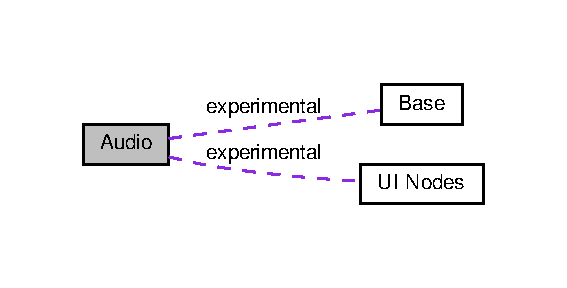
\includegraphics[width=272pt]{group__audio}
\end{center}
\end{figure}


\subsection{Detailed Description}

\hypertarget{group__base}{}\section{Base}
\label{group__base}\index{Base@{Base}}
Collaboration diagram for Base\+:
\nopagebreak
\begin{figure}[H]
\begin{center}
\leavevmode
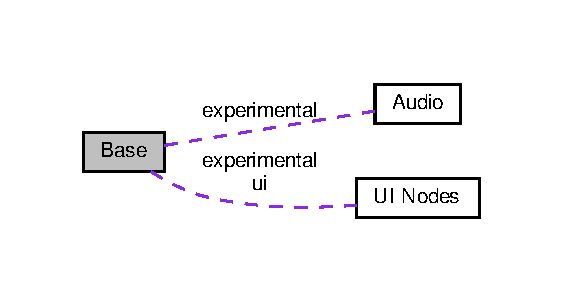
\includegraphics[width=270pt]{group__base}
\end{center}
\end{figure}
\subsection*{Classes}
\begin{DoxyCompactItemize}
\item 
class \hyperlink{classcocos2d_1_1experimental_1_1ThreadPool}{cocos2d\+::experimental\+::\+Thread\+Pool}
\item 
class \hyperlink{classAsyncTaskPool}{Async\+Task\+Pool}
\begin{DoxyCompactList}\small\item\em This class allows to perform background operations without having to manipulate threads.  NA. \end{DoxyCompactList}\item 
class \hyperlink{classAutoreleasePool}{Autorelease\+Pool}
\item 
class \hyperlink{classConfiguration}{Configuration}
\begin{DoxyCompactList}\small\item\em \hyperlink{classConfiguration}{Configuration} contains some open\+GL variables. \end{DoxyCompactList}\item 
class \hyperlink{classController}{Controller}
\begin{DoxyCompactList}\small\item\em A \hyperlink{classController}{Controller} object represents a connected physical game controller.  NA. \end{DoxyCompactList}\item 
class \hyperlink{classDirector}{Director}
\begin{DoxyCompactList}\small\item\em Class that creates and handles the main Window and manages how and when to execute the Scenes. \end{DoxyCompactList}\item 
class \hyperlink{classEvent}{Event}
\begin{DoxyCompactList}\small\item\em Base class of all kinds of events. \end{DoxyCompactList}\item 
class \hyperlink{classEventAcceleration}{Event\+Acceleration}
\begin{DoxyCompactList}\small\item\em Accelerometer event. \end{DoxyCompactList}\item 
class \hyperlink{classEventCustom}{Event\+Custom}
\begin{DoxyCompactList}\small\item\em Custom event. \end{DoxyCompactList}\item 
class \hyperlink{classEventDispatcher}{Event\+Dispatcher}
\begin{DoxyCompactList}\small\item\em This class manages event listener subscriptions and event dispatching. \end{DoxyCompactList}\item 
class \hyperlink{classEventFocus}{Event\+Focus}
\begin{DoxyCompactList}\small\item\em Focus event. \end{DoxyCompactList}\item 
class \hyperlink{classEventKeyboard}{Event\+Keyboard}
\begin{DoxyCompactList}\small\item\em Keyboard event. \end{DoxyCompactList}\item 
class \hyperlink{classEventListener}{Event\+Listener}
\begin{DoxyCompactList}\small\item\em The base class of event listener. If you need custom listener which with different callback, you need to inherit this class. For instance, you could refer to \hyperlink{classEventListenerAcceleration}{Event\+Listener\+Acceleration}, \hyperlink{classEventListenerKeyboard}{Event\+Listener\+Keyboard}, \hyperlink{classEventListenerTouchOneByOne}{Event\+Listener\+Touch\+One\+By\+One}, \hyperlink{classEventListenerCustom}{Event\+Listener\+Custom}. \end{DoxyCompactList}\item 
class \hyperlink{classEventListenerAcceleration}{Event\+Listener\+Acceleration}
\begin{DoxyCompactList}\small\item\em \hyperlink{classAcceleration}{Acceleration} event listener.  NA. \end{DoxyCompactList}\item 
class \hyperlink{classEventListenerController}{Event\+Listener\+Controller}
\item 
class \hyperlink{classEventListenerCustom}{Event\+Listener\+Custom}
\begin{DoxyCompactList}\small\item\em Custom event listener. \end{DoxyCompactList}\item 
class \hyperlink{classEventListenerFocus}{Event\+Listener\+Focus}
\begin{DoxyCompactList}\small\item\em Focus event listener. \end{DoxyCompactList}\item 
class \hyperlink{classEventListenerKeyboard}{Event\+Listener\+Keyboard}
\begin{DoxyCompactList}\small\item\em Keyboard event listener.  cc.\+\_\+\+Event\+Listener\+Keyboard. \end{DoxyCompactList}\item 
class \hyperlink{classEventListenerMouse}{Event\+Listener\+Mouse}
\begin{DoxyCompactList}\small\item\em Mouse event listener.  cc.\+\_\+\+Event\+Listener\+Mouse. \end{DoxyCompactList}\item 
class \hyperlink{classEventListenerTouchOneByOne}{Event\+Listener\+Touch\+One\+By\+One}
\begin{DoxyCompactList}\small\item\em Single touch event listener.  cc.\+\_\+\+Event\+Listener\+Touch\+One\+By\+One. \end{DoxyCompactList}\item 
class \hyperlink{classEventListenerTouchAllAtOnce}{Event\+Listener\+Touch\+All\+At\+Once}
\begin{DoxyCompactList}\small\item\em Multiple touches event listener. \end{DoxyCompactList}\item 
class \hyperlink{classEventMouse}{Event\+Mouse}
\begin{DoxyCompactList}\small\item\em The mouse event. \end{DoxyCompactList}\item 
class \hyperlink{classEventTouch}{Event\+Touch}
\begin{DoxyCompactList}\small\item\em \hyperlink{classTouch}{Touch} event. \end{DoxyCompactList}\item 
struct \hyperlink{structIMEKeyboardNotificationInfo}{I\+M\+E\+Keyboard\+Notification\+Info}
\item 
class \hyperlink{classIMEDelegate}{I\+M\+E\+Delegate}
\begin{DoxyCompactList}\small\item\em Input method editor delegate. \end{DoxyCompactList}\item 
class \hyperlink{classIMEDispatcher}{I\+M\+E\+Dispatcher}
\begin{DoxyCompactList}\small\item\em Input Method Edit Message Dispatcher. \end{DoxyCompactList}\item 
class \hyperlink{classMap}{Map$<$ K, V $>$}
\item 
class \hyperlink{classRandomHelper}{Random\+Helper}
\begin{DoxyCompactList}\small\item\em A helper class for creating random number. \end{DoxyCompactList}\item 
class \hyperlink{classClonable}{Clonable}
\item 
class \hyperlink{classRef}{Ref}
\item 
class \hyperlink{classScheduler}{Scheduler}
\begin{DoxyCompactList}\small\item\em \hyperlink{classScheduler}{Scheduler} is responsible for triggering the scheduled callbacks. You should not use system timer for your game logic. Instead, use this class. \end{DoxyCompactList}\item 
class \hyperlink{classStencilStateManager}{Stencil\+State\+Manager}
\item 
class \hyperlink{classTouch}{Touch}
\begin{DoxyCompactList}\small\item\em Encapsulates the \hyperlink{classTouch}{Touch} information, such as touch point, id and so on, and provides the methods that commonly used. \end{DoxyCompactList}\item 
struct \hyperlink{structColor3B}{Color3B}
\item 
struct \hyperlink{structColor4B}{Color4B}
\item 
struct \hyperlink{structColor4F}{Color4F}
\item 
struct \hyperlink{structTex2F}{Tex2F}
\item 
struct \hyperlink{structPointSprite}{Point\+Sprite}
\item 
struct \hyperlink{structQuad2}{Quad2}
\item 
struct \hyperlink{structQuad3}{Quad3}
\item 
struct \hyperlink{structV2F__C4B__T2F}{V2\+F\+\_\+\+C4\+B\+\_\+\+T2F}
\item 
struct \hyperlink{structV2F__C4B__PF}{V2\+F\+\_\+\+C4\+B\+\_\+\+PF}
\item 
struct \hyperlink{structV2F__C4F__T2F}{V2\+F\+\_\+\+C4\+F\+\_\+\+T2F}
\item 
struct \hyperlink{structV3F__C4B__T2F}{V3\+F\+\_\+\+C4\+B\+\_\+\+T2F}
\item 
struct \hyperlink{structV3F__T2F}{V3\+F\+\_\+\+T2F}
\item 
struct \hyperlink{structV2F__C4B__T2F__Triangle}{V2\+F\+\_\+\+C4\+B\+\_\+\+T2\+F\+\_\+\+Triangle}
\item 
struct \hyperlink{structV2F__C4B__T2F__Quad}{V2\+F\+\_\+\+C4\+B\+\_\+\+T2\+F\+\_\+\+Quad}
\item 
struct \hyperlink{structV3F__C4B__T2F__Quad}{V3\+F\+\_\+\+C4\+B\+\_\+\+T2\+F\+\_\+\+Quad}
\item 
struct \hyperlink{structV2F__C4F__T2F__Quad}{V2\+F\+\_\+\+C4\+F\+\_\+\+T2\+F\+\_\+\+Quad}
\item 
struct \hyperlink{structV3F__T2F__Quad}{V3\+F\+\_\+\+T2\+F\+\_\+\+Quad}
\item 
struct \hyperlink{structBlendFunc}{Blend\+Func}
\item 
struct \hyperlink{structT2F__Quad}{T2\+F\+\_\+\+Quad}
\item 
struct \hyperlink{structAnimationFrameData}{Animation\+Frame\+Data}
\item 
struct \hyperlink{structFontShadow}{Font\+Shadow}
\item 
struct \hyperlink{structFontStroke}{Font\+Stroke}
\item 
struct \hyperlink{structFontDefinition}{Font\+Definition}
\item 
struct \hyperlink{classAcceleration}{Acceleration}
\item 
class \hyperlink{classUserDefault}{User\+Default}
\item 
class \hyperlink{classValue}{Value}
\item 
class \hyperlink{classVector}{Vector$<$ T $>$}
\item 
struct \hyperlink{structAffineTransform}{Affine\+Transform}
\item 
class \hyperlink{classSize}{Size}
\item 
class \hyperlink{classRect}{Rect}
\item 
class \hyperlink{classMat4}{Mat4}
\item 
class \hyperlink{classMathUtil}{Math\+Util}
\item 
class \hyperlink{classQuaternion}{Quaternion}
\item 
class \hyperlink{classVec2}{Vec2}
\item 
class \hyperlink{classVec3}{Vec3}
\item 
class \hyperlink{classVec4}{Vec4}
\item 
class \hyperlink{classDisplayLinkDirector}{Display\+Link\+Director}
\begin{DoxyCompactList}\small\item\em \hyperlink{classDisplayLinkDirector}{Display\+Link\+Director} is a \hyperlink{classDirector}{Director} that synchronizes timers with the refresh rate of the display. \end{DoxyCompactList}\end{DoxyCompactItemize}
\subsection*{Macros}
\begin{DoxyCompactItemize}
\item 
\mbox{\Hypertarget{group__base_gaabe4e43a30c4e67a327af2e2557274f9}\label{group__base_gaabe4e43a30c4e67a327af2e2557274f9}} 
\#define {\bfseries T\+O\+U\+C\+H\+\_\+\+P\+E\+R\+F\+\_\+\+D\+E\+B\+UG}~1
\item 
\mbox{\Hypertarget{group__base_ga93a3458e1b6e06e251b8ba774eeb7ad1}\label{group__base_ga93a3458e1b6e06e251b8ba774eeb7ad1}} 
\#define {\bfseries C\+C\+\_\+\+C\+A\+L\+L\+F\+U\+N\+C\+\_\+\+S\+E\+L\+E\+C\+T\+OR}(\+\_\+\+S\+E\+L\+E\+C\+T\+OR)~static\+\_\+cast$<$cocos2d\+::\+S\+E\+L\+\_\+\+Call\+Func$>$(\&\+\_\+\+S\+E\+L\+E\+C\+T\+OR)
\item 
\mbox{\Hypertarget{group__base_ga0304dbc1f312ce25d4969490c869d09d}\label{group__base_ga0304dbc1f312ce25d4969490c869d09d}} 
\#define {\bfseries C\+C\+\_\+\+C\+A\+L\+L\+F\+U\+N\+C\+N\+\_\+\+S\+E\+L\+E\+C\+T\+OR}(\+\_\+\+S\+E\+L\+E\+C\+T\+OR)~static\+\_\+cast$<$cocos2d\+::\+S\+E\+L\+\_\+\+Call\+FuncN$>$(\&\+\_\+\+S\+E\+L\+E\+C\+T\+OR)
\item 
\mbox{\Hypertarget{group__base_ga03e93bdcfd4468f47fc770c8e4bc6dd5}\label{group__base_ga03e93bdcfd4468f47fc770c8e4bc6dd5}} 
\#define {\bfseries C\+C\+\_\+\+C\+A\+L\+L\+F\+U\+N\+C\+N\+D\+\_\+\+S\+E\+L\+E\+C\+T\+OR}(\+\_\+\+S\+E\+L\+E\+C\+T\+OR)~static\+\_\+cast$<$cocos2d\+::\+S\+E\+L\+\_\+\+Call\+Func\+ND$>$(\&\+\_\+\+S\+E\+L\+E\+C\+T\+OR)
\item 
\mbox{\Hypertarget{group__base_gacc358701e9f3c5b6629930a999f97eb8}\label{group__base_gacc358701e9f3c5b6629930a999f97eb8}} 
\#define {\bfseries C\+C\+\_\+\+C\+A\+L\+L\+F\+U\+N\+C\+O\+\_\+\+S\+E\+L\+E\+C\+T\+OR}(\+\_\+\+S\+E\+L\+E\+C\+T\+OR)~static\+\_\+cast$<$cocos2d\+::\+S\+E\+L\+\_\+\+Call\+FuncO$>$(\&\+\_\+\+S\+E\+L\+E\+C\+T\+OR)
\item 
\mbox{\Hypertarget{group__base_gaf2d69346f4d31ab77732198a9ebe0f22}\label{group__base_gaf2d69346f4d31ab77732198a9ebe0f22}} 
\#define {\bfseries C\+C\+\_\+\+M\+E\+N\+U\+\_\+\+S\+E\+L\+E\+C\+T\+OR}(\+\_\+\+S\+E\+L\+E\+C\+T\+OR)~static\+\_\+cast$<$cocos2d\+::\+S\+E\+L\+\_\+\+Menu\+Handler$>$(\&\+\_\+\+S\+E\+L\+E\+C\+T\+OR)
\item 
\mbox{\Hypertarget{group__base_ga364ba06f4b51d54fe45605b4cde10302}\label{group__base_ga364ba06f4b51d54fe45605b4cde10302}} 
\#define {\bfseries C\+C\+\_\+\+S\+C\+H\+E\+D\+U\+L\+E\+\_\+\+S\+E\+L\+E\+C\+T\+OR}(\+\_\+\+S\+E\+L\+E\+C\+T\+OR)~static\+\_\+cast$<$cocos2d\+::\+S\+E\+L\+\_\+\+S\+C\+H\+E\+D\+U\+LE$>$(\&\+\_\+\+S\+E\+L\+E\+C\+T\+OR)
\item 
\mbox{\Hypertarget{group__base_gadbfffb29c6db99730b3725d392b5c6ce}\label{group__base_gadbfffb29c6db99730b3725d392b5c6ce}} 
\#define {\bfseries callfunc\+\_\+selector}(\+\_\+\+S\+E\+L\+E\+C\+T\+OR)~C\+C\+\_\+\+C\+A\+L\+L\+F\+U\+N\+C\+\_\+\+S\+E\+L\+E\+C\+T\+OR(\+\_\+\+S\+E\+L\+E\+C\+T\+OR)
\item 
\mbox{\Hypertarget{group__base_gaae5d36086e660775212ac58171e5b9c1}\label{group__base_gaae5d36086e660775212ac58171e5b9c1}} 
\#define {\bfseries callfunc\+N\+\_\+selector}(\+\_\+\+S\+E\+L\+E\+C\+T\+OR)~C\+C\+\_\+\+C\+A\+L\+L\+F\+U\+N\+C\+N\+\_\+\+S\+E\+L\+E\+C\+T\+OR(\+\_\+\+S\+E\+L\+E\+C\+T\+OR)
\item 
\mbox{\Hypertarget{group__base_gaf6e1b4d4334a7aa7950a17f361aaff80}\label{group__base_gaf6e1b4d4334a7aa7950a17f361aaff80}} 
\#define {\bfseries callfunc\+N\+D\+\_\+selector}(\+\_\+\+S\+E\+L\+E\+C\+T\+OR)~C\+C\+\_\+\+C\+A\+L\+L\+F\+U\+N\+C\+N\+D\+\_\+\+S\+E\+L\+E\+C\+T\+OR(\+\_\+\+S\+E\+L\+E\+C\+T\+OR)
\item 
\mbox{\Hypertarget{group__base_ga7b930d3a73de79074daa4523fa18df73}\label{group__base_ga7b930d3a73de79074daa4523fa18df73}} 
\#define {\bfseries callfunc\+O\+\_\+selector}(\+\_\+\+S\+E\+L\+E\+C\+T\+OR)~C\+C\+\_\+\+C\+A\+L\+L\+F\+U\+N\+C\+O\+\_\+\+S\+E\+L\+E\+C\+T\+OR(\+\_\+\+S\+E\+L\+E\+C\+T\+OR)
\item 
\mbox{\Hypertarget{group__base_gaaf4135f283ffa04049acdd0d98ced399}\label{group__base_gaaf4135f283ffa04049acdd0d98ced399}} 
\#define {\bfseries menu\+\_\+selector}(\+\_\+\+S\+E\+L\+E\+C\+T\+OR)~C\+C\+\_\+\+M\+E\+N\+U\+\_\+\+S\+E\+L\+E\+C\+T\+OR(\+\_\+\+S\+E\+L\+E\+C\+T\+OR)
\item 
\mbox{\Hypertarget{group__base_ga32d629acb8d8cbd2fdb9bf98f45736b7}\label{group__base_ga32d629acb8d8cbd2fdb9bf98f45736b7}} 
\#define {\bfseries schedule\+\_\+selector}(\+\_\+\+S\+E\+L\+E\+C\+T\+OR)~C\+C\+\_\+\+S\+C\+H\+E\+D\+U\+L\+E\+\_\+\+S\+E\+L\+E\+C\+T\+OR(\+\_\+\+S\+E\+L\+E\+C\+T\+OR)
\item 
\mbox{\Hypertarget{group__base_ga6f5f5e63a840aa04d1d728fd57e4bfcc}\label{group__base_ga6f5f5e63a840aa04d1d728fd57e4bfcc}} 
\#define {\bfseries Affine\+Transform\+Make}~\hyperlink{group__base_ga6512cedee05a78771b7aac4e4d57a499}{\+\_\+\+\_\+\+C\+C\+Affine\+Transform\+Make}
\item 
\mbox{\Hypertarget{group__base_gacaf876df474d9bf68df41235654bec40}\label{group__base_gacaf876df474d9bf68df41235654bec40}} 
\#define {\bfseries Point\+Apply\+Affine\+Transform}~\hyperlink{group__base_ga925cec1fb977da8fb3d8280ba82cc5c7}{\+\_\+\+\_\+\+C\+C\+Point\+Apply\+Affine\+Transform}
\item 
\mbox{\Hypertarget{group__base_gab1d40a014c106f103aa32191e9541978}\label{group__base_gab1d40a014c106f103aa32191e9541978}} 
\#define {\bfseries Size\+Apply\+Affine\+Transform}~\hyperlink{group__base_ga40f990327de656e394d23b0650208008}{\+\_\+\+\_\+\+C\+C\+Size\+Apply\+Affine\+Transform}
\item 
\#define \hyperlink{group__base_gae2eab65745e7f093a97fbd4421261c84}{M\+A\+T\+H\+\_\+\+D\+E\+G\+\_\+\+T\+O\+\_\+\+R\+AD}(x)~((x) $\ast$ 0.\+0174532925f)
\item 
\#define \hyperlink{group__base_ga7144cae826260514e7a61f405c77e848}{M\+A\+T\+H\+\_\+\+R\+A\+D\+\_\+\+T\+O\+\_\+\+D\+EG}(x)~((x)$\ast$ 57.\+29577951f)
\item 
\mbox{\Hypertarget{group__base_gaf66fbc3024a6ebf672e9270a52970aab}\label{group__base_gaf66fbc3024a6ebf672e9270a52970aab}} 
\#define {\bfseries N\+S\+\_\+\+C\+C\+\_\+\+M\+A\+T\+H\+\_\+\+B\+E\+G\+IN}
\item 
\mbox{\Hypertarget{group__base_gab9bcf41ee04aab8263ce6821976c3908}\label{group__base_gab9bcf41ee04aab8263ce6821976c3908}} 
\#define {\bfseries N\+S\+\_\+\+C\+C\+\_\+\+M\+A\+T\+H\+\_\+\+E\+ND}
\item 
\mbox{\Hypertarget{group__base_ga816286195c50ca639ce83faf755c20ef}\label{group__base_ga816286195c50ca639ce83faf755c20ef}} 
\#define {\bfseries U\+S\+I\+N\+G\+\_\+\+N\+S\+\_\+\+C\+C\+\_\+\+M\+A\+TH}
\item 
\mbox{\Hypertarget{group__base_gaabe4e43a30c4e67a327af2e2557274f9}\label{group__base_gaabe4e43a30c4e67a327af2e2557274f9}} 
\#define {\bfseries T\+O\+U\+C\+H\+\_\+\+P\+E\+R\+F\+\_\+\+D\+E\+B\+UG}~1
\item 
\mbox{\Hypertarget{group__base_ga93a3458e1b6e06e251b8ba774eeb7ad1}\label{group__base_ga93a3458e1b6e06e251b8ba774eeb7ad1}} 
\#define {\bfseries C\+C\+\_\+\+C\+A\+L\+L\+F\+U\+N\+C\+\_\+\+S\+E\+L\+E\+C\+T\+OR}(\+\_\+\+S\+E\+L\+E\+C\+T\+OR)~static\+\_\+cast$<$cocos2d\+::\+S\+E\+L\+\_\+\+Call\+Func$>$(\&\+\_\+\+S\+E\+L\+E\+C\+T\+OR)
\item 
\mbox{\Hypertarget{group__base_ga0304dbc1f312ce25d4969490c869d09d}\label{group__base_ga0304dbc1f312ce25d4969490c869d09d}} 
\#define {\bfseries C\+C\+\_\+\+C\+A\+L\+L\+F\+U\+N\+C\+N\+\_\+\+S\+E\+L\+E\+C\+T\+OR}(\+\_\+\+S\+E\+L\+E\+C\+T\+OR)~static\+\_\+cast$<$cocos2d\+::\+S\+E\+L\+\_\+\+Call\+FuncN$>$(\&\+\_\+\+S\+E\+L\+E\+C\+T\+OR)
\item 
\mbox{\Hypertarget{group__base_ga03e93bdcfd4468f47fc770c8e4bc6dd5}\label{group__base_ga03e93bdcfd4468f47fc770c8e4bc6dd5}} 
\#define {\bfseries C\+C\+\_\+\+C\+A\+L\+L\+F\+U\+N\+C\+N\+D\+\_\+\+S\+E\+L\+E\+C\+T\+OR}(\+\_\+\+S\+E\+L\+E\+C\+T\+OR)~static\+\_\+cast$<$cocos2d\+::\+S\+E\+L\+\_\+\+Call\+Func\+ND$>$(\&\+\_\+\+S\+E\+L\+E\+C\+T\+OR)
\item 
\mbox{\Hypertarget{group__base_gacc358701e9f3c5b6629930a999f97eb8}\label{group__base_gacc358701e9f3c5b6629930a999f97eb8}} 
\#define {\bfseries C\+C\+\_\+\+C\+A\+L\+L\+F\+U\+N\+C\+O\+\_\+\+S\+E\+L\+E\+C\+T\+OR}(\+\_\+\+S\+E\+L\+E\+C\+T\+OR)~static\+\_\+cast$<$cocos2d\+::\+S\+E\+L\+\_\+\+Call\+FuncO$>$(\&\+\_\+\+S\+E\+L\+E\+C\+T\+OR)
\item 
\mbox{\Hypertarget{group__base_gaf2d69346f4d31ab77732198a9ebe0f22}\label{group__base_gaf2d69346f4d31ab77732198a9ebe0f22}} 
\#define {\bfseries C\+C\+\_\+\+M\+E\+N\+U\+\_\+\+S\+E\+L\+E\+C\+T\+OR}(\+\_\+\+S\+E\+L\+E\+C\+T\+OR)~static\+\_\+cast$<$cocos2d\+::\+S\+E\+L\+\_\+\+Menu\+Handler$>$(\&\+\_\+\+S\+E\+L\+E\+C\+T\+OR)
\item 
\mbox{\Hypertarget{group__base_ga364ba06f4b51d54fe45605b4cde10302}\label{group__base_ga364ba06f4b51d54fe45605b4cde10302}} 
\#define {\bfseries C\+C\+\_\+\+S\+C\+H\+E\+D\+U\+L\+E\+\_\+\+S\+E\+L\+E\+C\+T\+OR}(\+\_\+\+S\+E\+L\+E\+C\+T\+OR)~static\+\_\+cast$<$cocos2d\+::\+S\+E\+L\+\_\+\+S\+C\+H\+E\+D\+U\+LE$>$(\&\+\_\+\+S\+E\+L\+E\+C\+T\+OR)
\item 
\mbox{\Hypertarget{group__base_gadbfffb29c6db99730b3725d392b5c6ce}\label{group__base_gadbfffb29c6db99730b3725d392b5c6ce}} 
\#define {\bfseries callfunc\+\_\+selector}(\+\_\+\+S\+E\+L\+E\+C\+T\+OR)~C\+C\+\_\+\+C\+A\+L\+L\+F\+U\+N\+C\+\_\+\+S\+E\+L\+E\+C\+T\+OR(\+\_\+\+S\+E\+L\+E\+C\+T\+OR)
\item 
\mbox{\Hypertarget{group__base_gaae5d36086e660775212ac58171e5b9c1}\label{group__base_gaae5d36086e660775212ac58171e5b9c1}} 
\#define {\bfseries callfunc\+N\+\_\+selector}(\+\_\+\+S\+E\+L\+E\+C\+T\+OR)~C\+C\+\_\+\+C\+A\+L\+L\+F\+U\+N\+C\+N\+\_\+\+S\+E\+L\+E\+C\+T\+OR(\+\_\+\+S\+E\+L\+E\+C\+T\+OR)
\item 
\mbox{\Hypertarget{group__base_gaf6e1b4d4334a7aa7950a17f361aaff80}\label{group__base_gaf6e1b4d4334a7aa7950a17f361aaff80}} 
\#define {\bfseries callfunc\+N\+D\+\_\+selector}(\+\_\+\+S\+E\+L\+E\+C\+T\+OR)~C\+C\+\_\+\+C\+A\+L\+L\+F\+U\+N\+C\+N\+D\+\_\+\+S\+E\+L\+E\+C\+T\+OR(\+\_\+\+S\+E\+L\+E\+C\+T\+OR)
\item 
\mbox{\Hypertarget{group__base_ga7b930d3a73de79074daa4523fa18df73}\label{group__base_ga7b930d3a73de79074daa4523fa18df73}} 
\#define {\bfseries callfunc\+O\+\_\+selector}(\+\_\+\+S\+E\+L\+E\+C\+T\+OR)~C\+C\+\_\+\+C\+A\+L\+L\+F\+U\+N\+C\+O\+\_\+\+S\+E\+L\+E\+C\+T\+OR(\+\_\+\+S\+E\+L\+E\+C\+T\+OR)
\item 
\mbox{\Hypertarget{group__base_gaaf4135f283ffa04049acdd0d98ced399}\label{group__base_gaaf4135f283ffa04049acdd0d98ced399}} 
\#define {\bfseries menu\+\_\+selector}(\+\_\+\+S\+E\+L\+E\+C\+T\+OR)~C\+C\+\_\+\+M\+E\+N\+U\+\_\+\+S\+E\+L\+E\+C\+T\+OR(\+\_\+\+S\+E\+L\+E\+C\+T\+OR)
\item 
\mbox{\Hypertarget{group__base_ga32d629acb8d8cbd2fdb9bf98f45736b7}\label{group__base_ga32d629acb8d8cbd2fdb9bf98f45736b7}} 
\#define {\bfseries schedule\+\_\+selector}(\+\_\+\+S\+E\+L\+E\+C\+T\+OR)~C\+C\+\_\+\+S\+C\+H\+E\+D\+U\+L\+E\+\_\+\+S\+E\+L\+E\+C\+T\+OR(\+\_\+\+S\+E\+L\+E\+C\+T\+OR)
\item 
\mbox{\Hypertarget{group__base_ga6f5f5e63a840aa04d1d728fd57e4bfcc}\label{group__base_ga6f5f5e63a840aa04d1d728fd57e4bfcc}} 
\#define {\bfseries Affine\+Transform\+Make}~\hyperlink{group__base_ga6512cedee05a78771b7aac4e4d57a499}{\+\_\+\+\_\+\+C\+C\+Affine\+Transform\+Make}
\item 
\mbox{\Hypertarget{group__base_gacaf876df474d9bf68df41235654bec40}\label{group__base_gacaf876df474d9bf68df41235654bec40}} 
\#define {\bfseries Point\+Apply\+Affine\+Transform}~\hyperlink{group__base_ga925cec1fb977da8fb3d8280ba82cc5c7}{\+\_\+\+\_\+\+C\+C\+Point\+Apply\+Affine\+Transform}
\item 
\mbox{\Hypertarget{group__base_gab1d40a014c106f103aa32191e9541978}\label{group__base_gab1d40a014c106f103aa32191e9541978}} 
\#define {\bfseries Size\+Apply\+Affine\+Transform}~\hyperlink{group__base_ga40f990327de656e394d23b0650208008}{\+\_\+\+\_\+\+C\+C\+Size\+Apply\+Affine\+Transform}
\item 
\#define \hyperlink{group__base_gae2eab65745e7f093a97fbd4421261c84}{M\+A\+T\+H\+\_\+\+D\+E\+G\+\_\+\+T\+O\+\_\+\+R\+AD}(x)~((x) $\ast$ 0.\+0174532925f)
\item 
\#define \hyperlink{group__base_ga7144cae826260514e7a61f405c77e848}{M\+A\+T\+H\+\_\+\+R\+A\+D\+\_\+\+T\+O\+\_\+\+D\+EG}(x)~((x)$\ast$ 57.\+29577951f)
\item 
\mbox{\Hypertarget{group__base_gaf66fbc3024a6ebf672e9270a52970aab}\label{group__base_gaf66fbc3024a6ebf672e9270a52970aab}} 
\#define {\bfseries N\+S\+\_\+\+C\+C\+\_\+\+M\+A\+T\+H\+\_\+\+B\+E\+G\+IN}
\item 
\mbox{\Hypertarget{group__base_gab9bcf41ee04aab8263ce6821976c3908}\label{group__base_gab9bcf41ee04aab8263ce6821976c3908}} 
\#define {\bfseries N\+S\+\_\+\+C\+C\+\_\+\+M\+A\+T\+H\+\_\+\+E\+ND}
\item 
\mbox{\Hypertarget{group__base_ga816286195c50ca639ce83faf755c20ef}\label{group__base_ga816286195c50ca639ce83faf755c20ef}} 
\#define {\bfseries U\+S\+I\+N\+G\+\_\+\+N\+S\+\_\+\+C\+C\+\_\+\+M\+A\+TH}
\item 
\#define \hyperlink{group__base_gae4ebe0d1812bb378ab3531d81d9856b8}{random}~rand
\end{DoxyCompactItemize}
\subsection*{Typedefs}
\begin{DoxyCompactItemize}
\item 
\mbox{\Hypertarget{group__base_ga19c9d21cc6cacf9e102c7f405310968f}\label{group__base_ga19c9d21cc6cacf9e102c7f405310968f}} 
typedef void(Ref\+::$\ast$ {\bfseries S\+E\+L\+\_\+\+Call\+Func}) ()
\item 
\mbox{\Hypertarget{group__base_ga2421ba5f5eda401b167fffc76aba09c5}\label{group__base_ga2421ba5f5eda401b167fffc76aba09c5}} 
typedef void(Ref\+::$\ast$ {\bfseries S\+E\+L\+\_\+\+Call\+FuncN}) (\hyperlink{classNode}{Node} $\ast$)
\item 
\mbox{\Hypertarget{group__base_gade4d3700760c07b48e683e15ed122791}\label{group__base_gade4d3700760c07b48e683e15ed122791}} 
typedef void(Ref\+::$\ast$ {\bfseries S\+E\+L\+\_\+\+Call\+Func\+ND}) (\hyperlink{classNode}{Node} $\ast$, void $\ast$)
\item 
\mbox{\Hypertarget{group__base_gaef899e90936c229c2b588d816146898a}\label{group__base_gaef899e90936c229c2b588d816146898a}} 
typedef void(Ref\+::$\ast$ {\bfseries S\+E\+L\+\_\+\+Call\+FuncO}) (\hyperlink{classRef}{Ref} $\ast$)
\item 
\mbox{\Hypertarget{group__base_gaa8b7b2585a8284d5b04a91137d227155}\label{group__base_gaa8b7b2585a8284d5b04a91137d227155}} 
typedef void(Ref\+::$\ast$ {\bfseries S\+E\+L\+\_\+\+Menu\+Handler}) (\hyperlink{classRef}{Ref} $\ast$)
\item 
\mbox{\Hypertarget{group__base_gaf362983c7356c901e3efefc9aff49f55}\label{group__base_gaf362983c7356c901e3efefc9aff49f55}} 
typedef void(Ref\+::$\ast$ {\bfseries S\+E\+L\+\_\+\+S\+C\+H\+E\+D\+U\+LE}) (float)
\item 
\mbox{\Hypertarget{group__base_ga9ef3555e979a203b9619881b61866ca0}\label{group__base_ga9ef3555e979a203b9619881b61866ca0}} 
typedef std\+::vector$<$ \hyperlink{classValue}{Value} $>$ {\bfseries Value\+Vector}
\item 
\mbox{\Hypertarget{group__base_gae44b8cec5fcb05722ab75a7ca2f03fee}\label{group__base_gae44b8cec5fcb05722ab75a7ca2f03fee}} 
typedef std\+::unordered\+\_\+map$<$ std\+::string, \hyperlink{classValue}{Value} $>$ {\bfseries Value\+Map}
\item 
\mbox{\Hypertarget{group__base_ga733d2ae0a5704948dcfad9c985507cff}\label{group__base_ga733d2ae0a5704948dcfad9c985507cff}} 
typedef std\+::unordered\+\_\+map$<$ int, \hyperlink{classValue}{Value} $>$ {\bfseries Value\+Map\+Int\+Key}
\item 
\mbox{\Hypertarget{group__base_ga88a3f2910d3251f3323477ff1393fa20}\label{group__base_ga88a3f2910d3251f3323477ff1393fa20}} 
typedef \hyperlink{classVec2}{Vec2} {\bfseries Point}
\item 
\mbox{\Hypertarget{group__base_ga19c9d21cc6cacf9e102c7f405310968f}\label{group__base_ga19c9d21cc6cacf9e102c7f405310968f}} 
typedef void(Ref\+::$\ast$ {\bfseries S\+E\+L\+\_\+\+Call\+Func}) ()
\item 
\mbox{\Hypertarget{group__base_ga2421ba5f5eda401b167fffc76aba09c5}\label{group__base_ga2421ba5f5eda401b167fffc76aba09c5}} 
typedef void(Ref\+::$\ast$ {\bfseries S\+E\+L\+\_\+\+Call\+FuncN}) (\hyperlink{classNode}{Node} $\ast$)
\item 
\mbox{\Hypertarget{group__base_gade4d3700760c07b48e683e15ed122791}\label{group__base_gade4d3700760c07b48e683e15ed122791}} 
typedef void(Ref\+::$\ast$ {\bfseries S\+E\+L\+\_\+\+Call\+Func\+ND}) (\hyperlink{classNode}{Node} $\ast$, void $\ast$)
\item 
\mbox{\Hypertarget{group__base_gaef899e90936c229c2b588d816146898a}\label{group__base_gaef899e90936c229c2b588d816146898a}} 
typedef void(Ref\+::$\ast$ {\bfseries S\+E\+L\+\_\+\+Call\+FuncO}) (\hyperlink{classRef}{Ref} $\ast$)
\item 
\mbox{\Hypertarget{group__base_gaa8b7b2585a8284d5b04a91137d227155}\label{group__base_gaa8b7b2585a8284d5b04a91137d227155}} 
typedef void(Ref\+::$\ast$ {\bfseries S\+E\+L\+\_\+\+Menu\+Handler}) (\hyperlink{classRef}{Ref} $\ast$)
\item 
\mbox{\Hypertarget{group__base_gaf362983c7356c901e3efefc9aff49f55}\label{group__base_gaf362983c7356c901e3efefc9aff49f55}} 
typedef void(Ref\+::$\ast$ {\bfseries S\+E\+L\+\_\+\+S\+C\+H\+E\+D\+U\+LE}) (float)
\item 
\mbox{\Hypertarget{group__base_ga9ef3555e979a203b9619881b61866ca0}\label{group__base_ga9ef3555e979a203b9619881b61866ca0}} 
typedef std\+::vector$<$ \hyperlink{classValue}{Value} $>$ {\bfseries Value\+Vector}
\item 
\mbox{\Hypertarget{group__base_gae44b8cec5fcb05722ab75a7ca2f03fee}\label{group__base_gae44b8cec5fcb05722ab75a7ca2f03fee}} 
typedef std\+::unordered\+\_\+map$<$ std\+::string, \hyperlink{classValue}{Value} $>$ {\bfseries Value\+Map}
\item 
\mbox{\Hypertarget{group__base_ga733d2ae0a5704948dcfad9c985507cff}\label{group__base_ga733d2ae0a5704948dcfad9c985507cff}} 
typedef std\+::unordered\+\_\+map$<$ int, \hyperlink{classValue}{Value} $>$ {\bfseries Value\+Map\+Int\+Key}
\item 
\mbox{\Hypertarget{group__base_ga88a3f2910d3251f3323477ff1393fa20}\label{group__base_ga88a3f2910d3251f3323477ff1393fa20}} 
typedef \hyperlink{classVec2}{Vec2} {\bfseries Point}
\end{DoxyCompactItemize}
\subsection*{Enumerations}
\begin{DoxyCompactItemize}
\item 
enum \hyperlink{group__base_ga4d146cef7130a8f3a953d46964ea3905}{M\+A\+T\+R\+I\+X\+\_\+\+S\+T\+A\+C\+K\+\_\+\+T\+Y\+PE} \{ \newline
\hyperlink{group__base_gga4d146cef7130a8f3a953d46964ea3905a2c38cdb8eb5928738bbcda4e5f085920}{M\+A\+T\+R\+I\+X\+\_\+\+S\+T\+A\+C\+K\+\_\+\+T\+Y\+P\+E\+::\+M\+A\+T\+R\+I\+X\+\_\+\+S\+T\+A\+C\+K\+\_\+\+M\+O\+D\+E\+L\+V\+I\+EW}, 
\hyperlink{group__base_gga4d146cef7130a8f3a953d46964ea3905aad1cc2649728ae11b69b747a58845764}{M\+A\+T\+R\+I\+X\+\_\+\+S\+T\+A\+C\+K\+\_\+\+T\+Y\+P\+E\+::\+M\+A\+T\+R\+I\+X\+\_\+\+S\+T\+A\+C\+K\+\_\+\+P\+R\+O\+J\+E\+C\+T\+I\+ON}, 
\hyperlink{group__base_gga4d146cef7130a8f3a953d46964ea3905a34b60a12b3b0826d198a5f18ef4f48c8}{M\+A\+T\+R\+I\+X\+\_\+\+S\+T\+A\+C\+K\+\_\+\+T\+Y\+P\+E\+::\+M\+A\+T\+R\+I\+X\+\_\+\+S\+T\+A\+C\+K\+\_\+\+T\+E\+X\+T\+U\+RE}, 
\hyperlink{group__base_gga4d146cef7130a8f3a953d46964ea3905a2c38cdb8eb5928738bbcda4e5f085920}{M\+A\+T\+R\+I\+X\+\_\+\+S\+T\+A\+C\+K\+\_\+\+T\+Y\+P\+E\+::\+M\+A\+T\+R\+I\+X\+\_\+\+S\+T\+A\+C\+K\+\_\+\+M\+O\+D\+E\+L\+V\+I\+EW}, 
\newline
\hyperlink{group__base_gga4d146cef7130a8f3a953d46964ea3905aad1cc2649728ae11b69b747a58845764}{M\+A\+T\+R\+I\+X\+\_\+\+S\+T\+A\+C\+K\+\_\+\+T\+Y\+P\+E\+::\+M\+A\+T\+R\+I\+X\+\_\+\+S\+T\+A\+C\+K\+\_\+\+P\+R\+O\+J\+E\+C\+T\+I\+ON}, 
\hyperlink{group__base_gga4d146cef7130a8f3a953d46964ea3905a34b60a12b3b0826d198a5f18ef4f48c8}{M\+A\+T\+R\+I\+X\+\_\+\+S\+T\+A\+C\+K\+\_\+\+T\+Y\+P\+E\+::\+M\+A\+T\+R\+I\+X\+\_\+\+S\+T\+A\+C\+K\+\_\+\+T\+E\+X\+T\+U\+RE}
 \}\begin{DoxyCompactList}\small\item\em Matrix stack type. \end{DoxyCompactList}
\item 
enum \hyperlink{group__base_gac5e83e2fc436edc7833f2bcabad984f3}{Glyph\+Collection} \{ \newline
{\bfseries D\+Y\+N\+A\+M\+IC}, 
{\bfseries N\+E\+HE}, 
{\bfseries A\+S\+C\+II}, 
{\bfseries C\+U\+S\+T\+OM}, 
\newline
{\bfseries D\+Y\+N\+A\+M\+IC}, 
{\bfseries N\+E\+HE}, 
{\bfseries A\+S\+C\+II}, 
{\bfseries C\+U\+S\+T\+OM}
 \}\begin{DoxyCompactList}\small\item\em Possible Glyph\+Collection used by \hyperlink{classLabel}{Label}. \end{DoxyCompactList}
\item 
\mbox{\Hypertarget{group__base_ga26fd049ca5303e0cf4435208058f32e4}\label{group__base_ga26fd049ca5303e0cf4435208058f32e4}} 
enum \hyperlink{group__base_ga26fd049ca5303e0cf4435208058f32e4}{Label\+Effect} \{ \newline
{\bfseries N\+O\+R\+M\+AL}, 
{\bfseries O\+U\+T\+L\+I\+NE}, 
{\bfseries S\+H\+A\+D\+OW}, 
{\bfseries G\+L\+OW}, 
\newline
{\bfseries I\+T\+A\+L\+I\+CS}, 
{\bfseries B\+O\+LD}, 
{\bfseries U\+N\+D\+E\+R\+L\+I\+NE}, 
{\bfseries S\+T\+R\+I\+K\+E\+T\+H\+R\+O\+U\+GH}, 
\newline
{\bfseries A\+LL}, 
{\bfseries N\+O\+R\+M\+AL}, 
{\bfseries O\+U\+T\+L\+I\+NE}, 
{\bfseries S\+H\+A\+D\+OW}, 
\newline
{\bfseries G\+L\+OW}, 
{\bfseries I\+T\+A\+L\+I\+CS}, 
{\bfseries B\+O\+LD}, 
{\bfseries U\+N\+D\+E\+R\+L\+I\+NE}, 
\newline
{\bfseries S\+T\+R\+I\+K\+E\+T\+H\+R\+O\+U\+GH}, 
{\bfseries A\+LL}
 \}\begin{DoxyCompactList}\small\item\em Effects used by {\ttfamily \hyperlink{classLabel}{Label}} \end{DoxyCompactList}
\item 
enum \hyperlink{group__base_ga4d146cef7130a8f3a953d46964ea3905}{M\+A\+T\+R\+I\+X\+\_\+\+S\+T\+A\+C\+K\+\_\+\+T\+Y\+PE} \{ \newline
\hyperlink{group__base_gga4d146cef7130a8f3a953d46964ea3905a2c38cdb8eb5928738bbcda4e5f085920}{M\+A\+T\+R\+I\+X\+\_\+\+S\+T\+A\+C\+K\+\_\+\+T\+Y\+P\+E\+::\+M\+A\+T\+R\+I\+X\+\_\+\+S\+T\+A\+C\+K\+\_\+\+M\+O\+D\+E\+L\+V\+I\+EW}, 
\hyperlink{group__base_gga4d146cef7130a8f3a953d46964ea3905aad1cc2649728ae11b69b747a58845764}{M\+A\+T\+R\+I\+X\+\_\+\+S\+T\+A\+C\+K\+\_\+\+T\+Y\+P\+E\+::\+M\+A\+T\+R\+I\+X\+\_\+\+S\+T\+A\+C\+K\+\_\+\+P\+R\+O\+J\+E\+C\+T\+I\+ON}, 
\hyperlink{group__base_gga4d146cef7130a8f3a953d46964ea3905a34b60a12b3b0826d198a5f18ef4f48c8}{M\+A\+T\+R\+I\+X\+\_\+\+S\+T\+A\+C\+K\+\_\+\+T\+Y\+P\+E\+::\+M\+A\+T\+R\+I\+X\+\_\+\+S\+T\+A\+C\+K\+\_\+\+T\+E\+X\+T\+U\+RE}, 
\hyperlink{group__base_gga4d146cef7130a8f3a953d46964ea3905a2c38cdb8eb5928738bbcda4e5f085920}{M\+A\+T\+R\+I\+X\+\_\+\+S\+T\+A\+C\+K\+\_\+\+T\+Y\+P\+E\+::\+M\+A\+T\+R\+I\+X\+\_\+\+S\+T\+A\+C\+K\+\_\+\+M\+O\+D\+E\+L\+V\+I\+EW}, 
\newline
\hyperlink{group__base_gga4d146cef7130a8f3a953d46964ea3905aad1cc2649728ae11b69b747a58845764}{M\+A\+T\+R\+I\+X\+\_\+\+S\+T\+A\+C\+K\+\_\+\+T\+Y\+P\+E\+::\+M\+A\+T\+R\+I\+X\+\_\+\+S\+T\+A\+C\+K\+\_\+\+P\+R\+O\+J\+E\+C\+T\+I\+ON}, 
\hyperlink{group__base_gga4d146cef7130a8f3a953d46964ea3905a34b60a12b3b0826d198a5f18ef4f48c8}{M\+A\+T\+R\+I\+X\+\_\+\+S\+T\+A\+C\+K\+\_\+\+T\+Y\+P\+E\+::\+M\+A\+T\+R\+I\+X\+\_\+\+S\+T\+A\+C\+K\+\_\+\+T\+E\+X\+T\+U\+RE}
 \}\begin{DoxyCompactList}\small\item\em Matrix stack type. \end{DoxyCompactList}
\item 
enum \hyperlink{group__base_gac5e83e2fc436edc7833f2bcabad984f3}{Glyph\+Collection} \{ \newline
{\bfseries D\+Y\+N\+A\+M\+IC}, 
{\bfseries N\+E\+HE}, 
{\bfseries A\+S\+C\+II}, 
{\bfseries C\+U\+S\+T\+OM}, 
\newline
{\bfseries D\+Y\+N\+A\+M\+IC}, 
{\bfseries N\+E\+HE}, 
{\bfseries A\+S\+C\+II}, 
{\bfseries C\+U\+S\+T\+OM}
 \}\begin{DoxyCompactList}\small\item\em Possible Glyph\+Collection used by \hyperlink{classLabel}{Label}. \end{DoxyCompactList}
\item 
\mbox{\Hypertarget{group__base_ga26fd049ca5303e0cf4435208058f32e4}\label{group__base_ga26fd049ca5303e0cf4435208058f32e4}} 
enum \hyperlink{group__base_ga26fd049ca5303e0cf4435208058f32e4}{Label\+Effect} \{ \newline
{\bfseries N\+O\+R\+M\+AL}, 
{\bfseries O\+U\+T\+L\+I\+NE}, 
{\bfseries S\+H\+A\+D\+OW}, 
{\bfseries G\+L\+OW}, 
\newline
{\bfseries I\+T\+A\+L\+I\+CS}, 
{\bfseries B\+O\+LD}, 
{\bfseries U\+N\+D\+E\+R\+L\+I\+NE}, 
{\bfseries S\+T\+R\+I\+K\+E\+T\+H\+R\+O\+U\+GH}, 
\newline
{\bfseries A\+LL}, 
{\bfseries N\+O\+R\+M\+AL}, 
{\bfseries O\+U\+T\+L\+I\+NE}, 
{\bfseries S\+H\+A\+D\+OW}, 
\newline
{\bfseries G\+L\+OW}, 
{\bfseries I\+T\+A\+L\+I\+CS}, 
{\bfseries B\+O\+LD}, 
{\bfseries U\+N\+D\+E\+R\+L\+I\+NE}, 
\newline
{\bfseries S\+T\+R\+I\+K\+E\+T\+H\+R\+O\+U\+GH}, 
{\bfseries A\+LL}
 \}\begin{DoxyCompactList}\small\item\em Effects used by {\ttfamily \hyperlink{classLabel}{Label}} \end{DoxyCompactList}
\end{DoxyCompactItemize}
\subsection*{Functions}
\begin{DoxyCompactItemize}
\item 
\hyperlink{classRect}{Rect} C\+C\+\_\+\+D\+LL \hyperlink{group__base_gada35ca7274b8913c2341dbe8c78300bb}{Rect\+From\+String} (const std\+::string \&str)
\begin{DoxyCompactList}\small\item\em Returns a Core Graphics rectangle structure corresponding to the data in a given string. \end{DoxyCompactList}\item 
\hyperlink{classVec2}{Vec2} C\+C\+\_\+\+D\+LL \hyperlink{group__base_ga53f75124b92b17a0a61e956597a04335}{Point\+From\+String} (const std\+::string \&str)
\begin{DoxyCompactList}\small\item\em Returns a Core Graphics point structure corresponding to the data in a given string. \end{DoxyCompactList}\item 
\hyperlink{classSize}{Size} C\+C\+\_\+\+D\+LL \hyperlink{group__base_gaac2ed1c93abba93b0631f2a1c7167e39}{Size\+From\+String} (const std\+::string \&str)
\begin{DoxyCompactList}\small\item\em Returns a Core Graphics size structure corresponding to the data in a given string. \end{DoxyCompactList}\item 
{\footnotesize template$<$typename T $>$ }\\T \hyperlink{group__base_ga2b4200418788b03a7f38acd502ddd67f}{random} (T min, T max)
\item 
\mbox{\Hypertarget{group__base_ga90f3c3150ffe9b555a4827f7d51aa1ff}\label{group__base_ga90f3c3150ffe9b555a4827f7d51aa1ff}} 
{\footnotesize template$<$$>$ }\\float {\bfseries random} (float min, float max)
\item 
\mbox{\Hypertarget{group__base_ga94a506f53ac769191e64bef3cdc1cdf0}\label{group__base_ga94a506f53ac769191e64bef3cdc1cdf0}} 
{\footnotesize template$<$$>$ }\\long double {\bfseries random} (long double min, long double max)
\item 
\mbox{\Hypertarget{group__base_ga5c0039363072709f7e886e4fe20c7a40}\label{group__base_ga5c0039363072709f7e886e4fe20c7a40}} 
{\footnotesize template$<$$>$ }\\double {\bfseries random} (double min, double max)
\item 
int \hyperlink{group__base_ga84e4437f43bda4dd8f4cabda651f8eb7}{random} ()
\item 
float \hyperlink{group__base_ga797b895e22eea2306c62d82f3cf39fa0}{rand\+\_\+minus1\+\_\+1} ()
\item 
float \hyperlink{group__base_ga625692e695f126833dfcb4f12ee62a89}{rand\+\_\+0\+\_\+1} ()
\item 
C\+C\+\_\+\+D\+LL \hyperlink{structAffineTransform}{Affine\+Transform} \hyperlink{group__base_ga6512cedee05a78771b7aac4e4d57a499}{\+\_\+\+\_\+\+C\+C\+Affine\+Transform\+Make} (float a, float b, float c, float d, float tx, float ty)
\item 
C\+C\+\_\+\+D\+LL \hyperlink{classVec2}{Vec2} \hyperlink{group__base_ga925cec1fb977da8fb3d8280ba82cc5c7}{\+\_\+\+\_\+\+C\+C\+Point\+Apply\+Affine\+Transform} (const \hyperlink{classVec2}{Vec2} \&point, const \hyperlink{structAffineTransform}{Affine\+Transform} \&t)
\item 
C\+C\+\_\+\+D\+LL \hyperlink{classSize}{Size} \hyperlink{group__base_ga40f990327de656e394d23b0650208008}{\+\_\+\+\_\+\+C\+C\+Size\+Apply\+Affine\+Transform} (const \hyperlink{classSize}{Size} \&size, const \hyperlink{structAffineTransform}{Affine\+Transform} \&t)
\item 
C\+C\+\_\+\+D\+LL \hyperlink{structAffineTransform}{Affine\+Transform} \hyperlink{group__base_ga7b484613387f6495c8efc75123f9c347}{Affine\+Transform\+Make\+Identity} ()
\item 
C\+C\+\_\+\+D\+LL \hyperlink{classRect}{Rect} \hyperlink{group__base_gad5ce61c33cc9b7cdce94ce8d8d5a38a6}{Rect\+Apply\+Affine\+Transform} (const \hyperlink{classRect}{Rect} \&rect, const \hyperlink{structAffineTransform}{Affine\+Transform} \&an\+Affine\+Transform)
\item 
C\+C\+\_\+\+D\+LL \hyperlink{structAffineTransform}{Affine\+Transform} \hyperlink{group__base_gaefdb84585eca14848606e09f00088cc9}{Affine\+Transform\+Translate} (const \hyperlink{structAffineTransform}{Affine\+Transform} \&t, float tx, float ty)
\item 
C\+C\+\_\+\+D\+LL \hyperlink{structAffineTransform}{Affine\+Transform} \hyperlink{group__base_gaa8df41d4f248108273bcea0a0aab588a}{Affine\+Transform\+Rotate} (const \hyperlink{structAffineTransform}{Affine\+Transform} \&a\+Transform, float an\+Angle)
\item 
C\+C\+\_\+\+D\+LL \hyperlink{structAffineTransform}{Affine\+Transform} \hyperlink{group__base_gacf87a20201f4b20eac393af2f897ead0}{Affine\+Transform\+Scale} (const \hyperlink{structAffineTransform}{Affine\+Transform} \&t, float sx, float sy)
\item 
C\+C\+\_\+\+D\+LL \hyperlink{structAffineTransform}{Affine\+Transform} \hyperlink{group__base_gaf9077a0e9e26db5b6511f88839c3dbec}{Affine\+Transform\+Concat} (const \hyperlink{structAffineTransform}{Affine\+Transform} \&t1, const \hyperlink{structAffineTransform}{Affine\+Transform} \&t2)
\item 
C\+C\+\_\+\+D\+LL bool \hyperlink{group__base_gafa42012a46e83eb5470d42c0f5c51458}{Affine\+Transform\+Equal\+To\+Transform} (const \hyperlink{structAffineTransform}{Affine\+Transform} \&t1, const \hyperlink{structAffineTransform}{Affine\+Transform} \&t2)
\item 
C\+C\+\_\+\+D\+LL \hyperlink{structAffineTransform}{Affine\+Transform} \hyperlink{group__base_gac7dc75444ee34997cc87abfd57741eef}{Affine\+Transform\+Invert} (const \hyperlink{structAffineTransform}{Affine\+Transform} \&t)
\item 
C\+C\+\_\+\+D\+LL \hyperlink{classMat4}{Mat4} \hyperlink{group__base_gad02246e0b930697204afb7fb195b93b2}{Transform\+Concat} (const \hyperlink{classMat4}{Mat4} \&t1, const \hyperlink{classMat4}{Mat4} \&t2)
\item 
void C\+C\+\_\+\+D\+LL \hyperlink{group__base_gaa26749abec79b71e6698d254f8b8b07f}{cc\+Vertex\+Line\+To\+Polygon} (\hyperlink{classVec2}{Vec2} $\ast$points, float stroke, \hyperlink{classVec2}{Vec2} $\ast$vertices, unsigned int offset, unsigned int nu\+Points)
\item 
bool C\+C\+\_\+\+D\+LL \hyperlink{group__base_gaa5ca38fd1d4151aca5d860f2c3e30c38}{cc\+Vertex\+Line\+Intersect} (float Ax, float Ay, float Bx, float By, float Cx, float Cy, float Dx, float Dy, float $\ast$T)
\item 
\hyperlink{classVec3}{Vec3} \& \hyperlink{group__base_gafcbb3387bff0b483453385d23c18b40e}{operator$\ast$=} (\hyperlink{classVec3}{Vec3} \&v, const \hyperlink{classMat4}{Mat4} \&m)
\item 
const \hyperlink{classVec3}{Vec3} \hyperlink{group__base_ga6fdf194e99104fc6a80db76368bd2bca}{operator$\ast$} (const \hyperlink{classMat4}{Mat4} \&m, const \hyperlink{classVec3}{Vec3} \&v)
\item 
\hyperlink{classVec4}{Vec4} \& \hyperlink{group__base_ga65ab59c724ac0a036681f5261d54d0bf}{operator$\ast$=} (\hyperlink{classVec4}{Vec4} \&v, const \hyperlink{classMat4}{Mat4} \&m)
\item 
const \hyperlink{classVec4}{Vec4} \hyperlink{group__base_gae9acea19f23ab35cac4e98bffeb897c4}{operator$\ast$} (const \hyperlink{classMat4}{Mat4} \&m, const \hyperlink{classVec4}{Vec4} \&v)
\item 
N\+S\+\_\+\+C\+C\+\_\+\+M\+A\+T\+H\+\_\+\+B\+E\+G\+IN float \hyperlink{group__base_ga144f0e8ddc73ae5f846ff7af2b2b1466}{clampf} (float value, float min\+\_\+inclusive, float max\+\_\+inclusive)
\item 
const \hyperlink{classVec2}{Vec2} \hyperlink{group__base_gafc4af4be488f74f130da5c2139d0f835}{operator$\ast$} (float x, const \hyperlink{classVec2}{Vec2} \&v)
\item 
const \hyperlink{classVec3}{Vec3} \hyperlink{group__base_gabe35c8607e1e848d7f3f5b10103bd5e1}{operator$\ast$} (float x, const \hyperlink{classVec3}{Vec3} \&v)
\item 
const \hyperlink{classVec4}{Vec4} \hyperlink{group__base_gac25c78734b1bfed5aa6640a99d959521}{operator$\ast$} (float x, const \hyperlink{classVec4}{Vec4} \&v)
\item 
\mbox{\Hypertarget{group__base_ga5c01f07f9091a6a8244f7e389c9f3cd2}\label{group__base_ga5c01f07f9091a6a8244f7e389c9f3cd2}} 
\hyperlink{structColor4F}{Color4F} \& {\bfseries operator+=} (\hyperlink{structColor4F}{Color4F} \&lhs, const \hyperlink{structColor4F}{Color4F} \&rhs)
\item 
\mbox{\Hypertarget{group__base_gac7213a43eacb32f94ab438faceb1dd69}\label{group__base_gac7213a43eacb32f94ab438faceb1dd69}} 
\hyperlink{structColor4F}{Color4F} {\bfseries operator+} (\hyperlink{structColor4F}{Color4F} lhs, const \hyperlink{structColor4F}{Color4F} \&rhs)
\item 
\mbox{\Hypertarget{group__base_ga123e2c982dd49d0c21ee93cc5e0b4f22}\label{group__base_ga123e2c982dd49d0c21ee93cc5e0b4f22}} 
\hyperlink{structColor4F}{Color4F} \& {\bfseries operator-\/=} (\hyperlink{structColor4F}{Color4F} \&lhs, const \hyperlink{structColor4F}{Color4F} \&rhs)
\item 
\mbox{\Hypertarget{group__base_ga5ae53807f0cc7c07b46ca2433ccb25d1}\label{group__base_ga5ae53807f0cc7c07b46ca2433ccb25d1}} 
\hyperlink{structColor4F}{Color4F} {\bfseries operator-\/} (\hyperlink{structColor4F}{Color4F} lhs, const \hyperlink{structColor4F}{Color4F} \&rhs)
\item 
\mbox{\Hypertarget{group__base_ga5e6e3fb3260987f00090a186c962827e}\label{group__base_ga5e6e3fb3260987f00090a186c962827e}} 
\hyperlink{structColor4F}{Color4F} \& {\bfseries operator$\ast$=} (\hyperlink{structColor4F}{Color4F} \&lhs, const \hyperlink{structColor4F}{Color4F} \&rhs)
\item 
\mbox{\Hypertarget{group__base_ga0a2c4f8a59d4de0db396f685aefe63d5}\label{group__base_ga0a2c4f8a59d4de0db396f685aefe63d5}} 
\hyperlink{structColor4F}{Color4F} {\bfseries operator$\ast$} (\hyperlink{structColor4F}{Color4F} lhs, const \hyperlink{structColor4F}{Color4F} \&rhs)
\item 
\mbox{\Hypertarget{group__base_ga6ac02999f598c0ec095c6f4d8dc74df0}\label{group__base_ga6ac02999f598c0ec095c6f4d8dc74df0}} 
\hyperlink{structColor4F}{Color4F} \& {\bfseries operator$\ast$=} (\hyperlink{structColor4F}{Color4F} \&lhs, float rhs)
\item 
\mbox{\Hypertarget{group__base_gadb36fd54990722534cf01409bfa2004d}\label{group__base_gadb36fd54990722534cf01409bfa2004d}} 
\hyperlink{structColor4F}{Color4F} {\bfseries operator$\ast$} (\hyperlink{structColor4F}{Color4F} lhs, float rhs)
\item 
\mbox{\Hypertarget{group__base_gaa69174ddcc985aa55a1d301291cd243a}\label{group__base_gaa69174ddcc985aa55a1d301291cd243a}} 
\hyperlink{structColor4F}{Color4F} \& {\bfseries operator/=} (\hyperlink{structColor4F}{Color4F} \&lhs, const \hyperlink{structColor4F}{Color4F} \&rhs)
\item 
\mbox{\Hypertarget{group__base_ga47397cb37fd8889002807e3ad882b16c}\label{group__base_ga47397cb37fd8889002807e3ad882b16c}} 
\hyperlink{structColor4F}{Color4F} {\bfseries operator/} (\hyperlink{structColor4F}{Color4F} lhs, const \hyperlink{structColor4F}{Color4F} \&rhs)
\item 
\mbox{\Hypertarget{group__base_ga65d54793cef9f47988c40485330b6e8c}\label{group__base_ga65d54793cef9f47988c40485330b6e8c}} 
\hyperlink{structColor4F}{Color4F} \& {\bfseries operator/=} (\hyperlink{structColor4F}{Color4F} \&lhs, float rhs)
\item 
\mbox{\Hypertarget{group__base_ga93a286be3457421cea0f70d90505ab04}\label{group__base_ga93a286be3457421cea0f70d90505ab04}} 
\hyperlink{structColor4F}{Color4F} {\bfseries operator/} (\hyperlink{structColor4F}{Color4F} lhs, float rhs)
\item 
void \hyperlink{group__base_gacb1c072daf35d81ddc62e1f40b61da29}{Async\+Task\+Pool\+::stop\+Tasks} (Task\+Type type)
\item 
{\footnotesize template$<$class F $>$ }\\void \hyperlink{group__base_ga0e3628387bd146dc14d59271760a6fe2}{Async\+Task\+Pool\+::enqueue} (Task\+Type type, const Task\+Call\+Back \&callback, void $\ast$callback\+Param, F \&\&f)
\item 
void \hyperlink{group__base_gafba78936b0f70e83213652ec4c0c491c}{Async\+Task\+Pool\+::enqueue} (Task\+Type type, Task\+Call\+Back callback, void $\ast$callback\+Param, std\+::function$<$ void()$>$ task)
\item 
void \hyperlink{group__base_ga6034f6bbde8bda7d6763520a8732618c}{Async\+Task\+Pool\+::enqueue} (Async\+Task\+Pool\+::\+Task\+Type type, std\+::function$<$ void()$>$ task)
\end{DoxyCompactItemize}
\subsection*{Variables}
\begin{DoxyCompactItemize}
\item 
N\+S\+\_\+\+C\+C\+\_\+\+B\+E\+G\+IN const std\+::string C\+C\+\_\+\+D\+LL \hyperlink{group__base_gaf202814bc47389638c012459824ce39d}{S\+T\+D\+\_\+\+S\+T\+R\+I\+N\+G\+\_\+\+E\+M\+P\+TY}
\item 
\mbox{\Hypertarget{group__base_ga4b95188c59c9adaba2929c784776110c}\label{group__base_ga4b95188c59c9adaba2929c784776110c}} 
enum C\+C\+\_\+\+D\+LL {\bfseries Text\+V\+Alignment}
\item 
\mbox{\Hypertarget{group__base_gae13152ef574120d225b26dc47704ab22}\label{group__base_gae13152ef574120d225b26dc47704ab22}} 
enum C\+C\+\_\+\+D\+LL {\bfseries Text\+H\+Alignment}
\item 
\mbox{\Hypertarget{group__base_ga3948910b23b18f4175e7ed8ad42f7d5c}\label{group__base_ga3948910b23b18f4175e7ed8ad42f7d5c}} 
const std\+::string C\+C\+\_\+\+D\+LL {\bfseries S\+T\+D\+\_\+\+S\+T\+R\+I\+N\+G\+\_\+\+E\+M\+P\+TY}
\item 
\mbox{\Hypertarget{group__base_gaf6d0a4ec9f66c0f6a6cb80808f21a9a3}\label{group__base_gaf6d0a4ec9f66c0f6a6cb80808f21a9a3}} 
const ssize\+\_\+t C\+C\+\_\+\+D\+LL {\bfseries C\+C\+\_\+\+I\+N\+V\+A\+L\+I\+D\+\_\+\+I\+N\+D\+EX}
\item 
\mbox{\Hypertarget{group__base_ga5ea7e67358375e99654c5bfb9fc3f8c7}\label{group__base_ga5ea7e67358375e99654c5bfb9fc3f8c7}} 
C\+C\+\_\+\+D\+LL const Value\+Vector {\bfseries Value\+Vector\+Null}
\item 
\mbox{\Hypertarget{group__base_ga8cee7c42f024c9ccc0c9dcc86c8c450e}\label{group__base_ga8cee7c42f024c9ccc0c9dcc86c8c450e}} 
C\+C\+\_\+\+D\+LL const Value\+Map {\bfseries Value\+Map\+Null}
\item 
\mbox{\Hypertarget{group__base_gaa515868a12cbd458cc3a1c239a31e70d}\label{group__base_gaa515868a12cbd458cc3a1c239a31e70d}} 
C\+C\+\_\+\+D\+LL const Value\+Map\+Int\+Key {\bfseries Value\+Map\+Int\+Key\+Null}
\item 
\mbox{\Hypertarget{group__base_ga3ea037ccb8f82eff2b09582e9f5125f4}\label{group__base_ga3ea037ccb8f82eff2b09582e9f5125f4}} 
C\+C\+\_\+\+D\+LL const \hyperlink{structAffineTransform}{Affine\+Transform} {\bfseries Affine\+Transform\+Identity}
\item 
N\+S\+\_\+\+C\+C\+\_\+\+B\+E\+G\+IN const std\+::string C\+C\+\_\+\+D\+LL \hyperlink{group__base_gaf202814bc47389638c012459824ce39d}{S\+T\+D\+\_\+\+S\+T\+R\+I\+N\+G\+\_\+\+E\+M\+P\+TY}
\item 
\mbox{\Hypertarget{group__base_ga4b95188c59c9adaba2929c784776110c}\label{group__base_ga4b95188c59c9adaba2929c784776110c}} 
enum C\+C\+\_\+\+D\+LL {\bfseries Text\+V\+Alignment}
\item 
\mbox{\Hypertarget{group__base_gae13152ef574120d225b26dc47704ab22}\label{group__base_gae13152ef574120d225b26dc47704ab22}} 
enum C\+C\+\_\+\+D\+LL {\bfseries Text\+H\+Alignment}
\item 
\mbox{\Hypertarget{group__base_ga3948910b23b18f4175e7ed8ad42f7d5c}\label{group__base_ga3948910b23b18f4175e7ed8ad42f7d5c}} 
const std\+::string C\+C\+\_\+\+D\+LL {\bfseries S\+T\+D\+\_\+\+S\+T\+R\+I\+N\+G\+\_\+\+E\+M\+P\+TY}
\item 
\mbox{\Hypertarget{group__base_gaf6d0a4ec9f66c0f6a6cb80808f21a9a3}\label{group__base_gaf6d0a4ec9f66c0f6a6cb80808f21a9a3}} 
const ssize\+\_\+t C\+C\+\_\+\+D\+LL {\bfseries C\+C\+\_\+\+I\+N\+V\+A\+L\+I\+D\+\_\+\+I\+N\+D\+EX}
\item 
\mbox{\Hypertarget{group__base_ga5ea7e67358375e99654c5bfb9fc3f8c7}\label{group__base_ga5ea7e67358375e99654c5bfb9fc3f8c7}} 
C\+C\+\_\+\+D\+LL const Value\+Vector {\bfseries Value\+Vector\+Null}
\item 
\mbox{\Hypertarget{group__base_ga8cee7c42f024c9ccc0c9dcc86c8c450e}\label{group__base_ga8cee7c42f024c9ccc0c9dcc86c8c450e}} 
C\+C\+\_\+\+D\+LL const Value\+Map {\bfseries Value\+Map\+Null}
\item 
\mbox{\Hypertarget{group__base_gaa515868a12cbd458cc3a1c239a31e70d}\label{group__base_gaa515868a12cbd458cc3a1c239a31e70d}} 
C\+C\+\_\+\+D\+LL const Value\+Map\+Int\+Key {\bfseries Value\+Map\+Int\+Key\+Null}
\item 
\mbox{\Hypertarget{group__base_ga3ea037ccb8f82eff2b09582e9f5125f4}\label{group__base_ga3ea037ccb8f82eff2b09582e9f5125f4}} 
C\+C\+\_\+\+D\+LL const \hyperlink{structAffineTransform}{Affine\+Transform} {\bfseries Affine\+Transform\+Identity}
\end{DoxyCompactItemize}
\begin{DoxyCompactItemize}
\item 
C\+C\+\_\+\+D\+LL \hyperlink{classRect}{Rect} \hyperlink{group__base_ga44db1250c00eeefdf29f56f8121b1301}{Rect\+Apply\+Transform} (const \hyperlink{classRect}{Rect} \&rect, const \hyperlink{classMat4}{Mat4} \&transform)
\item 
\mbox{\Hypertarget{group__base_gaa58c223b16a62186a75e222c37033dc1}\label{group__base_gaa58c223b16a62186a75e222c37033dc1}} 
C\+C\+\_\+\+D\+LL \hyperlink{classVec2}{Vec2} {\bfseries Point\+Apply\+Transform} (const \hyperlink{classVec2}{Vec2} \&point, const \hyperlink{classMat4}{Mat4} \&transform)
\end{DoxyCompactItemize}
\begin{DoxyCompactItemize}
\item 
\#define \hyperlink{group__base_ga6f2a4ca36ef6be8a5066d3cba2a783d6}{M\+A\+T\+H\+\_\+\+F\+L\+O\+A\+T\+\_\+\+S\+M\+A\+LL}~1.\+0e-\/37f
\item 
\mbox{\Hypertarget{group__base_ga4e04e7539288cb3368801815f19628dc}\label{group__base_ga4e04e7539288cb3368801815f19628dc}} 
\#define {\bfseries M\+A\+T\+H\+\_\+\+T\+O\+L\+E\+R\+A\+N\+CE}~2e-\/37f
\item 
\mbox{\Hypertarget{group__base_gaf1ad3d6a81f0afcf4c9805c600009ea6}\label{group__base_gaf1ad3d6a81f0afcf4c9805c600009ea6}} 
\#define {\bfseries M\+A\+T\+H\+\_\+\+P\+I\+O\+V\+E\+R2}~1.\+57079632679489661923f
\item 
\mbox{\Hypertarget{group__base_gaf5c9d91107dc710f9abfa42cf2be2e6f}\label{group__base_gaf5c9d91107dc710f9abfa42cf2be2e6f}} 
\#define {\bfseries M\+A\+T\+H\+\_\+\+E\+P\+S\+I\+L\+ON}~0.\+000001f
\end{DoxyCompactItemize}
\begin{DoxyCompactItemize}
\item 
\#define \hyperlink{group__base_ga6f2a4ca36ef6be8a5066d3cba2a783d6}{M\+A\+T\+H\+\_\+\+F\+L\+O\+A\+T\+\_\+\+S\+M\+A\+LL}~1.\+0e-\/37f
\item 
\mbox{\Hypertarget{group__base_ga4e04e7539288cb3368801815f19628dc}\label{group__base_ga4e04e7539288cb3368801815f19628dc}} 
\#define {\bfseries M\+A\+T\+H\+\_\+\+T\+O\+L\+E\+R\+A\+N\+CE}~2e-\/37f
\item 
\mbox{\Hypertarget{group__base_gaf1ad3d6a81f0afcf4c9805c600009ea6}\label{group__base_gaf1ad3d6a81f0afcf4c9805c600009ea6}} 
\#define {\bfseries M\+A\+T\+H\+\_\+\+P\+I\+O\+V\+E\+R2}~1.\+57079632679489661923f
\item 
\mbox{\Hypertarget{group__base_gaf5c9d91107dc710f9abfa42cf2be2e6f}\label{group__base_gaf5c9d91107dc710f9abfa42cf2be2e6f}} 
\#define {\bfseries M\+A\+T\+H\+\_\+\+E\+P\+S\+I\+L\+ON}~0.\+000001f
\end{DoxyCompactItemize}


\subsection{Detailed Description}
NA  NA

Copyright 2013 Black\+Berry Inc. Copyright (c) 2014-\/2015 Chukong Technologies

Licensed under the Apache License, Version 2.\+0 (the \char`\"{}\+License\char`\"{}); you may not use this file except in compliance with the License. You may obtain a copy of the License at

\href{http://www.apache.org/licenses/LICENSE-2.0}{\tt http\+://www.\+apache.\+org/licenses/\+L\+I\+C\+E\+N\+S\+E-\/2.\+0}

Unless required by applicable law or agreed to in writing, software distributed under the License is distributed on an \char`\"{}\+A\+S I\+S\char`\"{} B\+A\+S\+IS, W\+I\+T\+H\+O\+UT W\+A\+R\+R\+A\+N\+T\+I\+ES OR C\+O\+N\+D\+I\+T\+I\+O\+NS OF A\+NY K\+I\+ND, either express or implied. See the License for the specific language governing permissions and limitations under the License.

Original file from Game\+Play3D\+: \href{http://gameplay3d.org}{\tt http\+://gameplay3d.\+org}

This file was modified to fit the cocos2d-\/x project

Copyright 2013 Black\+Berry Inc. Copyright (c) 2014-\/2017 Chukong Technologies Copyright (c) 2017-\/2018 Xiamen Yaji Software Co., Ltd.

Licensed under the Apache License, Version 2.\+0 (the \char`\"{}\+License\char`\"{}); you may not use this file except in compliance with the License. You may obtain a copy of the License at

\href{http://www.apache.org/licenses/LICENSE-2.0}{\tt http\+://www.\+apache.\+org/licenses/\+L\+I\+C\+E\+N\+S\+E-\/2.\+0}

Unless required by applicable law or agreed to in writing, software distributed under the License is distributed on an \char`\"{}\+A\+S I\+S\char`\"{} B\+A\+S\+IS, W\+I\+T\+H\+O\+UT W\+A\+R\+R\+A\+N\+T\+I\+ES OR C\+O\+N\+D\+I\+T\+I\+O\+NS OF A\+NY K\+I\+ND, either express or implied. See the License for the specific language governing permissions and limitations under the License.

Original file from Game\+Play3D\+: \href{http://gameplay3d.org}{\tt http\+://gameplay3d.\+org}

This file was modified to fit the cocos2d-\/x project 

\subsection{Macro Definition Documentation}
\mbox{\Hypertarget{group__base_gae2eab65745e7f093a97fbd4421261c84}\label{group__base_gae2eab65745e7f093a97fbd4421261c84}} 
\index{Base@{Base}!M\+A\+T\+H\+\_\+\+D\+E\+G\+\_\+\+T\+O\+\_\+\+R\+AD@{M\+A\+T\+H\+\_\+\+D\+E\+G\+\_\+\+T\+O\+\_\+\+R\+AD}}
\index{M\+A\+T\+H\+\_\+\+D\+E\+G\+\_\+\+T\+O\+\_\+\+R\+AD@{M\+A\+T\+H\+\_\+\+D\+E\+G\+\_\+\+T\+O\+\_\+\+R\+AD}!Base@{Base}}
\subsubsection{\texorpdfstring{M\+A\+T\+H\+\_\+\+D\+E\+G\+\_\+\+T\+O\+\_\+\+R\+AD}{MATH\_DEG\_TO\_RAD}\hspace{0.1cm}{\footnotesize\ttfamily [1/2]}}
{\footnotesize\ttfamily \#define M\+A\+T\+H\+\_\+\+D\+E\+G\+\_\+\+T\+O\+\_\+\+R\+AD(\begin{DoxyParamCaption}\item[{}]{x }\end{DoxyParamCaption})~((x) $\ast$ 0.\+0174532925f)}

Util macro for conversion from degrees to radians. \mbox{\Hypertarget{group__base_gae2eab65745e7f093a97fbd4421261c84}\label{group__base_gae2eab65745e7f093a97fbd4421261c84}} 
\index{Base@{Base}!M\+A\+T\+H\+\_\+\+D\+E\+G\+\_\+\+T\+O\+\_\+\+R\+AD@{M\+A\+T\+H\+\_\+\+D\+E\+G\+\_\+\+T\+O\+\_\+\+R\+AD}}
\index{M\+A\+T\+H\+\_\+\+D\+E\+G\+\_\+\+T\+O\+\_\+\+R\+AD@{M\+A\+T\+H\+\_\+\+D\+E\+G\+\_\+\+T\+O\+\_\+\+R\+AD}!Base@{Base}}
\subsubsection{\texorpdfstring{M\+A\+T\+H\+\_\+\+D\+E\+G\+\_\+\+T\+O\+\_\+\+R\+AD}{MATH\_DEG\_TO\_RAD}\hspace{0.1cm}{\footnotesize\ttfamily [2/2]}}
{\footnotesize\ttfamily \#define M\+A\+T\+H\+\_\+\+D\+E\+G\+\_\+\+T\+O\+\_\+\+R\+AD(\begin{DoxyParamCaption}\item[{}]{x }\end{DoxyParamCaption})~((x) $\ast$ 0.\+0174532925f)}

Util macro for conversion from degrees to radians. \mbox{\Hypertarget{group__base_ga6f2a4ca36ef6be8a5066d3cba2a783d6}\label{group__base_ga6f2a4ca36ef6be8a5066d3cba2a783d6}} 
\index{Base@{Base}!M\+A\+T\+H\+\_\+\+F\+L\+O\+A\+T\+\_\+\+S\+M\+A\+LL@{M\+A\+T\+H\+\_\+\+F\+L\+O\+A\+T\+\_\+\+S\+M\+A\+LL}}
\index{M\+A\+T\+H\+\_\+\+F\+L\+O\+A\+T\+\_\+\+S\+M\+A\+LL@{M\+A\+T\+H\+\_\+\+F\+L\+O\+A\+T\+\_\+\+S\+M\+A\+LL}!Base@{Base}}
\subsubsection{\texorpdfstring{M\+A\+T\+H\+\_\+\+F\+L\+O\+A\+T\+\_\+\+S\+M\+A\+LL}{MATH\_FLOAT\_SMALL}\hspace{0.1cm}{\footnotesize\ttfamily [1/2]}}
{\footnotesize\ttfamily \#define M\+A\+T\+H\+\_\+\+F\+L\+O\+A\+T\+\_\+\+S\+M\+A\+LL~1.\+0e-\/37f}

Util macro for const float such as epsilon, small float and float precision tolerance. \mbox{\Hypertarget{group__base_ga6f2a4ca36ef6be8a5066d3cba2a783d6}\label{group__base_ga6f2a4ca36ef6be8a5066d3cba2a783d6}} 
\index{Base@{Base}!M\+A\+T\+H\+\_\+\+F\+L\+O\+A\+T\+\_\+\+S\+M\+A\+LL@{M\+A\+T\+H\+\_\+\+F\+L\+O\+A\+T\+\_\+\+S\+M\+A\+LL}}
\index{M\+A\+T\+H\+\_\+\+F\+L\+O\+A\+T\+\_\+\+S\+M\+A\+LL@{M\+A\+T\+H\+\_\+\+F\+L\+O\+A\+T\+\_\+\+S\+M\+A\+LL}!Base@{Base}}
\subsubsection{\texorpdfstring{M\+A\+T\+H\+\_\+\+F\+L\+O\+A\+T\+\_\+\+S\+M\+A\+LL}{MATH\_FLOAT\_SMALL}\hspace{0.1cm}{\footnotesize\ttfamily [2/2]}}
{\footnotesize\ttfamily \#define M\+A\+T\+H\+\_\+\+F\+L\+O\+A\+T\+\_\+\+S\+M\+A\+LL~1.\+0e-\/37f}

Util macro for const float such as epsilon, small float and float precision tolerance. \mbox{\Hypertarget{group__base_ga7144cae826260514e7a61f405c77e848}\label{group__base_ga7144cae826260514e7a61f405c77e848}} 
\index{Base@{Base}!M\+A\+T\+H\+\_\+\+R\+A\+D\+\_\+\+T\+O\+\_\+\+D\+EG@{M\+A\+T\+H\+\_\+\+R\+A\+D\+\_\+\+T\+O\+\_\+\+D\+EG}}
\index{M\+A\+T\+H\+\_\+\+R\+A\+D\+\_\+\+T\+O\+\_\+\+D\+EG@{M\+A\+T\+H\+\_\+\+R\+A\+D\+\_\+\+T\+O\+\_\+\+D\+EG}!Base@{Base}}
\subsubsection{\texorpdfstring{M\+A\+T\+H\+\_\+\+R\+A\+D\+\_\+\+T\+O\+\_\+\+D\+EG}{MATH\_RAD\_TO\_DEG}\hspace{0.1cm}{\footnotesize\ttfamily [1/2]}}
{\footnotesize\ttfamily \#define M\+A\+T\+H\+\_\+\+R\+A\+D\+\_\+\+T\+O\+\_\+\+D\+EG(\begin{DoxyParamCaption}\item[{}]{x }\end{DoxyParamCaption})~((x)$\ast$ 57.\+29577951f)}

Util macro for conversion from radians to degrees. \mbox{\Hypertarget{group__base_ga7144cae826260514e7a61f405c77e848}\label{group__base_ga7144cae826260514e7a61f405c77e848}} 
\index{Base@{Base}!M\+A\+T\+H\+\_\+\+R\+A\+D\+\_\+\+T\+O\+\_\+\+D\+EG@{M\+A\+T\+H\+\_\+\+R\+A\+D\+\_\+\+T\+O\+\_\+\+D\+EG}}
\index{M\+A\+T\+H\+\_\+\+R\+A\+D\+\_\+\+T\+O\+\_\+\+D\+EG@{M\+A\+T\+H\+\_\+\+R\+A\+D\+\_\+\+T\+O\+\_\+\+D\+EG}!Base@{Base}}
\subsubsection{\texorpdfstring{M\+A\+T\+H\+\_\+\+R\+A\+D\+\_\+\+T\+O\+\_\+\+D\+EG}{MATH\_RAD\_TO\_DEG}\hspace{0.1cm}{\footnotesize\ttfamily [2/2]}}
{\footnotesize\ttfamily \#define M\+A\+T\+H\+\_\+\+R\+A\+D\+\_\+\+T\+O\+\_\+\+D\+EG(\begin{DoxyParamCaption}\item[{}]{x }\end{DoxyParamCaption})~((x)$\ast$ 57.\+29577951f)}

Util macro for conversion from radians to degrees. \mbox{\Hypertarget{group__base_gae4ebe0d1812bb378ab3531d81d9856b8}\label{group__base_gae4ebe0d1812bb378ab3531d81d9856b8}} 
\index{Base@{Base}!random@{random}}
\index{random@{random}!Base@{Base}}
\subsubsection{\texorpdfstring{random}{random}}
{\footnotesize\ttfamily int random~rand\hspace{0.3cm}{\ttfamily [inline]}}

Returns a random int between 0 and R\+A\+N\+D\+\_\+\+M\+AX. 

\subsection{Enumeration Type Documentation}
\mbox{\Hypertarget{group__base_gac5e83e2fc436edc7833f2bcabad984f3}\label{group__base_gac5e83e2fc436edc7833f2bcabad984f3}} 
\index{Base@{Base}!Glyph\+Collection@{Glyph\+Collection}}
\index{Glyph\+Collection@{Glyph\+Collection}!Base@{Base}}
\subsubsection{\texorpdfstring{Glyph\+Collection}{GlyphCollection}\hspace{0.1cm}{\footnotesize\ttfamily [1/2]}}
{\footnotesize\ttfamily enum \hyperlink{group__base_gac5e83e2fc436edc7833f2bcabad984f3}{Glyph\+Collection}\hspace{0.3cm}{\ttfamily [strong]}}



Possible Glyph\+Collection used by \hyperlink{classLabel}{Label}. 

Specify a collections of characters to be load when \hyperlink{classLabel}{Label} created. Consider using D\+Y\+N\+A\+M\+IC. \mbox{\Hypertarget{group__base_gac5e83e2fc436edc7833f2bcabad984f3}\label{group__base_gac5e83e2fc436edc7833f2bcabad984f3}} 
\index{Base@{Base}!Glyph\+Collection@{Glyph\+Collection}}
\index{Glyph\+Collection@{Glyph\+Collection}!Base@{Base}}
\subsubsection{\texorpdfstring{Glyph\+Collection}{GlyphCollection}\hspace{0.1cm}{\footnotesize\ttfamily [2/2]}}
{\footnotesize\ttfamily enum \hyperlink{group__base_gac5e83e2fc436edc7833f2bcabad984f3}{Glyph\+Collection}\hspace{0.3cm}{\ttfamily [strong]}}



Possible Glyph\+Collection used by \hyperlink{classLabel}{Label}. 

Specify a collections of characters to be load when \hyperlink{classLabel}{Label} created. Consider using D\+Y\+N\+A\+M\+IC. \mbox{\Hypertarget{group__base_ga4d146cef7130a8f3a953d46964ea3905}\label{group__base_ga4d146cef7130a8f3a953d46964ea3905}} 
\index{Base@{Base}!M\+A\+T\+R\+I\+X\+\_\+\+S\+T\+A\+C\+K\+\_\+\+T\+Y\+PE@{M\+A\+T\+R\+I\+X\+\_\+\+S\+T\+A\+C\+K\+\_\+\+T\+Y\+PE}}
\index{M\+A\+T\+R\+I\+X\+\_\+\+S\+T\+A\+C\+K\+\_\+\+T\+Y\+PE@{M\+A\+T\+R\+I\+X\+\_\+\+S\+T\+A\+C\+K\+\_\+\+T\+Y\+PE}!Base@{Base}}
\subsubsection{\texorpdfstring{M\+A\+T\+R\+I\+X\+\_\+\+S\+T\+A\+C\+K\+\_\+\+T\+Y\+PE}{MATRIX\_STACK\_TYPE}\hspace{0.1cm}{\footnotesize\ttfamily [1/2]}}
{\footnotesize\ttfamily enum \hyperlink{group__base_ga4d146cef7130a8f3a953d46964ea3905}{M\+A\+T\+R\+I\+X\+\_\+\+S\+T\+A\+C\+K\+\_\+\+T\+Y\+PE}\hspace{0.3cm}{\ttfamily [strong]}}



Matrix stack type. 

\begin{DoxyEnumFields}{Enumerator}
\raisebox{\heightof{T}}[0pt][0pt]{\index{M\+A\+T\+R\+I\+X\+\_\+\+S\+T\+A\+C\+K\+\_\+\+M\+O\+D\+E\+L\+V\+I\+EW@{M\+A\+T\+R\+I\+X\+\_\+\+S\+T\+A\+C\+K\+\_\+\+M\+O\+D\+E\+L\+V\+I\+EW}!Base@{Base}}\index{Base@{Base}!M\+A\+T\+R\+I\+X\+\_\+\+S\+T\+A\+C\+K\+\_\+\+M\+O\+D\+E\+L\+V\+I\+EW@{M\+A\+T\+R\+I\+X\+\_\+\+S\+T\+A\+C\+K\+\_\+\+M\+O\+D\+E\+L\+V\+I\+EW}}}\mbox{\Hypertarget{group__base_gga4d146cef7130a8f3a953d46964ea3905a2c38cdb8eb5928738bbcda4e5f085920}\label{group__base_gga4d146cef7130a8f3a953d46964ea3905a2c38cdb8eb5928738bbcda4e5f085920}} 
M\+A\+T\+R\+I\+X\+\_\+\+S\+T\+A\+C\+K\+\_\+\+M\+O\+D\+E\+L\+V\+I\+EW&Model view matrix stack. \\
\hline

\raisebox{\heightof{T}}[0pt][0pt]{\index{M\+A\+T\+R\+I\+X\+\_\+\+S\+T\+A\+C\+K\+\_\+\+P\+R\+O\+J\+E\+C\+T\+I\+ON@{M\+A\+T\+R\+I\+X\+\_\+\+S\+T\+A\+C\+K\+\_\+\+P\+R\+O\+J\+E\+C\+T\+I\+ON}!Base@{Base}}\index{Base@{Base}!M\+A\+T\+R\+I\+X\+\_\+\+S\+T\+A\+C\+K\+\_\+\+P\+R\+O\+J\+E\+C\+T\+I\+ON@{M\+A\+T\+R\+I\+X\+\_\+\+S\+T\+A\+C\+K\+\_\+\+P\+R\+O\+J\+E\+C\+T\+I\+ON}}}\mbox{\Hypertarget{group__base_gga4d146cef7130a8f3a953d46964ea3905aad1cc2649728ae11b69b747a58845764}\label{group__base_gga4d146cef7130a8f3a953d46964ea3905aad1cc2649728ae11b69b747a58845764}} 
M\+A\+T\+R\+I\+X\+\_\+\+S\+T\+A\+C\+K\+\_\+\+P\+R\+O\+J\+E\+C\+T\+I\+ON&projection matrix stack \\
\hline

\raisebox{\heightof{T}}[0pt][0pt]{\index{M\+A\+T\+R\+I\+X\+\_\+\+S\+T\+A\+C\+K\+\_\+\+T\+E\+X\+T\+U\+RE@{M\+A\+T\+R\+I\+X\+\_\+\+S\+T\+A\+C\+K\+\_\+\+T\+E\+X\+T\+U\+RE}!Base@{Base}}\index{Base@{Base}!M\+A\+T\+R\+I\+X\+\_\+\+S\+T\+A\+C\+K\+\_\+\+T\+E\+X\+T\+U\+RE@{M\+A\+T\+R\+I\+X\+\_\+\+S\+T\+A\+C\+K\+\_\+\+T\+E\+X\+T\+U\+RE}}}\mbox{\Hypertarget{group__base_gga4d146cef7130a8f3a953d46964ea3905a34b60a12b3b0826d198a5f18ef4f48c8}\label{group__base_gga4d146cef7130a8f3a953d46964ea3905a34b60a12b3b0826d198a5f18ef4f48c8}} 
M\+A\+T\+R\+I\+X\+\_\+\+S\+T\+A\+C\+K\+\_\+\+T\+E\+X\+T\+U\+RE&texture matrix stack \\
\hline

\raisebox{\heightof{T}}[0pt][0pt]{\index{M\+A\+T\+R\+I\+X\+\_\+\+S\+T\+A\+C\+K\+\_\+\+M\+O\+D\+E\+L\+V\+I\+EW@{M\+A\+T\+R\+I\+X\+\_\+\+S\+T\+A\+C\+K\+\_\+\+M\+O\+D\+E\+L\+V\+I\+EW}!Base@{Base}}\index{Base@{Base}!M\+A\+T\+R\+I\+X\+\_\+\+S\+T\+A\+C\+K\+\_\+\+M\+O\+D\+E\+L\+V\+I\+EW@{M\+A\+T\+R\+I\+X\+\_\+\+S\+T\+A\+C\+K\+\_\+\+M\+O\+D\+E\+L\+V\+I\+EW}}}\mbox{\Hypertarget{group__base_gga4d146cef7130a8f3a953d46964ea3905a2c38cdb8eb5928738bbcda4e5f085920}\label{group__base_gga4d146cef7130a8f3a953d46964ea3905a2c38cdb8eb5928738bbcda4e5f085920}} 
M\+A\+T\+R\+I\+X\+\_\+\+S\+T\+A\+C\+K\+\_\+\+M\+O\+D\+E\+L\+V\+I\+EW&Model view matrix stack. \\
\hline

\raisebox{\heightof{T}}[0pt][0pt]{\index{M\+A\+T\+R\+I\+X\+\_\+\+S\+T\+A\+C\+K\+\_\+\+P\+R\+O\+J\+E\+C\+T\+I\+ON@{M\+A\+T\+R\+I\+X\+\_\+\+S\+T\+A\+C\+K\+\_\+\+P\+R\+O\+J\+E\+C\+T\+I\+ON}!Base@{Base}}\index{Base@{Base}!M\+A\+T\+R\+I\+X\+\_\+\+S\+T\+A\+C\+K\+\_\+\+P\+R\+O\+J\+E\+C\+T\+I\+ON@{M\+A\+T\+R\+I\+X\+\_\+\+S\+T\+A\+C\+K\+\_\+\+P\+R\+O\+J\+E\+C\+T\+I\+ON}}}\mbox{\Hypertarget{group__base_gga4d146cef7130a8f3a953d46964ea3905aad1cc2649728ae11b69b747a58845764}\label{group__base_gga4d146cef7130a8f3a953d46964ea3905aad1cc2649728ae11b69b747a58845764}} 
M\+A\+T\+R\+I\+X\+\_\+\+S\+T\+A\+C\+K\+\_\+\+P\+R\+O\+J\+E\+C\+T\+I\+ON&projection matrix stack \\
\hline

\raisebox{\heightof{T}}[0pt][0pt]{\index{M\+A\+T\+R\+I\+X\+\_\+\+S\+T\+A\+C\+K\+\_\+\+T\+E\+X\+T\+U\+RE@{M\+A\+T\+R\+I\+X\+\_\+\+S\+T\+A\+C\+K\+\_\+\+T\+E\+X\+T\+U\+RE}!Base@{Base}}\index{Base@{Base}!M\+A\+T\+R\+I\+X\+\_\+\+S\+T\+A\+C\+K\+\_\+\+T\+E\+X\+T\+U\+RE@{M\+A\+T\+R\+I\+X\+\_\+\+S\+T\+A\+C\+K\+\_\+\+T\+E\+X\+T\+U\+RE}}}\mbox{\Hypertarget{group__base_gga4d146cef7130a8f3a953d46964ea3905a34b60a12b3b0826d198a5f18ef4f48c8}\label{group__base_gga4d146cef7130a8f3a953d46964ea3905a34b60a12b3b0826d198a5f18ef4f48c8}} 
M\+A\+T\+R\+I\+X\+\_\+\+S\+T\+A\+C\+K\+\_\+\+T\+E\+X\+T\+U\+RE&texture matrix stack \\
\hline

\end{DoxyEnumFields}
\mbox{\Hypertarget{group__base_ga4d146cef7130a8f3a953d46964ea3905}\label{group__base_ga4d146cef7130a8f3a953d46964ea3905}} 
\index{Base@{Base}!M\+A\+T\+R\+I\+X\+\_\+\+S\+T\+A\+C\+K\+\_\+\+T\+Y\+PE@{M\+A\+T\+R\+I\+X\+\_\+\+S\+T\+A\+C\+K\+\_\+\+T\+Y\+PE}}
\index{M\+A\+T\+R\+I\+X\+\_\+\+S\+T\+A\+C\+K\+\_\+\+T\+Y\+PE@{M\+A\+T\+R\+I\+X\+\_\+\+S\+T\+A\+C\+K\+\_\+\+T\+Y\+PE}!Base@{Base}}
\subsubsection{\texorpdfstring{M\+A\+T\+R\+I\+X\+\_\+\+S\+T\+A\+C\+K\+\_\+\+T\+Y\+PE}{MATRIX\_STACK\_TYPE}\hspace{0.1cm}{\footnotesize\ttfamily [2/2]}}
{\footnotesize\ttfamily enum \hyperlink{group__base_ga4d146cef7130a8f3a953d46964ea3905}{M\+A\+T\+R\+I\+X\+\_\+\+S\+T\+A\+C\+K\+\_\+\+T\+Y\+PE}\hspace{0.3cm}{\ttfamily [strong]}}



Matrix stack type. 

\begin{DoxyEnumFields}{Enumerator}
\raisebox{\heightof{T}}[0pt][0pt]{\index{M\+A\+T\+R\+I\+X\+\_\+\+S\+T\+A\+C\+K\+\_\+\+M\+O\+D\+E\+L\+V\+I\+EW@{M\+A\+T\+R\+I\+X\+\_\+\+S\+T\+A\+C\+K\+\_\+\+M\+O\+D\+E\+L\+V\+I\+EW}!Base@{Base}}\index{Base@{Base}!M\+A\+T\+R\+I\+X\+\_\+\+S\+T\+A\+C\+K\+\_\+\+M\+O\+D\+E\+L\+V\+I\+EW@{M\+A\+T\+R\+I\+X\+\_\+\+S\+T\+A\+C\+K\+\_\+\+M\+O\+D\+E\+L\+V\+I\+EW}}}\mbox{\Hypertarget{group__base_gga4d146cef7130a8f3a953d46964ea3905a2c38cdb8eb5928738bbcda4e5f085920}\label{group__base_gga4d146cef7130a8f3a953d46964ea3905a2c38cdb8eb5928738bbcda4e5f085920}} 
M\+A\+T\+R\+I\+X\+\_\+\+S\+T\+A\+C\+K\+\_\+\+M\+O\+D\+E\+L\+V\+I\+EW&Model view matrix stack. \\
\hline

\raisebox{\heightof{T}}[0pt][0pt]{\index{M\+A\+T\+R\+I\+X\+\_\+\+S\+T\+A\+C\+K\+\_\+\+P\+R\+O\+J\+E\+C\+T\+I\+ON@{M\+A\+T\+R\+I\+X\+\_\+\+S\+T\+A\+C\+K\+\_\+\+P\+R\+O\+J\+E\+C\+T\+I\+ON}!Base@{Base}}\index{Base@{Base}!M\+A\+T\+R\+I\+X\+\_\+\+S\+T\+A\+C\+K\+\_\+\+P\+R\+O\+J\+E\+C\+T\+I\+ON@{M\+A\+T\+R\+I\+X\+\_\+\+S\+T\+A\+C\+K\+\_\+\+P\+R\+O\+J\+E\+C\+T\+I\+ON}}}\mbox{\Hypertarget{group__base_gga4d146cef7130a8f3a953d46964ea3905aad1cc2649728ae11b69b747a58845764}\label{group__base_gga4d146cef7130a8f3a953d46964ea3905aad1cc2649728ae11b69b747a58845764}} 
M\+A\+T\+R\+I\+X\+\_\+\+S\+T\+A\+C\+K\+\_\+\+P\+R\+O\+J\+E\+C\+T\+I\+ON&projection matrix stack \\
\hline

\raisebox{\heightof{T}}[0pt][0pt]{\index{M\+A\+T\+R\+I\+X\+\_\+\+S\+T\+A\+C\+K\+\_\+\+T\+E\+X\+T\+U\+RE@{M\+A\+T\+R\+I\+X\+\_\+\+S\+T\+A\+C\+K\+\_\+\+T\+E\+X\+T\+U\+RE}!Base@{Base}}\index{Base@{Base}!M\+A\+T\+R\+I\+X\+\_\+\+S\+T\+A\+C\+K\+\_\+\+T\+E\+X\+T\+U\+RE@{M\+A\+T\+R\+I\+X\+\_\+\+S\+T\+A\+C\+K\+\_\+\+T\+E\+X\+T\+U\+RE}}}\mbox{\Hypertarget{group__base_gga4d146cef7130a8f3a953d46964ea3905a34b60a12b3b0826d198a5f18ef4f48c8}\label{group__base_gga4d146cef7130a8f3a953d46964ea3905a34b60a12b3b0826d198a5f18ef4f48c8}} 
M\+A\+T\+R\+I\+X\+\_\+\+S\+T\+A\+C\+K\+\_\+\+T\+E\+X\+T\+U\+RE&texture matrix stack \\
\hline

\raisebox{\heightof{T}}[0pt][0pt]{\index{M\+A\+T\+R\+I\+X\+\_\+\+S\+T\+A\+C\+K\+\_\+\+M\+O\+D\+E\+L\+V\+I\+EW@{M\+A\+T\+R\+I\+X\+\_\+\+S\+T\+A\+C\+K\+\_\+\+M\+O\+D\+E\+L\+V\+I\+EW}!Base@{Base}}\index{Base@{Base}!M\+A\+T\+R\+I\+X\+\_\+\+S\+T\+A\+C\+K\+\_\+\+M\+O\+D\+E\+L\+V\+I\+EW@{M\+A\+T\+R\+I\+X\+\_\+\+S\+T\+A\+C\+K\+\_\+\+M\+O\+D\+E\+L\+V\+I\+EW}}}\mbox{\Hypertarget{group__base_gga4d146cef7130a8f3a953d46964ea3905a2c38cdb8eb5928738bbcda4e5f085920}\label{group__base_gga4d146cef7130a8f3a953d46964ea3905a2c38cdb8eb5928738bbcda4e5f085920}} 
M\+A\+T\+R\+I\+X\+\_\+\+S\+T\+A\+C\+K\+\_\+\+M\+O\+D\+E\+L\+V\+I\+EW&Model view matrix stack. \\
\hline

\raisebox{\heightof{T}}[0pt][0pt]{\index{M\+A\+T\+R\+I\+X\+\_\+\+S\+T\+A\+C\+K\+\_\+\+P\+R\+O\+J\+E\+C\+T\+I\+ON@{M\+A\+T\+R\+I\+X\+\_\+\+S\+T\+A\+C\+K\+\_\+\+P\+R\+O\+J\+E\+C\+T\+I\+ON}!Base@{Base}}\index{Base@{Base}!M\+A\+T\+R\+I\+X\+\_\+\+S\+T\+A\+C\+K\+\_\+\+P\+R\+O\+J\+E\+C\+T\+I\+ON@{M\+A\+T\+R\+I\+X\+\_\+\+S\+T\+A\+C\+K\+\_\+\+P\+R\+O\+J\+E\+C\+T\+I\+ON}}}\mbox{\Hypertarget{group__base_gga4d146cef7130a8f3a953d46964ea3905aad1cc2649728ae11b69b747a58845764}\label{group__base_gga4d146cef7130a8f3a953d46964ea3905aad1cc2649728ae11b69b747a58845764}} 
M\+A\+T\+R\+I\+X\+\_\+\+S\+T\+A\+C\+K\+\_\+\+P\+R\+O\+J\+E\+C\+T\+I\+ON&projection matrix stack \\
\hline

\raisebox{\heightof{T}}[0pt][0pt]{\index{M\+A\+T\+R\+I\+X\+\_\+\+S\+T\+A\+C\+K\+\_\+\+T\+E\+X\+T\+U\+RE@{M\+A\+T\+R\+I\+X\+\_\+\+S\+T\+A\+C\+K\+\_\+\+T\+E\+X\+T\+U\+RE}!Base@{Base}}\index{Base@{Base}!M\+A\+T\+R\+I\+X\+\_\+\+S\+T\+A\+C\+K\+\_\+\+T\+E\+X\+T\+U\+RE@{M\+A\+T\+R\+I\+X\+\_\+\+S\+T\+A\+C\+K\+\_\+\+T\+E\+X\+T\+U\+RE}}}\mbox{\Hypertarget{group__base_gga4d146cef7130a8f3a953d46964ea3905a34b60a12b3b0826d198a5f18ef4f48c8}\label{group__base_gga4d146cef7130a8f3a953d46964ea3905a34b60a12b3b0826d198a5f18ef4f48c8}} 
M\+A\+T\+R\+I\+X\+\_\+\+S\+T\+A\+C\+K\+\_\+\+T\+E\+X\+T\+U\+RE&texture matrix stack \\
\hline

\end{DoxyEnumFields}


\subsection{Function Documentation}
\mbox{\Hypertarget{group__base_ga6512cedee05a78771b7aac4e4d57a499}\label{group__base_ga6512cedee05a78771b7aac4e4d57a499}} 
\index{Base@{Base}!\+\_\+\+\_\+\+C\+C\+Affine\+Transform\+Make@{\+\_\+\+\_\+\+C\+C\+Affine\+Transform\+Make}}
\index{\+\_\+\+\_\+\+C\+C\+Affine\+Transform\+Make@{\+\_\+\+\_\+\+C\+C\+Affine\+Transform\+Make}!Base@{Base}}
\subsubsection{\texorpdfstring{\+\_\+\+\_\+\+C\+C\+Affine\+Transform\+Make()}{\_\_CCAffineTransformMake()}}
{\footnotesize\ttfamily C\+C\+\_\+\+D\+LL \hyperlink{structAffineTransform}{Affine\+Transform} \+\_\+\+\_\+\+C\+C\+Affine\+Transform\+Make (\begin{DoxyParamCaption}\item[{float}]{a,  }\item[{float}]{b,  }\item[{float}]{c,  }\item[{float}]{d,  }\item[{float}]{tx,  }\item[{float}]{ty }\end{DoxyParamCaption})}

Make affine transform. \mbox{\Hypertarget{group__base_ga925cec1fb977da8fb3d8280ba82cc5c7}\label{group__base_ga925cec1fb977da8fb3d8280ba82cc5c7}} 
\index{Base@{Base}!\+\_\+\+\_\+\+C\+C\+Point\+Apply\+Affine\+Transform@{\+\_\+\+\_\+\+C\+C\+Point\+Apply\+Affine\+Transform}}
\index{\+\_\+\+\_\+\+C\+C\+Point\+Apply\+Affine\+Transform@{\+\_\+\+\_\+\+C\+C\+Point\+Apply\+Affine\+Transform}!Base@{Base}}
\subsubsection{\texorpdfstring{\+\_\+\+\_\+\+C\+C\+Point\+Apply\+Affine\+Transform()}{\_\_CCPointApplyAffineTransform()}}
{\footnotesize\ttfamily C\+C\+\_\+\+D\+LL \hyperlink{classVec2}{Vec2} \+\_\+\+\_\+\+C\+C\+Point\+Apply\+Affine\+Transform (\begin{DoxyParamCaption}\item[{const \hyperlink{classVec2}{Vec2} \&}]{point,  }\item[{const \hyperlink{structAffineTransform}{Affine\+Transform} \&}]{t }\end{DoxyParamCaption})}

Multiply point (x,y,1) by a affine transform. \mbox{\Hypertarget{group__base_ga40f990327de656e394d23b0650208008}\label{group__base_ga40f990327de656e394d23b0650208008}} 
\index{Base@{Base}!\+\_\+\+\_\+\+C\+C\+Size\+Apply\+Affine\+Transform@{\+\_\+\+\_\+\+C\+C\+Size\+Apply\+Affine\+Transform}}
\index{\+\_\+\+\_\+\+C\+C\+Size\+Apply\+Affine\+Transform@{\+\_\+\+\_\+\+C\+C\+Size\+Apply\+Affine\+Transform}!Base@{Base}}
\subsubsection{\texorpdfstring{\+\_\+\+\_\+\+C\+C\+Size\+Apply\+Affine\+Transform()}{\_\_CCSizeApplyAffineTransform()}}
{\footnotesize\ttfamily C\+C\+\_\+\+D\+LL \hyperlink{classSize}{Size} \+\_\+\+\_\+\+C\+C\+Size\+Apply\+Affine\+Transform (\begin{DoxyParamCaption}\item[{const \hyperlink{classSize}{Size} \&}]{size,  }\item[{const \hyperlink{structAffineTransform}{Affine\+Transform} \&}]{t }\end{DoxyParamCaption})}

Multiply size (width,height,0) by a affine transform. \mbox{\Hypertarget{group__base_gaf9077a0e9e26db5b6511f88839c3dbec}\label{group__base_gaf9077a0e9e26db5b6511f88839c3dbec}} 
\index{Base@{Base}!Affine\+Transform\+Concat@{Affine\+Transform\+Concat}}
\index{Affine\+Transform\+Concat@{Affine\+Transform\+Concat}!Base@{Base}}
\subsubsection{\texorpdfstring{Affine\+Transform\+Concat()}{AffineTransformConcat()}}
{\footnotesize\ttfamily C\+C\+\_\+\+D\+LL \hyperlink{structAffineTransform}{Affine\+Transform} Affine\+Transform\+Concat (\begin{DoxyParamCaption}\item[{const \hyperlink{structAffineTransform}{Affine\+Transform} \&}]{t1,  }\item[{const \hyperlink{structAffineTransform}{Affine\+Transform} \&}]{t2 }\end{DoxyParamCaption})}

Concat two affine transform, t1 $\ast$ t2 \mbox{\Hypertarget{group__base_gafa42012a46e83eb5470d42c0f5c51458}\label{group__base_gafa42012a46e83eb5470d42c0f5c51458}} 
\index{Base@{Base}!Affine\+Transform\+Equal\+To\+Transform@{Affine\+Transform\+Equal\+To\+Transform}}
\index{Affine\+Transform\+Equal\+To\+Transform@{Affine\+Transform\+Equal\+To\+Transform}!Base@{Base}}
\subsubsection{\texorpdfstring{Affine\+Transform\+Equal\+To\+Transform()}{AffineTransformEqualToTransform()}}
{\footnotesize\ttfamily C\+C\+\_\+\+D\+LL bool Affine\+Transform\+Equal\+To\+Transform (\begin{DoxyParamCaption}\item[{const \hyperlink{structAffineTransform}{Affine\+Transform} \&}]{t1,  }\item[{const \hyperlink{structAffineTransform}{Affine\+Transform} \&}]{t2 }\end{DoxyParamCaption})}

Compare affine transform. \mbox{\Hypertarget{group__base_gac7dc75444ee34997cc87abfd57741eef}\label{group__base_gac7dc75444ee34997cc87abfd57741eef}} 
\index{Base@{Base}!Affine\+Transform\+Invert@{Affine\+Transform\+Invert}}
\index{Affine\+Transform\+Invert@{Affine\+Transform\+Invert}!Base@{Base}}
\subsubsection{\texorpdfstring{Affine\+Transform\+Invert()}{AffineTransformInvert()}}
{\footnotesize\ttfamily C\+C\+\_\+\+D\+LL \hyperlink{structAffineTransform}{Affine\+Transform} Affine\+Transform\+Invert (\begin{DoxyParamCaption}\item[{const \hyperlink{structAffineTransform}{Affine\+Transform} \&}]{t }\end{DoxyParamCaption})}

Get the inverse of affine transform. \mbox{\Hypertarget{group__base_ga7b484613387f6495c8efc75123f9c347}\label{group__base_ga7b484613387f6495c8efc75123f9c347}} 
\index{Base@{Base}!Affine\+Transform\+Make\+Identity@{Affine\+Transform\+Make\+Identity}}
\index{Affine\+Transform\+Make\+Identity@{Affine\+Transform\+Make\+Identity}!Base@{Base}}
\subsubsection{\texorpdfstring{Affine\+Transform\+Make\+Identity()}{AffineTransformMakeIdentity()}}
{\footnotesize\ttfamily C\+C\+\_\+\+D\+LL \hyperlink{structAffineTransform}{Affine\+Transform} Affine\+Transform\+Make\+Identity (\begin{DoxyParamCaption}{ }\end{DoxyParamCaption})}

Make identity affine transform. \mbox{\Hypertarget{group__base_gaa8df41d4f248108273bcea0a0aab588a}\label{group__base_gaa8df41d4f248108273bcea0a0aab588a}} 
\index{Base@{Base}!Affine\+Transform\+Rotate@{Affine\+Transform\+Rotate}}
\index{Affine\+Transform\+Rotate@{Affine\+Transform\+Rotate}!Base@{Base}}
\subsubsection{\texorpdfstring{Affine\+Transform\+Rotate()}{AffineTransformRotate()}}
{\footnotesize\ttfamily C\+C\+\_\+\+D\+LL \hyperlink{structAffineTransform}{Affine\+Transform} Affine\+Transform\+Rotate (\begin{DoxyParamCaption}\item[{const \hyperlink{structAffineTransform}{Affine\+Transform} \&}]{a\+Transform,  }\item[{float}]{an\+Angle }\end{DoxyParamCaption})}

Rotation, equals cos(angle) sin(angle) 0 -\/sin(angle) cos(angle) 0 $\ast$ \hyperlink{structAffineTransform}{Affine\+Transform} 0 0 1 \mbox{\Hypertarget{group__base_gacf87a20201f4b20eac393af2f897ead0}\label{group__base_gacf87a20201f4b20eac393af2f897ead0}} 
\index{Base@{Base}!Affine\+Transform\+Scale@{Affine\+Transform\+Scale}}
\index{Affine\+Transform\+Scale@{Affine\+Transform\+Scale}!Base@{Base}}
\subsubsection{\texorpdfstring{Affine\+Transform\+Scale()}{AffineTransformScale()}}
{\footnotesize\ttfamily C\+C\+\_\+\+D\+LL \hyperlink{structAffineTransform}{Affine\+Transform} Affine\+Transform\+Scale (\begin{DoxyParamCaption}\item[{const \hyperlink{structAffineTransform}{Affine\+Transform} \&}]{t,  }\item[{float}]{sx,  }\item[{float}]{sy }\end{DoxyParamCaption})}

Scale, equals sx 0 0 0 sy 0 $\ast$ affine\+Transform 0 0 1 \mbox{\Hypertarget{group__base_gaefdb84585eca14848606e09f00088cc9}\label{group__base_gaefdb84585eca14848606e09f00088cc9}} 
\index{Base@{Base}!Affine\+Transform\+Translate@{Affine\+Transform\+Translate}}
\index{Affine\+Transform\+Translate@{Affine\+Transform\+Translate}!Base@{Base}}
\subsubsection{\texorpdfstring{Affine\+Transform\+Translate()}{AffineTransformTranslate()}}
{\footnotesize\ttfamily C\+C\+\_\+\+D\+LL \hyperlink{structAffineTransform}{Affine\+Transform} Affine\+Transform\+Translate (\begin{DoxyParamCaption}\item[{const \hyperlink{structAffineTransform}{Affine\+Transform} \&}]{t,  }\item[{float}]{tx,  }\item[{float}]{ty }\end{DoxyParamCaption})}

Translation, equals 1 0 1 0 1 0 $\ast$ affine transform tx ty 1 \mbox{\Hypertarget{group__base_gaa5ca38fd1d4151aca5d860f2c3e30c38}\label{group__base_gaa5ca38fd1d4151aca5d860f2c3e30c38}} 
\index{Base@{Base}!cc\+Vertex\+Line\+Intersect@{cc\+Vertex\+Line\+Intersect}}
\index{cc\+Vertex\+Line\+Intersect@{cc\+Vertex\+Line\+Intersect}!Base@{Base}}
\subsubsection{\texorpdfstring{cc\+Vertex\+Line\+Intersect()}{ccVertexLineIntersect()}}
{\footnotesize\ttfamily bool C\+C\+\_\+\+D\+LL cc\+Vertex\+Line\+Intersect (\begin{DoxyParamCaption}\item[{float}]{Ax,  }\item[{float}]{Ay,  }\item[{float}]{Bx,  }\item[{float}]{By,  }\item[{float}]{Cx,  }\item[{float}]{Cy,  }\item[{float}]{Dx,  }\item[{float}]{Dy,  }\item[{float $\ast$}]{T }\end{DoxyParamCaption})}

returns whether or not the line intersects \mbox{\Hypertarget{group__base_gaa26749abec79b71e6698d254f8b8b07f}\label{group__base_gaa26749abec79b71e6698d254f8b8b07f}} 
\index{Base@{Base}!cc\+Vertex\+Line\+To\+Polygon@{cc\+Vertex\+Line\+To\+Polygon}}
\index{cc\+Vertex\+Line\+To\+Polygon@{cc\+Vertex\+Line\+To\+Polygon}!Base@{Base}}
\subsubsection{\texorpdfstring{cc\+Vertex\+Line\+To\+Polygon()}{ccVertexLineToPolygon()}}
{\footnotesize\ttfamily void C\+C\+\_\+\+D\+LL cc\+Vertex\+Line\+To\+Polygon (\begin{DoxyParamCaption}\item[{\hyperlink{classVec2}{Vec2} $\ast$}]{points,  }\item[{float}]{stroke,  }\item[{\hyperlink{classVec2}{Vec2} $\ast$}]{vertices,  }\item[{unsigned int}]{offset,  }\item[{unsigned int}]{nu\+Points }\end{DoxyParamCaption})}

converts a line to a polygon \mbox{\Hypertarget{group__base_ga144f0e8ddc73ae5f846ff7af2b2b1466}\label{group__base_ga144f0e8ddc73ae5f846ff7af2b2b1466}} 
\index{Base@{Base}!clampf@{clampf}}
\index{clampf@{clampf}!Base@{Base}}
\subsubsection{\texorpdfstring{clampf()}{clampf()}}
{\footnotesize\ttfamily N\+S\+\_\+\+C\+C\+\_\+\+M\+A\+T\+H\+\_\+\+B\+E\+G\+IN float clampf (\begin{DoxyParamCaption}\item[{float}]{value,  }\item[{float}]{min\+\_\+inclusive,  }\item[{float}]{max\+\_\+inclusive }\end{DoxyParamCaption})\hspace{0.3cm}{\ttfamily [inline]}}

Clamp a value between from and to. \mbox{\Hypertarget{group__base_ga0e3628387bd146dc14d59271760a6fe2}\label{group__base_ga0e3628387bd146dc14d59271760a6fe2}} 
\index{Base@{Base}!enqueue@{enqueue}}
\index{enqueue@{enqueue}!Base@{Base}}
\subsubsection{\texorpdfstring{enqueue()}{enqueue()}\hspace{0.1cm}{\footnotesize\ttfamily [1/3]}}
{\footnotesize\ttfamily template$<$class F $>$ \\
void Async\+Task\+Pool\+::enqueue (\begin{DoxyParamCaption}\item[{Async\+Task\+Pool\+::\+Task\+Type}]{type,  }\item[{const Task\+Call\+Back \&}]{callback,  }\item[{void $\ast$}]{callback\+Param,  }\item[{F \&\&}]{f }\end{DoxyParamCaption})\hspace{0.3cm}{\ttfamily [inline]}}

Enqueue a asynchronous task.


\begin{DoxyParams}{Parameters}
{\em type} & task type is io task, network task or others, each type of task has a thread to deal with it. \\
\hline
{\em callback} & callback when the task is finished. The callback is called in the main thread instead of task thread. \\
\hline
{\em callback\+Param} & parameter used by the callback. \\
\hline
{\em f} & task can be lambda function.  NA \\
\hline
\end{DoxyParams}
\mbox{\Hypertarget{group__base_gafba78936b0f70e83213652ec4c0c491c}\label{group__base_gafba78936b0f70e83213652ec4c0c491c}} 
\index{Base@{Base}!enqueue@{enqueue}}
\index{enqueue@{enqueue}!Base@{Base}}
\subsubsection{\texorpdfstring{enqueue()}{enqueue()}\hspace{0.1cm}{\footnotesize\ttfamily [2/3]}}
{\footnotesize\ttfamily void Async\+Task\+Pool\+::enqueue (\begin{DoxyParamCaption}\item[{Async\+Task\+Pool\+::\+Task\+Type}]{type,  }\item[{Task\+Call\+Back}]{callback,  }\item[{void $\ast$}]{callback\+Param,  }\item[{std\+::function$<$ void()$>$}]{task }\end{DoxyParamCaption})\hspace{0.3cm}{\ttfamily [inline]}}

Enqueue a asynchronous task.


\begin{DoxyParams}{Parameters}
{\em type} & task type is io task, network task or others, each type of task has a thread to deal with it. \\
\hline
{\em callback} & callback when the task is finished. The callback is called in the main thread instead of task thread. \\
\hline
{\em callback\+Param} & parameter used by the callback. \\
\hline
{\em task} & task can be lambda function to be performed off thread.  NA \\
\hline
\end{DoxyParams}
\mbox{\Hypertarget{group__base_ga6034f6bbde8bda7d6763520a8732618c}\label{group__base_ga6034f6bbde8bda7d6763520a8732618c}} 
\index{Base@{Base}!enqueue@{enqueue}}
\index{enqueue@{enqueue}!Base@{Base}}
\subsubsection{\texorpdfstring{enqueue()}{enqueue()}\hspace{0.1cm}{\footnotesize\ttfamily [3/3]}}
{\footnotesize\ttfamily void Async\+Task\+Pool\+::enqueue (\begin{DoxyParamCaption}\item[{Async\+Task\+Pool\+::\+Task\+Type}]{type,  }\item[{std\+::function$<$ void()$>$}]{task }\end{DoxyParamCaption})\hspace{0.3cm}{\ttfamily [inline]}}

Enqueue a asynchronous task.


\begin{DoxyParams}{Parameters}
{\em type} & task type is io task, network task or others, each type of task has a thread to deal with it. \\
\hline
{\em task} & task can be lambda function to be performed off thread.  NA \\
\hline
\end{DoxyParams}
\mbox{\Hypertarget{group__base_gac25c78734b1bfed5aa6640a99d959521}\label{group__base_gac25c78734b1bfed5aa6640a99d959521}} 
\index{Base@{Base}!operator$\ast$@{operator$\ast$}}
\index{operator$\ast$@{operator$\ast$}!Base@{Base}}
\subsubsection{\texorpdfstring{operator$\ast$()}{operator*()}\hspace{0.1cm}{\footnotesize\ttfamily [1/5]}}
{\footnotesize\ttfamily \hyperlink{classVec4}{Vec4} operator$\ast$ (\begin{DoxyParamCaption}\item[{float}]{x,  }\item[{const \hyperlink{classVec4}{Vec4} \&}]{v }\end{DoxyParamCaption})\hspace{0.3cm}{\ttfamily [inline]}}

Calculates the scalar product of the given vector with the given value.


\begin{DoxyParams}{Parameters}
{\em x} & The value to scale by. \\
\hline
{\em v} & The vector to scale. \\
\hline
\end{DoxyParams}
\begin{DoxyReturn}{Returns}
The scaled vector. 
\end{DoxyReturn}
\mbox{\Hypertarget{group__base_gabe35c8607e1e848d7f3f5b10103bd5e1}\label{group__base_gabe35c8607e1e848d7f3f5b10103bd5e1}} 
\index{Base@{Base}!operator$\ast$@{operator$\ast$}}
\index{operator$\ast$@{operator$\ast$}!Base@{Base}}
\subsubsection{\texorpdfstring{operator$\ast$()}{operator*()}\hspace{0.1cm}{\footnotesize\ttfamily [2/5]}}
{\footnotesize\ttfamily \hyperlink{classVec3}{Vec3} operator$\ast$ (\begin{DoxyParamCaption}\item[{float}]{x,  }\item[{const \hyperlink{classVec3}{Vec3} \&}]{v }\end{DoxyParamCaption})\hspace{0.3cm}{\ttfamily [inline]}}

Calculates the scalar product of the given vector with the given value.


\begin{DoxyParams}{Parameters}
{\em x} & The value to scale by. \\
\hline
{\em v} & The vector to scale. \\
\hline
\end{DoxyParams}
\begin{DoxyReturn}{Returns}
The scaled vector. 
\end{DoxyReturn}
\mbox{\Hypertarget{group__base_gafc4af4be488f74f130da5c2139d0f835}\label{group__base_gafc4af4be488f74f130da5c2139d0f835}} 
\index{Base@{Base}!operator$\ast$@{operator$\ast$}}
\index{operator$\ast$@{operator$\ast$}!Base@{Base}}
\subsubsection{\texorpdfstring{operator$\ast$()}{operator*()}\hspace{0.1cm}{\footnotesize\ttfamily [3/5]}}
{\footnotesize\ttfamily \hyperlink{classVec2}{Vec2} operator$\ast$ (\begin{DoxyParamCaption}\item[{float}]{x,  }\item[{const \hyperlink{classVec2}{Vec2} \&}]{v }\end{DoxyParamCaption})\hspace{0.3cm}{\ttfamily [inline]}}

Calculates the scalar product of the given vector with the given value.


\begin{DoxyParams}{Parameters}
{\em x} & The value to scale by. \\
\hline
{\em v} & The vector to scale. \\
\hline
\end{DoxyParams}
\begin{DoxyReturn}{Returns}
The scaled vector. 
\end{DoxyReturn}
\mbox{\Hypertarget{group__base_ga6fdf194e99104fc6a80db76368bd2bca}\label{group__base_ga6fdf194e99104fc6a80db76368bd2bca}} 
\index{Base@{Base}!operator$\ast$@{operator$\ast$}}
\index{operator$\ast$@{operator$\ast$}!Base@{Base}}
\subsubsection{\texorpdfstring{operator$\ast$()}{operator*()}\hspace{0.1cm}{\footnotesize\ttfamily [4/5]}}
{\footnotesize\ttfamily \hyperlink{classVec3}{Vec3} operator$\ast$ (\begin{DoxyParamCaption}\item[{const \hyperlink{classMat4}{Mat4} \&}]{m,  }\item[{const \hyperlink{classVec3}{Vec3} \&}]{v }\end{DoxyParamCaption})\hspace{0.3cm}{\ttfamily [inline]}}

Transforms the given vector by the given matrix.

Note\+: this treats the given vector as a vector and not as a point.


\begin{DoxyParams}{Parameters}
{\em m} & The matrix to transform by. \\
\hline
{\em v} & The vector to transform. \\
\hline
\end{DoxyParams}
\begin{DoxyReturn}{Returns}
The resulting transformed vector. 
\end{DoxyReturn}
\mbox{\Hypertarget{group__base_gae9acea19f23ab35cac4e98bffeb897c4}\label{group__base_gae9acea19f23ab35cac4e98bffeb897c4}} 
\index{Base@{Base}!operator$\ast$@{operator$\ast$}}
\index{operator$\ast$@{operator$\ast$}!Base@{Base}}
\subsubsection{\texorpdfstring{operator$\ast$()}{operator*()}\hspace{0.1cm}{\footnotesize\ttfamily [5/5]}}
{\footnotesize\ttfamily \hyperlink{classVec4}{Vec4} operator$\ast$ (\begin{DoxyParamCaption}\item[{const \hyperlink{classMat4}{Mat4} \&}]{m,  }\item[{const \hyperlink{classVec4}{Vec4} \&}]{v }\end{DoxyParamCaption})\hspace{0.3cm}{\ttfamily [inline]}}

Transforms the given vector by the given matrix.

Note\+: this treats the given vector as a vector and not as a point.


\begin{DoxyParams}{Parameters}
{\em m} & The matrix to transform by. \\
\hline
{\em v} & The vector to transform. \\
\hline
\end{DoxyParams}
\begin{DoxyReturn}{Returns}
The resulting transformed vector. 
\end{DoxyReturn}
\mbox{\Hypertarget{group__base_gafcbb3387bff0b483453385d23c18b40e}\label{group__base_gafcbb3387bff0b483453385d23c18b40e}} 
\index{Base@{Base}!operator$\ast$=@{operator$\ast$=}}
\index{operator$\ast$=@{operator$\ast$=}!Base@{Base}}
\subsubsection{\texorpdfstring{operator$\ast$=()}{operator*=()}\hspace{0.1cm}{\footnotesize\ttfamily [1/2]}}
{\footnotesize\ttfamily \hyperlink{classVec3}{Vec3} \& operator$\ast$= (\begin{DoxyParamCaption}\item[{\hyperlink{classVec3}{Vec3} \&}]{v,  }\item[{const \hyperlink{classMat4}{Mat4} \&}]{m }\end{DoxyParamCaption})\hspace{0.3cm}{\ttfamily [inline]}}

Transforms the given vector by the given matrix.

Note\+: this treats the given vector as a vector and not as a point.


\begin{DoxyParams}{Parameters}
{\em v} & The vector to transform. \\
\hline
{\em m} & The matrix to transform by. \\
\hline
\end{DoxyParams}
\begin{DoxyReturn}{Returns}
This vector, after the transformation occurs. 
\end{DoxyReturn}
\mbox{\Hypertarget{group__base_ga65ab59c724ac0a036681f5261d54d0bf}\label{group__base_ga65ab59c724ac0a036681f5261d54d0bf}} 
\index{Base@{Base}!operator$\ast$=@{operator$\ast$=}}
\index{operator$\ast$=@{operator$\ast$=}!Base@{Base}}
\subsubsection{\texorpdfstring{operator$\ast$=()}{operator*=()}\hspace{0.1cm}{\footnotesize\ttfamily [2/2]}}
{\footnotesize\ttfamily \hyperlink{classVec4}{Vec4} \& operator$\ast$= (\begin{DoxyParamCaption}\item[{\hyperlink{classVec4}{Vec4} \&}]{v,  }\item[{const \hyperlink{classMat4}{Mat4} \&}]{m }\end{DoxyParamCaption})\hspace{0.3cm}{\ttfamily [inline]}}

Transforms the given vector by the given matrix.

Note\+: this treats the given vector as a vector and not as a point.


\begin{DoxyParams}{Parameters}
{\em v} & The vector to transform. \\
\hline
{\em m} & The matrix to transform by. \\
\hline
\end{DoxyParams}
\begin{DoxyReturn}{Returns}
This vector, after the transformation occurs. 
\end{DoxyReturn}
\mbox{\Hypertarget{group__base_ga53f75124b92b17a0a61e956597a04335}\label{group__base_ga53f75124b92b17a0a61e956597a04335}} 
\index{Base@{Base}!Point\+From\+String@{Point\+From\+String}}
\index{Point\+From\+String@{Point\+From\+String}!Base@{Base}}
\subsubsection{\texorpdfstring{Point\+From\+String()}{PointFromString()}}
{\footnotesize\ttfamily \hyperlink{classVec2}{Vec2} C\+C\+\_\+\+D\+LL Point\+From\+String (\begin{DoxyParamCaption}\item[{const std\+::string \&}]{str }\end{DoxyParamCaption})}



Returns a Core Graphics point structure corresponding to the data in a given string. 


\begin{DoxyParams}{Parameters}
{\em str} & A string object whose contents are of the form \char`\"{}\{x,y\}\char`\"{}, where x is the x coordinate and y is the y coordinate. The x and y values can represent integer or float values. An example of a valid string is \char`\"{}\{3.\+0,2.\+5\}\char`\"{}. The string is not localized, so items are always separated with a comma. \\
\hline
\end{DoxyParams}
\begin{DoxyReturn}{Returns}
A Core Graphics structure that represents a point. If the string is not well-\/formed, the function returns \hyperlink{classVec2_a5c80e2e7c8bd2adcbad2844d060e6245}{Vec2\+::\+Z\+E\+RO}. 
\end{DoxyReturn}
\mbox{\Hypertarget{group__base_ga625692e695f126833dfcb4f12ee62a89}\label{group__base_ga625692e695f126833dfcb4f12ee62a89}} 
\index{Base@{Base}!rand\+\_\+0\+\_\+1@{rand\+\_\+0\+\_\+1}}
\index{rand\+\_\+0\+\_\+1@{rand\+\_\+0\+\_\+1}!Base@{Base}}
\subsubsection{\texorpdfstring{rand\+\_\+0\+\_\+1()}{rand\_0\_1()}}
{\footnotesize\ttfamily float rand\+\_\+0\+\_\+1 (\begin{DoxyParamCaption}{ }\end{DoxyParamCaption})\hspace{0.3cm}{\ttfamily [inline]}}

Returns a random float between 0 and 1. It can be seeded using std\+::srand(seed); \mbox{\Hypertarget{group__base_ga797b895e22eea2306c62d82f3cf39fa0}\label{group__base_ga797b895e22eea2306c62d82f3cf39fa0}} 
\index{Base@{Base}!rand\+\_\+minus1\+\_\+1@{rand\+\_\+minus1\+\_\+1}}
\index{rand\+\_\+minus1\+\_\+1@{rand\+\_\+minus1\+\_\+1}!Base@{Base}}
\subsubsection{\texorpdfstring{rand\+\_\+minus1\+\_\+1()}{rand\_minus1\_1()}}
{\footnotesize\ttfamily float rand\+\_\+minus1\+\_\+1 (\begin{DoxyParamCaption}{ }\end{DoxyParamCaption})\hspace{0.3cm}{\ttfamily [inline]}}

Returns a random float between -\/1 and 1. It can be seeded using std\+::srand(seed); \mbox{\Hypertarget{group__base_ga2b4200418788b03a7f38acd502ddd67f}\label{group__base_ga2b4200418788b03a7f38acd502ddd67f}} 
\index{Base@{Base}!random@{random}}
\index{random@{random}!Base@{Base}}
\subsubsection{\texorpdfstring{random()}{random()}\hspace{0.1cm}{\footnotesize\ttfamily [1/2]}}
{\footnotesize\ttfamily template$<$typename T $>$ \\
T random (\begin{DoxyParamCaption}\item[{T}]{min,  }\item[{T}]{max }\end{DoxyParamCaption})\hspace{0.3cm}{\ttfamily [inline]}}

Returns a random value between {\ttfamily min} and {\ttfamily max}. \mbox{\Hypertarget{group__base_ga84e4437f43bda4dd8f4cabda651f8eb7}\label{group__base_ga84e4437f43bda4dd8f4cabda651f8eb7}} 
\index{Base@{Base}!random@{random}}
\index{random@{random}!Base@{Base}}
\subsubsection{\texorpdfstring{random()}{random()}\hspace{0.1cm}{\footnotesize\ttfamily [2/2]}}
{\footnotesize\ttfamily int random (\begin{DoxyParamCaption}{ }\end{DoxyParamCaption})\hspace{0.3cm}{\ttfamily [inline]}}

Returns a random int between 0 and R\+A\+N\+D\+\_\+\+M\+AX. \mbox{\Hypertarget{group__base_gad5ce61c33cc9b7cdce94ce8d8d5a38a6}\label{group__base_gad5ce61c33cc9b7cdce94ce8d8d5a38a6}} 
\index{Base@{Base}!Rect\+Apply\+Affine\+Transform@{Rect\+Apply\+Affine\+Transform}}
\index{Rect\+Apply\+Affine\+Transform@{Rect\+Apply\+Affine\+Transform}!Base@{Base}}
\subsubsection{\texorpdfstring{Rect\+Apply\+Affine\+Transform()}{RectApplyAffineTransform()}}
{\footnotesize\ttfamily C\+C\+\_\+\+D\+LL \hyperlink{classRect}{Rect} Rect\+Apply\+Affine\+Transform (\begin{DoxyParamCaption}\item[{const \hyperlink{classRect}{Rect} \&}]{rect,  }\item[{const \hyperlink{structAffineTransform}{Affine\+Transform} \&}]{an\+Affine\+Transform }\end{DoxyParamCaption})}

Transform \hyperlink{classRect}{Rect}, which will transform the four vertices of the point. \mbox{\Hypertarget{group__base_ga44db1250c00eeefdf29f56f8121b1301}\label{group__base_ga44db1250c00eeefdf29f56f8121b1301}} 
\index{Base@{Base}!Rect\+Apply\+Transform@{Rect\+Apply\+Transform}}
\index{Rect\+Apply\+Transform@{Rect\+Apply\+Transform}!Base@{Base}}
\subsubsection{\texorpdfstring{Rect\+Apply\+Transform()}{RectApplyTransform()}}
{\footnotesize\ttfamily C\+C\+\_\+\+D\+LL \hyperlink{classRect}{Rect} Rect\+Apply\+Transform (\begin{DoxyParamCaption}\item[{const \hyperlink{classRect}{Rect} \&}]{rect,  }\item[{const \hyperlink{classMat4}{Mat4} \&}]{transform }\end{DoxyParamCaption})}

Transform vec2 and \hyperlink{classRect}{Rect} by \hyperlink{classMat4}{Mat4}. \mbox{\Hypertarget{group__base_gada35ca7274b8913c2341dbe8c78300bb}\label{group__base_gada35ca7274b8913c2341dbe8c78300bb}} 
\index{Base@{Base}!Rect\+From\+String@{Rect\+From\+String}}
\index{Rect\+From\+String@{Rect\+From\+String}!Base@{Base}}
\subsubsection{\texorpdfstring{Rect\+From\+String()}{RectFromString()}}
{\footnotesize\ttfamily \hyperlink{classRect}{Rect} C\+C\+\_\+\+D\+LL Rect\+From\+String (\begin{DoxyParamCaption}\item[{const std\+::string \&}]{str }\end{DoxyParamCaption})}



Returns a Core Graphics rectangle structure corresponding to the data in a given string. 


\begin{DoxyParams}{Parameters}
{\em str} & A string object whose contents are of the form \char`\"{}\{\{x,y\},\{w, h\}\}\char`\"{}, where x is the x coordinate, y is the y coordinate, w is the width, and h is the height. These components can represent integer or float values. An example of a valid string is \char`\"{}\{\{3,2\},\{4,5\}\}\char`\"{}. The string is not localized, so items are always separated with a comma. \\
\hline
\end{DoxyParams}
\begin{DoxyReturn}{Returns}
A Core Graphics structure that represents a rectangle. If the string is not well-\/formed, the function returns \hyperlink{classRect_a590be46e60027b2ca0f62a457f91a83e}{Rect\+::\+Z\+E\+RO}. 
\end{DoxyReturn}
\mbox{\Hypertarget{group__base_gaac2ed1c93abba93b0631f2a1c7167e39}\label{group__base_gaac2ed1c93abba93b0631f2a1c7167e39}} 
\index{Base@{Base}!Size\+From\+String@{Size\+From\+String}}
\index{Size\+From\+String@{Size\+From\+String}!Base@{Base}}
\subsubsection{\texorpdfstring{Size\+From\+String()}{SizeFromString()}}
{\footnotesize\ttfamily \hyperlink{classSize}{Size} C\+C\+\_\+\+D\+LL Size\+From\+String (\begin{DoxyParamCaption}\item[{const std\+::string \&}]{str }\end{DoxyParamCaption})}



Returns a Core Graphics size structure corresponding to the data in a given string. 


\begin{DoxyParams}{Parameters}
{\em str} & A string object whose contents are of the form \char`\"{}\{w, h\}\char`\"{}, where w is the width and h is the height. The w and h values can be integer or float values. An example of a valid string is \char`\"{}\{3.\+0,2.\+5\}\char`\"{}. The string is not localized, so items are always separated with a comma. \\
\hline
\end{DoxyParams}
\begin{DoxyReturn}{Returns}
A Core Graphics structure that represents a size. If the string is not well-\/formed, the function returns \hyperlink{classSize_a724334f12c8ef877c36b3f69e1257aa7}{Size\+::\+Z\+E\+RO}. 
\end{DoxyReturn}
\mbox{\Hypertarget{group__base_gacb1c072daf35d81ddc62e1f40b61da29}\label{group__base_gacb1c072daf35d81ddc62e1f40b61da29}} 
\index{Base@{Base}!stop\+Tasks@{stop\+Tasks}}
\index{stop\+Tasks@{stop\+Tasks}!Base@{Base}}
\subsubsection{\texorpdfstring{stop\+Tasks()}{stopTasks()}}
{\footnotesize\ttfamily void Async\+Task\+Pool\+::stop\+Tasks (\begin{DoxyParamCaption}\item[{Task\+Type}]{type }\end{DoxyParamCaption})\hspace{0.3cm}{\ttfamily [inline]}}

Stop tasks.


\begin{DoxyParams}{Parameters}
{\em type} & Task type you want to stop. \\
\hline
\end{DoxyParams}
\mbox{\Hypertarget{group__base_gad02246e0b930697204afb7fb195b93b2}\label{group__base_gad02246e0b930697204afb7fb195b93b2}} 
\index{Base@{Base}!Transform\+Concat@{Transform\+Concat}}
\index{Transform\+Concat@{Transform\+Concat}!Base@{Base}}
\subsubsection{\texorpdfstring{Transform\+Concat()}{TransformConcat()}}
{\footnotesize\ttfamily C\+C\+\_\+\+D\+LL \hyperlink{classMat4}{Mat4} Transform\+Concat (\begin{DoxyParamCaption}\item[{const \hyperlink{classMat4}{Mat4} \&}]{t1,  }\item[{const \hyperlink{classMat4}{Mat4} \&}]{t2 }\end{DoxyParamCaption})}

Concat \hyperlink{classMat4}{Mat4}, return t1 $\ast$ t2. 

\subsection{Variable Documentation}
\mbox{\Hypertarget{group__base_gaf202814bc47389638c012459824ce39d}\label{group__base_gaf202814bc47389638c012459824ce39d}} 
\index{Base@{Base}!S\+T\+D\+\_\+\+S\+T\+R\+I\+N\+G\+\_\+\+E\+M\+P\+TY@{S\+T\+D\+\_\+\+S\+T\+R\+I\+N\+G\+\_\+\+E\+M\+P\+TY}}
\index{S\+T\+D\+\_\+\+S\+T\+R\+I\+N\+G\+\_\+\+E\+M\+P\+TY@{S\+T\+D\+\_\+\+S\+T\+R\+I\+N\+G\+\_\+\+E\+M\+P\+TY}!Base@{Base}}
\subsubsection{\texorpdfstring{S\+T\+D\+\_\+\+S\+T\+R\+I\+N\+G\+\_\+\+E\+M\+P\+TY}{STD\_STRING\_EMPTY}\hspace{0.1cm}{\footnotesize\ttfamily [1/2]}}
{\footnotesize\ttfamily N\+S\+\_\+\+C\+C\+\_\+\+B\+E\+G\+IN const std\+::string C\+C\+\_\+\+D\+LL S\+T\+D\+\_\+\+S\+T\+R\+I\+N\+G\+\_\+\+E\+M\+P\+TY}

A static global empty std\+::string install. \mbox{\Hypertarget{group__base_gaf202814bc47389638c012459824ce39d}\label{group__base_gaf202814bc47389638c012459824ce39d}} 
\index{Base@{Base}!S\+T\+D\+\_\+\+S\+T\+R\+I\+N\+G\+\_\+\+E\+M\+P\+TY@{S\+T\+D\+\_\+\+S\+T\+R\+I\+N\+G\+\_\+\+E\+M\+P\+TY}}
\index{S\+T\+D\+\_\+\+S\+T\+R\+I\+N\+G\+\_\+\+E\+M\+P\+TY@{S\+T\+D\+\_\+\+S\+T\+R\+I\+N\+G\+\_\+\+E\+M\+P\+TY}!Base@{Base}}
\subsubsection{\texorpdfstring{S\+T\+D\+\_\+\+S\+T\+R\+I\+N\+G\+\_\+\+E\+M\+P\+TY}{STD\_STRING\_EMPTY}\hspace{0.1cm}{\footnotesize\ttfamily [2/2]}}
{\footnotesize\ttfamily N\+S\+\_\+\+C\+C\+\_\+\+B\+E\+G\+IN const std\+::string C\+C\+\_\+\+D\+LL S\+T\+D\+\_\+\+S\+T\+R\+I\+N\+G\+\_\+\+E\+M\+P\+TY}

A static global empty std\+::string install. 
\hypertarget{group__network}{}\section{Network}
\label{group__network}\index{Network@{Network}}


\subsection{Detailed Description}

\hypertarget{group__physics}{}\section{Physics}
\label{group__physics}\index{Physics@{Physics}}

\hypertarget{group__physics__2d}{}\section{Physics 2D}
\label{group__physics__2d}\index{Physics 2D@{Physics 2D}}

\hypertarget{group__platform}{}\section{Platform Specific}
\label{group__platform}\index{Platform Specific@{Platform Specific}}
\subsection*{Classes}
\begin{DoxyCompactItemize}
\item 
class \hyperlink{classFileUtilsAndroid}{File\+Utils\+Android}
\begin{DoxyCompactList}\small\item\em Helper class to handle file operations. \end{DoxyCompactList}\item 
class \hyperlink{classFileUtilsApple}{File\+Utils\+Apple}
\begin{DoxyCompactList}\small\item\em Helper class to handle file operations. \end{DoxyCompactList}\item 
class \hyperlink{classApplicationProtocol}{Application\+Protocol}
\item 
class \hyperlink{classDevice}{Device}
\item 
class \hyperlink{classResizableBuffer}{Resizable\+Buffer}
\item 
class \hyperlink{classResizableBufferAdapter}{Resizable\+Buffer\+Adapter$<$ T $>$}
\item 
class \hyperlink{classResizableBufferAdapter_3_01std_1_1basic__string_3_01CharT_00_01Traits_00_01Allocator_01_4_01_4}{Resizable\+Buffer\+Adapter$<$ std\+::basic\+\_\+string$<$ Char\+T, Traits, Allocator $>$ $>$}
\item 
class \hyperlink{classResizableBufferAdapter_3_01std_1_1vector_3_01T_00_01Allocator_01_4_01_4}{Resizable\+Buffer\+Adapter$<$ std\+::vector$<$ T, Allocator $>$ $>$}
\item 
class \hyperlink{classResizableBufferAdapter_3_01Data_01_4}{Resizable\+Buffer\+Adapter$<$ Data $>$}
\item 
class \hyperlink{classFileUtils}{File\+Utils}
\item 
class \hyperlink{classGLView}{G\+L\+View}
\begin{DoxyCompactList}\small\item\em By \hyperlink{classGLView}{G\+L\+View} you can operate the frame information of E\+GL view through some function. \end{DoxyCompactList}\item 
class \hyperlink{classFileUtilsLinux}{File\+Utils\+Linux}
\begin{DoxyCompactList}\small\item\em Helper class to handle file operations. \end{DoxyCompactList}\item 
class \hyperlink{classFileUtilsTizen}{File\+Utils\+Tizen}
\begin{DoxyCompactList}\small\item\em Helper class to handle file operations. \end{DoxyCompactList}\item 
class \hyperlink{classFileUtilsWin32}{File\+Utils\+Win32}
\begin{DoxyCompactList}\small\item\em Helper class to handle file operations. \end{DoxyCompactList}\item 
class \hyperlink{classCCFileUtilsWinRT}{C\+C\+File\+Utils\+Win\+RT}
\begin{DoxyCompactList}\small\item\em Helper class to handle file operations. \end{DoxyCompactList}\item 
class \hyperlink{classDataManager}{Data\+Manager}
\end{DoxyCompactItemize}


\subsection{Detailed Description}

\hypertarget{group__renderer}{}\section{Renderer}
\label{group__renderer}\index{Renderer@{Renderer}}
\subsection*{Classes}
\begin{DoxyCompactItemize}
\item 
class \hyperlink{classBatchCommand}{Batch\+Command}
\item 
class \hyperlink{classCustomCommand}{Custom\+Command}
\item 
struct \hyperlink{structVertexAttrib}{Vertex\+Attrib}
\item 
struct \hyperlink{structUniform}{Uniform}
\item 
class \hyperlink{classGLProgram}{G\+L\+Program}
\item 
class \hyperlink{classGLProgramCache}{G\+L\+Program\+Cache}
\item 
class \hyperlink{classUniformValue}{Uniform\+Value}
\item 
class \hyperlink{classVertexAttribValue}{Vertex\+Attrib\+Value}
\item 
class \hyperlink{classGLProgramState}{G\+L\+Program\+State}
\item 
class \hyperlink{classGLProgramStateCache}{G\+L\+Program\+State\+Cache}
\item 
class \hyperlink{classGroupCommandManager}{Group\+Command\+Manager}
\item 
class \hyperlink{classGroupCommand}{Group\+Command}
\item 
class \hyperlink{classPrimitive}{Primitive}
\item 
class \hyperlink{classPrimitiveCommand}{Primitive\+Command}
\item 
class \hyperlink{classQuadCommand}{Quad\+Command}
\item 
class \hyperlink{classRenderCommand}{Render\+Command}
\item 
class \hyperlink{classRenderQueue}{Render\+Queue}
\item 
struct \hyperlink{structRenderStackElement}{Render\+Stack\+Element}
\item 
class \hyperlink{classRenderer}{Renderer}
\item 
class \hyperlink{classTrianglesCommand}{Triangles\+Command}
\item 
class \hyperlink{classVertexBuffer}{Vertex\+Buffer}
\item 
class \hyperlink{classIndexBuffer}{Index\+Buffer}
\item 
struct \hyperlink{structVertexStreamAttribute}{Vertex\+Stream\+Attribute}
\item 
class \hyperlink{classVertexData}{Vertex\+Data}
\end{DoxyCompactItemize}
\subsection*{Typedefs}
\begin{DoxyCompactItemize}
\item 
\mbox{\Hypertarget{group__renderer_ga43f064a41d0e842a9d44cc240d3f02c7}\label{group__renderer_ga43f064a41d0e842a9d44cc240d3f02c7}} 
typedef void($\ast$ {\bfseries G\+L\+Info\+Function}) (G\+Luint program, G\+Lenum pname, G\+Lint $\ast$params)
\item 
\mbox{\Hypertarget{group__renderer_ga4d3309d284a691b970161147abbf4c8f}\label{group__renderer_ga4d3309d284a691b970161147abbf4c8f}} 
typedef void($\ast$ {\bfseries G\+L\+Log\+Function}) (G\+Luint program, G\+Lsizei bufsize, G\+Lsizei $\ast$length, G\+Lchar $\ast$infolog)
\item 
\mbox{\Hypertarget{group__renderer_ga43f064a41d0e842a9d44cc240d3f02c7}\label{group__renderer_ga43f064a41d0e842a9d44cc240d3f02c7}} 
typedef void($\ast$ {\bfseries G\+L\+Info\+Function}) (G\+Luint program, G\+Lenum pname, G\+Lint $\ast$params)
\item 
\mbox{\Hypertarget{group__renderer_ga4d3309d284a691b970161147abbf4c8f}\label{group__renderer_ga4d3309d284a691b970161147abbf4c8f}} 
typedef void($\ast$ {\bfseries G\+L\+Log\+Function}) (G\+Luint program, G\+Lsizei bufsize, G\+Lsizei $\ast$length, G\+Lchar $\ast$infolog)
\end{DoxyCompactItemize}
\subsection*{Enumerations}
\begin{DoxyCompactItemize}
\item 
enum \{ \newline
{\bfseries V\+E\+R\+T\+E\+X\+\_\+\+A\+T\+T\+R\+I\+B\+\_\+\+F\+L\+A\+G\+\_\+\+N\+O\+NE} = 0, 
{\bfseries V\+E\+R\+T\+E\+X\+\_\+\+A\+T\+T\+R\+I\+B\+\_\+\+F\+L\+A\+G\+\_\+\+P\+O\+S\+I\+T\+I\+ON} = 1 $<$$<$ 0, 
{\bfseries V\+E\+R\+T\+E\+X\+\_\+\+A\+T\+T\+R\+I\+B\+\_\+\+F\+L\+A\+G\+\_\+\+C\+O\+L\+OR} = 1 $<$$<$ 1, 
{\bfseries V\+E\+R\+T\+E\+X\+\_\+\+A\+T\+T\+R\+I\+B\+\_\+\+F\+L\+A\+G\+\_\+\+T\+E\+X\+\_\+\+C\+O\+O\+RD} = 1 $<$$<$ 2, 
\newline
{\bfseries V\+E\+R\+T\+E\+X\+\_\+\+A\+T\+T\+R\+I\+B\+\_\+\+F\+L\+A\+G\+\_\+\+N\+O\+R\+M\+AL} = 1 $<$$<$ 3, 
{\bfseries V\+E\+R\+T\+E\+X\+\_\+\+A\+T\+T\+R\+I\+B\+\_\+\+F\+L\+A\+G\+\_\+\+B\+L\+E\+N\+D\+\_\+\+W\+E\+I\+G\+HT} = 1 $<$$<$ 4, 
{\bfseries V\+E\+R\+T\+E\+X\+\_\+\+A\+T\+T\+R\+I\+B\+\_\+\+F\+L\+A\+G\+\_\+\+B\+L\+E\+N\+D\+\_\+\+I\+N\+D\+EX} = 1 $<$$<$ 5, 
{\bfseries V\+E\+R\+T\+E\+X\+\_\+\+A\+T\+T\+R\+I\+B\+\_\+\+F\+L\+A\+G\+\_\+\+P\+O\+S\+\_\+\+C\+O\+L\+O\+R\+\_\+\+T\+EX} = (V\+E\+R\+T\+E\+X\+\_\+\+A\+T\+T\+R\+I\+B\+\_\+\+F\+L\+A\+G\+\_\+\+P\+O\+S\+I\+T\+I\+ON $\vert$ V\+E\+R\+T\+E\+X\+\_\+\+A\+T\+T\+R\+I\+B\+\_\+\+F\+L\+A\+G\+\_\+\+C\+O\+L\+OR $\vert$ V\+E\+R\+T\+E\+X\+\_\+\+A\+T\+T\+R\+I\+B\+\_\+\+F\+L\+A\+G\+\_\+\+T\+E\+X\+\_\+\+C\+O\+O\+RD)
 \}
\item 
enum \{ \newline
{\bfseries V\+E\+R\+T\+E\+X\+\_\+\+A\+T\+T\+R\+I\+B\+\_\+\+F\+L\+A\+G\+\_\+\+N\+O\+NE} = 0, 
{\bfseries V\+E\+R\+T\+E\+X\+\_\+\+A\+T\+T\+R\+I\+B\+\_\+\+F\+L\+A\+G\+\_\+\+P\+O\+S\+I\+T\+I\+ON} = 1 $<$$<$ 0, 
{\bfseries V\+E\+R\+T\+E\+X\+\_\+\+A\+T\+T\+R\+I\+B\+\_\+\+F\+L\+A\+G\+\_\+\+C\+O\+L\+OR} = 1 $<$$<$ 1, 
{\bfseries V\+E\+R\+T\+E\+X\+\_\+\+A\+T\+T\+R\+I\+B\+\_\+\+F\+L\+A\+G\+\_\+\+T\+E\+X\+\_\+\+C\+O\+O\+RD} = 1 $<$$<$ 2, 
\newline
{\bfseries V\+E\+R\+T\+E\+X\+\_\+\+A\+T\+T\+R\+I\+B\+\_\+\+F\+L\+A\+G\+\_\+\+N\+O\+R\+M\+AL} = 1 $<$$<$ 3, 
{\bfseries V\+E\+R\+T\+E\+X\+\_\+\+A\+T\+T\+R\+I\+B\+\_\+\+F\+L\+A\+G\+\_\+\+B\+L\+E\+N\+D\+\_\+\+W\+E\+I\+G\+HT} = 1 $<$$<$ 4, 
{\bfseries V\+E\+R\+T\+E\+X\+\_\+\+A\+T\+T\+R\+I\+B\+\_\+\+F\+L\+A\+G\+\_\+\+B\+L\+E\+N\+D\+\_\+\+I\+N\+D\+EX} = 1 $<$$<$ 5, 
{\bfseries V\+E\+R\+T\+E\+X\+\_\+\+A\+T\+T\+R\+I\+B\+\_\+\+F\+L\+A\+G\+\_\+\+P\+O\+S\+\_\+\+C\+O\+L\+O\+R\+\_\+\+T\+EX} = (V\+E\+R\+T\+E\+X\+\_\+\+A\+T\+T\+R\+I\+B\+\_\+\+F\+L\+A\+G\+\_\+\+P\+O\+S\+I\+T\+I\+ON $\vert$ V\+E\+R\+T\+E\+X\+\_\+\+A\+T\+T\+R\+I\+B\+\_\+\+F\+L\+A\+G\+\_\+\+C\+O\+L\+OR $\vert$ V\+E\+R\+T\+E\+X\+\_\+\+A\+T\+T\+R\+I\+B\+\_\+\+F\+L\+A\+G\+\_\+\+T\+E\+X\+\_\+\+C\+O\+O\+RD)
 \}
\end{DoxyCompactItemize}
\subsection*{Functions}
\begin{DoxyCompactItemize}
\item 
void \hyperlink{group__renderer_gacde276633720dd2a8d95ae216caea11a}{G\+L\+::invalidate\+State\+Cache} (void)
\item 
void \hyperlink{group__renderer_ga9a278fd0f2e0e04afd32de3995fcf791}{G\+L\+::use\+Program} (G\+Luint program)
\item 
void \hyperlink{group__renderer_gaad6e1d3b388bf7c8825b304bf2baf14a}{G\+L\+::delete\+Program} (G\+Luint program)
\item 
void \hyperlink{group__renderer_ga9ecd3206eccd7de4f79d000a5ba7cb0c}{G\+L\+::blend\+Func} (G\+Lenum sfactor, G\+Lenum dfactor)
\item 
void \hyperlink{group__renderer_gab8d542e76939f243e7da00a8abb9a08c}{G\+L\+::blend\+Reset\+To\+Cache} (void)
\item 
void \hyperlink{group__renderer_ga76bea3d67ff1576fa108c8fc32a4e34d}{G\+L\+::set\+Projection\+Matrix\+Dirty} (void)
\item 
void \hyperlink{group__renderer_ga84757e12b5ee56e6e57ab3f4785c8c16}{G\+L\+::enable\+Vertex\+Attribs} (uint32\+\_\+t flags)
\item 
void \hyperlink{group__renderer_ga9cb186f49883ba35d09424da1797736f}{G\+L\+::bind\+Texture2D} (G\+Luint texture\+Id)
\item 
void \hyperlink{group__renderer_gaf0a8334fdbf6291ae3fac1ac005d60b7}{G\+L\+::bind\+Texture2D} (\hyperlink{classTexture2D}{Texture2D} $\ast$texture)
\item 
void \hyperlink{group__renderer_gac77f4d272961392154fad22ab2801797}{G\+L\+::bind\+Texture2\+DN} (G\+Luint texture\+Unit, G\+Luint texture\+Id)
\item 
void \hyperlink{group__renderer_gac29040816c18820a701304e30ec5d88b}{G\+L\+::bind\+TextureN} (G\+Luint texture\+Unit, G\+Luint texture\+Id, G\+Luint texture\+Type)
\item 
void \hyperlink{group__renderer_gade1503e565e17f126d7b9e134c203fda}{G\+L\+::delete\+Texture} (G\+Luint texture\+Id)
\item 
void \hyperlink{group__renderer_ga37672bf0ea82a58b76da9aaf2e1708b8}{G\+L\+::delete\+TextureN} (G\+Luint texture\+Unit, G\+Luint texture\+Id)
\item 
void \hyperlink{group__renderer_ga2a75af9e657f32a5d6832a419118d449}{G\+L\+::active\+Texture} (G\+Lenum texture)
\item 
void \hyperlink{group__renderer_gafecfbac8accd7b77a5367e8555bbaec4}{G\+L\+::bind\+V\+AO} (G\+Luint vao\+Id)
\end{DoxyCompactItemize}


\subsection{Detailed Description}


\subsection{Enumeration Type Documentation}
\mbox{\Hypertarget{group__renderer_ga2b58b52face99869a0b7fb5eed3cb8ab}\label{group__renderer_ga2b58b52face99869a0b7fb5eed3cb8ab}} 
\subsubsection{\texorpdfstring{anonymous enum}{anonymous enum}}
{\footnotesize\ttfamily anonymous enum}

Vertex attrib flags. \mbox{\Hypertarget{group__renderer_ga7c96bf15d75342fb26c98e385011e936}\label{group__renderer_ga7c96bf15d75342fb26c98e385011e936}} 
\subsubsection{\texorpdfstring{anonymous enum}{anonymous enum}}
{\footnotesize\ttfamily anonymous enum}

Vertex attrib flags. 

\subsection{Function Documentation}
\mbox{\Hypertarget{group__renderer_ga2a75af9e657f32a5d6832a419118d449}\label{group__renderer_ga2a75af9e657f32a5d6832a419118d449}} 
\index{Renderer@{Renderer}!active\+Texture@{active\+Texture}}
\index{active\+Texture@{active\+Texture}!Renderer@{Renderer}}
\subsubsection{\texorpdfstring{active\+Texture()}{activeTexture()}}
{\footnotesize\ttfamily void C\+C\+\_\+\+D\+LL G\+L\+::active\+Texture (\begin{DoxyParamCaption}\item[{G\+Lenum}]{texture }\end{DoxyParamCaption})}

Select active texture unit.

If C\+C\+\_\+\+E\+N\+A\+B\+L\+E\+\_\+\+G\+L\+\_\+\+S\+T\+A\+T\+E\+\_\+\+C\+A\+C\+HE is disabled, it will call gl\+Active\+Texture() directly. \begin{DoxySince}{Since}
v3.\+0 
\end{DoxySince}
\mbox{\Hypertarget{group__renderer_ga9cb186f49883ba35d09424da1797736f}\label{group__renderer_ga9cb186f49883ba35d09424da1797736f}} 
\index{Renderer@{Renderer}!bind\+Texture2D@{bind\+Texture2D}}
\index{bind\+Texture2D@{bind\+Texture2D}!Renderer@{Renderer}}
\subsubsection{\texorpdfstring{bind\+Texture2\+D()}{bindTexture2D()}\hspace{0.1cm}{\footnotesize\ttfamily [1/2]}}
{\footnotesize\ttfamily void C\+C\+\_\+\+D\+LL G\+L\+::bind\+Texture2D (\begin{DoxyParamCaption}\item[{G\+Luint}]{texture\+Id }\end{DoxyParamCaption})}

If the texture is not already bound to texture unit 0, it binds it.

If C\+C\+\_\+\+E\+N\+A\+B\+L\+E\+\_\+\+G\+L\+\_\+\+S\+T\+A\+T\+E\+\_\+\+C\+A\+C\+HE is disabled, it will call gl\+Bind\+Texture() directly. \begin{DoxySince}{Since}
v2.\+0.\+0 
\end{DoxySince}
\mbox{\Hypertarget{group__renderer_gaf0a8334fdbf6291ae3fac1ac005d60b7}\label{group__renderer_gaf0a8334fdbf6291ae3fac1ac005d60b7}} 
\index{Renderer@{Renderer}!bind\+Texture2D@{bind\+Texture2D}}
\index{bind\+Texture2D@{bind\+Texture2D}!Renderer@{Renderer}}
\subsubsection{\texorpdfstring{bind\+Texture2\+D()}{bindTexture2D()}\hspace{0.1cm}{\footnotesize\ttfamily [2/2]}}
{\footnotesize\ttfamily void C\+C\+\_\+\+D\+LL G\+L\+::bind\+Texture2D (\begin{DoxyParamCaption}\item[{\hyperlink{classTexture2D}{Texture2D} $\ast$}]{texture }\end{DoxyParamCaption})}

If the texture is not already bound to texture unit 0, it binds it.

If C\+C\+\_\+\+E\+N\+A\+B\+L\+E\+\_\+\+G\+L\+\_\+\+S\+T\+A\+T\+E\+\_\+\+C\+A\+C\+HE is disabled, it will call gl\+Bind\+Texture() directly.

\begin{DoxyRemark}{Remarks}
\+: It will bind alpha texture to support E\+T\+C1 alpha channel. 
\end{DoxyRemark}
\begin{DoxySince}{Since}
v3.\+13 
\end{DoxySince}
\mbox{\Hypertarget{group__renderer_gac77f4d272961392154fad22ab2801797}\label{group__renderer_gac77f4d272961392154fad22ab2801797}} 
\index{Renderer@{Renderer}!bind\+Texture2\+DN@{bind\+Texture2\+DN}}
\index{bind\+Texture2\+DN@{bind\+Texture2\+DN}!Renderer@{Renderer}}
\subsubsection{\texorpdfstring{bind\+Texture2\+D\+N()}{bindTexture2DN()}}
{\footnotesize\ttfamily void C\+C\+\_\+\+D\+LL G\+L\+::bind\+Texture2\+DN (\begin{DoxyParamCaption}\item[{G\+Luint}]{texture\+Unit,  }\item[{G\+Luint}]{texture\+Id }\end{DoxyParamCaption})}

If the texture is not already bound to a given unit, it binds it.

If C\+C\+\_\+\+E\+N\+A\+B\+L\+E\+\_\+\+G\+L\+\_\+\+S\+T\+A\+T\+E\+\_\+\+C\+A\+C\+HE is disabled, it will call gl\+Bind\+Texture() directly. \begin{DoxySince}{Since}
v2.\+1.\+0 
\end{DoxySince}
\mbox{\Hypertarget{group__renderer_gac29040816c18820a701304e30ec5d88b}\label{group__renderer_gac29040816c18820a701304e30ec5d88b}} 
\index{Renderer@{Renderer}!bind\+TextureN@{bind\+TextureN}}
\index{bind\+TextureN@{bind\+TextureN}!Renderer@{Renderer}}
\subsubsection{\texorpdfstring{bind\+Texture\+N()}{bindTextureN()}}
{\footnotesize\ttfamily void C\+C\+\_\+\+D\+LL G\+L\+::bind\+TextureN (\begin{DoxyParamCaption}\item[{G\+Luint}]{texture\+Unit,  }\item[{G\+Luint}]{texture\+Id,  }\item[{G\+Luint}]{texture\+Type = {\ttfamily GL\+\_\+TEXTURE\+\_\+2D} }\end{DoxyParamCaption})}

If the texture is not already bound to a given unit, it binds it. If C\+C\+\_\+\+E\+N\+A\+B\+L\+E\+\_\+\+G\+L\+\_\+\+S\+T\+A\+T\+E\+\_\+\+C\+A\+C\+HE is disabled, it will call gl\+Bind\+Texture() directly. \begin{DoxySince}{Since}
v3.\+6 
\end{DoxySince}
\mbox{\Hypertarget{group__renderer_gafecfbac8accd7b77a5367e8555bbaec4}\label{group__renderer_gafecfbac8accd7b77a5367e8555bbaec4}} 
\index{Renderer@{Renderer}!bind\+V\+AO@{bind\+V\+AO}}
\index{bind\+V\+AO@{bind\+V\+AO}!Renderer@{Renderer}}
\subsubsection{\texorpdfstring{bind\+V\+A\+O()}{bindVAO()}}
{\footnotesize\ttfamily void C\+C\+\_\+\+D\+LL G\+L\+::bind\+V\+AO (\begin{DoxyParamCaption}\item[{G\+Luint}]{vao\+Id }\end{DoxyParamCaption})}

If the vertex array is not already bound, it binds it.

If C\+C\+\_\+\+E\+N\+A\+B\+L\+E\+\_\+\+G\+L\+\_\+\+S\+T\+A\+T\+E\+\_\+\+C\+A\+C\+HE is disabled, it will call gl\+Bind\+Vertex\+Array() directly. \begin{DoxySince}{Since}
v2.\+0.\+0 
\end{DoxySince}
\mbox{\Hypertarget{group__renderer_ga9ecd3206eccd7de4f79d000a5ba7cb0c}\label{group__renderer_ga9ecd3206eccd7de4f79d000a5ba7cb0c}} 
\index{Renderer@{Renderer}!blend\+Func@{blend\+Func}}
\index{blend\+Func@{blend\+Func}!Renderer@{Renderer}}
\subsubsection{\texorpdfstring{blend\+Func()}{blendFunc()}}
{\footnotesize\ttfamily void C\+C\+\_\+\+D\+LL G\+L\+::blend\+Func (\begin{DoxyParamCaption}\item[{G\+Lenum}]{sfactor,  }\item[{G\+Lenum}]{dfactor }\end{DoxyParamCaption})}

Uses a blending function in case it not already used.

If C\+C\+\_\+\+E\+N\+A\+B\+L\+E\+\_\+\+G\+L\+\_\+\+S\+T\+A\+T\+E\+\_\+\+C\+A\+C\+HE is disabled, it will the gl\+Blend\+Func() directly. \begin{DoxySince}{Since}
v2.\+0.\+0 
\end{DoxySince}
\mbox{\Hypertarget{group__renderer_gab8d542e76939f243e7da00a8abb9a08c}\label{group__renderer_gab8d542e76939f243e7da00a8abb9a08c}} 
\index{Renderer@{Renderer}!blend\+Reset\+To\+Cache@{blend\+Reset\+To\+Cache}}
\index{blend\+Reset\+To\+Cache@{blend\+Reset\+To\+Cache}!Renderer@{Renderer}}
\subsubsection{\texorpdfstring{blend\+Reset\+To\+Cache()}{blendResetToCache()}}
{\footnotesize\ttfamily void C\+C\+\_\+\+D\+LL G\+L\+::blend\+Reset\+To\+Cache (\begin{DoxyParamCaption}\item[{void}]{ }\end{DoxyParamCaption})}

Resets the blending mode back to the cached state in case you used gl\+Blend\+Func\+Separate() or gl\+Blend\+Equation().

If C\+C\+\_\+\+E\+N\+A\+B\+L\+E\+\_\+\+G\+L\+\_\+\+S\+T\+A\+T\+E\+\_\+\+C\+A\+C\+HE is disabled, it will just set the default blending mode using G\+L\+\_\+\+F\+U\+N\+C\+\_\+\+A\+DD. \begin{DoxySince}{Since}
v2.\+0.\+0 
\end{DoxySince}
\mbox{\Hypertarget{group__renderer_gaad6e1d3b388bf7c8825b304bf2baf14a}\label{group__renderer_gaad6e1d3b388bf7c8825b304bf2baf14a}} 
\index{Renderer@{Renderer}!delete\+Program@{delete\+Program}}
\index{delete\+Program@{delete\+Program}!Renderer@{Renderer}}
\subsubsection{\texorpdfstring{delete\+Program()}{deleteProgram()}}
{\footnotesize\ttfamily void C\+C\+\_\+\+D\+LL G\+L\+::delete\+Program (\begin{DoxyParamCaption}\item[{G\+Luint}]{program }\end{DoxyParamCaption})}

Deletes the GL program. If it is the one that is being used, it invalidates it.

If C\+C\+\_\+\+E\+N\+A\+B\+L\+E\+\_\+\+G\+L\+\_\+\+S\+T\+A\+T\+E\+\_\+\+C\+A\+C\+HE is disabled, it will the gl\+Delete\+Program() directly. \begin{DoxySince}{Since}
v2.\+0.\+0 
\end{DoxySince}
\mbox{\Hypertarget{group__renderer_gade1503e565e17f126d7b9e134c203fda}\label{group__renderer_gade1503e565e17f126d7b9e134c203fda}} 
\index{Renderer@{Renderer}!delete\+Texture@{delete\+Texture}}
\index{delete\+Texture@{delete\+Texture}!Renderer@{Renderer}}
\subsubsection{\texorpdfstring{delete\+Texture()}{deleteTexture()}}
{\footnotesize\ttfamily void C\+C\+\_\+\+D\+LL G\+L\+::delete\+Texture (\begin{DoxyParamCaption}\item[{G\+Luint}]{texture\+Id }\end{DoxyParamCaption})}

It will delete a given texture. If the texture was bound, it will invalidate the cached.

If C\+C\+\_\+\+E\+N\+A\+B\+L\+E\+\_\+\+G\+L\+\_\+\+S\+T\+A\+T\+E\+\_\+\+C\+A\+C\+HE is disabled, it will call gl\+Delete\+Textures() directly. \begin{DoxySince}{Since}
v2.\+0.\+0 
\end{DoxySince}
\mbox{\Hypertarget{group__renderer_ga37672bf0ea82a58b76da9aaf2e1708b8}\label{group__renderer_ga37672bf0ea82a58b76da9aaf2e1708b8}} 
\index{Renderer@{Renderer}!delete\+TextureN@{delete\+TextureN}}
\index{delete\+TextureN@{delete\+TextureN}!Renderer@{Renderer}}
\subsubsection{\texorpdfstring{delete\+Texture\+N()}{deleteTextureN()}}
{\footnotesize\ttfamily C\+C\+\_\+\+D\+E\+P\+R\+E\+C\+A\+T\+E\+D\+\_\+\+A\+T\+T\+R\+I\+B\+U\+TE void C\+C\+\_\+\+D\+LL G\+L\+::delete\+TextureN (\begin{DoxyParamCaption}\item[{G\+Luint}]{texture\+Unit,  }\item[{G\+Luint}]{texture\+Id }\end{DoxyParamCaption})}

It will delete a given texture. If the texture was bound, it will invalidate the cached for the given texture unit.

If C\+C\+\_\+\+E\+N\+A\+B\+L\+E\+\_\+\+G\+L\+\_\+\+S\+T\+A\+T\+E\+\_\+\+C\+A\+C\+HE is disabled, it will call gl\+Delete\+Textures() directly. \begin{DoxySince}{Since}
v2.\+1.\+0 
\end{DoxySince}
\mbox{\Hypertarget{group__renderer_ga84757e12b5ee56e6e57ab3f4785c8c16}\label{group__renderer_ga84757e12b5ee56e6e57ab3f4785c8c16}} 
\index{Renderer@{Renderer}!enable\+Vertex\+Attribs@{enable\+Vertex\+Attribs}}
\index{enable\+Vertex\+Attribs@{enable\+Vertex\+Attribs}!Renderer@{Renderer}}
\subsubsection{\texorpdfstring{enable\+Vertex\+Attribs()}{enableVertexAttribs()}}
{\footnotesize\ttfamily void C\+C\+\_\+\+D\+LL G\+L\+::enable\+Vertex\+Attribs (\begin{DoxyParamCaption}\item[{uint32\+\_\+t}]{flags }\end{DoxyParamCaption})}

Will enable the vertex attribs that are passed as flags. Possible flags\+:


\begin{DoxyItemize}
\item V\+E\+R\+T\+E\+X\+\_\+\+A\+T\+T\+R\+I\+B\+\_\+\+F\+L\+A\+G\+\_\+\+P\+O\+S\+I\+T\+I\+ON
\item V\+E\+R\+T\+E\+X\+\_\+\+A\+T\+T\+R\+I\+B\+\_\+\+F\+L\+A\+G\+\_\+\+C\+O\+L\+OR
\item V\+E\+R\+T\+E\+X\+\_\+\+A\+T\+T\+R\+I\+B\+\_\+\+F\+L\+A\+G\+\_\+\+T\+E\+X\+\_\+\+C\+O\+O\+R\+DS
\end{DoxyItemize}

These flags can be O\+Red. The flags that are not present, will be disabled.

\begin{DoxySince}{Since}
v2.\+0.\+0 
\end{DoxySince}
\mbox{\Hypertarget{group__renderer_gacde276633720dd2a8d95ae216caea11a}\label{group__renderer_gacde276633720dd2a8d95ae216caea11a}} 
\index{Renderer@{Renderer}!invalidate\+State\+Cache@{invalidate\+State\+Cache}}
\index{invalidate\+State\+Cache@{invalidate\+State\+Cache}!Renderer@{Renderer}}
\subsubsection{\texorpdfstring{invalidate\+State\+Cache()}{invalidateStateCache()}}
{\footnotesize\ttfamily void C\+C\+\_\+\+D\+LL G\+L\+::invalidate\+State\+Cache (\begin{DoxyParamCaption}\item[{void}]{ }\end{DoxyParamCaption})}

Invalidates the GL state cache.

If C\+C\+\_\+\+E\+N\+A\+B\+L\+E\+\_\+\+G\+L\+\_\+\+S\+T\+A\+T\+E\+\_\+\+C\+A\+C\+HE it will reset the GL state cache. \begin{DoxySince}{Since}
v2.\+0.\+0 
\end{DoxySince}
\mbox{\Hypertarget{group__renderer_ga76bea3d67ff1576fa108c8fc32a4e34d}\label{group__renderer_ga76bea3d67ff1576fa108c8fc32a4e34d}} 
\index{Renderer@{Renderer}!set\+Projection\+Matrix\+Dirty@{set\+Projection\+Matrix\+Dirty}}
\index{set\+Projection\+Matrix\+Dirty@{set\+Projection\+Matrix\+Dirty}!Renderer@{Renderer}}
\subsubsection{\texorpdfstring{set\+Projection\+Matrix\+Dirty()}{setProjectionMatrixDirty()}}
{\footnotesize\ttfamily void C\+C\+\_\+\+D\+LL G\+L\+::set\+Projection\+Matrix\+Dirty (\begin{DoxyParamCaption}\item[{void}]{ }\end{DoxyParamCaption})}

Sets the projection matrix as dirty. \begin{DoxySince}{Since}
v2.\+0.\+0 
\end{DoxySince}
\mbox{\Hypertarget{group__renderer_ga9a278fd0f2e0e04afd32de3995fcf791}\label{group__renderer_ga9a278fd0f2e0e04afd32de3995fcf791}} 
\index{Renderer@{Renderer}!use\+Program@{use\+Program}}
\index{use\+Program@{use\+Program}!Renderer@{Renderer}}
\subsubsection{\texorpdfstring{use\+Program()}{useProgram()}}
{\footnotesize\ttfamily void C\+C\+\_\+\+D\+LL G\+L\+::use\+Program (\begin{DoxyParamCaption}\item[{G\+Luint}]{program }\end{DoxyParamCaption})}

Uses the GL program in case program is different than the current one.

If C\+C\+\_\+\+E\+N\+A\+B\+L\+E\+\_\+\+G\+L\+\_\+\+S\+T\+A\+T\+E\+\_\+\+C\+A\+C\+HE is disabled, it will the gl\+Use\+Program() directly. \begin{DoxySince}{Since}
v2.\+0.\+0 
\end{DoxySince}

\hypertarget{group__storage}{}\section{Storage}
\label{group__storage}\index{Storage@{Storage}}
\subsection*{Functions}
\begin{DoxyCompactItemize}
\item 
void C\+C\+\_\+\+D\+LL \hyperlink{group__storage_ga07e3906a1639233bf64ed9905159419f}{local\+Storage\+Init} (const std\+::string \&fullpath=\char`\"{}\char`\"{})
\item 
void C\+C\+\_\+\+D\+LL \hyperlink{group__storage_ga8d3a50222f9b9cf6685878be2eb28b1a}{local\+Storage\+Free} ()
\item 
void C\+C\+\_\+\+D\+LL \hyperlink{group__storage_gad0eeb24b389402c0cc09b5f5c019bbcb}{local\+Storage\+Set\+Item} (const std\+::string \&key, const std\+::string \&value)
\item 
bool C\+C\+\_\+\+D\+LL \hyperlink{group__storage_gaa497c8448ee5436757664a245ff8b8a3}{local\+Storage\+Get\+Item} (const std\+::string \&key, std\+::string $\ast$out\+Item)
\item 
void C\+C\+\_\+\+D\+LL \hyperlink{group__storage_ga2fa6ba39d0bb14577db8d67f17cdab02}{local\+Storage\+Remove\+Item} (const std\+::string \&key)
\item 
void C\+C\+\_\+\+D\+LL \hyperlink{group__storage_gaf0fb30c8401aa3463d67798372abe5b7}{local\+Storage\+Clear} ()
\end{DoxyCompactItemize}


\subsection{Detailed Description}


\subsection{Function Documentation}
\mbox{\Hypertarget{group__storage_gaf0fb30c8401aa3463d67798372abe5b7}\label{group__storage_gaf0fb30c8401aa3463d67798372abe5b7}} 
\index{Storage@{Storage}!local\+Storage\+Clear@{local\+Storage\+Clear}}
\index{local\+Storage\+Clear@{local\+Storage\+Clear}!Storage@{Storage}}
\subsubsection{\texorpdfstring{local\+Storage\+Clear()}{localStorageClear()}}
{\footnotesize\ttfamily void C\+C\+\_\+\+D\+LL local\+Storage\+Clear (\begin{DoxyParamCaption}{ }\end{DoxyParamCaption})}

Removes all items from the JS.

removes all items from the LS

Removes all items from the JS.

removes all items from the LS \mbox{\Hypertarget{group__storage_ga8d3a50222f9b9cf6685878be2eb28b1a}\label{group__storage_ga8d3a50222f9b9cf6685878be2eb28b1a}} 
\index{Storage@{Storage}!local\+Storage\+Free@{local\+Storage\+Free}}
\index{local\+Storage\+Free@{local\+Storage\+Free}!Storage@{Storage}}
\subsubsection{\texorpdfstring{local\+Storage\+Free()}{localStorageFree()}}
{\footnotesize\ttfamily void C\+C\+\_\+\+D\+LL local\+Storage\+Free (\begin{DoxyParamCaption}{ }\end{DoxyParamCaption})}

Frees the allocated resources. \mbox{\Hypertarget{group__storage_gaa497c8448ee5436757664a245ff8b8a3}\label{group__storage_gaa497c8448ee5436757664a245ff8b8a3}} 
\index{Storage@{Storage}!local\+Storage\+Get\+Item@{local\+Storage\+Get\+Item}}
\index{local\+Storage\+Get\+Item@{local\+Storage\+Get\+Item}!Storage@{Storage}}
\subsubsection{\texorpdfstring{local\+Storage\+Get\+Item()}{localStorageGetItem()}}
{\footnotesize\ttfamily bool C\+C\+\_\+\+D\+LL local\+Storage\+Get\+Item (\begin{DoxyParamCaption}\item[{const std\+::string \&}]{key,  }\item[{std\+::string $\ast$}]{out\+Item }\end{DoxyParamCaption})}

Gets an item from the JS.

gets an item from the LS

Gets an item from the JS.

gets an item from the LS \mbox{\Hypertarget{group__storage_ga07e3906a1639233bf64ed9905159419f}\label{group__storage_ga07e3906a1639233bf64ed9905159419f}} 
\index{Storage@{Storage}!local\+Storage\+Init@{local\+Storage\+Init}}
\index{local\+Storage\+Init@{local\+Storage\+Init}!Storage@{Storage}}
\subsubsection{\texorpdfstring{local\+Storage\+Init()}{localStorageInit()}}
{\footnotesize\ttfamily void C\+C\+\_\+\+D\+LL local\+Storage\+Init (\begin{DoxyParamCaption}\item[{const std\+::string \&}]{fullpath = {\ttfamily \char`\"{}\char`\"{}} }\end{DoxyParamCaption})}

Local Storage support for the JS Bindings. Initializes the database. If path is null, it will create an in-\/memory DB. \mbox{\Hypertarget{group__storage_ga2fa6ba39d0bb14577db8d67f17cdab02}\label{group__storage_ga2fa6ba39d0bb14577db8d67f17cdab02}} 
\index{Storage@{Storage}!local\+Storage\+Remove\+Item@{local\+Storage\+Remove\+Item}}
\index{local\+Storage\+Remove\+Item@{local\+Storage\+Remove\+Item}!Storage@{Storage}}
\subsubsection{\texorpdfstring{local\+Storage\+Remove\+Item()}{localStorageRemoveItem()}}
{\footnotesize\ttfamily void C\+C\+\_\+\+D\+LL local\+Storage\+Remove\+Item (\begin{DoxyParamCaption}\item[{const std\+::string \&}]{key }\end{DoxyParamCaption})}

Removes an item from the JS.

removes an item from the LS

Removes an item from the JS.

removes an item from the LS \mbox{\Hypertarget{group__storage_gad0eeb24b389402c0cc09b5f5c019bbcb}\label{group__storage_gad0eeb24b389402c0cc09b5f5c019bbcb}} 
\index{Storage@{Storage}!local\+Storage\+Set\+Item@{local\+Storage\+Set\+Item}}
\index{local\+Storage\+Set\+Item@{local\+Storage\+Set\+Item}!Storage@{Storage}}
\subsubsection{\texorpdfstring{local\+Storage\+Set\+Item()}{localStorageSetItem()}}
{\footnotesize\ttfamily void C\+C\+\_\+\+D\+LL local\+Storage\+Set\+Item (\begin{DoxyParamCaption}\item[{const std\+::string \&}]{key,  }\item[{const std\+::string \&}]{value }\end{DoxyParamCaption})}

Sets an item in the JS.

sets an item in the LS

Sets an item in the JS.

sets an item in the LS 
\hypertarget{group__ui}{}\section{UI Nodes}
\label{group__ui}\index{U\+I Nodes@{U\+I Nodes}}
Collaboration diagram for UI Nodes\+:
\nopagebreak
\begin{figure}[H]
\begin{center}
\leavevmode
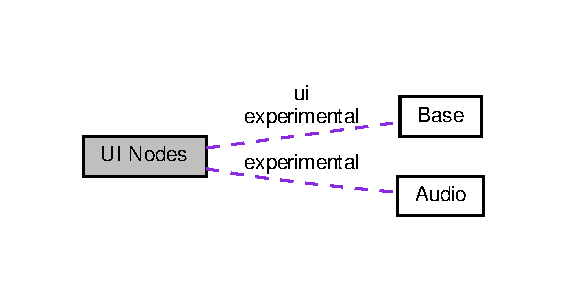
\includegraphics[width=272pt]{group__ui}
\end{center}
\end{figure}
\subsection*{Classes}
\begin{DoxyCompactItemize}
\item 
class \hyperlink{classTextFieldDelegate}{Text\+Field\+Delegate}
\item 
class \hyperlink{classTextFieldTTF}{Text\+Field\+T\+TF}
\begin{DoxyCompactList}\small\item\em A simple text input field with T\+TF font. \end{DoxyCompactList}\item 
class \hyperlink{classScrollViewDelegate}{Scroll\+View\+Delegate}
\item 
class \hyperlink{classScrollView}{Scroll\+View}
\item 
class \hyperlink{classTableViewDelegate}{Table\+View\+Delegate}
\item 
class \hyperlink{classTableViewDataSource}{Table\+View\+Data\+Source}
\item 
class \hyperlink{classTableView}{Table\+View}
\item 
class \hyperlink{classTableViewCell}{Table\+View\+Cell}
\end{DoxyCompactItemize}
\subsection*{Variables}
\begin{DoxyCompactItemize}
\item 
\mbox{\Hypertarget{group__ui_gaea51324d1dbe3670e21d286c9c676c7c}\label{group__ui_gaea51324d1dbe3670e21d286c9c676c7c}} 
struct C\+C\+\_\+\+D\+LL {\bfseries Resource\+Data}
\item 
\mbox{\Hypertarget{group__ui_gaea51324d1dbe3670e21d286c9c676c7c}\label{group__ui_gaea51324d1dbe3670e21d286c9c676c7c}} 
struct C\+C\+\_\+\+D\+LL {\bfseries Resource\+Data}
\item 
\mbox{\Hypertarget{group__ui_gac95fff9eb385485d4b3ef6d3df393ee6}\label{group__ui_gac95fff9eb385485d4b3ef6d3df393ee6}} 
N\+S\+\_\+\+C\+C\+\_\+\+B\+E\+G\+IN struct C\+C\+\_\+\+D\+LL {\bfseries Resource\+Data}
\item 
\mbox{\Hypertarget{group__ui_gaea51324d1dbe3670e21d286c9c676c7c}\label{group__ui_gaea51324d1dbe3670e21d286c9c676c7c}} 
struct C\+C\+\_\+\+D\+LL {\bfseries Resource\+Data}
\item 
\mbox{\Hypertarget{group__ui_gaea51324d1dbe3670e21d286c9c676c7c}\label{group__ui_gaea51324d1dbe3670e21d286c9c676c7c}} 
struct C\+C\+\_\+\+D\+LL {\bfseries Resource\+Data}
\item 
\mbox{\Hypertarget{group__ui_gaea51324d1dbe3670e21d286c9c676c7c}\label{group__ui_gaea51324d1dbe3670e21d286c9c676c7c}} 
struct C\+C\+\_\+\+D\+LL {\bfseries Resource\+Data}
\item 
\mbox{\Hypertarget{group__ui_gaea51324d1dbe3670e21d286c9c676c7c}\label{group__ui_gaea51324d1dbe3670e21d286c9c676c7c}} 
struct C\+C\+\_\+\+D\+LL {\bfseries Resource\+Data}
\item 
\mbox{\Hypertarget{group__ui_gaea51324d1dbe3670e21d286c9c676c7c}\label{group__ui_gaea51324d1dbe3670e21d286c9c676c7c}} 
struct C\+C\+\_\+\+D\+LL {\bfseries Resource\+Data}
\item 
\mbox{\Hypertarget{group__ui_gaea51324d1dbe3670e21d286c9c676c7c}\label{group__ui_gaea51324d1dbe3670e21d286c9c676c7c}} 
struct C\+C\+\_\+\+D\+LL {\bfseries Resource\+Data}
\item 
\mbox{\Hypertarget{group__ui_gaea51324d1dbe3670e21d286c9c676c7c}\label{group__ui_gaea51324d1dbe3670e21d286c9c676c7c}} 
struct C\+C\+\_\+\+D\+LL {\bfseries Resource\+Data}
\item 
\mbox{\Hypertarget{group__ui_gac95fff9eb385485d4b3ef6d3df393ee6}\label{group__ui_gac95fff9eb385485d4b3ef6d3df393ee6}} 
N\+S\+\_\+\+C\+C\+\_\+\+B\+E\+G\+IN struct C\+C\+\_\+\+D\+LL {\bfseries Resource\+Data}
\item 
\mbox{\Hypertarget{group__ui_gaea51324d1dbe3670e21d286c9c676c7c}\label{group__ui_gaea51324d1dbe3670e21d286c9c676c7c}} 
struct C\+C\+\_\+\+D\+LL {\bfseries Resource\+Data}
\item 
\mbox{\Hypertarget{group__ui_gaea51324d1dbe3670e21d286c9c676c7c}\label{group__ui_gaea51324d1dbe3670e21d286c9c676c7c}} 
struct C\+C\+\_\+\+D\+LL {\bfseries Resource\+Data}
\item 
\mbox{\Hypertarget{group__ui_gaea51324d1dbe3670e21d286c9c676c7c}\label{group__ui_gaea51324d1dbe3670e21d286c9c676c7c}} 
struct C\+C\+\_\+\+D\+LL {\bfseries Resource\+Data}
\item 
\mbox{\Hypertarget{group__ui_gaea51324d1dbe3670e21d286c9c676c7c}\label{group__ui_gaea51324d1dbe3670e21d286c9c676c7c}} 
struct C\+C\+\_\+\+D\+LL {\bfseries Resource\+Data}
\item 
\mbox{\Hypertarget{group__ui_gaea51324d1dbe3670e21d286c9c676c7c}\label{group__ui_gaea51324d1dbe3670e21d286c9c676c7c}} 
struct C\+C\+\_\+\+D\+LL {\bfseries Resource\+Data}
\end{DoxyCompactItemize}


\subsection{Detailed Description}

\hypertarget{group__lua}{}\section{Lua Binding}
\label{group__lua}\index{Lua Binding@{Lua Binding}}

\hypertarget{group__misc}{}\section{Misc}
\label{group__misc}\index{Misc@{Misc}}
\subsection*{Macros}
\begin{DoxyCompactItemize}
\item 
\mbox{\Hypertarget{group__misc_ga6d034fec4d7962b6f20f9e243527c560}\label{group__misc_ga6d034fec4d7962b6f20f9e243527c560}} 
\#define \hyperlink{group__misc_ga6d034fec4d7962b6f20f9e243527c560}{C\+P\+\_\+\+B\+U\+F\+F\+E\+R\+\_\+\+B\+Y\+T\+ES}~(32$\ast$1024)
\begin{DoxyCompactList}\small\item\em Allocated size for various Chipmunk buffers. \end{DoxyCompactList}\item 
\mbox{\Hypertarget{group__misc_gac88bab87ecc7db6cc222679bf6082e9b}\label{group__misc_gac88bab87ecc7db6cc222679bf6082e9b}} 
\#define \hyperlink{group__misc_gac88bab87ecc7db6cc222679bf6082e9b}{cpcalloc}~calloc
\begin{DoxyCompactList}\small\item\em Chipmunk calloc() alias. \end{DoxyCompactList}\item 
\mbox{\Hypertarget{group__misc_gab3544b888840ed34e49bb0559d6849a8}\label{group__misc_gab3544b888840ed34e49bb0559d6849a8}} 
\#define \hyperlink{group__misc_gab3544b888840ed34e49bb0559d6849a8}{cprealloc}~realloc
\begin{DoxyCompactList}\small\item\em Chipmunk realloc() alias. \end{DoxyCompactList}\item 
\mbox{\Hypertarget{group__misc_ga14627263deb67605201281bac734eb04}\label{group__misc_ga14627263deb67605201281bac734eb04}} 
\#define \hyperlink{group__misc_ga14627263deb67605201281bac734eb04}{cpfree}~free
\begin{DoxyCompactList}\small\item\em Chipmunk free() alias. \end{DoxyCompactList}\item 
\mbox{\Hypertarget{group__misc_gac02132b57a51a1c26ff6fb11dc046c04}\label{group__misc_gac02132b57a51a1c26ff6fb11dc046c04}} 
\#define {\bfseries C\+P\+\_\+\+V\+E\+R\+S\+I\+O\+N\+\_\+\+M\+A\+J\+OR}~7
\item 
\mbox{\Hypertarget{group__misc_ga015d989acd6a013e84ea8696953172a8}\label{group__misc_ga015d989acd6a013e84ea8696953172a8}} 
\#define {\bfseries C\+P\+\_\+\+V\+E\+R\+S\+I\+O\+N\+\_\+\+M\+I\+N\+OR}~0
\item 
\mbox{\Hypertarget{group__misc_ga0311c28764c81d74c3c76570bb92c57f}\label{group__misc_ga0311c28764c81d74c3c76570bb92c57f}} 
\#define {\bfseries C\+P\+\_\+\+V\+E\+R\+S\+I\+O\+N\+\_\+\+R\+E\+L\+E\+A\+SE}~1
\item 
\#define \hyperlink{group__misc_ga9abe29a1fe6d1f2041e95f2fb2e2ce1c}{C\+P\+\_\+\+C\+O\+N\+V\+E\+X\+\_\+\+H\+U\+LL}(\+\_\+\+\_\+count\+\_\+\+\_\+,  \+\_\+\+\_\+verts\+\_\+\+\_\+,  \+\_\+\+\_\+count\+\_\+var\+\_\+\+\_\+,  \+\_\+\+\_\+verts\+\_\+var\+\_\+\+\_\+)
\item 
\mbox{\Hypertarget{group__misc_ga6d034fec4d7962b6f20f9e243527c560}\label{group__misc_ga6d034fec4d7962b6f20f9e243527c560}} 
\#define \hyperlink{group__misc_ga6d034fec4d7962b6f20f9e243527c560}{C\+P\+\_\+\+B\+U\+F\+F\+E\+R\+\_\+\+B\+Y\+T\+ES}~(32$\ast$1024)
\begin{DoxyCompactList}\small\item\em Allocated size for various Chipmunk buffers. \end{DoxyCompactList}\item 
\mbox{\Hypertarget{group__misc_gac88bab87ecc7db6cc222679bf6082e9b}\label{group__misc_gac88bab87ecc7db6cc222679bf6082e9b}} 
\#define \hyperlink{group__misc_gac88bab87ecc7db6cc222679bf6082e9b}{cpcalloc}~calloc
\begin{DoxyCompactList}\small\item\em Chipmunk calloc() alias. \end{DoxyCompactList}\item 
\mbox{\Hypertarget{group__misc_gab3544b888840ed34e49bb0559d6849a8}\label{group__misc_gab3544b888840ed34e49bb0559d6849a8}} 
\#define \hyperlink{group__misc_gab3544b888840ed34e49bb0559d6849a8}{cprealloc}~realloc
\begin{DoxyCompactList}\small\item\em Chipmunk realloc() alias. \end{DoxyCompactList}\item 
\mbox{\Hypertarget{group__misc_ga14627263deb67605201281bac734eb04}\label{group__misc_ga14627263deb67605201281bac734eb04}} 
\#define \hyperlink{group__misc_ga14627263deb67605201281bac734eb04}{cpfree}~free
\begin{DoxyCompactList}\small\item\em Chipmunk free() alias. \end{DoxyCompactList}\item 
\mbox{\Hypertarget{group__misc_gac02132b57a51a1c26ff6fb11dc046c04}\label{group__misc_gac02132b57a51a1c26ff6fb11dc046c04}} 
\#define {\bfseries C\+P\+\_\+\+V\+E\+R\+S\+I\+O\+N\+\_\+\+M\+A\+J\+OR}~7
\item 
\mbox{\Hypertarget{group__misc_ga015d989acd6a013e84ea8696953172a8}\label{group__misc_ga015d989acd6a013e84ea8696953172a8}} 
\#define {\bfseries C\+P\+\_\+\+V\+E\+R\+S\+I\+O\+N\+\_\+\+M\+I\+N\+OR}~0
\item 
\mbox{\Hypertarget{group__misc_ga0311c28764c81d74c3c76570bb92c57f}\label{group__misc_ga0311c28764c81d74c3c76570bb92c57f}} 
\#define {\bfseries C\+P\+\_\+\+V\+E\+R\+S\+I\+O\+N\+\_\+\+R\+E\+L\+E\+A\+SE}~1
\item 
\#define \hyperlink{group__misc_ga9abe29a1fe6d1f2041e95f2fb2e2ce1c}{C\+P\+\_\+\+C\+O\+N\+V\+E\+X\+\_\+\+H\+U\+LL}(\+\_\+\+\_\+count\+\_\+\+\_\+,  \+\_\+\+\_\+verts\+\_\+\+\_\+,  \+\_\+\+\_\+count\+\_\+var\+\_\+\+\_\+,  \+\_\+\+\_\+verts\+\_\+var\+\_\+\+\_\+)
\item 
\#define \hyperlink{group__misc_ga9f138b98c73782807d88e76c1c532dc2}{lws\+\_\+start\+\_\+foreach\+\_\+ll}(type,  it,  start)
\item 
\#define \hyperlink{group__misc_ga9d94995ca7a1be16bf3d7bd2e449c812}{lws\+\_\+end\+\_\+foreach\+\_\+ll}(it,  nxt)
\item 
\#define \hyperlink{group__misc_gad973ecfe2ac066ba0ea1ec3695d3e896}{lws\+\_\+start\+\_\+foreach\+\_\+llp}(type,  it,  start)
\item 
\#define \hyperlink{group__misc_gaba92c53b57f3e689f8568b02184a8d84}{lws\+\_\+end\+\_\+foreach\+\_\+llp}(it,  nxt)
\item 
\#define \hyperlink{group__misc_ga9f138b98c73782807d88e76c1c532dc2}{lws\+\_\+start\+\_\+foreach\+\_\+ll}(type,  it,  start)
\item 
\#define \hyperlink{group__misc_ga9d94995ca7a1be16bf3d7bd2e449c812}{lws\+\_\+end\+\_\+foreach\+\_\+ll}(it,  nxt)
\item 
\#define \hyperlink{group__misc_gad973ecfe2ac066ba0ea1ec3695d3e896}{lws\+\_\+start\+\_\+foreach\+\_\+llp}(type,  it,  start)
\item 
\#define \hyperlink{group__misc_gaba92c53b57f3e689f8568b02184a8d84}{lws\+\_\+end\+\_\+foreach\+\_\+llp}(it,  nxt)
\item 
\#define \hyperlink{group__misc_ga9f138b98c73782807d88e76c1c532dc2}{lws\+\_\+start\+\_\+foreach\+\_\+ll}(type,  it,  start)
\item 
\#define \hyperlink{group__misc_ga9d94995ca7a1be16bf3d7bd2e449c812}{lws\+\_\+end\+\_\+foreach\+\_\+ll}(it,  nxt)
\item 
\#define \hyperlink{group__misc_gad973ecfe2ac066ba0ea1ec3695d3e896}{lws\+\_\+start\+\_\+foreach\+\_\+llp}(type,  it,  start)
\item 
\#define \hyperlink{group__misc_gaba92c53b57f3e689f8568b02184a8d84}{lws\+\_\+end\+\_\+foreach\+\_\+llp}(it,  nxt)
\item 
\#define \hyperlink{group__misc_ga9f138b98c73782807d88e76c1c532dc2}{lws\+\_\+start\+\_\+foreach\+\_\+ll}(type,  it,  start)
\item 
\#define \hyperlink{group__misc_ga9d94995ca7a1be16bf3d7bd2e449c812}{lws\+\_\+end\+\_\+foreach\+\_\+ll}(it,  nxt)
\item 
\#define \hyperlink{group__misc_gad973ecfe2ac066ba0ea1ec3695d3e896}{lws\+\_\+start\+\_\+foreach\+\_\+llp}(type,  it,  start)
\item 
\#define \hyperlink{group__misc_gaba92c53b57f3e689f8568b02184a8d84}{lws\+\_\+end\+\_\+foreach\+\_\+llp}(it,  nxt)
\item 
\#define \hyperlink{group__misc_ga9f138b98c73782807d88e76c1c532dc2}{lws\+\_\+start\+\_\+foreach\+\_\+ll}(type,  it,  start)
\item 
\#define \hyperlink{group__misc_ga9d94995ca7a1be16bf3d7bd2e449c812}{lws\+\_\+end\+\_\+foreach\+\_\+ll}(it,  nxt)
\item 
\#define \hyperlink{group__misc_gad973ecfe2ac066ba0ea1ec3695d3e896}{lws\+\_\+start\+\_\+foreach\+\_\+llp}(type,  it,  start)
\item 
\#define \hyperlink{group__misc_gaba92c53b57f3e689f8568b02184a8d84}{lws\+\_\+end\+\_\+foreach\+\_\+llp}(it,  nxt)
\item 
\#define \hyperlink{group__misc_ga9f138b98c73782807d88e76c1c532dc2}{lws\+\_\+start\+\_\+foreach\+\_\+ll}(type,  it,  start)
\item 
\#define \hyperlink{group__misc_ga9d94995ca7a1be16bf3d7bd2e449c812}{lws\+\_\+end\+\_\+foreach\+\_\+ll}(it,  nxt)
\item 
\#define \hyperlink{group__misc_gad973ecfe2ac066ba0ea1ec3695d3e896}{lws\+\_\+start\+\_\+foreach\+\_\+llp}(type,  it,  start)
\item 
\#define \hyperlink{group__misc_gaba92c53b57f3e689f8568b02184a8d84}{lws\+\_\+end\+\_\+foreach\+\_\+llp}(it,  nxt)
\end{DoxyCompactItemize}
\subsection*{Typedefs}
\begin{DoxyCompactItemize}
\item 
\mbox{\Hypertarget{group__misc_ga6b357f2c1d3fedc78e2c7aaa5186d566}\label{group__misc_ga6b357f2c1d3fedc78e2c7aaa5186d566}} 
typedef struct \hyperlink{structcpArray}{cp\+Array} {\bfseries cp\+Array}
\item 
\mbox{\Hypertarget{group__misc_ga0c80056192ac0574141a88de933b16b3}\label{group__misc_ga0c80056192ac0574141a88de933b16b3}} 
typedef struct cp\+Hash\+Set {\bfseries cp\+Hash\+Set}
\item 
\mbox{\Hypertarget{group__misc_ga89830b081a94b2500cc1ca31c43ac006}\label{group__misc_ga89830b081a94b2500cc1ca31c43ac006}} 
typedef struct \hyperlink{structcpBody}{cp\+Body} {\bfseries cp\+Body}
\item 
\mbox{\Hypertarget{group__misc_ga16375f8bc5b219cde7560b23443b3a95}\label{group__misc_ga16375f8bc5b219cde7560b23443b3a95}} 
typedef struct \hyperlink{structcpShape}{cp\+Shape} {\bfseries cp\+Shape}
\item 
\mbox{\Hypertarget{group__misc_gadc0a8c50b9b7b6cdf205f1e446d77b23}\label{group__misc_gadc0a8c50b9b7b6cdf205f1e446d77b23}} 
typedef struct \hyperlink{structcpCircleShape}{cp\+Circle\+Shape} {\bfseries cp\+Circle\+Shape}
\item 
\mbox{\Hypertarget{group__misc_ga75717b3e5384ae67f7b5a7dd9d54c50f}\label{group__misc_ga75717b3e5384ae67f7b5a7dd9d54c50f}} 
typedef struct \hyperlink{structcpSegmentShape}{cp\+Segment\+Shape} {\bfseries cp\+Segment\+Shape}
\item 
\mbox{\Hypertarget{group__misc_gac0977850752deeb7bd3bae3e6e67b088}\label{group__misc_gac0977850752deeb7bd3bae3e6e67b088}} 
typedef struct \hyperlink{structcpPolyShape}{cp\+Poly\+Shape} {\bfseries cp\+Poly\+Shape}
\item 
\mbox{\Hypertarget{group__misc_gabdb40b2f09deac0d0e05605be0701be3}\label{group__misc_gabdb40b2f09deac0d0e05605be0701be3}} 
typedef struct \hyperlink{structcpConstraint}{cp\+Constraint} {\bfseries cp\+Constraint}
\item 
\mbox{\Hypertarget{group__misc_ga842072215937b61bb52852bec19367ad}\label{group__misc_ga842072215937b61bb52852bec19367ad}} 
typedef struct \hyperlink{structcpPinJoint}{cp\+Pin\+Joint} {\bfseries cp\+Pin\+Joint}
\item 
\mbox{\Hypertarget{group__misc_ga22c80982fc779df42ada48f0f35c326c}\label{group__misc_ga22c80982fc779df42ada48f0f35c326c}} 
typedef struct \hyperlink{structcpSlideJoint}{cp\+Slide\+Joint} {\bfseries cp\+Slide\+Joint}
\item 
\mbox{\Hypertarget{group__misc_ga6be42317226c36d7c3b71175c31bed55}\label{group__misc_ga6be42317226c36d7c3b71175c31bed55}} 
typedef struct \hyperlink{structcpPivotJoint}{cp\+Pivot\+Joint} {\bfseries cp\+Pivot\+Joint}
\item 
\mbox{\Hypertarget{group__misc_ga4aa4733fb7b33f6650ce92a7d2bf9361}\label{group__misc_ga4aa4733fb7b33f6650ce92a7d2bf9361}} 
typedef struct \hyperlink{structcpGrooveJoint}{cp\+Groove\+Joint} {\bfseries cp\+Groove\+Joint}
\item 
\mbox{\Hypertarget{group__misc_gab4c3629bf0daa6e27aaff6ac1bdc0fb7}\label{group__misc_gab4c3629bf0daa6e27aaff6ac1bdc0fb7}} 
typedef struct \hyperlink{structcpDampedSpring}{cp\+Damped\+Spring} {\bfseries cp\+Damped\+Spring}
\item 
\mbox{\Hypertarget{group__misc_ga48602f8d634857dac76e75f05458aea1}\label{group__misc_ga48602f8d634857dac76e75f05458aea1}} 
typedef struct \hyperlink{structcpDampedRotarySpring}{cp\+Damped\+Rotary\+Spring} {\bfseries cp\+Damped\+Rotary\+Spring}
\item 
\mbox{\Hypertarget{group__misc_ga54615af04b79ce2b9f2dfedc8e702da3}\label{group__misc_ga54615af04b79ce2b9f2dfedc8e702da3}} 
typedef struct \hyperlink{structcpRotaryLimitJoint}{cp\+Rotary\+Limit\+Joint} {\bfseries cp\+Rotary\+Limit\+Joint}
\item 
\mbox{\Hypertarget{group__misc_ga574d87330384b10b88666948ea424a50}\label{group__misc_ga574d87330384b10b88666948ea424a50}} 
typedef struct \hyperlink{structcpRatchetJoint}{cp\+Ratchet\+Joint} {\bfseries cp\+Ratchet\+Joint}
\item 
\mbox{\Hypertarget{group__misc_gac590a81b11f1ee5ae26108e24a5b6074}\label{group__misc_gac590a81b11f1ee5ae26108e24a5b6074}} 
typedef struct \hyperlink{structcpGearJoint}{cp\+Gear\+Joint} {\bfseries cp\+Gear\+Joint}
\item 
\mbox{\Hypertarget{group__misc_ga946a6726ce9067b29e944ff0f9309120}\label{group__misc_ga946a6726ce9067b29e944ff0f9309120}} 
typedef struct cp\+Simple\+Motor\+Joint {\bfseries cp\+Simple\+Motor\+Joint}
\item 
\mbox{\Hypertarget{group__misc_gad27db8fe21c73da2f139b0f28ded9818}\label{group__misc_gad27db8fe21c73da2f139b0f28ded9818}} 
typedef struct \hyperlink{structcpCollisionHandler}{cp\+Collision\+Handler} {\bfseries cp\+Collision\+Handler}
\item 
\mbox{\Hypertarget{group__misc_ga878866fdedeef4e18219aef96b040cfa}\label{group__misc_ga878866fdedeef4e18219aef96b040cfa}} 
typedef struct \hyperlink{structcpContactPointSet}{cp\+Contact\+Point\+Set} {\bfseries cp\+Contact\+Point\+Set}
\item 
\mbox{\Hypertarget{group__misc_ga771a9d6a062a6097f0e6bb1b2682e93f}\label{group__misc_ga771a9d6a062a6097f0e6bb1b2682e93f}} 
typedef struct \hyperlink{structcpArbiter}{cp\+Arbiter} {\bfseries cp\+Arbiter}
\item 
\mbox{\Hypertarget{group__misc_ga8838f85d2e2ba627fc4c9208fb1a4682}\label{group__misc_ga8838f85d2e2ba627fc4c9208fb1a4682}} 
typedef struct \hyperlink{structcpSpace}{cp\+Space} {\bfseries cp\+Space}
\item 
\mbox{\Hypertarget{group__misc_ga6b357f2c1d3fedc78e2c7aaa5186d566}\label{group__misc_ga6b357f2c1d3fedc78e2c7aaa5186d566}} 
typedef struct \hyperlink{structcpArray}{cp\+Array} {\bfseries cp\+Array}
\item 
\mbox{\Hypertarget{group__misc_ga0c80056192ac0574141a88de933b16b3}\label{group__misc_ga0c80056192ac0574141a88de933b16b3}} 
typedef struct cp\+Hash\+Set {\bfseries cp\+Hash\+Set}
\item 
\mbox{\Hypertarget{group__misc_ga89830b081a94b2500cc1ca31c43ac006}\label{group__misc_ga89830b081a94b2500cc1ca31c43ac006}} 
typedef struct \hyperlink{structcpBody}{cp\+Body} {\bfseries cp\+Body}
\item 
\mbox{\Hypertarget{group__misc_ga16375f8bc5b219cde7560b23443b3a95}\label{group__misc_ga16375f8bc5b219cde7560b23443b3a95}} 
typedef struct \hyperlink{structcpShape}{cp\+Shape} {\bfseries cp\+Shape}
\item 
\mbox{\Hypertarget{group__misc_gadc0a8c50b9b7b6cdf205f1e446d77b23}\label{group__misc_gadc0a8c50b9b7b6cdf205f1e446d77b23}} 
typedef struct \hyperlink{structcpCircleShape}{cp\+Circle\+Shape} {\bfseries cp\+Circle\+Shape}
\item 
\mbox{\Hypertarget{group__misc_ga75717b3e5384ae67f7b5a7dd9d54c50f}\label{group__misc_ga75717b3e5384ae67f7b5a7dd9d54c50f}} 
typedef struct \hyperlink{structcpSegmentShape}{cp\+Segment\+Shape} {\bfseries cp\+Segment\+Shape}
\item 
\mbox{\Hypertarget{group__misc_gac0977850752deeb7bd3bae3e6e67b088}\label{group__misc_gac0977850752deeb7bd3bae3e6e67b088}} 
typedef struct \hyperlink{structcpPolyShape}{cp\+Poly\+Shape} {\bfseries cp\+Poly\+Shape}
\item 
\mbox{\Hypertarget{group__misc_gabdb40b2f09deac0d0e05605be0701be3}\label{group__misc_gabdb40b2f09deac0d0e05605be0701be3}} 
typedef struct \hyperlink{structcpConstraint}{cp\+Constraint} {\bfseries cp\+Constraint}
\item 
\mbox{\Hypertarget{group__misc_ga842072215937b61bb52852bec19367ad}\label{group__misc_ga842072215937b61bb52852bec19367ad}} 
typedef struct \hyperlink{structcpPinJoint}{cp\+Pin\+Joint} {\bfseries cp\+Pin\+Joint}
\item 
\mbox{\Hypertarget{group__misc_ga22c80982fc779df42ada48f0f35c326c}\label{group__misc_ga22c80982fc779df42ada48f0f35c326c}} 
typedef struct \hyperlink{structcpSlideJoint}{cp\+Slide\+Joint} {\bfseries cp\+Slide\+Joint}
\item 
\mbox{\Hypertarget{group__misc_ga6be42317226c36d7c3b71175c31bed55}\label{group__misc_ga6be42317226c36d7c3b71175c31bed55}} 
typedef struct \hyperlink{structcpPivotJoint}{cp\+Pivot\+Joint} {\bfseries cp\+Pivot\+Joint}
\item 
\mbox{\Hypertarget{group__misc_ga4aa4733fb7b33f6650ce92a7d2bf9361}\label{group__misc_ga4aa4733fb7b33f6650ce92a7d2bf9361}} 
typedef struct \hyperlink{structcpGrooveJoint}{cp\+Groove\+Joint} {\bfseries cp\+Groove\+Joint}
\item 
\mbox{\Hypertarget{group__misc_gab4c3629bf0daa6e27aaff6ac1bdc0fb7}\label{group__misc_gab4c3629bf0daa6e27aaff6ac1bdc0fb7}} 
typedef struct \hyperlink{structcpDampedSpring}{cp\+Damped\+Spring} {\bfseries cp\+Damped\+Spring}
\item 
\mbox{\Hypertarget{group__misc_ga48602f8d634857dac76e75f05458aea1}\label{group__misc_ga48602f8d634857dac76e75f05458aea1}} 
typedef struct \hyperlink{structcpDampedRotarySpring}{cp\+Damped\+Rotary\+Spring} {\bfseries cp\+Damped\+Rotary\+Spring}
\item 
\mbox{\Hypertarget{group__misc_ga54615af04b79ce2b9f2dfedc8e702da3}\label{group__misc_ga54615af04b79ce2b9f2dfedc8e702da3}} 
typedef struct \hyperlink{structcpRotaryLimitJoint}{cp\+Rotary\+Limit\+Joint} {\bfseries cp\+Rotary\+Limit\+Joint}
\item 
\mbox{\Hypertarget{group__misc_ga574d87330384b10b88666948ea424a50}\label{group__misc_ga574d87330384b10b88666948ea424a50}} 
typedef struct \hyperlink{structcpRatchetJoint}{cp\+Ratchet\+Joint} {\bfseries cp\+Ratchet\+Joint}
\item 
\mbox{\Hypertarget{group__misc_gac590a81b11f1ee5ae26108e24a5b6074}\label{group__misc_gac590a81b11f1ee5ae26108e24a5b6074}} 
typedef struct \hyperlink{structcpGearJoint}{cp\+Gear\+Joint} {\bfseries cp\+Gear\+Joint}
\item 
\mbox{\Hypertarget{group__misc_ga946a6726ce9067b29e944ff0f9309120}\label{group__misc_ga946a6726ce9067b29e944ff0f9309120}} 
typedef struct cp\+Simple\+Motor\+Joint {\bfseries cp\+Simple\+Motor\+Joint}
\item 
\mbox{\Hypertarget{group__misc_gad27db8fe21c73da2f139b0f28ded9818}\label{group__misc_gad27db8fe21c73da2f139b0f28ded9818}} 
typedef struct \hyperlink{structcpCollisionHandler}{cp\+Collision\+Handler} {\bfseries cp\+Collision\+Handler}
\item 
\mbox{\Hypertarget{group__misc_ga878866fdedeef4e18219aef96b040cfa}\label{group__misc_ga878866fdedeef4e18219aef96b040cfa}} 
typedef struct \hyperlink{structcpContactPointSet}{cp\+Contact\+Point\+Set} {\bfseries cp\+Contact\+Point\+Set}
\item 
\mbox{\Hypertarget{group__misc_ga771a9d6a062a6097f0e6bb1b2682e93f}\label{group__misc_ga771a9d6a062a6097f0e6bb1b2682e93f}} 
typedef struct \hyperlink{structcpArbiter}{cp\+Arbiter} {\bfseries cp\+Arbiter}
\item 
\mbox{\Hypertarget{group__misc_ga8838f85d2e2ba627fc4c9208fb1a4682}\label{group__misc_ga8838f85d2e2ba627fc4c9208fb1a4682}} 
typedef struct \hyperlink{structcpSpace}{cp\+Space} {\bfseries cp\+Space}
\end{DoxyCompactItemize}
\subsection*{Functions}
\begin{DoxyCompactItemize}
\item 
C\+P\+\_\+\+E\+X\+P\+O\+RT cp\+Float \hyperlink{group__misc_gafa2103fb2fd788fded1131e53f00681a}{cp\+Moment\+For\+Circle} (cp\+Float m, cp\+Float r1, cp\+Float r2, \hyperlink{structcpVect}{cp\+Vect} offset)
\item 
C\+P\+\_\+\+E\+X\+P\+O\+RT cp\+Float \hyperlink{group__misc_ga55a50f3dfa695db703759e550db16bce}{cp\+Area\+For\+Circle} (cp\+Float r1, cp\+Float r2)
\item 
C\+P\+\_\+\+E\+X\+P\+O\+RT cp\+Float \hyperlink{group__misc_ga9548fe7830d426bde625d39d4687e6be}{cp\+Moment\+For\+Segment} (cp\+Float m, \hyperlink{structcpVect}{cp\+Vect} a, \hyperlink{structcpVect}{cp\+Vect} b, cp\+Float radius)
\item 
\mbox{\Hypertarget{group__misc_ga5758bdfd93aec5d3f3780a1ff29aad37}\label{group__misc_ga5758bdfd93aec5d3f3780a1ff29aad37}} 
C\+P\+\_\+\+E\+X\+P\+O\+RT cp\+Float \hyperlink{group__misc_ga5758bdfd93aec5d3f3780a1ff29aad37}{cp\+Area\+For\+Segment} (\hyperlink{structcpVect}{cp\+Vect} a, \hyperlink{structcpVect}{cp\+Vect} b, cp\+Float radius)
\begin{DoxyCompactList}\small\item\em Calculate the area of a fattened (capsule shaped) line segment. \end{DoxyCompactList}\item 
\mbox{\Hypertarget{group__misc_gaa69a0e62a94f55c347eb66160963ff6e}\label{group__misc_gaa69a0e62a94f55c347eb66160963ff6e}} 
C\+P\+\_\+\+E\+X\+P\+O\+RT cp\+Float \hyperlink{group__misc_gaa69a0e62a94f55c347eb66160963ff6e}{cp\+Moment\+For\+Poly} (cp\+Float m, int count, const \hyperlink{structcpVect}{cp\+Vect} $\ast$verts, \hyperlink{structcpVect}{cp\+Vect} offset, cp\+Float radius)
\begin{DoxyCompactList}\small\item\em Calculate the moment of inertia for a solid polygon shape assuming it\textquotesingle{}s center of gravity is at it\textquotesingle{}s centroid. The offset is added to each vertex. \end{DoxyCompactList}\item 
C\+P\+\_\+\+E\+X\+P\+O\+RT cp\+Float \hyperlink{group__misc_ga2bc17e58f105411e2d66c09f8047d822}{cp\+Area\+For\+Poly} (const int count, const \hyperlink{structcpVect}{cp\+Vect} $\ast$verts, cp\+Float radius)
\item 
\mbox{\Hypertarget{group__misc_gaedd18beae9cbd2b6847747cc1d933bfd}\label{group__misc_gaedd18beae9cbd2b6847747cc1d933bfd}} 
C\+P\+\_\+\+E\+X\+P\+O\+RT \hyperlink{structcpVect}{cp\+Vect} \hyperlink{group__misc_gaedd18beae9cbd2b6847747cc1d933bfd}{cp\+Centroid\+For\+Poly} (const int count, const \hyperlink{structcpVect}{cp\+Vect} $\ast$verts)
\begin{DoxyCompactList}\small\item\em Calculate the natural centroid of a polygon. \end{DoxyCompactList}\item 
\mbox{\Hypertarget{group__misc_ga840facfe3f57151e1a8634b6047a45ef}\label{group__misc_ga840facfe3f57151e1a8634b6047a45ef}} 
C\+P\+\_\+\+E\+X\+P\+O\+RT cp\+Float \hyperlink{group__misc_ga840facfe3f57151e1a8634b6047a45ef}{cp\+Moment\+For\+Box} (cp\+Float m, cp\+Float width, cp\+Float height)
\begin{DoxyCompactList}\small\item\em Calculate the moment of inertia for a solid box. \end{DoxyCompactList}\item 
\mbox{\Hypertarget{group__misc_ga4a01a4b99c3976c1a9b4df14efe04552}\label{group__misc_ga4a01a4b99c3976c1a9b4df14efe04552}} 
C\+P\+\_\+\+E\+X\+P\+O\+RT cp\+Float \hyperlink{group__misc_ga4a01a4b99c3976c1a9b4df14efe04552}{cp\+Moment\+For\+Box2} (cp\+Float m, \hyperlink{structcpBB}{cp\+BB} box)
\begin{DoxyCompactList}\small\item\em Calculate the moment of inertia for a solid box. \end{DoxyCompactList}\item 
C\+P\+\_\+\+E\+X\+P\+O\+RT int \hyperlink{group__misc_ga94ed1fc4d2c987c3e4df3cb16b12a156}{cp\+Convex\+Hull} (int count, const \hyperlink{structcpVect}{cp\+Vect} $\ast$verts, \hyperlink{structcpVect}{cp\+Vect} $\ast$result, int $\ast$first, cp\+Float tol)
\item 
L\+W\+S\+\_\+\+V\+I\+S\+I\+B\+LE L\+W\+S\+\_\+\+E\+X\+T\+E\+RN int \hyperlink{group__misc_ga2163492f17db959a36967adb73d823b4}{lws\+\_\+snprintf} (char $\ast$str, size\+\_\+t size, const char $\ast$format,...) L\+W\+S\+\_\+\+F\+O\+R\+M\+AT(3)
\item 
L\+W\+S\+\_\+\+V\+I\+S\+I\+B\+LE L\+W\+S\+\_\+\+E\+X\+T\+E\+RN int \hyperlink{group__misc_ga58f906c6be0ca80efd813f694569dd4a}{lws\+\_\+get\+\_\+random} (struct \hyperlink{structlws__context}{lws\+\_\+context} $\ast$context, void $\ast$buf, int len)
\item 
L\+W\+S\+\_\+\+V\+I\+S\+I\+B\+LE L\+W\+S\+\_\+\+E\+X\+T\+E\+RN int L\+W\+S\+\_\+\+W\+A\+R\+N\+\_\+\+U\+N\+U\+S\+E\+D\+\_\+\+R\+E\+S\+U\+LT \hyperlink{group__misc_gace5171b1dbbc03ec89a98f8afdb5c9af}{lws\+\_\+daemonize} (const char $\ast$\+\_\+lock\+\_\+path)
\item 
L\+W\+S\+\_\+\+V\+I\+S\+I\+B\+LE L\+W\+S\+\_\+\+E\+X\+T\+E\+RN const char $\ast$L\+W\+S\+\_\+\+W\+A\+R\+N\+\_\+\+U\+N\+U\+S\+E\+D\+\_\+\+R\+E\+S\+U\+LT \hyperlink{group__misc_gac6abfc0b2bd5b2f09281a4432bb2f5f0}{lws\+\_\+get\+\_\+library\+\_\+version} (void)
\item 
L\+W\+S\+\_\+\+V\+I\+S\+I\+B\+LE L\+W\+S\+\_\+\+E\+X\+T\+E\+RN void $\ast$ \hyperlink{group__misc_gaa194584fff9698f3b280658f770ccd0f}{lws\+\_\+wsi\+\_\+user} (struct \hyperlink{structlws}{lws} $\ast$wsi)
\item 
L\+W\+S\+\_\+\+V\+I\+S\+I\+B\+LE L\+W\+S\+\_\+\+E\+X\+T\+E\+RN void \hyperlink{group__misc_ga8d23abbe3fe1d53592b29c597a8245ba}{lws\+\_\+set\+\_\+wsi\+\_\+user} (struct \hyperlink{structlws}{lws} $\ast$wsi, void $\ast$user)
\item 
L\+W\+S\+\_\+\+V\+I\+S\+I\+B\+LE L\+W\+S\+\_\+\+E\+X\+T\+E\+RN int L\+W\+S\+\_\+\+W\+A\+R\+N\+\_\+\+U\+N\+U\+S\+E\+D\+\_\+\+R\+E\+S\+U\+LT \hyperlink{group__misc_ga1ec0d9faac5d3a5824d765c287c043aa}{lws\+\_\+parse\+\_\+uri} (char $\ast$p, const char $\ast$$\ast$prot, const char $\ast$$\ast$ads, int $\ast$port, const char $\ast$$\ast$path)
\item 
L\+W\+S\+\_\+\+V\+I\+S\+I\+B\+LE L\+W\+S\+\_\+\+E\+X\+T\+E\+RN unsigned long \hyperlink{group__misc_ga33bf2635033710b25f931b57ed663e1e}{lws\+\_\+now\+\_\+secs} (void)
\item 
L\+W\+S\+\_\+\+V\+I\+S\+I\+B\+LE L\+W\+S\+\_\+\+E\+X\+T\+E\+RN struct \hyperlink{structlws__context}{lws\+\_\+context} $\ast$L\+W\+S\+\_\+\+W\+A\+R\+N\+\_\+\+U\+N\+U\+S\+E\+D\+\_\+\+R\+E\+S\+U\+LT \hyperlink{group__misc_ga0af4f7d2dd375aeedcfa7eb0e1101c4b}{lws\+\_\+get\+\_\+context} (const struct \hyperlink{structlws}{lws} $\ast$wsi)
\item 
L\+W\+S\+\_\+\+V\+I\+S\+I\+B\+LE L\+W\+S\+\_\+\+E\+X\+T\+E\+RN int L\+W\+S\+\_\+\+W\+A\+R\+N\+\_\+\+U\+N\+U\+S\+E\+D\+\_\+\+R\+E\+S\+U\+LT \hyperlink{group__misc_ga629f48268fd1856b54b11172991b97d9}{lws\+\_\+get\+\_\+count\+\_\+threads} (struct \hyperlink{structlws__context}{lws\+\_\+context} $\ast$context)
\item 
L\+W\+S\+\_\+\+V\+I\+S\+I\+B\+LE L\+W\+S\+\_\+\+E\+X\+T\+E\+RN struct \hyperlink{structlws}{lws} $\ast$L\+W\+S\+\_\+\+W\+A\+R\+N\+\_\+\+U\+N\+U\+S\+E\+D\+\_\+\+R\+E\+S\+U\+LT \hyperlink{group__misc_gafdbca442411f4af9753ab9738a4973d4}{lws\+\_\+get\+\_\+parent} (const struct \hyperlink{structlws}{lws} $\ast$wsi)
\item 
L\+W\+S\+\_\+\+V\+I\+S\+I\+B\+LE L\+W\+S\+\_\+\+E\+X\+T\+E\+RN struct \hyperlink{structlws}{lws} $\ast$L\+W\+S\+\_\+\+W\+A\+R\+N\+\_\+\+U\+N\+U\+S\+E\+D\+\_\+\+R\+E\+S\+U\+LT \hyperlink{group__misc_ga7fc9fe90471eb724ba314baa21e5e18c}{lws\+\_\+get\+\_\+child} (const struct \hyperlink{structlws}{lws} $\ast$wsi)
\item 
L\+W\+S\+\_\+\+V\+I\+S\+I\+B\+LE L\+W\+S\+\_\+\+E\+X\+T\+E\+RN void \hyperlink{group__misc_ga385fa63d2b574ba63a3436686e08c178}{lws\+\_\+set\+\_\+parent\+\_\+carries\+\_\+io} (struct \hyperlink{structlws}{lws} $\ast$wsi)
\item 
\mbox{\Hypertarget{group__misc_gad8ddea90114f8d232cda0f999b67b140}\label{group__misc_gad8ddea90114f8d232cda0f999b67b140}} 
L\+W\+S\+\_\+\+V\+I\+S\+I\+B\+LE L\+W\+S\+\_\+\+E\+X\+T\+E\+RN void $\ast$ {\bfseries lws\+\_\+get\+\_\+opaque\+\_\+parent\+\_\+data} (const struct \hyperlink{structlws}{lws} $\ast$wsi)
\item 
\mbox{\Hypertarget{group__misc_gaaf29b5287677dd0cfa84923071d9d7f0}\label{group__misc_gaaf29b5287677dd0cfa84923071d9d7f0}} 
L\+W\+S\+\_\+\+V\+I\+S\+I\+B\+LE L\+W\+S\+\_\+\+E\+X\+T\+E\+RN void {\bfseries lws\+\_\+set\+\_\+opaque\+\_\+parent\+\_\+data} (struct \hyperlink{structlws}{lws} $\ast$wsi, void $\ast$data)
\item 
\mbox{\Hypertarget{group__misc_gaac31670e4570265d658cff17a498bb64}\label{group__misc_gaac31670e4570265d658cff17a498bb64}} 
L\+W\+S\+\_\+\+V\+I\+S\+I\+B\+LE L\+W\+S\+\_\+\+E\+X\+T\+E\+RN int {\bfseries lws\+\_\+get\+\_\+child\+\_\+pending\+\_\+on\+\_\+writable} (const struct \hyperlink{structlws}{lws} $\ast$wsi)
\item 
\mbox{\Hypertarget{group__misc_ga32749399b86d74655c266213b802bc34}\label{group__misc_ga32749399b86d74655c266213b802bc34}} 
L\+W\+S\+\_\+\+V\+I\+S\+I\+B\+LE L\+W\+S\+\_\+\+E\+X\+T\+E\+RN void {\bfseries lws\+\_\+clear\+\_\+child\+\_\+pending\+\_\+on\+\_\+writable} (struct \hyperlink{structlws}{lws} $\ast$wsi)
\item 
\mbox{\Hypertarget{group__misc_gaad999456da40e0300661f2d44f38fd80}\label{group__misc_gaad999456da40e0300661f2d44f38fd80}} 
L\+W\+S\+\_\+\+V\+I\+S\+I\+B\+LE L\+W\+S\+\_\+\+E\+X\+T\+E\+RN int {\bfseries lws\+\_\+get\+\_\+close\+\_\+length} (struct \hyperlink{structlws}{lws} $\ast$wsi)
\item 
\mbox{\Hypertarget{group__misc_ga4c862adfc241948a7e8b03d515e8e034}\label{group__misc_ga4c862adfc241948a7e8b03d515e8e034}} 
L\+W\+S\+\_\+\+V\+I\+S\+I\+B\+LE L\+W\+S\+\_\+\+E\+X\+T\+E\+RN unsigned char $\ast$ {\bfseries lws\+\_\+get\+\_\+close\+\_\+payload} (struct \hyperlink{structlws}{lws} $\ast$wsi)
\item 
L\+W\+S\+\_\+\+V\+I\+S\+I\+B\+LE L\+W\+S\+\_\+\+E\+X\+T\+E\+RN struct \hyperlink{structlws}{lws} $\ast$ \hyperlink{group__misc_ga1f748977e0f53e9f8889aacfd1ed8a62}{lws\+\_\+get\+\_\+network\+\_\+wsi} (struct \hyperlink{structlws}{lws} $\ast$wsi)
\item 
\mbox{\Hypertarget{group__misc_ga4eac9ba30f8ae8bdd4a6e5ebad20493e}\label{group__misc_ga4eac9ba30f8ae8bdd4a6e5ebad20493e}} 
L\+W\+S\+\_\+\+V\+I\+S\+I\+B\+LE L\+W\+S\+\_\+\+E\+X\+T\+E\+RN int {\bfseries lws\+\_\+read} (struct \hyperlink{structlws}{lws} $\ast$wsi, unsigned char $\ast$buf, lws\+\_\+filepos\+\_\+t len)
\item 
L\+W\+S\+\_\+\+V\+I\+S\+I\+B\+LE L\+W\+S\+\_\+\+E\+X\+T\+E\+RN void \hyperlink{group__misc_gadb3f42965ee4c564fcd317ed95ee5604}{lws\+\_\+set\+\_\+allocator} (void $\ast$($\ast$realloc)(void $\ast$ptr, size\+\_\+t size, const char $\ast$reason))
\item 
\mbox{\Hypertarget{group__misc_ga0e705d498e8c8500649a26ba30a1e106}\label{group__misc_ga0e705d498e8c8500649a26ba30a1e106}} 
L\+W\+S\+\_\+\+V\+I\+S\+I\+B\+LE L\+W\+S\+\_\+\+E\+X\+T\+E\+RN int {\bfseries lws\+\_\+read} (struct \hyperlink{structlws}{lws} $\ast$wsi, unsigned char $\ast$buf, size\+\_\+t len)
\item 
L\+W\+S\+\_\+\+V\+I\+S\+I\+B\+LE L\+W\+S\+\_\+\+E\+X\+T\+E\+RN void \hyperlink{group__misc_gab321ed812f46f6dc7ef9e3ca6f00cf1b}{lws\+\_\+set\+\_\+allocator} (void $\ast$($\ast$realloc)(void $\ast$ptr, size\+\_\+t size))
\end{DoxyCompactItemize}
\subsection*{Variables}
\begin{DoxyCompactItemize}
\item 
\mbox{\Hypertarget{group__misc_ga421f2f17b14cd75176f18c0a85074a8c}\label{group__misc_ga421f2f17b14cd75176f18c0a85074a8c}} 
C\+P\+\_\+\+E\+X\+P\+O\+RT const char $\ast$ \hyperlink{group__misc_ga421f2f17b14cd75176f18c0a85074a8c}{cp\+Version\+String}
\begin{DoxyCompactList}\small\item\em Version string. \end{DoxyCompactList}\item 
\mbox{\Hypertarget{group__misc_ga421f2f17b14cd75176f18c0a85074a8c}\label{group__misc_ga421f2f17b14cd75176f18c0a85074a8c}} 
C\+P\+\_\+\+E\+X\+P\+O\+RT const char $\ast$ \hyperlink{group__misc_ga421f2f17b14cd75176f18c0a85074a8c}{cp\+Version\+String}
\begin{DoxyCompactList}\small\item\em Version string. \end{DoxyCompactList}\end{DoxyCompactItemize}


\subsection{Detailed Description}
\subsubsection*{Miscellaneous A\+P\+Is}

Various A\+P\+Is outside of other categories 

\subsection{Macro Definition Documentation}
\mbox{\Hypertarget{group__misc_ga9abe29a1fe6d1f2041e95f2fb2e2ce1c}\label{group__misc_ga9abe29a1fe6d1f2041e95f2fb2e2ce1c}} 
\index{Misc@{Misc}!C\+P\+\_\+\+C\+O\+N\+V\+E\+X\+\_\+\+H\+U\+LL@{C\+P\+\_\+\+C\+O\+N\+V\+E\+X\+\_\+\+H\+U\+LL}}
\index{C\+P\+\_\+\+C\+O\+N\+V\+E\+X\+\_\+\+H\+U\+LL@{C\+P\+\_\+\+C\+O\+N\+V\+E\+X\+\_\+\+H\+U\+LL}!Misc@{Misc}}
\subsubsection{\texorpdfstring{C\+P\+\_\+\+C\+O\+N\+V\+E\+X\+\_\+\+H\+U\+LL}{CP\_CONVEX\_HULL}\hspace{0.1cm}{\footnotesize\ttfamily [1/2]}}
{\footnotesize\ttfamily \#define C\+P\+\_\+\+C\+O\+N\+V\+E\+X\+\_\+\+H\+U\+LL(\begin{DoxyParamCaption}\item[{}]{\+\_\+\+\_\+count\+\_\+\+\_\+,  }\item[{}]{\+\_\+\+\_\+verts\+\_\+\+\_\+,  }\item[{}]{\+\_\+\+\_\+count\+\_\+var\+\_\+\+\_\+,  }\item[{}]{\+\_\+\+\_\+verts\+\_\+var\+\_\+\+\_\+ }\end{DoxyParamCaption})}

{\bfseries Value\+:}
\begin{DoxyCode}
\hyperlink{structcpVect}{cpVect} *\_\_verts\_var\_\_ = (\hyperlink{structcpVect}{cpVect} *)alloca(\_\_count\_\_*\textcolor{keyword}{sizeof}(\hyperlink{structcpVect}{cpVect})); \(\backslash\)
int \_\_count\_var\_\_ = \hyperlink{group__misc_ga94ed1fc4d2c987c3e4df3cb16b12a156}{cpConvexHull}(\_\_count\_\_, \_\_verts\_\_, \_\_verts\_var\_\_, NULL, 0.0); \(\backslash\)
\end{DoxyCode}
Convenience macro to work with cp\+Convex\+Hull. {\ttfamily count} and {\ttfamily verts} is the input array passed to \hyperlink{group__misc_ga94ed1fc4d2c987c3e4df3cb16b12a156}{cp\+Convex\+Hull()}. {\ttfamily count\+\_\+var} and {\ttfamily verts\+\_\+var} are the names of the variables the macro creates to store the result. The output vertex array is allocated on the stack using alloca() so it will be freed automatically, but cannot be returned from the current scope. \mbox{\Hypertarget{group__misc_ga9abe29a1fe6d1f2041e95f2fb2e2ce1c}\label{group__misc_ga9abe29a1fe6d1f2041e95f2fb2e2ce1c}} 
\index{Misc@{Misc}!C\+P\+\_\+\+C\+O\+N\+V\+E\+X\+\_\+\+H\+U\+LL@{C\+P\+\_\+\+C\+O\+N\+V\+E\+X\+\_\+\+H\+U\+LL}}
\index{C\+P\+\_\+\+C\+O\+N\+V\+E\+X\+\_\+\+H\+U\+LL@{C\+P\+\_\+\+C\+O\+N\+V\+E\+X\+\_\+\+H\+U\+LL}!Misc@{Misc}}
\subsubsection{\texorpdfstring{C\+P\+\_\+\+C\+O\+N\+V\+E\+X\+\_\+\+H\+U\+LL}{CP\_CONVEX\_HULL}\hspace{0.1cm}{\footnotesize\ttfamily [2/2]}}
{\footnotesize\ttfamily \#define C\+P\+\_\+\+C\+O\+N\+V\+E\+X\+\_\+\+H\+U\+LL(\begin{DoxyParamCaption}\item[{}]{\+\_\+\+\_\+count\+\_\+\+\_\+,  }\item[{}]{\+\_\+\+\_\+verts\+\_\+\+\_\+,  }\item[{}]{\+\_\+\+\_\+count\+\_\+var\+\_\+\+\_\+,  }\item[{}]{\+\_\+\+\_\+verts\+\_\+var\+\_\+\+\_\+ }\end{DoxyParamCaption})}

{\bfseries Value\+:}
\begin{DoxyCode}
\hyperlink{structcpVect}{cpVect} *\_\_verts\_var\_\_ = (\hyperlink{structcpVect}{cpVect} *)alloca(\_\_count\_\_*\textcolor{keyword}{sizeof}(\hyperlink{structcpVect}{cpVect})); \(\backslash\)
int \_\_count\_var\_\_ = \hyperlink{group__misc_ga94ed1fc4d2c987c3e4df3cb16b12a156}{cpConvexHull}(\_\_count\_\_, \_\_verts\_\_, \_\_verts\_var\_\_, NULL, 0.0); \(\backslash\)
\end{DoxyCode}
Convenience macro to work with cp\+Convex\+Hull. {\ttfamily count} and {\ttfamily verts} is the input array passed to \hyperlink{group__misc_ga94ed1fc4d2c987c3e4df3cb16b12a156}{cp\+Convex\+Hull()}. {\ttfamily count\+\_\+var} and {\ttfamily verts\+\_\+var} are the names of the variables the macro creates to store the result. The output vertex array is allocated on the stack using alloca() so it will be freed automatically, but cannot be returned from the current scope. \mbox{\Hypertarget{group__misc_ga9d94995ca7a1be16bf3d7bd2e449c812}\label{group__misc_ga9d94995ca7a1be16bf3d7bd2e449c812}} 
\index{Misc@{Misc}!lws\+\_\+end\+\_\+foreach\+\_\+ll@{lws\+\_\+end\+\_\+foreach\+\_\+ll}}
\index{lws\+\_\+end\+\_\+foreach\+\_\+ll@{lws\+\_\+end\+\_\+foreach\+\_\+ll}!Misc@{Misc}}
\subsubsection{\texorpdfstring{lws\+\_\+end\+\_\+foreach\+\_\+ll}{lws\_end\_foreach\_ll}\hspace{0.1cm}{\footnotesize\ttfamily [1/6]}}
{\footnotesize\ttfamily \#define lws\+\_\+end\+\_\+foreach\+\_\+ll(\begin{DoxyParamCaption}\item[{}]{it,  }\item[{}]{nxt }\end{DoxyParamCaption})}

{\bfseries Value\+:}
\begin{DoxyCode}
it = it->nxt; \(\backslash\)
    \} \(\backslash\)
\}
\end{DoxyCode}
\hyperlink{group__misc_ga9d94995ca7a1be16bf3d7bd2e449c812}{lws\+\_\+end\+\_\+foreach\+\_\+ll()}\+: linkedlist iterator helper end


\begin{DoxyParams}{Parameters}
{\em it} & same iterator var name given when starting \\
\hline
{\em nxt} & member name in the iterator pointing to next \hyperlink{protocollist-p}{list} element\\
\hline
\end{DoxyParams}
This helper is the partner for \hyperlink{group__misc_ga9f138b98c73782807d88e76c1c532dc2}{lws\+\_\+start\+\_\+foreach\+\_\+ll()} that ends the while loop. \mbox{\Hypertarget{group__misc_ga9d94995ca7a1be16bf3d7bd2e449c812}\label{group__misc_ga9d94995ca7a1be16bf3d7bd2e449c812}} 
\index{Misc@{Misc}!lws\+\_\+end\+\_\+foreach\+\_\+ll@{lws\+\_\+end\+\_\+foreach\+\_\+ll}}
\index{lws\+\_\+end\+\_\+foreach\+\_\+ll@{lws\+\_\+end\+\_\+foreach\+\_\+ll}!Misc@{Misc}}
\subsubsection{\texorpdfstring{lws\+\_\+end\+\_\+foreach\+\_\+ll}{lws\_end\_foreach\_ll}\hspace{0.1cm}{\footnotesize\ttfamily [2/6]}}
{\footnotesize\ttfamily \#define lws\+\_\+end\+\_\+foreach\+\_\+ll(\begin{DoxyParamCaption}\item[{}]{it,  }\item[{}]{nxt }\end{DoxyParamCaption})}

{\bfseries Value\+:}
\begin{DoxyCode}
it = it->nxt; \(\backslash\)
    \} \(\backslash\)
\}
\end{DoxyCode}
\hyperlink{group__misc_ga9d94995ca7a1be16bf3d7bd2e449c812}{lws\+\_\+end\+\_\+foreach\+\_\+ll()}\+: linkedlist iterator helper end


\begin{DoxyParams}{Parameters}
{\em it} & same iterator var name given when starting \\
\hline
{\em nxt} & member name in the iterator pointing to next \hyperlink{protocollist-p}{list} element\\
\hline
\end{DoxyParams}
This helper is the partner for \hyperlink{group__misc_ga9f138b98c73782807d88e76c1c532dc2}{lws\+\_\+start\+\_\+foreach\+\_\+ll()} that ends the while loop. \mbox{\Hypertarget{group__misc_ga9d94995ca7a1be16bf3d7bd2e449c812}\label{group__misc_ga9d94995ca7a1be16bf3d7bd2e449c812}} 
\index{Misc@{Misc}!lws\+\_\+end\+\_\+foreach\+\_\+ll@{lws\+\_\+end\+\_\+foreach\+\_\+ll}}
\index{lws\+\_\+end\+\_\+foreach\+\_\+ll@{lws\+\_\+end\+\_\+foreach\+\_\+ll}!Misc@{Misc}}
\subsubsection{\texorpdfstring{lws\+\_\+end\+\_\+foreach\+\_\+ll}{lws\_end\_foreach\_ll}\hspace{0.1cm}{\footnotesize\ttfamily [3/6]}}
{\footnotesize\ttfamily \#define lws\+\_\+end\+\_\+foreach\+\_\+ll(\begin{DoxyParamCaption}\item[{}]{it,  }\item[{}]{nxt }\end{DoxyParamCaption})}

{\bfseries Value\+:}
\begin{DoxyCode}
it = it->nxt; \(\backslash\)
    \} \(\backslash\)
\}
\end{DoxyCode}
\hyperlink{group__misc_ga9d94995ca7a1be16bf3d7bd2e449c812}{lws\+\_\+end\+\_\+foreach\+\_\+ll()}\+: linkedlist iterator helper end


\begin{DoxyParams}{Parameters}
{\em it} & same iterator var name given when starting \\
\hline
{\em nxt} & member name in the iterator pointing to next \hyperlink{protocollist-p}{list} element\\
\hline
\end{DoxyParams}
This helper is the partner for \hyperlink{group__misc_ga9f138b98c73782807d88e76c1c532dc2}{lws\+\_\+start\+\_\+foreach\+\_\+ll()} that ends the while loop. \mbox{\Hypertarget{group__misc_ga9d94995ca7a1be16bf3d7bd2e449c812}\label{group__misc_ga9d94995ca7a1be16bf3d7bd2e449c812}} 
\index{Misc@{Misc}!lws\+\_\+end\+\_\+foreach\+\_\+ll@{lws\+\_\+end\+\_\+foreach\+\_\+ll}}
\index{lws\+\_\+end\+\_\+foreach\+\_\+ll@{lws\+\_\+end\+\_\+foreach\+\_\+ll}!Misc@{Misc}}
\subsubsection{\texorpdfstring{lws\+\_\+end\+\_\+foreach\+\_\+ll}{lws\_end\_foreach\_ll}\hspace{0.1cm}{\footnotesize\ttfamily [4/6]}}
{\footnotesize\ttfamily \#define lws\+\_\+end\+\_\+foreach\+\_\+ll(\begin{DoxyParamCaption}\item[{}]{it,  }\item[{}]{nxt }\end{DoxyParamCaption})}

{\bfseries Value\+:}
\begin{DoxyCode}
it = it->nxt; \(\backslash\)
    \} \(\backslash\)
\}
\end{DoxyCode}
\hyperlink{group__misc_ga9d94995ca7a1be16bf3d7bd2e449c812}{lws\+\_\+end\+\_\+foreach\+\_\+ll()}\+: linkedlist iterator helper end


\begin{DoxyParams}{Parameters}
{\em it} & same iterator var name given when starting \\
\hline
{\em nxt} & member name in the iterator pointing to next \hyperlink{protocollist-p}{list} element\\
\hline
\end{DoxyParams}
This helper is the partner for \hyperlink{group__misc_ga9f138b98c73782807d88e76c1c532dc2}{lws\+\_\+start\+\_\+foreach\+\_\+ll()} that ends the while loop. \mbox{\Hypertarget{group__misc_ga9d94995ca7a1be16bf3d7bd2e449c812}\label{group__misc_ga9d94995ca7a1be16bf3d7bd2e449c812}} 
\index{Misc@{Misc}!lws\+\_\+end\+\_\+foreach\+\_\+ll@{lws\+\_\+end\+\_\+foreach\+\_\+ll}}
\index{lws\+\_\+end\+\_\+foreach\+\_\+ll@{lws\+\_\+end\+\_\+foreach\+\_\+ll}!Misc@{Misc}}
\subsubsection{\texorpdfstring{lws\+\_\+end\+\_\+foreach\+\_\+ll}{lws\_end\_foreach\_ll}\hspace{0.1cm}{\footnotesize\ttfamily [5/6]}}
{\footnotesize\ttfamily \#define lws\+\_\+end\+\_\+foreach\+\_\+ll(\begin{DoxyParamCaption}\item[{}]{it,  }\item[{}]{nxt }\end{DoxyParamCaption})}

{\bfseries Value\+:}
\begin{DoxyCode}
it = it->nxt; \(\backslash\)
    \} \(\backslash\)
\}
\end{DoxyCode}
\hyperlink{group__misc_ga9d94995ca7a1be16bf3d7bd2e449c812}{lws\+\_\+end\+\_\+foreach\+\_\+ll()}\+: linkedlist iterator helper end


\begin{DoxyParams}{Parameters}
{\em it} & same iterator var name given when starting \\
\hline
{\em nxt} & member name in the iterator pointing to next \hyperlink{protocollist-p}{list} element\\
\hline
\end{DoxyParams}
This helper is the partner for \hyperlink{group__misc_ga9f138b98c73782807d88e76c1c532dc2}{lws\+\_\+start\+\_\+foreach\+\_\+ll()} that ends the while loop. \mbox{\Hypertarget{group__misc_ga9d94995ca7a1be16bf3d7bd2e449c812}\label{group__misc_ga9d94995ca7a1be16bf3d7bd2e449c812}} 
\index{Misc@{Misc}!lws\+\_\+end\+\_\+foreach\+\_\+ll@{lws\+\_\+end\+\_\+foreach\+\_\+ll}}
\index{lws\+\_\+end\+\_\+foreach\+\_\+ll@{lws\+\_\+end\+\_\+foreach\+\_\+ll}!Misc@{Misc}}
\subsubsection{\texorpdfstring{lws\+\_\+end\+\_\+foreach\+\_\+ll}{lws\_end\_foreach\_ll}\hspace{0.1cm}{\footnotesize\ttfamily [6/6]}}
{\footnotesize\ttfamily \#define lws\+\_\+end\+\_\+foreach\+\_\+ll(\begin{DoxyParamCaption}\item[{}]{it,  }\item[{}]{nxt }\end{DoxyParamCaption})}

{\bfseries Value\+:}
\begin{DoxyCode}
it = it->nxt; \(\backslash\)
    \} \(\backslash\)
\}
\end{DoxyCode}
\hyperlink{group__misc_ga9d94995ca7a1be16bf3d7bd2e449c812}{lws\+\_\+end\+\_\+foreach\+\_\+ll()}\+: linkedlist iterator helper end


\begin{DoxyParams}{Parameters}
{\em it} & same iterator var name given when starting \\
\hline
{\em nxt} & member name in the iterator pointing to next \hyperlink{protocollist-p}{list} element\\
\hline
\end{DoxyParams}
This helper is the partner for \hyperlink{group__misc_ga9f138b98c73782807d88e76c1c532dc2}{lws\+\_\+start\+\_\+foreach\+\_\+ll()} that ends the while loop. \mbox{\Hypertarget{group__misc_gaba92c53b57f3e689f8568b02184a8d84}\label{group__misc_gaba92c53b57f3e689f8568b02184a8d84}} 
\index{Misc@{Misc}!lws\+\_\+end\+\_\+foreach\+\_\+llp@{lws\+\_\+end\+\_\+foreach\+\_\+llp}}
\index{lws\+\_\+end\+\_\+foreach\+\_\+llp@{lws\+\_\+end\+\_\+foreach\+\_\+llp}!Misc@{Misc}}
\subsubsection{\texorpdfstring{lws\+\_\+end\+\_\+foreach\+\_\+llp}{lws\_end\_foreach\_llp}\hspace{0.1cm}{\footnotesize\ttfamily [1/6]}}
{\footnotesize\ttfamily \#define lws\+\_\+end\+\_\+foreach\+\_\+llp(\begin{DoxyParamCaption}\item[{}]{it,  }\item[{}]{nxt }\end{DoxyParamCaption})}

{\bfseries Value\+:}
\begin{DoxyCode}
it = &(*(it))->nxt; \(\backslash\)
    \} \(\backslash\)
\}
\end{DoxyCode}
\hyperlink{group__misc_gaba92c53b57f3e689f8568b02184a8d84}{lws\+\_\+end\+\_\+foreach\+\_\+llp()}\+: linkedlist pointer iterator helper end


\begin{DoxyParams}{Parameters}
{\em it} & same iterator var name given when starting \\
\hline
{\em nxt} & member name in the iterator pointing to next \hyperlink{protocollist-p}{list} element\\
\hline
\end{DoxyParams}
This helper is the partner for \hyperlink{group__misc_gad973ecfe2ac066ba0ea1ec3695d3e896}{lws\+\_\+start\+\_\+foreach\+\_\+llp()} that ends the while loop. \mbox{\Hypertarget{group__misc_gaba92c53b57f3e689f8568b02184a8d84}\label{group__misc_gaba92c53b57f3e689f8568b02184a8d84}} 
\index{Misc@{Misc}!lws\+\_\+end\+\_\+foreach\+\_\+llp@{lws\+\_\+end\+\_\+foreach\+\_\+llp}}
\index{lws\+\_\+end\+\_\+foreach\+\_\+llp@{lws\+\_\+end\+\_\+foreach\+\_\+llp}!Misc@{Misc}}
\subsubsection{\texorpdfstring{lws\+\_\+end\+\_\+foreach\+\_\+llp}{lws\_end\_foreach\_llp}\hspace{0.1cm}{\footnotesize\ttfamily [2/6]}}
{\footnotesize\ttfamily \#define lws\+\_\+end\+\_\+foreach\+\_\+llp(\begin{DoxyParamCaption}\item[{}]{it,  }\item[{}]{nxt }\end{DoxyParamCaption})}

{\bfseries Value\+:}
\begin{DoxyCode}
it = &(*(it))->nxt; \(\backslash\)
    \} \(\backslash\)
\}
\end{DoxyCode}
\hyperlink{group__misc_gaba92c53b57f3e689f8568b02184a8d84}{lws\+\_\+end\+\_\+foreach\+\_\+llp()}\+: linkedlist pointer iterator helper end


\begin{DoxyParams}{Parameters}
{\em it} & same iterator var name given when starting \\
\hline
{\em nxt} & member name in the iterator pointing to next \hyperlink{protocollist-p}{list} element\\
\hline
\end{DoxyParams}
This helper is the partner for \hyperlink{group__misc_gad973ecfe2ac066ba0ea1ec3695d3e896}{lws\+\_\+start\+\_\+foreach\+\_\+llp()} that ends the while loop. \mbox{\Hypertarget{group__misc_gaba92c53b57f3e689f8568b02184a8d84}\label{group__misc_gaba92c53b57f3e689f8568b02184a8d84}} 
\index{Misc@{Misc}!lws\+\_\+end\+\_\+foreach\+\_\+llp@{lws\+\_\+end\+\_\+foreach\+\_\+llp}}
\index{lws\+\_\+end\+\_\+foreach\+\_\+llp@{lws\+\_\+end\+\_\+foreach\+\_\+llp}!Misc@{Misc}}
\subsubsection{\texorpdfstring{lws\+\_\+end\+\_\+foreach\+\_\+llp}{lws\_end\_foreach\_llp}\hspace{0.1cm}{\footnotesize\ttfamily [3/6]}}
{\footnotesize\ttfamily \#define lws\+\_\+end\+\_\+foreach\+\_\+llp(\begin{DoxyParamCaption}\item[{}]{it,  }\item[{}]{nxt }\end{DoxyParamCaption})}

{\bfseries Value\+:}
\begin{DoxyCode}
it = &(*(it))->nxt; \(\backslash\)
    \} \(\backslash\)
\}
\end{DoxyCode}
\hyperlink{group__misc_gaba92c53b57f3e689f8568b02184a8d84}{lws\+\_\+end\+\_\+foreach\+\_\+llp()}\+: linkedlist pointer iterator helper end


\begin{DoxyParams}{Parameters}
{\em it} & same iterator var name given when starting \\
\hline
{\em nxt} & member name in the iterator pointing to next \hyperlink{protocollist-p}{list} element\\
\hline
\end{DoxyParams}
This helper is the partner for \hyperlink{group__misc_gad973ecfe2ac066ba0ea1ec3695d3e896}{lws\+\_\+start\+\_\+foreach\+\_\+llp()} that ends the while loop. \mbox{\Hypertarget{group__misc_gaba92c53b57f3e689f8568b02184a8d84}\label{group__misc_gaba92c53b57f3e689f8568b02184a8d84}} 
\index{Misc@{Misc}!lws\+\_\+end\+\_\+foreach\+\_\+llp@{lws\+\_\+end\+\_\+foreach\+\_\+llp}}
\index{lws\+\_\+end\+\_\+foreach\+\_\+llp@{lws\+\_\+end\+\_\+foreach\+\_\+llp}!Misc@{Misc}}
\subsubsection{\texorpdfstring{lws\+\_\+end\+\_\+foreach\+\_\+llp}{lws\_end\_foreach\_llp}\hspace{0.1cm}{\footnotesize\ttfamily [4/6]}}
{\footnotesize\ttfamily \#define lws\+\_\+end\+\_\+foreach\+\_\+llp(\begin{DoxyParamCaption}\item[{}]{it,  }\item[{}]{nxt }\end{DoxyParamCaption})}

{\bfseries Value\+:}
\begin{DoxyCode}
it = &(*(it))->nxt; \(\backslash\)
    \} \(\backslash\)
\}
\end{DoxyCode}
\hyperlink{group__misc_gaba92c53b57f3e689f8568b02184a8d84}{lws\+\_\+end\+\_\+foreach\+\_\+llp()}\+: linkedlist pointer iterator helper end


\begin{DoxyParams}{Parameters}
{\em it} & same iterator var name given when starting \\
\hline
{\em nxt} & member name in the iterator pointing to next \hyperlink{protocollist-p}{list} element\\
\hline
\end{DoxyParams}
This helper is the partner for \hyperlink{group__misc_gad973ecfe2ac066ba0ea1ec3695d3e896}{lws\+\_\+start\+\_\+foreach\+\_\+llp()} that ends the while loop. \mbox{\Hypertarget{group__misc_gaba92c53b57f3e689f8568b02184a8d84}\label{group__misc_gaba92c53b57f3e689f8568b02184a8d84}} 
\index{Misc@{Misc}!lws\+\_\+end\+\_\+foreach\+\_\+llp@{lws\+\_\+end\+\_\+foreach\+\_\+llp}}
\index{lws\+\_\+end\+\_\+foreach\+\_\+llp@{lws\+\_\+end\+\_\+foreach\+\_\+llp}!Misc@{Misc}}
\subsubsection{\texorpdfstring{lws\+\_\+end\+\_\+foreach\+\_\+llp}{lws\_end\_foreach\_llp}\hspace{0.1cm}{\footnotesize\ttfamily [5/6]}}
{\footnotesize\ttfamily \#define lws\+\_\+end\+\_\+foreach\+\_\+llp(\begin{DoxyParamCaption}\item[{}]{it,  }\item[{}]{nxt }\end{DoxyParamCaption})}

{\bfseries Value\+:}
\begin{DoxyCode}
it = &(*(it))->nxt; \(\backslash\)
    \} \(\backslash\)
\}
\end{DoxyCode}
\hyperlink{group__misc_gaba92c53b57f3e689f8568b02184a8d84}{lws\+\_\+end\+\_\+foreach\+\_\+llp()}\+: linkedlist pointer iterator helper end


\begin{DoxyParams}{Parameters}
{\em it} & same iterator var name given when starting \\
\hline
{\em nxt} & member name in the iterator pointing to next \hyperlink{protocollist-p}{list} element\\
\hline
\end{DoxyParams}
This helper is the partner for \hyperlink{group__misc_gad973ecfe2ac066ba0ea1ec3695d3e896}{lws\+\_\+start\+\_\+foreach\+\_\+llp()} that ends the while loop. \mbox{\Hypertarget{group__misc_gaba92c53b57f3e689f8568b02184a8d84}\label{group__misc_gaba92c53b57f3e689f8568b02184a8d84}} 
\index{Misc@{Misc}!lws\+\_\+end\+\_\+foreach\+\_\+llp@{lws\+\_\+end\+\_\+foreach\+\_\+llp}}
\index{lws\+\_\+end\+\_\+foreach\+\_\+llp@{lws\+\_\+end\+\_\+foreach\+\_\+llp}!Misc@{Misc}}
\subsubsection{\texorpdfstring{lws\+\_\+end\+\_\+foreach\+\_\+llp}{lws\_end\_foreach\_llp}\hspace{0.1cm}{\footnotesize\ttfamily [6/6]}}
{\footnotesize\ttfamily \#define lws\+\_\+end\+\_\+foreach\+\_\+llp(\begin{DoxyParamCaption}\item[{}]{it,  }\item[{}]{nxt }\end{DoxyParamCaption})}

{\bfseries Value\+:}
\begin{DoxyCode}
it = &(*(it))->nxt; \(\backslash\)
    \} \(\backslash\)
\}
\end{DoxyCode}
\hyperlink{group__misc_gaba92c53b57f3e689f8568b02184a8d84}{lws\+\_\+end\+\_\+foreach\+\_\+llp()}\+: linkedlist pointer iterator helper end


\begin{DoxyParams}{Parameters}
{\em it} & same iterator var name given when starting \\
\hline
{\em nxt} & member name in the iterator pointing to next \hyperlink{protocollist-p}{list} element\\
\hline
\end{DoxyParams}
This helper is the partner for \hyperlink{group__misc_gad973ecfe2ac066ba0ea1ec3695d3e896}{lws\+\_\+start\+\_\+foreach\+\_\+llp()} that ends the while loop. \mbox{\Hypertarget{group__misc_ga9f138b98c73782807d88e76c1c532dc2}\label{group__misc_ga9f138b98c73782807d88e76c1c532dc2}} 
\index{Misc@{Misc}!lws\+\_\+start\+\_\+foreach\+\_\+ll@{lws\+\_\+start\+\_\+foreach\+\_\+ll}}
\index{lws\+\_\+start\+\_\+foreach\+\_\+ll@{lws\+\_\+start\+\_\+foreach\+\_\+ll}!Misc@{Misc}}
\subsubsection{\texorpdfstring{lws\+\_\+start\+\_\+foreach\+\_\+ll}{lws\_start\_foreach\_ll}\hspace{0.1cm}{\footnotesize\ttfamily [1/6]}}
{\footnotesize\ttfamily \#define lws\+\_\+start\+\_\+foreach\+\_\+ll(\begin{DoxyParamCaption}\item[{}]{type,  }\item[{}]{it,  }\item[{}]{start }\end{DoxyParamCaption})}

{\bfseries Value\+:}
\begin{DoxyCode}
\{ \(\backslash\)
    type it = start; \(\backslash\)
    while (it) \{
\end{DoxyCode}
\hyperlink{group__misc_ga9f138b98c73782807d88e76c1c532dc2}{lws\+\_\+start\+\_\+foreach\+\_\+ll()}\+: linkedlist iterator helper start


\begin{DoxyParams}{Parameters}
{\em type} & type of iteration, eg, struct xyz $\ast$ \\
\hline
{\em it} & iterator var name to create \\
\hline
{\em start} & start of \hyperlink{protocollist-p}{list}\\
\hline
\end{DoxyParams}
This helper creates an iterator and starts a while (it) \{ loop. The iterator runs through the linked \hyperlink{protocollist-p}{list} starting at start and ends when it gets a N\+U\+LL. The while loop should be terminated using \hyperlink{group__misc_ga9f138b98c73782807d88e76c1c532dc2}{lws\+\_\+start\+\_\+foreach\+\_\+ll()}. \mbox{\Hypertarget{group__misc_ga9f138b98c73782807d88e76c1c532dc2}\label{group__misc_ga9f138b98c73782807d88e76c1c532dc2}} 
\index{Misc@{Misc}!lws\+\_\+start\+\_\+foreach\+\_\+ll@{lws\+\_\+start\+\_\+foreach\+\_\+ll}}
\index{lws\+\_\+start\+\_\+foreach\+\_\+ll@{lws\+\_\+start\+\_\+foreach\+\_\+ll}!Misc@{Misc}}
\subsubsection{\texorpdfstring{lws\+\_\+start\+\_\+foreach\+\_\+ll}{lws\_start\_foreach\_ll}\hspace{0.1cm}{\footnotesize\ttfamily [2/6]}}
{\footnotesize\ttfamily \#define lws\+\_\+start\+\_\+foreach\+\_\+ll(\begin{DoxyParamCaption}\item[{}]{type,  }\item[{}]{it,  }\item[{}]{start }\end{DoxyParamCaption})}

{\bfseries Value\+:}
\begin{DoxyCode}
\{ \(\backslash\)
    type it = start; \(\backslash\)
    while (it) \{
\end{DoxyCode}
\hyperlink{group__misc_ga9f138b98c73782807d88e76c1c532dc2}{lws\+\_\+start\+\_\+foreach\+\_\+ll()}\+: linkedlist iterator helper start


\begin{DoxyParams}{Parameters}
{\em type} & type of iteration, eg, struct xyz $\ast$ \\
\hline
{\em it} & iterator var name to create \\
\hline
{\em start} & start of \hyperlink{protocollist-p}{list}\\
\hline
\end{DoxyParams}
This helper creates an iterator and starts a while (it) \{ loop. The iterator runs through the linked \hyperlink{protocollist-p}{list} starting at start and ends when it gets a N\+U\+LL. The while loop should be terminated using \hyperlink{group__misc_ga9f138b98c73782807d88e76c1c532dc2}{lws\+\_\+start\+\_\+foreach\+\_\+ll()}. \mbox{\Hypertarget{group__misc_ga9f138b98c73782807d88e76c1c532dc2}\label{group__misc_ga9f138b98c73782807d88e76c1c532dc2}} 
\index{Misc@{Misc}!lws\+\_\+start\+\_\+foreach\+\_\+ll@{lws\+\_\+start\+\_\+foreach\+\_\+ll}}
\index{lws\+\_\+start\+\_\+foreach\+\_\+ll@{lws\+\_\+start\+\_\+foreach\+\_\+ll}!Misc@{Misc}}
\subsubsection{\texorpdfstring{lws\+\_\+start\+\_\+foreach\+\_\+ll}{lws\_start\_foreach\_ll}\hspace{0.1cm}{\footnotesize\ttfamily [3/6]}}
{\footnotesize\ttfamily \#define lws\+\_\+start\+\_\+foreach\+\_\+ll(\begin{DoxyParamCaption}\item[{}]{type,  }\item[{}]{it,  }\item[{}]{start }\end{DoxyParamCaption})}

{\bfseries Value\+:}
\begin{DoxyCode}
\{ \(\backslash\)
    type it = start; \(\backslash\)
    while (it) \{
\end{DoxyCode}
\hyperlink{group__misc_ga9f138b98c73782807d88e76c1c532dc2}{lws\+\_\+start\+\_\+foreach\+\_\+ll()}\+: linkedlist iterator helper start


\begin{DoxyParams}{Parameters}
{\em type} & type of iteration, eg, struct xyz $\ast$ \\
\hline
{\em it} & iterator var name to create \\
\hline
{\em start} & start of \hyperlink{protocollist-p}{list}\\
\hline
\end{DoxyParams}
This helper creates an iterator and starts a while (it) \{ loop. The iterator runs through the linked \hyperlink{protocollist-p}{list} starting at start and ends when it gets a N\+U\+LL. The while loop should be terminated using \hyperlink{group__misc_ga9f138b98c73782807d88e76c1c532dc2}{lws\+\_\+start\+\_\+foreach\+\_\+ll()}. \mbox{\Hypertarget{group__misc_ga9f138b98c73782807d88e76c1c532dc2}\label{group__misc_ga9f138b98c73782807d88e76c1c532dc2}} 
\index{Misc@{Misc}!lws\+\_\+start\+\_\+foreach\+\_\+ll@{lws\+\_\+start\+\_\+foreach\+\_\+ll}}
\index{lws\+\_\+start\+\_\+foreach\+\_\+ll@{lws\+\_\+start\+\_\+foreach\+\_\+ll}!Misc@{Misc}}
\subsubsection{\texorpdfstring{lws\+\_\+start\+\_\+foreach\+\_\+ll}{lws\_start\_foreach\_ll}\hspace{0.1cm}{\footnotesize\ttfamily [4/6]}}
{\footnotesize\ttfamily \#define lws\+\_\+start\+\_\+foreach\+\_\+ll(\begin{DoxyParamCaption}\item[{}]{type,  }\item[{}]{it,  }\item[{}]{start }\end{DoxyParamCaption})}

{\bfseries Value\+:}
\begin{DoxyCode}
\{ \(\backslash\)
    type it = start; \(\backslash\)
    while (it) \{
\end{DoxyCode}
\hyperlink{group__misc_ga9f138b98c73782807d88e76c1c532dc2}{lws\+\_\+start\+\_\+foreach\+\_\+ll()}\+: linkedlist iterator helper start


\begin{DoxyParams}{Parameters}
{\em type} & type of iteration, eg, struct xyz $\ast$ \\
\hline
{\em it} & iterator var name to create \\
\hline
{\em start} & start of \hyperlink{protocollist-p}{list}\\
\hline
\end{DoxyParams}
This helper creates an iterator and starts a while (it) \{ loop. The iterator runs through the linked \hyperlink{protocollist-p}{list} starting at start and ends when it gets a N\+U\+LL. The while loop should be terminated using \hyperlink{group__misc_ga9f138b98c73782807d88e76c1c532dc2}{lws\+\_\+start\+\_\+foreach\+\_\+ll()}. \mbox{\Hypertarget{group__misc_ga9f138b98c73782807d88e76c1c532dc2}\label{group__misc_ga9f138b98c73782807d88e76c1c532dc2}} 
\index{Misc@{Misc}!lws\+\_\+start\+\_\+foreach\+\_\+ll@{lws\+\_\+start\+\_\+foreach\+\_\+ll}}
\index{lws\+\_\+start\+\_\+foreach\+\_\+ll@{lws\+\_\+start\+\_\+foreach\+\_\+ll}!Misc@{Misc}}
\subsubsection{\texorpdfstring{lws\+\_\+start\+\_\+foreach\+\_\+ll}{lws\_start\_foreach\_ll}\hspace{0.1cm}{\footnotesize\ttfamily [5/6]}}
{\footnotesize\ttfamily \#define lws\+\_\+start\+\_\+foreach\+\_\+ll(\begin{DoxyParamCaption}\item[{}]{type,  }\item[{}]{it,  }\item[{}]{start }\end{DoxyParamCaption})}

{\bfseries Value\+:}
\begin{DoxyCode}
\{ \(\backslash\)
    type it = start; \(\backslash\)
    while (it) \{
\end{DoxyCode}
\hyperlink{group__misc_ga9f138b98c73782807d88e76c1c532dc2}{lws\+\_\+start\+\_\+foreach\+\_\+ll()}\+: linkedlist iterator helper start


\begin{DoxyParams}{Parameters}
{\em type} & type of iteration, eg, struct xyz $\ast$ \\
\hline
{\em it} & iterator var name to create \\
\hline
{\em start} & start of \hyperlink{protocollist-p}{list}\\
\hline
\end{DoxyParams}
This helper creates an iterator and starts a while (it) \{ loop. The iterator runs through the linked \hyperlink{protocollist-p}{list} starting at start and ends when it gets a N\+U\+LL. The while loop should be terminated using \hyperlink{group__misc_ga9f138b98c73782807d88e76c1c532dc2}{lws\+\_\+start\+\_\+foreach\+\_\+ll()}. \mbox{\Hypertarget{group__misc_ga9f138b98c73782807d88e76c1c532dc2}\label{group__misc_ga9f138b98c73782807d88e76c1c532dc2}} 
\index{Misc@{Misc}!lws\+\_\+start\+\_\+foreach\+\_\+ll@{lws\+\_\+start\+\_\+foreach\+\_\+ll}}
\index{lws\+\_\+start\+\_\+foreach\+\_\+ll@{lws\+\_\+start\+\_\+foreach\+\_\+ll}!Misc@{Misc}}
\subsubsection{\texorpdfstring{lws\+\_\+start\+\_\+foreach\+\_\+ll}{lws\_start\_foreach\_ll}\hspace{0.1cm}{\footnotesize\ttfamily [6/6]}}
{\footnotesize\ttfamily \#define lws\+\_\+start\+\_\+foreach\+\_\+ll(\begin{DoxyParamCaption}\item[{}]{type,  }\item[{}]{it,  }\item[{}]{start }\end{DoxyParamCaption})}

{\bfseries Value\+:}
\begin{DoxyCode}
\{ \(\backslash\)
    type it = start; \(\backslash\)
    while (it) \{
\end{DoxyCode}
\hyperlink{group__misc_ga9f138b98c73782807d88e76c1c532dc2}{lws\+\_\+start\+\_\+foreach\+\_\+ll()}\+: linkedlist iterator helper start


\begin{DoxyParams}{Parameters}
{\em type} & type of iteration, eg, struct xyz $\ast$ \\
\hline
{\em it} & iterator var name to create \\
\hline
{\em start} & start of \hyperlink{protocollist-p}{list}\\
\hline
\end{DoxyParams}
This helper creates an iterator and starts a while (it) \{ loop. The iterator runs through the linked \hyperlink{protocollist-p}{list} starting at start and ends when it gets a N\+U\+LL. The while loop should be terminated using \hyperlink{group__misc_ga9f138b98c73782807d88e76c1c532dc2}{lws\+\_\+start\+\_\+foreach\+\_\+ll()}. \mbox{\Hypertarget{group__misc_gad973ecfe2ac066ba0ea1ec3695d3e896}\label{group__misc_gad973ecfe2ac066ba0ea1ec3695d3e896}} 
\index{Misc@{Misc}!lws\+\_\+start\+\_\+foreach\+\_\+llp@{lws\+\_\+start\+\_\+foreach\+\_\+llp}}
\index{lws\+\_\+start\+\_\+foreach\+\_\+llp@{lws\+\_\+start\+\_\+foreach\+\_\+llp}!Misc@{Misc}}
\subsubsection{\texorpdfstring{lws\+\_\+start\+\_\+foreach\+\_\+llp}{lws\_start\_foreach\_llp}\hspace{0.1cm}{\footnotesize\ttfamily [1/6]}}
{\footnotesize\ttfamily \#define lws\+\_\+start\+\_\+foreach\+\_\+llp(\begin{DoxyParamCaption}\item[{}]{type,  }\item[{}]{it,  }\item[{}]{start }\end{DoxyParamCaption})}

{\bfseries Value\+:}
\begin{DoxyCode}
\{ \(\backslash\)
    type it = &(start); \(\backslash\)
    while (*(it)) \{
\end{DoxyCode}
\hyperlink{group__misc_gad973ecfe2ac066ba0ea1ec3695d3e896}{lws\+\_\+start\+\_\+foreach\+\_\+llp()}\+: linkedlist pointer iterator helper start


\begin{DoxyParams}{Parameters}
{\em type} & type of iteration, eg, struct xyz $\ast$$\ast$ \\
\hline
{\em it} & iterator var name to create \\
\hline
{\em start} & start of \hyperlink{protocollist-p}{list}\\
\hline
\end{DoxyParams}
This helper creates an iterator and starts a while (it) \{ loop. The iterator runs through the linked \hyperlink{protocollist-p}{list} starting at the address of start and ends when it gets a N\+U\+LL. The while loop should be terminated using \hyperlink{group__misc_gad973ecfe2ac066ba0ea1ec3695d3e896}{lws\+\_\+start\+\_\+foreach\+\_\+llp()}.

This helper variant iterates using a pointer to the previous linked-\/list element. That allows you to easily delete \hyperlink{protocollist-p}{list} members by rewriting the previous pointer to the element\textquotesingle{}s next pointer. \mbox{\Hypertarget{group__misc_gad973ecfe2ac066ba0ea1ec3695d3e896}\label{group__misc_gad973ecfe2ac066ba0ea1ec3695d3e896}} 
\index{Misc@{Misc}!lws\+\_\+start\+\_\+foreach\+\_\+llp@{lws\+\_\+start\+\_\+foreach\+\_\+llp}}
\index{lws\+\_\+start\+\_\+foreach\+\_\+llp@{lws\+\_\+start\+\_\+foreach\+\_\+llp}!Misc@{Misc}}
\subsubsection{\texorpdfstring{lws\+\_\+start\+\_\+foreach\+\_\+llp}{lws\_start\_foreach\_llp}\hspace{0.1cm}{\footnotesize\ttfamily [2/6]}}
{\footnotesize\ttfamily \#define lws\+\_\+start\+\_\+foreach\+\_\+llp(\begin{DoxyParamCaption}\item[{}]{type,  }\item[{}]{it,  }\item[{}]{start }\end{DoxyParamCaption})}

{\bfseries Value\+:}
\begin{DoxyCode}
\{ \(\backslash\)
    type it = &(start); \(\backslash\)
    while (*(it)) \{
\end{DoxyCode}
\hyperlink{group__misc_gad973ecfe2ac066ba0ea1ec3695d3e896}{lws\+\_\+start\+\_\+foreach\+\_\+llp()}\+: linkedlist pointer iterator helper start


\begin{DoxyParams}{Parameters}
{\em type} & type of iteration, eg, struct xyz $\ast$$\ast$ \\
\hline
{\em it} & iterator var name to create \\
\hline
{\em start} & start of \hyperlink{protocollist-p}{list}\\
\hline
\end{DoxyParams}
This helper creates an iterator and starts a while (it) \{ loop. The iterator runs through the linked \hyperlink{protocollist-p}{list} starting at the address of start and ends when it gets a N\+U\+LL. The while loop should be terminated using \hyperlink{group__misc_gad973ecfe2ac066ba0ea1ec3695d3e896}{lws\+\_\+start\+\_\+foreach\+\_\+llp()}.

This helper variant iterates using a pointer to the previous linked-\/list element. That allows you to easily delete \hyperlink{protocollist-p}{list} members by rewriting the previous pointer to the element\textquotesingle{}s next pointer. \mbox{\Hypertarget{group__misc_gad973ecfe2ac066ba0ea1ec3695d3e896}\label{group__misc_gad973ecfe2ac066ba0ea1ec3695d3e896}} 
\index{Misc@{Misc}!lws\+\_\+start\+\_\+foreach\+\_\+llp@{lws\+\_\+start\+\_\+foreach\+\_\+llp}}
\index{lws\+\_\+start\+\_\+foreach\+\_\+llp@{lws\+\_\+start\+\_\+foreach\+\_\+llp}!Misc@{Misc}}
\subsubsection{\texorpdfstring{lws\+\_\+start\+\_\+foreach\+\_\+llp}{lws\_start\_foreach\_llp}\hspace{0.1cm}{\footnotesize\ttfamily [3/6]}}
{\footnotesize\ttfamily \#define lws\+\_\+start\+\_\+foreach\+\_\+llp(\begin{DoxyParamCaption}\item[{}]{type,  }\item[{}]{it,  }\item[{}]{start }\end{DoxyParamCaption})}

{\bfseries Value\+:}
\begin{DoxyCode}
\{ \(\backslash\)
    type it = &(start); \(\backslash\)
    while (*(it)) \{
\end{DoxyCode}
\hyperlink{group__misc_gad973ecfe2ac066ba0ea1ec3695d3e896}{lws\+\_\+start\+\_\+foreach\+\_\+llp()}\+: linkedlist pointer iterator helper start


\begin{DoxyParams}{Parameters}
{\em type} & type of iteration, eg, struct xyz $\ast$$\ast$ \\
\hline
{\em it} & iterator var name to create \\
\hline
{\em start} & start of \hyperlink{protocollist-p}{list}\\
\hline
\end{DoxyParams}
This helper creates an iterator and starts a while (it) \{ loop. The iterator runs through the linked \hyperlink{protocollist-p}{list} starting at the address of start and ends when it gets a N\+U\+LL. The while loop should be terminated using \hyperlink{group__misc_gad973ecfe2ac066ba0ea1ec3695d3e896}{lws\+\_\+start\+\_\+foreach\+\_\+llp()}.

This helper variant iterates using a pointer to the previous linked-\/list element. That allows you to easily delete \hyperlink{protocollist-p}{list} members by rewriting the previous pointer to the element\textquotesingle{}s next pointer. \mbox{\Hypertarget{group__misc_gad973ecfe2ac066ba0ea1ec3695d3e896}\label{group__misc_gad973ecfe2ac066ba0ea1ec3695d3e896}} 
\index{Misc@{Misc}!lws\+\_\+start\+\_\+foreach\+\_\+llp@{lws\+\_\+start\+\_\+foreach\+\_\+llp}}
\index{lws\+\_\+start\+\_\+foreach\+\_\+llp@{lws\+\_\+start\+\_\+foreach\+\_\+llp}!Misc@{Misc}}
\subsubsection{\texorpdfstring{lws\+\_\+start\+\_\+foreach\+\_\+llp}{lws\_start\_foreach\_llp}\hspace{0.1cm}{\footnotesize\ttfamily [4/6]}}
{\footnotesize\ttfamily \#define lws\+\_\+start\+\_\+foreach\+\_\+llp(\begin{DoxyParamCaption}\item[{}]{type,  }\item[{}]{it,  }\item[{}]{start }\end{DoxyParamCaption})}

{\bfseries Value\+:}
\begin{DoxyCode}
\{ \(\backslash\)
    type it = &(start); \(\backslash\)
    while (*(it)) \{
\end{DoxyCode}
\hyperlink{group__misc_gad973ecfe2ac066ba0ea1ec3695d3e896}{lws\+\_\+start\+\_\+foreach\+\_\+llp()}\+: linkedlist pointer iterator helper start


\begin{DoxyParams}{Parameters}
{\em type} & type of iteration, eg, struct xyz $\ast$$\ast$ \\
\hline
{\em it} & iterator var name to create \\
\hline
{\em start} & start of \hyperlink{protocollist-p}{list}\\
\hline
\end{DoxyParams}
This helper creates an iterator and starts a while (it) \{ loop. The iterator runs through the linked \hyperlink{protocollist-p}{list} starting at the address of start and ends when it gets a N\+U\+LL. The while loop should be terminated using \hyperlink{group__misc_gad973ecfe2ac066ba0ea1ec3695d3e896}{lws\+\_\+start\+\_\+foreach\+\_\+llp()}.

This helper variant iterates using a pointer to the previous linked-\/list element. That allows you to easily delete \hyperlink{protocollist-p}{list} members by rewriting the previous pointer to the element\textquotesingle{}s next pointer. \mbox{\Hypertarget{group__misc_gad973ecfe2ac066ba0ea1ec3695d3e896}\label{group__misc_gad973ecfe2ac066ba0ea1ec3695d3e896}} 
\index{Misc@{Misc}!lws\+\_\+start\+\_\+foreach\+\_\+llp@{lws\+\_\+start\+\_\+foreach\+\_\+llp}}
\index{lws\+\_\+start\+\_\+foreach\+\_\+llp@{lws\+\_\+start\+\_\+foreach\+\_\+llp}!Misc@{Misc}}
\subsubsection{\texorpdfstring{lws\+\_\+start\+\_\+foreach\+\_\+llp}{lws\_start\_foreach\_llp}\hspace{0.1cm}{\footnotesize\ttfamily [5/6]}}
{\footnotesize\ttfamily \#define lws\+\_\+start\+\_\+foreach\+\_\+llp(\begin{DoxyParamCaption}\item[{}]{type,  }\item[{}]{it,  }\item[{}]{start }\end{DoxyParamCaption})}

{\bfseries Value\+:}
\begin{DoxyCode}
\{ \(\backslash\)
    type it = &(start); \(\backslash\)
    while (*(it)) \{
\end{DoxyCode}
\hyperlink{group__misc_gad973ecfe2ac066ba0ea1ec3695d3e896}{lws\+\_\+start\+\_\+foreach\+\_\+llp()}\+: linkedlist pointer iterator helper start


\begin{DoxyParams}{Parameters}
{\em type} & type of iteration, eg, struct xyz $\ast$$\ast$ \\
\hline
{\em it} & iterator var name to create \\
\hline
{\em start} & start of \hyperlink{protocollist-p}{list}\\
\hline
\end{DoxyParams}
This helper creates an iterator and starts a while (it) \{ loop. The iterator runs through the linked \hyperlink{protocollist-p}{list} starting at the address of start and ends when it gets a N\+U\+LL. The while loop should be terminated using \hyperlink{group__misc_gad973ecfe2ac066ba0ea1ec3695d3e896}{lws\+\_\+start\+\_\+foreach\+\_\+llp()}.

This helper variant iterates using a pointer to the previous linked-\/list element. That allows you to easily delete \hyperlink{protocollist-p}{list} members by rewriting the previous pointer to the element\textquotesingle{}s next pointer. \mbox{\Hypertarget{group__misc_gad973ecfe2ac066ba0ea1ec3695d3e896}\label{group__misc_gad973ecfe2ac066ba0ea1ec3695d3e896}} 
\index{Misc@{Misc}!lws\+\_\+start\+\_\+foreach\+\_\+llp@{lws\+\_\+start\+\_\+foreach\+\_\+llp}}
\index{lws\+\_\+start\+\_\+foreach\+\_\+llp@{lws\+\_\+start\+\_\+foreach\+\_\+llp}!Misc@{Misc}}
\subsubsection{\texorpdfstring{lws\+\_\+start\+\_\+foreach\+\_\+llp}{lws\_start\_foreach\_llp}\hspace{0.1cm}{\footnotesize\ttfamily [6/6]}}
{\footnotesize\ttfamily \#define lws\+\_\+start\+\_\+foreach\+\_\+llp(\begin{DoxyParamCaption}\item[{}]{type,  }\item[{}]{it,  }\item[{}]{start }\end{DoxyParamCaption})}

{\bfseries Value\+:}
\begin{DoxyCode}
\{ \(\backslash\)
    type it = &(start); \(\backslash\)
    while (*(it)) \{
\end{DoxyCode}
\hyperlink{group__misc_gad973ecfe2ac066ba0ea1ec3695d3e896}{lws\+\_\+start\+\_\+foreach\+\_\+llp()}\+: linkedlist pointer iterator helper start


\begin{DoxyParams}{Parameters}
{\em type} & type of iteration, eg, struct xyz $\ast$$\ast$ \\
\hline
{\em it} & iterator var name to create \\
\hline
{\em start} & start of \hyperlink{protocollist-p}{list}\\
\hline
\end{DoxyParams}
This helper creates an iterator and starts a while (it) \{ loop. The iterator runs through the linked \hyperlink{protocollist-p}{list} starting at the address of start and ends when it gets a N\+U\+LL. The while loop should be terminated using \hyperlink{group__misc_gad973ecfe2ac066ba0ea1ec3695d3e896}{lws\+\_\+start\+\_\+foreach\+\_\+llp()}.

This helper variant iterates using a pointer to the previous linked-\/list element. That allows you to easily delete \hyperlink{protocollist-p}{list} members by rewriting the previous pointer to the element\textquotesingle{}s next pointer. 

\subsection{Function Documentation}
\mbox{\Hypertarget{group__misc_ga55a50f3dfa695db703759e550db16bce}\label{group__misc_ga55a50f3dfa695db703759e550db16bce}} 
\index{Misc@{Misc}!cp\+Area\+For\+Circle@{cp\+Area\+For\+Circle}}
\index{cp\+Area\+For\+Circle@{cp\+Area\+For\+Circle}!Misc@{Misc}}
\subsubsection{\texorpdfstring{cp\+Area\+For\+Circle()}{cpAreaForCircle()}}
{\footnotesize\ttfamily C\+P\+\_\+\+E\+X\+P\+O\+RT cp\+Float cp\+Area\+For\+Circle (\begin{DoxyParamCaption}\item[{cp\+Float}]{r1,  }\item[{cp\+Float}]{r2 }\end{DoxyParamCaption})}

Calculate area of a hollow circle. {\ttfamily r1} and {\ttfamily r2} are the inner and outer diameters. A solid circle has an inner diameter of 0. \mbox{\Hypertarget{group__misc_ga2bc17e58f105411e2d66c09f8047d822}\label{group__misc_ga2bc17e58f105411e2d66c09f8047d822}} 
\index{Misc@{Misc}!cp\+Area\+For\+Poly@{cp\+Area\+For\+Poly}}
\index{cp\+Area\+For\+Poly@{cp\+Area\+For\+Poly}!Misc@{Misc}}
\subsubsection{\texorpdfstring{cp\+Area\+For\+Poly()}{cpAreaForPoly()}}
{\footnotesize\ttfamily C\+P\+\_\+\+E\+X\+P\+O\+RT cp\+Float cp\+Area\+For\+Poly (\begin{DoxyParamCaption}\item[{const int}]{count,  }\item[{const \hyperlink{structcpVect}{cp\+Vect} $\ast$}]{verts,  }\item[{cp\+Float}]{radius }\end{DoxyParamCaption})}

Calculate the signed area of a polygon. A Clockwise winding gives positive area. This is probably backwards from what you expect, but matches Chipmunk\textquotesingle{}s the winding for poly shapes. \mbox{\Hypertarget{group__misc_ga94ed1fc4d2c987c3e4df3cb16b12a156}\label{group__misc_ga94ed1fc4d2c987c3e4df3cb16b12a156}} 
\index{Misc@{Misc}!cp\+Convex\+Hull@{cp\+Convex\+Hull}}
\index{cp\+Convex\+Hull@{cp\+Convex\+Hull}!Misc@{Misc}}
\subsubsection{\texorpdfstring{cp\+Convex\+Hull()}{cpConvexHull()}}
{\footnotesize\ttfamily C\+P\+\_\+\+E\+X\+P\+O\+RT int cp\+Convex\+Hull (\begin{DoxyParamCaption}\item[{int}]{count,  }\item[{const \hyperlink{structcpVect}{cp\+Vect} $\ast$}]{verts,  }\item[{\hyperlink{structcpVect}{cp\+Vect} $\ast$}]{result,  }\item[{int $\ast$}]{first,  }\item[{cp\+Float}]{tol }\end{DoxyParamCaption})}

Calculate the convex hull of a given set of points. Returns the count of points in the hull. {\ttfamily result} must be a pointer to a {\ttfamily \hyperlink{structcpVect}{cp\+Vect}} array with at least {\ttfamily count} elements. If {\ttfamily verts} == {\ttfamily result}, then {\ttfamily verts} will be reduced inplace. {\ttfamily first} is an optional pointer to an integer to store where the first vertex in the hull came from (i.\+e. verts\mbox{[}first\mbox{]} == result\mbox{[}0\mbox{]}) {\ttfamily tol} is the allowed amount to shrink the hull when simplifying it. A tolerance of 0.\+0 creates an exact hull. \mbox{\Hypertarget{group__misc_gafa2103fb2fd788fded1131e53f00681a}\label{group__misc_gafa2103fb2fd788fded1131e53f00681a}} 
\index{Misc@{Misc}!cp\+Moment\+For\+Circle@{cp\+Moment\+For\+Circle}}
\index{cp\+Moment\+For\+Circle@{cp\+Moment\+For\+Circle}!Misc@{Misc}}
\subsubsection{\texorpdfstring{cp\+Moment\+For\+Circle()}{cpMomentForCircle()}}
{\footnotesize\ttfamily C\+P\+\_\+\+E\+X\+P\+O\+RT cp\+Float cp\+Moment\+For\+Circle (\begin{DoxyParamCaption}\item[{cp\+Float}]{m,  }\item[{cp\+Float}]{r1,  }\item[{cp\+Float}]{r2,  }\item[{\hyperlink{structcpVect}{cp\+Vect}}]{offset }\end{DoxyParamCaption})}

Calculate the moment of inertia for a circle. {\ttfamily r1} and {\ttfamily r2} are the inner and outer diameters. A solid circle has an inner diameter of 0. \mbox{\Hypertarget{group__misc_ga9548fe7830d426bde625d39d4687e6be}\label{group__misc_ga9548fe7830d426bde625d39d4687e6be}} 
\index{Misc@{Misc}!cp\+Moment\+For\+Segment@{cp\+Moment\+For\+Segment}}
\index{cp\+Moment\+For\+Segment@{cp\+Moment\+For\+Segment}!Misc@{Misc}}
\subsubsection{\texorpdfstring{cp\+Moment\+For\+Segment()}{cpMomentForSegment()}}
{\footnotesize\ttfamily C\+P\+\_\+\+E\+X\+P\+O\+RT cp\+Float cp\+Moment\+For\+Segment (\begin{DoxyParamCaption}\item[{cp\+Float}]{m,  }\item[{\hyperlink{structcpVect}{cp\+Vect}}]{a,  }\item[{\hyperlink{structcpVect}{cp\+Vect}}]{b,  }\item[{cp\+Float}]{radius }\end{DoxyParamCaption})}

Calculate the moment of inertia for a line segment. Beveling radius is not supported. \mbox{\Hypertarget{group__misc_gace5171b1dbbc03ec89a98f8afdb5c9af}\label{group__misc_gace5171b1dbbc03ec89a98f8afdb5c9af}} 
\index{Misc@{Misc}!lws\+\_\+daemonize@{lws\+\_\+daemonize}}
\index{lws\+\_\+daemonize@{lws\+\_\+daemonize}!Misc@{Misc}}
\subsubsection{\texorpdfstring{lws\+\_\+daemonize()}{lws\_daemonize()}}
{\footnotesize\ttfamily L\+W\+S\+\_\+\+V\+I\+S\+I\+B\+LE L\+W\+S\+\_\+\+E\+X\+T\+E\+RN int L\+W\+S\+\_\+\+W\+A\+R\+N\+\_\+\+U\+N\+U\+S\+E\+D\+\_\+\+R\+E\+S\+U\+LT lws\+\_\+daemonize (\begin{DoxyParamCaption}\item[{const char $\ast$}]{\+\_\+lock\+\_\+path }\end{DoxyParamCaption})}

\hyperlink{group__misc_gace5171b1dbbc03ec89a98f8afdb5c9af}{lws\+\_\+daemonize()}\+: make current process run in the background


\begin{DoxyParams}{Parameters}
{\em \+\_\+lock\+\_\+path} & the filepath to write the lock file\\
\hline
\end{DoxyParams}
\hyperlink{classSpawn}{Spawn} lws as a background process, taking care of various things

\hyperlink{group__misc_gace5171b1dbbc03ec89a98f8afdb5c9af}{lws\+\_\+daemonize()}\+: fill a buffer with platform random data


\begin{DoxyParams}{Parameters}
{\em \+\_\+lock\+\_\+path} & the filepath to write the lock file\\
\hline
\end{DoxyParams}
\hyperlink{classSpawn}{Spawn} lws as a background process, taking care of various things \mbox{\Hypertarget{group__misc_ga7fc9fe90471eb724ba314baa21e5e18c}\label{group__misc_ga7fc9fe90471eb724ba314baa21e5e18c}} 
\index{Misc@{Misc}!lws\+\_\+get\+\_\+child@{lws\+\_\+get\+\_\+child}}
\index{lws\+\_\+get\+\_\+child@{lws\+\_\+get\+\_\+child}!Misc@{Misc}}
\subsubsection{\texorpdfstring{lws\+\_\+get\+\_\+child()}{lws\_get\_child()}}
{\footnotesize\ttfamily L\+W\+S\+\_\+\+V\+I\+S\+I\+B\+LE L\+W\+S\+\_\+\+E\+X\+T\+E\+RN struct \hyperlink{structlws}{lws} $\ast$L\+W\+S\+\_\+\+W\+A\+R\+N\+\_\+\+U\+N\+U\+S\+E\+D\+\_\+\+R\+E\+S\+U\+LT lws\+\_\+get\+\_\+child (\begin{DoxyParamCaption}\item[{const struct \hyperlink{structlws}{lws} $\ast$}]{wsi }\end{DoxyParamCaption})}

\hyperlink{group__misc_ga7fc9fe90471eb724ba314baa21e5e18c}{lws\+\_\+get\+\_\+child()} -\/ get child wsi or N\+U\+LL 
\begin{DoxyParams}{Parameters}
{\em wsi} & lws connection\\
\hline
\end{DoxyParams}
Allows you to find a related wsi from the parent wsi. \mbox{\Hypertarget{group__misc_ga0af4f7d2dd375aeedcfa7eb0e1101c4b}\label{group__misc_ga0af4f7d2dd375aeedcfa7eb0e1101c4b}} 
\index{Misc@{Misc}!lws\+\_\+get\+\_\+context@{lws\+\_\+get\+\_\+context}}
\index{lws\+\_\+get\+\_\+context@{lws\+\_\+get\+\_\+context}!Misc@{Misc}}
\subsubsection{\texorpdfstring{lws\+\_\+get\+\_\+context()}{lws\_get\_context()}}
{\footnotesize\ttfamily L\+W\+S\+\_\+\+V\+I\+S\+I\+B\+LE L\+W\+S\+\_\+\+E\+X\+T\+E\+RN struct \hyperlink{structlws__context}{lws\+\_\+context}$\ast$ L\+W\+S\+\_\+\+W\+A\+R\+N\+\_\+\+U\+N\+U\+S\+E\+D\+\_\+\+R\+E\+S\+U\+LT lws\+\_\+get\+\_\+context (\begin{DoxyParamCaption}\item[{const struct \hyperlink{structlws}{lws} $\ast$}]{wsi }\end{DoxyParamCaption})}

lws\+\_\+get\+\_\+context -\/ Allow getting \hyperlink{structlws__context}{lws\+\_\+context} from a Websocket connection instance

With this function, users can access context in the callback function. Otherwise users may have to declare context as a global variable.


\begin{DoxyParams}{Parameters}
{\em wsi} & Websocket connection instance\\
\hline
\end{DoxyParams}
lws\+\_\+get\+\_\+context -\/ Allow geting \hyperlink{structlws__context}{lws\+\_\+context} from a Websocket connection instance

With this function, users can access context in the callback function. Otherwise users may have to declare context as a global variable.


\begin{DoxyParams}{Parameters}
{\em wsi} & Websocket connection instance \\
\hline
\end{DoxyParams}
\mbox{\Hypertarget{group__misc_ga629f48268fd1856b54b11172991b97d9}\label{group__misc_ga629f48268fd1856b54b11172991b97d9}} 
\index{Misc@{Misc}!lws\+\_\+get\+\_\+count\+\_\+threads@{lws\+\_\+get\+\_\+count\+\_\+threads}}
\index{lws\+\_\+get\+\_\+count\+\_\+threads@{lws\+\_\+get\+\_\+count\+\_\+threads}!Misc@{Misc}}
\subsubsection{\texorpdfstring{lws\+\_\+get\+\_\+count\+\_\+threads()}{lws\_get\_count\_threads()}}
{\footnotesize\ttfamily L\+W\+S\+\_\+\+V\+I\+S\+I\+B\+LE L\+W\+S\+\_\+\+E\+X\+T\+E\+RN int L\+W\+S\+\_\+\+W\+A\+R\+N\+\_\+\+U\+N\+U\+S\+E\+D\+\_\+\+R\+E\+S\+U\+LT lws\+\_\+get\+\_\+count\+\_\+threads (\begin{DoxyParamCaption}\item[{struct \hyperlink{structlws__context}{lws\+\_\+context} $\ast$}]{context }\end{DoxyParamCaption})}

\hyperlink{group__misc_ga629f48268fd1856b54b11172991b97d9}{lws\+\_\+get\+\_\+count\+\_\+threads()}\+: how many service threads the context uses


\begin{DoxyParams}{Parameters}
{\em context} & the lws context\\
\hline
\end{DoxyParams}
By default this is always 1, if you asked for more than lws can handle it will clip the number of threads. So you can use this to find out how many threads are actually in use. \mbox{\Hypertarget{group__misc_gac6abfc0b2bd5b2f09281a4432bb2f5f0}\label{group__misc_gac6abfc0b2bd5b2f09281a4432bb2f5f0}} 
\index{Misc@{Misc}!lws\+\_\+get\+\_\+library\+\_\+version@{lws\+\_\+get\+\_\+library\+\_\+version}}
\index{lws\+\_\+get\+\_\+library\+\_\+version@{lws\+\_\+get\+\_\+library\+\_\+version}!Misc@{Misc}}
\subsubsection{\texorpdfstring{lws\+\_\+get\+\_\+library\+\_\+version()}{lws\_get\_library\_version()}}
{\footnotesize\ttfamily L\+W\+S\+\_\+\+V\+I\+S\+I\+B\+LE L\+W\+S\+\_\+\+E\+X\+T\+E\+RN const char$\ast$ L\+W\+S\+\_\+\+W\+A\+R\+N\+\_\+\+U\+N\+U\+S\+E\+D\+\_\+\+R\+E\+S\+U\+LT lws\+\_\+get\+\_\+library\+\_\+version (\begin{DoxyParamCaption}\item[{void}]{ }\end{DoxyParamCaption})}

\hyperlink{group__misc_gac6abfc0b2bd5b2f09281a4432bb2f5f0}{lws\+\_\+get\+\_\+library\+\_\+version()}\+: return string describing the version of lws

On unix, also includes the git describe \mbox{\Hypertarget{group__misc_ga1f748977e0f53e9f8889aacfd1ed8a62}\label{group__misc_ga1f748977e0f53e9f8889aacfd1ed8a62}} 
\index{Misc@{Misc}!lws\+\_\+get\+\_\+network\+\_\+wsi@{lws\+\_\+get\+\_\+network\+\_\+wsi}}
\index{lws\+\_\+get\+\_\+network\+\_\+wsi@{lws\+\_\+get\+\_\+network\+\_\+wsi}!Misc@{Misc}}
\subsubsection{\texorpdfstring{lws\+\_\+get\+\_\+network\+\_\+wsi()}{lws\_get\_network\_wsi()}}
{\footnotesize\ttfamily L\+W\+S\+\_\+\+V\+I\+S\+I\+B\+LE L\+W\+S\+\_\+\+E\+X\+T\+E\+RN struct \hyperlink{structlws}{lws} $\ast$ lws\+\_\+get\+\_\+network\+\_\+wsi (\begin{DoxyParamCaption}\item[{struct \hyperlink{structlws}{lws} $\ast$}]{wsi }\end{DoxyParamCaption})}

\hyperlink{group__misc_ga1f748977e0f53e9f8889aacfd1ed8a62}{lws\+\_\+get\+\_\+network\+\_\+wsi()} -\/ Returns wsi that has the tcp connection for this wsi


\begin{DoxyParams}{Parameters}
{\em wsi} & wsi you have\\
\hline
\end{DoxyParams}
Returns wsi that has the tcp connection (which may be the incoming wsi)

H\+T\+T\+P/1 connections will always return the incoming wsi H\+T\+T\+P/2 connections may return a different wsi that has the tcp connection \mbox{\Hypertarget{group__misc_gafdbca442411f4af9753ab9738a4973d4}\label{group__misc_gafdbca442411f4af9753ab9738a4973d4}} 
\index{Misc@{Misc}!lws\+\_\+get\+\_\+parent@{lws\+\_\+get\+\_\+parent}}
\index{lws\+\_\+get\+\_\+parent@{lws\+\_\+get\+\_\+parent}!Misc@{Misc}}
\subsubsection{\texorpdfstring{lws\+\_\+get\+\_\+parent()}{lws\_get\_parent()}}
{\footnotesize\ttfamily L\+W\+S\+\_\+\+V\+I\+S\+I\+B\+LE L\+W\+S\+\_\+\+E\+X\+T\+E\+RN struct \hyperlink{structlws}{lws} $\ast$L\+W\+S\+\_\+\+W\+A\+R\+N\+\_\+\+U\+N\+U\+S\+E\+D\+\_\+\+R\+E\+S\+U\+LT lws\+\_\+get\+\_\+parent (\begin{DoxyParamCaption}\item[{const struct \hyperlink{structlws}{lws} $\ast$}]{wsi }\end{DoxyParamCaption})}

\hyperlink{group__misc_gafdbca442411f4af9753ab9738a4973d4}{lws\+\_\+get\+\_\+parent()} -\/ get parent wsi or N\+U\+LL 
\begin{DoxyParams}{Parameters}
{\em wsi} & lws connection\\
\hline
\end{DoxyParams}
Specialized wsi like cgi stdin/out/err are associated to a parent wsi, this allows you to get their parent. \mbox{\Hypertarget{group__misc_ga58f906c6be0ca80efd813f694569dd4a}\label{group__misc_ga58f906c6be0ca80efd813f694569dd4a}} 
\index{Misc@{Misc}!lws\+\_\+get\+\_\+random@{lws\+\_\+get\+\_\+random}}
\index{lws\+\_\+get\+\_\+random@{lws\+\_\+get\+\_\+random}!Misc@{Misc}}
\subsubsection{\texorpdfstring{lws\+\_\+get\+\_\+random()}{lws\_get\_random()}}
{\footnotesize\ttfamily L\+W\+S\+\_\+\+V\+I\+S\+I\+B\+LE L\+W\+S\+\_\+\+E\+X\+T\+E\+RN int lws\+\_\+get\+\_\+random (\begin{DoxyParamCaption}\item[{struct \hyperlink{structlws__context}{lws\+\_\+context} $\ast$}]{context,  }\item[{void $\ast$}]{buf,  }\item[{int}]{len }\end{DoxyParamCaption})}

\hyperlink{group__misc_ga58f906c6be0ca80efd813f694569dd4a}{lws\+\_\+get\+\_\+random()}\+: fill a buffer with platform random data


\begin{DoxyParams}{Parameters}
{\em context} & the lws context \\
\hline
{\em buf} & buffer to fill \\
\hline
{\em len} & how much to fill\\
\hline
\end{DoxyParams}
This is intended to be called from the L\+W\+S\+\_\+\+C\+A\+L\+L\+B\+A\+C\+K\+\_\+\+R\+E\+C\+E\+I\+VE callback if it\textquotesingle{}s interested to see if the frame it\textquotesingle{}s dealing with was sent in binary mode. \mbox{\Hypertarget{group__misc_ga33bf2635033710b25f931b57ed663e1e}\label{group__misc_ga33bf2635033710b25f931b57ed663e1e}} 
\index{Misc@{Misc}!lws\+\_\+now\+\_\+secs@{lws\+\_\+now\+\_\+secs}}
\index{lws\+\_\+now\+\_\+secs@{lws\+\_\+now\+\_\+secs}!Misc@{Misc}}
\subsubsection{\texorpdfstring{lws\+\_\+now\+\_\+secs()}{lws\_now\_secs()}}
{\footnotesize\ttfamily L\+W\+S\+\_\+\+V\+I\+S\+I\+B\+LE L\+W\+S\+\_\+\+E\+X\+T\+E\+RN unsigned long lws\+\_\+now\+\_\+secs (\begin{DoxyParamCaption}\item[{void}]{ }\end{DoxyParamCaption})}

\hyperlink{group__misc_ga33bf2635033710b25f931b57ed663e1e}{lws\+\_\+now\+\_\+secs()}\+: return seconds since 1970-\/1-\/1 \mbox{\Hypertarget{group__misc_ga1ec0d9faac5d3a5824d765c287c043aa}\label{group__misc_ga1ec0d9faac5d3a5824d765c287c043aa}} 
\index{Misc@{Misc}!lws\+\_\+parse\+\_\+uri@{lws\+\_\+parse\+\_\+uri}}
\index{lws\+\_\+parse\+\_\+uri@{lws\+\_\+parse\+\_\+uri}!Misc@{Misc}}
\subsubsection{\texorpdfstring{lws\+\_\+parse\+\_\+uri()}{lws\_parse\_uri()}}
{\footnotesize\ttfamily L\+W\+S\+\_\+\+V\+I\+S\+I\+B\+LE L\+W\+S\+\_\+\+E\+X\+T\+E\+RN int L\+W\+S\+\_\+\+W\+A\+R\+N\+\_\+\+U\+N\+U\+S\+E\+D\+\_\+\+R\+E\+S\+U\+LT lws\+\_\+parse\+\_\+uri (\begin{DoxyParamCaption}\item[{char $\ast$}]{p,  }\item[{const char $\ast$$\ast$}]{prot,  }\item[{const char $\ast$$\ast$}]{ads,  }\item[{int $\ast$}]{port,  }\item[{const char $\ast$$\ast$}]{path }\end{DoxyParamCaption})}

lws\+\_\+parse\+\_\+uri\+: cut up prot\+:/ads\+:port/path into pieces Notice it does so by dropping \textquotesingle{}\textbackslash{}0\textquotesingle{} into input string and the leading / on the path is consequently lost


\begin{DoxyParams}{Parameters}
{\em p} & incoming uri string.. will get written to \\
\hline
{\em prot} & result pointer for protocol part (\href{https://}{\tt https\+://}) \\
\hline
{\em ads} & result pointer for address part \\
\hline
{\em port} & result pointer for port part \\
\hline
{\em path} & result pointer for path part \\
\hline
\end{DoxyParams}
\mbox{\Hypertarget{group__misc_gab321ed812f46f6dc7ef9e3ca6f00cf1b}\label{group__misc_gab321ed812f46f6dc7ef9e3ca6f00cf1b}} 
\index{Misc@{Misc}!lws\+\_\+set\+\_\+allocator@{lws\+\_\+set\+\_\+allocator}}
\index{lws\+\_\+set\+\_\+allocator@{lws\+\_\+set\+\_\+allocator}!Misc@{Misc}}
\subsubsection{\texorpdfstring{lws\+\_\+set\+\_\+allocator()}{lws\_set\_allocator()}\hspace{0.1cm}{\footnotesize\ttfamily [1/2]}}
{\footnotesize\ttfamily L\+W\+S\+\_\+\+V\+I\+S\+I\+B\+LE L\+W\+S\+\_\+\+E\+X\+T\+E\+RN void lws\+\_\+set\+\_\+allocator (\begin{DoxyParamCaption}\item[{void $\ast$($\ast$)(void $\ast$ptr, size\+\_\+t size)}]{realloc }\end{DoxyParamCaption})}

\hyperlink{group__misc_gadb3f42965ee4c564fcd317ed95ee5604}{lws\+\_\+set\+\_\+allocator()} -\/ custom allocator support


\begin{DoxyParams}{Parameters}
{\em realloc} & Allows you to replace the allocator (and deallocator) used by lws \\
\hline
\end{DoxyParams}
\mbox{\Hypertarget{group__misc_gadb3f42965ee4c564fcd317ed95ee5604}\label{group__misc_gadb3f42965ee4c564fcd317ed95ee5604}} 
\index{Misc@{Misc}!lws\+\_\+set\+\_\+allocator@{lws\+\_\+set\+\_\+allocator}}
\index{lws\+\_\+set\+\_\+allocator@{lws\+\_\+set\+\_\+allocator}!Misc@{Misc}}
\subsubsection{\texorpdfstring{lws\+\_\+set\+\_\+allocator()}{lws\_set\_allocator()}\hspace{0.1cm}{\footnotesize\ttfamily [2/2]}}
{\footnotesize\ttfamily L\+W\+S\+\_\+\+V\+I\+S\+I\+B\+LE L\+W\+S\+\_\+\+E\+X\+T\+E\+RN void lws\+\_\+set\+\_\+allocator (\begin{DoxyParamCaption}\item[{void $\ast$($\ast$)(void $\ast$ptr, size\+\_\+t size, const char $\ast$reason)}]{realloc }\end{DoxyParamCaption})}

\hyperlink{group__misc_gadb3f42965ee4c564fcd317ed95ee5604}{lws\+\_\+set\+\_\+allocator()} -\/ custom allocator support


\begin{DoxyParams}{Parameters}
{\em realloc} & Allows you to replace the allocator (and deallocator) used by lws \\
\hline
\end{DoxyParams}
\mbox{\Hypertarget{group__misc_ga385fa63d2b574ba63a3436686e08c178}\label{group__misc_ga385fa63d2b574ba63a3436686e08c178}} 
\index{Misc@{Misc}!lws\+\_\+set\+\_\+parent\+\_\+carries\+\_\+io@{lws\+\_\+set\+\_\+parent\+\_\+carries\+\_\+io}}
\index{lws\+\_\+set\+\_\+parent\+\_\+carries\+\_\+io@{lws\+\_\+set\+\_\+parent\+\_\+carries\+\_\+io}!Misc@{Misc}}
\subsubsection{\texorpdfstring{lws\+\_\+set\+\_\+parent\+\_\+carries\+\_\+io()}{lws\_set\_parent\_carries\_io()}}
{\footnotesize\ttfamily L\+W\+S\+\_\+\+V\+I\+S\+I\+B\+LE L\+W\+S\+\_\+\+E\+X\+T\+E\+RN void lws\+\_\+set\+\_\+parent\+\_\+carries\+\_\+io (\begin{DoxyParamCaption}\item[{struct \hyperlink{structlws}{lws} $\ast$}]{wsi }\end{DoxyParamCaption})}

lws\+\_\+parent\+\_\+carries\+\_\+io() -\/ mark wsi as needing to send messages via parent


\begin{DoxyParams}{Parameters}
{\em wsi} & child lws connection \\
\hline
\end{DoxyParams}
\mbox{\Hypertarget{group__misc_ga8d23abbe3fe1d53592b29c597a8245ba}\label{group__misc_ga8d23abbe3fe1d53592b29c597a8245ba}} 
\index{Misc@{Misc}!lws\+\_\+set\+\_\+wsi\+\_\+user@{lws\+\_\+set\+\_\+wsi\+\_\+user}}
\index{lws\+\_\+set\+\_\+wsi\+\_\+user@{lws\+\_\+set\+\_\+wsi\+\_\+user}!Misc@{Misc}}
\subsubsection{\texorpdfstring{lws\+\_\+set\+\_\+wsi\+\_\+user()}{lws\_set\_wsi\_user()}}
{\footnotesize\ttfamily L\+W\+S\+\_\+\+V\+I\+S\+I\+B\+LE L\+W\+S\+\_\+\+E\+X\+T\+E\+RN void lws\+\_\+set\+\_\+wsi\+\_\+user (\begin{DoxyParamCaption}\item[{struct \hyperlink{structlws}{lws} $\ast$}]{wsi,  }\item[{void $\ast$}]{user }\end{DoxyParamCaption})}

lws\+\_\+wsi\+\_\+set\+\_\+user() -\/ set the user data associated with the client connection 
\begin{DoxyParams}{Parameters}
{\em wsi} & lws connection \\
\hline
{\em user} & user data\\
\hline
\end{DoxyParams}
By default lws allocates this and it\textquotesingle{}s not legal to externally set it yourself. However client connections may have it set externally when the connection is created... if so, this api can be used to modify it at runtime additionally. \mbox{\Hypertarget{group__misc_ga2163492f17db959a36967adb73d823b4}\label{group__misc_ga2163492f17db959a36967adb73d823b4}} 
\index{Misc@{Misc}!lws\+\_\+snprintf@{lws\+\_\+snprintf}}
\index{lws\+\_\+snprintf@{lws\+\_\+snprintf}!Misc@{Misc}}
\subsubsection{\texorpdfstring{lws\+\_\+snprintf()}{lws\_snprintf()}}
{\footnotesize\ttfamily L\+W\+S\+\_\+\+V\+I\+S\+I\+B\+LE L\+W\+S\+\_\+\+E\+X\+T\+E\+RN int lws\+\_\+snprintf (\begin{DoxyParamCaption}\item[{char $\ast$}]{str,  }\item[{size\+\_\+t}]{size,  }\item[{const char $\ast$}]{format,  }\item[{}]{... }\end{DoxyParamCaption})}

\hyperlink{group__misc_ga2163492f17db959a36967adb73d823b4}{lws\+\_\+snprintf()}\+: snprintf that truncates the returned length too


\begin{DoxyParams}{Parameters}
{\em str} & destination buffer \\
\hline
{\em size} & bytes left in destination buffer \\
\hline
{\em format} & format string \\
\hline
{\em ...} & args for format\\
\hline
\end{DoxyParams}
This lets you correctly truncate buffers by concatenating lengths, if you reach the limit the reported length doesn\textquotesingle{}t exceed the limit. \mbox{\Hypertarget{group__misc_gaa194584fff9698f3b280658f770ccd0f}\label{group__misc_gaa194584fff9698f3b280658f770ccd0f}} 
\index{Misc@{Misc}!lws\+\_\+wsi\+\_\+user@{lws\+\_\+wsi\+\_\+user}}
\index{lws\+\_\+wsi\+\_\+user@{lws\+\_\+wsi\+\_\+user}!Misc@{Misc}}
\subsubsection{\texorpdfstring{lws\+\_\+wsi\+\_\+user()}{lws\_wsi\_user()}}
{\footnotesize\ttfamily L\+W\+S\+\_\+\+V\+I\+S\+I\+B\+LE L\+W\+S\+\_\+\+E\+X\+T\+E\+RN void$\ast$ lws\+\_\+wsi\+\_\+user (\begin{DoxyParamCaption}\item[{struct \hyperlink{structlws}{lws} $\ast$}]{wsi }\end{DoxyParamCaption})}

\hyperlink{group__misc_gaa194584fff9698f3b280658f770ccd0f}{lws\+\_\+wsi\+\_\+user()} -\/ get the user data associated with the connection 
\begin{DoxyParams}{Parameters}
{\em wsi} & lws connection\\
\hline
\end{DoxyParams}
Not normally needed since it\textquotesingle{}s passed into the callback 
\hypertarget{group__basicTypes}{}\section{Basic Types}
\label{group__basicTypes}\index{Basic Types@{Basic Types}}
\subsection*{Macros}
\begin{DoxyCompactItemize}
\item 
\mbox{\Hypertarget{group__basicTypes_gad6a505ab629d04f2722b5bd02b080289}\label{group__basicTypes_gad6a505ab629d04f2722b5bd02b080289}} 
\#define {\bfseries cpfsqrt}~sqrtf
\item 
\mbox{\Hypertarget{group__basicTypes_ga91ad262063f562fe882c686038ade622}\label{group__basicTypes_ga91ad262063f562fe882c686038ade622}} 
\#define {\bfseries cpfsin}~sinf
\item 
\mbox{\Hypertarget{group__basicTypes_gab24e29862e14b71d2cdd60d5ecf6dfb7}\label{group__basicTypes_gab24e29862e14b71d2cdd60d5ecf6dfb7}} 
\#define {\bfseries cpfcos}~cosf
\item 
\mbox{\Hypertarget{group__basicTypes_gaa8cbcd374f1cf4ed859e1aeff42b1398}\label{group__basicTypes_gaa8cbcd374f1cf4ed859e1aeff42b1398}} 
\#define {\bfseries cpfacos}~acosf
\item 
\mbox{\Hypertarget{group__basicTypes_gaeae19031d0e96da4f0f8ca5b0953ffff}\label{group__basicTypes_gaeae19031d0e96da4f0f8ca5b0953ffff}} 
\#define {\bfseries cpfatan2}~atan2f
\item 
\mbox{\Hypertarget{group__basicTypes_ga6874b96e60ba5336fd1866da8709aaf7}\label{group__basicTypes_ga6874b96e60ba5336fd1866da8709aaf7}} 
\#define {\bfseries cpfmod}~fmodf
\item 
\mbox{\Hypertarget{group__basicTypes_gac0b8bda3f5a346ff9479e82f2e1249ab}\label{group__basicTypes_gac0b8bda3f5a346ff9479e82f2e1249ab}} 
\#define {\bfseries cpfexp}~expf
\item 
\mbox{\Hypertarget{group__basicTypes_ga353aa33aa775a59fd98882b1c9e786d1}\label{group__basicTypes_ga353aa33aa775a59fd98882b1c9e786d1}} 
\#define {\bfseries cpfpow}~powf
\item 
\mbox{\Hypertarget{group__basicTypes_ga30d18ca635a6f80c1b39114d394ce3ea}\label{group__basicTypes_ga30d18ca635a6f80c1b39114d394ce3ea}} 
\#define {\bfseries cpffloor}~floorf
\item 
\mbox{\Hypertarget{group__basicTypes_gaccf0915062d413aede408e4ef872b61d}\label{group__basicTypes_gaccf0915062d413aede408e4ef872b61d}} 
\#define {\bfseries cpfceil}~ceilf
\item 
\mbox{\Hypertarget{group__basicTypes_ga9885777f2bb284bc9148d0b8031e620e}\label{group__basicTypes_ga9885777f2bb284bc9148d0b8031e620e}} 
\#define {\bfseries C\+P\+F\+L\+O\+A\+T\+\_\+\+M\+IN}~F\+L\+T\+\_\+\+M\+IN
\item 
\mbox{\Hypertarget{group__basicTypes_ga956e2723d559858d08644ac99146e910}\label{group__basicTypes_ga956e2723d559858d08644ac99146e910}} 
\#define {\bfseries I\+N\+F\+I\+N\+I\+TY}~(1e1000)
\item 
\mbox{\Hypertarget{group__basicTypes_ga45b75a58ad00a44f105ce2703dde3716}\label{group__basicTypes_ga45b75a58ad00a44f105ce2703dde3716}} 
\#define {\bfseries C\+P\+\_\+\+PI}~((cp\+Float)3.\+14159265358979323846264338327950288)
\item 
\mbox{\Hypertarget{group__basicTypes_gae30fc24a6e711797b9d39efa0e999987}\label{group__basicTypes_gae30fc24a6e711797b9d39efa0e999987}} 
\#define \hyperlink{group__basicTypes_gae30fc24a6e711797b9d39efa0e999987}{cp\+True}~1
\begin{DoxyCompactList}\small\item\em true value. \end{DoxyCompactList}\item 
\mbox{\Hypertarget{group__basicTypes_ga4b0cfe38ff97abec3400f9bb7e18f21e}\label{group__basicTypes_ga4b0cfe38ff97abec3400f9bb7e18f21e}} 
\#define \hyperlink{group__basicTypes_ga4b0cfe38ff97abec3400f9bb7e18f21e}{cp\+False}~0
\begin{DoxyCompactList}\small\item\em false value. \end{DoxyCompactList}\item 
\mbox{\Hypertarget{group__basicTypes_gabd2870d269e0288b26b045c81a07acc8}\label{group__basicTypes_gabd2870d269e0288b26b045c81a07acc8}} 
\#define \hyperlink{group__basicTypes_gabd2870d269e0288b26b045c81a07acc8}{C\+P\+\_\+\+N\+O\+\_\+\+G\+R\+O\+UP}~((\hyperlink{group__basicTypes_gacd811b1135a8f4a3e5cc019552b18b1a}{cp\+Group})0)
\begin{DoxyCompactList}\small\item\em \hyperlink{classValue}{Value} for cp\+Shape.\+group signifying that a shape is in no group. \end{DoxyCompactList}\item 
\mbox{\Hypertarget{group__basicTypes_ga591693fbd3ed24f3365ef7accf349d4f}\label{group__basicTypes_ga591693fbd3ed24f3365ef7accf349d4f}} 
\#define \hyperlink{group__basicTypes_ga591693fbd3ed24f3365ef7accf349d4f}{C\+P\+\_\+\+A\+L\+L\+\_\+\+C\+A\+T\+E\+G\+O\+R\+I\+ES}~($\sim$(\hyperlink{group__basicTypes_gae7ff94f62e00cae288c1991958822743}{cp\+Bitmask})0)
\begin{DoxyCompactList}\small\item\em \hyperlink{classValue}{Value} for cp\+Shape.\+layers signifying that a shape is in every layer. \end{DoxyCompactList}\item 
\mbox{\Hypertarget{group__basicTypes_ga3c81e881eb469ffacbe318a5a991c5bc}\label{group__basicTypes_ga3c81e881eb469ffacbe318a5a991c5bc}} 
\#define \hyperlink{group__basicTypes_ga3c81e881eb469ffacbe318a5a991c5bc}{C\+P\+\_\+\+W\+I\+L\+D\+C\+A\+R\+D\+\_\+\+C\+O\+L\+L\+I\+S\+I\+O\+N\+\_\+\+T\+Y\+PE}~($\sim$(\hyperlink{group__basicTypes_gae83e2f50965eb441e36ffff1e32e6d02}{cp\+Collision\+Type})0)
\begin{DoxyCompactList}\small\item\em cp\+Collision\+Type value internally reserved for hashing wildcard handlers. \end{DoxyCompactList}\item 
\mbox{\Hypertarget{group__basicTypes_gad6a505ab629d04f2722b5bd02b080289}\label{group__basicTypes_gad6a505ab629d04f2722b5bd02b080289}} 
\#define {\bfseries cpfsqrt}~sqrtf
\item 
\mbox{\Hypertarget{group__basicTypes_ga91ad262063f562fe882c686038ade622}\label{group__basicTypes_ga91ad262063f562fe882c686038ade622}} 
\#define {\bfseries cpfsin}~sinf
\item 
\mbox{\Hypertarget{group__basicTypes_gab24e29862e14b71d2cdd60d5ecf6dfb7}\label{group__basicTypes_gab24e29862e14b71d2cdd60d5ecf6dfb7}} 
\#define {\bfseries cpfcos}~cosf
\item 
\mbox{\Hypertarget{group__basicTypes_gaa8cbcd374f1cf4ed859e1aeff42b1398}\label{group__basicTypes_gaa8cbcd374f1cf4ed859e1aeff42b1398}} 
\#define {\bfseries cpfacos}~acosf
\item 
\mbox{\Hypertarget{group__basicTypes_gaeae19031d0e96da4f0f8ca5b0953ffff}\label{group__basicTypes_gaeae19031d0e96da4f0f8ca5b0953ffff}} 
\#define {\bfseries cpfatan2}~atan2f
\item 
\mbox{\Hypertarget{group__basicTypes_ga6874b96e60ba5336fd1866da8709aaf7}\label{group__basicTypes_ga6874b96e60ba5336fd1866da8709aaf7}} 
\#define {\bfseries cpfmod}~fmodf
\item 
\mbox{\Hypertarget{group__basicTypes_gac0b8bda3f5a346ff9479e82f2e1249ab}\label{group__basicTypes_gac0b8bda3f5a346ff9479e82f2e1249ab}} 
\#define {\bfseries cpfexp}~expf
\item 
\mbox{\Hypertarget{group__basicTypes_ga353aa33aa775a59fd98882b1c9e786d1}\label{group__basicTypes_ga353aa33aa775a59fd98882b1c9e786d1}} 
\#define {\bfseries cpfpow}~powf
\item 
\mbox{\Hypertarget{group__basicTypes_ga30d18ca635a6f80c1b39114d394ce3ea}\label{group__basicTypes_ga30d18ca635a6f80c1b39114d394ce3ea}} 
\#define {\bfseries cpffloor}~floorf
\item 
\mbox{\Hypertarget{group__basicTypes_gaccf0915062d413aede408e4ef872b61d}\label{group__basicTypes_gaccf0915062d413aede408e4ef872b61d}} 
\#define {\bfseries cpfceil}~ceilf
\item 
\mbox{\Hypertarget{group__basicTypes_ga9885777f2bb284bc9148d0b8031e620e}\label{group__basicTypes_ga9885777f2bb284bc9148d0b8031e620e}} 
\#define {\bfseries C\+P\+F\+L\+O\+A\+T\+\_\+\+M\+IN}~F\+L\+T\+\_\+\+M\+IN
\item 
\mbox{\Hypertarget{group__basicTypes_ga956e2723d559858d08644ac99146e910}\label{group__basicTypes_ga956e2723d559858d08644ac99146e910}} 
\#define {\bfseries I\+N\+F\+I\+N\+I\+TY}~(1e1000)
\item 
\mbox{\Hypertarget{group__basicTypes_ga45b75a58ad00a44f105ce2703dde3716}\label{group__basicTypes_ga45b75a58ad00a44f105ce2703dde3716}} 
\#define {\bfseries C\+P\+\_\+\+PI}~((cp\+Float)3.\+14159265358979323846264338327950288)
\item 
\mbox{\Hypertarget{group__basicTypes_gae30fc24a6e711797b9d39efa0e999987}\label{group__basicTypes_gae30fc24a6e711797b9d39efa0e999987}} 
\#define \hyperlink{group__basicTypes_gae30fc24a6e711797b9d39efa0e999987}{cp\+True}~1
\begin{DoxyCompactList}\small\item\em true value. \end{DoxyCompactList}\item 
\mbox{\Hypertarget{group__basicTypes_ga4b0cfe38ff97abec3400f9bb7e18f21e}\label{group__basicTypes_ga4b0cfe38ff97abec3400f9bb7e18f21e}} 
\#define \hyperlink{group__basicTypes_ga4b0cfe38ff97abec3400f9bb7e18f21e}{cp\+False}~0
\begin{DoxyCompactList}\small\item\em false value. \end{DoxyCompactList}\item 
\mbox{\Hypertarget{group__basicTypes_gabd2870d269e0288b26b045c81a07acc8}\label{group__basicTypes_gabd2870d269e0288b26b045c81a07acc8}} 
\#define \hyperlink{group__basicTypes_gabd2870d269e0288b26b045c81a07acc8}{C\+P\+\_\+\+N\+O\+\_\+\+G\+R\+O\+UP}~((\hyperlink{group__basicTypes_gacd811b1135a8f4a3e5cc019552b18b1a}{cp\+Group})0)
\begin{DoxyCompactList}\small\item\em \hyperlink{classValue}{Value} for cp\+Shape.\+group signifying that a shape is in no group. \end{DoxyCompactList}\item 
\mbox{\Hypertarget{group__basicTypes_ga591693fbd3ed24f3365ef7accf349d4f}\label{group__basicTypes_ga591693fbd3ed24f3365ef7accf349d4f}} 
\#define \hyperlink{group__basicTypes_ga591693fbd3ed24f3365ef7accf349d4f}{C\+P\+\_\+\+A\+L\+L\+\_\+\+C\+A\+T\+E\+G\+O\+R\+I\+ES}~($\sim$(\hyperlink{group__basicTypes_gae7ff94f62e00cae288c1991958822743}{cp\+Bitmask})0)
\begin{DoxyCompactList}\small\item\em \hyperlink{classValue}{Value} for cp\+Shape.\+layers signifying that a shape is in every layer. \end{DoxyCompactList}\item 
\mbox{\Hypertarget{group__basicTypes_ga3c81e881eb469ffacbe318a5a991c5bc}\label{group__basicTypes_ga3c81e881eb469ffacbe318a5a991c5bc}} 
\#define \hyperlink{group__basicTypes_ga3c81e881eb469ffacbe318a5a991c5bc}{C\+P\+\_\+\+W\+I\+L\+D\+C\+A\+R\+D\+\_\+\+C\+O\+L\+L\+I\+S\+I\+O\+N\+\_\+\+T\+Y\+PE}~($\sim$(\hyperlink{group__basicTypes_gae83e2f50965eb441e36ffff1e32e6d02}{cp\+Collision\+Type})0)
\begin{DoxyCompactList}\small\item\em cp\+Collision\+Type value internally reserved for hashing wildcard handlers. \end{DoxyCompactList}\end{DoxyCompactItemize}
\subsection*{Typedefs}
\begin{DoxyCompactItemize}
\item 
\mbox{\Hypertarget{group__basicTypes_gadd61042e5d8fad8697df27a086533d19}\label{group__basicTypes_gadd61042e5d8fad8697df27a086533d19}} 
typedef float {\bfseries cp\+Float}
\item 
\mbox{\Hypertarget{group__basicTypes_gae7eb4775a9f43914a15553ca65a048f4}\label{group__basicTypes_gae7eb4775a9f43914a15553ca65a048f4}} 
typedef uintptr\+\_\+t \hyperlink{group__basicTypes_gae7eb4775a9f43914a15553ca65a048f4}{cp\+Hash\+Value}
\begin{DoxyCompactList}\small\item\em Hash value type. \end{DoxyCompactList}\item 
typedef uint32\+\_\+t \hyperlink{group__basicTypes_ga89d4043ca0567e947aaca19cf9600df5}{cp\+Collision\+ID}
\item 
\mbox{\Hypertarget{group__basicTypes_gabc5e752c48f3449ca26ef413ecbd647e}\label{group__basicTypes_gabc5e752c48f3449ca26ef413ecbd647e}} 
typedef unsigned char \hyperlink{group__basicTypes_gabc5e752c48f3449ca26ef413ecbd647e}{cp\+Bool}
\begin{DoxyCompactList}\small\item\em Chipmunk\textquotesingle{}s boolean type. \end{DoxyCompactList}\item 
\mbox{\Hypertarget{group__basicTypes_ga2ac2c3c31e21893941f9e4f8ee279447}\label{group__basicTypes_ga2ac2c3c31e21893941f9e4f8ee279447}} 
typedef void $\ast$ \hyperlink{group__basicTypes_ga2ac2c3c31e21893941f9e4f8ee279447}{cp\+Data\+Pointer}
\begin{DoxyCompactList}\small\item\em Type used for user data pointers. \end{DoxyCompactList}\item 
\mbox{\Hypertarget{group__basicTypes_gae83e2f50965eb441e36ffff1e32e6d02}\label{group__basicTypes_gae83e2f50965eb441e36ffff1e32e6d02}} 
typedef uintptr\+\_\+t \hyperlink{group__basicTypes_gae83e2f50965eb441e36ffff1e32e6d02}{cp\+Collision\+Type}
\begin{DoxyCompactList}\small\item\em Type used for cp\+Space.\+collision\+\_\+type. \end{DoxyCompactList}\item 
\mbox{\Hypertarget{group__basicTypes_gacd811b1135a8f4a3e5cc019552b18b1a}\label{group__basicTypes_gacd811b1135a8f4a3e5cc019552b18b1a}} 
typedef uintptr\+\_\+t \hyperlink{group__basicTypes_gacd811b1135a8f4a3e5cc019552b18b1a}{cp\+Group}
\begin{DoxyCompactList}\small\item\em Type used for cp\+Shape.\+group. \end{DoxyCompactList}\item 
\mbox{\Hypertarget{group__basicTypes_gae7ff94f62e00cae288c1991958822743}\label{group__basicTypes_gae7ff94f62e00cae288c1991958822743}} 
typedef unsigned int \hyperlink{group__basicTypes_gae7ff94f62e00cae288c1991958822743}{cp\+Bitmask}
\begin{DoxyCompactList}\small\item\em Type used for \hyperlink{structcpShapeFilter}{cp\+Shape\+Filter} category and mask. \end{DoxyCompactList}\item 
\mbox{\Hypertarget{group__basicTypes_gaa24652c104082d0725066ea5ac7dc83f}\label{group__basicTypes_gaa24652c104082d0725066ea5ac7dc83f}} 
typedef unsigned int \hyperlink{group__basicTypes_gaa24652c104082d0725066ea5ac7dc83f}{cp\+Timestamp}
\begin{DoxyCompactList}\small\item\em Type used for various timestamps in Chipmunk. \end{DoxyCompactList}\item 
\mbox{\Hypertarget{group__basicTypes_gadd61042e5d8fad8697df27a086533d19}\label{group__basicTypes_gadd61042e5d8fad8697df27a086533d19}} 
typedef float {\bfseries cp\+Float}
\item 
\mbox{\Hypertarget{group__basicTypes_gae7eb4775a9f43914a15553ca65a048f4}\label{group__basicTypes_gae7eb4775a9f43914a15553ca65a048f4}} 
typedef uintptr\+\_\+t \hyperlink{group__basicTypes_gae7eb4775a9f43914a15553ca65a048f4}{cp\+Hash\+Value}
\begin{DoxyCompactList}\small\item\em Hash value type. \end{DoxyCompactList}\item 
typedef uint32\+\_\+t \hyperlink{group__basicTypes_ga89d4043ca0567e947aaca19cf9600df5}{cp\+Collision\+ID}
\item 
\mbox{\Hypertarget{group__basicTypes_gabc5e752c48f3449ca26ef413ecbd647e}\label{group__basicTypes_gabc5e752c48f3449ca26ef413ecbd647e}} 
typedef unsigned char \hyperlink{group__basicTypes_gabc5e752c48f3449ca26ef413ecbd647e}{cp\+Bool}
\begin{DoxyCompactList}\small\item\em Chipmunk\textquotesingle{}s boolean type. \end{DoxyCompactList}\item 
\mbox{\Hypertarget{group__basicTypes_ga2ac2c3c31e21893941f9e4f8ee279447}\label{group__basicTypes_ga2ac2c3c31e21893941f9e4f8ee279447}} 
typedef void $\ast$ \hyperlink{group__basicTypes_ga2ac2c3c31e21893941f9e4f8ee279447}{cp\+Data\+Pointer}
\begin{DoxyCompactList}\small\item\em Type used for user data pointers. \end{DoxyCompactList}\item 
\mbox{\Hypertarget{group__basicTypes_gae83e2f50965eb441e36ffff1e32e6d02}\label{group__basicTypes_gae83e2f50965eb441e36ffff1e32e6d02}} 
typedef uintptr\+\_\+t \hyperlink{group__basicTypes_gae83e2f50965eb441e36ffff1e32e6d02}{cp\+Collision\+Type}
\begin{DoxyCompactList}\small\item\em Type used for cp\+Space.\+collision\+\_\+type. \end{DoxyCompactList}\item 
\mbox{\Hypertarget{group__basicTypes_gacd811b1135a8f4a3e5cc019552b18b1a}\label{group__basicTypes_gacd811b1135a8f4a3e5cc019552b18b1a}} 
typedef uintptr\+\_\+t \hyperlink{group__basicTypes_gacd811b1135a8f4a3e5cc019552b18b1a}{cp\+Group}
\begin{DoxyCompactList}\small\item\em Type used for cp\+Shape.\+group. \end{DoxyCompactList}\item 
\mbox{\Hypertarget{group__basicTypes_gae7ff94f62e00cae288c1991958822743}\label{group__basicTypes_gae7ff94f62e00cae288c1991958822743}} 
typedef unsigned int \hyperlink{group__basicTypes_gae7ff94f62e00cae288c1991958822743}{cp\+Bitmask}
\begin{DoxyCompactList}\small\item\em Type used for \hyperlink{structcpShapeFilter}{cp\+Shape\+Filter} category and mask. \end{DoxyCompactList}\item 
\mbox{\Hypertarget{group__basicTypes_gaa24652c104082d0725066ea5ac7dc83f}\label{group__basicTypes_gaa24652c104082d0725066ea5ac7dc83f}} 
typedef unsigned int \hyperlink{group__basicTypes_gaa24652c104082d0725066ea5ac7dc83f}{cp\+Timestamp}
\begin{DoxyCompactList}\small\item\em Type used for various timestamps in Chipmunk. \end{DoxyCompactList}\end{DoxyCompactItemize}


\subsection{Detailed Description}
Most of these types can be configured at compile time. 

\subsection{Typedef Documentation}
\mbox{\Hypertarget{group__basicTypes_ga89d4043ca0567e947aaca19cf9600df5}\label{group__basicTypes_ga89d4043ca0567e947aaca19cf9600df5}} 
\index{Basic Types@{Basic Types}!cp\+Collision\+ID@{cp\+Collision\+ID}}
\index{cp\+Collision\+ID@{cp\+Collision\+ID}!Basic Types@{Basic Types}}
\subsubsection{\texorpdfstring{cp\+Collision\+ID}{cpCollisionID}\hspace{0.1cm}{\footnotesize\ttfamily [1/2]}}
{\footnotesize\ttfamily typedef uint32\+\_\+t \hyperlink{group__basicTypes_ga89d4043ca0567e947aaca19cf9600df5}{cp\+Collision\+ID}}

Type used internally to cache colliding object info for cp\+Collide\+Shapes(). Should be at least 32 bits. \mbox{\Hypertarget{group__basicTypes_ga89d4043ca0567e947aaca19cf9600df5}\label{group__basicTypes_ga89d4043ca0567e947aaca19cf9600df5}} 
\index{Basic Types@{Basic Types}!cp\+Collision\+ID@{cp\+Collision\+ID}}
\index{cp\+Collision\+ID@{cp\+Collision\+ID}!Basic Types@{Basic Types}}
\subsubsection{\texorpdfstring{cp\+Collision\+ID}{cpCollisionID}\hspace{0.1cm}{\footnotesize\ttfamily [2/2]}}
{\footnotesize\ttfamily typedef uint32\+\_\+t \hyperlink{group__basicTypes_ga89d4043ca0567e947aaca19cf9600df5}{cp\+Collision\+ID}}

Type used internally to cache colliding object info for cp\+Collide\+Shapes(). Should be at least 32 bits. 
\hypertarget{group__unsafe}{}\section{Chipmunk Unsafe Shape Operations}
\label{group__unsafe}\index{Chipmunk Unsafe Shape Operations@{Chipmunk Unsafe Shape Operations}}
\subsection*{Functions}
\begin{DoxyCompactItemize}
\item 
\mbox{\Hypertarget{group__unsafe_ga3e15a724d3181b3a896816e9eeaadc40}\label{group__unsafe_ga3e15a724d3181b3a896816e9eeaadc40}} 
C\+P\+\_\+\+E\+X\+P\+O\+RT void \hyperlink{group__unsafe_ga3e15a724d3181b3a896816e9eeaadc40}{cp\+Circle\+Shape\+Set\+Radius} (\hyperlink{structcpShape}{cp\+Shape} $\ast$shape, cp\+Float radius)
\begin{DoxyCompactList}\small\item\em Set the radius of a circle shape. \end{DoxyCompactList}\item 
\mbox{\Hypertarget{group__unsafe_gad10b3edd28599778cc1109b0105bbd8a}\label{group__unsafe_gad10b3edd28599778cc1109b0105bbd8a}} 
C\+P\+\_\+\+E\+X\+P\+O\+RT void \hyperlink{group__unsafe_gad10b3edd28599778cc1109b0105bbd8a}{cp\+Circle\+Shape\+Set\+Offset} (\hyperlink{structcpShape}{cp\+Shape} $\ast$shape, \hyperlink{structcpVect}{cp\+Vect} offset)
\begin{DoxyCompactList}\small\item\em Set the offset of a circle shape. \end{DoxyCompactList}\item 
\mbox{\Hypertarget{group__unsafe_gaf88e902637a060c22763fd8821ae3344}\label{group__unsafe_gaf88e902637a060c22763fd8821ae3344}} 
C\+P\+\_\+\+E\+X\+P\+O\+RT void \hyperlink{group__unsafe_gaf88e902637a060c22763fd8821ae3344}{cp\+Segment\+Shape\+Set\+Endpoints} (\hyperlink{structcpShape}{cp\+Shape} $\ast$shape, \hyperlink{structcpVect}{cp\+Vect} a, \hyperlink{structcpVect}{cp\+Vect} b)
\begin{DoxyCompactList}\small\item\em Set the endpoints of a segment shape. \end{DoxyCompactList}\item 
\mbox{\Hypertarget{group__unsafe_ga712a6fe0c9b1f3a4f4c32cacb56485c7}\label{group__unsafe_ga712a6fe0c9b1f3a4f4c32cacb56485c7}} 
C\+P\+\_\+\+E\+X\+P\+O\+RT void \hyperlink{group__unsafe_ga712a6fe0c9b1f3a4f4c32cacb56485c7}{cp\+Segment\+Shape\+Set\+Radius} (\hyperlink{structcpShape}{cp\+Shape} $\ast$shape, cp\+Float radius)
\begin{DoxyCompactList}\small\item\em Set the radius of a segment shape. \end{DoxyCompactList}\item 
\mbox{\Hypertarget{group__unsafe_gad5046c7627cb0ad37751c6ad5d4ad8b7}\label{group__unsafe_gad5046c7627cb0ad37751c6ad5d4ad8b7}} 
C\+P\+\_\+\+E\+X\+P\+O\+RT void \hyperlink{group__unsafe_gad5046c7627cb0ad37751c6ad5d4ad8b7}{cp\+Poly\+Shape\+Set\+Verts} (\hyperlink{structcpShape}{cp\+Shape} $\ast$shape, int count, \hyperlink{structcpVect}{cp\+Vect} $\ast$verts, \hyperlink{structcpTransform}{cp\+Transform} transform)
\begin{DoxyCompactList}\small\item\em Set the vertexes of a poly shape. \end{DoxyCompactList}\item 
\mbox{\Hypertarget{group__unsafe_ga6911a79495d7d7233cb2fa6d0b3f1eeb}\label{group__unsafe_ga6911a79495d7d7233cb2fa6d0b3f1eeb}} 
C\+P\+\_\+\+E\+X\+P\+O\+RT void {\bfseries cp\+Poly\+Shape\+Set\+Verts\+Raw} (\hyperlink{structcpShape}{cp\+Shape} $\ast$shape, int count, \hyperlink{structcpVect}{cp\+Vect} $\ast$verts)
\item 
\mbox{\Hypertarget{group__unsafe_ga8a7d3c9e6117f0c7162c47ca73ae7226}\label{group__unsafe_ga8a7d3c9e6117f0c7162c47ca73ae7226}} 
C\+P\+\_\+\+E\+X\+P\+O\+RT void \hyperlink{group__unsafe_ga8a7d3c9e6117f0c7162c47ca73ae7226}{cp\+Poly\+Shape\+Set\+Radius} (\hyperlink{structcpShape}{cp\+Shape} $\ast$shape, cp\+Float radius)
\begin{DoxyCompactList}\small\item\em Set the radius of a poly shape. \end{DoxyCompactList}\end{DoxyCompactItemize}


\subsection{Detailed Description}
These functions are used for mutating collision shapes. Chipmunk does not have any way to get velocity information on changing shapes, so the results will be unrealistic. You must explicity include the chipmunk\+\_\+unsafe.\+h header to use them. 
\hypertarget{group__cpArbiter}{}\section{cp\+Arbiter}
\label{group__cpArbiter}\index{cp\+Arbiter@{cp\+Arbiter}}
\subsection*{Classes}
\begin{DoxyCompactItemize}
\item 
struct \hyperlink{structcpContactPointSet}{cp\+Contact\+Point\+Set}
\begin{DoxyCompactList}\small\item\em A struct that wraps up the important collision data for an arbiter. \end{DoxyCompactList}\end{DoxyCompactItemize}
\subsection*{Macros}
\begin{DoxyCompactItemize}
\item 
\mbox{\Hypertarget{group__cpArbiter_ga47cf449fcf6338737bc070f29bd286b5}\label{group__cpArbiter_ga47cf449fcf6338737bc070f29bd286b5}} 
\#define {\bfseries C\+P\+\_\+\+M\+A\+X\+\_\+\+C\+O\+N\+T\+A\+C\+T\+S\+\_\+\+P\+E\+R\+\_\+\+A\+R\+B\+I\+T\+ER}~2
\item 
\mbox{\Hypertarget{group__cpArbiter_gaf6cd3e6766178e14b1204774890518c7}\label{group__cpArbiter_gaf6cd3e6766178e14b1204774890518c7}} 
\#define \hyperlink{group__cpArbiter_gaf6cd3e6766178e14b1204774890518c7}{C\+P\+\_\+\+A\+R\+B\+I\+T\+E\+R\+\_\+\+G\+E\+T\+\_\+\+S\+H\+A\+P\+ES}(\+\_\+\+\_\+arb\+\_\+\+\_\+,  \+\_\+\+\_\+a\+\_\+\+\_\+,  \+\_\+\+\_\+b\+\_\+\+\_\+)~\hyperlink{structcpShape}{cp\+Shape} $\ast$\+\_\+\+\_\+a\+\_\+\+\_\+, $\ast$\+\_\+\+\_\+b\+\_\+\+\_\+; \hyperlink{group__cpArbiter_ga521ac495c53bf25ab061a79643bb195a}{cp\+Arbiter\+Get\+Shapes}(\+\_\+\+\_\+arb\+\_\+\+\_\+, \&\+\_\+\+\_\+a\+\_\+\+\_\+, \&\+\_\+\+\_\+b\+\_\+\+\_\+);
\begin{DoxyCompactList}\small\item\em A macro shortcut for defining and retrieving the shapes from an arbiter. \end{DoxyCompactList}\item 
\mbox{\Hypertarget{group__cpArbiter_ga57ae85df3f77d0fb62fe5b5c77b3a28f}\label{group__cpArbiter_ga57ae85df3f77d0fb62fe5b5c77b3a28f}} 
\#define \hyperlink{group__cpArbiter_ga57ae85df3f77d0fb62fe5b5c77b3a28f}{C\+P\+\_\+\+A\+R\+B\+I\+T\+E\+R\+\_\+\+G\+E\+T\+\_\+\+B\+O\+D\+I\+ES}(\+\_\+\+\_\+arb\+\_\+\+\_\+,  \+\_\+\+\_\+a\+\_\+\+\_\+,  \+\_\+\+\_\+b\+\_\+\+\_\+)~\hyperlink{structcpBody}{cp\+Body} $\ast$\+\_\+\+\_\+a\+\_\+\+\_\+, $\ast$\+\_\+\+\_\+b\+\_\+\+\_\+; \hyperlink{group__cpArbiter_gac5371d101c55a8a9c5b471e12010a8b3}{cp\+Arbiter\+Get\+Bodies}(\+\_\+\+\_\+arb\+\_\+\+\_\+, \&\+\_\+\+\_\+a\+\_\+\+\_\+, \&\+\_\+\+\_\+b\+\_\+\+\_\+);
\begin{DoxyCompactList}\small\item\em A macro shortcut for defining and retrieving the bodies from an arbiter. \end{DoxyCompactList}\item 
\mbox{\Hypertarget{group__cpArbiter_ga47cf449fcf6338737bc070f29bd286b5}\label{group__cpArbiter_ga47cf449fcf6338737bc070f29bd286b5}} 
\#define {\bfseries C\+P\+\_\+\+M\+A\+X\+\_\+\+C\+O\+N\+T\+A\+C\+T\+S\+\_\+\+P\+E\+R\+\_\+\+A\+R\+B\+I\+T\+ER}~2
\item 
\mbox{\Hypertarget{group__cpArbiter_gaf6cd3e6766178e14b1204774890518c7}\label{group__cpArbiter_gaf6cd3e6766178e14b1204774890518c7}} 
\#define \hyperlink{group__cpArbiter_gaf6cd3e6766178e14b1204774890518c7}{C\+P\+\_\+\+A\+R\+B\+I\+T\+E\+R\+\_\+\+G\+E\+T\+\_\+\+S\+H\+A\+P\+ES}(\+\_\+\+\_\+arb\+\_\+\+\_\+,  \+\_\+\+\_\+a\+\_\+\+\_\+,  \+\_\+\+\_\+b\+\_\+\+\_\+)~\hyperlink{structcpShape}{cp\+Shape} $\ast$\+\_\+\+\_\+a\+\_\+\+\_\+, $\ast$\+\_\+\+\_\+b\+\_\+\+\_\+; \hyperlink{group__cpArbiter_ga521ac495c53bf25ab061a79643bb195a}{cp\+Arbiter\+Get\+Shapes}(\+\_\+\+\_\+arb\+\_\+\+\_\+, \&\+\_\+\+\_\+a\+\_\+\+\_\+, \&\+\_\+\+\_\+b\+\_\+\+\_\+);
\begin{DoxyCompactList}\small\item\em A macro shortcut for defining and retrieving the shapes from an arbiter. \end{DoxyCompactList}\item 
\mbox{\Hypertarget{group__cpArbiter_ga57ae85df3f77d0fb62fe5b5c77b3a28f}\label{group__cpArbiter_ga57ae85df3f77d0fb62fe5b5c77b3a28f}} 
\#define \hyperlink{group__cpArbiter_ga57ae85df3f77d0fb62fe5b5c77b3a28f}{C\+P\+\_\+\+A\+R\+B\+I\+T\+E\+R\+\_\+\+G\+E\+T\+\_\+\+B\+O\+D\+I\+ES}(\+\_\+\+\_\+arb\+\_\+\+\_\+,  \+\_\+\+\_\+a\+\_\+\+\_\+,  \+\_\+\+\_\+b\+\_\+\+\_\+)~\hyperlink{structcpBody}{cp\+Body} $\ast$\+\_\+\+\_\+a\+\_\+\+\_\+, $\ast$\+\_\+\+\_\+b\+\_\+\+\_\+; \hyperlink{group__cpArbiter_gac5371d101c55a8a9c5b471e12010a8b3}{cp\+Arbiter\+Get\+Bodies}(\+\_\+\+\_\+arb\+\_\+\+\_\+, \&\+\_\+\+\_\+a\+\_\+\+\_\+, \&\+\_\+\+\_\+b\+\_\+\+\_\+);
\begin{DoxyCompactList}\small\item\em A macro shortcut for defining and retrieving the bodies from an arbiter. \end{DoxyCompactList}\end{DoxyCompactItemize}
\subsection*{Functions}
\begin{DoxyCompactItemize}
\item 
\mbox{\Hypertarget{group__cpArbiter_ga6c9e28294c87dc6a5777b0f0c24fda83}\label{group__cpArbiter_ga6c9e28294c87dc6a5777b0f0c24fda83}} 
C\+P\+\_\+\+E\+X\+P\+O\+RT cp\+Float \hyperlink{group__cpArbiter_ga6c9e28294c87dc6a5777b0f0c24fda83}{cp\+Arbiter\+Get\+Restitution} (const \hyperlink{structcpArbiter}{cp\+Arbiter} $\ast$arb)
\begin{DoxyCompactList}\small\item\em Get the restitution (elasticity) that will be applied to the pair of colliding objects. \end{DoxyCompactList}\item 
\mbox{\Hypertarget{group__cpArbiter_gaefa04fa347992f1e5903c89e480325ee}\label{group__cpArbiter_gaefa04fa347992f1e5903c89e480325ee}} 
C\+P\+\_\+\+E\+X\+P\+O\+RT void \hyperlink{group__cpArbiter_gaefa04fa347992f1e5903c89e480325ee}{cp\+Arbiter\+Set\+Restitution} (\hyperlink{structcpArbiter}{cp\+Arbiter} $\ast$arb, cp\+Float restitution)
\begin{DoxyCompactList}\small\item\em Override the restitution (elasticity) that will be applied to the pair of colliding objects. \end{DoxyCompactList}\item 
\mbox{\Hypertarget{group__cpArbiter_ga367b1ad68643be3f0a5f979ddf27b575}\label{group__cpArbiter_ga367b1ad68643be3f0a5f979ddf27b575}} 
C\+P\+\_\+\+E\+X\+P\+O\+RT cp\+Float \hyperlink{group__cpArbiter_ga367b1ad68643be3f0a5f979ddf27b575}{cp\+Arbiter\+Get\+Friction} (const \hyperlink{structcpArbiter}{cp\+Arbiter} $\ast$arb)
\begin{DoxyCompactList}\small\item\em Get the friction coefficient that will be applied to the pair of colliding objects. \end{DoxyCompactList}\item 
\mbox{\Hypertarget{group__cpArbiter_gab049136b2e62e92adfde8f6422664f71}\label{group__cpArbiter_gab049136b2e62e92adfde8f6422664f71}} 
C\+P\+\_\+\+E\+X\+P\+O\+RT void \hyperlink{group__cpArbiter_gab049136b2e62e92adfde8f6422664f71}{cp\+Arbiter\+Set\+Friction} (\hyperlink{structcpArbiter}{cp\+Arbiter} $\ast$arb, cp\+Float friction)
\begin{DoxyCompactList}\small\item\em Override the friction coefficient that will be applied to the pair of colliding objects. \end{DoxyCompactList}\item 
\mbox{\Hypertarget{group__cpArbiter_gaede8b70f4bb8e5f1e74eaffa210f3824}\label{group__cpArbiter_gaede8b70f4bb8e5f1e74eaffa210f3824}} 
C\+P\+\_\+\+E\+X\+P\+O\+RT \hyperlink{structcpVect}{cp\+Vect} {\bfseries cp\+Arbiter\+Get\+Surface\+Velocity} (\hyperlink{structcpArbiter}{cp\+Arbiter} $\ast$arb)
\item 
\mbox{\Hypertarget{group__cpArbiter_ga71e72c2b8ec0770a2cb2c8d423fce42b}\label{group__cpArbiter_ga71e72c2b8ec0770a2cb2c8d423fce42b}} 
C\+P\+\_\+\+E\+X\+P\+O\+RT void {\bfseries cp\+Arbiter\+Set\+Surface\+Velocity} (\hyperlink{structcpArbiter}{cp\+Arbiter} $\ast$arb, \hyperlink{structcpVect}{cp\+Vect} vr)
\item 
\mbox{\Hypertarget{group__cpArbiter_ga97ebdb266ac42a9d10169374c233865d}\label{group__cpArbiter_ga97ebdb266ac42a9d10169374c233865d}} 
C\+P\+\_\+\+E\+X\+P\+O\+RT \hyperlink{group__basicTypes_ga2ac2c3c31e21893941f9e4f8ee279447}{cp\+Data\+Pointer} \hyperlink{group__cpArbiter_ga97ebdb266ac42a9d10169374c233865d}{cp\+Arbiter\+Get\+User\+Data} (const \hyperlink{structcpArbiter}{cp\+Arbiter} $\ast$arb)
\begin{DoxyCompactList}\small\item\em Get the user data pointer associated with this pair of colliding objects. \end{DoxyCompactList}\item 
C\+P\+\_\+\+E\+X\+P\+O\+RT void \hyperlink{group__cpArbiter_gafb92e7ea05fb11021ce3f01ff4baa067}{cp\+Arbiter\+Set\+User\+Data} (\hyperlink{structcpArbiter}{cp\+Arbiter} $\ast$arb, \hyperlink{group__basicTypes_ga2ac2c3c31e21893941f9e4f8ee279447}{cp\+Data\+Pointer} user\+Data)
\item 
C\+P\+\_\+\+E\+X\+P\+O\+RT \hyperlink{structcpVect}{cp\+Vect} \hyperlink{group__cpArbiter_ga7dcf707be34b3ecddba4d61ff9d11415}{cp\+Arbiter\+Total\+Impulse} (const \hyperlink{structcpArbiter}{cp\+Arbiter} $\ast$arb)
\item 
C\+P\+\_\+\+E\+X\+P\+O\+RT cp\+Float \hyperlink{group__cpArbiter_ga9918019bc0e4af5a2618e0ddeec4d64c}{cp\+Arbiter\+Total\+KE} (const \hyperlink{structcpArbiter}{cp\+Arbiter} $\ast$arb)
\item 
C\+P\+\_\+\+E\+X\+P\+O\+RT \hyperlink{group__basicTypes_gabc5e752c48f3449ca26ef413ecbd647e}{cp\+Bool} \hyperlink{group__cpArbiter_ga7a643cd465bdb61b2f686fdf3558b263}{cp\+Arbiter\+Ignore} (\hyperlink{structcpArbiter}{cp\+Arbiter} $\ast$arb)
\item 
C\+P\+\_\+\+E\+X\+P\+O\+RT void \hyperlink{group__cpArbiter_ga521ac495c53bf25ab061a79643bb195a}{cp\+Arbiter\+Get\+Shapes} (const \hyperlink{structcpArbiter}{cp\+Arbiter} $\ast$arb, \hyperlink{structcpShape}{cp\+Shape} $\ast$$\ast$a, \hyperlink{structcpShape}{cp\+Shape} $\ast$$\ast$b)
\item 
C\+P\+\_\+\+E\+X\+P\+O\+RT void \hyperlink{group__cpArbiter_gac5371d101c55a8a9c5b471e12010a8b3}{cp\+Arbiter\+Get\+Bodies} (const \hyperlink{structcpArbiter}{cp\+Arbiter} $\ast$arb, \hyperlink{structcpBody}{cp\+Body} $\ast$$\ast$a, \hyperlink{structcpBody}{cp\+Body} $\ast$$\ast$b)
\item 
\mbox{\Hypertarget{group__cpArbiter_ga3bd7be89287b9955f650f3d9a01eae40}\label{group__cpArbiter_ga3bd7be89287b9955f650f3d9a01eae40}} 
C\+P\+\_\+\+E\+X\+P\+O\+RT \hyperlink{structcpContactPointSet}{cp\+Contact\+Point\+Set} \hyperlink{group__cpArbiter_ga3bd7be89287b9955f650f3d9a01eae40}{cp\+Arbiter\+Get\+Contact\+Point\+Set} (const \hyperlink{structcpArbiter}{cp\+Arbiter} $\ast$arb)
\begin{DoxyCompactList}\small\item\em Return a contact set from an arbiter. \end{DoxyCompactList}\item 
C\+P\+\_\+\+E\+X\+P\+O\+RT void \hyperlink{group__cpArbiter_ga2a68f589f58dbae29de18cebee3de02d}{cp\+Arbiter\+Set\+Contact\+Point\+Set} (\hyperlink{structcpArbiter}{cp\+Arbiter} $\ast$arb, \hyperlink{structcpContactPointSet}{cp\+Contact\+Point\+Set} $\ast$set)
\item 
\mbox{\Hypertarget{group__cpArbiter_gabd696398cfa9cfea7a9050119b4c9c4b}\label{group__cpArbiter_gabd696398cfa9cfea7a9050119b4c9c4b}} 
C\+P\+\_\+\+E\+X\+P\+O\+RT \hyperlink{group__basicTypes_gabc5e752c48f3449ca26ef413ecbd647e}{cp\+Bool} \hyperlink{group__cpArbiter_gabd696398cfa9cfea7a9050119b4c9c4b}{cp\+Arbiter\+Is\+First\+Contact} (const \hyperlink{structcpArbiter}{cp\+Arbiter} $\ast$arb)
\begin{DoxyCompactList}\small\item\em Returns true if this is the first step a pair of objects started colliding. \end{DoxyCompactList}\item 
\mbox{\Hypertarget{group__cpArbiter_gab8e123894234c06d2aa1b06072803d99}\label{group__cpArbiter_gab8e123894234c06d2aa1b06072803d99}} 
C\+P\+\_\+\+E\+X\+P\+O\+RT \hyperlink{group__basicTypes_gabc5e752c48f3449ca26ef413ecbd647e}{cp\+Bool} \hyperlink{group__cpArbiter_gab8e123894234c06d2aa1b06072803d99}{cp\+Arbiter\+Is\+Removal} (const \hyperlink{structcpArbiter}{cp\+Arbiter} $\ast$arb)
\begin{DoxyCompactList}\small\item\em Returns true if the separate callback is due to a shape being removed from the space. \end{DoxyCompactList}\item 
\mbox{\Hypertarget{group__cpArbiter_ga166184f2b2ce68a734e380e702763404}\label{group__cpArbiter_ga166184f2b2ce68a734e380e702763404}} 
C\+P\+\_\+\+E\+X\+P\+O\+RT int \hyperlink{group__cpArbiter_ga166184f2b2ce68a734e380e702763404}{cp\+Arbiter\+Get\+Count} (const \hyperlink{structcpArbiter}{cp\+Arbiter} $\ast$arb)
\begin{DoxyCompactList}\small\item\em Get the number of contact points for this arbiter. \end{DoxyCompactList}\item 
\mbox{\Hypertarget{group__cpArbiter_gaf433a0a6809f8366530adfb6538a1a1b}\label{group__cpArbiter_gaf433a0a6809f8366530adfb6538a1a1b}} 
C\+P\+\_\+\+E\+X\+P\+O\+RT \hyperlink{structcpVect}{cp\+Vect} \hyperlink{group__cpArbiter_gaf433a0a6809f8366530adfb6538a1a1b}{cp\+Arbiter\+Get\+Normal} (const \hyperlink{structcpArbiter}{cp\+Arbiter} $\ast$arb)
\begin{DoxyCompactList}\small\item\em Get the normal of the collision. \end{DoxyCompactList}\item 
\mbox{\Hypertarget{group__cpArbiter_ga0c822e1157a0b5e3e95d3de5866f5af1}\label{group__cpArbiter_ga0c822e1157a0b5e3e95d3de5866f5af1}} 
C\+P\+\_\+\+E\+X\+P\+O\+RT \hyperlink{structcpVect}{cp\+Vect} \hyperlink{group__cpArbiter_ga0c822e1157a0b5e3e95d3de5866f5af1}{cp\+Arbiter\+Get\+PointA} (const \hyperlink{structcpArbiter}{cp\+Arbiter} $\ast$arb, int i)
\begin{DoxyCompactList}\small\item\em Get the position of the {\ttfamily ith} contact point on the surface of the first shape. \end{DoxyCompactList}\item 
\mbox{\Hypertarget{group__cpArbiter_ga5f52d875b680592bc657c4ef4608a3c4}\label{group__cpArbiter_ga5f52d875b680592bc657c4ef4608a3c4}} 
C\+P\+\_\+\+E\+X\+P\+O\+RT \hyperlink{structcpVect}{cp\+Vect} \hyperlink{group__cpArbiter_ga5f52d875b680592bc657c4ef4608a3c4}{cp\+Arbiter\+Get\+PointB} (const \hyperlink{structcpArbiter}{cp\+Arbiter} $\ast$arb, int i)
\begin{DoxyCompactList}\small\item\em Get the position of the {\ttfamily ith} contact point on the surface of the second shape. \end{DoxyCompactList}\item 
\mbox{\Hypertarget{group__cpArbiter_ga7946b026663db9e03cacefb655369cd8}\label{group__cpArbiter_ga7946b026663db9e03cacefb655369cd8}} 
C\+P\+\_\+\+E\+X\+P\+O\+RT cp\+Float \hyperlink{group__cpArbiter_ga7946b026663db9e03cacefb655369cd8}{cp\+Arbiter\+Get\+Depth} (const \hyperlink{structcpArbiter}{cp\+Arbiter} $\ast$arb, int i)
\begin{DoxyCompactList}\small\item\em Get the depth of the {\ttfamily ith} contact point. \end{DoxyCompactList}\item 
C\+P\+\_\+\+E\+X\+P\+O\+RT \hyperlink{group__basicTypes_gabc5e752c48f3449ca26ef413ecbd647e}{cp\+Bool} \hyperlink{group__cpArbiter_ga820d3549634a11d573eaa97923d59597}{cp\+Arbiter\+Call\+Wildcard\+BeginA} (\hyperlink{structcpArbiter}{cp\+Arbiter} $\ast$arb, \hyperlink{structcpSpace}{cp\+Space} $\ast$space)
\item 
C\+P\+\_\+\+E\+X\+P\+O\+RT \hyperlink{group__basicTypes_gabc5e752c48f3449ca26ef413ecbd647e}{cp\+Bool} \hyperlink{group__cpArbiter_ga7a0a1ad2040728e877d72ff16868fcef}{cp\+Arbiter\+Call\+Wildcard\+BeginB} (\hyperlink{structcpArbiter}{cp\+Arbiter} $\ast$arb, \hyperlink{structcpSpace}{cp\+Space} $\ast$space)
\item 
C\+P\+\_\+\+E\+X\+P\+O\+RT \hyperlink{group__basicTypes_gabc5e752c48f3449ca26ef413ecbd647e}{cp\+Bool} \hyperlink{group__cpArbiter_ga3e69fd89f304026f6f5248bc49fd6bba}{cp\+Arbiter\+Call\+Wildcard\+Pre\+SolveA} (\hyperlink{structcpArbiter}{cp\+Arbiter} $\ast$arb, \hyperlink{structcpSpace}{cp\+Space} $\ast$space)
\item 
C\+P\+\_\+\+E\+X\+P\+O\+RT \hyperlink{group__basicTypes_gabc5e752c48f3449ca26ef413ecbd647e}{cp\+Bool} \hyperlink{group__cpArbiter_ga61954fc86039826a56e504f483ebe8a6}{cp\+Arbiter\+Call\+Wildcard\+Pre\+SolveB} (\hyperlink{structcpArbiter}{cp\+Arbiter} $\ast$arb, \hyperlink{structcpSpace}{cp\+Space} $\ast$space)
\item 
\mbox{\Hypertarget{group__cpArbiter_gab5cc72090ced7919e12768dcee35e046}\label{group__cpArbiter_gab5cc72090ced7919e12768dcee35e046}} 
C\+P\+\_\+\+E\+X\+P\+O\+RT void \hyperlink{group__cpArbiter_gab5cc72090ced7919e12768dcee35e046}{cp\+Arbiter\+Call\+Wildcard\+Post\+SolveA} (\hyperlink{structcpArbiter}{cp\+Arbiter} $\ast$arb, \hyperlink{structcpSpace}{cp\+Space} $\ast$space)
\begin{DoxyCompactList}\small\item\em If you want a custom callback to invoke the wildcard callback for the first collision type, you must call this function explicitly. \end{DoxyCompactList}\item 
\mbox{\Hypertarget{group__cpArbiter_gad32bdc2f19665e8eaff4323381a07ab3}\label{group__cpArbiter_gad32bdc2f19665e8eaff4323381a07ab3}} 
C\+P\+\_\+\+E\+X\+P\+O\+RT void \hyperlink{group__cpArbiter_gad32bdc2f19665e8eaff4323381a07ab3}{cp\+Arbiter\+Call\+Wildcard\+Post\+SolveB} (\hyperlink{structcpArbiter}{cp\+Arbiter} $\ast$arb, \hyperlink{structcpSpace}{cp\+Space} $\ast$space)
\begin{DoxyCompactList}\small\item\em If you want a custom callback to invoke the wildcard callback for the second collision type, you must call this function explicitly. \end{DoxyCompactList}\item 
\mbox{\Hypertarget{group__cpArbiter_gae49f69b06593a6fb3b50929bb6ba9cb7}\label{group__cpArbiter_gae49f69b06593a6fb3b50929bb6ba9cb7}} 
C\+P\+\_\+\+E\+X\+P\+O\+RT void \hyperlink{group__cpArbiter_gae49f69b06593a6fb3b50929bb6ba9cb7}{cp\+Arbiter\+Call\+Wildcard\+SeparateA} (\hyperlink{structcpArbiter}{cp\+Arbiter} $\ast$arb, \hyperlink{structcpSpace}{cp\+Space} $\ast$space)
\begin{DoxyCompactList}\small\item\em If you want a custom callback to invoke the wildcard callback for the first collision type, you must call this function explicitly. \end{DoxyCompactList}\item 
\mbox{\Hypertarget{group__cpArbiter_gaf221f38af85d95f38ee9a15bcf15724a}\label{group__cpArbiter_gaf221f38af85d95f38ee9a15bcf15724a}} 
C\+P\+\_\+\+E\+X\+P\+O\+RT void \hyperlink{group__cpArbiter_gaf221f38af85d95f38ee9a15bcf15724a}{cp\+Arbiter\+Call\+Wildcard\+SeparateB} (\hyperlink{structcpArbiter}{cp\+Arbiter} $\ast$arb, \hyperlink{structcpSpace}{cp\+Space} $\ast$space)
\begin{DoxyCompactList}\small\item\em If you want a custom callback to invoke the wildcard callback for the second collision type, you must call this function explicitly. \end{DoxyCompactList}\end{DoxyCompactItemize}


\subsection{Detailed Description}
The \hyperlink{structcpArbiter}{cp\+Arbiter} struct tracks pairs of colliding shapes. They are also used in conjuction with collision handler callbacks allowing you to retrieve information on the collision or change it. A unique arbiter value is used for each pair of colliding objects. It persists until the shapes separate. 

\subsection{Function Documentation}
\mbox{\Hypertarget{group__cpArbiter_ga820d3549634a11d573eaa97923d59597}\label{group__cpArbiter_ga820d3549634a11d573eaa97923d59597}} 
\index{cp\+Arbiter@{cp\+Arbiter}!cp\+Arbiter\+Call\+Wildcard\+BeginA@{cp\+Arbiter\+Call\+Wildcard\+BeginA}}
\index{cp\+Arbiter\+Call\+Wildcard\+BeginA@{cp\+Arbiter\+Call\+Wildcard\+BeginA}!cp\+Arbiter@{cp\+Arbiter}}
\subsubsection{\texorpdfstring{cp\+Arbiter\+Call\+Wildcard\+Begin\+A()}{cpArbiterCallWildcardBeginA()}}
{\footnotesize\ttfamily C\+P\+\_\+\+E\+X\+P\+O\+RT \hyperlink{group__basicTypes_gabc5e752c48f3449ca26ef413ecbd647e}{cp\+Bool} cp\+Arbiter\+Call\+Wildcard\+BeginA (\begin{DoxyParamCaption}\item[{\hyperlink{structcpArbiter}{cp\+Arbiter} $\ast$}]{arb,  }\item[{\hyperlink{structcpSpace}{cp\+Space} $\ast$}]{space }\end{DoxyParamCaption})}

If you want a custom callback to invoke the wildcard callback for the first collision type, you must call this function explicitly. You must decide how to handle the wildcard\textquotesingle{}s return value since it may disagree with the other wildcard handler\textquotesingle{}s return value or your own. \mbox{\Hypertarget{group__cpArbiter_ga7a0a1ad2040728e877d72ff16868fcef}\label{group__cpArbiter_ga7a0a1ad2040728e877d72ff16868fcef}} 
\index{cp\+Arbiter@{cp\+Arbiter}!cp\+Arbiter\+Call\+Wildcard\+BeginB@{cp\+Arbiter\+Call\+Wildcard\+BeginB}}
\index{cp\+Arbiter\+Call\+Wildcard\+BeginB@{cp\+Arbiter\+Call\+Wildcard\+BeginB}!cp\+Arbiter@{cp\+Arbiter}}
\subsubsection{\texorpdfstring{cp\+Arbiter\+Call\+Wildcard\+Begin\+B()}{cpArbiterCallWildcardBeginB()}}
{\footnotesize\ttfamily C\+P\+\_\+\+E\+X\+P\+O\+RT \hyperlink{group__basicTypes_gabc5e752c48f3449ca26ef413ecbd647e}{cp\+Bool} cp\+Arbiter\+Call\+Wildcard\+BeginB (\begin{DoxyParamCaption}\item[{\hyperlink{structcpArbiter}{cp\+Arbiter} $\ast$}]{arb,  }\item[{\hyperlink{structcpSpace}{cp\+Space} $\ast$}]{space }\end{DoxyParamCaption})}

If you want a custom callback to invoke the wildcard callback for the second collision type, you must call this function explicitly. You must decide how to handle the wildcard\textquotesingle{}s return value since it may disagree with the other wildcard handler\textquotesingle{}s return value or your own. \mbox{\Hypertarget{group__cpArbiter_ga3e69fd89f304026f6f5248bc49fd6bba}\label{group__cpArbiter_ga3e69fd89f304026f6f5248bc49fd6bba}} 
\index{cp\+Arbiter@{cp\+Arbiter}!cp\+Arbiter\+Call\+Wildcard\+Pre\+SolveA@{cp\+Arbiter\+Call\+Wildcard\+Pre\+SolveA}}
\index{cp\+Arbiter\+Call\+Wildcard\+Pre\+SolveA@{cp\+Arbiter\+Call\+Wildcard\+Pre\+SolveA}!cp\+Arbiter@{cp\+Arbiter}}
\subsubsection{\texorpdfstring{cp\+Arbiter\+Call\+Wildcard\+Pre\+Solve\+A()}{cpArbiterCallWildcardPreSolveA()}}
{\footnotesize\ttfamily C\+P\+\_\+\+E\+X\+P\+O\+RT \hyperlink{group__basicTypes_gabc5e752c48f3449ca26ef413ecbd647e}{cp\+Bool} cp\+Arbiter\+Call\+Wildcard\+Pre\+SolveA (\begin{DoxyParamCaption}\item[{\hyperlink{structcpArbiter}{cp\+Arbiter} $\ast$}]{arb,  }\item[{\hyperlink{structcpSpace}{cp\+Space} $\ast$}]{space }\end{DoxyParamCaption})}

If you want a custom callback to invoke the wildcard callback for the first collision type, you must call this function explicitly. You must decide how to handle the wildcard\textquotesingle{}s return value since it may disagree with the other wildcard handler\textquotesingle{}s return value or your own. \mbox{\Hypertarget{group__cpArbiter_ga61954fc86039826a56e504f483ebe8a6}\label{group__cpArbiter_ga61954fc86039826a56e504f483ebe8a6}} 
\index{cp\+Arbiter@{cp\+Arbiter}!cp\+Arbiter\+Call\+Wildcard\+Pre\+SolveB@{cp\+Arbiter\+Call\+Wildcard\+Pre\+SolveB}}
\index{cp\+Arbiter\+Call\+Wildcard\+Pre\+SolveB@{cp\+Arbiter\+Call\+Wildcard\+Pre\+SolveB}!cp\+Arbiter@{cp\+Arbiter}}
\subsubsection{\texorpdfstring{cp\+Arbiter\+Call\+Wildcard\+Pre\+Solve\+B()}{cpArbiterCallWildcardPreSolveB()}}
{\footnotesize\ttfamily C\+P\+\_\+\+E\+X\+P\+O\+RT \hyperlink{group__basicTypes_gabc5e752c48f3449ca26ef413ecbd647e}{cp\+Bool} cp\+Arbiter\+Call\+Wildcard\+Pre\+SolveB (\begin{DoxyParamCaption}\item[{\hyperlink{structcpArbiter}{cp\+Arbiter} $\ast$}]{arb,  }\item[{\hyperlink{structcpSpace}{cp\+Space} $\ast$}]{space }\end{DoxyParamCaption})}

If you want a custom callback to invoke the wildcard callback for the second collision type, you must call this function explicitly. You must decide how to handle the wildcard\textquotesingle{}s return value since it may disagree with the other wildcard handler\textquotesingle{}s return value or your own. \mbox{\Hypertarget{group__cpArbiter_gac5371d101c55a8a9c5b471e12010a8b3}\label{group__cpArbiter_gac5371d101c55a8a9c5b471e12010a8b3}} 
\index{cp\+Arbiter@{cp\+Arbiter}!cp\+Arbiter\+Get\+Bodies@{cp\+Arbiter\+Get\+Bodies}}
\index{cp\+Arbiter\+Get\+Bodies@{cp\+Arbiter\+Get\+Bodies}!cp\+Arbiter@{cp\+Arbiter}}
\subsubsection{\texorpdfstring{cp\+Arbiter\+Get\+Bodies()}{cpArbiterGetBodies()}}
{\footnotesize\ttfamily C\+P\+\_\+\+E\+X\+P\+O\+RT void cp\+Arbiter\+Get\+Bodies (\begin{DoxyParamCaption}\item[{const \hyperlink{structcpArbiter}{cp\+Arbiter} $\ast$}]{arb,  }\item[{\hyperlink{structcpBody}{cp\+Body} $\ast$$\ast$}]{a,  }\item[{\hyperlink{structcpBody}{cp\+Body} $\ast$$\ast$}]{b }\end{DoxyParamCaption})}

Return the colliding bodies involved for this arbiter. The order of the cp\+Space.\+collision\+\_\+type the bodies are associated with values will match the order set when the collision handler was registered. \mbox{\Hypertarget{group__cpArbiter_ga521ac495c53bf25ab061a79643bb195a}\label{group__cpArbiter_ga521ac495c53bf25ab061a79643bb195a}} 
\index{cp\+Arbiter@{cp\+Arbiter}!cp\+Arbiter\+Get\+Shapes@{cp\+Arbiter\+Get\+Shapes}}
\index{cp\+Arbiter\+Get\+Shapes@{cp\+Arbiter\+Get\+Shapes}!cp\+Arbiter@{cp\+Arbiter}}
\subsubsection{\texorpdfstring{cp\+Arbiter\+Get\+Shapes()}{cpArbiterGetShapes()}}
{\footnotesize\ttfamily C\+P\+\_\+\+E\+X\+P\+O\+RT void cp\+Arbiter\+Get\+Shapes (\begin{DoxyParamCaption}\item[{const \hyperlink{structcpArbiter}{cp\+Arbiter} $\ast$}]{arb,  }\item[{\hyperlink{structcpShape}{cp\+Shape} $\ast$$\ast$}]{a,  }\item[{\hyperlink{structcpShape}{cp\+Shape} $\ast$$\ast$}]{b }\end{DoxyParamCaption})}

Return the colliding shapes involved for this arbiter. The order of their cp\+Space.\+collision\+\_\+type values will match the order set when the collision handler was registered. \mbox{\Hypertarget{group__cpArbiter_ga7a643cd465bdb61b2f686fdf3558b263}\label{group__cpArbiter_ga7a643cd465bdb61b2f686fdf3558b263}} 
\index{cp\+Arbiter@{cp\+Arbiter}!cp\+Arbiter\+Ignore@{cp\+Arbiter\+Ignore}}
\index{cp\+Arbiter\+Ignore@{cp\+Arbiter\+Ignore}!cp\+Arbiter@{cp\+Arbiter}}
\subsubsection{\texorpdfstring{cp\+Arbiter\+Ignore()}{cpArbiterIgnore()}}
{\footnotesize\ttfamily C\+P\+\_\+\+E\+X\+P\+O\+RT \hyperlink{group__basicTypes_gabc5e752c48f3449ca26ef413ecbd647e}{cp\+Bool} cp\+Arbiter\+Ignore (\begin{DoxyParamCaption}\item[{\hyperlink{structcpArbiter}{cp\+Arbiter} $\ast$}]{arb }\end{DoxyParamCaption})}

Mark a collision pair to be ignored until the two objects separate. Pre-\/solve and post-\/solve callbacks will not be called, but the separate callback will be called. \mbox{\Hypertarget{group__cpArbiter_ga2a68f589f58dbae29de18cebee3de02d}\label{group__cpArbiter_ga2a68f589f58dbae29de18cebee3de02d}} 
\index{cp\+Arbiter@{cp\+Arbiter}!cp\+Arbiter\+Set\+Contact\+Point\+Set@{cp\+Arbiter\+Set\+Contact\+Point\+Set}}
\index{cp\+Arbiter\+Set\+Contact\+Point\+Set@{cp\+Arbiter\+Set\+Contact\+Point\+Set}!cp\+Arbiter@{cp\+Arbiter}}
\subsubsection{\texorpdfstring{cp\+Arbiter\+Set\+Contact\+Point\+Set()}{cpArbiterSetContactPointSet()}}
{\footnotesize\ttfamily C\+P\+\_\+\+E\+X\+P\+O\+RT void cp\+Arbiter\+Set\+Contact\+Point\+Set (\begin{DoxyParamCaption}\item[{\hyperlink{structcpArbiter}{cp\+Arbiter} $\ast$}]{arb,  }\item[{\hyperlink{structcpContactPointSet}{cp\+Contact\+Point\+Set} $\ast$}]{set }\end{DoxyParamCaption})}

Replace the contact point set for an arbiter. This can be a very powerful feature, but use it with caution! \mbox{\Hypertarget{group__cpArbiter_gafb92e7ea05fb11021ce3f01ff4baa067}\label{group__cpArbiter_gafb92e7ea05fb11021ce3f01ff4baa067}} 
\index{cp\+Arbiter@{cp\+Arbiter}!cp\+Arbiter\+Set\+User\+Data@{cp\+Arbiter\+Set\+User\+Data}}
\index{cp\+Arbiter\+Set\+User\+Data@{cp\+Arbiter\+Set\+User\+Data}!cp\+Arbiter@{cp\+Arbiter}}
\subsubsection{\texorpdfstring{cp\+Arbiter\+Set\+User\+Data()}{cpArbiterSetUserData()}}
{\footnotesize\ttfamily C\+P\+\_\+\+E\+X\+P\+O\+RT void cp\+Arbiter\+Set\+User\+Data (\begin{DoxyParamCaption}\item[{\hyperlink{structcpArbiter}{cp\+Arbiter} $\ast$}]{arb,  }\item[{\hyperlink{group__basicTypes_ga2ac2c3c31e21893941f9e4f8ee279447}{cp\+Data\+Pointer}}]{user\+Data }\end{DoxyParamCaption})}

Set a user data point associated with this pair of colliding objects. If you need to perform any cleanup for this pointer, you must do it yourself, in the separate callback for instance. \mbox{\Hypertarget{group__cpArbiter_ga7dcf707be34b3ecddba4d61ff9d11415}\label{group__cpArbiter_ga7dcf707be34b3ecddba4d61ff9d11415}} 
\index{cp\+Arbiter@{cp\+Arbiter}!cp\+Arbiter\+Total\+Impulse@{cp\+Arbiter\+Total\+Impulse}}
\index{cp\+Arbiter\+Total\+Impulse@{cp\+Arbiter\+Total\+Impulse}!cp\+Arbiter@{cp\+Arbiter}}
\subsubsection{\texorpdfstring{cp\+Arbiter\+Total\+Impulse()}{cpArbiterTotalImpulse()}}
{\footnotesize\ttfamily C\+P\+\_\+\+E\+X\+P\+O\+RT \hyperlink{structcpVect}{cp\+Vect} cp\+Arbiter\+Total\+Impulse (\begin{DoxyParamCaption}\item[{const \hyperlink{structcpArbiter}{cp\+Arbiter} $\ast$}]{arb }\end{DoxyParamCaption})}

Calculate the total impulse including the friction that was applied by this arbiter. This function should only be called from a post-\/solve, post-\/step or cp\+Body\+Each\+Arbiter callback. \mbox{\Hypertarget{group__cpArbiter_ga9918019bc0e4af5a2618e0ddeec4d64c}\label{group__cpArbiter_ga9918019bc0e4af5a2618e0ddeec4d64c}} 
\index{cp\+Arbiter@{cp\+Arbiter}!cp\+Arbiter\+Total\+KE@{cp\+Arbiter\+Total\+KE}}
\index{cp\+Arbiter\+Total\+KE@{cp\+Arbiter\+Total\+KE}!cp\+Arbiter@{cp\+Arbiter}}
\subsubsection{\texorpdfstring{cp\+Arbiter\+Total\+K\+E()}{cpArbiterTotalKE()}}
{\footnotesize\ttfamily C\+P\+\_\+\+E\+X\+P\+O\+RT cp\+Float cp\+Arbiter\+Total\+KE (\begin{DoxyParamCaption}\item[{const \hyperlink{structcpArbiter}{cp\+Arbiter} $\ast$}]{arb }\end{DoxyParamCaption})}

Calculate the amount of energy lost in a collision including static, but not dynamic friction. This function should only be called from a post-\/solve, post-\/step or cp\+Body\+Each\+Arbiter callback. 
\hypertarget{group__cpBBB}{}\section{cp\+BB}
\label{group__cpBBB}\index{cp\+BB@{cp\+BB}}
\subsection*{Classes}
\begin{DoxyCompactItemize}
\item 
struct \hyperlink{structcpBB}{cp\+BB}
\begin{DoxyCompactList}\small\item\em Chipmunk\textquotesingle{}s axis-\/aligned 2D bounding box type. (left, bottom, right, top) \end{DoxyCompactList}\end{DoxyCompactItemize}
\subsection*{Typedefs}
\begin{DoxyCompactItemize}
\item 
\mbox{\Hypertarget{group__cpBBB_ga94835b3c44de11eae51d596f39a5fabc}\label{group__cpBBB_ga94835b3c44de11eae51d596f39a5fabc}} 
typedef struct \hyperlink{structcpBB}{cp\+BB} \hyperlink{group__cpBBB_ga94835b3c44de11eae51d596f39a5fabc}{cp\+BB}
\begin{DoxyCompactList}\small\item\em Chipmunk\textquotesingle{}s axis-\/aligned 2D bounding box type. (left, bottom, right, top) \end{DoxyCompactList}\item 
\mbox{\Hypertarget{group__cpBBB_ga94835b3c44de11eae51d596f39a5fabc}\label{group__cpBBB_ga94835b3c44de11eae51d596f39a5fabc}} 
typedef struct \hyperlink{structcpBB}{cp\+BB} \hyperlink{group__cpBBB_ga94835b3c44de11eae51d596f39a5fabc}{cp\+BB}
\begin{DoxyCompactList}\small\item\em Chipmunk\textquotesingle{}s axis-\/aligned 2D bounding box type. (left, bottom, right, top) \end{DoxyCompactList}\end{DoxyCompactItemize}


\subsection{Detailed Description}
Chipmunk\textquotesingle{}s axis-\/aligned 2D bounding box type along with a few handy routines. 
\hypertarget{group__cpBody}{}\section{cp\+Body}
\label{group__cpBody}\index{cp\+Body@{cp\+Body}}
\subsection*{Typedefs}
\begin{DoxyCompactItemize}
\item 
\mbox{\Hypertarget{group__cpBody_ga45565578b1dfe055f40930f24506807a}\label{group__cpBody_ga45565578b1dfe055f40930f24506807a}} 
typedef enum \hyperlink{group__cpBody_ga3581b128fd3e2734952aeac8545fd5ca}{cp\+Body\+Type} {\bfseries cp\+Body\+Type}
\item 
\mbox{\Hypertarget{group__cpBody_gaa7a1f4706fb8e879c356ae99035ead71}\label{group__cpBody_gaa7a1f4706fb8e879c356ae99035ead71}} 
typedef void($\ast$ \hyperlink{group__cpBody_gaa7a1f4706fb8e879c356ae99035ead71}{cp\+Body\+Velocity\+Func}) (\hyperlink{structcpBody}{cp\+Body} $\ast$body, \hyperlink{structcpVect}{cp\+Vect} gravity, cp\+Float damping, cp\+Float dt)
\begin{DoxyCompactList}\small\item\em Rigid body velocity update function type. \end{DoxyCompactList}\item 
\mbox{\Hypertarget{group__cpBody_ga3386e3b0b4156289ab6099cc64c952e7}\label{group__cpBody_ga3386e3b0b4156289ab6099cc64c952e7}} 
typedef void($\ast$ \hyperlink{group__cpBody_ga3386e3b0b4156289ab6099cc64c952e7}{cp\+Body\+Position\+Func}) (\hyperlink{structcpBody}{cp\+Body} $\ast$body, cp\+Float dt)
\begin{DoxyCompactList}\small\item\em Rigid body position update function type. \end{DoxyCompactList}\item 
\mbox{\Hypertarget{group__cpBody_gacc4f466cbeaa87fc8b05c0357e1e316d}\label{group__cpBody_gacc4f466cbeaa87fc8b05c0357e1e316d}} 
typedef void($\ast$ \hyperlink{group__cpBody_gacc4f466cbeaa87fc8b05c0357e1e316d}{cp\+Body\+Shape\+Iterator\+Func}) (\hyperlink{structcpBody}{cp\+Body} $\ast$body, \hyperlink{structcpShape}{cp\+Shape} $\ast$shape, void $\ast$data)
\begin{DoxyCompactList}\small\item\em Body/shape iterator callback function type. \end{DoxyCompactList}\item 
\mbox{\Hypertarget{group__cpBody_ga8cacab9a606b0dbb1dad405bb0d7ba12}\label{group__cpBody_ga8cacab9a606b0dbb1dad405bb0d7ba12}} 
typedef void($\ast$ \hyperlink{group__cpBody_ga8cacab9a606b0dbb1dad405bb0d7ba12}{cp\+Body\+Constraint\+Iterator\+Func}) (\hyperlink{structcpBody}{cp\+Body} $\ast$body, \hyperlink{structcpConstraint}{cp\+Constraint} $\ast$constraint, void $\ast$data)
\begin{DoxyCompactList}\small\item\em Body/constraint iterator callback function type. \end{DoxyCompactList}\item 
\mbox{\Hypertarget{group__cpBody_gac655e03d7b2d7fd0a870a702f9de0026}\label{group__cpBody_gac655e03d7b2d7fd0a870a702f9de0026}} 
typedef void($\ast$ \hyperlink{group__cpBody_gac655e03d7b2d7fd0a870a702f9de0026}{cp\+Body\+Arbiter\+Iterator\+Func}) (\hyperlink{structcpBody}{cp\+Body} $\ast$body, \hyperlink{structcpArbiter}{cp\+Arbiter} $\ast$arbiter, void $\ast$data)
\begin{DoxyCompactList}\small\item\em Body/arbiter iterator callback function type. \end{DoxyCompactList}\item 
\mbox{\Hypertarget{group__cpBody_ga45565578b1dfe055f40930f24506807a}\label{group__cpBody_ga45565578b1dfe055f40930f24506807a}} 
typedef enum \hyperlink{group__cpBody_ga3581b128fd3e2734952aeac8545fd5ca}{cp\+Body\+Type} {\bfseries cp\+Body\+Type}
\item 
\mbox{\Hypertarget{group__cpBody_gaa7a1f4706fb8e879c356ae99035ead71}\label{group__cpBody_gaa7a1f4706fb8e879c356ae99035ead71}} 
typedef void($\ast$ \hyperlink{group__cpBody_gaa7a1f4706fb8e879c356ae99035ead71}{cp\+Body\+Velocity\+Func}) (\hyperlink{structcpBody}{cp\+Body} $\ast$body, \hyperlink{structcpVect}{cp\+Vect} gravity, cp\+Float damping, cp\+Float dt)
\begin{DoxyCompactList}\small\item\em Rigid body velocity update function type. \end{DoxyCompactList}\item 
\mbox{\Hypertarget{group__cpBody_ga3386e3b0b4156289ab6099cc64c952e7}\label{group__cpBody_ga3386e3b0b4156289ab6099cc64c952e7}} 
typedef void($\ast$ \hyperlink{group__cpBody_ga3386e3b0b4156289ab6099cc64c952e7}{cp\+Body\+Position\+Func}) (\hyperlink{structcpBody}{cp\+Body} $\ast$body, cp\+Float dt)
\begin{DoxyCompactList}\small\item\em Rigid body position update function type. \end{DoxyCompactList}\item 
\mbox{\Hypertarget{group__cpBody_gacc4f466cbeaa87fc8b05c0357e1e316d}\label{group__cpBody_gacc4f466cbeaa87fc8b05c0357e1e316d}} 
typedef void($\ast$ \hyperlink{group__cpBody_gacc4f466cbeaa87fc8b05c0357e1e316d}{cp\+Body\+Shape\+Iterator\+Func}) (\hyperlink{structcpBody}{cp\+Body} $\ast$body, \hyperlink{structcpShape}{cp\+Shape} $\ast$shape, void $\ast$data)
\begin{DoxyCompactList}\small\item\em Body/shape iterator callback function type. \end{DoxyCompactList}\item 
\mbox{\Hypertarget{group__cpBody_ga8cacab9a606b0dbb1dad405bb0d7ba12}\label{group__cpBody_ga8cacab9a606b0dbb1dad405bb0d7ba12}} 
typedef void($\ast$ \hyperlink{group__cpBody_ga8cacab9a606b0dbb1dad405bb0d7ba12}{cp\+Body\+Constraint\+Iterator\+Func}) (\hyperlink{structcpBody}{cp\+Body} $\ast$body, \hyperlink{structcpConstraint}{cp\+Constraint} $\ast$constraint, void $\ast$data)
\begin{DoxyCompactList}\small\item\em Body/constraint iterator callback function type. \end{DoxyCompactList}\item 
\mbox{\Hypertarget{group__cpBody_gac655e03d7b2d7fd0a870a702f9de0026}\label{group__cpBody_gac655e03d7b2d7fd0a870a702f9de0026}} 
typedef void($\ast$ \hyperlink{group__cpBody_gac655e03d7b2d7fd0a870a702f9de0026}{cp\+Body\+Arbiter\+Iterator\+Func}) (\hyperlink{structcpBody}{cp\+Body} $\ast$body, \hyperlink{structcpArbiter}{cp\+Arbiter} $\ast$arbiter, void $\ast$data)
\begin{DoxyCompactList}\small\item\em Body/arbiter iterator callback function type. \end{DoxyCompactList}\end{DoxyCompactItemize}
\subsection*{Enumerations}
\begin{DoxyCompactItemize}
\item 
enum \hyperlink{group__cpBody_ga3581b128fd3e2734952aeac8545fd5ca}{cp\+Body\+Type} \{ \newline
\hyperlink{group__cpBody_gga3581b128fd3e2734952aeac8545fd5caa443c53c7b27e64799ee0eba728e60db6}{C\+P\+\_\+\+B\+O\+D\+Y\+\_\+\+T\+Y\+P\+E\+\_\+\+D\+Y\+N\+A\+M\+IC}, 
\hyperlink{group__cpBody_gga3581b128fd3e2734952aeac8545fd5caa95e6c8d1ff2714d17bc4f2258407e58d}{C\+P\+\_\+\+B\+O\+D\+Y\+\_\+\+T\+Y\+P\+E\+\_\+\+K\+I\+N\+E\+M\+A\+T\+IC}, 
\hyperlink{group__cpBody_gga3581b128fd3e2734952aeac8545fd5caaa594879f082bbabce4bd16944f73456b}{C\+P\+\_\+\+B\+O\+D\+Y\+\_\+\+T\+Y\+P\+E\+\_\+\+S\+T\+A\+T\+IC}, 
\hyperlink{group__cpBody_gga3581b128fd3e2734952aeac8545fd5caa443c53c7b27e64799ee0eba728e60db6}{C\+P\+\_\+\+B\+O\+D\+Y\+\_\+\+T\+Y\+P\+E\+\_\+\+D\+Y\+N\+A\+M\+IC}, 
\newline
\hyperlink{group__cpBody_gga3581b128fd3e2734952aeac8545fd5caa95e6c8d1ff2714d17bc4f2258407e58d}{C\+P\+\_\+\+B\+O\+D\+Y\+\_\+\+T\+Y\+P\+E\+\_\+\+K\+I\+N\+E\+M\+A\+T\+IC}, 
\hyperlink{group__cpBody_gga3581b128fd3e2734952aeac8545fd5caaa594879f082bbabce4bd16944f73456b}{C\+P\+\_\+\+B\+O\+D\+Y\+\_\+\+T\+Y\+P\+E\+\_\+\+S\+T\+A\+T\+IC}
 \}
\item 
enum \hyperlink{group__cpBody_ga3581b128fd3e2734952aeac8545fd5ca}{cp\+Body\+Type} \{ \newline
\hyperlink{group__cpBody_gga3581b128fd3e2734952aeac8545fd5caa443c53c7b27e64799ee0eba728e60db6}{C\+P\+\_\+\+B\+O\+D\+Y\+\_\+\+T\+Y\+P\+E\+\_\+\+D\+Y\+N\+A\+M\+IC}, 
\hyperlink{group__cpBody_gga3581b128fd3e2734952aeac8545fd5caa95e6c8d1ff2714d17bc4f2258407e58d}{C\+P\+\_\+\+B\+O\+D\+Y\+\_\+\+T\+Y\+P\+E\+\_\+\+K\+I\+N\+E\+M\+A\+T\+IC}, 
\hyperlink{group__cpBody_gga3581b128fd3e2734952aeac8545fd5caaa594879f082bbabce4bd16944f73456b}{C\+P\+\_\+\+B\+O\+D\+Y\+\_\+\+T\+Y\+P\+E\+\_\+\+S\+T\+A\+T\+IC}, 
\hyperlink{group__cpBody_gga3581b128fd3e2734952aeac8545fd5caa443c53c7b27e64799ee0eba728e60db6}{C\+P\+\_\+\+B\+O\+D\+Y\+\_\+\+T\+Y\+P\+E\+\_\+\+D\+Y\+N\+A\+M\+IC}, 
\newline
\hyperlink{group__cpBody_gga3581b128fd3e2734952aeac8545fd5caa95e6c8d1ff2714d17bc4f2258407e58d}{C\+P\+\_\+\+B\+O\+D\+Y\+\_\+\+T\+Y\+P\+E\+\_\+\+K\+I\+N\+E\+M\+A\+T\+IC}, 
\hyperlink{group__cpBody_gga3581b128fd3e2734952aeac8545fd5caaa594879f082bbabce4bd16944f73456b}{C\+P\+\_\+\+B\+O\+D\+Y\+\_\+\+T\+Y\+P\+E\+\_\+\+S\+T\+A\+T\+IC}
 \}
\end{DoxyCompactItemize}
\subsection*{Functions}
\begin{DoxyCompactItemize}
\item 
\mbox{\Hypertarget{group__cpBody_gac13366d3aa26414dd4417bd93f93caa5}\label{group__cpBody_gac13366d3aa26414dd4417bd93f93caa5}} 
C\+P\+\_\+\+E\+X\+P\+O\+RT \hyperlink{structcpBody}{cp\+Body} $\ast$ \hyperlink{group__cpBody_gac13366d3aa26414dd4417bd93f93caa5}{cp\+Body\+Alloc} (void)
\begin{DoxyCompactList}\small\item\em Allocate a \hyperlink{structcpBody}{cp\+Body}. \end{DoxyCompactList}\item 
\mbox{\Hypertarget{group__cpBody_ga65beaaef6011cf495bc12af59814fd8c}\label{group__cpBody_ga65beaaef6011cf495bc12af59814fd8c}} 
C\+P\+\_\+\+E\+X\+P\+O\+RT \hyperlink{structcpBody}{cp\+Body} $\ast$ \hyperlink{group__cpBody_ga65beaaef6011cf495bc12af59814fd8c}{cp\+Body\+Init} (\hyperlink{structcpBody}{cp\+Body} $\ast$body, cp\+Float mass, cp\+Float moment)
\begin{DoxyCompactList}\small\item\em Initialize a \hyperlink{structcpBody}{cp\+Body}. \end{DoxyCompactList}\item 
\mbox{\Hypertarget{group__cpBody_gada270d07ce46d54c1dfd989d2d56d91d}\label{group__cpBody_gada270d07ce46d54c1dfd989d2d56d91d}} 
C\+P\+\_\+\+E\+X\+P\+O\+RT \hyperlink{structcpBody}{cp\+Body} $\ast$ \hyperlink{group__cpBody_gada270d07ce46d54c1dfd989d2d56d91d}{cp\+Body\+New} (cp\+Float mass, cp\+Float moment)
\begin{DoxyCompactList}\small\item\em Allocate and initialize a \hyperlink{structcpBody}{cp\+Body}. \end{DoxyCompactList}\item 
\mbox{\Hypertarget{group__cpBody_ga215bada841a2ebb5f6e32f2964427d67}\label{group__cpBody_ga215bada841a2ebb5f6e32f2964427d67}} 
C\+P\+\_\+\+E\+X\+P\+O\+RT \hyperlink{structcpBody}{cp\+Body} $\ast$ \hyperlink{group__cpBody_ga215bada841a2ebb5f6e32f2964427d67}{cp\+Body\+New\+Kinematic} (void)
\begin{DoxyCompactList}\small\item\em Allocate and initialize a \hyperlink{structcpBody}{cp\+Body}, and set it as a kinematic body. \end{DoxyCompactList}\item 
\mbox{\Hypertarget{group__cpBody_gad3140a8f543bf33cfa923aebe84c51c0}\label{group__cpBody_gad3140a8f543bf33cfa923aebe84c51c0}} 
C\+P\+\_\+\+E\+X\+P\+O\+RT \hyperlink{structcpBody}{cp\+Body} $\ast$ \hyperlink{group__cpBody_gad3140a8f543bf33cfa923aebe84c51c0}{cp\+Body\+New\+Static} (void)
\begin{DoxyCompactList}\small\item\em Allocate and initialize a \hyperlink{structcpBody}{cp\+Body}, and set it as a static body. \end{DoxyCompactList}\item 
\mbox{\Hypertarget{group__cpBody_gad1c5b4732223132e2e6f2cd25adea056}\label{group__cpBody_gad1c5b4732223132e2e6f2cd25adea056}} 
C\+P\+\_\+\+E\+X\+P\+O\+RT void \hyperlink{group__cpBody_gad1c5b4732223132e2e6f2cd25adea056}{cp\+Body\+Destroy} (\hyperlink{structcpBody}{cp\+Body} $\ast$body)
\begin{DoxyCompactList}\small\item\em Destroy a \hyperlink{structcpBody}{cp\+Body}. \end{DoxyCompactList}\item 
\mbox{\Hypertarget{group__cpBody_gac7189e8502b0583a6bd6633b450fad0d}\label{group__cpBody_gac7189e8502b0583a6bd6633b450fad0d}} 
C\+P\+\_\+\+E\+X\+P\+O\+RT void \hyperlink{group__cpBody_gac7189e8502b0583a6bd6633b450fad0d}{cp\+Body\+Free} (\hyperlink{structcpBody}{cp\+Body} $\ast$body)
\begin{DoxyCompactList}\small\item\em Destroy and free a \hyperlink{structcpBody}{cp\+Body}. \end{DoxyCompactList}\item 
\mbox{\Hypertarget{group__cpBody_ga23741f9682e268913d9f6f8a72b64cf0}\label{group__cpBody_ga23741f9682e268913d9f6f8a72b64cf0}} 
C\+P\+\_\+\+E\+X\+P\+O\+RT void \hyperlink{group__cpBody_ga23741f9682e268913d9f6f8a72b64cf0}{cp\+Body\+Activate} (\hyperlink{structcpBody}{cp\+Body} $\ast$body)
\begin{DoxyCompactList}\small\item\em Wake up a sleeping or idle body. \end{DoxyCompactList}\item 
\mbox{\Hypertarget{group__cpBody_gabf84834a51b76230ecc83f90890559eb}\label{group__cpBody_gabf84834a51b76230ecc83f90890559eb}} 
C\+P\+\_\+\+E\+X\+P\+O\+RT void \hyperlink{group__cpBody_gabf84834a51b76230ecc83f90890559eb}{cp\+Body\+Activate\+Static} (\hyperlink{structcpBody}{cp\+Body} $\ast$body, \hyperlink{structcpShape}{cp\+Shape} $\ast$filter)
\begin{DoxyCompactList}\small\item\em Wake up any sleeping or idle bodies touching a static body. \end{DoxyCompactList}\item 
\mbox{\Hypertarget{group__cpBody_gad19cfc0a8e8a96fedf723b165d32a108}\label{group__cpBody_gad19cfc0a8e8a96fedf723b165d32a108}} 
C\+P\+\_\+\+E\+X\+P\+O\+RT void \hyperlink{group__cpBody_gad19cfc0a8e8a96fedf723b165d32a108}{cp\+Body\+Sleep} (\hyperlink{structcpBody}{cp\+Body} $\ast$body)
\begin{DoxyCompactList}\small\item\em Force a body to fall asleep immediately. \end{DoxyCompactList}\item 
\mbox{\Hypertarget{group__cpBody_gaae5b2ea3123f996b4db92e63e5f55513}\label{group__cpBody_gaae5b2ea3123f996b4db92e63e5f55513}} 
C\+P\+\_\+\+E\+X\+P\+O\+RT void \hyperlink{group__cpBody_gaae5b2ea3123f996b4db92e63e5f55513}{cp\+Body\+Sleep\+With\+Group} (\hyperlink{structcpBody}{cp\+Body} $\ast$body, \hyperlink{structcpBody}{cp\+Body} $\ast$group)
\begin{DoxyCompactList}\small\item\em Force a body to fall asleep immediately along with other bodies in a group. \end{DoxyCompactList}\item 
\mbox{\Hypertarget{group__cpBody_ga1bbf47da33d1a2260866f2a257e1b4fa}\label{group__cpBody_ga1bbf47da33d1a2260866f2a257e1b4fa}} 
C\+P\+\_\+\+E\+X\+P\+O\+RT \hyperlink{group__basicTypes_gabc5e752c48f3449ca26ef413ecbd647e}{cp\+Bool} \hyperlink{group__cpBody_ga1bbf47da33d1a2260866f2a257e1b4fa}{cp\+Body\+Is\+Sleeping} (const \hyperlink{structcpBody}{cp\+Body} $\ast$body)
\begin{DoxyCompactList}\small\item\em Returns true if the body is sleeping. \end{DoxyCompactList}\item 
\mbox{\Hypertarget{group__cpBody_gab29fcc05a72380a8ae4cb09af6def230}\label{group__cpBody_gab29fcc05a72380a8ae4cb09af6def230}} 
C\+P\+\_\+\+E\+X\+P\+O\+RT \hyperlink{group__cpBody_ga3581b128fd3e2734952aeac8545fd5ca}{cp\+Body\+Type} \hyperlink{group__cpBody_gab29fcc05a72380a8ae4cb09af6def230}{cp\+Body\+Get\+Type} (\hyperlink{structcpBody}{cp\+Body} $\ast$body)
\begin{DoxyCompactList}\small\item\em Get the type of the body. \end{DoxyCompactList}\item 
\mbox{\Hypertarget{group__cpBody_ga0ad914398f84d9096a7292f5e55e5771}\label{group__cpBody_ga0ad914398f84d9096a7292f5e55e5771}} 
C\+P\+\_\+\+E\+X\+P\+O\+RT void \hyperlink{group__cpBody_ga0ad914398f84d9096a7292f5e55e5771}{cp\+Body\+Set\+Type} (\hyperlink{structcpBody}{cp\+Body} $\ast$body, \hyperlink{group__cpBody_ga3581b128fd3e2734952aeac8545fd5ca}{cp\+Body\+Type} type)
\begin{DoxyCompactList}\small\item\em Set the type of the body. \end{DoxyCompactList}\item 
\mbox{\Hypertarget{group__cpBody_gafd7267ae4dc1b40a482244534aa00cb9}\label{group__cpBody_gafd7267ae4dc1b40a482244534aa00cb9}} 
C\+P\+\_\+\+E\+X\+P\+O\+RT \hyperlink{structcpSpace}{cp\+Space} $\ast$ \hyperlink{group__cpBody_gafd7267ae4dc1b40a482244534aa00cb9}{cp\+Body\+Get\+Space} (const \hyperlink{structcpBody}{cp\+Body} $\ast$body)
\begin{DoxyCompactList}\small\item\em Get the space this body is added to. \end{DoxyCompactList}\item 
\mbox{\Hypertarget{group__cpBody_ga1b9825773096740ac0a6b8c6320629bf}\label{group__cpBody_ga1b9825773096740ac0a6b8c6320629bf}} 
C\+P\+\_\+\+E\+X\+P\+O\+RT cp\+Float \hyperlink{group__cpBody_ga1b9825773096740ac0a6b8c6320629bf}{cp\+Body\+Get\+Mass} (const \hyperlink{structcpBody}{cp\+Body} $\ast$body)
\begin{DoxyCompactList}\small\item\em Get the mass of the body. \end{DoxyCompactList}\item 
\mbox{\Hypertarget{group__cpBody_gac9177db2517a408213b37b8d071c9732}\label{group__cpBody_gac9177db2517a408213b37b8d071c9732}} 
C\+P\+\_\+\+E\+X\+P\+O\+RT void \hyperlink{group__cpBody_gac9177db2517a408213b37b8d071c9732}{cp\+Body\+Set\+Mass} (\hyperlink{structcpBody}{cp\+Body} $\ast$body, cp\+Float m)
\begin{DoxyCompactList}\small\item\em Set the mass of the body. \end{DoxyCompactList}\item 
\mbox{\Hypertarget{group__cpBody_gada72b5ece7fe990a15516ab1d2a59fd2}\label{group__cpBody_gada72b5ece7fe990a15516ab1d2a59fd2}} 
C\+P\+\_\+\+E\+X\+P\+O\+RT cp\+Float \hyperlink{group__cpBody_gada72b5ece7fe990a15516ab1d2a59fd2}{cp\+Body\+Get\+Moment} (const \hyperlink{structcpBody}{cp\+Body} $\ast$body)
\begin{DoxyCompactList}\small\item\em Get the moment of inertia of the body. \end{DoxyCompactList}\item 
\mbox{\Hypertarget{group__cpBody_gab50551755486b071328e4a44a989cced}\label{group__cpBody_gab50551755486b071328e4a44a989cced}} 
C\+P\+\_\+\+E\+X\+P\+O\+RT void \hyperlink{group__cpBody_gab50551755486b071328e4a44a989cced}{cp\+Body\+Set\+Moment} (\hyperlink{structcpBody}{cp\+Body} $\ast$body, cp\+Float i)
\begin{DoxyCompactList}\small\item\em Set the moment of inertia of the body. \end{DoxyCompactList}\item 
\mbox{\Hypertarget{group__cpBody_gaf339449a9bbdd7341e4567a58e021523}\label{group__cpBody_gaf339449a9bbdd7341e4567a58e021523}} 
C\+P\+\_\+\+E\+X\+P\+O\+RT \hyperlink{structcpVect}{cp\+Vect} \hyperlink{group__cpBody_gaf339449a9bbdd7341e4567a58e021523}{cp\+Body\+Get\+Position} (const \hyperlink{structcpBody}{cp\+Body} $\ast$body)
\begin{DoxyCompactList}\small\item\em Set the position of a body. \end{DoxyCompactList}\item 
\mbox{\Hypertarget{group__cpBody_ga959d9f215f1102cfc0ad6e9271c64ba4}\label{group__cpBody_ga959d9f215f1102cfc0ad6e9271c64ba4}} 
C\+P\+\_\+\+E\+X\+P\+O\+RT void \hyperlink{group__cpBody_ga959d9f215f1102cfc0ad6e9271c64ba4}{cp\+Body\+Set\+Position} (\hyperlink{structcpBody}{cp\+Body} $\ast$body, \hyperlink{structcpVect}{cp\+Vect} pos)
\begin{DoxyCompactList}\small\item\em Set the position of the body. \end{DoxyCompactList}\item 
\mbox{\Hypertarget{group__cpBody_ga32c08449fc0c120086b20f821d582a1f}\label{group__cpBody_ga32c08449fc0c120086b20f821d582a1f}} 
C\+P\+\_\+\+E\+X\+P\+O\+RT \hyperlink{structcpVect}{cp\+Vect} \hyperlink{group__cpBody_ga32c08449fc0c120086b20f821d582a1f}{cp\+Body\+Get\+Center\+Of\+Gravity} (const \hyperlink{structcpBody}{cp\+Body} $\ast$body)
\begin{DoxyCompactList}\small\item\em Get the offset of the center of gravity in body local coordinates. \end{DoxyCompactList}\item 
\mbox{\Hypertarget{group__cpBody_ga85057b92d52ce18f6442c82d6fbb4f2c}\label{group__cpBody_ga85057b92d52ce18f6442c82d6fbb4f2c}} 
C\+P\+\_\+\+E\+X\+P\+O\+RT void \hyperlink{group__cpBody_ga85057b92d52ce18f6442c82d6fbb4f2c}{cp\+Body\+Set\+Center\+Of\+Gravity} (\hyperlink{structcpBody}{cp\+Body} $\ast$body, \hyperlink{structcpVect}{cp\+Vect} cog)
\begin{DoxyCompactList}\small\item\em Set the offset of the center of gravity in body local coordinates. \end{DoxyCompactList}\item 
\mbox{\Hypertarget{group__cpBody_gad7b8c4ed9d76d9eb139e925d5f1c09e5}\label{group__cpBody_gad7b8c4ed9d76d9eb139e925d5f1c09e5}} 
C\+P\+\_\+\+E\+X\+P\+O\+RT \hyperlink{structcpVect}{cp\+Vect} \hyperlink{group__cpBody_gad7b8c4ed9d76d9eb139e925d5f1c09e5}{cp\+Body\+Get\+Velocity} (const \hyperlink{structcpBody}{cp\+Body} $\ast$body)
\begin{DoxyCompactList}\small\item\em Get the velocity of the body. \end{DoxyCompactList}\item 
\mbox{\Hypertarget{group__cpBody_gacf91e39f46b062dba71d750f806aa60c}\label{group__cpBody_gacf91e39f46b062dba71d750f806aa60c}} 
C\+P\+\_\+\+E\+X\+P\+O\+RT void \hyperlink{group__cpBody_gacf91e39f46b062dba71d750f806aa60c}{cp\+Body\+Set\+Velocity} (\hyperlink{structcpBody}{cp\+Body} $\ast$body, \hyperlink{structcpVect}{cp\+Vect} velocity)
\begin{DoxyCompactList}\small\item\em Set the velocity of the body. \end{DoxyCompactList}\item 
\mbox{\Hypertarget{group__cpBody_ga8be8f23f2dd41bf20a23b41e87232f46}\label{group__cpBody_ga8be8f23f2dd41bf20a23b41e87232f46}} 
C\+P\+\_\+\+E\+X\+P\+O\+RT \hyperlink{structcpVect}{cp\+Vect} \hyperlink{group__cpBody_ga8be8f23f2dd41bf20a23b41e87232f46}{cp\+Body\+Get\+Force} (const \hyperlink{structcpBody}{cp\+Body} $\ast$body)
\begin{DoxyCompactList}\small\item\em Get the force applied to the body for the next time step. \end{DoxyCompactList}\item 
\mbox{\Hypertarget{group__cpBody_ga475392f72dee32071e0248c492afc342}\label{group__cpBody_ga475392f72dee32071e0248c492afc342}} 
C\+P\+\_\+\+E\+X\+P\+O\+RT void \hyperlink{group__cpBody_ga475392f72dee32071e0248c492afc342}{cp\+Body\+Set\+Force} (\hyperlink{structcpBody}{cp\+Body} $\ast$body, \hyperlink{structcpVect}{cp\+Vect} force)
\begin{DoxyCompactList}\small\item\em Set the force applied to the body for the next time step. \end{DoxyCompactList}\item 
\mbox{\Hypertarget{group__cpBody_gae61b861f4de0179abbec6bbe32b88c0c}\label{group__cpBody_gae61b861f4de0179abbec6bbe32b88c0c}} 
C\+P\+\_\+\+E\+X\+P\+O\+RT cp\+Float \hyperlink{group__cpBody_gae61b861f4de0179abbec6bbe32b88c0c}{cp\+Body\+Get\+Angle} (const \hyperlink{structcpBody}{cp\+Body} $\ast$body)
\begin{DoxyCompactList}\small\item\em Get the angle of the body. \end{DoxyCompactList}\item 
\mbox{\Hypertarget{group__cpBody_gacdb6ef07e0efedbde6f7742fb805e0e2}\label{group__cpBody_gacdb6ef07e0efedbde6f7742fb805e0e2}} 
C\+P\+\_\+\+E\+X\+P\+O\+RT void \hyperlink{group__cpBody_gacdb6ef07e0efedbde6f7742fb805e0e2}{cp\+Body\+Set\+Angle} (\hyperlink{structcpBody}{cp\+Body} $\ast$body, cp\+Float a)
\begin{DoxyCompactList}\small\item\em Set the angle of a body. \end{DoxyCompactList}\item 
\mbox{\Hypertarget{group__cpBody_ga68852fe11b09c4dd14385f7f5e4454bf}\label{group__cpBody_ga68852fe11b09c4dd14385f7f5e4454bf}} 
C\+P\+\_\+\+E\+X\+P\+O\+RT cp\+Float \hyperlink{group__cpBody_ga68852fe11b09c4dd14385f7f5e4454bf}{cp\+Body\+Get\+Angular\+Velocity} (const \hyperlink{structcpBody}{cp\+Body} $\ast$body)
\begin{DoxyCompactList}\small\item\em Get the angular velocity of the body. \end{DoxyCompactList}\item 
\mbox{\Hypertarget{group__cpBody_gacc650639383006ae40657883b9ecf02d}\label{group__cpBody_gacc650639383006ae40657883b9ecf02d}} 
C\+P\+\_\+\+E\+X\+P\+O\+RT void \hyperlink{group__cpBody_gacc650639383006ae40657883b9ecf02d}{cp\+Body\+Set\+Angular\+Velocity} (\hyperlink{structcpBody}{cp\+Body} $\ast$body, cp\+Float angular\+Velocity)
\begin{DoxyCompactList}\small\item\em Set the angular velocity of the body. \end{DoxyCompactList}\item 
\mbox{\Hypertarget{group__cpBody_ga77bde17091dff1496e695fbba26037bb}\label{group__cpBody_ga77bde17091dff1496e695fbba26037bb}} 
C\+P\+\_\+\+E\+X\+P\+O\+RT cp\+Float \hyperlink{group__cpBody_ga77bde17091dff1496e695fbba26037bb}{cp\+Body\+Get\+Torque} (const \hyperlink{structcpBody}{cp\+Body} $\ast$body)
\begin{DoxyCompactList}\small\item\em Get the torque applied to the body for the next time step. \end{DoxyCompactList}\item 
\mbox{\Hypertarget{group__cpBody_gade0bd4162880703b6e2f7a5de6a2fd0c}\label{group__cpBody_gade0bd4162880703b6e2f7a5de6a2fd0c}} 
C\+P\+\_\+\+E\+X\+P\+O\+RT void \hyperlink{group__cpBody_gade0bd4162880703b6e2f7a5de6a2fd0c}{cp\+Body\+Set\+Torque} (\hyperlink{structcpBody}{cp\+Body} $\ast$body, cp\+Float torque)
\begin{DoxyCompactList}\small\item\em Set the torque applied to the body for the next time step. \end{DoxyCompactList}\item 
\mbox{\Hypertarget{group__cpBody_ga064d1ba194075ebfe2b5aa45b56a800f}\label{group__cpBody_ga064d1ba194075ebfe2b5aa45b56a800f}} 
C\+P\+\_\+\+E\+X\+P\+O\+RT \hyperlink{structcpVect}{cp\+Vect} \hyperlink{group__cpBody_ga064d1ba194075ebfe2b5aa45b56a800f}{cp\+Body\+Get\+Rotation} (const \hyperlink{structcpBody}{cp\+Body} $\ast$body)
\begin{DoxyCompactList}\small\item\em Get the rotation vector of the body. (The x basis vector of it\textquotesingle{}s transform.) \end{DoxyCompactList}\item 
\mbox{\Hypertarget{group__cpBody_gaec65efba933eb1072cc9c1088e15ba1f}\label{group__cpBody_gaec65efba933eb1072cc9c1088e15ba1f}} 
C\+P\+\_\+\+E\+X\+P\+O\+RT \hyperlink{group__basicTypes_ga2ac2c3c31e21893941f9e4f8ee279447}{cp\+Data\+Pointer} \hyperlink{group__cpBody_gaec65efba933eb1072cc9c1088e15ba1f}{cp\+Body\+Get\+User\+Data} (const \hyperlink{structcpBody}{cp\+Body} $\ast$body)
\begin{DoxyCompactList}\small\item\em Get the user data pointer assigned to the body. \end{DoxyCompactList}\item 
\mbox{\Hypertarget{group__cpBody_gab2bb264a606f865e3aaff1536b1d8de8}\label{group__cpBody_gab2bb264a606f865e3aaff1536b1d8de8}} 
C\+P\+\_\+\+E\+X\+P\+O\+RT void \hyperlink{group__cpBody_gab2bb264a606f865e3aaff1536b1d8de8}{cp\+Body\+Set\+User\+Data} (\hyperlink{structcpBody}{cp\+Body} $\ast$body, \hyperlink{group__basicTypes_ga2ac2c3c31e21893941f9e4f8ee279447}{cp\+Data\+Pointer} user\+Data)
\begin{DoxyCompactList}\small\item\em Set the user data pointer assigned to the body. \end{DoxyCompactList}\item 
\mbox{\Hypertarget{group__cpBody_gafb735af90ab6087215af8efbebca771c}\label{group__cpBody_gafb735af90ab6087215af8efbebca771c}} 
C\+P\+\_\+\+E\+X\+P\+O\+RT void \hyperlink{group__cpBody_gafb735af90ab6087215af8efbebca771c}{cp\+Body\+Set\+Velocity\+Update\+Func} (\hyperlink{structcpBody}{cp\+Body} $\ast$body, \hyperlink{group__cpBody_gaa7a1f4706fb8e879c356ae99035ead71}{cp\+Body\+Velocity\+Func} velocity\+Func)
\begin{DoxyCompactList}\small\item\em Set the callback used to update a body\textquotesingle{}s velocity. \end{DoxyCompactList}\item 
C\+P\+\_\+\+E\+X\+P\+O\+RT void \hyperlink{group__cpBody_gaa3c5a0ad4bfa91f4e24fb558c743fdba}{cp\+Body\+Set\+Position\+Update\+Func} (\hyperlink{structcpBody}{cp\+Body} $\ast$body, \hyperlink{group__cpBody_ga3386e3b0b4156289ab6099cc64c952e7}{cp\+Body\+Position\+Func} position\+Func)
\item 
\mbox{\Hypertarget{group__cpBody_ga159fab7ed8170ccba8cfe66a9c97a4ac}\label{group__cpBody_ga159fab7ed8170ccba8cfe66a9c97a4ac}} 
C\+P\+\_\+\+E\+X\+P\+O\+RT void \hyperlink{group__cpBody_ga159fab7ed8170ccba8cfe66a9c97a4ac}{cp\+Body\+Update\+Velocity} (\hyperlink{structcpBody}{cp\+Body} $\ast$body, \hyperlink{structcpVect}{cp\+Vect} gravity, cp\+Float damping, cp\+Float dt)
\begin{DoxyCompactList}\small\item\em Default velocity integration function.. \end{DoxyCompactList}\item 
\mbox{\Hypertarget{group__cpBody_ga20c279044f835290b0eb24dd4ff451ac}\label{group__cpBody_ga20c279044f835290b0eb24dd4ff451ac}} 
C\+P\+\_\+\+E\+X\+P\+O\+RT void \hyperlink{group__cpBody_ga20c279044f835290b0eb24dd4ff451ac}{cp\+Body\+Update\+Position} (\hyperlink{structcpBody}{cp\+Body} $\ast$body, cp\+Float dt)
\begin{DoxyCompactList}\small\item\em Default position integration function. \end{DoxyCompactList}\item 
\mbox{\Hypertarget{group__cpBody_ga35e470ae1d4c0df38fe7145d029f8399}\label{group__cpBody_ga35e470ae1d4c0df38fe7145d029f8399}} 
C\+P\+\_\+\+E\+X\+P\+O\+RT \hyperlink{structcpVect}{cp\+Vect} \hyperlink{group__cpBody_ga35e470ae1d4c0df38fe7145d029f8399}{cp\+Body\+Local\+To\+World} (const \hyperlink{structcpBody}{cp\+Body} $\ast$body, const \hyperlink{structcpVect}{cp\+Vect} point)
\begin{DoxyCompactList}\small\item\em Convert body relative/local coordinates to absolute/world coordinates. \end{DoxyCompactList}\item 
\mbox{\Hypertarget{group__cpBody_ga1a098b8788c6d910a8048300ac3f5c77}\label{group__cpBody_ga1a098b8788c6d910a8048300ac3f5c77}} 
C\+P\+\_\+\+E\+X\+P\+O\+RT \hyperlink{structcpVect}{cp\+Vect} \hyperlink{group__cpBody_ga1a098b8788c6d910a8048300ac3f5c77}{cp\+Body\+World\+To\+Local} (const \hyperlink{structcpBody}{cp\+Body} $\ast$body, const \hyperlink{structcpVect}{cp\+Vect} point)
\begin{DoxyCompactList}\small\item\em Convert body absolute/world coordinates to relative/local coordinates. \end{DoxyCompactList}\item 
\mbox{\Hypertarget{group__cpBody_ga94ce4fa01218cbec17338829804c1025}\label{group__cpBody_ga94ce4fa01218cbec17338829804c1025}} 
C\+P\+\_\+\+E\+X\+P\+O\+RT void \hyperlink{group__cpBody_ga94ce4fa01218cbec17338829804c1025}{cp\+Body\+Apply\+Force\+At\+World\+Point} (\hyperlink{structcpBody}{cp\+Body} $\ast$body, \hyperlink{structcpVect}{cp\+Vect} force, \hyperlink{structcpVect}{cp\+Vect} point)
\begin{DoxyCompactList}\small\item\em Apply a force to a body. Both the force and point are expressed in world coordinates. \end{DoxyCompactList}\item 
\mbox{\Hypertarget{group__cpBody_ga3441a367681abd6074fa2fe351038c66}\label{group__cpBody_ga3441a367681abd6074fa2fe351038c66}} 
C\+P\+\_\+\+E\+X\+P\+O\+RT void \hyperlink{group__cpBody_ga3441a367681abd6074fa2fe351038c66}{cp\+Body\+Apply\+Force\+At\+Local\+Point} (\hyperlink{structcpBody}{cp\+Body} $\ast$body, \hyperlink{structcpVect}{cp\+Vect} force, \hyperlink{structcpVect}{cp\+Vect} point)
\begin{DoxyCompactList}\small\item\em Apply a force to a body. Both the force and point are expressed in body local coordinates. \end{DoxyCompactList}\item 
\mbox{\Hypertarget{group__cpBody_ga279494c5ddcfd7d76ec23ab7906d99dd}\label{group__cpBody_ga279494c5ddcfd7d76ec23ab7906d99dd}} 
C\+P\+\_\+\+E\+X\+P\+O\+RT void \hyperlink{group__cpBody_ga279494c5ddcfd7d76ec23ab7906d99dd}{cp\+Body\+Apply\+Impulse\+At\+World\+Point} (\hyperlink{structcpBody}{cp\+Body} $\ast$body, \hyperlink{structcpVect}{cp\+Vect} impulse, \hyperlink{structcpVect}{cp\+Vect} point)
\begin{DoxyCompactList}\small\item\em Apply an impulse to a body. Both the impulse and point are expressed in world coordinates. \end{DoxyCompactList}\item 
\mbox{\Hypertarget{group__cpBody_ga0bd09fbbf2a3260b7cda569dacec0a33}\label{group__cpBody_ga0bd09fbbf2a3260b7cda569dacec0a33}} 
C\+P\+\_\+\+E\+X\+P\+O\+RT void \hyperlink{group__cpBody_ga0bd09fbbf2a3260b7cda569dacec0a33}{cp\+Body\+Apply\+Impulse\+At\+Local\+Point} (\hyperlink{structcpBody}{cp\+Body} $\ast$body, \hyperlink{structcpVect}{cp\+Vect} impulse, \hyperlink{structcpVect}{cp\+Vect} point)
\begin{DoxyCompactList}\small\item\em Apply an impulse to a body. Both the impulse and point are expressed in body local coordinates. \end{DoxyCompactList}\item 
\mbox{\Hypertarget{group__cpBody_gac53993c244cf2f792e6ae096b50ea9c3}\label{group__cpBody_gac53993c244cf2f792e6ae096b50ea9c3}} 
C\+P\+\_\+\+E\+X\+P\+O\+RT \hyperlink{structcpVect}{cp\+Vect} \hyperlink{group__cpBody_gac53993c244cf2f792e6ae096b50ea9c3}{cp\+Body\+Get\+Velocity\+At\+World\+Point} (const \hyperlink{structcpBody}{cp\+Body} $\ast$body, \hyperlink{structcpVect}{cp\+Vect} point)
\begin{DoxyCompactList}\small\item\em Get the velocity on a body (in world units) at a point on the body in world coordinates. \end{DoxyCompactList}\item 
\mbox{\Hypertarget{group__cpBody_ga5ce88dc62ccd4a7dffe59d0fa217f61e}\label{group__cpBody_ga5ce88dc62ccd4a7dffe59d0fa217f61e}} 
C\+P\+\_\+\+E\+X\+P\+O\+RT \hyperlink{structcpVect}{cp\+Vect} \hyperlink{group__cpBody_ga5ce88dc62ccd4a7dffe59d0fa217f61e}{cp\+Body\+Get\+Velocity\+At\+Local\+Point} (const \hyperlink{structcpBody}{cp\+Body} $\ast$body, \hyperlink{structcpVect}{cp\+Vect} point)
\begin{DoxyCompactList}\small\item\em Get the velocity on a body (in world units) at a point on the body in local coordinates. \end{DoxyCompactList}\item 
\mbox{\Hypertarget{group__cpBody_ga97f83b89ca7faa47a4862aa1eade34cc}\label{group__cpBody_ga97f83b89ca7faa47a4862aa1eade34cc}} 
C\+P\+\_\+\+E\+X\+P\+O\+RT cp\+Float \hyperlink{group__cpBody_ga97f83b89ca7faa47a4862aa1eade34cc}{cp\+Body\+Kinetic\+Energy} (const \hyperlink{structcpBody}{cp\+Body} $\ast$body)
\begin{DoxyCompactList}\small\item\em Get the amount of kinetic energy contained by the body. \end{DoxyCompactList}\item 
\mbox{\Hypertarget{group__cpBody_ga4c8ab091fe6f38b6d55192170a031bf3}\label{group__cpBody_ga4c8ab091fe6f38b6d55192170a031bf3}} 
C\+P\+\_\+\+E\+X\+P\+O\+RT void \hyperlink{group__cpBody_ga4c8ab091fe6f38b6d55192170a031bf3}{cp\+Body\+Each\+Shape} (\hyperlink{structcpBody}{cp\+Body} $\ast$body, \hyperlink{group__cpBody_gacc4f466cbeaa87fc8b05c0357e1e316d}{cp\+Body\+Shape\+Iterator\+Func} func, void $\ast$data)
\begin{DoxyCompactList}\small\item\em Call {\ttfamily func} once for each shape attached to {\ttfamily body} and added to the space. \end{DoxyCompactList}\item 
\mbox{\Hypertarget{group__cpBody_gae497b4998a3379fa232bf4623114010d}\label{group__cpBody_gae497b4998a3379fa232bf4623114010d}} 
C\+P\+\_\+\+E\+X\+P\+O\+RT void \hyperlink{group__cpBody_gae497b4998a3379fa232bf4623114010d}{cp\+Body\+Each\+Constraint} (\hyperlink{structcpBody}{cp\+Body} $\ast$body, \hyperlink{group__cpBody_ga8cacab9a606b0dbb1dad405bb0d7ba12}{cp\+Body\+Constraint\+Iterator\+Func} func, void $\ast$data)
\begin{DoxyCompactList}\small\item\em Call {\ttfamily func} once for each constraint attached to {\ttfamily body} and added to the space. \end{DoxyCompactList}\item 
\mbox{\Hypertarget{group__cpBody_ga1946a82f1a256333fae25c818a68b3ab}\label{group__cpBody_ga1946a82f1a256333fae25c818a68b3ab}} 
C\+P\+\_\+\+E\+X\+P\+O\+RT void \hyperlink{group__cpBody_ga1946a82f1a256333fae25c818a68b3ab}{cp\+Body\+Each\+Arbiter} (\hyperlink{structcpBody}{cp\+Body} $\ast$body, \hyperlink{group__cpBody_gac655e03d7b2d7fd0a870a702f9de0026}{cp\+Body\+Arbiter\+Iterator\+Func} func, void $\ast$data)
\begin{DoxyCompactList}\small\item\em Call {\ttfamily func} once for each arbiter that is currently active on the body. \end{DoxyCompactList}\end{DoxyCompactItemize}


\subsection{Detailed Description}
Chipmunk\textquotesingle{}s rigid body type. Rigid bodies hold the physical properties of an object like it\textquotesingle{}s mass, and position and velocity of it\textquotesingle{}s center of gravity. They don\textquotesingle{}t have an shape on their own. They are given a shape by creating collision shapes (\hyperlink{structcpShape}{cp\+Shape}) that point to the body. 

\subsection{Enumeration Type Documentation}
\mbox{\Hypertarget{group__cpBody_ga3581b128fd3e2734952aeac8545fd5ca}\label{group__cpBody_ga3581b128fd3e2734952aeac8545fd5ca}} 
\index{cp\+Body@{cp\+Body}!cp\+Body\+Type@{cp\+Body\+Type}}
\index{cp\+Body\+Type@{cp\+Body\+Type}!cp\+Body@{cp\+Body}}
\subsubsection{\texorpdfstring{cp\+Body\+Type}{cpBodyType}\hspace{0.1cm}{\footnotesize\ttfamily [1/2]}}
{\footnotesize\ttfamily enum \hyperlink{group__cpBody_ga3581b128fd3e2734952aeac8545fd5ca}{cp\+Body\+Type}}

\begin{DoxyEnumFields}{Enumerator}
\raisebox{\heightof{T}}[0pt][0pt]{\index{C\+P\+\_\+\+B\+O\+D\+Y\+\_\+\+T\+Y\+P\+E\+\_\+\+D\+Y\+N\+A\+M\+IC@{C\+P\+\_\+\+B\+O\+D\+Y\+\_\+\+T\+Y\+P\+E\+\_\+\+D\+Y\+N\+A\+M\+IC}!cp\+Body@{cp\+Body}}\index{cp\+Body@{cp\+Body}!C\+P\+\_\+\+B\+O\+D\+Y\+\_\+\+T\+Y\+P\+E\+\_\+\+D\+Y\+N\+A\+M\+IC@{C\+P\+\_\+\+B\+O\+D\+Y\+\_\+\+T\+Y\+P\+E\+\_\+\+D\+Y\+N\+A\+M\+IC}}}\mbox{\Hypertarget{group__cpBody_gga3581b128fd3e2734952aeac8545fd5caa443c53c7b27e64799ee0eba728e60db6}\label{group__cpBody_gga3581b128fd3e2734952aeac8545fd5caa443c53c7b27e64799ee0eba728e60db6}} 
C\+P\+\_\+\+B\+O\+D\+Y\+\_\+\+T\+Y\+P\+E\+\_\+\+D\+Y\+N\+A\+M\+IC&A dynamic body is one that is affected by gravity, forces, and collisions. This is the default body type. \\
\hline

\raisebox{\heightof{T}}[0pt][0pt]{\index{C\+P\+\_\+\+B\+O\+D\+Y\+\_\+\+T\+Y\+P\+E\+\_\+\+K\+I\+N\+E\+M\+A\+T\+IC@{C\+P\+\_\+\+B\+O\+D\+Y\+\_\+\+T\+Y\+P\+E\+\_\+\+K\+I\+N\+E\+M\+A\+T\+IC}!cp\+Body@{cp\+Body}}\index{cp\+Body@{cp\+Body}!C\+P\+\_\+\+B\+O\+D\+Y\+\_\+\+T\+Y\+P\+E\+\_\+\+K\+I\+N\+E\+M\+A\+T\+IC@{C\+P\+\_\+\+B\+O\+D\+Y\+\_\+\+T\+Y\+P\+E\+\_\+\+K\+I\+N\+E\+M\+A\+T\+IC}}}\mbox{\Hypertarget{group__cpBody_gga3581b128fd3e2734952aeac8545fd5caa95e6c8d1ff2714d17bc4f2258407e58d}\label{group__cpBody_gga3581b128fd3e2734952aeac8545fd5caa95e6c8d1ff2714d17bc4f2258407e58d}} 
C\+P\+\_\+\+B\+O\+D\+Y\+\_\+\+T\+Y\+P\+E\+\_\+\+K\+I\+N\+E\+M\+A\+T\+IC&A kinematic body is an infinite mass, user controlled body that is not affected by gravity, forces or collisions. Instead the body only moves based on it\textquotesingle{}s velocity. Dynamic bodies collide normally with kinematic bodies, though the kinematic body will be unaffected. Collisions between two kinematic bodies, or a kinematic body and a static body produce collision callbacks, but no collision response. \\
\hline

\raisebox{\heightof{T}}[0pt][0pt]{\index{C\+P\+\_\+\+B\+O\+D\+Y\+\_\+\+T\+Y\+P\+E\+\_\+\+S\+T\+A\+T\+IC@{C\+P\+\_\+\+B\+O\+D\+Y\+\_\+\+T\+Y\+P\+E\+\_\+\+S\+T\+A\+T\+IC}!cp\+Body@{cp\+Body}}\index{cp\+Body@{cp\+Body}!C\+P\+\_\+\+B\+O\+D\+Y\+\_\+\+T\+Y\+P\+E\+\_\+\+S\+T\+A\+T\+IC@{C\+P\+\_\+\+B\+O\+D\+Y\+\_\+\+T\+Y\+P\+E\+\_\+\+S\+T\+A\+T\+IC}}}\mbox{\Hypertarget{group__cpBody_gga3581b128fd3e2734952aeac8545fd5caaa594879f082bbabce4bd16944f73456b}\label{group__cpBody_gga3581b128fd3e2734952aeac8545fd5caaa594879f082bbabce4bd16944f73456b}} 
C\+P\+\_\+\+B\+O\+D\+Y\+\_\+\+T\+Y\+P\+E\+\_\+\+S\+T\+A\+T\+IC&A static body is a body that never (or rarely) moves. If you move a static body, you must call one of the cp\+Space\+Reindex$\ast$() functions. Chipmunk uses this information to optimize the collision detection. Static bodies do not produce collision callbacks when colliding with other static bodies. \\
\hline

\raisebox{\heightof{T}}[0pt][0pt]{\index{C\+P\+\_\+\+B\+O\+D\+Y\+\_\+\+T\+Y\+P\+E\+\_\+\+D\+Y\+N\+A\+M\+IC@{C\+P\+\_\+\+B\+O\+D\+Y\+\_\+\+T\+Y\+P\+E\+\_\+\+D\+Y\+N\+A\+M\+IC}!cp\+Body@{cp\+Body}}\index{cp\+Body@{cp\+Body}!C\+P\+\_\+\+B\+O\+D\+Y\+\_\+\+T\+Y\+P\+E\+\_\+\+D\+Y\+N\+A\+M\+IC@{C\+P\+\_\+\+B\+O\+D\+Y\+\_\+\+T\+Y\+P\+E\+\_\+\+D\+Y\+N\+A\+M\+IC}}}\mbox{\Hypertarget{group__cpBody_gga3581b128fd3e2734952aeac8545fd5caa443c53c7b27e64799ee0eba728e60db6}\label{group__cpBody_gga3581b128fd3e2734952aeac8545fd5caa443c53c7b27e64799ee0eba728e60db6}} 
C\+P\+\_\+\+B\+O\+D\+Y\+\_\+\+T\+Y\+P\+E\+\_\+\+D\+Y\+N\+A\+M\+IC&A dynamic body is one that is affected by gravity, forces, and collisions. This is the default body type. \\
\hline

\raisebox{\heightof{T}}[0pt][0pt]{\index{C\+P\+\_\+\+B\+O\+D\+Y\+\_\+\+T\+Y\+P\+E\+\_\+\+K\+I\+N\+E\+M\+A\+T\+IC@{C\+P\+\_\+\+B\+O\+D\+Y\+\_\+\+T\+Y\+P\+E\+\_\+\+K\+I\+N\+E\+M\+A\+T\+IC}!cp\+Body@{cp\+Body}}\index{cp\+Body@{cp\+Body}!C\+P\+\_\+\+B\+O\+D\+Y\+\_\+\+T\+Y\+P\+E\+\_\+\+K\+I\+N\+E\+M\+A\+T\+IC@{C\+P\+\_\+\+B\+O\+D\+Y\+\_\+\+T\+Y\+P\+E\+\_\+\+K\+I\+N\+E\+M\+A\+T\+IC}}}\mbox{\Hypertarget{group__cpBody_gga3581b128fd3e2734952aeac8545fd5caa95e6c8d1ff2714d17bc4f2258407e58d}\label{group__cpBody_gga3581b128fd3e2734952aeac8545fd5caa95e6c8d1ff2714d17bc4f2258407e58d}} 
C\+P\+\_\+\+B\+O\+D\+Y\+\_\+\+T\+Y\+P\+E\+\_\+\+K\+I\+N\+E\+M\+A\+T\+IC&A kinematic body is an infinite mass, user controlled body that is not affected by gravity, forces or collisions. Instead the body only moves based on it\textquotesingle{}s velocity. Dynamic bodies collide normally with kinematic bodies, though the kinematic body will be unaffected. Collisions between two kinematic bodies, or a kinematic body and a static body produce collision callbacks, but no collision response. \\
\hline

\raisebox{\heightof{T}}[0pt][0pt]{\index{C\+P\+\_\+\+B\+O\+D\+Y\+\_\+\+T\+Y\+P\+E\+\_\+\+S\+T\+A\+T\+IC@{C\+P\+\_\+\+B\+O\+D\+Y\+\_\+\+T\+Y\+P\+E\+\_\+\+S\+T\+A\+T\+IC}!cp\+Body@{cp\+Body}}\index{cp\+Body@{cp\+Body}!C\+P\+\_\+\+B\+O\+D\+Y\+\_\+\+T\+Y\+P\+E\+\_\+\+S\+T\+A\+T\+IC@{C\+P\+\_\+\+B\+O\+D\+Y\+\_\+\+T\+Y\+P\+E\+\_\+\+S\+T\+A\+T\+IC}}}\mbox{\Hypertarget{group__cpBody_gga3581b128fd3e2734952aeac8545fd5caaa594879f082bbabce4bd16944f73456b}\label{group__cpBody_gga3581b128fd3e2734952aeac8545fd5caaa594879f082bbabce4bd16944f73456b}} 
C\+P\+\_\+\+B\+O\+D\+Y\+\_\+\+T\+Y\+P\+E\+\_\+\+S\+T\+A\+T\+IC&A static body is a body that never (or rarely) moves. If you move a static body, you must call one of the cp\+Space\+Reindex$\ast$() functions. Chipmunk uses this information to optimize the collision detection. Static bodies do not produce collision callbacks when colliding with other static bodies. \\
\hline

\end{DoxyEnumFields}
\mbox{\Hypertarget{group__cpBody_ga3581b128fd3e2734952aeac8545fd5ca}\label{group__cpBody_ga3581b128fd3e2734952aeac8545fd5ca}} 
\index{cp\+Body@{cp\+Body}!cp\+Body\+Type@{cp\+Body\+Type}}
\index{cp\+Body\+Type@{cp\+Body\+Type}!cp\+Body@{cp\+Body}}
\subsubsection{\texorpdfstring{cp\+Body\+Type}{cpBodyType}\hspace{0.1cm}{\footnotesize\ttfamily [2/2]}}
{\footnotesize\ttfamily enum \hyperlink{group__cpBody_ga3581b128fd3e2734952aeac8545fd5ca}{cp\+Body\+Type}}

\begin{DoxyEnumFields}{Enumerator}
\raisebox{\heightof{T}}[0pt][0pt]{\index{C\+P\+\_\+\+B\+O\+D\+Y\+\_\+\+T\+Y\+P\+E\+\_\+\+D\+Y\+N\+A\+M\+IC@{C\+P\+\_\+\+B\+O\+D\+Y\+\_\+\+T\+Y\+P\+E\+\_\+\+D\+Y\+N\+A\+M\+IC}!cp\+Body@{cp\+Body}}\index{cp\+Body@{cp\+Body}!C\+P\+\_\+\+B\+O\+D\+Y\+\_\+\+T\+Y\+P\+E\+\_\+\+D\+Y\+N\+A\+M\+IC@{C\+P\+\_\+\+B\+O\+D\+Y\+\_\+\+T\+Y\+P\+E\+\_\+\+D\+Y\+N\+A\+M\+IC}}}\mbox{\Hypertarget{group__cpBody_gga3581b128fd3e2734952aeac8545fd5caa443c53c7b27e64799ee0eba728e60db6}\label{group__cpBody_gga3581b128fd3e2734952aeac8545fd5caa443c53c7b27e64799ee0eba728e60db6}} 
C\+P\+\_\+\+B\+O\+D\+Y\+\_\+\+T\+Y\+P\+E\+\_\+\+D\+Y\+N\+A\+M\+IC&A dynamic body is one that is affected by gravity, forces, and collisions. This is the default body type. \\
\hline

\raisebox{\heightof{T}}[0pt][0pt]{\index{C\+P\+\_\+\+B\+O\+D\+Y\+\_\+\+T\+Y\+P\+E\+\_\+\+K\+I\+N\+E\+M\+A\+T\+IC@{C\+P\+\_\+\+B\+O\+D\+Y\+\_\+\+T\+Y\+P\+E\+\_\+\+K\+I\+N\+E\+M\+A\+T\+IC}!cp\+Body@{cp\+Body}}\index{cp\+Body@{cp\+Body}!C\+P\+\_\+\+B\+O\+D\+Y\+\_\+\+T\+Y\+P\+E\+\_\+\+K\+I\+N\+E\+M\+A\+T\+IC@{C\+P\+\_\+\+B\+O\+D\+Y\+\_\+\+T\+Y\+P\+E\+\_\+\+K\+I\+N\+E\+M\+A\+T\+IC}}}\mbox{\Hypertarget{group__cpBody_gga3581b128fd3e2734952aeac8545fd5caa95e6c8d1ff2714d17bc4f2258407e58d}\label{group__cpBody_gga3581b128fd3e2734952aeac8545fd5caa95e6c8d1ff2714d17bc4f2258407e58d}} 
C\+P\+\_\+\+B\+O\+D\+Y\+\_\+\+T\+Y\+P\+E\+\_\+\+K\+I\+N\+E\+M\+A\+T\+IC&A kinematic body is an infinite mass, user controlled body that is not affected by gravity, forces or collisions. Instead the body only moves based on it\textquotesingle{}s velocity. Dynamic bodies collide normally with kinematic bodies, though the kinematic body will be unaffected. Collisions between two kinematic bodies, or a kinematic body and a static body produce collision callbacks, but no collision response. \\
\hline

\raisebox{\heightof{T}}[0pt][0pt]{\index{C\+P\+\_\+\+B\+O\+D\+Y\+\_\+\+T\+Y\+P\+E\+\_\+\+S\+T\+A\+T\+IC@{C\+P\+\_\+\+B\+O\+D\+Y\+\_\+\+T\+Y\+P\+E\+\_\+\+S\+T\+A\+T\+IC}!cp\+Body@{cp\+Body}}\index{cp\+Body@{cp\+Body}!C\+P\+\_\+\+B\+O\+D\+Y\+\_\+\+T\+Y\+P\+E\+\_\+\+S\+T\+A\+T\+IC@{C\+P\+\_\+\+B\+O\+D\+Y\+\_\+\+T\+Y\+P\+E\+\_\+\+S\+T\+A\+T\+IC}}}\mbox{\Hypertarget{group__cpBody_gga3581b128fd3e2734952aeac8545fd5caaa594879f082bbabce4bd16944f73456b}\label{group__cpBody_gga3581b128fd3e2734952aeac8545fd5caaa594879f082bbabce4bd16944f73456b}} 
C\+P\+\_\+\+B\+O\+D\+Y\+\_\+\+T\+Y\+P\+E\+\_\+\+S\+T\+A\+T\+IC&A static body is a body that never (or rarely) moves. If you move a static body, you must call one of the cp\+Space\+Reindex$\ast$() functions. Chipmunk uses this information to optimize the collision detection. Static bodies do not produce collision callbacks when colliding with other static bodies. \\
\hline

\raisebox{\heightof{T}}[0pt][0pt]{\index{C\+P\+\_\+\+B\+O\+D\+Y\+\_\+\+T\+Y\+P\+E\+\_\+\+D\+Y\+N\+A\+M\+IC@{C\+P\+\_\+\+B\+O\+D\+Y\+\_\+\+T\+Y\+P\+E\+\_\+\+D\+Y\+N\+A\+M\+IC}!cp\+Body@{cp\+Body}}\index{cp\+Body@{cp\+Body}!C\+P\+\_\+\+B\+O\+D\+Y\+\_\+\+T\+Y\+P\+E\+\_\+\+D\+Y\+N\+A\+M\+IC@{C\+P\+\_\+\+B\+O\+D\+Y\+\_\+\+T\+Y\+P\+E\+\_\+\+D\+Y\+N\+A\+M\+IC}}}\mbox{\Hypertarget{group__cpBody_gga3581b128fd3e2734952aeac8545fd5caa443c53c7b27e64799ee0eba728e60db6}\label{group__cpBody_gga3581b128fd3e2734952aeac8545fd5caa443c53c7b27e64799ee0eba728e60db6}} 
C\+P\+\_\+\+B\+O\+D\+Y\+\_\+\+T\+Y\+P\+E\+\_\+\+D\+Y\+N\+A\+M\+IC&A dynamic body is one that is affected by gravity, forces, and collisions. This is the default body type. \\
\hline

\raisebox{\heightof{T}}[0pt][0pt]{\index{C\+P\+\_\+\+B\+O\+D\+Y\+\_\+\+T\+Y\+P\+E\+\_\+\+K\+I\+N\+E\+M\+A\+T\+IC@{C\+P\+\_\+\+B\+O\+D\+Y\+\_\+\+T\+Y\+P\+E\+\_\+\+K\+I\+N\+E\+M\+A\+T\+IC}!cp\+Body@{cp\+Body}}\index{cp\+Body@{cp\+Body}!C\+P\+\_\+\+B\+O\+D\+Y\+\_\+\+T\+Y\+P\+E\+\_\+\+K\+I\+N\+E\+M\+A\+T\+IC@{C\+P\+\_\+\+B\+O\+D\+Y\+\_\+\+T\+Y\+P\+E\+\_\+\+K\+I\+N\+E\+M\+A\+T\+IC}}}\mbox{\Hypertarget{group__cpBody_gga3581b128fd3e2734952aeac8545fd5caa95e6c8d1ff2714d17bc4f2258407e58d}\label{group__cpBody_gga3581b128fd3e2734952aeac8545fd5caa95e6c8d1ff2714d17bc4f2258407e58d}} 
C\+P\+\_\+\+B\+O\+D\+Y\+\_\+\+T\+Y\+P\+E\+\_\+\+K\+I\+N\+E\+M\+A\+T\+IC&A kinematic body is an infinite mass, user controlled body that is not affected by gravity, forces or collisions. Instead the body only moves based on it\textquotesingle{}s velocity. Dynamic bodies collide normally with kinematic bodies, though the kinematic body will be unaffected. Collisions between two kinematic bodies, or a kinematic body and a static body produce collision callbacks, but no collision response. \\
\hline

\raisebox{\heightof{T}}[0pt][0pt]{\index{C\+P\+\_\+\+B\+O\+D\+Y\+\_\+\+T\+Y\+P\+E\+\_\+\+S\+T\+A\+T\+IC@{C\+P\+\_\+\+B\+O\+D\+Y\+\_\+\+T\+Y\+P\+E\+\_\+\+S\+T\+A\+T\+IC}!cp\+Body@{cp\+Body}}\index{cp\+Body@{cp\+Body}!C\+P\+\_\+\+B\+O\+D\+Y\+\_\+\+T\+Y\+P\+E\+\_\+\+S\+T\+A\+T\+IC@{C\+P\+\_\+\+B\+O\+D\+Y\+\_\+\+T\+Y\+P\+E\+\_\+\+S\+T\+A\+T\+IC}}}\mbox{\Hypertarget{group__cpBody_gga3581b128fd3e2734952aeac8545fd5caaa594879f082bbabce4bd16944f73456b}\label{group__cpBody_gga3581b128fd3e2734952aeac8545fd5caaa594879f082bbabce4bd16944f73456b}} 
C\+P\+\_\+\+B\+O\+D\+Y\+\_\+\+T\+Y\+P\+E\+\_\+\+S\+T\+A\+T\+IC&A static body is a body that never (or rarely) moves. If you move a static body, you must call one of the cp\+Space\+Reindex$\ast$() functions. Chipmunk uses this information to optimize the collision detection. Static bodies do not produce collision callbacks when colliding with other static bodies. \\
\hline

\end{DoxyEnumFields}


\subsection{Function Documentation}
\mbox{\Hypertarget{group__cpBody_gaa3c5a0ad4bfa91f4e24fb558c743fdba}\label{group__cpBody_gaa3c5a0ad4bfa91f4e24fb558c743fdba}} 
\index{cp\+Body@{cp\+Body}!cp\+Body\+Set\+Position\+Update\+Func@{cp\+Body\+Set\+Position\+Update\+Func}}
\index{cp\+Body\+Set\+Position\+Update\+Func@{cp\+Body\+Set\+Position\+Update\+Func}!cp\+Body@{cp\+Body}}
\subsubsection{\texorpdfstring{cp\+Body\+Set\+Position\+Update\+Func()}{cpBodySetPositionUpdateFunc()}}
{\footnotesize\ttfamily C\+P\+\_\+\+E\+X\+P\+O\+RT void cp\+Body\+Set\+Position\+Update\+Func (\begin{DoxyParamCaption}\item[{\hyperlink{structcpBody}{cp\+Body} $\ast$}]{body,  }\item[{\hyperlink{group__cpBody_ga3386e3b0b4156289ab6099cc64c952e7}{cp\+Body\+Position\+Func}}]{position\+Func }\end{DoxyParamCaption})}

Set the callback used to update a body\textquotesingle{}s position. N\+O\+TE\+: It\textquotesingle{}s not generally recommended to override this unless you call the default position update function. 
\hypertarget{group__cpConstraint}{}\section{cp\+Constraint}
\label{group__cpConstraint}\index{cp\+Constraint@{cp\+Constraint}}
\subsection*{Typedefs}
\begin{DoxyCompactItemize}
\item 
\mbox{\Hypertarget{group__cpConstraint_gaf6038a155d58f45d6ab977dd1b1398de}\label{group__cpConstraint_gaf6038a155d58f45d6ab977dd1b1398de}} 
typedef void($\ast$ \hyperlink{group__cpConstraint_gaf6038a155d58f45d6ab977dd1b1398de}{cp\+Constraint\+Pre\+Solve\+Func}) (\hyperlink{structcpConstraint}{cp\+Constraint} $\ast$constraint, \hyperlink{structcpSpace}{cp\+Space} $\ast$space)
\begin{DoxyCompactList}\small\item\em Callback function type that gets called before solving a joint. \end{DoxyCompactList}\item 
\mbox{\Hypertarget{group__cpConstraint_ga2208378297a7265d0cc69f31697961b9}\label{group__cpConstraint_ga2208378297a7265d0cc69f31697961b9}} 
typedef void($\ast$ \hyperlink{group__cpConstraint_ga2208378297a7265d0cc69f31697961b9}{cp\+Constraint\+Post\+Solve\+Func}) (\hyperlink{structcpConstraint}{cp\+Constraint} $\ast$constraint, \hyperlink{structcpSpace}{cp\+Space} $\ast$space)
\begin{DoxyCompactList}\small\item\em Callback function type that gets called after solving a joint. \end{DoxyCompactList}\item 
\mbox{\Hypertarget{group__cpConstraint_gaf6038a155d58f45d6ab977dd1b1398de}\label{group__cpConstraint_gaf6038a155d58f45d6ab977dd1b1398de}} 
typedef void($\ast$ \hyperlink{group__cpConstraint_gaf6038a155d58f45d6ab977dd1b1398de}{cp\+Constraint\+Pre\+Solve\+Func}) (\hyperlink{structcpConstraint}{cp\+Constraint} $\ast$constraint, \hyperlink{structcpSpace}{cp\+Space} $\ast$space)
\begin{DoxyCompactList}\small\item\em Callback function type that gets called before solving a joint. \end{DoxyCompactList}\item 
\mbox{\Hypertarget{group__cpConstraint_ga2208378297a7265d0cc69f31697961b9}\label{group__cpConstraint_ga2208378297a7265d0cc69f31697961b9}} 
typedef void($\ast$ \hyperlink{group__cpConstraint_ga2208378297a7265d0cc69f31697961b9}{cp\+Constraint\+Post\+Solve\+Func}) (\hyperlink{structcpConstraint}{cp\+Constraint} $\ast$constraint, \hyperlink{structcpSpace}{cp\+Space} $\ast$space)
\begin{DoxyCompactList}\small\item\em Callback function type that gets called after solving a joint. \end{DoxyCompactList}\end{DoxyCompactItemize}
\subsection*{Functions}
\begin{DoxyCompactItemize}
\item 
\mbox{\Hypertarget{group__cpConstraint_ga126b8fae3e1ac798ed986112cbdec701}\label{group__cpConstraint_ga126b8fae3e1ac798ed986112cbdec701}} 
C\+P\+\_\+\+E\+X\+P\+O\+RT void \hyperlink{group__cpConstraint_ga126b8fae3e1ac798ed986112cbdec701}{cp\+Constraint\+Destroy} (\hyperlink{structcpConstraint}{cp\+Constraint} $\ast$constraint)
\begin{DoxyCompactList}\small\item\em Destroy a constraint. \end{DoxyCompactList}\item 
\mbox{\Hypertarget{group__cpConstraint_ga00928cb83dfaeb0b7eed7d6e635fdffd}\label{group__cpConstraint_ga00928cb83dfaeb0b7eed7d6e635fdffd}} 
C\+P\+\_\+\+E\+X\+P\+O\+RT void \hyperlink{group__cpConstraint_ga00928cb83dfaeb0b7eed7d6e635fdffd}{cp\+Constraint\+Free} (\hyperlink{structcpConstraint}{cp\+Constraint} $\ast$constraint)
\begin{DoxyCompactList}\small\item\em Destroy and free a constraint. \end{DoxyCompactList}\item 
\mbox{\Hypertarget{group__cpConstraint_ga0a1511adcaafe408b386a34bda90f0a1}\label{group__cpConstraint_ga0a1511adcaafe408b386a34bda90f0a1}} 
C\+P\+\_\+\+E\+X\+P\+O\+RT \hyperlink{structcpSpace}{cp\+Space} $\ast$ \hyperlink{group__cpConstraint_ga0a1511adcaafe408b386a34bda90f0a1}{cp\+Constraint\+Get\+Space} (const \hyperlink{structcpConstraint}{cp\+Constraint} $\ast$constraint)
\begin{DoxyCompactList}\small\item\em Get the \hyperlink{structcpSpace}{cp\+Space} this constraint is added to. \end{DoxyCompactList}\item 
\mbox{\Hypertarget{group__cpConstraint_ga58035f02ef8906ec95ad7867f4c2d9c5}\label{group__cpConstraint_ga58035f02ef8906ec95ad7867f4c2d9c5}} 
C\+P\+\_\+\+E\+X\+P\+O\+RT \hyperlink{structcpBody}{cp\+Body} $\ast$ \hyperlink{group__cpConstraint_ga58035f02ef8906ec95ad7867f4c2d9c5}{cp\+Constraint\+Get\+BodyA} (const \hyperlink{structcpConstraint}{cp\+Constraint} $\ast$constraint)
\begin{DoxyCompactList}\small\item\em Get the first body the constraint is attached to. \end{DoxyCompactList}\item 
\mbox{\Hypertarget{group__cpConstraint_ga94f515648e3e79a74deecf6180fc1aed}\label{group__cpConstraint_ga94f515648e3e79a74deecf6180fc1aed}} 
C\+P\+\_\+\+E\+X\+P\+O\+RT \hyperlink{structcpBody}{cp\+Body} $\ast$ \hyperlink{group__cpConstraint_ga94f515648e3e79a74deecf6180fc1aed}{cp\+Constraint\+Get\+BodyB} (const \hyperlink{structcpConstraint}{cp\+Constraint} $\ast$constraint)
\begin{DoxyCompactList}\small\item\em Get the second body the constraint is attached to. \end{DoxyCompactList}\item 
\mbox{\Hypertarget{group__cpConstraint_ga2acc66455fd36f4aa202220cf7dff85b}\label{group__cpConstraint_ga2acc66455fd36f4aa202220cf7dff85b}} 
C\+P\+\_\+\+E\+X\+P\+O\+RT cp\+Float \hyperlink{group__cpConstraint_ga2acc66455fd36f4aa202220cf7dff85b}{cp\+Constraint\+Get\+Max\+Force} (const \hyperlink{structcpConstraint}{cp\+Constraint} $\ast$constraint)
\begin{DoxyCompactList}\small\item\em Get the maximum force that this constraint is allowed to use. \end{DoxyCompactList}\item 
\mbox{\Hypertarget{group__cpConstraint_gafadafd0fd9fb76eeffec535ecb0a8b1e}\label{group__cpConstraint_gafadafd0fd9fb76eeffec535ecb0a8b1e}} 
C\+P\+\_\+\+E\+X\+P\+O\+RT void \hyperlink{group__cpConstraint_gafadafd0fd9fb76eeffec535ecb0a8b1e}{cp\+Constraint\+Set\+Max\+Force} (\hyperlink{structcpConstraint}{cp\+Constraint} $\ast$constraint, cp\+Float max\+Force)
\begin{DoxyCompactList}\small\item\em Set the maximum force that this constraint is allowed to use. (defaults to I\+N\+F\+I\+N\+I\+TY) \end{DoxyCompactList}\item 
\mbox{\Hypertarget{group__cpConstraint_gadffe7197ac17d8cef847e71fa74d6b2d}\label{group__cpConstraint_gadffe7197ac17d8cef847e71fa74d6b2d}} 
C\+P\+\_\+\+E\+X\+P\+O\+RT cp\+Float \hyperlink{group__cpConstraint_gadffe7197ac17d8cef847e71fa74d6b2d}{cp\+Constraint\+Get\+Error\+Bias} (const \hyperlink{structcpConstraint}{cp\+Constraint} $\ast$constraint)
\begin{DoxyCompactList}\small\item\em Get rate at which joint error is corrected. \end{DoxyCompactList}\item 
C\+P\+\_\+\+E\+X\+P\+O\+RT void \hyperlink{group__cpConstraint_gacd4448af488e19721f3755f9ddaece9d}{cp\+Constraint\+Set\+Error\+Bias} (\hyperlink{structcpConstraint}{cp\+Constraint} $\ast$constraint, cp\+Float error\+Bias)
\item 
\mbox{\Hypertarget{group__cpConstraint_ga7218069af911d5886d6562f8b62e844d}\label{group__cpConstraint_ga7218069af911d5886d6562f8b62e844d}} 
C\+P\+\_\+\+E\+X\+P\+O\+RT cp\+Float \hyperlink{group__cpConstraint_ga7218069af911d5886d6562f8b62e844d}{cp\+Constraint\+Get\+Max\+Bias} (const \hyperlink{structcpConstraint}{cp\+Constraint} $\ast$constraint)
\begin{DoxyCompactList}\small\item\em Get the maximum rate at which joint error is corrected. \end{DoxyCompactList}\item 
\mbox{\Hypertarget{group__cpConstraint_ga22259bf6a01a04075e17c24c6167ced4}\label{group__cpConstraint_ga22259bf6a01a04075e17c24c6167ced4}} 
C\+P\+\_\+\+E\+X\+P\+O\+RT void \hyperlink{group__cpConstraint_ga22259bf6a01a04075e17c24c6167ced4}{cp\+Constraint\+Set\+Max\+Bias} (\hyperlink{structcpConstraint}{cp\+Constraint} $\ast$constraint, cp\+Float max\+Bias)
\begin{DoxyCompactList}\small\item\em Set the maximum rate at which joint error is corrected. (defaults to I\+N\+F\+I\+N\+I\+TY) \end{DoxyCompactList}\item 
\mbox{\Hypertarget{group__cpConstraint_gab01d5a088b2f2882d8b00fbd11cb5dd5}\label{group__cpConstraint_gab01d5a088b2f2882d8b00fbd11cb5dd5}} 
C\+P\+\_\+\+E\+X\+P\+O\+RT \hyperlink{group__basicTypes_gabc5e752c48f3449ca26ef413ecbd647e}{cp\+Bool} \hyperlink{group__cpConstraint_gab01d5a088b2f2882d8b00fbd11cb5dd5}{cp\+Constraint\+Get\+Collide\+Bodies} (const \hyperlink{structcpConstraint}{cp\+Constraint} $\ast$constraint)
\begin{DoxyCompactList}\small\item\em Get if the two bodies connected by the constraint are allowed to collide or not. \end{DoxyCompactList}\item 
\mbox{\Hypertarget{group__cpConstraint_ga4083314e3017e089d43ea6baa8c93adf}\label{group__cpConstraint_ga4083314e3017e089d43ea6baa8c93adf}} 
C\+P\+\_\+\+E\+X\+P\+O\+RT void \hyperlink{group__cpConstraint_ga4083314e3017e089d43ea6baa8c93adf}{cp\+Constraint\+Set\+Collide\+Bodies} (\hyperlink{structcpConstraint}{cp\+Constraint} $\ast$constraint, \hyperlink{group__basicTypes_gabc5e752c48f3449ca26ef413ecbd647e}{cp\+Bool} collide\+Bodies)
\begin{DoxyCompactList}\small\item\em Set if the two bodies connected by the constraint are allowed to collide or not. (defaults to cp\+False) \end{DoxyCompactList}\item 
\mbox{\Hypertarget{group__cpConstraint_ga7d42a75c670eb34e590f66b7a2de70f9}\label{group__cpConstraint_ga7d42a75c670eb34e590f66b7a2de70f9}} 
C\+P\+\_\+\+E\+X\+P\+O\+RT \hyperlink{group__cpConstraint_gaf6038a155d58f45d6ab977dd1b1398de}{cp\+Constraint\+Pre\+Solve\+Func} \hyperlink{group__cpConstraint_ga7d42a75c670eb34e590f66b7a2de70f9}{cp\+Constraint\+Get\+Pre\+Solve\+Func} (const \hyperlink{structcpConstraint}{cp\+Constraint} $\ast$constraint)
\begin{DoxyCompactList}\small\item\em Get the pre-\/solve function that is called before the solver runs. \end{DoxyCompactList}\item 
\mbox{\Hypertarget{group__cpConstraint_gac2dfaa821d91dc3e0ad4c31568e92c8c}\label{group__cpConstraint_gac2dfaa821d91dc3e0ad4c31568e92c8c}} 
C\+P\+\_\+\+E\+X\+P\+O\+RT void \hyperlink{group__cpConstraint_gac2dfaa821d91dc3e0ad4c31568e92c8c}{cp\+Constraint\+Set\+Pre\+Solve\+Func} (\hyperlink{structcpConstraint}{cp\+Constraint} $\ast$constraint, \hyperlink{group__cpConstraint_gaf6038a155d58f45d6ab977dd1b1398de}{cp\+Constraint\+Pre\+Solve\+Func} pre\+Solve\+Func)
\begin{DoxyCompactList}\small\item\em Set the pre-\/solve function that is called before the solver runs. \end{DoxyCompactList}\item 
\mbox{\Hypertarget{group__cpConstraint_gab7bad11fece5dc9349626227925e4438}\label{group__cpConstraint_gab7bad11fece5dc9349626227925e4438}} 
C\+P\+\_\+\+E\+X\+P\+O\+RT \hyperlink{group__cpConstraint_ga2208378297a7265d0cc69f31697961b9}{cp\+Constraint\+Post\+Solve\+Func} \hyperlink{group__cpConstraint_gab7bad11fece5dc9349626227925e4438}{cp\+Constraint\+Get\+Post\+Solve\+Func} (const \hyperlink{structcpConstraint}{cp\+Constraint} $\ast$constraint)
\begin{DoxyCompactList}\small\item\em Get the post-\/solve function that is called before the solver runs. \end{DoxyCompactList}\item 
\mbox{\Hypertarget{group__cpConstraint_ga37730c4854e0803955b1b29cafa005d6}\label{group__cpConstraint_ga37730c4854e0803955b1b29cafa005d6}} 
C\+P\+\_\+\+E\+X\+P\+O\+RT void \hyperlink{group__cpConstraint_ga37730c4854e0803955b1b29cafa005d6}{cp\+Constraint\+Set\+Post\+Solve\+Func} (\hyperlink{structcpConstraint}{cp\+Constraint} $\ast$constraint, \hyperlink{group__cpConstraint_ga2208378297a7265d0cc69f31697961b9}{cp\+Constraint\+Post\+Solve\+Func} post\+Solve\+Func)
\begin{DoxyCompactList}\small\item\em Set the post-\/solve function that is called before the solver runs. \end{DoxyCompactList}\item 
\mbox{\Hypertarget{group__cpConstraint_gaf81f9f4d9d420c5746ad722c04c8388a}\label{group__cpConstraint_gaf81f9f4d9d420c5746ad722c04c8388a}} 
C\+P\+\_\+\+E\+X\+P\+O\+RT \hyperlink{group__basicTypes_ga2ac2c3c31e21893941f9e4f8ee279447}{cp\+Data\+Pointer} \hyperlink{group__cpConstraint_gaf81f9f4d9d420c5746ad722c04c8388a}{cp\+Constraint\+Get\+User\+Data} (const \hyperlink{structcpConstraint}{cp\+Constraint} $\ast$constraint)
\begin{DoxyCompactList}\small\item\em Get the user definable data pointer for this constraint. \end{DoxyCompactList}\item 
\mbox{\Hypertarget{group__cpConstraint_ga3dc0f22f04eb955f16b11212a9e8b37f}\label{group__cpConstraint_ga3dc0f22f04eb955f16b11212a9e8b37f}} 
C\+P\+\_\+\+E\+X\+P\+O\+RT void \hyperlink{group__cpConstraint_ga3dc0f22f04eb955f16b11212a9e8b37f}{cp\+Constraint\+Set\+User\+Data} (\hyperlink{structcpConstraint}{cp\+Constraint} $\ast$constraint, \hyperlink{group__basicTypes_ga2ac2c3c31e21893941f9e4f8ee279447}{cp\+Data\+Pointer} user\+Data)
\begin{DoxyCompactList}\small\item\em Set the user definable data pointer for this constraint. \end{DoxyCompactList}\item 
\mbox{\Hypertarget{group__cpConstraint_ga742285346b076309fc021eed1af34483}\label{group__cpConstraint_ga742285346b076309fc021eed1af34483}} 
C\+P\+\_\+\+E\+X\+P\+O\+RT cp\+Float \hyperlink{group__cpConstraint_ga742285346b076309fc021eed1af34483}{cp\+Constraint\+Get\+Impulse} (\hyperlink{structcpConstraint}{cp\+Constraint} $\ast$constraint)
\begin{DoxyCompactList}\small\item\em Get the last impulse applied by this constraint. \end{DoxyCompactList}\end{DoxyCompactItemize}


\subsection{Detailed Description}


\subsection{Function Documentation}
\mbox{\Hypertarget{group__cpConstraint_gacd4448af488e19721f3755f9ddaece9d}\label{group__cpConstraint_gacd4448af488e19721f3755f9ddaece9d}} 
\index{cp\+Constraint@{cp\+Constraint}!cp\+Constraint\+Set\+Error\+Bias@{cp\+Constraint\+Set\+Error\+Bias}}
\index{cp\+Constraint\+Set\+Error\+Bias@{cp\+Constraint\+Set\+Error\+Bias}!cp\+Constraint@{cp\+Constraint}}
\subsubsection{\texorpdfstring{cp\+Constraint\+Set\+Error\+Bias()}{cpConstraintSetErrorBias()}}
{\footnotesize\ttfamily C\+P\+\_\+\+E\+X\+P\+O\+RT void cp\+Constraint\+Set\+Error\+Bias (\begin{DoxyParamCaption}\item[{\hyperlink{structcpConstraint}{cp\+Constraint} $\ast$}]{constraint,  }\item[{cp\+Float}]{error\+Bias }\end{DoxyParamCaption})}

Set rate at which joint error is corrected. Defaults to pow(1.\+0 -\/ 0.\+1, 60.\+0) meaning that it will correct 10\% of the error every 1/60th of a second. 
\hypertarget{group__cpDampedRotarySpring}{}\section{cp\+Damped\+Rotary\+Spring}
\label{group__cpDampedRotarySpring}\index{cp\+Damped\+Rotary\+Spring@{cp\+Damped\+Rotary\+Spring}}
\subsection*{Typedefs}
\begin{DoxyCompactItemize}
\item 
\mbox{\Hypertarget{group__cpDampedRotarySpring_ga072c236959020fab4f30087b5234040b}\label{group__cpDampedRotarySpring_ga072c236959020fab4f30087b5234040b}} 
typedef cp\+Float($\ast$ \hyperlink{group__cpDampedRotarySpring_ga072c236959020fab4f30087b5234040b}{cp\+Damped\+Rotary\+Spring\+Torque\+Func}) (struct \hyperlink{structcpConstraint}{cp\+Constraint} $\ast$spring, cp\+Float relative\+Angle)
\begin{DoxyCompactList}\small\item\em Function type used for damped rotary spring force callbacks. \end{DoxyCompactList}\item 
\mbox{\Hypertarget{group__cpDampedRotarySpring_ga072c236959020fab4f30087b5234040b}\label{group__cpDampedRotarySpring_ga072c236959020fab4f30087b5234040b}} 
typedef cp\+Float($\ast$ \hyperlink{group__cpDampedRotarySpring_ga072c236959020fab4f30087b5234040b}{cp\+Damped\+Rotary\+Spring\+Torque\+Func}) (struct \hyperlink{structcpConstraint}{cp\+Constraint} $\ast$spring, cp\+Float relative\+Angle)
\begin{DoxyCompactList}\small\item\em Function type used for damped rotary spring force callbacks. \end{DoxyCompactList}\end{DoxyCompactItemize}
\subsection*{Functions}
\begin{DoxyCompactItemize}
\item 
\mbox{\Hypertarget{group__cpDampedRotarySpring_ga699106f2d1aa35ac5ab214c4a5dd5a09}\label{group__cpDampedRotarySpring_ga699106f2d1aa35ac5ab214c4a5dd5a09}} 
C\+P\+\_\+\+E\+X\+P\+O\+RT \hyperlink{group__basicTypes_gabc5e752c48f3449ca26ef413ecbd647e}{cp\+Bool} \hyperlink{group__cpDampedRotarySpring_ga699106f2d1aa35ac5ab214c4a5dd5a09}{cp\+Constraint\+Is\+Damped\+Rotary\+Spring} (const \hyperlink{structcpConstraint}{cp\+Constraint} $\ast$constraint)
\begin{DoxyCompactList}\small\item\em Check if a constraint is a damped rotary springs. \end{DoxyCompactList}\item 
\mbox{\Hypertarget{group__cpDampedRotarySpring_gad2795e8d56e06272883862bcbd780115}\label{group__cpDampedRotarySpring_gad2795e8d56e06272883862bcbd780115}} 
C\+P\+\_\+\+E\+X\+P\+O\+RT \hyperlink{structcpDampedRotarySpring}{cp\+Damped\+Rotary\+Spring} $\ast$ \hyperlink{group__cpDampedRotarySpring_gad2795e8d56e06272883862bcbd780115}{cp\+Damped\+Rotary\+Spring\+Alloc} (void)
\begin{DoxyCompactList}\small\item\em Allocate a damped rotary spring. \end{DoxyCompactList}\item 
\mbox{\Hypertarget{group__cpDampedRotarySpring_ga206fae50c75e92adcbd2530586c1f37c}\label{group__cpDampedRotarySpring_ga206fae50c75e92adcbd2530586c1f37c}} 
C\+P\+\_\+\+E\+X\+P\+O\+RT \hyperlink{structcpDampedRotarySpring}{cp\+Damped\+Rotary\+Spring} $\ast$ \hyperlink{group__cpDampedRotarySpring_ga206fae50c75e92adcbd2530586c1f37c}{cp\+Damped\+Rotary\+Spring\+Init} (\hyperlink{structcpDampedRotarySpring}{cp\+Damped\+Rotary\+Spring} $\ast$joint, \hyperlink{structcpBody}{cp\+Body} $\ast$a, \hyperlink{structcpBody}{cp\+Body} $\ast$b, cp\+Float rest\+Angle, cp\+Float stiffness, cp\+Float damping)
\begin{DoxyCompactList}\small\item\em Initialize a damped rotary spring. \end{DoxyCompactList}\item 
\mbox{\Hypertarget{group__cpDampedRotarySpring_gad825660f50d81264b56449b7349e36d6}\label{group__cpDampedRotarySpring_gad825660f50d81264b56449b7349e36d6}} 
C\+P\+\_\+\+E\+X\+P\+O\+RT \hyperlink{structcpConstraint}{cp\+Constraint} $\ast$ \hyperlink{group__cpDampedRotarySpring_gad825660f50d81264b56449b7349e36d6}{cp\+Damped\+Rotary\+Spring\+New} (\hyperlink{structcpBody}{cp\+Body} $\ast$a, \hyperlink{structcpBody}{cp\+Body} $\ast$b, cp\+Float rest\+Angle, cp\+Float stiffness, cp\+Float damping)
\begin{DoxyCompactList}\small\item\em Allocate and initialize a damped rotary spring. \end{DoxyCompactList}\item 
\mbox{\Hypertarget{group__cpDampedRotarySpring_gad64b790743acc1ee723df5c057821a85}\label{group__cpDampedRotarySpring_gad64b790743acc1ee723df5c057821a85}} 
C\+P\+\_\+\+E\+X\+P\+O\+RT cp\+Float \hyperlink{group__cpDampedRotarySpring_gad64b790743acc1ee723df5c057821a85}{cp\+Damped\+Rotary\+Spring\+Get\+Rest\+Angle} (const \hyperlink{structcpConstraint}{cp\+Constraint} $\ast$constraint)
\begin{DoxyCompactList}\small\item\em Get the rest length of the spring. \end{DoxyCompactList}\item 
\mbox{\Hypertarget{group__cpDampedRotarySpring_gaef8aeefa0f56c4bc8c1b1b526d31bbc5}\label{group__cpDampedRotarySpring_gaef8aeefa0f56c4bc8c1b1b526d31bbc5}} 
C\+P\+\_\+\+E\+X\+P\+O\+RT void \hyperlink{group__cpDampedRotarySpring_gaef8aeefa0f56c4bc8c1b1b526d31bbc5}{cp\+Damped\+Rotary\+Spring\+Set\+Rest\+Angle} (\hyperlink{structcpConstraint}{cp\+Constraint} $\ast$constraint, cp\+Float rest\+Angle)
\begin{DoxyCompactList}\small\item\em Set the rest length of the spring. \end{DoxyCompactList}\item 
\mbox{\Hypertarget{group__cpDampedRotarySpring_ga0bdc853bacf56c54c246daa0fb40be62}\label{group__cpDampedRotarySpring_ga0bdc853bacf56c54c246daa0fb40be62}} 
C\+P\+\_\+\+E\+X\+P\+O\+RT cp\+Float \hyperlink{group__cpDampedRotarySpring_ga0bdc853bacf56c54c246daa0fb40be62}{cp\+Damped\+Rotary\+Spring\+Get\+Stiffness} (const \hyperlink{structcpConstraint}{cp\+Constraint} $\ast$constraint)
\begin{DoxyCompactList}\small\item\em Get the stiffness of the spring in force/distance. \end{DoxyCompactList}\item 
\mbox{\Hypertarget{group__cpDampedRotarySpring_ga2da549aff945710a181b704b3a57a6f3}\label{group__cpDampedRotarySpring_ga2da549aff945710a181b704b3a57a6f3}} 
C\+P\+\_\+\+E\+X\+P\+O\+RT void \hyperlink{group__cpDampedRotarySpring_ga2da549aff945710a181b704b3a57a6f3}{cp\+Damped\+Rotary\+Spring\+Set\+Stiffness} (\hyperlink{structcpConstraint}{cp\+Constraint} $\ast$constraint, cp\+Float stiffness)
\begin{DoxyCompactList}\small\item\em Set the stiffness of the spring in force/distance. \end{DoxyCompactList}\item 
\mbox{\Hypertarget{group__cpDampedRotarySpring_gaaee99f98580f2b93abb35b5b386e176f}\label{group__cpDampedRotarySpring_gaaee99f98580f2b93abb35b5b386e176f}} 
C\+P\+\_\+\+E\+X\+P\+O\+RT cp\+Float \hyperlink{group__cpDampedRotarySpring_gaaee99f98580f2b93abb35b5b386e176f}{cp\+Damped\+Rotary\+Spring\+Get\+Damping} (const \hyperlink{structcpConstraint}{cp\+Constraint} $\ast$constraint)
\begin{DoxyCompactList}\small\item\em Get the damping of the spring. \end{DoxyCompactList}\item 
\mbox{\Hypertarget{group__cpDampedRotarySpring_gacebcb68e260afa9d2e1739acfdadea1d}\label{group__cpDampedRotarySpring_gacebcb68e260afa9d2e1739acfdadea1d}} 
C\+P\+\_\+\+E\+X\+P\+O\+RT void \hyperlink{group__cpDampedRotarySpring_gacebcb68e260afa9d2e1739acfdadea1d}{cp\+Damped\+Rotary\+Spring\+Set\+Damping} (\hyperlink{structcpConstraint}{cp\+Constraint} $\ast$constraint, cp\+Float damping)
\begin{DoxyCompactList}\small\item\em Set the damping of the spring. \end{DoxyCompactList}\item 
\mbox{\Hypertarget{group__cpDampedRotarySpring_ga95cce882935976957ee262590b5a1bbc}\label{group__cpDampedRotarySpring_ga95cce882935976957ee262590b5a1bbc}} 
C\+P\+\_\+\+E\+X\+P\+O\+RT \hyperlink{group__cpDampedRotarySpring_ga072c236959020fab4f30087b5234040b}{cp\+Damped\+Rotary\+Spring\+Torque\+Func} \hyperlink{group__cpDampedRotarySpring_ga95cce882935976957ee262590b5a1bbc}{cp\+Damped\+Rotary\+Spring\+Get\+Spring\+Torque\+Func} (const \hyperlink{structcpConstraint}{cp\+Constraint} $\ast$constraint)
\begin{DoxyCompactList}\small\item\em Get the damping of the spring. \end{DoxyCompactList}\item 
\mbox{\Hypertarget{group__cpDampedRotarySpring_ga79b061501fb25d4163a301330e10bb26}\label{group__cpDampedRotarySpring_ga79b061501fb25d4163a301330e10bb26}} 
C\+P\+\_\+\+E\+X\+P\+O\+RT void \hyperlink{group__cpDampedRotarySpring_ga79b061501fb25d4163a301330e10bb26}{cp\+Damped\+Rotary\+Spring\+Set\+Spring\+Torque\+Func} (\hyperlink{structcpConstraint}{cp\+Constraint} $\ast$constraint, \hyperlink{group__cpDampedRotarySpring_ga072c236959020fab4f30087b5234040b}{cp\+Damped\+Rotary\+Spring\+Torque\+Func} spring\+Torque\+Func)
\begin{DoxyCompactList}\small\item\em Set the damping of the spring. \end{DoxyCompactList}\end{DoxyCompactItemize}


\subsection{Detailed Description}

\hypertarget{group__cpDampedSpring}{}\section{cp\+Damped\+Spring}
\label{group__cpDampedSpring}\index{cp\+Damped\+Spring@{cp\+Damped\+Spring}}
\subsection*{Typedefs}
\begin{DoxyCompactItemize}
\item 
\mbox{\Hypertarget{group__cpDampedSpring_gad88d8466e0057d4ad05183fb14fa274d}\label{group__cpDampedSpring_gad88d8466e0057d4ad05183fb14fa274d}} 
typedef cp\+Float($\ast$ \hyperlink{group__cpDampedSpring_gad88d8466e0057d4ad05183fb14fa274d}{cp\+Damped\+Spring\+Force\+Func}) (\hyperlink{structcpConstraint}{cp\+Constraint} $\ast$spring, cp\+Float dist)
\begin{DoxyCompactList}\small\item\em Function type used for damped spring force callbacks. \end{DoxyCompactList}\item 
\mbox{\Hypertarget{group__cpDampedSpring_gad88d8466e0057d4ad05183fb14fa274d}\label{group__cpDampedSpring_gad88d8466e0057d4ad05183fb14fa274d}} 
typedef cp\+Float($\ast$ \hyperlink{group__cpDampedSpring_gad88d8466e0057d4ad05183fb14fa274d}{cp\+Damped\+Spring\+Force\+Func}) (\hyperlink{structcpConstraint}{cp\+Constraint} $\ast$spring, cp\+Float dist)
\begin{DoxyCompactList}\small\item\em Function type used for damped spring force callbacks. \end{DoxyCompactList}\end{DoxyCompactItemize}
\subsection*{Functions}
\begin{DoxyCompactItemize}
\item 
\mbox{\Hypertarget{group__cpDampedSpring_gad543406dd5555ccca55f3eb254a60e58}\label{group__cpDampedSpring_gad543406dd5555ccca55f3eb254a60e58}} 
C\+P\+\_\+\+E\+X\+P\+O\+RT \hyperlink{group__basicTypes_gabc5e752c48f3449ca26ef413ecbd647e}{cp\+Bool} \hyperlink{group__cpDampedSpring_gad543406dd5555ccca55f3eb254a60e58}{cp\+Constraint\+Is\+Damped\+Spring} (const \hyperlink{structcpConstraint}{cp\+Constraint} $\ast$constraint)
\begin{DoxyCompactList}\small\item\em Check if a constraint is a slide joint. \end{DoxyCompactList}\item 
\mbox{\Hypertarget{group__cpDampedSpring_ga40b4e81e763fcb50f4cef6ca1d35e6c2}\label{group__cpDampedSpring_ga40b4e81e763fcb50f4cef6ca1d35e6c2}} 
C\+P\+\_\+\+E\+X\+P\+O\+RT \hyperlink{structcpDampedSpring}{cp\+Damped\+Spring} $\ast$ \hyperlink{group__cpDampedSpring_ga40b4e81e763fcb50f4cef6ca1d35e6c2}{cp\+Damped\+Spring\+Alloc} (void)
\begin{DoxyCompactList}\small\item\em Allocate a damped spring. \end{DoxyCompactList}\item 
\mbox{\Hypertarget{group__cpDampedSpring_ga62d5e6341d3741ff32adb499f67fa65b}\label{group__cpDampedSpring_ga62d5e6341d3741ff32adb499f67fa65b}} 
C\+P\+\_\+\+E\+X\+P\+O\+RT \hyperlink{structcpDampedSpring}{cp\+Damped\+Spring} $\ast$ \hyperlink{group__cpDampedSpring_ga62d5e6341d3741ff32adb499f67fa65b}{cp\+Damped\+Spring\+Init} (\hyperlink{structcpDampedSpring}{cp\+Damped\+Spring} $\ast$joint, \hyperlink{structcpBody}{cp\+Body} $\ast$a, \hyperlink{structcpBody}{cp\+Body} $\ast$b, \hyperlink{structcpVect}{cp\+Vect} anchorA, \hyperlink{structcpVect}{cp\+Vect} anchorB, cp\+Float rest\+Length, cp\+Float stiffness, cp\+Float damping)
\begin{DoxyCompactList}\small\item\em Initialize a damped spring. \end{DoxyCompactList}\item 
\mbox{\Hypertarget{group__cpDampedSpring_gaa1493ee0a6b5a8fbb0cbae5d97da07f8}\label{group__cpDampedSpring_gaa1493ee0a6b5a8fbb0cbae5d97da07f8}} 
C\+P\+\_\+\+E\+X\+P\+O\+RT \hyperlink{structcpConstraint}{cp\+Constraint} $\ast$ \hyperlink{group__cpDampedSpring_gaa1493ee0a6b5a8fbb0cbae5d97da07f8}{cp\+Damped\+Spring\+New} (\hyperlink{structcpBody}{cp\+Body} $\ast$a, \hyperlink{structcpBody}{cp\+Body} $\ast$b, \hyperlink{structcpVect}{cp\+Vect} anchorA, \hyperlink{structcpVect}{cp\+Vect} anchorB, cp\+Float rest\+Length, cp\+Float stiffness, cp\+Float damping)
\begin{DoxyCompactList}\small\item\em Allocate and initialize a damped spring. \end{DoxyCompactList}\item 
\mbox{\Hypertarget{group__cpDampedSpring_ga6f5deb6e293c3e13130662f234ee475e}\label{group__cpDampedSpring_ga6f5deb6e293c3e13130662f234ee475e}} 
C\+P\+\_\+\+E\+X\+P\+O\+RT \hyperlink{structcpVect}{cp\+Vect} \hyperlink{group__cpDampedSpring_ga6f5deb6e293c3e13130662f234ee475e}{cp\+Damped\+Spring\+Get\+AnchorA} (const \hyperlink{structcpConstraint}{cp\+Constraint} $\ast$constraint)
\begin{DoxyCompactList}\small\item\em Get the location of the first anchor relative to the first body. \end{DoxyCompactList}\item 
\mbox{\Hypertarget{group__cpDampedSpring_gaf096f034a491fc3745ed0324fa1c0cf0}\label{group__cpDampedSpring_gaf096f034a491fc3745ed0324fa1c0cf0}} 
C\+P\+\_\+\+E\+X\+P\+O\+RT void \hyperlink{group__cpDampedSpring_gaf096f034a491fc3745ed0324fa1c0cf0}{cp\+Damped\+Spring\+Set\+AnchorA} (\hyperlink{structcpConstraint}{cp\+Constraint} $\ast$constraint, \hyperlink{structcpVect}{cp\+Vect} anchorA)
\begin{DoxyCompactList}\small\item\em Set the location of the first anchor relative to the first body. \end{DoxyCompactList}\item 
\mbox{\Hypertarget{group__cpDampedSpring_gaa6cf571d70ab369a6c4068df420a00f1}\label{group__cpDampedSpring_gaa6cf571d70ab369a6c4068df420a00f1}} 
C\+P\+\_\+\+E\+X\+P\+O\+RT \hyperlink{structcpVect}{cp\+Vect} \hyperlink{group__cpDampedSpring_gaa6cf571d70ab369a6c4068df420a00f1}{cp\+Damped\+Spring\+Get\+AnchorB} (const \hyperlink{structcpConstraint}{cp\+Constraint} $\ast$constraint)
\begin{DoxyCompactList}\small\item\em Get the location of the second anchor relative to the second body. \end{DoxyCompactList}\item 
\mbox{\Hypertarget{group__cpDampedSpring_gac4f4180f4657f77a2698e98ab5149c90}\label{group__cpDampedSpring_gac4f4180f4657f77a2698e98ab5149c90}} 
C\+P\+\_\+\+E\+X\+P\+O\+RT void \hyperlink{group__cpDampedSpring_gac4f4180f4657f77a2698e98ab5149c90}{cp\+Damped\+Spring\+Set\+AnchorB} (\hyperlink{structcpConstraint}{cp\+Constraint} $\ast$constraint, \hyperlink{structcpVect}{cp\+Vect} anchorB)
\begin{DoxyCompactList}\small\item\em Set the location of the second anchor relative to the second body. \end{DoxyCompactList}\item 
\mbox{\Hypertarget{group__cpDampedSpring_gaf70dea86936946e0888fb05ff7813b8a}\label{group__cpDampedSpring_gaf70dea86936946e0888fb05ff7813b8a}} 
C\+P\+\_\+\+E\+X\+P\+O\+RT cp\+Float \hyperlink{group__cpDampedSpring_gaf70dea86936946e0888fb05ff7813b8a}{cp\+Damped\+Spring\+Get\+Rest\+Length} (const \hyperlink{structcpConstraint}{cp\+Constraint} $\ast$constraint)
\begin{DoxyCompactList}\small\item\em Get the rest length of the spring. \end{DoxyCompactList}\item 
\mbox{\Hypertarget{group__cpDampedSpring_ga4809ef7ab843a29125daca2153a3960e}\label{group__cpDampedSpring_ga4809ef7ab843a29125daca2153a3960e}} 
C\+P\+\_\+\+E\+X\+P\+O\+RT void \hyperlink{group__cpDampedSpring_ga4809ef7ab843a29125daca2153a3960e}{cp\+Damped\+Spring\+Set\+Rest\+Length} (\hyperlink{structcpConstraint}{cp\+Constraint} $\ast$constraint, cp\+Float rest\+Length)
\begin{DoxyCompactList}\small\item\em Set the rest length of the spring. \end{DoxyCompactList}\item 
\mbox{\Hypertarget{group__cpDampedSpring_ga4f649481e8d9c0a166e9d9dc26fd1cdc}\label{group__cpDampedSpring_ga4f649481e8d9c0a166e9d9dc26fd1cdc}} 
C\+P\+\_\+\+E\+X\+P\+O\+RT cp\+Float \hyperlink{group__cpDampedSpring_ga4f649481e8d9c0a166e9d9dc26fd1cdc}{cp\+Damped\+Spring\+Get\+Stiffness} (const \hyperlink{structcpConstraint}{cp\+Constraint} $\ast$constraint)
\begin{DoxyCompactList}\small\item\em Get the stiffness of the spring in force/distance. \end{DoxyCompactList}\item 
\mbox{\Hypertarget{group__cpDampedSpring_gafb0a681c3c2ec31001bd55be1080beda}\label{group__cpDampedSpring_gafb0a681c3c2ec31001bd55be1080beda}} 
C\+P\+\_\+\+E\+X\+P\+O\+RT void \hyperlink{group__cpDampedSpring_gafb0a681c3c2ec31001bd55be1080beda}{cp\+Damped\+Spring\+Set\+Stiffness} (\hyperlink{structcpConstraint}{cp\+Constraint} $\ast$constraint, cp\+Float stiffness)
\begin{DoxyCompactList}\small\item\em Set the stiffness of the spring in force/distance. \end{DoxyCompactList}\item 
\mbox{\Hypertarget{group__cpDampedSpring_gaa97fd3bd3901c0366d12bfc8308213b7}\label{group__cpDampedSpring_gaa97fd3bd3901c0366d12bfc8308213b7}} 
C\+P\+\_\+\+E\+X\+P\+O\+RT cp\+Float \hyperlink{group__cpDampedSpring_gaa97fd3bd3901c0366d12bfc8308213b7}{cp\+Damped\+Spring\+Get\+Damping} (const \hyperlink{structcpConstraint}{cp\+Constraint} $\ast$constraint)
\begin{DoxyCompactList}\small\item\em Get the damping of the spring. \end{DoxyCompactList}\item 
\mbox{\Hypertarget{group__cpDampedSpring_ga88177eeb62c14005496c38c9b6d8669d}\label{group__cpDampedSpring_ga88177eeb62c14005496c38c9b6d8669d}} 
C\+P\+\_\+\+E\+X\+P\+O\+RT void \hyperlink{group__cpDampedSpring_ga88177eeb62c14005496c38c9b6d8669d}{cp\+Damped\+Spring\+Set\+Damping} (\hyperlink{structcpConstraint}{cp\+Constraint} $\ast$constraint, cp\+Float damping)
\begin{DoxyCompactList}\small\item\em Set the damping of the spring. \end{DoxyCompactList}\item 
\mbox{\Hypertarget{group__cpDampedSpring_ga8b377b8e58179c638460d735b568930a}\label{group__cpDampedSpring_ga8b377b8e58179c638460d735b568930a}} 
C\+P\+\_\+\+E\+X\+P\+O\+RT \hyperlink{group__cpDampedSpring_gad88d8466e0057d4ad05183fb14fa274d}{cp\+Damped\+Spring\+Force\+Func} \hyperlink{group__cpDampedSpring_ga8b377b8e58179c638460d735b568930a}{cp\+Damped\+Spring\+Get\+Spring\+Force\+Func} (const \hyperlink{structcpConstraint}{cp\+Constraint} $\ast$constraint)
\begin{DoxyCompactList}\small\item\em Get the damping of the spring. \end{DoxyCompactList}\item 
\mbox{\Hypertarget{group__cpDampedSpring_ga5a663e7d5e0c88f26719af1d543c1db8}\label{group__cpDampedSpring_ga5a663e7d5e0c88f26719af1d543c1db8}} 
C\+P\+\_\+\+E\+X\+P\+O\+RT void \hyperlink{group__cpDampedSpring_ga5a663e7d5e0c88f26719af1d543c1db8}{cp\+Damped\+Spring\+Set\+Spring\+Force\+Func} (\hyperlink{structcpConstraint}{cp\+Constraint} $\ast$constraint, \hyperlink{group__cpDampedSpring_gad88d8466e0057d4ad05183fb14fa274d}{cp\+Damped\+Spring\+Force\+Func} spring\+Force\+Func)
\begin{DoxyCompactList}\small\item\em Set the damping of the spring. \end{DoxyCompactList}\end{DoxyCompactItemize}


\subsection{Detailed Description}

\hypertarget{group__cpGearJoint}{}\section{cp\+Gear\+Joint}
\label{group__cpGearJoint}\index{cp\+Gear\+Joint@{cp\+Gear\+Joint}}
\subsection*{Functions}
\begin{DoxyCompactItemize}
\item 
\mbox{\Hypertarget{group__cpGearJoint_gac129589a0c7775d8ca30f0448bed620a}\label{group__cpGearJoint_gac129589a0c7775d8ca30f0448bed620a}} 
C\+P\+\_\+\+E\+X\+P\+O\+RT \hyperlink{group__basicTypes_gabc5e752c48f3449ca26ef413ecbd647e}{cp\+Bool} \hyperlink{group__cpGearJoint_gac129589a0c7775d8ca30f0448bed620a}{cp\+Constraint\+Is\+Gear\+Joint} (const \hyperlink{structcpConstraint}{cp\+Constraint} $\ast$constraint)
\begin{DoxyCompactList}\small\item\em Check if a constraint is a damped rotary springs. \end{DoxyCompactList}\item 
\mbox{\Hypertarget{group__cpGearJoint_gaf6836c4becdec4d14ab0fc4503d422ca}\label{group__cpGearJoint_gaf6836c4becdec4d14ab0fc4503d422ca}} 
C\+P\+\_\+\+E\+X\+P\+O\+RT \hyperlink{structcpGearJoint}{cp\+Gear\+Joint} $\ast$ \hyperlink{group__cpGearJoint_gaf6836c4becdec4d14ab0fc4503d422ca}{cp\+Gear\+Joint\+Alloc} (void)
\begin{DoxyCompactList}\small\item\em Allocate a gear joint. \end{DoxyCompactList}\item 
\mbox{\Hypertarget{group__cpGearJoint_gaf6fe1b82ec2f2e984be7da98647f2347}\label{group__cpGearJoint_gaf6fe1b82ec2f2e984be7da98647f2347}} 
C\+P\+\_\+\+E\+X\+P\+O\+RT \hyperlink{structcpGearJoint}{cp\+Gear\+Joint} $\ast$ \hyperlink{group__cpGearJoint_gaf6fe1b82ec2f2e984be7da98647f2347}{cp\+Gear\+Joint\+Init} (\hyperlink{structcpGearJoint}{cp\+Gear\+Joint} $\ast$joint, \hyperlink{structcpBody}{cp\+Body} $\ast$a, \hyperlink{structcpBody}{cp\+Body} $\ast$b, cp\+Float phase, cp\+Float ratio)
\begin{DoxyCompactList}\small\item\em Initialize a gear joint. \end{DoxyCompactList}\item 
\mbox{\Hypertarget{group__cpGearJoint_ga5da02bb929c46c9c9aadfc6b2952a75e}\label{group__cpGearJoint_ga5da02bb929c46c9c9aadfc6b2952a75e}} 
C\+P\+\_\+\+E\+X\+P\+O\+RT \hyperlink{structcpConstraint}{cp\+Constraint} $\ast$ \hyperlink{group__cpGearJoint_ga5da02bb929c46c9c9aadfc6b2952a75e}{cp\+Gear\+Joint\+New} (\hyperlink{structcpBody}{cp\+Body} $\ast$a, \hyperlink{structcpBody}{cp\+Body} $\ast$b, cp\+Float phase, cp\+Float ratio)
\begin{DoxyCompactList}\small\item\em Allocate and initialize a gear joint. \end{DoxyCompactList}\item 
\mbox{\Hypertarget{group__cpGearJoint_ga48c460709467b86a7e3209bfdcfca6a0}\label{group__cpGearJoint_ga48c460709467b86a7e3209bfdcfca6a0}} 
C\+P\+\_\+\+E\+X\+P\+O\+RT cp\+Float \hyperlink{group__cpGearJoint_ga48c460709467b86a7e3209bfdcfca6a0}{cp\+Gear\+Joint\+Get\+Phase} (const \hyperlink{structcpConstraint}{cp\+Constraint} $\ast$constraint)
\begin{DoxyCompactList}\small\item\em Get the phase offset of the gears. \end{DoxyCompactList}\item 
\mbox{\Hypertarget{group__cpGearJoint_gabdbf2950090d65df36ffff002d6e929d}\label{group__cpGearJoint_gabdbf2950090d65df36ffff002d6e929d}} 
C\+P\+\_\+\+E\+X\+P\+O\+RT void \hyperlink{group__cpGearJoint_gabdbf2950090d65df36ffff002d6e929d}{cp\+Gear\+Joint\+Set\+Phase} (\hyperlink{structcpConstraint}{cp\+Constraint} $\ast$constraint, cp\+Float phase)
\begin{DoxyCompactList}\small\item\em Set the phase offset of the gears. \end{DoxyCompactList}\item 
\mbox{\Hypertarget{group__cpGearJoint_ga2eedbb00537bc98ec8eea4bf1b3439b6}\label{group__cpGearJoint_ga2eedbb00537bc98ec8eea4bf1b3439b6}} 
C\+P\+\_\+\+E\+X\+P\+O\+RT cp\+Float \hyperlink{group__cpGearJoint_ga2eedbb00537bc98ec8eea4bf1b3439b6}{cp\+Gear\+Joint\+Get\+Ratio} (const \hyperlink{structcpConstraint}{cp\+Constraint} $\ast$constraint)
\begin{DoxyCompactList}\small\item\em Get the angular distance of each ratchet. \end{DoxyCompactList}\item 
\mbox{\Hypertarget{group__cpGearJoint_ga75362fa5be36c30d3006be55b1646b73}\label{group__cpGearJoint_ga75362fa5be36c30d3006be55b1646b73}} 
C\+P\+\_\+\+E\+X\+P\+O\+RT void \hyperlink{group__cpGearJoint_ga75362fa5be36c30d3006be55b1646b73}{cp\+Gear\+Joint\+Set\+Ratio} (\hyperlink{structcpConstraint}{cp\+Constraint} $\ast$constraint, cp\+Float ratio)
\begin{DoxyCompactList}\small\item\em Set the ratio of a gear joint. \end{DoxyCompactList}\end{DoxyCompactItemize}


\subsection{Detailed Description}

\hypertarget{group__cpGrooveJoint}{}\section{cp\+Groove\+Joint}
\label{group__cpGrooveJoint}\index{cp\+Groove\+Joint@{cp\+Groove\+Joint}}
\subsection*{Functions}
\begin{DoxyCompactItemize}
\item 
\mbox{\Hypertarget{group__cpGrooveJoint_ga0b3250fa615962f7d9f532dda991af44}\label{group__cpGrooveJoint_ga0b3250fa615962f7d9f532dda991af44}} 
C\+P\+\_\+\+E\+X\+P\+O\+RT \hyperlink{group__basicTypes_gabc5e752c48f3449ca26ef413ecbd647e}{cp\+Bool} \hyperlink{group__cpGrooveJoint_ga0b3250fa615962f7d9f532dda991af44}{cp\+Constraint\+Is\+Groove\+Joint} (const \hyperlink{structcpConstraint}{cp\+Constraint} $\ast$constraint)
\begin{DoxyCompactList}\small\item\em Check if a constraint is a slide joint. \end{DoxyCompactList}\item 
\mbox{\Hypertarget{group__cpGrooveJoint_ga3311473556166c68e77963c94c1ed601}\label{group__cpGrooveJoint_ga3311473556166c68e77963c94c1ed601}} 
C\+P\+\_\+\+E\+X\+P\+O\+RT \hyperlink{structcpGrooveJoint}{cp\+Groove\+Joint} $\ast$ \hyperlink{group__cpGrooveJoint_ga3311473556166c68e77963c94c1ed601}{cp\+Groove\+Joint\+Alloc} (void)
\begin{DoxyCompactList}\small\item\em Allocate a groove joint. \end{DoxyCompactList}\item 
\mbox{\Hypertarget{group__cpGrooveJoint_ga4d7e4663fde08cee80b706372d8001ab}\label{group__cpGrooveJoint_ga4d7e4663fde08cee80b706372d8001ab}} 
C\+P\+\_\+\+E\+X\+P\+O\+RT \hyperlink{structcpGrooveJoint}{cp\+Groove\+Joint} $\ast$ \hyperlink{group__cpGrooveJoint_ga4d7e4663fde08cee80b706372d8001ab}{cp\+Groove\+Joint\+Init} (\hyperlink{structcpGrooveJoint}{cp\+Groove\+Joint} $\ast$joint, \hyperlink{structcpBody}{cp\+Body} $\ast$a, \hyperlink{structcpBody}{cp\+Body} $\ast$b, \hyperlink{structcpVect}{cp\+Vect} groove\+\_\+a, \hyperlink{structcpVect}{cp\+Vect} groove\+\_\+b, \hyperlink{structcpVect}{cp\+Vect} anchorB)
\begin{DoxyCompactList}\small\item\em Initialize a groove joint. \end{DoxyCompactList}\item 
\mbox{\Hypertarget{group__cpGrooveJoint_ga4e27e2b8f533d387b68432d2ea5d4d95}\label{group__cpGrooveJoint_ga4e27e2b8f533d387b68432d2ea5d4d95}} 
C\+P\+\_\+\+E\+X\+P\+O\+RT \hyperlink{structcpConstraint}{cp\+Constraint} $\ast$ \hyperlink{group__cpGrooveJoint_ga4e27e2b8f533d387b68432d2ea5d4d95}{cp\+Groove\+Joint\+New} (\hyperlink{structcpBody}{cp\+Body} $\ast$a, \hyperlink{structcpBody}{cp\+Body} $\ast$b, \hyperlink{structcpVect}{cp\+Vect} groove\+\_\+a, \hyperlink{structcpVect}{cp\+Vect} groove\+\_\+b, \hyperlink{structcpVect}{cp\+Vect} anchorB)
\begin{DoxyCompactList}\small\item\em Allocate and initialize a groove joint. \end{DoxyCompactList}\item 
\mbox{\Hypertarget{group__cpGrooveJoint_gac1d547a55341236f9659ed31a278b903}\label{group__cpGrooveJoint_gac1d547a55341236f9659ed31a278b903}} 
C\+P\+\_\+\+E\+X\+P\+O\+RT \hyperlink{structcpVect}{cp\+Vect} \hyperlink{group__cpGrooveJoint_gac1d547a55341236f9659ed31a278b903}{cp\+Groove\+Joint\+Get\+GrooveA} (const \hyperlink{structcpConstraint}{cp\+Constraint} $\ast$constraint)
\begin{DoxyCompactList}\small\item\em Get the first endpoint of the groove relative to the first body. \end{DoxyCompactList}\item 
\mbox{\Hypertarget{group__cpGrooveJoint_gab3d7c3d52caae08d19bd6eadbcad4e2f}\label{group__cpGrooveJoint_gab3d7c3d52caae08d19bd6eadbcad4e2f}} 
C\+P\+\_\+\+E\+X\+P\+O\+RT void \hyperlink{group__cpGrooveJoint_gab3d7c3d52caae08d19bd6eadbcad4e2f}{cp\+Groove\+Joint\+Set\+GrooveA} (\hyperlink{structcpConstraint}{cp\+Constraint} $\ast$constraint, \hyperlink{structcpVect}{cp\+Vect} grooveA)
\begin{DoxyCompactList}\small\item\em Set the first endpoint of the groove relative to the first body. \end{DoxyCompactList}\item 
\mbox{\Hypertarget{group__cpGrooveJoint_gafe3c54f440f638dde48bcc3be3e44cc5}\label{group__cpGrooveJoint_gafe3c54f440f638dde48bcc3be3e44cc5}} 
C\+P\+\_\+\+E\+X\+P\+O\+RT \hyperlink{structcpVect}{cp\+Vect} \hyperlink{group__cpGrooveJoint_gafe3c54f440f638dde48bcc3be3e44cc5}{cp\+Groove\+Joint\+Get\+GrooveB} (const \hyperlink{structcpConstraint}{cp\+Constraint} $\ast$constraint)
\begin{DoxyCompactList}\small\item\em Get the first endpoint of the groove relative to the first body. \end{DoxyCompactList}\item 
\mbox{\Hypertarget{group__cpGrooveJoint_ga56f0b4f7aff4eff68da2f60f1879b846}\label{group__cpGrooveJoint_ga56f0b4f7aff4eff68da2f60f1879b846}} 
C\+P\+\_\+\+E\+X\+P\+O\+RT void \hyperlink{group__cpGrooveJoint_ga56f0b4f7aff4eff68da2f60f1879b846}{cp\+Groove\+Joint\+Set\+GrooveB} (\hyperlink{structcpConstraint}{cp\+Constraint} $\ast$constraint, \hyperlink{structcpVect}{cp\+Vect} grooveB)
\begin{DoxyCompactList}\small\item\em Set the first endpoint of the groove relative to the first body. \end{DoxyCompactList}\item 
\mbox{\Hypertarget{group__cpGrooveJoint_ga30f7cc8c845ad3c2b3b94602f4e21773}\label{group__cpGrooveJoint_ga30f7cc8c845ad3c2b3b94602f4e21773}} 
C\+P\+\_\+\+E\+X\+P\+O\+RT \hyperlink{structcpVect}{cp\+Vect} \hyperlink{group__cpGrooveJoint_ga30f7cc8c845ad3c2b3b94602f4e21773}{cp\+Groove\+Joint\+Get\+AnchorB} (const \hyperlink{structcpConstraint}{cp\+Constraint} $\ast$constraint)
\begin{DoxyCompactList}\small\item\em Get the location of the second anchor relative to the second body. \end{DoxyCompactList}\item 
\mbox{\Hypertarget{group__cpGrooveJoint_ga9c55eebb18491c9962956b1aae1f5777}\label{group__cpGrooveJoint_ga9c55eebb18491c9962956b1aae1f5777}} 
C\+P\+\_\+\+E\+X\+P\+O\+RT void \hyperlink{group__cpGrooveJoint_ga9c55eebb18491c9962956b1aae1f5777}{cp\+Groove\+Joint\+Set\+AnchorB} (\hyperlink{structcpConstraint}{cp\+Constraint} $\ast$constraint, \hyperlink{structcpVect}{cp\+Vect} anchorB)
\begin{DoxyCompactList}\small\item\em Set the location of the second anchor relative to the second body. \end{DoxyCompactList}\end{DoxyCompactItemize}


\subsection{Detailed Description}

\hypertarget{group__cpPinJoint}{}\section{cp\+Pin\+Joint}
\label{group__cpPinJoint}\index{cp\+Pin\+Joint@{cp\+Pin\+Joint}}
\subsection*{Functions}
\begin{DoxyCompactItemize}
\item 
\mbox{\Hypertarget{group__cpPinJoint_ga4f0d415dd1800c41496a9585a33eabe7}\label{group__cpPinJoint_ga4f0d415dd1800c41496a9585a33eabe7}} 
C\+P\+\_\+\+E\+X\+P\+O\+RT \hyperlink{group__basicTypes_gabc5e752c48f3449ca26ef413ecbd647e}{cp\+Bool} \hyperlink{group__cpPinJoint_ga4f0d415dd1800c41496a9585a33eabe7}{cp\+Constraint\+Is\+Pin\+Joint} (const \hyperlink{structcpConstraint}{cp\+Constraint} $\ast$constraint)
\begin{DoxyCompactList}\small\item\em Check if a constraint is a pin joint. \end{DoxyCompactList}\item 
\mbox{\Hypertarget{group__cpPinJoint_ga72bcc9055c83089ceeaa60ddf69b4543}\label{group__cpPinJoint_ga72bcc9055c83089ceeaa60ddf69b4543}} 
C\+P\+\_\+\+E\+X\+P\+O\+RT \hyperlink{structcpPinJoint}{cp\+Pin\+Joint} $\ast$ \hyperlink{group__cpPinJoint_ga72bcc9055c83089ceeaa60ddf69b4543}{cp\+Pin\+Joint\+Alloc} (void)
\begin{DoxyCompactList}\small\item\em Allocate a pin joint. \end{DoxyCompactList}\item 
\mbox{\Hypertarget{group__cpPinJoint_ga1956122e22b3029648342c1b560c9fd3}\label{group__cpPinJoint_ga1956122e22b3029648342c1b560c9fd3}} 
C\+P\+\_\+\+E\+X\+P\+O\+RT \hyperlink{structcpPinJoint}{cp\+Pin\+Joint} $\ast$ \hyperlink{group__cpPinJoint_ga1956122e22b3029648342c1b560c9fd3}{cp\+Pin\+Joint\+Init} (\hyperlink{structcpPinJoint}{cp\+Pin\+Joint} $\ast$joint, \hyperlink{structcpBody}{cp\+Body} $\ast$a, \hyperlink{structcpBody}{cp\+Body} $\ast$b, \hyperlink{structcpVect}{cp\+Vect} anchorA, \hyperlink{structcpVect}{cp\+Vect} anchorB)
\begin{DoxyCompactList}\small\item\em Initialize a pin joint. \end{DoxyCompactList}\item 
\mbox{\Hypertarget{group__cpPinJoint_gae5aae573d6abec53660c4dfdb8e181c5}\label{group__cpPinJoint_gae5aae573d6abec53660c4dfdb8e181c5}} 
C\+P\+\_\+\+E\+X\+P\+O\+RT \hyperlink{structcpConstraint}{cp\+Constraint} $\ast$ \hyperlink{group__cpPinJoint_gae5aae573d6abec53660c4dfdb8e181c5}{cp\+Pin\+Joint\+New} (\hyperlink{structcpBody}{cp\+Body} $\ast$a, \hyperlink{structcpBody}{cp\+Body} $\ast$b, \hyperlink{structcpVect}{cp\+Vect} anchorA, \hyperlink{structcpVect}{cp\+Vect} anchorB)
\begin{DoxyCompactList}\small\item\em Allocate and initialize a pin joint. \end{DoxyCompactList}\item 
\mbox{\Hypertarget{group__cpPinJoint_gac7244e7bc4ad95d7ebecb692dc909e04}\label{group__cpPinJoint_gac7244e7bc4ad95d7ebecb692dc909e04}} 
C\+P\+\_\+\+E\+X\+P\+O\+RT \hyperlink{structcpVect}{cp\+Vect} \hyperlink{group__cpPinJoint_gac7244e7bc4ad95d7ebecb692dc909e04}{cp\+Pin\+Joint\+Get\+AnchorA} (const \hyperlink{structcpConstraint}{cp\+Constraint} $\ast$constraint)
\begin{DoxyCompactList}\small\item\em Get the location of the first anchor relative to the first body. \end{DoxyCompactList}\item 
\mbox{\Hypertarget{group__cpPinJoint_gace722d745a34b9cf1145bca66e075961}\label{group__cpPinJoint_gace722d745a34b9cf1145bca66e075961}} 
C\+P\+\_\+\+E\+X\+P\+O\+RT void \hyperlink{group__cpPinJoint_gace722d745a34b9cf1145bca66e075961}{cp\+Pin\+Joint\+Set\+AnchorA} (\hyperlink{structcpConstraint}{cp\+Constraint} $\ast$constraint, \hyperlink{structcpVect}{cp\+Vect} anchorA)
\begin{DoxyCompactList}\small\item\em Set the location of the first anchor relative to the first body. \end{DoxyCompactList}\item 
\mbox{\Hypertarget{group__cpPinJoint_ga21a091a978025cf154fcea2ef19c39dc}\label{group__cpPinJoint_ga21a091a978025cf154fcea2ef19c39dc}} 
C\+P\+\_\+\+E\+X\+P\+O\+RT \hyperlink{structcpVect}{cp\+Vect} \hyperlink{group__cpPinJoint_ga21a091a978025cf154fcea2ef19c39dc}{cp\+Pin\+Joint\+Get\+AnchorB} (const \hyperlink{structcpConstraint}{cp\+Constraint} $\ast$constraint)
\begin{DoxyCompactList}\small\item\em Get the location of the second anchor relative to the second body. \end{DoxyCompactList}\item 
\mbox{\Hypertarget{group__cpPinJoint_ga70254f1f1e082f55544ae29593a37b6b}\label{group__cpPinJoint_ga70254f1f1e082f55544ae29593a37b6b}} 
C\+P\+\_\+\+E\+X\+P\+O\+RT void \hyperlink{group__cpPinJoint_ga70254f1f1e082f55544ae29593a37b6b}{cp\+Pin\+Joint\+Set\+AnchorB} (\hyperlink{structcpConstraint}{cp\+Constraint} $\ast$constraint, \hyperlink{structcpVect}{cp\+Vect} anchorB)
\begin{DoxyCompactList}\small\item\em Set the location of the second anchor relative to the second body. \end{DoxyCompactList}\item 
\mbox{\Hypertarget{group__cpPinJoint_ga65f2f893e5949242075cf2e0c17874dd}\label{group__cpPinJoint_ga65f2f893e5949242075cf2e0c17874dd}} 
C\+P\+\_\+\+E\+X\+P\+O\+RT cp\+Float \hyperlink{group__cpPinJoint_ga65f2f893e5949242075cf2e0c17874dd}{cp\+Pin\+Joint\+Get\+Dist} (const \hyperlink{structcpConstraint}{cp\+Constraint} $\ast$constraint)
\begin{DoxyCompactList}\small\item\em Get the distance the joint will maintain between the two anchors. \end{DoxyCompactList}\item 
\mbox{\Hypertarget{group__cpPinJoint_gaa83a79c929128035c6d47125d60f797b}\label{group__cpPinJoint_gaa83a79c929128035c6d47125d60f797b}} 
C\+P\+\_\+\+E\+X\+P\+O\+RT void \hyperlink{group__cpPinJoint_gaa83a79c929128035c6d47125d60f797b}{cp\+Pin\+Joint\+Set\+Dist} (\hyperlink{structcpConstraint}{cp\+Constraint} $\ast$constraint, cp\+Float dist)
\begin{DoxyCompactList}\small\item\em Set the distance the joint will maintain between the two anchors. \end{DoxyCompactList}\end{DoxyCompactItemize}


\subsection{Detailed Description}

\hypertarget{group__cpPivotJoint}{}\section{cp\+Pivot\+Joint}
\label{group__cpPivotJoint}\index{cp\+Pivot\+Joint@{cp\+Pivot\+Joint}}
\subsection*{Functions}
\begin{DoxyCompactItemize}
\item 
\mbox{\Hypertarget{group__cpPivotJoint_ga9a86164f24b20fb22ac14d96958cf6e3}\label{group__cpPivotJoint_ga9a86164f24b20fb22ac14d96958cf6e3}} 
C\+P\+\_\+\+E\+X\+P\+O\+RT \hyperlink{group__basicTypes_gabc5e752c48f3449ca26ef413ecbd647e}{cp\+Bool} \hyperlink{group__cpPivotJoint_ga9a86164f24b20fb22ac14d96958cf6e3}{cp\+Constraint\+Is\+Pivot\+Joint} (const \hyperlink{structcpConstraint}{cp\+Constraint} $\ast$constraint)
\begin{DoxyCompactList}\small\item\em Check if a constraint is a slide joint. \end{DoxyCompactList}\item 
\mbox{\Hypertarget{group__cpPivotJoint_ga4ebda8f4aee6da3adfb20f95bfc48860}\label{group__cpPivotJoint_ga4ebda8f4aee6da3adfb20f95bfc48860}} 
C\+P\+\_\+\+E\+X\+P\+O\+RT \hyperlink{structcpPivotJoint}{cp\+Pivot\+Joint} $\ast$ \hyperlink{group__cpPivotJoint_ga4ebda8f4aee6da3adfb20f95bfc48860}{cp\+Pivot\+Joint\+Alloc} (void)
\begin{DoxyCompactList}\small\item\em Allocate a pivot joint. \end{DoxyCompactList}\item 
\mbox{\Hypertarget{group__cpPivotJoint_gab5c25ba159db93c37b4638ef24b7d70c}\label{group__cpPivotJoint_gab5c25ba159db93c37b4638ef24b7d70c}} 
C\+P\+\_\+\+E\+X\+P\+O\+RT \hyperlink{structcpPivotJoint}{cp\+Pivot\+Joint} $\ast$ \hyperlink{group__cpPivotJoint_gab5c25ba159db93c37b4638ef24b7d70c}{cp\+Pivot\+Joint\+Init} (\hyperlink{structcpPivotJoint}{cp\+Pivot\+Joint} $\ast$joint, \hyperlink{structcpBody}{cp\+Body} $\ast$a, \hyperlink{structcpBody}{cp\+Body} $\ast$b, \hyperlink{structcpVect}{cp\+Vect} anchorA, \hyperlink{structcpVect}{cp\+Vect} anchorB)
\begin{DoxyCompactList}\small\item\em Initialize a pivot joint. \end{DoxyCompactList}\item 
\mbox{\Hypertarget{group__cpPivotJoint_ga6070a5e16046606d758fbb2ffd48e0cc}\label{group__cpPivotJoint_ga6070a5e16046606d758fbb2ffd48e0cc}} 
C\+P\+\_\+\+E\+X\+P\+O\+RT \hyperlink{structcpConstraint}{cp\+Constraint} $\ast$ \hyperlink{group__cpPivotJoint_ga6070a5e16046606d758fbb2ffd48e0cc}{cp\+Pivot\+Joint\+New} (\hyperlink{structcpBody}{cp\+Body} $\ast$a, \hyperlink{structcpBody}{cp\+Body} $\ast$b, \hyperlink{structcpVect}{cp\+Vect} pivot)
\begin{DoxyCompactList}\small\item\em Allocate and initialize a pivot joint. \end{DoxyCompactList}\item 
\mbox{\Hypertarget{group__cpPivotJoint_gaac553e9f5d72e9a252a48b6336b5906a}\label{group__cpPivotJoint_gaac553e9f5d72e9a252a48b6336b5906a}} 
C\+P\+\_\+\+E\+X\+P\+O\+RT \hyperlink{structcpConstraint}{cp\+Constraint} $\ast$ \hyperlink{group__cpPivotJoint_gaac553e9f5d72e9a252a48b6336b5906a}{cp\+Pivot\+Joint\+New2} (\hyperlink{structcpBody}{cp\+Body} $\ast$a, \hyperlink{structcpBody}{cp\+Body} $\ast$b, \hyperlink{structcpVect}{cp\+Vect} anchorA, \hyperlink{structcpVect}{cp\+Vect} anchorB)
\begin{DoxyCompactList}\small\item\em Allocate and initialize a pivot joint with specific anchors. \end{DoxyCompactList}\item 
\mbox{\Hypertarget{group__cpPivotJoint_ga76c5b8adbe7e10fdaf7dfc9866a8f931}\label{group__cpPivotJoint_ga76c5b8adbe7e10fdaf7dfc9866a8f931}} 
C\+P\+\_\+\+E\+X\+P\+O\+RT \hyperlink{structcpVect}{cp\+Vect} \hyperlink{group__cpPivotJoint_ga76c5b8adbe7e10fdaf7dfc9866a8f931}{cp\+Pivot\+Joint\+Get\+AnchorA} (const \hyperlink{structcpConstraint}{cp\+Constraint} $\ast$constraint)
\begin{DoxyCompactList}\small\item\em Get the location of the first anchor relative to the first body. \end{DoxyCompactList}\item 
\mbox{\Hypertarget{group__cpPivotJoint_ga316f028e556a996079c877535f6bf62a}\label{group__cpPivotJoint_ga316f028e556a996079c877535f6bf62a}} 
C\+P\+\_\+\+E\+X\+P\+O\+RT void \hyperlink{group__cpPivotJoint_ga316f028e556a996079c877535f6bf62a}{cp\+Pivot\+Joint\+Set\+AnchorA} (\hyperlink{structcpConstraint}{cp\+Constraint} $\ast$constraint, \hyperlink{structcpVect}{cp\+Vect} anchorA)
\begin{DoxyCompactList}\small\item\em Set the location of the first anchor relative to the first body. \end{DoxyCompactList}\item 
\mbox{\Hypertarget{group__cpPivotJoint_ga943cf22aaf64d81b0997649edbacdeb8}\label{group__cpPivotJoint_ga943cf22aaf64d81b0997649edbacdeb8}} 
C\+P\+\_\+\+E\+X\+P\+O\+RT \hyperlink{structcpVect}{cp\+Vect} \hyperlink{group__cpPivotJoint_ga943cf22aaf64d81b0997649edbacdeb8}{cp\+Pivot\+Joint\+Get\+AnchorB} (const \hyperlink{structcpConstraint}{cp\+Constraint} $\ast$constraint)
\begin{DoxyCompactList}\small\item\em Get the location of the second anchor relative to the second body. \end{DoxyCompactList}\item 
\mbox{\Hypertarget{group__cpPivotJoint_ga433e38d1b11055495205880e93a499cc}\label{group__cpPivotJoint_ga433e38d1b11055495205880e93a499cc}} 
C\+P\+\_\+\+E\+X\+P\+O\+RT void \hyperlink{group__cpPivotJoint_ga433e38d1b11055495205880e93a499cc}{cp\+Pivot\+Joint\+Set\+AnchorB} (\hyperlink{structcpConstraint}{cp\+Constraint} $\ast$constraint, \hyperlink{structcpVect}{cp\+Vect} anchorB)
\begin{DoxyCompactList}\small\item\em Set the location of the second anchor relative to the second body. \end{DoxyCompactList}\end{DoxyCompactItemize}


\subsection{Detailed Description}

\hypertarget{group__cpPolyShape}{}\section{cp\+Poly\+Shape}
\label{group__cpPolyShape}\index{cp\+Poly\+Shape@{cp\+Poly\+Shape}}
\subsection*{Functions}
\begin{DoxyCompactItemize}
\item 
\mbox{\Hypertarget{group__cpPolyShape_ga034bc6db096bcf82b76134075dc44f4f}\label{group__cpPolyShape_ga034bc6db096bcf82b76134075dc44f4f}} 
C\+P\+\_\+\+E\+X\+P\+O\+RT \hyperlink{structcpPolyShape}{cp\+Poly\+Shape} $\ast$ \hyperlink{group__cpPolyShape_ga034bc6db096bcf82b76134075dc44f4f}{cp\+Poly\+Shape\+Alloc} (void)
\begin{DoxyCompactList}\small\item\em Allocate a polygon shape. \end{DoxyCompactList}\item 
C\+P\+\_\+\+E\+X\+P\+O\+RT \hyperlink{structcpPolyShape}{cp\+Poly\+Shape} $\ast$ \hyperlink{group__cpPolyShape_ga8f30c48538498234bed45abc3c16b80d}{cp\+Poly\+Shape\+Init} (\hyperlink{structcpPolyShape}{cp\+Poly\+Shape} $\ast$poly, \hyperlink{structcpBody}{cp\+Body} $\ast$body, int count, const \hyperlink{structcpVect}{cp\+Vect} $\ast$verts, \hyperlink{structcpTransform}{cp\+Transform} transform, cp\+Float radius)
\item 
C\+P\+\_\+\+E\+X\+P\+O\+RT \hyperlink{structcpPolyShape}{cp\+Poly\+Shape} $\ast$ \hyperlink{group__cpPolyShape_ga9f76eb48b88f99b70639abbec33fb73a}{cp\+Poly\+Shape\+Init\+Raw} (\hyperlink{structcpPolyShape}{cp\+Poly\+Shape} $\ast$poly, \hyperlink{structcpBody}{cp\+Body} $\ast$body, int count, const \hyperlink{structcpVect}{cp\+Vect} $\ast$verts, cp\+Float radius)
\item 
C\+P\+\_\+\+E\+X\+P\+O\+RT \hyperlink{structcpShape}{cp\+Shape} $\ast$ \hyperlink{group__cpPolyShape_gaed41237141b0ef9066117a829bfce9e0}{cp\+Poly\+Shape\+New} (\hyperlink{structcpBody}{cp\+Body} $\ast$body, int count, const \hyperlink{structcpVect}{cp\+Vect} $\ast$verts, \hyperlink{structcpTransform}{cp\+Transform} transform, cp\+Float radius)
\item 
C\+P\+\_\+\+E\+X\+P\+O\+RT \hyperlink{structcpShape}{cp\+Shape} $\ast$ \hyperlink{group__cpPolyShape_ga9f913d3ac1991e4d248b1a51357a176a}{cp\+Poly\+Shape\+New\+Raw} (\hyperlink{structcpBody}{cp\+Body} $\ast$body, int count, const \hyperlink{structcpVect}{cp\+Vect} $\ast$verts, cp\+Float radius)
\item 
\mbox{\Hypertarget{group__cpPolyShape_ga4ced4eb48b8eda28d02c786e7beb342c}\label{group__cpPolyShape_ga4ced4eb48b8eda28d02c786e7beb342c}} 
C\+P\+\_\+\+E\+X\+P\+O\+RT \hyperlink{structcpPolyShape}{cp\+Poly\+Shape} $\ast$ \hyperlink{group__cpPolyShape_ga4ced4eb48b8eda28d02c786e7beb342c}{cp\+Box\+Shape\+Init} (\hyperlink{structcpPolyShape}{cp\+Poly\+Shape} $\ast$poly, \hyperlink{structcpBody}{cp\+Body} $\ast$body, cp\+Float width, cp\+Float height, cp\+Float radius)
\begin{DoxyCompactList}\small\item\em Initialize a box shaped polygon shape with rounded corners. \end{DoxyCompactList}\item 
\mbox{\Hypertarget{group__cpPolyShape_gad5e141e0797d2bdc81706ff997e7b40f}\label{group__cpPolyShape_gad5e141e0797d2bdc81706ff997e7b40f}} 
C\+P\+\_\+\+E\+X\+P\+O\+RT \hyperlink{structcpPolyShape}{cp\+Poly\+Shape} $\ast$ \hyperlink{group__cpPolyShape_gad5e141e0797d2bdc81706ff997e7b40f}{cp\+Box\+Shape\+Init2} (\hyperlink{structcpPolyShape}{cp\+Poly\+Shape} $\ast$poly, \hyperlink{structcpBody}{cp\+Body} $\ast$body, \hyperlink{structcpBB}{cp\+BB} box, cp\+Float radius)
\begin{DoxyCompactList}\small\item\em Initialize an offset box shaped polygon shape with rounded corners. \end{DoxyCompactList}\item 
\mbox{\Hypertarget{group__cpPolyShape_ga6bddb137a72db02c5e4c6144f298833c}\label{group__cpPolyShape_ga6bddb137a72db02c5e4c6144f298833c}} 
C\+P\+\_\+\+E\+X\+P\+O\+RT \hyperlink{structcpShape}{cp\+Shape} $\ast$ \hyperlink{group__cpPolyShape_ga6bddb137a72db02c5e4c6144f298833c}{cp\+Box\+Shape\+New} (\hyperlink{structcpBody}{cp\+Body} $\ast$body, cp\+Float width, cp\+Float height, cp\+Float radius)
\begin{DoxyCompactList}\small\item\em Allocate and initialize a box shaped polygon shape. \end{DoxyCompactList}\item 
\mbox{\Hypertarget{group__cpPolyShape_gaadcbabea1c00f2427fe4d7a718a79270}\label{group__cpPolyShape_gaadcbabea1c00f2427fe4d7a718a79270}} 
C\+P\+\_\+\+E\+X\+P\+O\+RT \hyperlink{structcpShape}{cp\+Shape} $\ast$ \hyperlink{group__cpPolyShape_gaadcbabea1c00f2427fe4d7a718a79270}{cp\+Box\+Shape\+New2} (\hyperlink{structcpBody}{cp\+Body} $\ast$body, \hyperlink{structcpBB}{cp\+BB} box, cp\+Float radius)
\begin{DoxyCompactList}\small\item\em Allocate and initialize an offset box shaped polygon shape. \end{DoxyCompactList}\item 
\mbox{\Hypertarget{group__cpPolyShape_gaa6ae842d55ceb9865e6e80bc1db9634d}\label{group__cpPolyShape_gaa6ae842d55ceb9865e6e80bc1db9634d}} 
C\+P\+\_\+\+E\+X\+P\+O\+RT int \hyperlink{group__cpPolyShape_gaa6ae842d55ceb9865e6e80bc1db9634d}{cp\+Poly\+Shape\+Get\+Count} (const \hyperlink{structcpShape}{cp\+Shape} $\ast$shape)
\begin{DoxyCompactList}\small\item\em Get the number of verts in a polygon shape. \end{DoxyCompactList}\item 
\mbox{\Hypertarget{group__cpPolyShape_gaff54ae9c1055cf5178aa5297c401f844}\label{group__cpPolyShape_gaff54ae9c1055cf5178aa5297c401f844}} 
C\+P\+\_\+\+E\+X\+P\+O\+RT \hyperlink{structcpVect}{cp\+Vect} \hyperlink{group__cpPolyShape_gaff54ae9c1055cf5178aa5297c401f844}{cp\+Poly\+Shape\+Get\+Vert} (const \hyperlink{structcpShape}{cp\+Shape} $\ast$shape, int index)
\begin{DoxyCompactList}\small\item\em Get the {\ttfamily ith} vertex of a polygon shape. \end{DoxyCompactList}\item 
\mbox{\Hypertarget{group__cpPolyShape_gadaa9274e569afd49c025b2e12bb022d8}\label{group__cpPolyShape_gadaa9274e569afd49c025b2e12bb022d8}} 
C\+P\+\_\+\+E\+X\+P\+O\+RT cp\+Float \hyperlink{group__cpPolyShape_gadaa9274e569afd49c025b2e12bb022d8}{cp\+Poly\+Shape\+Get\+Radius} (const \hyperlink{structcpShape}{cp\+Shape} $\ast$shape)
\begin{DoxyCompactList}\small\item\em Get the radius of a polygon shape. \end{DoxyCompactList}\end{DoxyCompactItemize}


\subsection{Detailed Description}


\subsection{Function Documentation}
\mbox{\Hypertarget{group__cpPolyShape_ga8f30c48538498234bed45abc3c16b80d}\label{group__cpPolyShape_ga8f30c48538498234bed45abc3c16b80d}} 
\index{cp\+Poly\+Shape@{cp\+Poly\+Shape}!cp\+Poly\+Shape\+Init@{cp\+Poly\+Shape\+Init}}
\index{cp\+Poly\+Shape\+Init@{cp\+Poly\+Shape\+Init}!cp\+Poly\+Shape@{cp\+Poly\+Shape}}
\subsubsection{\texorpdfstring{cp\+Poly\+Shape\+Init()}{cpPolyShapeInit()}}
{\footnotesize\ttfamily C\+P\+\_\+\+E\+X\+P\+O\+RT \hyperlink{structcpPolyShape}{cp\+Poly\+Shape} $\ast$ cp\+Poly\+Shape\+Init (\begin{DoxyParamCaption}\item[{\hyperlink{structcpPolyShape}{cp\+Poly\+Shape} $\ast$}]{poly,  }\item[{\hyperlink{structcpBody}{cp\+Body} $\ast$}]{body,  }\item[{int}]{count,  }\item[{const \hyperlink{structcpVect}{cp\+Vect} $\ast$}]{verts,  }\item[{\hyperlink{structcpTransform}{cp\+Transform}}]{transform,  }\item[{cp\+Float}]{radius }\end{DoxyParamCaption})}

Initialize a polygon shape with rounded corners. A convex hull will be created from the vertexes. \mbox{\Hypertarget{group__cpPolyShape_ga9f76eb48b88f99b70639abbec33fb73a}\label{group__cpPolyShape_ga9f76eb48b88f99b70639abbec33fb73a}} 
\index{cp\+Poly\+Shape@{cp\+Poly\+Shape}!cp\+Poly\+Shape\+Init\+Raw@{cp\+Poly\+Shape\+Init\+Raw}}
\index{cp\+Poly\+Shape\+Init\+Raw@{cp\+Poly\+Shape\+Init\+Raw}!cp\+Poly\+Shape@{cp\+Poly\+Shape}}
\subsubsection{\texorpdfstring{cp\+Poly\+Shape\+Init\+Raw()}{cpPolyShapeInitRaw()}}
{\footnotesize\ttfamily C\+P\+\_\+\+E\+X\+P\+O\+RT \hyperlink{structcpPolyShape}{cp\+Poly\+Shape} $\ast$ cp\+Poly\+Shape\+Init\+Raw (\begin{DoxyParamCaption}\item[{\hyperlink{structcpPolyShape}{cp\+Poly\+Shape} $\ast$}]{poly,  }\item[{\hyperlink{structcpBody}{cp\+Body} $\ast$}]{body,  }\item[{int}]{count,  }\item[{const \hyperlink{structcpVect}{cp\+Vect} $\ast$}]{verts,  }\item[{cp\+Float}]{radius }\end{DoxyParamCaption})}

Initialize a polygon shape with rounded corners. The vertexes must be convex with a counter-\/clockwise winding. \mbox{\Hypertarget{group__cpPolyShape_gaed41237141b0ef9066117a829bfce9e0}\label{group__cpPolyShape_gaed41237141b0ef9066117a829bfce9e0}} 
\index{cp\+Poly\+Shape@{cp\+Poly\+Shape}!cp\+Poly\+Shape\+New@{cp\+Poly\+Shape\+New}}
\index{cp\+Poly\+Shape\+New@{cp\+Poly\+Shape\+New}!cp\+Poly\+Shape@{cp\+Poly\+Shape}}
\subsubsection{\texorpdfstring{cp\+Poly\+Shape\+New()}{cpPolyShapeNew()}}
{\footnotesize\ttfamily C\+P\+\_\+\+E\+X\+P\+O\+RT \hyperlink{structcpShape}{cp\+Shape} $\ast$ cp\+Poly\+Shape\+New (\begin{DoxyParamCaption}\item[{\hyperlink{structcpBody}{cp\+Body} $\ast$}]{body,  }\item[{int}]{count,  }\item[{const \hyperlink{structcpVect}{cp\+Vect} $\ast$}]{verts,  }\item[{\hyperlink{structcpTransform}{cp\+Transform}}]{transform,  }\item[{cp\+Float}]{radius }\end{DoxyParamCaption})}

Allocate and initialize a polygon shape with rounded corners. A convex hull will be created from the vertexes. \mbox{\Hypertarget{group__cpPolyShape_ga9f913d3ac1991e4d248b1a51357a176a}\label{group__cpPolyShape_ga9f913d3ac1991e4d248b1a51357a176a}} 
\index{cp\+Poly\+Shape@{cp\+Poly\+Shape}!cp\+Poly\+Shape\+New\+Raw@{cp\+Poly\+Shape\+New\+Raw}}
\index{cp\+Poly\+Shape\+New\+Raw@{cp\+Poly\+Shape\+New\+Raw}!cp\+Poly\+Shape@{cp\+Poly\+Shape}}
\subsubsection{\texorpdfstring{cp\+Poly\+Shape\+New\+Raw()}{cpPolyShapeNewRaw()}}
{\footnotesize\ttfamily C\+P\+\_\+\+E\+X\+P\+O\+RT \hyperlink{structcpShape}{cp\+Shape} $\ast$ cp\+Poly\+Shape\+New\+Raw (\begin{DoxyParamCaption}\item[{\hyperlink{structcpBody}{cp\+Body} $\ast$}]{body,  }\item[{int}]{count,  }\item[{const \hyperlink{structcpVect}{cp\+Vect} $\ast$}]{verts,  }\item[{cp\+Float}]{radius }\end{DoxyParamCaption})}

Allocate and initialize a polygon shape with rounded corners. The vertexes must be convex with a counter-\/clockwise winding. 
\hypertarget{group__cpRatchetJoint}{}\section{cp\+Ratchet\+Joint}
\label{group__cpRatchetJoint}\index{cp\+Ratchet\+Joint@{cp\+Ratchet\+Joint}}
\subsection*{Functions}
\begin{DoxyCompactItemize}
\item 
\mbox{\Hypertarget{group__cpRatchetJoint_ga76d6a70c756ccd05d081a7a7c0c058e7}\label{group__cpRatchetJoint_ga76d6a70c756ccd05d081a7a7c0c058e7}} 
C\+P\+\_\+\+E\+X\+P\+O\+RT \hyperlink{group__basicTypes_gabc5e752c48f3449ca26ef413ecbd647e}{cp\+Bool} \hyperlink{group__cpRatchetJoint_ga76d6a70c756ccd05d081a7a7c0c058e7}{cp\+Constraint\+Is\+Ratchet\+Joint} (const \hyperlink{structcpConstraint}{cp\+Constraint} $\ast$constraint)
\begin{DoxyCompactList}\small\item\em Check if a constraint is a damped rotary springs. \end{DoxyCompactList}\item 
\mbox{\Hypertarget{group__cpRatchetJoint_ga42a10c2a14057dc4fadc408878add404}\label{group__cpRatchetJoint_ga42a10c2a14057dc4fadc408878add404}} 
C\+P\+\_\+\+E\+X\+P\+O\+RT \hyperlink{structcpRatchetJoint}{cp\+Ratchet\+Joint} $\ast$ \hyperlink{group__cpRatchetJoint_ga42a10c2a14057dc4fadc408878add404}{cp\+Ratchet\+Joint\+Alloc} (void)
\begin{DoxyCompactList}\small\item\em Allocate a ratchet joint. \end{DoxyCompactList}\item 
\mbox{\Hypertarget{group__cpRatchetJoint_ga6d3d379b8ea00d409c37ca68df12f0b7}\label{group__cpRatchetJoint_ga6d3d379b8ea00d409c37ca68df12f0b7}} 
C\+P\+\_\+\+E\+X\+P\+O\+RT \hyperlink{structcpRatchetJoint}{cp\+Ratchet\+Joint} $\ast$ \hyperlink{group__cpRatchetJoint_ga6d3d379b8ea00d409c37ca68df12f0b7}{cp\+Ratchet\+Joint\+Init} (\hyperlink{structcpRatchetJoint}{cp\+Ratchet\+Joint} $\ast$joint, \hyperlink{structcpBody}{cp\+Body} $\ast$a, \hyperlink{structcpBody}{cp\+Body} $\ast$b, cp\+Float phase, cp\+Float ratchet)
\begin{DoxyCompactList}\small\item\em Initialize a ratched joint. \end{DoxyCompactList}\item 
\mbox{\Hypertarget{group__cpRatchetJoint_gae2ff6881ee02269ea7b0de5f7471076a}\label{group__cpRatchetJoint_gae2ff6881ee02269ea7b0de5f7471076a}} 
C\+P\+\_\+\+E\+X\+P\+O\+RT \hyperlink{structcpConstraint}{cp\+Constraint} $\ast$ \hyperlink{group__cpRatchetJoint_gae2ff6881ee02269ea7b0de5f7471076a}{cp\+Ratchet\+Joint\+New} (\hyperlink{structcpBody}{cp\+Body} $\ast$a, \hyperlink{structcpBody}{cp\+Body} $\ast$b, cp\+Float phase, cp\+Float ratchet)
\begin{DoxyCompactList}\small\item\em Allocate and initialize a ratchet joint. \end{DoxyCompactList}\item 
\mbox{\Hypertarget{group__cpRatchetJoint_gafa3aadeeff9c829c323c136b3778e4b5}\label{group__cpRatchetJoint_gafa3aadeeff9c829c323c136b3778e4b5}} 
C\+P\+\_\+\+E\+X\+P\+O\+RT cp\+Float \hyperlink{group__cpRatchetJoint_gafa3aadeeff9c829c323c136b3778e4b5}{cp\+Ratchet\+Joint\+Get\+Angle} (const \hyperlink{structcpConstraint}{cp\+Constraint} $\ast$constraint)
\begin{DoxyCompactList}\small\item\em Get the angle of the current ratchet tooth. \end{DoxyCompactList}\item 
\mbox{\Hypertarget{group__cpRatchetJoint_gaec8e1e9ed802b4e042a2901cb83fa6a8}\label{group__cpRatchetJoint_gaec8e1e9ed802b4e042a2901cb83fa6a8}} 
C\+P\+\_\+\+E\+X\+P\+O\+RT void \hyperlink{group__cpRatchetJoint_gaec8e1e9ed802b4e042a2901cb83fa6a8}{cp\+Ratchet\+Joint\+Set\+Angle} (\hyperlink{structcpConstraint}{cp\+Constraint} $\ast$constraint, cp\+Float angle)
\begin{DoxyCompactList}\small\item\em Set the angle of the current ratchet tooth. \end{DoxyCompactList}\item 
\mbox{\Hypertarget{group__cpRatchetJoint_ga7375d4a050643c7ae9c33425ccd5e88c}\label{group__cpRatchetJoint_ga7375d4a050643c7ae9c33425ccd5e88c}} 
C\+P\+\_\+\+E\+X\+P\+O\+RT cp\+Float \hyperlink{group__cpRatchetJoint_ga7375d4a050643c7ae9c33425ccd5e88c}{cp\+Ratchet\+Joint\+Get\+Phase} (const \hyperlink{structcpConstraint}{cp\+Constraint} $\ast$constraint)
\begin{DoxyCompactList}\small\item\em Get the phase offset of the ratchet. \end{DoxyCompactList}\item 
\mbox{\Hypertarget{group__cpRatchetJoint_ga19d03c89211a4fb3497e1858fa4cc710}\label{group__cpRatchetJoint_ga19d03c89211a4fb3497e1858fa4cc710}} 
C\+P\+\_\+\+E\+X\+P\+O\+RT void \hyperlink{group__cpRatchetJoint_ga19d03c89211a4fb3497e1858fa4cc710}{cp\+Ratchet\+Joint\+Set\+Phase} (\hyperlink{structcpConstraint}{cp\+Constraint} $\ast$constraint, cp\+Float phase)
\begin{DoxyCompactList}\small\item\em Get the phase offset of the ratchet. \end{DoxyCompactList}\item 
\mbox{\Hypertarget{group__cpRatchetJoint_ga1b085cf204fe62ce3f75fef90dec7152}\label{group__cpRatchetJoint_ga1b085cf204fe62ce3f75fef90dec7152}} 
C\+P\+\_\+\+E\+X\+P\+O\+RT cp\+Float \hyperlink{group__cpRatchetJoint_ga1b085cf204fe62ce3f75fef90dec7152}{cp\+Ratchet\+Joint\+Get\+Ratchet} (const \hyperlink{structcpConstraint}{cp\+Constraint} $\ast$constraint)
\begin{DoxyCompactList}\small\item\em Get the angular distance of each ratchet. \end{DoxyCompactList}\item 
\mbox{\Hypertarget{group__cpRatchetJoint_ga42f49bb4793fd51c9673cfa11bdb4a33}\label{group__cpRatchetJoint_ga42f49bb4793fd51c9673cfa11bdb4a33}} 
C\+P\+\_\+\+E\+X\+P\+O\+RT void \hyperlink{group__cpRatchetJoint_ga42f49bb4793fd51c9673cfa11bdb4a33}{cp\+Ratchet\+Joint\+Set\+Ratchet} (\hyperlink{structcpConstraint}{cp\+Constraint} $\ast$constraint, cp\+Float ratchet)
\begin{DoxyCompactList}\small\item\em Set the angular distance of each ratchet. \end{DoxyCompactList}\end{DoxyCompactItemize}


\subsection{Detailed Description}

\hypertarget{group__cpRotaryLimitJoint}{}\section{cp\+Rotary\+Limit\+Joint}
\label{group__cpRotaryLimitJoint}\index{cp\+Rotary\+Limit\+Joint@{cp\+Rotary\+Limit\+Joint}}
\subsection*{Functions}
\begin{DoxyCompactItemize}
\item 
\mbox{\Hypertarget{group__cpRotaryLimitJoint_ga676880ce66a491fe7576e4574825a403}\label{group__cpRotaryLimitJoint_ga676880ce66a491fe7576e4574825a403}} 
C\+P\+\_\+\+E\+X\+P\+O\+RT \hyperlink{group__basicTypes_gabc5e752c48f3449ca26ef413ecbd647e}{cp\+Bool} \hyperlink{group__cpRotaryLimitJoint_ga676880ce66a491fe7576e4574825a403}{cp\+Constraint\+Is\+Rotary\+Limit\+Joint} (const \hyperlink{structcpConstraint}{cp\+Constraint} $\ast$constraint)
\begin{DoxyCompactList}\small\item\em Check if a constraint is a damped rotary springs. \end{DoxyCompactList}\item 
\mbox{\Hypertarget{group__cpRotaryLimitJoint_ga50b617996d2a1467c4fc2bd9f99f4834}\label{group__cpRotaryLimitJoint_ga50b617996d2a1467c4fc2bd9f99f4834}} 
C\+P\+\_\+\+E\+X\+P\+O\+RT \hyperlink{structcpRotaryLimitJoint}{cp\+Rotary\+Limit\+Joint} $\ast$ \hyperlink{group__cpRotaryLimitJoint_ga50b617996d2a1467c4fc2bd9f99f4834}{cp\+Rotary\+Limit\+Joint\+Alloc} (void)
\begin{DoxyCompactList}\small\item\em Allocate a damped rotary limit joint. \end{DoxyCompactList}\item 
\mbox{\Hypertarget{group__cpRotaryLimitJoint_ga12e929f35dbc204d38af5ff543f80903}\label{group__cpRotaryLimitJoint_ga12e929f35dbc204d38af5ff543f80903}} 
C\+P\+\_\+\+E\+X\+P\+O\+RT \hyperlink{structcpRotaryLimitJoint}{cp\+Rotary\+Limit\+Joint} $\ast$ \hyperlink{group__cpRotaryLimitJoint_ga12e929f35dbc204d38af5ff543f80903}{cp\+Rotary\+Limit\+Joint\+Init} (\hyperlink{structcpRotaryLimitJoint}{cp\+Rotary\+Limit\+Joint} $\ast$joint, \hyperlink{structcpBody}{cp\+Body} $\ast$a, \hyperlink{structcpBody}{cp\+Body} $\ast$b, cp\+Float min, cp\+Float max)
\begin{DoxyCompactList}\small\item\em Initialize a damped rotary limit joint. \end{DoxyCompactList}\item 
\mbox{\Hypertarget{group__cpRotaryLimitJoint_ga8aeab5b866e4bbde3ff8085de6b77db3}\label{group__cpRotaryLimitJoint_ga8aeab5b866e4bbde3ff8085de6b77db3}} 
C\+P\+\_\+\+E\+X\+P\+O\+RT \hyperlink{structcpConstraint}{cp\+Constraint} $\ast$ \hyperlink{group__cpRotaryLimitJoint_ga8aeab5b866e4bbde3ff8085de6b77db3}{cp\+Rotary\+Limit\+Joint\+New} (\hyperlink{structcpBody}{cp\+Body} $\ast$a, \hyperlink{structcpBody}{cp\+Body} $\ast$b, cp\+Float min, cp\+Float max)
\begin{DoxyCompactList}\small\item\em Allocate and initialize a damped rotary limit joint. \end{DoxyCompactList}\item 
\mbox{\Hypertarget{group__cpRotaryLimitJoint_gaf46e42a44cfd7a7c6cfba362bf805d16}\label{group__cpRotaryLimitJoint_gaf46e42a44cfd7a7c6cfba362bf805d16}} 
C\+P\+\_\+\+E\+X\+P\+O\+RT cp\+Float \hyperlink{group__cpRotaryLimitJoint_gaf46e42a44cfd7a7c6cfba362bf805d16}{cp\+Rotary\+Limit\+Joint\+Get\+Min} (const \hyperlink{structcpConstraint}{cp\+Constraint} $\ast$constraint)
\begin{DoxyCompactList}\small\item\em Get the minimum distance the joint will maintain between the two anchors. \end{DoxyCompactList}\item 
\mbox{\Hypertarget{group__cpRotaryLimitJoint_ga922e77b62755609ab1be093349a3acd0}\label{group__cpRotaryLimitJoint_ga922e77b62755609ab1be093349a3acd0}} 
C\+P\+\_\+\+E\+X\+P\+O\+RT void \hyperlink{group__cpRotaryLimitJoint_ga922e77b62755609ab1be093349a3acd0}{cp\+Rotary\+Limit\+Joint\+Set\+Min} (\hyperlink{structcpConstraint}{cp\+Constraint} $\ast$constraint, cp\+Float min)
\begin{DoxyCompactList}\small\item\em Set the minimum distance the joint will maintain between the two anchors. \end{DoxyCompactList}\item 
\mbox{\Hypertarget{group__cpRotaryLimitJoint_ga074951df3b5fd56e77b7a657c38b6ce9}\label{group__cpRotaryLimitJoint_ga074951df3b5fd56e77b7a657c38b6ce9}} 
C\+P\+\_\+\+E\+X\+P\+O\+RT cp\+Float \hyperlink{group__cpRotaryLimitJoint_ga074951df3b5fd56e77b7a657c38b6ce9}{cp\+Rotary\+Limit\+Joint\+Get\+Max} (const \hyperlink{structcpConstraint}{cp\+Constraint} $\ast$constraint)
\begin{DoxyCompactList}\small\item\em Get the maximum distance the joint will maintain between the two anchors. \end{DoxyCompactList}\item 
\mbox{\Hypertarget{group__cpRotaryLimitJoint_gab4db4abac5ec4a8a66fea4382ab55381}\label{group__cpRotaryLimitJoint_gab4db4abac5ec4a8a66fea4382ab55381}} 
C\+P\+\_\+\+E\+X\+P\+O\+RT void \hyperlink{group__cpRotaryLimitJoint_gab4db4abac5ec4a8a66fea4382ab55381}{cp\+Rotary\+Limit\+Joint\+Set\+Max} (\hyperlink{structcpConstraint}{cp\+Constraint} $\ast$constraint, cp\+Float max)
\begin{DoxyCompactList}\small\item\em Set the maximum distance the joint will maintain between the two anchors. \end{DoxyCompactList}\end{DoxyCompactItemize}


\subsection{Detailed Description}

\hypertarget{group__cpShape}{}\section{cp\+Shape}
\label{group__cpShape}\index{cp\+Shape@{cp\+Shape}}
\subsection*{Classes}
\begin{DoxyCompactItemize}
\item 
struct \hyperlink{structcpPointQueryInfo}{cp\+Point\+Query\+Info}
\begin{DoxyCompactList}\small\item\em Point query info struct. \end{DoxyCompactList}\item 
struct \hyperlink{structcpSegmentQueryInfo}{cp\+Segment\+Query\+Info}
\begin{DoxyCompactList}\small\item\em Segment query info struct. \end{DoxyCompactList}\item 
struct \hyperlink{structcpShapeFilter}{cp\+Shape\+Filter}
\begin{DoxyCompactList}\small\item\em Fast collision filtering type that is used to determine if two objects collide before calling collision or query callbacks. \end{DoxyCompactList}\end{DoxyCompactItemize}
\subsection*{Typedefs}
\begin{DoxyCompactItemize}
\item 
\mbox{\Hypertarget{group__cpShape_ga2264ed925aee1f67a414ff773bfe33ff}\label{group__cpShape_ga2264ed925aee1f67a414ff773bfe33ff}} 
typedef struct \hyperlink{structcpPointQueryInfo}{cp\+Point\+Query\+Info} \hyperlink{group__cpShape_ga2264ed925aee1f67a414ff773bfe33ff}{cp\+Point\+Query\+Info}
\begin{DoxyCompactList}\small\item\em Point query info struct. \end{DoxyCompactList}\item 
\mbox{\Hypertarget{group__cpShape_gadebeb6b5e42d369df368fd220aacd7e8}\label{group__cpShape_gadebeb6b5e42d369df368fd220aacd7e8}} 
typedef struct \hyperlink{structcpSegmentQueryInfo}{cp\+Segment\+Query\+Info} \hyperlink{group__cpShape_gadebeb6b5e42d369df368fd220aacd7e8}{cp\+Segment\+Query\+Info}
\begin{DoxyCompactList}\small\item\em Segment query info struct. \end{DoxyCompactList}\item 
\mbox{\Hypertarget{group__cpShape_gaa85aa81b58edce2acc7e06316d11875c}\label{group__cpShape_gaa85aa81b58edce2acc7e06316d11875c}} 
typedef struct \hyperlink{structcpShapeFilter}{cp\+Shape\+Filter} \hyperlink{group__cpShape_gaa85aa81b58edce2acc7e06316d11875c}{cp\+Shape\+Filter}
\begin{DoxyCompactList}\small\item\em Fast collision filtering type that is used to determine if two objects collide before calling collision or query callbacks. \end{DoxyCompactList}\item 
\mbox{\Hypertarget{group__cpShape_ga2264ed925aee1f67a414ff773bfe33ff}\label{group__cpShape_ga2264ed925aee1f67a414ff773bfe33ff}} 
typedef struct \hyperlink{structcpPointQueryInfo}{cp\+Point\+Query\+Info} \hyperlink{group__cpShape_ga2264ed925aee1f67a414ff773bfe33ff}{cp\+Point\+Query\+Info}
\begin{DoxyCompactList}\small\item\em Point query info struct. \end{DoxyCompactList}\item 
\mbox{\Hypertarget{group__cpShape_gadebeb6b5e42d369df368fd220aacd7e8}\label{group__cpShape_gadebeb6b5e42d369df368fd220aacd7e8}} 
typedef struct \hyperlink{structcpSegmentQueryInfo}{cp\+Segment\+Query\+Info} \hyperlink{group__cpShape_gadebeb6b5e42d369df368fd220aacd7e8}{cp\+Segment\+Query\+Info}
\begin{DoxyCompactList}\small\item\em Segment query info struct. \end{DoxyCompactList}\item 
\mbox{\Hypertarget{group__cpShape_gaa85aa81b58edce2acc7e06316d11875c}\label{group__cpShape_gaa85aa81b58edce2acc7e06316d11875c}} 
typedef struct \hyperlink{structcpShapeFilter}{cp\+Shape\+Filter} \hyperlink{group__cpShape_gaa85aa81b58edce2acc7e06316d11875c}{cp\+Shape\+Filter}
\begin{DoxyCompactList}\small\item\em Fast collision filtering type that is used to determine if two objects collide before calling collision or query callbacks. \end{DoxyCompactList}\end{DoxyCompactItemize}
\subsection*{Functions}
\begin{DoxyCompactItemize}
\item 
\mbox{\Hypertarget{group__cpShape_ga16db3767b479bc1dcd169f362fa80cb5}\label{group__cpShape_ga16db3767b479bc1dcd169f362fa80cb5}} 
C\+P\+\_\+\+E\+X\+P\+O\+RT void \hyperlink{group__cpShape_ga16db3767b479bc1dcd169f362fa80cb5}{cp\+Shape\+Destroy} (\hyperlink{structcpShape}{cp\+Shape} $\ast$shape)
\begin{DoxyCompactList}\small\item\em Destroy a shape. \end{DoxyCompactList}\item 
\mbox{\Hypertarget{group__cpShape_ga02e1c9ffa26da3a0a40d6846a3d1dbe7}\label{group__cpShape_ga02e1c9ffa26da3a0a40d6846a3d1dbe7}} 
C\+P\+\_\+\+E\+X\+P\+O\+RT void \hyperlink{group__cpShape_ga02e1c9ffa26da3a0a40d6846a3d1dbe7}{cp\+Shape\+Free} (\hyperlink{structcpShape}{cp\+Shape} $\ast$shape)
\begin{DoxyCompactList}\small\item\em Destroy and Free a shape. \end{DoxyCompactList}\item 
\mbox{\Hypertarget{group__cpShape_ga899d6f70c74747d4cb52b778447c81e8}\label{group__cpShape_ga899d6f70c74747d4cb52b778447c81e8}} 
C\+P\+\_\+\+E\+X\+P\+O\+RT \hyperlink{structcpBB}{cp\+BB} \hyperlink{group__cpShape_ga899d6f70c74747d4cb52b778447c81e8}{cp\+Shape\+Cache\+BB} (\hyperlink{structcpShape}{cp\+Shape} $\ast$shape)
\begin{DoxyCompactList}\small\item\em Update, cache and return the bounding box of a shape based on the body it\textquotesingle{}s attached to. \end{DoxyCompactList}\item 
\mbox{\Hypertarget{group__cpShape_gaa3ce1518fb4739b0b4e8964dfb7cd728}\label{group__cpShape_gaa3ce1518fb4739b0b4e8964dfb7cd728}} 
C\+P\+\_\+\+E\+X\+P\+O\+RT \hyperlink{structcpBB}{cp\+BB} \hyperlink{group__cpShape_gaa3ce1518fb4739b0b4e8964dfb7cd728}{cp\+Shape\+Update} (\hyperlink{structcpShape}{cp\+Shape} $\ast$shape, \hyperlink{structcpTransform}{cp\+Transform} transform)
\begin{DoxyCompactList}\small\item\em Update, cache and return the bounding box of a shape with an explicit transformation. \end{DoxyCompactList}\item 
C\+P\+\_\+\+E\+X\+P\+O\+RT cp\+Float \hyperlink{group__cpShape_ga5b0f787bc6f0d614d4616c08c807cd6c}{cp\+Shape\+Point\+Query} (const \hyperlink{structcpShape}{cp\+Shape} $\ast$shape, \hyperlink{structcpVect}{cp\+Vect} p, \hyperlink{structcpPointQueryInfo}{cp\+Point\+Query\+Info} $\ast$out)
\item 
\mbox{\Hypertarget{group__cpShape_gaf25b8d53a1b0185824b1cfdd428c04b7}\label{group__cpShape_gaf25b8d53a1b0185824b1cfdd428c04b7}} 
C\+P\+\_\+\+E\+X\+P\+O\+RT \hyperlink{group__basicTypes_gabc5e752c48f3449ca26ef413ecbd647e}{cp\+Bool} \hyperlink{group__cpShape_gaf25b8d53a1b0185824b1cfdd428c04b7}{cp\+Shape\+Segment\+Query} (const \hyperlink{structcpShape}{cp\+Shape} $\ast$shape, \hyperlink{structcpVect}{cp\+Vect} a, \hyperlink{structcpVect}{cp\+Vect} b, cp\+Float radius, \hyperlink{structcpSegmentQueryInfo}{cp\+Segment\+Query\+Info} $\ast$info)
\begin{DoxyCompactList}\small\item\em Perform a segment query against a shape. {\ttfamily info} must be a pointer to a valid \hyperlink{structcpSegmentQueryInfo}{cp\+Segment\+Query\+Info} structure. \end{DoxyCompactList}\item 
\mbox{\Hypertarget{group__cpShape_ga0afd273a80a6cbdf01cc93ca7a9975db}\label{group__cpShape_ga0afd273a80a6cbdf01cc93ca7a9975db}} 
C\+P\+\_\+\+E\+X\+P\+O\+RT \hyperlink{structcpContactPointSet}{cp\+Contact\+Point\+Set} \hyperlink{group__cpShape_ga0afd273a80a6cbdf01cc93ca7a9975db}{cp\+Shapes\+Collide} (const \hyperlink{structcpShape}{cp\+Shape} $\ast$a, const \hyperlink{structcpShape}{cp\+Shape} $\ast$b)
\begin{DoxyCompactList}\small\item\em Return contact information about two shapes. \end{DoxyCompactList}\item 
\mbox{\Hypertarget{group__cpShape_ga8028b555d6186cf462211ed1a9e2d0ec}\label{group__cpShape_ga8028b555d6186cf462211ed1a9e2d0ec}} 
C\+P\+\_\+\+E\+X\+P\+O\+RT \hyperlink{structcpSpace}{cp\+Space} $\ast$ \hyperlink{group__cpShape_ga8028b555d6186cf462211ed1a9e2d0ec}{cp\+Shape\+Get\+Space} (const \hyperlink{structcpShape}{cp\+Shape} $\ast$shape)
\begin{DoxyCompactList}\small\item\em The \hyperlink{structcpSpace}{cp\+Space} this body is added to. \end{DoxyCompactList}\item 
\mbox{\Hypertarget{group__cpShape_gaa0615b0c5438d7cfec0d73d133e35e8e}\label{group__cpShape_gaa0615b0c5438d7cfec0d73d133e35e8e}} 
C\+P\+\_\+\+E\+X\+P\+O\+RT \hyperlink{structcpBody}{cp\+Body} $\ast$ \hyperlink{group__cpShape_gaa0615b0c5438d7cfec0d73d133e35e8e}{cp\+Shape\+Get\+Body} (const \hyperlink{structcpShape}{cp\+Shape} $\ast$shape)
\begin{DoxyCompactList}\small\item\em The \hyperlink{structcpBody}{cp\+Body} this shape is connected to. \end{DoxyCompactList}\item 
C\+P\+\_\+\+E\+X\+P\+O\+RT void \hyperlink{group__cpShape_ga222501265d75e838459285452a92d6f5}{cp\+Shape\+Set\+Body} (\hyperlink{structcpShape}{cp\+Shape} $\ast$shape, \hyperlink{structcpBody}{cp\+Body} $\ast$body)
\item 
\mbox{\Hypertarget{group__cpShape_ga5d7f4b7e91b1e7062ae84acb41aa47ba}\label{group__cpShape_ga5d7f4b7e91b1e7062ae84acb41aa47ba}} 
cp\+Float \hyperlink{group__cpShape_ga5d7f4b7e91b1e7062ae84acb41aa47ba}{cp\+Shape\+Get\+Mass} (\hyperlink{structcpShape}{cp\+Shape} $\ast$shape)
\begin{DoxyCompactList}\small\item\em Get the mass of the shape if you are having Chipmunk calculate mass properties for you. \end{DoxyCompactList}\item 
\mbox{\Hypertarget{group__cpShape_ga82c8046837b24d08b9ea0b3da6c795a4}\label{group__cpShape_ga82c8046837b24d08b9ea0b3da6c795a4}} 
C\+P\+\_\+\+E\+X\+P\+O\+RT void \hyperlink{group__cpShape_ga82c8046837b24d08b9ea0b3da6c795a4}{cp\+Shape\+Set\+Mass} (\hyperlink{structcpShape}{cp\+Shape} $\ast$shape, cp\+Float mass)
\begin{DoxyCompactList}\small\item\em Set the mass of this shape to have Chipmunk calculate mass properties for you. \end{DoxyCompactList}\item 
\mbox{\Hypertarget{group__cpShape_gae9c80582330ded34941ca4890160575c}\label{group__cpShape_gae9c80582330ded34941ca4890160575c}} 
C\+P\+\_\+\+E\+X\+P\+O\+RT cp\+Float \hyperlink{group__cpShape_gae9c80582330ded34941ca4890160575c}{cp\+Shape\+Get\+Density} (\hyperlink{structcpShape}{cp\+Shape} $\ast$shape)
\begin{DoxyCompactList}\small\item\em Get the density of the shape if you are having Chipmunk calculate mass properties for you. \end{DoxyCompactList}\item 
\mbox{\Hypertarget{group__cpShape_ga6b52b02dd8c60fb33713869ef5bba948}\label{group__cpShape_ga6b52b02dd8c60fb33713869ef5bba948}} 
C\+P\+\_\+\+E\+X\+P\+O\+RT void \hyperlink{group__cpShape_ga6b52b02dd8c60fb33713869ef5bba948}{cp\+Shape\+Set\+Density} (\hyperlink{structcpShape}{cp\+Shape} $\ast$shape, cp\+Float density)
\begin{DoxyCompactList}\small\item\em Set the density of this shape to have Chipmunk calculate mass properties for you. \end{DoxyCompactList}\item 
\mbox{\Hypertarget{group__cpShape_ga5b6d2a25a83812d8d97b40ad7d956c8e}\label{group__cpShape_ga5b6d2a25a83812d8d97b40ad7d956c8e}} 
C\+P\+\_\+\+E\+X\+P\+O\+RT cp\+Float \hyperlink{group__cpShape_ga5b6d2a25a83812d8d97b40ad7d956c8e}{cp\+Shape\+Get\+Moment} (\hyperlink{structcpShape}{cp\+Shape} $\ast$shape)
\begin{DoxyCompactList}\small\item\em Get the calculated moment of inertia for this shape. \end{DoxyCompactList}\item 
\mbox{\Hypertarget{group__cpShape_gac9d45f5ebc8e18552d75889c3899a9cf}\label{group__cpShape_gac9d45f5ebc8e18552d75889c3899a9cf}} 
C\+P\+\_\+\+E\+X\+P\+O\+RT cp\+Float \hyperlink{group__cpShape_gac9d45f5ebc8e18552d75889c3899a9cf}{cp\+Shape\+Get\+Area} (\hyperlink{structcpShape}{cp\+Shape} $\ast$shape)
\begin{DoxyCompactList}\small\item\em Get the calculated area of this shape. \end{DoxyCompactList}\item 
\mbox{\Hypertarget{group__cpShape_ga1d9c68cf011696d081c61897ca6bb07b}\label{group__cpShape_ga1d9c68cf011696d081c61897ca6bb07b}} 
C\+P\+\_\+\+E\+X\+P\+O\+RT \hyperlink{structcpVect}{cp\+Vect} \hyperlink{group__cpShape_ga1d9c68cf011696d081c61897ca6bb07b}{cp\+Shape\+Get\+Center\+Of\+Gravity} (\hyperlink{structcpShape}{cp\+Shape} $\ast$shape)
\begin{DoxyCompactList}\small\item\em Get the centroid of this shape. \end{DoxyCompactList}\item 
\mbox{\Hypertarget{group__cpShape_ga2e90f99cd96ca0b17b8fe9a41d9db96a}\label{group__cpShape_ga2e90f99cd96ca0b17b8fe9a41d9db96a}} 
C\+P\+\_\+\+E\+X\+P\+O\+RT \hyperlink{structcpBB}{cp\+BB} \hyperlink{group__cpShape_ga2e90f99cd96ca0b17b8fe9a41d9db96a}{cp\+Shape\+Get\+BB} (const \hyperlink{structcpShape}{cp\+Shape} $\ast$shape)
\begin{DoxyCompactList}\small\item\em Get the bounding box that contains the shape given it\textquotesingle{}s current position and angle. \end{DoxyCompactList}\item 
\mbox{\Hypertarget{group__cpShape_ga02d5d24afa5c5fbe529d3a1ff3bfb85d}\label{group__cpShape_ga02d5d24afa5c5fbe529d3a1ff3bfb85d}} 
C\+P\+\_\+\+E\+X\+P\+O\+RT \hyperlink{group__basicTypes_gabc5e752c48f3449ca26ef413ecbd647e}{cp\+Bool} \hyperlink{group__cpShape_ga02d5d24afa5c5fbe529d3a1ff3bfb85d}{cp\+Shape\+Get\+Sensor} (const \hyperlink{structcpShape}{cp\+Shape} $\ast$shape)
\begin{DoxyCompactList}\small\item\em Get if the shape is set to be a sensor or not. \end{DoxyCompactList}\item 
\mbox{\Hypertarget{group__cpShape_gad82e18c0a765300e42108c88caa3bbbb}\label{group__cpShape_gad82e18c0a765300e42108c88caa3bbbb}} 
C\+P\+\_\+\+E\+X\+P\+O\+RT void \hyperlink{group__cpShape_gad82e18c0a765300e42108c88caa3bbbb}{cp\+Shape\+Set\+Sensor} (\hyperlink{structcpShape}{cp\+Shape} $\ast$shape, \hyperlink{group__basicTypes_gabc5e752c48f3449ca26ef413ecbd647e}{cp\+Bool} sensor)
\begin{DoxyCompactList}\small\item\em Set if the shape is a sensor or not. \end{DoxyCompactList}\item 
\mbox{\Hypertarget{group__cpShape_ga2aca093a208084722c943a092f9735cb}\label{group__cpShape_ga2aca093a208084722c943a092f9735cb}} 
C\+P\+\_\+\+E\+X\+P\+O\+RT cp\+Float \hyperlink{group__cpShape_ga2aca093a208084722c943a092f9735cb}{cp\+Shape\+Get\+Elasticity} (const \hyperlink{structcpShape}{cp\+Shape} $\ast$shape)
\begin{DoxyCompactList}\small\item\em Get the elasticity of this shape. \end{DoxyCompactList}\item 
\mbox{\Hypertarget{group__cpShape_ga746fd50b3e2b1d4deb25f2ecb2654028}\label{group__cpShape_ga746fd50b3e2b1d4deb25f2ecb2654028}} 
C\+P\+\_\+\+E\+X\+P\+O\+RT void \hyperlink{group__cpShape_ga746fd50b3e2b1d4deb25f2ecb2654028}{cp\+Shape\+Set\+Elasticity} (\hyperlink{structcpShape}{cp\+Shape} $\ast$shape, cp\+Float elasticity)
\begin{DoxyCompactList}\small\item\em Set the elasticity of this shape. \end{DoxyCompactList}\item 
\mbox{\Hypertarget{group__cpShape_gae03dcb3f6221e41cf677eeca42aab280}\label{group__cpShape_gae03dcb3f6221e41cf677eeca42aab280}} 
C\+P\+\_\+\+E\+X\+P\+O\+RT cp\+Float \hyperlink{group__cpShape_gae03dcb3f6221e41cf677eeca42aab280}{cp\+Shape\+Get\+Friction} (const \hyperlink{structcpShape}{cp\+Shape} $\ast$shape)
\begin{DoxyCompactList}\small\item\em Get the friction of this shape. \end{DoxyCompactList}\item 
\mbox{\Hypertarget{group__cpShape_ga2ffe1f94c19a1b248e7784216862add9}\label{group__cpShape_ga2ffe1f94c19a1b248e7784216862add9}} 
C\+P\+\_\+\+E\+X\+P\+O\+RT void \hyperlink{group__cpShape_ga2ffe1f94c19a1b248e7784216862add9}{cp\+Shape\+Set\+Friction} (\hyperlink{structcpShape}{cp\+Shape} $\ast$shape, cp\+Float friction)
\begin{DoxyCompactList}\small\item\em Set the friction of this shape. \end{DoxyCompactList}\item 
\mbox{\Hypertarget{group__cpShape_gaa353b1aa872bad9549d45c05bcdb4722}\label{group__cpShape_gaa353b1aa872bad9549d45c05bcdb4722}} 
C\+P\+\_\+\+E\+X\+P\+O\+RT \hyperlink{structcpVect}{cp\+Vect} \hyperlink{group__cpShape_gaa353b1aa872bad9549d45c05bcdb4722}{cp\+Shape\+Get\+Surface\+Velocity} (const \hyperlink{structcpShape}{cp\+Shape} $\ast$shape)
\begin{DoxyCompactList}\small\item\em Get the surface velocity of this shape. \end{DoxyCompactList}\item 
\mbox{\Hypertarget{group__cpShape_ga6300af79e7bf2427e8142eb5e15ad394}\label{group__cpShape_ga6300af79e7bf2427e8142eb5e15ad394}} 
C\+P\+\_\+\+E\+X\+P\+O\+RT void \hyperlink{group__cpShape_ga6300af79e7bf2427e8142eb5e15ad394}{cp\+Shape\+Set\+Surface\+Velocity} (\hyperlink{structcpShape}{cp\+Shape} $\ast$shape, \hyperlink{structcpVect}{cp\+Vect} surface\+Velocity)
\begin{DoxyCompactList}\small\item\em Set the surface velocity of this shape. \end{DoxyCompactList}\item 
\mbox{\Hypertarget{group__cpShape_gab8e58cc69432190ffb0f00cb0f0dc400}\label{group__cpShape_gab8e58cc69432190ffb0f00cb0f0dc400}} 
C\+P\+\_\+\+E\+X\+P\+O\+RT \hyperlink{group__basicTypes_ga2ac2c3c31e21893941f9e4f8ee279447}{cp\+Data\+Pointer} \hyperlink{group__cpShape_gab8e58cc69432190ffb0f00cb0f0dc400}{cp\+Shape\+Get\+User\+Data} (const \hyperlink{structcpShape}{cp\+Shape} $\ast$shape)
\begin{DoxyCompactList}\small\item\em Get the user definable data pointer of this shape. \end{DoxyCompactList}\item 
\mbox{\Hypertarget{group__cpShape_ga1de05153aca70a3c61c454707c89813e}\label{group__cpShape_ga1de05153aca70a3c61c454707c89813e}} 
C\+P\+\_\+\+E\+X\+P\+O\+RT void \hyperlink{group__cpShape_ga1de05153aca70a3c61c454707c89813e}{cp\+Shape\+Set\+User\+Data} (\hyperlink{structcpShape}{cp\+Shape} $\ast$shape, \hyperlink{group__basicTypes_ga2ac2c3c31e21893941f9e4f8ee279447}{cp\+Data\+Pointer} user\+Data)
\begin{DoxyCompactList}\small\item\em Set the user definable data pointer of this shape. \end{DoxyCompactList}\item 
\mbox{\Hypertarget{group__cpShape_gae1f59960451b5324c2d1992ba9023c5b}\label{group__cpShape_gae1f59960451b5324c2d1992ba9023c5b}} 
C\+P\+\_\+\+E\+X\+P\+O\+RT \hyperlink{group__basicTypes_gae83e2f50965eb441e36ffff1e32e6d02}{cp\+Collision\+Type} \hyperlink{group__cpShape_gae1f59960451b5324c2d1992ba9023c5b}{cp\+Shape\+Get\+Collision\+Type} (const \hyperlink{structcpShape}{cp\+Shape} $\ast$shape)
\begin{DoxyCompactList}\small\item\em Set the collision type of this shape. \end{DoxyCompactList}\item 
\mbox{\Hypertarget{group__cpShape_ga9c7e4dbae5ea13116d7ebb85eded14d6}\label{group__cpShape_ga9c7e4dbae5ea13116d7ebb85eded14d6}} 
C\+P\+\_\+\+E\+X\+P\+O\+RT void \hyperlink{group__cpShape_ga9c7e4dbae5ea13116d7ebb85eded14d6}{cp\+Shape\+Set\+Collision\+Type} (\hyperlink{structcpShape}{cp\+Shape} $\ast$shape, \hyperlink{group__basicTypes_gae83e2f50965eb441e36ffff1e32e6d02}{cp\+Collision\+Type} collision\+Type)
\begin{DoxyCompactList}\small\item\em Get the collision type of this shape. \end{DoxyCompactList}\item 
\mbox{\Hypertarget{group__cpShape_ga9f6fa02cd5ca57dacaa8400c0585137b}\label{group__cpShape_ga9f6fa02cd5ca57dacaa8400c0585137b}} 
C\+P\+\_\+\+E\+X\+P\+O\+RT \hyperlink{structcpShapeFilter}{cp\+Shape\+Filter} \hyperlink{group__cpShape_ga9f6fa02cd5ca57dacaa8400c0585137b}{cp\+Shape\+Get\+Filter} (const \hyperlink{structcpShape}{cp\+Shape} $\ast$shape)
\begin{DoxyCompactList}\small\item\em Get the collision filtering parameters of this shape. \end{DoxyCompactList}\item 
\mbox{\Hypertarget{group__cpShape_gaf7e77e7de50960b9aecf627706a5e747}\label{group__cpShape_gaf7e77e7de50960b9aecf627706a5e747}} 
C\+P\+\_\+\+E\+X\+P\+O\+RT void \hyperlink{group__cpShape_gaf7e77e7de50960b9aecf627706a5e747}{cp\+Shape\+Set\+Filter} (\hyperlink{structcpShape}{cp\+Shape} $\ast$shape, \hyperlink{structcpShapeFilter}{cp\+Shape\+Filter} filter)
\begin{DoxyCompactList}\small\item\em Set the collision filtering parameters of this shape. \end{DoxyCompactList}\end{DoxyCompactItemize}


\subsection{Detailed Description}
The \hyperlink{structcpShape}{cp\+Shape} struct defines the shape of a rigid body. 

\subsection{Function Documentation}
\mbox{\Hypertarget{group__cpShape_ga5b0f787bc6f0d614d4616c08c807cd6c}\label{group__cpShape_ga5b0f787bc6f0d614d4616c08c807cd6c}} 
\index{cp\+Shape@{cp\+Shape}!cp\+Shape\+Point\+Query@{cp\+Shape\+Point\+Query}}
\index{cp\+Shape\+Point\+Query@{cp\+Shape\+Point\+Query}!cp\+Shape@{cp\+Shape}}
\subsubsection{\texorpdfstring{cp\+Shape\+Point\+Query()}{cpShapePointQuery()}}
{\footnotesize\ttfamily C\+P\+\_\+\+E\+X\+P\+O\+RT cp\+Float cp\+Shape\+Point\+Query (\begin{DoxyParamCaption}\item[{const \hyperlink{structcpShape}{cp\+Shape} $\ast$}]{shape,  }\item[{\hyperlink{structcpVect}{cp\+Vect}}]{p,  }\item[{\hyperlink{structcpPointQueryInfo}{cp\+Point\+Query\+Info} $\ast$}]{out }\end{DoxyParamCaption})}

Perform a nearest point query. It finds the closest point on the surface of shape to a specific point. The value returned is the distance between the points. A negative distance means the point is inside the shape. \mbox{\Hypertarget{group__cpShape_ga222501265d75e838459285452a92d6f5}\label{group__cpShape_ga222501265d75e838459285452a92d6f5}} 
\index{cp\+Shape@{cp\+Shape}!cp\+Shape\+Set\+Body@{cp\+Shape\+Set\+Body}}
\index{cp\+Shape\+Set\+Body@{cp\+Shape\+Set\+Body}!cp\+Shape@{cp\+Shape}}
\subsubsection{\texorpdfstring{cp\+Shape\+Set\+Body()}{cpShapeSetBody()}}
{\footnotesize\ttfamily C\+P\+\_\+\+E\+X\+P\+O\+RT void cp\+Shape\+Set\+Body (\begin{DoxyParamCaption}\item[{\hyperlink{structcpShape}{cp\+Shape} $\ast$}]{shape,  }\item[{\hyperlink{structcpBody}{cp\+Body} $\ast$}]{body }\end{DoxyParamCaption})}

Set the \hyperlink{structcpBody}{cp\+Body} this shape is connected to. Can only be used if the shape is not currently added to a space. 
\hypertarget{group__cpCircleShape}{}\section{cp\+Circle\+Shape}
\label{group__cpCircleShape}\index{cp\+Circle\+Shape@{cp\+Circle\+Shape}}

\hypertarget{group__cpSegmentShape}{}\section{cp\+Segment\+Shape}
\label{group__cpSegmentShape}\index{cp\+Segment\+Shape@{cp\+Segment\+Shape}}

\hypertarget{group__cpSimpleMotor}{}\section{cp\+Simple\+Motor}
\label{group__cpSimpleMotor}\index{cp\+Simple\+Motor@{cp\+Simple\+Motor}}
\subsection*{Typedefs}
\begin{DoxyCompactItemize}
\item 
\mbox{\Hypertarget{group__cpSimpleMotor_ga0b1689742ce8e31d9a4b3bcae83db2e7}\label{group__cpSimpleMotor_ga0b1689742ce8e31d9a4b3bcae83db2e7}} 
typedef struct \hyperlink{structcpSimpleMotor}{cp\+Simple\+Motor} \hyperlink{group__cpSimpleMotor_ga0b1689742ce8e31d9a4b3bcae83db2e7}{cp\+Simple\+Motor}
\begin{DoxyCompactList}\small\item\em Opaque struct type for damped rotary springs. \end{DoxyCompactList}\item 
\mbox{\Hypertarget{group__cpSimpleMotor_ga0b1689742ce8e31d9a4b3bcae83db2e7}\label{group__cpSimpleMotor_ga0b1689742ce8e31d9a4b3bcae83db2e7}} 
typedef struct \hyperlink{structcpSimpleMotor}{cp\+Simple\+Motor} \hyperlink{group__cpSimpleMotor_ga0b1689742ce8e31d9a4b3bcae83db2e7}{cp\+Simple\+Motor}
\begin{DoxyCompactList}\small\item\em Opaque struct type for damped rotary springs. \end{DoxyCompactList}\end{DoxyCompactItemize}
\subsection*{Functions}
\begin{DoxyCompactItemize}
\item 
\mbox{\Hypertarget{group__cpSimpleMotor_ga955e2e174d2a348ae20c07d7ea356d42}\label{group__cpSimpleMotor_ga955e2e174d2a348ae20c07d7ea356d42}} 
C\+P\+\_\+\+E\+X\+P\+O\+RT \hyperlink{group__basicTypes_gabc5e752c48f3449ca26ef413ecbd647e}{cp\+Bool} \hyperlink{group__cpSimpleMotor_ga955e2e174d2a348ae20c07d7ea356d42}{cp\+Constraint\+Is\+Simple\+Motor} (const \hyperlink{structcpConstraint}{cp\+Constraint} $\ast$constraint)
\begin{DoxyCompactList}\small\item\em Check if a constraint is a damped rotary springs. \end{DoxyCompactList}\item 
\mbox{\Hypertarget{group__cpSimpleMotor_gac881d9edcfb7e06ea52de4d722f06ea3}\label{group__cpSimpleMotor_gac881d9edcfb7e06ea52de4d722f06ea3}} 
C\+P\+\_\+\+E\+X\+P\+O\+RT \hyperlink{structcpSimpleMotor}{cp\+Simple\+Motor} $\ast$ \hyperlink{group__cpSimpleMotor_gac881d9edcfb7e06ea52de4d722f06ea3}{cp\+Simple\+Motor\+Alloc} (void)
\begin{DoxyCompactList}\small\item\em Allocate a simple motor. \end{DoxyCompactList}\item 
\mbox{\Hypertarget{group__cpSimpleMotor_ga1dfb654c9b6f70e0962295ae640f9b10}\label{group__cpSimpleMotor_ga1dfb654c9b6f70e0962295ae640f9b10}} 
C\+P\+\_\+\+E\+X\+P\+O\+RT \hyperlink{structcpSimpleMotor}{cp\+Simple\+Motor} $\ast$ \hyperlink{group__cpSimpleMotor_ga1dfb654c9b6f70e0962295ae640f9b10}{cp\+Simple\+Motor\+Init} (\hyperlink{structcpSimpleMotor}{cp\+Simple\+Motor} $\ast$joint, \hyperlink{structcpBody}{cp\+Body} $\ast$a, \hyperlink{structcpBody}{cp\+Body} $\ast$b, cp\+Float rate)
\begin{DoxyCompactList}\small\item\em initialize a simple motor. \end{DoxyCompactList}\item 
\mbox{\Hypertarget{group__cpSimpleMotor_ga000d3a1293d42ab1460b24b35bd99836}\label{group__cpSimpleMotor_ga000d3a1293d42ab1460b24b35bd99836}} 
C\+P\+\_\+\+E\+X\+P\+O\+RT \hyperlink{structcpConstraint}{cp\+Constraint} $\ast$ \hyperlink{group__cpSimpleMotor_ga000d3a1293d42ab1460b24b35bd99836}{cp\+Simple\+Motor\+New} (\hyperlink{structcpBody}{cp\+Body} $\ast$a, \hyperlink{structcpBody}{cp\+Body} $\ast$b, cp\+Float rate)
\begin{DoxyCompactList}\small\item\em Allocate and initialize a simple motor. \end{DoxyCompactList}\item 
\mbox{\Hypertarget{group__cpSimpleMotor_gabff92055a8625efe698830a8ee2b1757}\label{group__cpSimpleMotor_gabff92055a8625efe698830a8ee2b1757}} 
C\+P\+\_\+\+E\+X\+P\+O\+RT cp\+Float \hyperlink{group__cpSimpleMotor_gabff92055a8625efe698830a8ee2b1757}{cp\+Simple\+Motor\+Get\+Rate} (const \hyperlink{structcpConstraint}{cp\+Constraint} $\ast$constraint)
\begin{DoxyCompactList}\small\item\em Get the rate of the motor. \end{DoxyCompactList}\item 
\mbox{\Hypertarget{group__cpSimpleMotor_gaadfe5fd9e818af5dc28929f004092b1b}\label{group__cpSimpleMotor_gaadfe5fd9e818af5dc28929f004092b1b}} 
C\+P\+\_\+\+E\+X\+P\+O\+RT void \hyperlink{group__cpSimpleMotor_gaadfe5fd9e818af5dc28929f004092b1b}{cp\+Simple\+Motor\+Set\+Rate} (\hyperlink{structcpConstraint}{cp\+Constraint} $\ast$constraint, cp\+Float rate)
\begin{DoxyCompactList}\small\item\em Set the rate of the motor. \end{DoxyCompactList}\end{DoxyCompactItemize}


\subsection{Detailed Description}

\hypertarget{group__cpSlideJoint}{}\section{cp\+Slide\+Joint}
\label{group__cpSlideJoint}\index{cp\+Slide\+Joint@{cp\+Slide\+Joint}}
\subsection*{Functions}
\begin{DoxyCompactItemize}
\item 
\mbox{\Hypertarget{group__cpSlideJoint_ga8892a1e3507104813a7179002fba2779}\label{group__cpSlideJoint_ga8892a1e3507104813a7179002fba2779}} 
C\+P\+\_\+\+E\+X\+P\+O\+RT \hyperlink{group__basicTypes_gabc5e752c48f3449ca26ef413ecbd647e}{cp\+Bool} \hyperlink{group__cpSlideJoint_ga8892a1e3507104813a7179002fba2779}{cp\+Constraint\+Is\+Slide\+Joint} (const \hyperlink{structcpConstraint}{cp\+Constraint} $\ast$constraint)
\begin{DoxyCompactList}\small\item\em Check if a constraint is a slide joint. \end{DoxyCompactList}\item 
\mbox{\Hypertarget{group__cpSlideJoint_ga3799af68cda5eb57ebc2015aa0e57690}\label{group__cpSlideJoint_ga3799af68cda5eb57ebc2015aa0e57690}} 
C\+P\+\_\+\+E\+X\+P\+O\+RT \hyperlink{structcpSlideJoint}{cp\+Slide\+Joint} $\ast$ \hyperlink{group__cpSlideJoint_ga3799af68cda5eb57ebc2015aa0e57690}{cp\+Slide\+Joint\+Alloc} (void)
\begin{DoxyCompactList}\small\item\em Allocate a slide joint. \end{DoxyCompactList}\item 
\mbox{\Hypertarget{group__cpSlideJoint_gac062a00e8ac9d4e2ecd0a6c49db355a1}\label{group__cpSlideJoint_gac062a00e8ac9d4e2ecd0a6c49db355a1}} 
C\+P\+\_\+\+E\+X\+P\+O\+RT \hyperlink{structcpSlideJoint}{cp\+Slide\+Joint} $\ast$ \hyperlink{group__cpSlideJoint_gac062a00e8ac9d4e2ecd0a6c49db355a1}{cp\+Slide\+Joint\+Init} (\hyperlink{structcpSlideJoint}{cp\+Slide\+Joint} $\ast$joint, \hyperlink{structcpBody}{cp\+Body} $\ast$a, \hyperlink{structcpBody}{cp\+Body} $\ast$b, \hyperlink{structcpVect}{cp\+Vect} anchorA, \hyperlink{structcpVect}{cp\+Vect} anchorB, cp\+Float min, cp\+Float max)
\begin{DoxyCompactList}\small\item\em Initialize a slide joint. \end{DoxyCompactList}\item 
\mbox{\Hypertarget{group__cpSlideJoint_ga68ac9943feb8a3b1c69bdd259c34b3b2}\label{group__cpSlideJoint_ga68ac9943feb8a3b1c69bdd259c34b3b2}} 
C\+P\+\_\+\+E\+X\+P\+O\+RT \hyperlink{structcpConstraint}{cp\+Constraint} $\ast$ \hyperlink{group__cpSlideJoint_ga68ac9943feb8a3b1c69bdd259c34b3b2}{cp\+Slide\+Joint\+New} (\hyperlink{structcpBody}{cp\+Body} $\ast$a, \hyperlink{structcpBody}{cp\+Body} $\ast$b, \hyperlink{structcpVect}{cp\+Vect} anchorA, \hyperlink{structcpVect}{cp\+Vect} anchorB, cp\+Float min, cp\+Float max)
\begin{DoxyCompactList}\small\item\em Allocate and initialize a slide joint. \end{DoxyCompactList}\item 
\mbox{\Hypertarget{group__cpSlideJoint_gaccd837187f30d2d436bb64687213295f}\label{group__cpSlideJoint_gaccd837187f30d2d436bb64687213295f}} 
C\+P\+\_\+\+E\+X\+P\+O\+RT \hyperlink{structcpVect}{cp\+Vect} \hyperlink{group__cpSlideJoint_gaccd837187f30d2d436bb64687213295f}{cp\+Slide\+Joint\+Get\+AnchorA} (const \hyperlink{structcpConstraint}{cp\+Constraint} $\ast$constraint)
\begin{DoxyCompactList}\small\item\em Get the location of the first anchor relative to the first body. \end{DoxyCompactList}\item 
\mbox{\Hypertarget{group__cpSlideJoint_ga5691e068b53dfa82182d5de9c47e7d4f}\label{group__cpSlideJoint_ga5691e068b53dfa82182d5de9c47e7d4f}} 
C\+P\+\_\+\+E\+X\+P\+O\+RT void \hyperlink{group__cpSlideJoint_ga5691e068b53dfa82182d5de9c47e7d4f}{cp\+Slide\+Joint\+Set\+AnchorA} (\hyperlink{structcpConstraint}{cp\+Constraint} $\ast$constraint, \hyperlink{structcpVect}{cp\+Vect} anchorA)
\begin{DoxyCompactList}\small\item\em Set the location of the first anchor relative to the first body. \end{DoxyCompactList}\item 
\mbox{\Hypertarget{group__cpSlideJoint_ga0230341fdf16923177c497f771d8eebb}\label{group__cpSlideJoint_ga0230341fdf16923177c497f771d8eebb}} 
C\+P\+\_\+\+E\+X\+P\+O\+RT \hyperlink{structcpVect}{cp\+Vect} \hyperlink{group__cpSlideJoint_ga0230341fdf16923177c497f771d8eebb}{cp\+Slide\+Joint\+Get\+AnchorB} (const \hyperlink{structcpConstraint}{cp\+Constraint} $\ast$constraint)
\begin{DoxyCompactList}\small\item\em Get the location of the second anchor relative to the second body. \end{DoxyCompactList}\item 
\mbox{\Hypertarget{group__cpSlideJoint_ga511145fb4b1913aa85f7fe502e4407d1}\label{group__cpSlideJoint_ga511145fb4b1913aa85f7fe502e4407d1}} 
C\+P\+\_\+\+E\+X\+P\+O\+RT void \hyperlink{group__cpSlideJoint_ga511145fb4b1913aa85f7fe502e4407d1}{cp\+Slide\+Joint\+Set\+AnchorB} (\hyperlink{structcpConstraint}{cp\+Constraint} $\ast$constraint, \hyperlink{structcpVect}{cp\+Vect} anchorB)
\begin{DoxyCompactList}\small\item\em Set the location of the second anchor relative to the second body. \end{DoxyCompactList}\item 
\mbox{\Hypertarget{group__cpSlideJoint_gaa3e2239ae46655548ecd29d9fe6b23f9}\label{group__cpSlideJoint_gaa3e2239ae46655548ecd29d9fe6b23f9}} 
C\+P\+\_\+\+E\+X\+P\+O\+RT cp\+Float \hyperlink{group__cpSlideJoint_gaa3e2239ae46655548ecd29d9fe6b23f9}{cp\+Slide\+Joint\+Get\+Min} (const \hyperlink{structcpConstraint}{cp\+Constraint} $\ast$constraint)
\begin{DoxyCompactList}\small\item\em Get the minimum distance the joint will maintain between the two anchors. \end{DoxyCompactList}\item 
\mbox{\Hypertarget{group__cpSlideJoint_ga67df01ba84cfc0897884e241c8337110}\label{group__cpSlideJoint_ga67df01ba84cfc0897884e241c8337110}} 
C\+P\+\_\+\+E\+X\+P\+O\+RT void \hyperlink{group__cpSlideJoint_ga67df01ba84cfc0897884e241c8337110}{cp\+Slide\+Joint\+Set\+Min} (\hyperlink{structcpConstraint}{cp\+Constraint} $\ast$constraint, cp\+Float min)
\begin{DoxyCompactList}\small\item\em Set the minimum distance the joint will maintain between the two anchors. \end{DoxyCompactList}\item 
\mbox{\Hypertarget{group__cpSlideJoint_ga6c6b89b775f61ac58aa37608869a35c7}\label{group__cpSlideJoint_ga6c6b89b775f61ac58aa37608869a35c7}} 
C\+P\+\_\+\+E\+X\+P\+O\+RT cp\+Float \hyperlink{group__cpSlideJoint_ga6c6b89b775f61ac58aa37608869a35c7}{cp\+Slide\+Joint\+Get\+Max} (const \hyperlink{structcpConstraint}{cp\+Constraint} $\ast$constraint)
\begin{DoxyCompactList}\small\item\em Get the maximum distance the joint will maintain between the two anchors. \end{DoxyCompactList}\item 
\mbox{\Hypertarget{group__cpSlideJoint_ga115742df8d21e9fd150cd54ab0814daf}\label{group__cpSlideJoint_ga115742df8d21e9fd150cd54ab0814daf}} 
C\+P\+\_\+\+E\+X\+P\+O\+RT void \hyperlink{group__cpSlideJoint_ga115742df8d21e9fd150cd54ab0814daf}{cp\+Slide\+Joint\+Set\+Max} (\hyperlink{structcpConstraint}{cp\+Constraint} $\ast$constraint, cp\+Float max)
\begin{DoxyCompactList}\small\item\em Set the maximum distance the joint will maintain between the two anchors. \end{DoxyCompactList}\end{DoxyCompactItemize}


\subsection{Detailed Description}

\hypertarget{group__cpSpace}{}\section{cp\+Space}
\label{group__cpSpace}\index{cp\+Space@{cp\+Space}}
\subsection*{Classes}
\begin{DoxyCompactItemize}
\item 
struct \hyperlink{structcpCollisionHandler}{cp\+Collision\+Handler}
\item 
struct \hyperlink{structcpSpaceDebugColor}{cp\+Space\+Debug\+Color}
\begin{DoxyCompactList}\small\item\em Color type to use with the space debug drawing A\+PI. \end{DoxyCompactList}\item 
struct \hyperlink{structcpSpaceDebugDrawOptions}{cp\+Space\+Debug\+Draw\+Options}
\begin{DoxyCompactList}\small\item\em Struct used with \hyperlink{group__cpSpace_ga02e8a34681aff3f29bd976e830f3b6da}{cp\+Space\+Debug\+Draw()} containing drawing callbacks and other drawing settings. \end{DoxyCompactList}\end{DoxyCompactItemize}
\subsection*{Typedefs}
\begin{DoxyCompactItemize}
\item 
typedef \hyperlink{group__basicTypes_gabc5e752c48f3449ca26ef413ecbd647e}{cp\+Bool}($\ast$ \hyperlink{group__cpSpace_ga3134f145bfc7ca4ef69b350978c26a5a}{cp\+Collision\+Begin\+Func}) (\hyperlink{structcpArbiter}{cp\+Arbiter} $\ast$arb, \hyperlink{structcpSpace}{cp\+Space} $\ast$space, \hyperlink{group__basicTypes_ga2ac2c3c31e21893941f9e4f8ee279447}{cp\+Data\+Pointer} user\+Data)
\item 
typedef \hyperlink{group__basicTypes_gabc5e752c48f3449ca26ef413ecbd647e}{cp\+Bool}($\ast$ \hyperlink{group__cpSpace_ga89b24d53d81a5a028198c3c2d3c39a9d}{cp\+Collision\+Pre\+Solve\+Func}) (\hyperlink{structcpArbiter}{cp\+Arbiter} $\ast$arb, \hyperlink{structcpSpace}{cp\+Space} $\ast$space, \hyperlink{group__basicTypes_ga2ac2c3c31e21893941f9e4f8ee279447}{cp\+Data\+Pointer} user\+Data)
\item 
\mbox{\Hypertarget{group__cpSpace_gaccb60bbb090c97823f49ee49e4e5d3c3}\label{group__cpSpace_gaccb60bbb090c97823f49ee49e4e5d3c3}} 
typedef void($\ast$ \hyperlink{group__cpSpace_gaccb60bbb090c97823f49ee49e4e5d3c3}{cp\+Collision\+Post\+Solve\+Func}) (\hyperlink{structcpArbiter}{cp\+Arbiter} $\ast$arb, \hyperlink{structcpSpace}{cp\+Space} $\ast$space, \hyperlink{group__basicTypes_ga2ac2c3c31e21893941f9e4f8ee279447}{cp\+Data\+Pointer} user\+Data)
\begin{DoxyCompactList}\small\item\em Collision post-\/solve event function callback type. \end{DoxyCompactList}\item 
\mbox{\Hypertarget{group__cpSpace_ga01427ab634c483879cfed5bb22610487}\label{group__cpSpace_ga01427ab634c483879cfed5bb22610487}} 
typedef void($\ast$ \hyperlink{group__cpSpace_ga01427ab634c483879cfed5bb22610487}{cp\+Collision\+Separate\+Func}) (\hyperlink{structcpArbiter}{cp\+Arbiter} $\ast$arb, \hyperlink{structcpSpace}{cp\+Space} $\ast$space, \hyperlink{group__basicTypes_ga2ac2c3c31e21893941f9e4f8ee279447}{cp\+Data\+Pointer} user\+Data)
\begin{DoxyCompactList}\small\item\em Collision separate event function callback type. \end{DoxyCompactList}\item 
\mbox{\Hypertarget{group__cpSpace_ga93e9005e387fec86eeb4a225ac295a23}\label{group__cpSpace_ga93e9005e387fec86eeb4a225ac295a23}} 
typedef void($\ast$ \hyperlink{group__cpSpace_ga93e9005e387fec86eeb4a225ac295a23}{cp\+Post\+Step\+Func}) (\hyperlink{structcpSpace}{cp\+Space} $\ast$space, void $\ast$key, void $\ast$data)
\begin{DoxyCompactList}\small\item\em Post Step callback function type. \end{DoxyCompactList}\item 
\mbox{\Hypertarget{group__cpSpace_ga646a55f0937f07c19b24561ed5341221}\label{group__cpSpace_ga646a55f0937f07c19b24561ed5341221}} 
typedef void($\ast$ \hyperlink{group__cpSpace_ga646a55f0937f07c19b24561ed5341221}{cp\+Space\+Point\+Query\+Func}) (\hyperlink{structcpShape}{cp\+Shape} $\ast$shape, \hyperlink{structcpVect}{cp\+Vect} point, cp\+Float distance, \hyperlink{structcpVect}{cp\+Vect} gradient, void $\ast$data)
\begin{DoxyCompactList}\small\item\em Nearest point query callback function type. \end{DoxyCompactList}\item 
\mbox{\Hypertarget{group__cpSpace_ga9046beaeba5728c5e954f0f1dc2ae130}\label{group__cpSpace_ga9046beaeba5728c5e954f0f1dc2ae130}} 
typedef void($\ast$ \hyperlink{group__cpSpace_ga9046beaeba5728c5e954f0f1dc2ae130}{cp\+Space\+Segment\+Query\+Func}) (\hyperlink{structcpShape}{cp\+Shape} $\ast$shape, \hyperlink{structcpVect}{cp\+Vect} point, \hyperlink{structcpVect}{cp\+Vect} normal, cp\+Float alpha, void $\ast$data)
\begin{DoxyCompactList}\small\item\em Segment query callback function type. \end{DoxyCompactList}\item 
\mbox{\Hypertarget{group__cpSpace_ga02779238e9b8c07797aae6139fad203c}\label{group__cpSpace_ga02779238e9b8c07797aae6139fad203c}} 
typedef void($\ast$ \hyperlink{group__cpSpace_ga02779238e9b8c07797aae6139fad203c}{cp\+Space\+B\+B\+Query\+Func}) (\hyperlink{structcpShape}{cp\+Shape} $\ast$shape, void $\ast$data)
\begin{DoxyCompactList}\small\item\em Rectangle Query callback function type. \end{DoxyCompactList}\item 
\mbox{\Hypertarget{group__cpSpace_gab124952dd71dea36688f6ff6ff8bdcb2}\label{group__cpSpace_gab124952dd71dea36688f6ff6ff8bdcb2}} 
typedef void($\ast$ \hyperlink{group__cpSpace_gab124952dd71dea36688f6ff6ff8bdcb2}{cp\+Space\+Shape\+Query\+Func}) (\hyperlink{structcpShape}{cp\+Shape} $\ast$shape, \hyperlink{structcpContactPointSet}{cp\+Contact\+Point\+Set} $\ast$points, void $\ast$data)
\begin{DoxyCompactList}\small\item\em Shape query callback function type. \end{DoxyCompactList}\item 
\mbox{\Hypertarget{group__cpSpace_ga2870b1128c5bfe79cb261d269abdea64}\label{group__cpSpace_ga2870b1128c5bfe79cb261d269abdea64}} 
typedef void($\ast$ \hyperlink{group__cpSpace_ga2870b1128c5bfe79cb261d269abdea64}{cp\+Space\+Body\+Iterator\+Func}) (\hyperlink{structcpBody}{cp\+Body} $\ast$body, void $\ast$data)
\begin{DoxyCompactList}\small\item\em Space/body iterator callback function type. \end{DoxyCompactList}\item 
\mbox{\Hypertarget{group__cpSpace_gafae017c9a8a7c082032035bf165e4ec9}\label{group__cpSpace_gafae017c9a8a7c082032035bf165e4ec9}} 
typedef void($\ast$ \hyperlink{group__cpSpace_gafae017c9a8a7c082032035bf165e4ec9}{cp\+Space\+Shape\+Iterator\+Func}) (\hyperlink{structcpShape}{cp\+Shape} $\ast$shape, void $\ast$data)
\begin{DoxyCompactList}\small\item\em Space/body iterator callback function type. \end{DoxyCompactList}\item 
\mbox{\Hypertarget{group__cpSpace_ga0bf20ed2411342352dc43b71c60649c1}\label{group__cpSpace_ga0bf20ed2411342352dc43b71c60649c1}} 
typedef void($\ast$ \hyperlink{group__cpSpace_ga0bf20ed2411342352dc43b71c60649c1}{cp\+Space\+Constraint\+Iterator\+Func}) (\hyperlink{structcpConstraint}{cp\+Constraint} $\ast$constraint, void $\ast$data)
\begin{DoxyCompactList}\small\item\em Space/constraint iterator callback function type. \end{DoxyCompactList}\item 
\mbox{\Hypertarget{group__cpSpace_gafc46fcefca8c28112ca8245eef00bae7}\label{group__cpSpace_gafc46fcefca8c28112ca8245eef00bae7}} 
typedef struct \hyperlink{structcpSpaceDebugColor}{cp\+Space\+Debug\+Color} \hyperlink{group__cpSpace_gafc46fcefca8c28112ca8245eef00bae7}{cp\+Space\+Debug\+Color}
\begin{DoxyCompactList}\small\item\em Color type to use with the space debug drawing A\+PI. \end{DoxyCompactList}\item 
\mbox{\Hypertarget{group__cpSpace_gab96ab3199114538fa70cb5f7c6b2887a}\label{group__cpSpace_gab96ab3199114538fa70cb5f7c6b2887a}} 
typedef void($\ast$ \hyperlink{group__cpSpace_gab96ab3199114538fa70cb5f7c6b2887a}{cp\+Space\+Debug\+Draw\+Circle\+Impl}) (\hyperlink{structcpVect}{cp\+Vect} pos, cp\+Float angle, cp\+Float radius, \hyperlink{structcpSpaceDebugColor}{cp\+Space\+Debug\+Color} outline\+Color, \hyperlink{structcpSpaceDebugColor}{cp\+Space\+Debug\+Color} fill\+Color, \hyperlink{group__basicTypes_ga2ac2c3c31e21893941f9e4f8ee279447}{cp\+Data\+Pointer} data)
\begin{DoxyCompactList}\small\item\em Callback type for a function that draws a filled, stroked circle. \end{DoxyCompactList}\item 
\mbox{\Hypertarget{group__cpSpace_gaed387c6356be81f3da4050547fe47c9e}\label{group__cpSpace_gaed387c6356be81f3da4050547fe47c9e}} 
typedef void($\ast$ \hyperlink{group__cpSpace_gaed387c6356be81f3da4050547fe47c9e}{cp\+Space\+Debug\+Draw\+Segment\+Impl}) (\hyperlink{structcpVect}{cp\+Vect} a, \hyperlink{structcpVect}{cp\+Vect} b, \hyperlink{structcpSpaceDebugColor}{cp\+Space\+Debug\+Color} color, \hyperlink{group__basicTypes_ga2ac2c3c31e21893941f9e4f8ee279447}{cp\+Data\+Pointer} data)
\begin{DoxyCompactList}\small\item\em Callback type for a function that draws a line segment. \end{DoxyCompactList}\item 
\mbox{\Hypertarget{group__cpSpace_gab8b2b1f7036daa38914a0d3c2cb1d732}\label{group__cpSpace_gab8b2b1f7036daa38914a0d3c2cb1d732}} 
typedef void($\ast$ \hyperlink{group__cpSpace_gab8b2b1f7036daa38914a0d3c2cb1d732}{cp\+Space\+Debug\+Draw\+Fat\+Segment\+Impl}) (\hyperlink{structcpVect}{cp\+Vect} a, \hyperlink{structcpVect}{cp\+Vect} b, cp\+Float radius, \hyperlink{structcpSpaceDebugColor}{cp\+Space\+Debug\+Color} outline\+Color, \hyperlink{structcpSpaceDebugColor}{cp\+Space\+Debug\+Color} fill\+Color, \hyperlink{group__basicTypes_ga2ac2c3c31e21893941f9e4f8ee279447}{cp\+Data\+Pointer} data)
\begin{DoxyCompactList}\small\item\em Callback type for a function that draws a thick line segment. \end{DoxyCompactList}\item 
\mbox{\Hypertarget{group__cpSpace_ga2138e846816a1e581a3433740a596ab6}\label{group__cpSpace_ga2138e846816a1e581a3433740a596ab6}} 
typedef void($\ast$ \hyperlink{group__cpSpace_ga2138e846816a1e581a3433740a596ab6}{cp\+Space\+Debug\+Draw\+Polygon\+Impl}) (int count, const \hyperlink{structcpVect}{cp\+Vect} $\ast$verts, cp\+Float radius, \hyperlink{structcpSpaceDebugColor}{cp\+Space\+Debug\+Color} outline\+Color, \hyperlink{structcpSpaceDebugColor}{cp\+Space\+Debug\+Color} fill\+Color, \hyperlink{group__basicTypes_ga2ac2c3c31e21893941f9e4f8ee279447}{cp\+Data\+Pointer} data)
\begin{DoxyCompactList}\small\item\em Callback type for a function that draws a convex polygon. \end{DoxyCompactList}\item 
\mbox{\Hypertarget{group__cpSpace_gadf9a758a2f1c3b53551829573b722e5a}\label{group__cpSpace_gadf9a758a2f1c3b53551829573b722e5a}} 
typedef void($\ast$ \hyperlink{group__cpSpace_gadf9a758a2f1c3b53551829573b722e5a}{cp\+Space\+Debug\+Draw\+Dot\+Impl}) (cp\+Float size, \hyperlink{structcpVect}{cp\+Vect} pos, \hyperlink{structcpSpaceDebugColor}{cp\+Space\+Debug\+Color} color, \hyperlink{group__basicTypes_ga2ac2c3c31e21893941f9e4f8ee279447}{cp\+Data\+Pointer} data)
\begin{DoxyCompactList}\small\item\em Callback type for a function that draws a dot. \end{DoxyCompactList}\item 
\mbox{\Hypertarget{group__cpSpace_gaba1fec950f2b58c7c72ab5ca553bdf43}\label{group__cpSpace_gaba1fec950f2b58c7c72ab5ca553bdf43}} 
typedef \hyperlink{structcpSpaceDebugColor}{cp\+Space\+Debug\+Color}($\ast$ \hyperlink{group__cpSpace_gaba1fec950f2b58c7c72ab5ca553bdf43}{cp\+Space\+Debug\+Draw\+Color\+For\+Shape\+Impl}) (\hyperlink{structcpShape}{cp\+Shape} $\ast$shape, \hyperlink{group__basicTypes_ga2ac2c3c31e21893941f9e4f8ee279447}{cp\+Data\+Pointer} data)
\begin{DoxyCompactList}\small\item\em Callback type for a function that returns a color for a given shape. This gives you an opportunity to color shapes based on how they are used in your engine. \end{DoxyCompactList}\item 
\mbox{\Hypertarget{group__cpSpace_gaa625807338fd5ebd8f61463dead0c32b}\label{group__cpSpace_gaa625807338fd5ebd8f61463dead0c32b}} 
typedef enum cp\+Space\+Debug\+Draw\+Flags {\bfseries cp\+Space\+Debug\+Draw\+Flags}
\item 
\mbox{\Hypertarget{group__cpSpace_gabb44b3d40332bc5965e8dbd515caa71a}\label{group__cpSpace_gabb44b3d40332bc5965e8dbd515caa71a}} 
typedef struct \hyperlink{structcpSpaceDebugDrawOptions}{cp\+Space\+Debug\+Draw\+Options} \hyperlink{group__cpSpace_gabb44b3d40332bc5965e8dbd515caa71a}{cp\+Space\+Debug\+Draw\+Options}
\begin{DoxyCompactList}\small\item\em Struct used with \hyperlink{group__cpSpace_ga02e8a34681aff3f29bd976e830f3b6da}{cp\+Space\+Debug\+Draw()} containing drawing callbacks and other drawing settings. \end{DoxyCompactList}\item 
typedef \hyperlink{group__basicTypes_gabc5e752c48f3449ca26ef413ecbd647e}{cp\+Bool}($\ast$ \hyperlink{group__cpSpace_ga3134f145bfc7ca4ef69b350978c26a5a}{cp\+Collision\+Begin\+Func}) (\hyperlink{structcpArbiter}{cp\+Arbiter} $\ast$arb, \hyperlink{structcpSpace}{cp\+Space} $\ast$space, \hyperlink{group__basicTypes_ga2ac2c3c31e21893941f9e4f8ee279447}{cp\+Data\+Pointer} user\+Data)
\item 
typedef \hyperlink{group__basicTypes_gabc5e752c48f3449ca26ef413ecbd647e}{cp\+Bool}($\ast$ \hyperlink{group__cpSpace_ga89b24d53d81a5a028198c3c2d3c39a9d}{cp\+Collision\+Pre\+Solve\+Func}) (\hyperlink{structcpArbiter}{cp\+Arbiter} $\ast$arb, \hyperlink{structcpSpace}{cp\+Space} $\ast$space, \hyperlink{group__basicTypes_ga2ac2c3c31e21893941f9e4f8ee279447}{cp\+Data\+Pointer} user\+Data)
\item 
\mbox{\Hypertarget{group__cpSpace_gaccb60bbb090c97823f49ee49e4e5d3c3}\label{group__cpSpace_gaccb60bbb090c97823f49ee49e4e5d3c3}} 
typedef void($\ast$ \hyperlink{group__cpSpace_gaccb60bbb090c97823f49ee49e4e5d3c3}{cp\+Collision\+Post\+Solve\+Func}) (\hyperlink{structcpArbiter}{cp\+Arbiter} $\ast$arb, \hyperlink{structcpSpace}{cp\+Space} $\ast$space, \hyperlink{group__basicTypes_ga2ac2c3c31e21893941f9e4f8ee279447}{cp\+Data\+Pointer} user\+Data)
\begin{DoxyCompactList}\small\item\em Collision post-\/solve event function callback type. \end{DoxyCompactList}\item 
\mbox{\Hypertarget{group__cpSpace_ga01427ab634c483879cfed5bb22610487}\label{group__cpSpace_ga01427ab634c483879cfed5bb22610487}} 
typedef void($\ast$ \hyperlink{group__cpSpace_ga01427ab634c483879cfed5bb22610487}{cp\+Collision\+Separate\+Func}) (\hyperlink{structcpArbiter}{cp\+Arbiter} $\ast$arb, \hyperlink{structcpSpace}{cp\+Space} $\ast$space, \hyperlink{group__basicTypes_ga2ac2c3c31e21893941f9e4f8ee279447}{cp\+Data\+Pointer} user\+Data)
\begin{DoxyCompactList}\small\item\em Collision separate event function callback type. \end{DoxyCompactList}\item 
\mbox{\Hypertarget{group__cpSpace_ga93e9005e387fec86eeb4a225ac295a23}\label{group__cpSpace_ga93e9005e387fec86eeb4a225ac295a23}} 
typedef void($\ast$ \hyperlink{group__cpSpace_ga93e9005e387fec86eeb4a225ac295a23}{cp\+Post\+Step\+Func}) (\hyperlink{structcpSpace}{cp\+Space} $\ast$space, void $\ast$key, void $\ast$data)
\begin{DoxyCompactList}\small\item\em Post Step callback function type. \end{DoxyCompactList}\item 
\mbox{\Hypertarget{group__cpSpace_ga646a55f0937f07c19b24561ed5341221}\label{group__cpSpace_ga646a55f0937f07c19b24561ed5341221}} 
typedef void($\ast$ \hyperlink{group__cpSpace_ga646a55f0937f07c19b24561ed5341221}{cp\+Space\+Point\+Query\+Func}) (\hyperlink{structcpShape}{cp\+Shape} $\ast$shape, \hyperlink{structcpVect}{cp\+Vect} point, cp\+Float distance, \hyperlink{structcpVect}{cp\+Vect} gradient, void $\ast$data)
\begin{DoxyCompactList}\small\item\em Nearest point query callback function type. \end{DoxyCompactList}\item 
\mbox{\Hypertarget{group__cpSpace_ga9046beaeba5728c5e954f0f1dc2ae130}\label{group__cpSpace_ga9046beaeba5728c5e954f0f1dc2ae130}} 
typedef void($\ast$ \hyperlink{group__cpSpace_ga9046beaeba5728c5e954f0f1dc2ae130}{cp\+Space\+Segment\+Query\+Func}) (\hyperlink{structcpShape}{cp\+Shape} $\ast$shape, \hyperlink{structcpVect}{cp\+Vect} point, \hyperlink{structcpVect}{cp\+Vect} normal, cp\+Float alpha, void $\ast$data)
\begin{DoxyCompactList}\small\item\em Segment query callback function type. \end{DoxyCompactList}\item 
\mbox{\Hypertarget{group__cpSpace_ga02779238e9b8c07797aae6139fad203c}\label{group__cpSpace_ga02779238e9b8c07797aae6139fad203c}} 
typedef void($\ast$ \hyperlink{group__cpSpace_ga02779238e9b8c07797aae6139fad203c}{cp\+Space\+B\+B\+Query\+Func}) (\hyperlink{structcpShape}{cp\+Shape} $\ast$shape, void $\ast$data)
\begin{DoxyCompactList}\small\item\em Rectangle Query callback function type. \end{DoxyCompactList}\item 
\mbox{\Hypertarget{group__cpSpace_gab124952dd71dea36688f6ff6ff8bdcb2}\label{group__cpSpace_gab124952dd71dea36688f6ff6ff8bdcb2}} 
typedef void($\ast$ \hyperlink{group__cpSpace_gab124952dd71dea36688f6ff6ff8bdcb2}{cp\+Space\+Shape\+Query\+Func}) (\hyperlink{structcpShape}{cp\+Shape} $\ast$shape, \hyperlink{structcpContactPointSet}{cp\+Contact\+Point\+Set} $\ast$points, void $\ast$data)
\begin{DoxyCompactList}\small\item\em Shape query callback function type. \end{DoxyCompactList}\item 
\mbox{\Hypertarget{group__cpSpace_ga2870b1128c5bfe79cb261d269abdea64}\label{group__cpSpace_ga2870b1128c5bfe79cb261d269abdea64}} 
typedef void($\ast$ \hyperlink{group__cpSpace_ga2870b1128c5bfe79cb261d269abdea64}{cp\+Space\+Body\+Iterator\+Func}) (\hyperlink{structcpBody}{cp\+Body} $\ast$body, void $\ast$data)
\begin{DoxyCompactList}\small\item\em Space/body iterator callback function type. \end{DoxyCompactList}\item 
\mbox{\Hypertarget{group__cpSpace_gafae017c9a8a7c082032035bf165e4ec9}\label{group__cpSpace_gafae017c9a8a7c082032035bf165e4ec9}} 
typedef void($\ast$ \hyperlink{group__cpSpace_gafae017c9a8a7c082032035bf165e4ec9}{cp\+Space\+Shape\+Iterator\+Func}) (\hyperlink{structcpShape}{cp\+Shape} $\ast$shape, void $\ast$data)
\begin{DoxyCompactList}\small\item\em Space/body iterator callback function type. \end{DoxyCompactList}\item 
\mbox{\Hypertarget{group__cpSpace_ga0bf20ed2411342352dc43b71c60649c1}\label{group__cpSpace_ga0bf20ed2411342352dc43b71c60649c1}} 
typedef void($\ast$ \hyperlink{group__cpSpace_ga0bf20ed2411342352dc43b71c60649c1}{cp\+Space\+Constraint\+Iterator\+Func}) (\hyperlink{structcpConstraint}{cp\+Constraint} $\ast$constraint, void $\ast$data)
\begin{DoxyCompactList}\small\item\em Space/constraint iterator callback function type. \end{DoxyCompactList}\item 
\mbox{\Hypertarget{group__cpSpace_gafc46fcefca8c28112ca8245eef00bae7}\label{group__cpSpace_gafc46fcefca8c28112ca8245eef00bae7}} 
typedef struct \hyperlink{structcpSpaceDebugColor}{cp\+Space\+Debug\+Color} \hyperlink{group__cpSpace_gafc46fcefca8c28112ca8245eef00bae7}{cp\+Space\+Debug\+Color}
\begin{DoxyCompactList}\small\item\em Color type to use with the space debug drawing A\+PI. \end{DoxyCompactList}\item 
\mbox{\Hypertarget{group__cpSpace_gab96ab3199114538fa70cb5f7c6b2887a}\label{group__cpSpace_gab96ab3199114538fa70cb5f7c6b2887a}} 
typedef void($\ast$ \hyperlink{group__cpSpace_gab96ab3199114538fa70cb5f7c6b2887a}{cp\+Space\+Debug\+Draw\+Circle\+Impl}) (\hyperlink{structcpVect}{cp\+Vect} pos, cp\+Float angle, cp\+Float radius, \hyperlink{structcpSpaceDebugColor}{cp\+Space\+Debug\+Color} outline\+Color, \hyperlink{structcpSpaceDebugColor}{cp\+Space\+Debug\+Color} fill\+Color, \hyperlink{group__basicTypes_ga2ac2c3c31e21893941f9e4f8ee279447}{cp\+Data\+Pointer} data)
\begin{DoxyCompactList}\small\item\em Callback type for a function that draws a filled, stroked circle. \end{DoxyCompactList}\item 
\mbox{\Hypertarget{group__cpSpace_gaed387c6356be81f3da4050547fe47c9e}\label{group__cpSpace_gaed387c6356be81f3da4050547fe47c9e}} 
typedef void($\ast$ \hyperlink{group__cpSpace_gaed387c6356be81f3da4050547fe47c9e}{cp\+Space\+Debug\+Draw\+Segment\+Impl}) (\hyperlink{structcpVect}{cp\+Vect} a, \hyperlink{structcpVect}{cp\+Vect} b, \hyperlink{structcpSpaceDebugColor}{cp\+Space\+Debug\+Color} color, \hyperlink{group__basicTypes_ga2ac2c3c31e21893941f9e4f8ee279447}{cp\+Data\+Pointer} data)
\begin{DoxyCompactList}\small\item\em Callback type for a function that draws a line segment. \end{DoxyCompactList}\item 
\mbox{\Hypertarget{group__cpSpace_gab8b2b1f7036daa38914a0d3c2cb1d732}\label{group__cpSpace_gab8b2b1f7036daa38914a0d3c2cb1d732}} 
typedef void($\ast$ \hyperlink{group__cpSpace_gab8b2b1f7036daa38914a0d3c2cb1d732}{cp\+Space\+Debug\+Draw\+Fat\+Segment\+Impl}) (\hyperlink{structcpVect}{cp\+Vect} a, \hyperlink{structcpVect}{cp\+Vect} b, cp\+Float radius, \hyperlink{structcpSpaceDebugColor}{cp\+Space\+Debug\+Color} outline\+Color, \hyperlink{structcpSpaceDebugColor}{cp\+Space\+Debug\+Color} fill\+Color, \hyperlink{group__basicTypes_ga2ac2c3c31e21893941f9e4f8ee279447}{cp\+Data\+Pointer} data)
\begin{DoxyCompactList}\small\item\em Callback type for a function that draws a thick line segment. \end{DoxyCompactList}\item 
\mbox{\Hypertarget{group__cpSpace_ga2138e846816a1e581a3433740a596ab6}\label{group__cpSpace_ga2138e846816a1e581a3433740a596ab6}} 
typedef void($\ast$ \hyperlink{group__cpSpace_ga2138e846816a1e581a3433740a596ab6}{cp\+Space\+Debug\+Draw\+Polygon\+Impl}) (int count, const \hyperlink{structcpVect}{cp\+Vect} $\ast$verts, cp\+Float radius, \hyperlink{structcpSpaceDebugColor}{cp\+Space\+Debug\+Color} outline\+Color, \hyperlink{structcpSpaceDebugColor}{cp\+Space\+Debug\+Color} fill\+Color, \hyperlink{group__basicTypes_ga2ac2c3c31e21893941f9e4f8ee279447}{cp\+Data\+Pointer} data)
\begin{DoxyCompactList}\small\item\em Callback type for a function that draws a convex polygon. \end{DoxyCompactList}\item 
\mbox{\Hypertarget{group__cpSpace_gadf9a758a2f1c3b53551829573b722e5a}\label{group__cpSpace_gadf9a758a2f1c3b53551829573b722e5a}} 
typedef void($\ast$ \hyperlink{group__cpSpace_gadf9a758a2f1c3b53551829573b722e5a}{cp\+Space\+Debug\+Draw\+Dot\+Impl}) (cp\+Float size, \hyperlink{structcpVect}{cp\+Vect} pos, \hyperlink{structcpSpaceDebugColor}{cp\+Space\+Debug\+Color} color, \hyperlink{group__basicTypes_ga2ac2c3c31e21893941f9e4f8ee279447}{cp\+Data\+Pointer} data)
\begin{DoxyCompactList}\small\item\em Callback type for a function that draws a dot. \end{DoxyCompactList}\item 
\mbox{\Hypertarget{group__cpSpace_gaba1fec950f2b58c7c72ab5ca553bdf43}\label{group__cpSpace_gaba1fec950f2b58c7c72ab5ca553bdf43}} 
typedef \hyperlink{structcpSpaceDebugColor}{cp\+Space\+Debug\+Color}($\ast$ \hyperlink{group__cpSpace_gaba1fec950f2b58c7c72ab5ca553bdf43}{cp\+Space\+Debug\+Draw\+Color\+For\+Shape\+Impl}) (\hyperlink{structcpShape}{cp\+Shape} $\ast$shape, \hyperlink{group__basicTypes_ga2ac2c3c31e21893941f9e4f8ee279447}{cp\+Data\+Pointer} data)
\begin{DoxyCompactList}\small\item\em Callback type for a function that returns a color for a given shape. This gives you an opportunity to color shapes based on how they are used in your engine. \end{DoxyCompactList}\item 
\mbox{\Hypertarget{group__cpSpace_gaa625807338fd5ebd8f61463dead0c32b}\label{group__cpSpace_gaa625807338fd5ebd8f61463dead0c32b}} 
typedef enum cp\+Space\+Debug\+Draw\+Flags {\bfseries cp\+Space\+Debug\+Draw\+Flags}
\item 
\mbox{\Hypertarget{group__cpSpace_gabb44b3d40332bc5965e8dbd515caa71a}\label{group__cpSpace_gabb44b3d40332bc5965e8dbd515caa71a}} 
typedef struct \hyperlink{structcpSpaceDebugDrawOptions}{cp\+Space\+Debug\+Draw\+Options} \hyperlink{group__cpSpace_gabb44b3d40332bc5965e8dbd515caa71a}{cp\+Space\+Debug\+Draw\+Options}
\begin{DoxyCompactList}\small\item\em Struct used with \hyperlink{group__cpSpace_ga02e8a34681aff3f29bd976e830f3b6da}{cp\+Space\+Debug\+Draw()} containing drawing callbacks and other drawing settings. \end{DoxyCompactList}\end{DoxyCompactItemize}
\subsection*{Enumerations}
\begin{DoxyCompactItemize}
\item 
\mbox{\Hypertarget{group__cpSpace_ga12b09b00b23e09d770e4b2ab3980c69a}\label{group__cpSpace_ga12b09b00b23e09d770e4b2ab3980c69a}} 
enum {\bfseries cp\+Space\+Debug\+Draw\+Flags} \{ \newline
{\bfseries C\+P\+\_\+\+S\+P\+A\+C\+E\+\_\+\+D\+E\+B\+U\+G\+\_\+\+D\+R\+A\+W\+\_\+\+S\+H\+A\+P\+ES} = 1$<$$<$0, 
{\bfseries C\+P\+\_\+\+S\+P\+A\+C\+E\+\_\+\+D\+E\+B\+U\+G\+\_\+\+D\+R\+A\+W\+\_\+\+C\+O\+N\+S\+T\+R\+A\+I\+N\+TS} = 1$<$$<$1, 
{\bfseries C\+P\+\_\+\+S\+P\+A\+C\+E\+\_\+\+D\+E\+B\+U\+G\+\_\+\+D\+R\+A\+W\+\_\+\+C\+O\+L\+L\+I\+S\+I\+O\+N\+\_\+\+P\+O\+I\+N\+TS} = 1$<$$<$2, 
{\bfseries C\+P\+\_\+\+S\+P\+A\+C\+E\+\_\+\+D\+E\+B\+U\+G\+\_\+\+D\+R\+A\+W\+\_\+\+S\+H\+A\+P\+ES} = 1$<$$<$0, 
\newline
{\bfseries C\+P\+\_\+\+S\+P\+A\+C\+E\+\_\+\+D\+E\+B\+U\+G\+\_\+\+D\+R\+A\+W\+\_\+\+C\+O\+N\+S\+T\+R\+A\+I\+N\+TS} = 1$<$$<$1, 
{\bfseries C\+P\+\_\+\+S\+P\+A\+C\+E\+\_\+\+D\+E\+B\+U\+G\+\_\+\+D\+R\+A\+W\+\_\+\+C\+O\+L\+L\+I\+S\+I\+O\+N\+\_\+\+P\+O\+I\+N\+TS} = 1$<$$<$2
 \}
\item 
\mbox{\Hypertarget{group__cpSpace_ga12b09b00b23e09d770e4b2ab3980c69a}\label{group__cpSpace_ga12b09b00b23e09d770e4b2ab3980c69a}} 
enum {\bfseries cp\+Space\+Debug\+Draw\+Flags} \{ \newline
{\bfseries C\+P\+\_\+\+S\+P\+A\+C\+E\+\_\+\+D\+E\+B\+U\+G\+\_\+\+D\+R\+A\+W\+\_\+\+S\+H\+A\+P\+ES} = 1$<$$<$0, 
{\bfseries C\+P\+\_\+\+S\+P\+A\+C\+E\+\_\+\+D\+E\+B\+U\+G\+\_\+\+D\+R\+A\+W\+\_\+\+C\+O\+N\+S\+T\+R\+A\+I\+N\+TS} = 1$<$$<$1, 
{\bfseries C\+P\+\_\+\+S\+P\+A\+C\+E\+\_\+\+D\+E\+B\+U\+G\+\_\+\+D\+R\+A\+W\+\_\+\+C\+O\+L\+L\+I\+S\+I\+O\+N\+\_\+\+P\+O\+I\+N\+TS} = 1$<$$<$2, 
{\bfseries C\+P\+\_\+\+S\+P\+A\+C\+E\+\_\+\+D\+E\+B\+U\+G\+\_\+\+D\+R\+A\+W\+\_\+\+S\+H\+A\+P\+ES} = 1$<$$<$0, 
\newline
{\bfseries C\+P\+\_\+\+S\+P\+A\+C\+E\+\_\+\+D\+E\+B\+U\+G\+\_\+\+D\+R\+A\+W\+\_\+\+C\+O\+N\+S\+T\+R\+A\+I\+N\+TS} = 1$<$$<$1, 
{\bfseries C\+P\+\_\+\+S\+P\+A\+C\+E\+\_\+\+D\+E\+B\+U\+G\+\_\+\+D\+R\+A\+W\+\_\+\+C\+O\+L\+L\+I\+S\+I\+O\+N\+\_\+\+P\+O\+I\+N\+TS} = 1$<$$<$2
 \}
\end{DoxyCompactItemize}
\subsection*{Functions}
\begin{DoxyCompactItemize}
\item 
\mbox{\Hypertarget{group__cpSpace_gaa233bc692b8773035e0b7af246f1785f}\label{group__cpSpace_gaa233bc692b8773035e0b7af246f1785f}} 
C\+P\+\_\+\+E\+X\+P\+O\+RT \hyperlink{structcpSpace}{cp\+Space} $\ast$ \hyperlink{group__cpSpace_gaa233bc692b8773035e0b7af246f1785f}{cp\+Space\+Alloc} (void)
\begin{DoxyCompactList}\small\item\em Allocate a \hyperlink{structcpSpace}{cp\+Space}. \end{DoxyCompactList}\item 
\mbox{\Hypertarget{group__cpSpace_ga4f6c77afe3cef0d06df38b7aa8d70354}\label{group__cpSpace_ga4f6c77afe3cef0d06df38b7aa8d70354}} 
C\+P\+\_\+\+E\+X\+P\+O\+RT \hyperlink{structcpSpace}{cp\+Space} $\ast$ \hyperlink{group__cpSpace_ga4f6c77afe3cef0d06df38b7aa8d70354}{cp\+Space\+Init} (\hyperlink{structcpSpace}{cp\+Space} $\ast$space)
\begin{DoxyCompactList}\small\item\em Initialize a \hyperlink{structcpSpace}{cp\+Space}. \end{DoxyCompactList}\item 
\mbox{\Hypertarget{group__cpSpace_ga2d7724bac5766902583bfc4a4f06ca32}\label{group__cpSpace_ga2d7724bac5766902583bfc4a4f06ca32}} 
C\+P\+\_\+\+E\+X\+P\+O\+RT \hyperlink{structcpSpace}{cp\+Space} $\ast$ \hyperlink{group__cpSpace_ga2d7724bac5766902583bfc4a4f06ca32}{cp\+Space\+New} (void)
\begin{DoxyCompactList}\small\item\em Allocate and initialize a \hyperlink{structcpSpace}{cp\+Space}. \end{DoxyCompactList}\item 
\mbox{\Hypertarget{group__cpSpace_gaaf1097ee4fb04f32c4e82271d7603d26}\label{group__cpSpace_gaaf1097ee4fb04f32c4e82271d7603d26}} 
C\+P\+\_\+\+E\+X\+P\+O\+RT void \hyperlink{group__cpSpace_gaaf1097ee4fb04f32c4e82271d7603d26}{cp\+Space\+Destroy} (\hyperlink{structcpSpace}{cp\+Space} $\ast$space)
\begin{DoxyCompactList}\small\item\em Destroy a \hyperlink{structcpSpace}{cp\+Space}. \end{DoxyCompactList}\item 
\mbox{\Hypertarget{group__cpSpace_gab1bc162df996c03493be80d8220e5c8a}\label{group__cpSpace_gab1bc162df996c03493be80d8220e5c8a}} 
C\+P\+\_\+\+E\+X\+P\+O\+RT void \hyperlink{group__cpSpace_gab1bc162df996c03493be80d8220e5c8a}{cp\+Space\+Free} (\hyperlink{structcpSpace}{cp\+Space} $\ast$space)
\begin{DoxyCompactList}\small\item\em Destroy and free a \hyperlink{structcpSpace}{cp\+Space}. \end{DoxyCompactList}\item 
\mbox{\Hypertarget{group__cpSpace_ga7e1bd8b3f1090018f65f8b798c99df79}\label{group__cpSpace_ga7e1bd8b3f1090018f65f8b798c99df79}} 
C\+P\+\_\+\+E\+X\+P\+O\+RT int \hyperlink{group__cpSpace_ga7e1bd8b3f1090018f65f8b798c99df79}{cp\+Space\+Get\+Iterations} (const \hyperlink{structcpSpace}{cp\+Space} $\ast$space)
\begin{DoxyCompactList}\small\item\em Number of iterations to use in the impulse solver to solve contacts and other constraints. \end{DoxyCompactList}\item 
\mbox{\Hypertarget{group__cpSpace_ga8975460871b3e9d3a6d89a4339742ea3}\label{group__cpSpace_ga8975460871b3e9d3a6d89a4339742ea3}} 
C\+P\+\_\+\+E\+X\+P\+O\+RT void {\bfseries cp\+Space\+Set\+Iterations} (\hyperlink{structcpSpace}{cp\+Space} $\ast$space, int iterations)
\item 
\mbox{\Hypertarget{group__cpSpace_ga6270c6c036bcdd6adaeb59aac7bf6549}\label{group__cpSpace_ga6270c6c036bcdd6adaeb59aac7bf6549}} 
C\+P\+\_\+\+E\+X\+P\+O\+RT \hyperlink{structcpVect}{cp\+Vect} \hyperlink{group__cpSpace_ga6270c6c036bcdd6adaeb59aac7bf6549}{cp\+Space\+Get\+Gravity} (const \hyperlink{structcpSpace}{cp\+Space} $\ast$space)
\begin{DoxyCompactList}\small\item\em Gravity to pass to rigid bodies when integrating velocity. \end{DoxyCompactList}\item 
\mbox{\Hypertarget{group__cpSpace_ga5ed619ffc8d4f3405316a6646d1e751c}\label{group__cpSpace_ga5ed619ffc8d4f3405316a6646d1e751c}} 
C\+P\+\_\+\+E\+X\+P\+O\+RT void {\bfseries cp\+Space\+Set\+Gravity} (\hyperlink{structcpSpace}{cp\+Space} $\ast$space, \hyperlink{structcpVect}{cp\+Vect} gravity)
\item 
C\+P\+\_\+\+E\+X\+P\+O\+RT cp\+Float \hyperlink{group__cpSpace_gac00ad0e4956e444fa23874fae68df3b7}{cp\+Space\+Get\+Damping} (const \hyperlink{structcpSpace}{cp\+Space} $\ast$space)
\item 
\mbox{\Hypertarget{group__cpSpace_ga02641468aa07e3120d73b4d33cb7e780}\label{group__cpSpace_ga02641468aa07e3120d73b4d33cb7e780}} 
C\+P\+\_\+\+E\+X\+P\+O\+RT void {\bfseries cp\+Space\+Set\+Damping} (\hyperlink{structcpSpace}{cp\+Space} $\ast$space, cp\+Float damping)
\item 
C\+P\+\_\+\+E\+X\+P\+O\+RT cp\+Float \hyperlink{group__cpSpace_ga256c38475826c4c165999079929fe1e7}{cp\+Space\+Get\+Idle\+Speed\+Threshold} (const \hyperlink{structcpSpace}{cp\+Space} $\ast$space)
\item 
\mbox{\Hypertarget{group__cpSpace_gacb84ce106473ddfeafafcf4a4cd67993}\label{group__cpSpace_gacb84ce106473ddfeafafcf4a4cd67993}} 
C\+P\+\_\+\+E\+X\+P\+O\+RT void {\bfseries cp\+Space\+Set\+Idle\+Speed\+Threshold} (\hyperlink{structcpSpace}{cp\+Space} $\ast$space, cp\+Float idle\+Speed\+Threshold)
\item 
C\+P\+\_\+\+E\+X\+P\+O\+RT cp\+Float \hyperlink{group__cpSpace_gab3f74ae04501ce532913c87e5be54a80}{cp\+Space\+Get\+Sleep\+Time\+Threshold} (const \hyperlink{structcpSpace}{cp\+Space} $\ast$space)
\item 
\mbox{\Hypertarget{group__cpSpace_gab593e909d82ad4824a7d1c2d6f397147}\label{group__cpSpace_gab593e909d82ad4824a7d1c2d6f397147}} 
C\+P\+\_\+\+E\+X\+P\+O\+RT void {\bfseries cp\+Space\+Set\+Sleep\+Time\+Threshold} (\hyperlink{structcpSpace}{cp\+Space} $\ast$space, cp\+Float sleep\+Time\+Threshold)
\item 
C\+P\+\_\+\+E\+X\+P\+O\+RT cp\+Float \hyperlink{group__cpSpace_ga7b5e6178a021b1b6bba4b70876bf79d0}{cp\+Space\+Get\+Collision\+Slop} (const \hyperlink{structcpSpace}{cp\+Space} $\ast$space)
\item 
\mbox{\Hypertarget{group__cpSpace_gaa962f544b92ee508abd689729ceaaa9a}\label{group__cpSpace_gaa962f544b92ee508abd689729ceaaa9a}} 
C\+P\+\_\+\+E\+X\+P\+O\+RT void {\bfseries cp\+Space\+Set\+Collision\+Slop} (\hyperlink{structcpSpace}{cp\+Space} $\ast$space, cp\+Float collision\+Slop)
\item 
C\+P\+\_\+\+E\+X\+P\+O\+RT cp\+Float \hyperlink{group__cpSpace_ga53b093e1cbb978e00faf9216e1f9ab4f}{cp\+Space\+Get\+Collision\+Bias} (const \hyperlink{structcpSpace}{cp\+Space} $\ast$space)
\item 
\mbox{\Hypertarget{group__cpSpace_ga46bf525e4d6c7eb83a5222e118168c60}\label{group__cpSpace_ga46bf525e4d6c7eb83a5222e118168c60}} 
C\+P\+\_\+\+E\+X\+P\+O\+RT void {\bfseries cp\+Space\+Set\+Collision\+Bias} (\hyperlink{structcpSpace}{cp\+Space} $\ast$space, cp\+Float collision\+Bias)
\item 
C\+P\+\_\+\+E\+X\+P\+O\+RT \hyperlink{group__basicTypes_gaa24652c104082d0725066ea5ac7dc83f}{cp\+Timestamp} \hyperlink{group__cpSpace_gac20dad9f3ef05f468773db3d7667c9ba}{cp\+Space\+Get\+Collision\+Persistence} (const \hyperlink{structcpSpace}{cp\+Space} $\ast$space)
\item 
\mbox{\Hypertarget{group__cpSpace_ga49cd660a485d0d963f66f8333b2da788}\label{group__cpSpace_ga49cd660a485d0d963f66f8333b2da788}} 
C\+P\+\_\+\+E\+X\+P\+O\+RT void {\bfseries cp\+Space\+Set\+Collision\+Persistence} (\hyperlink{structcpSpace}{cp\+Space} $\ast$space, \hyperlink{group__basicTypes_gaa24652c104082d0725066ea5ac7dc83f}{cp\+Timestamp} collision\+Persistence)
\item 
C\+P\+\_\+\+E\+X\+P\+O\+RT \hyperlink{group__basicTypes_ga2ac2c3c31e21893941f9e4f8ee279447}{cp\+Data\+Pointer} \hyperlink{group__cpSpace_ga20f6bbc8db7698065052f4502050dc52}{cp\+Space\+Get\+User\+Data} (const \hyperlink{structcpSpace}{cp\+Space} $\ast$space)
\item 
\mbox{\Hypertarget{group__cpSpace_ga510319d0cc108e33cc5ee8b9cc39d449}\label{group__cpSpace_ga510319d0cc108e33cc5ee8b9cc39d449}} 
C\+P\+\_\+\+E\+X\+P\+O\+RT void {\bfseries cp\+Space\+Set\+User\+Data} (\hyperlink{structcpSpace}{cp\+Space} $\ast$space, \hyperlink{group__basicTypes_ga2ac2c3c31e21893941f9e4f8ee279447}{cp\+Data\+Pointer} user\+Data)
\item 
C\+P\+\_\+\+E\+X\+P\+O\+RT \hyperlink{structcpBody}{cp\+Body} $\ast$ \hyperlink{group__cpSpace_gaaf1306bc87ee883855311aabafb10363}{cp\+Space\+Get\+Static\+Body} (const \hyperlink{structcpSpace}{cp\+Space} $\ast$space)
\item 
C\+P\+\_\+\+E\+X\+P\+O\+RT cp\+Float \hyperlink{group__cpSpace_gad4819cd09e4590b60eea6b6dc8b4cf80}{cp\+Space\+Get\+Current\+Time\+Step} (const \hyperlink{structcpSpace}{cp\+Space} $\ast$space)
\item 
\mbox{\Hypertarget{group__cpSpace_gad72c9085853f1d612226ec7b6faca362}\label{group__cpSpace_gad72c9085853f1d612226ec7b6faca362}} 
C\+P\+\_\+\+E\+X\+P\+O\+RT \hyperlink{group__basicTypes_gabc5e752c48f3449ca26ef413ecbd647e}{cp\+Bool} \hyperlink{group__cpSpace_gad72c9085853f1d612226ec7b6faca362}{cp\+Space\+Is\+Locked} (\hyperlink{structcpSpace}{cp\+Space} $\ast$space)
\begin{DoxyCompactList}\small\item\em returns true from inside a callback when objects cannot be added/removed. \end{DoxyCompactList}\item 
\mbox{\Hypertarget{group__cpSpace_gae6773756745d7889196ae14900b9752b}\label{group__cpSpace_gae6773756745d7889196ae14900b9752b}} 
C\+P\+\_\+\+E\+X\+P\+O\+RT \hyperlink{structcpCollisionHandler}{cp\+Collision\+Handler} $\ast$ \hyperlink{group__cpSpace_gae6773756745d7889196ae14900b9752b}{cp\+Space\+Add\+Default\+Collision\+Handler} (\hyperlink{structcpSpace}{cp\+Space} $\ast$space)
\begin{DoxyCompactList}\small\item\em Create or return the existing collision handler that is called for all collisions that are not handled by a more specific collision handler. \end{DoxyCompactList}\item 
C\+P\+\_\+\+E\+X\+P\+O\+RT \hyperlink{structcpCollisionHandler}{cp\+Collision\+Handler} $\ast$ \hyperlink{group__cpSpace_ga65edd7f02956f072b87daf7b42e61cf2}{cp\+Space\+Add\+Collision\+Handler} (\hyperlink{structcpSpace}{cp\+Space} $\ast$space, \hyperlink{group__basicTypes_gae83e2f50965eb441e36ffff1e32e6d02}{cp\+Collision\+Type} a, \hyperlink{group__basicTypes_gae83e2f50965eb441e36ffff1e32e6d02}{cp\+Collision\+Type} b)
\item 
\mbox{\Hypertarget{group__cpSpace_ga75da454abaca74204a35d03d4f4ca5d8}\label{group__cpSpace_ga75da454abaca74204a35d03d4f4ca5d8}} 
C\+P\+\_\+\+E\+X\+P\+O\+RT \hyperlink{structcpCollisionHandler}{cp\+Collision\+Handler} $\ast$ \hyperlink{group__cpSpace_ga75da454abaca74204a35d03d4f4ca5d8}{cp\+Space\+Add\+Wildcard\+Handler} (\hyperlink{structcpSpace}{cp\+Space} $\ast$space, \hyperlink{group__basicTypes_gae83e2f50965eb441e36ffff1e32e6d02}{cp\+Collision\+Type} type)
\begin{DoxyCompactList}\small\item\em Create or return the existing wildcard collision handler for the specified type. \end{DoxyCompactList}\item 
C\+P\+\_\+\+E\+X\+P\+O\+RT \hyperlink{structcpShape}{cp\+Shape} $\ast$ \hyperlink{group__cpSpace_gad5728f811290d821c009d1d07b62c06a}{cp\+Space\+Add\+Shape} (\hyperlink{structcpSpace}{cp\+Space} $\ast$space, \hyperlink{structcpShape}{cp\+Shape} $\ast$shape)
\item 
\mbox{\Hypertarget{group__cpSpace_ga194141a199dd59d1387074aabc292280}\label{group__cpSpace_ga194141a199dd59d1387074aabc292280}} 
C\+P\+\_\+\+E\+X\+P\+O\+RT \hyperlink{structcpBody}{cp\+Body} $\ast$ \hyperlink{group__cpSpace_ga194141a199dd59d1387074aabc292280}{cp\+Space\+Add\+Body} (\hyperlink{structcpSpace}{cp\+Space} $\ast$space, \hyperlink{structcpBody}{cp\+Body} $\ast$body)
\begin{DoxyCompactList}\small\item\em Add a rigid body to the simulation. \end{DoxyCompactList}\item 
\mbox{\Hypertarget{group__cpSpace_ga2d2ddb030b45f59f294ee72ba945891a}\label{group__cpSpace_ga2d2ddb030b45f59f294ee72ba945891a}} 
C\+P\+\_\+\+E\+X\+P\+O\+RT \hyperlink{structcpConstraint}{cp\+Constraint} $\ast$ \hyperlink{group__cpSpace_ga2d2ddb030b45f59f294ee72ba945891a}{cp\+Space\+Add\+Constraint} (\hyperlink{structcpSpace}{cp\+Space} $\ast$space, \hyperlink{structcpConstraint}{cp\+Constraint} $\ast$constraint)
\begin{DoxyCompactList}\small\item\em Add a constraint to the simulation. \end{DoxyCompactList}\item 
\mbox{\Hypertarget{group__cpSpace_gadd58c37e69a7575b829e25ed3c427fc8}\label{group__cpSpace_gadd58c37e69a7575b829e25ed3c427fc8}} 
C\+P\+\_\+\+E\+X\+P\+O\+RT void \hyperlink{group__cpSpace_gadd58c37e69a7575b829e25ed3c427fc8}{cp\+Space\+Remove\+Shape} (\hyperlink{structcpSpace}{cp\+Space} $\ast$space, \hyperlink{structcpShape}{cp\+Shape} $\ast$shape)
\begin{DoxyCompactList}\small\item\em Remove a collision shape from the simulation. \end{DoxyCompactList}\item 
\mbox{\Hypertarget{group__cpSpace_ga3375e5b056a887baaedd75fa1403d1cf}\label{group__cpSpace_ga3375e5b056a887baaedd75fa1403d1cf}} 
C\+P\+\_\+\+E\+X\+P\+O\+RT void \hyperlink{group__cpSpace_ga3375e5b056a887baaedd75fa1403d1cf}{cp\+Space\+Remove\+Body} (\hyperlink{structcpSpace}{cp\+Space} $\ast$space, \hyperlink{structcpBody}{cp\+Body} $\ast$body)
\begin{DoxyCompactList}\small\item\em Remove a rigid body from the simulation. \end{DoxyCompactList}\item 
\mbox{\Hypertarget{group__cpSpace_gaeec0e391838c99b4b3cbd49d5f28e609}\label{group__cpSpace_gaeec0e391838c99b4b3cbd49d5f28e609}} 
C\+P\+\_\+\+E\+X\+P\+O\+RT void \hyperlink{group__cpSpace_gaeec0e391838c99b4b3cbd49d5f28e609}{cp\+Space\+Remove\+Constraint} (\hyperlink{structcpSpace}{cp\+Space} $\ast$space, \hyperlink{structcpConstraint}{cp\+Constraint} $\ast$constraint)
\begin{DoxyCompactList}\small\item\em Remove a constraint from the simulation. \end{DoxyCompactList}\item 
\mbox{\Hypertarget{group__cpSpace_ga1c3d88fb51ede38bc5e84f31518d0a83}\label{group__cpSpace_ga1c3d88fb51ede38bc5e84f31518d0a83}} 
C\+P\+\_\+\+E\+X\+P\+O\+RT \hyperlink{group__basicTypes_gabc5e752c48f3449ca26ef413ecbd647e}{cp\+Bool} \hyperlink{group__cpSpace_ga1c3d88fb51ede38bc5e84f31518d0a83}{cp\+Space\+Contains\+Shape} (\hyperlink{structcpSpace}{cp\+Space} $\ast$space, \hyperlink{structcpShape}{cp\+Shape} $\ast$shape)
\begin{DoxyCompactList}\small\item\em Test if a collision shape has been added to the space. \end{DoxyCompactList}\item 
\mbox{\Hypertarget{group__cpSpace_ga7d240d6dd4742b465590f60909681862}\label{group__cpSpace_ga7d240d6dd4742b465590f60909681862}} 
C\+P\+\_\+\+E\+X\+P\+O\+RT \hyperlink{group__basicTypes_gabc5e752c48f3449ca26ef413ecbd647e}{cp\+Bool} \hyperlink{group__cpSpace_ga7d240d6dd4742b465590f60909681862}{cp\+Space\+Contains\+Body} (\hyperlink{structcpSpace}{cp\+Space} $\ast$space, \hyperlink{structcpBody}{cp\+Body} $\ast$body)
\begin{DoxyCompactList}\small\item\em Test if a rigid body has been added to the space. \end{DoxyCompactList}\item 
\mbox{\Hypertarget{group__cpSpace_gaf49f0495a0e0fda2dc76ae66c3bc637a}\label{group__cpSpace_gaf49f0495a0e0fda2dc76ae66c3bc637a}} 
C\+P\+\_\+\+E\+X\+P\+O\+RT \hyperlink{group__basicTypes_gabc5e752c48f3449ca26ef413ecbd647e}{cp\+Bool} \hyperlink{group__cpSpace_gaf49f0495a0e0fda2dc76ae66c3bc637a}{cp\+Space\+Contains\+Constraint} (\hyperlink{structcpSpace}{cp\+Space} $\ast$space, \hyperlink{structcpConstraint}{cp\+Constraint} $\ast$constraint)
\begin{DoxyCompactList}\small\item\em Test if a constraint has been added to the space. \end{DoxyCompactList}\item 
C\+P\+\_\+\+E\+X\+P\+O\+RT \hyperlink{group__basicTypes_gabc5e752c48f3449ca26ef413ecbd647e}{cp\+Bool} \hyperlink{group__cpSpace_ga6fbf3c0722a5618ded1ed7371cbebcb3}{cp\+Space\+Add\+Post\+Step\+Callback} (\hyperlink{structcpSpace}{cp\+Space} $\ast$space, \hyperlink{group__cpSpace_ga93e9005e387fec86eeb4a225ac295a23}{cp\+Post\+Step\+Func} func, void $\ast$key, void $\ast$data)
\item 
\mbox{\Hypertarget{group__cpSpace_ga62eea2b00f5503976ef250a33d4c474a}\label{group__cpSpace_ga62eea2b00f5503976ef250a33d4c474a}} 
C\+P\+\_\+\+E\+X\+P\+O\+RT void \hyperlink{group__cpSpace_ga62eea2b00f5503976ef250a33d4c474a}{cp\+Space\+Point\+Query} (\hyperlink{structcpSpace}{cp\+Space} $\ast$space, \hyperlink{structcpVect}{cp\+Vect} point, cp\+Float max\+Distance, \hyperlink{structcpShapeFilter}{cp\+Shape\+Filter} filter, \hyperlink{group__cpSpace_ga646a55f0937f07c19b24561ed5341221}{cp\+Space\+Point\+Query\+Func} func, void $\ast$data)
\begin{DoxyCompactList}\small\item\em Query the space at a point and call {\ttfamily func} for each shape found. \end{DoxyCompactList}\item 
\mbox{\Hypertarget{group__cpSpace_ga9000c50c4e33b2255d8c3d4c376f0699}\label{group__cpSpace_ga9000c50c4e33b2255d8c3d4c376f0699}} 
C\+P\+\_\+\+E\+X\+P\+O\+RT \hyperlink{structcpShape}{cp\+Shape} $\ast$ \hyperlink{group__cpSpace_ga9000c50c4e33b2255d8c3d4c376f0699}{cp\+Space\+Point\+Query\+Nearest} (\hyperlink{structcpSpace}{cp\+Space} $\ast$space, \hyperlink{structcpVect}{cp\+Vect} point, cp\+Float max\+Distance, \hyperlink{structcpShapeFilter}{cp\+Shape\+Filter} filter, \hyperlink{structcpPointQueryInfo}{cp\+Point\+Query\+Info} $\ast$out)
\begin{DoxyCompactList}\small\item\em Query the space at a point and return the nearest shape found. Returns N\+U\+LL if no shapes were found. \end{DoxyCompactList}\item 
\mbox{\Hypertarget{group__cpSpace_ga16b9a1e185bea2680a1bc6c798f86049}\label{group__cpSpace_ga16b9a1e185bea2680a1bc6c798f86049}} 
C\+P\+\_\+\+E\+X\+P\+O\+RT void \hyperlink{group__cpSpace_ga16b9a1e185bea2680a1bc6c798f86049}{cp\+Space\+Segment\+Query} (\hyperlink{structcpSpace}{cp\+Space} $\ast$space, \hyperlink{structcpVect}{cp\+Vect} start, \hyperlink{structcpVect}{cp\+Vect} end, cp\+Float radius, \hyperlink{structcpShapeFilter}{cp\+Shape\+Filter} filter, \hyperlink{group__cpSpace_ga9046beaeba5728c5e954f0f1dc2ae130}{cp\+Space\+Segment\+Query\+Func} func, void $\ast$data)
\begin{DoxyCompactList}\small\item\em Perform a directed line segment query (like a raycast) against the space calling {\ttfamily func} for each shape intersected. \end{DoxyCompactList}\item 
\mbox{\Hypertarget{group__cpSpace_ga3e5e74241b96f6feff02476030007e68}\label{group__cpSpace_ga3e5e74241b96f6feff02476030007e68}} 
C\+P\+\_\+\+E\+X\+P\+O\+RT \hyperlink{structcpShape}{cp\+Shape} $\ast$ \hyperlink{group__cpSpace_ga3e5e74241b96f6feff02476030007e68}{cp\+Space\+Segment\+Query\+First} (\hyperlink{structcpSpace}{cp\+Space} $\ast$space, \hyperlink{structcpVect}{cp\+Vect} start, \hyperlink{structcpVect}{cp\+Vect} end, cp\+Float radius, \hyperlink{structcpShapeFilter}{cp\+Shape\+Filter} filter, \hyperlink{structcpSegmentQueryInfo}{cp\+Segment\+Query\+Info} $\ast$out)
\begin{DoxyCompactList}\small\item\em Perform a directed line segment query (like a raycast) against the space and return the first shape hit. Returns N\+U\+LL if no shapes were hit. \end{DoxyCompactList}\item 
C\+P\+\_\+\+E\+X\+P\+O\+RT void \hyperlink{group__cpSpace_ga09e4737a3b33755ee20066297138b64e}{cp\+Space\+B\+B\+Query} (\hyperlink{structcpSpace}{cp\+Space} $\ast$space, \hyperlink{structcpBB}{cp\+BB} bb, \hyperlink{structcpShapeFilter}{cp\+Shape\+Filter} filter, \hyperlink{group__cpSpace_ga02779238e9b8c07797aae6139fad203c}{cp\+Space\+B\+B\+Query\+Func} func, void $\ast$data)
\item 
\mbox{\Hypertarget{group__cpSpace_ga8a87a09145f33a72404c77cce54e4778}\label{group__cpSpace_ga8a87a09145f33a72404c77cce54e4778}} 
C\+P\+\_\+\+E\+X\+P\+O\+RT \hyperlink{group__basicTypes_gabc5e752c48f3449ca26ef413ecbd647e}{cp\+Bool} \hyperlink{group__cpSpace_ga8a87a09145f33a72404c77cce54e4778}{cp\+Space\+Shape\+Query} (\hyperlink{structcpSpace}{cp\+Space} $\ast$space, \hyperlink{structcpShape}{cp\+Shape} $\ast$shape, \hyperlink{group__cpSpace_gab124952dd71dea36688f6ff6ff8bdcb2}{cp\+Space\+Shape\+Query\+Func} func, void $\ast$data)
\begin{DoxyCompactList}\small\item\em Query a space for any shapes overlapping the given shape and call {\ttfamily func} for each shape found. \end{DoxyCompactList}\item 
\mbox{\Hypertarget{group__cpSpace_ga8119f11a4c6a44d82fb15a5873c42607}\label{group__cpSpace_ga8119f11a4c6a44d82fb15a5873c42607}} 
C\+P\+\_\+\+E\+X\+P\+O\+RT void \hyperlink{group__cpSpace_ga8119f11a4c6a44d82fb15a5873c42607}{cp\+Space\+Each\+Body} (\hyperlink{structcpSpace}{cp\+Space} $\ast$space, \hyperlink{group__cpSpace_ga2870b1128c5bfe79cb261d269abdea64}{cp\+Space\+Body\+Iterator\+Func} func, void $\ast$data)
\begin{DoxyCompactList}\small\item\em Call {\ttfamily func} for each body in the space. \end{DoxyCompactList}\item 
\mbox{\Hypertarget{group__cpSpace_gab586704d72681645d9e91d42e97f96ff}\label{group__cpSpace_gab586704d72681645d9e91d42e97f96ff}} 
C\+P\+\_\+\+E\+X\+P\+O\+RT void \hyperlink{group__cpSpace_gab586704d72681645d9e91d42e97f96ff}{cp\+Space\+Each\+Shape} (\hyperlink{structcpSpace}{cp\+Space} $\ast$space, \hyperlink{group__cpSpace_gafae017c9a8a7c082032035bf165e4ec9}{cp\+Space\+Shape\+Iterator\+Func} func, void $\ast$data)
\begin{DoxyCompactList}\small\item\em Call {\ttfamily func} for each shape in the space. \end{DoxyCompactList}\item 
\mbox{\Hypertarget{group__cpSpace_ga0f494c054cb89a0a842ef1a0e344ce58}\label{group__cpSpace_ga0f494c054cb89a0a842ef1a0e344ce58}} 
C\+P\+\_\+\+E\+X\+P\+O\+RT void \hyperlink{group__cpSpace_ga0f494c054cb89a0a842ef1a0e344ce58}{cp\+Space\+Each\+Constraint} (\hyperlink{structcpSpace}{cp\+Space} $\ast$space, \hyperlink{group__cpSpace_ga0bf20ed2411342352dc43b71c60649c1}{cp\+Space\+Constraint\+Iterator\+Func} func, void $\ast$data)
\begin{DoxyCompactList}\small\item\em Call {\ttfamily func} for each shape in the space. \end{DoxyCompactList}\item 
\mbox{\Hypertarget{group__cpSpace_ga714f105c977f9006128981fa30d8e7ec}\label{group__cpSpace_ga714f105c977f9006128981fa30d8e7ec}} 
C\+P\+\_\+\+E\+X\+P\+O\+RT void \hyperlink{group__cpSpace_ga714f105c977f9006128981fa30d8e7ec}{cp\+Space\+Reindex\+Static} (\hyperlink{structcpSpace}{cp\+Space} $\ast$space)
\begin{DoxyCompactList}\small\item\em Update the collision detection info for the static shapes in the space. \end{DoxyCompactList}\item 
\mbox{\Hypertarget{group__cpSpace_gab370e5ee7912ff798bebeb01fc0ba63b}\label{group__cpSpace_gab370e5ee7912ff798bebeb01fc0ba63b}} 
C\+P\+\_\+\+E\+X\+P\+O\+RT void \hyperlink{group__cpSpace_gab370e5ee7912ff798bebeb01fc0ba63b}{cp\+Space\+Reindex\+Shape} (\hyperlink{structcpSpace}{cp\+Space} $\ast$space, \hyperlink{structcpShape}{cp\+Shape} $\ast$shape)
\begin{DoxyCompactList}\small\item\em Update the collision detection data for a specific shape in the space. \end{DoxyCompactList}\item 
\mbox{\Hypertarget{group__cpSpace_ga9a141b9c927102b02a84bb2b8631f803}\label{group__cpSpace_ga9a141b9c927102b02a84bb2b8631f803}} 
C\+P\+\_\+\+E\+X\+P\+O\+RT void \hyperlink{group__cpSpace_ga9a141b9c927102b02a84bb2b8631f803}{cp\+Space\+Reindex\+Shapes\+For\+Body} (\hyperlink{structcpSpace}{cp\+Space} $\ast$space, \hyperlink{structcpBody}{cp\+Body} $\ast$body)
\begin{DoxyCompactList}\small\item\em Update the collision detection data for all shapes attached to a body. \end{DoxyCompactList}\item 
\mbox{\Hypertarget{group__cpSpace_gaed394ccafade6346f25e9c78f92bc185}\label{group__cpSpace_gaed394ccafade6346f25e9c78f92bc185}} 
C\+P\+\_\+\+E\+X\+P\+O\+RT void \hyperlink{group__cpSpace_gaed394ccafade6346f25e9c78f92bc185}{cp\+Space\+Use\+Spatial\+Hash} (\hyperlink{structcpSpace}{cp\+Space} $\ast$space, cp\+Float dim, int count)
\begin{DoxyCompactList}\small\item\em Switch the space to use a spatial has as it\textquotesingle{}s spatial index. \end{DoxyCompactList}\item 
\mbox{\Hypertarget{group__cpSpace_gae87c828de2fe3709393ba94046212d80}\label{group__cpSpace_gae87c828de2fe3709393ba94046212d80}} 
C\+P\+\_\+\+E\+X\+P\+O\+RT void \hyperlink{group__cpSpace_gae87c828de2fe3709393ba94046212d80}{cp\+Space\+Step} (\hyperlink{structcpSpace}{cp\+Space} $\ast$space, cp\+Float dt)
\begin{DoxyCompactList}\small\item\em Step the space forward in time by {\ttfamily dt}. \end{DoxyCompactList}\item 
\mbox{\Hypertarget{group__cpSpace_ga02e8a34681aff3f29bd976e830f3b6da}\label{group__cpSpace_ga02e8a34681aff3f29bd976e830f3b6da}} 
C\+P\+\_\+\+E\+X\+P\+O\+RT void \hyperlink{group__cpSpace_ga02e8a34681aff3f29bd976e830f3b6da}{cp\+Space\+Debug\+Draw} (\hyperlink{structcpSpace}{cp\+Space} $\ast$space, \hyperlink{structcpSpaceDebugDrawOptions}{cp\+Space\+Debug\+Draw\+Options} $\ast$options)
\begin{DoxyCompactList}\small\item\em Debug draw the current state of the space using the supplied drawing options. \end{DoxyCompactList}\end{DoxyCompactItemize}


\subsection{Detailed Description}


\subsection{Typedef Documentation}
\mbox{\Hypertarget{group__cpSpace_ga3134f145bfc7ca4ef69b350978c26a5a}\label{group__cpSpace_ga3134f145bfc7ca4ef69b350978c26a5a}} 
\index{cp\+Space@{cp\+Space}!cp\+Collision\+Begin\+Func@{cp\+Collision\+Begin\+Func}}
\index{cp\+Collision\+Begin\+Func@{cp\+Collision\+Begin\+Func}!cp\+Space@{cp\+Space}}
\subsubsection{\texorpdfstring{cp\+Collision\+Begin\+Func}{cpCollisionBeginFunc}\hspace{0.1cm}{\footnotesize\ttfamily [1/2]}}
{\footnotesize\ttfamily typedef \hyperlink{group__basicTypes_gabc5e752c48f3449ca26ef413ecbd647e}{cp\+Bool}($\ast$ cp\+Collision\+Begin\+Func) (\hyperlink{structcpArbiter}{cp\+Arbiter} $\ast$arb, \hyperlink{structcpSpace}{cp\+Space} $\ast$space, \hyperlink{group__basicTypes_ga2ac2c3c31e21893941f9e4f8ee279447}{cp\+Data\+Pointer} user\+Data)}

Collision begin event function callback type. Returning false from a begin callback causes the collision to be ignored until the the separate callback is called when the objects stop colliding. \mbox{\Hypertarget{group__cpSpace_ga3134f145bfc7ca4ef69b350978c26a5a}\label{group__cpSpace_ga3134f145bfc7ca4ef69b350978c26a5a}} 
\index{cp\+Space@{cp\+Space}!cp\+Collision\+Begin\+Func@{cp\+Collision\+Begin\+Func}}
\index{cp\+Collision\+Begin\+Func@{cp\+Collision\+Begin\+Func}!cp\+Space@{cp\+Space}}
\subsubsection{\texorpdfstring{cp\+Collision\+Begin\+Func}{cpCollisionBeginFunc}\hspace{0.1cm}{\footnotesize\ttfamily [2/2]}}
{\footnotesize\ttfamily typedef \hyperlink{group__basicTypes_gabc5e752c48f3449ca26ef413ecbd647e}{cp\+Bool}($\ast$ cp\+Collision\+Begin\+Func) (\hyperlink{structcpArbiter}{cp\+Arbiter} $\ast$arb, \hyperlink{structcpSpace}{cp\+Space} $\ast$space, \hyperlink{group__basicTypes_ga2ac2c3c31e21893941f9e4f8ee279447}{cp\+Data\+Pointer} user\+Data)}

Collision begin event function callback type. Returning false from a begin callback causes the collision to be ignored until the the separate callback is called when the objects stop colliding. \mbox{\Hypertarget{group__cpSpace_ga89b24d53d81a5a028198c3c2d3c39a9d}\label{group__cpSpace_ga89b24d53d81a5a028198c3c2d3c39a9d}} 
\index{cp\+Space@{cp\+Space}!cp\+Collision\+Pre\+Solve\+Func@{cp\+Collision\+Pre\+Solve\+Func}}
\index{cp\+Collision\+Pre\+Solve\+Func@{cp\+Collision\+Pre\+Solve\+Func}!cp\+Space@{cp\+Space}}
\subsubsection{\texorpdfstring{cp\+Collision\+Pre\+Solve\+Func}{cpCollisionPreSolveFunc}\hspace{0.1cm}{\footnotesize\ttfamily [1/2]}}
{\footnotesize\ttfamily typedef \hyperlink{group__basicTypes_gabc5e752c48f3449ca26ef413ecbd647e}{cp\+Bool}($\ast$ cp\+Collision\+Pre\+Solve\+Func) (\hyperlink{structcpArbiter}{cp\+Arbiter} $\ast$arb, \hyperlink{structcpSpace}{cp\+Space} $\ast$space, \hyperlink{group__basicTypes_ga2ac2c3c31e21893941f9e4f8ee279447}{cp\+Data\+Pointer} user\+Data)}

Collision pre-\/solve event function callback type. Returning false from a pre-\/step callback causes the collision to be ignored until the next step. \mbox{\Hypertarget{group__cpSpace_ga89b24d53d81a5a028198c3c2d3c39a9d}\label{group__cpSpace_ga89b24d53d81a5a028198c3c2d3c39a9d}} 
\index{cp\+Space@{cp\+Space}!cp\+Collision\+Pre\+Solve\+Func@{cp\+Collision\+Pre\+Solve\+Func}}
\index{cp\+Collision\+Pre\+Solve\+Func@{cp\+Collision\+Pre\+Solve\+Func}!cp\+Space@{cp\+Space}}
\subsubsection{\texorpdfstring{cp\+Collision\+Pre\+Solve\+Func}{cpCollisionPreSolveFunc}\hspace{0.1cm}{\footnotesize\ttfamily [2/2]}}
{\footnotesize\ttfamily typedef \hyperlink{group__basicTypes_gabc5e752c48f3449ca26ef413ecbd647e}{cp\+Bool}($\ast$ cp\+Collision\+Pre\+Solve\+Func) (\hyperlink{structcpArbiter}{cp\+Arbiter} $\ast$arb, \hyperlink{structcpSpace}{cp\+Space} $\ast$space, \hyperlink{group__basicTypes_ga2ac2c3c31e21893941f9e4f8ee279447}{cp\+Data\+Pointer} user\+Data)}

Collision pre-\/solve event function callback type. Returning false from a pre-\/step callback causes the collision to be ignored until the next step. 

\subsection{Function Documentation}
\mbox{\Hypertarget{group__cpSpace_ga65edd7f02956f072b87daf7b42e61cf2}\label{group__cpSpace_ga65edd7f02956f072b87daf7b42e61cf2}} 
\index{cp\+Space@{cp\+Space}!cp\+Space\+Add\+Collision\+Handler@{cp\+Space\+Add\+Collision\+Handler}}
\index{cp\+Space\+Add\+Collision\+Handler@{cp\+Space\+Add\+Collision\+Handler}!cp\+Space@{cp\+Space}}
\subsubsection{\texorpdfstring{cp\+Space\+Add\+Collision\+Handler()}{cpSpaceAddCollisionHandler()}}
{\footnotesize\ttfamily C\+P\+\_\+\+E\+X\+P\+O\+RT \hyperlink{structcpCollisionHandler}{cp\+Collision\+Handler} $\ast$ cp\+Space\+Add\+Collision\+Handler (\begin{DoxyParamCaption}\item[{\hyperlink{structcpSpace}{cp\+Space} $\ast$}]{space,  }\item[{\hyperlink{group__basicTypes_gae83e2f50965eb441e36ffff1e32e6d02}{cp\+Collision\+Type}}]{a,  }\item[{\hyperlink{group__basicTypes_gae83e2f50965eb441e36ffff1e32e6d02}{cp\+Collision\+Type}}]{b }\end{DoxyParamCaption})}

Create or return the existing collision handler for the specified pair of collision types. If wildcard handlers are used with either of the collision types, it\textquotesingle{}s the responibility of the custom handler to invoke the wildcard handlers. \mbox{\Hypertarget{group__cpSpace_ga6fbf3c0722a5618ded1ed7371cbebcb3}\label{group__cpSpace_ga6fbf3c0722a5618ded1ed7371cbebcb3}} 
\index{cp\+Space@{cp\+Space}!cp\+Space\+Add\+Post\+Step\+Callback@{cp\+Space\+Add\+Post\+Step\+Callback}}
\index{cp\+Space\+Add\+Post\+Step\+Callback@{cp\+Space\+Add\+Post\+Step\+Callback}!cp\+Space@{cp\+Space}}
\subsubsection{\texorpdfstring{cp\+Space\+Add\+Post\+Step\+Callback()}{cpSpaceAddPostStepCallback()}}
{\footnotesize\ttfamily C\+P\+\_\+\+E\+X\+P\+O\+RT \hyperlink{group__basicTypes_gabc5e752c48f3449ca26ef413ecbd647e}{cp\+Bool} cp\+Space\+Add\+Post\+Step\+Callback (\begin{DoxyParamCaption}\item[{\hyperlink{structcpSpace}{cp\+Space} $\ast$}]{space,  }\item[{\hyperlink{group__cpSpace_ga93e9005e387fec86eeb4a225ac295a23}{cp\+Post\+Step\+Func}}]{func,  }\item[{void $\ast$}]{key,  }\item[{void $\ast$}]{data }\end{DoxyParamCaption})}

Schedule a post-\/step callback to be called when \hyperlink{group__cpSpace_gae87c828de2fe3709393ba94046212d80}{cp\+Space\+Step()} finishes. You can only register one callback per unique value for {\ttfamily key}. Returns true only if {\ttfamily key} has never been scheduled before. It\textquotesingle{}s possible to pass {\ttfamily N\+U\+LL} for {\ttfamily func} if you only want to mark {\ttfamily key} as being used. \mbox{\Hypertarget{group__cpSpace_gad5728f811290d821c009d1d07b62c06a}\label{group__cpSpace_gad5728f811290d821c009d1d07b62c06a}} 
\index{cp\+Space@{cp\+Space}!cp\+Space\+Add\+Shape@{cp\+Space\+Add\+Shape}}
\index{cp\+Space\+Add\+Shape@{cp\+Space\+Add\+Shape}!cp\+Space@{cp\+Space}}
\subsubsection{\texorpdfstring{cp\+Space\+Add\+Shape()}{cpSpaceAddShape()}}
{\footnotesize\ttfamily C\+P\+\_\+\+E\+X\+P\+O\+RT \hyperlink{structcpShape}{cp\+Shape} $\ast$ cp\+Space\+Add\+Shape (\begin{DoxyParamCaption}\item[{\hyperlink{structcpSpace}{cp\+Space} $\ast$}]{space,  }\item[{\hyperlink{structcpShape}{cp\+Shape} $\ast$}]{shape }\end{DoxyParamCaption})}

Add a collision shape to the simulation. If the shape is attached to a static body, it will be added as a static shape. \mbox{\Hypertarget{group__cpSpace_ga09e4737a3b33755ee20066297138b64e}\label{group__cpSpace_ga09e4737a3b33755ee20066297138b64e}} 
\index{cp\+Space@{cp\+Space}!cp\+Space\+B\+B\+Query@{cp\+Space\+B\+B\+Query}}
\index{cp\+Space\+B\+B\+Query@{cp\+Space\+B\+B\+Query}!cp\+Space@{cp\+Space}}
\subsubsection{\texorpdfstring{cp\+Space\+B\+B\+Query()}{cpSpaceBBQuery()}}
{\footnotesize\ttfamily C\+P\+\_\+\+E\+X\+P\+O\+RT void cp\+Space\+B\+B\+Query (\begin{DoxyParamCaption}\item[{\hyperlink{structcpSpace}{cp\+Space} $\ast$}]{space,  }\item[{\hyperlink{structcpBB}{cp\+BB}}]{bb,  }\item[{\hyperlink{structcpShapeFilter}{cp\+Shape\+Filter}}]{filter,  }\item[{\hyperlink{group__cpSpace_ga02779238e9b8c07797aae6139fad203c}{cp\+Space\+B\+B\+Query\+Func}}]{func,  }\item[{void $\ast$}]{data }\end{DoxyParamCaption})}

Perform a fast rectangle query on the space calling {\ttfamily func} for each shape found. Only the shape\textquotesingle{}s bounding boxes are checked for overlap, not their full shape. \mbox{\Hypertarget{group__cpSpace_ga53b093e1cbb978e00faf9216e1f9ab4f}\label{group__cpSpace_ga53b093e1cbb978e00faf9216e1f9ab4f}} 
\index{cp\+Space@{cp\+Space}!cp\+Space\+Get\+Collision\+Bias@{cp\+Space\+Get\+Collision\+Bias}}
\index{cp\+Space\+Get\+Collision\+Bias@{cp\+Space\+Get\+Collision\+Bias}!cp\+Space@{cp\+Space}}
\subsubsection{\texorpdfstring{cp\+Space\+Get\+Collision\+Bias()}{cpSpaceGetCollisionBias()}}
{\footnotesize\ttfamily C\+P\+\_\+\+E\+X\+P\+O\+RT cp\+Float cp\+Space\+Get\+Collision\+Bias (\begin{DoxyParamCaption}\item[{const \hyperlink{structcpSpace}{cp\+Space} $\ast$}]{space }\end{DoxyParamCaption})}

Determines how fast overlapping shapes are pushed apart. Expressed as a fraction of the error remaining after each second. Defaults to pow(1.\+0 -\/ 0.\+1, 60.\+0) meaning that Chipmunk fixes 10\% of overlap each frame at 60\+Hz. \mbox{\Hypertarget{group__cpSpace_gac20dad9f3ef05f468773db3d7667c9ba}\label{group__cpSpace_gac20dad9f3ef05f468773db3d7667c9ba}} 
\index{cp\+Space@{cp\+Space}!cp\+Space\+Get\+Collision\+Persistence@{cp\+Space\+Get\+Collision\+Persistence}}
\index{cp\+Space\+Get\+Collision\+Persistence@{cp\+Space\+Get\+Collision\+Persistence}!cp\+Space@{cp\+Space}}
\subsubsection{\texorpdfstring{cp\+Space\+Get\+Collision\+Persistence()}{cpSpaceGetCollisionPersistence()}}
{\footnotesize\ttfamily C\+P\+\_\+\+E\+X\+P\+O\+RT \hyperlink{group__basicTypes_gaa24652c104082d0725066ea5ac7dc83f}{cp\+Timestamp} cp\+Space\+Get\+Collision\+Persistence (\begin{DoxyParamCaption}\item[{const \hyperlink{structcpSpace}{cp\+Space} $\ast$}]{space }\end{DoxyParamCaption})}

Number of frames that contact information should persist. Defaults to 3. There is probably never a reason to change this value. \mbox{\Hypertarget{group__cpSpace_ga7b5e6178a021b1b6bba4b70876bf79d0}\label{group__cpSpace_ga7b5e6178a021b1b6bba4b70876bf79d0}} 
\index{cp\+Space@{cp\+Space}!cp\+Space\+Get\+Collision\+Slop@{cp\+Space\+Get\+Collision\+Slop}}
\index{cp\+Space\+Get\+Collision\+Slop@{cp\+Space\+Get\+Collision\+Slop}!cp\+Space@{cp\+Space}}
\subsubsection{\texorpdfstring{cp\+Space\+Get\+Collision\+Slop()}{cpSpaceGetCollisionSlop()}}
{\footnotesize\ttfamily C\+P\+\_\+\+E\+X\+P\+O\+RT cp\+Float cp\+Space\+Get\+Collision\+Slop (\begin{DoxyParamCaption}\item[{const \hyperlink{structcpSpace}{cp\+Space} $\ast$}]{space }\end{DoxyParamCaption})}

Amount of encouraged penetration between colliding shapes. Used to reduce oscillating contacts and keep the collision cache warm. Defaults to 0.\+1. If you have poor simulation quality, increase this number as much as possible without allowing visible amounts of overlap. \mbox{\Hypertarget{group__cpSpace_gad4819cd09e4590b60eea6b6dc8b4cf80}\label{group__cpSpace_gad4819cd09e4590b60eea6b6dc8b4cf80}} 
\index{cp\+Space@{cp\+Space}!cp\+Space\+Get\+Current\+Time\+Step@{cp\+Space\+Get\+Current\+Time\+Step}}
\index{cp\+Space\+Get\+Current\+Time\+Step@{cp\+Space\+Get\+Current\+Time\+Step}!cp\+Space@{cp\+Space}}
\subsubsection{\texorpdfstring{cp\+Space\+Get\+Current\+Time\+Step()}{cpSpaceGetCurrentTimeStep()}}
{\footnotesize\ttfamily C\+P\+\_\+\+E\+X\+P\+O\+RT cp\+Float cp\+Space\+Get\+Current\+Time\+Step (\begin{DoxyParamCaption}\item[{const \hyperlink{structcpSpace}{cp\+Space} $\ast$}]{space }\end{DoxyParamCaption})}

Returns the current (or most recent) time step used with the given space. Useful from callbacks if your time step is not a compile-\/time global. \mbox{\Hypertarget{group__cpSpace_gac00ad0e4956e444fa23874fae68df3b7}\label{group__cpSpace_gac00ad0e4956e444fa23874fae68df3b7}} 
\index{cp\+Space@{cp\+Space}!cp\+Space\+Get\+Damping@{cp\+Space\+Get\+Damping}}
\index{cp\+Space\+Get\+Damping@{cp\+Space\+Get\+Damping}!cp\+Space@{cp\+Space}}
\subsubsection{\texorpdfstring{cp\+Space\+Get\+Damping()}{cpSpaceGetDamping()}}
{\footnotesize\ttfamily C\+P\+\_\+\+E\+X\+P\+O\+RT cp\+Float cp\+Space\+Get\+Damping (\begin{DoxyParamCaption}\item[{const \hyperlink{structcpSpace}{cp\+Space} $\ast$}]{space }\end{DoxyParamCaption})}

Damping rate expressed as the fraction of velocity bodies retain each second. A value of 0.\+9 would mean that each body\textquotesingle{}s velocity will drop 10\% per second. The default value is 1.\+0, meaning no damping is applied. \begin{DoxyNote}{Note}
This damping value is different than those of \hyperlink{structcpDampedSpring}{cp\+Damped\+Spring} and \hyperlink{structcpDampedRotarySpring}{cp\+Damped\+Rotary\+Spring}. 
\end{DoxyNote}
\mbox{\Hypertarget{group__cpSpace_ga256c38475826c4c165999079929fe1e7}\label{group__cpSpace_ga256c38475826c4c165999079929fe1e7}} 
\index{cp\+Space@{cp\+Space}!cp\+Space\+Get\+Idle\+Speed\+Threshold@{cp\+Space\+Get\+Idle\+Speed\+Threshold}}
\index{cp\+Space\+Get\+Idle\+Speed\+Threshold@{cp\+Space\+Get\+Idle\+Speed\+Threshold}!cp\+Space@{cp\+Space}}
\subsubsection{\texorpdfstring{cp\+Space\+Get\+Idle\+Speed\+Threshold()}{cpSpaceGetIdleSpeedThreshold()}}
{\footnotesize\ttfamily C\+P\+\_\+\+E\+X\+P\+O\+RT cp\+Float cp\+Space\+Get\+Idle\+Speed\+Threshold (\begin{DoxyParamCaption}\item[{const \hyperlink{structcpSpace}{cp\+Space} $\ast$}]{space }\end{DoxyParamCaption})}

\hyperlink{classSpeed}{Speed} threshold for a body to be considered idle. The default value of 0 means to let the space guess a good threshold based on gravity. \mbox{\Hypertarget{group__cpSpace_gab3f74ae04501ce532913c87e5be54a80}\label{group__cpSpace_gab3f74ae04501ce532913c87e5be54a80}} 
\index{cp\+Space@{cp\+Space}!cp\+Space\+Get\+Sleep\+Time\+Threshold@{cp\+Space\+Get\+Sleep\+Time\+Threshold}}
\index{cp\+Space\+Get\+Sleep\+Time\+Threshold@{cp\+Space\+Get\+Sleep\+Time\+Threshold}!cp\+Space@{cp\+Space}}
\subsubsection{\texorpdfstring{cp\+Space\+Get\+Sleep\+Time\+Threshold()}{cpSpaceGetSleepTimeThreshold()}}
{\footnotesize\ttfamily C\+P\+\_\+\+E\+X\+P\+O\+RT cp\+Float cp\+Space\+Get\+Sleep\+Time\+Threshold (\begin{DoxyParamCaption}\item[{const \hyperlink{structcpSpace}{cp\+Space} $\ast$}]{space }\end{DoxyParamCaption})}

Time a group of bodies must remain idle in order to fall asleep. Enabling sleeping also implicitly enables the the contact graph. The default value of I\+N\+F\+I\+N\+I\+TY disables the sleeping algorithm. \mbox{\Hypertarget{group__cpSpace_gaaf1306bc87ee883855311aabafb10363}\label{group__cpSpace_gaaf1306bc87ee883855311aabafb10363}} 
\index{cp\+Space@{cp\+Space}!cp\+Space\+Get\+Static\+Body@{cp\+Space\+Get\+Static\+Body}}
\index{cp\+Space\+Get\+Static\+Body@{cp\+Space\+Get\+Static\+Body}!cp\+Space@{cp\+Space}}
\subsubsection{\texorpdfstring{cp\+Space\+Get\+Static\+Body()}{cpSpaceGetStaticBody()}}
{\footnotesize\ttfamily C\+P\+\_\+\+E\+X\+P\+O\+RT \hyperlink{structcpBody}{cp\+Body} $\ast$ cp\+Space\+Get\+Static\+Body (\begin{DoxyParamCaption}\item[{const \hyperlink{structcpSpace}{cp\+Space} $\ast$}]{space }\end{DoxyParamCaption})}

The Space provided static body for a given \hyperlink{structcpSpace}{cp\+Space}. This is merely provided for convenience and you are not required to use it. \mbox{\Hypertarget{group__cpSpace_ga20f6bbc8db7698065052f4502050dc52}\label{group__cpSpace_ga20f6bbc8db7698065052f4502050dc52}} 
\index{cp\+Space@{cp\+Space}!cp\+Space\+Get\+User\+Data@{cp\+Space\+Get\+User\+Data}}
\index{cp\+Space\+Get\+User\+Data@{cp\+Space\+Get\+User\+Data}!cp\+Space@{cp\+Space}}
\subsubsection{\texorpdfstring{cp\+Space\+Get\+User\+Data()}{cpSpaceGetUserData()}}
{\footnotesize\ttfamily C\+P\+\_\+\+E\+X\+P\+O\+RT \hyperlink{group__basicTypes_ga2ac2c3c31e21893941f9e4f8ee279447}{cp\+Data\+Pointer} cp\+Space\+Get\+User\+Data (\begin{DoxyParamCaption}\item[{const \hyperlink{structcpSpace}{cp\+Space} $\ast$}]{space }\end{DoxyParamCaption})}

User definable data pointer. Generally this points to your game\textquotesingle{}s controller or game state class so you can access it when given a \hyperlink{structcpSpace}{cp\+Space} reference in a callback. 
\hypertarget{group__cpSpatialIndex}{}\section{cp\+Spatial\+Index}
\label{group__cpSpatialIndex}\index{cp\+Spatial\+Index@{cp\+Spatial\+Index}}
\subsection*{Classes}
\begin{DoxyCompactItemize}
\item 
struct \hyperlink{structcpSpatialIndexClass}{cp\+Spatial\+Index\+Class}
\end{DoxyCompactItemize}
\subsection*{Typedefs}
\begin{DoxyCompactItemize}
\item 
typedef \hyperlink{structcpBB}{cp\+BB}($\ast$ \hyperlink{group__cpSpatialIndex_gaa8cf991cadcee1fbb6ee9379a0a6e0ea}{cp\+Spatial\+Index\+B\+B\+Func}) (void $\ast$obj)
\item 
\mbox{\Hypertarget{group__cpSpatialIndex_ga522e250b59a1802d3648085685d41f97}\label{group__cpSpatialIndex_ga522e250b59a1802d3648085685d41f97}} 
typedef void($\ast$ \hyperlink{group__cpSpatialIndex_ga522e250b59a1802d3648085685d41f97}{cp\+Spatial\+Index\+Iterator\+Func}) (void $\ast$obj, void $\ast$data)
\begin{DoxyCompactList}\small\item\em Spatial index/object iterator callback function type. \end{DoxyCompactList}\item 
\mbox{\Hypertarget{group__cpSpatialIndex_ga7bcf80d017b29d32d9f8011405b241f9}\label{group__cpSpatialIndex_ga7bcf80d017b29d32d9f8011405b241f9}} 
typedef \hyperlink{group__basicTypes_ga89d4043ca0567e947aaca19cf9600df5}{cp\+Collision\+ID}($\ast$ \hyperlink{group__cpSpatialIndex_ga7bcf80d017b29d32d9f8011405b241f9}{cp\+Spatial\+Index\+Query\+Func}) (void $\ast$obj1, void $\ast$obj2, \hyperlink{group__basicTypes_ga89d4043ca0567e947aaca19cf9600df5}{cp\+Collision\+ID} id, void $\ast$data)
\begin{DoxyCompactList}\small\item\em Spatial query callback function type. \end{DoxyCompactList}\item 
\mbox{\Hypertarget{group__cpSpatialIndex_ga829ef5f6fd840ea31370d53db9045373}\label{group__cpSpatialIndex_ga829ef5f6fd840ea31370d53db9045373}} 
typedef cp\+Float($\ast$ \hyperlink{group__cpSpatialIndex_ga829ef5f6fd840ea31370d53db9045373}{cp\+Spatial\+Index\+Segment\+Query\+Func}) (void $\ast$obj1, void $\ast$obj2, void $\ast$data)
\begin{DoxyCompactList}\small\item\em Spatial segment query callback function type. \end{DoxyCompactList}\item 
\mbox{\Hypertarget{group__cpSpatialIndex_ga0e6be503abc1229a5da339a30ee6f88e}\label{group__cpSpatialIndex_ga0e6be503abc1229a5da339a30ee6f88e}} 
typedef struct \hyperlink{structcpSpatialIndexClass}{cp\+Spatial\+Index\+Class} {\bfseries cp\+Spatial\+Index\+Class}
\item 
\mbox{\Hypertarget{group__cpSpatialIndex_ga1af77c242def41e791d49350c809cc7f}\label{group__cpSpatialIndex_ga1af77c242def41e791d49350c809cc7f}} 
typedef struct cp\+Spatial\+Index {\bfseries cp\+Spatial\+Index}
\item 
\mbox{\Hypertarget{group__cpSpatialIndex_ga3ff6ff3229f67d50c8a936fce831e047}\label{group__cpSpatialIndex_ga3ff6ff3229f67d50c8a936fce831e047}} 
typedef struct cp\+Space\+Hash {\bfseries cp\+Space\+Hash}
\item 
\mbox{\Hypertarget{group__cpSpatialIndex_ga8347b442aab8cc34989d11220846260a}\label{group__cpSpatialIndex_ga8347b442aab8cc34989d11220846260a}} 
typedef struct cp\+B\+B\+Tree {\bfseries cp\+B\+B\+Tree}
\item 
typedef \hyperlink{structcpVect}{cp\+Vect}($\ast$ \hyperlink{group__cpSpatialIndex_ga5e805ddbe3cab9b92a6fbd933ff6e6b0}{cp\+B\+B\+Tree\+Velocity\+Func}) (void $\ast$obj)
\item 
\mbox{\Hypertarget{group__cpSpatialIndex_gad24eda1cd6772ea93a036c766b787c3b}\label{group__cpSpatialIndex_gad24eda1cd6772ea93a036c766b787c3b}} 
typedef struct cp\+Sweep1D {\bfseries cp\+Sweep1D}
\item 
\mbox{\Hypertarget{group__cpSpatialIndex_gaaaf3c06d9176031f22ccd1f69a760ebb}\label{group__cpSpatialIndex_gaaaf3c06d9176031f22ccd1f69a760ebb}} 
typedef void($\ast$ {\bfseries cp\+Spatial\+Index\+Destroy\+Impl}) (cp\+Spatial\+Index $\ast$index)
\item 
\mbox{\Hypertarget{group__cpSpatialIndex_gae98eded3b672a84bdae64ff61476d096}\label{group__cpSpatialIndex_gae98eded3b672a84bdae64ff61476d096}} 
typedef int($\ast$ {\bfseries cp\+Spatial\+Index\+Count\+Impl}) (cp\+Spatial\+Index $\ast$index)
\item 
\mbox{\Hypertarget{group__cpSpatialIndex_ga7c2c2ed1234f45f8b3e50cb79d23f882}\label{group__cpSpatialIndex_ga7c2c2ed1234f45f8b3e50cb79d23f882}} 
typedef void($\ast$ {\bfseries cp\+Spatial\+Index\+Each\+Impl}) (cp\+Spatial\+Index $\ast$index, \hyperlink{group__cpSpatialIndex_ga522e250b59a1802d3648085685d41f97}{cp\+Spatial\+Index\+Iterator\+Func} func, void $\ast$data)
\item 
\mbox{\Hypertarget{group__cpSpatialIndex_gad729c7d8dd9cd247b35727fc2aa2bc84}\label{group__cpSpatialIndex_gad729c7d8dd9cd247b35727fc2aa2bc84}} 
typedef \hyperlink{group__basicTypes_gabc5e752c48f3449ca26ef413ecbd647e}{cp\+Bool}($\ast$ {\bfseries cp\+Spatial\+Index\+Contains\+Impl}) (cp\+Spatial\+Index $\ast$index, void $\ast$obj, \hyperlink{group__basicTypes_gae7eb4775a9f43914a15553ca65a048f4}{cp\+Hash\+Value} hashid)
\item 
\mbox{\Hypertarget{group__cpSpatialIndex_gab1a1e7d307a79fc97d47189bb0aea8a9}\label{group__cpSpatialIndex_gab1a1e7d307a79fc97d47189bb0aea8a9}} 
typedef void($\ast$ {\bfseries cp\+Spatial\+Index\+Insert\+Impl}) (cp\+Spatial\+Index $\ast$index, void $\ast$obj, \hyperlink{group__basicTypes_gae7eb4775a9f43914a15553ca65a048f4}{cp\+Hash\+Value} hashid)
\item 
\mbox{\Hypertarget{group__cpSpatialIndex_gaf943dffbd088c1f4809a254b0eb96860}\label{group__cpSpatialIndex_gaf943dffbd088c1f4809a254b0eb96860}} 
typedef void($\ast$ {\bfseries cp\+Spatial\+Index\+Remove\+Impl}) (cp\+Spatial\+Index $\ast$index, void $\ast$obj, \hyperlink{group__basicTypes_gae7eb4775a9f43914a15553ca65a048f4}{cp\+Hash\+Value} hashid)
\item 
\mbox{\Hypertarget{group__cpSpatialIndex_gae8c6986404106d1b4717ef0a24463fe2}\label{group__cpSpatialIndex_gae8c6986404106d1b4717ef0a24463fe2}} 
typedef void($\ast$ {\bfseries cp\+Spatial\+Index\+Reindex\+Impl}) (cp\+Spatial\+Index $\ast$index)
\item 
\mbox{\Hypertarget{group__cpSpatialIndex_ga5109ec90ae7c99cf421d1b233db63900}\label{group__cpSpatialIndex_ga5109ec90ae7c99cf421d1b233db63900}} 
typedef void($\ast$ {\bfseries cp\+Spatial\+Index\+Reindex\+Object\+Impl}) (cp\+Spatial\+Index $\ast$index, void $\ast$obj, \hyperlink{group__basicTypes_gae7eb4775a9f43914a15553ca65a048f4}{cp\+Hash\+Value} hashid)
\item 
\mbox{\Hypertarget{group__cpSpatialIndex_gad1b5f2682c09f5f4e5e48f751e8e25b6}\label{group__cpSpatialIndex_gad1b5f2682c09f5f4e5e48f751e8e25b6}} 
typedef void($\ast$ {\bfseries cp\+Spatial\+Index\+Reindex\+Query\+Impl}) (cp\+Spatial\+Index $\ast$index, \hyperlink{group__cpSpatialIndex_ga7bcf80d017b29d32d9f8011405b241f9}{cp\+Spatial\+Index\+Query\+Func} func, void $\ast$data)
\item 
\mbox{\Hypertarget{group__cpSpatialIndex_ga15683b78b71535766a2e69d203196549}\label{group__cpSpatialIndex_ga15683b78b71535766a2e69d203196549}} 
typedef void($\ast$ {\bfseries cp\+Spatial\+Index\+Query\+Impl}) (cp\+Spatial\+Index $\ast$index, void $\ast$obj, \hyperlink{structcpBB}{cp\+BB} bb, \hyperlink{group__cpSpatialIndex_ga7bcf80d017b29d32d9f8011405b241f9}{cp\+Spatial\+Index\+Query\+Func} func, void $\ast$data)
\item 
\mbox{\Hypertarget{group__cpSpatialIndex_gab91c6534f37f1a493c58934417b16f09}\label{group__cpSpatialIndex_gab91c6534f37f1a493c58934417b16f09}} 
typedef void($\ast$ {\bfseries cp\+Spatial\+Index\+Segment\+Query\+Impl}) (cp\+Spatial\+Index $\ast$index, void $\ast$obj, \hyperlink{structcpVect}{cp\+Vect} a, \hyperlink{structcpVect}{cp\+Vect} b, cp\+Float t\+\_\+exit, \hyperlink{group__cpSpatialIndex_ga829ef5f6fd840ea31370d53db9045373}{cp\+Spatial\+Index\+Segment\+Query\+Func} func, void $\ast$data)
\item 
typedef \hyperlink{structcpBB}{cp\+BB}($\ast$ \hyperlink{group__cpSpatialIndex_gaa8cf991cadcee1fbb6ee9379a0a6e0ea}{cp\+Spatial\+Index\+B\+B\+Func}) (void $\ast$obj)
\item 
\mbox{\Hypertarget{group__cpSpatialIndex_ga522e250b59a1802d3648085685d41f97}\label{group__cpSpatialIndex_ga522e250b59a1802d3648085685d41f97}} 
typedef void($\ast$ \hyperlink{group__cpSpatialIndex_ga522e250b59a1802d3648085685d41f97}{cp\+Spatial\+Index\+Iterator\+Func}) (void $\ast$obj, void $\ast$data)
\begin{DoxyCompactList}\small\item\em Spatial index/object iterator callback function type. \end{DoxyCompactList}\item 
\mbox{\Hypertarget{group__cpSpatialIndex_ga7bcf80d017b29d32d9f8011405b241f9}\label{group__cpSpatialIndex_ga7bcf80d017b29d32d9f8011405b241f9}} 
typedef \hyperlink{group__basicTypes_ga89d4043ca0567e947aaca19cf9600df5}{cp\+Collision\+ID}($\ast$ \hyperlink{group__cpSpatialIndex_ga7bcf80d017b29d32d9f8011405b241f9}{cp\+Spatial\+Index\+Query\+Func}) (void $\ast$obj1, void $\ast$obj2, \hyperlink{group__basicTypes_ga89d4043ca0567e947aaca19cf9600df5}{cp\+Collision\+ID} id, void $\ast$data)
\begin{DoxyCompactList}\small\item\em Spatial query callback function type. \end{DoxyCompactList}\item 
\mbox{\Hypertarget{group__cpSpatialIndex_ga829ef5f6fd840ea31370d53db9045373}\label{group__cpSpatialIndex_ga829ef5f6fd840ea31370d53db9045373}} 
typedef cp\+Float($\ast$ \hyperlink{group__cpSpatialIndex_ga829ef5f6fd840ea31370d53db9045373}{cp\+Spatial\+Index\+Segment\+Query\+Func}) (void $\ast$obj1, void $\ast$obj2, void $\ast$data)
\begin{DoxyCompactList}\small\item\em Spatial segment query callback function type. \end{DoxyCompactList}\item 
\mbox{\Hypertarget{group__cpSpatialIndex_ga0e6be503abc1229a5da339a30ee6f88e}\label{group__cpSpatialIndex_ga0e6be503abc1229a5da339a30ee6f88e}} 
typedef struct \hyperlink{structcpSpatialIndexClass}{cp\+Spatial\+Index\+Class} {\bfseries cp\+Spatial\+Index\+Class}
\item 
\mbox{\Hypertarget{group__cpSpatialIndex_ga1af77c242def41e791d49350c809cc7f}\label{group__cpSpatialIndex_ga1af77c242def41e791d49350c809cc7f}} 
typedef struct cp\+Spatial\+Index {\bfseries cp\+Spatial\+Index}
\item 
\mbox{\Hypertarget{group__cpSpatialIndex_ga3ff6ff3229f67d50c8a936fce831e047}\label{group__cpSpatialIndex_ga3ff6ff3229f67d50c8a936fce831e047}} 
typedef struct cp\+Space\+Hash {\bfseries cp\+Space\+Hash}
\item 
\mbox{\Hypertarget{group__cpSpatialIndex_ga8347b442aab8cc34989d11220846260a}\label{group__cpSpatialIndex_ga8347b442aab8cc34989d11220846260a}} 
typedef struct cp\+B\+B\+Tree {\bfseries cp\+B\+B\+Tree}
\item 
typedef \hyperlink{structcpVect}{cp\+Vect}($\ast$ \hyperlink{group__cpSpatialIndex_ga5e805ddbe3cab9b92a6fbd933ff6e6b0}{cp\+B\+B\+Tree\+Velocity\+Func}) (void $\ast$obj)
\item 
\mbox{\Hypertarget{group__cpSpatialIndex_gad24eda1cd6772ea93a036c766b787c3b}\label{group__cpSpatialIndex_gad24eda1cd6772ea93a036c766b787c3b}} 
typedef struct cp\+Sweep1D {\bfseries cp\+Sweep1D}
\item 
\mbox{\Hypertarget{group__cpSpatialIndex_gaaaf3c06d9176031f22ccd1f69a760ebb}\label{group__cpSpatialIndex_gaaaf3c06d9176031f22ccd1f69a760ebb}} 
typedef void($\ast$ {\bfseries cp\+Spatial\+Index\+Destroy\+Impl}) (cp\+Spatial\+Index $\ast$index)
\item 
\mbox{\Hypertarget{group__cpSpatialIndex_gae98eded3b672a84bdae64ff61476d096}\label{group__cpSpatialIndex_gae98eded3b672a84bdae64ff61476d096}} 
typedef int($\ast$ {\bfseries cp\+Spatial\+Index\+Count\+Impl}) (cp\+Spatial\+Index $\ast$index)
\item 
\mbox{\Hypertarget{group__cpSpatialIndex_ga7c2c2ed1234f45f8b3e50cb79d23f882}\label{group__cpSpatialIndex_ga7c2c2ed1234f45f8b3e50cb79d23f882}} 
typedef void($\ast$ {\bfseries cp\+Spatial\+Index\+Each\+Impl}) (cp\+Spatial\+Index $\ast$index, \hyperlink{group__cpSpatialIndex_ga522e250b59a1802d3648085685d41f97}{cp\+Spatial\+Index\+Iterator\+Func} func, void $\ast$data)
\item 
\mbox{\Hypertarget{group__cpSpatialIndex_gad729c7d8dd9cd247b35727fc2aa2bc84}\label{group__cpSpatialIndex_gad729c7d8dd9cd247b35727fc2aa2bc84}} 
typedef \hyperlink{group__basicTypes_gabc5e752c48f3449ca26ef413ecbd647e}{cp\+Bool}($\ast$ {\bfseries cp\+Spatial\+Index\+Contains\+Impl}) (cp\+Spatial\+Index $\ast$index, void $\ast$obj, \hyperlink{group__basicTypes_gae7eb4775a9f43914a15553ca65a048f4}{cp\+Hash\+Value} hashid)
\item 
\mbox{\Hypertarget{group__cpSpatialIndex_gab1a1e7d307a79fc97d47189bb0aea8a9}\label{group__cpSpatialIndex_gab1a1e7d307a79fc97d47189bb0aea8a9}} 
typedef void($\ast$ {\bfseries cp\+Spatial\+Index\+Insert\+Impl}) (cp\+Spatial\+Index $\ast$index, void $\ast$obj, \hyperlink{group__basicTypes_gae7eb4775a9f43914a15553ca65a048f4}{cp\+Hash\+Value} hashid)
\item 
\mbox{\Hypertarget{group__cpSpatialIndex_gaf943dffbd088c1f4809a254b0eb96860}\label{group__cpSpatialIndex_gaf943dffbd088c1f4809a254b0eb96860}} 
typedef void($\ast$ {\bfseries cp\+Spatial\+Index\+Remove\+Impl}) (cp\+Spatial\+Index $\ast$index, void $\ast$obj, \hyperlink{group__basicTypes_gae7eb4775a9f43914a15553ca65a048f4}{cp\+Hash\+Value} hashid)
\item 
\mbox{\Hypertarget{group__cpSpatialIndex_gae8c6986404106d1b4717ef0a24463fe2}\label{group__cpSpatialIndex_gae8c6986404106d1b4717ef0a24463fe2}} 
typedef void($\ast$ {\bfseries cp\+Spatial\+Index\+Reindex\+Impl}) (cp\+Spatial\+Index $\ast$index)
\item 
\mbox{\Hypertarget{group__cpSpatialIndex_ga5109ec90ae7c99cf421d1b233db63900}\label{group__cpSpatialIndex_ga5109ec90ae7c99cf421d1b233db63900}} 
typedef void($\ast$ {\bfseries cp\+Spatial\+Index\+Reindex\+Object\+Impl}) (cp\+Spatial\+Index $\ast$index, void $\ast$obj, \hyperlink{group__basicTypes_gae7eb4775a9f43914a15553ca65a048f4}{cp\+Hash\+Value} hashid)
\item 
\mbox{\Hypertarget{group__cpSpatialIndex_gad1b5f2682c09f5f4e5e48f751e8e25b6}\label{group__cpSpatialIndex_gad1b5f2682c09f5f4e5e48f751e8e25b6}} 
typedef void($\ast$ {\bfseries cp\+Spatial\+Index\+Reindex\+Query\+Impl}) (cp\+Spatial\+Index $\ast$index, \hyperlink{group__cpSpatialIndex_ga7bcf80d017b29d32d9f8011405b241f9}{cp\+Spatial\+Index\+Query\+Func} func, void $\ast$data)
\item 
\mbox{\Hypertarget{group__cpSpatialIndex_ga15683b78b71535766a2e69d203196549}\label{group__cpSpatialIndex_ga15683b78b71535766a2e69d203196549}} 
typedef void($\ast$ {\bfseries cp\+Spatial\+Index\+Query\+Impl}) (cp\+Spatial\+Index $\ast$index, void $\ast$obj, \hyperlink{structcpBB}{cp\+BB} bb, \hyperlink{group__cpSpatialIndex_ga7bcf80d017b29d32d9f8011405b241f9}{cp\+Spatial\+Index\+Query\+Func} func, void $\ast$data)
\item 
\mbox{\Hypertarget{group__cpSpatialIndex_gab91c6534f37f1a493c58934417b16f09}\label{group__cpSpatialIndex_gab91c6534f37f1a493c58934417b16f09}} 
typedef void($\ast$ {\bfseries cp\+Spatial\+Index\+Segment\+Query\+Impl}) (cp\+Spatial\+Index $\ast$index, void $\ast$obj, \hyperlink{structcpVect}{cp\+Vect} a, \hyperlink{structcpVect}{cp\+Vect} b, cp\+Float t\+\_\+exit, \hyperlink{group__cpSpatialIndex_ga829ef5f6fd840ea31370d53db9045373}{cp\+Spatial\+Index\+Segment\+Query\+Func} func, void $\ast$data)
\end{DoxyCompactItemize}
\subsection*{Functions}
\begin{DoxyCompactItemize}
\item 
\mbox{\Hypertarget{group__cpSpatialIndex_ga351267ecb0327759b05c9fe3a2936729}\label{group__cpSpatialIndex_ga351267ecb0327759b05c9fe3a2936729}} 
C\+P\+\_\+\+E\+X\+P\+O\+RT cp\+Space\+Hash $\ast$ \hyperlink{group__cpSpatialIndex_ga351267ecb0327759b05c9fe3a2936729}{cp\+Space\+Hash\+Alloc} (void)
\begin{DoxyCompactList}\small\item\em Allocate a spatial hash. \end{DoxyCompactList}\item 
\mbox{\Hypertarget{group__cpSpatialIndex_gad9e01a2896f33d2a7d8cf3d2cf915dd8}\label{group__cpSpatialIndex_gad9e01a2896f33d2a7d8cf3d2cf915dd8}} 
C\+P\+\_\+\+E\+X\+P\+O\+RT cp\+Spatial\+Index $\ast$ \hyperlink{group__cpSpatialIndex_gad9e01a2896f33d2a7d8cf3d2cf915dd8}{cp\+Space\+Hash\+Init} (cp\+Space\+Hash $\ast$hash, cp\+Float celldim, int numcells, \hyperlink{group__cpSpatialIndex_gaa8cf991cadcee1fbb6ee9379a0a6e0ea}{cp\+Spatial\+Index\+B\+B\+Func} bbfunc, cp\+Spatial\+Index $\ast$static\+Index)
\begin{DoxyCompactList}\small\item\em Initialize a spatial hash. \end{DoxyCompactList}\item 
\mbox{\Hypertarget{group__cpSpatialIndex_gaf795cd21fee27611d2e02b2085a3a5e8}\label{group__cpSpatialIndex_gaf795cd21fee27611d2e02b2085a3a5e8}} 
C\+P\+\_\+\+E\+X\+P\+O\+RT cp\+Spatial\+Index $\ast$ \hyperlink{group__cpSpatialIndex_gaf795cd21fee27611d2e02b2085a3a5e8}{cp\+Space\+Hash\+New} (cp\+Float celldim, int cells, \hyperlink{group__cpSpatialIndex_gaa8cf991cadcee1fbb6ee9379a0a6e0ea}{cp\+Spatial\+Index\+B\+B\+Func} bbfunc, cp\+Spatial\+Index $\ast$static\+Index)
\begin{DoxyCompactList}\small\item\em Allocate and initialize a spatial hash. \end{DoxyCompactList}\item 
C\+P\+\_\+\+E\+X\+P\+O\+RT void \hyperlink{group__cpSpatialIndex_gac6ac718f3e9509abc2c01d256d4217a5}{cp\+Space\+Hash\+Resize} (cp\+Space\+Hash $\ast$hash, cp\+Float celldim, int numcells)
\item 
\mbox{\Hypertarget{group__cpSpatialIndex_gab596db9af8a27a956bc656c77de44cea}\label{group__cpSpatialIndex_gab596db9af8a27a956bc656c77de44cea}} 
C\+P\+\_\+\+E\+X\+P\+O\+RT cp\+B\+B\+Tree $\ast$ \hyperlink{group__cpSpatialIndex_gab596db9af8a27a956bc656c77de44cea}{cp\+B\+B\+Tree\+Alloc} (void)
\begin{DoxyCompactList}\small\item\em Allocate a bounding box tree. \end{DoxyCompactList}\item 
\mbox{\Hypertarget{group__cpSpatialIndex_gae8339c806b4cbe4dec020a6471e8fce0}\label{group__cpSpatialIndex_gae8339c806b4cbe4dec020a6471e8fce0}} 
C\+P\+\_\+\+E\+X\+P\+O\+RT cp\+Spatial\+Index $\ast$ \hyperlink{group__cpSpatialIndex_gae8339c806b4cbe4dec020a6471e8fce0}{cp\+B\+B\+Tree\+Init} (cp\+B\+B\+Tree $\ast$tree, \hyperlink{group__cpSpatialIndex_gaa8cf991cadcee1fbb6ee9379a0a6e0ea}{cp\+Spatial\+Index\+B\+B\+Func} bbfunc, cp\+Spatial\+Index $\ast$static\+Index)
\begin{DoxyCompactList}\small\item\em Initialize a bounding box tree. \end{DoxyCompactList}\item 
\mbox{\Hypertarget{group__cpSpatialIndex_ga1bc8470262b641a4577100517a152b34}\label{group__cpSpatialIndex_ga1bc8470262b641a4577100517a152b34}} 
C\+P\+\_\+\+E\+X\+P\+O\+RT cp\+Spatial\+Index $\ast$ \hyperlink{group__cpSpatialIndex_ga1bc8470262b641a4577100517a152b34}{cp\+B\+B\+Tree\+New} (\hyperlink{group__cpSpatialIndex_gaa8cf991cadcee1fbb6ee9379a0a6e0ea}{cp\+Spatial\+Index\+B\+B\+Func} bbfunc, cp\+Spatial\+Index $\ast$static\+Index)
\begin{DoxyCompactList}\small\item\em Allocate and initialize a bounding box tree. \end{DoxyCompactList}\item 
\mbox{\Hypertarget{group__cpSpatialIndex_gab7b59516c70b93b7fb6d185c64bce301}\label{group__cpSpatialIndex_gab7b59516c70b93b7fb6d185c64bce301}} 
C\+P\+\_\+\+E\+X\+P\+O\+RT void \hyperlink{group__cpSpatialIndex_gab7b59516c70b93b7fb6d185c64bce301}{cp\+B\+B\+Tree\+Optimize} (cp\+Spatial\+Index $\ast$index)
\begin{DoxyCompactList}\small\item\em Perform a static top down optimization of the tree. \end{DoxyCompactList}\item 
\mbox{\Hypertarget{group__cpSpatialIndex_ga5be19704958930441d558dfaeb2e83d5}\label{group__cpSpatialIndex_ga5be19704958930441d558dfaeb2e83d5}} 
C\+P\+\_\+\+E\+X\+P\+O\+RT void \hyperlink{group__cpSpatialIndex_ga5be19704958930441d558dfaeb2e83d5}{cp\+B\+B\+Tree\+Set\+Velocity\+Func} (cp\+Spatial\+Index $\ast$index, \hyperlink{group__cpSpatialIndex_ga5e805ddbe3cab9b92a6fbd933ff6e6b0}{cp\+B\+B\+Tree\+Velocity\+Func} func)
\begin{DoxyCompactList}\small\item\em Set the velocity function for the bounding box tree to enable temporal coherence. \end{DoxyCompactList}\item 
\mbox{\Hypertarget{group__cpSpatialIndex_ga5b593ed2f68cdf440a0d64400958a66b}\label{group__cpSpatialIndex_ga5b593ed2f68cdf440a0d64400958a66b}} 
C\+P\+\_\+\+E\+X\+P\+O\+RT cp\+Sweep1D $\ast$ \hyperlink{group__cpSpatialIndex_ga5b593ed2f68cdf440a0d64400958a66b}{cp\+Sweep1\+D\+Alloc} (void)
\begin{DoxyCompactList}\small\item\em Allocate a 1D sort and sweep broadphase. \end{DoxyCompactList}\item 
\mbox{\Hypertarget{group__cpSpatialIndex_ga6cde136ab726cb8f64e6aa6fcf39ef8d}\label{group__cpSpatialIndex_ga6cde136ab726cb8f64e6aa6fcf39ef8d}} 
C\+P\+\_\+\+E\+X\+P\+O\+RT cp\+Spatial\+Index $\ast$ \hyperlink{group__cpSpatialIndex_ga6cde136ab726cb8f64e6aa6fcf39ef8d}{cp\+Sweep1\+D\+Init} (cp\+Sweep1D $\ast$sweep, \hyperlink{group__cpSpatialIndex_gaa8cf991cadcee1fbb6ee9379a0a6e0ea}{cp\+Spatial\+Index\+B\+B\+Func} bbfunc, cp\+Spatial\+Index $\ast$static\+Index)
\begin{DoxyCompactList}\small\item\em Initialize a 1D sort and sweep broadphase. \end{DoxyCompactList}\item 
\mbox{\Hypertarget{group__cpSpatialIndex_ga423c0a804374f7dc31a1680b791240c1}\label{group__cpSpatialIndex_ga423c0a804374f7dc31a1680b791240c1}} 
C\+P\+\_\+\+E\+X\+P\+O\+RT cp\+Spatial\+Index $\ast$ \hyperlink{group__cpSpatialIndex_ga423c0a804374f7dc31a1680b791240c1}{cp\+Sweep1\+D\+New} (\hyperlink{group__cpSpatialIndex_gaa8cf991cadcee1fbb6ee9379a0a6e0ea}{cp\+Spatial\+Index\+B\+B\+Func} bbfunc, cp\+Spatial\+Index $\ast$static\+Index)
\begin{DoxyCompactList}\small\item\em Allocate and initialize a 1D sort and sweep broadphase. \end{DoxyCompactList}\item 
\mbox{\Hypertarget{group__cpSpatialIndex_ga13a62ecd13b6dbee7d4c8ae056e0f86f}\label{group__cpSpatialIndex_ga13a62ecd13b6dbee7d4c8ae056e0f86f}} 
void \hyperlink{group__cpSpatialIndex_ga13a62ecd13b6dbee7d4c8ae056e0f86f}{cp\+Spatial\+Index\+Free} (cp\+Spatial\+Index $\ast$index)
\begin{DoxyCompactList}\small\item\em Destroy and free a spatial index. \end{DoxyCompactList}\item 
\mbox{\Hypertarget{group__cpSpatialIndex_ga8abb667968f231b2f87c7273d4b0e533}\label{group__cpSpatialIndex_ga8abb667968f231b2f87c7273d4b0e533}} 
void \hyperlink{group__cpSpatialIndex_ga8abb667968f231b2f87c7273d4b0e533}{cp\+Spatial\+Index\+Collide\+Static} (cp\+Spatial\+Index $\ast$dynamic\+Index, cp\+Spatial\+Index $\ast$static\+Index, \hyperlink{group__cpSpatialIndex_ga7bcf80d017b29d32d9f8011405b241f9}{cp\+Spatial\+Index\+Query\+Func} func, void $\ast$data)
\begin{DoxyCompactList}\small\item\em Collide the objects in {\ttfamily dynamic\+Index} against the objects in {\ttfamily static\+Index} using the query callback function. \end{DoxyCompactList}\end{DoxyCompactItemize}


\subsection{Detailed Description}
Spatial indexes are data structures that are used to accelerate collision detection and spatial queries. Chipmunk provides a number of spatial index algorithms to pick from and they are programmed in a generic way so that you can use them for holding more than just \hyperlink{structcpShape}{cp\+Shape} structs.

It works by using {\ttfamily void} pointers to the objects you add and using a callback to ask your code for bounding boxes when it needs them. Several types of queries can be performed an index as well as reindexing and full collision information. All communication to the spatial indexes is performed through callback functions.

Spatial indexes should be treated as opaque structs. This meanns you shouldn\textquotesingle{}t be reading any of the struct fields. 

\subsection{Typedef Documentation}
\mbox{\Hypertarget{group__cpSpatialIndex_ga5e805ddbe3cab9b92a6fbd933ff6e6b0}\label{group__cpSpatialIndex_ga5e805ddbe3cab9b92a6fbd933ff6e6b0}} 
\index{cp\+Spatial\+Index@{cp\+Spatial\+Index}!cp\+B\+B\+Tree\+Velocity\+Func@{cp\+B\+B\+Tree\+Velocity\+Func}}
\index{cp\+B\+B\+Tree\+Velocity\+Func@{cp\+B\+B\+Tree\+Velocity\+Func}!cp\+Spatial\+Index@{cp\+Spatial\+Index}}
\subsubsection{\texorpdfstring{cp\+B\+B\+Tree\+Velocity\+Func}{cpBBTreeVelocityFunc}\hspace{0.1cm}{\footnotesize\ttfamily [1/2]}}
{\footnotesize\ttfamily typedef \hyperlink{structcpVect}{cp\+Vect}($\ast$ cp\+B\+B\+Tree\+Velocity\+Func) (void $\ast$obj)}

Bounding box tree velocity callback function. This function should return an estimate for the object\textquotesingle{}s velocity. \mbox{\Hypertarget{group__cpSpatialIndex_ga5e805ddbe3cab9b92a6fbd933ff6e6b0}\label{group__cpSpatialIndex_ga5e805ddbe3cab9b92a6fbd933ff6e6b0}} 
\index{cp\+Spatial\+Index@{cp\+Spatial\+Index}!cp\+B\+B\+Tree\+Velocity\+Func@{cp\+B\+B\+Tree\+Velocity\+Func}}
\index{cp\+B\+B\+Tree\+Velocity\+Func@{cp\+B\+B\+Tree\+Velocity\+Func}!cp\+Spatial\+Index@{cp\+Spatial\+Index}}
\subsubsection{\texorpdfstring{cp\+B\+B\+Tree\+Velocity\+Func}{cpBBTreeVelocityFunc}\hspace{0.1cm}{\footnotesize\ttfamily [2/2]}}
{\footnotesize\ttfamily typedef \hyperlink{structcpVect}{cp\+Vect}($\ast$ cp\+B\+B\+Tree\+Velocity\+Func) (void $\ast$obj)}

Bounding box tree velocity callback function. This function should return an estimate for the object\textquotesingle{}s velocity. \mbox{\Hypertarget{group__cpSpatialIndex_gaa8cf991cadcee1fbb6ee9379a0a6e0ea}\label{group__cpSpatialIndex_gaa8cf991cadcee1fbb6ee9379a0a6e0ea}} 
\index{cp\+Spatial\+Index@{cp\+Spatial\+Index}!cp\+Spatial\+Index\+B\+B\+Func@{cp\+Spatial\+Index\+B\+B\+Func}}
\index{cp\+Spatial\+Index\+B\+B\+Func@{cp\+Spatial\+Index\+B\+B\+Func}!cp\+Spatial\+Index@{cp\+Spatial\+Index}}
\subsubsection{\texorpdfstring{cp\+Spatial\+Index\+B\+B\+Func}{cpSpatialIndexBBFunc}\hspace{0.1cm}{\footnotesize\ttfamily [1/2]}}
{\footnotesize\ttfamily typedef \hyperlink{structcpBB}{cp\+BB}($\ast$ cp\+Spatial\+Index\+B\+B\+Func) (void $\ast$obj)}

Spatial index bounding box callback function type. The spatial index calls this function and passes you a pointer to an object you added when it needs to get the bounding box associated with that object. \mbox{\Hypertarget{group__cpSpatialIndex_gaa8cf991cadcee1fbb6ee9379a0a6e0ea}\label{group__cpSpatialIndex_gaa8cf991cadcee1fbb6ee9379a0a6e0ea}} 
\index{cp\+Spatial\+Index@{cp\+Spatial\+Index}!cp\+Spatial\+Index\+B\+B\+Func@{cp\+Spatial\+Index\+B\+B\+Func}}
\index{cp\+Spatial\+Index\+B\+B\+Func@{cp\+Spatial\+Index\+B\+B\+Func}!cp\+Spatial\+Index@{cp\+Spatial\+Index}}
\subsubsection{\texorpdfstring{cp\+Spatial\+Index\+B\+B\+Func}{cpSpatialIndexBBFunc}\hspace{0.1cm}{\footnotesize\ttfamily [2/2]}}
{\footnotesize\ttfamily typedef \hyperlink{structcpBB}{cp\+BB}($\ast$ cp\+Spatial\+Index\+B\+B\+Func) (void $\ast$obj)}

Spatial index bounding box callback function type. The spatial index calls this function and passes you a pointer to an object you added when it needs to get the bounding box associated with that object. 

\subsection{Function Documentation}
\mbox{\Hypertarget{group__cpSpatialIndex_gac6ac718f3e9509abc2c01d256d4217a5}\label{group__cpSpatialIndex_gac6ac718f3e9509abc2c01d256d4217a5}} 
\index{cp\+Spatial\+Index@{cp\+Spatial\+Index}!cp\+Space\+Hash\+Resize@{cp\+Space\+Hash\+Resize}}
\index{cp\+Space\+Hash\+Resize@{cp\+Space\+Hash\+Resize}!cp\+Spatial\+Index@{cp\+Spatial\+Index}}
\subsubsection{\texorpdfstring{cp\+Space\+Hash\+Resize()}{cpSpaceHashResize()}}
{\footnotesize\ttfamily C\+P\+\_\+\+E\+X\+P\+O\+RT void cp\+Space\+Hash\+Resize (\begin{DoxyParamCaption}\item[{cp\+Space\+Hash $\ast$}]{hash,  }\item[{cp\+Float}]{celldim,  }\item[{int}]{numcells }\end{DoxyParamCaption})}

Change the cell dimensions and table size of the spatial hash to tune it. The cell dimensions should roughly match the average size of your objects and the table size should be $\sim$10 larger than the number of objects inserted. Some trial and error is required to find the optimum numbers for efficiency. 
\hypertarget{group__cpVect}{}\section{cp\+Vect}
\label{group__cpVect}\index{cp\+Vect@{cp\+Vect}}


\subsection{Detailed Description}
Chipmunk\textquotesingle{}s 2D vector type along with a handy 2D vector math lib.

Chipmunk\textquotesingle{}s 2D vector type. 
\hypertarget{group__cpMat2x2}{}\section{cp\+Mat2x2}
\label{group__cpMat2x2}\index{cp\+Mat2x2@{cp\+Mat2x2}}


\subsection{Detailed Description}
2x2 matrix type used for tensors and such. 
\hypertarget{group__context}{}\section{Context reference}
\label{group__context}\index{Context reference@{Context reference}}
\subsection*{Typedefs}
\begin{DoxyCompactItemize}
\item 
typedef void($\ast$ \hyperlink{group__context_ga3d47c2d2fbe0be9c505d0e04e91a133c}{G\+L\+F\+Wglproc}) (void)
\begin{DoxyCompactList}\small\item\em Client A\+PI function pointer type. \end{DoxyCompactList}\item 
typedef void($\ast$ \hyperlink{group__context_ga3d47c2d2fbe0be9c505d0e04e91a133c}{G\+L\+F\+Wglproc}) (void)
\begin{DoxyCompactList}\small\item\em Client A\+PI function pointer type. \end{DoxyCompactList}\item 
typedef void($\ast$ \hyperlink{group__context_ga3d47c2d2fbe0be9c505d0e04e91a133c}{G\+L\+F\+Wglproc}) (void)
\begin{DoxyCompactList}\small\item\em Client A\+PI function pointer type. \end{DoxyCompactList}\item 
typedef void($\ast$ \hyperlink{group__context_ga3d47c2d2fbe0be9c505d0e04e91a133c}{G\+L\+F\+Wglproc}) (void)
\begin{DoxyCompactList}\small\item\em Client A\+PI function pointer type. \end{DoxyCompactList}\item 
typedef void($\ast$ \hyperlink{group__context_ga3d47c2d2fbe0be9c505d0e04e91a133c}{G\+L\+F\+Wglproc}) (void)
\begin{DoxyCompactList}\small\item\em Client A\+PI function pointer type. \end{DoxyCompactList}\end{DoxyCompactItemize}
\subsection*{Functions}
\begin{DoxyCompactItemize}
\item 
G\+L\+F\+W\+A\+PI void \hyperlink{group__context_gafd76c93e15ec8b0b90506a9936a46185}{glfw\+Make\+Context\+Current} (\hyperlink{group__window_ga3c96d80d363e67d13a41b5d1821f3242}{G\+L\+F\+Wwindow} $\ast$window)
\begin{DoxyCompactList}\small\item\em Makes the context of the specified window current for the calling thread. \end{DoxyCompactList}\item 
G\+L\+F\+W\+A\+PI \hyperlink{group__window_ga3c96d80d363e67d13a41b5d1821f3242}{G\+L\+F\+Wwindow} $\ast$ \hyperlink{group__context_gab5fde1ef6238bfb82c7a2293f86172de}{glfw\+Get\+Current\+Context} (void)
\begin{DoxyCompactList}\small\item\em Returns the window whose context is current on the calling thread. \end{DoxyCompactList}\item 
G\+L\+F\+W\+A\+PI void \hyperlink{group__context_ga12a595c06947cec4967c6e1f14210a8a}{glfw\+Swap\+Interval} (int interval)
\begin{DoxyCompactList}\small\item\em Sets the swap interval for the current context. \end{DoxyCompactList}\item 
G\+L\+F\+W\+A\+PI int \hyperlink{group__context_ga9a28c712d35f9e43534e1d03b051c04c}{glfw\+Extension\+Supported} (const char $\ast$extension)
\begin{DoxyCompactList}\small\item\em Returns whether the specified extension is available. \end{DoxyCompactList}\item 
G\+L\+F\+W\+A\+PI \hyperlink{group__context_ga3d47c2d2fbe0be9c505d0e04e91a133c}{G\+L\+F\+Wglproc} \hyperlink{group__context_ga0e8af175218929615c16e74938c10f2a}{glfw\+Get\+Proc\+Address} (const char $\ast$procname)
\begin{DoxyCompactList}\small\item\em Returns the address of the specified function for the current context. \end{DoxyCompactList}\end{DoxyCompactItemize}


\subsection{Detailed Description}
This is the reference documentation for Open\+GL and Open\+GL ES context related functions. For more task-\/oriented information, see the context\+\_\+guide. 

\subsection{Typedef Documentation}
\mbox{\Hypertarget{group__context_ga3d47c2d2fbe0be9c505d0e04e91a133c}\label{group__context_ga3d47c2d2fbe0be9c505d0e04e91a133c}} 
\index{Context reference@{Context reference}!G\+L\+F\+Wglproc@{G\+L\+F\+Wglproc}}
\index{G\+L\+F\+Wglproc@{G\+L\+F\+Wglproc}!Context reference@{Context reference}}
\subsubsection{\texorpdfstring{G\+L\+F\+Wglproc}{GLFWglproc}\hspace{0.1cm}{\footnotesize\ttfamily [1/5]}}
{\footnotesize\ttfamily typedef void($\ast$ G\+L\+F\+Wglproc) (void)}



Client A\+PI function pointer type. 

Generic function pointer used for returning client A\+PI function pointers without forcing a cast from a regular pointer.

\begin{DoxySeeAlso}{See also}
context\+\_\+glext 

\hyperlink{group__context_ga0e8af175218929615c16e74938c10f2a}{glfw\+Get\+Proc\+Address}
\end{DoxySeeAlso}
\begin{DoxySince}{Since}
Added in version 3.\+0. 
\end{DoxySince}
\mbox{\Hypertarget{group__context_ga3d47c2d2fbe0be9c505d0e04e91a133c}\label{group__context_ga3d47c2d2fbe0be9c505d0e04e91a133c}} 
\index{Context reference@{Context reference}!G\+L\+F\+Wglproc@{G\+L\+F\+Wglproc}}
\index{G\+L\+F\+Wglproc@{G\+L\+F\+Wglproc}!Context reference@{Context reference}}
\subsubsection{\texorpdfstring{G\+L\+F\+Wglproc}{GLFWglproc}\hspace{0.1cm}{\footnotesize\ttfamily [2/5]}}
{\footnotesize\ttfamily typedef void($\ast$ G\+L\+F\+Wglproc) (void)}



Client A\+PI function pointer type. 

Generic function pointer used for returning client A\+PI function pointers without forcing a cast from a regular pointer.

\begin{DoxySeeAlso}{See also}
context\+\_\+glext 

\hyperlink{group__context_ga0e8af175218929615c16e74938c10f2a}{glfw\+Get\+Proc\+Address}
\end{DoxySeeAlso}
\begin{DoxySince}{Since}
Added in version 3.\+0. 
\end{DoxySince}
\mbox{\Hypertarget{group__context_ga3d47c2d2fbe0be9c505d0e04e91a133c}\label{group__context_ga3d47c2d2fbe0be9c505d0e04e91a133c}} 
\index{Context reference@{Context reference}!G\+L\+F\+Wglproc@{G\+L\+F\+Wglproc}}
\index{G\+L\+F\+Wglproc@{G\+L\+F\+Wglproc}!Context reference@{Context reference}}
\subsubsection{\texorpdfstring{G\+L\+F\+Wglproc}{GLFWglproc}\hspace{0.1cm}{\footnotesize\ttfamily [3/5]}}
{\footnotesize\ttfamily typedef void($\ast$ G\+L\+F\+Wglproc) (void)}



Client A\+PI function pointer type. 

Generic function pointer used for returning client A\+PI function pointers without forcing a cast from a regular pointer.

\begin{DoxySeeAlso}{See also}
context\+\_\+glext 

\hyperlink{group__context_ga0e8af175218929615c16e74938c10f2a}{glfw\+Get\+Proc\+Address}
\end{DoxySeeAlso}
\begin{DoxySince}{Since}
Added in version 3.\+0. 
\end{DoxySince}
\mbox{\Hypertarget{group__context_ga3d47c2d2fbe0be9c505d0e04e91a133c}\label{group__context_ga3d47c2d2fbe0be9c505d0e04e91a133c}} 
\index{Context reference@{Context reference}!G\+L\+F\+Wglproc@{G\+L\+F\+Wglproc}}
\index{G\+L\+F\+Wglproc@{G\+L\+F\+Wglproc}!Context reference@{Context reference}}
\subsubsection{\texorpdfstring{G\+L\+F\+Wglproc}{GLFWglproc}\hspace{0.1cm}{\footnotesize\ttfamily [4/5]}}
{\footnotesize\ttfamily typedef void($\ast$ G\+L\+F\+Wglproc) (void)}



Client A\+PI function pointer type. 

Generic function pointer used for returning client A\+PI function pointers without forcing a cast from a regular pointer.

\begin{DoxySeeAlso}{See also}
context\+\_\+glext 

\hyperlink{group__context_ga0e8af175218929615c16e74938c10f2a}{glfw\+Get\+Proc\+Address}
\end{DoxySeeAlso}
\begin{DoxySince}{Since}
Added in version 3.\+0. 
\end{DoxySince}
\mbox{\Hypertarget{group__context_ga3d47c2d2fbe0be9c505d0e04e91a133c}\label{group__context_ga3d47c2d2fbe0be9c505d0e04e91a133c}} 
\index{Context reference@{Context reference}!G\+L\+F\+Wglproc@{G\+L\+F\+Wglproc}}
\index{G\+L\+F\+Wglproc@{G\+L\+F\+Wglproc}!Context reference@{Context reference}}
\subsubsection{\texorpdfstring{G\+L\+F\+Wglproc}{GLFWglproc}\hspace{0.1cm}{\footnotesize\ttfamily [5/5]}}
{\footnotesize\ttfamily typedef void($\ast$ G\+L\+F\+Wglproc) (void)}



Client A\+PI function pointer type. 

Generic function pointer used for returning client A\+PI function pointers without forcing a cast from a regular pointer.

\begin{DoxySeeAlso}{See also}
context\+\_\+glext 

\hyperlink{group__context_ga0e8af175218929615c16e74938c10f2a}{glfw\+Get\+Proc\+Address}
\end{DoxySeeAlso}
\begin{DoxySince}{Since}
Added in version 3.\+0. 
\end{DoxySince}


\subsection{Function Documentation}
\mbox{\Hypertarget{group__context_ga9a28c712d35f9e43534e1d03b051c04c}\label{group__context_ga9a28c712d35f9e43534e1d03b051c04c}} 
\index{Context reference@{Context reference}!glfw\+Extension\+Supported@{glfw\+Extension\+Supported}}
\index{glfw\+Extension\+Supported@{glfw\+Extension\+Supported}!Context reference@{Context reference}}
\subsubsection{\texorpdfstring{glfw\+Extension\+Supported()}{glfwExtensionSupported()}}
{\footnotesize\ttfamily G\+L\+F\+W\+A\+PI int glfw\+Extension\+Supported (\begin{DoxyParamCaption}\item[{const char $\ast$}]{extension }\end{DoxyParamCaption})}



Returns whether the specified extension is available. 

This function returns whether the specified A\+PI extension is supported by the current Open\+GL or Open\+GL ES context. It searches both for client A\+PI extension and context creation A\+PI extensions.

A context must be current on the calling thread. Calling this function without a current context will cause a \hyperlink{group__errors_gaa8290386e9528ccb9e42a3a4e16fc0d0}{G\+L\+F\+W\+\_\+\+N\+O\+\_\+\+C\+U\+R\+R\+E\+N\+T\+\_\+\+C\+O\+N\+T\+E\+XT} error.

As this functions retrieves and searches one or more extension strings each call, it is recommended that you cache its results if it is going to be used frequently. The extension strings will not change during the lifetime of a context, so there is no danger in doing this.

This function does not apply to Vulkan. If you are using Vulkan, see \hyperlink{group__vulkan_gada152edc5bbbd0c2138728878632fd9c}{glfw\+Get\+Required\+Instance\+Extensions}, {\ttfamily vk\+Enumerate\+Instance\+Extension\+Properties} and {\ttfamily vk\+Enumerate\+Device\+Extension\+Properties} instead.


\begin{DoxyParams}[1]{Parameters}
\mbox{\tt in}  & {\em extension} & The \hyperlink{structASCII}{A\+S\+C\+II} encoded name of the extension. \\
\hline
\end{DoxyParams}
\begin{DoxyReturn}{Returns}
{\ttfamily G\+L\+F\+W\+\_\+\+T\+R\+UE} if the extension is available, or {\ttfamily G\+L\+F\+W\+\_\+\+F\+A\+L\+SE} otherwise.
\end{DoxyReturn}
Possible errors include \hyperlink{group__errors_ga2374ee02c177f12e1fa76ff3ed15e14a}{G\+L\+F\+W\+\_\+\+N\+O\+T\+\_\+\+I\+N\+I\+T\+I\+A\+L\+I\+Z\+ED}, \hyperlink{group__errors_gaa8290386e9528ccb9e42a3a4e16fc0d0}{G\+L\+F\+W\+\_\+\+N\+O\+\_\+\+C\+U\+R\+R\+E\+N\+T\+\_\+\+C\+O\+N\+T\+E\+XT}, \hyperlink{group__errors_gaaf2ef9aa8202c2b82ac2d921e554c687}{G\+L\+F\+W\+\_\+\+I\+N\+V\+A\+L\+I\+D\+\_\+\+V\+A\+L\+UE} and \hyperlink{group__errors_gad44162d78100ea5e87cdd38426b8c7a1}{G\+L\+F\+W\+\_\+\+P\+L\+A\+T\+F\+O\+R\+M\+\_\+\+E\+R\+R\+OR}.

This function may be called from any thread.

\begin{DoxySeeAlso}{See also}
context\+\_\+glext 

\hyperlink{group__context_ga0e8af175218929615c16e74938c10f2a}{glfw\+Get\+Proc\+Address}
\end{DoxySeeAlso}
\begin{DoxySince}{Since}
Added in version 1.\+0. 
\end{DoxySince}
\mbox{\Hypertarget{group__context_gab5fde1ef6238bfb82c7a2293f86172de}\label{group__context_gab5fde1ef6238bfb82c7a2293f86172de}} 
\index{Context reference@{Context reference}!glfw\+Get\+Current\+Context@{glfw\+Get\+Current\+Context}}
\index{glfw\+Get\+Current\+Context@{glfw\+Get\+Current\+Context}!Context reference@{Context reference}}
\subsubsection{\texorpdfstring{glfw\+Get\+Current\+Context()}{glfwGetCurrentContext()}}
{\footnotesize\ttfamily G\+L\+F\+W\+A\+PI \hyperlink{group__window_ga3c96d80d363e67d13a41b5d1821f3242}{G\+L\+F\+Wwindow} $\ast$ glfw\+Get\+Current\+Context (\begin{DoxyParamCaption}\item[{void}]{ }\end{DoxyParamCaption})}



Returns the window whose context is current on the calling thread. 

This function returns the window whose Open\+GL or Open\+GL ES context is current on the calling thread.

\begin{DoxyReturn}{Returns}
The window whose context is current, or {\ttfamily N\+U\+LL} if no window\textquotesingle{}s context is current.
\end{DoxyReturn}
Possible errors include \hyperlink{group__errors_ga2374ee02c177f12e1fa76ff3ed15e14a}{G\+L\+F\+W\+\_\+\+N\+O\+T\+\_\+\+I\+N\+I\+T\+I\+A\+L\+I\+Z\+ED}.

This function may be called from any thread.

\begin{DoxySeeAlso}{See also}
context\+\_\+current 

\hyperlink{group__context_gafd76c93e15ec8b0b90506a9936a46185}{glfw\+Make\+Context\+Current}
\end{DoxySeeAlso}
\begin{DoxySince}{Since}
Added in version 3.\+0. 
\end{DoxySince}
\mbox{\Hypertarget{group__context_ga0e8af175218929615c16e74938c10f2a}\label{group__context_ga0e8af175218929615c16e74938c10f2a}} 
\index{Context reference@{Context reference}!glfw\+Get\+Proc\+Address@{glfw\+Get\+Proc\+Address}}
\index{glfw\+Get\+Proc\+Address@{glfw\+Get\+Proc\+Address}!Context reference@{Context reference}}
\subsubsection{\texorpdfstring{glfw\+Get\+Proc\+Address()}{glfwGetProcAddress()}}
{\footnotesize\ttfamily G\+L\+F\+W\+A\+PI \hyperlink{group__context_ga3d47c2d2fbe0be9c505d0e04e91a133c}{G\+L\+F\+Wglproc} glfw\+Get\+Proc\+Address (\begin{DoxyParamCaption}\item[{const char $\ast$}]{procname }\end{DoxyParamCaption})}



Returns the address of the specified function for the current context. 

This function returns the address of the specified Open\+GL or Open\+GL ES core or extension function, if it is supported by the current context.

A context must be current on the calling thread. Calling this function without a current context will cause a \hyperlink{group__errors_gaa8290386e9528ccb9e42a3a4e16fc0d0}{G\+L\+F\+W\+\_\+\+N\+O\+\_\+\+C\+U\+R\+R\+E\+N\+T\+\_\+\+C\+O\+N\+T\+E\+XT} error.

This function does not apply to Vulkan. If you are rendering with Vulkan, see glfw\+Get\+Instance\+Proc\+Address, {\ttfamily vk\+Get\+Instance\+Proc\+Addr} and {\ttfamily vk\+Get\+Device\+Proc\+Addr} instead.


\begin{DoxyParams}[1]{Parameters}
\mbox{\tt in}  & {\em procname} & The \hyperlink{structASCII}{A\+S\+C\+II} encoded name of the function. \\
\hline
\end{DoxyParams}
\begin{DoxyReturn}{Returns}
The address of the function, or {\ttfamily N\+U\+LL} if an error occurred.
\end{DoxyReturn}
Possible errors include \hyperlink{group__errors_ga2374ee02c177f12e1fa76ff3ed15e14a}{G\+L\+F\+W\+\_\+\+N\+O\+T\+\_\+\+I\+N\+I\+T\+I\+A\+L\+I\+Z\+ED}, \hyperlink{group__errors_gaa8290386e9528ccb9e42a3a4e16fc0d0}{G\+L\+F\+W\+\_\+\+N\+O\+\_\+\+C\+U\+R\+R\+E\+N\+T\+\_\+\+C\+O\+N\+T\+E\+XT} and \hyperlink{group__errors_gad44162d78100ea5e87cdd38426b8c7a1}{G\+L\+F\+W\+\_\+\+P\+L\+A\+T\+F\+O\+R\+M\+\_\+\+E\+R\+R\+OR}.

\begin{DoxyRemark}{Remarks}
The address of a given function is not guaranteed to be the same between contexts.

This function may return a non-\/{\ttfamily N\+U\+LL} address despite the associated version or extension not being available. Always check the context version or extension string first.
\end{DoxyRemark}
The returned function pointer is valid until the context is destroyed or the library is terminated.

This function may be called from any thread.

\begin{DoxySeeAlso}{See also}
context\+\_\+glext 

\hyperlink{group__context_ga9a28c712d35f9e43534e1d03b051c04c}{glfw\+Extension\+Supported}
\end{DoxySeeAlso}
\begin{DoxySince}{Since}
Added in version 1.\+0. 
\end{DoxySince}
\mbox{\Hypertarget{group__context_gafd76c93e15ec8b0b90506a9936a46185}\label{group__context_gafd76c93e15ec8b0b90506a9936a46185}} 
\index{Context reference@{Context reference}!glfw\+Make\+Context\+Current@{glfw\+Make\+Context\+Current}}
\index{glfw\+Make\+Context\+Current@{glfw\+Make\+Context\+Current}!Context reference@{Context reference}}
\subsubsection{\texorpdfstring{glfw\+Make\+Context\+Current()}{glfwMakeContextCurrent()}}
{\footnotesize\ttfamily G\+L\+F\+W\+A\+PI void glfw\+Make\+Context\+Current (\begin{DoxyParamCaption}\item[{\hyperlink{group__window_ga3c96d80d363e67d13a41b5d1821f3242}{G\+L\+F\+Wwindow} $\ast$}]{window }\end{DoxyParamCaption})}



Makes the context of the specified window current for the calling thread. 

This function makes the Open\+GL or Open\+GL ES context of the specified window current on the calling thread. A context can only be made current on a single thread at a time and each thread can have only a single current context at a time.

By default, making a context non-\/current implicitly forces a pipeline flush. On machines that support {\ttfamily G\+L\+\_\+\+K\+H\+R\+\_\+context\+\_\+flush\+\_\+control}, you can control whether a context performs this flush by setting the G\+L\+F\+W\+\_\+\+C\+O\+N\+T\+E\+X\+T\+\_\+\+R\+E\+L\+E\+A\+S\+E\+\_\+\+B\+E\+H\+A\+V\+I\+OR window hint.

The specified window must have an Open\+GL or Open\+GL ES context. Specifying a window without a context will generate a \hyperlink{group__errors_gacff24d2757da752ae4c80bf452356487}{G\+L\+F\+W\+\_\+\+N\+O\+\_\+\+W\+I\+N\+D\+O\+W\+\_\+\+C\+O\+N\+T\+E\+XT} error.


\begin{DoxyParams}[1]{Parameters}
\mbox{\tt in}  & {\em window} & The window whose context to make current, or {\ttfamily N\+U\+LL} to detach the current context.\\
\hline
\end{DoxyParams}
Possible errors include \hyperlink{group__errors_ga2374ee02c177f12e1fa76ff3ed15e14a}{G\+L\+F\+W\+\_\+\+N\+O\+T\+\_\+\+I\+N\+I\+T\+I\+A\+L\+I\+Z\+ED}, \hyperlink{group__errors_gacff24d2757da752ae4c80bf452356487}{G\+L\+F\+W\+\_\+\+N\+O\+\_\+\+W\+I\+N\+D\+O\+W\+\_\+\+C\+O\+N\+T\+E\+XT} and \hyperlink{group__errors_gad44162d78100ea5e87cdd38426b8c7a1}{G\+L\+F\+W\+\_\+\+P\+L\+A\+T\+F\+O\+R\+M\+\_\+\+E\+R\+R\+OR}.

This function may be called from any thread.

\begin{DoxySeeAlso}{See also}
context\+\_\+current 

\hyperlink{group__context_gab5fde1ef6238bfb82c7a2293f86172de}{glfw\+Get\+Current\+Context}
\end{DoxySeeAlso}
\begin{DoxySince}{Since}
Added in version 3.\+0. 
\end{DoxySince}
\mbox{\Hypertarget{group__context_ga12a595c06947cec4967c6e1f14210a8a}\label{group__context_ga12a595c06947cec4967c6e1f14210a8a}} 
\index{Context reference@{Context reference}!glfw\+Swap\+Interval@{glfw\+Swap\+Interval}}
\index{glfw\+Swap\+Interval@{glfw\+Swap\+Interval}!Context reference@{Context reference}}
\subsubsection{\texorpdfstring{glfw\+Swap\+Interval()}{glfwSwapInterval()}}
{\footnotesize\ttfamily G\+L\+F\+W\+A\+PI void glfw\+Swap\+Interval (\begin{DoxyParamCaption}\item[{int}]{interval }\end{DoxyParamCaption})}



Sets the swap interval for the current context. 

This function sets the swap interval for the current Open\+GL or Open\+GL ES context, i.\+e. the number of screen updates to wait from the time \hyperlink{group__window_gafb827800eedbfcbc97b1e5408df668d7}{glfw\+Swap\+Buffers} was called before swapping the buffers and returning. This is sometimes called {\itshape vertical synchronization}, {\itshape vertical retrace synchronization} or just {\itshape vsync}.

Contexts that support either of the {\ttfamily W\+G\+L\+\_\+\+E\+X\+T\+\_\+swap\+\_\+control\+\_\+tear} and {\ttfamily G\+L\+X\+\_\+\+E\+X\+T\+\_\+swap\+\_\+control\+\_\+tear} extensions also accept negative swap intervals, which allow the driver to swap even if a frame arrives a little bit late. You can check for the presence of these extensions using \hyperlink{group__context_ga9a28c712d35f9e43534e1d03b051c04c}{glfw\+Extension\+Supported}. For more information about swap tearing, see the extension specifications.

A context must be current on the calling thread. Calling this function without a current context will cause a \hyperlink{group__errors_gaa8290386e9528ccb9e42a3a4e16fc0d0}{G\+L\+F\+W\+\_\+\+N\+O\+\_\+\+C\+U\+R\+R\+E\+N\+T\+\_\+\+C\+O\+N\+T\+E\+XT} error.

This function does not apply to Vulkan. If you are rendering with Vulkan, see the present mode of your swapchain instead.


\begin{DoxyParams}[1]{Parameters}
\mbox{\tt in}  & {\em interval} & The minimum number of screen updates to wait for until the buffers are swapped by \hyperlink{group__window_gafb827800eedbfcbc97b1e5408df668d7}{glfw\+Swap\+Buffers}.\\
\hline
\end{DoxyParams}
Possible errors include \hyperlink{group__errors_ga2374ee02c177f12e1fa76ff3ed15e14a}{G\+L\+F\+W\+\_\+\+N\+O\+T\+\_\+\+I\+N\+I\+T\+I\+A\+L\+I\+Z\+ED}, \hyperlink{group__errors_gaa8290386e9528ccb9e42a3a4e16fc0d0}{G\+L\+F\+W\+\_\+\+N\+O\+\_\+\+C\+U\+R\+R\+E\+N\+T\+\_\+\+C\+O\+N\+T\+E\+XT} and \hyperlink{group__errors_gad44162d78100ea5e87cdd38426b8c7a1}{G\+L\+F\+W\+\_\+\+P\+L\+A\+T\+F\+O\+R\+M\+\_\+\+E\+R\+R\+OR}.

\begin{DoxyRemark}{Remarks}
This function is not called during context creation, leaving the swap interval set to whatever is the default on that platform. This is done because some swap interval extensions used by G\+L\+FW do not allow the swap interval to be reset to zero once it has been set to a non-\/zero value.

Some G\+PU drivers do not honor the requested swap interval, either because of a user setting that overrides the application\textquotesingle{}s request or due to bugs in the driver.
\end{DoxyRemark}
This function may be called from any thread.

\begin{DoxySeeAlso}{See also}
buffer\+\_\+swap 

\hyperlink{group__window_gafb827800eedbfcbc97b1e5408df668d7}{glfw\+Swap\+Buffers}
\end{DoxySeeAlso}
\begin{DoxySince}{Since}
Added in version 1.\+0. 
\end{DoxySince}

\hypertarget{group__vulkan}{}\section{Vulkan reference}
\label{group__vulkan}\index{Vulkan reference@{Vulkan reference}}
\subsection*{Typedefs}
\begin{DoxyCompactItemize}
\item 
typedef void($\ast$ \hyperlink{group__vulkan_ga70c01918dc9d233a4fbe0681a43018af}{G\+L\+F\+Wvkproc}) (void)
\begin{DoxyCompactList}\small\item\em Vulkan A\+PI function pointer type. \end{DoxyCompactList}\item 
typedef void($\ast$ \hyperlink{group__vulkan_ga70c01918dc9d233a4fbe0681a43018af}{G\+L\+F\+Wvkproc}) (void)
\begin{DoxyCompactList}\small\item\em Vulkan A\+PI function pointer type. \end{DoxyCompactList}\item 
typedef void($\ast$ \hyperlink{group__vulkan_ga70c01918dc9d233a4fbe0681a43018af}{G\+L\+F\+Wvkproc}) (void)
\begin{DoxyCompactList}\small\item\em Vulkan A\+PI function pointer type. \end{DoxyCompactList}\item 
typedef void($\ast$ \hyperlink{group__vulkan_ga70c01918dc9d233a4fbe0681a43018af}{G\+L\+F\+Wvkproc}) (void)
\begin{DoxyCompactList}\small\item\em Vulkan A\+PI function pointer type. \end{DoxyCompactList}\item 
typedef void($\ast$ \hyperlink{group__vulkan_ga70c01918dc9d233a4fbe0681a43018af}{G\+L\+F\+Wvkproc}) (void)
\begin{DoxyCompactList}\small\item\em Vulkan A\+PI function pointer type. \end{DoxyCompactList}\end{DoxyCompactItemize}
\subsection*{Functions}
\begin{DoxyCompactItemize}
\item 
G\+L\+F\+W\+A\+PI int \hyperlink{group__vulkan_ga72e7c3757d9ff2333181a5569bb7c403}{glfw\+Vulkan\+Supported} (void)
\begin{DoxyCompactList}\small\item\em Returns whether the Vulkan loader has been found. \end{DoxyCompactList}\item 
G\+L\+F\+W\+A\+PI const char $\ast$$\ast$ \hyperlink{group__vulkan_gada152edc5bbbd0c2138728878632fd9c}{glfw\+Get\+Required\+Instance\+Extensions} (uint32\+\_\+t $\ast$count)
\begin{DoxyCompactList}\small\item\em Returns the Vulkan instance extensions required by G\+L\+FW. \end{DoxyCompactList}\end{DoxyCompactItemize}


\subsection{Detailed Description}
This is the reference documentation for Vulkan related functions and types. For more task-\/oriented information, see the vulkan\+\_\+guide. 

\subsection{Typedef Documentation}
\mbox{\Hypertarget{group__vulkan_ga70c01918dc9d233a4fbe0681a43018af}\label{group__vulkan_ga70c01918dc9d233a4fbe0681a43018af}} 
\index{Vulkan reference@{Vulkan reference}!G\+L\+F\+Wvkproc@{G\+L\+F\+Wvkproc}}
\index{G\+L\+F\+Wvkproc@{G\+L\+F\+Wvkproc}!Vulkan reference@{Vulkan reference}}
\subsubsection{\texorpdfstring{G\+L\+F\+Wvkproc}{GLFWvkproc}\hspace{0.1cm}{\footnotesize\ttfamily [1/5]}}
{\footnotesize\ttfamily typedef void($\ast$ G\+L\+F\+Wvkproc) (void)}



Vulkan A\+PI function pointer type. 

Generic function pointer used for returning Vulkan A\+PI function pointers without forcing a cast from a regular pointer.

\begin{DoxySeeAlso}{See also}
vulkan\+\_\+proc 

glfw\+Get\+Instance\+Proc\+Address
\end{DoxySeeAlso}
\begin{DoxySince}{Since}
Added in version 3.\+2. 
\end{DoxySince}
\mbox{\Hypertarget{group__vulkan_ga70c01918dc9d233a4fbe0681a43018af}\label{group__vulkan_ga70c01918dc9d233a4fbe0681a43018af}} 
\index{Vulkan reference@{Vulkan reference}!G\+L\+F\+Wvkproc@{G\+L\+F\+Wvkproc}}
\index{G\+L\+F\+Wvkproc@{G\+L\+F\+Wvkproc}!Vulkan reference@{Vulkan reference}}
\subsubsection{\texorpdfstring{G\+L\+F\+Wvkproc}{GLFWvkproc}\hspace{0.1cm}{\footnotesize\ttfamily [2/5]}}
{\footnotesize\ttfamily typedef void($\ast$ G\+L\+F\+Wvkproc) (void)}



Vulkan A\+PI function pointer type. 

Generic function pointer used for returning Vulkan A\+PI function pointers without forcing a cast from a regular pointer.

\begin{DoxySeeAlso}{See also}
vulkan\+\_\+proc 

glfw\+Get\+Instance\+Proc\+Address
\end{DoxySeeAlso}
\begin{DoxySince}{Since}
Added in version 3.\+2. 
\end{DoxySince}
\mbox{\Hypertarget{group__vulkan_ga70c01918dc9d233a4fbe0681a43018af}\label{group__vulkan_ga70c01918dc9d233a4fbe0681a43018af}} 
\index{Vulkan reference@{Vulkan reference}!G\+L\+F\+Wvkproc@{G\+L\+F\+Wvkproc}}
\index{G\+L\+F\+Wvkproc@{G\+L\+F\+Wvkproc}!Vulkan reference@{Vulkan reference}}
\subsubsection{\texorpdfstring{G\+L\+F\+Wvkproc}{GLFWvkproc}\hspace{0.1cm}{\footnotesize\ttfamily [3/5]}}
{\footnotesize\ttfamily typedef void($\ast$ G\+L\+F\+Wvkproc) (void)}



Vulkan A\+PI function pointer type. 

Generic function pointer used for returning Vulkan A\+PI function pointers without forcing a cast from a regular pointer.

\begin{DoxySeeAlso}{See also}
vulkan\+\_\+proc 

glfw\+Get\+Instance\+Proc\+Address
\end{DoxySeeAlso}
\begin{DoxySince}{Since}
Added in version 3.\+2. 
\end{DoxySince}
\mbox{\Hypertarget{group__vulkan_ga70c01918dc9d233a4fbe0681a43018af}\label{group__vulkan_ga70c01918dc9d233a4fbe0681a43018af}} 
\index{Vulkan reference@{Vulkan reference}!G\+L\+F\+Wvkproc@{G\+L\+F\+Wvkproc}}
\index{G\+L\+F\+Wvkproc@{G\+L\+F\+Wvkproc}!Vulkan reference@{Vulkan reference}}
\subsubsection{\texorpdfstring{G\+L\+F\+Wvkproc}{GLFWvkproc}\hspace{0.1cm}{\footnotesize\ttfamily [4/5]}}
{\footnotesize\ttfamily typedef void($\ast$ G\+L\+F\+Wvkproc) (void)}



Vulkan A\+PI function pointer type. 

Generic function pointer used for returning Vulkan A\+PI function pointers without forcing a cast from a regular pointer.

\begin{DoxySeeAlso}{See also}
vulkan\+\_\+proc 

glfw\+Get\+Instance\+Proc\+Address
\end{DoxySeeAlso}
\begin{DoxySince}{Since}
Added in version 3.\+2. 
\end{DoxySince}
\mbox{\Hypertarget{group__vulkan_ga70c01918dc9d233a4fbe0681a43018af}\label{group__vulkan_ga70c01918dc9d233a4fbe0681a43018af}} 
\index{Vulkan reference@{Vulkan reference}!G\+L\+F\+Wvkproc@{G\+L\+F\+Wvkproc}}
\index{G\+L\+F\+Wvkproc@{G\+L\+F\+Wvkproc}!Vulkan reference@{Vulkan reference}}
\subsubsection{\texorpdfstring{G\+L\+F\+Wvkproc}{GLFWvkproc}\hspace{0.1cm}{\footnotesize\ttfamily [5/5]}}
{\footnotesize\ttfamily typedef void($\ast$ G\+L\+F\+Wvkproc) (void)}



Vulkan A\+PI function pointer type. 

Generic function pointer used for returning Vulkan A\+PI function pointers without forcing a cast from a regular pointer.

\begin{DoxySeeAlso}{See also}
vulkan\+\_\+proc 

glfw\+Get\+Instance\+Proc\+Address
\end{DoxySeeAlso}
\begin{DoxySince}{Since}
Added in version 3.\+2. 
\end{DoxySince}


\subsection{Function Documentation}
\mbox{\Hypertarget{group__vulkan_gada152edc5bbbd0c2138728878632fd9c}\label{group__vulkan_gada152edc5bbbd0c2138728878632fd9c}} 
\index{Vulkan reference@{Vulkan reference}!glfw\+Get\+Required\+Instance\+Extensions@{glfw\+Get\+Required\+Instance\+Extensions}}
\index{glfw\+Get\+Required\+Instance\+Extensions@{glfw\+Get\+Required\+Instance\+Extensions}!Vulkan reference@{Vulkan reference}}
\subsubsection{\texorpdfstring{glfw\+Get\+Required\+Instance\+Extensions()}{glfwGetRequiredInstanceExtensions()}}
{\footnotesize\ttfamily G\+L\+F\+W\+A\+PI const char $\ast$$\ast$ glfw\+Get\+Required\+Instance\+Extensions (\begin{DoxyParamCaption}\item[{uint32\+\_\+t $\ast$}]{count }\end{DoxyParamCaption})}



Returns the Vulkan instance extensions required by G\+L\+FW. 

This function returns an array of names of Vulkan instance extensions required by G\+L\+FW for creating Vulkan surfaces for G\+L\+FW windows. If successful, the \hyperlink{protocollist-p}{list} will always contains {\ttfamily V\+K\+\_\+\+K\+H\+R\+\_\+surface}, so if you don\textquotesingle{}t require any additional extensions you can pass this \hyperlink{protocollist-p}{list} directly to the {\ttfamily Vk\+Instance\+Create\+Info} struct.

If Vulkan is not available on the machine, this function returns {\ttfamily N\+U\+LL} and generates a \hyperlink{group__errors_ga56882b290db23261cc6c053c40c2d08e}{G\+L\+F\+W\+\_\+\+A\+P\+I\+\_\+\+U\+N\+A\+V\+A\+I\+L\+A\+B\+LE} error. Call \hyperlink{group__vulkan_ga72e7c3757d9ff2333181a5569bb7c403}{glfw\+Vulkan\+Supported} to check whether Vulkan is available.

If Vulkan is available but no set of extensions allowing window surface creation was found, this function returns {\ttfamily N\+U\+LL}. You may still use Vulkan for off-\/screen rendering and compute work.


\begin{DoxyParams}[1]{Parameters}
\mbox{\tt out}  & {\em count} & Where to store the number of extensions in the returned array. This is set to zero if an error occurred. \\
\hline
\end{DoxyParams}
\begin{DoxyReturn}{Returns}
An array of \hyperlink{structASCII}{A\+S\+C\+II} encoded extension names, or {\ttfamily N\+U\+LL} if an error occurred.
\end{DoxyReturn}
Possible errors include \hyperlink{group__errors_ga2374ee02c177f12e1fa76ff3ed15e14a}{G\+L\+F\+W\+\_\+\+N\+O\+T\+\_\+\+I\+N\+I\+T\+I\+A\+L\+I\+Z\+ED} and \hyperlink{group__errors_ga56882b290db23261cc6c053c40c2d08e}{G\+L\+F\+W\+\_\+\+A\+P\+I\+\_\+\+U\+N\+A\+V\+A\+I\+L\+A\+B\+LE}.

\begin{DoxyRemark}{Remarks}
Additional extensions may be required by future versions of G\+L\+FW. You should check if any extensions you wish to enable are already in the returned array, as it is an error to specify an extension more than once in the {\ttfamily Vk\+Instance\+Create\+Info} struct.
\end{DoxyRemark}
The returned array is allocated and freed by G\+L\+FW. You should not free it yourself. It is guaranteed to be valid only until the library is terminated.

This function may be called from any thread.

\begin{DoxySeeAlso}{See also}
vulkan\+\_\+ext 

glfw\+Create\+Window\+Surface
\end{DoxySeeAlso}
\begin{DoxySince}{Since}
Added in version 3.\+2. 
\end{DoxySince}
\mbox{\Hypertarget{group__vulkan_ga72e7c3757d9ff2333181a5569bb7c403}\label{group__vulkan_ga72e7c3757d9ff2333181a5569bb7c403}} 
\index{Vulkan reference@{Vulkan reference}!glfw\+Vulkan\+Supported@{glfw\+Vulkan\+Supported}}
\index{glfw\+Vulkan\+Supported@{glfw\+Vulkan\+Supported}!Vulkan reference@{Vulkan reference}}
\subsubsection{\texorpdfstring{glfw\+Vulkan\+Supported()}{glfwVulkanSupported()}}
{\footnotesize\ttfamily G\+L\+F\+W\+A\+PI int glfw\+Vulkan\+Supported (\begin{DoxyParamCaption}\item[{void}]{ }\end{DoxyParamCaption})}



Returns whether the Vulkan loader has been found. 

This function returns whether the Vulkan loader has been found. This check is performed by \hyperlink{group__init_gab41771f0215a2e0afb4cf1cf98082d40}{glfw\+Init}.

The availability of a Vulkan loader does not by itself guarantee that window surface creation or even device creation is possible. Call \hyperlink{group__vulkan_gada152edc5bbbd0c2138728878632fd9c}{glfw\+Get\+Required\+Instance\+Extensions} to check whether the extensions necessary for Vulkan surface creation are available and glfw\+Get\+Physical\+Device\+Presentation\+Support to check whether a queue family of a physical device supports image presentation.

\begin{DoxyReturn}{Returns}
{\ttfamily G\+L\+F\+W\+\_\+\+T\+R\+UE} if Vulkan is available, or {\ttfamily G\+L\+F\+W\+\_\+\+F\+A\+L\+SE} otherwise.
\end{DoxyReturn}
Possible errors include \hyperlink{group__errors_ga2374ee02c177f12e1fa76ff3ed15e14a}{G\+L\+F\+W\+\_\+\+N\+O\+T\+\_\+\+I\+N\+I\+T\+I\+A\+L\+I\+Z\+ED}.

This function may be called from any thread.

\begin{DoxySeeAlso}{See also}
vulkan\+\_\+support
\end{DoxySeeAlso}
\begin{DoxySince}{Since}
Added in version 3.\+2. 
\end{DoxySince}

\hypertarget{group__init}{}\section{Initialization, version and error reference}
\label{group__init}\index{Initialization, version and error reference@{Initialization, version and error reference}}
Collaboration diagram for Initialization, version and error reference\+:
\nopagebreak
\begin{figure}[H]
\begin{center}
\leavevmode
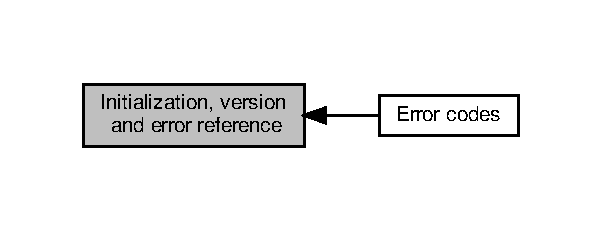
\includegraphics[width=289pt]{group__init}
\end{center}
\end{figure}
\subsection*{Modules}
\begin{DoxyCompactItemize}
\item 
\hyperlink{group__errors}{Error codes}
\end{DoxyCompactItemize}
\subsection*{Typedefs}
\begin{DoxyCompactItemize}
\item 
typedef void($\ast$ \hyperlink{group__init_ga6b8a2639706d5c409fc1287e8f55e928}{G\+L\+F\+Werrorfun}) (int, const char $\ast$)
\begin{DoxyCompactList}\small\item\em The function signature for error callbacks. \end{DoxyCompactList}\item 
typedef void($\ast$ \hyperlink{group__init_ga6b8a2639706d5c409fc1287e8f55e928}{G\+L\+F\+Werrorfun}) (int, const char $\ast$)
\begin{DoxyCompactList}\small\item\em The function signature for error callbacks. \end{DoxyCompactList}\item 
typedef void($\ast$ \hyperlink{group__init_ga6b8a2639706d5c409fc1287e8f55e928}{G\+L\+F\+Werrorfun}) (int, const char $\ast$)
\begin{DoxyCompactList}\small\item\em The function signature for error callbacks. \end{DoxyCompactList}\item 
typedef void($\ast$ \hyperlink{group__init_ga6b8a2639706d5c409fc1287e8f55e928}{G\+L\+F\+Werrorfun}) (int, const char $\ast$)
\begin{DoxyCompactList}\small\item\em The function signature for error callbacks. \end{DoxyCompactList}\item 
typedef void($\ast$ \hyperlink{group__init_ga6b8a2639706d5c409fc1287e8f55e928}{G\+L\+F\+Werrorfun}) (int, const char $\ast$)
\begin{DoxyCompactList}\small\item\em The function signature for error callbacks. \end{DoxyCompactList}\end{DoxyCompactItemize}
\subsection*{Functions}
\begin{DoxyCompactItemize}
\item 
G\+L\+F\+W\+A\+PI int \hyperlink{group__init_gab41771f0215a2e0afb4cf1cf98082d40}{glfw\+Init} (void)
\begin{DoxyCompactList}\small\item\em Initializes the G\+L\+FW library. \end{DoxyCompactList}\item 
G\+L\+F\+W\+A\+PI void \hyperlink{group__init_gafd90e6fd4819ea9e22e5e739519a6504}{glfw\+Terminate} (void)
\begin{DoxyCompactList}\small\item\em Terminates the G\+L\+FW library. \end{DoxyCompactList}\item 
G\+L\+F\+W\+A\+PI void \hyperlink{group__init_ga2402c7824ac0194c13722790ff9559ff}{glfw\+Get\+Version} (int $\ast$major, int $\ast$minor, int $\ast$rev)
\begin{DoxyCompactList}\small\item\em Retrieves the version of the G\+L\+FW library. \end{DoxyCompactList}\item 
G\+L\+F\+W\+A\+PI const char $\ast$ \hyperlink{group__init_gae5952184a0db36e24d1de7805b8b0945}{glfw\+Get\+Version\+String} (void)
\begin{DoxyCompactList}\small\item\em Returns a string describing the compile-\/time configuration. \end{DoxyCompactList}\item 
G\+L\+F\+W\+A\+PI \hyperlink{group__init_ga6b8a2639706d5c409fc1287e8f55e928}{G\+L\+F\+Werrorfun} \hyperlink{group__init_ga5919096b958c47102126061fb5a6f9c3}{glfw\+Set\+Error\+Callback} (\hyperlink{group__init_ga6b8a2639706d5c409fc1287e8f55e928}{G\+L\+F\+Werrorfun} cbfun)
\begin{DoxyCompactList}\small\item\em Sets the error callback. \end{DoxyCompactList}\end{DoxyCompactItemize}
\subsection*{G\+L\+FW version macros}
\begin{DoxyCompactItemize}
\item 
\#define \hyperlink{group__init_ga6337d9ea43b22fc529b2bba066b4a576}{G\+L\+F\+W\+\_\+\+V\+E\+R\+S\+I\+O\+N\+\_\+\+M\+A\+J\+OR}~3
\begin{DoxyCompactList}\small\item\em The major version number of the G\+L\+FW library. \end{DoxyCompactList}\item 
\#define \hyperlink{group__init_gaf80d40f0aea7088ff337606e9c48f7a3}{G\+L\+F\+W\+\_\+\+V\+E\+R\+S\+I\+O\+N\+\_\+\+M\+I\+N\+OR}~2
\begin{DoxyCompactList}\small\item\em The minor version number of the G\+L\+FW library. \end{DoxyCompactList}\item 
\#define \hyperlink{group__init_gab72ae2e2035d9ea461abc3495eac0502}{G\+L\+F\+W\+\_\+\+V\+E\+R\+S\+I\+O\+N\+\_\+\+R\+E\+V\+I\+S\+I\+ON}~0
\begin{DoxyCompactList}\small\item\em The revision number of the G\+L\+FW library. \end{DoxyCompactList}\end{DoxyCompactItemize}
\subsection*{G\+L\+FW version macros}
\begin{DoxyCompactItemize}
\item 
\#define \hyperlink{group__init_ga6337d9ea43b22fc529b2bba066b4a576}{G\+L\+F\+W\+\_\+\+V\+E\+R\+S\+I\+O\+N\+\_\+\+M\+A\+J\+OR}~3
\begin{DoxyCompactList}\small\item\em The major version number of the G\+L\+FW library. \end{DoxyCompactList}\item 
\#define \hyperlink{group__init_gaf80d40f0aea7088ff337606e9c48f7a3}{G\+L\+F\+W\+\_\+\+V\+E\+R\+S\+I\+O\+N\+\_\+\+M\+I\+N\+OR}~2
\begin{DoxyCompactList}\small\item\em The minor version number of the G\+L\+FW library. \end{DoxyCompactList}\item 
\#define \hyperlink{group__init_gab72ae2e2035d9ea461abc3495eac0502}{G\+L\+F\+W\+\_\+\+V\+E\+R\+S\+I\+O\+N\+\_\+\+R\+E\+V\+I\+S\+I\+ON}~0
\begin{DoxyCompactList}\small\item\em The revision number of the G\+L\+FW library. \end{DoxyCompactList}\end{DoxyCompactItemize}
\subsection*{G\+L\+FW version macros}
\begin{DoxyCompactItemize}
\item 
\#define \hyperlink{group__init_ga6337d9ea43b22fc529b2bba066b4a576}{G\+L\+F\+W\+\_\+\+V\+E\+R\+S\+I\+O\+N\+\_\+\+M\+A\+J\+OR}~3
\begin{DoxyCompactList}\small\item\em The major version number of the G\+L\+FW library. \end{DoxyCompactList}\item 
\#define \hyperlink{group__init_gaf80d40f0aea7088ff337606e9c48f7a3}{G\+L\+F\+W\+\_\+\+V\+E\+R\+S\+I\+O\+N\+\_\+\+M\+I\+N\+OR}~2
\begin{DoxyCompactList}\small\item\em The minor version number of the G\+L\+FW library. \end{DoxyCompactList}\item 
\#define \hyperlink{group__init_gab72ae2e2035d9ea461abc3495eac0502}{G\+L\+F\+W\+\_\+\+V\+E\+R\+S\+I\+O\+N\+\_\+\+R\+E\+V\+I\+S\+I\+ON}~1
\begin{DoxyCompactList}\small\item\em The revision number of the G\+L\+FW library. \end{DoxyCompactList}\end{DoxyCompactItemize}
\subsection*{G\+L\+FW version macros}
\begin{DoxyCompactItemize}
\item 
\#define \hyperlink{group__init_ga6337d9ea43b22fc529b2bba066b4a576}{G\+L\+F\+W\+\_\+\+V\+E\+R\+S\+I\+O\+N\+\_\+\+M\+A\+J\+OR}~3
\begin{DoxyCompactList}\small\item\em The major version number of the G\+L\+FW library. \end{DoxyCompactList}\item 
\#define \hyperlink{group__init_gaf80d40f0aea7088ff337606e9c48f7a3}{G\+L\+F\+W\+\_\+\+V\+E\+R\+S\+I\+O\+N\+\_\+\+M\+I\+N\+OR}~2
\begin{DoxyCompactList}\small\item\em The minor version number of the G\+L\+FW library. \end{DoxyCompactList}\item 
\#define \hyperlink{group__init_gab72ae2e2035d9ea461abc3495eac0502}{G\+L\+F\+W\+\_\+\+V\+E\+R\+S\+I\+O\+N\+\_\+\+R\+E\+V\+I\+S\+I\+ON}~1
\begin{DoxyCompactList}\small\item\em The revision number of the G\+L\+FW library. \end{DoxyCompactList}\end{DoxyCompactItemize}
\subsection*{G\+L\+FW version macros}
\begin{DoxyCompactItemize}
\item 
\#define \hyperlink{group__init_ga6337d9ea43b22fc529b2bba066b4a576}{G\+L\+F\+W\+\_\+\+V\+E\+R\+S\+I\+O\+N\+\_\+\+M\+A\+J\+OR}~3
\begin{DoxyCompactList}\small\item\em The major version number of the G\+L\+FW library. \end{DoxyCompactList}\item 
\#define \hyperlink{group__init_gaf80d40f0aea7088ff337606e9c48f7a3}{G\+L\+F\+W\+\_\+\+V\+E\+R\+S\+I\+O\+N\+\_\+\+M\+I\+N\+OR}~2
\begin{DoxyCompactList}\small\item\em The minor version number of the G\+L\+FW library. \end{DoxyCompactList}\item 
\#define \hyperlink{group__init_gab72ae2e2035d9ea461abc3495eac0502}{G\+L\+F\+W\+\_\+\+V\+E\+R\+S\+I\+O\+N\+\_\+\+R\+E\+V\+I\+S\+I\+ON}~1
\begin{DoxyCompactList}\small\item\em The revision number of the G\+L\+FW library. \end{DoxyCompactList}\end{DoxyCompactItemize}


\subsection{Detailed Description}
This is the reference documentation for initialization and termination of the library, version management and error handling. For more task-\/oriented information, see the intro\+\_\+guide. 

\subsection{Macro Definition Documentation}
\mbox{\Hypertarget{group__init_ga6337d9ea43b22fc529b2bba066b4a576}\label{group__init_ga6337d9ea43b22fc529b2bba066b4a576}} 
\index{Initialization, version and error reference@{Initialization, version and error reference}!G\+L\+F\+W\+\_\+\+V\+E\+R\+S\+I\+O\+N\+\_\+\+M\+A\+J\+OR@{G\+L\+F\+W\+\_\+\+V\+E\+R\+S\+I\+O\+N\+\_\+\+M\+A\+J\+OR}}
\index{G\+L\+F\+W\+\_\+\+V\+E\+R\+S\+I\+O\+N\+\_\+\+M\+A\+J\+OR@{G\+L\+F\+W\+\_\+\+V\+E\+R\+S\+I\+O\+N\+\_\+\+M\+A\+J\+OR}!Initialization, version and error reference@{Initialization, version and error reference}}
\subsubsection{\texorpdfstring{G\+L\+F\+W\+\_\+\+V\+E\+R\+S\+I\+O\+N\+\_\+\+M\+A\+J\+OR}{GLFW\_VERSION\_MAJOR}\hspace{0.1cm}{\footnotesize\ttfamily [1/5]}}
{\footnotesize\ttfamily \#define G\+L\+F\+W\+\_\+\+V\+E\+R\+S\+I\+O\+N\+\_\+\+M\+A\+J\+OR~3}



The major version number of the G\+L\+FW library. 

This is incremented when the A\+PI is changed in non-\/compatible ways. \mbox{\Hypertarget{group__init_ga6337d9ea43b22fc529b2bba066b4a576}\label{group__init_ga6337d9ea43b22fc529b2bba066b4a576}} 
\index{Initialization, version and error reference@{Initialization, version and error reference}!G\+L\+F\+W\+\_\+\+V\+E\+R\+S\+I\+O\+N\+\_\+\+M\+A\+J\+OR@{G\+L\+F\+W\+\_\+\+V\+E\+R\+S\+I\+O\+N\+\_\+\+M\+A\+J\+OR}}
\index{G\+L\+F\+W\+\_\+\+V\+E\+R\+S\+I\+O\+N\+\_\+\+M\+A\+J\+OR@{G\+L\+F\+W\+\_\+\+V\+E\+R\+S\+I\+O\+N\+\_\+\+M\+A\+J\+OR}!Initialization, version and error reference@{Initialization, version and error reference}}
\subsubsection{\texorpdfstring{G\+L\+F\+W\+\_\+\+V\+E\+R\+S\+I\+O\+N\+\_\+\+M\+A\+J\+OR}{GLFW\_VERSION\_MAJOR}\hspace{0.1cm}{\footnotesize\ttfamily [2/5]}}
{\footnotesize\ttfamily \#define G\+L\+F\+W\+\_\+\+V\+E\+R\+S\+I\+O\+N\+\_\+\+M\+A\+J\+OR~3}



The major version number of the G\+L\+FW library. 

This is incremented when the A\+PI is changed in non-\/compatible ways. \mbox{\Hypertarget{group__init_ga6337d9ea43b22fc529b2bba066b4a576}\label{group__init_ga6337d9ea43b22fc529b2bba066b4a576}} 
\index{Initialization, version and error reference@{Initialization, version and error reference}!G\+L\+F\+W\+\_\+\+V\+E\+R\+S\+I\+O\+N\+\_\+\+M\+A\+J\+OR@{G\+L\+F\+W\+\_\+\+V\+E\+R\+S\+I\+O\+N\+\_\+\+M\+A\+J\+OR}}
\index{G\+L\+F\+W\+\_\+\+V\+E\+R\+S\+I\+O\+N\+\_\+\+M\+A\+J\+OR@{G\+L\+F\+W\+\_\+\+V\+E\+R\+S\+I\+O\+N\+\_\+\+M\+A\+J\+OR}!Initialization, version and error reference@{Initialization, version and error reference}}
\subsubsection{\texorpdfstring{G\+L\+F\+W\+\_\+\+V\+E\+R\+S\+I\+O\+N\+\_\+\+M\+A\+J\+OR}{GLFW\_VERSION\_MAJOR}\hspace{0.1cm}{\footnotesize\ttfamily [3/5]}}
{\footnotesize\ttfamily \#define G\+L\+F\+W\+\_\+\+V\+E\+R\+S\+I\+O\+N\+\_\+\+M\+A\+J\+OR~3}



The major version number of the G\+L\+FW library. 

This is incremented when the A\+PI is changed in non-\/compatible ways. \mbox{\Hypertarget{group__init_ga6337d9ea43b22fc529b2bba066b4a576}\label{group__init_ga6337d9ea43b22fc529b2bba066b4a576}} 
\index{Initialization, version and error reference@{Initialization, version and error reference}!G\+L\+F\+W\+\_\+\+V\+E\+R\+S\+I\+O\+N\+\_\+\+M\+A\+J\+OR@{G\+L\+F\+W\+\_\+\+V\+E\+R\+S\+I\+O\+N\+\_\+\+M\+A\+J\+OR}}
\index{G\+L\+F\+W\+\_\+\+V\+E\+R\+S\+I\+O\+N\+\_\+\+M\+A\+J\+OR@{G\+L\+F\+W\+\_\+\+V\+E\+R\+S\+I\+O\+N\+\_\+\+M\+A\+J\+OR}!Initialization, version and error reference@{Initialization, version and error reference}}
\subsubsection{\texorpdfstring{G\+L\+F\+W\+\_\+\+V\+E\+R\+S\+I\+O\+N\+\_\+\+M\+A\+J\+OR}{GLFW\_VERSION\_MAJOR}\hspace{0.1cm}{\footnotesize\ttfamily [4/5]}}
{\footnotesize\ttfamily \#define G\+L\+F\+W\+\_\+\+V\+E\+R\+S\+I\+O\+N\+\_\+\+M\+A\+J\+OR~3}



The major version number of the G\+L\+FW library. 

This is incremented when the A\+PI is changed in non-\/compatible ways. \mbox{\Hypertarget{group__init_ga6337d9ea43b22fc529b2bba066b4a576}\label{group__init_ga6337d9ea43b22fc529b2bba066b4a576}} 
\index{Initialization, version and error reference@{Initialization, version and error reference}!G\+L\+F\+W\+\_\+\+V\+E\+R\+S\+I\+O\+N\+\_\+\+M\+A\+J\+OR@{G\+L\+F\+W\+\_\+\+V\+E\+R\+S\+I\+O\+N\+\_\+\+M\+A\+J\+OR}}
\index{G\+L\+F\+W\+\_\+\+V\+E\+R\+S\+I\+O\+N\+\_\+\+M\+A\+J\+OR@{G\+L\+F\+W\+\_\+\+V\+E\+R\+S\+I\+O\+N\+\_\+\+M\+A\+J\+OR}!Initialization, version and error reference@{Initialization, version and error reference}}
\subsubsection{\texorpdfstring{G\+L\+F\+W\+\_\+\+V\+E\+R\+S\+I\+O\+N\+\_\+\+M\+A\+J\+OR}{GLFW\_VERSION\_MAJOR}\hspace{0.1cm}{\footnotesize\ttfamily [5/5]}}
{\footnotesize\ttfamily \#define G\+L\+F\+W\+\_\+\+V\+E\+R\+S\+I\+O\+N\+\_\+\+M\+A\+J\+OR~3}



The major version number of the G\+L\+FW library. 

This is incremented when the A\+PI is changed in non-\/compatible ways. \mbox{\Hypertarget{group__init_gaf80d40f0aea7088ff337606e9c48f7a3}\label{group__init_gaf80d40f0aea7088ff337606e9c48f7a3}} 
\index{Initialization, version and error reference@{Initialization, version and error reference}!G\+L\+F\+W\+\_\+\+V\+E\+R\+S\+I\+O\+N\+\_\+\+M\+I\+N\+OR@{G\+L\+F\+W\+\_\+\+V\+E\+R\+S\+I\+O\+N\+\_\+\+M\+I\+N\+OR}}
\index{G\+L\+F\+W\+\_\+\+V\+E\+R\+S\+I\+O\+N\+\_\+\+M\+I\+N\+OR@{G\+L\+F\+W\+\_\+\+V\+E\+R\+S\+I\+O\+N\+\_\+\+M\+I\+N\+OR}!Initialization, version and error reference@{Initialization, version and error reference}}
\subsubsection{\texorpdfstring{G\+L\+F\+W\+\_\+\+V\+E\+R\+S\+I\+O\+N\+\_\+\+M\+I\+N\+OR}{GLFW\_VERSION\_MINOR}\hspace{0.1cm}{\footnotesize\ttfamily [1/5]}}
{\footnotesize\ttfamily \#define G\+L\+F\+W\+\_\+\+V\+E\+R\+S\+I\+O\+N\+\_\+\+M\+I\+N\+OR~2}



The minor version number of the G\+L\+FW library. 

This is incremented when features are added to the A\+PI but it remains backward-\/compatible. \mbox{\Hypertarget{group__init_gaf80d40f0aea7088ff337606e9c48f7a3}\label{group__init_gaf80d40f0aea7088ff337606e9c48f7a3}} 
\index{Initialization, version and error reference@{Initialization, version and error reference}!G\+L\+F\+W\+\_\+\+V\+E\+R\+S\+I\+O\+N\+\_\+\+M\+I\+N\+OR@{G\+L\+F\+W\+\_\+\+V\+E\+R\+S\+I\+O\+N\+\_\+\+M\+I\+N\+OR}}
\index{G\+L\+F\+W\+\_\+\+V\+E\+R\+S\+I\+O\+N\+\_\+\+M\+I\+N\+OR@{G\+L\+F\+W\+\_\+\+V\+E\+R\+S\+I\+O\+N\+\_\+\+M\+I\+N\+OR}!Initialization, version and error reference@{Initialization, version and error reference}}
\subsubsection{\texorpdfstring{G\+L\+F\+W\+\_\+\+V\+E\+R\+S\+I\+O\+N\+\_\+\+M\+I\+N\+OR}{GLFW\_VERSION\_MINOR}\hspace{0.1cm}{\footnotesize\ttfamily [2/5]}}
{\footnotesize\ttfamily \#define G\+L\+F\+W\+\_\+\+V\+E\+R\+S\+I\+O\+N\+\_\+\+M\+I\+N\+OR~2}



The minor version number of the G\+L\+FW library. 

This is incremented when features are added to the A\+PI but it remains backward-\/compatible. \mbox{\Hypertarget{group__init_gaf80d40f0aea7088ff337606e9c48f7a3}\label{group__init_gaf80d40f0aea7088ff337606e9c48f7a3}} 
\index{Initialization, version and error reference@{Initialization, version and error reference}!G\+L\+F\+W\+\_\+\+V\+E\+R\+S\+I\+O\+N\+\_\+\+M\+I\+N\+OR@{G\+L\+F\+W\+\_\+\+V\+E\+R\+S\+I\+O\+N\+\_\+\+M\+I\+N\+OR}}
\index{G\+L\+F\+W\+\_\+\+V\+E\+R\+S\+I\+O\+N\+\_\+\+M\+I\+N\+OR@{G\+L\+F\+W\+\_\+\+V\+E\+R\+S\+I\+O\+N\+\_\+\+M\+I\+N\+OR}!Initialization, version and error reference@{Initialization, version and error reference}}
\subsubsection{\texorpdfstring{G\+L\+F\+W\+\_\+\+V\+E\+R\+S\+I\+O\+N\+\_\+\+M\+I\+N\+OR}{GLFW\_VERSION\_MINOR}\hspace{0.1cm}{\footnotesize\ttfamily [3/5]}}
{\footnotesize\ttfamily \#define G\+L\+F\+W\+\_\+\+V\+E\+R\+S\+I\+O\+N\+\_\+\+M\+I\+N\+OR~2}



The minor version number of the G\+L\+FW library. 

This is incremented when features are added to the A\+PI but it remains backward-\/compatible. \mbox{\Hypertarget{group__init_gaf80d40f0aea7088ff337606e9c48f7a3}\label{group__init_gaf80d40f0aea7088ff337606e9c48f7a3}} 
\index{Initialization, version and error reference@{Initialization, version and error reference}!G\+L\+F\+W\+\_\+\+V\+E\+R\+S\+I\+O\+N\+\_\+\+M\+I\+N\+OR@{G\+L\+F\+W\+\_\+\+V\+E\+R\+S\+I\+O\+N\+\_\+\+M\+I\+N\+OR}}
\index{G\+L\+F\+W\+\_\+\+V\+E\+R\+S\+I\+O\+N\+\_\+\+M\+I\+N\+OR@{G\+L\+F\+W\+\_\+\+V\+E\+R\+S\+I\+O\+N\+\_\+\+M\+I\+N\+OR}!Initialization, version and error reference@{Initialization, version and error reference}}
\subsubsection{\texorpdfstring{G\+L\+F\+W\+\_\+\+V\+E\+R\+S\+I\+O\+N\+\_\+\+M\+I\+N\+OR}{GLFW\_VERSION\_MINOR}\hspace{0.1cm}{\footnotesize\ttfamily [4/5]}}
{\footnotesize\ttfamily \#define G\+L\+F\+W\+\_\+\+V\+E\+R\+S\+I\+O\+N\+\_\+\+M\+I\+N\+OR~2}



The minor version number of the G\+L\+FW library. 

This is incremented when features are added to the A\+PI but it remains backward-\/compatible. \mbox{\Hypertarget{group__init_gaf80d40f0aea7088ff337606e9c48f7a3}\label{group__init_gaf80d40f0aea7088ff337606e9c48f7a3}} 
\index{Initialization, version and error reference@{Initialization, version and error reference}!G\+L\+F\+W\+\_\+\+V\+E\+R\+S\+I\+O\+N\+\_\+\+M\+I\+N\+OR@{G\+L\+F\+W\+\_\+\+V\+E\+R\+S\+I\+O\+N\+\_\+\+M\+I\+N\+OR}}
\index{G\+L\+F\+W\+\_\+\+V\+E\+R\+S\+I\+O\+N\+\_\+\+M\+I\+N\+OR@{G\+L\+F\+W\+\_\+\+V\+E\+R\+S\+I\+O\+N\+\_\+\+M\+I\+N\+OR}!Initialization, version and error reference@{Initialization, version and error reference}}
\subsubsection{\texorpdfstring{G\+L\+F\+W\+\_\+\+V\+E\+R\+S\+I\+O\+N\+\_\+\+M\+I\+N\+OR}{GLFW\_VERSION\_MINOR}\hspace{0.1cm}{\footnotesize\ttfamily [5/5]}}
{\footnotesize\ttfamily \#define G\+L\+F\+W\+\_\+\+V\+E\+R\+S\+I\+O\+N\+\_\+\+M\+I\+N\+OR~2}



The minor version number of the G\+L\+FW library. 

This is incremented when features are added to the A\+PI but it remains backward-\/compatible. \mbox{\Hypertarget{group__init_gab72ae2e2035d9ea461abc3495eac0502}\label{group__init_gab72ae2e2035d9ea461abc3495eac0502}} 
\index{Initialization, version and error reference@{Initialization, version and error reference}!G\+L\+F\+W\+\_\+\+V\+E\+R\+S\+I\+O\+N\+\_\+\+R\+E\+V\+I\+S\+I\+ON@{G\+L\+F\+W\+\_\+\+V\+E\+R\+S\+I\+O\+N\+\_\+\+R\+E\+V\+I\+S\+I\+ON}}
\index{G\+L\+F\+W\+\_\+\+V\+E\+R\+S\+I\+O\+N\+\_\+\+R\+E\+V\+I\+S\+I\+ON@{G\+L\+F\+W\+\_\+\+V\+E\+R\+S\+I\+O\+N\+\_\+\+R\+E\+V\+I\+S\+I\+ON}!Initialization, version and error reference@{Initialization, version and error reference}}
\subsubsection{\texorpdfstring{G\+L\+F\+W\+\_\+\+V\+E\+R\+S\+I\+O\+N\+\_\+\+R\+E\+V\+I\+S\+I\+ON}{GLFW\_VERSION\_REVISION}\hspace{0.1cm}{\footnotesize\ttfamily [1/5]}}
{\footnotesize\ttfamily \#define G\+L\+F\+W\+\_\+\+V\+E\+R\+S\+I\+O\+N\+\_\+\+R\+E\+V\+I\+S\+I\+ON~0}



The revision number of the G\+L\+FW library. 

This is incremented when a bug fix release is made that does not contain any A\+PI changes. \mbox{\Hypertarget{group__init_gab72ae2e2035d9ea461abc3495eac0502}\label{group__init_gab72ae2e2035d9ea461abc3495eac0502}} 
\index{Initialization, version and error reference@{Initialization, version and error reference}!G\+L\+F\+W\+\_\+\+V\+E\+R\+S\+I\+O\+N\+\_\+\+R\+E\+V\+I\+S\+I\+ON@{G\+L\+F\+W\+\_\+\+V\+E\+R\+S\+I\+O\+N\+\_\+\+R\+E\+V\+I\+S\+I\+ON}}
\index{G\+L\+F\+W\+\_\+\+V\+E\+R\+S\+I\+O\+N\+\_\+\+R\+E\+V\+I\+S\+I\+ON@{G\+L\+F\+W\+\_\+\+V\+E\+R\+S\+I\+O\+N\+\_\+\+R\+E\+V\+I\+S\+I\+ON}!Initialization, version and error reference@{Initialization, version and error reference}}
\subsubsection{\texorpdfstring{G\+L\+F\+W\+\_\+\+V\+E\+R\+S\+I\+O\+N\+\_\+\+R\+E\+V\+I\+S\+I\+ON}{GLFW\_VERSION\_REVISION}\hspace{0.1cm}{\footnotesize\ttfamily [2/5]}}
{\footnotesize\ttfamily \#define G\+L\+F\+W\+\_\+\+V\+E\+R\+S\+I\+O\+N\+\_\+\+R\+E\+V\+I\+S\+I\+ON~0}



The revision number of the G\+L\+FW library. 

This is incremented when a bug fix release is made that does not contain any A\+PI changes. \mbox{\Hypertarget{group__init_gab72ae2e2035d9ea461abc3495eac0502}\label{group__init_gab72ae2e2035d9ea461abc3495eac0502}} 
\index{Initialization, version and error reference@{Initialization, version and error reference}!G\+L\+F\+W\+\_\+\+V\+E\+R\+S\+I\+O\+N\+\_\+\+R\+E\+V\+I\+S\+I\+ON@{G\+L\+F\+W\+\_\+\+V\+E\+R\+S\+I\+O\+N\+\_\+\+R\+E\+V\+I\+S\+I\+ON}}
\index{G\+L\+F\+W\+\_\+\+V\+E\+R\+S\+I\+O\+N\+\_\+\+R\+E\+V\+I\+S\+I\+ON@{G\+L\+F\+W\+\_\+\+V\+E\+R\+S\+I\+O\+N\+\_\+\+R\+E\+V\+I\+S\+I\+ON}!Initialization, version and error reference@{Initialization, version and error reference}}
\subsubsection{\texorpdfstring{G\+L\+F\+W\+\_\+\+V\+E\+R\+S\+I\+O\+N\+\_\+\+R\+E\+V\+I\+S\+I\+ON}{GLFW\_VERSION\_REVISION}\hspace{0.1cm}{\footnotesize\ttfamily [3/5]}}
{\footnotesize\ttfamily \#define G\+L\+F\+W\+\_\+\+V\+E\+R\+S\+I\+O\+N\+\_\+\+R\+E\+V\+I\+S\+I\+ON~1}



The revision number of the G\+L\+FW library. 

This is incremented when a bug fix release is made that does not contain any A\+PI changes. \mbox{\Hypertarget{group__init_gab72ae2e2035d9ea461abc3495eac0502}\label{group__init_gab72ae2e2035d9ea461abc3495eac0502}} 
\index{Initialization, version and error reference@{Initialization, version and error reference}!G\+L\+F\+W\+\_\+\+V\+E\+R\+S\+I\+O\+N\+\_\+\+R\+E\+V\+I\+S\+I\+ON@{G\+L\+F\+W\+\_\+\+V\+E\+R\+S\+I\+O\+N\+\_\+\+R\+E\+V\+I\+S\+I\+ON}}
\index{G\+L\+F\+W\+\_\+\+V\+E\+R\+S\+I\+O\+N\+\_\+\+R\+E\+V\+I\+S\+I\+ON@{G\+L\+F\+W\+\_\+\+V\+E\+R\+S\+I\+O\+N\+\_\+\+R\+E\+V\+I\+S\+I\+ON}!Initialization, version and error reference@{Initialization, version and error reference}}
\subsubsection{\texorpdfstring{G\+L\+F\+W\+\_\+\+V\+E\+R\+S\+I\+O\+N\+\_\+\+R\+E\+V\+I\+S\+I\+ON}{GLFW\_VERSION\_REVISION}\hspace{0.1cm}{\footnotesize\ttfamily [4/5]}}
{\footnotesize\ttfamily \#define G\+L\+F\+W\+\_\+\+V\+E\+R\+S\+I\+O\+N\+\_\+\+R\+E\+V\+I\+S\+I\+ON~1}



The revision number of the G\+L\+FW library. 

This is incremented when a bug fix release is made that does not contain any A\+PI changes. \mbox{\Hypertarget{group__init_gab72ae2e2035d9ea461abc3495eac0502}\label{group__init_gab72ae2e2035d9ea461abc3495eac0502}} 
\index{Initialization, version and error reference@{Initialization, version and error reference}!G\+L\+F\+W\+\_\+\+V\+E\+R\+S\+I\+O\+N\+\_\+\+R\+E\+V\+I\+S\+I\+ON@{G\+L\+F\+W\+\_\+\+V\+E\+R\+S\+I\+O\+N\+\_\+\+R\+E\+V\+I\+S\+I\+ON}}
\index{G\+L\+F\+W\+\_\+\+V\+E\+R\+S\+I\+O\+N\+\_\+\+R\+E\+V\+I\+S\+I\+ON@{G\+L\+F\+W\+\_\+\+V\+E\+R\+S\+I\+O\+N\+\_\+\+R\+E\+V\+I\+S\+I\+ON}!Initialization, version and error reference@{Initialization, version and error reference}}
\subsubsection{\texorpdfstring{G\+L\+F\+W\+\_\+\+V\+E\+R\+S\+I\+O\+N\+\_\+\+R\+E\+V\+I\+S\+I\+ON}{GLFW\_VERSION\_REVISION}\hspace{0.1cm}{\footnotesize\ttfamily [5/5]}}
{\footnotesize\ttfamily \#define G\+L\+F\+W\+\_\+\+V\+E\+R\+S\+I\+O\+N\+\_\+\+R\+E\+V\+I\+S\+I\+ON~1}



The revision number of the G\+L\+FW library. 

This is incremented when a bug fix release is made that does not contain any A\+PI changes. 

\subsection{Typedef Documentation}
\mbox{\Hypertarget{group__init_ga6b8a2639706d5c409fc1287e8f55e928}\label{group__init_ga6b8a2639706d5c409fc1287e8f55e928}} 
\index{Initialization, version and error reference@{Initialization, version and error reference}!G\+L\+F\+Werrorfun@{G\+L\+F\+Werrorfun}}
\index{G\+L\+F\+Werrorfun@{G\+L\+F\+Werrorfun}!Initialization, version and error reference@{Initialization, version and error reference}}
\subsubsection{\texorpdfstring{G\+L\+F\+Werrorfun}{GLFWerrorfun}\hspace{0.1cm}{\footnotesize\ttfamily [1/5]}}
{\footnotesize\ttfamily typedef void($\ast$  G\+L\+F\+Werrorfun) (int, const char $\ast$)}



The function signature for error callbacks. 

This is the function signature for error callback functions.


\begin{DoxyParams}[1]{Parameters}
\mbox{\tt in}  & {\em error} & An \hyperlink{group__errors}{error code}. \\
\hline
\mbox{\tt in}  & {\em description} & A U\+T\+F-\/8 encoded string describing the error.\\
\hline
\end{DoxyParams}
\begin{DoxySeeAlso}{See also}
error\+\_\+handling 

\hyperlink{group__init_ga5919096b958c47102126061fb5a6f9c3}{glfw\+Set\+Error\+Callback}
\end{DoxySeeAlso}
\begin{DoxySince}{Since}
Added in version 3.\+0. 
\end{DoxySince}
\mbox{\Hypertarget{group__init_ga6b8a2639706d5c409fc1287e8f55e928}\label{group__init_ga6b8a2639706d5c409fc1287e8f55e928}} 
\index{Initialization, version and error reference@{Initialization, version and error reference}!G\+L\+F\+Werrorfun@{G\+L\+F\+Werrorfun}}
\index{G\+L\+F\+Werrorfun@{G\+L\+F\+Werrorfun}!Initialization, version and error reference@{Initialization, version and error reference}}
\subsubsection{\texorpdfstring{G\+L\+F\+Werrorfun}{GLFWerrorfun}\hspace{0.1cm}{\footnotesize\ttfamily [2/5]}}
{\footnotesize\ttfamily typedef void($\ast$  G\+L\+F\+Werrorfun) (int, const char $\ast$)}



The function signature for error callbacks. 

This is the function signature for error callback functions.


\begin{DoxyParams}[1]{Parameters}
\mbox{\tt in}  & {\em error} & An \hyperlink{group__errors}{error code}. \\
\hline
\mbox{\tt in}  & {\em description} & A U\+T\+F-\/8 encoded string describing the error.\\
\hline
\end{DoxyParams}
\begin{DoxySeeAlso}{See also}
error\+\_\+handling 

\hyperlink{group__init_ga5919096b958c47102126061fb5a6f9c3}{glfw\+Set\+Error\+Callback}
\end{DoxySeeAlso}
\begin{DoxySince}{Since}
Added in version 3.\+0. 
\end{DoxySince}
\mbox{\Hypertarget{group__init_ga6b8a2639706d5c409fc1287e8f55e928}\label{group__init_ga6b8a2639706d5c409fc1287e8f55e928}} 
\index{Initialization, version and error reference@{Initialization, version and error reference}!G\+L\+F\+Werrorfun@{G\+L\+F\+Werrorfun}}
\index{G\+L\+F\+Werrorfun@{G\+L\+F\+Werrorfun}!Initialization, version and error reference@{Initialization, version and error reference}}
\subsubsection{\texorpdfstring{G\+L\+F\+Werrorfun}{GLFWerrorfun}\hspace{0.1cm}{\footnotesize\ttfamily [3/5]}}
{\footnotesize\ttfamily typedef void($\ast$  G\+L\+F\+Werrorfun) (int, const char $\ast$)}



The function signature for error callbacks. 

This is the function signature for error callback functions.


\begin{DoxyParams}[1]{Parameters}
\mbox{\tt in}  & {\em error} & An \hyperlink{group__errors}{error code}. \\
\hline
\mbox{\tt in}  & {\em description} & A U\+T\+F-\/8 encoded string describing the error.\\
\hline
\end{DoxyParams}
\begin{DoxySeeAlso}{See also}
error\+\_\+handling 

\hyperlink{group__init_ga5919096b958c47102126061fb5a6f9c3}{glfw\+Set\+Error\+Callback}
\end{DoxySeeAlso}
\begin{DoxySince}{Since}
Added in version 3.\+0. 
\end{DoxySince}
\mbox{\Hypertarget{group__init_ga6b8a2639706d5c409fc1287e8f55e928}\label{group__init_ga6b8a2639706d5c409fc1287e8f55e928}} 
\index{Initialization, version and error reference@{Initialization, version and error reference}!G\+L\+F\+Werrorfun@{G\+L\+F\+Werrorfun}}
\index{G\+L\+F\+Werrorfun@{G\+L\+F\+Werrorfun}!Initialization, version and error reference@{Initialization, version and error reference}}
\subsubsection{\texorpdfstring{G\+L\+F\+Werrorfun}{GLFWerrorfun}\hspace{0.1cm}{\footnotesize\ttfamily [4/5]}}
{\footnotesize\ttfamily typedef void($\ast$  G\+L\+F\+Werrorfun) (int, const char $\ast$)}



The function signature for error callbacks. 

This is the function signature for error callback functions.


\begin{DoxyParams}[1]{Parameters}
\mbox{\tt in}  & {\em error} & An \hyperlink{group__errors}{error code}. \\
\hline
\mbox{\tt in}  & {\em description} & A U\+T\+F-\/8 encoded string describing the error.\\
\hline
\end{DoxyParams}
\begin{DoxySeeAlso}{See also}
error\+\_\+handling 

\hyperlink{group__init_ga5919096b958c47102126061fb5a6f9c3}{glfw\+Set\+Error\+Callback}
\end{DoxySeeAlso}
\begin{DoxySince}{Since}
Added in version 3.\+0. 
\end{DoxySince}
\mbox{\Hypertarget{group__init_ga6b8a2639706d5c409fc1287e8f55e928}\label{group__init_ga6b8a2639706d5c409fc1287e8f55e928}} 
\index{Initialization, version and error reference@{Initialization, version and error reference}!G\+L\+F\+Werrorfun@{G\+L\+F\+Werrorfun}}
\index{G\+L\+F\+Werrorfun@{G\+L\+F\+Werrorfun}!Initialization, version and error reference@{Initialization, version and error reference}}
\subsubsection{\texorpdfstring{G\+L\+F\+Werrorfun}{GLFWerrorfun}\hspace{0.1cm}{\footnotesize\ttfamily [5/5]}}
{\footnotesize\ttfamily typedef void($\ast$  G\+L\+F\+Werrorfun) (int, const char $\ast$)}



The function signature for error callbacks. 

This is the function signature for error callback functions.


\begin{DoxyParams}[1]{Parameters}
\mbox{\tt in}  & {\em error} & An \hyperlink{group__errors}{error code}. \\
\hline
\mbox{\tt in}  & {\em description} & A U\+T\+F-\/8 encoded string describing the error.\\
\hline
\end{DoxyParams}
\begin{DoxySeeAlso}{See also}
error\+\_\+handling 

\hyperlink{group__init_ga5919096b958c47102126061fb5a6f9c3}{glfw\+Set\+Error\+Callback}
\end{DoxySeeAlso}
\begin{DoxySince}{Since}
Added in version 3.\+0. 
\end{DoxySince}


\subsection{Function Documentation}
\mbox{\Hypertarget{group__init_ga2402c7824ac0194c13722790ff9559ff}\label{group__init_ga2402c7824ac0194c13722790ff9559ff}} 
\index{Initialization, version and error reference@{Initialization, version and error reference}!glfw\+Get\+Version@{glfw\+Get\+Version}}
\index{glfw\+Get\+Version@{glfw\+Get\+Version}!Initialization, version and error reference@{Initialization, version and error reference}}
\subsubsection{\texorpdfstring{glfw\+Get\+Version()}{glfwGetVersion()}}
{\footnotesize\ttfamily G\+L\+F\+W\+A\+PI void glfw\+Get\+Version (\begin{DoxyParamCaption}\item[{int $\ast$}]{major,  }\item[{int $\ast$}]{minor,  }\item[{int $\ast$}]{rev }\end{DoxyParamCaption})}



Retrieves the version of the G\+L\+FW library. 

This function retrieves the major, minor and revision numbers of the G\+L\+FW library. It is intended for when you are using G\+L\+FW as a shared library and want to ensure that you are using the minimum required version.

Any or all of the version arguments may be {\ttfamily N\+U\+LL}.


\begin{DoxyParams}[1]{Parameters}
\mbox{\tt out}  & {\em major} & Where to store the major version number, or {\ttfamily N\+U\+LL}. \\
\hline
\mbox{\tt out}  & {\em minor} & Where to store the minor version number, or {\ttfamily N\+U\+LL}. \\
\hline
\mbox{\tt out}  & {\em rev} & Where to store the revision number, or {\ttfamily N\+U\+LL}.\\
\hline
\end{DoxyParams}
None.

\begin{DoxyRemark}{Remarks}
This function may be called before \hyperlink{group__init_gab41771f0215a2e0afb4cf1cf98082d40}{glfw\+Init}.
\end{DoxyRemark}
This function may be called from any thread.

\begin{DoxySeeAlso}{See also}
intro\+\_\+version 

\hyperlink{group__init_gae5952184a0db36e24d1de7805b8b0945}{glfw\+Get\+Version\+String}
\end{DoxySeeAlso}
\begin{DoxySince}{Since}
Added in version 1.\+0. 
\end{DoxySince}
\mbox{\Hypertarget{group__init_gae5952184a0db36e24d1de7805b8b0945}\label{group__init_gae5952184a0db36e24d1de7805b8b0945}} 
\index{Initialization, version and error reference@{Initialization, version and error reference}!glfw\+Get\+Version\+String@{glfw\+Get\+Version\+String}}
\index{glfw\+Get\+Version\+String@{glfw\+Get\+Version\+String}!Initialization, version and error reference@{Initialization, version and error reference}}
\subsubsection{\texorpdfstring{glfw\+Get\+Version\+String()}{glfwGetVersionString()}}
{\footnotesize\ttfamily G\+L\+F\+W\+A\+PI const char $\ast$ glfw\+Get\+Version\+String (\begin{DoxyParamCaption}\item[{void}]{ }\end{DoxyParamCaption})}



Returns a string describing the compile-\/time configuration. 

This function returns the compile-\/time generated version string of the G\+L\+FW library binary. It describes the version, platform, compiler and any platform-\/specific compile-\/time options. It should not be confused with the Open\+GL or Open\+GL ES version string, queried with {\ttfamily gl\+Get\+String}.

{\bfseries Do not use the version string} to parse the G\+L\+FW library version. The \hyperlink{group__init_ga2402c7824ac0194c13722790ff9559ff}{glfw\+Get\+Version} function provides the version of the running library binary in numerical format.

\begin{DoxyReturn}{Returns}
The \hyperlink{structASCII}{A\+S\+C\+II} encoded G\+L\+FW version string.
\end{DoxyReturn}
None.

\begin{DoxyRemark}{Remarks}
This function may be called before \hyperlink{group__init_gab41771f0215a2e0afb4cf1cf98082d40}{glfw\+Init}.
\end{DoxyRemark}
The returned string is static and compile-\/time generated.

This function may be called from any thread.

\begin{DoxySeeAlso}{See also}
intro\+\_\+version 

\hyperlink{group__init_ga2402c7824ac0194c13722790ff9559ff}{glfw\+Get\+Version}
\end{DoxySeeAlso}
\begin{DoxySince}{Since}
Added in version 3.\+0. 
\end{DoxySince}
\mbox{\Hypertarget{group__init_gab41771f0215a2e0afb4cf1cf98082d40}\label{group__init_gab41771f0215a2e0afb4cf1cf98082d40}} 
\index{Initialization, version and error reference@{Initialization, version and error reference}!glfw\+Init@{glfw\+Init}}
\index{glfw\+Init@{glfw\+Init}!Initialization, version and error reference@{Initialization, version and error reference}}
\subsubsection{\texorpdfstring{glfw\+Init()}{glfwInit()}}
{\footnotesize\ttfamily G\+L\+F\+W\+A\+PI int glfw\+Init (\begin{DoxyParamCaption}\item[{void}]{ }\end{DoxyParamCaption})}



Initializes the G\+L\+FW library. 

This function initializes the G\+L\+FW library. Before most G\+L\+FW functions can be used, G\+L\+FW must be initialized, and before an application terminates G\+L\+FW should be terminated in order to free any resources allocated during or after initialization.

If this function fails, it calls \hyperlink{group__init_gafd90e6fd4819ea9e22e5e739519a6504}{glfw\+Terminate} before returning. If it succeeds, you should call \hyperlink{group__init_gafd90e6fd4819ea9e22e5e739519a6504}{glfw\+Terminate} before the application exits.

Additional calls to this function after successful initialization but before termination will return {\ttfamily G\+L\+F\+W\+\_\+\+T\+R\+UE} immediately.

\begin{DoxyReturn}{Returns}
{\ttfamily G\+L\+F\+W\+\_\+\+T\+R\+UE} if successful, or {\ttfamily G\+L\+F\+W\+\_\+\+F\+A\+L\+SE} if an error occurred.
\end{DoxyReturn}
Possible errors include \hyperlink{group__errors_gad44162d78100ea5e87cdd38426b8c7a1}{G\+L\+F\+W\+\_\+\+P\+L\+A\+T\+F\+O\+R\+M\+\_\+\+E\+R\+R\+OR}.

\begin{DoxyRemark}{Remarks}
This function will change the current directory of the application to the {\ttfamily Contents/\+Resources} subdirectory of the application\textquotesingle{}s bundle, if present. This can be disabled with a compile-\/time option.
\end{DoxyRemark}
This function must only be called from the main thread.

\begin{DoxySeeAlso}{See also}
intro\+\_\+init 

\hyperlink{group__init_gafd90e6fd4819ea9e22e5e739519a6504}{glfw\+Terminate}
\end{DoxySeeAlso}
\begin{DoxySince}{Since}
Added in version 1.\+0. 
\end{DoxySince}
\mbox{\Hypertarget{group__init_ga5919096b958c47102126061fb5a6f9c3}\label{group__init_ga5919096b958c47102126061fb5a6f9c3}} 
\index{Initialization, version and error reference@{Initialization, version and error reference}!glfw\+Set\+Error\+Callback@{glfw\+Set\+Error\+Callback}}
\index{glfw\+Set\+Error\+Callback@{glfw\+Set\+Error\+Callback}!Initialization, version and error reference@{Initialization, version and error reference}}
\subsubsection{\texorpdfstring{glfw\+Set\+Error\+Callback()}{glfwSetErrorCallback()}}
{\footnotesize\ttfamily G\+L\+F\+W\+A\+PI \hyperlink{group__init_ga6b8a2639706d5c409fc1287e8f55e928}{G\+L\+F\+Werrorfun} glfw\+Set\+Error\+Callback (\begin{DoxyParamCaption}\item[{\hyperlink{group__init_ga6b8a2639706d5c409fc1287e8f55e928}{G\+L\+F\+Werrorfun}}]{cbfun }\end{DoxyParamCaption})}



Sets the error callback. 

This function sets the error callback, which is called with an error code and a human-\/readable description each time a G\+L\+FW error occurs.

The error callback is called on the thread where the error occurred. If you are using G\+L\+FW from multiple threads, your error callback needs to be written accordingly.

Because the description string may have been generated specifically for that error, it is not guaranteed to be valid after the callback has returned. If you wish to use it after the callback returns, you need to make a copy.

Once set, the error callback remains set even after the library has been terminated.


\begin{DoxyParams}[1]{Parameters}
\mbox{\tt in}  & {\em cbfun} & The new callback, or {\ttfamily N\+U\+LL} to remove the currently set callback. \\
\hline
\end{DoxyParams}
\begin{DoxyReturn}{Returns}
The previously set callback, or {\ttfamily N\+U\+LL} if no callback was set.
\end{DoxyReturn}
None.

\begin{DoxyRemark}{Remarks}
This function may be called before \hyperlink{group__init_gab41771f0215a2e0afb4cf1cf98082d40}{glfw\+Init}.
\end{DoxyRemark}
This function must only be called from the main thread.

\begin{DoxySeeAlso}{See also}
error\+\_\+handling
\end{DoxySeeAlso}
\begin{DoxySince}{Since}
Added in version 3.\+0. 
\end{DoxySince}
\mbox{\Hypertarget{group__init_gafd90e6fd4819ea9e22e5e739519a6504}\label{group__init_gafd90e6fd4819ea9e22e5e739519a6504}} 
\index{Initialization, version and error reference@{Initialization, version and error reference}!glfw\+Terminate@{glfw\+Terminate}}
\index{glfw\+Terminate@{glfw\+Terminate}!Initialization, version and error reference@{Initialization, version and error reference}}
\subsubsection{\texorpdfstring{glfw\+Terminate()}{glfwTerminate()}}
{\footnotesize\ttfamily G\+L\+F\+W\+A\+PI void glfw\+Terminate (\begin{DoxyParamCaption}\item[{void}]{ }\end{DoxyParamCaption})}



Terminates the G\+L\+FW library. 

This function destroys all remaining windows and cursors, restores any modified gamma ramps and frees any other allocated resources. Once this function is called, you must again call \hyperlink{group__init_gab41771f0215a2e0afb4cf1cf98082d40}{glfw\+Init} successfully before you will be able to use most G\+L\+FW functions.

If G\+L\+FW has been successfully initialized, this function should be called before the application exits. If initialization fails, there is no need to call this function, as it is called by \hyperlink{group__init_gab41771f0215a2e0afb4cf1cf98082d40}{glfw\+Init} before it returns failure.

Possible errors include \hyperlink{group__errors_gad44162d78100ea5e87cdd38426b8c7a1}{G\+L\+F\+W\+\_\+\+P\+L\+A\+T\+F\+O\+R\+M\+\_\+\+E\+R\+R\+OR}.

\begin{DoxyRemark}{Remarks}
This function may be called before \hyperlink{group__init_gab41771f0215a2e0afb4cf1cf98082d40}{glfw\+Init}.
\end{DoxyRemark}
\begin{DoxyWarning}{Warning}
The contexts of any remaining windows must not be current on any other thread when this function is called.
\end{DoxyWarning}
This function must not be called from a callback.

This function must only be called from the main thread.

\begin{DoxySeeAlso}{See also}
intro\+\_\+init 

\hyperlink{group__init_gab41771f0215a2e0afb4cf1cf98082d40}{glfw\+Init}
\end{DoxySeeAlso}
\begin{DoxySince}{Since}
Added in version 1.\+0. 
\end{DoxySince}

\hypertarget{group__input}{}\section{Input reference}
\label{group__input}\index{Input reference@{Input reference}}
Collaboration diagram for Input reference\+:
\nopagebreak
\begin{figure}[H]
\begin{center}
\leavevmode
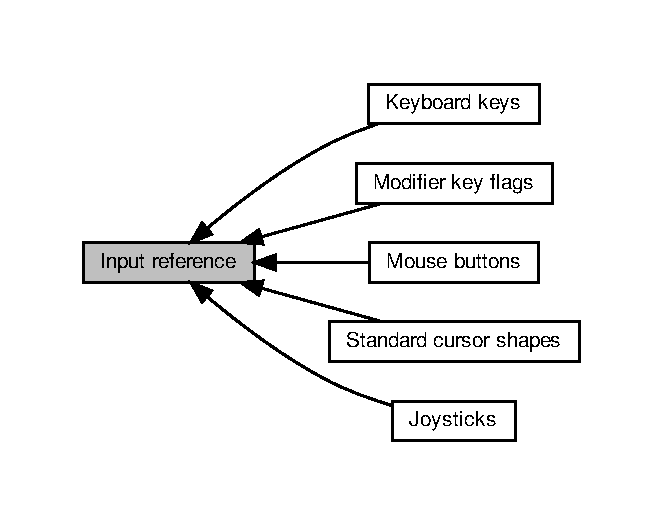
\includegraphics[width=318pt]{group__input}
\end{center}
\end{figure}
\subsection*{Modules}
\begin{DoxyCompactItemize}
\item 
\hyperlink{group__keys}{Keyboard keys}
\item 
\hyperlink{group__mods}{Modifier key flags}
\item 
\hyperlink{group__buttons}{Mouse buttons}
\item 
\hyperlink{group__joysticks}{Joysticks}
\item 
\hyperlink{group__shapes}{Standard cursor shapes}
\end{DoxyCompactItemize}
\subsection*{Typedefs}
\begin{DoxyCompactItemize}
\item 
typedef void($\ast$ \hyperlink{group__input_ga39893a4a7e7c3239c98d29c9e084350c}{G\+L\+F\+Wmousebuttonfun}) (\hyperlink{group__window_ga3c96d80d363e67d13a41b5d1821f3242}{G\+L\+F\+Wwindow} $\ast$, int, int, int)
\begin{DoxyCompactList}\small\item\em The function signature for mouse button callbacks. \end{DoxyCompactList}\item 
typedef void($\ast$ \hyperlink{group__input_ga4cfad918fa836f09541e7b9acd36686c}{G\+L\+F\+Wcursorposfun}) (\hyperlink{group__window_ga3c96d80d363e67d13a41b5d1821f3242}{G\+L\+F\+Wwindow} $\ast$, double, double)
\begin{DoxyCompactList}\small\item\em The function signature for cursor position callbacks. \end{DoxyCompactList}\item 
typedef void($\ast$ \hyperlink{group__input_ga51ab436c41eeaed6db5a0c9403b1c840}{G\+L\+F\+Wcursorenterfun}) (\hyperlink{group__window_ga3c96d80d363e67d13a41b5d1821f3242}{G\+L\+F\+Wwindow} $\ast$, int)
\begin{DoxyCompactList}\small\item\em The function signature for cursor enter/leave callbacks. \end{DoxyCompactList}\item 
typedef void($\ast$ \hyperlink{group__input_ga4687e2199c60a18a8dd1da532e6d75c9}{G\+L\+F\+Wscrollfun}) (\hyperlink{group__window_ga3c96d80d363e67d13a41b5d1821f3242}{G\+L\+F\+Wwindow} $\ast$, double, double)
\begin{DoxyCompactList}\small\item\em The function signature for scroll callbacks. \end{DoxyCompactList}\item 
typedef void($\ast$ \hyperlink{group__input_ga0192a232a41e4e82948217c8ba94fdfd}{G\+L\+F\+Wkeyfun}) (\hyperlink{group__window_ga3c96d80d363e67d13a41b5d1821f3242}{G\+L\+F\+Wwindow} $\ast$, int, int, int, int)
\begin{DoxyCompactList}\small\item\em The function signature for keyboard key callbacks. \end{DoxyCompactList}\item 
typedef void($\ast$ \hyperlink{group__input_gabf24451c7ceb1952bc02b17a0d5c3e5f}{G\+L\+F\+Wcharfun}) (\hyperlink{group__window_ga3c96d80d363e67d13a41b5d1821f3242}{G\+L\+F\+Wwindow} $\ast$, unsigned int)
\begin{DoxyCompactList}\small\item\em The function signature for Unicode character callbacks. \end{DoxyCompactList}\item 
typedef void($\ast$ \hyperlink{group__input_gae36fb6897d2b7df9b128900c8ce9c507}{G\+L\+F\+Wcharmodsfun}) (\hyperlink{group__window_ga3c96d80d363e67d13a41b5d1821f3242}{G\+L\+F\+Wwindow} $\ast$, unsigned int, int)
\begin{DoxyCompactList}\small\item\em The function signature for Unicode character with modifiers callbacks. \end{DoxyCompactList}\item 
typedef void($\ast$ \hyperlink{group__input_gab71f4ca80b651462852e601caf308c4a}{G\+L\+F\+Wdropfun}) (\hyperlink{group__window_ga3c96d80d363e67d13a41b5d1821f3242}{G\+L\+F\+Wwindow} $\ast$, int, const char $\ast$$\ast$)
\begin{DoxyCompactList}\small\item\em The function signature for file drop callbacks. \end{DoxyCompactList}\item 
typedef void($\ast$ \hyperlink{group__input_gaa67aa597e974298c748bfe4fb17d406d}{G\+L\+F\+Wjoystickfun}) (int, int)
\begin{DoxyCompactList}\small\item\em The function signature for joystick configuration callbacks. \end{DoxyCompactList}\item 
typedef void($\ast$ \hyperlink{group__input_ga39893a4a7e7c3239c98d29c9e084350c}{G\+L\+F\+Wmousebuttonfun}) (\hyperlink{group__window_ga3c96d80d363e67d13a41b5d1821f3242}{G\+L\+F\+Wwindow} $\ast$, int, int, int)
\begin{DoxyCompactList}\small\item\em The function signature for mouse button callbacks. \end{DoxyCompactList}\item 
typedef void($\ast$ \hyperlink{group__input_ga4cfad918fa836f09541e7b9acd36686c}{G\+L\+F\+Wcursorposfun}) (\hyperlink{group__window_ga3c96d80d363e67d13a41b5d1821f3242}{G\+L\+F\+Wwindow} $\ast$, double, double)
\begin{DoxyCompactList}\small\item\em The function signature for cursor position callbacks. \end{DoxyCompactList}\item 
typedef void($\ast$ \hyperlink{group__input_ga51ab436c41eeaed6db5a0c9403b1c840}{G\+L\+F\+Wcursorenterfun}) (\hyperlink{group__window_ga3c96d80d363e67d13a41b5d1821f3242}{G\+L\+F\+Wwindow} $\ast$, int)
\begin{DoxyCompactList}\small\item\em The function signature for cursor enter/leave callbacks. \end{DoxyCompactList}\item 
typedef void($\ast$ \hyperlink{group__input_ga4687e2199c60a18a8dd1da532e6d75c9}{G\+L\+F\+Wscrollfun}) (\hyperlink{group__window_ga3c96d80d363e67d13a41b5d1821f3242}{G\+L\+F\+Wwindow} $\ast$, double, double)
\begin{DoxyCompactList}\small\item\em The function signature for scroll callbacks. \end{DoxyCompactList}\item 
typedef void($\ast$ \hyperlink{group__input_ga0192a232a41e4e82948217c8ba94fdfd}{G\+L\+F\+Wkeyfun}) (\hyperlink{group__window_ga3c96d80d363e67d13a41b5d1821f3242}{G\+L\+F\+Wwindow} $\ast$, int, int, int, int)
\begin{DoxyCompactList}\small\item\em The function signature for keyboard key callbacks. \end{DoxyCompactList}\item 
typedef void($\ast$ \hyperlink{group__input_gabf24451c7ceb1952bc02b17a0d5c3e5f}{G\+L\+F\+Wcharfun}) (\hyperlink{group__window_ga3c96d80d363e67d13a41b5d1821f3242}{G\+L\+F\+Wwindow} $\ast$, unsigned int)
\begin{DoxyCompactList}\small\item\em The function signature for Unicode character callbacks. \end{DoxyCompactList}\item 
typedef void($\ast$ \hyperlink{group__input_gae36fb6897d2b7df9b128900c8ce9c507}{G\+L\+F\+Wcharmodsfun}) (\hyperlink{group__window_ga3c96d80d363e67d13a41b5d1821f3242}{G\+L\+F\+Wwindow} $\ast$, unsigned int, int)
\begin{DoxyCompactList}\small\item\em The function signature for Unicode character with modifiers callbacks. \end{DoxyCompactList}\item 
typedef void($\ast$ \hyperlink{group__input_gab71f4ca80b651462852e601caf308c4a}{G\+L\+F\+Wdropfun}) (\hyperlink{group__window_ga3c96d80d363e67d13a41b5d1821f3242}{G\+L\+F\+Wwindow} $\ast$, int, const char $\ast$$\ast$)
\begin{DoxyCompactList}\small\item\em The function signature for file drop callbacks. \end{DoxyCompactList}\item 
typedef void($\ast$ \hyperlink{group__input_gaa67aa597e974298c748bfe4fb17d406d}{G\+L\+F\+Wjoystickfun}) (int, int)
\begin{DoxyCompactList}\small\item\em The function signature for joystick configuration callbacks. \end{DoxyCompactList}\item 
typedef void($\ast$ \hyperlink{group__input_ga39893a4a7e7c3239c98d29c9e084350c}{G\+L\+F\+Wmousebuttonfun}) (\hyperlink{group__window_ga3c96d80d363e67d13a41b5d1821f3242}{G\+L\+F\+Wwindow} $\ast$, int, int, int)
\begin{DoxyCompactList}\small\item\em The function signature for mouse button callbacks. \end{DoxyCompactList}\item 
typedef void($\ast$ \hyperlink{group__input_ga4cfad918fa836f09541e7b9acd36686c}{G\+L\+F\+Wcursorposfun}) (\hyperlink{group__window_ga3c96d80d363e67d13a41b5d1821f3242}{G\+L\+F\+Wwindow} $\ast$, double, double)
\begin{DoxyCompactList}\small\item\em The function signature for cursor position callbacks. \end{DoxyCompactList}\item 
typedef void($\ast$ \hyperlink{group__input_ga51ab436c41eeaed6db5a0c9403b1c840}{G\+L\+F\+Wcursorenterfun}) (\hyperlink{group__window_ga3c96d80d363e67d13a41b5d1821f3242}{G\+L\+F\+Wwindow} $\ast$, int)
\begin{DoxyCompactList}\small\item\em The function signature for cursor enter/leave callbacks. \end{DoxyCompactList}\item 
typedef void($\ast$ \hyperlink{group__input_ga4687e2199c60a18a8dd1da532e6d75c9}{G\+L\+F\+Wscrollfun}) (\hyperlink{group__window_ga3c96d80d363e67d13a41b5d1821f3242}{G\+L\+F\+Wwindow} $\ast$, double, double)
\begin{DoxyCompactList}\small\item\em The function signature for scroll callbacks. \end{DoxyCompactList}\item 
typedef void($\ast$ \hyperlink{group__input_ga0192a232a41e4e82948217c8ba94fdfd}{G\+L\+F\+Wkeyfun}) (\hyperlink{group__window_ga3c96d80d363e67d13a41b5d1821f3242}{G\+L\+F\+Wwindow} $\ast$, int, int, int, int)
\begin{DoxyCompactList}\small\item\em The function signature for keyboard key callbacks. \end{DoxyCompactList}\item 
typedef void($\ast$ \hyperlink{group__input_gabf24451c7ceb1952bc02b17a0d5c3e5f}{G\+L\+F\+Wcharfun}) (\hyperlink{group__window_ga3c96d80d363e67d13a41b5d1821f3242}{G\+L\+F\+Wwindow} $\ast$, unsigned int)
\begin{DoxyCompactList}\small\item\em The function signature for Unicode character callbacks. \end{DoxyCompactList}\item 
typedef void($\ast$ \hyperlink{group__input_gae36fb6897d2b7df9b128900c8ce9c507}{G\+L\+F\+Wcharmodsfun}) (\hyperlink{group__window_ga3c96d80d363e67d13a41b5d1821f3242}{G\+L\+F\+Wwindow} $\ast$, unsigned int, int)
\begin{DoxyCompactList}\small\item\em The function signature for Unicode character with modifiers callbacks. \end{DoxyCompactList}\item 
typedef void($\ast$ \hyperlink{group__input_gab71f4ca80b651462852e601caf308c4a}{G\+L\+F\+Wdropfun}) (\hyperlink{group__window_ga3c96d80d363e67d13a41b5d1821f3242}{G\+L\+F\+Wwindow} $\ast$, int, const char $\ast$$\ast$)
\begin{DoxyCompactList}\small\item\em The function signature for file drop callbacks. \end{DoxyCompactList}\item 
typedef void($\ast$ \hyperlink{group__input_gaa67aa597e974298c748bfe4fb17d406d}{G\+L\+F\+Wjoystickfun}) (int, int)
\begin{DoxyCompactList}\small\item\em The function signature for joystick configuration callbacks. \end{DoxyCompactList}\item 
typedef void($\ast$ \hyperlink{group__input_ga39893a4a7e7c3239c98d29c9e084350c}{G\+L\+F\+Wmousebuttonfun}) (\hyperlink{group__window_ga3c96d80d363e67d13a41b5d1821f3242}{G\+L\+F\+Wwindow} $\ast$, int, int, int)
\begin{DoxyCompactList}\small\item\em The function signature for mouse button callbacks. \end{DoxyCompactList}\item 
typedef void($\ast$ \hyperlink{group__input_ga4cfad918fa836f09541e7b9acd36686c}{G\+L\+F\+Wcursorposfun}) (\hyperlink{group__window_ga3c96d80d363e67d13a41b5d1821f3242}{G\+L\+F\+Wwindow} $\ast$, double, double)
\begin{DoxyCompactList}\small\item\em The function signature for cursor position callbacks. \end{DoxyCompactList}\item 
typedef void($\ast$ \hyperlink{group__input_ga51ab436c41eeaed6db5a0c9403b1c840}{G\+L\+F\+Wcursorenterfun}) (\hyperlink{group__window_ga3c96d80d363e67d13a41b5d1821f3242}{G\+L\+F\+Wwindow} $\ast$, int)
\begin{DoxyCompactList}\small\item\em The function signature for cursor enter/leave callbacks. \end{DoxyCompactList}\item 
typedef void($\ast$ \hyperlink{group__input_ga4687e2199c60a18a8dd1da532e6d75c9}{G\+L\+F\+Wscrollfun}) (\hyperlink{group__window_ga3c96d80d363e67d13a41b5d1821f3242}{G\+L\+F\+Wwindow} $\ast$, double, double)
\begin{DoxyCompactList}\small\item\em The function signature for scroll callbacks. \end{DoxyCompactList}\item 
typedef void($\ast$ \hyperlink{group__input_ga0192a232a41e4e82948217c8ba94fdfd}{G\+L\+F\+Wkeyfun}) (\hyperlink{group__window_ga3c96d80d363e67d13a41b5d1821f3242}{G\+L\+F\+Wwindow} $\ast$, int, int, int, int)
\begin{DoxyCompactList}\small\item\em The function signature for keyboard key callbacks. \end{DoxyCompactList}\item 
typedef void($\ast$ \hyperlink{group__input_gabf24451c7ceb1952bc02b17a0d5c3e5f}{G\+L\+F\+Wcharfun}) (\hyperlink{group__window_ga3c96d80d363e67d13a41b5d1821f3242}{G\+L\+F\+Wwindow} $\ast$, unsigned int)
\begin{DoxyCompactList}\small\item\em The function signature for Unicode character callbacks. \end{DoxyCompactList}\item 
typedef void($\ast$ \hyperlink{group__input_gae36fb6897d2b7df9b128900c8ce9c507}{G\+L\+F\+Wcharmodsfun}) (\hyperlink{group__window_ga3c96d80d363e67d13a41b5d1821f3242}{G\+L\+F\+Wwindow} $\ast$, unsigned int, int)
\begin{DoxyCompactList}\small\item\em The function signature for Unicode character with modifiers callbacks. \end{DoxyCompactList}\item 
typedef void($\ast$ \hyperlink{group__input_gab71f4ca80b651462852e601caf308c4a}{G\+L\+F\+Wdropfun}) (\hyperlink{group__window_ga3c96d80d363e67d13a41b5d1821f3242}{G\+L\+F\+Wwindow} $\ast$, int, const char $\ast$$\ast$)
\begin{DoxyCompactList}\small\item\em The function signature for file drop callbacks. \end{DoxyCompactList}\item 
typedef void($\ast$ \hyperlink{group__input_gaa67aa597e974298c748bfe4fb17d406d}{G\+L\+F\+Wjoystickfun}) (int, int)
\begin{DoxyCompactList}\small\item\em The function signature for joystick configuration callbacks. \end{DoxyCompactList}\item 
typedef void($\ast$ \hyperlink{group__input_ga39893a4a7e7c3239c98d29c9e084350c}{G\+L\+F\+Wmousebuttonfun}) (\hyperlink{group__window_ga3c96d80d363e67d13a41b5d1821f3242}{G\+L\+F\+Wwindow} $\ast$, int, int, int)
\begin{DoxyCompactList}\small\item\em The function signature for mouse button callbacks. \end{DoxyCompactList}\item 
typedef void($\ast$ \hyperlink{group__input_ga4cfad918fa836f09541e7b9acd36686c}{G\+L\+F\+Wcursorposfun}) (\hyperlink{group__window_ga3c96d80d363e67d13a41b5d1821f3242}{G\+L\+F\+Wwindow} $\ast$, double, double)
\begin{DoxyCompactList}\small\item\em The function signature for cursor position callbacks. \end{DoxyCompactList}\item 
typedef void($\ast$ \hyperlink{group__input_ga51ab436c41eeaed6db5a0c9403b1c840}{G\+L\+F\+Wcursorenterfun}) (\hyperlink{group__window_ga3c96d80d363e67d13a41b5d1821f3242}{G\+L\+F\+Wwindow} $\ast$, int)
\begin{DoxyCompactList}\small\item\em The function signature for cursor enter/leave callbacks. \end{DoxyCompactList}\item 
typedef void($\ast$ \hyperlink{group__input_ga4687e2199c60a18a8dd1da532e6d75c9}{G\+L\+F\+Wscrollfun}) (\hyperlink{group__window_ga3c96d80d363e67d13a41b5d1821f3242}{G\+L\+F\+Wwindow} $\ast$, double, double)
\begin{DoxyCompactList}\small\item\em The function signature for scroll callbacks. \end{DoxyCompactList}\item 
typedef void($\ast$ \hyperlink{group__input_ga0192a232a41e4e82948217c8ba94fdfd}{G\+L\+F\+Wkeyfun}) (\hyperlink{group__window_ga3c96d80d363e67d13a41b5d1821f3242}{G\+L\+F\+Wwindow} $\ast$, int, int, int, int)
\begin{DoxyCompactList}\small\item\em The function signature for keyboard key callbacks. \end{DoxyCompactList}\item 
typedef void($\ast$ \hyperlink{group__input_gabf24451c7ceb1952bc02b17a0d5c3e5f}{G\+L\+F\+Wcharfun}) (\hyperlink{group__window_ga3c96d80d363e67d13a41b5d1821f3242}{G\+L\+F\+Wwindow} $\ast$, unsigned int)
\begin{DoxyCompactList}\small\item\em The function signature for Unicode character callbacks. \end{DoxyCompactList}\item 
typedef void($\ast$ \hyperlink{group__input_gae36fb6897d2b7df9b128900c8ce9c507}{G\+L\+F\+Wcharmodsfun}) (\hyperlink{group__window_ga3c96d80d363e67d13a41b5d1821f3242}{G\+L\+F\+Wwindow} $\ast$, unsigned int, int)
\begin{DoxyCompactList}\small\item\em The function signature for Unicode character with modifiers callbacks. \end{DoxyCompactList}\item 
typedef void($\ast$ \hyperlink{group__input_gab71f4ca80b651462852e601caf308c4a}{G\+L\+F\+Wdropfun}) (\hyperlink{group__window_ga3c96d80d363e67d13a41b5d1821f3242}{G\+L\+F\+Wwindow} $\ast$, int, const char $\ast$$\ast$)
\begin{DoxyCompactList}\small\item\em The function signature for file drop callbacks. \end{DoxyCompactList}\item 
typedef void($\ast$ \hyperlink{group__input_gaa67aa597e974298c748bfe4fb17d406d}{G\+L\+F\+Wjoystickfun}) (int, int)
\begin{DoxyCompactList}\small\item\em The function signature for joystick configuration callbacks. \end{DoxyCompactList}\end{DoxyCompactItemize}
\subsection*{Functions}
\begin{DoxyCompactItemize}
\item 
G\+L\+F\+W\+A\+PI int \hyperlink{group__input_ga1248dd5b1e566b2817e71547564d6af9}{glfw\+Get\+Input\+Mode} (\hyperlink{group__window_ga3c96d80d363e67d13a41b5d1821f3242}{G\+L\+F\+Wwindow} $\ast$window, int mode)
\begin{DoxyCompactList}\small\item\em Returns the value of an input option for the specified window. \end{DoxyCompactList}\item 
G\+L\+F\+W\+A\+PI void \hyperlink{group__input_gae1eb729d2dd91dc33fd60e150a6e1684}{glfw\+Set\+Input\+Mode} (\hyperlink{group__window_ga3c96d80d363e67d13a41b5d1821f3242}{G\+L\+F\+Wwindow} $\ast$window, int mode, int value)
\begin{DoxyCompactList}\small\item\em Sets an input option for the specified window. \end{DoxyCompactList}\item 
G\+L\+F\+W\+A\+PI const char $\ast$ \hyperlink{group__input_ga98293ec4493cfe8e7df8ff22ee402b46}{glfw\+Get\+Key\+Name} (int key, int scancode)
\begin{DoxyCompactList}\small\item\em Returns the localized name of the specified printable key. \end{DoxyCompactList}\item 
G\+L\+F\+W\+A\+PI int \hyperlink{group__input_ga7d8ad8ffaf272808f04e1d5d33ec8859}{glfw\+Get\+Key} (\hyperlink{group__window_ga3c96d80d363e67d13a41b5d1821f3242}{G\+L\+F\+Wwindow} $\ast$window, int key)
\begin{DoxyCompactList}\small\item\em Returns the last reported state of a keyboard key for the specified window. \end{DoxyCompactList}\item 
G\+L\+F\+W\+A\+PI int \hyperlink{group__input_ga6da5efb04f700c312a57a169fa9393a0}{glfw\+Get\+Mouse\+Button} (\hyperlink{group__window_ga3c96d80d363e67d13a41b5d1821f3242}{G\+L\+F\+Wwindow} $\ast$window, int button)
\begin{DoxyCompactList}\small\item\em Returns the last reported state of a mouse button for the specified window. \end{DoxyCompactList}\item 
G\+L\+F\+W\+A\+PI void \hyperlink{group__input_gad289438eb7cf53d11eca685373f44105}{glfw\+Get\+Cursor\+Pos} (\hyperlink{group__window_ga3c96d80d363e67d13a41b5d1821f3242}{G\+L\+F\+Wwindow} $\ast$window, double $\ast$xpos, double $\ast$ypos)
\begin{DoxyCompactList}\small\item\em Retrieves the position of the cursor relative to the client area of the window. \end{DoxyCompactList}\item 
G\+L\+F\+W\+A\+PI void \hyperlink{group__input_gaaf152cc93418acb0ba342e3f4af922bc}{glfw\+Set\+Cursor\+Pos} (\hyperlink{group__window_ga3c96d80d363e67d13a41b5d1821f3242}{G\+L\+F\+Wwindow} $\ast$window, double xpos, double ypos)
\begin{DoxyCompactList}\small\item\em Sets the position of the cursor, relative to the client area of the window. \end{DoxyCompactList}\item 
G\+L\+F\+W\+A\+PI G\+L\+F\+Wcursor $\ast$ \hyperlink{group__input_ga21fc9f020f062db88813aa722c30ba2c}{glfw\+Create\+Cursor} (const \hyperlink{structGLFWimage}{G\+L\+F\+Wimage} $\ast$image, int xhot, int yhot)
\begin{DoxyCompactList}\small\item\em Creates a custom cursor. \end{DoxyCompactList}\item 
G\+L\+F\+W\+A\+PI G\+L\+F\+Wcursor $\ast$ \hyperlink{group__input_gab7c5b6023b39a0021b1fcdabd1d15f09}{glfw\+Create\+Standard\+Cursor} (int shape)
\begin{DoxyCompactList}\small\item\em Creates a cursor with a standard shape. \end{DoxyCompactList}\item 
G\+L\+F\+W\+A\+PI void \hyperlink{group__input_ga27556b7122117bc1bbb4bb3cc003ea43}{glfw\+Destroy\+Cursor} (G\+L\+F\+Wcursor $\ast$cursor)
\begin{DoxyCompactList}\small\item\em Destroys a cursor. \end{DoxyCompactList}\item 
G\+L\+F\+W\+A\+PI void \hyperlink{group__input_gafaf103cea2f43530cff7de4e01126a4f}{glfw\+Set\+Cursor} (\hyperlink{group__window_ga3c96d80d363e67d13a41b5d1821f3242}{G\+L\+F\+Wwindow} $\ast$window, G\+L\+F\+Wcursor $\ast$cursor)
\begin{DoxyCompactList}\small\item\em Sets the cursor for the window. \end{DoxyCompactList}\item 
G\+L\+F\+W\+A\+PI \hyperlink{group__input_ga0192a232a41e4e82948217c8ba94fdfd}{G\+L\+F\+Wkeyfun} \hyperlink{group__input_gaa73bb92f628a2a0be9c132d56f19362c}{glfw\+Set\+Key\+Callback} (\hyperlink{group__window_ga3c96d80d363e67d13a41b5d1821f3242}{G\+L\+F\+Wwindow} $\ast$window, \hyperlink{group__input_ga0192a232a41e4e82948217c8ba94fdfd}{G\+L\+F\+Wkeyfun} cbfun)
\begin{DoxyCompactList}\small\item\em Sets the key callback. \end{DoxyCompactList}\item 
G\+L\+F\+W\+A\+PI \hyperlink{group__input_gabf24451c7ceb1952bc02b17a0d5c3e5f}{G\+L\+F\+Wcharfun} \hyperlink{group__input_ga07b2959b23dc3e466ce7475746021002}{glfw\+Set\+Char\+Callback} (\hyperlink{group__window_ga3c96d80d363e67d13a41b5d1821f3242}{G\+L\+F\+Wwindow} $\ast$window, \hyperlink{group__input_gabf24451c7ceb1952bc02b17a0d5c3e5f}{G\+L\+F\+Wcharfun} cbfun)
\begin{DoxyCompactList}\small\item\em Sets the Unicode character callback. \end{DoxyCompactList}\item 
G\+L\+F\+W\+A\+PI \hyperlink{group__input_gae36fb6897d2b7df9b128900c8ce9c507}{G\+L\+F\+Wcharmodsfun} \hyperlink{group__input_gae6eee0bda7429bfe8028615847cf6795}{glfw\+Set\+Char\+Mods\+Callback} (\hyperlink{group__window_ga3c96d80d363e67d13a41b5d1821f3242}{G\+L\+F\+Wwindow} $\ast$window, \hyperlink{group__input_gae36fb6897d2b7df9b128900c8ce9c507}{G\+L\+F\+Wcharmodsfun} cbfun)
\begin{DoxyCompactList}\small\item\em Sets the Unicode character with modifiers callback. \end{DoxyCompactList}\item 
G\+L\+F\+W\+A\+PI \hyperlink{group__input_ga39893a4a7e7c3239c98d29c9e084350c}{G\+L\+F\+Wmousebuttonfun} \hyperlink{group__input_ga20e5ba1ce4e086aedd48a06dc311c95f}{glfw\+Set\+Mouse\+Button\+Callback} (\hyperlink{group__window_ga3c96d80d363e67d13a41b5d1821f3242}{G\+L\+F\+Wwindow} $\ast$window, \hyperlink{group__input_ga39893a4a7e7c3239c98d29c9e084350c}{G\+L\+F\+Wmousebuttonfun} cbfun)
\begin{DoxyCompactList}\small\item\em Sets the mouse button callback. \end{DoxyCompactList}\item 
G\+L\+F\+W\+A\+PI \hyperlink{group__input_ga4cfad918fa836f09541e7b9acd36686c}{G\+L\+F\+Wcursorposfun} \hyperlink{group__input_ga9c49c0d3d3c775c3124726f1d902124d}{glfw\+Set\+Cursor\+Pos\+Callback} (\hyperlink{group__window_ga3c96d80d363e67d13a41b5d1821f3242}{G\+L\+F\+Wwindow} $\ast$window, \hyperlink{group__input_ga4cfad918fa836f09541e7b9acd36686c}{G\+L\+F\+Wcursorposfun} cbfun)
\begin{DoxyCompactList}\small\item\em Sets the cursor position callback. \end{DoxyCompactList}\item 
G\+L\+F\+W\+A\+PI \hyperlink{group__input_ga51ab436c41eeaed6db5a0c9403b1c840}{G\+L\+F\+Wcursorenterfun} \hyperlink{group__input_gaa20014985561efeb2c53f1956f727830}{glfw\+Set\+Cursor\+Enter\+Callback} (\hyperlink{group__window_ga3c96d80d363e67d13a41b5d1821f3242}{G\+L\+F\+Wwindow} $\ast$window, \hyperlink{group__input_ga51ab436c41eeaed6db5a0c9403b1c840}{G\+L\+F\+Wcursorenterfun} cbfun)
\begin{DoxyCompactList}\small\item\em Sets the cursor enter/exit callback. \end{DoxyCompactList}\item 
G\+L\+F\+W\+A\+PI \hyperlink{group__input_ga4687e2199c60a18a8dd1da532e6d75c9}{G\+L\+F\+Wscrollfun} \hyperlink{group__input_ga29011514e93368712a3063a28707ced3}{glfw\+Set\+Scroll\+Callback} (\hyperlink{group__window_ga3c96d80d363e67d13a41b5d1821f3242}{G\+L\+F\+Wwindow} $\ast$window, \hyperlink{group__input_ga4687e2199c60a18a8dd1da532e6d75c9}{G\+L\+F\+Wscrollfun} cbfun)
\begin{DoxyCompactList}\small\item\em Sets the scroll callback. \end{DoxyCompactList}\item 
G\+L\+F\+W\+A\+PI \hyperlink{group__input_gab71f4ca80b651462852e601caf308c4a}{G\+L\+F\+Wdropfun} \hyperlink{group__input_gad4fc40df63a5d0441ab06de9a585cc04}{glfw\+Set\+Drop\+Callback} (\hyperlink{group__window_ga3c96d80d363e67d13a41b5d1821f3242}{G\+L\+F\+Wwindow} $\ast$window, \hyperlink{group__input_gab71f4ca80b651462852e601caf308c4a}{G\+L\+F\+Wdropfun} cbfun)
\begin{DoxyCompactList}\small\item\em Sets the file drop callback. \end{DoxyCompactList}\item 
G\+L\+F\+W\+A\+PI int \hyperlink{group__input_ga7f81f22f355f4b7d315caf73cdfd9906}{glfw\+Joystick\+Present} (int joy)
\begin{DoxyCompactList}\small\item\em Returns whether the specified joystick is present. \end{DoxyCompactList}\item 
G\+L\+F\+W\+A\+PI const float $\ast$ \hyperlink{group__input_gaaab55af25a46327a58052abac82b959f}{glfw\+Get\+Joystick\+Axes} (int joy, int $\ast$count)
\begin{DoxyCompactList}\small\item\em Returns the values of all axes of the specified joystick. \end{DoxyCompactList}\item 
G\+L\+F\+W\+A\+PI const unsigned char $\ast$ \hyperlink{group__input_ga211004a8dc7c18814c23f63fd2ac7b2c}{glfw\+Get\+Joystick\+Buttons} (int joy, int $\ast$count)
\begin{DoxyCompactList}\small\item\em Returns the state of all buttons of the specified joystick. \end{DoxyCompactList}\item 
G\+L\+F\+W\+A\+PI const char $\ast$ \hyperlink{group__input_ga1a17206f462496c2fd7d811ce6d3726e}{glfw\+Get\+Joystick\+Name} (int joy)
\begin{DoxyCompactList}\small\item\em Returns the name of the specified joystick. \end{DoxyCompactList}\item 
G\+L\+F\+W\+A\+PI \hyperlink{group__input_gaa67aa597e974298c748bfe4fb17d406d}{G\+L\+F\+Wjoystickfun} \hyperlink{group__input_ga07524a1122a03642b1d28822ea931094}{glfw\+Set\+Joystick\+Callback} (\hyperlink{group__input_gaa67aa597e974298c748bfe4fb17d406d}{G\+L\+F\+Wjoystickfun} cbfun)
\begin{DoxyCompactList}\small\item\em Sets the joystick configuration callback. \end{DoxyCompactList}\item 
G\+L\+F\+W\+A\+PI void \hyperlink{group__input_ga7a580309bbc185a0459c3559021d2fd7}{glfw\+Set\+Clipboard\+String} (\hyperlink{group__window_ga3c96d80d363e67d13a41b5d1821f3242}{G\+L\+F\+Wwindow} $\ast$window, const char $\ast$string)
\begin{DoxyCompactList}\small\item\em Sets the clipboard to the specified string. \end{DoxyCompactList}\item 
G\+L\+F\+W\+A\+PI const char $\ast$ \hyperlink{group__input_ga315b28b05797d00fe7cdf1ecfdc638dc}{glfw\+Get\+Clipboard\+String} (\hyperlink{group__window_ga3c96d80d363e67d13a41b5d1821f3242}{G\+L\+F\+Wwindow} $\ast$window)
\begin{DoxyCompactList}\small\item\em Returns the contents of the clipboard as a string. \end{DoxyCompactList}\item 
G\+L\+F\+W\+A\+PI double \hyperlink{group__input_ga03d4a1039b8662c71eeb40beea8cb622}{glfw\+Get\+Time} (void)
\begin{DoxyCompactList}\small\item\em Returns the value of the G\+L\+FW timer. \end{DoxyCompactList}\item 
G\+L\+F\+W\+A\+PI void \hyperlink{group__input_ga94360a3628a09f32708f83cc3fa48590}{glfw\+Set\+Time} (double time)
\begin{DoxyCompactList}\small\item\em Sets the G\+L\+FW timer. \end{DoxyCompactList}\item 
G\+L\+F\+W\+A\+PI uint64\+\_\+t \hyperlink{group__input_gaa00c3e32227eb70b3968fca0bfe4ae26}{glfw\+Get\+Timer\+Value} (void)
\begin{DoxyCompactList}\small\item\em Returns the current value of the raw timer. \end{DoxyCompactList}\item 
G\+L\+F\+W\+A\+PI uint64\+\_\+t \hyperlink{group__input_gaa92d10b10013372778efbf6367714371}{glfw\+Get\+Timer\+Frequency} (void)
\begin{DoxyCompactList}\small\item\em Returns the frequency, in Hz, of the raw timer. \end{DoxyCompactList}\end{DoxyCompactItemize}
\subsection*{Key and button actions}
\begin{DoxyCompactItemize}
\item 
\#define \hyperlink{group__input_gada11d965c4da13090ad336e030e4d11f}{G\+L\+F\+W\+\_\+\+R\+E\+L\+E\+A\+SE}~0
\begin{DoxyCompactList}\small\item\em The key or mouse button was released. \end{DoxyCompactList}\item 
\#define \hyperlink{group__input_ga2485743d0b59df3791c45951c4195265}{G\+L\+F\+W\+\_\+\+P\+R\+E\+SS}~1
\begin{DoxyCompactList}\small\item\em The key or mouse button was pressed. \end{DoxyCompactList}\item 
\#define \hyperlink{group__input_gac96fd3b9fc66c6f0eebaf6532595338f}{G\+L\+F\+W\+\_\+\+R\+E\+P\+E\+AT}~2
\begin{DoxyCompactList}\small\item\em The key was held down until it repeated. \end{DoxyCompactList}\end{DoxyCompactItemize}
\subsection*{Key and button actions}
\begin{DoxyCompactItemize}
\item 
\#define \hyperlink{group__input_gada11d965c4da13090ad336e030e4d11f}{G\+L\+F\+W\+\_\+\+R\+E\+L\+E\+A\+SE}~0
\begin{DoxyCompactList}\small\item\em The key or mouse button was released. \end{DoxyCompactList}\item 
\#define \hyperlink{group__input_ga2485743d0b59df3791c45951c4195265}{G\+L\+F\+W\+\_\+\+P\+R\+E\+SS}~1
\begin{DoxyCompactList}\small\item\em The key or mouse button was pressed. \end{DoxyCompactList}\item 
\#define \hyperlink{group__input_gac96fd3b9fc66c6f0eebaf6532595338f}{G\+L\+F\+W\+\_\+\+R\+E\+P\+E\+AT}~2
\begin{DoxyCompactList}\small\item\em The key was held down until it repeated. \end{DoxyCompactList}\end{DoxyCompactItemize}
\subsection*{Key and button actions}
\begin{DoxyCompactItemize}
\item 
\#define \hyperlink{group__input_gada11d965c4da13090ad336e030e4d11f}{G\+L\+F\+W\+\_\+\+R\+E\+L\+E\+A\+SE}~0
\begin{DoxyCompactList}\small\item\em The key or mouse button was released. \end{DoxyCompactList}\item 
\#define \hyperlink{group__input_ga2485743d0b59df3791c45951c4195265}{G\+L\+F\+W\+\_\+\+P\+R\+E\+SS}~1
\begin{DoxyCompactList}\small\item\em The key or mouse button was pressed. \end{DoxyCompactList}\item 
\#define \hyperlink{group__input_gac96fd3b9fc66c6f0eebaf6532595338f}{G\+L\+F\+W\+\_\+\+R\+E\+P\+E\+AT}~2
\begin{DoxyCompactList}\small\item\em The key was held down until it repeated. \end{DoxyCompactList}\end{DoxyCompactItemize}
\subsection*{Key and button actions}
\begin{DoxyCompactItemize}
\item 
\#define \hyperlink{group__input_gada11d965c4da13090ad336e030e4d11f}{G\+L\+F\+W\+\_\+\+R\+E\+L\+E\+A\+SE}~0
\begin{DoxyCompactList}\small\item\em The key or mouse button was released. \end{DoxyCompactList}\item 
\#define \hyperlink{group__input_ga2485743d0b59df3791c45951c4195265}{G\+L\+F\+W\+\_\+\+P\+R\+E\+SS}~1
\begin{DoxyCompactList}\small\item\em The key or mouse button was pressed. \end{DoxyCompactList}\item 
\#define \hyperlink{group__input_gac96fd3b9fc66c6f0eebaf6532595338f}{G\+L\+F\+W\+\_\+\+R\+E\+P\+E\+AT}~2
\begin{DoxyCompactList}\small\item\em The key was held down until it repeated. \end{DoxyCompactList}\end{DoxyCompactItemize}
\subsection*{Key and button actions}
\begin{DoxyCompactItemize}
\item 
\#define \hyperlink{group__input_gada11d965c4da13090ad336e030e4d11f}{G\+L\+F\+W\+\_\+\+R\+E\+L\+E\+A\+SE}~0
\begin{DoxyCompactList}\small\item\em The key or mouse button was released. \end{DoxyCompactList}\item 
\#define \hyperlink{group__input_ga2485743d0b59df3791c45951c4195265}{G\+L\+F\+W\+\_\+\+P\+R\+E\+SS}~1
\begin{DoxyCompactList}\small\item\em The key or mouse button was pressed. \end{DoxyCompactList}\item 
\#define \hyperlink{group__input_gac96fd3b9fc66c6f0eebaf6532595338f}{G\+L\+F\+W\+\_\+\+R\+E\+P\+E\+AT}~2
\begin{DoxyCompactList}\small\item\em The key was held down until it repeated. \end{DoxyCompactList}\end{DoxyCompactItemize}


\subsection{Detailed Description}
This is the reference documentation for input related functions and types. For more task-\/oriented information, see the input\+\_\+guide. 

\subsection{Macro Definition Documentation}
\mbox{\Hypertarget{group__input_ga2485743d0b59df3791c45951c4195265}\label{group__input_ga2485743d0b59df3791c45951c4195265}} 
\index{Input reference@{Input reference}!G\+L\+F\+W\+\_\+\+P\+R\+E\+SS@{G\+L\+F\+W\+\_\+\+P\+R\+E\+SS}}
\index{G\+L\+F\+W\+\_\+\+P\+R\+E\+SS@{G\+L\+F\+W\+\_\+\+P\+R\+E\+SS}!Input reference@{Input reference}}
\subsubsection{\texorpdfstring{G\+L\+F\+W\+\_\+\+P\+R\+E\+SS}{GLFW\_PRESS}\hspace{0.1cm}{\footnotesize\ttfamily [1/5]}}
{\footnotesize\ttfamily \#define G\+L\+F\+W\+\_\+\+P\+R\+E\+SS~1}



The key or mouse button was pressed. 

The key or mouse button was pressed. \mbox{\Hypertarget{group__input_ga2485743d0b59df3791c45951c4195265}\label{group__input_ga2485743d0b59df3791c45951c4195265}} 
\index{Input reference@{Input reference}!G\+L\+F\+W\+\_\+\+P\+R\+E\+SS@{G\+L\+F\+W\+\_\+\+P\+R\+E\+SS}}
\index{G\+L\+F\+W\+\_\+\+P\+R\+E\+SS@{G\+L\+F\+W\+\_\+\+P\+R\+E\+SS}!Input reference@{Input reference}}
\subsubsection{\texorpdfstring{G\+L\+F\+W\+\_\+\+P\+R\+E\+SS}{GLFW\_PRESS}\hspace{0.1cm}{\footnotesize\ttfamily [2/5]}}
{\footnotesize\ttfamily \#define G\+L\+F\+W\+\_\+\+P\+R\+E\+SS~1}



The key or mouse button was pressed. 

The key or mouse button was pressed. \mbox{\Hypertarget{group__input_ga2485743d0b59df3791c45951c4195265}\label{group__input_ga2485743d0b59df3791c45951c4195265}} 
\index{Input reference@{Input reference}!G\+L\+F\+W\+\_\+\+P\+R\+E\+SS@{G\+L\+F\+W\+\_\+\+P\+R\+E\+SS}}
\index{G\+L\+F\+W\+\_\+\+P\+R\+E\+SS@{G\+L\+F\+W\+\_\+\+P\+R\+E\+SS}!Input reference@{Input reference}}
\subsubsection{\texorpdfstring{G\+L\+F\+W\+\_\+\+P\+R\+E\+SS}{GLFW\_PRESS}\hspace{0.1cm}{\footnotesize\ttfamily [3/5]}}
{\footnotesize\ttfamily \#define G\+L\+F\+W\+\_\+\+P\+R\+E\+SS~1}



The key or mouse button was pressed. 

The key or mouse button was pressed. \mbox{\Hypertarget{group__input_ga2485743d0b59df3791c45951c4195265}\label{group__input_ga2485743d0b59df3791c45951c4195265}} 
\index{Input reference@{Input reference}!G\+L\+F\+W\+\_\+\+P\+R\+E\+SS@{G\+L\+F\+W\+\_\+\+P\+R\+E\+SS}}
\index{G\+L\+F\+W\+\_\+\+P\+R\+E\+SS@{G\+L\+F\+W\+\_\+\+P\+R\+E\+SS}!Input reference@{Input reference}}
\subsubsection{\texorpdfstring{G\+L\+F\+W\+\_\+\+P\+R\+E\+SS}{GLFW\_PRESS}\hspace{0.1cm}{\footnotesize\ttfamily [4/5]}}
{\footnotesize\ttfamily \#define G\+L\+F\+W\+\_\+\+P\+R\+E\+SS~1}



The key or mouse button was pressed. 

The key or mouse button was pressed. \mbox{\Hypertarget{group__input_ga2485743d0b59df3791c45951c4195265}\label{group__input_ga2485743d0b59df3791c45951c4195265}} 
\index{Input reference@{Input reference}!G\+L\+F\+W\+\_\+\+P\+R\+E\+SS@{G\+L\+F\+W\+\_\+\+P\+R\+E\+SS}}
\index{G\+L\+F\+W\+\_\+\+P\+R\+E\+SS@{G\+L\+F\+W\+\_\+\+P\+R\+E\+SS}!Input reference@{Input reference}}
\subsubsection{\texorpdfstring{G\+L\+F\+W\+\_\+\+P\+R\+E\+SS}{GLFW\_PRESS}\hspace{0.1cm}{\footnotesize\ttfamily [5/5]}}
{\footnotesize\ttfamily \#define G\+L\+F\+W\+\_\+\+P\+R\+E\+SS~1}



The key or mouse button was pressed. 

The key or mouse button was pressed. \mbox{\Hypertarget{group__input_gada11d965c4da13090ad336e030e4d11f}\label{group__input_gada11d965c4da13090ad336e030e4d11f}} 
\index{Input reference@{Input reference}!G\+L\+F\+W\+\_\+\+R\+E\+L\+E\+A\+SE@{G\+L\+F\+W\+\_\+\+R\+E\+L\+E\+A\+SE}}
\index{G\+L\+F\+W\+\_\+\+R\+E\+L\+E\+A\+SE@{G\+L\+F\+W\+\_\+\+R\+E\+L\+E\+A\+SE}!Input reference@{Input reference}}
\subsubsection{\texorpdfstring{G\+L\+F\+W\+\_\+\+R\+E\+L\+E\+A\+SE}{GLFW\_RELEASE}\hspace{0.1cm}{\footnotesize\ttfamily [1/5]}}
{\footnotesize\ttfamily \#define G\+L\+F\+W\+\_\+\+R\+E\+L\+E\+A\+SE~0}



The key or mouse button was released. 

The key or mouse button was released. \mbox{\Hypertarget{group__input_gada11d965c4da13090ad336e030e4d11f}\label{group__input_gada11d965c4da13090ad336e030e4d11f}} 
\index{Input reference@{Input reference}!G\+L\+F\+W\+\_\+\+R\+E\+L\+E\+A\+SE@{G\+L\+F\+W\+\_\+\+R\+E\+L\+E\+A\+SE}}
\index{G\+L\+F\+W\+\_\+\+R\+E\+L\+E\+A\+SE@{G\+L\+F\+W\+\_\+\+R\+E\+L\+E\+A\+SE}!Input reference@{Input reference}}
\subsubsection{\texorpdfstring{G\+L\+F\+W\+\_\+\+R\+E\+L\+E\+A\+SE}{GLFW\_RELEASE}\hspace{0.1cm}{\footnotesize\ttfamily [2/5]}}
{\footnotesize\ttfamily \#define G\+L\+F\+W\+\_\+\+R\+E\+L\+E\+A\+SE~0}



The key or mouse button was released. 

The key or mouse button was released. \mbox{\Hypertarget{group__input_gada11d965c4da13090ad336e030e4d11f}\label{group__input_gada11d965c4da13090ad336e030e4d11f}} 
\index{Input reference@{Input reference}!G\+L\+F\+W\+\_\+\+R\+E\+L\+E\+A\+SE@{G\+L\+F\+W\+\_\+\+R\+E\+L\+E\+A\+SE}}
\index{G\+L\+F\+W\+\_\+\+R\+E\+L\+E\+A\+SE@{G\+L\+F\+W\+\_\+\+R\+E\+L\+E\+A\+SE}!Input reference@{Input reference}}
\subsubsection{\texorpdfstring{G\+L\+F\+W\+\_\+\+R\+E\+L\+E\+A\+SE}{GLFW\_RELEASE}\hspace{0.1cm}{\footnotesize\ttfamily [3/5]}}
{\footnotesize\ttfamily \#define G\+L\+F\+W\+\_\+\+R\+E\+L\+E\+A\+SE~0}



The key or mouse button was released. 

The key or mouse button was released. \mbox{\Hypertarget{group__input_gada11d965c4da13090ad336e030e4d11f}\label{group__input_gada11d965c4da13090ad336e030e4d11f}} 
\index{Input reference@{Input reference}!G\+L\+F\+W\+\_\+\+R\+E\+L\+E\+A\+SE@{G\+L\+F\+W\+\_\+\+R\+E\+L\+E\+A\+SE}}
\index{G\+L\+F\+W\+\_\+\+R\+E\+L\+E\+A\+SE@{G\+L\+F\+W\+\_\+\+R\+E\+L\+E\+A\+SE}!Input reference@{Input reference}}
\subsubsection{\texorpdfstring{G\+L\+F\+W\+\_\+\+R\+E\+L\+E\+A\+SE}{GLFW\_RELEASE}\hspace{0.1cm}{\footnotesize\ttfamily [4/5]}}
{\footnotesize\ttfamily \#define G\+L\+F\+W\+\_\+\+R\+E\+L\+E\+A\+SE~0}



The key or mouse button was released. 

The key or mouse button was released. \mbox{\Hypertarget{group__input_gada11d965c4da13090ad336e030e4d11f}\label{group__input_gada11d965c4da13090ad336e030e4d11f}} 
\index{Input reference@{Input reference}!G\+L\+F\+W\+\_\+\+R\+E\+L\+E\+A\+SE@{G\+L\+F\+W\+\_\+\+R\+E\+L\+E\+A\+SE}}
\index{G\+L\+F\+W\+\_\+\+R\+E\+L\+E\+A\+SE@{G\+L\+F\+W\+\_\+\+R\+E\+L\+E\+A\+SE}!Input reference@{Input reference}}
\subsubsection{\texorpdfstring{G\+L\+F\+W\+\_\+\+R\+E\+L\+E\+A\+SE}{GLFW\_RELEASE}\hspace{0.1cm}{\footnotesize\ttfamily [5/5]}}
{\footnotesize\ttfamily \#define G\+L\+F\+W\+\_\+\+R\+E\+L\+E\+A\+SE~0}



The key or mouse button was released. 

The key or mouse button was released. \mbox{\Hypertarget{group__input_gac96fd3b9fc66c6f0eebaf6532595338f}\label{group__input_gac96fd3b9fc66c6f0eebaf6532595338f}} 
\index{Input reference@{Input reference}!G\+L\+F\+W\+\_\+\+R\+E\+P\+E\+AT@{G\+L\+F\+W\+\_\+\+R\+E\+P\+E\+AT}}
\index{G\+L\+F\+W\+\_\+\+R\+E\+P\+E\+AT@{G\+L\+F\+W\+\_\+\+R\+E\+P\+E\+AT}!Input reference@{Input reference}}
\subsubsection{\texorpdfstring{G\+L\+F\+W\+\_\+\+R\+E\+P\+E\+AT}{GLFW\_REPEAT}\hspace{0.1cm}{\footnotesize\ttfamily [1/5]}}
{\footnotesize\ttfamily \#define G\+L\+F\+W\+\_\+\+R\+E\+P\+E\+AT~2}



The key was held down until it repeated. 

The key was held down until it repeated. \mbox{\Hypertarget{group__input_gac96fd3b9fc66c6f0eebaf6532595338f}\label{group__input_gac96fd3b9fc66c6f0eebaf6532595338f}} 
\index{Input reference@{Input reference}!G\+L\+F\+W\+\_\+\+R\+E\+P\+E\+AT@{G\+L\+F\+W\+\_\+\+R\+E\+P\+E\+AT}}
\index{G\+L\+F\+W\+\_\+\+R\+E\+P\+E\+AT@{G\+L\+F\+W\+\_\+\+R\+E\+P\+E\+AT}!Input reference@{Input reference}}
\subsubsection{\texorpdfstring{G\+L\+F\+W\+\_\+\+R\+E\+P\+E\+AT}{GLFW\_REPEAT}\hspace{0.1cm}{\footnotesize\ttfamily [2/5]}}
{\footnotesize\ttfamily \#define G\+L\+F\+W\+\_\+\+R\+E\+P\+E\+AT~2}



The key was held down until it repeated. 

The key was held down until it repeated. \mbox{\Hypertarget{group__input_gac96fd3b9fc66c6f0eebaf6532595338f}\label{group__input_gac96fd3b9fc66c6f0eebaf6532595338f}} 
\index{Input reference@{Input reference}!G\+L\+F\+W\+\_\+\+R\+E\+P\+E\+AT@{G\+L\+F\+W\+\_\+\+R\+E\+P\+E\+AT}}
\index{G\+L\+F\+W\+\_\+\+R\+E\+P\+E\+AT@{G\+L\+F\+W\+\_\+\+R\+E\+P\+E\+AT}!Input reference@{Input reference}}
\subsubsection{\texorpdfstring{G\+L\+F\+W\+\_\+\+R\+E\+P\+E\+AT}{GLFW\_REPEAT}\hspace{0.1cm}{\footnotesize\ttfamily [3/5]}}
{\footnotesize\ttfamily \#define G\+L\+F\+W\+\_\+\+R\+E\+P\+E\+AT~2}



The key was held down until it repeated. 

The key was held down until it repeated. \mbox{\Hypertarget{group__input_gac96fd3b9fc66c6f0eebaf6532595338f}\label{group__input_gac96fd3b9fc66c6f0eebaf6532595338f}} 
\index{Input reference@{Input reference}!G\+L\+F\+W\+\_\+\+R\+E\+P\+E\+AT@{G\+L\+F\+W\+\_\+\+R\+E\+P\+E\+AT}}
\index{G\+L\+F\+W\+\_\+\+R\+E\+P\+E\+AT@{G\+L\+F\+W\+\_\+\+R\+E\+P\+E\+AT}!Input reference@{Input reference}}
\subsubsection{\texorpdfstring{G\+L\+F\+W\+\_\+\+R\+E\+P\+E\+AT}{GLFW\_REPEAT}\hspace{0.1cm}{\footnotesize\ttfamily [4/5]}}
{\footnotesize\ttfamily \#define G\+L\+F\+W\+\_\+\+R\+E\+P\+E\+AT~2}



The key was held down until it repeated. 

The key was held down until it repeated. \mbox{\Hypertarget{group__input_gac96fd3b9fc66c6f0eebaf6532595338f}\label{group__input_gac96fd3b9fc66c6f0eebaf6532595338f}} 
\index{Input reference@{Input reference}!G\+L\+F\+W\+\_\+\+R\+E\+P\+E\+AT@{G\+L\+F\+W\+\_\+\+R\+E\+P\+E\+AT}}
\index{G\+L\+F\+W\+\_\+\+R\+E\+P\+E\+AT@{G\+L\+F\+W\+\_\+\+R\+E\+P\+E\+AT}!Input reference@{Input reference}}
\subsubsection{\texorpdfstring{G\+L\+F\+W\+\_\+\+R\+E\+P\+E\+AT}{GLFW\_REPEAT}\hspace{0.1cm}{\footnotesize\ttfamily [5/5]}}
{\footnotesize\ttfamily \#define G\+L\+F\+W\+\_\+\+R\+E\+P\+E\+AT~2}



The key was held down until it repeated. 

The key was held down until it repeated. 

\subsection{Typedef Documentation}
\mbox{\Hypertarget{group__input_gabf24451c7ceb1952bc02b17a0d5c3e5f}\label{group__input_gabf24451c7ceb1952bc02b17a0d5c3e5f}} 
\index{Input reference@{Input reference}!G\+L\+F\+Wcharfun@{G\+L\+F\+Wcharfun}}
\index{G\+L\+F\+Wcharfun@{G\+L\+F\+Wcharfun}!Input reference@{Input reference}}
\subsubsection{\texorpdfstring{G\+L\+F\+Wcharfun}{GLFWcharfun}\hspace{0.1cm}{\footnotesize\ttfamily [1/5]}}
{\footnotesize\ttfamily typedef void($\ast$  G\+L\+F\+Wcharfun) (\hyperlink{group__window_ga3c96d80d363e67d13a41b5d1821f3242}{G\+L\+F\+Wwindow} $\ast$, unsigned int)}



The function signature for Unicode character callbacks. 

This is the function signature for Unicode character callback functions.


\begin{DoxyParams}[1]{Parameters}
\mbox{\tt in}  & {\em window} & The window that received the event. \\
\hline
\mbox{\tt in}  & {\em codepoint} & The Unicode code point of the character.\\
\hline
\end{DoxyParams}
\begin{DoxySeeAlso}{See also}
input\+\_\+char 

\hyperlink{group__input_ga07b2959b23dc3e466ce7475746021002}{glfw\+Set\+Char\+Callback}
\end{DoxySeeAlso}
\begin{DoxySince}{Since}
Added in version 2.\+4.  Added window handle parameter. 
\end{DoxySince}
\mbox{\Hypertarget{group__input_gabf24451c7ceb1952bc02b17a0d5c3e5f}\label{group__input_gabf24451c7ceb1952bc02b17a0d5c3e5f}} 
\index{Input reference@{Input reference}!G\+L\+F\+Wcharfun@{G\+L\+F\+Wcharfun}}
\index{G\+L\+F\+Wcharfun@{G\+L\+F\+Wcharfun}!Input reference@{Input reference}}
\subsubsection{\texorpdfstring{G\+L\+F\+Wcharfun}{GLFWcharfun}\hspace{0.1cm}{\footnotesize\ttfamily [2/5]}}
{\footnotesize\ttfamily typedef void($\ast$  G\+L\+F\+Wcharfun) (\hyperlink{group__window_ga3c96d80d363e67d13a41b5d1821f3242}{G\+L\+F\+Wwindow} $\ast$, unsigned int)}



The function signature for Unicode character callbacks. 

This is the function signature for Unicode character callback functions.


\begin{DoxyParams}[1]{Parameters}
\mbox{\tt in}  & {\em window} & The window that received the event. \\
\hline
\mbox{\tt in}  & {\em codepoint} & The Unicode code point of the character.\\
\hline
\end{DoxyParams}
\begin{DoxySeeAlso}{See also}
input\+\_\+char 

\hyperlink{group__input_ga07b2959b23dc3e466ce7475746021002}{glfw\+Set\+Char\+Callback}
\end{DoxySeeAlso}
\begin{DoxySince}{Since}
Added in version 2.\+4.  Added window handle parameter. 
\end{DoxySince}
\mbox{\Hypertarget{group__input_gabf24451c7ceb1952bc02b17a0d5c3e5f}\label{group__input_gabf24451c7ceb1952bc02b17a0d5c3e5f}} 
\index{Input reference@{Input reference}!G\+L\+F\+Wcharfun@{G\+L\+F\+Wcharfun}}
\index{G\+L\+F\+Wcharfun@{G\+L\+F\+Wcharfun}!Input reference@{Input reference}}
\subsubsection{\texorpdfstring{G\+L\+F\+Wcharfun}{GLFWcharfun}\hspace{0.1cm}{\footnotesize\ttfamily [3/5]}}
{\footnotesize\ttfamily typedef void($\ast$  G\+L\+F\+Wcharfun) (\hyperlink{group__window_ga3c96d80d363e67d13a41b5d1821f3242}{G\+L\+F\+Wwindow} $\ast$, unsigned int)}



The function signature for Unicode character callbacks. 

This is the function signature for Unicode character callback functions.


\begin{DoxyParams}[1]{Parameters}
\mbox{\tt in}  & {\em window} & The window that received the event. \\
\hline
\mbox{\tt in}  & {\em codepoint} & The Unicode code point of the character.\\
\hline
\end{DoxyParams}
\begin{DoxySeeAlso}{See also}
input\+\_\+char 

\hyperlink{group__input_ga07b2959b23dc3e466ce7475746021002}{glfw\+Set\+Char\+Callback}
\end{DoxySeeAlso}
\begin{DoxySince}{Since}
Added in version 2.\+4.  Added window handle parameter. 
\end{DoxySince}
\mbox{\Hypertarget{group__input_gabf24451c7ceb1952bc02b17a0d5c3e5f}\label{group__input_gabf24451c7ceb1952bc02b17a0d5c3e5f}} 
\index{Input reference@{Input reference}!G\+L\+F\+Wcharfun@{G\+L\+F\+Wcharfun}}
\index{G\+L\+F\+Wcharfun@{G\+L\+F\+Wcharfun}!Input reference@{Input reference}}
\subsubsection{\texorpdfstring{G\+L\+F\+Wcharfun}{GLFWcharfun}\hspace{0.1cm}{\footnotesize\ttfamily [4/5]}}
{\footnotesize\ttfamily typedef void($\ast$  G\+L\+F\+Wcharfun) (\hyperlink{group__window_ga3c96d80d363e67d13a41b5d1821f3242}{G\+L\+F\+Wwindow} $\ast$, unsigned int)}



The function signature for Unicode character callbacks. 

This is the function signature for Unicode character callback functions.


\begin{DoxyParams}[1]{Parameters}
\mbox{\tt in}  & {\em window} & The window that received the event. \\
\hline
\mbox{\tt in}  & {\em codepoint} & The Unicode code point of the character.\\
\hline
\end{DoxyParams}
\begin{DoxySeeAlso}{See also}
input\+\_\+char 

\hyperlink{group__input_ga07b2959b23dc3e466ce7475746021002}{glfw\+Set\+Char\+Callback}
\end{DoxySeeAlso}
\begin{DoxySince}{Since}
Added in version 2.\+4.  Added window handle parameter. 
\end{DoxySince}
\mbox{\Hypertarget{group__input_gabf24451c7ceb1952bc02b17a0d5c3e5f}\label{group__input_gabf24451c7ceb1952bc02b17a0d5c3e5f}} 
\index{Input reference@{Input reference}!G\+L\+F\+Wcharfun@{G\+L\+F\+Wcharfun}}
\index{G\+L\+F\+Wcharfun@{G\+L\+F\+Wcharfun}!Input reference@{Input reference}}
\subsubsection{\texorpdfstring{G\+L\+F\+Wcharfun}{GLFWcharfun}\hspace{0.1cm}{\footnotesize\ttfamily [5/5]}}
{\footnotesize\ttfamily typedef void($\ast$  G\+L\+F\+Wcharfun) (\hyperlink{group__window_ga3c96d80d363e67d13a41b5d1821f3242}{G\+L\+F\+Wwindow} $\ast$, unsigned int)}



The function signature for Unicode character callbacks. 

This is the function signature for Unicode character callback functions.


\begin{DoxyParams}[1]{Parameters}
\mbox{\tt in}  & {\em window} & The window that received the event. \\
\hline
\mbox{\tt in}  & {\em codepoint} & The Unicode code point of the character.\\
\hline
\end{DoxyParams}
\begin{DoxySeeAlso}{See also}
input\+\_\+char 

\hyperlink{group__input_ga07b2959b23dc3e466ce7475746021002}{glfw\+Set\+Char\+Callback}
\end{DoxySeeAlso}
\begin{DoxySince}{Since}
Added in version 2.\+4.  Added window handle parameter. 
\end{DoxySince}
\mbox{\Hypertarget{group__input_gae36fb6897d2b7df9b128900c8ce9c507}\label{group__input_gae36fb6897d2b7df9b128900c8ce9c507}} 
\index{Input reference@{Input reference}!G\+L\+F\+Wcharmodsfun@{G\+L\+F\+Wcharmodsfun}}
\index{G\+L\+F\+Wcharmodsfun@{G\+L\+F\+Wcharmodsfun}!Input reference@{Input reference}}
\subsubsection{\texorpdfstring{G\+L\+F\+Wcharmodsfun}{GLFWcharmodsfun}\hspace{0.1cm}{\footnotesize\ttfamily [1/5]}}
{\footnotesize\ttfamily typedef void($\ast$  G\+L\+F\+Wcharmodsfun) (\hyperlink{group__window_ga3c96d80d363e67d13a41b5d1821f3242}{G\+L\+F\+Wwindow} $\ast$, unsigned int, int)}



The function signature for Unicode character with modifiers callbacks. 

This is the function signature for Unicode character with modifiers callback functions. It is called for each input character, regardless of what modifier keys are held down.


\begin{DoxyParams}[1]{Parameters}
\mbox{\tt in}  & {\em window} & The window that received the event. \\
\hline
\mbox{\tt in}  & {\em codepoint} & The Unicode code point of the character. \\
\hline
\mbox{\tt in}  & {\em mods} & Bit field describing which \hyperlink{group__mods}{modifier keys} were held down.\\
\hline
\end{DoxyParams}
\begin{DoxySeeAlso}{See also}
input\+\_\+char 

\hyperlink{group__input_gae6eee0bda7429bfe8028615847cf6795}{glfw\+Set\+Char\+Mods\+Callback}
\end{DoxySeeAlso}
\begin{DoxySince}{Since}
Added in version 3.\+1. 
\end{DoxySince}
\mbox{\Hypertarget{group__input_gae36fb6897d2b7df9b128900c8ce9c507}\label{group__input_gae36fb6897d2b7df9b128900c8ce9c507}} 
\index{Input reference@{Input reference}!G\+L\+F\+Wcharmodsfun@{G\+L\+F\+Wcharmodsfun}}
\index{G\+L\+F\+Wcharmodsfun@{G\+L\+F\+Wcharmodsfun}!Input reference@{Input reference}}
\subsubsection{\texorpdfstring{G\+L\+F\+Wcharmodsfun}{GLFWcharmodsfun}\hspace{0.1cm}{\footnotesize\ttfamily [2/5]}}
{\footnotesize\ttfamily typedef void($\ast$  G\+L\+F\+Wcharmodsfun) (\hyperlink{group__window_ga3c96d80d363e67d13a41b5d1821f3242}{G\+L\+F\+Wwindow} $\ast$, unsigned int, int)}



The function signature for Unicode character with modifiers callbacks. 

This is the function signature for Unicode character with modifiers callback functions. It is called for each input character, regardless of what modifier keys are held down.


\begin{DoxyParams}[1]{Parameters}
\mbox{\tt in}  & {\em window} & The window that received the event. \\
\hline
\mbox{\tt in}  & {\em codepoint} & The Unicode code point of the character. \\
\hline
\mbox{\tt in}  & {\em mods} & Bit field describing which \hyperlink{group__mods}{modifier keys} were held down.\\
\hline
\end{DoxyParams}
\begin{DoxySeeAlso}{See also}
input\+\_\+char 

\hyperlink{group__input_gae6eee0bda7429bfe8028615847cf6795}{glfw\+Set\+Char\+Mods\+Callback}
\end{DoxySeeAlso}
\begin{DoxySince}{Since}
Added in version 3.\+1. 
\end{DoxySince}
\mbox{\Hypertarget{group__input_gae36fb6897d2b7df9b128900c8ce9c507}\label{group__input_gae36fb6897d2b7df9b128900c8ce9c507}} 
\index{Input reference@{Input reference}!G\+L\+F\+Wcharmodsfun@{G\+L\+F\+Wcharmodsfun}}
\index{G\+L\+F\+Wcharmodsfun@{G\+L\+F\+Wcharmodsfun}!Input reference@{Input reference}}
\subsubsection{\texorpdfstring{G\+L\+F\+Wcharmodsfun}{GLFWcharmodsfun}\hspace{0.1cm}{\footnotesize\ttfamily [3/5]}}
{\footnotesize\ttfamily typedef void($\ast$  G\+L\+F\+Wcharmodsfun) (\hyperlink{group__window_ga3c96d80d363e67d13a41b5d1821f3242}{G\+L\+F\+Wwindow} $\ast$, unsigned int, int)}



The function signature for Unicode character with modifiers callbacks. 

This is the function signature for Unicode character with modifiers callback functions. It is called for each input character, regardless of what modifier keys are held down.


\begin{DoxyParams}[1]{Parameters}
\mbox{\tt in}  & {\em window} & The window that received the event. \\
\hline
\mbox{\tt in}  & {\em codepoint} & The Unicode code point of the character. \\
\hline
\mbox{\tt in}  & {\em mods} & Bit field describing which \hyperlink{group__mods}{modifier keys} were held down.\\
\hline
\end{DoxyParams}
\begin{DoxySeeAlso}{See also}
input\+\_\+char 

\hyperlink{group__input_gae6eee0bda7429bfe8028615847cf6795}{glfw\+Set\+Char\+Mods\+Callback}
\end{DoxySeeAlso}
\begin{DoxySince}{Since}
Added in version 3.\+1. 
\end{DoxySince}
\mbox{\Hypertarget{group__input_gae36fb6897d2b7df9b128900c8ce9c507}\label{group__input_gae36fb6897d2b7df9b128900c8ce9c507}} 
\index{Input reference@{Input reference}!G\+L\+F\+Wcharmodsfun@{G\+L\+F\+Wcharmodsfun}}
\index{G\+L\+F\+Wcharmodsfun@{G\+L\+F\+Wcharmodsfun}!Input reference@{Input reference}}
\subsubsection{\texorpdfstring{G\+L\+F\+Wcharmodsfun}{GLFWcharmodsfun}\hspace{0.1cm}{\footnotesize\ttfamily [4/5]}}
{\footnotesize\ttfamily typedef void($\ast$  G\+L\+F\+Wcharmodsfun) (\hyperlink{group__window_ga3c96d80d363e67d13a41b5d1821f3242}{G\+L\+F\+Wwindow} $\ast$, unsigned int, int)}



The function signature for Unicode character with modifiers callbacks. 

This is the function signature for Unicode character with modifiers callback functions. It is called for each input character, regardless of what modifier keys are held down.


\begin{DoxyParams}[1]{Parameters}
\mbox{\tt in}  & {\em window} & The window that received the event. \\
\hline
\mbox{\tt in}  & {\em codepoint} & The Unicode code point of the character. \\
\hline
\mbox{\tt in}  & {\em mods} & Bit field describing which \hyperlink{group__mods}{modifier keys} were held down.\\
\hline
\end{DoxyParams}
\begin{DoxySeeAlso}{See also}
input\+\_\+char 

\hyperlink{group__input_gae6eee0bda7429bfe8028615847cf6795}{glfw\+Set\+Char\+Mods\+Callback}
\end{DoxySeeAlso}
\begin{DoxySince}{Since}
Added in version 3.\+1. 
\end{DoxySince}
\mbox{\Hypertarget{group__input_gae36fb6897d2b7df9b128900c8ce9c507}\label{group__input_gae36fb6897d2b7df9b128900c8ce9c507}} 
\index{Input reference@{Input reference}!G\+L\+F\+Wcharmodsfun@{G\+L\+F\+Wcharmodsfun}}
\index{G\+L\+F\+Wcharmodsfun@{G\+L\+F\+Wcharmodsfun}!Input reference@{Input reference}}
\subsubsection{\texorpdfstring{G\+L\+F\+Wcharmodsfun}{GLFWcharmodsfun}\hspace{0.1cm}{\footnotesize\ttfamily [5/5]}}
{\footnotesize\ttfamily typedef void($\ast$  G\+L\+F\+Wcharmodsfun) (\hyperlink{group__window_ga3c96d80d363e67d13a41b5d1821f3242}{G\+L\+F\+Wwindow} $\ast$, unsigned int, int)}



The function signature for Unicode character with modifiers callbacks. 

This is the function signature for Unicode character with modifiers callback functions. It is called for each input character, regardless of what modifier keys are held down.


\begin{DoxyParams}[1]{Parameters}
\mbox{\tt in}  & {\em window} & The window that received the event. \\
\hline
\mbox{\tt in}  & {\em codepoint} & The Unicode code point of the character. \\
\hline
\mbox{\tt in}  & {\em mods} & Bit field describing which \hyperlink{group__mods}{modifier keys} were held down.\\
\hline
\end{DoxyParams}
\begin{DoxySeeAlso}{See also}
input\+\_\+char 

\hyperlink{group__input_gae6eee0bda7429bfe8028615847cf6795}{glfw\+Set\+Char\+Mods\+Callback}
\end{DoxySeeAlso}
\begin{DoxySince}{Since}
Added in version 3.\+1. 
\end{DoxySince}
\mbox{\Hypertarget{group__input_ga51ab436c41eeaed6db5a0c9403b1c840}\label{group__input_ga51ab436c41eeaed6db5a0c9403b1c840}} 
\index{Input reference@{Input reference}!G\+L\+F\+Wcursorenterfun@{G\+L\+F\+Wcursorenterfun}}
\index{G\+L\+F\+Wcursorenterfun@{G\+L\+F\+Wcursorenterfun}!Input reference@{Input reference}}
\subsubsection{\texorpdfstring{G\+L\+F\+Wcursorenterfun}{GLFWcursorenterfun}\hspace{0.1cm}{\footnotesize\ttfamily [1/5]}}
{\footnotesize\ttfamily typedef void($\ast$  G\+L\+F\+Wcursorenterfun) (\hyperlink{group__window_ga3c96d80d363e67d13a41b5d1821f3242}{G\+L\+F\+Wwindow} $\ast$, int)}



The function signature for cursor enter/leave callbacks. 

This is the function signature for cursor enter/leave callback functions.


\begin{DoxyParams}[1]{Parameters}
\mbox{\tt in}  & {\em window} & The window that received the event. \\
\hline
\mbox{\tt in}  & {\em entered} & {\ttfamily G\+L\+F\+W\+\_\+\+T\+R\+UE} if the cursor entered the window\textquotesingle{}s client area, or {\ttfamily G\+L\+F\+W\+\_\+\+F\+A\+L\+SE} if it left it.\\
\hline
\end{DoxyParams}
\begin{DoxySeeAlso}{See also}
cursor\+\_\+enter 

\hyperlink{group__input_gaa20014985561efeb2c53f1956f727830}{glfw\+Set\+Cursor\+Enter\+Callback}
\end{DoxySeeAlso}
\begin{DoxySince}{Since}
Added in version 3.\+0. 
\end{DoxySince}
\mbox{\Hypertarget{group__input_ga51ab436c41eeaed6db5a0c9403b1c840}\label{group__input_ga51ab436c41eeaed6db5a0c9403b1c840}} 
\index{Input reference@{Input reference}!G\+L\+F\+Wcursorenterfun@{G\+L\+F\+Wcursorenterfun}}
\index{G\+L\+F\+Wcursorenterfun@{G\+L\+F\+Wcursorenterfun}!Input reference@{Input reference}}
\subsubsection{\texorpdfstring{G\+L\+F\+Wcursorenterfun}{GLFWcursorenterfun}\hspace{0.1cm}{\footnotesize\ttfamily [2/5]}}
{\footnotesize\ttfamily typedef void($\ast$  G\+L\+F\+Wcursorenterfun) (\hyperlink{group__window_ga3c96d80d363e67d13a41b5d1821f3242}{G\+L\+F\+Wwindow} $\ast$, int)}



The function signature for cursor enter/leave callbacks. 

This is the function signature for cursor enter/leave callback functions.


\begin{DoxyParams}[1]{Parameters}
\mbox{\tt in}  & {\em window} & The window that received the event. \\
\hline
\mbox{\tt in}  & {\em entered} & {\ttfamily G\+L\+F\+W\+\_\+\+T\+R\+UE} if the cursor entered the window\textquotesingle{}s client area, or {\ttfamily G\+L\+F\+W\+\_\+\+F\+A\+L\+SE} if it left it.\\
\hline
\end{DoxyParams}
\begin{DoxySeeAlso}{See also}
cursor\+\_\+enter 

\hyperlink{group__input_gaa20014985561efeb2c53f1956f727830}{glfw\+Set\+Cursor\+Enter\+Callback}
\end{DoxySeeAlso}
\begin{DoxySince}{Since}
Added in version 3.\+0. 
\end{DoxySince}
\mbox{\Hypertarget{group__input_ga51ab436c41eeaed6db5a0c9403b1c840}\label{group__input_ga51ab436c41eeaed6db5a0c9403b1c840}} 
\index{Input reference@{Input reference}!G\+L\+F\+Wcursorenterfun@{G\+L\+F\+Wcursorenterfun}}
\index{G\+L\+F\+Wcursorenterfun@{G\+L\+F\+Wcursorenterfun}!Input reference@{Input reference}}
\subsubsection{\texorpdfstring{G\+L\+F\+Wcursorenterfun}{GLFWcursorenterfun}\hspace{0.1cm}{\footnotesize\ttfamily [3/5]}}
{\footnotesize\ttfamily typedef void($\ast$  G\+L\+F\+Wcursorenterfun) (\hyperlink{group__window_ga3c96d80d363e67d13a41b5d1821f3242}{G\+L\+F\+Wwindow} $\ast$, int)}



The function signature for cursor enter/leave callbacks. 

This is the function signature for cursor enter/leave callback functions.


\begin{DoxyParams}[1]{Parameters}
\mbox{\tt in}  & {\em window} & The window that received the event. \\
\hline
\mbox{\tt in}  & {\em entered} & {\ttfamily G\+L\+F\+W\+\_\+\+T\+R\+UE} if the cursor entered the window\textquotesingle{}s client area, or {\ttfamily G\+L\+F\+W\+\_\+\+F\+A\+L\+SE} if it left it.\\
\hline
\end{DoxyParams}
\begin{DoxySeeAlso}{See also}
cursor\+\_\+enter 

\hyperlink{group__input_gaa20014985561efeb2c53f1956f727830}{glfw\+Set\+Cursor\+Enter\+Callback}
\end{DoxySeeAlso}
\begin{DoxySince}{Since}
Added in version 3.\+0. 
\end{DoxySince}
\mbox{\Hypertarget{group__input_ga51ab436c41eeaed6db5a0c9403b1c840}\label{group__input_ga51ab436c41eeaed6db5a0c9403b1c840}} 
\index{Input reference@{Input reference}!G\+L\+F\+Wcursorenterfun@{G\+L\+F\+Wcursorenterfun}}
\index{G\+L\+F\+Wcursorenterfun@{G\+L\+F\+Wcursorenterfun}!Input reference@{Input reference}}
\subsubsection{\texorpdfstring{G\+L\+F\+Wcursorenterfun}{GLFWcursorenterfun}\hspace{0.1cm}{\footnotesize\ttfamily [4/5]}}
{\footnotesize\ttfamily typedef void($\ast$  G\+L\+F\+Wcursorenterfun) (\hyperlink{group__window_ga3c96d80d363e67d13a41b5d1821f3242}{G\+L\+F\+Wwindow} $\ast$, int)}



The function signature for cursor enter/leave callbacks. 

This is the function signature for cursor enter/leave callback functions.


\begin{DoxyParams}[1]{Parameters}
\mbox{\tt in}  & {\em window} & The window that received the event. \\
\hline
\mbox{\tt in}  & {\em entered} & {\ttfamily G\+L\+F\+W\+\_\+\+T\+R\+UE} if the cursor entered the window\textquotesingle{}s client area, or {\ttfamily G\+L\+F\+W\+\_\+\+F\+A\+L\+SE} if it left it.\\
\hline
\end{DoxyParams}
\begin{DoxySeeAlso}{See also}
cursor\+\_\+enter 

\hyperlink{group__input_gaa20014985561efeb2c53f1956f727830}{glfw\+Set\+Cursor\+Enter\+Callback}
\end{DoxySeeAlso}
\begin{DoxySince}{Since}
Added in version 3.\+0. 
\end{DoxySince}
\mbox{\Hypertarget{group__input_ga51ab436c41eeaed6db5a0c9403b1c840}\label{group__input_ga51ab436c41eeaed6db5a0c9403b1c840}} 
\index{Input reference@{Input reference}!G\+L\+F\+Wcursorenterfun@{G\+L\+F\+Wcursorenterfun}}
\index{G\+L\+F\+Wcursorenterfun@{G\+L\+F\+Wcursorenterfun}!Input reference@{Input reference}}
\subsubsection{\texorpdfstring{G\+L\+F\+Wcursorenterfun}{GLFWcursorenterfun}\hspace{0.1cm}{\footnotesize\ttfamily [5/5]}}
{\footnotesize\ttfamily typedef void($\ast$  G\+L\+F\+Wcursorenterfun) (\hyperlink{group__window_ga3c96d80d363e67d13a41b5d1821f3242}{G\+L\+F\+Wwindow} $\ast$, int)}



The function signature for cursor enter/leave callbacks. 

This is the function signature for cursor enter/leave callback functions.


\begin{DoxyParams}[1]{Parameters}
\mbox{\tt in}  & {\em window} & The window that received the event. \\
\hline
\mbox{\tt in}  & {\em entered} & {\ttfamily G\+L\+F\+W\+\_\+\+T\+R\+UE} if the cursor entered the window\textquotesingle{}s client area, or {\ttfamily G\+L\+F\+W\+\_\+\+F\+A\+L\+SE} if it left it.\\
\hline
\end{DoxyParams}
\begin{DoxySeeAlso}{See also}
cursor\+\_\+enter 

\hyperlink{group__input_gaa20014985561efeb2c53f1956f727830}{glfw\+Set\+Cursor\+Enter\+Callback}
\end{DoxySeeAlso}
\begin{DoxySince}{Since}
Added in version 3.\+0. 
\end{DoxySince}
\mbox{\Hypertarget{group__input_ga4cfad918fa836f09541e7b9acd36686c}\label{group__input_ga4cfad918fa836f09541e7b9acd36686c}} 
\index{Input reference@{Input reference}!G\+L\+F\+Wcursorposfun@{G\+L\+F\+Wcursorposfun}}
\index{G\+L\+F\+Wcursorposfun@{G\+L\+F\+Wcursorposfun}!Input reference@{Input reference}}
\subsubsection{\texorpdfstring{G\+L\+F\+Wcursorposfun}{GLFWcursorposfun}\hspace{0.1cm}{\footnotesize\ttfamily [1/5]}}
{\footnotesize\ttfamily typedef void($\ast$  G\+L\+F\+Wcursorposfun) (\hyperlink{group__window_ga3c96d80d363e67d13a41b5d1821f3242}{G\+L\+F\+Wwindow} $\ast$, double, double)}



The function signature for cursor position callbacks. 

This is the function signature for cursor position callback functions.


\begin{DoxyParams}[1]{Parameters}
\mbox{\tt in}  & {\em window} & The window that received the event. \\
\hline
\mbox{\tt in}  & {\em xpos} & The new cursor x-\/coordinate, relative to the left edge of the client area. \\
\hline
\mbox{\tt in}  & {\em ypos} & The new cursor y-\/coordinate, relative to the top edge of the client area.\\
\hline
\end{DoxyParams}
\begin{DoxySeeAlso}{See also}
cursor\+\_\+pos 

\hyperlink{group__input_ga9c49c0d3d3c775c3124726f1d902124d}{glfw\+Set\+Cursor\+Pos\+Callback}
\end{DoxySeeAlso}
\begin{DoxySince}{Since}
Added in version 3.\+0. Replaces {\ttfamily G\+L\+F\+Wmouseposfun}. 
\end{DoxySince}
\mbox{\Hypertarget{group__input_ga4cfad918fa836f09541e7b9acd36686c}\label{group__input_ga4cfad918fa836f09541e7b9acd36686c}} 
\index{Input reference@{Input reference}!G\+L\+F\+Wcursorposfun@{G\+L\+F\+Wcursorposfun}}
\index{G\+L\+F\+Wcursorposfun@{G\+L\+F\+Wcursorposfun}!Input reference@{Input reference}}
\subsubsection{\texorpdfstring{G\+L\+F\+Wcursorposfun}{GLFWcursorposfun}\hspace{0.1cm}{\footnotesize\ttfamily [2/5]}}
{\footnotesize\ttfamily typedef void($\ast$  G\+L\+F\+Wcursorposfun) (\hyperlink{group__window_ga3c96d80d363e67d13a41b5d1821f3242}{G\+L\+F\+Wwindow} $\ast$, double, double)}



The function signature for cursor position callbacks. 

This is the function signature for cursor position callback functions.


\begin{DoxyParams}[1]{Parameters}
\mbox{\tt in}  & {\em window} & The window that received the event. \\
\hline
\mbox{\tt in}  & {\em xpos} & The new cursor x-\/coordinate, relative to the left edge of the client area. \\
\hline
\mbox{\tt in}  & {\em ypos} & The new cursor y-\/coordinate, relative to the top edge of the client area.\\
\hline
\end{DoxyParams}
\begin{DoxySeeAlso}{See also}
cursor\+\_\+pos 

\hyperlink{group__input_ga9c49c0d3d3c775c3124726f1d902124d}{glfw\+Set\+Cursor\+Pos\+Callback}
\end{DoxySeeAlso}
\begin{DoxySince}{Since}
Added in version 3.\+0. Replaces {\ttfamily G\+L\+F\+Wmouseposfun}. 
\end{DoxySince}
\mbox{\Hypertarget{group__input_ga4cfad918fa836f09541e7b9acd36686c}\label{group__input_ga4cfad918fa836f09541e7b9acd36686c}} 
\index{Input reference@{Input reference}!G\+L\+F\+Wcursorposfun@{G\+L\+F\+Wcursorposfun}}
\index{G\+L\+F\+Wcursorposfun@{G\+L\+F\+Wcursorposfun}!Input reference@{Input reference}}
\subsubsection{\texorpdfstring{G\+L\+F\+Wcursorposfun}{GLFWcursorposfun}\hspace{0.1cm}{\footnotesize\ttfamily [3/5]}}
{\footnotesize\ttfamily typedef void($\ast$  G\+L\+F\+Wcursorposfun) (\hyperlink{group__window_ga3c96d80d363e67d13a41b5d1821f3242}{G\+L\+F\+Wwindow} $\ast$, double, double)}



The function signature for cursor position callbacks. 

This is the function signature for cursor position callback functions.


\begin{DoxyParams}[1]{Parameters}
\mbox{\tt in}  & {\em window} & The window that received the event. \\
\hline
\mbox{\tt in}  & {\em xpos} & The new cursor x-\/coordinate, relative to the left edge of the client area. \\
\hline
\mbox{\tt in}  & {\em ypos} & The new cursor y-\/coordinate, relative to the top edge of the client area.\\
\hline
\end{DoxyParams}
\begin{DoxySeeAlso}{See also}
cursor\+\_\+pos 

\hyperlink{group__input_ga9c49c0d3d3c775c3124726f1d902124d}{glfw\+Set\+Cursor\+Pos\+Callback}
\end{DoxySeeAlso}
\begin{DoxySince}{Since}
Added in version 3.\+0. Replaces {\ttfamily G\+L\+F\+Wmouseposfun}. 
\end{DoxySince}
\mbox{\Hypertarget{group__input_ga4cfad918fa836f09541e7b9acd36686c}\label{group__input_ga4cfad918fa836f09541e7b9acd36686c}} 
\index{Input reference@{Input reference}!G\+L\+F\+Wcursorposfun@{G\+L\+F\+Wcursorposfun}}
\index{G\+L\+F\+Wcursorposfun@{G\+L\+F\+Wcursorposfun}!Input reference@{Input reference}}
\subsubsection{\texorpdfstring{G\+L\+F\+Wcursorposfun}{GLFWcursorposfun}\hspace{0.1cm}{\footnotesize\ttfamily [4/5]}}
{\footnotesize\ttfamily typedef void($\ast$  G\+L\+F\+Wcursorposfun) (\hyperlink{group__window_ga3c96d80d363e67d13a41b5d1821f3242}{G\+L\+F\+Wwindow} $\ast$, double, double)}



The function signature for cursor position callbacks. 

This is the function signature for cursor position callback functions.


\begin{DoxyParams}[1]{Parameters}
\mbox{\tt in}  & {\em window} & The window that received the event. \\
\hline
\mbox{\tt in}  & {\em xpos} & The new cursor x-\/coordinate, relative to the left edge of the client area. \\
\hline
\mbox{\tt in}  & {\em ypos} & The new cursor y-\/coordinate, relative to the top edge of the client area.\\
\hline
\end{DoxyParams}
\begin{DoxySeeAlso}{See also}
cursor\+\_\+pos 

\hyperlink{group__input_ga9c49c0d3d3c775c3124726f1d902124d}{glfw\+Set\+Cursor\+Pos\+Callback}
\end{DoxySeeAlso}
\begin{DoxySince}{Since}
Added in version 3.\+0. Replaces {\ttfamily G\+L\+F\+Wmouseposfun}. 
\end{DoxySince}
\mbox{\Hypertarget{group__input_ga4cfad918fa836f09541e7b9acd36686c}\label{group__input_ga4cfad918fa836f09541e7b9acd36686c}} 
\index{Input reference@{Input reference}!G\+L\+F\+Wcursorposfun@{G\+L\+F\+Wcursorposfun}}
\index{G\+L\+F\+Wcursorposfun@{G\+L\+F\+Wcursorposfun}!Input reference@{Input reference}}
\subsubsection{\texorpdfstring{G\+L\+F\+Wcursorposfun}{GLFWcursorposfun}\hspace{0.1cm}{\footnotesize\ttfamily [5/5]}}
{\footnotesize\ttfamily typedef void($\ast$  G\+L\+F\+Wcursorposfun) (\hyperlink{group__window_ga3c96d80d363e67d13a41b5d1821f3242}{G\+L\+F\+Wwindow} $\ast$, double, double)}



The function signature for cursor position callbacks. 

This is the function signature for cursor position callback functions.


\begin{DoxyParams}[1]{Parameters}
\mbox{\tt in}  & {\em window} & The window that received the event. \\
\hline
\mbox{\tt in}  & {\em xpos} & The new cursor x-\/coordinate, relative to the left edge of the client area. \\
\hline
\mbox{\tt in}  & {\em ypos} & The new cursor y-\/coordinate, relative to the top edge of the client area.\\
\hline
\end{DoxyParams}
\begin{DoxySeeAlso}{See also}
cursor\+\_\+pos 

\hyperlink{group__input_ga9c49c0d3d3c775c3124726f1d902124d}{glfw\+Set\+Cursor\+Pos\+Callback}
\end{DoxySeeAlso}
\begin{DoxySince}{Since}
Added in version 3.\+0. Replaces {\ttfamily G\+L\+F\+Wmouseposfun}. 
\end{DoxySince}
\mbox{\Hypertarget{group__input_gab71f4ca80b651462852e601caf308c4a}\label{group__input_gab71f4ca80b651462852e601caf308c4a}} 
\index{Input reference@{Input reference}!G\+L\+F\+Wdropfun@{G\+L\+F\+Wdropfun}}
\index{G\+L\+F\+Wdropfun@{G\+L\+F\+Wdropfun}!Input reference@{Input reference}}
\subsubsection{\texorpdfstring{G\+L\+F\+Wdropfun}{GLFWdropfun}\hspace{0.1cm}{\footnotesize\ttfamily [1/5]}}
{\footnotesize\ttfamily typedef void($\ast$  G\+L\+F\+Wdropfun) (\hyperlink{group__window_ga3c96d80d363e67d13a41b5d1821f3242}{G\+L\+F\+Wwindow} $\ast$, int, const char $\ast$$\ast$)}



The function signature for file drop callbacks. 

This is the function signature for file drop callbacks.


\begin{DoxyParams}[1]{Parameters}
\mbox{\tt in}  & {\em window} & The window that received the event. \\
\hline
\mbox{\tt in}  & {\em count} & The number of dropped files. \\
\hline
\mbox{\tt in}  & {\em paths} & The U\+T\+F-\/8 encoded file and/or directory path names.\\
\hline
\end{DoxyParams}
\begin{DoxySeeAlso}{See also}
path\+\_\+drop 

\hyperlink{group__input_gad4fc40df63a5d0441ab06de9a585cc04}{glfw\+Set\+Drop\+Callback}
\end{DoxySeeAlso}
\begin{DoxySince}{Since}
Added in version 3.\+1. 
\end{DoxySince}
\mbox{\Hypertarget{group__input_gab71f4ca80b651462852e601caf308c4a}\label{group__input_gab71f4ca80b651462852e601caf308c4a}} 
\index{Input reference@{Input reference}!G\+L\+F\+Wdropfun@{G\+L\+F\+Wdropfun}}
\index{G\+L\+F\+Wdropfun@{G\+L\+F\+Wdropfun}!Input reference@{Input reference}}
\subsubsection{\texorpdfstring{G\+L\+F\+Wdropfun}{GLFWdropfun}\hspace{0.1cm}{\footnotesize\ttfamily [2/5]}}
{\footnotesize\ttfamily typedef void($\ast$  G\+L\+F\+Wdropfun) (\hyperlink{group__window_ga3c96d80d363e67d13a41b5d1821f3242}{G\+L\+F\+Wwindow} $\ast$, int, const char $\ast$$\ast$)}



The function signature for file drop callbacks. 

This is the function signature for file drop callbacks.


\begin{DoxyParams}[1]{Parameters}
\mbox{\tt in}  & {\em window} & The window that received the event. \\
\hline
\mbox{\tt in}  & {\em count} & The number of dropped files. \\
\hline
\mbox{\tt in}  & {\em paths} & The U\+T\+F-\/8 encoded file and/or directory path names.\\
\hline
\end{DoxyParams}
\begin{DoxySeeAlso}{See also}
path\+\_\+drop 

\hyperlink{group__input_gad4fc40df63a5d0441ab06de9a585cc04}{glfw\+Set\+Drop\+Callback}
\end{DoxySeeAlso}
\begin{DoxySince}{Since}
Added in version 3.\+1. 
\end{DoxySince}
\mbox{\Hypertarget{group__input_gab71f4ca80b651462852e601caf308c4a}\label{group__input_gab71f4ca80b651462852e601caf308c4a}} 
\index{Input reference@{Input reference}!G\+L\+F\+Wdropfun@{G\+L\+F\+Wdropfun}}
\index{G\+L\+F\+Wdropfun@{G\+L\+F\+Wdropfun}!Input reference@{Input reference}}
\subsubsection{\texorpdfstring{G\+L\+F\+Wdropfun}{GLFWdropfun}\hspace{0.1cm}{\footnotesize\ttfamily [3/5]}}
{\footnotesize\ttfamily typedef void($\ast$  G\+L\+F\+Wdropfun) (\hyperlink{group__window_ga3c96d80d363e67d13a41b5d1821f3242}{G\+L\+F\+Wwindow} $\ast$, int, const char $\ast$$\ast$)}



The function signature for file drop callbacks. 

This is the function signature for file drop callbacks.


\begin{DoxyParams}[1]{Parameters}
\mbox{\tt in}  & {\em window} & The window that received the event. \\
\hline
\mbox{\tt in}  & {\em count} & The number of dropped files. \\
\hline
\mbox{\tt in}  & {\em paths} & The U\+T\+F-\/8 encoded file and/or directory path names.\\
\hline
\end{DoxyParams}
\begin{DoxySeeAlso}{See also}
path\+\_\+drop 

\hyperlink{group__input_gad4fc40df63a5d0441ab06de9a585cc04}{glfw\+Set\+Drop\+Callback}
\end{DoxySeeAlso}
\begin{DoxySince}{Since}
Added in version 3.\+1. 
\end{DoxySince}
\mbox{\Hypertarget{group__input_gab71f4ca80b651462852e601caf308c4a}\label{group__input_gab71f4ca80b651462852e601caf308c4a}} 
\index{Input reference@{Input reference}!G\+L\+F\+Wdropfun@{G\+L\+F\+Wdropfun}}
\index{G\+L\+F\+Wdropfun@{G\+L\+F\+Wdropfun}!Input reference@{Input reference}}
\subsubsection{\texorpdfstring{G\+L\+F\+Wdropfun}{GLFWdropfun}\hspace{0.1cm}{\footnotesize\ttfamily [4/5]}}
{\footnotesize\ttfamily typedef void($\ast$  G\+L\+F\+Wdropfun) (\hyperlink{group__window_ga3c96d80d363e67d13a41b5d1821f3242}{G\+L\+F\+Wwindow} $\ast$, int, const char $\ast$$\ast$)}



The function signature for file drop callbacks. 

This is the function signature for file drop callbacks.


\begin{DoxyParams}[1]{Parameters}
\mbox{\tt in}  & {\em window} & The window that received the event. \\
\hline
\mbox{\tt in}  & {\em count} & The number of dropped files. \\
\hline
\mbox{\tt in}  & {\em paths} & The U\+T\+F-\/8 encoded file and/or directory path names.\\
\hline
\end{DoxyParams}
\begin{DoxySeeAlso}{See also}
path\+\_\+drop 

\hyperlink{group__input_gad4fc40df63a5d0441ab06de9a585cc04}{glfw\+Set\+Drop\+Callback}
\end{DoxySeeAlso}
\begin{DoxySince}{Since}
Added in version 3.\+1. 
\end{DoxySince}
\mbox{\Hypertarget{group__input_gab71f4ca80b651462852e601caf308c4a}\label{group__input_gab71f4ca80b651462852e601caf308c4a}} 
\index{Input reference@{Input reference}!G\+L\+F\+Wdropfun@{G\+L\+F\+Wdropfun}}
\index{G\+L\+F\+Wdropfun@{G\+L\+F\+Wdropfun}!Input reference@{Input reference}}
\subsubsection{\texorpdfstring{G\+L\+F\+Wdropfun}{GLFWdropfun}\hspace{0.1cm}{\footnotesize\ttfamily [5/5]}}
{\footnotesize\ttfamily typedef void($\ast$  G\+L\+F\+Wdropfun) (\hyperlink{group__window_ga3c96d80d363e67d13a41b5d1821f3242}{G\+L\+F\+Wwindow} $\ast$, int, const char $\ast$$\ast$)}



The function signature for file drop callbacks. 

This is the function signature for file drop callbacks.


\begin{DoxyParams}[1]{Parameters}
\mbox{\tt in}  & {\em window} & The window that received the event. \\
\hline
\mbox{\tt in}  & {\em count} & The number of dropped files. \\
\hline
\mbox{\tt in}  & {\em paths} & The U\+T\+F-\/8 encoded file and/or directory path names.\\
\hline
\end{DoxyParams}
\begin{DoxySeeAlso}{See also}
path\+\_\+drop 

\hyperlink{group__input_gad4fc40df63a5d0441ab06de9a585cc04}{glfw\+Set\+Drop\+Callback}
\end{DoxySeeAlso}
\begin{DoxySince}{Since}
Added in version 3.\+1. 
\end{DoxySince}
\mbox{\Hypertarget{group__input_gaa67aa597e974298c748bfe4fb17d406d}\label{group__input_gaa67aa597e974298c748bfe4fb17d406d}} 
\index{Input reference@{Input reference}!G\+L\+F\+Wjoystickfun@{G\+L\+F\+Wjoystickfun}}
\index{G\+L\+F\+Wjoystickfun@{G\+L\+F\+Wjoystickfun}!Input reference@{Input reference}}
\subsubsection{\texorpdfstring{G\+L\+F\+Wjoystickfun}{GLFWjoystickfun}\hspace{0.1cm}{\footnotesize\ttfamily [1/5]}}
{\footnotesize\ttfamily typedef void($\ast$  G\+L\+F\+Wjoystickfun) (int, int)}



The function signature for joystick configuration callbacks. 

This is the function signature for joystick configuration callback functions.


\begin{DoxyParams}[1]{Parameters}
\mbox{\tt in}  & {\em joy} & The joystick that was connected or disconnected. \\
\hline
\mbox{\tt in}  & {\em event} & One of {\ttfamily G\+L\+F\+W\+\_\+\+C\+O\+N\+N\+E\+C\+T\+ED} or {\ttfamily G\+L\+F\+W\+\_\+\+D\+I\+S\+C\+O\+N\+N\+E\+C\+T\+ED}.\\
\hline
\end{DoxyParams}
\begin{DoxySeeAlso}{See also}
joystick\+\_\+event 

\hyperlink{group__input_ga07524a1122a03642b1d28822ea931094}{glfw\+Set\+Joystick\+Callback}
\end{DoxySeeAlso}
\begin{DoxySince}{Since}
Added in version 3.\+2. 
\end{DoxySince}
\mbox{\Hypertarget{group__input_gaa67aa597e974298c748bfe4fb17d406d}\label{group__input_gaa67aa597e974298c748bfe4fb17d406d}} 
\index{Input reference@{Input reference}!G\+L\+F\+Wjoystickfun@{G\+L\+F\+Wjoystickfun}}
\index{G\+L\+F\+Wjoystickfun@{G\+L\+F\+Wjoystickfun}!Input reference@{Input reference}}
\subsubsection{\texorpdfstring{G\+L\+F\+Wjoystickfun}{GLFWjoystickfun}\hspace{0.1cm}{\footnotesize\ttfamily [2/5]}}
{\footnotesize\ttfamily typedef void($\ast$  G\+L\+F\+Wjoystickfun) (int, int)}



The function signature for joystick configuration callbacks. 

This is the function signature for joystick configuration callback functions.


\begin{DoxyParams}[1]{Parameters}
\mbox{\tt in}  & {\em joy} & The joystick that was connected or disconnected. \\
\hline
\mbox{\tt in}  & {\em event} & One of {\ttfamily G\+L\+F\+W\+\_\+\+C\+O\+N\+N\+E\+C\+T\+ED} or {\ttfamily G\+L\+F\+W\+\_\+\+D\+I\+S\+C\+O\+N\+N\+E\+C\+T\+ED}.\\
\hline
\end{DoxyParams}
\begin{DoxySeeAlso}{See also}
joystick\+\_\+event 

\hyperlink{group__input_ga07524a1122a03642b1d28822ea931094}{glfw\+Set\+Joystick\+Callback}
\end{DoxySeeAlso}
\begin{DoxySince}{Since}
Added in version 3.\+2. 
\end{DoxySince}
\mbox{\Hypertarget{group__input_gaa67aa597e974298c748bfe4fb17d406d}\label{group__input_gaa67aa597e974298c748bfe4fb17d406d}} 
\index{Input reference@{Input reference}!G\+L\+F\+Wjoystickfun@{G\+L\+F\+Wjoystickfun}}
\index{G\+L\+F\+Wjoystickfun@{G\+L\+F\+Wjoystickfun}!Input reference@{Input reference}}
\subsubsection{\texorpdfstring{G\+L\+F\+Wjoystickfun}{GLFWjoystickfun}\hspace{0.1cm}{\footnotesize\ttfamily [3/5]}}
{\footnotesize\ttfamily typedef void($\ast$  G\+L\+F\+Wjoystickfun) (int, int)}



The function signature for joystick configuration callbacks. 

This is the function signature for joystick configuration callback functions.


\begin{DoxyParams}[1]{Parameters}
\mbox{\tt in}  & {\em joy} & The joystick that was connected or disconnected. \\
\hline
\mbox{\tt in}  & {\em event} & One of {\ttfamily G\+L\+F\+W\+\_\+\+C\+O\+N\+N\+E\+C\+T\+ED} or {\ttfamily G\+L\+F\+W\+\_\+\+D\+I\+S\+C\+O\+N\+N\+E\+C\+T\+ED}.\\
\hline
\end{DoxyParams}
\begin{DoxySeeAlso}{See also}
joystick\+\_\+event 

\hyperlink{group__input_ga07524a1122a03642b1d28822ea931094}{glfw\+Set\+Joystick\+Callback}
\end{DoxySeeAlso}
\begin{DoxySince}{Since}
Added in version 3.\+2. 
\end{DoxySince}
\mbox{\Hypertarget{group__input_gaa67aa597e974298c748bfe4fb17d406d}\label{group__input_gaa67aa597e974298c748bfe4fb17d406d}} 
\index{Input reference@{Input reference}!G\+L\+F\+Wjoystickfun@{G\+L\+F\+Wjoystickfun}}
\index{G\+L\+F\+Wjoystickfun@{G\+L\+F\+Wjoystickfun}!Input reference@{Input reference}}
\subsubsection{\texorpdfstring{G\+L\+F\+Wjoystickfun}{GLFWjoystickfun}\hspace{0.1cm}{\footnotesize\ttfamily [4/5]}}
{\footnotesize\ttfamily typedef void($\ast$  G\+L\+F\+Wjoystickfun) (int, int)}



The function signature for joystick configuration callbacks. 

This is the function signature for joystick configuration callback functions.


\begin{DoxyParams}[1]{Parameters}
\mbox{\tt in}  & {\em joy} & The joystick that was connected or disconnected. \\
\hline
\mbox{\tt in}  & {\em event} & One of {\ttfamily G\+L\+F\+W\+\_\+\+C\+O\+N\+N\+E\+C\+T\+ED} or {\ttfamily G\+L\+F\+W\+\_\+\+D\+I\+S\+C\+O\+N\+N\+E\+C\+T\+ED}.\\
\hline
\end{DoxyParams}
\begin{DoxySeeAlso}{See also}
joystick\+\_\+event 

\hyperlink{group__input_ga07524a1122a03642b1d28822ea931094}{glfw\+Set\+Joystick\+Callback}
\end{DoxySeeAlso}
\begin{DoxySince}{Since}
Added in version 3.\+2. 
\end{DoxySince}
\mbox{\Hypertarget{group__input_gaa67aa597e974298c748bfe4fb17d406d}\label{group__input_gaa67aa597e974298c748bfe4fb17d406d}} 
\index{Input reference@{Input reference}!G\+L\+F\+Wjoystickfun@{G\+L\+F\+Wjoystickfun}}
\index{G\+L\+F\+Wjoystickfun@{G\+L\+F\+Wjoystickfun}!Input reference@{Input reference}}
\subsubsection{\texorpdfstring{G\+L\+F\+Wjoystickfun}{GLFWjoystickfun}\hspace{0.1cm}{\footnotesize\ttfamily [5/5]}}
{\footnotesize\ttfamily typedef void($\ast$  G\+L\+F\+Wjoystickfun) (int, int)}



The function signature for joystick configuration callbacks. 

This is the function signature for joystick configuration callback functions.


\begin{DoxyParams}[1]{Parameters}
\mbox{\tt in}  & {\em joy} & The joystick that was connected or disconnected. \\
\hline
\mbox{\tt in}  & {\em event} & One of {\ttfamily G\+L\+F\+W\+\_\+\+C\+O\+N\+N\+E\+C\+T\+ED} or {\ttfamily G\+L\+F\+W\+\_\+\+D\+I\+S\+C\+O\+N\+N\+E\+C\+T\+ED}.\\
\hline
\end{DoxyParams}
\begin{DoxySeeAlso}{See also}
joystick\+\_\+event 

\hyperlink{group__input_ga07524a1122a03642b1d28822ea931094}{glfw\+Set\+Joystick\+Callback}
\end{DoxySeeAlso}
\begin{DoxySince}{Since}
Added in version 3.\+2. 
\end{DoxySince}
\mbox{\Hypertarget{group__input_ga0192a232a41e4e82948217c8ba94fdfd}\label{group__input_ga0192a232a41e4e82948217c8ba94fdfd}} 
\index{Input reference@{Input reference}!G\+L\+F\+Wkeyfun@{G\+L\+F\+Wkeyfun}}
\index{G\+L\+F\+Wkeyfun@{G\+L\+F\+Wkeyfun}!Input reference@{Input reference}}
\subsubsection{\texorpdfstring{G\+L\+F\+Wkeyfun}{GLFWkeyfun}\hspace{0.1cm}{\footnotesize\ttfamily [1/5]}}
{\footnotesize\ttfamily typedef void($\ast$  G\+L\+F\+Wkeyfun) (\hyperlink{group__window_ga3c96d80d363e67d13a41b5d1821f3242}{G\+L\+F\+Wwindow} $\ast$, int, int, int, int)}



The function signature for keyboard key callbacks. 

This is the function signature for keyboard key callback functions.


\begin{DoxyParams}[1]{Parameters}
\mbox{\tt in}  & {\em window} & The window that received the event. \\
\hline
\mbox{\tt in}  & {\em key} & The \hyperlink{group__keys}{keyboard key} that was pressed or released. \\
\hline
\mbox{\tt in}  & {\em scancode} & The system-\/specific scancode of the key. \\
\hline
\mbox{\tt in}  & {\em action} & {\ttfamily G\+L\+F\+W\+\_\+\+P\+R\+E\+SS}, {\ttfamily G\+L\+F\+W\+\_\+\+R\+E\+L\+E\+A\+SE} or {\ttfamily G\+L\+F\+W\+\_\+\+R\+E\+P\+E\+AT}. \\
\hline
\mbox{\tt in}  & {\em mods} & Bit field describing which \hyperlink{group__mods}{modifier keys} were held down.\\
\hline
\end{DoxyParams}
\begin{DoxySeeAlso}{See also}
input\+\_\+key 

\hyperlink{group__input_gaa73bb92f628a2a0be9c132d56f19362c}{glfw\+Set\+Key\+Callback}
\end{DoxySeeAlso}
\begin{DoxySince}{Since}
Added in version 1.\+0.  Added window handle, scancode and modifier mask parameters. 
\end{DoxySince}
\mbox{\Hypertarget{group__input_ga0192a232a41e4e82948217c8ba94fdfd}\label{group__input_ga0192a232a41e4e82948217c8ba94fdfd}} 
\index{Input reference@{Input reference}!G\+L\+F\+Wkeyfun@{G\+L\+F\+Wkeyfun}}
\index{G\+L\+F\+Wkeyfun@{G\+L\+F\+Wkeyfun}!Input reference@{Input reference}}
\subsubsection{\texorpdfstring{G\+L\+F\+Wkeyfun}{GLFWkeyfun}\hspace{0.1cm}{\footnotesize\ttfamily [2/5]}}
{\footnotesize\ttfamily typedef void($\ast$  G\+L\+F\+Wkeyfun) (\hyperlink{group__window_ga3c96d80d363e67d13a41b5d1821f3242}{G\+L\+F\+Wwindow} $\ast$, int, int, int, int)}



The function signature for keyboard key callbacks. 

This is the function signature for keyboard key callback functions.


\begin{DoxyParams}[1]{Parameters}
\mbox{\tt in}  & {\em window} & The window that received the event. \\
\hline
\mbox{\tt in}  & {\em key} & The \hyperlink{group__keys}{keyboard key} that was pressed or released. \\
\hline
\mbox{\tt in}  & {\em scancode} & The system-\/specific scancode of the key. \\
\hline
\mbox{\tt in}  & {\em action} & {\ttfamily G\+L\+F\+W\+\_\+\+P\+R\+E\+SS}, {\ttfamily G\+L\+F\+W\+\_\+\+R\+E\+L\+E\+A\+SE} or {\ttfamily G\+L\+F\+W\+\_\+\+R\+E\+P\+E\+AT}. \\
\hline
\mbox{\tt in}  & {\em mods} & Bit field describing which \hyperlink{group__mods}{modifier keys} were held down.\\
\hline
\end{DoxyParams}
\begin{DoxySeeAlso}{See also}
input\+\_\+key 

\hyperlink{group__input_gaa73bb92f628a2a0be9c132d56f19362c}{glfw\+Set\+Key\+Callback}
\end{DoxySeeAlso}
\begin{DoxySince}{Since}
Added in version 1.\+0.  Added window handle, scancode and modifier mask parameters. 
\end{DoxySince}
\mbox{\Hypertarget{group__input_ga0192a232a41e4e82948217c8ba94fdfd}\label{group__input_ga0192a232a41e4e82948217c8ba94fdfd}} 
\index{Input reference@{Input reference}!G\+L\+F\+Wkeyfun@{G\+L\+F\+Wkeyfun}}
\index{G\+L\+F\+Wkeyfun@{G\+L\+F\+Wkeyfun}!Input reference@{Input reference}}
\subsubsection{\texorpdfstring{G\+L\+F\+Wkeyfun}{GLFWkeyfun}\hspace{0.1cm}{\footnotesize\ttfamily [3/5]}}
{\footnotesize\ttfamily typedef void($\ast$  G\+L\+F\+Wkeyfun) (\hyperlink{group__window_ga3c96d80d363e67d13a41b5d1821f3242}{G\+L\+F\+Wwindow} $\ast$, int, int, int, int)}



The function signature for keyboard key callbacks. 

This is the function signature for keyboard key callback functions.


\begin{DoxyParams}[1]{Parameters}
\mbox{\tt in}  & {\em window} & The window that received the event. \\
\hline
\mbox{\tt in}  & {\em key} & The \hyperlink{group__keys}{keyboard key} that was pressed or released. \\
\hline
\mbox{\tt in}  & {\em scancode} & The system-\/specific scancode of the key. \\
\hline
\mbox{\tt in}  & {\em action} & {\ttfamily G\+L\+F\+W\+\_\+\+P\+R\+E\+SS}, {\ttfamily G\+L\+F\+W\+\_\+\+R\+E\+L\+E\+A\+SE} or {\ttfamily G\+L\+F\+W\+\_\+\+R\+E\+P\+E\+AT}. \\
\hline
\mbox{\tt in}  & {\em mods} & Bit field describing which \hyperlink{group__mods}{modifier keys} were held down.\\
\hline
\end{DoxyParams}
\begin{DoxySeeAlso}{See also}
input\+\_\+key 

\hyperlink{group__input_gaa73bb92f628a2a0be9c132d56f19362c}{glfw\+Set\+Key\+Callback}
\end{DoxySeeAlso}
\begin{DoxySince}{Since}
Added in version 1.\+0.  Added window handle, scancode and modifier mask parameters. 
\end{DoxySince}
\mbox{\Hypertarget{group__input_ga0192a232a41e4e82948217c8ba94fdfd}\label{group__input_ga0192a232a41e4e82948217c8ba94fdfd}} 
\index{Input reference@{Input reference}!G\+L\+F\+Wkeyfun@{G\+L\+F\+Wkeyfun}}
\index{G\+L\+F\+Wkeyfun@{G\+L\+F\+Wkeyfun}!Input reference@{Input reference}}
\subsubsection{\texorpdfstring{G\+L\+F\+Wkeyfun}{GLFWkeyfun}\hspace{0.1cm}{\footnotesize\ttfamily [4/5]}}
{\footnotesize\ttfamily typedef void($\ast$  G\+L\+F\+Wkeyfun) (\hyperlink{group__window_ga3c96d80d363e67d13a41b5d1821f3242}{G\+L\+F\+Wwindow} $\ast$, int, int, int, int)}



The function signature for keyboard key callbacks. 

This is the function signature for keyboard key callback functions.


\begin{DoxyParams}[1]{Parameters}
\mbox{\tt in}  & {\em window} & The window that received the event. \\
\hline
\mbox{\tt in}  & {\em key} & The \hyperlink{group__keys}{keyboard key} that was pressed or released. \\
\hline
\mbox{\tt in}  & {\em scancode} & The system-\/specific scancode of the key. \\
\hline
\mbox{\tt in}  & {\em action} & {\ttfamily G\+L\+F\+W\+\_\+\+P\+R\+E\+SS}, {\ttfamily G\+L\+F\+W\+\_\+\+R\+E\+L\+E\+A\+SE} or {\ttfamily G\+L\+F\+W\+\_\+\+R\+E\+P\+E\+AT}. \\
\hline
\mbox{\tt in}  & {\em mods} & Bit field describing which \hyperlink{group__mods}{modifier keys} were held down.\\
\hline
\end{DoxyParams}
\begin{DoxySeeAlso}{See also}
input\+\_\+key 

\hyperlink{group__input_gaa73bb92f628a2a0be9c132d56f19362c}{glfw\+Set\+Key\+Callback}
\end{DoxySeeAlso}
\begin{DoxySince}{Since}
Added in version 1.\+0.  Added window handle, scancode and modifier mask parameters. 
\end{DoxySince}
\mbox{\Hypertarget{group__input_ga0192a232a41e4e82948217c8ba94fdfd}\label{group__input_ga0192a232a41e4e82948217c8ba94fdfd}} 
\index{Input reference@{Input reference}!G\+L\+F\+Wkeyfun@{G\+L\+F\+Wkeyfun}}
\index{G\+L\+F\+Wkeyfun@{G\+L\+F\+Wkeyfun}!Input reference@{Input reference}}
\subsubsection{\texorpdfstring{G\+L\+F\+Wkeyfun}{GLFWkeyfun}\hspace{0.1cm}{\footnotesize\ttfamily [5/5]}}
{\footnotesize\ttfamily typedef void($\ast$  G\+L\+F\+Wkeyfun) (\hyperlink{group__window_ga3c96d80d363e67d13a41b5d1821f3242}{G\+L\+F\+Wwindow} $\ast$, int, int, int, int)}



The function signature for keyboard key callbacks. 

This is the function signature for keyboard key callback functions.


\begin{DoxyParams}[1]{Parameters}
\mbox{\tt in}  & {\em window} & The window that received the event. \\
\hline
\mbox{\tt in}  & {\em key} & The \hyperlink{group__keys}{keyboard key} that was pressed or released. \\
\hline
\mbox{\tt in}  & {\em scancode} & The system-\/specific scancode of the key. \\
\hline
\mbox{\tt in}  & {\em action} & {\ttfamily G\+L\+F\+W\+\_\+\+P\+R\+E\+SS}, {\ttfamily G\+L\+F\+W\+\_\+\+R\+E\+L\+E\+A\+SE} or {\ttfamily G\+L\+F\+W\+\_\+\+R\+E\+P\+E\+AT}. \\
\hline
\mbox{\tt in}  & {\em mods} & Bit field describing which \hyperlink{group__mods}{modifier keys} were held down.\\
\hline
\end{DoxyParams}
\begin{DoxySeeAlso}{See also}
input\+\_\+key 

\hyperlink{group__input_gaa73bb92f628a2a0be9c132d56f19362c}{glfw\+Set\+Key\+Callback}
\end{DoxySeeAlso}
\begin{DoxySince}{Since}
Added in version 1.\+0.  Added window handle, scancode and modifier mask parameters. 
\end{DoxySince}
\mbox{\Hypertarget{group__input_ga39893a4a7e7c3239c98d29c9e084350c}\label{group__input_ga39893a4a7e7c3239c98d29c9e084350c}} 
\index{Input reference@{Input reference}!G\+L\+F\+Wmousebuttonfun@{G\+L\+F\+Wmousebuttonfun}}
\index{G\+L\+F\+Wmousebuttonfun@{G\+L\+F\+Wmousebuttonfun}!Input reference@{Input reference}}
\subsubsection{\texorpdfstring{G\+L\+F\+Wmousebuttonfun}{GLFWmousebuttonfun}\hspace{0.1cm}{\footnotesize\ttfamily [1/5]}}
{\footnotesize\ttfamily typedef void($\ast$  G\+L\+F\+Wmousebuttonfun) (\hyperlink{group__window_ga3c96d80d363e67d13a41b5d1821f3242}{G\+L\+F\+Wwindow} $\ast$, int, int, int)}



The function signature for mouse button callbacks. 

This is the function signature for mouse button callback functions.


\begin{DoxyParams}[1]{Parameters}
\mbox{\tt in}  & {\em window} & The window that received the event. \\
\hline
\mbox{\tt in}  & {\em button} & The \hyperlink{group__buttons}{mouse button} that was pressed or released. \\
\hline
\mbox{\tt in}  & {\em action} & One of {\ttfamily G\+L\+F\+W\+\_\+\+P\+R\+E\+SS} or {\ttfamily G\+L\+F\+W\+\_\+\+R\+E\+L\+E\+A\+SE}. \\
\hline
\mbox{\tt in}  & {\em mods} & Bit field describing which \hyperlink{group__mods}{modifier keys} were held down.\\
\hline
\end{DoxyParams}
\begin{DoxySeeAlso}{See also}
input\+\_\+mouse\+\_\+button 

\hyperlink{group__input_ga20e5ba1ce4e086aedd48a06dc311c95f}{glfw\+Set\+Mouse\+Button\+Callback}
\end{DoxySeeAlso}
\begin{DoxySince}{Since}
Added in version 1.\+0.  Added window handle and modifier mask parameters. 
\end{DoxySince}
\mbox{\Hypertarget{group__input_ga39893a4a7e7c3239c98d29c9e084350c}\label{group__input_ga39893a4a7e7c3239c98d29c9e084350c}} 
\index{Input reference@{Input reference}!G\+L\+F\+Wmousebuttonfun@{G\+L\+F\+Wmousebuttonfun}}
\index{G\+L\+F\+Wmousebuttonfun@{G\+L\+F\+Wmousebuttonfun}!Input reference@{Input reference}}
\subsubsection{\texorpdfstring{G\+L\+F\+Wmousebuttonfun}{GLFWmousebuttonfun}\hspace{0.1cm}{\footnotesize\ttfamily [2/5]}}
{\footnotesize\ttfamily typedef void($\ast$  G\+L\+F\+Wmousebuttonfun) (\hyperlink{group__window_ga3c96d80d363e67d13a41b5d1821f3242}{G\+L\+F\+Wwindow} $\ast$, int, int, int)}



The function signature for mouse button callbacks. 

This is the function signature for mouse button callback functions.


\begin{DoxyParams}[1]{Parameters}
\mbox{\tt in}  & {\em window} & The window that received the event. \\
\hline
\mbox{\tt in}  & {\em button} & The \hyperlink{group__buttons}{mouse button} that was pressed or released. \\
\hline
\mbox{\tt in}  & {\em action} & One of {\ttfamily G\+L\+F\+W\+\_\+\+P\+R\+E\+SS} or {\ttfamily G\+L\+F\+W\+\_\+\+R\+E\+L\+E\+A\+SE}. \\
\hline
\mbox{\tt in}  & {\em mods} & Bit field describing which \hyperlink{group__mods}{modifier keys} were held down.\\
\hline
\end{DoxyParams}
\begin{DoxySeeAlso}{See also}
input\+\_\+mouse\+\_\+button 

\hyperlink{group__input_ga20e5ba1ce4e086aedd48a06dc311c95f}{glfw\+Set\+Mouse\+Button\+Callback}
\end{DoxySeeAlso}
\begin{DoxySince}{Since}
Added in version 1.\+0.  Added window handle and modifier mask parameters. 
\end{DoxySince}
\mbox{\Hypertarget{group__input_ga39893a4a7e7c3239c98d29c9e084350c}\label{group__input_ga39893a4a7e7c3239c98d29c9e084350c}} 
\index{Input reference@{Input reference}!G\+L\+F\+Wmousebuttonfun@{G\+L\+F\+Wmousebuttonfun}}
\index{G\+L\+F\+Wmousebuttonfun@{G\+L\+F\+Wmousebuttonfun}!Input reference@{Input reference}}
\subsubsection{\texorpdfstring{G\+L\+F\+Wmousebuttonfun}{GLFWmousebuttonfun}\hspace{0.1cm}{\footnotesize\ttfamily [3/5]}}
{\footnotesize\ttfamily typedef void($\ast$  G\+L\+F\+Wmousebuttonfun) (\hyperlink{group__window_ga3c96d80d363e67d13a41b5d1821f3242}{G\+L\+F\+Wwindow} $\ast$, int, int, int)}



The function signature for mouse button callbacks. 

This is the function signature for mouse button callback functions.


\begin{DoxyParams}[1]{Parameters}
\mbox{\tt in}  & {\em window} & The window that received the event. \\
\hline
\mbox{\tt in}  & {\em button} & The \hyperlink{group__buttons}{mouse button} that was pressed or released. \\
\hline
\mbox{\tt in}  & {\em action} & One of {\ttfamily G\+L\+F\+W\+\_\+\+P\+R\+E\+SS} or {\ttfamily G\+L\+F\+W\+\_\+\+R\+E\+L\+E\+A\+SE}. \\
\hline
\mbox{\tt in}  & {\em mods} & Bit field describing which \hyperlink{group__mods}{modifier keys} were held down.\\
\hline
\end{DoxyParams}
\begin{DoxySeeAlso}{See also}
input\+\_\+mouse\+\_\+button 

\hyperlink{group__input_ga20e5ba1ce4e086aedd48a06dc311c95f}{glfw\+Set\+Mouse\+Button\+Callback}
\end{DoxySeeAlso}
\begin{DoxySince}{Since}
Added in version 1.\+0.  Added window handle and modifier mask parameters. 
\end{DoxySince}
\mbox{\Hypertarget{group__input_ga39893a4a7e7c3239c98d29c9e084350c}\label{group__input_ga39893a4a7e7c3239c98d29c9e084350c}} 
\index{Input reference@{Input reference}!G\+L\+F\+Wmousebuttonfun@{G\+L\+F\+Wmousebuttonfun}}
\index{G\+L\+F\+Wmousebuttonfun@{G\+L\+F\+Wmousebuttonfun}!Input reference@{Input reference}}
\subsubsection{\texorpdfstring{G\+L\+F\+Wmousebuttonfun}{GLFWmousebuttonfun}\hspace{0.1cm}{\footnotesize\ttfamily [4/5]}}
{\footnotesize\ttfamily typedef void($\ast$  G\+L\+F\+Wmousebuttonfun) (\hyperlink{group__window_ga3c96d80d363e67d13a41b5d1821f3242}{G\+L\+F\+Wwindow} $\ast$, int, int, int)}



The function signature for mouse button callbacks. 

This is the function signature for mouse button callback functions.


\begin{DoxyParams}[1]{Parameters}
\mbox{\tt in}  & {\em window} & The window that received the event. \\
\hline
\mbox{\tt in}  & {\em button} & The \hyperlink{group__buttons}{mouse button} that was pressed or released. \\
\hline
\mbox{\tt in}  & {\em action} & One of {\ttfamily G\+L\+F\+W\+\_\+\+P\+R\+E\+SS} or {\ttfamily G\+L\+F\+W\+\_\+\+R\+E\+L\+E\+A\+SE}. \\
\hline
\mbox{\tt in}  & {\em mods} & Bit field describing which \hyperlink{group__mods}{modifier keys} were held down.\\
\hline
\end{DoxyParams}
\begin{DoxySeeAlso}{See also}
input\+\_\+mouse\+\_\+button 

\hyperlink{group__input_ga20e5ba1ce4e086aedd48a06dc311c95f}{glfw\+Set\+Mouse\+Button\+Callback}
\end{DoxySeeAlso}
\begin{DoxySince}{Since}
Added in version 1.\+0.  Added window handle and modifier mask parameters. 
\end{DoxySince}
\mbox{\Hypertarget{group__input_ga39893a4a7e7c3239c98d29c9e084350c}\label{group__input_ga39893a4a7e7c3239c98d29c9e084350c}} 
\index{Input reference@{Input reference}!G\+L\+F\+Wmousebuttonfun@{G\+L\+F\+Wmousebuttonfun}}
\index{G\+L\+F\+Wmousebuttonfun@{G\+L\+F\+Wmousebuttonfun}!Input reference@{Input reference}}
\subsubsection{\texorpdfstring{G\+L\+F\+Wmousebuttonfun}{GLFWmousebuttonfun}\hspace{0.1cm}{\footnotesize\ttfamily [5/5]}}
{\footnotesize\ttfamily typedef void($\ast$  G\+L\+F\+Wmousebuttonfun) (\hyperlink{group__window_ga3c96d80d363e67d13a41b5d1821f3242}{G\+L\+F\+Wwindow} $\ast$, int, int, int)}



The function signature for mouse button callbacks. 

This is the function signature for mouse button callback functions.


\begin{DoxyParams}[1]{Parameters}
\mbox{\tt in}  & {\em window} & The window that received the event. \\
\hline
\mbox{\tt in}  & {\em button} & The \hyperlink{group__buttons}{mouse button} that was pressed or released. \\
\hline
\mbox{\tt in}  & {\em action} & One of {\ttfamily G\+L\+F\+W\+\_\+\+P\+R\+E\+SS} or {\ttfamily G\+L\+F\+W\+\_\+\+R\+E\+L\+E\+A\+SE}. \\
\hline
\mbox{\tt in}  & {\em mods} & Bit field describing which \hyperlink{group__mods}{modifier keys} were held down.\\
\hline
\end{DoxyParams}
\begin{DoxySeeAlso}{See also}
input\+\_\+mouse\+\_\+button 

\hyperlink{group__input_ga20e5ba1ce4e086aedd48a06dc311c95f}{glfw\+Set\+Mouse\+Button\+Callback}
\end{DoxySeeAlso}
\begin{DoxySince}{Since}
Added in version 1.\+0.  Added window handle and modifier mask parameters. 
\end{DoxySince}
\mbox{\Hypertarget{group__input_ga4687e2199c60a18a8dd1da532e6d75c9}\label{group__input_ga4687e2199c60a18a8dd1da532e6d75c9}} 
\index{Input reference@{Input reference}!G\+L\+F\+Wscrollfun@{G\+L\+F\+Wscrollfun}}
\index{G\+L\+F\+Wscrollfun@{G\+L\+F\+Wscrollfun}!Input reference@{Input reference}}
\subsubsection{\texorpdfstring{G\+L\+F\+Wscrollfun}{GLFWscrollfun}\hspace{0.1cm}{\footnotesize\ttfamily [1/5]}}
{\footnotesize\ttfamily typedef void($\ast$  G\+L\+F\+Wscrollfun) (\hyperlink{group__window_ga3c96d80d363e67d13a41b5d1821f3242}{G\+L\+F\+Wwindow} $\ast$, double, double)}



The function signature for scroll callbacks. 

This is the function signature for scroll callback functions.


\begin{DoxyParams}[1]{Parameters}
\mbox{\tt in}  & {\em window} & The window that received the event. \\
\hline
\mbox{\tt in}  & {\em xoffset} & The scroll offset along the x-\/axis. \\
\hline
\mbox{\tt in}  & {\em yoffset} & The scroll offset along the y-\/axis.\\
\hline
\end{DoxyParams}
\begin{DoxySeeAlso}{See also}
scrolling 

\hyperlink{group__input_ga29011514e93368712a3063a28707ced3}{glfw\+Set\+Scroll\+Callback}
\end{DoxySeeAlso}
\begin{DoxySince}{Since}
Added in version 3.\+0. Replaces {\ttfamily G\+L\+F\+Wmousewheelfun}. 
\end{DoxySince}
\mbox{\Hypertarget{group__input_ga4687e2199c60a18a8dd1da532e6d75c9}\label{group__input_ga4687e2199c60a18a8dd1da532e6d75c9}} 
\index{Input reference@{Input reference}!G\+L\+F\+Wscrollfun@{G\+L\+F\+Wscrollfun}}
\index{G\+L\+F\+Wscrollfun@{G\+L\+F\+Wscrollfun}!Input reference@{Input reference}}
\subsubsection{\texorpdfstring{G\+L\+F\+Wscrollfun}{GLFWscrollfun}\hspace{0.1cm}{\footnotesize\ttfamily [2/5]}}
{\footnotesize\ttfamily typedef void($\ast$  G\+L\+F\+Wscrollfun) (\hyperlink{group__window_ga3c96d80d363e67d13a41b5d1821f3242}{G\+L\+F\+Wwindow} $\ast$, double, double)}



The function signature for scroll callbacks. 

This is the function signature for scroll callback functions.


\begin{DoxyParams}[1]{Parameters}
\mbox{\tt in}  & {\em window} & The window that received the event. \\
\hline
\mbox{\tt in}  & {\em xoffset} & The scroll offset along the x-\/axis. \\
\hline
\mbox{\tt in}  & {\em yoffset} & The scroll offset along the y-\/axis.\\
\hline
\end{DoxyParams}
\begin{DoxySeeAlso}{See also}
scrolling 

\hyperlink{group__input_ga29011514e93368712a3063a28707ced3}{glfw\+Set\+Scroll\+Callback}
\end{DoxySeeAlso}
\begin{DoxySince}{Since}
Added in version 3.\+0. Replaces {\ttfamily G\+L\+F\+Wmousewheelfun}. 
\end{DoxySince}
\mbox{\Hypertarget{group__input_ga4687e2199c60a18a8dd1da532e6d75c9}\label{group__input_ga4687e2199c60a18a8dd1da532e6d75c9}} 
\index{Input reference@{Input reference}!G\+L\+F\+Wscrollfun@{G\+L\+F\+Wscrollfun}}
\index{G\+L\+F\+Wscrollfun@{G\+L\+F\+Wscrollfun}!Input reference@{Input reference}}
\subsubsection{\texorpdfstring{G\+L\+F\+Wscrollfun}{GLFWscrollfun}\hspace{0.1cm}{\footnotesize\ttfamily [3/5]}}
{\footnotesize\ttfamily typedef void($\ast$  G\+L\+F\+Wscrollfun) (\hyperlink{group__window_ga3c96d80d363e67d13a41b5d1821f3242}{G\+L\+F\+Wwindow} $\ast$, double, double)}



The function signature for scroll callbacks. 

This is the function signature for scroll callback functions.


\begin{DoxyParams}[1]{Parameters}
\mbox{\tt in}  & {\em window} & The window that received the event. \\
\hline
\mbox{\tt in}  & {\em xoffset} & The scroll offset along the x-\/axis. \\
\hline
\mbox{\tt in}  & {\em yoffset} & The scroll offset along the y-\/axis.\\
\hline
\end{DoxyParams}
\begin{DoxySeeAlso}{See also}
scrolling 

\hyperlink{group__input_ga29011514e93368712a3063a28707ced3}{glfw\+Set\+Scroll\+Callback}
\end{DoxySeeAlso}
\begin{DoxySince}{Since}
Added in version 3.\+0. Replaces {\ttfamily G\+L\+F\+Wmousewheelfun}. 
\end{DoxySince}
\mbox{\Hypertarget{group__input_ga4687e2199c60a18a8dd1da532e6d75c9}\label{group__input_ga4687e2199c60a18a8dd1da532e6d75c9}} 
\index{Input reference@{Input reference}!G\+L\+F\+Wscrollfun@{G\+L\+F\+Wscrollfun}}
\index{G\+L\+F\+Wscrollfun@{G\+L\+F\+Wscrollfun}!Input reference@{Input reference}}
\subsubsection{\texorpdfstring{G\+L\+F\+Wscrollfun}{GLFWscrollfun}\hspace{0.1cm}{\footnotesize\ttfamily [4/5]}}
{\footnotesize\ttfamily typedef void($\ast$  G\+L\+F\+Wscrollfun) (\hyperlink{group__window_ga3c96d80d363e67d13a41b5d1821f3242}{G\+L\+F\+Wwindow} $\ast$, double, double)}



The function signature for scroll callbacks. 

This is the function signature for scroll callback functions.


\begin{DoxyParams}[1]{Parameters}
\mbox{\tt in}  & {\em window} & The window that received the event. \\
\hline
\mbox{\tt in}  & {\em xoffset} & The scroll offset along the x-\/axis. \\
\hline
\mbox{\tt in}  & {\em yoffset} & The scroll offset along the y-\/axis.\\
\hline
\end{DoxyParams}
\begin{DoxySeeAlso}{See also}
scrolling 

\hyperlink{group__input_ga29011514e93368712a3063a28707ced3}{glfw\+Set\+Scroll\+Callback}
\end{DoxySeeAlso}
\begin{DoxySince}{Since}
Added in version 3.\+0. Replaces {\ttfamily G\+L\+F\+Wmousewheelfun}. 
\end{DoxySince}
\mbox{\Hypertarget{group__input_ga4687e2199c60a18a8dd1da532e6d75c9}\label{group__input_ga4687e2199c60a18a8dd1da532e6d75c9}} 
\index{Input reference@{Input reference}!G\+L\+F\+Wscrollfun@{G\+L\+F\+Wscrollfun}}
\index{G\+L\+F\+Wscrollfun@{G\+L\+F\+Wscrollfun}!Input reference@{Input reference}}
\subsubsection{\texorpdfstring{G\+L\+F\+Wscrollfun}{GLFWscrollfun}\hspace{0.1cm}{\footnotesize\ttfamily [5/5]}}
{\footnotesize\ttfamily typedef void($\ast$  G\+L\+F\+Wscrollfun) (\hyperlink{group__window_ga3c96d80d363e67d13a41b5d1821f3242}{G\+L\+F\+Wwindow} $\ast$, double, double)}



The function signature for scroll callbacks. 

This is the function signature for scroll callback functions.


\begin{DoxyParams}[1]{Parameters}
\mbox{\tt in}  & {\em window} & The window that received the event. \\
\hline
\mbox{\tt in}  & {\em xoffset} & The scroll offset along the x-\/axis. \\
\hline
\mbox{\tt in}  & {\em yoffset} & The scroll offset along the y-\/axis.\\
\hline
\end{DoxyParams}
\begin{DoxySeeAlso}{See also}
scrolling 

\hyperlink{group__input_ga29011514e93368712a3063a28707ced3}{glfw\+Set\+Scroll\+Callback}
\end{DoxySeeAlso}
\begin{DoxySince}{Since}
Added in version 3.\+0. Replaces {\ttfamily G\+L\+F\+Wmousewheelfun}. 
\end{DoxySince}


\subsection{Function Documentation}
\mbox{\Hypertarget{group__input_ga21fc9f020f062db88813aa722c30ba2c}\label{group__input_ga21fc9f020f062db88813aa722c30ba2c}} 
\index{Input reference@{Input reference}!glfw\+Create\+Cursor@{glfw\+Create\+Cursor}}
\index{glfw\+Create\+Cursor@{glfw\+Create\+Cursor}!Input reference@{Input reference}}
\subsubsection{\texorpdfstring{glfw\+Create\+Cursor()}{glfwCreateCursor()}}
{\footnotesize\ttfamily G\+L\+F\+W\+A\+PI G\+L\+F\+Wcursor $\ast$ glfw\+Create\+Cursor (\begin{DoxyParamCaption}\item[{const \hyperlink{structGLFWimage}{G\+L\+F\+Wimage} $\ast$}]{image,  }\item[{int}]{xhot,  }\item[{int}]{yhot }\end{DoxyParamCaption})}



Creates a custom cursor. 

Creates a new custom cursor image that can be set for a window with \hyperlink{group__input_gafaf103cea2f43530cff7de4e01126a4f}{glfw\+Set\+Cursor}. The cursor can be destroyed with \hyperlink{group__input_ga27556b7122117bc1bbb4bb3cc003ea43}{glfw\+Destroy\+Cursor}. Any remaining cursors are destroyed by \hyperlink{group__init_gafd90e6fd4819ea9e22e5e739519a6504}{glfw\+Terminate}.

The pixels are 32-\/bit, little-\/endian, non-\/premultiplied \hyperlink{structRGBA}{R\+G\+BA}, i.\+e. eight bits per channel. They are arranged canonically as packed sequential rows, starting from the top-\/left corner.

The cursor hotspot is specified in pixels, relative to the upper-\/left corner of the cursor image. Like all other coordinate systems in G\+L\+FW, the X-\/axis points to the right and the Y-\/axis points down.


\begin{DoxyParams}[1]{Parameters}
\mbox{\tt in}  & {\em image} & The desired cursor image. \\
\hline
\mbox{\tt in}  & {\em xhot} & The desired x-\/coordinate, in pixels, of the cursor hotspot. \\
\hline
\mbox{\tt in}  & {\em yhot} & The desired y-\/coordinate, in pixels, of the cursor hotspot. \\
\hline
\end{DoxyParams}
\begin{DoxyReturn}{Returns}
The handle of the created cursor, or {\ttfamily N\+U\+LL} if an error occurred.
\end{DoxyReturn}
Possible errors include \hyperlink{group__errors_ga2374ee02c177f12e1fa76ff3ed15e14a}{G\+L\+F\+W\+\_\+\+N\+O\+T\+\_\+\+I\+N\+I\+T\+I\+A\+L\+I\+Z\+ED} and \hyperlink{group__errors_gad44162d78100ea5e87cdd38426b8c7a1}{G\+L\+F\+W\+\_\+\+P\+L\+A\+T\+F\+O\+R\+M\+\_\+\+E\+R\+R\+OR}.

The specified image data is copied before this function returns.

This function must not be called from a callback.

This function must only be called from the main thread.

\begin{DoxySeeAlso}{See also}
cursor\+\_\+object 

\hyperlink{group__input_ga27556b7122117bc1bbb4bb3cc003ea43}{glfw\+Destroy\+Cursor} 

\hyperlink{group__input_gab7c5b6023b39a0021b1fcdabd1d15f09}{glfw\+Create\+Standard\+Cursor}
\end{DoxySeeAlso}
\begin{DoxySince}{Since}
Added in version 3.\+1. 
\end{DoxySince}
\mbox{\Hypertarget{group__input_gab7c5b6023b39a0021b1fcdabd1d15f09}\label{group__input_gab7c5b6023b39a0021b1fcdabd1d15f09}} 
\index{Input reference@{Input reference}!glfw\+Create\+Standard\+Cursor@{glfw\+Create\+Standard\+Cursor}}
\index{glfw\+Create\+Standard\+Cursor@{glfw\+Create\+Standard\+Cursor}!Input reference@{Input reference}}
\subsubsection{\texorpdfstring{glfw\+Create\+Standard\+Cursor()}{glfwCreateStandardCursor()}}
{\footnotesize\ttfamily G\+L\+F\+W\+A\+PI G\+L\+F\+Wcursor $\ast$ glfw\+Create\+Standard\+Cursor (\begin{DoxyParamCaption}\item[{int}]{shape }\end{DoxyParamCaption})}



Creates a cursor with a standard shape. 

Returns a cursor with a \hyperlink{group__shapes}{standard shape}, that can be set for a window with \hyperlink{group__input_gafaf103cea2f43530cff7de4e01126a4f}{glfw\+Set\+Cursor}.


\begin{DoxyParams}[1]{Parameters}
\mbox{\tt in}  & {\em shape} & One of the \hyperlink{group__shapes}{standard shapes}. \\
\hline
\end{DoxyParams}
\begin{DoxyReturn}{Returns}
A new cursor ready to use or {\ttfamily N\+U\+LL} if an error occurred.
\end{DoxyReturn}
Possible errors include \hyperlink{group__errors_ga2374ee02c177f12e1fa76ff3ed15e14a}{G\+L\+F\+W\+\_\+\+N\+O\+T\+\_\+\+I\+N\+I\+T\+I\+A\+L\+I\+Z\+ED}, \hyperlink{group__errors_ga76f6bb9c4eea73db675f096b404593ce}{G\+L\+F\+W\+\_\+\+I\+N\+V\+A\+L\+I\+D\+\_\+\+E\+N\+UM} and \hyperlink{group__errors_gad44162d78100ea5e87cdd38426b8c7a1}{G\+L\+F\+W\+\_\+\+P\+L\+A\+T\+F\+O\+R\+M\+\_\+\+E\+R\+R\+OR}.

This function must not be called from a callback.

This function must only be called from the main thread.

\begin{DoxySeeAlso}{See also}
cursor\+\_\+object 

\hyperlink{group__input_ga21fc9f020f062db88813aa722c30ba2c}{glfw\+Create\+Cursor}
\end{DoxySeeAlso}
\begin{DoxySince}{Since}
Added in version 3.\+1. 
\end{DoxySince}
\mbox{\Hypertarget{group__input_ga27556b7122117bc1bbb4bb3cc003ea43}\label{group__input_ga27556b7122117bc1bbb4bb3cc003ea43}} 
\index{Input reference@{Input reference}!glfw\+Destroy\+Cursor@{glfw\+Destroy\+Cursor}}
\index{glfw\+Destroy\+Cursor@{glfw\+Destroy\+Cursor}!Input reference@{Input reference}}
\subsubsection{\texorpdfstring{glfw\+Destroy\+Cursor()}{glfwDestroyCursor()}}
{\footnotesize\ttfamily G\+L\+F\+W\+A\+PI void glfw\+Destroy\+Cursor (\begin{DoxyParamCaption}\item[{G\+L\+F\+Wcursor $\ast$}]{cursor }\end{DoxyParamCaption})}



Destroys a cursor. 

This function destroys a cursor previously created with \hyperlink{group__input_ga21fc9f020f062db88813aa722c30ba2c}{glfw\+Create\+Cursor}. Any remaining cursors will be destroyed by \hyperlink{group__init_gafd90e6fd4819ea9e22e5e739519a6504}{glfw\+Terminate}.


\begin{DoxyParams}[1]{Parameters}
\mbox{\tt in}  & {\em cursor} & The cursor object to destroy.\\
\hline
\end{DoxyParams}
Possible errors include \hyperlink{group__errors_ga2374ee02c177f12e1fa76ff3ed15e14a}{G\+L\+F\+W\+\_\+\+N\+O\+T\+\_\+\+I\+N\+I\+T\+I\+A\+L\+I\+Z\+ED} and \hyperlink{group__errors_gad44162d78100ea5e87cdd38426b8c7a1}{G\+L\+F\+W\+\_\+\+P\+L\+A\+T\+F\+O\+R\+M\+\_\+\+E\+R\+R\+OR}.

This function must not be called from a callback.

This function must only be called from the main thread.

\begin{DoxySeeAlso}{See also}
cursor\+\_\+object 

\hyperlink{group__input_ga21fc9f020f062db88813aa722c30ba2c}{glfw\+Create\+Cursor}
\end{DoxySeeAlso}
\begin{DoxySince}{Since}
Added in version 3.\+1. 
\end{DoxySince}
\mbox{\Hypertarget{group__input_ga315b28b05797d00fe7cdf1ecfdc638dc}\label{group__input_ga315b28b05797d00fe7cdf1ecfdc638dc}} 
\index{Input reference@{Input reference}!glfw\+Get\+Clipboard\+String@{glfw\+Get\+Clipboard\+String}}
\index{glfw\+Get\+Clipboard\+String@{glfw\+Get\+Clipboard\+String}!Input reference@{Input reference}}
\subsubsection{\texorpdfstring{glfw\+Get\+Clipboard\+String()}{glfwGetClipboardString()}}
{\footnotesize\ttfamily G\+L\+F\+W\+A\+PI const char $\ast$ glfw\+Get\+Clipboard\+String (\begin{DoxyParamCaption}\item[{\hyperlink{group__window_ga3c96d80d363e67d13a41b5d1821f3242}{G\+L\+F\+Wwindow} $\ast$}]{window }\end{DoxyParamCaption})}



Returns the contents of the clipboard as a string. 

This function returns the contents of the system clipboard, if it contains or is convertible to a U\+T\+F-\/8 encoded string. If the clipboard is empty or if its contents cannot be converted, {\ttfamily N\+U\+LL} is returned and a \hyperlink{group__errors_ga196e125ef261d94184e2b55c05762f14}{G\+L\+F\+W\+\_\+\+F\+O\+R\+M\+A\+T\+\_\+\+U\+N\+A\+V\+A\+I\+L\+A\+B\+LE} error is generated.


\begin{DoxyParams}[1]{Parameters}
\mbox{\tt in}  & {\em window} & The window that will request the clipboard contents. \\
\hline
\end{DoxyParams}
\begin{DoxyReturn}{Returns}
The contents of the clipboard as a U\+T\+F-\/8 encoded string, or {\ttfamily N\+U\+LL} if an error occurred.
\end{DoxyReturn}
Possible errors include \hyperlink{group__errors_ga2374ee02c177f12e1fa76ff3ed15e14a}{G\+L\+F\+W\+\_\+\+N\+O\+T\+\_\+\+I\+N\+I\+T\+I\+A\+L\+I\+Z\+ED} and \hyperlink{group__errors_gad44162d78100ea5e87cdd38426b8c7a1}{G\+L\+F\+W\+\_\+\+P\+L\+A\+T\+F\+O\+R\+M\+\_\+\+E\+R\+R\+OR}.

The returned string is allocated and freed by G\+L\+FW. You should not free it yourself. It is valid until the next call to \hyperlink{group__input_ga315b28b05797d00fe7cdf1ecfdc638dc}{glfw\+Get\+Clipboard\+String} or \hyperlink{group__input_ga7a580309bbc185a0459c3559021d2fd7}{glfw\+Set\+Clipboard\+String}, or until the library is terminated.

This function must only be called from the main thread.

\begin{DoxySeeAlso}{See also}
clipboard 

\hyperlink{group__input_ga7a580309bbc185a0459c3559021d2fd7}{glfw\+Set\+Clipboard\+String}
\end{DoxySeeAlso}
\begin{DoxySince}{Since}
Added in version 3.\+0. 
\end{DoxySince}
\mbox{\Hypertarget{group__input_gad289438eb7cf53d11eca685373f44105}\label{group__input_gad289438eb7cf53d11eca685373f44105}} 
\index{Input reference@{Input reference}!glfw\+Get\+Cursor\+Pos@{glfw\+Get\+Cursor\+Pos}}
\index{glfw\+Get\+Cursor\+Pos@{glfw\+Get\+Cursor\+Pos}!Input reference@{Input reference}}
\subsubsection{\texorpdfstring{glfw\+Get\+Cursor\+Pos()}{glfwGetCursorPos()}}
{\footnotesize\ttfamily G\+L\+F\+W\+A\+PI void glfw\+Get\+Cursor\+Pos (\begin{DoxyParamCaption}\item[{\hyperlink{group__window_ga3c96d80d363e67d13a41b5d1821f3242}{G\+L\+F\+Wwindow} $\ast$}]{window,  }\item[{double $\ast$}]{xpos,  }\item[{double $\ast$}]{ypos }\end{DoxyParamCaption})}



Retrieves the position of the cursor relative to the client area of the window. 

This function returns the position of the cursor, in screen coordinates, relative to the upper-\/left corner of the client area of the specified window.

If the cursor is disabled (with {\ttfamily G\+L\+F\+W\+\_\+\+C\+U\+R\+S\+O\+R\+\_\+\+D\+I\+S\+A\+B\+L\+ED}) then the cursor position is unbounded and limited only by the minimum and maximum values of a {\ttfamily double}.

The coordinate can be converted to their integer equivalents with the {\ttfamily floor} function. Casting directly to an integer type works for positive coordinates, but fails for negative ones.

Any or all of the position arguments may be {\ttfamily N\+U\+LL}. If an error occurs, all non-\/{\ttfamily N\+U\+LL} position arguments will be set to zero.


\begin{DoxyParams}[1]{Parameters}
\mbox{\tt in}  & {\em window} & The desired window. \\
\hline
\mbox{\tt out}  & {\em xpos} & Where to store the cursor x-\/coordinate, relative to the left edge of the client area, or {\ttfamily N\+U\+LL}. \\
\hline
\mbox{\tt out}  & {\em ypos} & Where to store the cursor y-\/coordinate, relative to the to top edge of the client area, or {\ttfamily N\+U\+LL}.\\
\hline
\end{DoxyParams}
Possible errors include \hyperlink{group__errors_ga2374ee02c177f12e1fa76ff3ed15e14a}{G\+L\+F\+W\+\_\+\+N\+O\+T\+\_\+\+I\+N\+I\+T\+I\+A\+L\+I\+Z\+ED} and \hyperlink{group__errors_gad44162d78100ea5e87cdd38426b8c7a1}{G\+L\+F\+W\+\_\+\+P\+L\+A\+T\+F\+O\+R\+M\+\_\+\+E\+R\+R\+OR}.

This function must only be called from the main thread.

\begin{DoxySeeAlso}{See also}
cursor\+\_\+pos 

\hyperlink{group__input_gaaf152cc93418acb0ba342e3f4af922bc}{glfw\+Set\+Cursor\+Pos}
\end{DoxySeeAlso}
\begin{DoxySince}{Since}
Added in version 3.\+0. Replaces {\ttfamily glfw\+Get\+Mouse\+Pos}. 
\end{DoxySince}
\mbox{\Hypertarget{group__input_ga1248dd5b1e566b2817e71547564d6af9}\label{group__input_ga1248dd5b1e566b2817e71547564d6af9}} 
\index{Input reference@{Input reference}!glfw\+Get\+Input\+Mode@{glfw\+Get\+Input\+Mode}}
\index{glfw\+Get\+Input\+Mode@{glfw\+Get\+Input\+Mode}!Input reference@{Input reference}}
\subsubsection{\texorpdfstring{glfw\+Get\+Input\+Mode()}{glfwGetInputMode()}}
{\footnotesize\ttfamily G\+L\+F\+W\+A\+PI int glfw\+Get\+Input\+Mode (\begin{DoxyParamCaption}\item[{\hyperlink{group__window_ga3c96d80d363e67d13a41b5d1821f3242}{G\+L\+F\+Wwindow} $\ast$}]{window,  }\item[{int}]{mode }\end{DoxyParamCaption})}



Returns the value of an input option for the specified window. 

This function returns the value of an input option for the specified window. The mode must be one of {\ttfamily G\+L\+F\+W\+\_\+\+C\+U\+R\+S\+OR}, {\ttfamily G\+L\+F\+W\+\_\+\+S\+T\+I\+C\+K\+Y\+\_\+\+K\+E\+YS} or {\ttfamily G\+L\+F\+W\+\_\+\+S\+T\+I\+C\+K\+Y\+\_\+\+M\+O\+U\+S\+E\+\_\+\+B\+U\+T\+T\+O\+NS}.


\begin{DoxyParams}[1]{Parameters}
\mbox{\tt in}  & {\em window} & The window to query. \\
\hline
\mbox{\tt in}  & {\em mode} & One of {\ttfamily G\+L\+F\+W\+\_\+\+C\+U\+R\+S\+OR}, {\ttfamily G\+L\+F\+W\+\_\+\+S\+T\+I\+C\+K\+Y\+\_\+\+K\+E\+YS} or {\ttfamily G\+L\+F\+W\+\_\+\+S\+T\+I\+C\+K\+Y\+\_\+\+M\+O\+U\+S\+E\+\_\+\+B\+U\+T\+T\+O\+NS}.\\
\hline
\end{DoxyParams}
Possible errors include \hyperlink{group__errors_ga2374ee02c177f12e1fa76ff3ed15e14a}{G\+L\+F\+W\+\_\+\+N\+O\+T\+\_\+\+I\+N\+I\+T\+I\+A\+L\+I\+Z\+ED} and \hyperlink{group__errors_ga76f6bb9c4eea73db675f096b404593ce}{G\+L\+F\+W\+\_\+\+I\+N\+V\+A\+L\+I\+D\+\_\+\+E\+N\+UM}.

This function must only be called from the main thread.

\begin{DoxySeeAlso}{See also}
\hyperlink{group__input_gae1eb729d2dd91dc33fd60e150a6e1684}{glfw\+Set\+Input\+Mode}
\end{DoxySeeAlso}
\begin{DoxySince}{Since}
Added in version 3.\+0. 
\end{DoxySince}
\mbox{\Hypertarget{group__input_gaaab55af25a46327a58052abac82b959f}\label{group__input_gaaab55af25a46327a58052abac82b959f}} 
\index{Input reference@{Input reference}!glfw\+Get\+Joystick\+Axes@{glfw\+Get\+Joystick\+Axes}}
\index{glfw\+Get\+Joystick\+Axes@{glfw\+Get\+Joystick\+Axes}!Input reference@{Input reference}}
\subsubsection{\texorpdfstring{glfw\+Get\+Joystick\+Axes()}{glfwGetJoystickAxes()}}
{\footnotesize\ttfamily G\+L\+F\+W\+A\+PI const float $\ast$ glfw\+Get\+Joystick\+Axes (\begin{DoxyParamCaption}\item[{int}]{joy,  }\item[{int $\ast$}]{count }\end{DoxyParamCaption})}



Returns the values of all axes of the specified joystick. 

This function returns the values of all axes of the specified joystick. Each element in the array is a value between -\/1.\+0 and 1.\+0.

Querying a joystick slot with no device present is not an error, but will cause this function to return {\ttfamily N\+U\+LL}. Call \hyperlink{group__input_ga7f81f22f355f4b7d315caf73cdfd9906}{glfw\+Joystick\+Present} to check device presence.


\begin{DoxyParams}[1]{Parameters}
\mbox{\tt in}  & {\em joy} & The \hyperlink{group__joysticks}{joystick} to query. \\
\hline
\mbox{\tt out}  & {\em count} & Where to store the number of axis values in the returned array. This is set to zero if an error occurred. \\
\hline
\end{DoxyParams}
\begin{DoxyReturn}{Returns}
An array of axis values, or {\ttfamily N\+U\+LL} if the joystick is not present.
\end{DoxyReturn}
Possible errors include \hyperlink{group__errors_ga2374ee02c177f12e1fa76ff3ed15e14a}{G\+L\+F\+W\+\_\+\+N\+O\+T\+\_\+\+I\+N\+I\+T\+I\+A\+L\+I\+Z\+ED}, \hyperlink{group__errors_ga76f6bb9c4eea73db675f096b404593ce}{G\+L\+F\+W\+\_\+\+I\+N\+V\+A\+L\+I\+D\+\_\+\+E\+N\+UM} and \hyperlink{group__errors_gad44162d78100ea5e87cdd38426b8c7a1}{G\+L\+F\+W\+\_\+\+P\+L\+A\+T\+F\+O\+R\+M\+\_\+\+E\+R\+R\+OR}.

The returned array is allocated and freed by G\+L\+FW. You should not free it yourself. It is valid until the specified joystick is disconnected, this function is called again for that joystick or the library is terminated.

This function must only be called from the main thread.

\begin{DoxySeeAlso}{See also}
joystick\+\_\+axis
\end{DoxySeeAlso}
\begin{DoxySince}{Since}
Added in version 3.\+0. Replaces {\ttfamily glfw\+Get\+Joystick\+Pos}.
\end{DoxySince}
This function returns the values of all axes of the specified joystick. Each element in the array is a value between -\/1.\+0 and 1.\+0.

Querying a joystick slot with no device present is not an error, but will cause this function to return {\ttfamily N\+U\+LL}. Call \hyperlink{group__input_ga7f81f22f355f4b7d315caf73cdfd9906}{glfw\+Joystick\+Present} to check device presence.


\begin{DoxyParams}[1]{Parameters}
\mbox{\tt in}  & {\em joy} & The \hyperlink{group__joysticks}{joystick} to query. \\
\hline
\mbox{\tt out}  & {\em count} & Where to store the number of axis values in the returned array. This is set to zero if the joystick is not present or an error occurred. \\
\hline
\end{DoxyParams}
\begin{DoxyReturn}{Returns}
An array of axis values, or {\ttfamily N\+U\+LL} if the joystick is not present or an error occurred.
\end{DoxyReturn}
Possible errors include \hyperlink{group__errors_ga2374ee02c177f12e1fa76ff3ed15e14a}{G\+L\+F\+W\+\_\+\+N\+O\+T\+\_\+\+I\+N\+I\+T\+I\+A\+L\+I\+Z\+ED}, \hyperlink{group__errors_ga76f6bb9c4eea73db675f096b404593ce}{G\+L\+F\+W\+\_\+\+I\+N\+V\+A\+L\+I\+D\+\_\+\+E\+N\+UM} and \hyperlink{group__errors_gad44162d78100ea5e87cdd38426b8c7a1}{G\+L\+F\+W\+\_\+\+P\+L\+A\+T\+F\+O\+R\+M\+\_\+\+E\+R\+R\+OR}.

The returned array is allocated and freed by G\+L\+FW. You should not free it yourself. It is valid until the specified joystick is disconnected, this function is called again for that joystick or the library is terminated.

This function must only be called from the main thread.

\begin{DoxySeeAlso}{See also}
joystick\+\_\+axis
\end{DoxySeeAlso}
\begin{DoxySince}{Since}
Added in version 3.\+0. Replaces {\ttfamily glfw\+Get\+Joystick\+Pos}. 
\end{DoxySince}
\mbox{\Hypertarget{group__input_ga211004a8dc7c18814c23f63fd2ac7b2c}\label{group__input_ga211004a8dc7c18814c23f63fd2ac7b2c}} 
\index{Input reference@{Input reference}!glfw\+Get\+Joystick\+Buttons@{glfw\+Get\+Joystick\+Buttons}}
\index{glfw\+Get\+Joystick\+Buttons@{glfw\+Get\+Joystick\+Buttons}!Input reference@{Input reference}}
\subsubsection{\texorpdfstring{glfw\+Get\+Joystick\+Buttons()}{glfwGetJoystickButtons()}}
{\footnotesize\ttfamily G\+L\+F\+W\+A\+PI const unsigned char $\ast$ glfw\+Get\+Joystick\+Buttons (\begin{DoxyParamCaption}\item[{int}]{joy,  }\item[{int $\ast$}]{count }\end{DoxyParamCaption})}



Returns the state of all buttons of the specified joystick. 

This function returns the state of all buttons of the specified joystick. Each element in the array is either {\ttfamily G\+L\+F\+W\+\_\+\+P\+R\+E\+SS} or {\ttfamily G\+L\+F\+W\+\_\+\+R\+E\+L\+E\+A\+SE}.

Querying a joystick slot with no device present is not an error, but will cause this function to return {\ttfamily N\+U\+LL}. Call \hyperlink{group__input_ga7f81f22f355f4b7d315caf73cdfd9906}{glfw\+Joystick\+Present} to check device presence.


\begin{DoxyParams}[1]{Parameters}
\mbox{\tt in}  & {\em joy} & The \hyperlink{group__joysticks}{joystick} to query. \\
\hline
\mbox{\tt out}  & {\em count} & Where to store the number of button states in the returned array. This is set to zero if an error occurred. \\
\hline
\end{DoxyParams}
\begin{DoxyReturn}{Returns}
An array of button states, or {\ttfamily N\+U\+LL} if the joystick is not present.
\end{DoxyReturn}
Possible errors include \hyperlink{group__errors_ga2374ee02c177f12e1fa76ff3ed15e14a}{G\+L\+F\+W\+\_\+\+N\+O\+T\+\_\+\+I\+N\+I\+T\+I\+A\+L\+I\+Z\+ED}, \hyperlink{group__errors_ga76f6bb9c4eea73db675f096b404593ce}{G\+L\+F\+W\+\_\+\+I\+N\+V\+A\+L\+I\+D\+\_\+\+E\+N\+UM} and \hyperlink{group__errors_gad44162d78100ea5e87cdd38426b8c7a1}{G\+L\+F\+W\+\_\+\+P\+L\+A\+T\+F\+O\+R\+M\+\_\+\+E\+R\+R\+OR}.

The returned array is allocated and freed by G\+L\+FW. You should not free it yourself. It is valid until the specified joystick is disconnected, this function is called again for that joystick or the library is terminated.

This function must only be called from the main thread.

\begin{DoxySeeAlso}{See also}
joystick\+\_\+button
\end{DoxySeeAlso}
\begin{DoxySince}{Since}
Added in version 2.\+2.  Changed to return a dynamic array.
\end{DoxySince}
This function returns the state of all buttons of the specified joystick. Each element in the array is either {\ttfamily G\+L\+F\+W\+\_\+\+P\+R\+E\+SS} or {\ttfamily G\+L\+F\+W\+\_\+\+R\+E\+L\+E\+A\+SE}.

Querying a joystick slot with no device present is not an error, but will cause this function to return {\ttfamily N\+U\+LL}. Call \hyperlink{group__input_ga7f81f22f355f4b7d315caf73cdfd9906}{glfw\+Joystick\+Present} to check device presence.


\begin{DoxyParams}[1]{Parameters}
\mbox{\tt in}  & {\em joy} & The \hyperlink{group__joysticks}{joystick} to query. \\
\hline
\mbox{\tt out}  & {\em count} & Where to store the number of button states in the returned array. This is set to zero if the joystick is not present or an error occurred. \\
\hline
\end{DoxyParams}
\begin{DoxyReturn}{Returns}
An array of button states, or {\ttfamily N\+U\+LL} if the joystick is not present or an error occurred.
\end{DoxyReturn}
Possible errors include \hyperlink{group__errors_ga2374ee02c177f12e1fa76ff3ed15e14a}{G\+L\+F\+W\+\_\+\+N\+O\+T\+\_\+\+I\+N\+I\+T\+I\+A\+L\+I\+Z\+ED}, \hyperlink{group__errors_ga76f6bb9c4eea73db675f096b404593ce}{G\+L\+F\+W\+\_\+\+I\+N\+V\+A\+L\+I\+D\+\_\+\+E\+N\+UM} and \hyperlink{group__errors_gad44162d78100ea5e87cdd38426b8c7a1}{G\+L\+F\+W\+\_\+\+P\+L\+A\+T\+F\+O\+R\+M\+\_\+\+E\+R\+R\+OR}.

The returned array is allocated and freed by G\+L\+FW. You should not free it yourself. It is valid until the specified joystick is disconnected, this function is called again for that joystick or the library is terminated.

This function must only be called from the main thread.

\begin{DoxySeeAlso}{See also}
joystick\+\_\+button
\end{DoxySeeAlso}
\begin{DoxySince}{Since}
Added in version 2.\+2.  Changed to return a dynamic array. 
\end{DoxySince}
\mbox{\Hypertarget{group__input_ga1a17206f462496c2fd7d811ce6d3726e}\label{group__input_ga1a17206f462496c2fd7d811ce6d3726e}} 
\index{Input reference@{Input reference}!glfw\+Get\+Joystick\+Name@{glfw\+Get\+Joystick\+Name}}
\index{glfw\+Get\+Joystick\+Name@{glfw\+Get\+Joystick\+Name}!Input reference@{Input reference}}
\subsubsection{\texorpdfstring{glfw\+Get\+Joystick\+Name()}{glfwGetJoystickName()}}
{\footnotesize\ttfamily G\+L\+F\+W\+A\+PI const char $\ast$ glfw\+Get\+Joystick\+Name (\begin{DoxyParamCaption}\item[{int}]{joy }\end{DoxyParamCaption})}



Returns the name of the specified joystick. 

This function returns the name, encoded as U\+T\+F-\/8, of the specified joystick. The returned string is allocated and freed by G\+L\+FW. You should not free it yourself.

Querying a joystick slot with no device present is not an error, but will cause this function to return {\ttfamily N\+U\+LL}. Call \hyperlink{group__input_ga7f81f22f355f4b7d315caf73cdfd9906}{glfw\+Joystick\+Present} to check device presence.


\begin{DoxyParams}[1]{Parameters}
\mbox{\tt in}  & {\em joy} & The \hyperlink{group__joysticks}{joystick} to query. \\
\hline
\end{DoxyParams}
\begin{DoxyReturn}{Returns}
The U\+T\+F-\/8 encoded name of the joystick, or {\ttfamily N\+U\+LL} if the joystick is not present.
\end{DoxyReturn}
Possible errors include \hyperlink{group__errors_ga2374ee02c177f12e1fa76ff3ed15e14a}{G\+L\+F\+W\+\_\+\+N\+O\+T\+\_\+\+I\+N\+I\+T\+I\+A\+L\+I\+Z\+ED}, \hyperlink{group__errors_ga76f6bb9c4eea73db675f096b404593ce}{G\+L\+F\+W\+\_\+\+I\+N\+V\+A\+L\+I\+D\+\_\+\+E\+N\+UM} and \hyperlink{group__errors_gad44162d78100ea5e87cdd38426b8c7a1}{G\+L\+F\+W\+\_\+\+P\+L\+A\+T\+F\+O\+R\+M\+\_\+\+E\+R\+R\+OR}.

The returned string is allocated and freed by G\+L\+FW. You should not free it yourself. It is valid until the specified joystick is disconnected, this function is called again for that joystick or the library is terminated.

This function must only be called from the main thread.

\begin{DoxySeeAlso}{See also}
joystick\+\_\+name
\end{DoxySeeAlso}
\begin{DoxySince}{Since}
Added in version 3.\+0.
\end{DoxySince}
This function returns the name, encoded as U\+T\+F-\/8, of the specified joystick. The returned string is allocated and freed by G\+L\+FW. You should not free it yourself.

Querying a joystick slot with no device present is not an error, but will cause this function to return {\ttfamily N\+U\+LL}. Call \hyperlink{group__input_ga7f81f22f355f4b7d315caf73cdfd9906}{glfw\+Joystick\+Present} to check device presence.


\begin{DoxyParams}[1]{Parameters}
\mbox{\tt in}  & {\em joy} & The \hyperlink{group__joysticks}{joystick} to query. \\
\hline
\end{DoxyParams}
\begin{DoxyReturn}{Returns}
The U\+T\+F-\/8 encoded name of the joystick, or {\ttfamily N\+U\+LL} if the joystick is not present or an error occurred.
\end{DoxyReturn}
Possible errors include \hyperlink{group__errors_ga2374ee02c177f12e1fa76ff3ed15e14a}{G\+L\+F\+W\+\_\+\+N\+O\+T\+\_\+\+I\+N\+I\+T\+I\+A\+L\+I\+Z\+ED}, \hyperlink{group__errors_ga76f6bb9c4eea73db675f096b404593ce}{G\+L\+F\+W\+\_\+\+I\+N\+V\+A\+L\+I\+D\+\_\+\+E\+N\+UM} and \hyperlink{group__errors_gad44162d78100ea5e87cdd38426b8c7a1}{G\+L\+F\+W\+\_\+\+P\+L\+A\+T\+F\+O\+R\+M\+\_\+\+E\+R\+R\+OR}.

The returned string is allocated and freed by G\+L\+FW. You should not free it yourself. It is valid until the specified joystick is disconnected, this function is called again for that joystick or the library is terminated.

This function must only be called from the main thread.

\begin{DoxySeeAlso}{See also}
joystick\+\_\+name
\end{DoxySeeAlso}
\begin{DoxySince}{Since}
Added in version 3.\+0. 
\end{DoxySince}
\mbox{\Hypertarget{group__input_ga7d8ad8ffaf272808f04e1d5d33ec8859}\label{group__input_ga7d8ad8ffaf272808f04e1d5d33ec8859}} 
\index{Input reference@{Input reference}!glfw\+Get\+Key@{glfw\+Get\+Key}}
\index{glfw\+Get\+Key@{glfw\+Get\+Key}!Input reference@{Input reference}}
\subsubsection{\texorpdfstring{glfw\+Get\+Key()}{glfwGetKey()}}
{\footnotesize\ttfamily G\+L\+F\+W\+A\+PI int glfw\+Get\+Key (\begin{DoxyParamCaption}\item[{\hyperlink{group__window_ga3c96d80d363e67d13a41b5d1821f3242}{G\+L\+F\+Wwindow} $\ast$}]{window,  }\item[{int}]{key }\end{DoxyParamCaption})}



Returns the last reported state of a keyboard key for the specified window. 

This function returns the last state reported for the specified key to the specified window. The returned state is one of {\ttfamily G\+L\+F\+W\+\_\+\+P\+R\+E\+SS} or {\ttfamily G\+L\+F\+W\+\_\+\+R\+E\+L\+E\+A\+SE}. The higher-\/level action {\ttfamily G\+L\+F\+W\+\_\+\+R\+E\+P\+E\+AT} is only reported to the key callback.

If the {\ttfamily G\+L\+F\+W\+\_\+\+S\+T\+I\+C\+K\+Y\+\_\+\+K\+E\+YS} input mode is enabled, this function returns {\ttfamily G\+L\+F\+W\+\_\+\+P\+R\+E\+SS} the first time you call it for a key that was pressed, even if that key has already been released.

The key functions deal with physical keys, with \hyperlink{group__keys}{key tokens} named after their use on the standard US keyboard layout. If you want to input text, use the Unicode character callback instead.

The \hyperlink{group__mods}{modifier key bit masks} are not key tokens and cannot be used with this function.

{\bfseries Do not use this function} to implement text input.


\begin{DoxyParams}[1]{Parameters}
\mbox{\tt in}  & {\em window} & The desired window. \\
\hline
\mbox{\tt in}  & {\em key} & The desired \hyperlink{group__keys}{keyboard key}. {\ttfamily G\+L\+F\+W\+\_\+\+K\+E\+Y\+\_\+\+U\+N\+K\+N\+O\+WN} is not a valid key for this function. \\
\hline
\end{DoxyParams}
\begin{DoxyReturn}{Returns}
One of {\ttfamily G\+L\+F\+W\+\_\+\+P\+R\+E\+SS} or {\ttfamily G\+L\+F\+W\+\_\+\+R\+E\+L\+E\+A\+SE}.
\end{DoxyReturn}
Possible errors include \hyperlink{group__errors_ga2374ee02c177f12e1fa76ff3ed15e14a}{G\+L\+F\+W\+\_\+\+N\+O\+T\+\_\+\+I\+N\+I\+T\+I\+A\+L\+I\+Z\+ED} and \hyperlink{group__errors_ga76f6bb9c4eea73db675f096b404593ce}{G\+L\+F\+W\+\_\+\+I\+N\+V\+A\+L\+I\+D\+\_\+\+E\+N\+UM}.

This function must only be called from the main thread.

\begin{DoxySeeAlso}{See also}
input\+\_\+key
\end{DoxySeeAlso}
\begin{DoxySince}{Since}
Added in version 1.\+0.  Added window handle parameter. 
\end{DoxySince}
\mbox{\Hypertarget{group__input_ga98293ec4493cfe8e7df8ff22ee402b46}\label{group__input_ga98293ec4493cfe8e7df8ff22ee402b46}} 
\index{Input reference@{Input reference}!glfw\+Get\+Key\+Name@{glfw\+Get\+Key\+Name}}
\index{glfw\+Get\+Key\+Name@{glfw\+Get\+Key\+Name}!Input reference@{Input reference}}
\subsubsection{\texorpdfstring{glfw\+Get\+Key\+Name()}{glfwGetKeyName()}}
{\footnotesize\ttfamily G\+L\+F\+W\+A\+PI const char $\ast$ glfw\+Get\+Key\+Name (\begin{DoxyParamCaption}\item[{int}]{key,  }\item[{int}]{scancode }\end{DoxyParamCaption})}



Returns the localized name of the specified printable key. 

This function returns the localized name of the specified printable key. This is intended for displaying key bindings to the user.

If the key is {\ttfamily G\+L\+F\+W\+\_\+\+K\+E\+Y\+\_\+\+U\+N\+K\+N\+O\+WN}, the scancode is used instead, otherwise the scancode is ignored. If a non-\/printable key or (if the key is {\ttfamily G\+L\+F\+W\+\_\+\+K\+E\+Y\+\_\+\+U\+N\+K\+N\+O\+WN}) a scancode that maps to a non-\/printable key is specified, this function returns {\ttfamily N\+U\+LL}.

This behavior allows you to pass in the arguments passed to the key callback without modification.

The printable keys are\+:
\begin{DoxyItemize}
\item {\ttfamily G\+L\+F\+W\+\_\+\+K\+E\+Y\+\_\+\+A\+P\+O\+S\+T\+R\+O\+P\+HE}
\item {\ttfamily G\+L\+F\+W\+\_\+\+K\+E\+Y\+\_\+\+C\+O\+M\+MA}
\item {\ttfamily G\+L\+F\+W\+\_\+\+K\+E\+Y\+\_\+\+M\+I\+N\+US}
\item {\ttfamily G\+L\+F\+W\+\_\+\+K\+E\+Y\+\_\+\+P\+E\+R\+I\+OD}
\item {\ttfamily G\+L\+F\+W\+\_\+\+K\+E\+Y\+\_\+\+S\+L\+A\+SH}
\item {\ttfamily G\+L\+F\+W\+\_\+\+K\+E\+Y\+\_\+\+S\+E\+M\+I\+C\+O\+L\+ON}
\item {\ttfamily G\+L\+F\+W\+\_\+\+K\+E\+Y\+\_\+\+E\+Q\+U\+AL}
\item {\ttfamily G\+L\+F\+W\+\_\+\+K\+E\+Y\+\_\+\+L\+E\+F\+T\+\_\+\+B\+R\+A\+C\+K\+ET}
\item {\ttfamily G\+L\+F\+W\+\_\+\+K\+E\+Y\+\_\+\+R\+I\+G\+H\+T\+\_\+\+B\+R\+A\+C\+K\+ET}
\item {\ttfamily G\+L\+F\+W\+\_\+\+K\+E\+Y\+\_\+\+B\+A\+C\+K\+S\+L\+A\+SH}
\item {\ttfamily G\+L\+F\+W\+\_\+\+K\+E\+Y\+\_\+\+W\+O\+R\+L\+D\+\_\+1}
\item {\ttfamily G\+L\+F\+W\+\_\+\+K\+E\+Y\+\_\+\+W\+O\+R\+L\+D\+\_\+2}
\item {\ttfamily G\+L\+F\+W\+\_\+\+K\+E\+Y\+\_\+0} to {\ttfamily G\+L\+F\+W\+\_\+\+K\+E\+Y\+\_\+9}
\item {\ttfamily G\+L\+F\+W\+\_\+\+K\+E\+Y\+\_\+A} to {\ttfamily G\+L\+F\+W\+\_\+\+K\+E\+Y\+\_\+Z}
\item {\ttfamily G\+L\+F\+W\+\_\+\+K\+E\+Y\+\_\+\+K\+P\+\_\+0} to {\ttfamily G\+L\+F\+W\+\_\+\+K\+E\+Y\+\_\+\+K\+P\+\_\+9}
\item {\ttfamily G\+L\+F\+W\+\_\+\+K\+E\+Y\+\_\+\+K\+P\+\_\+\+D\+E\+C\+I\+M\+AL}
\item {\ttfamily G\+L\+F\+W\+\_\+\+K\+E\+Y\+\_\+\+K\+P\+\_\+\+D\+I\+V\+I\+DE}
\item {\ttfamily G\+L\+F\+W\+\_\+\+K\+E\+Y\+\_\+\+K\+P\+\_\+\+M\+U\+L\+T\+I\+P\+LY}
\item {\ttfamily G\+L\+F\+W\+\_\+\+K\+E\+Y\+\_\+\+K\+P\+\_\+\+S\+U\+B\+T\+R\+A\+CT}
\item {\ttfamily G\+L\+F\+W\+\_\+\+K\+E\+Y\+\_\+\+K\+P\+\_\+\+A\+DD}
\item {\ttfamily G\+L\+F\+W\+\_\+\+K\+E\+Y\+\_\+\+K\+P\+\_\+\+E\+Q\+U\+AL}
\end{DoxyItemize}


\begin{DoxyParams}[1]{Parameters}
\mbox{\tt in}  & {\em key} & The key to query, or {\ttfamily G\+L\+F\+W\+\_\+\+K\+E\+Y\+\_\+\+U\+N\+K\+N\+O\+WN}. \\
\hline
\mbox{\tt in}  & {\em scancode} & The scancode of the key to query. \\
\hline
\end{DoxyParams}
\begin{DoxyReturn}{Returns}
The localized name of the key, or {\ttfamily N\+U\+LL}.
\end{DoxyReturn}
Possible errors include \hyperlink{group__errors_ga2374ee02c177f12e1fa76ff3ed15e14a}{G\+L\+F\+W\+\_\+\+N\+O\+T\+\_\+\+I\+N\+I\+T\+I\+A\+L\+I\+Z\+ED} and \hyperlink{group__errors_gad44162d78100ea5e87cdd38426b8c7a1}{G\+L\+F\+W\+\_\+\+P\+L\+A\+T\+F\+O\+R\+M\+\_\+\+E\+R\+R\+OR}.

The returned string is allocated and freed by G\+L\+FW. You should not free it yourself. It is valid until the next call to \hyperlink{group__input_ga98293ec4493cfe8e7df8ff22ee402b46}{glfw\+Get\+Key\+Name}, or until the library is terminated.

This function must only be called from the main thread.

\begin{DoxySeeAlso}{See also}
input\+\_\+key\+\_\+name
\end{DoxySeeAlso}
\begin{DoxySince}{Since}
Added in version 3.\+2. 
\end{DoxySince}
\mbox{\Hypertarget{group__input_ga6da5efb04f700c312a57a169fa9393a0}\label{group__input_ga6da5efb04f700c312a57a169fa9393a0}} 
\index{Input reference@{Input reference}!glfw\+Get\+Mouse\+Button@{glfw\+Get\+Mouse\+Button}}
\index{glfw\+Get\+Mouse\+Button@{glfw\+Get\+Mouse\+Button}!Input reference@{Input reference}}
\subsubsection{\texorpdfstring{glfw\+Get\+Mouse\+Button()}{glfwGetMouseButton()}}
{\footnotesize\ttfamily G\+L\+F\+W\+A\+PI int glfw\+Get\+Mouse\+Button (\begin{DoxyParamCaption}\item[{\hyperlink{group__window_ga3c96d80d363e67d13a41b5d1821f3242}{G\+L\+F\+Wwindow} $\ast$}]{window,  }\item[{int}]{button }\end{DoxyParamCaption})}



Returns the last reported state of a mouse button for the specified window. 

This function returns the last state reported for the specified mouse button to the specified window. The returned state is one of {\ttfamily G\+L\+F\+W\+\_\+\+P\+R\+E\+SS} or {\ttfamily G\+L\+F\+W\+\_\+\+R\+E\+L\+E\+A\+SE}.

If the {\ttfamily G\+L\+F\+W\+\_\+\+S\+T\+I\+C\+K\+Y\+\_\+\+M\+O\+U\+S\+E\+\_\+\+B\+U\+T\+T\+O\+NS} input mode is enabled, this function {\ttfamily G\+L\+F\+W\+\_\+\+P\+R\+E\+SS} the first time you call it for a mouse button that was pressed, even if that mouse button has already been released.


\begin{DoxyParams}[1]{Parameters}
\mbox{\tt in}  & {\em window} & The desired window. \\
\hline
\mbox{\tt in}  & {\em button} & The desired \hyperlink{group__buttons}{mouse button}. \\
\hline
\end{DoxyParams}
\begin{DoxyReturn}{Returns}
One of {\ttfamily G\+L\+F\+W\+\_\+\+P\+R\+E\+SS} or {\ttfamily G\+L\+F\+W\+\_\+\+R\+E\+L\+E\+A\+SE}.
\end{DoxyReturn}
Possible errors include \hyperlink{group__errors_ga2374ee02c177f12e1fa76ff3ed15e14a}{G\+L\+F\+W\+\_\+\+N\+O\+T\+\_\+\+I\+N\+I\+T\+I\+A\+L\+I\+Z\+ED} and \hyperlink{group__errors_ga76f6bb9c4eea73db675f096b404593ce}{G\+L\+F\+W\+\_\+\+I\+N\+V\+A\+L\+I\+D\+\_\+\+E\+N\+UM}.

This function must only be called from the main thread.

\begin{DoxySeeAlso}{See also}
input\+\_\+mouse\+\_\+button
\end{DoxySeeAlso}
\begin{DoxySince}{Since}
Added in version 1.\+0.  Added window handle parameter. 
\end{DoxySince}
\mbox{\Hypertarget{group__input_ga03d4a1039b8662c71eeb40beea8cb622}\label{group__input_ga03d4a1039b8662c71eeb40beea8cb622}} 
\index{Input reference@{Input reference}!glfw\+Get\+Time@{glfw\+Get\+Time}}
\index{glfw\+Get\+Time@{glfw\+Get\+Time}!Input reference@{Input reference}}
\subsubsection{\texorpdfstring{glfw\+Get\+Time()}{glfwGetTime()}}
{\footnotesize\ttfamily G\+L\+F\+W\+A\+PI double glfw\+Get\+Time (\begin{DoxyParamCaption}\item[{void}]{ }\end{DoxyParamCaption})}



Returns the value of the G\+L\+FW timer. 

This function returns the value of the G\+L\+FW timer. Unless the timer has been set using \hyperlink{group__input_ga94360a3628a09f32708f83cc3fa48590}{glfw\+Set\+Time}, the timer measures time elapsed since G\+L\+FW was initialized.

The resolution of the timer is system dependent, but is usually on the order of a few micro-\/ or nanoseconds. It uses the highest-\/resolution monotonic time source on each supported platform.

\begin{DoxyReturn}{Returns}
The current value, in seconds, or zero if an error occurred.
\end{DoxyReturn}
Possible errors include \hyperlink{group__errors_ga2374ee02c177f12e1fa76ff3ed15e14a}{G\+L\+F\+W\+\_\+\+N\+O\+T\+\_\+\+I\+N\+I\+T\+I\+A\+L\+I\+Z\+ED}.

This function may be called from any thread. Reading and writing of the internal timer offset is not atomic, so it needs to be externally synchronized with calls to \hyperlink{group__input_ga94360a3628a09f32708f83cc3fa48590}{glfw\+Set\+Time}.

\begin{DoxySeeAlso}{See also}
time
\end{DoxySeeAlso}
\begin{DoxySince}{Since}
Added in version 1.\+0. 
\end{DoxySince}
\mbox{\Hypertarget{group__input_gaa92d10b10013372778efbf6367714371}\label{group__input_gaa92d10b10013372778efbf6367714371}} 
\index{Input reference@{Input reference}!glfw\+Get\+Timer\+Frequency@{glfw\+Get\+Timer\+Frequency}}
\index{glfw\+Get\+Timer\+Frequency@{glfw\+Get\+Timer\+Frequency}!Input reference@{Input reference}}
\subsubsection{\texorpdfstring{glfw\+Get\+Timer\+Frequency()}{glfwGetTimerFrequency()}}
{\footnotesize\ttfamily G\+L\+F\+W\+A\+PI uint64\+\_\+t glfw\+Get\+Timer\+Frequency (\begin{DoxyParamCaption}\item[{void}]{ }\end{DoxyParamCaption})}



Returns the frequency, in Hz, of the raw timer. 

This function returns the frequency, in Hz, of the raw timer.

\begin{DoxyReturn}{Returns}
The frequency of the timer, in Hz, or zero if an error occurred.
\end{DoxyReturn}
Possible errors include \hyperlink{group__errors_ga2374ee02c177f12e1fa76ff3ed15e14a}{G\+L\+F\+W\+\_\+\+N\+O\+T\+\_\+\+I\+N\+I\+T\+I\+A\+L\+I\+Z\+ED}.

This function may be called from any thread.

\begin{DoxySeeAlso}{See also}
time 

\hyperlink{group__input_gaa00c3e32227eb70b3968fca0bfe4ae26}{glfw\+Get\+Timer\+Value}
\end{DoxySeeAlso}
\begin{DoxySince}{Since}
Added in version 3.\+2. 
\end{DoxySince}
\mbox{\Hypertarget{group__input_gaa00c3e32227eb70b3968fca0bfe4ae26}\label{group__input_gaa00c3e32227eb70b3968fca0bfe4ae26}} 
\index{Input reference@{Input reference}!glfw\+Get\+Timer\+Value@{glfw\+Get\+Timer\+Value}}
\index{glfw\+Get\+Timer\+Value@{glfw\+Get\+Timer\+Value}!Input reference@{Input reference}}
\subsubsection{\texorpdfstring{glfw\+Get\+Timer\+Value()}{glfwGetTimerValue()}}
{\footnotesize\ttfamily G\+L\+F\+W\+A\+PI uint64\+\_\+t glfw\+Get\+Timer\+Value (\begin{DoxyParamCaption}\item[{void}]{ }\end{DoxyParamCaption})}



Returns the current value of the raw timer. 

This function returns the current value of the raw timer, measured in 1~/~frequency seconds. To get the frequency, call \hyperlink{group__input_gaa92d10b10013372778efbf6367714371}{glfw\+Get\+Timer\+Frequency}.

\begin{DoxyReturn}{Returns}
The value of the timer, or zero if an error occurred.
\end{DoxyReturn}
Possible errors include \hyperlink{group__errors_ga2374ee02c177f12e1fa76ff3ed15e14a}{G\+L\+F\+W\+\_\+\+N\+O\+T\+\_\+\+I\+N\+I\+T\+I\+A\+L\+I\+Z\+ED}.

This function may be called from any thread.

\begin{DoxySeeAlso}{See also}
time 

\hyperlink{group__input_gaa92d10b10013372778efbf6367714371}{glfw\+Get\+Timer\+Frequency}
\end{DoxySeeAlso}
\begin{DoxySince}{Since}
Added in version 3.\+2. 
\end{DoxySince}
\mbox{\Hypertarget{group__input_ga7f81f22f355f4b7d315caf73cdfd9906}\label{group__input_ga7f81f22f355f4b7d315caf73cdfd9906}} 
\index{Input reference@{Input reference}!glfw\+Joystick\+Present@{glfw\+Joystick\+Present}}
\index{glfw\+Joystick\+Present@{glfw\+Joystick\+Present}!Input reference@{Input reference}}
\subsubsection{\texorpdfstring{glfw\+Joystick\+Present()}{glfwJoystickPresent()}}
{\footnotesize\ttfamily G\+L\+F\+W\+A\+PI int glfw\+Joystick\+Present (\begin{DoxyParamCaption}\item[{int}]{joy }\end{DoxyParamCaption})}



Returns whether the specified joystick is present. 

This function returns whether the specified joystick is present.


\begin{DoxyParams}[1]{Parameters}
\mbox{\tt in}  & {\em joy} & The \hyperlink{group__joysticks}{joystick} to query. \\
\hline
\end{DoxyParams}
\begin{DoxyReturn}{Returns}
{\ttfamily G\+L\+F\+W\+\_\+\+T\+R\+UE} if the joystick is present, or {\ttfamily G\+L\+F\+W\+\_\+\+F\+A\+L\+SE} otherwise.
\end{DoxyReturn}
Possible errors include \hyperlink{group__errors_ga2374ee02c177f12e1fa76ff3ed15e14a}{G\+L\+F\+W\+\_\+\+N\+O\+T\+\_\+\+I\+N\+I\+T\+I\+A\+L\+I\+Z\+ED}, \hyperlink{group__errors_ga76f6bb9c4eea73db675f096b404593ce}{G\+L\+F\+W\+\_\+\+I\+N\+V\+A\+L\+I\+D\+\_\+\+E\+N\+UM} and \hyperlink{group__errors_gad44162d78100ea5e87cdd38426b8c7a1}{G\+L\+F\+W\+\_\+\+P\+L\+A\+T\+F\+O\+R\+M\+\_\+\+E\+R\+R\+OR}.

This function must only be called from the main thread.

\begin{DoxySeeAlso}{See also}
joystick
\end{DoxySeeAlso}
\begin{DoxySince}{Since}
Added in version 3.\+0. Replaces {\ttfamily glfw\+Get\+Joystick\+Param}. 
\end{DoxySince}
\mbox{\Hypertarget{group__input_ga07b2959b23dc3e466ce7475746021002}\label{group__input_ga07b2959b23dc3e466ce7475746021002}} 
\index{Input reference@{Input reference}!glfw\+Set\+Char\+Callback@{glfw\+Set\+Char\+Callback}}
\index{glfw\+Set\+Char\+Callback@{glfw\+Set\+Char\+Callback}!Input reference@{Input reference}}
\subsubsection{\texorpdfstring{glfw\+Set\+Char\+Callback()}{glfwSetCharCallback()}}
{\footnotesize\ttfamily G\+L\+F\+W\+A\+PI \hyperlink{group__input_gabf24451c7ceb1952bc02b17a0d5c3e5f}{G\+L\+F\+Wcharfun} glfw\+Set\+Char\+Callback (\begin{DoxyParamCaption}\item[{\hyperlink{group__window_ga3c96d80d363e67d13a41b5d1821f3242}{G\+L\+F\+Wwindow} $\ast$}]{window,  }\item[{\hyperlink{group__input_gabf24451c7ceb1952bc02b17a0d5c3e5f}{G\+L\+F\+Wcharfun}}]{cbfun }\end{DoxyParamCaption})}



Sets the Unicode character callback. 

This function sets the character callback of the specified window, which is called when a Unicode character is input.

The character callback is intended for Unicode text input. As it deals with characters, it is keyboard layout dependent, whereas the \hyperlink{group__input_gaa73bb92f628a2a0be9c132d56f19362c}{key callback} is not. Characters do not map 1\+:1 to physical keys, as a key may produce zero, one or more characters. If you want to know whether a specific physical key was pressed or released, see the key callback instead.

The character callback behaves as system text input normally does and will not be called if modifier keys are held down that would prevent normal text input on that platform, for example a Super (\hyperlink{classCommand}{Command}) key on OS X or Alt key on Windows. There is a \hyperlink{group__input_gae6eee0bda7429bfe8028615847cf6795}{character with modifiers callback} that receives these events.


\begin{DoxyParams}[1]{Parameters}
\mbox{\tt in}  & {\em window} & The window whose callback to set. \\
\hline
\mbox{\tt in}  & {\em cbfun} & The new callback, or {\ttfamily N\+U\+LL} to remove the currently set callback. \\
\hline
\end{DoxyParams}
\begin{DoxyReturn}{Returns}
The previously set callback, or {\ttfamily N\+U\+LL} if no callback was set or the library had not been initialized.
\end{DoxyReturn}
Possible errors include \hyperlink{group__errors_ga2374ee02c177f12e1fa76ff3ed15e14a}{G\+L\+F\+W\+\_\+\+N\+O\+T\+\_\+\+I\+N\+I\+T\+I\+A\+L\+I\+Z\+ED}.

This function must only be called from the main thread.

\begin{DoxySeeAlso}{See also}
input\+\_\+char
\end{DoxySeeAlso}
\begin{DoxySince}{Since}
Added in version 2.\+4.  Added window handle parameter and return value. 
\end{DoxySince}
\mbox{\Hypertarget{group__input_gae6eee0bda7429bfe8028615847cf6795}\label{group__input_gae6eee0bda7429bfe8028615847cf6795}} 
\index{Input reference@{Input reference}!glfw\+Set\+Char\+Mods\+Callback@{glfw\+Set\+Char\+Mods\+Callback}}
\index{glfw\+Set\+Char\+Mods\+Callback@{glfw\+Set\+Char\+Mods\+Callback}!Input reference@{Input reference}}
\subsubsection{\texorpdfstring{glfw\+Set\+Char\+Mods\+Callback()}{glfwSetCharModsCallback()}}
{\footnotesize\ttfamily G\+L\+F\+W\+A\+PI \hyperlink{group__input_gae36fb6897d2b7df9b128900c8ce9c507}{G\+L\+F\+Wcharmodsfun} glfw\+Set\+Char\+Mods\+Callback (\begin{DoxyParamCaption}\item[{\hyperlink{group__window_ga3c96d80d363e67d13a41b5d1821f3242}{G\+L\+F\+Wwindow} $\ast$}]{window,  }\item[{\hyperlink{group__input_gae36fb6897d2b7df9b128900c8ce9c507}{G\+L\+F\+Wcharmodsfun}}]{cbfun }\end{DoxyParamCaption})}



Sets the Unicode character with modifiers callback. 

This function sets the character with modifiers callback of the specified window, which is called when a Unicode character is input regardless of what modifier keys are used.

The character with modifiers callback is intended for implementing custom Unicode character input. For regular Unicode text input, see the \hyperlink{group__input_ga07b2959b23dc3e466ce7475746021002}{character callback}. Like the character callback, the character with modifiers callback deals with characters and is keyboard layout dependent. Characters do not map 1\+:1 to physical keys, as a key may produce zero, one or more characters. If you want to know whether a specific physical key was pressed or released, see the \hyperlink{group__input_gaa73bb92f628a2a0be9c132d56f19362c}{key callback} instead.


\begin{DoxyParams}[1]{Parameters}
\mbox{\tt in}  & {\em window} & The window whose callback to set. \\
\hline
\mbox{\tt in}  & {\em cbfun} & The new callback, or {\ttfamily N\+U\+LL} to remove the currently set callback. \\
\hline
\end{DoxyParams}
\begin{DoxyReturn}{Returns}
The previously set callback, or {\ttfamily N\+U\+LL} if no callback was set or an error occurred.
\end{DoxyReturn}
Possible errors include \hyperlink{group__errors_ga2374ee02c177f12e1fa76ff3ed15e14a}{G\+L\+F\+W\+\_\+\+N\+O\+T\+\_\+\+I\+N\+I\+T\+I\+A\+L\+I\+Z\+ED}.

This function must only be called from the main thread.

\begin{DoxySeeAlso}{See also}
input\+\_\+char
\end{DoxySeeAlso}
\begin{DoxySince}{Since}
Added in version 3.\+1.
\end{DoxySince}
This function sets the character with modifiers callback of the specified window, which is called when a Unicode character is input regardless of what modifier keys are used.

The character with modifiers callback is intended for implementing custom Unicode character input. For regular Unicode text input, see the \hyperlink{group__input_ga07b2959b23dc3e466ce7475746021002}{character callback}. Like the character callback, the character with modifiers callback deals with characters and is keyboard layout dependent. Characters do not map 1\+:1 to physical keys, as a key may produce zero, one or more characters. If you want to know whether a specific physical key was pressed or released, see the \hyperlink{group__input_gaa73bb92f628a2a0be9c132d56f19362c}{key callback} instead.


\begin{DoxyParams}[1]{Parameters}
\mbox{\tt in}  & {\em window} & The window whose callback to set. \\
\hline
\mbox{\tt in}  & {\em cbfun} & The new callback, or {\ttfamily N\+U\+LL} to remove the currently set callback. \\
\hline
\end{DoxyParams}
\begin{DoxyReturn}{Returns}
The previously set callback, or {\ttfamily N\+U\+LL} if no callback was set or an error occurred.
\end{DoxyReturn}
Possible errors include \hyperlink{group__errors_ga2374ee02c177f12e1fa76ff3ed15e14a}{G\+L\+F\+W\+\_\+\+N\+O\+T\+\_\+\+I\+N\+I\+T\+I\+A\+L\+I\+Z\+ED}.

This function must only be called from the main thread.

\begin{DoxySeeAlso}{See also}
input\+\_\+char
\end{DoxySeeAlso}
\begin{DoxySince}{Since}
Added in version 3.\+1. 
\end{DoxySince}
\mbox{\Hypertarget{group__input_ga7a580309bbc185a0459c3559021d2fd7}\label{group__input_ga7a580309bbc185a0459c3559021d2fd7}} 
\index{Input reference@{Input reference}!glfw\+Set\+Clipboard\+String@{glfw\+Set\+Clipboard\+String}}
\index{glfw\+Set\+Clipboard\+String@{glfw\+Set\+Clipboard\+String}!Input reference@{Input reference}}
\subsubsection{\texorpdfstring{glfw\+Set\+Clipboard\+String()}{glfwSetClipboardString()}}
{\footnotesize\ttfamily G\+L\+F\+W\+A\+PI void glfw\+Set\+Clipboard\+String (\begin{DoxyParamCaption}\item[{\hyperlink{group__window_ga3c96d80d363e67d13a41b5d1821f3242}{G\+L\+F\+Wwindow} $\ast$}]{window,  }\item[{const char $\ast$}]{string }\end{DoxyParamCaption})}



Sets the clipboard to the specified string. 

This function sets the system clipboard to the specified, U\+T\+F-\/8 encoded string.


\begin{DoxyParams}[1]{Parameters}
\mbox{\tt in}  & {\em window} & The window that will own the clipboard contents. \\
\hline
\mbox{\tt in}  & {\em string} & A U\+T\+F-\/8 encoded string.\\
\hline
\end{DoxyParams}
Possible errors include \hyperlink{group__errors_ga2374ee02c177f12e1fa76ff3ed15e14a}{G\+L\+F\+W\+\_\+\+N\+O\+T\+\_\+\+I\+N\+I\+T\+I\+A\+L\+I\+Z\+ED} and \hyperlink{group__errors_gad44162d78100ea5e87cdd38426b8c7a1}{G\+L\+F\+W\+\_\+\+P\+L\+A\+T\+F\+O\+R\+M\+\_\+\+E\+R\+R\+OR}.

The specified string is copied before this function returns.

This function must only be called from the main thread.

\begin{DoxySeeAlso}{See also}
clipboard 

\hyperlink{group__input_ga315b28b05797d00fe7cdf1ecfdc638dc}{glfw\+Get\+Clipboard\+String}
\end{DoxySeeAlso}
\begin{DoxySince}{Since}
Added in version 3.\+0. 
\end{DoxySince}
\mbox{\Hypertarget{group__input_gafaf103cea2f43530cff7de4e01126a4f}\label{group__input_gafaf103cea2f43530cff7de4e01126a4f}} 
\index{Input reference@{Input reference}!glfw\+Set\+Cursor@{glfw\+Set\+Cursor}}
\index{glfw\+Set\+Cursor@{glfw\+Set\+Cursor}!Input reference@{Input reference}}
\subsubsection{\texorpdfstring{glfw\+Set\+Cursor()}{glfwSetCursor()}}
{\footnotesize\ttfamily G\+L\+F\+W\+A\+PI void glfw\+Set\+Cursor (\begin{DoxyParamCaption}\item[{\hyperlink{group__window_ga3c96d80d363e67d13a41b5d1821f3242}{G\+L\+F\+Wwindow} $\ast$}]{window,  }\item[{G\+L\+F\+Wcursor $\ast$}]{cursor }\end{DoxyParamCaption})}



Sets the cursor for the window. 

This function sets the cursor image to be used when the cursor is over the client area of the specified window. The set cursor will only be visible when the cursor mode of the window is {\ttfamily G\+L\+F\+W\+\_\+\+C\+U\+R\+S\+O\+R\+\_\+\+N\+O\+R\+M\+AL}.

On some platforms, the set cursor may not be visible unless the window also has input focus.


\begin{DoxyParams}[1]{Parameters}
\mbox{\tt in}  & {\em window} & The window to set the cursor for. \\
\hline
\mbox{\tt in}  & {\em cursor} & The cursor to set, or {\ttfamily N\+U\+LL} to switch back to the default arrow cursor.\\
\hline
\end{DoxyParams}
Possible errors include \hyperlink{group__errors_ga2374ee02c177f12e1fa76ff3ed15e14a}{G\+L\+F\+W\+\_\+\+N\+O\+T\+\_\+\+I\+N\+I\+T\+I\+A\+L\+I\+Z\+ED} and \hyperlink{group__errors_gad44162d78100ea5e87cdd38426b8c7a1}{G\+L\+F\+W\+\_\+\+P\+L\+A\+T\+F\+O\+R\+M\+\_\+\+E\+R\+R\+OR}.

This function must only be called from the main thread.

\begin{DoxySeeAlso}{See also}
cursor\+\_\+object
\end{DoxySeeAlso}
\begin{DoxySince}{Since}
Added in version 3.\+1. 
\end{DoxySince}
\mbox{\Hypertarget{group__input_gaa20014985561efeb2c53f1956f727830}\label{group__input_gaa20014985561efeb2c53f1956f727830}} 
\index{Input reference@{Input reference}!glfw\+Set\+Cursor\+Enter\+Callback@{glfw\+Set\+Cursor\+Enter\+Callback}}
\index{glfw\+Set\+Cursor\+Enter\+Callback@{glfw\+Set\+Cursor\+Enter\+Callback}!Input reference@{Input reference}}
\subsubsection{\texorpdfstring{glfw\+Set\+Cursor\+Enter\+Callback()}{glfwSetCursorEnterCallback()}}
{\footnotesize\ttfamily G\+L\+F\+W\+A\+PI \hyperlink{group__input_ga51ab436c41eeaed6db5a0c9403b1c840}{G\+L\+F\+Wcursorenterfun} glfw\+Set\+Cursor\+Enter\+Callback (\begin{DoxyParamCaption}\item[{\hyperlink{group__window_ga3c96d80d363e67d13a41b5d1821f3242}{G\+L\+F\+Wwindow} $\ast$}]{window,  }\item[{\hyperlink{group__input_ga51ab436c41eeaed6db5a0c9403b1c840}{G\+L\+F\+Wcursorenterfun}}]{cbfun }\end{DoxyParamCaption})}



Sets the cursor enter/exit callback. 

This function sets the cursor boundary crossing callback of the specified window, which is called when the cursor enters or leaves the client area of the window.


\begin{DoxyParams}[1]{Parameters}
\mbox{\tt in}  & {\em window} & The window whose callback to set. \\
\hline
\mbox{\tt in}  & {\em cbfun} & The new callback, or {\ttfamily N\+U\+LL} to remove the currently set callback. \\
\hline
\end{DoxyParams}
\begin{DoxyReturn}{Returns}
The previously set callback, or {\ttfamily N\+U\+LL} if no callback was set or the library had not been initialized.
\end{DoxyReturn}
Possible errors include \hyperlink{group__errors_ga2374ee02c177f12e1fa76ff3ed15e14a}{G\+L\+F\+W\+\_\+\+N\+O\+T\+\_\+\+I\+N\+I\+T\+I\+A\+L\+I\+Z\+ED}.

This function must only be called from the main thread.

\begin{DoxySeeAlso}{See also}
cursor\+\_\+enter
\end{DoxySeeAlso}
\begin{DoxySince}{Since}
Added in version 3.\+0. 
\end{DoxySince}
\mbox{\Hypertarget{group__input_gaaf152cc93418acb0ba342e3f4af922bc}\label{group__input_gaaf152cc93418acb0ba342e3f4af922bc}} 
\index{Input reference@{Input reference}!glfw\+Set\+Cursor\+Pos@{glfw\+Set\+Cursor\+Pos}}
\index{glfw\+Set\+Cursor\+Pos@{glfw\+Set\+Cursor\+Pos}!Input reference@{Input reference}}
\subsubsection{\texorpdfstring{glfw\+Set\+Cursor\+Pos()}{glfwSetCursorPos()}}
{\footnotesize\ttfamily G\+L\+F\+W\+A\+PI void glfw\+Set\+Cursor\+Pos (\begin{DoxyParamCaption}\item[{\hyperlink{group__window_ga3c96d80d363e67d13a41b5d1821f3242}{G\+L\+F\+Wwindow} $\ast$}]{window,  }\item[{double}]{xpos,  }\item[{double}]{ypos }\end{DoxyParamCaption})}



Sets the position of the cursor, relative to the client area of the window. 

This function sets the position, in screen coordinates, of the cursor relative to the upper-\/left corner of the client area of the specified window. The window must have input focus. If the window does not have input focus when this function is called, it fails silently.

{\bfseries Do not use this function} to implement things like camera controls. G\+L\+FW already provides the {\ttfamily G\+L\+F\+W\+\_\+\+C\+U\+R\+S\+O\+R\+\_\+\+D\+I\+S\+A\+B\+L\+ED} cursor mode that hides the cursor, transparently re-\/centers it and provides unconstrained cursor motion. See \hyperlink{group__input_gae1eb729d2dd91dc33fd60e150a6e1684}{glfw\+Set\+Input\+Mode} for more information.

If the cursor mode is {\ttfamily G\+L\+F\+W\+\_\+\+C\+U\+R\+S\+O\+R\+\_\+\+D\+I\+S\+A\+B\+L\+ED} then the cursor position is unconstrained and limited only by the minimum and maximum values of a {\ttfamily double}.


\begin{DoxyParams}[1]{Parameters}
\mbox{\tt in}  & {\em window} & The desired window. \\
\hline
\mbox{\tt in}  & {\em xpos} & The desired x-\/coordinate, relative to the left edge of the client area. \\
\hline
\mbox{\tt in}  & {\em ypos} & The desired y-\/coordinate, relative to the top edge of the client area.\\
\hline
\end{DoxyParams}
Possible errors include \hyperlink{group__errors_ga2374ee02c177f12e1fa76ff3ed15e14a}{G\+L\+F\+W\+\_\+\+N\+O\+T\+\_\+\+I\+N\+I\+T\+I\+A\+L\+I\+Z\+ED} and \hyperlink{group__errors_gad44162d78100ea5e87cdd38426b8c7a1}{G\+L\+F\+W\+\_\+\+P\+L\+A\+T\+F\+O\+R\+M\+\_\+\+E\+R\+R\+OR}.

This function must only be called from the main thread.

\begin{DoxySeeAlso}{See also}
cursor\+\_\+pos 

\hyperlink{group__input_gad289438eb7cf53d11eca685373f44105}{glfw\+Get\+Cursor\+Pos}
\end{DoxySeeAlso}
\begin{DoxySince}{Since}
Added in version 3.\+0. Replaces {\ttfamily glfw\+Set\+Mouse\+Pos}. 
\end{DoxySince}
\mbox{\Hypertarget{group__input_ga9c49c0d3d3c775c3124726f1d902124d}\label{group__input_ga9c49c0d3d3c775c3124726f1d902124d}} 
\index{Input reference@{Input reference}!glfw\+Set\+Cursor\+Pos\+Callback@{glfw\+Set\+Cursor\+Pos\+Callback}}
\index{glfw\+Set\+Cursor\+Pos\+Callback@{glfw\+Set\+Cursor\+Pos\+Callback}!Input reference@{Input reference}}
\subsubsection{\texorpdfstring{glfw\+Set\+Cursor\+Pos\+Callback()}{glfwSetCursorPosCallback()}}
{\footnotesize\ttfamily G\+L\+F\+W\+A\+PI \hyperlink{group__input_ga4cfad918fa836f09541e7b9acd36686c}{G\+L\+F\+Wcursorposfun} glfw\+Set\+Cursor\+Pos\+Callback (\begin{DoxyParamCaption}\item[{\hyperlink{group__window_ga3c96d80d363e67d13a41b5d1821f3242}{G\+L\+F\+Wwindow} $\ast$}]{window,  }\item[{\hyperlink{group__input_ga4cfad918fa836f09541e7b9acd36686c}{G\+L\+F\+Wcursorposfun}}]{cbfun }\end{DoxyParamCaption})}



Sets the cursor position callback. 

This function sets the cursor position callback of the specified window, which is called when the cursor is moved. The callback is provided with the position, in screen coordinates, relative to the upper-\/left corner of the client area of the window.


\begin{DoxyParams}[1]{Parameters}
\mbox{\tt in}  & {\em window} & The window whose callback to set. \\
\hline
\mbox{\tt in}  & {\em cbfun} & The new callback, or {\ttfamily N\+U\+LL} to remove the currently set callback. \\
\hline
\end{DoxyParams}
\begin{DoxyReturn}{Returns}
The previously set callback, or {\ttfamily N\+U\+LL} if no callback was set or the library had not been initialized.
\end{DoxyReturn}
Possible errors include \hyperlink{group__errors_ga2374ee02c177f12e1fa76ff3ed15e14a}{G\+L\+F\+W\+\_\+\+N\+O\+T\+\_\+\+I\+N\+I\+T\+I\+A\+L\+I\+Z\+ED}.

This function must only be called from the main thread.

\begin{DoxySeeAlso}{See also}
cursor\+\_\+pos
\end{DoxySeeAlso}
\begin{DoxySince}{Since}
Added in version 3.\+0. Replaces {\ttfamily glfw\+Set\+Mouse\+Pos\+Callback}. 
\end{DoxySince}
\mbox{\Hypertarget{group__input_gad4fc40df63a5d0441ab06de9a585cc04}\label{group__input_gad4fc40df63a5d0441ab06de9a585cc04}} 
\index{Input reference@{Input reference}!glfw\+Set\+Drop\+Callback@{glfw\+Set\+Drop\+Callback}}
\index{glfw\+Set\+Drop\+Callback@{glfw\+Set\+Drop\+Callback}!Input reference@{Input reference}}
\subsubsection{\texorpdfstring{glfw\+Set\+Drop\+Callback()}{glfwSetDropCallback()}}
{\footnotesize\ttfamily G\+L\+F\+W\+A\+PI \hyperlink{group__input_gab71f4ca80b651462852e601caf308c4a}{G\+L\+F\+Wdropfun} glfw\+Set\+Drop\+Callback (\begin{DoxyParamCaption}\item[{\hyperlink{group__window_ga3c96d80d363e67d13a41b5d1821f3242}{G\+L\+F\+Wwindow} $\ast$}]{window,  }\item[{\hyperlink{group__input_gab71f4ca80b651462852e601caf308c4a}{G\+L\+F\+Wdropfun}}]{cbfun }\end{DoxyParamCaption})}



Sets the file drop callback. 

This function sets the file drop callback of the specified window, which is called when one or more dragged files are dropped on the window.

Because the path array and its strings may have been generated specifically for that event, they are not guaranteed to be valid after the callback has returned. If you wish to use them after the callback returns, you need to make a deep copy.


\begin{DoxyParams}[1]{Parameters}
\mbox{\tt in}  & {\em window} & The window whose callback to set. \\
\hline
\mbox{\tt in}  & {\em cbfun} & The new file drop callback, or {\ttfamily N\+U\+LL} to remove the currently set callback. \\
\hline
\end{DoxyParams}
\begin{DoxyReturn}{Returns}
The previously set callback, or {\ttfamily N\+U\+LL} if no callback was set or the library had not been initialized.
\end{DoxyReturn}
Possible errors include \hyperlink{group__errors_ga2374ee02c177f12e1fa76ff3ed15e14a}{G\+L\+F\+W\+\_\+\+N\+O\+T\+\_\+\+I\+N\+I\+T\+I\+A\+L\+I\+Z\+ED}.

This function must only be called from the main thread.

\begin{DoxySeeAlso}{See also}
path\+\_\+drop
\end{DoxySeeAlso}
\begin{DoxySince}{Since}
Added in version 3.\+1. 
\end{DoxySince}
\mbox{\Hypertarget{group__input_gae1eb729d2dd91dc33fd60e150a6e1684}\label{group__input_gae1eb729d2dd91dc33fd60e150a6e1684}} 
\index{Input reference@{Input reference}!glfw\+Set\+Input\+Mode@{glfw\+Set\+Input\+Mode}}
\index{glfw\+Set\+Input\+Mode@{glfw\+Set\+Input\+Mode}!Input reference@{Input reference}}
\subsubsection{\texorpdfstring{glfw\+Set\+Input\+Mode()}{glfwSetInputMode()}}
{\footnotesize\ttfamily G\+L\+F\+W\+A\+PI void glfw\+Set\+Input\+Mode (\begin{DoxyParamCaption}\item[{\hyperlink{group__window_ga3c96d80d363e67d13a41b5d1821f3242}{G\+L\+F\+Wwindow} $\ast$}]{window,  }\item[{int}]{mode,  }\item[{int}]{value }\end{DoxyParamCaption})}



Sets an input option for the specified window. 

This function sets an input mode option for the specified window. The mode must be one of {\ttfamily G\+L\+F\+W\+\_\+\+C\+U\+R\+S\+OR}, {\ttfamily G\+L\+F\+W\+\_\+\+S\+T\+I\+C\+K\+Y\+\_\+\+K\+E\+YS} or {\ttfamily G\+L\+F\+W\+\_\+\+S\+T\+I\+C\+K\+Y\+\_\+\+M\+O\+U\+S\+E\+\_\+\+B\+U\+T\+T\+O\+NS}.

If the mode is {\ttfamily G\+L\+F\+W\+\_\+\+C\+U\+R\+S\+OR}, the value must be one of the following cursor modes\+:
\begin{DoxyItemize}
\item {\ttfamily G\+L\+F\+W\+\_\+\+C\+U\+R\+S\+O\+R\+\_\+\+N\+O\+R\+M\+AL} makes the cursor visible and behaving normally.
\item {\ttfamily G\+L\+F\+W\+\_\+\+C\+U\+R\+S\+O\+R\+\_\+\+H\+I\+D\+D\+EN} makes the cursor invisible when it is over the client area of the window but does not restrict the cursor from leaving.
\item {\ttfamily G\+L\+F\+W\+\_\+\+C\+U\+R\+S\+O\+R\+\_\+\+D\+I\+S\+A\+B\+L\+ED} hides and grabs the cursor, providing virtual and unlimited cursor movement. This is useful for implementing for example 3D camera controls.
\end{DoxyItemize}

If the mode is {\ttfamily G\+L\+F\+W\+\_\+\+S\+T\+I\+C\+K\+Y\+\_\+\+K\+E\+YS}, the value must be either {\ttfamily G\+L\+F\+W\+\_\+\+T\+R\+UE} to enable sticky keys, or {\ttfamily G\+L\+F\+W\+\_\+\+F\+A\+L\+SE} to disable it. If sticky keys are enabled, a key press will ensure that \hyperlink{group__input_ga7d8ad8ffaf272808f04e1d5d33ec8859}{glfw\+Get\+Key} returns {\ttfamily G\+L\+F\+W\+\_\+\+P\+R\+E\+SS} the next time it is called even if the key had been released before the call. This is useful when you are only interested in whether keys have been pressed but not when or in which order.

If the mode is {\ttfamily G\+L\+F\+W\+\_\+\+S\+T\+I\+C\+K\+Y\+\_\+\+M\+O\+U\+S\+E\+\_\+\+B\+U\+T\+T\+O\+NS}, the value must be either {\ttfamily G\+L\+F\+W\+\_\+\+T\+R\+UE} to enable sticky mouse buttons, or {\ttfamily G\+L\+F\+W\+\_\+\+F\+A\+L\+SE} to disable it. If sticky mouse buttons are enabled, a mouse button press will ensure that \hyperlink{group__input_ga6da5efb04f700c312a57a169fa9393a0}{glfw\+Get\+Mouse\+Button} returns {\ttfamily G\+L\+F\+W\+\_\+\+P\+R\+E\+SS} the next time it is called even if the mouse button had been released before the call. This is useful when you are only interested in whether mouse buttons have been pressed but not when or in which order.


\begin{DoxyParams}[1]{Parameters}
\mbox{\tt in}  & {\em window} & The window whose input mode to set. \\
\hline
\mbox{\tt in}  & {\em mode} & One of {\ttfamily G\+L\+F\+W\+\_\+\+C\+U\+R\+S\+OR}, {\ttfamily G\+L\+F\+W\+\_\+\+S\+T\+I\+C\+K\+Y\+\_\+\+K\+E\+YS} or {\ttfamily G\+L\+F\+W\+\_\+\+S\+T\+I\+C\+K\+Y\+\_\+\+M\+O\+U\+S\+E\+\_\+\+B\+U\+T\+T\+O\+NS}. \\
\hline
\mbox{\tt in}  & {\em value} & The new value of the specified input mode.\\
\hline
\end{DoxyParams}
Possible errors include \hyperlink{group__errors_ga2374ee02c177f12e1fa76ff3ed15e14a}{G\+L\+F\+W\+\_\+\+N\+O\+T\+\_\+\+I\+N\+I\+T\+I\+A\+L\+I\+Z\+ED}, \hyperlink{group__errors_ga76f6bb9c4eea73db675f096b404593ce}{G\+L\+F\+W\+\_\+\+I\+N\+V\+A\+L\+I\+D\+\_\+\+E\+N\+UM} and \hyperlink{group__errors_gad44162d78100ea5e87cdd38426b8c7a1}{G\+L\+F\+W\+\_\+\+P\+L\+A\+T\+F\+O\+R\+M\+\_\+\+E\+R\+R\+OR}.

This function must only be called from the main thread.

\begin{DoxySeeAlso}{See also}
\hyperlink{group__input_ga1248dd5b1e566b2817e71547564d6af9}{glfw\+Get\+Input\+Mode}
\end{DoxySeeAlso}
\begin{DoxySince}{Since}
Added in version 3.\+0. Replaces {\ttfamily glfw\+Enable} and {\ttfamily glfw\+Disable}. 
\end{DoxySince}
\mbox{\Hypertarget{group__input_ga07524a1122a03642b1d28822ea931094}\label{group__input_ga07524a1122a03642b1d28822ea931094}} 
\index{Input reference@{Input reference}!glfw\+Set\+Joystick\+Callback@{glfw\+Set\+Joystick\+Callback}}
\index{glfw\+Set\+Joystick\+Callback@{glfw\+Set\+Joystick\+Callback}!Input reference@{Input reference}}
\subsubsection{\texorpdfstring{glfw\+Set\+Joystick\+Callback()}{glfwSetJoystickCallback()}}
{\footnotesize\ttfamily G\+L\+F\+W\+A\+PI \hyperlink{group__input_gaa67aa597e974298c748bfe4fb17d406d}{G\+L\+F\+Wjoystickfun} glfw\+Set\+Joystick\+Callback (\begin{DoxyParamCaption}\item[{\hyperlink{group__input_gaa67aa597e974298c748bfe4fb17d406d}{G\+L\+F\+Wjoystickfun}}]{cbfun }\end{DoxyParamCaption})}



Sets the joystick configuration callback. 

This function sets the joystick configuration callback, or removes the currently set callback. This is called when a joystick is connected to or disconnected from the system.


\begin{DoxyParams}[1]{Parameters}
\mbox{\tt in}  & {\em cbfun} & The new callback, or {\ttfamily N\+U\+LL} to remove the currently set callback. \\
\hline
\end{DoxyParams}
\begin{DoxyReturn}{Returns}
The previously set callback, or {\ttfamily N\+U\+LL} if no callback was set or the library had not been initialized.
\end{DoxyReturn}
Possible errors include \hyperlink{group__errors_ga2374ee02c177f12e1fa76ff3ed15e14a}{G\+L\+F\+W\+\_\+\+N\+O\+T\+\_\+\+I\+N\+I\+T\+I\+A\+L\+I\+Z\+ED}.

This function must only be called from the main thread.

\begin{DoxySeeAlso}{See also}
joystick\+\_\+event
\end{DoxySeeAlso}
\begin{DoxySince}{Since}
Added in version 3.\+2. 
\end{DoxySince}
\mbox{\Hypertarget{group__input_gaa73bb92f628a2a0be9c132d56f19362c}\label{group__input_gaa73bb92f628a2a0be9c132d56f19362c}} 
\index{Input reference@{Input reference}!glfw\+Set\+Key\+Callback@{glfw\+Set\+Key\+Callback}}
\index{glfw\+Set\+Key\+Callback@{glfw\+Set\+Key\+Callback}!Input reference@{Input reference}}
\subsubsection{\texorpdfstring{glfw\+Set\+Key\+Callback()}{glfwSetKeyCallback()}}
{\footnotesize\ttfamily G\+L\+F\+W\+A\+PI \hyperlink{group__input_ga0192a232a41e4e82948217c8ba94fdfd}{G\+L\+F\+Wkeyfun} glfw\+Set\+Key\+Callback (\begin{DoxyParamCaption}\item[{\hyperlink{group__window_ga3c96d80d363e67d13a41b5d1821f3242}{G\+L\+F\+Wwindow} $\ast$}]{window,  }\item[{\hyperlink{group__input_ga0192a232a41e4e82948217c8ba94fdfd}{G\+L\+F\+Wkeyfun}}]{cbfun }\end{DoxyParamCaption})}



Sets the key callback. 

This function sets the key callback of the specified window, which is called when a key is pressed, repeated or released.

The key functions deal with physical keys, with layout independent \hyperlink{group__keys}{key tokens} named after their values in the standard US keyboard layout. If you want to input text, use the \hyperlink{group__input_ga07b2959b23dc3e466ce7475746021002}{character callback} instead.

When a window loses input focus, it will generate synthetic key release events for all pressed keys. You can tell these events from user-\/generated events by the fact that the synthetic ones are generated after the focus loss event has been processed, i.\+e. after the \hyperlink{group__window_gac89c6534ba7fbab6f6c68b855656c0d4}{window focus callback} has been called.

The scancode of a key is specific to that platform or sometimes even to that machine. Scancodes are intended to allow users to bind keys that don\textquotesingle{}t have a G\+L\+FW key token. Such keys have {\ttfamily key} set to {\ttfamily G\+L\+F\+W\+\_\+\+K\+E\+Y\+\_\+\+U\+N\+K\+N\+O\+WN}, their state is not saved and so it cannot be queried with \hyperlink{group__input_ga7d8ad8ffaf272808f04e1d5d33ec8859}{glfw\+Get\+Key}.

Sometimes G\+L\+FW needs to generate synthetic key events, in which case the scancode may be zero.


\begin{DoxyParams}[1]{Parameters}
\mbox{\tt in}  & {\em window} & The window whose callback to set. \\
\hline
\mbox{\tt in}  & {\em cbfun} & The new key callback, or {\ttfamily N\+U\+LL} to remove the currently set callback. \\
\hline
\end{DoxyParams}
\begin{DoxyReturn}{Returns}
The previously set callback, or {\ttfamily N\+U\+LL} if no callback was set or the library had not been initialized.
\end{DoxyReturn}
Possible errors include \hyperlink{group__errors_ga2374ee02c177f12e1fa76ff3ed15e14a}{G\+L\+F\+W\+\_\+\+N\+O\+T\+\_\+\+I\+N\+I\+T\+I\+A\+L\+I\+Z\+ED}.

This function must only be called from the main thread.

\begin{DoxySeeAlso}{See also}
input\+\_\+key
\end{DoxySeeAlso}
\begin{DoxySince}{Since}
Added in version 1.\+0.  Added window handle parameter and return value. 
\end{DoxySince}
\mbox{\Hypertarget{group__input_ga20e5ba1ce4e086aedd48a06dc311c95f}\label{group__input_ga20e5ba1ce4e086aedd48a06dc311c95f}} 
\index{Input reference@{Input reference}!glfw\+Set\+Mouse\+Button\+Callback@{glfw\+Set\+Mouse\+Button\+Callback}}
\index{glfw\+Set\+Mouse\+Button\+Callback@{glfw\+Set\+Mouse\+Button\+Callback}!Input reference@{Input reference}}
\subsubsection{\texorpdfstring{glfw\+Set\+Mouse\+Button\+Callback()}{glfwSetMouseButtonCallback()}}
{\footnotesize\ttfamily G\+L\+F\+W\+A\+PI \hyperlink{group__input_ga39893a4a7e7c3239c98d29c9e084350c}{G\+L\+F\+Wmousebuttonfun} glfw\+Set\+Mouse\+Button\+Callback (\begin{DoxyParamCaption}\item[{\hyperlink{group__window_ga3c96d80d363e67d13a41b5d1821f3242}{G\+L\+F\+Wwindow} $\ast$}]{window,  }\item[{\hyperlink{group__input_ga39893a4a7e7c3239c98d29c9e084350c}{G\+L\+F\+Wmousebuttonfun}}]{cbfun }\end{DoxyParamCaption})}



Sets the mouse button callback. 

This function sets the mouse button callback of the specified window, which is called when a mouse button is pressed or released.

When a window loses input focus, it will generate synthetic mouse button release events for all pressed mouse buttons. You can tell these events from user-\/generated events by the fact that the synthetic ones are generated after the focus loss event has been processed, i.\+e. after the \hyperlink{group__window_gac89c6534ba7fbab6f6c68b855656c0d4}{window focus callback} has been called.


\begin{DoxyParams}[1]{Parameters}
\mbox{\tt in}  & {\em window} & The window whose callback to set. \\
\hline
\mbox{\tt in}  & {\em cbfun} & The new callback, or {\ttfamily N\+U\+LL} to remove the currently set callback. \\
\hline
\end{DoxyParams}
\begin{DoxyReturn}{Returns}
The previously set callback, or {\ttfamily N\+U\+LL} if no callback was set or the library had not been initialized.
\end{DoxyReturn}
Possible errors include \hyperlink{group__errors_ga2374ee02c177f12e1fa76ff3ed15e14a}{G\+L\+F\+W\+\_\+\+N\+O\+T\+\_\+\+I\+N\+I\+T\+I\+A\+L\+I\+Z\+ED}.

This function must only be called from the main thread.

\begin{DoxySeeAlso}{See also}
input\+\_\+mouse\+\_\+button
\end{DoxySeeAlso}
\begin{DoxySince}{Since}
Added in version 1.\+0.  Added window handle parameter and return value. 
\end{DoxySince}
\mbox{\Hypertarget{group__input_ga29011514e93368712a3063a28707ced3}\label{group__input_ga29011514e93368712a3063a28707ced3}} 
\index{Input reference@{Input reference}!glfw\+Set\+Scroll\+Callback@{glfw\+Set\+Scroll\+Callback}}
\index{glfw\+Set\+Scroll\+Callback@{glfw\+Set\+Scroll\+Callback}!Input reference@{Input reference}}
\subsubsection{\texorpdfstring{glfw\+Set\+Scroll\+Callback()}{glfwSetScrollCallback()}}
{\footnotesize\ttfamily G\+L\+F\+W\+A\+PI \hyperlink{group__input_ga4687e2199c60a18a8dd1da532e6d75c9}{G\+L\+F\+Wscrollfun} glfw\+Set\+Scroll\+Callback (\begin{DoxyParamCaption}\item[{\hyperlink{group__window_ga3c96d80d363e67d13a41b5d1821f3242}{G\+L\+F\+Wwindow} $\ast$}]{window,  }\item[{\hyperlink{group__input_ga4687e2199c60a18a8dd1da532e6d75c9}{G\+L\+F\+Wscrollfun}}]{cbfun }\end{DoxyParamCaption})}



Sets the scroll callback. 

This function sets the scroll callback of the specified window, which is called when a scrolling device is used, such as a mouse wheel or scrolling area of a touchpad.

The scroll callback receives all scrolling input, like that from a mouse wheel or a touchpad scrolling area.


\begin{DoxyParams}[1]{Parameters}
\mbox{\tt in}  & {\em window} & The window whose callback to set. \\
\hline
\mbox{\tt in}  & {\em cbfun} & The new scroll callback, or {\ttfamily N\+U\+LL} to remove the currently set callback. \\
\hline
\end{DoxyParams}
\begin{DoxyReturn}{Returns}
The previously set callback, or {\ttfamily N\+U\+LL} if no callback was set or the library had not been initialized.
\end{DoxyReturn}
Possible errors include \hyperlink{group__errors_ga2374ee02c177f12e1fa76ff3ed15e14a}{G\+L\+F\+W\+\_\+\+N\+O\+T\+\_\+\+I\+N\+I\+T\+I\+A\+L\+I\+Z\+ED}.

This function must only be called from the main thread.

\begin{DoxySeeAlso}{See also}
scrolling
\end{DoxySeeAlso}
\begin{DoxySince}{Since}
Added in version 3.\+0. Replaces {\ttfamily glfw\+Set\+Mouse\+Wheel\+Callback}. 
\end{DoxySince}
\mbox{\Hypertarget{group__input_ga94360a3628a09f32708f83cc3fa48590}\label{group__input_ga94360a3628a09f32708f83cc3fa48590}} 
\index{Input reference@{Input reference}!glfw\+Set\+Time@{glfw\+Set\+Time}}
\index{glfw\+Set\+Time@{glfw\+Set\+Time}!Input reference@{Input reference}}
\subsubsection{\texorpdfstring{glfw\+Set\+Time()}{glfwSetTime()}}
{\footnotesize\ttfamily G\+L\+F\+W\+A\+PI void glfw\+Set\+Time (\begin{DoxyParamCaption}\item[{double}]{time }\end{DoxyParamCaption})}



Sets the G\+L\+FW timer. 

This function sets the value of the G\+L\+FW timer. It then continues to count up from that value. The value must be a positive finite number less than or equal to 18446744073.\+0, which is approximately 584.\+5 years.


\begin{DoxyParams}[1]{Parameters}
\mbox{\tt in}  & {\em time} & The new value, in seconds.\\
\hline
\end{DoxyParams}
Possible errors include \hyperlink{group__errors_ga2374ee02c177f12e1fa76ff3ed15e14a}{G\+L\+F\+W\+\_\+\+N\+O\+T\+\_\+\+I\+N\+I\+T\+I\+A\+L\+I\+Z\+ED} and \hyperlink{group__errors_gaaf2ef9aa8202c2b82ac2d921e554c687}{G\+L\+F\+W\+\_\+\+I\+N\+V\+A\+L\+I\+D\+\_\+\+V\+A\+L\+UE}.

\begin{DoxyRemark}{Remarks}
The upper limit of the timer is calculated as floor((2\textsuperscript{64} -\/ 1) / 10\textsuperscript{9}) and is due to implementations storing nanoseconds in 64 bits. The limit may be increased in the future.
\end{DoxyRemark}
This function may be called from any thread. Reading and writing of the internal timer offset is not atomic, so it needs to be externally synchronized with calls to \hyperlink{group__input_ga03d4a1039b8662c71eeb40beea8cb622}{glfw\+Get\+Time}.

\begin{DoxySeeAlso}{See also}
time
\end{DoxySeeAlso}
\begin{DoxySince}{Since}
Added in version 2.\+2. 
\end{DoxySince}

\hypertarget{group__monitor}{}\section{Monitor reference}
\label{group__monitor}\index{Monitor reference@{Monitor reference}}
\subsection*{Classes}
\begin{DoxyCompactItemize}
\item 
struct \hyperlink{structGLFWvidmode}{G\+L\+F\+Wvidmode}
\begin{DoxyCompactList}\small\item\em Video mode type. \end{DoxyCompactList}\item 
struct \hyperlink{structGLFWgammaramp}{G\+L\+F\+Wgammaramp}
\begin{DoxyCompactList}\small\item\em Gamma ramp. \end{DoxyCompactList}\end{DoxyCompactItemize}
\subsection*{Typedefs}
\begin{DoxyCompactItemize}
\item 
typedef struct \hyperlink{group__monitor_ga8d9efd1cde9426692c73fe40437d0ae3}{G\+L\+F\+Wmonitor} \hyperlink{group__monitor_ga8d9efd1cde9426692c73fe40437d0ae3}{G\+L\+F\+Wmonitor}
\begin{DoxyCompactList}\small\item\em Opaque monitor object. \end{DoxyCompactList}\item 
typedef void($\ast$ \hyperlink{group__monitor_ga8a7ee579a66720f24d656526f3e44c63}{G\+L\+F\+Wmonitorfun}) (\hyperlink{group__monitor_ga8d9efd1cde9426692c73fe40437d0ae3}{G\+L\+F\+Wmonitor} $\ast$, int)
\begin{DoxyCompactList}\small\item\em The function signature for monitor configuration callbacks. \end{DoxyCompactList}\item 
typedef struct \hyperlink{structGLFWvidmode}{G\+L\+F\+Wvidmode} \hyperlink{group__monitor_gae48aadf4ea0967e6605c8f58fa5daccb}{G\+L\+F\+Wvidmode}
\begin{DoxyCompactList}\small\item\em Video mode type. \end{DoxyCompactList}\item 
typedef struct \hyperlink{structGLFWgammaramp}{G\+L\+F\+Wgammaramp} \hyperlink{group__monitor_gaec0bd37af673be8813592849f13e02f0}{G\+L\+F\+Wgammaramp}
\begin{DoxyCompactList}\small\item\em Gamma ramp. \end{DoxyCompactList}\item 
typedef struct \hyperlink{group__monitor_ga8d9efd1cde9426692c73fe40437d0ae3}{G\+L\+F\+Wmonitor} \hyperlink{group__monitor_ga8d9efd1cde9426692c73fe40437d0ae3}{G\+L\+F\+Wmonitor}
\begin{DoxyCompactList}\small\item\em Opaque monitor object. \end{DoxyCompactList}\item 
typedef void($\ast$ \hyperlink{group__monitor_ga8a7ee579a66720f24d656526f3e44c63}{G\+L\+F\+Wmonitorfun}) (\hyperlink{group__monitor_ga8d9efd1cde9426692c73fe40437d0ae3}{G\+L\+F\+Wmonitor} $\ast$, int)
\begin{DoxyCompactList}\small\item\em The function signature for monitor configuration callbacks. \end{DoxyCompactList}\item 
typedef struct \hyperlink{structGLFWvidmode}{G\+L\+F\+Wvidmode} \hyperlink{group__monitor_gae48aadf4ea0967e6605c8f58fa5daccb}{G\+L\+F\+Wvidmode}
\begin{DoxyCompactList}\small\item\em Video mode type. \end{DoxyCompactList}\item 
typedef struct \hyperlink{structGLFWgammaramp}{G\+L\+F\+Wgammaramp} \hyperlink{group__monitor_gaec0bd37af673be8813592849f13e02f0}{G\+L\+F\+Wgammaramp}
\begin{DoxyCompactList}\small\item\em Gamma ramp. \end{DoxyCompactList}\item 
typedef struct \hyperlink{group__monitor_ga8d9efd1cde9426692c73fe40437d0ae3}{G\+L\+F\+Wmonitor} \hyperlink{group__monitor_ga8d9efd1cde9426692c73fe40437d0ae3}{G\+L\+F\+Wmonitor}
\begin{DoxyCompactList}\small\item\em Opaque monitor object. \end{DoxyCompactList}\item 
typedef void($\ast$ \hyperlink{group__monitor_ga8a7ee579a66720f24d656526f3e44c63}{G\+L\+F\+Wmonitorfun}) (\hyperlink{group__monitor_ga8d9efd1cde9426692c73fe40437d0ae3}{G\+L\+F\+Wmonitor} $\ast$, int)
\begin{DoxyCompactList}\small\item\em The function signature for monitor configuration callbacks. \end{DoxyCompactList}\item 
typedef struct \hyperlink{structGLFWvidmode}{G\+L\+F\+Wvidmode} \hyperlink{group__monitor_gae48aadf4ea0967e6605c8f58fa5daccb}{G\+L\+F\+Wvidmode}
\begin{DoxyCompactList}\small\item\em Video mode type. \end{DoxyCompactList}\item 
typedef struct \hyperlink{structGLFWgammaramp}{G\+L\+F\+Wgammaramp} \hyperlink{group__monitor_gaec0bd37af673be8813592849f13e02f0}{G\+L\+F\+Wgammaramp}
\begin{DoxyCompactList}\small\item\em Gamma ramp. \end{DoxyCompactList}\item 
typedef struct \hyperlink{group__monitor_ga8d9efd1cde9426692c73fe40437d0ae3}{G\+L\+F\+Wmonitor} \hyperlink{group__monitor_ga8d9efd1cde9426692c73fe40437d0ae3}{G\+L\+F\+Wmonitor}
\begin{DoxyCompactList}\small\item\em Opaque monitor object. \end{DoxyCompactList}\item 
typedef void($\ast$ \hyperlink{group__monitor_ga8a7ee579a66720f24d656526f3e44c63}{G\+L\+F\+Wmonitorfun}) (\hyperlink{group__monitor_ga8d9efd1cde9426692c73fe40437d0ae3}{G\+L\+F\+Wmonitor} $\ast$, int)
\begin{DoxyCompactList}\small\item\em The function signature for monitor configuration callbacks. \end{DoxyCompactList}\item 
typedef struct \hyperlink{structGLFWvidmode}{G\+L\+F\+Wvidmode} \hyperlink{group__monitor_gae48aadf4ea0967e6605c8f58fa5daccb}{G\+L\+F\+Wvidmode}
\begin{DoxyCompactList}\small\item\em Video mode type. \end{DoxyCompactList}\item 
typedef struct \hyperlink{structGLFWgammaramp}{G\+L\+F\+Wgammaramp} \hyperlink{group__monitor_gaec0bd37af673be8813592849f13e02f0}{G\+L\+F\+Wgammaramp}
\begin{DoxyCompactList}\small\item\em Gamma ramp. \end{DoxyCompactList}\item 
typedef struct \hyperlink{group__monitor_ga8d9efd1cde9426692c73fe40437d0ae3}{G\+L\+F\+Wmonitor} \hyperlink{group__monitor_ga8d9efd1cde9426692c73fe40437d0ae3}{G\+L\+F\+Wmonitor}
\begin{DoxyCompactList}\small\item\em Opaque monitor object. \end{DoxyCompactList}\item 
typedef void($\ast$ \hyperlink{group__monitor_ga8a7ee579a66720f24d656526f3e44c63}{G\+L\+F\+Wmonitorfun}) (\hyperlink{group__monitor_ga8d9efd1cde9426692c73fe40437d0ae3}{G\+L\+F\+Wmonitor} $\ast$, int)
\begin{DoxyCompactList}\small\item\em The function signature for monitor configuration callbacks. \end{DoxyCompactList}\item 
typedef struct \hyperlink{structGLFWvidmode}{G\+L\+F\+Wvidmode} \hyperlink{group__monitor_gae48aadf4ea0967e6605c8f58fa5daccb}{G\+L\+F\+Wvidmode}
\begin{DoxyCompactList}\small\item\em Video mode type. \end{DoxyCompactList}\item 
typedef struct \hyperlink{structGLFWgammaramp}{G\+L\+F\+Wgammaramp} \hyperlink{group__monitor_gaec0bd37af673be8813592849f13e02f0}{G\+L\+F\+Wgammaramp}
\begin{DoxyCompactList}\small\item\em Gamma ramp. \end{DoxyCompactList}\end{DoxyCompactItemize}
\subsection*{Functions}
\begin{DoxyCompactItemize}
\item 
G\+L\+F\+W\+A\+PI \hyperlink{group__monitor_ga8d9efd1cde9426692c73fe40437d0ae3}{G\+L\+F\+Wmonitor} $\ast$$\ast$ \hyperlink{group__monitor_ga8c78e5db186ee10d00c053faf81998af}{glfw\+Get\+Monitors} (int $\ast$count)
\begin{DoxyCompactList}\small\item\em Returns the currently connected monitors. \end{DoxyCompactList}\item 
G\+L\+F\+W\+A\+PI \hyperlink{group__monitor_ga8d9efd1cde9426692c73fe40437d0ae3}{G\+L\+F\+Wmonitor} $\ast$ \hyperlink{group__monitor_ga34befff4f9f0fae09dd8de6fb0eb4f3e}{glfw\+Get\+Primary\+Monitor} (void)
\begin{DoxyCompactList}\small\item\em Returns the primary monitor. \end{DoxyCompactList}\item 
G\+L\+F\+W\+A\+PI void \hyperlink{group__monitor_ga45b5481a614ad7beb2aade9746d07563}{glfw\+Get\+Monitor\+Pos} (\hyperlink{group__monitor_ga8d9efd1cde9426692c73fe40437d0ae3}{G\+L\+F\+Wmonitor} $\ast$monitor, int $\ast$xpos, int $\ast$ypos)
\begin{DoxyCompactList}\small\item\em Returns the position of the monitor\textquotesingle{}s viewport on the virtual screen. \end{DoxyCompactList}\item 
G\+L\+F\+W\+A\+PI void \hyperlink{group__monitor_gad0e93a9e42b32394369cabbbdc1ab702}{glfw\+Get\+Monitor\+Physical\+Size} (\hyperlink{group__monitor_ga8d9efd1cde9426692c73fe40437d0ae3}{G\+L\+F\+Wmonitor} $\ast$monitor, int $\ast$width\+MM, int $\ast$height\+MM)
\begin{DoxyCompactList}\small\item\em Returns the physical size of the monitor. \end{DoxyCompactList}\item 
G\+L\+F\+W\+A\+PI const char $\ast$ \hyperlink{group__monitor_ga6d0ee079c807cd123b56dc3fc01e8fd9}{glfw\+Get\+Monitor\+Name} (\hyperlink{group__monitor_ga8d9efd1cde9426692c73fe40437d0ae3}{G\+L\+F\+Wmonitor} $\ast$monitor)
\begin{DoxyCompactList}\small\item\em Returns the name of the specified monitor. \end{DoxyCompactList}\item 
G\+L\+F\+W\+A\+PI \hyperlink{group__monitor_ga8a7ee579a66720f24d656526f3e44c63}{G\+L\+F\+Wmonitorfun} \hyperlink{group__monitor_gacfa9978e57c73670577d530df23bf275}{glfw\+Set\+Monitor\+Callback} (\hyperlink{group__monitor_ga8a7ee579a66720f24d656526f3e44c63}{G\+L\+F\+Wmonitorfun} cbfun)
\begin{DoxyCompactList}\small\item\em Sets the monitor configuration callback. \end{DoxyCompactList}\item 
G\+L\+F\+W\+A\+PI const \hyperlink{structGLFWvidmode}{G\+L\+F\+Wvidmode} $\ast$ \hyperlink{group__monitor_ga7eaea6132f15e9b5d47eb94f88547f79}{glfw\+Get\+Video\+Modes} (\hyperlink{group__monitor_ga8d9efd1cde9426692c73fe40437d0ae3}{G\+L\+F\+Wmonitor} $\ast$monitor, int $\ast$count)
\begin{DoxyCompactList}\small\item\em Returns the available video modes for the specified monitor. \end{DoxyCompactList}\item 
G\+L\+F\+W\+A\+PI const \hyperlink{structGLFWvidmode}{G\+L\+F\+Wvidmode} $\ast$ \hyperlink{group__monitor_ga21f7f60de4f4d0fa360c7ad159b75c9e}{glfw\+Get\+Video\+Mode} (\hyperlink{group__monitor_ga8d9efd1cde9426692c73fe40437d0ae3}{G\+L\+F\+Wmonitor} $\ast$monitor)
\begin{DoxyCompactList}\small\item\em Returns the current mode of the specified monitor. \end{DoxyCompactList}\item 
G\+L\+F\+W\+A\+PI void \hyperlink{group__monitor_ga3e4ab484476c935b4cd0bf49a5c429d6}{glfw\+Set\+Gamma} (\hyperlink{group__monitor_ga8d9efd1cde9426692c73fe40437d0ae3}{G\+L\+F\+Wmonitor} $\ast$monitor, float gamma)
\begin{DoxyCompactList}\small\item\em Generates a gamma ramp and sets it for the specified monitor. \end{DoxyCompactList}\item 
G\+L\+F\+W\+A\+PI const \hyperlink{structGLFWgammaramp}{G\+L\+F\+Wgammaramp} $\ast$ \hyperlink{group__monitor_gafe7b41852c1a14fe978f0e5381969885}{glfw\+Get\+Gamma\+Ramp} (\hyperlink{group__monitor_ga8d9efd1cde9426692c73fe40437d0ae3}{G\+L\+F\+Wmonitor} $\ast$monitor)
\begin{DoxyCompactList}\small\item\em Returns the current gamma ramp for the specified monitor. \end{DoxyCompactList}\item 
G\+L\+F\+W\+A\+PI void \hyperlink{group__monitor_gac9f36a1cfa10eab191d3029ea8bc9558}{glfw\+Set\+Gamma\+Ramp} (\hyperlink{group__monitor_ga8d9efd1cde9426692c73fe40437d0ae3}{G\+L\+F\+Wmonitor} $\ast$monitor, const \hyperlink{structGLFWgammaramp}{G\+L\+F\+Wgammaramp} $\ast$ramp)
\begin{DoxyCompactList}\small\item\em Sets the current gamma ramp for the specified monitor. \end{DoxyCompactList}\end{DoxyCompactItemize}


\subsection{Detailed Description}
This is the reference documentation for monitor related functions and types. For more task-\/oriented information, see the monitor\+\_\+guide. 

\subsection{Typedef Documentation}
\mbox{\Hypertarget{group__monitor_gaec0bd37af673be8813592849f13e02f0}\label{group__monitor_gaec0bd37af673be8813592849f13e02f0}} 
\index{Monitor reference@{Monitor reference}!G\+L\+F\+Wgammaramp@{G\+L\+F\+Wgammaramp}}
\index{G\+L\+F\+Wgammaramp@{G\+L\+F\+Wgammaramp}!Monitor reference@{Monitor reference}}
\subsubsection{\texorpdfstring{G\+L\+F\+Wgammaramp}{GLFWgammaramp}\hspace{0.1cm}{\footnotesize\ttfamily [1/5]}}
{\footnotesize\ttfamily typedef struct \hyperlink{structGLFWgammaramp}{G\+L\+F\+Wgammaramp}  \hyperlink{structGLFWgammaramp}{G\+L\+F\+Wgammaramp}}



Gamma ramp. 

This describes the gamma ramp for a monitor.

\begin{DoxySeeAlso}{See also}
monitor\+\_\+gamma 

\hyperlink{group__monitor_gafe7b41852c1a14fe978f0e5381969885}{glfw\+Get\+Gamma\+Ramp} \hyperlink{group__monitor_gac9f36a1cfa10eab191d3029ea8bc9558}{glfw\+Set\+Gamma\+Ramp}
\end{DoxySeeAlso}
\begin{DoxySince}{Since}
Added in version 3.\+0. 
\end{DoxySince}
\mbox{\Hypertarget{group__monitor_gaec0bd37af673be8813592849f13e02f0}\label{group__monitor_gaec0bd37af673be8813592849f13e02f0}} 
\index{Monitor reference@{Monitor reference}!G\+L\+F\+Wgammaramp@{G\+L\+F\+Wgammaramp}}
\index{G\+L\+F\+Wgammaramp@{G\+L\+F\+Wgammaramp}!Monitor reference@{Monitor reference}}
\subsubsection{\texorpdfstring{G\+L\+F\+Wgammaramp}{GLFWgammaramp}\hspace{0.1cm}{\footnotesize\ttfamily [2/5]}}
{\footnotesize\ttfamily typedef struct \hyperlink{structGLFWgammaramp}{G\+L\+F\+Wgammaramp}  \hyperlink{structGLFWgammaramp}{G\+L\+F\+Wgammaramp}}



Gamma ramp. 

This describes the gamma ramp for a monitor.

\begin{DoxySeeAlso}{See also}
monitor\+\_\+gamma 

\hyperlink{group__monitor_gafe7b41852c1a14fe978f0e5381969885}{glfw\+Get\+Gamma\+Ramp} \hyperlink{group__monitor_gac9f36a1cfa10eab191d3029ea8bc9558}{glfw\+Set\+Gamma\+Ramp}
\end{DoxySeeAlso}
\begin{DoxySince}{Since}
Added in version 3.\+0. 
\end{DoxySince}
\mbox{\Hypertarget{group__monitor_gaec0bd37af673be8813592849f13e02f0}\label{group__monitor_gaec0bd37af673be8813592849f13e02f0}} 
\index{Monitor reference@{Monitor reference}!G\+L\+F\+Wgammaramp@{G\+L\+F\+Wgammaramp}}
\index{G\+L\+F\+Wgammaramp@{G\+L\+F\+Wgammaramp}!Monitor reference@{Monitor reference}}
\subsubsection{\texorpdfstring{G\+L\+F\+Wgammaramp}{GLFWgammaramp}\hspace{0.1cm}{\footnotesize\ttfamily [3/5]}}
{\footnotesize\ttfamily typedef struct \hyperlink{structGLFWgammaramp}{G\+L\+F\+Wgammaramp}  \hyperlink{structGLFWgammaramp}{G\+L\+F\+Wgammaramp}}



Gamma ramp. 

This describes the gamma ramp for a monitor.

\begin{DoxySeeAlso}{See also}
monitor\+\_\+gamma 

\hyperlink{group__monitor_gafe7b41852c1a14fe978f0e5381969885}{glfw\+Get\+Gamma\+Ramp} \hyperlink{group__monitor_gac9f36a1cfa10eab191d3029ea8bc9558}{glfw\+Set\+Gamma\+Ramp}
\end{DoxySeeAlso}
\begin{DoxySince}{Since}
Added in version 3.\+0. 
\end{DoxySince}
\mbox{\Hypertarget{group__monitor_gaec0bd37af673be8813592849f13e02f0}\label{group__monitor_gaec0bd37af673be8813592849f13e02f0}} 
\index{Monitor reference@{Monitor reference}!G\+L\+F\+Wgammaramp@{G\+L\+F\+Wgammaramp}}
\index{G\+L\+F\+Wgammaramp@{G\+L\+F\+Wgammaramp}!Monitor reference@{Monitor reference}}
\subsubsection{\texorpdfstring{G\+L\+F\+Wgammaramp}{GLFWgammaramp}\hspace{0.1cm}{\footnotesize\ttfamily [4/5]}}
{\footnotesize\ttfamily typedef struct \hyperlink{structGLFWgammaramp}{G\+L\+F\+Wgammaramp}  \hyperlink{structGLFWgammaramp}{G\+L\+F\+Wgammaramp}}



Gamma ramp. 

This describes the gamma ramp for a monitor.

\begin{DoxySeeAlso}{See also}
monitor\+\_\+gamma 

\hyperlink{group__monitor_gafe7b41852c1a14fe978f0e5381969885}{glfw\+Get\+Gamma\+Ramp} \hyperlink{group__monitor_gac9f36a1cfa10eab191d3029ea8bc9558}{glfw\+Set\+Gamma\+Ramp}
\end{DoxySeeAlso}
\begin{DoxySince}{Since}
Added in version 3.\+0. 
\end{DoxySince}
\mbox{\Hypertarget{group__monitor_gaec0bd37af673be8813592849f13e02f0}\label{group__monitor_gaec0bd37af673be8813592849f13e02f0}} 
\index{Monitor reference@{Monitor reference}!G\+L\+F\+Wgammaramp@{G\+L\+F\+Wgammaramp}}
\index{G\+L\+F\+Wgammaramp@{G\+L\+F\+Wgammaramp}!Monitor reference@{Monitor reference}}
\subsubsection{\texorpdfstring{G\+L\+F\+Wgammaramp}{GLFWgammaramp}\hspace{0.1cm}{\footnotesize\ttfamily [5/5]}}
{\footnotesize\ttfamily typedef struct \hyperlink{structGLFWgammaramp}{G\+L\+F\+Wgammaramp}  \hyperlink{structGLFWgammaramp}{G\+L\+F\+Wgammaramp}}



Gamma ramp. 

This describes the gamma ramp for a monitor.

\begin{DoxySeeAlso}{See also}
monitor\+\_\+gamma 

\hyperlink{group__monitor_gafe7b41852c1a14fe978f0e5381969885}{glfw\+Get\+Gamma\+Ramp} \hyperlink{group__monitor_gac9f36a1cfa10eab191d3029ea8bc9558}{glfw\+Set\+Gamma\+Ramp}
\end{DoxySeeAlso}
\begin{DoxySince}{Since}
Added in version 3.\+0. 
\end{DoxySince}
\mbox{\Hypertarget{group__monitor_ga8d9efd1cde9426692c73fe40437d0ae3}\label{group__monitor_ga8d9efd1cde9426692c73fe40437d0ae3}} 
\index{Monitor reference@{Monitor reference}!G\+L\+F\+Wmonitor@{G\+L\+F\+Wmonitor}}
\index{G\+L\+F\+Wmonitor@{G\+L\+F\+Wmonitor}!Monitor reference@{Monitor reference}}
\subsubsection{\texorpdfstring{G\+L\+F\+Wmonitor}{GLFWmonitor}\hspace{0.1cm}{\footnotesize\ttfamily [1/5]}}
{\footnotesize\ttfamily typedef struct \hyperlink{group__monitor_ga8d9efd1cde9426692c73fe40437d0ae3}{G\+L\+F\+Wmonitor} \hyperlink{group__monitor_ga8d9efd1cde9426692c73fe40437d0ae3}{G\+L\+F\+Wmonitor}}



Opaque monitor object. 

Opaque monitor object.

\begin{DoxySeeAlso}{See also}
monitor\+\_\+object
\end{DoxySeeAlso}
\begin{DoxySince}{Since}
Added in version 3.\+0. 
\end{DoxySince}
\mbox{\Hypertarget{group__monitor_ga8d9efd1cde9426692c73fe40437d0ae3}\label{group__monitor_ga8d9efd1cde9426692c73fe40437d0ae3}} 
\index{Monitor reference@{Monitor reference}!G\+L\+F\+Wmonitor@{G\+L\+F\+Wmonitor}}
\index{G\+L\+F\+Wmonitor@{G\+L\+F\+Wmonitor}!Monitor reference@{Monitor reference}}
\subsubsection{\texorpdfstring{G\+L\+F\+Wmonitor}{GLFWmonitor}\hspace{0.1cm}{\footnotesize\ttfamily [2/5]}}
{\footnotesize\ttfamily typedef struct \hyperlink{group__monitor_ga8d9efd1cde9426692c73fe40437d0ae3}{G\+L\+F\+Wmonitor} \hyperlink{group__monitor_ga8d9efd1cde9426692c73fe40437d0ae3}{G\+L\+F\+Wmonitor}}



Opaque monitor object. 

Opaque monitor object.

\begin{DoxySeeAlso}{See also}
monitor\+\_\+object
\end{DoxySeeAlso}
\begin{DoxySince}{Since}
Added in version 3.\+0. 
\end{DoxySince}
\mbox{\Hypertarget{group__monitor_ga8d9efd1cde9426692c73fe40437d0ae3}\label{group__monitor_ga8d9efd1cde9426692c73fe40437d0ae3}} 
\index{Monitor reference@{Monitor reference}!G\+L\+F\+Wmonitor@{G\+L\+F\+Wmonitor}}
\index{G\+L\+F\+Wmonitor@{G\+L\+F\+Wmonitor}!Monitor reference@{Monitor reference}}
\subsubsection{\texorpdfstring{G\+L\+F\+Wmonitor}{GLFWmonitor}\hspace{0.1cm}{\footnotesize\ttfamily [3/5]}}
{\footnotesize\ttfamily typedef struct \hyperlink{group__monitor_ga8d9efd1cde9426692c73fe40437d0ae3}{G\+L\+F\+Wmonitor} \hyperlink{group__monitor_ga8d9efd1cde9426692c73fe40437d0ae3}{G\+L\+F\+Wmonitor}}



Opaque monitor object. 

Opaque monitor object.

\begin{DoxySeeAlso}{See also}
monitor\+\_\+object
\end{DoxySeeAlso}
\begin{DoxySince}{Since}
Added in version 3.\+0. 
\end{DoxySince}
\mbox{\Hypertarget{group__monitor_ga8d9efd1cde9426692c73fe40437d0ae3}\label{group__monitor_ga8d9efd1cde9426692c73fe40437d0ae3}} 
\index{Monitor reference@{Monitor reference}!G\+L\+F\+Wmonitor@{G\+L\+F\+Wmonitor}}
\index{G\+L\+F\+Wmonitor@{G\+L\+F\+Wmonitor}!Monitor reference@{Monitor reference}}
\subsubsection{\texorpdfstring{G\+L\+F\+Wmonitor}{GLFWmonitor}\hspace{0.1cm}{\footnotesize\ttfamily [4/5]}}
{\footnotesize\ttfamily typedef struct \hyperlink{group__monitor_ga8d9efd1cde9426692c73fe40437d0ae3}{G\+L\+F\+Wmonitor} \hyperlink{group__monitor_ga8d9efd1cde9426692c73fe40437d0ae3}{G\+L\+F\+Wmonitor}}



Opaque monitor object. 

Opaque monitor object.

\begin{DoxySeeAlso}{See also}
monitor\+\_\+object
\end{DoxySeeAlso}
\begin{DoxySince}{Since}
Added in version 3.\+0. 
\end{DoxySince}
\mbox{\Hypertarget{group__monitor_ga8d9efd1cde9426692c73fe40437d0ae3}\label{group__monitor_ga8d9efd1cde9426692c73fe40437d0ae3}} 
\index{Monitor reference@{Monitor reference}!G\+L\+F\+Wmonitor@{G\+L\+F\+Wmonitor}}
\index{G\+L\+F\+Wmonitor@{G\+L\+F\+Wmonitor}!Monitor reference@{Monitor reference}}
\subsubsection{\texorpdfstring{G\+L\+F\+Wmonitor}{GLFWmonitor}\hspace{0.1cm}{\footnotesize\ttfamily [5/5]}}
{\footnotesize\ttfamily typedef struct \hyperlink{group__monitor_ga8d9efd1cde9426692c73fe40437d0ae3}{G\+L\+F\+Wmonitor} \hyperlink{group__monitor_ga8d9efd1cde9426692c73fe40437d0ae3}{G\+L\+F\+Wmonitor}}



Opaque monitor object. 

Opaque monitor object.

\begin{DoxySeeAlso}{See also}
monitor\+\_\+object
\end{DoxySeeAlso}
\begin{DoxySince}{Since}
Added in version 3.\+0. 
\end{DoxySince}
\mbox{\Hypertarget{group__monitor_ga8a7ee579a66720f24d656526f3e44c63}\label{group__monitor_ga8a7ee579a66720f24d656526f3e44c63}} 
\index{Monitor reference@{Monitor reference}!G\+L\+F\+Wmonitorfun@{G\+L\+F\+Wmonitorfun}}
\index{G\+L\+F\+Wmonitorfun@{G\+L\+F\+Wmonitorfun}!Monitor reference@{Monitor reference}}
\subsubsection{\texorpdfstring{G\+L\+F\+Wmonitorfun}{GLFWmonitorfun}\hspace{0.1cm}{\footnotesize\ttfamily [1/5]}}
{\footnotesize\ttfamily typedef void($\ast$  G\+L\+F\+Wmonitorfun) (\hyperlink{group__monitor_ga8d9efd1cde9426692c73fe40437d0ae3}{G\+L\+F\+Wmonitor} $\ast$, int)}



The function signature for monitor configuration callbacks. 

This is the function signature for monitor configuration callback functions.


\begin{DoxyParams}[1]{Parameters}
\mbox{\tt in}  & {\em monitor} & The monitor that was connected or disconnected. \\
\hline
\mbox{\tt in}  & {\em event} & One of {\ttfamily G\+L\+F\+W\+\_\+\+C\+O\+N\+N\+E\+C\+T\+ED} or {\ttfamily G\+L\+F\+W\+\_\+\+D\+I\+S\+C\+O\+N\+N\+E\+C\+T\+ED}.\\
\hline
\end{DoxyParams}
\begin{DoxySeeAlso}{See also}
monitor\+\_\+event 

\hyperlink{group__monitor_gacfa9978e57c73670577d530df23bf275}{glfw\+Set\+Monitor\+Callback}
\end{DoxySeeAlso}
\begin{DoxySince}{Since}
Added in version 3.\+0. 
\end{DoxySince}
\mbox{\Hypertarget{group__monitor_ga8a7ee579a66720f24d656526f3e44c63}\label{group__monitor_ga8a7ee579a66720f24d656526f3e44c63}} 
\index{Monitor reference@{Monitor reference}!G\+L\+F\+Wmonitorfun@{G\+L\+F\+Wmonitorfun}}
\index{G\+L\+F\+Wmonitorfun@{G\+L\+F\+Wmonitorfun}!Monitor reference@{Monitor reference}}
\subsubsection{\texorpdfstring{G\+L\+F\+Wmonitorfun}{GLFWmonitorfun}\hspace{0.1cm}{\footnotesize\ttfamily [2/5]}}
{\footnotesize\ttfamily typedef void($\ast$  G\+L\+F\+Wmonitorfun) (\hyperlink{group__monitor_ga8d9efd1cde9426692c73fe40437d0ae3}{G\+L\+F\+Wmonitor} $\ast$, int)}



The function signature for monitor configuration callbacks. 

This is the function signature for monitor configuration callback functions.


\begin{DoxyParams}[1]{Parameters}
\mbox{\tt in}  & {\em monitor} & The monitor that was connected or disconnected. \\
\hline
\mbox{\tt in}  & {\em event} & One of {\ttfamily G\+L\+F\+W\+\_\+\+C\+O\+N\+N\+E\+C\+T\+ED} or {\ttfamily G\+L\+F\+W\+\_\+\+D\+I\+S\+C\+O\+N\+N\+E\+C\+T\+ED}.\\
\hline
\end{DoxyParams}
\begin{DoxySeeAlso}{See also}
monitor\+\_\+event 

\hyperlink{group__monitor_gacfa9978e57c73670577d530df23bf275}{glfw\+Set\+Monitor\+Callback}
\end{DoxySeeAlso}
\begin{DoxySince}{Since}
Added in version 3.\+0. 
\end{DoxySince}
\mbox{\Hypertarget{group__monitor_ga8a7ee579a66720f24d656526f3e44c63}\label{group__monitor_ga8a7ee579a66720f24d656526f3e44c63}} 
\index{Monitor reference@{Monitor reference}!G\+L\+F\+Wmonitorfun@{G\+L\+F\+Wmonitorfun}}
\index{G\+L\+F\+Wmonitorfun@{G\+L\+F\+Wmonitorfun}!Monitor reference@{Monitor reference}}
\subsubsection{\texorpdfstring{G\+L\+F\+Wmonitorfun}{GLFWmonitorfun}\hspace{0.1cm}{\footnotesize\ttfamily [3/5]}}
{\footnotesize\ttfamily typedef void($\ast$  G\+L\+F\+Wmonitorfun) (\hyperlink{group__monitor_ga8d9efd1cde9426692c73fe40437d0ae3}{G\+L\+F\+Wmonitor} $\ast$, int)}



The function signature for monitor configuration callbacks. 

This is the function signature for monitor configuration callback functions.


\begin{DoxyParams}[1]{Parameters}
\mbox{\tt in}  & {\em monitor} & The monitor that was connected or disconnected. \\
\hline
\mbox{\tt in}  & {\em event} & One of {\ttfamily G\+L\+F\+W\+\_\+\+C\+O\+N\+N\+E\+C\+T\+ED} or {\ttfamily G\+L\+F\+W\+\_\+\+D\+I\+S\+C\+O\+N\+N\+E\+C\+T\+ED}.\\
\hline
\end{DoxyParams}
\begin{DoxySeeAlso}{See also}
monitor\+\_\+event 

\hyperlink{group__monitor_gacfa9978e57c73670577d530df23bf275}{glfw\+Set\+Monitor\+Callback}
\end{DoxySeeAlso}
\begin{DoxySince}{Since}
Added in version 3.\+0. 
\end{DoxySince}
\mbox{\Hypertarget{group__monitor_ga8a7ee579a66720f24d656526f3e44c63}\label{group__monitor_ga8a7ee579a66720f24d656526f3e44c63}} 
\index{Monitor reference@{Monitor reference}!G\+L\+F\+Wmonitorfun@{G\+L\+F\+Wmonitorfun}}
\index{G\+L\+F\+Wmonitorfun@{G\+L\+F\+Wmonitorfun}!Monitor reference@{Monitor reference}}
\subsubsection{\texorpdfstring{G\+L\+F\+Wmonitorfun}{GLFWmonitorfun}\hspace{0.1cm}{\footnotesize\ttfamily [4/5]}}
{\footnotesize\ttfamily typedef void($\ast$  G\+L\+F\+Wmonitorfun) (\hyperlink{group__monitor_ga8d9efd1cde9426692c73fe40437d0ae3}{G\+L\+F\+Wmonitor} $\ast$, int)}



The function signature for monitor configuration callbacks. 

This is the function signature for monitor configuration callback functions.


\begin{DoxyParams}[1]{Parameters}
\mbox{\tt in}  & {\em monitor} & The monitor that was connected or disconnected. \\
\hline
\mbox{\tt in}  & {\em event} & One of {\ttfamily G\+L\+F\+W\+\_\+\+C\+O\+N\+N\+E\+C\+T\+ED} or {\ttfamily G\+L\+F\+W\+\_\+\+D\+I\+S\+C\+O\+N\+N\+E\+C\+T\+ED}.\\
\hline
\end{DoxyParams}
\begin{DoxySeeAlso}{See also}
monitor\+\_\+event 

\hyperlink{group__monitor_gacfa9978e57c73670577d530df23bf275}{glfw\+Set\+Monitor\+Callback}
\end{DoxySeeAlso}
\begin{DoxySince}{Since}
Added in version 3.\+0. 
\end{DoxySince}
\mbox{\Hypertarget{group__monitor_ga8a7ee579a66720f24d656526f3e44c63}\label{group__monitor_ga8a7ee579a66720f24d656526f3e44c63}} 
\index{Monitor reference@{Monitor reference}!G\+L\+F\+Wmonitorfun@{G\+L\+F\+Wmonitorfun}}
\index{G\+L\+F\+Wmonitorfun@{G\+L\+F\+Wmonitorfun}!Monitor reference@{Monitor reference}}
\subsubsection{\texorpdfstring{G\+L\+F\+Wmonitorfun}{GLFWmonitorfun}\hspace{0.1cm}{\footnotesize\ttfamily [5/5]}}
{\footnotesize\ttfamily typedef void($\ast$  G\+L\+F\+Wmonitorfun) (\hyperlink{group__monitor_ga8d9efd1cde9426692c73fe40437d0ae3}{G\+L\+F\+Wmonitor} $\ast$, int)}



The function signature for monitor configuration callbacks. 

This is the function signature for monitor configuration callback functions.


\begin{DoxyParams}[1]{Parameters}
\mbox{\tt in}  & {\em monitor} & The monitor that was connected or disconnected. \\
\hline
\mbox{\tt in}  & {\em event} & One of {\ttfamily G\+L\+F\+W\+\_\+\+C\+O\+N\+N\+E\+C\+T\+ED} or {\ttfamily G\+L\+F\+W\+\_\+\+D\+I\+S\+C\+O\+N\+N\+E\+C\+T\+ED}.\\
\hline
\end{DoxyParams}
\begin{DoxySeeAlso}{See also}
monitor\+\_\+event 

\hyperlink{group__monitor_gacfa9978e57c73670577d530df23bf275}{glfw\+Set\+Monitor\+Callback}
\end{DoxySeeAlso}
\begin{DoxySince}{Since}
Added in version 3.\+0. 
\end{DoxySince}
\mbox{\Hypertarget{group__monitor_gae48aadf4ea0967e6605c8f58fa5daccb}\label{group__monitor_gae48aadf4ea0967e6605c8f58fa5daccb}} 
\index{Monitor reference@{Monitor reference}!G\+L\+F\+Wvidmode@{G\+L\+F\+Wvidmode}}
\index{G\+L\+F\+Wvidmode@{G\+L\+F\+Wvidmode}!Monitor reference@{Monitor reference}}
\subsubsection{\texorpdfstring{G\+L\+F\+Wvidmode}{GLFWvidmode}\hspace{0.1cm}{\footnotesize\ttfamily [1/5]}}
{\footnotesize\ttfamily typedef struct \hyperlink{structGLFWvidmode}{G\+L\+F\+Wvidmode}  \hyperlink{structGLFWvidmode}{G\+L\+F\+Wvidmode}}



Video mode type. 

This describes a single video mode.

\begin{DoxySeeAlso}{See also}
monitor\+\_\+modes 

\hyperlink{group__monitor_ga21f7f60de4f4d0fa360c7ad159b75c9e}{glfw\+Get\+Video\+Mode} \hyperlink{group__monitor_ga7eaea6132f15e9b5d47eb94f88547f79}{glfw\+Get\+Video\+Modes}
\end{DoxySeeAlso}
\begin{DoxySince}{Since}
Added in version 1.\+0.  Added refresh rate member. 
\end{DoxySince}
\mbox{\Hypertarget{group__monitor_gae48aadf4ea0967e6605c8f58fa5daccb}\label{group__monitor_gae48aadf4ea0967e6605c8f58fa5daccb}} 
\index{Monitor reference@{Monitor reference}!G\+L\+F\+Wvidmode@{G\+L\+F\+Wvidmode}}
\index{G\+L\+F\+Wvidmode@{G\+L\+F\+Wvidmode}!Monitor reference@{Monitor reference}}
\subsubsection{\texorpdfstring{G\+L\+F\+Wvidmode}{GLFWvidmode}\hspace{0.1cm}{\footnotesize\ttfamily [2/5]}}
{\footnotesize\ttfamily typedef struct \hyperlink{structGLFWvidmode}{G\+L\+F\+Wvidmode}  \hyperlink{structGLFWvidmode}{G\+L\+F\+Wvidmode}}



Video mode type. 

This describes a single video mode.

\begin{DoxySeeAlso}{See also}
monitor\+\_\+modes 

\hyperlink{group__monitor_ga21f7f60de4f4d0fa360c7ad159b75c9e}{glfw\+Get\+Video\+Mode} \hyperlink{group__monitor_ga7eaea6132f15e9b5d47eb94f88547f79}{glfw\+Get\+Video\+Modes}
\end{DoxySeeAlso}
\begin{DoxySince}{Since}
Added in version 1.\+0.  Added refresh rate member. 
\end{DoxySince}
\mbox{\Hypertarget{group__monitor_gae48aadf4ea0967e6605c8f58fa5daccb}\label{group__monitor_gae48aadf4ea0967e6605c8f58fa5daccb}} 
\index{Monitor reference@{Monitor reference}!G\+L\+F\+Wvidmode@{G\+L\+F\+Wvidmode}}
\index{G\+L\+F\+Wvidmode@{G\+L\+F\+Wvidmode}!Monitor reference@{Monitor reference}}
\subsubsection{\texorpdfstring{G\+L\+F\+Wvidmode}{GLFWvidmode}\hspace{0.1cm}{\footnotesize\ttfamily [3/5]}}
{\footnotesize\ttfamily typedef struct \hyperlink{structGLFWvidmode}{G\+L\+F\+Wvidmode}  \hyperlink{structGLFWvidmode}{G\+L\+F\+Wvidmode}}



Video mode type. 

This describes a single video mode.

\begin{DoxySeeAlso}{See also}
monitor\+\_\+modes 

\hyperlink{group__monitor_ga21f7f60de4f4d0fa360c7ad159b75c9e}{glfw\+Get\+Video\+Mode} \hyperlink{group__monitor_ga7eaea6132f15e9b5d47eb94f88547f79}{glfw\+Get\+Video\+Modes}
\end{DoxySeeAlso}
\begin{DoxySince}{Since}
Added in version 1.\+0.  Added refresh rate member. 
\end{DoxySince}
\mbox{\Hypertarget{group__monitor_gae48aadf4ea0967e6605c8f58fa5daccb}\label{group__monitor_gae48aadf4ea0967e6605c8f58fa5daccb}} 
\index{Monitor reference@{Monitor reference}!G\+L\+F\+Wvidmode@{G\+L\+F\+Wvidmode}}
\index{G\+L\+F\+Wvidmode@{G\+L\+F\+Wvidmode}!Monitor reference@{Monitor reference}}
\subsubsection{\texorpdfstring{G\+L\+F\+Wvidmode}{GLFWvidmode}\hspace{0.1cm}{\footnotesize\ttfamily [4/5]}}
{\footnotesize\ttfamily typedef struct \hyperlink{structGLFWvidmode}{G\+L\+F\+Wvidmode}  \hyperlink{structGLFWvidmode}{G\+L\+F\+Wvidmode}}



Video mode type. 

This describes a single video mode.

\begin{DoxySeeAlso}{See also}
monitor\+\_\+modes 

\hyperlink{group__monitor_ga21f7f60de4f4d0fa360c7ad159b75c9e}{glfw\+Get\+Video\+Mode} \hyperlink{group__monitor_ga7eaea6132f15e9b5d47eb94f88547f79}{glfw\+Get\+Video\+Modes}
\end{DoxySeeAlso}
\begin{DoxySince}{Since}
Added in version 1.\+0.  Added refresh rate member. 
\end{DoxySince}
\mbox{\Hypertarget{group__monitor_gae48aadf4ea0967e6605c8f58fa5daccb}\label{group__monitor_gae48aadf4ea0967e6605c8f58fa5daccb}} 
\index{Monitor reference@{Monitor reference}!G\+L\+F\+Wvidmode@{G\+L\+F\+Wvidmode}}
\index{G\+L\+F\+Wvidmode@{G\+L\+F\+Wvidmode}!Monitor reference@{Monitor reference}}
\subsubsection{\texorpdfstring{G\+L\+F\+Wvidmode}{GLFWvidmode}\hspace{0.1cm}{\footnotesize\ttfamily [5/5]}}
{\footnotesize\ttfamily typedef struct \hyperlink{structGLFWvidmode}{G\+L\+F\+Wvidmode}  \hyperlink{structGLFWvidmode}{G\+L\+F\+Wvidmode}}



Video mode type. 

This describes a single video mode.

\begin{DoxySeeAlso}{See also}
monitor\+\_\+modes 

\hyperlink{group__monitor_ga21f7f60de4f4d0fa360c7ad159b75c9e}{glfw\+Get\+Video\+Mode} \hyperlink{group__monitor_ga7eaea6132f15e9b5d47eb94f88547f79}{glfw\+Get\+Video\+Modes}
\end{DoxySeeAlso}
\begin{DoxySince}{Since}
Added in version 1.\+0.  Added refresh rate member. 
\end{DoxySince}


\subsection{Function Documentation}
\mbox{\Hypertarget{group__monitor_gafe7b41852c1a14fe978f0e5381969885}\label{group__monitor_gafe7b41852c1a14fe978f0e5381969885}} 
\index{Monitor reference@{Monitor reference}!glfw\+Get\+Gamma\+Ramp@{glfw\+Get\+Gamma\+Ramp}}
\index{glfw\+Get\+Gamma\+Ramp@{glfw\+Get\+Gamma\+Ramp}!Monitor reference@{Monitor reference}}
\subsubsection{\texorpdfstring{glfw\+Get\+Gamma\+Ramp()}{glfwGetGammaRamp()}}
{\footnotesize\ttfamily G\+L\+F\+W\+A\+PI const \hyperlink{structGLFWgammaramp}{G\+L\+F\+Wgammaramp} $\ast$ glfw\+Get\+Gamma\+Ramp (\begin{DoxyParamCaption}\item[{\hyperlink{group__monitor_ga8d9efd1cde9426692c73fe40437d0ae3}{G\+L\+F\+Wmonitor} $\ast$}]{monitor }\end{DoxyParamCaption})}



Returns the current gamma ramp for the specified monitor. 

This function returns the current gamma ramp of the specified monitor.


\begin{DoxyParams}[1]{Parameters}
\mbox{\tt in}  & {\em monitor} & The monitor to query. \\
\hline
\end{DoxyParams}
\begin{DoxyReturn}{Returns}
The current gamma ramp, or {\ttfamily N\+U\+LL} if an error occurred.
\end{DoxyReturn}
Possible errors include \hyperlink{group__errors_ga2374ee02c177f12e1fa76ff3ed15e14a}{G\+L\+F\+W\+\_\+\+N\+O\+T\+\_\+\+I\+N\+I\+T\+I\+A\+L\+I\+Z\+ED} and \hyperlink{group__errors_gad44162d78100ea5e87cdd38426b8c7a1}{G\+L\+F\+W\+\_\+\+P\+L\+A\+T\+F\+O\+R\+M\+\_\+\+E\+R\+R\+OR}.

The returned structure and its arrays are allocated and freed by G\+L\+FW. You should not free them yourself. They are valid until the specified monitor is disconnected, this function is called again for that monitor or the library is terminated.

This function must only be called from the main thread.

\begin{DoxySeeAlso}{See also}
monitor\+\_\+gamma
\end{DoxySeeAlso}
\begin{DoxySince}{Since}
Added in version 3.\+0. 
\end{DoxySince}
\mbox{\Hypertarget{group__monitor_ga6d0ee079c807cd123b56dc3fc01e8fd9}\label{group__monitor_ga6d0ee079c807cd123b56dc3fc01e8fd9}} 
\index{Monitor reference@{Monitor reference}!glfw\+Get\+Monitor\+Name@{glfw\+Get\+Monitor\+Name}}
\index{glfw\+Get\+Monitor\+Name@{glfw\+Get\+Monitor\+Name}!Monitor reference@{Monitor reference}}
\subsubsection{\texorpdfstring{glfw\+Get\+Monitor\+Name()}{glfwGetMonitorName()}}
{\footnotesize\ttfamily G\+L\+F\+W\+A\+PI const char $\ast$ glfw\+Get\+Monitor\+Name (\begin{DoxyParamCaption}\item[{\hyperlink{group__monitor_ga8d9efd1cde9426692c73fe40437d0ae3}{G\+L\+F\+Wmonitor} $\ast$}]{monitor }\end{DoxyParamCaption})}



Returns the name of the specified monitor. 

This function returns a human-\/readable name, encoded as U\+T\+F-\/8, of the specified monitor. The name typically reflects the make and model of the monitor and is not guaranteed to be unique among the connected monitors.


\begin{DoxyParams}[1]{Parameters}
\mbox{\tt in}  & {\em monitor} & The monitor to query. \\
\hline
\end{DoxyParams}
\begin{DoxyReturn}{Returns}
The U\+T\+F-\/8 encoded name of the monitor, or {\ttfamily N\+U\+LL} if an error occurred.
\end{DoxyReturn}
Possible errors include \hyperlink{group__errors_ga2374ee02c177f12e1fa76ff3ed15e14a}{G\+L\+F\+W\+\_\+\+N\+O\+T\+\_\+\+I\+N\+I\+T\+I\+A\+L\+I\+Z\+ED}.

The returned string is allocated and freed by G\+L\+FW. You should not free it yourself. It is valid until the specified monitor is disconnected or the library is terminated.

This function must only be called from the main thread.

\begin{DoxySeeAlso}{See also}
monitor\+\_\+properties
\end{DoxySeeAlso}
\begin{DoxySince}{Since}
Added in version 3.\+0. 
\end{DoxySince}
\mbox{\Hypertarget{group__monitor_gad0e93a9e42b32394369cabbbdc1ab702}\label{group__monitor_gad0e93a9e42b32394369cabbbdc1ab702}} 
\index{Monitor reference@{Monitor reference}!glfw\+Get\+Monitor\+Physical\+Size@{glfw\+Get\+Monitor\+Physical\+Size}}
\index{glfw\+Get\+Monitor\+Physical\+Size@{glfw\+Get\+Monitor\+Physical\+Size}!Monitor reference@{Monitor reference}}
\subsubsection{\texorpdfstring{glfw\+Get\+Monitor\+Physical\+Size()}{glfwGetMonitorPhysicalSize()}}
{\footnotesize\ttfamily G\+L\+F\+W\+A\+PI void glfw\+Get\+Monitor\+Physical\+Size (\begin{DoxyParamCaption}\item[{\hyperlink{group__monitor_ga8d9efd1cde9426692c73fe40437d0ae3}{G\+L\+F\+Wmonitor} $\ast$}]{monitor,  }\item[{int $\ast$}]{width\+MM,  }\item[{int $\ast$}]{height\+MM }\end{DoxyParamCaption})}



Returns the physical size of the monitor. 

This function returns the size, in millimetres, of the display area of the specified monitor.

Some systems do not provide accurate monitor size information, either because the monitor \href{https://en.wikipedia.org/wiki/Extended_display_identification_data}{\tt E\+D\+ID} data is incorrect or because the driver does not report it accurately.

Any or all of the size arguments may be {\ttfamily N\+U\+LL}. If an error occurs, all non-\/{\ttfamily N\+U\+LL} size arguments will be set to zero.


\begin{DoxyParams}[1]{Parameters}
\mbox{\tt in}  & {\em monitor} & The monitor to query. \\
\hline
\mbox{\tt out}  & {\em width\+MM} & Where to store the width, in millimetres, of the monitor\textquotesingle{}s display area, or {\ttfamily N\+U\+LL}. \\
\hline
\mbox{\tt out}  & {\em height\+MM} & Where to store the height, in millimetres, of the monitor\textquotesingle{}s display area, or {\ttfamily N\+U\+LL}.\\
\hline
\end{DoxyParams}
Possible errors include \hyperlink{group__errors_ga2374ee02c177f12e1fa76ff3ed15e14a}{G\+L\+F\+W\+\_\+\+N\+O\+T\+\_\+\+I\+N\+I\+T\+I\+A\+L\+I\+Z\+ED}.

\begin{DoxyRemark}{Remarks}
calculates the returned physical size from the current resolution and system D\+PI instead of querying the monitor E\+D\+ID data.
\end{DoxyRemark}
This function must only be called from the main thread.

\begin{DoxySeeAlso}{See also}
monitor\+\_\+properties
\end{DoxySeeAlso}
\begin{DoxySince}{Since}
Added in version 3.\+0. 
\end{DoxySince}
\mbox{\Hypertarget{group__monitor_ga45b5481a614ad7beb2aade9746d07563}\label{group__monitor_ga45b5481a614ad7beb2aade9746d07563}} 
\index{Monitor reference@{Monitor reference}!glfw\+Get\+Monitor\+Pos@{glfw\+Get\+Monitor\+Pos}}
\index{glfw\+Get\+Monitor\+Pos@{glfw\+Get\+Monitor\+Pos}!Monitor reference@{Monitor reference}}
\subsubsection{\texorpdfstring{glfw\+Get\+Monitor\+Pos()}{glfwGetMonitorPos()}}
{\footnotesize\ttfamily G\+L\+F\+W\+A\+PI void glfw\+Get\+Monitor\+Pos (\begin{DoxyParamCaption}\item[{\hyperlink{group__monitor_ga8d9efd1cde9426692c73fe40437d0ae3}{G\+L\+F\+Wmonitor} $\ast$}]{monitor,  }\item[{int $\ast$}]{xpos,  }\item[{int $\ast$}]{ypos }\end{DoxyParamCaption})}



Returns the position of the monitor\textquotesingle{}s viewport on the virtual screen. 

This function returns the position, in screen coordinates, of the upper-\/left corner of the specified monitor.

Any or all of the position arguments may be {\ttfamily N\+U\+LL}. If an error occurs, all non-\/{\ttfamily N\+U\+LL} position arguments will be set to zero.


\begin{DoxyParams}[1]{Parameters}
\mbox{\tt in}  & {\em monitor} & The monitor to query. \\
\hline
\mbox{\tt out}  & {\em xpos} & Where to store the monitor x-\/coordinate, or {\ttfamily N\+U\+LL}. \\
\hline
\mbox{\tt out}  & {\em ypos} & Where to store the monitor y-\/coordinate, or {\ttfamily N\+U\+LL}.\\
\hline
\end{DoxyParams}
Possible errors include \hyperlink{group__errors_ga2374ee02c177f12e1fa76ff3ed15e14a}{G\+L\+F\+W\+\_\+\+N\+O\+T\+\_\+\+I\+N\+I\+T\+I\+A\+L\+I\+Z\+ED} and \hyperlink{group__errors_gad44162d78100ea5e87cdd38426b8c7a1}{G\+L\+F\+W\+\_\+\+P\+L\+A\+T\+F\+O\+R\+M\+\_\+\+E\+R\+R\+OR}.

This function must only be called from the main thread.

\begin{DoxySeeAlso}{See also}
monitor\+\_\+properties
\end{DoxySeeAlso}
\begin{DoxySince}{Since}
Added in version 3.\+0. 
\end{DoxySince}
\mbox{\Hypertarget{group__monitor_ga8c78e5db186ee10d00c053faf81998af}\label{group__monitor_ga8c78e5db186ee10d00c053faf81998af}} 
\index{Monitor reference@{Monitor reference}!glfw\+Get\+Monitors@{glfw\+Get\+Monitors}}
\index{glfw\+Get\+Monitors@{glfw\+Get\+Monitors}!Monitor reference@{Monitor reference}}
\subsubsection{\texorpdfstring{glfw\+Get\+Monitors()}{glfwGetMonitors()}}
{\footnotesize\ttfamily G\+L\+F\+W\+A\+PI \hyperlink{group__monitor_ga8d9efd1cde9426692c73fe40437d0ae3}{G\+L\+F\+Wmonitor} $\ast$$\ast$ glfw\+Get\+Monitors (\begin{DoxyParamCaption}\item[{int $\ast$}]{count }\end{DoxyParamCaption})}



Returns the currently connected monitors. 

This function returns an array of handles for all currently connected monitors. The primary monitor is always first in the returned array. If no monitors were found, this function returns {\ttfamily N\+U\+LL}.


\begin{DoxyParams}[1]{Parameters}
\mbox{\tt out}  & {\em count} & Where to store the number of monitors in the returned array. This is set to zero if an error occurred. \\
\hline
\end{DoxyParams}
\begin{DoxyReturn}{Returns}
An array of monitor handles, or {\ttfamily N\+U\+LL} if no monitors were found or if an error occurred.
\end{DoxyReturn}
Possible errors include \hyperlink{group__errors_ga2374ee02c177f12e1fa76ff3ed15e14a}{G\+L\+F\+W\+\_\+\+N\+O\+T\+\_\+\+I\+N\+I\+T\+I\+A\+L\+I\+Z\+ED}.

The returned array is allocated and freed by G\+L\+FW. You should not free it yourself. It is guaranteed to be valid only until the monitor configuration changes or the library is terminated.

This function must only be called from the main thread.

\begin{DoxySeeAlso}{See also}
monitor\+\_\+monitors 

monitor\+\_\+event 

\hyperlink{group__monitor_ga34befff4f9f0fae09dd8de6fb0eb4f3e}{glfw\+Get\+Primary\+Monitor}
\end{DoxySeeAlso}
\begin{DoxySince}{Since}
Added in version 3.\+0. 
\end{DoxySince}
\mbox{\Hypertarget{group__monitor_ga34befff4f9f0fae09dd8de6fb0eb4f3e}\label{group__monitor_ga34befff4f9f0fae09dd8de6fb0eb4f3e}} 
\index{Monitor reference@{Monitor reference}!glfw\+Get\+Primary\+Monitor@{glfw\+Get\+Primary\+Monitor}}
\index{glfw\+Get\+Primary\+Monitor@{glfw\+Get\+Primary\+Monitor}!Monitor reference@{Monitor reference}}
\subsubsection{\texorpdfstring{glfw\+Get\+Primary\+Monitor()}{glfwGetPrimaryMonitor()}}
{\footnotesize\ttfamily G\+L\+F\+W\+A\+PI \hyperlink{group__monitor_ga8d9efd1cde9426692c73fe40437d0ae3}{G\+L\+F\+Wmonitor} $\ast$ glfw\+Get\+Primary\+Monitor (\begin{DoxyParamCaption}\item[{void}]{ }\end{DoxyParamCaption})}



Returns the primary monitor. 

This function returns the primary monitor. This is usually the monitor where elements like the task bar or global menu bar are located.

\begin{DoxyReturn}{Returns}
The primary monitor, or {\ttfamily N\+U\+LL} if no monitors were found or if an error occurred.
\end{DoxyReturn}
Possible errors include \hyperlink{group__errors_ga2374ee02c177f12e1fa76ff3ed15e14a}{G\+L\+F\+W\+\_\+\+N\+O\+T\+\_\+\+I\+N\+I\+T\+I\+A\+L\+I\+Z\+ED}.

This function must only be called from the main thread.

\begin{DoxyRemark}{Remarks}
The primary monitor is always first in the array returned by \hyperlink{group__monitor_ga8c78e5db186ee10d00c053faf81998af}{glfw\+Get\+Monitors}.
\end{DoxyRemark}
\begin{DoxySeeAlso}{See also}
monitor\+\_\+monitors 

\hyperlink{group__monitor_ga8c78e5db186ee10d00c053faf81998af}{glfw\+Get\+Monitors}
\end{DoxySeeAlso}
\begin{DoxySince}{Since}
Added in version 3.\+0. 
\end{DoxySince}
\mbox{\Hypertarget{group__monitor_ga21f7f60de4f4d0fa360c7ad159b75c9e}\label{group__monitor_ga21f7f60de4f4d0fa360c7ad159b75c9e}} 
\index{Monitor reference@{Monitor reference}!glfw\+Get\+Video\+Mode@{glfw\+Get\+Video\+Mode}}
\index{glfw\+Get\+Video\+Mode@{glfw\+Get\+Video\+Mode}!Monitor reference@{Monitor reference}}
\subsubsection{\texorpdfstring{glfw\+Get\+Video\+Mode()}{glfwGetVideoMode()}}
{\footnotesize\ttfamily G\+L\+F\+W\+A\+PI const \hyperlink{structGLFWvidmode}{G\+L\+F\+Wvidmode} $\ast$ glfw\+Get\+Video\+Mode (\begin{DoxyParamCaption}\item[{\hyperlink{group__monitor_ga8d9efd1cde9426692c73fe40437d0ae3}{G\+L\+F\+Wmonitor} $\ast$}]{monitor }\end{DoxyParamCaption})}



Returns the current mode of the specified monitor. 

This function returns the current video mode of the specified monitor. If you have created a full screen window for that monitor, the return value will depend on whether that window is iconified.


\begin{DoxyParams}[1]{Parameters}
\mbox{\tt in}  & {\em monitor} & The monitor to query. \\
\hline
\end{DoxyParams}
\begin{DoxyReturn}{Returns}
The current mode of the monitor, or {\ttfamily N\+U\+LL} if an error occurred.
\end{DoxyReturn}
Possible errors include \hyperlink{group__errors_ga2374ee02c177f12e1fa76ff3ed15e14a}{G\+L\+F\+W\+\_\+\+N\+O\+T\+\_\+\+I\+N\+I\+T\+I\+A\+L\+I\+Z\+ED} and \hyperlink{group__errors_gad44162d78100ea5e87cdd38426b8c7a1}{G\+L\+F\+W\+\_\+\+P\+L\+A\+T\+F\+O\+R\+M\+\_\+\+E\+R\+R\+OR}.

The returned array is allocated and freed by G\+L\+FW. You should not free it yourself. It is valid until the specified monitor is disconnected or the library is terminated.

This function must only be called from the main thread.

\begin{DoxySeeAlso}{See also}
monitor\+\_\+modes 

\hyperlink{group__monitor_ga7eaea6132f15e9b5d47eb94f88547f79}{glfw\+Get\+Video\+Modes}
\end{DoxySeeAlso}
\begin{DoxySince}{Since}
Added in version 3.\+0. Replaces {\ttfamily glfw\+Get\+Desktop\+Mode}. 
\end{DoxySince}
\mbox{\Hypertarget{group__monitor_ga7eaea6132f15e9b5d47eb94f88547f79}\label{group__monitor_ga7eaea6132f15e9b5d47eb94f88547f79}} 
\index{Monitor reference@{Monitor reference}!glfw\+Get\+Video\+Modes@{glfw\+Get\+Video\+Modes}}
\index{glfw\+Get\+Video\+Modes@{glfw\+Get\+Video\+Modes}!Monitor reference@{Monitor reference}}
\subsubsection{\texorpdfstring{glfw\+Get\+Video\+Modes()}{glfwGetVideoModes()}}
{\footnotesize\ttfamily G\+L\+F\+W\+A\+PI const \hyperlink{structGLFWvidmode}{G\+L\+F\+Wvidmode} $\ast$ glfw\+Get\+Video\+Modes (\begin{DoxyParamCaption}\item[{\hyperlink{group__monitor_ga8d9efd1cde9426692c73fe40437d0ae3}{G\+L\+F\+Wmonitor} $\ast$}]{monitor,  }\item[{int $\ast$}]{count }\end{DoxyParamCaption})}



Returns the available video modes for the specified monitor. 

This function returns an array of all video modes supported by the specified monitor. The returned array is sorted in ascending order, first by color bit depth (the sum of all channel depths) and then by resolution area (the product of width and height).


\begin{DoxyParams}[1]{Parameters}
\mbox{\tt in}  & {\em monitor} & The monitor to query. \\
\hline
\mbox{\tt out}  & {\em count} & Where to store the number of video modes in the returned array. This is set to zero if an error occurred. \\
\hline
\end{DoxyParams}
\begin{DoxyReturn}{Returns}
An array of video modes, or {\ttfamily N\+U\+LL} if an error occurred.
\end{DoxyReturn}
Possible errors include \hyperlink{group__errors_ga2374ee02c177f12e1fa76ff3ed15e14a}{G\+L\+F\+W\+\_\+\+N\+O\+T\+\_\+\+I\+N\+I\+T\+I\+A\+L\+I\+Z\+ED} and \hyperlink{group__errors_gad44162d78100ea5e87cdd38426b8c7a1}{G\+L\+F\+W\+\_\+\+P\+L\+A\+T\+F\+O\+R\+M\+\_\+\+E\+R\+R\+OR}.

The returned array is allocated and freed by G\+L\+FW. You should not free it yourself. It is valid until the specified monitor is disconnected, this function is called again for that monitor or the library is terminated.

This function must only be called from the main thread.

\begin{DoxySeeAlso}{See also}
monitor\+\_\+modes 

\hyperlink{group__monitor_ga21f7f60de4f4d0fa360c7ad159b75c9e}{glfw\+Get\+Video\+Mode}
\end{DoxySeeAlso}
\begin{DoxySince}{Since}
Added in version 1.\+0.  Changed to return an array of modes for a specific monitor. 
\end{DoxySince}
\mbox{\Hypertarget{group__monitor_ga3e4ab484476c935b4cd0bf49a5c429d6}\label{group__monitor_ga3e4ab484476c935b4cd0bf49a5c429d6}} 
\index{Monitor reference@{Monitor reference}!glfw\+Set\+Gamma@{glfw\+Set\+Gamma}}
\index{glfw\+Set\+Gamma@{glfw\+Set\+Gamma}!Monitor reference@{Monitor reference}}
\subsubsection{\texorpdfstring{glfw\+Set\+Gamma()}{glfwSetGamma()}}
{\footnotesize\ttfamily G\+L\+F\+W\+A\+PI void glfw\+Set\+Gamma (\begin{DoxyParamCaption}\item[{\hyperlink{group__monitor_ga8d9efd1cde9426692c73fe40437d0ae3}{G\+L\+F\+Wmonitor} $\ast$}]{monitor,  }\item[{float}]{gamma }\end{DoxyParamCaption})}



Generates a gamma ramp and sets it for the specified monitor. 

This function generates a 256-\/element gamma ramp from the specified exponent and then calls \hyperlink{group__monitor_gac9f36a1cfa10eab191d3029ea8bc9558}{glfw\+Set\+Gamma\+Ramp} with it. The value must be a finite number greater than zero.


\begin{DoxyParams}[1]{Parameters}
\mbox{\tt in}  & {\em monitor} & The monitor whose gamma ramp to set. \\
\hline
\mbox{\tt in}  & {\em gamma} & The desired exponent.\\
\hline
\end{DoxyParams}
Possible errors include \hyperlink{group__errors_ga2374ee02c177f12e1fa76ff3ed15e14a}{G\+L\+F\+W\+\_\+\+N\+O\+T\+\_\+\+I\+N\+I\+T\+I\+A\+L\+I\+Z\+ED}, \hyperlink{group__errors_gaaf2ef9aa8202c2b82ac2d921e554c687}{G\+L\+F\+W\+\_\+\+I\+N\+V\+A\+L\+I\+D\+\_\+\+V\+A\+L\+UE} and \hyperlink{group__errors_gad44162d78100ea5e87cdd38426b8c7a1}{G\+L\+F\+W\+\_\+\+P\+L\+A\+T\+F\+O\+R\+M\+\_\+\+E\+R\+R\+OR}.

This function must only be called from the main thread.

\begin{DoxySeeAlso}{See also}
monitor\+\_\+gamma
\end{DoxySeeAlso}
\begin{DoxySince}{Since}
Added in version 3.\+0. 
\end{DoxySince}
\mbox{\Hypertarget{group__monitor_gac9f36a1cfa10eab191d3029ea8bc9558}\label{group__monitor_gac9f36a1cfa10eab191d3029ea8bc9558}} 
\index{Monitor reference@{Monitor reference}!glfw\+Set\+Gamma\+Ramp@{glfw\+Set\+Gamma\+Ramp}}
\index{glfw\+Set\+Gamma\+Ramp@{glfw\+Set\+Gamma\+Ramp}!Monitor reference@{Monitor reference}}
\subsubsection{\texorpdfstring{glfw\+Set\+Gamma\+Ramp()}{glfwSetGammaRamp()}}
{\footnotesize\ttfamily G\+L\+F\+W\+A\+PI void glfw\+Set\+Gamma\+Ramp (\begin{DoxyParamCaption}\item[{\hyperlink{group__monitor_ga8d9efd1cde9426692c73fe40437d0ae3}{G\+L\+F\+Wmonitor} $\ast$}]{monitor,  }\item[{const \hyperlink{structGLFWgammaramp}{G\+L\+F\+Wgammaramp} $\ast$}]{ramp }\end{DoxyParamCaption})}



Sets the current gamma ramp for the specified monitor. 

This function sets the current gamma ramp for the specified monitor. The original gamma ramp for that monitor is saved by G\+L\+FW the first time this function is called and is restored by \hyperlink{group__init_gafd90e6fd4819ea9e22e5e739519a6504}{glfw\+Terminate}.


\begin{DoxyParams}[1]{Parameters}
\mbox{\tt in}  & {\em monitor} & The monitor whose gamma ramp to set. \\
\hline
\mbox{\tt in}  & {\em ramp} & The gamma ramp to use.\\
\hline
\end{DoxyParams}
Possible errors include \hyperlink{group__errors_ga2374ee02c177f12e1fa76ff3ed15e14a}{G\+L\+F\+W\+\_\+\+N\+O\+T\+\_\+\+I\+N\+I\+T\+I\+A\+L\+I\+Z\+ED} and \hyperlink{group__errors_gad44162d78100ea5e87cdd38426b8c7a1}{G\+L\+F\+W\+\_\+\+P\+L\+A\+T\+F\+O\+R\+M\+\_\+\+E\+R\+R\+OR}.

\begin{DoxyRemark}{Remarks}
Gamma ramp sizes other than 256 are not supported by all platforms or graphics hardware.

The gamma ramp size must be 256.
\end{DoxyRemark}
The specified gamma ramp is copied before this function returns.

This function must only be called from the main thread.

\begin{DoxySeeAlso}{See also}
monitor\+\_\+gamma
\end{DoxySeeAlso}
\begin{DoxySince}{Since}
Added in version 3.\+0. 
\end{DoxySince}
\mbox{\Hypertarget{group__monitor_gacfa9978e57c73670577d530df23bf275}\label{group__monitor_gacfa9978e57c73670577d530df23bf275}} 
\index{Monitor reference@{Monitor reference}!glfw\+Set\+Monitor\+Callback@{glfw\+Set\+Monitor\+Callback}}
\index{glfw\+Set\+Monitor\+Callback@{glfw\+Set\+Monitor\+Callback}!Monitor reference@{Monitor reference}}
\subsubsection{\texorpdfstring{glfw\+Set\+Monitor\+Callback()}{glfwSetMonitorCallback()}}
{\footnotesize\ttfamily G\+L\+F\+W\+A\+PI \hyperlink{group__monitor_ga8a7ee579a66720f24d656526f3e44c63}{G\+L\+F\+Wmonitorfun} glfw\+Set\+Monitor\+Callback (\begin{DoxyParamCaption}\item[{\hyperlink{group__monitor_ga8a7ee579a66720f24d656526f3e44c63}{G\+L\+F\+Wmonitorfun}}]{cbfun }\end{DoxyParamCaption})}



Sets the monitor configuration callback. 

This function sets the monitor configuration callback, or removes the currently set callback. This is called when a monitor is connected to or disconnected from the system.


\begin{DoxyParams}[1]{Parameters}
\mbox{\tt in}  & {\em cbfun} & The new callback, or {\ttfamily N\+U\+LL} to remove the currently set callback. \\
\hline
\end{DoxyParams}
\begin{DoxyReturn}{Returns}
The previously set callback, or {\ttfamily N\+U\+LL} if no callback was set or the library had not been initialized.
\end{DoxyReturn}
Possible errors include \hyperlink{group__errors_ga2374ee02c177f12e1fa76ff3ed15e14a}{G\+L\+F\+W\+\_\+\+N\+O\+T\+\_\+\+I\+N\+I\+T\+I\+A\+L\+I\+Z\+ED}.

This function must only be called from the main thread.

\begin{DoxySeeAlso}{See also}
monitor\+\_\+event
\end{DoxySeeAlso}
\begin{DoxySince}{Since}
Added in version 3.\+0. 
\end{DoxySince}

\hypertarget{group__window}{}\section{Window reference}
\label{group__window}\index{Window reference@{Window reference}}
\subsection*{Typedefs}
\begin{DoxyCompactItemize}
\item 
typedef struct \hyperlink{group__window_ga3c96d80d363e67d13a41b5d1821f3242}{G\+L\+F\+Wwindow} \hyperlink{group__window_ga3c96d80d363e67d13a41b5d1821f3242}{G\+L\+F\+Wwindow}
\begin{DoxyCompactList}\small\item\em Opaque window object. \end{DoxyCompactList}\item 
typedef void($\ast$ \hyperlink{group__window_gafd8db81fdb0e850549dc6bace5ed697a}{G\+L\+F\+Wwindowposfun}) (\hyperlink{group__window_ga3c96d80d363e67d13a41b5d1821f3242}{G\+L\+F\+Wwindow} $\ast$, int, int)
\begin{DoxyCompactList}\small\item\em The function signature for window position callbacks. \end{DoxyCompactList}\item 
typedef void($\ast$ \hyperlink{group__window_gae49ee6ebc03fa2da024b89943a331355}{G\+L\+F\+Wwindowsizefun}) (\hyperlink{group__window_ga3c96d80d363e67d13a41b5d1821f3242}{G\+L\+F\+Wwindow} $\ast$, int, int)
\begin{DoxyCompactList}\small\item\em The function signature for window resize callbacks. \end{DoxyCompactList}\item 
typedef void($\ast$ \hyperlink{group__window_ga93e7c2555bd837f4ed8b20f76cada72e}{G\+L\+F\+Wwindowclosefun}) (\hyperlink{group__window_ga3c96d80d363e67d13a41b5d1821f3242}{G\+L\+F\+Wwindow} $\ast$)
\begin{DoxyCompactList}\small\item\em The function signature for window close callbacks. \end{DoxyCompactList}\item 
typedef void($\ast$ \hyperlink{group__window_ga7a56f9e0227e2cd9470d80d919032e08}{G\+L\+F\+Wwindowrefreshfun}) (\hyperlink{group__window_ga3c96d80d363e67d13a41b5d1821f3242}{G\+L\+F\+Wwindow} $\ast$)
\begin{DoxyCompactList}\small\item\em The function signature for window content refresh callbacks. \end{DoxyCompactList}\item 
typedef void($\ast$ \hyperlink{group__window_ga58be2061828dd35080bb438405d3a7e2}{G\+L\+F\+Wwindowfocusfun}) (\hyperlink{group__window_ga3c96d80d363e67d13a41b5d1821f3242}{G\+L\+F\+Wwindow} $\ast$, int)
\begin{DoxyCompactList}\small\item\em The function signature for window focus/defocus callbacks. \end{DoxyCompactList}\item 
typedef void($\ast$ \hyperlink{group__window_gad2d4e4c3d28b1242e742e8268b9528af}{G\+L\+F\+Wwindowiconifyfun}) (\hyperlink{group__window_ga3c96d80d363e67d13a41b5d1821f3242}{G\+L\+F\+Wwindow} $\ast$, int)
\begin{DoxyCompactList}\small\item\em The function signature for window iconify/restore callbacks. \end{DoxyCompactList}\item 
typedef void($\ast$ \hyperlink{group__window_ga3e218ef9ff826129c55a7d5f6971a285}{G\+L\+F\+Wframebuffersizefun}) (\hyperlink{group__window_ga3c96d80d363e67d13a41b5d1821f3242}{G\+L\+F\+Wwindow} $\ast$, int, int)
\begin{DoxyCompactList}\small\item\em The function signature for framebuffer resize callbacks. \end{DoxyCompactList}\item 
typedef struct \hyperlink{group__window_ga3c96d80d363e67d13a41b5d1821f3242}{G\+L\+F\+Wwindow} \hyperlink{group__window_ga3c96d80d363e67d13a41b5d1821f3242}{G\+L\+F\+Wwindow}
\begin{DoxyCompactList}\small\item\em Opaque window object. \end{DoxyCompactList}\item 
typedef void($\ast$ \hyperlink{group__window_gafd8db81fdb0e850549dc6bace5ed697a}{G\+L\+F\+Wwindowposfun}) (\hyperlink{group__window_ga3c96d80d363e67d13a41b5d1821f3242}{G\+L\+F\+Wwindow} $\ast$, int, int)
\begin{DoxyCompactList}\small\item\em The function signature for window position callbacks. \end{DoxyCompactList}\item 
typedef void($\ast$ \hyperlink{group__window_gae49ee6ebc03fa2da024b89943a331355}{G\+L\+F\+Wwindowsizefun}) (\hyperlink{group__window_ga3c96d80d363e67d13a41b5d1821f3242}{G\+L\+F\+Wwindow} $\ast$, int, int)
\begin{DoxyCompactList}\small\item\em The function signature for window resize callbacks. \end{DoxyCompactList}\item 
typedef void($\ast$ \hyperlink{group__window_ga93e7c2555bd837f4ed8b20f76cada72e}{G\+L\+F\+Wwindowclosefun}) (\hyperlink{group__window_ga3c96d80d363e67d13a41b5d1821f3242}{G\+L\+F\+Wwindow} $\ast$)
\begin{DoxyCompactList}\small\item\em The function signature for window close callbacks. \end{DoxyCompactList}\item 
typedef void($\ast$ \hyperlink{group__window_ga7a56f9e0227e2cd9470d80d919032e08}{G\+L\+F\+Wwindowrefreshfun}) (\hyperlink{group__window_ga3c96d80d363e67d13a41b5d1821f3242}{G\+L\+F\+Wwindow} $\ast$)
\begin{DoxyCompactList}\small\item\em The function signature for window content refresh callbacks. \end{DoxyCompactList}\item 
typedef void($\ast$ \hyperlink{group__window_ga58be2061828dd35080bb438405d3a7e2}{G\+L\+F\+Wwindowfocusfun}) (\hyperlink{group__window_ga3c96d80d363e67d13a41b5d1821f3242}{G\+L\+F\+Wwindow} $\ast$, int)
\begin{DoxyCompactList}\small\item\em The function signature for window focus/defocus callbacks. \end{DoxyCompactList}\item 
typedef void($\ast$ \hyperlink{group__window_gad2d4e4c3d28b1242e742e8268b9528af}{G\+L\+F\+Wwindowiconifyfun}) (\hyperlink{group__window_ga3c96d80d363e67d13a41b5d1821f3242}{G\+L\+F\+Wwindow} $\ast$, int)
\begin{DoxyCompactList}\small\item\em The function signature for window iconify/restore callbacks. \end{DoxyCompactList}\item 
typedef void($\ast$ \hyperlink{group__window_ga3e218ef9ff826129c55a7d5f6971a285}{G\+L\+F\+Wframebuffersizefun}) (\hyperlink{group__window_ga3c96d80d363e67d13a41b5d1821f3242}{G\+L\+F\+Wwindow} $\ast$, int, int)
\begin{DoxyCompactList}\small\item\em The function signature for framebuffer resize callbacks. \end{DoxyCompactList}\item 
typedef struct \hyperlink{group__window_ga3c96d80d363e67d13a41b5d1821f3242}{G\+L\+F\+Wwindow} \hyperlink{group__window_ga3c96d80d363e67d13a41b5d1821f3242}{G\+L\+F\+Wwindow}
\begin{DoxyCompactList}\small\item\em Opaque window object. \end{DoxyCompactList}\item 
typedef void($\ast$ \hyperlink{group__window_gafd8db81fdb0e850549dc6bace5ed697a}{G\+L\+F\+Wwindowposfun}) (\hyperlink{group__window_ga3c96d80d363e67d13a41b5d1821f3242}{G\+L\+F\+Wwindow} $\ast$, int, int)
\begin{DoxyCompactList}\small\item\em The function signature for window position callbacks. \end{DoxyCompactList}\item 
typedef void($\ast$ \hyperlink{group__window_gae49ee6ebc03fa2da024b89943a331355}{G\+L\+F\+Wwindowsizefun}) (\hyperlink{group__window_ga3c96d80d363e67d13a41b5d1821f3242}{G\+L\+F\+Wwindow} $\ast$, int, int)
\begin{DoxyCompactList}\small\item\em The function signature for window resize callbacks. \end{DoxyCompactList}\item 
typedef void($\ast$ \hyperlink{group__window_ga93e7c2555bd837f4ed8b20f76cada72e}{G\+L\+F\+Wwindowclosefun}) (\hyperlink{group__window_ga3c96d80d363e67d13a41b5d1821f3242}{G\+L\+F\+Wwindow} $\ast$)
\begin{DoxyCompactList}\small\item\em The function signature for window close callbacks. \end{DoxyCompactList}\item 
typedef void($\ast$ \hyperlink{group__window_ga7a56f9e0227e2cd9470d80d919032e08}{G\+L\+F\+Wwindowrefreshfun}) (\hyperlink{group__window_ga3c96d80d363e67d13a41b5d1821f3242}{G\+L\+F\+Wwindow} $\ast$)
\begin{DoxyCompactList}\small\item\em The function signature for window content refresh callbacks. \end{DoxyCompactList}\item 
typedef void($\ast$ \hyperlink{group__window_ga58be2061828dd35080bb438405d3a7e2}{G\+L\+F\+Wwindowfocusfun}) (\hyperlink{group__window_ga3c96d80d363e67d13a41b5d1821f3242}{G\+L\+F\+Wwindow} $\ast$, int)
\begin{DoxyCompactList}\small\item\em The function signature for window focus/defocus callbacks. \end{DoxyCompactList}\item 
typedef void($\ast$ \hyperlink{group__window_gad2d4e4c3d28b1242e742e8268b9528af}{G\+L\+F\+Wwindowiconifyfun}) (\hyperlink{group__window_ga3c96d80d363e67d13a41b5d1821f3242}{G\+L\+F\+Wwindow} $\ast$, int)
\begin{DoxyCompactList}\small\item\em The function signature for window iconify/restore callbacks. \end{DoxyCompactList}\item 
typedef void($\ast$ \hyperlink{group__window_ga3e218ef9ff826129c55a7d5f6971a285}{G\+L\+F\+Wframebuffersizefun}) (\hyperlink{group__window_ga3c96d80d363e67d13a41b5d1821f3242}{G\+L\+F\+Wwindow} $\ast$, int, int)
\begin{DoxyCompactList}\small\item\em The function signature for framebuffer resize callbacks. \end{DoxyCompactList}\item 
typedef struct \hyperlink{group__window_ga3c96d80d363e67d13a41b5d1821f3242}{G\+L\+F\+Wwindow} \hyperlink{group__window_ga3c96d80d363e67d13a41b5d1821f3242}{G\+L\+F\+Wwindow}
\begin{DoxyCompactList}\small\item\em Opaque window object. \end{DoxyCompactList}\item 
typedef void($\ast$ \hyperlink{group__window_gafd8db81fdb0e850549dc6bace5ed697a}{G\+L\+F\+Wwindowposfun}) (\hyperlink{group__window_ga3c96d80d363e67d13a41b5d1821f3242}{G\+L\+F\+Wwindow} $\ast$, int, int)
\begin{DoxyCompactList}\small\item\em The function signature for window position callbacks. \end{DoxyCompactList}\item 
typedef void($\ast$ \hyperlink{group__window_gae49ee6ebc03fa2da024b89943a331355}{G\+L\+F\+Wwindowsizefun}) (\hyperlink{group__window_ga3c96d80d363e67d13a41b5d1821f3242}{G\+L\+F\+Wwindow} $\ast$, int, int)
\begin{DoxyCompactList}\small\item\em The function signature for window resize callbacks. \end{DoxyCompactList}\item 
typedef void($\ast$ \hyperlink{group__window_ga93e7c2555bd837f4ed8b20f76cada72e}{G\+L\+F\+Wwindowclosefun}) (\hyperlink{group__window_ga3c96d80d363e67d13a41b5d1821f3242}{G\+L\+F\+Wwindow} $\ast$)
\begin{DoxyCompactList}\small\item\em The function signature for window close callbacks. \end{DoxyCompactList}\item 
typedef void($\ast$ \hyperlink{group__window_ga7a56f9e0227e2cd9470d80d919032e08}{G\+L\+F\+Wwindowrefreshfun}) (\hyperlink{group__window_ga3c96d80d363e67d13a41b5d1821f3242}{G\+L\+F\+Wwindow} $\ast$)
\begin{DoxyCompactList}\small\item\em The function signature for window content refresh callbacks. \end{DoxyCompactList}\item 
typedef void($\ast$ \hyperlink{group__window_ga58be2061828dd35080bb438405d3a7e2}{G\+L\+F\+Wwindowfocusfun}) (\hyperlink{group__window_ga3c96d80d363e67d13a41b5d1821f3242}{G\+L\+F\+Wwindow} $\ast$, int)
\begin{DoxyCompactList}\small\item\em The function signature for window focus/defocus callbacks. \end{DoxyCompactList}\item 
typedef void($\ast$ \hyperlink{group__window_gad2d4e4c3d28b1242e742e8268b9528af}{G\+L\+F\+Wwindowiconifyfun}) (\hyperlink{group__window_ga3c96d80d363e67d13a41b5d1821f3242}{G\+L\+F\+Wwindow} $\ast$, int)
\begin{DoxyCompactList}\small\item\em The function signature for window iconify/restore callbacks. \end{DoxyCompactList}\item 
typedef void($\ast$ \hyperlink{group__window_ga3e218ef9ff826129c55a7d5f6971a285}{G\+L\+F\+Wframebuffersizefun}) (\hyperlink{group__window_ga3c96d80d363e67d13a41b5d1821f3242}{G\+L\+F\+Wwindow} $\ast$, int, int)
\begin{DoxyCompactList}\small\item\em The function signature for framebuffer resize callbacks. \end{DoxyCompactList}\item 
typedef struct \hyperlink{group__window_ga3c96d80d363e67d13a41b5d1821f3242}{G\+L\+F\+Wwindow} \hyperlink{group__window_ga3c96d80d363e67d13a41b5d1821f3242}{G\+L\+F\+Wwindow}
\begin{DoxyCompactList}\small\item\em Opaque window object. \end{DoxyCompactList}\item 
typedef void($\ast$ \hyperlink{group__window_gafd8db81fdb0e850549dc6bace5ed697a}{G\+L\+F\+Wwindowposfun}) (\hyperlink{group__window_ga3c96d80d363e67d13a41b5d1821f3242}{G\+L\+F\+Wwindow} $\ast$, int, int)
\begin{DoxyCompactList}\small\item\em The function signature for window position callbacks. \end{DoxyCompactList}\item 
typedef void($\ast$ \hyperlink{group__window_gae49ee6ebc03fa2da024b89943a331355}{G\+L\+F\+Wwindowsizefun}) (\hyperlink{group__window_ga3c96d80d363e67d13a41b5d1821f3242}{G\+L\+F\+Wwindow} $\ast$, int, int)
\begin{DoxyCompactList}\small\item\em The function signature for window resize callbacks. \end{DoxyCompactList}\item 
typedef void($\ast$ \hyperlink{group__window_ga93e7c2555bd837f4ed8b20f76cada72e}{G\+L\+F\+Wwindowclosefun}) (\hyperlink{group__window_ga3c96d80d363e67d13a41b5d1821f3242}{G\+L\+F\+Wwindow} $\ast$)
\begin{DoxyCompactList}\small\item\em The function signature for window close callbacks. \end{DoxyCompactList}\item 
typedef void($\ast$ \hyperlink{group__window_ga7a56f9e0227e2cd9470d80d919032e08}{G\+L\+F\+Wwindowrefreshfun}) (\hyperlink{group__window_ga3c96d80d363e67d13a41b5d1821f3242}{G\+L\+F\+Wwindow} $\ast$)
\begin{DoxyCompactList}\small\item\em The function signature for window content refresh callbacks. \end{DoxyCompactList}\item 
typedef void($\ast$ \hyperlink{group__window_ga58be2061828dd35080bb438405d3a7e2}{G\+L\+F\+Wwindowfocusfun}) (\hyperlink{group__window_ga3c96d80d363e67d13a41b5d1821f3242}{G\+L\+F\+Wwindow} $\ast$, int)
\begin{DoxyCompactList}\small\item\em The function signature for window focus/defocus callbacks. \end{DoxyCompactList}\item 
typedef void($\ast$ \hyperlink{group__window_gad2d4e4c3d28b1242e742e8268b9528af}{G\+L\+F\+Wwindowiconifyfun}) (\hyperlink{group__window_ga3c96d80d363e67d13a41b5d1821f3242}{G\+L\+F\+Wwindow} $\ast$, int)
\begin{DoxyCompactList}\small\item\em The function signature for window iconify/restore callbacks. \end{DoxyCompactList}\item 
typedef void($\ast$ \hyperlink{group__window_ga3e218ef9ff826129c55a7d5f6971a285}{G\+L\+F\+Wframebuffersizefun}) (\hyperlink{group__window_ga3c96d80d363e67d13a41b5d1821f3242}{G\+L\+F\+Wwindow} $\ast$, int, int)
\begin{DoxyCompactList}\small\item\em The function signature for framebuffer resize callbacks. \end{DoxyCompactList}\end{DoxyCompactItemize}
\subsection*{Functions}
\begin{DoxyCompactItemize}
\item 
G\+L\+F\+W\+A\+PI void \hyperlink{group__window_ga8050ddceed9dc6bd9d3aa35666195cd4}{glfw\+Default\+Window\+Hints} (void)
\begin{DoxyCompactList}\small\item\em Resets all window hints to their default values. \end{DoxyCompactList}\item 
G\+L\+F\+W\+A\+PI void \hyperlink{group__window_ga69c40728499720bef8a49aa925ea0efa}{glfw\+Window\+Hint} (int hint, int value)
\begin{DoxyCompactList}\small\item\em Sets the specified window hint to the desired value. \end{DoxyCompactList}\item 
G\+L\+F\+W\+A\+PI \hyperlink{group__window_ga3c96d80d363e67d13a41b5d1821f3242}{G\+L\+F\+Wwindow} $\ast$ \hyperlink{group__window_gaaccd00fafe81e2db94e8cdf55721e055}{glfw\+Create\+Window} (int width, int height, const char $\ast$title, \hyperlink{group__monitor_ga8d9efd1cde9426692c73fe40437d0ae3}{G\+L\+F\+Wmonitor} $\ast$monitor, \hyperlink{group__window_ga3c96d80d363e67d13a41b5d1821f3242}{G\+L\+F\+Wwindow} $\ast$share)
\begin{DoxyCompactList}\small\item\em Creates a window and its associated context. \end{DoxyCompactList}\item 
G\+L\+F\+W\+A\+PI void \hyperlink{group__window_ga806747476b7247d292be3711c323ea10}{glfw\+Destroy\+Window} (\hyperlink{group__window_ga3c96d80d363e67d13a41b5d1821f3242}{G\+L\+F\+Wwindow} $\ast$window)
\begin{DoxyCompactList}\small\item\em Destroys the specified window and its context. \end{DoxyCompactList}\item 
G\+L\+F\+W\+A\+PI int \hyperlink{group__window_gaa6162f67dfa38b8beda2fea623649332}{glfw\+Window\+Should\+Close} (\hyperlink{group__window_ga3c96d80d363e67d13a41b5d1821f3242}{G\+L\+F\+Wwindow} $\ast$window)
\begin{DoxyCompactList}\small\item\em Checks the close flag of the specified window. \end{DoxyCompactList}\item 
G\+L\+F\+W\+A\+PI void \hyperlink{group__window_ga1cadeda7a1e2f224e06a8415d30741aa}{glfw\+Set\+Window\+Should\+Close} (\hyperlink{group__window_ga3c96d80d363e67d13a41b5d1821f3242}{G\+L\+F\+Wwindow} $\ast$window, int value)
\begin{DoxyCompactList}\small\item\em Sets the close flag of the specified window. \end{DoxyCompactList}\item 
G\+L\+F\+W\+A\+PI void \hyperlink{group__window_ga861ed3414ab8120e2f74151a666ed1dc}{glfw\+Set\+Window\+Title} (\hyperlink{group__window_ga3c96d80d363e67d13a41b5d1821f3242}{G\+L\+F\+Wwindow} $\ast$window, const char $\ast$title)
\begin{DoxyCompactList}\small\item\em Sets the title of the specified window. \end{DoxyCompactList}\item 
G\+L\+F\+W\+A\+PI void \hyperlink{group__window_ga182987a1a62a41a924842b9473d560df}{glfw\+Set\+Window\+Icon} (\hyperlink{group__window_ga3c96d80d363e67d13a41b5d1821f3242}{G\+L\+F\+Wwindow} $\ast$window, int count, const \hyperlink{structGLFWimage}{G\+L\+F\+Wimage} $\ast$images)
\begin{DoxyCompactList}\small\item\em Sets the icon for the specified window. \end{DoxyCompactList}\item 
G\+L\+F\+W\+A\+PI void \hyperlink{group__window_ga0076a8591ef7494d359730cf2250b45b}{glfw\+Get\+Window\+Pos} (\hyperlink{group__window_ga3c96d80d363e67d13a41b5d1821f3242}{G\+L\+F\+Wwindow} $\ast$window, int $\ast$xpos, int $\ast$ypos)
\begin{DoxyCompactList}\small\item\em Retrieves the position of the client area of the specified window. \end{DoxyCompactList}\item 
G\+L\+F\+W\+A\+PI void \hyperlink{group__window_ga0dc8d880a0d87be16d3ea8114561f6f0}{glfw\+Set\+Window\+Pos} (\hyperlink{group__window_ga3c96d80d363e67d13a41b5d1821f3242}{G\+L\+F\+Wwindow} $\ast$window, int xpos, int ypos)
\begin{DoxyCompactList}\small\item\em Sets the position of the client area of the specified window. \end{DoxyCompactList}\item 
G\+L\+F\+W\+A\+PI void \hyperlink{group__window_ga7feb769ebb3f3d21579b5a3fb07be76e}{glfw\+Get\+Window\+Size} (\hyperlink{group__window_ga3c96d80d363e67d13a41b5d1821f3242}{G\+L\+F\+Wwindow} $\ast$window, int $\ast$width, int $\ast$height)
\begin{DoxyCompactList}\small\item\em Retrieves the size of the client area of the specified window. \end{DoxyCompactList}\item 
G\+L\+F\+W\+A\+PI void \hyperlink{group__window_ga8af814fc98d786d1de2505b40b707de8}{glfw\+Set\+Window\+Size\+Limits} (\hyperlink{group__window_ga3c96d80d363e67d13a41b5d1821f3242}{G\+L\+F\+Wwindow} $\ast$window, int minwidth, int minheight, int maxwidth, int maxheight)
\begin{DoxyCompactList}\small\item\em Sets the size limits of the specified window. \end{DoxyCompactList}\item 
G\+L\+F\+W\+A\+PI void \hyperlink{group__window_gad2ae94a2c5ee1c46a36e13a8f4ac68ac}{glfw\+Set\+Window\+Aspect\+Ratio} (\hyperlink{group__window_ga3c96d80d363e67d13a41b5d1821f3242}{G\+L\+F\+Wwindow} $\ast$window, int numer, int denom)
\begin{DoxyCompactList}\small\item\em Sets the aspect ratio of the specified window. \end{DoxyCompactList}\item 
G\+L\+F\+W\+A\+PI void \hyperlink{group__window_gae54d1f4915ded15e267ddd3f41496cd2}{glfw\+Set\+Window\+Size} (\hyperlink{group__window_ga3c96d80d363e67d13a41b5d1821f3242}{G\+L\+F\+Wwindow} $\ast$window, int width, int height)
\begin{DoxyCompactList}\small\item\em Sets the size of the client area of the specified window. \end{DoxyCompactList}\item 
G\+L\+F\+W\+A\+PI void \hyperlink{group__window_gaf7d17f3534b4b6dc9a6f905e3a240b7e}{glfw\+Get\+Framebuffer\+Size} (\hyperlink{group__window_ga3c96d80d363e67d13a41b5d1821f3242}{G\+L\+F\+Wwindow} $\ast$window, int $\ast$width, int $\ast$height)
\begin{DoxyCompactList}\small\item\em Retrieves the size of the framebuffer of the specified window. \end{DoxyCompactList}\item 
G\+L\+F\+W\+A\+PI void \hyperlink{group__window_gaad46cdaae2eb732f68d3a1499a7c5409}{glfw\+Get\+Window\+Frame\+Size} (\hyperlink{group__window_ga3c96d80d363e67d13a41b5d1821f3242}{G\+L\+F\+Wwindow} $\ast$window, int $\ast$left, int $\ast$top, int $\ast$right, int $\ast$bottom)
\begin{DoxyCompactList}\small\item\em Retrieves the size of the frame of the window. \end{DoxyCompactList}\item 
G\+L\+F\+W\+A\+PI void \hyperlink{group__window_ga24274e3c6ecd44e11fec5e6b66e4d7f3}{glfw\+Iconify\+Window} (\hyperlink{group__window_ga3c96d80d363e67d13a41b5d1821f3242}{G\+L\+F\+Wwindow} $\ast$window)
\begin{DoxyCompactList}\small\item\em Iconifies the specified window. \end{DoxyCompactList}\item 
G\+L\+F\+W\+A\+PI void \hyperlink{group__window_ga1e29caf0b819f578b04db52fff17256c}{glfw\+Restore\+Window} (\hyperlink{group__window_ga3c96d80d363e67d13a41b5d1821f3242}{G\+L\+F\+Wwindow} $\ast$window)
\begin{DoxyCompactList}\small\item\em Restores the specified window. \end{DoxyCompactList}\item 
G\+L\+F\+W\+A\+PI void \hyperlink{group__window_ga4f825a55367d3fabde3d06e7f30128e8}{glfw\+Maximize\+Window} (\hyperlink{group__window_ga3c96d80d363e67d13a41b5d1821f3242}{G\+L\+F\+Wwindow} $\ast$window)
\begin{DoxyCompactList}\small\item\em Maximizes the specified window. \end{DoxyCompactList}\item 
G\+L\+F\+W\+A\+PI void \hyperlink{group__window_ga7945bcdff9e5e058cf36505d6873ed8c}{glfw\+Show\+Window} (\hyperlink{group__window_ga3c96d80d363e67d13a41b5d1821f3242}{G\+L\+F\+Wwindow} $\ast$window)
\begin{DoxyCompactList}\small\item\em Makes the specified window visible. \end{DoxyCompactList}\item 
G\+L\+F\+W\+A\+PI void \hyperlink{group__window_gaa17e287d521544bdeceafa09ac036e20}{glfw\+Hide\+Window} (\hyperlink{group__window_ga3c96d80d363e67d13a41b5d1821f3242}{G\+L\+F\+Wwindow} $\ast$window)
\begin{DoxyCompactList}\small\item\em Hides the specified window. \end{DoxyCompactList}\item 
G\+L\+F\+W\+A\+PI void \hyperlink{group__window_ga0da0e3daaa2d100f44a115c09077b510}{glfw\+Focus\+Window} (\hyperlink{group__window_ga3c96d80d363e67d13a41b5d1821f3242}{G\+L\+F\+Wwindow} $\ast$window)
\begin{DoxyCompactList}\small\item\em Brings the specified window to front and sets input focus. \end{DoxyCompactList}\item 
G\+L\+F\+W\+A\+PI \hyperlink{group__monitor_ga8d9efd1cde9426692c73fe40437d0ae3}{G\+L\+F\+Wmonitor} $\ast$ \hyperlink{group__window_gad441645a53bc9274a0ee163d40f0c637}{glfw\+Get\+Window\+Monitor} (\hyperlink{group__window_ga3c96d80d363e67d13a41b5d1821f3242}{G\+L\+F\+Wwindow} $\ast$window)
\begin{DoxyCompactList}\small\item\em Returns the monitor that the window uses for full screen mode. \end{DoxyCompactList}\item 
G\+L\+F\+W\+A\+PI void \hyperlink{group__window_ga12fabf78575e59c00f822f323ae0b6ae}{glfw\+Set\+Window\+Monitor} (\hyperlink{group__window_ga3c96d80d363e67d13a41b5d1821f3242}{G\+L\+F\+Wwindow} $\ast$window, \hyperlink{group__monitor_ga8d9efd1cde9426692c73fe40437d0ae3}{G\+L\+F\+Wmonitor} $\ast$monitor, int xpos, int ypos, int width, int height, int refresh\+Rate)
\begin{DoxyCompactList}\small\item\em Sets the mode, monitor, video mode and placement of a window. \end{DoxyCompactList}\item 
G\+L\+F\+W\+A\+PI int \hyperlink{group__window_ga1bb0c7e100418e284dbb800789c63d40}{glfw\+Get\+Window\+Attrib} (\hyperlink{group__window_ga3c96d80d363e67d13a41b5d1821f3242}{G\+L\+F\+Wwindow} $\ast$window, int attrib)
\begin{DoxyCompactList}\small\item\em Returns an attribute of the specified window. \end{DoxyCompactList}\item 
G\+L\+F\+W\+A\+PI void \hyperlink{group__window_gacc9e68faee3c1763b54cd9bc405cf43e}{glfw\+Set\+Window\+User\+Pointer} (\hyperlink{group__window_ga3c96d80d363e67d13a41b5d1821f3242}{G\+L\+F\+Wwindow} $\ast$window, void $\ast$pointer)
\begin{DoxyCompactList}\small\item\em Sets the user pointer of the specified window. \end{DoxyCompactList}\item 
G\+L\+F\+W\+A\+PI void $\ast$ \hyperlink{group__window_gad07c1ae8809c4f47e55ad8cc3f60e794}{glfw\+Get\+Window\+User\+Pointer} (\hyperlink{group__window_ga3c96d80d363e67d13a41b5d1821f3242}{G\+L\+F\+Wwindow} $\ast$window)
\begin{DoxyCompactList}\small\item\em Returns the user pointer of the specified window. \end{DoxyCompactList}\item 
G\+L\+F\+W\+A\+PI \hyperlink{group__window_gafd8db81fdb0e850549dc6bace5ed697a}{G\+L\+F\+Wwindowposfun} \hyperlink{group__window_gaea610899c4cb070dcd655c6de1fe1d2c}{glfw\+Set\+Window\+Pos\+Callback} (\hyperlink{group__window_ga3c96d80d363e67d13a41b5d1821f3242}{G\+L\+F\+Wwindow} $\ast$window, \hyperlink{group__window_gafd8db81fdb0e850549dc6bace5ed697a}{G\+L\+F\+Wwindowposfun} cbfun)
\begin{DoxyCompactList}\small\item\em Sets the position callback for the specified window. \end{DoxyCompactList}\item 
G\+L\+F\+W\+A\+PI \hyperlink{group__window_gae49ee6ebc03fa2da024b89943a331355}{G\+L\+F\+Wwindowsizefun} \hyperlink{group__window_ga150dad5f364425916c5816074cffa5e7}{glfw\+Set\+Window\+Size\+Callback} (\hyperlink{group__window_ga3c96d80d363e67d13a41b5d1821f3242}{G\+L\+F\+Wwindow} $\ast$window, \hyperlink{group__window_gae49ee6ebc03fa2da024b89943a331355}{G\+L\+F\+Wwindowsizefun} cbfun)
\begin{DoxyCompactList}\small\item\em Sets the size callback for the specified window. \end{DoxyCompactList}\item 
G\+L\+F\+W\+A\+PI \hyperlink{group__window_ga93e7c2555bd837f4ed8b20f76cada72e}{G\+L\+F\+Wwindowclosefun} \hyperlink{group__window_ga5b827da350141c789acd64f5c4f7a0e1}{glfw\+Set\+Window\+Close\+Callback} (\hyperlink{group__window_ga3c96d80d363e67d13a41b5d1821f3242}{G\+L\+F\+Wwindow} $\ast$window, \hyperlink{group__window_ga93e7c2555bd837f4ed8b20f76cada72e}{G\+L\+F\+Wwindowclosefun} cbfun)
\begin{DoxyCompactList}\small\item\em Sets the close callback for the specified window. \end{DoxyCompactList}\item 
G\+L\+F\+W\+A\+PI \hyperlink{group__window_ga7a56f9e0227e2cd9470d80d919032e08}{G\+L\+F\+Wwindowrefreshfun} \hyperlink{group__window_ga9d2621fbc271a0cdc0ce91f9749f46e3}{glfw\+Set\+Window\+Refresh\+Callback} (\hyperlink{group__window_ga3c96d80d363e67d13a41b5d1821f3242}{G\+L\+F\+Wwindow} $\ast$window, \hyperlink{group__window_ga7a56f9e0227e2cd9470d80d919032e08}{G\+L\+F\+Wwindowrefreshfun} cbfun)
\begin{DoxyCompactList}\small\item\em Sets the refresh callback for the specified window. \end{DoxyCompactList}\item 
G\+L\+F\+W\+A\+PI \hyperlink{group__window_ga58be2061828dd35080bb438405d3a7e2}{G\+L\+F\+Wwindowfocusfun} \hyperlink{group__window_gac89c6534ba7fbab6f6c68b855656c0d4}{glfw\+Set\+Window\+Focus\+Callback} (\hyperlink{group__window_ga3c96d80d363e67d13a41b5d1821f3242}{G\+L\+F\+Wwindow} $\ast$window, \hyperlink{group__window_ga58be2061828dd35080bb438405d3a7e2}{G\+L\+F\+Wwindowfocusfun} cbfun)
\begin{DoxyCompactList}\small\item\em Sets the focus callback for the specified window. \end{DoxyCompactList}\item 
G\+L\+F\+W\+A\+PI \hyperlink{group__window_gad2d4e4c3d28b1242e742e8268b9528af}{G\+L\+F\+Wwindowiconifyfun} \hyperlink{group__window_ga17cd86946117b56c76397530900519db}{glfw\+Set\+Window\+Iconify\+Callback} (\hyperlink{group__window_ga3c96d80d363e67d13a41b5d1821f3242}{G\+L\+F\+Wwindow} $\ast$window, \hyperlink{group__window_gad2d4e4c3d28b1242e742e8268b9528af}{G\+L\+F\+Wwindowiconifyfun} cbfun)
\begin{DoxyCompactList}\small\item\em Sets the iconify callback for the specified window. \end{DoxyCompactList}\item 
G\+L\+F\+W\+A\+PI \hyperlink{group__window_ga3e218ef9ff826129c55a7d5f6971a285}{G\+L\+F\+Wframebuffersizefun} \hyperlink{group__window_gad766bcdb4465f9c6c62e5d8ca7cfba56}{glfw\+Set\+Framebuffer\+Size\+Callback} (\hyperlink{group__window_ga3c96d80d363e67d13a41b5d1821f3242}{G\+L\+F\+Wwindow} $\ast$window, \hyperlink{group__window_ga3e218ef9ff826129c55a7d5f6971a285}{G\+L\+F\+Wframebuffersizefun} cbfun)
\begin{DoxyCompactList}\small\item\em Sets the framebuffer resize callback for the specified window. \end{DoxyCompactList}\item 
G\+L\+F\+W\+A\+PI void \hyperlink{group__window_ga872d16e4c77f58c0436f356255920cfc}{glfw\+Poll\+Events} (void)
\begin{DoxyCompactList}\small\item\em Processes all pending events. \end{DoxyCompactList}\item 
G\+L\+F\+W\+A\+PI void \hyperlink{group__window_ga6e042d05823c11e11c7339b81a237738}{glfw\+Wait\+Events} (void)
\begin{DoxyCompactList}\small\item\em Waits until events are queued and processes them. \end{DoxyCompactList}\item 
G\+L\+F\+W\+A\+PI void \hyperlink{group__window_ga05223a0a4c5e50f10f289e60398153aa}{glfw\+Wait\+Events\+Timeout} (double timeout)
\begin{DoxyCompactList}\small\item\em Waits with timeout until events are queued and processes them. \end{DoxyCompactList}\item 
G\+L\+F\+W\+A\+PI void \hyperlink{group__window_gad6f6b997278c91c43b35970eb9713d7e}{glfw\+Post\+Empty\+Event} (void)
\begin{DoxyCompactList}\small\item\em Posts an empty event to the event queue. \end{DoxyCompactList}\item 
G\+L\+F\+W\+A\+PI void \hyperlink{group__window_gafb827800eedbfcbc97b1e5408df668d7}{glfw\+Swap\+Buffers} (\hyperlink{group__window_ga3c96d80d363e67d13a41b5d1821f3242}{G\+L\+F\+Wwindow} $\ast$window)
\begin{DoxyCompactList}\small\item\em Swaps the front and back buffers of the specified window. \end{DoxyCompactList}\end{DoxyCompactItemize}


\subsection{Detailed Description}
This is the reference documentation for window related functions and types, including creation, deletion and event polling. For more task-\/oriented information, see the window\+\_\+guide. 

\subsection{Typedef Documentation}
\mbox{\Hypertarget{group__window_ga3e218ef9ff826129c55a7d5f6971a285}\label{group__window_ga3e218ef9ff826129c55a7d5f6971a285}} 
\index{Window reference@{Window reference}!G\+L\+F\+Wframebuffersizefun@{G\+L\+F\+Wframebuffersizefun}}
\index{G\+L\+F\+Wframebuffersizefun@{G\+L\+F\+Wframebuffersizefun}!Window reference@{Window reference}}
\subsubsection{\texorpdfstring{G\+L\+F\+Wframebuffersizefun}{GLFWframebuffersizefun}\hspace{0.1cm}{\footnotesize\ttfamily [1/5]}}
{\footnotesize\ttfamily typedef void($\ast$  G\+L\+F\+Wframebuffersizefun) (\hyperlink{group__window_ga3c96d80d363e67d13a41b5d1821f3242}{G\+L\+F\+Wwindow} $\ast$, int, int)}



The function signature for framebuffer resize callbacks. 

This is the function signature for framebuffer resize callback functions.


\begin{DoxyParams}[1]{Parameters}
\mbox{\tt in}  & {\em window} & The window whose framebuffer was resized. \\
\hline
\mbox{\tt in}  & {\em width} & The new width, in pixels, of the framebuffer. \\
\hline
\mbox{\tt in}  & {\em height} & The new height, in pixels, of the framebuffer.\\
\hline
\end{DoxyParams}
\begin{DoxySeeAlso}{See also}
window\+\_\+fbsize 

\hyperlink{group__window_gad766bcdb4465f9c6c62e5d8ca7cfba56}{glfw\+Set\+Framebuffer\+Size\+Callback}
\end{DoxySeeAlso}
\begin{DoxySince}{Since}
Added in version 3.\+0. 
\end{DoxySince}
\mbox{\Hypertarget{group__window_ga3e218ef9ff826129c55a7d5f6971a285}\label{group__window_ga3e218ef9ff826129c55a7d5f6971a285}} 
\index{Window reference@{Window reference}!G\+L\+F\+Wframebuffersizefun@{G\+L\+F\+Wframebuffersizefun}}
\index{G\+L\+F\+Wframebuffersizefun@{G\+L\+F\+Wframebuffersizefun}!Window reference@{Window reference}}
\subsubsection{\texorpdfstring{G\+L\+F\+Wframebuffersizefun}{GLFWframebuffersizefun}\hspace{0.1cm}{\footnotesize\ttfamily [2/5]}}
{\footnotesize\ttfamily typedef void($\ast$  G\+L\+F\+Wframebuffersizefun) (\hyperlink{group__window_ga3c96d80d363e67d13a41b5d1821f3242}{G\+L\+F\+Wwindow} $\ast$, int, int)}



The function signature for framebuffer resize callbacks. 

This is the function signature for framebuffer resize callback functions.


\begin{DoxyParams}[1]{Parameters}
\mbox{\tt in}  & {\em window} & The window whose framebuffer was resized. \\
\hline
\mbox{\tt in}  & {\em width} & The new width, in pixels, of the framebuffer. \\
\hline
\mbox{\tt in}  & {\em height} & The new height, in pixels, of the framebuffer.\\
\hline
\end{DoxyParams}
\begin{DoxySeeAlso}{See also}
window\+\_\+fbsize 

\hyperlink{group__window_gad766bcdb4465f9c6c62e5d8ca7cfba56}{glfw\+Set\+Framebuffer\+Size\+Callback}
\end{DoxySeeAlso}
\begin{DoxySince}{Since}
Added in version 3.\+0. 
\end{DoxySince}
\mbox{\Hypertarget{group__window_ga3e218ef9ff826129c55a7d5f6971a285}\label{group__window_ga3e218ef9ff826129c55a7d5f6971a285}} 
\index{Window reference@{Window reference}!G\+L\+F\+Wframebuffersizefun@{G\+L\+F\+Wframebuffersizefun}}
\index{G\+L\+F\+Wframebuffersizefun@{G\+L\+F\+Wframebuffersizefun}!Window reference@{Window reference}}
\subsubsection{\texorpdfstring{G\+L\+F\+Wframebuffersizefun}{GLFWframebuffersizefun}\hspace{0.1cm}{\footnotesize\ttfamily [3/5]}}
{\footnotesize\ttfamily typedef void($\ast$  G\+L\+F\+Wframebuffersizefun) (\hyperlink{group__window_ga3c96d80d363e67d13a41b5d1821f3242}{G\+L\+F\+Wwindow} $\ast$, int, int)}



The function signature for framebuffer resize callbacks. 

This is the function signature for framebuffer resize callback functions.


\begin{DoxyParams}[1]{Parameters}
\mbox{\tt in}  & {\em window} & The window whose framebuffer was resized. \\
\hline
\mbox{\tt in}  & {\em width} & The new width, in pixels, of the framebuffer. \\
\hline
\mbox{\tt in}  & {\em height} & The new height, in pixels, of the framebuffer.\\
\hline
\end{DoxyParams}
\begin{DoxySeeAlso}{See also}
window\+\_\+fbsize 

\hyperlink{group__window_gad766bcdb4465f9c6c62e5d8ca7cfba56}{glfw\+Set\+Framebuffer\+Size\+Callback}
\end{DoxySeeAlso}
\begin{DoxySince}{Since}
Added in version 3.\+0. 
\end{DoxySince}
\mbox{\Hypertarget{group__window_ga3e218ef9ff826129c55a7d5f6971a285}\label{group__window_ga3e218ef9ff826129c55a7d5f6971a285}} 
\index{Window reference@{Window reference}!G\+L\+F\+Wframebuffersizefun@{G\+L\+F\+Wframebuffersizefun}}
\index{G\+L\+F\+Wframebuffersizefun@{G\+L\+F\+Wframebuffersizefun}!Window reference@{Window reference}}
\subsubsection{\texorpdfstring{G\+L\+F\+Wframebuffersizefun}{GLFWframebuffersizefun}\hspace{0.1cm}{\footnotesize\ttfamily [4/5]}}
{\footnotesize\ttfamily typedef void($\ast$  G\+L\+F\+Wframebuffersizefun) (\hyperlink{group__window_ga3c96d80d363e67d13a41b5d1821f3242}{G\+L\+F\+Wwindow} $\ast$, int, int)}



The function signature for framebuffer resize callbacks. 

This is the function signature for framebuffer resize callback functions.


\begin{DoxyParams}[1]{Parameters}
\mbox{\tt in}  & {\em window} & The window whose framebuffer was resized. \\
\hline
\mbox{\tt in}  & {\em width} & The new width, in pixels, of the framebuffer. \\
\hline
\mbox{\tt in}  & {\em height} & The new height, in pixels, of the framebuffer.\\
\hline
\end{DoxyParams}
\begin{DoxySeeAlso}{See also}
window\+\_\+fbsize 

\hyperlink{group__window_gad766bcdb4465f9c6c62e5d8ca7cfba56}{glfw\+Set\+Framebuffer\+Size\+Callback}
\end{DoxySeeAlso}
\begin{DoxySince}{Since}
Added in version 3.\+0. 
\end{DoxySince}
\mbox{\Hypertarget{group__window_ga3e218ef9ff826129c55a7d5f6971a285}\label{group__window_ga3e218ef9ff826129c55a7d5f6971a285}} 
\index{Window reference@{Window reference}!G\+L\+F\+Wframebuffersizefun@{G\+L\+F\+Wframebuffersizefun}}
\index{G\+L\+F\+Wframebuffersizefun@{G\+L\+F\+Wframebuffersizefun}!Window reference@{Window reference}}
\subsubsection{\texorpdfstring{G\+L\+F\+Wframebuffersizefun}{GLFWframebuffersizefun}\hspace{0.1cm}{\footnotesize\ttfamily [5/5]}}
{\footnotesize\ttfamily typedef void($\ast$  G\+L\+F\+Wframebuffersizefun) (\hyperlink{group__window_ga3c96d80d363e67d13a41b5d1821f3242}{G\+L\+F\+Wwindow} $\ast$, int, int)}



The function signature for framebuffer resize callbacks. 

This is the function signature for framebuffer resize callback functions.


\begin{DoxyParams}[1]{Parameters}
\mbox{\tt in}  & {\em window} & The window whose framebuffer was resized. \\
\hline
\mbox{\tt in}  & {\em width} & The new width, in pixels, of the framebuffer. \\
\hline
\mbox{\tt in}  & {\em height} & The new height, in pixels, of the framebuffer.\\
\hline
\end{DoxyParams}
\begin{DoxySeeAlso}{See also}
window\+\_\+fbsize 

\hyperlink{group__window_gad766bcdb4465f9c6c62e5d8ca7cfba56}{glfw\+Set\+Framebuffer\+Size\+Callback}
\end{DoxySeeAlso}
\begin{DoxySince}{Since}
Added in version 3.\+0. 
\end{DoxySince}
\mbox{\Hypertarget{group__window_ga3c96d80d363e67d13a41b5d1821f3242}\label{group__window_ga3c96d80d363e67d13a41b5d1821f3242}} 
\index{Window reference@{Window reference}!G\+L\+F\+Wwindow@{G\+L\+F\+Wwindow}}
\index{G\+L\+F\+Wwindow@{G\+L\+F\+Wwindow}!Window reference@{Window reference}}
\subsubsection{\texorpdfstring{G\+L\+F\+Wwindow}{GLFWwindow}\hspace{0.1cm}{\footnotesize\ttfamily [1/5]}}
{\footnotesize\ttfamily typedef struct \hyperlink{group__window_ga3c96d80d363e67d13a41b5d1821f3242}{G\+L\+F\+Wwindow} \hyperlink{group__window_ga3c96d80d363e67d13a41b5d1821f3242}{G\+L\+F\+Wwindow}}



Opaque window object. 

Opaque window object.

\begin{DoxySeeAlso}{See also}
window\+\_\+object
\end{DoxySeeAlso}
\begin{DoxySince}{Since}
Added in version 3.\+0. 
\end{DoxySince}
\mbox{\Hypertarget{group__window_ga3c96d80d363e67d13a41b5d1821f3242}\label{group__window_ga3c96d80d363e67d13a41b5d1821f3242}} 
\index{Window reference@{Window reference}!G\+L\+F\+Wwindow@{G\+L\+F\+Wwindow}}
\index{G\+L\+F\+Wwindow@{G\+L\+F\+Wwindow}!Window reference@{Window reference}}
\subsubsection{\texorpdfstring{G\+L\+F\+Wwindow}{GLFWwindow}\hspace{0.1cm}{\footnotesize\ttfamily [2/5]}}
{\footnotesize\ttfamily typedef struct \hyperlink{group__window_ga3c96d80d363e67d13a41b5d1821f3242}{G\+L\+F\+Wwindow} \hyperlink{group__window_ga3c96d80d363e67d13a41b5d1821f3242}{G\+L\+F\+Wwindow}}



Opaque window object. 

Opaque window object.

\begin{DoxySeeAlso}{See also}
window\+\_\+object
\end{DoxySeeAlso}
\begin{DoxySince}{Since}
Added in version 3.\+0. 
\end{DoxySince}
\mbox{\Hypertarget{group__window_ga3c96d80d363e67d13a41b5d1821f3242}\label{group__window_ga3c96d80d363e67d13a41b5d1821f3242}} 
\index{Window reference@{Window reference}!G\+L\+F\+Wwindow@{G\+L\+F\+Wwindow}}
\index{G\+L\+F\+Wwindow@{G\+L\+F\+Wwindow}!Window reference@{Window reference}}
\subsubsection{\texorpdfstring{G\+L\+F\+Wwindow}{GLFWwindow}\hspace{0.1cm}{\footnotesize\ttfamily [3/5]}}
{\footnotesize\ttfamily typedef struct \hyperlink{group__window_ga3c96d80d363e67d13a41b5d1821f3242}{G\+L\+F\+Wwindow} \hyperlink{group__window_ga3c96d80d363e67d13a41b5d1821f3242}{G\+L\+F\+Wwindow}}



Opaque window object. 

Opaque window object.

\begin{DoxySeeAlso}{See also}
window\+\_\+object
\end{DoxySeeAlso}
\begin{DoxySince}{Since}
Added in version 3.\+0. 
\end{DoxySince}
\mbox{\Hypertarget{group__window_ga3c96d80d363e67d13a41b5d1821f3242}\label{group__window_ga3c96d80d363e67d13a41b5d1821f3242}} 
\index{Window reference@{Window reference}!G\+L\+F\+Wwindow@{G\+L\+F\+Wwindow}}
\index{G\+L\+F\+Wwindow@{G\+L\+F\+Wwindow}!Window reference@{Window reference}}
\subsubsection{\texorpdfstring{G\+L\+F\+Wwindow}{GLFWwindow}\hspace{0.1cm}{\footnotesize\ttfamily [4/5]}}
{\footnotesize\ttfamily typedef struct \hyperlink{group__window_ga3c96d80d363e67d13a41b5d1821f3242}{G\+L\+F\+Wwindow} \hyperlink{group__window_ga3c96d80d363e67d13a41b5d1821f3242}{G\+L\+F\+Wwindow}}



Opaque window object. 

Opaque window object.

\begin{DoxySeeAlso}{See also}
window\+\_\+object
\end{DoxySeeAlso}
\begin{DoxySince}{Since}
Added in version 3.\+0. 
\end{DoxySince}
\mbox{\Hypertarget{group__window_ga3c96d80d363e67d13a41b5d1821f3242}\label{group__window_ga3c96d80d363e67d13a41b5d1821f3242}} 
\index{Window reference@{Window reference}!G\+L\+F\+Wwindow@{G\+L\+F\+Wwindow}}
\index{G\+L\+F\+Wwindow@{G\+L\+F\+Wwindow}!Window reference@{Window reference}}
\subsubsection{\texorpdfstring{G\+L\+F\+Wwindow}{GLFWwindow}\hspace{0.1cm}{\footnotesize\ttfamily [5/5]}}
{\footnotesize\ttfamily typedef struct \hyperlink{group__window_ga3c96d80d363e67d13a41b5d1821f3242}{G\+L\+F\+Wwindow} \hyperlink{group__window_ga3c96d80d363e67d13a41b5d1821f3242}{G\+L\+F\+Wwindow}}



Opaque window object. 

Opaque window object.

\begin{DoxySeeAlso}{See also}
window\+\_\+object
\end{DoxySeeAlso}
\begin{DoxySince}{Since}
Added in version 3.\+0. 
\end{DoxySince}
\mbox{\Hypertarget{group__window_ga93e7c2555bd837f4ed8b20f76cada72e}\label{group__window_ga93e7c2555bd837f4ed8b20f76cada72e}} 
\index{Window reference@{Window reference}!G\+L\+F\+Wwindowclosefun@{G\+L\+F\+Wwindowclosefun}}
\index{G\+L\+F\+Wwindowclosefun@{G\+L\+F\+Wwindowclosefun}!Window reference@{Window reference}}
\subsubsection{\texorpdfstring{G\+L\+F\+Wwindowclosefun}{GLFWwindowclosefun}\hspace{0.1cm}{\footnotesize\ttfamily [1/5]}}
{\footnotesize\ttfamily typedef void($\ast$  G\+L\+F\+Wwindowclosefun) (\hyperlink{group__window_ga3c96d80d363e67d13a41b5d1821f3242}{G\+L\+F\+Wwindow} $\ast$)}



The function signature for window close callbacks. 

This is the function signature for window close callback functions.


\begin{DoxyParams}[1]{Parameters}
\mbox{\tt in}  & {\em window} & The window that the user attempted to close.\\
\hline
\end{DoxyParams}
\begin{DoxySeeAlso}{See also}
window\+\_\+close 

\hyperlink{group__window_ga5b827da350141c789acd64f5c4f7a0e1}{glfw\+Set\+Window\+Close\+Callback}
\end{DoxySeeAlso}
\begin{DoxySince}{Since}
Added in version 2.\+5.  Added window handle parameter. 
\end{DoxySince}
\mbox{\Hypertarget{group__window_ga93e7c2555bd837f4ed8b20f76cada72e}\label{group__window_ga93e7c2555bd837f4ed8b20f76cada72e}} 
\index{Window reference@{Window reference}!G\+L\+F\+Wwindowclosefun@{G\+L\+F\+Wwindowclosefun}}
\index{G\+L\+F\+Wwindowclosefun@{G\+L\+F\+Wwindowclosefun}!Window reference@{Window reference}}
\subsubsection{\texorpdfstring{G\+L\+F\+Wwindowclosefun}{GLFWwindowclosefun}\hspace{0.1cm}{\footnotesize\ttfamily [2/5]}}
{\footnotesize\ttfamily typedef void($\ast$  G\+L\+F\+Wwindowclosefun) (\hyperlink{group__window_ga3c96d80d363e67d13a41b5d1821f3242}{G\+L\+F\+Wwindow} $\ast$)}



The function signature for window close callbacks. 

This is the function signature for window close callback functions.


\begin{DoxyParams}[1]{Parameters}
\mbox{\tt in}  & {\em window} & The window that the user attempted to close.\\
\hline
\end{DoxyParams}
\begin{DoxySeeAlso}{See also}
window\+\_\+close 

\hyperlink{group__window_ga5b827da350141c789acd64f5c4f7a0e1}{glfw\+Set\+Window\+Close\+Callback}
\end{DoxySeeAlso}
\begin{DoxySince}{Since}
Added in version 2.\+5.  Added window handle parameter. 
\end{DoxySince}
\mbox{\Hypertarget{group__window_ga93e7c2555bd837f4ed8b20f76cada72e}\label{group__window_ga93e7c2555bd837f4ed8b20f76cada72e}} 
\index{Window reference@{Window reference}!G\+L\+F\+Wwindowclosefun@{G\+L\+F\+Wwindowclosefun}}
\index{G\+L\+F\+Wwindowclosefun@{G\+L\+F\+Wwindowclosefun}!Window reference@{Window reference}}
\subsubsection{\texorpdfstring{G\+L\+F\+Wwindowclosefun}{GLFWwindowclosefun}\hspace{0.1cm}{\footnotesize\ttfamily [3/5]}}
{\footnotesize\ttfamily typedef void($\ast$  G\+L\+F\+Wwindowclosefun) (\hyperlink{group__window_ga3c96d80d363e67d13a41b5d1821f3242}{G\+L\+F\+Wwindow} $\ast$)}



The function signature for window close callbacks. 

This is the function signature for window close callback functions.


\begin{DoxyParams}[1]{Parameters}
\mbox{\tt in}  & {\em window} & The window that the user attempted to close.\\
\hline
\end{DoxyParams}
\begin{DoxySeeAlso}{See also}
window\+\_\+close 

\hyperlink{group__window_ga5b827da350141c789acd64f5c4f7a0e1}{glfw\+Set\+Window\+Close\+Callback}
\end{DoxySeeAlso}
\begin{DoxySince}{Since}
Added in version 2.\+5.  Added window handle parameter. 
\end{DoxySince}
\mbox{\Hypertarget{group__window_ga93e7c2555bd837f4ed8b20f76cada72e}\label{group__window_ga93e7c2555bd837f4ed8b20f76cada72e}} 
\index{Window reference@{Window reference}!G\+L\+F\+Wwindowclosefun@{G\+L\+F\+Wwindowclosefun}}
\index{G\+L\+F\+Wwindowclosefun@{G\+L\+F\+Wwindowclosefun}!Window reference@{Window reference}}
\subsubsection{\texorpdfstring{G\+L\+F\+Wwindowclosefun}{GLFWwindowclosefun}\hspace{0.1cm}{\footnotesize\ttfamily [4/5]}}
{\footnotesize\ttfamily typedef void($\ast$  G\+L\+F\+Wwindowclosefun) (\hyperlink{group__window_ga3c96d80d363e67d13a41b5d1821f3242}{G\+L\+F\+Wwindow} $\ast$)}



The function signature for window close callbacks. 

This is the function signature for window close callback functions.


\begin{DoxyParams}[1]{Parameters}
\mbox{\tt in}  & {\em window} & The window that the user attempted to close.\\
\hline
\end{DoxyParams}
\begin{DoxySeeAlso}{See also}
window\+\_\+close 

\hyperlink{group__window_ga5b827da350141c789acd64f5c4f7a0e1}{glfw\+Set\+Window\+Close\+Callback}
\end{DoxySeeAlso}
\begin{DoxySince}{Since}
Added in version 2.\+5.  Added window handle parameter. 
\end{DoxySince}
\mbox{\Hypertarget{group__window_ga93e7c2555bd837f4ed8b20f76cada72e}\label{group__window_ga93e7c2555bd837f4ed8b20f76cada72e}} 
\index{Window reference@{Window reference}!G\+L\+F\+Wwindowclosefun@{G\+L\+F\+Wwindowclosefun}}
\index{G\+L\+F\+Wwindowclosefun@{G\+L\+F\+Wwindowclosefun}!Window reference@{Window reference}}
\subsubsection{\texorpdfstring{G\+L\+F\+Wwindowclosefun}{GLFWwindowclosefun}\hspace{0.1cm}{\footnotesize\ttfamily [5/5]}}
{\footnotesize\ttfamily typedef void($\ast$  G\+L\+F\+Wwindowclosefun) (\hyperlink{group__window_ga3c96d80d363e67d13a41b5d1821f3242}{G\+L\+F\+Wwindow} $\ast$)}



The function signature for window close callbacks. 

This is the function signature for window close callback functions.


\begin{DoxyParams}[1]{Parameters}
\mbox{\tt in}  & {\em window} & The window that the user attempted to close.\\
\hline
\end{DoxyParams}
\begin{DoxySeeAlso}{See also}
window\+\_\+close 

\hyperlink{group__window_ga5b827da350141c789acd64f5c4f7a0e1}{glfw\+Set\+Window\+Close\+Callback}
\end{DoxySeeAlso}
\begin{DoxySince}{Since}
Added in version 2.\+5.  Added window handle parameter. 
\end{DoxySince}
\mbox{\Hypertarget{group__window_ga58be2061828dd35080bb438405d3a7e2}\label{group__window_ga58be2061828dd35080bb438405d3a7e2}} 
\index{Window reference@{Window reference}!G\+L\+F\+Wwindowfocusfun@{G\+L\+F\+Wwindowfocusfun}}
\index{G\+L\+F\+Wwindowfocusfun@{G\+L\+F\+Wwindowfocusfun}!Window reference@{Window reference}}
\subsubsection{\texorpdfstring{G\+L\+F\+Wwindowfocusfun}{GLFWwindowfocusfun}\hspace{0.1cm}{\footnotesize\ttfamily [1/5]}}
{\footnotesize\ttfamily typedef void($\ast$  G\+L\+F\+Wwindowfocusfun) (\hyperlink{group__window_ga3c96d80d363e67d13a41b5d1821f3242}{G\+L\+F\+Wwindow} $\ast$, int)}



The function signature for window focus/defocus callbacks. 

This is the function signature for window focus callback functions.


\begin{DoxyParams}[1]{Parameters}
\mbox{\tt in}  & {\em window} & The window that gained or lost input focus. \\
\hline
\mbox{\tt in}  & {\em focused} & {\ttfamily G\+L\+F\+W\+\_\+\+T\+R\+UE} if the window was given input focus, or {\ttfamily G\+L\+F\+W\+\_\+\+F\+A\+L\+SE} if it lost it.\\
\hline
\end{DoxyParams}
\begin{DoxySeeAlso}{See also}
window\+\_\+focus 

\hyperlink{group__window_gac89c6534ba7fbab6f6c68b855656c0d4}{glfw\+Set\+Window\+Focus\+Callback}
\end{DoxySeeAlso}
\begin{DoxySince}{Since}
Added in version 3.\+0. 
\end{DoxySince}
\mbox{\Hypertarget{group__window_ga58be2061828dd35080bb438405d3a7e2}\label{group__window_ga58be2061828dd35080bb438405d3a7e2}} 
\index{Window reference@{Window reference}!G\+L\+F\+Wwindowfocusfun@{G\+L\+F\+Wwindowfocusfun}}
\index{G\+L\+F\+Wwindowfocusfun@{G\+L\+F\+Wwindowfocusfun}!Window reference@{Window reference}}
\subsubsection{\texorpdfstring{G\+L\+F\+Wwindowfocusfun}{GLFWwindowfocusfun}\hspace{0.1cm}{\footnotesize\ttfamily [2/5]}}
{\footnotesize\ttfamily typedef void($\ast$  G\+L\+F\+Wwindowfocusfun) (\hyperlink{group__window_ga3c96d80d363e67d13a41b5d1821f3242}{G\+L\+F\+Wwindow} $\ast$, int)}



The function signature for window focus/defocus callbacks. 

This is the function signature for window focus callback functions.


\begin{DoxyParams}[1]{Parameters}
\mbox{\tt in}  & {\em window} & The window that gained or lost input focus. \\
\hline
\mbox{\tt in}  & {\em focused} & {\ttfamily G\+L\+F\+W\+\_\+\+T\+R\+UE} if the window was given input focus, or {\ttfamily G\+L\+F\+W\+\_\+\+F\+A\+L\+SE} if it lost it.\\
\hline
\end{DoxyParams}
\begin{DoxySeeAlso}{See also}
window\+\_\+focus 

\hyperlink{group__window_gac89c6534ba7fbab6f6c68b855656c0d4}{glfw\+Set\+Window\+Focus\+Callback}
\end{DoxySeeAlso}
\begin{DoxySince}{Since}
Added in version 3.\+0. 
\end{DoxySince}
\mbox{\Hypertarget{group__window_ga58be2061828dd35080bb438405d3a7e2}\label{group__window_ga58be2061828dd35080bb438405d3a7e2}} 
\index{Window reference@{Window reference}!G\+L\+F\+Wwindowfocusfun@{G\+L\+F\+Wwindowfocusfun}}
\index{G\+L\+F\+Wwindowfocusfun@{G\+L\+F\+Wwindowfocusfun}!Window reference@{Window reference}}
\subsubsection{\texorpdfstring{G\+L\+F\+Wwindowfocusfun}{GLFWwindowfocusfun}\hspace{0.1cm}{\footnotesize\ttfamily [3/5]}}
{\footnotesize\ttfamily typedef void($\ast$  G\+L\+F\+Wwindowfocusfun) (\hyperlink{group__window_ga3c96d80d363e67d13a41b5d1821f3242}{G\+L\+F\+Wwindow} $\ast$, int)}



The function signature for window focus/defocus callbacks. 

This is the function signature for window focus callback functions.


\begin{DoxyParams}[1]{Parameters}
\mbox{\tt in}  & {\em window} & The window that gained or lost input focus. \\
\hline
\mbox{\tt in}  & {\em focused} & {\ttfamily G\+L\+F\+W\+\_\+\+T\+R\+UE} if the window was given input focus, or {\ttfamily G\+L\+F\+W\+\_\+\+F\+A\+L\+SE} if it lost it.\\
\hline
\end{DoxyParams}
\begin{DoxySeeAlso}{See also}
window\+\_\+focus 

\hyperlink{group__window_gac89c6534ba7fbab6f6c68b855656c0d4}{glfw\+Set\+Window\+Focus\+Callback}
\end{DoxySeeAlso}
\begin{DoxySince}{Since}
Added in version 3.\+0. 
\end{DoxySince}
\mbox{\Hypertarget{group__window_ga58be2061828dd35080bb438405d3a7e2}\label{group__window_ga58be2061828dd35080bb438405d3a7e2}} 
\index{Window reference@{Window reference}!G\+L\+F\+Wwindowfocusfun@{G\+L\+F\+Wwindowfocusfun}}
\index{G\+L\+F\+Wwindowfocusfun@{G\+L\+F\+Wwindowfocusfun}!Window reference@{Window reference}}
\subsubsection{\texorpdfstring{G\+L\+F\+Wwindowfocusfun}{GLFWwindowfocusfun}\hspace{0.1cm}{\footnotesize\ttfamily [4/5]}}
{\footnotesize\ttfamily typedef void($\ast$  G\+L\+F\+Wwindowfocusfun) (\hyperlink{group__window_ga3c96d80d363e67d13a41b5d1821f3242}{G\+L\+F\+Wwindow} $\ast$, int)}



The function signature for window focus/defocus callbacks. 

This is the function signature for window focus callback functions.


\begin{DoxyParams}[1]{Parameters}
\mbox{\tt in}  & {\em window} & The window that gained or lost input focus. \\
\hline
\mbox{\tt in}  & {\em focused} & {\ttfamily G\+L\+F\+W\+\_\+\+T\+R\+UE} if the window was given input focus, or {\ttfamily G\+L\+F\+W\+\_\+\+F\+A\+L\+SE} if it lost it.\\
\hline
\end{DoxyParams}
\begin{DoxySeeAlso}{See also}
window\+\_\+focus 

\hyperlink{group__window_gac89c6534ba7fbab6f6c68b855656c0d4}{glfw\+Set\+Window\+Focus\+Callback}
\end{DoxySeeAlso}
\begin{DoxySince}{Since}
Added in version 3.\+0. 
\end{DoxySince}
\mbox{\Hypertarget{group__window_ga58be2061828dd35080bb438405d3a7e2}\label{group__window_ga58be2061828dd35080bb438405d3a7e2}} 
\index{Window reference@{Window reference}!G\+L\+F\+Wwindowfocusfun@{G\+L\+F\+Wwindowfocusfun}}
\index{G\+L\+F\+Wwindowfocusfun@{G\+L\+F\+Wwindowfocusfun}!Window reference@{Window reference}}
\subsubsection{\texorpdfstring{G\+L\+F\+Wwindowfocusfun}{GLFWwindowfocusfun}\hspace{0.1cm}{\footnotesize\ttfamily [5/5]}}
{\footnotesize\ttfamily typedef void($\ast$  G\+L\+F\+Wwindowfocusfun) (\hyperlink{group__window_ga3c96d80d363e67d13a41b5d1821f3242}{G\+L\+F\+Wwindow} $\ast$, int)}



The function signature for window focus/defocus callbacks. 

This is the function signature for window focus callback functions.


\begin{DoxyParams}[1]{Parameters}
\mbox{\tt in}  & {\em window} & The window that gained or lost input focus. \\
\hline
\mbox{\tt in}  & {\em focused} & {\ttfamily G\+L\+F\+W\+\_\+\+T\+R\+UE} if the window was given input focus, or {\ttfamily G\+L\+F\+W\+\_\+\+F\+A\+L\+SE} if it lost it.\\
\hline
\end{DoxyParams}
\begin{DoxySeeAlso}{See also}
window\+\_\+focus 

\hyperlink{group__window_gac89c6534ba7fbab6f6c68b855656c0d4}{glfw\+Set\+Window\+Focus\+Callback}
\end{DoxySeeAlso}
\begin{DoxySince}{Since}
Added in version 3.\+0. 
\end{DoxySince}
\mbox{\Hypertarget{group__window_gad2d4e4c3d28b1242e742e8268b9528af}\label{group__window_gad2d4e4c3d28b1242e742e8268b9528af}} 
\index{Window reference@{Window reference}!G\+L\+F\+Wwindowiconifyfun@{G\+L\+F\+Wwindowiconifyfun}}
\index{G\+L\+F\+Wwindowiconifyfun@{G\+L\+F\+Wwindowiconifyfun}!Window reference@{Window reference}}
\subsubsection{\texorpdfstring{G\+L\+F\+Wwindowiconifyfun}{GLFWwindowiconifyfun}\hspace{0.1cm}{\footnotesize\ttfamily [1/5]}}
{\footnotesize\ttfamily typedef void($\ast$  G\+L\+F\+Wwindowiconifyfun) (\hyperlink{group__window_ga3c96d80d363e67d13a41b5d1821f3242}{G\+L\+F\+Wwindow} $\ast$, int)}



The function signature for window iconify/restore callbacks. 

This is the function signature for window iconify/restore callback functions.


\begin{DoxyParams}[1]{Parameters}
\mbox{\tt in}  & {\em window} & The window that was iconified or restored. \\
\hline
\mbox{\tt in}  & {\em iconified} & {\ttfamily G\+L\+F\+W\+\_\+\+T\+R\+UE} if the window was iconified, or {\ttfamily G\+L\+F\+W\+\_\+\+F\+A\+L\+SE} if it was restored.\\
\hline
\end{DoxyParams}
\begin{DoxySeeAlso}{See also}
window\+\_\+iconify 

\hyperlink{group__window_ga17cd86946117b56c76397530900519db}{glfw\+Set\+Window\+Iconify\+Callback}
\end{DoxySeeAlso}
\begin{DoxySince}{Since}
Added in version 3.\+0. 
\end{DoxySince}
\mbox{\Hypertarget{group__window_gad2d4e4c3d28b1242e742e8268b9528af}\label{group__window_gad2d4e4c3d28b1242e742e8268b9528af}} 
\index{Window reference@{Window reference}!G\+L\+F\+Wwindowiconifyfun@{G\+L\+F\+Wwindowiconifyfun}}
\index{G\+L\+F\+Wwindowiconifyfun@{G\+L\+F\+Wwindowiconifyfun}!Window reference@{Window reference}}
\subsubsection{\texorpdfstring{G\+L\+F\+Wwindowiconifyfun}{GLFWwindowiconifyfun}\hspace{0.1cm}{\footnotesize\ttfamily [2/5]}}
{\footnotesize\ttfamily typedef void($\ast$  G\+L\+F\+Wwindowiconifyfun) (\hyperlink{group__window_ga3c96d80d363e67d13a41b5d1821f3242}{G\+L\+F\+Wwindow} $\ast$, int)}



The function signature for window iconify/restore callbacks. 

This is the function signature for window iconify/restore callback functions.


\begin{DoxyParams}[1]{Parameters}
\mbox{\tt in}  & {\em window} & The window that was iconified or restored. \\
\hline
\mbox{\tt in}  & {\em iconified} & {\ttfamily G\+L\+F\+W\+\_\+\+T\+R\+UE} if the window was iconified, or {\ttfamily G\+L\+F\+W\+\_\+\+F\+A\+L\+SE} if it was restored.\\
\hline
\end{DoxyParams}
\begin{DoxySeeAlso}{See also}
window\+\_\+iconify 

\hyperlink{group__window_ga17cd86946117b56c76397530900519db}{glfw\+Set\+Window\+Iconify\+Callback}
\end{DoxySeeAlso}
\begin{DoxySince}{Since}
Added in version 3.\+0. 
\end{DoxySince}
\mbox{\Hypertarget{group__window_gad2d4e4c3d28b1242e742e8268b9528af}\label{group__window_gad2d4e4c3d28b1242e742e8268b9528af}} 
\index{Window reference@{Window reference}!G\+L\+F\+Wwindowiconifyfun@{G\+L\+F\+Wwindowiconifyfun}}
\index{G\+L\+F\+Wwindowiconifyfun@{G\+L\+F\+Wwindowiconifyfun}!Window reference@{Window reference}}
\subsubsection{\texorpdfstring{G\+L\+F\+Wwindowiconifyfun}{GLFWwindowiconifyfun}\hspace{0.1cm}{\footnotesize\ttfamily [3/5]}}
{\footnotesize\ttfamily typedef void($\ast$  G\+L\+F\+Wwindowiconifyfun) (\hyperlink{group__window_ga3c96d80d363e67d13a41b5d1821f3242}{G\+L\+F\+Wwindow} $\ast$, int)}



The function signature for window iconify/restore callbacks. 

This is the function signature for window iconify/restore callback functions.


\begin{DoxyParams}[1]{Parameters}
\mbox{\tt in}  & {\em window} & The window that was iconified or restored. \\
\hline
\mbox{\tt in}  & {\em iconified} & {\ttfamily G\+L\+F\+W\+\_\+\+T\+R\+UE} if the window was iconified, or {\ttfamily G\+L\+F\+W\+\_\+\+F\+A\+L\+SE} if it was restored.\\
\hline
\end{DoxyParams}
\begin{DoxySeeAlso}{See also}
window\+\_\+iconify 

\hyperlink{group__window_ga17cd86946117b56c76397530900519db}{glfw\+Set\+Window\+Iconify\+Callback}
\end{DoxySeeAlso}
\begin{DoxySince}{Since}
Added in version 3.\+0. 
\end{DoxySince}
\mbox{\Hypertarget{group__window_gad2d4e4c3d28b1242e742e8268b9528af}\label{group__window_gad2d4e4c3d28b1242e742e8268b9528af}} 
\index{Window reference@{Window reference}!G\+L\+F\+Wwindowiconifyfun@{G\+L\+F\+Wwindowiconifyfun}}
\index{G\+L\+F\+Wwindowiconifyfun@{G\+L\+F\+Wwindowiconifyfun}!Window reference@{Window reference}}
\subsubsection{\texorpdfstring{G\+L\+F\+Wwindowiconifyfun}{GLFWwindowiconifyfun}\hspace{0.1cm}{\footnotesize\ttfamily [4/5]}}
{\footnotesize\ttfamily typedef void($\ast$  G\+L\+F\+Wwindowiconifyfun) (\hyperlink{group__window_ga3c96d80d363e67d13a41b5d1821f3242}{G\+L\+F\+Wwindow} $\ast$, int)}



The function signature for window iconify/restore callbacks. 

This is the function signature for window iconify/restore callback functions.


\begin{DoxyParams}[1]{Parameters}
\mbox{\tt in}  & {\em window} & The window that was iconified or restored. \\
\hline
\mbox{\tt in}  & {\em iconified} & {\ttfamily G\+L\+F\+W\+\_\+\+T\+R\+UE} if the window was iconified, or {\ttfamily G\+L\+F\+W\+\_\+\+F\+A\+L\+SE} if it was restored.\\
\hline
\end{DoxyParams}
\begin{DoxySeeAlso}{See also}
window\+\_\+iconify 

\hyperlink{group__window_ga17cd86946117b56c76397530900519db}{glfw\+Set\+Window\+Iconify\+Callback}
\end{DoxySeeAlso}
\begin{DoxySince}{Since}
Added in version 3.\+0. 
\end{DoxySince}
\mbox{\Hypertarget{group__window_gad2d4e4c3d28b1242e742e8268b9528af}\label{group__window_gad2d4e4c3d28b1242e742e8268b9528af}} 
\index{Window reference@{Window reference}!G\+L\+F\+Wwindowiconifyfun@{G\+L\+F\+Wwindowiconifyfun}}
\index{G\+L\+F\+Wwindowiconifyfun@{G\+L\+F\+Wwindowiconifyfun}!Window reference@{Window reference}}
\subsubsection{\texorpdfstring{G\+L\+F\+Wwindowiconifyfun}{GLFWwindowiconifyfun}\hspace{0.1cm}{\footnotesize\ttfamily [5/5]}}
{\footnotesize\ttfamily typedef void($\ast$  G\+L\+F\+Wwindowiconifyfun) (\hyperlink{group__window_ga3c96d80d363e67d13a41b5d1821f3242}{G\+L\+F\+Wwindow} $\ast$, int)}



The function signature for window iconify/restore callbacks. 

This is the function signature for window iconify/restore callback functions.


\begin{DoxyParams}[1]{Parameters}
\mbox{\tt in}  & {\em window} & The window that was iconified or restored. \\
\hline
\mbox{\tt in}  & {\em iconified} & {\ttfamily G\+L\+F\+W\+\_\+\+T\+R\+UE} if the window was iconified, or {\ttfamily G\+L\+F\+W\+\_\+\+F\+A\+L\+SE} if it was restored.\\
\hline
\end{DoxyParams}
\begin{DoxySeeAlso}{See also}
window\+\_\+iconify 

\hyperlink{group__window_ga17cd86946117b56c76397530900519db}{glfw\+Set\+Window\+Iconify\+Callback}
\end{DoxySeeAlso}
\begin{DoxySince}{Since}
Added in version 3.\+0. 
\end{DoxySince}
\mbox{\Hypertarget{group__window_gafd8db81fdb0e850549dc6bace5ed697a}\label{group__window_gafd8db81fdb0e850549dc6bace5ed697a}} 
\index{Window reference@{Window reference}!G\+L\+F\+Wwindowposfun@{G\+L\+F\+Wwindowposfun}}
\index{G\+L\+F\+Wwindowposfun@{G\+L\+F\+Wwindowposfun}!Window reference@{Window reference}}
\subsubsection{\texorpdfstring{G\+L\+F\+Wwindowposfun}{GLFWwindowposfun}\hspace{0.1cm}{\footnotesize\ttfamily [1/5]}}
{\footnotesize\ttfamily typedef void($\ast$  G\+L\+F\+Wwindowposfun) (\hyperlink{group__window_ga3c96d80d363e67d13a41b5d1821f3242}{G\+L\+F\+Wwindow} $\ast$, int, int)}



The function signature for window position callbacks. 

This is the function signature for window position callback functions.


\begin{DoxyParams}[1]{Parameters}
\mbox{\tt in}  & {\em window} & The window that was moved. \\
\hline
\mbox{\tt in}  & {\em xpos} & The new x-\/coordinate, in screen coordinates, of the upper-\/left corner of the client area of the window. \\
\hline
\mbox{\tt in}  & {\em ypos} & The new y-\/coordinate, in screen coordinates, of the upper-\/left corner of the client area of the window.\\
\hline
\end{DoxyParams}
\begin{DoxySeeAlso}{See also}
window\+\_\+pos 

\hyperlink{group__window_gaea610899c4cb070dcd655c6de1fe1d2c}{glfw\+Set\+Window\+Pos\+Callback}
\end{DoxySeeAlso}
\begin{DoxySince}{Since}
Added in version 3.\+0. 
\end{DoxySince}
\mbox{\Hypertarget{group__window_gafd8db81fdb0e850549dc6bace5ed697a}\label{group__window_gafd8db81fdb0e850549dc6bace5ed697a}} 
\index{Window reference@{Window reference}!G\+L\+F\+Wwindowposfun@{G\+L\+F\+Wwindowposfun}}
\index{G\+L\+F\+Wwindowposfun@{G\+L\+F\+Wwindowposfun}!Window reference@{Window reference}}
\subsubsection{\texorpdfstring{G\+L\+F\+Wwindowposfun}{GLFWwindowposfun}\hspace{0.1cm}{\footnotesize\ttfamily [2/5]}}
{\footnotesize\ttfamily typedef void($\ast$  G\+L\+F\+Wwindowposfun) (\hyperlink{group__window_ga3c96d80d363e67d13a41b5d1821f3242}{G\+L\+F\+Wwindow} $\ast$, int, int)}



The function signature for window position callbacks. 

This is the function signature for window position callback functions.


\begin{DoxyParams}[1]{Parameters}
\mbox{\tt in}  & {\em window} & The window that was moved. \\
\hline
\mbox{\tt in}  & {\em xpos} & The new x-\/coordinate, in screen coordinates, of the upper-\/left corner of the client area of the window. \\
\hline
\mbox{\tt in}  & {\em ypos} & The new y-\/coordinate, in screen coordinates, of the upper-\/left corner of the client area of the window.\\
\hline
\end{DoxyParams}
\begin{DoxySeeAlso}{See also}
window\+\_\+pos 

\hyperlink{group__window_gaea610899c4cb070dcd655c6de1fe1d2c}{glfw\+Set\+Window\+Pos\+Callback}
\end{DoxySeeAlso}
\begin{DoxySince}{Since}
Added in version 3.\+0. 
\end{DoxySince}
\mbox{\Hypertarget{group__window_gafd8db81fdb0e850549dc6bace5ed697a}\label{group__window_gafd8db81fdb0e850549dc6bace5ed697a}} 
\index{Window reference@{Window reference}!G\+L\+F\+Wwindowposfun@{G\+L\+F\+Wwindowposfun}}
\index{G\+L\+F\+Wwindowposfun@{G\+L\+F\+Wwindowposfun}!Window reference@{Window reference}}
\subsubsection{\texorpdfstring{G\+L\+F\+Wwindowposfun}{GLFWwindowposfun}\hspace{0.1cm}{\footnotesize\ttfamily [3/5]}}
{\footnotesize\ttfamily typedef void($\ast$  G\+L\+F\+Wwindowposfun) (\hyperlink{group__window_ga3c96d80d363e67d13a41b5d1821f3242}{G\+L\+F\+Wwindow} $\ast$, int, int)}



The function signature for window position callbacks. 

This is the function signature for window position callback functions.


\begin{DoxyParams}[1]{Parameters}
\mbox{\tt in}  & {\em window} & The window that was moved. \\
\hline
\mbox{\tt in}  & {\em xpos} & The new x-\/coordinate, in screen coordinates, of the upper-\/left corner of the client area of the window. \\
\hline
\mbox{\tt in}  & {\em ypos} & The new y-\/coordinate, in screen coordinates, of the upper-\/left corner of the client area of the window.\\
\hline
\end{DoxyParams}
\begin{DoxySeeAlso}{See also}
window\+\_\+pos 

\hyperlink{group__window_gaea610899c4cb070dcd655c6de1fe1d2c}{glfw\+Set\+Window\+Pos\+Callback}
\end{DoxySeeAlso}
\begin{DoxySince}{Since}
Added in version 3.\+0. 
\end{DoxySince}
\mbox{\Hypertarget{group__window_gafd8db81fdb0e850549dc6bace5ed697a}\label{group__window_gafd8db81fdb0e850549dc6bace5ed697a}} 
\index{Window reference@{Window reference}!G\+L\+F\+Wwindowposfun@{G\+L\+F\+Wwindowposfun}}
\index{G\+L\+F\+Wwindowposfun@{G\+L\+F\+Wwindowposfun}!Window reference@{Window reference}}
\subsubsection{\texorpdfstring{G\+L\+F\+Wwindowposfun}{GLFWwindowposfun}\hspace{0.1cm}{\footnotesize\ttfamily [4/5]}}
{\footnotesize\ttfamily typedef void($\ast$  G\+L\+F\+Wwindowposfun) (\hyperlink{group__window_ga3c96d80d363e67d13a41b5d1821f3242}{G\+L\+F\+Wwindow} $\ast$, int, int)}



The function signature for window position callbacks. 

This is the function signature for window position callback functions.


\begin{DoxyParams}[1]{Parameters}
\mbox{\tt in}  & {\em window} & The window that was moved. \\
\hline
\mbox{\tt in}  & {\em xpos} & The new x-\/coordinate, in screen coordinates, of the upper-\/left corner of the client area of the window. \\
\hline
\mbox{\tt in}  & {\em ypos} & The new y-\/coordinate, in screen coordinates, of the upper-\/left corner of the client area of the window.\\
\hline
\end{DoxyParams}
\begin{DoxySeeAlso}{See also}
window\+\_\+pos 

\hyperlink{group__window_gaea610899c4cb070dcd655c6de1fe1d2c}{glfw\+Set\+Window\+Pos\+Callback}
\end{DoxySeeAlso}
\begin{DoxySince}{Since}
Added in version 3.\+0. 
\end{DoxySince}
\mbox{\Hypertarget{group__window_gafd8db81fdb0e850549dc6bace5ed697a}\label{group__window_gafd8db81fdb0e850549dc6bace5ed697a}} 
\index{Window reference@{Window reference}!G\+L\+F\+Wwindowposfun@{G\+L\+F\+Wwindowposfun}}
\index{G\+L\+F\+Wwindowposfun@{G\+L\+F\+Wwindowposfun}!Window reference@{Window reference}}
\subsubsection{\texorpdfstring{G\+L\+F\+Wwindowposfun}{GLFWwindowposfun}\hspace{0.1cm}{\footnotesize\ttfamily [5/5]}}
{\footnotesize\ttfamily typedef void($\ast$  G\+L\+F\+Wwindowposfun) (\hyperlink{group__window_ga3c96d80d363e67d13a41b5d1821f3242}{G\+L\+F\+Wwindow} $\ast$, int, int)}



The function signature for window position callbacks. 

This is the function signature for window position callback functions.


\begin{DoxyParams}[1]{Parameters}
\mbox{\tt in}  & {\em window} & The window that was moved. \\
\hline
\mbox{\tt in}  & {\em xpos} & The new x-\/coordinate, in screen coordinates, of the upper-\/left corner of the client area of the window. \\
\hline
\mbox{\tt in}  & {\em ypos} & The new y-\/coordinate, in screen coordinates, of the upper-\/left corner of the client area of the window.\\
\hline
\end{DoxyParams}
\begin{DoxySeeAlso}{See also}
window\+\_\+pos 

\hyperlink{group__window_gaea610899c4cb070dcd655c6de1fe1d2c}{glfw\+Set\+Window\+Pos\+Callback}
\end{DoxySeeAlso}
\begin{DoxySince}{Since}
Added in version 3.\+0. 
\end{DoxySince}
\mbox{\Hypertarget{group__window_ga7a56f9e0227e2cd9470d80d919032e08}\label{group__window_ga7a56f9e0227e2cd9470d80d919032e08}} 
\index{Window reference@{Window reference}!G\+L\+F\+Wwindowrefreshfun@{G\+L\+F\+Wwindowrefreshfun}}
\index{G\+L\+F\+Wwindowrefreshfun@{G\+L\+F\+Wwindowrefreshfun}!Window reference@{Window reference}}
\subsubsection{\texorpdfstring{G\+L\+F\+Wwindowrefreshfun}{GLFWwindowrefreshfun}\hspace{0.1cm}{\footnotesize\ttfamily [1/5]}}
{\footnotesize\ttfamily typedef void($\ast$  G\+L\+F\+Wwindowrefreshfun) (\hyperlink{group__window_ga3c96d80d363e67d13a41b5d1821f3242}{G\+L\+F\+Wwindow} $\ast$)}



The function signature for window content refresh callbacks. 

This is the function signature for window refresh callback functions.


\begin{DoxyParams}[1]{Parameters}
\mbox{\tt in}  & {\em window} & The window whose content needs to be refreshed.\\
\hline
\end{DoxyParams}
\begin{DoxySeeAlso}{See also}
window\+\_\+refresh 

\hyperlink{group__window_ga9d2621fbc271a0cdc0ce91f9749f46e3}{glfw\+Set\+Window\+Refresh\+Callback}
\end{DoxySeeAlso}
\begin{DoxySince}{Since}
Added in version 2.\+5.  Added window handle parameter. 
\end{DoxySince}
\mbox{\Hypertarget{group__window_ga7a56f9e0227e2cd9470d80d919032e08}\label{group__window_ga7a56f9e0227e2cd9470d80d919032e08}} 
\index{Window reference@{Window reference}!G\+L\+F\+Wwindowrefreshfun@{G\+L\+F\+Wwindowrefreshfun}}
\index{G\+L\+F\+Wwindowrefreshfun@{G\+L\+F\+Wwindowrefreshfun}!Window reference@{Window reference}}
\subsubsection{\texorpdfstring{G\+L\+F\+Wwindowrefreshfun}{GLFWwindowrefreshfun}\hspace{0.1cm}{\footnotesize\ttfamily [2/5]}}
{\footnotesize\ttfamily typedef void($\ast$  G\+L\+F\+Wwindowrefreshfun) (\hyperlink{group__window_ga3c96d80d363e67d13a41b5d1821f3242}{G\+L\+F\+Wwindow} $\ast$)}



The function signature for window content refresh callbacks. 

This is the function signature for window refresh callback functions.


\begin{DoxyParams}[1]{Parameters}
\mbox{\tt in}  & {\em window} & The window whose content needs to be refreshed.\\
\hline
\end{DoxyParams}
\begin{DoxySeeAlso}{See also}
window\+\_\+refresh 

\hyperlink{group__window_ga9d2621fbc271a0cdc0ce91f9749f46e3}{glfw\+Set\+Window\+Refresh\+Callback}
\end{DoxySeeAlso}
\begin{DoxySince}{Since}
Added in version 2.\+5.  Added window handle parameter. 
\end{DoxySince}
\mbox{\Hypertarget{group__window_ga7a56f9e0227e2cd9470d80d919032e08}\label{group__window_ga7a56f9e0227e2cd9470d80d919032e08}} 
\index{Window reference@{Window reference}!G\+L\+F\+Wwindowrefreshfun@{G\+L\+F\+Wwindowrefreshfun}}
\index{G\+L\+F\+Wwindowrefreshfun@{G\+L\+F\+Wwindowrefreshfun}!Window reference@{Window reference}}
\subsubsection{\texorpdfstring{G\+L\+F\+Wwindowrefreshfun}{GLFWwindowrefreshfun}\hspace{0.1cm}{\footnotesize\ttfamily [3/5]}}
{\footnotesize\ttfamily typedef void($\ast$  G\+L\+F\+Wwindowrefreshfun) (\hyperlink{group__window_ga3c96d80d363e67d13a41b5d1821f3242}{G\+L\+F\+Wwindow} $\ast$)}



The function signature for window content refresh callbacks. 

This is the function signature for window refresh callback functions.


\begin{DoxyParams}[1]{Parameters}
\mbox{\tt in}  & {\em window} & The window whose content needs to be refreshed.\\
\hline
\end{DoxyParams}
\begin{DoxySeeAlso}{See also}
window\+\_\+refresh 

\hyperlink{group__window_ga9d2621fbc271a0cdc0ce91f9749f46e3}{glfw\+Set\+Window\+Refresh\+Callback}
\end{DoxySeeAlso}
\begin{DoxySince}{Since}
Added in version 2.\+5.  Added window handle parameter. 
\end{DoxySince}
\mbox{\Hypertarget{group__window_ga7a56f9e0227e2cd9470d80d919032e08}\label{group__window_ga7a56f9e0227e2cd9470d80d919032e08}} 
\index{Window reference@{Window reference}!G\+L\+F\+Wwindowrefreshfun@{G\+L\+F\+Wwindowrefreshfun}}
\index{G\+L\+F\+Wwindowrefreshfun@{G\+L\+F\+Wwindowrefreshfun}!Window reference@{Window reference}}
\subsubsection{\texorpdfstring{G\+L\+F\+Wwindowrefreshfun}{GLFWwindowrefreshfun}\hspace{0.1cm}{\footnotesize\ttfamily [4/5]}}
{\footnotesize\ttfamily typedef void($\ast$  G\+L\+F\+Wwindowrefreshfun) (\hyperlink{group__window_ga3c96d80d363e67d13a41b5d1821f3242}{G\+L\+F\+Wwindow} $\ast$)}



The function signature for window content refresh callbacks. 

This is the function signature for window refresh callback functions.


\begin{DoxyParams}[1]{Parameters}
\mbox{\tt in}  & {\em window} & The window whose content needs to be refreshed.\\
\hline
\end{DoxyParams}
\begin{DoxySeeAlso}{See also}
window\+\_\+refresh 

\hyperlink{group__window_ga9d2621fbc271a0cdc0ce91f9749f46e3}{glfw\+Set\+Window\+Refresh\+Callback}
\end{DoxySeeAlso}
\begin{DoxySince}{Since}
Added in version 2.\+5.  Added window handle parameter. 
\end{DoxySince}
\mbox{\Hypertarget{group__window_ga7a56f9e0227e2cd9470d80d919032e08}\label{group__window_ga7a56f9e0227e2cd9470d80d919032e08}} 
\index{Window reference@{Window reference}!G\+L\+F\+Wwindowrefreshfun@{G\+L\+F\+Wwindowrefreshfun}}
\index{G\+L\+F\+Wwindowrefreshfun@{G\+L\+F\+Wwindowrefreshfun}!Window reference@{Window reference}}
\subsubsection{\texorpdfstring{G\+L\+F\+Wwindowrefreshfun}{GLFWwindowrefreshfun}\hspace{0.1cm}{\footnotesize\ttfamily [5/5]}}
{\footnotesize\ttfamily typedef void($\ast$  G\+L\+F\+Wwindowrefreshfun) (\hyperlink{group__window_ga3c96d80d363e67d13a41b5d1821f3242}{G\+L\+F\+Wwindow} $\ast$)}



The function signature for window content refresh callbacks. 

This is the function signature for window refresh callback functions.


\begin{DoxyParams}[1]{Parameters}
\mbox{\tt in}  & {\em window} & The window whose content needs to be refreshed.\\
\hline
\end{DoxyParams}
\begin{DoxySeeAlso}{See also}
window\+\_\+refresh 

\hyperlink{group__window_ga9d2621fbc271a0cdc0ce91f9749f46e3}{glfw\+Set\+Window\+Refresh\+Callback}
\end{DoxySeeAlso}
\begin{DoxySince}{Since}
Added in version 2.\+5.  Added window handle parameter. 
\end{DoxySince}
\mbox{\Hypertarget{group__window_gae49ee6ebc03fa2da024b89943a331355}\label{group__window_gae49ee6ebc03fa2da024b89943a331355}} 
\index{Window reference@{Window reference}!G\+L\+F\+Wwindowsizefun@{G\+L\+F\+Wwindowsizefun}}
\index{G\+L\+F\+Wwindowsizefun@{G\+L\+F\+Wwindowsizefun}!Window reference@{Window reference}}
\subsubsection{\texorpdfstring{G\+L\+F\+Wwindowsizefun}{GLFWwindowsizefun}\hspace{0.1cm}{\footnotesize\ttfamily [1/5]}}
{\footnotesize\ttfamily typedef void($\ast$  G\+L\+F\+Wwindowsizefun) (\hyperlink{group__window_ga3c96d80d363e67d13a41b5d1821f3242}{G\+L\+F\+Wwindow} $\ast$, int, int)}



The function signature for window resize callbacks. 

This is the function signature for window size callback functions.


\begin{DoxyParams}[1]{Parameters}
\mbox{\tt in}  & {\em window} & The window that was resized. \\
\hline
\mbox{\tt in}  & {\em width} & The new width, in screen coordinates, of the window. \\
\hline
\mbox{\tt in}  & {\em height} & The new height, in screen coordinates, of the window.\\
\hline
\end{DoxyParams}
\begin{DoxySeeAlso}{See also}
window\+\_\+size 

\hyperlink{group__window_ga150dad5f364425916c5816074cffa5e7}{glfw\+Set\+Window\+Size\+Callback}
\end{DoxySeeAlso}
\begin{DoxySince}{Since}
Added in version 1.\+0.  Added window handle parameter. 
\end{DoxySince}
\mbox{\Hypertarget{group__window_gae49ee6ebc03fa2da024b89943a331355}\label{group__window_gae49ee6ebc03fa2da024b89943a331355}} 
\index{Window reference@{Window reference}!G\+L\+F\+Wwindowsizefun@{G\+L\+F\+Wwindowsizefun}}
\index{G\+L\+F\+Wwindowsizefun@{G\+L\+F\+Wwindowsizefun}!Window reference@{Window reference}}
\subsubsection{\texorpdfstring{G\+L\+F\+Wwindowsizefun}{GLFWwindowsizefun}\hspace{0.1cm}{\footnotesize\ttfamily [2/5]}}
{\footnotesize\ttfamily typedef void($\ast$  G\+L\+F\+Wwindowsizefun) (\hyperlink{group__window_ga3c96d80d363e67d13a41b5d1821f3242}{G\+L\+F\+Wwindow} $\ast$, int, int)}



The function signature for window resize callbacks. 

This is the function signature for window size callback functions.


\begin{DoxyParams}[1]{Parameters}
\mbox{\tt in}  & {\em window} & The window that was resized. \\
\hline
\mbox{\tt in}  & {\em width} & The new width, in screen coordinates, of the window. \\
\hline
\mbox{\tt in}  & {\em height} & The new height, in screen coordinates, of the window.\\
\hline
\end{DoxyParams}
\begin{DoxySeeAlso}{See also}
window\+\_\+size 

\hyperlink{group__window_ga150dad5f364425916c5816074cffa5e7}{glfw\+Set\+Window\+Size\+Callback}
\end{DoxySeeAlso}
\begin{DoxySince}{Since}
Added in version 1.\+0.  Added window handle parameter. 
\end{DoxySince}
\mbox{\Hypertarget{group__window_gae49ee6ebc03fa2da024b89943a331355}\label{group__window_gae49ee6ebc03fa2da024b89943a331355}} 
\index{Window reference@{Window reference}!G\+L\+F\+Wwindowsizefun@{G\+L\+F\+Wwindowsizefun}}
\index{G\+L\+F\+Wwindowsizefun@{G\+L\+F\+Wwindowsizefun}!Window reference@{Window reference}}
\subsubsection{\texorpdfstring{G\+L\+F\+Wwindowsizefun}{GLFWwindowsizefun}\hspace{0.1cm}{\footnotesize\ttfamily [3/5]}}
{\footnotesize\ttfamily typedef void($\ast$  G\+L\+F\+Wwindowsizefun) (\hyperlink{group__window_ga3c96d80d363e67d13a41b5d1821f3242}{G\+L\+F\+Wwindow} $\ast$, int, int)}



The function signature for window resize callbacks. 

This is the function signature for window size callback functions.


\begin{DoxyParams}[1]{Parameters}
\mbox{\tt in}  & {\em window} & The window that was resized. \\
\hline
\mbox{\tt in}  & {\em width} & The new width, in screen coordinates, of the window. \\
\hline
\mbox{\tt in}  & {\em height} & The new height, in screen coordinates, of the window.\\
\hline
\end{DoxyParams}
\begin{DoxySeeAlso}{See also}
window\+\_\+size 

\hyperlink{group__window_ga150dad5f364425916c5816074cffa5e7}{glfw\+Set\+Window\+Size\+Callback}
\end{DoxySeeAlso}
\begin{DoxySince}{Since}
Added in version 1.\+0.  Added window handle parameter. 
\end{DoxySince}
\mbox{\Hypertarget{group__window_gae49ee6ebc03fa2da024b89943a331355}\label{group__window_gae49ee6ebc03fa2da024b89943a331355}} 
\index{Window reference@{Window reference}!G\+L\+F\+Wwindowsizefun@{G\+L\+F\+Wwindowsizefun}}
\index{G\+L\+F\+Wwindowsizefun@{G\+L\+F\+Wwindowsizefun}!Window reference@{Window reference}}
\subsubsection{\texorpdfstring{G\+L\+F\+Wwindowsizefun}{GLFWwindowsizefun}\hspace{0.1cm}{\footnotesize\ttfamily [4/5]}}
{\footnotesize\ttfamily typedef void($\ast$  G\+L\+F\+Wwindowsizefun) (\hyperlink{group__window_ga3c96d80d363e67d13a41b5d1821f3242}{G\+L\+F\+Wwindow} $\ast$, int, int)}



The function signature for window resize callbacks. 

This is the function signature for window size callback functions.


\begin{DoxyParams}[1]{Parameters}
\mbox{\tt in}  & {\em window} & The window that was resized. \\
\hline
\mbox{\tt in}  & {\em width} & The new width, in screen coordinates, of the window. \\
\hline
\mbox{\tt in}  & {\em height} & The new height, in screen coordinates, of the window.\\
\hline
\end{DoxyParams}
\begin{DoxySeeAlso}{See also}
window\+\_\+size 

\hyperlink{group__window_ga150dad5f364425916c5816074cffa5e7}{glfw\+Set\+Window\+Size\+Callback}
\end{DoxySeeAlso}
\begin{DoxySince}{Since}
Added in version 1.\+0.  Added window handle parameter. 
\end{DoxySince}
\mbox{\Hypertarget{group__window_gae49ee6ebc03fa2da024b89943a331355}\label{group__window_gae49ee6ebc03fa2da024b89943a331355}} 
\index{Window reference@{Window reference}!G\+L\+F\+Wwindowsizefun@{G\+L\+F\+Wwindowsizefun}}
\index{G\+L\+F\+Wwindowsizefun@{G\+L\+F\+Wwindowsizefun}!Window reference@{Window reference}}
\subsubsection{\texorpdfstring{G\+L\+F\+Wwindowsizefun}{GLFWwindowsizefun}\hspace{0.1cm}{\footnotesize\ttfamily [5/5]}}
{\footnotesize\ttfamily typedef void($\ast$  G\+L\+F\+Wwindowsizefun) (\hyperlink{group__window_ga3c96d80d363e67d13a41b5d1821f3242}{G\+L\+F\+Wwindow} $\ast$, int, int)}



The function signature for window resize callbacks. 

This is the function signature for window size callback functions.


\begin{DoxyParams}[1]{Parameters}
\mbox{\tt in}  & {\em window} & The window that was resized. \\
\hline
\mbox{\tt in}  & {\em width} & The new width, in screen coordinates, of the window. \\
\hline
\mbox{\tt in}  & {\em height} & The new height, in screen coordinates, of the window.\\
\hline
\end{DoxyParams}
\begin{DoxySeeAlso}{See also}
window\+\_\+size 

\hyperlink{group__window_ga150dad5f364425916c5816074cffa5e7}{glfw\+Set\+Window\+Size\+Callback}
\end{DoxySeeAlso}
\begin{DoxySince}{Since}
Added in version 1.\+0.  Added window handle parameter. 
\end{DoxySince}


\subsection{Function Documentation}
\mbox{\Hypertarget{group__window_gaaccd00fafe81e2db94e8cdf55721e055}\label{group__window_gaaccd00fafe81e2db94e8cdf55721e055}} 
\index{Window reference@{Window reference}!glfw\+Create\+Window@{glfw\+Create\+Window}}
\index{glfw\+Create\+Window@{glfw\+Create\+Window}!Window reference@{Window reference}}
\subsubsection{\texorpdfstring{glfw\+Create\+Window()}{glfwCreateWindow()}}
{\footnotesize\ttfamily G\+L\+F\+W\+A\+PI \hyperlink{group__window_ga3c96d80d363e67d13a41b5d1821f3242}{G\+L\+F\+Wwindow} $\ast$ glfw\+Create\+Window (\begin{DoxyParamCaption}\item[{int}]{width,  }\item[{int}]{height,  }\item[{const char $\ast$}]{title,  }\item[{\hyperlink{group__monitor_ga8d9efd1cde9426692c73fe40437d0ae3}{G\+L\+F\+Wmonitor} $\ast$}]{monitor,  }\item[{\hyperlink{group__window_ga3c96d80d363e67d13a41b5d1821f3242}{G\+L\+F\+Wwindow} $\ast$}]{share }\end{DoxyParamCaption})}



Creates a window and its associated context. 

This function creates a window and its associated Open\+GL or Open\+GL ES context. Most of the options controlling how the window and its context should be created are specified with window hints.

Successful creation does not change which context is current. Before you can use the newly created context, you need to make it current. For information about the {\ttfamily share} parameter, see context\+\_\+sharing.

The created window, framebuffer and context may differ from what you requested, as not all parameters and hints are hard constraints. This includes the size of the window, especially for full screen windows. To query the actual attributes of the created window, framebuffer and context, see \hyperlink{group__window_ga1bb0c7e100418e284dbb800789c63d40}{glfw\+Get\+Window\+Attrib}, \hyperlink{group__window_ga7feb769ebb3f3d21579b5a3fb07be76e}{glfw\+Get\+Window\+Size} and \hyperlink{group__window_gaf7d17f3534b4b6dc9a6f905e3a240b7e}{glfw\+Get\+Framebuffer\+Size}.

To create a full screen window, you need to specify the monitor the window will cover. If no monitor is specified, the window will be windowed mode. Unless you have a way for the user to choose a specific monitor, it is recommended that you pick the primary monitor. For more information on how to query connected monitors, see monitor\+\_\+monitors.

For full screen windows, the specified size becomes the resolution of the window\textquotesingle{}s {\itshape desired video mode}. As long as a full screen window is not iconified, the supported video mode most closely matching the desired video mode is set for the specified monitor. For more information about full screen windows, including the creation of so called {\itshape windowed full screen} or {\itshape borderless full screen} windows, see window\+\_\+windowed\+\_\+full\+\_\+screen.

By default, newly created windows use the placement recommended by the window system. To create the window at a specific position, make it initially invisible using the G\+L\+F\+W\+\_\+\+V\+I\+S\+I\+B\+LE window hint, set its position and then show it.

As long as at least one full screen window is not iconified, the screensaver is prohibited from starting.

Window systems put limits on window sizes. Very large or very small window dimensions may be overridden by the window system on creation. Check the actual size after creation.

The swap interval is not set during window creation and the initial value may vary depending on driver settings and defaults.


\begin{DoxyParams}[1]{Parameters}
\mbox{\tt in}  & {\em width} & The desired width, in screen coordinates, of the window. This must be greater than zero. \\
\hline
\mbox{\tt in}  & {\em height} & The desired height, in screen coordinates, of the window. This must be greater than zero. \\
\hline
\mbox{\tt in}  & {\em title} & The initial, U\+T\+F-\/8 encoded window title. \\
\hline
\mbox{\tt in}  & {\em monitor} & The monitor to use for full screen mode, or {\ttfamily N\+U\+LL} for windowed mode. \\
\hline
\mbox{\tt in}  & {\em share} & The window whose context to share resources with, or {\ttfamily N\+U\+LL} to not share resources. \\
\hline
\end{DoxyParams}
\begin{DoxyReturn}{Returns}
The handle of the created window, or {\ttfamily N\+U\+LL} if an error occurred.
\end{DoxyReturn}
Possible errors include \hyperlink{group__errors_ga2374ee02c177f12e1fa76ff3ed15e14a}{G\+L\+F\+W\+\_\+\+N\+O\+T\+\_\+\+I\+N\+I\+T\+I\+A\+L\+I\+Z\+ED}, \hyperlink{group__errors_ga76f6bb9c4eea73db675f096b404593ce}{G\+L\+F\+W\+\_\+\+I\+N\+V\+A\+L\+I\+D\+\_\+\+E\+N\+UM}, \hyperlink{group__errors_gaaf2ef9aa8202c2b82ac2d921e554c687}{G\+L\+F\+W\+\_\+\+I\+N\+V\+A\+L\+I\+D\+\_\+\+V\+A\+L\+UE}, \hyperlink{group__errors_ga56882b290db23261cc6c053c40c2d08e}{G\+L\+F\+W\+\_\+\+A\+P\+I\+\_\+\+U\+N\+A\+V\+A\+I\+L\+A\+B\+LE}, \hyperlink{group__errors_gad16c5565b4a69f9c2a9ac2c0dbc89462}{G\+L\+F\+W\+\_\+\+V\+E\+R\+S\+I\+O\+N\+\_\+\+U\+N\+A\+V\+A\+I\+L\+A\+B\+LE}, \hyperlink{group__errors_ga196e125ef261d94184e2b55c05762f14}{G\+L\+F\+W\+\_\+\+F\+O\+R\+M\+A\+T\+\_\+\+U\+N\+A\+V\+A\+I\+L\+A\+B\+LE} and \hyperlink{group__errors_gad44162d78100ea5e87cdd38426b8c7a1}{G\+L\+F\+W\+\_\+\+P\+L\+A\+T\+F\+O\+R\+M\+\_\+\+E\+R\+R\+OR}.

\begin{DoxyRemark}{Remarks}
Window creation will fail if the Microsoft G\+DI software Open\+GL implementation is the only one available.

If the executable has an icon resource named {\ttfamily G\+L\+F\+W\+\_\+\+I\+C\+ON,} it will be set as the initial icon for the window. If no such icon is present, the {\ttfamily I\+D\+I\+\_\+\+W\+I\+N\+L\+O\+GO} icon will be used instead. To set a different icon, see \hyperlink{group__window_ga182987a1a62a41a924842b9473d560df}{glfw\+Set\+Window\+Icon}.

The context to share resources with must not be current on any other thread.

The G\+L\+FW window has no icon, as it is not a document window, but the dock icon will be the same as the application bundle\textquotesingle{}s icon. For more information on bundles, see the \href{https://developer.apple.com/library/mac/documentation/CoreFoundation/Conceptual/CFBundles/}{\tt Bundle Programming Guide} in the Mac Developer Library.

The first time a window is created the menu bar is populated with common commands like \hyperlink{classHide}{Hide}, Quit and About. The About entry opens a minimal about dialog with information from the application\textquotesingle{}s bundle. The menu bar can be disabled with a compile-\/time option.

On OS X 10.\+10 and later the window frame will not be rendered at full resolution on Retina displays unless the {\ttfamily N\+S\+High\+Resolution\+Capable} key is enabled in the application bundle\textquotesingle{}s {\ttfamily Info.\+plist}. For more information, see \href{https://developer.apple.com/library/mac/documentation/GraphicsAnimation/Conceptual/HighResolutionOSX/Explained/Explained.html}{\tt High Resolution Guidelines for OS X} in the Mac Developer Library. The G\+L\+FW test and example programs use a custom {\ttfamily Info.\+plist} template for this, which can be found as {\ttfamily C\+Make/\+Mac\+O\+S\+X\+Bundle\+Info.\+plist.\+in} in the source tree.

Some window managers will not respect the placement of initially hidden windows.

Due to the asynchronous nature of X11, it may take a moment for a window to reach its requested state. This means you may not be able to query the final size, position or other attributes directly after window creation.
\end{DoxyRemark}
This function must not be called from a callback.

This function must only be called from the main thread.

\begin{DoxySeeAlso}{See also}
window\+\_\+creation 

\hyperlink{group__window_ga806747476b7247d292be3711c323ea10}{glfw\+Destroy\+Window}
\end{DoxySeeAlso}
\begin{DoxySince}{Since}
Added in version 3.\+0. Replaces {\ttfamily glfw\+Open\+Window}.
\end{DoxySince}
This function creates a window and its associated Open\+GL or Open\+GL ES context. Most of the options controlling how the window and its context should be created are specified with window hints.

Successful creation does not change which context is current. Before you can use the newly created context, you need to make it current. For information about the {\ttfamily share} parameter, see context\+\_\+sharing.

The created window, framebuffer and context may differ from what you requested, as not all parameters and hints are hard constraints. This includes the size of the window, especially for full screen windows. To query the actual attributes of the created window, framebuffer and context, see \hyperlink{group__window_ga1bb0c7e100418e284dbb800789c63d40}{glfw\+Get\+Window\+Attrib}, \hyperlink{group__window_ga7feb769ebb3f3d21579b5a3fb07be76e}{glfw\+Get\+Window\+Size} and \hyperlink{group__window_gaf7d17f3534b4b6dc9a6f905e3a240b7e}{glfw\+Get\+Framebuffer\+Size}.

To create a full screen window, you need to specify the monitor the window will cover. If no monitor is specified, the window will be windowed mode. Unless you have a way for the user to choose a specific monitor, it is recommended that you pick the primary monitor. For more information on how to query connected monitors, see monitor\+\_\+monitors.

For full screen windows, the specified size becomes the resolution of the window\textquotesingle{}s {\itshape desired video mode}. As long as a full screen window is not iconified, the supported video mode most closely matching the desired video mode is set for the specified monitor. For more information about full screen windows, including the creation of so called {\itshape windowed full screen} or {\itshape borderless full screen} windows, see window\+\_\+windowed\+\_\+full\+\_\+screen.

Once you have created the window, you can switch it between windowed and full screen mode with \hyperlink{group__window_ga12fabf78575e59c00f822f323ae0b6ae}{glfw\+Set\+Window\+Monitor}. If the window has an Open\+GL or Open\+GL ES context, it will be unaffected.

By default, newly created windows use the placement recommended by the window system. To create the window at a specific position, make it initially invisible using the G\+L\+F\+W\+\_\+\+V\+I\+S\+I\+B\+LE window hint, set its position and then show it.

As long as at least one full screen window is not iconified, the screensaver is prohibited from starting.

Window systems put limits on window sizes. Very large or very small window dimensions may be overridden by the window system on creation. Check the actual size after creation.

The swap interval is not set during window creation and the initial value may vary depending on driver settings and defaults.


\begin{DoxyParams}[1]{Parameters}
\mbox{\tt in}  & {\em width} & The desired width, in screen coordinates, of the window. This must be greater than zero. \\
\hline
\mbox{\tt in}  & {\em height} & The desired height, in screen coordinates, of the window. This must be greater than zero. \\
\hline
\mbox{\tt in}  & {\em title} & The initial, U\+T\+F-\/8 encoded window title. \\
\hline
\mbox{\tt in}  & {\em monitor} & The monitor to use for full screen mode, or {\ttfamily N\+U\+LL} for windowed mode. \\
\hline
\mbox{\tt in}  & {\em share} & The window whose context to share resources with, or {\ttfamily N\+U\+LL} to not share resources. \\
\hline
\end{DoxyParams}
\begin{DoxyReturn}{Returns}
The handle of the created window, or {\ttfamily N\+U\+LL} if an error occurred.
\end{DoxyReturn}
Possible errors include \hyperlink{group__errors_ga2374ee02c177f12e1fa76ff3ed15e14a}{G\+L\+F\+W\+\_\+\+N\+O\+T\+\_\+\+I\+N\+I\+T\+I\+A\+L\+I\+Z\+ED}, \hyperlink{group__errors_ga76f6bb9c4eea73db675f096b404593ce}{G\+L\+F\+W\+\_\+\+I\+N\+V\+A\+L\+I\+D\+\_\+\+E\+N\+UM}, \hyperlink{group__errors_gaaf2ef9aa8202c2b82ac2d921e554c687}{G\+L\+F\+W\+\_\+\+I\+N\+V\+A\+L\+I\+D\+\_\+\+V\+A\+L\+UE}, \hyperlink{group__errors_ga56882b290db23261cc6c053c40c2d08e}{G\+L\+F\+W\+\_\+\+A\+P\+I\+\_\+\+U\+N\+A\+V\+A\+I\+L\+A\+B\+LE}, \hyperlink{group__errors_gad16c5565b4a69f9c2a9ac2c0dbc89462}{G\+L\+F\+W\+\_\+\+V\+E\+R\+S\+I\+O\+N\+\_\+\+U\+N\+A\+V\+A\+I\+L\+A\+B\+LE}, \hyperlink{group__errors_ga196e125ef261d94184e2b55c05762f14}{G\+L\+F\+W\+\_\+\+F\+O\+R\+M\+A\+T\+\_\+\+U\+N\+A\+V\+A\+I\+L\+A\+B\+LE} and \hyperlink{group__errors_gad44162d78100ea5e87cdd38426b8c7a1}{G\+L\+F\+W\+\_\+\+P\+L\+A\+T\+F\+O\+R\+M\+\_\+\+E\+R\+R\+OR}.

\begin{DoxyRemark}{Remarks}
Window creation will fail if the Microsoft G\+DI software Open\+GL implementation is the only one available.

If the executable has an icon resource named {\ttfamily G\+L\+F\+W\+\_\+\+I\+C\+ON,} it will be set as the initial icon for the window. If no such icon is present, the {\ttfamily I\+D\+I\+\_\+\+W\+I\+N\+L\+O\+GO} icon will be used instead. To set a different icon, see \hyperlink{group__window_ga182987a1a62a41a924842b9473d560df}{glfw\+Set\+Window\+Icon}.

The context to share resources with must not be current on any other thread.

The G\+L\+FW window has no icon, as it is not a document window, but the dock icon will be the same as the application bundle\textquotesingle{}s icon. For more information on bundles, see the \href{https://developer.apple.com/library/mac/documentation/CoreFoundation/Conceptual/CFBundles/}{\tt Bundle Programming Guide} in the Mac Developer Library.

The first time a window is created the menu bar is populated with common commands like \hyperlink{classHide}{Hide}, Quit and About. The About entry opens a minimal about dialog with information from the application\textquotesingle{}s bundle. The menu bar can be disabled with a compile-\/time option.

On OS X 10.\+10 and later the window frame will not be rendered at full resolution on Retina displays unless the {\ttfamily N\+S\+High\+Resolution\+Capable} key is enabled in the application bundle\textquotesingle{}s {\ttfamily Info.\+plist}. For more information, see \href{https://developer.apple.com/library/mac/documentation/GraphicsAnimation/Conceptual/HighResolutionOSX/Explained/Explained.html}{\tt High Resolution Guidelines for OS X} in the Mac Developer Library. The G\+L\+FW test and example programs use a custom {\ttfamily Info.\+plist} template for this, which can be found as {\ttfamily C\+Make/\+Mac\+O\+S\+X\+Bundle\+Info.\+plist.\+in} in the source tree.

Some window managers will not respect the placement of initially hidden windows.

Due to the asynchronous nature of X11, it may take a moment for a window to reach its requested state. This means you may not be able to query the final size, position or other attributes directly after window creation.
\end{DoxyRemark}
This function must not be called from a callback.

This function must only be called from the main thread.

\begin{DoxySeeAlso}{See also}
window\+\_\+creation 

\hyperlink{group__window_ga806747476b7247d292be3711c323ea10}{glfw\+Destroy\+Window}
\end{DoxySeeAlso}
\begin{DoxySince}{Since}
Added in version 3.\+0. Replaces {\ttfamily glfw\+Open\+Window}. 
\end{DoxySince}
\mbox{\Hypertarget{group__window_ga8050ddceed9dc6bd9d3aa35666195cd4}\label{group__window_ga8050ddceed9dc6bd9d3aa35666195cd4}} 
\index{Window reference@{Window reference}!glfw\+Default\+Window\+Hints@{glfw\+Default\+Window\+Hints}}
\index{glfw\+Default\+Window\+Hints@{glfw\+Default\+Window\+Hints}!Window reference@{Window reference}}
\subsubsection{\texorpdfstring{glfw\+Default\+Window\+Hints()}{glfwDefaultWindowHints()}}
{\footnotesize\ttfamily G\+L\+F\+W\+A\+PI void glfw\+Default\+Window\+Hints (\begin{DoxyParamCaption}\item[{void}]{ }\end{DoxyParamCaption})}



Resets all window hints to their default values. 

This function resets all window hints to their default values.

Possible errors include \hyperlink{group__errors_ga2374ee02c177f12e1fa76ff3ed15e14a}{G\+L\+F\+W\+\_\+\+N\+O\+T\+\_\+\+I\+N\+I\+T\+I\+A\+L\+I\+Z\+ED}.

This function must only be called from the main thread.

\begin{DoxySeeAlso}{See also}
window\+\_\+hints 

\hyperlink{group__window_ga69c40728499720bef8a49aa925ea0efa}{glfw\+Window\+Hint}
\end{DoxySeeAlso}
\begin{DoxySince}{Since}
Added in version 3.\+0. 
\end{DoxySince}
\mbox{\Hypertarget{group__window_ga806747476b7247d292be3711c323ea10}\label{group__window_ga806747476b7247d292be3711c323ea10}} 
\index{Window reference@{Window reference}!glfw\+Destroy\+Window@{glfw\+Destroy\+Window}}
\index{glfw\+Destroy\+Window@{glfw\+Destroy\+Window}!Window reference@{Window reference}}
\subsubsection{\texorpdfstring{glfw\+Destroy\+Window()}{glfwDestroyWindow()}}
{\footnotesize\ttfamily G\+L\+F\+W\+A\+PI void glfw\+Destroy\+Window (\begin{DoxyParamCaption}\item[{\hyperlink{group__window_ga3c96d80d363e67d13a41b5d1821f3242}{G\+L\+F\+Wwindow} $\ast$}]{window }\end{DoxyParamCaption})}



Destroys the specified window and its context. 

This function destroys the specified window and its context. On calling this function, no further callbacks will be called for that window.

If the context of the specified window is current on the main thread, it is detached before being destroyed.


\begin{DoxyParams}[1]{Parameters}
\mbox{\tt in}  & {\em window} & The window to destroy.\\
\hline
\end{DoxyParams}
Possible errors include \hyperlink{group__errors_ga2374ee02c177f12e1fa76ff3ed15e14a}{G\+L\+F\+W\+\_\+\+N\+O\+T\+\_\+\+I\+N\+I\+T\+I\+A\+L\+I\+Z\+ED} and \hyperlink{group__errors_gad44162d78100ea5e87cdd38426b8c7a1}{G\+L\+F\+W\+\_\+\+P\+L\+A\+T\+F\+O\+R\+M\+\_\+\+E\+R\+R\+OR}.

\begin{DoxyNote}{Note}
The context of the specified window must not be current on any other thread when this function is called.
\end{DoxyNote}
This function must not be called from a callback.

This function must only be called from the main thread.

\begin{DoxySeeAlso}{See also}
window\+\_\+creation 

\hyperlink{group__window_gaaccd00fafe81e2db94e8cdf55721e055}{glfw\+Create\+Window}
\end{DoxySeeAlso}
\begin{DoxySince}{Since}
Added in version 3.\+0. Replaces {\ttfamily glfw\+Close\+Window}. 
\end{DoxySince}
\mbox{\Hypertarget{group__window_ga0da0e3daaa2d100f44a115c09077b510}\label{group__window_ga0da0e3daaa2d100f44a115c09077b510}} 
\index{Window reference@{Window reference}!glfw\+Focus\+Window@{glfw\+Focus\+Window}}
\index{glfw\+Focus\+Window@{glfw\+Focus\+Window}!Window reference@{Window reference}}
\subsubsection{\texorpdfstring{glfw\+Focus\+Window()}{glfwFocusWindow()}}
{\footnotesize\ttfamily G\+L\+F\+W\+A\+PI void glfw\+Focus\+Window (\begin{DoxyParamCaption}\item[{\hyperlink{group__window_ga3c96d80d363e67d13a41b5d1821f3242}{G\+L\+F\+Wwindow} $\ast$}]{window }\end{DoxyParamCaption})}



Brings the specified window to front and sets input focus. 

This function brings the specified window to front and sets input focus. The window should already be visible and not iconified.

By default, both windowed and full screen mode windows are focused when initially created. Set the G\+L\+F\+W\+\_\+\+F\+O\+C\+U\+S\+ED to disable this behavior.

{\bfseries Do not use this function} to steal focus from other applications unless you are certain that is what the user wants. Focus stealing can be extremely disruptive.


\begin{DoxyParams}[1]{Parameters}
\mbox{\tt in}  & {\em window} & The window to give input focus.\\
\hline
\end{DoxyParams}
Possible errors include \hyperlink{group__errors_ga2374ee02c177f12e1fa76ff3ed15e14a}{G\+L\+F\+W\+\_\+\+N\+O\+T\+\_\+\+I\+N\+I\+T\+I\+A\+L\+I\+Z\+ED} and \hyperlink{group__errors_gad44162d78100ea5e87cdd38426b8c7a1}{G\+L\+F\+W\+\_\+\+P\+L\+A\+T\+F\+O\+R\+M\+\_\+\+E\+R\+R\+OR}.

This function must only be called from the main thread.

\begin{DoxySeeAlso}{See also}
window\+\_\+focus
\end{DoxySeeAlso}
\begin{DoxySince}{Since}
Added in version 3.\+2. 
\end{DoxySince}
\mbox{\Hypertarget{group__window_gaf7d17f3534b4b6dc9a6f905e3a240b7e}\label{group__window_gaf7d17f3534b4b6dc9a6f905e3a240b7e}} 
\index{Window reference@{Window reference}!glfw\+Get\+Framebuffer\+Size@{glfw\+Get\+Framebuffer\+Size}}
\index{glfw\+Get\+Framebuffer\+Size@{glfw\+Get\+Framebuffer\+Size}!Window reference@{Window reference}}
\subsubsection{\texorpdfstring{glfw\+Get\+Framebuffer\+Size()}{glfwGetFramebufferSize()}}
{\footnotesize\ttfamily G\+L\+F\+W\+A\+PI void glfw\+Get\+Framebuffer\+Size (\begin{DoxyParamCaption}\item[{\hyperlink{group__window_ga3c96d80d363e67d13a41b5d1821f3242}{G\+L\+F\+Wwindow} $\ast$}]{window,  }\item[{int $\ast$}]{width,  }\item[{int $\ast$}]{height }\end{DoxyParamCaption})}



Retrieves the size of the framebuffer of the specified window. 

This function retrieves the size, in pixels, of the framebuffer of the specified window. If you wish to retrieve the size of the window in screen coordinates, see \hyperlink{group__window_ga7feb769ebb3f3d21579b5a3fb07be76e}{glfw\+Get\+Window\+Size}.

Any or all of the size arguments may be {\ttfamily N\+U\+LL}. If an error occurs, all non-\/{\ttfamily N\+U\+LL} size arguments will be set to zero.


\begin{DoxyParams}[1]{Parameters}
\mbox{\tt in}  & {\em window} & The window whose framebuffer to query. \\
\hline
\mbox{\tt out}  & {\em width} & Where to store the width, in pixels, of the framebuffer, or {\ttfamily N\+U\+LL}. \\
\hline
\mbox{\tt out}  & {\em height} & Where to store the height, in pixels, of the framebuffer, or {\ttfamily N\+U\+LL}.\\
\hline
\end{DoxyParams}
Possible errors include \hyperlink{group__errors_ga2374ee02c177f12e1fa76ff3ed15e14a}{G\+L\+F\+W\+\_\+\+N\+O\+T\+\_\+\+I\+N\+I\+T\+I\+A\+L\+I\+Z\+ED} and \hyperlink{group__errors_gad44162d78100ea5e87cdd38426b8c7a1}{G\+L\+F\+W\+\_\+\+P\+L\+A\+T\+F\+O\+R\+M\+\_\+\+E\+R\+R\+OR}.

This function must only be called from the main thread.

\begin{DoxySeeAlso}{See also}
window\+\_\+fbsize 

\hyperlink{group__window_gad766bcdb4465f9c6c62e5d8ca7cfba56}{glfw\+Set\+Framebuffer\+Size\+Callback}
\end{DoxySeeAlso}
\begin{DoxySince}{Since}
Added in version 3.\+0. 
\end{DoxySince}
\mbox{\Hypertarget{group__window_ga1bb0c7e100418e284dbb800789c63d40}\label{group__window_ga1bb0c7e100418e284dbb800789c63d40}} 
\index{Window reference@{Window reference}!glfw\+Get\+Window\+Attrib@{glfw\+Get\+Window\+Attrib}}
\index{glfw\+Get\+Window\+Attrib@{glfw\+Get\+Window\+Attrib}!Window reference@{Window reference}}
\subsubsection{\texorpdfstring{glfw\+Get\+Window\+Attrib()}{glfwGetWindowAttrib()}}
{\footnotesize\ttfamily G\+L\+F\+W\+A\+PI int glfw\+Get\+Window\+Attrib (\begin{DoxyParamCaption}\item[{\hyperlink{group__window_ga3c96d80d363e67d13a41b5d1821f3242}{G\+L\+F\+Wwindow} $\ast$}]{window,  }\item[{int}]{attrib }\end{DoxyParamCaption})}



Returns an attribute of the specified window. 

This function returns the value of an attribute of the specified window or its Open\+GL or Open\+GL ES context.


\begin{DoxyParams}[1]{Parameters}
\mbox{\tt in}  & {\em window} & The window to query. \\
\hline
\mbox{\tt in}  & {\em attrib} & The window attribute whose value to return. \\
\hline
\end{DoxyParams}
\begin{DoxyReturn}{Returns}
The value of the attribute, or zero if an error occurred.
\end{DoxyReturn}
Possible errors include \hyperlink{group__errors_ga2374ee02c177f12e1fa76ff3ed15e14a}{G\+L\+F\+W\+\_\+\+N\+O\+T\+\_\+\+I\+N\+I\+T\+I\+A\+L\+I\+Z\+ED}, \hyperlink{group__errors_ga76f6bb9c4eea73db675f096b404593ce}{G\+L\+F\+W\+\_\+\+I\+N\+V\+A\+L\+I\+D\+\_\+\+E\+N\+UM} and \hyperlink{group__errors_gad44162d78100ea5e87cdd38426b8c7a1}{G\+L\+F\+W\+\_\+\+P\+L\+A\+T\+F\+O\+R\+M\+\_\+\+E\+R\+R\+OR}.

\begin{DoxyRemark}{Remarks}
Framebuffer related hints are not window attributes. See window\+\_\+attribs\+\_\+fb for more information.

Zero is a valid value for many window and context related attributes so you cannot use a return value of zero as an indication of errors. However, this function should not fail as long as it is passed valid arguments and the library has been initialized.
\end{DoxyRemark}
This function must only be called from the main thread.

\begin{DoxySeeAlso}{See also}
window\+\_\+attribs
\end{DoxySeeAlso}
\begin{DoxySince}{Since}
Added in version 3.\+0. Replaces {\ttfamily glfw\+Get\+Window\+Param} and {\ttfamily glfw\+Get\+G\+L\+Version}. 
\end{DoxySince}
\mbox{\Hypertarget{group__window_gaad46cdaae2eb732f68d3a1499a7c5409}\label{group__window_gaad46cdaae2eb732f68d3a1499a7c5409}} 
\index{Window reference@{Window reference}!glfw\+Get\+Window\+Frame\+Size@{glfw\+Get\+Window\+Frame\+Size}}
\index{glfw\+Get\+Window\+Frame\+Size@{glfw\+Get\+Window\+Frame\+Size}!Window reference@{Window reference}}
\subsubsection{\texorpdfstring{glfw\+Get\+Window\+Frame\+Size()}{glfwGetWindowFrameSize()}}
{\footnotesize\ttfamily G\+L\+F\+W\+A\+PI void glfw\+Get\+Window\+Frame\+Size (\begin{DoxyParamCaption}\item[{\hyperlink{group__window_ga3c96d80d363e67d13a41b5d1821f3242}{G\+L\+F\+Wwindow} $\ast$}]{window,  }\item[{int $\ast$}]{left,  }\item[{int $\ast$}]{top,  }\item[{int $\ast$}]{right,  }\item[{int $\ast$}]{bottom }\end{DoxyParamCaption})}



Retrieves the size of the frame of the window. 

This function retrieves the size, in screen coordinates, of each edge of the frame of the specified window. This size includes the title bar, if the window has one. The size of the frame may vary depending on the window-\/related hints used to create it.

Because this function retrieves the size of each window frame edge and not the offset along a particular coordinate axis, the retrieved values will always be zero or positive.

Any or all of the size arguments may be {\ttfamily N\+U\+LL}. If an error occurs, all non-\/{\ttfamily N\+U\+LL} size arguments will be set to zero.


\begin{DoxyParams}[1]{Parameters}
\mbox{\tt in}  & {\em window} & The window whose frame size to query. \\
\hline
\mbox{\tt out}  & {\em left} & Where to store the size, in screen coordinates, of the left edge of the window frame, or {\ttfamily N\+U\+LL}. \\
\hline
\mbox{\tt out}  & {\em top} & Where to store the size, in screen coordinates, of the top edge of the window frame, or {\ttfamily N\+U\+LL}. \\
\hline
\mbox{\tt out}  & {\em right} & Where to store the size, in screen coordinates, of the right edge of the window frame, or {\ttfamily N\+U\+LL}. \\
\hline
\mbox{\tt out}  & {\em bottom} & Where to store the size, in screen coordinates, of the bottom edge of the window frame, or {\ttfamily N\+U\+LL}.\\
\hline
\end{DoxyParams}
Possible errors include \hyperlink{group__errors_ga2374ee02c177f12e1fa76ff3ed15e14a}{G\+L\+F\+W\+\_\+\+N\+O\+T\+\_\+\+I\+N\+I\+T\+I\+A\+L\+I\+Z\+ED} and \hyperlink{group__errors_gad44162d78100ea5e87cdd38426b8c7a1}{G\+L\+F\+W\+\_\+\+P\+L\+A\+T\+F\+O\+R\+M\+\_\+\+E\+R\+R\+OR}.

This function must only be called from the main thread.

\begin{DoxySeeAlso}{See also}
window\+\_\+size
\end{DoxySeeAlso}
\begin{DoxySince}{Since}
Added in version 3.\+1. 
\end{DoxySince}
\mbox{\Hypertarget{group__window_gad441645a53bc9274a0ee163d40f0c637}\label{group__window_gad441645a53bc9274a0ee163d40f0c637}} 
\index{Window reference@{Window reference}!glfw\+Get\+Window\+Monitor@{glfw\+Get\+Window\+Monitor}}
\index{glfw\+Get\+Window\+Monitor@{glfw\+Get\+Window\+Monitor}!Window reference@{Window reference}}
\subsubsection{\texorpdfstring{glfw\+Get\+Window\+Monitor()}{glfwGetWindowMonitor()}}
{\footnotesize\ttfamily G\+L\+F\+W\+A\+PI \hyperlink{group__monitor_ga8d9efd1cde9426692c73fe40437d0ae3}{G\+L\+F\+Wmonitor} $\ast$ glfw\+Get\+Window\+Monitor (\begin{DoxyParamCaption}\item[{\hyperlink{group__window_ga3c96d80d363e67d13a41b5d1821f3242}{G\+L\+F\+Wwindow} $\ast$}]{window }\end{DoxyParamCaption})}



Returns the monitor that the window uses for full screen mode. 

This function returns the handle of the monitor that the specified window is in full screen on.


\begin{DoxyParams}[1]{Parameters}
\mbox{\tt in}  & {\em window} & The window to query. \\
\hline
\end{DoxyParams}
\begin{DoxyReturn}{Returns}
The monitor, or {\ttfamily N\+U\+LL} if the window is in windowed mode or an error occurred.
\end{DoxyReturn}
Possible errors include \hyperlink{group__errors_ga2374ee02c177f12e1fa76ff3ed15e14a}{G\+L\+F\+W\+\_\+\+N\+O\+T\+\_\+\+I\+N\+I\+T\+I\+A\+L\+I\+Z\+ED}.

This function must only be called from the main thread.

\begin{DoxySeeAlso}{See also}
window\+\_\+monitor 

\hyperlink{group__window_ga12fabf78575e59c00f822f323ae0b6ae}{glfw\+Set\+Window\+Monitor}
\end{DoxySeeAlso}
\begin{DoxySince}{Since}
Added in version 3.\+0.
\end{DoxySince}
This function returns the handle of the monitor that the specified window is in full screen on.


\begin{DoxyParams}[1]{Parameters}
\mbox{\tt in}  & {\em window} & The window to query. \\
\hline
\end{DoxyParams}
\begin{DoxyReturn}{Returns}
The monitor, or {\ttfamily N\+U\+LL} if the window is in windowed mode or an error occurred.
\end{DoxyReturn}
Possible errors include \hyperlink{group__errors_ga2374ee02c177f12e1fa76ff3ed15e14a}{G\+L\+F\+W\+\_\+\+N\+O\+T\+\_\+\+I\+N\+I\+T\+I\+A\+L\+I\+Z\+ED}.

This function must only be called from the main thread.

\begin{DoxySeeAlso}{See also}
window\+\_\+monitor 

\hyperlink{group__window_ga12fabf78575e59c00f822f323ae0b6ae}{glfw\+Set\+Window\+Monitor}
\end{DoxySeeAlso}
\begin{DoxySince}{Since}
Added in version 3.\+0. 
\end{DoxySince}
\mbox{\Hypertarget{group__window_ga0076a8591ef7494d359730cf2250b45b}\label{group__window_ga0076a8591ef7494d359730cf2250b45b}} 
\index{Window reference@{Window reference}!glfw\+Get\+Window\+Pos@{glfw\+Get\+Window\+Pos}}
\index{glfw\+Get\+Window\+Pos@{glfw\+Get\+Window\+Pos}!Window reference@{Window reference}}
\subsubsection{\texorpdfstring{glfw\+Get\+Window\+Pos()}{glfwGetWindowPos()}}
{\footnotesize\ttfamily G\+L\+F\+W\+A\+PI void glfw\+Get\+Window\+Pos (\begin{DoxyParamCaption}\item[{\hyperlink{group__window_ga3c96d80d363e67d13a41b5d1821f3242}{G\+L\+F\+Wwindow} $\ast$}]{window,  }\item[{int $\ast$}]{xpos,  }\item[{int $\ast$}]{ypos }\end{DoxyParamCaption})}



Retrieves the position of the client area of the specified window. 

This function retrieves the position, in screen coordinates, of the upper-\/left corner of the client area of the specified window.

Any or all of the position arguments may be {\ttfamily N\+U\+LL}. If an error occurs, all non-\/{\ttfamily N\+U\+LL} position arguments will be set to zero.


\begin{DoxyParams}[1]{Parameters}
\mbox{\tt in}  & {\em window} & The window to query. \\
\hline
\mbox{\tt out}  & {\em xpos} & Where to store the x-\/coordinate of the upper-\/left corner of the client area, or {\ttfamily N\+U\+LL}. \\
\hline
\mbox{\tt out}  & {\em ypos} & Where to store the y-\/coordinate of the upper-\/left corner of the client area, or {\ttfamily N\+U\+LL}.\\
\hline
\end{DoxyParams}
Possible errors include \hyperlink{group__errors_ga2374ee02c177f12e1fa76ff3ed15e14a}{G\+L\+F\+W\+\_\+\+N\+O\+T\+\_\+\+I\+N\+I\+T\+I\+A\+L\+I\+Z\+ED} and \hyperlink{group__errors_gad44162d78100ea5e87cdd38426b8c7a1}{G\+L\+F\+W\+\_\+\+P\+L\+A\+T\+F\+O\+R\+M\+\_\+\+E\+R\+R\+OR}.

This function must only be called from the main thread.

\begin{DoxySeeAlso}{See also}
window\+\_\+pos 

\hyperlink{group__window_ga0dc8d880a0d87be16d3ea8114561f6f0}{glfw\+Set\+Window\+Pos}
\end{DoxySeeAlso}
\begin{DoxySince}{Since}
Added in version 3.\+0. 
\end{DoxySince}
\mbox{\Hypertarget{group__window_ga7feb769ebb3f3d21579b5a3fb07be76e}\label{group__window_ga7feb769ebb3f3d21579b5a3fb07be76e}} 
\index{Window reference@{Window reference}!glfw\+Get\+Window\+Size@{glfw\+Get\+Window\+Size}}
\index{glfw\+Get\+Window\+Size@{glfw\+Get\+Window\+Size}!Window reference@{Window reference}}
\subsubsection{\texorpdfstring{glfw\+Get\+Window\+Size()}{glfwGetWindowSize()}}
{\footnotesize\ttfamily G\+L\+F\+W\+A\+PI void glfw\+Get\+Window\+Size (\begin{DoxyParamCaption}\item[{\hyperlink{group__window_ga3c96d80d363e67d13a41b5d1821f3242}{G\+L\+F\+Wwindow} $\ast$}]{window,  }\item[{int $\ast$}]{width,  }\item[{int $\ast$}]{height }\end{DoxyParamCaption})}



Retrieves the size of the client area of the specified window. 

This function retrieves the size, in screen coordinates, of the client area of the specified window. If you wish to retrieve the size of the framebuffer of the window in pixels, see \hyperlink{group__window_gaf7d17f3534b4b6dc9a6f905e3a240b7e}{glfw\+Get\+Framebuffer\+Size}.

Any or all of the size arguments may be {\ttfamily N\+U\+LL}. If an error occurs, all non-\/{\ttfamily N\+U\+LL} size arguments will be set to zero.


\begin{DoxyParams}[1]{Parameters}
\mbox{\tt in}  & {\em window} & The window whose size to retrieve. \\
\hline
\mbox{\tt out}  & {\em width} & Where to store the width, in screen coordinates, of the client area, or {\ttfamily N\+U\+LL}. \\
\hline
\mbox{\tt out}  & {\em height} & Where to store the height, in screen coordinates, of the client area, or {\ttfamily N\+U\+LL}.\\
\hline
\end{DoxyParams}
Possible errors include \hyperlink{group__errors_ga2374ee02c177f12e1fa76ff3ed15e14a}{G\+L\+F\+W\+\_\+\+N\+O\+T\+\_\+\+I\+N\+I\+T\+I\+A\+L\+I\+Z\+ED} and \hyperlink{group__errors_gad44162d78100ea5e87cdd38426b8c7a1}{G\+L\+F\+W\+\_\+\+P\+L\+A\+T\+F\+O\+R\+M\+\_\+\+E\+R\+R\+OR}.

This function must only be called from the main thread.

\begin{DoxySeeAlso}{See also}
window\+\_\+size 

\hyperlink{group__window_gae54d1f4915ded15e267ddd3f41496cd2}{glfw\+Set\+Window\+Size}
\end{DoxySeeAlso}
\begin{DoxySince}{Since}
Added in version 1.\+0.  Added window handle parameter. 
\end{DoxySince}
\mbox{\Hypertarget{group__window_gad07c1ae8809c4f47e55ad8cc3f60e794}\label{group__window_gad07c1ae8809c4f47e55ad8cc3f60e794}} 
\index{Window reference@{Window reference}!glfw\+Get\+Window\+User\+Pointer@{glfw\+Get\+Window\+User\+Pointer}}
\index{glfw\+Get\+Window\+User\+Pointer@{glfw\+Get\+Window\+User\+Pointer}!Window reference@{Window reference}}
\subsubsection{\texorpdfstring{glfw\+Get\+Window\+User\+Pointer()}{glfwGetWindowUserPointer()}}
{\footnotesize\ttfamily G\+L\+F\+W\+A\+PI void $\ast$ glfw\+Get\+Window\+User\+Pointer (\begin{DoxyParamCaption}\item[{\hyperlink{group__window_ga3c96d80d363e67d13a41b5d1821f3242}{G\+L\+F\+Wwindow} $\ast$}]{window }\end{DoxyParamCaption})}



Returns the user pointer of the specified window. 

This function returns the current value of the user-\/defined pointer of the specified window. The initial value is {\ttfamily N\+U\+LL}.


\begin{DoxyParams}[1]{Parameters}
\mbox{\tt in}  & {\em window} & The window whose pointer to return.\\
\hline
\end{DoxyParams}
Possible errors include \hyperlink{group__errors_ga2374ee02c177f12e1fa76ff3ed15e14a}{G\+L\+F\+W\+\_\+\+N\+O\+T\+\_\+\+I\+N\+I\+T\+I\+A\+L\+I\+Z\+ED}.

This function may be called from any thread. Access is not synchronized.

\begin{DoxySeeAlso}{See also}
window\+\_\+userptr 

\hyperlink{group__window_gacc9e68faee3c1763b54cd9bc405cf43e}{glfw\+Set\+Window\+User\+Pointer}
\end{DoxySeeAlso}
\begin{DoxySince}{Since}
Added in version 3.\+0. 
\end{DoxySince}
\mbox{\Hypertarget{group__window_gaa17e287d521544bdeceafa09ac036e20}\label{group__window_gaa17e287d521544bdeceafa09ac036e20}} 
\index{Window reference@{Window reference}!glfw\+Hide\+Window@{glfw\+Hide\+Window}}
\index{glfw\+Hide\+Window@{glfw\+Hide\+Window}!Window reference@{Window reference}}
\subsubsection{\texorpdfstring{glfw\+Hide\+Window()}{glfwHideWindow()}}
{\footnotesize\ttfamily G\+L\+F\+W\+A\+PI void glfw\+Hide\+Window (\begin{DoxyParamCaption}\item[{\hyperlink{group__window_ga3c96d80d363e67d13a41b5d1821f3242}{G\+L\+F\+Wwindow} $\ast$}]{window }\end{DoxyParamCaption})}



Hides the specified window. 

This function hides the specified window if it was previously visible. If the window is already hidden or is in full screen mode, this function does nothing.


\begin{DoxyParams}[1]{Parameters}
\mbox{\tt in}  & {\em window} & The window to hide.\\
\hline
\end{DoxyParams}
Possible errors include \hyperlink{group__errors_ga2374ee02c177f12e1fa76ff3ed15e14a}{G\+L\+F\+W\+\_\+\+N\+O\+T\+\_\+\+I\+N\+I\+T\+I\+A\+L\+I\+Z\+ED} and \hyperlink{group__errors_gad44162d78100ea5e87cdd38426b8c7a1}{G\+L\+F\+W\+\_\+\+P\+L\+A\+T\+F\+O\+R\+M\+\_\+\+E\+R\+R\+OR}.

This function must only be called from the main thread.

\begin{DoxySeeAlso}{See also}
window\+\_\+hide 

\hyperlink{group__window_ga7945bcdff9e5e058cf36505d6873ed8c}{glfw\+Show\+Window}
\end{DoxySeeAlso}
\begin{DoxySince}{Since}
Added in version 3.\+0. 
\end{DoxySince}
\mbox{\Hypertarget{group__window_ga24274e3c6ecd44e11fec5e6b66e4d7f3}\label{group__window_ga24274e3c6ecd44e11fec5e6b66e4d7f3}} 
\index{Window reference@{Window reference}!glfw\+Iconify\+Window@{glfw\+Iconify\+Window}}
\index{glfw\+Iconify\+Window@{glfw\+Iconify\+Window}!Window reference@{Window reference}}
\subsubsection{\texorpdfstring{glfw\+Iconify\+Window()}{glfwIconifyWindow()}}
{\footnotesize\ttfamily G\+L\+F\+W\+A\+PI void glfw\+Iconify\+Window (\begin{DoxyParamCaption}\item[{\hyperlink{group__window_ga3c96d80d363e67d13a41b5d1821f3242}{G\+L\+F\+Wwindow} $\ast$}]{window }\end{DoxyParamCaption})}



Iconifies the specified window. 

This function iconifies (minimizes) the specified window if it was previously restored. If the window is already iconified, this function does nothing.

If the specified window is a full screen window, the original monitor resolution is restored until the window is restored.


\begin{DoxyParams}[1]{Parameters}
\mbox{\tt in}  & {\em window} & The window to iconify.\\
\hline
\end{DoxyParams}
Possible errors include \hyperlink{group__errors_ga2374ee02c177f12e1fa76ff3ed15e14a}{G\+L\+F\+W\+\_\+\+N\+O\+T\+\_\+\+I\+N\+I\+T\+I\+A\+L\+I\+Z\+ED} and \hyperlink{group__errors_gad44162d78100ea5e87cdd38426b8c7a1}{G\+L\+F\+W\+\_\+\+P\+L\+A\+T\+F\+O\+R\+M\+\_\+\+E\+R\+R\+OR}.

This function must only be called from the main thread.

\begin{DoxySeeAlso}{See also}
window\+\_\+iconify 

\hyperlink{group__window_ga1e29caf0b819f578b04db52fff17256c}{glfw\+Restore\+Window} 

\hyperlink{group__window_ga4f825a55367d3fabde3d06e7f30128e8}{glfw\+Maximize\+Window}
\end{DoxySeeAlso}
\begin{DoxySince}{Since}
Added in version 2.\+1.  Added window handle parameter. 
\end{DoxySince}
\mbox{\Hypertarget{group__window_ga4f825a55367d3fabde3d06e7f30128e8}\label{group__window_ga4f825a55367d3fabde3d06e7f30128e8}} 
\index{Window reference@{Window reference}!glfw\+Maximize\+Window@{glfw\+Maximize\+Window}}
\index{glfw\+Maximize\+Window@{glfw\+Maximize\+Window}!Window reference@{Window reference}}
\subsubsection{\texorpdfstring{glfw\+Maximize\+Window()}{glfwMaximizeWindow()}}
{\footnotesize\ttfamily G\+L\+F\+W\+A\+PI void glfw\+Maximize\+Window (\begin{DoxyParamCaption}\item[{\hyperlink{group__window_ga3c96d80d363e67d13a41b5d1821f3242}{G\+L\+F\+Wwindow} $\ast$}]{window }\end{DoxyParamCaption})}



Maximizes the specified window. 

This function maximizes the specified window if it was previously not maximized. If the window is already maximized, this function does nothing.

If the specified window is a full screen window, this function does nothing.


\begin{DoxyParams}[1]{Parameters}
\mbox{\tt in}  & {\em window} & The window to maximize.\\
\hline
\end{DoxyParams}
Possible errors include \hyperlink{group__errors_ga2374ee02c177f12e1fa76ff3ed15e14a}{G\+L\+F\+W\+\_\+\+N\+O\+T\+\_\+\+I\+N\+I\+T\+I\+A\+L\+I\+Z\+ED} and \hyperlink{group__errors_gad44162d78100ea5e87cdd38426b8c7a1}{G\+L\+F\+W\+\_\+\+P\+L\+A\+T\+F\+O\+R\+M\+\_\+\+E\+R\+R\+OR}.

\begin{DoxyParagraph}{Thread Safety}
This function may only be called from the main thread.
\end{DoxyParagraph}
\begin{DoxySeeAlso}{See also}
window\+\_\+iconify 

\hyperlink{group__window_ga24274e3c6ecd44e11fec5e6b66e4d7f3}{glfw\+Iconify\+Window} 

\hyperlink{group__window_ga1e29caf0b819f578b04db52fff17256c}{glfw\+Restore\+Window}
\end{DoxySeeAlso}
\begin{DoxySince}{Since}
Added in G\+L\+FW 3.\+2. 
\end{DoxySince}
\mbox{\Hypertarget{group__window_ga872d16e4c77f58c0436f356255920cfc}\label{group__window_ga872d16e4c77f58c0436f356255920cfc}} 
\index{Window reference@{Window reference}!glfw\+Poll\+Events@{glfw\+Poll\+Events}}
\index{glfw\+Poll\+Events@{glfw\+Poll\+Events}!Window reference@{Window reference}}
\subsubsection{\texorpdfstring{glfw\+Poll\+Events()}{glfwPollEvents()}}
{\footnotesize\ttfamily G\+L\+F\+W\+A\+PI void glfw\+Poll\+Events (\begin{DoxyParamCaption}\item[{void}]{ }\end{DoxyParamCaption})}



Processes all pending events. 

This function processes only those events that are already in the event queue and then returns immediately. Processing events will cause the window and input callbacks associated with those events to be called.

On some platforms, a window move, resize or menu operation will cause event processing to block. This is due to how event processing is designed on those platforms. You can use the window refresh callback to redraw the contents of your window when necessary during such operations.

On some platforms, certain events are sent directly to the application without going through the event queue, causing callbacks to be called outside of a call to one of the event processing functions.

\hyperlink{classEvent}{Event} processing is not required for joystick input to work.

Possible errors include \hyperlink{group__errors_ga2374ee02c177f12e1fa76ff3ed15e14a}{G\+L\+F\+W\+\_\+\+N\+O\+T\+\_\+\+I\+N\+I\+T\+I\+A\+L\+I\+Z\+ED} and \hyperlink{group__errors_gad44162d78100ea5e87cdd38426b8c7a1}{G\+L\+F\+W\+\_\+\+P\+L\+A\+T\+F\+O\+R\+M\+\_\+\+E\+R\+R\+OR}.

This function must not be called from a callback.

This function must only be called from the main thread.

\begin{DoxySeeAlso}{See also}
events 

\hyperlink{group__window_ga6e042d05823c11e11c7339b81a237738}{glfw\+Wait\+Events} 

\hyperlink{group__window_ga05223a0a4c5e50f10f289e60398153aa}{glfw\+Wait\+Events\+Timeout}
\end{DoxySeeAlso}
\begin{DoxySince}{Since}
Added in version 1.\+0. 
\end{DoxySince}
\mbox{\Hypertarget{group__window_gad6f6b997278c91c43b35970eb9713d7e}\label{group__window_gad6f6b997278c91c43b35970eb9713d7e}} 
\index{Window reference@{Window reference}!glfw\+Post\+Empty\+Event@{glfw\+Post\+Empty\+Event}}
\index{glfw\+Post\+Empty\+Event@{glfw\+Post\+Empty\+Event}!Window reference@{Window reference}}
\subsubsection{\texorpdfstring{glfw\+Post\+Empty\+Event()}{glfwPostEmptyEvent()}}
{\footnotesize\ttfamily G\+L\+F\+W\+A\+PI void glfw\+Post\+Empty\+Event (\begin{DoxyParamCaption}\item[{void}]{ }\end{DoxyParamCaption})}



Posts an empty event to the event queue. 

This function posts an empty event from the current thread to the event queue, causing \hyperlink{group__window_ga6e042d05823c11e11c7339b81a237738}{glfw\+Wait\+Events} to return.

If no windows exist, this function returns immediately. For synchronization of threads in applications that do not create windows, use your threading library of choice.

Possible errors include \hyperlink{group__errors_ga2374ee02c177f12e1fa76ff3ed15e14a}{G\+L\+F\+W\+\_\+\+N\+O\+T\+\_\+\+I\+N\+I\+T\+I\+A\+L\+I\+Z\+ED} and \hyperlink{group__errors_gad44162d78100ea5e87cdd38426b8c7a1}{G\+L\+F\+W\+\_\+\+P\+L\+A\+T\+F\+O\+R\+M\+\_\+\+E\+R\+R\+OR}.

This function may be called from any thread.

\begin{DoxySeeAlso}{See also}
events 

\hyperlink{group__window_ga6e042d05823c11e11c7339b81a237738}{glfw\+Wait\+Events}
\end{DoxySeeAlso}
\begin{DoxySince}{Since}
Added in version 3.\+1.
\end{DoxySince}
This function posts an empty event from the current thread to the event queue, causing \hyperlink{group__window_ga6e042d05823c11e11c7339b81a237738}{glfw\+Wait\+Events} or \hyperlink{group__window_ga05223a0a4c5e50f10f289e60398153aa}{glfw\+Wait\+Events\+Timeout} to return.

If no windows exist, this function returns immediately. For synchronization of threads in applications that do not create windows, use your threading library of choice.

Possible errors include \hyperlink{group__errors_ga2374ee02c177f12e1fa76ff3ed15e14a}{G\+L\+F\+W\+\_\+\+N\+O\+T\+\_\+\+I\+N\+I\+T\+I\+A\+L\+I\+Z\+ED} and \hyperlink{group__errors_gad44162d78100ea5e87cdd38426b8c7a1}{G\+L\+F\+W\+\_\+\+P\+L\+A\+T\+F\+O\+R\+M\+\_\+\+E\+R\+R\+OR}.

This function may be called from any thread.

\begin{DoxySeeAlso}{See also}
events 

\hyperlink{group__window_ga6e042d05823c11e11c7339b81a237738}{glfw\+Wait\+Events} 

\hyperlink{group__window_ga05223a0a4c5e50f10f289e60398153aa}{glfw\+Wait\+Events\+Timeout}
\end{DoxySeeAlso}
\begin{DoxySince}{Since}
Added in version 3.\+1. 
\end{DoxySince}
\mbox{\Hypertarget{group__window_ga1e29caf0b819f578b04db52fff17256c}\label{group__window_ga1e29caf0b819f578b04db52fff17256c}} 
\index{Window reference@{Window reference}!glfw\+Restore\+Window@{glfw\+Restore\+Window}}
\index{glfw\+Restore\+Window@{glfw\+Restore\+Window}!Window reference@{Window reference}}
\subsubsection{\texorpdfstring{glfw\+Restore\+Window()}{glfwRestoreWindow()}}
{\footnotesize\ttfamily G\+L\+F\+W\+A\+PI void glfw\+Restore\+Window (\begin{DoxyParamCaption}\item[{\hyperlink{group__window_ga3c96d80d363e67d13a41b5d1821f3242}{G\+L\+F\+Wwindow} $\ast$}]{window }\end{DoxyParamCaption})}



Restores the specified window. 

This function restores the specified window if it was previously iconified (minimized) or maximized. If the window is already restored, this function does nothing.

If the specified window is a full screen window, the resolution chosen for the window is restored on the selected monitor.


\begin{DoxyParams}[1]{Parameters}
\mbox{\tt in}  & {\em window} & The window to restore.\\
\hline
\end{DoxyParams}
Possible errors include \hyperlink{group__errors_ga2374ee02c177f12e1fa76ff3ed15e14a}{G\+L\+F\+W\+\_\+\+N\+O\+T\+\_\+\+I\+N\+I\+T\+I\+A\+L\+I\+Z\+ED} and \hyperlink{group__errors_gad44162d78100ea5e87cdd38426b8c7a1}{G\+L\+F\+W\+\_\+\+P\+L\+A\+T\+F\+O\+R\+M\+\_\+\+E\+R\+R\+OR}.

This function must only be called from the main thread.

\begin{DoxySeeAlso}{See also}
window\+\_\+iconify 

\hyperlink{group__window_ga24274e3c6ecd44e11fec5e6b66e4d7f3}{glfw\+Iconify\+Window} 

\hyperlink{group__window_ga4f825a55367d3fabde3d06e7f30128e8}{glfw\+Maximize\+Window}
\end{DoxySeeAlso}
\begin{DoxySince}{Since}
Added in version 2.\+1.  Added window handle parameter. 
\end{DoxySince}
\mbox{\Hypertarget{group__window_gad766bcdb4465f9c6c62e5d8ca7cfba56}\label{group__window_gad766bcdb4465f9c6c62e5d8ca7cfba56}} 
\index{Window reference@{Window reference}!glfw\+Set\+Framebuffer\+Size\+Callback@{glfw\+Set\+Framebuffer\+Size\+Callback}}
\index{glfw\+Set\+Framebuffer\+Size\+Callback@{glfw\+Set\+Framebuffer\+Size\+Callback}!Window reference@{Window reference}}
\subsubsection{\texorpdfstring{glfw\+Set\+Framebuffer\+Size\+Callback()}{glfwSetFramebufferSizeCallback()}}
{\footnotesize\ttfamily G\+L\+F\+W\+A\+PI \hyperlink{group__window_ga3e218ef9ff826129c55a7d5f6971a285}{G\+L\+F\+Wframebuffersizefun} glfw\+Set\+Framebuffer\+Size\+Callback (\begin{DoxyParamCaption}\item[{\hyperlink{group__window_ga3c96d80d363e67d13a41b5d1821f3242}{G\+L\+F\+Wwindow} $\ast$}]{window,  }\item[{\hyperlink{group__window_ga3e218ef9ff826129c55a7d5f6971a285}{G\+L\+F\+Wframebuffersizefun}}]{cbfun }\end{DoxyParamCaption})}



Sets the framebuffer resize callback for the specified window. 

This function sets the framebuffer resize callback of the specified window, which is called when the framebuffer of the specified window is resized.


\begin{DoxyParams}[1]{Parameters}
\mbox{\tt in}  & {\em window} & The window whose callback to set. \\
\hline
\mbox{\tt in}  & {\em cbfun} & The new callback, or {\ttfamily N\+U\+LL} to remove the currently set callback. \\
\hline
\end{DoxyParams}
\begin{DoxyReturn}{Returns}
The previously set callback, or {\ttfamily N\+U\+LL} if no callback was set or the library had not been initialized.
\end{DoxyReturn}
Possible errors include \hyperlink{group__errors_ga2374ee02c177f12e1fa76ff3ed15e14a}{G\+L\+F\+W\+\_\+\+N\+O\+T\+\_\+\+I\+N\+I\+T\+I\+A\+L\+I\+Z\+ED}.

This function must only be called from the main thread.

\begin{DoxySeeAlso}{See also}
window\+\_\+fbsize
\end{DoxySeeAlso}
\begin{DoxySince}{Since}
Added in version 3.\+0. 
\end{DoxySince}
\mbox{\Hypertarget{group__window_gad2ae94a2c5ee1c46a36e13a8f4ac68ac}\label{group__window_gad2ae94a2c5ee1c46a36e13a8f4ac68ac}} 
\index{Window reference@{Window reference}!glfw\+Set\+Window\+Aspect\+Ratio@{glfw\+Set\+Window\+Aspect\+Ratio}}
\index{glfw\+Set\+Window\+Aspect\+Ratio@{glfw\+Set\+Window\+Aspect\+Ratio}!Window reference@{Window reference}}
\subsubsection{\texorpdfstring{glfw\+Set\+Window\+Aspect\+Ratio()}{glfwSetWindowAspectRatio()}}
{\footnotesize\ttfamily G\+L\+F\+W\+A\+PI void glfw\+Set\+Window\+Aspect\+Ratio (\begin{DoxyParamCaption}\item[{\hyperlink{group__window_ga3c96d80d363e67d13a41b5d1821f3242}{G\+L\+F\+Wwindow} $\ast$}]{window,  }\item[{int}]{numer,  }\item[{int}]{denom }\end{DoxyParamCaption})}



Sets the aspect ratio of the specified window. 

This function sets the required aspect ratio of the client area of the specified window. If the window is full screen, the aspect ratio only takes effect once it is made windowed. If the window is not resizable, this function does nothing.

The aspect ratio is specified as a numerator and a denominator and both values must be greater than zero. For example, the common 16\+:9 aspect ratio is specified as 16 and 9, respectively.

If the numerator and denominator is set to {\ttfamily G\+L\+F\+W\+\_\+\+D\+O\+N\+T\+\_\+\+C\+A\+RE} then the aspect ratio limit is disabled.

The aspect ratio is applied immediately to a windowed mode window and may cause it to be resized.


\begin{DoxyParams}[1]{Parameters}
\mbox{\tt in}  & {\em window} & The window to set limits for. \\
\hline
\mbox{\tt in}  & {\em numer} & The numerator of the desired aspect ratio, or {\ttfamily G\+L\+F\+W\+\_\+\+D\+O\+N\+T\+\_\+\+C\+A\+RE}. \\
\hline
\mbox{\tt in}  & {\em denom} & The denominator of the desired aspect ratio, or {\ttfamily G\+L\+F\+W\+\_\+\+D\+O\+N\+T\+\_\+\+C\+A\+RE}.\\
\hline
\end{DoxyParams}
Possible errors include \hyperlink{group__errors_ga2374ee02c177f12e1fa76ff3ed15e14a}{G\+L\+F\+W\+\_\+\+N\+O\+T\+\_\+\+I\+N\+I\+T\+I\+A\+L\+I\+Z\+ED}, \hyperlink{group__errors_gaaf2ef9aa8202c2b82ac2d921e554c687}{G\+L\+F\+W\+\_\+\+I\+N\+V\+A\+L\+I\+D\+\_\+\+V\+A\+L\+UE} and \hyperlink{group__errors_gad44162d78100ea5e87cdd38426b8c7a1}{G\+L\+F\+W\+\_\+\+P\+L\+A\+T\+F\+O\+R\+M\+\_\+\+E\+R\+R\+OR}.

\begin{DoxyRemark}{Remarks}
If you set size limits and an aspect ratio that conflict, the results are undefined.
\end{DoxyRemark}
This function must only be called from the main thread.

\begin{DoxySeeAlso}{See also}
window\+\_\+sizelimits 

\hyperlink{group__window_ga8af814fc98d786d1de2505b40b707de8}{glfw\+Set\+Window\+Size\+Limits}
\end{DoxySeeAlso}
\begin{DoxySince}{Since}
Added in version 3.\+2. 
\end{DoxySince}
\mbox{\Hypertarget{group__window_ga5b827da350141c789acd64f5c4f7a0e1}\label{group__window_ga5b827da350141c789acd64f5c4f7a0e1}} 
\index{Window reference@{Window reference}!glfw\+Set\+Window\+Close\+Callback@{glfw\+Set\+Window\+Close\+Callback}}
\index{glfw\+Set\+Window\+Close\+Callback@{glfw\+Set\+Window\+Close\+Callback}!Window reference@{Window reference}}
\subsubsection{\texorpdfstring{glfw\+Set\+Window\+Close\+Callback()}{glfwSetWindowCloseCallback()}}
{\footnotesize\ttfamily G\+L\+F\+W\+A\+PI \hyperlink{group__window_ga93e7c2555bd837f4ed8b20f76cada72e}{G\+L\+F\+Wwindowclosefun} glfw\+Set\+Window\+Close\+Callback (\begin{DoxyParamCaption}\item[{\hyperlink{group__window_ga3c96d80d363e67d13a41b5d1821f3242}{G\+L\+F\+Wwindow} $\ast$}]{window,  }\item[{\hyperlink{group__window_ga93e7c2555bd837f4ed8b20f76cada72e}{G\+L\+F\+Wwindowclosefun}}]{cbfun }\end{DoxyParamCaption})}



Sets the close callback for the specified window. 

This function sets the close callback of the specified window, which is called when the user attempts to close the window, for example by clicking the close widget in the title bar.

The close flag is set before this callback is called, but you can modify it at any time with \hyperlink{group__window_ga1cadeda7a1e2f224e06a8415d30741aa}{glfw\+Set\+Window\+Should\+Close}.

The close callback is not triggered by \hyperlink{group__window_ga806747476b7247d292be3711c323ea10}{glfw\+Destroy\+Window}.


\begin{DoxyParams}[1]{Parameters}
\mbox{\tt in}  & {\em window} & The window whose callback to set. \\
\hline
\mbox{\tt in}  & {\em cbfun} & The new callback, or {\ttfamily N\+U\+LL} to remove the currently set callback. \\
\hline
\end{DoxyParams}
\begin{DoxyReturn}{Returns}
The previously set callback, or {\ttfamily N\+U\+LL} if no callback was set or the library had not been initialized.
\end{DoxyReturn}
Possible errors include \hyperlink{group__errors_ga2374ee02c177f12e1fa76ff3ed15e14a}{G\+L\+F\+W\+\_\+\+N\+O\+T\+\_\+\+I\+N\+I\+T\+I\+A\+L\+I\+Z\+ED}.

\begin{DoxyRemark}{Remarks}
Selecting Quit from the application menu will trigger the close callback for all windows.
\end{DoxyRemark}
This function must only be called from the main thread.

\begin{DoxySeeAlso}{See also}
window\+\_\+close
\end{DoxySeeAlso}
\begin{DoxySince}{Since}
Added in version 2.\+5.  Added window handle parameter and return value. 
\end{DoxySince}
\mbox{\Hypertarget{group__window_gac89c6534ba7fbab6f6c68b855656c0d4}\label{group__window_gac89c6534ba7fbab6f6c68b855656c0d4}} 
\index{Window reference@{Window reference}!glfw\+Set\+Window\+Focus\+Callback@{glfw\+Set\+Window\+Focus\+Callback}}
\index{glfw\+Set\+Window\+Focus\+Callback@{glfw\+Set\+Window\+Focus\+Callback}!Window reference@{Window reference}}
\subsubsection{\texorpdfstring{glfw\+Set\+Window\+Focus\+Callback()}{glfwSetWindowFocusCallback()}}
{\footnotesize\ttfamily G\+L\+F\+W\+A\+PI \hyperlink{group__window_ga58be2061828dd35080bb438405d3a7e2}{G\+L\+F\+Wwindowfocusfun} glfw\+Set\+Window\+Focus\+Callback (\begin{DoxyParamCaption}\item[{\hyperlink{group__window_ga3c96d80d363e67d13a41b5d1821f3242}{G\+L\+F\+Wwindow} $\ast$}]{window,  }\item[{\hyperlink{group__window_ga58be2061828dd35080bb438405d3a7e2}{G\+L\+F\+Wwindowfocusfun}}]{cbfun }\end{DoxyParamCaption})}



Sets the focus callback for the specified window. 

This function sets the focus callback of the specified window, which is called when the window gains or loses input focus.

After the focus callback is called for a window that lost input focus, synthetic key and mouse button release events will be generated for all such that had been pressed. For more information, see \hyperlink{group__input_gaa73bb92f628a2a0be9c132d56f19362c}{glfw\+Set\+Key\+Callback} and \hyperlink{group__input_ga20e5ba1ce4e086aedd48a06dc311c95f}{glfw\+Set\+Mouse\+Button\+Callback}.


\begin{DoxyParams}[1]{Parameters}
\mbox{\tt in}  & {\em window} & The window whose callback to set. \\
\hline
\mbox{\tt in}  & {\em cbfun} & The new callback, or {\ttfamily N\+U\+LL} to remove the currently set callback. \\
\hline
\end{DoxyParams}
\begin{DoxyReturn}{Returns}
The previously set callback, or {\ttfamily N\+U\+LL} if no callback was set or the library had not been initialized.
\end{DoxyReturn}
Possible errors include \hyperlink{group__errors_ga2374ee02c177f12e1fa76ff3ed15e14a}{G\+L\+F\+W\+\_\+\+N\+O\+T\+\_\+\+I\+N\+I\+T\+I\+A\+L\+I\+Z\+ED}.

This function must only be called from the main thread.

\begin{DoxySeeAlso}{See also}
window\+\_\+focus
\end{DoxySeeAlso}
\begin{DoxySince}{Since}
Added in version 3.\+0. 
\end{DoxySince}
\mbox{\Hypertarget{group__window_ga182987a1a62a41a924842b9473d560df}\label{group__window_ga182987a1a62a41a924842b9473d560df}} 
\index{Window reference@{Window reference}!glfw\+Set\+Window\+Icon@{glfw\+Set\+Window\+Icon}}
\index{glfw\+Set\+Window\+Icon@{glfw\+Set\+Window\+Icon}!Window reference@{Window reference}}
\subsubsection{\texorpdfstring{glfw\+Set\+Window\+Icon()}{glfwSetWindowIcon()}}
{\footnotesize\ttfamily G\+L\+F\+W\+A\+PI void glfw\+Set\+Window\+Icon (\begin{DoxyParamCaption}\item[{\hyperlink{group__window_ga3c96d80d363e67d13a41b5d1821f3242}{G\+L\+F\+Wwindow} $\ast$}]{window,  }\item[{int}]{count,  }\item[{const \hyperlink{structGLFWimage}{G\+L\+F\+Wimage} $\ast$}]{images }\end{DoxyParamCaption})}



Sets the icon for the specified window. 

This function sets the icon of the specified window. If passed an array of candidate images, those of or closest to the sizes desired by the system are selected. If no images are specified, the window reverts to its default icon.

The desired image sizes varies depending on platform and system settings. The selected images will be rescaled as needed. Good sizes include 16x16, 32x32 and 48x48.


\begin{DoxyParams}[1]{Parameters}
\mbox{\tt in}  & {\em window} & The window whose icon to set. \\
\hline
\mbox{\tt in}  & {\em count} & The number of images in the specified array, or zero to revert to the default window icon. \\
\hline
\mbox{\tt in}  & {\em images} & The images to create the icon from. This is ignored if count is zero.\\
\hline
\end{DoxyParams}
Possible errors include \hyperlink{group__errors_ga2374ee02c177f12e1fa76ff3ed15e14a}{G\+L\+F\+W\+\_\+\+N\+O\+T\+\_\+\+I\+N\+I\+T\+I\+A\+L\+I\+Z\+ED} and \hyperlink{group__errors_gad44162d78100ea5e87cdd38426b8c7a1}{G\+L\+F\+W\+\_\+\+P\+L\+A\+T\+F\+O\+R\+M\+\_\+\+E\+R\+R\+OR}.

The specified image data is copied before this function returns.

\begin{DoxyRemark}{Remarks}
The G\+L\+FW window has no icon, as it is not a document window, so this function does nothing. The dock icon will be the same as the application bundle\textquotesingle{}s icon. For more information on bundles, see the \href{https://developer.apple.com/library/mac/documentation/CoreFoundation/Conceptual/CFBundles/}{\tt Bundle Programming Guide} in the Mac Developer Library.
\end{DoxyRemark}
This function must only be called from the main thread.

\begin{DoxySeeAlso}{See also}
window\+\_\+icon
\end{DoxySeeAlso}
\begin{DoxySince}{Since}
Added in version 3.\+2. 
\end{DoxySince}
\mbox{\Hypertarget{group__window_ga17cd86946117b56c76397530900519db}\label{group__window_ga17cd86946117b56c76397530900519db}} 
\index{Window reference@{Window reference}!glfw\+Set\+Window\+Iconify\+Callback@{glfw\+Set\+Window\+Iconify\+Callback}}
\index{glfw\+Set\+Window\+Iconify\+Callback@{glfw\+Set\+Window\+Iconify\+Callback}!Window reference@{Window reference}}
\subsubsection{\texorpdfstring{glfw\+Set\+Window\+Iconify\+Callback()}{glfwSetWindowIconifyCallback()}}
{\footnotesize\ttfamily G\+L\+F\+W\+A\+PI \hyperlink{group__window_gad2d4e4c3d28b1242e742e8268b9528af}{G\+L\+F\+Wwindowiconifyfun} glfw\+Set\+Window\+Iconify\+Callback (\begin{DoxyParamCaption}\item[{\hyperlink{group__window_ga3c96d80d363e67d13a41b5d1821f3242}{G\+L\+F\+Wwindow} $\ast$}]{window,  }\item[{\hyperlink{group__window_gad2d4e4c3d28b1242e742e8268b9528af}{G\+L\+F\+Wwindowiconifyfun}}]{cbfun }\end{DoxyParamCaption})}



Sets the iconify callback for the specified window. 

This function sets the iconification callback of the specified window, which is called when the window is iconified or restored.


\begin{DoxyParams}[1]{Parameters}
\mbox{\tt in}  & {\em window} & The window whose callback to set. \\
\hline
\mbox{\tt in}  & {\em cbfun} & The new callback, or {\ttfamily N\+U\+LL} to remove the currently set callback. \\
\hline
\end{DoxyParams}
\begin{DoxyReturn}{Returns}
The previously set callback, or {\ttfamily N\+U\+LL} if no callback was set or the library had not been initialized.
\end{DoxyReturn}
Possible errors include \hyperlink{group__errors_ga2374ee02c177f12e1fa76ff3ed15e14a}{G\+L\+F\+W\+\_\+\+N\+O\+T\+\_\+\+I\+N\+I\+T\+I\+A\+L\+I\+Z\+ED}.

This function must only be called from the main thread.

\begin{DoxySeeAlso}{See also}
window\+\_\+iconify
\end{DoxySeeAlso}
\begin{DoxySince}{Since}
Added in version 3.\+0. 
\end{DoxySince}
\mbox{\Hypertarget{group__window_ga12fabf78575e59c00f822f323ae0b6ae}\label{group__window_ga12fabf78575e59c00f822f323ae0b6ae}} 
\index{Window reference@{Window reference}!glfw\+Set\+Window\+Monitor@{glfw\+Set\+Window\+Monitor}}
\index{glfw\+Set\+Window\+Monitor@{glfw\+Set\+Window\+Monitor}!Window reference@{Window reference}}
\subsubsection{\texorpdfstring{glfw\+Set\+Window\+Monitor()}{glfwSetWindowMonitor()}}
{\footnotesize\ttfamily G\+L\+F\+W\+A\+PI void glfw\+Set\+Window\+Monitor (\begin{DoxyParamCaption}\item[{\hyperlink{group__window_ga3c96d80d363e67d13a41b5d1821f3242}{G\+L\+F\+Wwindow} $\ast$}]{window,  }\item[{\hyperlink{group__monitor_ga8d9efd1cde9426692c73fe40437d0ae3}{G\+L\+F\+Wmonitor} $\ast$}]{monitor,  }\item[{int}]{xpos,  }\item[{int}]{ypos,  }\item[{int}]{width,  }\item[{int}]{height,  }\item[{int}]{refresh\+Rate }\end{DoxyParamCaption})}



Sets the mode, monitor, video mode and placement of a window. 

This function sets the monitor that the window uses for full screen mode or, if the monitor is {\ttfamily N\+U\+LL}, makes it windowed mode.

When setting a monitor, this function updates the width, height and refresh rate of the desired video mode and switches to the video mode closest to it. The window position is ignored when setting a monitor.

When the monitor is {\ttfamily N\+U\+LL}, the position, width and height are used to place the window client area. The refresh rate is ignored when no monitor is specified.

If you only wish to update the resolution of a full screen window or the size of a windowed mode window, see \hyperlink{group__window_gae54d1f4915ded15e267ddd3f41496cd2}{glfw\+Set\+Window\+Size}.

When a window transitions from full screen to windowed mode, this function restores any previous window settings such as whether it is decorated, floating, resizable, has size or aspect ratio limits, etc..


\begin{DoxyParams}[1]{Parameters}
\mbox{\tt in}  & {\em window} & The window whose monitor, size or video mode to set. \\
\hline
\mbox{\tt in}  & {\em monitor} & The desired monitor, or {\ttfamily N\+U\+LL} to set windowed mode. \\
\hline
\mbox{\tt in}  & {\em xpos} & The desired x-\/coordinate of the upper-\/left corner of the client area. \\
\hline
\mbox{\tt in}  & {\em ypos} & The desired y-\/coordinate of the upper-\/left corner of the client area. \\
\hline
\mbox{\tt in}  & {\em width} & The desired with, in screen coordinates, of the client area or video mode. \\
\hline
\mbox{\tt in}  & {\em height} & The desired height, in screen coordinates, of the client area or video mode. \\
\hline
\mbox{\tt in}  & {\em refresh\+Rate} & The desired refresh rate, in Hz, of the video mode, or {\ttfamily G\+L\+F\+W\+\_\+\+D\+O\+N\+T\+\_\+\+C\+A\+RE}.\\
\hline
\end{DoxyParams}
Possible errors include \hyperlink{group__errors_ga2374ee02c177f12e1fa76ff3ed15e14a}{G\+L\+F\+W\+\_\+\+N\+O\+T\+\_\+\+I\+N\+I\+T\+I\+A\+L\+I\+Z\+ED} and \hyperlink{group__errors_gad44162d78100ea5e87cdd38426b8c7a1}{G\+L\+F\+W\+\_\+\+P\+L\+A\+T\+F\+O\+R\+M\+\_\+\+E\+R\+R\+OR}.

This function must only be called from the main thread.

\begin{DoxySeeAlso}{See also}
window\+\_\+monitor 

window\+\_\+full\+\_\+screen 

\hyperlink{group__window_gad441645a53bc9274a0ee163d40f0c637}{glfw\+Get\+Window\+Monitor} 

\hyperlink{group__window_gae54d1f4915ded15e267ddd3f41496cd2}{glfw\+Set\+Window\+Size}
\end{DoxySeeAlso}
\begin{DoxySince}{Since}
Added in version 3.\+2. 
\end{DoxySince}
\mbox{\Hypertarget{group__window_ga0dc8d880a0d87be16d3ea8114561f6f0}\label{group__window_ga0dc8d880a0d87be16d3ea8114561f6f0}} 
\index{Window reference@{Window reference}!glfw\+Set\+Window\+Pos@{glfw\+Set\+Window\+Pos}}
\index{glfw\+Set\+Window\+Pos@{glfw\+Set\+Window\+Pos}!Window reference@{Window reference}}
\subsubsection{\texorpdfstring{glfw\+Set\+Window\+Pos()}{glfwSetWindowPos()}}
{\footnotesize\ttfamily G\+L\+F\+W\+A\+PI void glfw\+Set\+Window\+Pos (\begin{DoxyParamCaption}\item[{\hyperlink{group__window_ga3c96d80d363e67d13a41b5d1821f3242}{G\+L\+F\+Wwindow} $\ast$}]{window,  }\item[{int}]{xpos,  }\item[{int}]{ypos }\end{DoxyParamCaption})}



Sets the position of the client area of the specified window. 

This function sets the position, in screen coordinates, of the upper-\/left corner of the client area of the specified windowed mode window. If the window is a full screen window, this function does nothing.

{\bfseries Do not use this function} to move an already visible window unless you have very good reasons for doing so, as it will confuse and annoy the user.

The window manager may put limits on what positions are allowed. G\+L\+FW cannot and should not override these limits.


\begin{DoxyParams}[1]{Parameters}
\mbox{\tt in}  & {\em window} & The window to query. \\
\hline
\mbox{\tt in}  & {\em xpos} & The x-\/coordinate of the upper-\/left corner of the client area. \\
\hline
\mbox{\tt in}  & {\em ypos} & The y-\/coordinate of the upper-\/left corner of the client area.\\
\hline
\end{DoxyParams}
Possible errors include \hyperlink{group__errors_ga2374ee02c177f12e1fa76ff3ed15e14a}{G\+L\+F\+W\+\_\+\+N\+O\+T\+\_\+\+I\+N\+I\+T\+I\+A\+L\+I\+Z\+ED} and \hyperlink{group__errors_gad44162d78100ea5e87cdd38426b8c7a1}{G\+L\+F\+W\+\_\+\+P\+L\+A\+T\+F\+O\+R\+M\+\_\+\+E\+R\+R\+OR}.

This function must only be called from the main thread.

\begin{DoxySeeAlso}{See also}
window\+\_\+pos 

\hyperlink{group__window_ga0076a8591ef7494d359730cf2250b45b}{glfw\+Get\+Window\+Pos}
\end{DoxySeeAlso}
\begin{DoxySince}{Since}
Added in version 1.\+0.  Added window handle parameter. 
\end{DoxySince}
\mbox{\Hypertarget{group__window_gaea610899c4cb070dcd655c6de1fe1d2c}\label{group__window_gaea610899c4cb070dcd655c6de1fe1d2c}} 
\index{Window reference@{Window reference}!glfw\+Set\+Window\+Pos\+Callback@{glfw\+Set\+Window\+Pos\+Callback}}
\index{glfw\+Set\+Window\+Pos\+Callback@{glfw\+Set\+Window\+Pos\+Callback}!Window reference@{Window reference}}
\subsubsection{\texorpdfstring{glfw\+Set\+Window\+Pos\+Callback()}{glfwSetWindowPosCallback()}}
{\footnotesize\ttfamily G\+L\+F\+W\+A\+PI \hyperlink{group__window_gafd8db81fdb0e850549dc6bace5ed697a}{G\+L\+F\+Wwindowposfun} glfw\+Set\+Window\+Pos\+Callback (\begin{DoxyParamCaption}\item[{\hyperlink{group__window_ga3c96d80d363e67d13a41b5d1821f3242}{G\+L\+F\+Wwindow} $\ast$}]{window,  }\item[{\hyperlink{group__window_gafd8db81fdb0e850549dc6bace5ed697a}{G\+L\+F\+Wwindowposfun}}]{cbfun }\end{DoxyParamCaption})}



Sets the position callback for the specified window. 

This function sets the position callback of the specified window, which is called when the window is moved. The callback is provided with the screen position of the upper-\/left corner of the client area of the window.


\begin{DoxyParams}[1]{Parameters}
\mbox{\tt in}  & {\em window} & The window whose callback to set. \\
\hline
\mbox{\tt in}  & {\em cbfun} & The new callback, or {\ttfamily N\+U\+LL} to remove the currently set callback. \\
\hline
\end{DoxyParams}
\begin{DoxyReturn}{Returns}
The previously set callback, or {\ttfamily N\+U\+LL} if no callback was set or the library had not been initialized.
\end{DoxyReturn}
Possible errors include \hyperlink{group__errors_ga2374ee02c177f12e1fa76ff3ed15e14a}{G\+L\+F\+W\+\_\+\+N\+O\+T\+\_\+\+I\+N\+I\+T\+I\+A\+L\+I\+Z\+ED}.

This function must only be called from the main thread.

\begin{DoxySeeAlso}{See also}
window\+\_\+pos
\end{DoxySeeAlso}
\begin{DoxySince}{Since}
Added in version 3.\+0. 
\end{DoxySince}
\mbox{\Hypertarget{group__window_ga9d2621fbc271a0cdc0ce91f9749f46e3}\label{group__window_ga9d2621fbc271a0cdc0ce91f9749f46e3}} 
\index{Window reference@{Window reference}!glfw\+Set\+Window\+Refresh\+Callback@{glfw\+Set\+Window\+Refresh\+Callback}}
\index{glfw\+Set\+Window\+Refresh\+Callback@{glfw\+Set\+Window\+Refresh\+Callback}!Window reference@{Window reference}}
\subsubsection{\texorpdfstring{glfw\+Set\+Window\+Refresh\+Callback()}{glfwSetWindowRefreshCallback()}}
{\footnotesize\ttfamily G\+L\+F\+W\+A\+PI \hyperlink{group__window_ga7a56f9e0227e2cd9470d80d919032e08}{G\+L\+F\+Wwindowrefreshfun} glfw\+Set\+Window\+Refresh\+Callback (\begin{DoxyParamCaption}\item[{\hyperlink{group__window_ga3c96d80d363e67d13a41b5d1821f3242}{G\+L\+F\+Wwindow} $\ast$}]{window,  }\item[{\hyperlink{group__window_ga7a56f9e0227e2cd9470d80d919032e08}{G\+L\+F\+Wwindowrefreshfun}}]{cbfun }\end{DoxyParamCaption})}



Sets the refresh callback for the specified window. 

This function sets the refresh callback of the specified window, which is called when the client area of the window needs to be redrawn, for example if the window has been exposed after having been covered by another window.

On compositing window systems such as Aero, Compiz or Aqua, where the window contents are saved off-\/screen, this callback may be called only very infrequently or never at all.


\begin{DoxyParams}[1]{Parameters}
\mbox{\tt in}  & {\em window} & The window whose callback to set. \\
\hline
\mbox{\tt in}  & {\em cbfun} & The new callback, or {\ttfamily N\+U\+LL} to remove the currently set callback. \\
\hline
\end{DoxyParams}
\begin{DoxyReturn}{Returns}
The previously set callback, or {\ttfamily N\+U\+LL} if no callback was set or the library had not been initialized.
\end{DoxyReturn}
Possible errors include \hyperlink{group__errors_ga2374ee02c177f12e1fa76ff3ed15e14a}{G\+L\+F\+W\+\_\+\+N\+O\+T\+\_\+\+I\+N\+I\+T\+I\+A\+L\+I\+Z\+ED}.

This function must only be called from the main thread.

\begin{DoxySeeAlso}{See also}
window\+\_\+refresh
\end{DoxySeeAlso}
\begin{DoxySince}{Since}
Added in version 2.\+5.  Added window handle parameter and return value. 
\end{DoxySince}
\mbox{\Hypertarget{group__window_ga1cadeda7a1e2f224e06a8415d30741aa}\label{group__window_ga1cadeda7a1e2f224e06a8415d30741aa}} 
\index{Window reference@{Window reference}!glfw\+Set\+Window\+Should\+Close@{glfw\+Set\+Window\+Should\+Close}}
\index{glfw\+Set\+Window\+Should\+Close@{glfw\+Set\+Window\+Should\+Close}!Window reference@{Window reference}}
\subsubsection{\texorpdfstring{glfw\+Set\+Window\+Should\+Close()}{glfwSetWindowShouldClose()}}
{\footnotesize\ttfamily G\+L\+F\+W\+A\+PI void glfw\+Set\+Window\+Should\+Close (\begin{DoxyParamCaption}\item[{\hyperlink{group__window_ga3c96d80d363e67d13a41b5d1821f3242}{G\+L\+F\+Wwindow} $\ast$}]{window,  }\item[{int}]{value }\end{DoxyParamCaption})}



Sets the close flag of the specified window. 

This function sets the value of the close flag of the specified window. This can be used to override the user\textquotesingle{}s attempt to close the window, or to signal that it should be closed.


\begin{DoxyParams}[1]{Parameters}
\mbox{\tt in}  & {\em window} & The window whose flag to change. \\
\hline
\mbox{\tt in}  & {\em value} & The new value.\\
\hline
\end{DoxyParams}
Possible errors include \hyperlink{group__errors_ga2374ee02c177f12e1fa76ff3ed15e14a}{G\+L\+F\+W\+\_\+\+N\+O\+T\+\_\+\+I\+N\+I\+T\+I\+A\+L\+I\+Z\+ED}.

This function may be called from any thread. Access is not synchronized.

\begin{DoxySeeAlso}{See also}
window\+\_\+close
\end{DoxySeeAlso}
\begin{DoxySince}{Since}
Added in version 3.\+0. 
\end{DoxySince}
\mbox{\Hypertarget{group__window_gae54d1f4915ded15e267ddd3f41496cd2}\label{group__window_gae54d1f4915ded15e267ddd3f41496cd2}} 
\index{Window reference@{Window reference}!glfw\+Set\+Window\+Size@{glfw\+Set\+Window\+Size}}
\index{glfw\+Set\+Window\+Size@{glfw\+Set\+Window\+Size}!Window reference@{Window reference}}
\subsubsection{\texorpdfstring{glfw\+Set\+Window\+Size()}{glfwSetWindowSize()}}
{\footnotesize\ttfamily G\+L\+F\+W\+A\+PI void glfw\+Set\+Window\+Size (\begin{DoxyParamCaption}\item[{\hyperlink{group__window_ga3c96d80d363e67d13a41b5d1821f3242}{G\+L\+F\+Wwindow} $\ast$}]{window,  }\item[{int}]{width,  }\item[{int}]{height }\end{DoxyParamCaption})}



Sets the size of the client area of the specified window. 

This function sets the size, in screen coordinates, of the client area of the specified window.

For full screen windows, this function updates the resolution of its desired video mode and switches to the video mode closest to it, without affecting the window\textquotesingle{}s context. As the context is unaffected, the bit depths of the framebuffer remain unchanged.

If you wish to update the refresh rate of the desired video mode in addition to its resolution, see \hyperlink{group__window_ga12fabf78575e59c00f822f323ae0b6ae}{glfw\+Set\+Window\+Monitor}.

The window manager may put limits on what sizes are allowed. G\+L\+FW cannot and should not override these limits.


\begin{DoxyParams}[1]{Parameters}
\mbox{\tt in}  & {\em window} & The window to resize. \\
\hline
\mbox{\tt in}  & {\em width} & The desired width, in screen coordinates, of the window client area. \\
\hline
\mbox{\tt in}  & {\em height} & The desired height, in screen coordinates, of the window client area.\\
\hline
\end{DoxyParams}
Possible errors include \hyperlink{group__errors_ga2374ee02c177f12e1fa76ff3ed15e14a}{G\+L\+F\+W\+\_\+\+N\+O\+T\+\_\+\+I\+N\+I\+T\+I\+A\+L\+I\+Z\+ED} and \hyperlink{group__errors_gad44162d78100ea5e87cdd38426b8c7a1}{G\+L\+F\+W\+\_\+\+P\+L\+A\+T\+F\+O\+R\+M\+\_\+\+E\+R\+R\+OR}.

This function must only be called from the main thread.

\begin{DoxySeeAlso}{See also}
window\+\_\+size 

\hyperlink{group__window_ga7feb769ebb3f3d21579b5a3fb07be76e}{glfw\+Get\+Window\+Size} 

\hyperlink{group__window_ga12fabf78575e59c00f822f323ae0b6ae}{glfw\+Set\+Window\+Monitor}
\end{DoxySeeAlso}
\begin{DoxySince}{Since}
Added in version 1.\+0.  Added window handle parameter. 
\end{DoxySince}
\mbox{\Hypertarget{group__window_ga150dad5f364425916c5816074cffa5e7}\label{group__window_ga150dad5f364425916c5816074cffa5e7}} 
\index{Window reference@{Window reference}!glfw\+Set\+Window\+Size\+Callback@{glfw\+Set\+Window\+Size\+Callback}}
\index{glfw\+Set\+Window\+Size\+Callback@{glfw\+Set\+Window\+Size\+Callback}!Window reference@{Window reference}}
\subsubsection{\texorpdfstring{glfw\+Set\+Window\+Size\+Callback()}{glfwSetWindowSizeCallback()}}
{\footnotesize\ttfamily G\+L\+F\+W\+A\+PI \hyperlink{group__window_gae49ee6ebc03fa2da024b89943a331355}{G\+L\+F\+Wwindowsizefun} glfw\+Set\+Window\+Size\+Callback (\begin{DoxyParamCaption}\item[{\hyperlink{group__window_ga3c96d80d363e67d13a41b5d1821f3242}{G\+L\+F\+Wwindow} $\ast$}]{window,  }\item[{\hyperlink{group__window_gae49ee6ebc03fa2da024b89943a331355}{G\+L\+F\+Wwindowsizefun}}]{cbfun }\end{DoxyParamCaption})}



Sets the size callback for the specified window. 

This function sets the size callback of the specified window, which is called when the window is resized. The callback is provided with the size, in screen coordinates, of the client area of the window.


\begin{DoxyParams}[1]{Parameters}
\mbox{\tt in}  & {\em window} & The window whose callback to set. \\
\hline
\mbox{\tt in}  & {\em cbfun} & The new callback, or {\ttfamily N\+U\+LL} to remove the currently set callback. \\
\hline
\end{DoxyParams}
\begin{DoxyReturn}{Returns}
The previously set callback, or {\ttfamily N\+U\+LL} if no callback was set or the library had not been initialized.
\end{DoxyReturn}
Possible errors include \hyperlink{group__errors_ga2374ee02c177f12e1fa76ff3ed15e14a}{G\+L\+F\+W\+\_\+\+N\+O\+T\+\_\+\+I\+N\+I\+T\+I\+A\+L\+I\+Z\+ED}.

This function must only be called from the main thread.

\begin{DoxySeeAlso}{See also}
window\+\_\+size
\end{DoxySeeAlso}
\begin{DoxySince}{Since}
Added in version 1.\+0.  Added window handle parameter and return value. 
\end{DoxySince}
\mbox{\Hypertarget{group__window_ga8af814fc98d786d1de2505b40b707de8}\label{group__window_ga8af814fc98d786d1de2505b40b707de8}} 
\index{Window reference@{Window reference}!glfw\+Set\+Window\+Size\+Limits@{glfw\+Set\+Window\+Size\+Limits}}
\index{glfw\+Set\+Window\+Size\+Limits@{glfw\+Set\+Window\+Size\+Limits}!Window reference@{Window reference}}
\subsubsection{\texorpdfstring{glfw\+Set\+Window\+Size\+Limits()}{glfwSetWindowSizeLimits()}}
{\footnotesize\ttfamily G\+L\+F\+W\+A\+PI void glfw\+Set\+Window\+Size\+Limits (\begin{DoxyParamCaption}\item[{\hyperlink{group__window_ga3c96d80d363e67d13a41b5d1821f3242}{G\+L\+F\+Wwindow} $\ast$}]{window,  }\item[{int}]{minwidth,  }\item[{int}]{minheight,  }\item[{int}]{maxwidth,  }\item[{int}]{maxheight }\end{DoxyParamCaption})}



Sets the size limits of the specified window. 

This function sets the size limits of the client area of the specified window. If the window is full screen, the size limits only take effect once it is made windowed. If the window is not resizable, this function does nothing.

The size limits are applied immediately to a windowed mode window and may cause it to be resized.

The maximum dimensions must be greater than or equal to the minimum dimensions and all must be greater than or equal to zero.


\begin{DoxyParams}[1]{Parameters}
\mbox{\tt in}  & {\em window} & The window to set limits for. \\
\hline
\mbox{\tt in}  & {\em minwidth} & The minimum width, in screen coordinates, of the client area, or {\ttfamily G\+L\+F\+W\+\_\+\+D\+O\+N\+T\+\_\+\+C\+A\+RE}. \\
\hline
\mbox{\tt in}  & {\em minheight} & The minimum height, in screen coordinates, of the client area, or {\ttfamily G\+L\+F\+W\+\_\+\+D\+O\+N\+T\+\_\+\+C\+A\+RE}. \\
\hline
\mbox{\tt in}  & {\em maxwidth} & The maximum width, in screen coordinates, of the client area, or {\ttfamily G\+L\+F\+W\+\_\+\+D\+O\+N\+T\+\_\+\+C\+A\+RE}. \\
\hline
\mbox{\tt in}  & {\em maxheight} & The maximum height, in screen coordinates, of the client area, or {\ttfamily G\+L\+F\+W\+\_\+\+D\+O\+N\+T\+\_\+\+C\+A\+RE}.\\
\hline
\end{DoxyParams}
Possible errors include \hyperlink{group__errors_ga2374ee02c177f12e1fa76ff3ed15e14a}{G\+L\+F\+W\+\_\+\+N\+O\+T\+\_\+\+I\+N\+I\+T\+I\+A\+L\+I\+Z\+ED}, \hyperlink{group__errors_gaaf2ef9aa8202c2b82ac2d921e554c687}{G\+L\+F\+W\+\_\+\+I\+N\+V\+A\+L\+I\+D\+\_\+\+V\+A\+L\+UE} and \hyperlink{group__errors_gad44162d78100ea5e87cdd38426b8c7a1}{G\+L\+F\+W\+\_\+\+P\+L\+A\+T\+F\+O\+R\+M\+\_\+\+E\+R\+R\+OR}.

\begin{DoxyRemark}{Remarks}
If you set size limits and an aspect ratio that conflict, the results are undefined.
\end{DoxyRemark}
This function must only be called from the main thread.

\begin{DoxySeeAlso}{See also}
window\+\_\+sizelimits 

\hyperlink{group__window_gad2ae94a2c5ee1c46a36e13a8f4ac68ac}{glfw\+Set\+Window\+Aspect\+Ratio}
\end{DoxySeeAlso}
\begin{DoxySince}{Since}
Added in version 3.\+2. 
\end{DoxySince}
\mbox{\Hypertarget{group__window_ga861ed3414ab8120e2f74151a666ed1dc}\label{group__window_ga861ed3414ab8120e2f74151a666ed1dc}} 
\index{Window reference@{Window reference}!glfw\+Set\+Window\+Title@{glfw\+Set\+Window\+Title}}
\index{glfw\+Set\+Window\+Title@{glfw\+Set\+Window\+Title}!Window reference@{Window reference}}
\subsubsection{\texorpdfstring{glfw\+Set\+Window\+Title()}{glfwSetWindowTitle()}}
{\footnotesize\ttfamily G\+L\+F\+W\+A\+PI void glfw\+Set\+Window\+Title (\begin{DoxyParamCaption}\item[{\hyperlink{group__window_ga3c96d80d363e67d13a41b5d1821f3242}{G\+L\+F\+Wwindow} $\ast$}]{window,  }\item[{const char $\ast$}]{title }\end{DoxyParamCaption})}



Sets the title of the specified window. 

This function sets the window title, encoded as U\+T\+F-\/8, of the specified window.


\begin{DoxyParams}[1]{Parameters}
\mbox{\tt in}  & {\em window} & The window whose title to change. \\
\hline
\mbox{\tt in}  & {\em title} & The U\+T\+F-\/8 encoded window title.\\
\hline
\end{DoxyParams}
Possible errors include \hyperlink{group__errors_ga2374ee02c177f12e1fa76ff3ed15e14a}{G\+L\+F\+W\+\_\+\+N\+O\+T\+\_\+\+I\+N\+I\+T\+I\+A\+L\+I\+Z\+ED} and \hyperlink{group__errors_gad44162d78100ea5e87cdd38426b8c7a1}{G\+L\+F\+W\+\_\+\+P\+L\+A\+T\+F\+O\+R\+M\+\_\+\+E\+R\+R\+OR}.

\begin{DoxyRemark}{Remarks}
The window title will not be updated until the next time you process events.
\end{DoxyRemark}
This function must only be called from the main thread.

\begin{DoxySeeAlso}{See also}
window\+\_\+title
\end{DoxySeeAlso}
\begin{DoxySince}{Since}
Added in version 1.\+0.  Added window handle parameter. 
\end{DoxySince}
\mbox{\Hypertarget{group__window_gacc9e68faee3c1763b54cd9bc405cf43e}\label{group__window_gacc9e68faee3c1763b54cd9bc405cf43e}} 
\index{Window reference@{Window reference}!glfw\+Set\+Window\+User\+Pointer@{glfw\+Set\+Window\+User\+Pointer}}
\index{glfw\+Set\+Window\+User\+Pointer@{glfw\+Set\+Window\+User\+Pointer}!Window reference@{Window reference}}
\subsubsection{\texorpdfstring{glfw\+Set\+Window\+User\+Pointer()}{glfwSetWindowUserPointer()}}
{\footnotesize\ttfamily G\+L\+F\+W\+A\+PI void glfw\+Set\+Window\+User\+Pointer (\begin{DoxyParamCaption}\item[{\hyperlink{group__window_ga3c96d80d363e67d13a41b5d1821f3242}{G\+L\+F\+Wwindow} $\ast$}]{window,  }\item[{void $\ast$}]{pointer }\end{DoxyParamCaption})}



Sets the user pointer of the specified window. 

This function sets the user-\/defined pointer of the specified window. The current value is retained until the window is destroyed. The initial value is {\ttfamily N\+U\+LL}.


\begin{DoxyParams}[1]{Parameters}
\mbox{\tt in}  & {\em window} & The window whose pointer to set. \\
\hline
\mbox{\tt in}  & {\em pointer} & The new value.\\
\hline
\end{DoxyParams}
Possible errors include \hyperlink{group__errors_ga2374ee02c177f12e1fa76ff3ed15e14a}{G\+L\+F\+W\+\_\+\+N\+O\+T\+\_\+\+I\+N\+I\+T\+I\+A\+L\+I\+Z\+ED}.

This function may be called from any thread. Access is not synchronized.

\begin{DoxySeeAlso}{See also}
window\+\_\+userptr 

\hyperlink{group__window_gad07c1ae8809c4f47e55ad8cc3f60e794}{glfw\+Get\+Window\+User\+Pointer}
\end{DoxySeeAlso}
\begin{DoxySince}{Since}
Added in version 3.\+0. 
\end{DoxySince}
\mbox{\Hypertarget{group__window_ga7945bcdff9e5e058cf36505d6873ed8c}\label{group__window_ga7945bcdff9e5e058cf36505d6873ed8c}} 
\index{Window reference@{Window reference}!glfw\+Show\+Window@{glfw\+Show\+Window}}
\index{glfw\+Show\+Window@{glfw\+Show\+Window}!Window reference@{Window reference}}
\subsubsection{\texorpdfstring{glfw\+Show\+Window()}{glfwShowWindow()}}
{\footnotesize\ttfamily G\+L\+F\+W\+A\+PI void glfw\+Show\+Window (\begin{DoxyParamCaption}\item[{\hyperlink{group__window_ga3c96d80d363e67d13a41b5d1821f3242}{G\+L\+F\+Wwindow} $\ast$}]{window }\end{DoxyParamCaption})}



Makes the specified window visible. 

This function makes the specified window visible if it was previously hidden. If the window is already visible or is in full screen mode, this function does nothing.


\begin{DoxyParams}[1]{Parameters}
\mbox{\tt in}  & {\em window} & The window to make visible.\\
\hline
\end{DoxyParams}
Possible errors include \hyperlink{group__errors_ga2374ee02c177f12e1fa76ff3ed15e14a}{G\+L\+F\+W\+\_\+\+N\+O\+T\+\_\+\+I\+N\+I\+T\+I\+A\+L\+I\+Z\+ED} and \hyperlink{group__errors_gad44162d78100ea5e87cdd38426b8c7a1}{G\+L\+F\+W\+\_\+\+P\+L\+A\+T\+F\+O\+R\+M\+\_\+\+E\+R\+R\+OR}.

This function must only be called from the main thread.

\begin{DoxySeeAlso}{See also}
window\+\_\+hide 

\hyperlink{group__window_gaa17e287d521544bdeceafa09ac036e20}{glfw\+Hide\+Window}
\end{DoxySeeAlso}
\begin{DoxySince}{Since}
Added in version 3.\+0. 
\end{DoxySince}
\mbox{\Hypertarget{group__window_gafb827800eedbfcbc97b1e5408df668d7}\label{group__window_gafb827800eedbfcbc97b1e5408df668d7}} 
\index{Window reference@{Window reference}!glfw\+Swap\+Buffers@{glfw\+Swap\+Buffers}}
\index{glfw\+Swap\+Buffers@{glfw\+Swap\+Buffers}!Window reference@{Window reference}}
\subsubsection{\texorpdfstring{glfw\+Swap\+Buffers()}{glfwSwapBuffers()}}
{\footnotesize\ttfamily G\+L\+F\+W\+A\+PI void glfw\+Swap\+Buffers (\begin{DoxyParamCaption}\item[{\hyperlink{group__window_ga3c96d80d363e67d13a41b5d1821f3242}{G\+L\+F\+Wwindow} $\ast$}]{window }\end{DoxyParamCaption})}



Swaps the front and back buffers of the specified window. 

This function swaps the front and back buffers of the specified window when rendering with Open\+GL or Open\+GL ES. If the swap interval is greater than zero, the G\+PU driver waits the specified number of screen updates before swapping the buffers.

The specified window must have an Open\+GL or Open\+GL ES context. Specifying a window without a context will generate a \hyperlink{group__errors_gacff24d2757da752ae4c80bf452356487}{G\+L\+F\+W\+\_\+\+N\+O\+\_\+\+W\+I\+N\+D\+O\+W\+\_\+\+C\+O\+N\+T\+E\+XT} error.

This function does not apply to Vulkan. If you are rendering with Vulkan, see {\ttfamily vk\+Queue\+Present\+K\+HR} instead.


\begin{DoxyParams}[1]{Parameters}
\mbox{\tt in}  & {\em window} & The window whose buffers to swap.\\
\hline
\end{DoxyParams}
Possible errors include \hyperlink{group__errors_ga2374ee02c177f12e1fa76ff3ed15e14a}{G\+L\+F\+W\+\_\+\+N\+O\+T\+\_\+\+I\+N\+I\+T\+I\+A\+L\+I\+Z\+ED}, \hyperlink{group__errors_gacff24d2757da752ae4c80bf452356487}{G\+L\+F\+W\+\_\+\+N\+O\+\_\+\+W\+I\+N\+D\+O\+W\+\_\+\+C\+O\+N\+T\+E\+XT} and \hyperlink{group__errors_gad44162d78100ea5e87cdd38426b8c7a1}{G\+L\+F\+W\+\_\+\+P\+L\+A\+T\+F\+O\+R\+M\+\_\+\+E\+R\+R\+OR}.

\begin{DoxyRemark}{Remarks}
{\bfseries E\+GL\+:} The context of the specified window must be current on the calling thread.
\end{DoxyRemark}
This function may be called from any thread.

\begin{DoxySeeAlso}{See also}
buffer\+\_\+swap 

\hyperlink{group__context_ga12a595c06947cec4967c6e1f14210a8a}{glfw\+Swap\+Interval}
\end{DoxySeeAlso}
\begin{DoxySince}{Since}
Added in version 1.\+0.  Added window handle parameter. 
\end{DoxySince}
\mbox{\Hypertarget{group__window_ga6e042d05823c11e11c7339b81a237738}\label{group__window_ga6e042d05823c11e11c7339b81a237738}} 
\index{Window reference@{Window reference}!glfw\+Wait\+Events@{glfw\+Wait\+Events}}
\index{glfw\+Wait\+Events@{glfw\+Wait\+Events}!Window reference@{Window reference}}
\subsubsection{\texorpdfstring{glfw\+Wait\+Events()}{glfwWaitEvents()}}
{\footnotesize\ttfamily G\+L\+F\+W\+A\+PI void glfw\+Wait\+Events (\begin{DoxyParamCaption}\item[{void}]{ }\end{DoxyParamCaption})}



Waits until events are queued and processes them. 

This function puts the calling thread to sleep until at least one event is available in the event queue. Once one or more events are available, it behaves exactly like \hyperlink{group__window_ga872d16e4c77f58c0436f356255920cfc}{glfw\+Poll\+Events}, i.\+e. the events in the queue are processed and the function then returns immediately. Processing events will cause the window and input callbacks associated with those events to be called.

Since not all events are associated with callbacks, this function may return without a callback having been called even if you are monitoring all callbacks.

On some platforms, a window move, resize or menu operation will cause event processing to block. This is due to how event processing is designed on those platforms. You can use the window refresh callback to redraw the contents of your window when necessary during such operations.

On some platforms, certain callbacks may be called outside of a call to one of the event processing functions.

If no windows exist, this function returns immediately. For synchronization of threads in applications that do not create windows, use your threading library of choice.

\hyperlink{classEvent}{Event} processing is not required for joystick input to work.

Possible errors include \hyperlink{group__errors_ga2374ee02c177f12e1fa76ff3ed15e14a}{G\+L\+F\+W\+\_\+\+N\+O\+T\+\_\+\+I\+N\+I\+T\+I\+A\+L\+I\+Z\+ED} and \hyperlink{group__errors_gad44162d78100ea5e87cdd38426b8c7a1}{G\+L\+F\+W\+\_\+\+P\+L\+A\+T\+F\+O\+R\+M\+\_\+\+E\+R\+R\+OR}.

This function must not be called from a callback.

This function must only be called from the main thread.

\begin{DoxySeeAlso}{See also}
events 

\hyperlink{group__window_ga872d16e4c77f58c0436f356255920cfc}{glfw\+Poll\+Events} 

\hyperlink{group__window_ga05223a0a4c5e50f10f289e60398153aa}{glfw\+Wait\+Events\+Timeout}
\end{DoxySeeAlso}
\begin{DoxySince}{Since}
Added in version 2.\+5. 
\end{DoxySince}
\mbox{\Hypertarget{group__window_ga05223a0a4c5e50f10f289e60398153aa}\label{group__window_ga05223a0a4c5e50f10f289e60398153aa}} 
\index{Window reference@{Window reference}!glfw\+Wait\+Events\+Timeout@{glfw\+Wait\+Events\+Timeout}}
\index{glfw\+Wait\+Events\+Timeout@{glfw\+Wait\+Events\+Timeout}!Window reference@{Window reference}}
\subsubsection{\texorpdfstring{glfw\+Wait\+Events\+Timeout()}{glfwWaitEventsTimeout()}}
{\footnotesize\ttfamily G\+L\+F\+W\+A\+PI void glfw\+Wait\+Events\+Timeout (\begin{DoxyParamCaption}\item[{double}]{timeout }\end{DoxyParamCaption})}



Waits with timeout until events are queued and processes them. 

This function puts the calling thread to sleep until at least one event is available in the event queue, or until the specified timeout is reached. If one or more events are available, it behaves exactly like \hyperlink{group__window_ga872d16e4c77f58c0436f356255920cfc}{glfw\+Poll\+Events}, i.\+e. the events in the queue are processed and the function then returns immediately. Processing events will cause the window and input callbacks associated with those events to be called.

The timeout value must be a positive finite number.

Since not all events are associated with callbacks, this function may return without a callback having been called even if you are monitoring all callbacks.

On some platforms, a window move, resize or menu operation will cause event processing to block. This is due to how event processing is designed on those platforms. You can use the window refresh callback to redraw the contents of your window when necessary during such operations.

On some platforms, certain callbacks may be called outside of a call to one of the event processing functions.

If no windows exist, this function returns immediately. For synchronization of threads in applications that do not create windows, use your threading library of choice.

\hyperlink{classEvent}{Event} processing is not required for joystick input to work.


\begin{DoxyParams}[1]{Parameters}
\mbox{\tt in}  & {\em timeout} & The maximum amount of time, in seconds, to wait.\\
\hline
\end{DoxyParams}
This function must not be called from a callback.

This function must only be called from the main thread.

\begin{DoxySeeAlso}{See also}
events 

\hyperlink{group__window_ga872d16e4c77f58c0436f356255920cfc}{glfw\+Poll\+Events} 

\hyperlink{group__window_ga6e042d05823c11e11c7339b81a237738}{glfw\+Wait\+Events}
\end{DoxySeeAlso}
\begin{DoxySince}{Since}
Added in version 3.\+2. 
\end{DoxySince}
\mbox{\Hypertarget{group__window_ga69c40728499720bef8a49aa925ea0efa}\label{group__window_ga69c40728499720bef8a49aa925ea0efa}} 
\index{Window reference@{Window reference}!glfw\+Window\+Hint@{glfw\+Window\+Hint}}
\index{glfw\+Window\+Hint@{glfw\+Window\+Hint}!Window reference@{Window reference}}
\subsubsection{\texorpdfstring{glfw\+Window\+Hint()}{glfwWindowHint()}}
{\footnotesize\ttfamily G\+L\+F\+W\+A\+PI void glfw\+Window\+Hint (\begin{DoxyParamCaption}\item[{int}]{hint,  }\item[{int}]{value }\end{DoxyParamCaption})}



Sets the specified window hint to the desired value. 

This function sets hints for the next call to \hyperlink{group__window_gaaccd00fafe81e2db94e8cdf55721e055}{glfw\+Create\+Window}. The hints, once set, retain their values until changed by a call to \hyperlink{group__window_ga69c40728499720bef8a49aa925ea0efa}{glfw\+Window\+Hint} or \hyperlink{group__window_ga8050ddceed9dc6bd9d3aa35666195cd4}{glfw\+Default\+Window\+Hints}, or until the library is terminated.

This function does not check whether the specified hint values are valid. If you set hints to invalid values this will instead be reported by the next call to \hyperlink{group__window_gaaccd00fafe81e2db94e8cdf55721e055}{glfw\+Create\+Window}.


\begin{DoxyParams}[1]{Parameters}
\mbox{\tt in}  & {\em hint} & The window hint to set. \\
\hline
\mbox{\tt in}  & {\em value} & The new value of the window hint.\\
\hline
\end{DoxyParams}
Possible errors include \hyperlink{group__errors_ga2374ee02c177f12e1fa76ff3ed15e14a}{G\+L\+F\+W\+\_\+\+N\+O\+T\+\_\+\+I\+N\+I\+T\+I\+A\+L\+I\+Z\+ED} and \hyperlink{group__errors_ga76f6bb9c4eea73db675f096b404593ce}{G\+L\+F\+W\+\_\+\+I\+N\+V\+A\+L\+I\+D\+\_\+\+E\+N\+UM}.

This function must only be called from the main thread.

\begin{DoxySeeAlso}{See also}
window\+\_\+hints 

\hyperlink{group__window_ga8050ddceed9dc6bd9d3aa35666195cd4}{glfw\+Default\+Window\+Hints}
\end{DoxySeeAlso}
\begin{DoxySince}{Since}
Added in version 3.\+0. Replaces {\ttfamily glfw\+Open\+Window\+Hint}. 
\end{DoxySince}
\mbox{\Hypertarget{group__window_gaa6162f67dfa38b8beda2fea623649332}\label{group__window_gaa6162f67dfa38b8beda2fea623649332}} 
\index{Window reference@{Window reference}!glfw\+Window\+Should\+Close@{glfw\+Window\+Should\+Close}}
\index{glfw\+Window\+Should\+Close@{glfw\+Window\+Should\+Close}!Window reference@{Window reference}}
\subsubsection{\texorpdfstring{glfw\+Window\+Should\+Close()}{glfwWindowShouldClose()}}
{\footnotesize\ttfamily G\+L\+F\+W\+A\+PI int glfw\+Window\+Should\+Close (\begin{DoxyParamCaption}\item[{\hyperlink{group__window_ga3c96d80d363e67d13a41b5d1821f3242}{G\+L\+F\+Wwindow} $\ast$}]{window }\end{DoxyParamCaption})}



Checks the close flag of the specified window. 

This function returns the value of the close flag of the specified window.


\begin{DoxyParams}[1]{Parameters}
\mbox{\tt in}  & {\em window} & The window to query. \\
\hline
\end{DoxyParams}
\begin{DoxyReturn}{Returns}
The value of the close flag.
\end{DoxyReturn}
Possible errors include \hyperlink{group__errors_ga2374ee02c177f12e1fa76ff3ed15e14a}{G\+L\+F\+W\+\_\+\+N\+O\+T\+\_\+\+I\+N\+I\+T\+I\+A\+L\+I\+Z\+ED}.

This function may be called from any thread. Access is not synchronized.

\begin{DoxySeeAlso}{See also}
window\+\_\+close
\end{DoxySeeAlso}
\begin{DoxySince}{Since}
Added in version 3.\+0. 
\end{DoxySince}

\hypertarget{group__keys}{}\section{Keyboard keys}
\label{group__keys}\index{Keyboard keys@{Keyboard keys}}
Collaboration diagram for Keyboard keys\+:
\nopagebreak
\begin{figure}[H]
\begin{center}
\leavevmode
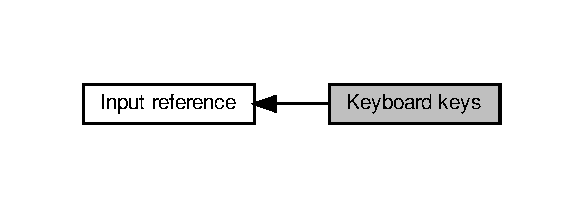
\includegraphics[width=280pt]{group__keys}
\end{center}
\end{figure}
\subsection*{Macros}
\begin{DoxyCompactItemize}
\item 
\mbox{\Hypertarget{group__keys_ga99aacc875b6b27a072552631e13775c7}\label{group__keys_ga99aacc875b6b27a072552631e13775c7}} 
\#define {\bfseries G\+L\+F\+W\+\_\+\+K\+E\+Y\+\_\+\+U\+N\+K\+N\+O\+WN}~-\/1
\item 
\mbox{\Hypertarget{group__keys_gaddb2c23772b97fd7e26e8ee66f1ad014}\label{group__keys_gaddb2c23772b97fd7e26e8ee66f1ad014}} 
\#define {\bfseries G\+L\+F\+W\+\_\+\+K\+E\+Y\+\_\+\+S\+P\+A\+CE}~32
\item 
\mbox{\Hypertarget{group__keys_ga6059b0b048ba6980b6107fffbd3b4b24}\label{group__keys_ga6059b0b048ba6980b6107fffbd3b4b24}} 
\#define {\bfseries G\+L\+F\+W\+\_\+\+K\+E\+Y\+\_\+\+A\+P\+O\+S\+T\+R\+O\+P\+HE}~39  /$\ast$ \textquotesingle{} $\ast$/
\item 
\mbox{\Hypertarget{group__keys_gab3d5d72e59d3055f494627b0a524926c}\label{group__keys_gab3d5d72e59d3055f494627b0a524926c}} 
\#define {\bfseries G\+L\+F\+W\+\_\+\+K\+E\+Y\+\_\+\+C\+O\+M\+MA}~44  /$\ast$ , $\ast$/
\item 
\mbox{\Hypertarget{group__keys_gac556b360f7f6fca4b70ba0aecf313fd4}\label{group__keys_gac556b360f7f6fca4b70ba0aecf313fd4}} 
\#define {\bfseries G\+L\+F\+W\+\_\+\+K\+E\+Y\+\_\+\+M\+I\+N\+US}~45  /$\ast$ -\/ $\ast$/
\item 
\mbox{\Hypertarget{group__keys_ga37e296b650eab419fc474ff69033d927}\label{group__keys_ga37e296b650eab419fc474ff69033d927}} 
\#define {\bfseries G\+L\+F\+W\+\_\+\+K\+E\+Y\+\_\+\+P\+E\+R\+I\+OD}~46  /$\ast$ . $\ast$/
\item 
\mbox{\Hypertarget{group__keys_gadf3d753b2d479148d711de34b83fd0db}\label{group__keys_gadf3d753b2d479148d711de34b83fd0db}} 
\#define {\bfseries G\+L\+F\+W\+\_\+\+K\+E\+Y\+\_\+\+S\+L\+A\+SH}~47  /$\ast$ / $\ast$/
\item 
\mbox{\Hypertarget{group__keys_ga50391730e9d7112ad4fd42d0bd1597c1}\label{group__keys_ga50391730e9d7112ad4fd42d0bd1597c1}} 
\#define {\bfseries G\+L\+F\+W\+\_\+\+K\+E\+Y\+\_\+0}~48
\item 
\mbox{\Hypertarget{group__keys_ga05e4cae9ddb8d40cf6d82c8f11f2502f}\label{group__keys_ga05e4cae9ddb8d40cf6d82c8f11f2502f}} 
\#define {\bfseries G\+L\+F\+W\+\_\+\+K\+E\+Y\+\_\+1}~49
\item 
\mbox{\Hypertarget{group__keys_gadc8e66b3a4c4b5c39ad1305cf852863c}\label{group__keys_gadc8e66b3a4c4b5c39ad1305cf852863c}} 
\#define {\bfseries G\+L\+F\+W\+\_\+\+K\+E\+Y\+\_\+2}~50
\item 
\mbox{\Hypertarget{group__keys_ga812f0273fe1a981e1fa002ae73e92271}\label{group__keys_ga812f0273fe1a981e1fa002ae73e92271}} 
\#define {\bfseries G\+L\+F\+W\+\_\+\+K\+E\+Y\+\_\+3}~51
\item 
\mbox{\Hypertarget{group__keys_ga9e14b6975a9cc8f66cdd5cb3d3861356}\label{group__keys_ga9e14b6975a9cc8f66cdd5cb3d3861356}} 
\#define {\bfseries G\+L\+F\+W\+\_\+\+K\+E\+Y\+\_\+4}~52
\item 
\mbox{\Hypertarget{group__keys_ga4d74ddaa5d4c609993b4d4a15736c924}\label{group__keys_ga4d74ddaa5d4c609993b4d4a15736c924}} 
\#define {\bfseries G\+L\+F\+W\+\_\+\+K\+E\+Y\+\_\+5}~53
\item 
\mbox{\Hypertarget{group__keys_ga9ea4ab80c313a227b14d0a7c6f810b5d}\label{group__keys_ga9ea4ab80c313a227b14d0a7c6f810b5d}} 
\#define {\bfseries G\+L\+F\+W\+\_\+\+K\+E\+Y\+\_\+6}~54
\item 
\mbox{\Hypertarget{group__keys_gab79b1cfae7bd630cfc4604c1f263c666}\label{group__keys_gab79b1cfae7bd630cfc4604c1f263c666}} 
\#define {\bfseries G\+L\+F\+W\+\_\+\+K\+E\+Y\+\_\+7}~55
\item 
\mbox{\Hypertarget{group__keys_gadeaa109a0f9f5afc94fe4a108e686f6f}\label{group__keys_gadeaa109a0f9f5afc94fe4a108e686f6f}} 
\#define {\bfseries G\+L\+F\+W\+\_\+\+K\+E\+Y\+\_\+8}~56
\item 
\mbox{\Hypertarget{group__keys_ga2924cb5349ebbf97c8987f3521c44f39}\label{group__keys_ga2924cb5349ebbf97c8987f3521c44f39}} 
\#define {\bfseries G\+L\+F\+W\+\_\+\+K\+E\+Y\+\_\+9}~57
\item 
\mbox{\Hypertarget{group__keys_ga84233de9ee5bb3e8788a5aa07d80af7d}\label{group__keys_ga84233de9ee5bb3e8788a5aa07d80af7d}} 
\#define {\bfseries G\+L\+F\+W\+\_\+\+K\+E\+Y\+\_\+\+S\+E\+M\+I\+C\+O\+L\+ON}~59  /$\ast$ ; $\ast$/
\item 
\mbox{\Hypertarget{group__keys_gae1a2de47240d6664423c204bdd91bd17}\label{group__keys_gae1a2de47240d6664423c204bdd91bd17}} 
\#define {\bfseries G\+L\+F\+W\+\_\+\+K\+E\+Y\+\_\+\+E\+Q\+U\+AL}~61  /$\ast$ = $\ast$/
\item 
\mbox{\Hypertarget{group__keys_ga03e842608e1ea323370889d33b8f70ff}\label{group__keys_ga03e842608e1ea323370889d33b8f70ff}} 
\#define {\bfseries G\+L\+F\+W\+\_\+\+K\+E\+Y\+\_\+A}~65
\item 
\mbox{\Hypertarget{group__keys_ga8e3fb647ff3aca9e8dbf14fe66332941}\label{group__keys_ga8e3fb647ff3aca9e8dbf14fe66332941}} 
\#define {\bfseries G\+L\+F\+W\+\_\+\+K\+E\+Y\+\_\+B}~66
\item 
\mbox{\Hypertarget{group__keys_ga00ccf3475d9ee2e679480d540d554669}\label{group__keys_ga00ccf3475d9ee2e679480d540d554669}} 
\#define {\bfseries G\+L\+F\+W\+\_\+\+K\+E\+Y\+\_\+C}~67
\item 
\mbox{\Hypertarget{group__keys_ga011f7cdc9a654da984a2506479606933}\label{group__keys_ga011f7cdc9a654da984a2506479606933}} 
\#define {\bfseries G\+L\+F\+W\+\_\+\+K\+E\+Y\+\_\+D}~68
\item 
\mbox{\Hypertarget{group__keys_gabf48fcc3afbe69349df432b470c96ef2}\label{group__keys_gabf48fcc3afbe69349df432b470c96ef2}} 
\#define {\bfseries G\+L\+F\+W\+\_\+\+K\+E\+Y\+\_\+E}~69
\item 
\mbox{\Hypertarget{group__keys_ga5df402e02aca08444240058fd9b42a55}\label{group__keys_ga5df402e02aca08444240058fd9b42a55}} 
\#define {\bfseries G\+L\+F\+W\+\_\+\+K\+E\+Y\+\_\+F}~70
\item 
\mbox{\Hypertarget{group__keys_gae74ecddf7cc96104ab23989b1cdab536}\label{group__keys_gae74ecddf7cc96104ab23989b1cdab536}} 
\#define {\bfseries G\+L\+F\+W\+\_\+\+K\+E\+Y\+\_\+G}~71
\item 
\mbox{\Hypertarget{group__keys_gad4cc98fc8f35f015d9e2fb94bf136076}\label{group__keys_gad4cc98fc8f35f015d9e2fb94bf136076}} 
\#define {\bfseries G\+L\+F\+W\+\_\+\+K\+E\+Y\+\_\+H}~72
\item 
\mbox{\Hypertarget{group__keys_ga274655c8bfe39742684ca393cf8ed093}\label{group__keys_ga274655c8bfe39742684ca393cf8ed093}} 
\#define {\bfseries G\+L\+F\+W\+\_\+\+K\+E\+Y\+\_\+I}~73
\item 
\mbox{\Hypertarget{group__keys_ga65ff2aedb129a3149ad9cb3e4159a75f}\label{group__keys_ga65ff2aedb129a3149ad9cb3e4159a75f}} 
\#define {\bfseries G\+L\+F\+W\+\_\+\+K\+E\+Y\+\_\+J}~74
\item 
\mbox{\Hypertarget{group__keys_ga4ae8debadf6d2a691badae0b53ea3ba0}\label{group__keys_ga4ae8debadf6d2a691badae0b53ea3ba0}} 
\#define {\bfseries G\+L\+F\+W\+\_\+\+K\+E\+Y\+\_\+K}~75
\item 
\mbox{\Hypertarget{group__keys_gaaa8b54a13f6b1eed85ac86f82d550db2}\label{group__keys_gaaa8b54a13f6b1eed85ac86f82d550db2}} 
\#define {\bfseries G\+L\+F\+W\+\_\+\+K\+E\+Y\+\_\+L}~76
\item 
\mbox{\Hypertarget{group__keys_ga4d7f0260c82e4ea3d6ebc7a21d6e3716}\label{group__keys_ga4d7f0260c82e4ea3d6ebc7a21d6e3716}} 
\#define {\bfseries G\+L\+F\+W\+\_\+\+K\+E\+Y\+\_\+M}~77
\item 
\mbox{\Hypertarget{group__keys_gae00856dfeb5d13aafebf59d44de5cdda}\label{group__keys_gae00856dfeb5d13aafebf59d44de5cdda}} 
\#define {\bfseries G\+L\+F\+W\+\_\+\+K\+E\+Y\+\_\+N}~78
\item 
\mbox{\Hypertarget{group__keys_gaecbbb79130df419d58dd7f09a169efe9}\label{group__keys_gaecbbb79130df419d58dd7f09a169efe9}} 
\#define {\bfseries G\+L\+F\+W\+\_\+\+K\+E\+Y\+\_\+O}~79
\item 
\mbox{\Hypertarget{group__keys_ga8fc15819c1094fb2afa01d84546b33e1}\label{group__keys_ga8fc15819c1094fb2afa01d84546b33e1}} 
\#define {\bfseries G\+L\+F\+W\+\_\+\+K\+E\+Y\+\_\+P}~80
\item 
\mbox{\Hypertarget{group__keys_gafdd01e38b120d67cf51e348bb47f3964}\label{group__keys_gafdd01e38b120d67cf51e348bb47f3964}} 
\#define {\bfseries G\+L\+F\+W\+\_\+\+K\+E\+Y\+\_\+Q}~81
\item 
\mbox{\Hypertarget{group__keys_ga4ce6c70a0c98c50b3fe4ab9a728d4d36}\label{group__keys_ga4ce6c70a0c98c50b3fe4ab9a728d4d36}} 
\#define {\bfseries G\+L\+F\+W\+\_\+\+K\+E\+Y\+\_\+R}~82
\item 
\mbox{\Hypertarget{group__keys_ga1570e2ccaab036ea82bed66fc1dab2a9}\label{group__keys_ga1570e2ccaab036ea82bed66fc1dab2a9}} 
\#define {\bfseries G\+L\+F\+W\+\_\+\+K\+E\+Y\+\_\+S}~83
\item 
\mbox{\Hypertarget{group__keys_ga90e0560422ec7a30e7f3f375bc9f37f9}\label{group__keys_ga90e0560422ec7a30e7f3f375bc9f37f9}} 
\#define {\bfseries G\+L\+F\+W\+\_\+\+K\+E\+Y\+\_\+T}~84
\item 
\mbox{\Hypertarget{group__keys_gacad52f3bf7d378fc0ffa72a76769256d}\label{group__keys_gacad52f3bf7d378fc0ffa72a76769256d}} 
\#define {\bfseries G\+L\+F\+W\+\_\+\+K\+E\+Y\+\_\+U}~85
\item 
\mbox{\Hypertarget{group__keys_ga22c7763899ecf7788862e5f90eacce6b}\label{group__keys_ga22c7763899ecf7788862e5f90eacce6b}} 
\#define {\bfseries G\+L\+F\+W\+\_\+\+K\+E\+Y\+\_\+V}~86
\item 
\mbox{\Hypertarget{group__keys_gaa06a712e6202661fc03da5bdb7b6e545}\label{group__keys_gaa06a712e6202661fc03da5bdb7b6e545}} 
\#define {\bfseries G\+L\+F\+W\+\_\+\+K\+E\+Y\+\_\+W}~87
\item 
\mbox{\Hypertarget{group__keys_gac1c42c0bf4192cea713c55598b06b744}\label{group__keys_gac1c42c0bf4192cea713c55598b06b744}} 
\#define {\bfseries G\+L\+F\+W\+\_\+\+K\+E\+Y\+\_\+X}~88
\item 
\mbox{\Hypertarget{group__keys_gafd9f115a549effdf8e372a787c360313}\label{group__keys_gafd9f115a549effdf8e372a787c360313}} 
\#define {\bfseries G\+L\+F\+W\+\_\+\+K\+E\+Y\+\_\+Y}~89
\item 
\mbox{\Hypertarget{group__keys_gac489e208c26afda8d4938ed88718760a}\label{group__keys_gac489e208c26afda8d4938ed88718760a}} 
\#define {\bfseries G\+L\+F\+W\+\_\+\+K\+E\+Y\+\_\+Z}~90
\item 
\mbox{\Hypertarget{group__keys_gad1c8d9adac53925276ecb1d592511d8a}\label{group__keys_gad1c8d9adac53925276ecb1d592511d8a}} 
\#define {\bfseries G\+L\+F\+W\+\_\+\+K\+E\+Y\+\_\+\+L\+E\+F\+T\+\_\+\+B\+R\+A\+C\+K\+ET}~91  /$\ast$ \mbox{[} $\ast$/
\item 
\mbox{\Hypertarget{group__keys_gab8155ea99d1ab27ff56f24f8dc73f8d1}\label{group__keys_gab8155ea99d1ab27ff56f24f8dc73f8d1}} 
\#define {\bfseries G\+L\+F\+W\+\_\+\+K\+E\+Y\+\_\+\+B\+A\+C\+K\+S\+L\+A\+SH}~92  /$\ast$ \textbackslash{} $\ast$/
\item 
\mbox{\Hypertarget{group__keys_ga86ef225fd6a66404caae71044cdd58d8}\label{group__keys_ga86ef225fd6a66404caae71044cdd58d8}} 
\#define {\bfseries G\+L\+F\+W\+\_\+\+K\+E\+Y\+\_\+\+R\+I\+G\+H\+T\+\_\+\+B\+R\+A\+C\+K\+ET}~93  /$\ast$ \mbox{]} $\ast$/
\item 
\mbox{\Hypertarget{group__keys_ga7a3701fb4e2a0b136ff4b568c3c8d668}\label{group__keys_ga7a3701fb4e2a0b136ff4b568c3c8d668}} 
\#define {\bfseries G\+L\+F\+W\+\_\+\+K\+E\+Y\+\_\+\+G\+R\+A\+V\+E\+\_\+\+A\+C\+C\+E\+NT}~96  /$\ast$ ` $\ast$/
\item 
\mbox{\Hypertarget{group__keys_gadc78dad3dab76bcd4b5c20114052577a}\label{group__keys_gadc78dad3dab76bcd4b5c20114052577a}} 
\#define {\bfseries G\+L\+F\+W\+\_\+\+K\+E\+Y\+\_\+\+W\+O\+R\+L\+D\+\_\+1}~161 /$\ast$ non-\/US \#1 $\ast$/
\item 
\mbox{\Hypertarget{group__keys_ga20494bfebf0bb4fc9503afca18ab2c5e}\label{group__keys_ga20494bfebf0bb4fc9503afca18ab2c5e}} 
\#define {\bfseries G\+L\+F\+W\+\_\+\+K\+E\+Y\+\_\+\+W\+O\+R\+L\+D\+\_\+2}~162 /$\ast$ non-\/US \#2 $\ast$/
\item 
\mbox{\Hypertarget{group__keys_gaac6596c350b635c245113b81c2123b93}\label{group__keys_gaac6596c350b635c245113b81c2123b93}} 
\#define {\bfseries G\+L\+F\+W\+\_\+\+K\+E\+Y\+\_\+\+E\+S\+C\+A\+PE}~256
\item 
\mbox{\Hypertarget{group__keys_ga9555a92ecbecdbc1f3435219c571d667}\label{group__keys_ga9555a92ecbecdbc1f3435219c571d667}} 
\#define {\bfseries G\+L\+F\+W\+\_\+\+K\+E\+Y\+\_\+\+E\+N\+T\+ER}~257
\item 
\mbox{\Hypertarget{group__keys_ga6908a4bda9950a3e2b73f794bbe985df}\label{group__keys_ga6908a4bda9950a3e2b73f794bbe985df}} 
\#define {\bfseries G\+L\+F\+W\+\_\+\+K\+E\+Y\+\_\+\+T\+AB}~258
\item 
\mbox{\Hypertarget{group__keys_ga6c0df1fe2f156bbd5a98c66d76ff3635}\label{group__keys_ga6c0df1fe2f156bbd5a98c66d76ff3635}} 
\#define {\bfseries G\+L\+F\+W\+\_\+\+K\+E\+Y\+\_\+\+B\+A\+C\+K\+S\+P\+A\+CE}~259
\item 
\mbox{\Hypertarget{group__keys_ga373ac7365435d6b0eb1068f470e34f47}\label{group__keys_ga373ac7365435d6b0eb1068f470e34f47}} 
\#define {\bfseries G\+L\+F\+W\+\_\+\+K\+E\+Y\+\_\+\+I\+N\+S\+E\+RT}~260
\item 
\mbox{\Hypertarget{group__keys_gadb111e4df74b8a715f2c05dad58d2682}\label{group__keys_gadb111e4df74b8a715f2c05dad58d2682}} 
\#define {\bfseries G\+L\+F\+W\+\_\+\+K\+E\+Y\+\_\+\+D\+E\+L\+E\+TE}~261
\item 
\mbox{\Hypertarget{group__keys_ga06ba07662e8c291a4a84535379ffc7ac}\label{group__keys_ga06ba07662e8c291a4a84535379ffc7ac}} 
\#define {\bfseries G\+L\+F\+W\+\_\+\+K\+E\+Y\+\_\+\+R\+I\+G\+HT}~262
\item 
\mbox{\Hypertarget{group__keys_gae12a010d33c309a67ab9460c51eb2462}\label{group__keys_gae12a010d33c309a67ab9460c51eb2462}} 
\#define {\bfseries G\+L\+F\+W\+\_\+\+K\+E\+Y\+\_\+\+L\+E\+FT}~263
\item 
\mbox{\Hypertarget{group__keys_gae2e3958c71595607416aa7bf082be2f9}\label{group__keys_gae2e3958c71595607416aa7bf082be2f9}} 
\#define {\bfseries G\+L\+F\+W\+\_\+\+K\+E\+Y\+\_\+\+D\+O\+WN}~264
\item 
\mbox{\Hypertarget{group__keys_ga2f3342b194020d3544c67e3506b6f144}\label{group__keys_ga2f3342b194020d3544c67e3506b6f144}} 
\#define {\bfseries G\+L\+F\+W\+\_\+\+K\+E\+Y\+\_\+\+UP}~265
\item 
\mbox{\Hypertarget{group__keys_ga3ab731f9622f0db280178a5f3cc6d586}\label{group__keys_ga3ab731f9622f0db280178a5f3cc6d586}} 
\#define {\bfseries G\+L\+F\+W\+\_\+\+K\+E\+Y\+\_\+\+P\+A\+G\+E\+\_\+\+UP}~266
\item 
\mbox{\Hypertarget{group__keys_gaee0a8fa442001cc2147812f84b59041c}\label{group__keys_gaee0a8fa442001cc2147812f84b59041c}} 
\#define {\bfseries G\+L\+F\+W\+\_\+\+K\+E\+Y\+\_\+\+P\+A\+G\+E\+\_\+\+D\+O\+WN}~267
\item 
\mbox{\Hypertarget{group__keys_ga41452c7287195d481e43207318c126a7}\label{group__keys_ga41452c7287195d481e43207318c126a7}} 
\#define {\bfseries G\+L\+F\+W\+\_\+\+K\+E\+Y\+\_\+\+H\+O\+ME}~268
\item 
\mbox{\Hypertarget{group__keys_ga86587ea1df19a65978d3e3b8439bedd9}\label{group__keys_ga86587ea1df19a65978d3e3b8439bedd9}} 
\#define {\bfseries G\+L\+F\+W\+\_\+\+K\+E\+Y\+\_\+\+E\+ND}~269
\item 
\mbox{\Hypertarget{group__keys_ga92c1d2c9d63485f3d70f94f688d48672}\label{group__keys_ga92c1d2c9d63485f3d70f94f688d48672}} 
\#define {\bfseries G\+L\+F\+W\+\_\+\+K\+E\+Y\+\_\+\+C\+A\+P\+S\+\_\+\+L\+O\+CK}~280
\item 
\mbox{\Hypertarget{group__keys_gaf622b63b9537f7084c2ab649b8365630}\label{group__keys_gaf622b63b9537f7084c2ab649b8365630}} 
\#define {\bfseries G\+L\+F\+W\+\_\+\+K\+E\+Y\+\_\+\+S\+C\+R\+O\+L\+L\+\_\+\+L\+O\+CK}~281
\item 
\mbox{\Hypertarget{group__keys_ga3946edc362aeff213b2be6304296cf43}\label{group__keys_ga3946edc362aeff213b2be6304296cf43}} 
\#define {\bfseries G\+L\+F\+W\+\_\+\+K\+E\+Y\+\_\+\+N\+U\+M\+\_\+\+L\+O\+CK}~282
\item 
\mbox{\Hypertarget{group__keys_gaf964c2e65e97d0cf785a5636ee8df642}\label{group__keys_gaf964c2e65e97d0cf785a5636ee8df642}} 
\#define {\bfseries G\+L\+F\+W\+\_\+\+K\+E\+Y\+\_\+\+P\+R\+I\+N\+T\+\_\+\+S\+C\+R\+E\+EN}~283
\item 
\mbox{\Hypertarget{group__keys_ga8116b9692d87382afb5849b6d8907f18}\label{group__keys_ga8116b9692d87382afb5849b6d8907f18}} 
\#define {\bfseries G\+L\+F\+W\+\_\+\+K\+E\+Y\+\_\+\+P\+A\+U\+SE}~284
\item 
\mbox{\Hypertarget{group__keys_gafb8d66c573acf22e364049477dcbea30}\label{group__keys_gafb8d66c573acf22e364049477dcbea30}} 
\#define {\bfseries G\+L\+F\+W\+\_\+\+K\+E\+Y\+\_\+\+F1}~290
\item 
\mbox{\Hypertarget{group__keys_ga0900750aff94889b940f5e428c07daee}\label{group__keys_ga0900750aff94889b940f5e428c07daee}} 
\#define {\bfseries G\+L\+F\+W\+\_\+\+K\+E\+Y\+\_\+\+F2}~291
\item 
\mbox{\Hypertarget{group__keys_gaed7cd729c0147a551bb8b7bb36c17015}\label{group__keys_gaed7cd729c0147a551bb8b7bb36c17015}} 
\#define {\bfseries G\+L\+F\+W\+\_\+\+K\+E\+Y\+\_\+\+F3}~292
\item 
\mbox{\Hypertarget{group__keys_ga9b61ebd0c63b44b7332fda2c9763eaa6}\label{group__keys_ga9b61ebd0c63b44b7332fda2c9763eaa6}} 
\#define {\bfseries G\+L\+F\+W\+\_\+\+K\+E\+Y\+\_\+\+F4}~293
\item 
\mbox{\Hypertarget{group__keys_gaf258dda9947daa428377938ed577c8c2}\label{group__keys_gaf258dda9947daa428377938ed577c8c2}} 
\#define {\bfseries G\+L\+F\+W\+\_\+\+K\+E\+Y\+\_\+\+F5}~294
\item 
\mbox{\Hypertarget{group__keys_ga6dc2d3f87b9d51ffbbbe2ef0299d8e1d}\label{group__keys_ga6dc2d3f87b9d51ffbbbe2ef0299d8e1d}} 
\#define {\bfseries G\+L\+F\+W\+\_\+\+K\+E\+Y\+\_\+\+F6}~295
\item 
\mbox{\Hypertarget{group__keys_gacca6ef8a2162c52a0ac1d881e8d9c38a}\label{group__keys_gacca6ef8a2162c52a0ac1d881e8d9c38a}} 
\#define {\bfseries G\+L\+F\+W\+\_\+\+K\+E\+Y\+\_\+\+F7}~296
\item 
\mbox{\Hypertarget{group__keys_gac9d39390336ae14e4a93e295de43c7e8}\label{group__keys_gac9d39390336ae14e4a93e295de43c7e8}} 
\#define {\bfseries G\+L\+F\+W\+\_\+\+K\+E\+Y\+\_\+\+F8}~297
\item 
\mbox{\Hypertarget{group__keys_gae40de0de1c9f21cd26c9afa3d7050851}\label{group__keys_gae40de0de1c9f21cd26c9afa3d7050851}} 
\#define {\bfseries G\+L\+F\+W\+\_\+\+K\+E\+Y\+\_\+\+F9}~298
\item 
\mbox{\Hypertarget{group__keys_ga718d11d2f7d57471a2f6a894235995b1}\label{group__keys_ga718d11d2f7d57471a2f6a894235995b1}} 
\#define {\bfseries G\+L\+F\+W\+\_\+\+K\+E\+Y\+\_\+\+F10}~299
\item 
\mbox{\Hypertarget{group__keys_ga0bc04b11627e7d69339151e7306b2832}\label{group__keys_ga0bc04b11627e7d69339151e7306b2832}} 
\#define {\bfseries G\+L\+F\+W\+\_\+\+K\+E\+Y\+\_\+\+F11}~300
\item 
\mbox{\Hypertarget{group__keys_gaf5908fa9b0a906ae03fc2c61ac7aa3e2}\label{group__keys_gaf5908fa9b0a906ae03fc2c61ac7aa3e2}} 
\#define {\bfseries G\+L\+F\+W\+\_\+\+K\+E\+Y\+\_\+\+F12}~301
\item 
\mbox{\Hypertarget{group__keys_gad637f4308655e1001bd6ad942bc0fd4b}\label{group__keys_gad637f4308655e1001bd6ad942bc0fd4b}} 
\#define {\bfseries G\+L\+F\+W\+\_\+\+K\+E\+Y\+\_\+\+F13}~302
\item 
\mbox{\Hypertarget{group__keys_gaf14c66cff3396e5bd46e803c035e6c1f}\label{group__keys_gaf14c66cff3396e5bd46e803c035e6c1f}} 
\#define {\bfseries G\+L\+F\+W\+\_\+\+K\+E\+Y\+\_\+\+F14}~303
\item 
\mbox{\Hypertarget{group__keys_ga7f70970db6e8be1794da8516a6d14058}\label{group__keys_ga7f70970db6e8be1794da8516a6d14058}} 
\#define {\bfseries G\+L\+F\+W\+\_\+\+K\+E\+Y\+\_\+\+F15}~304
\item 
\mbox{\Hypertarget{group__keys_gaa582dbb1d2ba2050aa1dca0838095b27}\label{group__keys_gaa582dbb1d2ba2050aa1dca0838095b27}} 
\#define {\bfseries G\+L\+F\+W\+\_\+\+K\+E\+Y\+\_\+\+F16}~305
\item 
\mbox{\Hypertarget{group__keys_ga972ce5c365e2394b36104b0e3125c748}\label{group__keys_ga972ce5c365e2394b36104b0e3125c748}} 
\#define {\bfseries G\+L\+F\+W\+\_\+\+K\+E\+Y\+\_\+\+F17}~306
\item 
\mbox{\Hypertarget{group__keys_gaebf6391058d5566601e357edc5ea737c}\label{group__keys_gaebf6391058d5566601e357edc5ea737c}} 
\#define {\bfseries G\+L\+F\+W\+\_\+\+K\+E\+Y\+\_\+\+F18}~307
\item 
\mbox{\Hypertarget{group__keys_gaec011d9ba044058cb54529da710e9791}\label{group__keys_gaec011d9ba044058cb54529da710e9791}} 
\#define {\bfseries G\+L\+F\+W\+\_\+\+K\+E\+Y\+\_\+\+F19}~308
\item 
\mbox{\Hypertarget{group__keys_ga82b9c721ada04cd5ca8de767da38022f}\label{group__keys_ga82b9c721ada04cd5ca8de767da38022f}} 
\#define {\bfseries G\+L\+F\+W\+\_\+\+K\+E\+Y\+\_\+\+F20}~309
\item 
\mbox{\Hypertarget{group__keys_ga356afb14d3440ff2bb378f74f7ebc60f}\label{group__keys_ga356afb14d3440ff2bb378f74f7ebc60f}} 
\#define {\bfseries G\+L\+F\+W\+\_\+\+K\+E\+Y\+\_\+\+F21}~310
\item 
\mbox{\Hypertarget{group__keys_ga90960bd2a155f2b09675324d3dff1565}\label{group__keys_ga90960bd2a155f2b09675324d3dff1565}} 
\#define {\bfseries G\+L\+F\+W\+\_\+\+K\+E\+Y\+\_\+\+F22}~311
\item 
\mbox{\Hypertarget{group__keys_ga43c21099aac10952d1be909a8ddee4d5}\label{group__keys_ga43c21099aac10952d1be909a8ddee4d5}} 
\#define {\bfseries G\+L\+F\+W\+\_\+\+K\+E\+Y\+\_\+\+F23}~312
\item 
\mbox{\Hypertarget{group__keys_ga8150374677b5bed3043408732152dea2}\label{group__keys_ga8150374677b5bed3043408732152dea2}} 
\#define {\bfseries G\+L\+F\+W\+\_\+\+K\+E\+Y\+\_\+\+F24}~313
\item 
\mbox{\Hypertarget{group__keys_gaa4bbd93ed73bb4c6ae7d83df880b7199}\label{group__keys_gaa4bbd93ed73bb4c6ae7d83df880b7199}} 
\#define {\bfseries G\+L\+F\+W\+\_\+\+K\+E\+Y\+\_\+\+F25}~314
\item 
\mbox{\Hypertarget{group__keys_ga10515dafc55b71e7683f5b4fedd1c70d}\label{group__keys_ga10515dafc55b71e7683f5b4fedd1c70d}} 
\#define {\bfseries G\+L\+F\+W\+\_\+\+K\+E\+Y\+\_\+\+K\+P\+\_\+0}~320
\item 
\mbox{\Hypertarget{group__keys_gaf3a29a334402c5eaf0b3439edf5587c3}\label{group__keys_gaf3a29a334402c5eaf0b3439edf5587c3}} 
\#define {\bfseries G\+L\+F\+W\+\_\+\+K\+E\+Y\+\_\+\+K\+P\+\_\+1}~321
\item 
\mbox{\Hypertarget{group__keys_gaf82d5a802ab8213c72653d7480c16f13}\label{group__keys_gaf82d5a802ab8213c72653d7480c16f13}} 
\#define {\bfseries G\+L\+F\+W\+\_\+\+K\+E\+Y\+\_\+\+K\+P\+\_\+2}~322
\item 
\mbox{\Hypertarget{group__keys_ga7e25ff30d56cd512828c1d4ae8d54ef2}\label{group__keys_ga7e25ff30d56cd512828c1d4ae8d54ef2}} 
\#define {\bfseries G\+L\+F\+W\+\_\+\+K\+E\+Y\+\_\+\+K\+P\+\_\+3}~323
\item 
\mbox{\Hypertarget{group__keys_gada7ec86778b85e0b4de0beea72234aea}\label{group__keys_gada7ec86778b85e0b4de0beea72234aea}} 
\#define {\bfseries G\+L\+F\+W\+\_\+\+K\+E\+Y\+\_\+\+K\+P\+\_\+4}~324
\item 
\mbox{\Hypertarget{group__keys_ga9a5be274434866c51738cafbb6d26b45}\label{group__keys_ga9a5be274434866c51738cafbb6d26b45}} 
\#define {\bfseries G\+L\+F\+W\+\_\+\+K\+E\+Y\+\_\+\+K\+P\+\_\+5}~325
\item 
\mbox{\Hypertarget{group__keys_gafc141b0f8450519084c01092a3157faa}\label{group__keys_gafc141b0f8450519084c01092a3157faa}} 
\#define {\bfseries G\+L\+F\+W\+\_\+\+K\+E\+Y\+\_\+\+K\+P\+\_\+6}~326
\item 
\mbox{\Hypertarget{group__keys_ga8882f411f05d04ec77a9563974bbfa53}\label{group__keys_ga8882f411f05d04ec77a9563974bbfa53}} 
\#define {\bfseries G\+L\+F\+W\+\_\+\+K\+E\+Y\+\_\+\+K\+P\+\_\+7}~327
\item 
\mbox{\Hypertarget{group__keys_gab2ea2e6a12f89d315045af520ac78cec}\label{group__keys_gab2ea2e6a12f89d315045af520ac78cec}} 
\#define {\bfseries G\+L\+F\+W\+\_\+\+K\+E\+Y\+\_\+\+K\+P\+\_\+8}~328
\item 
\mbox{\Hypertarget{group__keys_gafb21426b630ed4fcc084868699ba74c1}\label{group__keys_gafb21426b630ed4fcc084868699ba74c1}} 
\#define {\bfseries G\+L\+F\+W\+\_\+\+K\+E\+Y\+\_\+\+K\+P\+\_\+9}~329
\item 
\mbox{\Hypertarget{group__keys_ga4e231d968796331a9ea0dbfb98d4005b}\label{group__keys_ga4e231d968796331a9ea0dbfb98d4005b}} 
\#define {\bfseries G\+L\+F\+W\+\_\+\+K\+E\+Y\+\_\+\+K\+P\+\_\+\+D\+E\+C\+I\+M\+AL}~330
\item 
\mbox{\Hypertarget{group__keys_gabca1733780a273d549129ad0f250d1e5}\label{group__keys_gabca1733780a273d549129ad0f250d1e5}} 
\#define {\bfseries G\+L\+F\+W\+\_\+\+K\+E\+Y\+\_\+\+K\+P\+\_\+\+D\+I\+V\+I\+DE}~331
\item 
\mbox{\Hypertarget{group__keys_ga9ada267eb0e78ed2ada8701dd24a56ef}\label{group__keys_ga9ada267eb0e78ed2ada8701dd24a56ef}} 
\#define {\bfseries G\+L\+F\+W\+\_\+\+K\+E\+Y\+\_\+\+K\+P\+\_\+\+M\+U\+L\+T\+I\+P\+LY}~332
\item 
\mbox{\Hypertarget{group__keys_gaa3dbd60782ff93d6082a124bce1fa236}\label{group__keys_gaa3dbd60782ff93d6082a124bce1fa236}} 
\#define {\bfseries G\+L\+F\+W\+\_\+\+K\+E\+Y\+\_\+\+K\+P\+\_\+\+S\+U\+B\+T\+R\+A\+CT}~333
\item 
\mbox{\Hypertarget{group__keys_gad09c7c98acc79e89aa6a0a91275becac}\label{group__keys_gad09c7c98acc79e89aa6a0a91275becac}} 
\#define {\bfseries G\+L\+F\+W\+\_\+\+K\+E\+Y\+\_\+\+K\+P\+\_\+\+A\+DD}~334
\item 
\mbox{\Hypertarget{group__keys_ga4f728f8738f2986bd63eedd3d412e8cf}\label{group__keys_ga4f728f8738f2986bd63eedd3d412e8cf}} 
\#define {\bfseries G\+L\+F\+W\+\_\+\+K\+E\+Y\+\_\+\+K\+P\+\_\+\+E\+N\+T\+ER}~335
\item 
\mbox{\Hypertarget{group__keys_gaebdc76d4a808191e6d21b7e4ad2acd97}\label{group__keys_gaebdc76d4a808191e6d21b7e4ad2acd97}} 
\#define {\bfseries G\+L\+F\+W\+\_\+\+K\+E\+Y\+\_\+\+K\+P\+\_\+\+E\+Q\+U\+AL}~336
\item 
\mbox{\Hypertarget{group__keys_ga8a530a28a65c44ab5d00b759b756d3f6}\label{group__keys_ga8a530a28a65c44ab5d00b759b756d3f6}} 
\#define {\bfseries G\+L\+F\+W\+\_\+\+K\+E\+Y\+\_\+\+L\+E\+F\+T\+\_\+\+S\+H\+I\+FT}~340
\item 
\mbox{\Hypertarget{group__keys_ga9f97b743e81460ac4b2deddecd10a464}\label{group__keys_ga9f97b743e81460ac4b2deddecd10a464}} 
\#define {\bfseries G\+L\+F\+W\+\_\+\+K\+E\+Y\+\_\+\+L\+E\+F\+T\+\_\+\+C\+O\+N\+T\+R\+OL}~341
\item 
\mbox{\Hypertarget{group__keys_ga7f27dabf63a7789daa31e1c96790219b}\label{group__keys_ga7f27dabf63a7789daa31e1c96790219b}} 
\#define {\bfseries G\+L\+F\+W\+\_\+\+K\+E\+Y\+\_\+\+L\+E\+F\+T\+\_\+\+A\+LT}~342
\item 
\mbox{\Hypertarget{group__keys_gafb1207c91997fc295afd1835fbc5641a}\label{group__keys_gafb1207c91997fc295afd1835fbc5641a}} 
\#define {\bfseries G\+L\+F\+W\+\_\+\+K\+E\+Y\+\_\+\+L\+E\+F\+T\+\_\+\+S\+U\+P\+ER}~343
\item 
\mbox{\Hypertarget{group__keys_gaffca36b99c9dce1a19cb9befbadce691}\label{group__keys_gaffca36b99c9dce1a19cb9befbadce691}} 
\#define {\bfseries G\+L\+F\+W\+\_\+\+K\+E\+Y\+\_\+\+R\+I\+G\+H\+T\+\_\+\+S\+H\+I\+FT}~344
\item 
\mbox{\Hypertarget{group__keys_gad1ca2094b2694e7251d0ab1fd34f8519}\label{group__keys_gad1ca2094b2694e7251d0ab1fd34f8519}} 
\#define {\bfseries G\+L\+F\+W\+\_\+\+K\+E\+Y\+\_\+\+R\+I\+G\+H\+T\+\_\+\+C\+O\+N\+T\+R\+OL}~345
\item 
\mbox{\Hypertarget{group__keys_ga687b38009131cfdd07a8d05fff8fa446}\label{group__keys_ga687b38009131cfdd07a8d05fff8fa446}} 
\#define {\bfseries G\+L\+F\+W\+\_\+\+K\+E\+Y\+\_\+\+R\+I\+G\+H\+T\+\_\+\+A\+LT}~346
\item 
\mbox{\Hypertarget{group__keys_gad4547a3e8e247594acb60423fe6502db}\label{group__keys_gad4547a3e8e247594acb60423fe6502db}} 
\#define {\bfseries G\+L\+F\+W\+\_\+\+K\+E\+Y\+\_\+\+R\+I\+G\+H\+T\+\_\+\+S\+U\+P\+ER}~347
\item 
\mbox{\Hypertarget{group__keys_ga9845be48a745fc232045c9ec174d8820}\label{group__keys_ga9845be48a745fc232045c9ec174d8820}} 
\#define {\bfseries G\+L\+F\+W\+\_\+\+K\+E\+Y\+\_\+\+M\+E\+NU}~348
\item 
\mbox{\Hypertarget{group__keys_ga442cbaef7bfb9a4ba13594dd7fbf2789}\label{group__keys_ga442cbaef7bfb9a4ba13594dd7fbf2789}} 
\#define {\bfseries G\+L\+F\+W\+\_\+\+K\+E\+Y\+\_\+\+L\+A\+ST}~G\+L\+F\+W\+\_\+\+K\+E\+Y\+\_\+\+M\+E\+NU
\item 
\mbox{\Hypertarget{group__keys_ga99aacc875b6b27a072552631e13775c7}\label{group__keys_ga99aacc875b6b27a072552631e13775c7}} 
\#define {\bfseries G\+L\+F\+W\+\_\+\+K\+E\+Y\+\_\+\+U\+N\+K\+N\+O\+WN}~-\/1
\item 
\mbox{\Hypertarget{group__keys_gaddb2c23772b97fd7e26e8ee66f1ad014}\label{group__keys_gaddb2c23772b97fd7e26e8ee66f1ad014}} 
\#define {\bfseries G\+L\+F\+W\+\_\+\+K\+E\+Y\+\_\+\+S\+P\+A\+CE}~32
\item 
\mbox{\Hypertarget{group__keys_ga6059b0b048ba6980b6107fffbd3b4b24}\label{group__keys_ga6059b0b048ba6980b6107fffbd3b4b24}} 
\#define {\bfseries G\+L\+F\+W\+\_\+\+K\+E\+Y\+\_\+\+A\+P\+O\+S\+T\+R\+O\+P\+HE}~39  /$\ast$ \textquotesingle{} $\ast$/
\item 
\mbox{\Hypertarget{group__keys_gab3d5d72e59d3055f494627b0a524926c}\label{group__keys_gab3d5d72e59d3055f494627b0a524926c}} 
\#define {\bfseries G\+L\+F\+W\+\_\+\+K\+E\+Y\+\_\+\+C\+O\+M\+MA}~44  /$\ast$ , $\ast$/
\item 
\mbox{\Hypertarget{group__keys_gac556b360f7f6fca4b70ba0aecf313fd4}\label{group__keys_gac556b360f7f6fca4b70ba0aecf313fd4}} 
\#define {\bfseries G\+L\+F\+W\+\_\+\+K\+E\+Y\+\_\+\+M\+I\+N\+US}~45  /$\ast$ -\/ $\ast$/
\item 
\mbox{\Hypertarget{group__keys_ga37e296b650eab419fc474ff69033d927}\label{group__keys_ga37e296b650eab419fc474ff69033d927}} 
\#define {\bfseries G\+L\+F\+W\+\_\+\+K\+E\+Y\+\_\+\+P\+E\+R\+I\+OD}~46  /$\ast$ . $\ast$/
\item 
\mbox{\Hypertarget{group__keys_gadf3d753b2d479148d711de34b83fd0db}\label{group__keys_gadf3d753b2d479148d711de34b83fd0db}} 
\#define {\bfseries G\+L\+F\+W\+\_\+\+K\+E\+Y\+\_\+\+S\+L\+A\+SH}~47  /$\ast$ / $\ast$/
\item 
\mbox{\Hypertarget{group__keys_ga50391730e9d7112ad4fd42d0bd1597c1}\label{group__keys_ga50391730e9d7112ad4fd42d0bd1597c1}} 
\#define {\bfseries G\+L\+F\+W\+\_\+\+K\+E\+Y\+\_\+0}~48
\item 
\mbox{\Hypertarget{group__keys_ga05e4cae9ddb8d40cf6d82c8f11f2502f}\label{group__keys_ga05e4cae9ddb8d40cf6d82c8f11f2502f}} 
\#define {\bfseries G\+L\+F\+W\+\_\+\+K\+E\+Y\+\_\+1}~49
\item 
\mbox{\Hypertarget{group__keys_gadc8e66b3a4c4b5c39ad1305cf852863c}\label{group__keys_gadc8e66b3a4c4b5c39ad1305cf852863c}} 
\#define {\bfseries G\+L\+F\+W\+\_\+\+K\+E\+Y\+\_\+2}~50
\item 
\mbox{\Hypertarget{group__keys_ga812f0273fe1a981e1fa002ae73e92271}\label{group__keys_ga812f0273fe1a981e1fa002ae73e92271}} 
\#define {\bfseries G\+L\+F\+W\+\_\+\+K\+E\+Y\+\_\+3}~51
\item 
\mbox{\Hypertarget{group__keys_ga9e14b6975a9cc8f66cdd5cb3d3861356}\label{group__keys_ga9e14b6975a9cc8f66cdd5cb3d3861356}} 
\#define {\bfseries G\+L\+F\+W\+\_\+\+K\+E\+Y\+\_\+4}~52
\item 
\mbox{\Hypertarget{group__keys_ga4d74ddaa5d4c609993b4d4a15736c924}\label{group__keys_ga4d74ddaa5d4c609993b4d4a15736c924}} 
\#define {\bfseries G\+L\+F\+W\+\_\+\+K\+E\+Y\+\_\+5}~53
\item 
\mbox{\Hypertarget{group__keys_ga9ea4ab80c313a227b14d0a7c6f810b5d}\label{group__keys_ga9ea4ab80c313a227b14d0a7c6f810b5d}} 
\#define {\bfseries G\+L\+F\+W\+\_\+\+K\+E\+Y\+\_\+6}~54
\item 
\mbox{\Hypertarget{group__keys_gab79b1cfae7bd630cfc4604c1f263c666}\label{group__keys_gab79b1cfae7bd630cfc4604c1f263c666}} 
\#define {\bfseries G\+L\+F\+W\+\_\+\+K\+E\+Y\+\_\+7}~55
\item 
\mbox{\Hypertarget{group__keys_gadeaa109a0f9f5afc94fe4a108e686f6f}\label{group__keys_gadeaa109a0f9f5afc94fe4a108e686f6f}} 
\#define {\bfseries G\+L\+F\+W\+\_\+\+K\+E\+Y\+\_\+8}~56
\item 
\mbox{\Hypertarget{group__keys_ga2924cb5349ebbf97c8987f3521c44f39}\label{group__keys_ga2924cb5349ebbf97c8987f3521c44f39}} 
\#define {\bfseries G\+L\+F\+W\+\_\+\+K\+E\+Y\+\_\+9}~57
\item 
\mbox{\Hypertarget{group__keys_ga84233de9ee5bb3e8788a5aa07d80af7d}\label{group__keys_ga84233de9ee5bb3e8788a5aa07d80af7d}} 
\#define {\bfseries G\+L\+F\+W\+\_\+\+K\+E\+Y\+\_\+\+S\+E\+M\+I\+C\+O\+L\+ON}~59  /$\ast$ ; $\ast$/
\item 
\mbox{\Hypertarget{group__keys_gae1a2de47240d6664423c204bdd91bd17}\label{group__keys_gae1a2de47240d6664423c204bdd91bd17}} 
\#define {\bfseries G\+L\+F\+W\+\_\+\+K\+E\+Y\+\_\+\+E\+Q\+U\+AL}~61  /$\ast$ = $\ast$/
\item 
\mbox{\Hypertarget{group__keys_ga03e842608e1ea323370889d33b8f70ff}\label{group__keys_ga03e842608e1ea323370889d33b8f70ff}} 
\#define {\bfseries G\+L\+F\+W\+\_\+\+K\+E\+Y\+\_\+A}~65
\item 
\mbox{\Hypertarget{group__keys_ga8e3fb647ff3aca9e8dbf14fe66332941}\label{group__keys_ga8e3fb647ff3aca9e8dbf14fe66332941}} 
\#define {\bfseries G\+L\+F\+W\+\_\+\+K\+E\+Y\+\_\+B}~66
\item 
\mbox{\Hypertarget{group__keys_ga00ccf3475d9ee2e679480d540d554669}\label{group__keys_ga00ccf3475d9ee2e679480d540d554669}} 
\#define {\bfseries G\+L\+F\+W\+\_\+\+K\+E\+Y\+\_\+C}~67
\item 
\mbox{\Hypertarget{group__keys_ga011f7cdc9a654da984a2506479606933}\label{group__keys_ga011f7cdc9a654da984a2506479606933}} 
\#define {\bfseries G\+L\+F\+W\+\_\+\+K\+E\+Y\+\_\+D}~68
\item 
\mbox{\Hypertarget{group__keys_gabf48fcc3afbe69349df432b470c96ef2}\label{group__keys_gabf48fcc3afbe69349df432b470c96ef2}} 
\#define {\bfseries G\+L\+F\+W\+\_\+\+K\+E\+Y\+\_\+E}~69
\item 
\mbox{\Hypertarget{group__keys_ga5df402e02aca08444240058fd9b42a55}\label{group__keys_ga5df402e02aca08444240058fd9b42a55}} 
\#define {\bfseries G\+L\+F\+W\+\_\+\+K\+E\+Y\+\_\+F}~70
\item 
\mbox{\Hypertarget{group__keys_gae74ecddf7cc96104ab23989b1cdab536}\label{group__keys_gae74ecddf7cc96104ab23989b1cdab536}} 
\#define {\bfseries G\+L\+F\+W\+\_\+\+K\+E\+Y\+\_\+G}~71
\item 
\mbox{\Hypertarget{group__keys_gad4cc98fc8f35f015d9e2fb94bf136076}\label{group__keys_gad4cc98fc8f35f015d9e2fb94bf136076}} 
\#define {\bfseries G\+L\+F\+W\+\_\+\+K\+E\+Y\+\_\+H}~72
\item 
\mbox{\Hypertarget{group__keys_ga274655c8bfe39742684ca393cf8ed093}\label{group__keys_ga274655c8bfe39742684ca393cf8ed093}} 
\#define {\bfseries G\+L\+F\+W\+\_\+\+K\+E\+Y\+\_\+I}~73
\item 
\mbox{\Hypertarget{group__keys_ga65ff2aedb129a3149ad9cb3e4159a75f}\label{group__keys_ga65ff2aedb129a3149ad9cb3e4159a75f}} 
\#define {\bfseries G\+L\+F\+W\+\_\+\+K\+E\+Y\+\_\+J}~74
\item 
\mbox{\Hypertarget{group__keys_ga4ae8debadf6d2a691badae0b53ea3ba0}\label{group__keys_ga4ae8debadf6d2a691badae0b53ea3ba0}} 
\#define {\bfseries G\+L\+F\+W\+\_\+\+K\+E\+Y\+\_\+K}~75
\item 
\mbox{\Hypertarget{group__keys_gaaa8b54a13f6b1eed85ac86f82d550db2}\label{group__keys_gaaa8b54a13f6b1eed85ac86f82d550db2}} 
\#define {\bfseries G\+L\+F\+W\+\_\+\+K\+E\+Y\+\_\+L}~76
\item 
\mbox{\Hypertarget{group__keys_ga4d7f0260c82e4ea3d6ebc7a21d6e3716}\label{group__keys_ga4d7f0260c82e4ea3d6ebc7a21d6e3716}} 
\#define {\bfseries G\+L\+F\+W\+\_\+\+K\+E\+Y\+\_\+M}~77
\item 
\mbox{\Hypertarget{group__keys_gae00856dfeb5d13aafebf59d44de5cdda}\label{group__keys_gae00856dfeb5d13aafebf59d44de5cdda}} 
\#define {\bfseries G\+L\+F\+W\+\_\+\+K\+E\+Y\+\_\+N}~78
\item 
\mbox{\Hypertarget{group__keys_gaecbbb79130df419d58dd7f09a169efe9}\label{group__keys_gaecbbb79130df419d58dd7f09a169efe9}} 
\#define {\bfseries G\+L\+F\+W\+\_\+\+K\+E\+Y\+\_\+O}~79
\item 
\mbox{\Hypertarget{group__keys_ga8fc15819c1094fb2afa01d84546b33e1}\label{group__keys_ga8fc15819c1094fb2afa01d84546b33e1}} 
\#define {\bfseries G\+L\+F\+W\+\_\+\+K\+E\+Y\+\_\+P}~80
\item 
\mbox{\Hypertarget{group__keys_gafdd01e38b120d67cf51e348bb47f3964}\label{group__keys_gafdd01e38b120d67cf51e348bb47f3964}} 
\#define {\bfseries G\+L\+F\+W\+\_\+\+K\+E\+Y\+\_\+Q}~81
\item 
\mbox{\Hypertarget{group__keys_ga4ce6c70a0c98c50b3fe4ab9a728d4d36}\label{group__keys_ga4ce6c70a0c98c50b3fe4ab9a728d4d36}} 
\#define {\bfseries G\+L\+F\+W\+\_\+\+K\+E\+Y\+\_\+R}~82
\item 
\mbox{\Hypertarget{group__keys_ga1570e2ccaab036ea82bed66fc1dab2a9}\label{group__keys_ga1570e2ccaab036ea82bed66fc1dab2a9}} 
\#define {\bfseries G\+L\+F\+W\+\_\+\+K\+E\+Y\+\_\+S}~83
\item 
\mbox{\Hypertarget{group__keys_ga90e0560422ec7a30e7f3f375bc9f37f9}\label{group__keys_ga90e0560422ec7a30e7f3f375bc9f37f9}} 
\#define {\bfseries G\+L\+F\+W\+\_\+\+K\+E\+Y\+\_\+T}~84
\item 
\mbox{\Hypertarget{group__keys_gacad52f3bf7d378fc0ffa72a76769256d}\label{group__keys_gacad52f3bf7d378fc0ffa72a76769256d}} 
\#define {\bfseries G\+L\+F\+W\+\_\+\+K\+E\+Y\+\_\+U}~85
\item 
\mbox{\Hypertarget{group__keys_ga22c7763899ecf7788862e5f90eacce6b}\label{group__keys_ga22c7763899ecf7788862e5f90eacce6b}} 
\#define {\bfseries G\+L\+F\+W\+\_\+\+K\+E\+Y\+\_\+V}~86
\item 
\mbox{\Hypertarget{group__keys_gaa06a712e6202661fc03da5bdb7b6e545}\label{group__keys_gaa06a712e6202661fc03da5bdb7b6e545}} 
\#define {\bfseries G\+L\+F\+W\+\_\+\+K\+E\+Y\+\_\+W}~87
\item 
\mbox{\Hypertarget{group__keys_gac1c42c0bf4192cea713c55598b06b744}\label{group__keys_gac1c42c0bf4192cea713c55598b06b744}} 
\#define {\bfseries G\+L\+F\+W\+\_\+\+K\+E\+Y\+\_\+X}~88
\item 
\mbox{\Hypertarget{group__keys_gafd9f115a549effdf8e372a787c360313}\label{group__keys_gafd9f115a549effdf8e372a787c360313}} 
\#define {\bfseries G\+L\+F\+W\+\_\+\+K\+E\+Y\+\_\+Y}~89
\item 
\mbox{\Hypertarget{group__keys_gac489e208c26afda8d4938ed88718760a}\label{group__keys_gac489e208c26afda8d4938ed88718760a}} 
\#define {\bfseries G\+L\+F\+W\+\_\+\+K\+E\+Y\+\_\+Z}~90
\item 
\mbox{\Hypertarget{group__keys_gad1c8d9adac53925276ecb1d592511d8a}\label{group__keys_gad1c8d9adac53925276ecb1d592511d8a}} 
\#define {\bfseries G\+L\+F\+W\+\_\+\+K\+E\+Y\+\_\+\+L\+E\+F\+T\+\_\+\+B\+R\+A\+C\+K\+ET}~91  /$\ast$ \mbox{[} $\ast$/
\item 
\mbox{\Hypertarget{group__keys_gab8155ea99d1ab27ff56f24f8dc73f8d1}\label{group__keys_gab8155ea99d1ab27ff56f24f8dc73f8d1}} 
\#define {\bfseries G\+L\+F\+W\+\_\+\+K\+E\+Y\+\_\+\+B\+A\+C\+K\+S\+L\+A\+SH}~92  /$\ast$ \textbackslash{} $\ast$/
\item 
\mbox{\Hypertarget{group__keys_ga86ef225fd6a66404caae71044cdd58d8}\label{group__keys_ga86ef225fd6a66404caae71044cdd58d8}} 
\#define {\bfseries G\+L\+F\+W\+\_\+\+K\+E\+Y\+\_\+\+R\+I\+G\+H\+T\+\_\+\+B\+R\+A\+C\+K\+ET}~93  /$\ast$ \mbox{]} $\ast$/
\item 
\mbox{\Hypertarget{group__keys_ga7a3701fb4e2a0b136ff4b568c3c8d668}\label{group__keys_ga7a3701fb4e2a0b136ff4b568c3c8d668}} 
\#define {\bfseries G\+L\+F\+W\+\_\+\+K\+E\+Y\+\_\+\+G\+R\+A\+V\+E\+\_\+\+A\+C\+C\+E\+NT}~96  /$\ast$ ` $\ast$/
\item 
\mbox{\Hypertarget{group__keys_gadc78dad3dab76bcd4b5c20114052577a}\label{group__keys_gadc78dad3dab76bcd4b5c20114052577a}} 
\#define {\bfseries G\+L\+F\+W\+\_\+\+K\+E\+Y\+\_\+\+W\+O\+R\+L\+D\+\_\+1}~161 /$\ast$ non-\/US \#1 $\ast$/
\item 
\mbox{\Hypertarget{group__keys_ga20494bfebf0bb4fc9503afca18ab2c5e}\label{group__keys_ga20494bfebf0bb4fc9503afca18ab2c5e}} 
\#define {\bfseries G\+L\+F\+W\+\_\+\+K\+E\+Y\+\_\+\+W\+O\+R\+L\+D\+\_\+2}~162 /$\ast$ non-\/US \#2 $\ast$/
\item 
\mbox{\Hypertarget{group__keys_gaac6596c350b635c245113b81c2123b93}\label{group__keys_gaac6596c350b635c245113b81c2123b93}} 
\#define {\bfseries G\+L\+F\+W\+\_\+\+K\+E\+Y\+\_\+\+E\+S\+C\+A\+PE}~256
\item 
\mbox{\Hypertarget{group__keys_ga9555a92ecbecdbc1f3435219c571d667}\label{group__keys_ga9555a92ecbecdbc1f3435219c571d667}} 
\#define {\bfseries G\+L\+F\+W\+\_\+\+K\+E\+Y\+\_\+\+E\+N\+T\+ER}~257
\item 
\mbox{\Hypertarget{group__keys_ga6908a4bda9950a3e2b73f794bbe985df}\label{group__keys_ga6908a4bda9950a3e2b73f794bbe985df}} 
\#define {\bfseries G\+L\+F\+W\+\_\+\+K\+E\+Y\+\_\+\+T\+AB}~258
\item 
\mbox{\Hypertarget{group__keys_ga6c0df1fe2f156bbd5a98c66d76ff3635}\label{group__keys_ga6c0df1fe2f156bbd5a98c66d76ff3635}} 
\#define {\bfseries G\+L\+F\+W\+\_\+\+K\+E\+Y\+\_\+\+B\+A\+C\+K\+S\+P\+A\+CE}~259
\item 
\mbox{\Hypertarget{group__keys_ga373ac7365435d6b0eb1068f470e34f47}\label{group__keys_ga373ac7365435d6b0eb1068f470e34f47}} 
\#define {\bfseries G\+L\+F\+W\+\_\+\+K\+E\+Y\+\_\+\+I\+N\+S\+E\+RT}~260
\item 
\mbox{\Hypertarget{group__keys_gadb111e4df74b8a715f2c05dad58d2682}\label{group__keys_gadb111e4df74b8a715f2c05dad58d2682}} 
\#define {\bfseries G\+L\+F\+W\+\_\+\+K\+E\+Y\+\_\+\+D\+E\+L\+E\+TE}~261
\item 
\mbox{\Hypertarget{group__keys_ga06ba07662e8c291a4a84535379ffc7ac}\label{group__keys_ga06ba07662e8c291a4a84535379ffc7ac}} 
\#define {\bfseries G\+L\+F\+W\+\_\+\+K\+E\+Y\+\_\+\+R\+I\+G\+HT}~262
\item 
\mbox{\Hypertarget{group__keys_gae12a010d33c309a67ab9460c51eb2462}\label{group__keys_gae12a010d33c309a67ab9460c51eb2462}} 
\#define {\bfseries G\+L\+F\+W\+\_\+\+K\+E\+Y\+\_\+\+L\+E\+FT}~263
\item 
\mbox{\Hypertarget{group__keys_gae2e3958c71595607416aa7bf082be2f9}\label{group__keys_gae2e3958c71595607416aa7bf082be2f9}} 
\#define {\bfseries G\+L\+F\+W\+\_\+\+K\+E\+Y\+\_\+\+D\+O\+WN}~264
\item 
\mbox{\Hypertarget{group__keys_ga2f3342b194020d3544c67e3506b6f144}\label{group__keys_ga2f3342b194020d3544c67e3506b6f144}} 
\#define {\bfseries G\+L\+F\+W\+\_\+\+K\+E\+Y\+\_\+\+UP}~265
\item 
\mbox{\Hypertarget{group__keys_ga3ab731f9622f0db280178a5f3cc6d586}\label{group__keys_ga3ab731f9622f0db280178a5f3cc6d586}} 
\#define {\bfseries G\+L\+F\+W\+\_\+\+K\+E\+Y\+\_\+\+P\+A\+G\+E\+\_\+\+UP}~266
\item 
\mbox{\Hypertarget{group__keys_gaee0a8fa442001cc2147812f84b59041c}\label{group__keys_gaee0a8fa442001cc2147812f84b59041c}} 
\#define {\bfseries G\+L\+F\+W\+\_\+\+K\+E\+Y\+\_\+\+P\+A\+G\+E\+\_\+\+D\+O\+WN}~267
\item 
\mbox{\Hypertarget{group__keys_ga41452c7287195d481e43207318c126a7}\label{group__keys_ga41452c7287195d481e43207318c126a7}} 
\#define {\bfseries G\+L\+F\+W\+\_\+\+K\+E\+Y\+\_\+\+H\+O\+ME}~268
\item 
\mbox{\Hypertarget{group__keys_ga86587ea1df19a65978d3e3b8439bedd9}\label{group__keys_ga86587ea1df19a65978d3e3b8439bedd9}} 
\#define {\bfseries G\+L\+F\+W\+\_\+\+K\+E\+Y\+\_\+\+E\+ND}~269
\item 
\mbox{\Hypertarget{group__keys_ga92c1d2c9d63485f3d70f94f688d48672}\label{group__keys_ga92c1d2c9d63485f3d70f94f688d48672}} 
\#define {\bfseries G\+L\+F\+W\+\_\+\+K\+E\+Y\+\_\+\+C\+A\+P\+S\+\_\+\+L\+O\+CK}~280
\item 
\mbox{\Hypertarget{group__keys_gaf622b63b9537f7084c2ab649b8365630}\label{group__keys_gaf622b63b9537f7084c2ab649b8365630}} 
\#define {\bfseries G\+L\+F\+W\+\_\+\+K\+E\+Y\+\_\+\+S\+C\+R\+O\+L\+L\+\_\+\+L\+O\+CK}~281
\item 
\mbox{\Hypertarget{group__keys_ga3946edc362aeff213b2be6304296cf43}\label{group__keys_ga3946edc362aeff213b2be6304296cf43}} 
\#define {\bfseries G\+L\+F\+W\+\_\+\+K\+E\+Y\+\_\+\+N\+U\+M\+\_\+\+L\+O\+CK}~282
\item 
\mbox{\Hypertarget{group__keys_gaf964c2e65e97d0cf785a5636ee8df642}\label{group__keys_gaf964c2e65e97d0cf785a5636ee8df642}} 
\#define {\bfseries G\+L\+F\+W\+\_\+\+K\+E\+Y\+\_\+\+P\+R\+I\+N\+T\+\_\+\+S\+C\+R\+E\+EN}~283
\item 
\mbox{\Hypertarget{group__keys_ga8116b9692d87382afb5849b6d8907f18}\label{group__keys_ga8116b9692d87382afb5849b6d8907f18}} 
\#define {\bfseries G\+L\+F\+W\+\_\+\+K\+E\+Y\+\_\+\+P\+A\+U\+SE}~284
\item 
\mbox{\Hypertarget{group__keys_gafb8d66c573acf22e364049477dcbea30}\label{group__keys_gafb8d66c573acf22e364049477dcbea30}} 
\#define {\bfseries G\+L\+F\+W\+\_\+\+K\+E\+Y\+\_\+\+F1}~290
\item 
\mbox{\Hypertarget{group__keys_ga0900750aff94889b940f5e428c07daee}\label{group__keys_ga0900750aff94889b940f5e428c07daee}} 
\#define {\bfseries G\+L\+F\+W\+\_\+\+K\+E\+Y\+\_\+\+F2}~291
\item 
\mbox{\Hypertarget{group__keys_gaed7cd729c0147a551bb8b7bb36c17015}\label{group__keys_gaed7cd729c0147a551bb8b7bb36c17015}} 
\#define {\bfseries G\+L\+F\+W\+\_\+\+K\+E\+Y\+\_\+\+F3}~292
\item 
\mbox{\Hypertarget{group__keys_ga9b61ebd0c63b44b7332fda2c9763eaa6}\label{group__keys_ga9b61ebd0c63b44b7332fda2c9763eaa6}} 
\#define {\bfseries G\+L\+F\+W\+\_\+\+K\+E\+Y\+\_\+\+F4}~293
\item 
\mbox{\Hypertarget{group__keys_gaf258dda9947daa428377938ed577c8c2}\label{group__keys_gaf258dda9947daa428377938ed577c8c2}} 
\#define {\bfseries G\+L\+F\+W\+\_\+\+K\+E\+Y\+\_\+\+F5}~294
\item 
\mbox{\Hypertarget{group__keys_ga6dc2d3f87b9d51ffbbbe2ef0299d8e1d}\label{group__keys_ga6dc2d3f87b9d51ffbbbe2ef0299d8e1d}} 
\#define {\bfseries G\+L\+F\+W\+\_\+\+K\+E\+Y\+\_\+\+F6}~295
\item 
\mbox{\Hypertarget{group__keys_gacca6ef8a2162c52a0ac1d881e8d9c38a}\label{group__keys_gacca6ef8a2162c52a0ac1d881e8d9c38a}} 
\#define {\bfseries G\+L\+F\+W\+\_\+\+K\+E\+Y\+\_\+\+F7}~296
\item 
\mbox{\Hypertarget{group__keys_gac9d39390336ae14e4a93e295de43c7e8}\label{group__keys_gac9d39390336ae14e4a93e295de43c7e8}} 
\#define {\bfseries G\+L\+F\+W\+\_\+\+K\+E\+Y\+\_\+\+F8}~297
\item 
\mbox{\Hypertarget{group__keys_gae40de0de1c9f21cd26c9afa3d7050851}\label{group__keys_gae40de0de1c9f21cd26c9afa3d7050851}} 
\#define {\bfseries G\+L\+F\+W\+\_\+\+K\+E\+Y\+\_\+\+F9}~298
\item 
\mbox{\Hypertarget{group__keys_ga718d11d2f7d57471a2f6a894235995b1}\label{group__keys_ga718d11d2f7d57471a2f6a894235995b1}} 
\#define {\bfseries G\+L\+F\+W\+\_\+\+K\+E\+Y\+\_\+\+F10}~299
\item 
\mbox{\Hypertarget{group__keys_ga0bc04b11627e7d69339151e7306b2832}\label{group__keys_ga0bc04b11627e7d69339151e7306b2832}} 
\#define {\bfseries G\+L\+F\+W\+\_\+\+K\+E\+Y\+\_\+\+F11}~300
\item 
\mbox{\Hypertarget{group__keys_gaf5908fa9b0a906ae03fc2c61ac7aa3e2}\label{group__keys_gaf5908fa9b0a906ae03fc2c61ac7aa3e2}} 
\#define {\bfseries G\+L\+F\+W\+\_\+\+K\+E\+Y\+\_\+\+F12}~301
\item 
\mbox{\Hypertarget{group__keys_gad637f4308655e1001bd6ad942bc0fd4b}\label{group__keys_gad637f4308655e1001bd6ad942bc0fd4b}} 
\#define {\bfseries G\+L\+F\+W\+\_\+\+K\+E\+Y\+\_\+\+F13}~302
\item 
\mbox{\Hypertarget{group__keys_gaf14c66cff3396e5bd46e803c035e6c1f}\label{group__keys_gaf14c66cff3396e5bd46e803c035e6c1f}} 
\#define {\bfseries G\+L\+F\+W\+\_\+\+K\+E\+Y\+\_\+\+F14}~303
\item 
\mbox{\Hypertarget{group__keys_ga7f70970db6e8be1794da8516a6d14058}\label{group__keys_ga7f70970db6e8be1794da8516a6d14058}} 
\#define {\bfseries G\+L\+F\+W\+\_\+\+K\+E\+Y\+\_\+\+F15}~304
\item 
\mbox{\Hypertarget{group__keys_gaa582dbb1d2ba2050aa1dca0838095b27}\label{group__keys_gaa582dbb1d2ba2050aa1dca0838095b27}} 
\#define {\bfseries G\+L\+F\+W\+\_\+\+K\+E\+Y\+\_\+\+F16}~305
\item 
\mbox{\Hypertarget{group__keys_ga972ce5c365e2394b36104b0e3125c748}\label{group__keys_ga972ce5c365e2394b36104b0e3125c748}} 
\#define {\bfseries G\+L\+F\+W\+\_\+\+K\+E\+Y\+\_\+\+F17}~306
\item 
\mbox{\Hypertarget{group__keys_gaebf6391058d5566601e357edc5ea737c}\label{group__keys_gaebf6391058d5566601e357edc5ea737c}} 
\#define {\bfseries G\+L\+F\+W\+\_\+\+K\+E\+Y\+\_\+\+F18}~307
\item 
\mbox{\Hypertarget{group__keys_gaec011d9ba044058cb54529da710e9791}\label{group__keys_gaec011d9ba044058cb54529da710e9791}} 
\#define {\bfseries G\+L\+F\+W\+\_\+\+K\+E\+Y\+\_\+\+F19}~308
\item 
\mbox{\Hypertarget{group__keys_ga82b9c721ada04cd5ca8de767da38022f}\label{group__keys_ga82b9c721ada04cd5ca8de767da38022f}} 
\#define {\bfseries G\+L\+F\+W\+\_\+\+K\+E\+Y\+\_\+\+F20}~309
\item 
\mbox{\Hypertarget{group__keys_ga356afb14d3440ff2bb378f74f7ebc60f}\label{group__keys_ga356afb14d3440ff2bb378f74f7ebc60f}} 
\#define {\bfseries G\+L\+F\+W\+\_\+\+K\+E\+Y\+\_\+\+F21}~310
\item 
\mbox{\Hypertarget{group__keys_ga90960bd2a155f2b09675324d3dff1565}\label{group__keys_ga90960bd2a155f2b09675324d3dff1565}} 
\#define {\bfseries G\+L\+F\+W\+\_\+\+K\+E\+Y\+\_\+\+F22}~311
\item 
\mbox{\Hypertarget{group__keys_ga43c21099aac10952d1be909a8ddee4d5}\label{group__keys_ga43c21099aac10952d1be909a8ddee4d5}} 
\#define {\bfseries G\+L\+F\+W\+\_\+\+K\+E\+Y\+\_\+\+F23}~312
\item 
\mbox{\Hypertarget{group__keys_ga8150374677b5bed3043408732152dea2}\label{group__keys_ga8150374677b5bed3043408732152dea2}} 
\#define {\bfseries G\+L\+F\+W\+\_\+\+K\+E\+Y\+\_\+\+F24}~313
\item 
\mbox{\Hypertarget{group__keys_gaa4bbd93ed73bb4c6ae7d83df880b7199}\label{group__keys_gaa4bbd93ed73bb4c6ae7d83df880b7199}} 
\#define {\bfseries G\+L\+F\+W\+\_\+\+K\+E\+Y\+\_\+\+F25}~314
\item 
\mbox{\Hypertarget{group__keys_ga10515dafc55b71e7683f5b4fedd1c70d}\label{group__keys_ga10515dafc55b71e7683f5b4fedd1c70d}} 
\#define {\bfseries G\+L\+F\+W\+\_\+\+K\+E\+Y\+\_\+\+K\+P\+\_\+0}~320
\item 
\mbox{\Hypertarget{group__keys_gaf3a29a334402c5eaf0b3439edf5587c3}\label{group__keys_gaf3a29a334402c5eaf0b3439edf5587c3}} 
\#define {\bfseries G\+L\+F\+W\+\_\+\+K\+E\+Y\+\_\+\+K\+P\+\_\+1}~321
\item 
\mbox{\Hypertarget{group__keys_gaf82d5a802ab8213c72653d7480c16f13}\label{group__keys_gaf82d5a802ab8213c72653d7480c16f13}} 
\#define {\bfseries G\+L\+F\+W\+\_\+\+K\+E\+Y\+\_\+\+K\+P\+\_\+2}~322
\item 
\mbox{\Hypertarget{group__keys_ga7e25ff30d56cd512828c1d4ae8d54ef2}\label{group__keys_ga7e25ff30d56cd512828c1d4ae8d54ef2}} 
\#define {\bfseries G\+L\+F\+W\+\_\+\+K\+E\+Y\+\_\+\+K\+P\+\_\+3}~323
\item 
\mbox{\Hypertarget{group__keys_gada7ec86778b85e0b4de0beea72234aea}\label{group__keys_gada7ec86778b85e0b4de0beea72234aea}} 
\#define {\bfseries G\+L\+F\+W\+\_\+\+K\+E\+Y\+\_\+\+K\+P\+\_\+4}~324
\item 
\mbox{\Hypertarget{group__keys_ga9a5be274434866c51738cafbb6d26b45}\label{group__keys_ga9a5be274434866c51738cafbb6d26b45}} 
\#define {\bfseries G\+L\+F\+W\+\_\+\+K\+E\+Y\+\_\+\+K\+P\+\_\+5}~325
\item 
\mbox{\Hypertarget{group__keys_gafc141b0f8450519084c01092a3157faa}\label{group__keys_gafc141b0f8450519084c01092a3157faa}} 
\#define {\bfseries G\+L\+F\+W\+\_\+\+K\+E\+Y\+\_\+\+K\+P\+\_\+6}~326
\item 
\mbox{\Hypertarget{group__keys_ga8882f411f05d04ec77a9563974bbfa53}\label{group__keys_ga8882f411f05d04ec77a9563974bbfa53}} 
\#define {\bfseries G\+L\+F\+W\+\_\+\+K\+E\+Y\+\_\+\+K\+P\+\_\+7}~327
\item 
\mbox{\Hypertarget{group__keys_gab2ea2e6a12f89d315045af520ac78cec}\label{group__keys_gab2ea2e6a12f89d315045af520ac78cec}} 
\#define {\bfseries G\+L\+F\+W\+\_\+\+K\+E\+Y\+\_\+\+K\+P\+\_\+8}~328
\item 
\mbox{\Hypertarget{group__keys_gafb21426b630ed4fcc084868699ba74c1}\label{group__keys_gafb21426b630ed4fcc084868699ba74c1}} 
\#define {\bfseries G\+L\+F\+W\+\_\+\+K\+E\+Y\+\_\+\+K\+P\+\_\+9}~329
\item 
\mbox{\Hypertarget{group__keys_ga4e231d968796331a9ea0dbfb98d4005b}\label{group__keys_ga4e231d968796331a9ea0dbfb98d4005b}} 
\#define {\bfseries G\+L\+F\+W\+\_\+\+K\+E\+Y\+\_\+\+K\+P\+\_\+\+D\+E\+C\+I\+M\+AL}~330
\item 
\mbox{\Hypertarget{group__keys_gabca1733780a273d549129ad0f250d1e5}\label{group__keys_gabca1733780a273d549129ad0f250d1e5}} 
\#define {\bfseries G\+L\+F\+W\+\_\+\+K\+E\+Y\+\_\+\+K\+P\+\_\+\+D\+I\+V\+I\+DE}~331
\item 
\mbox{\Hypertarget{group__keys_ga9ada267eb0e78ed2ada8701dd24a56ef}\label{group__keys_ga9ada267eb0e78ed2ada8701dd24a56ef}} 
\#define {\bfseries G\+L\+F\+W\+\_\+\+K\+E\+Y\+\_\+\+K\+P\+\_\+\+M\+U\+L\+T\+I\+P\+LY}~332
\item 
\mbox{\Hypertarget{group__keys_gaa3dbd60782ff93d6082a124bce1fa236}\label{group__keys_gaa3dbd60782ff93d6082a124bce1fa236}} 
\#define {\bfseries G\+L\+F\+W\+\_\+\+K\+E\+Y\+\_\+\+K\+P\+\_\+\+S\+U\+B\+T\+R\+A\+CT}~333
\item 
\mbox{\Hypertarget{group__keys_gad09c7c98acc79e89aa6a0a91275becac}\label{group__keys_gad09c7c98acc79e89aa6a0a91275becac}} 
\#define {\bfseries G\+L\+F\+W\+\_\+\+K\+E\+Y\+\_\+\+K\+P\+\_\+\+A\+DD}~334
\item 
\mbox{\Hypertarget{group__keys_ga4f728f8738f2986bd63eedd3d412e8cf}\label{group__keys_ga4f728f8738f2986bd63eedd3d412e8cf}} 
\#define {\bfseries G\+L\+F\+W\+\_\+\+K\+E\+Y\+\_\+\+K\+P\+\_\+\+E\+N\+T\+ER}~335
\item 
\mbox{\Hypertarget{group__keys_gaebdc76d4a808191e6d21b7e4ad2acd97}\label{group__keys_gaebdc76d4a808191e6d21b7e4ad2acd97}} 
\#define {\bfseries G\+L\+F\+W\+\_\+\+K\+E\+Y\+\_\+\+K\+P\+\_\+\+E\+Q\+U\+AL}~336
\item 
\mbox{\Hypertarget{group__keys_ga8a530a28a65c44ab5d00b759b756d3f6}\label{group__keys_ga8a530a28a65c44ab5d00b759b756d3f6}} 
\#define {\bfseries G\+L\+F\+W\+\_\+\+K\+E\+Y\+\_\+\+L\+E\+F\+T\+\_\+\+S\+H\+I\+FT}~340
\item 
\mbox{\Hypertarget{group__keys_ga9f97b743e81460ac4b2deddecd10a464}\label{group__keys_ga9f97b743e81460ac4b2deddecd10a464}} 
\#define {\bfseries G\+L\+F\+W\+\_\+\+K\+E\+Y\+\_\+\+L\+E\+F\+T\+\_\+\+C\+O\+N\+T\+R\+OL}~341
\item 
\mbox{\Hypertarget{group__keys_ga7f27dabf63a7789daa31e1c96790219b}\label{group__keys_ga7f27dabf63a7789daa31e1c96790219b}} 
\#define {\bfseries G\+L\+F\+W\+\_\+\+K\+E\+Y\+\_\+\+L\+E\+F\+T\+\_\+\+A\+LT}~342
\item 
\mbox{\Hypertarget{group__keys_gafb1207c91997fc295afd1835fbc5641a}\label{group__keys_gafb1207c91997fc295afd1835fbc5641a}} 
\#define {\bfseries G\+L\+F\+W\+\_\+\+K\+E\+Y\+\_\+\+L\+E\+F\+T\+\_\+\+S\+U\+P\+ER}~343
\item 
\mbox{\Hypertarget{group__keys_gaffca36b99c9dce1a19cb9befbadce691}\label{group__keys_gaffca36b99c9dce1a19cb9befbadce691}} 
\#define {\bfseries G\+L\+F\+W\+\_\+\+K\+E\+Y\+\_\+\+R\+I\+G\+H\+T\+\_\+\+S\+H\+I\+FT}~344
\item 
\mbox{\Hypertarget{group__keys_gad1ca2094b2694e7251d0ab1fd34f8519}\label{group__keys_gad1ca2094b2694e7251d0ab1fd34f8519}} 
\#define {\bfseries G\+L\+F\+W\+\_\+\+K\+E\+Y\+\_\+\+R\+I\+G\+H\+T\+\_\+\+C\+O\+N\+T\+R\+OL}~345
\item 
\mbox{\Hypertarget{group__keys_ga687b38009131cfdd07a8d05fff8fa446}\label{group__keys_ga687b38009131cfdd07a8d05fff8fa446}} 
\#define {\bfseries G\+L\+F\+W\+\_\+\+K\+E\+Y\+\_\+\+R\+I\+G\+H\+T\+\_\+\+A\+LT}~346
\item 
\mbox{\Hypertarget{group__keys_gad4547a3e8e247594acb60423fe6502db}\label{group__keys_gad4547a3e8e247594acb60423fe6502db}} 
\#define {\bfseries G\+L\+F\+W\+\_\+\+K\+E\+Y\+\_\+\+R\+I\+G\+H\+T\+\_\+\+S\+U\+P\+ER}~347
\item 
\mbox{\Hypertarget{group__keys_ga9845be48a745fc232045c9ec174d8820}\label{group__keys_ga9845be48a745fc232045c9ec174d8820}} 
\#define {\bfseries G\+L\+F\+W\+\_\+\+K\+E\+Y\+\_\+\+M\+E\+NU}~348
\item 
\mbox{\Hypertarget{group__keys_ga442cbaef7bfb9a4ba13594dd7fbf2789}\label{group__keys_ga442cbaef7bfb9a4ba13594dd7fbf2789}} 
\#define {\bfseries G\+L\+F\+W\+\_\+\+K\+E\+Y\+\_\+\+L\+A\+ST}~G\+L\+F\+W\+\_\+\+K\+E\+Y\+\_\+\+M\+E\+NU
\item 
\mbox{\Hypertarget{group__keys_ga99aacc875b6b27a072552631e13775c7}\label{group__keys_ga99aacc875b6b27a072552631e13775c7}} 
\#define {\bfseries G\+L\+F\+W\+\_\+\+K\+E\+Y\+\_\+\+U\+N\+K\+N\+O\+WN}~-\/1
\item 
\mbox{\Hypertarget{group__keys_gaddb2c23772b97fd7e26e8ee66f1ad014}\label{group__keys_gaddb2c23772b97fd7e26e8ee66f1ad014}} 
\#define {\bfseries G\+L\+F\+W\+\_\+\+K\+E\+Y\+\_\+\+S\+P\+A\+CE}~32
\item 
\mbox{\Hypertarget{group__keys_ga6059b0b048ba6980b6107fffbd3b4b24}\label{group__keys_ga6059b0b048ba6980b6107fffbd3b4b24}} 
\#define {\bfseries G\+L\+F\+W\+\_\+\+K\+E\+Y\+\_\+\+A\+P\+O\+S\+T\+R\+O\+P\+HE}~39  /$\ast$ \textquotesingle{} $\ast$/
\item 
\mbox{\Hypertarget{group__keys_gab3d5d72e59d3055f494627b0a524926c}\label{group__keys_gab3d5d72e59d3055f494627b0a524926c}} 
\#define {\bfseries G\+L\+F\+W\+\_\+\+K\+E\+Y\+\_\+\+C\+O\+M\+MA}~44  /$\ast$ , $\ast$/
\item 
\mbox{\Hypertarget{group__keys_gac556b360f7f6fca4b70ba0aecf313fd4}\label{group__keys_gac556b360f7f6fca4b70ba0aecf313fd4}} 
\#define {\bfseries G\+L\+F\+W\+\_\+\+K\+E\+Y\+\_\+\+M\+I\+N\+US}~45  /$\ast$ -\/ $\ast$/
\item 
\mbox{\Hypertarget{group__keys_ga37e296b650eab419fc474ff69033d927}\label{group__keys_ga37e296b650eab419fc474ff69033d927}} 
\#define {\bfseries G\+L\+F\+W\+\_\+\+K\+E\+Y\+\_\+\+P\+E\+R\+I\+OD}~46  /$\ast$ . $\ast$/
\item 
\mbox{\Hypertarget{group__keys_gadf3d753b2d479148d711de34b83fd0db}\label{group__keys_gadf3d753b2d479148d711de34b83fd0db}} 
\#define {\bfseries G\+L\+F\+W\+\_\+\+K\+E\+Y\+\_\+\+S\+L\+A\+SH}~47  /$\ast$ / $\ast$/
\item 
\mbox{\Hypertarget{group__keys_ga50391730e9d7112ad4fd42d0bd1597c1}\label{group__keys_ga50391730e9d7112ad4fd42d0bd1597c1}} 
\#define {\bfseries G\+L\+F\+W\+\_\+\+K\+E\+Y\+\_\+0}~48
\item 
\mbox{\Hypertarget{group__keys_ga05e4cae9ddb8d40cf6d82c8f11f2502f}\label{group__keys_ga05e4cae9ddb8d40cf6d82c8f11f2502f}} 
\#define {\bfseries G\+L\+F\+W\+\_\+\+K\+E\+Y\+\_\+1}~49
\item 
\mbox{\Hypertarget{group__keys_gadc8e66b3a4c4b5c39ad1305cf852863c}\label{group__keys_gadc8e66b3a4c4b5c39ad1305cf852863c}} 
\#define {\bfseries G\+L\+F\+W\+\_\+\+K\+E\+Y\+\_\+2}~50
\item 
\mbox{\Hypertarget{group__keys_ga812f0273fe1a981e1fa002ae73e92271}\label{group__keys_ga812f0273fe1a981e1fa002ae73e92271}} 
\#define {\bfseries G\+L\+F\+W\+\_\+\+K\+E\+Y\+\_\+3}~51
\item 
\mbox{\Hypertarget{group__keys_ga9e14b6975a9cc8f66cdd5cb3d3861356}\label{group__keys_ga9e14b6975a9cc8f66cdd5cb3d3861356}} 
\#define {\bfseries G\+L\+F\+W\+\_\+\+K\+E\+Y\+\_\+4}~52
\item 
\mbox{\Hypertarget{group__keys_ga4d74ddaa5d4c609993b4d4a15736c924}\label{group__keys_ga4d74ddaa5d4c609993b4d4a15736c924}} 
\#define {\bfseries G\+L\+F\+W\+\_\+\+K\+E\+Y\+\_\+5}~53
\item 
\mbox{\Hypertarget{group__keys_ga9ea4ab80c313a227b14d0a7c6f810b5d}\label{group__keys_ga9ea4ab80c313a227b14d0a7c6f810b5d}} 
\#define {\bfseries G\+L\+F\+W\+\_\+\+K\+E\+Y\+\_\+6}~54
\item 
\mbox{\Hypertarget{group__keys_gab79b1cfae7bd630cfc4604c1f263c666}\label{group__keys_gab79b1cfae7bd630cfc4604c1f263c666}} 
\#define {\bfseries G\+L\+F\+W\+\_\+\+K\+E\+Y\+\_\+7}~55
\item 
\mbox{\Hypertarget{group__keys_gadeaa109a0f9f5afc94fe4a108e686f6f}\label{group__keys_gadeaa109a0f9f5afc94fe4a108e686f6f}} 
\#define {\bfseries G\+L\+F\+W\+\_\+\+K\+E\+Y\+\_\+8}~56
\item 
\mbox{\Hypertarget{group__keys_ga2924cb5349ebbf97c8987f3521c44f39}\label{group__keys_ga2924cb5349ebbf97c8987f3521c44f39}} 
\#define {\bfseries G\+L\+F\+W\+\_\+\+K\+E\+Y\+\_\+9}~57
\item 
\mbox{\Hypertarget{group__keys_ga84233de9ee5bb3e8788a5aa07d80af7d}\label{group__keys_ga84233de9ee5bb3e8788a5aa07d80af7d}} 
\#define {\bfseries G\+L\+F\+W\+\_\+\+K\+E\+Y\+\_\+\+S\+E\+M\+I\+C\+O\+L\+ON}~59  /$\ast$ ; $\ast$/
\item 
\mbox{\Hypertarget{group__keys_gae1a2de47240d6664423c204bdd91bd17}\label{group__keys_gae1a2de47240d6664423c204bdd91bd17}} 
\#define {\bfseries G\+L\+F\+W\+\_\+\+K\+E\+Y\+\_\+\+E\+Q\+U\+AL}~61  /$\ast$ = $\ast$/
\item 
\mbox{\Hypertarget{group__keys_ga03e842608e1ea323370889d33b8f70ff}\label{group__keys_ga03e842608e1ea323370889d33b8f70ff}} 
\#define {\bfseries G\+L\+F\+W\+\_\+\+K\+E\+Y\+\_\+A}~65
\item 
\mbox{\Hypertarget{group__keys_ga8e3fb647ff3aca9e8dbf14fe66332941}\label{group__keys_ga8e3fb647ff3aca9e8dbf14fe66332941}} 
\#define {\bfseries G\+L\+F\+W\+\_\+\+K\+E\+Y\+\_\+B}~66
\item 
\mbox{\Hypertarget{group__keys_ga00ccf3475d9ee2e679480d540d554669}\label{group__keys_ga00ccf3475d9ee2e679480d540d554669}} 
\#define {\bfseries G\+L\+F\+W\+\_\+\+K\+E\+Y\+\_\+C}~67
\item 
\mbox{\Hypertarget{group__keys_ga011f7cdc9a654da984a2506479606933}\label{group__keys_ga011f7cdc9a654da984a2506479606933}} 
\#define {\bfseries G\+L\+F\+W\+\_\+\+K\+E\+Y\+\_\+D}~68
\item 
\mbox{\Hypertarget{group__keys_gabf48fcc3afbe69349df432b470c96ef2}\label{group__keys_gabf48fcc3afbe69349df432b470c96ef2}} 
\#define {\bfseries G\+L\+F\+W\+\_\+\+K\+E\+Y\+\_\+E}~69
\item 
\mbox{\Hypertarget{group__keys_ga5df402e02aca08444240058fd9b42a55}\label{group__keys_ga5df402e02aca08444240058fd9b42a55}} 
\#define {\bfseries G\+L\+F\+W\+\_\+\+K\+E\+Y\+\_\+F}~70
\item 
\mbox{\Hypertarget{group__keys_gae74ecddf7cc96104ab23989b1cdab536}\label{group__keys_gae74ecddf7cc96104ab23989b1cdab536}} 
\#define {\bfseries G\+L\+F\+W\+\_\+\+K\+E\+Y\+\_\+G}~71
\item 
\mbox{\Hypertarget{group__keys_gad4cc98fc8f35f015d9e2fb94bf136076}\label{group__keys_gad4cc98fc8f35f015d9e2fb94bf136076}} 
\#define {\bfseries G\+L\+F\+W\+\_\+\+K\+E\+Y\+\_\+H}~72
\item 
\mbox{\Hypertarget{group__keys_ga274655c8bfe39742684ca393cf8ed093}\label{group__keys_ga274655c8bfe39742684ca393cf8ed093}} 
\#define {\bfseries G\+L\+F\+W\+\_\+\+K\+E\+Y\+\_\+I}~73
\item 
\mbox{\Hypertarget{group__keys_ga65ff2aedb129a3149ad9cb3e4159a75f}\label{group__keys_ga65ff2aedb129a3149ad9cb3e4159a75f}} 
\#define {\bfseries G\+L\+F\+W\+\_\+\+K\+E\+Y\+\_\+J}~74
\item 
\mbox{\Hypertarget{group__keys_ga4ae8debadf6d2a691badae0b53ea3ba0}\label{group__keys_ga4ae8debadf6d2a691badae0b53ea3ba0}} 
\#define {\bfseries G\+L\+F\+W\+\_\+\+K\+E\+Y\+\_\+K}~75
\item 
\mbox{\Hypertarget{group__keys_gaaa8b54a13f6b1eed85ac86f82d550db2}\label{group__keys_gaaa8b54a13f6b1eed85ac86f82d550db2}} 
\#define {\bfseries G\+L\+F\+W\+\_\+\+K\+E\+Y\+\_\+L}~76
\item 
\mbox{\Hypertarget{group__keys_ga4d7f0260c82e4ea3d6ebc7a21d6e3716}\label{group__keys_ga4d7f0260c82e4ea3d6ebc7a21d6e3716}} 
\#define {\bfseries G\+L\+F\+W\+\_\+\+K\+E\+Y\+\_\+M}~77
\item 
\mbox{\Hypertarget{group__keys_gae00856dfeb5d13aafebf59d44de5cdda}\label{group__keys_gae00856dfeb5d13aafebf59d44de5cdda}} 
\#define {\bfseries G\+L\+F\+W\+\_\+\+K\+E\+Y\+\_\+N}~78
\item 
\mbox{\Hypertarget{group__keys_gaecbbb79130df419d58dd7f09a169efe9}\label{group__keys_gaecbbb79130df419d58dd7f09a169efe9}} 
\#define {\bfseries G\+L\+F\+W\+\_\+\+K\+E\+Y\+\_\+O}~79
\item 
\mbox{\Hypertarget{group__keys_ga8fc15819c1094fb2afa01d84546b33e1}\label{group__keys_ga8fc15819c1094fb2afa01d84546b33e1}} 
\#define {\bfseries G\+L\+F\+W\+\_\+\+K\+E\+Y\+\_\+P}~80
\item 
\mbox{\Hypertarget{group__keys_gafdd01e38b120d67cf51e348bb47f3964}\label{group__keys_gafdd01e38b120d67cf51e348bb47f3964}} 
\#define {\bfseries G\+L\+F\+W\+\_\+\+K\+E\+Y\+\_\+Q}~81
\item 
\mbox{\Hypertarget{group__keys_ga4ce6c70a0c98c50b3fe4ab9a728d4d36}\label{group__keys_ga4ce6c70a0c98c50b3fe4ab9a728d4d36}} 
\#define {\bfseries G\+L\+F\+W\+\_\+\+K\+E\+Y\+\_\+R}~82
\item 
\mbox{\Hypertarget{group__keys_ga1570e2ccaab036ea82bed66fc1dab2a9}\label{group__keys_ga1570e2ccaab036ea82bed66fc1dab2a9}} 
\#define {\bfseries G\+L\+F\+W\+\_\+\+K\+E\+Y\+\_\+S}~83
\item 
\mbox{\Hypertarget{group__keys_ga90e0560422ec7a30e7f3f375bc9f37f9}\label{group__keys_ga90e0560422ec7a30e7f3f375bc9f37f9}} 
\#define {\bfseries G\+L\+F\+W\+\_\+\+K\+E\+Y\+\_\+T}~84
\item 
\mbox{\Hypertarget{group__keys_gacad52f3bf7d378fc0ffa72a76769256d}\label{group__keys_gacad52f3bf7d378fc0ffa72a76769256d}} 
\#define {\bfseries G\+L\+F\+W\+\_\+\+K\+E\+Y\+\_\+U}~85
\item 
\mbox{\Hypertarget{group__keys_ga22c7763899ecf7788862e5f90eacce6b}\label{group__keys_ga22c7763899ecf7788862e5f90eacce6b}} 
\#define {\bfseries G\+L\+F\+W\+\_\+\+K\+E\+Y\+\_\+V}~86
\item 
\mbox{\Hypertarget{group__keys_gaa06a712e6202661fc03da5bdb7b6e545}\label{group__keys_gaa06a712e6202661fc03da5bdb7b6e545}} 
\#define {\bfseries G\+L\+F\+W\+\_\+\+K\+E\+Y\+\_\+W}~87
\item 
\mbox{\Hypertarget{group__keys_gac1c42c0bf4192cea713c55598b06b744}\label{group__keys_gac1c42c0bf4192cea713c55598b06b744}} 
\#define {\bfseries G\+L\+F\+W\+\_\+\+K\+E\+Y\+\_\+X}~88
\item 
\mbox{\Hypertarget{group__keys_gafd9f115a549effdf8e372a787c360313}\label{group__keys_gafd9f115a549effdf8e372a787c360313}} 
\#define {\bfseries G\+L\+F\+W\+\_\+\+K\+E\+Y\+\_\+Y}~89
\item 
\mbox{\Hypertarget{group__keys_gac489e208c26afda8d4938ed88718760a}\label{group__keys_gac489e208c26afda8d4938ed88718760a}} 
\#define {\bfseries G\+L\+F\+W\+\_\+\+K\+E\+Y\+\_\+Z}~90
\item 
\mbox{\Hypertarget{group__keys_gad1c8d9adac53925276ecb1d592511d8a}\label{group__keys_gad1c8d9adac53925276ecb1d592511d8a}} 
\#define {\bfseries G\+L\+F\+W\+\_\+\+K\+E\+Y\+\_\+\+L\+E\+F\+T\+\_\+\+B\+R\+A\+C\+K\+ET}~91  /$\ast$ \mbox{[} $\ast$/
\item 
\mbox{\Hypertarget{group__keys_gab8155ea99d1ab27ff56f24f8dc73f8d1}\label{group__keys_gab8155ea99d1ab27ff56f24f8dc73f8d1}} 
\#define {\bfseries G\+L\+F\+W\+\_\+\+K\+E\+Y\+\_\+\+B\+A\+C\+K\+S\+L\+A\+SH}~92  /$\ast$ \textbackslash{} $\ast$/
\item 
\mbox{\Hypertarget{group__keys_ga86ef225fd6a66404caae71044cdd58d8}\label{group__keys_ga86ef225fd6a66404caae71044cdd58d8}} 
\#define {\bfseries G\+L\+F\+W\+\_\+\+K\+E\+Y\+\_\+\+R\+I\+G\+H\+T\+\_\+\+B\+R\+A\+C\+K\+ET}~93  /$\ast$ \mbox{]} $\ast$/
\item 
\mbox{\Hypertarget{group__keys_ga7a3701fb4e2a0b136ff4b568c3c8d668}\label{group__keys_ga7a3701fb4e2a0b136ff4b568c3c8d668}} 
\#define {\bfseries G\+L\+F\+W\+\_\+\+K\+E\+Y\+\_\+\+G\+R\+A\+V\+E\+\_\+\+A\+C\+C\+E\+NT}~96  /$\ast$ ` $\ast$/
\item 
\mbox{\Hypertarget{group__keys_gadc78dad3dab76bcd4b5c20114052577a}\label{group__keys_gadc78dad3dab76bcd4b5c20114052577a}} 
\#define {\bfseries G\+L\+F\+W\+\_\+\+K\+E\+Y\+\_\+\+W\+O\+R\+L\+D\+\_\+1}~161 /$\ast$ non-\/US \#1 $\ast$/
\item 
\mbox{\Hypertarget{group__keys_ga20494bfebf0bb4fc9503afca18ab2c5e}\label{group__keys_ga20494bfebf0bb4fc9503afca18ab2c5e}} 
\#define {\bfseries G\+L\+F\+W\+\_\+\+K\+E\+Y\+\_\+\+W\+O\+R\+L\+D\+\_\+2}~162 /$\ast$ non-\/US \#2 $\ast$/
\item 
\mbox{\Hypertarget{group__keys_gaac6596c350b635c245113b81c2123b93}\label{group__keys_gaac6596c350b635c245113b81c2123b93}} 
\#define {\bfseries G\+L\+F\+W\+\_\+\+K\+E\+Y\+\_\+\+E\+S\+C\+A\+PE}~256
\item 
\mbox{\Hypertarget{group__keys_ga9555a92ecbecdbc1f3435219c571d667}\label{group__keys_ga9555a92ecbecdbc1f3435219c571d667}} 
\#define {\bfseries G\+L\+F\+W\+\_\+\+K\+E\+Y\+\_\+\+E\+N\+T\+ER}~257
\item 
\mbox{\Hypertarget{group__keys_ga6908a4bda9950a3e2b73f794bbe985df}\label{group__keys_ga6908a4bda9950a3e2b73f794bbe985df}} 
\#define {\bfseries G\+L\+F\+W\+\_\+\+K\+E\+Y\+\_\+\+T\+AB}~258
\item 
\mbox{\Hypertarget{group__keys_ga6c0df1fe2f156bbd5a98c66d76ff3635}\label{group__keys_ga6c0df1fe2f156bbd5a98c66d76ff3635}} 
\#define {\bfseries G\+L\+F\+W\+\_\+\+K\+E\+Y\+\_\+\+B\+A\+C\+K\+S\+P\+A\+CE}~259
\item 
\mbox{\Hypertarget{group__keys_ga373ac7365435d6b0eb1068f470e34f47}\label{group__keys_ga373ac7365435d6b0eb1068f470e34f47}} 
\#define {\bfseries G\+L\+F\+W\+\_\+\+K\+E\+Y\+\_\+\+I\+N\+S\+E\+RT}~260
\item 
\mbox{\Hypertarget{group__keys_gadb111e4df74b8a715f2c05dad58d2682}\label{group__keys_gadb111e4df74b8a715f2c05dad58d2682}} 
\#define {\bfseries G\+L\+F\+W\+\_\+\+K\+E\+Y\+\_\+\+D\+E\+L\+E\+TE}~261
\item 
\mbox{\Hypertarget{group__keys_ga06ba07662e8c291a4a84535379ffc7ac}\label{group__keys_ga06ba07662e8c291a4a84535379ffc7ac}} 
\#define {\bfseries G\+L\+F\+W\+\_\+\+K\+E\+Y\+\_\+\+R\+I\+G\+HT}~262
\item 
\mbox{\Hypertarget{group__keys_gae12a010d33c309a67ab9460c51eb2462}\label{group__keys_gae12a010d33c309a67ab9460c51eb2462}} 
\#define {\bfseries G\+L\+F\+W\+\_\+\+K\+E\+Y\+\_\+\+L\+E\+FT}~263
\item 
\mbox{\Hypertarget{group__keys_gae2e3958c71595607416aa7bf082be2f9}\label{group__keys_gae2e3958c71595607416aa7bf082be2f9}} 
\#define {\bfseries G\+L\+F\+W\+\_\+\+K\+E\+Y\+\_\+\+D\+O\+WN}~264
\item 
\mbox{\Hypertarget{group__keys_ga2f3342b194020d3544c67e3506b6f144}\label{group__keys_ga2f3342b194020d3544c67e3506b6f144}} 
\#define {\bfseries G\+L\+F\+W\+\_\+\+K\+E\+Y\+\_\+\+UP}~265
\item 
\mbox{\Hypertarget{group__keys_ga3ab731f9622f0db280178a5f3cc6d586}\label{group__keys_ga3ab731f9622f0db280178a5f3cc6d586}} 
\#define {\bfseries G\+L\+F\+W\+\_\+\+K\+E\+Y\+\_\+\+P\+A\+G\+E\+\_\+\+UP}~266
\item 
\mbox{\Hypertarget{group__keys_gaee0a8fa442001cc2147812f84b59041c}\label{group__keys_gaee0a8fa442001cc2147812f84b59041c}} 
\#define {\bfseries G\+L\+F\+W\+\_\+\+K\+E\+Y\+\_\+\+P\+A\+G\+E\+\_\+\+D\+O\+WN}~267
\item 
\mbox{\Hypertarget{group__keys_ga41452c7287195d481e43207318c126a7}\label{group__keys_ga41452c7287195d481e43207318c126a7}} 
\#define {\bfseries G\+L\+F\+W\+\_\+\+K\+E\+Y\+\_\+\+H\+O\+ME}~268
\item 
\mbox{\Hypertarget{group__keys_ga86587ea1df19a65978d3e3b8439bedd9}\label{group__keys_ga86587ea1df19a65978d3e3b8439bedd9}} 
\#define {\bfseries G\+L\+F\+W\+\_\+\+K\+E\+Y\+\_\+\+E\+ND}~269
\item 
\mbox{\Hypertarget{group__keys_ga92c1d2c9d63485f3d70f94f688d48672}\label{group__keys_ga92c1d2c9d63485f3d70f94f688d48672}} 
\#define {\bfseries G\+L\+F\+W\+\_\+\+K\+E\+Y\+\_\+\+C\+A\+P\+S\+\_\+\+L\+O\+CK}~280
\item 
\mbox{\Hypertarget{group__keys_gaf622b63b9537f7084c2ab649b8365630}\label{group__keys_gaf622b63b9537f7084c2ab649b8365630}} 
\#define {\bfseries G\+L\+F\+W\+\_\+\+K\+E\+Y\+\_\+\+S\+C\+R\+O\+L\+L\+\_\+\+L\+O\+CK}~281
\item 
\mbox{\Hypertarget{group__keys_ga3946edc362aeff213b2be6304296cf43}\label{group__keys_ga3946edc362aeff213b2be6304296cf43}} 
\#define {\bfseries G\+L\+F\+W\+\_\+\+K\+E\+Y\+\_\+\+N\+U\+M\+\_\+\+L\+O\+CK}~282
\item 
\mbox{\Hypertarget{group__keys_gaf964c2e65e97d0cf785a5636ee8df642}\label{group__keys_gaf964c2e65e97d0cf785a5636ee8df642}} 
\#define {\bfseries G\+L\+F\+W\+\_\+\+K\+E\+Y\+\_\+\+P\+R\+I\+N\+T\+\_\+\+S\+C\+R\+E\+EN}~283
\item 
\mbox{\Hypertarget{group__keys_ga8116b9692d87382afb5849b6d8907f18}\label{group__keys_ga8116b9692d87382afb5849b6d8907f18}} 
\#define {\bfseries G\+L\+F\+W\+\_\+\+K\+E\+Y\+\_\+\+P\+A\+U\+SE}~284
\item 
\mbox{\Hypertarget{group__keys_gafb8d66c573acf22e364049477dcbea30}\label{group__keys_gafb8d66c573acf22e364049477dcbea30}} 
\#define {\bfseries G\+L\+F\+W\+\_\+\+K\+E\+Y\+\_\+\+F1}~290
\item 
\mbox{\Hypertarget{group__keys_ga0900750aff94889b940f5e428c07daee}\label{group__keys_ga0900750aff94889b940f5e428c07daee}} 
\#define {\bfseries G\+L\+F\+W\+\_\+\+K\+E\+Y\+\_\+\+F2}~291
\item 
\mbox{\Hypertarget{group__keys_gaed7cd729c0147a551bb8b7bb36c17015}\label{group__keys_gaed7cd729c0147a551bb8b7bb36c17015}} 
\#define {\bfseries G\+L\+F\+W\+\_\+\+K\+E\+Y\+\_\+\+F3}~292
\item 
\mbox{\Hypertarget{group__keys_ga9b61ebd0c63b44b7332fda2c9763eaa6}\label{group__keys_ga9b61ebd0c63b44b7332fda2c9763eaa6}} 
\#define {\bfseries G\+L\+F\+W\+\_\+\+K\+E\+Y\+\_\+\+F4}~293
\item 
\mbox{\Hypertarget{group__keys_gaf258dda9947daa428377938ed577c8c2}\label{group__keys_gaf258dda9947daa428377938ed577c8c2}} 
\#define {\bfseries G\+L\+F\+W\+\_\+\+K\+E\+Y\+\_\+\+F5}~294
\item 
\mbox{\Hypertarget{group__keys_ga6dc2d3f87b9d51ffbbbe2ef0299d8e1d}\label{group__keys_ga6dc2d3f87b9d51ffbbbe2ef0299d8e1d}} 
\#define {\bfseries G\+L\+F\+W\+\_\+\+K\+E\+Y\+\_\+\+F6}~295
\item 
\mbox{\Hypertarget{group__keys_gacca6ef8a2162c52a0ac1d881e8d9c38a}\label{group__keys_gacca6ef8a2162c52a0ac1d881e8d9c38a}} 
\#define {\bfseries G\+L\+F\+W\+\_\+\+K\+E\+Y\+\_\+\+F7}~296
\item 
\mbox{\Hypertarget{group__keys_gac9d39390336ae14e4a93e295de43c7e8}\label{group__keys_gac9d39390336ae14e4a93e295de43c7e8}} 
\#define {\bfseries G\+L\+F\+W\+\_\+\+K\+E\+Y\+\_\+\+F8}~297
\item 
\mbox{\Hypertarget{group__keys_gae40de0de1c9f21cd26c9afa3d7050851}\label{group__keys_gae40de0de1c9f21cd26c9afa3d7050851}} 
\#define {\bfseries G\+L\+F\+W\+\_\+\+K\+E\+Y\+\_\+\+F9}~298
\item 
\mbox{\Hypertarget{group__keys_ga718d11d2f7d57471a2f6a894235995b1}\label{group__keys_ga718d11d2f7d57471a2f6a894235995b1}} 
\#define {\bfseries G\+L\+F\+W\+\_\+\+K\+E\+Y\+\_\+\+F10}~299
\item 
\mbox{\Hypertarget{group__keys_ga0bc04b11627e7d69339151e7306b2832}\label{group__keys_ga0bc04b11627e7d69339151e7306b2832}} 
\#define {\bfseries G\+L\+F\+W\+\_\+\+K\+E\+Y\+\_\+\+F11}~300
\item 
\mbox{\Hypertarget{group__keys_gaf5908fa9b0a906ae03fc2c61ac7aa3e2}\label{group__keys_gaf5908fa9b0a906ae03fc2c61ac7aa3e2}} 
\#define {\bfseries G\+L\+F\+W\+\_\+\+K\+E\+Y\+\_\+\+F12}~301
\item 
\mbox{\Hypertarget{group__keys_gad637f4308655e1001bd6ad942bc0fd4b}\label{group__keys_gad637f4308655e1001bd6ad942bc0fd4b}} 
\#define {\bfseries G\+L\+F\+W\+\_\+\+K\+E\+Y\+\_\+\+F13}~302
\item 
\mbox{\Hypertarget{group__keys_gaf14c66cff3396e5bd46e803c035e6c1f}\label{group__keys_gaf14c66cff3396e5bd46e803c035e6c1f}} 
\#define {\bfseries G\+L\+F\+W\+\_\+\+K\+E\+Y\+\_\+\+F14}~303
\item 
\mbox{\Hypertarget{group__keys_ga7f70970db6e8be1794da8516a6d14058}\label{group__keys_ga7f70970db6e8be1794da8516a6d14058}} 
\#define {\bfseries G\+L\+F\+W\+\_\+\+K\+E\+Y\+\_\+\+F15}~304
\item 
\mbox{\Hypertarget{group__keys_gaa582dbb1d2ba2050aa1dca0838095b27}\label{group__keys_gaa582dbb1d2ba2050aa1dca0838095b27}} 
\#define {\bfseries G\+L\+F\+W\+\_\+\+K\+E\+Y\+\_\+\+F16}~305
\item 
\mbox{\Hypertarget{group__keys_ga972ce5c365e2394b36104b0e3125c748}\label{group__keys_ga972ce5c365e2394b36104b0e3125c748}} 
\#define {\bfseries G\+L\+F\+W\+\_\+\+K\+E\+Y\+\_\+\+F17}~306
\item 
\mbox{\Hypertarget{group__keys_gaebf6391058d5566601e357edc5ea737c}\label{group__keys_gaebf6391058d5566601e357edc5ea737c}} 
\#define {\bfseries G\+L\+F\+W\+\_\+\+K\+E\+Y\+\_\+\+F18}~307
\item 
\mbox{\Hypertarget{group__keys_gaec011d9ba044058cb54529da710e9791}\label{group__keys_gaec011d9ba044058cb54529da710e9791}} 
\#define {\bfseries G\+L\+F\+W\+\_\+\+K\+E\+Y\+\_\+\+F19}~308
\item 
\mbox{\Hypertarget{group__keys_ga82b9c721ada04cd5ca8de767da38022f}\label{group__keys_ga82b9c721ada04cd5ca8de767da38022f}} 
\#define {\bfseries G\+L\+F\+W\+\_\+\+K\+E\+Y\+\_\+\+F20}~309
\item 
\mbox{\Hypertarget{group__keys_ga356afb14d3440ff2bb378f74f7ebc60f}\label{group__keys_ga356afb14d3440ff2bb378f74f7ebc60f}} 
\#define {\bfseries G\+L\+F\+W\+\_\+\+K\+E\+Y\+\_\+\+F21}~310
\item 
\mbox{\Hypertarget{group__keys_ga90960bd2a155f2b09675324d3dff1565}\label{group__keys_ga90960bd2a155f2b09675324d3dff1565}} 
\#define {\bfseries G\+L\+F\+W\+\_\+\+K\+E\+Y\+\_\+\+F22}~311
\item 
\mbox{\Hypertarget{group__keys_ga43c21099aac10952d1be909a8ddee4d5}\label{group__keys_ga43c21099aac10952d1be909a8ddee4d5}} 
\#define {\bfseries G\+L\+F\+W\+\_\+\+K\+E\+Y\+\_\+\+F23}~312
\item 
\mbox{\Hypertarget{group__keys_ga8150374677b5bed3043408732152dea2}\label{group__keys_ga8150374677b5bed3043408732152dea2}} 
\#define {\bfseries G\+L\+F\+W\+\_\+\+K\+E\+Y\+\_\+\+F24}~313
\item 
\mbox{\Hypertarget{group__keys_gaa4bbd93ed73bb4c6ae7d83df880b7199}\label{group__keys_gaa4bbd93ed73bb4c6ae7d83df880b7199}} 
\#define {\bfseries G\+L\+F\+W\+\_\+\+K\+E\+Y\+\_\+\+F25}~314
\item 
\mbox{\Hypertarget{group__keys_ga10515dafc55b71e7683f5b4fedd1c70d}\label{group__keys_ga10515dafc55b71e7683f5b4fedd1c70d}} 
\#define {\bfseries G\+L\+F\+W\+\_\+\+K\+E\+Y\+\_\+\+K\+P\+\_\+0}~320
\item 
\mbox{\Hypertarget{group__keys_gaf3a29a334402c5eaf0b3439edf5587c3}\label{group__keys_gaf3a29a334402c5eaf0b3439edf5587c3}} 
\#define {\bfseries G\+L\+F\+W\+\_\+\+K\+E\+Y\+\_\+\+K\+P\+\_\+1}~321
\item 
\mbox{\Hypertarget{group__keys_gaf82d5a802ab8213c72653d7480c16f13}\label{group__keys_gaf82d5a802ab8213c72653d7480c16f13}} 
\#define {\bfseries G\+L\+F\+W\+\_\+\+K\+E\+Y\+\_\+\+K\+P\+\_\+2}~322
\item 
\mbox{\Hypertarget{group__keys_ga7e25ff30d56cd512828c1d4ae8d54ef2}\label{group__keys_ga7e25ff30d56cd512828c1d4ae8d54ef2}} 
\#define {\bfseries G\+L\+F\+W\+\_\+\+K\+E\+Y\+\_\+\+K\+P\+\_\+3}~323
\item 
\mbox{\Hypertarget{group__keys_gada7ec86778b85e0b4de0beea72234aea}\label{group__keys_gada7ec86778b85e0b4de0beea72234aea}} 
\#define {\bfseries G\+L\+F\+W\+\_\+\+K\+E\+Y\+\_\+\+K\+P\+\_\+4}~324
\item 
\mbox{\Hypertarget{group__keys_ga9a5be274434866c51738cafbb6d26b45}\label{group__keys_ga9a5be274434866c51738cafbb6d26b45}} 
\#define {\bfseries G\+L\+F\+W\+\_\+\+K\+E\+Y\+\_\+\+K\+P\+\_\+5}~325
\item 
\mbox{\Hypertarget{group__keys_gafc141b0f8450519084c01092a3157faa}\label{group__keys_gafc141b0f8450519084c01092a3157faa}} 
\#define {\bfseries G\+L\+F\+W\+\_\+\+K\+E\+Y\+\_\+\+K\+P\+\_\+6}~326
\item 
\mbox{\Hypertarget{group__keys_ga8882f411f05d04ec77a9563974bbfa53}\label{group__keys_ga8882f411f05d04ec77a9563974bbfa53}} 
\#define {\bfseries G\+L\+F\+W\+\_\+\+K\+E\+Y\+\_\+\+K\+P\+\_\+7}~327
\item 
\mbox{\Hypertarget{group__keys_gab2ea2e6a12f89d315045af520ac78cec}\label{group__keys_gab2ea2e6a12f89d315045af520ac78cec}} 
\#define {\bfseries G\+L\+F\+W\+\_\+\+K\+E\+Y\+\_\+\+K\+P\+\_\+8}~328
\item 
\mbox{\Hypertarget{group__keys_gafb21426b630ed4fcc084868699ba74c1}\label{group__keys_gafb21426b630ed4fcc084868699ba74c1}} 
\#define {\bfseries G\+L\+F\+W\+\_\+\+K\+E\+Y\+\_\+\+K\+P\+\_\+9}~329
\item 
\mbox{\Hypertarget{group__keys_ga4e231d968796331a9ea0dbfb98d4005b}\label{group__keys_ga4e231d968796331a9ea0dbfb98d4005b}} 
\#define {\bfseries G\+L\+F\+W\+\_\+\+K\+E\+Y\+\_\+\+K\+P\+\_\+\+D\+E\+C\+I\+M\+AL}~330
\item 
\mbox{\Hypertarget{group__keys_gabca1733780a273d549129ad0f250d1e5}\label{group__keys_gabca1733780a273d549129ad0f250d1e5}} 
\#define {\bfseries G\+L\+F\+W\+\_\+\+K\+E\+Y\+\_\+\+K\+P\+\_\+\+D\+I\+V\+I\+DE}~331
\item 
\mbox{\Hypertarget{group__keys_ga9ada267eb0e78ed2ada8701dd24a56ef}\label{group__keys_ga9ada267eb0e78ed2ada8701dd24a56ef}} 
\#define {\bfseries G\+L\+F\+W\+\_\+\+K\+E\+Y\+\_\+\+K\+P\+\_\+\+M\+U\+L\+T\+I\+P\+LY}~332
\item 
\mbox{\Hypertarget{group__keys_gaa3dbd60782ff93d6082a124bce1fa236}\label{group__keys_gaa3dbd60782ff93d6082a124bce1fa236}} 
\#define {\bfseries G\+L\+F\+W\+\_\+\+K\+E\+Y\+\_\+\+K\+P\+\_\+\+S\+U\+B\+T\+R\+A\+CT}~333
\item 
\mbox{\Hypertarget{group__keys_gad09c7c98acc79e89aa6a0a91275becac}\label{group__keys_gad09c7c98acc79e89aa6a0a91275becac}} 
\#define {\bfseries G\+L\+F\+W\+\_\+\+K\+E\+Y\+\_\+\+K\+P\+\_\+\+A\+DD}~334
\item 
\mbox{\Hypertarget{group__keys_ga4f728f8738f2986bd63eedd3d412e8cf}\label{group__keys_ga4f728f8738f2986bd63eedd3d412e8cf}} 
\#define {\bfseries G\+L\+F\+W\+\_\+\+K\+E\+Y\+\_\+\+K\+P\+\_\+\+E\+N\+T\+ER}~335
\item 
\mbox{\Hypertarget{group__keys_gaebdc76d4a808191e6d21b7e4ad2acd97}\label{group__keys_gaebdc76d4a808191e6d21b7e4ad2acd97}} 
\#define {\bfseries G\+L\+F\+W\+\_\+\+K\+E\+Y\+\_\+\+K\+P\+\_\+\+E\+Q\+U\+AL}~336
\item 
\mbox{\Hypertarget{group__keys_ga8a530a28a65c44ab5d00b759b756d3f6}\label{group__keys_ga8a530a28a65c44ab5d00b759b756d3f6}} 
\#define {\bfseries G\+L\+F\+W\+\_\+\+K\+E\+Y\+\_\+\+L\+E\+F\+T\+\_\+\+S\+H\+I\+FT}~340
\item 
\mbox{\Hypertarget{group__keys_ga9f97b743e81460ac4b2deddecd10a464}\label{group__keys_ga9f97b743e81460ac4b2deddecd10a464}} 
\#define {\bfseries G\+L\+F\+W\+\_\+\+K\+E\+Y\+\_\+\+L\+E\+F\+T\+\_\+\+C\+O\+N\+T\+R\+OL}~341
\item 
\mbox{\Hypertarget{group__keys_ga7f27dabf63a7789daa31e1c96790219b}\label{group__keys_ga7f27dabf63a7789daa31e1c96790219b}} 
\#define {\bfseries G\+L\+F\+W\+\_\+\+K\+E\+Y\+\_\+\+L\+E\+F\+T\+\_\+\+A\+LT}~342
\item 
\mbox{\Hypertarget{group__keys_gafb1207c91997fc295afd1835fbc5641a}\label{group__keys_gafb1207c91997fc295afd1835fbc5641a}} 
\#define {\bfseries G\+L\+F\+W\+\_\+\+K\+E\+Y\+\_\+\+L\+E\+F\+T\+\_\+\+S\+U\+P\+ER}~343
\item 
\mbox{\Hypertarget{group__keys_gaffca36b99c9dce1a19cb9befbadce691}\label{group__keys_gaffca36b99c9dce1a19cb9befbadce691}} 
\#define {\bfseries G\+L\+F\+W\+\_\+\+K\+E\+Y\+\_\+\+R\+I\+G\+H\+T\+\_\+\+S\+H\+I\+FT}~344
\item 
\mbox{\Hypertarget{group__keys_gad1ca2094b2694e7251d0ab1fd34f8519}\label{group__keys_gad1ca2094b2694e7251d0ab1fd34f8519}} 
\#define {\bfseries G\+L\+F\+W\+\_\+\+K\+E\+Y\+\_\+\+R\+I\+G\+H\+T\+\_\+\+C\+O\+N\+T\+R\+OL}~345
\item 
\mbox{\Hypertarget{group__keys_ga687b38009131cfdd07a8d05fff8fa446}\label{group__keys_ga687b38009131cfdd07a8d05fff8fa446}} 
\#define {\bfseries G\+L\+F\+W\+\_\+\+K\+E\+Y\+\_\+\+R\+I\+G\+H\+T\+\_\+\+A\+LT}~346
\item 
\mbox{\Hypertarget{group__keys_gad4547a3e8e247594acb60423fe6502db}\label{group__keys_gad4547a3e8e247594acb60423fe6502db}} 
\#define {\bfseries G\+L\+F\+W\+\_\+\+K\+E\+Y\+\_\+\+R\+I\+G\+H\+T\+\_\+\+S\+U\+P\+ER}~347
\item 
\mbox{\Hypertarget{group__keys_ga9845be48a745fc232045c9ec174d8820}\label{group__keys_ga9845be48a745fc232045c9ec174d8820}} 
\#define {\bfseries G\+L\+F\+W\+\_\+\+K\+E\+Y\+\_\+\+M\+E\+NU}~348
\item 
\mbox{\Hypertarget{group__keys_ga442cbaef7bfb9a4ba13594dd7fbf2789}\label{group__keys_ga442cbaef7bfb9a4ba13594dd7fbf2789}} 
\#define {\bfseries G\+L\+F\+W\+\_\+\+K\+E\+Y\+\_\+\+L\+A\+ST}~G\+L\+F\+W\+\_\+\+K\+E\+Y\+\_\+\+M\+E\+NU
\item 
\mbox{\Hypertarget{group__keys_ga99aacc875b6b27a072552631e13775c7}\label{group__keys_ga99aacc875b6b27a072552631e13775c7}} 
\#define {\bfseries G\+L\+F\+W\+\_\+\+K\+E\+Y\+\_\+\+U\+N\+K\+N\+O\+WN}~-\/1
\item 
\mbox{\Hypertarget{group__keys_gaddb2c23772b97fd7e26e8ee66f1ad014}\label{group__keys_gaddb2c23772b97fd7e26e8ee66f1ad014}} 
\#define {\bfseries G\+L\+F\+W\+\_\+\+K\+E\+Y\+\_\+\+S\+P\+A\+CE}~32
\item 
\mbox{\Hypertarget{group__keys_ga6059b0b048ba6980b6107fffbd3b4b24}\label{group__keys_ga6059b0b048ba6980b6107fffbd3b4b24}} 
\#define {\bfseries G\+L\+F\+W\+\_\+\+K\+E\+Y\+\_\+\+A\+P\+O\+S\+T\+R\+O\+P\+HE}~39  /$\ast$ \textquotesingle{} $\ast$/
\item 
\mbox{\Hypertarget{group__keys_gab3d5d72e59d3055f494627b0a524926c}\label{group__keys_gab3d5d72e59d3055f494627b0a524926c}} 
\#define {\bfseries G\+L\+F\+W\+\_\+\+K\+E\+Y\+\_\+\+C\+O\+M\+MA}~44  /$\ast$ , $\ast$/
\item 
\mbox{\Hypertarget{group__keys_gac556b360f7f6fca4b70ba0aecf313fd4}\label{group__keys_gac556b360f7f6fca4b70ba0aecf313fd4}} 
\#define {\bfseries G\+L\+F\+W\+\_\+\+K\+E\+Y\+\_\+\+M\+I\+N\+US}~45  /$\ast$ -\/ $\ast$/
\item 
\mbox{\Hypertarget{group__keys_ga37e296b650eab419fc474ff69033d927}\label{group__keys_ga37e296b650eab419fc474ff69033d927}} 
\#define {\bfseries G\+L\+F\+W\+\_\+\+K\+E\+Y\+\_\+\+P\+E\+R\+I\+OD}~46  /$\ast$ . $\ast$/
\item 
\mbox{\Hypertarget{group__keys_gadf3d753b2d479148d711de34b83fd0db}\label{group__keys_gadf3d753b2d479148d711de34b83fd0db}} 
\#define {\bfseries G\+L\+F\+W\+\_\+\+K\+E\+Y\+\_\+\+S\+L\+A\+SH}~47  /$\ast$ / $\ast$/
\item 
\mbox{\Hypertarget{group__keys_ga50391730e9d7112ad4fd42d0bd1597c1}\label{group__keys_ga50391730e9d7112ad4fd42d0bd1597c1}} 
\#define {\bfseries G\+L\+F\+W\+\_\+\+K\+E\+Y\+\_\+0}~48
\item 
\mbox{\Hypertarget{group__keys_ga05e4cae9ddb8d40cf6d82c8f11f2502f}\label{group__keys_ga05e4cae9ddb8d40cf6d82c8f11f2502f}} 
\#define {\bfseries G\+L\+F\+W\+\_\+\+K\+E\+Y\+\_\+1}~49
\item 
\mbox{\Hypertarget{group__keys_gadc8e66b3a4c4b5c39ad1305cf852863c}\label{group__keys_gadc8e66b3a4c4b5c39ad1305cf852863c}} 
\#define {\bfseries G\+L\+F\+W\+\_\+\+K\+E\+Y\+\_\+2}~50
\item 
\mbox{\Hypertarget{group__keys_ga812f0273fe1a981e1fa002ae73e92271}\label{group__keys_ga812f0273fe1a981e1fa002ae73e92271}} 
\#define {\bfseries G\+L\+F\+W\+\_\+\+K\+E\+Y\+\_\+3}~51
\item 
\mbox{\Hypertarget{group__keys_ga9e14b6975a9cc8f66cdd5cb3d3861356}\label{group__keys_ga9e14b6975a9cc8f66cdd5cb3d3861356}} 
\#define {\bfseries G\+L\+F\+W\+\_\+\+K\+E\+Y\+\_\+4}~52
\item 
\mbox{\Hypertarget{group__keys_ga4d74ddaa5d4c609993b4d4a15736c924}\label{group__keys_ga4d74ddaa5d4c609993b4d4a15736c924}} 
\#define {\bfseries G\+L\+F\+W\+\_\+\+K\+E\+Y\+\_\+5}~53
\item 
\mbox{\Hypertarget{group__keys_ga9ea4ab80c313a227b14d0a7c6f810b5d}\label{group__keys_ga9ea4ab80c313a227b14d0a7c6f810b5d}} 
\#define {\bfseries G\+L\+F\+W\+\_\+\+K\+E\+Y\+\_\+6}~54
\item 
\mbox{\Hypertarget{group__keys_gab79b1cfae7bd630cfc4604c1f263c666}\label{group__keys_gab79b1cfae7bd630cfc4604c1f263c666}} 
\#define {\bfseries G\+L\+F\+W\+\_\+\+K\+E\+Y\+\_\+7}~55
\item 
\mbox{\Hypertarget{group__keys_gadeaa109a0f9f5afc94fe4a108e686f6f}\label{group__keys_gadeaa109a0f9f5afc94fe4a108e686f6f}} 
\#define {\bfseries G\+L\+F\+W\+\_\+\+K\+E\+Y\+\_\+8}~56
\item 
\mbox{\Hypertarget{group__keys_ga2924cb5349ebbf97c8987f3521c44f39}\label{group__keys_ga2924cb5349ebbf97c8987f3521c44f39}} 
\#define {\bfseries G\+L\+F\+W\+\_\+\+K\+E\+Y\+\_\+9}~57
\item 
\mbox{\Hypertarget{group__keys_ga84233de9ee5bb3e8788a5aa07d80af7d}\label{group__keys_ga84233de9ee5bb3e8788a5aa07d80af7d}} 
\#define {\bfseries G\+L\+F\+W\+\_\+\+K\+E\+Y\+\_\+\+S\+E\+M\+I\+C\+O\+L\+ON}~59  /$\ast$ ; $\ast$/
\item 
\mbox{\Hypertarget{group__keys_gae1a2de47240d6664423c204bdd91bd17}\label{group__keys_gae1a2de47240d6664423c204bdd91bd17}} 
\#define {\bfseries G\+L\+F\+W\+\_\+\+K\+E\+Y\+\_\+\+E\+Q\+U\+AL}~61  /$\ast$ = $\ast$/
\item 
\mbox{\Hypertarget{group__keys_ga03e842608e1ea323370889d33b8f70ff}\label{group__keys_ga03e842608e1ea323370889d33b8f70ff}} 
\#define {\bfseries G\+L\+F\+W\+\_\+\+K\+E\+Y\+\_\+A}~65
\item 
\mbox{\Hypertarget{group__keys_ga8e3fb647ff3aca9e8dbf14fe66332941}\label{group__keys_ga8e3fb647ff3aca9e8dbf14fe66332941}} 
\#define {\bfseries G\+L\+F\+W\+\_\+\+K\+E\+Y\+\_\+B}~66
\item 
\mbox{\Hypertarget{group__keys_ga00ccf3475d9ee2e679480d540d554669}\label{group__keys_ga00ccf3475d9ee2e679480d540d554669}} 
\#define {\bfseries G\+L\+F\+W\+\_\+\+K\+E\+Y\+\_\+C}~67
\item 
\mbox{\Hypertarget{group__keys_ga011f7cdc9a654da984a2506479606933}\label{group__keys_ga011f7cdc9a654da984a2506479606933}} 
\#define {\bfseries G\+L\+F\+W\+\_\+\+K\+E\+Y\+\_\+D}~68
\item 
\mbox{\Hypertarget{group__keys_gabf48fcc3afbe69349df432b470c96ef2}\label{group__keys_gabf48fcc3afbe69349df432b470c96ef2}} 
\#define {\bfseries G\+L\+F\+W\+\_\+\+K\+E\+Y\+\_\+E}~69
\item 
\mbox{\Hypertarget{group__keys_ga5df402e02aca08444240058fd9b42a55}\label{group__keys_ga5df402e02aca08444240058fd9b42a55}} 
\#define {\bfseries G\+L\+F\+W\+\_\+\+K\+E\+Y\+\_\+F}~70
\item 
\mbox{\Hypertarget{group__keys_gae74ecddf7cc96104ab23989b1cdab536}\label{group__keys_gae74ecddf7cc96104ab23989b1cdab536}} 
\#define {\bfseries G\+L\+F\+W\+\_\+\+K\+E\+Y\+\_\+G}~71
\item 
\mbox{\Hypertarget{group__keys_gad4cc98fc8f35f015d9e2fb94bf136076}\label{group__keys_gad4cc98fc8f35f015d9e2fb94bf136076}} 
\#define {\bfseries G\+L\+F\+W\+\_\+\+K\+E\+Y\+\_\+H}~72
\item 
\mbox{\Hypertarget{group__keys_ga274655c8bfe39742684ca393cf8ed093}\label{group__keys_ga274655c8bfe39742684ca393cf8ed093}} 
\#define {\bfseries G\+L\+F\+W\+\_\+\+K\+E\+Y\+\_\+I}~73
\item 
\mbox{\Hypertarget{group__keys_ga65ff2aedb129a3149ad9cb3e4159a75f}\label{group__keys_ga65ff2aedb129a3149ad9cb3e4159a75f}} 
\#define {\bfseries G\+L\+F\+W\+\_\+\+K\+E\+Y\+\_\+J}~74
\item 
\mbox{\Hypertarget{group__keys_ga4ae8debadf6d2a691badae0b53ea3ba0}\label{group__keys_ga4ae8debadf6d2a691badae0b53ea3ba0}} 
\#define {\bfseries G\+L\+F\+W\+\_\+\+K\+E\+Y\+\_\+K}~75
\item 
\mbox{\Hypertarget{group__keys_gaaa8b54a13f6b1eed85ac86f82d550db2}\label{group__keys_gaaa8b54a13f6b1eed85ac86f82d550db2}} 
\#define {\bfseries G\+L\+F\+W\+\_\+\+K\+E\+Y\+\_\+L}~76
\item 
\mbox{\Hypertarget{group__keys_ga4d7f0260c82e4ea3d6ebc7a21d6e3716}\label{group__keys_ga4d7f0260c82e4ea3d6ebc7a21d6e3716}} 
\#define {\bfseries G\+L\+F\+W\+\_\+\+K\+E\+Y\+\_\+M}~77
\item 
\mbox{\Hypertarget{group__keys_gae00856dfeb5d13aafebf59d44de5cdda}\label{group__keys_gae00856dfeb5d13aafebf59d44de5cdda}} 
\#define {\bfseries G\+L\+F\+W\+\_\+\+K\+E\+Y\+\_\+N}~78
\item 
\mbox{\Hypertarget{group__keys_gaecbbb79130df419d58dd7f09a169efe9}\label{group__keys_gaecbbb79130df419d58dd7f09a169efe9}} 
\#define {\bfseries G\+L\+F\+W\+\_\+\+K\+E\+Y\+\_\+O}~79
\item 
\mbox{\Hypertarget{group__keys_ga8fc15819c1094fb2afa01d84546b33e1}\label{group__keys_ga8fc15819c1094fb2afa01d84546b33e1}} 
\#define {\bfseries G\+L\+F\+W\+\_\+\+K\+E\+Y\+\_\+P}~80
\item 
\mbox{\Hypertarget{group__keys_gafdd01e38b120d67cf51e348bb47f3964}\label{group__keys_gafdd01e38b120d67cf51e348bb47f3964}} 
\#define {\bfseries G\+L\+F\+W\+\_\+\+K\+E\+Y\+\_\+Q}~81
\item 
\mbox{\Hypertarget{group__keys_ga4ce6c70a0c98c50b3fe4ab9a728d4d36}\label{group__keys_ga4ce6c70a0c98c50b3fe4ab9a728d4d36}} 
\#define {\bfseries G\+L\+F\+W\+\_\+\+K\+E\+Y\+\_\+R}~82
\item 
\mbox{\Hypertarget{group__keys_ga1570e2ccaab036ea82bed66fc1dab2a9}\label{group__keys_ga1570e2ccaab036ea82bed66fc1dab2a9}} 
\#define {\bfseries G\+L\+F\+W\+\_\+\+K\+E\+Y\+\_\+S}~83
\item 
\mbox{\Hypertarget{group__keys_ga90e0560422ec7a30e7f3f375bc9f37f9}\label{group__keys_ga90e0560422ec7a30e7f3f375bc9f37f9}} 
\#define {\bfseries G\+L\+F\+W\+\_\+\+K\+E\+Y\+\_\+T}~84
\item 
\mbox{\Hypertarget{group__keys_gacad52f3bf7d378fc0ffa72a76769256d}\label{group__keys_gacad52f3bf7d378fc0ffa72a76769256d}} 
\#define {\bfseries G\+L\+F\+W\+\_\+\+K\+E\+Y\+\_\+U}~85
\item 
\mbox{\Hypertarget{group__keys_ga22c7763899ecf7788862e5f90eacce6b}\label{group__keys_ga22c7763899ecf7788862e5f90eacce6b}} 
\#define {\bfseries G\+L\+F\+W\+\_\+\+K\+E\+Y\+\_\+V}~86
\item 
\mbox{\Hypertarget{group__keys_gaa06a712e6202661fc03da5bdb7b6e545}\label{group__keys_gaa06a712e6202661fc03da5bdb7b6e545}} 
\#define {\bfseries G\+L\+F\+W\+\_\+\+K\+E\+Y\+\_\+W}~87
\item 
\mbox{\Hypertarget{group__keys_gac1c42c0bf4192cea713c55598b06b744}\label{group__keys_gac1c42c0bf4192cea713c55598b06b744}} 
\#define {\bfseries G\+L\+F\+W\+\_\+\+K\+E\+Y\+\_\+X}~88
\item 
\mbox{\Hypertarget{group__keys_gafd9f115a549effdf8e372a787c360313}\label{group__keys_gafd9f115a549effdf8e372a787c360313}} 
\#define {\bfseries G\+L\+F\+W\+\_\+\+K\+E\+Y\+\_\+Y}~89
\item 
\mbox{\Hypertarget{group__keys_gac489e208c26afda8d4938ed88718760a}\label{group__keys_gac489e208c26afda8d4938ed88718760a}} 
\#define {\bfseries G\+L\+F\+W\+\_\+\+K\+E\+Y\+\_\+Z}~90
\item 
\mbox{\Hypertarget{group__keys_gad1c8d9adac53925276ecb1d592511d8a}\label{group__keys_gad1c8d9adac53925276ecb1d592511d8a}} 
\#define {\bfseries G\+L\+F\+W\+\_\+\+K\+E\+Y\+\_\+\+L\+E\+F\+T\+\_\+\+B\+R\+A\+C\+K\+ET}~91  /$\ast$ \mbox{[} $\ast$/
\item 
\mbox{\Hypertarget{group__keys_gab8155ea99d1ab27ff56f24f8dc73f8d1}\label{group__keys_gab8155ea99d1ab27ff56f24f8dc73f8d1}} 
\#define {\bfseries G\+L\+F\+W\+\_\+\+K\+E\+Y\+\_\+\+B\+A\+C\+K\+S\+L\+A\+SH}~92  /$\ast$ \textbackslash{} $\ast$/
\item 
\mbox{\Hypertarget{group__keys_ga86ef225fd6a66404caae71044cdd58d8}\label{group__keys_ga86ef225fd6a66404caae71044cdd58d8}} 
\#define {\bfseries G\+L\+F\+W\+\_\+\+K\+E\+Y\+\_\+\+R\+I\+G\+H\+T\+\_\+\+B\+R\+A\+C\+K\+ET}~93  /$\ast$ \mbox{]} $\ast$/
\item 
\mbox{\Hypertarget{group__keys_ga7a3701fb4e2a0b136ff4b568c3c8d668}\label{group__keys_ga7a3701fb4e2a0b136ff4b568c3c8d668}} 
\#define {\bfseries G\+L\+F\+W\+\_\+\+K\+E\+Y\+\_\+\+G\+R\+A\+V\+E\+\_\+\+A\+C\+C\+E\+NT}~96  /$\ast$ ` $\ast$/
\item 
\mbox{\Hypertarget{group__keys_gadc78dad3dab76bcd4b5c20114052577a}\label{group__keys_gadc78dad3dab76bcd4b5c20114052577a}} 
\#define {\bfseries G\+L\+F\+W\+\_\+\+K\+E\+Y\+\_\+\+W\+O\+R\+L\+D\+\_\+1}~161 /$\ast$ non-\/US \#1 $\ast$/
\item 
\mbox{\Hypertarget{group__keys_ga20494bfebf0bb4fc9503afca18ab2c5e}\label{group__keys_ga20494bfebf0bb4fc9503afca18ab2c5e}} 
\#define {\bfseries G\+L\+F\+W\+\_\+\+K\+E\+Y\+\_\+\+W\+O\+R\+L\+D\+\_\+2}~162 /$\ast$ non-\/US \#2 $\ast$/
\item 
\mbox{\Hypertarget{group__keys_gaac6596c350b635c245113b81c2123b93}\label{group__keys_gaac6596c350b635c245113b81c2123b93}} 
\#define {\bfseries G\+L\+F\+W\+\_\+\+K\+E\+Y\+\_\+\+E\+S\+C\+A\+PE}~256
\item 
\mbox{\Hypertarget{group__keys_ga9555a92ecbecdbc1f3435219c571d667}\label{group__keys_ga9555a92ecbecdbc1f3435219c571d667}} 
\#define {\bfseries G\+L\+F\+W\+\_\+\+K\+E\+Y\+\_\+\+E\+N\+T\+ER}~257
\item 
\mbox{\Hypertarget{group__keys_ga6908a4bda9950a3e2b73f794bbe985df}\label{group__keys_ga6908a4bda9950a3e2b73f794bbe985df}} 
\#define {\bfseries G\+L\+F\+W\+\_\+\+K\+E\+Y\+\_\+\+T\+AB}~258
\item 
\mbox{\Hypertarget{group__keys_ga6c0df1fe2f156bbd5a98c66d76ff3635}\label{group__keys_ga6c0df1fe2f156bbd5a98c66d76ff3635}} 
\#define {\bfseries G\+L\+F\+W\+\_\+\+K\+E\+Y\+\_\+\+B\+A\+C\+K\+S\+P\+A\+CE}~259
\item 
\mbox{\Hypertarget{group__keys_ga373ac7365435d6b0eb1068f470e34f47}\label{group__keys_ga373ac7365435d6b0eb1068f470e34f47}} 
\#define {\bfseries G\+L\+F\+W\+\_\+\+K\+E\+Y\+\_\+\+I\+N\+S\+E\+RT}~260
\item 
\mbox{\Hypertarget{group__keys_gadb111e4df74b8a715f2c05dad58d2682}\label{group__keys_gadb111e4df74b8a715f2c05dad58d2682}} 
\#define {\bfseries G\+L\+F\+W\+\_\+\+K\+E\+Y\+\_\+\+D\+E\+L\+E\+TE}~261
\item 
\mbox{\Hypertarget{group__keys_ga06ba07662e8c291a4a84535379ffc7ac}\label{group__keys_ga06ba07662e8c291a4a84535379ffc7ac}} 
\#define {\bfseries G\+L\+F\+W\+\_\+\+K\+E\+Y\+\_\+\+R\+I\+G\+HT}~262
\item 
\mbox{\Hypertarget{group__keys_gae12a010d33c309a67ab9460c51eb2462}\label{group__keys_gae12a010d33c309a67ab9460c51eb2462}} 
\#define {\bfseries G\+L\+F\+W\+\_\+\+K\+E\+Y\+\_\+\+L\+E\+FT}~263
\item 
\mbox{\Hypertarget{group__keys_gae2e3958c71595607416aa7bf082be2f9}\label{group__keys_gae2e3958c71595607416aa7bf082be2f9}} 
\#define {\bfseries G\+L\+F\+W\+\_\+\+K\+E\+Y\+\_\+\+D\+O\+WN}~264
\item 
\mbox{\Hypertarget{group__keys_ga2f3342b194020d3544c67e3506b6f144}\label{group__keys_ga2f3342b194020d3544c67e3506b6f144}} 
\#define {\bfseries G\+L\+F\+W\+\_\+\+K\+E\+Y\+\_\+\+UP}~265
\item 
\mbox{\Hypertarget{group__keys_ga3ab731f9622f0db280178a5f3cc6d586}\label{group__keys_ga3ab731f9622f0db280178a5f3cc6d586}} 
\#define {\bfseries G\+L\+F\+W\+\_\+\+K\+E\+Y\+\_\+\+P\+A\+G\+E\+\_\+\+UP}~266
\item 
\mbox{\Hypertarget{group__keys_gaee0a8fa442001cc2147812f84b59041c}\label{group__keys_gaee0a8fa442001cc2147812f84b59041c}} 
\#define {\bfseries G\+L\+F\+W\+\_\+\+K\+E\+Y\+\_\+\+P\+A\+G\+E\+\_\+\+D\+O\+WN}~267
\item 
\mbox{\Hypertarget{group__keys_ga41452c7287195d481e43207318c126a7}\label{group__keys_ga41452c7287195d481e43207318c126a7}} 
\#define {\bfseries G\+L\+F\+W\+\_\+\+K\+E\+Y\+\_\+\+H\+O\+ME}~268
\item 
\mbox{\Hypertarget{group__keys_ga86587ea1df19a65978d3e3b8439bedd9}\label{group__keys_ga86587ea1df19a65978d3e3b8439bedd9}} 
\#define {\bfseries G\+L\+F\+W\+\_\+\+K\+E\+Y\+\_\+\+E\+ND}~269
\item 
\mbox{\Hypertarget{group__keys_ga92c1d2c9d63485f3d70f94f688d48672}\label{group__keys_ga92c1d2c9d63485f3d70f94f688d48672}} 
\#define {\bfseries G\+L\+F\+W\+\_\+\+K\+E\+Y\+\_\+\+C\+A\+P\+S\+\_\+\+L\+O\+CK}~280
\item 
\mbox{\Hypertarget{group__keys_gaf622b63b9537f7084c2ab649b8365630}\label{group__keys_gaf622b63b9537f7084c2ab649b8365630}} 
\#define {\bfseries G\+L\+F\+W\+\_\+\+K\+E\+Y\+\_\+\+S\+C\+R\+O\+L\+L\+\_\+\+L\+O\+CK}~281
\item 
\mbox{\Hypertarget{group__keys_ga3946edc362aeff213b2be6304296cf43}\label{group__keys_ga3946edc362aeff213b2be6304296cf43}} 
\#define {\bfseries G\+L\+F\+W\+\_\+\+K\+E\+Y\+\_\+\+N\+U\+M\+\_\+\+L\+O\+CK}~282
\item 
\mbox{\Hypertarget{group__keys_gaf964c2e65e97d0cf785a5636ee8df642}\label{group__keys_gaf964c2e65e97d0cf785a5636ee8df642}} 
\#define {\bfseries G\+L\+F\+W\+\_\+\+K\+E\+Y\+\_\+\+P\+R\+I\+N\+T\+\_\+\+S\+C\+R\+E\+EN}~283
\item 
\mbox{\Hypertarget{group__keys_ga8116b9692d87382afb5849b6d8907f18}\label{group__keys_ga8116b9692d87382afb5849b6d8907f18}} 
\#define {\bfseries G\+L\+F\+W\+\_\+\+K\+E\+Y\+\_\+\+P\+A\+U\+SE}~284
\item 
\mbox{\Hypertarget{group__keys_gafb8d66c573acf22e364049477dcbea30}\label{group__keys_gafb8d66c573acf22e364049477dcbea30}} 
\#define {\bfseries G\+L\+F\+W\+\_\+\+K\+E\+Y\+\_\+\+F1}~290
\item 
\mbox{\Hypertarget{group__keys_ga0900750aff94889b940f5e428c07daee}\label{group__keys_ga0900750aff94889b940f5e428c07daee}} 
\#define {\bfseries G\+L\+F\+W\+\_\+\+K\+E\+Y\+\_\+\+F2}~291
\item 
\mbox{\Hypertarget{group__keys_gaed7cd729c0147a551bb8b7bb36c17015}\label{group__keys_gaed7cd729c0147a551bb8b7bb36c17015}} 
\#define {\bfseries G\+L\+F\+W\+\_\+\+K\+E\+Y\+\_\+\+F3}~292
\item 
\mbox{\Hypertarget{group__keys_ga9b61ebd0c63b44b7332fda2c9763eaa6}\label{group__keys_ga9b61ebd0c63b44b7332fda2c9763eaa6}} 
\#define {\bfseries G\+L\+F\+W\+\_\+\+K\+E\+Y\+\_\+\+F4}~293
\item 
\mbox{\Hypertarget{group__keys_gaf258dda9947daa428377938ed577c8c2}\label{group__keys_gaf258dda9947daa428377938ed577c8c2}} 
\#define {\bfseries G\+L\+F\+W\+\_\+\+K\+E\+Y\+\_\+\+F5}~294
\item 
\mbox{\Hypertarget{group__keys_ga6dc2d3f87b9d51ffbbbe2ef0299d8e1d}\label{group__keys_ga6dc2d3f87b9d51ffbbbe2ef0299d8e1d}} 
\#define {\bfseries G\+L\+F\+W\+\_\+\+K\+E\+Y\+\_\+\+F6}~295
\item 
\mbox{\Hypertarget{group__keys_gacca6ef8a2162c52a0ac1d881e8d9c38a}\label{group__keys_gacca6ef8a2162c52a0ac1d881e8d9c38a}} 
\#define {\bfseries G\+L\+F\+W\+\_\+\+K\+E\+Y\+\_\+\+F7}~296
\item 
\mbox{\Hypertarget{group__keys_gac9d39390336ae14e4a93e295de43c7e8}\label{group__keys_gac9d39390336ae14e4a93e295de43c7e8}} 
\#define {\bfseries G\+L\+F\+W\+\_\+\+K\+E\+Y\+\_\+\+F8}~297
\item 
\mbox{\Hypertarget{group__keys_gae40de0de1c9f21cd26c9afa3d7050851}\label{group__keys_gae40de0de1c9f21cd26c9afa3d7050851}} 
\#define {\bfseries G\+L\+F\+W\+\_\+\+K\+E\+Y\+\_\+\+F9}~298
\item 
\mbox{\Hypertarget{group__keys_ga718d11d2f7d57471a2f6a894235995b1}\label{group__keys_ga718d11d2f7d57471a2f6a894235995b1}} 
\#define {\bfseries G\+L\+F\+W\+\_\+\+K\+E\+Y\+\_\+\+F10}~299
\item 
\mbox{\Hypertarget{group__keys_ga0bc04b11627e7d69339151e7306b2832}\label{group__keys_ga0bc04b11627e7d69339151e7306b2832}} 
\#define {\bfseries G\+L\+F\+W\+\_\+\+K\+E\+Y\+\_\+\+F11}~300
\item 
\mbox{\Hypertarget{group__keys_gaf5908fa9b0a906ae03fc2c61ac7aa3e2}\label{group__keys_gaf5908fa9b0a906ae03fc2c61ac7aa3e2}} 
\#define {\bfseries G\+L\+F\+W\+\_\+\+K\+E\+Y\+\_\+\+F12}~301
\item 
\mbox{\Hypertarget{group__keys_gad637f4308655e1001bd6ad942bc0fd4b}\label{group__keys_gad637f4308655e1001bd6ad942bc0fd4b}} 
\#define {\bfseries G\+L\+F\+W\+\_\+\+K\+E\+Y\+\_\+\+F13}~302
\item 
\mbox{\Hypertarget{group__keys_gaf14c66cff3396e5bd46e803c035e6c1f}\label{group__keys_gaf14c66cff3396e5bd46e803c035e6c1f}} 
\#define {\bfseries G\+L\+F\+W\+\_\+\+K\+E\+Y\+\_\+\+F14}~303
\item 
\mbox{\Hypertarget{group__keys_ga7f70970db6e8be1794da8516a6d14058}\label{group__keys_ga7f70970db6e8be1794da8516a6d14058}} 
\#define {\bfseries G\+L\+F\+W\+\_\+\+K\+E\+Y\+\_\+\+F15}~304
\item 
\mbox{\Hypertarget{group__keys_gaa582dbb1d2ba2050aa1dca0838095b27}\label{group__keys_gaa582dbb1d2ba2050aa1dca0838095b27}} 
\#define {\bfseries G\+L\+F\+W\+\_\+\+K\+E\+Y\+\_\+\+F16}~305
\item 
\mbox{\Hypertarget{group__keys_ga972ce5c365e2394b36104b0e3125c748}\label{group__keys_ga972ce5c365e2394b36104b0e3125c748}} 
\#define {\bfseries G\+L\+F\+W\+\_\+\+K\+E\+Y\+\_\+\+F17}~306
\item 
\mbox{\Hypertarget{group__keys_gaebf6391058d5566601e357edc5ea737c}\label{group__keys_gaebf6391058d5566601e357edc5ea737c}} 
\#define {\bfseries G\+L\+F\+W\+\_\+\+K\+E\+Y\+\_\+\+F18}~307
\item 
\mbox{\Hypertarget{group__keys_gaec011d9ba044058cb54529da710e9791}\label{group__keys_gaec011d9ba044058cb54529da710e9791}} 
\#define {\bfseries G\+L\+F\+W\+\_\+\+K\+E\+Y\+\_\+\+F19}~308
\item 
\mbox{\Hypertarget{group__keys_ga82b9c721ada04cd5ca8de767da38022f}\label{group__keys_ga82b9c721ada04cd5ca8de767da38022f}} 
\#define {\bfseries G\+L\+F\+W\+\_\+\+K\+E\+Y\+\_\+\+F20}~309
\item 
\mbox{\Hypertarget{group__keys_ga356afb14d3440ff2bb378f74f7ebc60f}\label{group__keys_ga356afb14d3440ff2bb378f74f7ebc60f}} 
\#define {\bfseries G\+L\+F\+W\+\_\+\+K\+E\+Y\+\_\+\+F21}~310
\item 
\mbox{\Hypertarget{group__keys_ga90960bd2a155f2b09675324d3dff1565}\label{group__keys_ga90960bd2a155f2b09675324d3dff1565}} 
\#define {\bfseries G\+L\+F\+W\+\_\+\+K\+E\+Y\+\_\+\+F22}~311
\item 
\mbox{\Hypertarget{group__keys_ga43c21099aac10952d1be909a8ddee4d5}\label{group__keys_ga43c21099aac10952d1be909a8ddee4d5}} 
\#define {\bfseries G\+L\+F\+W\+\_\+\+K\+E\+Y\+\_\+\+F23}~312
\item 
\mbox{\Hypertarget{group__keys_ga8150374677b5bed3043408732152dea2}\label{group__keys_ga8150374677b5bed3043408732152dea2}} 
\#define {\bfseries G\+L\+F\+W\+\_\+\+K\+E\+Y\+\_\+\+F24}~313
\item 
\mbox{\Hypertarget{group__keys_gaa4bbd93ed73bb4c6ae7d83df880b7199}\label{group__keys_gaa4bbd93ed73bb4c6ae7d83df880b7199}} 
\#define {\bfseries G\+L\+F\+W\+\_\+\+K\+E\+Y\+\_\+\+F25}~314
\item 
\mbox{\Hypertarget{group__keys_ga10515dafc55b71e7683f5b4fedd1c70d}\label{group__keys_ga10515dafc55b71e7683f5b4fedd1c70d}} 
\#define {\bfseries G\+L\+F\+W\+\_\+\+K\+E\+Y\+\_\+\+K\+P\+\_\+0}~320
\item 
\mbox{\Hypertarget{group__keys_gaf3a29a334402c5eaf0b3439edf5587c3}\label{group__keys_gaf3a29a334402c5eaf0b3439edf5587c3}} 
\#define {\bfseries G\+L\+F\+W\+\_\+\+K\+E\+Y\+\_\+\+K\+P\+\_\+1}~321
\item 
\mbox{\Hypertarget{group__keys_gaf82d5a802ab8213c72653d7480c16f13}\label{group__keys_gaf82d5a802ab8213c72653d7480c16f13}} 
\#define {\bfseries G\+L\+F\+W\+\_\+\+K\+E\+Y\+\_\+\+K\+P\+\_\+2}~322
\item 
\mbox{\Hypertarget{group__keys_ga7e25ff30d56cd512828c1d4ae8d54ef2}\label{group__keys_ga7e25ff30d56cd512828c1d4ae8d54ef2}} 
\#define {\bfseries G\+L\+F\+W\+\_\+\+K\+E\+Y\+\_\+\+K\+P\+\_\+3}~323
\item 
\mbox{\Hypertarget{group__keys_gada7ec86778b85e0b4de0beea72234aea}\label{group__keys_gada7ec86778b85e0b4de0beea72234aea}} 
\#define {\bfseries G\+L\+F\+W\+\_\+\+K\+E\+Y\+\_\+\+K\+P\+\_\+4}~324
\item 
\mbox{\Hypertarget{group__keys_ga9a5be274434866c51738cafbb6d26b45}\label{group__keys_ga9a5be274434866c51738cafbb6d26b45}} 
\#define {\bfseries G\+L\+F\+W\+\_\+\+K\+E\+Y\+\_\+\+K\+P\+\_\+5}~325
\item 
\mbox{\Hypertarget{group__keys_gafc141b0f8450519084c01092a3157faa}\label{group__keys_gafc141b0f8450519084c01092a3157faa}} 
\#define {\bfseries G\+L\+F\+W\+\_\+\+K\+E\+Y\+\_\+\+K\+P\+\_\+6}~326
\item 
\mbox{\Hypertarget{group__keys_ga8882f411f05d04ec77a9563974bbfa53}\label{group__keys_ga8882f411f05d04ec77a9563974bbfa53}} 
\#define {\bfseries G\+L\+F\+W\+\_\+\+K\+E\+Y\+\_\+\+K\+P\+\_\+7}~327
\item 
\mbox{\Hypertarget{group__keys_gab2ea2e6a12f89d315045af520ac78cec}\label{group__keys_gab2ea2e6a12f89d315045af520ac78cec}} 
\#define {\bfseries G\+L\+F\+W\+\_\+\+K\+E\+Y\+\_\+\+K\+P\+\_\+8}~328
\item 
\mbox{\Hypertarget{group__keys_gafb21426b630ed4fcc084868699ba74c1}\label{group__keys_gafb21426b630ed4fcc084868699ba74c1}} 
\#define {\bfseries G\+L\+F\+W\+\_\+\+K\+E\+Y\+\_\+\+K\+P\+\_\+9}~329
\item 
\mbox{\Hypertarget{group__keys_ga4e231d968796331a9ea0dbfb98d4005b}\label{group__keys_ga4e231d968796331a9ea0dbfb98d4005b}} 
\#define {\bfseries G\+L\+F\+W\+\_\+\+K\+E\+Y\+\_\+\+K\+P\+\_\+\+D\+E\+C\+I\+M\+AL}~330
\item 
\mbox{\Hypertarget{group__keys_gabca1733780a273d549129ad0f250d1e5}\label{group__keys_gabca1733780a273d549129ad0f250d1e5}} 
\#define {\bfseries G\+L\+F\+W\+\_\+\+K\+E\+Y\+\_\+\+K\+P\+\_\+\+D\+I\+V\+I\+DE}~331
\item 
\mbox{\Hypertarget{group__keys_ga9ada267eb0e78ed2ada8701dd24a56ef}\label{group__keys_ga9ada267eb0e78ed2ada8701dd24a56ef}} 
\#define {\bfseries G\+L\+F\+W\+\_\+\+K\+E\+Y\+\_\+\+K\+P\+\_\+\+M\+U\+L\+T\+I\+P\+LY}~332
\item 
\mbox{\Hypertarget{group__keys_gaa3dbd60782ff93d6082a124bce1fa236}\label{group__keys_gaa3dbd60782ff93d6082a124bce1fa236}} 
\#define {\bfseries G\+L\+F\+W\+\_\+\+K\+E\+Y\+\_\+\+K\+P\+\_\+\+S\+U\+B\+T\+R\+A\+CT}~333
\item 
\mbox{\Hypertarget{group__keys_gad09c7c98acc79e89aa6a0a91275becac}\label{group__keys_gad09c7c98acc79e89aa6a0a91275becac}} 
\#define {\bfseries G\+L\+F\+W\+\_\+\+K\+E\+Y\+\_\+\+K\+P\+\_\+\+A\+DD}~334
\item 
\mbox{\Hypertarget{group__keys_ga4f728f8738f2986bd63eedd3d412e8cf}\label{group__keys_ga4f728f8738f2986bd63eedd3d412e8cf}} 
\#define {\bfseries G\+L\+F\+W\+\_\+\+K\+E\+Y\+\_\+\+K\+P\+\_\+\+E\+N\+T\+ER}~335
\item 
\mbox{\Hypertarget{group__keys_gaebdc76d4a808191e6d21b7e4ad2acd97}\label{group__keys_gaebdc76d4a808191e6d21b7e4ad2acd97}} 
\#define {\bfseries G\+L\+F\+W\+\_\+\+K\+E\+Y\+\_\+\+K\+P\+\_\+\+E\+Q\+U\+AL}~336
\item 
\mbox{\Hypertarget{group__keys_ga8a530a28a65c44ab5d00b759b756d3f6}\label{group__keys_ga8a530a28a65c44ab5d00b759b756d3f6}} 
\#define {\bfseries G\+L\+F\+W\+\_\+\+K\+E\+Y\+\_\+\+L\+E\+F\+T\+\_\+\+S\+H\+I\+FT}~340
\item 
\mbox{\Hypertarget{group__keys_ga9f97b743e81460ac4b2deddecd10a464}\label{group__keys_ga9f97b743e81460ac4b2deddecd10a464}} 
\#define {\bfseries G\+L\+F\+W\+\_\+\+K\+E\+Y\+\_\+\+L\+E\+F\+T\+\_\+\+C\+O\+N\+T\+R\+OL}~341
\item 
\mbox{\Hypertarget{group__keys_ga7f27dabf63a7789daa31e1c96790219b}\label{group__keys_ga7f27dabf63a7789daa31e1c96790219b}} 
\#define {\bfseries G\+L\+F\+W\+\_\+\+K\+E\+Y\+\_\+\+L\+E\+F\+T\+\_\+\+A\+LT}~342
\item 
\mbox{\Hypertarget{group__keys_gafb1207c91997fc295afd1835fbc5641a}\label{group__keys_gafb1207c91997fc295afd1835fbc5641a}} 
\#define {\bfseries G\+L\+F\+W\+\_\+\+K\+E\+Y\+\_\+\+L\+E\+F\+T\+\_\+\+S\+U\+P\+ER}~343
\item 
\mbox{\Hypertarget{group__keys_gaffca36b99c9dce1a19cb9befbadce691}\label{group__keys_gaffca36b99c9dce1a19cb9befbadce691}} 
\#define {\bfseries G\+L\+F\+W\+\_\+\+K\+E\+Y\+\_\+\+R\+I\+G\+H\+T\+\_\+\+S\+H\+I\+FT}~344
\item 
\mbox{\Hypertarget{group__keys_gad1ca2094b2694e7251d0ab1fd34f8519}\label{group__keys_gad1ca2094b2694e7251d0ab1fd34f8519}} 
\#define {\bfseries G\+L\+F\+W\+\_\+\+K\+E\+Y\+\_\+\+R\+I\+G\+H\+T\+\_\+\+C\+O\+N\+T\+R\+OL}~345
\item 
\mbox{\Hypertarget{group__keys_ga687b38009131cfdd07a8d05fff8fa446}\label{group__keys_ga687b38009131cfdd07a8d05fff8fa446}} 
\#define {\bfseries G\+L\+F\+W\+\_\+\+K\+E\+Y\+\_\+\+R\+I\+G\+H\+T\+\_\+\+A\+LT}~346
\item 
\mbox{\Hypertarget{group__keys_gad4547a3e8e247594acb60423fe6502db}\label{group__keys_gad4547a3e8e247594acb60423fe6502db}} 
\#define {\bfseries G\+L\+F\+W\+\_\+\+K\+E\+Y\+\_\+\+R\+I\+G\+H\+T\+\_\+\+S\+U\+P\+ER}~347
\item 
\mbox{\Hypertarget{group__keys_ga9845be48a745fc232045c9ec174d8820}\label{group__keys_ga9845be48a745fc232045c9ec174d8820}} 
\#define {\bfseries G\+L\+F\+W\+\_\+\+K\+E\+Y\+\_\+\+M\+E\+NU}~348
\item 
\mbox{\Hypertarget{group__keys_ga442cbaef7bfb9a4ba13594dd7fbf2789}\label{group__keys_ga442cbaef7bfb9a4ba13594dd7fbf2789}} 
\#define {\bfseries G\+L\+F\+W\+\_\+\+K\+E\+Y\+\_\+\+L\+A\+ST}~G\+L\+F\+W\+\_\+\+K\+E\+Y\+\_\+\+M\+E\+NU
\item 
\mbox{\Hypertarget{group__keys_ga99aacc875b6b27a072552631e13775c7}\label{group__keys_ga99aacc875b6b27a072552631e13775c7}} 
\#define {\bfseries G\+L\+F\+W\+\_\+\+K\+E\+Y\+\_\+\+U\+N\+K\+N\+O\+WN}~-\/1
\item 
\mbox{\Hypertarget{group__keys_gaddb2c23772b97fd7e26e8ee66f1ad014}\label{group__keys_gaddb2c23772b97fd7e26e8ee66f1ad014}} 
\#define {\bfseries G\+L\+F\+W\+\_\+\+K\+E\+Y\+\_\+\+S\+P\+A\+CE}~32
\item 
\mbox{\Hypertarget{group__keys_ga6059b0b048ba6980b6107fffbd3b4b24}\label{group__keys_ga6059b0b048ba6980b6107fffbd3b4b24}} 
\#define {\bfseries G\+L\+F\+W\+\_\+\+K\+E\+Y\+\_\+\+A\+P\+O\+S\+T\+R\+O\+P\+HE}~39  /$\ast$ \textquotesingle{} $\ast$/
\item 
\mbox{\Hypertarget{group__keys_gab3d5d72e59d3055f494627b0a524926c}\label{group__keys_gab3d5d72e59d3055f494627b0a524926c}} 
\#define {\bfseries G\+L\+F\+W\+\_\+\+K\+E\+Y\+\_\+\+C\+O\+M\+MA}~44  /$\ast$ , $\ast$/
\item 
\mbox{\Hypertarget{group__keys_gac556b360f7f6fca4b70ba0aecf313fd4}\label{group__keys_gac556b360f7f6fca4b70ba0aecf313fd4}} 
\#define {\bfseries G\+L\+F\+W\+\_\+\+K\+E\+Y\+\_\+\+M\+I\+N\+US}~45  /$\ast$ -\/ $\ast$/
\item 
\mbox{\Hypertarget{group__keys_ga37e296b650eab419fc474ff69033d927}\label{group__keys_ga37e296b650eab419fc474ff69033d927}} 
\#define {\bfseries G\+L\+F\+W\+\_\+\+K\+E\+Y\+\_\+\+P\+E\+R\+I\+OD}~46  /$\ast$ . $\ast$/
\item 
\mbox{\Hypertarget{group__keys_gadf3d753b2d479148d711de34b83fd0db}\label{group__keys_gadf3d753b2d479148d711de34b83fd0db}} 
\#define {\bfseries G\+L\+F\+W\+\_\+\+K\+E\+Y\+\_\+\+S\+L\+A\+SH}~47  /$\ast$ / $\ast$/
\item 
\mbox{\Hypertarget{group__keys_ga50391730e9d7112ad4fd42d0bd1597c1}\label{group__keys_ga50391730e9d7112ad4fd42d0bd1597c1}} 
\#define {\bfseries G\+L\+F\+W\+\_\+\+K\+E\+Y\+\_\+0}~48
\item 
\mbox{\Hypertarget{group__keys_ga05e4cae9ddb8d40cf6d82c8f11f2502f}\label{group__keys_ga05e4cae9ddb8d40cf6d82c8f11f2502f}} 
\#define {\bfseries G\+L\+F\+W\+\_\+\+K\+E\+Y\+\_\+1}~49
\item 
\mbox{\Hypertarget{group__keys_gadc8e66b3a4c4b5c39ad1305cf852863c}\label{group__keys_gadc8e66b3a4c4b5c39ad1305cf852863c}} 
\#define {\bfseries G\+L\+F\+W\+\_\+\+K\+E\+Y\+\_\+2}~50
\item 
\mbox{\Hypertarget{group__keys_ga812f0273fe1a981e1fa002ae73e92271}\label{group__keys_ga812f0273fe1a981e1fa002ae73e92271}} 
\#define {\bfseries G\+L\+F\+W\+\_\+\+K\+E\+Y\+\_\+3}~51
\item 
\mbox{\Hypertarget{group__keys_ga9e14b6975a9cc8f66cdd5cb3d3861356}\label{group__keys_ga9e14b6975a9cc8f66cdd5cb3d3861356}} 
\#define {\bfseries G\+L\+F\+W\+\_\+\+K\+E\+Y\+\_\+4}~52
\item 
\mbox{\Hypertarget{group__keys_ga4d74ddaa5d4c609993b4d4a15736c924}\label{group__keys_ga4d74ddaa5d4c609993b4d4a15736c924}} 
\#define {\bfseries G\+L\+F\+W\+\_\+\+K\+E\+Y\+\_\+5}~53
\item 
\mbox{\Hypertarget{group__keys_ga9ea4ab80c313a227b14d0a7c6f810b5d}\label{group__keys_ga9ea4ab80c313a227b14d0a7c6f810b5d}} 
\#define {\bfseries G\+L\+F\+W\+\_\+\+K\+E\+Y\+\_\+6}~54
\item 
\mbox{\Hypertarget{group__keys_gab79b1cfae7bd630cfc4604c1f263c666}\label{group__keys_gab79b1cfae7bd630cfc4604c1f263c666}} 
\#define {\bfseries G\+L\+F\+W\+\_\+\+K\+E\+Y\+\_\+7}~55
\item 
\mbox{\Hypertarget{group__keys_gadeaa109a0f9f5afc94fe4a108e686f6f}\label{group__keys_gadeaa109a0f9f5afc94fe4a108e686f6f}} 
\#define {\bfseries G\+L\+F\+W\+\_\+\+K\+E\+Y\+\_\+8}~56
\item 
\mbox{\Hypertarget{group__keys_ga2924cb5349ebbf97c8987f3521c44f39}\label{group__keys_ga2924cb5349ebbf97c8987f3521c44f39}} 
\#define {\bfseries G\+L\+F\+W\+\_\+\+K\+E\+Y\+\_\+9}~57
\item 
\mbox{\Hypertarget{group__keys_ga84233de9ee5bb3e8788a5aa07d80af7d}\label{group__keys_ga84233de9ee5bb3e8788a5aa07d80af7d}} 
\#define {\bfseries G\+L\+F\+W\+\_\+\+K\+E\+Y\+\_\+\+S\+E\+M\+I\+C\+O\+L\+ON}~59  /$\ast$ ; $\ast$/
\item 
\mbox{\Hypertarget{group__keys_gae1a2de47240d6664423c204bdd91bd17}\label{group__keys_gae1a2de47240d6664423c204bdd91bd17}} 
\#define {\bfseries G\+L\+F\+W\+\_\+\+K\+E\+Y\+\_\+\+E\+Q\+U\+AL}~61  /$\ast$ = $\ast$/
\item 
\mbox{\Hypertarget{group__keys_ga03e842608e1ea323370889d33b8f70ff}\label{group__keys_ga03e842608e1ea323370889d33b8f70ff}} 
\#define {\bfseries G\+L\+F\+W\+\_\+\+K\+E\+Y\+\_\+A}~65
\item 
\mbox{\Hypertarget{group__keys_ga8e3fb647ff3aca9e8dbf14fe66332941}\label{group__keys_ga8e3fb647ff3aca9e8dbf14fe66332941}} 
\#define {\bfseries G\+L\+F\+W\+\_\+\+K\+E\+Y\+\_\+B}~66
\item 
\mbox{\Hypertarget{group__keys_ga00ccf3475d9ee2e679480d540d554669}\label{group__keys_ga00ccf3475d9ee2e679480d540d554669}} 
\#define {\bfseries G\+L\+F\+W\+\_\+\+K\+E\+Y\+\_\+C}~67
\item 
\mbox{\Hypertarget{group__keys_ga011f7cdc9a654da984a2506479606933}\label{group__keys_ga011f7cdc9a654da984a2506479606933}} 
\#define {\bfseries G\+L\+F\+W\+\_\+\+K\+E\+Y\+\_\+D}~68
\item 
\mbox{\Hypertarget{group__keys_gabf48fcc3afbe69349df432b470c96ef2}\label{group__keys_gabf48fcc3afbe69349df432b470c96ef2}} 
\#define {\bfseries G\+L\+F\+W\+\_\+\+K\+E\+Y\+\_\+E}~69
\item 
\mbox{\Hypertarget{group__keys_ga5df402e02aca08444240058fd9b42a55}\label{group__keys_ga5df402e02aca08444240058fd9b42a55}} 
\#define {\bfseries G\+L\+F\+W\+\_\+\+K\+E\+Y\+\_\+F}~70
\item 
\mbox{\Hypertarget{group__keys_gae74ecddf7cc96104ab23989b1cdab536}\label{group__keys_gae74ecddf7cc96104ab23989b1cdab536}} 
\#define {\bfseries G\+L\+F\+W\+\_\+\+K\+E\+Y\+\_\+G}~71
\item 
\mbox{\Hypertarget{group__keys_gad4cc98fc8f35f015d9e2fb94bf136076}\label{group__keys_gad4cc98fc8f35f015d9e2fb94bf136076}} 
\#define {\bfseries G\+L\+F\+W\+\_\+\+K\+E\+Y\+\_\+H}~72
\item 
\mbox{\Hypertarget{group__keys_ga274655c8bfe39742684ca393cf8ed093}\label{group__keys_ga274655c8bfe39742684ca393cf8ed093}} 
\#define {\bfseries G\+L\+F\+W\+\_\+\+K\+E\+Y\+\_\+I}~73
\item 
\mbox{\Hypertarget{group__keys_ga65ff2aedb129a3149ad9cb3e4159a75f}\label{group__keys_ga65ff2aedb129a3149ad9cb3e4159a75f}} 
\#define {\bfseries G\+L\+F\+W\+\_\+\+K\+E\+Y\+\_\+J}~74
\item 
\mbox{\Hypertarget{group__keys_ga4ae8debadf6d2a691badae0b53ea3ba0}\label{group__keys_ga4ae8debadf6d2a691badae0b53ea3ba0}} 
\#define {\bfseries G\+L\+F\+W\+\_\+\+K\+E\+Y\+\_\+K}~75
\item 
\mbox{\Hypertarget{group__keys_gaaa8b54a13f6b1eed85ac86f82d550db2}\label{group__keys_gaaa8b54a13f6b1eed85ac86f82d550db2}} 
\#define {\bfseries G\+L\+F\+W\+\_\+\+K\+E\+Y\+\_\+L}~76
\item 
\mbox{\Hypertarget{group__keys_ga4d7f0260c82e4ea3d6ebc7a21d6e3716}\label{group__keys_ga4d7f0260c82e4ea3d6ebc7a21d6e3716}} 
\#define {\bfseries G\+L\+F\+W\+\_\+\+K\+E\+Y\+\_\+M}~77
\item 
\mbox{\Hypertarget{group__keys_gae00856dfeb5d13aafebf59d44de5cdda}\label{group__keys_gae00856dfeb5d13aafebf59d44de5cdda}} 
\#define {\bfseries G\+L\+F\+W\+\_\+\+K\+E\+Y\+\_\+N}~78
\item 
\mbox{\Hypertarget{group__keys_gaecbbb79130df419d58dd7f09a169efe9}\label{group__keys_gaecbbb79130df419d58dd7f09a169efe9}} 
\#define {\bfseries G\+L\+F\+W\+\_\+\+K\+E\+Y\+\_\+O}~79
\item 
\mbox{\Hypertarget{group__keys_ga8fc15819c1094fb2afa01d84546b33e1}\label{group__keys_ga8fc15819c1094fb2afa01d84546b33e1}} 
\#define {\bfseries G\+L\+F\+W\+\_\+\+K\+E\+Y\+\_\+P}~80
\item 
\mbox{\Hypertarget{group__keys_gafdd01e38b120d67cf51e348bb47f3964}\label{group__keys_gafdd01e38b120d67cf51e348bb47f3964}} 
\#define {\bfseries G\+L\+F\+W\+\_\+\+K\+E\+Y\+\_\+Q}~81
\item 
\mbox{\Hypertarget{group__keys_ga4ce6c70a0c98c50b3fe4ab9a728d4d36}\label{group__keys_ga4ce6c70a0c98c50b3fe4ab9a728d4d36}} 
\#define {\bfseries G\+L\+F\+W\+\_\+\+K\+E\+Y\+\_\+R}~82
\item 
\mbox{\Hypertarget{group__keys_ga1570e2ccaab036ea82bed66fc1dab2a9}\label{group__keys_ga1570e2ccaab036ea82bed66fc1dab2a9}} 
\#define {\bfseries G\+L\+F\+W\+\_\+\+K\+E\+Y\+\_\+S}~83
\item 
\mbox{\Hypertarget{group__keys_ga90e0560422ec7a30e7f3f375bc9f37f9}\label{group__keys_ga90e0560422ec7a30e7f3f375bc9f37f9}} 
\#define {\bfseries G\+L\+F\+W\+\_\+\+K\+E\+Y\+\_\+T}~84
\item 
\mbox{\Hypertarget{group__keys_gacad52f3bf7d378fc0ffa72a76769256d}\label{group__keys_gacad52f3bf7d378fc0ffa72a76769256d}} 
\#define {\bfseries G\+L\+F\+W\+\_\+\+K\+E\+Y\+\_\+U}~85
\item 
\mbox{\Hypertarget{group__keys_ga22c7763899ecf7788862e5f90eacce6b}\label{group__keys_ga22c7763899ecf7788862e5f90eacce6b}} 
\#define {\bfseries G\+L\+F\+W\+\_\+\+K\+E\+Y\+\_\+V}~86
\item 
\mbox{\Hypertarget{group__keys_gaa06a712e6202661fc03da5bdb7b6e545}\label{group__keys_gaa06a712e6202661fc03da5bdb7b6e545}} 
\#define {\bfseries G\+L\+F\+W\+\_\+\+K\+E\+Y\+\_\+W}~87
\item 
\mbox{\Hypertarget{group__keys_gac1c42c0bf4192cea713c55598b06b744}\label{group__keys_gac1c42c0bf4192cea713c55598b06b744}} 
\#define {\bfseries G\+L\+F\+W\+\_\+\+K\+E\+Y\+\_\+X}~88
\item 
\mbox{\Hypertarget{group__keys_gafd9f115a549effdf8e372a787c360313}\label{group__keys_gafd9f115a549effdf8e372a787c360313}} 
\#define {\bfseries G\+L\+F\+W\+\_\+\+K\+E\+Y\+\_\+Y}~89
\item 
\mbox{\Hypertarget{group__keys_gac489e208c26afda8d4938ed88718760a}\label{group__keys_gac489e208c26afda8d4938ed88718760a}} 
\#define {\bfseries G\+L\+F\+W\+\_\+\+K\+E\+Y\+\_\+Z}~90
\item 
\mbox{\Hypertarget{group__keys_gad1c8d9adac53925276ecb1d592511d8a}\label{group__keys_gad1c8d9adac53925276ecb1d592511d8a}} 
\#define {\bfseries G\+L\+F\+W\+\_\+\+K\+E\+Y\+\_\+\+L\+E\+F\+T\+\_\+\+B\+R\+A\+C\+K\+ET}~91  /$\ast$ \mbox{[} $\ast$/
\item 
\mbox{\Hypertarget{group__keys_gab8155ea99d1ab27ff56f24f8dc73f8d1}\label{group__keys_gab8155ea99d1ab27ff56f24f8dc73f8d1}} 
\#define {\bfseries G\+L\+F\+W\+\_\+\+K\+E\+Y\+\_\+\+B\+A\+C\+K\+S\+L\+A\+SH}~92  /$\ast$ \textbackslash{} $\ast$/
\item 
\mbox{\Hypertarget{group__keys_ga86ef225fd6a66404caae71044cdd58d8}\label{group__keys_ga86ef225fd6a66404caae71044cdd58d8}} 
\#define {\bfseries G\+L\+F\+W\+\_\+\+K\+E\+Y\+\_\+\+R\+I\+G\+H\+T\+\_\+\+B\+R\+A\+C\+K\+ET}~93  /$\ast$ \mbox{]} $\ast$/
\item 
\mbox{\Hypertarget{group__keys_ga7a3701fb4e2a0b136ff4b568c3c8d668}\label{group__keys_ga7a3701fb4e2a0b136ff4b568c3c8d668}} 
\#define {\bfseries G\+L\+F\+W\+\_\+\+K\+E\+Y\+\_\+\+G\+R\+A\+V\+E\+\_\+\+A\+C\+C\+E\+NT}~96  /$\ast$ ` $\ast$/
\item 
\mbox{\Hypertarget{group__keys_gadc78dad3dab76bcd4b5c20114052577a}\label{group__keys_gadc78dad3dab76bcd4b5c20114052577a}} 
\#define {\bfseries G\+L\+F\+W\+\_\+\+K\+E\+Y\+\_\+\+W\+O\+R\+L\+D\+\_\+1}~161 /$\ast$ non-\/US \#1 $\ast$/
\item 
\mbox{\Hypertarget{group__keys_ga20494bfebf0bb4fc9503afca18ab2c5e}\label{group__keys_ga20494bfebf0bb4fc9503afca18ab2c5e}} 
\#define {\bfseries G\+L\+F\+W\+\_\+\+K\+E\+Y\+\_\+\+W\+O\+R\+L\+D\+\_\+2}~162 /$\ast$ non-\/US \#2 $\ast$/
\item 
\mbox{\Hypertarget{group__keys_gaac6596c350b635c245113b81c2123b93}\label{group__keys_gaac6596c350b635c245113b81c2123b93}} 
\#define {\bfseries G\+L\+F\+W\+\_\+\+K\+E\+Y\+\_\+\+E\+S\+C\+A\+PE}~256
\item 
\mbox{\Hypertarget{group__keys_ga9555a92ecbecdbc1f3435219c571d667}\label{group__keys_ga9555a92ecbecdbc1f3435219c571d667}} 
\#define {\bfseries G\+L\+F\+W\+\_\+\+K\+E\+Y\+\_\+\+E\+N\+T\+ER}~257
\item 
\mbox{\Hypertarget{group__keys_ga6908a4bda9950a3e2b73f794bbe985df}\label{group__keys_ga6908a4bda9950a3e2b73f794bbe985df}} 
\#define {\bfseries G\+L\+F\+W\+\_\+\+K\+E\+Y\+\_\+\+T\+AB}~258
\item 
\mbox{\Hypertarget{group__keys_ga6c0df1fe2f156bbd5a98c66d76ff3635}\label{group__keys_ga6c0df1fe2f156bbd5a98c66d76ff3635}} 
\#define {\bfseries G\+L\+F\+W\+\_\+\+K\+E\+Y\+\_\+\+B\+A\+C\+K\+S\+P\+A\+CE}~259
\item 
\mbox{\Hypertarget{group__keys_ga373ac7365435d6b0eb1068f470e34f47}\label{group__keys_ga373ac7365435d6b0eb1068f470e34f47}} 
\#define {\bfseries G\+L\+F\+W\+\_\+\+K\+E\+Y\+\_\+\+I\+N\+S\+E\+RT}~260
\item 
\mbox{\Hypertarget{group__keys_gadb111e4df74b8a715f2c05dad58d2682}\label{group__keys_gadb111e4df74b8a715f2c05dad58d2682}} 
\#define {\bfseries G\+L\+F\+W\+\_\+\+K\+E\+Y\+\_\+\+D\+E\+L\+E\+TE}~261
\item 
\mbox{\Hypertarget{group__keys_ga06ba07662e8c291a4a84535379ffc7ac}\label{group__keys_ga06ba07662e8c291a4a84535379ffc7ac}} 
\#define {\bfseries G\+L\+F\+W\+\_\+\+K\+E\+Y\+\_\+\+R\+I\+G\+HT}~262
\item 
\mbox{\Hypertarget{group__keys_gae12a010d33c309a67ab9460c51eb2462}\label{group__keys_gae12a010d33c309a67ab9460c51eb2462}} 
\#define {\bfseries G\+L\+F\+W\+\_\+\+K\+E\+Y\+\_\+\+L\+E\+FT}~263
\item 
\mbox{\Hypertarget{group__keys_gae2e3958c71595607416aa7bf082be2f9}\label{group__keys_gae2e3958c71595607416aa7bf082be2f9}} 
\#define {\bfseries G\+L\+F\+W\+\_\+\+K\+E\+Y\+\_\+\+D\+O\+WN}~264
\item 
\mbox{\Hypertarget{group__keys_ga2f3342b194020d3544c67e3506b6f144}\label{group__keys_ga2f3342b194020d3544c67e3506b6f144}} 
\#define {\bfseries G\+L\+F\+W\+\_\+\+K\+E\+Y\+\_\+\+UP}~265
\item 
\mbox{\Hypertarget{group__keys_ga3ab731f9622f0db280178a5f3cc6d586}\label{group__keys_ga3ab731f9622f0db280178a5f3cc6d586}} 
\#define {\bfseries G\+L\+F\+W\+\_\+\+K\+E\+Y\+\_\+\+P\+A\+G\+E\+\_\+\+UP}~266
\item 
\mbox{\Hypertarget{group__keys_gaee0a8fa442001cc2147812f84b59041c}\label{group__keys_gaee0a8fa442001cc2147812f84b59041c}} 
\#define {\bfseries G\+L\+F\+W\+\_\+\+K\+E\+Y\+\_\+\+P\+A\+G\+E\+\_\+\+D\+O\+WN}~267
\item 
\mbox{\Hypertarget{group__keys_ga41452c7287195d481e43207318c126a7}\label{group__keys_ga41452c7287195d481e43207318c126a7}} 
\#define {\bfseries G\+L\+F\+W\+\_\+\+K\+E\+Y\+\_\+\+H\+O\+ME}~268
\item 
\mbox{\Hypertarget{group__keys_ga86587ea1df19a65978d3e3b8439bedd9}\label{group__keys_ga86587ea1df19a65978d3e3b8439bedd9}} 
\#define {\bfseries G\+L\+F\+W\+\_\+\+K\+E\+Y\+\_\+\+E\+ND}~269
\item 
\mbox{\Hypertarget{group__keys_ga92c1d2c9d63485f3d70f94f688d48672}\label{group__keys_ga92c1d2c9d63485f3d70f94f688d48672}} 
\#define {\bfseries G\+L\+F\+W\+\_\+\+K\+E\+Y\+\_\+\+C\+A\+P\+S\+\_\+\+L\+O\+CK}~280
\item 
\mbox{\Hypertarget{group__keys_gaf622b63b9537f7084c2ab649b8365630}\label{group__keys_gaf622b63b9537f7084c2ab649b8365630}} 
\#define {\bfseries G\+L\+F\+W\+\_\+\+K\+E\+Y\+\_\+\+S\+C\+R\+O\+L\+L\+\_\+\+L\+O\+CK}~281
\item 
\mbox{\Hypertarget{group__keys_ga3946edc362aeff213b2be6304296cf43}\label{group__keys_ga3946edc362aeff213b2be6304296cf43}} 
\#define {\bfseries G\+L\+F\+W\+\_\+\+K\+E\+Y\+\_\+\+N\+U\+M\+\_\+\+L\+O\+CK}~282
\item 
\mbox{\Hypertarget{group__keys_gaf964c2e65e97d0cf785a5636ee8df642}\label{group__keys_gaf964c2e65e97d0cf785a5636ee8df642}} 
\#define {\bfseries G\+L\+F\+W\+\_\+\+K\+E\+Y\+\_\+\+P\+R\+I\+N\+T\+\_\+\+S\+C\+R\+E\+EN}~283
\item 
\mbox{\Hypertarget{group__keys_ga8116b9692d87382afb5849b6d8907f18}\label{group__keys_ga8116b9692d87382afb5849b6d8907f18}} 
\#define {\bfseries G\+L\+F\+W\+\_\+\+K\+E\+Y\+\_\+\+P\+A\+U\+SE}~284
\item 
\mbox{\Hypertarget{group__keys_gafb8d66c573acf22e364049477dcbea30}\label{group__keys_gafb8d66c573acf22e364049477dcbea30}} 
\#define {\bfseries G\+L\+F\+W\+\_\+\+K\+E\+Y\+\_\+\+F1}~290
\item 
\mbox{\Hypertarget{group__keys_ga0900750aff94889b940f5e428c07daee}\label{group__keys_ga0900750aff94889b940f5e428c07daee}} 
\#define {\bfseries G\+L\+F\+W\+\_\+\+K\+E\+Y\+\_\+\+F2}~291
\item 
\mbox{\Hypertarget{group__keys_gaed7cd729c0147a551bb8b7bb36c17015}\label{group__keys_gaed7cd729c0147a551bb8b7bb36c17015}} 
\#define {\bfseries G\+L\+F\+W\+\_\+\+K\+E\+Y\+\_\+\+F3}~292
\item 
\mbox{\Hypertarget{group__keys_ga9b61ebd0c63b44b7332fda2c9763eaa6}\label{group__keys_ga9b61ebd0c63b44b7332fda2c9763eaa6}} 
\#define {\bfseries G\+L\+F\+W\+\_\+\+K\+E\+Y\+\_\+\+F4}~293
\item 
\mbox{\Hypertarget{group__keys_gaf258dda9947daa428377938ed577c8c2}\label{group__keys_gaf258dda9947daa428377938ed577c8c2}} 
\#define {\bfseries G\+L\+F\+W\+\_\+\+K\+E\+Y\+\_\+\+F5}~294
\item 
\mbox{\Hypertarget{group__keys_ga6dc2d3f87b9d51ffbbbe2ef0299d8e1d}\label{group__keys_ga6dc2d3f87b9d51ffbbbe2ef0299d8e1d}} 
\#define {\bfseries G\+L\+F\+W\+\_\+\+K\+E\+Y\+\_\+\+F6}~295
\item 
\mbox{\Hypertarget{group__keys_gacca6ef8a2162c52a0ac1d881e8d9c38a}\label{group__keys_gacca6ef8a2162c52a0ac1d881e8d9c38a}} 
\#define {\bfseries G\+L\+F\+W\+\_\+\+K\+E\+Y\+\_\+\+F7}~296
\item 
\mbox{\Hypertarget{group__keys_gac9d39390336ae14e4a93e295de43c7e8}\label{group__keys_gac9d39390336ae14e4a93e295de43c7e8}} 
\#define {\bfseries G\+L\+F\+W\+\_\+\+K\+E\+Y\+\_\+\+F8}~297
\item 
\mbox{\Hypertarget{group__keys_gae40de0de1c9f21cd26c9afa3d7050851}\label{group__keys_gae40de0de1c9f21cd26c9afa3d7050851}} 
\#define {\bfseries G\+L\+F\+W\+\_\+\+K\+E\+Y\+\_\+\+F9}~298
\item 
\mbox{\Hypertarget{group__keys_ga718d11d2f7d57471a2f6a894235995b1}\label{group__keys_ga718d11d2f7d57471a2f6a894235995b1}} 
\#define {\bfseries G\+L\+F\+W\+\_\+\+K\+E\+Y\+\_\+\+F10}~299
\item 
\mbox{\Hypertarget{group__keys_ga0bc04b11627e7d69339151e7306b2832}\label{group__keys_ga0bc04b11627e7d69339151e7306b2832}} 
\#define {\bfseries G\+L\+F\+W\+\_\+\+K\+E\+Y\+\_\+\+F11}~300
\item 
\mbox{\Hypertarget{group__keys_gaf5908fa9b0a906ae03fc2c61ac7aa3e2}\label{group__keys_gaf5908fa9b0a906ae03fc2c61ac7aa3e2}} 
\#define {\bfseries G\+L\+F\+W\+\_\+\+K\+E\+Y\+\_\+\+F12}~301
\item 
\mbox{\Hypertarget{group__keys_gad637f4308655e1001bd6ad942bc0fd4b}\label{group__keys_gad637f4308655e1001bd6ad942bc0fd4b}} 
\#define {\bfseries G\+L\+F\+W\+\_\+\+K\+E\+Y\+\_\+\+F13}~302
\item 
\mbox{\Hypertarget{group__keys_gaf14c66cff3396e5bd46e803c035e6c1f}\label{group__keys_gaf14c66cff3396e5bd46e803c035e6c1f}} 
\#define {\bfseries G\+L\+F\+W\+\_\+\+K\+E\+Y\+\_\+\+F14}~303
\item 
\mbox{\Hypertarget{group__keys_ga7f70970db6e8be1794da8516a6d14058}\label{group__keys_ga7f70970db6e8be1794da8516a6d14058}} 
\#define {\bfseries G\+L\+F\+W\+\_\+\+K\+E\+Y\+\_\+\+F15}~304
\item 
\mbox{\Hypertarget{group__keys_gaa582dbb1d2ba2050aa1dca0838095b27}\label{group__keys_gaa582dbb1d2ba2050aa1dca0838095b27}} 
\#define {\bfseries G\+L\+F\+W\+\_\+\+K\+E\+Y\+\_\+\+F16}~305
\item 
\mbox{\Hypertarget{group__keys_ga972ce5c365e2394b36104b0e3125c748}\label{group__keys_ga972ce5c365e2394b36104b0e3125c748}} 
\#define {\bfseries G\+L\+F\+W\+\_\+\+K\+E\+Y\+\_\+\+F17}~306
\item 
\mbox{\Hypertarget{group__keys_gaebf6391058d5566601e357edc5ea737c}\label{group__keys_gaebf6391058d5566601e357edc5ea737c}} 
\#define {\bfseries G\+L\+F\+W\+\_\+\+K\+E\+Y\+\_\+\+F18}~307
\item 
\mbox{\Hypertarget{group__keys_gaec011d9ba044058cb54529da710e9791}\label{group__keys_gaec011d9ba044058cb54529da710e9791}} 
\#define {\bfseries G\+L\+F\+W\+\_\+\+K\+E\+Y\+\_\+\+F19}~308
\item 
\mbox{\Hypertarget{group__keys_ga82b9c721ada04cd5ca8de767da38022f}\label{group__keys_ga82b9c721ada04cd5ca8de767da38022f}} 
\#define {\bfseries G\+L\+F\+W\+\_\+\+K\+E\+Y\+\_\+\+F20}~309
\item 
\mbox{\Hypertarget{group__keys_ga356afb14d3440ff2bb378f74f7ebc60f}\label{group__keys_ga356afb14d3440ff2bb378f74f7ebc60f}} 
\#define {\bfseries G\+L\+F\+W\+\_\+\+K\+E\+Y\+\_\+\+F21}~310
\item 
\mbox{\Hypertarget{group__keys_ga90960bd2a155f2b09675324d3dff1565}\label{group__keys_ga90960bd2a155f2b09675324d3dff1565}} 
\#define {\bfseries G\+L\+F\+W\+\_\+\+K\+E\+Y\+\_\+\+F22}~311
\item 
\mbox{\Hypertarget{group__keys_ga43c21099aac10952d1be909a8ddee4d5}\label{group__keys_ga43c21099aac10952d1be909a8ddee4d5}} 
\#define {\bfseries G\+L\+F\+W\+\_\+\+K\+E\+Y\+\_\+\+F23}~312
\item 
\mbox{\Hypertarget{group__keys_ga8150374677b5bed3043408732152dea2}\label{group__keys_ga8150374677b5bed3043408732152dea2}} 
\#define {\bfseries G\+L\+F\+W\+\_\+\+K\+E\+Y\+\_\+\+F24}~313
\item 
\mbox{\Hypertarget{group__keys_gaa4bbd93ed73bb4c6ae7d83df880b7199}\label{group__keys_gaa4bbd93ed73bb4c6ae7d83df880b7199}} 
\#define {\bfseries G\+L\+F\+W\+\_\+\+K\+E\+Y\+\_\+\+F25}~314
\item 
\mbox{\Hypertarget{group__keys_ga10515dafc55b71e7683f5b4fedd1c70d}\label{group__keys_ga10515dafc55b71e7683f5b4fedd1c70d}} 
\#define {\bfseries G\+L\+F\+W\+\_\+\+K\+E\+Y\+\_\+\+K\+P\+\_\+0}~320
\item 
\mbox{\Hypertarget{group__keys_gaf3a29a334402c5eaf0b3439edf5587c3}\label{group__keys_gaf3a29a334402c5eaf0b3439edf5587c3}} 
\#define {\bfseries G\+L\+F\+W\+\_\+\+K\+E\+Y\+\_\+\+K\+P\+\_\+1}~321
\item 
\mbox{\Hypertarget{group__keys_gaf82d5a802ab8213c72653d7480c16f13}\label{group__keys_gaf82d5a802ab8213c72653d7480c16f13}} 
\#define {\bfseries G\+L\+F\+W\+\_\+\+K\+E\+Y\+\_\+\+K\+P\+\_\+2}~322
\item 
\mbox{\Hypertarget{group__keys_ga7e25ff30d56cd512828c1d4ae8d54ef2}\label{group__keys_ga7e25ff30d56cd512828c1d4ae8d54ef2}} 
\#define {\bfseries G\+L\+F\+W\+\_\+\+K\+E\+Y\+\_\+\+K\+P\+\_\+3}~323
\item 
\mbox{\Hypertarget{group__keys_gada7ec86778b85e0b4de0beea72234aea}\label{group__keys_gada7ec86778b85e0b4de0beea72234aea}} 
\#define {\bfseries G\+L\+F\+W\+\_\+\+K\+E\+Y\+\_\+\+K\+P\+\_\+4}~324
\item 
\mbox{\Hypertarget{group__keys_ga9a5be274434866c51738cafbb6d26b45}\label{group__keys_ga9a5be274434866c51738cafbb6d26b45}} 
\#define {\bfseries G\+L\+F\+W\+\_\+\+K\+E\+Y\+\_\+\+K\+P\+\_\+5}~325
\item 
\mbox{\Hypertarget{group__keys_gafc141b0f8450519084c01092a3157faa}\label{group__keys_gafc141b0f8450519084c01092a3157faa}} 
\#define {\bfseries G\+L\+F\+W\+\_\+\+K\+E\+Y\+\_\+\+K\+P\+\_\+6}~326
\item 
\mbox{\Hypertarget{group__keys_ga8882f411f05d04ec77a9563974bbfa53}\label{group__keys_ga8882f411f05d04ec77a9563974bbfa53}} 
\#define {\bfseries G\+L\+F\+W\+\_\+\+K\+E\+Y\+\_\+\+K\+P\+\_\+7}~327
\item 
\mbox{\Hypertarget{group__keys_gab2ea2e6a12f89d315045af520ac78cec}\label{group__keys_gab2ea2e6a12f89d315045af520ac78cec}} 
\#define {\bfseries G\+L\+F\+W\+\_\+\+K\+E\+Y\+\_\+\+K\+P\+\_\+8}~328
\item 
\mbox{\Hypertarget{group__keys_gafb21426b630ed4fcc084868699ba74c1}\label{group__keys_gafb21426b630ed4fcc084868699ba74c1}} 
\#define {\bfseries G\+L\+F\+W\+\_\+\+K\+E\+Y\+\_\+\+K\+P\+\_\+9}~329
\item 
\mbox{\Hypertarget{group__keys_ga4e231d968796331a9ea0dbfb98d4005b}\label{group__keys_ga4e231d968796331a9ea0dbfb98d4005b}} 
\#define {\bfseries G\+L\+F\+W\+\_\+\+K\+E\+Y\+\_\+\+K\+P\+\_\+\+D\+E\+C\+I\+M\+AL}~330
\item 
\mbox{\Hypertarget{group__keys_gabca1733780a273d549129ad0f250d1e5}\label{group__keys_gabca1733780a273d549129ad0f250d1e5}} 
\#define {\bfseries G\+L\+F\+W\+\_\+\+K\+E\+Y\+\_\+\+K\+P\+\_\+\+D\+I\+V\+I\+DE}~331
\item 
\mbox{\Hypertarget{group__keys_ga9ada267eb0e78ed2ada8701dd24a56ef}\label{group__keys_ga9ada267eb0e78ed2ada8701dd24a56ef}} 
\#define {\bfseries G\+L\+F\+W\+\_\+\+K\+E\+Y\+\_\+\+K\+P\+\_\+\+M\+U\+L\+T\+I\+P\+LY}~332
\item 
\mbox{\Hypertarget{group__keys_gaa3dbd60782ff93d6082a124bce1fa236}\label{group__keys_gaa3dbd60782ff93d6082a124bce1fa236}} 
\#define {\bfseries G\+L\+F\+W\+\_\+\+K\+E\+Y\+\_\+\+K\+P\+\_\+\+S\+U\+B\+T\+R\+A\+CT}~333
\item 
\mbox{\Hypertarget{group__keys_gad09c7c98acc79e89aa6a0a91275becac}\label{group__keys_gad09c7c98acc79e89aa6a0a91275becac}} 
\#define {\bfseries G\+L\+F\+W\+\_\+\+K\+E\+Y\+\_\+\+K\+P\+\_\+\+A\+DD}~334
\item 
\mbox{\Hypertarget{group__keys_ga4f728f8738f2986bd63eedd3d412e8cf}\label{group__keys_ga4f728f8738f2986bd63eedd3d412e8cf}} 
\#define {\bfseries G\+L\+F\+W\+\_\+\+K\+E\+Y\+\_\+\+K\+P\+\_\+\+E\+N\+T\+ER}~335
\item 
\mbox{\Hypertarget{group__keys_gaebdc76d4a808191e6d21b7e4ad2acd97}\label{group__keys_gaebdc76d4a808191e6d21b7e4ad2acd97}} 
\#define {\bfseries G\+L\+F\+W\+\_\+\+K\+E\+Y\+\_\+\+K\+P\+\_\+\+E\+Q\+U\+AL}~336
\item 
\mbox{\Hypertarget{group__keys_ga8a530a28a65c44ab5d00b759b756d3f6}\label{group__keys_ga8a530a28a65c44ab5d00b759b756d3f6}} 
\#define {\bfseries G\+L\+F\+W\+\_\+\+K\+E\+Y\+\_\+\+L\+E\+F\+T\+\_\+\+S\+H\+I\+FT}~340
\item 
\mbox{\Hypertarget{group__keys_ga9f97b743e81460ac4b2deddecd10a464}\label{group__keys_ga9f97b743e81460ac4b2deddecd10a464}} 
\#define {\bfseries G\+L\+F\+W\+\_\+\+K\+E\+Y\+\_\+\+L\+E\+F\+T\+\_\+\+C\+O\+N\+T\+R\+OL}~341
\item 
\mbox{\Hypertarget{group__keys_ga7f27dabf63a7789daa31e1c96790219b}\label{group__keys_ga7f27dabf63a7789daa31e1c96790219b}} 
\#define {\bfseries G\+L\+F\+W\+\_\+\+K\+E\+Y\+\_\+\+L\+E\+F\+T\+\_\+\+A\+LT}~342
\item 
\mbox{\Hypertarget{group__keys_gafb1207c91997fc295afd1835fbc5641a}\label{group__keys_gafb1207c91997fc295afd1835fbc5641a}} 
\#define {\bfseries G\+L\+F\+W\+\_\+\+K\+E\+Y\+\_\+\+L\+E\+F\+T\+\_\+\+S\+U\+P\+ER}~343
\item 
\mbox{\Hypertarget{group__keys_gaffca36b99c9dce1a19cb9befbadce691}\label{group__keys_gaffca36b99c9dce1a19cb9befbadce691}} 
\#define {\bfseries G\+L\+F\+W\+\_\+\+K\+E\+Y\+\_\+\+R\+I\+G\+H\+T\+\_\+\+S\+H\+I\+FT}~344
\item 
\mbox{\Hypertarget{group__keys_gad1ca2094b2694e7251d0ab1fd34f8519}\label{group__keys_gad1ca2094b2694e7251d0ab1fd34f8519}} 
\#define {\bfseries G\+L\+F\+W\+\_\+\+K\+E\+Y\+\_\+\+R\+I\+G\+H\+T\+\_\+\+C\+O\+N\+T\+R\+OL}~345
\item 
\mbox{\Hypertarget{group__keys_ga687b38009131cfdd07a8d05fff8fa446}\label{group__keys_ga687b38009131cfdd07a8d05fff8fa446}} 
\#define {\bfseries G\+L\+F\+W\+\_\+\+K\+E\+Y\+\_\+\+R\+I\+G\+H\+T\+\_\+\+A\+LT}~346
\item 
\mbox{\Hypertarget{group__keys_gad4547a3e8e247594acb60423fe6502db}\label{group__keys_gad4547a3e8e247594acb60423fe6502db}} 
\#define {\bfseries G\+L\+F\+W\+\_\+\+K\+E\+Y\+\_\+\+R\+I\+G\+H\+T\+\_\+\+S\+U\+P\+ER}~347
\item 
\mbox{\Hypertarget{group__keys_ga9845be48a745fc232045c9ec174d8820}\label{group__keys_ga9845be48a745fc232045c9ec174d8820}} 
\#define {\bfseries G\+L\+F\+W\+\_\+\+K\+E\+Y\+\_\+\+M\+E\+NU}~348
\item 
\mbox{\Hypertarget{group__keys_ga442cbaef7bfb9a4ba13594dd7fbf2789}\label{group__keys_ga442cbaef7bfb9a4ba13594dd7fbf2789}} 
\#define {\bfseries G\+L\+F\+W\+\_\+\+K\+E\+Y\+\_\+\+L\+A\+ST}~G\+L\+F\+W\+\_\+\+K\+E\+Y\+\_\+\+M\+E\+NU
\end{DoxyCompactItemize}


\subsection{Detailed Description}
See key input for how these are used.

These key codes are inspired by the {\itshape U\+SB H\+ID Usage Tables v1.\+12} (p. 53-\/60), but re-\/arranged to map to 7-\/bit \hyperlink{structASCII}{A\+S\+C\+II} for printable keys (function keys are put in the 256+ range).

The naming of the key codes follow these rules\+:
\begin{DoxyItemize}
\item The US keyboard layout is used
\item Names of printable alpha-\/numeric characters are used (e.\+g. \char`\"{}\+A\char`\"{}, \char`\"{}\+R\char`\"{}, \char`\"{}3\char`\"{}, etc.)
\item For non-\/alphanumeric characters, Unicode\+:ish names are used (e.\+g. \char`\"{}\+C\+O\+M\+M\+A\char`\"{}, \char`\"{}\+L\+E\+F\+T\+\_\+\+S\+Q\+U\+A\+R\+E\+\_\+\+B\+R\+A\+C\+K\+E\+T\char`\"{}, etc.). Note that some names do not correspond to the Unicode standard (usually for brevity)
\item Keys that lack a clear US mapping are named \char`\"{}\+W\+O\+R\+L\+D\+\_\+x\char`\"{}
\item For non-\/printable keys, custom names are used (e.\+g. \char`\"{}\+F4\char`\"{}, \char`\"{}\+B\+A\+C\+K\+S\+P\+A\+C\+E\char`\"{}, etc.) 
\end{DoxyItemize}
\hypertarget{group__mods}{}\section{Modifier key flags}
\label{group__mods}\index{Modifier key flags@{Modifier key flags}}
Collaboration diagram for Modifier key flags\+:
\nopagebreak
\begin{figure}[H]
\begin{center}
\leavevmode
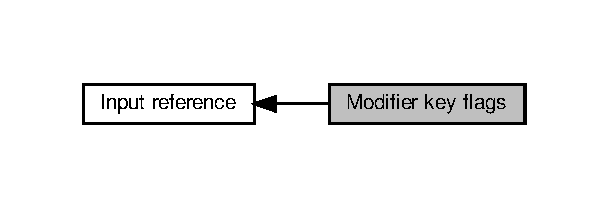
\includegraphics[width=292pt]{group__mods}
\end{center}
\end{figure}
\subsection*{Macros}
\begin{DoxyCompactItemize}
\item 
\mbox{\Hypertarget{group__mods_ga14994d3196c290aaa347248e51740274}\label{group__mods_ga14994d3196c290aaa347248e51740274}} 
\#define \hyperlink{group__mods_ga14994d3196c290aaa347248e51740274}{G\+L\+F\+W\+\_\+\+M\+O\+D\+\_\+\+S\+H\+I\+FT}~0x0001
\begin{DoxyCompactList}\small\item\em If this bit is set one or more Shift keys were held down. \end{DoxyCompactList}\item 
\mbox{\Hypertarget{group__mods_ga6ed94871c3208eefd85713fa929d45aa}\label{group__mods_ga6ed94871c3208eefd85713fa929d45aa}} 
\#define \hyperlink{group__mods_ga6ed94871c3208eefd85713fa929d45aa}{G\+L\+F\+W\+\_\+\+M\+O\+D\+\_\+\+C\+O\+N\+T\+R\+OL}~0x0002
\begin{DoxyCompactList}\small\item\em If this bit is set one or more \hyperlink{classControl}{Control} keys were held down. \end{DoxyCompactList}\item 
\mbox{\Hypertarget{group__mods_gad2acd5633463c29e07008687ea73c0f4}\label{group__mods_gad2acd5633463c29e07008687ea73c0f4}} 
\#define \hyperlink{group__mods_gad2acd5633463c29e07008687ea73c0f4}{G\+L\+F\+W\+\_\+\+M\+O\+D\+\_\+\+A\+LT}~0x0004
\begin{DoxyCompactList}\small\item\em If this bit is set one or more Alt keys were held down. \end{DoxyCompactList}\item 
\mbox{\Hypertarget{group__mods_ga6b64ba10ea0227cf6f42efd0a220aba1}\label{group__mods_ga6b64ba10ea0227cf6f42efd0a220aba1}} 
\#define \hyperlink{group__mods_ga6b64ba10ea0227cf6f42efd0a220aba1}{G\+L\+F\+W\+\_\+\+M\+O\+D\+\_\+\+S\+U\+P\+ER}~0x0008
\begin{DoxyCompactList}\small\item\em If this bit is set one or more Super keys were held down. \end{DoxyCompactList}\item 
\mbox{\Hypertarget{group__mods_ga14994d3196c290aaa347248e51740274}\label{group__mods_ga14994d3196c290aaa347248e51740274}} 
\#define \hyperlink{group__mods_ga14994d3196c290aaa347248e51740274}{G\+L\+F\+W\+\_\+\+M\+O\+D\+\_\+\+S\+H\+I\+FT}~0x0001
\begin{DoxyCompactList}\small\item\em If this bit is set one or more Shift keys were held down. \end{DoxyCompactList}\item 
\mbox{\Hypertarget{group__mods_ga6ed94871c3208eefd85713fa929d45aa}\label{group__mods_ga6ed94871c3208eefd85713fa929d45aa}} 
\#define \hyperlink{group__mods_ga6ed94871c3208eefd85713fa929d45aa}{G\+L\+F\+W\+\_\+\+M\+O\+D\+\_\+\+C\+O\+N\+T\+R\+OL}~0x0002
\begin{DoxyCompactList}\small\item\em If this bit is set one or more \hyperlink{classControl}{Control} keys were held down. \end{DoxyCompactList}\item 
\mbox{\Hypertarget{group__mods_gad2acd5633463c29e07008687ea73c0f4}\label{group__mods_gad2acd5633463c29e07008687ea73c0f4}} 
\#define \hyperlink{group__mods_gad2acd5633463c29e07008687ea73c0f4}{G\+L\+F\+W\+\_\+\+M\+O\+D\+\_\+\+A\+LT}~0x0004
\begin{DoxyCompactList}\small\item\em If this bit is set one or more Alt keys were held down. \end{DoxyCompactList}\item 
\mbox{\Hypertarget{group__mods_ga6b64ba10ea0227cf6f42efd0a220aba1}\label{group__mods_ga6b64ba10ea0227cf6f42efd0a220aba1}} 
\#define \hyperlink{group__mods_ga6b64ba10ea0227cf6f42efd0a220aba1}{G\+L\+F\+W\+\_\+\+M\+O\+D\+\_\+\+S\+U\+P\+ER}~0x0008
\begin{DoxyCompactList}\small\item\em If this bit is set one or more Super keys were held down. \end{DoxyCompactList}\item 
\mbox{\Hypertarget{group__mods_ga14994d3196c290aaa347248e51740274}\label{group__mods_ga14994d3196c290aaa347248e51740274}} 
\#define \hyperlink{group__mods_ga14994d3196c290aaa347248e51740274}{G\+L\+F\+W\+\_\+\+M\+O\+D\+\_\+\+S\+H\+I\+FT}~0x0001
\begin{DoxyCompactList}\small\item\em If this bit is set one or more Shift keys were held down. \end{DoxyCompactList}\item 
\mbox{\Hypertarget{group__mods_ga6ed94871c3208eefd85713fa929d45aa}\label{group__mods_ga6ed94871c3208eefd85713fa929d45aa}} 
\#define \hyperlink{group__mods_ga6ed94871c3208eefd85713fa929d45aa}{G\+L\+F\+W\+\_\+\+M\+O\+D\+\_\+\+C\+O\+N\+T\+R\+OL}~0x0002
\begin{DoxyCompactList}\small\item\em If this bit is set one or more \hyperlink{classControl}{Control} keys were held down. \end{DoxyCompactList}\item 
\mbox{\Hypertarget{group__mods_gad2acd5633463c29e07008687ea73c0f4}\label{group__mods_gad2acd5633463c29e07008687ea73c0f4}} 
\#define \hyperlink{group__mods_gad2acd5633463c29e07008687ea73c0f4}{G\+L\+F\+W\+\_\+\+M\+O\+D\+\_\+\+A\+LT}~0x0004
\begin{DoxyCompactList}\small\item\em If this bit is set one or more Alt keys were held down. \end{DoxyCompactList}\item 
\mbox{\Hypertarget{group__mods_ga6b64ba10ea0227cf6f42efd0a220aba1}\label{group__mods_ga6b64ba10ea0227cf6f42efd0a220aba1}} 
\#define \hyperlink{group__mods_ga6b64ba10ea0227cf6f42efd0a220aba1}{G\+L\+F\+W\+\_\+\+M\+O\+D\+\_\+\+S\+U\+P\+ER}~0x0008
\begin{DoxyCompactList}\small\item\em If this bit is set one or more Super keys were held down. \end{DoxyCompactList}\item 
\mbox{\Hypertarget{group__mods_ga14994d3196c290aaa347248e51740274}\label{group__mods_ga14994d3196c290aaa347248e51740274}} 
\#define \hyperlink{group__mods_ga14994d3196c290aaa347248e51740274}{G\+L\+F\+W\+\_\+\+M\+O\+D\+\_\+\+S\+H\+I\+FT}~0x0001
\begin{DoxyCompactList}\small\item\em If this bit is set one or more Shift keys were held down. \end{DoxyCompactList}\item 
\mbox{\Hypertarget{group__mods_ga6ed94871c3208eefd85713fa929d45aa}\label{group__mods_ga6ed94871c3208eefd85713fa929d45aa}} 
\#define \hyperlink{group__mods_ga6ed94871c3208eefd85713fa929d45aa}{G\+L\+F\+W\+\_\+\+M\+O\+D\+\_\+\+C\+O\+N\+T\+R\+OL}~0x0002
\begin{DoxyCompactList}\small\item\em If this bit is set one or more \hyperlink{classControl}{Control} keys were held down. \end{DoxyCompactList}\item 
\mbox{\Hypertarget{group__mods_gad2acd5633463c29e07008687ea73c0f4}\label{group__mods_gad2acd5633463c29e07008687ea73c0f4}} 
\#define \hyperlink{group__mods_gad2acd5633463c29e07008687ea73c0f4}{G\+L\+F\+W\+\_\+\+M\+O\+D\+\_\+\+A\+LT}~0x0004
\begin{DoxyCompactList}\small\item\em If this bit is set one or more Alt keys were held down. \end{DoxyCompactList}\item 
\mbox{\Hypertarget{group__mods_ga6b64ba10ea0227cf6f42efd0a220aba1}\label{group__mods_ga6b64ba10ea0227cf6f42efd0a220aba1}} 
\#define \hyperlink{group__mods_ga6b64ba10ea0227cf6f42efd0a220aba1}{G\+L\+F\+W\+\_\+\+M\+O\+D\+\_\+\+S\+U\+P\+ER}~0x0008
\begin{DoxyCompactList}\small\item\em If this bit is set one or more Super keys were held down. \end{DoxyCompactList}\item 
\mbox{\Hypertarget{group__mods_ga14994d3196c290aaa347248e51740274}\label{group__mods_ga14994d3196c290aaa347248e51740274}} 
\#define \hyperlink{group__mods_ga14994d3196c290aaa347248e51740274}{G\+L\+F\+W\+\_\+\+M\+O\+D\+\_\+\+S\+H\+I\+FT}~0x0001
\begin{DoxyCompactList}\small\item\em If this bit is set one or more Shift keys were held down. \end{DoxyCompactList}\item 
\mbox{\Hypertarget{group__mods_ga6ed94871c3208eefd85713fa929d45aa}\label{group__mods_ga6ed94871c3208eefd85713fa929d45aa}} 
\#define \hyperlink{group__mods_ga6ed94871c3208eefd85713fa929d45aa}{G\+L\+F\+W\+\_\+\+M\+O\+D\+\_\+\+C\+O\+N\+T\+R\+OL}~0x0002
\begin{DoxyCompactList}\small\item\em If this bit is set one or more \hyperlink{classControl}{Control} keys were held down. \end{DoxyCompactList}\item 
\mbox{\Hypertarget{group__mods_gad2acd5633463c29e07008687ea73c0f4}\label{group__mods_gad2acd5633463c29e07008687ea73c0f4}} 
\#define \hyperlink{group__mods_gad2acd5633463c29e07008687ea73c0f4}{G\+L\+F\+W\+\_\+\+M\+O\+D\+\_\+\+A\+LT}~0x0004
\begin{DoxyCompactList}\small\item\em If this bit is set one or more Alt keys were held down. \end{DoxyCompactList}\item 
\mbox{\Hypertarget{group__mods_ga6b64ba10ea0227cf6f42efd0a220aba1}\label{group__mods_ga6b64ba10ea0227cf6f42efd0a220aba1}} 
\#define \hyperlink{group__mods_ga6b64ba10ea0227cf6f42efd0a220aba1}{G\+L\+F\+W\+\_\+\+M\+O\+D\+\_\+\+S\+U\+P\+ER}~0x0008
\begin{DoxyCompactList}\small\item\em If this bit is set one or more Super keys were held down. \end{DoxyCompactList}\end{DoxyCompactItemize}


\subsection{Detailed Description}
See key input for how these are used. 
\hypertarget{group__buttons}{}\section{Mouse buttons}
\label{group__buttons}\index{Mouse buttons@{Mouse buttons}}
Collaboration diagram for Mouse buttons\+:
\nopagebreak
\begin{figure}[H]
\begin{center}
\leavevmode
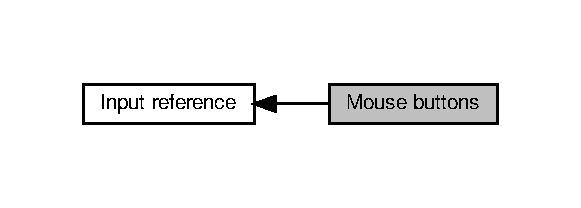
\includegraphics[width=279pt]{group__buttons}
\end{center}
\end{figure}
\subsection*{Macros}
\begin{DoxyCompactItemize}
\item 
\mbox{\Hypertarget{group__buttons_ga181a6e875251fd8671654eff00f9112e}\label{group__buttons_ga181a6e875251fd8671654eff00f9112e}} 
\#define {\bfseries G\+L\+F\+W\+\_\+\+M\+O\+U\+S\+E\+\_\+\+B\+U\+T\+T\+O\+N\+\_\+1}~0
\item 
\mbox{\Hypertarget{group__buttons_ga604b39b92c88ce9bd332e97fc3f4156c}\label{group__buttons_ga604b39b92c88ce9bd332e97fc3f4156c}} 
\#define {\bfseries G\+L\+F\+W\+\_\+\+M\+O\+U\+S\+E\+\_\+\+B\+U\+T\+T\+O\+N\+\_\+2}~1
\item 
\mbox{\Hypertarget{group__buttons_ga0130d505563d0236a6f85545f19e1721}\label{group__buttons_ga0130d505563d0236a6f85545f19e1721}} 
\#define {\bfseries G\+L\+F\+W\+\_\+\+M\+O\+U\+S\+E\+\_\+\+B\+U\+T\+T\+O\+N\+\_\+3}~2
\item 
\mbox{\Hypertarget{group__buttons_ga53f4097bb01d5521c7d9513418c91ca9}\label{group__buttons_ga53f4097bb01d5521c7d9513418c91ca9}} 
\#define {\bfseries G\+L\+F\+W\+\_\+\+M\+O\+U\+S\+E\+\_\+\+B\+U\+T\+T\+O\+N\+\_\+4}~3
\item 
\mbox{\Hypertarget{group__buttons_gaf08c4ddecb051d3d9667db1d5e417c9c}\label{group__buttons_gaf08c4ddecb051d3d9667db1d5e417c9c}} 
\#define {\bfseries G\+L\+F\+W\+\_\+\+M\+O\+U\+S\+E\+\_\+\+B\+U\+T\+T\+O\+N\+\_\+5}~4
\item 
\mbox{\Hypertarget{group__buttons_gae8513e06aab8aa393b595f22c6d8257a}\label{group__buttons_gae8513e06aab8aa393b595f22c6d8257a}} 
\#define {\bfseries G\+L\+F\+W\+\_\+\+M\+O\+U\+S\+E\+\_\+\+B\+U\+T\+T\+O\+N\+\_\+6}~5
\item 
\mbox{\Hypertarget{group__buttons_ga8b02a1ab55dde45b3a3883d54ffd7dc7}\label{group__buttons_ga8b02a1ab55dde45b3a3883d54ffd7dc7}} 
\#define {\bfseries G\+L\+F\+W\+\_\+\+M\+O\+U\+S\+E\+\_\+\+B\+U\+T\+T\+O\+N\+\_\+7}~6
\item 
\mbox{\Hypertarget{group__buttons_ga35d5c4263e0dc0d0a4731ca6c562f32c}\label{group__buttons_ga35d5c4263e0dc0d0a4731ca6c562f32c}} 
\#define {\bfseries G\+L\+F\+W\+\_\+\+M\+O\+U\+S\+E\+\_\+\+B\+U\+T\+T\+O\+N\+\_\+8}~7
\item 
\mbox{\Hypertarget{group__buttons_gab1fd86a4518a9141ec7bcde2e15a2fdf}\label{group__buttons_gab1fd86a4518a9141ec7bcde2e15a2fdf}} 
\#define {\bfseries G\+L\+F\+W\+\_\+\+M\+O\+U\+S\+E\+\_\+\+B\+U\+T\+T\+O\+N\+\_\+\+L\+A\+ST}~G\+L\+F\+W\+\_\+\+M\+O\+U\+S\+E\+\_\+\+B\+U\+T\+T\+O\+N\+\_\+8
\item 
\mbox{\Hypertarget{group__buttons_gaf37100431dcd5082d48f95ee8bc8cd56}\label{group__buttons_gaf37100431dcd5082d48f95ee8bc8cd56}} 
\#define {\bfseries G\+L\+F\+W\+\_\+\+M\+O\+U\+S\+E\+\_\+\+B\+U\+T\+T\+O\+N\+\_\+\+L\+E\+FT}~G\+L\+F\+W\+\_\+\+M\+O\+U\+S\+E\+\_\+\+B\+U\+T\+T\+O\+N\+\_\+1
\item 
\mbox{\Hypertarget{group__buttons_ga3e2f2cf3c4942df73cc094247d275e74}\label{group__buttons_ga3e2f2cf3c4942df73cc094247d275e74}} 
\#define {\bfseries G\+L\+F\+W\+\_\+\+M\+O\+U\+S\+E\+\_\+\+B\+U\+T\+T\+O\+N\+\_\+\+R\+I\+G\+HT}~G\+L\+F\+W\+\_\+\+M\+O\+U\+S\+E\+\_\+\+B\+U\+T\+T\+O\+N\+\_\+2
\item 
\mbox{\Hypertarget{group__buttons_ga34a4d2a701434f763fd93a2ff842b95a}\label{group__buttons_ga34a4d2a701434f763fd93a2ff842b95a}} 
\#define {\bfseries G\+L\+F\+W\+\_\+\+M\+O\+U\+S\+E\+\_\+\+B\+U\+T\+T\+O\+N\+\_\+\+M\+I\+D\+D\+LE}~G\+L\+F\+W\+\_\+\+M\+O\+U\+S\+E\+\_\+\+B\+U\+T\+T\+O\+N\+\_\+3
\item 
\mbox{\Hypertarget{group__buttons_ga181a6e875251fd8671654eff00f9112e}\label{group__buttons_ga181a6e875251fd8671654eff00f9112e}} 
\#define {\bfseries G\+L\+F\+W\+\_\+\+M\+O\+U\+S\+E\+\_\+\+B\+U\+T\+T\+O\+N\+\_\+1}~0
\item 
\mbox{\Hypertarget{group__buttons_ga604b39b92c88ce9bd332e97fc3f4156c}\label{group__buttons_ga604b39b92c88ce9bd332e97fc3f4156c}} 
\#define {\bfseries G\+L\+F\+W\+\_\+\+M\+O\+U\+S\+E\+\_\+\+B\+U\+T\+T\+O\+N\+\_\+2}~1
\item 
\mbox{\Hypertarget{group__buttons_ga0130d505563d0236a6f85545f19e1721}\label{group__buttons_ga0130d505563d0236a6f85545f19e1721}} 
\#define {\bfseries G\+L\+F\+W\+\_\+\+M\+O\+U\+S\+E\+\_\+\+B\+U\+T\+T\+O\+N\+\_\+3}~2
\item 
\mbox{\Hypertarget{group__buttons_ga53f4097bb01d5521c7d9513418c91ca9}\label{group__buttons_ga53f4097bb01d5521c7d9513418c91ca9}} 
\#define {\bfseries G\+L\+F\+W\+\_\+\+M\+O\+U\+S\+E\+\_\+\+B\+U\+T\+T\+O\+N\+\_\+4}~3
\item 
\mbox{\Hypertarget{group__buttons_gaf08c4ddecb051d3d9667db1d5e417c9c}\label{group__buttons_gaf08c4ddecb051d3d9667db1d5e417c9c}} 
\#define {\bfseries G\+L\+F\+W\+\_\+\+M\+O\+U\+S\+E\+\_\+\+B\+U\+T\+T\+O\+N\+\_\+5}~4
\item 
\mbox{\Hypertarget{group__buttons_gae8513e06aab8aa393b595f22c6d8257a}\label{group__buttons_gae8513e06aab8aa393b595f22c6d8257a}} 
\#define {\bfseries G\+L\+F\+W\+\_\+\+M\+O\+U\+S\+E\+\_\+\+B\+U\+T\+T\+O\+N\+\_\+6}~5
\item 
\mbox{\Hypertarget{group__buttons_ga8b02a1ab55dde45b3a3883d54ffd7dc7}\label{group__buttons_ga8b02a1ab55dde45b3a3883d54ffd7dc7}} 
\#define {\bfseries G\+L\+F\+W\+\_\+\+M\+O\+U\+S\+E\+\_\+\+B\+U\+T\+T\+O\+N\+\_\+7}~6
\item 
\mbox{\Hypertarget{group__buttons_ga35d5c4263e0dc0d0a4731ca6c562f32c}\label{group__buttons_ga35d5c4263e0dc0d0a4731ca6c562f32c}} 
\#define {\bfseries G\+L\+F\+W\+\_\+\+M\+O\+U\+S\+E\+\_\+\+B\+U\+T\+T\+O\+N\+\_\+8}~7
\item 
\mbox{\Hypertarget{group__buttons_gab1fd86a4518a9141ec7bcde2e15a2fdf}\label{group__buttons_gab1fd86a4518a9141ec7bcde2e15a2fdf}} 
\#define {\bfseries G\+L\+F\+W\+\_\+\+M\+O\+U\+S\+E\+\_\+\+B\+U\+T\+T\+O\+N\+\_\+\+L\+A\+ST}~G\+L\+F\+W\+\_\+\+M\+O\+U\+S\+E\+\_\+\+B\+U\+T\+T\+O\+N\+\_\+8
\item 
\mbox{\Hypertarget{group__buttons_gaf37100431dcd5082d48f95ee8bc8cd56}\label{group__buttons_gaf37100431dcd5082d48f95ee8bc8cd56}} 
\#define {\bfseries G\+L\+F\+W\+\_\+\+M\+O\+U\+S\+E\+\_\+\+B\+U\+T\+T\+O\+N\+\_\+\+L\+E\+FT}~G\+L\+F\+W\+\_\+\+M\+O\+U\+S\+E\+\_\+\+B\+U\+T\+T\+O\+N\+\_\+1
\item 
\mbox{\Hypertarget{group__buttons_ga3e2f2cf3c4942df73cc094247d275e74}\label{group__buttons_ga3e2f2cf3c4942df73cc094247d275e74}} 
\#define {\bfseries G\+L\+F\+W\+\_\+\+M\+O\+U\+S\+E\+\_\+\+B\+U\+T\+T\+O\+N\+\_\+\+R\+I\+G\+HT}~G\+L\+F\+W\+\_\+\+M\+O\+U\+S\+E\+\_\+\+B\+U\+T\+T\+O\+N\+\_\+2
\item 
\mbox{\Hypertarget{group__buttons_ga34a4d2a701434f763fd93a2ff842b95a}\label{group__buttons_ga34a4d2a701434f763fd93a2ff842b95a}} 
\#define {\bfseries G\+L\+F\+W\+\_\+\+M\+O\+U\+S\+E\+\_\+\+B\+U\+T\+T\+O\+N\+\_\+\+M\+I\+D\+D\+LE}~G\+L\+F\+W\+\_\+\+M\+O\+U\+S\+E\+\_\+\+B\+U\+T\+T\+O\+N\+\_\+3
\item 
\mbox{\Hypertarget{group__buttons_ga181a6e875251fd8671654eff00f9112e}\label{group__buttons_ga181a6e875251fd8671654eff00f9112e}} 
\#define {\bfseries G\+L\+F\+W\+\_\+\+M\+O\+U\+S\+E\+\_\+\+B\+U\+T\+T\+O\+N\+\_\+1}~0
\item 
\mbox{\Hypertarget{group__buttons_ga604b39b92c88ce9bd332e97fc3f4156c}\label{group__buttons_ga604b39b92c88ce9bd332e97fc3f4156c}} 
\#define {\bfseries G\+L\+F\+W\+\_\+\+M\+O\+U\+S\+E\+\_\+\+B\+U\+T\+T\+O\+N\+\_\+2}~1
\item 
\mbox{\Hypertarget{group__buttons_ga0130d505563d0236a6f85545f19e1721}\label{group__buttons_ga0130d505563d0236a6f85545f19e1721}} 
\#define {\bfseries G\+L\+F\+W\+\_\+\+M\+O\+U\+S\+E\+\_\+\+B\+U\+T\+T\+O\+N\+\_\+3}~2
\item 
\mbox{\Hypertarget{group__buttons_ga53f4097bb01d5521c7d9513418c91ca9}\label{group__buttons_ga53f4097bb01d5521c7d9513418c91ca9}} 
\#define {\bfseries G\+L\+F\+W\+\_\+\+M\+O\+U\+S\+E\+\_\+\+B\+U\+T\+T\+O\+N\+\_\+4}~3
\item 
\mbox{\Hypertarget{group__buttons_gaf08c4ddecb051d3d9667db1d5e417c9c}\label{group__buttons_gaf08c4ddecb051d3d9667db1d5e417c9c}} 
\#define {\bfseries G\+L\+F\+W\+\_\+\+M\+O\+U\+S\+E\+\_\+\+B\+U\+T\+T\+O\+N\+\_\+5}~4
\item 
\mbox{\Hypertarget{group__buttons_gae8513e06aab8aa393b595f22c6d8257a}\label{group__buttons_gae8513e06aab8aa393b595f22c6d8257a}} 
\#define {\bfseries G\+L\+F\+W\+\_\+\+M\+O\+U\+S\+E\+\_\+\+B\+U\+T\+T\+O\+N\+\_\+6}~5
\item 
\mbox{\Hypertarget{group__buttons_ga8b02a1ab55dde45b3a3883d54ffd7dc7}\label{group__buttons_ga8b02a1ab55dde45b3a3883d54ffd7dc7}} 
\#define {\bfseries G\+L\+F\+W\+\_\+\+M\+O\+U\+S\+E\+\_\+\+B\+U\+T\+T\+O\+N\+\_\+7}~6
\item 
\mbox{\Hypertarget{group__buttons_ga35d5c4263e0dc0d0a4731ca6c562f32c}\label{group__buttons_ga35d5c4263e0dc0d0a4731ca6c562f32c}} 
\#define {\bfseries G\+L\+F\+W\+\_\+\+M\+O\+U\+S\+E\+\_\+\+B\+U\+T\+T\+O\+N\+\_\+8}~7
\item 
\mbox{\Hypertarget{group__buttons_gab1fd86a4518a9141ec7bcde2e15a2fdf}\label{group__buttons_gab1fd86a4518a9141ec7bcde2e15a2fdf}} 
\#define {\bfseries G\+L\+F\+W\+\_\+\+M\+O\+U\+S\+E\+\_\+\+B\+U\+T\+T\+O\+N\+\_\+\+L\+A\+ST}~G\+L\+F\+W\+\_\+\+M\+O\+U\+S\+E\+\_\+\+B\+U\+T\+T\+O\+N\+\_\+8
\item 
\mbox{\Hypertarget{group__buttons_gaf37100431dcd5082d48f95ee8bc8cd56}\label{group__buttons_gaf37100431dcd5082d48f95ee8bc8cd56}} 
\#define {\bfseries G\+L\+F\+W\+\_\+\+M\+O\+U\+S\+E\+\_\+\+B\+U\+T\+T\+O\+N\+\_\+\+L\+E\+FT}~G\+L\+F\+W\+\_\+\+M\+O\+U\+S\+E\+\_\+\+B\+U\+T\+T\+O\+N\+\_\+1
\item 
\mbox{\Hypertarget{group__buttons_ga3e2f2cf3c4942df73cc094247d275e74}\label{group__buttons_ga3e2f2cf3c4942df73cc094247d275e74}} 
\#define {\bfseries G\+L\+F\+W\+\_\+\+M\+O\+U\+S\+E\+\_\+\+B\+U\+T\+T\+O\+N\+\_\+\+R\+I\+G\+HT}~G\+L\+F\+W\+\_\+\+M\+O\+U\+S\+E\+\_\+\+B\+U\+T\+T\+O\+N\+\_\+2
\item 
\mbox{\Hypertarget{group__buttons_ga34a4d2a701434f763fd93a2ff842b95a}\label{group__buttons_ga34a4d2a701434f763fd93a2ff842b95a}} 
\#define {\bfseries G\+L\+F\+W\+\_\+\+M\+O\+U\+S\+E\+\_\+\+B\+U\+T\+T\+O\+N\+\_\+\+M\+I\+D\+D\+LE}~G\+L\+F\+W\+\_\+\+M\+O\+U\+S\+E\+\_\+\+B\+U\+T\+T\+O\+N\+\_\+3
\item 
\mbox{\Hypertarget{group__buttons_ga181a6e875251fd8671654eff00f9112e}\label{group__buttons_ga181a6e875251fd8671654eff00f9112e}} 
\#define {\bfseries G\+L\+F\+W\+\_\+\+M\+O\+U\+S\+E\+\_\+\+B\+U\+T\+T\+O\+N\+\_\+1}~0
\item 
\mbox{\Hypertarget{group__buttons_ga604b39b92c88ce9bd332e97fc3f4156c}\label{group__buttons_ga604b39b92c88ce9bd332e97fc3f4156c}} 
\#define {\bfseries G\+L\+F\+W\+\_\+\+M\+O\+U\+S\+E\+\_\+\+B\+U\+T\+T\+O\+N\+\_\+2}~1
\item 
\mbox{\Hypertarget{group__buttons_ga0130d505563d0236a6f85545f19e1721}\label{group__buttons_ga0130d505563d0236a6f85545f19e1721}} 
\#define {\bfseries G\+L\+F\+W\+\_\+\+M\+O\+U\+S\+E\+\_\+\+B\+U\+T\+T\+O\+N\+\_\+3}~2
\item 
\mbox{\Hypertarget{group__buttons_ga53f4097bb01d5521c7d9513418c91ca9}\label{group__buttons_ga53f4097bb01d5521c7d9513418c91ca9}} 
\#define {\bfseries G\+L\+F\+W\+\_\+\+M\+O\+U\+S\+E\+\_\+\+B\+U\+T\+T\+O\+N\+\_\+4}~3
\item 
\mbox{\Hypertarget{group__buttons_gaf08c4ddecb051d3d9667db1d5e417c9c}\label{group__buttons_gaf08c4ddecb051d3d9667db1d5e417c9c}} 
\#define {\bfseries G\+L\+F\+W\+\_\+\+M\+O\+U\+S\+E\+\_\+\+B\+U\+T\+T\+O\+N\+\_\+5}~4
\item 
\mbox{\Hypertarget{group__buttons_gae8513e06aab8aa393b595f22c6d8257a}\label{group__buttons_gae8513e06aab8aa393b595f22c6d8257a}} 
\#define {\bfseries G\+L\+F\+W\+\_\+\+M\+O\+U\+S\+E\+\_\+\+B\+U\+T\+T\+O\+N\+\_\+6}~5
\item 
\mbox{\Hypertarget{group__buttons_ga8b02a1ab55dde45b3a3883d54ffd7dc7}\label{group__buttons_ga8b02a1ab55dde45b3a3883d54ffd7dc7}} 
\#define {\bfseries G\+L\+F\+W\+\_\+\+M\+O\+U\+S\+E\+\_\+\+B\+U\+T\+T\+O\+N\+\_\+7}~6
\item 
\mbox{\Hypertarget{group__buttons_ga35d5c4263e0dc0d0a4731ca6c562f32c}\label{group__buttons_ga35d5c4263e0dc0d0a4731ca6c562f32c}} 
\#define {\bfseries G\+L\+F\+W\+\_\+\+M\+O\+U\+S\+E\+\_\+\+B\+U\+T\+T\+O\+N\+\_\+8}~7
\item 
\mbox{\Hypertarget{group__buttons_gab1fd86a4518a9141ec7bcde2e15a2fdf}\label{group__buttons_gab1fd86a4518a9141ec7bcde2e15a2fdf}} 
\#define {\bfseries G\+L\+F\+W\+\_\+\+M\+O\+U\+S\+E\+\_\+\+B\+U\+T\+T\+O\+N\+\_\+\+L\+A\+ST}~G\+L\+F\+W\+\_\+\+M\+O\+U\+S\+E\+\_\+\+B\+U\+T\+T\+O\+N\+\_\+8
\item 
\mbox{\Hypertarget{group__buttons_gaf37100431dcd5082d48f95ee8bc8cd56}\label{group__buttons_gaf37100431dcd5082d48f95ee8bc8cd56}} 
\#define {\bfseries G\+L\+F\+W\+\_\+\+M\+O\+U\+S\+E\+\_\+\+B\+U\+T\+T\+O\+N\+\_\+\+L\+E\+FT}~G\+L\+F\+W\+\_\+\+M\+O\+U\+S\+E\+\_\+\+B\+U\+T\+T\+O\+N\+\_\+1
\item 
\mbox{\Hypertarget{group__buttons_ga3e2f2cf3c4942df73cc094247d275e74}\label{group__buttons_ga3e2f2cf3c4942df73cc094247d275e74}} 
\#define {\bfseries G\+L\+F\+W\+\_\+\+M\+O\+U\+S\+E\+\_\+\+B\+U\+T\+T\+O\+N\+\_\+\+R\+I\+G\+HT}~G\+L\+F\+W\+\_\+\+M\+O\+U\+S\+E\+\_\+\+B\+U\+T\+T\+O\+N\+\_\+2
\item 
\mbox{\Hypertarget{group__buttons_ga34a4d2a701434f763fd93a2ff842b95a}\label{group__buttons_ga34a4d2a701434f763fd93a2ff842b95a}} 
\#define {\bfseries G\+L\+F\+W\+\_\+\+M\+O\+U\+S\+E\+\_\+\+B\+U\+T\+T\+O\+N\+\_\+\+M\+I\+D\+D\+LE}~G\+L\+F\+W\+\_\+\+M\+O\+U\+S\+E\+\_\+\+B\+U\+T\+T\+O\+N\+\_\+3
\item 
\mbox{\Hypertarget{group__buttons_ga181a6e875251fd8671654eff00f9112e}\label{group__buttons_ga181a6e875251fd8671654eff00f9112e}} 
\#define {\bfseries G\+L\+F\+W\+\_\+\+M\+O\+U\+S\+E\+\_\+\+B\+U\+T\+T\+O\+N\+\_\+1}~0
\item 
\mbox{\Hypertarget{group__buttons_ga604b39b92c88ce9bd332e97fc3f4156c}\label{group__buttons_ga604b39b92c88ce9bd332e97fc3f4156c}} 
\#define {\bfseries G\+L\+F\+W\+\_\+\+M\+O\+U\+S\+E\+\_\+\+B\+U\+T\+T\+O\+N\+\_\+2}~1
\item 
\mbox{\Hypertarget{group__buttons_ga0130d505563d0236a6f85545f19e1721}\label{group__buttons_ga0130d505563d0236a6f85545f19e1721}} 
\#define {\bfseries G\+L\+F\+W\+\_\+\+M\+O\+U\+S\+E\+\_\+\+B\+U\+T\+T\+O\+N\+\_\+3}~2
\item 
\mbox{\Hypertarget{group__buttons_ga53f4097bb01d5521c7d9513418c91ca9}\label{group__buttons_ga53f4097bb01d5521c7d9513418c91ca9}} 
\#define {\bfseries G\+L\+F\+W\+\_\+\+M\+O\+U\+S\+E\+\_\+\+B\+U\+T\+T\+O\+N\+\_\+4}~3
\item 
\mbox{\Hypertarget{group__buttons_gaf08c4ddecb051d3d9667db1d5e417c9c}\label{group__buttons_gaf08c4ddecb051d3d9667db1d5e417c9c}} 
\#define {\bfseries G\+L\+F\+W\+\_\+\+M\+O\+U\+S\+E\+\_\+\+B\+U\+T\+T\+O\+N\+\_\+5}~4
\item 
\mbox{\Hypertarget{group__buttons_gae8513e06aab8aa393b595f22c6d8257a}\label{group__buttons_gae8513e06aab8aa393b595f22c6d8257a}} 
\#define {\bfseries G\+L\+F\+W\+\_\+\+M\+O\+U\+S\+E\+\_\+\+B\+U\+T\+T\+O\+N\+\_\+6}~5
\item 
\mbox{\Hypertarget{group__buttons_ga8b02a1ab55dde45b3a3883d54ffd7dc7}\label{group__buttons_ga8b02a1ab55dde45b3a3883d54ffd7dc7}} 
\#define {\bfseries G\+L\+F\+W\+\_\+\+M\+O\+U\+S\+E\+\_\+\+B\+U\+T\+T\+O\+N\+\_\+7}~6
\item 
\mbox{\Hypertarget{group__buttons_ga35d5c4263e0dc0d0a4731ca6c562f32c}\label{group__buttons_ga35d5c4263e0dc0d0a4731ca6c562f32c}} 
\#define {\bfseries G\+L\+F\+W\+\_\+\+M\+O\+U\+S\+E\+\_\+\+B\+U\+T\+T\+O\+N\+\_\+8}~7
\item 
\mbox{\Hypertarget{group__buttons_gab1fd86a4518a9141ec7bcde2e15a2fdf}\label{group__buttons_gab1fd86a4518a9141ec7bcde2e15a2fdf}} 
\#define {\bfseries G\+L\+F\+W\+\_\+\+M\+O\+U\+S\+E\+\_\+\+B\+U\+T\+T\+O\+N\+\_\+\+L\+A\+ST}~G\+L\+F\+W\+\_\+\+M\+O\+U\+S\+E\+\_\+\+B\+U\+T\+T\+O\+N\+\_\+8
\item 
\mbox{\Hypertarget{group__buttons_gaf37100431dcd5082d48f95ee8bc8cd56}\label{group__buttons_gaf37100431dcd5082d48f95ee8bc8cd56}} 
\#define {\bfseries G\+L\+F\+W\+\_\+\+M\+O\+U\+S\+E\+\_\+\+B\+U\+T\+T\+O\+N\+\_\+\+L\+E\+FT}~G\+L\+F\+W\+\_\+\+M\+O\+U\+S\+E\+\_\+\+B\+U\+T\+T\+O\+N\+\_\+1
\item 
\mbox{\Hypertarget{group__buttons_ga3e2f2cf3c4942df73cc094247d275e74}\label{group__buttons_ga3e2f2cf3c4942df73cc094247d275e74}} 
\#define {\bfseries G\+L\+F\+W\+\_\+\+M\+O\+U\+S\+E\+\_\+\+B\+U\+T\+T\+O\+N\+\_\+\+R\+I\+G\+HT}~G\+L\+F\+W\+\_\+\+M\+O\+U\+S\+E\+\_\+\+B\+U\+T\+T\+O\+N\+\_\+2
\item 
\mbox{\Hypertarget{group__buttons_ga34a4d2a701434f763fd93a2ff842b95a}\label{group__buttons_ga34a4d2a701434f763fd93a2ff842b95a}} 
\#define {\bfseries G\+L\+F\+W\+\_\+\+M\+O\+U\+S\+E\+\_\+\+B\+U\+T\+T\+O\+N\+\_\+\+M\+I\+D\+D\+LE}~G\+L\+F\+W\+\_\+\+M\+O\+U\+S\+E\+\_\+\+B\+U\+T\+T\+O\+N\+\_\+3
\end{DoxyCompactItemize}


\subsection{Detailed Description}
See mouse button input for how these are used. 
\hypertarget{group__joysticks}{}\section{Joysticks}
\label{group__joysticks}\index{Joysticks@{Joysticks}}
Collaboration diagram for Joysticks\+:
\nopagebreak
\begin{figure}[H]
\begin{center}
\leavevmode
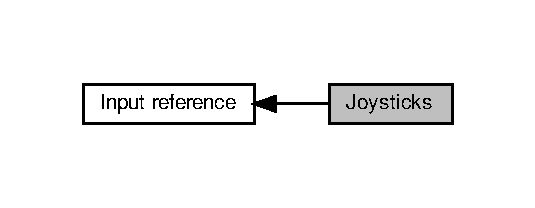
\includegraphics[width=257pt]{group__joysticks}
\end{center}
\end{figure}
\subsection*{Macros}
\begin{DoxyCompactItemize}
\item 
\mbox{\Hypertarget{group__joysticks_ga34a0443d059e9f22272cd4669073f73d}\label{group__joysticks_ga34a0443d059e9f22272cd4669073f73d}} 
\#define {\bfseries G\+L\+F\+W\+\_\+\+J\+O\+Y\+S\+T\+I\+C\+K\+\_\+1}~0
\item 
\mbox{\Hypertarget{group__joysticks_ga6eab65ec88e65e0850ef8413504cb50c}\label{group__joysticks_ga6eab65ec88e65e0850ef8413504cb50c}} 
\#define {\bfseries G\+L\+F\+W\+\_\+\+J\+O\+Y\+S\+T\+I\+C\+K\+\_\+2}~1
\item 
\mbox{\Hypertarget{group__joysticks_gae6f3eedfeb42424c2f5e3161efb0b654}\label{group__joysticks_gae6f3eedfeb42424c2f5e3161efb0b654}} 
\#define {\bfseries G\+L\+F\+W\+\_\+\+J\+O\+Y\+S\+T\+I\+C\+K\+\_\+3}~2
\item 
\mbox{\Hypertarget{group__joysticks_ga97ddbcad02b7f48d74fad4ddb08fff59}\label{group__joysticks_ga97ddbcad02b7f48d74fad4ddb08fff59}} 
\#define {\bfseries G\+L\+F\+W\+\_\+\+J\+O\+Y\+S\+T\+I\+C\+K\+\_\+4}~3
\item 
\mbox{\Hypertarget{group__joysticks_gae43281bc66d3fa5089fb50c3e7a28695}\label{group__joysticks_gae43281bc66d3fa5089fb50c3e7a28695}} 
\#define {\bfseries G\+L\+F\+W\+\_\+\+J\+O\+Y\+S\+T\+I\+C\+K\+\_\+5}~4
\item 
\mbox{\Hypertarget{group__joysticks_ga74771620aa53bd68a487186dea66fd77}\label{group__joysticks_ga74771620aa53bd68a487186dea66fd77}} 
\#define {\bfseries G\+L\+F\+W\+\_\+\+J\+O\+Y\+S\+T\+I\+C\+K\+\_\+6}~5
\item 
\mbox{\Hypertarget{group__joysticks_ga20a9f4f3aaefed9ea5e66072fc588b87}\label{group__joysticks_ga20a9f4f3aaefed9ea5e66072fc588b87}} 
\#define {\bfseries G\+L\+F\+W\+\_\+\+J\+O\+Y\+S\+T\+I\+C\+K\+\_\+7}~6
\item 
\mbox{\Hypertarget{group__joysticks_ga21a934c940bcf25db0e4c8fe9b364bdb}\label{group__joysticks_ga21a934c940bcf25db0e4c8fe9b364bdb}} 
\#define {\bfseries G\+L\+F\+W\+\_\+\+J\+O\+Y\+S\+T\+I\+C\+K\+\_\+8}~7
\item 
\mbox{\Hypertarget{group__joysticks_ga87689d47df0ba6f9f5fcbbcaf7b3cecf}\label{group__joysticks_ga87689d47df0ba6f9f5fcbbcaf7b3cecf}} 
\#define {\bfseries G\+L\+F\+W\+\_\+\+J\+O\+Y\+S\+T\+I\+C\+K\+\_\+9}~8
\item 
\mbox{\Hypertarget{group__joysticks_gaef55389ee605d6dfc31aef6fe98c54ec}\label{group__joysticks_gaef55389ee605d6dfc31aef6fe98c54ec}} 
\#define {\bfseries G\+L\+F\+W\+\_\+\+J\+O\+Y\+S\+T\+I\+C\+K\+\_\+10}~9
\item 
\mbox{\Hypertarget{group__joysticks_gae7d26e3df447c2c14a569fcc18516af4}\label{group__joysticks_gae7d26e3df447c2c14a569fcc18516af4}} 
\#define {\bfseries G\+L\+F\+W\+\_\+\+J\+O\+Y\+S\+T\+I\+C\+K\+\_\+11}~10
\item 
\mbox{\Hypertarget{group__joysticks_gab91bbf5b7ca6be8d3ac5c4d89ff48ac7}\label{group__joysticks_gab91bbf5b7ca6be8d3ac5c4d89ff48ac7}} 
\#define {\bfseries G\+L\+F\+W\+\_\+\+J\+O\+Y\+S\+T\+I\+C\+K\+\_\+12}~11
\item 
\mbox{\Hypertarget{group__joysticks_ga5c84fb4e49bf661d7d7c78eb4018c508}\label{group__joysticks_ga5c84fb4e49bf661d7d7c78eb4018c508}} 
\#define {\bfseries G\+L\+F\+W\+\_\+\+J\+O\+Y\+S\+T\+I\+C\+K\+\_\+13}~12
\item 
\mbox{\Hypertarget{group__joysticks_ga89540873278ae5a42b3e70d64164dc74}\label{group__joysticks_ga89540873278ae5a42b3e70d64164dc74}} 
\#define {\bfseries G\+L\+F\+W\+\_\+\+J\+O\+Y\+S\+T\+I\+C\+K\+\_\+14}~13
\item 
\mbox{\Hypertarget{group__joysticks_ga7b02ab70daf7a78bcc942d5d4cc1dcf9}\label{group__joysticks_ga7b02ab70daf7a78bcc942d5d4cc1dcf9}} 
\#define {\bfseries G\+L\+F\+W\+\_\+\+J\+O\+Y\+S\+T\+I\+C\+K\+\_\+15}~14
\item 
\mbox{\Hypertarget{group__joysticks_ga453edeeabf350827646b6857df4f80ce}\label{group__joysticks_ga453edeeabf350827646b6857df4f80ce}} 
\#define {\bfseries G\+L\+F\+W\+\_\+\+J\+O\+Y\+S\+T\+I\+C\+K\+\_\+16}~15
\item 
\mbox{\Hypertarget{group__joysticks_ga9ca13ebf24c331dd98df17d84a4b72c9}\label{group__joysticks_ga9ca13ebf24c331dd98df17d84a4b72c9}} 
\#define {\bfseries G\+L\+F\+W\+\_\+\+J\+O\+Y\+S\+T\+I\+C\+K\+\_\+\+L\+A\+ST}~G\+L\+F\+W\+\_\+\+J\+O\+Y\+S\+T\+I\+C\+K\+\_\+16
\item 
\mbox{\Hypertarget{group__joysticks_ga34a0443d059e9f22272cd4669073f73d}\label{group__joysticks_ga34a0443d059e9f22272cd4669073f73d}} 
\#define {\bfseries G\+L\+F\+W\+\_\+\+J\+O\+Y\+S\+T\+I\+C\+K\+\_\+1}~0
\item 
\mbox{\Hypertarget{group__joysticks_ga6eab65ec88e65e0850ef8413504cb50c}\label{group__joysticks_ga6eab65ec88e65e0850ef8413504cb50c}} 
\#define {\bfseries G\+L\+F\+W\+\_\+\+J\+O\+Y\+S\+T\+I\+C\+K\+\_\+2}~1
\item 
\mbox{\Hypertarget{group__joysticks_gae6f3eedfeb42424c2f5e3161efb0b654}\label{group__joysticks_gae6f3eedfeb42424c2f5e3161efb0b654}} 
\#define {\bfseries G\+L\+F\+W\+\_\+\+J\+O\+Y\+S\+T\+I\+C\+K\+\_\+3}~2
\item 
\mbox{\Hypertarget{group__joysticks_ga97ddbcad02b7f48d74fad4ddb08fff59}\label{group__joysticks_ga97ddbcad02b7f48d74fad4ddb08fff59}} 
\#define {\bfseries G\+L\+F\+W\+\_\+\+J\+O\+Y\+S\+T\+I\+C\+K\+\_\+4}~3
\item 
\mbox{\Hypertarget{group__joysticks_gae43281bc66d3fa5089fb50c3e7a28695}\label{group__joysticks_gae43281bc66d3fa5089fb50c3e7a28695}} 
\#define {\bfseries G\+L\+F\+W\+\_\+\+J\+O\+Y\+S\+T\+I\+C\+K\+\_\+5}~4
\item 
\mbox{\Hypertarget{group__joysticks_ga74771620aa53bd68a487186dea66fd77}\label{group__joysticks_ga74771620aa53bd68a487186dea66fd77}} 
\#define {\bfseries G\+L\+F\+W\+\_\+\+J\+O\+Y\+S\+T\+I\+C\+K\+\_\+6}~5
\item 
\mbox{\Hypertarget{group__joysticks_ga20a9f4f3aaefed9ea5e66072fc588b87}\label{group__joysticks_ga20a9f4f3aaefed9ea5e66072fc588b87}} 
\#define {\bfseries G\+L\+F\+W\+\_\+\+J\+O\+Y\+S\+T\+I\+C\+K\+\_\+7}~6
\item 
\mbox{\Hypertarget{group__joysticks_ga21a934c940bcf25db0e4c8fe9b364bdb}\label{group__joysticks_ga21a934c940bcf25db0e4c8fe9b364bdb}} 
\#define {\bfseries G\+L\+F\+W\+\_\+\+J\+O\+Y\+S\+T\+I\+C\+K\+\_\+8}~7
\item 
\mbox{\Hypertarget{group__joysticks_ga87689d47df0ba6f9f5fcbbcaf7b3cecf}\label{group__joysticks_ga87689d47df0ba6f9f5fcbbcaf7b3cecf}} 
\#define {\bfseries G\+L\+F\+W\+\_\+\+J\+O\+Y\+S\+T\+I\+C\+K\+\_\+9}~8
\item 
\mbox{\Hypertarget{group__joysticks_gaef55389ee605d6dfc31aef6fe98c54ec}\label{group__joysticks_gaef55389ee605d6dfc31aef6fe98c54ec}} 
\#define {\bfseries G\+L\+F\+W\+\_\+\+J\+O\+Y\+S\+T\+I\+C\+K\+\_\+10}~9
\item 
\mbox{\Hypertarget{group__joysticks_gae7d26e3df447c2c14a569fcc18516af4}\label{group__joysticks_gae7d26e3df447c2c14a569fcc18516af4}} 
\#define {\bfseries G\+L\+F\+W\+\_\+\+J\+O\+Y\+S\+T\+I\+C\+K\+\_\+11}~10
\item 
\mbox{\Hypertarget{group__joysticks_gab91bbf5b7ca6be8d3ac5c4d89ff48ac7}\label{group__joysticks_gab91bbf5b7ca6be8d3ac5c4d89ff48ac7}} 
\#define {\bfseries G\+L\+F\+W\+\_\+\+J\+O\+Y\+S\+T\+I\+C\+K\+\_\+12}~11
\item 
\mbox{\Hypertarget{group__joysticks_ga5c84fb4e49bf661d7d7c78eb4018c508}\label{group__joysticks_ga5c84fb4e49bf661d7d7c78eb4018c508}} 
\#define {\bfseries G\+L\+F\+W\+\_\+\+J\+O\+Y\+S\+T\+I\+C\+K\+\_\+13}~12
\item 
\mbox{\Hypertarget{group__joysticks_ga89540873278ae5a42b3e70d64164dc74}\label{group__joysticks_ga89540873278ae5a42b3e70d64164dc74}} 
\#define {\bfseries G\+L\+F\+W\+\_\+\+J\+O\+Y\+S\+T\+I\+C\+K\+\_\+14}~13
\item 
\mbox{\Hypertarget{group__joysticks_ga7b02ab70daf7a78bcc942d5d4cc1dcf9}\label{group__joysticks_ga7b02ab70daf7a78bcc942d5d4cc1dcf9}} 
\#define {\bfseries G\+L\+F\+W\+\_\+\+J\+O\+Y\+S\+T\+I\+C\+K\+\_\+15}~14
\item 
\mbox{\Hypertarget{group__joysticks_ga453edeeabf350827646b6857df4f80ce}\label{group__joysticks_ga453edeeabf350827646b6857df4f80ce}} 
\#define {\bfseries G\+L\+F\+W\+\_\+\+J\+O\+Y\+S\+T\+I\+C\+K\+\_\+16}~15
\item 
\mbox{\Hypertarget{group__joysticks_ga9ca13ebf24c331dd98df17d84a4b72c9}\label{group__joysticks_ga9ca13ebf24c331dd98df17d84a4b72c9}} 
\#define {\bfseries G\+L\+F\+W\+\_\+\+J\+O\+Y\+S\+T\+I\+C\+K\+\_\+\+L\+A\+ST}~G\+L\+F\+W\+\_\+\+J\+O\+Y\+S\+T\+I\+C\+K\+\_\+16
\item 
\mbox{\Hypertarget{group__joysticks_ga34a0443d059e9f22272cd4669073f73d}\label{group__joysticks_ga34a0443d059e9f22272cd4669073f73d}} 
\#define {\bfseries G\+L\+F\+W\+\_\+\+J\+O\+Y\+S\+T\+I\+C\+K\+\_\+1}~0
\item 
\mbox{\Hypertarget{group__joysticks_ga6eab65ec88e65e0850ef8413504cb50c}\label{group__joysticks_ga6eab65ec88e65e0850ef8413504cb50c}} 
\#define {\bfseries G\+L\+F\+W\+\_\+\+J\+O\+Y\+S\+T\+I\+C\+K\+\_\+2}~1
\item 
\mbox{\Hypertarget{group__joysticks_gae6f3eedfeb42424c2f5e3161efb0b654}\label{group__joysticks_gae6f3eedfeb42424c2f5e3161efb0b654}} 
\#define {\bfseries G\+L\+F\+W\+\_\+\+J\+O\+Y\+S\+T\+I\+C\+K\+\_\+3}~2
\item 
\mbox{\Hypertarget{group__joysticks_ga97ddbcad02b7f48d74fad4ddb08fff59}\label{group__joysticks_ga97ddbcad02b7f48d74fad4ddb08fff59}} 
\#define {\bfseries G\+L\+F\+W\+\_\+\+J\+O\+Y\+S\+T\+I\+C\+K\+\_\+4}~3
\item 
\mbox{\Hypertarget{group__joysticks_gae43281bc66d3fa5089fb50c3e7a28695}\label{group__joysticks_gae43281bc66d3fa5089fb50c3e7a28695}} 
\#define {\bfseries G\+L\+F\+W\+\_\+\+J\+O\+Y\+S\+T\+I\+C\+K\+\_\+5}~4
\item 
\mbox{\Hypertarget{group__joysticks_ga74771620aa53bd68a487186dea66fd77}\label{group__joysticks_ga74771620aa53bd68a487186dea66fd77}} 
\#define {\bfseries G\+L\+F\+W\+\_\+\+J\+O\+Y\+S\+T\+I\+C\+K\+\_\+6}~5
\item 
\mbox{\Hypertarget{group__joysticks_ga20a9f4f3aaefed9ea5e66072fc588b87}\label{group__joysticks_ga20a9f4f3aaefed9ea5e66072fc588b87}} 
\#define {\bfseries G\+L\+F\+W\+\_\+\+J\+O\+Y\+S\+T\+I\+C\+K\+\_\+7}~6
\item 
\mbox{\Hypertarget{group__joysticks_ga21a934c940bcf25db0e4c8fe9b364bdb}\label{group__joysticks_ga21a934c940bcf25db0e4c8fe9b364bdb}} 
\#define {\bfseries G\+L\+F\+W\+\_\+\+J\+O\+Y\+S\+T\+I\+C\+K\+\_\+8}~7
\item 
\mbox{\Hypertarget{group__joysticks_ga87689d47df0ba6f9f5fcbbcaf7b3cecf}\label{group__joysticks_ga87689d47df0ba6f9f5fcbbcaf7b3cecf}} 
\#define {\bfseries G\+L\+F\+W\+\_\+\+J\+O\+Y\+S\+T\+I\+C\+K\+\_\+9}~8
\item 
\mbox{\Hypertarget{group__joysticks_gaef55389ee605d6dfc31aef6fe98c54ec}\label{group__joysticks_gaef55389ee605d6dfc31aef6fe98c54ec}} 
\#define {\bfseries G\+L\+F\+W\+\_\+\+J\+O\+Y\+S\+T\+I\+C\+K\+\_\+10}~9
\item 
\mbox{\Hypertarget{group__joysticks_gae7d26e3df447c2c14a569fcc18516af4}\label{group__joysticks_gae7d26e3df447c2c14a569fcc18516af4}} 
\#define {\bfseries G\+L\+F\+W\+\_\+\+J\+O\+Y\+S\+T\+I\+C\+K\+\_\+11}~10
\item 
\mbox{\Hypertarget{group__joysticks_gab91bbf5b7ca6be8d3ac5c4d89ff48ac7}\label{group__joysticks_gab91bbf5b7ca6be8d3ac5c4d89ff48ac7}} 
\#define {\bfseries G\+L\+F\+W\+\_\+\+J\+O\+Y\+S\+T\+I\+C\+K\+\_\+12}~11
\item 
\mbox{\Hypertarget{group__joysticks_ga5c84fb4e49bf661d7d7c78eb4018c508}\label{group__joysticks_ga5c84fb4e49bf661d7d7c78eb4018c508}} 
\#define {\bfseries G\+L\+F\+W\+\_\+\+J\+O\+Y\+S\+T\+I\+C\+K\+\_\+13}~12
\item 
\mbox{\Hypertarget{group__joysticks_ga89540873278ae5a42b3e70d64164dc74}\label{group__joysticks_ga89540873278ae5a42b3e70d64164dc74}} 
\#define {\bfseries G\+L\+F\+W\+\_\+\+J\+O\+Y\+S\+T\+I\+C\+K\+\_\+14}~13
\item 
\mbox{\Hypertarget{group__joysticks_ga7b02ab70daf7a78bcc942d5d4cc1dcf9}\label{group__joysticks_ga7b02ab70daf7a78bcc942d5d4cc1dcf9}} 
\#define {\bfseries G\+L\+F\+W\+\_\+\+J\+O\+Y\+S\+T\+I\+C\+K\+\_\+15}~14
\item 
\mbox{\Hypertarget{group__joysticks_ga453edeeabf350827646b6857df4f80ce}\label{group__joysticks_ga453edeeabf350827646b6857df4f80ce}} 
\#define {\bfseries G\+L\+F\+W\+\_\+\+J\+O\+Y\+S\+T\+I\+C\+K\+\_\+16}~15
\item 
\mbox{\Hypertarget{group__joysticks_ga9ca13ebf24c331dd98df17d84a4b72c9}\label{group__joysticks_ga9ca13ebf24c331dd98df17d84a4b72c9}} 
\#define {\bfseries G\+L\+F\+W\+\_\+\+J\+O\+Y\+S\+T\+I\+C\+K\+\_\+\+L\+A\+ST}~G\+L\+F\+W\+\_\+\+J\+O\+Y\+S\+T\+I\+C\+K\+\_\+16
\item 
\mbox{\Hypertarget{group__joysticks_ga34a0443d059e9f22272cd4669073f73d}\label{group__joysticks_ga34a0443d059e9f22272cd4669073f73d}} 
\#define {\bfseries G\+L\+F\+W\+\_\+\+J\+O\+Y\+S\+T\+I\+C\+K\+\_\+1}~0
\item 
\mbox{\Hypertarget{group__joysticks_ga6eab65ec88e65e0850ef8413504cb50c}\label{group__joysticks_ga6eab65ec88e65e0850ef8413504cb50c}} 
\#define {\bfseries G\+L\+F\+W\+\_\+\+J\+O\+Y\+S\+T\+I\+C\+K\+\_\+2}~1
\item 
\mbox{\Hypertarget{group__joysticks_gae6f3eedfeb42424c2f5e3161efb0b654}\label{group__joysticks_gae6f3eedfeb42424c2f5e3161efb0b654}} 
\#define {\bfseries G\+L\+F\+W\+\_\+\+J\+O\+Y\+S\+T\+I\+C\+K\+\_\+3}~2
\item 
\mbox{\Hypertarget{group__joysticks_ga97ddbcad02b7f48d74fad4ddb08fff59}\label{group__joysticks_ga97ddbcad02b7f48d74fad4ddb08fff59}} 
\#define {\bfseries G\+L\+F\+W\+\_\+\+J\+O\+Y\+S\+T\+I\+C\+K\+\_\+4}~3
\item 
\mbox{\Hypertarget{group__joysticks_gae43281bc66d3fa5089fb50c3e7a28695}\label{group__joysticks_gae43281bc66d3fa5089fb50c3e7a28695}} 
\#define {\bfseries G\+L\+F\+W\+\_\+\+J\+O\+Y\+S\+T\+I\+C\+K\+\_\+5}~4
\item 
\mbox{\Hypertarget{group__joysticks_ga74771620aa53bd68a487186dea66fd77}\label{group__joysticks_ga74771620aa53bd68a487186dea66fd77}} 
\#define {\bfseries G\+L\+F\+W\+\_\+\+J\+O\+Y\+S\+T\+I\+C\+K\+\_\+6}~5
\item 
\mbox{\Hypertarget{group__joysticks_ga20a9f4f3aaefed9ea5e66072fc588b87}\label{group__joysticks_ga20a9f4f3aaefed9ea5e66072fc588b87}} 
\#define {\bfseries G\+L\+F\+W\+\_\+\+J\+O\+Y\+S\+T\+I\+C\+K\+\_\+7}~6
\item 
\mbox{\Hypertarget{group__joysticks_ga21a934c940bcf25db0e4c8fe9b364bdb}\label{group__joysticks_ga21a934c940bcf25db0e4c8fe9b364bdb}} 
\#define {\bfseries G\+L\+F\+W\+\_\+\+J\+O\+Y\+S\+T\+I\+C\+K\+\_\+8}~7
\item 
\mbox{\Hypertarget{group__joysticks_ga87689d47df0ba6f9f5fcbbcaf7b3cecf}\label{group__joysticks_ga87689d47df0ba6f9f5fcbbcaf7b3cecf}} 
\#define {\bfseries G\+L\+F\+W\+\_\+\+J\+O\+Y\+S\+T\+I\+C\+K\+\_\+9}~8
\item 
\mbox{\Hypertarget{group__joysticks_gaef55389ee605d6dfc31aef6fe98c54ec}\label{group__joysticks_gaef55389ee605d6dfc31aef6fe98c54ec}} 
\#define {\bfseries G\+L\+F\+W\+\_\+\+J\+O\+Y\+S\+T\+I\+C\+K\+\_\+10}~9
\item 
\mbox{\Hypertarget{group__joysticks_gae7d26e3df447c2c14a569fcc18516af4}\label{group__joysticks_gae7d26e3df447c2c14a569fcc18516af4}} 
\#define {\bfseries G\+L\+F\+W\+\_\+\+J\+O\+Y\+S\+T\+I\+C\+K\+\_\+11}~10
\item 
\mbox{\Hypertarget{group__joysticks_gab91bbf5b7ca6be8d3ac5c4d89ff48ac7}\label{group__joysticks_gab91bbf5b7ca6be8d3ac5c4d89ff48ac7}} 
\#define {\bfseries G\+L\+F\+W\+\_\+\+J\+O\+Y\+S\+T\+I\+C\+K\+\_\+12}~11
\item 
\mbox{\Hypertarget{group__joysticks_ga5c84fb4e49bf661d7d7c78eb4018c508}\label{group__joysticks_ga5c84fb4e49bf661d7d7c78eb4018c508}} 
\#define {\bfseries G\+L\+F\+W\+\_\+\+J\+O\+Y\+S\+T\+I\+C\+K\+\_\+13}~12
\item 
\mbox{\Hypertarget{group__joysticks_ga89540873278ae5a42b3e70d64164dc74}\label{group__joysticks_ga89540873278ae5a42b3e70d64164dc74}} 
\#define {\bfseries G\+L\+F\+W\+\_\+\+J\+O\+Y\+S\+T\+I\+C\+K\+\_\+14}~13
\item 
\mbox{\Hypertarget{group__joysticks_ga7b02ab70daf7a78bcc942d5d4cc1dcf9}\label{group__joysticks_ga7b02ab70daf7a78bcc942d5d4cc1dcf9}} 
\#define {\bfseries G\+L\+F\+W\+\_\+\+J\+O\+Y\+S\+T\+I\+C\+K\+\_\+15}~14
\item 
\mbox{\Hypertarget{group__joysticks_ga453edeeabf350827646b6857df4f80ce}\label{group__joysticks_ga453edeeabf350827646b6857df4f80ce}} 
\#define {\bfseries G\+L\+F\+W\+\_\+\+J\+O\+Y\+S\+T\+I\+C\+K\+\_\+16}~15
\item 
\mbox{\Hypertarget{group__joysticks_ga9ca13ebf24c331dd98df17d84a4b72c9}\label{group__joysticks_ga9ca13ebf24c331dd98df17d84a4b72c9}} 
\#define {\bfseries G\+L\+F\+W\+\_\+\+J\+O\+Y\+S\+T\+I\+C\+K\+\_\+\+L\+A\+ST}~G\+L\+F\+W\+\_\+\+J\+O\+Y\+S\+T\+I\+C\+K\+\_\+16
\item 
\mbox{\Hypertarget{group__joysticks_ga34a0443d059e9f22272cd4669073f73d}\label{group__joysticks_ga34a0443d059e9f22272cd4669073f73d}} 
\#define {\bfseries G\+L\+F\+W\+\_\+\+J\+O\+Y\+S\+T\+I\+C\+K\+\_\+1}~0
\item 
\mbox{\Hypertarget{group__joysticks_ga6eab65ec88e65e0850ef8413504cb50c}\label{group__joysticks_ga6eab65ec88e65e0850ef8413504cb50c}} 
\#define {\bfseries G\+L\+F\+W\+\_\+\+J\+O\+Y\+S\+T\+I\+C\+K\+\_\+2}~1
\item 
\mbox{\Hypertarget{group__joysticks_gae6f3eedfeb42424c2f5e3161efb0b654}\label{group__joysticks_gae6f3eedfeb42424c2f5e3161efb0b654}} 
\#define {\bfseries G\+L\+F\+W\+\_\+\+J\+O\+Y\+S\+T\+I\+C\+K\+\_\+3}~2
\item 
\mbox{\Hypertarget{group__joysticks_ga97ddbcad02b7f48d74fad4ddb08fff59}\label{group__joysticks_ga97ddbcad02b7f48d74fad4ddb08fff59}} 
\#define {\bfseries G\+L\+F\+W\+\_\+\+J\+O\+Y\+S\+T\+I\+C\+K\+\_\+4}~3
\item 
\mbox{\Hypertarget{group__joysticks_gae43281bc66d3fa5089fb50c3e7a28695}\label{group__joysticks_gae43281bc66d3fa5089fb50c3e7a28695}} 
\#define {\bfseries G\+L\+F\+W\+\_\+\+J\+O\+Y\+S\+T\+I\+C\+K\+\_\+5}~4
\item 
\mbox{\Hypertarget{group__joysticks_ga74771620aa53bd68a487186dea66fd77}\label{group__joysticks_ga74771620aa53bd68a487186dea66fd77}} 
\#define {\bfseries G\+L\+F\+W\+\_\+\+J\+O\+Y\+S\+T\+I\+C\+K\+\_\+6}~5
\item 
\mbox{\Hypertarget{group__joysticks_ga20a9f4f3aaefed9ea5e66072fc588b87}\label{group__joysticks_ga20a9f4f3aaefed9ea5e66072fc588b87}} 
\#define {\bfseries G\+L\+F\+W\+\_\+\+J\+O\+Y\+S\+T\+I\+C\+K\+\_\+7}~6
\item 
\mbox{\Hypertarget{group__joysticks_ga21a934c940bcf25db0e4c8fe9b364bdb}\label{group__joysticks_ga21a934c940bcf25db0e4c8fe9b364bdb}} 
\#define {\bfseries G\+L\+F\+W\+\_\+\+J\+O\+Y\+S\+T\+I\+C\+K\+\_\+8}~7
\item 
\mbox{\Hypertarget{group__joysticks_ga87689d47df0ba6f9f5fcbbcaf7b3cecf}\label{group__joysticks_ga87689d47df0ba6f9f5fcbbcaf7b3cecf}} 
\#define {\bfseries G\+L\+F\+W\+\_\+\+J\+O\+Y\+S\+T\+I\+C\+K\+\_\+9}~8
\item 
\mbox{\Hypertarget{group__joysticks_gaef55389ee605d6dfc31aef6fe98c54ec}\label{group__joysticks_gaef55389ee605d6dfc31aef6fe98c54ec}} 
\#define {\bfseries G\+L\+F\+W\+\_\+\+J\+O\+Y\+S\+T\+I\+C\+K\+\_\+10}~9
\item 
\mbox{\Hypertarget{group__joysticks_gae7d26e3df447c2c14a569fcc18516af4}\label{group__joysticks_gae7d26e3df447c2c14a569fcc18516af4}} 
\#define {\bfseries G\+L\+F\+W\+\_\+\+J\+O\+Y\+S\+T\+I\+C\+K\+\_\+11}~10
\item 
\mbox{\Hypertarget{group__joysticks_gab91bbf5b7ca6be8d3ac5c4d89ff48ac7}\label{group__joysticks_gab91bbf5b7ca6be8d3ac5c4d89ff48ac7}} 
\#define {\bfseries G\+L\+F\+W\+\_\+\+J\+O\+Y\+S\+T\+I\+C\+K\+\_\+12}~11
\item 
\mbox{\Hypertarget{group__joysticks_ga5c84fb4e49bf661d7d7c78eb4018c508}\label{group__joysticks_ga5c84fb4e49bf661d7d7c78eb4018c508}} 
\#define {\bfseries G\+L\+F\+W\+\_\+\+J\+O\+Y\+S\+T\+I\+C\+K\+\_\+13}~12
\item 
\mbox{\Hypertarget{group__joysticks_ga89540873278ae5a42b3e70d64164dc74}\label{group__joysticks_ga89540873278ae5a42b3e70d64164dc74}} 
\#define {\bfseries G\+L\+F\+W\+\_\+\+J\+O\+Y\+S\+T\+I\+C\+K\+\_\+14}~13
\item 
\mbox{\Hypertarget{group__joysticks_ga7b02ab70daf7a78bcc942d5d4cc1dcf9}\label{group__joysticks_ga7b02ab70daf7a78bcc942d5d4cc1dcf9}} 
\#define {\bfseries G\+L\+F\+W\+\_\+\+J\+O\+Y\+S\+T\+I\+C\+K\+\_\+15}~14
\item 
\mbox{\Hypertarget{group__joysticks_ga453edeeabf350827646b6857df4f80ce}\label{group__joysticks_ga453edeeabf350827646b6857df4f80ce}} 
\#define {\bfseries G\+L\+F\+W\+\_\+\+J\+O\+Y\+S\+T\+I\+C\+K\+\_\+16}~15
\item 
\mbox{\Hypertarget{group__joysticks_ga9ca13ebf24c331dd98df17d84a4b72c9}\label{group__joysticks_ga9ca13ebf24c331dd98df17d84a4b72c9}} 
\#define {\bfseries G\+L\+F\+W\+\_\+\+J\+O\+Y\+S\+T\+I\+C\+K\+\_\+\+L\+A\+ST}~G\+L\+F\+W\+\_\+\+J\+O\+Y\+S\+T\+I\+C\+K\+\_\+16
\end{DoxyCompactItemize}


\subsection{Detailed Description}
See joystick input for how these are used. 
\hypertarget{group__errors}{}\section{Error codes}
\label{group__errors}\index{Error codes@{Error codes}}
Collaboration diagram for Error codes\+:
\nopagebreak
\begin{figure}[H]
\begin{center}
\leavevmode
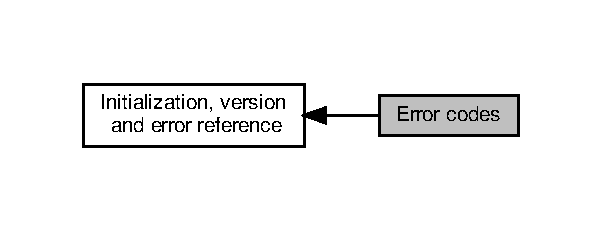
\includegraphics[width=289pt]{group__errors}
\end{center}
\end{figure}
\subsection*{Macros}
\begin{DoxyCompactItemize}
\item 
\#define \hyperlink{group__errors_ga2374ee02c177f12e1fa76ff3ed15e14a}{G\+L\+F\+W\+\_\+\+N\+O\+T\+\_\+\+I\+N\+I\+T\+I\+A\+L\+I\+Z\+ED}~0x00010001
\begin{DoxyCompactList}\small\item\em G\+L\+FW has not been initialized. \end{DoxyCompactList}\item 
\#define \hyperlink{group__errors_gaa8290386e9528ccb9e42a3a4e16fc0d0}{G\+L\+F\+W\+\_\+\+N\+O\+\_\+\+C\+U\+R\+R\+E\+N\+T\+\_\+\+C\+O\+N\+T\+E\+XT}~0x00010002
\begin{DoxyCompactList}\small\item\em No context is current for this thread. \end{DoxyCompactList}\item 
\#define \hyperlink{group__errors_ga76f6bb9c4eea73db675f096b404593ce}{G\+L\+F\+W\+\_\+\+I\+N\+V\+A\+L\+I\+D\+\_\+\+E\+N\+UM}~0x00010003
\begin{DoxyCompactList}\small\item\em One of the arguments to the function was an invalid enum value. \end{DoxyCompactList}\item 
\#define \hyperlink{group__errors_gaaf2ef9aa8202c2b82ac2d921e554c687}{G\+L\+F\+W\+\_\+\+I\+N\+V\+A\+L\+I\+D\+\_\+\+V\+A\+L\+UE}~0x00010004
\begin{DoxyCompactList}\small\item\em One of the arguments to the function was an invalid value. \end{DoxyCompactList}\item 
\#define \hyperlink{group__errors_ga9023953a2bcb98c2906afd071d21ee7f}{G\+L\+F\+W\+\_\+\+O\+U\+T\+\_\+\+O\+F\+\_\+\+M\+E\+M\+O\+RY}~0x00010005
\begin{DoxyCompactList}\small\item\em A memory allocation failed. \end{DoxyCompactList}\item 
\#define \hyperlink{group__errors_ga56882b290db23261cc6c053c40c2d08e}{G\+L\+F\+W\+\_\+\+A\+P\+I\+\_\+\+U\+N\+A\+V\+A\+I\+L\+A\+B\+LE}~0x00010006
\begin{DoxyCompactList}\small\item\em G\+L\+FW could not find support for the requested A\+PI on the system. \end{DoxyCompactList}\item 
\#define \hyperlink{group__errors_gad16c5565b4a69f9c2a9ac2c0dbc89462}{G\+L\+F\+W\+\_\+\+V\+E\+R\+S\+I\+O\+N\+\_\+\+U\+N\+A\+V\+A\+I\+L\+A\+B\+LE}~0x00010007
\begin{DoxyCompactList}\small\item\em The requested Open\+GL or Open\+GL ES version is not available. \end{DoxyCompactList}\item 
\#define \hyperlink{group__errors_gad44162d78100ea5e87cdd38426b8c7a1}{G\+L\+F\+W\+\_\+\+P\+L\+A\+T\+F\+O\+R\+M\+\_\+\+E\+R\+R\+OR}~0x00010008
\begin{DoxyCompactList}\small\item\em A platform-\/specific error occurred that does not match any of the more specific categories. \end{DoxyCompactList}\item 
\#define \hyperlink{group__errors_ga196e125ef261d94184e2b55c05762f14}{G\+L\+F\+W\+\_\+\+F\+O\+R\+M\+A\+T\+\_\+\+U\+N\+A\+V\+A\+I\+L\+A\+B\+LE}~0x00010009
\begin{DoxyCompactList}\small\item\em The requested format is not supported or available. \end{DoxyCompactList}\item 
\#define \hyperlink{group__errors_gacff24d2757da752ae4c80bf452356487}{G\+L\+F\+W\+\_\+\+N\+O\+\_\+\+W\+I\+N\+D\+O\+W\+\_\+\+C\+O\+N\+T\+E\+XT}~0x0001000A
\begin{DoxyCompactList}\small\item\em The specified window does not have an Open\+GL or Open\+GL ES context. \end{DoxyCompactList}\item 
\#define \hyperlink{group__errors_ga2374ee02c177f12e1fa76ff3ed15e14a}{G\+L\+F\+W\+\_\+\+N\+O\+T\+\_\+\+I\+N\+I\+T\+I\+A\+L\+I\+Z\+ED}~0x00010001
\begin{DoxyCompactList}\small\item\em G\+L\+FW has not been initialized. \end{DoxyCompactList}\item 
\#define \hyperlink{group__errors_gaa8290386e9528ccb9e42a3a4e16fc0d0}{G\+L\+F\+W\+\_\+\+N\+O\+\_\+\+C\+U\+R\+R\+E\+N\+T\+\_\+\+C\+O\+N\+T\+E\+XT}~0x00010002
\begin{DoxyCompactList}\small\item\em No context is current for this thread. \end{DoxyCompactList}\item 
\#define \hyperlink{group__errors_ga76f6bb9c4eea73db675f096b404593ce}{G\+L\+F\+W\+\_\+\+I\+N\+V\+A\+L\+I\+D\+\_\+\+E\+N\+UM}~0x00010003
\begin{DoxyCompactList}\small\item\em One of the arguments to the function was an invalid enum value. \end{DoxyCompactList}\item 
\#define \hyperlink{group__errors_gaaf2ef9aa8202c2b82ac2d921e554c687}{G\+L\+F\+W\+\_\+\+I\+N\+V\+A\+L\+I\+D\+\_\+\+V\+A\+L\+UE}~0x00010004
\begin{DoxyCompactList}\small\item\em One of the arguments to the function was an invalid value. \end{DoxyCompactList}\item 
\#define \hyperlink{group__errors_ga9023953a2bcb98c2906afd071d21ee7f}{G\+L\+F\+W\+\_\+\+O\+U\+T\+\_\+\+O\+F\+\_\+\+M\+E\+M\+O\+RY}~0x00010005
\begin{DoxyCompactList}\small\item\em A memory allocation failed. \end{DoxyCompactList}\item 
\#define \hyperlink{group__errors_ga56882b290db23261cc6c053c40c2d08e}{G\+L\+F\+W\+\_\+\+A\+P\+I\+\_\+\+U\+N\+A\+V\+A\+I\+L\+A\+B\+LE}~0x00010006
\begin{DoxyCompactList}\small\item\em G\+L\+FW could not find support for the requested A\+PI on the system. \end{DoxyCompactList}\item 
\#define \hyperlink{group__errors_gad16c5565b4a69f9c2a9ac2c0dbc89462}{G\+L\+F\+W\+\_\+\+V\+E\+R\+S\+I\+O\+N\+\_\+\+U\+N\+A\+V\+A\+I\+L\+A\+B\+LE}~0x00010007
\begin{DoxyCompactList}\small\item\em The requested Open\+GL or Open\+GL ES version is not available. \end{DoxyCompactList}\item 
\#define \hyperlink{group__errors_gad44162d78100ea5e87cdd38426b8c7a1}{G\+L\+F\+W\+\_\+\+P\+L\+A\+T\+F\+O\+R\+M\+\_\+\+E\+R\+R\+OR}~0x00010008
\begin{DoxyCompactList}\small\item\em A platform-\/specific error occurred that does not match any of the more specific categories. \end{DoxyCompactList}\item 
\#define \hyperlink{group__errors_ga196e125ef261d94184e2b55c05762f14}{G\+L\+F\+W\+\_\+\+F\+O\+R\+M\+A\+T\+\_\+\+U\+N\+A\+V\+A\+I\+L\+A\+B\+LE}~0x00010009
\begin{DoxyCompactList}\small\item\em The requested format is not supported or available. \end{DoxyCompactList}\item 
\#define \hyperlink{group__errors_gacff24d2757da752ae4c80bf452356487}{G\+L\+F\+W\+\_\+\+N\+O\+\_\+\+W\+I\+N\+D\+O\+W\+\_\+\+C\+O\+N\+T\+E\+XT}~0x0001000A
\begin{DoxyCompactList}\small\item\em The specified window does not have an Open\+GL or Open\+GL ES context. \end{DoxyCompactList}\item 
\#define \hyperlink{group__errors_ga2374ee02c177f12e1fa76ff3ed15e14a}{G\+L\+F\+W\+\_\+\+N\+O\+T\+\_\+\+I\+N\+I\+T\+I\+A\+L\+I\+Z\+ED}~0x00010001
\begin{DoxyCompactList}\small\item\em G\+L\+FW has not been initialized. \end{DoxyCompactList}\item 
\#define \hyperlink{group__errors_gaa8290386e9528ccb9e42a3a4e16fc0d0}{G\+L\+F\+W\+\_\+\+N\+O\+\_\+\+C\+U\+R\+R\+E\+N\+T\+\_\+\+C\+O\+N\+T\+E\+XT}~0x00010002
\begin{DoxyCompactList}\small\item\em No context is current for this thread. \end{DoxyCompactList}\item 
\#define \hyperlink{group__errors_ga76f6bb9c4eea73db675f096b404593ce}{G\+L\+F\+W\+\_\+\+I\+N\+V\+A\+L\+I\+D\+\_\+\+E\+N\+UM}~0x00010003
\begin{DoxyCompactList}\small\item\em One of the arguments to the function was an invalid enum value. \end{DoxyCompactList}\item 
\#define \hyperlink{group__errors_gaaf2ef9aa8202c2b82ac2d921e554c687}{G\+L\+F\+W\+\_\+\+I\+N\+V\+A\+L\+I\+D\+\_\+\+V\+A\+L\+UE}~0x00010004
\begin{DoxyCompactList}\small\item\em One of the arguments to the function was an invalid value. \end{DoxyCompactList}\item 
\#define \hyperlink{group__errors_ga9023953a2bcb98c2906afd071d21ee7f}{G\+L\+F\+W\+\_\+\+O\+U\+T\+\_\+\+O\+F\+\_\+\+M\+E\+M\+O\+RY}~0x00010005
\begin{DoxyCompactList}\small\item\em A memory allocation failed. \end{DoxyCompactList}\item 
\#define \hyperlink{group__errors_ga56882b290db23261cc6c053c40c2d08e}{G\+L\+F\+W\+\_\+\+A\+P\+I\+\_\+\+U\+N\+A\+V\+A\+I\+L\+A\+B\+LE}~0x00010006
\begin{DoxyCompactList}\small\item\em G\+L\+FW could not find support for the requested A\+PI on the system. \end{DoxyCompactList}\item 
\#define \hyperlink{group__errors_gad16c5565b4a69f9c2a9ac2c0dbc89462}{G\+L\+F\+W\+\_\+\+V\+E\+R\+S\+I\+O\+N\+\_\+\+U\+N\+A\+V\+A\+I\+L\+A\+B\+LE}~0x00010007
\begin{DoxyCompactList}\small\item\em The requested Open\+GL or Open\+GL ES version is not available. \end{DoxyCompactList}\item 
\#define \hyperlink{group__errors_gad44162d78100ea5e87cdd38426b8c7a1}{G\+L\+F\+W\+\_\+\+P\+L\+A\+T\+F\+O\+R\+M\+\_\+\+E\+R\+R\+OR}~0x00010008
\begin{DoxyCompactList}\small\item\em A platform-\/specific error occurred that does not match any of the more specific categories. \end{DoxyCompactList}\item 
\#define \hyperlink{group__errors_ga196e125ef261d94184e2b55c05762f14}{G\+L\+F\+W\+\_\+\+F\+O\+R\+M\+A\+T\+\_\+\+U\+N\+A\+V\+A\+I\+L\+A\+B\+LE}~0x00010009
\begin{DoxyCompactList}\small\item\em The requested format is not supported or available. \end{DoxyCompactList}\item 
\#define \hyperlink{group__errors_gacff24d2757da752ae4c80bf452356487}{G\+L\+F\+W\+\_\+\+N\+O\+\_\+\+W\+I\+N\+D\+O\+W\+\_\+\+C\+O\+N\+T\+E\+XT}~0x0001000A
\begin{DoxyCompactList}\small\item\em The specified window does not have an Open\+GL or Open\+GL ES context. \end{DoxyCompactList}\item 
\#define \hyperlink{group__errors_ga2374ee02c177f12e1fa76ff3ed15e14a}{G\+L\+F\+W\+\_\+\+N\+O\+T\+\_\+\+I\+N\+I\+T\+I\+A\+L\+I\+Z\+ED}~0x00010001
\begin{DoxyCompactList}\small\item\em G\+L\+FW has not been initialized. \end{DoxyCompactList}\item 
\#define \hyperlink{group__errors_gaa8290386e9528ccb9e42a3a4e16fc0d0}{G\+L\+F\+W\+\_\+\+N\+O\+\_\+\+C\+U\+R\+R\+E\+N\+T\+\_\+\+C\+O\+N\+T\+E\+XT}~0x00010002
\begin{DoxyCompactList}\small\item\em No context is current for this thread. \end{DoxyCompactList}\item 
\#define \hyperlink{group__errors_ga76f6bb9c4eea73db675f096b404593ce}{G\+L\+F\+W\+\_\+\+I\+N\+V\+A\+L\+I\+D\+\_\+\+E\+N\+UM}~0x00010003
\begin{DoxyCompactList}\small\item\em One of the arguments to the function was an invalid enum value. \end{DoxyCompactList}\item 
\#define \hyperlink{group__errors_gaaf2ef9aa8202c2b82ac2d921e554c687}{G\+L\+F\+W\+\_\+\+I\+N\+V\+A\+L\+I\+D\+\_\+\+V\+A\+L\+UE}~0x00010004
\begin{DoxyCompactList}\small\item\em One of the arguments to the function was an invalid value. \end{DoxyCompactList}\item 
\#define \hyperlink{group__errors_ga9023953a2bcb98c2906afd071d21ee7f}{G\+L\+F\+W\+\_\+\+O\+U\+T\+\_\+\+O\+F\+\_\+\+M\+E\+M\+O\+RY}~0x00010005
\begin{DoxyCompactList}\small\item\em A memory allocation failed. \end{DoxyCompactList}\item 
\#define \hyperlink{group__errors_ga56882b290db23261cc6c053c40c2d08e}{G\+L\+F\+W\+\_\+\+A\+P\+I\+\_\+\+U\+N\+A\+V\+A\+I\+L\+A\+B\+LE}~0x00010006
\begin{DoxyCompactList}\small\item\em G\+L\+FW could not find support for the requested A\+PI on the system. \end{DoxyCompactList}\item 
\#define \hyperlink{group__errors_gad16c5565b4a69f9c2a9ac2c0dbc89462}{G\+L\+F\+W\+\_\+\+V\+E\+R\+S\+I\+O\+N\+\_\+\+U\+N\+A\+V\+A\+I\+L\+A\+B\+LE}~0x00010007
\begin{DoxyCompactList}\small\item\em The requested Open\+GL or Open\+GL ES version is not available. \end{DoxyCompactList}\item 
\#define \hyperlink{group__errors_gad44162d78100ea5e87cdd38426b8c7a1}{G\+L\+F\+W\+\_\+\+P\+L\+A\+T\+F\+O\+R\+M\+\_\+\+E\+R\+R\+OR}~0x00010008
\begin{DoxyCompactList}\small\item\em A platform-\/specific error occurred that does not match any of the more specific categories. \end{DoxyCompactList}\item 
\#define \hyperlink{group__errors_ga196e125ef261d94184e2b55c05762f14}{G\+L\+F\+W\+\_\+\+F\+O\+R\+M\+A\+T\+\_\+\+U\+N\+A\+V\+A\+I\+L\+A\+B\+LE}~0x00010009
\begin{DoxyCompactList}\small\item\em The requested format is not supported or available. \end{DoxyCompactList}\item 
\#define \hyperlink{group__errors_gacff24d2757da752ae4c80bf452356487}{G\+L\+F\+W\+\_\+\+N\+O\+\_\+\+W\+I\+N\+D\+O\+W\+\_\+\+C\+O\+N\+T\+E\+XT}~0x0001000A
\begin{DoxyCompactList}\small\item\em The specified window does not have an Open\+GL or Open\+GL ES context. \end{DoxyCompactList}\item 
\#define \hyperlink{group__errors_ga2374ee02c177f12e1fa76ff3ed15e14a}{G\+L\+F\+W\+\_\+\+N\+O\+T\+\_\+\+I\+N\+I\+T\+I\+A\+L\+I\+Z\+ED}~0x00010001
\begin{DoxyCompactList}\small\item\em G\+L\+FW has not been initialized. \end{DoxyCompactList}\item 
\#define \hyperlink{group__errors_gaa8290386e9528ccb9e42a3a4e16fc0d0}{G\+L\+F\+W\+\_\+\+N\+O\+\_\+\+C\+U\+R\+R\+E\+N\+T\+\_\+\+C\+O\+N\+T\+E\+XT}~0x00010002
\begin{DoxyCompactList}\small\item\em No context is current for this thread. \end{DoxyCompactList}\item 
\#define \hyperlink{group__errors_ga76f6bb9c4eea73db675f096b404593ce}{G\+L\+F\+W\+\_\+\+I\+N\+V\+A\+L\+I\+D\+\_\+\+E\+N\+UM}~0x00010003
\begin{DoxyCompactList}\small\item\em One of the arguments to the function was an invalid enum value. \end{DoxyCompactList}\item 
\#define \hyperlink{group__errors_gaaf2ef9aa8202c2b82ac2d921e554c687}{G\+L\+F\+W\+\_\+\+I\+N\+V\+A\+L\+I\+D\+\_\+\+V\+A\+L\+UE}~0x00010004
\begin{DoxyCompactList}\small\item\em One of the arguments to the function was an invalid value. \end{DoxyCompactList}\item 
\#define \hyperlink{group__errors_ga9023953a2bcb98c2906afd071d21ee7f}{G\+L\+F\+W\+\_\+\+O\+U\+T\+\_\+\+O\+F\+\_\+\+M\+E\+M\+O\+RY}~0x00010005
\begin{DoxyCompactList}\small\item\em A memory allocation failed. \end{DoxyCompactList}\item 
\#define \hyperlink{group__errors_ga56882b290db23261cc6c053c40c2d08e}{G\+L\+F\+W\+\_\+\+A\+P\+I\+\_\+\+U\+N\+A\+V\+A\+I\+L\+A\+B\+LE}~0x00010006
\begin{DoxyCompactList}\small\item\em G\+L\+FW could not find support for the requested A\+PI on the system. \end{DoxyCompactList}\item 
\#define \hyperlink{group__errors_gad16c5565b4a69f9c2a9ac2c0dbc89462}{G\+L\+F\+W\+\_\+\+V\+E\+R\+S\+I\+O\+N\+\_\+\+U\+N\+A\+V\+A\+I\+L\+A\+B\+LE}~0x00010007
\begin{DoxyCompactList}\small\item\em The requested Open\+GL or Open\+GL ES version is not available. \end{DoxyCompactList}\item 
\#define \hyperlink{group__errors_gad44162d78100ea5e87cdd38426b8c7a1}{G\+L\+F\+W\+\_\+\+P\+L\+A\+T\+F\+O\+R\+M\+\_\+\+E\+R\+R\+OR}~0x00010008
\begin{DoxyCompactList}\small\item\em A platform-\/specific error occurred that does not match any of the more specific categories. \end{DoxyCompactList}\item 
\#define \hyperlink{group__errors_ga196e125ef261d94184e2b55c05762f14}{G\+L\+F\+W\+\_\+\+F\+O\+R\+M\+A\+T\+\_\+\+U\+N\+A\+V\+A\+I\+L\+A\+B\+LE}~0x00010009
\begin{DoxyCompactList}\small\item\em The requested format is not supported or available. \end{DoxyCompactList}\item 
\#define \hyperlink{group__errors_gacff24d2757da752ae4c80bf452356487}{G\+L\+F\+W\+\_\+\+N\+O\+\_\+\+W\+I\+N\+D\+O\+W\+\_\+\+C\+O\+N\+T\+E\+XT}~0x0001000A
\begin{DoxyCompactList}\small\item\em The specified window does not have an Open\+GL or Open\+GL ES context. \end{DoxyCompactList}\end{DoxyCompactItemize}


\subsection{Detailed Description}
See error handling for how these are used. 

\subsection{Macro Definition Documentation}
\mbox{\Hypertarget{group__errors_ga56882b290db23261cc6c053c40c2d08e}\label{group__errors_ga56882b290db23261cc6c053c40c2d08e}} 
\index{Error codes@{Error codes}!G\+L\+F\+W\+\_\+\+A\+P\+I\+\_\+\+U\+N\+A\+V\+A\+I\+L\+A\+B\+LE@{G\+L\+F\+W\+\_\+\+A\+P\+I\+\_\+\+U\+N\+A\+V\+A\+I\+L\+A\+B\+LE}}
\index{G\+L\+F\+W\+\_\+\+A\+P\+I\+\_\+\+U\+N\+A\+V\+A\+I\+L\+A\+B\+LE@{G\+L\+F\+W\+\_\+\+A\+P\+I\+\_\+\+U\+N\+A\+V\+A\+I\+L\+A\+B\+LE}!Error codes@{Error codes}}
\subsubsection{\texorpdfstring{G\+L\+F\+W\+\_\+\+A\+P\+I\+\_\+\+U\+N\+A\+V\+A\+I\+L\+A\+B\+LE}{GLFW\_API\_UNAVAILABLE}\hspace{0.1cm}{\footnotesize\ttfamily [1/5]}}
{\footnotesize\ttfamily \#define G\+L\+F\+W\+\_\+\+A\+P\+I\+\_\+\+U\+N\+A\+V\+A\+I\+L\+A\+B\+LE~0x00010006}



G\+L\+FW could not find support for the requested A\+PI on the system. 

G\+L\+FW could not find support for the requested A\+PI on the system.

The installed graphics driver does not support the requested A\+PI, or does not support it via the chosen context creation backend. Below are a few examples.

\begin{DoxyParagraph}{}
Some pre-\/installed Windows graphics drivers do not support Open\+GL. A\+MD only supports Open\+GL ES via E\+GL, while Nvidia and Intel only support it via a W\+GL or G\+LX extension. OS X does not provide Open\+GL ES at all. The Mesa E\+GL, Open\+GL and Open\+GL ES libraries do not interface with the Nvidia binary driver. Older graphics drivers do not support Vulkan. 
\end{DoxyParagraph}
\mbox{\Hypertarget{group__errors_ga56882b290db23261cc6c053c40c2d08e}\label{group__errors_ga56882b290db23261cc6c053c40c2d08e}} 
\index{Error codes@{Error codes}!G\+L\+F\+W\+\_\+\+A\+P\+I\+\_\+\+U\+N\+A\+V\+A\+I\+L\+A\+B\+LE@{G\+L\+F\+W\+\_\+\+A\+P\+I\+\_\+\+U\+N\+A\+V\+A\+I\+L\+A\+B\+LE}}
\index{G\+L\+F\+W\+\_\+\+A\+P\+I\+\_\+\+U\+N\+A\+V\+A\+I\+L\+A\+B\+LE@{G\+L\+F\+W\+\_\+\+A\+P\+I\+\_\+\+U\+N\+A\+V\+A\+I\+L\+A\+B\+LE}!Error codes@{Error codes}}
\subsubsection{\texorpdfstring{G\+L\+F\+W\+\_\+\+A\+P\+I\+\_\+\+U\+N\+A\+V\+A\+I\+L\+A\+B\+LE}{GLFW\_API\_UNAVAILABLE}\hspace{0.1cm}{\footnotesize\ttfamily [2/5]}}
{\footnotesize\ttfamily \#define G\+L\+F\+W\+\_\+\+A\+P\+I\+\_\+\+U\+N\+A\+V\+A\+I\+L\+A\+B\+LE~0x00010006}



G\+L\+FW could not find support for the requested A\+PI on the system. 

G\+L\+FW could not find support for the requested A\+PI on the system.

The installed graphics driver does not support the requested A\+PI, or does not support it via the chosen context creation backend. Below are a few examples.

\begin{DoxyParagraph}{}
Some pre-\/installed Windows graphics drivers do not support Open\+GL. A\+MD only supports Open\+GL ES via E\+GL, while Nvidia and Intel only support it via a W\+GL or G\+LX extension. OS X does not provide Open\+GL ES at all. The Mesa E\+GL, Open\+GL and Open\+GL ES libraries do not interface with the Nvidia binary driver. Older graphics drivers do not support Vulkan. 
\end{DoxyParagraph}
\mbox{\Hypertarget{group__errors_ga56882b290db23261cc6c053c40c2d08e}\label{group__errors_ga56882b290db23261cc6c053c40c2d08e}} 
\index{Error codes@{Error codes}!G\+L\+F\+W\+\_\+\+A\+P\+I\+\_\+\+U\+N\+A\+V\+A\+I\+L\+A\+B\+LE@{G\+L\+F\+W\+\_\+\+A\+P\+I\+\_\+\+U\+N\+A\+V\+A\+I\+L\+A\+B\+LE}}
\index{G\+L\+F\+W\+\_\+\+A\+P\+I\+\_\+\+U\+N\+A\+V\+A\+I\+L\+A\+B\+LE@{G\+L\+F\+W\+\_\+\+A\+P\+I\+\_\+\+U\+N\+A\+V\+A\+I\+L\+A\+B\+LE}!Error codes@{Error codes}}
\subsubsection{\texorpdfstring{G\+L\+F\+W\+\_\+\+A\+P\+I\+\_\+\+U\+N\+A\+V\+A\+I\+L\+A\+B\+LE}{GLFW\_API\_UNAVAILABLE}\hspace{0.1cm}{\footnotesize\ttfamily [3/5]}}
{\footnotesize\ttfamily \#define G\+L\+F\+W\+\_\+\+A\+P\+I\+\_\+\+U\+N\+A\+V\+A\+I\+L\+A\+B\+LE~0x00010006}



G\+L\+FW could not find support for the requested A\+PI on the system. 

G\+L\+FW could not find support for the requested A\+PI on the system.

The installed graphics driver does not support the requested A\+PI, or does not support it via the chosen context creation backend. Below are a few examples.

\begin{DoxyParagraph}{}
Some pre-\/installed Windows graphics drivers do not support Open\+GL. A\+MD only supports Open\+GL ES via E\+GL, while Nvidia and Intel only support it via a W\+GL or G\+LX extension. OS X does not provide Open\+GL ES at all. The Mesa E\+GL, Open\+GL and Open\+GL ES libraries do not interface with the Nvidia binary driver. Older graphics drivers do not support Vulkan. 
\end{DoxyParagraph}
\mbox{\Hypertarget{group__errors_ga56882b290db23261cc6c053c40c2d08e}\label{group__errors_ga56882b290db23261cc6c053c40c2d08e}} 
\index{Error codes@{Error codes}!G\+L\+F\+W\+\_\+\+A\+P\+I\+\_\+\+U\+N\+A\+V\+A\+I\+L\+A\+B\+LE@{G\+L\+F\+W\+\_\+\+A\+P\+I\+\_\+\+U\+N\+A\+V\+A\+I\+L\+A\+B\+LE}}
\index{G\+L\+F\+W\+\_\+\+A\+P\+I\+\_\+\+U\+N\+A\+V\+A\+I\+L\+A\+B\+LE@{G\+L\+F\+W\+\_\+\+A\+P\+I\+\_\+\+U\+N\+A\+V\+A\+I\+L\+A\+B\+LE}!Error codes@{Error codes}}
\subsubsection{\texorpdfstring{G\+L\+F\+W\+\_\+\+A\+P\+I\+\_\+\+U\+N\+A\+V\+A\+I\+L\+A\+B\+LE}{GLFW\_API\_UNAVAILABLE}\hspace{0.1cm}{\footnotesize\ttfamily [4/5]}}
{\footnotesize\ttfamily \#define G\+L\+F\+W\+\_\+\+A\+P\+I\+\_\+\+U\+N\+A\+V\+A\+I\+L\+A\+B\+LE~0x00010006}



G\+L\+FW could not find support for the requested A\+PI on the system. 

G\+L\+FW could not find support for the requested A\+PI on the system.

The installed graphics driver does not support the requested A\+PI, or does not support it via the chosen context creation backend. Below are a few examples.

\begin{DoxyParagraph}{}
Some pre-\/installed Windows graphics drivers do not support Open\+GL. A\+MD only supports Open\+GL ES via E\+GL, while Nvidia and Intel only support it via a W\+GL or G\+LX extension. OS X does not provide Open\+GL ES at all. The Mesa E\+GL, Open\+GL and Open\+GL ES libraries do not interface with the Nvidia binary driver. Older graphics drivers do not support Vulkan. 
\end{DoxyParagraph}
\mbox{\Hypertarget{group__errors_ga56882b290db23261cc6c053c40c2d08e}\label{group__errors_ga56882b290db23261cc6c053c40c2d08e}} 
\index{Error codes@{Error codes}!G\+L\+F\+W\+\_\+\+A\+P\+I\+\_\+\+U\+N\+A\+V\+A\+I\+L\+A\+B\+LE@{G\+L\+F\+W\+\_\+\+A\+P\+I\+\_\+\+U\+N\+A\+V\+A\+I\+L\+A\+B\+LE}}
\index{G\+L\+F\+W\+\_\+\+A\+P\+I\+\_\+\+U\+N\+A\+V\+A\+I\+L\+A\+B\+LE@{G\+L\+F\+W\+\_\+\+A\+P\+I\+\_\+\+U\+N\+A\+V\+A\+I\+L\+A\+B\+LE}!Error codes@{Error codes}}
\subsubsection{\texorpdfstring{G\+L\+F\+W\+\_\+\+A\+P\+I\+\_\+\+U\+N\+A\+V\+A\+I\+L\+A\+B\+LE}{GLFW\_API\_UNAVAILABLE}\hspace{0.1cm}{\footnotesize\ttfamily [5/5]}}
{\footnotesize\ttfamily \#define G\+L\+F\+W\+\_\+\+A\+P\+I\+\_\+\+U\+N\+A\+V\+A\+I\+L\+A\+B\+LE~0x00010006}



G\+L\+FW could not find support for the requested A\+PI on the system. 

G\+L\+FW could not find support for the requested A\+PI on the system.

The installed graphics driver does not support the requested A\+PI, or does not support it via the chosen context creation backend. Below are a few examples.

\begin{DoxyParagraph}{}
Some pre-\/installed Windows graphics drivers do not support Open\+GL. A\+MD only supports Open\+GL ES via E\+GL, while Nvidia and Intel only support it via a W\+GL or G\+LX extension. OS X does not provide Open\+GL ES at all. The Mesa E\+GL, Open\+GL and Open\+GL ES libraries do not interface with the Nvidia binary driver. Older graphics drivers do not support Vulkan. 
\end{DoxyParagraph}
\mbox{\Hypertarget{group__errors_ga196e125ef261d94184e2b55c05762f14}\label{group__errors_ga196e125ef261d94184e2b55c05762f14}} 
\index{Error codes@{Error codes}!G\+L\+F\+W\+\_\+\+F\+O\+R\+M\+A\+T\+\_\+\+U\+N\+A\+V\+A\+I\+L\+A\+B\+LE@{G\+L\+F\+W\+\_\+\+F\+O\+R\+M\+A\+T\+\_\+\+U\+N\+A\+V\+A\+I\+L\+A\+B\+LE}}
\index{G\+L\+F\+W\+\_\+\+F\+O\+R\+M\+A\+T\+\_\+\+U\+N\+A\+V\+A\+I\+L\+A\+B\+LE@{G\+L\+F\+W\+\_\+\+F\+O\+R\+M\+A\+T\+\_\+\+U\+N\+A\+V\+A\+I\+L\+A\+B\+LE}!Error codes@{Error codes}}
\subsubsection{\texorpdfstring{G\+L\+F\+W\+\_\+\+F\+O\+R\+M\+A\+T\+\_\+\+U\+N\+A\+V\+A\+I\+L\+A\+B\+LE}{GLFW\_FORMAT\_UNAVAILABLE}\hspace{0.1cm}{\footnotesize\ttfamily [1/5]}}
{\footnotesize\ttfamily \#define G\+L\+F\+W\+\_\+\+F\+O\+R\+M\+A\+T\+\_\+\+U\+N\+A\+V\+A\+I\+L\+A\+B\+LE~0x00010009}



The requested format is not supported or available. 

If emitted during window creation, the requested pixel format is not supported.

If emitted when querying the clipboard, the contents of the clipboard could not be converted to the requested format.

If emitted during window creation, one or more hard constraints did not match any of the available pixel formats. If your application is sufficiently flexible, downgrade your requirements and try again. Otherwise, inform the user that their machine does not match your requirements.

\begin{DoxyParagraph}{}
If emitted when querying the clipboard, ignore the error or report it to the user, as appropriate. 
\end{DoxyParagraph}
\mbox{\Hypertarget{group__errors_ga196e125ef261d94184e2b55c05762f14}\label{group__errors_ga196e125ef261d94184e2b55c05762f14}} 
\index{Error codes@{Error codes}!G\+L\+F\+W\+\_\+\+F\+O\+R\+M\+A\+T\+\_\+\+U\+N\+A\+V\+A\+I\+L\+A\+B\+LE@{G\+L\+F\+W\+\_\+\+F\+O\+R\+M\+A\+T\+\_\+\+U\+N\+A\+V\+A\+I\+L\+A\+B\+LE}}
\index{G\+L\+F\+W\+\_\+\+F\+O\+R\+M\+A\+T\+\_\+\+U\+N\+A\+V\+A\+I\+L\+A\+B\+LE@{G\+L\+F\+W\+\_\+\+F\+O\+R\+M\+A\+T\+\_\+\+U\+N\+A\+V\+A\+I\+L\+A\+B\+LE}!Error codes@{Error codes}}
\subsubsection{\texorpdfstring{G\+L\+F\+W\+\_\+\+F\+O\+R\+M\+A\+T\+\_\+\+U\+N\+A\+V\+A\+I\+L\+A\+B\+LE}{GLFW\_FORMAT\_UNAVAILABLE}\hspace{0.1cm}{\footnotesize\ttfamily [2/5]}}
{\footnotesize\ttfamily \#define G\+L\+F\+W\+\_\+\+F\+O\+R\+M\+A\+T\+\_\+\+U\+N\+A\+V\+A\+I\+L\+A\+B\+LE~0x00010009}



The requested format is not supported or available. 

If emitted during window creation, the requested pixel format is not supported.

If emitted when querying the clipboard, the contents of the clipboard could not be converted to the requested format.

If emitted during window creation, one or more hard constraints did not match any of the available pixel formats. If your application is sufficiently flexible, downgrade your requirements and try again. Otherwise, inform the user that their machine does not match your requirements.

\begin{DoxyParagraph}{}
If emitted when querying the clipboard, ignore the error or report it to the user, as appropriate. 
\end{DoxyParagraph}
\mbox{\Hypertarget{group__errors_ga196e125ef261d94184e2b55c05762f14}\label{group__errors_ga196e125ef261d94184e2b55c05762f14}} 
\index{Error codes@{Error codes}!G\+L\+F\+W\+\_\+\+F\+O\+R\+M\+A\+T\+\_\+\+U\+N\+A\+V\+A\+I\+L\+A\+B\+LE@{G\+L\+F\+W\+\_\+\+F\+O\+R\+M\+A\+T\+\_\+\+U\+N\+A\+V\+A\+I\+L\+A\+B\+LE}}
\index{G\+L\+F\+W\+\_\+\+F\+O\+R\+M\+A\+T\+\_\+\+U\+N\+A\+V\+A\+I\+L\+A\+B\+LE@{G\+L\+F\+W\+\_\+\+F\+O\+R\+M\+A\+T\+\_\+\+U\+N\+A\+V\+A\+I\+L\+A\+B\+LE}!Error codes@{Error codes}}
\subsubsection{\texorpdfstring{G\+L\+F\+W\+\_\+\+F\+O\+R\+M\+A\+T\+\_\+\+U\+N\+A\+V\+A\+I\+L\+A\+B\+LE}{GLFW\_FORMAT\_UNAVAILABLE}\hspace{0.1cm}{\footnotesize\ttfamily [3/5]}}
{\footnotesize\ttfamily \#define G\+L\+F\+W\+\_\+\+F\+O\+R\+M\+A\+T\+\_\+\+U\+N\+A\+V\+A\+I\+L\+A\+B\+LE~0x00010009}



The requested format is not supported or available. 

If emitted during window creation, the requested pixel format is not supported.

If emitted when querying the clipboard, the contents of the clipboard could not be converted to the requested format.

If emitted during window creation, one or more hard constraints did not match any of the available pixel formats. If your application is sufficiently flexible, downgrade your requirements and try again. Otherwise, inform the user that their machine does not match your requirements.

\begin{DoxyParagraph}{}
If emitted when querying the clipboard, ignore the error or report it to the user, as appropriate. 
\end{DoxyParagraph}
\mbox{\Hypertarget{group__errors_ga196e125ef261d94184e2b55c05762f14}\label{group__errors_ga196e125ef261d94184e2b55c05762f14}} 
\index{Error codes@{Error codes}!G\+L\+F\+W\+\_\+\+F\+O\+R\+M\+A\+T\+\_\+\+U\+N\+A\+V\+A\+I\+L\+A\+B\+LE@{G\+L\+F\+W\+\_\+\+F\+O\+R\+M\+A\+T\+\_\+\+U\+N\+A\+V\+A\+I\+L\+A\+B\+LE}}
\index{G\+L\+F\+W\+\_\+\+F\+O\+R\+M\+A\+T\+\_\+\+U\+N\+A\+V\+A\+I\+L\+A\+B\+LE@{G\+L\+F\+W\+\_\+\+F\+O\+R\+M\+A\+T\+\_\+\+U\+N\+A\+V\+A\+I\+L\+A\+B\+LE}!Error codes@{Error codes}}
\subsubsection{\texorpdfstring{G\+L\+F\+W\+\_\+\+F\+O\+R\+M\+A\+T\+\_\+\+U\+N\+A\+V\+A\+I\+L\+A\+B\+LE}{GLFW\_FORMAT\_UNAVAILABLE}\hspace{0.1cm}{\footnotesize\ttfamily [4/5]}}
{\footnotesize\ttfamily \#define G\+L\+F\+W\+\_\+\+F\+O\+R\+M\+A\+T\+\_\+\+U\+N\+A\+V\+A\+I\+L\+A\+B\+LE~0x00010009}



The requested format is not supported or available. 

If emitted during window creation, the requested pixel format is not supported.

If emitted when querying the clipboard, the contents of the clipboard could not be converted to the requested format.

If emitted during window creation, one or more hard constraints did not match any of the available pixel formats. If your application is sufficiently flexible, downgrade your requirements and try again. Otherwise, inform the user that their machine does not match your requirements.

\begin{DoxyParagraph}{}
If emitted when querying the clipboard, ignore the error or report it to the user, as appropriate. 
\end{DoxyParagraph}
\mbox{\Hypertarget{group__errors_ga196e125ef261d94184e2b55c05762f14}\label{group__errors_ga196e125ef261d94184e2b55c05762f14}} 
\index{Error codes@{Error codes}!G\+L\+F\+W\+\_\+\+F\+O\+R\+M\+A\+T\+\_\+\+U\+N\+A\+V\+A\+I\+L\+A\+B\+LE@{G\+L\+F\+W\+\_\+\+F\+O\+R\+M\+A\+T\+\_\+\+U\+N\+A\+V\+A\+I\+L\+A\+B\+LE}}
\index{G\+L\+F\+W\+\_\+\+F\+O\+R\+M\+A\+T\+\_\+\+U\+N\+A\+V\+A\+I\+L\+A\+B\+LE@{G\+L\+F\+W\+\_\+\+F\+O\+R\+M\+A\+T\+\_\+\+U\+N\+A\+V\+A\+I\+L\+A\+B\+LE}!Error codes@{Error codes}}
\subsubsection{\texorpdfstring{G\+L\+F\+W\+\_\+\+F\+O\+R\+M\+A\+T\+\_\+\+U\+N\+A\+V\+A\+I\+L\+A\+B\+LE}{GLFW\_FORMAT\_UNAVAILABLE}\hspace{0.1cm}{\footnotesize\ttfamily [5/5]}}
{\footnotesize\ttfamily \#define G\+L\+F\+W\+\_\+\+F\+O\+R\+M\+A\+T\+\_\+\+U\+N\+A\+V\+A\+I\+L\+A\+B\+LE~0x00010009}



The requested format is not supported or available. 

If emitted during window creation, the requested pixel format is not supported.

If emitted when querying the clipboard, the contents of the clipboard could not be converted to the requested format.

If emitted during window creation, one or more hard constraints did not match any of the available pixel formats. If your application is sufficiently flexible, downgrade your requirements and try again. Otherwise, inform the user that their machine does not match your requirements.

\begin{DoxyParagraph}{}
If emitted when querying the clipboard, ignore the error or report it to the user, as appropriate. 
\end{DoxyParagraph}
\mbox{\Hypertarget{group__errors_ga76f6bb9c4eea73db675f096b404593ce}\label{group__errors_ga76f6bb9c4eea73db675f096b404593ce}} 
\index{Error codes@{Error codes}!G\+L\+F\+W\+\_\+\+I\+N\+V\+A\+L\+I\+D\+\_\+\+E\+N\+UM@{G\+L\+F\+W\+\_\+\+I\+N\+V\+A\+L\+I\+D\+\_\+\+E\+N\+UM}}
\index{G\+L\+F\+W\+\_\+\+I\+N\+V\+A\+L\+I\+D\+\_\+\+E\+N\+UM@{G\+L\+F\+W\+\_\+\+I\+N\+V\+A\+L\+I\+D\+\_\+\+E\+N\+UM}!Error codes@{Error codes}}
\subsubsection{\texorpdfstring{G\+L\+F\+W\+\_\+\+I\+N\+V\+A\+L\+I\+D\+\_\+\+E\+N\+UM}{GLFW\_INVALID\_ENUM}\hspace{0.1cm}{\footnotesize\ttfamily [1/5]}}
{\footnotesize\ttfamily \#define G\+L\+F\+W\+\_\+\+I\+N\+V\+A\+L\+I\+D\+\_\+\+E\+N\+UM~0x00010003}



One of the arguments to the function was an invalid enum value. 

One of the arguments to the function was an invalid enum value, for example requesting G\+L\+F\+W\+\_\+\+R\+E\+D\+\_\+\+B\+I\+TS with \hyperlink{group__window_ga1bb0c7e100418e284dbb800789c63d40}{glfw\+Get\+Window\+Attrib}.

\hyperlink{classApplication}{Application} programmer error. Fix the offending call. \mbox{\Hypertarget{group__errors_ga76f6bb9c4eea73db675f096b404593ce}\label{group__errors_ga76f6bb9c4eea73db675f096b404593ce}} 
\index{Error codes@{Error codes}!G\+L\+F\+W\+\_\+\+I\+N\+V\+A\+L\+I\+D\+\_\+\+E\+N\+UM@{G\+L\+F\+W\+\_\+\+I\+N\+V\+A\+L\+I\+D\+\_\+\+E\+N\+UM}}
\index{G\+L\+F\+W\+\_\+\+I\+N\+V\+A\+L\+I\+D\+\_\+\+E\+N\+UM@{G\+L\+F\+W\+\_\+\+I\+N\+V\+A\+L\+I\+D\+\_\+\+E\+N\+UM}!Error codes@{Error codes}}
\subsubsection{\texorpdfstring{G\+L\+F\+W\+\_\+\+I\+N\+V\+A\+L\+I\+D\+\_\+\+E\+N\+UM}{GLFW\_INVALID\_ENUM}\hspace{0.1cm}{\footnotesize\ttfamily [2/5]}}
{\footnotesize\ttfamily \#define G\+L\+F\+W\+\_\+\+I\+N\+V\+A\+L\+I\+D\+\_\+\+E\+N\+UM~0x00010003}



One of the arguments to the function was an invalid enum value. 

One of the arguments to the function was an invalid enum value, for example requesting G\+L\+F\+W\+\_\+\+R\+E\+D\+\_\+\+B\+I\+TS with \hyperlink{group__window_ga1bb0c7e100418e284dbb800789c63d40}{glfw\+Get\+Window\+Attrib}.

\hyperlink{classApplication}{Application} programmer error. Fix the offending call. \mbox{\Hypertarget{group__errors_ga76f6bb9c4eea73db675f096b404593ce}\label{group__errors_ga76f6bb9c4eea73db675f096b404593ce}} 
\index{Error codes@{Error codes}!G\+L\+F\+W\+\_\+\+I\+N\+V\+A\+L\+I\+D\+\_\+\+E\+N\+UM@{G\+L\+F\+W\+\_\+\+I\+N\+V\+A\+L\+I\+D\+\_\+\+E\+N\+UM}}
\index{G\+L\+F\+W\+\_\+\+I\+N\+V\+A\+L\+I\+D\+\_\+\+E\+N\+UM@{G\+L\+F\+W\+\_\+\+I\+N\+V\+A\+L\+I\+D\+\_\+\+E\+N\+UM}!Error codes@{Error codes}}
\subsubsection{\texorpdfstring{G\+L\+F\+W\+\_\+\+I\+N\+V\+A\+L\+I\+D\+\_\+\+E\+N\+UM}{GLFW\_INVALID\_ENUM}\hspace{0.1cm}{\footnotesize\ttfamily [3/5]}}
{\footnotesize\ttfamily \#define G\+L\+F\+W\+\_\+\+I\+N\+V\+A\+L\+I\+D\+\_\+\+E\+N\+UM~0x00010003}



One of the arguments to the function was an invalid enum value. 

One of the arguments to the function was an invalid enum value, for example requesting G\+L\+F\+W\+\_\+\+R\+E\+D\+\_\+\+B\+I\+TS with \hyperlink{group__window_ga1bb0c7e100418e284dbb800789c63d40}{glfw\+Get\+Window\+Attrib}.

\hyperlink{classApplication}{Application} programmer error. Fix the offending call. \mbox{\Hypertarget{group__errors_ga76f6bb9c4eea73db675f096b404593ce}\label{group__errors_ga76f6bb9c4eea73db675f096b404593ce}} 
\index{Error codes@{Error codes}!G\+L\+F\+W\+\_\+\+I\+N\+V\+A\+L\+I\+D\+\_\+\+E\+N\+UM@{G\+L\+F\+W\+\_\+\+I\+N\+V\+A\+L\+I\+D\+\_\+\+E\+N\+UM}}
\index{G\+L\+F\+W\+\_\+\+I\+N\+V\+A\+L\+I\+D\+\_\+\+E\+N\+UM@{G\+L\+F\+W\+\_\+\+I\+N\+V\+A\+L\+I\+D\+\_\+\+E\+N\+UM}!Error codes@{Error codes}}
\subsubsection{\texorpdfstring{G\+L\+F\+W\+\_\+\+I\+N\+V\+A\+L\+I\+D\+\_\+\+E\+N\+UM}{GLFW\_INVALID\_ENUM}\hspace{0.1cm}{\footnotesize\ttfamily [4/5]}}
{\footnotesize\ttfamily \#define G\+L\+F\+W\+\_\+\+I\+N\+V\+A\+L\+I\+D\+\_\+\+E\+N\+UM~0x00010003}



One of the arguments to the function was an invalid enum value. 

One of the arguments to the function was an invalid enum value, for example requesting G\+L\+F\+W\+\_\+\+R\+E\+D\+\_\+\+B\+I\+TS with \hyperlink{group__window_ga1bb0c7e100418e284dbb800789c63d40}{glfw\+Get\+Window\+Attrib}.

\hyperlink{classApplication}{Application} programmer error. Fix the offending call. \mbox{\Hypertarget{group__errors_ga76f6bb9c4eea73db675f096b404593ce}\label{group__errors_ga76f6bb9c4eea73db675f096b404593ce}} 
\index{Error codes@{Error codes}!G\+L\+F\+W\+\_\+\+I\+N\+V\+A\+L\+I\+D\+\_\+\+E\+N\+UM@{G\+L\+F\+W\+\_\+\+I\+N\+V\+A\+L\+I\+D\+\_\+\+E\+N\+UM}}
\index{G\+L\+F\+W\+\_\+\+I\+N\+V\+A\+L\+I\+D\+\_\+\+E\+N\+UM@{G\+L\+F\+W\+\_\+\+I\+N\+V\+A\+L\+I\+D\+\_\+\+E\+N\+UM}!Error codes@{Error codes}}
\subsubsection{\texorpdfstring{G\+L\+F\+W\+\_\+\+I\+N\+V\+A\+L\+I\+D\+\_\+\+E\+N\+UM}{GLFW\_INVALID\_ENUM}\hspace{0.1cm}{\footnotesize\ttfamily [5/5]}}
{\footnotesize\ttfamily \#define G\+L\+F\+W\+\_\+\+I\+N\+V\+A\+L\+I\+D\+\_\+\+E\+N\+UM~0x00010003}



One of the arguments to the function was an invalid enum value. 

One of the arguments to the function was an invalid enum value, for example requesting G\+L\+F\+W\+\_\+\+R\+E\+D\+\_\+\+B\+I\+TS with \hyperlink{group__window_ga1bb0c7e100418e284dbb800789c63d40}{glfw\+Get\+Window\+Attrib}.

\hyperlink{classApplication}{Application} programmer error. Fix the offending call. \mbox{\Hypertarget{group__errors_gaaf2ef9aa8202c2b82ac2d921e554c687}\label{group__errors_gaaf2ef9aa8202c2b82ac2d921e554c687}} 
\index{Error codes@{Error codes}!G\+L\+F\+W\+\_\+\+I\+N\+V\+A\+L\+I\+D\+\_\+\+V\+A\+L\+UE@{G\+L\+F\+W\+\_\+\+I\+N\+V\+A\+L\+I\+D\+\_\+\+V\+A\+L\+UE}}
\index{G\+L\+F\+W\+\_\+\+I\+N\+V\+A\+L\+I\+D\+\_\+\+V\+A\+L\+UE@{G\+L\+F\+W\+\_\+\+I\+N\+V\+A\+L\+I\+D\+\_\+\+V\+A\+L\+UE}!Error codes@{Error codes}}
\subsubsection{\texorpdfstring{G\+L\+F\+W\+\_\+\+I\+N\+V\+A\+L\+I\+D\+\_\+\+V\+A\+L\+UE}{GLFW\_INVALID\_VALUE}\hspace{0.1cm}{\footnotesize\ttfamily [1/5]}}
{\footnotesize\ttfamily \#define G\+L\+F\+W\+\_\+\+I\+N\+V\+A\+L\+I\+D\+\_\+\+V\+A\+L\+UE~0x00010004}



One of the arguments to the function was an invalid value. 

One of the arguments to the function was an invalid value, for example requesting a non-\/existent Open\+GL or Open\+GL ES version like 2.\+7.

Requesting a valid but unavailable Open\+GL or Open\+GL ES version will instead result in a \hyperlink{group__errors_gad16c5565b4a69f9c2a9ac2c0dbc89462}{G\+L\+F\+W\+\_\+\+V\+E\+R\+S\+I\+O\+N\+\_\+\+U\+N\+A\+V\+A\+I\+L\+A\+B\+LE} error.

\hyperlink{classApplication}{Application} programmer error. Fix the offending call. \mbox{\Hypertarget{group__errors_gaaf2ef9aa8202c2b82ac2d921e554c687}\label{group__errors_gaaf2ef9aa8202c2b82ac2d921e554c687}} 
\index{Error codes@{Error codes}!G\+L\+F\+W\+\_\+\+I\+N\+V\+A\+L\+I\+D\+\_\+\+V\+A\+L\+UE@{G\+L\+F\+W\+\_\+\+I\+N\+V\+A\+L\+I\+D\+\_\+\+V\+A\+L\+UE}}
\index{G\+L\+F\+W\+\_\+\+I\+N\+V\+A\+L\+I\+D\+\_\+\+V\+A\+L\+UE@{G\+L\+F\+W\+\_\+\+I\+N\+V\+A\+L\+I\+D\+\_\+\+V\+A\+L\+UE}!Error codes@{Error codes}}
\subsubsection{\texorpdfstring{G\+L\+F\+W\+\_\+\+I\+N\+V\+A\+L\+I\+D\+\_\+\+V\+A\+L\+UE}{GLFW\_INVALID\_VALUE}\hspace{0.1cm}{\footnotesize\ttfamily [2/5]}}
{\footnotesize\ttfamily \#define G\+L\+F\+W\+\_\+\+I\+N\+V\+A\+L\+I\+D\+\_\+\+V\+A\+L\+UE~0x00010004}



One of the arguments to the function was an invalid value. 

One of the arguments to the function was an invalid value, for example requesting a non-\/existent Open\+GL or Open\+GL ES version like 2.\+7.

Requesting a valid but unavailable Open\+GL or Open\+GL ES version will instead result in a \hyperlink{group__errors_gad16c5565b4a69f9c2a9ac2c0dbc89462}{G\+L\+F\+W\+\_\+\+V\+E\+R\+S\+I\+O\+N\+\_\+\+U\+N\+A\+V\+A\+I\+L\+A\+B\+LE} error.

\hyperlink{classApplication}{Application} programmer error. Fix the offending call. \mbox{\Hypertarget{group__errors_gaaf2ef9aa8202c2b82ac2d921e554c687}\label{group__errors_gaaf2ef9aa8202c2b82ac2d921e554c687}} 
\index{Error codes@{Error codes}!G\+L\+F\+W\+\_\+\+I\+N\+V\+A\+L\+I\+D\+\_\+\+V\+A\+L\+UE@{G\+L\+F\+W\+\_\+\+I\+N\+V\+A\+L\+I\+D\+\_\+\+V\+A\+L\+UE}}
\index{G\+L\+F\+W\+\_\+\+I\+N\+V\+A\+L\+I\+D\+\_\+\+V\+A\+L\+UE@{G\+L\+F\+W\+\_\+\+I\+N\+V\+A\+L\+I\+D\+\_\+\+V\+A\+L\+UE}!Error codes@{Error codes}}
\subsubsection{\texorpdfstring{G\+L\+F\+W\+\_\+\+I\+N\+V\+A\+L\+I\+D\+\_\+\+V\+A\+L\+UE}{GLFW\_INVALID\_VALUE}\hspace{0.1cm}{\footnotesize\ttfamily [3/5]}}
{\footnotesize\ttfamily \#define G\+L\+F\+W\+\_\+\+I\+N\+V\+A\+L\+I\+D\+\_\+\+V\+A\+L\+UE~0x00010004}



One of the arguments to the function was an invalid value. 

One of the arguments to the function was an invalid value, for example requesting a non-\/existent Open\+GL or Open\+GL ES version like 2.\+7.

Requesting a valid but unavailable Open\+GL or Open\+GL ES version will instead result in a \hyperlink{group__errors_gad16c5565b4a69f9c2a9ac2c0dbc89462}{G\+L\+F\+W\+\_\+\+V\+E\+R\+S\+I\+O\+N\+\_\+\+U\+N\+A\+V\+A\+I\+L\+A\+B\+LE} error.

\hyperlink{classApplication}{Application} programmer error. Fix the offending call. \mbox{\Hypertarget{group__errors_gaaf2ef9aa8202c2b82ac2d921e554c687}\label{group__errors_gaaf2ef9aa8202c2b82ac2d921e554c687}} 
\index{Error codes@{Error codes}!G\+L\+F\+W\+\_\+\+I\+N\+V\+A\+L\+I\+D\+\_\+\+V\+A\+L\+UE@{G\+L\+F\+W\+\_\+\+I\+N\+V\+A\+L\+I\+D\+\_\+\+V\+A\+L\+UE}}
\index{G\+L\+F\+W\+\_\+\+I\+N\+V\+A\+L\+I\+D\+\_\+\+V\+A\+L\+UE@{G\+L\+F\+W\+\_\+\+I\+N\+V\+A\+L\+I\+D\+\_\+\+V\+A\+L\+UE}!Error codes@{Error codes}}
\subsubsection{\texorpdfstring{G\+L\+F\+W\+\_\+\+I\+N\+V\+A\+L\+I\+D\+\_\+\+V\+A\+L\+UE}{GLFW\_INVALID\_VALUE}\hspace{0.1cm}{\footnotesize\ttfamily [4/5]}}
{\footnotesize\ttfamily \#define G\+L\+F\+W\+\_\+\+I\+N\+V\+A\+L\+I\+D\+\_\+\+V\+A\+L\+UE~0x00010004}



One of the arguments to the function was an invalid value. 

One of the arguments to the function was an invalid value, for example requesting a non-\/existent Open\+GL or Open\+GL ES version like 2.\+7.

Requesting a valid but unavailable Open\+GL or Open\+GL ES version will instead result in a \hyperlink{group__errors_gad16c5565b4a69f9c2a9ac2c0dbc89462}{G\+L\+F\+W\+\_\+\+V\+E\+R\+S\+I\+O\+N\+\_\+\+U\+N\+A\+V\+A\+I\+L\+A\+B\+LE} error.

\hyperlink{classApplication}{Application} programmer error. Fix the offending call. \mbox{\Hypertarget{group__errors_gaaf2ef9aa8202c2b82ac2d921e554c687}\label{group__errors_gaaf2ef9aa8202c2b82ac2d921e554c687}} 
\index{Error codes@{Error codes}!G\+L\+F\+W\+\_\+\+I\+N\+V\+A\+L\+I\+D\+\_\+\+V\+A\+L\+UE@{G\+L\+F\+W\+\_\+\+I\+N\+V\+A\+L\+I\+D\+\_\+\+V\+A\+L\+UE}}
\index{G\+L\+F\+W\+\_\+\+I\+N\+V\+A\+L\+I\+D\+\_\+\+V\+A\+L\+UE@{G\+L\+F\+W\+\_\+\+I\+N\+V\+A\+L\+I\+D\+\_\+\+V\+A\+L\+UE}!Error codes@{Error codes}}
\subsubsection{\texorpdfstring{G\+L\+F\+W\+\_\+\+I\+N\+V\+A\+L\+I\+D\+\_\+\+V\+A\+L\+UE}{GLFW\_INVALID\_VALUE}\hspace{0.1cm}{\footnotesize\ttfamily [5/5]}}
{\footnotesize\ttfamily \#define G\+L\+F\+W\+\_\+\+I\+N\+V\+A\+L\+I\+D\+\_\+\+V\+A\+L\+UE~0x00010004}



One of the arguments to the function was an invalid value. 

One of the arguments to the function was an invalid value, for example requesting a non-\/existent Open\+GL or Open\+GL ES version like 2.\+7.

Requesting a valid but unavailable Open\+GL or Open\+GL ES version will instead result in a \hyperlink{group__errors_gad16c5565b4a69f9c2a9ac2c0dbc89462}{G\+L\+F\+W\+\_\+\+V\+E\+R\+S\+I\+O\+N\+\_\+\+U\+N\+A\+V\+A\+I\+L\+A\+B\+LE} error.

\hyperlink{classApplication}{Application} programmer error. Fix the offending call. \mbox{\Hypertarget{group__errors_gaa8290386e9528ccb9e42a3a4e16fc0d0}\label{group__errors_gaa8290386e9528ccb9e42a3a4e16fc0d0}} 
\index{Error codes@{Error codes}!G\+L\+F\+W\+\_\+\+N\+O\+\_\+\+C\+U\+R\+R\+E\+N\+T\+\_\+\+C\+O\+N\+T\+E\+XT@{G\+L\+F\+W\+\_\+\+N\+O\+\_\+\+C\+U\+R\+R\+E\+N\+T\+\_\+\+C\+O\+N\+T\+E\+XT}}
\index{G\+L\+F\+W\+\_\+\+N\+O\+\_\+\+C\+U\+R\+R\+E\+N\+T\+\_\+\+C\+O\+N\+T\+E\+XT@{G\+L\+F\+W\+\_\+\+N\+O\+\_\+\+C\+U\+R\+R\+E\+N\+T\+\_\+\+C\+O\+N\+T\+E\+XT}!Error codes@{Error codes}}
\subsubsection{\texorpdfstring{G\+L\+F\+W\+\_\+\+N\+O\+\_\+\+C\+U\+R\+R\+E\+N\+T\+\_\+\+C\+O\+N\+T\+E\+XT}{GLFW\_NO\_CURRENT\_CONTEXT}\hspace{0.1cm}{\footnotesize\ttfamily [1/5]}}
{\footnotesize\ttfamily \#define G\+L\+F\+W\+\_\+\+N\+O\+\_\+\+C\+U\+R\+R\+E\+N\+T\+\_\+\+C\+O\+N\+T\+E\+XT~0x00010002}



No context is current for this thread. 

This occurs if a G\+L\+FW function was called that needs and operates on the current Open\+GL or Open\+GL ES context but no context is current on the calling thread. One such function is \hyperlink{group__context_ga12a595c06947cec4967c6e1f14210a8a}{glfw\+Swap\+Interval}.

\hyperlink{classApplication}{Application} programmer error. Ensure a context is current before calling functions that require a current context. \mbox{\Hypertarget{group__errors_gaa8290386e9528ccb9e42a3a4e16fc0d0}\label{group__errors_gaa8290386e9528ccb9e42a3a4e16fc0d0}} 
\index{Error codes@{Error codes}!G\+L\+F\+W\+\_\+\+N\+O\+\_\+\+C\+U\+R\+R\+E\+N\+T\+\_\+\+C\+O\+N\+T\+E\+XT@{G\+L\+F\+W\+\_\+\+N\+O\+\_\+\+C\+U\+R\+R\+E\+N\+T\+\_\+\+C\+O\+N\+T\+E\+XT}}
\index{G\+L\+F\+W\+\_\+\+N\+O\+\_\+\+C\+U\+R\+R\+E\+N\+T\+\_\+\+C\+O\+N\+T\+E\+XT@{G\+L\+F\+W\+\_\+\+N\+O\+\_\+\+C\+U\+R\+R\+E\+N\+T\+\_\+\+C\+O\+N\+T\+E\+XT}!Error codes@{Error codes}}
\subsubsection{\texorpdfstring{G\+L\+F\+W\+\_\+\+N\+O\+\_\+\+C\+U\+R\+R\+E\+N\+T\+\_\+\+C\+O\+N\+T\+E\+XT}{GLFW\_NO\_CURRENT\_CONTEXT}\hspace{0.1cm}{\footnotesize\ttfamily [2/5]}}
{\footnotesize\ttfamily \#define G\+L\+F\+W\+\_\+\+N\+O\+\_\+\+C\+U\+R\+R\+E\+N\+T\+\_\+\+C\+O\+N\+T\+E\+XT~0x00010002}



No context is current for this thread. 

This occurs if a G\+L\+FW function was called that needs and operates on the current Open\+GL or Open\+GL ES context but no context is current on the calling thread. One such function is \hyperlink{group__context_ga12a595c06947cec4967c6e1f14210a8a}{glfw\+Swap\+Interval}.

\hyperlink{classApplication}{Application} programmer error. Ensure a context is current before calling functions that require a current context. \mbox{\Hypertarget{group__errors_gaa8290386e9528ccb9e42a3a4e16fc0d0}\label{group__errors_gaa8290386e9528ccb9e42a3a4e16fc0d0}} 
\index{Error codes@{Error codes}!G\+L\+F\+W\+\_\+\+N\+O\+\_\+\+C\+U\+R\+R\+E\+N\+T\+\_\+\+C\+O\+N\+T\+E\+XT@{G\+L\+F\+W\+\_\+\+N\+O\+\_\+\+C\+U\+R\+R\+E\+N\+T\+\_\+\+C\+O\+N\+T\+E\+XT}}
\index{G\+L\+F\+W\+\_\+\+N\+O\+\_\+\+C\+U\+R\+R\+E\+N\+T\+\_\+\+C\+O\+N\+T\+E\+XT@{G\+L\+F\+W\+\_\+\+N\+O\+\_\+\+C\+U\+R\+R\+E\+N\+T\+\_\+\+C\+O\+N\+T\+E\+XT}!Error codes@{Error codes}}
\subsubsection{\texorpdfstring{G\+L\+F\+W\+\_\+\+N\+O\+\_\+\+C\+U\+R\+R\+E\+N\+T\+\_\+\+C\+O\+N\+T\+E\+XT}{GLFW\_NO\_CURRENT\_CONTEXT}\hspace{0.1cm}{\footnotesize\ttfamily [3/5]}}
{\footnotesize\ttfamily \#define G\+L\+F\+W\+\_\+\+N\+O\+\_\+\+C\+U\+R\+R\+E\+N\+T\+\_\+\+C\+O\+N\+T\+E\+XT~0x00010002}



No context is current for this thread. 

This occurs if a G\+L\+FW function was called that needs and operates on the current Open\+GL or Open\+GL ES context but no context is current on the calling thread. One such function is \hyperlink{group__context_ga12a595c06947cec4967c6e1f14210a8a}{glfw\+Swap\+Interval}.

\hyperlink{classApplication}{Application} programmer error. Ensure a context is current before calling functions that require a current context. \mbox{\Hypertarget{group__errors_gaa8290386e9528ccb9e42a3a4e16fc0d0}\label{group__errors_gaa8290386e9528ccb9e42a3a4e16fc0d0}} 
\index{Error codes@{Error codes}!G\+L\+F\+W\+\_\+\+N\+O\+\_\+\+C\+U\+R\+R\+E\+N\+T\+\_\+\+C\+O\+N\+T\+E\+XT@{G\+L\+F\+W\+\_\+\+N\+O\+\_\+\+C\+U\+R\+R\+E\+N\+T\+\_\+\+C\+O\+N\+T\+E\+XT}}
\index{G\+L\+F\+W\+\_\+\+N\+O\+\_\+\+C\+U\+R\+R\+E\+N\+T\+\_\+\+C\+O\+N\+T\+E\+XT@{G\+L\+F\+W\+\_\+\+N\+O\+\_\+\+C\+U\+R\+R\+E\+N\+T\+\_\+\+C\+O\+N\+T\+E\+XT}!Error codes@{Error codes}}
\subsubsection{\texorpdfstring{G\+L\+F\+W\+\_\+\+N\+O\+\_\+\+C\+U\+R\+R\+E\+N\+T\+\_\+\+C\+O\+N\+T\+E\+XT}{GLFW\_NO\_CURRENT\_CONTEXT}\hspace{0.1cm}{\footnotesize\ttfamily [4/5]}}
{\footnotesize\ttfamily \#define G\+L\+F\+W\+\_\+\+N\+O\+\_\+\+C\+U\+R\+R\+E\+N\+T\+\_\+\+C\+O\+N\+T\+E\+XT~0x00010002}



No context is current for this thread. 

This occurs if a G\+L\+FW function was called that needs and operates on the current Open\+GL or Open\+GL ES context but no context is current on the calling thread. One such function is \hyperlink{group__context_ga12a595c06947cec4967c6e1f14210a8a}{glfw\+Swap\+Interval}.

\hyperlink{classApplication}{Application} programmer error. Ensure a context is current before calling functions that require a current context. \mbox{\Hypertarget{group__errors_gaa8290386e9528ccb9e42a3a4e16fc0d0}\label{group__errors_gaa8290386e9528ccb9e42a3a4e16fc0d0}} 
\index{Error codes@{Error codes}!G\+L\+F\+W\+\_\+\+N\+O\+\_\+\+C\+U\+R\+R\+E\+N\+T\+\_\+\+C\+O\+N\+T\+E\+XT@{G\+L\+F\+W\+\_\+\+N\+O\+\_\+\+C\+U\+R\+R\+E\+N\+T\+\_\+\+C\+O\+N\+T\+E\+XT}}
\index{G\+L\+F\+W\+\_\+\+N\+O\+\_\+\+C\+U\+R\+R\+E\+N\+T\+\_\+\+C\+O\+N\+T\+E\+XT@{G\+L\+F\+W\+\_\+\+N\+O\+\_\+\+C\+U\+R\+R\+E\+N\+T\+\_\+\+C\+O\+N\+T\+E\+XT}!Error codes@{Error codes}}
\subsubsection{\texorpdfstring{G\+L\+F\+W\+\_\+\+N\+O\+\_\+\+C\+U\+R\+R\+E\+N\+T\+\_\+\+C\+O\+N\+T\+E\+XT}{GLFW\_NO\_CURRENT\_CONTEXT}\hspace{0.1cm}{\footnotesize\ttfamily [5/5]}}
{\footnotesize\ttfamily \#define G\+L\+F\+W\+\_\+\+N\+O\+\_\+\+C\+U\+R\+R\+E\+N\+T\+\_\+\+C\+O\+N\+T\+E\+XT~0x00010002}



No context is current for this thread. 

This occurs if a G\+L\+FW function was called that needs and operates on the current Open\+GL or Open\+GL ES context but no context is current on the calling thread. One such function is \hyperlink{group__context_ga12a595c06947cec4967c6e1f14210a8a}{glfw\+Swap\+Interval}.

\hyperlink{classApplication}{Application} programmer error. Ensure a context is current before calling functions that require a current context. \mbox{\Hypertarget{group__errors_gacff24d2757da752ae4c80bf452356487}\label{group__errors_gacff24d2757da752ae4c80bf452356487}} 
\index{Error codes@{Error codes}!G\+L\+F\+W\+\_\+\+N\+O\+\_\+\+W\+I\+N\+D\+O\+W\+\_\+\+C\+O\+N\+T\+E\+XT@{G\+L\+F\+W\+\_\+\+N\+O\+\_\+\+W\+I\+N\+D\+O\+W\+\_\+\+C\+O\+N\+T\+E\+XT}}
\index{G\+L\+F\+W\+\_\+\+N\+O\+\_\+\+W\+I\+N\+D\+O\+W\+\_\+\+C\+O\+N\+T\+E\+XT@{G\+L\+F\+W\+\_\+\+N\+O\+\_\+\+W\+I\+N\+D\+O\+W\+\_\+\+C\+O\+N\+T\+E\+XT}!Error codes@{Error codes}}
\subsubsection{\texorpdfstring{G\+L\+F\+W\+\_\+\+N\+O\+\_\+\+W\+I\+N\+D\+O\+W\+\_\+\+C\+O\+N\+T\+E\+XT}{GLFW\_NO\_WINDOW\_CONTEXT}\hspace{0.1cm}{\footnotesize\ttfamily [1/5]}}
{\footnotesize\ttfamily \#define G\+L\+F\+W\+\_\+\+N\+O\+\_\+\+W\+I\+N\+D\+O\+W\+\_\+\+C\+O\+N\+T\+E\+XT~0x0001000A}



The specified window does not have an Open\+GL or Open\+GL ES context. 

A window that does not have an Open\+GL or Open\+GL ES context was passed to a function that requires it to have one.

\hyperlink{classApplication}{Application} programmer error. Fix the offending call. \mbox{\Hypertarget{group__errors_gacff24d2757da752ae4c80bf452356487}\label{group__errors_gacff24d2757da752ae4c80bf452356487}} 
\index{Error codes@{Error codes}!G\+L\+F\+W\+\_\+\+N\+O\+\_\+\+W\+I\+N\+D\+O\+W\+\_\+\+C\+O\+N\+T\+E\+XT@{G\+L\+F\+W\+\_\+\+N\+O\+\_\+\+W\+I\+N\+D\+O\+W\+\_\+\+C\+O\+N\+T\+E\+XT}}
\index{G\+L\+F\+W\+\_\+\+N\+O\+\_\+\+W\+I\+N\+D\+O\+W\+\_\+\+C\+O\+N\+T\+E\+XT@{G\+L\+F\+W\+\_\+\+N\+O\+\_\+\+W\+I\+N\+D\+O\+W\+\_\+\+C\+O\+N\+T\+E\+XT}!Error codes@{Error codes}}
\subsubsection{\texorpdfstring{G\+L\+F\+W\+\_\+\+N\+O\+\_\+\+W\+I\+N\+D\+O\+W\+\_\+\+C\+O\+N\+T\+E\+XT}{GLFW\_NO\_WINDOW\_CONTEXT}\hspace{0.1cm}{\footnotesize\ttfamily [2/5]}}
{\footnotesize\ttfamily \#define G\+L\+F\+W\+\_\+\+N\+O\+\_\+\+W\+I\+N\+D\+O\+W\+\_\+\+C\+O\+N\+T\+E\+XT~0x0001000A}



The specified window does not have an Open\+GL or Open\+GL ES context. 

A window that does not have an Open\+GL or Open\+GL ES context was passed to a function that requires it to have one.

\hyperlink{classApplication}{Application} programmer error. Fix the offending call. \mbox{\Hypertarget{group__errors_gacff24d2757da752ae4c80bf452356487}\label{group__errors_gacff24d2757da752ae4c80bf452356487}} 
\index{Error codes@{Error codes}!G\+L\+F\+W\+\_\+\+N\+O\+\_\+\+W\+I\+N\+D\+O\+W\+\_\+\+C\+O\+N\+T\+E\+XT@{G\+L\+F\+W\+\_\+\+N\+O\+\_\+\+W\+I\+N\+D\+O\+W\+\_\+\+C\+O\+N\+T\+E\+XT}}
\index{G\+L\+F\+W\+\_\+\+N\+O\+\_\+\+W\+I\+N\+D\+O\+W\+\_\+\+C\+O\+N\+T\+E\+XT@{G\+L\+F\+W\+\_\+\+N\+O\+\_\+\+W\+I\+N\+D\+O\+W\+\_\+\+C\+O\+N\+T\+E\+XT}!Error codes@{Error codes}}
\subsubsection{\texorpdfstring{G\+L\+F\+W\+\_\+\+N\+O\+\_\+\+W\+I\+N\+D\+O\+W\+\_\+\+C\+O\+N\+T\+E\+XT}{GLFW\_NO\_WINDOW\_CONTEXT}\hspace{0.1cm}{\footnotesize\ttfamily [3/5]}}
{\footnotesize\ttfamily \#define G\+L\+F\+W\+\_\+\+N\+O\+\_\+\+W\+I\+N\+D\+O\+W\+\_\+\+C\+O\+N\+T\+E\+XT~0x0001000A}



The specified window does not have an Open\+GL or Open\+GL ES context. 

A window that does not have an Open\+GL or Open\+GL ES context was passed to a function that requires it to have one.

\hyperlink{classApplication}{Application} programmer error. Fix the offending call. \mbox{\Hypertarget{group__errors_gacff24d2757da752ae4c80bf452356487}\label{group__errors_gacff24d2757da752ae4c80bf452356487}} 
\index{Error codes@{Error codes}!G\+L\+F\+W\+\_\+\+N\+O\+\_\+\+W\+I\+N\+D\+O\+W\+\_\+\+C\+O\+N\+T\+E\+XT@{G\+L\+F\+W\+\_\+\+N\+O\+\_\+\+W\+I\+N\+D\+O\+W\+\_\+\+C\+O\+N\+T\+E\+XT}}
\index{G\+L\+F\+W\+\_\+\+N\+O\+\_\+\+W\+I\+N\+D\+O\+W\+\_\+\+C\+O\+N\+T\+E\+XT@{G\+L\+F\+W\+\_\+\+N\+O\+\_\+\+W\+I\+N\+D\+O\+W\+\_\+\+C\+O\+N\+T\+E\+XT}!Error codes@{Error codes}}
\subsubsection{\texorpdfstring{G\+L\+F\+W\+\_\+\+N\+O\+\_\+\+W\+I\+N\+D\+O\+W\+\_\+\+C\+O\+N\+T\+E\+XT}{GLFW\_NO\_WINDOW\_CONTEXT}\hspace{0.1cm}{\footnotesize\ttfamily [4/5]}}
{\footnotesize\ttfamily \#define G\+L\+F\+W\+\_\+\+N\+O\+\_\+\+W\+I\+N\+D\+O\+W\+\_\+\+C\+O\+N\+T\+E\+XT~0x0001000A}



The specified window does not have an Open\+GL or Open\+GL ES context. 

A window that does not have an Open\+GL or Open\+GL ES context was passed to a function that requires it to have one.

\hyperlink{classApplication}{Application} programmer error. Fix the offending call. \mbox{\Hypertarget{group__errors_gacff24d2757da752ae4c80bf452356487}\label{group__errors_gacff24d2757da752ae4c80bf452356487}} 
\index{Error codes@{Error codes}!G\+L\+F\+W\+\_\+\+N\+O\+\_\+\+W\+I\+N\+D\+O\+W\+\_\+\+C\+O\+N\+T\+E\+XT@{G\+L\+F\+W\+\_\+\+N\+O\+\_\+\+W\+I\+N\+D\+O\+W\+\_\+\+C\+O\+N\+T\+E\+XT}}
\index{G\+L\+F\+W\+\_\+\+N\+O\+\_\+\+W\+I\+N\+D\+O\+W\+\_\+\+C\+O\+N\+T\+E\+XT@{G\+L\+F\+W\+\_\+\+N\+O\+\_\+\+W\+I\+N\+D\+O\+W\+\_\+\+C\+O\+N\+T\+E\+XT}!Error codes@{Error codes}}
\subsubsection{\texorpdfstring{G\+L\+F\+W\+\_\+\+N\+O\+\_\+\+W\+I\+N\+D\+O\+W\+\_\+\+C\+O\+N\+T\+E\+XT}{GLFW\_NO\_WINDOW\_CONTEXT}\hspace{0.1cm}{\footnotesize\ttfamily [5/5]}}
{\footnotesize\ttfamily \#define G\+L\+F\+W\+\_\+\+N\+O\+\_\+\+W\+I\+N\+D\+O\+W\+\_\+\+C\+O\+N\+T\+E\+XT~0x0001000A}



The specified window does not have an Open\+GL or Open\+GL ES context. 

A window that does not have an Open\+GL or Open\+GL ES context was passed to a function that requires it to have one.

\hyperlink{classApplication}{Application} programmer error. Fix the offending call. \mbox{\Hypertarget{group__errors_ga2374ee02c177f12e1fa76ff3ed15e14a}\label{group__errors_ga2374ee02c177f12e1fa76ff3ed15e14a}} 
\index{Error codes@{Error codes}!G\+L\+F\+W\+\_\+\+N\+O\+T\+\_\+\+I\+N\+I\+T\+I\+A\+L\+I\+Z\+ED@{G\+L\+F\+W\+\_\+\+N\+O\+T\+\_\+\+I\+N\+I\+T\+I\+A\+L\+I\+Z\+ED}}
\index{G\+L\+F\+W\+\_\+\+N\+O\+T\+\_\+\+I\+N\+I\+T\+I\+A\+L\+I\+Z\+ED@{G\+L\+F\+W\+\_\+\+N\+O\+T\+\_\+\+I\+N\+I\+T\+I\+A\+L\+I\+Z\+ED}!Error codes@{Error codes}}
\subsubsection{\texorpdfstring{G\+L\+F\+W\+\_\+\+N\+O\+T\+\_\+\+I\+N\+I\+T\+I\+A\+L\+I\+Z\+ED}{GLFW\_NOT\_INITIALIZED}\hspace{0.1cm}{\footnotesize\ttfamily [1/5]}}
{\footnotesize\ttfamily \#define G\+L\+F\+W\+\_\+\+N\+O\+T\+\_\+\+I\+N\+I\+T\+I\+A\+L\+I\+Z\+ED~0x00010001}



G\+L\+FW has not been initialized. 

This occurs if a G\+L\+FW function was called that must not be called unless the library is initialized.

\hyperlink{classApplication}{Application} programmer error. Initialize G\+L\+FW before calling any function that requires initialization. \mbox{\Hypertarget{group__errors_ga2374ee02c177f12e1fa76ff3ed15e14a}\label{group__errors_ga2374ee02c177f12e1fa76ff3ed15e14a}} 
\index{Error codes@{Error codes}!G\+L\+F\+W\+\_\+\+N\+O\+T\+\_\+\+I\+N\+I\+T\+I\+A\+L\+I\+Z\+ED@{G\+L\+F\+W\+\_\+\+N\+O\+T\+\_\+\+I\+N\+I\+T\+I\+A\+L\+I\+Z\+ED}}
\index{G\+L\+F\+W\+\_\+\+N\+O\+T\+\_\+\+I\+N\+I\+T\+I\+A\+L\+I\+Z\+ED@{G\+L\+F\+W\+\_\+\+N\+O\+T\+\_\+\+I\+N\+I\+T\+I\+A\+L\+I\+Z\+ED}!Error codes@{Error codes}}
\subsubsection{\texorpdfstring{G\+L\+F\+W\+\_\+\+N\+O\+T\+\_\+\+I\+N\+I\+T\+I\+A\+L\+I\+Z\+ED}{GLFW\_NOT\_INITIALIZED}\hspace{0.1cm}{\footnotesize\ttfamily [2/5]}}
{\footnotesize\ttfamily \#define G\+L\+F\+W\+\_\+\+N\+O\+T\+\_\+\+I\+N\+I\+T\+I\+A\+L\+I\+Z\+ED~0x00010001}



G\+L\+FW has not been initialized. 

This occurs if a G\+L\+FW function was called that must not be called unless the library is initialized.

\hyperlink{classApplication}{Application} programmer error. Initialize G\+L\+FW before calling any function that requires initialization. \mbox{\Hypertarget{group__errors_ga2374ee02c177f12e1fa76ff3ed15e14a}\label{group__errors_ga2374ee02c177f12e1fa76ff3ed15e14a}} 
\index{Error codes@{Error codes}!G\+L\+F\+W\+\_\+\+N\+O\+T\+\_\+\+I\+N\+I\+T\+I\+A\+L\+I\+Z\+ED@{G\+L\+F\+W\+\_\+\+N\+O\+T\+\_\+\+I\+N\+I\+T\+I\+A\+L\+I\+Z\+ED}}
\index{G\+L\+F\+W\+\_\+\+N\+O\+T\+\_\+\+I\+N\+I\+T\+I\+A\+L\+I\+Z\+ED@{G\+L\+F\+W\+\_\+\+N\+O\+T\+\_\+\+I\+N\+I\+T\+I\+A\+L\+I\+Z\+ED}!Error codes@{Error codes}}
\subsubsection{\texorpdfstring{G\+L\+F\+W\+\_\+\+N\+O\+T\+\_\+\+I\+N\+I\+T\+I\+A\+L\+I\+Z\+ED}{GLFW\_NOT\_INITIALIZED}\hspace{0.1cm}{\footnotesize\ttfamily [3/5]}}
{\footnotesize\ttfamily \#define G\+L\+F\+W\+\_\+\+N\+O\+T\+\_\+\+I\+N\+I\+T\+I\+A\+L\+I\+Z\+ED~0x00010001}



G\+L\+FW has not been initialized. 

This occurs if a G\+L\+FW function was called that must not be called unless the library is initialized.

\hyperlink{classApplication}{Application} programmer error. Initialize G\+L\+FW before calling any function that requires initialization. \mbox{\Hypertarget{group__errors_ga2374ee02c177f12e1fa76ff3ed15e14a}\label{group__errors_ga2374ee02c177f12e1fa76ff3ed15e14a}} 
\index{Error codes@{Error codes}!G\+L\+F\+W\+\_\+\+N\+O\+T\+\_\+\+I\+N\+I\+T\+I\+A\+L\+I\+Z\+ED@{G\+L\+F\+W\+\_\+\+N\+O\+T\+\_\+\+I\+N\+I\+T\+I\+A\+L\+I\+Z\+ED}}
\index{G\+L\+F\+W\+\_\+\+N\+O\+T\+\_\+\+I\+N\+I\+T\+I\+A\+L\+I\+Z\+ED@{G\+L\+F\+W\+\_\+\+N\+O\+T\+\_\+\+I\+N\+I\+T\+I\+A\+L\+I\+Z\+ED}!Error codes@{Error codes}}
\subsubsection{\texorpdfstring{G\+L\+F\+W\+\_\+\+N\+O\+T\+\_\+\+I\+N\+I\+T\+I\+A\+L\+I\+Z\+ED}{GLFW\_NOT\_INITIALIZED}\hspace{0.1cm}{\footnotesize\ttfamily [4/5]}}
{\footnotesize\ttfamily \#define G\+L\+F\+W\+\_\+\+N\+O\+T\+\_\+\+I\+N\+I\+T\+I\+A\+L\+I\+Z\+ED~0x00010001}



G\+L\+FW has not been initialized. 

This occurs if a G\+L\+FW function was called that must not be called unless the library is initialized.

\hyperlink{classApplication}{Application} programmer error. Initialize G\+L\+FW before calling any function that requires initialization. \mbox{\Hypertarget{group__errors_ga2374ee02c177f12e1fa76ff3ed15e14a}\label{group__errors_ga2374ee02c177f12e1fa76ff3ed15e14a}} 
\index{Error codes@{Error codes}!G\+L\+F\+W\+\_\+\+N\+O\+T\+\_\+\+I\+N\+I\+T\+I\+A\+L\+I\+Z\+ED@{G\+L\+F\+W\+\_\+\+N\+O\+T\+\_\+\+I\+N\+I\+T\+I\+A\+L\+I\+Z\+ED}}
\index{G\+L\+F\+W\+\_\+\+N\+O\+T\+\_\+\+I\+N\+I\+T\+I\+A\+L\+I\+Z\+ED@{G\+L\+F\+W\+\_\+\+N\+O\+T\+\_\+\+I\+N\+I\+T\+I\+A\+L\+I\+Z\+ED}!Error codes@{Error codes}}
\subsubsection{\texorpdfstring{G\+L\+F\+W\+\_\+\+N\+O\+T\+\_\+\+I\+N\+I\+T\+I\+A\+L\+I\+Z\+ED}{GLFW\_NOT\_INITIALIZED}\hspace{0.1cm}{\footnotesize\ttfamily [5/5]}}
{\footnotesize\ttfamily \#define G\+L\+F\+W\+\_\+\+N\+O\+T\+\_\+\+I\+N\+I\+T\+I\+A\+L\+I\+Z\+ED~0x00010001}



G\+L\+FW has not been initialized. 

This occurs if a G\+L\+FW function was called that must not be called unless the library is initialized.

\hyperlink{classApplication}{Application} programmer error. Initialize G\+L\+FW before calling any function that requires initialization. \mbox{\Hypertarget{group__errors_ga9023953a2bcb98c2906afd071d21ee7f}\label{group__errors_ga9023953a2bcb98c2906afd071d21ee7f}} 
\index{Error codes@{Error codes}!G\+L\+F\+W\+\_\+\+O\+U\+T\+\_\+\+O\+F\+\_\+\+M\+E\+M\+O\+RY@{G\+L\+F\+W\+\_\+\+O\+U\+T\+\_\+\+O\+F\+\_\+\+M\+E\+M\+O\+RY}}
\index{G\+L\+F\+W\+\_\+\+O\+U\+T\+\_\+\+O\+F\+\_\+\+M\+E\+M\+O\+RY@{G\+L\+F\+W\+\_\+\+O\+U\+T\+\_\+\+O\+F\+\_\+\+M\+E\+M\+O\+RY}!Error codes@{Error codes}}
\subsubsection{\texorpdfstring{G\+L\+F\+W\+\_\+\+O\+U\+T\+\_\+\+O\+F\+\_\+\+M\+E\+M\+O\+RY}{GLFW\_OUT\_OF\_MEMORY}\hspace{0.1cm}{\footnotesize\ttfamily [1/5]}}
{\footnotesize\ttfamily \#define G\+L\+F\+W\+\_\+\+O\+U\+T\+\_\+\+O\+F\+\_\+\+M\+E\+M\+O\+RY~0x00010005}



A memory allocation failed. 

A memory allocation failed.

A bug in G\+L\+FW or the underlying operating system. Report the bug to our \href{https://github.com/glfw/glfw/issues}{\tt issue tracker}. \mbox{\Hypertarget{group__errors_ga9023953a2bcb98c2906afd071d21ee7f}\label{group__errors_ga9023953a2bcb98c2906afd071d21ee7f}} 
\index{Error codes@{Error codes}!G\+L\+F\+W\+\_\+\+O\+U\+T\+\_\+\+O\+F\+\_\+\+M\+E\+M\+O\+RY@{G\+L\+F\+W\+\_\+\+O\+U\+T\+\_\+\+O\+F\+\_\+\+M\+E\+M\+O\+RY}}
\index{G\+L\+F\+W\+\_\+\+O\+U\+T\+\_\+\+O\+F\+\_\+\+M\+E\+M\+O\+RY@{G\+L\+F\+W\+\_\+\+O\+U\+T\+\_\+\+O\+F\+\_\+\+M\+E\+M\+O\+RY}!Error codes@{Error codes}}
\subsubsection{\texorpdfstring{G\+L\+F\+W\+\_\+\+O\+U\+T\+\_\+\+O\+F\+\_\+\+M\+E\+M\+O\+RY}{GLFW\_OUT\_OF\_MEMORY}\hspace{0.1cm}{\footnotesize\ttfamily [2/5]}}
{\footnotesize\ttfamily \#define G\+L\+F\+W\+\_\+\+O\+U\+T\+\_\+\+O\+F\+\_\+\+M\+E\+M\+O\+RY~0x00010005}



A memory allocation failed. 

A memory allocation failed.

A bug in G\+L\+FW or the underlying operating system. Report the bug to our \href{https://github.com/glfw/glfw/issues}{\tt issue tracker}. \mbox{\Hypertarget{group__errors_ga9023953a2bcb98c2906afd071d21ee7f}\label{group__errors_ga9023953a2bcb98c2906afd071d21ee7f}} 
\index{Error codes@{Error codes}!G\+L\+F\+W\+\_\+\+O\+U\+T\+\_\+\+O\+F\+\_\+\+M\+E\+M\+O\+RY@{G\+L\+F\+W\+\_\+\+O\+U\+T\+\_\+\+O\+F\+\_\+\+M\+E\+M\+O\+RY}}
\index{G\+L\+F\+W\+\_\+\+O\+U\+T\+\_\+\+O\+F\+\_\+\+M\+E\+M\+O\+RY@{G\+L\+F\+W\+\_\+\+O\+U\+T\+\_\+\+O\+F\+\_\+\+M\+E\+M\+O\+RY}!Error codes@{Error codes}}
\subsubsection{\texorpdfstring{G\+L\+F\+W\+\_\+\+O\+U\+T\+\_\+\+O\+F\+\_\+\+M\+E\+M\+O\+RY}{GLFW\_OUT\_OF\_MEMORY}\hspace{0.1cm}{\footnotesize\ttfamily [3/5]}}
{\footnotesize\ttfamily \#define G\+L\+F\+W\+\_\+\+O\+U\+T\+\_\+\+O\+F\+\_\+\+M\+E\+M\+O\+RY~0x00010005}



A memory allocation failed. 

A memory allocation failed.

A bug in G\+L\+FW or the underlying operating system. Report the bug to our \href{https://github.com/glfw/glfw/issues}{\tt issue tracker}. \mbox{\Hypertarget{group__errors_ga9023953a2bcb98c2906afd071d21ee7f}\label{group__errors_ga9023953a2bcb98c2906afd071d21ee7f}} 
\index{Error codes@{Error codes}!G\+L\+F\+W\+\_\+\+O\+U\+T\+\_\+\+O\+F\+\_\+\+M\+E\+M\+O\+RY@{G\+L\+F\+W\+\_\+\+O\+U\+T\+\_\+\+O\+F\+\_\+\+M\+E\+M\+O\+RY}}
\index{G\+L\+F\+W\+\_\+\+O\+U\+T\+\_\+\+O\+F\+\_\+\+M\+E\+M\+O\+RY@{G\+L\+F\+W\+\_\+\+O\+U\+T\+\_\+\+O\+F\+\_\+\+M\+E\+M\+O\+RY}!Error codes@{Error codes}}
\subsubsection{\texorpdfstring{G\+L\+F\+W\+\_\+\+O\+U\+T\+\_\+\+O\+F\+\_\+\+M\+E\+M\+O\+RY}{GLFW\_OUT\_OF\_MEMORY}\hspace{0.1cm}{\footnotesize\ttfamily [4/5]}}
{\footnotesize\ttfamily \#define G\+L\+F\+W\+\_\+\+O\+U\+T\+\_\+\+O\+F\+\_\+\+M\+E\+M\+O\+RY~0x00010005}



A memory allocation failed. 

A memory allocation failed.

A bug in G\+L\+FW or the underlying operating system. Report the bug to our \href{https://github.com/glfw/glfw/issues}{\tt issue tracker}. \mbox{\Hypertarget{group__errors_ga9023953a2bcb98c2906afd071d21ee7f}\label{group__errors_ga9023953a2bcb98c2906afd071d21ee7f}} 
\index{Error codes@{Error codes}!G\+L\+F\+W\+\_\+\+O\+U\+T\+\_\+\+O\+F\+\_\+\+M\+E\+M\+O\+RY@{G\+L\+F\+W\+\_\+\+O\+U\+T\+\_\+\+O\+F\+\_\+\+M\+E\+M\+O\+RY}}
\index{G\+L\+F\+W\+\_\+\+O\+U\+T\+\_\+\+O\+F\+\_\+\+M\+E\+M\+O\+RY@{G\+L\+F\+W\+\_\+\+O\+U\+T\+\_\+\+O\+F\+\_\+\+M\+E\+M\+O\+RY}!Error codes@{Error codes}}
\subsubsection{\texorpdfstring{G\+L\+F\+W\+\_\+\+O\+U\+T\+\_\+\+O\+F\+\_\+\+M\+E\+M\+O\+RY}{GLFW\_OUT\_OF\_MEMORY}\hspace{0.1cm}{\footnotesize\ttfamily [5/5]}}
{\footnotesize\ttfamily \#define G\+L\+F\+W\+\_\+\+O\+U\+T\+\_\+\+O\+F\+\_\+\+M\+E\+M\+O\+RY~0x00010005}



A memory allocation failed. 

A memory allocation failed.

A bug in G\+L\+FW or the underlying operating system. Report the bug to our \href{https://github.com/glfw/glfw/issues}{\tt issue tracker}. \mbox{\Hypertarget{group__errors_gad44162d78100ea5e87cdd38426b8c7a1}\label{group__errors_gad44162d78100ea5e87cdd38426b8c7a1}} 
\index{Error codes@{Error codes}!G\+L\+F\+W\+\_\+\+P\+L\+A\+T\+F\+O\+R\+M\+\_\+\+E\+R\+R\+OR@{G\+L\+F\+W\+\_\+\+P\+L\+A\+T\+F\+O\+R\+M\+\_\+\+E\+R\+R\+OR}}
\index{G\+L\+F\+W\+\_\+\+P\+L\+A\+T\+F\+O\+R\+M\+\_\+\+E\+R\+R\+OR@{G\+L\+F\+W\+\_\+\+P\+L\+A\+T\+F\+O\+R\+M\+\_\+\+E\+R\+R\+OR}!Error codes@{Error codes}}
\subsubsection{\texorpdfstring{G\+L\+F\+W\+\_\+\+P\+L\+A\+T\+F\+O\+R\+M\+\_\+\+E\+R\+R\+OR}{GLFW\_PLATFORM\_ERROR}\hspace{0.1cm}{\footnotesize\ttfamily [1/5]}}
{\footnotesize\ttfamily \#define G\+L\+F\+W\+\_\+\+P\+L\+A\+T\+F\+O\+R\+M\+\_\+\+E\+R\+R\+OR~0x00010008}



A platform-\/specific error occurred that does not match any of the more specific categories. 

A platform-\/specific error occurred that does not match any of the more specific categories.

A bug or configuration error in G\+L\+FW, the underlying operating system or its drivers, or a lack of required resources. Report the issue to our \href{https://github.com/glfw/glfw/issues}{\tt issue tracker}. \mbox{\Hypertarget{group__errors_gad44162d78100ea5e87cdd38426b8c7a1}\label{group__errors_gad44162d78100ea5e87cdd38426b8c7a1}} 
\index{Error codes@{Error codes}!G\+L\+F\+W\+\_\+\+P\+L\+A\+T\+F\+O\+R\+M\+\_\+\+E\+R\+R\+OR@{G\+L\+F\+W\+\_\+\+P\+L\+A\+T\+F\+O\+R\+M\+\_\+\+E\+R\+R\+OR}}
\index{G\+L\+F\+W\+\_\+\+P\+L\+A\+T\+F\+O\+R\+M\+\_\+\+E\+R\+R\+OR@{G\+L\+F\+W\+\_\+\+P\+L\+A\+T\+F\+O\+R\+M\+\_\+\+E\+R\+R\+OR}!Error codes@{Error codes}}
\subsubsection{\texorpdfstring{G\+L\+F\+W\+\_\+\+P\+L\+A\+T\+F\+O\+R\+M\+\_\+\+E\+R\+R\+OR}{GLFW\_PLATFORM\_ERROR}\hspace{0.1cm}{\footnotesize\ttfamily [2/5]}}
{\footnotesize\ttfamily \#define G\+L\+F\+W\+\_\+\+P\+L\+A\+T\+F\+O\+R\+M\+\_\+\+E\+R\+R\+OR~0x00010008}



A platform-\/specific error occurred that does not match any of the more specific categories. 

A platform-\/specific error occurred that does not match any of the more specific categories.

A bug or configuration error in G\+L\+FW, the underlying operating system or its drivers, or a lack of required resources. Report the issue to our \href{https://github.com/glfw/glfw/issues}{\tt issue tracker}. \mbox{\Hypertarget{group__errors_gad44162d78100ea5e87cdd38426b8c7a1}\label{group__errors_gad44162d78100ea5e87cdd38426b8c7a1}} 
\index{Error codes@{Error codes}!G\+L\+F\+W\+\_\+\+P\+L\+A\+T\+F\+O\+R\+M\+\_\+\+E\+R\+R\+OR@{G\+L\+F\+W\+\_\+\+P\+L\+A\+T\+F\+O\+R\+M\+\_\+\+E\+R\+R\+OR}}
\index{G\+L\+F\+W\+\_\+\+P\+L\+A\+T\+F\+O\+R\+M\+\_\+\+E\+R\+R\+OR@{G\+L\+F\+W\+\_\+\+P\+L\+A\+T\+F\+O\+R\+M\+\_\+\+E\+R\+R\+OR}!Error codes@{Error codes}}
\subsubsection{\texorpdfstring{G\+L\+F\+W\+\_\+\+P\+L\+A\+T\+F\+O\+R\+M\+\_\+\+E\+R\+R\+OR}{GLFW\_PLATFORM\_ERROR}\hspace{0.1cm}{\footnotesize\ttfamily [3/5]}}
{\footnotesize\ttfamily \#define G\+L\+F\+W\+\_\+\+P\+L\+A\+T\+F\+O\+R\+M\+\_\+\+E\+R\+R\+OR~0x00010008}



A platform-\/specific error occurred that does not match any of the more specific categories. 

A platform-\/specific error occurred that does not match any of the more specific categories.

A bug or configuration error in G\+L\+FW, the underlying operating system or its drivers, or a lack of required resources. Report the issue to our \href{https://github.com/glfw/glfw/issues}{\tt issue tracker}. \mbox{\Hypertarget{group__errors_gad44162d78100ea5e87cdd38426b8c7a1}\label{group__errors_gad44162d78100ea5e87cdd38426b8c7a1}} 
\index{Error codes@{Error codes}!G\+L\+F\+W\+\_\+\+P\+L\+A\+T\+F\+O\+R\+M\+\_\+\+E\+R\+R\+OR@{G\+L\+F\+W\+\_\+\+P\+L\+A\+T\+F\+O\+R\+M\+\_\+\+E\+R\+R\+OR}}
\index{G\+L\+F\+W\+\_\+\+P\+L\+A\+T\+F\+O\+R\+M\+\_\+\+E\+R\+R\+OR@{G\+L\+F\+W\+\_\+\+P\+L\+A\+T\+F\+O\+R\+M\+\_\+\+E\+R\+R\+OR}!Error codes@{Error codes}}
\subsubsection{\texorpdfstring{G\+L\+F\+W\+\_\+\+P\+L\+A\+T\+F\+O\+R\+M\+\_\+\+E\+R\+R\+OR}{GLFW\_PLATFORM\_ERROR}\hspace{0.1cm}{\footnotesize\ttfamily [4/5]}}
{\footnotesize\ttfamily \#define G\+L\+F\+W\+\_\+\+P\+L\+A\+T\+F\+O\+R\+M\+\_\+\+E\+R\+R\+OR~0x00010008}



A platform-\/specific error occurred that does not match any of the more specific categories. 

A platform-\/specific error occurred that does not match any of the more specific categories.

A bug or configuration error in G\+L\+FW, the underlying operating system or its drivers, or a lack of required resources. Report the issue to our \href{https://github.com/glfw/glfw/issues}{\tt issue tracker}. \mbox{\Hypertarget{group__errors_gad44162d78100ea5e87cdd38426b8c7a1}\label{group__errors_gad44162d78100ea5e87cdd38426b8c7a1}} 
\index{Error codes@{Error codes}!G\+L\+F\+W\+\_\+\+P\+L\+A\+T\+F\+O\+R\+M\+\_\+\+E\+R\+R\+OR@{G\+L\+F\+W\+\_\+\+P\+L\+A\+T\+F\+O\+R\+M\+\_\+\+E\+R\+R\+OR}}
\index{G\+L\+F\+W\+\_\+\+P\+L\+A\+T\+F\+O\+R\+M\+\_\+\+E\+R\+R\+OR@{G\+L\+F\+W\+\_\+\+P\+L\+A\+T\+F\+O\+R\+M\+\_\+\+E\+R\+R\+OR}!Error codes@{Error codes}}
\subsubsection{\texorpdfstring{G\+L\+F\+W\+\_\+\+P\+L\+A\+T\+F\+O\+R\+M\+\_\+\+E\+R\+R\+OR}{GLFW\_PLATFORM\_ERROR}\hspace{0.1cm}{\footnotesize\ttfamily [5/5]}}
{\footnotesize\ttfamily \#define G\+L\+F\+W\+\_\+\+P\+L\+A\+T\+F\+O\+R\+M\+\_\+\+E\+R\+R\+OR~0x00010008}



A platform-\/specific error occurred that does not match any of the more specific categories. 

A platform-\/specific error occurred that does not match any of the more specific categories.

A bug or configuration error in G\+L\+FW, the underlying operating system or its drivers, or a lack of required resources. Report the issue to our \href{https://github.com/glfw/glfw/issues}{\tt issue tracker}. \mbox{\Hypertarget{group__errors_gad16c5565b4a69f9c2a9ac2c0dbc89462}\label{group__errors_gad16c5565b4a69f9c2a9ac2c0dbc89462}} 
\index{Error codes@{Error codes}!G\+L\+F\+W\+\_\+\+V\+E\+R\+S\+I\+O\+N\+\_\+\+U\+N\+A\+V\+A\+I\+L\+A\+B\+LE@{G\+L\+F\+W\+\_\+\+V\+E\+R\+S\+I\+O\+N\+\_\+\+U\+N\+A\+V\+A\+I\+L\+A\+B\+LE}}
\index{G\+L\+F\+W\+\_\+\+V\+E\+R\+S\+I\+O\+N\+\_\+\+U\+N\+A\+V\+A\+I\+L\+A\+B\+LE@{G\+L\+F\+W\+\_\+\+V\+E\+R\+S\+I\+O\+N\+\_\+\+U\+N\+A\+V\+A\+I\+L\+A\+B\+LE}!Error codes@{Error codes}}
\subsubsection{\texorpdfstring{G\+L\+F\+W\+\_\+\+V\+E\+R\+S\+I\+O\+N\+\_\+\+U\+N\+A\+V\+A\+I\+L\+A\+B\+LE}{GLFW\_VERSION\_UNAVAILABLE}\hspace{0.1cm}{\footnotesize\ttfamily [1/5]}}
{\footnotesize\ttfamily \#define G\+L\+F\+W\+\_\+\+V\+E\+R\+S\+I\+O\+N\+\_\+\+U\+N\+A\+V\+A\+I\+L\+A\+B\+LE~0x00010007}



The requested Open\+GL or Open\+GL ES version is not available. 

The requested Open\+GL or Open\+GL ES version (including any requested context or framebuffer hints) is not available on this machine.

The machine does not support your requirements. If your application is sufficiently flexible, downgrade your requirements and try again. Otherwise, inform the user that their machine does not match your requirements.

\begin{DoxyParagraph}{}
Future invalid Open\+GL and Open\+GL ES versions, for example Open\+GL 4.\+8 if 5.\+0 comes out before the 4.\+x series gets that far, also fail with this error and not \hyperlink{group__errors_gaaf2ef9aa8202c2b82ac2d921e554c687}{G\+L\+F\+W\+\_\+\+I\+N\+V\+A\+L\+I\+D\+\_\+\+V\+A\+L\+UE}, because G\+L\+FW cannot know what future versions will exist. 
\end{DoxyParagraph}
\mbox{\Hypertarget{group__errors_gad16c5565b4a69f9c2a9ac2c0dbc89462}\label{group__errors_gad16c5565b4a69f9c2a9ac2c0dbc89462}} 
\index{Error codes@{Error codes}!G\+L\+F\+W\+\_\+\+V\+E\+R\+S\+I\+O\+N\+\_\+\+U\+N\+A\+V\+A\+I\+L\+A\+B\+LE@{G\+L\+F\+W\+\_\+\+V\+E\+R\+S\+I\+O\+N\+\_\+\+U\+N\+A\+V\+A\+I\+L\+A\+B\+LE}}
\index{G\+L\+F\+W\+\_\+\+V\+E\+R\+S\+I\+O\+N\+\_\+\+U\+N\+A\+V\+A\+I\+L\+A\+B\+LE@{G\+L\+F\+W\+\_\+\+V\+E\+R\+S\+I\+O\+N\+\_\+\+U\+N\+A\+V\+A\+I\+L\+A\+B\+LE}!Error codes@{Error codes}}
\subsubsection{\texorpdfstring{G\+L\+F\+W\+\_\+\+V\+E\+R\+S\+I\+O\+N\+\_\+\+U\+N\+A\+V\+A\+I\+L\+A\+B\+LE}{GLFW\_VERSION\_UNAVAILABLE}\hspace{0.1cm}{\footnotesize\ttfamily [2/5]}}
{\footnotesize\ttfamily \#define G\+L\+F\+W\+\_\+\+V\+E\+R\+S\+I\+O\+N\+\_\+\+U\+N\+A\+V\+A\+I\+L\+A\+B\+LE~0x00010007}



The requested Open\+GL or Open\+GL ES version is not available. 

The requested Open\+GL or Open\+GL ES version (including any requested context or framebuffer hints) is not available on this machine.

The machine does not support your requirements. If your application is sufficiently flexible, downgrade your requirements and try again. Otherwise, inform the user that their machine does not match your requirements.

\begin{DoxyParagraph}{}
Future invalid Open\+GL and Open\+GL ES versions, for example Open\+GL 4.\+8 if 5.\+0 comes out before the 4.\+x series gets that far, also fail with this error and not \hyperlink{group__errors_gaaf2ef9aa8202c2b82ac2d921e554c687}{G\+L\+F\+W\+\_\+\+I\+N\+V\+A\+L\+I\+D\+\_\+\+V\+A\+L\+UE}, because G\+L\+FW cannot know what future versions will exist. 
\end{DoxyParagraph}
\mbox{\Hypertarget{group__errors_gad16c5565b4a69f9c2a9ac2c0dbc89462}\label{group__errors_gad16c5565b4a69f9c2a9ac2c0dbc89462}} 
\index{Error codes@{Error codes}!G\+L\+F\+W\+\_\+\+V\+E\+R\+S\+I\+O\+N\+\_\+\+U\+N\+A\+V\+A\+I\+L\+A\+B\+LE@{G\+L\+F\+W\+\_\+\+V\+E\+R\+S\+I\+O\+N\+\_\+\+U\+N\+A\+V\+A\+I\+L\+A\+B\+LE}}
\index{G\+L\+F\+W\+\_\+\+V\+E\+R\+S\+I\+O\+N\+\_\+\+U\+N\+A\+V\+A\+I\+L\+A\+B\+LE@{G\+L\+F\+W\+\_\+\+V\+E\+R\+S\+I\+O\+N\+\_\+\+U\+N\+A\+V\+A\+I\+L\+A\+B\+LE}!Error codes@{Error codes}}
\subsubsection{\texorpdfstring{G\+L\+F\+W\+\_\+\+V\+E\+R\+S\+I\+O\+N\+\_\+\+U\+N\+A\+V\+A\+I\+L\+A\+B\+LE}{GLFW\_VERSION\_UNAVAILABLE}\hspace{0.1cm}{\footnotesize\ttfamily [3/5]}}
{\footnotesize\ttfamily \#define G\+L\+F\+W\+\_\+\+V\+E\+R\+S\+I\+O\+N\+\_\+\+U\+N\+A\+V\+A\+I\+L\+A\+B\+LE~0x00010007}



The requested Open\+GL or Open\+GL ES version is not available. 

The requested Open\+GL or Open\+GL ES version (including any requested context or framebuffer hints) is not available on this machine.

The machine does not support your requirements. If your application is sufficiently flexible, downgrade your requirements and try again. Otherwise, inform the user that their machine does not match your requirements.

\begin{DoxyParagraph}{}
Future invalid Open\+GL and Open\+GL ES versions, for example Open\+GL 4.\+8 if 5.\+0 comes out before the 4.\+x series gets that far, also fail with this error and not \hyperlink{group__errors_gaaf2ef9aa8202c2b82ac2d921e554c687}{G\+L\+F\+W\+\_\+\+I\+N\+V\+A\+L\+I\+D\+\_\+\+V\+A\+L\+UE}, because G\+L\+FW cannot know what future versions will exist. 
\end{DoxyParagraph}
\mbox{\Hypertarget{group__errors_gad16c5565b4a69f9c2a9ac2c0dbc89462}\label{group__errors_gad16c5565b4a69f9c2a9ac2c0dbc89462}} 
\index{Error codes@{Error codes}!G\+L\+F\+W\+\_\+\+V\+E\+R\+S\+I\+O\+N\+\_\+\+U\+N\+A\+V\+A\+I\+L\+A\+B\+LE@{G\+L\+F\+W\+\_\+\+V\+E\+R\+S\+I\+O\+N\+\_\+\+U\+N\+A\+V\+A\+I\+L\+A\+B\+LE}}
\index{G\+L\+F\+W\+\_\+\+V\+E\+R\+S\+I\+O\+N\+\_\+\+U\+N\+A\+V\+A\+I\+L\+A\+B\+LE@{G\+L\+F\+W\+\_\+\+V\+E\+R\+S\+I\+O\+N\+\_\+\+U\+N\+A\+V\+A\+I\+L\+A\+B\+LE}!Error codes@{Error codes}}
\subsubsection{\texorpdfstring{G\+L\+F\+W\+\_\+\+V\+E\+R\+S\+I\+O\+N\+\_\+\+U\+N\+A\+V\+A\+I\+L\+A\+B\+LE}{GLFW\_VERSION\_UNAVAILABLE}\hspace{0.1cm}{\footnotesize\ttfamily [4/5]}}
{\footnotesize\ttfamily \#define G\+L\+F\+W\+\_\+\+V\+E\+R\+S\+I\+O\+N\+\_\+\+U\+N\+A\+V\+A\+I\+L\+A\+B\+LE~0x00010007}



The requested Open\+GL or Open\+GL ES version is not available. 

The requested Open\+GL or Open\+GL ES version (including any requested context or framebuffer hints) is not available on this machine.

The machine does not support your requirements. If your application is sufficiently flexible, downgrade your requirements and try again. Otherwise, inform the user that their machine does not match your requirements.

\begin{DoxyParagraph}{}
Future invalid Open\+GL and Open\+GL ES versions, for example Open\+GL 4.\+8 if 5.\+0 comes out before the 4.\+x series gets that far, also fail with this error and not \hyperlink{group__errors_gaaf2ef9aa8202c2b82ac2d921e554c687}{G\+L\+F\+W\+\_\+\+I\+N\+V\+A\+L\+I\+D\+\_\+\+V\+A\+L\+UE}, because G\+L\+FW cannot know what future versions will exist. 
\end{DoxyParagraph}
\mbox{\Hypertarget{group__errors_gad16c5565b4a69f9c2a9ac2c0dbc89462}\label{group__errors_gad16c5565b4a69f9c2a9ac2c0dbc89462}} 
\index{Error codes@{Error codes}!G\+L\+F\+W\+\_\+\+V\+E\+R\+S\+I\+O\+N\+\_\+\+U\+N\+A\+V\+A\+I\+L\+A\+B\+LE@{G\+L\+F\+W\+\_\+\+V\+E\+R\+S\+I\+O\+N\+\_\+\+U\+N\+A\+V\+A\+I\+L\+A\+B\+LE}}
\index{G\+L\+F\+W\+\_\+\+V\+E\+R\+S\+I\+O\+N\+\_\+\+U\+N\+A\+V\+A\+I\+L\+A\+B\+LE@{G\+L\+F\+W\+\_\+\+V\+E\+R\+S\+I\+O\+N\+\_\+\+U\+N\+A\+V\+A\+I\+L\+A\+B\+LE}!Error codes@{Error codes}}
\subsubsection{\texorpdfstring{G\+L\+F\+W\+\_\+\+V\+E\+R\+S\+I\+O\+N\+\_\+\+U\+N\+A\+V\+A\+I\+L\+A\+B\+LE}{GLFW\_VERSION\_UNAVAILABLE}\hspace{0.1cm}{\footnotesize\ttfamily [5/5]}}
{\footnotesize\ttfamily \#define G\+L\+F\+W\+\_\+\+V\+E\+R\+S\+I\+O\+N\+\_\+\+U\+N\+A\+V\+A\+I\+L\+A\+B\+LE~0x00010007}



The requested Open\+GL or Open\+GL ES version is not available. 

The requested Open\+GL or Open\+GL ES version (including any requested context or framebuffer hints) is not available on this machine.

The machine does not support your requirements. If your application is sufficiently flexible, downgrade your requirements and try again. Otherwise, inform the user that their machine does not match your requirements.

\begin{DoxyParagraph}{}
Future invalid Open\+GL and Open\+GL ES versions, for example Open\+GL 4.\+8 if 5.\+0 comes out before the 4.\+x series gets that far, also fail with this error and not \hyperlink{group__errors_gaaf2ef9aa8202c2b82ac2d921e554c687}{G\+L\+F\+W\+\_\+\+I\+N\+V\+A\+L\+I\+D\+\_\+\+V\+A\+L\+UE}, because G\+L\+FW cannot know what future versions will exist. 
\end{DoxyParagraph}

\hypertarget{group__shapes}{}\section{Standard cursor shapes}
\label{group__shapes}\index{Standard cursor shapes@{Standard cursor shapes}}
Collaboration diagram for Standard cursor shapes\+:
\nopagebreak
\begin{figure}[H]
\begin{center}
\leavevmode
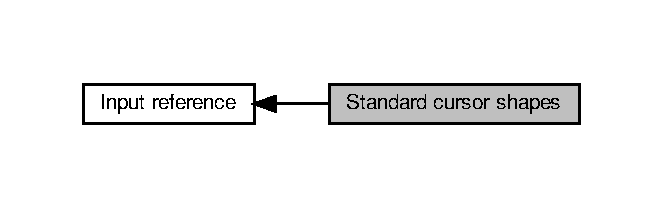
\includegraphics[width=318pt]{group__shapes}
\end{center}
\end{figure}
\subsection*{Macros}
\begin{DoxyCompactItemize}
\item 
\#define \hyperlink{group__shapes_ga8ab0e717245b85506cb0eaefdea39d0a}{G\+L\+F\+W\+\_\+\+A\+R\+R\+O\+W\+\_\+\+C\+U\+R\+S\+OR}~0x00036001
\begin{DoxyCompactList}\small\item\em The regular arrow cursor shape. \end{DoxyCompactList}\item 
\#define \hyperlink{group__shapes_ga36185f4375eaada1b04e431244774c86}{G\+L\+F\+W\+\_\+\+I\+B\+E\+A\+M\+\_\+\+C\+U\+R\+S\+OR}~0x00036002
\begin{DoxyCompactList}\small\item\em The text input I-\/beam cursor shape. \end{DoxyCompactList}\item 
\#define \hyperlink{group__shapes_ga8af88c0ea05ab9e8f9ac1530e8873c22}{G\+L\+F\+W\+\_\+\+C\+R\+O\+S\+S\+H\+A\+I\+R\+\_\+\+C\+U\+R\+S\+OR}~0x00036003
\begin{DoxyCompactList}\small\item\em The crosshair shape. \end{DoxyCompactList}\item 
\#define \hyperlink{group__shapes_ga1db35e20849e0837c82e3dc1fd797263}{G\+L\+F\+W\+\_\+\+H\+A\+N\+D\+\_\+\+C\+U\+R\+S\+OR}~0x00036004
\begin{DoxyCompactList}\small\item\em The hand shape. \end{DoxyCompactList}\item 
\#define \hyperlink{group__shapes_gabb3eb0109f11bb808fc34659177ca962}{G\+L\+F\+W\+\_\+\+H\+R\+E\+S\+I\+Z\+E\+\_\+\+C\+U\+R\+S\+OR}~0x00036005
\begin{DoxyCompactList}\small\item\em The horizontal resize arrow shape. \end{DoxyCompactList}\item 
\#define \hyperlink{group__shapes_gaf024f0e1ff8366fb2b5c260509a1fce5}{G\+L\+F\+W\+\_\+\+V\+R\+E\+S\+I\+Z\+E\+\_\+\+C\+U\+R\+S\+OR}~0x00036006
\begin{DoxyCompactList}\small\item\em The vertical resize arrow shape. \end{DoxyCompactList}\item 
\#define \hyperlink{group__shapes_ga8ab0e717245b85506cb0eaefdea39d0a}{G\+L\+F\+W\+\_\+\+A\+R\+R\+O\+W\+\_\+\+C\+U\+R\+S\+OR}~0x00036001
\begin{DoxyCompactList}\small\item\em The regular arrow cursor shape. \end{DoxyCompactList}\item 
\#define \hyperlink{group__shapes_ga36185f4375eaada1b04e431244774c86}{G\+L\+F\+W\+\_\+\+I\+B\+E\+A\+M\+\_\+\+C\+U\+R\+S\+OR}~0x00036002
\begin{DoxyCompactList}\small\item\em The text input I-\/beam cursor shape. \end{DoxyCompactList}\item 
\#define \hyperlink{group__shapes_ga8af88c0ea05ab9e8f9ac1530e8873c22}{G\+L\+F\+W\+\_\+\+C\+R\+O\+S\+S\+H\+A\+I\+R\+\_\+\+C\+U\+R\+S\+OR}~0x00036003
\begin{DoxyCompactList}\small\item\em The crosshair shape. \end{DoxyCompactList}\item 
\#define \hyperlink{group__shapes_ga1db35e20849e0837c82e3dc1fd797263}{G\+L\+F\+W\+\_\+\+H\+A\+N\+D\+\_\+\+C\+U\+R\+S\+OR}~0x00036004
\begin{DoxyCompactList}\small\item\em The hand shape. \end{DoxyCompactList}\item 
\#define \hyperlink{group__shapes_gabb3eb0109f11bb808fc34659177ca962}{G\+L\+F\+W\+\_\+\+H\+R\+E\+S\+I\+Z\+E\+\_\+\+C\+U\+R\+S\+OR}~0x00036005
\begin{DoxyCompactList}\small\item\em The horizontal resize arrow shape. \end{DoxyCompactList}\item 
\#define \hyperlink{group__shapes_gaf024f0e1ff8366fb2b5c260509a1fce5}{G\+L\+F\+W\+\_\+\+V\+R\+E\+S\+I\+Z\+E\+\_\+\+C\+U\+R\+S\+OR}~0x00036006
\begin{DoxyCompactList}\small\item\em The vertical resize arrow shape. \end{DoxyCompactList}\item 
\#define \hyperlink{group__shapes_ga8ab0e717245b85506cb0eaefdea39d0a}{G\+L\+F\+W\+\_\+\+A\+R\+R\+O\+W\+\_\+\+C\+U\+R\+S\+OR}~0x00036001
\begin{DoxyCompactList}\small\item\em The regular arrow cursor shape. \end{DoxyCompactList}\item 
\#define \hyperlink{group__shapes_ga36185f4375eaada1b04e431244774c86}{G\+L\+F\+W\+\_\+\+I\+B\+E\+A\+M\+\_\+\+C\+U\+R\+S\+OR}~0x00036002
\begin{DoxyCompactList}\small\item\em The text input I-\/beam cursor shape. \end{DoxyCompactList}\item 
\#define \hyperlink{group__shapes_ga8af88c0ea05ab9e8f9ac1530e8873c22}{G\+L\+F\+W\+\_\+\+C\+R\+O\+S\+S\+H\+A\+I\+R\+\_\+\+C\+U\+R\+S\+OR}~0x00036003
\begin{DoxyCompactList}\small\item\em The crosshair shape. \end{DoxyCompactList}\item 
\#define \hyperlink{group__shapes_ga1db35e20849e0837c82e3dc1fd797263}{G\+L\+F\+W\+\_\+\+H\+A\+N\+D\+\_\+\+C\+U\+R\+S\+OR}~0x00036004
\begin{DoxyCompactList}\small\item\em The hand shape. \end{DoxyCompactList}\item 
\#define \hyperlink{group__shapes_gabb3eb0109f11bb808fc34659177ca962}{G\+L\+F\+W\+\_\+\+H\+R\+E\+S\+I\+Z\+E\+\_\+\+C\+U\+R\+S\+OR}~0x00036005
\begin{DoxyCompactList}\small\item\em The horizontal resize arrow shape. \end{DoxyCompactList}\item 
\#define \hyperlink{group__shapes_gaf024f0e1ff8366fb2b5c260509a1fce5}{G\+L\+F\+W\+\_\+\+V\+R\+E\+S\+I\+Z\+E\+\_\+\+C\+U\+R\+S\+OR}~0x00036006
\begin{DoxyCompactList}\small\item\em The vertical resize arrow shape. \end{DoxyCompactList}\item 
\#define \hyperlink{group__shapes_ga8ab0e717245b85506cb0eaefdea39d0a}{G\+L\+F\+W\+\_\+\+A\+R\+R\+O\+W\+\_\+\+C\+U\+R\+S\+OR}~0x00036001
\begin{DoxyCompactList}\small\item\em The regular arrow cursor shape. \end{DoxyCompactList}\item 
\#define \hyperlink{group__shapes_ga36185f4375eaada1b04e431244774c86}{G\+L\+F\+W\+\_\+\+I\+B\+E\+A\+M\+\_\+\+C\+U\+R\+S\+OR}~0x00036002
\begin{DoxyCompactList}\small\item\em The text input I-\/beam cursor shape. \end{DoxyCompactList}\item 
\#define \hyperlink{group__shapes_ga8af88c0ea05ab9e8f9ac1530e8873c22}{G\+L\+F\+W\+\_\+\+C\+R\+O\+S\+S\+H\+A\+I\+R\+\_\+\+C\+U\+R\+S\+OR}~0x00036003
\begin{DoxyCompactList}\small\item\em The crosshair shape. \end{DoxyCompactList}\item 
\#define \hyperlink{group__shapes_ga1db35e20849e0837c82e3dc1fd797263}{G\+L\+F\+W\+\_\+\+H\+A\+N\+D\+\_\+\+C\+U\+R\+S\+OR}~0x00036004
\begin{DoxyCompactList}\small\item\em The hand shape. \end{DoxyCompactList}\item 
\#define \hyperlink{group__shapes_gabb3eb0109f11bb808fc34659177ca962}{G\+L\+F\+W\+\_\+\+H\+R\+E\+S\+I\+Z\+E\+\_\+\+C\+U\+R\+S\+OR}~0x00036005
\begin{DoxyCompactList}\small\item\em The horizontal resize arrow shape. \end{DoxyCompactList}\item 
\#define \hyperlink{group__shapes_gaf024f0e1ff8366fb2b5c260509a1fce5}{G\+L\+F\+W\+\_\+\+V\+R\+E\+S\+I\+Z\+E\+\_\+\+C\+U\+R\+S\+OR}~0x00036006
\begin{DoxyCompactList}\small\item\em The vertical resize arrow shape. \end{DoxyCompactList}\item 
\#define \hyperlink{group__shapes_ga8ab0e717245b85506cb0eaefdea39d0a}{G\+L\+F\+W\+\_\+\+A\+R\+R\+O\+W\+\_\+\+C\+U\+R\+S\+OR}~0x00036001
\begin{DoxyCompactList}\small\item\em The regular arrow cursor shape. \end{DoxyCompactList}\item 
\#define \hyperlink{group__shapes_ga36185f4375eaada1b04e431244774c86}{G\+L\+F\+W\+\_\+\+I\+B\+E\+A\+M\+\_\+\+C\+U\+R\+S\+OR}~0x00036002
\begin{DoxyCompactList}\small\item\em The text input I-\/beam cursor shape. \end{DoxyCompactList}\item 
\#define \hyperlink{group__shapes_ga8af88c0ea05ab9e8f9ac1530e8873c22}{G\+L\+F\+W\+\_\+\+C\+R\+O\+S\+S\+H\+A\+I\+R\+\_\+\+C\+U\+R\+S\+OR}~0x00036003
\begin{DoxyCompactList}\small\item\em The crosshair shape. \end{DoxyCompactList}\item 
\#define \hyperlink{group__shapes_ga1db35e20849e0837c82e3dc1fd797263}{G\+L\+F\+W\+\_\+\+H\+A\+N\+D\+\_\+\+C\+U\+R\+S\+OR}~0x00036004
\begin{DoxyCompactList}\small\item\em The hand shape. \end{DoxyCompactList}\item 
\#define \hyperlink{group__shapes_gabb3eb0109f11bb808fc34659177ca962}{G\+L\+F\+W\+\_\+\+H\+R\+E\+S\+I\+Z\+E\+\_\+\+C\+U\+R\+S\+OR}~0x00036005
\begin{DoxyCompactList}\small\item\em The horizontal resize arrow shape. \end{DoxyCompactList}\item 
\#define \hyperlink{group__shapes_gaf024f0e1ff8366fb2b5c260509a1fce5}{G\+L\+F\+W\+\_\+\+V\+R\+E\+S\+I\+Z\+E\+\_\+\+C\+U\+R\+S\+OR}~0x00036006
\begin{DoxyCompactList}\small\item\em The vertical resize arrow shape. \end{DoxyCompactList}\end{DoxyCompactItemize}


\subsection{Detailed Description}
See standard cursor creation for how these are used. 

\subsection{Macro Definition Documentation}
\mbox{\Hypertarget{group__shapes_ga8ab0e717245b85506cb0eaefdea39d0a}\label{group__shapes_ga8ab0e717245b85506cb0eaefdea39d0a}} 
\index{Standard cursor shapes@{Standard cursor shapes}!G\+L\+F\+W\+\_\+\+A\+R\+R\+O\+W\+\_\+\+C\+U\+R\+S\+OR@{G\+L\+F\+W\+\_\+\+A\+R\+R\+O\+W\+\_\+\+C\+U\+R\+S\+OR}}
\index{G\+L\+F\+W\+\_\+\+A\+R\+R\+O\+W\+\_\+\+C\+U\+R\+S\+OR@{G\+L\+F\+W\+\_\+\+A\+R\+R\+O\+W\+\_\+\+C\+U\+R\+S\+OR}!Standard cursor shapes@{Standard cursor shapes}}
\subsubsection{\texorpdfstring{G\+L\+F\+W\+\_\+\+A\+R\+R\+O\+W\+\_\+\+C\+U\+R\+S\+OR}{GLFW\_ARROW\_CURSOR}\hspace{0.1cm}{\footnotesize\ttfamily [1/5]}}
{\footnotesize\ttfamily \#define G\+L\+F\+W\+\_\+\+A\+R\+R\+O\+W\+\_\+\+C\+U\+R\+S\+OR~0x00036001}



The regular arrow cursor shape. 

The regular arrow cursor. \mbox{\Hypertarget{group__shapes_ga8ab0e717245b85506cb0eaefdea39d0a}\label{group__shapes_ga8ab0e717245b85506cb0eaefdea39d0a}} 
\index{Standard cursor shapes@{Standard cursor shapes}!G\+L\+F\+W\+\_\+\+A\+R\+R\+O\+W\+\_\+\+C\+U\+R\+S\+OR@{G\+L\+F\+W\+\_\+\+A\+R\+R\+O\+W\+\_\+\+C\+U\+R\+S\+OR}}
\index{G\+L\+F\+W\+\_\+\+A\+R\+R\+O\+W\+\_\+\+C\+U\+R\+S\+OR@{G\+L\+F\+W\+\_\+\+A\+R\+R\+O\+W\+\_\+\+C\+U\+R\+S\+OR}!Standard cursor shapes@{Standard cursor shapes}}
\subsubsection{\texorpdfstring{G\+L\+F\+W\+\_\+\+A\+R\+R\+O\+W\+\_\+\+C\+U\+R\+S\+OR}{GLFW\_ARROW\_CURSOR}\hspace{0.1cm}{\footnotesize\ttfamily [2/5]}}
{\footnotesize\ttfamily \#define G\+L\+F\+W\+\_\+\+A\+R\+R\+O\+W\+\_\+\+C\+U\+R\+S\+OR~0x00036001}



The regular arrow cursor shape. 

The regular arrow cursor. \mbox{\Hypertarget{group__shapes_ga8ab0e717245b85506cb0eaefdea39d0a}\label{group__shapes_ga8ab0e717245b85506cb0eaefdea39d0a}} 
\index{Standard cursor shapes@{Standard cursor shapes}!G\+L\+F\+W\+\_\+\+A\+R\+R\+O\+W\+\_\+\+C\+U\+R\+S\+OR@{G\+L\+F\+W\+\_\+\+A\+R\+R\+O\+W\+\_\+\+C\+U\+R\+S\+OR}}
\index{G\+L\+F\+W\+\_\+\+A\+R\+R\+O\+W\+\_\+\+C\+U\+R\+S\+OR@{G\+L\+F\+W\+\_\+\+A\+R\+R\+O\+W\+\_\+\+C\+U\+R\+S\+OR}!Standard cursor shapes@{Standard cursor shapes}}
\subsubsection{\texorpdfstring{G\+L\+F\+W\+\_\+\+A\+R\+R\+O\+W\+\_\+\+C\+U\+R\+S\+OR}{GLFW\_ARROW\_CURSOR}\hspace{0.1cm}{\footnotesize\ttfamily [3/5]}}
{\footnotesize\ttfamily \#define G\+L\+F\+W\+\_\+\+A\+R\+R\+O\+W\+\_\+\+C\+U\+R\+S\+OR~0x00036001}



The regular arrow cursor shape. 

The regular arrow cursor. \mbox{\Hypertarget{group__shapes_ga8ab0e717245b85506cb0eaefdea39d0a}\label{group__shapes_ga8ab0e717245b85506cb0eaefdea39d0a}} 
\index{Standard cursor shapes@{Standard cursor shapes}!G\+L\+F\+W\+\_\+\+A\+R\+R\+O\+W\+\_\+\+C\+U\+R\+S\+OR@{G\+L\+F\+W\+\_\+\+A\+R\+R\+O\+W\+\_\+\+C\+U\+R\+S\+OR}}
\index{G\+L\+F\+W\+\_\+\+A\+R\+R\+O\+W\+\_\+\+C\+U\+R\+S\+OR@{G\+L\+F\+W\+\_\+\+A\+R\+R\+O\+W\+\_\+\+C\+U\+R\+S\+OR}!Standard cursor shapes@{Standard cursor shapes}}
\subsubsection{\texorpdfstring{G\+L\+F\+W\+\_\+\+A\+R\+R\+O\+W\+\_\+\+C\+U\+R\+S\+OR}{GLFW\_ARROW\_CURSOR}\hspace{0.1cm}{\footnotesize\ttfamily [4/5]}}
{\footnotesize\ttfamily \#define G\+L\+F\+W\+\_\+\+A\+R\+R\+O\+W\+\_\+\+C\+U\+R\+S\+OR~0x00036001}



The regular arrow cursor shape. 

The regular arrow cursor. \mbox{\Hypertarget{group__shapes_ga8ab0e717245b85506cb0eaefdea39d0a}\label{group__shapes_ga8ab0e717245b85506cb0eaefdea39d0a}} 
\index{Standard cursor shapes@{Standard cursor shapes}!G\+L\+F\+W\+\_\+\+A\+R\+R\+O\+W\+\_\+\+C\+U\+R\+S\+OR@{G\+L\+F\+W\+\_\+\+A\+R\+R\+O\+W\+\_\+\+C\+U\+R\+S\+OR}}
\index{G\+L\+F\+W\+\_\+\+A\+R\+R\+O\+W\+\_\+\+C\+U\+R\+S\+OR@{G\+L\+F\+W\+\_\+\+A\+R\+R\+O\+W\+\_\+\+C\+U\+R\+S\+OR}!Standard cursor shapes@{Standard cursor shapes}}
\subsubsection{\texorpdfstring{G\+L\+F\+W\+\_\+\+A\+R\+R\+O\+W\+\_\+\+C\+U\+R\+S\+OR}{GLFW\_ARROW\_CURSOR}\hspace{0.1cm}{\footnotesize\ttfamily [5/5]}}
{\footnotesize\ttfamily \#define G\+L\+F\+W\+\_\+\+A\+R\+R\+O\+W\+\_\+\+C\+U\+R\+S\+OR~0x00036001}



The regular arrow cursor shape. 

The regular arrow cursor. \mbox{\Hypertarget{group__shapes_ga8af88c0ea05ab9e8f9ac1530e8873c22}\label{group__shapes_ga8af88c0ea05ab9e8f9ac1530e8873c22}} 
\index{Standard cursor shapes@{Standard cursor shapes}!G\+L\+F\+W\+\_\+\+C\+R\+O\+S\+S\+H\+A\+I\+R\+\_\+\+C\+U\+R\+S\+OR@{G\+L\+F\+W\+\_\+\+C\+R\+O\+S\+S\+H\+A\+I\+R\+\_\+\+C\+U\+R\+S\+OR}}
\index{G\+L\+F\+W\+\_\+\+C\+R\+O\+S\+S\+H\+A\+I\+R\+\_\+\+C\+U\+R\+S\+OR@{G\+L\+F\+W\+\_\+\+C\+R\+O\+S\+S\+H\+A\+I\+R\+\_\+\+C\+U\+R\+S\+OR}!Standard cursor shapes@{Standard cursor shapes}}
\subsubsection{\texorpdfstring{G\+L\+F\+W\+\_\+\+C\+R\+O\+S\+S\+H\+A\+I\+R\+\_\+\+C\+U\+R\+S\+OR}{GLFW\_CROSSHAIR\_CURSOR}\hspace{0.1cm}{\footnotesize\ttfamily [1/5]}}
{\footnotesize\ttfamily \#define G\+L\+F\+W\+\_\+\+C\+R\+O\+S\+S\+H\+A\+I\+R\+\_\+\+C\+U\+R\+S\+OR~0x00036003}



The crosshair shape. 

The crosshair shape. \mbox{\Hypertarget{group__shapes_ga8af88c0ea05ab9e8f9ac1530e8873c22}\label{group__shapes_ga8af88c0ea05ab9e8f9ac1530e8873c22}} 
\index{Standard cursor shapes@{Standard cursor shapes}!G\+L\+F\+W\+\_\+\+C\+R\+O\+S\+S\+H\+A\+I\+R\+\_\+\+C\+U\+R\+S\+OR@{G\+L\+F\+W\+\_\+\+C\+R\+O\+S\+S\+H\+A\+I\+R\+\_\+\+C\+U\+R\+S\+OR}}
\index{G\+L\+F\+W\+\_\+\+C\+R\+O\+S\+S\+H\+A\+I\+R\+\_\+\+C\+U\+R\+S\+OR@{G\+L\+F\+W\+\_\+\+C\+R\+O\+S\+S\+H\+A\+I\+R\+\_\+\+C\+U\+R\+S\+OR}!Standard cursor shapes@{Standard cursor shapes}}
\subsubsection{\texorpdfstring{G\+L\+F\+W\+\_\+\+C\+R\+O\+S\+S\+H\+A\+I\+R\+\_\+\+C\+U\+R\+S\+OR}{GLFW\_CROSSHAIR\_CURSOR}\hspace{0.1cm}{\footnotesize\ttfamily [2/5]}}
{\footnotesize\ttfamily \#define G\+L\+F\+W\+\_\+\+C\+R\+O\+S\+S\+H\+A\+I\+R\+\_\+\+C\+U\+R\+S\+OR~0x00036003}



The crosshair shape. 

The crosshair shape. \mbox{\Hypertarget{group__shapes_ga8af88c0ea05ab9e8f9ac1530e8873c22}\label{group__shapes_ga8af88c0ea05ab9e8f9ac1530e8873c22}} 
\index{Standard cursor shapes@{Standard cursor shapes}!G\+L\+F\+W\+\_\+\+C\+R\+O\+S\+S\+H\+A\+I\+R\+\_\+\+C\+U\+R\+S\+OR@{G\+L\+F\+W\+\_\+\+C\+R\+O\+S\+S\+H\+A\+I\+R\+\_\+\+C\+U\+R\+S\+OR}}
\index{G\+L\+F\+W\+\_\+\+C\+R\+O\+S\+S\+H\+A\+I\+R\+\_\+\+C\+U\+R\+S\+OR@{G\+L\+F\+W\+\_\+\+C\+R\+O\+S\+S\+H\+A\+I\+R\+\_\+\+C\+U\+R\+S\+OR}!Standard cursor shapes@{Standard cursor shapes}}
\subsubsection{\texorpdfstring{G\+L\+F\+W\+\_\+\+C\+R\+O\+S\+S\+H\+A\+I\+R\+\_\+\+C\+U\+R\+S\+OR}{GLFW\_CROSSHAIR\_CURSOR}\hspace{0.1cm}{\footnotesize\ttfamily [3/5]}}
{\footnotesize\ttfamily \#define G\+L\+F\+W\+\_\+\+C\+R\+O\+S\+S\+H\+A\+I\+R\+\_\+\+C\+U\+R\+S\+OR~0x00036003}



The crosshair shape. 

The crosshair shape. \mbox{\Hypertarget{group__shapes_ga8af88c0ea05ab9e8f9ac1530e8873c22}\label{group__shapes_ga8af88c0ea05ab9e8f9ac1530e8873c22}} 
\index{Standard cursor shapes@{Standard cursor shapes}!G\+L\+F\+W\+\_\+\+C\+R\+O\+S\+S\+H\+A\+I\+R\+\_\+\+C\+U\+R\+S\+OR@{G\+L\+F\+W\+\_\+\+C\+R\+O\+S\+S\+H\+A\+I\+R\+\_\+\+C\+U\+R\+S\+OR}}
\index{G\+L\+F\+W\+\_\+\+C\+R\+O\+S\+S\+H\+A\+I\+R\+\_\+\+C\+U\+R\+S\+OR@{G\+L\+F\+W\+\_\+\+C\+R\+O\+S\+S\+H\+A\+I\+R\+\_\+\+C\+U\+R\+S\+OR}!Standard cursor shapes@{Standard cursor shapes}}
\subsubsection{\texorpdfstring{G\+L\+F\+W\+\_\+\+C\+R\+O\+S\+S\+H\+A\+I\+R\+\_\+\+C\+U\+R\+S\+OR}{GLFW\_CROSSHAIR\_CURSOR}\hspace{0.1cm}{\footnotesize\ttfamily [4/5]}}
{\footnotesize\ttfamily \#define G\+L\+F\+W\+\_\+\+C\+R\+O\+S\+S\+H\+A\+I\+R\+\_\+\+C\+U\+R\+S\+OR~0x00036003}



The crosshair shape. 

The crosshair shape. \mbox{\Hypertarget{group__shapes_ga8af88c0ea05ab9e8f9ac1530e8873c22}\label{group__shapes_ga8af88c0ea05ab9e8f9ac1530e8873c22}} 
\index{Standard cursor shapes@{Standard cursor shapes}!G\+L\+F\+W\+\_\+\+C\+R\+O\+S\+S\+H\+A\+I\+R\+\_\+\+C\+U\+R\+S\+OR@{G\+L\+F\+W\+\_\+\+C\+R\+O\+S\+S\+H\+A\+I\+R\+\_\+\+C\+U\+R\+S\+OR}}
\index{G\+L\+F\+W\+\_\+\+C\+R\+O\+S\+S\+H\+A\+I\+R\+\_\+\+C\+U\+R\+S\+OR@{G\+L\+F\+W\+\_\+\+C\+R\+O\+S\+S\+H\+A\+I\+R\+\_\+\+C\+U\+R\+S\+OR}!Standard cursor shapes@{Standard cursor shapes}}
\subsubsection{\texorpdfstring{G\+L\+F\+W\+\_\+\+C\+R\+O\+S\+S\+H\+A\+I\+R\+\_\+\+C\+U\+R\+S\+OR}{GLFW\_CROSSHAIR\_CURSOR}\hspace{0.1cm}{\footnotesize\ttfamily [5/5]}}
{\footnotesize\ttfamily \#define G\+L\+F\+W\+\_\+\+C\+R\+O\+S\+S\+H\+A\+I\+R\+\_\+\+C\+U\+R\+S\+OR~0x00036003}



The crosshair shape. 

The crosshair shape. \mbox{\Hypertarget{group__shapes_ga1db35e20849e0837c82e3dc1fd797263}\label{group__shapes_ga1db35e20849e0837c82e3dc1fd797263}} 
\index{Standard cursor shapes@{Standard cursor shapes}!G\+L\+F\+W\+\_\+\+H\+A\+N\+D\+\_\+\+C\+U\+R\+S\+OR@{G\+L\+F\+W\+\_\+\+H\+A\+N\+D\+\_\+\+C\+U\+R\+S\+OR}}
\index{G\+L\+F\+W\+\_\+\+H\+A\+N\+D\+\_\+\+C\+U\+R\+S\+OR@{G\+L\+F\+W\+\_\+\+H\+A\+N\+D\+\_\+\+C\+U\+R\+S\+OR}!Standard cursor shapes@{Standard cursor shapes}}
\subsubsection{\texorpdfstring{G\+L\+F\+W\+\_\+\+H\+A\+N\+D\+\_\+\+C\+U\+R\+S\+OR}{GLFW\_HAND\_CURSOR}\hspace{0.1cm}{\footnotesize\ttfamily [1/5]}}
{\footnotesize\ttfamily \#define G\+L\+F\+W\+\_\+\+H\+A\+N\+D\+\_\+\+C\+U\+R\+S\+OR~0x00036004}



The hand shape. 

The hand shape. \mbox{\Hypertarget{group__shapes_ga1db35e20849e0837c82e3dc1fd797263}\label{group__shapes_ga1db35e20849e0837c82e3dc1fd797263}} 
\index{Standard cursor shapes@{Standard cursor shapes}!G\+L\+F\+W\+\_\+\+H\+A\+N\+D\+\_\+\+C\+U\+R\+S\+OR@{G\+L\+F\+W\+\_\+\+H\+A\+N\+D\+\_\+\+C\+U\+R\+S\+OR}}
\index{G\+L\+F\+W\+\_\+\+H\+A\+N\+D\+\_\+\+C\+U\+R\+S\+OR@{G\+L\+F\+W\+\_\+\+H\+A\+N\+D\+\_\+\+C\+U\+R\+S\+OR}!Standard cursor shapes@{Standard cursor shapes}}
\subsubsection{\texorpdfstring{G\+L\+F\+W\+\_\+\+H\+A\+N\+D\+\_\+\+C\+U\+R\+S\+OR}{GLFW\_HAND\_CURSOR}\hspace{0.1cm}{\footnotesize\ttfamily [2/5]}}
{\footnotesize\ttfamily \#define G\+L\+F\+W\+\_\+\+H\+A\+N\+D\+\_\+\+C\+U\+R\+S\+OR~0x00036004}



The hand shape. 

The hand shape. \mbox{\Hypertarget{group__shapes_ga1db35e20849e0837c82e3dc1fd797263}\label{group__shapes_ga1db35e20849e0837c82e3dc1fd797263}} 
\index{Standard cursor shapes@{Standard cursor shapes}!G\+L\+F\+W\+\_\+\+H\+A\+N\+D\+\_\+\+C\+U\+R\+S\+OR@{G\+L\+F\+W\+\_\+\+H\+A\+N\+D\+\_\+\+C\+U\+R\+S\+OR}}
\index{G\+L\+F\+W\+\_\+\+H\+A\+N\+D\+\_\+\+C\+U\+R\+S\+OR@{G\+L\+F\+W\+\_\+\+H\+A\+N\+D\+\_\+\+C\+U\+R\+S\+OR}!Standard cursor shapes@{Standard cursor shapes}}
\subsubsection{\texorpdfstring{G\+L\+F\+W\+\_\+\+H\+A\+N\+D\+\_\+\+C\+U\+R\+S\+OR}{GLFW\_HAND\_CURSOR}\hspace{0.1cm}{\footnotesize\ttfamily [3/5]}}
{\footnotesize\ttfamily \#define G\+L\+F\+W\+\_\+\+H\+A\+N\+D\+\_\+\+C\+U\+R\+S\+OR~0x00036004}



The hand shape. 

The hand shape. \mbox{\Hypertarget{group__shapes_ga1db35e20849e0837c82e3dc1fd797263}\label{group__shapes_ga1db35e20849e0837c82e3dc1fd797263}} 
\index{Standard cursor shapes@{Standard cursor shapes}!G\+L\+F\+W\+\_\+\+H\+A\+N\+D\+\_\+\+C\+U\+R\+S\+OR@{G\+L\+F\+W\+\_\+\+H\+A\+N\+D\+\_\+\+C\+U\+R\+S\+OR}}
\index{G\+L\+F\+W\+\_\+\+H\+A\+N\+D\+\_\+\+C\+U\+R\+S\+OR@{G\+L\+F\+W\+\_\+\+H\+A\+N\+D\+\_\+\+C\+U\+R\+S\+OR}!Standard cursor shapes@{Standard cursor shapes}}
\subsubsection{\texorpdfstring{G\+L\+F\+W\+\_\+\+H\+A\+N\+D\+\_\+\+C\+U\+R\+S\+OR}{GLFW\_HAND\_CURSOR}\hspace{0.1cm}{\footnotesize\ttfamily [4/5]}}
{\footnotesize\ttfamily \#define G\+L\+F\+W\+\_\+\+H\+A\+N\+D\+\_\+\+C\+U\+R\+S\+OR~0x00036004}



The hand shape. 

The hand shape. \mbox{\Hypertarget{group__shapes_ga1db35e20849e0837c82e3dc1fd797263}\label{group__shapes_ga1db35e20849e0837c82e3dc1fd797263}} 
\index{Standard cursor shapes@{Standard cursor shapes}!G\+L\+F\+W\+\_\+\+H\+A\+N\+D\+\_\+\+C\+U\+R\+S\+OR@{G\+L\+F\+W\+\_\+\+H\+A\+N\+D\+\_\+\+C\+U\+R\+S\+OR}}
\index{G\+L\+F\+W\+\_\+\+H\+A\+N\+D\+\_\+\+C\+U\+R\+S\+OR@{G\+L\+F\+W\+\_\+\+H\+A\+N\+D\+\_\+\+C\+U\+R\+S\+OR}!Standard cursor shapes@{Standard cursor shapes}}
\subsubsection{\texorpdfstring{G\+L\+F\+W\+\_\+\+H\+A\+N\+D\+\_\+\+C\+U\+R\+S\+OR}{GLFW\_HAND\_CURSOR}\hspace{0.1cm}{\footnotesize\ttfamily [5/5]}}
{\footnotesize\ttfamily \#define G\+L\+F\+W\+\_\+\+H\+A\+N\+D\+\_\+\+C\+U\+R\+S\+OR~0x00036004}



The hand shape. 

The hand shape. \mbox{\Hypertarget{group__shapes_gabb3eb0109f11bb808fc34659177ca962}\label{group__shapes_gabb3eb0109f11bb808fc34659177ca962}} 
\index{Standard cursor shapes@{Standard cursor shapes}!G\+L\+F\+W\+\_\+\+H\+R\+E\+S\+I\+Z\+E\+\_\+\+C\+U\+R\+S\+OR@{G\+L\+F\+W\+\_\+\+H\+R\+E\+S\+I\+Z\+E\+\_\+\+C\+U\+R\+S\+OR}}
\index{G\+L\+F\+W\+\_\+\+H\+R\+E\+S\+I\+Z\+E\+\_\+\+C\+U\+R\+S\+OR@{G\+L\+F\+W\+\_\+\+H\+R\+E\+S\+I\+Z\+E\+\_\+\+C\+U\+R\+S\+OR}!Standard cursor shapes@{Standard cursor shapes}}
\subsubsection{\texorpdfstring{G\+L\+F\+W\+\_\+\+H\+R\+E\+S\+I\+Z\+E\+\_\+\+C\+U\+R\+S\+OR}{GLFW\_HRESIZE\_CURSOR}\hspace{0.1cm}{\footnotesize\ttfamily [1/5]}}
{\footnotesize\ttfamily \#define G\+L\+F\+W\+\_\+\+H\+R\+E\+S\+I\+Z\+E\+\_\+\+C\+U\+R\+S\+OR~0x00036005}



The horizontal resize arrow shape. 

The horizontal resize arrow shape. \mbox{\Hypertarget{group__shapes_gabb3eb0109f11bb808fc34659177ca962}\label{group__shapes_gabb3eb0109f11bb808fc34659177ca962}} 
\index{Standard cursor shapes@{Standard cursor shapes}!G\+L\+F\+W\+\_\+\+H\+R\+E\+S\+I\+Z\+E\+\_\+\+C\+U\+R\+S\+OR@{G\+L\+F\+W\+\_\+\+H\+R\+E\+S\+I\+Z\+E\+\_\+\+C\+U\+R\+S\+OR}}
\index{G\+L\+F\+W\+\_\+\+H\+R\+E\+S\+I\+Z\+E\+\_\+\+C\+U\+R\+S\+OR@{G\+L\+F\+W\+\_\+\+H\+R\+E\+S\+I\+Z\+E\+\_\+\+C\+U\+R\+S\+OR}!Standard cursor shapes@{Standard cursor shapes}}
\subsubsection{\texorpdfstring{G\+L\+F\+W\+\_\+\+H\+R\+E\+S\+I\+Z\+E\+\_\+\+C\+U\+R\+S\+OR}{GLFW\_HRESIZE\_CURSOR}\hspace{0.1cm}{\footnotesize\ttfamily [2/5]}}
{\footnotesize\ttfamily \#define G\+L\+F\+W\+\_\+\+H\+R\+E\+S\+I\+Z\+E\+\_\+\+C\+U\+R\+S\+OR~0x00036005}



The horizontal resize arrow shape. 

The horizontal resize arrow shape. \mbox{\Hypertarget{group__shapes_gabb3eb0109f11bb808fc34659177ca962}\label{group__shapes_gabb3eb0109f11bb808fc34659177ca962}} 
\index{Standard cursor shapes@{Standard cursor shapes}!G\+L\+F\+W\+\_\+\+H\+R\+E\+S\+I\+Z\+E\+\_\+\+C\+U\+R\+S\+OR@{G\+L\+F\+W\+\_\+\+H\+R\+E\+S\+I\+Z\+E\+\_\+\+C\+U\+R\+S\+OR}}
\index{G\+L\+F\+W\+\_\+\+H\+R\+E\+S\+I\+Z\+E\+\_\+\+C\+U\+R\+S\+OR@{G\+L\+F\+W\+\_\+\+H\+R\+E\+S\+I\+Z\+E\+\_\+\+C\+U\+R\+S\+OR}!Standard cursor shapes@{Standard cursor shapes}}
\subsubsection{\texorpdfstring{G\+L\+F\+W\+\_\+\+H\+R\+E\+S\+I\+Z\+E\+\_\+\+C\+U\+R\+S\+OR}{GLFW\_HRESIZE\_CURSOR}\hspace{0.1cm}{\footnotesize\ttfamily [3/5]}}
{\footnotesize\ttfamily \#define G\+L\+F\+W\+\_\+\+H\+R\+E\+S\+I\+Z\+E\+\_\+\+C\+U\+R\+S\+OR~0x00036005}



The horizontal resize arrow shape. 

The horizontal resize arrow shape. \mbox{\Hypertarget{group__shapes_gabb3eb0109f11bb808fc34659177ca962}\label{group__shapes_gabb3eb0109f11bb808fc34659177ca962}} 
\index{Standard cursor shapes@{Standard cursor shapes}!G\+L\+F\+W\+\_\+\+H\+R\+E\+S\+I\+Z\+E\+\_\+\+C\+U\+R\+S\+OR@{G\+L\+F\+W\+\_\+\+H\+R\+E\+S\+I\+Z\+E\+\_\+\+C\+U\+R\+S\+OR}}
\index{G\+L\+F\+W\+\_\+\+H\+R\+E\+S\+I\+Z\+E\+\_\+\+C\+U\+R\+S\+OR@{G\+L\+F\+W\+\_\+\+H\+R\+E\+S\+I\+Z\+E\+\_\+\+C\+U\+R\+S\+OR}!Standard cursor shapes@{Standard cursor shapes}}
\subsubsection{\texorpdfstring{G\+L\+F\+W\+\_\+\+H\+R\+E\+S\+I\+Z\+E\+\_\+\+C\+U\+R\+S\+OR}{GLFW\_HRESIZE\_CURSOR}\hspace{0.1cm}{\footnotesize\ttfamily [4/5]}}
{\footnotesize\ttfamily \#define G\+L\+F\+W\+\_\+\+H\+R\+E\+S\+I\+Z\+E\+\_\+\+C\+U\+R\+S\+OR~0x00036005}



The horizontal resize arrow shape. 

The horizontal resize arrow shape. \mbox{\Hypertarget{group__shapes_gabb3eb0109f11bb808fc34659177ca962}\label{group__shapes_gabb3eb0109f11bb808fc34659177ca962}} 
\index{Standard cursor shapes@{Standard cursor shapes}!G\+L\+F\+W\+\_\+\+H\+R\+E\+S\+I\+Z\+E\+\_\+\+C\+U\+R\+S\+OR@{G\+L\+F\+W\+\_\+\+H\+R\+E\+S\+I\+Z\+E\+\_\+\+C\+U\+R\+S\+OR}}
\index{G\+L\+F\+W\+\_\+\+H\+R\+E\+S\+I\+Z\+E\+\_\+\+C\+U\+R\+S\+OR@{G\+L\+F\+W\+\_\+\+H\+R\+E\+S\+I\+Z\+E\+\_\+\+C\+U\+R\+S\+OR}!Standard cursor shapes@{Standard cursor shapes}}
\subsubsection{\texorpdfstring{G\+L\+F\+W\+\_\+\+H\+R\+E\+S\+I\+Z\+E\+\_\+\+C\+U\+R\+S\+OR}{GLFW\_HRESIZE\_CURSOR}\hspace{0.1cm}{\footnotesize\ttfamily [5/5]}}
{\footnotesize\ttfamily \#define G\+L\+F\+W\+\_\+\+H\+R\+E\+S\+I\+Z\+E\+\_\+\+C\+U\+R\+S\+OR~0x00036005}



The horizontal resize arrow shape. 

The horizontal resize arrow shape. \mbox{\Hypertarget{group__shapes_ga36185f4375eaada1b04e431244774c86}\label{group__shapes_ga36185f4375eaada1b04e431244774c86}} 
\index{Standard cursor shapes@{Standard cursor shapes}!G\+L\+F\+W\+\_\+\+I\+B\+E\+A\+M\+\_\+\+C\+U\+R\+S\+OR@{G\+L\+F\+W\+\_\+\+I\+B\+E\+A\+M\+\_\+\+C\+U\+R\+S\+OR}}
\index{G\+L\+F\+W\+\_\+\+I\+B\+E\+A\+M\+\_\+\+C\+U\+R\+S\+OR@{G\+L\+F\+W\+\_\+\+I\+B\+E\+A\+M\+\_\+\+C\+U\+R\+S\+OR}!Standard cursor shapes@{Standard cursor shapes}}
\subsubsection{\texorpdfstring{G\+L\+F\+W\+\_\+\+I\+B\+E\+A\+M\+\_\+\+C\+U\+R\+S\+OR}{GLFW\_IBEAM\_CURSOR}\hspace{0.1cm}{\footnotesize\ttfamily [1/5]}}
{\footnotesize\ttfamily \#define G\+L\+F\+W\+\_\+\+I\+B\+E\+A\+M\+\_\+\+C\+U\+R\+S\+OR~0x00036002}



The text input I-\/beam cursor shape. 

The text input I-\/beam cursor shape. \mbox{\Hypertarget{group__shapes_ga36185f4375eaada1b04e431244774c86}\label{group__shapes_ga36185f4375eaada1b04e431244774c86}} 
\index{Standard cursor shapes@{Standard cursor shapes}!G\+L\+F\+W\+\_\+\+I\+B\+E\+A\+M\+\_\+\+C\+U\+R\+S\+OR@{G\+L\+F\+W\+\_\+\+I\+B\+E\+A\+M\+\_\+\+C\+U\+R\+S\+OR}}
\index{G\+L\+F\+W\+\_\+\+I\+B\+E\+A\+M\+\_\+\+C\+U\+R\+S\+OR@{G\+L\+F\+W\+\_\+\+I\+B\+E\+A\+M\+\_\+\+C\+U\+R\+S\+OR}!Standard cursor shapes@{Standard cursor shapes}}
\subsubsection{\texorpdfstring{G\+L\+F\+W\+\_\+\+I\+B\+E\+A\+M\+\_\+\+C\+U\+R\+S\+OR}{GLFW\_IBEAM\_CURSOR}\hspace{0.1cm}{\footnotesize\ttfamily [2/5]}}
{\footnotesize\ttfamily \#define G\+L\+F\+W\+\_\+\+I\+B\+E\+A\+M\+\_\+\+C\+U\+R\+S\+OR~0x00036002}



The text input I-\/beam cursor shape. 

The text input I-\/beam cursor shape. \mbox{\Hypertarget{group__shapes_ga36185f4375eaada1b04e431244774c86}\label{group__shapes_ga36185f4375eaada1b04e431244774c86}} 
\index{Standard cursor shapes@{Standard cursor shapes}!G\+L\+F\+W\+\_\+\+I\+B\+E\+A\+M\+\_\+\+C\+U\+R\+S\+OR@{G\+L\+F\+W\+\_\+\+I\+B\+E\+A\+M\+\_\+\+C\+U\+R\+S\+OR}}
\index{G\+L\+F\+W\+\_\+\+I\+B\+E\+A\+M\+\_\+\+C\+U\+R\+S\+OR@{G\+L\+F\+W\+\_\+\+I\+B\+E\+A\+M\+\_\+\+C\+U\+R\+S\+OR}!Standard cursor shapes@{Standard cursor shapes}}
\subsubsection{\texorpdfstring{G\+L\+F\+W\+\_\+\+I\+B\+E\+A\+M\+\_\+\+C\+U\+R\+S\+OR}{GLFW\_IBEAM\_CURSOR}\hspace{0.1cm}{\footnotesize\ttfamily [3/5]}}
{\footnotesize\ttfamily \#define G\+L\+F\+W\+\_\+\+I\+B\+E\+A\+M\+\_\+\+C\+U\+R\+S\+OR~0x00036002}



The text input I-\/beam cursor shape. 

The text input I-\/beam cursor shape. \mbox{\Hypertarget{group__shapes_ga36185f4375eaada1b04e431244774c86}\label{group__shapes_ga36185f4375eaada1b04e431244774c86}} 
\index{Standard cursor shapes@{Standard cursor shapes}!G\+L\+F\+W\+\_\+\+I\+B\+E\+A\+M\+\_\+\+C\+U\+R\+S\+OR@{G\+L\+F\+W\+\_\+\+I\+B\+E\+A\+M\+\_\+\+C\+U\+R\+S\+OR}}
\index{G\+L\+F\+W\+\_\+\+I\+B\+E\+A\+M\+\_\+\+C\+U\+R\+S\+OR@{G\+L\+F\+W\+\_\+\+I\+B\+E\+A\+M\+\_\+\+C\+U\+R\+S\+OR}!Standard cursor shapes@{Standard cursor shapes}}
\subsubsection{\texorpdfstring{G\+L\+F\+W\+\_\+\+I\+B\+E\+A\+M\+\_\+\+C\+U\+R\+S\+OR}{GLFW\_IBEAM\_CURSOR}\hspace{0.1cm}{\footnotesize\ttfamily [4/5]}}
{\footnotesize\ttfamily \#define G\+L\+F\+W\+\_\+\+I\+B\+E\+A\+M\+\_\+\+C\+U\+R\+S\+OR~0x00036002}



The text input I-\/beam cursor shape. 

The text input I-\/beam cursor shape. \mbox{\Hypertarget{group__shapes_ga36185f4375eaada1b04e431244774c86}\label{group__shapes_ga36185f4375eaada1b04e431244774c86}} 
\index{Standard cursor shapes@{Standard cursor shapes}!G\+L\+F\+W\+\_\+\+I\+B\+E\+A\+M\+\_\+\+C\+U\+R\+S\+OR@{G\+L\+F\+W\+\_\+\+I\+B\+E\+A\+M\+\_\+\+C\+U\+R\+S\+OR}}
\index{G\+L\+F\+W\+\_\+\+I\+B\+E\+A\+M\+\_\+\+C\+U\+R\+S\+OR@{G\+L\+F\+W\+\_\+\+I\+B\+E\+A\+M\+\_\+\+C\+U\+R\+S\+OR}!Standard cursor shapes@{Standard cursor shapes}}
\subsubsection{\texorpdfstring{G\+L\+F\+W\+\_\+\+I\+B\+E\+A\+M\+\_\+\+C\+U\+R\+S\+OR}{GLFW\_IBEAM\_CURSOR}\hspace{0.1cm}{\footnotesize\ttfamily [5/5]}}
{\footnotesize\ttfamily \#define G\+L\+F\+W\+\_\+\+I\+B\+E\+A\+M\+\_\+\+C\+U\+R\+S\+OR~0x00036002}



The text input I-\/beam cursor shape. 

The text input I-\/beam cursor shape. \mbox{\Hypertarget{group__shapes_gaf024f0e1ff8366fb2b5c260509a1fce5}\label{group__shapes_gaf024f0e1ff8366fb2b5c260509a1fce5}} 
\index{Standard cursor shapes@{Standard cursor shapes}!G\+L\+F\+W\+\_\+\+V\+R\+E\+S\+I\+Z\+E\+\_\+\+C\+U\+R\+S\+OR@{G\+L\+F\+W\+\_\+\+V\+R\+E\+S\+I\+Z\+E\+\_\+\+C\+U\+R\+S\+OR}}
\index{G\+L\+F\+W\+\_\+\+V\+R\+E\+S\+I\+Z\+E\+\_\+\+C\+U\+R\+S\+OR@{G\+L\+F\+W\+\_\+\+V\+R\+E\+S\+I\+Z\+E\+\_\+\+C\+U\+R\+S\+OR}!Standard cursor shapes@{Standard cursor shapes}}
\subsubsection{\texorpdfstring{G\+L\+F\+W\+\_\+\+V\+R\+E\+S\+I\+Z\+E\+\_\+\+C\+U\+R\+S\+OR}{GLFW\_VRESIZE\_CURSOR}\hspace{0.1cm}{\footnotesize\ttfamily [1/5]}}
{\footnotesize\ttfamily \#define G\+L\+F\+W\+\_\+\+V\+R\+E\+S\+I\+Z\+E\+\_\+\+C\+U\+R\+S\+OR~0x00036006}



The vertical resize arrow shape. 

The vertical resize arrow shape. \mbox{\Hypertarget{group__shapes_gaf024f0e1ff8366fb2b5c260509a1fce5}\label{group__shapes_gaf024f0e1ff8366fb2b5c260509a1fce5}} 
\index{Standard cursor shapes@{Standard cursor shapes}!G\+L\+F\+W\+\_\+\+V\+R\+E\+S\+I\+Z\+E\+\_\+\+C\+U\+R\+S\+OR@{G\+L\+F\+W\+\_\+\+V\+R\+E\+S\+I\+Z\+E\+\_\+\+C\+U\+R\+S\+OR}}
\index{G\+L\+F\+W\+\_\+\+V\+R\+E\+S\+I\+Z\+E\+\_\+\+C\+U\+R\+S\+OR@{G\+L\+F\+W\+\_\+\+V\+R\+E\+S\+I\+Z\+E\+\_\+\+C\+U\+R\+S\+OR}!Standard cursor shapes@{Standard cursor shapes}}
\subsubsection{\texorpdfstring{G\+L\+F\+W\+\_\+\+V\+R\+E\+S\+I\+Z\+E\+\_\+\+C\+U\+R\+S\+OR}{GLFW\_VRESIZE\_CURSOR}\hspace{0.1cm}{\footnotesize\ttfamily [2/5]}}
{\footnotesize\ttfamily \#define G\+L\+F\+W\+\_\+\+V\+R\+E\+S\+I\+Z\+E\+\_\+\+C\+U\+R\+S\+OR~0x00036006}



The vertical resize arrow shape. 

The vertical resize arrow shape. \mbox{\Hypertarget{group__shapes_gaf024f0e1ff8366fb2b5c260509a1fce5}\label{group__shapes_gaf024f0e1ff8366fb2b5c260509a1fce5}} 
\index{Standard cursor shapes@{Standard cursor shapes}!G\+L\+F\+W\+\_\+\+V\+R\+E\+S\+I\+Z\+E\+\_\+\+C\+U\+R\+S\+OR@{G\+L\+F\+W\+\_\+\+V\+R\+E\+S\+I\+Z\+E\+\_\+\+C\+U\+R\+S\+OR}}
\index{G\+L\+F\+W\+\_\+\+V\+R\+E\+S\+I\+Z\+E\+\_\+\+C\+U\+R\+S\+OR@{G\+L\+F\+W\+\_\+\+V\+R\+E\+S\+I\+Z\+E\+\_\+\+C\+U\+R\+S\+OR}!Standard cursor shapes@{Standard cursor shapes}}
\subsubsection{\texorpdfstring{G\+L\+F\+W\+\_\+\+V\+R\+E\+S\+I\+Z\+E\+\_\+\+C\+U\+R\+S\+OR}{GLFW\_VRESIZE\_CURSOR}\hspace{0.1cm}{\footnotesize\ttfamily [3/5]}}
{\footnotesize\ttfamily \#define G\+L\+F\+W\+\_\+\+V\+R\+E\+S\+I\+Z\+E\+\_\+\+C\+U\+R\+S\+OR~0x00036006}



The vertical resize arrow shape. 

The vertical resize arrow shape. \mbox{\Hypertarget{group__shapes_gaf024f0e1ff8366fb2b5c260509a1fce5}\label{group__shapes_gaf024f0e1ff8366fb2b5c260509a1fce5}} 
\index{Standard cursor shapes@{Standard cursor shapes}!G\+L\+F\+W\+\_\+\+V\+R\+E\+S\+I\+Z\+E\+\_\+\+C\+U\+R\+S\+OR@{G\+L\+F\+W\+\_\+\+V\+R\+E\+S\+I\+Z\+E\+\_\+\+C\+U\+R\+S\+OR}}
\index{G\+L\+F\+W\+\_\+\+V\+R\+E\+S\+I\+Z\+E\+\_\+\+C\+U\+R\+S\+OR@{G\+L\+F\+W\+\_\+\+V\+R\+E\+S\+I\+Z\+E\+\_\+\+C\+U\+R\+S\+OR}!Standard cursor shapes@{Standard cursor shapes}}
\subsubsection{\texorpdfstring{G\+L\+F\+W\+\_\+\+V\+R\+E\+S\+I\+Z\+E\+\_\+\+C\+U\+R\+S\+OR}{GLFW\_VRESIZE\_CURSOR}\hspace{0.1cm}{\footnotesize\ttfamily [4/5]}}
{\footnotesize\ttfamily \#define G\+L\+F\+W\+\_\+\+V\+R\+E\+S\+I\+Z\+E\+\_\+\+C\+U\+R\+S\+OR~0x00036006}



The vertical resize arrow shape. 

The vertical resize arrow shape. \mbox{\Hypertarget{group__shapes_gaf024f0e1ff8366fb2b5c260509a1fce5}\label{group__shapes_gaf024f0e1ff8366fb2b5c260509a1fce5}} 
\index{Standard cursor shapes@{Standard cursor shapes}!G\+L\+F\+W\+\_\+\+V\+R\+E\+S\+I\+Z\+E\+\_\+\+C\+U\+R\+S\+OR@{G\+L\+F\+W\+\_\+\+V\+R\+E\+S\+I\+Z\+E\+\_\+\+C\+U\+R\+S\+OR}}
\index{G\+L\+F\+W\+\_\+\+V\+R\+E\+S\+I\+Z\+E\+\_\+\+C\+U\+R\+S\+OR@{G\+L\+F\+W\+\_\+\+V\+R\+E\+S\+I\+Z\+E\+\_\+\+C\+U\+R\+S\+OR}!Standard cursor shapes@{Standard cursor shapes}}
\subsubsection{\texorpdfstring{G\+L\+F\+W\+\_\+\+V\+R\+E\+S\+I\+Z\+E\+\_\+\+C\+U\+R\+S\+OR}{GLFW\_VRESIZE\_CURSOR}\hspace{0.1cm}{\footnotesize\ttfamily [5/5]}}
{\footnotesize\ttfamily \#define G\+L\+F\+W\+\_\+\+V\+R\+E\+S\+I\+Z\+E\+\_\+\+C\+U\+R\+S\+OR~0x00036006}



The vertical resize arrow shape. 

The vertical resize arrow shape. 
\hypertarget{group__native}{}\section{Native access}
\label{group__native}\index{Native access@{Native access}}
{\bfseries By using the native access functions you assert that you know what you\textquotesingle{}re doing and how to fix problems caused by using them. If you don\textquotesingle{}t, you shouldn\textquotesingle{}t be using them.}

Before the inclusion of glfw3native.\+h, you may define exactly one window system A\+PI macro and zero or more context creation A\+PI macros.

The chosen backends must match those the library was compiled for. Failure to do this will cause a link-\/time error.

The available window A\+PI macros are\+:
\begin{DoxyItemize}
\item {\ttfamily G\+L\+F\+W\+\_\+\+E\+X\+P\+O\+S\+E\+\_\+\+N\+A\+T\+I\+V\+E\+\_\+\+W\+I\+N32}
\item {\ttfamily G\+L\+F\+W\+\_\+\+E\+X\+P\+O\+S\+E\+\_\+\+N\+A\+T\+I\+V\+E\+\_\+\+C\+O\+C\+OA}
\item {\ttfamily G\+L\+F\+W\+\_\+\+E\+X\+P\+O\+S\+E\+\_\+\+N\+A\+T\+I\+V\+E\+\_\+\+X11}
\item {\ttfamily G\+L\+F\+W\+\_\+\+E\+X\+P\+O\+S\+E\+\_\+\+N\+A\+T\+I\+V\+E\+\_\+\+W\+A\+Y\+L\+A\+ND}
\item {\ttfamily G\+L\+F\+W\+\_\+\+E\+X\+P\+O\+S\+E\+\_\+\+N\+A\+T\+I\+V\+E\+\_\+\+M\+IR}
\end{DoxyItemize}

The available context A\+PI macros are\+:
\begin{DoxyItemize}
\item {\ttfamily G\+L\+F\+W\+\_\+\+E\+X\+P\+O\+S\+E\+\_\+\+N\+A\+T\+I\+V\+E\+\_\+\+W\+GL}
\item {\ttfamily G\+L\+F\+W\+\_\+\+E\+X\+P\+O\+S\+E\+\_\+\+N\+A\+T\+I\+V\+E\+\_\+\+N\+S\+GL}
\item {\ttfamily G\+L\+F\+W\+\_\+\+E\+X\+P\+O\+S\+E\+\_\+\+N\+A\+T\+I\+V\+E\+\_\+\+G\+LX}
\item {\ttfamily G\+L\+F\+W\+\_\+\+E\+X\+P\+O\+S\+E\+\_\+\+N\+A\+T\+I\+V\+E\+\_\+\+E\+GL}
\end{DoxyItemize}

These macros select which of the native access functions that are declared and which platform-\/specific headers to include. It is then up your (by definition platform-\/specific) code to handle which of these should be defined. 
\hypertarget{group__RAPIDJSON__ERRORS}{}\section{Rapid\+J\+S\+ON error handling}
\label{group__RAPIDJSON__ERRORS}\index{Rapid\+J\+S\+O\+N error handling@{Rapid\+J\+S\+O\+N error handling}}
\subsection*{Classes}
\begin{DoxyCompactItemize}
\item 
struct \hyperlink{structParseResult}{Parse\+Result}
\begin{DoxyCompactList}\small\item\em Result of parsing (wraps Parse\+Error\+Code) \end{DoxyCompactList}\end{DoxyCompactItemize}
\subsection*{Macros}
\begin{DoxyCompactItemize}
\item 
\#define \hyperlink{group__RAPIDJSON__ERRORS_ga7e4636fd48d0148f102b8a13f0539d8c}{R\+A\+P\+I\+D\+J\+S\+O\+N\+\_\+\+E\+R\+R\+O\+R\+\_\+\+C\+H\+A\+R\+T\+Y\+PE}~char
\begin{DoxyCompactList}\small\item\em Character type of error messages. \end{DoxyCompactList}\item 
\#define \hyperlink{group__RAPIDJSON__ERRORS_gabe2e1bd1349e5a7d6c1af78c05a98f0d}{R\+A\+P\+I\+D\+J\+S\+O\+N\+\_\+\+E\+R\+R\+O\+R\+\_\+\+S\+T\+R\+I\+NG}(x)~x
\begin{DoxyCompactList}\small\item\em Macro for converting string literial to \hyperlink{group__RAPIDJSON__ERRORS_ga7e4636fd48d0148f102b8a13f0539d8c}{R\+A\+P\+I\+D\+J\+S\+O\+N\+\_\+\+E\+R\+R\+O\+R\+\_\+\+C\+H\+A\+R\+T\+Y\+PE}\mbox{[}\mbox{]}. \end{DoxyCompactList}\item 
\#define \hyperlink{group__RAPIDJSON__ERRORS_ga7f8c4265b2edda78568ae3338aaf1461}{R\+A\+P\+I\+D\+J\+S\+O\+N\+\_\+\+P\+A\+R\+S\+E\+\_\+\+E\+R\+R\+O\+R\+\_\+\+N\+O\+R\+E\+T\+U\+RN}(parse\+Error\+Code,  offset)
\begin{DoxyCompactList}\small\item\em Macro to indicate a parse error. \end{DoxyCompactList}\item 
\#define \hyperlink{group__RAPIDJSON__ERRORS_gae3689840fa6e89a241313f33b602f865}{R\+A\+P\+I\+D\+J\+S\+O\+N\+\_\+\+P\+A\+R\+S\+E\+\_\+\+E\+R\+R\+OR}(parse\+Error\+Code,  offset)
\begin{DoxyCompactList}\small\item\em (Internal) macro to indicate and handle a parse error. \end{DoxyCompactList}\item 
\#define \hyperlink{group__RAPIDJSON__ERRORS_ga7e4636fd48d0148f102b8a13f0539d8c}{R\+A\+P\+I\+D\+J\+S\+O\+N\+\_\+\+E\+R\+R\+O\+R\+\_\+\+C\+H\+A\+R\+T\+Y\+PE}~char
\begin{DoxyCompactList}\small\item\em Character type of error messages. \end{DoxyCompactList}\item 
\#define \hyperlink{group__RAPIDJSON__ERRORS_gabe2e1bd1349e5a7d6c1af78c05a98f0d}{R\+A\+P\+I\+D\+J\+S\+O\+N\+\_\+\+E\+R\+R\+O\+R\+\_\+\+S\+T\+R\+I\+NG}(x)~x
\begin{DoxyCompactList}\small\item\em Macro for converting string literial to \hyperlink{group__RAPIDJSON__ERRORS_ga7e4636fd48d0148f102b8a13f0539d8c}{R\+A\+P\+I\+D\+J\+S\+O\+N\+\_\+\+E\+R\+R\+O\+R\+\_\+\+C\+H\+A\+R\+T\+Y\+PE}\mbox{[}\mbox{]}. \end{DoxyCompactList}\item 
\#define \hyperlink{group__RAPIDJSON__ERRORS_ga7f8c4265b2edda78568ae3338aaf1461}{R\+A\+P\+I\+D\+J\+S\+O\+N\+\_\+\+P\+A\+R\+S\+E\+\_\+\+E\+R\+R\+O\+R\+\_\+\+N\+O\+R\+E\+T\+U\+RN}(parse\+Error\+Code,  offset)
\begin{DoxyCompactList}\small\item\em Macro to indicate a parse error. \end{DoxyCompactList}\item 
\#define \hyperlink{group__RAPIDJSON__ERRORS_gae3689840fa6e89a241313f33b602f865}{R\+A\+P\+I\+D\+J\+S\+O\+N\+\_\+\+P\+A\+R\+S\+E\+\_\+\+E\+R\+R\+OR}(parse\+Error\+Code,  offset)
\begin{DoxyCompactList}\small\item\em (Internal) macro to indicate and handle a parse error. \end{DoxyCompactList}\end{DoxyCompactItemize}
\subsection*{Typedefs}
\begin{DoxyCompactItemize}
\item 
typedef const \hyperlink{group__RAPIDJSON__ERRORS_ga7e4636fd48d0148f102b8a13f0539d8c}{R\+A\+P\+I\+D\+J\+S\+O\+N\+\_\+\+E\+R\+R\+O\+R\+\_\+\+C\+H\+A\+R\+T\+Y\+PE} $\ast$($\ast$ \hyperlink{group__RAPIDJSON__ERRORS_ga586548166441ab3ce30219cb35be2e04}{Get\+Parse\+Error\+Func}) (\hyperlink{group__RAPIDJSON__ERRORS_ga8d4b32dfc45840bca189ade2bbcb6ba7}{Parse\+Error\+Code})
\begin{DoxyCompactList}\small\item\em Function pointer type of Get\+Parse\+Error(). \end{DoxyCompactList}\item 
typedef const \hyperlink{group__RAPIDJSON__ERRORS_ga7e4636fd48d0148f102b8a13f0539d8c}{R\+A\+P\+I\+D\+J\+S\+O\+N\+\_\+\+E\+R\+R\+O\+R\+\_\+\+C\+H\+A\+R\+T\+Y\+PE} $\ast$($\ast$ \hyperlink{group__RAPIDJSON__ERRORS_ga586548166441ab3ce30219cb35be2e04}{Get\+Parse\+Error\+Func}) (\hyperlink{group__RAPIDJSON__ERRORS_ga8d4b32dfc45840bca189ade2bbcb6ba7}{Parse\+Error\+Code})
\begin{DoxyCompactList}\small\item\em Function pointer type of Get\+Parse\+Error(). \end{DoxyCompactList}\end{DoxyCompactItemize}
\subsection*{Enumerations}
\begin{DoxyCompactItemize}
\item 
enum \hyperlink{group__RAPIDJSON__ERRORS_ga8d4b32dfc45840bca189ade2bbcb6ba7}{Parse\+Error\+Code} \{ \newline
\hyperlink{group__RAPIDJSON__ERRORS_gga8d4b32dfc45840bca189ade2bbcb6ba7ac0856bac4945cbd1d09e9502fd8f852f}{k\+Parse\+Error\+None} = 0, 
\hyperlink{group__RAPIDJSON__ERRORS_gga8d4b32dfc45840bca189ade2bbcb6ba7a04b368d184e84b50580be2faa55f738a}{k\+Parse\+Error\+Document\+Empty}, 
\hyperlink{group__RAPIDJSON__ERRORS_gga8d4b32dfc45840bca189ade2bbcb6ba7a2293b39033220f4c2a568482c497dab5}{k\+Parse\+Error\+Document\+Root\+Not\+Singular}, 
\hyperlink{group__RAPIDJSON__ERRORS_gga8d4b32dfc45840bca189ade2bbcb6ba7a20a50e257aab726699ab02192db72ba9}{k\+Parse\+Error\+Value\+Invalid}, 
\newline
\hyperlink{group__RAPIDJSON__ERRORS_gga8d4b32dfc45840bca189ade2bbcb6ba7ae3142fbadf2c4cdfd0c7200d7b6b8ed3}{k\+Parse\+Error\+Object\+Miss\+Name}, 
\hyperlink{group__RAPIDJSON__ERRORS_gga8d4b32dfc45840bca189ade2bbcb6ba7a55cda7eb30436986ab42a61e06caf017}{k\+Parse\+Error\+Object\+Miss\+Colon}, 
\hyperlink{group__RAPIDJSON__ERRORS_gga8d4b32dfc45840bca189ade2bbcb6ba7a34f70d7ed2fa121954f5fc5b5113d05f}{k\+Parse\+Error\+Object\+Miss\+Comma\+Or\+Curly\+Bracket}, 
\hyperlink{group__RAPIDJSON__ERRORS_gga8d4b32dfc45840bca189ade2bbcb6ba7abfdd2bd90134fec4fe6a22762d16a5f5}{k\+Parse\+Error\+Array\+Miss\+Comma\+Or\+Square\+Bracket}, 
\newline
\hyperlink{group__RAPIDJSON__ERRORS_gga8d4b32dfc45840bca189ade2bbcb6ba7afc65ea941a0a26812f0f258d2429e5d2}{k\+Parse\+Error\+String\+Unicode\+Escape\+Invalid\+Hex}, 
\hyperlink{group__RAPIDJSON__ERRORS_gga8d4b32dfc45840bca189ade2bbcb6ba7ad9fced6763a06435ca448626c74e5c72}{k\+Parse\+Error\+String\+Unicode\+Surrogate\+Invalid}, 
\hyperlink{group__RAPIDJSON__ERRORS_gga8d4b32dfc45840bca189ade2bbcb6ba7a98bb3f3b1e12fdb7f278b9fa4029306f}{k\+Parse\+Error\+String\+Escape\+Invalid}, 
\hyperlink{group__RAPIDJSON__ERRORS_gga8d4b32dfc45840bca189ade2bbcb6ba7a6369e5b4e4922720cbc45c5941efc4af}{k\+Parse\+Error\+String\+Miss\+Quotation\+Mark}, 
\newline
\hyperlink{group__RAPIDJSON__ERRORS_gga8d4b32dfc45840bca189ade2bbcb6ba7a17ecb2ed1524b513d64a93f4a7a8b456}{k\+Parse\+Error\+String\+Invalid\+Encoding}, 
\hyperlink{group__RAPIDJSON__ERRORS_gga8d4b32dfc45840bca189ade2bbcb6ba7ae52aaa70fde46e4cc422420309700b82}{k\+Parse\+Error\+Number\+Too\+Big}, 
\hyperlink{group__RAPIDJSON__ERRORS_gga8d4b32dfc45840bca189ade2bbcb6ba7a08a2cc2b4cacfba1673ed536eee229ce}{k\+Parse\+Error\+Number\+Miss\+Fraction}, 
\hyperlink{group__RAPIDJSON__ERRORS_gga8d4b32dfc45840bca189ade2bbcb6ba7a82cdbd740e22b819a70d05e585c2a442}{k\+Parse\+Error\+Number\+Miss\+Exponent}, 
\newline
\hyperlink{group__RAPIDJSON__ERRORS_gga8d4b32dfc45840bca189ade2bbcb6ba7a6fed2d9a15f88540a1ba785f0de2cbe6}{k\+Parse\+Error\+Termination}, 
\hyperlink{group__RAPIDJSON__ERRORS_gga8d4b32dfc45840bca189ade2bbcb6ba7a2bec6b26bddd3e093a37fc0d6399e0be}{k\+Parse\+Error\+Unspecific\+Syntax\+Error}, 
\hyperlink{group__RAPIDJSON__ERRORS_gga8d4b32dfc45840bca189ade2bbcb6ba7ac0856bac4945cbd1d09e9502fd8f852f}{k\+Parse\+Error\+None} = 0, 
\hyperlink{group__RAPIDJSON__ERRORS_gga8d4b32dfc45840bca189ade2bbcb6ba7a04b368d184e84b50580be2faa55f738a}{k\+Parse\+Error\+Document\+Empty}, 
\newline
\hyperlink{group__RAPIDJSON__ERRORS_gga8d4b32dfc45840bca189ade2bbcb6ba7a2293b39033220f4c2a568482c497dab5}{k\+Parse\+Error\+Document\+Root\+Not\+Singular}, 
\hyperlink{group__RAPIDJSON__ERRORS_gga8d4b32dfc45840bca189ade2bbcb6ba7a20a50e257aab726699ab02192db72ba9}{k\+Parse\+Error\+Value\+Invalid}, 
\hyperlink{group__RAPIDJSON__ERRORS_gga8d4b32dfc45840bca189ade2bbcb6ba7ae3142fbadf2c4cdfd0c7200d7b6b8ed3}{k\+Parse\+Error\+Object\+Miss\+Name}, 
\hyperlink{group__RAPIDJSON__ERRORS_gga8d4b32dfc45840bca189ade2bbcb6ba7a55cda7eb30436986ab42a61e06caf017}{k\+Parse\+Error\+Object\+Miss\+Colon}, 
\newline
\hyperlink{group__RAPIDJSON__ERRORS_gga8d4b32dfc45840bca189ade2bbcb6ba7a34f70d7ed2fa121954f5fc5b5113d05f}{k\+Parse\+Error\+Object\+Miss\+Comma\+Or\+Curly\+Bracket}, 
\hyperlink{group__RAPIDJSON__ERRORS_gga8d4b32dfc45840bca189ade2bbcb6ba7abfdd2bd90134fec4fe6a22762d16a5f5}{k\+Parse\+Error\+Array\+Miss\+Comma\+Or\+Square\+Bracket}, 
\hyperlink{group__RAPIDJSON__ERRORS_gga8d4b32dfc45840bca189ade2bbcb6ba7afc65ea941a0a26812f0f258d2429e5d2}{k\+Parse\+Error\+String\+Unicode\+Escape\+Invalid\+Hex}, 
\hyperlink{group__RAPIDJSON__ERRORS_gga8d4b32dfc45840bca189ade2bbcb6ba7ad9fced6763a06435ca448626c74e5c72}{k\+Parse\+Error\+String\+Unicode\+Surrogate\+Invalid}, 
\newline
\hyperlink{group__RAPIDJSON__ERRORS_gga8d4b32dfc45840bca189ade2bbcb6ba7a98bb3f3b1e12fdb7f278b9fa4029306f}{k\+Parse\+Error\+String\+Escape\+Invalid}, 
\hyperlink{group__RAPIDJSON__ERRORS_gga8d4b32dfc45840bca189ade2bbcb6ba7a6369e5b4e4922720cbc45c5941efc4af}{k\+Parse\+Error\+String\+Miss\+Quotation\+Mark}, 
\hyperlink{group__RAPIDJSON__ERRORS_gga8d4b32dfc45840bca189ade2bbcb6ba7a17ecb2ed1524b513d64a93f4a7a8b456}{k\+Parse\+Error\+String\+Invalid\+Encoding}, 
\hyperlink{group__RAPIDJSON__ERRORS_gga8d4b32dfc45840bca189ade2bbcb6ba7ae52aaa70fde46e4cc422420309700b82}{k\+Parse\+Error\+Number\+Too\+Big}, 
\newline
\hyperlink{group__RAPIDJSON__ERRORS_gga8d4b32dfc45840bca189ade2bbcb6ba7a08a2cc2b4cacfba1673ed536eee229ce}{k\+Parse\+Error\+Number\+Miss\+Fraction}, 
\hyperlink{group__RAPIDJSON__ERRORS_gga8d4b32dfc45840bca189ade2bbcb6ba7a82cdbd740e22b819a70d05e585c2a442}{k\+Parse\+Error\+Number\+Miss\+Exponent}, 
\hyperlink{group__RAPIDJSON__ERRORS_gga8d4b32dfc45840bca189ade2bbcb6ba7a6fed2d9a15f88540a1ba785f0de2cbe6}{k\+Parse\+Error\+Termination}, 
\hyperlink{group__RAPIDJSON__ERRORS_gga8d4b32dfc45840bca189ade2bbcb6ba7a2bec6b26bddd3e093a37fc0d6399e0be}{k\+Parse\+Error\+Unspecific\+Syntax\+Error}
 \}\begin{DoxyCompactList}\small\item\em Error code of parsing. \end{DoxyCompactList}
\item 
enum \hyperlink{group__RAPIDJSON__ERRORS_ga8d4b32dfc45840bca189ade2bbcb6ba7}{Parse\+Error\+Code} \{ \newline
\hyperlink{group__RAPIDJSON__ERRORS_gga8d4b32dfc45840bca189ade2bbcb6ba7ac0856bac4945cbd1d09e9502fd8f852f}{k\+Parse\+Error\+None} = 0, 
\hyperlink{group__RAPIDJSON__ERRORS_gga8d4b32dfc45840bca189ade2bbcb6ba7a04b368d184e84b50580be2faa55f738a}{k\+Parse\+Error\+Document\+Empty}, 
\hyperlink{group__RAPIDJSON__ERRORS_gga8d4b32dfc45840bca189ade2bbcb6ba7a2293b39033220f4c2a568482c497dab5}{k\+Parse\+Error\+Document\+Root\+Not\+Singular}, 
\hyperlink{group__RAPIDJSON__ERRORS_gga8d4b32dfc45840bca189ade2bbcb6ba7a20a50e257aab726699ab02192db72ba9}{k\+Parse\+Error\+Value\+Invalid}, 
\newline
\hyperlink{group__RAPIDJSON__ERRORS_gga8d4b32dfc45840bca189ade2bbcb6ba7ae3142fbadf2c4cdfd0c7200d7b6b8ed3}{k\+Parse\+Error\+Object\+Miss\+Name}, 
\hyperlink{group__RAPIDJSON__ERRORS_gga8d4b32dfc45840bca189ade2bbcb6ba7a55cda7eb30436986ab42a61e06caf017}{k\+Parse\+Error\+Object\+Miss\+Colon}, 
\hyperlink{group__RAPIDJSON__ERRORS_gga8d4b32dfc45840bca189ade2bbcb6ba7a34f70d7ed2fa121954f5fc5b5113d05f}{k\+Parse\+Error\+Object\+Miss\+Comma\+Or\+Curly\+Bracket}, 
\hyperlink{group__RAPIDJSON__ERRORS_gga8d4b32dfc45840bca189ade2bbcb6ba7abfdd2bd90134fec4fe6a22762d16a5f5}{k\+Parse\+Error\+Array\+Miss\+Comma\+Or\+Square\+Bracket}, 
\newline
\hyperlink{group__RAPIDJSON__ERRORS_gga8d4b32dfc45840bca189ade2bbcb6ba7afc65ea941a0a26812f0f258d2429e5d2}{k\+Parse\+Error\+String\+Unicode\+Escape\+Invalid\+Hex}, 
\hyperlink{group__RAPIDJSON__ERRORS_gga8d4b32dfc45840bca189ade2bbcb6ba7ad9fced6763a06435ca448626c74e5c72}{k\+Parse\+Error\+String\+Unicode\+Surrogate\+Invalid}, 
\hyperlink{group__RAPIDJSON__ERRORS_gga8d4b32dfc45840bca189ade2bbcb6ba7a98bb3f3b1e12fdb7f278b9fa4029306f}{k\+Parse\+Error\+String\+Escape\+Invalid}, 
\hyperlink{group__RAPIDJSON__ERRORS_gga8d4b32dfc45840bca189ade2bbcb6ba7a6369e5b4e4922720cbc45c5941efc4af}{k\+Parse\+Error\+String\+Miss\+Quotation\+Mark}, 
\newline
\hyperlink{group__RAPIDJSON__ERRORS_gga8d4b32dfc45840bca189ade2bbcb6ba7a17ecb2ed1524b513d64a93f4a7a8b456}{k\+Parse\+Error\+String\+Invalid\+Encoding}, 
\hyperlink{group__RAPIDJSON__ERRORS_gga8d4b32dfc45840bca189ade2bbcb6ba7ae52aaa70fde46e4cc422420309700b82}{k\+Parse\+Error\+Number\+Too\+Big}, 
\hyperlink{group__RAPIDJSON__ERRORS_gga8d4b32dfc45840bca189ade2bbcb6ba7a08a2cc2b4cacfba1673ed536eee229ce}{k\+Parse\+Error\+Number\+Miss\+Fraction}, 
\hyperlink{group__RAPIDJSON__ERRORS_gga8d4b32dfc45840bca189ade2bbcb6ba7a82cdbd740e22b819a70d05e585c2a442}{k\+Parse\+Error\+Number\+Miss\+Exponent}, 
\newline
\hyperlink{group__RAPIDJSON__ERRORS_gga8d4b32dfc45840bca189ade2bbcb6ba7a6fed2d9a15f88540a1ba785f0de2cbe6}{k\+Parse\+Error\+Termination}, 
\hyperlink{group__RAPIDJSON__ERRORS_gga8d4b32dfc45840bca189ade2bbcb6ba7a2bec6b26bddd3e093a37fc0d6399e0be}{k\+Parse\+Error\+Unspecific\+Syntax\+Error}, 
\hyperlink{group__RAPIDJSON__ERRORS_gga8d4b32dfc45840bca189ade2bbcb6ba7ac0856bac4945cbd1d09e9502fd8f852f}{k\+Parse\+Error\+None} = 0, 
\hyperlink{group__RAPIDJSON__ERRORS_gga8d4b32dfc45840bca189ade2bbcb6ba7a04b368d184e84b50580be2faa55f738a}{k\+Parse\+Error\+Document\+Empty}, 
\newline
\hyperlink{group__RAPIDJSON__ERRORS_gga8d4b32dfc45840bca189ade2bbcb6ba7a2293b39033220f4c2a568482c497dab5}{k\+Parse\+Error\+Document\+Root\+Not\+Singular}, 
\hyperlink{group__RAPIDJSON__ERRORS_gga8d4b32dfc45840bca189ade2bbcb6ba7a20a50e257aab726699ab02192db72ba9}{k\+Parse\+Error\+Value\+Invalid}, 
\hyperlink{group__RAPIDJSON__ERRORS_gga8d4b32dfc45840bca189ade2bbcb6ba7ae3142fbadf2c4cdfd0c7200d7b6b8ed3}{k\+Parse\+Error\+Object\+Miss\+Name}, 
\hyperlink{group__RAPIDJSON__ERRORS_gga8d4b32dfc45840bca189ade2bbcb6ba7a55cda7eb30436986ab42a61e06caf017}{k\+Parse\+Error\+Object\+Miss\+Colon}, 
\newline
\hyperlink{group__RAPIDJSON__ERRORS_gga8d4b32dfc45840bca189ade2bbcb6ba7a34f70d7ed2fa121954f5fc5b5113d05f}{k\+Parse\+Error\+Object\+Miss\+Comma\+Or\+Curly\+Bracket}, 
\hyperlink{group__RAPIDJSON__ERRORS_gga8d4b32dfc45840bca189ade2bbcb6ba7abfdd2bd90134fec4fe6a22762d16a5f5}{k\+Parse\+Error\+Array\+Miss\+Comma\+Or\+Square\+Bracket}, 
\hyperlink{group__RAPIDJSON__ERRORS_gga8d4b32dfc45840bca189ade2bbcb6ba7afc65ea941a0a26812f0f258d2429e5d2}{k\+Parse\+Error\+String\+Unicode\+Escape\+Invalid\+Hex}, 
\hyperlink{group__RAPIDJSON__ERRORS_gga8d4b32dfc45840bca189ade2bbcb6ba7ad9fced6763a06435ca448626c74e5c72}{k\+Parse\+Error\+String\+Unicode\+Surrogate\+Invalid}, 
\newline
\hyperlink{group__RAPIDJSON__ERRORS_gga8d4b32dfc45840bca189ade2bbcb6ba7a98bb3f3b1e12fdb7f278b9fa4029306f}{k\+Parse\+Error\+String\+Escape\+Invalid}, 
\hyperlink{group__RAPIDJSON__ERRORS_gga8d4b32dfc45840bca189ade2bbcb6ba7a6369e5b4e4922720cbc45c5941efc4af}{k\+Parse\+Error\+String\+Miss\+Quotation\+Mark}, 
\hyperlink{group__RAPIDJSON__ERRORS_gga8d4b32dfc45840bca189ade2bbcb6ba7a17ecb2ed1524b513d64a93f4a7a8b456}{k\+Parse\+Error\+String\+Invalid\+Encoding}, 
\hyperlink{group__RAPIDJSON__ERRORS_gga8d4b32dfc45840bca189ade2bbcb6ba7ae52aaa70fde46e4cc422420309700b82}{k\+Parse\+Error\+Number\+Too\+Big}, 
\newline
\hyperlink{group__RAPIDJSON__ERRORS_gga8d4b32dfc45840bca189ade2bbcb6ba7a08a2cc2b4cacfba1673ed536eee229ce}{k\+Parse\+Error\+Number\+Miss\+Fraction}, 
\hyperlink{group__RAPIDJSON__ERRORS_gga8d4b32dfc45840bca189ade2bbcb6ba7a82cdbd740e22b819a70d05e585c2a442}{k\+Parse\+Error\+Number\+Miss\+Exponent}, 
\hyperlink{group__RAPIDJSON__ERRORS_gga8d4b32dfc45840bca189ade2bbcb6ba7a6fed2d9a15f88540a1ba785f0de2cbe6}{k\+Parse\+Error\+Termination}, 
\hyperlink{group__RAPIDJSON__ERRORS_gga8d4b32dfc45840bca189ade2bbcb6ba7a2bec6b26bddd3e093a37fc0d6399e0be}{k\+Parse\+Error\+Unspecific\+Syntax\+Error}
 \}\begin{DoxyCompactList}\small\item\em Error code of parsing. \end{DoxyCompactList}
\item 
enum \hyperlink{group__RAPIDJSON__ERRORS_gacb2e274f33e54d91b96e9883a99a98be}{Pointer\+Parse\+Error\+Code} \{ \newline
\hyperlink{group__RAPIDJSON__ERRORS_ggacb2e274f33e54d91b96e9883a99a98bea81e2b6fbd1bf4ac890ddb7779265e3a0}{k\+Pointer\+Parse\+Error\+None} = 0, 
\hyperlink{group__RAPIDJSON__ERRORS_ggacb2e274f33e54d91b96e9883a99a98bea5821696a2ab6cbccdc8288cbe6e81c77}{k\+Pointer\+Parse\+Error\+Token\+Must\+Begin\+With\+Solidus}, 
\hyperlink{group__RAPIDJSON__ERRORS_ggacb2e274f33e54d91b96e9883a99a98bea4d2a7e511d717fd1d2f532ef5fcf821b}{k\+Pointer\+Parse\+Error\+Invalid\+Escape}, 
\hyperlink{group__RAPIDJSON__ERRORS_ggacb2e274f33e54d91b96e9883a99a98beac0c1b013c0db34dcc5a47fc1ee7a8c35}{k\+Pointer\+Parse\+Error\+Invalid\+Percent\+Encoding}, 
\newline
\hyperlink{group__RAPIDJSON__ERRORS_ggacb2e274f33e54d91b96e9883a99a98beabd7eae93627f74267009a03679b6dc38}{k\+Pointer\+Parse\+Error\+Character\+Must\+Percent\+Encode}
 \}\begin{DoxyCompactList}\small\item\em Error code of parsing. \end{DoxyCompactList}
\end{DoxyCompactItemize}
\subsection*{Functions}
\begin{DoxyCompactItemize}
\item 
\hyperlink{group__RAPIDJSON__CONFIG_gad3806c8251fdc7da9618b7e922674ffc}{R\+A\+P\+I\+D\+J\+S\+O\+N\+\_\+\+N\+A\+M\+E\+S\+P\+A\+C\+E\+\_\+\+B\+E\+G\+IN} const \hyperlink{group__RAPIDJSON__ERRORS_ga7e4636fd48d0148f102b8a13f0539d8c}{R\+A\+P\+I\+D\+J\+S\+O\+N\+\_\+\+E\+R\+R\+O\+R\+\_\+\+C\+H\+A\+R\+T\+Y\+PE} $\ast$ \hyperlink{group__RAPIDJSON__ERRORS_ga28835eb93d2c3c07bbea13515eb31415}{Get\+Parse\+Error\+\_\+\+En} (\hyperlink{group__RAPIDJSON__ERRORS_ga8d4b32dfc45840bca189ade2bbcb6ba7}{Parse\+Error\+Code} parse\+Error\+Code)
\begin{DoxyCompactList}\small\item\em Maps error code of parsing into error message. \end{DoxyCompactList}\end{DoxyCompactItemize}


\subsection{Detailed Description}


\subsection{Macro Definition Documentation}
\mbox{\Hypertarget{group__RAPIDJSON__ERRORS_ga7e4636fd48d0148f102b8a13f0539d8c}\label{group__RAPIDJSON__ERRORS_ga7e4636fd48d0148f102b8a13f0539d8c}} 
\index{Rapid\+J\+S\+O\+N error handling@{Rapid\+J\+S\+O\+N error handling}!R\+A\+P\+I\+D\+J\+S\+O\+N\+\_\+\+E\+R\+R\+O\+R\+\_\+\+C\+H\+A\+R\+T\+Y\+PE@{R\+A\+P\+I\+D\+J\+S\+O\+N\+\_\+\+E\+R\+R\+O\+R\+\_\+\+C\+H\+A\+R\+T\+Y\+PE}}
\index{R\+A\+P\+I\+D\+J\+S\+O\+N\+\_\+\+E\+R\+R\+O\+R\+\_\+\+C\+H\+A\+R\+T\+Y\+PE@{R\+A\+P\+I\+D\+J\+S\+O\+N\+\_\+\+E\+R\+R\+O\+R\+\_\+\+C\+H\+A\+R\+T\+Y\+PE}!Rapid\+J\+S\+O\+N error handling@{Rapid\+J\+S\+O\+N error handling}}
\subsubsection{\texorpdfstring{R\+A\+P\+I\+D\+J\+S\+O\+N\+\_\+\+E\+R\+R\+O\+R\+\_\+\+C\+H\+A\+R\+T\+Y\+PE}{RAPIDJSON\_ERROR\_CHARTYPE}\hspace{0.1cm}{\footnotesize\ttfamily [1/2]}}
{\footnotesize\ttfamily \#define R\+A\+P\+I\+D\+J\+S\+O\+N\+\_\+\+E\+R\+R\+O\+R\+\_\+\+C\+H\+A\+R\+T\+Y\+PE~char}



Character type of error messages. 

The default character type is {\ttfamily char}. On Windows, user can define this macro as {\ttfamily T\+C\+H\+AR} for supporting both unicode/non-\/unicode settings. \mbox{\Hypertarget{group__RAPIDJSON__ERRORS_ga7e4636fd48d0148f102b8a13f0539d8c}\label{group__RAPIDJSON__ERRORS_ga7e4636fd48d0148f102b8a13f0539d8c}} 
\index{Rapid\+J\+S\+O\+N error handling@{Rapid\+J\+S\+O\+N error handling}!R\+A\+P\+I\+D\+J\+S\+O\+N\+\_\+\+E\+R\+R\+O\+R\+\_\+\+C\+H\+A\+R\+T\+Y\+PE@{R\+A\+P\+I\+D\+J\+S\+O\+N\+\_\+\+E\+R\+R\+O\+R\+\_\+\+C\+H\+A\+R\+T\+Y\+PE}}
\index{R\+A\+P\+I\+D\+J\+S\+O\+N\+\_\+\+E\+R\+R\+O\+R\+\_\+\+C\+H\+A\+R\+T\+Y\+PE@{R\+A\+P\+I\+D\+J\+S\+O\+N\+\_\+\+E\+R\+R\+O\+R\+\_\+\+C\+H\+A\+R\+T\+Y\+PE}!Rapid\+J\+S\+O\+N error handling@{Rapid\+J\+S\+O\+N error handling}}
\subsubsection{\texorpdfstring{R\+A\+P\+I\+D\+J\+S\+O\+N\+\_\+\+E\+R\+R\+O\+R\+\_\+\+C\+H\+A\+R\+T\+Y\+PE}{RAPIDJSON\_ERROR\_CHARTYPE}\hspace{0.1cm}{\footnotesize\ttfamily [2/2]}}
{\footnotesize\ttfamily \#define R\+A\+P\+I\+D\+J\+S\+O\+N\+\_\+\+E\+R\+R\+O\+R\+\_\+\+C\+H\+A\+R\+T\+Y\+PE~char}



Character type of error messages. 

The default character type is {\ttfamily char}. On Windows, user can define this macro as {\ttfamily T\+C\+H\+AR} for supporting both unicode/non-\/unicode settings. \mbox{\Hypertarget{group__RAPIDJSON__ERRORS_gabe2e1bd1349e5a7d6c1af78c05a98f0d}\label{group__RAPIDJSON__ERRORS_gabe2e1bd1349e5a7d6c1af78c05a98f0d}} 
\index{Rapid\+J\+S\+O\+N error handling@{Rapid\+J\+S\+O\+N error handling}!R\+A\+P\+I\+D\+J\+S\+O\+N\+\_\+\+E\+R\+R\+O\+R\+\_\+\+S\+T\+R\+I\+NG@{R\+A\+P\+I\+D\+J\+S\+O\+N\+\_\+\+E\+R\+R\+O\+R\+\_\+\+S\+T\+R\+I\+NG}}
\index{R\+A\+P\+I\+D\+J\+S\+O\+N\+\_\+\+E\+R\+R\+O\+R\+\_\+\+S\+T\+R\+I\+NG@{R\+A\+P\+I\+D\+J\+S\+O\+N\+\_\+\+E\+R\+R\+O\+R\+\_\+\+S\+T\+R\+I\+NG}!Rapid\+J\+S\+O\+N error handling@{Rapid\+J\+S\+O\+N error handling}}
\subsubsection{\texorpdfstring{R\+A\+P\+I\+D\+J\+S\+O\+N\+\_\+\+E\+R\+R\+O\+R\+\_\+\+S\+T\+R\+I\+NG}{RAPIDJSON\_ERROR\_STRING}\hspace{0.1cm}{\footnotesize\ttfamily [1/2]}}
{\footnotesize\ttfamily \#define R\+A\+P\+I\+D\+J\+S\+O\+N\+\_\+\+E\+R\+R\+O\+R\+\_\+\+S\+T\+R\+I\+NG(\begin{DoxyParamCaption}\item[{}]{x }\end{DoxyParamCaption})~x}



Macro for converting string literial to \hyperlink{group__RAPIDJSON__ERRORS_ga7e4636fd48d0148f102b8a13f0539d8c}{R\+A\+P\+I\+D\+J\+S\+O\+N\+\_\+\+E\+R\+R\+O\+R\+\_\+\+C\+H\+A\+R\+T\+Y\+PE}\mbox{[}\mbox{]}. 

By default this conversion macro does nothing. On Windows, user can define this macro as {\ttfamily \+\_\+\+T(x)} for supporting both unicode/non-\/unicode settings. \mbox{\Hypertarget{group__RAPIDJSON__ERRORS_gabe2e1bd1349e5a7d6c1af78c05a98f0d}\label{group__RAPIDJSON__ERRORS_gabe2e1bd1349e5a7d6c1af78c05a98f0d}} 
\index{Rapid\+J\+S\+O\+N error handling@{Rapid\+J\+S\+O\+N error handling}!R\+A\+P\+I\+D\+J\+S\+O\+N\+\_\+\+E\+R\+R\+O\+R\+\_\+\+S\+T\+R\+I\+NG@{R\+A\+P\+I\+D\+J\+S\+O\+N\+\_\+\+E\+R\+R\+O\+R\+\_\+\+S\+T\+R\+I\+NG}}
\index{R\+A\+P\+I\+D\+J\+S\+O\+N\+\_\+\+E\+R\+R\+O\+R\+\_\+\+S\+T\+R\+I\+NG@{R\+A\+P\+I\+D\+J\+S\+O\+N\+\_\+\+E\+R\+R\+O\+R\+\_\+\+S\+T\+R\+I\+NG}!Rapid\+J\+S\+O\+N error handling@{Rapid\+J\+S\+O\+N error handling}}
\subsubsection{\texorpdfstring{R\+A\+P\+I\+D\+J\+S\+O\+N\+\_\+\+E\+R\+R\+O\+R\+\_\+\+S\+T\+R\+I\+NG}{RAPIDJSON\_ERROR\_STRING}\hspace{0.1cm}{\footnotesize\ttfamily [2/2]}}
{\footnotesize\ttfamily \#define R\+A\+P\+I\+D\+J\+S\+O\+N\+\_\+\+E\+R\+R\+O\+R\+\_\+\+S\+T\+R\+I\+NG(\begin{DoxyParamCaption}\item[{}]{x }\end{DoxyParamCaption})~x}



Macro for converting string literial to \hyperlink{group__RAPIDJSON__ERRORS_ga7e4636fd48d0148f102b8a13f0539d8c}{R\+A\+P\+I\+D\+J\+S\+O\+N\+\_\+\+E\+R\+R\+O\+R\+\_\+\+C\+H\+A\+R\+T\+Y\+PE}\mbox{[}\mbox{]}. 

By default this conversion macro does nothing. On Windows, user can define this macro as {\ttfamily \+\_\+\+T(x)} for supporting both unicode/non-\/unicode settings. \mbox{\Hypertarget{group__RAPIDJSON__ERRORS_gae3689840fa6e89a241313f33b602f865}\label{group__RAPIDJSON__ERRORS_gae3689840fa6e89a241313f33b602f865}} 
\index{Rapid\+J\+S\+O\+N error handling@{Rapid\+J\+S\+O\+N error handling}!R\+A\+P\+I\+D\+J\+S\+O\+N\+\_\+\+P\+A\+R\+S\+E\+\_\+\+E\+R\+R\+OR@{R\+A\+P\+I\+D\+J\+S\+O\+N\+\_\+\+P\+A\+R\+S\+E\+\_\+\+E\+R\+R\+OR}}
\index{R\+A\+P\+I\+D\+J\+S\+O\+N\+\_\+\+P\+A\+R\+S\+E\+\_\+\+E\+R\+R\+OR@{R\+A\+P\+I\+D\+J\+S\+O\+N\+\_\+\+P\+A\+R\+S\+E\+\_\+\+E\+R\+R\+OR}!Rapid\+J\+S\+O\+N error handling@{Rapid\+J\+S\+O\+N error handling}}
\subsubsection{\texorpdfstring{R\+A\+P\+I\+D\+J\+S\+O\+N\+\_\+\+P\+A\+R\+S\+E\+\_\+\+E\+R\+R\+OR}{RAPIDJSON\_PARSE\_ERROR}\hspace{0.1cm}{\footnotesize\ttfamily [1/2]}}
{\footnotesize\ttfamily \#define R\+A\+P\+I\+D\+J\+S\+O\+N\+\_\+\+P\+A\+R\+S\+E\+\_\+\+E\+R\+R\+OR(\begin{DoxyParamCaption}\item[{}]{parse\+Error\+Code,  }\item[{}]{offset }\end{DoxyParamCaption})}

{\bfseries Value\+:}
\begin{DoxyCode}
\hyperlink{group__RAPIDJSON__ERRORS_ga7f8c4265b2edda78568ae3338aaf1461}{RAPIDJSON\_MULTILINEMACRO\_BEGIN \(\backslash\)}
\hyperlink{group__RAPIDJSON__ERRORS_ga7f8c4265b2edda78568ae3338aaf1461}{    RAPIDJSON\_PARSE\_ERROR\_NORETURN}(parseErrorCode, offset); \(\backslash\)
    RAPIDJSON\_PARSE\_ERROR\_EARLY\_RETURN\_VOID; \(\backslash\)
    RAPIDJSON\_MULTILINEMACRO\_END
\end{DoxyCode}


(Internal) macro to indicate and handle a parse error. 


\begin{DoxyParams}{Parameters}
{\em parse\+Error\+Code} & \hyperlink{group__RAPIDJSON__ERRORS_ga8d4b32dfc45840bca189ade2bbcb6ba7}{rapidjson\+::\+Parse\+Error\+Code} of the error \\
\hline
{\em offset} & position of the error in J\+S\+ON input ({\ttfamily size\+\_\+t})\\
\hline
\end{DoxyParams}
Invokes R\+A\+P\+I\+D\+J\+S\+O\+N\+\_\+\+P\+A\+R\+S\+E\+\_\+\+E\+R\+R\+O\+R\+\_\+\+N\+O\+R\+E\+T\+U\+RN and stops the parsing.

\begin{DoxySeeAlso}{See also}
\hyperlink{group__RAPIDJSON__ERRORS_ga7f8c4265b2edda78568ae3338aaf1461}{R\+A\+P\+I\+D\+J\+S\+O\+N\+\_\+\+P\+A\+R\+S\+E\+\_\+\+E\+R\+R\+O\+R\+\_\+\+N\+O\+R\+E\+T\+U\+RN} 
\end{DoxySeeAlso}
\mbox{\Hypertarget{group__RAPIDJSON__ERRORS_gae3689840fa6e89a241313f33b602f865}\label{group__RAPIDJSON__ERRORS_gae3689840fa6e89a241313f33b602f865}} 
\index{Rapid\+J\+S\+O\+N error handling@{Rapid\+J\+S\+O\+N error handling}!R\+A\+P\+I\+D\+J\+S\+O\+N\+\_\+\+P\+A\+R\+S\+E\+\_\+\+E\+R\+R\+OR@{R\+A\+P\+I\+D\+J\+S\+O\+N\+\_\+\+P\+A\+R\+S\+E\+\_\+\+E\+R\+R\+OR}}
\index{R\+A\+P\+I\+D\+J\+S\+O\+N\+\_\+\+P\+A\+R\+S\+E\+\_\+\+E\+R\+R\+OR@{R\+A\+P\+I\+D\+J\+S\+O\+N\+\_\+\+P\+A\+R\+S\+E\+\_\+\+E\+R\+R\+OR}!Rapid\+J\+S\+O\+N error handling@{Rapid\+J\+S\+O\+N error handling}}
\subsubsection{\texorpdfstring{R\+A\+P\+I\+D\+J\+S\+O\+N\+\_\+\+P\+A\+R\+S\+E\+\_\+\+E\+R\+R\+OR}{RAPIDJSON\_PARSE\_ERROR}\hspace{0.1cm}{\footnotesize\ttfamily [2/2]}}
{\footnotesize\ttfamily \#define R\+A\+P\+I\+D\+J\+S\+O\+N\+\_\+\+P\+A\+R\+S\+E\+\_\+\+E\+R\+R\+OR(\begin{DoxyParamCaption}\item[{}]{parse\+Error\+Code,  }\item[{}]{offset }\end{DoxyParamCaption})}

{\bfseries Value\+:}
\begin{DoxyCode}
\hyperlink{group__RAPIDJSON__ERRORS_ga7f8c4265b2edda78568ae3338aaf1461}{RAPIDJSON\_MULTILINEMACRO\_BEGIN \(\backslash\)}
\hyperlink{group__RAPIDJSON__ERRORS_ga7f8c4265b2edda78568ae3338aaf1461}{    RAPIDJSON\_PARSE\_ERROR\_NORETURN}(parseErrorCode, offset); \(\backslash\)
    RAPIDJSON\_PARSE\_ERROR\_EARLY\_RETURN\_VOID; \(\backslash\)
    RAPIDJSON\_MULTILINEMACRO\_END
\end{DoxyCode}


(Internal) macro to indicate and handle a parse error. 


\begin{DoxyParams}{Parameters}
{\em parse\+Error\+Code} & \hyperlink{group__RAPIDJSON__ERRORS_ga8d4b32dfc45840bca189ade2bbcb6ba7}{rapidjson\+::\+Parse\+Error\+Code} of the error \\
\hline
{\em offset} & position of the error in J\+S\+ON input ({\ttfamily size\+\_\+t})\\
\hline
\end{DoxyParams}
Invokes R\+A\+P\+I\+D\+J\+S\+O\+N\+\_\+\+P\+A\+R\+S\+E\+\_\+\+E\+R\+R\+O\+R\+\_\+\+N\+O\+R\+E\+T\+U\+RN and stops the parsing.

\begin{DoxySeeAlso}{See also}
\hyperlink{group__RAPIDJSON__ERRORS_ga7f8c4265b2edda78568ae3338aaf1461}{R\+A\+P\+I\+D\+J\+S\+O\+N\+\_\+\+P\+A\+R\+S\+E\+\_\+\+E\+R\+R\+O\+R\+\_\+\+N\+O\+R\+E\+T\+U\+RN} 
\end{DoxySeeAlso}
\mbox{\Hypertarget{group__RAPIDJSON__ERRORS_ga7f8c4265b2edda78568ae3338aaf1461}\label{group__RAPIDJSON__ERRORS_ga7f8c4265b2edda78568ae3338aaf1461}} 
\index{Rapid\+J\+S\+O\+N error handling@{Rapid\+J\+S\+O\+N error handling}!R\+A\+P\+I\+D\+J\+S\+O\+N\+\_\+\+P\+A\+R\+S\+E\+\_\+\+E\+R\+R\+O\+R\+\_\+\+N\+O\+R\+E\+T\+U\+RN@{R\+A\+P\+I\+D\+J\+S\+O\+N\+\_\+\+P\+A\+R\+S\+E\+\_\+\+E\+R\+R\+O\+R\+\_\+\+N\+O\+R\+E\+T\+U\+RN}}
\index{R\+A\+P\+I\+D\+J\+S\+O\+N\+\_\+\+P\+A\+R\+S\+E\+\_\+\+E\+R\+R\+O\+R\+\_\+\+N\+O\+R\+E\+T\+U\+RN@{R\+A\+P\+I\+D\+J\+S\+O\+N\+\_\+\+P\+A\+R\+S\+E\+\_\+\+E\+R\+R\+O\+R\+\_\+\+N\+O\+R\+E\+T\+U\+RN}!Rapid\+J\+S\+O\+N error handling@{Rapid\+J\+S\+O\+N error handling}}
\subsubsection{\texorpdfstring{R\+A\+P\+I\+D\+J\+S\+O\+N\+\_\+\+P\+A\+R\+S\+E\+\_\+\+E\+R\+R\+O\+R\+\_\+\+N\+O\+R\+E\+T\+U\+RN}{RAPIDJSON\_PARSE\_ERROR\_NORETURN}\hspace{0.1cm}{\footnotesize\ttfamily [1/2]}}
{\footnotesize\ttfamily \#define R\+A\+P\+I\+D\+J\+S\+O\+N\+\_\+\+P\+A\+R\+S\+E\+\_\+\+E\+R\+R\+O\+R\+\_\+\+N\+O\+R\+E\+T\+U\+RN(\begin{DoxyParamCaption}\item[{}]{parse\+Error\+Code,  }\item[{}]{offset }\end{DoxyParamCaption})}

{\bfseries Value\+:}
\begin{DoxyCode}
\hyperlink{group__RAPIDJSON__CONFIG_gabeba18d612187bad2ac62aed9276d47c}{RAPIDJSON\_MULTILINEMACRO\_BEGIN \(\backslash\)}
\hyperlink{group__RAPIDJSON__CONFIG_gabeba18d612187bad2ac62aed9276d47c}{    RAPIDJSON\_ASSERT}(!HasParseError()); \textcolor{comment}{/* Error can only be assigned once */} \(\backslash\)
    SetParseError(parseErrorCode, offset); \(\backslash\)
    RAPIDJSON\_MULTILINEMACRO\_END
\end{DoxyCode}


Macro to indicate a parse error. 


\begin{DoxyParams}{Parameters}
{\em parse\+Error\+Code} & \hyperlink{group__RAPIDJSON__ERRORS_ga8d4b32dfc45840bca189ade2bbcb6ba7}{rapidjson\+::\+Parse\+Error\+Code} of the error \\
\hline
{\em offset} & position of the error in J\+S\+ON input ({\ttfamily size\+\_\+t})\\
\hline
\end{DoxyParams}
This macros can be used as a customization point for the internal error handling mechanism of Rapid\+J\+S\+ON.

A common usage model is to throw an exception instead of requiring the caller to explicitly check the rapidjson\+::\+Generic\+Reader\+::\+Parse\textquotesingle{}s return value\+:


\begin{DoxyCode}
\textcolor{preprocessor}{#define RAPIDJSON\_PARSE\_ERROR\_NORETURN(parseErrorCode,offset) \(\backslash\)}
\textcolor{preprocessor}{   throw ParseException(parseErrorCode, #parseErrorCode, offset)}

\textcolor{preprocessor}{#include <stdexcept>}               \textcolor{comment}{// std::runtime\_error}
\textcolor{preprocessor}{#include "rapidjson/error/error.h"} \textcolor{comment}{// rapidjson::ParseResult}

\textcolor{keyword}{struct }ParseException : std::runtime\_error, rapidjson::ParseResult \{
  ParseException(\hyperlink{group__RAPIDJSON__ERRORS_ga8d4b32dfc45840bca189ade2bbcb6ba7}{rapidjson::ParseErrorCode} code, \textcolor{keyword}{const} \textcolor{keywordtype}{char}* msg, \textcolor{keywordtype}{size\_t} offset)
    : \hyperlink{namespacestd}{std}::runtime\_error(msg), \hyperlink{structParseResult}{ParseResult}(code, offset) \{\}
\};

\textcolor{preprocessor}{#include "rapidjson/reader.h"}
\end{DoxyCode}


\begin{DoxySeeAlso}{See also}
\hyperlink{group__RAPIDJSON__ERRORS_gae3689840fa6e89a241313f33b602f865}{R\+A\+P\+I\+D\+J\+S\+O\+N\+\_\+\+P\+A\+R\+S\+E\+\_\+\+E\+R\+R\+OR}, rapidjson\+::\+Generic\+Reader\+::\+Parse 
\end{DoxySeeAlso}
\mbox{\Hypertarget{group__RAPIDJSON__ERRORS_ga7f8c4265b2edda78568ae3338aaf1461}\label{group__RAPIDJSON__ERRORS_ga7f8c4265b2edda78568ae3338aaf1461}} 
\index{Rapid\+J\+S\+O\+N error handling@{Rapid\+J\+S\+O\+N error handling}!R\+A\+P\+I\+D\+J\+S\+O\+N\+\_\+\+P\+A\+R\+S\+E\+\_\+\+E\+R\+R\+O\+R\+\_\+\+N\+O\+R\+E\+T\+U\+RN@{R\+A\+P\+I\+D\+J\+S\+O\+N\+\_\+\+P\+A\+R\+S\+E\+\_\+\+E\+R\+R\+O\+R\+\_\+\+N\+O\+R\+E\+T\+U\+RN}}
\index{R\+A\+P\+I\+D\+J\+S\+O\+N\+\_\+\+P\+A\+R\+S\+E\+\_\+\+E\+R\+R\+O\+R\+\_\+\+N\+O\+R\+E\+T\+U\+RN@{R\+A\+P\+I\+D\+J\+S\+O\+N\+\_\+\+P\+A\+R\+S\+E\+\_\+\+E\+R\+R\+O\+R\+\_\+\+N\+O\+R\+E\+T\+U\+RN}!Rapid\+J\+S\+O\+N error handling@{Rapid\+J\+S\+O\+N error handling}}
\subsubsection{\texorpdfstring{R\+A\+P\+I\+D\+J\+S\+O\+N\+\_\+\+P\+A\+R\+S\+E\+\_\+\+E\+R\+R\+O\+R\+\_\+\+N\+O\+R\+E\+T\+U\+RN}{RAPIDJSON\_PARSE\_ERROR\_NORETURN}\hspace{0.1cm}{\footnotesize\ttfamily [2/2]}}
{\footnotesize\ttfamily \#define R\+A\+P\+I\+D\+J\+S\+O\+N\+\_\+\+P\+A\+R\+S\+E\+\_\+\+E\+R\+R\+O\+R\+\_\+\+N\+O\+R\+E\+T\+U\+RN(\begin{DoxyParamCaption}\item[{}]{parse\+Error\+Code,  }\item[{}]{offset }\end{DoxyParamCaption})}

{\bfseries Value\+:}
\begin{DoxyCode}
\hyperlink{group__RAPIDJSON__CONFIG_gabeba18d612187bad2ac62aed9276d47c}{RAPIDJSON\_MULTILINEMACRO\_BEGIN \(\backslash\)}
\hyperlink{group__RAPIDJSON__CONFIG_gabeba18d612187bad2ac62aed9276d47c}{    RAPIDJSON\_ASSERT}(!HasParseError()); \textcolor{comment}{/* Error can only be assigned once */} \(\backslash\)
    SetParseError(parseErrorCode, offset); \(\backslash\)
    RAPIDJSON\_MULTILINEMACRO\_END
\end{DoxyCode}


Macro to indicate a parse error. 


\begin{DoxyParams}{Parameters}
{\em parse\+Error\+Code} & \hyperlink{group__RAPIDJSON__ERRORS_ga8d4b32dfc45840bca189ade2bbcb6ba7}{rapidjson\+::\+Parse\+Error\+Code} of the error \\
\hline
{\em offset} & position of the error in J\+S\+ON input ({\ttfamily size\+\_\+t})\\
\hline
\end{DoxyParams}
This macros can be used as a customization point for the internal error handling mechanism of Rapid\+J\+S\+ON.

A common usage model is to throw an exception instead of requiring the caller to explicitly check the rapidjson\+::\+Generic\+Reader\+::\+Parse\textquotesingle{}s return value\+:


\begin{DoxyCode}
\textcolor{preprocessor}{#define RAPIDJSON\_PARSE\_ERROR\_NORETURN(parseErrorCode,offset) \(\backslash\)}
\textcolor{preprocessor}{   throw ParseException(parseErrorCode, #parseErrorCode, offset)}

\textcolor{preprocessor}{#include <stdexcept>}               \textcolor{comment}{// std::runtime\_error}
\textcolor{preprocessor}{#include "rapidjson/error/error.h"} \textcolor{comment}{// rapidjson::ParseResult}

\textcolor{keyword}{struct }ParseException : std::runtime\_error, rapidjson::ParseResult \{
  ParseException(\hyperlink{group__RAPIDJSON__ERRORS_ga8d4b32dfc45840bca189ade2bbcb6ba7}{rapidjson::ParseErrorCode} code, \textcolor{keyword}{const} \textcolor{keywordtype}{char}* msg, \textcolor{keywordtype}{size\_t} offset)
    : \hyperlink{namespacestd}{std}::runtime\_error(msg), \hyperlink{structParseResult}{ParseResult}(code, offset) \{\}
\};

\textcolor{preprocessor}{#include "rapidjson/reader.h"}
\end{DoxyCode}


\begin{DoxySeeAlso}{See also}
\hyperlink{group__RAPIDJSON__ERRORS_gae3689840fa6e89a241313f33b602f865}{R\+A\+P\+I\+D\+J\+S\+O\+N\+\_\+\+P\+A\+R\+S\+E\+\_\+\+E\+R\+R\+OR}, rapidjson\+::\+Generic\+Reader\+::\+Parse 
\end{DoxySeeAlso}


\subsection{Typedef Documentation}
\mbox{\Hypertarget{group__RAPIDJSON__ERRORS_ga586548166441ab3ce30219cb35be2e04}\label{group__RAPIDJSON__ERRORS_ga586548166441ab3ce30219cb35be2e04}} 
\index{Rapid\+J\+S\+O\+N error handling@{Rapid\+J\+S\+O\+N error handling}!Get\+Parse\+Error\+Func@{Get\+Parse\+Error\+Func}}
\index{Get\+Parse\+Error\+Func@{Get\+Parse\+Error\+Func}!Rapid\+J\+S\+O\+N error handling@{Rapid\+J\+S\+O\+N error handling}}
\subsubsection{\texorpdfstring{Get\+Parse\+Error\+Func}{GetParseErrorFunc}\hspace{0.1cm}{\footnotesize\ttfamily [1/2]}}
{\footnotesize\ttfamily typedef const \hyperlink{group__RAPIDJSON__ERRORS_ga7e4636fd48d0148f102b8a13f0539d8c}{R\+A\+P\+I\+D\+J\+S\+O\+N\+\_\+\+E\+R\+R\+O\+R\+\_\+\+C\+H\+A\+R\+T\+Y\+PE}$\ast$($\ast$ Get\+Parse\+Error\+Func) (\hyperlink{group__RAPIDJSON__ERRORS_ga8d4b32dfc45840bca189ade2bbcb6ba7}{Parse\+Error\+Code})}



Function pointer type of Get\+Parse\+Error(). 

This is the prototype for {\ttfamily Get\+Parse\+Error\+\_\+\+X()}, where {\ttfamily X} is a locale. User can dynamically change locale in runtime, e.\+g.\+: 
\begin{DoxyCode}
\hyperlink{group__RAPIDJSON__ERRORS_ga586548166441ab3ce30219cb35be2e04}{GetParseErrorFunc} GetParseError = \hyperlink{group__RAPIDJSON__ERRORS_ga28835eb93d2c3c07bbea13515eb31415}{GetParseError\_En}; \textcolor{comment}{// or whatever}
\textcolor{keyword}{const} \hyperlink{group__RAPIDJSON__ERRORS_ga7e4636fd48d0148f102b8a13f0539d8c}{RAPIDJSON\_ERROR\_CHARTYPE}* s = GetParseError(document.GetParseErrorCode());
\end{DoxyCode}
 \mbox{\Hypertarget{group__RAPIDJSON__ERRORS_ga586548166441ab3ce30219cb35be2e04}\label{group__RAPIDJSON__ERRORS_ga586548166441ab3ce30219cb35be2e04}} 
\index{Rapid\+J\+S\+O\+N error handling@{Rapid\+J\+S\+O\+N error handling}!Get\+Parse\+Error\+Func@{Get\+Parse\+Error\+Func}}
\index{Get\+Parse\+Error\+Func@{Get\+Parse\+Error\+Func}!Rapid\+J\+S\+O\+N error handling@{Rapid\+J\+S\+O\+N error handling}}
\subsubsection{\texorpdfstring{Get\+Parse\+Error\+Func}{GetParseErrorFunc}\hspace{0.1cm}{\footnotesize\ttfamily [2/2]}}
{\footnotesize\ttfamily typedef const \hyperlink{group__RAPIDJSON__ERRORS_ga7e4636fd48d0148f102b8a13f0539d8c}{R\+A\+P\+I\+D\+J\+S\+O\+N\+\_\+\+E\+R\+R\+O\+R\+\_\+\+C\+H\+A\+R\+T\+Y\+PE}$\ast$($\ast$ Get\+Parse\+Error\+Func) (\hyperlink{group__RAPIDJSON__ERRORS_ga8d4b32dfc45840bca189ade2bbcb6ba7}{Parse\+Error\+Code})}



Function pointer type of Get\+Parse\+Error(). 

This is the prototype for {\ttfamily Get\+Parse\+Error\+\_\+\+X()}, where {\ttfamily X} is a locale. User can dynamically change locale in runtime, e.\+g.\+: 
\begin{DoxyCode}
\hyperlink{group__RAPIDJSON__ERRORS_ga586548166441ab3ce30219cb35be2e04}{GetParseErrorFunc} GetParseError = \hyperlink{group__RAPIDJSON__ERRORS_ga28835eb93d2c3c07bbea13515eb31415}{GetParseError\_En}; \textcolor{comment}{// or whatever}
\textcolor{keyword}{const} \hyperlink{group__RAPIDJSON__ERRORS_ga7e4636fd48d0148f102b8a13f0539d8c}{RAPIDJSON\_ERROR\_CHARTYPE}* s = GetParseError(document.GetParseErrorCode());
\end{DoxyCode}
 

\subsection{Enumeration Type Documentation}
\mbox{\Hypertarget{group__RAPIDJSON__ERRORS_ga8d4b32dfc45840bca189ade2bbcb6ba7}\label{group__RAPIDJSON__ERRORS_ga8d4b32dfc45840bca189ade2bbcb6ba7}} 
\index{Rapid\+J\+S\+O\+N error handling@{Rapid\+J\+S\+O\+N error handling}!Parse\+Error\+Code@{Parse\+Error\+Code}}
\index{Parse\+Error\+Code@{Parse\+Error\+Code}!Rapid\+J\+S\+O\+N error handling@{Rapid\+J\+S\+O\+N error handling}}
\subsubsection{\texorpdfstring{Parse\+Error\+Code}{ParseErrorCode}\hspace{0.1cm}{\footnotesize\ttfamily [1/2]}}
{\footnotesize\ttfamily enum \hyperlink{group__RAPIDJSON__ERRORS_ga8d4b32dfc45840bca189ade2bbcb6ba7}{Parse\+Error\+Code}}



Error code of parsing. 

\begin{DoxySeeAlso}{See also}
\hyperlink{classGenericReader_a0c450620d14ff1824e58bb7bd9b42099}{Generic\+Reader\+::\+Parse}, \hyperlink{classGenericReader_a937bf90919f50e1c370b312cee5833e8}{Generic\+Reader\+::\+Get\+Parse\+Error\+Code} 
\end{DoxySeeAlso}
\begin{DoxyEnumFields}{Enumerator}
\raisebox{\heightof{T}}[0pt][0pt]{\index{k\+Parse\+Error\+None@{k\+Parse\+Error\+None}!Rapid\+J\+S\+O\+N error handling@{Rapid\+J\+S\+O\+N error handling}}\index{Rapid\+J\+S\+O\+N error handling@{Rapid\+J\+S\+O\+N error handling}!k\+Parse\+Error\+None@{k\+Parse\+Error\+None}}}\mbox{\Hypertarget{group__RAPIDJSON__ERRORS_gga8d4b32dfc45840bca189ade2bbcb6ba7ac0856bac4945cbd1d09e9502fd8f852f}\label{group__RAPIDJSON__ERRORS_gga8d4b32dfc45840bca189ade2bbcb6ba7ac0856bac4945cbd1d09e9502fd8f852f}} 
k\+Parse\+Error\+None&No error. \\
\hline

\raisebox{\heightof{T}}[0pt][0pt]{\index{k\+Parse\+Error\+Document\+Empty@{k\+Parse\+Error\+Document\+Empty}!Rapid\+J\+S\+O\+N error handling@{Rapid\+J\+S\+O\+N error handling}}\index{Rapid\+J\+S\+O\+N error handling@{Rapid\+J\+S\+O\+N error handling}!k\+Parse\+Error\+Document\+Empty@{k\+Parse\+Error\+Document\+Empty}}}\mbox{\Hypertarget{group__RAPIDJSON__ERRORS_gga8d4b32dfc45840bca189ade2bbcb6ba7a04b368d184e84b50580be2faa55f738a}\label{group__RAPIDJSON__ERRORS_gga8d4b32dfc45840bca189ade2bbcb6ba7a04b368d184e84b50580be2faa55f738a}} 
k\+Parse\+Error\+Document\+Empty&The document is empty. \\
\hline

\raisebox{\heightof{T}}[0pt][0pt]{\index{k\+Parse\+Error\+Document\+Root\+Not\+Singular@{k\+Parse\+Error\+Document\+Root\+Not\+Singular}!Rapid\+J\+S\+O\+N error handling@{Rapid\+J\+S\+O\+N error handling}}\index{Rapid\+J\+S\+O\+N error handling@{Rapid\+J\+S\+O\+N error handling}!k\+Parse\+Error\+Document\+Root\+Not\+Singular@{k\+Parse\+Error\+Document\+Root\+Not\+Singular}}}\mbox{\Hypertarget{group__RAPIDJSON__ERRORS_gga8d4b32dfc45840bca189ade2bbcb6ba7a2293b39033220f4c2a568482c497dab5}\label{group__RAPIDJSON__ERRORS_gga8d4b32dfc45840bca189ade2bbcb6ba7a2293b39033220f4c2a568482c497dab5}} 
k\+Parse\+Error\+Document\+Root\+Not\+Singular&The document root must not follow by other values. \\
\hline

\raisebox{\heightof{T}}[0pt][0pt]{\index{k\+Parse\+Error\+Value\+Invalid@{k\+Parse\+Error\+Value\+Invalid}!Rapid\+J\+S\+O\+N error handling@{Rapid\+J\+S\+O\+N error handling}}\index{Rapid\+J\+S\+O\+N error handling@{Rapid\+J\+S\+O\+N error handling}!k\+Parse\+Error\+Value\+Invalid@{k\+Parse\+Error\+Value\+Invalid}}}\mbox{\Hypertarget{group__RAPIDJSON__ERRORS_gga8d4b32dfc45840bca189ade2bbcb6ba7a20a50e257aab726699ab02192db72ba9}\label{group__RAPIDJSON__ERRORS_gga8d4b32dfc45840bca189ade2bbcb6ba7a20a50e257aab726699ab02192db72ba9}} 
k\+Parse\+Error\+Value\+Invalid&Invalid value. \\
\hline

\raisebox{\heightof{T}}[0pt][0pt]{\index{k\+Parse\+Error\+Object\+Miss\+Name@{k\+Parse\+Error\+Object\+Miss\+Name}!Rapid\+J\+S\+O\+N error handling@{Rapid\+J\+S\+O\+N error handling}}\index{Rapid\+J\+S\+O\+N error handling@{Rapid\+J\+S\+O\+N error handling}!k\+Parse\+Error\+Object\+Miss\+Name@{k\+Parse\+Error\+Object\+Miss\+Name}}}\mbox{\Hypertarget{group__RAPIDJSON__ERRORS_gga8d4b32dfc45840bca189ade2bbcb6ba7ae3142fbadf2c4cdfd0c7200d7b6b8ed3}\label{group__RAPIDJSON__ERRORS_gga8d4b32dfc45840bca189ade2bbcb6ba7ae3142fbadf2c4cdfd0c7200d7b6b8ed3}} 
k\+Parse\+Error\+Object\+Miss\+Name&Missing a name for object member. \\
\hline

\raisebox{\heightof{T}}[0pt][0pt]{\index{k\+Parse\+Error\+Object\+Miss\+Colon@{k\+Parse\+Error\+Object\+Miss\+Colon}!Rapid\+J\+S\+O\+N error handling@{Rapid\+J\+S\+O\+N error handling}}\index{Rapid\+J\+S\+O\+N error handling@{Rapid\+J\+S\+O\+N error handling}!k\+Parse\+Error\+Object\+Miss\+Colon@{k\+Parse\+Error\+Object\+Miss\+Colon}}}\mbox{\Hypertarget{group__RAPIDJSON__ERRORS_gga8d4b32dfc45840bca189ade2bbcb6ba7a55cda7eb30436986ab42a61e06caf017}\label{group__RAPIDJSON__ERRORS_gga8d4b32dfc45840bca189ade2bbcb6ba7a55cda7eb30436986ab42a61e06caf017}} 
k\+Parse\+Error\+Object\+Miss\+Colon&Missing a colon after a name of object member. \\
\hline

\raisebox{\heightof{T}}[0pt][0pt]{\index{k\+Parse\+Error\+Object\+Miss\+Comma\+Or\+Curly\+Bracket@{k\+Parse\+Error\+Object\+Miss\+Comma\+Or\+Curly\+Bracket}!Rapid\+J\+S\+O\+N error handling@{Rapid\+J\+S\+O\+N error handling}}\index{Rapid\+J\+S\+O\+N error handling@{Rapid\+J\+S\+O\+N error handling}!k\+Parse\+Error\+Object\+Miss\+Comma\+Or\+Curly\+Bracket@{k\+Parse\+Error\+Object\+Miss\+Comma\+Or\+Curly\+Bracket}}}\mbox{\Hypertarget{group__RAPIDJSON__ERRORS_gga8d4b32dfc45840bca189ade2bbcb6ba7a34f70d7ed2fa121954f5fc5b5113d05f}\label{group__RAPIDJSON__ERRORS_gga8d4b32dfc45840bca189ade2bbcb6ba7a34f70d7ed2fa121954f5fc5b5113d05f}} 
k\+Parse\+Error\+Object\+Miss\+Comma\+Or\+Curly\+Bracket&Missing a comma or \textquotesingle{}\}\textquotesingle{} after an object member. \\
\hline

\raisebox{\heightof{T}}[0pt][0pt]{\index{k\+Parse\+Error\+Array\+Miss\+Comma\+Or\+Square\+Bracket@{k\+Parse\+Error\+Array\+Miss\+Comma\+Or\+Square\+Bracket}!Rapid\+J\+S\+O\+N error handling@{Rapid\+J\+S\+O\+N error handling}}\index{Rapid\+J\+S\+O\+N error handling@{Rapid\+J\+S\+O\+N error handling}!k\+Parse\+Error\+Array\+Miss\+Comma\+Or\+Square\+Bracket@{k\+Parse\+Error\+Array\+Miss\+Comma\+Or\+Square\+Bracket}}}\mbox{\Hypertarget{group__RAPIDJSON__ERRORS_gga8d4b32dfc45840bca189ade2bbcb6ba7abfdd2bd90134fec4fe6a22762d16a5f5}\label{group__RAPIDJSON__ERRORS_gga8d4b32dfc45840bca189ade2bbcb6ba7abfdd2bd90134fec4fe6a22762d16a5f5}} 
k\+Parse\+Error\+Array\+Miss\+Comma\+Or\+Square\+Bracket&Missing a comma or \textquotesingle{}\mbox{]}\textquotesingle{} after an array element. \\
\hline

\raisebox{\heightof{T}}[0pt][0pt]{\index{k\+Parse\+Error\+String\+Unicode\+Escape\+Invalid\+Hex@{k\+Parse\+Error\+String\+Unicode\+Escape\+Invalid\+Hex}!Rapid\+J\+S\+O\+N error handling@{Rapid\+J\+S\+O\+N error handling}}\index{Rapid\+J\+S\+O\+N error handling@{Rapid\+J\+S\+O\+N error handling}!k\+Parse\+Error\+String\+Unicode\+Escape\+Invalid\+Hex@{k\+Parse\+Error\+String\+Unicode\+Escape\+Invalid\+Hex}}}\mbox{\Hypertarget{group__RAPIDJSON__ERRORS_gga8d4b32dfc45840bca189ade2bbcb6ba7afc65ea941a0a26812f0f258d2429e5d2}\label{group__RAPIDJSON__ERRORS_gga8d4b32dfc45840bca189ade2bbcb6ba7afc65ea941a0a26812f0f258d2429e5d2}} 
k\+Parse\+Error\+String\+Unicode\+Escape\+Invalid\+Hex&Incorrect hex digit after \textbackslash{}u escape in string. \\
\hline

\raisebox{\heightof{T}}[0pt][0pt]{\index{k\+Parse\+Error\+String\+Unicode\+Surrogate\+Invalid@{k\+Parse\+Error\+String\+Unicode\+Surrogate\+Invalid}!Rapid\+J\+S\+O\+N error handling@{Rapid\+J\+S\+O\+N error handling}}\index{Rapid\+J\+S\+O\+N error handling@{Rapid\+J\+S\+O\+N error handling}!k\+Parse\+Error\+String\+Unicode\+Surrogate\+Invalid@{k\+Parse\+Error\+String\+Unicode\+Surrogate\+Invalid}}}\mbox{\Hypertarget{group__RAPIDJSON__ERRORS_gga8d4b32dfc45840bca189ade2bbcb6ba7ad9fced6763a06435ca448626c74e5c72}\label{group__RAPIDJSON__ERRORS_gga8d4b32dfc45840bca189ade2bbcb6ba7ad9fced6763a06435ca448626c74e5c72}} 
k\+Parse\+Error\+String\+Unicode\+Surrogate\+Invalid&The surrogate pair in string is invalid. \\
\hline

\raisebox{\heightof{T}}[0pt][0pt]{\index{k\+Parse\+Error\+String\+Escape\+Invalid@{k\+Parse\+Error\+String\+Escape\+Invalid}!Rapid\+J\+S\+O\+N error handling@{Rapid\+J\+S\+O\+N error handling}}\index{Rapid\+J\+S\+O\+N error handling@{Rapid\+J\+S\+O\+N error handling}!k\+Parse\+Error\+String\+Escape\+Invalid@{k\+Parse\+Error\+String\+Escape\+Invalid}}}\mbox{\Hypertarget{group__RAPIDJSON__ERRORS_gga8d4b32dfc45840bca189ade2bbcb6ba7a98bb3f3b1e12fdb7f278b9fa4029306f}\label{group__RAPIDJSON__ERRORS_gga8d4b32dfc45840bca189ade2bbcb6ba7a98bb3f3b1e12fdb7f278b9fa4029306f}} 
k\+Parse\+Error\+String\+Escape\+Invalid&Invalid escape character in string. \\
\hline

\raisebox{\heightof{T}}[0pt][0pt]{\index{k\+Parse\+Error\+String\+Miss\+Quotation\+Mark@{k\+Parse\+Error\+String\+Miss\+Quotation\+Mark}!Rapid\+J\+S\+O\+N error handling@{Rapid\+J\+S\+O\+N error handling}}\index{Rapid\+J\+S\+O\+N error handling@{Rapid\+J\+S\+O\+N error handling}!k\+Parse\+Error\+String\+Miss\+Quotation\+Mark@{k\+Parse\+Error\+String\+Miss\+Quotation\+Mark}}}\mbox{\Hypertarget{group__RAPIDJSON__ERRORS_gga8d4b32dfc45840bca189ade2bbcb6ba7a6369e5b4e4922720cbc45c5941efc4af}\label{group__RAPIDJSON__ERRORS_gga8d4b32dfc45840bca189ade2bbcb6ba7a6369e5b4e4922720cbc45c5941efc4af}} 
k\+Parse\+Error\+String\+Miss\+Quotation\+Mark&Missing a closing quotation mark in string. \\
\hline

\raisebox{\heightof{T}}[0pt][0pt]{\index{k\+Parse\+Error\+String\+Invalid\+Encoding@{k\+Parse\+Error\+String\+Invalid\+Encoding}!Rapid\+J\+S\+O\+N error handling@{Rapid\+J\+S\+O\+N error handling}}\index{Rapid\+J\+S\+O\+N error handling@{Rapid\+J\+S\+O\+N error handling}!k\+Parse\+Error\+String\+Invalid\+Encoding@{k\+Parse\+Error\+String\+Invalid\+Encoding}}}\mbox{\Hypertarget{group__RAPIDJSON__ERRORS_gga8d4b32dfc45840bca189ade2bbcb6ba7a17ecb2ed1524b513d64a93f4a7a8b456}\label{group__RAPIDJSON__ERRORS_gga8d4b32dfc45840bca189ade2bbcb6ba7a17ecb2ed1524b513d64a93f4a7a8b456}} 
k\+Parse\+Error\+String\+Invalid\+Encoding&Invalid encoding in string. \\
\hline

\raisebox{\heightof{T}}[0pt][0pt]{\index{k\+Parse\+Error\+Number\+Too\+Big@{k\+Parse\+Error\+Number\+Too\+Big}!Rapid\+J\+S\+O\+N error handling@{Rapid\+J\+S\+O\+N error handling}}\index{Rapid\+J\+S\+O\+N error handling@{Rapid\+J\+S\+O\+N error handling}!k\+Parse\+Error\+Number\+Too\+Big@{k\+Parse\+Error\+Number\+Too\+Big}}}\mbox{\Hypertarget{group__RAPIDJSON__ERRORS_gga8d4b32dfc45840bca189ade2bbcb6ba7ae52aaa70fde46e4cc422420309700b82}\label{group__RAPIDJSON__ERRORS_gga8d4b32dfc45840bca189ade2bbcb6ba7ae52aaa70fde46e4cc422420309700b82}} 
k\+Parse\+Error\+Number\+Too\+Big&Number too big to be stored in double. \\
\hline

\raisebox{\heightof{T}}[0pt][0pt]{\index{k\+Parse\+Error\+Number\+Miss\+Fraction@{k\+Parse\+Error\+Number\+Miss\+Fraction}!Rapid\+J\+S\+O\+N error handling@{Rapid\+J\+S\+O\+N error handling}}\index{Rapid\+J\+S\+O\+N error handling@{Rapid\+J\+S\+O\+N error handling}!k\+Parse\+Error\+Number\+Miss\+Fraction@{k\+Parse\+Error\+Number\+Miss\+Fraction}}}\mbox{\Hypertarget{group__RAPIDJSON__ERRORS_gga8d4b32dfc45840bca189ade2bbcb6ba7a08a2cc2b4cacfba1673ed536eee229ce}\label{group__RAPIDJSON__ERRORS_gga8d4b32dfc45840bca189ade2bbcb6ba7a08a2cc2b4cacfba1673ed536eee229ce}} 
k\+Parse\+Error\+Number\+Miss\+Fraction&Miss fraction part in number. \\
\hline

\raisebox{\heightof{T}}[0pt][0pt]{\index{k\+Parse\+Error\+Number\+Miss\+Exponent@{k\+Parse\+Error\+Number\+Miss\+Exponent}!Rapid\+J\+S\+O\+N error handling@{Rapid\+J\+S\+O\+N error handling}}\index{Rapid\+J\+S\+O\+N error handling@{Rapid\+J\+S\+O\+N error handling}!k\+Parse\+Error\+Number\+Miss\+Exponent@{k\+Parse\+Error\+Number\+Miss\+Exponent}}}\mbox{\Hypertarget{group__RAPIDJSON__ERRORS_gga8d4b32dfc45840bca189ade2bbcb6ba7a82cdbd740e22b819a70d05e585c2a442}\label{group__RAPIDJSON__ERRORS_gga8d4b32dfc45840bca189ade2bbcb6ba7a82cdbd740e22b819a70d05e585c2a442}} 
k\+Parse\+Error\+Number\+Miss\+Exponent&Miss exponent in number. \\
\hline

\raisebox{\heightof{T}}[0pt][0pt]{\index{k\+Parse\+Error\+Termination@{k\+Parse\+Error\+Termination}!Rapid\+J\+S\+O\+N error handling@{Rapid\+J\+S\+O\+N error handling}}\index{Rapid\+J\+S\+O\+N error handling@{Rapid\+J\+S\+O\+N error handling}!k\+Parse\+Error\+Termination@{k\+Parse\+Error\+Termination}}}\mbox{\Hypertarget{group__RAPIDJSON__ERRORS_gga8d4b32dfc45840bca189ade2bbcb6ba7a6fed2d9a15f88540a1ba785f0de2cbe6}\label{group__RAPIDJSON__ERRORS_gga8d4b32dfc45840bca189ade2bbcb6ba7a6fed2d9a15f88540a1ba785f0de2cbe6}} 
k\+Parse\+Error\+Termination&Parsing was terminated. \\
\hline

\raisebox{\heightof{T}}[0pt][0pt]{\index{k\+Parse\+Error\+Unspecific\+Syntax\+Error@{k\+Parse\+Error\+Unspecific\+Syntax\+Error}!Rapid\+J\+S\+O\+N error handling@{Rapid\+J\+S\+O\+N error handling}}\index{Rapid\+J\+S\+O\+N error handling@{Rapid\+J\+S\+O\+N error handling}!k\+Parse\+Error\+Unspecific\+Syntax\+Error@{k\+Parse\+Error\+Unspecific\+Syntax\+Error}}}\mbox{\Hypertarget{group__RAPIDJSON__ERRORS_gga8d4b32dfc45840bca189ade2bbcb6ba7a2bec6b26bddd3e093a37fc0d6399e0be}\label{group__RAPIDJSON__ERRORS_gga8d4b32dfc45840bca189ade2bbcb6ba7a2bec6b26bddd3e093a37fc0d6399e0be}} 
k\+Parse\+Error\+Unspecific\+Syntax\+Error&Unspecific syntax error. \\
\hline

\raisebox{\heightof{T}}[0pt][0pt]{\index{k\+Parse\+Error\+None@{k\+Parse\+Error\+None}!Rapid\+J\+S\+O\+N error handling@{Rapid\+J\+S\+O\+N error handling}}\index{Rapid\+J\+S\+O\+N error handling@{Rapid\+J\+S\+O\+N error handling}!k\+Parse\+Error\+None@{k\+Parse\+Error\+None}}}\mbox{\Hypertarget{group__RAPIDJSON__ERRORS_gga8d4b32dfc45840bca189ade2bbcb6ba7ac0856bac4945cbd1d09e9502fd8f852f}\label{group__RAPIDJSON__ERRORS_gga8d4b32dfc45840bca189ade2bbcb6ba7ac0856bac4945cbd1d09e9502fd8f852f}} 
k\+Parse\+Error\+None&No error. \\
\hline

\raisebox{\heightof{T}}[0pt][0pt]{\index{k\+Parse\+Error\+Document\+Empty@{k\+Parse\+Error\+Document\+Empty}!Rapid\+J\+S\+O\+N error handling@{Rapid\+J\+S\+O\+N error handling}}\index{Rapid\+J\+S\+O\+N error handling@{Rapid\+J\+S\+O\+N error handling}!k\+Parse\+Error\+Document\+Empty@{k\+Parse\+Error\+Document\+Empty}}}\mbox{\Hypertarget{group__RAPIDJSON__ERRORS_gga8d4b32dfc45840bca189ade2bbcb6ba7a04b368d184e84b50580be2faa55f738a}\label{group__RAPIDJSON__ERRORS_gga8d4b32dfc45840bca189ade2bbcb6ba7a04b368d184e84b50580be2faa55f738a}} 
k\+Parse\+Error\+Document\+Empty&The document is empty. \\
\hline

\raisebox{\heightof{T}}[0pt][0pt]{\index{k\+Parse\+Error\+Document\+Root\+Not\+Singular@{k\+Parse\+Error\+Document\+Root\+Not\+Singular}!Rapid\+J\+S\+O\+N error handling@{Rapid\+J\+S\+O\+N error handling}}\index{Rapid\+J\+S\+O\+N error handling@{Rapid\+J\+S\+O\+N error handling}!k\+Parse\+Error\+Document\+Root\+Not\+Singular@{k\+Parse\+Error\+Document\+Root\+Not\+Singular}}}\mbox{\Hypertarget{group__RAPIDJSON__ERRORS_gga8d4b32dfc45840bca189ade2bbcb6ba7a2293b39033220f4c2a568482c497dab5}\label{group__RAPIDJSON__ERRORS_gga8d4b32dfc45840bca189ade2bbcb6ba7a2293b39033220f4c2a568482c497dab5}} 
k\+Parse\+Error\+Document\+Root\+Not\+Singular&The document root must not follow by other values. \\
\hline

\raisebox{\heightof{T}}[0pt][0pt]{\index{k\+Parse\+Error\+Value\+Invalid@{k\+Parse\+Error\+Value\+Invalid}!Rapid\+J\+S\+O\+N error handling@{Rapid\+J\+S\+O\+N error handling}}\index{Rapid\+J\+S\+O\+N error handling@{Rapid\+J\+S\+O\+N error handling}!k\+Parse\+Error\+Value\+Invalid@{k\+Parse\+Error\+Value\+Invalid}}}\mbox{\Hypertarget{group__RAPIDJSON__ERRORS_gga8d4b32dfc45840bca189ade2bbcb6ba7a20a50e257aab726699ab02192db72ba9}\label{group__RAPIDJSON__ERRORS_gga8d4b32dfc45840bca189ade2bbcb6ba7a20a50e257aab726699ab02192db72ba9}} 
k\+Parse\+Error\+Value\+Invalid&Invalid value. \\
\hline

\raisebox{\heightof{T}}[0pt][0pt]{\index{k\+Parse\+Error\+Object\+Miss\+Name@{k\+Parse\+Error\+Object\+Miss\+Name}!Rapid\+J\+S\+O\+N error handling@{Rapid\+J\+S\+O\+N error handling}}\index{Rapid\+J\+S\+O\+N error handling@{Rapid\+J\+S\+O\+N error handling}!k\+Parse\+Error\+Object\+Miss\+Name@{k\+Parse\+Error\+Object\+Miss\+Name}}}\mbox{\Hypertarget{group__RAPIDJSON__ERRORS_gga8d4b32dfc45840bca189ade2bbcb6ba7ae3142fbadf2c4cdfd0c7200d7b6b8ed3}\label{group__RAPIDJSON__ERRORS_gga8d4b32dfc45840bca189ade2bbcb6ba7ae3142fbadf2c4cdfd0c7200d7b6b8ed3}} 
k\+Parse\+Error\+Object\+Miss\+Name&Missing a name for object member. \\
\hline

\raisebox{\heightof{T}}[0pt][0pt]{\index{k\+Parse\+Error\+Object\+Miss\+Colon@{k\+Parse\+Error\+Object\+Miss\+Colon}!Rapid\+J\+S\+O\+N error handling@{Rapid\+J\+S\+O\+N error handling}}\index{Rapid\+J\+S\+O\+N error handling@{Rapid\+J\+S\+O\+N error handling}!k\+Parse\+Error\+Object\+Miss\+Colon@{k\+Parse\+Error\+Object\+Miss\+Colon}}}\mbox{\Hypertarget{group__RAPIDJSON__ERRORS_gga8d4b32dfc45840bca189ade2bbcb6ba7a55cda7eb30436986ab42a61e06caf017}\label{group__RAPIDJSON__ERRORS_gga8d4b32dfc45840bca189ade2bbcb6ba7a55cda7eb30436986ab42a61e06caf017}} 
k\+Parse\+Error\+Object\+Miss\+Colon&Missing a colon after a name of object member. \\
\hline

\raisebox{\heightof{T}}[0pt][0pt]{\index{k\+Parse\+Error\+Object\+Miss\+Comma\+Or\+Curly\+Bracket@{k\+Parse\+Error\+Object\+Miss\+Comma\+Or\+Curly\+Bracket}!Rapid\+J\+S\+O\+N error handling@{Rapid\+J\+S\+O\+N error handling}}\index{Rapid\+J\+S\+O\+N error handling@{Rapid\+J\+S\+O\+N error handling}!k\+Parse\+Error\+Object\+Miss\+Comma\+Or\+Curly\+Bracket@{k\+Parse\+Error\+Object\+Miss\+Comma\+Or\+Curly\+Bracket}}}\mbox{\Hypertarget{group__RAPIDJSON__ERRORS_gga8d4b32dfc45840bca189ade2bbcb6ba7a34f70d7ed2fa121954f5fc5b5113d05f}\label{group__RAPIDJSON__ERRORS_gga8d4b32dfc45840bca189ade2bbcb6ba7a34f70d7ed2fa121954f5fc5b5113d05f}} 
k\+Parse\+Error\+Object\+Miss\+Comma\+Or\+Curly\+Bracket&Missing a comma or \textquotesingle{}\}\textquotesingle{} after an object member. \\
\hline

\raisebox{\heightof{T}}[0pt][0pt]{\index{k\+Parse\+Error\+Array\+Miss\+Comma\+Or\+Square\+Bracket@{k\+Parse\+Error\+Array\+Miss\+Comma\+Or\+Square\+Bracket}!Rapid\+J\+S\+O\+N error handling@{Rapid\+J\+S\+O\+N error handling}}\index{Rapid\+J\+S\+O\+N error handling@{Rapid\+J\+S\+O\+N error handling}!k\+Parse\+Error\+Array\+Miss\+Comma\+Or\+Square\+Bracket@{k\+Parse\+Error\+Array\+Miss\+Comma\+Or\+Square\+Bracket}}}\mbox{\Hypertarget{group__RAPIDJSON__ERRORS_gga8d4b32dfc45840bca189ade2bbcb6ba7abfdd2bd90134fec4fe6a22762d16a5f5}\label{group__RAPIDJSON__ERRORS_gga8d4b32dfc45840bca189ade2bbcb6ba7abfdd2bd90134fec4fe6a22762d16a5f5}} 
k\+Parse\+Error\+Array\+Miss\+Comma\+Or\+Square\+Bracket&Missing a comma or \textquotesingle{}\mbox{]}\textquotesingle{} after an array element. \\
\hline

\raisebox{\heightof{T}}[0pt][0pt]{\index{k\+Parse\+Error\+String\+Unicode\+Escape\+Invalid\+Hex@{k\+Parse\+Error\+String\+Unicode\+Escape\+Invalid\+Hex}!Rapid\+J\+S\+O\+N error handling@{Rapid\+J\+S\+O\+N error handling}}\index{Rapid\+J\+S\+O\+N error handling@{Rapid\+J\+S\+O\+N error handling}!k\+Parse\+Error\+String\+Unicode\+Escape\+Invalid\+Hex@{k\+Parse\+Error\+String\+Unicode\+Escape\+Invalid\+Hex}}}\mbox{\Hypertarget{group__RAPIDJSON__ERRORS_gga8d4b32dfc45840bca189ade2bbcb6ba7afc65ea941a0a26812f0f258d2429e5d2}\label{group__RAPIDJSON__ERRORS_gga8d4b32dfc45840bca189ade2bbcb6ba7afc65ea941a0a26812f0f258d2429e5d2}} 
k\+Parse\+Error\+String\+Unicode\+Escape\+Invalid\+Hex&Incorrect hex digit after \textbackslash{}u escape in string. \\
\hline

\raisebox{\heightof{T}}[0pt][0pt]{\index{k\+Parse\+Error\+String\+Unicode\+Surrogate\+Invalid@{k\+Parse\+Error\+String\+Unicode\+Surrogate\+Invalid}!Rapid\+J\+S\+O\+N error handling@{Rapid\+J\+S\+O\+N error handling}}\index{Rapid\+J\+S\+O\+N error handling@{Rapid\+J\+S\+O\+N error handling}!k\+Parse\+Error\+String\+Unicode\+Surrogate\+Invalid@{k\+Parse\+Error\+String\+Unicode\+Surrogate\+Invalid}}}\mbox{\Hypertarget{group__RAPIDJSON__ERRORS_gga8d4b32dfc45840bca189ade2bbcb6ba7ad9fced6763a06435ca448626c74e5c72}\label{group__RAPIDJSON__ERRORS_gga8d4b32dfc45840bca189ade2bbcb6ba7ad9fced6763a06435ca448626c74e5c72}} 
k\+Parse\+Error\+String\+Unicode\+Surrogate\+Invalid&The surrogate pair in string is invalid. \\
\hline

\raisebox{\heightof{T}}[0pt][0pt]{\index{k\+Parse\+Error\+String\+Escape\+Invalid@{k\+Parse\+Error\+String\+Escape\+Invalid}!Rapid\+J\+S\+O\+N error handling@{Rapid\+J\+S\+O\+N error handling}}\index{Rapid\+J\+S\+O\+N error handling@{Rapid\+J\+S\+O\+N error handling}!k\+Parse\+Error\+String\+Escape\+Invalid@{k\+Parse\+Error\+String\+Escape\+Invalid}}}\mbox{\Hypertarget{group__RAPIDJSON__ERRORS_gga8d4b32dfc45840bca189ade2bbcb6ba7a98bb3f3b1e12fdb7f278b9fa4029306f}\label{group__RAPIDJSON__ERRORS_gga8d4b32dfc45840bca189ade2bbcb6ba7a98bb3f3b1e12fdb7f278b9fa4029306f}} 
k\+Parse\+Error\+String\+Escape\+Invalid&Invalid escape character in string. \\
\hline

\raisebox{\heightof{T}}[0pt][0pt]{\index{k\+Parse\+Error\+String\+Miss\+Quotation\+Mark@{k\+Parse\+Error\+String\+Miss\+Quotation\+Mark}!Rapid\+J\+S\+O\+N error handling@{Rapid\+J\+S\+O\+N error handling}}\index{Rapid\+J\+S\+O\+N error handling@{Rapid\+J\+S\+O\+N error handling}!k\+Parse\+Error\+String\+Miss\+Quotation\+Mark@{k\+Parse\+Error\+String\+Miss\+Quotation\+Mark}}}\mbox{\Hypertarget{group__RAPIDJSON__ERRORS_gga8d4b32dfc45840bca189ade2bbcb6ba7a6369e5b4e4922720cbc45c5941efc4af}\label{group__RAPIDJSON__ERRORS_gga8d4b32dfc45840bca189ade2bbcb6ba7a6369e5b4e4922720cbc45c5941efc4af}} 
k\+Parse\+Error\+String\+Miss\+Quotation\+Mark&Missing a closing quotation mark in string. \\
\hline

\raisebox{\heightof{T}}[0pt][0pt]{\index{k\+Parse\+Error\+String\+Invalid\+Encoding@{k\+Parse\+Error\+String\+Invalid\+Encoding}!Rapid\+J\+S\+O\+N error handling@{Rapid\+J\+S\+O\+N error handling}}\index{Rapid\+J\+S\+O\+N error handling@{Rapid\+J\+S\+O\+N error handling}!k\+Parse\+Error\+String\+Invalid\+Encoding@{k\+Parse\+Error\+String\+Invalid\+Encoding}}}\mbox{\Hypertarget{group__RAPIDJSON__ERRORS_gga8d4b32dfc45840bca189ade2bbcb6ba7a17ecb2ed1524b513d64a93f4a7a8b456}\label{group__RAPIDJSON__ERRORS_gga8d4b32dfc45840bca189ade2bbcb6ba7a17ecb2ed1524b513d64a93f4a7a8b456}} 
k\+Parse\+Error\+String\+Invalid\+Encoding&Invalid encoding in string. \\
\hline

\raisebox{\heightof{T}}[0pt][0pt]{\index{k\+Parse\+Error\+Number\+Too\+Big@{k\+Parse\+Error\+Number\+Too\+Big}!Rapid\+J\+S\+O\+N error handling@{Rapid\+J\+S\+O\+N error handling}}\index{Rapid\+J\+S\+O\+N error handling@{Rapid\+J\+S\+O\+N error handling}!k\+Parse\+Error\+Number\+Too\+Big@{k\+Parse\+Error\+Number\+Too\+Big}}}\mbox{\Hypertarget{group__RAPIDJSON__ERRORS_gga8d4b32dfc45840bca189ade2bbcb6ba7ae52aaa70fde46e4cc422420309700b82}\label{group__RAPIDJSON__ERRORS_gga8d4b32dfc45840bca189ade2bbcb6ba7ae52aaa70fde46e4cc422420309700b82}} 
k\+Parse\+Error\+Number\+Too\+Big&Number too big to be stored in double. \\
\hline

\raisebox{\heightof{T}}[0pt][0pt]{\index{k\+Parse\+Error\+Number\+Miss\+Fraction@{k\+Parse\+Error\+Number\+Miss\+Fraction}!Rapid\+J\+S\+O\+N error handling@{Rapid\+J\+S\+O\+N error handling}}\index{Rapid\+J\+S\+O\+N error handling@{Rapid\+J\+S\+O\+N error handling}!k\+Parse\+Error\+Number\+Miss\+Fraction@{k\+Parse\+Error\+Number\+Miss\+Fraction}}}\mbox{\Hypertarget{group__RAPIDJSON__ERRORS_gga8d4b32dfc45840bca189ade2bbcb6ba7a08a2cc2b4cacfba1673ed536eee229ce}\label{group__RAPIDJSON__ERRORS_gga8d4b32dfc45840bca189ade2bbcb6ba7a08a2cc2b4cacfba1673ed536eee229ce}} 
k\+Parse\+Error\+Number\+Miss\+Fraction&Miss fraction part in number. \\
\hline

\raisebox{\heightof{T}}[0pt][0pt]{\index{k\+Parse\+Error\+Number\+Miss\+Exponent@{k\+Parse\+Error\+Number\+Miss\+Exponent}!Rapid\+J\+S\+O\+N error handling@{Rapid\+J\+S\+O\+N error handling}}\index{Rapid\+J\+S\+O\+N error handling@{Rapid\+J\+S\+O\+N error handling}!k\+Parse\+Error\+Number\+Miss\+Exponent@{k\+Parse\+Error\+Number\+Miss\+Exponent}}}\mbox{\Hypertarget{group__RAPIDJSON__ERRORS_gga8d4b32dfc45840bca189ade2bbcb6ba7a82cdbd740e22b819a70d05e585c2a442}\label{group__RAPIDJSON__ERRORS_gga8d4b32dfc45840bca189ade2bbcb6ba7a82cdbd740e22b819a70d05e585c2a442}} 
k\+Parse\+Error\+Number\+Miss\+Exponent&Miss exponent in number. \\
\hline

\raisebox{\heightof{T}}[0pt][0pt]{\index{k\+Parse\+Error\+Termination@{k\+Parse\+Error\+Termination}!Rapid\+J\+S\+O\+N error handling@{Rapid\+J\+S\+O\+N error handling}}\index{Rapid\+J\+S\+O\+N error handling@{Rapid\+J\+S\+O\+N error handling}!k\+Parse\+Error\+Termination@{k\+Parse\+Error\+Termination}}}\mbox{\Hypertarget{group__RAPIDJSON__ERRORS_gga8d4b32dfc45840bca189ade2bbcb6ba7a6fed2d9a15f88540a1ba785f0de2cbe6}\label{group__RAPIDJSON__ERRORS_gga8d4b32dfc45840bca189ade2bbcb6ba7a6fed2d9a15f88540a1ba785f0de2cbe6}} 
k\+Parse\+Error\+Termination&Parsing was terminated. \\
\hline

\raisebox{\heightof{T}}[0pt][0pt]{\index{k\+Parse\+Error\+Unspecific\+Syntax\+Error@{k\+Parse\+Error\+Unspecific\+Syntax\+Error}!Rapid\+J\+S\+O\+N error handling@{Rapid\+J\+S\+O\+N error handling}}\index{Rapid\+J\+S\+O\+N error handling@{Rapid\+J\+S\+O\+N error handling}!k\+Parse\+Error\+Unspecific\+Syntax\+Error@{k\+Parse\+Error\+Unspecific\+Syntax\+Error}}}\mbox{\Hypertarget{group__RAPIDJSON__ERRORS_gga8d4b32dfc45840bca189ade2bbcb6ba7a2bec6b26bddd3e093a37fc0d6399e0be}\label{group__RAPIDJSON__ERRORS_gga8d4b32dfc45840bca189ade2bbcb6ba7a2bec6b26bddd3e093a37fc0d6399e0be}} 
k\+Parse\+Error\+Unspecific\+Syntax\+Error&Unspecific syntax error. \\
\hline

\end{DoxyEnumFields}
\mbox{\Hypertarget{group__RAPIDJSON__ERRORS_ga8d4b32dfc45840bca189ade2bbcb6ba7}\label{group__RAPIDJSON__ERRORS_ga8d4b32dfc45840bca189ade2bbcb6ba7}} 
\index{Rapid\+J\+S\+O\+N error handling@{Rapid\+J\+S\+O\+N error handling}!Parse\+Error\+Code@{Parse\+Error\+Code}}
\index{Parse\+Error\+Code@{Parse\+Error\+Code}!Rapid\+J\+S\+O\+N error handling@{Rapid\+J\+S\+O\+N error handling}}
\subsubsection{\texorpdfstring{Parse\+Error\+Code}{ParseErrorCode}\hspace{0.1cm}{\footnotesize\ttfamily [2/2]}}
{\footnotesize\ttfamily enum \hyperlink{group__RAPIDJSON__ERRORS_ga8d4b32dfc45840bca189ade2bbcb6ba7}{Parse\+Error\+Code}}



Error code of parsing. 

\begin{DoxySeeAlso}{See also}
\hyperlink{classGenericReader_a0c450620d14ff1824e58bb7bd9b42099}{Generic\+Reader\+::\+Parse}, \hyperlink{classGenericReader_a937bf90919f50e1c370b312cee5833e8}{Generic\+Reader\+::\+Get\+Parse\+Error\+Code} 
\end{DoxySeeAlso}
\begin{DoxyEnumFields}{Enumerator}
\raisebox{\heightof{T}}[0pt][0pt]{\index{k\+Parse\+Error\+None@{k\+Parse\+Error\+None}!Rapid\+J\+S\+O\+N error handling@{Rapid\+J\+S\+O\+N error handling}}\index{Rapid\+J\+S\+O\+N error handling@{Rapid\+J\+S\+O\+N error handling}!k\+Parse\+Error\+None@{k\+Parse\+Error\+None}}}\mbox{\Hypertarget{group__RAPIDJSON__ERRORS_gga8d4b32dfc45840bca189ade2bbcb6ba7ac0856bac4945cbd1d09e9502fd8f852f}\label{group__RAPIDJSON__ERRORS_gga8d4b32dfc45840bca189ade2bbcb6ba7ac0856bac4945cbd1d09e9502fd8f852f}} 
k\+Parse\+Error\+None&No error. \\
\hline

\raisebox{\heightof{T}}[0pt][0pt]{\index{k\+Parse\+Error\+Document\+Empty@{k\+Parse\+Error\+Document\+Empty}!Rapid\+J\+S\+O\+N error handling@{Rapid\+J\+S\+O\+N error handling}}\index{Rapid\+J\+S\+O\+N error handling@{Rapid\+J\+S\+O\+N error handling}!k\+Parse\+Error\+Document\+Empty@{k\+Parse\+Error\+Document\+Empty}}}\mbox{\Hypertarget{group__RAPIDJSON__ERRORS_gga8d4b32dfc45840bca189ade2bbcb6ba7a04b368d184e84b50580be2faa55f738a}\label{group__RAPIDJSON__ERRORS_gga8d4b32dfc45840bca189ade2bbcb6ba7a04b368d184e84b50580be2faa55f738a}} 
k\+Parse\+Error\+Document\+Empty&The document is empty. \\
\hline

\raisebox{\heightof{T}}[0pt][0pt]{\index{k\+Parse\+Error\+Document\+Root\+Not\+Singular@{k\+Parse\+Error\+Document\+Root\+Not\+Singular}!Rapid\+J\+S\+O\+N error handling@{Rapid\+J\+S\+O\+N error handling}}\index{Rapid\+J\+S\+O\+N error handling@{Rapid\+J\+S\+O\+N error handling}!k\+Parse\+Error\+Document\+Root\+Not\+Singular@{k\+Parse\+Error\+Document\+Root\+Not\+Singular}}}\mbox{\Hypertarget{group__RAPIDJSON__ERRORS_gga8d4b32dfc45840bca189ade2bbcb6ba7a2293b39033220f4c2a568482c497dab5}\label{group__RAPIDJSON__ERRORS_gga8d4b32dfc45840bca189ade2bbcb6ba7a2293b39033220f4c2a568482c497dab5}} 
k\+Parse\+Error\+Document\+Root\+Not\+Singular&The document root must not follow by other values. \\
\hline

\raisebox{\heightof{T}}[0pt][0pt]{\index{k\+Parse\+Error\+Value\+Invalid@{k\+Parse\+Error\+Value\+Invalid}!Rapid\+J\+S\+O\+N error handling@{Rapid\+J\+S\+O\+N error handling}}\index{Rapid\+J\+S\+O\+N error handling@{Rapid\+J\+S\+O\+N error handling}!k\+Parse\+Error\+Value\+Invalid@{k\+Parse\+Error\+Value\+Invalid}}}\mbox{\Hypertarget{group__RAPIDJSON__ERRORS_gga8d4b32dfc45840bca189ade2bbcb6ba7a20a50e257aab726699ab02192db72ba9}\label{group__RAPIDJSON__ERRORS_gga8d4b32dfc45840bca189ade2bbcb6ba7a20a50e257aab726699ab02192db72ba9}} 
k\+Parse\+Error\+Value\+Invalid&Invalid value. \\
\hline

\raisebox{\heightof{T}}[0pt][0pt]{\index{k\+Parse\+Error\+Object\+Miss\+Name@{k\+Parse\+Error\+Object\+Miss\+Name}!Rapid\+J\+S\+O\+N error handling@{Rapid\+J\+S\+O\+N error handling}}\index{Rapid\+J\+S\+O\+N error handling@{Rapid\+J\+S\+O\+N error handling}!k\+Parse\+Error\+Object\+Miss\+Name@{k\+Parse\+Error\+Object\+Miss\+Name}}}\mbox{\Hypertarget{group__RAPIDJSON__ERRORS_gga8d4b32dfc45840bca189ade2bbcb6ba7ae3142fbadf2c4cdfd0c7200d7b6b8ed3}\label{group__RAPIDJSON__ERRORS_gga8d4b32dfc45840bca189ade2bbcb6ba7ae3142fbadf2c4cdfd0c7200d7b6b8ed3}} 
k\+Parse\+Error\+Object\+Miss\+Name&Missing a name for object member. \\
\hline

\raisebox{\heightof{T}}[0pt][0pt]{\index{k\+Parse\+Error\+Object\+Miss\+Colon@{k\+Parse\+Error\+Object\+Miss\+Colon}!Rapid\+J\+S\+O\+N error handling@{Rapid\+J\+S\+O\+N error handling}}\index{Rapid\+J\+S\+O\+N error handling@{Rapid\+J\+S\+O\+N error handling}!k\+Parse\+Error\+Object\+Miss\+Colon@{k\+Parse\+Error\+Object\+Miss\+Colon}}}\mbox{\Hypertarget{group__RAPIDJSON__ERRORS_gga8d4b32dfc45840bca189ade2bbcb6ba7a55cda7eb30436986ab42a61e06caf017}\label{group__RAPIDJSON__ERRORS_gga8d4b32dfc45840bca189ade2bbcb6ba7a55cda7eb30436986ab42a61e06caf017}} 
k\+Parse\+Error\+Object\+Miss\+Colon&Missing a colon after a name of object member. \\
\hline

\raisebox{\heightof{T}}[0pt][0pt]{\index{k\+Parse\+Error\+Object\+Miss\+Comma\+Or\+Curly\+Bracket@{k\+Parse\+Error\+Object\+Miss\+Comma\+Or\+Curly\+Bracket}!Rapid\+J\+S\+O\+N error handling@{Rapid\+J\+S\+O\+N error handling}}\index{Rapid\+J\+S\+O\+N error handling@{Rapid\+J\+S\+O\+N error handling}!k\+Parse\+Error\+Object\+Miss\+Comma\+Or\+Curly\+Bracket@{k\+Parse\+Error\+Object\+Miss\+Comma\+Or\+Curly\+Bracket}}}\mbox{\Hypertarget{group__RAPIDJSON__ERRORS_gga8d4b32dfc45840bca189ade2bbcb6ba7a34f70d7ed2fa121954f5fc5b5113d05f}\label{group__RAPIDJSON__ERRORS_gga8d4b32dfc45840bca189ade2bbcb6ba7a34f70d7ed2fa121954f5fc5b5113d05f}} 
k\+Parse\+Error\+Object\+Miss\+Comma\+Or\+Curly\+Bracket&Missing a comma or \textquotesingle{}\}\textquotesingle{} after an object member. \\
\hline

\raisebox{\heightof{T}}[0pt][0pt]{\index{k\+Parse\+Error\+Array\+Miss\+Comma\+Or\+Square\+Bracket@{k\+Parse\+Error\+Array\+Miss\+Comma\+Or\+Square\+Bracket}!Rapid\+J\+S\+O\+N error handling@{Rapid\+J\+S\+O\+N error handling}}\index{Rapid\+J\+S\+O\+N error handling@{Rapid\+J\+S\+O\+N error handling}!k\+Parse\+Error\+Array\+Miss\+Comma\+Or\+Square\+Bracket@{k\+Parse\+Error\+Array\+Miss\+Comma\+Or\+Square\+Bracket}}}\mbox{\Hypertarget{group__RAPIDJSON__ERRORS_gga8d4b32dfc45840bca189ade2bbcb6ba7abfdd2bd90134fec4fe6a22762d16a5f5}\label{group__RAPIDJSON__ERRORS_gga8d4b32dfc45840bca189ade2bbcb6ba7abfdd2bd90134fec4fe6a22762d16a5f5}} 
k\+Parse\+Error\+Array\+Miss\+Comma\+Or\+Square\+Bracket&Missing a comma or \textquotesingle{}\mbox{]}\textquotesingle{} after an array element. \\
\hline

\raisebox{\heightof{T}}[0pt][0pt]{\index{k\+Parse\+Error\+String\+Unicode\+Escape\+Invalid\+Hex@{k\+Parse\+Error\+String\+Unicode\+Escape\+Invalid\+Hex}!Rapid\+J\+S\+O\+N error handling@{Rapid\+J\+S\+O\+N error handling}}\index{Rapid\+J\+S\+O\+N error handling@{Rapid\+J\+S\+O\+N error handling}!k\+Parse\+Error\+String\+Unicode\+Escape\+Invalid\+Hex@{k\+Parse\+Error\+String\+Unicode\+Escape\+Invalid\+Hex}}}\mbox{\Hypertarget{group__RAPIDJSON__ERRORS_gga8d4b32dfc45840bca189ade2bbcb6ba7afc65ea941a0a26812f0f258d2429e5d2}\label{group__RAPIDJSON__ERRORS_gga8d4b32dfc45840bca189ade2bbcb6ba7afc65ea941a0a26812f0f258d2429e5d2}} 
k\+Parse\+Error\+String\+Unicode\+Escape\+Invalid\+Hex&Incorrect hex digit after \textbackslash{}u escape in string. \\
\hline

\raisebox{\heightof{T}}[0pt][0pt]{\index{k\+Parse\+Error\+String\+Unicode\+Surrogate\+Invalid@{k\+Parse\+Error\+String\+Unicode\+Surrogate\+Invalid}!Rapid\+J\+S\+O\+N error handling@{Rapid\+J\+S\+O\+N error handling}}\index{Rapid\+J\+S\+O\+N error handling@{Rapid\+J\+S\+O\+N error handling}!k\+Parse\+Error\+String\+Unicode\+Surrogate\+Invalid@{k\+Parse\+Error\+String\+Unicode\+Surrogate\+Invalid}}}\mbox{\Hypertarget{group__RAPIDJSON__ERRORS_gga8d4b32dfc45840bca189ade2bbcb6ba7ad9fced6763a06435ca448626c74e5c72}\label{group__RAPIDJSON__ERRORS_gga8d4b32dfc45840bca189ade2bbcb6ba7ad9fced6763a06435ca448626c74e5c72}} 
k\+Parse\+Error\+String\+Unicode\+Surrogate\+Invalid&The surrogate pair in string is invalid. \\
\hline

\raisebox{\heightof{T}}[0pt][0pt]{\index{k\+Parse\+Error\+String\+Escape\+Invalid@{k\+Parse\+Error\+String\+Escape\+Invalid}!Rapid\+J\+S\+O\+N error handling@{Rapid\+J\+S\+O\+N error handling}}\index{Rapid\+J\+S\+O\+N error handling@{Rapid\+J\+S\+O\+N error handling}!k\+Parse\+Error\+String\+Escape\+Invalid@{k\+Parse\+Error\+String\+Escape\+Invalid}}}\mbox{\Hypertarget{group__RAPIDJSON__ERRORS_gga8d4b32dfc45840bca189ade2bbcb6ba7a98bb3f3b1e12fdb7f278b9fa4029306f}\label{group__RAPIDJSON__ERRORS_gga8d4b32dfc45840bca189ade2bbcb6ba7a98bb3f3b1e12fdb7f278b9fa4029306f}} 
k\+Parse\+Error\+String\+Escape\+Invalid&Invalid escape character in string. \\
\hline

\raisebox{\heightof{T}}[0pt][0pt]{\index{k\+Parse\+Error\+String\+Miss\+Quotation\+Mark@{k\+Parse\+Error\+String\+Miss\+Quotation\+Mark}!Rapid\+J\+S\+O\+N error handling@{Rapid\+J\+S\+O\+N error handling}}\index{Rapid\+J\+S\+O\+N error handling@{Rapid\+J\+S\+O\+N error handling}!k\+Parse\+Error\+String\+Miss\+Quotation\+Mark@{k\+Parse\+Error\+String\+Miss\+Quotation\+Mark}}}\mbox{\Hypertarget{group__RAPIDJSON__ERRORS_gga8d4b32dfc45840bca189ade2bbcb6ba7a6369e5b4e4922720cbc45c5941efc4af}\label{group__RAPIDJSON__ERRORS_gga8d4b32dfc45840bca189ade2bbcb6ba7a6369e5b4e4922720cbc45c5941efc4af}} 
k\+Parse\+Error\+String\+Miss\+Quotation\+Mark&Missing a closing quotation mark in string. \\
\hline

\raisebox{\heightof{T}}[0pt][0pt]{\index{k\+Parse\+Error\+String\+Invalid\+Encoding@{k\+Parse\+Error\+String\+Invalid\+Encoding}!Rapid\+J\+S\+O\+N error handling@{Rapid\+J\+S\+O\+N error handling}}\index{Rapid\+J\+S\+O\+N error handling@{Rapid\+J\+S\+O\+N error handling}!k\+Parse\+Error\+String\+Invalid\+Encoding@{k\+Parse\+Error\+String\+Invalid\+Encoding}}}\mbox{\Hypertarget{group__RAPIDJSON__ERRORS_gga8d4b32dfc45840bca189ade2bbcb6ba7a17ecb2ed1524b513d64a93f4a7a8b456}\label{group__RAPIDJSON__ERRORS_gga8d4b32dfc45840bca189ade2bbcb6ba7a17ecb2ed1524b513d64a93f4a7a8b456}} 
k\+Parse\+Error\+String\+Invalid\+Encoding&Invalid encoding in string. \\
\hline

\raisebox{\heightof{T}}[0pt][0pt]{\index{k\+Parse\+Error\+Number\+Too\+Big@{k\+Parse\+Error\+Number\+Too\+Big}!Rapid\+J\+S\+O\+N error handling@{Rapid\+J\+S\+O\+N error handling}}\index{Rapid\+J\+S\+O\+N error handling@{Rapid\+J\+S\+O\+N error handling}!k\+Parse\+Error\+Number\+Too\+Big@{k\+Parse\+Error\+Number\+Too\+Big}}}\mbox{\Hypertarget{group__RAPIDJSON__ERRORS_gga8d4b32dfc45840bca189ade2bbcb6ba7ae52aaa70fde46e4cc422420309700b82}\label{group__RAPIDJSON__ERRORS_gga8d4b32dfc45840bca189ade2bbcb6ba7ae52aaa70fde46e4cc422420309700b82}} 
k\+Parse\+Error\+Number\+Too\+Big&Number too big to be stored in double. \\
\hline

\raisebox{\heightof{T}}[0pt][0pt]{\index{k\+Parse\+Error\+Number\+Miss\+Fraction@{k\+Parse\+Error\+Number\+Miss\+Fraction}!Rapid\+J\+S\+O\+N error handling@{Rapid\+J\+S\+O\+N error handling}}\index{Rapid\+J\+S\+O\+N error handling@{Rapid\+J\+S\+O\+N error handling}!k\+Parse\+Error\+Number\+Miss\+Fraction@{k\+Parse\+Error\+Number\+Miss\+Fraction}}}\mbox{\Hypertarget{group__RAPIDJSON__ERRORS_gga8d4b32dfc45840bca189ade2bbcb6ba7a08a2cc2b4cacfba1673ed536eee229ce}\label{group__RAPIDJSON__ERRORS_gga8d4b32dfc45840bca189ade2bbcb6ba7a08a2cc2b4cacfba1673ed536eee229ce}} 
k\+Parse\+Error\+Number\+Miss\+Fraction&Miss fraction part in number. \\
\hline

\raisebox{\heightof{T}}[0pt][0pt]{\index{k\+Parse\+Error\+Number\+Miss\+Exponent@{k\+Parse\+Error\+Number\+Miss\+Exponent}!Rapid\+J\+S\+O\+N error handling@{Rapid\+J\+S\+O\+N error handling}}\index{Rapid\+J\+S\+O\+N error handling@{Rapid\+J\+S\+O\+N error handling}!k\+Parse\+Error\+Number\+Miss\+Exponent@{k\+Parse\+Error\+Number\+Miss\+Exponent}}}\mbox{\Hypertarget{group__RAPIDJSON__ERRORS_gga8d4b32dfc45840bca189ade2bbcb6ba7a82cdbd740e22b819a70d05e585c2a442}\label{group__RAPIDJSON__ERRORS_gga8d4b32dfc45840bca189ade2bbcb6ba7a82cdbd740e22b819a70d05e585c2a442}} 
k\+Parse\+Error\+Number\+Miss\+Exponent&Miss exponent in number. \\
\hline

\raisebox{\heightof{T}}[0pt][0pt]{\index{k\+Parse\+Error\+Termination@{k\+Parse\+Error\+Termination}!Rapid\+J\+S\+O\+N error handling@{Rapid\+J\+S\+O\+N error handling}}\index{Rapid\+J\+S\+O\+N error handling@{Rapid\+J\+S\+O\+N error handling}!k\+Parse\+Error\+Termination@{k\+Parse\+Error\+Termination}}}\mbox{\Hypertarget{group__RAPIDJSON__ERRORS_gga8d4b32dfc45840bca189ade2bbcb6ba7a6fed2d9a15f88540a1ba785f0de2cbe6}\label{group__RAPIDJSON__ERRORS_gga8d4b32dfc45840bca189ade2bbcb6ba7a6fed2d9a15f88540a1ba785f0de2cbe6}} 
k\+Parse\+Error\+Termination&Parsing was terminated. \\
\hline

\raisebox{\heightof{T}}[0pt][0pt]{\index{k\+Parse\+Error\+Unspecific\+Syntax\+Error@{k\+Parse\+Error\+Unspecific\+Syntax\+Error}!Rapid\+J\+S\+O\+N error handling@{Rapid\+J\+S\+O\+N error handling}}\index{Rapid\+J\+S\+O\+N error handling@{Rapid\+J\+S\+O\+N error handling}!k\+Parse\+Error\+Unspecific\+Syntax\+Error@{k\+Parse\+Error\+Unspecific\+Syntax\+Error}}}\mbox{\Hypertarget{group__RAPIDJSON__ERRORS_gga8d4b32dfc45840bca189ade2bbcb6ba7a2bec6b26bddd3e093a37fc0d6399e0be}\label{group__RAPIDJSON__ERRORS_gga8d4b32dfc45840bca189ade2bbcb6ba7a2bec6b26bddd3e093a37fc0d6399e0be}} 
k\+Parse\+Error\+Unspecific\+Syntax\+Error&Unspecific syntax error. \\
\hline

\raisebox{\heightof{T}}[0pt][0pt]{\index{k\+Parse\+Error\+None@{k\+Parse\+Error\+None}!Rapid\+J\+S\+O\+N error handling@{Rapid\+J\+S\+O\+N error handling}}\index{Rapid\+J\+S\+O\+N error handling@{Rapid\+J\+S\+O\+N error handling}!k\+Parse\+Error\+None@{k\+Parse\+Error\+None}}}\mbox{\Hypertarget{group__RAPIDJSON__ERRORS_gga8d4b32dfc45840bca189ade2bbcb6ba7ac0856bac4945cbd1d09e9502fd8f852f}\label{group__RAPIDJSON__ERRORS_gga8d4b32dfc45840bca189ade2bbcb6ba7ac0856bac4945cbd1d09e9502fd8f852f}} 
k\+Parse\+Error\+None&No error. \\
\hline

\raisebox{\heightof{T}}[0pt][0pt]{\index{k\+Parse\+Error\+Document\+Empty@{k\+Parse\+Error\+Document\+Empty}!Rapid\+J\+S\+O\+N error handling@{Rapid\+J\+S\+O\+N error handling}}\index{Rapid\+J\+S\+O\+N error handling@{Rapid\+J\+S\+O\+N error handling}!k\+Parse\+Error\+Document\+Empty@{k\+Parse\+Error\+Document\+Empty}}}\mbox{\Hypertarget{group__RAPIDJSON__ERRORS_gga8d4b32dfc45840bca189ade2bbcb6ba7a04b368d184e84b50580be2faa55f738a}\label{group__RAPIDJSON__ERRORS_gga8d4b32dfc45840bca189ade2bbcb6ba7a04b368d184e84b50580be2faa55f738a}} 
k\+Parse\+Error\+Document\+Empty&The document is empty. \\
\hline

\raisebox{\heightof{T}}[0pt][0pt]{\index{k\+Parse\+Error\+Document\+Root\+Not\+Singular@{k\+Parse\+Error\+Document\+Root\+Not\+Singular}!Rapid\+J\+S\+O\+N error handling@{Rapid\+J\+S\+O\+N error handling}}\index{Rapid\+J\+S\+O\+N error handling@{Rapid\+J\+S\+O\+N error handling}!k\+Parse\+Error\+Document\+Root\+Not\+Singular@{k\+Parse\+Error\+Document\+Root\+Not\+Singular}}}\mbox{\Hypertarget{group__RAPIDJSON__ERRORS_gga8d4b32dfc45840bca189ade2bbcb6ba7a2293b39033220f4c2a568482c497dab5}\label{group__RAPIDJSON__ERRORS_gga8d4b32dfc45840bca189ade2bbcb6ba7a2293b39033220f4c2a568482c497dab5}} 
k\+Parse\+Error\+Document\+Root\+Not\+Singular&The document root must not follow by other values. \\
\hline

\raisebox{\heightof{T}}[0pt][0pt]{\index{k\+Parse\+Error\+Value\+Invalid@{k\+Parse\+Error\+Value\+Invalid}!Rapid\+J\+S\+O\+N error handling@{Rapid\+J\+S\+O\+N error handling}}\index{Rapid\+J\+S\+O\+N error handling@{Rapid\+J\+S\+O\+N error handling}!k\+Parse\+Error\+Value\+Invalid@{k\+Parse\+Error\+Value\+Invalid}}}\mbox{\Hypertarget{group__RAPIDJSON__ERRORS_gga8d4b32dfc45840bca189ade2bbcb6ba7a20a50e257aab726699ab02192db72ba9}\label{group__RAPIDJSON__ERRORS_gga8d4b32dfc45840bca189ade2bbcb6ba7a20a50e257aab726699ab02192db72ba9}} 
k\+Parse\+Error\+Value\+Invalid&Invalid value. \\
\hline

\raisebox{\heightof{T}}[0pt][0pt]{\index{k\+Parse\+Error\+Object\+Miss\+Name@{k\+Parse\+Error\+Object\+Miss\+Name}!Rapid\+J\+S\+O\+N error handling@{Rapid\+J\+S\+O\+N error handling}}\index{Rapid\+J\+S\+O\+N error handling@{Rapid\+J\+S\+O\+N error handling}!k\+Parse\+Error\+Object\+Miss\+Name@{k\+Parse\+Error\+Object\+Miss\+Name}}}\mbox{\Hypertarget{group__RAPIDJSON__ERRORS_gga8d4b32dfc45840bca189ade2bbcb6ba7ae3142fbadf2c4cdfd0c7200d7b6b8ed3}\label{group__RAPIDJSON__ERRORS_gga8d4b32dfc45840bca189ade2bbcb6ba7ae3142fbadf2c4cdfd0c7200d7b6b8ed3}} 
k\+Parse\+Error\+Object\+Miss\+Name&Missing a name for object member. \\
\hline

\raisebox{\heightof{T}}[0pt][0pt]{\index{k\+Parse\+Error\+Object\+Miss\+Colon@{k\+Parse\+Error\+Object\+Miss\+Colon}!Rapid\+J\+S\+O\+N error handling@{Rapid\+J\+S\+O\+N error handling}}\index{Rapid\+J\+S\+O\+N error handling@{Rapid\+J\+S\+O\+N error handling}!k\+Parse\+Error\+Object\+Miss\+Colon@{k\+Parse\+Error\+Object\+Miss\+Colon}}}\mbox{\Hypertarget{group__RAPIDJSON__ERRORS_gga8d4b32dfc45840bca189ade2bbcb6ba7a55cda7eb30436986ab42a61e06caf017}\label{group__RAPIDJSON__ERRORS_gga8d4b32dfc45840bca189ade2bbcb6ba7a55cda7eb30436986ab42a61e06caf017}} 
k\+Parse\+Error\+Object\+Miss\+Colon&Missing a colon after a name of object member. \\
\hline

\raisebox{\heightof{T}}[0pt][0pt]{\index{k\+Parse\+Error\+Object\+Miss\+Comma\+Or\+Curly\+Bracket@{k\+Parse\+Error\+Object\+Miss\+Comma\+Or\+Curly\+Bracket}!Rapid\+J\+S\+O\+N error handling@{Rapid\+J\+S\+O\+N error handling}}\index{Rapid\+J\+S\+O\+N error handling@{Rapid\+J\+S\+O\+N error handling}!k\+Parse\+Error\+Object\+Miss\+Comma\+Or\+Curly\+Bracket@{k\+Parse\+Error\+Object\+Miss\+Comma\+Or\+Curly\+Bracket}}}\mbox{\Hypertarget{group__RAPIDJSON__ERRORS_gga8d4b32dfc45840bca189ade2bbcb6ba7a34f70d7ed2fa121954f5fc5b5113d05f}\label{group__RAPIDJSON__ERRORS_gga8d4b32dfc45840bca189ade2bbcb6ba7a34f70d7ed2fa121954f5fc5b5113d05f}} 
k\+Parse\+Error\+Object\+Miss\+Comma\+Or\+Curly\+Bracket&Missing a comma or \textquotesingle{}\}\textquotesingle{} after an object member. \\
\hline

\raisebox{\heightof{T}}[0pt][0pt]{\index{k\+Parse\+Error\+Array\+Miss\+Comma\+Or\+Square\+Bracket@{k\+Parse\+Error\+Array\+Miss\+Comma\+Or\+Square\+Bracket}!Rapid\+J\+S\+O\+N error handling@{Rapid\+J\+S\+O\+N error handling}}\index{Rapid\+J\+S\+O\+N error handling@{Rapid\+J\+S\+O\+N error handling}!k\+Parse\+Error\+Array\+Miss\+Comma\+Or\+Square\+Bracket@{k\+Parse\+Error\+Array\+Miss\+Comma\+Or\+Square\+Bracket}}}\mbox{\Hypertarget{group__RAPIDJSON__ERRORS_gga8d4b32dfc45840bca189ade2bbcb6ba7abfdd2bd90134fec4fe6a22762d16a5f5}\label{group__RAPIDJSON__ERRORS_gga8d4b32dfc45840bca189ade2bbcb6ba7abfdd2bd90134fec4fe6a22762d16a5f5}} 
k\+Parse\+Error\+Array\+Miss\+Comma\+Or\+Square\+Bracket&Missing a comma or \textquotesingle{}\mbox{]}\textquotesingle{} after an array element. \\
\hline

\raisebox{\heightof{T}}[0pt][0pt]{\index{k\+Parse\+Error\+String\+Unicode\+Escape\+Invalid\+Hex@{k\+Parse\+Error\+String\+Unicode\+Escape\+Invalid\+Hex}!Rapid\+J\+S\+O\+N error handling@{Rapid\+J\+S\+O\+N error handling}}\index{Rapid\+J\+S\+O\+N error handling@{Rapid\+J\+S\+O\+N error handling}!k\+Parse\+Error\+String\+Unicode\+Escape\+Invalid\+Hex@{k\+Parse\+Error\+String\+Unicode\+Escape\+Invalid\+Hex}}}\mbox{\Hypertarget{group__RAPIDJSON__ERRORS_gga8d4b32dfc45840bca189ade2bbcb6ba7afc65ea941a0a26812f0f258d2429e5d2}\label{group__RAPIDJSON__ERRORS_gga8d4b32dfc45840bca189ade2bbcb6ba7afc65ea941a0a26812f0f258d2429e5d2}} 
k\+Parse\+Error\+String\+Unicode\+Escape\+Invalid\+Hex&Incorrect hex digit after \textbackslash{}u escape in string. \\
\hline

\raisebox{\heightof{T}}[0pt][0pt]{\index{k\+Parse\+Error\+String\+Unicode\+Surrogate\+Invalid@{k\+Parse\+Error\+String\+Unicode\+Surrogate\+Invalid}!Rapid\+J\+S\+O\+N error handling@{Rapid\+J\+S\+O\+N error handling}}\index{Rapid\+J\+S\+O\+N error handling@{Rapid\+J\+S\+O\+N error handling}!k\+Parse\+Error\+String\+Unicode\+Surrogate\+Invalid@{k\+Parse\+Error\+String\+Unicode\+Surrogate\+Invalid}}}\mbox{\Hypertarget{group__RAPIDJSON__ERRORS_gga8d4b32dfc45840bca189ade2bbcb6ba7ad9fced6763a06435ca448626c74e5c72}\label{group__RAPIDJSON__ERRORS_gga8d4b32dfc45840bca189ade2bbcb6ba7ad9fced6763a06435ca448626c74e5c72}} 
k\+Parse\+Error\+String\+Unicode\+Surrogate\+Invalid&The surrogate pair in string is invalid. \\
\hline

\raisebox{\heightof{T}}[0pt][0pt]{\index{k\+Parse\+Error\+String\+Escape\+Invalid@{k\+Parse\+Error\+String\+Escape\+Invalid}!Rapid\+J\+S\+O\+N error handling@{Rapid\+J\+S\+O\+N error handling}}\index{Rapid\+J\+S\+O\+N error handling@{Rapid\+J\+S\+O\+N error handling}!k\+Parse\+Error\+String\+Escape\+Invalid@{k\+Parse\+Error\+String\+Escape\+Invalid}}}\mbox{\Hypertarget{group__RAPIDJSON__ERRORS_gga8d4b32dfc45840bca189ade2bbcb6ba7a98bb3f3b1e12fdb7f278b9fa4029306f}\label{group__RAPIDJSON__ERRORS_gga8d4b32dfc45840bca189ade2bbcb6ba7a98bb3f3b1e12fdb7f278b9fa4029306f}} 
k\+Parse\+Error\+String\+Escape\+Invalid&Invalid escape character in string. \\
\hline

\raisebox{\heightof{T}}[0pt][0pt]{\index{k\+Parse\+Error\+String\+Miss\+Quotation\+Mark@{k\+Parse\+Error\+String\+Miss\+Quotation\+Mark}!Rapid\+J\+S\+O\+N error handling@{Rapid\+J\+S\+O\+N error handling}}\index{Rapid\+J\+S\+O\+N error handling@{Rapid\+J\+S\+O\+N error handling}!k\+Parse\+Error\+String\+Miss\+Quotation\+Mark@{k\+Parse\+Error\+String\+Miss\+Quotation\+Mark}}}\mbox{\Hypertarget{group__RAPIDJSON__ERRORS_gga8d4b32dfc45840bca189ade2bbcb6ba7a6369e5b4e4922720cbc45c5941efc4af}\label{group__RAPIDJSON__ERRORS_gga8d4b32dfc45840bca189ade2bbcb6ba7a6369e5b4e4922720cbc45c5941efc4af}} 
k\+Parse\+Error\+String\+Miss\+Quotation\+Mark&Missing a closing quotation mark in string. \\
\hline

\raisebox{\heightof{T}}[0pt][0pt]{\index{k\+Parse\+Error\+String\+Invalid\+Encoding@{k\+Parse\+Error\+String\+Invalid\+Encoding}!Rapid\+J\+S\+O\+N error handling@{Rapid\+J\+S\+O\+N error handling}}\index{Rapid\+J\+S\+O\+N error handling@{Rapid\+J\+S\+O\+N error handling}!k\+Parse\+Error\+String\+Invalid\+Encoding@{k\+Parse\+Error\+String\+Invalid\+Encoding}}}\mbox{\Hypertarget{group__RAPIDJSON__ERRORS_gga8d4b32dfc45840bca189ade2bbcb6ba7a17ecb2ed1524b513d64a93f4a7a8b456}\label{group__RAPIDJSON__ERRORS_gga8d4b32dfc45840bca189ade2bbcb6ba7a17ecb2ed1524b513d64a93f4a7a8b456}} 
k\+Parse\+Error\+String\+Invalid\+Encoding&Invalid encoding in string. \\
\hline

\raisebox{\heightof{T}}[0pt][0pt]{\index{k\+Parse\+Error\+Number\+Too\+Big@{k\+Parse\+Error\+Number\+Too\+Big}!Rapid\+J\+S\+O\+N error handling@{Rapid\+J\+S\+O\+N error handling}}\index{Rapid\+J\+S\+O\+N error handling@{Rapid\+J\+S\+O\+N error handling}!k\+Parse\+Error\+Number\+Too\+Big@{k\+Parse\+Error\+Number\+Too\+Big}}}\mbox{\Hypertarget{group__RAPIDJSON__ERRORS_gga8d4b32dfc45840bca189ade2bbcb6ba7ae52aaa70fde46e4cc422420309700b82}\label{group__RAPIDJSON__ERRORS_gga8d4b32dfc45840bca189ade2bbcb6ba7ae52aaa70fde46e4cc422420309700b82}} 
k\+Parse\+Error\+Number\+Too\+Big&Number too big to be stored in double. \\
\hline

\raisebox{\heightof{T}}[0pt][0pt]{\index{k\+Parse\+Error\+Number\+Miss\+Fraction@{k\+Parse\+Error\+Number\+Miss\+Fraction}!Rapid\+J\+S\+O\+N error handling@{Rapid\+J\+S\+O\+N error handling}}\index{Rapid\+J\+S\+O\+N error handling@{Rapid\+J\+S\+O\+N error handling}!k\+Parse\+Error\+Number\+Miss\+Fraction@{k\+Parse\+Error\+Number\+Miss\+Fraction}}}\mbox{\Hypertarget{group__RAPIDJSON__ERRORS_gga8d4b32dfc45840bca189ade2bbcb6ba7a08a2cc2b4cacfba1673ed536eee229ce}\label{group__RAPIDJSON__ERRORS_gga8d4b32dfc45840bca189ade2bbcb6ba7a08a2cc2b4cacfba1673ed536eee229ce}} 
k\+Parse\+Error\+Number\+Miss\+Fraction&Miss fraction part in number. \\
\hline

\raisebox{\heightof{T}}[0pt][0pt]{\index{k\+Parse\+Error\+Number\+Miss\+Exponent@{k\+Parse\+Error\+Number\+Miss\+Exponent}!Rapid\+J\+S\+O\+N error handling@{Rapid\+J\+S\+O\+N error handling}}\index{Rapid\+J\+S\+O\+N error handling@{Rapid\+J\+S\+O\+N error handling}!k\+Parse\+Error\+Number\+Miss\+Exponent@{k\+Parse\+Error\+Number\+Miss\+Exponent}}}\mbox{\Hypertarget{group__RAPIDJSON__ERRORS_gga8d4b32dfc45840bca189ade2bbcb6ba7a82cdbd740e22b819a70d05e585c2a442}\label{group__RAPIDJSON__ERRORS_gga8d4b32dfc45840bca189ade2bbcb6ba7a82cdbd740e22b819a70d05e585c2a442}} 
k\+Parse\+Error\+Number\+Miss\+Exponent&Miss exponent in number. \\
\hline

\raisebox{\heightof{T}}[0pt][0pt]{\index{k\+Parse\+Error\+Termination@{k\+Parse\+Error\+Termination}!Rapid\+J\+S\+O\+N error handling@{Rapid\+J\+S\+O\+N error handling}}\index{Rapid\+J\+S\+O\+N error handling@{Rapid\+J\+S\+O\+N error handling}!k\+Parse\+Error\+Termination@{k\+Parse\+Error\+Termination}}}\mbox{\Hypertarget{group__RAPIDJSON__ERRORS_gga8d4b32dfc45840bca189ade2bbcb6ba7a6fed2d9a15f88540a1ba785f0de2cbe6}\label{group__RAPIDJSON__ERRORS_gga8d4b32dfc45840bca189ade2bbcb6ba7a6fed2d9a15f88540a1ba785f0de2cbe6}} 
k\+Parse\+Error\+Termination&Parsing was terminated. \\
\hline

\raisebox{\heightof{T}}[0pt][0pt]{\index{k\+Parse\+Error\+Unspecific\+Syntax\+Error@{k\+Parse\+Error\+Unspecific\+Syntax\+Error}!Rapid\+J\+S\+O\+N error handling@{Rapid\+J\+S\+O\+N error handling}}\index{Rapid\+J\+S\+O\+N error handling@{Rapid\+J\+S\+O\+N error handling}!k\+Parse\+Error\+Unspecific\+Syntax\+Error@{k\+Parse\+Error\+Unspecific\+Syntax\+Error}}}\mbox{\Hypertarget{group__RAPIDJSON__ERRORS_gga8d4b32dfc45840bca189ade2bbcb6ba7a2bec6b26bddd3e093a37fc0d6399e0be}\label{group__RAPIDJSON__ERRORS_gga8d4b32dfc45840bca189ade2bbcb6ba7a2bec6b26bddd3e093a37fc0d6399e0be}} 
k\+Parse\+Error\+Unspecific\+Syntax\+Error&Unspecific syntax error. \\
\hline

\end{DoxyEnumFields}
\mbox{\Hypertarget{group__RAPIDJSON__ERRORS_gacb2e274f33e54d91b96e9883a99a98be}\label{group__RAPIDJSON__ERRORS_gacb2e274f33e54d91b96e9883a99a98be}} 
\index{Rapid\+J\+S\+O\+N error handling@{Rapid\+J\+S\+O\+N error handling}!Pointer\+Parse\+Error\+Code@{Pointer\+Parse\+Error\+Code}}
\index{Pointer\+Parse\+Error\+Code@{Pointer\+Parse\+Error\+Code}!Rapid\+J\+S\+O\+N error handling@{Rapid\+J\+S\+O\+N error handling}}
\subsubsection{\texorpdfstring{Pointer\+Parse\+Error\+Code}{PointerParseErrorCode}}
{\footnotesize\ttfamily enum \hyperlink{group__RAPIDJSON__ERRORS_gacb2e274f33e54d91b96e9883a99a98be}{Pointer\+Parse\+Error\+Code}}



Error code of parsing. 

\begin{DoxySeeAlso}{See also}
\hyperlink{classGenericPointer_a5d85b7dc82719643e8f7adccd5a74fbe}{Generic\+Pointer\+::\+Generic\+Pointer}, Generic\+Pointer\+::\+Get\+Parse\+Error\+Code 
\end{DoxySeeAlso}
\begin{DoxyEnumFields}{Enumerator}
\raisebox{\heightof{T}}[0pt][0pt]{\index{k\+Pointer\+Parse\+Error\+None@{k\+Pointer\+Parse\+Error\+None}!Rapid\+J\+S\+O\+N error handling@{Rapid\+J\+S\+O\+N error handling}}\index{Rapid\+J\+S\+O\+N error handling@{Rapid\+J\+S\+O\+N error handling}!k\+Pointer\+Parse\+Error\+None@{k\+Pointer\+Parse\+Error\+None}}}\mbox{\Hypertarget{group__RAPIDJSON__ERRORS_ggacb2e274f33e54d91b96e9883a99a98bea81e2b6fbd1bf4ac890ddb7779265e3a0}\label{group__RAPIDJSON__ERRORS_ggacb2e274f33e54d91b96e9883a99a98bea81e2b6fbd1bf4ac890ddb7779265e3a0}} 
k\+Pointer\+Parse\+Error\+None&The parse is successful. \\
\hline

\raisebox{\heightof{T}}[0pt][0pt]{\index{k\+Pointer\+Parse\+Error\+Token\+Must\+Begin\+With\+Solidus@{k\+Pointer\+Parse\+Error\+Token\+Must\+Begin\+With\+Solidus}!Rapid\+J\+S\+O\+N error handling@{Rapid\+J\+S\+O\+N error handling}}\index{Rapid\+J\+S\+O\+N error handling@{Rapid\+J\+S\+O\+N error handling}!k\+Pointer\+Parse\+Error\+Token\+Must\+Begin\+With\+Solidus@{k\+Pointer\+Parse\+Error\+Token\+Must\+Begin\+With\+Solidus}}}\mbox{\Hypertarget{group__RAPIDJSON__ERRORS_ggacb2e274f33e54d91b96e9883a99a98bea5821696a2ab6cbccdc8288cbe6e81c77}\label{group__RAPIDJSON__ERRORS_ggacb2e274f33e54d91b96e9883a99a98bea5821696a2ab6cbccdc8288cbe6e81c77}} 
k\+Pointer\+Parse\+Error\+Token\+Must\+Begin\+With\+Solidus&A token must begin with a \textquotesingle{}/\textquotesingle{}. \\
\hline

\raisebox{\heightof{T}}[0pt][0pt]{\index{k\+Pointer\+Parse\+Error\+Invalid\+Escape@{k\+Pointer\+Parse\+Error\+Invalid\+Escape}!Rapid\+J\+S\+O\+N error handling@{Rapid\+J\+S\+O\+N error handling}}\index{Rapid\+J\+S\+O\+N error handling@{Rapid\+J\+S\+O\+N error handling}!k\+Pointer\+Parse\+Error\+Invalid\+Escape@{k\+Pointer\+Parse\+Error\+Invalid\+Escape}}}\mbox{\Hypertarget{group__RAPIDJSON__ERRORS_ggacb2e274f33e54d91b96e9883a99a98bea4d2a7e511d717fd1d2f532ef5fcf821b}\label{group__RAPIDJSON__ERRORS_ggacb2e274f33e54d91b96e9883a99a98bea4d2a7e511d717fd1d2f532ef5fcf821b}} 
k\+Pointer\+Parse\+Error\+Invalid\+Escape&Invalid escape. \\
\hline

\raisebox{\heightof{T}}[0pt][0pt]{\index{k\+Pointer\+Parse\+Error\+Invalid\+Percent\+Encoding@{k\+Pointer\+Parse\+Error\+Invalid\+Percent\+Encoding}!Rapid\+J\+S\+O\+N error handling@{Rapid\+J\+S\+O\+N error handling}}\index{Rapid\+J\+S\+O\+N error handling@{Rapid\+J\+S\+O\+N error handling}!k\+Pointer\+Parse\+Error\+Invalid\+Percent\+Encoding@{k\+Pointer\+Parse\+Error\+Invalid\+Percent\+Encoding}}}\mbox{\Hypertarget{group__RAPIDJSON__ERRORS_ggacb2e274f33e54d91b96e9883a99a98beac0c1b013c0db34dcc5a47fc1ee7a8c35}\label{group__RAPIDJSON__ERRORS_ggacb2e274f33e54d91b96e9883a99a98beac0c1b013c0db34dcc5a47fc1ee7a8c35}} 
k\+Pointer\+Parse\+Error\+Invalid\+Percent\+Encoding&Invalid percent encoding in U\+RI fragment. \\
\hline

\raisebox{\heightof{T}}[0pt][0pt]{\index{k\+Pointer\+Parse\+Error\+Character\+Must\+Percent\+Encode@{k\+Pointer\+Parse\+Error\+Character\+Must\+Percent\+Encode}!Rapid\+J\+S\+O\+N error handling@{Rapid\+J\+S\+O\+N error handling}}\index{Rapid\+J\+S\+O\+N error handling@{Rapid\+J\+S\+O\+N error handling}!k\+Pointer\+Parse\+Error\+Character\+Must\+Percent\+Encode@{k\+Pointer\+Parse\+Error\+Character\+Must\+Percent\+Encode}}}\mbox{\Hypertarget{group__RAPIDJSON__ERRORS_ggacb2e274f33e54d91b96e9883a99a98beabd7eae93627f74267009a03679b6dc38}\label{group__RAPIDJSON__ERRORS_ggacb2e274f33e54d91b96e9883a99a98beabd7eae93627f74267009a03679b6dc38}} 
k\+Pointer\+Parse\+Error\+Character\+Must\+Percent\+Encode&A character must percent encoded in U\+RI fragment. \\
\hline

\end{DoxyEnumFields}


\subsection{Function Documentation}
\mbox{\Hypertarget{group__RAPIDJSON__ERRORS_ga28835eb93d2c3c07bbea13515eb31415}\label{group__RAPIDJSON__ERRORS_ga28835eb93d2c3c07bbea13515eb31415}} 
\index{Rapid\+J\+S\+O\+N error handling@{Rapid\+J\+S\+O\+N error handling}!Get\+Parse\+Error\+\_\+\+En@{Get\+Parse\+Error\+\_\+\+En}}
\index{Get\+Parse\+Error\+\_\+\+En@{Get\+Parse\+Error\+\_\+\+En}!Rapid\+J\+S\+O\+N error handling@{Rapid\+J\+S\+O\+N error handling}}
\subsubsection{\texorpdfstring{Get\+Parse\+Error\+\_\+\+En()}{GetParseError\_En()}}
{\footnotesize\ttfamily \hyperlink{group__RAPIDJSON__CONFIG_gad3806c8251fdc7da9618b7e922674ffc}{R\+A\+P\+I\+D\+J\+S\+O\+N\+\_\+\+N\+A\+M\+E\+S\+P\+A\+C\+E\+\_\+\+B\+E\+G\+IN} const \hyperlink{group__RAPIDJSON__ERRORS_ga7e4636fd48d0148f102b8a13f0539d8c}{R\+A\+P\+I\+D\+J\+S\+O\+N\+\_\+\+E\+R\+R\+O\+R\+\_\+\+C\+H\+A\+R\+T\+Y\+PE} $\ast$ Get\+Parse\+Error\+\_\+\+En (\begin{DoxyParamCaption}\item[{\hyperlink{group__RAPIDJSON__ERRORS_ga8d4b32dfc45840bca189ade2bbcb6ba7}{Parse\+Error\+Code}}]{parse\+Error\+Code }\end{DoxyParamCaption})\hspace{0.3cm}{\ttfamily [inline]}}



Maps error code of parsing into error message. 


\begin{DoxyParams}{Parameters}
{\em parse\+Error\+Code} & Error code obtained in parsing. \\
\hline
\end{DoxyParams}
\begin{DoxyReturn}{Returns}
the error message. 
\end{DoxyReturn}
\begin{DoxyNote}{Note}
User can make a copy of this function for localization. Using switch-\/case is safer for future modification of error codes. 
\end{DoxyNote}

\hypertarget{group__RAPIDJSON__CONFIG}{}\section{Rapid\+J\+S\+ON configuration}
\label{group__RAPIDJSON__CONFIG}\index{Rapid\+J\+S\+O\+N configuration@{Rapid\+J\+S\+O\+N configuration}}


\hyperlink{classConfiguration}{Configuration} macros for library features.  


\subsection*{Macros}
\begin{DoxyCompactItemize}
\item 
\#define \hyperlink{group__RAPIDJSON__CONFIG_ga2f2eef0ee4477f3fe5874703a66e997f}{R\+A\+P\+I\+D\+J\+S\+O\+N\+\_\+\+H\+A\+S\+\_\+\+S\+T\+D\+S\+T\+R\+I\+NG}~0
\begin{DoxyCompactList}\small\item\em Enable Rapid\+J\+S\+ON support for {\ttfamily std\+::string}. \end{DoxyCompactList}\item 
\mbox{\Hypertarget{group__RAPIDJSON__CONFIG_gaf1ff1685be6cbebb5d4b2ab997776f45}\label{group__RAPIDJSON__CONFIG_gaf1ff1685be6cbebb5d4b2ab997776f45}} 
\#define \hyperlink{group__RAPIDJSON__CONFIG_gaf1ff1685be6cbebb5d4b2ab997776f45}{R\+A\+P\+I\+D\+J\+S\+O\+N\+\_\+\+M\+A\+J\+O\+R\+\_\+\+V\+E\+R\+S\+I\+ON}~1
\begin{DoxyCompactList}\small\item\em Major version of Rapid\+J\+S\+ON in integer. \end{DoxyCompactList}\item 
\mbox{\Hypertarget{group__RAPIDJSON__CONFIG_gaf9125105c593a636a79f1c2d96835376}\label{group__RAPIDJSON__CONFIG_gaf9125105c593a636a79f1c2d96835376}} 
\#define \hyperlink{group__RAPIDJSON__CONFIG_gaf9125105c593a636a79f1c2d96835376}{R\+A\+P\+I\+D\+J\+S\+O\+N\+\_\+\+M\+I\+N\+O\+R\+\_\+\+V\+E\+R\+S\+I\+ON}~0
\begin{DoxyCompactList}\small\item\em Minor version of Rapid\+J\+S\+ON in integer. \end{DoxyCompactList}\item 
\mbox{\Hypertarget{group__RAPIDJSON__CONFIG_gaf967d31be43666ce7f53756d73bd1cdf}\label{group__RAPIDJSON__CONFIG_gaf967d31be43666ce7f53756d73bd1cdf}} 
\#define \hyperlink{group__RAPIDJSON__CONFIG_gaf967d31be43666ce7f53756d73bd1cdf}{R\+A\+P\+I\+D\+J\+S\+O\+N\+\_\+\+P\+A\+T\+C\+H\+\_\+\+V\+E\+R\+S\+I\+ON}~2
\begin{DoxyCompactList}\small\item\em Patch version of Rapid\+J\+S\+ON in integer. \end{DoxyCompactList}\item 
\mbox{\Hypertarget{group__RAPIDJSON__CONFIG_gad283cfde97d9a32b7d8e8107b11f70a6}\label{group__RAPIDJSON__CONFIG_gad283cfde97d9a32b7d8e8107b11f70a6}} 
\#define \hyperlink{group__RAPIDJSON__CONFIG_gad283cfde97d9a32b7d8e8107b11f70a6}{R\+A\+P\+I\+D\+J\+S\+O\+N\+\_\+\+V\+E\+R\+S\+I\+O\+N\+\_\+\+S\+T\+R\+I\+NG}~R\+A\+P\+I\+D\+J\+S\+O\+N\+\_\+\+S\+T\+R\+I\+N\+G\+I\+FY(\hyperlink{group__RAPIDJSON__CONFIG_gaf967d31be43666ce7f53756d73bd1cdf}{R\+A\+P\+I\+D\+J\+S\+O\+N\+\_\+\+M\+A\+J\+O\+R\+\_\+\+V\+E\+R\+S\+I\+O\+N.\+R\+A\+P\+I\+D\+J\+S\+O\+N\+\_\+\+M\+I\+N\+O\+R\+\_\+\+V\+E\+R\+S\+I\+O\+N.\+R\+A\+P\+I\+D\+J\+S\+O\+N\+\_\+\+P\+A\+T\+C\+H\+\_\+\+V\+E\+R\+S\+I\+ON})
\begin{DoxyCompactList}\small\item\em Version of Rapid\+J\+S\+ON in \char`\"{}$<$major$>$.$<$minor$>$.$<$patch$>$\char`\"{} string format. \end{DoxyCompactList}\item 
\#define \hyperlink{group__RAPIDJSON__CONFIG_ga743a79d3af927391fe3eb5c979136899}{R\+A\+P\+I\+D\+J\+S\+O\+N\+\_\+\+N\+A\+M\+E\+S\+P\+A\+CE}~rapidjson
\begin{DoxyCompactList}\small\item\em provide custom rapidjson namespace \end{DoxyCompactList}\item 
\#define \hyperlink{group__RAPIDJSON__CONFIG_gad3806c8251fdc7da9618b7e922674ffc}{R\+A\+P\+I\+D\+J\+S\+O\+N\+\_\+\+N\+A\+M\+E\+S\+P\+A\+C\+E\+\_\+\+B\+E\+G\+IN}~namespace \hyperlink{group__RAPIDJSON__CONFIG_ga743a79d3af927391fe3eb5c979136899}{R\+A\+P\+I\+D\+J\+S\+O\+N\+\_\+\+N\+A\+M\+E\+S\+P\+A\+CE} \{
\begin{DoxyCompactList}\small\item\em provide custom rapidjson namespace (opening expression) \end{DoxyCompactList}\item 
\#define \hyperlink{group__RAPIDJSON__CONFIG_gaf18f052a98b9f5df5448d39484b743c1}{R\+A\+P\+I\+D\+J\+S\+O\+N\+\_\+\+N\+A\+M\+E\+S\+P\+A\+C\+E\+\_\+\+E\+ND}~\}
\begin{DoxyCompactList}\small\item\em provide custom rapidjson namespace (closing expression) \end{DoxyCompactList}\item 
\#define \hyperlink{group__RAPIDJSON__CONFIG_ga583915242504c7fdb36e826f02f76242}{R\+A\+P\+I\+D\+J\+S\+O\+N\+\_\+\+A\+L\+I\+GN}(x)~((x + 3u) \& $\sim$3u)
\begin{DoxyCompactList}\small\item\em \hyperlink{classData}{Data} alignment of the machine. \end{DoxyCompactList}\item 
\#define \hyperlink{group__RAPIDJSON__CONFIG_gabeba18d612187bad2ac62aed9276d47c}{R\+A\+P\+I\+D\+J\+S\+O\+N\+\_\+\+A\+S\+S\+E\+RT}(x)~assert(x)
\begin{DoxyCompactList}\small\item\em Assertion. \end{DoxyCompactList}\item 
\mbox{\Hypertarget{group__RAPIDJSON__CONFIG_gaf1ff1685be6cbebb5d4b2ab997776f45}\label{group__RAPIDJSON__CONFIG_gaf1ff1685be6cbebb5d4b2ab997776f45}} 
\#define \hyperlink{group__RAPIDJSON__CONFIG_gaf1ff1685be6cbebb5d4b2ab997776f45}{R\+A\+P\+I\+D\+J\+S\+O\+N\+\_\+\+M\+A\+J\+O\+R\+\_\+\+V\+E\+R\+S\+I\+ON}~1
\begin{DoxyCompactList}\small\item\em Major version of Rapid\+J\+S\+ON in integer. \end{DoxyCompactList}\item 
\mbox{\Hypertarget{group__RAPIDJSON__CONFIG_gaf9125105c593a636a79f1c2d96835376}\label{group__RAPIDJSON__CONFIG_gaf9125105c593a636a79f1c2d96835376}} 
\#define \hyperlink{group__RAPIDJSON__CONFIG_gaf9125105c593a636a79f1c2d96835376}{R\+A\+P\+I\+D\+J\+S\+O\+N\+\_\+\+M\+I\+N\+O\+R\+\_\+\+V\+E\+R\+S\+I\+ON}~1
\begin{DoxyCompactList}\small\item\em Minor version of Rapid\+J\+S\+ON in integer. \end{DoxyCompactList}\item 
\mbox{\Hypertarget{group__RAPIDJSON__CONFIG_gaf967d31be43666ce7f53756d73bd1cdf}\label{group__RAPIDJSON__CONFIG_gaf967d31be43666ce7f53756d73bd1cdf}} 
\#define \hyperlink{group__RAPIDJSON__CONFIG_gaf967d31be43666ce7f53756d73bd1cdf}{R\+A\+P\+I\+D\+J\+S\+O\+N\+\_\+\+P\+A\+T\+C\+H\+\_\+\+V\+E\+R\+S\+I\+ON}~0
\begin{DoxyCompactList}\small\item\em Patch version of Rapid\+J\+S\+ON in integer. \end{DoxyCompactList}\item 
\mbox{\Hypertarget{group__RAPIDJSON__CONFIG_gad283cfde97d9a32b7d8e8107b11f70a6}\label{group__RAPIDJSON__CONFIG_gad283cfde97d9a32b7d8e8107b11f70a6}} 
\#define \hyperlink{group__RAPIDJSON__CONFIG_gad283cfde97d9a32b7d8e8107b11f70a6}{R\+A\+P\+I\+D\+J\+S\+O\+N\+\_\+\+V\+E\+R\+S\+I\+O\+N\+\_\+\+S\+T\+R\+I\+NG}~R\+A\+P\+I\+D\+J\+S\+O\+N\+\_\+\+S\+T\+R\+I\+N\+G\+I\+FY(\hyperlink{group__RAPIDJSON__CONFIG_gaf967d31be43666ce7f53756d73bd1cdf}{R\+A\+P\+I\+D\+J\+S\+O\+N\+\_\+\+M\+A\+J\+O\+R\+\_\+\+V\+E\+R\+S\+I\+O\+N.\+R\+A\+P\+I\+D\+J\+S\+O\+N\+\_\+\+M\+I\+N\+O\+R\+\_\+\+V\+E\+R\+S\+I\+O\+N.\+R\+A\+P\+I\+D\+J\+S\+O\+N\+\_\+\+P\+A\+T\+C\+H\+\_\+\+V\+E\+R\+S\+I\+ON})
\begin{DoxyCompactList}\small\item\em Version of Rapid\+J\+S\+ON in \char`\"{}$<$major$>$.$<$minor$>$.$<$patch$>$\char`\"{} string format. \end{DoxyCompactList}\item 
\#define \hyperlink{group__RAPIDJSON__CONFIG_ga743a79d3af927391fe3eb5c979136899}{R\+A\+P\+I\+D\+J\+S\+O\+N\+\_\+\+N\+A\+M\+E\+S\+P\+A\+CE}~rapidjson
\begin{DoxyCompactList}\small\item\em provide custom rapidjson namespace \end{DoxyCompactList}\item 
\#define \hyperlink{group__RAPIDJSON__CONFIG_gad3806c8251fdc7da9618b7e922674ffc}{R\+A\+P\+I\+D\+J\+S\+O\+N\+\_\+\+N\+A\+M\+E\+S\+P\+A\+C\+E\+\_\+\+B\+E\+G\+IN}~namespace \hyperlink{group__RAPIDJSON__CONFIG_ga743a79d3af927391fe3eb5c979136899}{R\+A\+P\+I\+D\+J\+S\+O\+N\+\_\+\+N\+A\+M\+E\+S\+P\+A\+CE} \{
\begin{DoxyCompactList}\small\item\em provide custom rapidjson namespace (opening expression) \end{DoxyCompactList}\item 
\#define \hyperlink{group__RAPIDJSON__CONFIG_gaf18f052a98b9f5df5448d39484b743c1}{R\+A\+P\+I\+D\+J\+S\+O\+N\+\_\+\+N\+A\+M\+E\+S\+P\+A\+C\+E\+\_\+\+E\+ND}~\}
\begin{DoxyCompactList}\small\item\em provide custom rapidjson namespace (closing expression) \end{DoxyCompactList}\item 
\#define \hyperlink{group__RAPIDJSON__CONFIG_ga2f2eef0ee4477f3fe5874703a66e997f}{R\+A\+P\+I\+D\+J\+S\+O\+N\+\_\+\+H\+A\+S\+\_\+\+S\+T\+D\+S\+T\+R\+I\+NG}~0
\begin{DoxyCompactList}\small\item\em Enable Rapid\+J\+S\+ON support for {\ttfamily std\+::string}. \end{DoxyCompactList}\item 
\#define \hyperlink{group__RAPIDJSON__CONFIG_ga583915242504c7fdb36e826f02f76242}{R\+A\+P\+I\+D\+J\+S\+O\+N\+\_\+\+A\+L\+I\+GN}(x)~(((x) + 3u) \& $\sim$3u)
\begin{DoxyCompactList}\small\item\em \hyperlink{classData}{Data} alignment of the machine. \end{DoxyCompactList}\item 
\#define \hyperlink{group__RAPIDJSON__CONFIG_ga93fb983f78208d12c822376e1ea6d185}{R\+A\+P\+I\+D\+J\+S\+O\+N\+\_\+48\+B\+I\+T\+P\+O\+I\+N\+T\+E\+R\+\_\+\+O\+P\+T\+I\+M\+I\+Z\+A\+T\+I\+ON}~0
\begin{DoxyCompactList}\small\item\em Use only lower 48-\/bit address for some pointers. \end{DoxyCompactList}\item 
\#define \hyperlink{group__RAPIDJSON__CONFIG_gabeba18d612187bad2ac62aed9276d47c}{R\+A\+P\+I\+D\+J\+S\+O\+N\+\_\+\+A\+S\+S\+E\+RT}(x)~assert(x)
\begin{DoxyCompactList}\small\item\em Assertion. \end{DoxyCompactList}\item 
\#define \hyperlink{group__RAPIDJSON__CONFIG_ga5dc14176a9e71ace282404b0bcda57a1}{R\+A\+P\+I\+D\+J\+S\+O\+N\+\_\+\+L\+I\+K\+E\+LY}(x)~(x)
\begin{DoxyCompactList}\small\item\em Compiler branching hint for expression with high probability to be true. \end{DoxyCompactList}\item 
\#define \hyperlink{group__RAPIDJSON__CONFIG_ga6a2b1695c13e77ae425e3cbac980ccb5}{R\+A\+P\+I\+D\+J\+S\+O\+N\+\_\+\+U\+N\+L\+I\+K\+E\+LY}(x)~(x)
\begin{DoxyCompactList}\small\item\em Compiler branching hint for expression with low probability to be true. \end{DoxyCompactList}\end{DoxyCompactItemize}


\subsection{Detailed Description}
\hyperlink{classConfiguration}{Configuration} macros for library features. 

Some Rapid\+J\+S\+ON features are configurable to adapt the library to a wide variety of platforms, environments and usage scenarios. Most of the features can be configured in terms of overriden or predefined preprocessor macros at compile-\/time.

Some additional customization is available in the \hyperlink{group__RAPIDJSON__ERRORS}{Rapid\+J\+S\+ON error handling} A\+P\+Is.

\begin{DoxyNote}{Note}
These macros should be given on the compiler command-\/line (where applicable) to avoid inconsistent values when compiling different translation units of a single application. 
\end{DoxyNote}


\subsection{Macro Definition Documentation}
\mbox{\Hypertarget{group__RAPIDJSON__CONFIG_ga93fb983f78208d12c822376e1ea6d185}\label{group__RAPIDJSON__CONFIG_ga93fb983f78208d12c822376e1ea6d185}} 
\index{Rapid\+J\+S\+O\+N configuration@{Rapid\+J\+S\+O\+N configuration}!R\+A\+P\+I\+D\+J\+S\+O\+N\+\_\+48\+B\+I\+T\+P\+O\+I\+N\+T\+E\+R\+\_\+\+O\+P\+T\+I\+M\+I\+Z\+A\+T\+I\+ON@{R\+A\+P\+I\+D\+J\+S\+O\+N\+\_\+48\+B\+I\+T\+P\+O\+I\+N\+T\+E\+R\+\_\+\+O\+P\+T\+I\+M\+I\+Z\+A\+T\+I\+ON}}
\index{R\+A\+P\+I\+D\+J\+S\+O\+N\+\_\+48\+B\+I\+T\+P\+O\+I\+N\+T\+E\+R\+\_\+\+O\+P\+T\+I\+M\+I\+Z\+A\+T\+I\+ON@{R\+A\+P\+I\+D\+J\+S\+O\+N\+\_\+48\+B\+I\+T\+P\+O\+I\+N\+T\+E\+R\+\_\+\+O\+P\+T\+I\+M\+I\+Z\+A\+T\+I\+ON}!Rapid\+J\+S\+O\+N configuration@{Rapid\+J\+S\+O\+N configuration}}
\subsubsection{\texorpdfstring{R\+A\+P\+I\+D\+J\+S\+O\+N\+\_\+48\+B\+I\+T\+P\+O\+I\+N\+T\+E\+R\+\_\+\+O\+P\+T\+I\+M\+I\+Z\+A\+T\+I\+ON}{RAPIDJSON\_48BITPOINTER\_OPTIMIZATION}}
{\footnotesize\ttfamily \#define R\+A\+P\+I\+D\+J\+S\+O\+N\+\_\+48\+B\+I\+T\+P\+O\+I\+N\+T\+E\+R\+\_\+\+O\+P\+T\+I\+M\+I\+Z\+A\+T\+I\+ON~0}



Use only lower 48-\/bit address for some pointers. 

This optimization uses the fact that current X86-\/64 architecture only implement lower 48-\/bit virtual address. The higher 16-\/bit can be used for storing other data. {\ttfamily \hyperlink{classGenericValue}{Generic\+Value}} uses this optimization to reduce its size form 24 bytes to 16 bytes in 64-\/bit architecture. \mbox{\Hypertarget{group__RAPIDJSON__CONFIG_ga583915242504c7fdb36e826f02f76242}\label{group__RAPIDJSON__CONFIG_ga583915242504c7fdb36e826f02f76242}} 
\index{Rapid\+J\+S\+O\+N configuration@{Rapid\+J\+S\+O\+N configuration}!R\+A\+P\+I\+D\+J\+S\+O\+N\+\_\+\+A\+L\+I\+GN@{R\+A\+P\+I\+D\+J\+S\+O\+N\+\_\+\+A\+L\+I\+GN}}
\index{R\+A\+P\+I\+D\+J\+S\+O\+N\+\_\+\+A\+L\+I\+GN@{R\+A\+P\+I\+D\+J\+S\+O\+N\+\_\+\+A\+L\+I\+GN}!Rapid\+J\+S\+O\+N configuration@{Rapid\+J\+S\+O\+N configuration}}
\subsubsection{\texorpdfstring{R\+A\+P\+I\+D\+J\+S\+O\+N\+\_\+\+A\+L\+I\+GN}{RAPIDJSON\_ALIGN}\hspace{0.1cm}{\footnotesize\ttfamily [1/2]}}
{\footnotesize\ttfamily \#define R\+A\+P\+I\+D\+J\+S\+O\+N\+\_\+\+A\+L\+I\+GN(\begin{DoxyParamCaption}\item[{}]{x }\end{DoxyParamCaption})~((x + 3u) \& $\sim$3u)}



\hyperlink{classData}{Data} alignment of the machine. 


\begin{DoxyParams}{Parameters}
{\em x} & pointer to align\\
\hline
\end{DoxyParams}
Some machines require strict data alignment. Currently the default uses 4 bytes alignment. User can customize by defining the R\+A\+P\+I\+D\+J\+S\+O\+N\+\_\+\+A\+L\+I\+GN function macro., \mbox{\Hypertarget{group__RAPIDJSON__CONFIG_ga583915242504c7fdb36e826f02f76242}\label{group__RAPIDJSON__CONFIG_ga583915242504c7fdb36e826f02f76242}} 
\index{Rapid\+J\+S\+O\+N configuration@{Rapid\+J\+S\+O\+N configuration}!R\+A\+P\+I\+D\+J\+S\+O\+N\+\_\+\+A\+L\+I\+GN@{R\+A\+P\+I\+D\+J\+S\+O\+N\+\_\+\+A\+L\+I\+GN}}
\index{R\+A\+P\+I\+D\+J\+S\+O\+N\+\_\+\+A\+L\+I\+GN@{R\+A\+P\+I\+D\+J\+S\+O\+N\+\_\+\+A\+L\+I\+GN}!Rapid\+J\+S\+O\+N configuration@{Rapid\+J\+S\+O\+N configuration}}
\subsubsection{\texorpdfstring{R\+A\+P\+I\+D\+J\+S\+O\+N\+\_\+\+A\+L\+I\+GN}{RAPIDJSON\_ALIGN}\hspace{0.1cm}{\footnotesize\ttfamily [2/2]}}
{\footnotesize\ttfamily \#define R\+A\+P\+I\+D\+J\+S\+O\+N\+\_\+\+A\+L\+I\+GN(\begin{DoxyParamCaption}\item[{}]{x }\end{DoxyParamCaption})~(((x) + 3u) \& $\sim$3u)}



\hyperlink{classData}{Data} alignment of the machine. 


\begin{DoxyParams}{Parameters}
{\em x} & pointer to align\\
\hline
\end{DoxyParams}
Some machines require strict data alignment. Currently the default uses 4 bytes alignment on 32-\/bit platforms and 8 bytes alignment for 64-\/bit platforms. User can customize by defining the R\+A\+P\+I\+D\+J\+S\+O\+N\+\_\+\+A\+L\+I\+GN function macro. \mbox{\Hypertarget{group__RAPIDJSON__CONFIG_gabeba18d612187bad2ac62aed9276d47c}\label{group__RAPIDJSON__CONFIG_gabeba18d612187bad2ac62aed9276d47c}} 
\index{Rapid\+J\+S\+O\+N configuration@{Rapid\+J\+S\+O\+N configuration}!R\+A\+P\+I\+D\+J\+S\+O\+N\+\_\+\+A\+S\+S\+E\+RT@{R\+A\+P\+I\+D\+J\+S\+O\+N\+\_\+\+A\+S\+S\+E\+RT}}
\index{R\+A\+P\+I\+D\+J\+S\+O\+N\+\_\+\+A\+S\+S\+E\+RT@{R\+A\+P\+I\+D\+J\+S\+O\+N\+\_\+\+A\+S\+S\+E\+RT}!Rapid\+J\+S\+O\+N configuration@{Rapid\+J\+S\+O\+N configuration}}
\subsubsection{\texorpdfstring{R\+A\+P\+I\+D\+J\+S\+O\+N\+\_\+\+A\+S\+S\+E\+RT}{RAPIDJSON\_ASSERT}\hspace{0.1cm}{\footnotesize\ttfamily [1/2]}}
{\footnotesize\ttfamily \#define R\+A\+P\+I\+D\+J\+S\+O\+N\+\_\+\+A\+S\+S\+E\+RT(\begin{DoxyParamCaption}\item[{}]{x }\end{DoxyParamCaption})~assert(x)}



Assertion. 

By default, rapidjson uses C {\ttfamily assert()} for internal assertions. User can override it by defining \hyperlink{group__RAPIDJSON__CONFIG_gabeba18d612187bad2ac62aed9276d47c}{R\+A\+P\+I\+D\+J\+S\+O\+N\+\_\+\+A\+S\+S\+E\+R\+T(x)} macro.

\begin{DoxyNote}{Note}
Parsing errors are handled and can be customized by the \hyperlink{group__RAPIDJSON__ERRORS}{Rapid\+J\+S\+ON error handling} A\+P\+Is. 
\end{DoxyNote}
\mbox{\Hypertarget{group__RAPIDJSON__CONFIG_gabeba18d612187bad2ac62aed9276d47c}\label{group__RAPIDJSON__CONFIG_gabeba18d612187bad2ac62aed9276d47c}} 
\index{Rapid\+J\+S\+O\+N configuration@{Rapid\+J\+S\+O\+N configuration}!R\+A\+P\+I\+D\+J\+S\+O\+N\+\_\+\+A\+S\+S\+E\+RT@{R\+A\+P\+I\+D\+J\+S\+O\+N\+\_\+\+A\+S\+S\+E\+RT}}
\index{R\+A\+P\+I\+D\+J\+S\+O\+N\+\_\+\+A\+S\+S\+E\+RT@{R\+A\+P\+I\+D\+J\+S\+O\+N\+\_\+\+A\+S\+S\+E\+RT}!Rapid\+J\+S\+O\+N configuration@{Rapid\+J\+S\+O\+N configuration}}
\subsubsection{\texorpdfstring{R\+A\+P\+I\+D\+J\+S\+O\+N\+\_\+\+A\+S\+S\+E\+RT}{RAPIDJSON\_ASSERT}\hspace{0.1cm}{\footnotesize\ttfamily [2/2]}}
{\footnotesize\ttfamily \#define R\+A\+P\+I\+D\+J\+S\+O\+N\+\_\+\+A\+S\+S\+E\+RT(\begin{DoxyParamCaption}\item[{}]{x }\end{DoxyParamCaption})~assert(x)}



Assertion. 

By default, rapidjson uses C {\ttfamily assert()} for internal assertions. User can override it by defining \hyperlink{group__RAPIDJSON__CONFIG_gabeba18d612187bad2ac62aed9276d47c}{R\+A\+P\+I\+D\+J\+S\+O\+N\+\_\+\+A\+S\+S\+E\+R\+T(x)} macro.

\begin{DoxyNote}{Note}
Parsing errors are handled and can be customized by the \hyperlink{group__RAPIDJSON__ERRORS}{Rapid\+J\+S\+ON error handling} A\+P\+Is. 
\end{DoxyNote}
\mbox{\Hypertarget{group__RAPIDJSON__CONFIG_ga2f2eef0ee4477f3fe5874703a66e997f}\label{group__RAPIDJSON__CONFIG_ga2f2eef0ee4477f3fe5874703a66e997f}} 
\index{Rapid\+J\+S\+O\+N configuration@{Rapid\+J\+S\+O\+N configuration}!R\+A\+P\+I\+D\+J\+S\+O\+N\+\_\+\+H\+A\+S\+\_\+\+S\+T\+D\+S\+T\+R\+I\+NG@{R\+A\+P\+I\+D\+J\+S\+O\+N\+\_\+\+H\+A\+S\+\_\+\+S\+T\+D\+S\+T\+R\+I\+NG}}
\index{R\+A\+P\+I\+D\+J\+S\+O\+N\+\_\+\+H\+A\+S\+\_\+\+S\+T\+D\+S\+T\+R\+I\+NG@{R\+A\+P\+I\+D\+J\+S\+O\+N\+\_\+\+H\+A\+S\+\_\+\+S\+T\+D\+S\+T\+R\+I\+NG}!Rapid\+J\+S\+O\+N configuration@{Rapid\+J\+S\+O\+N configuration}}
\subsubsection{\texorpdfstring{R\+A\+P\+I\+D\+J\+S\+O\+N\+\_\+\+H\+A\+S\+\_\+\+S\+T\+D\+S\+T\+R\+I\+NG}{RAPIDJSON\_HAS\_STDSTRING}\hspace{0.1cm}{\footnotesize\ttfamily [1/2]}}
{\footnotesize\ttfamily \#define R\+A\+P\+I\+D\+J\+S\+O\+N\+\_\+\+H\+A\+S\+\_\+\+S\+T\+D\+S\+T\+R\+I\+NG~0}



Enable Rapid\+J\+S\+ON support for {\ttfamily std\+::string}. 

By defining this preprocessor symbol to {\ttfamily 1}, several convenience functions for using rapidjson\+::\+Generic\+Value with {\ttfamily std\+::string} are enabled, especially for construction and comparison. \mbox{\Hypertarget{group__RAPIDJSON__CONFIG_ga2f2eef0ee4477f3fe5874703a66e997f}\label{group__RAPIDJSON__CONFIG_ga2f2eef0ee4477f3fe5874703a66e997f}} 
\index{Rapid\+J\+S\+O\+N configuration@{Rapid\+J\+S\+O\+N configuration}!R\+A\+P\+I\+D\+J\+S\+O\+N\+\_\+\+H\+A\+S\+\_\+\+S\+T\+D\+S\+T\+R\+I\+NG@{R\+A\+P\+I\+D\+J\+S\+O\+N\+\_\+\+H\+A\+S\+\_\+\+S\+T\+D\+S\+T\+R\+I\+NG}}
\index{R\+A\+P\+I\+D\+J\+S\+O\+N\+\_\+\+H\+A\+S\+\_\+\+S\+T\+D\+S\+T\+R\+I\+NG@{R\+A\+P\+I\+D\+J\+S\+O\+N\+\_\+\+H\+A\+S\+\_\+\+S\+T\+D\+S\+T\+R\+I\+NG}!Rapid\+J\+S\+O\+N configuration@{Rapid\+J\+S\+O\+N configuration}}
\subsubsection{\texorpdfstring{R\+A\+P\+I\+D\+J\+S\+O\+N\+\_\+\+H\+A\+S\+\_\+\+S\+T\+D\+S\+T\+R\+I\+NG}{RAPIDJSON\_HAS\_STDSTRING}\hspace{0.1cm}{\footnotesize\ttfamily [2/2]}}
{\footnotesize\ttfamily \#define R\+A\+P\+I\+D\+J\+S\+O\+N\+\_\+\+H\+A\+S\+\_\+\+S\+T\+D\+S\+T\+R\+I\+NG~0}



Enable Rapid\+J\+S\+ON support for {\ttfamily std\+::string}. 

By defining this preprocessor symbol to {\ttfamily 1}, several convenience functions for using rapidjson\+::\+Generic\+Value with {\ttfamily std\+::string} are enabled, especially for construction and comparison. \mbox{\Hypertarget{group__RAPIDJSON__CONFIG_ga5dc14176a9e71ace282404b0bcda57a1}\label{group__RAPIDJSON__CONFIG_ga5dc14176a9e71ace282404b0bcda57a1}} 
\index{Rapid\+J\+S\+O\+N configuration@{Rapid\+J\+S\+O\+N configuration}!R\+A\+P\+I\+D\+J\+S\+O\+N\+\_\+\+L\+I\+K\+E\+LY@{R\+A\+P\+I\+D\+J\+S\+O\+N\+\_\+\+L\+I\+K\+E\+LY}}
\index{R\+A\+P\+I\+D\+J\+S\+O\+N\+\_\+\+L\+I\+K\+E\+LY@{R\+A\+P\+I\+D\+J\+S\+O\+N\+\_\+\+L\+I\+K\+E\+LY}!Rapid\+J\+S\+O\+N configuration@{Rapid\+J\+S\+O\+N configuration}}
\subsubsection{\texorpdfstring{R\+A\+P\+I\+D\+J\+S\+O\+N\+\_\+\+L\+I\+K\+E\+LY}{RAPIDJSON\_LIKELY}}
{\footnotesize\ttfamily \#define R\+A\+P\+I\+D\+J\+S\+O\+N\+\_\+\+L\+I\+K\+E\+LY(\begin{DoxyParamCaption}\item[{}]{x }\end{DoxyParamCaption})~(x)}



Compiler branching hint for expression with high probability to be true. 


\begin{DoxyParams}{Parameters}
{\em x} & Boolean expression likely to be true. \\
\hline
\end{DoxyParams}
\mbox{\Hypertarget{group__RAPIDJSON__CONFIG_ga743a79d3af927391fe3eb5c979136899}\label{group__RAPIDJSON__CONFIG_ga743a79d3af927391fe3eb5c979136899}} 
\index{Rapid\+J\+S\+O\+N configuration@{Rapid\+J\+S\+O\+N configuration}!R\+A\+P\+I\+D\+J\+S\+O\+N\+\_\+\+N\+A\+M\+E\+S\+P\+A\+CE@{R\+A\+P\+I\+D\+J\+S\+O\+N\+\_\+\+N\+A\+M\+E\+S\+P\+A\+CE}}
\index{R\+A\+P\+I\+D\+J\+S\+O\+N\+\_\+\+N\+A\+M\+E\+S\+P\+A\+CE@{R\+A\+P\+I\+D\+J\+S\+O\+N\+\_\+\+N\+A\+M\+E\+S\+P\+A\+CE}!Rapid\+J\+S\+O\+N configuration@{Rapid\+J\+S\+O\+N configuration}}
\subsubsection{\texorpdfstring{R\+A\+P\+I\+D\+J\+S\+O\+N\+\_\+\+N\+A\+M\+E\+S\+P\+A\+CE}{RAPIDJSON\_NAMESPACE}\hspace{0.1cm}{\footnotesize\ttfamily [1/2]}}
{\footnotesize\ttfamily \#define R\+A\+P\+I\+D\+J\+S\+O\+N\+\_\+\+N\+A\+M\+E\+S\+P\+A\+CE~rapidjson}



provide custom rapidjson namespace 

In order to avoid symbol clashes and/or \char`\"{}\+One Definition Rule\char`\"{} errors between multiple inclusions of (different versions of) Rapid\+J\+S\+ON in a single binary, users can customize the name of the main Rapid\+J\+S\+ON namespace.

In case of a single nesting level, defining {\ttfamily R\+A\+P\+I\+D\+J\+S\+O\+N\+\_\+\+N\+A\+M\+E\+S\+P\+A\+CE} to a custom name (e.\+g. {\ttfamily My\+Rapid\+J\+S\+ON}) is sufficient. If multiple levels are needed, both \hyperlink{group__RAPIDJSON__CONFIG_gad3806c8251fdc7da9618b7e922674ffc}{R\+A\+P\+I\+D\+J\+S\+O\+N\+\_\+\+N\+A\+M\+E\+S\+P\+A\+C\+E\+\_\+\+B\+E\+G\+IN} and \hyperlink{group__RAPIDJSON__CONFIG_gaf18f052a98b9f5df5448d39484b743c1}{R\+A\+P\+I\+D\+J\+S\+O\+N\+\_\+\+N\+A\+M\+E\+S\+P\+A\+C\+E\+\_\+\+E\+ND} need to be defined as well\+:


\begin{DoxyCode}
\textcolor{comment}{// in some .cpp file}
\textcolor{preprocessor}{#define RAPIDJSON\_NAMESPACE my::rapidjson}
\textcolor{preprocessor}{#define RAPIDJSON\_NAMESPACE\_BEGIN namespace my \{ namespace rapidjson \{}
\textcolor{preprocessor}{#define RAPIDJSON\_NAMESPACE\_END   \} \}}
\textcolor{preprocessor}{#include "rapidjson/..."}
\end{DoxyCode}


\begin{DoxySeeAlso}{See also}
\hyperlink{namespacerapidjson}{rapidjson} 
\end{DoxySeeAlso}
\mbox{\Hypertarget{group__RAPIDJSON__CONFIG_ga743a79d3af927391fe3eb5c979136899}\label{group__RAPIDJSON__CONFIG_ga743a79d3af927391fe3eb5c979136899}} 
\index{Rapid\+J\+S\+O\+N configuration@{Rapid\+J\+S\+O\+N configuration}!R\+A\+P\+I\+D\+J\+S\+O\+N\+\_\+\+N\+A\+M\+E\+S\+P\+A\+CE@{R\+A\+P\+I\+D\+J\+S\+O\+N\+\_\+\+N\+A\+M\+E\+S\+P\+A\+CE}}
\index{R\+A\+P\+I\+D\+J\+S\+O\+N\+\_\+\+N\+A\+M\+E\+S\+P\+A\+CE@{R\+A\+P\+I\+D\+J\+S\+O\+N\+\_\+\+N\+A\+M\+E\+S\+P\+A\+CE}!Rapid\+J\+S\+O\+N configuration@{Rapid\+J\+S\+O\+N configuration}}
\subsubsection{\texorpdfstring{R\+A\+P\+I\+D\+J\+S\+O\+N\+\_\+\+N\+A\+M\+E\+S\+P\+A\+CE}{RAPIDJSON\_NAMESPACE}\hspace{0.1cm}{\footnotesize\ttfamily [2/2]}}
{\footnotesize\ttfamily \#define R\+A\+P\+I\+D\+J\+S\+O\+N\+\_\+\+N\+A\+M\+E\+S\+P\+A\+CE~rapidjson}



provide custom rapidjson namespace 

In order to avoid symbol clashes and/or \char`\"{}\+One Definition Rule\char`\"{} errors between multiple inclusions of (different versions of) Rapid\+J\+S\+ON in a single binary, users can customize the name of the main Rapid\+J\+S\+ON namespace.

In case of a single nesting level, defining {\ttfamily R\+A\+P\+I\+D\+J\+S\+O\+N\+\_\+\+N\+A\+M\+E\+S\+P\+A\+CE} to a custom name (e.\+g. {\ttfamily My\+Rapid\+J\+S\+ON}) is sufficient. If multiple levels are needed, both \hyperlink{group__RAPIDJSON__CONFIG_gad3806c8251fdc7da9618b7e922674ffc}{R\+A\+P\+I\+D\+J\+S\+O\+N\+\_\+\+N\+A\+M\+E\+S\+P\+A\+C\+E\+\_\+\+B\+E\+G\+IN} and \hyperlink{group__RAPIDJSON__CONFIG_gaf18f052a98b9f5df5448d39484b743c1}{R\+A\+P\+I\+D\+J\+S\+O\+N\+\_\+\+N\+A\+M\+E\+S\+P\+A\+C\+E\+\_\+\+E\+ND} need to be defined as well\+:


\begin{DoxyCode}
\textcolor{comment}{// in some .cpp file}
\textcolor{preprocessor}{#define RAPIDJSON\_NAMESPACE my::rapidjson}
\textcolor{preprocessor}{#define RAPIDJSON\_NAMESPACE\_BEGIN namespace my \{ namespace rapidjson \{}
\textcolor{preprocessor}{#define RAPIDJSON\_NAMESPACE\_END   \} \}}
\textcolor{preprocessor}{#include "rapidjson/..."}
\end{DoxyCode}


\begin{DoxySeeAlso}{See also}
\hyperlink{namespacerapidjson}{rapidjson} 
\end{DoxySeeAlso}
\mbox{\Hypertarget{group__RAPIDJSON__CONFIG_gad3806c8251fdc7da9618b7e922674ffc}\label{group__RAPIDJSON__CONFIG_gad3806c8251fdc7da9618b7e922674ffc}} 
\index{Rapid\+J\+S\+O\+N configuration@{Rapid\+J\+S\+O\+N configuration}!R\+A\+P\+I\+D\+J\+S\+O\+N\+\_\+\+N\+A\+M\+E\+S\+P\+A\+C\+E\+\_\+\+B\+E\+G\+IN@{R\+A\+P\+I\+D\+J\+S\+O\+N\+\_\+\+N\+A\+M\+E\+S\+P\+A\+C\+E\+\_\+\+B\+E\+G\+IN}}
\index{R\+A\+P\+I\+D\+J\+S\+O\+N\+\_\+\+N\+A\+M\+E\+S\+P\+A\+C\+E\+\_\+\+B\+E\+G\+IN@{R\+A\+P\+I\+D\+J\+S\+O\+N\+\_\+\+N\+A\+M\+E\+S\+P\+A\+C\+E\+\_\+\+B\+E\+G\+IN}!Rapid\+J\+S\+O\+N configuration@{Rapid\+J\+S\+O\+N configuration}}
\subsubsection{\texorpdfstring{R\+A\+P\+I\+D\+J\+S\+O\+N\+\_\+\+N\+A\+M\+E\+S\+P\+A\+C\+E\+\_\+\+B\+E\+G\+IN}{RAPIDJSON\_NAMESPACE\_BEGIN}\hspace{0.1cm}{\footnotesize\ttfamily [1/2]}}
{\footnotesize\ttfamily \#define R\+A\+P\+I\+D\+J\+S\+O\+N\+\_\+\+N\+A\+M\+E\+S\+P\+A\+C\+E\+\_\+\+B\+E\+G\+IN~namespace \hyperlink{group__RAPIDJSON__CONFIG_ga743a79d3af927391fe3eb5c979136899}{R\+A\+P\+I\+D\+J\+S\+O\+N\+\_\+\+N\+A\+M\+E\+S\+P\+A\+CE} \{}



provide custom rapidjson namespace (opening expression) 

\begin{DoxySeeAlso}{See also}
\hyperlink{group__RAPIDJSON__CONFIG_ga743a79d3af927391fe3eb5c979136899}{R\+A\+P\+I\+D\+J\+S\+O\+N\+\_\+\+N\+A\+M\+E\+S\+P\+A\+CE} 
\end{DoxySeeAlso}
\mbox{\Hypertarget{group__RAPIDJSON__CONFIG_gad3806c8251fdc7da9618b7e922674ffc}\label{group__RAPIDJSON__CONFIG_gad3806c8251fdc7da9618b7e922674ffc}} 
\index{Rapid\+J\+S\+O\+N configuration@{Rapid\+J\+S\+O\+N configuration}!R\+A\+P\+I\+D\+J\+S\+O\+N\+\_\+\+N\+A\+M\+E\+S\+P\+A\+C\+E\+\_\+\+B\+E\+G\+IN@{R\+A\+P\+I\+D\+J\+S\+O\+N\+\_\+\+N\+A\+M\+E\+S\+P\+A\+C\+E\+\_\+\+B\+E\+G\+IN}}
\index{R\+A\+P\+I\+D\+J\+S\+O\+N\+\_\+\+N\+A\+M\+E\+S\+P\+A\+C\+E\+\_\+\+B\+E\+G\+IN@{R\+A\+P\+I\+D\+J\+S\+O\+N\+\_\+\+N\+A\+M\+E\+S\+P\+A\+C\+E\+\_\+\+B\+E\+G\+IN}!Rapid\+J\+S\+O\+N configuration@{Rapid\+J\+S\+O\+N configuration}}
\subsubsection{\texorpdfstring{R\+A\+P\+I\+D\+J\+S\+O\+N\+\_\+\+N\+A\+M\+E\+S\+P\+A\+C\+E\+\_\+\+B\+E\+G\+IN}{RAPIDJSON\_NAMESPACE\_BEGIN}\hspace{0.1cm}{\footnotesize\ttfamily [2/2]}}
{\footnotesize\ttfamily \#define R\+A\+P\+I\+D\+J\+S\+O\+N\+\_\+\+N\+A\+M\+E\+S\+P\+A\+C\+E\+\_\+\+B\+E\+G\+IN~namespace \hyperlink{group__RAPIDJSON__CONFIG_ga743a79d3af927391fe3eb5c979136899}{R\+A\+P\+I\+D\+J\+S\+O\+N\+\_\+\+N\+A\+M\+E\+S\+P\+A\+CE} \{}



provide custom rapidjson namespace (opening expression) 

\begin{DoxySeeAlso}{See also}
\hyperlink{group__RAPIDJSON__CONFIG_ga743a79d3af927391fe3eb5c979136899}{R\+A\+P\+I\+D\+J\+S\+O\+N\+\_\+\+N\+A\+M\+E\+S\+P\+A\+CE} 
\end{DoxySeeAlso}
\mbox{\Hypertarget{group__RAPIDJSON__CONFIG_gaf18f052a98b9f5df5448d39484b743c1}\label{group__RAPIDJSON__CONFIG_gaf18f052a98b9f5df5448d39484b743c1}} 
\index{Rapid\+J\+S\+O\+N configuration@{Rapid\+J\+S\+O\+N configuration}!R\+A\+P\+I\+D\+J\+S\+O\+N\+\_\+\+N\+A\+M\+E\+S\+P\+A\+C\+E\+\_\+\+E\+ND@{R\+A\+P\+I\+D\+J\+S\+O\+N\+\_\+\+N\+A\+M\+E\+S\+P\+A\+C\+E\+\_\+\+E\+ND}}
\index{R\+A\+P\+I\+D\+J\+S\+O\+N\+\_\+\+N\+A\+M\+E\+S\+P\+A\+C\+E\+\_\+\+E\+ND@{R\+A\+P\+I\+D\+J\+S\+O\+N\+\_\+\+N\+A\+M\+E\+S\+P\+A\+C\+E\+\_\+\+E\+ND}!Rapid\+J\+S\+O\+N configuration@{Rapid\+J\+S\+O\+N configuration}}
\subsubsection{\texorpdfstring{R\+A\+P\+I\+D\+J\+S\+O\+N\+\_\+\+N\+A\+M\+E\+S\+P\+A\+C\+E\+\_\+\+E\+ND}{RAPIDJSON\_NAMESPACE\_END}\hspace{0.1cm}{\footnotesize\ttfamily [1/2]}}
{\footnotesize\ttfamily \#define R\+A\+P\+I\+D\+J\+S\+O\+N\+\_\+\+N\+A\+M\+E\+S\+P\+A\+C\+E\+\_\+\+E\+ND~\}}



provide custom rapidjson namespace (closing expression) 

\begin{DoxySeeAlso}{See also}
\hyperlink{group__RAPIDJSON__CONFIG_ga743a79d3af927391fe3eb5c979136899}{R\+A\+P\+I\+D\+J\+S\+O\+N\+\_\+\+N\+A\+M\+E\+S\+P\+A\+CE} 
\end{DoxySeeAlso}
\mbox{\Hypertarget{group__RAPIDJSON__CONFIG_gaf18f052a98b9f5df5448d39484b743c1}\label{group__RAPIDJSON__CONFIG_gaf18f052a98b9f5df5448d39484b743c1}} 
\index{Rapid\+J\+S\+O\+N configuration@{Rapid\+J\+S\+O\+N configuration}!R\+A\+P\+I\+D\+J\+S\+O\+N\+\_\+\+N\+A\+M\+E\+S\+P\+A\+C\+E\+\_\+\+E\+ND@{R\+A\+P\+I\+D\+J\+S\+O\+N\+\_\+\+N\+A\+M\+E\+S\+P\+A\+C\+E\+\_\+\+E\+ND}}
\index{R\+A\+P\+I\+D\+J\+S\+O\+N\+\_\+\+N\+A\+M\+E\+S\+P\+A\+C\+E\+\_\+\+E\+ND@{R\+A\+P\+I\+D\+J\+S\+O\+N\+\_\+\+N\+A\+M\+E\+S\+P\+A\+C\+E\+\_\+\+E\+ND}!Rapid\+J\+S\+O\+N configuration@{Rapid\+J\+S\+O\+N configuration}}
\subsubsection{\texorpdfstring{R\+A\+P\+I\+D\+J\+S\+O\+N\+\_\+\+N\+A\+M\+E\+S\+P\+A\+C\+E\+\_\+\+E\+ND}{RAPIDJSON\_NAMESPACE\_END}\hspace{0.1cm}{\footnotesize\ttfamily [2/2]}}
{\footnotesize\ttfamily \#define R\+A\+P\+I\+D\+J\+S\+O\+N\+\_\+\+N\+A\+M\+E\+S\+P\+A\+C\+E\+\_\+\+E\+ND~\}}



provide custom rapidjson namespace (closing expression) 

\begin{DoxySeeAlso}{See also}
\hyperlink{group__RAPIDJSON__CONFIG_ga743a79d3af927391fe3eb5c979136899}{R\+A\+P\+I\+D\+J\+S\+O\+N\+\_\+\+N\+A\+M\+E\+S\+P\+A\+CE} 
\end{DoxySeeAlso}
\mbox{\Hypertarget{group__RAPIDJSON__CONFIG_ga6a2b1695c13e77ae425e3cbac980ccb5}\label{group__RAPIDJSON__CONFIG_ga6a2b1695c13e77ae425e3cbac980ccb5}} 
\index{Rapid\+J\+S\+O\+N configuration@{Rapid\+J\+S\+O\+N configuration}!R\+A\+P\+I\+D\+J\+S\+O\+N\+\_\+\+U\+N\+L\+I\+K\+E\+LY@{R\+A\+P\+I\+D\+J\+S\+O\+N\+\_\+\+U\+N\+L\+I\+K\+E\+LY}}
\index{R\+A\+P\+I\+D\+J\+S\+O\+N\+\_\+\+U\+N\+L\+I\+K\+E\+LY@{R\+A\+P\+I\+D\+J\+S\+O\+N\+\_\+\+U\+N\+L\+I\+K\+E\+LY}!Rapid\+J\+S\+O\+N configuration@{Rapid\+J\+S\+O\+N configuration}}
\subsubsection{\texorpdfstring{R\+A\+P\+I\+D\+J\+S\+O\+N\+\_\+\+U\+N\+L\+I\+K\+E\+LY}{RAPIDJSON\_UNLIKELY}}
{\footnotesize\ttfamily \#define R\+A\+P\+I\+D\+J\+S\+O\+N\+\_\+\+U\+N\+L\+I\+K\+E\+LY(\begin{DoxyParamCaption}\item[{}]{x }\end{DoxyParamCaption})~(x)}



Compiler branching hint for expression with low probability to be true. 


\begin{DoxyParams}{Parameters}
{\em x} & Boolean expression unlikely to be true. \\
\hline
\end{DoxyParams}

\hypertarget{group__detour}{}\section{Detour}
\label{group__detour}\index{Detour@{Detour}}
Collaboration diagram for Detour\+:
\nopagebreak
\begin{figure}[H]
\begin{center}
\leavevmode
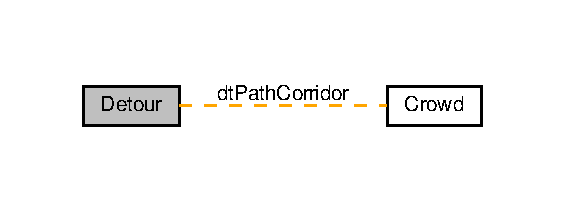
\includegraphics[width=271pt]{group__detour}
\end{center}
\end{figure}
\subsection*{Classes}
\begin{DoxyCompactItemize}
\item 
struct \hyperlink{structdtPoly}{dt\+Poly}
\item 
struct \hyperlink{structdtMeshHeader}{dt\+Mesh\+Header}
\item 
struct \hyperlink{structdtMeshTile}{dt\+Mesh\+Tile}
\item 
struct \hyperlink{structdtNavMeshParams}{dt\+Nav\+Mesh\+Params}
\item 
class \hyperlink{classdtNavMesh}{dt\+Nav\+Mesh}
\item 
struct \hyperlink{structdtNavMeshCreateParams}{dt\+Nav\+Mesh\+Create\+Params}
\item 
class \hyperlink{classdtQueryFilter}{dt\+Query\+Filter}
\item 
struct \hyperlink{structdtRaycastHit}{dt\+Raycast\+Hit}
\item 
class \hyperlink{classdtNavMeshQuery}{dt\+Nav\+Mesh\+Query}
\item 
class \hyperlink{classdtPathCorridor}{dt\+Path\+Corridor}
\end{DoxyCompactItemize}
\subsection*{Typedefs}
\begin{DoxyCompactItemize}
\item 
typedef unsigned int \hyperlink{group__detour_gab4e0b2257a670c1a800057999612b466}{dt\+Poly\+Ref}
\item 
typedef unsigned int \hyperlink{group__detour_ga7ea56cfe01bd7c34a81d821d94cbeea5}{dt\+Tile\+Ref}
\item 
typedef unsigned int \hyperlink{group__detour_ga07c358f7bddf0fa2ef79e341a387c1dd}{dt\+Poly\+Ref}
\item 
typedef unsigned int \hyperlink{group__detour_ga608138970cbb12594287ea6523be24ef}{dt\+Tile\+Ref}
\end{DoxyCompactItemize}
\subsection*{Functions}
\begin{DoxyCompactItemize}
\item 
\hyperlink{classdtNavMesh}{dt\+Nav\+Mesh} $\ast$ \hyperlink{group__detour_ga73648d53c5a414855a2aa264aab9263c}{dt\+Alloc\+Nav\+Mesh} ()
\item 
void \hyperlink{group__detour_gad938af5675a2f62c7c3830b38ea9a184}{dt\+Free\+Nav\+Mesh} (\hyperlink{classdtNavMesh}{dt\+Nav\+Mesh} $\ast$navmesh)
\item 
bool \hyperlink{group__detour_gaf56ac19e79e5948fdb1051158577e648}{dt\+Create\+Nav\+Mesh\+Data} (\hyperlink{structdtNavMeshCreateParams}{dt\+Nav\+Mesh\+Create\+Params} $\ast$params, unsigned char $\ast$$\ast$out\+Data, int $\ast$out\+Data\+Size)
\item 
\hyperlink{classdtNavMeshQuery}{dt\+Nav\+Mesh\+Query} $\ast$ \hyperlink{group__detour_gae547f165feefc955136130c8e22f207a}{dt\+Alloc\+Nav\+Mesh\+Query} ()
\item 
void \hyperlink{group__detour_ga24ccc133f15a0aa85f06f1c1ead2e6c4}{dt\+Free\+Nav\+Mesh\+Query} (\hyperlink{classdtNavMeshQuery}{dt\+Nav\+Mesh\+Query} $\ast$query)
\end{DoxyCompactItemize}


\subsection{Detailed Description}
Members in this module are used to create, manipulate, and query navigation meshes.

\begin{DoxyNote}{Note}
This is a summary \hyperlink{protocollist-p}{list} of members. Use the index or search feature to find minor members.
\end{DoxyNote}
Members in this module are wrappers around the standard math library 

\subsection{Typedef Documentation}
\mbox{\Hypertarget{group__detour_gab4e0b2257a670c1a800057999612b466}\label{group__detour_gab4e0b2257a670c1a800057999612b466}} 
\index{Detour@{Detour}!dt\+Poly\+Ref@{dt\+Poly\+Ref}}
\index{dt\+Poly\+Ref@{dt\+Poly\+Ref}!Detour@{Detour}}
\subsubsection{\texorpdfstring{dt\+Poly\+Ref}{dtPolyRef}\hspace{0.1cm}{\footnotesize\ttfamily [1/2]}}
{\footnotesize\ttfamily \hyperlink{group__detour_gab4e0b2257a670c1a800057999612b466}{dt\+Poly\+Ref}}

A handle to a polygon within a navigation mesh tile.

\begin{DoxyParagraph}{}

\end{DoxyParagraph}
Polygon references are subject to the same invalidate/preserve/restore rules that apply to \hyperlink{group__detour_ga7ea56cfe01bd7c34a81d821d94cbeea5}{dt\+Tile\+Ref}\textquotesingle{}s. If the \hyperlink{group__detour_ga7ea56cfe01bd7c34a81d821d94cbeea5}{dt\+Tile\+Ref} for the polygon\textquotesingle{}s tile changes, the polygon reference becomes invalid.

Changing a polygon\textquotesingle{}s flags, area id, etc. does not impact its polygon reference. \mbox{\Hypertarget{group__detour_ga07c358f7bddf0fa2ef79e341a387c1dd}\label{group__detour_ga07c358f7bddf0fa2ef79e341a387c1dd}} 
\index{Detour@{Detour}!dt\+Poly\+Ref@{dt\+Poly\+Ref}}
\index{dt\+Poly\+Ref@{dt\+Poly\+Ref}!Detour@{Detour}}
\subsubsection{\texorpdfstring{dt\+Poly\+Ref}{dtPolyRef}\hspace{0.1cm}{\footnotesize\ttfamily [2/2]}}
{\footnotesize\ttfamily typedef unsigned int \hyperlink{group__detour_gab4e0b2257a670c1a800057999612b466}{dt\+Poly\+Ref}}

A handle to a polygon within a navigation mesh tile. \mbox{\Hypertarget{group__detour_ga608138970cbb12594287ea6523be24ef}\label{group__detour_ga608138970cbb12594287ea6523be24ef}} 
\index{Detour@{Detour}!dt\+Tile\+Ref@{dt\+Tile\+Ref}}
\index{dt\+Tile\+Ref@{dt\+Tile\+Ref}!Detour@{Detour}}
\subsubsection{\texorpdfstring{dt\+Tile\+Ref}{dtTileRef}\hspace{0.1cm}{\footnotesize\ttfamily [1/2]}}
{\footnotesize\ttfamily typedef unsigned int \hyperlink{group__detour_ga7ea56cfe01bd7c34a81d821d94cbeea5}{dt\+Tile\+Ref}}

A handle to a tile within a navigation mesh. \mbox{\Hypertarget{group__detour_ga7ea56cfe01bd7c34a81d821d94cbeea5}\label{group__detour_ga7ea56cfe01bd7c34a81d821d94cbeea5}} 
\index{Detour@{Detour}!dt\+Tile\+Ref@{dt\+Tile\+Ref}}
\index{dt\+Tile\+Ref@{dt\+Tile\+Ref}!Detour@{Detour}}
\subsubsection{\texorpdfstring{dt\+Tile\+Ref}{dtTileRef}\hspace{0.1cm}{\footnotesize\ttfamily [2/2]}}
{\footnotesize\ttfamily \hyperlink{group__detour_ga7ea56cfe01bd7c34a81d821d94cbeea5}{dt\+Tile\+Ref}}

A handle to a tile within a navigation mesh.

\begin{DoxyParagraph}{}

\end{DoxyParagraph}
The following changes will invalidate a tile reference\+:


\begin{DoxyItemize}
\item The referenced tile has been removed from the navigation mesh.
\item The navigation mesh has been initialized using a different set of \hyperlink{structdtNavMeshParams}{dt\+Nav\+Mesh\+Params}.
\end{DoxyItemize}

A tile reference is preserved/restored if the tile is added to a navigation mesh initialized with the original \hyperlink{structdtNavMeshParams}{dt\+Nav\+Mesh\+Params} and is added at the original reference location. (E.\+g. The last\+Ref parameter is used with \hyperlink{classdtNavMesh_a5b5a7c4fa72c08d9a6d4cc4d8cd3bb89}{dt\+Nav\+Mesh\+::add\+Tile}.)

Basically, if the storage structure of a tile changes, its associated tile reference changes. 

\subsection{Function Documentation}
\mbox{\Hypertarget{group__detour_ga73648d53c5a414855a2aa264aab9263c}\label{group__detour_ga73648d53c5a414855a2aa264aab9263c}} 
\index{Detour@{Detour}!dt\+Alloc\+Nav\+Mesh@{dt\+Alloc\+Nav\+Mesh}}
\index{dt\+Alloc\+Nav\+Mesh@{dt\+Alloc\+Nav\+Mesh}!Detour@{Detour}}
\subsubsection{\texorpdfstring{dt\+Alloc\+Nav\+Mesh()}{dtAllocNavMesh()}}
{\footnotesize\ttfamily \hyperlink{classdtNavMesh}{dt\+Nav\+Mesh}$\ast$ dt\+Alloc\+Nav\+Mesh (\begin{DoxyParamCaption}{ }\end{DoxyParamCaption})}

Allocates a navigation mesh object using the Detour allocator. \begin{DoxyReturn}{Returns}
A navigation mesh that is ready for initialization, or null on failure. 
\end{DoxyReturn}
\mbox{\Hypertarget{group__detour_gae547f165feefc955136130c8e22f207a}\label{group__detour_gae547f165feefc955136130c8e22f207a}} 
\index{Detour@{Detour}!dt\+Alloc\+Nav\+Mesh\+Query@{dt\+Alloc\+Nav\+Mesh\+Query}}
\index{dt\+Alloc\+Nav\+Mesh\+Query@{dt\+Alloc\+Nav\+Mesh\+Query}!Detour@{Detour}}
\subsubsection{\texorpdfstring{dt\+Alloc\+Nav\+Mesh\+Query()}{dtAllocNavMeshQuery()}}
{\footnotesize\ttfamily \hyperlink{classdtNavMeshQuery}{dt\+Nav\+Mesh\+Query}$\ast$ dt\+Alloc\+Nav\+Mesh\+Query (\begin{DoxyParamCaption}{ }\end{DoxyParamCaption})}

Allocates a query object using the Detour allocator. \begin{DoxyReturn}{Returns}
An allocated query object, or null on failure. 
\end{DoxyReturn}
\mbox{\Hypertarget{group__detour_gaf56ac19e79e5948fdb1051158577e648}\label{group__detour_gaf56ac19e79e5948fdb1051158577e648}} 
\index{Detour@{Detour}!dt\+Create\+Nav\+Mesh\+Data@{dt\+Create\+Nav\+Mesh\+Data}}
\index{dt\+Create\+Nav\+Mesh\+Data@{dt\+Create\+Nav\+Mesh\+Data}!Detour@{Detour}}
\subsubsection{\texorpdfstring{dt\+Create\+Nav\+Mesh\+Data()}{dtCreateNavMeshData()}}
{\footnotesize\ttfamily bool dt\+Create\+Nav\+Mesh\+Data (\begin{DoxyParamCaption}\item[{\hyperlink{structdtNavMeshCreateParams}{dt\+Nav\+Mesh\+Create\+Params} $\ast$}]{params,  }\item[{unsigned char $\ast$$\ast$}]{out\+Data,  }\item[{int $\ast$}]{out\+Data\+Size }\end{DoxyParamCaption})}

Builds navigation mesh tile data from the provided tile creation data.


\begin{DoxyParams}[1]{Parameters}
\mbox{\tt in}  & {\em params} & \hyperlink{structTile}{Tile} creation data. \\
\hline
\mbox{\tt out}  & {\em out\+Data} & The resulting tile data. \\
\hline
\mbox{\tt out}  & {\em out\+Data\+Size} & The size of the tile data array. \\
\hline
\end{DoxyParams}
\begin{DoxyReturn}{Returns}
True if the tile data was successfully created.
\end{DoxyReturn}
\begin{DoxyParagraph}{}

\end{DoxyParagraph}
The output data array is allocated using the detour allocator (dt\+Alloc()). The method used to free the memory will be determined by how the tile is added to the navigation mesh.

\begin{DoxySeeAlso}{See also}
\hyperlink{classdtNavMesh}{dt\+Nav\+Mesh}, \hyperlink{classdtNavMesh_a5b5a7c4fa72c08d9a6d4cc4d8cd3bb89}{dt\+Nav\+Mesh\+::add\+Tile()}
\end{DoxySeeAlso}
Builds navigation mesh tile data from the provided tile creation data.


\begin{DoxyParams}[1]{Parameters}
\mbox{\tt in}  & {\em params} & \hyperlink{structTile}{Tile} creation data. \\
\hline
\mbox{\tt out}  & {\em out\+Data} & The resulting tile data. \\
\hline
\mbox{\tt out}  & {\em out\+Data\+Size} & The size of the tile data array. \\
\hline
\end{DoxyParams}
\begin{DoxyReturn}{Returns}
True if the tile data was successfully created.
\end{DoxyReturn}
\begin{DoxyParagraph}{}

\end{DoxyParagraph}
The output data array is allocated using the detour allocator (dt\+Alloc()). The method used to free the memory will be determined by how the tile is added to the navigation mesh.

\begin{DoxySeeAlso}{See also}
\hyperlink{classdtNavMesh}{dt\+Nav\+Mesh}, \hyperlink{classdtNavMesh_a5b5a7c4fa72c08d9a6d4cc4d8cd3bb89}{dt\+Nav\+Mesh\+::add\+Tile()} 
\end{DoxySeeAlso}
\mbox{\Hypertarget{group__detour_gad938af5675a2f62c7c3830b38ea9a184}\label{group__detour_gad938af5675a2f62c7c3830b38ea9a184}} 
\index{Detour@{Detour}!dt\+Free\+Nav\+Mesh@{dt\+Free\+Nav\+Mesh}}
\index{dt\+Free\+Nav\+Mesh@{dt\+Free\+Nav\+Mesh}!Detour@{Detour}}
\subsubsection{\texorpdfstring{dt\+Free\+Nav\+Mesh()}{dtFreeNavMesh()}}
{\footnotesize\ttfamily void dt\+Free\+Nav\+Mesh (\begin{DoxyParamCaption}\item[{\hyperlink{classdtNavMesh}{dt\+Nav\+Mesh} $\ast$}]{navmesh }\end{DoxyParamCaption})}

Frees the specified navigation mesh object using the Detour allocator. 
\begin{DoxyParams}[1]{Parameters}
\mbox{\tt in}  & {\em navmesh} & A navigation mesh allocated using \hyperlink{group__detour_ga73648d53c5a414855a2aa264aab9263c}{dt\+Alloc\+Nav\+Mesh}\\
\hline
\end{DoxyParams}
\begin{DoxyParagraph}{}

\end{DoxyParagraph}
This function will only free the memory for tiles with the \#\+D\+T\+\_\+\+T\+I\+L\+E\+\_\+\+F\+R\+E\+E\+\_\+\+D\+A\+TA flag set.

Frees the specified navigation mesh object using the Detour allocator. 
\begin{DoxyParams}[1]{Parameters}
\mbox{\tt in}  & {\em navmesh} & A navigation mesh allocated using \hyperlink{group__detour_ga73648d53c5a414855a2aa264aab9263c}{dt\+Alloc\+Nav\+Mesh}\\
\hline
\end{DoxyParams}
\begin{DoxyParagraph}{}

\end{DoxyParagraph}
This function will only free the memory for tiles with the \#\+D\+T\+\_\+\+T\+I\+L\+E\+\_\+\+F\+R\+E\+E\+\_\+\+D\+A\+TA flag set. \mbox{\Hypertarget{group__detour_ga24ccc133f15a0aa85f06f1c1ead2e6c4}\label{group__detour_ga24ccc133f15a0aa85f06f1c1ead2e6c4}} 
\index{Detour@{Detour}!dt\+Free\+Nav\+Mesh\+Query@{dt\+Free\+Nav\+Mesh\+Query}}
\index{dt\+Free\+Nav\+Mesh\+Query@{dt\+Free\+Nav\+Mesh\+Query}!Detour@{Detour}}
\subsubsection{\texorpdfstring{dt\+Free\+Nav\+Mesh\+Query()}{dtFreeNavMeshQuery()}}
{\footnotesize\ttfamily void dt\+Free\+Nav\+Mesh\+Query (\begin{DoxyParamCaption}\item[{\hyperlink{classdtNavMeshQuery}{dt\+Nav\+Mesh\+Query} $\ast$}]{query }\end{DoxyParamCaption})}

Frees the specified query object using the Detour allocator. 
\begin{DoxyParams}[1]{Parameters}
\mbox{\tt in}  & {\em query} & A query object allocated using \hyperlink{group__detour_gae547f165feefc955136130c8e22f207a}{dt\+Alloc\+Nav\+Mesh\+Query} \\
\hline
\end{DoxyParams}

\hypertarget{group__crowd}{}\section{Crowd}
\label{group__crowd}\index{Crowd@{Crowd}}
Collaboration diagram for Crowd\+:
\nopagebreak
\begin{figure}[H]
\begin{center}
\leavevmode
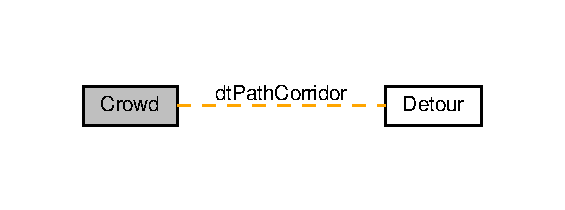
\includegraphics[width=271pt]{group__crowd}
\end{center}
\end{figure}
\subsection*{Classes}
\begin{DoxyCompactItemize}
\item 
struct \hyperlink{structdtCrowdNeighbour}{dt\+Crowd\+Neighbour}
\item 
struct \hyperlink{structdtCrowdAgentParams}{dt\+Crowd\+Agent\+Params}
\item 
struct \hyperlink{structdtCrowdAgent}{dt\+Crowd\+Agent}
\item 
class \hyperlink{classdtCrowd}{dt\+Crowd}
\item 
class \hyperlink{classdtPathCorridor}{dt\+Path\+Corridor}
\end{DoxyCompactItemize}
\subsection*{Enumerations}
\begin{DoxyCompactItemize}
\item 
enum \hyperlink{group__crowd_ga59bc9aa54705292d8f0f1ad9ca48ca82}{Crowd\+Agent\+State} \{ \newline
\hyperlink{group__crowd_gga59bc9aa54705292d8f0f1ad9ca48ca82ac2abcf7abcdba5abeda5801fc771baa8}{D\+T\+\_\+\+C\+R\+O\+W\+D\+A\+G\+E\+N\+T\+\_\+\+S\+T\+A\+T\+E\+\_\+\+I\+N\+V\+A\+L\+ID}, 
\hyperlink{group__crowd_gga59bc9aa54705292d8f0f1ad9ca48ca82ab165ebb808ee9390c7f7ec9f5ea277ec}{D\+T\+\_\+\+C\+R\+O\+W\+D\+A\+G\+E\+N\+T\+\_\+\+S\+T\+A\+T\+E\+\_\+\+W\+A\+L\+K\+I\+NG}, 
\hyperlink{group__crowd_gga59bc9aa54705292d8f0f1ad9ca48ca82a4194d4934f447526177f505e93c96fec}{D\+T\+\_\+\+C\+R\+O\+W\+D\+A\+G\+E\+N\+T\+\_\+\+S\+T\+A\+T\+E\+\_\+\+O\+F\+F\+M\+E\+SH}, 
\hyperlink{group__crowd_gga59bc9aa54705292d8f0f1ad9ca48ca82ac2abcf7abcdba5abeda5801fc771baa8}{D\+T\+\_\+\+C\+R\+O\+W\+D\+A\+G\+E\+N\+T\+\_\+\+S\+T\+A\+T\+E\+\_\+\+I\+N\+V\+A\+L\+ID}, 
\newline
\hyperlink{group__crowd_gga59bc9aa54705292d8f0f1ad9ca48ca82ab165ebb808ee9390c7f7ec9f5ea277ec}{D\+T\+\_\+\+C\+R\+O\+W\+D\+A\+G\+E\+N\+T\+\_\+\+S\+T\+A\+T\+E\+\_\+\+W\+A\+L\+K\+I\+NG}, 
\hyperlink{group__crowd_gga59bc9aa54705292d8f0f1ad9ca48ca82a4194d4934f447526177f505e93c96fec}{D\+T\+\_\+\+C\+R\+O\+W\+D\+A\+G\+E\+N\+T\+\_\+\+S\+T\+A\+T\+E\+\_\+\+O\+F\+F\+M\+E\+SH}
 \}
\item 
enum \hyperlink{group__crowd_gaa94b67d2fdcc390690c523f28019e52f}{Update\+Flags} \{ \newline
{\bfseries D\+T\+\_\+\+C\+R\+O\+W\+D\+\_\+\+A\+N\+T\+I\+C\+I\+P\+A\+T\+E\+\_\+\+T\+U\+R\+NS} = 1, 
{\bfseries D\+T\+\_\+\+C\+R\+O\+W\+D\+\_\+\+O\+B\+S\+T\+A\+C\+L\+E\+\_\+\+A\+V\+O\+I\+D\+A\+N\+CE} = 2, 
{\bfseries D\+T\+\_\+\+C\+R\+O\+W\+D\+\_\+\+S\+E\+P\+A\+R\+A\+T\+I\+ON} = 4, 
\hyperlink{group__crowd_ggaa94b67d2fdcc390690c523f28019e52fad11f447facf1bf42c09de64e9483f3aa}{D\+T\+\_\+\+C\+R\+O\+W\+D\+\_\+\+O\+P\+T\+I\+M\+I\+Z\+E\+\_\+\+V\+IS} = 8, 
\newline
\hyperlink{group__crowd_ggaa94b67d2fdcc390690c523f28019e52fa89c6f7f2e49254e775cb2b85259a0a93}{D\+T\+\_\+\+C\+R\+O\+W\+D\+\_\+\+O\+P\+T\+I\+M\+I\+Z\+E\+\_\+\+T\+O\+PO} = 16, 
{\bfseries D\+T\+\_\+\+C\+R\+O\+W\+D\+\_\+\+A\+N\+T\+I\+C\+I\+P\+A\+T\+E\+\_\+\+T\+U\+R\+NS} = 1, 
{\bfseries D\+T\+\_\+\+C\+R\+O\+W\+D\+\_\+\+O\+B\+S\+T\+A\+C\+L\+E\+\_\+\+A\+V\+O\+I\+D\+A\+N\+CE} = 2, 
{\bfseries D\+T\+\_\+\+C\+R\+O\+W\+D\+\_\+\+S\+E\+P\+A\+R\+A\+T\+I\+ON} = 4, 
\newline
\hyperlink{group__crowd_ggaa94b67d2fdcc390690c523f28019e52fad11f447facf1bf42c09de64e9483f3aa}{D\+T\+\_\+\+C\+R\+O\+W\+D\+\_\+\+O\+P\+T\+I\+M\+I\+Z\+E\+\_\+\+V\+IS} = 8, 
\hyperlink{group__crowd_ggaa94b67d2fdcc390690c523f28019e52fa89c6f7f2e49254e775cb2b85259a0a93}{D\+T\+\_\+\+C\+R\+O\+W\+D\+\_\+\+O\+P\+T\+I\+M\+I\+Z\+E\+\_\+\+T\+O\+PO} = 16
 \}
\item 
enum \hyperlink{group__crowd_ga59bc9aa54705292d8f0f1ad9ca48ca82}{Crowd\+Agent\+State} \{ \newline
\hyperlink{group__crowd_gga59bc9aa54705292d8f0f1ad9ca48ca82ac2abcf7abcdba5abeda5801fc771baa8}{D\+T\+\_\+\+C\+R\+O\+W\+D\+A\+G\+E\+N\+T\+\_\+\+S\+T\+A\+T\+E\+\_\+\+I\+N\+V\+A\+L\+ID}, 
\hyperlink{group__crowd_gga59bc9aa54705292d8f0f1ad9ca48ca82ab165ebb808ee9390c7f7ec9f5ea277ec}{D\+T\+\_\+\+C\+R\+O\+W\+D\+A\+G\+E\+N\+T\+\_\+\+S\+T\+A\+T\+E\+\_\+\+W\+A\+L\+K\+I\+NG}, 
\hyperlink{group__crowd_gga59bc9aa54705292d8f0f1ad9ca48ca82a4194d4934f447526177f505e93c96fec}{D\+T\+\_\+\+C\+R\+O\+W\+D\+A\+G\+E\+N\+T\+\_\+\+S\+T\+A\+T\+E\+\_\+\+O\+F\+F\+M\+E\+SH}, 
\hyperlink{group__crowd_gga59bc9aa54705292d8f0f1ad9ca48ca82ac2abcf7abcdba5abeda5801fc771baa8}{D\+T\+\_\+\+C\+R\+O\+W\+D\+A\+G\+E\+N\+T\+\_\+\+S\+T\+A\+T\+E\+\_\+\+I\+N\+V\+A\+L\+ID}, 
\newline
\hyperlink{group__crowd_gga59bc9aa54705292d8f0f1ad9ca48ca82ab165ebb808ee9390c7f7ec9f5ea277ec}{D\+T\+\_\+\+C\+R\+O\+W\+D\+A\+G\+E\+N\+T\+\_\+\+S\+T\+A\+T\+E\+\_\+\+W\+A\+L\+K\+I\+NG}, 
\hyperlink{group__crowd_gga59bc9aa54705292d8f0f1ad9ca48ca82a4194d4934f447526177f505e93c96fec}{D\+T\+\_\+\+C\+R\+O\+W\+D\+A\+G\+E\+N\+T\+\_\+\+S\+T\+A\+T\+E\+\_\+\+O\+F\+F\+M\+E\+SH}
 \}
\item 
enum \hyperlink{group__crowd_gaa94b67d2fdcc390690c523f28019e52f}{Update\+Flags} \{ \newline
{\bfseries D\+T\+\_\+\+C\+R\+O\+W\+D\+\_\+\+A\+N\+T\+I\+C\+I\+P\+A\+T\+E\+\_\+\+T\+U\+R\+NS} = 1, 
{\bfseries D\+T\+\_\+\+C\+R\+O\+W\+D\+\_\+\+O\+B\+S\+T\+A\+C\+L\+E\+\_\+\+A\+V\+O\+I\+D\+A\+N\+CE} = 2, 
{\bfseries D\+T\+\_\+\+C\+R\+O\+W\+D\+\_\+\+S\+E\+P\+A\+R\+A\+T\+I\+ON} = 4, 
\hyperlink{group__crowd_ggaa94b67d2fdcc390690c523f28019e52fad11f447facf1bf42c09de64e9483f3aa}{D\+T\+\_\+\+C\+R\+O\+W\+D\+\_\+\+O\+P\+T\+I\+M\+I\+Z\+E\+\_\+\+V\+IS} = 8, 
\newline
\hyperlink{group__crowd_ggaa94b67d2fdcc390690c523f28019e52fa89c6f7f2e49254e775cb2b85259a0a93}{D\+T\+\_\+\+C\+R\+O\+W\+D\+\_\+\+O\+P\+T\+I\+M\+I\+Z\+E\+\_\+\+T\+O\+PO} = 16, 
{\bfseries D\+T\+\_\+\+C\+R\+O\+W\+D\+\_\+\+A\+N\+T\+I\+C\+I\+P\+A\+T\+E\+\_\+\+T\+U\+R\+NS} = 1, 
{\bfseries D\+T\+\_\+\+C\+R\+O\+W\+D\+\_\+\+O\+B\+S\+T\+A\+C\+L\+E\+\_\+\+A\+V\+O\+I\+D\+A\+N\+CE} = 2, 
{\bfseries D\+T\+\_\+\+C\+R\+O\+W\+D\+\_\+\+S\+E\+P\+A\+R\+A\+T\+I\+ON} = 4, 
\newline
\hyperlink{group__crowd_ggaa94b67d2fdcc390690c523f28019e52fad11f447facf1bf42c09de64e9483f3aa}{D\+T\+\_\+\+C\+R\+O\+W\+D\+\_\+\+O\+P\+T\+I\+M\+I\+Z\+E\+\_\+\+V\+IS} = 8, 
\hyperlink{group__crowd_ggaa94b67d2fdcc390690c523f28019e52fa89c6f7f2e49254e775cb2b85259a0a93}{D\+T\+\_\+\+C\+R\+O\+W\+D\+\_\+\+O\+P\+T\+I\+M\+I\+Z\+E\+\_\+\+T\+O\+PO} = 16
 \}
\end{DoxyCompactItemize}
\subsection*{Functions}
\begin{DoxyCompactItemize}
\item 
\hyperlink{classdtCrowd}{dt\+Crowd} $\ast$ \hyperlink{group__crowd_ga01a53c9d76d1b61678ab1944dfbfac55}{dt\+Alloc\+Crowd} ()
\item 
void \hyperlink{group__crowd_ga9475313642645070e78c359e0fc02b7a}{dt\+Free\+Crowd} (\hyperlink{classdtCrowd}{dt\+Crowd} $\ast$ptr)
\end{DoxyCompactItemize}


\subsection{Detailed Description}
Members in this module implement local steering and dynamic avoidance features.

The crowd is the big beast of the navigation features. It not only handles a lot of the path management for you, but also local steering and dynamic avoidance between members of the crowd. I.\+e. It can keep your agents from running into each other.

Main class\+: \hyperlink{classdtCrowd}{dt\+Crowd}

The \hyperlink{classdtNavMeshQuery}{dt\+Nav\+Mesh\+Query} and \hyperlink{classdtPathCorridor}{dt\+Path\+Corridor} classes provide perfectly good, easy to use path planning features. But in the end they only give you points that your navigation client should be moving toward. When it comes to deciding things like agent velocity and steering to avoid other agents, that is up to you to implement. Unless, of course, you decide to use \hyperlink{classdtCrowd}{dt\+Crowd}.

Basically, you add an agent to the crowd, providing various configuration settings such as maximum speed and acceleration. You also provide a local target to more toward. The crowd manager then provides, with every update, the new agent position and velocity for the frame. The movement will be constrained to the navigation mesh, and steering will be applied to ensure agents managed by the crowd do not collide with each other.

This is very powerful feature set. But it comes with limitations.

The biggest limitation is that you must give control of the agent\textquotesingle{}s position completely over to the crowd manager. You can update things like maximum speed and acceleration. But in order for the crowd manager to do its thing, it can\textquotesingle{}t allow you to constantly be giving it overrides to position and velocity. So you give up direct control of the agent\textquotesingle{}s movement. It belongs to the crowd.

The second biggest limitation revolves around the fact that the crowd manager deals with local planning. So the agent\textquotesingle{}s target should never be more than 256 polygons aways from its current position. If it is, you risk your agent failing to reach its target. So you may still need to do long distance planning and provide the crowd manager with intermediate targets.

Other significant limitations\+:


\begin{DoxyItemize}
\item All agents using the crowd manager will use the same \hyperlink{classdtQueryFilter}{dt\+Query\+Filter}.
\item Crowd management is relatively expensive. The maximum agents under crowd management at any one time is between 20 and 30. A good place to start is a maximum of 25 agents for 0.\+5ms per frame.
\end{DoxyItemize}

\begin{DoxyNote}{Note}
This is a summary \hyperlink{protocollist-p}{list} of members. Use the index or search feature to find minor members. 
\end{DoxyNote}


\subsection{Enumeration Type Documentation}
\mbox{\Hypertarget{group__crowd_ga59bc9aa54705292d8f0f1ad9ca48ca82}\label{group__crowd_ga59bc9aa54705292d8f0f1ad9ca48ca82}} 
\index{Crowd@{Crowd}!Crowd\+Agent\+State@{Crowd\+Agent\+State}}
\index{Crowd\+Agent\+State@{Crowd\+Agent\+State}!Crowd@{Crowd}}
\subsubsection{\texorpdfstring{Crowd\+Agent\+State}{CrowdAgentState}\hspace{0.1cm}{\footnotesize\ttfamily [1/2]}}
{\footnotesize\ttfamily enum \hyperlink{group__crowd_ga59bc9aa54705292d8f0f1ad9ca48ca82}{Crowd\+Agent\+State}}

The type of navigation mesh polygon the agent is currently traversing. \begin{DoxyEnumFields}{Enumerator}
\raisebox{\heightof{T}}[0pt][0pt]{\index{D\+T\+\_\+\+C\+R\+O\+W\+D\+A\+G\+E\+N\+T\+\_\+\+S\+T\+A\+T\+E\+\_\+\+I\+N\+V\+A\+L\+ID@{D\+T\+\_\+\+C\+R\+O\+W\+D\+A\+G\+E\+N\+T\+\_\+\+S\+T\+A\+T\+E\+\_\+\+I\+N\+V\+A\+L\+ID}!Crowd@{Crowd}}\index{Crowd@{Crowd}!D\+T\+\_\+\+C\+R\+O\+W\+D\+A\+G\+E\+N\+T\+\_\+\+S\+T\+A\+T\+E\+\_\+\+I\+N\+V\+A\+L\+ID@{D\+T\+\_\+\+C\+R\+O\+W\+D\+A\+G\+E\+N\+T\+\_\+\+S\+T\+A\+T\+E\+\_\+\+I\+N\+V\+A\+L\+ID}}}\mbox{\Hypertarget{group__crowd_gga59bc9aa54705292d8f0f1ad9ca48ca82ac2abcf7abcdba5abeda5801fc771baa8}\label{group__crowd_gga59bc9aa54705292d8f0f1ad9ca48ca82ac2abcf7abcdba5abeda5801fc771baa8}} 
D\+T\+\_\+\+C\+R\+O\+W\+D\+A\+G\+E\+N\+T\+\_\+\+S\+T\+A\+T\+E\+\_\+\+I\+N\+V\+A\+L\+ID&The agent is not in a valid state. \\
\hline

\raisebox{\heightof{T}}[0pt][0pt]{\index{D\+T\+\_\+\+C\+R\+O\+W\+D\+A\+G\+E\+N\+T\+\_\+\+S\+T\+A\+T\+E\+\_\+\+W\+A\+L\+K\+I\+NG@{D\+T\+\_\+\+C\+R\+O\+W\+D\+A\+G\+E\+N\+T\+\_\+\+S\+T\+A\+T\+E\+\_\+\+W\+A\+L\+K\+I\+NG}!Crowd@{Crowd}}\index{Crowd@{Crowd}!D\+T\+\_\+\+C\+R\+O\+W\+D\+A\+G\+E\+N\+T\+\_\+\+S\+T\+A\+T\+E\+\_\+\+W\+A\+L\+K\+I\+NG@{D\+T\+\_\+\+C\+R\+O\+W\+D\+A\+G\+E\+N\+T\+\_\+\+S\+T\+A\+T\+E\+\_\+\+W\+A\+L\+K\+I\+NG}}}\mbox{\Hypertarget{group__crowd_gga59bc9aa54705292d8f0f1ad9ca48ca82ab165ebb808ee9390c7f7ec9f5ea277ec}\label{group__crowd_gga59bc9aa54705292d8f0f1ad9ca48ca82ab165ebb808ee9390c7f7ec9f5ea277ec}} 
D\+T\+\_\+\+C\+R\+O\+W\+D\+A\+G\+E\+N\+T\+\_\+\+S\+T\+A\+T\+E\+\_\+\+W\+A\+L\+K\+I\+NG&The agent is traversing a normal navigation mesh polygon. \\
\hline

\raisebox{\heightof{T}}[0pt][0pt]{\index{D\+T\+\_\+\+C\+R\+O\+W\+D\+A\+G\+E\+N\+T\+\_\+\+S\+T\+A\+T\+E\+\_\+\+O\+F\+F\+M\+E\+SH@{D\+T\+\_\+\+C\+R\+O\+W\+D\+A\+G\+E\+N\+T\+\_\+\+S\+T\+A\+T\+E\+\_\+\+O\+F\+F\+M\+E\+SH}!Crowd@{Crowd}}\index{Crowd@{Crowd}!D\+T\+\_\+\+C\+R\+O\+W\+D\+A\+G\+E\+N\+T\+\_\+\+S\+T\+A\+T\+E\+\_\+\+O\+F\+F\+M\+E\+SH@{D\+T\+\_\+\+C\+R\+O\+W\+D\+A\+G\+E\+N\+T\+\_\+\+S\+T\+A\+T\+E\+\_\+\+O\+F\+F\+M\+E\+SH}}}\mbox{\Hypertarget{group__crowd_gga59bc9aa54705292d8f0f1ad9ca48ca82a4194d4934f447526177f505e93c96fec}\label{group__crowd_gga59bc9aa54705292d8f0f1ad9ca48ca82a4194d4934f447526177f505e93c96fec}} 
D\+T\+\_\+\+C\+R\+O\+W\+D\+A\+G\+E\+N\+T\+\_\+\+S\+T\+A\+T\+E\+\_\+\+O\+F\+F\+M\+E\+SH&The agent is traversing an off-\/mesh connection. \\
\hline

\raisebox{\heightof{T}}[0pt][0pt]{\index{D\+T\+\_\+\+C\+R\+O\+W\+D\+A\+G\+E\+N\+T\+\_\+\+S\+T\+A\+T\+E\+\_\+\+I\+N\+V\+A\+L\+ID@{D\+T\+\_\+\+C\+R\+O\+W\+D\+A\+G\+E\+N\+T\+\_\+\+S\+T\+A\+T\+E\+\_\+\+I\+N\+V\+A\+L\+ID}!Crowd@{Crowd}}\index{Crowd@{Crowd}!D\+T\+\_\+\+C\+R\+O\+W\+D\+A\+G\+E\+N\+T\+\_\+\+S\+T\+A\+T\+E\+\_\+\+I\+N\+V\+A\+L\+ID@{D\+T\+\_\+\+C\+R\+O\+W\+D\+A\+G\+E\+N\+T\+\_\+\+S\+T\+A\+T\+E\+\_\+\+I\+N\+V\+A\+L\+ID}}}\mbox{\Hypertarget{group__crowd_gga59bc9aa54705292d8f0f1ad9ca48ca82ac2abcf7abcdba5abeda5801fc771baa8}\label{group__crowd_gga59bc9aa54705292d8f0f1ad9ca48ca82ac2abcf7abcdba5abeda5801fc771baa8}} 
D\+T\+\_\+\+C\+R\+O\+W\+D\+A\+G\+E\+N\+T\+\_\+\+S\+T\+A\+T\+E\+\_\+\+I\+N\+V\+A\+L\+ID&The agent is not in a valid state. \\
\hline

\raisebox{\heightof{T}}[0pt][0pt]{\index{D\+T\+\_\+\+C\+R\+O\+W\+D\+A\+G\+E\+N\+T\+\_\+\+S\+T\+A\+T\+E\+\_\+\+W\+A\+L\+K\+I\+NG@{D\+T\+\_\+\+C\+R\+O\+W\+D\+A\+G\+E\+N\+T\+\_\+\+S\+T\+A\+T\+E\+\_\+\+W\+A\+L\+K\+I\+NG}!Crowd@{Crowd}}\index{Crowd@{Crowd}!D\+T\+\_\+\+C\+R\+O\+W\+D\+A\+G\+E\+N\+T\+\_\+\+S\+T\+A\+T\+E\+\_\+\+W\+A\+L\+K\+I\+NG@{D\+T\+\_\+\+C\+R\+O\+W\+D\+A\+G\+E\+N\+T\+\_\+\+S\+T\+A\+T\+E\+\_\+\+W\+A\+L\+K\+I\+NG}}}\mbox{\Hypertarget{group__crowd_gga59bc9aa54705292d8f0f1ad9ca48ca82ab165ebb808ee9390c7f7ec9f5ea277ec}\label{group__crowd_gga59bc9aa54705292d8f0f1ad9ca48ca82ab165ebb808ee9390c7f7ec9f5ea277ec}} 
D\+T\+\_\+\+C\+R\+O\+W\+D\+A\+G\+E\+N\+T\+\_\+\+S\+T\+A\+T\+E\+\_\+\+W\+A\+L\+K\+I\+NG&The agent is traversing a normal navigation mesh polygon. \\
\hline

\raisebox{\heightof{T}}[0pt][0pt]{\index{D\+T\+\_\+\+C\+R\+O\+W\+D\+A\+G\+E\+N\+T\+\_\+\+S\+T\+A\+T\+E\+\_\+\+O\+F\+F\+M\+E\+SH@{D\+T\+\_\+\+C\+R\+O\+W\+D\+A\+G\+E\+N\+T\+\_\+\+S\+T\+A\+T\+E\+\_\+\+O\+F\+F\+M\+E\+SH}!Crowd@{Crowd}}\index{Crowd@{Crowd}!D\+T\+\_\+\+C\+R\+O\+W\+D\+A\+G\+E\+N\+T\+\_\+\+S\+T\+A\+T\+E\+\_\+\+O\+F\+F\+M\+E\+SH@{D\+T\+\_\+\+C\+R\+O\+W\+D\+A\+G\+E\+N\+T\+\_\+\+S\+T\+A\+T\+E\+\_\+\+O\+F\+F\+M\+E\+SH}}}\mbox{\Hypertarget{group__crowd_gga59bc9aa54705292d8f0f1ad9ca48ca82a4194d4934f447526177f505e93c96fec}\label{group__crowd_gga59bc9aa54705292d8f0f1ad9ca48ca82a4194d4934f447526177f505e93c96fec}} 
D\+T\+\_\+\+C\+R\+O\+W\+D\+A\+G\+E\+N\+T\+\_\+\+S\+T\+A\+T\+E\+\_\+\+O\+F\+F\+M\+E\+SH&The agent is traversing an off-\/mesh connection. \\
\hline

\end{DoxyEnumFields}
\mbox{\Hypertarget{group__crowd_ga59bc9aa54705292d8f0f1ad9ca48ca82}\label{group__crowd_ga59bc9aa54705292d8f0f1ad9ca48ca82}} 
\index{Crowd@{Crowd}!Crowd\+Agent\+State@{Crowd\+Agent\+State}}
\index{Crowd\+Agent\+State@{Crowd\+Agent\+State}!Crowd@{Crowd}}
\subsubsection{\texorpdfstring{Crowd\+Agent\+State}{CrowdAgentState}\hspace{0.1cm}{\footnotesize\ttfamily [2/2]}}
{\footnotesize\ttfamily enum \hyperlink{group__crowd_ga59bc9aa54705292d8f0f1ad9ca48ca82}{Crowd\+Agent\+State}}

The type of navigation mesh polygon the agent is currently traversing. \begin{DoxyEnumFields}{Enumerator}
\raisebox{\heightof{T}}[0pt][0pt]{\index{D\+T\+\_\+\+C\+R\+O\+W\+D\+A\+G\+E\+N\+T\+\_\+\+S\+T\+A\+T\+E\+\_\+\+I\+N\+V\+A\+L\+ID@{D\+T\+\_\+\+C\+R\+O\+W\+D\+A\+G\+E\+N\+T\+\_\+\+S\+T\+A\+T\+E\+\_\+\+I\+N\+V\+A\+L\+ID}!Crowd@{Crowd}}\index{Crowd@{Crowd}!D\+T\+\_\+\+C\+R\+O\+W\+D\+A\+G\+E\+N\+T\+\_\+\+S\+T\+A\+T\+E\+\_\+\+I\+N\+V\+A\+L\+ID@{D\+T\+\_\+\+C\+R\+O\+W\+D\+A\+G\+E\+N\+T\+\_\+\+S\+T\+A\+T\+E\+\_\+\+I\+N\+V\+A\+L\+ID}}}\mbox{\Hypertarget{group__crowd_gga59bc9aa54705292d8f0f1ad9ca48ca82ac2abcf7abcdba5abeda5801fc771baa8}\label{group__crowd_gga59bc9aa54705292d8f0f1ad9ca48ca82ac2abcf7abcdba5abeda5801fc771baa8}} 
D\+T\+\_\+\+C\+R\+O\+W\+D\+A\+G\+E\+N\+T\+\_\+\+S\+T\+A\+T\+E\+\_\+\+I\+N\+V\+A\+L\+ID&The agent is not in a valid state. \\
\hline

\raisebox{\heightof{T}}[0pt][0pt]{\index{D\+T\+\_\+\+C\+R\+O\+W\+D\+A\+G\+E\+N\+T\+\_\+\+S\+T\+A\+T\+E\+\_\+\+W\+A\+L\+K\+I\+NG@{D\+T\+\_\+\+C\+R\+O\+W\+D\+A\+G\+E\+N\+T\+\_\+\+S\+T\+A\+T\+E\+\_\+\+W\+A\+L\+K\+I\+NG}!Crowd@{Crowd}}\index{Crowd@{Crowd}!D\+T\+\_\+\+C\+R\+O\+W\+D\+A\+G\+E\+N\+T\+\_\+\+S\+T\+A\+T\+E\+\_\+\+W\+A\+L\+K\+I\+NG@{D\+T\+\_\+\+C\+R\+O\+W\+D\+A\+G\+E\+N\+T\+\_\+\+S\+T\+A\+T\+E\+\_\+\+W\+A\+L\+K\+I\+NG}}}\mbox{\Hypertarget{group__crowd_gga59bc9aa54705292d8f0f1ad9ca48ca82ab165ebb808ee9390c7f7ec9f5ea277ec}\label{group__crowd_gga59bc9aa54705292d8f0f1ad9ca48ca82ab165ebb808ee9390c7f7ec9f5ea277ec}} 
D\+T\+\_\+\+C\+R\+O\+W\+D\+A\+G\+E\+N\+T\+\_\+\+S\+T\+A\+T\+E\+\_\+\+W\+A\+L\+K\+I\+NG&The agent is traversing a normal navigation mesh polygon. \\
\hline

\raisebox{\heightof{T}}[0pt][0pt]{\index{D\+T\+\_\+\+C\+R\+O\+W\+D\+A\+G\+E\+N\+T\+\_\+\+S\+T\+A\+T\+E\+\_\+\+O\+F\+F\+M\+E\+SH@{D\+T\+\_\+\+C\+R\+O\+W\+D\+A\+G\+E\+N\+T\+\_\+\+S\+T\+A\+T\+E\+\_\+\+O\+F\+F\+M\+E\+SH}!Crowd@{Crowd}}\index{Crowd@{Crowd}!D\+T\+\_\+\+C\+R\+O\+W\+D\+A\+G\+E\+N\+T\+\_\+\+S\+T\+A\+T\+E\+\_\+\+O\+F\+F\+M\+E\+SH@{D\+T\+\_\+\+C\+R\+O\+W\+D\+A\+G\+E\+N\+T\+\_\+\+S\+T\+A\+T\+E\+\_\+\+O\+F\+F\+M\+E\+SH}}}\mbox{\Hypertarget{group__crowd_gga59bc9aa54705292d8f0f1ad9ca48ca82a4194d4934f447526177f505e93c96fec}\label{group__crowd_gga59bc9aa54705292d8f0f1ad9ca48ca82a4194d4934f447526177f505e93c96fec}} 
D\+T\+\_\+\+C\+R\+O\+W\+D\+A\+G\+E\+N\+T\+\_\+\+S\+T\+A\+T\+E\+\_\+\+O\+F\+F\+M\+E\+SH&The agent is traversing an off-\/mesh connection. \\
\hline

\raisebox{\heightof{T}}[0pt][0pt]{\index{D\+T\+\_\+\+C\+R\+O\+W\+D\+A\+G\+E\+N\+T\+\_\+\+S\+T\+A\+T\+E\+\_\+\+I\+N\+V\+A\+L\+ID@{D\+T\+\_\+\+C\+R\+O\+W\+D\+A\+G\+E\+N\+T\+\_\+\+S\+T\+A\+T\+E\+\_\+\+I\+N\+V\+A\+L\+ID}!Crowd@{Crowd}}\index{Crowd@{Crowd}!D\+T\+\_\+\+C\+R\+O\+W\+D\+A\+G\+E\+N\+T\+\_\+\+S\+T\+A\+T\+E\+\_\+\+I\+N\+V\+A\+L\+ID@{D\+T\+\_\+\+C\+R\+O\+W\+D\+A\+G\+E\+N\+T\+\_\+\+S\+T\+A\+T\+E\+\_\+\+I\+N\+V\+A\+L\+ID}}}\mbox{\Hypertarget{group__crowd_gga59bc9aa54705292d8f0f1ad9ca48ca82ac2abcf7abcdba5abeda5801fc771baa8}\label{group__crowd_gga59bc9aa54705292d8f0f1ad9ca48ca82ac2abcf7abcdba5abeda5801fc771baa8}} 
D\+T\+\_\+\+C\+R\+O\+W\+D\+A\+G\+E\+N\+T\+\_\+\+S\+T\+A\+T\+E\+\_\+\+I\+N\+V\+A\+L\+ID&The agent is not in a valid state. \\
\hline

\raisebox{\heightof{T}}[0pt][0pt]{\index{D\+T\+\_\+\+C\+R\+O\+W\+D\+A\+G\+E\+N\+T\+\_\+\+S\+T\+A\+T\+E\+\_\+\+W\+A\+L\+K\+I\+NG@{D\+T\+\_\+\+C\+R\+O\+W\+D\+A\+G\+E\+N\+T\+\_\+\+S\+T\+A\+T\+E\+\_\+\+W\+A\+L\+K\+I\+NG}!Crowd@{Crowd}}\index{Crowd@{Crowd}!D\+T\+\_\+\+C\+R\+O\+W\+D\+A\+G\+E\+N\+T\+\_\+\+S\+T\+A\+T\+E\+\_\+\+W\+A\+L\+K\+I\+NG@{D\+T\+\_\+\+C\+R\+O\+W\+D\+A\+G\+E\+N\+T\+\_\+\+S\+T\+A\+T\+E\+\_\+\+W\+A\+L\+K\+I\+NG}}}\mbox{\Hypertarget{group__crowd_gga59bc9aa54705292d8f0f1ad9ca48ca82ab165ebb808ee9390c7f7ec9f5ea277ec}\label{group__crowd_gga59bc9aa54705292d8f0f1ad9ca48ca82ab165ebb808ee9390c7f7ec9f5ea277ec}} 
D\+T\+\_\+\+C\+R\+O\+W\+D\+A\+G\+E\+N\+T\+\_\+\+S\+T\+A\+T\+E\+\_\+\+W\+A\+L\+K\+I\+NG&The agent is traversing a normal navigation mesh polygon. \\
\hline

\raisebox{\heightof{T}}[0pt][0pt]{\index{D\+T\+\_\+\+C\+R\+O\+W\+D\+A\+G\+E\+N\+T\+\_\+\+S\+T\+A\+T\+E\+\_\+\+O\+F\+F\+M\+E\+SH@{D\+T\+\_\+\+C\+R\+O\+W\+D\+A\+G\+E\+N\+T\+\_\+\+S\+T\+A\+T\+E\+\_\+\+O\+F\+F\+M\+E\+SH}!Crowd@{Crowd}}\index{Crowd@{Crowd}!D\+T\+\_\+\+C\+R\+O\+W\+D\+A\+G\+E\+N\+T\+\_\+\+S\+T\+A\+T\+E\+\_\+\+O\+F\+F\+M\+E\+SH@{D\+T\+\_\+\+C\+R\+O\+W\+D\+A\+G\+E\+N\+T\+\_\+\+S\+T\+A\+T\+E\+\_\+\+O\+F\+F\+M\+E\+SH}}}\mbox{\Hypertarget{group__crowd_gga59bc9aa54705292d8f0f1ad9ca48ca82a4194d4934f447526177f505e93c96fec}\label{group__crowd_gga59bc9aa54705292d8f0f1ad9ca48ca82a4194d4934f447526177f505e93c96fec}} 
D\+T\+\_\+\+C\+R\+O\+W\+D\+A\+G\+E\+N\+T\+\_\+\+S\+T\+A\+T\+E\+\_\+\+O\+F\+F\+M\+E\+SH&The agent is traversing an off-\/mesh connection. \\
\hline

\end{DoxyEnumFields}
\mbox{\Hypertarget{group__crowd_gaa94b67d2fdcc390690c523f28019e52f}\label{group__crowd_gaa94b67d2fdcc390690c523f28019e52f}} 
\index{Crowd@{Crowd}!Update\+Flags@{Update\+Flags}}
\index{Update\+Flags@{Update\+Flags}!Crowd@{Crowd}}
\subsubsection{\texorpdfstring{Update\+Flags}{UpdateFlags}\hspace{0.1cm}{\footnotesize\ttfamily [1/2]}}
{\footnotesize\ttfamily enum \hyperlink{group__crowd_gaa94b67d2fdcc390690c523f28019e52f}{Update\+Flags}}

Crowd agent update flags.

\begin{DoxySeeAlso}{See also}
\hyperlink{structdtCrowdAgentParams_a7066a4477bbfa53fc1c983e17aa3e5ae}{dt\+Crowd\+Agent\+Params\+::update\+Flags} 
\end{DoxySeeAlso}
\begin{DoxyEnumFields}{Enumerator}
\raisebox{\heightof{T}}[0pt][0pt]{\index{D\+T\+\_\+\+C\+R\+O\+W\+D\+\_\+\+O\+P\+T\+I\+M\+I\+Z\+E\+\_\+\+V\+IS@{D\+T\+\_\+\+C\+R\+O\+W\+D\+\_\+\+O\+P\+T\+I\+M\+I\+Z\+E\+\_\+\+V\+IS}!Crowd@{Crowd}}\index{Crowd@{Crowd}!D\+T\+\_\+\+C\+R\+O\+W\+D\+\_\+\+O\+P\+T\+I\+M\+I\+Z\+E\+\_\+\+V\+IS@{D\+T\+\_\+\+C\+R\+O\+W\+D\+\_\+\+O\+P\+T\+I\+M\+I\+Z\+E\+\_\+\+V\+IS}}}\mbox{\Hypertarget{group__crowd_ggaa94b67d2fdcc390690c523f28019e52fad11f447facf1bf42c09de64e9483f3aa}\label{group__crowd_ggaa94b67d2fdcc390690c523f28019e52fad11f447facf1bf42c09de64e9483f3aa}} 
D\+T\+\_\+\+C\+R\+O\+W\+D\+\_\+\+O\+P\+T\+I\+M\+I\+Z\+E\+\_\+\+V\+IS&Use \hyperlink{classdtPathCorridor_a3970b6cd229731debe6beb41d9885463}{dt\+Path\+Corridor\+::optimize\+Path\+Visibility()} to optimize the agent path. \\
\hline

\raisebox{\heightof{T}}[0pt][0pt]{\index{D\+T\+\_\+\+C\+R\+O\+W\+D\+\_\+\+O\+P\+T\+I\+M\+I\+Z\+E\+\_\+\+T\+O\+PO@{D\+T\+\_\+\+C\+R\+O\+W\+D\+\_\+\+O\+P\+T\+I\+M\+I\+Z\+E\+\_\+\+T\+O\+PO}!Crowd@{Crowd}}\index{Crowd@{Crowd}!D\+T\+\_\+\+C\+R\+O\+W\+D\+\_\+\+O\+P\+T\+I\+M\+I\+Z\+E\+\_\+\+T\+O\+PO@{D\+T\+\_\+\+C\+R\+O\+W\+D\+\_\+\+O\+P\+T\+I\+M\+I\+Z\+E\+\_\+\+T\+O\+PO}}}\mbox{\Hypertarget{group__crowd_ggaa94b67d2fdcc390690c523f28019e52fa89c6f7f2e49254e775cb2b85259a0a93}\label{group__crowd_ggaa94b67d2fdcc390690c523f28019e52fa89c6f7f2e49254e775cb2b85259a0a93}} 
D\+T\+\_\+\+C\+R\+O\+W\+D\+\_\+\+O\+P\+T\+I\+M\+I\+Z\+E\+\_\+\+T\+O\+PO&Use \hyperlink{classdtPathCorridor_a69288d28ab5d23b2c2654e45c5a33c25}{dt\+Path\+Corridor\+::optimize\+Path\+Topology()} to optimize the agent path. \\
\hline

\raisebox{\heightof{T}}[0pt][0pt]{\index{D\+T\+\_\+\+C\+R\+O\+W\+D\+\_\+\+O\+P\+T\+I\+M\+I\+Z\+E\+\_\+\+V\+IS@{D\+T\+\_\+\+C\+R\+O\+W\+D\+\_\+\+O\+P\+T\+I\+M\+I\+Z\+E\+\_\+\+V\+IS}!Crowd@{Crowd}}\index{Crowd@{Crowd}!D\+T\+\_\+\+C\+R\+O\+W\+D\+\_\+\+O\+P\+T\+I\+M\+I\+Z\+E\+\_\+\+V\+IS@{D\+T\+\_\+\+C\+R\+O\+W\+D\+\_\+\+O\+P\+T\+I\+M\+I\+Z\+E\+\_\+\+V\+IS}}}\mbox{\Hypertarget{group__crowd_ggaa94b67d2fdcc390690c523f28019e52fad11f447facf1bf42c09de64e9483f3aa}\label{group__crowd_ggaa94b67d2fdcc390690c523f28019e52fad11f447facf1bf42c09de64e9483f3aa}} 
D\+T\+\_\+\+C\+R\+O\+W\+D\+\_\+\+O\+P\+T\+I\+M\+I\+Z\+E\+\_\+\+V\+IS&Use \hyperlink{classdtPathCorridor_a3970b6cd229731debe6beb41d9885463}{dt\+Path\+Corridor\+::optimize\+Path\+Visibility()} to optimize the agent path. \\
\hline

\raisebox{\heightof{T}}[0pt][0pt]{\index{D\+T\+\_\+\+C\+R\+O\+W\+D\+\_\+\+O\+P\+T\+I\+M\+I\+Z\+E\+\_\+\+T\+O\+PO@{D\+T\+\_\+\+C\+R\+O\+W\+D\+\_\+\+O\+P\+T\+I\+M\+I\+Z\+E\+\_\+\+T\+O\+PO}!Crowd@{Crowd}}\index{Crowd@{Crowd}!D\+T\+\_\+\+C\+R\+O\+W\+D\+\_\+\+O\+P\+T\+I\+M\+I\+Z\+E\+\_\+\+T\+O\+PO@{D\+T\+\_\+\+C\+R\+O\+W\+D\+\_\+\+O\+P\+T\+I\+M\+I\+Z\+E\+\_\+\+T\+O\+PO}}}\mbox{\Hypertarget{group__crowd_ggaa94b67d2fdcc390690c523f28019e52fa89c6f7f2e49254e775cb2b85259a0a93}\label{group__crowd_ggaa94b67d2fdcc390690c523f28019e52fa89c6f7f2e49254e775cb2b85259a0a93}} 
D\+T\+\_\+\+C\+R\+O\+W\+D\+\_\+\+O\+P\+T\+I\+M\+I\+Z\+E\+\_\+\+T\+O\+PO&Use \hyperlink{classdtPathCorridor_a69288d28ab5d23b2c2654e45c5a33c25}{dt\+Path\+Corridor\+::optimize\+Path\+Topology()} to optimize the agent path. \\
\hline

\end{DoxyEnumFields}
\mbox{\Hypertarget{group__crowd_gaa94b67d2fdcc390690c523f28019e52f}\label{group__crowd_gaa94b67d2fdcc390690c523f28019e52f}} 
\index{Crowd@{Crowd}!Update\+Flags@{Update\+Flags}}
\index{Update\+Flags@{Update\+Flags}!Crowd@{Crowd}}
\subsubsection{\texorpdfstring{Update\+Flags}{UpdateFlags}\hspace{0.1cm}{\footnotesize\ttfamily [2/2]}}
{\footnotesize\ttfamily enum \hyperlink{group__crowd_gaa94b67d2fdcc390690c523f28019e52f}{Update\+Flags}}

Crowd agent update flags.

\begin{DoxySeeAlso}{See also}
\hyperlink{structdtCrowdAgentParams_a7066a4477bbfa53fc1c983e17aa3e5ae}{dt\+Crowd\+Agent\+Params\+::update\+Flags} 
\end{DoxySeeAlso}
\begin{DoxyEnumFields}{Enumerator}
\raisebox{\heightof{T}}[0pt][0pt]{\index{D\+T\+\_\+\+C\+R\+O\+W\+D\+\_\+\+O\+P\+T\+I\+M\+I\+Z\+E\+\_\+\+V\+IS@{D\+T\+\_\+\+C\+R\+O\+W\+D\+\_\+\+O\+P\+T\+I\+M\+I\+Z\+E\+\_\+\+V\+IS}!Crowd@{Crowd}}\index{Crowd@{Crowd}!D\+T\+\_\+\+C\+R\+O\+W\+D\+\_\+\+O\+P\+T\+I\+M\+I\+Z\+E\+\_\+\+V\+IS@{D\+T\+\_\+\+C\+R\+O\+W\+D\+\_\+\+O\+P\+T\+I\+M\+I\+Z\+E\+\_\+\+V\+IS}}}\mbox{\Hypertarget{group__crowd_ggaa94b67d2fdcc390690c523f28019e52fad11f447facf1bf42c09de64e9483f3aa}\label{group__crowd_ggaa94b67d2fdcc390690c523f28019e52fad11f447facf1bf42c09de64e9483f3aa}} 
D\+T\+\_\+\+C\+R\+O\+W\+D\+\_\+\+O\+P\+T\+I\+M\+I\+Z\+E\+\_\+\+V\+IS&Use \hyperlink{classdtPathCorridor_a3970b6cd229731debe6beb41d9885463}{dt\+Path\+Corridor\+::optimize\+Path\+Visibility()} to optimize the agent path. \\
\hline

\raisebox{\heightof{T}}[0pt][0pt]{\index{D\+T\+\_\+\+C\+R\+O\+W\+D\+\_\+\+O\+P\+T\+I\+M\+I\+Z\+E\+\_\+\+T\+O\+PO@{D\+T\+\_\+\+C\+R\+O\+W\+D\+\_\+\+O\+P\+T\+I\+M\+I\+Z\+E\+\_\+\+T\+O\+PO}!Crowd@{Crowd}}\index{Crowd@{Crowd}!D\+T\+\_\+\+C\+R\+O\+W\+D\+\_\+\+O\+P\+T\+I\+M\+I\+Z\+E\+\_\+\+T\+O\+PO@{D\+T\+\_\+\+C\+R\+O\+W\+D\+\_\+\+O\+P\+T\+I\+M\+I\+Z\+E\+\_\+\+T\+O\+PO}}}\mbox{\Hypertarget{group__crowd_ggaa94b67d2fdcc390690c523f28019e52fa89c6f7f2e49254e775cb2b85259a0a93}\label{group__crowd_ggaa94b67d2fdcc390690c523f28019e52fa89c6f7f2e49254e775cb2b85259a0a93}} 
D\+T\+\_\+\+C\+R\+O\+W\+D\+\_\+\+O\+P\+T\+I\+M\+I\+Z\+E\+\_\+\+T\+O\+PO&Use \hyperlink{classdtPathCorridor_a69288d28ab5d23b2c2654e45c5a33c25}{dt\+Path\+Corridor\+::optimize\+Path\+Topology()} to optimize the agent path. \\
\hline

\raisebox{\heightof{T}}[0pt][0pt]{\index{D\+T\+\_\+\+C\+R\+O\+W\+D\+\_\+\+O\+P\+T\+I\+M\+I\+Z\+E\+\_\+\+V\+IS@{D\+T\+\_\+\+C\+R\+O\+W\+D\+\_\+\+O\+P\+T\+I\+M\+I\+Z\+E\+\_\+\+V\+IS}!Crowd@{Crowd}}\index{Crowd@{Crowd}!D\+T\+\_\+\+C\+R\+O\+W\+D\+\_\+\+O\+P\+T\+I\+M\+I\+Z\+E\+\_\+\+V\+IS@{D\+T\+\_\+\+C\+R\+O\+W\+D\+\_\+\+O\+P\+T\+I\+M\+I\+Z\+E\+\_\+\+V\+IS}}}\mbox{\Hypertarget{group__crowd_ggaa94b67d2fdcc390690c523f28019e52fad11f447facf1bf42c09de64e9483f3aa}\label{group__crowd_ggaa94b67d2fdcc390690c523f28019e52fad11f447facf1bf42c09de64e9483f3aa}} 
D\+T\+\_\+\+C\+R\+O\+W\+D\+\_\+\+O\+P\+T\+I\+M\+I\+Z\+E\+\_\+\+V\+IS&Use \hyperlink{classdtPathCorridor_a3970b6cd229731debe6beb41d9885463}{dt\+Path\+Corridor\+::optimize\+Path\+Visibility()} to optimize the agent path. \\
\hline

\raisebox{\heightof{T}}[0pt][0pt]{\index{D\+T\+\_\+\+C\+R\+O\+W\+D\+\_\+\+O\+P\+T\+I\+M\+I\+Z\+E\+\_\+\+T\+O\+PO@{D\+T\+\_\+\+C\+R\+O\+W\+D\+\_\+\+O\+P\+T\+I\+M\+I\+Z\+E\+\_\+\+T\+O\+PO}!Crowd@{Crowd}}\index{Crowd@{Crowd}!D\+T\+\_\+\+C\+R\+O\+W\+D\+\_\+\+O\+P\+T\+I\+M\+I\+Z\+E\+\_\+\+T\+O\+PO@{D\+T\+\_\+\+C\+R\+O\+W\+D\+\_\+\+O\+P\+T\+I\+M\+I\+Z\+E\+\_\+\+T\+O\+PO}}}\mbox{\Hypertarget{group__crowd_ggaa94b67d2fdcc390690c523f28019e52fa89c6f7f2e49254e775cb2b85259a0a93}\label{group__crowd_ggaa94b67d2fdcc390690c523f28019e52fa89c6f7f2e49254e775cb2b85259a0a93}} 
D\+T\+\_\+\+C\+R\+O\+W\+D\+\_\+\+O\+P\+T\+I\+M\+I\+Z\+E\+\_\+\+T\+O\+PO&Use \hyperlink{classdtPathCorridor_a69288d28ab5d23b2c2654e45c5a33c25}{dt\+Path\+Corridor\+::optimize\+Path\+Topology()} to optimize the agent path. \\
\hline

\end{DoxyEnumFields}


\subsection{Function Documentation}
\mbox{\Hypertarget{group__crowd_ga01a53c9d76d1b61678ab1944dfbfac55}\label{group__crowd_ga01a53c9d76d1b61678ab1944dfbfac55}} 
\index{Crowd@{Crowd}!dt\+Alloc\+Crowd@{dt\+Alloc\+Crowd}}
\index{dt\+Alloc\+Crowd@{dt\+Alloc\+Crowd}!Crowd@{Crowd}}
\subsubsection{\texorpdfstring{dt\+Alloc\+Crowd()}{dtAllocCrowd()}}
{\footnotesize\ttfamily \hyperlink{classdtCrowd}{dt\+Crowd}$\ast$ dt\+Alloc\+Crowd (\begin{DoxyParamCaption}{ }\end{DoxyParamCaption})}

Allocates a crowd object using the Detour allocator. \begin{DoxyReturn}{Returns}
A crowd object that is ready for initialization, or null on failure. 
\end{DoxyReturn}
\mbox{\Hypertarget{group__crowd_ga9475313642645070e78c359e0fc02b7a}\label{group__crowd_ga9475313642645070e78c359e0fc02b7a}} 
\index{Crowd@{Crowd}!dt\+Free\+Crowd@{dt\+Free\+Crowd}}
\index{dt\+Free\+Crowd@{dt\+Free\+Crowd}!Crowd@{Crowd}}
\subsubsection{\texorpdfstring{dt\+Free\+Crowd()}{dtFreeCrowd()}}
{\footnotesize\ttfamily void dt\+Free\+Crowd (\begin{DoxyParamCaption}\item[{\hyperlink{classdtCrowd}{dt\+Crowd} $\ast$}]{ptr }\end{DoxyParamCaption})}

Frees the specified crowd object using the Detour allocator. 
\begin{DoxyParams}[1]{Parameters}
\mbox{\tt in}  & {\em ptr} & A crowd object allocated using \hyperlink{group__crowd_ga01a53c9d76d1b61678ab1944dfbfac55}{dt\+Alloc\+Crowd} \\
\hline
\end{DoxyParams}

\hypertarget{group__mpg123__init}{}\section{mpg123 library and handle setup}
\label{group__mpg123__init}\index{mpg123 library and handle setup@{mpg123 library and handle setup}}
\subsection*{Typedefs}
\begin{DoxyCompactItemize}
\item 
typedef struct mpg123\+\_\+handle\+\_\+struct \hyperlink{group__mpg123__init_ga6728e2839a395f3a07d4514da659faca}{mpg123\+\_\+handle}
\item 
typedef struct mpg123\+\_\+handle\+\_\+struct \hyperlink{group__mpg123__init_ga6728e2839a395f3a07d4514da659faca}{mpg123\+\_\+handle}
\end{DoxyCompactItemize}
\subsection*{Enumerations}
\begin{DoxyCompactItemize}
\item 
enum \hyperlink{group__mpg123__init_ga73a8ff3363028b89afc72b3ea032b9cb}{mpg123\+\_\+parms} \{ \newline
\hyperlink{group__mpg123__init_gga73a8ff3363028b89afc72b3ea032b9cba247ee44c0a30758043aae23f632f71c2}{M\+P\+G123\+\_\+\+V\+E\+R\+B\+O\+SE} = 0, 
\hyperlink{group__mpg123__init_gga73a8ff3363028b89afc72b3ea032b9cbab954f2a377983aa42270aaf5f78d9bad}{M\+P\+G123\+\_\+\+F\+L\+A\+GS}, 
\hyperlink{group__mpg123__init_gga73a8ff3363028b89afc72b3ea032b9cba827123f9e1f1632205edf3cc2ffcbc57}{M\+P\+G123\+\_\+\+A\+D\+D\+\_\+\+F\+L\+A\+GS}, 
\hyperlink{group__mpg123__init_gga73a8ff3363028b89afc72b3ea032b9cbabf36264bd0b9fc637859074fae669009}{M\+P\+G123\+\_\+\+F\+O\+R\+C\+E\+\_\+\+R\+A\+TE}, 
\newline
\hyperlink{group__mpg123__init_gga73a8ff3363028b89afc72b3ea032b9cba5007a284819e19fb021f6474600a53ce}{M\+P\+G123\+\_\+\+D\+O\+W\+N\+\_\+\+S\+A\+M\+P\+LE}, 
\hyperlink{group__mpg123__init_gga73a8ff3363028b89afc72b3ea032b9cbae5eab9557471720a92e82464bc8c55bf}{M\+P\+G123\+\_\+\+R\+VA}, 
\hyperlink{group__mpg123__init_gga73a8ff3363028b89afc72b3ea032b9cba3cf2c33797ba2b002ed2a02fa6254136}{M\+P\+G123\+\_\+\+D\+O\+W\+N\+S\+P\+E\+ED}, 
\hyperlink{group__mpg123__init_gga73a8ff3363028b89afc72b3ea032b9cba2d8a913150ac6c83e07bf82fcc98eb67}{M\+P\+G123\+\_\+\+U\+P\+S\+P\+E\+ED}, 
\newline
\hyperlink{group__mpg123__init_gga73a8ff3363028b89afc72b3ea032b9cba4d9cdf3a931e57be058a36bcc8f7e892}{M\+P\+G123\+\_\+\+S\+T\+A\+R\+T\+\_\+\+F\+R\+A\+ME}, 
\hyperlink{group__mpg123__init_gga73a8ff3363028b89afc72b3ea032b9cbace9412184ef1e4c13ec0430bedc622bd}{M\+P\+G123\+\_\+\+D\+E\+C\+O\+D\+E\+\_\+\+F\+R\+A\+M\+ES}, 
\hyperlink{group__mpg123__init_gga73a8ff3363028b89afc72b3ea032b9cba904b9ea7e03ae0ec349087267bea20c8}{M\+P\+G123\+\_\+\+I\+C\+Y\+\_\+\+I\+N\+T\+E\+R\+V\+AL}, 
\hyperlink{group__mpg123__init_gga73a8ff3363028b89afc72b3ea032b9cba8906c6dd898249d64e69c949b6602c79}{M\+P\+G123\+\_\+\+O\+U\+T\+S\+C\+A\+LE}, 
\newline
\hyperlink{group__mpg123__init_gga73a8ff3363028b89afc72b3ea032b9cba3a158d9a8da1576cc5167baca516a4df}{M\+P\+G123\+\_\+\+T\+I\+M\+E\+O\+UT}, 
\hyperlink{group__mpg123__init_gga73a8ff3363028b89afc72b3ea032b9cbaaa4b5fab189f6d358de292ca64bffb3d}{M\+P\+G123\+\_\+\+R\+E\+M\+O\+V\+E\+\_\+\+F\+L\+A\+GS}, 
\hyperlink{group__mpg123__init_gga73a8ff3363028b89afc72b3ea032b9cba67f50832e898196754ed4aedc5a09ecd}{M\+P\+G123\+\_\+\+R\+E\+S\+Y\+N\+C\+\_\+\+L\+I\+M\+IT}, 
\hyperlink{group__mpg123__init_gga73a8ff3363028b89afc72b3ea032b9cba748ede28ca0c3f008a74f96b0e433aa8}{M\+P\+G123\+\_\+\+I\+N\+D\+E\+X\+\_\+\+S\+I\+ZE}, 
\newline
\hyperlink{group__mpg123__init_gga73a8ff3363028b89afc72b3ea032b9cbad24bb8a14dd65295757a2d57e3c3d1f4}{M\+P\+G123\+\_\+\+P\+R\+E\+F\+R\+A\+M\+ES}, 
\hyperlink{group__mpg123__init_gga73a8ff3363028b89afc72b3ea032b9cba983e7ee0f39792777e576ff30a249f0d}{M\+P\+G123\+\_\+\+F\+E\+E\+D\+P\+O\+OL}, 
\hyperlink{group__mpg123__init_gga73a8ff3363028b89afc72b3ea032b9cbaa1edbfca901f5152d61f69402871ef1d}{M\+P\+G123\+\_\+\+F\+E\+E\+D\+B\+U\+F\+F\+ER}, 
\hyperlink{group__mpg123__init_gga73a8ff3363028b89afc72b3ea032b9cba247ee44c0a30758043aae23f632f71c2}{M\+P\+G123\+\_\+\+V\+E\+R\+B\+O\+SE} = 0, 
\newline
\hyperlink{group__mpg123__init_gga73a8ff3363028b89afc72b3ea032b9cbab954f2a377983aa42270aaf5f78d9bad}{M\+P\+G123\+\_\+\+F\+L\+A\+GS}, 
\hyperlink{group__mpg123__init_gga73a8ff3363028b89afc72b3ea032b9cba827123f9e1f1632205edf3cc2ffcbc57}{M\+P\+G123\+\_\+\+A\+D\+D\+\_\+\+F\+L\+A\+GS}, 
\hyperlink{group__mpg123__init_gga73a8ff3363028b89afc72b3ea032b9cbabf36264bd0b9fc637859074fae669009}{M\+P\+G123\+\_\+\+F\+O\+R\+C\+E\+\_\+\+R\+A\+TE}, 
\hyperlink{group__mpg123__init_gga73a8ff3363028b89afc72b3ea032b9cba5007a284819e19fb021f6474600a53ce}{M\+P\+G123\+\_\+\+D\+O\+W\+N\+\_\+\+S\+A\+M\+P\+LE}, 
\newline
\hyperlink{group__mpg123__init_gga73a8ff3363028b89afc72b3ea032b9cbae5eab9557471720a92e82464bc8c55bf}{M\+P\+G123\+\_\+\+R\+VA}, 
\hyperlink{group__mpg123__init_gga73a8ff3363028b89afc72b3ea032b9cba3cf2c33797ba2b002ed2a02fa6254136}{M\+P\+G123\+\_\+\+D\+O\+W\+N\+S\+P\+E\+ED}, 
\hyperlink{group__mpg123__init_gga73a8ff3363028b89afc72b3ea032b9cba2d8a913150ac6c83e07bf82fcc98eb67}{M\+P\+G123\+\_\+\+U\+P\+S\+P\+E\+ED}, 
\hyperlink{group__mpg123__init_gga73a8ff3363028b89afc72b3ea032b9cba4d9cdf3a931e57be058a36bcc8f7e892}{M\+P\+G123\+\_\+\+S\+T\+A\+R\+T\+\_\+\+F\+R\+A\+ME}, 
\newline
\hyperlink{group__mpg123__init_gga73a8ff3363028b89afc72b3ea032b9cbace9412184ef1e4c13ec0430bedc622bd}{M\+P\+G123\+\_\+\+D\+E\+C\+O\+D\+E\+\_\+\+F\+R\+A\+M\+ES}, 
\hyperlink{group__mpg123__init_gga73a8ff3363028b89afc72b3ea032b9cba904b9ea7e03ae0ec349087267bea20c8}{M\+P\+G123\+\_\+\+I\+C\+Y\+\_\+\+I\+N\+T\+E\+R\+V\+AL}, 
\hyperlink{group__mpg123__init_gga73a8ff3363028b89afc72b3ea032b9cba8906c6dd898249d64e69c949b6602c79}{M\+P\+G123\+\_\+\+O\+U\+T\+S\+C\+A\+LE}, 
\hyperlink{group__mpg123__init_gga73a8ff3363028b89afc72b3ea032b9cba3a158d9a8da1576cc5167baca516a4df}{M\+P\+G123\+\_\+\+T\+I\+M\+E\+O\+UT}, 
\newline
\hyperlink{group__mpg123__init_gga73a8ff3363028b89afc72b3ea032b9cbaaa4b5fab189f6d358de292ca64bffb3d}{M\+P\+G123\+\_\+\+R\+E\+M\+O\+V\+E\+\_\+\+F\+L\+A\+GS}, 
\hyperlink{group__mpg123__init_gga73a8ff3363028b89afc72b3ea032b9cba67f50832e898196754ed4aedc5a09ecd}{M\+P\+G123\+\_\+\+R\+E\+S\+Y\+N\+C\+\_\+\+L\+I\+M\+IT}, 
\hyperlink{group__mpg123__init_gga73a8ff3363028b89afc72b3ea032b9cba748ede28ca0c3f008a74f96b0e433aa8}{M\+P\+G123\+\_\+\+I\+N\+D\+E\+X\+\_\+\+S\+I\+ZE}, 
\hyperlink{group__mpg123__init_gga73a8ff3363028b89afc72b3ea032b9cbad24bb8a14dd65295757a2d57e3c3d1f4}{M\+P\+G123\+\_\+\+P\+R\+E\+F\+R\+A\+M\+ES}, 
\newline
\hyperlink{group__mpg123__init_gga73a8ff3363028b89afc72b3ea032b9cba983e7ee0f39792777e576ff30a249f0d}{M\+P\+G123\+\_\+\+F\+E\+E\+D\+P\+O\+OL}, 
\hyperlink{group__mpg123__init_gga73a8ff3363028b89afc72b3ea032b9cbaa1edbfca901f5152d61f69402871ef1d}{M\+P\+G123\+\_\+\+F\+E\+E\+D\+B\+U\+F\+F\+ER}
 \}
\item 
enum \hyperlink{group__mpg123__init_ga12f1bf1105a9b0c1501b20516a9719d4}{mpg123\+\_\+param\+\_\+flags} \{ \newline
\hyperlink{group__mpg123__init_gga12f1bf1105a9b0c1501b20516a9719d4a0b542c86f9ca0e6db1b9dc1d9bd231e5}{M\+P\+G123\+\_\+\+F\+O\+R\+C\+E\+\_\+\+M\+O\+NO} = 0x7, 
\hyperlink{group__mpg123__init_gga12f1bf1105a9b0c1501b20516a9719d4a357a5e84304216caf0ce2ebf86157870}{M\+P\+G123\+\_\+\+M\+O\+N\+O\+\_\+\+L\+E\+FT} = 0x1, 
\hyperlink{group__mpg123__init_gga12f1bf1105a9b0c1501b20516a9719d4a8669dc0960c01b21495dfd8b8406d262}{M\+P\+G123\+\_\+\+M\+O\+N\+O\+\_\+\+R\+I\+G\+HT} = 0x2, 
\hyperlink{group__mpg123__init_gga12f1bf1105a9b0c1501b20516a9719d4ab703b73207538e7f9071ea07f9bc001f}{M\+P\+G123\+\_\+\+M\+O\+N\+O\+\_\+\+M\+IX} = 0x4, 
\newline
\hyperlink{group__mpg123__init_gga12f1bf1105a9b0c1501b20516a9719d4a6cad0909c32750dde7d243a424ab335a}{M\+P\+G123\+\_\+\+F\+O\+R\+C\+E\+\_\+\+S\+T\+E\+R\+EO} = 0x8, 
\hyperlink{group__mpg123__init_gga12f1bf1105a9b0c1501b20516a9719d4a38ce55c1c030cde5bebcf811651d6a7e}{M\+P\+G123\+\_\+\+F\+O\+R\+C\+E\+\_\+8\+B\+IT} = 0x10, 
\hyperlink{group__mpg123__init_gga12f1bf1105a9b0c1501b20516a9719d4a16c97fe4bfd9c697eab37a48b7b66d5a}{M\+P\+G123\+\_\+\+Q\+U\+I\+ET} = 0x20, 
\hyperlink{group__mpg123__init_gga12f1bf1105a9b0c1501b20516a9719d4a6be98c51b6a37299ef341004032c8f88}{M\+P\+G123\+\_\+\+G\+A\+P\+L\+E\+SS} = 0x40, 
\newline
\hyperlink{group__mpg123__init_gga12f1bf1105a9b0c1501b20516a9719d4a1a1e6e5c9517c63055cb6e0e42733ac1}{M\+P\+G123\+\_\+\+N\+O\+\_\+\+R\+E\+S\+Y\+NC} = 0x80, 
\hyperlink{group__mpg123__init_gga12f1bf1105a9b0c1501b20516a9719d4a5a966ce7ec10e489b923100c4fec0332}{M\+P\+G123\+\_\+\+S\+E\+E\+K\+B\+U\+F\+F\+ER} = 0x100, 
\hyperlink{group__mpg123__init_gga12f1bf1105a9b0c1501b20516a9719d4a12cc94ea8ac42e9a3a7ece0c9f28b319}{M\+P\+G123\+\_\+\+F\+U\+Z\+ZY} = 0x200, 
\hyperlink{group__mpg123__init_gga12f1bf1105a9b0c1501b20516a9719d4a14f7a0feff933f06ae34db03d73aa1db}{M\+P\+G123\+\_\+\+F\+O\+R\+C\+E\+\_\+\+F\+L\+O\+AT} = 0x400, 
\newline
\hyperlink{group__mpg123__init_gga12f1bf1105a9b0c1501b20516a9719d4aa00f01ec5d06a4c94dd882023e088233}{M\+P\+G123\+\_\+\+P\+L\+A\+I\+N\+\_\+\+I\+D3\+T\+E\+XT} = 0x800, 
\hyperlink{group__mpg123__init_gga12f1bf1105a9b0c1501b20516a9719d4a0ad235e627edb585b2c30b26bbca674d}{M\+P\+G123\+\_\+\+I\+G\+N\+O\+R\+E\+\_\+\+S\+T\+R\+E\+A\+M\+L\+E\+N\+G\+TH} = 0x1000, 
\hyperlink{group__mpg123__init_gga12f1bf1105a9b0c1501b20516a9719d4ad8420a13b8eaecc2b269a7a7c29b7d4d}{M\+P\+G123\+\_\+\+S\+K\+I\+P\+\_\+\+I\+D3\+V2} = 0x2000, 
\hyperlink{group__mpg123__init_gga12f1bf1105a9b0c1501b20516a9719d4a20f6106dc2ba2611d4dd75b7c639358f}{M\+P\+G123\+\_\+\+I\+G\+N\+O\+R\+E\+\_\+\+I\+N\+F\+O\+F\+R\+A\+ME} = 0x4000, 
\newline
\hyperlink{group__mpg123__init_gga12f1bf1105a9b0c1501b20516a9719d4a9a9cbe6ba5d250aaff28b9edad2f1da2}{M\+P\+G123\+\_\+\+A\+U\+T\+O\+\_\+\+R\+E\+S\+A\+M\+P\+LE} = 0x8000, 
\hyperlink{group__mpg123__init_gga12f1bf1105a9b0c1501b20516a9719d4a493d31a9a0d5c6fac3e04755c2e851dc}{M\+P\+G123\+\_\+\+P\+I\+C\+T\+U\+RE} = 0x10000, 
\hyperlink{group__mpg123__init_gga12f1bf1105a9b0c1501b20516a9719d4a0b542c86f9ca0e6db1b9dc1d9bd231e5}{M\+P\+G123\+\_\+\+F\+O\+R\+C\+E\+\_\+\+M\+O\+NO} = 0x7, 
\hyperlink{group__mpg123__init_gga12f1bf1105a9b0c1501b20516a9719d4a357a5e84304216caf0ce2ebf86157870}{M\+P\+G123\+\_\+\+M\+O\+N\+O\+\_\+\+L\+E\+FT} = 0x1, 
\newline
\hyperlink{group__mpg123__init_gga12f1bf1105a9b0c1501b20516a9719d4a8669dc0960c01b21495dfd8b8406d262}{M\+P\+G123\+\_\+\+M\+O\+N\+O\+\_\+\+R\+I\+G\+HT} = 0x2, 
\hyperlink{group__mpg123__init_gga12f1bf1105a9b0c1501b20516a9719d4ab703b73207538e7f9071ea07f9bc001f}{M\+P\+G123\+\_\+\+M\+O\+N\+O\+\_\+\+M\+IX} = 0x4, 
\hyperlink{group__mpg123__init_gga12f1bf1105a9b0c1501b20516a9719d4a6cad0909c32750dde7d243a424ab335a}{M\+P\+G123\+\_\+\+F\+O\+R\+C\+E\+\_\+\+S\+T\+E\+R\+EO} = 0x8, 
\hyperlink{group__mpg123__init_gga12f1bf1105a9b0c1501b20516a9719d4a38ce55c1c030cde5bebcf811651d6a7e}{M\+P\+G123\+\_\+\+F\+O\+R\+C\+E\+\_\+8\+B\+IT} = 0x10, 
\newline
\hyperlink{group__mpg123__init_gga12f1bf1105a9b0c1501b20516a9719d4a16c97fe4bfd9c697eab37a48b7b66d5a}{M\+P\+G123\+\_\+\+Q\+U\+I\+ET} = 0x20, 
\hyperlink{group__mpg123__init_gga12f1bf1105a9b0c1501b20516a9719d4a6be98c51b6a37299ef341004032c8f88}{M\+P\+G123\+\_\+\+G\+A\+P\+L\+E\+SS} = 0x40, 
\hyperlink{group__mpg123__init_gga12f1bf1105a9b0c1501b20516a9719d4a1a1e6e5c9517c63055cb6e0e42733ac1}{M\+P\+G123\+\_\+\+N\+O\+\_\+\+R\+E\+S\+Y\+NC} = 0x80, 
\hyperlink{group__mpg123__init_gga12f1bf1105a9b0c1501b20516a9719d4a5a966ce7ec10e489b923100c4fec0332}{M\+P\+G123\+\_\+\+S\+E\+E\+K\+B\+U\+F\+F\+ER} = 0x100, 
\newline
\hyperlink{group__mpg123__init_gga12f1bf1105a9b0c1501b20516a9719d4a12cc94ea8ac42e9a3a7ece0c9f28b319}{M\+P\+G123\+\_\+\+F\+U\+Z\+ZY} = 0x200, 
\hyperlink{group__mpg123__init_gga12f1bf1105a9b0c1501b20516a9719d4a14f7a0feff933f06ae34db03d73aa1db}{M\+P\+G123\+\_\+\+F\+O\+R\+C\+E\+\_\+\+F\+L\+O\+AT} = 0x400, 
\hyperlink{group__mpg123__init_gga12f1bf1105a9b0c1501b20516a9719d4aa00f01ec5d06a4c94dd882023e088233}{M\+P\+G123\+\_\+\+P\+L\+A\+I\+N\+\_\+\+I\+D3\+T\+E\+XT} = 0x800, 
\hyperlink{group__mpg123__init_gga12f1bf1105a9b0c1501b20516a9719d4a0ad235e627edb585b2c30b26bbca674d}{M\+P\+G123\+\_\+\+I\+G\+N\+O\+R\+E\+\_\+\+S\+T\+R\+E\+A\+M\+L\+E\+N\+G\+TH} = 0x1000, 
\newline
\hyperlink{group__mpg123__init_gga12f1bf1105a9b0c1501b20516a9719d4ad8420a13b8eaecc2b269a7a7c29b7d4d}{M\+P\+G123\+\_\+\+S\+K\+I\+P\+\_\+\+I\+D3\+V2} = 0x2000, 
\hyperlink{group__mpg123__init_gga12f1bf1105a9b0c1501b20516a9719d4a20f6106dc2ba2611d4dd75b7c639358f}{M\+P\+G123\+\_\+\+I\+G\+N\+O\+R\+E\+\_\+\+I\+N\+F\+O\+F\+R\+A\+ME} = 0x4000, 
\hyperlink{group__mpg123__init_gga12f1bf1105a9b0c1501b20516a9719d4a9a9cbe6ba5d250aaff28b9edad2f1da2}{M\+P\+G123\+\_\+\+A\+U\+T\+O\+\_\+\+R\+E\+S\+A\+M\+P\+LE} = 0x8000, 
\hyperlink{group__mpg123__init_gga12f1bf1105a9b0c1501b20516a9719d4a493d31a9a0d5c6fac3e04755c2e851dc}{M\+P\+G123\+\_\+\+P\+I\+C\+T\+U\+RE} = 0x10000
 \}
\item 
enum \hyperlink{group__mpg123__init_ga911d4cba9eb5e98b37e61ea2f05f5d16}{mpg123\+\_\+param\+\_\+rva} \{ \newline
\hyperlink{group__mpg123__init_gga911d4cba9eb5e98b37e61ea2f05f5d16aec2925c1632f2fe4bc98b66d5cd68cde}{M\+P\+G123\+\_\+\+R\+V\+A\+\_\+\+O\+FF} = 0, 
\hyperlink{group__mpg123__init_gga911d4cba9eb5e98b37e61ea2f05f5d16a0c3e4aca27f2a882583b5a322a8a4155}{M\+P\+G123\+\_\+\+R\+V\+A\+\_\+\+M\+IX} = 1, 
\hyperlink{group__mpg123__init_gga911d4cba9eb5e98b37e61ea2f05f5d16a1b3300f9f02325d59a17751e0874ee6a}{M\+P\+G123\+\_\+\+R\+V\+A\+\_\+\+A\+L\+B\+UM} = 2, 
\hyperlink{group__mpg123__init_gga911d4cba9eb5e98b37e61ea2f05f5d16a7e248302cf0d3dec455c559a4a7832d8}{M\+P\+G123\+\_\+\+R\+V\+A\+\_\+\+M\+AX} = M\+P\+G123\+\_\+\+R\+V\+A\+\_\+\+A\+L\+B\+UM, 
\newline
\hyperlink{group__mpg123__init_gga911d4cba9eb5e98b37e61ea2f05f5d16aec2925c1632f2fe4bc98b66d5cd68cde}{M\+P\+G123\+\_\+\+R\+V\+A\+\_\+\+O\+FF} = 0, 
\hyperlink{group__mpg123__init_gga911d4cba9eb5e98b37e61ea2f05f5d16a0c3e4aca27f2a882583b5a322a8a4155}{M\+P\+G123\+\_\+\+R\+V\+A\+\_\+\+M\+IX} = 1, 
\hyperlink{group__mpg123__init_gga911d4cba9eb5e98b37e61ea2f05f5d16a1b3300f9f02325d59a17751e0874ee6a}{M\+P\+G123\+\_\+\+R\+V\+A\+\_\+\+A\+L\+B\+UM} = 2, 
\hyperlink{group__mpg123__init_gga911d4cba9eb5e98b37e61ea2f05f5d16a7e248302cf0d3dec455c559a4a7832d8}{M\+P\+G123\+\_\+\+R\+V\+A\+\_\+\+M\+AX} = M\+P\+G123\+\_\+\+R\+V\+A\+\_\+\+A\+L\+B\+UM
 \}
\item 
enum \hyperlink{group__mpg123__init_gab26f1b8c3289847f5928176a20b4c942}{mpg123\+\_\+feature\+\_\+set} \{ \newline
\hyperlink{group__mpg123__init_ggab26f1b8c3289847f5928176a20b4c942ac0f93a7bb7f2a8a8b7b0040eeee4af9f}{M\+P\+G123\+\_\+\+F\+E\+A\+T\+U\+R\+E\+\_\+\+A\+B\+I\+\_\+\+U\+T\+F8\+O\+P\+EN} = 0, 
\hyperlink{group__mpg123__init_ggab26f1b8c3289847f5928176a20b4c942abb8b94aa5c15347379d2990eb8c4d768}{M\+P\+G123\+\_\+\+F\+E\+A\+T\+U\+R\+E\+\_\+\+O\+U\+T\+P\+U\+T\+\_\+8\+B\+IT}, 
\hyperlink{group__mpg123__init_ggab26f1b8c3289847f5928176a20b4c942aefa681b8f3341ac1c4b0a88697d02be6}{M\+P\+G123\+\_\+\+F\+E\+A\+T\+U\+R\+E\+\_\+\+O\+U\+T\+P\+U\+T\+\_\+16\+B\+IT}, 
\hyperlink{group__mpg123__init_ggab26f1b8c3289847f5928176a20b4c942a9803836e7733a324de79ede091d249fd}{M\+P\+G123\+\_\+\+F\+E\+A\+T\+U\+R\+E\+\_\+\+O\+U\+T\+P\+U\+T\+\_\+32\+B\+IT}, 
\newline
\hyperlink{group__mpg123__init_ggab26f1b8c3289847f5928176a20b4c942a0e82db35b24679fb693aa9942bf33b3b}{M\+P\+G123\+\_\+\+F\+E\+A\+T\+U\+R\+E\+\_\+\+I\+N\+D\+EX}, 
\hyperlink{group__mpg123__init_ggab26f1b8c3289847f5928176a20b4c942a7181093bcf12cd56d2f25253d9bdbd0e}{M\+P\+G123\+\_\+\+F\+E\+A\+T\+U\+R\+E\+\_\+\+P\+A\+R\+S\+E\+\_\+\+I\+D3\+V2}, 
\hyperlink{group__mpg123__init_ggab26f1b8c3289847f5928176a20b4c942af58d039198b83459bb9c6cd0d4476b5b}{M\+P\+G123\+\_\+\+F\+E\+A\+T\+U\+R\+E\+\_\+\+D\+E\+C\+O\+D\+E\+\_\+\+L\+A\+Y\+E\+R1}, 
\hyperlink{group__mpg123__init_ggab26f1b8c3289847f5928176a20b4c942aef46647eeb12f23765a142afde81938e}{M\+P\+G123\+\_\+\+F\+E\+A\+T\+U\+R\+E\+\_\+\+D\+E\+C\+O\+D\+E\+\_\+\+L\+A\+Y\+E\+R2}, 
\newline
\hyperlink{group__mpg123__init_ggab26f1b8c3289847f5928176a20b4c942a20493a0bc9f5a330d84c0288976f096f}{M\+P\+G123\+\_\+\+F\+E\+A\+T\+U\+R\+E\+\_\+\+D\+E\+C\+O\+D\+E\+\_\+\+L\+A\+Y\+E\+R3}, 
\hyperlink{group__mpg123__init_ggab26f1b8c3289847f5928176a20b4c942ac6dd73f09affd87013bd534037a6943a}{M\+P\+G123\+\_\+\+F\+E\+A\+T\+U\+R\+E\+\_\+\+D\+E\+C\+O\+D\+E\+\_\+\+A\+C\+C\+U\+R\+A\+TE}, 
\hyperlink{group__mpg123__init_ggab26f1b8c3289847f5928176a20b4c942ae2fbb7ab56e52d8e92bc3aadad94df01}{M\+P\+G123\+\_\+\+F\+E\+A\+T\+U\+R\+E\+\_\+\+D\+E\+C\+O\+D\+E\+\_\+\+D\+O\+W\+N\+S\+A\+M\+P\+LE}, 
\hyperlink{group__mpg123__init_ggab26f1b8c3289847f5928176a20b4c942a65cb6cfd17748202dcb2a56376516f91}{M\+P\+G123\+\_\+\+F\+E\+A\+T\+U\+R\+E\+\_\+\+D\+E\+C\+O\+D\+E\+\_\+\+N\+T\+OM}, 
\newline
\hyperlink{group__mpg123__init_ggab26f1b8c3289847f5928176a20b4c942a8f389ab08b1761fd9ac2af2517512312}{M\+P\+G123\+\_\+\+F\+E\+A\+T\+U\+R\+E\+\_\+\+P\+A\+R\+S\+E\+\_\+\+I\+CY}, 
\hyperlink{group__mpg123__init_ggab26f1b8c3289847f5928176a20b4c942a0ef3762ac29d0f22b6d216c27ddc2251}{M\+P\+G123\+\_\+\+F\+E\+A\+T\+U\+R\+E\+\_\+\+T\+I\+M\+E\+O\+U\+T\+\_\+\+R\+E\+AD}, 
\hyperlink{group__mpg123__init_ggab26f1b8c3289847f5928176a20b4c942ac0f93a7bb7f2a8a8b7b0040eeee4af9f}{M\+P\+G123\+\_\+\+F\+E\+A\+T\+U\+R\+E\+\_\+\+A\+B\+I\+\_\+\+U\+T\+F8\+O\+P\+EN} = 0, 
\hyperlink{group__mpg123__init_ggab26f1b8c3289847f5928176a20b4c942abb8b94aa5c15347379d2990eb8c4d768}{M\+P\+G123\+\_\+\+F\+E\+A\+T\+U\+R\+E\+\_\+\+O\+U\+T\+P\+U\+T\+\_\+8\+B\+IT}, 
\newline
\hyperlink{group__mpg123__init_ggab26f1b8c3289847f5928176a20b4c942aefa681b8f3341ac1c4b0a88697d02be6}{M\+P\+G123\+\_\+\+F\+E\+A\+T\+U\+R\+E\+\_\+\+O\+U\+T\+P\+U\+T\+\_\+16\+B\+IT}, 
\hyperlink{group__mpg123__init_ggab26f1b8c3289847f5928176a20b4c942a9803836e7733a324de79ede091d249fd}{M\+P\+G123\+\_\+\+F\+E\+A\+T\+U\+R\+E\+\_\+\+O\+U\+T\+P\+U\+T\+\_\+32\+B\+IT}, 
\hyperlink{group__mpg123__init_ggab26f1b8c3289847f5928176a20b4c942a0e82db35b24679fb693aa9942bf33b3b}{M\+P\+G123\+\_\+\+F\+E\+A\+T\+U\+R\+E\+\_\+\+I\+N\+D\+EX}, 
\hyperlink{group__mpg123__init_ggab26f1b8c3289847f5928176a20b4c942a7181093bcf12cd56d2f25253d9bdbd0e}{M\+P\+G123\+\_\+\+F\+E\+A\+T\+U\+R\+E\+\_\+\+P\+A\+R\+S\+E\+\_\+\+I\+D3\+V2}, 
\newline
\hyperlink{group__mpg123__init_ggab26f1b8c3289847f5928176a20b4c942af58d039198b83459bb9c6cd0d4476b5b}{M\+P\+G123\+\_\+\+F\+E\+A\+T\+U\+R\+E\+\_\+\+D\+E\+C\+O\+D\+E\+\_\+\+L\+A\+Y\+E\+R1}, 
\hyperlink{group__mpg123__init_ggab26f1b8c3289847f5928176a20b4c942aef46647eeb12f23765a142afde81938e}{M\+P\+G123\+\_\+\+F\+E\+A\+T\+U\+R\+E\+\_\+\+D\+E\+C\+O\+D\+E\+\_\+\+L\+A\+Y\+E\+R2}, 
\hyperlink{group__mpg123__init_ggab26f1b8c3289847f5928176a20b4c942a20493a0bc9f5a330d84c0288976f096f}{M\+P\+G123\+\_\+\+F\+E\+A\+T\+U\+R\+E\+\_\+\+D\+E\+C\+O\+D\+E\+\_\+\+L\+A\+Y\+E\+R3}, 
\hyperlink{group__mpg123__init_ggab26f1b8c3289847f5928176a20b4c942ac6dd73f09affd87013bd534037a6943a}{M\+P\+G123\+\_\+\+F\+E\+A\+T\+U\+R\+E\+\_\+\+D\+E\+C\+O\+D\+E\+\_\+\+A\+C\+C\+U\+R\+A\+TE}, 
\newline
\hyperlink{group__mpg123__init_ggab26f1b8c3289847f5928176a20b4c942ae2fbb7ab56e52d8e92bc3aadad94df01}{M\+P\+G123\+\_\+\+F\+E\+A\+T\+U\+R\+E\+\_\+\+D\+E\+C\+O\+D\+E\+\_\+\+D\+O\+W\+N\+S\+A\+M\+P\+LE}, 
\hyperlink{group__mpg123__init_ggab26f1b8c3289847f5928176a20b4c942a65cb6cfd17748202dcb2a56376516f91}{M\+P\+G123\+\_\+\+F\+E\+A\+T\+U\+R\+E\+\_\+\+D\+E\+C\+O\+D\+E\+\_\+\+N\+T\+OM}, 
\hyperlink{group__mpg123__init_ggab26f1b8c3289847f5928176a20b4c942a8f389ab08b1761fd9ac2af2517512312}{M\+P\+G123\+\_\+\+F\+E\+A\+T\+U\+R\+E\+\_\+\+P\+A\+R\+S\+E\+\_\+\+I\+CY}, 
\hyperlink{group__mpg123__init_ggab26f1b8c3289847f5928176a20b4c942a0ef3762ac29d0f22b6d216c27ddc2251}{M\+P\+G123\+\_\+\+F\+E\+A\+T\+U\+R\+E\+\_\+\+T\+I\+M\+E\+O\+U\+T\+\_\+\+R\+E\+AD}
 \}
\item 
enum \hyperlink{group__mpg123__init_ga73a8ff3363028b89afc72b3ea032b9cb}{mpg123\+\_\+parms} \{ \newline
\hyperlink{group__mpg123__init_gga73a8ff3363028b89afc72b3ea032b9cba247ee44c0a30758043aae23f632f71c2}{M\+P\+G123\+\_\+\+V\+E\+R\+B\+O\+SE} = 0, 
\hyperlink{group__mpg123__init_gga73a8ff3363028b89afc72b3ea032b9cbab954f2a377983aa42270aaf5f78d9bad}{M\+P\+G123\+\_\+\+F\+L\+A\+GS}, 
\hyperlink{group__mpg123__init_gga73a8ff3363028b89afc72b3ea032b9cba827123f9e1f1632205edf3cc2ffcbc57}{M\+P\+G123\+\_\+\+A\+D\+D\+\_\+\+F\+L\+A\+GS}, 
\hyperlink{group__mpg123__init_gga73a8ff3363028b89afc72b3ea032b9cbabf36264bd0b9fc637859074fae669009}{M\+P\+G123\+\_\+\+F\+O\+R\+C\+E\+\_\+\+R\+A\+TE}, 
\newline
\hyperlink{group__mpg123__init_gga73a8ff3363028b89afc72b3ea032b9cba5007a284819e19fb021f6474600a53ce}{M\+P\+G123\+\_\+\+D\+O\+W\+N\+\_\+\+S\+A\+M\+P\+LE}, 
\hyperlink{group__mpg123__init_gga73a8ff3363028b89afc72b3ea032b9cbae5eab9557471720a92e82464bc8c55bf}{M\+P\+G123\+\_\+\+R\+VA}, 
\hyperlink{group__mpg123__init_gga73a8ff3363028b89afc72b3ea032b9cba3cf2c33797ba2b002ed2a02fa6254136}{M\+P\+G123\+\_\+\+D\+O\+W\+N\+S\+P\+E\+ED}, 
\hyperlink{group__mpg123__init_gga73a8ff3363028b89afc72b3ea032b9cba2d8a913150ac6c83e07bf82fcc98eb67}{M\+P\+G123\+\_\+\+U\+P\+S\+P\+E\+ED}, 
\newline
\hyperlink{group__mpg123__init_gga73a8ff3363028b89afc72b3ea032b9cba4d9cdf3a931e57be058a36bcc8f7e892}{M\+P\+G123\+\_\+\+S\+T\+A\+R\+T\+\_\+\+F\+R\+A\+ME}, 
\hyperlink{group__mpg123__init_gga73a8ff3363028b89afc72b3ea032b9cbace9412184ef1e4c13ec0430bedc622bd}{M\+P\+G123\+\_\+\+D\+E\+C\+O\+D\+E\+\_\+\+F\+R\+A\+M\+ES}, 
\hyperlink{group__mpg123__init_gga73a8ff3363028b89afc72b3ea032b9cba904b9ea7e03ae0ec349087267bea20c8}{M\+P\+G123\+\_\+\+I\+C\+Y\+\_\+\+I\+N\+T\+E\+R\+V\+AL}, 
\hyperlink{group__mpg123__init_gga73a8ff3363028b89afc72b3ea032b9cba8906c6dd898249d64e69c949b6602c79}{M\+P\+G123\+\_\+\+O\+U\+T\+S\+C\+A\+LE}, 
\newline
\hyperlink{group__mpg123__init_gga73a8ff3363028b89afc72b3ea032b9cba3a158d9a8da1576cc5167baca516a4df}{M\+P\+G123\+\_\+\+T\+I\+M\+E\+O\+UT}, 
\hyperlink{group__mpg123__init_gga73a8ff3363028b89afc72b3ea032b9cbaaa4b5fab189f6d358de292ca64bffb3d}{M\+P\+G123\+\_\+\+R\+E\+M\+O\+V\+E\+\_\+\+F\+L\+A\+GS}, 
\hyperlink{group__mpg123__init_gga73a8ff3363028b89afc72b3ea032b9cba67f50832e898196754ed4aedc5a09ecd}{M\+P\+G123\+\_\+\+R\+E\+S\+Y\+N\+C\+\_\+\+L\+I\+M\+IT}, 
\hyperlink{group__mpg123__init_gga73a8ff3363028b89afc72b3ea032b9cba748ede28ca0c3f008a74f96b0e433aa8}{M\+P\+G123\+\_\+\+I\+N\+D\+E\+X\+\_\+\+S\+I\+ZE}, 
\newline
\hyperlink{group__mpg123__init_gga73a8ff3363028b89afc72b3ea032b9cbad24bb8a14dd65295757a2d57e3c3d1f4}{M\+P\+G123\+\_\+\+P\+R\+E\+F\+R\+A\+M\+ES}, 
\hyperlink{group__mpg123__init_gga73a8ff3363028b89afc72b3ea032b9cba983e7ee0f39792777e576ff30a249f0d}{M\+P\+G123\+\_\+\+F\+E\+E\+D\+P\+O\+OL}, 
\hyperlink{group__mpg123__init_gga73a8ff3363028b89afc72b3ea032b9cbaa1edbfca901f5152d61f69402871ef1d}{M\+P\+G123\+\_\+\+F\+E\+E\+D\+B\+U\+F\+F\+ER}, 
\hyperlink{group__mpg123__init_gga73a8ff3363028b89afc72b3ea032b9cba247ee44c0a30758043aae23f632f71c2}{M\+P\+G123\+\_\+\+V\+E\+R\+B\+O\+SE} = 0, 
\newline
\hyperlink{group__mpg123__init_gga73a8ff3363028b89afc72b3ea032b9cbab954f2a377983aa42270aaf5f78d9bad}{M\+P\+G123\+\_\+\+F\+L\+A\+GS}, 
\hyperlink{group__mpg123__init_gga73a8ff3363028b89afc72b3ea032b9cba827123f9e1f1632205edf3cc2ffcbc57}{M\+P\+G123\+\_\+\+A\+D\+D\+\_\+\+F\+L\+A\+GS}, 
\hyperlink{group__mpg123__init_gga73a8ff3363028b89afc72b3ea032b9cbabf36264bd0b9fc637859074fae669009}{M\+P\+G123\+\_\+\+F\+O\+R\+C\+E\+\_\+\+R\+A\+TE}, 
\hyperlink{group__mpg123__init_gga73a8ff3363028b89afc72b3ea032b9cba5007a284819e19fb021f6474600a53ce}{M\+P\+G123\+\_\+\+D\+O\+W\+N\+\_\+\+S\+A\+M\+P\+LE}, 
\newline
\hyperlink{group__mpg123__init_gga73a8ff3363028b89afc72b3ea032b9cbae5eab9557471720a92e82464bc8c55bf}{M\+P\+G123\+\_\+\+R\+VA}, 
\hyperlink{group__mpg123__init_gga73a8ff3363028b89afc72b3ea032b9cba3cf2c33797ba2b002ed2a02fa6254136}{M\+P\+G123\+\_\+\+D\+O\+W\+N\+S\+P\+E\+ED}, 
\hyperlink{group__mpg123__init_gga73a8ff3363028b89afc72b3ea032b9cba2d8a913150ac6c83e07bf82fcc98eb67}{M\+P\+G123\+\_\+\+U\+P\+S\+P\+E\+ED}, 
\hyperlink{group__mpg123__init_gga73a8ff3363028b89afc72b3ea032b9cba4d9cdf3a931e57be058a36bcc8f7e892}{M\+P\+G123\+\_\+\+S\+T\+A\+R\+T\+\_\+\+F\+R\+A\+ME}, 
\newline
\hyperlink{group__mpg123__init_gga73a8ff3363028b89afc72b3ea032b9cbace9412184ef1e4c13ec0430bedc622bd}{M\+P\+G123\+\_\+\+D\+E\+C\+O\+D\+E\+\_\+\+F\+R\+A\+M\+ES}, 
\hyperlink{group__mpg123__init_gga73a8ff3363028b89afc72b3ea032b9cba904b9ea7e03ae0ec349087267bea20c8}{M\+P\+G123\+\_\+\+I\+C\+Y\+\_\+\+I\+N\+T\+E\+R\+V\+AL}, 
\hyperlink{group__mpg123__init_gga73a8ff3363028b89afc72b3ea032b9cba8906c6dd898249d64e69c949b6602c79}{M\+P\+G123\+\_\+\+O\+U\+T\+S\+C\+A\+LE}, 
\hyperlink{group__mpg123__init_gga73a8ff3363028b89afc72b3ea032b9cba3a158d9a8da1576cc5167baca516a4df}{M\+P\+G123\+\_\+\+T\+I\+M\+E\+O\+UT}, 
\newline
\hyperlink{group__mpg123__init_gga73a8ff3363028b89afc72b3ea032b9cbaaa4b5fab189f6d358de292ca64bffb3d}{M\+P\+G123\+\_\+\+R\+E\+M\+O\+V\+E\+\_\+\+F\+L\+A\+GS}, 
\hyperlink{group__mpg123__init_gga73a8ff3363028b89afc72b3ea032b9cba67f50832e898196754ed4aedc5a09ecd}{M\+P\+G123\+\_\+\+R\+E\+S\+Y\+N\+C\+\_\+\+L\+I\+M\+IT}, 
\hyperlink{group__mpg123__init_gga73a8ff3363028b89afc72b3ea032b9cba748ede28ca0c3f008a74f96b0e433aa8}{M\+P\+G123\+\_\+\+I\+N\+D\+E\+X\+\_\+\+S\+I\+ZE}, 
\hyperlink{group__mpg123__init_gga73a8ff3363028b89afc72b3ea032b9cbad24bb8a14dd65295757a2d57e3c3d1f4}{M\+P\+G123\+\_\+\+P\+R\+E\+F\+R\+A\+M\+ES}, 
\newline
\hyperlink{group__mpg123__init_gga73a8ff3363028b89afc72b3ea032b9cba983e7ee0f39792777e576ff30a249f0d}{M\+P\+G123\+\_\+\+F\+E\+E\+D\+P\+O\+OL}, 
\hyperlink{group__mpg123__init_gga73a8ff3363028b89afc72b3ea032b9cbaa1edbfca901f5152d61f69402871ef1d}{M\+P\+G123\+\_\+\+F\+E\+E\+D\+B\+U\+F\+F\+ER}
 \}
\item 
enum \hyperlink{group__mpg123__init_ga12f1bf1105a9b0c1501b20516a9719d4}{mpg123\+\_\+param\+\_\+flags} \{ \newline
\hyperlink{group__mpg123__init_gga12f1bf1105a9b0c1501b20516a9719d4a0b542c86f9ca0e6db1b9dc1d9bd231e5}{M\+P\+G123\+\_\+\+F\+O\+R\+C\+E\+\_\+\+M\+O\+NO} = 0x7, 
\hyperlink{group__mpg123__init_gga12f1bf1105a9b0c1501b20516a9719d4a357a5e84304216caf0ce2ebf86157870}{M\+P\+G123\+\_\+\+M\+O\+N\+O\+\_\+\+L\+E\+FT} = 0x1, 
\hyperlink{group__mpg123__init_gga12f1bf1105a9b0c1501b20516a9719d4a8669dc0960c01b21495dfd8b8406d262}{M\+P\+G123\+\_\+\+M\+O\+N\+O\+\_\+\+R\+I\+G\+HT} = 0x2, 
\hyperlink{group__mpg123__init_gga12f1bf1105a9b0c1501b20516a9719d4ab703b73207538e7f9071ea07f9bc001f}{M\+P\+G123\+\_\+\+M\+O\+N\+O\+\_\+\+M\+IX} = 0x4, 
\newline
\hyperlink{group__mpg123__init_gga12f1bf1105a9b0c1501b20516a9719d4a6cad0909c32750dde7d243a424ab335a}{M\+P\+G123\+\_\+\+F\+O\+R\+C\+E\+\_\+\+S\+T\+E\+R\+EO} = 0x8, 
\hyperlink{group__mpg123__init_gga12f1bf1105a9b0c1501b20516a9719d4a38ce55c1c030cde5bebcf811651d6a7e}{M\+P\+G123\+\_\+\+F\+O\+R\+C\+E\+\_\+8\+B\+IT} = 0x10, 
\hyperlink{group__mpg123__init_gga12f1bf1105a9b0c1501b20516a9719d4a16c97fe4bfd9c697eab37a48b7b66d5a}{M\+P\+G123\+\_\+\+Q\+U\+I\+ET} = 0x20, 
\hyperlink{group__mpg123__init_gga12f1bf1105a9b0c1501b20516a9719d4a6be98c51b6a37299ef341004032c8f88}{M\+P\+G123\+\_\+\+G\+A\+P\+L\+E\+SS} = 0x40, 
\newline
\hyperlink{group__mpg123__init_gga12f1bf1105a9b0c1501b20516a9719d4a1a1e6e5c9517c63055cb6e0e42733ac1}{M\+P\+G123\+\_\+\+N\+O\+\_\+\+R\+E\+S\+Y\+NC} = 0x80, 
\hyperlink{group__mpg123__init_gga12f1bf1105a9b0c1501b20516a9719d4a5a966ce7ec10e489b923100c4fec0332}{M\+P\+G123\+\_\+\+S\+E\+E\+K\+B\+U\+F\+F\+ER} = 0x100, 
\hyperlink{group__mpg123__init_gga12f1bf1105a9b0c1501b20516a9719d4a12cc94ea8ac42e9a3a7ece0c9f28b319}{M\+P\+G123\+\_\+\+F\+U\+Z\+ZY} = 0x200, 
\hyperlink{group__mpg123__init_gga12f1bf1105a9b0c1501b20516a9719d4a14f7a0feff933f06ae34db03d73aa1db}{M\+P\+G123\+\_\+\+F\+O\+R\+C\+E\+\_\+\+F\+L\+O\+AT} = 0x400, 
\newline
\hyperlink{group__mpg123__init_gga12f1bf1105a9b0c1501b20516a9719d4aa00f01ec5d06a4c94dd882023e088233}{M\+P\+G123\+\_\+\+P\+L\+A\+I\+N\+\_\+\+I\+D3\+T\+E\+XT} = 0x800, 
\hyperlink{group__mpg123__init_gga12f1bf1105a9b0c1501b20516a9719d4a0ad235e627edb585b2c30b26bbca674d}{M\+P\+G123\+\_\+\+I\+G\+N\+O\+R\+E\+\_\+\+S\+T\+R\+E\+A\+M\+L\+E\+N\+G\+TH} = 0x1000, 
\hyperlink{group__mpg123__init_gga12f1bf1105a9b0c1501b20516a9719d4ad8420a13b8eaecc2b269a7a7c29b7d4d}{M\+P\+G123\+\_\+\+S\+K\+I\+P\+\_\+\+I\+D3\+V2} = 0x2000, 
\hyperlink{group__mpg123__init_gga12f1bf1105a9b0c1501b20516a9719d4a20f6106dc2ba2611d4dd75b7c639358f}{M\+P\+G123\+\_\+\+I\+G\+N\+O\+R\+E\+\_\+\+I\+N\+F\+O\+F\+R\+A\+ME} = 0x4000, 
\newline
\hyperlink{group__mpg123__init_gga12f1bf1105a9b0c1501b20516a9719d4a9a9cbe6ba5d250aaff28b9edad2f1da2}{M\+P\+G123\+\_\+\+A\+U\+T\+O\+\_\+\+R\+E\+S\+A\+M\+P\+LE} = 0x8000, 
\hyperlink{group__mpg123__init_gga12f1bf1105a9b0c1501b20516a9719d4a493d31a9a0d5c6fac3e04755c2e851dc}{M\+P\+G123\+\_\+\+P\+I\+C\+T\+U\+RE} = 0x10000, 
\hyperlink{group__mpg123__init_gga12f1bf1105a9b0c1501b20516a9719d4a0b542c86f9ca0e6db1b9dc1d9bd231e5}{M\+P\+G123\+\_\+\+F\+O\+R\+C\+E\+\_\+\+M\+O\+NO} = 0x7, 
\hyperlink{group__mpg123__init_gga12f1bf1105a9b0c1501b20516a9719d4a357a5e84304216caf0ce2ebf86157870}{M\+P\+G123\+\_\+\+M\+O\+N\+O\+\_\+\+L\+E\+FT} = 0x1, 
\newline
\hyperlink{group__mpg123__init_gga12f1bf1105a9b0c1501b20516a9719d4a8669dc0960c01b21495dfd8b8406d262}{M\+P\+G123\+\_\+\+M\+O\+N\+O\+\_\+\+R\+I\+G\+HT} = 0x2, 
\hyperlink{group__mpg123__init_gga12f1bf1105a9b0c1501b20516a9719d4ab703b73207538e7f9071ea07f9bc001f}{M\+P\+G123\+\_\+\+M\+O\+N\+O\+\_\+\+M\+IX} = 0x4, 
\hyperlink{group__mpg123__init_gga12f1bf1105a9b0c1501b20516a9719d4a6cad0909c32750dde7d243a424ab335a}{M\+P\+G123\+\_\+\+F\+O\+R\+C\+E\+\_\+\+S\+T\+E\+R\+EO} = 0x8, 
\hyperlink{group__mpg123__init_gga12f1bf1105a9b0c1501b20516a9719d4a38ce55c1c030cde5bebcf811651d6a7e}{M\+P\+G123\+\_\+\+F\+O\+R\+C\+E\+\_\+8\+B\+IT} = 0x10, 
\newline
\hyperlink{group__mpg123__init_gga12f1bf1105a9b0c1501b20516a9719d4a16c97fe4bfd9c697eab37a48b7b66d5a}{M\+P\+G123\+\_\+\+Q\+U\+I\+ET} = 0x20, 
\hyperlink{group__mpg123__init_gga12f1bf1105a9b0c1501b20516a9719d4a6be98c51b6a37299ef341004032c8f88}{M\+P\+G123\+\_\+\+G\+A\+P\+L\+E\+SS} = 0x40, 
\hyperlink{group__mpg123__init_gga12f1bf1105a9b0c1501b20516a9719d4a1a1e6e5c9517c63055cb6e0e42733ac1}{M\+P\+G123\+\_\+\+N\+O\+\_\+\+R\+E\+S\+Y\+NC} = 0x80, 
\hyperlink{group__mpg123__init_gga12f1bf1105a9b0c1501b20516a9719d4a5a966ce7ec10e489b923100c4fec0332}{M\+P\+G123\+\_\+\+S\+E\+E\+K\+B\+U\+F\+F\+ER} = 0x100, 
\newline
\hyperlink{group__mpg123__init_gga12f1bf1105a9b0c1501b20516a9719d4a12cc94ea8ac42e9a3a7ece0c9f28b319}{M\+P\+G123\+\_\+\+F\+U\+Z\+ZY} = 0x200, 
\hyperlink{group__mpg123__init_gga12f1bf1105a9b0c1501b20516a9719d4a14f7a0feff933f06ae34db03d73aa1db}{M\+P\+G123\+\_\+\+F\+O\+R\+C\+E\+\_\+\+F\+L\+O\+AT} = 0x400, 
\hyperlink{group__mpg123__init_gga12f1bf1105a9b0c1501b20516a9719d4aa00f01ec5d06a4c94dd882023e088233}{M\+P\+G123\+\_\+\+P\+L\+A\+I\+N\+\_\+\+I\+D3\+T\+E\+XT} = 0x800, 
\hyperlink{group__mpg123__init_gga12f1bf1105a9b0c1501b20516a9719d4a0ad235e627edb585b2c30b26bbca674d}{M\+P\+G123\+\_\+\+I\+G\+N\+O\+R\+E\+\_\+\+S\+T\+R\+E\+A\+M\+L\+E\+N\+G\+TH} = 0x1000, 
\newline
\hyperlink{group__mpg123__init_gga12f1bf1105a9b0c1501b20516a9719d4ad8420a13b8eaecc2b269a7a7c29b7d4d}{M\+P\+G123\+\_\+\+S\+K\+I\+P\+\_\+\+I\+D3\+V2} = 0x2000, 
\hyperlink{group__mpg123__init_gga12f1bf1105a9b0c1501b20516a9719d4a20f6106dc2ba2611d4dd75b7c639358f}{M\+P\+G123\+\_\+\+I\+G\+N\+O\+R\+E\+\_\+\+I\+N\+F\+O\+F\+R\+A\+ME} = 0x4000, 
\hyperlink{group__mpg123__init_gga12f1bf1105a9b0c1501b20516a9719d4a9a9cbe6ba5d250aaff28b9edad2f1da2}{M\+P\+G123\+\_\+\+A\+U\+T\+O\+\_\+\+R\+E\+S\+A\+M\+P\+LE} = 0x8000, 
\hyperlink{group__mpg123__init_gga12f1bf1105a9b0c1501b20516a9719d4a493d31a9a0d5c6fac3e04755c2e851dc}{M\+P\+G123\+\_\+\+P\+I\+C\+T\+U\+RE} = 0x10000
 \}
\item 
enum \hyperlink{group__mpg123__init_ga911d4cba9eb5e98b37e61ea2f05f5d16}{mpg123\+\_\+param\+\_\+rva} \{ \newline
\hyperlink{group__mpg123__init_gga911d4cba9eb5e98b37e61ea2f05f5d16aec2925c1632f2fe4bc98b66d5cd68cde}{M\+P\+G123\+\_\+\+R\+V\+A\+\_\+\+O\+FF} = 0, 
\hyperlink{group__mpg123__init_gga911d4cba9eb5e98b37e61ea2f05f5d16a0c3e4aca27f2a882583b5a322a8a4155}{M\+P\+G123\+\_\+\+R\+V\+A\+\_\+\+M\+IX} = 1, 
\hyperlink{group__mpg123__init_gga911d4cba9eb5e98b37e61ea2f05f5d16a1b3300f9f02325d59a17751e0874ee6a}{M\+P\+G123\+\_\+\+R\+V\+A\+\_\+\+A\+L\+B\+UM} = 2, 
\hyperlink{group__mpg123__init_gga911d4cba9eb5e98b37e61ea2f05f5d16a7e248302cf0d3dec455c559a4a7832d8}{M\+P\+G123\+\_\+\+R\+V\+A\+\_\+\+M\+AX} = M\+P\+G123\+\_\+\+R\+V\+A\+\_\+\+A\+L\+B\+UM, 
\newline
\hyperlink{group__mpg123__init_gga911d4cba9eb5e98b37e61ea2f05f5d16aec2925c1632f2fe4bc98b66d5cd68cde}{M\+P\+G123\+\_\+\+R\+V\+A\+\_\+\+O\+FF} = 0, 
\hyperlink{group__mpg123__init_gga911d4cba9eb5e98b37e61ea2f05f5d16a0c3e4aca27f2a882583b5a322a8a4155}{M\+P\+G123\+\_\+\+R\+V\+A\+\_\+\+M\+IX} = 1, 
\hyperlink{group__mpg123__init_gga911d4cba9eb5e98b37e61ea2f05f5d16a1b3300f9f02325d59a17751e0874ee6a}{M\+P\+G123\+\_\+\+R\+V\+A\+\_\+\+A\+L\+B\+UM} = 2, 
\hyperlink{group__mpg123__init_gga911d4cba9eb5e98b37e61ea2f05f5d16a7e248302cf0d3dec455c559a4a7832d8}{M\+P\+G123\+\_\+\+R\+V\+A\+\_\+\+M\+AX} = M\+P\+G123\+\_\+\+R\+V\+A\+\_\+\+A\+L\+B\+UM
 \}
\item 
enum \hyperlink{group__mpg123__init_gab26f1b8c3289847f5928176a20b4c942}{mpg123\+\_\+feature\+\_\+set} \{ \newline
\hyperlink{group__mpg123__init_ggab26f1b8c3289847f5928176a20b4c942ac0f93a7bb7f2a8a8b7b0040eeee4af9f}{M\+P\+G123\+\_\+\+F\+E\+A\+T\+U\+R\+E\+\_\+\+A\+B\+I\+\_\+\+U\+T\+F8\+O\+P\+EN} = 0, 
\hyperlink{group__mpg123__init_ggab26f1b8c3289847f5928176a20b4c942abb8b94aa5c15347379d2990eb8c4d768}{M\+P\+G123\+\_\+\+F\+E\+A\+T\+U\+R\+E\+\_\+\+O\+U\+T\+P\+U\+T\+\_\+8\+B\+IT}, 
\hyperlink{group__mpg123__init_ggab26f1b8c3289847f5928176a20b4c942aefa681b8f3341ac1c4b0a88697d02be6}{M\+P\+G123\+\_\+\+F\+E\+A\+T\+U\+R\+E\+\_\+\+O\+U\+T\+P\+U\+T\+\_\+16\+B\+IT}, 
\hyperlink{group__mpg123__init_ggab26f1b8c3289847f5928176a20b4c942a9803836e7733a324de79ede091d249fd}{M\+P\+G123\+\_\+\+F\+E\+A\+T\+U\+R\+E\+\_\+\+O\+U\+T\+P\+U\+T\+\_\+32\+B\+IT}, 
\newline
\hyperlink{group__mpg123__init_ggab26f1b8c3289847f5928176a20b4c942a0e82db35b24679fb693aa9942bf33b3b}{M\+P\+G123\+\_\+\+F\+E\+A\+T\+U\+R\+E\+\_\+\+I\+N\+D\+EX}, 
\hyperlink{group__mpg123__init_ggab26f1b8c3289847f5928176a20b4c942a7181093bcf12cd56d2f25253d9bdbd0e}{M\+P\+G123\+\_\+\+F\+E\+A\+T\+U\+R\+E\+\_\+\+P\+A\+R\+S\+E\+\_\+\+I\+D3\+V2}, 
\hyperlink{group__mpg123__init_ggab26f1b8c3289847f5928176a20b4c942af58d039198b83459bb9c6cd0d4476b5b}{M\+P\+G123\+\_\+\+F\+E\+A\+T\+U\+R\+E\+\_\+\+D\+E\+C\+O\+D\+E\+\_\+\+L\+A\+Y\+E\+R1}, 
\hyperlink{group__mpg123__init_ggab26f1b8c3289847f5928176a20b4c942aef46647eeb12f23765a142afde81938e}{M\+P\+G123\+\_\+\+F\+E\+A\+T\+U\+R\+E\+\_\+\+D\+E\+C\+O\+D\+E\+\_\+\+L\+A\+Y\+E\+R2}, 
\newline
\hyperlink{group__mpg123__init_ggab26f1b8c3289847f5928176a20b4c942a20493a0bc9f5a330d84c0288976f096f}{M\+P\+G123\+\_\+\+F\+E\+A\+T\+U\+R\+E\+\_\+\+D\+E\+C\+O\+D\+E\+\_\+\+L\+A\+Y\+E\+R3}, 
\hyperlink{group__mpg123__init_ggab26f1b8c3289847f5928176a20b4c942ac6dd73f09affd87013bd534037a6943a}{M\+P\+G123\+\_\+\+F\+E\+A\+T\+U\+R\+E\+\_\+\+D\+E\+C\+O\+D\+E\+\_\+\+A\+C\+C\+U\+R\+A\+TE}, 
\hyperlink{group__mpg123__init_ggab26f1b8c3289847f5928176a20b4c942ae2fbb7ab56e52d8e92bc3aadad94df01}{M\+P\+G123\+\_\+\+F\+E\+A\+T\+U\+R\+E\+\_\+\+D\+E\+C\+O\+D\+E\+\_\+\+D\+O\+W\+N\+S\+A\+M\+P\+LE}, 
\hyperlink{group__mpg123__init_ggab26f1b8c3289847f5928176a20b4c942a65cb6cfd17748202dcb2a56376516f91}{M\+P\+G123\+\_\+\+F\+E\+A\+T\+U\+R\+E\+\_\+\+D\+E\+C\+O\+D\+E\+\_\+\+N\+T\+OM}, 
\newline
\hyperlink{group__mpg123__init_ggab26f1b8c3289847f5928176a20b4c942a8f389ab08b1761fd9ac2af2517512312}{M\+P\+G123\+\_\+\+F\+E\+A\+T\+U\+R\+E\+\_\+\+P\+A\+R\+S\+E\+\_\+\+I\+CY}, 
\hyperlink{group__mpg123__init_ggab26f1b8c3289847f5928176a20b4c942a0ef3762ac29d0f22b6d216c27ddc2251}{M\+P\+G123\+\_\+\+F\+E\+A\+T\+U\+R\+E\+\_\+\+T\+I\+M\+E\+O\+U\+T\+\_\+\+R\+E\+AD}, 
\hyperlink{group__mpg123__init_ggab26f1b8c3289847f5928176a20b4c942ac0f93a7bb7f2a8a8b7b0040eeee4af9f}{M\+P\+G123\+\_\+\+F\+E\+A\+T\+U\+R\+E\+\_\+\+A\+B\+I\+\_\+\+U\+T\+F8\+O\+P\+EN} = 0, 
\hyperlink{group__mpg123__init_ggab26f1b8c3289847f5928176a20b4c942abb8b94aa5c15347379d2990eb8c4d768}{M\+P\+G123\+\_\+\+F\+E\+A\+T\+U\+R\+E\+\_\+\+O\+U\+T\+P\+U\+T\+\_\+8\+B\+IT}, 
\newline
\hyperlink{group__mpg123__init_ggab26f1b8c3289847f5928176a20b4c942aefa681b8f3341ac1c4b0a88697d02be6}{M\+P\+G123\+\_\+\+F\+E\+A\+T\+U\+R\+E\+\_\+\+O\+U\+T\+P\+U\+T\+\_\+16\+B\+IT}, 
\hyperlink{group__mpg123__init_ggab26f1b8c3289847f5928176a20b4c942a9803836e7733a324de79ede091d249fd}{M\+P\+G123\+\_\+\+F\+E\+A\+T\+U\+R\+E\+\_\+\+O\+U\+T\+P\+U\+T\+\_\+32\+B\+IT}, 
\hyperlink{group__mpg123__init_ggab26f1b8c3289847f5928176a20b4c942a0e82db35b24679fb693aa9942bf33b3b}{M\+P\+G123\+\_\+\+F\+E\+A\+T\+U\+R\+E\+\_\+\+I\+N\+D\+EX}, 
\hyperlink{group__mpg123__init_ggab26f1b8c3289847f5928176a20b4c942a7181093bcf12cd56d2f25253d9bdbd0e}{M\+P\+G123\+\_\+\+F\+E\+A\+T\+U\+R\+E\+\_\+\+P\+A\+R\+S\+E\+\_\+\+I\+D3\+V2}, 
\newline
\hyperlink{group__mpg123__init_ggab26f1b8c3289847f5928176a20b4c942af58d039198b83459bb9c6cd0d4476b5b}{M\+P\+G123\+\_\+\+F\+E\+A\+T\+U\+R\+E\+\_\+\+D\+E\+C\+O\+D\+E\+\_\+\+L\+A\+Y\+E\+R1}, 
\hyperlink{group__mpg123__init_ggab26f1b8c3289847f5928176a20b4c942aef46647eeb12f23765a142afde81938e}{M\+P\+G123\+\_\+\+F\+E\+A\+T\+U\+R\+E\+\_\+\+D\+E\+C\+O\+D\+E\+\_\+\+L\+A\+Y\+E\+R2}, 
\hyperlink{group__mpg123__init_ggab26f1b8c3289847f5928176a20b4c942a20493a0bc9f5a330d84c0288976f096f}{M\+P\+G123\+\_\+\+F\+E\+A\+T\+U\+R\+E\+\_\+\+D\+E\+C\+O\+D\+E\+\_\+\+L\+A\+Y\+E\+R3}, 
\hyperlink{group__mpg123__init_ggab26f1b8c3289847f5928176a20b4c942ac6dd73f09affd87013bd534037a6943a}{M\+P\+G123\+\_\+\+F\+E\+A\+T\+U\+R\+E\+\_\+\+D\+E\+C\+O\+D\+E\+\_\+\+A\+C\+C\+U\+R\+A\+TE}, 
\newline
\hyperlink{group__mpg123__init_ggab26f1b8c3289847f5928176a20b4c942ae2fbb7ab56e52d8e92bc3aadad94df01}{M\+P\+G123\+\_\+\+F\+E\+A\+T\+U\+R\+E\+\_\+\+D\+E\+C\+O\+D\+E\+\_\+\+D\+O\+W\+N\+S\+A\+M\+P\+LE}, 
\hyperlink{group__mpg123__init_ggab26f1b8c3289847f5928176a20b4c942a65cb6cfd17748202dcb2a56376516f91}{M\+P\+G123\+\_\+\+F\+E\+A\+T\+U\+R\+E\+\_\+\+D\+E\+C\+O\+D\+E\+\_\+\+N\+T\+OM}, 
\hyperlink{group__mpg123__init_ggab26f1b8c3289847f5928176a20b4c942a8f389ab08b1761fd9ac2af2517512312}{M\+P\+G123\+\_\+\+F\+E\+A\+T\+U\+R\+E\+\_\+\+P\+A\+R\+S\+E\+\_\+\+I\+CY}, 
\hyperlink{group__mpg123__init_ggab26f1b8c3289847f5928176a20b4c942a0ef3762ac29d0f22b6d216c27ddc2251}{M\+P\+G123\+\_\+\+F\+E\+A\+T\+U\+R\+E\+\_\+\+T\+I\+M\+E\+O\+U\+T\+\_\+\+R\+E\+AD}
 \}
\end{DoxyCompactItemize}
\subsection*{Functions}
\begin{DoxyCompactItemize}
\item 
E\+X\+P\+O\+RT int \hyperlink{group__mpg123__init_ga2d00303745f1e30a8ffedd2c63d94183}{mpg123\+\_\+init} (void)
\item 
E\+X\+P\+O\+RT void \hyperlink{group__mpg123__init_ga596b2d57d7b63345cf91909d81205a2a}{mpg123\+\_\+exit} (void)
\item 
E\+X\+P\+O\+RT \hyperlink{group__mpg123__init_ga6728e2839a395f3a07d4514da659faca}{mpg123\+\_\+handle} $\ast$ \hyperlink{group__mpg123__init_gabe8db4b9a52616d1da89c17a85b99afe}{mpg123\+\_\+new} (const char $\ast$decoder, int $\ast$error)
\item 
E\+X\+P\+O\+RT void \hyperlink{group__mpg123__init_ga3037431a72fb61f69abc588ee640ae20}{mpg123\+\_\+delete} (\hyperlink{group__mpg123__init_ga6728e2839a395f3a07d4514da659faca}{mpg123\+\_\+handle} $\ast$mh)
\item 
E\+X\+P\+O\+RT int \hyperlink{group__mpg123__init_ga4496c0fc5c1f9dc141a0090a640e5857}{mpg123\+\_\+param} (\hyperlink{group__mpg123__init_ga6728e2839a395f3a07d4514da659faca}{mpg123\+\_\+handle} $\ast$mh, enum \hyperlink{group__mpg123__init_ga73a8ff3363028b89afc72b3ea032b9cb}{mpg123\+\_\+parms} type, long value, double fvalue)
\item 
E\+X\+P\+O\+RT int \hyperlink{group__mpg123__init_ga7d8cc88f00db97b26aa237a53f6179fe}{mpg123\+\_\+getparam} (\hyperlink{group__mpg123__init_ga6728e2839a395f3a07d4514da659faca}{mpg123\+\_\+handle} $\ast$mh, enum \hyperlink{group__mpg123__init_ga73a8ff3363028b89afc72b3ea032b9cb}{mpg123\+\_\+parms} type, long $\ast$val, double $\ast$fval)
\item 
E\+X\+P\+O\+RT int \hyperlink{group__mpg123__init_ga1f2d38c15bd586f625e24dab1d7710e9}{mpg123\+\_\+feature} (const enum \hyperlink{group__mpg123__init_gab26f1b8c3289847f5928176a20b4c942}{mpg123\+\_\+feature\+\_\+set} key)
\end{DoxyCompactItemize}


\subsection{Detailed Description}
Functions to initialise and shutdown the mpg123 library and handles. The parameters of handles have workable defaults, you only have to tune them when you want to tune something;-\/) Tip\+: Use a R\+VA setting... 

\subsection{Typedef Documentation}
\mbox{\Hypertarget{group__mpg123__init_ga6728e2839a395f3a07d4514da659faca}\label{group__mpg123__init_ga6728e2839a395f3a07d4514da659faca}} 
\index{mpg123 library and handle setup@{mpg123 library and handle setup}!mpg123\+\_\+handle@{mpg123\+\_\+handle}}
\index{mpg123\+\_\+handle@{mpg123\+\_\+handle}!mpg123 library and handle setup@{mpg123 library and handle setup}}
\subsubsection{\texorpdfstring{mpg123\+\_\+handle}{mpg123\_handle}\hspace{0.1cm}{\footnotesize\ttfamily [1/2]}}
{\footnotesize\ttfamily typedef struct mpg123\+\_\+handle\+\_\+struct \hyperlink{group__mpg123__init_ga6728e2839a395f3a07d4514da659faca}{mpg123\+\_\+handle}}

Opaque structure for the libmpg123 decoder handle. Most functions take a pointer to a mpg123\+\_\+handle as first argument and operate on its data in an object-\/oriented manner. \mbox{\Hypertarget{group__mpg123__init_ga6728e2839a395f3a07d4514da659faca}\label{group__mpg123__init_ga6728e2839a395f3a07d4514da659faca}} 
\index{mpg123 library and handle setup@{mpg123 library and handle setup}!mpg123\+\_\+handle@{mpg123\+\_\+handle}}
\index{mpg123\+\_\+handle@{mpg123\+\_\+handle}!mpg123 library and handle setup@{mpg123 library and handle setup}}
\subsubsection{\texorpdfstring{mpg123\+\_\+handle}{mpg123\_handle}\hspace{0.1cm}{\footnotesize\ttfamily [2/2]}}
{\footnotesize\ttfamily typedef struct mpg123\+\_\+handle\+\_\+struct \hyperlink{group__mpg123__init_ga6728e2839a395f3a07d4514da659faca}{mpg123\+\_\+handle}}

Opaque structure for the libmpg123 decoder handle. Most functions take a pointer to a mpg123\+\_\+handle as first argument and operate on its data in an object-\/oriented manner. 

\subsection{Enumeration Type Documentation}
\mbox{\Hypertarget{group__mpg123__init_gab26f1b8c3289847f5928176a20b4c942}\label{group__mpg123__init_gab26f1b8c3289847f5928176a20b4c942}} 
\index{mpg123 library and handle setup@{mpg123 library and handle setup}!mpg123\+\_\+feature\+\_\+set@{mpg123\+\_\+feature\+\_\+set}}
\index{mpg123\+\_\+feature\+\_\+set@{mpg123\+\_\+feature\+\_\+set}!mpg123 library and handle setup@{mpg123 library and handle setup}}
\subsubsection{\texorpdfstring{mpg123\+\_\+feature\+\_\+set}{mpg123\_feature\_set}\hspace{0.1cm}{\footnotesize\ttfamily [1/2]}}
{\footnotesize\ttfamily enum \hyperlink{group__mpg123__init_gab26f1b8c3289847f5928176a20b4c942}{mpg123\+\_\+feature\+\_\+set}}

Feature set available for query with mpg123\+\_\+feature. \begin{DoxyEnumFields}{Enumerator}
\raisebox{\heightof{T}}[0pt][0pt]{\index{M\+P\+G123\+\_\+\+F\+E\+A\+T\+U\+R\+E\+\_\+\+A\+B\+I\+\_\+\+U\+T\+F8\+O\+P\+EN@{M\+P\+G123\+\_\+\+F\+E\+A\+T\+U\+R\+E\+\_\+\+A\+B\+I\+\_\+\+U\+T\+F8\+O\+P\+EN}!mpg123 library and handle setup@{mpg123 library and handle setup}}\index{mpg123 library and handle setup@{mpg123 library and handle setup}!M\+P\+G123\+\_\+\+F\+E\+A\+T\+U\+R\+E\+\_\+\+A\+B\+I\+\_\+\+U\+T\+F8\+O\+P\+EN@{M\+P\+G123\+\_\+\+F\+E\+A\+T\+U\+R\+E\+\_\+\+A\+B\+I\+\_\+\+U\+T\+F8\+O\+P\+EN}}}\mbox{\Hypertarget{group__mpg123__init_ggab26f1b8c3289847f5928176a20b4c942ac0f93a7bb7f2a8a8b7b0040eeee4af9f}\label{group__mpg123__init_ggab26f1b8c3289847f5928176a20b4c942ac0f93a7bb7f2a8a8b7b0040eeee4af9f}} 
M\+P\+G123\+\_\+\+F\+E\+A\+T\+U\+R\+E\+\_\+\+A\+B\+I\+\_\+\+U\+T\+F8\+O\+P\+EN&mpg123 expects path names to be given in U\+T\+F-\/8 encoding instead of plain native. \\
\hline

\raisebox{\heightof{T}}[0pt][0pt]{\index{M\+P\+G123\+\_\+\+F\+E\+A\+T\+U\+R\+E\+\_\+\+O\+U\+T\+P\+U\+T\+\_\+8\+B\+IT@{M\+P\+G123\+\_\+\+F\+E\+A\+T\+U\+R\+E\+\_\+\+O\+U\+T\+P\+U\+T\+\_\+8\+B\+IT}!mpg123 library and handle setup@{mpg123 library and handle setup}}\index{mpg123 library and handle setup@{mpg123 library and handle setup}!M\+P\+G123\+\_\+\+F\+E\+A\+T\+U\+R\+E\+\_\+\+O\+U\+T\+P\+U\+T\+\_\+8\+B\+IT@{M\+P\+G123\+\_\+\+F\+E\+A\+T\+U\+R\+E\+\_\+\+O\+U\+T\+P\+U\+T\+\_\+8\+B\+IT}}}\mbox{\Hypertarget{group__mpg123__init_ggab26f1b8c3289847f5928176a20b4c942abb8b94aa5c15347379d2990eb8c4d768}\label{group__mpg123__init_ggab26f1b8c3289847f5928176a20b4c942abb8b94aa5c15347379d2990eb8c4d768}} 
M\+P\+G123\+\_\+\+F\+E\+A\+T\+U\+R\+E\+\_\+\+O\+U\+T\+P\+U\+T\+\_\+8\+B\+IT&8bit output \\
\hline

\raisebox{\heightof{T}}[0pt][0pt]{\index{M\+P\+G123\+\_\+\+F\+E\+A\+T\+U\+R\+E\+\_\+\+O\+U\+T\+P\+U\+T\+\_\+16\+B\+IT@{M\+P\+G123\+\_\+\+F\+E\+A\+T\+U\+R\+E\+\_\+\+O\+U\+T\+P\+U\+T\+\_\+16\+B\+IT}!mpg123 library and handle setup@{mpg123 library and handle setup}}\index{mpg123 library and handle setup@{mpg123 library and handle setup}!M\+P\+G123\+\_\+\+F\+E\+A\+T\+U\+R\+E\+\_\+\+O\+U\+T\+P\+U\+T\+\_\+16\+B\+IT@{M\+P\+G123\+\_\+\+F\+E\+A\+T\+U\+R\+E\+\_\+\+O\+U\+T\+P\+U\+T\+\_\+16\+B\+IT}}}\mbox{\Hypertarget{group__mpg123__init_ggab26f1b8c3289847f5928176a20b4c942aefa681b8f3341ac1c4b0a88697d02be6}\label{group__mpg123__init_ggab26f1b8c3289847f5928176a20b4c942aefa681b8f3341ac1c4b0a88697d02be6}} 
M\+P\+G123\+\_\+\+F\+E\+A\+T\+U\+R\+E\+\_\+\+O\+U\+T\+P\+U\+T\+\_\+16\+B\+IT&16bit output \\
\hline

\raisebox{\heightof{T}}[0pt][0pt]{\index{M\+P\+G123\+\_\+\+F\+E\+A\+T\+U\+R\+E\+\_\+\+O\+U\+T\+P\+U\+T\+\_\+32\+B\+IT@{M\+P\+G123\+\_\+\+F\+E\+A\+T\+U\+R\+E\+\_\+\+O\+U\+T\+P\+U\+T\+\_\+32\+B\+IT}!mpg123 library and handle setup@{mpg123 library and handle setup}}\index{mpg123 library and handle setup@{mpg123 library and handle setup}!M\+P\+G123\+\_\+\+F\+E\+A\+T\+U\+R\+E\+\_\+\+O\+U\+T\+P\+U\+T\+\_\+32\+B\+IT@{M\+P\+G123\+\_\+\+F\+E\+A\+T\+U\+R\+E\+\_\+\+O\+U\+T\+P\+U\+T\+\_\+32\+B\+IT}}}\mbox{\Hypertarget{group__mpg123__init_ggab26f1b8c3289847f5928176a20b4c942a9803836e7733a324de79ede091d249fd}\label{group__mpg123__init_ggab26f1b8c3289847f5928176a20b4c942a9803836e7733a324de79ede091d249fd}} 
M\+P\+G123\+\_\+\+F\+E\+A\+T\+U\+R\+E\+\_\+\+O\+U\+T\+P\+U\+T\+\_\+32\+B\+IT&32bit output \\
\hline

\raisebox{\heightof{T}}[0pt][0pt]{\index{M\+P\+G123\+\_\+\+F\+E\+A\+T\+U\+R\+E\+\_\+\+I\+N\+D\+EX@{M\+P\+G123\+\_\+\+F\+E\+A\+T\+U\+R\+E\+\_\+\+I\+N\+D\+EX}!mpg123 library and handle setup@{mpg123 library and handle setup}}\index{mpg123 library and handle setup@{mpg123 library and handle setup}!M\+P\+G123\+\_\+\+F\+E\+A\+T\+U\+R\+E\+\_\+\+I\+N\+D\+EX@{M\+P\+G123\+\_\+\+F\+E\+A\+T\+U\+R\+E\+\_\+\+I\+N\+D\+EX}}}\mbox{\Hypertarget{group__mpg123__init_ggab26f1b8c3289847f5928176a20b4c942a0e82db35b24679fb693aa9942bf33b3b}\label{group__mpg123__init_ggab26f1b8c3289847f5928176a20b4c942a0e82db35b24679fb693aa9942bf33b3b}} 
M\+P\+G123\+\_\+\+F\+E\+A\+T\+U\+R\+E\+\_\+\+I\+N\+D\+EX&support for building a frame index for accurate seeking \\
\hline

\raisebox{\heightof{T}}[0pt][0pt]{\index{M\+P\+G123\+\_\+\+F\+E\+A\+T\+U\+R\+E\+\_\+\+P\+A\+R\+S\+E\+\_\+\+I\+D3\+V2@{M\+P\+G123\+\_\+\+F\+E\+A\+T\+U\+R\+E\+\_\+\+P\+A\+R\+S\+E\+\_\+\+I\+D3\+V2}!mpg123 library and handle setup@{mpg123 library and handle setup}}\index{mpg123 library and handle setup@{mpg123 library and handle setup}!M\+P\+G123\+\_\+\+F\+E\+A\+T\+U\+R\+E\+\_\+\+P\+A\+R\+S\+E\+\_\+\+I\+D3\+V2@{M\+P\+G123\+\_\+\+F\+E\+A\+T\+U\+R\+E\+\_\+\+P\+A\+R\+S\+E\+\_\+\+I\+D3\+V2}}}\mbox{\Hypertarget{group__mpg123__init_ggab26f1b8c3289847f5928176a20b4c942a7181093bcf12cd56d2f25253d9bdbd0e}\label{group__mpg123__init_ggab26f1b8c3289847f5928176a20b4c942a7181093bcf12cd56d2f25253d9bdbd0e}} 
M\+P\+G123\+\_\+\+F\+E\+A\+T\+U\+R\+E\+\_\+\+P\+A\+R\+S\+E\+\_\+\+I\+D3\+V2&id3v2 parsing \\
\hline

\raisebox{\heightof{T}}[0pt][0pt]{\index{M\+P\+G123\+\_\+\+F\+E\+A\+T\+U\+R\+E\+\_\+\+D\+E\+C\+O\+D\+E\+\_\+\+L\+A\+Y\+E\+R1@{M\+P\+G123\+\_\+\+F\+E\+A\+T\+U\+R\+E\+\_\+\+D\+E\+C\+O\+D\+E\+\_\+\+L\+A\+Y\+E\+R1}!mpg123 library and handle setup@{mpg123 library and handle setup}}\index{mpg123 library and handle setup@{mpg123 library and handle setup}!M\+P\+G123\+\_\+\+F\+E\+A\+T\+U\+R\+E\+\_\+\+D\+E\+C\+O\+D\+E\+\_\+\+L\+A\+Y\+E\+R1@{M\+P\+G123\+\_\+\+F\+E\+A\+T\+U\+R\+E\+\_\+\+D\+E\+C\+O\+D\+E\+\_\+\+L\+A\+Y\+E\+R1}}}\mbox{\Hypertarget{group__mpg123__init_ggab26f1b8c3289847f5928176a20b4c942af58d039198b83459bb9c6cd0d4476b5b}\label{group__mpg123__init_ggab26f1b8c3289847f5928176a20b4c942af58d039198b83459bb9c6cd0d4476b5b}} 
M\+P\+G123\+\_\+\+F\+E\+A\+T\+U\+R\+E\+\_\+\+D\+E\+C\+O\+D\+E\+\_\+\+L\+A\+Y\+E\+R1&mpeg layer-\/1 decoder enabled \\
\hline

\raisebox{\heightof{T}}[0pt][0pt]{\index{M\+P\+G123\+\_\+\+F\+E\+A\+T\+U\+R\+E\+\_\+\+D\+E\+C\+O\+D\+E\+\_\+\+L\+A\+Y\+E\+R2@{M\+P\+G123\+\_\+\+F\+E\+A\+T\+U\+R\+E\+\_\+\+D\+E\+C\+O\+D\+E\+\_\+\+L\+A\+Y\+E\+R2}!mpg123 library and handle setup@{mpg123 library and handle setup}}\index{mpg123 library and handle setup@{mpg123 library and handle setup}!M\+P\+G123\+\_\+\+F\+E\+A\+T\+U\+R\+E\+\_\+\+D\+E\+C\+O\+D\+E\+\_\+\+L\+A\+Y\+E\+R2@{M\+P\+G123\+\_\+\+F\+E\+A\+T\+U\+R\+E\+\_\+\+D\+E\+C\+O\+D\+E\+\_\+\+L\+A\+Y\+E\+R2}}}\mbox{\Hypertarget{group__mpg123__init_ggab26f1b8c3289847f5928176a20b4c942aef46647eeb12f23765a142afde81938e}\label{group__mpg123__init_ggab26f1b8c3289847f5928176a20b4c942aef46647eeb12f23765a142afde81938e}} 
M\+P\+G123\+\_\+\+F\+E\+A\+T\+U\+R\+E\+\_\+\+D\+E\+C\+O\+D\+E\+\_\+\+L\+A\+Y\+E\+R2&mpeg layer-\/2 decoder enabled \\
\hline

\raisebox{\heightof{T}}[0pt][0pt]{\index{M\+P\+G123\+\_\+\+F\+E\+A\+T\+U\+R\+E\+\_\+\+D\+E\+C\+O\+D\+E\+\_\+\+L\+A\+Y\+E\+R3@{M\+P\+G123\+\_\+\+F\+E\+A\+T\+U\+R\+E\+\_\+\+D\+E\+C\+O\+D\+E\+\_\+\+L\+A\+Y\+E\+R3}!mpg123 library and handle setup@{mpg123 library and handle setup}}\index{mpg123 library and handle setup@{mpg123 library and handle setup}!M\+P\+G123\+\_\+\+F\+E\+A\+T\+U\+R\+E\+\_\+\+D\+E\+C\+O\+D\+E\+\_\+\+L\+A\+Y\+E\+R3@{M\+P\+G123\+\_\+\+F\+E\+A\+T\+U\+R\+E\+\_\+\+D\+E\+C\+O\+D\+E\+\_\+\+L\+A\+Y\+E\+R3}}}\mbox{\Hypertarget{group__mpg123__init_ggab26f1b8c3289847f5928176a20b4c942a20493a0bc9f5a330d84c0288976f096f}\label{group__mpg123__init_ggab26f1b8c3289847f5928176a20b4c942a20493a0bc9f5a330d84c0288976f096f}} 
M\+P\+G123\+\_\+\+F\+E\+A\+T\+U\+R\+E\+\_\+\+D\+E\+C\+O\+D\+E\+\_\+\+L\+A\+Y\+E\+R3&mpeg layer-\/3 decoder enabled \\
\hline

\raisebox{\heightof{T}}[0pt][0pt]{\index{M\+P\+G123\+\_\+\+F\+E\+A\+T\+U\+R\+E\+\_\+\+D\+E\+C\+O\+D\+E\+\_\+\+A\+C\+C\+U\+R\+A\+TE@{M\+P\+G123\+\_\+\+F\+E\+A\+T\+U\+R\+E\+\_\+\+D\+E\+C\+O\+D\+E\+\_\+\+A\+C\+C\+U\+R\+A\+TE}!mpg123 library and handle setup@{mpg123 library and handle setup}}\index{mpg123 library and handle setup@{mpg123 library and handle setup}!M\+P\+G123\+\_\+\+F\+E\+A\+T\+U\+R\+E\+\_\+\+D\+E\+C\+O\+D\+E\+\_\+\+A\+C\+C\+U\+R\+A\+TE@{M\+P\+G123\+\_\+\+F\+E\+A\+T\+U\+R\+E\+\_\+\+D\+E\+C\+O\+D\+E\+\_\+\+A\+C\+C\+U\+R\+A\+TE}}}\mbox{\Hypertarget{group__mpg123__init_ggab26f1b8c3289847f5928176a20b4c942ac6dd73f09affd87013bd534037a6943a}\label{group__mpg123__init_ggab26f1b8c3289847f5928176a20b4c942ac6dd73f09affd87013bd534037a6943a}} 
M\+P\+G123\+\_\+\+F\+E\+A\+T\+U\+R\+E\+\_\+\+D\+E\+C\+O\+D\+E\+\_\+\+A\+C\+C\+U\+R\+A\+TE&accurate decoder rounding \\
\hline

\raisebox{\heightof{T}}[0pt][0pt]{\index{M\+P\+G123\+\_\+\+F\+E\+A\+T\+U\+R\+E\+\_\+\+D\+E\+C\+O\+D\+E\+\_\+\+D\+O\+W\+N\+S\+A\+M\+P\+LE@{M\+P\+G123\+\_\+\+F\+E\+A\+T\+U\+R\+E\+\_\+\+D\+E\+C\+O\+D\+E\+\_\+\+D\+O\+W\+N\+S\+A\+M\+P\+LE}!mpg123 library and handle setup@{mpg123 library and handle setup}}\index{mpg123 library and handle setup@{mpg123 library and handle setup}!M\+P\+G123\+\_\+\+F\+E\+A\+T\+U\+R\+E\+\_\+\+D\+E\+C\+O\+D\+E\+\_\+\+D\+O\+W\+N\+S\+A\+M\+P\+LE@{M\+P\+G123\+\_\+\+F\+E\+A\+T\+U\+R\+E\+\_\+\+D\+E\+C\+O\+D\+E\+\_\+\+D\+O\+W\+N\+S\+A\+M\+P\+LE}}}\mbox{\Hypertarget{group__mpg123__init_ggab26f1b8c3289847f5928176a20b4c942ae2fbb7ab56e52d8e92bc3aadad94df01}\label{group__mpg123__init_ggab26f1b8c3289847f5928176a20b4c942ae2fbb7ab56e52d8e92bc3aadad94df01}} 
M\+P\+G123\+\_\+\+F\+E\+A\+T\+U\+R\+E\+\_\+\+D\+E\+C\+O\+D\+E\+\_\+\+D\+O\+W\+N\+S\+A\+M\+P\+LE&downsample (sample omit) \\
\hline

\raisebox{\heightof{T}}[0pt][0pt]{\index{M\+P\+G123\+\_\+\+F\+E\+A\+T\+U\+R\+E\+\_\+\+D\+E\+C\+O\+D\+E\+\_\+\+N\+T\+OM@{M\+P\+G123\+\_\+\+F\+E\+A\+T\+U\+R\+E\+\_\+\+D\+E\+C\+O\+D\+E\+\_\+\+N\+T\+OM}!mpg123 library and handle setup@{mpg123 library and handle setup}}\index{mpg123 library and handle setup@{mpg123 library and handle setup}!M\+P\+G123\+\_\+\+F\+E\+A\+T\+U\+R\+E\+\_\+\+D\+E\+C\+O\+D\+E\+\_\+\+N\+T\+OM@{M\+P\+G123\+\_\+\+F\+E\+A\+T\+U\+R\+E\+\_\+\+D\+E\+C\+O\+D\+E\+\_\+\+N\+T\+OM}}}\mbox{\Hypertarget{group__mpg123__init_ggab26f1b8c3289847f5928176a20b4c942a65cb6cfd17748202dcb2a56376516f91}\label{group__mpg123__init_ggab26f1b8c3289847f5928176a20b4c942a65cb6cfd17748202dcb2a56376516f91}} 
M\+P\+G123\+\_\+\+F\+E\+A\+T\+U\+R\+E\+\_\+\+D\+E\+C\+O\+D\+E\+\_\+\+N\+T\+OM&flexible rate decoding \\
\hline

\raisebox{\heightof{T}}[0pt][0pt]{\index{M\+P\+G123\+\_\+\+F\+E\+A\+T\+U\+R\+E\+\_\+\+P\+A\+R\+S\+E\+\_\+\+I\+CY@{M\+P\+G123\+\_\+\+F\+E\+A\+T\+U\+R\+E\+\_\+\+P\+A\+R\+S\+E\+\_\+\+I\+CY}!mpg123 library and handle setup@{mpg123 library and handle setup}}\index{mpg123 library and handle setup@{mpg123 library and handle setup}!M\+P\+G123\+\_\+\+F\+E\+A\+T\+U\+R\+E\+\_\+\+P\+A\+R\+S\+E\+\_\+\+I\+CY@{M\+P\+G123\+\_\+\+F\+E\+A\+T\+U\+R\+E\+\_\+\+P\+A\+R\+S\+E\+\_\+\+I\+CY}}}\mbox{\Hypertarget{group__mpg123__init_ggab26f1b8c3289847f5928176a20b4c942a8f389ab08b1761fd9ac2af2517512312}\label{group__mpg123__init_ggab26f1b8c3289847f5928176a20b4c942a8f389ab08b1761fd9ac2af2517512312}} 
M\+P\+G123\+\_\+\+F\+E\+A\+T\+U\+R\+E\+\_\+\+P\+A\+R\+S\+E\+\_\+\+I\+CY&I\+CY support \\
\hline

\raisebox{\heightof{T}}[0pt][0pt]{\index{M\+P\+G123\+\_\+\+F\+E\+A\+T\+U\+R\+E\+\_\+\+T\+I\+M\+E\+O\+U\+T\+\_\+\+R\+E\+AD@{M\+P\+G123\+\_\+\+F\+E\+A\+T\+U\+R\+E\+\_\+\+T\+I\+M\+E\+O\+U\+T\+\_\+\+R\+E\+AD}!mpg123 library and handle setup@{mpg123 library and handle setup}}\index{mpg123 library and handle setup@{mpg123 library and handle setup}!M\+P\+G123\+\_\+\+F\+E\+A\+T\+U\+R\+E\+\_\+\+T\+I\+M\+E\+O\+U\+T\+\_\+\+R\+E\+AD@{M\+P\+G123\+\_\+\+F\+E\+A\+T\+U\+R\+E\+\_\+\+T\+I\+M\+E\+O\+U\+T\+\_\+\+R\+E\+AD}}}\mbox{\Hypertarget{group__mpg123__init_ggab26f1b8c3289847f5928176a20b4c942a0ef3762ac29d0f22b6d216c27ddc2251}\label{group__mpg123__init_ggab26f1b8c3289847f5928176a20b4c942a0ef3762ac29d0f22b6d216c27ddc2251}} 
M\+P\+G123\+\_\+\+F\+E\+A\+T\+U\+R\+E\+\_\+\+T\+I\+M\+E\+O\+U\+T\+\_\+\+R\+E\+AD&Reader with timeout (network). \\
\hline

\raisebox{\heightof{T}}[0pt][0pt]{\index{M\+P\+G123\+\_\+\+F\+E\+A\+T\+U\+R\+E\+\_\+\+A\+B\+I\+\_\+\+U\+T\+F8\+O\+P\+EN@{M\+P\+G123\+\_\+\+F\+E\+A\+T\+U\+R\+E\+\_\+\+A\+B\+I\+\_\+\+U\+T\+F8\+O\+P\+EN}!mpg123 library and handle setup@{mpg123 library and handle setup}}\index{mpg123 library and handle setup@{mpg123 library and handle setup}!M\+P\+G123\+\_\+\+F\+E\+A\+T\+U\+R\+E\+\_\+\+A\+B\+I\+\_\+\+U\+T\+F8\+O\+P\+EN@{M\+P\+G123\+\_\+\+F\+E\+A\+T\+U\+R\+E\+\_\+\+A\+B\+I\+\_\+\+U\+T\+F8\+O\+P\+EN}}}\mbox{\Hypertarget{group__mpg123__init_ggab26f1b8c3289847f5928176a20b4c942ac0f93a7bb7f2a8a8b7b0040eeee4af9f}\label{group__mpg123__init_ggab26f1b8c3289847f5928176a20b4c942ac0f93a7bb7f2a8a8b7b0040eeee4af9f}} 
M\+P\+G123\+\_\+\+F\+E\+A\+T\+U\+R\+E\+\_\+\+A\+B\+I\+\_\+\+U\+T\+F8\+O\+P\+EN&mpg123 expects path names to be given in U\+T\+F-\/8 encoding instead of plain native. \\
\hline

\raisebox{\heightof{T}}[0pt][0pt]{\index{M\+P\+G123\+\_\+\+F\+E\+A\+T\+U\+R\+E\+\_\+\+O\+U\+T\+P\+U\+T\+\_\+8\+B\+IT@{M\+P\+G123\+\_\+\+F\+E\+A\+T\+U\+R\+E\+\_\+\+O\+U\+T\+P\+U\+T\+\_\+8\+B\+IT}!mpg123 library and handle setup@{mpg123 library and handle setup}}\index{mpg123 library and handle setup@{mpg123 library and handle setup}!M\+P\+G123\+\_\+\+F\+E\+A\+T\+U\+R\+E\+\_\+\+O\+U\+T\+P\+U\+T\+\_\+8\+B\+IT@{M\+P\+G123\+\_\+\+F\+E\+A\+T\+U\+R\+E\+\_\+\+O\+U\+T\+P\+U\+T\+\_\+8\+B\+IT}}}\mbox{\Hypertarget{group__mpg123__init_ggab26f1b8c3289847f5928176a20b4c942abb8b94aa5c15347379d2990eb8c4d768}\label{group__mpg123__init_ggab26f1b8c3289847f5928176a20b4c942abb8b94aa5c15347379d2990eb8c4d768}} 
M\+P\+G123\+\_\+\+F\+E\+A\+T\+U\+R\+E\+\_\+\+O\+U\+T\+P\+U\+T\+\_\+8\+B\+IT&8bit output \\
\hline

\raisebox{\heightof{T}}[0pt][0pt]{\index{M\+P\+G123\+\_\+\+F\+E\+A\+T\+U\+R\+E\+\_\+\+O\+U\+T\+P\+U\+T\+\_\+16\+B\+IT@{M\+P\+G123\+\_\+\+F\+E\+A\+T\+U\+R\+E\+\_\+\+O\+U\+T\+P\+U\+T\+\_\+16\+B\+IT}!mpg123 library and handle setup@{mpg123 library and handle setup}}\index{mpg123 library and handle setup@{mpg123 library and handle setup}!M\+P\+G123\+\_\+\+F\+E\+A\+T\+U\+R\+E\+\_\+\+O\+U\+T\+P\+U\+T\+\_\+16\+B\+IT@{M\+P\+G123\+\_\+\+F\+E\+A\+T\+U\+R\+E\+\_\+\+O\+U\+T\+P\+U\+T\+\_\+16\+B\+IT}}}\mbox{\Hypertarget{group__mpg123__init_ggab26f1b8c3289847f5928176a20b4c942aefa681b8f3341ac1c4b0a88697d02be6}\label{group__mpg123__init_ggab26f1b8c3289847f5928176a20b4c942aefa681b8f3341ac1c4b0a88697d02be6}} 
M\+P\+G123\+\_\+\+F\+E\+A\+T\+U\+R\+E\+\_\+\+O\+U\+T\+P\+U\+T\+\_\+16\+B\+IT&16bit output \\
\hline

\raisebox{\heightof{T}}[0pt][0pt]{\index{M\+P\+G123\+\_\+\+F\+E\+A\+T\+U\+R\+E\+\_\+\+O\+U\+T\+P\+U\+T\+\_\+32\+B\+IT@{M\+P\+G123\+\_\+\+F\+E\+A\+T\+U\+R\+E\+\_\+\+O\+U\+T\+P\+U\+T\+\_\+32\+B\+IT}!mpg123 library and handle setup@{mpg123 library and handle setup}}\index{mpg123 library and handle setup@{mpg123 library and handle setup}!M\+P\+G123\+\_\+\+F\+E\+A\+T\+U\+R\+E\+\_\+\+O\+U\+T\+P\+U\+T\+\_\+32\+B\+IT@{M\+P\+G123\+\_\+\+F\+E\+A\+T\+U\+R\+E\+\_\+\+O\+U\+T\+P\+U\+T\+\_\+32\+B\+IT}}}\mbox{\Hypertarget{group__mpg123__init_ggab26f1b8c3289847f5928176a20b4c942a9803836e7733a324de79ede091d249fd}\label{group__mpg123__init_ggab26f1b8c3289847f5928176a20b4c942a9803836e7733a324de79ede091d249fd}} 
M\+P\+G123\+\_\+\+F\+E\+A\+T\+U\+R\+E\+\_\+\+O\+U\+T\+P\+U\+T\+\_\+32\+B\+IT&32bit output \\
\hline

\raisebox{\heightof{T}}[0pt][0pt]{\index{M\+P\+G123\+\_\+\+F\+E\+A\+T\+U\+R\+E\+\_\+\+I\+N\+D\+EX@{M\+P\+G123\+\_\+\+F\+E\+A\+T\+U\+R\+E\+\_\+\+I\+N\+D\+EX}!mpg123 library and handle setup@{mpg123 library and handle setup}}\index{mpg123 library and handle setup@{mpg123 library and handle setup}!M\+P\+G123\+\_\+\+F\+E\+A\+T\+U\+R\+E\+\_\+\+I\+N\+D\+EX@{M\+P\+G123\+\_\+\+F\+E\+A\+T\+U\+R\+E\+\_\+\+I\+N\+D\+EX}}}\mbox{\Hypertarget{group__mpg123__init_ggab26f1b8c3289847f5928176a20b4c942a0e82db35b24679fb693aa9942bf33b3b}\label{group__mpg123__init_ggab26f1b8c3289847f5928176a20b4c942a0e82db35b24679fb693aa9942bf33b3b}} 
M\+P\+G123\+\_\+\+F\+E\+A\+T\+U\+R\+E\+\_\+\+I\+N\+D\+EX&support for building a frame index for accurate seeking \\
\hline

\raisebox{\heightof{T}}[0pt][0pt]{\index{M\+P\+G123\+\_\+\+F\+E\+A\+T\+U\+R\+E\+\_\+\+P\+A\+R\+S\+E\+\_\+\+I\+D3\+V2@{M\+P\+G123\+\_\+\+F\+E\+A\+T\+U\+R\+E\+\_\+\+P\+A\+R\+S\+E\+\_\+\+I\+D3\+V2}!mpg123 library and handle setup@{mpg123 library and handle setup}}\index{mpg123 library and handle setup@{mpg123 library and handle setup}!M\+P\+G123\+\_\+\+F\+E\+A\+T\+U\+R\+E\+\_\+\+P\+A\+R\+S\+E\+\_\+\+I\+D3\+V2@{M\+P\+G123\+\_\+\+F\+E\+A\+T\+U\+R\+E\+\_\+\+P\+A\+R\+S\+E\+\_\+\+I\+D3\+V2}}}\mbox{\Hypertarget{group__mpg123__init_ggab26f1b8c3289847f5928176a20b4c942a7181093bcf12cd56d2f25253d9bdbd0e}\label{group__mpg123__init_ggab26f1b8c3289847f5928176a20b4c942a7181093bcf12cd56d2f25253d9bdbd0e}} 
M\+P\+G123\+\_\+\+F\+E\+A\+T\+U\+R\+E\+\_\+\+P\+A\+R\+S\+E\+\_\+\+I\+D3\+V2&id3v2 parsing \\
\hline

\raisebox{\heightof{T}}[0pt][0pt]{\index{M\+P\+G123\+\_\+\+F\+E\+A\+T\+U\+R\+E\+\_\+\+D\+E\+C\+O\+D\+E\+\_\+\+L\+A\+Y\+E\+R1@{M\+P\+G123\+\_\+\+F\+E\+A\+T\+U\+R\+E\+\_\+\+D\+E\+C\+O\+D\+E\+\_\+\+L\+A\+Y\+E\+R1}!mpg123 library and handle setup@{mpg123 library and handle setup}}\index{mpg123 library and handle setup@{mpg123 library and handle setup}!M\+P\+G123\+\_\+\+F\+E\+A\+T\+U\+R\+E\+\_\+\+D\+E\+C\+O\+D\+E\+\_\+\+L\+A\+Y\+E\+R1@{M\+P\+G123\+\_\+\+F\+E\+A\+T\+U\+R\+E\+\_\+\+D\+E\+C\+O\+D\+E\+\_\+\+L\+A\+Y\+E\+R1}}}\mbox{\Hypertarget{group__mpg123__init_ggab26f1b8c3289847f5928176a20b4c942af58d039198b83459bb9c6cd0d4476b5b}\label{group__mpg123__init_ggab26f1b8c3289847f5928176a20b4c942af58d039198b83459bb9c6cd0d4476b5b}} 
M\+P\+G123\+\_\+\+F\+E\+A\+T\+U\+R\+E\+\_\+\+D\+E\+C\+O\+D\+E\+\_\+\+L\+A\+Y\+E\+R1&mpeg layer-\/1 decoder enabled \\
\hline

\raisebox{\heightof{T}}[0pt][0pt]{\index{M\+P\+G123\+\_\+\+F\+E\+A\+T\+U\+R\+E\+\_\+\+D\+E\+C\+O\+D\+E\+\_\+\+L\+A\+Y\+E\+R2@{M\+P\+G123\+\_\+\+F\+E\+A\+T\+U\+R\+E\+\_\+\+D\+E\+C\+O\+D\+E\+\_\+\+L\+A\+Y\+E\+R2}!mpg123 library and handle setup@{mpg123 library and handle setup}}\index{mpg123 library and handle setup@{mpg123 library and handle setup}!M\+P\+G123\+\_\+\+F\+E\+A\+T\+U\+R\+E\+\_\+\+D\+E\+C\+O\+D\+E\+\_\+\+L\+A\+Y\+E\+R2@{M\+P\+G123\+\_\+\+F\+E\+A\+T\+U\+R\+E\+\_\+\+D\+E\+C\+O\+D\+E\+\_\+\+L\+A\+Y\+E\+R2}}}\mbox{\Hypertarget{group__mpg123__init_ggab26f1b8c3289847f5928176a20b4c942aef46647eeb12f23765a142afde81938e}\label{group__mpg123__init_ggab26f1b8c3289847f5928176a20b4c942aef46647eeb12f23765a142afde81938e}} 
M\+P\+G123\+\_\+\+F\+E\+A\+T\+U\+R\+E\+\_\+\+D\+E\+C\+O\+D\+E\+\_\+\+L\+A\+Y\+E\+R2&mpeg layer-\/2 decoder enabled \\
\hline

\raisebox{\heightof{T}}[0pt][0pt]{\index{M\+P\+G123\+\_\+\+F\+E\+A\+T\+U\+R\+E\+\_\+\+D\+E\+C\+O\+D\+E\+\_\+\+L\+A\+Y\+E\+R3@{M\+P\+G123\+\_\+\+F\+E\+A\+T\+U\+R\+E\+\_\+\+D\+E\+C\+O\+D\+E\+\_\+\+L\+A\+Y\+E\+R3}!mpg123 library and handle setup@{mpg123 library and handle setup}}\index{mpg123 library and handle setup@{mpg123 library and handle setup}!M\+P\+G123\+\_\+\+F\+E\+A\+T\+U\+R\+E\+\_\+\+D\+E\+C\+O\+D\+E\+\_\+\+L\+A\+Y\+E\+R3@{M\+P\+G123\+\_\+\+F\+E\+A\+T\+U\+R\+E\+\_\+\+D\+E\+C\+O\+D\+E\+\_\+\+L\+A\+Y\+E\+R3}}}\mbox{\Hypertarget{group__mpg123__init_ggab26f1b8c3289847f5928176a20b4c942a20493a0bc9f5a330d84c0288976f096f}\label{group__mpg123__init_ggab26f1b8c3289847f5928176a20b4c942a20493a0bc9f5a330d84c0288976f096f}} 
M\+P\+G123\+\_\+\+F\+E\+A\+T\+U\+R\+E\+\_\+\+D\+E\+C\+O\+D\+E\+\_\+\+L\+A\+Y\+E\+R3&mpeg layer-\/3 decoder enabled \\
\hline

\raisebox{\heightof{T}}[0pt][0pt]{\index{M\+P\+G123\+\_\+\+F\+E\+A\+T\+U\+R\+E\+\_\+\+D\+E\+C\+O\+D\+E\+\_\+\+A\+C\+C\+U\+R\+A\+TE@{M\+P\+G123\+\_\+\+F\+E\+A\+T\+U\+R\+E\+\_\+\+D\+E\+C\+O\+D\+E\+\_\+\+A\+C\+C\+U\+R\+A\+TE}!mpg123 library and handle setup@{mpg123 library and handle setup}}\index{mpg123 library and handle setup@{mpg123 library and handle setup}!M\+P\+G123\+\_\+\+F\+E\+A\+T\+U\+R\+E\+\_\+\+D\+E\+C\+O\+D\+E\+\_\+\+A\+C\+C\+U\+R\+A\+TE@{M\+P\+G123\+\_\+\+F\+E\+A\+T\+U\+R\+E\+\_\+\+D\+E\+C\+O\+D\+E\+\_\+\+A\+C\+C\+U\+R\+A\+TE}}}\mbox{\Hypertarget{group__mpg123__init_ggab26f1b8c3289847f5928176a20b4c942ac6dd73f09affd87013bd534037a6943a}\label{group__mpg123__init_ggab26f1b8c3289847f5928176a20b4c942ac6dd73f09affd87013bd534037a6943a}} 
M\+P\+G123\+\_\+\+F\+E\+A\+T\+U\+R\+E\+\_\+\+D\+E\+C\+O\+D\+E\+\_\+\+A\+C\+C\+U\+R\+A\+TE&accurate decoder rounding \\
\hline

\raisebox{\heightof{T}}[0pt][0pt]{\index{M\+P\+G123\+\_\+\+F\+E\+A\+T\+U\+R\+E\+\_\+\+D\+E\+C\+O\+D\+E\+\_\+\+D\+O\+W\+N\+S\+A\+M\+P\+LE@{M\+P\+G123\+\_\+\+F\+E\+A\+T\+U\+R\+E\+\_\+\+D\+E\+C\+O\+D\+E\+\_\+\+D\+O\+W\+N\+S\+A\+M\+P\+LE}!mpg123 library and handle setup@{mpg123 library and handle setup}}\index{mpg123 library and handle setup@{mpg123 library and handle setup}!M\+P\+G123\+\_\+\+F\+E\+A\+T\+U\+R\+E\+\_\+\+D\+E\+C\+O\+D\+E\+\_\+\+D\+O\+W\+N\+S\+A\+M\+P\+LE@{M\+P\+G123\+\_\+\+F\+E\+A\+T\+U\+R\+E\+\_\+\+D\+E\+C\+O\+D\+E\+\_\+\+D\+O\+W\+N\+S\+A\+M\+P\+LE}}}\mbox{\Hypertarget{group__mpg123__init_ggab26f1b8c3289847f5928176a20b4c942ae2fbb7ab56e52d8e92bc3aadad94df01}\label{group__mpg123__init_ggab26f1b8c3289847f5928176a20b4c942ae2fbb7ab56e52d8e92bc3aadad94df01}} 
M\+P\+G123\+\_\+\+F\+E\+A\+T\+U\+R\+E\+\_\+\+D\+E\+C\+O\+D\+E\+\_\+\+D\+O\+W\+N\+S\+A\+M\+P\+LE&downsample (sample omit) \\
\hline

\raisebox{\heightof{T}}[0pt][0pt]{\index{M\+P\+G123\+\_\+\+F\+E\+A\+T\+U\+R\+E\+\_\+\+D\+E\+C\+O\+D\+E\+\_\+\+N\+T\+OM@{M\+P\+G123\+\_\+\+F\+E\+A\+T\+U\+R\+E\+\_\+\+D\+E\+C\+O\+D\+E\+\_\+\+N\+T\+OM}!mpg123 library and handle setup@{mpg123 library and handle setup}}\index{mpg123 library and handle setup@{mpg123 library and handle setup}!M\+P\+G123\+\_\+\+F\+E\+A\+T\+U\+R\+E\+\_\+\+D\+E\+C\+O\+D\+E\+\_\+\+N\+T\+OM@{M\+P\+G123\+\_\+\+F\+E\+A\+T\+U\+R\+E\+\_\+\+D\+E\+C\+O\+D\+E\+\_\+\+N\+T\+OM}}}\mbox{\Hypertarget{group__mpg123__init_ggab26f1b8c3289847f5928176a20b4c942a65cb6cfd17748202dcb2a56376516f91}\label{group__mpg123__init_ggab26f1b8c3289847f5928176a20b4c942a65cb6cfd17748202dcb2a56376516f91}} 
M\+P\+G123\+\_\+\+F\+E\+A\+T\+U\+R\+E\+\_\+\+D\+E\+C\+O\+D\+E\+\_\+\+N\+T\+OM&flexible rate decoding \\
\hline

\raisebox{\heightof{T}}[0pt][0pt]{\index{M\+P\+G123\+\_\+\+F\+E\+A\+T\+U\+R\+E\+\_\+\+P\+A\+R\+S\+E\+\_\+\+I\+CY@{M\+P\+G123\+\_\+\+F\+E\+A\+T\+U\+R\+E\+\_\+\+P\+A\+R\+S\+E\+\_\+\+I\+CY}!mpg123 library and handle setup@{mpg123 library and handle setup}}\index{mpg123 library and handle setup@{mpg123 library and handle setup}!M\+P\+G123\+\_\+\+F\+E\+A\+T\+U\+R\+E\+\_\+\+P\+A\+R\+S\+E\+\_\+\+I\+CY@{M\+P\+G123\+\_\+\+F\+E\+A\+T\+U\+R\+E\+\_\+\+P\+A\+R\+S\+E\+\_\+\+I\+CY}}}\mbox{\Hypertarget{group__mpg123__init_ggab26f1b8c3289847f5928176a20b4c942a8f389ab08b1761fd9ac2af2517512312}\label{group__mpg123__init_ggab26f1b8c3289847f5928176a20b4c942a8f389ab08b1761fd9ac2af2517512312}} 
M\+P\+G123\+\_\+\+F\+E\+A\+T\+U\+R\+E\+\_\+\+P\+A\+R\+S\+E\+\_\+\+I\+CY&I\+CY support \\
\hline

\raisebox{\heightof{T}}[0pt][0pt]{\index{M\+P\+G123\+\_\+\+F\+E\+A\+T\+U\+R\+E\+\_\+\+T\+I\+M\+E\+O\+U\+T\+\_\+\+R\+E\+AD@{M\+P\+G123\+\_\+\+F\+E\+A\+T\+U\+R\+E\+\_\+\+T\+I\+M\+E\+O\+U\+T\+\_\+\+R\+E\+AD}!mpg123 library and handle setup@{mpg123 library and handle setup}}\index{mpg123 library and handle setup@{mpg123 library and handle setup}!M\+P\+G123\+\_\+\+F\+E\+A\+T\+U\+R\+E\+\_\+\+T\+I\+M\+E\+O\+U\+T\+\_\+\+R\+E\+AD@{M\+P\+G123\+\_\+\+F\+E\+A\+T\+U\+R\+E\+\_\+\+T\+I\+M\+E\+O\+U\+T\+\_\+\+R\+E\+AD}}}\mbox{\Hypertarget{group__mpg123__init_ggab26f1b8c3289847f5928176a20b4c942a0ef3762ac29d0f22b6d216c27ddc2251}\label{group__mpg123__init_ggab26f1b8c3289847f5928176a20b4c942a0ef3762ac29d0f22b6d216c27ddc2251}} 
M\+P\+G123\+\_\+\+F\+E\+A\+T\+U\+R\+E\+\_\+\+T\+I\+M\+E\+O\+U\+T\+\_\+\+R\+E\+AD&Reader with timeout (network). \\
\hline

\end{DoxyEnumFields}
\mbox{\Hypertarget{group__mpg123__init_gab26f1b8c3289847f5928176a20b4c942}\label{group__mpg123__init_gab26f1b8c3289847f5928176a20b4c942}} 
\index{mpg123 library and handle setup@{mpg123 library and handle setup}!mpg123\+\_\+feature\+\_\+set@{mpg123\+\_\+feature\+\_\+set}}
\index{mpg123\+\_\+feature\+\_\+set@{mpg123\+\_\+feature\+\_\+set}!mpg123 library and handle setup@{mpg123 library and handle setup}}
\subsubsection{\texorpdfstring{mpg123\+\_\+feature\+\_\+set}{mpg123\_feature\_set}\hspace{0.1cm}{\footnotesize\ttfamily [2/2]}}
{\footnotesize\ttfamily enum \hyperlink{group__mpg123__init_gab26f1b8c3289847f5928176a20b4c942}{mpg123\+\_\+feature\+\_\+set}}

Feature set available for query with mpg123\+\_\+feature. \begin{DoxyEnumFields}{Enumerator}
\raisebox{\heightof{T}}[0pt][0pt]{\index{M\+P\+G123\+\_\+\+F\+E\+A\+T\+U\+R\+E\+\_\+\+A\+B\+I\+\_\+\+U\+T\+F8\+O\+P\+EN@{M\+P\+G123\+\_\+\+F\+E\+A\+T\+U\+R\+E\+\_\+\+A\+B\+I\+\_\+\+U\+T\+F8\+O\+P\+EN}!mpg123 library and handle setup@{mpg123 library and handle setup}}\index{mpg123 library and handle setup@{mpg123 library and handle setup}!M\+P\+G123\+\_\+\+F\+E\+A\+T\+U\+R\+E\+\_\+\+A\+B\+I\+\_\+\+U\+T\+F8\+O\+P\+EN@{M\+P\+G123\+\_\+\+F\+E\+A\+T\+U\+R\+E\+\_\+\+A\+B\+I\+\_\+\+U\+T\+F8\+O\+P\+EN}}}\mbox{\Hypertarget{group__mpg123__init_ggab26f1b8c3289847f5928176a20b4c942ac0f93a7bb7f2a8a8b7b0040eeee4af9f}\label{group__mpg123__init_ggab26f1b8c3289847f5928176a20b4c942ac0f93a7bb7f2a8a8b7b0040eeee4af9f}} 
M\+P\+G123\+\_\+\+F\+E\+A\+T\+U\+R\+E\+\_\+\+A\+B\+I\+\_\+\+U\+T\+F8\+O\+P\+EN&mpg123 expects path names to be given in U\+T\+F-\/8 encoding instead of plain native. \\
\hline

\raisebox{\heightof{T}}[0pt][0pt]{\index{M\+P\+G123\+\_\+\+F\+E\+A\+T\+U\+R\+E\+\_\+\+O\+U\+T\+P\+U\+T\+\_\+8\+B\+IT@{M\+P\+G123\+\_\+\+F\+E\+A\+T\+U\+R\+E\+\_\+\+O\+U\+T\+P\+U\+T\+\_\+8\+B\+IT}!mpg123 library and handle setup@{mpg123 library and handle setup}}\index{mpg123 library and handle setup@{mpg123 library and handle setup}!M\+P\+G123\+\_\+\+F\+E\+A\+T\+U\+R\+E\+\_\+\+O\+U\+T\+P\+U\+T\+\_\+8\+B\+IT@{M\+P\+G123\+\_\+\+F\+E\+A\+T\+U\+R\+E\+\_\+\+O\+U\+T\+P\+U\+T\+\_\+8\+B\+IT}}}\mbox{\Hypertarget{group__mpg123__init_ggab26f1b8c3289847f5928176a20b4c942abb8b94aa5c15347379d2990eb8c4d768}\label{group__mpg123__init_ggab26f1b8c3289847f5928176a20b4c942abb8b94aa5c15347379d2990eb8c4d768}} 
M\+P\+G123\+\_\+\+F\+E\+A\+T\+U\+R\+E\+\_\+\+O\+U\+T\+P\+U\+T\+\_\+8\+B\+IT&8bit output \\
\hline

\raisebox{\heightof{T}}[0pt][0pt]{\index{M\+P\+G123\+\_\+\+F\+E\+A\+T\+U\+R\+E\+\_\+\+O\+U\+T\+P\+U\+T\+\_\+16\+B\+IT@{M\+P\+G123\+\_\+\+F\+E\+A\+T\+U\+R\+E\+\_\+\+O\+U\+T\+P\+U\+T\+\_\+16\+B\+IT}!mpg123 library and handle setup@{mpg123 library and handle setup}}\index{mpg123 library and handle setup@{mpg123 library and handle setup}!M\+P\+G123\+\_\+\+F\+E\+A\+T\+U\+R\+E\+\_\+\+O\+U\+T\+P\+U\+T\+\_\+16\+B\+IT@{M\+P\+G123\+\_\+\+F\+E\+A\+T\+U\+R\+E\+\_\+\+O\+U\+T\+P\+U\+T\+\_\+16\+B\+IT}}}\mbox{\Hypertarget{group__mpg123__init_ggab26f1b8c3289847f5928176a20b4c942aefa681b8f3341ac1c4b0a88697d02be6}\label{group__mpg123__init_ggab26f1b8c3289847f5928176a20b4c942aefa681b8f3341ac1c4b0a88697d02be6}} 
M\+P\+G123\+\_\+\+F\+E\+A\+T\+U\+R\+E\+\_\+\+O\+U\+T\+P\+U\+T\+\_\+16\+B\+IT&16bit output \\
\hline

\raisebox{\heightof{T}}[0pt][0pt]{\index{M\+P\+G123\+\_\+\+F\+E\+A\+T\+U\+R\+E\+\_\+\+O\+U\+T\+P\+U\+T\+\_\+32\+B\+IT@{M\+P\+G123\+\_\+\+F\+E\+A\+T\+U\+R\+E\+\_\+\+O\+U\+T\+P\+U\+T\+\_\+32\+B\+IT}!mpg123 library and handle setup@{mpg123 library and handle setup}}\index{mpg123 library and handle setup@{mpg123 library and handle setup}!M\+P\+G123\+\_\+\+F\+E\+A\+T\+U\+R\+E\+\_\+\+O\+U\+T\+P\+U\+T\+\_\+32\+B\+IT@{M\+P\+G123\+\_\+\+F\+E\+A\+T\+U\+R\+E\+\_\+\+O\+U\+T\+P\+U\+T\+\_\+32\+B\+IT}}}\mbox{\Hypertarget{group__mpg123__init_ggab26f1b8c3289847f5928176a20b4c942a9803836e7733a324de79ede091d249fd}\label{group__mpg123__init_ggab26f1b8c3289847f5928176a20b4c942a9803836e7733a324de79ede091d249fd}} 
M\+P\+G123\+\_\+\+F\+E\+A\+T\+U\+R\+E\+\_\+\+O\+U\+T\+P\+U\+T\+\_\+32\+B\+IT&32bit output \\
\hline

\raisebox{\heightof{T}}[0pt][0pt]{\index{M\+P\+G123\+\_\+\+F\+E\+A\+T\+U\+R\+E\+\_\+\+I\+N\+D\+EX@{M\+P\+G123\+\_\+\+F\+E\+A\+T\+U\+R\+E\+\_\+\+I\+N\+D\+EX}!mpg123 library and handle setup@{mpg123 library and handle setup}}\index{mpg123 library and handle setup@{mpg123 library and handle setup}!M\+P\+G123\+\_\+\+F\+E\+A\+T\+U\+R\+E\+\_\+\+I\+N\+D\+EX@{M\+P\+G123\+\_\+\+F\+E\+A\+T\+U\+R\+E\+\_\+\+I\+N\+D\+EX}}}\mbox{\Hypertarget{group__mpg123__init_ggab26f1b8c3289847f5928176a20b4c942a0e82db35b24679fb693aa9942bf33b3b}\label{group__mpg123__init_ggab26f1b8c3289847f5928176a20b4c942a0e82db35b24679fb693aa9942bf33b3b}} 
M\+P\+G123\+\_\+\+F\+E\+A\+T\+U\+R\+E\+\_\+\+I\+N\+D\+EX&support for building a frame index for accurate seeking \\
\hline

\raisebox{\heightof{T}}[0pt][0pt]{\index{M\+P\+G123\+\_\+\+F\+E\+A\+T\+U\+R\+E\+\_\+\+P\+A\+R\+S\+E\+\_\+\+I\+D3\+V2@{M\+P\+G123\+\_\+\+F\+E\+A\+T\+U\+R\+E\+\_\+\+P\+A\+R\+S\+E\+\_\+\+I\+D3\+V2}!mpg123 library and handle setup@{mpg123 library and handle setup}}\index{mpg123 library and handle setup@{mpg123 library and handle setup}!M\+P\+G123\+\_\+\+F\+E\+A\+T\+U\+R\+E\+\_\+\+P\+A\+R\+S\+E\+\_\+\+I\+D3\+V2@{M\+P\+G123\+\_\+\+F\+E\+A\+T\+U\+R\+E\+\_\+\+P\+A\+R\+S\+E\+\_\+\+I\+D3\+V2}}}\mbox{\Hypertarget{group__mpg123__init_ggab26f1b8c3289847f5928176a20b4c942a7181093bcf12cd56d2f25253d9bdbd0e}\label{group__mpg123__init_ggab26f1b8c3289847f5928176a20b4c942a7181093bcf12cd56d2f25253d9bdbd0e}} 
M\+P\+G123\+\_\+\+F\+E\+A\+T\+U\+R\+E\+\_\+\+P\+A\+R\+S\+E\+\_\+\+I\+D3\+V2&id3v2 parsing \\
\hline

\raisebox{\heightof{T}}[0pt][0pt]{\index{M\+P\+G123\+\_\+\+F\+E\+A\+T\+U\+R\+E\+\_\+\+D\+E\+C\+O\+D\+E\+\_\+\+L\+A\+Y\+E\+R1@{M\+P\+G123\+\_\+\+F\+E\+A\+T\+U\+R\+E\+\_\+\+D\+E\+C\+O\+D\+E\+\_\+\+L\+A\+Y\+E\+R1}!mpg123 library and handle setup@{mpg123 library and handle setup}}\index{mpg123 library and handle setup@{mpg123 library and handle setup}!M\+P\+G123\+\_\+\+F\+E\+A\+T\+U\+R\+E\+\_\+\+D\+E\+C\+O\+D\+E\+\_\+\+L\+A\+Y\+E\+R1@{M\+P\+G123\+\_\+\+F\+E\+A\+T\+U\+R\+E\+\_\+\+D\+E\+C\+O\+D\+E\+\_\+\+L\+A\+Y\+E\+R1}}}\mbox{\Hypertarget{group__mpg123__init_ggab26f1b8c3289847f5928176a20b4c942af58d039198b83459bb9c6cd0d4476b5b}\label{group__mpg123__init_ggab26f1b8c3289847f5928176a20b4c942af58d039198b83459bb9c6cd0d4476b5b}} 
M\+P\+G123\+\_\+\+F\+E\+A\+T\+U\+R\+E\+\_\+\+D\+E\+C\+O\+D\+E\+\_\+\+L\+A\+Y\+E\+R1&mpeg layer-\/1 decoder enabled \\
\hline

\raisebox{\heightof{T}}[0pt][0pt]{\index{M\+P\+G123\+\_\+\+F\+E\+A\+T\+U\+R\+E\+\_\+\+D\+E\+C\+O\+D\+E\+\_\+\+L\+A\+Y\+E\+R2@{M\+P\+G123\+\_\+\+F\+E\+A\+T\+U\+R\+E\+\_\+\+D\+E\+C\+O\+D\+E\+\_\+\+L\+A\+Y\+E\+R2}!mpg123 library and handle setup@{mpg123 library and handle setup}}\index{mpg123 library and handle setup@{mpg123 library and handle setup}!M\+P\+G123\+\_\+\+F\+E\+A\+T\+U\+R\+E\+\_\+\+D\+E\+C\+O\+D\+E\+\_\+\+L\+A\+Y\+E\+R2@{M\+P\+G123\+\_\+\+F\+E\+A\+T\+U\+R\+E\+\_\+\+D\+E\+C\+O\+D\+E\+\_\+\+L\+A\+Y\+E\+R2}}}\mbox{\Hypertarget{group__mpg123__init_ggab26f1b8c3289847f5928176a20b4c942aef46647eeb12f23765a142afde81938e}\label{group__mpg123__init_ggab26f1b8c3289847f5928176a20b4c942aef46647eeb12f23765a142afde81938e}} 
M\+P\+G123\+\_\+\+F\+E\+A\+T\+U\+R\+E\+\_\+\+D\+E\+C\+O\+D\+E\+\_\+\+L\+A\+Y\+E\+R2&mpeg layer-\/2 decoder enabled \\
\hline

\raisebox{\heightof{T}}[0pt][0pt]{\index{M\+P\+G123\+\_\+\+F\+E\+A\+T\+U\+R\+E\+\_\+\+D\+E\+C\+O\+D\+E\+\_\+\+L\+A\+Y\+E\+R3@{M\+P\+G123\+\_\+\+F\+E\+A\+T\+U\+R\+E\+\_\+\+D\+E\+C\+O\+D\+E\+\_\+\+L\+A\+Y\+E\+R3}!mpg123 library and handle setup@{mpg123 library and handle setup}}\index{mpg123 library and handle setup@{mpg123 library and handle setup}!M\+P\+G123\+\_\+\+F\+E\+A\+T\+U\+R\+E\+\_\+\+D\+E\+C\+O\+D\+E\+\_\+\+L\+A\+Y\+E\+R3@{M\+P\+G123\+\_\+\+F\+E\+A\+T\+U\+R\+E\+\_\+\+D\+E\+C\+O\+D\+E\+\_\+\+L\+A\+Y\+E\+R3}}}\mbox{\Hypertarget{group__mpg123__init_ggab26f1b8c3289847f5928176a20b4c942a20493a0bc9f5a330d84c0288976f096f}\label{group__mpg123__init_ggab26f1b8c3289847f5928176a20b4c942a20493a0bc9f5a330d84c0288976f096f}} 
M\+P\+G123\+\_\+\+F\+E\+A\+T\+U\+R\+E\+\_\+\+D\+E\+C\+O\+D\+E\+\_\+\+L\+A\+Y\+E\+R3&mpeg layer-\/3 decoder enabled \\
\hline

\raisebox{\heightof{T}}[0pt][0pt]{\index{M\+P\+G123\+\_\+\+F\+E\+A\+T\+U\+R\+E\+\_\+\+D\+E\+C\+O\+D\+E\+\_\+\+A\+C\+C\+U\+R\+A\+TE@{M\+P\+G123\+\_\+\+F\+E\+A\+T\+U\+R\+E\+\_\+\+D\+E\+C\+O\+D\+E\+\_\+\+A\+C\+C\+U\+R\+A\+TE}!mpg123 library and handle setup@{mpg123 library and handle setup}}\index{mpg123 library and handle setup@{mpg123 library and handle setup}!M\+P\+G123\+\_\+\+F\+E\+A\+T\+U\+R\+E\+\_\+\+D\+E\+C\+O\+D\+E\+\_\+\+A\+C\+C\+U\+R\+A\+TE@{M\+P\+G123\+\_\+\+F\+E\+A\+T\+U\+R\+E\+\_\+\+D\+E\+C\+O\+D\+E\+\_\+\+A\+C\+C\+U\+R\+A\+TE}}}\mbox{\Hypertarget{group__mpg123__init_ggab26f1b8c3289847f5928176a20b4c942ac6dd73f09affd87013bd534037a6943a}\label{group__mpg123__init_ggab26f1b8c3289847f5928176a20b4c942ac6dd73f09affd87013bd534037a6943a}} 
M\+P\+G123\+\_\+\+F\+E\+A\+T\+U\+R\+E\+\_\+\+D\+E\+C\+O\+D\+E\+\_\+\+A\+C\+C\+U\+R\+A\+TE&accurate decoder rounding \\
\hline

\raisebox{\heightof{T}}[0pt][0pt]{\index{M\+P\+G123\+\_\+\+F\+E\+A\+T\+U\+R\+E\+\_\+\+D\+E\+C\+O\+D\+E\+\_\+\+D\+O\+W\+N\+S\+A\+M\+P\+LE@{M\+P\+G123\+\_\+\+F\+E\+A\+T\+U\+R\+E\+\_\+\+D\+E\+C\+O\+D\+E\+\_\+\+D\+O\+W\+N\+S\+A\+M\+P\+LE}!mpg123 library and handle setup@{mpg123 library and handle setup}}\index{mpg123 library and handle setup@{mpg123 library and handle setup}!M\+P\+G123\+\_\+\+F\+E\+A\+T\+U\+R\+E\+\_\+\+D\+E\+C\+O\+D\+E\+\_\+\+D\+O\+W\+N\+S\+A\+M\+P\+LE@{M\+P\+G123\+\_\+\+F\+E\+A\+T\+U\+R\+E\+\_\+\+D\+E\+C\+O\+D\+E\+\_\+\+D\+O\+W\+N\+S\+A\+M\+P\+LE}}}\mbox{\Hypertarget{group__mpg123__init_ggab26f1b8c3289847f5928176a20b4c942ae2fbb7ab56e52d8e92bc3aadad94df01}\label{group__mpg123__init_ggab26f1b8c3289847f5928176a20b4c942ae2fbb7ab56e52d8e92bc3aadad94df01}} 
M\+P\+G123\+\_\+\+F\+E\+A\+T\+U\+R\+E\+\_\+\+D\+E\+C\+O\+D\+E\+\_\+\+D\+O\+W\+N\+S\+A\+M\+P\+LE&downsample (sample omit) \\
\hline

\raisebox{\heightof{T}}[0pt][0pt]{\index{M\+P\+G123\+\_\+\+F\+E\+A\+T\+U\+R\+E\+\_\+\+D\+E\+C\+O\+D\+E\+\_\+\+N\+T\+OM@{M\+P\+G123\+\_\+\+F\+E\+A\+T\+U\+R\+E\+\_\+\+D\+E\+C\+O\+D\+E\+\_\+\+N\+T\+OM}!mpg123 library and handle setup@{mpg123 library and handle setup}}\index{mpg123 library and handle setup@{mpg123 library and handle setup}!M\+P\+G123\+\_\+\+F\+E\+A\+T\+U\+R\+E\+\_\+\+D\+E\+C\+O\+D\+E\+\_\+\+N\+T\+OM@{M\+P\+G123\+\_\+\+F\+E\+A\+T\+U\+R\+E\+\_\+\+D\+E\+C\+O\+D\+E\+\_\+\+N\+T\+OM}}}\mbox{\Hypertarget{group__mpg123__init_ggab26f1b8c3289847f5928176a20b4c942a65cb6cfd17748202dcb2a56376516f91}\label{group__mpg123__init_ggab26f1b8c3289847f5928176a20b4c942a65cb6cfd17748202dcb2a56376516f91}} 
M\+P\+G123\+\_\+\+F\+E\+A\+T\+U\+R\+E\+\_\+\+D\+E\+C\+O\+D\+E\+\_\+\+N\+T\+OM&flexible rate decoding \\
\hline

\raisebox{\heightof{T}}[0pt][0pt]{\index{M\+P\+G123\+\_\+\+F\+E\+A\+T\+U\+R\+E\+\_\+\+P\+A\+R\+S\+E\+\_\+\+I\+CY@{M\+P\+G123\+\_\+\+F\+E\+A\+T\+U\+R\+E\+\_\+\+P\+A\+R\+S\+E\+\_\+\+I\+CY}!mpg123 library and handle setup@{mpg123 library and handle setup}}\index{mpg123 library and handle setup@{mpg123 library and handle setup}!M\+P\+G123\+\_\+\+F\+E\+A\+T\+U\+R\+E\+\_\+\+P\+A\+R\+S\+E\+\_\+\+I\+CY@{M\+P\+G123\+\_\+\+F\+E\+A\+T\+U\+R\+E\+\_\+\+P\+A\+R\+S\+E\+\_\+\+I\+CY}}}\mbox{\Hypertarget{group__mpg123__init_ggab26f1b8c3289847f5928176a20b4c942a8f389ab08b1761fd9ac2af2517512312}\label{group__mpg123__init_ggab26f1b8c3289847f5928176a20b4c942a8f389ab08b1761fd9ac2af2517512312}} 
M\+P\+G123\+\_\+\+F\+E\+A\+T\+U\+R\+E\+\_\+\+P\+A\+R\+S\+E\+\_\+\+I\+CY&I\+CY support \\
\hline

\raisebox{\heightof{T}}[0pt][0pt]{\index{M\+P\+G123\+\_\+\+F\+E\+A\+T\+U\+R\+E\+\_\+\+T\+I\+M\+E\+O\+U\+T\+\_\+\+R\+E\+AD@{M\+P\+G123\+\_\+\+F\+E\+A\+T\+U\+R\+E\+\_\+\+T\+I\+M\+E\+O\+U\+T\+\_\+\+R\+E\+AD}!mpg123 library and handle setup@{mpg123 library and handle setup}}\index{mpg123 library and handle setup@{mpg123 library and handle setup}!M\+P\+G123\+\_\+\+F\+E\+A\+T\+U\+R\+E\+\_\+\+T\+I\+M\+E\+O\+U\+T\+\_\+\+R\+E\+AD@{M\+P\+G123\+\_\+\+F\+E\+A\+T\+U\+R\+E\+\_\+\+T\+I\+M\+E\+O\+U\+T\+\_\+\+R\+E\+AD}}}\mbox{\Hypertarget{group__mpg123__init_ggab26f1b8c3289847f5928176a20b4c942a0ef3762ac29d0f22b6d216c27ddc2251}\label{group__mpg123__init_ggab26f1b8c3289847f5928176a20b4c942a0ef3762ac29d0f22b6d216c27ddc2251}} 
M\+P\+G123\+\_\+\+F\+E\+A\+T\+U\+R\+E\+\_\+\+T\+I\+M\+E\+O\+U\+T\+\_\+\+R\+E\+AD&Reader with timeout (network). \\
\hline

\raisebox{\heightof{T}}[0pt][0pt]{\index{M\+P\+G123\+\_\+\+F\+E\+A\+T\+U\+R\+E\+\_\+\+A\+B\+I\+\_\+\+U\+T\+F8\+O\+P\+EN@{M\+P\+G123\+\_\+\+F\+E\+A\+T\+U\+R\+E\+\_\+\+A\+B\+I\+\_\+\+U\+T\+F8\+O\+P\+EN}!mpg123 library and handle setup@{mpg123 library and handle setup}}\index{mpg123 library and handle setup@{mpg123 library and handle setup}!M\+P\+G123\+\_\+\+F\+E\+A\+T\+U\+R\+E\+\_\+\+A\+B\+I\+\_\+\+U\+T\+F8\+O\+P\+EN@{M\+P\+G123\+\_\+\+F\+E\+A\+T\+U\+R\+E\+\_\+\+A\+B\+I\+\_\+\+U\+T\+F8\+O\+P\+EN}}}\mbox{\Hypertarget{group__mpg123__init_ggab26f1b8c3289847f5928176a20b4c942ac0f93a7bb7f2a8a8b7b0040eeee4af9f}\label{group__mpg123__init_ggab26f1b8c3289847f5928176a20b4c942ac0f93a7bb7f2a8a8b7b0040eeee4af9f}} 
M\+P\+G123\+\_\+\+F\+E\+A\+T\+U\+R\+E\+\_\+\+A\+B\+I\+\_\+\+U\+T\+F8\+O\+P\+EN&mpg123 expects path names to be given in U\+T\+F-\/8 encoding instead of plain native. \\
\hline

\raisebox{\heightof{T}}[0pt][0pt]{\index{M\+P\+G123\+\_\+\+F\+E\+A\+T\+U\+R\+E\+\_\+\+O\+U\+T\+P\+U\+T\+\_\+8\+B\+IT@{M\+P\+G123\+\_\+\+F\+E\+A\+T\+U\+R\+E\+\_\+\+O\+U\+T\+P\+U\+T\+\_\+8\+B\+IT}!mpg123 library and handle setup@{mpg123 library and handle setup}}\index{mpg123 library and handle setup@{mpg123 library and handle setup}!M\+P\+G123\+\_\+\+F\+E\+A\+T\+U\+R\+E\+\_\+\+O\+U\+T\+P\+U\+T\+\_\+8\+B\+IT@{M\+P\+G123\+\_\+\+F\+E\+A\+T\+U\+R\+E\+\_\+\+O\+U\+T\+P\+U\+T\+\_\+8\+B\+IT}}}\mbox{\Hypertarget{group__mpg123__init_ggab26f1b8c3289847f5928176a20b4c942abb8b94aa5c15347379d2990eb8c4d768}\label{group__mpg123__init_ggab26f1b8c3289847f5928176a20b4c942abb8b94aa5c15347379d2990eb8c4d768}} 
M\+P\+G123\+\_\+\+F\+E\+A\+T\+U\+R\+E\+\_\+\+O\+U\+T\+P\+U\+T\+\_\+8\+B\+IT&8bit output \\
\hline

\raisebox{\heightof{T}}[0pt][0pt]{\index{M\+P\+G123\+\_\+\+F\+E\+A\+T\+U\+R\+E\+\_\+\+O\+U\+T\+P\+U\+T\+\_\+16\+B\+IT@{M\+P\+G123\+\_\+\+F\+E\+A\+T\+U\+R\+E\+\_\+\+O\+U\+T\+P\+U\+T\+\_\+16\+B\+IT}!mpg123 library and handle setup@{mpg123 library and handle setup}}\index{mpg123 library and handle setup@{mpg123 library and handle setup}!M\+P\+G123\+\_\+\+F\+E\+A\+T\+U\+R\+E\+\_\+\+O\+U\+T\+P\+U\+T\+\_\+16\+B\+IT@{M\+P\+G123\+\_\+\+F\+E\+A\+T\+U\+R\+E\+\_\+\+O\+U\+T\+P\+U\+T\+\_\+16\+B\+IT}}}\mbox{\Hypertarget{group__mpg123__init_ggab26f1b8c3289847f5928176a20b4c942aefa681b8f3341ac1c4b0a88697d02be6}\label{group__mpg123__init_ggab26f1b8c3289847f5928176a20b4c942aefa681b8f3341ac1c4b0a88697d02be6}} 
M\+P\+G123\+\_\+\+F\+E\+A\+T\+U\+R\+E\+\_\+\+O\+U\+T\+P\+U\+T\+\_\+16\+B\+IT&16bit output \\
\hline

\raisebox{\heightof{T}}[0pt][0pt]{\index{M\+P\+G123\+\_\+\+F\+E\+A\+T\+U\+R\+E\+\_\+\+O\+U\+T\+P\+U\+T\+\_\+32\+B\+IT@{M\+P\+G123\+\_\+\+F\+E\+A\+T\+U\+R\+E\+\_\+\+O\+U\+T\+P\+U\+T\+\_\+32\+B\+IT}!mpg123 library and handle setup@{mpg123 library and handle setup}}\index{mpg123 library and handle setup@{mpg123 library and handle setup}!M\+P\+G123\+\_\+\+F\+E\+A\+T\+U\+R\+E\+\_\+\+O\+U\+T\+P\+U\+T\+\_\+32\+B\+IT@{M\+P\+G123\+\_\+\+F\+E\+A\+T\+U\+R\+E\+\_\+\+O\+U\+T\+P\+U\+T\+\_\+32\+B\+IT}}}\mbox{\Hypertarget{group__mpg123__init_ggab26f1b8c3289847f5928176a20b4c942a9803836e7733a324de79ede091d249fd}\label{group__mpg123__init_ggab26f1b8c3289847f5928176a20b4c942a9803836e7733a324de79ede091d249fd}} 
M\+P\+G123\+\_\+\+F\+E\+A\+T\+U\+R\+E\+\_\+\+O\+U\+T\+P\+U\+T\+\_\+32\+B\+IT&32bit output \\
\hline

\raisebox{\heightof{T}}[0pt][0pt]{\index{M\+P\+G123\+\_\+\+F\+E\+A\+T\+U\+R\+E\+\_\+\+I\+N\+D\+EX@{M\+P\+G123\+\_\+\+F\+E\+A\+T\+U\+R\+E\+\_\+\+I\+N\+D\+EX}!mpg123 library and handle setup@{mpg123 library and handle setup}}\index{mpg123 library and handle setup@{mpg123 library and handle setup}!M\+P\+G123\+\_\+\+F\+E\+A\+T\+U\+R\+E\+\_\+\+I\+N\+D\+EX@{M\+P\+G123\+\_\+\+F\+E\+A\+T\+U\+R\+E\+\_\+\+I\+N\+D\+EX}}}\mbox{\Hypertarget{group__mpg123__init_ggab26f1b8c3289847f5928176a20b4c942a0e82db35b24679fb693aa9942bf33b3b}\label{group__mpg123__init_ggab26f1b8c3289847f5928176a20b4c942a0e82db35b24679fb693aa9942bf33b3b}} 
M\+P\+G123\+\_\+\+F\+E\+A\+T\+U\+R\+E\+\_\+\+I\+N\+D\+EX&support for building a frame index for accurate seeking \\
\hline

\raisebox{\heightof{T}}[0pt][0pt]{\index{M\+P\+G123\+\_\+\+F\+E\+A\+T\+U\+R\+E\+\_\+\+P\+A\+R\+S\+E\+\_\+\+I\+D3\+V2@{M\+P\+G123\+\_\+\+F\+E\+A\+T\+U\+R\+E\+\_\+\+P\+A\+R\+S\+E\+\_\+\+I\+D3\+V2}!mpg123 library and handle setup@{mpg123 library and handle setup}}\index{mpg123 library and handle setup@{mpg123 library and handle setup}!M\+P\+G123\+\_\+\+F\+E\+A\+T\+U\+R\+E\+\_\+\+P\+A\+R\+S\+E\+\_\+\+I\+D3\+V2@{M\+P\+G123\+\_\+\+F\+E\+A\+T\+U\+R\+E\+\_\+\+P\+A\+R\+S\+E\+\_\+\+I\+D3\+V2}}}\mbox{\Hypertarget{group__mpg123__init_ggab26f1b8c3289847f5928176a20b4c942a7181093bcf12cd56d2f25253d9bdbd0e}\label{group__mpg123__init_ggab26f1b8c3289847f5928176a20b4c942a7181093bcf12cd56d2f25253d9bdbd0e}} 
M\+P\+G123\+\_\+\+F\+E\+A\+T\+U\+R\+E\+\_\+\+P\+A\+R\+S\+E\+\_\+\+I\+D3\+V2&id3v2 parsing \\
\hline

\raisebox{\heightof{T}}[0pt][0pt]{\index{M\+P\+G123\+\_\+\+F\+E\+A\+T\+U\+R\+E\+\_\+\+D\+E\+C\+O\+D\+E\+\_\+\+L\+A\+Y\+E\+R1@{M\+P\+G123\+\_\+\+F\+E\+A\+T\+U\+R\+E\+\_\+\+D\+E\+C\+O\+D\+E\+\_\+\+L\+A\+Y\+E\+R1}!mpg123 library and handle setup@{mpg123 library and handle setup}}\index{mpg123 library and handle setup@{mpg123 library and handle setup}!M\+P\+G123\+\_\+\+F\+E\+A\+T\+U\+R\+E\+\_\+\+D\+E\+C\+O\+D\+E\+\_\+\+L\+A\+Y\+E\+R1@{M\+P\+G123\+\_\+\+F\+E\+A\+T\+U\+R\+E\+\_\+\+D\+E\+C\+O\+D\+E\+\_\+\+L\+A\+Y\+E\+R1}}}\mbox{\Hypertarget{group__mpg123__init_ggab26f1b8c3289847f5928176a20b4c942af58d039198b83459bb9c6cd0d4476b5b}\label{group__mpg123__init_ggab26f1b8c3289847f5928176a20b4c942af58d039198b83459bb9c6cd0d4476b5b}} 
M\+P\+G123\+\_\+\+F\+E\+A\+T\+U\+R\+E\+\_\+\+D\+E\+C\+O\+D\+E\+\_\+\+L\+A\+Y\+E\+R1&mpeg layer-\/1 decoder enabled \\
\hline

\raisebox{\heightof{T}}[0pt][0pt]{\index{M\+P\+G123\+\_\+\+F\+E\+A\+T\+U\+R\+E\+\_\+\+D\+E\+C\+O\+D\+E\+\_\+\+L\+A\+Y\+E\+R2@{M\+P\+G123\+\_\+\+F\+E\+A\+T\+U\+R\+E\+\_\+\+D\+E\+C\+O\+D\+E\+\_\+\+L\+A\+Y\+E\+R2}!mpg123 library and handle setup@{mpg123 library and handle setup}}\index{mpg123 library and handle setup@{mpg123 library and handle setup}!M\+P\+G123\+\_\+\+F\+E\+A\+T\+U\+R\+E\+\_\+\+D\+E\+C\+O\+D\+E\+\_\+\+L\+A\+Y\+E\+R2@{M\+P\+G123\+\_\+\+F\+E\+A\+T\+U\+R\+E\+\_\+\+D\+E\+C\+O\+D\+E\+\_\+\+L\+A\+Y\+E\+R2}}}\mbox{\Hypertarget{group__mpg123__init_ggab26f1b8c3289847f5928176a20b4c942aef46647eeb12f23765a142afde81938e}\label{group__mpg123__init_ggab26f1b8c3289847f5928176a20b4c942aef46647eeb12f23765a142afde81938e}} 
M\+P\+G123\+\_\+\+F\+E\+A\+T\+U\+R\+E\+\_\+\+D\+E\+C\+O\+D\+E\+\_\+\+L\+A\+Y\+E\+R2&mpeg layer-\/2 decoder enabled \\
\hline

\raisebox{\heightof{T}}[0pt][0pt]{\index{M\+P\+G123\+\_\+\+F\+E\+A\+T\+U\+R\+E\+\_\+\+D\+E\+C\+O\+D\+E\+\_\+\+L\+A\+Y\+E\+R3@{M\+P\+G123\+\_\+\+F\+E\+A\+T\+U\+R\+E\+\_\+\+D\+E\+C\+O\+D\+E\+\_\+\+L\+A\+Y\+E\+R3}!mpg123 library and handle setup@{mpg123 library and handle setup}}\index{mpg123 library and handle setup@{mpg123 library and handle setup}!M\+P\+G123\+\_\+\+F\+E\+A\+T\+U\+R\+E\+\_\+\+D\+E\+C\+O\+D\+E\+\_\+\+L\+A\+Y\+E\+R3@{M\+P\+G123\+\_\+\+F\+E\+A\+T\+U\+R\+E\+\_\+\+D\+E\+C\+O\+D\+E\+\_\+\+L\+A\+Y\+E\+R3}}}\mbox{\Hypertarget{group__mpg123__init_ggab26f1b8c3289847f5928176a20b4c942a20493a0bc9f5a330d84c0288976f096f}\label{group__mpg123__init_ggab26f1b8c3289847f5928176a20b4c942a20493a0bc9f5a330d84c0288976f096f}} 
M\+P\+G123\+\_\+\+F\+E\+A\+T\+U\+R\+E\+\_\+\+D\+E\+C\+O\+D\+E\+\_\+\+L\+A\+Y\+E\+R3&mpeg layer-\/3 decoder enabled \\
\hline

\raisebox{\heightof{T}}[0pt][0pt]{\index{M\+P\+G123\+\_\+\+F\+E\+A\+T\+U\+R\+E\+\_\+\+D\+E\+C\+O\+D\+E\+\_\+\+A\+C\+C\+U\+R\+A\+TE@{M\+P\+G123\+\_\+\+F\+E\+A\+T\+U\+R\+E\+\_\+\+D\+E\+C\+O\+D\+E\+\_\+\+A\+C\+C\+U\+R\+A\+TE}!mpg123 library and handle setup@{mpg123 library and handle setup}}\index{mpg123 library and handle setup@{mpg123 library and handle setup}!M\+P\+G123\+\_\+\+F\+E\+A\+T\+U\+R\+E\+\_\+\+D\+E\+C\+O\+D\+E\+\_\+\+A\+C\+C\+U\+R\+A\+TE@{M\+P\+G123\+\_\+\+F\+E\+A\+T\+U\+R\+E\+\_\+\+D\+E\+C\+O\+D\+E\+\_\+\+A\+C\+C\+U\+R\+A\+TE}}}\mbox{\Hypertarget{group__mpg123__init_ggab26f1b8c3289847f5928176a20b4c942ac6dd73f09affd87013bd534037a6943a}\label{group__mpg123__init_ggab26f1b8c3289847f5928176a20b4c942ac6dd73f09affd87013bd534037a6943a}} 
M\+P\+G123\+\_\+\+F\+E\+A\+T\+U\+R\+E\+\_\+\+D\+E\+C\+O\+D\+E\+\_\+\+A\+C\+C\+U\+R\+A\+TE&accurate decoder rounding \\
\hline

\raisebox{\heightof{T}}[0pt][0pt]{\index{M\+P\+G123\+\_\+\+F\+E\+A\+T\+U\+R\+E\+\_\+\+D\+E\+C\+O\+D\+E\+\_\+\+D\+O\+W\+N\+S\+A\+M\+P\+LE@{M\+P\+G123\+\_\+\+F\+E\+A\+T\+U\+R\+E\+\_\+\+D\+E\+C\+O\+D\+E\+\_\+\+D\+O\+W\+N\+S\+A\+M\+P\+LE}!mpg123 library and handle setup@{mpg123 library and handle setup}}\index{mpg123 library and handle setup@{mpg123 library and handle setup}!M\+P\+G123\+\_\+\+F\+E\+A\+T\+U\+R\+E\+\_\+\+D\+E\+C\+O\+D\+E\+\_\+\+D\+O\+W\+N\+S\+A\+M\+P\+LE@{M\+P\+G123\+\_\+\+F\+E\+A\+T\+U\+R\+E\+\_\+\+D\+E\+C\+O\+D\+E\+\_\+\+D\+O\+W\+N\+S\+A\+M\+P\+LE}}}\mbox{\Hypertarget{group__mpg123__init_ggab26f1b8c3289847f5928176a20b4c942ae2fbb7ab56e52d8e92bc3aadad94df01}\label{group__mpg123__init_ggab26f1b8c3289847f5928176a20b4c942ae2fbb7ab56e52d8e92bc3aadad94df01}} 
M\+P\+G123\+\_\+\+F\+E\+A\+T\+U\+R\+E\+\_\+\+D\+E\+C\+O\+D\+E\+\_\+\+D\+O\+W\+N\+S\+A\+M\+P\+LE&downsample (sample omit) \\
\hline

\raisebox{\heightof{T}}[0pt][0pt]{\index{M\+P\+G123\+\_\+\+F\+E\+A\+T\+U\+R\+E\+\_\+\+D\+E\+C\+O\+D\+E\+\_\+\+N\+T\+OM@{M\+P\+G123\+\_\+\+F\+E\+A\+T\+U\+R\+E\+\_\+\+D\+E\+C\+O\+D\+E\+\_\+\+N\+T\+OM}!mpg123 library and handle setup@{mpg123 library and handle setup}}\index{mpg123 library and handle setup@{mpg123 library and handle setup}!M\+P\+G123\+\_\+\+F\+E\+A\+T\+U\+R\+E\+\_\+\+D\+E\+C\+O\+D\+E\+\_\+\+N\+T\+OM@{M\+P\+G123\+\_\+\+F\+E\+A\+T\+U\+R\+E\+\_\+\+D\+E\+C\+O\+D\+E\+\_\+\+N\+T\+OM}}}\mbox{\Hypertarget{group__mpg123__init_ggab26f1b8c3289847f5928176a20b4c942a65cb6cfd17748202dcb2a56376516f91}\label{group__mpg123__init_ggab26f1b8c3289847f5928176a20b4c942a65cb6cfd17748202dcb2a56376516f91}} 
M\+P\+G123\+\_\+\+F\+E\+A\+T\+U\+R\+E\+\_\+\+D\+E\+C\+O\+D\+E\+\_\+\+N\+T\+OM&flexible rate decoding \\
\hline

\raisebox{\heightof{T}}[0pt][0pt]{\index{M\+P\+G123\+\_\+\+F\+E\+A\+T\+U\+R\+E\+\_\+\+P\+A\+R\+S\+E\+\_\+\+I\+CY@{M\+P\+G123\+\_\+\+F\+E\+A\+T\+U\+R\+E\+\_\+\+P\+A\+R\+S\+E\+\_\+\+I\+CY}!mpg123 library and handle setup@{mpg123 library and handle setup}}\index{mpg123 library and handle setup@{mpg123 library and handle setup}!M\+P\+G123\+\_\+\+F\+E\+A\+T\+U\+R\+E\+\_\+\+P\+A\+R\+S\+E\+\_\+\+I\+CY@{M\+P\+G123\+\_\+\+F\+E\+A\+T\+U\+R\+E\+\_\+\+P\+A\+R\+S\+E\+\_\+\+I\+CY}}}\mbox{\Hypertarget{group__mpg123__init_ggab26f1b8c3289847f5928176a20b4c942a8f389ab08b1761fd9ac2af2517512312}\label{group__mpg123__init_ggab26f1b8c3289847f5928176a20b4c942a8f389ab08b1761fd9ac2af2517512312}} 
M\+P\+G123\+\_\+\+F\+E\+A\+T\+U\+R\+E\+\_\+\+P\+A\+R\+S\+E\+\_\+\+I\+CY&I\+CY support \\
\hline

\raisebox{\heightof{T}}[0pt][0pt]{\index{M\+P\+G123\+\_\+\+F\+E\+A\+T\+U\+R\+E\+\_\+\+T\+I\+M\+E\+O\+U\+T\+\_\+\+R\+E\+AD@{M\+P\+G123\+\_\+\+F\+E\+A\+T\+U\+R\+E\+\_\+\+T\+I\+M\+E\+O\+U\+T\+\_\+\+R\+E\+AD}!mpg123 library and handle setup@{mpg123 library and handle setup}}\index{mpg123 library and handle setup@{mpg123 library and handle setup}!M\+P\+G123\+\_\+\+F\+E\+A\+T\+U\+R\+E\+\_\+\+T\+I\+M\+E\+O\+U\+T\+\_\+\+R\+E\+AD@{M\+P\+G123\+\_\+\+F\+E\+A\+T\+U\+R\+E\+\_\+\+T\+I\+M\+E\+O\+U\+T\+\_\+\+R\+E\+AD}}}\mbox{\Hypertarget{group__mpg123__init_ggab26f1b8c3289847f5928176a20b4c942a0ef3762ac29d0f22b6d216c27ddc2251}\label{group__mpg123__init_ggab26f1b8c3289847f5928176a20b4c942a0ef3762ac29d0f22b6d216c27ddc2251}} 
M\+P\+G123\+\_\+\+F\+E\+A\+T\+U\+R\+E\+\_\+\+T\+I\+M\+E\+O\+U\+T\+\_\+\+R\+E\+AD&Reader with timeout (network). \\
\hline

\end{DoxyEnumFields}
\mbox{\Hypertarget{group__mpg123__init_ga12f1bf1105a9b0c1501b20516a9719d4}\label{group__mpg123__init_ga12f1bf1105a9b0c1501b20516a9719d4}} 
\index{mpg123 library and handle setup@{mpg123 library and handle setup}!mpg123\+\_\+param\+\_\+flags@{mpg123\+\_\+param\+\_\+flags}}
\index{mpg123\+\_\+param\+\_\+flags@{mpg123\+\_\+param\+\_\+flags}!mpg123 library and handle setup@{mpg123 library and handle setup}}
\subsubsection{\texorpdfstring{mpg123\+\_\+param\+\_\+flags}{mpg123\_param\_flags}\hspace{0.1cm}{\footnotesize\ttfamily [1/2]}}
{\footnotesize\ttfamily enum \hyperlink{group__mpg123__init_ga12f1bf1105a9b0c1501b20516a9719d4}{mpg123\+\_\+param\+\_\+flags}}

Flag bits for M\+P\+G123\+\_\+\+F\+L\+A\+GS, use the usual binary or to combine. \begin{DoxyEnumFields}{Enumerator}
\raisebox{\heightof{T}}[0pt][0pt]{\index{M\+P\+G123\+\_\+\+F\+O\+R\+C\+E\+\_\+\+M\+O\+NO@{M\+P\+G123\+\_\+\+F\+O\+R\+C\+E\+\_\+\+M\+O\+NO}!mpg123 library and handle setup@{mpg123 library and handle setup}}\index{mpg123 library and handle setup@{mpg123 library and handle setup}!M\+P\+G123\+\_\+\+F\+O\+R\+C\+E\+\_\+\+M\+O\+NO@{M\+P\+G123\+\_\+\+F\+O\+R\+C\+E\+\_\+\+M\+O\+NO}}}\mbox{\Hypertarget{group__mpg123__init_gga12f1bf1105a9b0c1501b20516a9719d4a0b542c86f9ca0e6db1b9dc1d9bd231e5}\label{group__mpg123__init_gga12f1bf1105a9b0c1501b20516a9719d4a0b542c86f9ca0e6db1b9dc1d9bd231e5}} 
M\+P\+G123\+\_\+\+F\+O\+R\+C\+E\+\_\+\+M\+O\+NO&0111 Force some mono mode\+: This is a test bitmask for seeing if any mono forcing is active. \\
\hline

\raisebox{\heightof{T}}[0pt][0pt]{\index{M\+P\+G123\+\_\+\+M\+O\+N\+O\+\_\+\+L\+E\+FT@{M\+P\+G123\+\_\+\+M\+O\+N\+O\+\_\+\+L\+E\+FT}!mpg123 library and handle setup@{mpg123 library and handle setup}}\index{mpg123 library and handle setup@{mpg123 library and handle setup}!M\+P\+G123\+\_\+\+M\+O\+N\+O\+\_\+\+L\+E\+FT@{M\+P\+G123\+\_\+\+M\+O\+N\+O\+\_\+\+L\+E\+FT}}}\mbox{\Hypertarget{group__mpg123__init_gga12f1bf1105a9b0c1501b20516a9719d4a357a5e84304216caf0ce2ebf86157870}\label{group__mpg123__init_gga12f1bf1105a9b0c1501b20516a9719d4a357a5e84304216caf0ce2ebf86157870}} 
M\+P\+G123\+\_\+\+M\+O\+N\+O\+\_\+\+L\+E\+FT&0001 Force playback of left channel only. \\
\hline

\raisebox{\heightof{T}}[0pt][0pt]{\index{M\+P\+G123\+\_\+\+M\+O\+N\+O\+\_\+\+R\+I\+G\+HT@{M\+P\+G123\+\_\+\+M\+O\+N\+O\+\_\+\+R\+I\+G\+HT}!mpg123 library and handle setup@{mpg123 library and handle setup}}\index{mpg123 library and handle setup@{mpg123 library and handle setup}!M\+P\+G123\+\_\+\+M\+O\+N\+O\+\_\+\+R\+I\+G\+HT@{M\+P\+G123\+\_\+\+M\+O\+N\+O\+\_\+\+R\+I\+G\+HT}}}\mbox{\Hypertarget{group__mpg123__init_gga12f1bf1105a9b0c1501b20516a9719d4a8669dc0960c01b21495dfd8b8406d262}\label{group__mpg123__init_gga12f1bf1105a9b0c1501b20516a9719d4a8669dc0960c01b21495dfd8b8406d262}} 
M\+P\+G123\+\_\+\+M\+O\+N\+O\+\_\+\+R\+I\+G\+HT&0010 Force playback of right channel only. \\
\hline

\raisebox{\heightof{T}}[0pt][0pt]{\index{M\+P\+G123\+\_\+\+M\+O\+N\+O\+\_\+\+M\+IX@{M\+P\+G123\+\_\+\+M\+O\+N\+O\+\_\+\+M\+IX}!mpg123 library and handle setup@{mpg123 library and handle setup}}\index{mpg123 library and handle setup@{mpg123 library and handle setup}!M\+P\+G123\+\_\+\+M\+O\+N\+O\+\_\+\+M\+IX@{M\+P\+G123\+\_\+\+M\+O\+N\+O\+\_\+\+M\+IX}}}\mbox{\Hypertarget{group__mpg123__init_gga12f1bf1105a9b0c1501b20516a9719d4ab703b73207538e7f9071ea07f9bc001f}\label{group__mpg123__init_gga12f1bf1105a9b0c1501b20516a9719d4ab703b73207538e7f9071ea07f9bc001f}} 
M\+P\+G123\+\_\+\+M\+O\+N\+O\+\_\+\+M\+IX&0100 Force playback of mixed mono. \\
\hline

\raisebox{\heightof{T}}[0pt][0pt]{\index{M\+P\+G123\+\_\+\+F\+O\+R\+C\+E\+\_\+\+S\+T\+E\+R\+EO@{M\+P\+G123\+\_\+\+F\+O\+R\+C\+E\+\_\+\+S\+T\+E\+R\+EO}!mpg123 library and handle setup@{mpg123 library and handle setup}}\index{mpg123 library and handle setup@{mpg123 library and handle setup}!M\+P\+G123\+\_\+\+F\+O\+R\+C\+E\+\_\+\+S\+T\+E\+R\+EO@{M\+P\+G123\+\_\+\+F\+O\+R\+C\+E\+\_\+\+S\+T\+E\+R\+EO}}}\mbox{\Hypertarget{group__mpg123__init_gga12f1bf1105a9b0c1501b20516a9719d4a6cad0909c32750dde7d243a424ab335a}\label{group__mpg123__init_gga12f1bf1105a9b0c1501b20516a9719d4a6cad0909c32750dde7d243a424ab335a}} 
M\+P\+G123\+\_\+\+F\+O\+R\+C\+E\+\_\+\+S\+T\+E\+R\+EO&1000 Force stereo output. \\
\hline

\raisebox{\heightof{T}}[0pt][0pt]{\index{M\+P\+G123\+\_\+\+F\+O\+R\+C\+E\+\_\+8\+B\+IT@{M\+P\+G123\+\_\+\+F\+O\+R\+C\+E\+\_\+8\+B\+IT}!mpg123 library and handle setup@{mpg123 library and handle setup}}\index{mpg123 library and handle setup@{mpg123 library and handle setup}!M\+P\+G123\+\_\+\+F\+O\+R\+C\+E\+\_\+8\+B\+IT@{M\+P\+G123\+\_\+\+F\+O\+R\+C\+E\+\_\+8\+B\+IT}}}\mbox{\Hypertarget{group__mpg123__init_gga12f1bf1105a9b0c1501b20516a9719d4a38ce55c1c030cde5bebcf811651d6a7e}\label{group__mpg123__init_gga12f1bf1105a9b0c1501b20516a9719d4a38ce55c1c030cde5bebcf811651d6a7e}} 
M\+P\+G123\+\_\+\+F\+O\+R\+C\+E\+\_\+8\+B\+IT&00010000 Force 8bit formats. \\
\hline

\raisebox{\heightof{T}}[0pt][0pt]{\index{M\+P\+G123\+\_\+\+Q\+U\+I\+ET@{M\+P\+G123\+\_\+\+Q\+U\+I\+ET}!mpg123 library and handle setup@{mpg123 library and handle setup}}\index{mpg123 library and handle setup@{mpg123 library and handle setup}!M\+P\+G123\+\_\+\+Q\+U\+I\+ET@{M\+P\+G123\+\_\+\+Q\+U\+I\+ET}}}\mbox{\Hypertarget{group__mpg123__init_gga12f1bf1105a9b0c1501b20516a9719d4a16c97fe4bfd9c697eab37a48b7b66d5a}\label{group__mpg123__init_gga12f1bf1105a9b0c1501b20516a9719d4a16c97fe4bfd9c697eab37a48b7b66d5a}} 
M\+P\+G123\+\_\+\+Q\+U\+I\+ET&00100000 Suppress any printouts (overrules verbose). \\
\hline

\raisebox{\heightof{T}}[0pt][0pt]{\index{M\+P\+G123\+\_\+\+G\+A\+P\+L\+E\+SS@{M\+P\+G123\+\_\+\+G\+A\+P\+L\+E\+SS}!mpg123 library and handle setup@{mpg123 library and handle setup}}\index{mpg123 library and handle setup@{mpg123 library and handle setup}!M\+P\+G123\+\_\+\+G\+A\+P\+L\+E\+SS@{M\+P\+G123\+\_\+\+G\+A\+P\+L\+E\+SS}}}\mbox{\Hypertarget{group__mpg123__init_gga12f1bf1105a9b0c1501b20516a9719d4a6be98c51b6a37299ef341004032c8f88}\label{group__mpg123__init_gga12f1bf1105a9b0c1501b20516a9719d4a6be98c51b6a37299ef341004032c8f88}} 
M\+P\+G123\+\_\+\+G\+A\+P\+L\+E\+SS&01000000 Enable gapless decoding (default on if libmpg123 has support). \\
\hline

\raisebox{\heightof{T}}[0pt][0pt]{\index{M\+P\+G123\+\_\+\+N\+O\+\_\+\+R\+E\+S\+Y\+NC@{M\+P\+G123\+\_\+\+N\+O\+\_\+\+R\+E\+S\+Y\+NC}!mpg123 library and handle setup@{mpg123 library and handle setup}}\index{mpg123 library and handle setup@{mpg123 library and handle setup}!M\+P\+G123\+\_\+\+N\+O\+\_\+\+R\+E\+S\+Y\+NC@{M\+P\+G123\+\_\+\+N\+O\+\_\+\+R\+E\+S\+Y\+NC}}}\mbox{\Hypertarget{group__mpg123__init_gga12f1bf1105a9b0c1501b20516a9719d4a1a1e6e5c9517c63055cb6e0e42733ac1}\label{group__mpg123__init_gga12f1bf1105a9b0c1501b20516a9719d4a1a1e6e5c9517c63055cb6e0e42733ac1}} 
M\+P\+G123\+\_\+\+N\+O\+\_\+\+R\+E\+S\+Y\+NC&10000000 Disable resync stream after error. \\
\hline

\raisebox{\heightof{T}}[0pt][0pt]{\index{M\+P\+G123\+\_\+\+S\+E\+E\+K\+B\+U\+F\+F\+ER@{M\+P\+G123\+\_\+\+S\+E\+E\+K\+B\+U\+F\+F\+ER}!mpg123 library and handle setup@{mpg123 library and handle setup}}\index{mpg123 library and handle setup@{mpg123 library and handle setup}!M\+P\+G123\+\_\+\+S\+E\+E\+K\+B\+U\+F\+F\+ER@{M\+P\+G123\+\_\+\+S\+E\+E\+K\+B\+U\+F\+F\+ER}}}\mbox{\Hypertarget{group__mpg123__init_gga12f1bf1105a9b0c1501b20516a9719d4a5a966ce7ec10e489b923100c4fec0332}\label{group__mpg123__init_gga12f1bf1105a9b0c1501b20516a9719d4a5a966ce7ec10e489b923100c4fec0332}} 
M\+P\+G123\+\_\+\+S\+E\+E\+K\+B\+U\+F\+F\+ER&000100000000 Enable small buffer on non-\/seekable streams to allow some peek-\/ahead (for better M\+P\+EG sync). \\
\hline

\raisebox{\heightof{T}}[0pt][0pt]{\index{M\+P\+G123\+\_\+\+F\+U\+Z\+ZY@{M\+P\+G123\+\_\+\+F\+U\+Z\+ZY}!mpg123 library and handle setup@{mpg123 library and handle setup}}\index{mpg123 library and handle setup@{mpg123 library and handle setup}!M\+P\+G123\+\_\+\+F\+U\+Z\+ZY@{M\+P\+G123\+\_\+\+F\+U\+Z\+ZY}}}\mbox{\Hypertarget{group__mpg123__init_gga12f1bf1105a9b0c1501b20516a9719d4a12cc94ea8ac42e9a3a7ece0c9f28b319}\label{group__mpg123__init_gga12f1bf1105a9b0c1501b20516a9719d4a12cc94ea8ac42e9a3a7ece0c9f28b319}} 
M\+P\+G123\+\_\+\+F\+U\+Z\+ZY&001000000000 Enable fuzzy seeks (guessing byte offsets or using approximate seek points from Xing T\+OC) \\
\hline

\raisebox{\heightof{T}}[0pt][0pt]{\index{M\+P\+G123\+\_\+\+F\+O\+R\+C\+E\+\_\+\+F\+L\+O\+AT@{M\+P\+G123\+\_\+\+F\+O\+R\+C\+E\+\_\+\+F\+L\+O\+AT}!mpg123 library and handle setup@{mpg123 library and handle setup}}\index{mpg123 library and handle setup@{mpg123 library and handle setup}!M\+P\+G123\+\_\+\+F\+O\+R\+C\+E\+\_\+\+F\+L\+O\+AT@{M\+P\+G123\+\_\+\+F\+O\+R\+C\+E\+\_\+\+F\+L\+O\+AT}}}\mbox{\Hypertarget{group__mpg123__init_gga12f1bf1105a9b0c1501b20516a9719d4a14f7a0feff933f06ae34db03d73aa1db}\label{group__mpg123__init_gga12f1bf1105a9b0c1501b20516a9719d4a14f7a0feff933f06ae34db03d73aa1db}} 
M\+P\+G123\+\_\+\+F\+O\+R\+C\+E\+\_\+\+F\+L\+O\+AT&010000000000 Force floating point output (32 or 64 bits depends on mpg123 internal precision). \\
\hline

\raisebox{\heightof{T}}[0pt][0pt]{\index{M\+P\+G123\+\_\+\+P\+L\+A\+I\+N\+\_\+\+I\+D3\+T\+E\+XT@{M\+P\+G123\+\_\+\+P\+L\+A\+I\+N\+\_\+\+I\+D3\+T\+E\+XT}!mpg123 library and handle setup@{mpg123 library and handle setup}}\index{mpg123 library and handle setup@{mpg123 library and handle setup}!M\+P\+G123\+\_\+\+P\+L\+A\+I\+N\+\_\+\+I\+D3\+T\+E\+XT@{M\+P\+G123\+\_\+\+P\+L\+A\+I\+N\+\_\+\+I\+D3\+T\+E\+XT}}}\mbox{\Hypertarget{group__mpg123__init_gga12f1bf1105a9b0c1501b20516a9719d4aa00f01ec5d06a4c94dd882023e088233}\label{group__mpg123__init_gga12f1bf1105a9b0c1501b20516a9719d4aa00f01ec5d06a4c94dd882023e088233}} 
M\+P\+G123\+\_\+\+P\+L\+A\+I\+N\+\_\+\+I\+D3\+T\+E\+XT&100000000000 Do not translate I\+D3 text data to U\+T\+F-\/8. I\+D3 strings will contain the raw text data, with the first byte containing the I\+D3 encoding code. \\
\hline

\raisebox{\heightof{T}}[0pt][0pt]{\index{M\+P\+G123\+\_\+\+I\+G\+N\+O\+R\+E\+\_\+\+S\+T\+R\+E\+A\+M\+L\+E\+N\+G\+TH@{M\+P\+G123\+\_\+\+I\+G\+N\+O\+R\+E\+\_\+\+S\+T\+R\+E\+A\+M\+L\+E\+N\+G\+TH}!mpg123 library and handle setup@{mpg123 library and handle setup}}\index{mpg123 library and handle setup@{mpg123 library and handle setup}!M\+P\+G123\+\_\+\+I\+G\+N\+O\+R\+E\+\_\+\+S\+T\+R\+E\+A\+M\+L\+E\+N\+G\+TH@{M\+P\+G123\+\_\+\+I\+G\+N\+O\+R\+E\+\_\+\+S\+T\+R\+E\+A\+M\+L\+E\+N\+G\+TH}}}\mbox{\Hypertarget{group__mpg123__init_gga12f1bf1105a9b0c1501b20516a9719d4a0ad235e627edb585b2c30b26bbca674d}\label{group__mpg123__init_gga12f1bf1105a9b0c1501b20516a9719d4a0ad235e627edb585b2c30b26bbca674d}} 
M\+P\+G123\+\_\+\+I\+G\+N\+O\+R\+E\+\_\+\+S\+T\+R\+E\+A\+M\+L\+E\+N\+G\+TH&1000000000000 Ignore any stream length information contained in the stream, which can be contained in a \textquotesingle{}T\+L\+EN\textquotesingle{} frame of an I\+D3v2 tag or a Xing tag \\
\hline

\raisebox{\heightof{T}}[0pt][0pt]{\index{M\+P\+G123\+\_\+\+S\+K\+I\+P\+\_\+\+I\+D3\+V2@{M\+P\+G123\+\_\+\+S\+K\+I\+P\+\_\+\+I\+D3\+V2}!mpg123 library and handle setup@{mpg123 library and handle setup}}\index{mpg123 library and handle setup@{mpg123 library and handle setup}!M\+P\+G123\+\_\+\+S\+K\+I\+P\+\_\+\+I\+D3\+V2@{M\+P\+G123\+\_\+\+S\+K\+I\+P\+\_\+\+I\+D3\+V2}}}\mbox{\Hypertarget{group__mpg123__init_gga12f1bf1105a9b0c1501b20516a9719d4ad8420a13b8eaecc2b269a7a7c29b7d4d}\label{group__mpg123__init_gga12f1bf1105a9b0c1501b20516a9719d4ad8420a13b8eaecc2b269a7a7c29b7d4d}} 
M\+P\+G123\+\_\+\+S\+K\+I\+P\+\_\+\+I\+D3\+V2&10 0000 0000 0000 Do not parse I\+D3v2 tags, just skip them. \\
\hline

\raisebox{\heightof{T}}[0pt][0pt]{\index{M\+P\+G123\+\_\+\+I\+G\+N\+O\+R\+E\+\_\+\+I\+N\+F\+O\+F\+R\+A\+ME@{M\+P\+G123\+\_\+\+I\+G\+N\+O\+R\+E\+\_\+\+I\+N\+F\+O\+F\+R\+A\+ME}!mpg123 library and handle setup@{mpg123 library and handle setup}}\index{mpg123 library and handle setup@{mpg123 library and handle setup}!M\+P\+G123\+\_\+\+I\+G\+N\+O\+R\+E\+\_\+\+I\+N\+F\+O\+F\+R\+A\+ME@{M\+P\+G123\+\_\+\+I\+G\+N\+O\+R\+E\+\_\+\+I\+N\+F\+O\+F\+R\+A\+ME}}}\mbox{\Hypertarget{group__mpg123__init_gga12f1bf1105a9b0c1501b20516a9719d4a20f6106dc2ba2611d4dd75b7c639358f}\label{group__mpg123__init_gga12f1bf1105a9b0c1501b20516a9719d4a20f6106dc2ba2611d4dd75b7c639358f}} 
M\+P\+G123\+\_\+\+I\+G\+N\+O\+R\+E\+\_\+\+I\+N\+F\+O\+F\+R\+A\+ME&100 0000 0000 0000 Do not parse the L\+A\+M\+E/\+Xing info frame, treat it as normal M\+P\+EG data. \\
\hline

\raisebox{\heightof{T}}[0pt][0pt]{\index{M\+P\+G123\+\_\+\+A\+U\+T\+O\+\_\+\+R\+E\+S\+A\+M\+P\+LE@{M\+P\+G123\+\_\+\+A\+U\+T\+O\+\_\+\+R\+E\+S\+A\+M\+P\+LE}!mpg123 library and handle setup@{mpg123 library and handle setup}}\index{mpg123 library and handle setup@{mpg123 library and handle setup}!M\+P\+G123\+\_\+\+A\+U\+T\+O\+\_\+\+R\+E\+S\+A\+M\+P\+LE@{M\+P\+G123\+\_\+\+A\+U\+T\+O\+\_\+\+R\+E\+S\+A\+M\+P\+LE}}}\mbox{\Hypertarget{group__mpg123__init_gga12f1bf1105a9b0c1501b20516a9719d4a9a9cbe6ba5d250aaff28b9edad2f1da2}\label{group__mpg123__init_gga12f1bf1105a9b0c1501b20516a9719d4a9a9cbe6ba5d250aaff28b9edad2f1da2}} 
M\+P\+G123\+\_\+\+A\+U\+T\+O\+\_\+\+R\+E\+S\+A\+M\+P\+LE&1000 0000 0000 0000 Allow automatic internal resampling of any kind (default on if supported). Especially when going lowlevel with replacing output buffer, you might want to unset this flag. Setting M\+P\+G123\+\_\+\+D\+O\+W\+N\+S\+A\+M\+P\+LE or M\+P\+G123\+\_\+\+F\+O\+R\+C\+E\+\_\+\+R\+A\+TE will override this. \\
\hline

\raisebox{\heightof{T}}[0pt][0pt]{\index{M\+P\+G123\+\_\+\+P\+I\+C\+T\+U\+RE@{M\+P\+G123\+\_\+\+P\+I\+C\+T\+U\+RE}!mpg123 library and handle setup@{mpg123 library and handle setup}}\index{mpg123 library and handle setup@{mpg123 library and handle setup}!M\+P\+G123\+\_\+\+P\+I\+C\+T\+U\+RE@{M\+P\+G123\+\_\+\+P\+I\+C\+T\+U\+RE}}}\mbox{\Hypertarget{group__mpg123__init_gga12f1bf1105a9b0c1501b20516a9719d4a493d31a9a0d5c6fac3e04755c2e851dc}\label{group__mpg123__init_gga12f1bf1105a9b0c1501b20516a9719d4a493d31a9a0d5c6fac3e04755c2e851dc}} 
M\+P\+G123\+\_\+\+P\+I\+C\+T\+U\+RE&17th bit\+: Enable storage of pictures from tags (I\+D3v2 A\+P\+IC). \\
\hline

\raisebox{\heightof{T}}[0pt][0pt]{\index{M\+P\+G123\+\_\+\+F\+O\+R\+C\+E\+\_\+\+M\+O\+NO@{M\+P\+G123\+\_\+\+F\+O\+R\+C\+E\+\_\+\+M\+O\+NO}!mpg123 library and handle setup@{mpg123 library and handle setup}}\index{mpg123 library and handle setup@{mpg123 library and handle setup}!M\+P\+G123\+\_\+\+F\+O\+R\+C\+E\+\_\+\+M\+O\+NO@{M\+P\+G123\+\_\+\+F\+O\+R\+C\+E\+\_\+\+M\+O\+NO}}}\mbox{\Hypertarget{group__mpg123__init_gga12f1bf1105a9b0c1501b20516a9719d4a0b542c86f9ca0e6db1b9dc1d9bd231e5}\label{group__mpg123__init_gga12f1bf1105a9b0c1501b20516a9719d4a0b542c86f9ca0e6db1b9dc1d9bd231e5}} 
M\+P\+G123\+\_\+\+F\+O\+R\+C\+E\+\_\+\+M\+O\+NO&0111 Force some mono mode\+: This is a test bitmask for seeing if any mono forcing is active. \\
\hline

\raisebox{\heightof{T}}[0pt][0pt]{\index{M\+P\+G123\+\_\+\+M\+O\+N\+O\+\_\+\+L\+E\+FT@{M\+P\+G123\+\_\+\+M\+O\+N\+O\+\_\+\+L\+E\+FT}!mpg123 library and handle setup@{mpg123 library and handle setup}}\index{mpg123 library and handle setup@{mpg123 library and handle setup}!M\+P\+G123\+\_\+\+M\+O\+N\+O\+\_\+\+L\+E\+FT@{M\+P\+G123\+\_\+\+M\+O\+N\+O\+\_\+\+L\+E\+FT}}}\mbox{\Hypertarget{group__mpg123__init_gga12f1bf1105a9b0c1501b20516a9719d4a357a5e84304216caf0ce2ebf86157870}\label{group__mpg123__init_gga12f1bf1105a9b0c1501b20516a9719d4a357a5e84304216caf0ce2ebf86157870}} 
M\+P\+G123\+\_\+\+M\+O\+N\+O\+\_\+\+L\+E\+FT&0001 Force playback of left channel only. \\
\hline

\raisebox{\heightof{T}}[0pt][0pt]{\index{M\+P\+G123\+\_\+\+M\+O\+N\+O\+\_\+\+R\+I\+G\+HT@{M\+P\+G123\+\_\+\+M\+O\+N\+O\+\_\+\+R\+I\+G\+HT}!mpg123 library and handle setup@{mpg123 library and handle setup}}\index{mpg123 library and handle setup@{mpg123 library and handle setup}!M\+P\+G123\+\_\+\+M\+O\+N\+O\+\_\+\+R\+I\+G\+HT@{M\+P\+G123\+\_\+\+M\+O\+N\+O\+\_\+\+R\+I\+G\+HT}}}\mbox{\Hypertarget{group__mpg123__init_gga12f1bf1105a9b0c1501b20516a9719d4a8669dc0960c01b21495dfd8b8406d262}\label{group__mpg123__init_gga12f1bf1105a9b0c1501b20516a9719d4a8669dc0960c01b21495dfd8b8406d262}} 
M\+P\+G123\+\_\+\+M\+O\+N\+O\+\_\+\+R\+I\+G\+HT&0010 Force playback of right channel only. \\
\hline

\raisebox{\heightof{T}}[0pt][0pt]{\index{M\+P\+G123\+\_\+\+M\+O\+N\+O\+\_\+\+M\+IX@{M\+P\+G123\+\_\+\+M\+O\+N\+O\+\_\+\+M\+IX}!mpg123 library and handle setup@{mpg123 library and handle setup}}\index{mpg123 library and handle setup@{mpg123 library and handle setup}!M\+P\+G123\+\_\+\+M\+O\+N\+O\+\_\+\+M\+IX@{M\+P\+G123\+\_\+\+M\+O\+N\+O\+\_\+\+M\+IX}}}\mbox{\Hypertarget{group__mpg123__init_gga12f1bf1105a9b0c1501b20516a9719d4ab703b73207538e7f9071ea07f9bc001f}\label{group__mpg123__init_gga12f1bf1105a9b0c1501b20516a9719d4ab703b73207538e7f9071ea07f9bc001f}} 
M\+P\+G123\+\_\+\+M\+O\+N\+O\+\_\+\+M\+IX&0100 Force playback of mixed mono. \\
\hline

\raisebox{\heightof{T}}[0pt][0pt]{\index{M\+P\+G123\+\_\+\+F\+O\+R\+C\+E\+\_\+\+S\+T\+E\+R\+EO@{M\+P\+G123\+\_\+\+F\+O\+R\+C\+E\+\_\+\+S\+T\+E\+R\+EO}!mpg123 library and handle setup@{mpg123 library and handle setup}}\index{mpg123 library and handle setup@{mpg123 library and handle setup}!M\+P\+G123\+\_\+\+F\+O\+R\+C\+E\+\_\+\+S\+T\+E\+R\+EO@{M\+P\+G123\+\_\+\+F\+O\+R\+C\+E\+\_\+\+S\+T\+E\+R\+EO}}}\mbox{\Hypertarget{group__mpg123__init_gga12f1bf1105a9b0c1501b20516a9719d4a6cad0909c32750dde7d243a424ab335a}\label{group__mpg123__init_gga12f1bf1105a9b0c1501b20516a9719d4a6cad0909c32750dde7d243a424ab335a}} 
M\+P\+G123\+\_\+\+F\+O\+R\+C\+E\+\_\+\+S\+T\+E\+R\+EO&1000 Force stereo output. \\
\hline

\raisebox{\heightof{T}}[0pt][0pt]{\index{M\+P\+G123\+\_\+\+F\+O\+R\+C\+E\+\_\+8\+B\+IT@{M\+P\+G123\+\_\+\+F\+O\+R\+C\+E\+\_\+8\+B\+IT}!mpg123 library and handle setup@{mpg123 library and handle setup}}\index{mpg123 library and handle setup@{mpg123 library and handle setup}!M\+P\+G123\+\_\+\+F\+O\+R\+C\+E\+\_\+8\+B\+IT@{M\+P\+G123\+\_\+\+F\+O\+R\+C\+E\+\_\+8\+B\+IT}}}\mbox{\Hypertarget{group__mpg123__init_gga12f1bf1105a9b0c1501b20516a9719d4a38ce55c1c030cde5bebcf811651d6a7e}\label{group__mpg123__init_gga12f1bf1105a9b0c1501b20516a9719d4a38ce55c1c030cde5bebcf811651d6a7e}} 
M\+P\+G123\+\_\+\+F\+O\+R\+C\+E\+\_\+8\+B\+IT&00010000 Force 8bit formats. \\
\hline

\raisebox{\heightof{T}}[0pt][0pt]{\index{M\+P\+G123\+\_\+\+Q\+U\+I\+ET@{M\+P\+G123\+\_\+\+Q\+U\+I\+ET}!mpg123 library and handle setup@{mpg123 library and handle setup}}\index{mpg123 library and handle setup@{mpg123 library and handle setup}!M\+P\+G123\+\_\+\+Q\+U\+I\+ET@{M\+P\+G123\+\_\+\+Q\+U\+I\+ET}}}\mbox{\Hypertarget{group__mpg123__init_gga12f1bf1105a9b0c1501b20516a9719d4a16c97fe4bfd9c697eab37a48b7b66d5a}\label{group__mpg123__init_gga12f1bf1105a9b0c1501b20516a9719d4a16c97fe4bfd9c697eab37a48b7b66d5a}} 
M\+P\+G123\+\_\+\+Q\+U\+I\+ET&00100000 Suppress any printouts (overrules verbose). \\
\hline

\raisebox{\heightof{T}}[0pt][0pt]{\index{M\+P\+G123\+\_\+\+G\+A\+P\+L\+E\+SS@{M\+P\+G123\+\_\+\+G\+A\+P\+L\+E\+SS}!mpg123 library and handle setup@{mpg123 library and handle setup}}\index{mpg123 library and handle setup@{mpg123 library and handle setup}!M\+P\+G123\+\_\+\+G\+A\+P\+L\+E\+SS@{M\+P\+G123\+\_\+\+G\+A\+P\+L\+E\+SS}}}\mbox{\Hypertarget{group__mpg123__init_gga12f1bf1105a9b0c1501b20516a9719d4a6be98c51b6a37299ef341004032c8f88}\label{group__mpg123__init_gga12f1bf1105a9b0c1501b20516a9719d4a6be98c51b6a37299ef341004032c8f88}} 
M\+P\+G123\+\_\+\+G\+A\+P\+L\+E\+SS&01000000 Enable gapless decoding (default on if libmpg123 has support). \\
\hline

\raisebox{\heightof{T}}[0pt][0pt]{\index{M\+P\+G123\+\_\+\+N\+O\+\_\+\+R\+E\+S\+Y\+NC@{M\+P\+G123\+\_\+\+N\+O\+\_\+\+R\+E\+S\+Y\+NC}!mpg123 library and handle setup@{mpg123 library and handle setup}}\index{mpg123 library and handle setup@{mpg123 library and handle setup}!M\+P\+G123\+\_\+\+N\+O\+\_\+\+R\+E\+S\+Y\+NC@{M\+P\+G123\+\_\+\+N\+O\+\_\+\+R\+E\+S\+Y\+NC}}}\mbox{\Hypertarget{group__mpg123__init_gga12f1bf1105a9b0c1501b20516a9719d4a1a1e6e5c9517c63055cb6e0e42733ac1}\label{group__mpg123__init_gga12f1bf1105a9b0c1501b20516a9719d4a1a1e6e5c9517c63055cb6e0e42733ac1}} 
M\+P\+G123\+\_\+\+N\+O\+\_\+\+R\+E\+S\+Y\+NC&10000000 Disable resync stream after error. \\
\hline

\raisebox{\heightof{T}}[0pt][0pt]{\index{M\+P\+G123\+\_\+\+S\+E\+E\+K\+B\+U\+F\+F\+ER@{M\+P\+G123\+\_\+\+S\+E\+E\+K\+B\+U\+F\+F\+ER}!mpg123 library and handle setup@{mpg123 library and handle setup}}\index{mpg123 library and handle setup@{mpg123 library and handle setup}!M\+P\+G123\+\_\+\+S\+E\+E\+K\+B\+U\+F\+F\+ER@{M\+P\+G123\+\_\+\+S\+E\+E\+K\+B\+U\+F\+F\+ER}}}\mbox{\Hypertarget{group__mpg123__init_gga12f1bf1105a9b0c1501b20516a9719d4a5a966ce7ec10e489b923100c4fec0332}\label{group__mpg123__init_gga12f1bf1105a9b0c1501b20516a9719d4a5a966ce7ec10e489b923100c4fec0332}} 
M\+P\+G123\+\_\+\+S\+E\+E\+K\+B\+U\+F\+F\+ER&000100000000 Enable small buffer on non-\/seekable streams to allow some peek-\/ahead (for better M\+P\+EG sync). \\
\hline

\raisebox{\heightof{T}}[0pt][0pt]{\index{M\+P\+G123\+\_\+\+F\+U\+Z\+ZY@{M\+P\+G123\+\_\+\+F\+U\+Z\+ZY}!mpg123 library and handle setup@{mpg123 library and handle setup}}\index{mpg123 library and handle setup@{mpg123 library and handle setup}!M\+P\+G123\+\_\+\+F\+U\+Z\+ZY@{M\+P\+G123\+\_\+\+F\+U\+Z\+ZY}}}\mbox{\Hypertarget{group__mpg123__init_gga12f1bf1105a9b0c1501b20516a9719d4a12cc94ea8ac42e9a3a7ece0c9f28b319}\label{group__mpg123__init_gga12f1bf1105a9b0c1501b20516a9719d4a12cc94ea8ac42e9a3a7ece0c9f28b319}} 
M\+P\+G123\+\_\+\+F\+U\+Z\+ZY&001000000000 Enable fuzzy seeks (guessing byte offsets or using approximate seek points from Xing T\+OC) \\
\hline

\raisebox{\heightof{T}}[0pt][0pt]{\index{M\+P\+G123\+\_\+\+F\+O\+R\+C\+E\+\_\+\+F\+L\+O\+AT@{M\+P\+G123\+\_\+\+F\+O\+R\+C\+E\+\_\+\+F\+L\+O\+AT}!mpg123 library and handle setup@{mpg123 library and handle setup}}\index{mpg123 library and handle setup@{mpg123 library and handle setup}!M\+P\+G123\+\_\+\+F\+O\+R\+C\+E\+\_\+\+F\+L\+O\+AT@{M\+P\+G123\+\_\+\+F\+O\+R\+C\+E\+\_\+\+F\+L\+O\+AT}}}\mbox{\Hypertarget{group__mpg123__init_gga12f1bf1105a9b0c1501b20516a9719d4a14f7a0feff933f06ae34db03d73aa1db}\label{group__mpg123__init_gga12f1bf1105a9b0c1501b20516a9719d4a14f7a0feff933f06ae34db03d73aa1db}} 
M\+P\+G123\+\_\+\+F\+O\+R\+C\+E\+\_\+\+F\+L\+O\+AT&010000000000 Force floating point output (32 or 64 bits depends on mpg123 internal precision). \\
\hline

\raisebox{\heightof{T}}[0pt][0pt]{\index{M\+P\+G123\+\_\+\+P\+L\+A\+I\+N\+\_\+\+I\+D3\+T\+E\+XT@{M\+P\+G123\+\_\+\+P\+L\+A\+I\+N\+\_\+\+I\+D3\+T\+E\+XT}!mpg123 library and handle setup@{mpg123 library and handle setup}}\index{mpg123 library and handle setup@{mpg123 library and handle setup}!M\+P\+G123\+\_\+\+P\+L\+A\+I\+N\+\_\+\+I\+D3\+T\+E\+XT@{M\+P\+G123\+\_\+\+P\+L\+A\+I\+N\+\_\+\+I\+D3\+T\+E\+XT}}}\mbox{\Hypertarget{group__mpg123__init_gga12f1bf1105a9b0c1501b20516a9719d4aa00f01ec5d06a4c94dd882023e088233}\label{group__mpg123__init_gga12f1bf1105a9b0c1501b20516a9719d4aa00f01ec5d06a4c94dd882023e088233}} 
M\+P\+G123\+\_\+\+P\+L\+A\+I\+N\+\_\+\+I\+D3\+T\+E\+XT&100000000000 Do not translate I\+D3 text data to U\+T\+F-\/8. I\+D3 strings will contain the raw text data, with the first byte containing the I\+D3 encoding code. \\
\hline

\raisebox{\heightof{T}}[0pt][0pt]{\index{M\+P\+G123\+\_\+\+I\+G\+N\+O\+R\+E\+\_\+\+S\+T\+R\+E\+A\+M\+L\+E\+N\+G\+TH@{M\+P\+G123\+\_\+\+I\+G\+N\+O\+R\+E\+\_\+\+S\+T\+R\+E\+A\+M\+L\+E\+N\+G\+TH}!mpg123 library and handle setup@{mpg123 library and handle setup}}\index{mpg123 library and handle setup@{mpg123 library and handle setup}!M\+P\+G123\+\_\+\+I\+G\+N\+O\+R\+E\+\_\+\+S\+T\+R\+E\+A\+M\+L\+E\+N\+G\+TH@{M\+P\+G123\+\_\+\+I\+G\+N\+O\+R\+E\+\_\+\+S\+T\+R\+E\+A\+M\+L\+E\+N\+G\+TH}}}\mbox{\Hypertarget{group__mpg123__init_gga12f1bf1105a9b0c1501b20516a9719d4a0ad235e627edb585b2c30b26bbca674d}\label{group__mpg123__init_gga12f1bf1105a9b0c1501b20516a9719d4a0ad235e627edb585b2c30b26bbca674d}} 
M\+P\+G123\+\_\+\+I\+G\+N\+O\+R\+E\+\_\+\+S\+T\+R\+E\+A\+M\+L\+E\+N\+G\+TH&1000000000000 Ignore any stream length information contained in the stream, which can be contained in a \textquotesingle{}T\+L\+EN\textquotesingle{} frame of an I\+D3v2 tag or a Xing tag \\
\hline

\raisebox{\heightof{T}}[0pt][0pt]{\index{M\+P\+G123\+\_\+\+S\+K\+I\+P\+\_\+\+I\+D3\+V2@{M\+P\+G123\+\_\+\+S\+K\+I\+P\+\_\+\+I\+D3\+V2}!mpg123 library and handle setup@{mpg123 library and handle setup}}\index{mpg123 library and handle setup@{mpg123 library and handle setup}!M\+P\+G123\+\_\+\+S\+K\+I\+P\+\_\+\+I\+D3\+V2@{M\+P\+G123\+\_\+\+S\+K\+I\+P\+\_\+\+I\+D3\+V2}}}\mbox{\Hypertarget{group__mpg123__init_gga12f1bf1105a9b0c1501b20516a9719d4ad8420a13b8eaecc2b269a7a7c29b7d4d}\label{group__mpg123__init_gga12f1bf1105a9b0c1501b20516a9719d4ad8420a13b8eaecc2b269a7a7c29b7d4d}} 
M\+P\+G123\+\_\+\+S\+K\+I\+P\+\_\+\+I\+D3\+V2&10 0000 0000 0000 Do not parse I\+D3v2 tags, just skip them. \\
\hline

\raisebox{\heightof{T}}[0pt][0pt]{\index{M\+P\+G123\+\_\+\+I\+G\+N\+O\+R\+E\+\_\+\+I\+N\+F\+O\+F\+R\+A\+ME@{M\+P\+G123\+\_\+\+I\+G\+N\+O\+R\+E\+\_\+\+I\+N\+F\+O\+F\+R\+A\+ME}!mpg123 library and handle setup@{mpg123 library and handle setup}}\index{mpg123 library and handle setup@{mpg123 library and handle setup}!M\+P\+G123\+\_\+\+I\+G\+N\+O\+R\+E\+\_\+\+I\+N\+F\+O\+F\+R\+A\+ME@{M\+P\+G123\+\_\+\+I\+G\+N\+O\+R\+E\+\_\+\+I\+N\+F\+O\+F\+R\+A\+ME}}}\mbox{\Hypertarget{group__mpg123__init_gga12f1bf1105a9b0c1501b20516a9719d4a20f6106dc2ba2611d4dd75b7c639358f}\label{group__mpg123__init_gga12f1bf1105a9b0c1501b20516a9719d4a20f6106dc2ba2611d4dd75b7c639358f}} 
M\+P\+G123\+\_\+\+I\+G\+N\+O\+R\+E\+\_\+\+I\+N\+F\+O\+F\+R\+A\+ME&100 0000 0000 0000 Do not parse the L\+A\+M\+E/\+Xing info frame, treat it as normal M\+P\+EG data. \\
\hline

\raisebox{\heightof{T}}[0pt][0pt]{\index{M\+P\+G123\+\_\+\+A\+U\+T\+O\+\_\+\+R\+E\+S\+A\+M\+P\+LE@{M\+P\+G123\+\_\+\+A\+U\+T\+O\+\_\+\+R\+E\+S\+A\+M\+P\+LE}!mpg123 library and handle setup@{mpg123 library and handle setup}}\index{mpg123 library and handle setup@{mpg123 library and handle setup}!M\+P\+G123\+\_\+\+A\+U\+T\+O\+\_\+\+R\+E\+S\+A\+M\+P\+LE@{M\+P\+G123\+\_\+\+A\+U\+T\+O\+\_\+\+R\+E\+S\+A\+M\+P\+LE}}}\mbox{\Hypertarget{group__mpg123__init_gga12f1bf1105a9b0c1501b20516a9719d4a9a9cbe6ba5d250aaff28b9edad2f1da2}\label{group__mpg123__init_gga12f1bf1105a9b0c1501b20516a9719d4a9a9cbe6ba5d250aaff28b9edad2f1da2}} 
M\+P\+G123\+\_\+\+A\+U\+T\+O\+\_\+\+R\+E\+S\+A\+M\+P\+LE&1000 0000 0000 0000 Allow automatic internal resampling of any kind (default on if supported). Especially when going lowlevel with replacing output buffer, you might want to unset this flag. Setting M\+P\+G123\+\_\+\+D\+O\+W\+N\+S\+A\+M\+P\+LE or M\+P\+G123\+\_\+\+F\+O\+R\+C\+E\+\_\+\+R\+A\+TE will override this. \\
\hline

\raisebox{\heightof{T}}[0pt][0pt]{\index{M\+P\+G123\+\_\+\+P\+I\+C\+T\+U\+RE@{M\+P\+G123\+\_\+\+P\+I\+C\+T\+U\+RE}!mpg123 library and handle setup@{mpg123 library and handle setup}}\index{mpg123 library and handle setup@{mpg123 library and handle setup}!M\+P\+G123\+\_\+\+P\+I\+C\+T\+U\+RE@{M\+P\+G123\+\_\+\+P\+I\+C\+T\+U\+RE}}}\mbox{\Hypertarget{group__mpg123__init_gga12f1bf1105a9b0c1501b20516a9719d4a493d31a9a0d5c6fac3e04755c2e851dc}\label{group__mpg123__init_gga12f1bf1105a9b0c1501b20516a9719d4a493d31a9a0d5c6fac3e04755c2e851dc}} 
M\+P\+G123\+\_\+\+P\+I\+C\+T\+U\+RE&17th bit\+: Enable storage of pictures from tags (I\+D3v2 A\+P\+IC). \\
\hline

\end{DoxyEnumFields}
\mbox{\Hypertarget{group__mpg123__init_ga12f1bf1105a9b0c1501b20516a9719d4}\label{group__mpg123__init_ga12f1bf1105a9b0c1501b20516a9719d4}} 
\index{mpg123 library and handle setup@{mpg123 library and handle setup}!mpg123\+\_\+param\+\_\+flags@{mpg123\+\_\+param\+\_\+flags}}
\index{mpg123\+\_\+param\+\_\+flags@{mpg123\+\_\+param\+\_\+flags}!mpg123 library and handle setup@{mpg123 library and handle setup}}
\subsubsection{\texorpdfstring{mpg123\+\_\+param\+\_\+flags}{mpg123\_param\_flags}\hspace{0.1cm}{\footnotesize\ttfamily [2/2]}}
{\footnotesize\ttfamily enum \hyperlink{group__mpg123__init_ga12f1bf1105a9b0c1501b20516a9719d4}{mpg123\+\_\+param\+\_\+flags}}

Flag bits for M\+P\+G123\+\_\+\+F\+L\+A\+GS, use the usual binary or to combine. \begin{DoxyEnumFields}{Enumerator}
\raisebox{\heightof{T}}[0pt][0pt]{\index{M\+P\+G123\+\_\+\+F\+O\+R\+C\+E\+\_\+\+M\+O\+NO@{M\+P\+G123\+\_\+\+F\+O\+R\+C\+E\+\_\+\+M\+O\+NO}!mpg123 library and handle setup@{mpg123 library and handle setup}}\index{mpg123 library and handle setup@{mpg123 library and handle setup}!M\+P\+G123\+\_\+\+F\+O\+R\+C\+E\+\_\+\+M\+O\+NO@{M\+P\+G123\+\_\+\+F\+O\+R\+C\+E\+\_\+\+M\+O\+NO}}}\mbox{\Hypertarget{group__mpg123__init_gga12f1bf1105a9b0c1501b20516a9719d4a0b542c86f9ca0e6db1b9dc1d9bd231e5}\label{group__mpg123__init_gga12f1bf1105a9b0c1501b20516a9719d4a0b542c86f9ca0e6db1b9dc1d9bd231e5}} 
M\+P\+G123\+\_\+\+F\+O\+R\+C\+E\+\_\+\+M\+O\+NO&0111 Force some mono mode\+: This is a test bitmask for seeing if any mono forcing is active. \\
\hline

\raisebox{\heightof{T}}[0pt][0pt]{\index{M\+P\+G123\+\_\+\+M\+O\+N\+O\+\_\+\+L\+E\+FT@{M\+P\+G123\+\_\+\+M\+O\+N\+O\+\_\+\+L\+E\+FT}!mpg123 library and handle setup@{mpg123 library and handle setup}}\index{mpg123 library and handle setup@{mpg123 library and handle setup}!M\+P\+G123\+\_\+\+M\+O\+N\+O\+\_\+\+L\+E\+FT@{M\+P\+G123\+\_\+\+M\+O\+N\+O\+\_\+\+L\+E\+FT}}}\mbox{\Hypertarget{group__mpg123__init_gga12f1bf1105a9b0c1501b20516a9719d4a357a5e84304216caf0ce2ebf86157870}\label{group__mpg123__init_gga12f1bf1105a9b0c1501b20516a9719d4a357a5e84304216caf0ce2ebf86157870}} 
M\+P\+G123\+\_\+\+M\+O\+N\+O\+\_\+\+L\+E\+FT&0001 Force playback of left channel only. \\
\hline

\raisebox{\heightof{T}}[0pt][0pt]{\index{M\+P\+G123\+\_\+\+M\+O\+N\+O\+\_\+\+R\+I\+G\+HT@{M\+P\+G123\+\_\+\+M\+O\+N\+O\+\_\+\+R\+I\+G\+HT}!mpg123 library and handle setup@{mpg123 library and handle setup}}\index{mpg123 library and handle setup@{mpg123 library and handle setup}!M\+P\+G123\+\_\+\+M\+O\+N\+O\+\_\+\+R\+I\+G\+HT@{M\+P\+G123\+\_\+\+M\+O\+N\+O\+\_\+\+R\+I\+G\+HT}}}\mbox{\Hypertarget{group__mpg123__init_gga12f1bf1105a9b0c1501b20516a9719d4a8669dc0960c01b21495dfd8b8406d262}\label{group__mpg123__init_gga12f1bf1105a9b0c1501b20516a9719d4a8669dc0960c01b21495dfd8b8406d262}} 
M\+P\+G123\+\_\+\+M\+O\+N\+O\+\_\+\+R\+I\+G\+HT&0010 Force playback of right channel only. \\
\hline

\raisebox{\heightof{T}}[0pt][0pt]{\index{M\+P\+G123\+\_\+\+M\+O\+N\+O\+\_\+\+M\+IX@{M\+P\+G123\+\_\+\+M\+O\+N\+O\+\_\+\+M\+IX}!mpg123 library and handle setup@{mpg123 library and handle setup}}\index{mpg123 library and handle setup@{mpg123 library and handle setup}!M\+P\+G123\+\_\+\+M\+O\+N\+O\+\_\+\+M\+IX@{M\+P\+G123\+\_\+\+M\+O\+N\+O\+\_\+\+M\+IX}}}\mbox{\Hypertarget{group__mpg123__init_gga12f1bf1105a9b0c1501b20516a9719d4ab703b73207538e7f9071ea07f9bc001f}\label{group__mpg123__init_gga12f1bf1105a9b0c1501b20516a9719d4ab703b73207538e7f9071ea07f9bc001f}} 
M\+P\+G123\+\_\+\+M\+O\+N\+O\+\_\+\+M\+IX&0100 Force playback of mixed mono. \\
\hline

\raisebox{\heightof{T}}[0pt][0pt]{\index{M\+P\+G123\+\_\+\+F\+O\+R\+C\+E\+\_\+\+S\+T\+E\+R\+EO@{M\+P\+G123\+\_\+\+F\+O\+R\+C\+E\+\_\+\+S\+T\+E\+R\+EO}!mpg123 library and handle setup@{mpg123 library and handle setup}}\index{mpg123 library and handle setup@{mpg123 library and handle setup}!M\+P\+G123\+\_\+\+F\+O\+R\+C\+E\+\_\+\+S\+T\+E\+R\+EO@{M\+P\+G123\+\_\+\+F\+O\+R\+C\+E\+\_\+\+S\+T\+E\+R\+EO}}}\mbox{\Hypertarget{group__mpg123__init_gga12f1bf1105a9b0c1501b20516a9719d4a6cad0909c32750dde7d243a424ab335a}\label{group__mpg123__init_gga12f1bf1105a9b0c1501b20516a9719d4a6cad0909c32750dde7d243a424ab335a}} 
M\+P\+G123\+\_\+\+F\+O\+R\+C\+E\+\_\+\+S\+T\+E\+R\+EO&1000 Force stereo output. \\
\hline

\raisebox{\heightof{T}}[0pt][0pt]{\index{M\+P\+G123\+\_\+\+F\+O\+R\+C\+E\+\_\+8\+B\+IT@{M\+P\+G123\+\_\+\+F\+O\+R\+C\+E\+\_\+8\+B\+IT}!mpg123 library and handle setup@{mpg123 library and handle setup}}\index{mpg123 library and handle setup@{mpg123 library and handle setup}!M\+P\+G123\+\_\+\+F\+O\+R\+C\+E\+\_\+8\+B\+IT@{M\+P\+G123\+\_\+\+F\+O\+R\+C\+E\+\_\+8\+B\+IT}}}\mbox{\Hypertarget{group__mpg123__init_gga12f1bf1105a9b0c1501b20516a9719d4a38ce55c1c030cde5bebcf811651d6a7e}\label{group__mpg123__init_gga12f1bf1105a9b0c1501b20516a9719d4a38ce55c1c030cde5bebcf811651d6a7e}} 
M\+P\+G123\+\_\+\+F\+O\+R\+C\+E\+\_\+8\+B\+IT&00010000 Force 8bit formats. \\
\hline

\raisebox{\heightof{T}}[0pt][0pt]{\index{M\+P\+G123\+\_\+\+Q\+U\+I\+ET@{M\+P\+G123\+\_\+\+Q\+U\+I\+ET}!mpg123 library and handle setup@{mpg123 library and handle setup}}\index{mpg123 library and handle setup@{mpg123 library and handle setup}!M\+P\+G123\+\_\+\+Q\+U\+I\+ET@{M\+P\+G123\+\_\+\+Q\+U\+I\+ET}}}\mbox{\Hypertarget{group__mpg123__init_gga12f1bf1105a9b0c1501b20516a9719d4a16c97fe4bfd9c697eab37a48b7b66d5a}\label{group__mpg123__init_gga12f1bf1105a9b0c1501b20516a9719d4a16c97fe4bfd9c697eab37a48b7b66d5a}} 
M\+P\+G123\+\_\+\+Q\+U\+I\+ET&00100000 Suppress any printouts (overrules verbose). \\
\hline

\raisebox{\heightof{T}}[0pt][0pt]{\index{M\+P\+G123\+\_\+\+G\+A\+P\+L\+E\+SS@{M\+P\+G123\+\_\+\+G\+A\+P\+L\+E\+SS}!mpg123 library and handle setup@{mpg123 library and handle setup}}\index{mpg123 library and handle setup@{mpg123 library and handle setup}!M\+P\+G123\+\_\+\+G\+A\+P\+L\+E\+SS@{M\+P\+G123\+\_\+\+G\+A\+P\+L\+E\+SS}}}\mbox{\Hypertarget{group__mpg123__init_gga12f1bf1105a9b0c1501b20516a9719d4a6be98c51b6a37299ef341004032c8f88}\label{group__mpg123__init_gga12f1bf1105a9b0c1501b20516a9719d4a6be98c51b6a37299ef341004032c8f88}} 
M\+P\+G123\+\_\+\+G\+A\+P\+L\+E\+SS&01000000 Enable gapless decoding (default on if libmpg123 has support). \\
\hline

\raisebox{\heightof{T}}[0pt][0pt]{\index{M\+P\+G123\+\_\+\+N\+O\+\_\+\+R\+E\+S\+Y\+NC@{M\+P\+G123\+\_\+\+N\+O\+\_\+\+R\+E\+S\+Y\+NC}!mpg123 library and handle setup@{mpg123 library and handle setup}}\index{mpg123 library and handle setup@{mpg123 library and handle setup}!M\+P\+G123\+\_\+\+N\+O\+\_\+\+R\+E\+S\+Y\+NC@{M\+P\+G123\+\_\+\+N\+O\+\_\+\+R\+E\+S\+Y\+NC}}}\mbox{\Hypertarget{group__mpg123__init_gga12f1bf1105a9b0c1501b20516a9719d4a1a1e6e5c9517c63055cb6e0e42733ac1}\label{group__mpg123__init_gga12f1bf1105a9b0c1501b20516a9719d4a1a1e6e5c9517c63055cb6e0e42733ac1}} 
M\+P\+G123\+\_\+\+N\+O\+\_\+\+R\+E\+S\+Y\+NC&10000000 Disable resync stream after error. \\
\hline

\raisebox{\heightof{T}}[0pt][0pt]{\index{M\+P\+G123\+\_\+\+S\+E\+E\+K\+B\+U\+F\+F\+ER@{M\+P\+G123\+\_\+\+S\+E\+E\+K\+B\+U\+F\+F\+ER}!mpg123 library and handle setup@{mpg123 library and handle setup}}\index{mpg123 library and handle setup@{mpg123 library and handle setup}!M\+P\+G123\+\_\+\+S\+E\+E\+K\+B\+U\+F\+F\+ER@{M\+P\+G123\+\_\+\+S\+E\+E\+K\+B\+U\+F\+F\+ER}}}\mbox{\Hypertarget{group__mpg123__init_gga12f1bf1105a9b0c1501b20516a9719d4a5a966ce7ec10e489b923100c4fec0332}\label{group__mpg123__init_gga12f1bf1105a9b0c1501b20516a9719d4a5a966ce7ec10e489b923100c4fec0332}} 
M\+P\+G123\+\_\+\+S\+E\+E\+K\+B\+U\+F\+F\+ER&000100000000 Enable small buffer on non-\/seekable streams to allow some peek-\/ahead (for better M\+P\+EG sync). \\
\hline

\raisebox{\heightof{T}}[0pt][0pt]{\index{M\+P\+G123\+\_\+\+F\+U\+Z\+ZY@{M\+P\+G123\+\_\+\+F\+U\+Z\+ZY}!mpg123 library and handle setup@{mpg123 library and handle setup}}\index{mpg123 library and handle setup@{mpg123 library and handle setup}!M\+P\+G123\+\_\+\+F\+U\+Z\+ZY@{M\+P\+G123\+\_\+\+F\+U\+Z\+ZY}}}\mbox{\Hypertarget{group__mpg123__init_gga12f1bf1105a9b0c1501b20516a9719d4a12cc94ea8ac42e9a3a7ece0c9f28b319}\label{group__mpg123__init_gga12f1bf1105a9b0c1501b20516a9719d4a12cc94ea8ac42e9a3a7ece0c9f28b319}} 
M\+P\+G123\+\_\+\+F\+U\+Z\+ZY&001000000000 Enable fuzzy seeks (guessing byte offsets or using approximate seek points from Xing T\+OC) \\
\hline

\raisebox{\heightof{T}}[0pt][0pt]{\index{M\+P\+G123\+\_\+\+F\+O\+R\+C\+E\+\_\+\+F\+L\+O\+AT@{M\+P\+G123\+\_\+\+F\+O\+R\+C\+E\+\_\+\+F\+L\+O\+AT}!mpg123 library and handle setup@{mpg123 library and handle setup}}\index{mpg123 library and handle setup@{mpg123 library and handle setup}!M\+P\+G123\+\_\+\+F\+O\+R\+C\+E\+\_\+\+F\+L\+O\+AT@{M\+P\+G123\+\_\+\+F\+O\+R\+C\+E\+\_\+\+F\+L\+O\+AT}}}\mbox{\Hypertarget{group__mpg123__init_gga12f1bf1105a9b0c1501b20516a9719d4a14f7a0feff933f06ae34db03d73aa1db}\label{group__mpg123__init_gga12f1bf1105a9b0c1501b20516a9719d4a14f7a0feff933f06ae34db03d73aa1db}} 
M\+P\+G123\+\_\+\+F\+O\+R\+C\+E\+\_\+\+F\+L\+O\+AT&010000000000 Force floating point output (32 or 64 bits depends on mpg123 internal precision). \\
\hline

\raisebox{\heightof{T}}[0pt][0pt]{\index{M\+P\+G123\+\_\+\+P\+L\+A\+I\+N\+\_\+\+I\+D3\+T\+E\+XT@{M\+P\+G123\+\_\+\+P\+L\+A\+I\+N\+\_\+\+I\+D3\+T\+E\+XT}!mpg123 library and handle setup@{mpg123 library and handle setup}}\index{mpg123 library and handle setup@{mpg123 library and handle setup}!M\+P\+G123\+\_\+\+P\+L\+A\+I\+N\+\_\+\+I\+D3\+T\+E\+XT@{M\+P\+G123\+\_\+\+P\+L\+A\+I\+N\+\_\+\+I\+D3\+T\+E\+XT}}}\mbox{\Hypertarget{group__mpg123__init_gga12f1bf1105a9b0c1501b20516a9719d4aa00f01ec5d06a4c94dd882023e088233}\label{group__mpg123__init_gga12f1bf1105a9b0c1501b20516a9719d4aa00f01ec5d06a4c94dd882023e088233}} 
M\+P\+G123\+\_\+\+P\+L\+A\+I\+N\+\_\+\+I\+D3\+T\+E\+XT&100000000000 Do not translate I\+D3 text data to U\+T\+F-\/8. I\+D3 strings will contain the raw text data, with the first byte containing the I\+D3 encoding code. \\
\hline

\raisebox{\heightof{T}}[0pt][0pt]{\index{M\+P\+G123\+\_\+\+I\+G\+N\+O\+R\+E\+\_\+\+S\+T\+R\+E\+A\+M\+L\+E\+N\+G\+TH@{M\+P\+G123\+\_\+\+I\+G\+N\+O\+R\+E\+\_\+\+S\+T\+R\+E\+A\+M\+L\+E\+N\+G\+TH}!mpg123 library and handle setup@{mpg123 library and handle setup}}\index{mpg123 library and handle setup@{mpg123 library and handle setup}!M\+P\+G123\+\_\+\+I\+G\+N\+O\+R\+E\+\_\+\+S\+T\+R\+E\+A\+M\+L\+E\+N\+G\+TH@{M\+P\+G123\+\_\+\+I\+G\+N\+O\+R\+E\+\_\+\+S\+T\+R\+E\+A\+M\+L\+E\+N\+G\+TH}}}\mbox{\Hypertarget{group__mpg123__init_gga12f1bf1105a9b0c1501b20516a9719d4a0ad235e627edb585b2c30b26bbca674d}\label{group__mpg123__init_gga12f1bf1105a9b0c1501b20516a9719d4a0ad235e627edb585b2c30b26bbca674d}} 
M\+P\+G123\+\_\+\+I\+G\+N\+O\+R\+E\+\_\+\+S\+T\+R\+E\+A\+M\+L\+E\+N\+G\+TH&1000000000000 Ignore any stream length information contained in the stream, which can be contained in a \textquotesingle{}T\+L\+EN\textquotesingle{} frame of an I\+D3v2 tag or a Xing tag \\
\hline

\raisebox{\heightof{T}}[0pt][0pt]{\index{M\+P\+G123\+\_\+\+S\+K\+I\+P\+\_\+\+I\+D3\+V2@{M\+P\+G123\+\_\+\+S\+K\+I\+P\+\_\+\+I\+D3\+V2}!mpg123 library and handle setup@{mpg123 library and handle setup}}\index{mpg123 library and handle setup@{mpg123 library and handle setup}!M\+P\+G123\+\_\+\+S\+K\+I\+P\+\_\+\+I\+D3\+V2@{M\+P\+G123\+\_\+\+S\+K\+I\+P\+\_\+\+I\+D3\+V2}}}\mbox{\Hypertarget{group__mpg123__init_gga12f1bf1105a9b0c1501b20516a9719d4ad8420a13b8eaecc2b269a7a7c29b7d4d}\label{group__mpg123__init_gga12f1bf1105a9b0c1501b20516a9719d4ad8420a13b8eaecc2b269a7a7c29b7d4d}} 
M\+P\+G123\+\_\+\+S\+K\+I\+P\+\_\+\+I\+D3\+V2&10 0000 0000 0000 Do not parse I\+D3v2 tags, just skip them. \\
\hline

\raisebox{\heightof{T}}[0pt][0pt]{\index{M\+P\+G123\+\_\+\+I\+G\+N\+O\+R\+E\+\_\+\+I\+N\+F\+O\+F\+R\+A\+ME@{M\+P\+G123\+\_\+\+I\+G\+N\+O\+R\+E\+\_\+\+I\+N\+F\+O\+F\+R\+A\+ME}!mpg123 library and handle setup@{mpg123 library and handle setup}}\index{mpg123 library and handle setup@{mpg123 library and handle setup}!M\+P\+G123\+\_\+\+I\+G\+N\+O\+R\+E\+\_\+\+I\+N\+F\+O\+F\+R\+A\+ME@{M\+P\+G123\+\_\+\+I\+G\+N\+O\+R\+E\+\_\+\+I\+N\+F\+O\+F\+R\+A\+ME}}}\mbox{\Hypertarget{group__mpg123__init_gga12f1bf1105a9b0c1501b20516a9719d4a20f6106dc2ba2611d4dd75b7c639358f}\label{group__mpg123__init_gga12f1bf1105a9b0c1501b20516a9719d4a20f6106dc2ba2611d4dd75b7c639358f}} 
M\+P\+G123\+\_\+\+I\+G\+N\+O\+R\+E\+\_\+\+I\+N\+F\+O\+F\+R\+A\+ME&100 0000 0000 0000 Do not parse the L\+A\+M\+E/\+Xing info frame, treat it as normal M\+P\+EG data. \\
\hline

\raisebox{\heightof{T}}[0pt][0pt]{\index{M\+P\+G123\+\_\+\+A\+U\+T\+O\+\_\+\+R\+E\+S\+A\+M\+P\+LE@{M\+P\+G123\+\_\+\+A\+U\+T\+O\+\_\+\+R\+E\+S\+A\+M\+P\+LE}!mpg123 library and handle setup@{mpg123 library and handle setup}}\index{mpg123 library and handle setup@{mpg123 library and handle setup}!M\+P\+G123\+\_\+\+A\+U\+T\+O\+\_\+\+R\+E\+S\+A\+M\+P\+LE@{M\+P\+G123\+\_\+\+A\+U\+T\+O\+\_\+\+R\+E\+S\+A\+M\+P\+LE}}}\mbox{\Hypertarget{group__mpg123__init_gga12f1bf1105a9b0c1501b20516a9719d4a9a9cbe6ba5d250aaff28b9edad2f1da2}\label{group__mpg123__init_gga12f1bf1105a9b0c1501b20516a9719d4a9a9cbe6ba5d250aaff28b9edad2f1da2}} 
M\+P\+G123\+\_\+\+A\+U\+T\+O\+\_\+\+R\+E\+S\+A\+M\+P\+LE&1000 0000 0000 0000 Allow automatic internal resampling of any kind (default on if supported). Especially when going lowlevel with replacing output buffer, you might want to unset this flag. Setting M\+P\+G123\+\_\+\+D\+O\+W\+N\+S\+A\+M\+P\+LE or M\+P\+G123\+\_\+\+F\+O\+R\+C\+E\+\_\+\+R\+A\+TE will override this. \\
\hline

\raisebox{\heightof{T}}[0pt][0pt]{\index{M\+P\+G123\+\_\+\+P\+I\+C\+T\+U\+RE@{M\+P\+G123\+\_\+\+P\+I\+C\+T\+U\+RE}!mpg123 library and handle setup@{mpg123 library and handle setup}}\index{mpg123 library and handle setup@{mpg123 library and handle setup}!M\+P\+G123\+\_\+\+P\+I\+C\+T\+U\+RE@{M\+P\+G123\+\_\+\+P\+I\+C\+T\+U\+RE}}}\mbox{\Hypertarget{group__mpg123__init_gga12f1bf1105a9b0c1501b20516a9719d4a493d31a9a0d5c6fac3e04755c2e851dc}\label{group__mpg123__init_gga12f1bf1105a9b0c1501b20516a9719d4a493d31a9a0d5c6fac3e04755c2e851dc}} 
M\+P\+G123\+\_\+\+P\+I\+C\+T\+U\+RE&17th bit\+: Enable storage of pictures from tags (I\+D3v2 A\+P\+IC). \\
\hline

\raisebox{\heightof{T}}[0pt][0pt]{\index{M\+P\+G123\+\_\+\+F\+O\+R\+C\+E\+\_\+\+M\+O\+NO@{M\+P\+G123\+\_\+\+F\+O\+R\+C\+E\+\_\+\+M\+O\+NO}!mpg123 library and handle setup@{mpg123 library and handle setup}}\index{mpg123 library and handle setup@{mpg123 library and handle setup}!M\+P\+G123\+\_\+\+F\+O\+R\+C\+E\+\_\+\+M\+O\+NO@{M\+P\+G123\+\_\+\+F\+O\+R\+C\+E\+\_\+\+M\+O\+NO}}}\mbox{\Hypertarget{group__mpg123__init_gga12f1bf1105a9b0c1501b20516a9719d4a0b542c86f9ca0e6db1b9dc1d9bd231e5}\label{group__mpg123__init_gga12f1bf1105a9b0c1501b20516a9719d4a0b542c86f9ca0e6db1b9dc1d9bd231e5}} 
M\+P\+G123\+\_\+\+F\+O\+R\+C\+E\+\_\+\+M\+O\+NO&0111 Force some mono mode\+: This is a test bitmask for seeing if any mono forcing is active. \\
\hline

\raisebox{\heightof{T}}[0pt][0pt]{\index{M\+P\+G123\+\_\+\+M\+O\+N\+O\+\_\+\+L\+E\+FT@{M\+P\+G123\+\_\+\+M\+O\+N\+O\+\_\+\+L\+E\+FT}!mpg123 library and handle setup@{mpg123 library and handle setup}}\index{mpg123 library and handle setup@{mpg123 library and handle setup}!M\+P\+G123\+\_\+\+M\+O\+N\+O\+\_\+\+L\+E\+FT@{M\+P\+G123\+\_\+\+M\+O\+N\+O\+\_\+\+L\+E\+FT}}}\mbox{\Hypertarget{group__mpg123__init_gga12f1bf1105a9b0c1501b20516a9719d4a357a5e84304216caf0ce2ebf86157870}\label{group__mpg123__init_gga12f1bf1105a9b0c1501b20516a9719d4a357a5e84304216caf0ce2ebf86157870}} 
M\+P\+G123\+\_\+\+M\+O\+N\+O\+\_\+\+L\+E\+FT&0001 Force playback of left channel only. \\
\hline

\raisebox{\heightof{T}}[0pt][0pt]{\index{M\+P\+G123\+\_\+\+M\+O\+N\+O\+\_\+\+R\+I\+G\+HT@{M\+P\+G123\+\_\+\+M\+O\+N\+O\+\_\+\+R\+I\+G\+HT}!mpg123 library and handle setup@{mpg123 library and handle setup}}\index{mpg123 library and handle setup@{mpg123 library and handle setup}!M\+P\+G123\+\_\+\+M\+O\+N\+O\+\_\+\+R\+I\+G\+HT@{M\+P\+G123\+\_\+\+M\+O\+N\+O\+\_\+\+R\+I\+G\+HT}}}\mbox{\Hypertarget{group__mpg123__init_gga12f1bf1105a9b0c1501b20516a9719d4a8669dc0960c01b21495dfd8b8406d262}\label{group__mpg123__init_gga12f1bf1105a9b0c1501b20516a9719d4a8669dc0960c01b21495dfd8b8406d262}} 
M\+P\+G123\+\_\+\+M\+O\+N\+O\+\_\+\+R\+I\+G\+HT&0010 Force playback of right channel only. \\
\hline

\raisebox{\heightof{T}}[0pt][0pt]{\index{M\+P\+G123\+\_\+\+M\+O\+N\+O\+\_\+\+M\+IX@{M\+P\+G123\+\_\+\+M\+O\+N\+O\+\_\+\+M\+IX}!mpg123 library and handle setup@{mpg123 library and handle setup}}\index{mpg123 library and handle setup@{mpg123 library and handle setup}!M\+P\+G123\+\_\+\+M\+O\+N\+O\+\_\+\+M\+IX@{M\+P\+G123\+\_\+\+M\+O\+N\+O\+\_\+\+M\+IX}}}\mbox{\Hypertarget{group__mpg123__init_gga12f1bf1105a9b0c1501b20516a9719d4ab703b73207538e7f9071ea07f9bc001f}\label{group__mpg123__init_gga12f1bf1105a9b0c1501b20516a9719d4ab703b73207538e7f9071ea07f9bc001f}} 
M\+P\+G123\+\_\+\+M\+O\+N\+O\+\_\+\+M\+IX&0100 Force playback of mixed mono. \\
\hline

\raisebox{\heightof{T}}[0pt][0pt]{\index{M\+P\+G123\+\_\+\+F\+O\+R\+C\+E\+\_\+\+S\+T\+E\+R\+EO@{M\+P\+G123\+\_\+\+F\+O\+R\+C\+E\+\_\+\+S\+T\+E\+R\+EO}!mpg123 library and handle setup@{mpg123 library and handle setup}}\index{mpg123 library and handle setup@{mpg123 library and handle setup}!M\+P\+G123\+\_\+\+F\+O\+R\+C\+E\+\_\+\+S\+T\+E\+R\+EO@{M\+P\+G123\+\_\+\+F\+O\+R\+C\+E\+\_\+\+S\+T\+E\+R\+EO}}}\mbox{\Hypertarget{group__mpg123__init_gga12f1bf1105a9b0c1501b20516a9719d4a6cad0909c32750dde7d243a424ab335a}\label{group__mpg123__init_gga12f1bf1105a9b0c1501b20516a9719d4a6cad0909c32750dde7d243a424ab335a}} 
M\+P\+G123\+\_\+\+F\+O\+R\+C\+E\+\_\+\+S\+T\+E\+R\+EO&1000 Force stereo output. \\
\hline

\raisebox{\heightof{T}}[0pt][0pt]{\index{M\+P\+G123\+\_\+\+F\+O\+R\+C\+E\+\_\+8\+B\+IT@{M\+P\+G123\+\_\+\+F\+O\+R\+C\+E\+\_\+8\+B\+IT}!mpg123 library and handle setup@{mpg123 library and handle setup}}\index{mpg123 library and handle setup@{mpg123 library and handle setup}!M\+P\+G123\+\_\+\+F\+O\+R\+C\+E\+\_\+8\+B\+IT@{M\+P\+G123\+\_\+\+F\+O\+R\+C\+E\+\_\+8\+B\+IT}}}\mbox{\Hypertarget{group__mpg123__init_gga12f1bf1105a9b0c1501b20516a9719d4a38ce55c1c030cde5bebcf811651d6a7e}\label{group__mpg123__init_gga12f1bf1105a9b0c1501b20516a9719d4a38ce55c1c030cde5bebcf811651d6a7e}} 
M\+P\+G123\+\_\+\+F\+O\+R\+C\+E\+\_\+8\+B\+IT&00010000 Force 8bit formats. \\
\hline

\raisebox{\heightof{T}}[0pt][0pt]{\index{M\+P\+G123\+\_\+\+Q\+U\+I\+ET@{M\+P\+G123\+\_\+\+Q\+U\+I\+ET}!mpg123 library and handle setup@{mpg123 library and handle setup}}\index{mpg123 library and handle setup@{mpg123 library and handle setup}!M\+P\+G123\+\_\+\+Q\+U\+I\+ET@{M\+P\+G123\+\_\+\+Q\+U\+I\+ET}}}\mbox{\Hypertarget{group__mpg123__init_gga12f1bf1105a9b0c1501b20516a9719d4a16c97fe4bfd9c697eab37a48b7b66d5a}\label{group__mpg123__init_gga12f1bf1105a9b0c1501b20516a9719d4a16c97fe4bfd9c697eab37a48b7b66d5a}} 
M\+P\+G123\+\_\+\+Q\+U\+I\+ET&00100000 Suppress any printouts (overrules verbose). \\
\hline

\raisebox{\heightof{T}}[0pt][0pt]{\index{M\+P\+G123\+\_\+\+G\+A\+P\+L\+E\+SS@{M\+P\+G123\+\_\+\+G\+A\+P\+L\+E\+SS}!mpg123 library and handle setup@{mpg123 library and handle setup}}\index{mpg123 library and handle setup@{mpg123 library and handle setup}!M\+P\+G123\+\_\+\+G\+A\+P\+L\+E\+SS@{M\+P\+G123\+\_\+\+G\+A\+P\+L\+E\+SS}}}\mbox{\Hypertarget{group__mpg123__init_gga12f1bf1105a9b0c1501b20516a9719d4a6be98c51b6a37299ef341004032c8f88}\label{group__mpg123__init_gga12f1bf1105a9b0c1501b20516a9719d4a6be98c51b6a37299ef341004032c8f88}} 
M\+P\+G123\+\_\+\+G\+A\+P\+L\+E\+SS&01000000 Enable gapless decoding (default on if libmpg123 has support). \\
\hline

\raisebox{\heightof{T}}[0pt][0pt]{\index{M\+P\+G123\+\_\+\+N\+O\+\_\+\+R\+E\+S\+Y\+NC@{M\+P\+G123\+\_\+\+N\+O\+\_\+\+R\+E\+S\+Y\+NC}!mpg123 library and handle setup@{mpg123 library and handle setup}}\index{mpg123 library and handle setup@{mpg123 library and handle setup}!M\+P\+G123\+\_\+\+N\+O\+\_\+\+R\+E\+S\+Y\+NC@{M\+P\+G123\+\_\+\+N\+O\+\_\+\+R\+E\+S\+Y\+NC}}}\mbox{\Hypertarget{group__mpg123__init_gga12f1bf1105a9b0c1501b20516a9719d4a1a1e6e5c9517c63055cb6e0e42733ac1}\label{group__mpg123__init_gga12f1bf1105a9b0c1501b20516a9719d4a1a1e6e5c9517c63055cb6e0e42733ac1}} 
M\+P\+G123\+\_\+\+N\+O\+\_\+\+R\+E\+S\+Y\+NC&10000000 Disable resync stream after error. \\
\hline

\raisebox{\heightof{T}}[0pt][0pt]{\index{M\+P\+G123\+\_\+\+S\+E\+E\+K\+B\+U\+F\+F\+ER@{M\+P\+G123\+\_\+\+S\+E\+E\+K\+B\+U\+F\+F\+ER}!mpg123 library and handle setup@{mpg123 library and handle setup}}\index{mpg123 library and handle setup@{mpg123 library and handle setup}!M\+P\+G123\+\_\+\+S\+E\+E\+K\+B\+U\+F\+F\+ER@{M\+P\+G123\+\_\+\+S\+E\+E\+K\+B\+U\+F\+F\+ER}}}\mbox{\Hypertarget{group__mpg123__init_gga12f1bf1105a9b0c1501b20516a9719d4a5a966ce7ec10e489b923100c4fec0332}\label{group__mpg123__init_gga12f1bf1105a9b0c1501b20516a9719d4a5a966ce7ec10e489b923100c4fec0332}} 
M\+P\+G123\+\_\+\+S\+E\+E\+K\+B\+U\+F\+F\+ER&000100000000 Enable small buffer on non-\/seekable streams to allow some peek-\/ahead (for better M\+P\+EG sync). \\
\hline

\raisebox{\heightof{T}}[0pt][0pt]{\index{M\+P\+G123\+\_\+\+F\+U\+Z\+ZY@{M\+P\+G123\+\_\+\+F\+U\+Z\+ZY}!mpg123 library and handle setup@{mpg123 library and handle setup}}\index{mpg123 library and handle setup@{mpg123 library and handle setup}!M\+P\+G123\+\_\+\+F\+U\+Z\+ZY@{M\+P\+G123\+\_\+\+F\+U\+Z\+ZY}}}\mbox{\Hypertarget{group__mpg123__init_gga12f1bf1105a9b0c1501b20516a9719d4a12cc94ea8ac42e9a3a7ece0c9f28b319}\label{group__mpg123__init_gga12f1bf1105a9b0c1501b20516a9719d4a12cc94ea8ac42e9a3a7ece0c9f28b319}} 
M\+P\+G123\+\_\+\+F\+U\+Z\+ZY&001000000000 Enable fuzzy seeks (guessing byte offsets or using approximate seek points from Xing T\+OC) \\
\hline

\raisebox{\heightof{T}}[0pt][0pt]{\index{M\+P\+G123\+\_\+\+F\+O\+R\+C\+E\+\_\+\+F\+L\+O\+AT@{M\+P\+G123\+\_\+\+F\+O\+R\+C\+E\+\_\+\+F\+L\+O\+AT}!mpg123 library and handle setup@{mpg123 library and handle setup}}\index{mpg123 library and handle setup@{mpg123 library and handle setup}!M\+P\+G123\+\_\+\+F\+O\+R\+C\+E\+\_\+\+F\+L\+O\+AT@{M\+P\+G123\+\_\+\+F\+O\+R\+C\+E\+\_\+\+F\+L\+O\+AT}}}\mbox{\Hypertarget{group__mpg123__init_gga12f1bf1105a9b0c1501b20516a9719d4a14f7a0feff933f06ae34db03d73aa1db}\label{group__mpg123__init_gga12f1bf1105a9b0c1501b20516a9719d4a14f7a0feff933f06ae34db03d73aa1db}} 
M\+P\+G123\+\_\+\+F\+O\+R\+C\+E\+\_\+\+F\+L\+O\+AT&010000000000 Force floating point output (32 or 64 bits depends on mpg123 internal precision). \\
\hline

\raisebox{\heightof{T}}[0pt][0pt]{\index{M\+P\+G123\+\_\+\+P\+L\+A\+I\+N\+\_\+\+I\+D3\+T\+E\+XT@{M\+P\+G123\+\_\+\+P\+L\+A\+I\+N\+\_\+\+I\+D3\+T\+E\+XT}!mpg123 library and handle setup@{mpg123 library and handle setup}}\index{mpg123 library and handle setup@{mpg123 library and handle setup}!M\+P\+G123\+\_\+\+P\+L\+A\+I\+N\+\_\+\+I\+D3\+T\+E\+XT@{M\+P\+G123\+\_\+\+P\+L\+A\+I\+N\+\_\+\+I\+D3\+T\+E\+XT}}}\mbox{\Hypertarget{group__mpg123__init_gga12f1bf1105a9b0c1501b20516a9719d4aa00f01ec5d06a4c94dd882023e088233}\label{group__mpg123__init_gga12f1bf1105a9b0c1501b20516a9719d4aa00f01ec5d06a4c94dd882023e088233}} 
M\+P\+G123\+\_\+\+P\+L\+A\+I\+N\+\_\+\+I\+D3\+T\+E\+XT&100000000000 Do not translate I\+D3 text data to U\+T\+F-\/8. I\+D3 strings will contain the raw text data, with the first byte containing the I\+D3 encoding code. \\
\hline

\raisebox{\heightof{T}}[0pt][0pt]{\index{M\+P\+G123\+\_\+\+I\+G\+N\+O\+R\+E\+\_\+\+S\+T\+R\+E\+A\+M\+L\+E\+N\+G\+TH@{M\+P\+G123\+\_\+\+I\+G\+N\+O\+R\+E\+\_\+\+S\+T\+R\+E\+A\+M\+L\+E\+N\+G\+TH}!mpg123 library and handle setup@{mpg123 library and handle setup}}\index{mpg123 library and handle setup@{mpg123 library and handle setup}!M\+P\+G123\+\_\+\+I\+G\+N\+O\+R\+E\+\_\+\+S\+T\+R\+E\+A\+M\+L\+E\+N\+G\+TH@{M\+P\+G123\+\_\+\+I\+G\+N\+O\+R\+E\+\_\+\+S\+T\+R\+E\+A\+M\+L\+E\+N\+G\+TH}}}\mbox{\Hypertarget{group__mpg123__init_gga12f1bf1105a9b0c1501b20516a9719d4a0ad235e627edb585b2c30b26bbca674d}\label{group__mpg123__init_gga12f1bf1105a9b0c1501b20516a9719d4a0ad235e627edb585b2c30b26bbca674d}} 
M\+P\+G123\+\_\+\+I\+G\+N\+O\+R\+E\+\_\+\+S\+T\+R\+E\+A\+M\+L\+E\+N\+G\+TH&1000000000000 Ignore any stream length information contained in the stream, which can be contained in a \textquotesingle{}T\+L\+EN\textquotesingle{} frame of an I\+D3v2 tag or a Xing tag \\
\hline

\raisebox{\heightof{T}}[0pt][0pt]{\index{M\+P\+G123\+\_\+\+S\+K\+I\+P\+\_\+\+I\+D3\+V2@{M\+P\+G123\+\_\+\+S\+K\+I\+P\+\_\+\+I\+D3\+V2}!mpg123 library and handle setup@{mpg123 library and handle setup}}\index{mpg123 library and handle setup@{mpg123 library and handle setup}!M\+P\+G123\+\_\+\+S\+K\+I\+P\+\_\+\+I\+D3\+V2@{M\+P\+G123\+\_\+\+S\+K\+I\+P\+\_\+\+I\+D3\+V2}}}\mbox{\Hypertarget{group__mpg123__init_gga12f1bf1105a9b0c1501b20516a9719d4ad8420a13b8eaecc2b269a7a7c29b7d4d}\label{group__mpg123__init_gga12f1bf1105a9b0c1501b20516a9719d4ad8420a13b8eaecc2b269a7a7c29b7d4d}} 
M\+P\+G123\+\_\+\+S\+K\+I\+P\+\_\+\+I\+D3\+V2&10 0000 0000 0000 Do not parse I\+D3v2 tags, just skip them. \\
\hline

\raisebox{\heightof{T}}[0pt][0pt]{\index{M\+P\+G123\+\_\+\+I\+G\+N\+O\+R\+E\+\_\+\+I\+N\+F\+O\+F\+R\+A\+ME@{M\+P\+G123\+\_\+\+I\+G\+N\+O\+R\+E\+\_\+\+I\+N\+F\+O\+F\+R\+A\+ME}!mpg123 library and handle setup@{mpg123 library and handle setup}}\index{mpg123 library and handle setup@{mpg123 library and handle setup}!M\+P\+G123\+\_\+\+I\+G\+N\+O\+R\+E\+\_\+\+I\+N\+F\+O\+F\+R\+A\+ME@{M\+P\+G123\+\_\+\+I\+G\+N\+O\+R\+E\+\_\+\+I\+N\+F\+O\+F\+R\+A\+ME}}}\mbox{\Hypertarget{group__mpg123__init_gga12f1bf1105a9b0c1501b20516a9719d4a20f6106dc2ba2611d4dd75b7c639358f}\label{group__mpg123__init_gga12f1bf1105a9b0c1501b20516a9719d4a20f6106dc2ba2611d4dd75b7c639358f}} 
M\+P\+G123\+\_\+\+I\+G\+N\+O\+R\+E\+\_\+\+I\+N\+F\+O\+F\+R\+A\+ME&100 0000 0000 0000 Do not parse the L\+A\+M\+E/\+Xing info frame, treat it as normal M\+P\+EG data. \\
\hline

\raisebox{\heightof{T}}[0pt][0pt]{\index{M\+P\+G123\+\_\+\+A\+U\+T\+O\+\_\+\+R\+E\+S\+A\+M\+P\+LE@{M\+P\+G123\+\_\+\+A\+U\+T\+O\+\_\+\+R\+E\+S\+A\+M\+P\+LE}!mpg123 library and handle setup@{mpg123 library and handle setup}}\index{mpg123 library and handle setup@{mpg123 library and handle setup}!M\+P\+G123\+\_\+\+A\+U\+T\+O\+\_\+\+R\+E\+S\+A\+M\+P\+LE@{M\+P\+G123\+\_\+\+A\+U\+T\+O\+\_\+\+R\+E\+S\+A\+M\+P\+LE}}}\mbox{\Hypertarget{group__mpg123__init_gga12f1bf1105a9b0c1501b20516a9719d4a9a9cbe6ba5d250aaff28b9edad2f1da2}\label{group__mpg123__init_gga12f1bf1105a9b0c1501b20516a9719d4a9a9cbe6ba5d250aaff28b9edad2f1da2}} 
M\+P\+G123\+\_\+\+A\+U\+T\+O\+\_\+\+R\+E\+S\+A\+M\+P\+LE&1000 0000 0000 0000 Allow automatic internal resampling of any kind (default on if supported). Especially when going lowlevel with replacing output buffer, you might want to unset this flag. Setting M\+P\+G123\+\_\+\+D\+O\+W\+N\+S\+A\+M\+P\+LE or M\+P\+G123\+\_\+\+F\+O\+R\+C\+E\+\_\+\+R\+A\+TE will override this. \\
\hline

\raisebox{\heightof{T}}[0pt][0pt]{\index{M\+P\+G123\+\_\+\+P\+I\+C\+T\+U\+RE@{M\+P\+G123\+\_\+\+P\+I\+C\+T\+U\+RE}!mpg123 library and handle setup@{mpg123 library and handle setup}}\index{mpg123 library and handle setup@{mpg123 library and handle setup}!M\+P\+G123\+\_\+\+P\+I\+C\+T\+U\+RE@{M\+P\+G123\+\_\+\+P\+I\+C\+T\+U\+RE}}}\mbox{\Hypertarget{group__mpg123__init_gga12f1bf1105a9b0c1501b20516a9719d4a493d31a9a0d5c6fac3e04755c2e851dc}\label{group__mpg123__init_gga12f1bf1105a9b0c1501b20516a9719d4a493d31a9a0d5c6fac3e04755c2e851dc}} 
M\+P\+G123\+\_\+\+P\+I\+C\+T\+U\+RE&17th bit\+: Enable storage of pictures from tags (I\+D3v2 A\+P\+IC). \\
\hline

\end{DoxyEnumFields}
\mbox{\Hypertarget{group__mpg123__init_ga911d4cba9eb5e98b37e61ea2f05f5d16}\label{group__mpg123__init_ga911d4cba9eb5e98b37e61ea2f05f5d16}} 
\index{mpg123 library and handle setup@{mpg123 library and handle setup}!mpg123\+\_\+param\+\_\+rva@{mpg123\+\_\+param\+\_\+rva}}
\index{mpg123\+\_\+param\+\_\+rva@{mpg123\+\_\+param\+\_\+rva}!mpg123 library and handle setup@{mpg123 library and handle setup}}
\subsubsection{\texorpdfstring{mpg123\+\_\+param\+\_\+rva}{mpg123\_param\_rva}\hspace{0.1cm}{\footnotesize\ttfamily [1/2]}}
{\footnotesize\ttfamily enum \hyperlink{group__mpg123__init_ga911d4cba9eb5e98b37e61ea2f05f5d16}{mpg123\+\_\+param\+\_\+rva}}

choices for M\+P\+G123\+\_\+\+R\+VA \begin{DoxyEnumFields}{Enumerator}
\raisebox{\heightof{T}}[0pt][0pt]{\index{M\+P\+G123\+\_\+\+R\+V\+A\+\_\+\+O\+FF@{M\+P\+G123\+\_\+\+R\+V\+A\+\_\+\+O\+FF}!mpg123 library and handle setup@{mpg123 library and handle setup}}\index{mpg123 library and handle setup@{mpg123 library and handle setup}!M\+P\+G123\+\_\+\+R\+V\+A\+\_\+\+O\+FF@{M\+P\+G123\+\_\+\+R\+V\+A\+\_\+\+O\+FF}}}\mbox{\Hypertarget{group__mpg123__init_gga911d4cba9eb5e98b37e61ea2f05f5d16aec2925c1632f2fe4bc98b66d5cd68cde}\label{group__mpg123__init_gga911d4cba9eb5e98b37e61ea2f05f5d16aec2925c1632f2fe4bc98b66d5cd68cde}} 
M\+P\+G123\+\_\+\+R\+V\+A\+\_\+\+O\+FF&R\+VA disabled (default). \\
\hline

\raisebox{\heightof{T}}[0pt][0pt]{\index{M\+P\+G123\+\_\+\+R\+V\+A\+\_\+\+M\+IX@{M\+P\+G123\+\_\+\+R\+V\+A\+\_\+\+M\+IX}!mpg123 library and handle setup@{mpg123 library and handle setup}}\index{mpg123 library and handle setup@{mpg123 library and handle setup}!M\+P\+G123\+\_\+\+R\+V\+A\+\_\+\+M\+IX@{M\+P\+G123\+\_\+\+R\+V\+A\+\_\+\+M\+IX}}}\mbox{\Hypertarget{group__mpg123__init_gga911d4cba9eb5e98b37e61ea2f05f5d16a0c3e4aca27f2a882583b5a322a8a4155}\label{group__mpg123__init_gga911d4cba9eb5e98b37e61ea2f05f5d16a0c3e4aca27f2a882583b5a322a8a4155}} 
M\+P\+G123\+\_\+\+R\+V\+A\+\_\+\+M\+IX&Use mix/track/radio gain. \\
\hline

\raisebox{\heightof{T}}[0pt][0pt]{\index{M\+P\+G123\+\_\+\+R\+V\+A\+\_\+\+A\+L\+B\+UM@{M\+P\+G123\+\_\+\+R\+V\+A\+\_\+\+A\+L\+B\+UM}!mpg123 library and handle setup@{mpg123 library and handle setup}}\index{mpg123 library and handle setup@{mpg123 library and handle setup}!M\+P\+G123\+\_\+\+R\+V\+A\+\_\+\+A\+L\+B\+UM@{M\+P\+G123\+\_\+\+R\+V\+A\+\_\+\+A\+L\+B\+UM}}}\mbox{\Hypertarget{group__mpg123__init_gga911d4cba9eb5e98b37e61ea2f05f5d16a1b3300f9f02325d59a17751e0874ee6a}\label{group__mpg123__init_gga911d4cba9eb5e98b37e61ea2f05f5d16a1b3300f9f02325d59a17751e0874ee6a}} 
M\+P\+G123\+\_\+\+R\+V\+A\+\_\+\+A\+L\+B\+UM&Use album/audiophile gain \\
\hline

\raisebox{\heightof{T}}[0pt][0pt]{\index{M\+P\+G123\+\_\+\+R\+V\+A\+\_\+\+M\+AX@{M\+P\+G123\+\_\+\+R\+V\+A\+\_\+\+M\+AX}!mpg123 library and handle setup@{mpg123 library and handle setup}}\index{mpg123 library and handle setup@{mpg123 library and handle setup}!M\+P\+G123\+\_\+\+R\+V\+A\+\_\+\+M\+AX@{M\+P\+G123\+\_\+\+R\+V\+A\+\_\+\+M\+AX}}}\mbox{\Hypertarget{group__mpg123__init_gga911d4cba9eb5e98b37e61ea2f05f5d16a7e248302cf0d3dec455c559a4a7832d8}\label{group__mpg123__init_gga911d4cba9eb5e98b37e61ea2f05f5d16a7e248302cf0d3dec455c559a4a7832d8}} 
M\+P\+G123\+\_\+\+R\+V\+A\+\_\+\+M\+AX&The maximum R\+VA code, may increase in future. \\
\hline

\raisebox{\heightof{T}}[0pt][0pt]{\index{M\+P\+G123\+\_\+\+R\+V\+A\+\_\+\+O\+FF@{M\+P\+G123\+\_\+\+R\+V\+A\+\_\+\+O\+FF}!mpg123 library and handle setup@{mpg123 library and handle setup}}\index{mpg123 library and handle setup@{mpg123 library and handle setup}!M\+P\+G123\+\_\+\+R\+V\+A\+\_\+\+O\+FF@{M\+P\+G123\+\_\+\+R\+V\+A\+\_\+\+O\+FF}}}\mbox{\Hypertarget{group__mpg123__init_gga911d4cba9eb5e98b37e61ea2f05f5d16aec2925c1632f2fe4bc98b66d5cd68cde}\label{group__mpg123__init_gga911d4cba9eb5e98b37e61ea2f05f5d16aec2925c1632f2fe4bc98b66d5cd68cde}} 
M\+P\+G123\+\_\+\+R\+V\+A\+\_\+\+O\+FF&R\+VA disabled (default). \\
\hline

\raisebox{\heightof{T}}[0pt][0pt]{\index{M\+P\+G123\+\_\+\+R\+V\+A\+\_\+\+M\+IX@{M\+P\+G123\+\_\+\+R\+V\+A\+\_\+\+M\+IX}!mpg123 library and handle setup@{mpg123 library and handle setup}}\index{mpg123 library and handle setup@{mpg123 library and handle setup}!M\+P\+G123\+\_\+\+R\+V\+A\+\_\+\+M\+IX@{M\+P\+G123\+\_\+\+R\+V\+A\+\_\+\+M\+IX}}}\mbox{\Hypertarget{group__mpg123__init_gga911d4cba9eb5e98b37e61ea2f05f5d16a0c3e4aca27f2a882583b5a322a8a4155}\label{group__mpg123__init_gga911d4cba9eb5e98b37e61ea2f05f5d16a0c3e4aca27f2a882583b5a322a8a4155}} 
M\+P\+G123\+\_\+\+R\+V\+A\+\_\+\+M\+IX&Use mix/track/radio gain. \\
\hline

\raisebox{\heightof{T}}[0pt][0pt]{\index{M\+P\+G123\+\_\+\+R\+V\+A\+\_\+\+A\+L\+B\+UM@{M\+P\+G123\+\_\+\+R\+V\+A\+\_\+\+A\+L\+B\+UM}!mpg123 library and handle setup@{mpg123 library and handle setup}}\index{mpg123 library and handle setup@{mpg123 library and handle setup}!M\+P\+G123\+\_\+\+R\+V\+A\+\_\+\+A\+L\+B\+UM@{M\+P\+G123\+\_\+\+R\+V\+A\+\_\+\+A\+L\+B\+UM}}}\mbox{\Hypertarget{group__mpg123__init_gga911d4cba9eb5e98b37e61ea2f05f5d16a1b3300f9f02325d59a17751e0874ee6a}\label{group__mpg123__init_gga911d4cba9eb5e98b37e61ea2f05f5d16a1b3300f9f02325d59a17751e0874ee6a}} 
M\+P\+G123\+\_\+\+R\+V\+A\+\_\+\+A\+L\+B\+UM&Use album/audiophile gain \\
\hline

\raisebox{\heightof{T}}[0pt][0pt]{\index{M\+P\+G123\+\_\+\+R\+V\+A\+\_\+\+M\+AX@{M\+P\+G123\+\_\+\+R\+V\+A\+\_\+\+M\+AX}!mpg123 library and handle setup@{mpg123 library and handle setup}}\index{mpg123 library and handle setup@{mpg123 library and handle setup}!M\+P\+G123\+\_\+\+R\+V\+A\+\_\+\+M\+AX@{M\+P\+G123\+\_\+\+R\+V\+A\+\_\+\+M\+AX}}}\mbox{\Hypertarget{group__mpg123__init_gga911d4cba9eb5e98b37e61ea2f05f5d16a7e248302cf0d3dec455c559a4a7832d8}\label{group__mpg123__init_gga911d4cba9eb5e98b37e61ea2f05f5d16a7e248302cf0d3dec455c559a4a7832d8}} 
M\+P\+G123\+\_\+\+R\+V\+A\+\_\+\+M\+AX&The maximum R\+VA code, may increase in future. \\
\hline

\end{DoxyEnumFields}
\mbox{\Hypertarget{group__mpg123__init_ga911d4cba9eb5e98b37e61ea2f05f5d16}\label{group__mpg123__init_ga911d4cba9eb5e98b37e61ea2f05f5d16}} 
\index{mpg123 library and handle setup@{mpg123 library and handle setup}!mpg123\+\_\+param\+\_\+rva@{mpg123\+\_\+param\+\_\+rva}}
\index{mpg123\+\_\+param\+\_\+rva@{mpg123\+\_\+param\+\_\+rva}!mpg123 library and handle setup@{mpg123 library and handle setup}}
\subsubsection{\texorpdfstring{mpg123\+\_\+param\+\_\+rva}{mpg123\_param\_rva}\hspace{0.1cm}{\footnotesize\ttfamily [2/2]}}
{\footnotesize\ttfamily enum \hyperlink{group__mpg123__init_ga911d4cba9eb5e98b37e61ea2f05f5d16}{mpg123\+\_\+param\+\_\+rva}}

choices for M\+P\+G123\+\_\+\+R\+VA \begin{DoxyEnumFields}{Enumerator}
\raisebox{\heightof{T}}[0pt][0pt]{\index{M\+P\+G123\+\_\+\+R\+V\+A\+\_\+\+O\+FF@{M\+P\+G123\+\_\+\+R\+V\+A\+\_\+\+O\+FF}!mpg123 library and handle setup@{mpg123 library and handle setup}}\index{mpg123 library and handle setup@{mpg123 library and handle setup}!M\+P\+G123\+\_\+\+R\+V\+A\+\_\+\+O\+FF@{M\+P\+G123\+\_\+\+R\+V\+A\+\_\+\+O\+FF}}}\mbox{\Hypertarget{group__mpg123__init_gga911d4cba9eb5e98b37e61ea2f05f5d16aec2925c1632f2fe4bc98b66d5cd68cde}\label{group__mpg123__init_gga911d4cba9eb5e98b37e61ea2f05f5d16aec2925c1632f2fe4bc98b66d5cd68cde}} 
M\+P\+G123\+\_\+\+R\+V\+A\+\_\+\+O\+FF&R\+VA disabled (default). \\
\hline

\raisebox{\heightof{T}}[0pt][0pt]{\index{M\+P\+G123\+\_\+\+R\+V\+A\+\_\+\+M\+IX@{M\+P\+G123\+\_\+\+R\+V\+A\+\_\+\+M\+IX}!mpg123 library and handle setup@{mpg123 library and handle setup}}\index{mpg123 library and handle setup@{mpg123 library and handle setup}!M\+P\+G123\+\_\+\+R\+V\+A\+\_\+\+M\+IX@{M\+P\+G123\+\_\+\+R\+V\+A\+\_\+\+M\+IX}}}\mbox{\Hypertarget{group__mpg123__init_gga911d4cba9eb5e98b37e61ea2f05f5d16a0c3e4aca27f2a882583b5a322a8a4155}\label{group__mpg123__init_gga911d4cba9eb5e98b37e61ea2f05f5d16a0c3e4aca27f2a882583b5a322a8a4155}} 
M\+P\+G123\+\_\+\+R\+V\+A\+\_\+\+M\+IX&Use mix/track/radio gain. \\
\hline

\raisebox{\heightof{T}}[0pt][0pt]{\index{M\+P\+G123\+\_\+\+R\+V\+A\+\_\+\+A\+L\+B\+UM@{M\+P\+G123\+\_\+\+R\+V\+A\+\_\+\+A\+L\+B\+UM}!mpg123 library and handle setup@{mpg123 library and handle setup}}\index{mpg123 library and handle setup@{mpg123 library and handle setup}!M\+P\+G123\+\_\+\+R\+V\+A\+\_\+\+A\+L\+B\+UM@{M\+P\+G123\+\_\+\+R\+V\+A\+\_\+\+A\+L\+B\+UM}}}\mbox{\Hypertarget{group__mpg123__init_gga911d4cba9eb5e98b37e61ea2f05f5d16a1b3300f9f02325d59a17751e0874ee6a}\label{group__mpg123__init_gga911d4cba9eb5e98b37e61ea2f05f5d16a1b3300f9f02325d59a17751e0874ee6a}} 
M\+P\+G123\+\_\+\+R\+V\+A\+\_\+\+A\+L\+B\+UM&Use album/audiophile gain \\
\hline

\raisebox{\heightof{T}}[0pt][0pt]{\index{M\+P\+G123\+\_\+\+R\+V\+A\+\_\+\+M\+AX@{M\+P\+G123\+\_\+\+R\+V\+A\+\_\+\+M\+AX}!mpg123 library and handle setup@{mpg123 library and handle setup}}\index{mpg123 library and handle setup@{mpg123 library and handle setup}!M\+P\+G123\+\_\+\+R\+V\+A\+\_\+\+M\+AX@{M\+P\+G123\+\_\+\+R\+V\+A\+\_\+\+M\+AX}}}\mbox{\Hypertarget{group__mpg123__init_gga911d4cba9eb5e98b37e61ea2f05f5d16a7e248302cf0d3dec455c559a4a7832d8}\label{group__mpg123__init_gga911d4cba9eb5e98b37e61ea2f05f5d16a7e248302cf0d3dec455c559a4a7832d8}} 
M\+P\+G123\+\_\+\+R\+V\+A\+\_\+\+M\+AX&The maximum R\+VA code, may increase in future. \\
\hline

\raisebox{\heightof{T}}[0pt][0pt]{\index{M\+P\+G123\+\_\+\+R\+V\+A\+\_\+\+O\+FF@{M\+P\+G123\+\_\+\+R\+V\+A\+\_\+\+O\+FF}!mpg123 library and handle setup@{mpg123 library and handle setup}}\index{mpg123 library and handle setup@{mpg123 library and handle setup}!M\+P\+G123\+\_\+\+R\+V\+A\+\_\+\+O\+FF@{M\+P\+G123\+\_\+\+R\+V\+A\+\_\+\+O\+FF}}}\mbox{\Hypertarget{group__mpg123__init_gga911d4cba9eb5e98b37e61ea2f05f5d16aec2925c1632f2fe4bc98b66d5cd68cde}\label{group__mpg123__init_gga911d4cba9eb5e98b37e61ea2f05f5d16aec2925c1632f2fe4bc98b66d5cd68cde}} 
M\+P\+G123\+\_\+\+R\+V\+A\+\_\+\+O\+FF&R\+VA disabled (default). \\
\hline

\raisebox{\heightof{T}}[0pt][0pt]{\index{M\+P\+G123\+\_\+\+R\+V\+A\+\_\+\+M\+IX@{M\+P\+G123\+\_\+\+R\+V\+A\+\_\+\+M\+IX}!mpg123 library and handle setup@{mpg123 library and handle setup}}\index{mpg123 library and handle setup@{mpg123 library and handle setup}!M\+P\+G123\+\_\+\+R\+V\+A\+\_\+\+M\+IX@{M\+P\+G123\+\_\+\+R\+V\+A\+\_\+\+M\+IX}}}\mbox{\Hypertarget{group__mpg123__init_gga911d4cba9eb5e98b37e61ea2f05f5d16a0c3e4aca27f2a882583b5a322a8a4155}\label{group__mpg123__init_gga911d4cba9eb5e98b37e61ea2f05f5d16a0c3e4aca27f2a882583b5a322a8a4155}} 
M\+P\+G123\+\_\+\+R\+V\+A\+\_\+\+M\+IX&Use mix/track/radio gain. \\
\hline

\raisebox{\heightof{T}}[0pt][0pt]{\index{M\+P\+G123\+\_\+\+R\+V\+A\+\_\+\+A\+L\+B\+UM@{M\+P\+G123\+\_\+\+R\+V\+A\+\_\+\+A\+L\+B\+UM}!mpg123 library and handle setup@{mpg123 library and handle setup}}\index{mpg123 library and handle setup@{mpg123 library and handle setup}!M\+P\+G123\+\_\+\+R\+V\+A\+\_\+\+A\+L\+B\+UM@{M\+P\+G123\+\_\+\+R\+V\+A\+\_\+\+A\+L\+B\+UM}}}\mbox{\Hypertarget{group__mpg123__init_gga911d4cba9eb5e98b37e61ea2f05f5d16a1b3300f9f02325d59a17751e0874ee6a}\label{group__mpg123__init_gga911d4cba9eb5e98b37e61ea2f05f5d16a1b3300f9f02325d59a17751e0874ee6a}} 
M\+P\+G123\+\_\+\+R\+V\+A\+\_\+\+A\+L\+B\+UM&Use album/audiophile gain \\
\hline

\raisebox{\heightof{T}}[0pt][0pt]{\index{M\+P\+G123\+\_\+\+R\+V\+A\+\_\+\+M\+AX@{M\+P\+G123\+\_\+\+R\+V\+A\+\_\+\+M\+AX}!mpg123 library and handle setup@{mpg123 library and handle setup}}\index{mpg123 library and handle setup@{mpg123 library and handle setup}!M\+P\+G123\+\_\+\+R\+V\+A\+\_\+\+M\+AX@{M\+P\+G123\+\_\+\+R\+V\+A\+\_\+\+M\+AX}}}\mbox{\Hypertarget{group__mpg123__init_gga911d4cba9eb5e98b37e61ea2f05f5d16a7e248302cf0d3dec455c559a4a7832d8}\label{group__mpg123__init_gga911d4cba9eb5e98b37e61ea2f05f5d16a7e248302cf0d3dec455c559a4a7832d8}} 
M\+P\+G123\+\_\+\+R\+V\+A\+\_\+\+M\+AX&The maximum R\+VA code, may increase in future. \\
\hline

\end{DoxyEnumFields}
\mbox{\Hypertarget{group__mpg123__init_ga73a8ff3363028b89afc72b3ea032b9cb}\label{group__mpg123__init_ga73a8ff3363028b89afc72b3ea032b9cb}} 
\index{mpg123 library and handle setup@{mpg123 library and handle setup}!mpg123\+\_\+parms@{mpg123\+\_\+parms}}
\index{mpg123\+\_\+parms@{mpg123\+\_\+parms}!mpg123 library and handle setup@{mpg123 library and handle setup}}
\subsubsection{\texorpdfstring{mpg123\+\_\+parms}{mpg123\_parms}\hspace{0.1cm}{\footnotesize\ttfamily [1/2]}}
{\footnotesize\ttfamily enum \hyperlink{group__mpg123__init_ga73a8ff3363028b89afc72b3ea032b9cb}{mpg123\+\_\+parms}}

Enumeration of the parameters types that it is possible to set/get. \begin{DoxyEnumFields}{Enumerator}
\raisebox{\heightof{T}}[0pt][0pt]{\index{M\+P\+G123\+\_\+\+V\+E\+R\+B\+O\+SE@{M\+P\+G123\+\_\+\+V\+E\+R\+B\+O\+SE}!mpg123 library and handle setup@{mpg123 library and handle setup}}\index{mpg123 library and handle setup@{mpg123 library and handle setup}!M\+P\+G123\+\_\+\+V\+E\+R\+B\+O\+SE@{M\+P\+G123\+\_\+\+V\+E\+R\+B\+O\+SE}}}\mbox{\Hypertarget{group__mpg123__init_gga73a8ff3363028b89afc72b3ea032b9cba247ee44c0a30758043aae23f632f71c2}\label{group__mpg123__init_gga73a8ff3363028b89afc72b3ea032b9cba247ee44c0a30758043aae23f632f71c2}} 
M\+P\+G123\+\_\+\+V\+E\+R\+B\+O\+SE&set verbosity value for enabling messages to stderr, $>$= 0 makes sense (integer) \\
\hline

\raisebox{\heightof{T}}[0pt][0pt]{\index{M\+P\+G123\+\_\+\+F\+L\+A\+GS@{M\+P\+G123\+\_\+\+F\+L\+A\+GS}!mpg123 library and handle setup@{mpg123 library and handle setup}}\index{mpg123 library and handle setup@{mpg123 library and handle setup}!M\+P\+G123\+\_\+\+F\+L\+A\+GS@{M\+P\+G123\+\_\+\+F\+L\+A\+GS}}}\mbox{\Hypertarget{group__mpg123__init_gga73a8ff3363028b89afc72b3ea032b9cbab954f2a377983aa42270aaf5f78d9bad}\label{group__mpg123__init_gga73a8ff3363028b89afc72b3ea032b9cbab954f2a377983aa42270aaf5f78d9bad}} 
M\+P\+G123\+\_\+\+F\+L\+A\+GS&set all flags, p.\+ex val = M\+P\+G123\+\_\+\+G\+A\+P\+L\+E\+S\+S$\vert$\+M\+P\+G123\+\_\+\+M\+O\+N\+O\+\_\+\+M\+IX (integer) \\
\hline

\raisebox{\heightof{T}}[0pt][0pt]{\index{M\+P\+G123\+\_\+\+A\+D\+D\+\_\+\+F\+L\+A\+GS@{M\+P\+G123\+\_\+\+A\+D\+D\+\_\+\+F\+L\+A\+GS}!mpg123 library and handle setup@{mpg123 library and handle setup}}\index{mpg123 library and handle setup@{mpg123 library and handle setup}!M\+P\+G123\+\_\+\+A\+D\+D\+\_\+\+F\+L\+A\+GS@{M\+P\+G123\+\_\+\+A\+D\+D\+\_\+\+F\+L\+A\+GS}}}\mbox{\Hypertarget{group__mpg123__init_gga73a8ff3363028b89afc72b3ea032b9cba827123f9e1f1632205edf3cc2ffcbc57}\label{group__mpg123__init_gga73a8ff3363028b89afc72b3ea032b9cba827123f9e1f1632205edf3cc2ffcbc57}} 
M\+P\+G123\+\_\+\+A\+D\+D\+\_\+\+F\+L\+A\+GS&add some flags (integer) \\
\hline

\raisebox{\heightof{T}}[0pt][0pt]{\index{M\+P\+G123\+\_\+\+F\+O\+R\+C\+E\+\_\+\+R\+A\+TE@{M\+P\+G123\+\_\+\+F\+O\+R\+C\+E\+\_\+\+R\+A\+TE}!mpg123 library and handle setup@{mpg123 library and handle setup}}\index{mpg123 library and handle setup@{mpg123 library and handle setup}!M\+P\+G123\+\_\+\+F\+O\+R\+C\+E\+\_\+\+R\+A\+TE@{M\+P\+G123\+\_\+\+F\+O\+R\+C\+E\+\_\+\+R\+A\+TE}}}\mbox{\Hypertarget{group__mpg123__init_gga73a8ff3363028b89afc72b3ea032b9cbabf36264bd0b9fc637859074fae669009}\label{group__mpg123__init_gga73a8ff3363028b89afc72b3ea032b9cbabf36264bd0b9fc637859074fae669009}} 
M\+P\+G123\+\_\+\+F\+O\+R\+C\+E\+\_\+\+R\+A\+TE&when value $>$ 0, force output rate to that value (integer) \\
\hline

\raisebox{\heightof{T}}[0pt][0pt]{\index{M\+P\+G123\+\_\+\+D\+O\+W\+N\+\_\+\+S\+A\+M\+P\+LE@{M\+P\+G123\+\_\+\+D\+O\+W\+N\+\_\+\+S\+A\+M\+P\+LE}!mpg123 library and handle setup@{mpg123 library and handle setup}}\index{mpg123 library and handle setup@{mpg123 library and handle setup}!M\+P\+G123\+\_\+\+D\+O\+W\+N\+\_\+\+S\+A\+M\+P\+LE@{M\+P\+G123\+\_\+\+D\+O\+W\+N\+\_\+\+S\+A\+M\+P\+LE}}}\mbox{\Hypertarget{group__mpg123__init_gga73a8ff3363028b89afc72b3ea032b9cba5007a284819e19fb021f6474600a53ce}\label{group__mpg123__init_gga73a8ff3363028b89afc72b3ea032b9cba5007a284819e19fb021f6474600a53ce}} 
M\+P\+G123\+\_\+\+D\+O\+W\+N\+\_\+\+S\+A\+M\+P\+LE&0=native rate, 1=half rate, 2=quarter rate (integer) \\
\hline

\raisebox{\heightof{T}}[0pt][0pt]{\index{M\+P\+G123\+\_\+\+R\+VA@{M\+P\+G123\+\_\+\+R\+VA}!mpg123 library and handle setup@{mpg123 library and handle setup}}\index{mpg123 library and handle setup@{mpg123 library and handle setup}!M\+P\+G123\+\_\+\+R\+VA@{M\+P\+G123\+\_\+\+R\+VA}}}\mbox{\Hypertarget{group__mpg123__init_gga73a8ff3363028b89afc72b3ea032b9cbae5eab9557471720a92e82464bc8c55bf}\label{group__mpg123__init_gga73a8ff3363028b89afc72b3ea032b9cbae5eab9557471720a92e82464bc8c55bf}} 
M\+P\+G123\+\_\+\+R\+VA&one of the R\+VA choices above (integer) \\
\hline

\raisebox{\heightof{T}}[0pt][0pt]{\index{M\+P\+G123\+\_\+\+D\+O\+W\+N\+S\+P\+E\+ED@{M\+P\+G123\+\_\+\+D\+O\+W\+N\+S\+P\+E\+ED}!mpg123 library and handle setup@{mpg123 library and handle setup}}\index{mpg123 library and handle setup@{mpg123 library and handle setup}!M\+P\+G123\+\_\+\+D\+O\+W\+N\+S\+P\+E\+ED@{M\+P\+G123\+\_\+\+D\+O\+W\+N\+S\+P\+E\+ED}}}\mbox{\Hypertarget{group__mpg123__init_gga73a8ff3363028b89afc72b3ea032b9cba3cf2c33797ba2b002ed2a02fa6254136}\label{group__mpg123__init_gga73a8ff3363028b89afc72b3ea032b9cba3cf2c33797ba2b002ed2a02fa6254136}} 
M\+P\+G123\+\_\+\+D\+O\+W\+N\+S\+P\+E\+ED&play a frame N times (integer) \\
\hline

\raisebox{\heightof{T}}[0pt][0pt]{\index{M\+P\+G123\+\_\+\+U\+P\+S\+P\+E\+ED@{M\+P\+G123\+\_\+\+U\+P\+S\+P\+E\+ED}!mpg123 library and handle setup@{mpg123 library and handle setup}}\index{mpg123 library and handle setup@{mpg123 library and handle setup}!M\+P\+G123\+\_\+\+U\+P\+S\+P\+E\+ED@{M\+P\+G123\+\_\+\+U\+P\+S\+P\+E\+ED}}}\mbox{\Hypertarget{group__mpg123__init_gga73a8ff3363028b89afc72b3ea032b9cba2d8a913150ac6c83e07bf82fcc98eb67}\label{group__mpg123__init_gga73a8ff3363028b89afc72b3ea032b9cba2d8a913150ac6c83e07bf82fcc98eb67}} 
M\+P\+G123\+\_\+\+U\+P\+S\+P\+E\+ED&play every Nth frame (integer) \\
\hline

\raisebox{\heightof{T}}[0pt][0pt]{\index{M\+P\+G123\+\_\+\+S\+T\+A\+R\+T\+\_\+\+F\+R\+A\+ME@{M\+P\+G123\+\_\+\+S\+T\+A\+R\+T\+\_\+\+F\+R\+A\+ME}!mpg123 library and handle setup@{mpg123 library and handle setup}}\index{mpg123 library and handle setup@{mpg123 library and handle setup}!M\+P\+G123\+\_\+\+S\+T\+A\+R\+T\+\_\+\+F\+R\+A\+ME@{M\+P\+G123\+\_\+\+S\+T\+A\+R\+T\+\_\+\+F\+R\+A\+ME}}}\mbox{\Hypertarget{group__mpg123__init_gga73a8ff3363028b89afc72b3ea032b9cba4d9cdf3a931e57be058a36bcc8f7e892}\label{group__mpg123__init_gga73a8ff3363028b89afc72b3ea032b9cba4d9cdf3a931e57be058a36bcc8f7e892}} 
M\+P\+G123\+\_\+\+S\+T\+A\+R\+T\+\_\+\+F\+R\+A\+ME&start with this frame (skip frames before that, integer) \\
\hline

\raisebox{\heightof{T}}[0pt][0pt]{\index{M\+P\+G123\+\_\+\+D\+E\+C\+O\+D\+E\+\_\+\+F\+R\+A\+M\+ES@{M\+P\+G123\+\_\+\+D\+E\+C\+O\+D\+E\+\_\+\+F\+R\+A\+M\+ES}!mpg123 library and handle setup@{mpg123 library and handle setup}}\index{mpg123 library and handle setup@{mpg123 library and handle setup}!M\+P\+G123\+\_\+\+D\+E\+C\+O\+D\+E\+\_\+\+F\+R\+A\+M\+ES@{M\+P\+G123\+\_\+\+D\+E\+C\+O\+D\+E\+\_\+\+F\+R\+A\+M\+ES}}}\mbox{\Hypertarget{group__mpg123__init_gga73a8ff3363028b89afc72b3ea032b9cbace9412184ef1e4c13ec0430bedc622bd}\label{group__mpg123__init_gga73a8ff3363028b89afc72b3ea032b9cbace9412184ef1e4c13ec0430bedc622bd}} 
M\+P\+G123\+\_\+\+D\+E\+C\+O\+D\+E\+\_\+\+F\+R\+A\+M\+ES&decode only this number of frames (integer) \\
\hline

\raisebox{\heightof{T}}[0pt][0pt]{\index{M\+P\+G123\+\_\+\+I\+C\+Y\+\_\+\+I\+N\+T\+E\+R\+V\+AL@{M\+P\+G123\+\_\+\+I\+C\+Y\+\_\+\+I\+N\+T\+E\+R\+V\+AL}!mpg123 library and handle setup@{mpg123 library and handle setup}}\index{mpg123 library and handle setup@{mpg123 library and handle setup}!M\+P\+G123\+\_\+\+I\+C\+Y\+\_\+\+I\+N\+T\+E\+R\+V\+AL@{M\+P\+G123\+\_\+\+I\+C\+Y\+\_\+\+I\+N\+T\+E\+R\+V\+AL}}}\mbox{\Hypertarget{group__mpg123__init_gga73a8ff3363028b89afc72b3ea032b9cba904b9ea7e03ae0ec349087267bea20c8}\label{group__mpg123__init_gga73a8ff3363028b89afc72b3ea032b9cba904b9ea7e03ae0ec349087267bea20c8}} 
M\+P\+G123\+\_\+\+I\+C\+Y\+\_\+\+I\+N\+T\+E\+R\+V\+AL&stream contains I\+CY metadata with this interval (integer) \\
\hline

\raisebox{\heightof{T}}[0pt][0pt]{\index{M\+P\+G123\+\_\+\+O\+U\+T\+S\+C\+A\+LE@{M\+P\+G123\+\_\+\+O\+U\+T\+S\+C\+A\+LE}!mpg123 library and handle setup@{mpg123 library and handle setup}}\index{mpg123 library and handle setup@{mpg123 library and handle setup}!M\+P\+G123\+\_\+\+O\+U\+T\+S\+C\+A\+LE@{M\+P\+G123\+\_\+\+O\+U\+T\+S\+C\+A\+LE}}}\mbox{\Hypertarget{group__mpg123__init_gga73a8ff3363028b89afc72b3ea032b9cba8906c6dd898249d64e69c949b6602c79}\label{group__mpg123__init_gga73a8ff3363028b89afc72b3ea032b9cba8906c6dd898249d64e69c949b6602c79}} 
M\+P\+G123\+\_\+\+O\+U\+T\+S\+C\+A\+LE&the scale for output samples (amplitude -\/ integer or float according to mpg123 output format, normally integer) \\
\hline

\raisebox{\heightof{T}}[0pt][0pt]{\index{M\+P\+G123\+\_\+\+T\+I\+M\+E\+O\+UT@{M\+P\+G123\+\_\+\+T\+I\+M\+E\+O\+UT}!mpg123 library and handle setup@{mpg123 library and handle setup}}\index{mpg123 library and handle setup@{mpg123 library and handle setup}!M\+P\+G123\+\_\+\+T\+I\+M\+E\+O\+UT@{M\+P\+G123\+\_\+\+T\+I\+M\+E\+O\+UT}}}\mbox{\Hypertarget{group__mpg123__init_gga73a8ff3363028b89afc72b3ea032b9cba3a158d9a8da1576cc5167baca516a4df}\label{group__mpg123__init_gga73a8ff3363028b89afc72b3ea032b9cba3a158d9a8da1576cc5167baca516a4df}} 
M\+P\+G123\+\_\+\+T\+I\+M\+E\+O\+UT&timeout for reading from a stream (not supported on win32, integer) \\
\hline

\raisebox{\heightof{T}}[0pt][0pt]{\index{M\+P\+G123\+\_\+\+R\+E\+M\+O\+V\+E\+\_\+\+F\+L\+A\+GS@{M\+P\+G123\+\_\+\+R\+E\+M\+O\+V\+E\+\_\+\+F\+L\+A\+GS}!mpg123 library and handle setup@{mpg123 library and handle setup}}\index{mpg123 library and handle setup@{mpg123 library and handle setup}!M\+P\+G123\+\_\+\+R\+E\+M\+O\+V\+E\+\_\+\+F\+L\+A\+GS@{M\+P\+G123\+\_\+\+R\+E\+M\+O\+V\+E\+\_\+\+F\+L\+A\+GS}}}\mbox{\Hypertarget{group__mpg123__init_gga73a8ff3363028b89afc72b3ea032b9cbaaa4b5fab189f6d358de292ca64bffb3d}\label{group__mpg123__init_gga73a8ff3363028b89afc72b3ea032b9cbaaa4b5fab189f6d358de292ca64bffb3d}} 
M\+P\+G123\+\_\+\+R\+E\+M\+O\+V\+E\+\_\+\+F\+L\+A\+GS&remove some flags (inverse of M\+P\+G123\+\_\+\+A\+D\+D\+\_\+\+F\+L\+A\+GS, integer) \\
\hline

\raisebox{\heightof{T}}[0pt][0pt]{\index{M\+P\+G123\+\_\+\+R\+E\+S\+Y\+N\+C\+\_\+\+L\+I\+M\+IT@{M\+P\+G123\+\_\+\+R\+E\+S\+Y\+N\+C\+\_\+\+L\+I\+M\+IT}!mpg123 library and handle setup@{mpg123 library and handle setup}}\index{mpg123 library and handle setup@{mpg123 library and handle setup}!M\+P\+G123\+\_\+\+R\+E\+S\+Y\+N\+C\+\_\+\+L\+I\+M\+IT@{M\+P\+G123\+\_\+\+R\+E\+S\+Y\+N\+C\+\_\+\+L\+I\+M\+IT}}}\mbox{\Hypertarget{group__mpg123__init_gga73a8ff3363028b89afc72b3ea032b9cba67f50832e898196754ed4aedc5a09ecd}\label{group__mpg123__init_gga73a8ff3363028b89afc72b3ea032b9cba67f50832e898196754ed4aedc5a09ecd}} 
M\+P\+G123\+\_\+\+R\+E\+S\+Y\+N\+C\+\_\+\+L\+I\+M\+IT&Try resync on frame parsing for that many bytes or until end of stream ($<$0 ... integer). This can enlarge the limit for skipping junk on beginning, too (but not reduce it). \\
\hline

\raisebox{\heightof{T}}[0pt][0pt]{\index{M\+P\+G123\+\_\+\+I\+N\+D\+E\+X\+\_\+\+S\+I\+ZE@{M\+P\+G123\+\_\+\+I\+N\+D\+E\+X\+\_\+\+S\+I\+ZE}!mpg123 library and handle setup@{mpg123 library and handle setup}}\index{mpg123 library and handle setup@{mpg123 library and handle setup}!M\+P\+G123\+\_\+\+I\+N\+D\+E\+X\+\_\+\+S\+I\+ZE@{M\+P\+G123\+\_\+\+I\+N\+D\+E\+X\+\_\+\+S\+I\+ZE}}}\mbox{\Hypertarget{group__mpg123__init_gga73a8ff3363028b89afc72b3ea032b9cba748ede28ca0c3f008a74f96b0e433aa8}\label{group__mpg123__init_gga73a8ff3363028b89afc72b3ea032b9cba748ede28ca0c3f008a74f96b0e433aa8}} 
M\+P\+G123\+\_\+\+I\+N\+D\+E\+X\+\_\+\+S\+I\+ZE&Set the frame index size (if supported). Values $<$0 mean that the index is allowed to grow dynamically in these steps (in positive direction, of course) -- Use this when you really want a full index with every individual frame. \\
\hline

\raisebox{\heightof{T}}[0pt][0pt]{\index{M\+P\+G123\+\_\+\+P\+R\+E\+F\+R\+A\+M\+ES@{M\+P\+G123\+\_\+\+P\+R\+E\+F\+R\+A\+M\+ES}!mpg123 library and handle setup@{mpg123 library and handle setup}}\index{mpg123 library and handle setup@{mpg123 library and handle setup}!M\+P\+G123\+\_\+\+P\+R\+E\+F\+R\+A\+M\+ES@{M\+P\+G123\+\_\+\+P\+R\+E\+F\+R\+A\+M\+ES}}}\mbox{\Hypertarget{group__mpg123__init_gga73a8ff3363028b89afc72b3ea032b9cbad24bb8a14dd65295757a2d57e3c3d1f4}\label{group__mpg123__init_gga73a8ff3363028b89afc72b3ea032b9cbad24bb8a14dd65295757a2d57e3c3d1f4}} 
M\+P\+G123\+\_\+\+P\+R\+E\+F\+R\+A\+M\+ES&Decode/ignore that many frames in advance for layer 3. This is needed to fill bit reservoir after seeking, for example (but also at least one frame in advance is needed to have all \char`\"{}normal\char`\"{} data for layer 3). Give a positive integer value, please. \\
\hline

\raisebox{\heightof{T}}[0pt][0pt]{\index{M\+P\+G123\+\_\+\+F\+E\+E\+D\+P\+O\+OL@{M\+P\+G123\+\_\+\+F\+E\+E\+D\+P\+O\+OL}!mpg123 library and handle setup@{mpg123 library and handle setup}}\index{mpg123 library and handle setup@{mpg123 library and handle setup}!M\+P\+G123\+\_\+\+F\+E\+E\+D\+P\+O\+OL@{M\+P\+G123\+\_\+\+F\+E\+E\+D\+P\+O\+OL}}}\mbox{\Hypertarget{group__mpg123__init_gga73a8ff3363028b89afc72b3ea032b9cba983e7ee0f39792777e576ff30a249f0d}\label{group__mpg123__init_gga73a8ff3363028b89afc72b3ea032b9cba983e7ee0f39792777e576ff30a249f0d}} 
M\+P\+G123\+\_\+\+F\+E\+E\+D\+P\+O\+OL&For feeder mode, keep that many buffers in a pool to avoid frequent malloc/free. The pool is allocated on \hyperlink{group__mpg123__input_gafa7b573253221fa87df7087110529cce}{mpg123\+\_\+open\+\_\+feed()}. If you change this parameter afterwards, you can trigger growth and shrinkage during decoding. The default value could change any time. If you care about this, then set it. (integer) \\
\hline

\raisebox{\heightof{T}}[0pt][0pt]{\index{M\+P\+G123\+\_\+\+F\+E\+E\+D\+B\+U\+F\+F\+ER@{M\+P\+G123\+\_\+\+F\+E\+E\+D\+B\+U\+F\+F\+ER}!mpg123 library and handle setup@{mpg123 library and handle setup}}\index{mpg123 library and handle setup@{mpg123 library and handle setup}!M\+P\+G123\+\_\+\+F\+E\+E\+D\+B\+U\+F\+F\+ER@{M\+P\+G123\+\_\+\+F\+E\+E\+D\+B\+U\+F\+F\+ER}}}\mbox{\Hypertarget{group__mpg123__init_gga73a8ff3363028b89afc72b3ea032b9cbaa1edbfca901f5152d61f69402871ef1d}\label{group__mpg123__init_gga73a8ff3363028b89afc72b3ea032b9cbaa1edbfca901f5152d61f69402871ef1d}} 
M\+P\+G123\+\_\+\+F\+E\+E\+D\+B\+U\+F\+F\+ER&Minimal size of one internal feeder buffer, again, the default value is subject to change. (integer) \\
\hline

\raisebox{\heightof{T}}[0pt][0pt]{\index{M\+P\+G123\+\_\+\+V\+E\+R\+B\+O\+SE@{M\+P\+G123\+\_\+\+V\+E\+R\+B\+O\+SE}!mpg123 library and handle setup@{mpg123 library and handle setup}}\index{mpg123 library and handle setup@{mpg123 library and handle setup}!M\+P\+G123\+\_\+\+V\+E\+R\+B\+O\+SE@{M\+P\+G123\+\_\+\+V\+E\+R\+B\+O\+SE}}}\mbox{\Hypertarget{group__mpg123__init_gga73a8ff3363028b89afc72b3ea032b9cba247ee44c0a30758043aae23f632f71c2}\label{group__mpg123__init_gga73a8ff3363028b89afc72b3ea032b9cba247ee44c0a30758043aae23f632f71c2}} 
M\+P\+G123\+\_\+\+V\+E\+R\+B\+O\+SE&set verbosity value for enabling messages to stderr, $>$= 0 makes sense (integer) \\
\hline

\raisebox{\heightof{T}}[0pt][0pt]{\index{M\+P\+G123\+\_\+\+F\+L\+A\+GS@{M\+P\+G123\+\_\+\+F\+L\+A\+GS}!mpg123 library and handle setup@{mpg123 library and handle setup}}\index{mpg123 library and handle setup@{mpg123 library and handle setup}!M\+P\+G123\+\_\+\+F\+L\+A\+GS@{M\+P\+G123\+\_\+\+F\+L\+A\+GS}}}\mbox{\Hypertarget{group__mpg123__init_gga73a8ff3363028b89afc72b3ea032b9cbab954f2a377983aa42270aaf5f78d9bad}\label{group__mpg123__init_gga73a8ff3363028b89afc72b3ea032b9cbab954f2a377983aa42270aaf5f78d9bad}} 
M\+P\+G123\+\_\+\+F\+L\+A\+GS&set all flags, p.\+ex val = M\+P\+G123\+\_\+\+G\+A\+P\+L\+E\+S\+S$\vert$\+M\+P\+G123\+\_\+\+M\+O\+N\+O\+\_\+\+M\+IX (integer) \\
\hline

\raisebox{\heightof{T}}[0pt][0pt]{\index{M\+P\+G123\+\_\+\+A\+D\+D\+\_\+\+F\+L\+A\+GS@{M\+P\+G123\+\_\+\+A\+D\+D\+\_\+\+F\+L\+A\+GS}!mpg123 library and handle setup@{mpg123 library and handle setup}}\index{mpg123 library and handle setup@{mpg123 library and handle setup}!M\+P\+G123\+\_\+\+A\+D\+D\+\_\+\+F\+L\+A\+GS@{M\+P\+G123\+\_\+\+A\+D\+D\+\_\+\+F\+L\+A\+GS}}}\mbox{\Hypertarget{group__mpg123__init_gga73a8ff3363028b89afc72b3ea032b9cba827123f9e1f1632205edf3cc2ffcbc57}\label{group__mpg123__init_gga73a8ff3363028b89afc72b3ea032b9cba827123f9e1f1632205edf3cc2ffcbc57}} 
M\+P\+G123\+\_\+\+A\+D\+D\+\_\+\+F\+L\+A\+GS&add some flags (integer) \\
\hline

\raisebox{\heightof{T}}[0pt][0pt]{\index{M\+P\+G123\+\_\+\+F\+O\+R\+C\+E\+\_\+\+R\+A\+TE@{M\+P\+G123\+\_\+\+F\+O\+R\+C\+E\+\_\+\+R\+A\+TE}!mpg123 library and handle setup@{mpg123 library and handle setup}}\index{mpg123 library and handle setup@{mpg123 library and handle setup}!M\+P\+G123\+\_\+\+F\+O\+R\+C\+E\+\_\+\+R\+A\+TE@{M\+P\+G123\+\_\+\+F\+O\+R\+C\+E\+\_\+\+R\+A\+TE}}}\mbox{\Hypertarget{group__mpg123__init_gga73a8ff3363028b89afc72b3ea032b9cbabf36264bd0b9fc637859074fae669009}\label{group__mpg123__init_gga73a8ff3363028b89afc72b3ea032b9cbabf36264bd0b9fc637859074fae669009}} 
M\+P\+G123\+\_\+\+F\+O\+R\+C\+E\+\_\+\+R\+A\+TE&when value $>$ 0, force output rate to that value (integer) \\
\hline

\raisebox{\heightof{T}}[0pt][0pt]{\index{M\+P\+G123\+\_\+\+D\+O\+W\+N\+\_\+\+S\+A\+M\+P\+LE@{M\+P\+G123\+\_\+\+D\+O\+W\+N\+\_\+\+S\+A\+M\+P\+LE}!mpg123 library and handle setup@{mpg123 library and handle setup}}\index{mpg123 library and handle setup@{mpg123 library and handle setup}!M\+P\+G123\+\_\+\+D\+O\+W\+N\+\_\+\+S\+A\+M\+P\+LE@{M\+P\+G123\+\_\+\+D\+O\+W\+N\+\_\+\+S\+A\+M\+P\+LE}}}\mbox{\Hypertarget{group__mpg123__init_gga73a8ff3363028b89afc72b3ea032b9cba5007a284819e19fb021f6474600a53ce}\label{group__mpg123__init_gga73a8ff3363028b89afc72b3ea032b9cba5007a284819e19fb021f6474600a53ce}} 
M\+P\+G123\+\_\+\+D\+O\+W\+N\+\_\+\+S\+A\+M\+P\+LE&0=native rate, 1=half rate, 2=quarter rate (integer) \\
\hline

\raisebox{\heightof{T}}[0pt][0pt]{\index{M\+P\+G123\+\_\+\+R\+VA@{M\+P\+G123\+\_\+\+R\+VA}!mpg123 library and handle setup@{mpg123 library and handle setup}}\index{mpg123 library and handle setup@{mpg123 library and handle setup}!M\+P\+G123\+\_\+\+R\+VA@{M\+P\+G123\+\_\+\+R\+VA}}}\mbox{\Hypertarget{group__mpg123__init_gga73a8ff3363028b89afc72b3ea032b9cbae5eab9557471720a92e82464bc8c55bf}\label{group__mpg123__init_gga73a8ff3363028b89afc72b3ea032b9cbae5eab9557471720a92e82464bc8c55bf}} 
M\+P\+G123\+\_\+\+R\+VA&one of the R\+VA choices above (integer) \\
\hline

\raisebox{\heightof{T}}[0pt][0pt]{\index{M\+P\+G123\+\_\+\+D\+O\+W\+N\+S\+P\+E\+ED@{M\+P\+G123\+\_\+\+D\+O\+W\+N\+S\+P\+E\+ED}!mpg123 library and handle setup@{mpg123 library and handle setup}}\index{mpg123 library and handle setup@{mpg123 library and handle setup}!M\+P\+G123\+\_\+\+D\+O\+W\+N\+S\+P\+E\+ED@{M\+P\+G123\+\_\+\+D\+O\+W\+N\+S\+P\+E\+ED}}}\mbox{\Hypertarget{group__mpg123__init_gga73a8ff3363028b89afc72b3ea032b9cba3cf2c33797ba2b002ed2a02fa6254136}\label{group__mpg123__init_gga73a8ff3363028b89afc72b3ea032b9cba3cf2c33797ba2b002ed2a02fa6254136}} 
M\+P\+G123\+\_\+\+D\+O\+W\+N\+S\+P\+E\+ED&play a frame N times (integer) \\
\hline

\raisebox{\heightof{T}}[0pt][0pt]{\index{M\+P\+G123\+\_\+\+U\+P\+S\+P\+E\+ED@{M\+P\+G123\+\_\+\+U\+P\+S\+P\+E\+ED}!mpg123 library and handle setup@{mpg123 library and handle setup}}\index{mpg123 library and handle setup@{mpg123 library and handle setup}!M\+P\+G123\+\_\+\+U\+P\+S\+P\+E\+ED@{M\+P\+G123\+\_\+\+U\+P\+S\+P\+E\+ED}}}\mbox{\Hypertarget{group__mpg123__init_gga73a8ff3363028b89afc72b3ea032b9cba2d8a913150ac6c83e07bf82fcc98eb67}\label{group__mpg123__init_gga73a8ff3363028b89afc72b3ea032b9cba2d8a913150ac6c83e07bf82fcc98eb67}} 
M\+P\+G123\+\_\+\+U\+P\+S\+P\+E\+ED&play every Nth frame (integer) \\
\hline

\raisebox{\heightof{T}}[0pt][0pt]{\index{M\+P\+G123\+\_\+\+S\+T\+A\+R\+T\+\_\+\+F\+R\+A\+ME@{M\+P\+G123\+\_\+\+S\+T\+A\+R\+T\+\_\+\+F\+R\+A\+ME}!mpg123 library and handle setup@{mpg123 library and handle setup}}\index{mpg123 library and handle setup@{mpg123 library and handle setup}!M\+P\+G123\+\_\+\+S\+T\+A\+R\+T\+\_\+\+F\+R\+A\+ME@{M\+P\+G123\+\_\+\+S\+T\+A\+R\+T\+\_\+\+F\+R\+A\+ME}}}\mbox{\Hypertarget{group__mpg123__init_gga73a8ff3363028b89afc72b3ea032b9cba4d9cdf3a931e57be058a36bcc8f7e892}\label{group__mpg123__init_gga73a8ff3363028b89afc72b3ea032b9cba4d9cdf3a931e57be058a36bcc8f7e892}} 
M\+P\+G123\+\_\+\+S\+T\+A\+R\+T\+\_\+\+F\+R\+A\+ME&start with this frame (skip frames before that, integer) \\
\hline

\raisebox{\heightof{T}}[0pt][0pt]{\index{M\+P\+G123\+\_\+\+D\+E\+C\+O\+D\+E\+\_\+\+F\+R\+A\+M\+ES@{M\+P\+G123\+\_\+\+D\+E\+C\+O\+D\+E\+\_\+\+F\+R\+A\+M\+ES}!mpg123 library and handle setup@{mpg123 library and handle setup}}\index{mpg123 library and handle setup@{mpg123 library and handle setup}!M\+P\+G123\+\_\+\+D\+E\+C\+O\+D\+E\+\_\+\+F\+R\+A\+M\+ES@{M\+P\+G123\+\_\+\+D\+E\+C\+O\+D\+E\+\_\+\+F\+R\+A\+M\+ES}}}\mbox{\Hypertarget{group__mpg123__init_gga73a8ff3363028b89afc72b3ea032b9cbace9412184ef1e4c13ec0430bedc622bd}\label{group__mpg123__init_gga73a8ff3363028b89afc72b3ea032b9cbace9412184ef1e4c13ec0430bedc622bd}} 
M\+P\+G123\+\_\+\+D\+E\+C\+O\+D\+E\+\_\+\+F\+R\+A\+M\+ES&decode only this number of frames (integer) \\
\hline

\raisebox{\heightof{T}}[0pt][0pt]{\index{M\+P\+G123\+\_\+\+I\+C\+Y\+\_\+\+I\+N\+T\+E\+R\+V\+AL@{M\+P\+G123\+\_\+\+I\+C\+Y\+\_\+\+I\+N\+T\+E\+R\+V\+AL}!mpg123 library and handle setup@{mpg123 library and handle setup}}\index{mpg123 library and handle setup@{mpg123 library and handle setup}!M\+P\+G123\+\_\+\+I\+C\+Y\+\_\+\+I\+N\+T\+E\+R\+V\+AL@{M\+P\+G123\+\_\+\+I\+C\+Y\+\_\+\+I\+N\+T\+E\+R\+V\+AL}}}\mbox{\Hypertarget{group__mpg123__init_gga73a8ff3363028b89afc72b3ea032b9cba904b9ea7e03ae0ec349087267bea20c8}\label{group__mpg123__init_gga73a8ff3363028b89afc72b3ea032b9cba904b9ea7e03ae0ec349087267bea20c8}} 
M\+P\+G123\+\_\+\+I\+C\+Y\+\_\+\+I\+N\+T\+E\+R\+V\+AL&stream contains I\+CY metadata with this interval (integer) \\
\hline

\raisebox{\heightof{T}}[0pt][0pt]{\index{M\+P\+G123\+\_\+\+O\+U\+T\+S\+C\+A\+LE@{M\+P\+G123\+\_\+\+O\+U\+T\+S\+C\+A\+LE}!mpg123 library and handle setup@{mpg123 library and handle setup}}\index{mpg123 library and handle setup@{mpg123 library and handle setup}!M\+P\+G123\+\_\+\+O\+U\+T\+S\+C\+A\+LE@{M\+P\+G123\+\_\+\+O\+U\+T\+S\+C\+A\+LE}}}\mbox{\Hypertarget{group__mpg123__init_gga73a8ff3363028b89afc72b3ea032b9cba8906c6dd898249d64e69c949b6602c79}\label{group__mpg123__init_gga73a8ff3363028b89afc72b3ea032b9cba8906c6dd898249d64e69c949b6602c79}} 
M\+P\+G123\+\_\+\+O\+U\+T\+S\+C\+A\+LE&the scale for output samples (amplitude -\/ integer or float according to mpg123 output format, normally integer) \\
\hline

\raisebox{\heightof{T}}[0pt][0pt]{\index{M\+P\+G123\+\_\+\+T\+I\+M\+E\+O\+UT@{M\+P\+G123\+\_\+\+T\+I\+M\+E\+O\+UT}!mpg123 library and handle setup@{mpg123 library and handle setup}}\index{mpg123 library and handle setup@{mpg123 library and handle setup}!M\+P\+G123\+\_\+\+T\+I\+M\+E\+O\+UT@{M\+P\+G123\+\_\+\+T\+I\+M\+E\+O\+UT}}}\mbox{\Hypertarget{group__mpg123__init_gga73a8ff3363028b89afc72b3ea032b9cba3a158d9a8da1576cc5167baca516a4df}\label{group__mpg123__init_gga73a8ff3363028b89afc72b3ea032b9cba3a158d9a8da1576cc5167baca516a4df}} 
M\+P\+G123\+\_\+\+T\+I\+M\+E\+O\+UT&timeout for reading from a stream (not supported on win32, integer) \\
\hline

\raisebox{\heightof{T}}[0pt][0pt]{\index{M\+P\+G123\+\_\+\+R\+E\+M\+O\+V\+E\+\_\+\+F\+L\+A\+GS@{M\+P\+G123\+\_\+\+R\+E\+M\+O\+V\+E\+\_\+\+F\+L\+A\+GS}!mpg123 library and handle setup@{mpg123 library and handle setup}}\index{mpg123 library and handle setup@{mpg123 library and handle setup}!M\+P\+G123\+\_\+\+R\+E\+M\+O\+V\+E\+\_\+\+F\+L\+A\+GS@{M\+P\+G123\+\_\+\+R\+E\+M\+O\+V\+E\+\_\+\+F\+L\+A\+GS}}}\mbox{\Hypertarget{group__mpg123__init_gga73a8ff3363028b89afc72b3ea032b9cbaaa4b5fab189f6d358de292ca64bffb3d}\label{group__mpg123__init_gga73a8ff3363028b89afc72b3ea032b9cbaaa4b5fab189f6d358de292ca64bffb3d}} 
M\+P\+G123\+\_\+\+R\+E\+M\+O\+V\+E\+\_\+\+F\+L\+A\+GS&remove some flags (inverse of M\+P\+G123\+\_\+\+A\+D\+D\+\_\+\+F\+L\+A\+GS, integer) \\
\hline

\raisebox{\heightof{T}}[0pt][0pt]{\index{M\+P\+G123\+\_\+\+R\+E\+S\+Y\+N\+C\+\_\+\+L\+I\+M\+IT@{M\+P\+G123\+\_\+\+R\+E\+S\+Y\+N\+C\+\_\+\+L\+I\+M\+IT}!mpg123 library and handle setup@{mpg123 library and handle setup}}\index{mpg123 library and handle setup@{mpg123 library and handle setup}!M\+P\+G123\+\_\+\+R\+E\+S\+Y\+N\+C\+\_\+\+L\+I\+M\+IT@{M\+P\+G123\+\_\+\+R\+E\+S\+Y\+N\+C\+\_\+\+L\+I\+M\+IT}}}\mbox{\Hypertarget{group__mpg123__init_gga73a8ff3363028b89afc72b3ea032b9cba67f50832e898196754ed4aedc5a09ecd}\label{group__mpg123__init_gga73a8ff3363028b89afc72b3ea032b9cba67f50832e898196754ed4aedc5a09ecd}} 
M\+P\+G123\+\_\+\+R\+E\+S\+Y\+N\+C\+\_\+\+L\+I\+M\+IT&Try resync on frame parsing for that many bytes or until end of stream ($<$0 ... integer). This can enlarge the limit for skipping junk on beginning, too (but not reduce it). \\
\hline

\raisebox{\heightof{T}}[0pt][0pt]{\index{M\+P\+G123\+\_\+\+I\+N\+D\+E\+X\+\_\+\+S\+I\+ZE@{M\+P\+G123\+\_\+\+I\+N\+D\+E\+X\+\_\+\+S\+I\+ZE}!mpg123 library and handle setup@{mpg123 library and handle setup}}\index{mpg123 library and handle setup@{mpg123 library and handle setup}!M\+P\+G123\+\_\+\+I\+N\+D\+E\+X\+\_\+\+S\+I\+ZE@{M\+P\+G123\+\_\+\+I\+N\+D\+E\+X\+\_\+\+S\+I\+ZE}}}\mbox{\Hypertarget{group__mpg123__init_gga73a8ff3363028b89afc72b3ea032b9cba748ede28ca0c3f008a74f96b0e433aa8}\label{group__mpg123__init_gga73a8ff3363028b89afc72b3ea032b9cba748ede28ca0c3f008a74f96b0e433aa8}} 
M\+P\+G123\+\_\+\+I\+N\+D\+E\+X\+\_\+\+S\+I\+ZE&Set the frame index size (if supported). Values $<$0 mean that the index is allowed to grow dynamically in these steps (in positive direction, of course) -- Use this when you really want a full index with every individual frame. \\
\hline

\raisebox{\heightof{T}}[0pt][0pt]{\index{M\+P\+G123\+\_\+\+P\+R\+E\+F\+R\+A\+M\+ES@{M\+P\+G123\+\_\+\+P\+R\+E\+F\+R\+A\+M\+ES}!mpg123 library and handle setup@{mpg123 library and handle setup}}\index{mpg123 library and handle setup@{mpg123 library and handle setup}!M\+P\+G123\+\_\+\+P\+R\+E\+F\+R\+A\+M\+ES@{M\+P\+G123\+\_\+\+P\+R\+E\+F\+R\+A\+M\+ES}}}\mbox{\Hypertarget{group__mpg123__init_gga73a8ff3363028b89afc72b3ea032b9cbad24bb8a14dd65295757a2d57e3c3d1f4}\label{group__mpg123__init_gga73a8ff3363028b89afc72b3ea032b9cbad24bb8a14dd65295757a2d57e3c3d1f4}} 
M\+P\+G123\+\_\+\+P\+R\+E\+F\+R\+A\+M\+ES&Decode/ignore that many frames in advance for layer 3. This is needed to fill bit reservoir after seeking, for example (but also at least one frame in advance is needed to have all \char`\"{}normal\char`\"{} data for layer 3). Give a positive integer value, please. \\
\hline

\raisebox{\heightof{T}}[0pt][0pt]{\index{M\+P\+G123\+\_\+\+F\+E\+E\+D\+P\+O\+OL@{M\+P\+G123\+\_\+\+F\+E\+E\+D\+P\+O\+OL}!mpg123 library and handle setup@{mpg123 library and handle setup}}\index{mpg123 library and handle setup@{mpg123 library and handle setup}!M\+P\+G123\+\_\+\+F\+E\+E\+D\+P\+O\+OL@{M\+P\+G123\+\_\+\+F\+E\+E\+D\+P\+O\+OL}}}\mbox{\Hypertarget{group__mpg123__init_gga73a8ff3363028b89afc72b3ea032b9cba983e7ee0f39792777e576ff30a249f0d}\label{group__mpg123__init_gga73a8ff3363028b89afc72b3ea032b9cba983e7ee0f39792777e576ff30a249f0d}} 
M\+P\+G123\+\_\+\+F\+E\+E\+D\+P\+O\+OL&For feeder mode, keep that many buffers in a pool to avoid frequent malloc/free. The pool is allocated on \hyperlink{group__mpg123__input_gafa7b573253221fa87df7087110529cce}{mpg123\+\_\+open\+\_\+feed()}. If you change this parameter afterwards, you can trigger growth and shrinkage during decoding. The default value could change any time. If you care about this, then set it. (integer) \\
\hline

\raisebox{\heightof{T}}[0pt][0pt]{\index{M\+P\+G123\+\_\+\+F\+E\+E\+D\+B\+U\+F\+F\+ER@{M\+P\+G123\+\_\+\+F\+E\+E\+D\+B\+U\+F\+F\+ER}!mpg123 library and handle setup@{mpg123 library and handle setup}}\index{mpg123 library and handle setup@{mpg123 library and handle setup}!M\+P\+G123\+\_\+\+F\+E\+E\+D\+B\+U\+F\+F\+ER@{M\+P\+G123\+\_\+\+F\+E\+E\+D\+B\+U\+F\+F\+ER}}}\mbox{\Hypertarget{group__mpg123__init_gga73a8ff3363028b89afc72b3ea032b9cbaa1edbfca901f5152d61f69402871ef1d}\label{group__mpg123__init_gga73a8ff3363028b89afc72b3ea032b9cbaa1edbfca901f5152d61f69402871ef1d}} 
M\+P\+G123\+\_\+\+F\+E\+E\+D\+B\+U\+F\+F\+ER&Minimal size of one internal feeder buffer, again, the default value is subject to change. (integer) \\
\hline

\end{DoxyEnumFields}
\mbox{\Hypertarget{group__mpg123__init_ga73a8ff3363028b89afc72b3ea032b9cb}\label{group__mpg123__init_ga73a8ff3363028b89afc72b3ea032b9cb}} 
\index{mpg123 library and handle setup@{mpg123 library and handle setup}!mpg123\+\_\+parms@{mpg123\+\_\+parms}}
\index{mpg123\+\_\+parms@{mpg123\+\_\+parms}!mpg123 library and handle setup@{mpg123 library and handle setup}}
\subsubsection{\texorpdfstring{mpg123\+\_\+parms}{mpg123\_parms}\hspace{0.1cm}{\footnotesize\ttfamily [2/2]}}
{\footnotesize\ttfamily enum \hyperlink{group__mpg123__init_ga73a8ff3363028b89afc72b3ea032b9cb}{mpg123\+\_\+parms}}

Enumeration of the parameters types that it is possible to set/get. \begin{DoxyEnumFields}{Enumerator}
\raisebox{\heightof{T}}[0pt][0pt]{\index{M\+P\+G123\+\_\+\+V\+E\+R\+B\+O\+SE@{M\+P\+G123\+\_\+\+V\+E\+R\+B\+O\+SE}!mpg123 library and handle setup@{mpg123 library and handle setup}}\index{mpg123 library and handle setup@{mpg123 library and handle setup}!M\+P\+G123\+\_\+\+V\+E\+R\+B\+O\+SE@{M\+P\+G123\+\_\+\+V\+E\+R\+B\+O\+SE}}}\mbox{\Hypertarget{group__mpg123__init_gga73a8ff3363028b89afc72b3ea032b9cba247ee44c0a30758043aae23f632f71c2}\label{group__mpg123__init_gga73a8ff3363028b89afc72b3ea032b9cba247ee44c0a30758043aae23f632f71c2}} 
M\+P\+G123\+\_\+\+V\+E\+R\+B\+O\+SE&set verbosity value for enabling messages to stderr, $>$= 0 makes sense (integer) \\
\hline

\raisebox{\heightof{T}}[0pt][0pt]{\index{M\+P\+G123\+\_\+\+F\+L\+A\+GS@{M\+P\+G123\+\_\+\+F\+L\+A\+GS}!mpg123 library and handle setup@{mpg123 library and handle setup}}\index{mpg123 library and handle setup@{mpg123 library and handle setup}!M\+P\+G123\+\_\+\+F\+L\+A\+GS@{M\+P\+G123\+\_\+\+F\+L\+A\+GS}}}\mbox{\Hypertarget{group__mpg123__init_gga73a8ff3363028b89afc72b3ea032b9cbab954f2a377983aa42270aaf5f78d9bad}\label{group__mpg123__init_gga73a8ff3363028b89afc72b3ea032b9cbab954f2a377983aa42270aaf5f78d9bad}} 
M\+P\+G123\+\_\+\+F\+L\+A\+GS&set all flags, p.\+ex val = M\+P\+G123\+\_\+\+G\+A\+P\+L\+E\+S\+S$\vert$\+M\+P\+G123\+\_\+\+M\+O\+N\+O\+\_\+\+M\+IX (integer) \\
\hline

\raisebox{\heightof{T}}[0pt][0pt]{\index{M\+P\+G123\+\_\+\+A\+D\+D\+\_\+\+F\+L\+A\+GS@{M\+P\+G123\+\_\+\+A\+D\+D\+\_\+\+F\+L\+A\+GS}!mpg123 library and handle setup@{mpg123 library and handle setup}}\index{mpg123 library and handle setup@{mpg123 library and handle setup}!M\+P\+G123\+\_\+\+A\+D\+D\+\_\+\+F\+L\+A\+GS@{M\+P\+G123\+\_\+\+A\+D\+D\+\_\+\+F\+L\+A\+GS}}}\mbox{\Hypertarget{group__mpg123__init_gga73a8ff3363028b89afc72b3ea032b9cba827123f9e1f1632205edf3cc2ffcbc57}\label{group__mpg123__init_gga73a8ff3363028b89afc72b3ea032b9cba827123f9e1f1632205edf3cc2ffcbc57}} 
M\+P\+G123\+\_\+\+A\+D\+D\+\_\+\+F\+L\+A\+GS&add some flags (integer) \\
\hline

\raisebox{\heightof{T}}[0pt][0pt]{\index{M\+P\+G123\+\_\+\+F\+O\+R\+C\+E\+\_\+\+R\+A\+TE@{M\+P\+G123\+\_\+\+F\+O\+R\+C\+E\+\_\+\+R\+A\+TE}!mpg123 library and handle setup@{mpg123 library and handle setup}}\index{mpg123 library and handle setup@{mpg123 library and handle setup}!M\+P\+G123\+\_\+\+F\+O\+R\+C\+E\+\_\+\+R\+A\+TE@{M\+P\+G123\+\_\+\+F\+O\+R\+C\+E\+\_\+\+R\+A\+TE}}}\mbox{\Hypertarget{group__mpg123__init_gga73a8ff3363028b89afc72b3ea032b9cbabf36264bd0b9fc637859074fae669009}\label{group__mpg123__init_gga73a8ff3363028b89afc72b3ea032b9cbabf36264bd0b9fc637859074fae669009}} 
M\+P\+G123\+\_\+\+F\+O\+R\+C\+E\+\_\+\+R\+A\+TE&when value $>$ 0, force output rate to that value (integer) \\
\hline

\raisebox{\heightof{T}}[0pt][0pt]{\index{M\+P\+G123\+\_\+\+D\+O\+W\+N\+\_\+\+S\+A\+M\+P\+LE@{M\+P\+G123\+\_\+\+D\+O\+W\+N\+\_\+\+S\+A\+M\+P\+LE}!mpg123 library and handle setup@{mpg123 library and handle setup}}\index{mpg123 library and handle setup@{mpg123 library and handle setup}!M\+P\+G123\+\_\+\+D\+O\+W\+N\+\_\+\+S\+A\+M\+P\+LE@{M\+P\+G123\+\_\+\+D\+O\+W\+N\+\_\+\+S\+A\+M\+P\+LE}}}\mbox{\Hypertarget{group__mpg123__init_gga73a8ff3363028b89afc72b3ea032b9cba5007a284819e19fb021f6474600a53ce}\label{group__mpg123__init_gga73a8ff3363028b89afc72b3ea032b9cba5007a284819e19fb021f6474600a53ce}} 
M\+P\+G123\+\_\+\+D\+O\+W\+N\+\_\+\+S\+A\+M\+P\+LE&0=native rate, 1=half rate, 2=quarter rate (integer) \\
\hline

\raisebox{\heightof{T}}[0pt][0pt]{\index{M\+P\+G123\+\_\+\+R\+VA@{M\+P\+G123\+\_\+\+R\+VA}!mpg123 library and handle setup@{mpg123 library and handle setup}}\index{mpg123 library and handle setup@{mpg123 library and handle setup}!M\+P\+G123\+\_\+\+R\+VA@{M\+P\+G123\+\_\+\+R\+VA}}}\mbox{\Hypertarget{group__mpg123__init_gga73a8ff3363028b89afc72b3ea032b9cbae5eab9557471720a92e82464bc8c55bf}\label{group__mpg123__init_gga73a8ff3363028b89afc72b3ea032b9cbae5eab9557471720a92e82464bc8c55bf}} 
M\+P\+G123\+\_\+\+R\+VA&one of the R\+VA choices above (integer) \\
\hline

\raisebox{\heightof{T}}[0pt][0pt]{\index{M\+P\+G123\+\_\+\+D\+O\+W\+N\+S\+P\+E\+ED@{M\+P\+G123\+\_\+\+D\+O\+W\+N\+S\+P\+E\+ED}!mpg123 library and handle setup@{mpg123 library and handle setup}}\index{mpg123 library and handle setup@{mpg123 library and handle setup}!M\+P\+G123\+\_\+\+D\+O\+W\+N\+S\+P\+E\+ED@{M\+P\+G123\+\_\+\+D\+O\+W\+N\+S\+P\+E\+ED}}}\mbox{\Hypertarget{group__mpg123__init_gga73a8ff3363028b89afc72b3ea032b9cba3cf2c33797ba2b002ed2a02fa6254136}\label{group__mpg123__init_gga73a8ff3363028b89afc72b3ea032b9cba3cf2c33797ba2b002ed2a02fa6254136}} 
M\+P\+G123\+\_\+\+D\+O\+W\+N\+S\+P\+E\+ED&play a frame N times (integer) \\
\hline

\raisebox{\heightof{T}}[0pt][0pt]{\index{M\+P\+G123\+\_\+\+U\+P\+S\+P\+E\+ED@{M\+P\+G123\+\_\+\+U\+P\+S\+P\+E\+ED}!mpg123 library and handle setup@{mpg123 library and handle setup}}\index{mpg123 library and handle setup@{mpg123 library and handle setup}!M\+P\+G123\+\_\+\+U\+P\+S\+P\+E\+ED@{M\+P\+G123\+\_\+\+U\+P\+S\+P\+E\+ED}}}\mbox{\Hypertarget{group__mpg123__init_gga73a8ff3363028b89afc72b3ea032b9cba2d8a913150ac6c83e07bf82fcc98eb67}\label{group__mpg123__init_gga73a8ff3363028b89afc72b3ea032b9cba2d8a913150ac6c83e07bf82fcc98eb67}} 
M\+P\+G123\+\_\+\+U\+P\+S\+P\+E\+ED&play every Nth frame (integer) \\
\hline

\raisebox{\heightof{T}}[0pt][0pt]{\index{M\+P\+G123\+\_\+\+S\+T\+A\+R\+T\+\_\+\+F\+R\+A\+ME@{M\+P\+G123\+\_\+\+S\+T\+A\+R\+T\+\_\+\+F\+R\+A\+ME}!mpg123 library and handle setup@{mpg123 library and handle setup}}\index{mpg123 library and handle setup@{mpg123 library and handle setup}!M\+P\+G123\+\_\+\+S\+T\+A\+R\+T\+\_\+\+F\+R\+A\+ME@{M\+P\+G123\+\_\+\+S\+T\+A\+R\+T\+\_\+\+F\+R\+A\+ME}}}\mbox{\Hypertarget{group__mpg123__init_gga73a8ff3363028b89afc72b3ea032b9cba4d9cdf3a931e57be058a36bcc8f7e892}\label{group__mpg123__init_gga73a8ff3363028b89afc72b3ea032b9cba4d9cdf3a931e57be058a36bcc8f7e892}} 
M\+P\+G123\+\_\+\+S\+T\+A\+R\+T\+\_\+\+F\+R\+A\+ME&start with this frame (skip frames before that, integer) \\
\hline

\raisebox{\heightof{T}}[0pt][0pt]{\index{M\+P\+G123\+\_\+\+D\+E\+C\+O\+D\+E\+\_\+\+F\+R\+A\+M\+ES@{M\+P\+G123\+\_\+\+D\+E\+C\+O\+D\+E\+\_\+\+F\+R\+A\+M\+ES}!mpg123 library and handle setup@{mpg123 library and handle setup}}\index{mpg123 library and handle setup@{mpg123 library and handle setup}!M\+P\+G123\+\_\+\+D\+E\+C\+O\+D\+E\+\_\+\+F\+R\+A\+M\+ES@{M\+P\+G123\+\_\+\+D\+E\+C\+O\+D\+E\+\_\+\+F\+R\+A\+M\+ES}}}\mbox{\Hypertarget{group__mpg123__init_gga73a8ff3363028b89afc72b3ea032b9cbace9412184ef1e4c13ec0430bedc622bd}\label{group__mpg123__init_gga73a8ff3363028b89afc72b3ea032b9cbace9412184ef1e4c13ec0430bedc622bd}} 
M\+P\+G123\+\_\+\+D\+E\+C\+O\+D\+E\+\_\+\+F\+R\+A\+M\+ES&decode only this number of frames (integer) \\
\hline

\raisebox{\heightof{T}}[0pt][0pt]{\index{M\+P\+G123\+\_\+\+I\+C\+Y\+\_\+\+I\+N\+T\+E\+R\+V\+AL@{M\+P\+G123\+\_\+\+I\+C\+Y\+\_\+\+I\+N\+T\+E\+R\+V\+AL}!mpg123 library and handle setup@{mpg123 library and handle setup}}\index{mpg123 library and handle setup@{mpg123 library and handle setup}!M\+P\+G123\+\_\+\+I\+C\+Y\+\_\+\+I\+N\+T\+E\+R\+V\+AL@{M\+P\+G123\+\_\+\+I\+C\+Y\+\_\+\+I\+N\+T\+E\+R\+V\+AL}}}\mbox{\Hypertarget{group__mpg123__init_gga73a8ff3363028b89afc72b3ea032b9cba904b9ea7e03ae0ec349087267bea20c8}\label{group__mpg123__init_gga73a8ff3363028b89afc72b3ea032b9cba904b9ea7e03ae0ec349087267bea20c8}} 
M\+P\+G123\+\_\+\+I\+C\+Y\+\_\+\+I\+N\+T\+E\+R\+V\+AL&stream contains I\+CY metadata with this interval (integer) \\
\hline

\raisebox{\heightof{T}}[0pt][0pt]{\index{M\+P\+G123\+\_\+\+O\+U\+T\+S\+C\+A\+LE@{M\+P\+G123\+\_\+\+O\+U\+T\+S\+C\+A\+LE}!mpg123 library and handle setup@{mpg123 library and handle setup}}\index{mpg123 library and handle setup@{mpg123 library and handle setup}!M\+P\+G123\+\_\+\+O\+U\+T\+S\+C\+A\+LE@{M\+P\+G123\+\_\+\+O\+U\+T\+S\+C\+A\+LE}}}\mbox{\Hypertarget{group__mpg123__init_gga73a8ff3363028b89afc72b3ea032b9cba8906c6dd898249d64e69c949b6602c79}\label{group__mpg123__init_gga73a8ff3363028b89afc72b3ea032b9cba8906c6dd898249d64e69c949b6602c79}} 
M\+P\+G123\+\_\+\+O\+U\+T\+S\+C\+A\+LE&the scale for output samples (amplitude -\/ integer or float according to mpg123 output format, normally integer) \\
\hline

\raisebox{\heightof{T}}[0pt][0pt]{\index{M\+P\+G123\+\_\+\+T\+I\+M\+E\+O\+UT@{M\+P\+G123\+\_\+\+T\+I\+M\+E\+O\+UT}!mpg123 library and handle setup@{mpg123 library and handle setup}}\index{mpg123 library and handle setup@{mpg123 library and handle setup}!M\+P\+G123\+\_\+\+T\+I\+M\+E\+O\+UT@{M\+P\+G123\+\_\+\+T\+I\+M\+E\+O\+UT}}}\mbox{\Hypertarget{group__mpg123__init_gga73a8ff3363028b89afc72b3ea032b9cba3a158d9a8da1576cc5167baca516a4df}\label{group__mpg123__init_gga73a8ff3363028b89afc72b3ea032b9cba3a158d9a8da1576cc5167baca516a4df}} 
M\+P\+G123\+\_\+\+T\+I\+M\+E\+O\+UT&timeout for reading from a stream (not supported on win32, integer) \\
\hline

\raisebox{\heightof{T}}[0pt][0pt]{\index{M\+P\+G123\+\_\+\+R\+E\+M\+O\+V\+E\+\_\+\+F\+L\+A\+GS@{M\+P\+G123\+\_\+\+R\+E\+M\+O\+V\+E\+\_\+\+F\+L\+A\+GS}!mpg123 library and handle setup@{mpg123 library and handle setup}}\index{mpg123 library and handle setup@{mpg123 library and handle setup}!M\+P\+G123\+\_\+\+R\+E\+M\+O\+V\+E\+\_\+\+F\+L\+A\+GS@{M\+P\+G123\+\_\+\+R\+E\+M\+O\+V\+E\+\_\+\+F\+L\+A\+GS}}}\mbox{\Hypertarget{group__mpg123__init_gga73a8ff3363028b89afc72b3ea032b9cbaaa4b5fab189f6d358de292ca64bffb3d}\label{group__mpg123__init_gga73a8ff3363028b89afc72b3ea032b9cbaaa4b5fab189f6d358de292ca64bffb3d}} 
M\+P\+G123\+\_\+\+R\+E\+M\+O\+V\+E\+\_\+\+F\+L\+A\+GS&remove some flags (inverse of M\+P\+G123\+\_\+\+A\+D\+D\+\_\+\+F\+L\+A\+GS, integer) \\
\hline

\raisebox{\heightof{T}}[0pt][0pt]{\index{M\+P\+G123\+\_\+\+R\+E\+S\+Y\+N\+C\+\_\+\+L\+I\+M\+IT@{M\+P\+G123\+\_\+\+R\+E\+S\+Y\+N\+C\+\_\+\+L\+I\+M\+IT}!mpg123 library and handle setup@{mpg123 library and handle setup}}\index{mpg123 library and handle setup@{mpg123 library and handle setup}!M\+P\+G123\+\_\+\+R\+E\+S\+Y\+N\+C\+\_\+\+L\+I\+M\+IT@{M\+P\+G123\+\_\+\+R\+E\+S\+Y\+N\+C\+\_\+\+L\+I\+M\+IT}}}\mbox{\Hypertarget{group__mpg123__init_gga73a8ff3363028b89afc72b3ea032b9cba67f50832e898196754ed4aedc5a09ecd}\label{group__mpg123__init_gga73a8ff3363028b89afc72b3ea032b9cba67f50832e898196754ed4aedc5a09ecd}} 
M\+P\+G123\+\_\+\+R\+E\+S\+Y\+N\+C\+\_\+\+L\+I\+M\+IT&Try resync on frame parsing for that many bytes or until end of stream ($<$0 ... integer). This can enlarge the limit for skipping junk on beginning, too (but not reduce it). \\
\hline

\raisebox{\heightof{T}}[0pt][0pt]{\index{M\+P\+G123\+\_\+\+I\+N\+D\+E\+X\+\_\+\+S\+I\+ZE@{M\+P\+G123\+\_\+\+I\+N\+D\+E\+X\+\_\+\+S\+I\+ZE}!mpg123 library and handle setup@{mpg123 library and handle setup}}\index{mpg123 library and handle setup@{mpg123 library and handle setup}!M\+P\+G123\+\_\+\+I\+N\+D\+E\+X\+\_\+\+S\+I\+ZE@{M\+P\+G123\+\_\+\+I\+N\+D\+E\+X\+\_\+\+S\+I\+ZE}}}\mbox{\Hypertarget{group__mpg123__init_gga73a8ff3363028b89afc72b3ea032b9cba748ede28ca0c3f008a74f96b0e433aa8}\label{group__mpg123__init_gga73a8ff3363028b89afc72b3ea032b9cba748ede28ca0c3f008a74f96b0e433aa8}} 
M\+P\+G123\+\_\+\+I\+N\+D\+E\+X\+\_\+\+S\+I\+ZE&Set the frame index size (if supported). Values $<$0 mean that the index is allowed to grow dynamically in these steps (in positive direction, of course) -- Use this when you really want a full index with every individual frame. \\
\hline

\raisebox{\heightof{T}}[0pt][0pt]{\index{M\+P\+G123\+\_\+\+P\+R\+E\+F\+R\+A\+M\+ES@{M\+P\+G123\+\_\+\+P\+R\+E\+F\+R\+A\+M\+ES}!mpg123 library and handle setup@{mpg123 library and handle setup}}\index{mpg123 library and handle setup@{mpg123 library and handle setup}!M\+P\+G123\+\_\+\+P\+R\+E\+F\+R\+A\+M\+ES@{M\+P\+G123\+\_\+\+P\+R\+E\+F\+R\+A\+M\+ES}}}\mbox{\Hypertarget{group__mpg123__init_gga73a8ff3363028b89afc72b3ea032b9cbad24bb8a14dd65295757a2d57e3c3d1f4}\label{group__mpg123__init_gga73a8ff3363028b89afc72b3ea032b9cbad24bb8a14dd65295757a2d57e3c3d1f4}} 
M\+P\+G123\+\_\+\+P\+R\+E\+F\+R\+A\+M\+ES&Decode/ignore that many frames in advance for layer 3. This is needed to fill bit reservoir after seeking, for example (but also at least one frame in advance is needed to have all \char`\"{}normal\char`\"{} data for layer 3). Give a positive integer value, please. \\
\hline

\raisebox{\heightof{T}}[0pt][0pt]{\index{M\+P\+G123\+\_\+\+F\+E\+E\+D\+P\+O\+OL@{M\+P\+G123\+\_\+\+F\+E\+E\+D\+P\+O\+OL}!mpg123 library and handle setup@{mpg123 library and handle setup}}\index{mpg123 library and handle setup@{mpg123 library and handle setup}!M\+P\+G123\+\_\+\+F\+E\+E\+D\+P\+O\+OL@{M\+P\+G123\+\_\+\+F\+E\+E\+D\+P\+O\+OL}}}\mbox{\Hypertarget{group__mpg123__init_gga73a8ff3363028b89afc72b3ea032b9cba983e7ee0f39792777e576ff30a249f0d}\label{group__mpg123__init_gga73a8ff3363028b89afc72b3ea032b9cba983e7ee0f39792777e576ff30a249f0d}} 
M\+P\+G123\+\_\+\+F\+E\+E\+D\+P\+O\+OL&For feeder mode, keep that many buffers in a pool to avoid frequent malloc/free. The pool is allocated on \hyperlink{group__mpg123__input_gafa7b573253221fa87df7087110529cce}{mpg123\+\_\+open\+\_\+feed()}. If you change this parameter afterwards, you can trigger growth and shrinkage during decoding. The default value could change any time. If you care about this, then set it. (integer) \\
\hline

\raisebox{\heightof{T}}[0pt][0pt]{\index{M\+P\+G123\+\_\+\+F\+E\+E\+D\+B\+U\+F\+F\+ER@{M\+P\+G123\+\_\+\+F\+E\+E\+D\+B\+U\+F\+F\+ER}!mpg123 library and handle setup@{mpg123 library and handle setup}}\index{mpg123 library and handle setup@{mpg123 library and handle setup}!M\+P\+G123\+\_\+\+F\+E\+E\+D\+B\+U\+F\+F\+ER@{M\+P\+G123\+\_\+\+F\+E\+E\+D\+B\+U\+F\+F\+ER}}}\mbox{\Hypertarget{group__mpg123__init_gga73a8ff3363028b89afc72b3ea032b9cbaa1edbfca901f5152d61f69402871ef1d}\label{group__mpg123__init_gga73a8ff3363028b89afc72b3ea032b9cbaa1edbfca901f5152d61f69402871ef1d}} 
M\+P\+G123\+\_\+\+F\+E\+E\+D\+B\+U\+F\+F\+ER&Minimal size of one internal feeder buffer, again, the default value is subject to change. (integer) \\
\hline

\raisebox{\heightof{T}}[0pt][0pt]{\index{M\+P\+G123\+\_\+\+V\+E\+R\+B\+O\+SE@{M\+P\+G123\+\_\+\+V\+E\+R\+B\+O\+SE}!mpg123 library and handle setup@{mpg123 library and handle setup}}\index{mpg123 library and handle setup@{mpg123 library and handle setup}!M\+P\+G123\+\_\+\+V\+E\+R\+B\+O\+SE@{M\+P\+G123\+\_\+\+V\+E\+R\+B\+O\+SE}}}\mbox{\Hypertarget{group__mpg123__init_gga73a8ff3363028b89afc72b3ea032b9cba247ee44c0a30758043aae23f632f71c2}\label{group__mpg123__init_gga73a8ff3363028b89afc72b3ea032b9cba247ee44c0a30758043aae23f632f71c2}} 
M\+P\+G123\+\_\+\+V\+E\+R\+B\+O\+SE&set verbosity value for enabling messages to stderr, $>$= 0 makes sense (integer) \\
\hline

\raisebox{\heightof{T}}[0pt][0pt]{\index{M\+P\+G123\+\_\+\+F\+L\+A\+GS@{M\+P\+G123\+\_\+\+F\+L\+A\+GS}!mpg123 library and handle setup@{mpg123 library and handle setup}}\index{mpg123 library and handle setup@{mpg123 library and handle setup}!M\+P\+G123\+\_\+\+F\+L\+A\+GS@{M\+P\+G123\+\_\+\+F\+L\+A\+GS}}}\mbox{\Hypertarget{group__mpg123__init_gga73a8ff3363028b89afc72b3ea032b9cbab954f2a377983aa42270aaf5f78d9bad}\label{group__mpg123__init_gga73a8ff3363028b89afc72b3ea032b9cbab954f2a377983aa42270aaf5f78d9bad}} 
M\+P\+G123\+\_\+\+F\+L\+A\+GS&set all flags, p.\+ex val = M\+P\+G123\+\_\+\+G\+A\+P\+L\+E\+S\+S$\vert$\+M\+P\+G123\+\_\+\+M\+O\+N\+O\+\_\+\+M\+IX (integer) \\
\hline

\raisebox{\heightof{T}}[0pt][0pt]{\index{M\+P\+G123\+\_\+\+A\+D\+D\+\_\+\+F\+L\+A\+GS@{M\+P\+G123\+\_\+\+A\+D\+D\+\_\+\+F\+L\+A\+GS}!mpg123 library and handle setup@{mpg123 library and handle setup}}\index{mpg123 library and handle setup@{mpg123 library and handle setup}!M\+P\+G123\+\_\+\+A\+D\+D\+\_\+\+F\+L\+A\+GS@{M\+P\+G123\+\_\+\+A\+D\+D\+\_\+\+F\+L\+A\+GS}}}\mbox{\Hypertarget{group__mpg123__init_gga73a8ff3363028b89afc72b3ea032b9cba827123f9e1f1632205edf3cc2ffcbc57}\label{group__mpg123__init_gga73a8ff3363028b89afc72b3ea032b9cba827123f9e1f1632205edf3cc2ffcbc57}} 
M\+P\+G123\+\_\+\+A\+D\+D\+\_\+\+F\+L\+A\+GS&add some flags (integer) \\
\hline

\raisebox{\heightof{T}}[0pt][0pt]{\index{M\+P\+G123\+\_\+\+F\+O\+R\+C\+E\+\_\+\+R\+A\+TE@{M\+P\+G123\+\_\+\+F\+O\+R\+C\+E\+\_\+\+R\+A\+TE}!mpg123 library and handle setup@{mpg123 library and handle setup}}\index{mpg123 library and handle setup@{mpg123 library and handle setup}!M\+P\+G123\+\_\+\+F\+O\+R\+C\+E\+\_\+\+R\+A\+TE@{M\+P\+G123\+\_\+\+F\+O\+R\+C\+E\+\_\+\+R\+A\+TE}}}\mbox{\Hypertarget{group__mpg123__init_gga73a8ff3363028b89afc72b3ea032b9cbabf36264bd0b9fc637859074fae669009}\label{group__mpg123__init_gga73a8ff3363028b89afc72b3ea032b9cbabf36264bd0b9fc637859074fae669009}} 
M\+P\+G123\+\_\+\+F\+O\+R\+C\+E\+\_\+\+R\+A\+TE&when value $>$ 0, force output rate to that value (integer) \\
\hline

\raisebox{\heightof{T}}[0pt][0pt]{\index{M\+P\+G123\+\_\+\+D\+O\+W\+N\+\_\+\+S\+A\+M\+P\+LE@{M\+P\+G123\+\_\+\+D\+O\+W\+N\+\_\+\+S\+A\+M\+P\+LE}!mpg123 library and handle setup@{mpg123 library and handle setup}}\index{mpg123 library and handle setup@{mpg123 library and handle setup}!M\+P\+G123\+\_\+\+D\+O\+W\+N\+\_\+\+S\+A\+M\+P\+LE@{M\+P\+G123\+\_\+\+D\+O\+W\+N\+\_\+\+S\+A\+M\+P\+LE}}}\mbox{\Hypertarget{group__mpg123__init_gga73a8ff3363028b89afc72b3ea032b9cba5007a284819e19fb021f6474600a53ce}\label{group__mpg123__init_gga73a8ff3363028b89afc72b3ea032b9cba5007a284819e19fb021f6474600a53ce}} 
M\+P\+G123\+\_\+\+D\+O\+W\+N\+\_\+\+S\+A\+M\+P\+LE&0=native rate, 1=half rate, 2=quarter rate (integer) \\
\hline

\raisebox{\heightof{T}}[0pt][0pt]{\index{M\+P\+G123\+\_\+\+R\+VA@{M\+P\+G123\+\_\+\+R\+VA}!mpg123 library and handle setup@{mpg123 library and handle setup}}\index{mpg123 library and handle setup@{mpg123 library and handle setup}!M\+P\+G123\+\_\+\+R\+VA@{M\+P\+G123\+\_\+\+R\+VA}}}\mbox{\Hypertarget{group__mpg123__init_gga73a8ff3363028b89afc72b3ea032b9cbae5eab9557471720a92e82464bc8c55bf}\label{group__mpg123__init_gga73a8ff3363028b89afc72b3ea032b9cbae5eab9557471720a92e82464bc8c55bf}} 
M\+P\+G123\+\_\+\+R\+VA&one of the R\+VA choices above (integer) \\
\hline

\raisebox{\heightof{T}}[0pt][0pt]{\index{M\+P\+G123\+\_\+\+D\+O\+W\+N\+S\+P\+E\+ED@{M\+P\+G123\+\_\+\+D\+O\+W\+N\+S\+P\+E\+ED}!mpg123 library and handle setup@{mpg123 library and handle setup}}\index{mpg123 library and handle setup@{mpg123 library and handle setup}!M\+P\+G123\+\_\+\+D\+O\+W\+N\+S\+P\+E\+ED@{M\+P\+G123\+\_\+\+D\+O\+W\+N\+S\+P\+E\+ED}}}\mbox{\Hypertarget{group__mpg123__init_gga73a8ff3363028b89afc72b3ea032b9cba3cf2c33797ba2b002ed2a02fa6254136}\label{group__mpg123__init_gga73a8ff3363028b89afc72b3ea032b9cba3cf2c33797ba2b002ed2a02fa6254136}} 
M\+P\+G123\+\_\+\+D\+O\+W\+N\+S\+P\+E\+ED&play a frame N times (integer) \\
\hline

\raisebox{\heightof{T}}[0pt][0pt]{\index{M\+P\+G123\+\_\+\+U\+P\+S\+P\+E\+ED@{M\+P\+G123\+\_\+\+U\+P\+S\+P\+E\+ED}!mpg123 library and handle setup@{mpg123 library and handle setup}}\index{mpg123 library and handle setup@{mpg123 library and handle setup}!M\+P\+G123\+\_\+\+U\+P\+S\+P\+E\+ED@{M\+P\+G123\+\_\+\+U\+P\+S\+P\+E\+ED}}}\mbox{\Hypertarget{group__mpg123__init_gga73a8ff3363028b89afc72b3ea032b9cba2d8a913150ac6c83e07bf82fcc98eb67}\label{group__mpg123__init_gga73a8ff3363028b89afc72b3ea032b9cba2d8a913150ac6c83e07bf82fcc98eb67}} 
M\+P\+G123\+\_\+\+U\+P\+S\+P\+E\+ED&play every Nth frame (integer) \\
\hline

\raisebox{\heightof{T}}[0pt][0pt]{\index{M\+P\+G123\+\_\+\+S\+T\+A\+R\+T\+\_\+\+F\+R\+A\+ME@{M\+P\+G123\+\_\+\+S\+T\+A\+R\+T\+\_\+\+F\+R\+A\+ME}!mpg123 library and handle setup@{mpg123 library and handle setup}}\index{mpg123 library and handle setup@{mpg123 library and handle setup}!M\+P\+G123\+\_\+\+S\+T\+A\+R\+T\+\_\+\+F\+R\+A\+ME@{M\+P\+G123\+\_\+\+S\+T\+A\+R\+T\+\_\+\+F\+R\+A\+ME}}}\mbox{\Hypertarget{group__mpg123__init_gga73a8ff3363028b89afc72b3ea032b9cba4d9cdf3a931e57be058a36bcc8f7e892}\label{group__mpg123__init_gga73a8ff3363028b89afc72b3ea032b9cba4d9cdf3a931e57be058a36bcc8f7e892}} 
M\+P\+G123\+\_\+\+S\+T\+A\+R\+T\+\_\+\+F\+R\+A\+ME&start with this frame (skip frames before that, integer) \\
\hline

\raisebox{\heightof{T}}[0pt][0pt]{\index{M\+P\+G123\+\_\+\+D\+E\+C\+O\+D\+E\+\_\+\+F\+R\+A\+M\+ES@{M\+P\+G123\+\_\+\+D\+E\+C\+O\+D\+E\+\_\+\+F\+R\+A\+M\+ES}!mpg123 library and handle setup@{mpg123 library and handle setup}}\index{mpg123 library and handle setup@{mpg123 library and handle setup}!M\+P\+G123\+\_\+\+D\+E\+C\+O\+D\+E\+\_\+\+F\+R\+A\+M\+ES@{M\+P\+G123\+\_\+\+D\+E\+C\+O\+D\+E\+\_\+\+F\+R\+A\+M\+ES}}}\mbox{\Hypertarget{group__mpg123__init_gga73a8ff3363028b89afc72b3ea032b9cbace9412184ef1e4c13ec0430bedc622bd}\label{group__mpg123__init_gga73a8ff3363028b89afc72b3ea032b9cbace9412184ef1e4c13ec0430bedc622bd}} 
M\+P\+G123\+\_\+\+D\+E\+C\+O\+D\+E\+\_\+\+F\+R\+A\+M\+ES&decode only this number of frames (integer) \\
\hline

\raisebox{\heightof{T}}[0pt][0pt]{\index{M\+P\+G123\+\_\+\+I\+C\+Y\+\_\+\+I\+N\+T\+E\+R\+V\+AL@{M\+P\+G123\+\_\+\+I\+C\+Y\+\_\+\+I\+N\+T\+E\+R\+V\+AL}!mpg123 library and handle setup@{mpg123 library and handle setup}}\index{mpg123 library and handle setup@{mpg123 library and handle setup}!M\+P\+G123\+\_\+\+I\+C\+Y\+\_\+\+I\+N\+T\+E\+R\+V\+AL@{M\+P\+G123\+\_\+\+I\+C\+Y\+\_\+\+I\+N\+T\+E\+R\+V\+AL}}}\mbox{\Hypertarget{group__mpg123__init_gga73a8ff3363028b89afc72b3ea032b9cba904b9ea7e03ae0ec349087267bea20c8}\label{group__mpg123__init_gga73a8ff3363028b89afc72b3ea032b9cba904b9ea7e03ae0ec349087267bea20c8}} 
M\+P\+G123\+\_\+\+I\+C\+Y\+\_\+\+I\+N\+T\+E\+R\+V\+AL&stream contains I\+CY metadata with this interval (integer) \\
\hline

\raisebox{\heightof{T}}[0pt][0pt]{\index{M\+P\+G123\+\_\+\+O\+U\+T\+S\+C\+A\+LE@{M\+P\+G123\+\_\+\+O\+U\+T\+S\+C\+A\+LE}!mpg123 library and handle setup@{mpg123 library and handle setup}}\index{mpg123 library and handle setup@{mpg123 library and handle setup}!M\+P\+G123\+\_\+\+O\+U\+T\+S\+C\+A\+LE@{M\+P\+G123\+\_\+\+O\+U\+T\+S\+C\+A\+LE}}}\mbox{\Hypertarget{group__mpg123__init_gga73a8ff3363028b89afc72b3ea032b9cba8906c6dd898249d64e69c949b6602c79}\label{group__mpg123__init_gga73a8ff3363028b89afc72b3ea032b9cba8906c6dd898249d64e69c949b6602c79}} 
M\+P\+G123\+\_\+\+O\+U\+T\+S\+C\+A\+LE&the scale for output samples (amplitude -\/ integer or float according to mpg123 output format, normally integer) \\
\hline

\raisebox{\heightof{T}}[0pt][0pt]{\index{M\+P\+G123\+\_\+\+T\+I\+M\+E\+O\+UT@{M\+P\+G123\+\_\+\+T\+I\+M\+E\+O\+UT}!mpg123 library and handle setup@{mpg123 library and handle setup}}\index{mpg123 library and handle setup@{mpg123 library and handle setup}!M\+P\+G123\+\_\+\+T\+I\+M\+E\+O\+UT@{M\+P\+G123\+\_\+\+T\+I\+M\+E\+O\+UT}}}\mbox{\Hypertarget{group__mpg123__init_gga73a8ff3363028b89afc72b3ea032b9cba3a158d9a8da1576cc5167baca516a4df}\label{group__mpg123__init_gga73a8ff3363028b89afc72b3ea032b9cba3a158d9a8da1576cc5167baca516a4df}} 
M\+P\+G123\+\_\+\+T\+I\+M\+E\+O\+UT&timeout for reading from a stream (not supported on win32, integer) \\
\hline

\raisebox{\heightof{T}}[0pt][0pt]{\index{M\+P\+G123\+\_\+\+R\+E\+M\+O\+V\+E\+\_\+\+F\+L\+A\+GS@{M\+P\+G123\+\_\+\+R\+E\+M\+O\+V\+E\+\_\+\+F\+L\+A\+GS}!mpg123 library and handle setup@{mpg123 library and handle setup}}\index{mpg123 library and handle setup@{mpg123 library and handle setup}!M\+P\+G123\+\_\+\+R\+E\+M\+O\+V\+E\+\_\+\+F\+L\+A\+GS@{M\+P\+G123\+\_\+\+R\+E\+M\+O\+V\+E\+\_\+\+F\+L\+A\+GS}}}\mbox{\Hypertarget{group__mpg123__init_gga73a8ff3363028b89afc72b3ea032b9cbaaa4b5fab189f6d358de292ca64bffb3d}\label{group__mpg123__init_gga73a8ff3363028b89afc72b3ea032b9cbaaa4b5fab189f6d358de292ca64bffb3d}} 
M\+P\+G123\+\_\+\+R\+E\+M\+O\+V\+E\+\_\+\+F\+L\+A\+GS&remove some flags (inverse of M\+P\+G123\+\_\+\+A\+D\+D\+\_\+\+F\+L\+A\+GS, integer) \\
\hline

\raisebox{\heightof{T}}[0pt][0pt]{\index{M\+P\+G123\+\_\+\+R\+E\+S\+Y\+N\+C\+\_\+\+L\+I\+M\+IT@{M\+P\+G123\+\_\+\+R\+E\+S\+Y\+N\+C\+\_\+\+L\+I\+M\+IT}!mpg123 library and handle setup@{mpg123 library and handle setup}}\index{mpg123 library and handle setup@{mpg123 library and handle setup}!M\+P\+G123\+\_\+\+R\+E\+S\+Y\+N\+C\+\_\+\+L\+I\+M\+IT@{M\+P\+G123\+\_\+\+R\+E\+S\+Y\+N\+C\+\_\+\+L\+I\+M\+IT}}}\mbox{\Hypertarget{group__mpg123__init_gga73a8ff3363028b89afc72b3ea032b9cba67f50832e898196754ed4aedc5a09ecd}\label{group__mpg123__init_gga73a8ff3363028b89afc72b3ea032b9cba67f50832e898196754ed4aedc5a09ecd}} 
M\+P\+G123\+\_\+\+R\+E\+S\+Y\+N\+C\+\_\+\+L\+I\+M\+IT&Try resync on frame parsing for that many bytes or until end of stream ($<$0 ... integer). This can enlarge the limit for skipping junk on beginning, too (but not reduce it). \\
\hline

\raisebox{\heightof{T}}[0pt][0pt]{\index{M\+P\+G123\+\_\+\+I\+N\+D\+E\+X\+\_\+\+S\+I\+ZE@{M\+P\+G123\+\_\+\+I\+N\+D\+E\+X\+\_\+\+S\+I\+ZE}!mpg123 library and handle setup@{mpg123 library and handle setup}}\index{mpg123 library and handle setup@{mpg123 library and handle setup}!M\+P\+G123\+\_\+\+I\+N\+D\+E\+X\+\_\+\+S\+I\+ZE@{M\+P\+G123\+\_\+\+I\+N\+D\+E\+X\+\_\+\+S\+I\+ZE}}}\mbox{\Hypertarget{group__mpg123__init_gga73a8ff3363028b89afc72b3ea032b9cba748ede28ca0c3f008a74f96b0e433aa8}\label{group__mpg123__init_gga73a8ff3363028b89afc72b3ea032b9cba748ede28ca0c3f008a74f96b0e433aa8}} 
M\+P\+G123\+\_\+\+I\+N\+D\+E\+X\+\_\+\+S\+I\+ZE&Set the frame index size (if supported). Values $<$0 mean that the index is allowed to grow dynamically in these steps (in positive direction, of course) -- Use this when you really want a full index with every individual frame. \\
\hline

\raisebox{\heightof{T}}[0pt][0pt]{\index{M\+P\+G123\+\_\+\+P\+R\+E\+F\+R\+A\+M\+ES@{M\+P\+G123\+\_\+\+P\+R\+E\+F\+R\+A\+M\+ES}!mpg123 library and handle setup@{mpg123 library and handle setup}}\index{mpg123 library and handle setup@{mpg123 library and handle setup}!M\+P\+G123\+\_\+\+P\+R\+E\+F\+R\+A\+M\+ES@{M\+P\+G123\+\_\+\+P\+R\+E\+F\+R\+A\+M\+ES}}}\mbox{\Hypertarget{group__mpg123__init_gga73a8ff3363028b89afc72b3ea032b9cbad24bb8a14dd65295757a2d57e3c3d1f4}\label{group__mpg123__init_gga73a8ff3363028b89afc72b3ea032b9cbad24bb8a14dd65295757a2d57e3c3d1f4}} 
M\+P\+G123\+\_\+\+P\+R\+E\+F\+R\+A\+M\+ES&Decode/ignore that many frames in advance for layer 3. This is needed to fill bit reservoir after seeking, for example (but also at least one frame in advance is needed to have all \char`\"{}normal\char`\"{} data for layer 3). Give a positive integer value, please. \\
\hline

\raisebox{\heightof{T}}[0pt][0pt]{\index{M\+P\+G123\+\_\+\+F\+E\+E\+D\+P\+O\+OL@{M\+P\+G123\+\_\+\+F\+E\+E\+D\+P\+O\+OL}!mpg123 library and handle setup@{mpg123 library and handle setup}}\index{mpg123 library and handle setup@{mpg123 library and handle setup}!M\+P\+G123\+\_\+\+F\+E\+E\+D\+P\+O\+OL@{M\+P\+G123\+\_\+\+F\+E\+E\+D\+P\+O\+OL}}}\mbox{\Hypertarget{group__mpg123__init_gga73a8ff3363028b89afc72b3ea032b9cba983e7ee0f39792777e576ff30a249f0d}\label{group__mpg123__init_gga73a8ff3363028b89afc72b3ea032b9cba983e7ee0f39792777e576ff30a249f0d}} 
M\+P\+G123\+\_\+\+F\+E\+E\+D\+P\+O\+OL&For feeder mode, keep that many buffers in a pool to avoid frequent malloc/free. The pool is allocated on \hyperlink{group__mpg123__input_gafa7b573253221fa87df7087110529cce}{mpg123\+\_\+open\+\_\+feed()}. If you change this parameter afterwards, you can trigger growth and shrinkage during decoding. The default value could change any time. If you care about this, then set it. (integer) \\
\hline

\raisebox{\heightof{T}}[0pt][0pt]{\index{M\+P\+G123\+\_\+\+F\+E\+E\+D\+B\+U\+F\+F\+ER@{M\+P\+G123\+\_\+\+F\+E\+E\+D\+B\+U\+F\+F\+ER}!mpg123 library and handle setup@{mpg123 library and handle setup}}\index{mpg123 library and handle setup@{mpg123 library and handle setup}!M\+P\+G123\+\_\+\+F\+E\+E\+D\+B\+U\+F\+F\+ER@{M\+P\+G123\+\_\+\+F\+E\+E\+D\+B\+U\+F\+F\+ER}}}\mbox{\Hypertarget{group__mpg123__init_gga73a8ff3363028b89afc72b3ea032b9cbaa1edbfca901f5152d61f69402871ef1d}\label{group__mpg123__init_gga73a8ff3363028b89afc72b3ea032b9cbaa1edbfca901f5152d61f69402871ef1d}} 
M\+P\+G123\+\_\+\+F\+E\+E\+D\+B\+U\+F\+F\+ER&Minimal size of one internal feeder buffer, again, the default value is subject to change. (integer) \\
\hline

\end{DoxyEnumFields}


\subsection{Function Documentation}
\mbox{\Hypertarget{group__mpg123__init_ga3037431a72fb61f69abc588ee640ae20}\label{group__mpg123__init_ga3037431a72fb61f69abc588ee640ae20}} 
\index{mpg123 library and handle setup@{mpg123 library and handle setup}!mpg123\+\_\+delete@{mpg123\+\_\+delete}}
\index{mpg123\+\_\+delete@{mpg123\+\_\+delete}!mpg123 library and handle setup@{mpg123 library and handle setup}}
\subsubsection{\texorpdfstring{mpg123\+\_\+delete()}{mpg123\_delete()}}
{\footnotesize\ttfamily E\+X\+P\+O\+RT void mpg123\+\_\+delete (\begin{DoxyParamCaption}\item[{\hyperlink{group__mpg123__init_ga6728e2839a395f3a07d4514da659faca}{mpg123\+\_\+handle} $\ast$}]{mh }\end{DoxyParamCaption})}

Delete handle, mh is either a valid mpg123 handle or N\+U\+LL. \mbox{\Hypertarget{group__mpg123__init_ga596b2d57d7b63345cf91909d81205a2a}\label{group__mpg123__init_ga596b2d57d7b63345cf91909d81205a2a}} 
\index{mpg123 library and handle setup@{mpg123 library and handle setup}!mpg123\+\_\+exit@{mpg123\+\_\+exit}}
\index{mpg123\+\_\+exit@{mpg123\+\_\+exit}!mpg123 library and handle setup@{mpg123 library and handle setup}}
\subsubsection{\texorpdfstring{mpg123\+\_\+exit()}{mpg123\_exit()}}
{\footnotesize\ttfamily E\+X\+P\+O\+RT void mpg123\+\_\+exit (\begin{DoxyParamCaption}\item[{void}]{ }\end{DoxyParamCaption})}

Function to close down the mpg123 library. This function is not thread-\/safe. Call it exactly once per process, before any other (possibly threaded) work with the library. \mbox{\Hypertarget{group__mpg123__init_ga1f2d38c15bd586f625e24dab1d7710e9}\label{group__mpg123__init_ga1f2d38c15bd586f625e24dab1d7710e9}} 
\index{mpg123 library and handle setup@{mpg123 library and handle setup}!mpg123\+\_\+feature@{mpg123\+\_\+feature}}
\index{mpg123\+\_\+feature@{mpg123\+\_\+feature}!mpg123 library and handle setup@{mpg123 library and handle setup}}
\subsubsection{\texorpdfstring{mpg123\+\_\+feature()}{mpg123\_feature()}}
{\footnotesize\ttfamily E\+X\+P\+O\+RT int mpg123\+\_\+feature (\begin{DoxyParamCaption}\item[{const enum \hyperlink{group__mpg123__init_gab26f1b8c3289847f5928176a20b4c942}{mpg123\+\_\+feature\+\_\+set}}]{key }\end{DoxyParamCaption})}

Query libmpg123 feature, 1 for success, 0 for unimplemented functions. \mbox{\Hypertarget{group__mpg123__init_ga7d8cc88f00db97b26aa237a53f6179fe}\label{group__mpg123__init_ga7d8cc88f00db97b26aa237a53f6179fe}} 
\index{mpg123 library and handle setup@{mpg123 library and handle setup}!mpg123\+\_\+getparam@{mpg123\+\_\+getparam}}
\index{mpg123\+\_\+getparam@{mpg123\+\_\+getparam}!mpg123 library and handle setup@{mpg123 library and handle setup}}
\subsubsection{\texorpdfstring{mpg123\+\_\+getparam()}{mpg123\_getparam()}}
{\footnotesize\ttfamily E\+X\+P\+O\+RT int mpg123\+\_\+getparam (\begin{DoxyParamCaption}\item[{\hyperlink{group__mpg123__init_ga6728e2839a395f3a07d4514da659faca}{mpg123\+\_\+handle} $\ast$}]{mh,  }\item[{enum \hyperlink{group__mpg123__init_ga73a8ff3363028b89afc72b3ea032b9cb}{mpg123\+\_\+parms}}]{type,  }\item[{long $\ast$}]{val,  }\item[{double $\ast$}]{fval }\end{DoxyParamCaption})}

Get a specific parameter, for a specific mpg123\+\_\+handle. See the mpg123\+\_\+parms enumeration for a \hyperlink{protocollist-p}{list} of available parameters. \mbox{\Hypertarget{group__mpg123__init_ga2d00303745f1e30a8ffedd2c63d94183}\label{group__mpg123__init_ga2d00303745f1e30a8ffedd2c63d94183}} 
\index{mpg123 library and handle setup@{mpg123 library and handle setup}!mpg123\+\_\+init@{mpg123\+\_\+init}}
\index{mpg123\+\_\+init@{mpg123\+\_\+init}!mpg123 library and handle setup@{mpg123 library and handle setup}}
\subsubsection{\texorpdfstring{mpg123\+\_\+init()}{mpg123\_init()}}
{\footnotesize\ttfamily E\+X\+P\+O\+RT int mpg123\+\_\+init (\begin{DoxyParamCaption}\item[{void}]{ }\end{DoxyParamCaption})}

Function to initialise the mpg123 library. This function is not thread-\/safe. Call it exactly once per process, before any other (possibly threaded) work with the library.

\begin{DoxyReturn}{Returns}
M\+P\+G123\+\_\+\+OK if successful, otherwise an error number. 
\end{DoxyReturn}
\mbox{\Hypertarget{group__mpg123__init_gabe8db4b9a52616d1da89c17a85b99afe}\label{group__mpg123__init_gabe8db4b9a52616d1da89c17a85b99afe}} 
\index{mpg123 library and handle setup@{mpg123 library and handle setup}!mpg123\+\_\+new@{mpg123\+\_\+new}}
\index{mpg123\+\_\+new@{mpg123\+\_\+new}!mpg123 library and handle setup@{mpg123 library and handle setup}}
\subsubsection{\texorpdfstring{mpg123\+\_\+new()}{mpg123\_new()}}
{\footnotesize\ttfamily E\+X\+P\+O\+RT \hyperlink{group__mpg123__init_ga6728e2839a395f3a07d4514da659faca}{mpg123\+\_\+handle} $\ast$ mpg123\+\_\+new (\begin{DoxyParamCaption}\item[{const char $\ast$}]{decoder,  }\item[{int $\ast$}]{error }\end{DoxyParamCaption})}

Create a handle with optional choice of decoder (named by a string, see \hyperlink{group__mpg123__decoder_ga3e8b169646870ff0848840c6f555ce6f}{mpg123\+\_\+decoders()} or \hyperlink{group__mpg123__decoder_ga73a5e970f8ab6b12778e5959373721d8}{mpg123\+\_\+supported\+\_\+decoders()}). and optional retrieval of an error code to feed to \hyperlink{group__mpg123__error_ga0254f1c6f70074fa404e85735735ca0c}{mpg123\+\_\+plain\+\_\+strerror()}. Optional means\+: Any of or both the parameters may be N\+U\+LL.

\begin{DoxyReturn}{Returns}
Non-\/\+N\+U\+LL pointer when successful. 
\end{DoxyReturn}
\mbox{\Hypertarget{group__mpg123__init_ga4496c0fc5c1f9dc141a0090a640e5857}\label{group__mpg123__init_ga4496c0fc5c1f9dc141a0090a640e5857}} 
\index{mpg123 library and handle setup@{mpg123 library and handle setup}!mpg123\+\_\+param@{mpg123\+\_\+param}}
\index{mpg123\+\_\+param@{mpg123\+\_\+param}!mpg123 library and handle setup@{mpg123 library and handle setup}}
\subsubsection{\texorpdfstring{mpg123\+\_\+param()}{mpg123\_param()}}
{\footnotesize\ttfamily E\+X\+P\+O\+RT int mpg123\+\_\+param (\begin{DoxyParamCaption}\item[{\hyperlink{group__mpg123__init_ga6728e2839a395f3a07d4514da659faca}{mpg123\+\_\+handle} $\ast$}]{mh,  }\item[{enum \hyperlink{group__mpg123__init_ga73a8ff3363028b89afc72b3ea032b9cb}{mpg123\+\_\+parms}}]{type,  }\item[{long}]{value,  }\item[{double}]{fvalue }\end{DoxyParamCaption})}

Set a specific parameter, for a specific mpg123\+\_\+handle, using a parameter type key chosen from the mpg123\+\_\+parms enumeration, to the specified value. 
\hypertarget{group__mpg123__error}{}\section{mpg123 error handling}
\label{group__mpg123__error}\index{mpg123 error handling@{mpg123 error handling}}
\subsection*{Enumerations}
\begin{DoxyCompactItemize}
\item 
enum \hyperlink{group__mpg123__error_gac50432012aeaf7c23014de3198dfa5fd}{mpg123\+\_\+errors} \{ \newline
\hyperlink{group__mpg123__error_ggac50432012aeaf7c23014de3198dfa5fdaa70ae24fcae9de17ba5d7196898557ba}{M\+P\+G123\+\_\+\+D\+O\+NE} =-\/12, 
\hyperlink{group__mpg123__error_ggac50432012aeaf7c23014de3198dfa5fda843569efa962ea0e093bae7f190d1da6}{M\+P\+G123\+\_\+\+N\+E\+W\+\_\+\+F\+O\+R\+M\+AT} =-\/11, 
\hyperlink{group__mpg123__error_ggac50432012aeaf7c23014de3198dfa5fda094f4acef73ea2392e2e5d89df96a879}{M\+P\+G123\+\_\+\+N\+E\+E\+D\+\_\+\+M\+O\+RE} =-\/10, 
\hyperlink{group__mpg123__error_ggac50432012aeaf7c23014de3198dfa5fda416b4ef6c8cdc461fe210327819192cd}{M\+P\+G123\+\_\+\+E\+RR} =-\/1, 
\newline
\hyperlink{group__mpg123__error_ggac50432012aeaf7c23014de3198dfa5fdaf2a2fd03e8a2cc34d676f1a416f482e0}{M\+P\+G123\+\_\+\+OK} =0, 
\hyperlink{group__mpg123__error_ggac50432012aeaf7c23014de3198dfa5fda3b12600e50fbe0a81922ef28385890d4}{M\+P\+G123\+\_\+\+B\+A\+D\+\_\+\+O\+U\+T\+F\+O\+R\+M\+AT}, 
\hyperlink{group__mpg123__error_ggac50432012aeaf7c23014de3198dfa5fda2354f3320877398e294a3f140bbb1d24}{M\+P\+G123\+\_\+\+B\+A\+D\+\_\+\+C\+H\+A\+N\+N\+EL}, 
\hyperlink{group__mpg123__error_ggac50432012aeaf7c23014de3198dfa5fdafc8e025f961282382014c063f7c116dd}{M\+P\+G123\+\_\+\+B\+A\+D\+\_\+\+R\+A\+TE}, 
\newline
\hyperlink{group__mpg123__error_ggac50432012aeaf7c23014de3198dfa5fda14286499b7ef3f73012d084e64881896}{M\+P\+G123\+\_\+\+E\+R\+R\+\_\+16\+T\+O8\+T\+A\+B\+LE}, 
\hyperlink{group__mpg123__error_ggac50432012aeaf7c23014de3198dfa5fda10a7e2cfe8420802ef929f0f152571f4}{M\+P\+G123\+\_\+\+B\+A\+D\+\_\+\+P\+A\+R\+AM}, 
\hyperlink{group__mpg123__error_ggac50432012aeaf7c23014de3198dfa5fda3f5d00bf75b553a9f3f96ab4b4bbf23b}{M\+P\+G123\+\_\+\+B\+A\+D\+\_\+\+B\+U\+F\+F\+ER}, 
\hyperlink{group__mpg123__error_ggac50432012aeaf7c23014de3198dfa5fda631e5674fd95abd99992b43bb91afa94}{M\+P\+G123\+\_\+\+O\+U\+T\+\_\+\+O\+F\+\_\+\+M\+EM}, 
\newline
\hyperlink{group__mpg123__error_ggac50432012aeaf7c23014de3198dfa5fda5db83e7a717a153f93a8f45c4e13f333}{M\+P\+G123\+\_\+\+N\+O\+T\+\_\+\+I\+N\+I\+T\+I\+A\+L\+I\+Z\+ED}, 
\hyperlink{group__mpg123__error_ggac50432012aeaf7c23014de3198dfa5fdafe5bd9461a4d2a3883737c63bfe9cb5c}{M\+P\+G123\+\_\+\+B\+A\+D\+\_\+\+D\+E\+C\+O\+D\+ER}, 
\hyperlink{group__mpg123__error_ggac50432012aeaf7c23014de3198dfa5fda3298795f3be471cbdeed64bc7bf6b50e}{M\+P\+G123\+\_\+\+B\+A\+D\+\_\+\+H\+A\+N\+D\+LE}, 
\hyperlink{group__mpg123__error_ggac50432012aeaf7c23014de3198dfa5fdaa194cfc6faf56e1cfc79fb5905a47591}{M\+P\+G123\+\_\+\+N\+O\+\_\+\+B\+U\+F\+F\+E\+RS}, 
\newline
\hyperlink{group__mpg123__error_ggac50432012aeaf7c23014de3198dfa5fda46d8080d67eeba84775ecddb35043150}{M\+P\+G123\+\_\+\+B\+A\+D\+\_\+\+R\+VA}, 
\hyperlink{group__mpg123__error_ggac50432012aeaf7c23014de3198dfa5fdad15f28728cf32383fdc949caf7f31b79}{M\+P\+G123\+\_\+\+N\+O\+\_\+\+G\+A\+P\+L\+E\+SS}, 
\hyperlink{group__mpg123__error_ggac50432012aeaf7c23014de3198dfa5fda71aeba859302f4220e81772e5adf6522}{M\+P\+G123\+\_\+\+N\+O\+\_\+\+S\+P\+A\+CE}, 
\hyperlink{group__mpg123__error_ggac50432012aeaf7c23014de3198dfa5fda7bc9d660fa53509028478df827826615}{M\+P\+G123\+\_\+\+B\+A\+D\+\_\+\+T\+Y\+P\+ES}, 
\newline
\hyperlink{group__mpg123__error_ggac50432012aeaf7c23014de3198dfa5fdaf23d57a3b345dc323c29a42ca56878d7}{M\+P\+G123\+\_\+\+B\+A\+D\+\_\+\+B\+A\+ND}, 
\hyperlink{group__mpg123__error_ggac50432012aeaf7c23014de3198dfa5fda76fbf5846855945f675e1a43968210a9}{M\+P\+G123\+\_\+\+E\+R\+R\+\_\+\+N\+U\+LL}, 
\hyperlink{group__mpg123__error_ggac50432012aeaf7c23014de3198dfa5fda5b611d4c39a25b0801cc1815994188c8}{M\+P\+G123\+\_\+\+E\+R\+R\+\_\+\+R\+E\+A\+D\+ER}, 
\hyperlink{group__mpg123__error_ggac50432012aeaf7c23014de3198dfa5fda5dac0942b612acebe960ca72448a7a61}{M\+P\+G123\+\_\+\+N\+O\+\_\+\+S\+E\+E\+K\+\_\+\+F\+R\+O\+M\+\_\+\+E\+ND}, 
\newline
\hyperlink{group__mpg123__error_ggac50432012aeaf7c23014de3198dfa5fda9ad2e186be9c05390c4e345ff68e99fa}{M\+P\+G123\+\_\+\+B\+A\+D\+\_\+\+W\+H\+E\+N\+CE}, 
\hyperlink{group__mpg123__error_ggac50432012aeaf7c23014de3198dfa5fda3c930fb1d77ef50b172a27598a5d926a}{M\+P\+G123\+\_\+\+N\+O\+\_\+\+T\+I\+M\+E\+O\+UT}, 
\hyperlink{group__mpg123__error_ggac50432012aeaf7c23014de3198dfa5fda52bccb287baaed3f83c5d989e5451cc2}{M\+P\+G123\+\_\+\+B\+A\+D\+\_\+\+F\+I\+LE}, 
\hyperlink{group__mpg123__error_ggac50432012aeaf7c23014de3198dfa5fda283193c86385df3fac3f48b8133f84f3}{M\+P\+G123\+\_\+\+N\+O\+\_\+\+S\+E\+EK}, 
\newline
\hyperlink{group__mpg123__error_ggac50432012aeaf7c23014de3198dfa5fda923e0b3a5d5b607b704085d02f3fb586}{M\+P\+G123\+\_\+\+N\+O\+\_\+\+R\+E\+A\+D\+ER}, 
\hyperlink{group__mpg123__error_ggac50432012aeaf7c23014de3198dfa5fda286dfcc0d3fbbf792a0b6ec97019a6ba}{M\+P\+G123\+\_\+\+B\+A\+D\+\_\+\+P\+A\+RS}, 
\hyperlink{group__mpg123__error_ggac50432012aeaf7c23014de3198dfa5fdad5a8785cadeeba574877a7ad1e261ebe}{M\+P\+G123\+\_\+\+B\+A\+D\+\_\+\+I\+N\+D\+E\+X\+\_\+\+P\+AR}, 
\hyperlink{group__mpg123__error_ggac50432012aeaf7c23014de3198dfa5fda7016afea86a0a3d7e273f0849f665256}{M\+P\+G123\+\_\+\+O\+U\+T\+\_\+\+O\+F\+\_\+\+S\+Y\+NC}, 
\newline
\hyperlink{group__mpg123__error_ggac50432012aeaf7c23014de3198dfa5fda38af634ca20e6f9f9ab5aafdd0e3b2e3}{M\+P\+G123\+\_\+\+R\+E\+S\+Y\+N\+C\+\_\+\+F\+A\+IL}, 
\hyperlink{group__mpg123__error_ggac50432012aeaf7c23014de3198dfa5fdaff41324627aae3e8b546163b4d624671}{M\+P\+G123\+\_\+\+N\+O\+\_\+8\+B\+IT}, 
\hyperlink{group__mpg123__error_ggac50432012aeaf7c23014de3198dfa5fda9bbd90efc32cd1d34fee31f340680f6a}{M\+P\+G123\+\_\+\+B\+A\+D\+\_\+\+A\+L\+I\+GN}, 
\hyperlink{group__mpg123__error_ggac50432012aeaf7c23014de3198dfa5fda6a597a1a50ff4fcce54efc2c157096f3}{M\+P\+G123\+\_\+\+N\+U\+L\+L\+\_\+\+B\+U\+F\+F\+ER}, 
\newline
\hyperlink{group__mpg123__error_ggac50432012aeaf7c23014de3198dfa5fdacf32e0342dc6632b6966510da214f064}{M\+P\+G123\+\_\+\+N\+O\+\_\+\+R\+E\+L\+S\+E\+EK}, 
\hyperlink{group__mpg123__error_ggac50432012aeaf7c23014de3198dfa5fda46530f4567232b72c94fdb1188174253}{M\+P\+G123\+\_\+\+N\+U\+L\+L\+\_\+\+P\+O\+I\+N\+T\+ER}, 
\hyperlink{group__mpg123__error_ggac50432012aeaf7c23014de3198dfa5fda865323a2b72cbf67b5079b1482821175}{M\+P\+G123\+\_\+\+B\+A\+D\+\_\+\+K\+EY}, 
\hyperlink{group__mpg123__error_ggac50432012aeaf7c23014de3198dfa5fdaa5b4fd8051237dc3bcbf7ea5f416e304}{M\+P\+G123\+\_\+\+N\+O\+\_\+\+I\+N\+D\+EX}, 
\newline
\hyperlink{group__mpg123__error_ggac50432012aeaf7c23014de3198dfa5fda3d80467966ee29ab6e5f7d89a5cb95ad}{M\+P\+G123\+\_\+\+I\+N\+D\+E\+X\+\_\+\+F\+A\+IL}, 
\hyperlink{group__mpg123__error_ggac50432012aeaf7c23014de3198dfa5fdabd3ac7764125b2426e7df9f34ba4b69d}{M\+P\+G123\+\_\+\+B\+A\+D\+\_\+\+D\+E\+C\+O\+D\+E\+R\+\_\+\+S\+E\+T\+UP}, 
\hyperlink{group__mpg123__error_ggac50432012aeaf7c23014de3198dfa5fdaeede1c7688467a75161c766ecf479ce8}{M\+P\+G123\+\_\+\+M\+I\+S\+S\+I\+N\+G\+\_\+\+F\+E\+A\+T\+U\+RE}, 
\hyperlink{group__mpg123__error_ggac50432012aeaf7c23014de3198dfa5fdaebc536f5fffaa1abe7243434cf2d353e}{M\+P\+G123\+\_\+\+B\+A\+D\+\_\+\+V\+A\+L\+UE}, 
\newline
\hyperlink{group__mpg123__error_ggac50432012aeaf7c23014de3198dfa5fda102bd78ff1fad6cce594e22ea6fb0698}{M\+P\+G123\+\_\+\+L\+S\+E\+E\+K\+\_\+\+F\+A\+I\+L\+ED}, 
\hyperlink{group__mpg123__error_ggac50432012aeaf7c23014de3198dfa5fda9968b3ba91db9dd166fa8421572bda52}{M\+P\+G123\+\_\+\+B\+A\+D\+\_\+\+C\+U\+S\+T\+O\+M\+\_\+\+IO}, 
\hyperlink{group__mpg123__error_ggac50432012aeaf7c23014de3198dfa5fda7ecc133213daa350d801a9e1dc3028e3}{M\+P\+G123\+\_\+\+L\+F\+S\+\_\+\+O\+V\+E\+R\+F\+L\+OW}, 
\hyperlink{group__mpg123__error_ggac50432012aeaf7c23014de3198dfa5fda29cadbffa0da2fc28d1d83e59211b86e}{M\+P\+G123\+\_\+\+I\+N\+T\+\_\+\+O\+V\+E\+R\+F\+L\+OW}, 
\newline
\hyperlink{group__mpg123__error_ggac50432012aeaf7c23014de3198dfa5fdaa70ae24fcae9de17ba5d7196898557ba}{M\+P\+G123\+\_\+\+D\+O\+NE} =-\/12, 
\hyperlink{group__mpg123__error_ggac50432012aeaf7c23014de3198dfa5fda843569efa962ea0e093bae7f190d1da6}{M\+P\+G123\+\_\+\+N\+E\+W\+\_\+\+F\+O\+R\+M\+AT} =-\/11, 
\hyperlink{group__mpg123__error_ggac50432012aeaf7c23014de3198dfa5fda094f4acef73ea2392e2e5d89df96a879}{M\+P\+G123\+\_\+\+N\+E\+E\+D\+\_\+\+M\+O\+RE} =-\/10, 
\hyperlink{group__mpg123__error_ggac50432012aeaf7c23014de3198dfa5fda416b4ef6c8cdc461fe210327819192cd}{M\+P\+G123\+\_\+\+E\+RR} =-\/1, 
\newline
\hyperlink{group__mpg123__error_ggac50432012aeaf7c23014de3198dfa5fdaf2a2fd03e8a2cc34d676f1a416f482e0}{M\+P\+G123\+\_\+\+OK} =0, 
\hyperlink{group__mpg123__error_ggac50432012aeaf7c23014de3198dfa5fda3b12600e50fbe0a81922ef28385890d4}{M\+P\+G123\+\_\+\+B\+A\+D\+\_\+\+O\+U\+T\+F\+O\+R\+M\+AT}, 
\hyperlink{group__mpg123__error_ggac50432012aeaf7c23014de3198dfa5fda2354f3320877398e294a3f140bbb1d24}{M\+P\+G123\+\_\+\+B\+A\+D\+\_\+\+C\+H\+A\+N\+N\+EL}, 
\hyperlink{group__mpg123__error_ggac50432012aeaf7c23014de3198dfa5fdafc8e025f961282382014c063f7c116dd}{M\+P\+G123\+\_\+\+B\+A\+D\+\_\+\+R\+A\+TE}, 
\newline
\hyperlink{group__mpg123__error_ggac50432012aeaf7c23014de3198dfa5fda14286499b7ef3f73012d084e64881896}{M\+P\+G123\+\_\+\+E\+R\+R\+\_\+16\+T\+O8\+T\+A\+B\+LE}, 
\hyperlink{group__mpg123__error_ggac50432012aeaf7c23014de3198dfa5fda10a7e2cfe8420802ef929f0f152571f4}{M\+P\+G123\+\_\+\+B\+A\+D\+\_\+\+P\+A\+R\+AM}, 
\hyperlink{group__mpg123__error_ggac50432012aeaf7c23014de3198dfa5fda3f5d00bf75b553a9f3f96ab4b4bbf23b}{M\+P\+G123\+\_\+\+B\+A\+D\+\_\+\+B\+U\+F\+F\+ER}, 
\hyperlink{group__mpg123__error_ggac50432012aeaf7c23014de3198dfa5fda631e5674fd95abd99992b43bb91afa94}{M\+P\+G123\+\_\+\+O\+U\+T\+\_\+\+O\+F\+\_\+\+M\+EM}, 
\newline
\hyperlink{group__mpg123__error_ggac50432012aeaf7c23014de3198dfa5fda5db83e7a717a153f93a8f45c4e13f333}{M\+P\+G123\+\_\+\+N\+O\+T\+\_\+\+I\+N\+I\+T\+I\+A\+L\+I\+Z\+ED}, 
\hyperlink{group__mpg123__error_ggac50432012aeaf7c23014de3198dfa5fdafe5bd9461a4d2a3883737c63bfe9cb5c}{M\+P\+G123\+\_\+\+B\+A\+D\+\_\+\+D\+E\+C\+O\+D\+ER}, 
\hyperlink{group__mpg123__error_ggac50432012aeaf7c23014de3198dfa5fda3298795f3be471cbdeed64bc7bf6b50e}{M\+P\+G123\+\_\+\+B\+A\+D\+\_\+\+H\+A\+N\+D\+LE}, 
\hyperlink{group__mpg123__error_ggac50432012aeaf7c23014de3198dfa5fdaa194cfc6faf56e1cfc79fb5905a47591}{M\+P\+G123\+\_\+\+N\+O\+\_\+\+B\+U\+F\+F\+E\+RS}, 
\newline
\hyperlink{group__mpg123__error_ggac50432012aeaf7c23014de3198dfa5fda46d8080d67eeba84775ecddb35043150}{M\+P\+G123\+\_\+\+B\+A\+D\+\_\+\+R\+VA}, 
\hyperlink{group__mpg123__error_ggac50432012aeaf7c23014de3198dfa5fdad15f28728cf32383fdc949caf7f31b79}{M\+P\+G123\+\_\+\+N\+O\+\_\+\+G\+A\+P\+L\+E\+SS}, 
\hyperlink{group__mpg123__error_ggac50432012aeaf7c23014de3198dfa5fda71aeba859302f4220e81772e5adf6522}{M\+P\+G123\+\_\+\+N\+O\+\_\+\+S\+P\+A\+CE}, 
\hyperlink{group__mpg123__error_ggac50432012aeaf7c23014de3198dfa5fda7bc9d660fa53509028478df827826615}{M\+P\+G123\+\_\+\+B\+A\+D\+\_\+\+T\+Y\+P\+ES}, 
\newline
\hyperlink{group__mpg123__error_ggac50432012aeaf7c23014de3198dfa5fdaf23d57a3b345dc323c29a42ca56878d7}{M\+P\+G123\+\_\+\+B\+A\+D\+\_\+\+B\+A\+ND}, 
\hyperlink{group__mpg123__error_ggac50432012aeaf7c23014de3198dfa5fda76fbf5846855945f675e1a43968210a9}{M\+P\+G123\+\_\+\+E\+R\+R\+\_\+\+N\+U\+LL}, 
\hyperlink{group__mpg123__error_ggac50432012aeaf7c23014de3198dfa5fda5b611d4c39a25b0801cc1815994188c8}{M\+P\+G123\+\_\+\+E\+R\+R\+\_\+\+R\+E\+A\+D\+ER}, 
\hyperlink{group__mpg123__error_ggac50432012aeaf7c23014de3198dfa5fda5dac0942b612acebe960ca72448a7a61}{M\+P\+G123\+\_\+\+N\+O\+\_\+\+S\+E\+E\+K\+\_\+\+F\+R\+O\+M\+\_\+\+E\+ND}, 
\newline
\hyperlink{group__mpg123__error_ggac50432012aeaf7c23014de3198dfa5fda9ad2e186be9c05390c4e345ff68e99fa}{M\+P\+G123\+\_\+\+B\+A\+D\+\_\+\+W\+H\+E\+N\+CE}, 
\hyperlink{group__mpg123__error_ggac50432012aeaf7c23014de3198dfa5fda3c930fb1d77ef50b172a27598a5d926a}{M\+P\+G123\+\_\+\+N\+O\+\_\+\+T\+I\+M\+E\+O\+UT}, 
\hyperlink{group__mpg123__error_ggac50432012aeaf7c23014de3198dfa5fda52bccb287baaed3f83c5d989e5451cc2}{M\+P\+G123\+\_\+\+B\+A\+D\+\_\+\+F\+I\+LE}, 
\hyperlink{group__mpg123__error_ggac50432012aeaf7c23014de3198dfa5fda283193c86385df3fac3f48b8133f84f3}{M\+P\+G123\+\_\+\+N\+O\+\_\+\+S\+E\+EK}, 
\newline
\hyperlink{group__mpg123__error_ggac50432012aeaf7c23014de3198dfa5fda923e0b3a5d5b607b704085d02f3fb586}{M\+P\+G123\+\_\+\+N\+O\+\_\+\+R\+E\+A\+D\+ER}, 
\hyperlink{group__mpg123__error_ggac50432012aeaf7c23014de3198dfa5fda286dfcc0d3fbbf792a0b6ec97019a6ba}{M\+P\+G123\+\_\+\+B\+A\+D\+\_\+\+P\+A\+RS}, 
\hyperlink{group__mpg123__error_ggac50432012aeaf7c23014de3198dfa5fdad5a8785cadeeba574877a7ad1e261ebe}{M\+P\+G123\+\_\+\+B\+A\+D\+\_\+\+I\+N\+D\+E\+X\+\_\+\+P\+AR}, 
\hyperlink{group__mpg123__error_ggac50432012aeaf7c23014de3198dfa5fda7016afea86a0a3d7e273f0849f665256}{M\+P\+G123\+\_\+\+O\+U\+T\+\_\+\+O\+F\+\_\+\+S\+Y\+NC}, 
\newline
\hyperlink{group__mpg123__error_ggac50432012aeaf7c23014de3198dfa5fda38af634ca20e6f9f9ab5aafdd0e3b2e3}{M\+P\+G123\+\_\+\+R\+E\+S\+Y\+N\+C\+\_\+\+F\+A\+IL}, 
\hyperlink{group__mpg123__error_ggac50432012aeaf7c23014de3198dfa5fdaff41324627aae3e8b546163b4d624671}{M\+P\+G123\+\_\+\+N\+O\+\_\+8\+B\+IT}, 
\hyperlink{group__mpg123__error_ggac50432012aeaf7c23014de3198dfa5fda9bbd90efc32cd1d34fee31f340680f6a}{M\+P\+G123\+\_\+\+B\+A\+D\+\_\+\+A\+L\+I\+GN}, 
\hyperlink{group__mpg123__error_ggac50432012aeaf7c23014de3198dfa5fda6a597a1a50ff4fcce54efc2c157096f3}{M\+P\+G123\+\_\+\+N\+U\+L\+L\+\_\+\+B\+U\+F\+F\+ER}, 
\newline
\hyperlink{group__mpg123__error_ggac50432012aeaf7c23014de3198dfa5fdacf32e0342dc6632b6966510da214f064}{M\+P\+G123\+\_\+\+N\+O\+\_\+\+R\+E\+L\+S\+E\+EK}, 
\hyperlink{group__mpg123__error_ggac50432012aeaf7c23014de3198dfa5fda46530f4567232b72c94fdb1188174253}{M\+P\+G123\+\_\+\+N\+U\+L\+L\+\_\+\+P\+O\+I\+N\+T\+ER}, 
\hyperlink{group__mpg123__error_ggac50432012aeaf7c23014de3198dfa5fda865323a2b72cbf67b5079b1482821175}{M\+P\+G123\+\_\+\+B\+A\+D\+\_\+\+K\+EY}, 
\hyperlink{group__mpg123__error_ggac50432012aeaf7c23014de3198dfa5fdaa5b4fd8051237dc3bcbf7ea5f416e304}{M\+P\+G123\+\_\+\+N\+O\+\_\+\+I\+N\+D\+EX}, 
\newline
\hyperlink{group__mpg123__error_ggac50432012aeaf7c23014de3198dfa5fda3d80467966ee29ab6e5f7d89a5cb95ad}{M\+P\+G123\+\_\+\+I\+N\+D\+E\+X\+\_\+\+F\+A\+IL}, 
\hyperlink{group__mpg123__error_ggac50432012aeaf7c23014de3198dfa5fdabd3ac7764125b2426e7df9f34ba4b69d}{M\+P\+G123\+\_\+\+B\+A\+D\+\_\+\+D\+E\+C\+O\+D\+E\+R\+\_\+\+S\+E\+T\+UP}, 
\hyperlink{group__mpg123__error_ggac50432012aeaf7c23014de3198dfa5fdaeede1c7688467a75161c766ecf479ce8}{M\+P\+G123\+\_\+\+M\+I\+S\+S\+I\+N\+G\+\_\+\+F\+E\+A\+T\+U\+RE}, 
\hyperlink{group__mpg123__error_ggac50432012aeaf7c23014de3198dfa5fdaebc536f5fffaa1abe7243434cf2d353e}{M\+P\+G123\+\_\+\+B\+A\+D\+\_\+\+V\+A\+L\+UE}, 
\newline
\hyperlink{group__mpg123__error_ggac50432012aeaf7c23014de3198dfa5fda102bd78ff1fad6cce594e22ea6fb0698}{M\+P\+G123\+\_\+\+L\+S\+E\+E\+K\+\_\+\+F\+A\+I\+L\+ED}, 
\hyperlink{group__mpg123__error_ggac50432012aeaf7c23014de3198dfa5fda9968b3ba91db9dd166fa8421572bda52}{M\+P\+G123\+\_\+\+B\+A\+D\+\_\+\+C\+U\+S\+T\+O\+M\+\_\+\+IO}, 
\hyperlink{group__mpg123__error_ggac50432012aeaf7c23014de3198dfa5fda7ecc133213daa350d801a9e1dc3028e3}{M\+P\+G123\+\_\+\+L\+F\+S\+\_\+\+O\+V\+E\+R\+F\+L\+OW}, 
\hyperlink{group__mpg123__error_ggac50432012aeaf7c23014de3198dfa5fda29cadbffa0da2fc28d1d83e59211b86e}{M\+P\+G123\+\_\+\+I\+N\+T\+\_\+\+O\+V\+E\+R\+F\+L\+OW}
 \}
\item 
enum \hyperlink{group__mpg123__error_gac50432012aeaf7c23014de3198dfa5fd}{mpg123\+\_\+errors} \{ \newline
\hyperlink{group__mpg123__error_ggac50432012aeaf7c23014de3198dfa5fdaa70ae24fcae9de17ba5d7196898557ba}{M\+P\+G123\+\_\+\+D\+O\+NE} =-\/12, 
\hyperlink{group__mpg123__error_ggac50432012aeaf7c23014de3198dfa5fda843569efa962ea0e093bae7f190d1da6}{M\+P\+G123\+\_\+\+N\+E\+W\+\_\+\+F\+O\+R\+M\+AT} =-\/11, 
\hyperlink{group__mpg123__error_ggac50432012aeaf7c23014de3198dfa5fda094f4acef73ea2392e2e5d89df96a879}{M\+P\+G123\+\_\+\+N\+E\+E\+D\+\_\+\+M\+O\+RE} =-\/10, 
\hyperlink{group__mpg123__error_ggac50432012aeaf7c23014de3198dfa5fda416b4ef6c8cdc461fe210327819192cd}{M\+P\+G123\+\_\+\+E\+RR} =-\/1, 
\newline
\hyperlink{group__mpg123__error_ggac50432012aeaf7c23014de3198dfa5fdaf2a2fd03e8a2cc34d676f1a416f482e0}{M\+P\+G123\+\_\+\+OK} =0, 
\hyperlink{group__mpg123__error_ggac50432012aeaf7c23014de3198dfa5fda3b12600e50fbe0a81922ef28385890d4}{M\+P\+G123\+\_\+\+B\+A\+D\+\_\+\+O\+U\+T\+F\+O\+R\+M\+AT}, 
\hyperlink{group__mpg123__error_ggac50432012aeaf7c23014de3198dfa5fda2354f3320877398e294a3f140bbb1d24}{M\+P\+G123\+\_\+\+B\+A\+D\+\_\+\+C\+H\+A\+N\+N\+EL}, 
\hyperlink{group__mpg123__error_ggac50432012aeaf7c23014de3198dfa5fdafc8e025f961282382014c063f7c116dd}{M\+P\+G123\+\_\+\+B\+A\+D\+\_\+\+R\+A\+TE}, 
\newline
\hyperlink{group__mpg123__error_ggac50432012aeaf7c23014de3198dfa5fda14286499b7ef3f73012d084e64881896}{M\+P\+G123\+\_\+\+E\+R\+R\+\_\+16\+T\+O8\+T\+A\+B\+LE}, 
\hyperlink{group__mpg123__error_ggac50432012aeaf7c23014de3198dfa5fda10a7e2cfe8420802ef929f0f152571f4}{M\+P\+G123\+\_\+\+B\+A\+D\+\_\+\+P\+A\+R\+AM}, 
\hyperlink{group__mpg123__error_ggac50432012aeaf7c23014de3198dfa5fda3f5d00bf75b553a9f3f96ab4b4bbf23b}{M\+P\+G123\+\_\+\+B\+A\+D\+\_\+\+B\+U\+F\+F\+ER}, 
\hyperlink{group__mpg123__error_ggac50432012aeaf7c23014de3198dfa5fda631e5674fd95abd99992b43bb91afa94}{M\+P\+G123\+\_\+\+O\+U\+T\+\_\+\+O\+F\+\_\+\+M\+EM}, 
\newline
\hyperlink{group__mpg123__error_ggac50432012aeaf7c23014de3198dfa5fda5db83e7a717a153f93a8f45c4e13f333}{M\+P\+G123\+\_\+\+N\+O\+T\+\_\+\+I\+N\+I\+T\+I\+A\+L\+I\+Z\+ED}, 
\hyperlink{group__mpg123__error_ggac50432012aeaf7c23014de3198dfa5fdafe5bd9461a4d2a3883737c63bfe9cb5c}{M\+P\+G123\+\_\+\+B\+A\+D\+\_\+\+D\+E\+C\+O\+D\+ER}, 
\hyperlink{group__mpg123__error_ggac50432012aeaf7c23014de3198dfa5fda3298795f3be471cbdeed64bc7bf6b50e}{M\+P\+G123\+\_\+\+B\+A\+D\+\_\+\+H\+A\+N\+D\+LE}, 
\hyperlink{group__mpg123__error_ggac50432012aeaf7c23014de3198dfa5fdaa194cfc6faf56e1cfc79fb5905a47591}{M\+P\+G123\+\_\+\+N\+O\+\_\+\+B\+U\+F\+F\+E\+RS}, 
\newline
\hyperlink{group__mpg123__error_ggac50432012aeaf7c23014de3198dfa5fda46d8080d67eeba84775ecddb35043150}{M\+P\+G123\+\_\+\+B\+A\+D\+\_\+\+R\+VA}, 
\hyperlink{group__mpg123__error_ggac50432012aeaf7c23014de3198dfa5fdad15f28728cf32383fdc949caf7f31b79}{M\+P\+G123\+\_\+\+N\+O\+\_\+\+G\+A\+P\+L\+E\+SS}, 
\hyperlink{group__mpg123__error_ggac50432012aeaf7c23014de3198dfa5fda71aeba859302f4220e81772e5adf6522}{M\+P\+G123\+\_\+\+N\+O\+\_\+\+S\+P\+A\+CE}, 
\hyperlink{group__mpg123__error_ggac50432012aeaf7c23014de3198dfa5fda7bc9d660fa53509028478df827826615}{M\+P\+G123\+\_\+\+B\+A\+D\+\_\+\+T\+Y\+P\+ES}, 
\newline
\hyperlink{group__mpg123__error_ggac50432012aeaf7c23014de3198dfa5fdaf23d57a3b345dc323c29a42ca56878d7}{M\+P\+G123\+\_\+\+B\+A\+D\+\_\+\+B\+A\+ND}, 
\hyperlink{group__mpg123__error_ggac50432012aeaf7c23014de3198dfa5fda76fbf5846855945f675e1a43968210a9}{M\+P\+G123\+\_\+\+E\+R\+R\+\_\+\+N\+U\+LL}, 
\hyperlink{group__mpg123__error_ggac50432012aeaf7c23014de3198dfa5fda5b611d4c39a25b0801cc1815994188c8}{M\+P\+G123\+\_\+\+E\+R\+R\+\_\+\+R\+E\+A\+D\+ER}, 
\hyperlink{group__mpg123__error_ggac50432012aeaf7c23014de3198dfa5fda5dac0942b612acebe960ca72448a7a61}{M\+P\+G123\+\_\+\+N\+O\+\_\+\+S\+E\+E\+K\+\_\+\+F\+R\+O\+M\+\_\+\+E\+ND}, 
\newline
\hyperlink{group__mpg123__error_ggac50432012aeaf7c23014de3198dfa5fda9ad2e186be9c05390c4e345ff68e99fa}{M\+P\+G123\+\_\+\+B\+A\+D\+\_\+\+W\+H\+E\+N\+CE}, 
\hyperlink{group__mpg123__error_ggac50432012aeaf7c23014de3198dfa5fda3c930fb1d77ef50b172a27598a5d926a}{M\+P\+G123\+\_\+\+N\+O\+\_\+\+T\+I\+M\+E\+O\+UT}, 
\hyperlink{group__mpg123__error_ggac50432012aeaf7c23014de3198dfa5fda52bccb287baaed3f83c5d989e5451cc2}{M\+P\+G123\+\_\+\+B\+A\+D\+\_\+\+F\+I\+LE}, 
\hyperlink{group__mpg123__error_ggac50432012aeaf7c23014de3198dfa5fda283193c86385df3fac3f48b8133f84f3}{M\+P\+G123\+\_\+\+N\+O\+\_\+\+S\+E\+EK}, 
\newline
\hyperlink{group__mpg123__error_ggac50432012aeaf7c23014de3198dfa5fda923e0b3a5d5b607b704085d02f3fb586}{M\+P\+G123\+\_\+\+N\+O\+\_\+\+R\+E\+A\+D\+ER}, 
\hyperlink{group__mpg123__error_ggac50432012aeaf7c23014de3198dfa5fda286dfcc0d3fbbf792a0b6ec97019a6ba}{M\+P\+G123\+\_\+\+B\+A\+D\+\_\+\+P\+A\+RS}, 
\hyperlink{group__mpg123__error_ggac50432012aeaf7c23014de3198dfa5fdad5a8785cadeeba574877a7ad1e261ebe}{M\+P\+G123\+\_\+\+B\+A\+D\+\_\+\+I\+N\+D\+E\+X\+\_\+\+P\+AR}, 
\hyperlink{group__mpg123__error_ggac50432012aeaf7c23014de3198dfa5fda7016afea86a0a3d7e273f0849f665256}{M\+P\+G123\+\_\+\+O\+U\+T\+\_\+\+O\+F\+\_\+\+S\+Y\+NC}, 
\newline
\hyperlink{group__mpg123__error_ggac50432012aeaf7c23014de3198dfa5fda38af634ca20e6f9f9ab5aafdd0e3b2e3}{M\+P\+G123\+\_\+\+R\+E\+S\+Y\+N\+C\+\_\+\+F\+A\+IL}, 
\hyperlink{group__mpg123__error_ggac50432012aeaf7c23014de3198dfa5fdaff41324627aae3e8b546163b4d624671}{M\+P\+G123\+\_\+\+N\+O\+\_\+8\+B\+IT}, 
\hyperlink{group__mpg123__error_ggac50432012aeaf7c23014de3198dfa5fda9bbd90efc32cd1d34fee31f340680f6a}{M\+P\+G123\+\_\+\+B\+A\+D\+\_\+\+A\+L\+I\+GN}, 
\hyperlink{group__mpg123__error_ggac50432012aeaf7c23014de3198dfa5fda6a597a1a50ff4fcce54efc2c157096f3}{M\+P\+G123\+\_\+\+N\+U\+L\+L\+\_\+\+B\+U\+F\+F\+ER}, 
\newline
\hyperlink{group__mpg123__error_ggac50432012aeaf7c23014de3198dfa5fdacf32e0342dc6632b6966510da214f064}{M\+P\+G123\+\_\+\+N\+O\+\_\+\+R\+E\+L\+S\+E\+EK}, 
\hyperlink{group__mpg123__error_ggac50432012aeaf7c23014de3198dfa5fda46530f4567232b72c94fdb1188174253}{M\+P\+G123\+\_\+\+N\+U\+L\+L\+\_\+\+P\+O\+I\+N\+T\+ER}, 
\hyperlink{group__mpg123__error_ggac50432012aeaf7c23014de3198dfa5fda865323a2b72cbf67b5079b1482821175}{M\+P\+G123\+\_\+\+B\+A\+D\+\_\+\+K\+EY}, 
\hyperlink{group__mpg123__error_ggac50432012aeaf7c23014de3198dfa5fdaa5b4fd8051237dc3bcbf7ea5f416e304}{M\+P\+G123\+\_\+\+N\+O\+\_\+\+I\+N\+D\+EX}, 
\newline
\hyperlink{group__mpg123__error_ggac50432012aeaf7c23014de3198dfa5fda3d80467966ee29ab6e5f7d89a5cb95ad}{M\+P\+G123\+\_\+\+I\+N\+D\+E\+X\+\_\+\+F\+A\+IL}, 
\hyperlink{group__mpg123__error_ggac50432012aeaf7c23014de3198dfa5fdabd3ac7764125b2426e7df9f34ba4b69d}{M\+P\+G123\+\_\+\+B\+A\+D\+\_\+\+D\+E\+C\+O\+D\+E\+R\+\_\+\+S\+E\+T\+UP}, 
\hyperlink{group__mpg123__error_ggac50432012aeaf7c23014de3198dfa5fdaeede1c7688467a75161c766ecf479ce8}{M\+P\+G123\+\_\+\+M\+I\+S\+S\+I\+N\+G\+\_\+\+F\+E\+A\+T\+U\+RE}, 
\hyperlink{group__mpg123__error_ggac50432012aeaf7c23014de3198dfa5fdaebc536f5fffaa1abe7243434cf2d353e}{M\+P\+G123\+\_\+\+B\+A\+D\+\_\+\+V\+A\+L\+UE}, 
\newline
\hyperlink{group__mpg123__error_ggac50432012aeaf7c23014de3198dfa5fda102bd78ff1fad6cce594e22ea6fb0698}{M\+P\+G123\+\_\+\+L\+S\+E\+E\+K\+\_\+\+F\+A\+I\+L\+ED}, 
\hyperlink{group__mpg123__error_ggac50432012aeaf7c23014de3198dfa5fda9968b3ba91db9dd166fa8421572bda52}{M\+P\+G123\+\_\+\+B\+A\+D\+\_\+\+C\+U\+S\+T\+O\+M\+\_\+\+IO}, 
\hyperlink{group__mpg123__error_ggac50432012aeaf7c23014de3198dfa5fda7ecc133213daa350d801a9e1dc3028e3}{M\+P\+G123\+\_\+\+L\+F\+S\+\_\+\+O\+V\+E\+R\+F\+L\+OW}, 
\hyperlink{group__mpg123__error_ggac50432012aeaf7c23014de3198dfa5fda29cadbffa0da2fc28d1d83e59211b86e}{M\+P\+G123\+\_\+\+I\+N\+T\+\_\+\+O\+V\+E\+R\+F\+L\+OW}, 
\newline
\hyperlink{group__mpg123__error_ggac50432012aeaf7c23014de3198dfa5fdaa70ae24fcae9de17ba5d7196898557ba}{M\+P\+G123\+\_\+\+D\+O\+NE} =-\/12, 
\hyperlink{group__mpg123__error_ggac50432012aeaf7c23014de3198dfa5fda843569efa962ea0e093bae7f190d1da6}{M\+P\+G123\+\_\+\+N\+E\+W\+\_\+\+F\+O\+R\+M\+AT} =-\/11, 
\hyperlink{group__mpg123__error_ggac50432012aeaf7c23014de3198dfa5fda094f4acef73ea2392e2e5d89df96a879}{M\+P\+G123\+\_\+\+N\+E\+E\+D\+\_\+\+M\+O\+RE} =-\/10, 
\hyperlink{group__mpg123__error_ggac50432012aeaf7c23014de3198dfa5fda416b4ef6c8cdc461fe210327819192cd}{M\+P\+G123\+\_\+\+E\+RR} =-\/1, 
\newline
\hyperlink{group__mpg123__error_ggac50432012aeaf7c23014de3198dfa5fdaf2a2fd03e8a2cc34d676f1a416f482e0}{M\+P\+G123\+\_\+\+OK} =0, 
\hyperlink{group__mpg123__error_ggac50432012aeaf7c23014de3198dfa5fda3b12600e50fbe0a81922ef28385890d4}{M\+P\+G123\+\_\+\+B\+A\+D\+\_\+\+O\+U\+T\+F\+O\+R\+M\+AT}, 
\hyperlink{group__mpg123__error_ggac50432012aeaf7c23014de3198dfa5fda2354f3320877398e294a3f140bbb1d24}{M\+P\+G123\+\_\+\+B\+A\+D\+\_\+\+C\+H\+A\+N\+N\+EL}, 
\hyperlink{group__mpg123__error_ggac50432012aeaf7c23014de3198dfa5fdafc8e025f961282382014c063f7c116dd}{M\+P\+G123\+\_\+\+B\+A\+D\+\_\+\+R\+A\+TE}, 
\newline
\hyperlink{group__mpg123__error_ggac50432012aeaf7c23014de3198dfa5fda14286499b7ef3f73012d084e64881896}{M\+P\+G123\+\_\+\+E\+R\+R\+\_\+16\+T\+O8\+T\+A\+B\+LE}, 
\hyperlink{group__mpg123__error_ggac50432012aeaf7c23014de3198dfa5fda10a7e2cfe8420802ef929f0f152571f4}{M\+P\+G123\+\_\+\+B\+A\+D\+\_\+\+P\+A\+R\+AM}, 
\hyperlink{group__mpg123__error_ggac50432012aeaf7c23014de3198dfa5fda3f5d00bf75b553a9f3f96ab4b4bbf23b}{M\+P\+G123\+\_\+\+B\+A\+D\+\_\+\+B\+U\+F\+F\+ER}, 
\hyperlink{group__mpg123__error_ggac50432012aeaf7c23014de3198dfa5fda631e5674fd95abd99992b43bb91afa94}{M\+P\+G123\+\_\+\+O\+U\+T\+\_\+\+O\+F\+\_\+\+M\+EM}, 
\newline
\hyperlink{group__mpg123__error_ggac50432012aeaf7c23014de3198dfa5fda5db83e7a717a153f93a8f45c4e13f333}{M\+P\+G123\+\_\+\+N\+O\+T\+\_\+\+I\+N\+I\+T\+I\+A\+L\+I\+Z\+ED}, 
\hyperlink{group__mpg123__error_ggac50432012aeaf7c23014de3198dfa5fdafe5bd9461a4d2a3883737c63bfe9cb5c}{M\+P\+G123\+\_\+\+B\+A\+D\+\_\+\+D\+E\+C\+O\+D\+ER}, 
\hyperlink{group__mpg123__error_ggac50432012aeaf7c23014de3198dfa5fda3298795f3be471cbdeed64bc7bf6b50e}{M\+P\+G123\+\_\+\+B\+A\+D\+\_\+\+H\+A\+N\+D\+LE}, 
\hyperlink{group__mpg123__error_ggac50432012aeaf7c23014de3198dfa5fdaa194cfc6faf56e1cfc79fb5905a47591}{M\+P\+G123\+\_\+\+N\+O\+\_\+\+B\+U\+F\+F\+E\+RS}, 
\newline
\hyperlink{group__mpg123__error_ggac50432012aeaf7c23014de3198dfa5fda46d8080d67eeba84775ecddb35043150}{M\+P\+G123\+\_\+\+B\+A\+D\+\_\+\+R\+VA}, 
\hyperlink{group__mpg123__error_ggac50432012aeaf7c23014de3198dfa5fdad15f28728cf32383fdc949caf7f31b79}{M\+P\+G123\+\_\+\+N\+O\+\_\+\+G\+A\+P\+L\+E\+SS}, 
\hyperlink{group__mpg123__error_ggac50432012aeaf7c23014de3198dfa5fda71aeba859302f4220e81772e5adf6522}{M\+P\+G123\+\_\+\+N\+O\+\_\+\+S\+P\+A\+CE}, 
\hyperlink{group__mpg123__error_ggac50432012aeaf7c23014de3198dfa5fda7bc9d660fa53509028478df827826615}{M\+P\+G123\+\_\+\+B\+A\+D\+\_\+\+T\+Y\+P\+ES}, 
\newline
\hyperlink{group__mpg123__error_ggac50432012aeaf7c23014de3198dfa5fdaf23d57a3b345dc323c29a42ca56878d7}{M\+P\+G123\+\_\+\+B\+A\+D\+\_\+\+B\+A\+ND}, 
\hyperlink{group__mpg123__error_ggac50432012aeaf7c23014de3198dfa5fda76fbf5846855945f675e1a43968210a9}{M\+P\+G123\+\_\+\+E\+R\+R\+\_\+\+N\+U\+LL}, 
\hyperlink{group__mpg123__error_ggac50432012aeaf7c23014de3198dfa5fda5b611d4c39a25b0801cc1815994188c8}{M\+P\+G123\+\_\+\+E\+R\+R\+\_\+\+R\+E\+A\+D\+ER}, 
\hyperlink{group__mpg123__error_ggac50432012aeaf7c23014de3198dfa5fda5dac0942b612acebe960ca72448a7a61}{M\+P\+G123\+\_\+\+N\+O\+\_\+\+S\+E\+E\+K\+\_\+\+F\+R\+O\+M\+\_\+\+E\+ND}, 
\newline
\hyperlink{group__mpg123__error_ggac50432012aeaf7c23014de3198dfa5fda9ad2e186be9c05390c4e345ff68e99fa}{M\+P\+G123\+\_\+\+B\+A\+D\+\_\+\+W\+H\+E\+N\+CE}, 
\hyperlink{group__mpg123__error_ggac50432012aeaf7c23014de3198dfa5fda3c930fb1d77ef50b172a27598a5d926a}{M\+P\+G123\+\_\+\+N\+O\+\_\+\+T\+I\+M\+E\+O\+UT}, 
\hyperlink{group__mpg123__error_ggac50432012aeaf7c23014de3198dfa5fda52bccb287baaed3f83c5d989e5451cc2}{M\+P\+G123\+\_\+\+B\+A\+D\+\_\+\+F\+I\+LE}, 
\hyperlink{group__mpg123__error_ggac50432012aeaf7c23014de3198dfa5fda283193c86385df3fac3f48b8133f84f3}{M\+P\+G123\+\_\+\+N\+O\+\_\+\+S\+E\+EK}, 
\newline
\hyperlink{group__mpg123__error_ggac50432012aeaf7c23014de3198dfa5fda923e0b3a5d5b607b704085d02f3fb586}{M\+P\+G123\+\_\+\+N\+O\+\_\+\+R\+E\+A\+D\+ER}, 
\hyperlink{group__mpg123__error_ggac50432012aeaf7c23014de3198dfa5fda286dfcc0d3fbbf792a0b6ec97019a6ba}{M\+P\+G123\+\_\+\+B\+A\+D\+\_\+\+P\+A\+RS}, 
\hyperlink{group__mpg123__error_ggac50432012aeaf7c23014de3198dfa5fdad5a8785cadeeba574877a7ad1e261ebe}{M\+P\+G123\+\_\+\+B\+A\+D\+\_\+\+I\+N\+D\+E\+X\+\_\+\+P\+AR}, 
\hyperlink{group__mpg123__error_ggac50432012aeaf7c23014de3198dfa5fda7016afea86a0a3d7e273f0849f665256}{M\+P\+G123\+\_\+\+O\+U\+T\+\_\+\+O\+F\+\_\+\+S\+Y\+NC}, 
\newline
\hyperlink{group__mpg123__error_ggac50432012aeaf7c23014de3198dfa5fda38af634ca20e6f9f9ab5aafdd0e3b2e3}{M\+P\+G123\+\_\+\+R\+E\+S\+Y\+N\+C\+\_\+\+F\+A\+IL}, 
\hyperlink{group__mpg123__error_ggac50432012aeaf7c23014de3198dfa5fdaff41324627aae3e8b546163b4d624671}{M\+P\+G123\+\_\+\+N\+O\+\_\+8\+B\+IT}, 
\hyperlink{group__mpg123__error_ggac50432012aeaf7c23014de3198dfa5fda9bbd90efc32cd1d34fee31f340680f6a}{M\+P\+G123\+\_\+\+B\+A\+D\+\_\+\+A\+L\+I\+GN}, 
\hyperlink{group__mpg123__error_ggac50432012aeaf7c23014de3198dfa5fda6a597a1a50ff4fcce54efc2c157096f3}{M\+P\+G123\+\_\+\+N\+U\+L\+L\+\_\+\+B\+U\+F\+F\+ER}, 
\newline
\hyperlink{group__mpg123__error_ggac50432012aeaf7c23014de3198dfa5fdacf32e0342dc6632b6966510da214f064}{M\+P\+G123\+\_\+\+N\+O\+\_\+\+R\+E\+L\+S\+E\+EK}, 
\hyperlink{group__mpg123__error_ggac50432012aeaf7c23014de3198dfa5fda46530f4567232b72c94fdb1188174253}{M\+P\+G123\+\_\+\+N\+U\+L\+L\+\_\+\+P\+O\+I\+N\+T\+ER}, 
\hyperlink{group__mpg123__error_ggac50432012aeaf7c23014de3198dfa5fda865323a2b72cbf67b5079b1482821175}{M\+P\+G123\+\_\+\+B\+A\+D\+\_\+\+K\+EY}, 
\hyperlink{group__mpg123__error_ggac50432012aeaf7c23014de3198dfa5fdaa5b4fd8051237dc3bcbf7ea5f416e304}{M\+P\+G123\+\_\+\+N\+O\+\_\+\+I\+N\+D\+EX}, 
\newline
\hyperlink{group__mpg123__error_ggac50432012aeaf7c23014de3198dfa5fda3d80467966ee29ab6e5f7d89a5cb95ad}{M\+P\+G123\+\_\+\+I\+N\+D\+E\+X\+\_\+\+F\+A\+IL}, 
\hyperlink{group__mpg123__error_ggac50432012aeaf7c23014de3198dfa5fdabd3ac7764125b2426e7df9f34ba4b69d}{M\+P\+G123\+\_\+\+B\+A\+D\+\_\+\+D\+E\+C\+O\+D\+E\+R\+\_\+\+S\+E\+T\+UP}, 
\hyperlink{group__mpg123__error_ggac50432012aeaf7c23014de3198dfa5fdaeede1c7688467a75161c766ecf479ce8}{M\+P\+G123\+\_\+\+M\+I\+S\+S\+I\+N\+G\+\_\+\+F\+E\+A\+T\+U\+RE}, 
\hyperlink{group__mpg123__error_ggac50432012aeaf7c23014de3198dfa5fdaebc536f5fffaa1abe7243434cf2d353e}{M\+P\+G123\+\_\+\+B\+A\+D\+\_\+\+V\+A\+L\+UE}, 
\newline
\hyperlink{group__mpg123__error_ggac50432012aeaf7c23014de3198dfa5fda102bd78ff1fad6cce594e22ea6fb0698}{M\+P\+G123\+\_\+\+L\+S\+E\+E\+K\+\_\+\+F\+A\+I\+L\+ED}, 
\hyperlink{group__mpg123__error_ggac50432012aeaf7c23014de3198dfa5fda9968b3ba91db9dd166fa8421572bda52}{M\+P\+G123\+\_\+\+B\+A\+D\+\_\+\+C\+U\+S\+T\+O\+M\+\_\+\+IO}, 
\hyperlink{group__mpg123__error_ggac50432012aeaf7c23014de3198dfa5fda7ecc133213daa350d801a9e1dc3028e3}{M\+P\+G123\+\_\+\+L\+F\+S\+\_\+\+O\+V\+E\+R\+F\+L\+OW}, 
\hyperlink{group__mpg123__error_ggac50432012aeaf7c23014de3198dfa5fda29cadbffa0da2fc28d1d83e59211b86e}{M\+P\+G123\+\_\+\+I\+N\+T\+\_\+\+O\+V\+E\+R\+F\+L\+OW}
 \}
\end{DoxyCompactItemize}
\subsection*{Functions}
\begin{DoxyCompactItemize}
\item 
E\+X\+P\+O\+RT const char $\ast$ \hyperlink{group__mpg123__error_ga0254f1c6f70074fa404e85735735ca0c}{mpg123\+\_\+plain\+\_\+strerror} (int errcode)
\item 
E\+X\+P\+O\+RT const char $\ast$ \hyperlink{group__mpg123__error_gae0e1d1de1a98df0b372300e287e66d05}{mpg123\+\_\+strerror} (\hyperlink{group__mpg123__init_ga6728e2839a395f3a07d4514da659faca}{mpg123\+\_\+handle} $\ast$mh)
\item 
E\+X\+P\+O\+RT int \hyperlink{group__mpg123__error_gaa6146d20e862ce10568ac2600a890680}{mpg123\+\_\+errcode} (\hyperlink{group__mpg123__init_ga6728e2839a395f3a07d4514da659faca}{mpg123\+\_\+handle} $\ast$mh)
\end{DoxyCompactItemize}


\subsection{Detailed Description}
Functions to get text version of the error numbers and an enumeration of the error codes returned by libmpg123.

Most functions operating on a mpg123\+\_\+handle simply return M\+P\+G123\+\_\+\+OK on success and M\+P\+G123\+\_\+\+E\+RR on failure (setting the internal error variable of the handle to the specific error code). Decoding/seek functions may also return message codes M\+P\+G123\+\_\+\+D\+O\+NE, M\+P\+G123\+\_\+\+N\+E\+W\+\_\+\+F\+O\+R\+M\+AT and M\+P\+G123\+\_\+\+N\+E\+E\+D\+\_\+\+M\+O\+RE (please read up on these on how to react!). The positive range of return values is used for \char`\"{}useful\char`\"{} values when appropriate. 

\subsection{Enumeration Type Documentation}
\mbox{\Hypertarget{group__mpg123__error_gac50432012aeaf7c23014de3198dfa5fd}\label{group__mpg123__error_gac50432012aeaf7c23014de3198dfa5fd}} 
\index{mpg123 error handling@{mpg123 error handling}!mpg123\+\_\+errors@{mpg123\+\_\+errors}}
\index{mpg123\+\_\+errors@{mpg123\+\_\+errors}!mpg123 error handling@{mpg123 error handling}}
\subsubsection{\texorpdfstring{mpg123\+\_\+errors}{mpg123\_errors}\hspace{0.1cm}{\footnotesize\ttfamily [1/2]}}
{\footnotesize\ttfamily enum \hyperlink{group__mpg123__error_gac50432012aeaf7c23014de3198dfa5fd}{mpg123\+\_\+errors}}

Enumeration of the message and error codes and returned by libmpg123 functions. \begin{DoxyEnumFields}{Enumerator}
\raisebox{\heightof{T}}[0pt][0pt]{\index{M\+P\+G123\+\_\+\+D\+O\+NE@{M\+P\+G123\+\_\+\+D\+O\+NE}!mpg123 error handling@{mpg123 error handling}}\index{mpg123 error handling@{mpg123 error handling}!M\+P\+G123\+\_\+\+D\+O\+NE@{M\+P\+G123\+\_\+\+D\+O\+NE}}}\mbox{\Hypertarget{group__mpg123__error_ggac50432012aeaf7c23014de3198dfa5fdaa70ae24fcae9de17ba5d7196898557ba}\label{group__mpg123__error_ggac50432012aeaf7c23014de3198dfa5fdaa70ae24fcae9de17ba5d7196898557ba}} 
M\+P\+G123\+\_\+\+D\+O\+NE&Message\+: Track ended. Stop decoding. \\
\hline

\raisebox{\heightof{T}}[0pt][0pt]{\index{M\+P\+G123\+\_\+\+N\+E\+W\+\_\+\+F\+O\+R\+M\+AT@{M\+P\+G123\+\_\+\+N\+E\+W\+\_\+\+F\+O\+R\+M\+AT}!mpg123 error handling@{mpg123 error handling}}\index{mpg123 error handling@{mpg123 error handling}!M\+P\+G123\+\_\+\+N\+E\+W\+\_\+\+F\+O\+R\+M\+AT@{M\+P\+G123\+\_\+\+N\+E\+W\+\_\+\+F\+O\+R\+M\+AT}}}\mbox{\Hypertarget{group__mpg123__error_ggac50432012aeaf7c23014de3198dfa5fda843569efa962ea0e093bae7f190d1da6}\label{group__mpg123__error_ggac50432012aeaf7c23014de3198dfa5fda843569efa962ea0e093bae7f190d1da6}} 
M\+P\+G123\+\_\+\+N\+E\+W\+\_\+\+F\+O\+R\+M\+AT&Message\+: Output format will be different on next call. Note that some libmpg123 versions between 1.\+4.\+3 and 1.\+8.\+0 insist on you calling \hyperlink{group__mpg123__output_ga47557e1d8d1b31ae4fd49ad4c54458ab}{mpg123\+\_\+getformat()} after getting this message code. Newer verisons behave like advertised\+: You have the chance to call \hyperlink{group__mpg123__output_ga47557e1d8d1b31ae4fd49ad4c54458ab}{mpg123\+\_\+getformat()}, but you can also just continue decoding and get your data. \\
\hline

\raisebox{\heightof{T}}[0pt][0pt]{\index{M\+P\+G123\+\_\+\+N\+E\+E\+D\+\_\+\+M\+O\+RE@{M\+P\+G123\+\_\+\+N\+E\+E\+D\+\_\+\+M\+O\+RE}!mpg123 error handling@{mpg123 error handling}}\index{mpg123 error handling@{mpg123 error handling}!M\+P\+G123\+\_\+\+N\+E\+E\+D\+\_\+\+M\+O\+RE@{M\+P\+G123\+\_\+\+N\+E\+E\+D\+\_\+\+M\+O\+RE}}}\mbox{\Hypertarget{group__mpg123__error_ggac50432012aeaf7c23014de3198dfa5fda094f4acef73ea2392e2e5d89df96a879}\label{group__mpg123__error_ggac50432012aeaf7c23014de3198dfa5fda094f4acef73ea2392e2e5d89df96a879}} 
M\+P\+G123\+\_\+\+N\+E\+E\+D\+\_\+\+M\+O\+RE&Message\+: For feed reader\+: \char`\"{}\+Feed me more!\char`\"{} (call \hyperlink{group__mpg123__input_gae9a90a4e3ceeafe701df26c2fd761f3f}{mpg123\+\_\+feed()} or \hyperlink{group__mpg123__input_gad35309fe0892d534b6430e3bfde68358}{mpg123\+\_\+decode()} with some new input data). \\
\hline

\raisebox{\heightof{T}}[0pt][0pt]{\index{M\+P\+G123\+\_\+\+E\+RR@{M\+P\+G123\+\_\+\+E\+RR}!mpg123 error handling@{mpg123 error handling}}\index{mpg123 error handling@{mpg123 error handling}!M\+P\+G123\+\_\+\+E\+RR@{M\+P\+G123\+\_\+\+E\+RR}}}\mbox{\Hypertarget{group__mpg123__error_ggac50432012aeaf7c23014de3198dfa5fda416b4ef6c8cdc461fe210327819192cd}\label{group__mpg123__error_ggac50432012aeaf7c23014de3198dfa5fda416b4ef6c8cdc461fe210327819192cd}} 
M\+P\+G123\+\_\+\+E\+RR&Generic Error \\
\hline

\raisebox{\heightof{T}}[0pt][0pt]{\index{M\+P\+G123\+\_\+\+OK@{M\+P\+G123\+\_\+\+OK}!mpg123 error handling@{mpg123 error handling}}\index{mpg123 error handling@{mpg123 error handling}!M\+P\+G123\+\_\+\+OK@{M\+P\+G123\+\_\+\+OK}}}\mbox{\Hypertarget{group__mpg123__error_ggac50432012aeaf7c23014de3198dfa5fdaf2a2fd03e8a2cc34d676f1a416f482e0}\label{group__mpg123__error_ggac50432012aeaf7c23014de3198dfa5fdaf2a2fd03e8a2cc34d676f1a416f482e0}} 
M\+P\+G123\+\_\+\+OK&Success \\
\hline

\raisebox{\heightof{T}}[0pt][0pt]{\index{M\+P\+G123\+\_\+\+B\+A\+D\+\_\+\+O\+U\+T\+F\+O\+R\+M\+AT@{M\+P\+G123\+\_\+\+B\+A\+D\+\_\+\+O\+U\+T\+F\+O\+R\+M\+AT}!mpg123 error handling@{mpg123 error handling}}\index{mpg123 error handling@{mpg123 error handling}!M\+P\+G123\+\_\+\+B\+A\+D\+\_\+\+O\+U\+T\+F\+O\+R\+M\+AT@{M\+P\+G123\+\_\+\+B\+A\+D\+\_\+\+O\+U\+T\+F\+O\+R\+M\+AT}}}\mbox{\Hypertarget{group__mpg123__error_ggac50432012aeaf7c23014de3198dfa5fda3b12600e50fbe0a81922ef28385890d4}\label{group__mpg123__error_ggac50432012aeaf7c23014de3198dfa5fda3b12600e50fbe0a81922ef28385890d4}} 
M\+P\+G123\+\_\+\+B\+A\+D\+\_\+\+O\+U\+T\+F\+O\+R\+M\+AT&Unable to set up output format! \\
\hline

\raisebox{\heightof{T}}[0pt][0pt]{\index{M\+P\+G123\+\_\+\+B\+A\+D\+\_\+\+C\+H\+A\+N\+N\+EL@{M\+P\+G123\+\_\+\+B\+A\+D\+\_\+\+C\+H\+A\+N\+N\+EL}!mpg123 error handling@{mpg123 error handling}}\index{mpg123 error handling@{mpg123 error handling}!M\+P\+G123\+\_\+\+B\+A\+D\+\_\+\+C\+H\+A\+N\+N\+EL@{M\+P\+G123\+\_\+\+B\+A\+D\+\_\+\+C\+H\+A\+N\+N\+EL}}}\mbox{\Hypertarget{group__mpg123__error_ggac50432012aeaf7c23014de3198dfa5fda2354f3320877398e294a3f140bbb1d24}\label{group__mpg123__error_ggac50432012aeaf7c23014de3198dfa5fda2354f3320877398e294a3f140bbb1d24}} 
M\+P\+G123\+\_\+\+B\+A\+D\+\_\+\+C\+H\+A\+N\+N\+EL&Invalid channel number specified. \\
\hline

\raisebox{\heightof{T}}[0pt][0pt]{\index{M\+P\+G123\+\_\+\+B\+A\+D\+\_\+\+R\+A\+TE@{M\+P\+G123\+\_\+\+B\+A\+D\+\_\+\+R\+A\+TE}!mpg123 error handling@{mpg123 error handling}}\index{mpg123 error handling@{mpg123 error handling}!M\+P\+G123\+\_\+\+B\+A\+D\+\_\+\+R\+A\+TE@{M\+P\+G123\+\_\+\+B\+A\+D\+\_\+\+R\+A\+TE}}}\mbox{\Hypertarget{group__mpg123__error_ggac50432012aeaf7c23014de3198dfa5fdafc8e025f961282382014c063f7c116dd}\label{group__mpg123__error_ggac50432012aeaf7c23014de3198dfa5fdafc8e025f961282382014c063f7c116dd}} 
M\+P\+G123\+\_\+\+B\+A\+D\+\_\+\+R\+A\+TE&Invalid sample rate specified. \\
\hline

\raisebox{\heightof{T}}[0pt][0pt]{\index{M\+P\+G123\+\_\+\+E\+R\+R\+\_\+16\+T\+O8\+T\+A\+B\+LE@{M\+P\+G123\+\_\+\+E\+R\+R\+\_\+16\+T\+O8\+T\+A\+B\+LE}!mpg123 error handling@{mpg123 error handling}}\index{mpg123 error handling@{mpg123 error handling}!M\+P\+G123\+\_\+\+E\+R\+R\+\_\+16\+T\+O8\+T\+A\+B\+LE@{M\+P\+G123\+\_\+\+E\+R\+R\+\_\+16\+T\+O8\+T\+A\+B\+LE}}}\mbox{\Hypertarget{group__mpg123__error_ggac50432012aeaf7c23014de3198dfa5fda14286499b7ef3f73012d084e64881896}\label{group__mpg123__error_ggac50432012aeaf7c23014de3198dfa5fda14286499b7ef3f73012d084e64881896}} 
M\+P\+G123\+\_\+\+E\+R\+R\+\_\+16\+T\+O8\+T\+A\+B\+LE&Unable to allocate memory for 16 to 8 converter table! \\
\hline

\raisebox{\heightof{T}}[0pt][0pt]{\index{M\+P\+G123\+\_\+\+B\+A\+D\+\_\+\+P\+A\+R\+AM@{M\+P\+G123\+\_\+\+B\+A\+D\+\_\+\+P\+A\+R\+AM}!mpg123 error handling@{mpg123 error handling}}\index{mpg123 error handling@{mpg123 error handling}!M\+P\+G123\+\_\+\+B\+A\+D\+\_\+\+P\+A\+R\+AM@{M\+P\+G123\+\_\+\+B\+A\+D\+\_\+\+P\+A\+R\+AM}}}\mbox{\Hypertarget{group__mpg123__error_ggac50432012aeaf7c23014de3198dfa5fda10a7e2cfe8420802ef929f0f152571f4}\label{group__mpg123__error_ggac50432012aeaf7c23014de3198dfa5fda10a7e2cfe8420802ef929f0f152571f4}} 
M\+P\+G123\+\_\+\+B\+A\+D\+\_\+\+P\+A\+R\+AM&Bad parameter id! \\
\hline

\raisebox{\heightof{T}}[0pt][0pt]{\index{M\+P\+G123\+\_\+\+B\+A\+D\+\_\+\+B\+U\+F\+F\+ER@{M\+P\+G123\+\_\+\+B\+A\+D\+\_\+\+B\+U\+F\+F\+ER}!mpg123 error handling@{mpg123 error handling}}\index{mpg123 error handling@{mpg123 error handling}!M\+P\+G123\+\_\+\+B\+A\+D\+\_\+\+B\+U\+F\+F\+ER@{M\+P\+G123\+\_\+\+B\+A\+D\+\_\+\+B\+U\+F\+F\+ER}}}\mbox{\Hypertarget{group__mpg123__error_ggac50432012aeaf7c23014de3198dfa5fda3f5d00bf75b553a9f3f96ab4b4bbf23b}\label{group__mpg123__error_ggac50432012aeaf7c23014de3198dfa5fda3f5d00bf75b553a9f3f96ab4b4bbf23b}} 
M\+P\+G123\+\_\+\+B\+A\+D\+\_\+\+B\+U\+F\+F\+ER&Bad buffer given -- invalid pointer or too small size. \\
\hline

\raisebox{\heightof{T}}[0pt][0pt]{\index{M\+P\+G123\+\_\+\+O\+U\+T\+\_\+\+O\+F\+\_\+\+M\+EM@{M\+P\+G123\+\_\+\+O\+U\+T\+\_\+\+O\+F\+\_\+\+M\+EM}!mpg123 error handling@{mpg123 error handling}}\index{mpg123 error handling@{mpg123 error handling}!M\+P\+G123\+\_\+\+O\+U\+T\+\_\+\+O\+F\+\_\+\+M\+EM@{M\+P\+G123\+\_\+\+O\+U\+T\+\_\+\+O\+F\+\_\+\+M\+EM}}}\mbox{\Hypertarget{group__mpg123__error_ggac50432012aeaf7c23014de3198dfa5fda631e5674fd95abd99992b43bb91afa94}\label{group__mpg123__error_ggac50432012aeaf7c23014de3198dfa5fda631e5674fd95abd99992b43bb91afa94}} 
M\+P\+G123\+\_\+\+O\+U\+T\+\_\+\+O\+F\+\_\+\+M\+EM&Out of memory -- some malloc() failed. \\
\hline

\raisebox{\heightof{T}}[0pt][0pt]{\index{M\+P\+G123\+\_\+\+N\+O\+T\+\_\+\+I\+N\+I\+T\+I\+A\+L\+I\+Z\+ED@{M\+P\+G123\+\_\+\+N\+O\+T\+\_\+\+I\+N\+I\+T\+I\+A\+L\+I\+Z\+ED}!mpg123 error handling@{mpg123 error handling}}\index{mpg123 error handling@{mpg123 error handling}!M\+P\+G123\+\_\+\+N\+O\+T\+\_\+\+I\+N\+I\+T\+I\+A\+L\+I\+Z\+ED@{M\+P\+G123\+\_\+\+N\+O\+T\+\_\+\+I\+N\+I\+T\+I\+A\+L\+I\+Z\+ED}}}\mbox{\Hypertarget{group__mpg123__error_ggac50432012aeaf7c23014de3198dfa5fda5db83e7a717a153f93a8f45c4e13f333}\label{group__mpg123__error_ggac50432012aeaf7c23014de3198dfa5fda5db83e7a717a153f93a8f45c4e13f333}} 
M\+P\+G123\+\_\+\+N\+O\+T\+\_\+\+I\+N\+I\+T\+I\+A\+L\+I\+Z\+ED&You didn\textquotesingle{}t initialize the library! \\
\hline

\raisebox{\heightof{T}}[0pt][0pt]{\index{M\+P\+G123\+\_\+\+B\+A\+D\+\_\+\+D\+E\+C\+O\+D\+ER@{M\+P\+G123\+\_\+\+B\+A\+D\+\_\+\+D\+E\+C\+O\+D\+ER}!mpg123 error handling@{mpg123 error handling}}\index{mpg123 error handling@{mpg123 error handling}!M\+P\+G123\+\_\+\+B\+A\+D\+\_\+\+D\+E\+C\+O\+D\+ER@{M\+P\+G123\+\_\+\+B\+A\+D\+\_\+\+D\+E\+C\+O\+D\+ER}}}\mbox{\Hypertarget{group__mpg123__error_ggac50432012aeaf7c23014de3198dfa5fdafe5bd9461a4d2a3883737c63bfe9cb5c}\label{group__mpg123__error_ggac50432012aeaf7c23014de3198dfa5fdafe5bd9461a4d2a3883737c63bfe9cb5c}} 
M\+P\+G123\+\_\+\+B\+A\+D\+\_\+\+D\+E\+C\+O\+D\+ER&Invalid decoder choice. \\
\hline

\raisebox{\heightof{T}}[0pt][0pt]{\index{M\+P\+G123\+\_\+\+B\+A\+D\+\_\+\+H\+A\+N\+D\+LE@{M\+P\+G123\+\_\+\+B\+A\+D\+\_\+\+H\+A\+N\+D\+LE}!mpg123 error handling@{mpg123 error handling}}\index{mpg123 error handling@{mpg123 error handling}!M\+P\+G123\+\_\+\+B\+A\+D\+\_\+\+H\+A\+N\+D\+LE@{M\+P\+G123\+\_\+\+B\+A\+D\+\_\+\+H\+A\+N\+D\+LE}}}\mbox{\Hypertarget{group__mpg123__error_ggac50432012aeaf7c23014de3198dfa5fda3298795f3be471cbdeed64bc7bf6b50e}\label{group__mpg123__error_ggac50432012aeaf7c23014de3198dfa5fda3298795f3be471cbdeed64bc7bf6b50e}} 
M\+P\+G123\+\_\+\+B\+A\+D\+\_\+\+H\+A\+N\+D\+LE&Invalid mpg123 handle. \\
\hline

\raisebox{\heightof{T}}[0pt][0pt]{\index{M\+P\+G123\+\_\+\+N\+O\+\_\+\+B\+U\+F\+F\+E\+RS@{M\+P\+G123\+\_\+\+N\+O\+\_\+\+B\+U\+F\+F\+E\+RS}!mpg123 error handling@{mpg123 error handling}}\index{mpg123 error handling@{mpg123 error handling}!M\+P\+G123\+\_\+\+N\+O\+\_\+\+B\+U\+F\+F\+E\+RS@{M\+P\+G123\+\_\+\+N\+O\+\_\+\+B\+U\+F\+F\+E\+RS}}}\mbox{\Hypertarget{group__mpg123__error_ggac50432012aeaf7c23014de3198dfa5fdaa194cfc6faf56e1cfc79fb5905a47591}\label{group__mpg123__error_ggac50432012aeaf7c23014de3198dfa5fdaa194cfc6faf56e1cfc79fb5905a47591}} 
M\+P\+G123\+\_\+\+N\+O\+\_\+\+B\+U\+F\+F\+E\+RS&Unable to initialize frame buffers (out of memory?). \\
\hline

\raisebox{\heightof{T}}[0pt][0pt]{\index{M\+P\+G123\+\_\+\+B\+A\+D\+\_\+\+R\+VA@{M\+P\+G123\+\_\+\+B\+A\+D\+\_\+\+R\+VA}!mpg123 error handling@{mpg123 error handling}}\index{mpg123 error handling@{mpg123 error handling}!M\+P\+G123\+\_\+\+B\+A\+D\+\_\+\+R\+VA@{M\+P\+G123\+\_\+\+B\+A\+D\+\_\+\+R\+VA}}}\mbox{\Hypertarget{group__mpg123__error_ggac50432012aeaf7c23014de3198dfa5fda46d8080d67eeba84775ecddb35043150}\label{group__mpg123__error_ggac50432012aeaf7c23014de3198dfa5fda46d8080d67eeba84775ecddb35043150}} 
M\+P\+G123\+\_\+\+B\+A\+D\+\_\+\+R\+VA&Invalid R\+VA mode. \\
\hline

\raisebox{\heightof{T}}[0pt][0pt]{\index{M\+P\+G123\+\_\+\+N\+O\+\_\+\+G\+A\+P\+L\+E\+SS@{M\+P\+G123\+\_\+\+N\+O\+\_\+\+G\+A\+P\+L\+E\+SS}!mpg123 error handling@{mpg123 error handling}}\index{mpg123 error handling@{mpg123 error handling}!M\+P\+G123\+\_\+\+N\+O\+\_\+\+G\+A\+P\+L\+E\+SS@{M\+P\+G123\+\_\+\+N\+O\+\_\+\+G\+A\+P\+L\+E\+SS}}}\mbox{\Hypertarget{group__mpg123__error_ggac50432012aeaf7c23014de3198dfa5fdad15f28728cf32383fdc949caf7f31b79}\label{group__mpg123__error_ggac50432012aeaf7c23014de3198dfa5fdad15f28728cf32383fdc949caf7f31b79}} 
M\+P\+G123\+\_\+\+N\+O\+\_\+\+G\+A\+P\+L\+E\+SS&This build doesn\textquotesingle{}t support gapless decoding. \\
\hline

\raisebox{\heightof{T}}[0pt][0pt]{\index{M\+P\+G123\+\_\+\+N\+O\+\_\+\+S\+P\+A\+CE@{M\+P\+G123\+\_\+\+N\+O\+\_\+\+S\+P\+A\+CE}!mpg123 error handling@{mpg123 error handling}}\index{mpg123 error handling@{mpg123 error handling}!M\+P\+G123\+\_\+\+N\+O\+\_\+\+S\+P\+A\+CE@{M\+P\+G123\+\_\+\+N\+O\+\_\+\+S\+P\+A\+CE}}}\mbox{\Hypertarget{group__mpg123__error_ggac50432012aeaf7c23014de3198dfa5fda71aeba859302f4220e81772e5adf6522}\label{group__mpg123__error_ggac50432012aeaf7c23014de3198dfa5fda71aeba859302f4220e81772e5adf6522}} 
M\+P\+G123\+\_\+\+N\+O\+\_\+\+S\+P\+A\+CE&Not enough buffer space. \\
\hline

\raisebox{\heightof{T}}[0pt][0pt]{\index{M\+P\+G123\+\_\+\+B\+A\+D\+\_\+\+T\+Y\+P\+ES@{M\+P\+G123\+\_\+\+B\+A\+D\+\_\+\+T\+Y\+P\+ES}!mpg123 error handling@{mpg123 error handling}}\index{mpg123 error handling@{mpg123 error handling}!M\+P\+G123\+\_\+\+B\+A\+D\+\_\+\+T\+Y\+P\+ES@{M\+P\+G123\+\_\+\+B\+A\+D\+\_\+\+T\+Y\+P\+ES}}}\mbox{\Hypertarget{group__mpg123__error_ggac50432012aeaf7c23014de3198dfa5fda7bc9d660fa53509028478df827826615}\label{group__mpg123__error_ggac50432012aeaf7c23014de3198dfa5fda7bc9d660fa53509028478df827826615}} 
M\+P\+G123\+\_\+\+B\+A\+D\+\_\+\+T\+Y\+P\+ES&Incompatible numeric data types. \\
\hline

\raisebox{\heightof{T}}[0pt][0pt]{\index{M\+P\+G123\+\_\+\+B\+A\+D\+\_\+\+B\+A\+ND@{M\+P\+G123\+\_\+\+B\+A\+D\+\_\+\+B\+A\+ND}!mpg123 error handling@{mpg123 error handling}}\index{mpg123 error handling@{mpg123 error handling}!M\+P\+G123\+\_\+\+B\+A\+D\+\_\+\+B\+A\+ND@{M\+P\+G123\+\_\+\+B\+A\+D\+\_\+\+B\+A\+ND}}}\mbox{\Hypertarget{group__mpg123__error_ggac50432012aeaf7c23014de3198dfa5fdaf23d57a3b345dc323c29a42ca56878d7}\label{group__mpg123__error_ggac50432012aeaf7c23014de3198dfa5fdaf23d57a3b345dc323c29a42ca56878d7}} 
M\+P\+G123\+\_\+\+B\+A\+D\+\_\+\+B\+A\+ND&Bad equalizer band. \\
\hline

\raisebox{\heightof{T}}[0pt][0pt]{\index{M\+P\+G123\+\_\+\+E\+R\+R\+\_\+\+N\+U\+LL@{M\+P\+G123\+\_\+\+E\+R\+R\+\_\+\+N\+U\+LL}!mpg123 error handling@{mpg123 error handling}}\index{mpg123 error handling@{mpg123 error handling}!M\+P\+G123\+\_\+\+E\+R\+R\+\_\+\+N\+U\+LL@{M\+P\+G123\+\_\+\+E\+R\+R\+\_\+\+N\+U\+LL}}}\mbox{\Hypertarget{group__mpg123__error_ggac50432012aeaf7c23014de3198dfa5fda76fbf5846855945f675e1a43968210a9}\label{group__mpg123__error_ggac50432012aeaf7c23014de3198dfa5fda76fbf5846855945f675e1a43968210a9}} 
M\+P\+G123\+\_\+\+E\+R\+R\+\_\+\+N\+U\+LL&Null pointer given where valid storage address needed. \\
\hline

\raisebox{\heightof{T}}[0pt][0pt]{\index{M\+P\+G123\+\_\+\+E\+R\+R\+\_\+\+R\+E\+A\+D\+ER@{M\+P\+G123\+\_\+\+E\+R\+R\+\_\+\+R\+E\+A\+D\+ER}!mpg123 error handling@{mpg123 error handling}}\index{mpg123 error handling@{mpg123 error handling}!M\+P\+G123\+\_\+\+E\+R\+R\+\_\+\+R\+E\+A\+D\+ER@{M\+P\+G123\+\_\+\+E\+R\+R\+\_\+\+R\+E\+A\+D\+ER}}}\mbox{\Hypertarget{group__mpg123__error_ggac50432012aeaf7c23014de3198dfa5fda5b611d4c39a25b0801cc1815994188c8}\label{group__mpg123__error_ggac50432012aeaf7c23014de3198dfa5fda5b611d4c39a25b0801cc1815994188c8}} 
M\+P\+G123\+\_\+\+E\+R\+R\+\_\+\+R\+E\+A\+D\+ER&Error reading the stream. \\
\hline

\raisebox{\heightof{T}}[0pt][0pt]{\index{M\+P\+G123\+\_\+\+N\+O\+\_\+\+S\+E\+E\+K\+\_\+\+F\+R\+O\+M\+\_\+\+E\+ND@{M\+P\+G123\+\_\+\+N\+O\+\_\+\+S\+E\+E\+K\+\_\+\+F\+R\+O\+M\+\_\+\+E\+ND}!mpg123 error handling@{mpg123 error handling}}\index{mpg123 error handling@{mpg123 error handling}!M\+P\+G123\+\_\+\+N\+O\+\_\+\+S\+E\+E\+K\+\_\+\+F\+R\+O\+M\+\_\+\+E\+ND@{M\+P\+G123\+\_\+\+N\+O\+\_\+\+S\+E\+E\+K\+\_\+\+F\+R\+O\+M\+\_\+\+E\+ND}}}\mbox{\Hypertarget{group__mpg123__error_ggac50432012aeaf7c23014de3198dfa5fda5dac0942b612acebe960ca72448a7a61}\label{group__mpg123__error_ggac50432012aeaf7c23014de3198dfa5fda5dac0942b612acebe960ca72448a7a61}} 
M\+P\+G123\+\_\+\+N\+O\+\_\+\+S\+E\+E\+K\+\_\+\+F\+R\+O\+M\+\_\+\+E\+ND&Cannot seek from end (end is not known). \\
\hline

\raisebox{\heightof{T}}[0pt][0pt]{\index{M\+P\+G123\+\_\+\+B\+A\+D\+\_\+\+W\+H\+E\+N\+CE@{M\+P\+G123\+\_\+\+B\+A\+D\+\_\+\+W\+H\+E\+N\+CE}!mpg123 error handling@{mpg123 error handling}}\index{mpg123 error handling@{mpg123 error handling}!M\+P\+G123\+\_\+\+B\+A\+D\+\_\+\+W\+H\+E\+N\+CE@{M\+P\+G123\+\_\+\+B\+A\+D\+\_\+\+W\+H\+E\+N\+CE}}}\mbox{\Hypertarget{group__mpg123__error_ggac50432012aeaf7c23014de3198dfa5fda9ad2e186be9c05390c4e345ff68e99fa}\label{group__mpg123__error_ggac50432012aeaf7c23014de3198dfa5fda9ad2e186be9c05390c4e345ff68e99fa}} 
M\+P\+G123\+\_\+\+B\+A\+D\+\_\+\+W\+H\+E\+N\+CE&Invalid \textquotesingle{}whence\textquotesingle{} for seek function. \\
\hline

\raisebox{\heightof{T}}[0pt][0pt]{\index{M\+P\+G123\+\_\+\+N\+O\+\_\+\+T\+I\+M\+E\+O\+UT@{M\+P\+G123\+\_\+\+N\+O\+\_\+\+T\+I\+M\+E\+O\+UT}!mpg123 error handling@{mpg123 error handling}}\index{mpg123 error handling@{mpg123 error handling}!M\+P\+G123\+\_\+\+N\+O\+\_\+\+T\+I\+M\+E\+O\+UT@{M\+P\+G123\+\_\+\+N\+O\+\_\+\+T\+I\+M\+E\+O\+UT}}}\mbox{\Hypertarget{group__mpg123__error_ggac50432012aeaf7c23014de3198dfa5fda3c930fb1d77ef50b172a27598a5d926a}\label{group__mpg123__error_ggac50432012aeaf7c23014de3198dfa5fda3c930fb1d77ef50b172a27598a5d926a}} 
M\+P\+G123\+\_\+\+N\+O\+\_\+\+T\+I\+M\+E\+O\+UT&Build does not support stream timeouts. \\
\hline

\raisebox{\heightof{T}}[0pt][0pt]{\index{M\+P\+G123\+\_\+\+B\+A\+D\+\_\+\+F\+I\+LE@{M\+P\+G123\+\_\+\+B\+A\+D\+\_\+\+F\+I\+LE}!mpg123 error handling@{mpg123 error handling}}\index{mpg123 error handling@{mpg123 error handling}!M\+P\+G123\+\_\+\+B\+A\+D\+\_\+\+F\+I\+LE@{M\+P\+G123\+\_\+\+B\+A\+D\+\_\+\+F\+I\+LE}}}\mbox{\Hypertarget{group__mpg123__error_ggac50432012aeaf7c23014de3198dfa5fda52bccb287baaed3f83c5d989e5451cc2}\label{group__mpg123__error_ggac50432012aeaf7c23014de3198dfa5fda52bccb287baaed3f83c5d989e5451cc2}} 
M\+P\+G123\+\_\+\+B\+A\+D\+\_\+\+F\+I\+LE&File access error. \\
\hline

\raisebox{\heightof{T}}[0pt][0pt]{\index{M\+P\+G123\+\_\+\+N\+O\+\_\+\+S\+E\+EK@{M\+P\+G123\+\_\+\+N\+O\+\_\+\+S\+E\+EK}!mpg123 error handling@{mpg123 error handling}}\index{mpg123 error handling@{mpg123 error handling}!M\+P\+G123\+\_\+\+N\+O\+\_\+\+S\+E\+EK@{M\+P\+G123\+\_\+\+N\+O\+\_\+\+S\+E\+EK}}}\mbox{\Hypertarget{group__mpg123__error_ggac50432012aeaf7c23014de3198dfa5fda283193c86385df3fac3f48b8133f84f3}\label{group__mpg123__error_ggac50432012aeaf7c23014de3198dfa5fda283193c86385df3fac3f48b8133f84f3}} 
M\+P\+G123\+\_\+\+N\+O\+\_\+\+S\+E\+EK&Seek not supported by stream. \\
\hline

\raisebox{\heightof{T}}[0pt][0pt]{\index{M\+P\+G123\+\_\+\+N\+O\+\_\+\+R\+E\+A\+D\+ER@{M\+P\+G123\+\_\+\+N\+O\+\_\+\+R\+E\+A\+D\+ER}!mpg123 error handling@{mpg123 error handling}}\index{mpg123 error handling@{mpg123 error handling}!M\+P\+G123\+\_\+\+N\+O\+\_\+\+R\+E\+A\+D\+ER@{M\+P\+G123\+\_\+\+N\+O\+\_\+\+R\+E\+A\+D\+ER}}}\mbox{\Hypertarget{group__mpg123__error_ggac50432012aeaf7c23014de3198dfa5fda923e0b3a5d5b607b704085d02f3fb586}\label{group__mpg123__error_ggac50432012aeaf7c23014de3198dfa5fda923e0b3a5d5b607b704085d02f3fb586}} 
M\+P\+G123\+\_\+\+N\+O\+\_\+\+R\+E\+A\+D\+ER&No stream opened. \\
\hline

\raisebox{\heightof{T}}[0pt][0pt]{\index{M\+P\+G123\+\_\+\+B\+A\+D\+\_\+\+P\+A\+RS@{M\+P\+G123\+\_\+\+B\+A\+D\+\_\+\+P\+A\+RS}!mpg123 error handling@{mpg123 error handling}}\index{mpg123 error handling@{mpg123 error handling}!M\+P\+G123\+\_\+\+B\+A\+D\+\_\+\+P\+A\+RS@{M\+P\+G123\+\_\+\+B\+A\+D\+\_\+\+P\+A\+RS}}}\mbox{\Hypertarget{group__mpg123__error_ggac50432012aeaf7c23014de3198dfa5fda286dfcc0d3fbbf792a0b6ec97019a6ba}\label{group__mpg123__error_ggac50432012aeaf7c23014de3198dfa5fda286dfcc0d3fbbf792a0b6ec97019a6ba}} 
M\+P\+G123\+\_\+\+B\+A\+D\+\_\+\+P\+A\+RS&Bad parameter handle. \\
\hline

\raisebox{\heightof{T}}[0pt][0pt]{\index{M\+P\+G123\+\_\+\+B\+A\+D\+\_\+\+I\+N\+D\+E\+X\+\_\+\+P\+AR@{M\+P\+G123\+\_\+\+B\+A\+D\+\_\+\+I\+N\+D\+E\+X\+\_\+\+P\+AR}!mpg123 error handling@{mpg123 error handling}}\index{mpg123 error handling@{mpg123 error handling}!M\+P\+G123\+\_\+\+B\+A\+D\+\_\+\+I\+N\+D\+E\+X\+\_\+\+P\+AR@{M\+P\+G123\+\_\+\+B\+A\+D\+\_\+\+I\+N\+D\+E\+X\+\_\+\+P\+AR}}}\mbox{\Hypertarget{group__mpg123__error_ggac50432012aeaf7c23014de3198dfa5fdad5a8785cadeeba574877a7ad1e261ebe}\label{group__mpg123__error_ggac50432012aeaf7c23014de3198dfa5fdad5a8785cadeeba574877a7ad1e261ebe}} 
M\+P\+G123\+\_\+\+B\+A\+D\+\_\+\+I\+N\+D\+E\+X\+\_\+\+P\+AR&Bad parameters to \hyperlink{group__mpg123__seek_ga86508f957e5ebdf27e665f2ce0b8ff2a}{mpg123\+\_\+index()} and \hyperlink{group__mpg123__seek_ga176cdb470902ebbc4839c99d7e20791e}{mpg123\+\_\+set\+\_\+index()} \\
\hline

\raisebox{\heightof{T}}[0pt][0pt]{\index{M\+P\+G123\+\_\+\+O\+U\+T\+\_\+\+O\+F\+\_\+\+S\+Y\+NC@{M\+P\+G123\+\_\+\+O\+U\+T\+\_\+\+O\+F\+\_\+\+S\+Y\+NC}!mpg123 error handling@{mpg123 error handling}}\index{mpg123 error handling@{mpg123 error handling}!M\+P\+G123\+\_\+\+O\+U\+T\+\_\+\+O\+F\+\_\+\+S\+Y\+NC@{M\+P\+G123\+\_\+\+O\+U\+T\+\_\+\+O\+F\+\_\+\+S\+Y\+NC}}}\mbox{\Hypertarget{group__mpg123__error_ggac50432012aeaf7c23014de3198dfa5fda7016afea86a0a3d7e273f0849f665256}\label{group__mpg123__error_ggac50432012aeaf7c23014de3198dfa5fda7016afea86a0a3d7e273f0849f665256}} 
M\+P\+G123\+\_\+\+O\+U\+T\+\_\+\+O\+F\+\_\+\+S\+Y\+NC&Lost track in bytestream and did not try to resync. \\
\hline

\raisebox{\heightof{T}}[0pt][0pt]{\index{M\+P\+G123\+\_\+\+R\+E\+S\+Y\+N\+C\+\_\+\+F\+A\+IL@{M\+P\+G123\+\_\+\+R\+E\+S\+Y\+N\+C\+\_\+\+F\+A\+IL}!mpg123 error handling@{mpg123 error handling}}\index{mpg123 error handling@{mpg123 error handling}!M\+P\+G123\+\_\+\+R\+E\+S\+Y\+N\+C\+\_\+\+F\+A\+IL@{M\+P\+G123\+\_\+\+R\+E\+S\+Y\+N\+C\+\_\+\+F\+A\+IL}}}\mbox{\Hypertarget{group__mpg123__error_ggac50432012aeaf7c23014de3198dfa5fda38af634ca20e6f9f9ab5aafdd0e3b2e3}\label{group__mpg123__error_ggac50432012aeaf7c23014de3198dfa5fda38af634ca20e6f9f9ab5aafdd0e3b2e3}} 
M\+P\+G123\+\_\+\+R\+E\+S\+Y\+N\+C\+\_\+\+F\+A\+IL&Resync failed to find valid M\+P\+EG data. \\
\hline

\raisebox{\heightof{T}}[0pt][0pt]{\index{M\+P\+G123\+\_\+\+N\+O\+\_\+8\+B\+IT@{M\+P\+G123\+\_\+\+N\+O\+\_\+8\+B\+IT}!mpg123 error handling@{mpg123 error handling}}\index{mpg123 error handling@{mpg123 error handling}!M\+P\+G123\+\_\+\+N\+O\+\_\+8\+B\+IT@{M\+P\+G123\+\_\+\+N\+O\+\_\+8\+B\+IT}}}\mbox{\Hypertarget{group__mpg123__error_ggac50432012aeaf7c23014de3198dfa5fdaff41324627aae3e8b546163b4d624671}\label{group__mpg123__error_ggac50432012aeaf7c23014de3198dfa5fdaff41324627aae3e8b546163b4d624671}} 
M\+P\+G123\+\_\+\+N\+O\+\_\+8\+B\+IT&No 8bit encoding possible. \\
\hline

\raisebox{\heightof{T}}[0pt][0pt]{\index{M\+P\+G123\+\_\+\+B\+A\+D\+\_\+\+A\+L\+I\+GN@{M\+P\+G123\+\_\+\+B\+A\+D\+\_\+\+A\+L\+I\+GN}!mpg123 error handling@{mpg123 error handling}}\index{mpg123 error handling@{mpg123 error handling}!M\+P\+G123\+\_\+\+B\+A\+D\+\_\+\+A\+L\+I\+GN@{M\+P\+G123\+\_\+\+B\+A\+D\+\_\+\+A\+L\+I\+GN}}}\mbox{\Hypertarget{group__mpg123__error_ggac50432012aeaf7c23014de3198dfa5fda9bbd90efc32cd1d34fee31f340680f6a}\label{group__mpg123__error_ggac50432012aeaf7c23014de3198dfa5fda9bbd90efc32cd1d34fee31f340680f6a}} 
M\+P\+G123\+\_\+\+B\+A\+D\+\_\+\+A\+L\+I\+GN&Stack aligmnent error \\
\hline

\raisebox{\heightof{T}}[0pt][0pt]{\index{M\+P\+G123\+\_\+\+N\+U\+L\+L\+\_\+\+B\+U\+F\+F\+ER@{M\+P\+G123\+\_\+\+N\+U\+L\+L\+\_\+\+B\+U\+F\+F\+ER}!mpg123 error handling@{mpg123 error handling}}\index{mpg123 error handling@{mpg123 error handling}!M\+P\+G123\+\_\+\+N\+U\+L\+L\+\_\+\+B\+U\+F\+F\+ER@{M\+P\+G123\+\_\+\+N\+U\+L\+L\+\_\+\+B\+U\+F\+F\+ER}}}\mbox{\Hypertarget{group__mpg123__error_ggac50432012aeaf7c23014de3198dfa5fda6a597a1a50ff4fcce54efc2c157096f3}\label{group__mpg123__error_ggac50432012aeaf7c23014de3198dfa5fda6a597a1a50ff4fcce54efc2c157096f3}} 
M\+P\+G123\+\_\+\+N\+U\+L\+L\+\_\+\+B\+U\+F\+F\+ER&N\+U\+LL input buffer with non-\/zero size... \\
\hline

\raisebox{\heightof{T}}[0pt][0pt]{\index{M\+P\+G123\+\_\+\+N\+O\+\_\+\+R\+E\+L\+S\+E\+EK@{M\+P\+G123\+\_\+\+N\+O\+\_\+\+R\+E\+L\+S\+E\+EK}!mpg123 error handling@{mpg123 error handling}}\index{mpg123 error handling@{mpg123 error handling}!M\+P\+G123\+\_\+\+N\+O\+\_\+\+R\+E\+L\+S\+E\+EK@{M\+P\+G123\+\_\+\+N\+O\+\_\+\+R\+E\+L\+S\+E\+EK}}}\mbox{\Hypertarget{group__mpg123__error_ggac50432012aeaf7c23014de3198dfa5fdacf32e0342dc6632b6966510da214f064}\label{group__mpg123__error_ggac50432012aeaf7c23014de3198dfa5fdacf32e0342dc6632b6966510da214f064}} 
M\+P\+G123\+\_\+\+N\+O\+\_\+\+R\+E\+L\+S\+E\+EK&Relative seek not possible (screwed up file offset) \\
\hline

\raisebox{\heightof{T}}[0pt][0pt]{\index{M\+P\+G123\+\_\+\+N\+U\+L\+L\+\_\+\+P\+O\+I\+N\+T\+ER@{M\+P\+G123\+\_\+\+N\+U\+L\+L\+\_\+\+P\+O\+I\+N\+T\+ER}!mpg123 error handling@{mpg123 error handling}}\index{mpg123 error handling@{mpg123 error handling}!M\+P\+G123\+\_\+\+N\+U\+L\+L\+\_\+\+P\+O\+I\+N\+T\+ER@{M\+P\+G123\+\_\+\+N\+U\+L\+L\+\_\+\+P\+O\+I\+N\+T\+ER}}}\mbox{\Hypertarget{group__mpg123__error_ggac50432012aeaf7c23014de3198dfa5fda46530f4567232b72c94fdb1188174253}\label{group__mpg123__error_ggac50432012aeaf7c23014de3198dfa5fda46530f4567232b72c94fdb1188174253}} 
M\+P\+G123\+\_\+\+N\+U\+L\+L\+\_\+\+P\+O\+I\+N\+T\+ER&You gave a null pointer somewhere where you shouldn\textquotesingle{}t have. \\
\hline

\raisebox{\heightof{T}}[0pt][0pt]{\index{M\+P\+G123\+\_\+\+B\+A\+D\+\_\+\+K\+EY@{M\+P\+G123\+\_\+\+B\+A\+D\+\_\+\+K\+EY}!mpg123 error handling@{mpg123 error handling}}\index{mpg123 error handling@{mpg123 error handling}!M\+P\+G123\+\_\+\+B\+A\+D\+\_\+\+K\+EY@{M\+P\+G123\+\_\+\+B\+A\+D\+\_\+\+K\+EY}}}\mbox{\Hypertarget{group__mpg123__error_ggac50432012aeaf7c23014de3198dfa5fda865323a2b72cbf67b5079b1482821175}\label{group__mpg123__error_ggac50432012aeaf7c23014de3198dfa5fda865323a2b72cbf67b5079b1482821175}} 
M\+P\+G123\+\_\+\+B\+A\+D\+\_\+\+K\+EY&Bad key value given. \\
\hline

\raisebox{\heightof{T}}[0pt][0pt]{\index{M\+P\+G123\+\_\+\+N\+O\+\_\+\+I\+N\+D\+EX@{M\+P\+G123\+\_\+\+N\+O\+\_\+\+I\+N\+D\+EX}!mpg123 error handling@{mpg123 error handling}}\index{mpg123 error handling@{mpg123 error handling}!M\+P\+G123\+\_\+\+N\+O\+\_\+\+I\+N\+D\+EX@{M\+P\+G123\+\_\+\+N\+O\+\_\+\+I\+N\+D\+EX}}}\mbox{\Hypertarget{group__mpg123__error_ggac50432012aeaf7c23014de3198dfa5fdaa5b4fd8051237dc3bcbf7ea5f416e304}\label{group__mpg123__error_ggac50432012aeaf7c23014de3198dfa5fdaa5b4fd8051237dc3bcbf7ea5f416e304}} 
M\+P\+G123\+\_\+\+N\+O\+\_\+\+I\+N\+D\+EX&No frame index in this build. \\
\hline

\raisebox{\heightof{T}}[0pt][0pt]{\index{M\+P\+G123\+\_\+\+I\+N\+D\+E\+X\+\_\+\+F\+A\+IL@{M\+P\+G123\+\_\+\+I\+N\+D\+E\+X\+\_\+\+F\+A\+IL}!mpg123 error handling@{mpg123 error handling}}\index{mpg123 error handling@{mpg123 error handling}!M\+P\+G123\+\_\+\+I\+N\+D\+E\+X\+\_\+\+F\+A\+IL@{M\+P\+G123\+\_\+\+I\+N\+D\+E\+X\+\_\+\+F\+A\+IL}}}\mbox{\Hypertarget{group__mpg123__error_ggac50432012aeaf7c23014de3198dfa5fda3d80467966ee29ab6e5f7d89a5cb95ad}\label{group__mpg123__error_ggac50432012aeaf7c23014de3198dfa5fda3d80467966ee29ab6e5f7d89a5cb95ad}} 
M\+P\+G123\+\_\+\+I\+N\+D\+E\+X\+\_\+\+F\+A\+IL&Something with frame index went wrong. \\
\hline

\raisebox{\heightof{T}}[0pt][0pt]{\index{M\+P\+G123\+\_\+\+B\+A\+D\+\_\+\+D\+E\+C\+O\+D\+E\+R\+\_\+\+S\+E\+T\+UP@{M\+P\+G123\+\_\+\+B\+A\+D\+\_\+\+D\+E\+C\+O\+D\+E\+R\+\_\+\+S\+E\+T\+UP}!mpg123 error handling@{mpg123 error handling}}\index{mpg123 error handling@{mpg123 error handling}!M\+P\+G123\+\_\+\+B\+A\+D\+\_\+\+D\+E\+C\+O\+D\+E\+R\+\_\+\+S\+E\+T\+UP@{M\+P\+G123\+\_\+\+B\+A\+D\+\_\+\+D\+E\+C\+O\+D\+E\+R\+\_\+\+S\+E\+T\+UP}}}\mbox{\Hypertarget{group__mpg123__error_ggac50432012aeaf7c23014de3198dfa5fdabd3ac7764125b2426e7df9f34ba4b69d}\label{group__mpg123__error_ggac50432012aeaf7c23014de3198dfa5fdabd3ac7764125b2426e7df9f34ba4b69d}} 
M\+P\+G123\+\_\+\+B\+A\+D\+\_\+\+D\+E\+C\+O\+D\+E\+R\+\_\+\+S\+E\+T\+UP&Something prevents a proper decoder setup \\
\hline

\raisebox{\heightof{T}}[0pt][0pt]{\index{M\+P\+G123\+\_\+\+M\+I\+S\+S\+I\+N\+G\+\_\+\+F\+E\+A\+T\+U\+RE@{M\+P\+G123\+\_\+\+M\+I\+S\+S\+I\+N\+G\+\_\+\+F\+E\+A\+T\+U\+RE}!mpg123 error handling@{mpg123 error handling}}\index{mpg123 error handling@{mpg123 error handling}!M\+P\+G123\+\_\+\+M\+I\+S\+S\+I\+N\+G\+\_\+\+F\+E\+A\+T\+U\+RE@{M\+P\+G123\+\_\+\+M\+I\+S\+S\+I\+N\+G\+\_\+\+F\+E\+A\+T\+U\+RE}}}\mbox{\Hypertarget{group__mpg123__error_ggac50432012aeaf7c23014de3198dfa5fdaeede1c7688467a75161c766ecf479ce8}\label{group__mpg123__error_ggac50432012aeaf7c23014de3198dfa5fdaeede1c7688467a75161c766ecf479ce8}} 
M\+P\+G123\+\_\+\+M\+I\+S\+S\+I\+N\+G\+\_\+\+F\+E\+A\+T\+U\+RE&This feature has not been built into libmpg123. \\
\hline

\raisebox{\heightof{T}}[0pt][0pt]{\index{M\+P\+G123\+\_\+\+B\+A\+D\+\_\+\+V\+A\+L\+UE@{M\+P\+G123\+\_\+\+B\+A\+D\+\_\+\+V\+A\+L\+UE}!mpg123 error handling@{mpg123 error handling}}\index{mpg123 error handling@{mpg123 error handling}!M\+P\+G123\+\_\+\+B\+A\+D\+\_\+\+V\+A\+L\+UE@{M\+P\+G123\+\_\+\+B\+A\+D\+\_\+\+V\+A\+L\+UE}}}\mbox{\Hypertarget{group__mpg123__error_ggac50432012aeaf7c23014de3198dfa5fdaebc536f5fffaa1abe7243434cf2d353e}\label{group__mpg123__error_ggac50432012aeaf7c23014de3198dfa5fdaebc536f5fffaa1abe7243434cf2d353e}} 
M\+P\+G123\+\_\+\+B\+A\+D\+\_\+\+V\+A\+L\+UE&A bad value has been given, somewhere. \\
\hline

\raisebox{\heightof{T}}[0pt][0pt]{\index{M\+P\+G123\+\_\+\+L\+S\+E\+E\+K\+\_\+\+F\+A\+I\+L\+ED@{M\+P\+G123\+\_\+\+L\+S\+E\+E\+K\+\_\+\+F\+A\+I\+L\+ED}!mpg123 error handling@{mpg123 error handling}}\index{mpg123 error handling@{mpg123 error handling}!M\+P\+G123\+\_\+\+L\+S\+E\+E\+K\+\_\+\+F\+A\+I\+L\+ED@{M\+P\+G123\+\_\+\+L\+S\+E\+E\+K\+\_\+\+F\+A\+I\+L\+ED}}}\mbox{\Hypertarget{group__mpg123__error_ggac50432012aeaf7c23014de3198dfa5fda102bd78ff1fad6cce594e22ea6fb0698}\label{group__mpg123__error_ggac50432012aeaf7c23014de3198dfa5fda102bd78ff1fad6cce594e22ea6fb0698}} 
M\+P\+G123\+\_\+\+L\+S\+E\+E\+K\+\_\+\+F\+A\+I\+L\+ED&Low-\/level seek failed. \\
\hline

\raisebox{\heightof{T}}[0pt][0pt]{\index{M\+P\+G123\+\_\+\+B\+A\+D\+\_\+\+C\+U\+S\+T\+O\+M\+\_\+\+IO@{M\+P\+G123\+\_\+\+B\+A\+D\+\_\+\+C\+U\+S\+T\+O\+M\+\_\+\+IO}!mpg123 error handling@{mpg123 error handling}}\index{mpg123 error handling@{mpg123 error handling}!M\+P\+G123\+\_\+\+B\+A\+D\+\_\+\+C\+U\+S\+T\+O\+M\+\_\+\+IO@{M\+P\+G123\+\_\+\+B\+A\+D\+\_\+\+C\+U\+S\+T\+O\+M\+\_\+\+IO}}}\mbox{\Hypertarget{group__mpg123__error_ggac50432012aeaf7c23014de3198dfa5fda9968b3ba91db9dd166fa8421572bda52}\label{group__mpg123__error_ggac50432012aeaf7c23014de3198dfa5fda9968b3ba91db9dd166fa8421572bda52}} 
M\+P\+G123\+\_\+\+B\+A\+D\+\_\+\+C\+U\+S\+T\+O\+M\+\_\+\+IO&Custom I/O not prepared. \\
\hline

\raisebox{\heightof{T}}[0pt][0pt]{\index{M\+P\+G123\+\_\+\+L\+F\+S\+\_\+\+O\+V\+E\+R\+F\+L\+OW@{M\+P\+G123\+\_\+\+L\+F\+S\+\_\+\+O\+V\+E\+R\+F\+L\+OW}!mpg123 error handling@{mpg123 error handling}}\index{mpg123 error handling@{mpg123 error handling}!M\+P\+G123\+\_\+\+L\+F\+S\+\_\+\+O\+V\+E\+R\+F\+L\+OW@{M\+P\+G123\+\_\+\+L\+F\+S\+\_\+\+O\+V\+E\+R\+F\+L\+OW}}}\mbox{\Hypertarget{group__mpg123__error_ggac50432012aeaf7c23014de3198dfa5fda7ecc133213daa350d801a9e1dc3028e3}\label{group__mpg123__error_ggac50432012aeaf7c23014de3198dfa5fda7ecc133213daa350d801a9e1dc3028e3}} 
M\+P\+G123\+\_\+\+L\+F\+S\+\_\+\+O\+V\+E\+R\+F\+L\+OW&Offset value overflow during translation of large file A\+PI calls -- your client program cannot handle that large file. \\
\hline

\raisebox{\heightof{T}}[0pt][0pt]{\index{M\+P\+G123\+\_\+\+I\+N\+T\+\_\+\+O\+V\+E\+R\+F\+L\+OW@{M\+P\+G123\+\_\+\+I\+N\+T\+\_\+\+O\+V\+E\+R\+F\+L\+OW}!mpg123 error handling@{mpg123 error handling}}\index{mpg123 error handling@{mpg123 error handling}!M\+P\+G123\+\_\+\+I\+N\+T\+\_\+\+O\+V\+E\+R\+F\+L\+OW@{M\+P\+G123\+\_\+\+I\+N\+T\+\_\+\+O\+V\+E\+R\+F\+L\+OW}}}\mbox{\Hypertarget{group__mpg123__error_ggac50432012aeaf7c23014de3198dfa5fda29cadbffa0da2fc28d1d83e59211b86e}\label{group__mpg123__error_ggac50432012aeaf7c23014de3198dfa5fda29cadbffa0da2fc28d1d83e59211b86e}} 
M\+P\+G123\+\_\+\+I\+N\+T\+\_\+\+O\+V\+E\+R\+F\+L\+OW&Some integer overflow. \\
\hline

\raisebox{\heightof{T}}[0pt][0pt]{\index{M\+P\+G123\+\_\+\+D\+O\+NE@{M\+P\+G123\+\_\+\+D\+O\+NE}!mpg123 error handling@{mpg123 error handling}}\index{mpg123 error handling@{mpg123 error handling}!M\+P\+G123\+\_\+\+D\+O\+NE@{M\+P\+G123\+\_\+\+D\+O\+NE}}}\mbox{\Hypertarget{group__mpg123__error_ggac50432012aeaf7c23014de3198dfa5fdaa70ae24fcae9de17ba5d7196898557ba}\label{group__mpg123__error_ggac50432012aeaf7c23014de3198dfa5fdaa70ae24fcae9de17ba5d7196898557ba}} 
M\+P\+G123\+\_\+\+D\+O\+NE&Message\+: Track ended. Stop decoding. \\
\hline

\raisebox{\heightof{T}}[0pt][0pt]{\index{M\+P\+G123\+\_\+\+N\+E\+W\+\_\+\+F\+O\+R\+M\+AT@{M\+P\+G123\+\_\+\+N\+E\+W\+\_\+\+F\+O\+R\+M\+AT}!mpg123 error handling@{mpg123 error handling}}\index{mpg123 error handling@{mpg123 error handling}!M\+P\+G123\+\_\+\+N\+E\+W\+\_\+\+F\+O\+R\+M\+AT@{M\+P\+G123\+\_\+\+N\+E\+W\+\_\+\+F\+O\+R\+M\+AT}}}\mbox{\Hypertarget{group__mpg123__error_ggac50432012aeaf7c23014de3198dfa5fda843569efa962ea0e093bae7f190d1da6}\label{group__mpg123__error_ggac50432012aeaf7c23014de3198dfa5fda843569efa962ea0e093bae7f190d1da6}} 
M\+P\+G123\+\_\+\+N\+E\+W\+\_\+\+F\+O\+R\+M\+AT&Message\+: Output format will be different on next call. Note that some libmpg123 versions between 1.\+4.\+3 and 1.\+8.\+0 insist on you calling \hyperlink{group__mpg123__output_ga47557e1d8d1b31ae4fd49ad4c54458ab}{mpg123\+\_\+getformat()} after getting this message code. Newer verisons behave like advertised\+: You have the chance to call \hyperlink{group__mpg123__output_ga47557e1d8d1b31ae4fd49ad4c54458ab}{mpg123\+\_\+getformat()}, but you can also just continue decoding and get your data. \\
\hline

\raisebox{\heightof{T}}[0pt][0pt]{\index{M\+P\+G123\+\_\+\+N\+E\+E\+D\+\_\+\+M\+O\+RE@{M\+P\+G123\+\_\+\+N\+E\+E\+D\+\_\+\+M\+O\+RE}!mpg123 error handling@{mpg123 error handling}}\index{mpg123 error handling@{mpg123 error handling}!M\+P\+G123\+\_\+\+N\+E\+E\+D\+\_\+\+M\+O\+RE@{M\+P\+G123\+\_\+\+N\+E\+E\+D\+\_\+\+M\+O\+RE}}}\mbox{\Hypertarget{group__mpg123__error_ggac50432012aeaf7c23014de3198dfa5fda094f4acef73ea2392e2e5d89df96a879}\label{group__mpg123__error_ggac50432012aeaf7c23014de3198dfa5fda094f4acef73ea2392e2e5d89df96a879}} 
M\+P\+G123\+\_\+\+N\+E\+E\+D\+\_\+\+M\+O\+RE&Message\+: For feed reader\+: \char`\"{}\+Feed me more!\char`\"{} (call \hyperlink{group__mpg123__input_gae9a90a4e3ceeafe701df26c2fd761f3f}{mpg123\+\_\+feed()} or \hyperlink{group__mpg123__input_gad35309fe0892d534b6430e3bfde68358}{mpg123\+\_\+decode()} with some new input data). \\
\hline

\raisebox{\heightof{T}}[0pt][0pt]{\index{M\+P\+G123\+\_\+\+E\+RR@{M\+P\+G123\+\_\+\+E\+RR}!mpg123 error handling@{mpg123 error handling}}\index{mpg123 error handling@{mpg123 error handling}!M\+P\+G123\+\_\+\+E\+RR@{M\+P\+G123\+\_\+\+E\+RR}}}\mbox{\Hypertarget{group__mpg123__error_ggac50432012aeaf7c23014de3198dfa5fda416b4ef6c8cdc461fe210327819192cd}\label{group__mpg123__error_ggac50432012aeaf7c23014de3198dfa5fda416b4ef6c8cdc461fe210327819192cd}} 
M\+P\+G123\+\_\+\+E\+RR&Generic Error \\
\hline

\raisebox{\heightof{T}}[0pt][0pt]{\index{M\+P\+G123\+\_\+\+OK@{M\+P\+G123\+\_\+\+OK}!mpg123 error handling@{mpg123 error handling}}\index{mpg123 error handling@{mpg123 error handling}!M\+P\+G123\+\_\+\+OK@{M\+P\+G123\+\_\+\+OK}}}\mbox{\Hypertarget{group__mpg123__error_ggac50432012aeaf7c23014de3198dfa5fdaf2a2fd03e8a2cc34d676f1a416f482e0}\label{group__mpg123__error_ggac50432012aeaf7c23014de3198dfa5fdaf2a2fd03e8a2cc34d676f1a416f482e0}} 
M\+P\+G123\+\_\+\+OK&Success \\
\hline

\raisebox{\heightof{T}}[0pt][0pt]{\index{M\+P\+G123\+\_\+\+B\+A\+D\+\_\+\+O\+U\+T\+F\+O\+R\+M\+AT@{M\+P\+G123\+\_\+\+B\+A\+D\+\_\+\+O\+U\+T\+F\+O\+R\+M\+AT}!mpg123 error handling@{mpg123 error handling}}\index{mpg123 error handling@{mpg123 error handling}!M\+P\+G123\+\_\+\+B\+A\+D\+\_\+\+O\+U\+T\+F\+O\+R\+M\+AT@{M\+P\+G123\+\_\+\+B\+A\+D\+\_\+\+O\+U\+T\+F\+O\+R\+M\+AT}}}\mbox{\Hypertarget{group__mpg123__error_ggac50432012aeaf7c23014de3198dfa5fda3b12600e50fbe0a81922ef28385890d4}\label{group__mpg123__error_ggac50432012aeaf7c23014de3198dfa5fda3b12600e50fbe0a81922ef28385890d4}} 
M\+P\+G123\+\_\+\+B\+A\+D\+\_\+\+O\+U\+T\+F\+O\+R\+M\+AT&Unable to set up output format! \\
\hline

\raisebox{\heightof{T}}[0pt][0pt]{\index{M\+P\+G123\+\_\+\+B\+A\+D\+\_\+\+C\+H\+A\+N\+N\+EL@{M\+P\+G123\+\_\+\+B\+A\+D\+\_\+\+C\+H\+A\+N\+N\+EL}!mpg123 error handling@{mpg123 error handling}}\index{mpg123 error handling@{mpg123 error handling}!M\+P\+G123\+\_\+\+B\+A\+D\+\_\+\+C\+H\+A\+N\+N\+EL@{M\+P\+G123\+\_\+\+B\+A\+D\+\_\+\+C\+H\+A\+N\+N\+EL}}}\mbox{\Hypertarget{group__mpg123__error_ggac50432012aeaf7c23014de3198dfa5fda2354f3320877398e294a3f140bbb1d24}\label{group__mpg123__error_ggac50432012aeaf7c23014de3198dfa5fda2354f3320877398e294a3f140bbb1d24}} 
M\+P\+G123\+\_\+\+B\+A\+D\+\_\+\+C\+H\+A\+N\+N\+EL&Invalid channel number specified. \\
\hline

\raisebox{\heightof{T}}[0pt][0pt]{\index{M\+P\+G123\+\_\+\+B\+A\+D\+\_\+\+R\+A\+TE@{M\+P\+G123\+\_\+\+B\+A\+D\+\_\+\+R\+A\+TE}!mpg123 error handling@{mpg123 error handling}}\index{mpg123 error handling@{mpg123 error handling}!M\+P\+G123\+\_\+\+B\+A\+D\+\_\+\+R\+A\+TE@{M\+P\+G123\+\_\+\+B\+A\+D\+\_\+\+R\+A\+TE}}}\mbox{\Hypertarget{group__mpg123__error_ggac50432012aeaf7c23014de3198dfa5fdafc8e025f961282382014c063f7c116dd}\label{group__mpg123__error_ggac50432012aeaf7c23014de3198dfa5fdafc8e025f961282382014c063f7c116dd}} 
M\+P\+G123\+\_\+\+B\+A\+D\+\_\+\+R\+A\+TE&Invalid sample rate specified. \\
\hline

\raisebox{\heightof{T}}[0pt][0pt]{\index{M\+P\+G123\+\_\+\+E\+R\+R\+\_\+16\+T\+O8\+T\+A\+B\+LE@{M\+P\+G123\+\_\+\+E\+R\+R\+\_\+16\+T\+O8\+T\+A\+B\+LE}!mpg123 error handling@{mpg123 error handling}}\index{mpg123 error handling@{mpg123 error handling}!M\+P\+G123\+\_\+\+E\+R\+R\+\_\+16\+T\+O8\+T\+A\+B\+LE@{M\+P\+G123\+\_\+\+E\+R\+R\+\_\+16\+T\+O8\+T\+A\+B\+LE}}}\mbox{\Hypertarget{group__mpg123__error_ggac50432012aeaf7c23014de3198dfa5fda14286499b7ef3f73012d084e64881896}\label{group__mpg123__error_ggac50432012aeaf7c23014de3198dfa5fda14286499b7ef3f73012d084e64881896}} 
M\+P\+G123\+\_\+\+E\+R\+R\+\_\+16\+T\+O8\+T\+A\+B\+LE&Unable to allocate memory for 16 to 8 converter table! \\
\hline

\raisebox{\heightof{T}}[0pt][0pt]{\index{M\+P\+G123\+\_\+\+B\+A\+D\+\_\+\+P\+A\+R\+AM@{M\+P\+G123\+\_\+\+B\+A\+D\+\_\+\+P\+A\+R\+AM}!mpg123 error handling@{mpg123 error handling}}\index{mpg123 error handling@{mpg123 error handling}!M\+P\+G123\+\_\+\+B\+A\+D\+\_\+\+P\+A\+R\+AM@{M\+P\+G123\+\_\+\+B\+A\+D\+\_\+\+P\+A\+R\+AM}}}\mbox{\Hypertarget{group__mpg123__error_ggac50432012aeaf7c23014de3198dfa5fda10a7e2cfe8420802ef929f0f152571f4}\label{group__mpg123__error_ggac50432012aeaf7c23014de3198dfa5fda10a7e2cfe8420802ef929f0f152571f4}} 
M\+P\+G123\+\_\+\+B\+A\+D\+\_\+\+P\+A\+R\+AM&Bad parameter id! \\
\hline

\raisebox{\heightof{T}}[0pt][0pt]{\index{M\+P\+G123\+\_\+\+B\+A\+D\+\_\+\+B\+U\+F\+F\+ER@{M\+P\+G123\+\_\+\+B\+A\+D\+\_\+\+B\+U\+F\+F\+ER}!mpg123 error handling@{mpg123 error handling}}\index{mpg123 error handling@{mpg123 error handling}!M\+P\+G123\+\_\+\+B\+A\+D\+\_\+\+B\+U\+F\+F\+ER@{M\+P\+G123\+\_\+\+B\+A\+D\+\_\+\+B\+U\+F\+F\+ER}}}\mbox{\Hypertarget{group__mpg123__error_ggac50432012aeaf7c23014de3198dfa5fda3f5d00bf75b553a9f3f96ab4b4bbf23b}\label{group__mpg123__error_ggac50432012aeaf7c23014de3198dfa5fda3f5d00bf75b553a9f3f96ab4b4bbf23b}} 
M\+P\+G123\+\_\+\+B\+A\+D\+\_\+\+B\+U\+F\+F\+ER&Bad buffer given -- invalid pointer or too small size. \\
\hline

\raisebox{\heightof{T}}[0pt][0pt]{\index{M\+P\+G123\+\_\+\+O\+U\+T\+\_\+\+O\+F\+\_\+\+M\+EM@{M\+P\+G123\+\_\+\+O\+U\+T\+\_\+\+O\+F\+\_\+\+M\+EM}!mpg123 error handling@{mpg123 error handling}}\index{mpg123 error handling@{mpg123 error handling}!M\+P\+G123\+\_\+\+O\+U\+T\+\_\+\+O\+F\+\_\+\+M\+EM@{M\+P\+G123\+\_\+\+O\+U\+T\+\_\+\+O\+F\+\_\+\+M\+EM}}}\mbox{\Hypertarget{group__mpg123__error_ggac50432012aeaf7c23014de3198dfa5fda631e5674fd95abd99992b43bb91afa94}\label{group__mpg123__error_ggac50432012aeaf7c23014de3198dfa5fda631e5674fd95abd99992b43bb91afa94}} 
M\+P\+G123\+\_\+\+O\+U\+T\+\_\+\+O\+F\+\_\+\+M\+EM&Out of memory -- some malloc() failed. \\
\hline

\raisebox{\heightof{T}}[0pt][0pt]{\index{M\+P\+G123\+\_\+\+N\+O\+T\+\_\+\+I\+N\+I\+T\+I\+A\+L\+I\+Z\+ED@{M\+P\+G123\+\_\+\+N\+O\+T\+\_\+\+I\+N\+I\+T\+I\+A\+L\+I\+Z\+ED}!mpg123 error handling@{mpg123 error handling}}\index{mpg123 error handling@{mpg123 error handling}!M\+P\+G123\+\_\+\+N\+O\+T\+\_\+\+I\+N\+I\+T\+I\+A\+L\+I\+Z\+ED@{M\+P\+G123\+\_\+\+N\+O\+T\+\_\+\+I\+N\+I\+T\+I\+A\+L\+I\+Z\+ED}}}\mbox{\Hypertarget{group__mpg123__error_ggac50432012aeaf7c23014de3198dfa5fda5db83e7a717a153f93a8f45c4e13f333}\label{group__mpg123__error_ggac50432012aeaf7c23014de3198dfa5fda5db83e7a717a153f93a8f45c4e13f333}} 
M\+P\+G123\+\_\+\+N\+O\+T\+\_\+\+I\+N\+I\+T\+I\+A\+L\+I\+Z\+ED&You didn\textquotesingle{}t initialize the library! \\
\hline

\raisebox{\heightof{T}}[0pt][0pt]{\index{M\+P\+G123\+\_\+\+B\+A\+D\+\_\+\+D\+E\+C\+O\+D\+ER@{M\+P\+G123\+\_\+\+B\+A\+D\+\_\+\+D\+E\+C\+O\+D\+ER}!mpg123 error handling@{mpg123 error handling}}\index{mpg123 error handling@{mpg123 error handling}!M\+P\+G123\+\_\+\+B\+A\+D\+\_\+\+D\+E\+C\+O\+D\+ER@{M\+P\+G123\+\_\+\+B\+A\+D\+\_\+\+D\+E\+C\+O\+D\+ER}}}\mbox{\Hypertarget{group__mpg123__error_ggac50432012aeaf7c23014de3198dfa5fdafe5bd9461a4d2a3883737c63bfe9cb5c}\label{group__mpg123__error_ggac50432012aeaf7c23014de3198dfa5fdafe5bd9461a4d2a3883737c63bfe9cb5c}} 
M\+P\+G123\+\_\+\+B\+A\+D\+\_\+\+D\+E\+C\+O\+D\+ER&Invalid decoder choice. \\
\hline

\raisebox{\heightof{T}}[0pt][0pt]{\index{M\+P\+G123\+\_\+\+B\+A\+D\+\_\+\+H\+A\+N\+D\+LE@{M\+P\+G123\+\_\+\+B\+A\+D\+\_\+\+H\+A\+N\+D\+LE}!mpg123 error handling@{mpg123 error handling}}\index{mpg123 error handling@{mpg123 error handling}!M\+P\+G123\+\_\+\+B\+A\+D\+\_\+\+H\+A\+N\+D\+LE@{M\+P\+G123\+\_\+\+B\+A\+D\+\_\+\+H\+A\+N\+D\+LE}}}\mbox{\Hypertarget{group__mpg123__error_ggac50432012aeaf7c23014de3198dfa5fda3298795f3be471cbdeed64bc7bf6b50e}\label{group__mpg123__error_ggac50432012aeaf7c23014de3198dfa5fda3298795f3be471cbdeed64bc7bf6b50e}} 
M\+P\+G123\+\_\+\+B\+A\+D\+\_\+\+H\+A\+N\+D\+LE&Invalid mpg123 handle. \\
\hline

\raisebox{\heightof{T}}[0pt][0pt]{\index{M\+P\+G123\+\_\+\+N\+O\+\_\+\+B\+U\+F\+F\+E\+RS@{M\+P\+G123\+\_\+\+N\+O\+\_\+\+B\+U\+F\+F\+E\+RS}!mpg123 error handling@{mpg123 error handling}}\index{mpg123 error handling@{mpg123 error handling}!M\+P\+G123\+\_\+\+N\+O\+\_\+\+B\+U\+F\+F\+E\+RS@{M\+P\+G123\+\_\+\+N\+O\+\_\+\+B\+U\+F\+F\+E\+RS}}}\mbox{\Hypertarget{group__mpg123__error_ggac50432012aeaf7c23014de3198dfa5fdaa194cfc6faf56e1cfc79fb5905a47591}\label{group__mpg123__error_ggac50432012aeaf7c23014de3198dfa5fdaa194cfc6faf56e1cfc79fb5905a47591}} 
M\+P\+G123\+\_\+\+N\+O\+\_\+\+B\+U\+F\+F\+E\+RS&Unable to initialize frame buffers (out of memory?). \\
\hline

\raisebox{\heightof{T}}[0pt][0pt]{\index{M\+P\+G123\+\_\+\+B\+A\+D\+\_\+\+R\+VA@{M\+P\+G123\+\_\+\+B\+A\+D\+\_\+\+R\+VA}!mpg123 error handling@{mpg123 error handling}}\index{mpg123 error handling@{mpg123 error handling}!M\+P\+G123\+\_\+\+B\+A\+D\+\_\+\+R\+VA@{M\+P\+G123\+\_\+\+B\+A\+D\+\_\+\+R\+VA}}}\mbox{\Hypertarget{group__mpg123__error_ggac50432012aeaf7c23014de3198dfa5fda46d8080d67eeba84775ecddb35043150}\label{group__mpg123__error_ggac50432012aeaf7c23014de3198dfa5fda46d8080d67eeba84775ecddb35043150}} 
M\+P\+G123\+\_\+\+B\+A\+D\+\_\+\+R\+VA&Invalid R\+VA mode. \\
\hline

\raisebox{\heightof{T}}[0pt][0pt]{\index{M\+P\+G123\+\_\+\+N\+O\+\_\+\+G\+A\+P\+L\+E\+SS@{M\+P\+G123\+\_\+\+N\+O\+\_\+\+G\+A\+P\+L\+E\+SS}!mpg123 error handling@{mpg123 error handling}}\index{mpg123 error handling@{mpg123 error handling}!M\+P\+G123\+\_\+\+N\+O\+\_\+\+G\+A\+P\+L\+E\+SS@{M\+P\+G123\+\_\+\+N\+O\+\_\+\+G\+A\+P\+L\+E\+SS}}}\mbox{\Hypertarget{group__mpg123__error_ggac50432012aeaf7c23014de3198dfa5fdad15f28728cf32383fdc949caf7f31b79}\label{group__mpg123__error_ggac50432012aeaf7c23014de3198dfa5fdad15f28728cf32383fdc949caf7f31b79}} 
M\+P\+G123\+\_\+\+N\+O\+\_\+\+G\+A\+P\+L\+E\+SS&This build doesn\textquotesingle{}t support gapless decoding. \\
\hline

\raisebox{\heightof{T}}[0pt][0pt]{\index{M\+P\+G123\+\_\+\+N\+O\+\_\+\+S\+P\+A\+CE@{M\+P\+G123\+\_\+\+N\+O\+\_\+\+S\+P\+A\+CE}!mpg123 error handling@{mpg123 error handling}}\index{mpg123 error handling@{mpg123 error handling}!M\+P\+G123\+\_\+\+N\+O\+\_\+\+S\+P\+A\+CE@{M\+P\+G123\+\_\+\+N\+O\+\_\+\+S\+P\+A\+CE}}}\mbox{\Hypertarget{group__mpg123__error_ggac50432012aeaf7c23014de3198dfa5fda71aeba859302f4220e81772e5adf6522}\label{group__mpg123__error_ggac50432012aeaf7c23014de3198dfa5fda71aeba859302f4220e81772e5adf6522}} 
M\+P\+G123\+\_\+\+N\+O\+\_\+\+S\+P\+A\+CE&Not enough buffer space. \\
\hline

\raisebox{\heightof{T}}[0pt][0pt]{\index{M\+P\+G123\+\_\+\+B\+A\+D\+\_\+\+T\+Y\+P\+ES@{M\+P\+G123\+\_\+\+B\+A\+D\+\_\+\+T\+Y\+P\+ES}!mpg123 error handling@{mpg123 error handling}}\index{mpg123 error handling@{mpg123 error handling}!M\+P\+G123\+\_\+\+B\+A\+D\+\_\+\+T\+Y\+P\+ES@{M\+P\+G123\+\_\+\+B\+A\+D\+\_\+\+T\+Y\+P\+ES}}}\mbox{\Hypertarget{group__mpg123__error_ggac50432012aeaf7c23014de3198dfa5fda7bc9d660fa53509028478df827826615}\label{group__mpg123__error_ggac50432012aeaf7c23014de3198dfa5fda7bc9d660fa53509028478df827826615}} 
M\+P\+G123\+\_\+\+B\+A\+D\+\_\+\+T\+Y\+P\+ES&Incompatible numeric data types. \\
\hline

\raisebox{\heightof{T}}[0pt][0pt]{\index{M\+P\+G123\+\_\+\+B\+A\+D\+\_\+\+B\+A\+ND@{M\+P\+G123\+\_\+\+B\+A\+D\+\_\+\+B\+A\+ND}!mpg123 error handling@{mpg123 error handling}}\index{mpg123 error handling@{mpg123 error handling}!M\+P\+G123\+\_\+\+B\+A\+D\+\_\+\+B\+A\+ND@{M\+P\+G123\+\_\+\+B\+A\+D\+\_\+\+B\+A\+ND}}}\mbox{\Hypertarget{group__mpg123__error_ggac50432012aeaf7c23014de3198dfa5fdaf23d57a3b345dc323c29a42ca56878d7}\label{group__mpg123__error_ggac50432012aeaf7c23014de3198dfa5fdaf23d57a3b345dc323c29a42ca56878d7}} 
M\+P\+G123\+\_\+\+B\+A\+D\+\_\+\+B\+A\+ND&Bad equalizer band. \\
\hline

\raisebox{\heightof{T}}[0pt][0pt]{\index{M\+P\+G123\+\_\+\+E\+R\+R\+\_\+\+N\+U\+LL@{M\+P\+G123\+\_\+\+E\+R\+R\+\_\+\+N\+U\+LL}!mpg123 error handling@{mpg123 error handling}}\index{mpg123 error handling@{mpg123 error handling}!M\+P\+G123\+\_\+\+E\+R\+R\+\_\+\+N\+U\+LL@{M\+P\+G123\+\_\+\+E\+R\+R\+\_\+\+N\+U\+LL}}}\mbox{\Hypertarget{group__mpg123__error_ggac50432012aeaf7c23014de3198dfa5fda76fbf5846855945f675e1a43968210a9}\label{group__mpg123__error_ggac50432012aeaf7c23014de3198dfa5fda76fbf5846855945f675e1a43968210a9}} 
M\+P\+G123\+\_\+\+E\+R\+R\+\_\+\+N\+U\+LL&Null pointer given where valid storage address needed. \\
\hline

\raisebox{\heightof{T}}[0pt][0pt]{\index{M\+P\+G123\+\_\+\+E\+R\+R\+\_\+\+R\+E\+A\+D\+ER@{M\+P\+G123\+\_\+\+E\+R\+R\+\_\+\+R\+E\+A\+D\+ER}!mpg123 error handling@{mpg123 error handling}}\index{mpg123 error handling@{mpg123 error handling}!M\+P\+G123\+\_\+\+E\+R\+R\+\_\+\+R\+E\+A\+D\+ER@{M\+P\+G123\+\_\+\+E\+R\+R\+\_\+\+R\+E\+A\+D\+ER}}}\mbox{\Hypertarget{group__mpg123__error_ggac50432012aeaf7c23014de3198dfa5fda5b611d4c39a25b0801cc1815994188c8}\label{group__mpg123__error_ggac50432012aeaf7c23014de3198dfa5fda5b611d4c39a25b0801cc1815994188c8}} 
M\+P\+G123\+\_\+\+E\+R\+R\+\_\+\+R\+E\+A\+D\+ER&Error reading the stream. \\
\hline

\raisebox{\heightof{T}}[0pt][0pt]{\index{M\+P\+G123\+\_\+\+N\+O\+\_\+\+S\+E\+E\+K\+\_\+\+F\+R\+O\+M\+\_\+\+E\+ND@{M\+P\+G123\+\_\+\+N\+O\+\_\+\+S\+E\+E\+K\+\_\+\+F\+R\+O\+M\+\_\+\+E\+ND}!mpg123 error handling@{mpg123 error handling}}\index{mpg123 error handling@{mpg123 error handling}!M\+P\+G123\+\_\+\+N\+O\+\_\+\+S\+E\+E\+K\+\_\+\+F\+R\+O\+M\+\_\+\+E\+ND@{M\+P\+G123\+\_\+\+N\+O\+\_\+\+S\+E\+E\+K\+\_\+\+F\+R\+O\+M\+\_\+\+E\+ND}}}\mbox{\Hypertarget{group__mpg123__error_ggac50432012aeaf7c23014de3198dfa5fda5dac0942b612acebe960ca72448a7a61}\label{group__mpg123__error_ggac50432012aeaf7c23014de3198dfa5fda5dac0942b612acebe960ca72448a7a61}} 
M\+P\+G123\+\_\+\+N\+O\+\_\+\+S\+E\+E\+K\+\_\+\+F\+R\+O\+M\+\_\+\+E\+ND&Cannot seek from end (end is not known). \\
\hline

\raisebox{\heightof{T}}[0pt][0pt]{\index{M\+P\+G123\+\_\+\+B\+A\+D\+\_\+\+W\+H\+E\+N\+CE@{M\+P\+G123\+\_\+\+B\+A\+D\+\_\+\+W\+H\+E\+N\+CE}!mpg123 error handling@{mpg123 error handling}}\index{mpg123 error handling@{mpg123 error handling}!M\+P\+G123\+\_\+\+B\+A\+D\+\_\+\+W\+H\+E\+N\+CE@{M\+P\+G123\+\_\+\+B\+A\+D\+\_\+\+W\+H\+E\+N\+CE}}}\mbox{\Hypertarget{group__mpg123__error_ggac50432012aeaf7c23014de3198dfa5fda9ad2e186be9c05390c4e345ff68e99fa}\label{group__mpg123__error_ggac50432012aeaf7c23014de3198dfa5fda9ad2e186be9c05390c4e345ff68e99fa}} 
M\+P\+G123\+\_\+\+B\+A\+D\+\_\+\+W\+H\+E\+N\+CE&Invalid \textquotesingle{}whence\textquotesingle{} for seek function. \\
\hline

\raisebox{\heightof{T}}[0pt][0pt]{\index{M\+P\+G123\+\_\+\+N\+O\+\_\+\+T\+I\+M\+E\+O\+UT@{M\+P\+G123\+\_\+\+N\+O\+\_\+\+T\+I\+M\+E\+O\+UT}!mpg123 error handling@{mpg123 error handling}}\index{mpg123 error handling@{mpg123 error handling}!M\+P\+G123\+\_\+\+N\+O\+\_\+\+T\+I\+M\+E\+O\+UT@{M\+P\+G123\+\_\+\+N\+O\+\_\+\+T\+I\+M\+E\+O\+UT}}}\mbox{\Hypertarget{group__mpg123__error_ggac50432012aeaf7c23014de3198dfa5fda3c930fb1d77ef50b172a27598a5d926a}\label{group__mpg123__error_ggac50432012aeaf7c23014de3198dfa5fda3c930fb1d77ef50b172a27598a5d926a}} 
M\+P\+G123\+\_\+\+N\+O\+\_\+\+T\+I\+M\+E\+O\+UT&Build does not support stream timeouts. \\
\hline

\raisebox{\heightof{T}}[0pt][0pt]{\index{M\+P\+G123\+\_\+\+B\+A\+D\+\_\+\+F\+I\+LE@{M\+P\+G123\+\_\+\+B\+A\+D\+\_\+\+F\+I\+LE}!mpg123 error handling@{mpg123 error handling}}\index{mpg123 error handling@{mpg123 error handling}!M\+P\+G123\+\_\+\+B\+A\+D\+\_\+\+F\+I\+LE@{M\+P\+G123\+\_\+\+B\+A\+D\+\_\+\+F\+I\+LE}}}\mbox{\Hypertarget{group__mpg123__error_ggac50432012aeaf7c23014de3198dfa5fda52bccb287baaed3f83c5d989e5451cc2}\label{group__mpg123__error_ggac50432012aeaf7c23014de3198dfa5fda52bccb287baaed3f83c5d989e5451cc2}} 
M\+P\+G123\+\_\+\+B\+A\+D\+\_\+\+F\+I\+LE&File access error. \\
\hline

\raisebox{\heightof{T}}[0pt][0pt]{\index{M\+P\+G123\+\_\+\+N\+O\+\_\+\+S\+E\+EK@{M\+P\+G123\+\_\+\+N\+O\+\_\+\+S\+E\+EK}!mpg123 error handling@{mpg123 error handling}}\index{mpg123 error handling@{mpg123 error handling}!M\+P\+G123\+\_\+\+N\+O\+\_\+\+S\+E\+EK@{M\+P\+G123\+\_\+\+N\+O\+\_\+\+S\+E\+EK}}}\mbox{\Hypertarget{group__mpg123__error_ggac50432012aeaf7c23014de3198dfa5fda283193c86385df3fac3f48b8133f84f3}\label{group__mpg123__error_ggac50432012aeaf7c23014de3198dfa5fda283193c86385df3fac3f48b8133f84f3}} 
M\+P\+G123\+\_\+\+N\+O\+\_\+\+S\+E\+EK&Seek not supported by stream. \\
\hline

\raisebox{\heightof{T}}[0pt][0pt]{\index{M\+P\+G123\+\_\+\+N\+O\+\_\+\+R\+E\+A\+D\+ER@{M\+P\+G123\+\_\+\+N\+O\+\_\+\+R\+E\+A\+D\+ER}!mpg123 error handling@{mpg123 error handling}}\index{mpg123 error handling@{mpg123 error handling}!M\+P\+G123\+\_\+\+N\+O\+\_\+\+R\+E\+A\+D\+ER@{M\+P\+G123\+\_\+\+N\+O\+\_\+\+R\+E\+A\+D\+ER}}}\mbox{\Hypertarget{group__mpg123__error_ggac50432012aeaf7c23014de3198dfa5fda923e0b3a5d5b607b704085d02f3fb586}\label{group__mpg123__error_ggac50432012aeaf7c23014de3198dfa5fda923e0b3a5d5b607b704085d02f3fb586}} 
M\+P\+G123\+\_\+\+N\+O\+\_\+\+R\+E\+A\+D\+ER&No stream opened. \\
\hline

\raisebox{\heightof{T}}[0pt][0pt]{\index{M\+P\+G123\+\_\+\+B\+A\+D\+\_\+\+P\+A\+RS@{M\+P\+G123\+\_\+\+B\+A\+D\+\_\+\+P\+A\+RS}!mpg123 error handling@{mpg123 error handling}}\index{mpg123 error handling@{mpg123 error handling}!M\+P\+G123\+\_\+\+B\+A\+D\+\_\+\+P\+A\+RS@{M\+P\+G123\+\_\+\+B\+A\+D\+\_\+\+P\+A\+RS}}}\mbox{\Hypertarget{group__mpg123__error_ggac50432012aeaf7c23014de3198dfa5fda286dfcc0d3fbbf792a0b6ec97019a6ba}\label{group__mpg123__error_ggac50432012aeaf7c23014de3198dfa5fda286dfcc0d3fbbf792a0b6ec97019a6ba}} 
M\+P\+G123\+\_\+\+B\+A\+D\+\_\+\+P\+A\+RS&Bad parameter handle. \\
\hline

\raisebox{\heightof{T}}[0pt][0pt]{\index{M\+P\+G123\+\_\+\+B\+A\+D\+\_\+\+I\+N\+D\+E\+X\+\_\+\+P\+AR@{M\+P\+G123\+\_\+\+B\+A\+D\+\_\+\+I\+N\+D\+E\+X\+\_\+\+P\+AR}!mpg123 error handling@{mpg123 error handling}}\index{mpg123 error handling@{mpg123 error handling}!M\+P\+G123\+\_\+\+B\+A\+D\+\_\+\+I\+N\+D\+E\+X\+\_\+\+P\+AR@{M\+P\+G123\+\_\+\+B\+A\+D\+\_\+\+I\+N\+D\+E\+X\+\_\+\+P\+AR}}}\mbox{\Hypertarget{group__mpg123__error_ggac50432012aeaf7c23014de3198dfa5fdad5a8785cadeeba574877a7ad1e261ebe}\label{group__mpg123__error_ggac50432012aeaf7c23014de3198dfa5fdad5a8785cadeeba574877a7ad1e261ebe}} 
M\+P\+G123\+\_\+\+B\+A\+D\+\_\+\+I\+N\+D\+E\+X\+\_\+\+P\+AR&Bad parameters to \hyperlink{group__mpg123__seek_ga86508f957e5ebdf27e665f2ce0b8ff2a}{mpg123\+\_\+index()} and \hyperlink{group__mpg123__seek_ga176cdb470902ebbc4839c99d7e20791e}{mpg123\+\_\+set\+\_\+index()} \\
\hline

\raisebox{\heightof{T}}[0pt][0pt]{\index{M\+P\+G123\+\_\+\+O\+U\+T\+\_\+\+O\+F\+\_\+\+S\+Y\+NC@{M\+P\+G123\+\_\+\+O\+U\+T\+\_\+\+O\+F\+\_\+\+S\+Y\+NC}!mpg123 error handling@{mpg123 error handling}}\index{mpg123 error handling@{mpg123 error handling}!M\+P\+G123\+\_\+\+O\+U\+T\+\_\+\+O\+F\+\_\+\+S\+Y\+NC@{M\+P\+G123\+\_\+\+O\+U\+T\+\_\+\+O\+F\+\_\+\+S\+Y\+NC}}}\mbox{\Hypertarget{group__mpg123__error_ggac50432012aeaf7c23014de3198dfa5fda7016afea86a0a3d7e273f0849f665256}\label{group__mpg123__error_ggac50432012aeaf7c23014de3198dfa5fda7016afea86a0a3d7e273f0849f665256}} 
M\+P\+G123\+\_\+\+O\+U\+T\+\_\+\+O\+F\+\_\+\+S\+Y\+NC&Lost track in bytestream and did not try to resync. \\
\hline

\raisebox{\heightof{T}}[0pt][0pt]{\index{M\+P\+G123\+\_\+\+R\+E\+S\+Y\+N\+C\+\_\+\+F\+A\+IL@{M\+P\+G123\+\_\+\+R\+E\+S\+Y\+N\+C\+\_\+\+F\+A\+IL}!mpg123 error handling@{mpg123 error handling}}\index{mpg123 error handling@{mpg123 error handling}!M\+P\+G123\+\_\+\+R\+E\+S\+Y\+N\+C\+\_\+\+F\+A\+IL@{M\+P\+G123\+\_\+\+R\+E\+S\+Y\+N\+C\+\_\+\+F\+A\+IL}}}\mbox{\Hypertarget{group__mpg123__error_ggac50432012aeaf7c23014de3198dfa5fda38af634ca20e6f9f9ab5aafdd0e3b2e3}\label{group__mpg123__error_ggac50432012aeaf7c23014de3198dfa5fda38af634ca20e6f9f9ab5aafdd0e3b2e3}} 
M\+P\+G123\+\_\+\+R\+E\+S\+Y\+N\+C\+\_\+\+F\+A\+IL&Resync failed to find valid M\+P\+EG data. \\
\hline

\raisebox{\heightof{T}}[0pt][0pt]{\index{M\+P\+G123\+\_\+\+N\+O\+\_\+8\+B\+IT@{M\+P\+G123\+\_\+\+N\+O\+\_\+8\+B\+IT}!mpg123 error handling@{mpg123 error handling}}\index{mpg123 error handling@{mpg123 error handling}!M\+P\+G123\+\_\+\+N\+O\+\_\+8\+B\+IT@{M\+P\+G123\+\_\+\+N\+O\+\_\+8\+B\+IT}}}\mbox{\Hypertarget{group__mpg123__error_ggac50432012aeaf7c23014de3198dfa5fdaff41324627aae3e8b546163b4d624671}\label{group__mpg123__error_ggac50432012aeaf7c23014de3198dfa5fdaff41324627aae3e8b546163b4d624671}} 
M\+P\+G123\+\_\+\+N\+O\+\_\+8\+B\+IT&No 8bit encoding possible. \\
\hline

\raisebox{\heightof{T}}[0pt][0pt]{\index{M\+P\+G123\+\_\+\+B\+A\+D\+\_\+\+A\+L\+I\+GN@{M\+P\+G123\+\_\+\+B\+A\+D\+\_\+\+A\+L\+I\+GN}!mpg123 error handling@{mpg123 error handling}}\index{mpg123 error handling@{mpg123 error handling}!M\+P\+G123\+\_\+\+B\+A\+D\+\_\+\+A\+L\+I\+GN@{M\+P\+G123\+\_\+\+B\+A\+D\+\_\+\+A\+L\+I\+GN}}}\mbox{\Hypertarget{group__mpg123__error_ggac50432012aeaf7c23014de3198dfa5fda9bbd90efc32cd1d34fee31f340680f6a}\label{group__mpg123__error_ggac50432012aeaf7c23014de3198dfa5fda9bbd90efc32cd1d34fee31f340680f6a}} 
M\+P\+G123\+\_\+\+B\+A\+D\+\_\+\+A\+L\+I\+GN&Stack aligmnent error \\
\hline

\raisebox{\heightof{T}}[0pt][0pt]{\index{M\+P\+G123\+\_\+\+N\+U\+L\+L\+\_\+\+B\+U\+F\+F\+ER@{M\+P\+G123\+\_\+\+N\+U\+L\+L\+\_\+\+B\+U\+F\+F\+ER}!mpg123 error handling@{mpg123 error handling}}\index{mpg123 error handling@{mpg123 error handling}!M\+P\+G123\+\_\+\+N\+U\+L\+L\+\_\+\+B\+U\+F\+F\+ER@{M\+P\+G123\+\_\+\+N\+U\+L\+L\+\_\+\+B\+U\+F\+F\+ER}}}\mbox{\Hypertarget{group__mpg123__error_ggac50432012aeaf7c23014de3198dfa5fda6a597a1a50ff4fcce54efc2c157096f3}\label{group__mpg123__error_ggac50432012aeaf7c23014de3198dfa5fda6a597a1a50ff4fcce54efc2c157096f3}} 
M\+P\+G123\+\_\+\+N\+U\+L\+L\+\_\+\+B\+U\+F\+F\+ER&N\+U\+LL input buffer with non-\/zero size... \\
\hline

\raisebox{\heightof{T}}[0pt][0pt]{\index{M\+P\+G123\+\_\+\+N\+O\+\_\+\+R\+E\+L\+S\+E\+EK@{M\+P\+G123\+\_\+\+N\+O\+\_\+\+R\+E\+L\+S\+E\+EK}!mpg123 error handling@{mpg123 error handling}}\index{mpg123 error handling@{mpg123 error handling}!M\+P\+G123\+\_\+\+N\+O\+\_\+\+R\+E\+L\+S\+E\+EK@{M\+P\+G123\+\_\+\+N\+O\+\_\+\+R\+E\+L\+S\+E\+EK}}}\mbox{\Hypertarget{group__mpg123__error_ggac50432012aeaf7c23014de3198dfa5fdacf32e0342dc6632b6966510da214f064}\label{group__mpg123__error_ggac50432012aeaf7c23014de3198dfa5fdacf32e0342dc6632b6966510da214f064}} 
M\+P\+G123\+\_\+\+N\+O\+\_\+\+R\+E\+L\+S\+E\+EK&Relative seek not possible (screwed up file offset) \\
\hline

\raisebox{\heightof{T}}[0pt][0pt]{\index{M\+P\+G123\+\_\+\+N\+U\+L\+L\+\_\+\+P\+O\+I\+N\+T\+ER@{M\+P\+G123\+\_\+\+N\+U\+L\+L\+\_\+\+P\+O\+I\+N\+T\+ER}!mpg123 error handling@{mpg123 error handling}}\index{mpg123 error handling@{mpg123 error handling}!M\+P\+G123\+\_\+\+N\+U\+L\+L\+\_\+\+P\+O\+I\+N\+T\+ER@{M\+P\+G123\+\_\+\+N\+U\+L\+L\+\_\+\+P\+O\+I\+N\+T\+ER}}}\mbox{\Hypertarget{group__mpg123__error_ggac50432012aeaf7c23014de3198dfa5fda46530f4567232b72c94fdb1188174253}\label{group__mpg123__error_ggac50432012aeaf7c23014de3198dfa5fda46530f4567232b72c94fdb1188174253}} 
M\+P\+G123\+\_\+\+N\+U\+L\+L\+\_\+\+P\+O\+I\+N\+T\+ER&You gave a null pointer somewhere where you shouldn\textquotesingle{}t have. \\
\hline

\raisebox{\heightof{T}}[0pt][0pt]{\index{M\+P\+G123\+\_\+\+B\+A\+D\+\_\+\+K\+EY@{M\+P\+G123\+\_\+\+B\+A\+D\+\_\+\+K\+EY}!mpg123 error handling@{mpg123 error handling}}\index{mpg123 error handling@{mpg123 error handling}!M\+P\+G123\+\_\+\+B\+A\+D\+\_\+\+K\+EY@{M\+P\+G123\+\_\+\+B\+A\+D\+\_\+\+K\+EY}}}\mbox{\Hypertarget{group__mpg123__error_ggac50432012aeaf7c23014de3198dfa5fda865323a2b72cbf67b5079b1482821175}\label{group__mpg123__error_ggac50432012aeaf7c23014de3198dfa5fda865323a2b72cbf67b5079b1482821175}} 
M\+P\+G123\+\_\+\+B\+A\+D\+\_\+\+K\+EY&Bad key value given. \\
\hline

\raisebox{\heightof{T}}[0pt][0pt]{\index{M\+P\+G123\+\_\+\+N\+O\+\_\+\+I\+N\+D\+EX@{M\+P\+G123\+\_\+\+N\+O\+\_\+\+I\+N\+D\+EX}!mpg123 error handling@{mpg123 error handling}}\index{mpg123 error handling@{mpg123 error handling}!M\+P\+G123\+\_\+\+N\+O\+\_\+\+I\+N\+D\+EX@{M\+P\+G123\+\_\+\+N\+O\+\_\+\+I\+N\+D\+EX}}}\mbox{\Hypertarget{group__mpg123__error_ggac50432012aeaf7c23014de3198dfa5fdaa5b4fd8051237dc3bcbf7ea5f416e304}\label{group__mpg123__error_ggac50432012aeaf7c23014de3198dfa5fdaa5b4fd8051237dc3bcbf7ea5f416e304}} 
M\+P\+G123\+\_\+\+N\+O\+\_\+\+I\+N\+D\+EX&No frame index in this build. \\
\hline

\raisebox{\heightof{T}}[0pt][0pt]{\index{M\+P\+G123\+\_\+\+I\+N\+D\+E\+X\+\_\+\+F\+A\+IL@{M\+P\+G123\+\_\+\+I\+N\+D\+E\+X\+\_\+\+F\+A\+IL}!mpg123 error handling@{mpg123 error handling}}\index{mpg123 error handling@{mpg123 error handling}!M\+P\+G123\+\_\+\+I\+N\+D\+E\+X\+\_\+\+F\+A\+IL@{M\+P\+G123\+\_\+\+I\+N\+D\+E\+X\+\_\+\+F\+A\+IL}}}\mbox{\Hypertarget{group__mpg123__error_ggac50432012aeaf7c23014de3198dfa5fda3d80467966ee29ab6e5f7d89a5cb95ad}\label{group__mpg123__error_ggac50432012aeaf7c23014de3198dfa5fda3d80467966ee29ab6e5f7d89a5cb95ad}} 
M\+P\+G123\+\_\+\+I\+N\+D\+E\+X\+\_\+\+F\+A\+IL&Something with frame index went wrong. \\
\hline

\raisebox{\heightof{T}}[0pt][0pt]{\index{M\+P\+G123\+\_\+\+B\+A\+D\+\_\+\+D\+E\+C\+O\+D\+E\+R\+\_\+\+S\+E\+T\+UP@{M\+P\+G123\+\_\+\+B\+A\+D\+\_\+\+D\+E\+C\+O\+D\+E\+R\+\_\+\+S\+E\+T\+UP}!mpg123 error handling@{mpg123 error handling}}\index{mpg123 error handling@{mpg123 error handling}!M\+P\+G123\+\_\+\+B\+A\+D\+\_\+\+D\+E\+C\+O\+D\+E\+R\+\_\+\+S\+E\+T\+UP@{M\+P\+G123\+\_\+\+B\+A\+D\+\_\+\+D\+E\+C\+O\+D\+E\+R\+\_\+\+S\+E\+T\+UP}}}\mbox{\Hypertarget{group__mpg123__error_ggac50432012aeaf7c23014de3198dfa5fdabd3ac7764125b2426e7df9f34ba4b69d}\label{group__mpg123__error_ggac50432012aeaf7c23014de3198dfa5fdabd3ac7764125b2426e7df9f34ba4b69d}} 
M\+P\+G123\+\_\+\+B\+A\+D\+\_\+\+D\+E\+C\+O\+D\+E\+R\+\_\+\+S\+E\+T\+UP&Something prevents a proper decoder setup \\
\hline

\raisebox{\heightof{T}}[0pt][0pt]{\index{M\+P\+G123\+\_\+\+M\+I\+S\+S\+I\+N\+G\+\_\+\+F\+E\+A\+T\+U\+RE@{M\+P\+G123\+\_\+\+M\+I\+S\+S\+I\+N\+G\+\_\+\+F\+E\+A\+T\+U\+RE}!mpg123 error handling@{mpg123 error handling}}\index{mpg123 error handling@{mpg123 error handling}!M\+P\+G123\+\_\+\+M\+I\+S\+S\+I\+N\+G\+\_\+\+F\+E\+A\+T\+U\+RE@{M\+P\+G123\+\_\+\+M\+I\+S\+S\+I\+N\+G\+\_\+\+F\+E\+A\+T\+U\+RE}}}\mbox{\Hypertarget{group__mpg123__error_ggac50432012aeaf7c23014de3198dfa5fdaeede1c7688467a75161c766ecf479ce8}\label{group__mpg123__error_ggac50432012aeaf7c23014de3198dfa5fdaeede1c7688467a75161c766ecf479ce8}} 
M\+P\+G123\+\_\+\+M\+I\+S\+S\+I\+N\+G\+\_\+\+F\+E\+A\+T\+U\+RE&This feature has not been built into libmpg123. \\
\hline

\raisebox{\heightof{T}}[0pt][0pt]{\index{M\+P\+G123\+\_\+\+B\+A\+D\+\_\+\+V\+A\+L\+UE@{M\+P\+G123\+\_\+\+B\+A\+D\+\_\+\+V\+A\+L\+UE}!mpg123 error handling@{mpg123 error handling}}\index{mpg123 error handling@{mpg123 error handling}!M\+P\+G123\+\_\+\+B\+A\+D\+\_\+\+V\+A\+L\+UE@{M\+P\+G123\+\_\+\+B\+A\+D\+\_\+\+V\+A\+L\+UE}}}\mbox{\Hypertarget{group__mpg123__error_ggac50432012aeaf7c23014de3198dfa5fdaebc536f5fffaa1abe7243434cf2d353e}\label{group__mpg123__error_ggac50432012aeaf7c23014de3198dfa5fdaebc536f5fffaa1abe7243434cf2d353e}} 
M\+P\+G123\+\_\+\+B\+A\+D\+\_\+\+V\+A\+L\+UE&A bad value has been given, somewhere. \\
\hline

\raisebox{\heightof{T}}[0pt][0pt]{\index{M\+P\+G123\+\_\+\+L\+S\+E\+E\+K\+\_\+\+F\+A\+I\+L\+ED@{M\+P\+G123\+\_\+\+L\+S\+E\+E\+K\+\_\+\+F\+A\+I\+L\+ED}!mpg123 error handling@{mpg123 error handling}}\index{mpg123 error handling@{mpg123 error handling}!M\+P\+G123\+\_\+\+L\+S\+E\+E\+K\+\_\+\+F\+A\+I\+L\+ED@{M\+P\+G123\+\_\+\+L\+S\+E\+E\+K\+\_\+\+F\+A\+I\+L\+ED}}}\mbox{\Hypertarget{group__mpg123__error_ggac50432012aeaf7c23014de3198dfa5fda102bd78ff1fad6cce594e22ea6fb0698}\label{group__mpg123__error_ggac50432012aeaf7c23014de3198dfa5fda102bd78ff1fad6cce594e22ea6fb0698}} 
M\+P\+G123\+\_\+\+L\+S\+E\+E\+K\+\_\+\+F\+A\+I\+L\+ED&Low-\/level seek failed. \\
\hline

\raisebox{\heightof{T}}[0pt][0pt]{\index{M\+P\+G123\+\_\+\+B\+A\+D\+\_\+\+C\+U\+S\+T\+O\+M\+\_\+\+IO@{M\+P\+G123\+\_\+\+B\+A\+D\+\_\+\+C\+U\+S\+T\+O\+M\+\_\+\+IO}!mpg123 error handling@{mpg123 error handling}}\index{mpg123 error handling@{mpg123 error handling}!M\+P\+G123\+\_\+\+B\+A\+D\+\_\+\+C\+U\+S\+T\+O\+M\+\_\+\+IO@{M\+P\+G123\+\_\+\+B\+A\+D\+\_\+\+C\+U\+S\+T\+O\+M\+\_\+\+IO}}}\mbox{\Hypertarget{group__mpg123__error_ggac50432012aeaf7c23014de3198dfa5fda9968b3ba91db9dd166fa8421572bda52}\label{group__mpg123__error_ggac50432012aeaf7c23014de3198dfa5fda9968b3ba91db9dd166fa8421572bda52}} 
M\+P\+G123\+\_\+\+B\+A\+D\+\_\+\+C\+U\+S\+T\+O\+M\+\_\+\+IO&Custom I/O not prepared. \\
\hline

\raisebox{\heightof{T}}[0pt][0pt]{\index{M\+P\+G123\+\_\+\+L\+F\+S\+\_\+\+O\+V\+E\+R\+F\+L\+OW@{M\+P\+G123\+\_\+\+L\+F\+S\+\_\+\+O\+V\+E\+R\+F\+L\+OW}!mpg123 error handling@{mpg123 error handling}}\index{mpg123 error handling@{mpg123 error handling}!M\+P\+G123\+\_\+\+L\+F\+S\+\_\+\+O\+V\+E\+R\+F\+L\+OW@{M\+P\+G123\+\_\+\+L\+F\+S\+\_\+\+O\+V\+E\+R\+F\+L\+OW}}}\mbox{\Hypertarget{group__mpg123__error_ggac50432012aeaf7c23014de3198dfa5fda7ecc133213daa350d801a9e1dc3028e3}\label{group__mpg123__error_ggac50432012aeaf7c23014de3198dfa5fda7ecc133213daa350d801a9e1dc3028e3}} 
M\+P\+G123\+\_\+\+L\+F\+S\+\_\+\+O\+V\+E\+R\+F\+L\+OW&Offset value overflow during translation of large file A\+PI calls -- your client program cannot handle that large file. \\
\hline

\raisebox{\heightof{T}}[0pt][0pt]{\index{M\+P\+G123\+\_\+\+I\+N\+T\+\_\+\+O\+V\+E\+R\+F\+L\+OW@{M\+P\+G123\+\_\+\+I\+N\+T\+\_\+\+O\+V\+E\+R\+F\+L\+OW}!mpg123 error handling@{mpg123 error handling}}\index{mpg123 error handling@{mpg123 error handling}!M\+P\+G123\+\_\+\+I\+N\+T\+\_\+\+O\+V\+E\+R\+F\+L\+OW@{M\+P\+G123\+\_\+\+I\+N\+T\+\_\+\+O\+V\+E\+R\+F\+L\+OW}}}\mbox{\Hypertarget{group__mpg123__error_ggac50432012aeaf7c23014de3198dfa5fda29cadbffa0da2fc28d1d83e59211b86e}\label{group__mpg123__error_ggac50432012aeaf7c23014de3198dfa5fda29cadbffa0da2fc28d1d83e59211b86e}} 
M\+P\+G123\+\_\+\+I\+N\+T\+\_\+\+O\+V\+E\+R\+F\+L\+OW&Some integer overflow. \\
\hline

\end{DoxyEnumFields}
\mbox{\Hypertarget{group__mpg123__error_gac50432012aeaf7c23014de3198dfa5fd}\label{group__mpg123__error_gac50432012aeaf7c23014de3198dfa5fd}} 
\index{mpg123 error handling@{mpg123 error handling}!mpg123\+\_\+errors@{mpg123\+\_\+errors}}
\index{mpg123\+\_\+errors@{mpg123\+\_\+errors}!mpg123 error handling@{mpg123 error handling}}
\subsubsection{\texorpdfstring{mpg123\+\_\+errors}{mpg123\_errors}\hspace{0.1cm}{\footnotesize\ttfamily [2/2]}}
{\footnotesize\ttfamily enum \hyperlink{group__mpg123__error_gac50432012aeaf7c23014de3198dfa5fd}{mpg123\+\_\+errors}}

Enumeration of the message and error codes and returned by libmpg123 functions. \begin{DoxyEnumFields}{Enumerator}
\raisebox{\heightof{T}}[0pt][0pt]{\index{M\+P\+G123\+\_\+\+D\+O\+NE@{M\+P\+G123\+\_\+\+D\+O\+NE}!mpg123 error handling@{mpg123 error handling}}\index{mpg123 error handling@{mpg123 error handling}!M\+P\+G123\+\_\+\+D\+O\+NE@{M\+P\+G123\+\_\+\+D\+O\+NE}}}\mbox{\Hypertarget{group__mpg123__error_ggac50432012aeaf7c23014de3198dfa5fdaa70ae24fcae9de17ba5d7196898557ba}\label{group__mpg123__error_ggac50432012aeaf7c23014de3198dfa5fdaa70ae24fcae9de17ba5d7196898557ba}} 
M\+P\+G123\+\_\+\+D\+O\+NE&Message\+: Track ended. Stop decoding. \\
\hline

\raisebox{\heightof{T}}[0pt][0pt]{\index{M\+P\+G123\+\_\+\+N\+E\+W\+\_\+\+F\+O\+R\+M\+AT@{M\+P\+G123\+\_\+\+N\+E\+W\+\_\+\+F\+O\+R\+M\+AT}!mpg123 error handling@{mpg123 error handling}}\index{mpg123 error handling@{mpg123 error handling}!M\+P\+G123\+\_\+\+N\+E\+W\+\_\+\+F\+O\+R\+M\+AT@{M\+P\+G123\+\_\+\+N\+E\+W\+\_\+\+F\+O\+R\+M\+AT}}}\mbox{\Hypertarget{group__mpg123__error_ggac50432012aeaf7c23014de3198dfa5fda843569efa962ea0e093bae7f190d1da6}\label{group__mpg123__error_ggac50432012aeaf7c23014de3198dfa5fda843569efa962ea0e093bae7f190d1da6}} 
M\+P\+G123\+\_\+\+N\+E\+W\+\_\+\+F\+O\+R\+M\+AT&Message\+: Output format will be different on next call. Note that some libmpg123 versions between 1.\+4.\+3 and 1.\+8.\+0 insist on you calling \hyperlink{group__mpg123__output_ga47557e1d8d1b31ae4fd49ad4c54458ab}{mpg123\+\_\+getformat()} after getting this message code. Newer verisons behave like advertised\+: You have the chance to call \hyperlink{group__mpg123__output_ga47557e1d8d1b31ae4fd49ad4c54458ab}{mpg123\+\_\+getformat()}, but you can also just continue decoding and get your data. \\
\hline

\raisebox{\heightof{T}}[0pt][0pt]{\index{M\+P\+G123\+\_\+\+N\+E\+E\+D\+\_\+\+M\+O\+RE@{M\+P\+G123\+\_\+\+N\+E\+E\+D\+\_\+\+M\+O\+RE}!mpg123 error handling@{mpg123 error handling}}\index{mpg123 error handling@{mpg123 error handling}!M\+P\+G123\+\_\+\+N\+E\+E\+D\+\_\+\+M\+O\+RE@{M\+P\+G123\+\_\+\+N\+E\+E\+D\+\_\+\+M\+O\+RE}}}\mbox{\Hypertarget{group__mpg123__error_ggac50432012aeaf7c23014de3198dfa5fda094f4acef73ea2392e2e5d89df96a879}\label{group__mpg123__error_ggac50432012aeaf7c23014de3198dfa5fda094f4acef73ea2392e2e5d89df96a879}} 
M\+P\+G123\+\_\+\+N\+E\+E\+D\+\_\+\+M\+O\+RE&Message\+: For feed reader\+: \char`\"{}\+Feed me more!\char`\"{} (call \hyperlink{group__mpg123__input_gae9a90a4e3ceeafe701df26c2fd761f3f}{mpg123\+\_\+feed()} or \hyperlink{group__mpg123__input_gad35309fe0892d534b6430e3bfde68358}{mpg123\+\_\+decode()} with some new input data). \\
\hline

\raisebox{\heightof{T}}[0pt][0pt]{\index{M\+P\+G123\+\_\+\+E\+RR@{M\+P\+G123\+\_\+\+E\+RR}!mpg123 error handling@{mpg123 error handling}}\index{mpg123 error handling@{mpg123 error handling}!M\+P\+G123\+\_\+\+E\+RR@{M\+P\+G123\+\_\+\+E\+RR}}}\mbox{\Hypertarget{group__mpg123__error_ggac50432012aeaf7c23014de3198dfa5fda416b4ef6c8cdc461fe210327819192cd}\label{group__mpg123__error_ggac50432012aeaf7c23014de3198dfa5fda416b4ef6c8cdc461fe210327819192cd}} 
M\+P\+G123\+\_\+\+E\+RR&Generic Error \\
\hline

\raisebox{\heightof{T}}[0pt][0pt]{\index{M\+P\+G123\+\_\+\+OK@{M\+P\+G123\+\_\+\+OK}!mpg123 error handling@{mpg123 error handling}}\index{mpg123 error handling@{mpg123 error handling}!M\+P\+G123\+\_\+\+OK@{M\+P\+G123\+\_\+\+OK}}}\mbox{\Hypertarget{group__mpg123__error_ggac50432012aeaf7c23014de3198dfa5fdaf2a2fd03e8a2cc34d676f1a416f482e0}\label{group__mpg123__error_ggac50432012aeaf7c23014de3198dfa5fdaf2a2fd03e8a2cc34d676f1a416f482e0}} 
M\+P\+G123\+\_\+\+OK&Success \\
\hline

\raisebox{\heightof{T}}[0pt][0pt]{\index{M\+P\+G123\+\_\+\+B\+A\+D\+\_\+\+O\+U\+T\+F\+O\+R\+M\+AT@{M\+P\+G123\+\_\+\+B\+A\+D\+\_\+\+O\+U\+T\+F\+O\+R\+M\+AT}!mpg123 error handling@{mpg123 error handling}}\index{mpg123 error handling@{mpg123 error handling}!M\+P\+G123\+\_\+\+B\+A\+D\+\_\+\+O\+U\+T\+F\+O\+R\+M\+AT@{M\+P\+G123\+\_\+\+B\+A\+D\+\_\+\+O\+U\+T\+F\+O\+R\+M\+AT}}}\mbox{\Hypertarget{group__mpg123__error_ggac50432012aeaf7c23014de3198dfa5fda3b12600e50fbe0a81922ef28385890d4}\label{group__mpg123__error_ggac50432012aeaf7c23014de3198dfa5fda3b12600e50fbe0a81922ef28385890d4}} 
M\+P\+G123\+\_\+\+B\+A\+D\+\_\+\+O\+U\+T\+F\+O\+R\+M\+AT&Unable to set up output format! \\
\hline

\raisebox{\heightof{T}}[0pt][0pt]{\index{M\+P\+G123\+\_\+\+B\+A\+D\+\_\+\+C\+H\+A\+N\+N\+EL@{M\+P\+G123\+\_\+\+B\+A\+D\+\_\+\+C\+H\+A\+N\+N\+EL}!mpg123 error handling@{mpg123 error handling}}\index{mpg123 error handling@{mpg123 error handling}!M\+P\+G123\+\_\+\+B\+A\+D\+\_\+\+C\+H\+A\+N\+N\+EL@{M\+P\+G123\+\_\+\+B\+A\+D\+\_\+\+C\+H\+A\+N\+N\+EL}}}\mbox{\Hypertarget{group__mpg123__error_ggac50432012aeaf7c23014de3198dfa5fda2354f3320877398e294a3f140bbb1d24}\label{group__mpg123__error_ggac50432012aeaf7c23014de3198dfa5fda2354f3320877398e294a3f140bbb1d24}} 
M\+P\+G123\+\_\+\+B\+A\+D\+\_\+\+C\+H\+A\+N\+N\+EL&Invalid channel number specified. \\
\hline

\raisebox{\heightof{T}}[0pt][0pt]{\index{M\+P\+G123\+\_\+\+B\+A\+D\+\_\+\+R\+A\+TE@{M\+P\+G123\+\_\+\+B\+A\+D\+\_\+\+R\+A\+TE}!mpg123 error handling@{mpg123 error handling}}\index{mpg123 error handling@{mpg123 error handling}!M\+P\+G123\+\_\+\+B\+A\+D\+\_\+\+R\+A\+TE@{M\+P\+G123\+\_\+\+B\+A\+D\+\_\+\+R\+A\+TE}}}\mbox{\Hypertarget{group__mpg123__error_ggac50432012aeaf7c23014de3198dfa5fdafc8e025f961282382014c063f7c116dd}\label{group__mpg123__error_ggac50432012aeaf7c23014de3198dfa5fdafc8e025f961282382014c063f7c116dd}} 
M\+P\+G123\+\_\+\+B\+A\+D\+\_\+\+R\+A\+TE&Invalid sample rate specified. \\
\hline

\raisebox{\heightof{T}}[0pt][0pt]{\index{M\+P\+G123\+\_\+\+E\+R\+R\+\_\+16\+T\+O8\+T\+A\+B\+LE@{M\+P\+G123\+\_\+\+E\+R\+R\+\_\+16\+T\+O8\+T\+A\+B\+LE}!mpg123 error handling@{mpg123 error handling}}\index{mpg123 error handling@{mpg123 error handling}!M\+P\+G123\+\_\+\+E\+R\+R\+\_\+16\+T\+O8\+T\+A\+B\+LE@{M\+P\+G123\+\_\+\+E\+R\+R\+\_\+16\+T\+O8\+T\+A\+B\+LE}}}\mbox{\Hypertarget{group__mpg123__error_ggac50432012aeaf7c23014de3198dfa5fda14286499b7ef3f73012d084e64881896}\label{group__mpg123__error_ggac50432012aeaf7c23014de3198dfa5fda14286499b7ef3f73012d084e64881896}} 
M\+P\+G123\+\_\+\+E\+R\+R\+\_\+16\+T\+O8\+T\+A\+B\+LE&Unable to allocate memory for 16 to 8 converter table! \\
\hline

\raisebox{\heightof{T}}[0pt][0pt]{\index{M\+P\+G123\+\_\+\+B\+A\+D\+\_\+\+P\+A\+R\+AM@{M\+P\+G123\+\_\+\+B\+A\+D\+\_\+\+P\+A\+R\+AM}!mpg123 error handling@{mpg123 error handling}}\index{mpg123 error handling@{mpg123 error handling}!M\+P\+G123\+\_\+\+B\+A\+D\+\_\+\+P\+A\+R\+AM@{M\+P\+G123\+\_\+\+B\+A\+D\+\_\+\+P\+A\+R\+AM}}}\mbox{\Hypertarget{group__mpg123__error_ggac50432012aeaf7c23014de3198dfa5fda10a7e2cfe8420802ef929f0f152571f4}\label{group__mpg123__error_ggac50432012aeaf7c23014de3198dfa5fda10a7e2cfe8420802ef929f0f152571f4}} 
M\+P\+G123\+\_\+\+B\+A\+D\+\_\+\+P\+A\+R\+AM&Bad parameter id! \\
\hline

\raisebox{\heightof{T}}[0pt][0pt]{\index{M\+P\+G123\+\_\+\+B\+A\+D\+\_\+\+B\+U\+F\+F\+ER@{M\+P\+G123\+\_\+\+B\+A\+D\+\_\+\+B\+U\+F\+F\+ER}!mpg123 error handling@{mpg123 error handling}}\index{mpg123 error handling@{mpg123 error handling}!M\+P\+G123\+\_\+\+B\+A\+D\+\_\+\+B\+U\+F\+F\+ER@{M\+P\+G123\+\_\+\+B\+A\+D\+\_\+\+B\+U\+F\+F\+ER}}}\mbox{\Hypertarget{group__mpg123__error_ggac50432012aeaf7c23014de3198dfa5fda3f5d00bf75b553a9f3f96ab4b4bbf23b}\label{group__mpg123__error_ggac50432012aeaf7c23014de3198dfa5fda3f5d00bf75b553a9f3f96ab4b4bbf23b}} 
M\+P\+G123\+\_\+\+B\+A\+D\+\_\+\+B\+U\+F\+F\+ER&Bad buffer given -- invalid pointer or too small size. \\
\hline

\raisebox{\heightof{T}}[0pt][0pt]{\index{M\+P\+G123\+\_\+\+O\+U\+T\+\_\+\+O\+F\+\_\+\+M\+EM@{M\+P\+G123\+\_\+\+O\+U\+T\+\_\+\+O\+F\+\_\+\+M\+EM}!mpg123 error handling@{mpg123 error handling}}\index{mpg123 error handling@{mpg123 error handling}!M\+P\+G123\+\_\+\+O\+U\+T\+\_\+\+O\+F\+\_\+\+M\+EM@{M\+P\+G123\+\_\+\+O\+U\+T\+\_\+\+O\+F\+\_\+\+M\+EM}}}\mbox{\Hypertarget{group__mpg123__error_ggac50432012aeaf7c23014de3198dfa5fda631e5674fd95abd99992b43bb91afa94}\label{group__mpg123__error_ggac50432012aeaf7c23014de3198dfa5fda631e5674fd95abd99992b43bb91afa94}} 
M\+P\+G123\+\_\+\+O\+U\+T\+\_\+\+O\+F\+\_\+\+M\+EM&Out of memory -- some malloc() failed. \\
\hline

\raisebox{\heightof{T}}[0pt][0pt]{\index{M\+P\+G123\+\_\+\+N\+O\+T\+\_\+\+I\+N\+I\+T\+I\+A\+L\+I\+Z\+ED@{M\+P\+G123\+\_\+\+N\+O\+T\+\_\+\+I\+N\+I\+T\+I\+A\+L\+I\+Z\+ED}!mpg123 error handling@{mpg123 error handling}}\index{mpg123 error handling@{mpg123 error handling}!M\+P\+G123\+\_\+\+N\+O\+T\+\_\+\+I\+N\+I\+T\+I\+A\+L\+I\+Z\+ED@{M\+P\+G123\+\_\+\+N\+O\+T\+\_\+\+I\+N\+I\+T\+I\+A\+L\+I\+Z\+ED}}}\mbox{\Hypertarget{group__mpg123__error_ggac50432012aeaf7c23014de3198dfa5fda5db83e7a717a153f93a8f45c4e13f333}\label{group__mpg123__error_ggac50432012aeaf7c23014de3198dfa5fda5db83e7a717a153f93a8f45c4e13f333}} 
M\+P\+G123\+\_\+\+N\+O\+T\+\_\+\+I\+N\+I\+T\+I\+A\+L\+I\+Z\+ED&You didn\textquotesingle{}t initialize the library! \\
\hline

\raisebox{\heightof{T}}[0pt][0pt]{\index{M\+P\+G123\+\_\+\+B\+A\+D\+\_\+\+D\+E\+C\+O\+D\+ER@{M\+P\+G123\+\_\+\+B\+A\+D\+\_\+\+D\+E\+C\+O\+D\+ER}!mpg123 error handling@{mpg123 error handling}}\index{mpg123 error handling@{mpg123 error handling}!M\+P\+G123\+\_\+\+B\+A\+D\+\_\+\+D\+E\+C\+O\+D\+ER@{M\+P\+G123\+\_\+\+B\+A\+D\+\_\+\+D\+E\+C\+O\+D\+ER}}}\mbox{\Hypertarget{group__mpg123__error_ggac50432012aeaf7c23014de3198dfa5fdafe5bd9461a4d2a3883737c63bfe9cb5c}\label{group__mpg123__error_ggac50432012aeaf7c23014de3198dfa5fdafe5bd9461a4d2a3883737c63bfe9cb5c}} 
M\+P\+G123\+\_\+\+B\+A\+D\+\_\+\+D\+E\+C\+O\+D\+ER&Invalid decoder choice. \\
\hline

\raisebox{\heightof{T}}[0pt][0pt]{\index{M\+P\+G123\+\_\+\+B\+A\+D\+\_\+\+H\+A\+N\+D\+LE@{M\+P\+G123\+\_\+\+B\+A\+D\+\_\+\+H\+A\+N\+D\+LE}!mpg123 error handling@{mpg123 error handling}}\index{mpg123 error handling@{mpg123 error handling}!M\+P\+G123\+\_\+\+B\+A\+D\+\_\+\+H\+A\+N\+D\+LE@{M\+P\+G123\+\_\+\+B\+A\+D\+\_\+\+H\+A\+N\+D\+LE}}}\mbox{\Hypertarget{group__mpg123__error_ggac50432012aeaf7c23014de3198dfa5fda3298795f3be471cbdeed64bc7bf6b50e}\label{group__mpg123__error_ggac50432012aeaf7c23014de3198dfa5fda3298795f3be471cbdeed64bc7bf6b50e}} 
M\+P\+G123\+\_\+\+B\+A\+D\+\_\+\+H\+A\+N\+D\+LE&Invalid mpg123 handle. \\
\hline

\raisebox{\heightof{T}}[0pt][0pt]{\index{M\+P\+G123\+\_\+\+N\+O\+\_\+\+B\+U\+F\+F\+E\+RS@{M\+P\+G123\+\_\+\+N\+O\+\_\+\+B\+U\+F\+F\+E\+RS}!mpg123 error handling@{mpg123 error handling}}\index{mpg123 error handling@{mpg123 error handling}!M\+P\+G123\+\_\+\+N\+O\+\_\+\+B\+U\+F\+F\+E\+RS@{M\+P\+G123\+\_\+\+N\+O\+\_\+\+B\+U\+F\+F\+E\+RS}}}\mbox{\Hypertarget{group__mpg123__error_ggac50432012aeaf7c23014de3198dfa5fdaa194cfc6faf56e1cfc79fb5905a47591}\label{group__mpg123__error_ggac50432012aeaf7c23014de3198dfa5fdaa194cfc6faf56e1cfc79fb5905a47591}} 
M\+P\+G123\+\_\+\+N\+O\+\_\+\+B\+U\+F\+F\+E\+RS&Unable to initialize frame buffers (out of memory?). \\
\hline

\raisebox{\heightof{T}}[0pt][0pt]{\index{M\+P\+G123\+\_\+\+B\+A\+D\+\_\+\+R\+VA@{M\+P\+G123\+\_\+\+B\+A\+D\+\_\+\+R\+VA}!mpg123 error handling@{mpg123 error handling}}\index{mpg123 error handling@{mpg123 error handling}!M\+P\+G123\+\_\+\+B\+A\+D\+\_\+\+R\+VA@{M\+P\+G123\+\_\+\+B\+A\+D\+\_\+\+R\+VA}}}\mbox{\Hypertarget{group__mpg123__error_ggac50432012aeaf7c23014de3198dfa5fda46d8080d67eeba84775ecddb35043150}\label{group__mpg123__error_ggac50432012aeaf7c23014de3198dfa5fda46d8080d67eeba84775ecddb35043150}} 
M\+P\+G123\+\_\+\+B\+A\+D\+\_\+\+R\+VA&Invalid R\+VA mode. \\
\hline

\raisebox{\heightof{T}}[0pt][0pt]{\index{M\+P\+G123\+\_\+\+N\+O\+\_\+\+G\+A\+P\+L\+E\+SS@{M\+P\+G123\+\_\+\+N\+O\+\_\+\+G\+A\+P\+L\+E\+SS}!mpg123 error handling@{mpg123 error handling}}\index{mpg123 error handling@{mpg123 error handling}!M\+P\+G123\+\_\+\+N\+O\+\_\+\+G\+A\+P\+L\+E\+SS@{M\+P\+G123\+\_\+\+N\+O\+\_\+\+G\+A\+P\+L\+E\+SS}}}\mbox{\Hypertarget{group__mpg123__error_ggac50432012aeaf7c23014de3198dfa5fdad15f28728cf32383fdc949caf7f31b79}\label{group__mpg123__error_ggac50432012aeaf7c23014de3198dfa5fdad15f28728cf32383fdc949caf7f31b79}} 
M\+P\+G123\+\_\+\+N\+O\+\_\+\+G\+A\+P\+L\+E\+SS&This build doesn\textquotesingle{}t support gapless decoding. \\
\hline

\raisebox{\heightof{T}}[0pt][0pt]{\index{M\+P\+G123\+\_\+\+N\+O\+\_\+\+S\+P\+A\+CE@{M\+P\+G123\+\_\+\+N\+O\+\_\+\+S\+P\+A\+CE}!mpg123 error handling@{mpg123 error handling}}\index{mpg123 error handling@{mpg123 error handling}!M\+P\+G123\+\_\+\+N\+O\+\_\+\+S\+P\+A\+CE@{M\+P\+G123\+\_\+\+N\+O\+\_\+\+S\+P\+A\+CE}}}\mbox{\Hypertarget{group__mpg123__error_ggac50432012aeaf7c23014de3198dfa5fda71aeba859302f4220e81772e5adf6522}\label{group__mpg123__error_ggac50432012aeaf7c23014de3198dfa5fda71aeba859302f4220e81772e5adf6522}} 
M\+P\+G123\+\_\+\+N\+O\+\_\+\+S\+P\+A\+CE&Not enough buffer space. \\
\hline

\raisebox{\heightof{T}}[0pt][0pt]{\index{M\+P\+G123\+\_\+\+B\+A\+D\+\_\+\+T\+Y\+P\+ES@{M\+P\+G123\+\_\+\+B\+A\+D\+\_\+\+T\+Y\+P\+ES}!mpg123 error handling@{mpg123 error handling}}\index{mpg123 error handling@{mpg123 error handling}!M\+P\+G123\+\_\+\+B\+A\+D\+\_\+\+T\+Y\+P\+ES@{M\+P\+G123\+\_\+\+B\+A\+D\+\_\+\+T\+Y\+P\+ES}}}\mbox{\Hypertarget{group__mpg123__error_ggac50432012aeaf7c23014de3198dfa5fda7bc9d660fa53509028478df827826615}\label{group__mpg123__error_ggac50432012aeaf7c23014de3198dfa5fda7bc9d660fa53509028478df827826615}} 
M\+P\+G123\+\_\+\+B\+A\+D\+\_\+\+T\+Y\+P\+ES&Incompatible numeric data types. \\
\hline

\raisebox{\heightof{T}}[0pt][0pt]{\index{M\+P\+G123\+\_\+\+B\+A\+D\+\_\+\+B\+A\+ND@{M\+P\+G123\+\_\+\+B\+A\+D\+\_\+\+B\+A\+ND}!mpg123 error handling@{mpg123 error handling}}\index{mpg123 error handling@{mpg123 error handling}!M\+P\+G123\+\_\+\+B\+A\+D\+\_\+\+B\+A\+ND@{M\+P\+G123\+\_\+\+B\+A\+D\+\_\+\+B\+A\+ND}}}\mbox{\Hypertarget{group__mpg123__error_ggac50432012aeaf7c23014de3198dfa5fdaf23d57a3b345dc323c29a42ca56878d7}\label{group__mpg123__error_ggac50432012aeaf7c23014de3198dfa5fdaf23d57a3b345dc323c29a42ca56878d7}} 
M\+P\+G123\+\_\+\+B\+A\+D\+\_\+\+B\+A\+ND&Bad equalizer band. \\
\hline

\raisebox{\heightof{T}}[0pt][0pt]{\index{M\+P\+G123\+\_\+\+E\+R\+R\+\_\+\+N\+U\+LL@{M\+P\+G123\+\_\+\+E\+R\+R\+\_\+\+N\+U\+LL}!mpg123 error handling@{mpg123 error handling}}\index{mpg123 error handling@{mpg123 error handling}!M\+P\+G123\+\_\+\+E\+R\+R\+\_\+\+N\+U\+LL@{M\+P\+G123\+\_\+\+E\+R\+R\+\_\+\+N\+U\+LL}}}\mbox{\Hypertarget{group__mpg123__error_ggac50432012aeaf7c23014de3198dfa5fda76fbf5846855945f675e1a43968210a9}\label{group__mpg123__error_ggac50432012aeaf7c23014de3198dfa5fda76fbf5846855945f675e1a43968210a9}} 
M\+P\+G123\+\_\+\+E\+R\+R\+\_\+\+N\+U\+LL&Null pointer given where valid storage address needed. \\
\hline

\raisebox{\heightof{T}}[0pt][0pt]{\index{M\+P\+G123\+\_\+\+E\+R\+R\+\_\+\+R\+E\+A\+D\+ER@{M\+P\+G123\+\_\+\+E\+R\+R\+\_\+\+R\+E\+A\+D\+ER}!mpg123 error handling@{mpg123 error handling}}\index{mpg123 error handling@{mpg123 error handling}!M\+P\+G123\+\_\+\+E\+R\+R\+\_\+\+R\+E\+A\+D\+ER@{M\+P\+G123\+\_\+\+E\+R\+R\+\_\+\+R\+E\+A\+D\+ER}}}\mbox{\Hypertarget{group__mpg123__error_ggac50432012aeaf7c23014de3198dfa5fda5b611d4c39a25b0801cc1815994188c8}\label{group__mpg123__error_ggac50432012aeaf7c23014de3198dfa5fda5b611d4c39a25b0801cc1815994188c8}} 
M\+P\+G123\+\_\+\+E\+R\+R\+\_\+\+R\+E\+A\+D\+ER&Error reading the stream. \\
\hline

\raisebox{\heightof{T}}[0pt][0pt]{\index{M\+P\+G123\+\_\+\+N\+O\+\_\+\+S\+E\+E\+K\+\_\+\+F\+R\+O\+M\+\_\+\+E\+ND@{M\+P\+G123\+\_\+\+N\+O\+\_\+\+S\+E\+E\+K\+\_\+\+F\+R\+O\+M\+\_\+\+E\+ND}!mpg123 error handling@{mpg123 error handling}}\index{mpg123 error handling@{mpg123 error handling}!M\+P\+G123\+\_\+\+N\+O\+\_\+\+S\+E\+E\+K\+\_\+\+F\+R\+O\+M\+\_\+\+E\+ND@{M\+P\+G123\+\_\+\+N\+O\+\_\+\+S\+E\+E\+K\+\_\+\+F\+R\+O\+M\+\_\+\+E\+ND}}}\mbox{\Hypertarget{group__mpg123__error_ggac50432012aeaf7c23014de3198dfa5fda5dac0942b612acebe960ca72448a7a61}\label{group__mpg123__error_ggac50432012aeaf7c23014de3198dfa5fda5dac0942b612acebe960ca72448a7a61}} 
M\+P\+G123\+\_\+\+N\+O\+\_\+\+S\+E\+E\+K\+\_\+\+F\+R\+O\+M\+\_\+\+E\+ND&Cannot seek from end (end is not known). \\
\hline

\raisebox{\heightof{T}}[0pt][0pt]{\index{M\+P\+G123\+\_\+\+B\+A\+D\+\_\+\+W\+H\+E\+N\+CE@{M\+P\+G123\+\_\+\+B\+A\+D\+\_\+\+W\+H\+E\+N\+CE}!mpg123 error handling@{mpg123 error handling}}\index{mpg123 error handling@{mpg123 error handling}!M\+P\+G123\+\_\+\+B\+A\+D\+\_\+\+W\+H\+E\+N\+CE@{M\+P\+G123\+\_\+\+B\+A\+D\+\_\+\+W\+H\+E\+N\+CE}}}\mbox{\Hypertarget{group__mpg123__error_ggac50432012aeaf7c23014de3198dfa5fda9ad2e186be9c05390c4e345ff68e99fa}\label{group__mpg123__error_ggac50432012aeaf7c23014de3198dfa5fda9ad2e186be9c05390c4e345ff68e99fa}} 
M\+P\+G123\+\_\+\+B\+A\+D\+\_\+\+W\+H\+E\+N\+CE&Invalid \textquotesingle{}whence\textquotesingle{} for seek function. \\
\hline

\raisebox{\heightof{T}}[0pt][0pt]{\index{M\+P\+G123\+\_\+\+N\+O\+\_\+\+T\+I\+M\+E\+O\+UT@{M\+P\+G123\+\_\+\+N\+O\+\_\+\+T\+I\+M\+E\+O\+UT}!mpg123 error handling@{mpg123 error handling}}\index{mpg123 error handling@{mpg123 error handling}!M\+P\+G123\+\_\+\+N\+O\+\_\+\+T\+I\+M\+E\+O\+UT@{M\+P\+G123\+\_\+\+N\+O\+\_\+\+T\+I\+M\+E\+O\+UT}}}\mbox{\Hypertarget{group__mpg123__error_ggac50432012aeaf7c23014de3198dfa5fda3c930fb1d77ef50b172a27598a5d926a}\label{group__mpg123__error_ggac50432012aeaf7c23014de3198dfa5fda3c930fb1d77ef50b172a27598a5d926a}} 
M\+P\+G123\+\_\+\+N\+O\+\_\+\+T\+I\+M\+E\+O\+UT&Build does not support stream timeouts. \\
\hline

\raisebox{\heightof{T}}[0pt][0pt]{\index{M\+P\+G123\+\_\+\+B\+A\+D\+\_\+\+F\+I\+LE@{M\+P\+G123\+\_\+\+B\+A\+D\+\_\+\+F\+I\+LE}!mpg123 error handling@{mpg123 error handling}}\index{mpg123 error handling@{mpg123 error handling}!M\+P\+G123\+\_\+\+B\+A\+D\+\_\+\+F\+I\+LE@{M\+P\+G123\+\_\+\+B\+A\+D\+\_\+\+F\+I\+LE}}}\mbox{\Hypertarget{group__mpg123__error_ggac50432012aeaf7c23014de3198dfa5fda52bccb287baaed3f83c5d989e5451cc2}\label{group__mpg123__error_ggac50432012aeaf7c23014de3198dfa5fda52bccb287baaed3f83c5d989e5451cc2}} 
M\+P\+G123\+\_\+\+B\+A\+D\+\_\+\+F\+I\+LE&File access error. \\
\hline

\raisebox{\heightof{T}}[0pt][0pt]{\index{M\+P\+G123\+\_\+\+N\+O\+\_\+\+S\+E\+EK@{M\+P\+G123\+\_\+\+N\+O\+\_\+\+S\+E\+EK}!mpg123 error handling@{mpg123 error handling}}\index{mpg123 error handling@{mpg123 error handling}!M\+P\+G123\+\_\+\+N\+O\+\_\+\+S\+E\+EK@{M\+P\+G123\+\_\+\+N\+O\+\_\+\+S\+E\+EK}}}\mbox{\Hypertarget{group__mpg123__error_ggac50432012aeaf7c23014de3198dfa5fda283193c86385df3fac3f48b8133f84f3}\label{group__mpg123__error_ggac50432012aeaf7c23014de3198dfa5fda283193c86385df3fac3f48b8133f84f3}} 
M\+P\+G123\+\_\+\+N\+O\+\_\+\+S\+E\+EK&Seek not supported by stream. \\
\hline

\raisebox{\heightof{T}}[0pt][0pt]{\index{M\+P\+G123\+\_\+\+N\+O\+\_\+\+R\+E\+A\+D\+ER@{M\+P\+G123\+\_\+\+N\+O\+\_\+\+R\+E\+A\+D\+ER}!mpg123 error handling@{mpg123 error handling}}\index{mpg123 error handling@{mpg123 error handling}!M\+P\+G123\+\_\+\+N\+O\+\_\+\+R\+E\+A\+D\+ER@{M\+P\+G123\+\_\+\+N\+O\+\_\+\+R\+E\+A\+D\+ER}}}\mbox{\Hypertarget{group__mpg123__error_ggac50432012aeaf7c23014de3198dfa5fda923e0b3a5d5b607b704085d02f3fb586}\label{group__mpg123__error_ggac50432012aeaf7c23014de3198dfa5fda923e0b3a5d5b607b704085d02f3fb586}} 
M\+P\+G123\+\_\+\+N\+O\+\_\+\+R\+E\+A\+D\+ER&No stream opened. \\
\hline

\raisebox{\heightof{T}}[0pt][0pt]{\index{M\+P\+G123\+\_\+\+B\+A\+D\+\_\+\+P\+A\+RS@{M\+P\+G123\+\_\+\+B\+A\+D\+\_\+\+P\+A\+RS}!mpg123 error handling@{mpg123 error handling}}\index{mpg123 error handling@{mpg123 error handling}!M\+P\+G123\+\_\+\+B\+A\+D\+\_\+\+P\+A\+RS@{M\+P\+G123\+\_\+\+B\+A\+D\+\_\+\+P\+A\+RS}}}\mbox{\Hypertarget{group__mpg123__error_ggac50432012aeaf7c23014de3198dfa5fda286dfcc0d3fbbf792a0b6ec97019a6ba}\label{group__mpg123__error_ggac50432012aeaf7c23014de3198dfa5fda286dfcc0d3fbbf792a0b6ec97019a6ba}} 
M\+P\+G123\+\_\+\+B\+A\+D\+\_\+\+P\+A\+RS&Bad parameter handle. \\
\hline

\raisebox{\heightof{T}}[0pt][0pt]{\index{M\+P\+G123\+\_\+\+B\+A\+D\+\_\+\+I\+N\+D\+E\+X\+\_\+\+P\+AR@{M\+P\+G123\+\_\+\+B\+A\+D\+\_\+\+I\+N\+D\+E\+X\+\_\+\+P\+AR}!mpg123 error handling@{mpg123 error handling}}\index{mpg123 error handling@{mpg123 error handling}!M\+P\+G123\+\_\+\+B\+A\+D\+\_\+\+I\+N\+D\+E\+X\+\_\+\+P\+AR@{M\+P\+G123\+\_\+\+B\+A\+D\+\_\+\+I\+N\+D\+E\+X\+\_\+\+P\+AR}}}\mbox{\Hypertarget{group__mpg123__error_ggac50432012aeaf7c23014de3198dfa5fdad5a8785cadeeba574877a7ad1e261ebe}\label{group__mpg123__error_ggac50432012aeaf7c23014de3198dfa5fdad5a8785cadeeba574877a7ad1e261ebe}} 
M\+P\+G123\+\_\+\+B\+A\+D\+\_\+\+I\+N\+D\+E\+X\+\_\+\+P\+AR&Bad parameters to \hyperlink{group__mpg123__seek_ga86508f957e5ebdf27e665f2ce0b8ff2a}{mpg123\+\_\+index()} and \hyperlink{group__mpg123__seek_ga176cdb470902ebbc4839c99d7e20791e}{mpg123\+\_\+set\+\_\+index()} \\
\hline

\raisebox{\heightof{T}}[0pt][0pt]{\index{M\+P\+G123\+\_\+\+O\+U\+T\+\_\+\+O\+F\+\_\+\+S\+Y\+NC@{M\+P\+G123\+\_\+\+O\+U\+T\+\_\+\+O\+F\+\_\+\+S\+Y\+NC}!mpg123 error handling@{mpg123 error handling}}\index{mpg123 error handling@{mpg123 error handling}!M\+P\+G123\+\_\+\+O\+U\+T\+\_\+\+O\+F\+\_\+\+S\+Y\+NC@{M\+P\+G123\+\_\+\+O\+U\+T\+\_\+\+O\+F\+\_\+\+S\+Y\+NC}}}\mbox{\Hypertarget{group__mpg123__error_ggac50432012aeaf7c23014de3198dfa5fda7016afea86a0a3d7e273f0849f665256}\label{group__mpg123__error_ggac50432012aeaf7c23014de3198dfa5fda7016afea86a0a3d7e273f0849f665256}} 
M\+P\+G123\+\_\+\+O\+U\+T\+\_\+\+O\+F\+\_\+\+S\+Y\+NC&Lost track in bytestream and did not try to resync. \\
\hline

\raisebox{\heightof{T}}[0pt][0pt]{\index{M\+P\+G123\+\_\+\+R\+E\+S\+Y\+N\+C\+\_\+\+F\+A\+IL@{M\+P\+G123\+\_\+\+R\+E\+S\+Y\+N\+C\+\_\+\+F\+A\+IL}!mpg123 error handling@{mpg123 error handling}}\index{mpg123 error handling@{mpg123 error handling}!M\+P\+G123\+\_\+\+R\+E\+S\+Y\+N\+C\+\_\+\+F\+A\+IL@{M\+P\+G123\+\_\+\+R\+E\+S\+Y\+N\+C\+\_\+\+F\+A\+IL}}}\mbox{\Hypertarget{group__mpg123__error_ggac50432012aeaf7c23014de3198dfa5fda38af634ca20e6f9f9ab5aafdd0e3b2e3}\label{group__mpg123__error_ggac50432012aeaf7c23014de3198dfa5fda38af634ca20e6f9f9ab5aafdd0e3b2e3}} 
M\+P\+G123\+\_\+\+R\+E\+S\+Y\+N\+C\+\_\+\+F\+A\+IL&Resync failed to find valid M\+P\+EG data. \\
\hline

\raisebox{\heightof{T}}[0pt][0pt]{\index{M\+P\+G123\+\_\+\+N\+O\+\_\+8\+B\+IT@{M\+P\+G123\+\_\+\+N\+O\+\_\+8\+B\+IT}!mpg123 error handling@{mpg123 error handling}}\index{mpg123 error handling@{mpg123 error handling}!M\+P\+G123\+\_\+\+N\+O\+\_\+8\+B\+IT@{M\+P\+G123\+\_\+\+N\+O\+\_\+8\+B\+IT}}}\mbox{\Hypertarget{group__mpg123__error_ggac50432012aeaf7c23014de3198dfa5fdaff41324627aae3e8b546163b4d624671}\label{group__mpg123__error_ggac50432012aeaf7c23014de3198dfa5fdaff41324627aae3e8b546163b4d624671}} 
M\+P\+G123\+\_\+\+N\+O\+\_\+8\+B\+IT&No 8bit encoding possible. \\
\hline

\raisebox{\heightof{T}}[0pt][0pt]{\index{M\+P\+G123\+\_\+\+B\+A\+D\+\_\+\+A\+L\+I\+GN@{M\+P\+G123\+\_\+\+B\+A\+D\+\_\+\+A\+L\+I\+GN}!mpg123 error handling@{mpg123 error handling}}\index{mpg123 error handling@{mpg123 error handling}!M\+P\+G123\+\_\+\+B\+A\+D\+\_\+\+A\+L\+I\+GN@{M\+P\+G123\+\_\+\+B\+A\+D\+\_\+\+A\+L\+I\+GN}}}\mbox{\Hypertarget{group__mpg123__error_ggac50432012aeaf7c23014de3198dfa5fda9bbd90efc32cd1d34fee31f340680f6a}\label{group__mpg123__error_ggac50432012aeaf7c23014de3198dfa5fda9bbd90efc32cd1d34fee31f340680f6a}} 
M\+P\+G123\+\_\+\+B\+A\+D\+\_\+\+A\+L\+I\+GN&Stack aligmnent error \\
\hline

\raisebox{\heightof{T}}[0pt][0pt]{\index{M\+P\+G123\+\_\+\+N\+U\+L\+L\+\_\+\+B\+U\+F\+F\+ER@{M\+P\+G123\+\_\+\+N\+U\+L\+L\+\_\+\+B\+U\+F\+F\+ER}!mpg123 error handling@{mpg123 error handling}}\index{mpg123 error handling@{mpg123 error handling}!M\+P\+G123\+\_\+\+N\+U\+L\+L\+\_\+\+B\+U\+F\+F\+ER@{M\+P\+G123\+\_\+\+N\+U\+L\+L\+\_\+\+B\+U\+F\+F\+ER}}}\mbox{\Hypertarget{group__mpg123__error_ggac50432012aeaf7c23014de3198dfa5fda6a597a1a50ff4fcce54efc2c157096f3}\label{group__mpg123__error_ggac50432012aeaf7c23014de3198dfa5fda6a597a1a50ff4fcce54efc2c157096f3}} 
M\+P\+G123\+\_\+\+N\+U\+L\+L\+\_\+\+B\+U\+F\+F\+ER&N\+U\+LL input buffer with non-\/zero size... \\
\hline

\raisebox{\heightof{T}}[0pt][0pt]{\index{M\+P\+G123\+\_\+\+N\+O\+\_\+\+R\+E\+L\+S\+E\+EK@{M\+P\+G123\+\_\+\+N\+O\+\_\+\+R\+E\+L\+S\+E\+EK}!mpg123 error handling@{mpg123 error handling}}\index{mpg123 error handling@{mpg123 error handling}!M\+P\+G123\+\_\+\+N\+O\+\_\+\+R\+E\+L\+S\+E\+EK@{M\+P\+G123\+\_\+\+N\+O\+\_\+\+R\+E\+L\+S\+E\+EK}}}\mbox{\Hypertarget{group__mpg123__error_ggac50432012aeaf7c23014de3198dfa5fdacf32e0342dc6632b6966510da214f064}\label{group__mpg123__error_ggac50432012aeaf7c23014de3198dfa5fdacf32e0342dc6632b6966510da214f064}} 
M\+P\+G123\+\_\+\+N\+O\+\_\+\+R\+E\+L\+S\+E\+EK&Relative seek not possible (screwed up file offset) \\
\hline

\raisebox{\heightof{T}}[0pt][0pt]{\index{M\+P\+G123\+\_\+\+N\+U\+L\+L\+\_\+\+P\+O\+I\+N\+T\+ER@{M\+P\+G123\+\_\+\+N\+U\+L\+L\+\_\+\+P\+O\+I\+N\+T\+ER}!mpg123 error handling@{mpg123 error handling}}\index{mpg123 error handling@{mpg123 error handling}!M\+P\+G123\+\_\+\+N\+U\+L\+L\+\_\+\+P\+O\+I\+N\+T\+ER@{M\+P\+G123\+\_\+\+N\+U\+L\+L\+\_\+\+P\+O\+I\+N\+T\+ER}}}\mbox{\Hypertarget{group__mpg123__error_ggac50432012aeaf7c23014de3198dfa5fda46530f4567232b72c94fdb1188174253}\label{group__mpg123__error_ggac50432012aeaf7c23014de3198dfa5fda46530f4567232b72c94fdb1188174253}} 
M\+P\+G123\+\_\+\+N\+U\+L\+L\+\_\+\+P\+O\+I\+N\+T\+ER&You gave a null pointer somewhere where you shouldn\textquotesingle{}t have. \\
\hline

\raisebox{\heightof{T}}[0pt][0pt]{\index{M\+P\+G123\+\_\+\+B\+A\+D\+\_\+\+K\+EY@{M\+P\+G123\+\_\+\+B\+A\+D\+\_\+\+K\+EY}!mpg123 error handling@{mpg123 error handling}}\index{mpg123 error handling@{mpg123 error handling}!M\+P\+G123\+\_\+\+B\+A\+D\+\_\+\+K\+EY@{M\+P\+G123\+\_\+\+B\+A\+D\+\_\+\+K\+EY}}}\mbox{\Hypertarget{group__mpg123__error_ggac50432012aeaf7c23014de3198dfa5fda865323a2b72cbf67b5079b1482821175}\label{group__mpg123__error_ggac50432012aeaf7c23014de3198dfa5fda865323a2b72cbf67b5079b1482821175}} 
M\+P\+G123\+\_\+\+B\+A\+D\+\_\+\+K\+EY&Bad key value given. \\
\hline

\raisebox{\heightof{T}}[0pt][0pt]{\index{M\+P\+G123\+\_\+\+N\+O\+\_\+\+I\+N\+D\+EX@{M\+P\+G123\+\_\+\+N\+O\+\_\+\+I\+N\+D\+EX}!mpg123 error handling@{mpg123 error handling}}\index{mpg123 error handling@{mpg123 error handling}!M\+P\+G123\+\_\+\+N\+O\+\_\+\+I\+N\+D\+EX@{M\+P\+G123\+\_\+\+N\+O\+\_\+\+I\+N\+D\+EX}}}\mbox{\Hypertarget{group__mpg123__error_ggac50432012aeaf7c23014de3198dfa5fdaa5b4fd8051237dc3bcbf7ea5f416e304}\label{group__mpg123__error_ggac50432012aeaf7c23014de3198dfa5fdaa5b4fd8051237dc3bcbf7ea5f416e304}} 
M\+P\+G123\+\_\+\+N\+O\+\_\+\+I\+N\+D\+EX&No frame index in this build. \\
\hline

\raisebox{\heightof{T}}[0pt][0pt]{\index{M\+P\+G123\+\_\+\+I\+N\+D\+E\+X\+\_\+\+F\+A\+IL@{M\+P\+G123\+\_\+\+I\+N\+D\+E\+X\+\_\+\+F\+A\+IL}!mpg123 error handling@{mpg123 error handling}}\index{mpg123 error handling@{mpg123 error handling}!M\+P\+G123\+\_\+\+I\+N\+D\+E\+X\+\_\+\+F\+A\+IL@{M\+P\+G123\+\_\+\+I\+N\+D\+E\+X\+\_\+\+F\+A\+IL}}}\mbox{\Hypertarget{group__mpg123__error_ggac50432012aeaf7c23014de3198dfa5fda3d80467966ee29ab6e5f7d89a5cb95ad}\label{group__mpg123__error_ggac50432012aeaf7c23014de3198dfa5fda3d80467966ee29ab6e5f7d89a5cb95ad}} 
M\+P\+G123\+\_\+\+I\+N\+D\+E\+X\+\_\+\+F\+A\+IL&Something with frame index went wrong. \\
\hline

\raisebox{\heightof{T}}[0pt][0pt]{\index{M\+P\+G123\+\_\+\+B\+A\+D\+\_\+\+D\+E\+C\+O\+D\+E\+R\+\_\+\+S\+E\+T\+UP@{M\+P\+G123\+\_\+\+B\+A\+D\+\_\+\+D\+E\+C\+O\+D\+E\+R\+\_\+\+S\+E\+T\+UP}!mpg123 error handling@{mpg123 error handling}}\index{mpg123 error handling@{mpg123 error handling}!M\+P\+G123\+\_\+\+B\+A\+D\+\_\+\+D\+E\+C\+O\+D\+E\+R\+\_\+\+S\+E\+T\+UP@{M\+P\+G123\+\_\+\+B\+A\+D\+\_\+\+D\+E\+C\+O\+D\+E\+R\+\_\+\+S\+E\+T\+UP}}}\mbox{\Hypertarget{group__mpg123__error_ggac50432012aeaf7c23014de3198dfa5fdabd3ac7764125b2426e7df9f34ba4b69d}\label{group__mpg123__error_ggac50432012aeaf7c23014de3198dfa5fdabd3ac7764125b2426e7df9f34ba4b69d}} 
M\+P\+G123\+\_\+\+B\+A\+D\+\_\+\+D\+E\+C\+O\+D\+E\+R\+\_\+\+S\+E\+T\+UP&Something prevents a proper decoder setup \\
\hline

\raisebox{\heightof{T}}[0pt][0pt]{\index{M\+P\+G123\+\_\+\+M\+I\+S\+S\+I\+N\+G\+\_\+\+F\+E\+A\+T\+U\+RE@{M\+P\+G123\+\_\+\+M\+I\+S\+S\+I\+N\+G\+\_\+\+F\+E\+A\+T\+U\+RE}!mpg123 error handling@{mpg123 error handling}}\index{mpg123 error handling@{mpg123 error handling}!M\+P\+G123\+\_\+\+M\+I\+S\+S\+I\+N\+G\+\_\+\+F\+E\+A\+T\+U\+RE@{M\+P\+G123\+\_\+\+M\+I\+S\+S\+I\+N\+G\+\_\+\+F\+E\+A\+T\+U\+RE}}}\mbox{\Hypertarget{group__mpg123__error_ggac50432012aeaf7c23014de3198dfa5fdaeede1c7688467a75161c766ecf479ce8}\label{group__mpg123__error_ggac50432012aeaf7c23014de3198dfa5fdaeede1c7688467a75161c766ecf479ce8}} 
M\+P\+G123\+\_\+\+M\+I\+S\+S\+I\+N\+G\+\_\+\+F\+E\+A\+T\+U\+RE&This feature has not been built into libmpg123. \\
\hline

\raisebox{\heightof{T}}[0pt][0pt]{\index{M\+P\+G123\+\_\+\+B\+A\+D\+\_\+\+V\+A\+L\+UE@{M\+P\+G123\+\_\+\+B\+A\+D\+\_\+\+V\+A\+L\+UE}!mpg123 error handling@{mpg123 error handling}}\index{mpg123 error handling@{mpg123 error handling}!M\+P\+G123\+\_\+\+B\+A\+D\+\_\+\+V\+A\+L\+UE@{M\+P\+G123\+\_\+\+B\+A\+D\+\_\+\+V\+A\+L\+UE}}}\mbox{\Hypertarget{group__mpg123__error_ggac50432012aeaf7c23014de3198dfa5fdaebc536f5fffaa1abe7243434cf2d353e}\label{group__mpg123__error_ggac50432012aeaf7c23014de3198dfa5fdaebc536f5fffaa1abe7243434cf2d353e}} 
M\+P\+G123\+\_\+\+B\+A\+D\+\_\+\+V\+A\+L\+UE&A bad value has been given, somewhere. \\
\hline

\raisebox{\heightof{T}}[0pt][0pt]{\index{M\+P\+G123\+\_\+\+L\+S\+E\+E\+K\+\_\+\+F\+A\+I\+L\+ED@{M\+P\+G123\+\_\+\+L\+S\+E\+E\+K\+\_\+\+F\+A\+I\+L\+ED}!mpg123 error handling@{mpg123 error handling}}\index{mpg123 error handling@{mpg123 error handling}!M\+P\+G123\+\_\+\+L\+S\+E\+E\+K\+\_\+\+F\+A\+I\+L\+ED@{M\+P\+G123\+\_\+\+L\+S\+E\+E\+K\+\_\+\+F\+A\+I\+L\+ED}}}\mbox{\Hypertarget{group__mpg123__error_ggac50432012aeaf7c23014de3198dfa5fda102bd78ff1fad6cce594e22ea6fb0698}\label{group__mpg123__error_ggac50432012aeaf7c23014de3198dfa5fda102bd78ff1fad6cce594e22ea6fb0698}} 
M\+P\+G123\+\_\+\+L\+S\+E\+E\+K\+\_\+\+F\+A\+I\+L\+ED&Low-\/level seek failed. \\
\hline

\raisebox{\heightof{T}}[0pt][0pt]{\index{M\+P\+G123\+\_\+\+B\+A\+D\+\_\+\+C\+U\+S\+T\+O\+M\+\_\+\+IO@{M\+P\+G123\+\_\+\+B\+A\+D\+\_\+\+C\+U\+S\+T\+O\+M\+\_\+\+IO}!mpg123 error handling@{mpg123 error handling}}\index{mpg123 error handling@{mpg123 error handling}!M\+P\+G123\+\_\+\+B\+A\+D\+\_\+\+C\+U\+S\+T\+O\+M\+\_\+\+IO@{M\+P\+G123\+\_\+\+B\+A\+D\+\_\+\+C\+U\+S\+T\+O\+M\+\_\+\+IO}}}\mbox{\Hypertarget{group__mpg123__error_ggac50432012aeaf7c23014de3198dfa5fda9968b3ba91db9dd166fa8421572bda52}\label{group__mpg123__error_ggac50432012aeaf7c23014de3198dfa5fda9968b3ba91db9dd166fa8421572bda52}} 
M\+P\+G123\+\_\+\+B\+A\+D\+\_\+\+C\+U\+S\+T\+O\+M\+\_\+\+IO&Custom I/O not prepared. \\
\hline

\raisebox{\heightof{T}}[0pt][0pt]{\index{M\+P\+G123\+\_\+\+L\+F\+S\+\_\+\+O\+V\+E\+R\+F\+L\+OW@{M\+P\+G123\+\_\+\+L\+F\+S\+\_\+\+O\+V\+E\+R\+F\+L\+OW}!mpg123 error handling@{mpg123 error handling}}\index{mpg123 error handling@{mpg123 error handling}!M\+P\+G123\+\_\+\+L\+F\+S\+\_\+\+O\+V\+E\+R\+F\+L\+OW@{M\+P\+G123\+\_\+\+L\+F\+S\+\_\+\+O\+V\+E\+R\+F\+L\+OW}}}\mbox{\Hypertarget{group__mpg123__error_ggac50432012aeaf7c23014de3198dfa5fda7ecc133213daa350d801a9e1dc3028e3}\label{group__mpg123__error_ggac50432012aeaf7c23014de3198dfa5fda7ecc133213daa350d801a9e1dc3028e3}} 
M\+P\+G123\+\_\+\+L\+F\+S\+\_\+\+O\+V\+E\+R\+F\+L\+OW&Offset value overflow during translation of large file A\+PI calls -- your client program cannot handle that large file. \\
\hline

\raisebox{\heightof{T}}[0pt][0pt]{\index{M\+P\+G123\+\_\+\+I\+N\+T\+\_\+\+O\+V\+E\+R\+F\+L\+OW@{M\+P\+G123\+\_\+\+I\+N\+T\+\_\+\+O\+V\+E\+R\+F\+L\+OW}!mpg123 error handling@{mpg123 error handling}}\index{mpg123 error handling@{mpg123 error handling}!M\+P\+G123\+\_\+\+I\+N\+T\+\_\+\+O\+V\+E\+R\+F\+L\+OW@{M\+P\+G123\+\_\+\+I\+N\+T\+\_\+\+O\+V\+E\+R\+F\+L\+OW}}}\mbox{\Hypertarget{group__mpg123__error_ggac50432012aeaf7c23014de3198dfa5fda29cadbffa0da2fc28d1d83e59211b86e}\label{group__mpg123__error_ggac50432012aeaf7c23014de3198dfa5fda29cadbffa0da2fc28d1d83e59211b86e}} 
M\+P\+G123\+\_\+\+I\+N\+T\+\_\+\+O\+V\+E\+R\+F\+L\+OW&Some integer overflow. \\
\hline

\raisebox{\heightof{T}}[0pt][0pt]{\index{M\+P\+G123\+\_\+\+D\+O\+NE@{M\+P\+G123\+\_\+\+D\+O\+NE}!mpg123 error handling@{mpg123 error handling}}\index{mpg123 error handling@{mpg123 error handling}!M\+P\+G123\+\_\+\+D\+O\+NE@{M\+P\+G123\+\_\+\+D\+O\+NE}}}\mbox{\Hypertarget{group__mpg123__error_ggac50432012aeaf7c23014de3198dfa5fdaa70ae24fcae9de17ba5d7196898557ba}\label{group__mpg123__error_ggac50432012aeaf7c23014de3198dfa5fdaa70ae24fcae9de17ba5d7196898557ba}} 
M\+P\+G123\+\_\+\+D\+O\+NE&Message\+: Track ended. Stop decoding. \\
\hline

\raisebox{\heightof{T}}[0pt][0pt]{\index{M\+P\+G123\+\_\+\+N\+E\+W\+\_\+\+F\+O\+R\+M\+AT@{M\+P\+G123\+\_\+\+N\+E\+W\+\_\+\+F\+O\+R\+M\+AT}!mpg123 error handling@{mpg123 error handling}}\index{mpg123 error handling@{mpg123 error handling}!M\+P\+G123\+\_\+\+N\+E\+W\+\_\+\+F\+O\+R\+M\+AT@{M\+P\+G123\+\_\+\+N\+E\+W\+\_\+\+F\+O\+R\+M\+AT}}}\mbox{\Hypertarget{group__mpg123__error_ggac50432012aeaf7c23014de3198dfa5fda843569efa962ea0e093bae7f190d1da6}\label{group__mpg123__error_ggac50432012aeaf7c23014de3198dfa5fda843569efa962ea0e093bae7f190d1da6}} 
M\+P\+G123\+\_\+\+N\+E\+W\+\_\+\+F\+O\+R\+M\+AT&Message\+: Output format will be different on next call. Note that some libmpg123 versions between 1.\+4.\+3 and 1.\+8.\+0 insist on you calling \hyperlink{group__mpg123__output_ga47557e1d8d1b31ae4fd49ad4c54458ab}{mpg123\+\_\+getformat()} after getting this message code. Newer verisons behave like advertised\+: You have the chance to call \hyperlink{group__mpg123__output_ga47557e1d8d1b31ae4fd49ad4c54458ab}{mpg123\+\_\+getformat()}, but you can also just continue decoding and get your data. \\
\hline

\raisebox{\heightof{T}}[0pt][0pt]{\index{M\+P\+G123\+\_\+\+N\+E\+E\+D\+\_\+\+M\+O\+RE@{M\+P\+G123\+\_\+\+N\+E\+E\+D\+\_\+\+M\+O\+RE}!mpg123 error handling@{mpg123 error handling}}\index{mpg123 error handling@{mpg123 error handling}!M\+P\+G123\+\_\+\+N\+E\+E\+D\+\_\+\+M\+O\+RE@{M\+P\+G123\+\_\+\+N\+E\+E\+D\+\_\+\+M\+O\+RE}}}\mbox{\Hypertarget{group__mpg123__error_ggac50432012aeaf7c23014de3198dfa5fda094f4acef73ea2392e2e5d89df96a879}\label{group__mpg123__error_ggac50432012aeaf7c23014de3198dfa5fda094f4acef73ea2392e2e5d89df96a879}} 
M\+P\+G123\+\_\+\+N\+E\+E\+D\+\_\+\+M\+O\+RE&Message\+: For feed reader\+: \char`\"{}\+Feed me more!\char`\"{} (call \hyperlink{group__mpg123__input_gae9a90a4e3ceeafe701df26c2fd761f3f}{mpg123\+\_\+feed()} or \hyperlink{group__mpg123__input_gad35309fe0892d534b6430e3bfde68358}{mpg123\+\_\+decode()} with some new input data). \\
\hline

\raisebox{\heightof{T}}[0pt][0pt]{\index{M\+P\+G123\+\_\+\+E\+RR@{M\+P\+G123\+\_\+\+E\+RR}!mpg123 error handling@{mpg123 error handling}}\index{mpg123 error handling@{mpg123 error handling}!M\+P\+G123\+\_\+\+E\+RR@{M\+P\+G123\+\_\+\+E\+RR}}}\mbox{\Hypertarget{group__mpg123__error_ggac50432012aeaf7c23014de3198dfa5fda416b4ef6c8cdc461fe210327819192cd}\label{group__mpg123__error_ggac50432012aeaf7c23014de3198dfa5fda416b4ef6c8cdc461fe210327819192cd}} 
M\+P\+G123\+\_\+\+E\+RR&Generic Error \\
\hline

\raisebox{\heightof{T}}[0pt][0pt]{\index{M\+P\+G123\+\_\+\+OK@{M\+P\+G123\+\_\+\+OK}!mpg123 error handling@{mpg123 error handling}}\index{mpg123 error handling@{mpg123 error handling}!M\+P\+G123\+\_\+\+OK@{M\+P\+G123\+\_\+\+OK}}}\mbox{\Hypertarget{group__mpg123__error_ggac50432012aeaf7c23014de3198dfa5fdaf2a2fd03e8a2cc34d676f1a416f482e0}\label{group__mpg123__error_ggac50432012aeaf7c23014de3198dfa5fdaf2a2fd03e8a2cc34d676f1a416f482e0}} 
M\+P\+G123\+\_\+\+OK&Success \\
\hline

\raisebox{\heightof{T}}[0pt][0pt]{\index{M\+P\+G123\+\_\+\+B\+A\+D\+\_\+\+O\+U\+T\+F\+O\+R\+M\+AT@{M\+P\+G123\+\_\+\+B\+A\+D\+\_\+\+O\+U\+T\+F\+O\+R\+M\+AT}!mpg123 error handling@{mpg123 error handling}}\index{mpg123 error handling@{mpg123 error handling}!M\+P\+G123\+\_\+\+B\+A\+D\+\_\+\+O\+U\+T\+F\+O\+R\+M\+AT@{M\+P\+G123\+\_\+\+B\+A\+D\+\_\+\+O\+U\+T\+F\+O\+R\+M\+AT}}}\mbox{\Hypertarget{group__mpg123__error_ggac50432012aeaf7c23014de3198dfa5fda3b12600e50fbe0a81922ef28385890d4}\label{group__mpg123__error_ggac50432012aeaf7c23014de3198dfa5fda3b12600e50fbe0a81922ef28385890d4}} 
M\+P\+G123\+\_\+\+B\+A\+D\+\_\+\+O\+U\+T\+F\+O\+R\+M\+AT&Unable to set up output format! \\
\hline

\raisebox{\heightof{T}}[0pt][0pt]{\index{M\+P\+G123\+\_\+\+B\+A\+D\+\_\+\+C\+H\+A\+N\+N\+EL@{M\+P\+G123\+\_\+\+B\+A\+D\+\_\+\+C\+H\+A\+N\+N\+EL}!mpg123 error handling@{mpg123 error handling}}\index{mpg123 error handling@{mpg123 error handling}!M\+P\+G123\+\_\+\+B\+A\+D\+\_\+\+C\+H\+A\+N\+N\+EL@{M\+P\+G123\+\_\+\+B\+A\+D\+\_\+\+C\+H\+A\+N\+N\+EL}}}\mbox{\Hypertarget{group__mpg123__error_ggac50432012aeaf7c23014de3198dfa5fda2354f3320877398e294a3f140bbb1d24}\label{group__mpg123__error_ggac50432012aeaf7c23014de3198dfa5fda2354f3320877398e294a3f140bbb1d24}} 
M\+P\+G123\+\_\+\+B\+A\+D\+\_\+\+C\+H\+A\+N\+N\+EL&Invalid channel number specified. \\
\hline

\raisebox{\heightof{T}}[0pt][0pt]{\index{M\+P\+G123\+\_\+\+B\+A\+D\+\_\+\+R\+A\+TE@{M\+P\+G123\+\_\+\+B\+A\+D\+\_\+\+R\+A\+TE}!mpg123 error handling@{mpg123 error handling}}\index{mpg123 error handling@{mpg123 error handling}!M\+P\+G123\+\_\+\+B\+A\+D\+\_\+\+R\+A\+TE@{M\+P\+G123\+\_\+\+B\+A\+D\+\_\+\+R\+A\+TE}}}\mbox{\Hypertarget{group__mpg123__error_ggac50432012aeaf7c23014de3198dfa5fdafc8e025f961282382014c063f7c116dd}\label{group__mpg123__error_ggac50432012aeaf7c23014de3198dfa5fdafc8e025f961282382014c063f7c116dd}} 
M\+P\+G123\+\_\+\+B\+A\+D\+\_\+\+R\+A\+TE&Invalid sample rate specified. \\
\hline

\raisebox{\heightof{T}}[0pt][0pt]{\index{M\+P\+G123\+\_\+\+E\+R\+R\+\_\+16\+T\+O8\+T\+A\+B\+LE@{M\+P\+G123\+\_\+\+E\+R\+R\+\_\+16\+T\+O8\+T\+A\+B\+LE}!mpg123 error handling@{mpg123 error handling}}\index{mpg123 error handling@{mpg123 error handling}!M\+P\+G123\+\_\+\+E\+R\+R\+\_\+16\+T\+O8\+T\+A\+B\+LE@{M\+P\+G123\+\_\+\+E\+R\+R\+\_\+16\+T\+O8\+T\+A\+B\+LE}}}\mbox{\Hypertarget{group__mpg123__error_ggac50432012aeaf7c23014de3198dfa5fda14286499b7ef3f73012d084e64881896}\label{group__mpg123__error_ggac50432012aeaf7c23014de3198dfa5fda14286499b7ef3f73012d084e64881896}} 
M\+P\+G123\+\_\+\+E\+R\+R\+\_\+16\+T\+O8\+T\+A\+B\+LE&Unable to allocate memory for 16 to 8 converter table! \\
\hline

\raisebox{\heightof{T}}[0pt][0pt]{\index{M\+P\+G123\+\_\+\+B\+A\+D\+\_\+\+P\+A\+R\+AM@{M\+P\+G123\+\_\+\+B\+A\+D\+\_\+\+P\+A\+R\+AM}!mpg123 error handling@{mpg123 error handling}}\index{mpg123 error handling@{mpg123 error handling}!M\+P\+G123\+\_\+\+B\+A\+D\+\_\+\+P\+A\+R\+AM@{M\+P\+G123\+\_\+\+B\+A\+D\+\_\+\+P\+A\+R\+AM}}}\mbox{\Hypertarget{group__mpg123__error_ggac50432012aeaf7c23014de3198dfa5fda10a7e2cfe8420802ef929f0f152571f4}\label{group__mpg123__error_ggac50432012aeaf7c23014de3198dfa5fda10a7e2cfe8420802ef929f0f152571f4}} 
M\+P\+G123\+\_\+\+B\+A\+D\+\_\+\+P\+A\+R\+AM&Bad parameter id! \\
\hline

\raisebox{\heightof{T}}[0pt][0pt]{\index{M\+P\+G123\+\_\+\+B\+A\+D\+\_\+\+B\+U\+F\+F\+ER@{M\+P\+G123\+\_\+\+B\+A\+D\+\_\+\+B\+U\+F\+F\+ER}!mpg123 error handling@{mpg123 error handling}}\index{mpg123 error handling@{mpg123 error handling}!M\+P\+G123\+\_\+\+B\+A\+D\+\_\+\+B\+U\+F\+F\+ER@{M\+P\+G123\+\_\+\+B\+A\+D\+\_\+\+B\+U\+F\+F\+ER}}}\mbox{\Hypertarget{group__mpg123__error_ggac50432012aeaf7c23014de3198dfa5fda3f5d00bf75b553a9f3f96ab4b4bbf23b}\label{group__mpg123__error_ggac50432012aeaf7c23014de3198dfa5fda3f5d00bf75b553a9f3f96ab4b4bbf23b}} 
M\+P\+G123\+\_\+\+B\+A\+D\+\_\+\+B\+U\+F\+F\+ER&Bad buffer given -- invalid pointer or too small size. \\
\hline

\raisebox{\heightof{T}}[0pt][0pt]{\index{M\+P\+G123\+\_\+\+O\+U\+T\+\_\+\+O\+F\+\_\+\+M\+EM@{M\+P\+G123\+\_\+\+O\+U\+T\+\_\+\+O\+F\+\_\+\+M\+EM}!mpg123 error handling@{mpg123 error handling}}\index{mpg123 error handling@{mpg123 error handling}!M\+P\+G123\+\_\+\+O\+U\+T\+\_\+\+O\+F\+\_\+\+M\+EM@{M\+P\+G123\+\_\+\+O\+U\+T\+\_\+\+O\+F\+\_\+\+M\+EM}}}\mbox{\Hypertarget{group__mpg123__error_ggac50432012aeaf7c23014de3198dfa5fda631e5674fd95abd99992b43bb91afa94}\label{group__mpg123__error_ggac50432012aeaf7c23014de3198dfa5fda631e5674fd95abd99992b43bb91afa94}} 
M\+P\+G123\+\_\+\+O\+U\+T\+\_\+\+O\+F\+\_\+\+M\+EM&Out of memory -- some malloc() failed. \\
\hline

\raisebox{\heightof{T}}[0pt][0pt]{\index{M\+P\+G123\+\_\+\+N\+O\+T\+\_\+\+I\+N\+I\+T\+I\+A\+L\+I\+Z\+ED@{M\+P\+G123\+\_\+\+N\+O\+T\+\_\+\+I\+N\+I\+T\+I\+A\+L\+I\+Z\+ED}!mpg123 error handling@{mpg123 error handling}}\index{mpg123 error handling@{mpg123 error handling}!M\+P\+G123\+\_\+\+N\+O\+T\+\_\+\+I\+N\+I\+T\+I\+A\+L\+I\+Z\+ED@{M\+P\+G123\+\_\+\+N\+O\+T\+\_\+\+I\+N\+I\+T\+I\+A\+L\+I\+Z\+ED}}}\mbox{\Hypertarget{group__mpg123__error_ggac50432012aeaf7c23014de3198dfa5fda5db83e7a717a153f93a8f45c4e13f333}\label{group__mpg123__error_ggac50432012aeaf7c23014de3198dfa5fda5db83e7a717a153f93a8f45c4e13f333}} 
M\+P\+G123\+\_\+\+N\+O\+T\+\_\+\+I\+N\+I\+T\+I\+A\+L\+I\+Z\+ED&You didn\textquotesingle{}t initialize the library! \\
\hline

\raisebox{\heightof{T}}[0pt][0pt]{\index{M\+P\+G123\+\_\+\+B\+A\+D\+\_\+\+D\+E\+C\+O\+D\+ER@{M\+P\+G123\+\_\+\+B\+A\+D\+\_\+\+D\+E\+C\+O\+D\+ER}!mpg123 error handling@{mpg123 error handling}}\index{mpg123 error handling@{mpg123 error handling}!M\+P\+G123\+\_\+\+B\+A\+D\+\_\+\+D\+E\+C\+O\+D\+ER@{M\+P\+G123\+\_\+\+B\+A\+D\+\_\+\+D\+E\+C\+O\+D\+ER}}}\mbox{\Hypertarget{group__mpg123__error_ggac50432012aeaf7c23014de3198dfa5fdafe5bd9461a4d2a3883737c63bfe9cb5c}\label{group__mpg123__error_ggac50432012aeaf7c23014de3198dfa5fdafe5bd9461a4d2a3883737c63bfe9cb5c}} 
M\+P\+G123\+\_\+\+B\+A\+D\+\_\+\+D\+E\+C\+O\+D\+ER&Invalid decoder choice. \\
\hline

\raisebox{\heightof{T}}[0pt][0pt]{\index{M\+P\+G123\+\_\+\+B\+A\+D\+\_\+\+H\+A\+N\+D\+LE@{M\+P\+G123\+\_\+\+B\+A\+D\+\_\+\+H\+A\+N\+D\+LE}!mpg123 error handling@{mpg123 error handling}}\index{mpg123 error handling@{mpg123 error handling}!M\+P\+G123\+\_\+\+B\+A\+D\+\_\+\+H\+A\+N\+D\+LE@{M\+P\+G123\+\_\+\+B\+A\+D\+\_\+\+H\+A\+N\+D\+LE}}}\mbox{\Hypertarget{group__mpg123__error_ggac50432012aeaf7c23014de3198dfa5fda3298795f3be471cbdeed64bc7bf6b50e}\label{group__mpg123__error_ggac50432012aeaf7c23014de3198dfa5fda3298795f3be471cbdeed64bc7bf6b50e}} 
M\+P\+G123\+\_\+\+B\+A\+D\+\_\+\+H\+A\+N\+D\+LE&Invalid mpg123 handle. \\
\hline

\raisebox{\heightof{T}}[0pt][0pt]{\index{M\+P\+G123\+\_\+\+N\+O\+\_\+\+B\+U\+F\+F\+E\+RS@{M\+P\+G123\+\_\+\+N\+O\+\_\+\+B\+U\+F\+F\+E\+RS}!mpg123 error handling@{mpg123 error handling}}\index{mpg123 error handling@{mpg123 error handling}!M\+P\+G123\+\_\+\+N\+O\+\_\+\+B\+U\+F\+F\+E\+RS@{M\+P\+G123\+\_\+\+N\+O\+\_\+\+B\+U\+F\+F\+E\+RS}}}\mbox{\Hypertarget{group__mpg123__error_ggac50432012aeaf7c23014de3198dfa5fdaa194cfc6faf56e1cfc79fb5905a47591}\label{group__mpg123__error_ggac50432012aeaf7c23014de3198dfa5fdaa194cfc6faf56e1cfc79fb5905a47591}} 
M\+P\+G123\+\_\+\+N\+O\+\_\+\+B\+U\+F\+F\+E\+RS&Unable to initialize frame buffers (out of memory?). \\
\hline

\raisebox{\heightof{T}}[0pt][0pt]{\index{M\+P\+G123\+\_\+\+B\+A\+D\+\_\+\+R\+VA@{M\+P\+G123\+\_\+\+B\+A\+D\+\_\+\+R\+VA}!mpg123 error handling@{mpg123 error handling}}\index{mpg123 error handling@{mpg123 error handling}!M\+P\+G123\+\_\+\+B\+A\+D\+\_\+\+R\+VA@{M\+P\+G123\+\_\+\+B\+A\+D\+\_\+\+R\+VA}}}\mbox{\Hypertarget{group__mpg123__error_ggac50432012aeaf7c23014de3198dfa5fda46d8080d67eeba84775ecddb35043150}\label{group__mpg123__error_ggac50432012aeaf7c23014de3198dfa5fda46d8080d67eeba84775ecddb35043150}} 
M\+P\+G123\+\_\+\+B\+A\+D\+\_\+\+R\+VA&Invalid R\+VA mode. \\
\hline

\raisebox{\heightof{T}}[0pt][0pt]{\index{M\+P\+G123\+\_\+\+N\+O\+\_\+\+G\+A\+P\+L\+E\+SS@{M\+P\+G123\+\_\+\+N\+O\+\_\+\+G\+A\+P\+L\+E\+SS}!mpg123 error handling@{mpg123 error handling}}\index{mpg123 error handling@{mpg123 error handling}!M\+P\+G123\+\_\+\+N\+O\+\_\+\+G\+A\+P\+L\+E\+SS@{M\+P\+G123\+\_\+\+N\+O\+\_\+\+G\+A\+P\+L\+E\+SS}}}\mbox{\Hypertarget{group__mpg123__error_ggac50432012aeaf7c23014de3198dfa5fdad15f28728cf32383fdc949caf7f31b79}\label{group__mpg123__error_ggac50432012aeaf7c23014de3198dfa5fdad15f28728cf32383fdc949caf7f31b79}} 
M\+P\+G123\+\_\+\+N\+O\+\_\+\+G\+A\+P\+L\+E\+SS&This build doesn\textquotesingle{}t support gapless decoding. \\
\hline

\raisebox{\heightof{T}}[0pt][0pt]{\index{M\+P\+G123\+\_\+\+N\+O\+\_\+\+S\+P\+A\+CE@{M\+P\+G123\+\_\+\+N\+O\+\_\+\+S\+P\+A\+CE}!mpg123 error handling@{mpg123 error handling}}\index{mpg123 error handling@{mpg123 error handling}!M\+P\+G123\+\_\+\+N\+O\+\_\+\+S\+P\+A\+CE@{M\+P\+G123\+\_\+\+N\+O\+\_\+\+S\+P\+A\+CE}}}\mbox{\Hypertarget{group__mpg123__error_ggac50432012aeaf7c23014de3198dfa5fda71aeba859302f4220e81772e5adf6522}\label{group__mpg123__error_ggac50432012aeaf7c23014de3198dfa5fda71aeba859302f4220e81772e5adf6522}} 
M\+P\+G123\+\_\+\+N\+O\+\_\+\+S\+P\+A\+CE&Not enough buffer space. \\
\hline

\raisebox{\heightof{T}}[0pt][0pt]{\index{M\+P\+G123\+\_\+\+B\+A\+D\+\_\+\+T\+Y\+P\+ES@{M\+P\+G123\+\_\+\+B\+A\+D\+\_\+\+T\+Y\+P\+ES}!mpg123 error handling@{mpg123 error handling}}\index{mpg123 error handling@{mpg123 error handling}!M\+P\+G123\+\_\+\+B\+A\+D\+\_\+\+T\+Y\+P\+ES@{M\+P\+G123\+\_\+\+B\+A\+D\+\_\+\+T\+Y\+P\+ES}}}\mbox{\Hypertarget{group__mpg123__error_ggac50432012aeaf7c23014de3198dfa5fda7bc9d660fa53509028478df827826615}\label{group__mpg123__error_ggac50432012aeaf7c23014de3198dfa5fda7bc9d660fa53509028478df827826615}} 
M\+P\+G123\+\_\+\+B\+A\+D\+\_\+\+T\+Y\+P\+ES&Incompatible numeric data types. \\
\hline

\raisebox{\heightof{T}}[0pt][0pt]{\index{M\+P\+G123\+\_\+\+B\+A\+D\+\_\+\+B\+A\+ND@{M\+P\+G123\+\_\+\+B\+A\+D\+\_\+\+B\+A\+ND}!mpg123 error handling@{mpg123 error handling}}\index{mpg123 error handling@{mpg123 error handling}!M\+P\+G123\+\_\+\+B\+A\+D\+\_\+\+B\+A\+ND@{M\+P\+G123\+\_\+\+B\+A\+D\+\_\+\+B\+A\+ND}}}\mbox{\Hypertarget{group__mpg123__error_ggac50432012aeaf7c23014de3198dfa5fdaf23d57a3b345dc323c29a42ca56878d7}\label{group__mpg123__error_ggac50432012aeaf7c23014de3198dfa5fdaf23d57a3b345dc323c29a42ca56878d7}} 
M\+P\+G123\+\_\+\+B\+A\+D\+\_\+\+B\+A\+ND&Bad equalizer band. \\
\hline

\raisebox{\heightof{T}}[0pt][0pt]{\index{M\+P\+G123\+\_\+\+E\+R\+R\+\_\+\+N\+U\+LL@{M\+P\+G123\+\_\+\+E\+R\+R\+\_\+\+N\+U\+LL}!mpg123 error handling@{mpg123 error handling}}\index{mpg123 error handling@{mpg123 error handling}!M\+P\+G123\+\_\+\+E\+R\+R\+\_\+\+N\+U\+LL@{M\+P\+G123\+\_\+\+E\+R\+R\+\_\+\+N\+U\+LL}}}\mbox{\Hypertarget{group__mpg123__error_ggac50432012aeaf7c23014de3198dfa5fda76fbf5846855945f675e1a43968210a9}\label{group__mpg123__error_ggac50432012aeaf7c23014de3198dfa5fda76fbf5846855945f675e1a43968210a9}} 
M\+P\+G123\+\_\+\+E\+R\+R\+\_\+\+N\+U\+LL&Null pointer given where valid storage address needed. \\
\hline

\raisebox{\heightof{T}}[0pt][0pt]{\index{M\+P\+G123\+\_\+\+E\+R\+R\+\_\+\+R\+E\+A\+D\+ER@{M\+P\+G123\+\_\+\+E\+R\+R\+\_\+\+R\+E\+A\+D\+ER}!mpg123 error handling@{mpg123 error handling}}\index{mpg123 error handling@{mpg123 error handling}!M\+P\+G123\+\_\+\+E\+R\+R\+\_\+\+R\+E\+A\+D\+ER@{M\+P\+G123\+\_\+\+E\+R\+R\+\_\+\+R\+E\+A\+D\+ER}}}\mbox{\Hypertarget{group__mpg123__error_ggac50432012aeaf7c23014de3198dfa5fda5b611d4c39a25b0801cc1815994188c8}\label{group__mpg123__error_ggac50432012aeaf7c23014de3198dfa5fda5b611d4c39a25b0801cc1815994188c8}} 
M\+P\+G123\+\_\+\+E\+R\+R\+\_\+\+R\+E\+A\+D\+ER&Error reading the stream. \\
\hline

\raisebox{\heightof{T}}[0pt][0pt]{\index{M\+P\+G123\+\_\+\+N\+O\+\_\+\+S\+E\+E\+K\+\_\+\+F\+R\+O\+M\+\_\+\+E\+ND@{M\+P\+G123\+\_\+\+N\+O\+\_\+\+S\+E\+E\+K\+\_\+\+F\+R\+O\+M\+\_\+\+E\+ND}!mpg123 error handling@{mpg123 error handling}}\index{mpg123 error handling@{mpg123 error handling}!M\+P\+G123\+\_\+\+N\+O\+\_\+\+S\+E\+E\+K\+\_\+\+F\+R\+O\+M\+\_\+\+E\+ND@{M\+P\+G123\+\_\+\+N\+O\+\_\+\+S\+E\+E\+K\+\_\+\+F\+R\+O\+M\+\_\+\+E\+ND}}}\mbox{\Hypertarget{group__mpg123__error_ggac50432012aeaf7c23014de3198dfa5fda5dac0942b612acebe960ca72448a7a61}\label{group__mpg123__error_ggac50432012aeaf7c23014de3198dfa5fda5dac0942b612acebe960ca72448a7a61}} 
M\+P\+G123\+\_\+\+N\+O\+\_\+\+S\+E\+E\+K\+\_\+\+F\+R\+O\+M\+\_\+\+E\+ND&Cannot seek from end (end is not known). \\
\hline

\raisebox{\heightof{T}}[0pt][0pt]{\index{M\+P\+G123\+\_\+\+B\+A\+D\+\_\+\+W\+H\+E\+N\+CE@{M\+P\+G123\+\_\+\+B\+A\+D\+\_\+\+W\+H\+E\+N\+CE}!mpg123 error handling@{mpg123 error handling}}\index{mpg123 error handling@{mpg123 error handling}!M\+P\+G123\+\_\+\+B\+A\+D\+\_\+\+W\+H\+E\+N\+CE@{M\+P\+G123\+\_\+\+B\+A\+D\+\_\+\+W\+H\+E\+N\+CE}}}\mbox{\Hypertarget{group__mpg123__error_ggac50432012aeaf7c23014de3198dfa5fda9ad2e186be9c05390c4e345ff68e99fa}\label{group__mpg123__error_ggac50432012aeaf7c23014de3198dfa5fda9ad2e186be9c05390c4e345ff68e99fa}} 
M\+P\+G123\+\_\+\+B\+A\+D\+\_\+\+W\+H\+E\+N\+CE&Invalid \textquotesingle{}whence\textquotesingle{} for seek function. \\
\hline

\raisebox{\heightof{T}}[0pt][0pt]{\index{M\+P\+G123\+\_\+\+N\+O\+\_\+\+T\+I\+M\+E\+O\+UT@{M\+P\+G123\+\_\+\+N\+O\+\_\+\+T\+I\+M\+E\+O\+UT}!mpg123 error handling@{mpg123 error handling}}\index{mpg123 error handling@{mpg123 error handling}!M\+P\+G123\+\_\+\+N\+O\+\_\+\+T\+I\+M\+E\+O\+UT@{M\+P\+G123\+\_\+\+N\+O\+\_\+\+T\+I\+M\+E\+O\+UT}}}\mbox{\Hypertarget{group__mpg123__error_ggac50432012aeaf7c23014de3198dfa5fda3c930fb1d77ef50b172a27598a5d926a}\label{group__mpg123__error_ggac50432012aeaf7c23014de3198dfa5fda3c930fb1d77ef50b172a27598a5d926a}} 
M\+P\+G123\+\_\+\+N\+O\+\_\+\+T\+I\+M\+E\+O\+UT&Build does not support stream timeouts. \\
\hline

\raisebox{\heightof{T}}[0pt][0pt]{\index{M\+P\+G123\+\_\+\+B\+A\+D\+\_\+\+F\+I\+LE@{M\+P\+G123\+\_\+\+B\+A\+D\+\_\+\+F\+I\+LE}!mpg123 error handling@{mpg123 error handling}}\index{mpg123 error handling@{mpg123 error handling}!M\+P\+G123\+\_\+\+B\+A\+D\+\_\+\+F\+I\+LE@{M\+P\+G123\+\_\+\+B\+A\+D\+\_\+\+F\+I\+LE}}}\mbox{\Hypertarget{group__mpg123__error_ggac50432012aeaf7c23014de3198dfa5fda52bccb287baaed3f83c5d989e5451cc2}\label{group__mpg123__error_ggac50432012aeaf7c23014de3198dfa5fda52bccb287baaed3f83c5d989e5451cc2}} 
M\+P\+G123\+\_\+\+B\+A\+D\+\_\+\+F\+I\+LE&File access error. \\
\hline

\raisebox{\heightof{T}}[0pt][0pt]{\index{M\+P\+G123\+\_\+\+N\+O\+\_\+\+S\+E\+EK@{M\+P\+G123\+\_\+\+N\+O\+\_\+\+S\+E\+EK}!mpg123 error handling@{mpg123 error handling}}\index{mpg123 error handling@{mpg123 error handling}!M\+P\+G123\+\_\+\+N\+O\+\_\+\+S\+E\+EK@{M\+P\+G123\+\_\+\+N\+O\+\_\+\+S\+E\+EK}}}\mbox{\Hypertarget{group__mpg123__error_ggac50432012aeaf7c23014de3198dfa5fda283193c86385df3fac3f48b8133f84f3}\label{group__mpg123__error_ggac50432012aeaf7c23014de3198dfa5fda283193c86385df3fac3f48b8133f84f3}} 
M\+P\+G123\+\_\+\+N\+O\+\_\+\+S\+E\+EK&Seek not supported by stream. \\
\hline

\raisebox{\heightof{T}}[0pt][0pt]{\index{M\+P\+G123\+\_\+\+N\+O\+\_\+\+R\+E\+A\+D\+ER@{M\+P\+G123\+\_\+\+N\+O\+\_\+\+R\+E\+A\+D\+ER}!mpg123 error handling@{mpg123 error handling}}\index{mpg123 error handling@{mpg123 error handling}!M\+P\+G123\+\_\+\+N\+O\+\_\+\+R\+E\+A\+D\+ER@{M\+P\+G123\+\_\+\+N\+O\+\_\+\+R\+E\+A\+D\+ER}}}\mbox{\Hypertarget{group__mpg123__error_ggac50432012aeaf7c23014de3198dfa5fda923e0b3a5d5b607b704085d02f3fb586}\label{group__mpg123__error_ggac50432012aeaf7c23014de3198dfa5fda923e0b3a5d5b607b704085d02f3fb586}} 
M\+P\+G123\+\_\+\+N\+O\+\_\+\+R\+E\+A\+D\+ER&No stream opened. \\
\hline

\raisebox{\heightof{T}}[0pt][0pt]{\index{M\+P\+G123\+\_\+\+B\+A\+D\+\_\+\+P\+A\+RS@{M\+P\+G123\+\_\+\+B\+A\+D\+\_\+\+P\+A\+RS}!mpg123 error handling@{mpg123 error handling}}\index{mpg123 error handling@{mpg123 error handling}!M\+P\+G123\+\_\+\+B\+A\+D\+\_\+\+P\+A\+RS@{M\+P\+G123\+\_\+\+B\+A\+D\+\_\+\+P\+A\+RS}}}\mbox{\Hypertarget{group__mpg123__error_ggac50432012aeaf7c23014de3198dfa5fda286dfcc0d3fbbf792a0b6ec97019a6ba}\label{group__mpg123__error_ggac50432012aeaf7c23014de3198dfa5fda286dfcc0d3fbbf792a0b6ec97019a6ba}} 
M\+P\+G123\+\_\+\+B\+A\+D\+\_\+\+P\+A\+RS&Bad parameter handle. \\
\hline

\raisebox{\heightof{T}}[0pt][0pt]{\index{M\+P\+G123\+\_\+\+B\+A\+D\+\_\+\+I\+N\+D\+E\+X\+\_\+\+P\+AR@{M\+P\+G123\+\_\+\+B\+A\+D\+\_\+\+I\+N\+D\+E\+X\+\_\+\+P\+AR}!mpg123 error handling@{mpg123 error handling}}\index{mpg123 error handling@{mpg123 error handling}!M\+P\+G123\+\_\+\+B\+A\+D\+\_\+\+I\+N\+D\+E\+X\+\_\+\+P\+AR@{M\+P\+G123\+\_\+\+B\+A\+D\+\_\+\+I\+N\+D\+E\+X\+\_\+\+P\+AR}}}\mbox{\Hypertarget{group__mpg123__error_ggac50432012aeaf7c23014de3198dfa5fdad5a8785cadeeba574877a7ad1e261ebe}\label{group__mpg123__error_ggac50432012aeaf7c23014de3198dfa5fdad5a8785cadeeba574877a7ad1e261ebe}} 
M\+P\+G123\+\_\+\+B\+A\+D\+\_\+\+I\+N\+D\+E\+X\+\_\+\+P\+AR&Bad parameters to \hyperlink{group__mpg123__seek_ga86508f957e5ebdf27e665f2ce0b8ff2a}{mpg123\+\_\+index()} and \hyperlink{group__mpg123__seek_ga176cdb470902ebbc4839c99d7e20791e}{mpg123\+\_\+set\+\_\+index()} \\
\hline

\raisebox{\heightof{T}}[0pt][0pt]{\index{M\+P\+G123\+\_\+\+O\+U\+T\+\_\+\+O\+F\+\_\+\+S\+Y\+NC@{M\+P\+G123\+\_\+\+O\+U\+T\+\_\+\+O\+F\+\_\+\+S\+Y\+NC}!mpg123 error handling@{mpg123 error handling}}\index{mpg123 error handling@{mpg123 error handling}!M\+P\+G123\+\_\+\+O\+U\+T\+\_\+\+O\+F\+\_\+\+S\+Y\+NC@{M\+P\+G123\+\_\+\+O\+U\+T\+\_\+\+O\+F\+\_\+\+S\+Y\+NC}}}\mbox{\Hypertarget{group__mpg123__error_ggac50432012aeaf7c23014de3198dfa5fda7016afea86a0a3d7e273f0849f665256}\label{group__mpg123__error_ggac50432012aeaf7c23014de3198dfa5fda7016afea86a0a3d7e273f0849f665256}} 
M\+P\+G123\+\_\+\+O\+U\+T\+\_\+\+O\+F\+\_\+\+S\+Y\+NC&Lost track in bytestream and did not try to resync. \\
\hline

\raisebox{\heightof{T}}[0pt][0pt]{\index{M\+P\+G123\+\_\+\+R\+E\+S\+Y\+N\+C\+\_\+\+F\+A\+IL@{M\+P\+G123\+\_\+\+R\+E\+S\+Y\+N\+C\+\_\+\+F\+A\+IL}!mpg123 error handling@{mpg123 error handling}}\index{mpg123 error handling@{mpg123 error handling}!M\+P\+G123\+\_\+\+R\+E\+S\+Y\+N\+C\+\_\+\+F\+A\+IL@{M\+P\+G123\+\_\+\+R\+E\+S\+Y\+N\+C\+\_\+\+F\+A\+IL}}}\mbox{\Hypertarget{group__mpg123__error_ggac50432012aeaf7c23014de3198dfa5fda38af634ca20e6f9f9ab5aafdd0e3b2e3}\label{group__mpg123__error_ggac50432012aeaf7c23014de3198dfa5fda38af634ca20e6f9f9ab5aafdd0e3b2e3}} 
M\+P\+G123\+\_\+\+R\+E\+S\+Y\+N\+C\+\_\+\+F\+A\+IL&Resync failed to find valid M\+P\+EG data. \\
\hline

\raisebox{\heightof{T}}[0pt][0pt]{\index{M\+P\+G123\+\_\+\+N\+O\+\_\+8\+B\+IT@{M\+P\+G123\+\_\+\+N\+O\+\_\+8\+B\+IT}!mpg123 error handling@{mpg123 error handling}}\index{mpg123 error handling@{mpg123 error handling}!M\+P\+G123\+\_\+\+N\+O\+\_\+8\+B\+IT@{M\+P\+G123\+\_\+\+N\+O\+\_\+8\+B\+IT}}}\mbox{\Hypertarget{group__mpg123__error_ggac50432012aeaf7c23014de3198dfa5fdaff41324627aae3e8b546163b4d624671}\label{group__mpg123__error_ggac50432012aeaf7c23014de3198dfa5fdaff41324627aae3e8b546163b4d624671}} 
M\+P\+G123\+\_\+\+N\+O\+\_\+8\+B\+IT&No 8bit encoding possible. \\
\hline

\raisebox{\heightof{T}}[0pt][0pt]{\index{M\+P\+G123\+\_\+\+B\+A\+D\+\_\+\+A\+L\+I\+GN@{M\+P\+G123\+\_\+\+B\+A\+D\+\_\+\+A\+L\+I\+GN}!mpg123 error handling@{mpg123 error handling}}\index{mpg123 error handling@{mpg123 error handling}!M\+P\+G123\+\_\+\+B\+A\+D\+\_\+\+A\+L\+I\+GN@{M\+P\+G123\+\_\+\+B\+A\+D\+\_\+\+A\+L\+I\+GN}}}\mbox{\Hypertarget{group__mpg123__error_ggac50432012aeaf7c23014de3198dfa5fda9bbd90efc32cd1d34fee31f340680f6a}\label{group__mpg123__error_ggac50432012aeaf7c23014de3198dfa5fda9bbd90efc32cd1d34fee31f340680f6a}} 
M\+P\+G123\+\_\+\+B\+A\+D\+\_\+\+A\+L\+I\+GN&Stack aligmnent error \\
\hline

\raisebox{\heightof{T}}[0pt][0pt]{\index{M\+P\+G123\+\_\+\+N\+U\+L\+L\+\_\+\+B\+U\+F\+F\+ER@{M\+P\+G123\+\_\+\+N\+U\+L\+L\+\_\+\+B\+U\+F\+F\+ER}!mpg123 error handling@{mpg123 error handling}}\index{mpg123 error handling@{mpg123 error handling}!M\+P\+G123\+\_\+\+N\+U\+L\+L\+\_\+\+B\+U\+F\+F\+ER@{M\+P\+G123\+\_\+\+N\+U\+L\+L\+\_\+\+B\+U\+F\+F\+ER}}}\mbox{\Hypertarget{group__mpg123__error_ggac50432012aeaf7c23014de3198dfa5fda6a597a1a50ff4fcce54efc2c157096f3}\label{group__mpg123__error_ggac50432012aeaf7c23014de3198dfa5fda6a597a1a50ff4fcce54efc2c157096f3}} 
M\+P\+G123\+\_\+\+N\+U\+L\+L\+\_\+\+B\+U\+F\+F\+ER&N\+U\+LL input buffer with non-\/zero size... \\
\hline

\raisebox{\heightof{T}}[0pt][0pt]{\index{M\+P\+G123\+\_\+\+N\+O\+\_\+\+R\+E\+L\+S\+E\+EK@{M\+P\+G123\+\_\+\+N\+O\+\_\+\+R\+E\+L\+S\+E\+EK}!mpg123 error handling@{mpg123 error handling}}\index{mpg123 error handling@{mpg123 error handling}!M\+P\+G123\+\_\+\+N\+O\+\_\+\+R\+E\+L\+S\+E\+EK@{M\+P\+G123\+\_\+\+N\+O\+\_\+\+R\+E\+L\+S\+E\+EK}}}\mbox{\Hypertarget{group__mpg123__error_ggac50432012aeaf7c23014de3198dfa5fdacf32e0342dc6632b6966510da214f064}\label{group__mpg123__error_ggac50432012aeaf7c23014de3198dfa5fdacf32e0342dc6632b6966510da214f064}} 
M\+P\+G123\+\_\+\+N\+O\+\_\+\+R\+E\+L\+S\+E\+EK&Relative seek not possible (screwed up file offset) \\
\hline

\raisebox{\heightof{T}}[0pt][0pt]{\index{M\+P\+G123\+\_\+\+N\+U\+L\+L\+\_\+\+P\+O\+I\+N\+T\+ER@{M\+P\+G123\+\_\+\+N\+U\+L\+L\+\_\+\+P\+O\+I\+N\+T\+ER}!mpg123 error handling@{mpg123 error handling}}\index{mpg123 error handling@{mpg123 error handling}!M\+P\+G123\+\_\+\+N\+U\+L\+L\+\_\+\+P\+O\+I\+N\+T\+ER@{M\+P\+G123\+\_\+\+N\+U\+L\+L\+\_\+\+P\+O\+I\+N\+T\+ER}}}\mbox{\Hypertarget{group__mpg123__error_ggac50432012aeaf7c23014de3198dfa5fda46530f4567232b72c94fdb1188174253}\label{group__mpg123__error_ggac50432012aeaf7c23014de3198dfa5fda46530f4567232b72c94fdb1188174253}} 
M\+P\+G123\+\_\+\+N\+U\+L\+L\+\_\+\+P\+O\+I\+N\+T\+ER&You gave a null pointer somewhere where you shouldn\textquotesingle{}t have. \\
\hline

\raisebox{\heightof{T}}[0pt][0pt]{\index{M\+P\+G123\+\_\+\+B\+A\+D\+\_\+\+K\+EY@{M\+P\+G123\+\_\+\+B\+A\+D\+\_\+\+K\+EY}!mpg123 error handling@{mpg123 error handling}}\index{mpg123 error handling@{mpg123 error handling}!M\+P\+G123\+\_\+\+B\+A\+D\+\_\+\+K\+EY@{M\+P\+G123\+\_\+\+B\+A\+D\+\_\+\+K\+EY}}}\mbox{\Hypertarget{group__mpg123__error_ggac50432012aeaf7c23014de3198dfa5fda865323a2b72cbf67b5079b1482821175}\label{group__mpg123__error_ggac50432012aeaf7c23014de3198dfa5fda865323a2b72cbf67b5079b1482821175}} 
M\+P\+G123\+\_\+\+B\+A\+D\+\_\+\+K\+EY&Bad key value given. \\
\hline

\raisebox{\heightof{T}}[0pt][0pt]{\index{M\+P\+G123\+\_\+\+N\+O\+\_\+\+I\+N\+D\+EX@{M\+P\+G123\+\_\+\+N\+O\+\_\+\+I\+N\+D\+EX}!mpg123 error handling@{mpg123 error handling}}\index{mpg123 error handling@{mpg123 error handling}!M\+P\+G123\+\_\+\+N\+O\+\_\+\+I\+N\+D\+EX@{M\+P\+G123\+\_\+\+N\+O\+\_\+\+I\+N\+D\+EX}}}\mbox{\Hypertarget{group__mpg123__error_ggac50432012aeaf7c23014de3198dfa5fdaa5b4fd8051237dc3bcbf7ea5f416e304}\label{group__mpg123__error_ggac50432012aeaf7c23014de3198dfa5fdaa5b4fd8051237dc3bcbf7ea5f416e304}} 
M\+P\+G123\+\_\+\+N\+O\+\_\+\+I\+N\+D\+EX&No frame index in this build. \\
\hline

\raisebox{\heightof{T}}[0pt][0pt]{\index{M\+P\+G123\+\_\+\+I\+N\+D\+E\+X\+\_\+\+F\+A\+IL@{M\+P\+G123\+\_\+\+I\+N\+D\+E\+X\+\_\+\+F\+A\+IL}!mpg123 error handling@{mpg123 error handling}}\index{mpg123 error handling@{mpg123 error handling}!M\+P\+G123\+\_\+\+I\+N\+D\+E\+X\+\_\+\+F\+A\+IL@{M\+P\+G123\+\_\+\+I\+N\+D\+E\+X\+\_\+\+F\+A\+IL}}}\mbox{\Hypertarget{group__mpg123__error_ggac50432012aeaf7c23014de3198dfa5fda3d80467966ee29ab6e5f7d89a5cb95ad}\label{group__mpg123__error_ggac50432012aeaf7c23014de3198dfa5fda3d80467966ee29ab6e5f7d89a5cb95ad}} 
M\+P\+G123\+\_\+\+I\+N\+D\+E\+X\+\_\+\+F\+A\+IL&Something with frame index went wrong. \\
\hline

\raisebox{\heightof{T}}[0pt][0pt]{\index{M\+P\+G123\+\_\+\+B\+A\+D\+\_\+\+D\+E\+C\+O\+D\+E\+R\+\_\+\+S\+E\+T\+UP@{M\+P\+G123\+\_\+\+B\+A\+D\+\_\+\+D\+E\+C\+O\+D\+E\+R\+\_\+\+S\+E\+T\+UP}!mpg123 error handling@{mpg123 error handling}}\index{mpg123 error handling@{mpg123 error handling}!M\+P\+G123\+\_\+\+B\+A\+D\+\_\+\+D\+E\+C\+O\+D\+E\+R\+\_\+\+S\+E\+T\+UP@{M\+P\+G123\+\_\+\+B\+A\+D\+\_\+\+D\+E\+C\+O\+D\+E\+R\+\_\+\+S\+E\+T\+UP}}}\mbox{\Hypertarget{group__mpg123__error_ggac50432012aeaf7c23014de3198dfa5fdabd3ac7764125b2426e7df9f34ba4b69d}\label{group__mpg123__error_ggac50432012aeaf7c23014de3198dfa5fdabd3ac7764125b2426e7df9f34ba4b69d}} 
M\+P\+G123\+\_\+\+B\+A\+D\+\_\+\+D\+E\+C\+O\+D\+E\+R\+\_\+\+S\+E\+T\+UP&Something prevents a proper decoder setup \\
\hline

\raisebox{\heightof{T}}[0pt][0pt]{\index{M\+P\+G123\+\_\+\+M\+I\+S\+S\+I\+N\+G\+\_\+\+F\+E\+A\+T\+U\+RE@{M\+P\+G123\+\_\+\+M\+I\+S\+S\+I\+N\+G\+\_\+\+F\+E\+A\+T\+U\+RE}!mpg123 error handling@{mpg123 error handling}}\index{mpg123 error handling@{mpg123 error handling}!M\+P\+G123\+\_\+\+M\+I\+S\+S\+I\+N\+G\+\_\+\+F\+E\+A\+T\+U\+RE@{M\+P\+G123\+\_\+\+M\+I\+S\+S\+I\+N\+G\+\_\+\+F\+E\+A\+T\+U\+RE}}}\mbox{\Hypertarget{group__mpg123__error_ggac50432012aeaf7c23014de3198dfa5fdaeede1c7688467a75161c766ecf479ce8}\label{group__mpg123__error_ggac50432012aeaf7c23014de3198dfa5fdaeede1c7688467a75161c766ecf479ce8}} 
M\+P\+G123\+\_\+\+M\+I\+S\+S\+I\+N\+G\+\_\+\+F\+E\+A\+T\+U\+RE&This feature has not been built into libmpg123. \\
\hline

\raisebox{\heightof{T}}[0pt][0pt]{\index{M\+P\+G123\+\_\+\+B\+A\+D\+\_\+\+V\+A\+L\+UE@{M\+P\+G123\+\_\+\+B\+A\+D\+\_\+\+V\+A\+L\+UE}!mpg123 error handling@{mpg123 error handling}}\index{mpg123 error handling@{mpg123 error handling}!M\+P\+G123\+\_\+\+B\+A\+D\+\_\+\+V\+A\+L\+UE@{M\+P\+G123\+\_\+\+B\+A\+D\+\_\+\+V\+A\+L\+UE}}}\mbox{\Hypertarget{group__mpg123__error_ggac50432012aeaf7c23014de3198dfa5fdaebc536f5fffaa1abe7243434cf2d353e}\label{group__mpg123__error_ggac50432012aeaf7c23014de3198dfa5fdaebc536f5fffaa1abe7243434cf2d353e}} 
M\+P\+G123\+\_\+\+B\+A\+D\+\_\+\+V\+A\+L\+UE&A bad value has been given, somewhere. \\
\hline

\raisebox{\heightof{T}}[0pt][0pt]{\index{M\+P\+G123\+\_\+\+L\+S\+E\+E\+K\+\_\+\+F\+A\+I\+L\+ED@{M\+P\+G123\+\_\+\+L\+S\+E\+E\+K\+\_\+\+F\+A\+I\+L\+ED}!mpg123 error handling@{mpg123 error handling}}\index{mpg123 error handling@{mpg123 error handling}!M\+P\+G123\+\_\+\+L\+S\+E\+E\+K\+\_\+\+F\+A\+I\+L\+ED@{M\+P\+G123\+\_\+\+L\+S\+E\+E\+K\+\_\+\+F\+A\+I\+L\+ED}}}\mbox{\Hypertarget{group__mpg123__error_ggac50432012aeaf7c23014de3198dfa5fda102bd78ff1fad6cce594e22ea6fb0698}\label{group__mpg123__error_ggac50432012aeaf7c23014de3198dfa5fda102bd78ff1fad6cce594e22ea6fb0698}} 
M\+P\+G123\+\_\+\+L\+S\+E\+E\+K\+\_\+\+F\+A\+I\+L\+ED&Low-\/level seek failed. \\
\hline

\raisebox{\heightof{T}}[0pt][0pt]{\index{M\+P\+G123\+\_\+\+B\+A\+D\+\_\+\+C\+U\+S\+T\+O\+M\+\_\+\+IO@{M\+P\+G123\+\_\+\+B\+A\+D\+\_\+\+C\+U\+S\+T\+O\+M\+\_\+\+IO}!mpg123 error handling@{mpg123 error handling}}\index{mpg123 error handling@{mpg123 error handling}!M\+P\+G123\+\_\+\+B\+A\+D\+\_\+\+C\+U\+S\+T\+O\+M\+\_\+\+IO@{M\+P\+G123\+\_\+\+B\+A\+D\+\_\+\+C\+U\+S\+T\+O\+M\+\_\+\+IO}}}\mbox{\Hypertarget{group__mpg123__error_ggac50432012aeaf7c23014de3198dfa5fda9968b3ba91db9dd166fa8421572bda52}\label{group__mpg123__error_ggac50432012aeaf7c23014de3198dfa5fda9968b3ba91db9dd166fa8421572bda52}} 
M\+P\+G123\+\_\+\+B\+A\+D\+\_\+\+C\+U\+S\+T\+O\+M\+\_\+\+IO&Custom I/O not prepared. \\
\hline

\raisebox{\heightof{T}}[0pt][0pt]{\index{M\+P\+G123\+\_\+\+L\+F\+S\+\_\+\+O\+V\+E\+R\+F\+L\+OW@{M\+P\+G123\+\_\+\+L\+F\+S\+\_\+\+O\+V\+E\+R\+F\+L\+OW}!mpg123 error handling@{mpg123 error handling}}\index{mpg123 error handling@{mpg123 error handling}!M\+P\+G123\+\_\+\+L\+F\+S\+\_\+\+O\+V\+E\+R\+F\+L\+OW@{M\+P\+G123\+\_\+\+L\+F\+S\+\_\+\+O\+V\+E\+R\+F\+L\+OW}}}\mbox{\Hypertarget{group__mpg123__error_ggac50432012aeaf7c23014de3198dfa5fda7ecc133213daa350d801a9e1dc3028e3}\label{group__mpg123__error_ggac50432012aeaf7c23014de3198dfa5fda7ecc133213daa350d801a9e1dc3028e3}} 
M\+P\+G123\+\_\+\+L\+F\+S\+\_\+\+O\+V\+E\+R\+F\+L\+OW&Offset value overflow during translation of large file A\+PI calls -- your client program cannot handle that large file. \\
\hline

\raisebox{\heightof{T}}[0pt][0pt]{\index{M\+P\+G123\+\_\+\+I\+N\+T\+\_\+\+O\+V\+E\+R\+F\+L\+OW@{M\+P\+G123\+\_\+\+I\+N\+T\+\_\+\+O\+V\+E\+R\+F\+L\+OW}!mpg123 error handling@{mpg123 error handling}}\index{mpg123 error handling@{mpg123 error handling}!M\+P\+G123\+\_\+\+I\+N\+T\+\_\+\+O\+V\+E\+R\+F\+L\+OW@{M\+P\+G123\+\_\+\+I\+N\+T\+\_\+\+O\+V\+E\+R\+F\+L\+OW}}}\mbox{\Hypertarget{group__mpg123__error_ggac50432012aeaf7c23014de3198dfa5fda29cadbffa0da2fc28d1d83e59211b86e}\label{group__mpg123__error_ggac50432012aeaf7c23014de3198dfa5fda29cadbffa0da2fc28d1d83e59211b86e}} 
M\+P\+G123\+\_\+\+I\+N\+T\+\_\+\+O\+V\+E\+R\+F\+L\+OW&Some integer overflow. \\
\hline

\end{DoxyEnumFields}


\subsection{Function Documentation}
\mbox{\Hypertarget{group__mpg123__error_gaa6146d20e862ce10568ac2600a890680}\label{group__mpg123__error_gaa6146d20e862ce10568ac2600a890680}} 
\index{mpg123 error handling@{mpg123 error handling}!mpg123\+\_\+errcode@{mpg123\+\_\+errcode}}
\index{mpg123\+\_\+errcode@{mpg123\+\_\+errcode}!mpg123 error handling@{mpg123 error handling}}
\subsubsection{\texorpdfstring{mpg123\+\_\+errcode()}{mpg123\_errcode()}}
{\footnotesize\ttfamily E\+X\+P\+O\+RT int mpg123\+\_\+errcode (\begin{DoxyParamCaption}\item[{\hyperlink{group__mpg123__init_ga6728e2839a395f3a07d4514da659faca}{mpg123\+\_\+handle} $\ast$}]{mh }\end{DoxyParamCaption})}

Return the plain errcode intead of a string. \mbox{\Hypertarget{group__mpg123__error_ga0254f1c6f70074fa404e85735735ca0c}\label{group__mpg123__error_ga0254f1c6f70074fa404e85735735ca0c}} 
\index{mpg123 error handling@{mpg123 error handling}!mpg123\+\_\+plain\+\_\+strerror@{mpg123\+\_\+plain\+\_\+strerror}}
\index{mpg123\+\_\+plain\+\_\+strerror@{mpg123\+\_\+plain\+\_\+strerror}!mpg123 error handling@{mpg123 error handling}}
\subsubsection{\texorpdfstring{mpg123\+\_\+plain\+\_\+strerror()}{mpg123\_plain\_strerror()}}
{\footnotesize\ttfamily E\+X\+P\+O\+RT const char $\ast$ mpg123\+\_\+plain\+\_\+strerror (\begin{DoxyParamCaption}\item[{int}]{errcode }\end{DoxyParamCaption})}

Return a string describing that error errcode means. \mbox{\Hypertarget{group__mpg123__error_gae0e1d1de1a98df0b372300e287e66d05}\label{group__mpg123__error_gae0e1d1de1a98df0b372300e287e66d05}} 
\index{mpg123 error handling@{mpg123 error handling}!mpg123\+\_\+strerror@{mpg123\+\_\+strerror}}
\index{mpg123\+\_\+strerror@{mpg123\+\_\+strerror}!mpg123 error handling@{mpg123 error handling}}
\subsubsection{\texorpdfstring{mpg123\+\_\+strerror()}{mpg123\_strerror()}}
{\footnotesize\ttfamily E\+X\+P\+O\+RT const char $\ast$ mpg123\+\_\+strerror (\begin{DoxyParamCaption}\item[{\hyperlink{group__mpg123__init_ga6728e2839a395f3a07d4514da659faca}{mpg123\+\_\+handle} $\ast$}]{mh }\end{DoxyParamCaption})}

Give string describing what error has occured in the context of handle mh. When a function operating on an mpg123 handle returns M\+P\+G123\+\_\+\+E\+RR, you should check for the actual reason via char $\ast$errmsg = mpg123\+\_\+strerror(mh) This function will catch mh == N\+U\+LL and return the message for M\+P\+G123\+\_\+\+B\+A\+D\+\_\+\+H\+A\+N\+D\+LE. 
\hypertarget{group__mpg123__decoder}{}\section{mpg123 decoder selection}
\label{group__mpg123__decoder}\index{mpg123 decoder selection@{mpg123 decoder selection}}
\subsection*{Functions}
\begin{DoxyCompactItemize}
\item 
E\+X\+P\+O\+RT const char $\ast$$\ast$ \hyperlink{group__mpg123__decoder_ga3e8b169646870ff0848840c6f555ce6f}{mpg123\+\_\+decoders} (void)
\item 
E\+X\+P\+O\+RT const char $\ast$$\ast$ \hyperlink{group__mpg123__decoder_ga73a5e970f8ab6b12778e5959373721d8}{mpg123\+\_\+supported\+\_\+decoders} (void)
\item 
E\+X\+P\+O\+RT int \hyperlink{group__mpg123__decoder_ga44229d1ae46066bf06ea4cd0867848a1}{mpg123\+\_\+decoder} (\hyperlink{group__mpg123__init_ga6728e2839a395f3a07d4514da659faca}{mpg123\+\_\+handle} $\ast$mh, const char $\ast$decoder\+\_\+name)
\item 
E\+X\+P\+O\+RT const char $\ast$ \hyperlink{group__mpg123__decoder_ga96347ee6c5068e0abdd1acbe637d7bba}{mpg123\+\_\+current\+\_\+decoder} (\hyperlink{group__mpg123__init_ga6728e2839a395f3a07d4514da659faca}{mpg123\+\_\+handle} $\ast$mh)
\end{DoxyCompactItemize}


\subsection{Detailed Description}
Functions to \hyperlink{protocollist-p}{list} and select the available decoders. Perhaps the most prominent feature of mpg123\+: You have several (optimized) decoders to choose from (on x86 and P\+PC (Mac\+OS) systems, that is). 

\subsection{Function Documentation}
\mbox{\Hypertarget{group__mpg123__decoder_ga96347ee6c5068e0abdd1acbe637d7bba}\label{group__mpg123__decoder_ga96347ee6c5068e0abdd1acbe637d7bba}} 
\index{mpg123 decoder selection@{mpg123 decoder selection}!mpg123\+\_\+current\+\_\+decoder@{mpg123\+\_\+current\+\_\+decoder}}
\index{mpg123\+\_\+current\+\_\+decoder@{mpg123\+\_\+current\+\_\+decoder}!mpg123 decoder selection@{mpg123 decoder selection}}
\subsubsection{\texorpdfstring{mpg123\+\_\+current\+\_\+decoder()}{mpg123\_current\_decoder()}}
{\footnotesize\ttfamily E\+X\+P\+O\+RT const char $\ast$ mpg123\+\_\+current\+\_\+decoder (\begin{DoxyParamCaption}\item[{\hyperlink{group__mpg123__init_ga6728e2839a395f3a07d4514da659faca}{mpg123\+\_\+handle} $\ast$}]{mh }\end{DoxyParamCaption})}

Get the currently active decoder engine name. The active decoder engine can vary depening on output constraints, mostly non-\/resampling, integer output is accelerated via 3\+D\+Now \& Co. but for other modes a fallback engine kicks in. Note that this can return a decoder that is ony active in the hidden and not available as decoder choice from the outside. \begin{DoxyReturn}{Returns}
The decoder name or N\+U\+LL on error. 
\end{DoxyReturn}
\mbox{\Hypertarget{group__mpg123__decoder_ga44229d1ae46066bf06ea4cd0867848a1}\label{group__mpg123__decoder_ga44229d1ae46066bf06ea4cd0867848a1}} 
\index{mpg123 decoder selection@{mpg123 decoder selection}!mpg123\+\_\+decoder@{mpg123\+\_\+decoder}}
\index{mpg123\+\_\+decoder@{mpg123\+\_\+decoder}!mpg123 decoder selection@{mpg123 decoder selection}}
\subsubsection{\texorpdfstring{mpg123\+\_\+decoder()}{mpg123\_decoder()}}
{\footnotesize\ttfamily E\+X\+P\+O\+RT int mpg123\+\_\+decoder (\begin{DoxyParamCaption}\item[{\hyperlink{group__mpg123__init_ga6728e2839a395f3a07d4514da659faca}{mpg123\+\_\+handle} $\ast$}]{mh,  }\item[{const char $\ast$}]{decoder\+\_\+name }\end{DoxyParamCaption})}

Set the chosen decoder to \textquotesingle{}decoder\+\_\+name\textquotesingle{} \mbox{\Hypertarget{group__mpg123__decoder_ga3e8b169646870ff0848840c6f555ce6f}\label{group__mpg123__decoder_ga3e8b169646870ff0848840c6f555ce6f}} 
\index{mpg123 decoder selection@{mpg123 decoder selection}!mpg123\+\_\+decoders@{mpg123\+\_\+decoders}}
\index{mpg123\+\_\+decoders@{mpg123\+\_\+decoders}!mpg123 decoder selection@{mpg123 decoder selection}}
\subsubsection{\texorpdfstring{mpg123\+\_\+decoders()}{mpg123\_decoders()}}
{\footnotesize\ttfamily E\+X\+P\+O\+RT const char $\ast$$\ast$ mpg123\+\_\+decoders (\begin{DoxyParamCaption}\item[{void}]{ }\end{DoxyParamCaption})}

Return a N\+U\+L\+L-\/terminated array of generally available decoder names (plain 8bit \hyperlink{structASCII}{A\+S\+C\+II}). \mbox{\Hypertarget{group__mpg123__decoder_ga73a5e970f8ab6b12778e5959373721d8}\label{group__mpg123__decoder_ga73a5e970f8ab6b12778e5959373721d8}} 
\index{mpg123 decoder selection@{mpg123 decoder selection}!mpg123\+\_\+supported\+\_\+decoders@{mpg123\+\_\+supported\+\_\+decoders}}
\index{mpg123\+\_\+supported\+\_\+decoders@{mpg123\+\_\+supported\+\_\+decoders}!mpg123 decoder selection@{mpg123 decoder selection}}
\subsubsection{\texorpdfstring{mpg123\+\_\+supported\+\_\+decoders()}{mpg123\_supported\_decoders()}}
{\footnotesize\ttfamily E\+X\+P\+O\+RT const char $\ast$$\ast$ mpg123\+\_\+supported\+\_\+decoders (\begin{DoxyParamCaption}\item[{void}]{ }\end{DoxyParamCaption})}

Return a N\+U\+L\+L-\/terminated array of the decoders supported by the C\+PU (plain 8bit \hyperlink{structASCII}{A\+S\+C\+II}). 
\hypertarget{group__mpg123__output}{}\section{mpg123 output audio format}
\label{group__mpg123__output}\index{mpg123 output audio format@{mpg123 output audio format}}
\subsection*{Enumerations}
\begin{DoxyCompactItemize}
\item 
enum \hyperlink{group__mpg123__output_gafc8cdd60a8d3c30a09249869d835c634}{mpg123\+\_\+enc\+\_\+enum} \{ \newline
\hyperlink{group__mpg123__output_ggafc8cdd60a8d3c30a09249869d835c634a2fa0533806b214e601e3d82beecfeabd}{M\+P\+G123\+\_\+\+E\+N\+C\+\_\+8} = 0x00f, 
\hyperlink{group__mpg123__output_ggafc8cdd60a8d3c30a09249869d835c634aaf35ec1ada285a3441847a4a9f3bf9bb}{M\+P\+G123\+\_\+\+E\+N\+C\+\_\+16} = 0x040, 
\hyperlink{group__mpg123__output_ggafc8cdd60a8d3c30a09249869d835c634aa2076a6a51064681b0c9676e74b387cd}{M\+P\+G123\+\_\+\+E\+N\+C\+\_\+24} = 0x4000, 
\hyperlink{group__mpg123__output_ggafc8cdd60a8d3c30a09249869d835c634a2dcc316cb25c3f9b4f5e43c29a2586ee}{M\+P\+G123\+\_\+\+E\+N\+C\+\_\+32} = 0x100, 
\newline
\hyperlink{group__mpg123__output_ggafc8cdd60a8d3c30a09249869d835c634a52ca156ac348f6f0b992dbdc4b7216d1}{M\+P\+G123\+\_\+\+E\+N\+C\+\_\+\+S\+I\+G\+N\+ED} = 0x080, 
\hyperlink{group__mpg123__output_ggafc8cdd60a8d3c30a09249869d835c634ac15cd5182ba686b94c63978bc140f44d}{M\+P\+G123\+\_\+\+E\+N\+C\+\_\+\+F\+L\+O\+AT} = 0xe00, 
\hyperlink{group__mpg123__output_ggafc8cdd60a8d3c30a09249869d835c634a0bbd04130b54eb8e4b336e8551459279}{M\+P\+G123\+\_\+\+E\+N\+C\+\_\+\+S\+I\+G\+N\+E\+D\+\_\+16} = (M\+P\+G123\+\_\+\+E\+N\+C\+\_\+16$\vert$\+M\+P\+G123\+\_\+\+E\+N\+C\+\_\+\+S\+I\+G\+N\+E\+D$\vert$0x10), 
\hyperlink{group__mpg123__output_ggafc8cdd60a8d3c30a09249869d835c634ab885d871406ca8a9f7aa386874d8f329}{M\+P\+G123\+\_\+\+E\+N\+C\+\_\+\+U\+N\+S\+I\+G\+N\+E\+D\+\_\+16} = (M\+P\+G123\+\_\+\+E\+N\+C\+\_\+16$\vert$0x20), 
\newline
\hyperlink{group__mpg123__output_ggafc8cdd60a8d3c30a09249869d835c634aedd7b2c52270c701e90d655688316a31}{M\+P\+G123\+\_\+\+E\+N\+C\+\_\+\+U\+N\+S\+I\+G\+N\+E\+D\+\_\+8} = 0x01, 
\hyperlink{group__mpg123__output_ggafc8cdd60a8d3c30a09249869d835c634a788d30500069c25cddeb5a87efa1dd31}{M\+P\+G123\+\_\+\+E\+N\+C\+\_\+\+S\+I\+G\+N\+E\+D\+\_\+8} = (M\+P\+G123\+\_\+\+E\+N\+C\+\_\+\+S\+I\+G\+N\+E\+D$\vert$0x02), 
\hyperlink{group__mpg123__output_ggafc8cdd60a8d3c30a09249869d835c634a197b589619eac44ac438a05e5721ce2e}{M\+P\+G123\+\_\+\+E\+N\+C\+\_\+\+U\+L\+A\+W\+\_\+8} = 0x04, 
\hyperlink{group__mpg123__output_ggafc8cdd60a8d3c30a09249869d835c634aacf84165b3e85312ccf701389fda0a83}{M\+P\+G123\+\_\+\+E\+N\+C\+\_\+\+A\+L\+A\+W\+\_\+8} = 0x08, 
\newline
\hyperlink{group__mpg123__output_ggafc8cdd60a8d3c30a09249869d835c634ab084e4c2405cdf715276ae057cf9fafe}{M\+P\+G123\+\_\+\+E\+N\+C\+\_\+\+S\+I\+G\+N\+E\+D\+\_\+32} = M\+P\+G123\+\_\+\+E\+N\+C\+\_\+32$\vert$\+M\+P\+G123\+\_\+\+E\+N\+C\+\_\+\+S\+I\+G\+N\+E\+D$\vert$0x1000, 
\hyperlink{group__mpg123__output_ggafc8cdd60a8d3c30a09249869d835c634a02b0b9f899858a0e2547b84a001fcee9}{M\+P\+G123\+\_\+\+E\+N\+C\+\_\+\+U\+N\+S\+I\+G\+N\+E\+D\+\_\+32} = M\+P\+G123\+\_\+\+E\+N\+C\+\_\+32$\vert$0x2000, 
\hyperlink{group__mpg123__output_ggafc8cdd60a8d3c30a09249869d835c634a48a46f55ca764958182a4a5d2f1df6be}{M\+P\+G123\+\_\+\+E\+N\+C\+\_\+\+S\+I\+G\+N\+E\+D\+\_\+24} = M\+P\+G123\+\_\+\+E\+N\+C\+\_\+24$\vert$\+M\+P\+G123\+\_\+\+E\+N\+C\+\_\+\+S\+I\+G\+N\+E\+D$\vert$0x1000, 
\hyperlink{group__mpg123__output_ggafc8cdd60a8d3c30a09249869d835c634a1e1395393b5135a0d1f1d0067ab31138}{M\+P\+G123\+\_\+\+E\+N\+C\+\_\+\+U\+N\+S\+I\+G\+N\+E\+D\+\_\+24} = M\+P\+G123\+\_\+\+E\+N\+C\+\_\+24$\vert$0x2000, 
\newline
\hyperlink{group__mpg123__output_ggafc8cdd60a8d3c30a09249869d835c634afee3f81a5b7f53cd8a1613e05b942fd7}{M\+P\+G123\+\_\+\+E\+N\+C\+\_\+\+F\+L\+O\+A\+T\+\_\+32} = 0x200, 
\hyperlink{group__mpg123__output_ggafc8cdd60a8d3c30a09249869d835c634a883909122437922b880cedac94035829}{M\+P\+G123\+\_\+\+E\+N\+C\+\_\+\+F\+L\+O\+A\+T\+\_\+64} = 0x400, 
\hyperlink{group__mpg123__output_ggafc8cdd60a8d3c30a09249869d835c634a25e4ffefb31c8b40fe30e57790427987}{M\+P\+G123\+\_\+\+E\+N\+C\+\_\+\+A\+NY}, 
\hyperlink{group__mpg123__output_ggafc8cdd60a8d3c30a09249869d835c634a2fa0533806b214e601e3d82beecfeabd}{M\+P\+G123\+\_\+\+E\+N\+C\+\_\+8} = 0x00f, 
\newline
\hyperlink{group__mpg123__output_ggafc8cdd60a8d3c30a09249869d835c634aaf35ec1ada285a3441847a4a9f3bf9bb}{M\+P\+G123\+\_\+\+E\+N\+C\+\_\+16} = 0x040, 
\hyperlink{group__mpg123__output_ggafc8cdd60a8d3c30a09249869d835c634aa2076a6a51064681b0c9676e74b387cd}{M\+P\+G123\+\_\+\+E\+N\+C\+\_\+24} = 0x4000, 
\hyperlink{group__mpg123__output_ggafc8cdd60a8d3c30a09249869d835c634a2dcc316cb25c3f9b4f5e43c29a2586ee}{M\+P\+G123\+\_\+\+E\+N\+C\+\_\+32} = 0x100, 
\hyperlink{group__mpg123__output_ggafc8cdd60a8d3c30a09249869d835c634a52ca156ac348f6f0b992dbdc4b7216d1}{M\+P\+G123\+\_\+\+E\+N\+C\+\_\+\+S\+I\+G\+N\+ED} = 0x080, 
\newline
\hyperlink{group__mpg123__output_ggafc8cdd60a8d3c30a09249869d835c634ac15cd5182ba686b94c63978bc140f44d}{M\+P\+G123\+\_\+\+E\+N\+C\+\_\+\+F\+L\+O\+AT} = 0xe00, 
\hyperlink{group__mpg123__output_ggafc8cdd60a8d3c30a09249869d835c634a0bbd04130b54eb8e4b336e8551459279}{M\+P\+G123\+\_\+\+E\+N\+C\+\_\+\+S\+I\+G\+N\+E\+D\+\_\+16} = (M\+P\+G123\+\_\+\+E\+N\+C\+\_\+16$\vert$\+M\+P\+G123\+\_\+\+E\+N\+C\+\_\+\+S\+I\+G\+N\+E\+D$\vert$0x10), 
\hyperlink{group__mpg123__output_ggafc8cdd60a8d3c30a09249869d835c634ab885d871406ca8a9f7aa386874d8f329}{M\+P\+G123\+\_\+\+E\+N\+C\+\_\+\+U\+N\+S\+I\+G\+N\+E\+D\+\_\+16} = (M\+P\+G123\+\_\+\+E\+N\+C\+\_\+16$\vert$0x20), 
\hyperlink{group__mpg123__output_ggafc8cdd60a8d3c30a09249869d835c634aedd7b2c52270c701e90d655688316a31}{M\+P\+G123\+\_\+\+E\+N\+C\+\_\+\+U\+N\+S\+I\+G\+N\+E\+D\+\_\+8} = 0x01, 
\newline
\hyperlink{group__mpg123__output_ggafc8cdd60a8d3c30a09249869d835c634a788d30500069c25cddeb5a87efa1dd31}{M\+P\+G123\+\_\+\+E\+N\+C\+\_\+\+S\+I\+G\+N\+E\+D\+\_\+8} = (M\+P\+G123\+\_\+\+E\+N\+C\+\_\+\+S\+I\+G\+N\+E\+D$\vert$0x02), 
\hyperlink{group__mpg123__output_ggafc8cdd60a8d3c30a09249869d835c634a197b589619eac44ac438a05e5721ce2e}{M\+P\+G123\+\_\+\+E\+N\+C\+\_\+\+U\+L\+A\+W\+\_\+8} = 0x04, 
\hyperlink{group__mpg123__output_ggafc8cdd60a8d3c30a09249869d835c634aacf84165b3e85312ccf701389fda0a83}{M\+P\+G123\+\_\+\+E\+N\+C\+\_\+\+A\+L\+A\+W\+\_\+8} = 0x08, 
\hyperlink{group__mpg123__output_ggafc8cdd60a8d3c30a09249869d835c634ab084e4c2405cdf715276ae057cf9fafe}{M\+P\+G123\+\_\+\+E\+N\+C\+\_\+\+S\+I\+G\+N\+E\+D\+\_\+32} = M\+P\+G123\+\_\+\+E\+N\+C\+\_\+32$\vert$\+M\+P\+G123\+\_\+\+E\+N\+C\+\_\+\+S\+I\+G\+N\+E\+D$\vert$0x1000, 
\newline
\hyperlink{group__mpg123__output_ggafc8cdd60a8d3c30a09249869d835c634a02b0b9f899858a0e2547b84a001fcee9}{M\+P\+G123\+\_\+\+E\+N\+C\+\_\+\+U\+N\+S\+I\+G\+N\+E\+D\+\_\+32} = M\+P\+G123\+\_\+\+E\+N\+C\+\_\+32$\vert$0x2000, 
\hyperlink{group__mpg123__output_ggafc8cdd60a8d3c30a09249869d835c634a48a46f55ca764958182a4a5d2f1df6be}{M\+P\+G123\+\_\+\+E\+N\+C\+\_\+\+S\+I\+G\+N\+E\+D\+\_\+24} = M\+P\+G123\+\_\+\+E\+N\+C\+\_\+24$\vert$\+M\+P\+G123\+\_\+\+E\+N\+C\+\_\+\+S\+I\+G\+N\+E\+D$\vert$0x1000, 
\hyperlink{group__mpg123__output_ggafc8cdd60a8d3c30a09249869d835c634a1e1395393b5135a0d1f1d0067ab31138}{M\+P\+G123\+\_\+\+E\+N\+C\+\_\+\+U\+N\+S\+I\+G\+N\+E\+D\+\_\+24} = M\+P\+G123\+\_\+\+E\+N\+C\+\_\+24$\vert$0x2000, 
\hyperlink{group__mpg123__output_ggafc8cdd60a8d3c30a09249869d835c634afee3f81a5b7f53cd8a1613e05b942fd7}{M\+P\+G123\+\_\+\+E\+N\+C\+\_\+\+F\+L\+O\+A\+T\+\_\+32} = 0x200, 
\newline
\hyperlink{group__mpg123__output_ggafc8cdd60a8d3c30a09249869d835c634a883909122437922b880cedac94035829}{M\+P\+G123\+\_\+\+E\+N\+C\+\_\+\+F\+L\+O\+A\+T\+\_\+64} = 0x400, 
\hyperlink{group__mpg123__output_ggafc8cdd60a8d3c30a09249869d835c634a25e4ffefb31c8b40fe30e57790427987}{M\+P\+G123\+\_\+\+E\+N\+C\+\_\+\+A\+NY}
 \}
\item 
enum \hyperlink{group__mpg123__output_ga94df916cae2fc81b8a6df88c1728eb1c}{mpg123\+\_\+channelcount} \{ {\bfseries M\+P\+G123\+\_\+\+M\+O\+NO} = 1, 
{\bfseries M\+P\+G123\+\_\+\+S\+T\+E\+R\+EO} = 2, 
{\bfseries M\+P\+G123\+\_\+\+M\+O\+NO} = 1, 
{\bfseries M\+P\+G123\+\_\+\+S\+T\+E\+R\+EO} = 2
 \}
\item 
enum \hyperlink{group__mpg123__output_gafc8cdd60a8d3c30a09249869d835c634}{mpg123\+\_\+enc\+\_\+enum} \{ \newline
\hyperlink{group__mpg123__output_ggafc8cdd60a8d3c30a09249869d835c634a2fa0533806b214e601e3d82beecfeabd}{M\+P\+G123\+\_\+\+E\+N\+C\+\_\+8} = 0x00f, 
\hyperlink{group__mpg123__output_ggafc8cdd60a8d3c30a09249869d835c634aaf35ec1ada285a3441847a4a9f3bf9bb}{M\+P\+G123\+\_\+\+E\+N\+C\+\_\+16} = 0x040, 
\hyperlink{group__mpg123__output_ggafc8cdd60a8d3c30a09249869d835c634aa2076a6a51064681b0c9676e74b387cd}{M\+P\+G123\+\_\+\+E\+N\+C\+\_\+24} = 0x4000, 
\hyperlink{group__mpg123__output_ggafc8cdd60a8d3c30a09249869d835c634a2dcc316cb25c3f9b4f5e43c29a2586ee}{M\+P\+G123\+\_\+\+E\+N\+C\+\_\+32} = 0x100, 
\newline
\hyperlink{group__mpg123__output_ggafc8cdd60a8d3c30a09249869d835c634a52ca156ac348f6f0b992dbdc4b7216d1}{M\+P\+G123\+\_\+\+E\+N\+C\+\_\+\+S\+I\+G\+N\+ED} = 0x080, 
\hyperlink{group__mpg123__output_ggafc8cdd60a8d3c30a09249869d835c634ac15cd5182ba686b94c63978bc140f44d}{M\+P\+G123\+\_\+\+E\+N\+C\+\_\+\+F\+L\+O\+AT} = 0xe00, 
\hyperlink{group__mpg123__output_ggafc8cdd60a8d3c30a09249869d835c634a0bbd04130b54eb8e4b336e8551459279}{M\+P\+G123\+\_\+\+E\+N\+C\+\_\+\+S\+I\+G\+N\+E\+D\+\_\+16} = (M\+P\+G123\+\_\+\+E\+N\+C\+\_\+16$\vert$\+M\+P\+G123\+\_\+\+E\+N\+C\+\_\+\+S\+I\+G\+N\+E\+D$\vert$0x10), 
\hyperlink{group__mpg123__output_ggafc8cdd60a8d3c30a09249869d835c634ab885d871406ca8a9f7aa386874d8f329}{M\+P\+G123\+\_\+\+E\+N\+C\+\_\+\+U\+N\+S\+I\+G\+N\+E\+D\+\_\+16} = (M\+P\+G123\+\_\+\+E\+N\+C\+\_\+16$\vert$0x20), 
\newline
\hyperlink{group__mpg123__output_ggafc8cdd60a8d3c30a09249869d835c634aedd7b2c52270c701e90d655688316a31}{M\+P\+G123\+\_\+\+E\+N\+C\+\_\+\+U\+N\+S\+I\+G\+N\+E\+D\+\_\+8} = 0x01, 
\hyperlink{group__mpg123__output_ggafc8cdd60a8d3c30a09249869d835c634a788d30500069c25cddeb5a87efa1dd31}{M\+P\+G123\+\_\+\+E\+N\+C\+\_\+\+S\+I\+G\+N\+E\+D\+\_\+8} = (M\+P\+G123\+\_\+\+E\+N\+C\+\_\+\+S\+I\+G\+N\+E\+D$\vert$0x02), 
\hyperlink{group__mpg123__output_ggafc8cdd60a8d3c30a09249869d835c634a197b589619eac44ac438a05e5721ce2e}{M\+P\+G123\+\_\+\+E\+N\+C\+\_\+\+U\+L\+A\+W\+\_\+8} = 0x04, 
\hyperlink{group__mpg123__output_ggafc8cdd60a8d3c30a09249869d835c634aacf84165b3e85312ccf701389fda0a83}{M\+P\+G123\+\_\+\+E\+N\+C\+\_\+\+A\+L\+A\+W\+\_\+8} = 0x08, 
\newline
\hyperlink{group__mpg123__output_ggafc8cdd60a8d3c30a09249869d835c634ab084e4c2405cdf715276ae057cf9fafe}{M\+P\+G123\+\_\+\+E\+N\+C\+\_\+\+S\+I\+G\+N\+E\+D\+\_\+32} = M\+P\+G123\+\_\+\+E\+N\+C\+\_\+32$\vert$\+M\+P\+G123\+\_\+\+E\+N\+C\+\_\+\+S\+I\+G\+N\+E\+D$\vert$0x1000, 
\hyperlink{group__mpg123__output_ggafc8cdd60a8d3c30a09249869d835c634a02b0b9f899858a0e2547b84a001fcee9}{M\+P\+G123\+\_\+\+E\+N\+C\+\_\+\+U\+N\+S\+I\+G\+N\+E\+D\+\_\+32} = M\+P\+G123\+\_\+\+E\+N\+C\+\_\+32$\vert$0x2000, 
\hyperlink{group__mpg123__output_ggafc8cdd60a8d3c30a09249869d835c634a48a46f55ca764958182a4a5d2f1df6be}{M\+P\+G123\+\_\+\+E\+N\+C\+\_\+\+S\+I\+G\+N\+E\+D\+\_\+24} = M\+P\+G123\+\_\+\+E\+N\+C\+\_\+24$\vert$\+M\+P\+G123\+\_\+\+E\+N\+C\+\_\+\+S\+I\+G\+N\+E\+D$\vert$0x1000, 
\hyperlink{group__mpg123__output_ggafc8cdd60a8d3c30a09249869d835c634a1e1395393b5135a0d1f1d0067ab31138}{M\+P\+G123\+\_\+\+E\+N\+C\+\_\+\+U\+N\+S\+I\+G\+N\+E\+D\+\_\+24} = M\+P\+G123\+\_\+\+E\+N\+C\+\_\+24$\vert$0x2000, 
\newline
\hyperlink{group__mpg123__output_ggafc8cdd60a8d3c30a09249869d835c634afee3f81a5b7f53cd8a1613e05b942fd7}{M\+P\+G123\+\_\+\+E\+N\+C\+\_\+\+F\+L\+O\+A\+T\+\_\+32} = 0x200, 
\hyperlink{group__mpg123__output_ggafc8cdd60a8d3c30a09249869d835c634a883909122437922b880cedac94035829}{M\+P\+G123\+\_\+\+E\+N\+C\+\_\+\+F\+L\+O\+A\+T\+\_\+64} = 0x400, 
\hyperlink{group__mpg123__output_ggafc8cdd60a8d3c30a09249869d835c634a25e4ffefb31c8b40fe30e57790427987}{M\+P\+G123\+\_\+\+E\+N\+C\+\_\+\+A\+NY}, 
\hyperlink{group__mpg123__output_ggafc8cdd60a8d3c30a09249869d835c634a2fa0533806b214e601e3d82beecfeabd}{M\+P\+G123\+\_\+\+E\+N\+C\+\_\+8} = 0x00f, 
\newline
\hyperlink{group__mpg123__output_ggafc8cdd60a8d3c30a09249869d835c634aaf35ec1ada285a3441847a4a9f3bf9bb}{M\+P\+G123\+\_\+\+E\+N\+C\+\_\+16} = 0x040, 
\hyperlink{group__mpg123__output_ggafc8cdd60a8d3c30a09249869d835c634aa2076a6a51064681b0c9676e74b387cd}{M\+P\+G123\+\_\+\+E\+N\+C\+\_\+24} = 0x4000, 
\hyperlink{group__mpg123__output_ggafc8cdd60a8d3c30a09249869d835c634a2dcc316cb25c3f9b4f5e43c29a2586ee}{M\+P\+G123\+\_\+\+E\+N\+C\+\_\+32} = 0x100, 
\hyperlink{group__mpg123__output_ggafc8cdd60a8d3c30a09249869d835c634a52ca156ac348f6f0b992dbdc4b7216d1}{M\+P\+G123\+\_\+\+E\+N\+C\+\_\+\+S\+I\+G\+N\+ED} = 0x080, 
\newline
\hyperlink{group__mpg123__output_ggafc8cdd60a8d3c30a09249869d835c634ac15cd5182ba686b94c63978bc140f44d}{M\+P\+G123\+\_\+\+E\+N\+C\+\_\+\+F\+L\+O\+AT} = 0xe00, 
\hyperlink{group__mpg123__output_ggafc8cdd60a8d3c30a09249869d835c634a0bbd04130b54eb8e4b336e8551459279}{M\+P\+G123\+\_\+\+E\+N\+C\+\_\+\+S\+I\+G\+N\+E\+D\+\_\+16} = (M\+P\+G123\+\_\+\+E\+N\+C\+\_\+16$\vert$\+M\+P\+G123\+\_\+\+E\+N\+C\+\_\+\+S\+I\+G\+N\+E\+D$\vert$0x10), 
\hyperlink{group__mpg123__output_ggafc8cdd60a8d3c30a09249869d835c634ab885d871406ca8a9f7aa386874d8f329}{M\+P\+G123\+\_\+\+E\+N\+C\+\_\+\+U\+N\+S\+I\+G\+N\+E\+D\+\_\+16} = (M\+P\+G123\+\_\+\+E\+N\+C\+\_\+16$\vert$0x20), 
\hyperlink{group__mpg123__output_ggafc8cdd60a8d3c30a09249869d835c634aedd7b2c52270c701e90d655688316a31}{M\+P\+G123\+\_\+\+E\+N\+C\+\_\+\+U\+N\+S\+I\+G\+N\+E\+D\+\_\+8} = 0x01, 
\newline
\hyperlink{group__mpg123__output_ggafc8cdd60a8d3c30a09249869d835c634a788d30500069c25cddeb5a87efa1dd31}{M\+P\+G123\+\_\+\+E\+N\+C\+\_\+\+S\+I\+G\+N\+E\+D\+\_\+8} = (M\+P\+G123\+\_\+\+E\+N\+C\+\_\+\+S\+I\+G\+N\+E\+D$\vert$0x02), 
\hyperlink{group__mpg123__output_ggafc8cdd60a8d3c30a09249869d835c634a197b589619eac44ac438a05e5721ce2e}{M\+P\+G123\+\_\+\+E\+N\+C\+\_\+\+U\+L\+A\+W\+\_\+8} = 0x04, 
\hyperlink{group__mpg123__output_ggafc8cdd60a8d3c30a09249869d835c634aacf84165b3e85312ccf701389fda0a83}{M\+P\+G123\+\_\+\+E\+N\+C\+\_\+\+A\+L\+A\+W\+\_\+8} = 0x08, 
\hyperlink{group__mpg123__output_ggafc8cdd60a8d3c30a09249869d835c634ab084e4c2405cdf715276ae057cf9fafe}{M\+P\+G123\+\_\+\+E\+N\+C\+\_\+\+S\+I\+G\+N\+E\+D\+\_\+32} = M\+P\+G123\+\_\+\+E\+N\+C\+\_\+32$\vert$\+M\+P\+G123\+\_\+\+E\+N\+C\+\_\+\+S\+I\+G\+N\+E\+D$\vert$0x1000, 
\newline
\hyperlink{group__mpg123__output_ggafc8cdd60a8d3c30a09249869d835c634a02b0b9f899858a0e2547b84a001fcee9}{M\+P\+G123\+\_\+\+E\+N\+C\+\_\+\+U\+N\+S\+I\+G\+N\+E\+D\+\_\+32} = M\+P\+G123\+\_\+\+E\+N\+C\+\_\+32$\vert$0x2000, 
\hyperlink{group__mpg123__output_ggafc8cdd60a8d3c30a09249869d835c634a48a46f55ca764958182a4a5d2f1df6be}{M\+P\+G123\+\_\+\+E\+N\+C\+\_\+\+S\+I\+G\+N\+E\+D\+\_\+24} = M\+P\+G123\+\_\+\+E\+N\+C\+\_\+24$\vert$\+M\+P\+G123\+\_\+\+E\+N\+C\+\_\+\+S\+I\+G\+N\+E\+D$\vert$0x1000, 
\hyperlink{group__mpg123__output_ggafc8cdd60a8d3c30a09249869d835c634a1e1395393b5135a0d1f1d0067ab31138}{M\+P\+G123\+\_\+\+E\+N\+C\+\_\+\+U\+N\+S\+I\+G\+N\+E\+D\+\_\+24} = M\+P\+G123\+\_\+\+E\+N\+C\+\_\+24$\vert$0x2000, 
\hyperlink{group__mpg123__output_ggafc8cdd60a8d3c30a09249869d835c634afee3f81a5b7f53cd8a1613e05b942fd7}{M\+P\+G123\+\_\+\+E\+N\+C\+\_\+\+F\+L\+O\+A\+T\+\_\+32} = 0x200, 
\newline
\hyperlink{group__mpg123__output_ggafc8cdd60a8d3c30a09249869d835c634a883909122437922b880cedac94035829}{M\+P\+G123\+\_\+\+E\+N\+C\+\_\+\+F\+L\+O\+A\+T\+\_\+64} = 0x400, 
\hyperlink{group__mpg123__output_ggafc8cdd60a8d3c30a09249869d835c634a25e4ffefb31c8b40fe30e57790427987}{M\+P\+G123\+\_\+\+E\+N\+C\+\_\+\+A\+NY}
 \}
\item 
enum \hyperlink{group__mpg123__output_ga94df916cae2fc81b8a6df88c1728eb1c}{mpg123\+\_\+channelcount} \{ {\bfseries M\+P\+G123\+\_\+\+M\+O\+NO} = 1, 
{\bfseries M\+P\+G123\+\_\+\+S\+T\+E\+R\+EO} = 2, 
{\bfseries M\+P\+G123\+\_\+\+M\+O\+NO} = 1, 
{\bfseries M\+P\+G123\+\_\+\+S\+T\+E\+R\+EO} = 2
 \}
\end{DoxyCompactItemize}
\subsection*{Functions}
\begin{DoxyCompactItemize}
\item 
E\+X\+P\+O\+RT void \hyperlink{group__mpg123__output_ga22414ab3551bba2b21a345ba70bdeb6a}{mpg123\+\_\+rates} (const long $\ast$$\ast$\hyperlink{protocollist-p}{list}, size\+\_\+t $\ast$number)
\item 
E\+X\+P\+O\+RT void \hyperlink{group__mpg123__output_ga187c790c6c67e51bc481231fbdefdf36}{mpg123\+\_\+encodings} (const int $\ast$$\ast$\hyperlink{protocollist-p}{list}, size\+\_\+t $\ast$number)
\item 
E\+X\+P\+O\+RT int \hyperlink{group__mpg123__output_gaa34fdc84d464e66f02cc226bef25767b}{mpg123\+\_\+encsize} (int encoding)
\item 
E\+X\+P\+O\+RT int \hyperlink{group__mpg123__output_gae05ab0b542b5172291ee5fdc4a385cb9}{mpg123\+\_\+format\+\_\+none} (\hyperlink{group__mpg123__init_ga6728e2839a395f3a07d4514da659faca}{mpg123\+\_\+handle} $\ast$mh)
\item 
E\+X\+P\+O\+RT int \hyperlink{group__mpg123__output_gadfcf3c8a9cb6d8432e05d1c38f2700c6}{mpg123\+\_\+format\+\_\+all} (\hyperlink{group__mpg123__init_ga6728e2839a395f3a07d4514da659faca}{mpg123\+\_\+handle} $\ast$mh)
\item 
E\+X\+P\+O\+RT int \hyperlink{group__mpg123__output_ga9e614a7d7c1de12e981d8f7add9a2d4b}{mpg123\+\_\+format} (\hyperlink{group__mpg123__init_ga6728e2839a395f3a07d4514da659faca}{mpg123\+\_\+handle} $\ast$mh, long rate, int channels, int encodings)
\item 
E\+X\+P\+O\+RT int \hyperlink{group__mpg123__output_gac7b885ec21c177f9efb1a586ce9fdd20}{mpg123\+\_\+format\+\_\+support} (\hyperlink{group__mpg123__init_ga6728e2839a395f3a07d4514da659faca}{mpg123\+\_\+handle} $\ast$mh, long rate, int encoding)
\item 
E\+X\+P\+O\+RT int \hyperlink{group__mpg123__output_ga47557e1d8d1b31ae4fd49ad4c54458ab}{mpg123\+\_\+getformat} (\hyperlink{group__mpg123__init_ga6728e2839a395f3a07d4514da659faca}{mpg123\+\_\+handle} $\ast$mh, long $\ast$rate, int $\ast$channels, int $\ast$encoding)
\end{DoxyCompactItemize}


\subsection{Detailed Description}
Functions to get and select the format of the decoded audio.

Before you dive in, please be warned that you might get confused by this. This seems to happen a lot, therefore I am trying to explain in advance.

The mpg123 library decides what output format to use when encountering the first frame in a stream, or actually any frame that is still valid but differs from the frames before in the prompted output format. At such a deciding point, an internal table of allowed encodings, sampling rates and channel setups is consulted. According to this table, an output format is chosen and the decoding engine set up accordingly (including ptimized routines for different output formats). This might seem unusual but it just follows from the non-\/existence of \char`\"{}\+M\+P\+E\+G audio files\char`\"{} with defined overall properties. There are streams, streams are concatenations of (semi) independent frames. We store streams on disk and call them \char`\"{}\+M\+P\+E\+G audio files\char`\"{}, but that does not change their nature as the decoder is concerned (the L\+A\+M\+E/\+Xing header for gapless decoding makes things interesting again).

To get to the point\+: What you do with \hyperlink{group__mpg123__output_ga9e614a7d7c1de12e981d8f7add9a2d4b}{mpg123\+\_\+format()} and friends is to fill the internal table of allowed formats before it is used. That includes removing support for some formats or adding your forced sample rate (see M\+P\+G123\+\_\+\+F\+O\+R\+C\+E\+\_\+\+R\+A\+TE) that will be used with the crude internal resampler. Also keep in mind that the sample encoding is just a question of choice -- the M\+P\+EG frames do only indicate their native sampling rate and channel count. If you want to decode to integer or float samples, 8 or 16 bit ... that is your decision. In a \char`\"{}clean\char`\"{} world, libmpg123 would always decode to 32 bit float and let you handle any sample conversion. But there are optimized routines that work faster by directly decoding to the desired encoding / accuracy. We prefer efficiency over conceptual tidyness.

People often start out thinking that \hyperlink{group__mpg123__output_ga9e614a7d7c1de12e981d8f7add9a2d4b}{mpg123\+\_\+format()} should change the actual decoding format on the fly. That is wrong. It only has effect on the next natural change of output format, when libmpg123 will consult its format table again. To make life easier, you might want to call \hyperlink{group__mpg123__output_gae05ab0b542b5172291ee5fdc4a385cb9}{mpg123\+\_\+format\+\_\+none()} before any thing else and then just allow one desired encoding and a limited set of sample rates / channel choices that you actually intend to deal with. You can force libmpg123 to decode everything to 44100 K\+Hz, stereo, 16 bit integer ... it will duplicate mono channels and even do resampling if needed (unless that feature is disabled in the build, same with some encodings). But I have to stress that the resampling of libmpg123 is very crude and doesn\textquotesingle{}t even contain any kind of \char`\"{}proper\char`\"{} interpolation.

In any case, watch out for M\+P\+G123\+\_\+\+N\+E\+W\+\_\+\+F\+O\+R\+M\+AT as return message from decoding routines and call \hyperlink{group__mpg123__output_ga47557e1d8d1b31ae4fd49ad4c54458ab}{mpg123\+\_\+getformat()} to get the currently active output format. 

\subsection{Enumeration Type Documentation}
\mbox{\Hypertarget{group__mpg123__output_ga94df916cae2fc81b8a6df88c1728eb1c}\label{group__mpg123__output_ga94df916cae2fc81b8a6df88c1728eb1c}} 
\index{mpg123 output audio format@{mpg123 output audio format}!mpg123\+\_\+channelcount@{mpg123\+\_\+channelcount}}
\index{mpg123\+\_\+channelcount@{mpg123\+\_\+channelcount}!mpg123 output audio format@{mpg123 output audio format}}
\subsubsection{\texorpdfstring{mpg123\+\_\+channelcount}{mpg123\_channelcount}\hspace{0.1cm}{\footnotesize\ttfamily [1/2]}}
{\footnotesize\ttfamily enum \hyperlink{group__mpg123__output_ga94df916cae2fc81b8a6df88c1728eb1c}{mpg123\+\_\+channelcount}}

They can be combined into one number (3) to indicate mono and stereo... \mbox{\Hypertarget{group__mpg123__output_ga94df916cae2fc81b8a6df88c1728eb1c}\label{group__mpg123__output_ga94df916cae2fc81b8a6df88c1728eb1c}} 
\index{mpg123 output audio format@{mpg123 output audio format}!mpg123\+\_\+channelcount@{mpg123\+\_\+channelcount}}
\index{mpg123\+\_\+channelcount@{mpg123\+\_\+channelcount}!mpg123 output audio format@{mpg123 output audio format}}
\subsubsection{\texorpdfstring{mpg123\+\_\+channelcount}{mpg123\_channelcount}\hspace{0.1cm}{\footnotesize\ttfamily [2/2]}}
{\footnotesize\ttfamily enum \hyperlink{group__mpg123__output_ga94df916cae2fc81b8a6df88c1728eb1c}{mpg123\+\_\+channelcount}}

They can be combined into one number (3) to indicate mono and stereo... \mbox{\Hypertarget{group__mpg123__output_gafc8cdd60a8d3c30a09249869d835c634}\label{group__mpg123__output_gafc8cdd60a8d3c30a09249869d835c634}} 
\index{mpg123 output audio format@{mpg123 output audio format}!mpg123\+\_\+enc\+\_\+enum@{mpg123\+\_\+enc\+\_\+enum}}
\index{mpg123\+\_\+enc\+\_\+enum@{mpg123\+\_\+enc\+\_\+enum}!mpg123 output audio format@{mpg123 output audio format}}
\subsubsection{\texorpdfstring{mpg123\+\_\+enc\+\_\+enum}{mpg123\_enc\_enum}\hspace{0.1cm}{\footnotesize\ttfamily [1/2]}}
{\footnotesize\ttfamily enum \hyperlink{group__mpg123__output_gafc8cdd60a8d3c30a09249869d835c634}{mpg123\+\_\+enc\+\_\+enum}}

An enum over all sample types possibly known to mpg123. The values are designed as bit flags to allow bitmasking for encoding families.

Note that (your build of) libmpg123 does not necessarily support all these. Usually, you can expect the 8bit encodings and signed 16 bit. Also 32bit float will be usual beginning with mpg123-\/1.\+7.\+0 . What you should bear in mind is that (S\+SE, etc) optimized routines may be absent for some formats. We do have S\+SE for 16, 32 bit and float, though. 24 bit integer is done via postprocessing of 32 bit output -- just cutting the last byte, no rounding, even. If you want better, do it yourself.

All formats are in native byte order. If you need different endinaness, you can simply postprocess the output buffers (libmpg123 wouldn\textquotesingle{}t do anything else). \hyperlink{group__mpg123__output_gaa34fdc84d464e66f02cc226bef25767b}{mpg123\+\_\+encsize()} can be helpful there. \begin{DoxyEnumFields}{Enumerator}
\raisebox{\heightof{T}}[0pt][0pt]{\index{M\+P\+G123\+\_\+\+E\+N\+C\+\_\+8@{M\+P\+G123\+\_\+\+E\+N\+C\+\_\+8}!mpg123 output audio format@{mpg123 output audio format}}\index{mpg123 output audio format@{mpg123 output audio format}!M\+P\+G123\+\_\+\+E\+N\+C\+\_\+8@{M\+P\+G123\+\_\+\+E\+N\+C\+\_\+8}}}\mbox{\Hypertarget{group__mpg123__output_ggafc8cdd60a8d3c30a09249869d835c634a2fa0533806b214e601e3d82beecfeabd}\label{group__mpg123__output_ggafc8cdd60a8d3c30a09249869d835c634a2fa0533806b214e601e3d82beecfeabd}} 
M\+P\+G123\+\_\+\+E\+N\+C\+\_\+8&0000 0000 1111 Some 8 bit integer encoding. \\
\hline

\raisebox{\heightof{T}}[0pt][0pt]{\index{M\+P\+G123\+\_\+\+E\+N\+C\+\_\+16@{M\+P\+G123\+\_\+\+E\+N\+C\+\_\+16}!mpg123 output audio format@{mpg123 output audio format}}\index{mpg123 output audio format@{mpg123 output audio format}!M\+P\+G123\+\_\+\+E\+N\+C\+\_\+16@{M\+P\+G123\+\_\+\+E\+N\+C\+\_\+16}}}\mbox{\Hypertarget{group__mpg123__output_ggafc8cdd60a8d3c30a09249869d835c634aaf35ec1ada285a3441847a4a9f3bf9bb}\label{group__mpg123__output_ggafc8cdd60a8d3c30a09249869d835c634aaf35ec1ada285a3441847a4a9f3bf9bb}} 
M\+P\+G123\+\_\+\+E\+N\+C\+\_\+16&0000 0100 0000 Some 16 bit integer encoding. \\
\hline

\raisebox{\heightof{T}}[0pt][0pt]{\index{M\+P\+G123\+\_\+\+E\+N\+C\+\_\+24@{M\+P\+G123\+\_\+\+E\+N\+C\+\_\+24}!mpg123 output audio format@{mpg123 output audio format}}\index{mpg123 output audio format@{mpg123 output audio format}!M\+P\+G123\+\_\+\+E\+N\+C\+\_\+24@{M\+P\+G123\+\_\+\+E\+N\+C\+\_\+24}}}\mbox{\Hypertarget{group__mpg123__output_ggafc8cdd60a8d3c30a09249869d835c634aa2076a6a51064681b0c9676e74b387cd}\label{group__mpg123__output_ggafc8cdd60a8d3c30a09249869d835c634aa2076a6a51064681b0c9676e74b387cd}} 
M\+P\+G123\+\_\+\+E\+N\+C\+\_\+24&0100 0000 0000 0000 Some 24 bit integer encoding. \\
\hline

\raisebox{\heightof{T}}[0pt][0pt]{\index{M\+P\+G123\+\_\+\+E\+N\+C\+\_\+32@{M\+P\+G123\+\_\+\+E\+N\+C\+\_\+32}!mpg123 output audio format@{mpg123 output audio format}}\index{mpg123 output audio format@{mpg123 output audio format}!M\+P\+G123\+\_\+\+E\+N\+C\+\_\+32@{M\+P\+G123\+\_\+\+E\+N\+C\+\_\+32}}}\mbox{\Hypertarget{group__mpg123__output_ggafc8cdd60a8d3c30a09249869d835c634a2dcc316cb25c3f9b4f5e43c29a2586ee}\label{group__mpg123__output_ggafc8cdd60a8d3c30a09249869d835c634a2dcc316cb25c3f9b4f5e43c29a2586ee}} 
M\+P\+G123\+\_\+\+E\+N\+C\+\_\+32&0001 0000 0000 Some 32 bit integer encoding. \\
\hline

\raisebox{\heightof{T}}[0pt][0pt]{\index{M\+P\+G123\+\_\+\+E\+N\+C\+\_\+\+S\+I\+G\+N\+ED@{M\+P\+G123\+\_\+\+E\+N\+C\+\_\+\+S\+I\+G\+N\+ED}!mpg123 output audio format@{mpg123 output audio format}}\index{mpg123 output audio format@{mpg123 output audio format}!M\+P\+G123\+\_\+\+E\+N\+C\+\_\+\+S\+I\+G\+N\+ED@{M\+P\+G123\+\_\+\+E\+N\+C\+\_\+\+S\+I\+G\+N\+ED}}}\mbox{\Hypertarget{group__mpg123__output_ggafc8cdd60a8d3c30a09249869d835c634a52ca156ac348f6f0b992dbdc4b7216d1}\label{group__mpg123__output_ggafc8cdd60a8d3c30a09249869d835c634a52ca156ac348f6f0b992dbdc4b7216d1}} 
M\+P\+G123\+\_\+\+E\+N\+C\+\_\+\+S\+I\+G\+N\+ED&0000 1000 0000 Some signed integer encoding. \\
\hline

\raisebox{\heightof{T}}[0pt][0pt]{\index{M\+P\+G123\+\_\+\+E\+N\+C\+\_\+\+F\+L\+O\+AT@{M\+P\+G123\+\_\+\+E\+N\+C\+\_\+\+F\+L\+O\+AT}!mpg123 output audio format@{mpg123 output audio format}}\index{mpg123 output audio format@{mpg123 output audio format}!M\+P\+G123\+\_\+\+E\+N\+C\+\_\+\+F\+L\+O\+AT@{M\+P\+G123\+\_\+\+E\+N\+C\+\_\+\+F\+L\+O\+AT}}}\mbox{\Hypertarget{group__mpg123__output_ggafc8cdd60a8d3c30a09249869d835c634ac15cd5182ba686b94c63978bc140f44d}\label{group__mpg123__output_ggafc8cdd60a8d3c30a09249869d835c634ac15cd5182ba686b94c63978bc140f44d}} 
M\+P\+G123\+\_\+\+E\+N\+C\+\_\+\+F\+L\+O\+AT&1110 0000 0000 Some float encoding. \\
\hline

\raisebox{\heightof{T}}[0pt][0pt]{\index{M\+P\+G123\+\_\+\+E\+N\+C\+\_\+\+S\+I\+G\+N\+E\+D\+\_\+16@{M\+P\+G123\+\_\+\+E\+N\+C\+\_\+\+S\+I\+G\+N\+E\+D\+\_\+16}!mpg123 output audio format@{mpg123 output audio format}}\index{mpg123 output audio format@{mpg123 output audio format}!M\+P\+G123\+\_\+\+E\+N\+C\+\_\+\+S\+I\+G\+N\+E\+D\+\_\+16@{M\+P\+G123\+\_\+\+E\+N\+C\+\_\+\+S\+I\+G\+N\+E\+D\+\_\+16}}}\mbox{\Hypertarget{group__mpg123__output_ggafc8cdd60a8d3c30a09249869d835c634a0bbd04130b54eb8e4b336e8551459279}\label{group__mpg123__output_ggafc8cdd60a8d3c30a09249869d835c634a0bbd04130b54eb8e4b336e8551459279}} 
M\+P\+G123\+\_\+\+E\+N\+C\+\_\+\+S\+I\+G\+N\+E\+D\+\_\+16&1101 0000 signed 16 bit \\
\hline

\raisebox{\heightof{T}}[0pt][0pt]{\index{M\+P\+G123\+\_\+\+E\+N\+C\+\_\+\+U\+N\+S\+I\+G\+N\+E\+D\+\_\+16@{M\+P\+G123\+\_\+\+E\+N\+C\+\_\+\+U\+N\+S\+I\+G\+N\+E\+D\+\_\+16}!mpg123 output audio format@{mpg123 output audio format}}\index{mpg123 output audio format@{mpg123 output audio format}!M\+P\+G123\+\_\+\+E\+N\+C\+\_\+\+U\+N\+S\+I\+G\+N\+E\+D\+\_\+16@{M\+P\+G123\+\_\+\+E\+N\+C\+\_\+\+U\+N\+S\+I\+G\+N\+E\+D\+\_\+16}}}\mbox{\Hypertarget{group__mpg123__output_ggafc8cdd60a8d3c30a09249869d835c634ab885d871406ca8a9f7aa386874d8f329}\label{group__mpg123__output_ggafc8cdd60a8d3c30a09249869d835c634ab885d871406ca8a9f7aa386874d8f329}} 
M\+P\+G123\+\_\+\+E\+N\+C\+\_\+\+U\+N\+S\+I\+G\+N\+E\+D\+\_\+16&0110 0000 unsigned 16 bit \\
\hline

\raisebox{\heightof{T}}[0pt][0pt]{\index{M\+P\+G123\+\_\+\+E\+N\+C\+\_\+\+U\+N\+S\+I\+G\+N\+E\+D\+\_\+8@{M\+P\+G123\+\_\+\+E\+N\+C\+\_\+\+U\+N\+S\+I\+G\+N\+E\+D\+\_\+8}!mpg123 output audio format@{mpg123 output audio format}}\index{mpg123 output audio format@{mpg123 output audio format}!M\+P\+G123\+\_\+\+E\+N\+C\+\_\+\+U\+N\+S\+I\+G\+N\+E\+D\+\_\+8@{M\+P\+G123\+\_\+\+E\+N\+C\+\_\+\+U\+N\+S\+I\+G\+N\+E\+D\+\_\+8}}}\mbox{\Hypertarget{group__mpg123__output_ggafc8cdd60a8d3c30a09249869d835c634aedd7b2c52270c701e90d655688316a31}\label{group__mpg123__output_ggafc8cdd60a8d3c30a09249869d835c634aedd7b2c52270c701e90d655688316a31}} 
M\+P\+G123\+\_\+\+E\+N\+C\+\_\+\+U\+N\+S\+I\+G\+N\+E\+D\+\_\+8&0000 0001 unsigned 8 bit \\
\hline

\raisebox{\heightof{T}}[0pt][0pt]{\index{M\+P\+G123\+\_\+\+E\+N\+C\+\_\+\+S\+I\+G\+N\+E\+D\+\_\+8@{M\+P\+G123\+\_\+\+E\+N\+C\+\_\+\+S\+I\+G\+N\+E\+D\+\_\+8}!mpg123 output audio format@{mpg123 output audio format}}\index{mpg123 output audio format@{mpg123 output audio format}!M\+P\+G123\+\_\+\+E\+N\+C\+\_\+\+S\+I\+G\+N\+E\+D\+\_\+8@{M\+P\+G123\+\_\+\+E\+N\+C\+\_\+\+S\+I\+G\+N\+E\+D\+\_\+8}}}\mbox{\Hypertarget{group__mpg123__output_ggafc8cdd60a8d3c30a09249869d835c634a788d30500069c25cddeb5a87efa1dd31}\label{group__mpg123__output_ggafc8cdd60a8d3c30a09249869d835c634a788d30500069c25cddeb5a87efa1dd31}} 
M\+P\+G123\+\_\+\+E\+N\+C\+\_\+\+S\+I\+G\+N\+E\+D\+\_\+8&1000 0010 signed 8 bit \\
\hline

\raisebox{\heightof{T}}[0pt][0pt]{\index{M\+P\+G123\+\_\+\+E\+N\+C\+\_\+\+U\+L\+A\+W\+\_\+8@{M\+P\+G123\+\_\+\+E\+N\+C\+\_\+\+U\+L\+A\+W\+\_\+8}!mpg123 output audio format@{mpg123 output audio format}}\index{mpg123 output audio format@{mpg123 output audio format}!M\+P\+G123\+\_\+\+E\+N\+C\+\_\+\+U\+L\+A\+W\+\_\+8@{M\+P\+G123\+\_\+\+E\+N\+C\+\_\+\+U\+L\+A\+W\+\_\+8}}}\mbox{\Hypertarget{group__mpg123__output_ggafc8cdd60a8d3c30a09249869d835c634a197b589619eac44ac438a05e5721ce2e}\label{group__mpg123__output_ggafc8cdd60a8d3c30a09249869d835c634a197b589619eac44ac438a05e5721ce2e}} 
M\+P\+G123\+\_\+\+E\+N\+C\+\_\+\+U\+L\+A\+W\+\_\+8&0000 0100 ulaw 8 bit \\
\hline

\raisebox{\heightof{T}}[0pt][0pt]{\index{M\+P\+G123\+\_\+\+E\+N\+C\+\_\+\+A\+L\+A\+W\+\_\+8@{M\+P\+G123\+\_\+\+E\+N\+C\+\_\+\+A\+L\+A\+W\+\_\+8}!mpg123 output audio format@{mpg123 output audio format}}\index{mpg123 output audio format@{mpg123 output audio format}!M\+P\+G123\+\_\+\+E\+N\+C\+\_\+\+A\+L\+A\+W\+\_\+8@{M\+P\+G123\+\_\+\+E\+N\+C\+\_\+\+A\+L\+A\+W\+\_\+8}}}\mbox{\Hypertarget{group__mpg123__output_ggafc8cdd60a8d3c30a09249869d835c634aacf84165b3e85312ccf701389fda0a83}\label{group__mpg123__output_ggafc8cdd60a8d3c30a09249869d835c634aacf84165b3e85312ccf701389fda0a83}} 
M\+P\+G123\+\_\+\+E\+N\+C\+\_\+\+A\+L\+A\+W\+\_\+8&0000 1000 alaw 8 bit \\
\hline

\raisebox{\heightof{T}}[0pt][0pt]{\index{M\+P\+G123\+\_\+\+E\+N\+C\+\_\+\+S\+I\+G\+N\+E\+D\+\_\+32@{M\+P\+G123\+\_\+\+E\+N\+C\+\_\+\+S\+I\+G\+N\+E\+D\+\_\+32}!mpg123 output audio format@{mpg123 output audio format}}\index{mpg123 output audio format@{mpg123 output audio format}!M\+P\+G123\+\_\+\+E\+N\+C\+\_\+\+S\+I\+G\+N\+E\+D\+\_\+32@{M\+P\+G123\+\_\+\+E\+N\+C\+\_\+\+S\+I\+G\+N\+E\+D\+\_\+32}}}\mbox{\Hypertarget{group__mpg123__output_ggafc8cdd60a8d3c30a09249869d835c634ab084e4c2405cdf715276ae057cf9fafe}\label{group__mpg123__output_ggafc8cdd60a8d3c30a09249869d835c634ab084e4c2405cdf715276ae057cf9fafe}} 
M\+P\+G123\+\_\+\+E\+N\+C\+\_\+\+S\+I\+G\+N\+E\+D\+\_\+32&0001 0001 1000 0000 signed 32 bit \\
\hline

\raisebox{\heightof{T}}[0pt][0pt]{\index{M\+P\+G123\+\_\+\+E\+N\+C\+\_\+\+U\+N\+S\+I\+G\+N\+E\+D\+\_\+32@{M\+P\+G123\+\_\+\+E\+N\+C\+\_\+\+U\+N\+S\+I\+G\+N\+E\+D\+\_\+32}!mpg123 output audio format@{mpg123 output audio format}}\index{mpg123 output audio format@{mpg123 output audio format}!M\+P\+G123\+\_\+\+E\+N\+C\+\_\+\+U\+N\+S\+I\+G\+N\+E\+D\+\_\+32@{M\+P\+G123\+\_\+\+E\+N\+C\+\_\+\+U\+N\+S\+I\+G\+N\+E\+D\+\_\+32}}}\mbox{\Hypertarget{group__mpg123__output_ggafc8cdd60a8d3c30a09249869d835c634a02b0b9f899858a0e2547b84a001fcee9}\label{group__mpg123__output_ggafc8cdd60a8d3c30a09249869d835c634a02b0b9f899858a0e2547b84a001fcee9}} 
M\+P\+G123\+\_\+\+E\+N\+C\+\_\+\+U\+N\+S\+I\+G\+N\+E\+D\+\_\+32&0010 0001 0000 0000 unsigned 32 bit \\
\hline

\raisebox{\heightof{T}}[0pt][0pt]{\index{M\+P\+G123\+\_\+\+E\+N\+C\+\_\+\+S\+I\+G\+N\+E\+D\+\_\+24@{M\+P\+G123\+\_\+\+E\+N\+C\+\_\+\+S\+I\+G\+N\+E\+D\+\_\+24}!mpg123 output audio format@{mpg123 output audio format}}\index{mpg123 output audio format@{mpg123 output audio format}!M\+P\+G123\+\_\+\+E\+N\+C\+\_\+\+S\+I\+G\+N\+E\+D\+\_\+24@{M\+P\+G123\+\_\+\+E\+N\+C\+\_\+\+S\+I\+G\+N\+E\+D\+\_\+24}}}\mbox{\Hypertarget{group__mpg123__output_ggafc8cdd60a8d3c30a09249869d835c634a48a46f55ca764958182a4a5d2f1df6be}\label{group__mpg123__output_ggafc8cdd60a8d3c30a09249869d835c634a48a46f55ca764958182a4a5d2f1df6be}} 
M\+P\+G123\+\_\+\+E\+N\+C\+\_\+\+S\+I\+G\+N\+E\+D\+\_\+24&0101 0000 1000 0000 signed 24 bit \\
\hline

\raisebox{\heightof{T}}[0pt][0pt]{\index{M\+P\+G123\+\_\+\+E\+N\+C\+\_\+\+U\+N\+S\+I\+G\+N\+E\+D\+\_\+24@{M\+P\+G123\+\_\+\+E\+N\+C\+\_\+\+U\+N\+S\+I\+G\+N\+E\+D\+\_\+24}!mpg123 output audio format@{mpg123 output audio format}}\index{mpg123 output audio format@{mpg123 output audio format}!M\+P\+G123\+\_\+\+E\+N\+C\+\_\+\+U\+N\+S\+I\+G\+N\+E\+D\+\_\+24@{M\+P\+G123\+\_\+\+E\+N\+C\+\_\+\+U\+N\+S\+I\+G\+N\+E\+D\+\_\+24}}}\mbox{\Hypertarget{group__mpg123__output_ggafc8cdd60a8d3c30a09249869d835c634a1e1395393b5135a0d1f1d0067ab31138}\label{group__mpg123__output_ggafc8cdd60a8d3c30a09249869d835c634a1e1395393b5135a0d1f1d0067ab31138}} 
M\+P\+G123\+\_\+\+E\+N\+C\+\_\+\+U\+N\+S\+I\+G\+N\+E\+D\+\_\+24&0110 0000 0000 0000 unsigned 24 bit \\
\hline

\raisebox{\heightof{T}}[0pt][0pt]{\index{M\+P\+G123\+\_\+\+E\+N\+C\+\_\+\+F\+L\+O\+A\+T\+\_\+32@{M\+P\+G123\+\_\+\+E\+N\+C\+\_\+\+F\+L\+O\+A\+T\+\_\+32}!mpg123 output audio format@{mpg123 output audio format}}\index{mpg123 output audio format@{mpg123 output audio format}!M\+P\+G123\+\_\+\+E\+N\+C\+\_\+\+F\+L\+O\+A\+T\+\_\+32@{M\+P\+G123\+\_\+\+E\+N\+C\+\_\+\+F\+L\+O\+A\+T\+\_\+32}}}\mbox{\Hypertarget{group__mpg123__output_ggafc8cdd60a8d3c30a09249869d835c634afee3f81a5b7f53cd8a1613e05b942fd7}\label{group__mpg123__output_ggafc8cdd60a8d3c30a09249869d835c634afee3f81a5b7f53cd8a1613e05b942fd7}} 
M\+P\+G123\+\_\+\+E\+N\+C\+\_\+\+F\+L\+O\+A\+T\+\_\+32&0010 0000 0000 32bit float \\
\hline

\raisebox{\heightof{T}}[0pt][0pt]{\index{M\+P\+G123\+\_\+\+E\+N\+C\+\_\+\+F\+L\+O\+A\+T\+\_\+64@{M\+P\+G123\+\_\+\+E\+N\+C\+\_\+\+F\+L\+O\+A\+T\+\_\+64}!mpg123 output audio format@{mpg123 output audio format}}\index{mpg123 output audio format@{mpg123 output audio format}!M\+P\+G123\+\_\+\+E\+N\+C\+\_\+\+F\+L\+O\+A\+T\+\_\+64@{M\+P\+G123\+\_\+\+E\+N\+C\+\_\+\+F\+L\+O\+A\+T\+\_\+64}}}\mbox{\Hypertarget{group__mpg123__output_ggafc8cdd60a8d3c30a09249869d835c634a883909122437922b880cedac94035829}\label{group__mpg123__output_ggafc8cdd60a8d3c30a09249869d835c634a883909122437922b880cedac94035829}} 
M\+P\+G123\+\_\+\+E\+N\+C\+\_\+\+F\+L\+O\+A\+T\+\_\+64&0100 0000 0000 64bit float \\
\hline

\raisebox{\heightof{T}}[0pt][0pt]{\index{M\+P\+G123\+\_\+\+E\+N\+C\+\_\+\+A\+NY@{M\+P\+G123\+\_\+\+E\+N\+C\+\_\+\+A\+NY}!mpg123 output audio format@{mpg123 output audio format}}\index{mpg123 output audio format@{mpg123 output audio format}!M\+P\+G123\+\_\+\+E\+N\+C\+\_\+\+A\+NY@{M\+P\+G123\+\_\+\+E\+N\+C\+\_\+\+A\+NY}}}\mbox{\Hypertarget{group__mpg123__output_ggafc8cdd60a8d3c30a09249869d835c634a25e4ffefb31c8b40fe30e57790427987}\label{group__mpg123__output_ggafc8cdd60a8d3c30a09249869d835c634a25e4ffefb31c8b40fe30e57790427987}} 
M\+P\+G123\+\_\+\+E\+N\+C\+\_\+\+A\+NY&Any encoding on the \hyperlink{protocollist-p}{list}. \\
\hline

\raisebox{\heightof{T}}[0pt][0pt]{\index{M\+P\+G123\+\_\+\+E\+N\+C\+\_\+8@{M\+P\+G123\+\_\+\+E\+N\+C\+\_\+8}!mpg123 output audio format@{mpg123 output audio format}}\index{mpg123 output audio format@{mpg123 output audio format}!M\+P\+G123\+\_\+\+E\+N\+C\+\_\+8@{M\+P\+G123\+\_\+\+E\+N\+C\+\_\+8}}}\mbox{\Hypertarget{group__mpg123__output_ggafc8cdd60a8d3c30a09249869d835c634a2fa0533806b214e601e3d82beecfeabd}\label{group__mpg123__output_ggafc8cdd60a8d3c30a09249869d835c634a2fa0533806b214e601e3d82beecfeabd}} 
M\+P\+G123\+\_\+\+E\+N\+C\+\_\+8&0000 0000 1111 Some 8 bit integer encoding. \\
\hline

\raisebox{\heightof{T}}[0pt][0pt]{\index{M\+P\+G123\+\_\+\+E\+N\+C\+\_\+16@{M\+P\+G123\+\_\+\+E\+N\+C\+\_\+16}!mpg123 output audio format@{mpg123 output audio format}}\index{mpg123 output audio format@{mpg123 output audio format}!M\+P\+G123\+\_\+\+E\+N\+C\+\_\+16@{M\+P\+G123\+\_\+\+E\+N\+C\+\_\+16}}}\mbox{\Hypertarget{group__mpg123__output_ggafc8cdd60a8d3c30a09249869d835c634aaf35ec1ada285a3441847a4a9f3bf9bb}\label{group__mpg123__output_ggafc8cdd60a8d3c30a09249869d835c634aaf35ec1ada285a3441847a4a9f3bf9bb}} 
M\+P\+G123\+\_\+\+E\+N\+C\+\_\+16&0000 0100 0000 Some 16 bit integer encoding. \\
\hline

\raisebox{\heightof{T}}[0pt][0pt]{\index{M\+P\+G123\+\_\+\+E\+N\+C\+\_\+24@{M\+P\+G123\+\_\+\+E\+N\+C\+\_\+24}!mpg123 output audio format@{mpg123 output audio format}}\index{mpg123 output audio format@{mpg123 output audio format}!M\+P\+G123\+\_\+\+E\+N\+C\+\_\+24@{M\+P\+G123\+\_\+\+E\+N\+C\+\_\+24}}}\mbox{\Hypertarget{group__mpg123__output_ggafc8cdd60a8d3c30a09249869d835c634aa2076a6a51064681b0c9676e74b387cd}\label{group__mpg123__output_ggafc8cdd60a8d3c30a09249869d835c634aa2076a6a51064681b0c9676e74b387cd}} 
M\+P\+G123\+\_\+\+E\+N\+C\+\_\+24&0100 0000 0000 0000 Some 24 bit integer encoding. \\
\hline

\raisebox{\heightof{T}}[0pt][0pt]{\index{M\+P\+G123\+\_\+\+E\+N\+C\+\_\+32@{M\+P\+G123\+\_\+\+E\+N\+C\+\_\+32}!mpg123 output audio format@{mpg123 output audio format}}\index{mpg123 output audio format@{mpg123 output audio format}!M\+P\+G123\+\_\+\+E\+N\+C\+\_\+32@{M\+P\+G123\+\_\+\+E\+N\+C\+\_\+32}}}\mbox{\Hypertarget{group__mpg123__output_ggafc8cdd60a8d3c30a09249869d835c634a2dcc316cb25c3f9b4f5e43c29a2586ee}\label{group__mpg123__output_ggafc8cdd60a8d3c30a09249869d835c634a2dcc316cb25c3f9b4f5e43c29a2586ee}} 
M\+P\+G123\+\_\+\+E\+N\+C\+\_\+32&0001 0000 0000 Some 32 bit integer encoding. \\
\hline

\raisebox{\heightof{T}}[0pt][0pt]{\index{M\+P\+G123\+\_\+\+E\+N\+C\+\_\+\+S\+I\+G\+N\+ED@{M\+P\+G123\+\_\+\+E\+N\+C\+\_\+\+S\+I\+G\+N\+ED}!mpg123 output audio format@{mpg123 output audio format}}\index{mpg123 output audio format@{mpg123 output audio format}!M\+P\+G123\+\_\+\+E\+N\+C\+\_\+\+S\+I\+G\+N\+ED@{M\+P\+G123\+\_\+\+E\+N\+C\+\_\+\+S\+I\+G\+N\+ED}}}\mbox{\Hypertarget{group__mpg123__output_ggafc8cdd60a8d3c30a09249869d835c634a52ca156ac348f6f0b992dbdc4b7216d1}\label{group__mpg123__output_ggafc8cdd60a8d3c30a09249869d835c634a52ca156ac348f6f0b992dbdc4b7216d1}} 
M\+P\+G123\+\_\+\+E\+N\+C\+\_\+\+S\+I\+G\+N\+ED&0000 1000 0000 Some signed integer encoding. \\
\hline

\raisebox{\heightof{T}}[0pt][0pt]{\index{M\+P\+G123\+\_\+\+E\+N\+C\+\_\+\+F\+L\+O\+AT@{M\+P\+G123\+\_\+\+E\+N\+C\+\_\+\+F\+L\+O\+AT}!mpg123 output audio format@{mpg123 output audio format}}\index{mpg123 output audio format@{mpg123 output audio format}!M\+P\+G123\+\_\+\+E\+N\+C\+\_\+\+F\+L\+O\+AT@{M\+P\+G123\+\_\+\+E\+N\+C\+\_\+\+F\+L\+O\+AT}}}\mbox{\Hypertarget{group__mpg123__output_ggafc8cdd60a8d3c30a09249869d835c634ac15cd5182ba686b94c63978bc140f44d}\label{group__mpg123__output_ggafc8cdd60a8d3c30a09249869d835c634ac15cd5182ba686b94c63978bc140f44d}} 
M\+P\+G123\+\_\+\+E\+N\+C\+\_\+\+F\+L\+O\+AT&1110 0000 0000 Some float encoding. \\
\hline

\raisebox{\heightof{T}}[0pt][0pt]{\index{M\+P\+G123\+\_\+\+E\+N\+C\+\_\+\+S\+I\+G\+N\+E\+D\+\_\+16@{M\+P\+G123\+\_\+\+E\+N\+C\+\_\+\+S\+I\+G\+N\+E\+D\+\_\+16}!mpg123 output audio format@{mpg123 output audio format}}\index{mpg123 output audio format@{mpg123 output audio format}!M\+P\+G123\+\_\+\+E\+N\+C\+\_\+\+S\+I\+G\+N\+E\+D\+\_\+16@{M\+P\+G123\+\_\+\+E\+N\+C\+\_\+\+S\+I\+G\+N\+E\+D\+\_\+16}}}\mbox{\Hypertarget{group__mpg123__output_ggafc8cdd60a8d3c30a09249869d835c634a0bbd04130b54eb8e4b336e8551459279}\label{group__mpg123__output_ggafc8cdd60a8d3c30a09249869d835c634a0bbd04130b54eb8e4b336e8551459279}} 
M\+P\+G123\+\_\+\+E\+N\+C\+\_\+\+S\+I\+G\+N\+E\+D\+\_\+16&1101 0000 signed 16 bit \\
\hline

\raisebox{\heightof{T}}[0pt][0pt]{\index{M\+P\+G123\+\_\+\+E\+N\+C\+\_\+\+U\+N\+S\+I\+G\+N\+E\+D\+\_\+16@{M\+P\+G123\+\_\+\+E\+N\+C\+\_\+\+U\+N\+S\+I\+G\+N\+E\+D\+\_\+16}!mpg123 output audio format@{mpg123 output audio format}}\index{mpg123 output audio format@{mpg123 output audio format}!M\+P\+G123\+\_\+\+E\+N\+C\+\_\+\+U\+N\+S\+I\+G\+N\+E\+D\+\_\+16@{M\+P\+G123\+\_\+\+E\+N\+C\+\_\+\+U\+N\+S\+I\+G\+N\+E\+D\+\_\+16}}}\mbox{\Hypertarget{group__mpg123__output_ggafc8cdd60a8d3c30a09249869d835c634ab885d871406ca8a9f7aa386874d8f329}\label{group__mpg123__output_ggafc8cdd60a8d3c30a09249869d835c634ab885d871406ca8a9f7aa386874d8f329}} 
M\+P\+G123\+\_\+\+E\+N\+C\+\_\+\+U\+N\+S\+I\+G\+N\+E\+D\+\_\+16&0110 0000 unsigned 16 bit \\
\hline

\raisebox{\heightof{T}}[0pt][0pt]{\index{M\+P\+G123\+\_\+\+E\+N\+C\+\_\+\+U\+N\+S\+I\+G\+N\+E\+D\+\_\+8@{M\+P\+G123\+\_\+\+E\+N\+C\+\_\+\+U\+N\+S\+I\+G\+N\+E\+D\+\_\+8}!mpg123 output audio format@{mpg123 output audio format}}\index{mpg123 output audio format@{mpg123 output audio format}!M\+P\+G123\+\_\+\+E\+N\+C\+\_\+\+U\+N\+S\+I\+G\+N\+E\+D\+\_\+8@{M\+P\+G123\+\_\+\+E\+N\+C\+\_\+\+U\+N\+S\+I\+G\+N\+E\+D\+\_\+8}}}\mbox{\Hypertarget{group__mpg123__output_ggafc8cdd60a8d3c30a09249869d835c634aedd7b2c52270c701e90d655688316a31}\label{group__mpg123__output_ggafc8cdd60a8d3c30a09249869d835c634aedd7b2c52270c701e90d655688316a31}} 
M\+P\+G123\+\_\+\+E\+N\+C\+\_\+\+U\+N\+S\+I\+G\+N\+E\+D\+\_\+8&0000 0001 unsigned 8 bit \\
\hline

\raisebox{\heightof{T}}[0pt][0pt]{\index{M\+P\+G123\+\_\+\+E\+N\+C\+\_\+\+S\+I\+G\+N\+E\+D\+\_\+8@{M\+P\+G123\+\_\+\+E\+N\+C\+\_\+\+S\+I\+G\+N\+E\+D\+\_\+8}!mpg123 output audio format@{mpg123 output audio format}}\index{mpg123 output audio format@{mpg123 output audio format}!M\+P\+G123\+\_\+\+E\+N\+C\+\_\+\+S\+I\+G\+N\+E\+D\+\_\+8@{M\+P\+G123\+\_\+\+E\+N\+C\+\_\+\+S\+I\+G\+N\+E\+D\+\_\+8}}}\mbox{\Hypertarget{group__mpg123__output_ggafc8cdd60a8d3c30a09249869d835c634a788d30500069c25cddeb5a87efa1dd31}\label{group__mpg123__output_ggafc8cdd60a8d3c30a09249869d835c634a788d30500069c25cddeb5a87efa1dd31}} 
M\+P\+G123\+\_\+\+E\+N\+C\+\_\+\+S\+I\+G\+N\+E\+D\+\_\+8&1000 0010 signed 8 bit \\
\hline

\raisebox{\heightof{T}}[0pt][0pt]{\index{M\+P\+G123\+\_\+\+E\+N\+C\+\_\+\+U\+L\+A\+W\+\_\+8@{M\+P\+G123\+\_\+\+E\+N\+C\+\_\+\+U\+L\+A\+W\+\_\+8}!mpg123 output audio format@{mpg123 output audio format}}\index{mpg123 output audio format@{mpg123 output audio format}!M\+P\+G123\+\_\+\+E\+N\+C\+\_\+\+U\+L\+A\+W\+\_\+8@{M\+P\+G123\+\_\+\+E\+N\+C\+\_\+\+U\+L\+A\+W\+\_\+8}}}\mbox{\Hypertarget{group__mpg123__output_ggafc8cdd60a8d3c30a09249869d835c634a197b589619eac44ac438a05e5721ce2e}\label{group__mpg123__output_ggafc8cdd60a8d3c30a09249869d835c634a197b589619eac44ac438a05e5721ce2e}} 
M\+P\+G123\+\_\+\+E\+N\+C\+\_\+\+U\+L\+A\+W\+\_\+8&0000 0100 ulaw 8 bit \\
\hline

\raisebox{\heightof{T}}[0pt][0pt]{\index{M\+P\+G123\+\_\+\+E\+N\+C\+\_\+\+A\+L\+A\+W\+\_\+8@{M\+P\+G123\+\_\+\+E\+N\+C\+\_\+\+A\+L\+A\+W\+\_\+8}!mpg123 output audio format@{mpg123 output audio format}}\index{mpg123 output audio format@{mpg123 output audio format}!M\+P\+G123\+\_\+\+E\+N\+C\+\_\+\+A\+L\+A\+W\+\_\+8@{M\+P\+G123\+\_\+\+E\+N\+C\+\_\+\+A\+L\+A\+W\+\_\+8}}}\mbox{\Hypertarget{group__mpg123__output_ggafc8cdd60a8d3c30a09249869d835c634aacf84165b3e85312ccf701389fda0a83}\label{group__mpg123__output_ggafc8cdd60a8d3c30a09249869d835c634aacf84165b3e85312ccf701389fda0a83}} 
M\+P\+G123\+\_\+\+E\+N\+C\+\_\+\+A\+L\+A\+W\+\_\+8&0000 1000 alaw 8 bit \\
\hline

\raisebox{\heightof{T}}[0pt][0pt]{\index{M\+P\+G123\+\_\+\+E\+N\+C\+\_\+\+S\+I\+G\+N\+E\+D\+\_\+32@{M\+P\+G123\+\_\+\+E\+N\+C\+\_\+\+S\+I\+G\+N\+E\+D\+\_\+32}!mpg123 output audio format@{mpg123 output audio format}}\index{mpg123 output audio format@{mpg123 output audio format}!M\+P\+G123\+\_\+\+E\+N\+C\+\_\+\+S\+I\+G\+N\+E\+D\+\_\+32@{M\+P\+G123\+\_\+\+E\+N\+C\+\_\+\+S\+I\+G\+N\+E\+D\+\_\+32}}}\mbox{\Hypertarget{group__mpg123__output_ggafc8cdd60a8d3c30a09249869d835c634ab084e4c2405cdf715276ae057cf9fafe}\label{group__mpg123__output_ggafc8cdd60a8d3c30a09249869d835c634ab084e4c2405cdf715276ae057cf9fafe}} 
M\+P\+G123\+\_\+\+E\+N\+C\+\_\+\+S\+I\+G\+N\+E\+D\+\_\+32&0001 0001 1000 0000 signed 32 bit \\
\hline

\raisebox{\heightof{T}}[0pt][0pt]{\index{M\+P\+G123\+\_\+\+E\+N\+C\+\_\+\+U\+N\+S\+I\+G\+N\+E\+D\+\_\+32@{M\+P\+G123\+\_\+\+E\+N\+C\+\_\+\+U\+N\+S\+I\+G\+N\+E\+D\+\_\+32}!mpg123 output audio format@{mpg123 output audio format}}\index{mpg123 output audio format@{mpg123 output audio format}!M\+P\+G123\+\_\+\+E\+N\+C\+\_\+\+U\+N\+S\+I\+G\+N\+E\+D\+\_\+32@{M\+P\+G123\+\_\+\+E\+N\+C\+\_\+\+U\+N\+S\+I\+G\+N\+E\+D\+\_\+32}}}\mbox{\Hypertarget{group__mpg123__output_ggafc8cdd60a8d3c30a09249869d835c634a02b0b9f899858a0e2547b84a001fcee9}\label{group__mpg123__output_ggafc8cdd60a8d3c30a09249869d835c634a02b0b9f899858a0e2547b84a001fcee9}} 
M\+P\+G123\+\_\+\+E\+N\+C\+\_\+\+U\+N\+S\+I\+G\+N\+E\+D\+\_\+32&0010 0001 0000 0000 unsigned 32 bit \\
\hline

\raisebox{\heightof{T}}[0pt][0pt]{\index{M\+P\+G123\+\_\+\+E\+N\+C\+\_\+\+S\+I\+G\+N\+E\+D\+\_\+24@{M\+P\+G123\+\_\+\+E\+N\+C\+\_\+\+S\+I\+G\+N\+E\+D\+\_\+24}!mpg123 output audio format@{mpg123 output audio format}}\index{mpg123 output audio format@{mpg123 output audio format}!M\+P\+G123\+\_\+\+E\+N\+C\+\_\+\+S\+I\+G\+N\+E\+D\+\_\+24@{M\+P\+G123\+\_\+\+E\+N\+C\+\_\+\+S\+I\+G\+N\+E\+D\+\_\+24}}}\mbox{\Hypertarget{group__mpg123__output_ggafc8cdd60a8d3c30a09249869d835c634a48a46f55ca764958182a4a5d2f1df6be}\label{group__mpg123__output_ggafc8cdd60a8d3c30a09249869d835c634a48a46f55ca764958182a4a5d2f1df6be}} 
M\+P\+G123\+\_\+\+E\+N\+C\+\_\+\+S\+I\+G\+N\+E\+D\+\_\+24&0101 0000 1000 0000 signed 24 bit \\
\hline

\raisebox{\heightof{T}}[0pt][0pt]{\index{M\+P\+G123\+\_\+\+E\+N\+C\+\_\+\+U\+N\+S\+I\+G\+N\+E\+D\+\_\+24@{M\+P\+G123\+\_\+\+E\+N\+C\+\_\+\+U\+N\+S\+I\+G\+N\+E\+D\+\_\+24}!mpg123 output audio format@{mpg123 output audio format}}\index{mpg123 output audio format@{mpg123 output audio format}!M\+P\+G123\+\_\+\+E\+N\+C\+\_\+\+U\+N\+S\+I\+G\+N\+E\+D\+\_\+24@{M\+P\+G123\+\_\+\+E\+N\+C\+\_\+\+U\+N\+S\+I\+G\+N\+E\+D\+\_\+24}}}\mbox{\Hypertarget{group__mpg123__output_ggafc8cdd60a8d3c30a09249869d835c634a1e1395393b5135a0d1f1d0067ab31138}\label{group__mpg123__output_ggafc8cdd60a8d3c30a09249869d835c634a1e1395393b5135a0d1f1d0067ab31138}} 
M\+P\+G123\+\_\+\+E\+N\+C\+\_\+\+U\+N\+S\+I\+G\+N\+E\+D\+\_\+24&0110 0000 0000 0000 unsigned 24 bit \\
\hline

\raisebox{\heightof{T}}[0pt][0pt]{\index{M\+P\+G123\+\_\+\+E\+N\+C\+\_\+\+F\+L\+O\+A\+T\+\_\+32@{M\+P\+G123\+\_\+\+E\+N\+C\+\_\+\+F\+L\+O\+A\+T\+\_\+32}!mpg123 output audio format@{mpg123 output audio format}}\index{mpg123 output audio format@{mpg123 output audio format}!M\+P\+G123\+\_\+\+E\+N\+C\+\_\+\+F\+L\+O\+A\+T\+\_\+32@{M\+P\+G123\+\_\+\+E\+N\+C\+\_\+\+F\+L\+O\+A\+T\+\_\+32}}}\mbox{\Hypertarget{group__mpg123__output_ggafc8cdd60a8d3c30a09249869d835c634afee3f81a5b7f53cd8a1613e05b942fd7}\label{group__mpg123__output_ggafc8cdd60a8d3c30a09249869d835c634afee3f81a5b7f53cd8a1613e05b942fd7}} 
M\+P\+G123\+\_\+\+E\+N\+C\+\_\+\+F\+L\+O\+A\+T\+\_\+32&0010 0000 0000 32bit float \\
\hline

\raisebox{\heightof{T}}[0pt][0pt]{\index{M\+P\+G123\+\_\+\+E\+N\+C\+\_\+\+F\+L\+O\+A\+T\+\_\+64@{M\+P\+G123\+\_\+\+E\+N\+C\+\_\+\+F\+L\+O\+A\+T\+\_\+64}!mpg123 output audio format@{mpg123 output audio format}}\index{mpg123 output audio format@{mpg123 output audio format}!M\+P\+G123\+\_\+\+E\+N\+C\+\_\+\+F\+L\+O\+A\+T\+\_\+64@{M\+P\+G123\+\_\+\+E\+N\+C\+\_\+\+F\+L\+O\+A\+T\+\_\+64}}}\mbox{\Hypertarget{group__mpg123__output_ggafc8cdd60a8d3c30a09249869d835c634a883909122437922b880cedac94035829}\label{group__mpg123__output_ggafc8cdd60a8d3c30a09249869d835c634a883909122437922b880cedac94035829}} 
M\+P\+G123\+\_\+\+E\+N\+C\+\_\+\+F\+L\+O\+A\+T\+\_\+64&0100 0000 0000 64bit float \\
\hline

\raisebox{\heightof{T}}[0pt][0pt]{\index{M\+P\+G123\+\_\+\+E\+N\+C\+\_\+\+A\+NY@{M\+P\+G123\+\_\+\+E\+N\+C\+\_\+\+A\+NY}!mpg123 output audio format@{mpg123 output audio format}}\index{mpg123 output audio format@{mpg123 output audio format}!M\+P\+G123\+\_\+\+E\+N\+C\+\_\+\+A\+NY@{M\+P\+G123\+\_\+\+E\+N\+C\+\_\+\+A\+NY}}}\mbox{\Hypertarget{group__mpg123__output_ggafc8cdd60a8d3c30a09249869d835c634a25e4ffefb31c8b40fe30e57790427987}\label{group__mpg123__output_ggafc8cdd60a8d3c30a09249869d835c634a25e4ffefb31c8b40fe30e57790427987}} 
M\+P\+G123\+\_\+\+E\+N\+C\+\_\+\+A\+NY&Any encoding on the \hyperlink{protocollist-p}{list}. \\
\hline

\end{DoxyEnumFields}
\mbox{\Hypertarget{group__mpg123__output_gafc8cdd60a8d3c30a09249869d835c634}\label{group__mpg123__output_gafc8cdd60a8d3c30a09249869d835c634}} 
\index{mpg123 output audio format@{mpg123 output audio format}!mpg123\+\_\+enc\+\_\+enum@{mpg123\+\_\+enc\+\_\+enum}}
\index{mpg123\+\_\+enc\+\_\+enum@{mpg123\+\_\+enc\+\_\+enum}!mpg123 output audio format@{mpg123 output audio format}}
\subsubsection{\texorpdfstring{mpg123\+\_\+enc\+\_\+enum}{mpg123\_enc\_enum}\hspace{0.1cm}{\footnotesize\ttfamily [2/2]}}
{\footnotesize\ttfamily enum \hyperlink{group__mpg123__output_gafc8cdd60a8d3c30a09249869d835c634}{mpg123\+\_\+enc\+\_\+enum}}

An enum over all sample types possibly known to mpg123. The values are designed as bit flags to allow bitmasking for encoding families.

Note that (your build of) libmpg123 does not necessarily support all these. Usually, you can expect the 8bit encodings and signed 16 bit. Also 32bit float will be usual beginning with mpg123-\/1.\+7.\+0 . What you should bear in mind is that (S\+SE, etc) optimized routines may be absent for some formats. We do have S\+SE for 16, 32 bit and float, though. 24 bit integer is done via postprocessing of 32 bit output -- just cutting the last byte, no rounding, even. If you want better, do it yourself.

All formats are in native byte order. If you need different endinaness, you can simply postprocess the output buffers (libmpg123 wouldn\textquotesingle{}t do anything else). \hyperlink{group__mpg123__output_gaa34fdc84d464e66f02cc226bef25767b}{mpg123\+\_\+encsize()} can be helpful there. \begin{DoxyEnumFields}{Enumerator}
\raisebox{\heightof{T}}[0pt][0pt]{\index{M\+P\+G123\+\_\+\+E\+N\+C\+\_\+8@{M\+P\+G123\+\_\+\+E\+N\+C\+\_\+8}!mpg123 output audio format@{mpg123 output audio format}}\index{mpg123 output audio format@{mpg123 output audio format}!M\+P\+G123\+\_\+\+E\+N\+C\+\_\+8@{M\+P\+G123\+\_\+\+E\+N\+C\+\_\+8}}}\mbox{\Hypertarget{group__mpg123__output_ggafc8cdd60a8d3c30a09249869d835c634a2fa0533806b214e601e3d82beecfeabd}\label{group__mpg123__output_ggafc8cdd60a8d3c30a09249869d835c634a2fa0533806b214e601e3d82beecfeabd}} 
M\+P\+G123\+\_\+\+E\+N\+C\+\_\+8&0000 0000 1111 Some 8 bit integer encoding. \\
\hline

\raisebox{\heightof{T}}[0pt][0pt]{\index{M\+P\+G123\+\_\+\+E\+N\+C\+\_\+16@{M\+P\+G123\+\_\+\+E\+N\+C\+\_\+16}!mpg123 output audio format@{mpg123 output audio format}}\index{mpg123 output audio format@{mpg123 output audio format}!M\+P\+G123\+\_\+\+E\+N\+C\+\_\+16@{M\+P\+G123\+\_\+\+E\+N\+C\+\_\+16}}}\mbox{\Hypertarget{group__mpg123__output_ggafc8cdd60a8d3c30a09249869d835c634aaf35ec1ada285a3441847a4a9f3bf9bb}\label{group__mpg123__output_ggafc8cdd60a8d3c30a09249869d835c634aaf35ec1ada285a3441847a4a9f3bf9bb}} 
M\+P\+G123\+\_\+\+E\+N\+C\+\_\+16&0000 0100 0000 Some 16 bit integer encoding. \\
\hline

\raisebox{\heightof{T}}[0pt][0pt]{\index{M\+P\+G123\+\_\+\+E\+N\+C\+\_\+24@{M\+P\+G123\+\_\+\+E\+N\+C\+\_\+24}!mpg123 output audio format@{mpg123 output audio format}}\index{mpg123 output audio format@{mpg123 output audio format}!M\+P\+G123\+\_\+\+E\+N\+C\+\_\+24@{M\+P\+G123\+\_\+\+E\+N\+C\+\_\+24}}}\mbox{\Hypertarget{group__mpg123__output_ggafc8cdd60a8d3c30a09249869d835c634aa2076a6a51064681b0c9676e74b387cd}\label{group__mpg123__output_ggafc8cdd60a8d3c30a09249869d835c634aa2076a6a51064681b0c9676e74b387cd}} 
M\+P\+G123\+\_\+\+E\+N\+C\+\_\+24&0100 0000 0000 0000 Some 24 bit integer encoding. \\
\hline

\raisebox{\heightof{T}}[0pt][0pt]{\index{M\+P\+G123\+\_\+\+E\+N\+C\+\_\+32@{M\+P\+G123\+\_\+\+E\+N\+C\+\_\+32}!mpg123 output audio format@{mpg123 output audio format}}\index{mpg123 output audio format@{mpg123 output audio format}!M\+P\+G123\+\_\+\+E\+N\+C\+\_\+32@{M\+P\+G123\+\_\+\+E\+N\+C\+\_\+32}}}\mbox{\Hypertarget{group__mpg123__output_ggafc8cdd60a8d3c30a09249869d835c634a2dcc316cb25c3f9b4f5e43c29a2586ee}\label{group__mpg123__output_ggafc8cdd60a8d3c30a09249869d835c634a2dcc316cb25c3f9b4f5e43c29a2586ee}} 
M\+P\+G123\+\_\+\+E\+N\+C\+\_\+32&0001 0000 0000 Some 32 bit integer encoding. \\
\hline

\raisebox{\heightof{T}}[0pt][0pt]{\index{M\+P\+G123\+\_\+\+E\+N\+C\+\_\+\+S\+I\+G\+N\+ED@{M\+P\+G123\+\_\+\+E\+N\+C\+\_\+\+S\+I\+G\+N\+ED}!mpg123 output audio format@{mpg123 output audio format}}\index{mpg123 output audio format@{mpg123 output audio format}!M\+P\+G123\+\_\+\+E\+N\+C\+\_\+\+S\+I\+G\+N\+ED@{M\+P\+G123\+\_\+\+E\+N\+C\+\_\+\+S\+I\+G\+N\+ED}}}\mbox{\Hypertarget{group__mpg123__output_ggafc8cdd60a8d3c30a09249869d835c634a52ca156ac348f6f0b992dbdc4b7216d1}\label{group__mpg123__output_ggafc8cdd60a8d3c30a09249869d835c634a52ca156ac348f6f0b992dbdc4b7216d1}} 
M\+P\+G123\+\_\+\+E\+N\+C\+\_\+\+S\+I\+G\+N\+ED&0000 1000 0000 Some signed integer encoding. \\
\hline

\raisebox{\heightof{T}}[0pt][0pt]{\index{M\+P\+G123\+\_\+\+E\+N\+C\+\_\+\+F\+L\+O\+AT@{M\+P\+G123\+\_\+\+E\+N\+C\+\_\+\+F\+L\+O\+AT}!mpg123 output audio format@{mpg123 output audio format}}\index{mpg123 output audio format@{mpg123 output audio format}!M\+P\+G123\+\_\+\+E\+N\+C\+\_\+\+F\+L\+O\+AT@{M\+P\+G123\+\_\+\+E\+N\+C\+\_\+\+F\+L\+O\+AT}}}\mbox{\Hypertarget{group__mpg123__output_ggafc8cdd60a8d3c30a09249869d835c634ac15cd5182ba686b94c63978bc140f44d}\label{group__mpg123__output_ggafc8cdd60a8d3c30a09249869d835c634ac15cd5182ba686b94c63978bc140f44d}} 
M\+P\+G123\+\_\+\+E\+N\+C\+\_\+\+F\+L\+O\+AT&1110 0000 0000 Some float encoding. \\
\hline

\raisebox{\heightof{T}}[0pt][0pt]{\index{M\+P\+G123\+\_\+\+E\+N\+C\+\_\+\+S\+I\+G\+N\+E\+D\+\_\+16@{M\+P\+G123\+\_\+\+E\+N\+C\+\_\+\+S\+I\+G\+N\+E\+D\+\_\+16}!mpg123 output audio format@{mpg123 output audio format}}\index{mpg123 output audio format@{mpg123 output audio format}!M\+P\+G123\+\_\+\+E\+N\+C\+\_\+\+S\+I\+G\+N\+E\+D\+\_\+16@{M\+P\+G123\+\_\+\+E\+N\+C\+\_\+\+S\+I\+G\+N\+E\+D\+\_\+16}}}\mbox{\Hypertarget{group__mpg123__output_ggafc8cdd60a8d3c30a09249869d835c634a0bbd04130b54eb8e4b336e8551459279}\label{group__mpg123__output_ggafc8cdd60a8d3c30a09249869d835c634a0bbd04130b54eb8e4b336e8551459279}} 
M\+P\+G123\+\_\+\+E\+N\+C\+\_\+\+S\+I\+G\+N\+E\+D\+\_\+16&1101 0000 signed 16 bit \\
\hline

\raisebox{\heightof{T}}[0pt][0pt]{\index{M\+P\+G123\+\_\+\+E\+N\+C\+\_\+\+U\+N\+S\+I\+G\+N\+E\+D\+\_\+16@{M\+P\+G123\+\_\+\+E\+N\+C\+\_\+\+U\+N\+S\+I\+G\+N\+E\+D\+\_\+16}!mpg123 output audio format@{mpg123 output audio format}}\index{mpg123 output audio format@{mpg123 output audio format}!M\+P\+G123\+\_\+\+E\+N\+C\+\_\+\+U\+N\+S\+I\+G\+N\+E\+D\+\_\+16@{M\+P\+G123\+\_\+\+E\+N\+C\+\_\+\+U\+N\+S\+I\+G\+N\+E\+D\+\_\+16}}}\mbox{\Hypertarget{group__mpg123__output_ggafc8cdd60a8d3c30a09249869d835c634ab885d871406ca8a9f7aa386874d8f329}\label{group__mpg123__output_ggafc8cdd60a8d3c30a09249869d835c634ab885d871406ca8a9f7aa386874d8f329}} 
M\+P\+G123\+\_\+\+E\+N\+C\+\_\+\+U\+N\+S\+I\+G\+N\+E\+D\+\_\+16&0110 0000 unsigned 16 bit \\
\hline

\raisebox{\heightof{T}}[0pt][0pt]{\index{M\+P\+G123\+\_\+\+E\+N\+C\+\_\+\+U\+N\+S\+I\+G\+N\+E\+D\+\_\+8@{M\+P\+G123\+\_\+\+E\+N\+C\+\_\+\+U\+N\+S\+I\+G\+N\+E\+D\+\_\+8}!mpg123 output audio format@{mpg123 output audio format}}\index{mpg123 output audio format@{mpg123 output audio format}!M\+P\+G123\+\_\+\+E\+N\+C\+\_\+\+U\+N\+S\+I\+G\+N\+E\+D\+\_\+8@{M\+P\+G123\+\_\+\+E\+N\+C\+\_\+\+U\+N\+S\+I\+G\+N\+E\+D\+\_\+8}}}\mbox{\Hypertarget{group__mpg123__output_ggafc8cdd60a8d3c30a09249869d835c634aedd7b2c52270c701e90d655688316a31}\label{group__mpg123__output_ggafc8cdd60a8d3c30a09249869d835c634aedd7b2c52270c701e90d655688316a31}} 
M\+P\+G123\+\_\+\+E\+N\+C\+\_\+\+U\+N\+S\+I\+G\+N\+E\+D\+\_\+8&0000 0001 unsigned 8 bit \\
\hline

\raisebox{\heightof{T}}[0pt][0pt]{\index{M\+P\+G123\+\_\+\+E\+N\+C\+\_\+\+S\+I\+G\+N\+E\+D\+\_\+8@{M\+P\+G123\+\_\+\+E\+N\+C\+\_\+\+S\+I\+G\+N\+E\+D\+\_\+8}!mpg123 output audio format@{mpg123 output audio format}}\index{mpg123 output audio format@{mpg123 output audio format}!M\+P\+G123\+\_\+\+E\+N\+C\+\_\+\+S\+I\+G\+N\+E\+D\+\_\+8@{M\+P\+G123\+\_\+\+E\+N\+C\+\_\+\+S\+I\+G\+N\+E\+D\+\_\+8}}}\mbox{\Hypertarget{group__mpg123__output_ggafc8cdd60a8d3c30a09249869d835c634a788d30500069c25cddeb5a87efa1dd31}\label{group__mpg123__output_ggafc8cdd60a8d3c30a09249869d835c634a788d30500069c25cddeb5a87efa1dd31}} 
M\+P\+G123\+\_\+\+E\+N\+C\+\_\+\+S\+I\+G\+N\+E\+D\+\_\+8&1000 0010 signed 8 bit \\
\hline

\raisebox{\heightof{T}}[0pt][0pt]{\index{M\+P\+G123\+\_\+\+E\+N\+C\+\_\+\+U\+L\+A\+W\+\_\+8@{M\+P\+G123\+\_\+\+E\+N\+C\+\_\+\+U\+L\+A\+W\+\_\+8}!mpg123 output audio format@{mpg123 output audio format}}\index{mpg123 output audio format@{mpg123 output audio format}!M\+P\+G123\+\_\+\+E\+N\+C\+\_\+\+U\+L\+A\+W\+\_\+8@{M\+P\+G123\+\_\+\+E\+N\+C\+\_\+\+U\+L\+A\+W\+\_\+8}}}\mbox{\Hypertarget{group__mpg123__output_ggafc8cdd60a8d3c30a09249869d835c634a197b589619eac44ac438a05e5721ce2e}\label{group__mpg123__output_ggafc8cdd60a8d3c30a09249869d835c634a197b589619eac44ac438a05e5721ce2e}} 
M\+P\+G123\+\_\+\+E\+N\+C\+\_\+\+U\+L\+A\+W\+\_\+8&0000 0100 ulaw 8 bit \\
\hline

\raisebox{\heightof{T}}[0pt][0pt]{\index{M\+P\+G123\+\_\+\+E\+N\+C\+\_\+\+A\+L\+A\+W\+\_\+8@{M\+P\+G123\+\_\+\+E\+N\+C\+\_\+\+A\+L\+A\+W\+\_\+8}!mpg123 output audio format@{mpg123 output audio format}}\index{mpg123 output audio format@{mpg123 output audio format}!M\+P\+G123\+\_\+\+E\+N\+C\+\_\+\+A\+L\+A\+W\+\_\+8@{M\+P\+G123\+\_\+\+E\+N\+C\+\_\+\+A\+L\+A\+W\+\_\+8}}}\mbox{\Hypertarget{group__mpg123__output_ggafc8cdd60a8d3c30a09249869d835c634aacf84165b3e85312ccf701389fda0a83}\label{group__mpg123__output_ggafc8cdd60a8d3c30a09249869d835c634aacf84165b3e85312ccf701389fda0a83}} 
M\+P\+G123\+\_\+\+E\+N\+C\+\_\+\+A\+L\+A\+W\+\_\+8&0000 1000 alaw 8 bit \\
\hline

\raisebox{\heightof{T}}[0pt][0pt]{\index{M\+P\+G123\+\_\+\+E\+N\+C\+\_\+\+S\+I\+G\+N\+E\+D\+\_\+32@{M\+P\+G123\+\_\+\+E\+N\+C\+\_\+\+S\+I\+G\+N\+E\+D\+\_\+32}!mpg123 output audio format@{mpg123 output audio format}}\index{mpg123 output audio format@{mpg123 output audio format}!M\+P\+G123\+\_\+\+E\+N\+C\+\_\+\+S\+I\+G\+N\+E\+D\+\_\+32@{M\+P\+G123\+\_\+\+E\+N\+C\+\_\+\+S\+I\+G\+N\+E\+D\+\_\+32}}}\mbox{\Hypertarget{group__mpg123__output_ggafc8cdd60a8d3c30a09249869d835c634ab084e4c2405cdf715276ae057cf9fafe}\label{group__mpg123__output_ggafc8cdd60a8d3c30a09249869d835c634ab084e4c2405cdf715276ae057cf9fafe}} 
M\+P\+G123\+\_\+\+E\+N\+C\+\_\+\+S\+I\+G\+N\+E\+D\+\_\+32&0001 0001 1000 0000 signed 32 bit \\
\hline

\raisebox{\heightof{T}}[0pt][0pt]{\index{M\+P\+G123\+\_\+\+E\+N\+C\+\_\+\+U\+N\+S\+I\+G\+N\+E\+D\+\_\+32@{M\+P\+G123\+\_\+\+E\+N\+C\+\_\+\+U\+N\+S\+I\+G\+N\+E\+D\+\_\+32}!mpg123 output audio format@{mpg123 output audio format}}\index{mpg123 output audio format@{mpg123 output audio format}!M\+P\+G123\+\_\+\+E\+N\+C\+\_\+\+U\+N\+S\+I\+G\+N\+E\+D\+\_\+32@{M\+P\+G123\+\_\+\+E\+N\+C\+\_\+\+U\+N\+S\+I\+G\+N\+E\+D\+\_\+32}}}\mbox{\Hypertarget{group__mpg123__output_ggafc8cdd60a8d3c30a09249869d835c634a02b0b9f899858a0e2547b84a001fcee9}\label{group__mpg123__output_ggafc8cdd60a8d3c30a09249869d835c634a02b0b9f899858a0e2547b84a001fcee9}} 
M\+P\+G123\+\_\+\+E\+N\+C\+\_\+\+U\+N\+S\+I\+G\+N\+E\+D\+\_\+32&0010 0001 0000 0000 unsigned 32 bit \\
\hline

\raisebox{\heightof{T}}[0pt][0pt]{\index{M\+P\+G123\+\_\+\+E\+N\+C\+\_\+\+S\+I\+G\+N\+E\+D\+\_\+24@{M\+P\+G123\+\_\+\+E\+N\+C\+\_\+\+S\+I\+G\+N\+E\+D\+\_\+24}!mpg123 output audio format@{mpg123 output audio format}}\index{mpg123 output audio format@{mpg123 output audio format}!M\+P\+G123\+\_\+\+E\+N\+C\+\_\+\+S\+I\+G\+N\+E\+D\+\_\+24@{M\+P\+G123\+\_\+\+E\+N\+C\+\_\+\+S\+I\+G\+N\+E\+D\+\_\+24}}}\mbox{\Hypertarget{group__mpg123__output_ggafc8cdd60a8d3c30a09249869d835c634a48a46f55ca764958182a4a5d2f1df6be}\label{group__mpg123__output_ggafc8cdd60a8d3c30a09249869d835c634a48a46f55ca764958182a4a5d2f1df6be}} 
M\+P\+G123\+\_\+\+E\+N\+C\+\_\+\+S\+I\+G\+N\+E\+D\+\_\+24&0101 0000 1000 0000 signed 24 bit \\
\hline

\raisebox{\heightof{T}}[0pt][0pt]{\index{M\+P\+G123\+\_\+\+E\+N\+C\+\_\+\+U\+N\+S\+I\+G\+N\+E\+D\+\_\+24@{M\+P\+G123\+\_\+\+E\+N\+C\+\_\+\+U\+N\+S\+I\+G\+N\+E\+D\+\_\+24}!mpg123 output audio format@{mpg123 output audio format}}\index{mpg123 output audio format@{mpg123 output audio format}!M\+P\+G123\+\_\+\+E\+N\+C\+\_\+\+U\+N\+S\+I\+G\+N\+E\+D\+\_\+24@{M\+P\+G123\+\_\+\+E\+N\+C\+\_\+\+U\+N\+S\+I\+G\+N\+E\+D\+\_\+24}}}\mbox{\Hypertarget{group__mpg123__output_ggafc8cdd60a8d3c30a09249869d835c634a1e1395393b5135a0d1f1d0067ab31138}\label{group__mpg123__output_ggafc8cdd60a8d3c30a09249869d835c634a1e1395393b5135a0d1f1d0067ab31138}} 
M\+P\+G123\+\_\+\+E\+N\+C\+\_\+\+U\+N\+S\+I\+G\+N\+E\+D\+\_\+24&0110 0000 0000 0000 unsigned 24 bit \\
\hline

\raisebox{\heightof{T}}[0pt][0pt]{\index{M\+P\+G123\+\_\+\+E\+N\+C\+\_\+\+F\+L\+O\+A\+T\+\_\+32@{M\+P\+G123\+\_\+\+E\+N\+C\+\_\+\+F\+L\+O\+A\+T\+\_\+32}!mpg123 output audio format@{mpg123 output audio format}}\index{mpg123 output audio format@{mpg123 output audio format}!M\+P\+G123\+\_\+\+E\+N\+C\+\_\+\+F\+L\+O\+A\+T\+\_\+32@{M\+P\+G123\+\_\+\+E\+N\+C\+\_\+\+F\+L\+O\+A\+T\+\_\+32}}}\mbox{\Hypertarget{group__mpg123__output_ggafc8cdd60a8d3c30a09249869d835c634afee3f81a5b7f53cd8a1613e05b942fd7}\label{group__mpg123__output_ggafc8cdd60a8d3c30a09249869d835c634afee3f81a5b7f53cd8a1613e05b942fd7}} 
M\+P\+G123\+\_\+\+E\+N\+C\+\_\+\+F\+L\+O\+A\+T\+\_\+32&0010 0000 0000 32bit float \\
\hline

\raisebox{\heightof{T}}[0pt][0pt]{\index{M\+P\+G123\+\_\+\+E\+N\+C\+\_\+\+F\+L\+O\+A\+T\+\_\+64@{M\+P\+G123\+\_\+\+E\+N\+C\+\_\+\+F\+L\+O\+A\+T\+\_\+64}!mpg123 output audio format@{mpg123 output audio format}}\index{mpg123 output audio format@{mpg123 output audio format}!M\+P\+G123\+\_\+\+E\+N\+C\+\_\+\+F\+L\+O\+A\+T\+\_\+64@{M\+P\+G123\+\_\+\+E\+N\+C\+\_\+\+F\+L\+O\+A\+T\+\_\+64}}}\mbox{\Hypertarget{group__mpg123__output_ggafc8cdd60a8d3c30a09249869d835c634a883909122437922b880cedac94035829}\label{group__mpg123__output_ggafc8cdd60a8d3c30a09249869d835c634a883909122437922b880cedac94035829}} 
M\+P\+G123\+\_\+\+E\+N\+C\+\_\+\+F\+L\+O\+A\+T\+\_\+64&0100 0000 0000 64bit float \\
\hline

\raisebox{\heightof{T}}[0pt][0pt]{\index{M\+P\+G123\+\_\+\+E\+N\+C\+\_\+\+A\+NY@{M\+P\+G123\+\_\+\+E\+N\+C\+\_\+\+A\+NY}!mpg123 output audio format@{mpg123 output audio format}}\index{mpg123 output audio format@{mpg123 output audio format}!M\+P\+G123\+\_\+\+E\+N\+C\+\_\+\+A\+NY@{M\+P\+G123\+\_\+\+E\+N\+C\+\_\+\+A\+NY}}}\mbox{\Hypertarget{group__mpg123__output_ggafc8cdd60a8d3c30a09249869d835c634a25e4ffefb31c8b40fe30e57790427987}\label{group__mpg123__output_ggafc8cdd60a8d3c30a09249869d835c634a25e4ffefb31c8b40fe30e57790427987}} 
M\+P\+G123\+\_\+\+E\+N\+C\+\_\+\+A\+NY&Any encoding on the \hyperlink{protocollist-p}{list}. \\
\hline

\raisebox{\heightof{T}}[0pt][0pt]{\index{M\+P\+G123\+\_\+\+E\+N\+C\+\_\+8@{M\+P\+G123\+\_\+\+E\+N\+C\+\_\+8}!mpg123 output audio format@{mpg123 output audio format}}\index{mpg123 output audio format@{mpg123 output audio format}!M\+P\+G123\+\_\+\+E\+N\+C\+\_\+8@{M\+P\+G123\+\_\+\+E\+N\+C\+\_\+8}}}\mbox{\Hypertarget{group__mpg123__output_ggafc8cdd60a8d3c30a09249869d835c634a2fa0533806b214e601e3d82beecfeabd}\label{group__mpg123__output_ggafc8cdd60a8d3c30a09249869d835c634a2fa0533806b214e601e3d82beecfeabd}} 
M\+P\+G123\+\_\+\+E\+N\+C\+\_\+8&0000 0000 1111 Some 8 bit integer encoding. \\
\hline

\raisebox{\heightof{T}}[0pt][0pt]{\index{M\+P\+G123\+\_\+\+E\+N\+C\+\_\+16@{M\+P\+G123\+\_\+\+E\+N\+C\+\_\+16}!mpg123 output audio format@{mpg123 output audio format}}\index{mpg123 output audio format@{mpg123 output audio format}!M\+P\+G123\+\_\+\+E\+N\+C\+\_\+16@{M\+P\+G123\+\_\+\+E\+N\+C\+\_\+16}}}\mbox{\Hypertarget{group__mpg123__output_ggafc8cdd60a8d3c30a09249869d835c634aaf35ec1ada285a3441847a4a9f3bf9bb}\label{group__mpg123__output_ggafc8cdd60a8d3c30a09249869d835c634aaf35ec1ada285a3441847a4a9f3bf9bb}} 
M\+P\+G123\+\_\+\+E\+N\+C\+\_\+16&0000 0100 0000 Some 16 bit integer encoding. \\
\hline

\raisebox{\heightof{T}}[0pt][0pt]{\index{M\+P\+G123\+\_\+\+E\+N\+C\+\_\+24@{M\+P\+G123\+\_\+\+E\+N\+C\+\_\+24}!mpg123 output audio format@{mpg123 output audio format}}\index{mpg123 output audio format@{mpg123 output audio format}!M\+P\+G123\+\_\+\+E\+N\+C\+\_\+24@{M\+P\+G123\+\_\+\+E\+N\+C\+\_\+24}}}\mbox{\Hypertarget{group__mpg123__output_ggafc8cdd60a8d3c30a09249869d835c634aa2076a6a51064681b0c9676e74b387cd}\label{group__mpg123__output_ggafc8cdd60a8d3c30a09249869d835c634aa2076a6a51064681b0c9676e74b387cd}} 
M\+P\+G123\+\_\+\+E\+N\+C\+\_\+24&0100 0000 0000 0000 Some 24 bit integer encoding. \\
\hline

\raisebox{\heightof{T}}[0pt][0pt]{\index{M\+P\+G123\+\_\+\+E\+N\+C\+\_\+32@{M\+P\+G123\+\_\+\+E\+N\+C\+\_\+32}!mpg123 output audio format@{mpg123 output audio format}}\index{mpg123 output audio format@{mpg123 output audio format}!M\+P\+G123\+\_\+\+E\+N\+C\+\_\+32@{M\+P\+G123\+\_\+\+E\+N\+C\+\_\+32}}}\mbox{\Hypertarget{group__mpg123__output_ggafc8cdd60a8d3c30a09249869d835c634a2dcc316cb25c3f9b4f5e43c29a2586ee}\label{group__mpg123__output_ggafc8cdd60a8d3c30a09249869d835c634a2dcc316cb25c3f9b4f5e43c29a2586ee}} 
M\+P\+G123\+\_\+\+E\+N\+C\+\_\+32&0001 0000 0000 Some 32 bit integer encoding. \\
\hline

\raisebox{\heightof{T}}[0pt][0pt]{\index{M\+P\+G123\+\_\+\+E\+N\+C\+\_\+\+S\+I\+G\+N\+ED@{M\+P\+G123\+\_\+\+E\+N\+C\+\_\+\+S\+I\+G\+N\+ED}!mpg123 output audio format@{mpg123 output audio format}}\index{mpg123 output audio format@{mpg123 output audio format}!M\+P\+G123\+\_\+\+E\+N\+C\+\_\+\+S\+I\+G\+N\+ED@{M\+P\+G123\+\_\+\+E\+N\+C\+\_\+\+S\+I\+G\+N\+ED}}}\mbox{\Hypertarget{group__mpg123__output_ggafc8cdd60a8d3c30a09249869d835c634a52ca156ac348f6f0b992dbdc4b7216d1}\label{group__mpg123__output_ggafc8cdd60a8d3c30a09249869d835c634a52ca156ac348f6f0b992dbdc4b7216d1}} 
M\+P\+G123\+\_\+\+E\+N\+C\+\_\+\+S\+I\+G\+N\+ED&0000 1000 0000 Some signed integer encoding. \\
\hline

\raisebox{\heightof{T}}[0pt][0pt]{\index{M\+P\+G123\+\_\+\+E\+N\+C\+\_\+\+F\+L\+O\+AT@{M\+P\+G123\+\_\+\+E\+N\+C\+\_\+\+F\+L\+O\+AT}!mpg123 output audio format@{mpg123 output audio format}}\index{mpg123 output audio format@{mpg123 output audio format}!M\+P\+G123\+\_\+\+E\+N\+C\+\_\+\+F\+L\+O\+AT@{M\+P\+G123\+\_\+\+E\+N\+C\+\_\+\+F\+L\+O\+AT}}}\mbox{\Hypertarget{group__mpg123__output_ggafc8cdd60a8d3c30a09249869d835c634ac15cd5182ba686b94c63978bc140f44d}\label{group__mpg123__output_ggafc8cdd60a8d3c30a09249869d835c634ac15cd5182ba686b94c63978bc140f44d}} 
M\+P\+G123\+\_\+\+E\+N\+C\+\_\+\+F\+L\+O\+AT&1110 0000 0000 Some float encoding. \\
\hline

\raisebox{\heightof{T}}[0pt][0pt]{\index{M\+P\+G123\+\_\+\+E\+N\+C\+\_\+\+S\+I\+G\+N\+E\+D\+\_\+16@{M\+P\+G123\+\_\+\+E\+N\+C\+\_\+\+S\+I\+G\+N\+E\+D\+\_\+16}!mpg123 output audio format@{mpg123 output audio format}}\index{mpg123 output audio format@{mpg123 output audio format}!M\+P\+G123\+\_\+\+E\+N\+C\+\_\+\+S\+I\+G\+N\+E\+D\+\_\+16@{M\+P\+G123\+\_\+\+E\+N\+C\+\_\+\+S\+I\+G\+N\+E\+D\+\_\+16}}}\mbox{\Hypertarget{group__mpg123__output_ggafc8cdd60a8d3c30a09249869d835c634a0bbd04130b54eb8e4b336e8551459279}\label{group__mpg123__output_ggafc8cdd60a8d3c30a09249869d835c634a0bbd04130b54eb8e4b336e8551459279}} 
M\+P\+G123\+\_\+\+E\+N\+C\+\_\+\+S\+I\+G\+N\+E\+D\+\_\+16&1101 0000 signed 16 bit \\
\hline

\raisebox{\heightof{T}}[0pt][0pt]{\index{M\+P\+G123\+\_\+\+E\+N\+C\+\_\+\+U\+N\+S\+I\+G\+N\+E\+D\+\_\+16@{M\+P\+G123\+\_\+\+E\+N\+C\+\_\+\+U\+N\+S\+I\+G\+N\+E\+D\+\_\+16}!mpg123 output audio format@{mpg123 output audio format}}\index{mpg123 output audio format@{mpg123 output audio format}!M\+P\+G123\+\_\+\+E\+N\+C\+\_\+\+U\+N\+S\+I\+G\+N\+E\+D\+\_\+16@{M\+P\+G123\+\_\+\+E\+N\+C\+\_\+\+U\+N\+S\+I\+G\+N\+E\+D\+\_\+16}}}\mbox{\Hypertarget{group__mpg123__output_ggafc8cdd60a8d3c30a09249869d835c634ab885d871406ca8a9f7aa386874d8f329}\label{group__mpg123__output_ggafc8cdd60a8d3c30a09249869d835c634ab885d871406ca8a9f7aa386874d8f329}} 
M\+P\+G123\+\_\+\+E\+N\+C\+\_\+\+U\+N\+S\+I\+G\+N\+E\+D\+\_\+16&0110 0000 unsigned 16 bit \\
\hline

\raisebox{\heightof{T}}[0pt][0pt]{\index{M\+P\+G123\+\_\+\+E\+N\+C\+\_\+\+U\+N\+S\+I\+G\+N\+E\+D\+\_\+8@{M\+P\+G123\+\_\+\+E\+N\+C\+\_\+\+U\+N\+S\+I\+G\+N\+E\+D\+\_\+8}!mpg123 output audio format@{mpg123 output audio format}}\index{mpg123 output audio format@{mpg123 output audio format}!M\+P\+G123\+\_\+\+E\+N\+C\+\_\+\+U\+N\+S\+I\+G\+N\+E\+D\+\_\+8@{M\+P\+G123\+\_\+\+E\+N\+C\+\_\+\+U\+N\+S\+I\+G\+N\+E\+D\+\_\+8}}}\mbox{\Hypertarget{group__mpg123__output_ggafc8cdd60a8d3c30a09249869d835c634aedd7b2c52270c701e90d655688316a31}\label{group__mpg123__output_ggafc8cdd60a8d3c30a09249869d835c634aedd7b2c52270c701e90d655688316a31}} 
M\+P\+G123\+\_\+\+E\+N\+C\+\_\+\+U\+N\+S\+I\+G\+N\+E\+D\+\_\+8&0000 0001 unsigned 8 bit \\
\hline

\raisebox{\heightof{T}}[0pt][0pt]{\index{M\+P\+G123\+\_\+\+E\+N\+C\+\_\+\+S\+I\+G\+N\+E\+D\+\_\+8@{M\+P\+G123\+\_\+\+E\+N\+C\+\_\+\+S\+I\+G\+N\+E\+D\+\_\+8}!mpg123 output audio format@{mpg123 output audio format}}\index{mpg123 output audio format@{mpg123 output audio format}!M\+P\+G123\+\_\+\+E\+N\+C\+\_\+\+S\+I\+G\+N\+E\+D\+\_\+8@{M\+P\+G123\+\_\+\+E\+N\+C\+\_\+\+S\+I\+G\+N\+E\+D\+\_\+8}}}\mbox{\Hypertarget{group__mpg123__output_ggafc8cdd60a8d3c30a09249869d835c634a788d30500069c25cddeb5a87efa1dd31}\label{group__mpg123__output_ggafc8cdd60a8d3c30a09249869d835c634a788d30500069c25cddeb5a87efa1dd31}} 
M\+P\+G123\+\_\+\+E\+N\+C\+\_\+\+S\+I\+G\+N\+E\+D\+\_\+8&1000 0010 signed 8 bit \\
\hline

\raisebox{\heightof{T}}[0pt][0pt]{\index{M\+P\+G123\+\_\+\+E\+N\+C\+\_\+\+U\+L\+A\+W\+\_\+8@{M\+P\+G123\+\_\+\+E\+N\+C\+\_\+\+U\+L\+A\+W\+\_\+8}!mpg123 output audio format@{mpg123 output audio format}}\index{mpg123 output audio format@{mpg123 output audio format}!M\+P\+G123\+\_\+\+E\+N\+C\+\_\+\+U\+L\+A\+W\+\_\+8@{M\+P\+G123\+\_\+\+E\+N\+C\+\_\+\+U\+L\+A\+W\+\_\+8}}}\mbox{\Hypertarget{group__mpg123__output_ggafc8cdd60a8d3c30a09249869d835c634a197b589619eac44ac438a05e5721ce2e}\label{group__mpg123__output_ggafc8cdd60a8d3c30a09249869d835c634a197b589619eac44ac438a05e5721ce2e}} 
M\+P\+G123\+\_\+\+E\+N\+C\+\_\+\+U\+L\+A\+W\+\_\+8&0000 0100 ulaw 8 bit \\
\hline

\raisebox{\heightof{T}}[0pt][0pt]{\index{M\+P\+G123\+\_\+\+E\+N\+C\+\_\+\+A\+L\+A\+W\+\_\+8@{M\+P\+G123\+\_\+\+E\+N\+C\+\_\+\+A\+L\+A\+W\+\_\+8}!mpg123 output audio format@{mpg123 output audio format}}\index{mpg123 output audio format@{mpg123 output audio format}!M\+P\+G123\+\_\+\+E\+N\+C\+\_\+\+A\+L\+A\+W\+\_\+8@{M\+P\+G123\+\_\+\+E\+N\+C\+\_\+\+A\+L\+A\+W\+\_\+8}}}\mbox{\Hypertarget{group__mpg123__output_ggafc8cdd60a8d3c30a09249869d835c634aacf84165b3e85312ccf701389fda0a83}\label{group__mpg123__output_ggafc8cdd60a8d3c30a09249869d835c634aacf84165b3e85312ccf701389fda0a83}} 
M\+P\+G123\+\_\+\+E\+N\+C\+\_\+\+A\+L\+A\+W\+\_\+8&0000 1000 alaw 8 bit \\
\hline

\raisebox{\heightof{T}}[0pt][0pt]{\index{M\+P\+G123\+\_\+\+E\+N\+C\+\_\+\+S\+I\+G\+N\+E\+D\+\_\+32@{M\+P\+G123\+\_\+\+E\+N\+C\+\_\+\+S\+I\+G\+N\+E\+D\+\_\+32}!mpg123 output audio format@{mpg123 output audio format}}\index{mpg123 output audio format@{mpg123 output audio format}!M\+P\+G123\+\_\+\+E\+N\+C\+\_\+\+S\+I\+G\+N\+E\+D\+\_\+32@{M\+P\+G123\+\_\+\+E\+N\+C\+\_\+\+S\+I\+G\+N\+E\+D\+\_\+32}}}\mbox{\Hypertarget{group__mpg123__output_ggafc8cdd60a8d3c30a09249869d835c634ab084e4c2405cdf715276ae057cf9fafe}\label{group__mpg123__output_ggafc8cdd60a8d3c30a09249869d835c634ab084e4c2405cdf715276ae057cf9fafe}} 
M\+P\+G123\+\_\+\+E\+N\+C\+\_\+\+S\+I\+G\+N\+E\+D\+\_\+32&0001 0001 1000 0000 signed 32 bit \\
\hline

\raisebox{\heightof{T}}[0pt][0pt]{\index{M\+P\+G123\+\_\+\+E\+N\+C\+\_\+\+U\+N\+S\+I\+G\+N\+E\+D\+\_\+32@{M\+P\+G123\+\_\+\+E\+N\+C\+\_\+\+U\+N\+S\+I\+G\+N\+E\+D\+\_\+32}!mpg123 output audio format@{mpg123 output audio format}}\index{mpg123 output audio format@{mpg123 output audio format}!M\+P\+G123\+\_\+\+E\+N\+C\+\_\+\+U\+N\+S\+I\+G\+N\+E\+D\+\_\+32@{M\+P\+G123\+\_\+\+E\+N\+C\+\_\+\+U\+N\+S\+I\+G\+N\+E\+D\+\_\+32}}}\mbox{\Hypertarget{group__mpg123__output_ggafc8cdd60a8d3c30a09249869d835c634a02b0b9f899858a0e2547b84a001fcee9}\label{group__mpg123__output_ggafc8cdd60a8d3c30a09249869d835c634a02b0b9f899858a0e2547b84a001fcee9}} 
M\+P\+G123\+\_\+\+E\+N\+C\+\_\+\+U\+N\+S\+I\+G\+N\+E\+D\+\_\+32&0010 0001 0000 0000 unsigned 32 bit \\
\hline

\raisebox{\heightof{T}}[0pt][0pt]{\index{M\+P\+G123\+\_\+\+E\+N\+C\+\_\+\+S\+I\+G\+N\+E\+D\+\_\+24@{M\+P\+G123\+\_\+\+E\+N\+C\+\_\+\+S\+I\+G\+N\+E\+D\+\_\+24}!mpg123 output audio format@{mpg123 output audio format}}\index{mpg123 output audio format@{mpg123 output audio format}!M\+P\+G123\+\_\+\+E\+N\+C\+\_\+\+S\+I\+G\+N\+E\+D\+\_\+24@{M\+P\+G123\+\_\+\+E\+N\+C\+\_\+\+S\+I\+G\+N\+E\+D\+\_\+24}}}\mbox{\Hypertarget{group__mpg123__output_ggafc8cdd60a8d3c30a09249869d835c634a48a46f55ca764958182a4a5d2f1df6be}\label{group__mpg123__output_ggafc8cdd60a8d3c30a09249869d835c634a48a46f55ca764958182a4a5d2f1df6be}} 
M\+P\+G123\+\_\+\+E\+N\+C\+\_\+\+S\+I\+G\+N\+E\+D\+\_\+24&0101 0000 1000 0000 signed 24 bit \\
\hline

\raisebox{\heightof{T}}[0pt][0pt]{\index{M\+P\+G123\+\_\+\+E\+N\+C\+\_\+\+U\+N\+S\+I\+G\+N\+E\+D\+\_\+24@{M\+P\+G123\+\_\+\+E\+N\+C\+\_\+\+U\+N\+S\+I\+G\+N\+E\+D\+\_\+24}!mpg123 output audio format@{mpg123 output audio format}}\index{mpg123 output audio format@{mpg123 output audio format}!M\+P\+G123\+\_\+\+E\+N\+C\+\_\+\+U\+N\+S\+I\+G\+N\+E\+D\+\_\+24@{M\+P\+G123\+\_\+\+E\+N\+C\+\_\+\+U\+N\+S\+I\+G\+N\+E\+D\+\_\+24}}}\mbox{\Hypertarget{group__mpg123__output_ggafc8cdd60a8d3c30a09249869d835c634a1e1395393b5135a0d1f1d0067ab31138}\label{group__mpg123__output_ggafc8cdd60a8d3c30a09249869d835c634a1e1395393b5135a0d1f1d0067ab31138}} 
M\+P\+G123\+\_\+\+E\+N\+C\+\_\+\+U\+N\+S\+I\+G\+N\+E\+D\+\_\+24&0110 0000 0000 0000 unsigned 24 bit \\
\hline

\raisebox{\heightof{T}}[0pt][0pt]{\index{M\+P\+G123\+\_\+\+E\+N\+C\+\_\+\+F\+L\+O\+A\+T\+\_\+32@{M\+P\+G123\+\_\+\+E\+N\+C\+\_\+\+F\+L\+O\+A\+T\+\_\+32}!mpg123 output audio format@{mpg123 output audio format}}\index{mpg123 output audio format@{mpg123 output audio format}!M\+P\+G123\+\_\+\+E\+N\+C\+\_\+\+F\+L\+O\+A\+T\+\_\+32@{M\+P\+G123\+\_\+\+E\+N\+C\+\_\+\+F\+L\+O\+A\+T\+\_\+32}}}\mbox{\Hypertarget{group__mpg123__output_ggafc8cdd60a8d3c30a09249869d835c634afee3f81a5b7f53cd8a1613e05b942fd7}\label{group__mpg123__output_ggafc8cdd60a8d3c30a09249869d835c634afee3f81a5b7f53cd8a1613e05b942fd7}} 
M\+P\+G123\+\_\+\+E\+N\+C\+\_\+\+F\+L\+O\+A\+T\+\_\+32&0010 0000 0000 32bit float \\
\hline

\raisebox{\heightof{T}}[0pt][0pt]{\index{M\+P\+G123\+\_\+\+E\+N\+C\+\_\+\+F\+L\+O\+A\+T\+\_\+64@{M\+P\+G123\+\_\+\+E\+N\+C\+\_\+\+F\+L\+O\+A\+T\+\_\+64}!mpg123 output audio format@{mpg123 output audio format}}\index{mpg123 output audio format@{mpg123 output audio format}!M\+P\+G123\+\_\+\+E\+N\+C\+\_\+\+F\+L\+O\+A\+T\+\_\+64@{M\+P\+G123\+\_\+\+E\+N\+C\+\_\+\+F\+L\+O\+A\+T\+\_\+64}}}\mbox{\Hypertarget{group__mpg123__output_ggafc8cdd60a8d3c30a09249869d835c634a883909122437922b880cedac94035829}\label{group__mpg123__output_ggafc8cdd60a8d3c30a09249869d835c634a883909122437922b880cedac94035829}} 
M\+P\+G123\+\_\+\+E\+N\+C\+\_\+\+F\+L\+O\+A\+T\+\_\+64&0100 0000 0000 64bit float \\
\hline

\raisebox{\heightof{T}}[0pt][0pt]{\index{M\+P\+G123\+\_\+\+E\+N\+C\+\_\+\+A\+NY@{M\+P\+G123\+\_\+\+E\+N\+C\+\_\+\+A\+NY}!mpg123 output audio format@{mpg123 output audio format}}\index{mpg123 output audio format@{mpg123 output audio format}!M\+P\+G123\+\_\+\+E\+N\+C\+\_\+\+A\+NY@{M\+P\+G123\+\_\+\+E\+N\+C\+\_\+\+A\+NY}}}\mbox{\Hypertarget{group__mpg123__output_ggafc8cdd60a8d3c30a09249869d835c634a25e4ffefb31c8b40fe30e57790427987}\label{group__mpg123__output_ggafc8cdd60a8d3c30a09249869d835c634a25e4ffefb31c8b40fe30e57790427987}} 
M\+P\+G123\+\_\+\+E\+N\+C\+\_\+\+A\+NY&Any encoding on the \hyperlink{protocollist-p}{list}. \\
\hline

\end{DoxyEnumFields}


\subsection{Function Documentation}
\mbox{\Hypertarget{group__mpg123__output_ga187c790c6c67e51bc481231fbdefdf36}\label{group__mpg123__output_ga187c790c6c67e51bc481231fbdefdf36}} 
\index{mpg123 output audio format@{mpg123 output audio format}!mpg123\+\_\+encodings@{mpg123\+\_\+encodings}}
\index{mpg123\+\_\+encodings@{mpg123\+\_\+encodings}!mpg123 output audio format@{mpg123 output audio format}}
\subsubsection{\texorpdfstring{mpg123\+\_\+encodings()}{mpg123\_encodings()}}
{\footnotesize\ttfamily E\+X\+P\+O\+RT void mpg123\+\_\+encodings (\begin{DoxyParamCaption}\item[{const int $\ast$$\ast$}]{list,  }\item[{size\+\_\+t $\ast$}]{number }\end{DoxyParamCaption})}

An array of supported audio encodings. An audio encoding is one of the fully qualified members of mpg123\+\_\+enc\+\_\+enum (M\+P\+G123\+\_\+\+E\+N\+C\+\_\+\+S\+I\+G\+N\+E\+D\+\_\+16, not M\+P\+G123\+\_\+\+S\+I\+G\+N\+ED). 
\begin{DoxyParams}{Parameters}
{\em \hyperlink{protocollist-p}{list}} & Store a pointer to the encodings array there. \\
\hline
{\em number} & Store the number of encodings there. \\
\hline
\end{DoxyParams}
\mbox{\Hypertarget{group__mpg123__output_gaa34fdc84d464e66f02cc226bef25767b}\label{group__mpg123__output_gaa34fdc84d464e66f02cc226bef25767b}} 
\index{mpg123 output audio format@{mpg123 output audio format}!mpg123\+\_\+encsize@{mpg123\+\_\+encsize}}
\index{mpg123\+\_\+encsize@{mpg123\+\_\+encsize}!mpg123 output audio format@{mpg123 output audio format}}
\subsubsection{\texorpdfstring{mpg123\+\_\+encsize()}{mpg123\_encsize()}}
{\footnotesize\ttfamily E\+X\+P\+O\+RT int mpg123\+\_\+encsize (\begin{DoxyParamCaption}\item[{int}]{encoding }\end{DoxyParamCaption})}

Return the size (in bytes) of one mono sample of the named encoding. 
\begin{DoxyParams}{Parameters}
{\em encoding} & The encoding value to analyze. \\
\hline
\end{DoxyParams}
\begin{DoxyReturn}{Returns}
positive size of encoding in bytes, 0 on invalid encoding. 
\end{DoxyReturn}
\mbox{\Hypertarget{group__mpg123__output_ga9e614a7d7c1de12e981d8f7add9a2d4b}\label{group__mpg123__output_ga9e614a7d7c1de12e981d8f7add9a2d4b}} 
\index{mpg123 output audio format@{mpg123 output audio format}!mpg123\+\_\+format@{mpg123\+\_\+format}}
\index{mpg123\+\_\+format@{mpg123\+\_\+format}!mpg123 output audio format@{mpg123 output audio format}}
\subsubsection{\texorpdfstring{mpg123\+\_\+format()}{mpg123\_format()}}
{\footnotesize\ttfamily E\+X\+P\+O\+RT int mpg123\+\_\+format (\begin{DoxyParamCaption}\item[{\hyperlink{group__mpg123__init_ga6728e2839a395f3a07d4514da659faca}{mpg123\+\_\+handle} $\ast$}]{mh,  }\item[{long}]{rate,  }\item[{int}]{channels,  }\item[{int}]{encodings }\end{DoxyParamCaption})}

Set the audio format support of a mpg123\+\_\+handle in detail\+: 
\begin{DoxyParams}{Parameters}
{\em mh} & audio decoder handle \\
\hline
{\em rate} & The sample rate value (in Hertz). \\
\hline
{\em channels} & A combination of M\+P\+G123\+\_\+\+S\+T\+E\+R\+EO and M\+P\+G123\+\_\+\+M\+O\+NO. \\
\hline
{\em encodings} & A combination of accepted encodings for rate and channels, p.\+ex M\+P\+G123\+\_\+\+E\+N\+C\+\_\+\+S\+I\+G\+N\+E\+D16 $\vert$ M\+P\+G123\+\_\+\+E\+N\+C\+\_\+\+U\+L\+A\+W\+\_\+8 (or 0 for no support). Please note that some encodings may not be supported in the library build and thus will be ignored here. \\
\hline
\end{DoxyParams}
\begin{DoxyReturn}{Returns}
M\+P\+G123\+\_\+\+OK on success, M\+P\+G123\+\_\+\+E\+RR if there was an error. 
\end{DoxyReturn}
\mbox{\Hypertarget{group__mpg123__output_gadfcf3c8a9cb6d8432e05d1c38f2700c6}\label{group__mpg123__output_gadfcf3c8a9cb6d8432e05d1c38f2700c6}} 
\index{mpg123 output audio format@{mpg123 output audio format}!mpg123\+\_\+format\+\_\+all@{mpg123\+\_\+format\+\_\+all}}
\index{mpg123\+\_\+format\+\_\+all@{mpg123\+\_\+format\+\_\+all}!mpg123 output audio format@{mpg123 output audio format}}
\subsubsection{\texorpdfstring{mpg123\+\_\+format\+\_\+all()}{mpg123\_format\_all()}}
{\footnotesize\ttfamily E\+X\+P\+O\+RT int mpg123\+\_\+format\+\_\+all (\begin{DoxyParamCaption}\item[{\hyperlink{group__mpg123__init_ga6728e2839a395f3a07d4514da659faca}{mpg123\+\_\+handle} $\ast$}]{mh }\end{DoxyParamCaption})}

Configure mpg123 handle to accept all formats (also any custom rate you may set) -- this is default. \mbox{\Hypertarget{group__mpg123__output_gae05ab0b542b5172291ee5fdc4a385cb9}\label{group__mpg123__output_gae05ab0b542b5172291ee5fdc4a385cb9}} 
\index{mpg123 output audio format@{mpg123 output audio format}!mpg123\+\_\+format\+\_\+none@{mpg123\+\_\+format\+\_\+none}}
\index{mpg123\+\_\+format\+\_\+none@{mpg123\+\_\+format\+\_\+none}!mpg123 output audio format@{mpg123 output audio format}}
\subsubsection{\texorpdfstring{mpg123\+\_\+format\+\_\+none()}{mpg123\_format\_none()}}
{\footnotesize\ttfamily E\+X\+P\+O\+RT int mpg123\+\_\+format\+\_\+none (\begin{DoxyParamCaption}\item[{\hyperlink{group__mpg123__init_ga6728e2839a395f3a07d4514da659faca}{mpg123\+\_\+handle} $\ast$}]{mh }\end{DoxyParamCaption})}

Configure a mpg123 handle to accept no output format at all, use before specifying supported formats with mpg123\+\_\+format \mbox{\Hypertarget{group__mpg123__output_gac7b885ec21c177f9efb1a586ce9fdd20}\label{group__mpg123__output_gac7b885ec21c177f9efb1a586ce9fdd20}} 
\index{mpg123 output audio format@{mpg123 output audio format}!mpg123\+\_\+format\+\_\+support@{mpg123\+\_\+format\+\_\+support}}
\index{mpg123\+\_\+format\+\_\+support@{mpg123\+\_\+format\+\_\+support}!mpg123 output audio format@{mpg123 output audio format}}
\subsubsection{\texorpdfstring{mpg123\+\_\+format\+\_\+support()}{mpg123\_format\_support()}}
{\footnotesize\ttfamily E\+X\+P\+O\+RT int mpg123\+\_\+format\+\_\+support (\begin{DoxyParamCaption}\item[{\hyperlink{group__mpg123__init_ga6728e2839a395f3a07d4514da659faca}{mpg123\+\_\+handle} $\ast$}]{mh,  }\item[{long}]{rate,  }\item[{int}]{encoding }\end{DoxyParamCaption})}

Check to see if a specific format at a specific rate is supported by mpg123\+\_\+handle. \begin{DoxyReturn}{Returns}
0 for no support (that includes invalid parameters), M\+P\+G123\+\_\+\+S\+T\+E\+R\+EO, M\+P\+G123\+\_\+\+M\+O\+NO or M\+P\+G123\+\_\+\+S\+T\+E\+R\+E\+O$\vert$\+M\+P\+G123\+\_\+\+M\+O\+NO. 
\end{DoxyReturn}
\mbox{\Hypertarget{group__mpg123__output_ga47557e1d8d1b31ae4fd49ad4c54458ab}\label{group__mpg123__output_ga47557e1d8d1b31ae4fd49ad4c54458ab}} 
\index{mpg123 output audio format@{mpg123 output audio format}!mpg123\+\_\+getformat@{mpg123\+\_\+getformat}}
\index{mpg123\+\_\+getformat@{mpg123\+\_\+getformat}!mpg123 output audio format@{mpg123 output audio format}}
\subsubsection{\texorpdfstring{mpg123\+\_\+getformat()}{mpg123\_getformat()}}
{\footnotesize\ttfamily E\+X\+P\+O\+RT int mpg123\+\_\+getformat (\begin{DoxyParamCaption}\item[{\hyperlink{group__mpg123__init_ga6728e2839a395f3a07d4514da659faca}{mpg123\+\_\+handle} $\ast$}]{mh,  }\item[{long $\ast$}]{rate,  }\item[{int $\ast$}]{channels,  }\item[{int $\ast$}]{encoding }\end{DoxyParamCaption})}

Get the current output format written to the addresses givenr. \mbox{\Hypertarget{group__mpg123__output_ga22414ab3551bba2b21a345ba70bdeb6a}\label{group__mpg123__output_ga22414ab3551bba2b21a345ba70bdeb6a}} 
\index{mpg123 output audio format@{mpg123 output audio format}!mpg123\+\_\+rates@{mpg123\+\_\+rates}}
\index{mpg123\+\_\+rates@{mpg123\+\_\+rates}!mpg123 output audio format@{mpg123 output audio format}}
\subsubsection{\texorpdfstring{mpg123\+\_\+rates()}{mpg123\_rates()}}
{\footnotesize\ttfamily E\+X\+P\+O\+RT void mpg123\+\_\+rates (\begin{DoxyParamCaption}\item[{const long $\ast$$\ast$}]{list,  }\item[{size\+\_\+t $\ast$}]{number }\end{DoxyParamCaption})}

An array of supported standard sample rates These are possible native sample rates of M\+P\+EG audio files. You can still force mpg123 to resample to a different one, but by default you will only get audio in one of these samplings. 
\begin{DoxyParams}{Parameters}
{\em \hyperlink{protocollist-p}{list}} & Store a pointer to the sample rates array there. \\
\hline
{\em number} & Store the number of sample rates there. \\
\hline
\end{DoxyParams}

\hypertarget{group__mpg123__input}{}\section{mpg123 file input and decoding}
\label{group__mpg123__input}\index{mpg123 file input and decoding@{mpg123 file input and decoding}}
\subsection*{Functions}
\begin{DoxyCompactItemize}
\item 
E\+X\+P\+O\+RT int \hyperlink{group__mpg123__input_gaf36f3b37e964dd0409b468c71c7c5f4e}{mpg123\+\_\+open} (\hyperlink{group__mpg123__init_ga6728e2839a395f3a07d4514da659faca}{mpg123\+\_\+handle} $\ast$mh, const char $\ast$path)
\item 
E\+X\+P\+O\+RT int \hyperlink{group__mpg123__input_gaf205cf0e2c2a6612f564b17d50d227f4}{mpg123\+\_\+open\+\_\+fd} (\hyperlink{group__mpg123__init_ga6728e2839a395f3a07d4514da659faca}{mpg123\+\_\+handle} $\ast$mh, int fd)
\item 
E\+X\+P\+O\+RT int \hyperlink{group__mpg123__input_gad6637826d5288242db3eef0ba6c421ba}{mpg123\+\_\+open\+\_\+handle} (\hyperlink{group__mpg123__init_ga6728e2839a395f3a07d4514da659faca}{mpg123\+\_\+handle} $\ast$mh, void $\ast$iohandle)
\item 
E\+X\+P\+O\+RT int \hyperlink{group__mpg123__input_gafa7b573253221fa87df7087110529cce}{mpg123\+\_\+open\+\_\+feed} (\hyperlink{group__mpg123__init_ga6728e2839a395f3a07d4514da659faca}{mpg123\+\_\+handle} $\ast$mh)
\item 
E\+X\+P\+O\+RT int \hyperlink{group__mpg123__input_ga1c86c6042807ab7734b67a829ee7a2e7}{mpg123\+\_\+close} (\hyperlink{group__mpg123__init_ga6728e2839a395f3a07d4514da659faca}{mpg123\+\_\+handle} $\ast$mh)
\item 
E\+X\+P\+O\+RT int \hyperlink{group__mpg123__input_ga5948710fab983a1c0e0464683207c70c}{mpg123\+\_\+read} (\hyperlink{group__mpg123__init_ga6728e2839a395f3a07d4514da659faca}{mpg123\+\_\+handle} $\ast$mh, unsigned char $\ast$outmemory, size\+\_\+t outmemsize, size\+\_\+t $\ast$done)
\item 
E\+X\+P\+O\+RT int \hyperlink{group__mpg123__input_gae9a90a4e3ceeafe701df26c2fd761f3f}{mpg123\+\_\+feed} (\hyperlink{group__mpg123__init_ga6728e2839a395f3a07d4514da659faca}{mpg123\+\_\+handle} $\ast$mh, const unsigned char $\ast$in, size\+\_\+t size)
\item 
E\+X\+P\+O\+RT int \hyperlink{group__mpg123__input_gad35309fe0892d534b6430e3bfde68358}{mpg123\+\_\+decode} (\hyperlink{group__mpg123__init_ga6728e2839a395f3a07d4514da659faca}{mpg123\+\_\+handle} $\ast$mh, const unsigned char $\ast$inmemory, size\+\_\+t inmemsize, unsigned char $\ast$outmemory, size\+\_\+t outmemsize, size\+\_\+t $\ast$done)
\item 
E\+X\+P\+O\+RT int \hyperlink{group__mpg123__input_ga0d1d6f26298bc972669b9cc87b0db8fd}{mpg123\+\_\+decode\+\_\+frame} (\hyperlink{group__mpg123__init_ga6728e2839a395f3a07d4514da659faca}{mpg123\+\_\+handle} $\ast$mh, off\+\_\+t $\ast$num, unsigned char $\ast$$\ast$audio, size\+\_\+t $\ast$bytes)
\item 
E\+X\+P\+O\+RT int \hyperlink{group__mpg123__input_ga56bdb2367d228a0488eb58bce0d4c62b}{mpg123\+\_\+framebyframe\+\_\+decode} (\hyperlink{group__mpg123__init_ga6728e2839a395f3a07d4514da659faca}{mpg123\+\_\+handle} $\ast$mh, off\+\_\+t $\ast$num, unsigned char $\ast$$\ast$audio, size\+\_\+t $\ast$bytes)
\item 
E\+X\+P\+O\+RT int \hyperlink{group__mpg123__input_ga890d86a2d079f9d42509b92fc4788c6c}{mpg123\+\_\+framebyframe\+\_\+next} (\hyperlink{group__mpg123__init_ga6728e2839a395f3a07d4514da659faca}{mpg123\+\_\+handle} $\ast$mh)
\item 
E\+X\+P\+O\+RT int \hyperlink{group__mpg123__input_ga372652321c0daf692a82734e19926189}{mpg123\+\_\+framedata} (\hyperlink{group__mpg123__init_ga6728e2839a395f3a07d4514da659faca}{mpg123\+\_\+handle} $\ast$mh, unsigned long $\ast$header, unsigned char $\ast$$\ast$bodydata, size\+\_\+t $\ast$bodybytes)
\item 
E\+X\+P\+O\+RT off\+\_\+t \hyperlink{group__mpg123__input_gaec31482720772a7b665cc3e06167381a}{mpg123\+\_\+framepos} (\hyperlink{group__mpg123__init_ga6728e2839a395f3a07d4514da659faca}{mpg123\+\_\+handle} $\ast$mh)
\end{DoxyCompactItemize}


\subsection{Detailed Description}
Functions for input bitstream and decoding operations. Decoding/seek functions may also return message codes M\+P\+G123\+\_\+\+D\+O\+NE, M\+P\+G123\+\_\+\+N\+E\+W\+\_\+\+F\+O\+R\+M\+AT and M\+P\+G123\+\_\+\+N\+E\+E\+D\+\_\+\+M\+O\+RE (please read up on these on how to react!). 

\subsection{Function Documentation}
\mbox{\Hypertarget{group__mpg123__input_ga1c86c6042807ab7734b67a829ee7a2e7}\label{group__mpg123__input_ga1c86c6042807ab7734b67a829ee7a2e7}} 
\index{mpg123 file input and decoding@{mpg123 file input and decoding}!mpg123\+\_\+close@{mpg123\+\_\+close}}
\index{mpg123\+\_\+close@{mpg123\+\_\+close}!mpg123 file input and decoding@{mpg123 file input and decoding}}
\subsubsection{\texorpdfstring{mpg123\+\_\+close()}{mpg123\_close()}}
{\footnotesize\ttfamily E\+X\+P\+O\+RT int mpg123\+\_\+close (\begin{DoxyParamCaption}\item[{\hyperlink{group__mpg123__init_ga6728e2839a395f3a07d4514da659faca}{mpg123\+\_\+handle} $\ast$}]{mh }\end{DoxyParamCaption})}

Closes the source, if libmpg123 opened it. \mbox{\Hypertarget{group__mpg123__input_gad35309fe0892d534b6430e3bfde68358}\label{group__mpg123__input_gad35309fe0892d534b6430e3bfde68358}} 
\index{mpg123 file input and decoding@{mpg123 file input and decoding}!mpg123\+\_\+decode@{mpg123\+\_\+decode}}
\index{mpg123\+\_\+decode@{mpg123\+\_\+decode}!mpg123 file input and decoding@{mpg123 file input and decoding}}
\subsubsection{\texorpdfstring{mpg123\+\_\+decode()}{mpg123\_decode()}}
{\footnotesize\ttfamily E\+X\+P\+O\+RT int mpg123\+\_\+decode (\begin{DoxyParamCaption}\item[{\hyperlink{group__mpg123__init_ga6728e2839a395f3a07d4514da659faca}{mpg123\+\_\+handle} $\ast$}]{mh,  }\item[{const unsigned char $\ast$}]{inmemory,  }\item[{size\+\_\+t}]{inmemsize,  }\item[{unsigned char $\ast$}]{outmemory,  }\item[{size\+\_\+t}]{outmemsize,  }\item[{size\+\_\+t $\ast$}]{done }\end{DoxyParamCaption})}

Decode M\+P\+EG \hyperlink{classAudio}{Audio} from inmemory to outmemory. This is very close to a drop-\/in replacement for old mpglib. When you give zero-\/sized output buffer the input will be parsed until decoded data is available. This enables you to get M\+P\+G123\+\_\+\+N\+E\+W\+\_\+\+F\+O\+R\+M\+AT (and query it) without taking decoded data. Think of this function being the union of \hyperlink{group__mpg123__input_ga5948710fab983a1c0e0464683207c70c}{mpg123\+\_\+read()} and \hyperlink{group__mpg123__input_gae9a90a4e3ceeafe701df26c2fd761f3f}{mpg123\+\_\+feed()} (which it actually is, sort of;-\/). You can actually always decide if you want those specialized functions in separate steps or one call this one here. 
\begin{DoxyParams}{Parameters}
{\em inmemory} & input buffer \\
\hline
{\em inmemsize} & number of input bytes \\
\hline
{\em outmemory} & output buffer \\
\hline
{\em outmemsize} & maximum number of output bytes \\
\hline
{\em done} & address to store the number of actually decoded bytes to \\
\hline
\end{DoxyParams}
\begin{DoxyReturn}{Returns}
error/message code (watch out especially for M\+P\+G123\+\_\+\+N\+E\+E\+D\+\_\+\+M\+O\+RE) 
\end{DoxyReturn}
\mbox{\Hypertarget{group__mpg123__input_ga0d1d6f26298bc972669b9cc87b0db8fd}\label{group__mpg123__input_ga0d1d6f26298bc972669b9cc87b0db8fd}} 
\index{mpg123 file input and decoding@{mpg123 file input and decoding}!mpg123\+\_\+decode\+\_\+frame@{mpg123\+\_\+decode\+\_\+frame}}
\index{mpg123\+\_\+decode\+\_\+frame@{mpg123\+\_\+decode\+\_\+frame}!mpg123 file input and decoding@{mpg123 file input and decoding}}
\subsubsection{\texorpdfstring{mpg123\+\_\+decode\+\_\+frame()}{mpg123\_decode\_frame()}}
{\footnotesize\ttfamily E\+X\+P\+O\+RT int mpg123\+\_\+decode\+\_\+frame (\begin{DoxyParamCaption}\item[{\hyperlink{group__mpg123__init_ga6728e2839a395f3a07d4514da659faca}{mpg123\+\_\+handle} $\ast$}]{mh,  }\item[{off\+\_\+t $\ast$}]{num,  }\item[{unsigned char $\ast$$\ast$}]{audio,  }\item[{size\+\_\+t $\ast$}]{bytes }\end{DoxyParamCaption})}

Decode next M\+P\+EG frame to internal buffer or read a frame and return after setting a new format. 
\begin{DoxyParams}{Parameters}
{\em num} & current frame offset gets stored there \\
\hline
{\em audio} & This pointer is set to the internal buffer to read the decoded audio from. \\
\hline
{\em bytes} & number of output bytes ready in the buffer \\
\hline
\end{DoxyParams}
\mbox{\Hypertarget{group__mpg123__input_gae9a90a4e3ceeafe701df26c2fd761f3f}\label{group__mpg123__input_gae9a90a4e3ceeafe701df26c2fd761f3f}} 
\index{mpg123 file input and decoding@{mpg123 file input and decoding}!mpg123\+\_\+feed@{mpg123\+\_\+feed}}
\index{mpg123\+\_\+feed@{mpg123\+\_\+feed}!mpg123 file input and decoding@{mpg123 file input and decoding}}
\subsubsection{\texorpdfstring{mpg123\+\_\+feed()}{mpg123\_feed()}}
{\footnotesize\ttfamily E\+X\+P\+O\+RT int mpg123\+\_\+feed (\begin{DoxyParamCaption}\item[{\hyperlink{group__mpg123__init_ga6728e2839a395f3a07d4514da659faca}{mpg123\+\_\+handle} $\ast$}]{mh,  }\item[{const unsigned char $\ast$}]{in,  }\item[{size\+\_\+t}]{size }\end{DoxyParamCaption})}

Feed data for a stream that has been opened with \hyperlink{group__mpg123__input_gafa7b573253221fa87df7087110529cce}{mpg123\+\_\+open\+\_\+feed()}. It\textquotesingle{}s give and take\+: You provide the bytestream, mpg123 gives you the decoded samples. 
\begin{DoxyParams}{Parameters}
{\em in} & input buffer \\
\hline
{\em size} & number of input bytes \\
\hline
\end{DoxyParams}
\begin{DoxyReturn}{Returns}
error/message code. 
\end{DoxyReturn}
\mbox{\Hypertarget{group__mpg123__input_ga56bdb2367d228a0488eb58bce0d4c62b}\label{group__mpg123__input_ga56bdb2367d228a0488eb58bce0d4c62b}} 
\index{mpg123 file input and decoding@{mpg123 file input and decoding}!mpg123\+\_\+framebyframe\+\_\+decode@{mpg123\+\_\+framebyframe\+\_\+decode}}
\index{mpg123\+\_\+framebyframe\+\_\+decode@{mpg123\+\_\+framebyframe\+\_\+decode}!mpg123 file input and decoding@{mpg123 file input and decoding}}
\subsubsection{\texorpdfstring{mpg123\+\_\+framebyframe\+\_\+decode()}{mpg123\_framebyframe\_decode()}}
{\footnotesize\ttfamily E\+X\+P\+O\+RT int mpg123\+\_\+framebyframe\+\_\+decode (\begin{DoxyParamCaption}\item[{\hyperlink{group__mpg123__init_ga6728e2839a395f3a07d4514da659faca}{mpg123\+\_\+handle} $\ast$}]{mh,  }\item[{off\+\_\+t $\ast$}]{num,  }\item[{unsigned char $\ast$$\ast$}]{audio,  }\item[{size\+\_\+t $\ast$}]{bytes }\end{DoxyParamCaption})}

Decode current M\+P\+EG frame to internal buffer. Warning\+: This is experimental A\+PI that might change in future releases! Please watch mpg123 development closely when using it. 
\begin{DoxyParams}{Parameters}
{\em num} & last frame offset gets stored there \\
\hline
{\em audio} & this pointer is set to the internal buffer to read the decoded audio from. \\
\hline
{\em bytes} & number of output bytes ready in the buffer \\
\hline
\end{DoxyParams}
\mbox{\Hypertarget{group__mpg123__input_ga890d86a2d079f9d42509b92fc4788c6c}\label{group__mpg123__input_ga890d86a2d079f9d42509b92fc4788c6c}} 
\index{mpg123 file input and decoding@{mpg123 file input and decoding}!mpg123\+\_\+framebyframe\+\_\+next@{mpg123\+\_\+framebyframe\+\_\+next}}
\index{mpg123\+\_\+framebyframe\+\_\+next@{mpg123\+\_\+framebyframe\+\_\+next}!mpg123 file input and decoding@{mpg123 file input and decoding}}
\subsubsection{\texorpdfstring{mpg123\+\_\+framebyframe\+\_\+next()}{mpg123\_framebyframe\_next()}}
{\footnotesize\ttfamily E\+X\+P\+O\+RT int mpg123\+\_\+framebyframe\+\_\+next (\begin{DoxyParamCaption}\item[{\hyperlink{group__mpg123__init_ga6728e2839a395f3a07d4514da659faca}{mpg123\+\_\+handle} $\ast$}]{mh }\end{DoxyParamCaption})}

Find, read and parse the next mp3 frame Warning\+: This is experimental A\+PI that might change in future releases! Please watch mpg123 development closely when using it. \mbox{\Hypertarget{group__mpg123__input_ga372652321c0daf692a82734e19926189}\label{group__mpg123__input_ga372652321c0daf692a82734e19926189}} 
\index{mpg123 file input and decoding@{mpg123 file input and decoding}!mpg123\+\_\+framedata@{mpg123\+\_\+framedata}}
\index{mpg123\+\_\+framedata@{mpg123\+\_\+framedata}!mpg123 file input and decoding@{mpg123 file input and decoding}}
\subsubsection{\texorpdfstring{mpg123\+\_\+framedata()}{mpg123\_framedata()}}
{\footnotesize\ttfamily E\+X\+P\+O\+RT int mpg123\+\_\+framedata (\begin{DoxyParamCaption}\item[{\hyperlink{group__mpg123__init_ga6728e2839a395f3a07d4514da659faca}{mpg123\+\_\+handle} $\ast$}]{mh,  }\item[{unsigned long $\ast$}]{header,  }\item[{unsigned char $\ast$$\ast$}]{bodydata,  }\item[{size\+\_\+t $\ast$}]{bodybytes }\end{DoxyParamCaption})}

Get access to the raw input data for the last parsed frame. This gives you a direct look (and write access) to the frame body data. Together with the raw header, you can reconstruct the whole raw M\+P\+EG stream without junk and meta data, or play games by actually modifying the frame body data before decoding this frame (\hyperlink{group__mpg123__input_ga56bdb2367d228a0488eb58bce0d4c62b}{mpg123\+\_\+framebyframe\+\_\+decode()}). A more sane use would be to use this for C\+RC checking (see \hyperlink{group__mpg123__status_gad95415748b8b1bb0addcea7119435a91}{mpg123\+\_\+info()} and M\+P\+G123\+\_\+\+C\+RC), the first two bytes of the body make up the C\+R\+C16 checksum, if present. You can provide N\+U\+LL for a parameter pointer when you are not interested in the value.


\begin{DoxyParams}{Parameters}
{\em header} & the 4-\/byte M\+P\+EG header \\
\hline
{\em bodydata} & pointer to the frame body stored in the handle (without the header) \\
\hline
{\em bodybytes} & size of frame body in bytes (without the header) \\
\hline
\end{DoxyParams}
\begin{DoxyReturn}{Returns}
M\+P\+G123\+\_\+\+OK if there was a yet un-\/decoded frame to get the data from, M\+P\+G123\+\_\+\+E\+RR otherwise (without further explanation, the error state of the mpg123\+\_\+handle is not modified by this function). 
\end{DoxyReturn}
\mbox{\Hypertarget{group__mpg123__input_gaec31482720772a7b665cc3e06167381a}\label{group__mpg123__input_gaec31482720772a7b665cc3e06167381a}} 
\index{mpg123 file input and decoding@{mpg123 file input and decoding}!mpg123\+\_\+framepos@{mpg123\+\_\+framepos}}
\index{mpg123\+\_\+framepos@{mpg123\+\_\+framepos}!mpg123 file input and decoding@{mpg123 file input and decoding}}
\subsubsection{\texorpdfstring{mpg123\+\_\+framepos()}{mpg123\_framepos()}}
{\footnotesize\ttfamily E\+X\+P\+O\+RT off\+\_\+t mpg123\+\_\+framepos (\begin{DoxyParamCaption}\item[{\hyperlink{group__mpg123__init_ga6728e2839a395f3a07d4514da659faca}{mpg123\+\_\+handle} $\ast$}]{mh }\end{DoxyParamCaption})}

Get the input position (byte offset in stream) of the last parsed frame. This can be used for external seek index building, for example. It just returns the internally stored offset, regardless of validity -- you ensure that a valid frame has been parsed before! \mbox{\Hypertarget{group__mpg123__input_gaf36f3b37e964dd0409b468c71c7c5f4e}\label{group__mpg123__input_gaf36f3b37e964dd0409b468c71c7c5f4e}} 
\index{mpg123 file input and decoding@{mpg123 file input and decoding}!mpg123\+\_\+open@{mpg123\+\_\+open}}
\index{mpg123\+\_\+open@{mpg123\+\_\+open}!mpg123 file input and decoding@{mpg123 file input and decoding}}
\subsubsection{\texorpdfstring{mpg123\+\_\+open()}{mpg123\_open()}}
{\footnotesize\ttfamily E\+X\+P\+O\+RT int mpg123\+\_\+open (\begin{DoxyParamCaption}\item[{\hyperlink{group__mpg123__init_ga6728e2839a395f3a07d4514da659faca}{mpg123\+\_\+handle} $\ast$}]{mh,  }\item[{const char $\ast$}]{path }\end{DoxyParamCaption})}

Enumeration of the error codes returned by libmpg123 functions. Open and prepare to decode the specified file by filesystem path. This does not open H\+T\+TP urls; libmpg123 contains no networking code. If you want to decode internet streams, use \hyperlink{group__mpg123__input_gaf205cf0e2c2a6612f564b17d50d227f4}{mpg123\+\_\+open\+\_\+fd()} or \hyperlink{group__mpg123__input_gafa7b573253221fa87df7087110529cce}{mpg123\+\_\+open\+\_\+feed()}. \mbox{\Hypertarget{group__mpg123__input_gaf205cf0e2c2a6612f564b17d50d227f4}\label{group__mpg123__input_gaf205cf0e2c2a6612f564b17d50d227f4}} 
\index{mpg123 file input and decoding@{mpg123 file input and decoding}!mpg123\+\_\+open\+\_\+fd@{mpg123\+\_\+open\+\_\+fd}}
\index{mpg123\+\_\+open\+\_\+fd@{mpg123\+\_\+open\+\_\+fd}!mpg123 file input and decoding@{mpg123 file input and decoding}}
\subsubsection{\texorpdfstring{mpg123\+\_\+open\+\_\+fd()}{mpg123\_open\_fd()}}
{\footnotesize\ttfamily E\+X\+P\+O\+RT int mpg123\+\_\+open\+\_\+fd (\begin{DoxyParamCaption}\item[{\hyperlink{group__mpg123__init_ga6728e2839a395f3a07d4514da659faca}{mpg123\+\_\+handle} $\ast$}]{mh,  }\item[{int}]{fd }\end{DoxyParamCaption})}

Use an already opened file descriptor as the bitstream input \hyperlink{group__mpg123__input_ga1c86c6042807ab7734b67a829ee7a2e7}{mpg123\+\_\+close()} will {\itshape not} close the file descriptor. \mbox{\Hypertarget{group__mpg123__input_gafa7b573253221fa87df7087110529cce}\label{group__mpg123__input_gafa7b573253221fa87df7087110529cce}} 
\index{mpg123 file input and decoding@{mpg123 file input and decoding}!mpg123\+\_\+open\+\_\+feed@{mpg123\+\_\+open\+\_\+feed}}
\index{mpg123\+\_\+open\+\_\+feed@{mpg123\+\_\+open\+\_\+feed}!mpg123 file input and decoding@{mpg123 file input and decoding}}
\subsubsection{\texorpdfstring{mpg123\+\_\+open\+\_\+feed()}{mpg123\_open\_feed()}}
{\footnotesize\ttfamily E\+X\+P\+O\+RT int mpg123\+\_\+open\+\_\+feed (\begin{DoxyParamCaption}\item[{\hyperlink{group__mpg123__init_ga6728e2839a395f3a07d4514da659faca}{mpg123\+\_\+handle} $\ast$}]{mh }\end{DoxyParamCaption})}

Open a new bitstream and prepare for direct feeding This works together with \hyperlink{group__mpg123__input_gad35309fe0892d534b6430e3bfde68358}{mpg123\+\_\+decode()}; you are responsible for reading and feeding the input bitstream. \mbox{\Hypertarget{group__mpg123__input_gad6637826d5288242db3eef0ba6c421ba}\label{group__mpg123__input_gad6637826d5288242db3eef0ba6c421ba}} 
\index{mpg123 file input and decoding@{mpg123 file input and decoding}!mpg123\+\_\+open\+\_\+handle@{mpg123\+\_\+open\+\_\+handle}}
\index{mpg123\+\_\+open\+\_\+handle@{mpg123\+\_\+open\+\_\+handle}!mpg123 file input and decoding@{mpg123 file input and decoding}}
\subsubsection{\texorpdfstring{mpg123\+\_\+open\+\_\+handle()}{mpg123\_open\_handle()}}
{\footnotesize\ttfamily E\+X\+P\+O\+RT int mpg123\+\_\+open\+\_\+handle (\begin{DoxyParamCaption}\item[{\hyperlink{group__mpg123__init_ga6728e2839a395f3a07d4514da659faca}{mpg123\+\_\+handle} $\ast$}]{mh,  }\item[{void $\ast$}]{iohandle }\end{DoxyParamCaption})}

Use an opaque handle as bitstream input. This works only with the replaced I/O from \hyperlink{group__mpg123__lowio_gacce158687fce659acb242952b0a30916}{mpg123\+\_\+replace\+\_\+reader\+\_\+handle()}! \hyperlink{group__mpg123__input_ga1c86c6042807ab7734b67a829ee7a2e7}{mpg123\+\_\+close()} will call the cleanup callback for your handle (if you gave one). \mbox{\Hypertarget{group__mpg123__input_ga5948710fab983a1c0e0464683207c70c}\label{group__mpg123__input_ga5948710fab983a1c0e0464683207c70c}} 
\index{mpg123 file input and decoding@{mpg123 file input and decoding}!mpg123\+\_\+read@{mpg123\+\_\+read}}
\index{mpg123\+\_\+read@{mpg123\+\_\+read}!mpg123 file input and decoding@{mpg123 file input and decoding}}
\subsubsection{\texorpdfstring{mpg123\+\_\+read()}{mpg123\_read()}}
{\footnotesize\ttfamily E\+X\+P\+O\+RT int mpg123\+\_\+read (\begin{DoxyParamCaption}\item[{\hyperlink{group__mpg123__init_ga6728e2839a395f3a07d4514da659faca}{mpg123\+\_\+handle} $\ast$}]{mh,  }\item[{unsigned char $\ast$}]{outmemory,  }\item[{size\+\_\+t}]{outmemsize,  }\item[{size\+\_\+t $\ast$}]{done }\end{DoxyParamCaption})}

Read from stream and decode up to outmemsize bytes. 
\begin{DoxyParams}{Parameters}
{\em outmemory} & address of output buffer to write to \\
\hline
{\em outmemsize} & maximum number of bytes to write \\
\hline
{\em done} & address to store the number of actually decoded bytes to \\
\hline
\end{DoxyParams}
\begin{DoxyReturn}{Returns}
error/message code (watch out for M\+P\+G123\+\_\+\+D\+O\+NE and friends!) 
\end{DoxyReturn}

\hypertarget{group__mpg123__seek}{}\section{mpg123 position and seeking}
\label{group__mpg123__seek}\index{mpg123 position and seeking@{mpg123 position and seeking}}
\subsection*{Functions}
\begin{DoxyCompactItemize}
\item 
E\+X\+P\+O\+RT off\+\_\+t \hyperlink{group__mpg123__seek_gaa52d46fb00dcd357abe8d0e642404151}{mpg123\+\_\+tell} (\hyperlink{group__mpg123__init_ga6728e2839a395f3a07d4514da659faca}{mpg123\+\_\+handle} $\ast$mh)
\item 
E\+X\+P\+O\+RT off\+\_\+t \hyperlink{group__mpg123__seek_gac9e7addd98557c3bb784a7b93b3eeb17}{mpg123\+\_\+tellframe} (\hyperlink{group__mpg123__init_ga6728e2839a395f3a07d4514da659faca}{mpg123\+\_\+handle} $\ast$mh)
\item 
E\+X\+P\+O\+RT off\+\_\+t \hyperlink{group__mpg123__seek_ga4c378fd8dc49dd4cb0eccd6de96c3f9d}{mpg123\+\_\+tell\+\_\+stream} (\hyperlink{group__mpg123__init_ga6728e2839a395f3a07d4514da659faca}{mpg123\+\_\+handle} $\ast$mh)
\item 
E\+X\+P\+O\+RT off\+\_\+t \hyperlink{group__mpg123__seek_ga9a20e3728c86d5a4bfa80facb9b36047}{mpg123\+\_\+seek} (\hyperlink{group__mpg123__init_ga6728e2839a395f3a07d4514da659faca}{mpg123\+\_\+handle} $\ast$mh, off\+\_\+t sampleoff, int whence)
\item 
E\+X\+P\+O\+RT off\+\_\+t \hyperlink{group__mpg123__seek_ga558dd104b09d39624ea73f9cb1d47cbc}{mpg123\+\_\+feedseek} (\hyperlink{group__mpg123__init_ga6728e2839a395f3a07d4514da659faca}{mpg123\+\_\+handle} $\ast$mh, off\+\_\+t sampleoff, int whence, off\+\_\+t $\ast$input\+\_\+offset)
\item 
E\+X\+P\+O\+RT off\+\_\+t \hyperlink{group__mpg123__seek_ga5e0882914fcb29fbc6018711b18b012a}{mpg123\+\_\+seek\+\_\+frame} (\hyperlink{group__mpg123__init_ga6728e2839a395f3a07d4514da659faca}{mpg123\+\_\+handle} $\ast$mh, off\+\_\+t frameoff, int whence)
\item 
E\+X\+P\+O\+RT off\+\_\+t \hyperlink{group__mpg123__seek_gaee6dc54beea9eae0e196a357ed55cd5f}{mpg123\+\_\+timeframe} (\hyperlink{group__mpg123__init_ga6728e2839a395f3a07d4514da659faca}{mpg123\+\_\+handle} $\ast$mh, double sec)
\item 
E\+X\+P\+O\+RT int \hyperlink{group__mpg123__seek_ga86508f957e5ebdf27e665f2ce0b8ff2a}{mpg123\+\_\+index} (\hyperlink{group__mpg123__init_ga6728e2839a395f3a07d4514da659faca}{mpg123\+\_\+handle} $\ast$mh, off\+\_\+t $\ast$$\ast$offsets, off\+\_\+t $\ast$step, size\+\_\+t $\ast$fill)
\item 
E\+X\+P\+O\+RT int \hyperlink{group__mpg123__seek_ga176cdb470902ebbc4839c99d7e20791e}{mpg123\+\_\+set\+\_\+index} (\hyperlink{group__mpg123__init_ga6728e2839a395f3a07d4514da659faca}{mpg123\+\_\+handle} $\ast$mh, off\+\_\+t $\ast$offsets, off\+\_\+t step, size\+\_\+t fill)
\item 
E\+X\+P\+O\+RT int \hyperlink{group__mpg123__seek_ga3ae552c9fe5b27ec5562c444bacba5fe}{mpg123\+\_\+position} (\hyperlink{group__mpg123__init_ga6728e2839a395f3a07d4514da659faca}{mpg123\+\_\+handle} $\ast$mh, off\+\_\+t frame\+\_\+offset, off\+\_\+t buffered\+\_\+bytes, off\+\_\+t $\ast$current\+\_\+frame, off\+\_\+t $\ast$frames\+\_\+left, double $\ast$current\+\_\+seconds, double $\ast$seconds\+\_\+left)
\end{DoxyCompactItemize}


\subsection{Detailed Description}
Functions querying and manipulating position in the decoded audio bitstream. The position is measured in decoded audio samples, or M\+P\+EG frame offset for the specific functions. If gapless code is in effect, the positions are adjusted to compensate the skipped padding/delay -\/ meaning, you should not care about that at all and just use the position defined for the samples you get out of the decoder;-\/) The general usage is modelled after stdlib\textquotesingle{}s ftell() and fseek(). Especially, the whence parameter for the seek functions has the same meaning as the one for fseek() and needs the same constants from stdlib.\+h\+:
\begin{DoxyItemize}
\item S\+E\+E\+K\+\_\+\+S\+ET\+: set position to (or near to) specified offset
\item S\+E\+E\+K\+\_\+\+C\+UR\+: change position by offset from now
\item S\+E\+E\+K\+\_\+\+E\+ND\+: set position to offset from end
\end{DoxyItemize}

Note that sample-\/accurate seek only works when gapless support has been enabled at compile time; seek is frame-\/accurate otherwise. Also, really sample-\/accurate seeking (meaning that you get the identical sample value after seeking compared to plain decoding up to the position) is only guaranteed when you do not mess with the position code by using M\+P\+G123\+\_\+\+U\+P\+S\+P\+E\+ED, M\+P\+G123\+\_\+\+D\+O\+W\+N\+S\+P\+E\+ED or M\+P\+G123\+\_\+\+S\+T\+A\+R\+T\+\_\+\+F\+R\+A\+ME. The first two mainly should cause trouble with NtoM resampling, but in any case with these options in effect, you have to keep in mind that the sample offset is not the same as counting the samples you get from decoding since mpg123 counts the skipped samples, too (or the samples played twice only once)! Short\+: When you care about the sample position, don\textquotesingle{}t mess with those parameters;-\/) Also, seeking is not guaranteed to work for all streams (underlying stream may not support it). And yet another caveat\+: If the stream is concatenated out of differing pieces (Frankenstein stream), seeking may suffer, too. 

\subsection{Function Documentation}
\mbox{\Hypertarget{group__mpg123__seek_ga558dd104b09d39624ea73f9cb1d47cbc}\label{group__mpg123__seek_ga558dd104b09d39624ea73f9cb1d47cbc}} 
\index{mpg123 position and seeking@{mpg123 position and seeking}!mpg123\+\_\+feedseek@{mpg123\+\_\+feedseek}}
\index{mpg123\+\_\+feedseek@{mpg123\+\_\+feedseek}!mpg123 position and seeking@{mpg123 position and seeking}}
\subsubsection{\texorpdfstring{mpg123\+\_\+feedseek()}{mpg123\_feedseek()}}
{\footnotesize\ttfamily E\+X\+P\+O\+RT off\+\_\+t mpg123\+\_\+feedseek (\begin{DoxyParamCaption}\item[{\hyperlink{group__mpg123__init_ga6728e2839a395f3a07d4514da659faca}{mpg123\+\_\+handle} $\ast$}]{mh,  }\item[{off\+\_\+t}]{sampleoff,  }\item[{int}]{whence,  }\item[{off\+\_\+t $\ast$}]{input\+\_\+offset }\end{DoxyParamCaption})}

Seek to a desired sample offset in data feeding mode. This just prepares things to be right only if you ensure that the next chunk of input data will be from input\+\_\+offset byte position. 
\begin{DoxyParams}{Parameters}
{\em input\+\_\+offset} & The position it expects to be at the next time data is fed to \hyperlink{group__mpg123__input_gad35309fe0892d534b6430e3bfde68358}{mpg123\+\_\+decode()}. \\
\hline
\end{DoxyParams}
\begin{DoxyReturn}{Returns}
The resulting offset $>$= 0 or error/message code 
\end{DoxyReturn}
\mbox{\Hypertarget{group__mpg123__seek_ga86508f957e5ebdf27e665f2ce0b8ff2a}\label{group__mpg123__seek_ga86508f957e5ebdf27e665f2ce0b8ff2a}} 
\index{mpg123 position and seeking@{mpg123 position and seeking}!mpg123\+\_\+index@{mpg123\+\_\+index}}
\index{mpg123\+\_\+index@{mpg123\+\_\+index}!mpg123 position and seeking@{mpg123 position and seeking}}
\subsubsection{\texorpdfstring{mpg123\+\_\+index()}{mpg123\_index()}}
{\footnotesize\ttfamily E\+X\+P\+O\+RT int mpg123\+\_\+index (\begin{DoxyParamCaption}\item[{\hyperlink{group__mpg123__init_ga6728e2839a395f3a07d4514da659faca}{mpg123\+\_\+handle} $\ast$}]{mh,  }\item[{off\+\_\+t $\ast$$\ast$}]{offsets,  }\item[{off\+\_\+t $\ast$}]{step,  }\item[{size\+\_\+t $\ast$}]{fill }\end{DoxyParamCaption})}

Give access to the frame index table that is managed for seeking. You are asked not to modify the values... Use mpg123\+\_\+set\+\_\+index to set the seek index 
\begin{DoxyParams}{Parameters}
{\em offsets} & pointer to the index array \\
\hline
{\em step} & one index byte offset advances this many M\+P\+EG frames \\
\hline
{\em fill} & number of recorded index offsets; size of the array \\
\hline
\end{DoxyParams}
\mbox{\Hypertarget{group__mpg123__seek_ga3ae552c9fe5b27ec5562c444bacba5fe}\label{group__mpg123__seek_ga3ae552c9fe5b27ec5562c444bacba5fe}} 
\index{mpg123 position and seeking@{mpg123 position and seeking}!mpg123\+\_\+position@{mpg123\+\_\+position}}
\index{mpg123\+\_\+position@{mpg123\+\_\+position}!mpg123 position and seeking@{mpg123 position and seeking}}
\subsubsection{\texorpdfstring{mpg123\+\_\+position()}{mpg123\_position()}}
{\footnotesize\ttfamily E\+X\+P\+O\+RT int mpg123\+\_\+position (\begin{DoxyParamCaption}\item[{\hyperlink{group__mpg123__init_ga6728e2839a395f3a07d4514da659faca}{mpg123\+\_\+handle} $\ast$}]{mh,  }\item[{off\+\_\+t}]{frame\+\_\+offset,  }\item[{off\+\_\+t}]{buffered\+\_\+bytes,  }\item[{off\+\_\+t $\ast$}]{current\+\_\+frame,  }\item[{off\+\_\+t $\ast$}]{frames\+\_\+left,  }\item[{double $\ast$}]{current\+\_\+seconds,  }\item[{double $\ast$}]{seconds\+\_\+left }\end{DoxyParamCaption})}

Get information about current and remaining frames/seconds. W\+A\+R\+N\+I\+NG\+: This function is there because of special usage by standalone mpg123 and may be removed in the final version of libmpg123! You provide an offset (in frames) from now and a number of output bytes served by libmpg123 but not yet played. You get the projected current frame and seconds, as well as the remaining frames/seconds. This does {\itshape not} care about skipped samples due to gapless playback. \mbox{\Hypertarget{group__mpg123__seek_ga9a20e3728c86d5a4bfa80facb9b36047}\label{group__mpg123__seek_ga9a20e3728c86d5a4bfa80facb9b36047}} 
\index{mpg123 position and seeking@{mpg123 position and seeking}!mpg123\+\_\+seek@{mpg123\+\_\+seek}}
\index{mpg123\+\_\+seek@{mpg123\+\_\+seek}!mpg123 position and seeking@{mpg123 position and seeking}}
\subsubsection{\texorpdfstring{mpg123\+\_\+seek()}{mpg123\_seek()}}
{\footnotesize\ttfamily E\+X\+P\+O\+RT off\+\_\+t mpg123\+\_\+seek (\begin{DoxyParamCaption}\item[{\hyperlink{group__mpg123__init_ga6728e2839a395f3a07d4514da659faca}{mpg123\+\_\+handle} $\ast$}]{mh,  }\item[{off\+\_\+t}]{sampleoff,  }\item[{int}]{whence }\end{DoxyParamCaption})}

Seek to a desired sample offset. Set whence to S\+E\+E\+K\+\_\+\+S\+ET, S\+E\+E\+K\+\_\+\+C\+UR or S\+E\+E\+K\+\_\+\+E\+ND. \begin{DoxyReturn}{Returns}
The resulting offset $>$= 0 or error/message code 
\end{DoxyReturn}
\mbox{\Hypertarget{group__mpg123__seek_ga5e0882914fcb29fbc6018711b18b012a}\label{group__mpg123__seek_ga5e0882914fcb29fbc6018711b18b012a}} 
\index{mpg123 position and seeking@{mpg123 position and seeking}!mpg123\+\_\+seek\+\_\+frame@{mpg123\+\_\+seek\+\_\+frame}}
\index{mpg123\+\_\+seek\+\_\+frame@{mpg123\+\_\+seek\+\_\+frame}!mpg123 position and seeking@{mpg123 position and seeking}}
\subsubsection{\texorpdfstring{mpg123\+\_\+seek\+\_\+frame()}{mpg123\_seek\_frame()}}
{\footnotesize\ttfamily E\+X\+P\+O\+RT off\+\_\+t mpg123\+\_\+seek\+\_\+frame (\begin{DoxyParamCaption}\item[{\hyperlink{group__mpg123__init_ga6728e2839a395f3a07d4514da659faca}{mpg123\+\_\+handle} $\ast$}]{mh,  }\item[{off\+\_\+t}]{frameoff,  }\item[{int}]{whence }\end{DoxyParamCaption})}

Seek to a desired M\+P\+EG frame index. Set whence to S\+E\+E\+K\+\_\+\+S\+ET, S\+E\+E\+K\+\_\+\+C\+UR or S\+E\+E\+K\+\_\+\+E\+ND. \begin{DoxyReturn}{Returns}
The resulting offset $>$= 0 or error/message code 
\end{DoxyReturn}
\mbox{\Hypertarget{group__mpg123__seek_ga176cdb470902ebbc4839c99d7e20791e}\label{group__mpg123__seek_ga176cdb470902ebbc4839c99d7e20791e}} 
\index{mpg123 position and seeking@{mpg123 position and seeking}!mpg123\+\_\+set\+\_\+index@{mpg123\+\_\+set\+\_\+index}}
\index{mpg123\+\_\+set\+\_\+index@{mpg123\+\_\+set\+\_\+index}!mpg123 position and seeking@{mpg123 position and seeking}}
\subsubsection{\texorpdfstring{mpg123\+\_\+set\+\_\+index()}{mpg123\_set\_index()}}
{\footnotesize\ttfamily E\+X\+P\+O\+RT int mpg123\+\_\+set\+\_\+index (\begin{DoxyParamCaption}\item[{\hyperlink{group__mpg123__init_ga6728e2839a395f3a07d4514da659faca}{mpg123\+\_\+handle} $\ast$}]{mh,  }\item[{off\+\_\+t $\ast$}]{offsets,  }\item[{off\+\_\+t}]{step,  }\item[{size\+\_\+t}]{fill }\end{DoxyParamCaption})}

Set the frame index table Setting offsets to N\+U\+LL and fill $>$ 0 will allocate fill entries. Setting offsets to N\+U\+LL and fill to 0 will clear the index and free the allocated memory used by the index. 
\begin{DoxyParams}{Parameters}
{\em offsets} & pointer to the index array \\
\hline
{\em step} & one index byte offset advances this many M\+P\+EG frames \\
\hline
{\em fill} & number of recorded index offsets; size of the array \\
\hline
\end{DoxyParams}
\mbox{\Hypertarget{group__mpg123__seek_gaa52d46fb00dcd357abe8d0e642404151}\label{group__mpg123__seek_gaa52d46fb00dcd357abe8d0e642404151}} 
\index{mpg123 position and seeking@{mpg123 position and seeking}!mpg123\+\_\+tell@{mpg123\+\_\+tell}}
\index{mpg123\+\_\+tell@{mpg123\+\_\+tell}!mpg123 position and seeking@{mpg123 position and seeking}}
\subsubsection{\texorpdfstring{mpg123\+\_\+tell()}{mpg123\_tell()}}
{\footnotesize\ttfamily E\+X\+P\+O\+RT off\+\_\+t mpg123\+\_\+tell (\begin{DoxyParamCaption}\item[{\hyperlink{group__mpg123__init_ga6728e2839a395f3a07d4514da659faca}{mpg123\+\_\+handle} $\ast$}]{mh }\end{DoxyParamCaption})}

Returns the current position in samples. On the next read, you\textquotesingle{}d get that sample. \mbox{\Hypertarget{group__mpg123__seek_ga4c378fd8dc49dd4cb0eccd6de96c3f9d}\label{group__mpg123__seek_ga4c378fd8dc49dd4cb0eccd6de96c3f9d}} 
\index{mpg123 position and seeking@{mpg123 position and seeking}!mpg123\+\_\+tell\+\_\+stream@{mpg123\+\_\+tell\+\_\+stream}}
\index{mpg123\+\_\+tell\+\_\+stream@{mpg123\+\_\+tell\+\_\+stream}!mpg123 position and seeking@{mpg123 position and seeking}}
\subsubsection{\texorpdfstring{mpg123\+\_\+tell\+\_\+stream()}{mpg123\_tell\_stream()}}
{\footnotesize\ttfamily E\+X\+P\+O\+RT off\+\_\+t mpg123\+\_\+tell\+\_\+stream (\begin{DoxyParamCaption}\item[{\hyperlink{group__mpg123__init_ga6728e2839a395f3a07d4514da659faca}{mpg123\+\_\+handle} $\ast$}]{mh }\end{DoxyParamCaption})}

Returns the current byte offset in the input stream. \mbox{\Hypertarget{group__mpg123__seek_gac9e7addd98557c3bb784a7b93b3eeb17}\label{group__mpg123__seek_gac9e7addd98557c3bb784a7b93b3eeb17}} 
\index{mpg123 position and seeking@{mpg123 position and seeking}!mpg123\+\_\+tellframe@{mpg123\+\_\+tellframe}}
\index{mpg123\+\_\+tellframe@{mpg123\+\_\+tellframe}!mpg123 position and seeking@{mpg123 position and seeking}}
\subsubsection{\texorpdfstring{mpg123\+\_\+tellframe()}{mpg123\_tellframe()}}
{\footnotesize\ttfamily E\+X\+P\+O\+RT off\+\_\+t mpg123\+\_\+tellframe (\begin{DoxyParamCaption}\item[{\hyperlink{group__mpg123__init_ga6728e2839a395f3a07d4514da659faca}{mpg123\+\_\+handle} $\ast$}]{mh }\end{DoxyParamCaption})}

Returns the frame number that the next read will give you data from. \mbox{\Hypertarget{group__mpg123__seek_gaee6dc54beea9eae0e196a357ed55cd5f}\label{group__mpg123__seek_gaee6dc54beea9eae0e196a357ed55cd5f}} 
\index{mpg123 position and seeking@{mpg123 position and seeking}!mpg123\+\_\+timeframe@{mpg123\+\_\+timeframe}}
\index{mpg123\+\_\+timeframe@{mpg123\+\_\+timeframe}!mpg123 position and seeking@{mpg123 position and seeking}}
\subsubsection{\texorpdfstring{mpg123\+\_\+timeframe()}{mpg123\_timeframe()}}
{\footnotesize\ttfamily E\+X\+P\+O\+RT off\+\_\+t mpg123\+\_\+timeframe (\begin{DoxyParamCaption}\item[{\hyperlink{group__mpg123__init_ga6728e2839a395f3a07d4514da659faca}{mpg123\+\_\+handle} $\ast$}]{mh,  }\item[{double}]{sec }\end{DoxyParamCaption})}

Return a M\+P\+EG frame offset corresponding to an offset in seconds. This assumes that the samples per frame do not change in the file/stream, which is a good assumption for any sane file/stream only. \begin{DoxyReturn}{Returns}
frame offset $>$= 0 or error/message code 
\end{DoxyReturn}

\hypertarget{group__mpg123__voleq}{}\section{mpg123 volume and equalizer}
\label{group__mpg123__voleq}\index{mpg123 volume and equalizer@{mpg123 volume and equalizer}}
\subsection*{Enumerations}
\begin{DoxyCompactItemize}
\item 
enum \hyperlink{group__mpg123__voleq_gaf6ae0d8c593d295c36e7d20e9f892840}{mpg123\+\_\+channels} \{ \newline
\hyperlink{group__mpg123__voleq_ggaf6ae0d8c593d295c36e7d20e9f892840a0442a02c69eba4474b27d271da00478a}{M\+P\+G123\+\_\+\+L\+E\+FT} =0x1, 
\hyperlink{group__mpg123__voleq_ggaf6ae0d8c593d295c36e7d20e9f892840a15ced0bea77e48f6e23d15410058d543}{M\+P\+G123\+\_\+\+R\+I\+G\+HT} =0x2, 
\hyperlink{group__mpg123__voleq_ggaf6ae0d8c593d295c36e7d20e9f892840ab3dd5fa5351f27c4678e30013fceee2b}{M\+P\+G123\+\_\+\+LR} =0x3, 
\hyperlink{group__mpg123__voleq_ggaf6ae0d8c593d295c36e7d20e9f892840a0442a02c69eba4474b27d271da00478a}{M\+P\+G123\+\_\+\+L\+E\+FT} =0x1, 
\newline
\hyperlink{group__mpg123__voleq_ggaf6ae0d8c593d295c36e7d20e9f892840a15ced0bea77e48f6e23d15410058d543}{M\+P\+G123\+\_\+\+R\+I\+G\+HT} =0x2, 
\hyperlink{group__mpg123__voleq_ggaf6ae0d8c593d295c36e7d20e9f892840ab3dd5fa5351f27c4678e30013fceee2b}{M\+P\+G123\+\_\+\+LR} =0x3
 \}
\item 
enum \hyperlink{group__mpg123__voleq_gaf6ae0d8c593d295c36e7d20e9f892840}{mpg123\+\_\+channels} \{ \newline
\hyperlink{group__mpg123__voleq_ggaf6ae0d8c593d295c36e7d20e9f892840a0442a02c69eba4474b27d271da00478a}{M\+P\+G123\+\_\+\+L\+E\+FT} =0x1, 
\hyperlink{group__mpg123__voleq_ggaf6ae0d8c593d295c36e7d20e9f892840a15ced0bea77e48f6e23d15410058d543}{M\+P\+G123\+\_\+\+R\+I\+G\+HT} =0x2, 
\hyperlink{group__mpg123__voleq_ggaf6ae0d8c593d295c36e7d20e9f892840ab3dd5fa5351f27c4678e30013fceee2b}{M\+P\+G123\+\_\+\+LR} =0x3, 
\hyperlink{group__mpg123__voleq_ggaf6ae0d8c593d295c36e7d20e9f892840a0442a02c69eba4474b27d271da00478a}{M\+P\+G123\+\_\+\+L\+E\+FT} =0x1, 
\newline
\hyperlink{group__mpg123__voleq_ggaf6ae0d8c593d295c36e7d20e9f892840a15ced0bea77e48f6e23d15410058d543}{M\+P\+G123\+\_\+\+R\+I\+G\+HT} =0x2, 
\hyperlink{group__mpg123__voleq_ggaf6ae0d8c593d295c36e7d20e9f892840ab3dd5fa5351f27c4678e30013fceee2b}{M\+P\+G123\+\_\+\+LR} =0x3
 \}
\end{DoxyCompactItemize}
\subsection*{Functions}
\begin{DoxyCompactItemize}
\item 
E\+X\+P\+O\+RT int \hyperlink{group__mpg123__voleq_ga9f4b1d0684de725162ae2daa20084397}{mpg123\+\_\+eq} (\hyperlink{group__mpg123__init_ga6728e2839a395f3a07d4514da659faca}{mpg123\+\_\+handle} $\ast$mh, enum \hyperlink{group__mpg123__voleq_gaf6ae0d8c593d295c36e7d20e9f892840}{mpg123\+\_\+channels} channel, int band, double val)
\item 
E\+X\+P\+O\+RT double \hyperlink{group__mpg123__voleq_gaaed80df5bab4d9396680ab13fff10903}{mpg123\+\_\+geteq} (\hyperlink{group__mpg123__init_ga6728e2839a395f3a07d4514da659faca}{mpg123\+\_\+handle} $\ast$mh, enum \hyperlink{group__mpg123__voleq_gaf6ae0d8c593d295c36e7d20e9f892840}{mpg123\+\_\+channels} channel, int band)
\item 
E\+X\+P\+O\+RT int \hyperlink{group__mpg123__voleq_gaef321456fd43bbe9d52a5f507cc83d9b}{mpg123\+\_\+reset\+\_\+eq} (\hyperlink{group__mpg123__init_ga6728e2839a395f3a07d4514da659faca}{mpg123\+\_\+handle} $\ast$mh)
\item 
E\+X\+P\+O\+RT int \hyperlink{group__mpg123__voleq_ga16fcff6db0bffbbc4341c07e373d3bd7}{mpg123\+\_\+volume} (\hyperlink{group__mpg123__init_ga6728e2839a395f3a07d4514da659faca}{mpg123\+\_\+handle} $\ast$mh, double vol)
\item 
E\+X\+P\+O\+RT int \hyperlink{group__mpg123__voleq_gaae358b14b2f7f2d66af48b484a0de1db}{mpg123\+\_\+volume\+\_\+change} (\hyperlink{group__mpg123__init_ga6728e2839a395f3a07d4514da659faca}{mpg123\+\_\+handle} $\ast$mh, double change)
\item 
E\+X\+P\+O\+RT int \hyperlink{group__mpg123__voleq_ga9e64133e633dae55d94923a2852e1668}{mpg123\+\_\+getvolume} (\hyperlink{group__mpg123__init_ga6728e2839a395f3a07d4514da659faca}{mpg123\+\_\+handle} $\ast$mh, double $\ast$base, double $\ast$really, double $\ast$rva\+\_\+db)
\end{DoxyCompactItemize}


\subsection{Detailed Description}


\subsection{Enumeration Type Documentation}
\mbox{\Hypertarget{group__mpg123__voleq_gaf6ae0d8c593d295c36e7d20e9f892840}\label{group__mpg123__voleq_gaf6ae0d8c593d295c36e7d20e9f892840}} 
\index{mpg123 volume and equalizer@{mpg123 volume and equalizer}!mpg123\+\_\+channels@{mpg123\+\_\+channels}}
\index{mpg123\+\_\+channels@{mpg123\+\_\+channels}!mpg123 volume and equalizer@{mpg123 volume and equalizer}}
\subsubsection{\texorpdfstring{mpg123\+\_\+channels}{mpg123\_channels}\hspace{0.1cm}{\footnotesize\ttfamily [1/2]}}
{\footnotesize\ttfamily enum \hyperlink{group__mpg123__voleq_gaf6ae0d8c593d295c36e7d20e9f892840}{mpg123\+\_\+channels}}

\begin{DoxyEnumFields}{Enumerator}
\raisebox{\heightof{T}}[0pt][0pt]{\index{M\+P\+G123\+\_\+\+L\+E\+FT@{M\+P\+G123\+\_\+\+L\+E\+FT}!mpg123 volume and equalizer@{mpg123 volume and equalizer}}\index{mpg123 volume and equalizer@{mpg123 volume and equalizer}!M\+P\+G123\+\_\+\+L\+E\+FT@{M\+P\+G123\+\_\+\+L\+E\+FT}}}\mbox{\Hypertarget{group__mpg123__voleq_ggaf6ae0d8c593d295c36e7d20e9f892840a0442a02c69eba4474b27d271da00478a}\label{group__mpg123__voleq_ggaf6ae0d8c593d295c36e7d20e9f892840a0442a02c69eba4474b27d271da00478a}} 
M\+P\+G123\+\_\+\+L\+E\+FT&The Left Channel. \\
\hline

\raisebox{\heightof{T}}[0pt][0pt]{\index{M\+P\+G123\+\_\+\+R\+I\+G\+HT@{M\+P\+G123\+\_\+\+R\+I\+G\+HT}!mpg123 volume and equalizer@{mpg123 volume and equalizer}}\index{mpg123 volume and equalizer@{mpg123 volume and equalizer}!M\+P\+G123\+\_\+\+R\+I\+G\+HT@{M\+P\+G123\+\_\+\+R\+I\+G\+HT}}}\mbox{\Hypertarget{group__mpg123__voleq_ggaf6ae0d8c593d295c36e7d20e9f892840a15ced0bea77e48f6e23d15410058d543}\label{group__mpg123__voleq_ggaf6ae0d8c593d295c36e7d20e9f892840a15ced0bea77e48f6e23d15410058d543}} 
M\+P\+G123\+\_\+\+R\+I\+G\+HT&The Right Channel. \\
\hline

\raisebox{\heightof{T}}[0pt][0pt]{\index{M\+P\+G123\+\_\+\+LR@{M\+P\+G123\+\_\+\+LR}!mpg123 volume and equalizer@{mpg123 volume and equalizer}}\index{mpg123 volume and equalizer@{mpg123 volume and equalizer}!M\+P\+G123\+\_\+\+LR@{M\+P\+G123\+\_\+\+LR}}}\mbox{\Hypertarget{group__mpg123__voleq_ggaf6ae0d8c593d295c36e7d20e9f892840ab3dd5fa5351f27c4678e30013fceee2b}\label{group__mpg123__voleq_ggaf6ae0d8c593d295c36e7d20e9f892840ab3dd5fa5351f27c4678e30013fceee2b}} 
M\+P\+G123\+\_\+\+LR&Both left and right channel; same as M\+P\+G123\+\_\+\+L\+E\+F\+T$\vert$\+M\+P\+G123\+\_\+\+R\+I\+G\+HT \\
\hline

\raisebox{\heightof{T}}[0pt][0pt]{\index{M\+P\+G123\+\_\+\+L\+E\+FT@{M\+P\+G123\+\_\+\+L\+E\+FT}!mpg123 volume and equalizer@{mpg123 volume and equalizer}}\index{mpg123 volume and equalizer@{mpg123 volume and equalizer}!M\+P\+G123\+\_\+\+L\+E\+FT@{M\+P\+G123\+\_\+\+L\+E\+FT}}}\mbox{\Hypertarget{group__mpg123__voleq_ggaf6ae0d8c593d295c36e7d20e9f892840a0442a02c69eba4474b27d271da00478a}\label{group__mpg123__voleq_ggaf6ae0d8c593d295c36e7d20e9f892840a0442a02c69eba4474b27d271da00478a}} 
M\+P\+G123\+\_\+\+L\+E\+FT&The Left Channel. \\
\hline

\raisebox{\heightof{T}}[0pt][0pt]{\index{M\+P\+G123\+\_\+\+R\+I\+G\+HT@{M\+P\+G123\+\_\+\+R\+I\+G\+HT}!mpg123 volume and equalizer@{mpg123 volume and equalizer}}\index{mpg123 volume and equalizer@{mpg123 volume and equalizer}!M\+P\+G123\+\_\+\+R\+I\+G\+HT@{M\+P\+G123\+\_\+\+R\+I\+G\+HT}}}\mbox{\Hypertarget{group__mpg123__voleq_ggaf6ae0d8c593d295c36e7d20e9f892840a15ced0bea77e48f6e23d15410058d543}\label{group__mpg123__voleq_ggaf6ae0d8c593d295c36e7d20e9f892840a15ced0bea77e48f6e23d15410058d543}} 
M\+P\+G123\+\_\+\+R\+I\+G\+HT&The Right Channel. \\
\hline

\raisebox{\heightof{T}}[0pt][0pt]{\index{M\+P\+G123\+\_\+\+LR@{M\+P\+G123\+\_\+\+LR}!mpg123 volume and equalizer@{mpg123 volume and equalizer}}\index{mpg123 volume and equalizer@{mpg123 volume and equalizer}!M\+P\+G123\+\_\+\+LR@{M\+P\+G123\+\_\+\+LR}}}\mbox{\Hypertarget{group__mpg123__voleq_ggaf6ae0d8c593d295c36e7d20e9f892840ab3dd5fa5351f27c4678e30013fceee2b}\label{group__mpg123__voleq_ggaf6ae0d8c593d295c36e7d20e9f892840ab3dd5fa5351f27c4678e30013fceee2b}} 
M\+P\+G123\+\_\+\+LR&Both left and right channel; same as M\+P\+G123\+\_\+\+L\+E\+F\+T$\vert$\+M\+P\+G123\+\_\+\+R\+I\+G\+HT \\
\hline

\end{DoxyEnumFields}
\mbox{\Hypertarget{group__mpg123__voleq_gaf6ae0d8c593d295c36e7d20e9f892840}\label{group__mpg123__voleq_gaf6ae0d8c593d295c36e7d20e9f892840}} 
\index{mpg123 volume and equalizer@{mpg123 volume and equalizer}!mpg123\+\_\+channels@{mpg123\+\_\+channels}}
\index{mpg123\+\_\+channels@{mpg123\+\_\+channels}!mpg123 volume and equalizer@{mpg123 volume and equalizer}}
\subsubsection{\texorpdfstring{mpg123\+\_\+channels}{mpg123\_channels}\hspace{0.1cm}{\footnotesize\ttfamily [2/2]}}
{\footnotesize\ttfamily enum \hyperlink{group__mpg123__voleq_gaf6ae0d8c593d295c36e7d20e9f892840}{mpg123\+\_\+channels}}

\begin{DoxyEnumFields}{Enumerator}
\raisebox{\heightof{T}}[0pt][0pt]{\index{M\+P\+G123\+\_\+\+L\+E\+FT@{M\+P\+G123\+\_\+\+L\+E\+FT}!mpg123 volume and equalizer@{mpg123 volume and equalizer}}\index{mpg123 volume and equalizer@{mpg123 volume and equalizer}!M\+P\+G123\+\_\+\+L\+E\+FT@{M\+P\+G123\+\_\+\+L\+E\+FT}}}\mbox{\Hypertarget{group__mpg123__voleq_ggaf6ae0d8c593d295c36e7d20e9f892840a0442a02c69eba4474b27d271da00478a}\label{group__mpg123__voleq_ggaf6ae0d8c593d295c36e7d20e9f892840a0442a02c69eba4474b27d271da00478a}} 
M\+P\+G123\+\_\+\+L\+E\+FT&The Left Channel. \\
\hline

\raisebox{\heightof{T}}[0pt][0pt]{\index{M\+P\+G123\+\_\+\+R\+I\+G\+HT@{M\+P\+G123\+\_\+\+R\+I\+G\+HT}!mpg123 volume and equalizer@{mpg123 volume and equalizer}}\index{mpg123 volume and equalizer@{mpg123 volume and equalizer}!M\+P\+G123\+\_\+\+R\+I\+G\+HT@{M\+P\+G123\+\_\+\+R\+I\+G\+HT}}}\mbox{\Hypertarget{group__mpg123__voleq_ggaf6ae0d8c593d295c36e7d20e9f892840a15ced0bea77e48f6e23d15410058d543}\label{group__mpg123__voleq_ggaf6ae0d8c593d295c36e7d20e9f892840a15ced0bea77e48f6e23d15410058d543}} 
M\+P\+G123\+\_\+\+R\+I\+G\+HT&The Right Channel. \\
\hline

\raisebox{\heightof{T}}[0pt][0pt]{\index{M\+P\+G123\+\_\+\+LR@{M\+P\+G123\+\_\+\+LR}!mpg123 volume and equalizer@{mpg123 volume and equalizer}}\index{mpg123 volume and equalizer@{mpg123 volume and equalizer}!M\+P\+G123\+\_\+\+LR@{M\+P\+G123\+\_\+\+LR}}}\mbox{\Hypertarget{group__mpg123__voleq_ggaf6ae0d8c593d295c36e7d20e9f892840ab3dd5fa5351f27c4678e30013fceee2b}\label{group__mpg123__voleq_ggaf6ae0d8c593d295c36e7d20e9f892840ab3dd5fa5351f27c4678e30013fceee2b}} 
M\+P\+G123\+\_\+\+LR&Both left and right channel; same as M\+P\+G123\+\_\+\+L\+E\+F\+T$\vert$\+M\+P\+G123\+\_\+\+R\+I\+G\+HT \\
\hline

\raisebox{\heightof{T}}[0pt][0pt]{\index{M\+P\+G123\+\_\+\+L\+E\+FT@{M\+P\+G123\+\_\+\+L\+E\+FT}!mpg123 volume and equalizer@{mpg123 volume and equalizer}}\index{mpg123 volume and equalizer@{mpg123 volume and equalizer}!M\+P\+G123\+\_\+\+L\+E\+FT@{M\+P\+G123\+\_\+\+L\+E\+FT}}}\mbox{\Hypertarget{group__mpg123__voleq_ggaf6ae0d8c593d295c36e7d20e9f892840a0442a02c69eba4474b27d271da00478a}\label{group__mpg123__voleq_ggaf6ae0d8c593d295c36e7d20e9f892840a0442a02c69eba4474b27d271da00478a}} 
M\+P\+G123\+\_\+\+L\+E\+FT&The Left Channel. \\
\hline

\raisebox{\heightof{T}}[0pt][0pt]{\index{M\+P\+G123\+\_\+\+R\+I\+G\+HT@{M\+P\+G123\+\_\+\+R\+I\+G\+HT}!mpg123 volume and equalizer@{mpg123 volume and equalizer}}\index{mpg123 volume and equalizer@{mpg123 volume and equalizer}!M\+P\+G123\+\_\+\+R\+I\+G\+HT@{M\+P\+G123\+\_\+\+R\+I\+G\+HT}}}\mbox{\Hypertarget{group__mpg123__voleq_ggaf6ae0d8c593d295c36e7d20e9f892840a15ced0bea77e48f6e23d15410058d543}\label{group__mpg123__voleq_ggaf6ae0d8c593d295c36e7d20e9f892840a15ced0bea77e48f6e23d15410058d543}} 
M\+P\+G123\+\_\+\+R\+I\+G\+HT&The Right Channel. \\
\hline

\raisebox{\heightof{T}}[0pt][0pt]{\index{M\+P\+G123\+\_\+\+LR@{M\+P\+G123\+\_\+\+LR}!mpg123 volume and equalizer@{mpg123 volume and equalizer}}\index{mpg123 volume and equalizer@{mpg123 volume and equalizer}!M\+P\+G123\+\_\+\+LR@{M\+P\+G123\+\_\+\+LR}}}\mbox{\Hypertarget{group__mpg123__voleq_ggaf6ae0d8c593d295c36e7d20e9f892840ab3dd5fa5351f27c4678e30013fceee2b}\label{group__mpg123__voleq_ggaf6ae0d8c593d295c36e7d20e9f892840ab3dd5fa5351f27c4678e30013fceee2b}} 
M\+P\+G123\+\_\+\+LR&Both left and right channel; same as M\+P\+G123\+\_\+\+L\+E\+F\+T$\vert$\+M\+P\+G123\+\_\+\+R\+I\+G\+HT \\
\hline

\end{DoxyEnumFields}


\subsection{Function Documentation}
\mbox{\Hypertarget{group__mpg123__voleq_ga9f4b1d0684de725162ae2daa20084397}\label{group__mpg123__voleq_ga9f4b1d0684de725162ae2daa20084397}} 
\index{mpg123 volume and equalizer@{mpg123 volume and equalizer}!mpg123\+\_\+eq@{mpg123\+\_\+eq}}
\index{mpg123\+\_\+eq@{mpg123\+\_\+eq}!mpg123 volume and equalizer@{mpg123 volume and equalizer}}
\subsubsection{\texorpdfstring{mpg123\+\_\+eq()}{mpg123\_eq()}}
{\footnotesize\ttfamily E\+X\+P\+O\+RT int mpg123\+\_\+eq (\begin{DoxyParamCaption}\item[{\hyperlink{group__mpg123__init_ga6728e2839a395f3a07d4514da659faca}{mpg123\+\_\+handle} $\ast$}]{mh,  }\item[{enum \hyperlink{group__mpg123__voleq_gaf6ae0d8c593d295c36e7d20e9f892840}{mpg123\+\_\+channels}}]{channel,  }\item[{int}]{band,  }\item[{double}]{val }\end{DoxyParamCaption})}

Set the 32 Band \hyperlink{classAudio}{Audio} Equalizer settings. 
\begin{DoxyParams}{Parameters}
{\em channel} & Can be M\+P\+G123\+\_\+\+L\+E\+FT, M\+P\+G123\+\_\+\+R\+I\+G\+HT or M\+P\+G123\+\_\+\+L\+E\+F\+T$\vert$\+M\+P\+G123\+\_\+\+R\+I\+G\+HT for both. \\
\hline
{\em band} & The equaliser band to change (from 0 to 31) \\
\hline
{\em val} & The (linear) adjustment factor. \\
\hline
\end{DoxyParams}
\mbox{\Hypertarget{group__mpg123__voleq_gaaed80df5bab4d9396680ab13fff10903}\label{group__mpg123__voleq_gaaed80df5bab4d9396680ab13fff10903}} 
\index{mpg123 volume and equalizer@{mpg123 volume and equalizer}!mpg123\+\_\+geteq@{mpg123\+\_\+geteq}}
\index{mpg123\+\_\+geteq@{mpg123\+\_\+geteq}!mpg123 volume and equalizer@{mpg123 volume and equalizer}}
\subsubsection{\texorpdfstring{mpg123\+\_\+geteq()}{mpg123\_geteq()}}
{\footnotesize\ttfamily E\+X\+P\+O\+RT double mpg123\+\_\+geteq (\begin{DoxyParamCaption}\item[{\hyperlink{group__mpg123__init_ga6728e2839a395f3a07d4514da659faca}{mpg123\+\_\+handle} $\ast$}]{mh,  }\item[{enum \hyperlink{group__mpg123__voleq_gaf6ae0d8c593d295c36e7d20e9f892840}{mpg123\+\_\+channels}}]{channel,  }\item[{int}]{band }\end{DoxyParamCaption})}

Get the 32 Band \hyperlink{classAudio}{Audio} Equalizer settings. 
\begin{DoxyParams}{Parameters}
{\em channel} & Can be M\+P\+G123\+\_\+\+L\+E\+FT, M\+P\+G123\+\_\+\+R\+I\+G\+HT or M\+P\+G123\+\_\+\+L\+E\+F\+T$\vert$\+M\+P\+G123\+\_\+\+R\+I\+G\+HT for (arithmetic mean of) both. \\
\hline
{\em band} & The equaliser band to change (from 0 to 31) \\
\hline
\end{DoxyParams}
\begin{DoxyReturn}{Returns}
The (linear) adjustment factor. 
\end{DoxyReturn}
\mbox{\Hypertarget{group__mpg123__voleq_ga9e64133e633dae55d94923a2852e1668}\label{group__mpg123__voleq_ga9e64133e633dae55d94923a2852e1668}} 
\index{mpg123 volume and equalizer@{mpg123 volume and equalizer}!mpg123\+\_\+getvolume@{mpg123\+\_\+getvolume}}
\index{mpg123\+\_\+getvolume@{mpg123\+\_\+getvolume}!mpg123 volume and equalizer@{mpg123 volume and equalizer}}
\subsubsection{\texorpdfstring{mpg123\+\_\+getvolume()}{mpg123\_getvolume()}}
{\footnotesize\ttfamily E\+X\+P\+O\+RT int mpg123\+\_\+getvolume (\begin{DoxyParamCaption}\item[{\hyperlink{group__mpg123__init_ga6728e2839a395f3a07d4514da659faca}{mpg123\+\_\+handle} $\ast$}]{mh,  }\item[{double $\ast$}]{base,  }\item[{double $\ast$}]{really,  }\item[{double $\ast$}]{rva\+\_\+db }\end{DoxyParamCaption})}

Return current volume setting, the actual value due to R\+VA, and the R\+VA adjustment itself. It\textquotesingle{}s all as double float value to abstract the sample format. The volume values are linear factors / amplitudes (not percent) and the R\+VA value is in decibels. \mbox{\Hypertarget{group__mpg123__voleq_gaef321456fd43bbe9d52a5f507cc83d9b}\label{group__mpg123__voleq_gaef321456fd43bbe9d52a5f507cc83d9b}} 
\index{mpg123 volume and equalizer@{mpg123 volume and equalizer}!mpg123\+\_\+reset\+\_\+eq@{mpg123\+\_\+reset\+\_\+eq}}
\index{mpg123\+\_\+reset\+\_\+eq@{mpg123\+\_\+reset\+\_\+eq}!mpg123 volume and equalizer@{mpg123 volume and equalizer}}
\subsubsection{\texorpdfstring{mpg123\+\_\+reset\+\_\+eq()}{mpg123\_reset\_eq()}}
{\footnotesize\ttfamily E\+X\+P\+O\+RT int mpg123\+\_\+reset\+\_\+eq (\begin{DoxyParamCaption}\item[{\hyperlink{group__mpg123__init_ga6728e2839a395f3a07d4514da659faca}{mpg123\+\_\+handle} $\ast$}]{mh }\end{DoxyParamCaption})}

Reset the 32 Band \hyperlink{classAudio}{Audio} Equalizer settings to flat \mbox{\Hypertarget{group__mpg123__voleq_ga16fcff6db0bffbbc4341c07e373d3bd7}\label{group__mpg123__voleq_ga16fcff6db0bffbbc4341c07e373d3bd7}} 
\index{mpg123 volume and equalizer@{mpg123 volume and equalizer}!mpg123\+\_\+volume@{mpg123\+\_\+volume}}
\index{mpg123\+\_\+volume@{mpg123\+\_\+volume}!mpg123 volume and equalizer@{mpg123 volume and equalizer}}
\subsubsection{\texorpdfstring{mpg123\+\_\+volume()}{mpg123\_volume()}}
{\footnotesize\ttfamily E\+X\+P\+O\+RT int mpg123\+\_\+volume (\begin{DoxyParamCaption}\item[{\hyperlink{group__mpg123__init_ga6728e2839a395f3a07d4514da659faca}{mpg123\+\_\+handle} $\ast$}]{mh,  }\item[{double}]{vol }\end{DoxyParamCaption})}

Set the absolute output volume including the R\+VA setting, vol$<$0 just applies (a possibly changed) R\+VA setting. \mbox{\Hypertarget{group__mpg123__voleq_gaae358b14b2f7f2d66af48b484a0de1db}\label{group__mpg123__voleq_gaae358b14b2f7f2d66af48b484a0de1db}} 
\index{mpg123 volume and equalizer@{mpg123 volume and equalizer}!mpg123\+\_\+volume\+\_\+change@{mpg123\+\_\+volume\+\_\+change}}
\index{mpg123\+\_\+volume\+\_\+change@{mpg123\+\_\+volume\+\_\+change}!mpg123 volume and equalizer@{mpg123 volume and equalizer}}
\subsubsection{\texorpdfstring{mpg123\+\_\+volume\+\_\+change()}{mpg123\_volume\_change()}}
{\footnotesize\ttfamily E\+X\+P\+O\+RT int mpg123\+\_\+volume\+\_\+change (\begin{DoxyParamCaption}\item[{\hyperlink{group__mpg123__init_ga6728e2839a395f3a07d4514da659faca}{mpg123\+\_\+handle} $\ast$}]{mh,  }\item[{double}]{change }\end{DoxyParamCaption})}

Adjust output volume including the R\+VA setting by chosen amount 
\hypertarget{group__mpg123__status}{}\section{mpg123 status and information}
\label{group__mpg123__status}\index{mpg123 status and information@{mpg123 status and information}}
\subsection*{Classes}
\begin{DoxyCompactItemize}
\item 
struct \hyperlink{structmpg123__frameinfo}{mpg123\+\_\+frameinfo}
\end{DoxyCompactItemize}
\subsection*{Enumerations}
\begin{DoxyCompactItemize}
\item 
enum \hyperlink{group__mpg123__status_ga8253714e77705037271f377f33858876}{mpg123\+\_\+vbr} \{ \newline
\hyperlink{group__mpg123__status_gga8253714e77705037271f377f33858876a0fcfa8f9e6b68fe5d9f45960a21586e5}{M\+P\+G123\+\_\+\+C\+BR} =0, 
\hyperlink{group__mpg123__status_gga8253714e77705037271f377f33858876aa5dc6936f72f7a41db280caae328d6a0}{M\+P\+G123\+\_\+\+V\+BR}, 
\hyperlink{group__mpg123__status_gga8253714e77705037271f377f33858876a360f745114b8b6c6676b48b460516dfc}{M\+P\+G123\+\_\+\+A\+BR}, 
\hyperlink{group__mpg123__status_gga8253714e77705037271f377f33858876a0fcfa8f9e6b68fe5d9f45960a21586e5}{M\+P\+G123\+\_\+\+C\+BR} =0, 
\newline
\hyperlink{group__mpg123__status_gga8253714e77705037271f377f33858876aa5dc6936f72f7a41db280caae328d6a0}{M\+P\+G123\+\_\+\+V\+BR}, 
\hyperlink{group__mpg123__status_gga8253714e77705037271f377f33858876a360f745114b8b6c6676b48b460516dfc}{M\+P\+G123\+\_\+\+A\+BR}
 \}
\item 
enum \hyperlink{group__mpg123__status_ga0553c78534d6d130df2d1dc0df675748}{mpg123\+\_\+version} \{ \newline
\hyperlink{group__mpg123__status_gga0553c78534d6d130df2d1dc0df675748a627aae4380c98f85ac3e5d06d9e619ab}{M\+P\+G123\+\_\+1\+\_\+0} =0, 
\hyperlink{group__mpg123__status_gga0553c78534d6d130df2d1dc0df675748a177c1f933df92e62389bec42f46ccb69}{M\+P\+G123\+\_\+2\+\_\+0}, 
\hyperlink{group__mpg123__status_gga0553c78534d6d130df2d1dc0df675748af916280ab6be5a487a35613d553c63d3}{M\+P\+G123\+\_\+2\+\_\+5}, 
\hyperlink{group__mpg123__status_gga0553c78534d6d130df2d1dc0df675748a627aae4380c98f85ac3e5d06d9e619ab}{M\+P\+G123\+\_\+1\+\_\+0} =0, 
\newline
\hyperlink{group__mpg123__status_gga0553c78534d6d130df2d1dc0df675748a177c1f933df92e62389bec42f46ccb69}{M\+P\+G123\+\_\+2\+\_\+0}, 
\hyperlink{group__mpg123__status_gga0553c78534d6d130df2d1dc0df675748af916280ab6be5a487a35613d553c63d3}{M\+P\+G123\+\_\+2\+\_\+5}
 \}
\item 
enum \hyperlink{group__mpg123__status_ga044931724a9a987a86c2eea02f85cc4b}{mpg123\+\_\+mode} \{ \newline
\hyperlink{group__mpg123__status_gga044931724a9a987a86c2eea02f85cc4babeee8ae2a21b36bac370c92f78c898b7}{M\+P\+G123\+\_\+\+M\+\_\+\+S\+T\+E\+R\+EO} =0, 
\hyperlink{group__mpg123__status_gga044931724a9a987a86c2eea02f85cc4ba970e949c6aa24c07539f13835a98f20d}{M\+P\+G123\+\_\+\+M\+\_\+\+J\+O\+I\+NT}, 
\hyperlink{group__mpg123__status_gga044931724a9a987a86c2eea02f85cc4ba0c87ff3b08c8ca4437744c39ccf12897}{M\+P\+G123\+\_\+\+M\+\_\+\+D\+U\+AL}, 
\hyperlink{group__mpg123__status_gga044931724a9a987a86c2eea02f85cc4ba036bb953727d2351d0289da337a5393c}{M\+P\+G123\+\_\+\+M\+\_\+\+M\+O\+NO}, 
\newline
\hyperlink{group__mpg123__status_gga044931724a9a987a86c2eea02f85cc4babeee8ae2a21b36bac370c92f78c898b7}{M\+P\+G123\+\_\+\+M\+\_\+\+S\+T\+E\+R\+EO} =0, 
\hyperlink{group__mpg123__status_gga044931724a9a987a86c2eea02f85cc4ba970e949c6aa24c07539f13835a98f20d}{M\+P\+G123\+\_\+\+M\+\_\+\+J\+O\+I\+NT}, 
\hyperlink{group__mpg123__status_gga044931724a9a987a86c2eea02f85cc4ba0c87ff3b08c8ca4437744c39ccf12897}{M\+P\+G123\+\_\+\+M\+\_\+\+D\+U\+AL}, 
\hyperlink{group__mpg123__status_gga044931724a9a987a86c2eea02f85cc4ba036bb953727d2351d0289da337a5393c}{M\+P\+G123\+\_\+\+M\+\_\+\+M\+O\+NO}
 \}
\item 
enum \hyperlink{group__mpg123__status_gaf527c5a99203cb8591b0e0dfb2615303}{mpg123\+\_\+flags} \{ \newline
\hyperlink{group__mpg123__status_ggaf527c5a99203cb8591b0e0dfb2615303a8c668bf12726c748305afb480b0517df}{M\+P\+G123\+\_\+\+C\+RC} =0x1, 
\hyperlink{group__mpg123__status_ggaf527c5a99203cb8591b0e0dfb2615303a19e63e5fdbb76e50cb9a08171b9b0de5}{M\+P\+G123\+\_\+\+C\+O\+P\+Y\+R\+I\+G\+HT} =0x2, 
\hyperlink{group__mpg123__status_ggaf527c5a99203cb8591b0e0dfb2615303a1007b38ce5ca1d1ce34872947acbb0fd}{M\+P\+G123\+\_\+\+P\+R\+I\+V\+A\+TE} =0x4, 
\hyperlink{group__mpg123__status_ggaf527c5a99203cb8591b0e0dfb2615303acec50031d9725b0fd95fd4b28c699ee1}{M\+P\+G123\+\_\+\+O\+R\+I\+G\+I\+N\+AL} =0x8, 
\newline
\hyperlink{group__mpg123__status_ggaf527c5a99203cb8591b0e0dfb2615303a8c668bf12726c748305afb480b0517df}{M\+P\+G123\+\_\+\+C\+RC} =0x1, 
\hyperlink{group__mpg123__status_ggaf527c5a99203cb8591b0e0dfb2615303a19e63e5fdbb76e50cb9a08171b9b0de5}{M\+P\+G123\+\_\+\+C\+O\+P\+Y\+R\+I\+G\+HT} =0x2, 
\hyperlink{group__mpg123__status_ggaf527c5a99203cb8591b0e0dfb2615303a1007b38ce5ca1d1ce34872947acbb0fd}{M\+P\+G123\+\_\+\+P\+R\+I\+V\+A\+TE} =0x4, 
\hyperlink{group__mpg123__status_ggaf527c5a99203cb8591b0e0dfb2615303acec50031d9725b0fd95fd4b28c699ee1}{M\+P\+G123\+\_\+\+O\+R\+I\+G\+I\+N\+AL} =0x8
 \}
\item 
enum \hyperlink{group__mpg123__status_gadfc90f3072f8c1fe32dd88854f6afb28}{mpg123\+\_\+state} \{ \newline
\hyperlink{group__mpg123__status_ggadfc90f3072f8c1fe32dd88854f6afb28a3b60be4690824a19084f134254019dfb}{M\+P\+G123\+\_\+\+A\+C\+C\+U\+R\+A\+TE} = 1, 
\hyperlink{group__mpg123__status_ggadfc90f3072f8c1fe32dd88854f6afb28a54c2be407f25a8261af7121081be11c2}{M\+P\+G123\+\_\+\+B\+U\+F\+F\+E\+R\+F\+I\+LL}, 
\hyperlink{group__mpg123__status_ggadfc90f3072f8c1fe32dd88854f6afb28ab0699a32eb0eea669e8175f1f8554209}{M\+P\+G123\+\_\+\+F\+R\+A\+N\+K\+E\+N\+S\+T\+E\+IN}, 
\hyperlink{group__mpg123__status_ggadfc90f3072f8c1fe32dd88854f6afb28af79c0a2d6cc022956d13d9710c1527e3}{M\+P\+G123\+\_\+\+F\+R\+E\+S\+H\+\_\+\+D\+E\+C\+O\+D\+ER}, 
\newline
\hyperlink{group__mpg123__status_ggadfc90f3072f8c1fe32dd88854f6afb28a3b60be4690824a19084f134254019dfb}{M\+P\+G123\+\_\+\+A\+C\+C\+U\+R\+A\+TE} = 1, 
\hyperlink{group__mpg123__status_ggadfc90f3072f8c1fe32dd88854f6afb28a54c2be407f25a8261af7121081be11c2}{M\+P\+G123\+\_\+\+B\+U\+F\+F\+E\+R\+F\+I\+LL}, 
\hyperlink{group__mpg123__status_ggadfc90f3072f8c1fe32dd88854f6afb28ab0699a32eb0eea669e8175f1f8554209}{M\+P\+G123\+\_\+\+F\+R\+A\+N\+K\+E\+N\+S\+T\+E\+IN}, 
\hyperlink{group__mpg123__status_ggadfc90f3072f8c1fe32dd88854f6afb28af79c0a2d6cc022956d13d9710c1527e3}{M\+P\+G123\+\_\+\+F\+R\+E\+S\+H\+\_\+\+D\+E\+C\+O\+D\+ER}
 \}
\item 
enum \hyperlink{group__mpg123__status_ga8253714e77705037271f377f33858876}{mpg123\+\_\+vbr} \{ \newline
\hyperlink{group__mpg123__status_gga8253714e77705037271f377f33858876a0fcfa8f9e6b68fe5d9f45960a21586e5}{M\+P\+G123\+\_\+\+C\+BR} =0, 
\hyperlink{group__mpg123__status_gga8253714e77705037271f377f33858876aa5dc6936f72f7a41db280caae328d6a0}{M\+P\+G123\+\_\+\+V\+BR}, 
\hyperlink{group__mpg123__status_gga8253714e77705037271f377f33858876a360f745114b8b6c6676b48b460516dfc}{M\+P\+G123\+\_\+\+A\+BR}, 
\hyperlink{group__mpg123__status_gga8253714e77705037271f377f33858876a0fcfa8f9e6b68fe5d9f45960a21586e5}{M\+P\+G123\+\_\+\+C\+BR} =0, 
\newline
\hyperlink{group__mpg123__status_gga8253714e77705037271f377f33858876aa5dc6936f72f7a41db280caae328d6a0}{M\+P\+G123\+\_\+\+V\+BR}, 
\hyperlink{group__mpg123__status_gga8253714e77705037271f377f33858876a360f745114b8b6c6676b48b460516dfc}{M\+P\+G123\+\_\+\+A\+BR}
 \}
\item 
enum \hyperlink{group__mpg123__status_ga0553c78534d6d130df2d1dc0df675748}{mpg123\+\_\+version} \{ \newline
\hyperlink{group__mpg123__status_gga0553c78534d6d130df2d1dc0df675748a627aae4380c98f85ac3e5d06d9e619ab}{M\+P\+G123\+\_\+1\+\_\+0} =0, 
\hyperlink{group__mpg123__status_gga0553c78534d6d130df2d1dc0df675748a177c1f933df92e62389bec42f46ccb69}{M\+P\+G123\+\_\+2\+\_\+0}, 
\hyperlink{group__mpg123__status_gga0553c78534d6d130df2d1dc0df675748af916280ab6be5a487a35613d553c63d3}{M\+P\+G123\+\_\+2\+\_\+5}, 
\hyperlink{group__mpg123__status_gga0553c78534d6d130df2d1dc0df675748a627aae4380c98f85ac3e5d06d9e619ab}{M\+P\+G123\+\_\+1\+\_\+0} =0, 
\newline
\hyperlink{group__mpg123__status_gga0553c78534d6d130df2d1dc0df675748a177c1f933df92e62389bec42f46ccb69}{M\+P\+G123\+\_\+2\+\_\+0}, 
\hyperlink{group__mpg123__status_gga0553c78534d6d130df2d1dc0df675748af916280ab6be5a487a35613d553c63d3}{M\+P\+G123\+\_\+2\+\_\+5}
 \}
\item 
enum \hyperlink{group__mpg123__status_ga044931724a9a987a86c2eea02f85cc4b}{mpg123\+\_\+mode} \{ \newline
\hyperlink{group__mpg123__status_gga044931724a9a987a86c2eea02f85cc4babeee8ae2a21b36bac370c92f78c898b7}{M\+P\+G123\+\_\+\+M\+\_\+\+S\+T\+E\+R\+EO} =0, 
\hyperlink{group__mpg123__status_gga044931724a9a987a86c2eea02f85cc4ba970e949c6aa24c07539f13835a98f20d}{M\+P\+G123\+\_\+\+M\+\_\+\+J\+O\+I\+NT}, 
\hyperlink{group__mpg123__status_gga044931724a9a987a86c2eea02f85cc4ba0c87ff3b08c8ca4437744c39ccf12897}{M\+P\+G123\+\_\+\+M\+\_\+\+D\+U\+AL}, 
\hyperlink{group__mpg123__status_gga044931724a9a987a86c2eea02f85cc4ba036bb953727d2351d0289da337a5393c}{M\+P\+G123\+\_\+\+M\+\_\+\+M\+O\+NO}, 
\newline
\hyperlink{group__mpg123__status_gga044931724a9a987a86c2eea02f85cc4babeee8ae2a21b36bac370c92f78c898b7}{M\+P\+G123\+\_\+\+M\+\_\+\+S\+T\+E\+R\+EO} =0, 
\hyperlink{group__mpg123__status_gga044931724a9a987a86c2eea02f85cc4ba970e949c6aa24c07539f13835a98f20d}{M\+P\+G123\+\_\+\+M\+\_\+\+J\+O\+I\+NT}, 
\hyperlink{group__mpg123__status_gga044931724a9a987a86c2eea02f85cc4ba0c87ff3b08c8ca4437744c39ccf12897}{M\+P\+G123\+\_\+\+M\+\_\+\+D\+U\+AL}, 
\hyperlink{group__mpg123__status_gga044931724a9a987a86c2eea02f85cc4ba036bb953727d2351d0289da337a5393c}{M\+P\+G123\+\_\+\+M\+\_\+\+M\+O\+NO}
 \}
\item 
enum \hyperlink{group__mpg123__status_gaf527c5a99203cb8591b0e0dfb2615303}{mpg123\+\_\+flags} \{ \newline
\hyperlink{group__mpg123__status_ggaf527c5a99203cb8591b0e0dfb2615303a8c668bf12726c748305afb480b0517df}{M\+P\+G123\+\_\+\+C\+RC} =0x1, 
\hyperlink{group__mpg123__status_ggaf527c5a99203cb8591b0e0dfb2615303a19e63e5fdbb76e50cb9a08171b9b0de5}{M\+P\+G123\+\_\+\+C\+O\+P\+Y\+R\+I\+G\+HT} =0x2, 
\hyperlink{group__mpg123__status_ggaf527c5a99203cb8591b0e0dfb2615303a1007b38ce5ca1d1ce34872947acbb0fd}{M\+P\+G123\+\_\+\+P\+R\+I\+V\+A\+TE} =0x4, 
\hyperlink{group__mpg123__status_ggaf527c5a99203cb8591b0e0dfb2615303acec50031d9725b0fd95fd4b28c699ee1}{M\+P\+G123\+\_\+\+O\+R\+I\+G\+I\+N\+AL} =0x8, 
\newline
\hyperlink{group__mpg123__status_ggaf527c5a99203cb8591b0e0dfb2615303a8c668bf12726c748305afb480b0517df}{M\+P\+G123\+\_\+\+C\+RC} =0x1, 
\hyperlink{group__mpg123__status_ggaf527c5a99203cb8591b0e0dfb2615303a19e63e5fdbb76e50cb9a08171b9b0de5}{M\+P\+G123\+\_\+\+C\+O\+P\+Y\+R\+I\+G\+HT} =0x2, 
\hyperlink{group__mpg123__status_ggaf527c5a99203cb8591b0e0dfb2615303a1007b38ce5ca1d1ce34872947acbb0fd}{M\+P\+G123\+\_\+\+P\+R\+I\+V\+A\+TE} =0x4, 
\hyperlink{group__mpg123__status_ggaf527c5a99203cb8591b0e0dfb2615303acec50031d9725b0fd95fd4b28c699ee1}{M\+P\+G123\+\_\+\+O\+R\+I\+G\+I\+N\+AL} =0x8
 \}
\item 
enum \hyperlink{group__mpg123__status_gadfc90f3072f8c1fe32dd88854f6afb28}{mpg123\+\_\+state} \{ \newline
\hyperlink{group__mpg123__status_ggadfc90f3072f8c1fe32dd88854f6afb28a3b60be4690824a19084f134254019dfb}{M\+P\+G123\+\_\+\+A\+C\+C\+U\+R\+A\+TE} = 1, 
\hyperlink{group__mpg123__status_ggadfc90f3072f8c1fe32dd88854f6afb28a54c2be407f25a8261af7121081be11c2}{M\+P\+G123\+\_\+\+B\+U\+F\+F\+E\+R\+F\+I\+LL}, 
\hyperlink{group__mpg123__status_ggadfc90f3072f8c1fe32dd88854f6afb28ab0699a32eb0eea669e8175f1f8554209}{M\+P\+G123\+\_\+\+F\+R\+A\+N\+K\+E\+N\+S\+T\+E\+IN}, 
\hyperlink{group__mpg123__status_ggadfc90f3072f8c1fe32dd88854f6afb28af79c0a2d6cc022956d13d9710c1527e3}{M\+P\+G123\+\_\+\+F\+R\+E\+S\+H\+\_\+\+D\+E\+C\+O\+D\+ER}, 
\newline
\hyperlink{group__mpg123__status_ggadfc90f3072f8c1fe32dd88854f6afb28a3b60be4690824a19084f134254019dfb}{M\+P\+G123\+\_\+\+A\+C\+C\+U\+R\+A\+TE} = 1, 
\hyperlink{group__mpg123__status_ggadfc90f3072f8c1fe32dd88854f6afb28a54c2be407f25a8261af7121081be11c2}{M\+P\+G123\+\_\+\+B\+U\+F\+F\+E\+R\+F\+I\+LL}, 
\hyperlink{group__mpg123__status_ggadfc90f3072f8c1fe32dd88854f6afb28ab0699a32eb0eea669e8175f1f8554209}{M\+P\+G123\+\_\+\+F\+R\+A\+N\+K\+E\+N\+S\+T\+E\+IN}, 
\hyperlink{group__mpg123__status_ggadfc90f3072f8c1fe32dd88854f6afb28af79c0a2d6cc022956d13d9710c1527e3}{M\+P\+G123\+\_\+\+F\+R\+E\+S\+H\+\_\+\+D\+E\+C\+O\+D\+ER}
 \}
\end{DoxyCompactItemize}
\subsection*{Functions}
\begin{DoxyCompactItemize}
\item 
E\+X\+P\+O\+RT int \hyperlink{group__mpg123__status_gad95415748b8b1bb0addcea7119435a91}{mpg123\+\_\+info} (\hyperlink{group__mpg123__init_ga6728e2839a395f3a07d4514da659faca}{mpg123\+\_\+handle} $\ast$mh, struct \hyperlink{structmpg123__frameinfo}{mpg123\+\_\+frameinfo} $\ast$mi)
\item 
E\+X\+P\+O\+RT size\+\_\+t \hyperlink{group__mpg123__status_gac5d057e3d7e859fc5cdf24dd34735233}{mpg123\+\_\+safe\+\_\+buffer} (void)
\item 
E\+X\+P\+O\+RT int \hyperlink{group__mpg123__status_ga42e4ddc8d68580ef11105a7c017862a0}{mpg123\+\_\+scan} (\hyperlink{group__mpg123__init_ga6728e2839a395f3a07d4514da659faca}{mpg123\+\_\+handle} $\ast$mh)
\item 
E\+X\+P\+O\+RT off\+\_\+t \hyperlink{group__mpg123__status_gad61062a7c127fda0d1ccee4ca0db37b4}{mpg123\+\_\+length} (\hyperlink{group__mpg123__init_ga6728e2839a395f3a07d4514da659faca}{mpg123\+\_\+handle} $\ast$mh)
\item 
E\+X\+P\+O\+RT int \hyperlink{group__mpg123__status_gad09ab0cda80f6e5df22d67828ffbaa20}{mpg123\+\_\+set\+\_\+filesize} (\hyperlink{group__mpg123__init_ga6728e2839a395f3a07d4514da659faca}{mpg123\+\_\+handle} $\ast$mh, off\+\_\+t size)
\item 
E\+X\+P\+O\+RT double \hyperlink{group__mpg123__status_ga90e18f73bbbee0898339616d0093059b}{mpg123\+\_\+tpf} (\hyperlink{group__mpg123__init_ga6728e2839a395f3a07d4514da659faca}{mpg123\+\_\+handle} $\ast$mh)
\item 
E\+X\+P\+O\+RT int \hyperlink{group__mpg123__status_gab8c1a8ff5a39ba8537dfdd9e20283744}{mpg123\+\_\+spf} (\hyperlink{group__mpg123__init_ga6728e2839a395f3a07d4514da659faca}{mpg123\+\_\+handle} $\ast$mh)
\item 
E\+X\+P\+O\+RT long \hyperlink{group__mpg123__status_ga59839a0559e87a7c349c4e6665ef8f8b}{mpg123\+\_\+clip} (\hyperlink{group__mpg123__init_ga6728e2839a395f3a07d4514da659faca}{mpg123\+\_\+handle} $\ast$mh)
\item 
E\+X\+P\+O\+RT int \hyperlink{group__mpg123__status_ga8653976358b74381e9eb254980503f3c}{mpg123\+\_\+getstate} (\hyperlink{group__mpg123__init_ga6728e2839a395f3a07d4514da659faca}{mpg123\+\_\+handle} $\ast$mh, enum \hyperlink{group__mpg123__status_gadfc90f3072f8c1fe32dd88854f6afb28}{mpg123\+\_\+state} key, long $\ast$val, double $\ast$fval)
\end{DoxyCompactItemize}


\subsection{Detailed Description}


\subsection{Enumeration Type Documentation}
\mbox{\Hypertarget{group__mpg123__status_gaf527c5a99203cb8591b0e0dfb2615303}\label{group__mpg123__status_gaf527c5a99203cb8591b0e0dfb2615303}} 
\index{mpg123 status and information@{mpg123 status and information}!mpg123\+\_\+flags@{mpg123\+\_\+flags}}
\index{mpg123\+\_\+flags@{mpg123\+\_\+flags}!mpg123 status and information@{mpg123 status and information}}
\subsubsection{\texorpdfstring{mpg123\+\_\+flags}{mpg123\_flags}\hspace{0.1cm}{\footnotesize\ttfamily [1/2]}}
{\footnotesize\ttfamily enum \hyperlink{group__mpg123__status_gaf527c5a99203cb8591b0e0dfb2615303}{mpg123\+\_\+flags}}

Enumeration of the M\+P\+EG \hyperlink{classAudio}{Audio} flag bits \begin{DoxyEnumFields}{Enumerator}
\raisebox{\heightof{T}}[0pt][0pt]{\index{M\+P\+G123\+\_\+\+C\+RC@{M\+P\+G123\+\_\+\+C\+RC}!mpg123 status and information@{mpg123 status and information}}\index{mpg123 status and information@{mpg123 status and information}!M\+P\+G123\+\_\+\+C\+RC@{M\+P\+G123\+\_\+\+C\+RC}}}\mbox{\Hypertarget{group__mpg123__status_ggaf527c5a99203cb8591b0e0dfb2615303a8c668bf12726c748305afb480b0517df}\label{group__mpg123__status_ggaf527c5a99203cb8591b0e0dfb2615303a8c668bf12726c748305afb480b0517df}} 
M\+P\+G123\+\_\+\+C\+RC&The bitstream is error protected using 16-\/bit C\+RC. \\
\hline

\raisebox{\heightof{T}}[0pt][0pt]{\index{M\+P\+G123\+\_\+\+C\+O\+P\+Y\+R\+I\+G\+HT@{M\+P\+G123\+\_\+\+C\+O\+P\+Y\+R\+I\+G\+HT}!mpg123 status and information@{mpg123 status and information}}\index{mpg123 status and information@{mpg123 status and information}!M\+P\+G123\+\_\+\+C\+O\+P\+Y\+R\+I\+G\+HT@{M\+P\+G123\+\_\+\+C\+O\+P\+Y\+R\+I\+G\+HT}}}\mbox{\Hypertarget{group__mpg123__status_ggaf527c5a99203cb8591b0e0dfb2615303a19e63e5fdbb76e50cb9a08171b9b0de5}\label{group__mpg123__status_ggaf527c5a99203cb8591b0e0dfb2615303a19e63e5fdbb76e50cb9a08171b9b0de5}} 
M\+P\+G123\+\_\+\+C\+O\+P\+Y\+R\+I\+G\+HT&The bitstream is copyrighted. \\
\hline

\raisebox{\heightof{T}}[0pt][0pt]{\index{M\+P\+G123\+\_\+\+P\+R\+I\+V\+A\+TE@{M\+P\+G123\+\_\+\+P\+R\+I\+V\+A\+TE}!mpg123 status and information@{mpg123 status and information}}\index{mpg123 status and information@{mpg123 status and information}!M\+P\+G123\+\_\+\+P\+R\+I\+V\+A\+TE@{M\+P\+G123\+\_\+\+P\+R\+I\+V\+A\+TE}}}\mbox{\Hypertarget{group__mpg123__status_ggaf527c5a99203cb8591b0e0dfb2615303a1007b38ce5ca1d1ce34872947acbb0fd}\label{group__mpg123__status_ggaf527c5a99203cb8591b0e0dfb2615303a1007b38ce5ca1d1ce34872947acbb0fd}} 
M\+P\+G123\+\_\+\+P\+R\+I\+V\+A\+TE&The private bit has been set. \\
\hline

\raisebox{\heightof{T}}[0pt][0pt]{\index{M\+P\+G123\+\_\+\+O\+R\+I\+G\+I\+N\+AL@{M\+P\+G123\+\_\+\+O\+R\+I\+G\+I\+N\+AL}!mpg123 status and information@{mpg123 status and information}}\index{mpg123 status and information@{mpg123 status and information}!M\+P\+G123\+\_\+\+O\+R\+I\+G\+I\+N\+AL@{M\+P\+G123\+\_\+\+O\+R\+I\+G\+I\+N\+AL}}}\mbox{\Hypertarget{group__mpg123__status_ggaf527c5a99203cb8591b0e0dfb2615303acec50031d9725b0fd95fd4b28c699ee1}\label{group__mpg123__status_ggaf527c5a99203cb8591b0e0dfb2615303acec50031d9725b0fd95fd4b28c699ee1}} 
M\+P\+G123\+\_\+\+O\+R\+I\+G\+I\+N\+AL&The bitstream is an original, not a copy. \\
\hline

\raisebox{\heightof{T}}[0pt][0pt]{\index{M\+P\+G123\+\_\+\+C\+RC@{M\+P\+G123\+\_\+\+C\+RC}!mpg123 status and information@{mpg123 status and information}}\index{mpg123 status and information@{mpg123 status and information}!M\+P\+G123\+\_\+\+C\+RC@{M\+P\+G123\+\_\+\+C\+RC}}}\mbox{\Hypertarget{group__mpg123__status_ggaf527c5a99203cb8591b0e0dfb2615303a8c668bf12726c748305afb480b0517df}\label{group__mpg123__status_ggaf527c5a99203cb8591b0e0dfb2615303a8c668bf12726c748305afb480b0517df}} 
M\+P\+G123\+\_\+\+C\+RC&The bitstream is error protected using 16-\/bit C\+RC. \\
\hline

\raisebox{\heightof{T}}[0pt][0pt]{\index{M\+P\+G123\+\_\+\+C\+O\+P\+Y\+R\+I\+G\+HT@{M\+P\+G123\+\_\+\+C\+O\+P\+Y\+R\+I\+G\+HT}!mpg123 status and information@{mpg123 status and information}}\index{mpg123 status and information@{mpg123 status and information}!M\+P\+G123\+\_\+\+C\+O\+P\+Y\+R\+I\+G\+HT@{M\+P\+G123\+\_\+\+C\+O\+P\+Y\+R\+I\+G\+HT}}}\mbox{\Hypertarget{group__mpg123__status_ggaf527c5a99203cb8591b0e0dfb2615303a19e63e5fdbb76e50cb9a08171b9b0de5}\label{group__mpg123__status_ggaf527c5a99203cb8591b0e0dfb2615303a19e63e5fdbb76e50cb9a08171b9b0de5}} 
M\+P\+G123\+\_\+\+C\+O\+P\+Y\+R\+I\+G\+HT&The bitstream is copyrighted. \\
\hline

\raisebox{\heightof{T}}[0pt][0pt]{\index{M\+P\+G123\+\_\+\+P\+R\+I\+V\+A\+TE@{M\+P\+G123\+\_\+\+P\+R\+I\+V\+A\+TE}!mpg123 status and information@{mpg123 status and information}}\index{mpg123 status and information@{mpg123 status and information}!M\+P\+G123\+\_\+\+P\+R\+I\+V\+A\+TE@{M\+P\+G123\+\_\+\+P\+R\+I\+V\+A\+TE}}}\mbox{\Hypertarget{group__mpg123__status_ggaf527c5a99203cb8591b0e0dfb2615303a1007b38ce5ca1d1ce34872947acbb0fd}\label{group__mpg123__status_ggaf527c5a99203cb8591b0e0dfb2615303a1007b38ce5ca1d1ce34872947acbb0fd}} 
M\+P\+G123\+\_\+\+P\+R\+I\+V\+A\+TE&The private bit has been set. \\
\hline

\raisebox{\heightof{T}}[0pt][0pt]{\index{M\+P\+G123\+\_\+\+O\+R\+I\+G\+I\+N\+AL@{M\+P\+G123\+\_\+\+O\+R\+I\+G\+I\+N\+AL}!mpg123 status and information@{mpg123 status and information}}\index{mpg123 status and information@{mpg123 status and information}!M\+P\+G123\+\_\+\+O\+R\+I\+G\+I\+N\+AL@{M\+P\+G123\+\_\+\+O\+R\+I\+G\+I\+N\+AL}}}\mbox{\Hypertarget{group__mpg123__status_ggaf527c5a99203cb8591b0e0dfb2615303acec50031d9725b0fd95fd4b28c699ee1}\label{group__mpg123__status_ggaf527c5a99203cb8591b0e0dfb2615303acec50031d9725b0fd95fd4b28c699ee1}} 
M\+P\+G123\+\_\+\+O\+R\+I\+G\+I\+N\+AL&The bitstream is an original, not a copy. \\
\hline

\end{DoxyEnumFields}
\mbox{\Hypertarget{group__mpg123__status_gaf527c5a99203cb8591b0e0dfb2615303}\label{group__mpg123__status_gaf527c5a99203cb8591b0e0dfb2615303}} 
\index{mpg123 status and information@{mpg123 status and information}!mpg123\+\_\+flags@{mpg123\+\_\+flags}}
\index{mpg123\+\_\+flags@{mpg123\+\_\+flags}!mpg123 status and information@{mpg123 status and information}}
\subsubsection{\texorpdfstring{mpg123\+\_\+flags}{mpg123\_flags}\hspace{0.1cm}{\footnotesize\ttfamily [2/2]}}
{\footnotesize\ttfamily enum \hyperlink{group__mpg123__status_gaf527c5a99203cb8591b0e0dfb2615303}{mpg123\+\_\+flags}}

Enumeration of the M\+P\+EG \hyperlink{classAudio}{Audio} flag bits \begin{DoxyEnumFields}{Enumerator}
\raisebox{\heightof{T}}[0pt][0pt]{\index{M\+P\+G123\+\_\+\+C\+RC@{M\+P\+G123\+\_\+\+C\+RC}!mpg123 status and information@{mpg123 status and information}}\index{mpg123 status and information@{mpg123 status and information}!M\+P\+G123\+\_\+\+C\+RC@{M\+P\+G123\+\_\+\+C\+RC}}}\mbox{\Hypertarget{group__mpg123__status_ggaf527c5a99203cb8591b0e0dfb2615303a8c668bf12726c748305afb480b0517df}\label{group__mpg123__status_ggaf527c5a99203cb8591b0e0dfb2615303a8c668bf12726c748305afb480b0517df}} 
M\+P\+G123\+\_\+\+C\+RC&The bitstream is error protected using 16-\/bit C\+RC. \\
\hline

\raisebox{\heightof{T}}[0pt][0pt]{\index{M\+P\+G123\+\_\+\+C\+O\+P\+Y\+R\+I\+G\+HT@{M\+P\+G123\+\_\+\+C\+O\+P\+Y\+R\+I\+G\+HT}!mpg123 status and information@{mpg123 status and information}}\index{mpg123 status and information@{mpg123 status and information}!M\+P\+G123\+\_\+\+C\+O\+P\+Y\+R\+I\+G\+HT@{M\+P\+G123\+\_\+\+C\+O\+P\+Y\+R\+I\+G\+HT}}}\mbox{\Hypertarget{group__mpg123__status_ggaf527c5a99203cb8591b0e0dfb2615303a19e63e5fdbb76e50cb9a08171b9b0de5}\label{group__mpg123__status_ggaf527c5a99203cb8591b0e0dfb2615303a19e63e5fdbb76e50cb9a08171b9b0de5}} 
M\+P\+G123\+\_\+\+C\+O\+P\+Y\+R\+I\+G\+HT&The bitstream is copyrighted. \\
\hline

\raisebox{\heightof{T}}[0pt][0pt]{\index{M\+P\+G123\+\_\+\+P\+R\+I\+V\+A\+TE@{M\+P\+G123\+\_\+\+P\+R\+I\+V\+A\+TE}!mpg123 status and information@{mpg123 status and information}}\index{mpg123 status and information@{mpg123 status and information}!M\+P\+G123\+\_\+\+P\+R\+I\+V\+A\+TE@{M\+P\+G123\+\_\+\+P\+R\+I\+V\+A\+TE}}}\mbox{\Hypertarget{group__mpg123__status_ggaf527c5a99203cb8591b0e0dfb2615303a1007b38ce5ca1d1ce34872947acbb0fd}\label{group__mpg123__status_ggaf527c5a99203cb8591b0e0dfb2615303a1007b38ce5ca1d1ce34872947acbb0fd}} 
M\+P\+G123\+\_\+\+P\+R\+I\+V\+A\+TE&The private bit has been set. \\
\hline

\raisebox{\heightof{T}}[0pt][0pt]{\index{M\+P\+G123\+\_\+\+O\+R\+I\+G\+I\+N\+AL@{M\+P\+G123\+\_\+\+O\+R\+I\+G\+I\+N\+AL}!mpg123 status and information@{mpg123 status and information}}\index{mpg123 status and information@{mpg123 status and information}!M\+P\+G123\+\_\+\+O\+R\+I\+G\+I\+N\+AL@{M\+P\+G123\+\_\+\+O\+R\+I\+G\+I\+N\+AL}}}\mbox{\Hypertarget{group__mpg123__status_ggaf527c5a99203cb8591b0e0dfb2615303acec50031d9725b0fd95fd4b28c699ee1}\label{group__mpg123__status_ggaf527c5a99203cb8591b0e0dfb2615303acec50031d9725b0fd95fd4b28c699ee1}} 
M\+P\+G123\+\_\+\+O\+R\+I\+G\+I\+N\+AL&The bitstream is an original, not a copy. \\
\hline

\raisebox{\heightof{T}}[0pt][0pt]{\index{M\+P\+G123\+\_\+\+C\+RC@{M\+P\+G123\+\_\+\+C\+RC}!mpg123 status and information@{mpg123 status and information}}\index{mpg123 status and information@{mpg123 status and information}!M\+P\+G123\+\_\+\+C\+RC@{M\+P\+G123\+\_\+\+C\+RC}}}\mbox{\Hypertarget{group__mpg123__status_ggaf527c5a99203cb8591b0e0dfb2615303a8c668bf12726c748305afb480b0517df}\label{group__mpg123__status_ggaf527c5a99203cb8591b0e0dfb2615303a8c668bf12726c748305afb480b0517df}} 
M\+P\+G123\+\_\+\+C\+RC&The bitstream is error protected using 16-\/bit C\+RC. \\
\hline

\raisebox{\heightof{T}}[0pt][0pt]{\index{M\+P\+G123\+\_\+\+C\+O\+P\+Y\+R\+I\+G\+HT@{M\+P\+G123\+\_\+\+C\+O\+P\+Y\+R\+I\+G\+HT}!mpg123 status and information@{mpg123 status and information}}\index{mpg123 status and information@{mpg123 status and information}!M\+P\+G123\+\_\+\+C\+O\+P\+Y\+R\+I\+G\+HT@{M\+P\+G123\+\_\+\+C\+O\+P\+Y\+R\+I\+G\+HT}}}\mbox{\Hypertarget{group__mpg123__status_ggaf527c5a99203cb8591b0e0dfb2615303a19e63e5fdbb76e50cb9a08171b9b0de5}\label{group__mpg123__status_ggaf527c5a99203cb8591b0e0dfb2615303a19e63e5fdbb76e50cb9a08171b9b0de5}} 
M\+P\+G123\+\_\+\+C\+O\+P\+Y\+R\+I\+G\+HT&The bitstream is copyrighted. \\
\hline

\raisebox{\heightof{T}}[0pt][0pt]{\index{M\+P\+G123\+\_\+\+P\+R\+I\+V\+A\+TE@{M\+P\+G123\+\_\+\+P\+R\+I\+V\+A\+TE}!mpg123 status and information@{mpg123 status and information}}\index{mpg123 status and information@{mpg123 status and information}!M\+P\+G123\+\_\+\+P\+R\+I\+V\+A\+TE@{M\+P\+G123\+\_\+\+P\+R\+I\+V\+A\+TE}}}\mbox{\Hypertarget{group__mpg123__status_ggaf527c5a99203cb8591b0e0dfb2615303a1007b38ce5ca1d1ce34872947acbb0fd}\label{group__mpg123__status_ggaf527c5a99203cb8591b0e0dfb2615303a1007b38ce5ca1d1ce34872947acbb0fd}} 
M\+P\+G123\+\_\+\+P\+R\+I\+V\+A\+TE&The private bit has been set. \\
\hline

\raisebox{\heightof{T}}[0pt][0pt]{\index{M\+P\+G123\+\_\+\+O\+R\+I\+G\+I\+N\+AL@{M\+P\+G123\+\_\+\+O\+R\+I\+G\+I\+N\+AL}!mpg123 status and information@{mpg123 status and information}}\index{mpg123 status and information@{mpg123 status and information}!M\+P\+G123\+\_\+\+O\+R\+I\+G\+I\+N\+AL@{M\+P\+G123\+\_\+\+O\+R\+I\+G\+I\+N\+AL}}}\mbox{\Hypertarget{group__mpg123__status_ggaf527c5a99203cb8591b0e0dfb2615303acec50031d9725b0fd95fd4b28c699ee1}\label{group__mpg123__status_ggaf527c5a99203cb8591b0e0dfb2615303acec50031d9725b0fd95fd4b28c699ee1}} 
M\+P\+G123\+\_\+\+O\+R\+I\+G\+I\+N\+AL&The bitstream is an original, not a copy. \\
\hline

\end{DoxyEnumFields}
\mbox{\Hypertarget{group__mpg123__status_ga044931724a9a987a86c2eea02f85cc4b}\label{group__mpg123__status_ga044931724a9a987a86c2eea02f85cc4b}} 
\index{mpg123 status and information@{mpg123 status and information}!mpg123\+\_\+mode@{mpg123\+\_\+mode}}
\index{mpg123\+\_\+mode@{mpg123\+\_\+mode}!mpg123 status and information@{mpg123 status and information}}
\subsubsection{\texorpdfstring{mpg123\+\_\+mode}{mpg123\_mode}\hspace{0.1cm}{\footnotesize\ttfamily [1/2]}}
{\footnotesize\ttfamily enum \hyperlink{group__mpg123__status_ga044931724a9a987a86c2eea02f85cc4b}{mpg123\+\_\+mode}}

Enumeration of the M\+P\+EG \hyperlink{classAudio}{Audio} mode. Only the mono mode has 1 channel, the others have 2 channels. \begin{DoxyEnumFields}{Enumerator}
\raisebox{\heightof{T}}[0pt][0pt]{\index{M\+P\+G123\+\_\+\+M\+\_\+\+S\+T\+E\+R\+EO@{M\+P\+G123\+\_\+\+M\+\_\+\+S\+T\+E\+R\+EO}!mpg123 status and information@{mpg123 status and information}}\index{mpg123 status and information@{mpg123 status and information}!M\+P\+G123\+\_\+\+M\+\_\+\+S\+T\+E\+R\+EO@{M\+P\+G123\+\_\+\+M\+\_\+\+S\+T\+E\+R\+EO}}}\mbox{\Hypertarget{group__mpg123__status_gga044931724a9a987a86c2eea02f85cc4babeee8ae2a21b36bac370c92f78c898b7}\label{group__mpg123__status_gga044931724a9a987a86c2eea02f85cc4babeee8ae2a21b36bac370c92f78c898b7}} 
M\+P\+G123\+\_\+\+M\+\_\+\+S\+T\+E\+R\+EO&Standard Stereo. \\
\hline

\raisebox{\heightof{T}}[0pt][0pt]{\index{M\+P\+G123\+\_\+\+M\+\_\+\+J\+O\+I\+NT@{M\+P\+G123\+\_\+\+M\+\_\+\+J\+O\+I\+NT}!mpg123 status and information@{mpg123 status and information}}\index{mpg123 status and information@{mpg123 status and information}!M\+P\+G123\+\_\+\+M\+\_\+\+J\+O\+I\+NT@{M\+P\+G123\+\_\+\+M\+\_\+\+J\+O\+I\+NT}}}\mbox{\Hypertarget{group__mpg123__status_gga044931724a9a987a86c2eea02f85cc4ba970e949c6aa24c07539f13835a98f20d}\label{group__mpg123__status_gga044931724a9a987a86c2eea02f85cc4ba970e949c6aa24c07539f13835a98f20d}} 
M\+P\+G123\+\_\+\+M\+\_\+\+J\+O\+I\+NT&Joint Stereo. \\
\hline

\raisebox{\heightof{T}}[0pt][0pt]{\index{M\+P\+G123\+\_\+\+M\+\_\+\+D\+U\+AL@{M\+P\+G123\+\_\+\+M\+\_\+\+D\+U\+AL}!mpg123 status and information@{mpg123 status and information}}\index{mpg123 status and information@{mpg123 status and information}!M\+P\+G123\+\_\+\+M\+\_\+\+D\+U\+AL@{M\+P\+G123\+\_\+\+M\+\_\+\+D\+U\+AL}}}\mbox{\Hypertarget{group__mpg123__status_gga044931724a9a987a86c2eea02f85cc4ba0c87ff3b08c8ca4437744c39ccf12897}\label{group__mpg123__status_gga044931724a9a987a86c2eea02f85cc4ba0c87ff3b08c8ca4437744c39ccf12897}} 
M\+P\+G123\+\_\+\+M\+\_\+\+D\+U\+AL&Dual Channel. \\
\hline

\raisebox{\heightof{T}}[0pt][0pt]{\index{M\+P\+G123\+\_\+\+M\+\_\+\+M\+O\+NO@{M\+P\+G123\+\_\+\+M\+\_\+\+M\+O\+NO}!mpg123 status and information@{mpg123 status and information}}\index{mpg123 status and information@{mpg123 status and information}!M\+P\+G123\+\_\+\+M\+\_\+\+M\+O\+NO@{M\+P\+G123\+\_\+\+M\+\_\+\+M\+O\+NO}}}\mbox{\Hypertarget{group__mpg123__status_gga044931724a9a987a86c2eea02f85cc4ba036bb953727d2351d0289da337a5393c}\label{group__mpg123__status_gga044931724a9a987a86c2eea02f85cc4ba036bb953727d2351d0289da337a5393c}} 
M\+P\+G123\+\_\+\+M\+\_\+\+M\+O\+NO&Single Channel. \\
\hline

\raisebox{\heightof{T}}[0pt][0pt]{\index{M\+P\+G123\+\_\+\+M\+\_\+\+S\+T\+E\+R\+EO@{M\+P\+G123\+\_\+\+M\+\_\+\+S\+T\+E\+R\+EO}!mpg123 status and information@{mpg123 status and information}}\index{mpg123 status and information@{mpg123 status and information}!M\+P\+G123\+\_\+\+M\+\_\+\+S\+T\+E\+R\+EO@{M\+P\+G123\+\_\+\+M\+\_\+\+S\+T\+E\+R\+EO}}}\mbox{\Hypertarget{group__mpg123__status_gga044931724a9a987a86c2eea02f85cc4babeee8ae2a21b36bac370c92f78c898b7}\label{group__mpg123__status_gga044931724a9a987a86c2eea02f85cc4babeee8ae2a21b36bac370c92f78c898b7}} 
M\+P\+G123\+\_\+\+M\+\_\+\+S\+T\+E\+R\+EO&Standard Stereo. \\
\hline

\raisebox{\heightof{T}}[0pt][0pt]{\index{M\+P\+G123\+\_\+\+M\+\_\+\+J\+O\+I\+NT@{M\+P\+G123\+\_\+\+M\+\_\+\+J\+O\+I\+NT}!mpg123 status and information@{mpg123 status and information}}\index{mpg123 status and information@{mpg123 status and information}!M\+P\+G123\+\_\+\+M\+\_\+\+J\+O\+I\+NT@{M\+P\+G123\+\_\+\+M\+\_\+\+J\+O\+I\+NT}}}\mbox{\Hypertarget{group__mpg123__status_gga044931724a9a987a86c2eea02f85cc4ba970e949c6aa24c07539f13835a98f20d}\label{group__mpg123__status_gga044931724a9a987a86c2eea02f85cc4ba970e949c6aa24c07539f13835a98f20d}} 
M\+P\+G123\+\_\+\+M\+\_\+\+J\+O\+I\+NT&Joint Stereo. \\
\hline

\raisebox{\heightof{T}}[0pt][0pt]{\index{M\+P\+G123\+\_\+\+M\+\_\+\+D\+U\+AL@{M\+P\+G123\+\_\+\+M\+\_\+\+D\+U\+AL}!mpg123 status and information@{mpg123 status and information}}\index{mpg123 status and information@{mpg123 status and information}!M\+P\+G123\+\_\+\+M\+\_\+\+D\+U\+AL@{M\+P\+G123\+\_\+\+M\+\_\+\+D\+U\+AL}}}\mbox{\Hypertarget{group__mpg123__status_gga044931724a9a987a86c2eea02f85cc4ba0c87ff3b08c8ca4437744c39ccf12897}\label{group__mpg123__status_gga044931724a9a987a86c2eea02f85cc4ba0c87ff3b08c8ca4437744c39ccf12897}} 
M\+P\+G123\+\_\+\+M\+\_\+\+D\+U\+AL&Dual Channel. \\
\hline

\raisebox{\heightof{T}}[0pt][0pt]{\index{M\+P\+G123\+\_\+\+M\+\_\+\+M\+O\+NO@{M\+P\+G123\+\_\+\+M\+\_\+\+M\+O\+NO}!mpg123 status and information@{mpg123 status and information}}\index{mpg123 status and information@{mpg123 status and information}!M\+P\+G123\+\_\+\+M\+\_\+\+M\+O\+NO@{M\+P\+G123\+\_\+\+M\+\_\+\+M\+O\+NO}}}\mbox{\Hypertarget{group__mpg123__status_gga044931724a9a987a86c2eea02f85cc4ba036bb953727d2351d0289da337a5393c}\label{group__mpg123__status_gga044931724a9a987a86c2eea02f85cc4ba036bb953727d2351d0289da337a5393c}} 
M\+P\+G123\+\_\+\+M\+\_\+\+M\+O\+NO&Single Channel. \\
\hline

\end{DoxyEnumFields}
\mbox{\Hypertarget{group__mpg123__status_ga044931724a9a987a86c2eea02f85cc4b}\label{group__mpg123__status_ga044931724a9a987a86c2eea02f85cc4b}} 
\index{mpg123 status and information@{mpg123 status and information}!mpg123\+\_\+mode@{mpg123\+\_\+mode}}
\index{mpg123\+\_\+mode@{mpg123\+\_\+mode}!mpg123 status and information@{mpg123 status and information}}
\subsubsection{\texorpdfstring{mpg123\+\_\+mode}{mpg123\_mode}\hspace{0.1cm}{\footnotesize\ttfamily [2/2]}}
{\footnotesize\ttfamily enum \hyperlink{group__mpg123__status_ga044931724a9a987a86c2eea02f85cc4b}{mpg123\+\_\+mode}}

Enumeration of the M\+P\+EG \hyperlink{classAudio}{Audio} mode. Only the mono mode has 1 channel, the others have 2 channels. \begin{DoxyEnumFields}{Enumerator}
\raisebox{\heightof{T}}[0pt][0pt]{\index{M\+P\+G123\+\_\+\+M\+\_\+\+S\+T\+E\+R\+EO@{M\+P\+G123\+\_\+\+M\+\_\+\+S\+T\+E\+R\+EO}!mpg123 status and information@{mpg123 status and information}}\index{mpg123 status and information@{mpg123 status and information}!M\+P\+G123\+\_\+\+M\+\_\+\+S\+T\+E\+R\+EO@{M\+P\+G123\+\_\+\+M\+\_\+\+S\+T\+E\+R\+EO}}}\mbox{\Hypertarget{group__mpg123__status_gga044931724a9a987a86c2eea02f85cc4babeee8ae2a21b36bac370c92f78c898b7}\label{group__mpg123__status_gga044931724a9a987a86c2eea02f85cc4babeee8ae2a21b36bac370c92f78c898b7}} 
M\+P\+G123\+\_\+\+M\+\_\+\+S\+T\+E\+R\+EO&Standard Stereo. \\
\hline

\raisebox{\heightof{T}}[0pt][0pt]{\index{M\+P\+G123\+\_\+\+M\+\_\+\+J\+O\+I\+NT@{M\+P\+G123\+\_\+\+M\+\_\+\+J\+O\+I\+NT}!mpg123 status and information@{mpg123 status and information}}\index{mpg123 status and information@{mpg123 status and information}!M\+P\+G123\+\_\+\+M\+\_\+\+J\+O\+I\+NT@{M\+P\+G123\+\_\+\+M\+\_\+\+J\+O\+I\+NT}}}\mbox{\Hypertarget{group__mpg123__status_gga044931724a9a987a86c2eea02f85cc4ba970e949c6aa24c07539f13835a98f20d}\label{group__mpg123__status_gga044931724a9a987a86c2eea02f85cc4ba970e949c6aa24c07539f13835a98f20d}} 
M\+P\+G123\+\_\+\+M\+\_\+\+J\+O\+I\+NT&Joint Stereo. \\
\hline

\raisebox{\heightof{T}}[0pt][0pt]{\index{M\+P\+G123\+\_\+\+M\+\_\+\+D\+U\+AL@{M\+P\+G123\+\_\+\+M\+\_\+\+D\+U\+AL}!mpg123 status and information@{mpg123 status and information}}\index{mpg123 status and information@{mpg123 status and information}!M\+P\+G123\+\_\+\+M\+\_\+\+D\+U\+AL@{M\+P\+G123\+\_\+\+M\+\_\+\+D\+U\+AL}}}\mbox{\Hypertarget{group__mpg123__status_gga044931724a9a987a86c2eea02f85cc4ba0c87ff3b08c8ca4437744c39ccf12897}\label{group__mpg123__status_gga044931724a9a987a86c2eea02f85cc4ba0c87ff3b08c8ca4437744c39ccf12897}} 
M\+P\+G123\+\_\+\+M\+\_\+\+D\+U\+AL&Dual Channel. \\
\hline

\raisebox{\heightof{T}}[0pt][0pt]{\index{M\+P\+G123\+\_\+\+M\+\_\+\+M\+O\+NO@{M\+P\+G123\+\_\+\+M\+\_\+\+M\+O\+NO}!mpg123 status and information@{mpg123 status and information}}\index{mpg123 status and information@{mpg123 status and information}!M\+P\+G123\+\_\+\+M\+\_\+\+M\+O\+NO@{M\+P\+G123\+\_\+\+M\+\_\+\+M\+O\+NO}}}\mbox{\Hypertarget{group__mpg123__status_gga044931724a9a987a86c2eea02f85cc4ba036bb953727d2351d0289da337a5393c}\label{group__mpg123__status_gga044931724a9a987a86c2eea02f85cc4ba036bb953727d2351d0289da337a5393c}} 
M\+P\+G123\+\_\+\+M\+\_\+\+M\+O\+NO&Single Channel. \\
\hline

\raisebox{\heightof{T}}[0pt][0pt]{\index{M\+P\+G123\+\_\+\+M\+\_\+\+S\+T\+E\+R\+EO@{M\+P\+G123\+\_\+\+M\+\_\+\+S\+T\+E\+R\+EO}!mpg123 status and information@{mpg123 status and information}}\index{mpg123 status and information@{mpg123 status and information}!M\+P\+G123\+\_\+\+M\+\_\+\+S\+T\+E\+R\+EO@{M\+P\+G123\+\_\+\+M\+\_\+\+S\+T\+E\+R\+EO}}}\mbox{\Hypertarget{group__mpg123__status_gga044931724a9a987a86c2eea02f85cc4babeee8ae2a21b36bac370c92f78c898b7}\label{group__mpg123__status_gga044931724a9a987a86c2eea02f85cc4babeee8ae2a21b36bac370c92f78c898b7}} 
M\+P\+G123\+\_\+\+M\+\_\+\+S\+T\+E\+R\+EO&Standard Stereo. \\
\hline

\raisebox{\heightof{T}}[0pt][0pt]{\index{M\+P\+G123\+\_\+\+M\+\_\+\+J\+O\+I\+NT@{M\+P\+G123\+\_\+\+M\+\_\+\+J\+O\+I\+NT}!mpg123 status and information@{mpg123 status and information}}\index{mpg123 status and information@{mpg123 status and information}!M\+P\+G123\+\_\+\+M\+\_\+\+J\+O\+I\+NT@{M\+P\+G123\+\_\+\+M\+\_\+\+J\+O\+I\+NT}}}\mbox{\Hypertarget{group__mpg123__status_gga044931724a9a987a86c2eea02f85cc4ba970e949c6aa24c07539f13835a98f20d}\label{group__mpg123__status_gga044931724a9a987a86c2eea02f85cc4ba970e949c6aa24c07539f13835a98f20d}} 
M\+P\+G123\+\_\+\+M\+\_\+\+J\+O\+I\+NT&Joint Stereo. \\
\hline

\raisebox{\heightof{T}}[0pt][0pt]{\index{M\+P\+G123\+\_\+\+M\+\_\+\+D\+U\+AL@{M\+P\+G123\+\_\+\+M\+\_\+\+D\+U\+AL}!mpg123 status and information@{mpg123 status and information}}\index{mpg123 status and information@{mpg123 status and information}!M\+P\+G123\+\_\+\+M\+\_\+\+D\+U\+AL@{M\+P\+G123\+\_\+\+M\+\_\+\+D\+U\+AL}}}\mbox{\Hypertarget{group__mpg123__status_gga044931724a9a987a86c2eea02f85cc4ba0c87ff3b08c8ca4437744c39ccf12897}\label{group__mpg123__status_gga044931724a9a987a86c2eea02f85cc4ba0c87ff3b08c8ca4437744c39ccf12897}} 
M\+P\+G123\+\_\+\+M\+\_\+\+D\+U\+AL&Dual Channel. \\
\hline

\raisebox{\heightof{T}}[0pt][0pt]{\index{M\+P\+G123\+\_\+\+M\+\_\+\+M\+O\+NO@{M\+P\+G123\+\_\+\+M\+\_\+\+M\+O\+NO}!mpg123 status and information@{mpg123 status and information}}\index{mpg123 status and information@{mpg123 status and information}!M\+P\+G123\+\_\+\+M\+\_\+\+M\+O\+NO@{M\+P\+G123\+\_\+\+M\+\_\+\+M\+O\+NO}}}\mbox{\Hypertarget{group__mpg123__status_gga044931724a9a987a86c2eea02f85cc4ba036bb953727d2351d0289da337a5393c}\label{group__mpg123__status_gga044931724a9a987a86c2eea02f85cc4ba036bb953727d2351d0289da337a5393c}} 
M\+P\+G123\+\_\+\+M\+\_\+\+M\+O\+NO&Single Channel. \\
\hline

\end{DoxyEnumFields}
\mbox{\Hypertarget{group__mpg123__status_gadfc90f3072f8c1fe32dd88854f6afb28}\label{group__mpg123__status_gadfc90f3072f8c1fe32dd88854f6afb28}} 
\index{mpg123 status and information@{mpg123 status and information}!mpg123\+\_\+state@{mpg123\+\_\+state}}
\index{mpg123\+\_\+state@{mpg123\+\_\+state}!mpg123 status and information@{mpg123 status and information}}
\subsubsection{\texorpdfstring{mpg123\+\_\+state}{mpg123\_state}\hspace{0.1cm}{\footnotesize\ttfamily [1/2]}}
{\footnotesize\ttfamily enum \hyperlink{group__mpg123__status_gadfc90f3072f8c1fe32dd88854f6afb28}{mpg123\+\_\+state}}

The key values for state information from \hyperlink{group__mpg123__status_ga8653976358b74381e9eb254980503f3c}{mpg123\+\_\+getstate()}. \begin{DoxyEnumFields}{Enumerator}
\raisebox{\heightof{T}}[0pt][0pt]{\index{M\+P\+G123\+\_\+\+A\+C\+C\+U\+R\+A\+TE@{M\+P\+G123\+\_\+\+A\+C\+C\+U\+R\+A\+TE}!mpg123 status and information@{mpg123 status and information}}\index{mpg123 status and information@{mpg123 status and information}!M\+P\+G123\+\_\+\+A\+C\+C\+U\+R\+A\+TE@{M\+P\+G123\+\_\+\+A\+C\+C\+U\+R\+A\+TE}}}\mbox{\Hypertarget{group__mpg123__status_ggadfc90f3072f8c1fe32dd88854f6afb28a3b60be4690824a19084f134254019dfb}\label{group__mpg123__status_ggadfc90f3072f8c1fe32dd88854f6afb28a3b60be4690824a19084f134254019dfb}} 
M\+P\+G123\+\_\+\+A\+C\+C\+U\+R\+A\+TE&Query if positons are currently accurate (integer value, 0 if false, 1 if true). \\
\hline

\raisebox{\heightof{T}}[0pt][0pt]{\index{M\+P\+G123\+\_\+\+B\+U\+F\+F\+E\+R\+F\+I\+LL@{M\+P\+G123\+\_\+\+B\+U\+F\+F\+E\+R\+F\+I\+LL}!mpg123 status and information@{mpg123 status and information}}\index{mpg123 status and information@{mpg123 status and information}!M\+P\+G123\+\_\+\+B\+U\+F\+F\+E\+R\+F\+I\+LL@{M\+P\+G123\+\_\+\+B\+U\+F\+F\+E\+R\+F\+I\+LL}}}\mbox{\Hypertarget{group__mpg123__status_ggadfc90f3072f8c1fe32dd88854f6afb28a54c2be407f25a8261af7121081be11c2}\label{group__mpg123__status_ggadfc90f3072f8c1fe32dd88854f6afb28a54c2be407f25a8261af7121081be11c2}} 
M\+P\+G123\+\_\+\+B\+U\+F\+F\+E\+R\+F\+I\+LL&Get fill of internal (feed) input buffer as integer byte count returned as long and as double. An error is returned on integer overflow while converting to (signed) long, but the returned floating point value shold still be fine. \\
\hline

\raisebox{\heightof{T}}[0pt][0pt]{\index{M\+P\+G123\+\_\+\+F\+R\+A\+N\+K\+E\+N\+S\+T\+E\+IN@{M\+P\+G123\+\_\+\+F\+R\+A\+N\+K\+E\+N\+S\+T\+E\+IN}!mpg123 status and information@{mpg123 status and information}}\index{mpg123 status and information@{mpg123 status and information}!M\+P\+G123\+\_\+\+F\+R\+A\+N\+K\+E\+N\+S\+T\+E\+IN@{M\+P\+G123\+\_\+\+F\+R\+A\+N\+K\+E\+N\+S\+T\+E\+IN}}}\mbox{\Hypertarget{group__mpg123__status_ggadfc90f3072f8c1fe32dd88854f6afb28ab0699a32eb0eea669e8175f1f8554209}\label{group__mpg123__status_ggadfc90f3072f8c1fe32dd88854f6afb28ab0699a32eb0eea669e8175f1f8554209}} 
M\+P\+G123\+\_\+\+F\+R\+A\+N\+K\+E\+N\+S\+T\+E\+IN&Stream consists of carelessly stitched together files. Seeking may yield unexpected results (also with M\+P\+G123\+\_\+\+A\+C\+C\+U\+R\+A\+TE, it may be confused). \\
\hline

\raisebox{\heightof{T}}[0pt][0pt]{\index{M\+P\+G123\+\_\+\+F\+R\+E\+S\+H\+\_\+\+D\+E\+C\+O\+D\+ER@{M\+P\+G123\+\_\+\+F\+R\+E\+S\+H\+\_\+\+D\+E\+C\+O\+D\+ER}!mpg123 status and information@{mpg123 status and information}}\index{mpg123 status and information@{mpg123 status and information}!M\+P\+G123\+\_\+\+F\+R\+E\+S\+H\+\_\+\+D\+E\+C\+O\+D\+ER@{M\+P\+G123\+\_\+\+F\+R\+E\+S\+H\+\_\+\+D\+E\+C\+O\+D\+ER}}}\mbox{\Hypertarget{group__mpg123__status_ggadfc90f3072f8c1fe32dd88854f6afb28af79c0a2d6cc022956d13d9710c1527e3}\label{group__mpg123__status_ggadfc90f3072f8c1fe32dd88854f6afb28af79c0a2d6cc022956d13d9710c1527e3}} 
M\+P\+G123\+\_\+\+F\+R\+E\+S\+H\+\_\+\+D\+E\+C\+O\+D\+ER&Decoder structure has been updated, possibly indicating changed stream (integer value, 0 if false, 1 if true). Flag is cleared after retrieval. \\
\hline

\raisebox{\heightof{T}}[0pt][0pt]{\index{M\+P\+G123\+\_\+\+A\+C\+C\+U\+R\+A\+TE@{M\+P\+G123\+\_\+\+A\+C\+C\+U\+R\+A\+TE}!mpg123 status and information@{mpg123 status and information}}\index{mpg123 status and information@{mpg123 status and information}!M\+P\+G123\+\_\+\+A\+C\+C\+U\+R\+A\+TE@{M\+P\+G123\+\_\+\+A\+C\+C\+U\+R\+A\+TE}}}\mbox{\Hypertarget{group__mpg123__status_ggadfc90f3072f8c1fe32dd88854f6afb28a3b60be4690824a19084f134254019dfb}\label{group__mpg123__status_ggadfc90f3072f8c1fe32dd88854f6afb28a3b60be4690824a19084f134254019dfb}} 
M\+P\+G123\+\_\+\+A\+C\+C\+U\+R\+A\+TE&Query if positons are currently accurate (integer value, 0 if false, 1 if true). \\
\hline

\raisebox{\heightof{T}}[0pt][0pt]{\index{M\+P\+G123\+\_\+\+B\+U\+F\+F\+E\+R\+F\+I\+LL@{M\+P\+G123\+\_\+\+B\+U\+F\+F\+E\+R\+F\+I\+LL}!mpg123 status and information@{mpg123 status and information}}\index{mpg123 status and information@{mpg123 status and information}!M\+P\+G123\+\_\+\+B\+U\+F\+F\+E\+R\+F\+I\+LL@{M\+P\+G123\+\_\+\+B\+U\+F\+F\+E\+R\+F\+I\+LL}}}\mbox{\Hypertarget{group__mpg123__status_ggadfc90f3072f8c1fe32dd88854f6afb28a54c2be407f25a8261af7121081be11c2}\label{group__mpg123__status_ggadfc90f3072f8c1fe32dd88854f6afb28a54c2be407f25a8261af7121081be11c2}} 
M\+P\+G123\+\_\+\+B\+U\+F\+F\+E\+R\+F\+I\+LL&Get fill of internal (feed) input buffer as integer byte count returned as long and as double. An error is returned on integer overflow while converting to (signed) long, but the returned floating point value shold still be fine. \\
\hline

\raisebox{\heightof{T}}[0pt][0pt]{\index{M\+P\+G123\+\_\+\+F\+R\+A\+N\+K\+E\+N\+S\+T\+E\+IN@{M\+P\+G123\+\_\+\+F\+R\+A\+N\+K\+E\+N\+S\+T\+E\+IN}!mpg123 status and information@{mpg123 status and information}}\index{mpg123 status and information@{mpg123 status and information}!M\+P\+G123\+\_\+\+F\+R\+A\+N\+K\+E\+N\+S\+T\+E\+IN@{M\+P\+G123\+\_\+\+F\+R\+A\+N\+K\+E\+N\+S\+T\+E\+IN}}}\mbox{\Hypertarget{group__mpg123__status_ggadfc90f3072f8c1fe32dd88854f6afb28ab0699a32eb0eea669e8175f1f8554209}\label{group__mpg123__status_ggadfc90f3072f8c1fe32dd88854f6afb28ab0699a32eb0eea669e8175f1f8554209}} 
M\+P\+G123\+\_\+\+F\+R\+A\+N\+K\+E\+N\+S\+T\+E\+IN&Stream consists of carelessly stitched together files. Seeking may yield unexpected results (also with M\+P\+G123\+\_\+\+A\+C\+C\+U\+R\+A\+TE, it may be confused). \\
\hline

\raisebox{\heightof{T}}[0pt][0pt]{\index{M\+P\+G123\+\_\+\+F\+R\+E\+S\+H\+\_\+\+D\+E\+C\+O\+D\+ER@{M\+P\+G123\+\_\+\+F\+R\+E\+S\+H\+\_\+\+D\+E\+C\+O\+D\+ER}!mpg123 status and information@{mpg123 status and information}}\index{mpg123 status and information@{mpg123 status and information}!M\+P\+G123\+\_\+\+F\+R\+E\+S\+H\+\_\+\+D\+E\+C\+O\+D\+ER@{M\+P\+G123\+\_\+\+F\+R\+E\+S\+H\+\_\+\+D\+E\+C\+O\+D\+ER}}}\mbox{\Hypertarget{group__mpg123__status_ggadfc90f3072f8c1fe32dd88854f6afb28af79c0a2d6cc022956d13d9710c1527e3}\label{group__mpg123__status_ggadfc90f3072f8c1fe32dd88854f6afb28af79c0a2d6cc022956d13d9710c1527e3}} 
M\+P\+G123\+\_\+\+F\+R\+E\+S\+H\+\_\+\+D\+E\+C\+O\+D\+ER&Decoder structure has been updated, possibly indicating changed stream (integer value, 0 if false, 1 if true). Flag is cleared after retrieval. \\
\hline

\end{DoxyEnumFields}
\mbox{\Hypertarget{group__mpg123__status_gadfc90f3072f8c1fe32dd88854f6afb28}\label{group__mpg123__status_gadfc90f3072f8c1fe32dd88854f6afb28}} 
\index{mpg123 status and information@{mpg123 status and information}!mpg123\+\_\+state@{mpg123\+\_\+state}}
\index{mpg123\+\_\+state@{mpg123\+\_\+state}!mpg123 status and information@{mpg123 status and information}}
\subsubsection{\texorpdfstring{mpg123\+\_\+state}{mpg123\_state}\hspace{0.1cm}{\footnotesize\ttfamily [2/2]}}
{\footnotesize\ttfamily enum \hyperlink{group__mpg123__status_gadfc90f3072f8c1fe32dd88854f6afb28}{mpg123\+\_\+state}}

The key values for state information from \hyperlink{group__mpg123__status_ga8653976358b74381e9eb254980503f3c}{mpg123\+\_\+getstate()}. \begin{DoxyEnumFields}{Enumerator}
\raisebox{\heightof{T}}[0pt][0pt]{\index{M\+P\+G123\+\_\+\+A\+C\+C\+U\+R\+A\+TE@{M\+P\+G123\+\_\+\+A\+C\+C\+U\+R\+A\+TE}!mpg123 status and information@{mpg123 status and information}}\index{mpg123 status and information@{mpg123 status and information}!M\+P\+G123\+\_\+\+A\+C\+C\+U\+R\+A\+TE@{M\+P\+G123\+\_\+\+A\+C\+C\+U\+R\+A\+TE}}}\mbox{\Hypertarget{group__mpg123__status_ggadfc90f3072f8c1fe32dd88854f6afb28a3b60be4690824a19084f134254019dfb}\label{group__mpg123__status_ggadfc90f3072f8c1fe32dd88854f6afb28a3b60be4690824a19084f134254019dfb}} 
M\+P\+G123\+\_\+\+A\+C\+C\+U\+R\+A\+TE&Query if positons are currently accurate (integer value, 0 if false, 1 if true). \\
\hline

\raisebox{\heightof{T}}[0pt][0pt]{\index{M\+P\+G123\+\_\+\+B\+U\+F\+F\+E\+R\+F\+I\+LL@{M\+P\+G123\+\_\+\+B\+U\+F\+F\+E\+R\+F\+I\+LL}!mpg123 status and information@{mpg123 status and information}}\index{mpg123 status and information@{mpg123 status and information}!M\+P\+G123\+\_\+\+B\+U\+F\+F\+E\+R\+F\+I\+LL@{M\+P\+G123\+\_\+\+B\+U\+F\+F\+E\+R\+F\+I\+LL}}}\mbox{\Hypertarget{group__mpg123__status_ggadfc90f3072f8c1fe32dd88854f6afb28a54c2be407f25a8261af7121081be11c2}\label{group__mpg123__status_ggadfc90f3072f8c1fe32dd88854f6afb28a54c2be407f25a8261af7121081be11c2}} 
M\+P\+G123\+\_\+\+B\+U\+F\+F\+E\+R\+F\+I\+LL&Get fill of internal (feed) input buffer as integer byte count returned as long and as double. An error is returned on integer overflow while converting to (signed) long, but the returned floating point value shold still be fine. \\
\hline

\raisebox{\heightof{T}}[0pt][0pt]{\index{M\+P\+G123\+\_\+\+F\+R\+A\+N\+K\+E\+N\+S\+T\+E\+IN@{M\+P\+G123\+\_\+\+F\+R\+A\+N\+K\+E\+N\+S\+T\+E\+IN}!mpg123 status and information@{mpg123 status and information}}\index{mpg123 status and information@{mpg123 status and information}!M\+P\+G123\+\_\+\+F\+R\+A\+N\+K\+E\+N\+S\+T\+E\+IN@{M\+P\+G123\+\_\+\+F\+R\+A\+N\+K\+E\+N\+S\+T\+E\+IN}}}\mbox{\Hypertarget{group__mpg123__status_ggadfc90f3072f8c1fe32dd88854f6afb28ab0699a32eb0eea669e8175f1f8554209}\label{group__mpg123__status_ggadfc90f3072f8c1fe32dd88854f6afb28ab0699a32eb0eea669e8175f1f8554209}} 
M\+P\+G123\+\_\+\+F\+R\+A\+N\+K\+E\+N\+S\+T\+E\+IN&Stream consists of carelessly stitched together files. Seeking may yield unexpected results (also with M\+P\+G123\+\_\+\+A\+C\+C\+U\+R\+A\+TE, it may be confused). \\
\hline

\raisebox{\heightof{T}}[0pt][0pt]{\index{M\+P\+G123\+\_\+\+F\+R\+E\+S\+H\+\_\+\+D\+E\+C\+O\+D\+ER@{M\+P\+G123\+\_\+\+F\+R\+E\+S\+H\+\_\+\+D\+E\+C\+O\+D\+ER}!mpg123 status and information@{mpg123 status and information}}\index{mpg123 status and information@{mpg123 status and information}!M\+P\+G123\+\_\+\+F\+R\+E\+S\+H\+\_\+\+D\+E\+C\+O\+D\+ER@{M\+P\+G123\+\_\+\+F\+R\+E\+S\+H\+\_\+\+D\+E\+C\+O\+D\+ER}}}\mbox{\Hypertarget{group__mpg123__status_ggadfc90f3072f8c1fe32dd88854f6afb28af79c0a2d6cc022956d13d9710c1527e3}\label{group__mpg123__status_ggadfc90f3072f8c1fe32dd88854f6afb28af79c0a2d6cc022956d13d9710c1527e3}} 
M\+P\+G123\+\_\+\+F\+R\+E\+S\+H\+\_\+\+D\+E\+C\+O\+D\+ER&Decoder structure has been updated, possibly indicating changed stream (integer value, 0 if false, 1 if true). Flag is cleared after retrieval. \\
\hline

\raisebox{\heightof{T}}[0pt][0pt]{\index{M\+P\+G123\+\_\+\+A\+C\+C\+U\+R\+A\+TE@{M\+P\+G123\+\_\+\+A\+C\+C\+U\+R\+A\+TE}!mpg123 status and information@{mpg123 status and information}}\index{mpg123 status and information@{mpg123 status and information}!M\+P\+G123\+\_\+\+A\+C\+C\+U\+R\+A\+TE@{M\+P\+G123\+\_\+\+A\+C\+C\+U\+R\+A\+TE}}}\mbox{\Hypertarget{group__mpg123__status_ggadfc90f3072f8c1fe32dd88854f6afb28a3b60be4690824a19084f134254019dfb}\label{group__mpg123__status_ggadfc90f3072f8c1fe32dd88854f6afb28a3b60be4690824a19084f134254019dfb}} 
M\+P\+G123\+\_\+\+A\+C\+C\+U\+R\+A\+TE&Query if positons are currently accurate (integer value, 0 if false, 1 if true). \\
\hline

\raisebox{\heightof{T}}[0pt][0pt]{\index{M\+P\+G123\+\_\+\+B\+U\+F\+F\+E\+R\+F\+I\+LL@{M\+P\+G123\+\_\+\+B\+U\+F\+F\+E\+R\+F\+I\+LL}!mpg123 status and information@{mpg123 status and information}}\index{mpg123 status and information@{mpg123 status and information}!M\+P\+G123\+\_\+\+B\+U\+F\+F\+E\+R\+F\+I\+LL@{M\+P\+G123\+\_\+\+B\+U\+F\+F\+E\+R\+F\+I\+LL}}}\mbox{\Hypertarget{group__mpg123__status_ggadfc90f3072f8c1fe32dd88854f6afb28a54c2be407f25a8261af7121081be11c2}\label{group__mpg123__status_ggadfc90f3072f8c1fe32dd88854f6afb28a54c2be407f25a8261af7121081be11c2}} 
M\+P\+G123\+\_\+\+B\+U\+F\+F\+E\+R\+F\+I\+LL&Get fill of internal (feed) input buffer as integer byte count returned as long and as double. An error is returned on integer overflow while converting to (signed) long, but the returned floating point value shold still be fine. \\
\hline

\raisebox{\heightof{T}}[0pt][0pt]{\index{M\+P\+G123\+\_\+\+F\+R\+A\+N\+K\+E\+N\+S\+T\+E\+IN@{M\+P\+G123\+\_\+\+F\+R\+A\+N\+K\+E\+N\+S\+T\+E\+IN}!mpg123 status and information@{mpg123 status and information}}\index{mpg123 status and information@{mpg123 status and information}!M\+P\+G123\+\_\+\+F\+R\+A\+N\+K\+E\+N\+S\+T\+E\+IN@{M\+P\+G123\+\_\+\+F\+R\+A\+N\+K\+E\+N\+S\+T\+E\+IN}}}\mbox{\Hypertarget{group__mpg123__status_ggadfc90f3072f8c1fe32dd88854f6afb28ab0699a32eb0eea669e8175f1f8554209}\label{group__mpg123__status_ggadfc90f3072f8c1fe32dd88854f6afb28ab0699a32eb0eea669e8175f1f8554209}} 
M\+P\+G123\+\_\+\+F\+R\+A\+N\+K\+E\+N\+S\+T\+E\+IN&Stream consists of carelessly stitched together files. Seeking may yield unexpected results (also with M\+P\+G123\+\_\+\+A\+C\+C\+U\+R\+A\+TE, it may be confused). \\
\hline

\raisebox{\heightof{T}}[0pt][0pt]{\index{M\+P\+G123\+\_\+\+F\+R\+E\+S\+H\+\_\+\+D\+E\+C\+O\+D\+ER@{M\+P\+G123\+\_\+\+F\+R\+E\+S\+H\+\_\+\+D\+E\+C\+O\+D\+ER}!mpg123 status and information@{mpg123 status and information}}\index{mpg123 status and information@{mpg123 status and information}!M\+P\+G123\+\_\+\+F\+R\+E\+S\+H\+\_\+\+D\+E\+C\+O\+D\+ER@{M\+P\+G123\+\_\+\+F\+R\+E\+S\+H\+\_\+\+D\+E\+C\+O\+D\+ER}}}\mbox{\Hypertarget{group__mpg123__status_ggadfc90f3072f8c1fe32dd88854f6afb28af79c0a2d6cc022956d13d9710c1527e3}\label{group__mpg123__status_ggadfc90f3072f8c1fe32dd88854f6afb28af79c0a2d6cc022956d13d9710c1527e3}} 
M\+P\+G123\+\_\+\+F\+R\+E\+S\+H\+\_\+\+D\+E\+C\+O\+D\+ER&Decoder structure has been updated, possibly indicating changed stream (integer value, 0 if false, 1 if true). Flag is cleared after retrieval. \\
\hline

\end{DoxyEnumFields}
\mbox{\Hypertarget{group__mpg123__status_ga8253714e77705037271f377f33858876}\label{group__mpg123__status_ga8253714e77705037271f377f33858876}} 
\index{mpg123 status and information@{mpg123 status and information}!mpg123\+\_\+vbr@{mpg123\+\_\+vbr}}
\index{mpg123\+\_\+vbr@{mpg123\+\_\+vbr}!mpg123 status and information@{mpg123 status and information}}
\subsubsection{\texorpdfstring{mpg123\+\_\+vbr}{mpg123\_vbr}\hspace{0.1cm}{\footnotesize\ttfamily [1/2]}}
{\footnotesize\ttfamily enum \hyperlink{group__mpg123__status_ga8253714e77705037271f377f33858876}{mpg123\+\_\+vbr}}

Enumeration of the mode types of Variable Bitrate \begin{DoxyEnumFields}{Enumerator}
\raisebox{\heightof{T}}[0pt][0pt]{\index{M\+P\+G123\+\_\+\+C\+BR@{M\+P\+G123\+\_\+\+C\+BR}!mpg123 status and information@{mpg123 status and information}}\index{mpg123 status and information@{mpg123 status and information}!M\+P\+G123\+\_\+\+C\+BR@{M\+P\+G123\+\_\+\+C\+BR}}}\mbox{\Hypertarget{group__mpg123__status_gga8253714e77705037271f377f33858876a0fcfa8f9e6b68fe5d9f45960a21586e5}\label{group__mpg123__status_gga8253714e77705037271f377f33858876a0fcfa8f9e6b68fe5d9f45960a21586e5}} 
M\+P\+G123\+\_\+\+C\+BR&Constant Bitrate Mode (default) \\
\hline

\raisebox{\heightof{T}}[0pt][0pt]{\index{M\+P\+G123\+\_\+\+V\+BR@{M\+P\+G123\+\_\+\+V\+BR}!mpg123 status and information@{mpg123 status and information}}\index{mpg123 status and information@{mpg123 status and information}!M\+P\+G123\+\_\+\+V\+BR@{M\+P\+G123\+\_\+\+V\+BR}}}\mbox{\Hypertarget{group__mpg123__status_gga8253714e77705037271f377f33858876aa5dc6936f72f7a41db280caae328d6a0}\label{group__mpg123__status_gga8253714e77705037271f377f33858876aa5dc6936f72f7a41db280caae328d6a0}} 
M\+P\+G123\+\_\+\+V\+BR&Variable Bitrate Mode \\
\hline

\raisebox{\heightof{T}}[0pt][0pt]{\index{M\+P\+G123\+\_\+\+A\+BR@{M\+P\+G123\+\_\+\+A\+BR}!mpg123 status and information@{mpg123 status and information}}\index{mpg123 status and information@{mpg123 status and information}!M\+P\+G123\+\_\+\+A\+BR@{M\+P\+G123\+\_\+\+A\+BR}}}\mbox{\Hypertarget{group__mpg123__status_gga8253714e77705037271f377f33858876a360f745114b8b6c6676b48b460516dfc}\label{group__mpg123__status_gga8253714e77705037271f377f33858876a360f745114b8b6c6676b48b460516dfc}} 
M\+P\+G123\+\_\+\+A\+BR&Average Bitrate Mode \\
\hline

\raisebox{\heightof{T}}[0pt][0pt]{\index{M\+P\+G123\+\_\+\+C\+BR@{M\+P\+G123\+\_\+\+C\+BR}!mpg123 status and information@{mpg123 status and information}}\index{mpg123 status and information@{mpg123 status and information}!M\+P\+G123\+\_\+\+C\+BR@{M\+P\+G123\+\_\+\+C\+BR}}}\mbox{\Hypertarget{group__mpg123__status_gga8253714e77705037271f377f33858876a0fcfa8f9e6b68fe5d9f45960a21586e5}\label{group__mpg123__status_gga8253714e77705037271f377f33858876a0fcfa8f9e6b68fe5d9f45960a21586e5}} 
M\+P\+G123\+\_\+\+C\+BR&Constant Bitrate Mode (default) \\
\hline

\raisebox{\heightof{T}}[0pt][0pt]{\index{M\+P\+G123\+\_\+\+V\+BR@{M\+P\+G123\+\_\+\+V\+BR}!mpg123 status and information@{mpg123 status and information}}\index{mpg123 status and information@{mpg123 status and information}!M\+P\+G123\+\_\+\+V\+BR@{M\+P\+G123\+\_\+\+V\+BR}}}\mbox{\Hypertarget{group__mpg123__status_gga8253714e77705037271f377f33858876aa5dc6936f72f7a41db280caae328d6a0}\label{group__mpg123__status_gga8253714e77705037271f377f33858876aa5dc6936f72f7a41db280caae328d6a0}} 
M\+P\+G123\+\_\+\+V\+BR&Variable Bitrate Mode \\
\hline

\raisebox{\heightof{T}}[0pt][0pt]{\index{M\+P\+G123\+\_\+\+A\+BR@{M\+P\+G123\+\_\+\+A\+BR}!mpg123 status and information@{mpg123 status and information}}\index{mpg123 status and information@{mpg123 status and information}!M\+P\+G123\+\_\+\+A\+BR@{M\+P\+G123\+\_\+\+A\+BR}}}\mbox{\Hypertarget{group__mpg123__status_gga8253714e77705037271f377f33858876a360f745114b8b6c6676b48b460516dfc}\label{group__mpg123__status_gga8253714e77705037271f377f33858876a360f745114b8b6c6676b48b460516dfc}} 
M\+P\+G123\+\_\+\+A\+BR&Average Bitrate Mode \\
\hline

\end{DoxyEnumFields}
\mbox{\Hypertarget{group__mpg123__status_ga8253714e77705037271f377f33858876}\label{group__mpg123__status_ga8253714e77705037271f377f33858876}} 
\index{mpg123 status and information@{mpg123 status and information}!mpg123\+\_\+vbr@{mpg123\+\_\+vbr}}
\index{mpg123\+\_\+vbr@{mpg123\+\_\+vbr}!mpg123 status and information@{mpg123 status and information}}
\subsubsection{\texorpdfstring{mpg123\+\_\+vbr}{mpg123\_vbr}\hspace{0.1cm}{\footnotesize\ttfamily [2/2]}}
{\footnotesize\ttfamily enum \hyperlink{group__mpg123__status_ga8253714e77705037271f377f33858876}{mpg123\+\_\+vbr}}

Enumeration of the mode types of Variable Bitrate \begin{DoxyEnumFields}{Enumerator}
\raisebox{\heightof{T}}[0pt][0pt]{\index{M\+P\+G123\+\_\+\+C\+BR@{M\+P\+G123\+\_\+\+C\+BR}!mpg123 status and information@{mpg123 status and information}}\index{mpg123 status and information@{mpg123 status and information}!M\+P\+G123\+\_\+\+C\+BR@{M\+P\+G123\+\_\+\+C\+BR}}}\mbox{\Hypertarget{group__mpg123__status_gga8253714e77705037271f377f33858876a0fcfa8f9e6b68fe5d9f45960a21586e5}\label{group__mpg123__status_gga8253714e77705037271f377f33858876a0fcfa8f9e6b68fe5d9f45960a21586e5}} 
M\+P\+G123\+\_\+\+C\+BR&Constant Bitrate Mode (default) \\
\hline

\raisebox{\heightof{T}}[0pt][0pt]{\index{M\+P\+G123\+\_\+\+V\+BR@{M\+P\+G123\+\_\+\+V\+BR}!mpg123 status and information@{mpg123 status and information}}\index{mpg123 status and information@{mpg123 status and information}!M\+P\+G123\+\_\+\+V\+BR@{M\+P\+G123\+\_\+\+V\+BR}}}\mbox{\Hypertarget{group__mpg123__status_gga8253714e77705037271f377f33858876aa5dc6936f72f7a41db280caae328d6a0}\label{group__mpg123__status_gga8253714e77705037271f377f33858876aa5dc6936f72f7a41db280caae328d6a0}} 
M\+P\+G123\+\_\+\+V\+BR&Variable Bitrate Mode \\
\hline

\raisebox{\heightof{T}}[0pt][0pt]{\index{M\+P\+G123\+\_\+\+A\+BR@{M\+P\+G123\+\_\+\+A\+BR}!mpg123 status and information@{mpg123 status and information}}\index{mpg123 status and information@{mpg123 status and information}!M\+P\+G123\+\_\+\+A\+BR@{M\+P\+G123\+\_\+\+A\+BR}}}\mbox{\Hypertarget{group__mpg123__status_gga8253714e77705037271f377f33858876a360f745114b8b6c6676b48b460516dfc}\label{group__mpg123__status_gga8253714e77705037271f377f33858876a360f745114b8b6c6676b48b460516dfc}} 
M\+P\+G123\+\_\+\+A\+BR&Average Bitrate Mode \\
\hline

\raisebox{\heightof{T}}[0pt][0pt]{\index{M\+P\+G123\+\_\+\+C\+BR@{M\+P\+G123\+\_\+\+C\+BR}!mpg123 status and information@{mpg123 status and information}}\index{mpg123 status and information@{mpg123 status and information}!M\+P\+G123\+\_\+\+C\+BR@{M\+P\+G123\+\_\+\+C\+BR}}}\mbox{\Hypertarget{group__mpg123__status_gga8253714e77705037271f377f33858876a0fcfa8f9e6b68fe5d9f45960a21586e5}\label{group__mpg123__status_gga8253714e77705037271f377f33858876a0fcfa8f9e6b68fe5d9f45960a21586e5}} 
M\+P\+G123\+\_\+\+C\+BR&Constant Bitrate Mode (default) \\
\hline

\raisebox{\heightof{T}}[0pt][0pt]{\index{M\+P\+G123\+\_\+\+V\+BR@{M\+P\+G123\+\_\+\+V\+BR}!mpg123 status and information@{mpg123 status and information}}\index{mpg123 status and information@{mpg123 status and information}!M\+P\+G123\+\_\+\+V\+BR@{M\+P\+G123\+\_\+\+V\+BR}}}\mbox{\Hypertarget{group__mpg123__status_gga8253714e77705037271f377f33858876aa5dc6936f72f7a41db280caae328d6a0}\label{group__mpg123__status_gga8253714e77705037271f377f33858876aa5dc6936f72f7a41db280caae328d6a0}} 
M\+P\+G123\+\_\+\+V\+BR&Variable Bitrate Mode \\
\hline

\raisebox{\heightof{T}}[0pt][0pt]{\index{M\+P\+G123\+\_\+\+A\+BR@{M\+P\+G123\+\_\+\+A\+BR}!mpg123 status and information@{mpg123 status and information}}\index{mpg123 status and information@{mpg123 status and information}!M\+P\+G123\+\_\+\+A\+BR@{M\+P\+G123\+\_\+\+A\+BR}}}\mbox{\Hypertarget{group__mpg123__status_gga8253714e77705037271f377f33858876a360f745114b8b6c6676b48b460516dfc}\label{group__mpg123__status_gga8253714e77705037271f377f33858876a360f745114b8b6c6676b48b460516dfc}} 
M\+P\+G123\+\_\+\+A\+BR&Average Bitrate Mode \\
\hline

\end{DoxyEnumFields}
\mbox{\Hypertarget{group__mpg123__status_ga0553c78534d6d130df2d1dc0df675748}\label{group__mpg123__status_ga0553c78534d6d130df2d1dc0df675748}} 
\index{mpg123 status and information@{mpg123 status and information}!mpg123\+\_\+version@{mpg123\+\_\+version}}
\index{mpg123\+\_\+version@{mpg123\+\_\+version}!mpg123 status and information@{mpg123 status and information}}
\subsubsection{\texorpdfstring{mpg123\+\_\+version}{mpg123\_version}\hspace{0.1cm}{\footnotesize\ttfamily [1/2]}}
{\footnotesize\ttfamily enum \hyperlink{group__mpg123__status_ga0553c78534d6d130df2d1dc0df675748}{mpg123\+\_\+version}}

Enumeration of the M\+P\+EG Versions \begin{DoxyEnumFields}{Enumerator}
\raisebox{\heightof{T}}[0pt][0pt]{\index{M\+P\+G123\+\_\+1\+\_\+0@{M\+P\+G123\+\_\+1\+\_\+0}!mpg123 status and information@{mpg123 status and information}}\index{mpg123 status and information@{mpg123 status and information}!M\+P\+G123\+\_\+1\+\_\+0@{M\+P\+G123\+\_\+1\+\_\+0}}}\mbox{\Hypertarget{group__mpg123__status_gga0553c78534d6d130df2d1dc0df675748a627aae4380c98f85ac3e5d06d9e619ab}\label{group__mpg123__status_gga0553c78534d6d130df2d1dc0df675748a627aae4380c98f85ac3e5d06d9e619ab}} 
M\+P\+G123\+\_\+1\+\_\+0&M\+P\+EG Version 1.\+0 \\
\hline

\raisebox{\heightof{T}}[0pt][0pt]{\index{M\+P\+G123\+\_\+2\+\_\+0@{M\+P\+G123\+\_\+2\+\_\+0}!mpg123 status and information@{mpg123 status and information}}\index{mpg123 status and information@{mpg123 status and information}!M\+P\+G123\+\_\+2\+\_\+0@{M\+P\+G123\+\_\+2\+\_\+0}}}\mbox{\Hypertarget{group__mpg123__status_gga0553c78534d6d130df2d1dc0df675748a177c1f933df92e62389bec42f46ccb69}\label{group__mpg123__status_gga0553c78534d6d130df2d1dc0df675748a177c1f933df92e62389bec42f46ccb69}} 
M\+P\+G123\+\_\+2\+\_\+0&M\+P\+EG Version 2.\+0 \\
\hline

\raisebox{\heightof{T}}[0pt][0pt]{\index{M\+P\+G123\+\_\+2\+\_\+5@{M\+P\+G123\+\_\+2\+\_\+5}!mpg123 status and information@{mpg123 status and information}}\index{mpg123 status and information@{mpg123 status and information}!M\+P\+G123\+\_\+2\+\_\+5@{M\+P\+G123\+\_\+2\+\_\+5}}}\mbox{\Hypertarget{group__mpg123__status_gga0553c78534d6d130df2d1dc0df675748af916280ab6be5a487a35613d553c63d3}\label{group__mpg123__status_gga0553c78534d6d130df2d1dc0df675748af916280ab6be5a487a35613d553c63d3}} 
M\+P\+G123\+\_\+2\+\_\+5&M\+P\+EG Version 2.\+5 \\
\hline

\raisebox{\heightof{T}}[0pt][0pt]{\index{M\+P\+G123\+\_\+1\+\_\+0@{M\+P\+G123\+\_\+1\+\_\+0}!mpg123 status and information@{mpg123 status and information}}\index{mpg123 status and information@{mpg123 status and information}!M\+P\+G123\+\_\+1\+\_\+0@{M\+P\+G123\+\_\+1\+\_\+0}}}\mbox{\Hypertarget{group__mpg123__status_gga0553c78534d6d130df2d1dc0df675748a627aae4380c98f85ac3e5d06d9e619ab}\label{group__mpg123__status_gga0553c78534d6d130df2d1dc0df675748a627aae4380c98f85ac3e5d06d9e619ab}} 
M\+P\+G123\+\_\+1\+\_\+0&M\+P\+EG Version 1.\+0 \\
\hline

\raisebox{\heightof{T}}[0pt][0pt]{\index{M\+P\+G123\+\_\+2\+\_\+0@{M\+P\+G123\+\_\+2\+\_\+0}!mpg123 status and information@{mpg123 status and information}}\index{mpg123 status and information@{mpg123 status and information}!M\+P\+G123\+\_\+2\+\_\+0@{M\+P\+G123\+\_\+2\+\_\+0}}}\mbox{\Hypertarget{group__mpg123__status_gga0553c78534d6d130df2d1dc0df675748a177c1f933df92e62389bec42f46ccb69}\label{group__mpg123__status_gga0553c78534d6d130df2d1dc0df675748a177c1f933df92e62389bec42f46ccb69}} 
M\+P\+G123\+\_\+2\+\_\+0&M\+P\+EG Version 2.\+0 \\
\hline

\raisebox{\heightof{T}}[0pt][0pt]{\index{M\+P\+G123\+\_\+2\+\_\+5@{M\+P\+G123\+\_\+2\+\_\+5}!mpg123 status and information@{mpg123 status and information}}\index{mpg123 status and information@{mpg123 status and information}!M\+P\+G123\+\_\+2\+\_\+5@{M\+P\+G123\+\_\+2\+\_\+5}}}\mbox{\Hypertarget{group__mpg123__status_gga0553c78534d6d130df2d1dc0df675748af916280ab6be5a487a35613d553c63d3}\label{group__mpg123__status_gga0553c78534d6d130df2d1dc0df675748af916280ab6be5a487a35613d553c63d3}} 
M\+P\+G123\+\_\+2\+\_\+5&M\+P\+EG Version 2.\+5 \\
\hline

\end{DoxyEnumFields}
\mbox{\Hypertarget{group__mpg123__status_ga0553c78534d6d130df2d1dc0df675748}\label{group__mpg123__status_ga0553c78534d6d130df2d1dc0df675748}} 
\index{mpg123 status and information@{mpg123 status and information}!mpg123\+\_\+version@{mpg123\+\_\+version}}
\index{mpg123\+\_\+version@{mpg123\+\_\+version}!mpg123 status and information@{mpg123 status and information}}
\subsubsection{\texorpdfstring{mpg123\+\_\+version}{mpg123\_version}\hspace{0.1cm}{\footnotesize\ttfamily [2/2]}}
{\footnotesize\ttfamily enum \hyperlink{group__mpg123__status_ga0553c78534d6d130df2d1dc0df675748}{mpg123\+\_\+version}}

Enumeration of the M\+P\+EG Versions \begin{DoxyEnumFields}{Enumerator}
\raisebox{\heightof{T}}[0pt][0pt]{\index{M\+P\+G123\+\_\+1\+\_\+0@{M\+P\+G123\+\_\+1\+\_\+0}!mpg123 status and information@{mpg123 status and information}}\index{mpg123 status and information@{mpg123 status and information}!M\+P\+G123\+\_\+1\+\_\+0@{M\+P\+G123\+\_\+1\+\_\+0}}}\mbox{\Hypertarget{group__mpg123__status_gga0553c78534d6d130df2d1dc0df675748a627aae4380c98f85ac3e5d06d9e619ab}\label{group__mpg123__status_gga0553c78534d6d130df2d1dc0df675748a627aae4380c98f85ac3e5d06d9e619ab}} 
M\+P\+G123\+\_\+1\+\_\+0&M\+P\+EG Version 1.\+0 \\
\hline

\raisebox{\heightof{T}}[0pt][0pt]{\index{M\+P\+G123\+\_\+2\+\_\+0@{M\+P\+G123\+\_\+2\+\_\+0}!mpg123 status and information@{mpg123 status and information}}\index{mpg123 status and information@{mpg123 status and information}!M\+P\+G123\+\_\+2\+\_\+0@{M\+P\+G123\+\_\+2\+\_\+0}}}\mbox{\Hypertarget{group__mpg123__status_gga0553c78534d6d130df2d1dc0df675748a177c1f933df92e62389bec42f46ccb69}\label{group__mpg123__status_gga0553c78534d6d130df2d1dc0df675748a177c1f933df92e62389bec42f46ccb69}} 
M\+P\+G123\+\_\+2\+\_\+0&M\+P\+EG Version 2.\+0 \\
\hline

\raisebox{\heightof{T}}[0pt][0pt]{\index{M\+P\+G123\+\_\+2\+\_\+5@{M\+P\+G123\+\_\+2\+\_\+5}!mpg123 status and information@{mpg123 status and information}}\index{mpg123 status and information@{mpg123 status and information}!M\+P\+G123\+\_\+2\+\_\+5@{M\+P\+G123\+\_\+2\+\_\+5}}}\mbox{\Hypertarget{group__mpg123__status_gga0553c78534d6d130df2d1dc0df675748af916280ab6be5a487a35613d553c63d3}\label{group__mpg123__status_gga0553c78534d6d130df2d1dc0df675748af916280ab6be5a487a35613d553c63d3}} 
M\+P\+G123\+\_\+2\+\_\+5&M\+P\+EG Version 2.\+5 \\
\hline

\raisebox{\heightof{T}}[0pt][0pt]{\index{M\+P\+G123\+\_\+1\+\_\+0@{M\+P\+G123\+\_\+1\+\_\+0}!mpg123 status and information@{mpg123 status and information}}\index{mpg123 status and information@{mpg123 status and information}!M\+P\+G123\+\_\+1\+\_\+0@{M\+P\+G123\+\_\+1\+\_\+0}}}\mbox{\Hypertarget{group__mpg123__status_gga0553c78534d6d130df2d1dc0df675748a627aae4380c98f85ac3e5d06d9e619ab}\label{group__mpg123__status_gga0553c78534d6d130df2d1dc0df675748a627aae4380c98f85ac3e5d06d9e619ab}} 
M\+P\+G123\+\_\+1\+\_\+0&M\+P\+EG Version 1.\+0 \\
\hline

\raisebox{\heightof{T}}[0pt][0pt]{\index{M\+P\+G123\+\_\+2\+\_\+0@{M\+P\+G123\+\_\+2\+\_\+0}!mpg123 status and information@{mpg123 status and information}}\index{mpg123 status and information@{mpg123 status and information}!M\+P\+G123\+\_\+2\+\_\+0@{M\+P\+G123\+\_\+2\+\_\+0}}}\mbox{\Hypertarget{group__mpg123__status_gga0553c78534d6d130df2d1dc0df675748a177c1f933df92e62389bec42f46ccb69}\label{group__mpg123__status_gga0553c78534d6d130df2d1dc0df675748a177c1f933df92e62389bec42f46ccb69}} 
M\+P\+G123\+\_\+2\+\_\+0&M\+P\+EG Version 2.\+0 \\
\hline

\raisebox{\heightof{T}}[0pt][0pt]{\index{M\+P\+G123\+\_\+2\+\_\+5@{M\+P\+G123\+\_\+2\+\_\+5}!mpg123 status and information@{mpg123 status and information}}\index{mpg123 status and information@{mpg123 status and information}!M\+P\+G123\+\_\+2\+\_\+5@{M\+P\+G123\+\_\+2\+\_\+5}}}\mbox{\Hypertarget{group__mpg123__status_gga0553c78534d6d130df2d1dc0df675748af916280ab6be5a487a35613d553c63d3}\label{group__mpg123__status_gga0553c78534d6d130df2d1dc0df675748af916280ab6be5a487a35613d553c63d3}} 
M\+P\+G123\+\_\+2\+\_\+5&M\+P\+EG Version 2.\+5 \\
\hline

\end{DoxyEnumFields}


\subsection{Function Documentation}
\mbox{\Hypertarget{group__mpg123__status_ga59839a0559e87a7c349c4e6665ef8f8b}\label{group__mpg123__status_ga59839a0559e87a7c349c4e6665ef8f8b}} 
\index{mpg123 status and information@{mpg123 status and information}!mpg123\+\_\+clip@{mpg123\+\_\+clip}}
\index{mpg123\+\_\+clip@{mpg123\+\_\+clip}!mpg123 status and information@{mpg123 status and information}}
\subsubsection{\texorpdfstring{mpg123\+\_\+clip()}{mpg123\_clip()}}
{\footnotesize\ttfamily E\+X\+P\+O\+RT long mpg123\+\_\+clip (\begin{DoxyParamCaption}\item[{\hyperlink{group__mpg123__init_ga6728e2839a395f3a07d4514da659faca}{mpg123\+\_\+handle} $\ast$}]{mh }\end{DoxyParamCaption})}

Get and reset the clip count. \mbox{\Hypertarget{group__mpg123__status_ga8653976358b74381e9eb254980503f3c}\label{group__mpg123__status_ga8653976358b74381e9eb254980503f3c}} 
\index{mpg123 status and information@{mpg123 status and information}!mpg123\+\_\+getstate@{mpg123\+\_\+getstate}}
\index{mpg123\+\_\+getstate@{mpg123\+\_\+getstate}!mpg123 status and information@{mpg123 status and information}}
\subsubsection{\texorpdfstring{mpg123\+\_\+getstate()}{mpg123\_getstate()}}
{\footnotesize\ttfamily E\+X\+P\+O\+RT int mpg123\+\_\+getstate (\begin{DoxyParamCaption}\item[{\hyperlink{group__mpg123__init_ga6728e2839a395f3a07d4514da659faca}{mpg123\+\_\+handle} $\ast$}]{mh,  }\item[{enum \hyperlink{group__mpg123__status_gadfc90f3072f8c1fe32dd88854f6afb28}{mpg123\+\_\+state}}]{key,  }\item[{long $\ast$}]{val,  }\item[{double $\ast$}]{fval }\end{DoxyParamCaption})}

Get various current decoder/stream state information. 
\begin{DoxyParams}{Parameters}
{\em key} & the key to identify the information to give. \\
\hline
{\em val} & the address to return (long) integer values to \\
\hline
{\em fval} & the address to return floating point values to \\
\hline
\end{DoxyParams}
\begin{DoxyReturn}{Returns}
M\+P\+G123\+\_\+\+OK or M\+P\+G123\+\_\+\+E\+RR for success 
\end{DoxyReturn}
\mbox{\Hypertarget{group__mpg123__status_gad95415748b8b1bb0addcea7119435a91}\label{group__mpg123__status_gad95415748b8b1bb0addcea7119435a91}} 
\index{mpg123 status and information@{mpg123 status and information}!mpg123\+\_\+info@{mpg123\+\_\+info}}
\index{mpg123\+\_\+info@{mpg123\+\_\+info}!mpg123 status and information@{mpg123 status and information}}
\subsubsection{\texorpdfstring{mpg123\+\_\+info()}{mpg123\_info()}}
{\footnotesize\ttfamily E\+X\+P\+O\+RT int mpg123\+\_\+info (\begin{DoxyParamCaption}\item[{\hyperlink{group__mpg123__init_ga6728e2839a395f3a07d4514da659faca}{mpg123\+\_\+handle} $\ast$}]{mh,  }\item[{struct \hyperlink{structmpg123__frameinfo}{mpg123\+\_\+frameinfo} $\ast$}]{mi }\end{DoxyParamCaption})}

Get frame information about the M\+P\+EG audio bitstream and store it in a \hyperlink{structmpg123__frameinfo}{mpg123\+\_\+frameinfo} structure. \mbox{\Hypertarget{group__mpg123__status_gad61062a7c127fda0d1ccee4ca0db37b4}\label{group__mpg123__status_gad61062a7c127fda0d1ccee4ca0db37b4}} 
\index{mpg123 status and information@{mpg123 status and information}!mpg123\+\_\+length@{mpg123\+\_\+length}}
\index{mpg123\+\_\+length@{mpg123\+\_\+length}!mpg123 status and information@{mpg123 status and information}}
\subsubsection{\texorpdfstring{mpg123\+\_\+length()}{mpg123\_length()}}
{\footnotesize\ttfamily E\+X\+P\+O\+RT off\+\_\+t mpg123\+\_\+length (\begin{DoxyParamCaption}\item[{\hyperlink{group__mpg123__init_ga6728e2839a395f3a07d4514da659faca}{mpg123\+\_\+handle} $\ast$}]{mh }\end{DoxyParamCaption})}

Return, if possible, the full (expected) length of current track in samples. \begin{DoxyReturn}{Returns}
length $>$= 0 or M\+P\+G123\+\_\+\+E\+RR if there is no length guess possible. 
\end{DoxyReturn}
\mbox{\Hypertarget{group__mpg123__status_gac5d057e3d7e859fc5cdf24dd34735233}\label{group__mpg123__status_gac5d057e3d7e859fc5cdf24dd34735233}} 
\index{mpg123 status and information@{mpg123 status and information}!mpg123\+\_\+safe\+\_\+buffer@{mpg123\+\_\+safe\+\_\+buffer}}
\index{mpg123\+\_\+safe\+\_\+buffer@{mpg123\+\_\+safe\+\_\+buffer}!mpg123 status and information@{mpg123 status and information}}
\subsubsection{\texorpdfstring{mpg123\+\_\+safe\+\_\+buffer()}{mpg123\_safe\_buffer()}}
{\footnotesize\ttfamily E\+X\+P\+O\+RT size\+\_\+t mpg123\+\_\+safe\+\_\+buffer (\begin{DoxyParamCaption}\item[{void}]{ }\end{DoxyParamCaption})}

Get the safe output buffer size for all cases (when you want to replace the internal buffer) \mbox{\Hypertarget{group__mpg123__status_ga42e4ddc8d68580ef11105a7c017862a0}\label{group__mpg123__status_ga42e4ddc8d68580ef11105a7c017862a0}} 
\index{mpg123 status and information@{mpg123 status and information}!mpg123\+\_\+scan@{mpg123\+\_\+scan}}
\index{mpg123\+\_\+scan@{mpg123\+\_\+scan}!mpg123 status and information@{mpg123 status and information}}
\subsubsection{\texorpdfstring{mpg123\+\_\+scan()}{mpg123\_scan()}}
{\footnotesize\ttfamily E\+X\+P\+O\+RT int mpg123\+\_\+scan (\begin{DoxyParamCaption}\item[{\hyperlink{group__mpg123__init_ga6728e2839a395f3a07d4514da659faca}{mpg123\+\_\+handle} $\ast$}]{mh }\end{DoxyParamCaption})}

Make a full parsing scan of each frame in the file. I\+D3 tags are found. An accurate length value is stored. Seek index will be filled. A seek back to current position is performed. At all, this function refuses work when stream is not seekable. \begin{DoxyReturn}{Returns}
M\+P\+G123\+\_\+\+OK or M\+P\+G123\+\_\+\+E\+RR. 
\end{DoxyReturn}
\mbox{\Hypertarget{group__mpg123__status_gad09ab0cda80f6e5df22d67828ffbaa20}\label{group__mpg123__status_gad09ab0cda80f6e5df22d67828ffbaa20}} 
\index{mpg123 status and information@{mpg123 status and information}!mpg123\+\_\+set\+\_\+filesize@{mpg123\+\_\+set\+\_\+filesize}}
\index{mpg123\+\_\+set\+\_\+filesize@{mpg123\+\_\+set\+\_\+filesize}!mpg123 status and information@{mpg123 status and information}}
\subsubsection{\texorpdfstring{mpg123\+\_\+set\+\_\+filesize()}{mpg123\_set\_filesize()}}
{\footnotesize\ttfamily E\+X\+P\+O\+RT int mpg123\+\_\+set\+\_\+filesize (\begin{DoxyParamCaption}\item[{\hyperlink{group__mpg123__init_ga6728e2839a395f3a07d4514da659faca}{mpg123\+\_\+handle} $\ast$}]{mh,  }\item[{off\+\_\+t}]{size }\end{DoxyParamCaption})}

Override the value for file size in bytes. Useful for getting sensible track length values in feed mode or for H\+T\+TP streams. \begin{DoxyReturn}{Returns}
M\+P\+G123\+\_\+\+OK or M\+P\+G123\+\_\+\+E\+RR 
\end{DoxyReturn}
\mbox{\Hypertarget{group__mpg123__status_gab8c1a8ff5a39ba8537dfdd9e20283744}\label{group__mpg123__status_gab8c1a8ff5a39ba8537dfdd9e20283744}} 
\index{mpg123 status and information@{mpg123 status and information}!mpg123\+\_\+spf@{mpg123\+\_\+spf}}
\index{mpg123\+\_\+spf@{mpg123\+\_\+spf}!mpg123 status and information@{mpg123 status and information}}
\subsubsection{\texorpdfstring{mpg123\+\_\+spf()}{mpg123\_spf()}}
{\footnotesize\ttfamily E\+X\+P\+O\+RT int mpg123\+\_\+spf (\begin{DoxyParamCaption}\item[{\hyperlink{group__mpg123__init_ga6728e2839a395f3a07d4514da659faca}{mpg123\+\_\+handle} $\ast$}]{mh }\end{DoxyParamCaption})}

Returns the samples per frame for the most recently parsed frame; $<$0 is error. \mbox{\Hypertarget{group__mpg123__status_ga90e18f73bbbee0898339616d0093059b}\label{group__mpg123__status_ga90e18f73bbbee0898339616d0093059b}} 
\index{mpg123 status and information@{mpg123 status and information}!mpg123\+\_\+tpf@{mpg123\+\_\+tpf}}
\index{mpg123\+\_\+tpf@{mpg123\+\_\+tpf}!mpg123 status and information@{mpg123 status and information}}
\subsubsection{\texorpdfstring{mpg123\+\_\+tpf()}{mpg123\_tpf()}}
{\footnotesize\ttfamily E\+X\+P\+O\+RT double mpg123\+\_\+tpf (\begin{DoxyParamCaption}\item[{\hyperlink{group__mpg123__init_ga6728e2839a395f3a07d4514da659faca}{mpg123\+\_\+handle} $\ast$}]{mh }\end{DoxyParamCaption})}

Returns the time (seconds) per frame; $<$0 is error. 
\hypertarget{group__mpg123__metadata}{}\section{mpg123 metadata handling}
\label{group__mpg123__metadata}\index{mpg123 metadata handling@{mpg123 metadata handling}}
\subsection*{Classes}
\begin{DoxyCompactItemize}
\item 
struct \hyperlink{structmpg123__string}{mpg123\+\_\+string}
\item 
struct \hyperlink{structmpg123__text}{mpg123\+\_\+text}
\item 
struct \hyperlink{structmpg123__picture}{mpg123\+\_\+picture}
\item 
struct \hyperlink{structmpg123__id3v2}{mpg123\+\_\+id3v2}
\item 
struct \hyperlink{structmpg123__id3v1}{mpg123\+\_\+id3v1}
\end{DoxyCompactItemize}
\subsection*{Macros}
\begin{DoxyCompactItemize}
\item 
\#define \hyperlink{group__mpg123__metadata_gacee1d4e2cac4601f57eddadcc828f66c}{M\+P\+G123\+\_\+\+I\+D3}~0x3
\item 
\#define \hyperlink{group__mpg123__metadata_ga3fb42527b89f66d9caa6aee4fa6aaaae}{M\+P\+G123\+\_\+\+N\+E\+W\+\_\+\+I\+D3}~0x1
\item 
\#define \hyperlink{group__mpg123__metadata_ga8beaa04ade9db672e2bdf722c66b61ce}{M\+P\+G123\+\_\+\+I\+CY}~0xc
\item 
\#define \hyperlink{group__mpg123__metadata_ga25db33a48f531fd4da02dbf12d53e5be}{M\+P\+G123\+\_\+\+N\+E\+W\+\_\+\+I\+CY}~0x4
\item 
\#define \hyperlink{group__mpg123__metadata_gacee1d4e2cac4601f57eddadcc828f66c}{M\+P\+G123\+\_\+\+I\+D3}~0x3
\item 
\#define \hyperlink{group__mpg123__metadata_ga3fb42527b89f66d9caa6aee4fa6aaaae}{M\+P\+G123\+\_\+\+N\+E\+W\+\_\+\+I\+D3}~0x1
\item 
\#define \hyperlink{group__mpg123__metadata_ga8beaa04ade9db672e2bdf722c66b61ce}{M\+P\+G123\+\_\+\+I\+CY}~0xc
\item 
\#define \hyperlink{group__mpg123__metadata_ga25db33a48f531fd4da02dbf12d53e5be}{M\+P\+G123\+\_\+\+N\+E\+W\+\_\+\+I\+CY}~0x4
\end{DoxyCompactItemize}
\subsection*{Enumerations}
\begin{DoxyCompactItemize}
\item 
enum \hyperlink{group__mpg123__metadata_ga489b4cd5fb8d1d826e38b09bed9294ce}{mpg123\+\_\+text\+\_\+encoding} \{ \newline
\hyperlink{group__mpg123__metadata_gga489b4cd5fb8d1d826e38b09bed9294cea66ca05c71fce0b560f0ee474f1c4793b}{mpg123\+\_\+text\+\_\+unknown} = 0, 
\hyperlink{group__mpg123__metadata_gga489b4cd5fb8d1d826e38b09bed9294ceaf74023fc99a8967ef3b1fa4973cc9f23}{mpg123\+\_\+text\+\_\+utf8} = 1, 
\hyperlink{group__mpg123__metadata_gga489b4cd5fb8d1d826e38b09bed9294ceaf8ac03befb4ae509bcdc56fc63975f8e}{mpg123\+\_\+text\+\_\+latin1} = 2, 
\hyperlink{group__mpg123__metadata_gga489b4cd5fb8d1d826e38b09bed9294cea83281d24ebc95d586d14273770faa2b2}{mpg123\+\_\+text\+\_\+icy} = 3, 
\newline
\hyperlink{group__mpg123__metadata_gga489b4cd5fb8d1d826e38b09bed9294cea06c8e0a5f457c3f40b18746eb43941a1}{mpg123\+\_\+text\+\_\+cp1252} = 4, 
\hyperlink{group__mpg123__metadata_gga489b4cd5fb8d1d826e38b09bed9294ceac869251a2f73f329771eddef6396818c}{mpg123\+\_\+text\+\_\+utf16} = 5, 
\hyperlink{group__mpg123__metadata_gga489b4cd5fb8d1d826e38b09bed9294cea4c5c139706dab0863fdb466d8fe5cb46}{mpg123\+\_\+text\+\_\+utf16bom} = 6, 
\hyperlink{group__mpg123__metadata_gga489b4cd5fb8d1d826e38b09bed9294cea659e92fc2d96cb3fae94b25ec34aa3cf}{mpg123\+\_\+text\+\_\+utf16be} = 7, 
\newline
\hyperlink{group__mpg123__metadata_gga489b4cd5fb8d1d826e38b09bed9294cea31f6a1326b0e255e708b2cf97cb2b15b}{mpg123\+\_\+text\+\_\+max} = 7, 
\hyperlink{group__mpg123__metadata_gga489b4cd5fb8d1d826e38b09bed9294cea66ca05c71fce0b560f0ee474f1c4793b}{mpg123\+\_\+text\+\_\+unknown} = 0, 
\hyperlink{group__mpg123__metadata_gga489b4cd5fb8d1d826e38b09bed9294ceaf74023fc99a8967ef3b1fa4973cc9f23}{mpg123\+\_\+text\+\_\+utf8} = 1, 
\hyperlink{group__mpg123__metadata_gga489b4cd5fb8d1d826e38b09bed9294ceaf8ac03befb4ae509bcdc56fc63975f8e}{mpg123\+\_\+text\+\_\+latin1} = 2, 
\newline
\hyperlink{group__mpg123__metadata_gga489b4cd5fb8d1d826e38b09bed9294cea83281d24ebc95d586d14273770faa2b2}{mpg123\+\_\+text\+\_\+icy} = 3, 
\hyperlink{group__mpg123__metadata_gga489b4cd5fb8d1d826e38b09bed9294cea06c8e0a5f457c3f40b18746eb43941a1}{mpg123\+\_\+text\+\_\+cp1252} = 4, 
\hyperlink{group__mpg123__metadata_gga489b4cd5fb8d1d826e38b09bed9294ceac869251a2f73f329771eddef6396818c}{mpg123\+\_\+text\+\_\+utf16} = 5, 
\hyperlink{group__mpg123__metadata_gga489b4cd5fb8d1d826e38b09bed9294cea4c5c139706dab0863fdb466d8fe5cb46}{mpg123\+\_\+text\+\_\+utf16bom} = 6, 
\newline
\hyperlink{group__mpg123__metadata_gga489b4cd5fb8d1d826e38b09bed9294cea659e92fc2d96cb3fae94b25ec34aa3cf}{mpg123\+\_\+text\+\_\+utf16be} = 7, 
\hyperlink{group__mpg123__metadata_gga489b4cd5fb8d1d826e38b09bed9294cea31f6a1326b0e255e708b2cf97cb2b15b}{mpg123\+\_\+text\+\_\+max} = 7
 \}
\item 
enum \hyperlink{group__mpg123__metadata_ga6a01e07e0e0770d6912767c2638fa86c}{mpg123\+\_\+id3\+\_\+enc} \{ \newline
\hyperlink{group__mpg123__metadata_gga6a01e07e0e0770d6912767c2638fa86ca4061581adda5da0e531e65a2186c762f}{mpg123\+\_\+id3\+\_\+latin1} = 0, 
\hyperlink{group__mpg123__metadata_gga6a01e07e0e0770d6912767c2638fa86caeead9376bcb51aef2df6bc1422e9af88}{mpg123\+\_\+id3\+\_\+utf16bom} = 1, 
\hyperlink{group__mpg123__metadata_gga6a01e07e0e0770d6912767c2638fa86ca44352115750b7cad2f7a738bbb0e1130}{mpg123\+\_\+id3\+\_\+utf16be} = 2, 
\hyperlink{group__mpg123__metadata_gga6a01e07e0e0770d6912767c2638fa86cafa589f1408c94714c2e1fa0c5d32aed2}{mpg123\+\_\+id3\+\_\+utf8} = 3, 
\newline
\hyperlink{group__mpg123__metadata_gga6a01e07e0e0770d6912767c2638fa86ca6e7e43434882f04f41ea355068986bbf}{mpg123\+\_\+id3\+\_\+enc\+\_\+max} = 3, 
\hyperlink{group__mpg123__metadata_gga6a01e07e0e0770d6912767c2638fa86ca4061581adda5da0e531e65a2186c762f}{mpg123\+\_\+id3\+\_\+latin1} = 0, 
\hyperlink{group__mpg123__metadata_gga6a01e07e0e0770d6912767c2638fa86caeead9376bcb51aef2df6bc1422e9af88}{mpg123\+\_\+id3\+\_\+utf16bom} = 1, 
\hyperlink{group__mpg123__metadata_gga6a01e07e0e0770d6912767c2638fa86ca44352115750b7cad2f7a738bbb0e1130}{mpg123\+\_\+id3\+\_\+utf16be} = 2, 
\newline
\hyperlink{group__mpg123__metadata_gga6a01e07e0e0770d6912767c2638fa86cafa589f1408c94714c2e1fa0c5d32aed2}{mpg123\+\_\+id3\+\_\+utf8} = 3, 
\hyperlink{group__mpg123__metadata_gga6a01e07e0e0770d6912767c2638fa86ca6e7e43434882f04f41ea355068986bbf}{mpg123\+\_\+id3\+\_\+enc\+\_\+max} = 3
 \}
\item 
enum \hyperlink{group__mpg123__metadata_gaf40652195dd80e2b06dc031c9902840e}{mpg123\+\_\+id3\+\_\+pic\+\_\+type} \{ \newline
{\bfseries mpg123\+\_\+id3\+\_\+pic\+\_\+other} = 0, 
{\bfseries mpg123\+\_\+id3\+\_\+pic\+\_\+icon} = 1, 
{\bfseries mpg123\+\_\+id3\+\_\+pic\+\_\+other\+\_\+icon} = 2, 
{\bfseries mpg123\+\_\+id3\+\_\+pic\+\_\+front\+\_\+cover} = 3, 
\newline
{\bfseries mpg123\+\_\+id3\+\_\+pic\+\_\+back\+\_\+cover} = 4, 
{\bfseries mpg123\+\_\+id3\+\_\+pic\+\_\+leaflet} = 5, 
{\bfseries mpg123\+\_\+id3\+\_\+pic\+\_\+media} = 6, 
{\bfseries mpg123\+\_\+id3\+\_\+pic\+\_\+lead} = 7, 
\newline
{\bfseries mpg123\+\_\+id3\+\_\+pic\+\_\+artist} = 8, 
{\bfseries mpg123\+\_\+id3\+\_\+pic\+\_\+conductor} = 9, 
{\bfseries mpg123\+\_\+id3\+\_\+pic\+\_\+orchestra} = 10, 
{\bfseries mpg123\+\_\+id3\+\_\+pic\+\_\+composer} = 11, 
\newline
{\bfseries mpg123\+\_\+id3\+\_\+pic\+\_\+lyricist} = 12, 
{\bfseries mpg123\+\_\+id3\+\_\+pic\+\_\+location} = 13, 
{\bfseries mpg123\+\_\+id3\+\_\+pic\+\_\+recording} = 14, 
{\bfseries mpg123\+\_\+id3\+\_\+pic\+\_\+performance} = 15, 
\newline
{\bfseries mpg123\+\_\+id3\+\_\+pic\+\_\+video} = 16, 
{\bfseries mpg123\+\_\+id3\+\_\+pic\+\_\+fish} = 17, 
{\bfseries mpg123\+\_\+id3\+\_\+pic\+\_\+illustration} = 18, 
{\bfseries mpg123\+\_\+id3\+\_\+pic\+\_\+artist\+\_\+logo} = 19, 
\newline
{\bfseries mpg123\+\_\+id3\+\_\+pic\+\_\+publisher\+\_\+logo} = 20, 
{\bfseries mpg123\+\_\+id3\+\_\+pic\+\_\+other} = 0, 
{\bfseries mpg123\+\_\+id3\+\_\+pic\+\_\+icon} = 1, 
{\bfseries mpg123\+\_\+id3\+\_\+pic\+\_\+other\+\_\+icon} = 2, 
\newline
{\bfseries mpg123\+\_\+id3\+\_\+pic\+\_\+front\+\_\+cover} = 3, 
{\bfseries mpg123\+\_\+id3\+\_\+pic\+\_\+back\+\_\+cover} = 4, 
{\bfseries mpg123\+\_\+id3\+\_\+pic\+\_\+leaflet} = 5, 
{\bfseries mpg123\+\_\+id3\+\_\+pic\+\_\+media} = 6, 
\newline
{\bfseries mpg123\+\_\+id3\+\_\+pic\+\_\+lead} = 7, 
{\bfseries mpg123\+\_\+id3\+\_\+pic\+\_\+artist} = 8, 
{\bfseries mpg123\+\_\+id3\+\_\+pic\+\_\+conductor} = 9, 
{\bfseries mpg123\+\_\+id3\+\_\+pic\+\_\+orchestra} = 10, 
\newline
{\bfseries mpg123\+\_\+id3\+\_\+pic\+\_\+composer} = 11, 
{\bfseries mpg123\+\_\+id3\+\_\+pic\+\_\+lyricist} = 12, 
{\bfseries mpg123\+\_\+id3\+\_\+pic\+\_\+location} = 13, 
{\bfseries mpg123\+\_\+id3\+\_\+pic\+\_\+recording} = 14, 
\newline
{\bfseries mpg123\+\_\+id3\+\_\+pic\+\_\+performance} = 15, 
{\bfseries mpg123\+\_\+id3\+\_\+pic\+\_\+video} = 16, 
{\bfseries mpg123\+\_\+id3\+\_\+pic\+\_\+fish} = 17, 
{\bfseries mpg123\+\_\+id3\+\_\+pic\+\_\+illustration} = 18, 
\newline
{\bfseries mpg123\+\_\+id3\+\_\+pic\+\_\+artist\+\_\+logo} = 19, 
{\bfseries mpg123\+\_\+id3\+\_\+pic\+\_\+publisher\+\_\+logo} = 20
 \}
\item 
enum \hyperlink{group__mpg123__metadata_ga489b4cd5fb8d1d826e38b09bed9294ce}{mpg123\+\_\+text\+\_\+encoding} \{ \newline
\hyperlink{group__mpg123__metadata_gga489b4cd5fb8d1d826e38b09bed9294cea66ca05c71fce0b560f0ee474f1c4793b}{mpg123\+\_\+text\+\_\+unknown} = 0, 
\hyperlink{group__mpg123__metadata_gga489b4cd5fb8d1d826e38b09bed9294ceaf74023fc99a8967ef3b1fa4973cc9f23}{mpg123\+\_\+text\+\_\+utf8} = 1, 
\hyperlink{group__mpg123__metadata_gga489b4cd5fb8d1d826e38b09bed9294ceaf8ac03befb4ae509bcdc56fc63975f8e}{mpg123\+\_\+text\+\_\+latin1} = 2, 
\hyperlink{group__mpg123__metadata_gga489b4cd5fb8d1d826e38b09bed9294cea83281d24ebc95d586d14273770faa2b2}{mpg123\+\_\+text\+\_\+icy} = 3, 
\newline
\hyperlink{group__mpg123__metadata_gga489b4cd5fb8d1d826e38b09bed9294cea06c8e0a5f457c3f40b18746eb43941a1}{mpg123\+\_\+text\+\_\+cp1252} = 4, 
\hyperlink{group__mpg123__metadata_gga489b4cd5fb8d1d826e38b09bed9294ceac869251a2f73f329771eddef6396818c}{mpg123\+\_\+text\+\_\+utf16} = 5, 
\hyperlink{group__mpg123__metadata_gga489b4cd5fb8d1d826e38b09bed9294cea4c5c139706dab0863fdb466d8fe5cb46}{mpg123\+\_\+text\+\_\+utf16bom} = 6, 
\hyperlink{group__mpg123__metadata_gga489b4cd5fb8d1d826e38b09bed9294cea659e92fc2d96cb3fae94b25ec34aa3cf}{mpg123\+\_\+text\+\_\+utf16be} = 7, 
\newline
\hyperlink{group__mpg123__metadata_gga489b4cd5fb8d1d826e38b09bed9294cea31f6a1326b0e255e708b2cf97cb2b15b}{mpg123\+\_\+text\+\_\+max} = 7, 
\hyperlink{group__mpg123__metadata_gga489b4cd5fb8d1d826e38b09bed9294cea66ca05c71fce0b560f0ee474f1c4793b}{mpg123\+\_\+text\+\_\+unknown} = 0, 
\hyperlink{group__mpg123__metadata_gga489b4cd5fb8d1d826e38b09bed9294ceaf74023fc99a8967ef3b1fa4973cc9f23}{mpg123\+\_\+text\+\_\+utf8} = 1, 
\hyperlink{group__mpg123__metadata_gga489b4cd5fb8d1d826e38b09bed9294ceaf8ac03befb4ae509bcdc56fc63975f8e}{mpg123\+\_\+text\+\_\+latin1} = 2, 
\newline
\hyperlink{group__mpg123__metadata_gga489b4cd5fb8d1d826e38b09bed9294cea83281d24ebc95d586d14273770faa2b2}{mpg123\+\_\+text\+\_\+icy} = 3, 
\hyperlink{group__mpg123__metadata_gga489b4cd5fb8d1d826e38b09bed9294cea06c8e0a5f457c3f40b18746eb43941a1}{mpg123\+\_\+text\+\_\+cp1252} = 4, 
\hyperlink{group__mpg123__metadata_gga489b4cd5fb8d1d826e38b09bed9294ceac869251a2f73f329771eddef6396818c}{mpg123\+\_\+text\+\_\+utf16} = 5, 
\hyperlink{group__mpg123__metadata_gga489b4cd5fb8d1d826e38b09bed9294cea4c5c139706dab0863fdb466d8fe5cb46}{mpg123\+\_\+text\+\_\+utf16bom} = 6, 
\newline
\hyperlink{group__mpg123__metadata_gga489b4cd5fb8d1d826e38b09bed9294cea659e92fc2d96cb3fae94b25ec34aa3cf}{mpg123\+\_\+text\+\_\+utf16be} = 7, 
\hyperlink{group__mpg123__metadata_gga489b4cd5fb8d1d826e38b09bed9294cea31f6a1326b0e255e708b2cf97cb2b15b}{mpg123\+\_\+text\+\_\+max} = 7
 \}
\item 
enum \hyperlink{group__mpg123__metadata_ga6a01e07e0e0770d6912767c2638fa86c}{mpg123\+\_\+id3\+\_\+enc} \{ \newline
\hyperlink{group__mpg123__metadata_gga6a01e07e0e0770d6912767c2638fa86ca4061581adda5da0e531e65a2186c762f}{mpg123\+\_\+id3\+\_\+latin1} = 0, 
\hyperlink{group__mpg123__metadata_gga6a01e07e0e0770d6912767c2638fa86caeead9376bcb51aef2df6bc1422e9af88}{mpg123\+\_\+id3\+\_\+utf16bom} = 1, 
\hyperlink{group__mpg123__metadata_gga6a01e07e0e0770d6912767c2638fa86ca44352115750b7cad2f7a738bbb0e1130}{mpg123\+\_\+id3\+\_\+utf16be} = 2, 
\hyperlink{group__mpg123__metadata_gga6a01e07e0e0770d6912767c2638fa86cafa589f1408c94714c2e1fa0c5d32aed2}{mpg123\+\_\+id3\+\_\+utf8} = 3, 
\newline
\hyperlink{group__mpg123__metadata_gga6a01e07e0e0770d6912767c2638fa86ca6e7e43434882f04f41ea355068986bbf}{mpg123\+\_\+id3\+\_\+enc\+\_\+max} = 3, 
\hyperlink{group__mpg123__metadata_gga6a01e07e0e0770d6912767c2638fa86ca4061581adda5da0e531e65a2186c762f}{mpg123\+\_\+id3\+\_\+latin1} = 0, 
\hyperlink{group__mpg123__metadata_gga6a01e07e0e0770d6912767c2638fa86caeead9376bcb51aef2df6bc1422e9af88}{mpg123\+\_\+id3\+\_\+utf16bom} = 1, 
\hyperlink{group__mpg123__metadata_gga6a01e07e0e0770d6912767c2638fa86ca44352115750b7cad2f7a738bbb0e1130}{mpg123\+\_\+id3\+\_\+utf16be} = 2, 
\newline
\hyperlink{group__mpg123__metadata_gga6a01e07e0e0770d6912767c2638fa86cafa589f1408c94714c2e1fa0c5d32aed2}{mpg123\+\_\+id3\+\_\+utf8} = 3, 
\hyperlink{group__mpg123__metadata_gga6a01e07e0e0770d6912767c2638fa86ca6e7e43434882f04f41ea355068986bbf}{mpg123\+\_\+id3\+\_\+enc\+\_\+max} = 3
 \}
\item 
enum \hyperlink{group__mpg123__metadata_gaf40652195dd80e2b06dc031c9902840e}{mpg123\+\_\+id3\+\_\+pic\+\_\+type} \{ \newline
{\bfseries mpg123\+\_\+id3\+\_\+pic\+\_\+other} = 0, 
{\bfseries mpg123\+\_\+id3\+\_\+pic\+\_\+icon} = 1, 
{\bfseries mpg123\+\_\+id3\+\_\+pic\+\_\+other\+\_\+icon} = 2, 
{\bfseries mpg123\+\_\+id3\+\_\+pic\+\_\+front\+\_\+cover} = 3, 
\newline
{\bfseries mpg123\+\_\+id3\+\_\+pic\+\_\+back\+\_\+cover} = 4, 
{\bfseries mpg123\+\_\+id3\+\_\+pic\+\_\+leaflet} = 5, 
{\bfseries mpg123\+\_\+id3\+\_\+pic\+\_\+media} = 6, 
{\bfseries mpg123\+\_\+id3\+\_\+pic\+\_\+lead} = 7, 
\newline
{\bfseries mpg123\+\_\+id3\+\_\+pic\+\_\+artist} = 8, 
{\bfseries mpg123\+\_\+id3\+\_\+pic\+\_\+conductor} = 9, 
{\bfseries mpg123\+\_\+id3\+\_\+pic\+\_\+orchestra} = 10, 
{\bfseries mpg123\+\_\+id3\+\_\+pic\+\_\+composer} = 11, 
\newline
{\bfseries mpg123\+\_\+id3\+\_\+pic\+\_\+lyricist} = 12, 
{\bfseries mpg123\+\_\+id3\+\_\+pic\+\_\+location} = 13, 
{\bfseries mpg123\+\_\+id3\+\_\+pic\+\_\+recording} = 14, 
{\bfseries mpg123\+\_\+id3\+\_\+pic\+\_\+performance} = 15, 
\newline
{\bfseries mpg123\+\_\+id3\+\_\+pic\+\_\+video} = 16, 
{\bfseries mpg123\+\_\+id3\+\_\+pic\+\_\+fish} = 17, 
{\bfseries mpg123\+\_\+id3\+\_\+pic\+\_\+illustration} = 18, 
{\bfseries mpg123\+\_\+id3\+\_\+pic\+\_\+artist\+\_\+logo} = 19, 
\newline
{\bfseries mpg123\+\_\+id3\+\_\+pic\+\_\+publisher\+\_\+logo} = 20, 
{\bfseries mpg123\+\_\+id3\+\_\+pic\+\_\+other} = 0, 
{\bfseries mpg123\+\_\+id3\+\_\+pic\+\_\+icon} = 1, 
{\bfseries mpg123\+\_\+id3\+\_\+pic\+\_\+other\+\_\+icon} = 2, 
\newline
{\bfseries mpg123\+\_\+id3\+\_\+pic\+\_\+front\+\_\+cover} = 3, 
{\bfseries mpg123\+\_\+id3\+\_\+pic\+\_\+back\+\_\+cover} = 4, 
{\bfseries mpg123\+\_\+id3\+\_\+pic\+\_\+leaflet} = 5, 
{\bfseries mpg123\+\_\+id3\+\_\+pic\+\_\+media} = 6, 
\newline
{\bfseries mpg123\+\_\+id3\+\_\+pic\+\_\+lead} = 7, 
{\bfseries mpg123\+\_\+id3\+\_\+pic\+\_\+artist} = 8, 
{\bfseries mpg123\+\_\+id3\+\_\+pic\+\_\+conductor} = 9, 
{\bfseries mpg123\+\_\+id3\+\_\+pic\+\_\+orchestra} = 10, 
\newline
{\bfseries mpg123\+\_\+id3\+\_\+pic\+\_\+composer} = 11, 
{\bfseries mpg123\+\_\+id3\+\_\+pic\+\_\+lyricist} = 12, 
{\bfseries mpg123\+\_\+id3\+\_\+pic\+\_\+location} = 13, 
{\bfseries mpg123\+\_\+id3\+\_\+pic\+\_\+recording} = 14, 
\newline
{\bfseries mpg123\+\_\+id3\+\_\+pic\+\_\+performance} = 15, 
{\bfseries mpg123\+\_\+id3\+\_\+pic\+\_\+video} = 16, 
{\bfseries mpg123\+\_\+id3\+\_\+pic\+\_\+fish} = 17, 
{\bfseries mpg123\+\_\+id3\+\_\+pic\+\_\+illustration} = 18, 
\newline
{\bfseries mpg123\+\_\+id3\+\_\+pic\+\_\+artist\+\_\+logo} = 19, 
{\bfseries mpg123\+\_\+id3\+\_\+pic\+\_\+publisher\+\_\+logo} = 20
 \}
\end{DoxyCompactItemize}
\subsection*{Functions}
\begin{DoxyCompactItemize}
\item 
E\+X\+P\+O\+RT void \hyperlink{group__mpg123__metadata_ga4d9ddf9c9a074688d005873c22eade08}{mpg123\+\_\+init\+\_\+string} (\hyperlink{structmpg123__string}{mpg123\+\_\+string} $\ast$sb)
\item 
E\+X\+P\+O\+RT void \hyperlink{group__mpg123__metadata_gaed35b9810bfd1703a3196d13f58e6da1}{mpg123\+\_\+free\+\_\+string} (\hyperlink{structmpg123__string}{mpg123\+\_\+string} $\ast$sb)
\item 
E\+X\+P\+O\+RT int \hyperlink{group__mpg123__metadata_gafa0fa74b81fa70e24a8fd89e88e4fe77}{mpg123\+\_\+resize\+\_\+string} (\hyperlink{structmpg123__string}{mpg123\+\_\+string} $\ast$sb, size\+\_\+t news)
\item 
E\+X\+P\+O\+RT int \hyperlink{group__mpg123__metadata_gacba226b1faa6e697819fa72f645045dd}{mpg123\+\_\+grow\+\_\+string} (\hyperlink{structmpg123__string}{mpg123\+\_\+string} $\ast$sb, size\+\_\+t news)
\item 
E\+X\+P\+O\+RT int \hyperlink{group__mpg123__metadata_ga6f046f76f7ef3961cf6cb17c8d2a5a94}{mpg123\+\_\+copy\+\_\+string} (\hyperlink{structmpg123__string}{mpg123\+\_\+string} $\ast$from, \hyperlink{structmpg123__string}{mpg123\+\_\+string} $\ast$to)
\item 
E\+X\+P\+O\+RT int \hyperlink{group__mpg123__metadata_ga035a2cc74c3005ed369a42c377f64055}{mpg123\+\_\+add\+\_\+string} (\hyperlink{structmpg123__string}{mpg123\+\_\+string} $\ast$sb, const char $\ast$stuff)
\item 
E\+X\+P\+O\+RT int \hyperlink{group__mpg123__metadata_gac594f05797208607698ea7c3c6d1b6f3}{mpg123\+\_\+add\+\_\+substring} (\hyperlink{structmpg123__string}{mpg123\+\_\+string} $\ast$sb, const char $\ast$stuff, size\+\_\+t from, size\+\_\+t count)
\item 
E\+X\+P\+O\+RT int \hyperlink{group__mpg123__metadata_gaf1f4594c3c8dc6beead0448cf81edfa5}{mpg123\+\_\+set\+\_\+string} (\hyperlink{structmpg123__string}{mpg123\+\_\+string} $\ast$sb, const char $\ast$stuff)
\item 
E\+X\+P\+O\+RT int \hyperlink{group__mpg123__metadata_ga94df6ed2103e9ed084bc5c970e6178a9}{mpg123\+\_\+set\+\_\+substring} (\hyperlink{structmpg123__string}{mpg123\+\_\+string} $\ast$sb, const char $\ast$stuff, size\+\_\+t from, size\+\_\+t count)
\item 
E\+X\+P\+O\+RT size\+\_\+t \hyperlink{group__mpg123__metadata_ga70b5cae190d2e906ab1c3b5a35f14ef1}{mpg123\+\_\+strlen} (\hyperlink{structmpg123__string}{mpg123\+\_\+string} $\ast$sb, int utf8)
\item 
E\+X\+P\+O\+RT int \hyperlink{group__mpg123__metadata_ga8b85a7dc7b0407eb656d3f702e74e7ae}{mpg123\+\_\+chomp\+\_\+string} (\hyperlink{structmpg123__string}{mpg123\+\_\+string} $\ast$sb)
\item 
E\+X\+P\+O\+RT enum \hyperlink{group__mpg123__metadata_ga489b4cd5fb8d1d826e38b09bed9294ce}{mpg123\+\_\+text\+\_\+encoding} \hyperlink{group__mpg123__metadata_gaa7f088a7bcb3063b005e45d8c0e428ed}{mpg123\+\_\+enc\+\_\+from\+\_\+id3} (unsigned char id3\+\_\+enc\+\_\+byte)
\item 
E\+X\+P\+O\+RT int \hyperlink{group__mpg123__metadata_gad4253518f7d56823d46ad365d272fa85}{mpg123\+\_\+store\+\_\+utf8} (\hyperlink{structmpg123__string}{mpg123\+\_\+string} $\ast$sb, enum \hyperlink{group__mpg123__metadata_ga489b4cd5fb8d1d826e38b09bed9294ce}{mpg123\+\_\+text\+\_\+encoding} enc, const unsigned char $\ast$source, size\+\_\+t source\+\_\+size)
\item 
E\+X\+P\+O\+RT int \hyperlink{group__mpg123__metadata_gad1df8bdc0bf70197a668e11819f260d2}{mpg123\+\_\+meta\+\_\+check} (\hyperlink{group__mpg123__init_ga6728e2839a395f3a07d4514da659faca}{mpg123\+\_\+handle} $\ast$mh)
\item 
E\+X\+P\+O\+RT void \hyperlink{group__mpg123__metadata_ga4661443ff7cf899309bcf0b737873921}{mpg123\+\_\+meta\+\_\+free} (\hyperlink{group__mpg123__init_ga6728e2839a395f3a07d4514da659faca}{mpg123\+\_\+handle} $\ast$mh)
\item 
E\+X\+P\+O\+RT int \hyperlink{group__mpg123__metadata_ga2fa5ec6785ff317624fe53459538043d}{mpg123\+\_\+id3} (\hyperlink{group__mpg123__init_ga6728e2839a395f3a07d4514da659faca}{mpg123\+\_\+handle} $\ast$mh, \hyperlink{structmpg123__id3v1}{mpg123\+\_\+id3v1} $\ast$$\ast$v1, \hyperlink{structmpg123__id3v2}{mpg123\+\_\+id3v2} $\ast$$\ast$v2)
\item 
E\+X\+P\+O\+RT int \hyperlink{group__mpg123__metadata_ga4c5933e4b03a7c5eefc7802734d32bef}{mpg123\+\_\+icy} (\hyperlink{group__mpg123__init_ga6728e2839a395f3a07d4514da659faca}{mpg123\+\_\+handle} $\ast$mh, char $\ast$$\ast$icy\+\_\+meta)
\item 
E\+X\+P\+O\+RT char $\ast$ \hyperlink{group__mpg123__metadata_gabcd631e74cb00a3be41b5539f0631faf}{mpg123\+\_\+icy2utf8} (const char $\ast$icy\+\_\+text)
\end{DoxyCompactItemize}


\subsection{Detailed Description}
Functions to retrieve the metadata from M\+P\+EG \hyperlink{classAudio}{Audio} files and streams. Also includes string handling functions. 

\subsection{Macro Definition Documentation}
\mbox{\Hypertarget{group__mpg123__metadata_ga8beaa04ade9db672e2bdf722c66b61ce}\label{group__mpg123__metadata_ga8beaa04ade9db672e2bdf722c66b61ce}} 
\index{mpg123 metadata handling@{mpg123 metadata handling}!M\+P\+G123\+\_\+\+I\+CY@{M\+P\+G123\+\_\+\+I\+CY}}
\index{M\+P\+G123\+\_\+\+I\+CY@{M\+P\+G123\+\_\+\+I\+CY}!mpg123 metadata handling@{mpg123 metadata handling}}
\subsubsection{\texorpdfstring{M\+P\+G123\+\_\+\+I\+CY}{MPG123\_ICY}\hspace{0.1cm}{\footnotesize\ttfamily [1/2]}}
{\footnotesize\ttfamily \#define M\+P\+G123\+\_\+\+I\+CY~0xc}

1100 There is some I\+CY info. Also matches 0100 or N\+E\+W\+\_\+\+I\+CY. \mbox{\Hypertarget{group__mpg123__metadata_ga8beaa04ade9db672e2bdf722c66b61ce}\label{group__mpg123__metadata_ga8beaa04ade9db672e2bdf722c66b61ce}} 
\index{mpg123 metadata handling@{mpg123 metadata handling}!M\+P\+G123\+\_\+\+I\+CY@{M\+P\+G123\+\_\+\+I\+CY}}
\index{M\+P\+G123\+\_\+\+I\+CY@{M\+P\+G123\+\_\+\+I\+CY}!mpg123 metadata handling@{mpg123 metadata handling}}
\subsubsection{\texorpdfstring{M\+P\+G123\+\_\+\+I\+CY}{MPG123\_ICY}\hspace{0.1cm}{\footnotesize\ttfamily [2/2]}}
{\footnotesize\ttfamily \#define M\+P\+G123\+\_\+\+I\+CY~0xc}

1100 There is some I\+CY info. Also matches 0100 or N\+E\+W\+\_\+\+I\+CY. \mbox{\Hypertarget{group__mpg123__metadata_gacee1d4e2cac4601f57eddadcc828f66c}\label{group__mpg123__metadata_gacee1d4e2cac4601f57eddadcc828f66c}} 
\index{mpg123 metadata handling@{mpg123 metadata handling}!M\+P\+G123\+\_\+\+I\+D3@{M\+P\+G123\+\_\+\+I\+D3}}
\index{M\+P\+G123\+\_\+\+I\+D3@{M\+P\+G123\+\_\+\+I\+D3}!mpg123 metadata handling@{mpg123 metadata handling}}
\subsubsection{\texorpdfstring{M\+P\+G123\+\_\+\+I\+D3}{MPG123\_ID3}\hspace{0.1cm}{\footnotesize\ttfamily [1/2]}}
{\footnotesize\ttfamily \#define M\+P\+G123\+\_\+\+I\+D3~0x3}

0011 There is some I\+D3 info. Also matches 0010 or N\+E\+W\+\_\+\+I\+D3. \mbox{\Hypertarget{group__mpg123__metadata_gacee1d4e2cac4601f57eddadcc828f66c}\label{group__mpg123__metadata_gacee1d4e2cac4601f57eddadcc828f66c}} 
\index{mpg123 metadata handling@{mpg123 metadata handling}!M\+P\+G123\+\_\+\+I\+D3@{M\+P\+G123\+\_\+\+I\+D3}}
\index{M\+P\+G123\+\_\+\+I\+D3@{M\+P\+G123\+\_\+\+I\+D3}!mpg123 metadata handling@{mpg123 metadata handling}}
\subsubsection{\texorpdfstring{M\+P\+G123\+\_\+\+I\+D3}{MPG123\_ID3}\hspace{0.1cm}{\footnotesize\ttfamily [2/2]}}
{\footnotesize\ttfamily \#define M\+P\+G123\+\_\+\+I\+D3~0x3}

0011 There is some I\+D3 info. Also matches 0010 or N\+E\+W\+\_\+\+I\+D3. \mbox{\Hypertarget{group__mpg123__metadata_ga25db33a48f531fd4da02dbf12d53e5be}\label{group__mpg123__metadata_ga25db33a48f531fd4da02dbf12d53e5be}} 
\index{mpg123 metadata handling@{mpg123 metadata handling}!M\+P\+G123\+\_\+\+N\+E\+W\+\_\+\+I\+CY@{M\+P\+G123\+\_\+\+N\+E\+W\+\_\+\+I\+CY}}
\index{M\+P\+G123\+\_\+\+N\+E\+W\+\_\+\+I\+CY@{M\+P\+G123\+\_\+\+N\+E\+W\+\_\+\+I\+CY}!mpg123 metadata handling@{mpg123 metadata handling}}
\subsubsection{\texorpdfstring{M\+P\+G123\+\_\+\+N\+E\+W\+\_\+\+I\+CY}{MPG123\_NEW\_ICY}\hspace{0.1cm}{\footnotesize\ttfamily [1/2]}}
{\footnotesize\ttfamily \#define M\+P\+G123\+\_\+\+N\+E\+W\+\_\+\+I\+CY~0x4}

0100 There is I\+CY info that changed since last call to mpg123\+\_\+icy. \mbox{\Hypertarget{group__mpg123__metadata_ga25db33a48f531fd4da02dbf12d53e5be}\label{group__mpg123__metadata_ga25db33a48f531fd4da02dbf12d53e5be}} 
\index{mpg123 metadata handling@{mpg123 metadata handling}!M\+P\+G123\+\_\+\+N\+E\+W\+\_\+\+I\+CY@{M\+P\+G123\+\_\+\+N\+E\+W\+\_\+\+I\+CY}}
\index{M\+P\+G123\+\_\+\+N\+E\+W\+\_\+\+I\+CY@{M\+P\+G123\+\_\+\+N\+E\+W\+\_\+\+I\+CY}!mpg123 metadata handling@{mpg123 metadata handling}}
\subsubsection{\texorpdfstring{M\+P\+G123\+\_\+\+N\+E\+W\+\_\+\+I\+CY}{MPG123\_NEW\_ICY}\hspace{0.1cm}{\footnotesize\ttfamily [2/2]}}
{\footnotesize\ttfamily \#define M\+P\+G123\+\_\+\+N\+E\+W\+\_\+\+I\+CY~0x4}

0100 There is I\+CY info that changed since last call to mpg123\+\_\+icy. \mbox{\Hypertarget{group__mpg123__metadata_ga3fb42527b89f66d9caa6aee4fa6aaaae}\label{group__mpg123__metadata_ga3fb42527b89f66d9caa6aee4fa6aaaae}} 
\index{mpg123 metadata handling@{mpg123 metadata handling}!M\+P\+G123\+\_\+\+N\+E\+W\+\_\+\+I\+D3@{M\+P\+G123\+\_\+\+N\+E\+W\+\_\+\+I\+D3}}
\index{M\+P\+G123\+\_\+\+N\+E\+W\+\_\+\+I\+D3@{M\+P\+G123\+\_\+\+N\+E\+W\+\_\+\+I\+D3}!mpg123 metadata handling@{mpg123 metadata handling}}
\subsubsection{\texorpdfstring{M\+P\+G123\+\_\+\+N\+E\+W\+\_\+\+I\+D3}{MPG123\_NEW\_ID3}\hspace{0.1cm}{\footnotesize\ttfamily [1/2]}}
{\footnotesize\ttfamily \#define M\+P\+G123\+\_\+\+N\+E\+W\+\_\+\+I\+D3~0x1}

0001 There is I\+D3 info that changed since last call to mpg123\+\_\+id3. \mbox{\Hypertarget{group__mpg123__metadata_ga3fb42527b89f66d9caa6aee4fa6aaaae}\label{group__mpg123__metadata_ga3fb42527b89f66d9caa6aee4fa6aaaae}} 
\index{mpg123 metadata handling@{mpg123 metadata handling}!M\+P\+G123\+\_\+\+N\+E\+W\+\_\+\+I\+D3@{M\+P\+G123\+\_\+\+N\+E\+W\+\_\+\+I\+D3}}
\index{M\+P\+G123\+\_\+\+N\+E\+W\+\_\+\+I\+D3@{M\+P\+G123\+\_\+\+N\+E\+W\+\_\+\+I\+D3}!mpg123 metadata handling@{mpg123 metadata handling}}
\subsubsection{\texorpdfstring{M\+P\+G123\+\_\+\+N\+E\+W\+\_\+\+I\+D3}{MPG123\_NEW\_ID3}\hspace{0.1cm}{\footnotesize\ttfamily [2/2]}}
{\footnotesize\ttfamily \#define M\+P\+G123\+\_\+\+N\+E\+W\+\_\+\+I\+D3~0x1}

0001 There is I\+D3 info that changed since last call to mpg123\+\_\+id3. 

\subsection{Enumeration Type Documentation}
\mbox{\Hypertarget{group__mpg123__metadata_ga6a01e07e0e0770d6912767c2638fa86c}\label{group__mpg123__metadata_ga6a01e07e0e0770d6912767c2638fa86c}} 
\index{mpg123 metadata handling@{mpg123 metadata handling}!mpg123\+\_\+id3\+\_\+enc@{mpg123\+\_\+id3\+\_\+enc}}
\index{mpg123\+\_\+id3\+\_\+enc@{mpg123\+\_\+id3\+\_\+enc}!mpg123 metadata handling@{mpg123 metadata handling}}
\subsubsection{\texorpdfstring{mpg123\+\_\+id3\+\_\+enc}{mpg123\_id3\_enc}\hspace{0.1cm}{\footnotesize\ttfamily [1/2]}}
{\footnotesize\ttfamily enum \hyperlink{group__mpg123__metadata_ga6a01e07e0e0770d6912767c2638fa86c}{mpg123\+\_\+id3\+\_\+enc}}

The encoding byte values from I\+D3v2. \begin{DoxyEnumFields}{Enumerator}
\raisebox{\heightof{T}}[0pt][0pt]{\index{mpg123\+\_\+id3\+\_\+latin1@{mpg123\+\_\+id3\+\_\+latin1}!mpg123 metadata handling@{mpg123 metadata handling}}\index{mpg123 metadata handling@{mpg123 metadata handling}!mpg123\+\_\+id3\+\_\+latin1@{mpg123\+\_\+id3\+\_\+latin1}}}\mbox{\Hypertarget{group__mpg123__metadata_gga6a01e07e0e0770d6912767c2638fa86ca4061581adda5da0e531e65a2186c762f}\label{group__mpg123__metadata_gga6a01e07e0e0770d6912767c2638fa86ca4061581adda5da0e531e65a2186c762f}} 
mpg123\+\_\+id3\+\_\+latin1&Note\+: This sometimes can mean anything in practice... \\
\hline

\raisebox{\heightof{T}}[0pt][0pt]{\index{mpg123\+\_\+id3\+\_\+utf16bom@{mpg123\+\_\+id3\+\_\+utf16bom}!mpg123 metadata handling@{mpg123 metadata handling}}\index{mpg123 metadata handling@{mpg123 metadata handling}!mpg123\+\_\+id3\+\_\+utf16bom@{mpg123\+\_\+id3\+\_\+utf16bom}}}\mbox{\Hypertarget{group__mpg123__metadata_gga6a01e07e0e0770d6912767c2638fa86caeead9376bcb51aef2df6bc1422e9af88}\label{group__mpg123__metadata_gga6a01e07e0e0770d6912767c2638fa86caeead9376bcb51aef2df6bc1422e9af88}} 
mpg123\+\_\+id3\+\_\+utf16bom&\hyperlink{structUTF16}{U\+T\+F16}, U\+C\+S-\/2 ... it\textquotesingle{}s all the same for practical purposes. \\
\hline

\raisebox{\heightof{T}}[0pt][0pt]{\index{mpg123\+\_\+id3\+\_\+utf16be@{mpg123\+\_\+id3\+\_\+utf16be}!mpg123 metadata handling@{mpg123 metadata handling}}\index{mpg123 metadata handling@{mpg123 metadata handling}!mpg123\+\_\+id3\+\_\+utf16be@{mpg123\+\_\+id3\+\_\+utf16be}}}\mbox{\Hypertarget{group__mpg123__metadata_gga6a01e07e0e0770d6912767c2638fa86ca44352115750b7cad2f7a738bbb0e1130}\label{group__mpg123__metadata_gga6a01e07e0e0770d6912767c2638fa86ca44352115750b7cad2f7a738bbb0e1130}} 
mpg123\+\_\+id3\+\_\+utf16be&Big-\/endian U\+T\+F-\/16, B\+OM see note for mpg123\+\_\+text\+\_\+utf16be. \\
\hline

\raisebox{\heightof{T}}[0pt][0pt]{\index{mpg123\+\_\+id3\+\_\+utf8@{mpg123\+\_\+id3\+\_\+utf8}!mpg123 metadata handling@{mpg123 metadata handling}}\index{mpg123 metadata handling@{mpg123 metadata handling}!mpg123\+\_\+id3\+\_\+utf8@{mpg123\+\_\+id3\+\_\+utf8}}}\mbox{\Hypertarget{group__mpg123__metadata_gga6a01e07e0e0770d6912767c2638fa86cafa589f1408c94714c2e1fa0c5d32aed2}\label{group__mpg123__metadata_gga6a01e07e0e0770d6912767c2638fa86cafa589f1408c94714c2e1fa0c5d32aed2}} 
mpg123\+\_\+id3\+\_\+utf8&Our lovely overly A\+S\+C\+I\+I-\/compatible 8 byte encoding for the world. \\
\hline

\raisebox{\heightof{T}}[0pt][0pt]{\index{mpg123\+\_\+id3\+\_\+enc\+\_\+max@{mpg123\+\_\+id3\+\_\+enc\+\_\+max}!mpg123 metadata handling@{mpg123 metadata handling}}\index{mpg123 metadata handling@{mpg123 metadata handling}!mpg123\+\_\+id3\+\_\+enc\+\_\+max@{mpg123\+\_\+id3\+\_\+enc\+\_\+max}}}\mbox{\Hypertarget{group__mpg123__metadata_gga6a01e07e0e0770d6912767c2638fa86ca6e7e43434882f04f41ea355068986bbf}\label{group__mpg123__metadata_gga6a01e07e0e0770d6912767c2638fa86ca6e7e43434882f04f41ea355068986bbf}} 
mpg123\+\_\+id3\+\_\+enc\+\_\+max&Placeholder to check valid range of encoding byte. \\
\hline

\raisebox{\heightof{T}}[0pt][0pt]{\index{mpg123\+\_\+id3\+\_\+latin1@{mpg123\+\_\+id3\+\_\+latin1}!mpg123 metadata handling@{mpg123 metadata handling}}\index{mpg123 metadata handling@{mpg123 metadata handling}!mpg123\+\_\+id3\+\_\+latin1@{mpg123\+\_\+id3\+\_\+latin1}}}\mbox{\Hypertarget{group__mpg123__metadata_gga6a01e07e0e0770d6912767c2638fa86ca4061581adda5da0e531e65a2186c762f}\label{group__mpg123__metadata_gga6a01e07e0e0770d6912767c2638fa86ca4061581adda5da0e531e65a2186c762f}} 
mpg123\+\_\+id3\+\_\+latin1&Note\+: This sometimes can mean anything in practice... \\
\hline

\raisebox{\heightof{T}}[0pt][0pt]{\index{mpg123\+\_\+id3\+\_\+utf16bom@{mpg123\+\_\+id3\+\_\+utf16bom}!mpg123 metadata handling@{mpg123 metadata handling}}\index{mpg123 metadata handling@{mpg123 metadata handling}!mpg123\+\_\+id3\+\_\+utf16bom@{mpg123\+\_\+id3\+\_\+utf16bom}}}\mbox{\Hypertarget{group__mpg123__metadata_gga6a01e07e0e0770d6912767c2638fa86caeead9376bcb51aef2df6bc1422e9af88}\label{group__mpg123__metadata_gga6a01e07e0e0770d6912767c2638fa86caeead9376bcb51aef2df6bc1422e9af88}} 
mpg123\+\_\+id3\+\_\+utf16bom&\hyperlink{structUTF16}{U\+T\+F16}, U\+C\+S-\/2 ... it\textquotesingle{}s all the same for practical purposes. \\
\hline

\raisebox{\heightof{T}}[0pt][0pt]{\index{mpg123\+\_\+id3\+\_\+utf16be@{mpg123\+\_\+id3\+\_\+utf16be}!mpg123 metadata handling@{mpg123 metadata handling}}\index{mpg123 metadata handling@{mpg123 metadata handling}!mpg123\+\_\+id3\+\_\+utf16be@{mpg123\+\_\+id3\+\_\+utf16be}}}\mbox{\Hypertarget{group__mpg123__metadata_gga6a01e07e0e0770d6912767c2638fa86ca44352115750b7cad2f7a738bbb0e1130}\label{group__mpg123__metadata_gga6a01e07e0e0770d6912767c2638fa86ca44352115750b7cad2f7a738bbb0e1130}} 
mpg123\+\_\+id3\+\_\+utf16be&Big-\/endian U\+T\+F-\/16, B\+OM see note for mpg123\+\_\+text\+\_\+utf16be. \\
\hline

\raisebox{\heightof{T}}[0pt][0pt]{\index{mpg123\+\_\+id3\+\_\+utf8@{mpg123\+\_\+id3\+\_\+utf8}!mpg123 metadata handling@{mpg123 metadata handling}}\index{mpg123 metadata handling@{mpg123 metadata handling}!mpg123\+\_\+id3\+\_\+utf8@{mpg123\+\_\+id3\+\_\+utf8}}}\mbox{\Hypertarget{group__mpg123__metadata_gga6a01e07e0e0770d6912767c2638fa86cafa589f1408c94714c2e1fa0c5d32aed2}\label{group__mpg123__metadata_gga6a01e07e0e0770d6912767c2638fa86cafa589f1408c94714c2e1fa0c5d32aed2}} 
mpg123\+\_\+id3\+\_\+utf8&Our lovely overly A\+S\+C\+I\+I-\/compatible 8 byte encoding for the world. \\
\hline

\raisebox{\heightof{T}}[0pt][0pt]{\index{mpg123\+\_\+id3\+\_\+enc\+\_\+max@{mpg123\+\_\+id3\+\_\+enc\+\_\+max}!mpg123 metadata handling@{mpg123 metadata handling}}\index{mpg123 metadata handling@{mpg123 metadata handling}!mpg123\+\_\+id3\+\_\+enc\+\_\+max@{mpg123\+\_\+id3\+\_\+enc\+\_\+max}}}\mbox{\Hypertarget{group__mpg123__metadata_gga6a01e07e0e0770d6912767c2638fa86ca6e7e43434882f04f41ea355068986bbf}\label{group__mpg123__metadata_gga6a01e07e0e0770d6912767c2638fa86ca6e7e43434882f04f41ea355068986bbf}} 
mpg123\+\_\+id3\+\_\+enc\+\_\+max&Placeholder to check valid range of encoding byte. \\
\hline

\end{DoxyEnumFields}
\mbox{\Hypertarget{group__mpg123__metadata_ga6a01e07e0e0770d6912767c2638fa86c}\label{group__mpg123__metadata_ga6a01e07e0e0770d6912767c2638fa86c}} 
\index{mpg123 metadata handling@{mpg123 metadata handling}!mpg123\+\_\+id3\+\_\+enc@{mpg123\+\_\+id3\+\_\+enc}}
\index{mpg123\+\_\+id3\+\_\+enc@{mpg123\+\_\+id3\+\_\+enc}!mpg123 metadata handling@{mpg123 metadata handling}}
\subsubsection{\texorpdfstring{mpg123\+\_\+id3\+\_\+enc}{mpg123\_id3\_enc}\hspace{0.1cm}{\footnotesize\ttfamily [2/2]}}
{\footnotesize\ttfamily enum \hyperlink{group__mpg123__metadata_ga6a01e07e0e0770d6912767c2638fa86c}{mpg123\+\_\+id3\+\_\+enc}}

The encoding byte values from I\+D3v2. \begin{DoxyEnumFields}{Enumerator}
\raisebox{\heightof{T}}[0pt][0pt]{\index{mpg123\+\_\+id3\+\_\+latin1@{mpg123\+\_\+id3\+\_\+latin1}!mpg123 metadata handling@{mpg123 metadata handling}}\index{mpg123 metadata handling@{mpg123 metadata handling}!mpg123\+\_\+id3\+\_\+latin1@{mpg123\+\_\+id3\+\_\+latin1}}}\mbox{\Hypertarget{group__mpg123__metadata_gga6a01e07e0e0770d6912767c2638fa86ca4061581adda5da0e531e65a2186c762f}\label{group__mpg123__metadata_gga6a01e07e0e0770d6912767c2638fa86ca4061581adda5da0e531e65a2186c762f}} 
mpg123\+\_\+id3\+\_\+latin1&Note\+: This sometimes can mean anything in practice... \\
\hline

\raisebox{\heightof{T}}[0pt][0pt]{\index{mpg123\+\_\+id3\+\_\+utf16bom@{mpg123\+\_\+id3\+\_\+utf16bom}!mpg123 metadata handling@{mpg123 metadata handling}}\index{mpg123 metadata handling@{mpg123 metadata handling}!mpg123\+\_\+id3\+\_\+utf16bom@{mpg123\+\_\+id3\+\_\+utf16bom}}}\mbox{\Hypertarget{group__mpg123__metadata_gga6a01e07e0e0770d6912767c2638fa86caeead9376bcb51aef2df6bc1422e9af88}\label{group__mpg123__metadata_gga6a01e07e0e0770d6912767c2638fa86caeead9376bcb51aef2df6bc1422e9af88}} 
mpg123\+\_\+id3\+\_\+utf16bom&\hyperlink{structUTF16}{U\+T\+F16}, U\+C\+S-\/2 ... it\textquotesingle{}s all the same for practical purposes. \\
\hline

\raisebox{\heightof{T}}[0pt][0pt]{\index{mpg123\+\_\+id3\+\_\+utf16be@{mpg123\+\_\+id3\+\_\+utf16be}!mpg123 metadata handling@{mpg123 metadata handling}}\index{mpg123 metadata handling@{mpg123 metadata handling}!mpg123\+\_\+id3\+\_\+utf16be@{mpg123\+\_\+id3\+\_\+utf16be}}}\mbox{\Hypertarget{group__mpg123__metadata_gga6a01e07e0e0770d6912767c2638fa86ca44352115750b7cad2f7a738bbb0e1130}\label{group__mpg123__metadata_gga6a01e07e0e0770d6912767c2638fa86ca44352115750b7cad2f7a738bbb0e1130}} 
mpg123\+\_\+id3\+\_\+utf16be&Big-\/endian U\+T\+F-\/16, B\+OM see note for mpg123\+\_\+text\+\_\+utf16be. \\
\hline

\raisebox{\heightof{T}}[0pt][0pt]{\index{mpg123\+\_\+id3\+\_\+utf8@{mpg123\+\_\+id3\+\_\+utf8}!mpg123 metadata handling@{mpg123 metadata handling}}\index{mpg123 metadata handling@{mpg123 metadata handling}!mpg123\+\_\+id3\+\_\+utf8@{mpg123\+\_\+id3\+\_\+utf8}}}\mbox{\Hypertarget{group__mpg123__metadata_gga6a01e07e0e0770d6912767c2638fa86cafa589f1408c94714c2e1fa0c5d32aed2}\label{group__mpg123__metadata_gga6a01e07e0e0770d6912767c2638fa86cafa589f1408c94714c2e1fa0c5d32aed2}} 
mpg123\+\_\+id3\+\_\+utf8&Our lovely overly A\+S\+C\+I\+I-\/compatible 8 byte encoding for the world. \\
\hline

\raisebox{\heightof{T}}[0pt][0pt]{\index{mpg123\+\_\+id3\+\_\+enc\+\_\+max@{mpg123\+\_\+id3\+\_\+enc\+\_\+max}!mpg123 metadata handling@{mpg123 metadata handling}}\index{mpg123 metadata handling@{mpg123 metadata handling}!mpg123\+\_\+id3\+\_\+enc\+\_\+max@{mpg123\+\_\+id3\+\_\+enc\+\_\+max}}}\mbox{\Hypertarget{group__mpg123__metadata_gga6a01e07e0e0770d6912767c2638fa86ca6e7e43434882f04f41ea355068986bbf}\label{group__mpg123__metadata_gga6a01e07e0e0770d6912767c2638fa86ca6e7e43434882f04f41ea355068986bbf}} 
mpg123\+\_\+id3\+\_\+enc\+\_\+max&Placeholder to check valid range of encoding byte. \\
\hline

\raisebox{\heightof{T}}[0pt][0pt]{\index{mpg123\+\_\+id3\+\_\+latin1@{mpg123\+\_\+id3\+\_\+latin1}!mpg123 metadata handling@{mpg123 metadata handling}}\index{mpg123 metadata handling@{mpg123 metadata handling}!mpg123\+\_\+id3\+\_\+latin1@{mpg123\+\_\+id3\+\_\+latin1}}}\mbox{\Hypertarget{group__mpg123__metadata_gga6a01e07e0e0770d6912767c2638fa86ca4061581adda5da0e531e65a2186c762f}\label{group__mpg123__metadata_gga6a01e07e0e0770d6912767c2638fa86ca4061581adda5da0e531e65a2186c762f}} 
mpg123\+\_\+id3\+\_\+latin1&Note\+: This sometimes can mean anything in practice... \\
\hline

\raisebox{\heightof{T}}[0pt][0pt]{\index{mpg123\+\_\+id3\+\_\+utf16bom@{mpg123\+\_\+id3\+\_\+utf16bom}!mpg123 metadata handling@{mpg123 metadata handling}}\index{mpg123 metadata handling@{mpg123 metadata handling}!mpg123\+\_\+id3\+\_\+utf16bom@{mpg123\+\_\+id3\+\_\+utf16bom}}}\mbox{\Hypertarget{group__mpg123__metadata_gga6a01e07e0e0770d6912767c2638fa86caeead9376bcb51aef2df6bc1422e9af88}\label{group__mpg123__metadata_gga6a01e07e0e0770d6912767c2638fa86caeead9376bcb51aef2df6bc1422e9af88}} 
mpg123\+\_\+id3\+\_\+utf16bom&\hyperlink{structUTF16}{U\+T\+F16}, U\+C\+S-\/2 ... it\textquotesingle{}s all the same for practical purposes. \\
\hline

\raisebox{\heightof{T}}[0pt][0pt]{\index{mpg123\+\_\+id3\+\_\+utf16be@{mpg123\+\_\+id3\+\_\+utf16be}!mpg123 metadata handling@{mpg123 metadata handling}}\index{mpg123 metadata handling@{mpg123 metadata handling}!mpg123\+\_\+id3\+\_\+utf16be@{mpg123\+\_\+id3\+\_\+utf16be}}}\mbox{\Hypertarget{group__mpg123__metadata_gga6a01e07e0e0770d6912767c2638fa86ca44352115750b7cad2f7a738bbb0e1130}\label{group__mpg123__metadata_gga6a01e07e0e0770d6912767c2638fa86ca44352115750b7cad2f7a738bbb0e1130}} 
mpg123\+\_\+id3\+\_\+utf16be&Big-\/endian U\+T\+F-\/16, B\+OM see note for mpg123\+\_\+text\+\_\+utf16be. \\
\hline

\raisebox{\heightof{T}}[0pt][0pt]{\index{mpg123\+\_\+id3\+\_\+utf8@{mpg123\+\_\+id3\+\_\+utf8}!mpg123 metadata handling@{mpg123 metadata handling}}\index{mpg123 metadata handling@{mpg123 metadata handling}!mpg123\+\_\+id3\+\_\+utf8@{mpg123\+\_\+id3\+\_\+utf8}}}\mbox{\Hypertarget{group__mpg123__metadata_gga6a01e07e0e0770d6912767c2638fa86cafa589f1408c94714c2e1fa0c5d32aed2}\label{group__mpg123__metadata_gga6a01e07e0e0770d6912767c2638fa86cafa589f1408c94714c2e1fa0c5d32aed2}} 
mpg123\+\_\+id3\+\_\+utf8&Our lovely overly A\+S\+C\+I\+I-\/compatible 8 byte encoding for the world. \\
\hline

\raisebox{\heightof{T}}[0pt][0pt]{\index{mpg123\+\_\+id3\+\_\+enc\+\_\+max@{mpg123\+\_\+id3\+\_\+enc\+\_\+max}!mpg123 metadata handling@{mpg123 metadata handling}}\index{mpg123 metadata handling@{mpg123 metadata handling}!mpg123\+\_\+id3\+\_\+enc\+\_\+max@{mpg123\+\_\+id3\+\_\+enc\+\_\+max}}}\mbox{\Hypertarget{group__mpg123__metadata_gga6a01e07e0e0770d6912767c2638fa86ca6e7e43434882f04f41ea355068986bbf}\label{group__mpg123__metadata_gga6a01e07e0e0770d6912767c2638fa86ca6e7e43434882f04f41ea355068986bbf}} 
mpg123\+\_\+id3\+\_\+enc\+\_\+max&Placeholder to check valid range of encoding byte. \\
\hline

\end{DoxyEnumFields}
\mbox{\Hypertarget{group__mpg123__metadata_gaf40652195dd80e2b06dc031c9902840e}\label{group__mpg123__metadata_gaf40652195dd80e2b06dc031c9902840e}} 
\index{mpg123 metadata handling@{mpg123 metadata handling}!mpg123\+\_\+id3\+\_\+pic\+\_\+type@{mpg123\+\_\+id3\+\_\+pic\+\_\+type}}
\index{mpg123\+\_\+id3\+\_\+pic\+\_\+type@{mpg123\+\_\+id3\+\_\+pic\+\_\+type}!mpg123 metadata handling@{mpg123 metadata handling}}
\subsubsection{\texorpdfstring{mpg123\+\_\+id3\+\_\+pic\+\_\+type}{mpg123\_id3\_pic\_type}\hspace{0.1cm}{\footnotesize\ttfamily [1/2]}}
{\footnotesize\ttfamily enum \hyperlink{group__mpg123__metadata_gaf40652195dd80e2b06dc031c9902840e}{mpg123\+\_\+id3\+\_\+pic\+\_\+type}}

The picture type values from I\+D3v2. \mbox{\Hypertarget{group__mpg123__metadata_gaf40652195dd80e2b06dc031c9902840e}\label{group__mpg123__metadata_gaf40652195dd80e2b06dc031c9902840e}} 
\index{mpg123 metadata handling@{mpg123 metadata handling}!mpg123\+\_\+id3\+\_\+pic\+\_\+type@{mpg123\+\_\+id3\+\_\+pic\+\_\+type}}
\index{mpg123\+\_\+id3\+\_\+pic\+\_\+type@{mpg123\+\_\+id3\+\_\+pic\+\_\+type}!mpg123 metadata handling@{mpg123 metadata handling}}
\subsubsection{\texorpdfstring{mpg123\+\_\+id3\+\_\+pic\+\_\+type}{mpg123\_id3\_pic\_type}\hspace{0.1cm}{\footnotesize\ttfamily [2/2]}}
{\footnotesize\ttfamily enum \hyperlink{group__mpg123__metadata_gaf40652195dd80e2b06dc031c9902840e}{mpg123\+\_\+id3\+\_\+pic\+\_\+type}}

The picture type values from I\+D3v2. \mbox{\Hypertarget{group__mpg123__metadata_ga489b4cd5fb8d1d826e38b09bed9294ce}\label{group__mpg123__metadata_ga489b4cd5fb8d1d826e38b09bed9294ce}} 
\index{mpg123 metadata handling@{mpg123 metadata handling}!mpg123\+\_\+text\+\_\+encoding@{mpg123\+\_\+text\+\_\+encoding}}
\index{mpg123\+\_\+text\+\_\+encoding@{mpg123\+\_\+text\+\_\+encoding}!mpg123 metadata handling@{mpg123 metadata handling}}
\subsubsection{\texorpdfstring{mpg123\+\_\+text\+\_\+encoding}{mpg123\_text\_encoding}\hspace{0.1cm}{\footnotesize\ttfamily [1/2]}}
{\footnotesize\ttfamily enum \hyperlink{group__mpg123__metadata_ga489b4cd5fb8d1d826e38b09bed9294ce}{mpg123\+\_\+text\+\_\+encoding}}

The mpg123 text encodings. This contains encodings we encounter in I\+D3 tags or I\+CY meta info. \begin{DoxyEnumFields}{Enumerator}
\raisebox{\heightof{T}}[0pt][0pt]{\index{mpg123\+\_\+text\+\_\+unknown@{mpg123\+\_\+text\+\_\+unknown}!mpg123 metadata handling@{mpg123 metadata handling}}\index{mpg123 metadata handling@{mpg123 metadata handling}!mpg123\+\_\+text\+\_\+unknown@{mpg123\+\_\+text\+\_\+unknown}}}\mbox{\Hypertarget{group__mpg123__metadata_gga489b4cd5fb8d1d826e38b09bed9294cea66ca05c71fce0b560f0ee474f1c4793b}\label{group__mpg123__metadata_gga489b4cd5fb8d1d826e38b09bed9294cea66ca05c71fce0b560f0ee474f1c4793b}} 
mpg123\+\_\+text\+\_\+unknown&Unkown encoding... mpg123\+\_\+id3\+\_\+encoding can return that on invalid codes. \\
\hline

\raisebox{\heightof{T}}[0pt][0pt]{\index{mpg123\+\_\+text\+\_\+utf8@{mpg123\+\_\+text\+\_\+utf8}!mpg123 metadata handling@{mpg123 metadata handling}}\index{mpg123 metadata handling@{mpg123 metadata handling}!mpg123\+\_\+text\+\_\+utf8@{mpg123\+\_\+text\+\_\+utf8}}}\mbox{\Hypertarget{group__mpg123__metadata_gga489b4cd5fb8d1d826e38b09bed9294ceaf74023fc99a8967ef3b1fa4973cc9f23}\label{group__mpg123__metadata_gga489b4cd5fb8d1d826e38b09bed9294ceaf74023fc99a8967ef3b1fa4973cc9f23}} 
mpg123\+\_\+text\+\_\+utf8&U\+T\+F-\/8 \\
\hline

\raisebox{\heightof{T}}[0pt][0pt]{\index{mpg123\+\_\+text\+\_\+latin1@{mpg123\+\_\+text\+\_\+latin1}!mpg123 metadata handling@{mpg123 metadata handling}}\index{mpg123 metadata handling@{mpg123 metadata handling}!mpg123\+\_\+text\+\_\+latin1@{mpg123\+\_\+text\+\_\+latin1}}}\mbox{\Hypertarget{group__mpg123__metadata_gga489b4cd5fb8d1d826e38b09bed9294ceaf8ac03befb4ae509bcdc56fc63975f8e}\label{group__mpg123__metadata_gga489b4cd5fb8d1d826e38b09bed9294ceaf8ac03befb4ae509bcdc56fc63975f8e}} 
mpg123\+\_\+text\+\_\+latin1&I\+S\+O-\/8859-\/1. Note that sometimes latin1 in I\+D3 is abused for totally different encodings. \\
\hline

\raisebox{\heightof{T}}[0pt][0pt]{\index{mpg123\+\_\+text\+\_\+icy@{mpg123\+\_\+text\+\_\+icy}!mpg123 metadata handling@{mpg123 metadata handling}}\index{mpg123 metadata handling@{mpg123 metadata handling}!mpg123\+\_\+text\+\_\+icy@{mpg123\+\_\+text\+\_\+icy}}}\mbox{\Hypertarget{group__mpg123__metadata_gga489b4cd5fb8d1d826e38b09bed9294cea83281d24ebc95d586d14273770faa2b2}\label{group__mpg123__metadata_gga489b4cd5fb8d1d826e38b09bed9294cea83281d24ebc95d586d14273770faa2b2}} 
mpg123\+\_\+text\+\_\+icy&I\+CY metadata encoding, usually C\+P-\/1252 but we take it as U\+T\+F-\/8 if it qualifies as such. \\
\hline

\raisebox{\heightof{T}}[0pt][0pt]{\index{mpg123\+\_\+text\+\_\+cp1252@{mpg123\+\_\+text\+\_\+cp1252}!mpg123 metadata handling@{mpg123 metadata handling}}\index{mpg123 metadata handling@{mpg123 metadata handling}!mpg123\+\_\+text\+\_\+cp1252@{mpg123\+\_\+text\+\_\+cp1252}}}\mbox{\Hypertarget{group__mpg123__metadata_gga489b4cd5fb8d1d826e38b09bed9294cea06c8e0a5f457c3f40b18746eb43941a1}\label{group__mpg123__metadata_gga489b4cd5fb8d1d826e38b09bed9294cea06c8e0a5f457c3f40b18746eb43941a1}} 
mpg123\+\_\+text\+\_\+cp1252&Really C\+P-\/1252 without any guessing. \\
\hline

\raisebox{\heightof{T}}[0pt][0pt]{\index{mpg123\+\_\+text\+\_\+utf16@{mpg123\+\_\+text\+\_\+utf16}!mpg123 metadata handling@{mpg123 metadata handling}}\index{mpg123 metadata handling@{mpg123 metadata handling}!mpg123\+\_\+text\+\_\+utf16@{mpg123\+\_\+text\+\_\+utf16}}}\mbox{\Hypertarget{group__mpg123__metadata_gga489b4cd5fb8d1d826e38b09bed9294ceac869251a2f73f329771eddef6396818c}\label{group__mpg123__metadata_gga489b4cd5fb8d1d826e38b09bed9294ceac869251a2f73f329771eddef6396818c}} 
mpg123\+\_\+text\+\_\+utf16&Some U\+T\+F-\/16 encoding. The last of a set of leading B\+O\+Ms (byte order mark) rules. When there is no B\+OM, big endian ordering is used. Note that U\+C\+S-\/2 qualifies as U\+T\+F-\/8 when you don\textquotesingle{}t mess with the reserved code points. If you want to decode little endian data without B\+OM you need to prepend 0xff 0xfe yourself. \\
\hline

\raisebox{\heightof{T}}[0pt][0pt]{\index{mpg123\+\_\+text\+\_\+utf16bom@{mpg123\+\_\+text\+\_\+utf16bom}!mpg123 metadata handling@{mpg123 metadata handling}}\index{mpg123 metadata handling@{mpg123 metadata handling}!mpg123\+\_\+text\+\_\+utf16bom@{mpg123\+\_\+text\+\_\+utf16bom}}}\mbox{\Hypertarget{group__mpg123__metadata_gga489b4cd5fb8d1d826e38b09bed9294cea4c5c139706dab0863fdb466d8fe5cb46}\label{group__mpg123__metadata_gga489b4cd5fb8d1d826e38b09bed9294cea4c5c139706dab0863fdb466d8fe5cb46}} 
mpg123\+\_\+text\+\_\+utf16bom&Just an alias for U\+T\+F-\/16, I\+D3v2 has this as distinct code. \\
\hline

\raisebox{\heightof{T}}[0pt][0pt]{\index{mpg123\+\_\+text\+\_\+utf16be@{mpg123\+\_\+text\+\_\+utf16be}!mpg123 metadata handling@{mpg123 metadata handling}}\index{mpg123 metadata handling@{mpg123 metadata handling}!mpg123\+\_\+text\+\_\+utf16be@{mpg123\+\_\+text\+\_\+utf16be}}}\mbox{\Hypertarget{group__mpg123__metadata_gga489b4cd5fb8d1d826e38b09bed9294cea659e92fc2d96cb3fae94b25ec34aa3cf}\label{group__mpg123__metadata_gga489b4cd5fb8d1d826e38b09bed9294cea659e92fc2d96cb3fae94b25ec34aa3cf}} 
mpg123\+\_\+text\+\_\+utf16be&Another alias for \hyperlink{structUTF16}{U\+T\+F16} from I\+D3v2. Note, that, because of the mess that is reality, B\+O\+Ms are used if encountered. There really is not much distinction between the \hyperlink{structUTF16}{U\+T\+F16} types for mpg123 One exception\+: Since this is seen in I\+D3v2 tags, leading null bytes are skipped for all other \hyperlink{structUTF16}{U\+T\+F16} types (we expect a B\+OM before real data there), not so for utf16be! \\
\hline

\raisebox{\heightof{T}}[0pt][0pt]{\index{mpg123\+\_\+text\+\_\+max@{mpg123\+\_\+text\+\_\+max}!mpg123 metadata handling@{mpg123 metadata handling}}\index{mpg123 metadata handling@{mpg123 metadata handling}!mpg123\+\_\+text\+\_\+max@{mpg123\+\_\+text\+\_\+max}}}\mbox{\Hypertarget{group__mpg123__metadata_gga489b4cd5fb8d1d826e38b09bed9294cea31f6a1326b0e255e708b2cf97cb2b15b}\label{group__mpg123__metadata_gga489b4cd5fb8d1d826e38b09bed9294cea31f6a1326b0e255e708b2cf97cb2b15b}} 
mpg123\+\_\+text\+\_\+max&Placeholder for the maximum encoding value. \\
\hline

\raisebox{\heightof{T}}[0pt][0pt]{\index{mpg123\+\_\+text\+\_\+unknown@{mpg123\+\_\+text\+\_\+unknown}!mpg123 metadata handling@{mpg123 metadata handling}}\index{mpg123 metadata handling@{mpg123 metadata handling}!mpg123\+\_\+text\+\_\+unknown@{mpg123\+\_\+text\+\_\+unknown}}}\mbox{\Hypertarget{group__mpg123__metadata_gga489b4cd5fb8d1d826e38b09bed9294cea66ca05c71fce0b560f0ee474f1c4793b}\label{group__mpg123__metadata_gga489b4cd5fb8d1d826e38b09bed9294cea66ca05c71fce0b560f0ee474f1c4793b}} 
mpg123\+\_\+text\+\_\+unknown&Unkown encoding... mpg123\+\_\+id3\+\_\+encoding can return that on invalid codes. \\
\hline

\raisebox{\heightof{T}}[0pt][0pt]{\index{mpg123\+\_\+text\+\_\+utf8@{mpg123\+\_\+text\+\_\+utf8}!mpg123 metadata handling@{mpg123 metadata handling}}\index{mpg123 metadata handling@{mpg123 metadata handling}!mpg123\+\_\+text\+\_\+utf8@{mpg123\+\_\+text\+\_\+utf8}}}\mbox{\Hypertarget{group__mpg123__metadata_gga489b4cd5fb8d1d826e38b09bed9294ceaf74023fc99a8967ef3b1fa4973cc9f23}\label{group__mpg123__metadata_gga489b4cd5fb8d1d826e38b09bed9294ceaf74023fc99a8967ef3b1fa4973cc9f23}} 
mpg123\+\_\+text\+\_\+utf8&U\+T\+F-\/8 \\
\hline

\raisebox{\heightof{T}}[0pt][0pt]{\index{mpg123\+\_\+text\+\_\+latin1@{mpg123\+\_\+text\+\_\+latin1}!mpg123 metadata handling@{mpg123 metadata handling}}\index{mpg123 metadata handling@{mpg123 metadata handling}!mpg123\+\_\+text\+\_\+latin1@{mpg123\+\_\+text\+\_\+latin1}}}\mbox{\Hypertarget{group__mpg123__metadata_gga489b4cd5fb8d1d826e38b09bed9294ceaf8ac03befb4ae509bcdc56fc63975f8e}\label{group__mpg123__metadata_gga489b4cd5fb8d1d826e38b09bed9294ceaf8ac03befb4ae509bcdc56fc63975f8e}} 
mpg123\+\_\+text\+\_\+latin1&I\+S\+O-\/8859-\/1. Note that sometimes latin1 in I\+D3 is abused for totally different encodings. \\
\hline

\raisebox{\heightof{T}}[0pt][0pt]{\index{mpg123\+\_\+text\+\_\+icy@{mpg123\+\_\+text\+\_\+icy}!mpg123 metadata handling@{mpg123 metadata handling}}\index{mpg123 metadata handling@{mpg123 metadata handling}!mpg123\+\_\+text\+\_\+icy@{mpg123\+\_\+text\+\_\+icy}}}\mbox{\Hypertarget{group__mpg123__metadata_gga489b4cd5fb8d1d826e38b09bed9294cea83281d24ebc95d586d14273770faa2b2}\label{group__mpg123__metadata_gga489b4cd5fb8d1d826e38b09bed9294cea83281d24ebc95d586d14273770faa2b2}} 
mpg123\+\_\+text\+\_\+icy&I\+CY metadata encoding, usually C\+P-\/1252 but we take it as U\+T\+F-\/8 if it qualifies as such. \\
\hline

\raisebox{\heightof{T}}[0pt][0pt]{\index{mpg123\+\_\+text\+\_\+cp1252@{mpg123\+\_\+text\+\_\+cp1252}!mpg123 metadata handling@{mpg123 metadata handling}}\index{mpg123 metadata handling@{mpg123 metadata handling}!mpg123\+\_\+text\+\_\+cp1252@{mpg123\+\_\+text\+\_\+cp1252}}}\mbox{\Hypertarget{group__mpg123__metadata_gga489b4cd5fb8d1d826e38b09bed9294cea06c8e0a5f457c3f40b18746eb43941a1}\label{group__mpg123__metadata_gga489b4cd5fb8d1d826e38b09bed9294cea06c8e0a5f457c3f40b18746eb43941a1}} 
mpg123\+\_\+text\+\_\+cp1252&Really C\+P-\/1252 without any guessing. \\
\hline

\raisebox{\heightof{T}}[0pt][0pt]{\index{mpg123\+\_\+text\+\_\+utf16@{mpg123\+\_\+text\+\_\+utf16}!mpg123 metadata handling@{mpg123 metadata handling}}\index{mpg123 metadata handling@{mpg123 metadata handling}!mpg123\+\_\+text\+\_\+utf16@{mpg123\+\_\+text\+\_\+utf16}}}\mbox{\Hypertarget{group__mpg123__metadata_gga489b4cd5fb8d1d826e38b09bed9294ceac869251a2f73f329771eddef6396818c}\label{group__mpg123__metadata_gga489b4cd5fb8d1d826e38b09bed9294ceac869251a2f73f329771eddef6396818c}} 
mpg123\+\_\+text\+\_\+utf16&Some U\+T\+F-\/16 encoding. The last of a set of leading B\+O\+Ms (byte order mark) rules. When there is no B\+OM, big endian ordering is used. Note that U\+C\+S-\/2 qualifies as U\+T\+F-\/8 when you don\textquotesingle{}t mess with the reserved code points. If you want to decode little endian data without B\+OM you need to prepend 0xff 0xfe yourself. \\
\hline

\raisebox{\heightof{T}}[0pt][0pt]{\index{mpg123\+\_\+text\+\_\+utf16bom@{mpg123\+\_\+text\+\_\+utf16bom}!mpg123 metadata handling@{mpg123 metadata handling}}\index{mpg123 metadata handling@{mpg123 metadata handling}!mpg123\+\_\+text\+\_\+utf16bom@{mpg123\+\_\+text\+\_\+utf16bom}}}\mbox{\Hypertarget{group__mpg123__metadata_gga489b4cd5fb8d1d826e38b09bed9294cea4c5c139706dab0863fdb466d8fe5cb46}\label{group__mpg123__metadata_gga489b4cd5fb8d1d826e38b09bed9294cea4c5c139706dab0863fdb466d8fe5cb46}} 
mpg123\+\_\+text\+\_\+utf16bom&Just an alias for U\+T\+F-\/16, I\+D3v2 has this as distinct code. \\
\hline

\raisebox{\heightof{T}}[0pt][0pt]{\index{mpg123\+\_\+text\+\_\+utf16be@{mpg123\+\_\+text\+\_\+utf16be}!mpg123 metadata handling@{mpg123 metadata handling}}\index{mpg123 metadata handling@{mpg123 metadata handling}!mpg123\+\_\+text\+\_\+utf16be@{mpg123\+\_\+text\+\_\+utf16be}}}\mbox{\Hypertarget{group__mpg123__metadata_gga489b4cd5fb8d1d826e38b09bed9294cea659e92fc2d96cb3fae94b25ec34aa3cf}\label{group__mpg123__metadata_gga489b4cd5fb8d1d826e38b09bed9294cea659e92fc2d96cb3fae94b25ec34aa3cf}} 
mpg123\+\_\+text\+\_\+utf16be&Another alias for \hyperlink{structUTF16}{U\+T\+F16} from I\+D3v2. Note, that, because of the mess that is reality, B\+O\+Ms are used if encountered. There really is not much distinction between the \hyperlink{structUTF16}{U\+T\+F16} types for mpg123 One exception\+: Since this is seen in I\+D3v2 tags, leading null bytes are skipped for all other \hyperlink{structUTF16}{U\+T\+F16} types (we expect a B\+OM before real data there), not so for utf16be! \\
\hline

\raisebox{\heightof{T}}[0pt][0pt]{\index{mpg123\+\_\+text\+\_\+max@{mpg123\+\_\+text\+\_\+max}!mpg123 metadata handling@{mpg123 metadata handling}}\index{mpg123 metadata handling@{mpg123 metadata handling}!mpg123\+\_\+text\+\_\+max@{mpg123\+\_\+text\+\_\+max}}}\mbox{\Hypertarget{group__mpg123__metadata_gga489b4cd5fb8d1d826e38b09bed9294cea31f6a1326b0e255e708b2cf97cb2b15b}\label{group__mpg123__metadata_gga489b4cd5fb8d1d826e38b09bed9294cea31f6a1326b0e255e708b2cf97cb2b15b}} 
mpg123\+\_\+text\+\_\+max&Placeholder for the maximum encoding value. \\
\hline

\end{DoxyEnumFields}
\mbox{\Hypertarget{group__mpg123__metadata_ga489b4cd5fb8d1d826e38b09bed9294ce}\label{group__mpg123__metadata_ga489b4cd5fb8d1d826e38b09bed9294ce}} 
\index{mpg123 metadata handling@{mpg123 metadata handling}!mpg123\+\_\+text\+\_\+encoding@{mpg123\+\_\+text\+\_\+encoding}}
\index{mpg123\+\_\+text\+\_\+encoding@{mpg123\+\_\+text\+\_\+encoding}!mpg123 metadata handling@{mpg123 metadata handling}}
\subsubsection{\texorpdfstring{mpg123\+\_\+text\+\_\+encoding}{mpg123\_text\_encoding}\hspace{0.1cm}{\footnotesize\ttfamily [2/2]}}
{\footnotesize\ttfamily enum \hyperlink{group__mpg123__metadata_ga489b4cd5fb8d1d826e38b09bed9294ce}{mpg123\+\_\+text\+\_\+encoding}}

The mpg123 text encodings. This contains encodings we encounter in I\+D3 tags or I\+CY meta info. \begin{DoxyEnumFields}{Enumerator}
\raisebox{\heightof{T}}[0pt][0pt]{\index{mpg123\+\_\+text\+\_\+unknown@{mpg123\+\_\+text\+\_\+unknown}!mpg123 metadata handling@{mpg123 metadata handling}}\index{mpg123 metadata handling@{mpg123 metadata handling}!mpg123\+\_\+text\+\_\+unknown@{mpg123\+\_\+text\+\_\+unknown}}}\mbox{\Hypertarget{group__mpg123__metadata_gga489b4cd5fb8d1d826e38b09bed9294cea66ca05c71fce0b560f0ee474f1c4793b}\label{group__mpg123__metadata_gga489b4cd5fb8d1d826e38b09bed9294cea66ca05c71fce0b560f0ee474f1c4793b}} 
mpg123\+\_\+text\+\_\+unknown&Unkown encoding... mpg123\+\_\+id3\+\_\+encoding can return that on invalid codes. \\
\hline

\raisebox{\heightof{T}}[0pt][0pt]{\index{mpg123\+\_\+text\+\_\+utf8@{mpg123\+\_\+text\+\_\+utf8}!mpg123 metadata handling@{mpg123 metadata handling}}\index{mpg123 metadata handling@{mpg123 metadata handling}!mpg123\+\_\+text\+\_\+utf8@{mpg123\+\_\+text\+\_\+utf8}}}\mbox{\Hypertarget{group__mpg123__metadata_gga489b4cd5fb8d1d826e38b09bed9294ceaf74023fc99a8967ef3b1fa4973cc9f23}\label{group__mpg123__metadata_gga489b4cd5fb8d1d826e38b09bed9294ceaf74023fc99a8967ef3b1fa4973cc9f23}} 
mpg123\+\_\+text\+\_\+utf8&U\+T\+F-\/8 \\
\hline

\raisebox{\heightof{T}}[0pt][0pt]{\index{mpg123\+\_\+text\+\_\+latin1@{mpg123\+\_\+text\+\_\+latin1}!mpg123 metadata handling@{mpg123 metadata handling}}\index{mpg123 metadata handling@{mpg123 metadata handling}!mpg123\+\_\+text\+\_\+latin1@{mpg123\+\_\+text\+\_\+latin1}}}\mbox{\Hypertarget{group__mpg123__metadata_gga489b4cd5fb8d1d826e38b09bed9294ceaf8ac03befb4ae509bcdc56fc63975f8e}\label{group__mpg123__metadata_gga489b4cd5fb8d1d826e38b09bed9294ceaf8ac03befb4ae509bcdc56fc63975f8e}} 
mpg123\+\_\+text\+\_\+latin1&I\+S\+O-\/8859-\/1. Note that sometimes latin1 in I\+D3 is abused for totally different encodings. \\
\hline

\raisebox{\heightof{T}}[0pt][0pt]{\index{mpg123\+\_\+text\+\_\+icy@{mpg123\+\_\+text\+\_\+icy}!mpg123 metadata handling@{mpg123 metadata handling}}\index{mpg123 metadata handling@{mpg123 metadata handling}!mpg123\+\_\+text\+\_\+icy@{mpg123\+\_\+text\+\_\+icy}}}\mbox{\Hypertarget{group__mpg123__metadata_gga489b4cd5fb8d1d826e38b09bed9294cea83281d24ebc95d586d14273770faa2b2}\label{group__mpg123__metadata_gga489b4cd5fb8d1d826e38b09bed9294cea83281d24ebc95d586d14273770faa2b2}} 
mpg123\+\_\+text\+\_\+icy&I\+CY metadata encoding, usually C\+P-\/1252 but we take it as U\+T\+F-\/8 if it qualifies as such. \\
\hline

\raisebox{\heightof{T}}[0pt][0pt]{\index{mpg123\+\_\+text\+\_\+cp1252@{mpg123\+\_\+text\+\_\+cp1252}!mpg123 metadata handling@{mpg123 metadata handling}}\index{mpg123 metadata handling@{mpg123 metadata handling}!mpg123\+\_\+text\+\_\+cp1252@{mpg123\+\_\+text\+\_\+cp1252}}}\mbox{\Hypertarget{group__mpg123__metadata_gga489b4cd5fb8d1d826e38b09bed9294cea06c8e0a5f457c3f40b18746eb43941a1}\label{group__mpg123__metadata_gga489b4cd5fb8d1d826e38b09bed9294cea06c8e0a5f457c3f40b18746eb43941a1}} 
mpg123\+\_\+text\+\_\+cp1252&Really C\+P-\/1252 without any guessing. \\
\hline

\raisebox{\heightof{T}}[0pt][0pt]{\index{mpg123\+\_\+text\+\_\+utf16@{mpg123\+\_\+text\+\_\+utf16}!mpg123 metadata handling@{mpg123 metadata handling}}\index{mpg123 metadata handling@{mpg123 metadata handling}!mpg123\+\_\+text\+\_\+utf16@{mpg123\+\_\+text\+\_\+utf16}}}\mbox{\Hypertarget{group__mpg123__metadata_gga489b4cd5fb8d1d826e38b09bed9294ceac869251a2f73f329771eddef6396818c}\label{group__mpg123__metadata_gga489b4cd5fb8d1d826e38b09bed9294ceac869251a2f73f329771eddef6396818c}} 
mpg123\+\_\+text\+\_\+utf16&Some U\+T\+F-\/16 encoding. The last of a set of leading B\+O\+Ms (byte order mark) rules. When there is no B\+OM, big endian ordering is used. Note that U\+C\+S-\/2 qualifies as U\+T\+F-\/8 when you don\textquotesingle{}t mess with the reserved code points. If you want to decode little endian data without B\+OM you need to prepend 0xff 0xfe yourself. \\
\hline

\raisebox{\heightof{T}}[0pt][0pt]{\index{mpg123\+\_\+text\+\_\+utf16bom@{mpg123\+\_\+text\+\_\+utf16bom}!mpg123 metadata handling@{mpg123 metadata handling}}\index{mpg123 metadata handling@{mpg123 metadata handling}!mpg123\+\_\+text\+\_\+utf16bom@{mpg123\+\_\+text\+\_\+utf16bom}}}\mbox{\Hypertarget{group__mpg123__metadata_gga489b4cd5fb8d1d826e38b09bed9294cea4c5c139706dab0863fdb466d8fe5cb46}\label{group__mpg123__metadata_gga489b4cd5fb8d1d826e38b09bed9294cea4c5c139706dab0863fdb466d8fe5cb46}} 
mpg123\+\_\+text\+\_\+utf16bom&Just an alias for U\+T\+F-\/16, I\+D3v2 has this as distinct code. \\
\hline

\raisebox{\heightof{T}}[0pt][0pt]{\index{mpg123\+\_\+text\+\_\+utf16be@{mpg123\+\_\+text\+\_\+utf16be}!mpg123 metadata handling@{mpg123 metadata handling}}\index{mpg123 metadata handling@{mpg123 metadata handling}!mpg123\+\_\+text\+\_\+utf16be@{mpg123\+\_\+text\+\_\+utf16be}}}\mbox{\Hypertarget{group__mpg123__metadata_gga489b4cd5fb8d1d826e38b09bed9294cea659e92fc2d96cb3fae94b25ec34aa3cf}\label{group__mpg123__metadata_gga489b4cd5fb8d1d826e38b09bed9294cea659e92fc2d96cb3fae94b25ec34aa3cf}} 
mpg123\+\_\+text\+\_\+utf16be&Another alias for \hyperlink{structUTF16}{U\+T\+F16} from I\+D3v2. Note, that, because of the mess that is reality, B\+O\+Ms are used if encountered. There really is not much distinction between the \hyperlink{structUTF16}{U\+T\+F16} types for mpg123 One exception\+: Since this is seen in I\+D3v2 tags, leading null bytes are skipped for all other \hyperlink{structUTF16}{U\+T\+F16} types (we expect a B\+OM before real data there), not so for utf16be! \\
\hline

\raisebox{\heightof{T}}[0pt][0pt]{\index{mpg123\+\_\+text\+\_\+max@{mpg123\+\_\+text\+\_\+max}!mpg123 metadata handling@{mpg123 metadata handling}}\index{mpg123 metadata handling@{mpg123 metadata handling}!mpg123\+\_\+text\+\_\+max@{mpg123\+\_\+text\+\_\+max}}}\mbox{\Hypertarget{group__mpg123__metadata_gga489b4cd5fb8d1d826e38b09bed9294cea31f6a1326b0e255e708b2cf97cb2b15b}\label{group__mpg123__metadata_gga489b4cd5fb8d1d826e38b09bed9294cea31f6a1326b0e255e708b2cf97cb2b15b}} 
mpg123\+\_\+text\+\_\+max&Placeholder for the maximum encoding value. \\
\hline

\raisebox{\heightof{T}}[0pt][0pt]{\index{mpg123\+\_\+text\+\_\+unknown@{mpg123\+\_\+text\+\_\+unknown}!mpg123 metadata handling@{mpg123 metadata handling}}\index{mpg123 metadata handling@{mpg123 metadata handling}!mpg123\+\_\+text\+\_\+unknown@{mpg123\+\_\+text\+\_\+unknown}}}\mbox{\Hypertarget{group__mpg123__metadata_gga489b4cd5fb8d1d826e38b09bed9294cea66ca05c71fce0b560f0ee474f1c4793b}\label{group__mpg123__metadata_gga489b4cd5fb8d1d826e38b09bed9294cea66ca05c71fce0b560f0ee474f1c4793b}} 
mpg123\+\_\+text\+\_\+unknown&Unkown encoding... mpg123\+\_\+id3\+\_\+encoding can return that on invalid codes. \\
\hline

\raisebox{\heightof{T}}[0pt][0pt]{\index{mpg123\+\_\+text\+\_\+utf8@{mpg123\+\_\+text\+\_\+utf8}!mpg123 metadata handling@{mpg123 metadata handling}}\index{mpg123 metadata handling@{mpg123 metadata handling}!mpg123\+\_\+text\+\_\+utf8@{mpg123\+\_\+text\+\_\+utf8}}}\mbox{\Hypertarget{group__mpg123__metadata_gga489b4cd5fb8d1d826e38b09bed9294ceaf74023fc99a8967ef3b1fa4973cc9f23}\label{group__mpg123__metadata_gga489b4cd5fb8d1d826e38b09bed9294ceaf74023fc99a8967ef3b1fa4973cc9f23}} 
mpg123\+\_\+text\+\_\+utf8&U\+T\+F-\/8 \\
\hline

\raisebox{\heightof{T}}[0pt][0pt]{\index{mpg123\+\_\+text\+\_\+latin1@{mpg123\+\_\+text\+\_\+latin1}!mpg123 metadata handling@{mpg123 metadata handling}}\index{mpg123 metadata handling@{mpg123 metadata handling}!mpg123\+\_\+text\+\_\+latin1@{mpg123\+\_\+text\+\_\+latin1}}}\mbox{\Hypertarget{group__mpg123__metadata_gga489b4cd5fb8d1d826e38b09bed9294ceaf8ac03befb4ae509bcdc56fc63975f8e}\label{group__mpg123__metadata_gga489b4cd5fb8d1d826e38b09bed9294ceaf8ac03befb4ae509bcdc56fc63975f8e}} 
mpg123\+\_\+text\+\_\+latin1&I\+S\+O-\/8859-\/1. Note that sometimes latin1 in I\+D3 is abused for totally different encodings. \\
\hline

\raisebox{\heightof{T}}[0pt][0pt]{\index{mpg123\+\_\+text\+\_\+icy@{mpg123\+\_\+text\+\_\+icy}!mpg123 metadata handling@{mpg123 metadata handling}}\index{mpg123 metadata handling@{mpg123 metadata handling}!mpg123\+\_\+text\+\_\+icy@{mpg123\+\_\+text\+\_\+icy}}}\mbox{\Hypertarget{group__mpg123__metadata_gga489b4cd5fb8d1d826e38b09bed9294cea83281d24ebc95d586d14273770faa2b2}\label{group__mpg123__metadata_gga489b4cd5fb8d1d826e38b09bed9294cea83281d24ebc95d586d14273770faa2b2}} 
mpg123\+\_\+text\+\_\+icy&I\+CY metadata encoding, usually C\+P-\/1252 but we take it as U\+T\+F-\/8 if it qualifies as such. \\
\hline

\raisebox{\heightof{T}}[0pt][0pt]{\index{mpg123\+\_\+text\+\_\+cp1252@{mpg123\+\_\+text\+\_\+cp1252}!mpg123 metadata handling@{mpg123 metadata handling}}\index{mpg123 metadata handling@{mpg123 metadata handling}!mpg123\+\_\+text\+\_\+cp1252@{mpg123\+\_\+text\+\_\+cp1252}}}\mbox{\Hypertarget{group__mpg123__metadata_gga489b4cd5fb8d1d826e38b09bed9294cea06c8e0a5f457c3f40b18746eb43941a1}\label{group__mpg123__metadata_gga489b4cd5fb8d1d826e38b09bed9294cea06c8e0a5f457c3f40b18746eb43941a1}} 
mpg123\+\_\+text\+\_\+cp1252&Really C\+P-\/1252 without any guessing. \\
\hline

\raisebox{\heightof{T}}[0pt][0pt]{\index{mpg123\+\_\+text\+\_\+utf16@{mpg123\+\_\+text\+\_\+utf16}!mpg123 metadata handling@{mpg123 metadata handling}}\index{mpg123 metadata handling@{mpg123 metadata handling}!mpg123\+\_\+text\+\_\+utf16@{mpg123\+\_\+text\+\_\+utf16}}}\mbox{\Hypertarget{group__mpg123__metadata_gga489b4cd5fb8d1d826e38b09bed9294ceac869251a2f73f329771eddef6396818c}\label{group__mpg123__metadata_gga489b4cd5fb8d1d826e38b09bed9294ceac869251a2f73f329771eddef6396818c}} 
mpg123\+\_\+text\+\_\+utf16&Some U\+T\+F-\/16 encoding. The last of a set of leading B\+O\+Ms (byte order mark) rules. When there is no B\+OM, big endian ordering is used. Note that U\+C\+S-\/2 qualifies as U\+T\+F-\/8 when you don\textquotesingle{}t mess with the reserved code points. If you want to decode little endian data without B\+OM you need to prepend 0xff 0xfe yourself. \\
\hline

\raisebox{\heightof{T}}[0pt][0pt]{\index{mpg123\+\_\+text\+\_\+utf16bom@{mpg123\+\_\+text\+\_\+utf16bom}!mpg123 metadata handling@{mpg123 metadata handling}}\index{mpg123 metadata handling@{mpg123 metadata handling}!mpg123\+\_\+text\+\_\+utf16bom@{mpg123\+\_\+text\+\_\+utf16bom}}}\mbox{\Hypertarget{group__mpg123__metadata_gga489b4cd5fb8d1d826e38b09bed9294cea4c5c139706dab0863fdb466d8fe5cb46}\label{group__mpg123__metadata_gga489b4cd5fb8d1d826e38b09bed9294cea4c5c139706dab0863fdb466d8fe5cb46}} 
mpg123\+\_\+text\+\_\+utf16bom&Just an alias for U\+T\+F-\/16, I\+D3v2 has this as distinct code. \\
\hline

\raisebox{\heightof{T}}[0pt][0pt]{\index{mpg123\+\_\+text\+\_\+utf16be@{mpg123\+\_\+text\+\_\+utf16be}!mpg123 metadata handling@{mpg123 metadata handling}}\index{mpg123 metadata handling@{mpg123 metadata handling}!mpg123\+\_\+text\+\_\+utf16be@{mpg123\+\_\+text\+\_\+utf16be}}}\mbox{\Hypertarget{group__mpg123__metadata_gga489b4cd5fb8d1d826e38b09bed9294cea659e92fc2d96cb3fae94b25ec34aa3cf}\label{group__mpg123__metadata_gga489b4cd5fb8d1d826e38b09bed9294cea659e92fc2d96cb3fae94b25ec34aa3cf}} 
mpg123\+\_\+text\+\_\+utf16be&Another alias for \hyperlink{structUTF16}{U\+T\+F16} from I\+D3v2. Note, that, because of the mess that is reality, B\+O\+Ms are used if encountered. There really is not much distinction between the \hyperlink{structUTF16}{U\+T\+F16} types for mpg123 One exception\+: Since this is seen in I\+D3v2 tags, leading null bytes are skipped for all other \hyperlink{structUTF16}{U\+T\+F16} types (we expect a B\+OM before real data there), not so for utf16be! \\
\hline

\raisebox{\heightof{T}}[0pt][0pt]{\index{mpg123\+\_\+text\+\_\+max@{mpg123\+\_\+text\+\_\+max}!mpg123 metadata handling@{mpg123 metadata handling}}\index{mpg123 metadata handling@{mpg123 metadata handling}!mpg123\+\_\+text\+\_\+max@{mpg123\+\_\+text\+\_\+max}}}\mbox{\Hypertarget{group__mpg123__metadata_gga489b4cd5fb8d1d826e38b09bed9294cea31f6a1326b0e255e708b2cf97cb2b15b}\label{group__mpg123__metadata_gga489b4cd5fb8d1d826e38b09bed9294cea31f6a1326b0e255e708b2cf97cb2b15b}} 
mpg123\+\_\+text\+\_\+max&Placeholder for the maximum encoding value. \\
\hline

\end{DoxyEnumFields}


\subsection{Function Documentation}
\mbox{\Hypertarget{group__mpg123__metadata_ga035a2cc74c3005ed369a42c377f64055}\label{group__mpg123__metadata_ga035a2cc74c3005ed369a42c377f64055}} 
\index{mpg123 metadata handling@{mpg123 metadata handling}!mpg123\+\_\+add\+\_\+string@{mpg123\+\_\+add\+\_\+string}}
\index{mpg123\+\_\+add\+\_\+string@{mpg123\+\_\+add\+\_\+string}!mpg123 metadata handling@{mpg123 metadata handling}}
\subsubsection{\texorpdfstring{mpg123\+\_\+add\+\_\+string()}{mpg123\_add\_string()}}
{\footnotesize\ttfamily E\+X\+P\+O\+RT int mpg123\+\_\+add\+\_\+string (\begin{DoxyParamCaption}\item[{\hyperlink{structmpg123__string}{mpg123\+\_\+string} $\ast$}]{sb,  }\item[{const char $\ast$}]{stuff }\end{DoxyParamCaption})}

Append a C-\/\+String to an \hyperlink{structmpg123__string}{mpg123\+\_\+string} \begin{DoxyReturn}{Returns}
0 on error, 1 on success 
\end{DoxyReturn}
\mbox{\Hypertarget{group__mpg123__metadata_gac594f05797208607698ea7c3c6d1b6f3}\label{group__mpg123__metadata_gac594f05797208607698ea7c3c6d1b6f3}} 
\index{mpg123 metadata handling@{mpg123 metadata handling}!mpg123\+\_\+add\+\_\+substring@{mpg123\+\_\+add\+\_\+substring}}
\index{mpg123\+\_\+add\+\_\+substring@{mpg123\+\_\+add\+\_\+substring}!mpg123 metadata handling@{mpg123 metadata handling}}
\subsubsection{\texorpdfstring{mpg123\+\_\+add\+\_\+substring()}{mpg123\_add\_substring()}}
{\footnotesize\ttfamily E\+X\+P\+O\+RT int mpg123\+\_\+add\+\_\+substring (\begin{DoxyParamCaption}\item[{\hyperlink{structmpg123__string}{mpg123\+\_\+string} $\ast$}]{sb,  }\item[{const char $\ast$}]{stuff,  }\item[{size\+\_\+t}]{from,  }\item[{size\+\_\+t}]{count }\end{DoxyParamCaption})}

Append a C-\/substring to an mpg123 string \begin{DoxyReturn}{Returns}
0 on error, 1 on success 
\end{DoxyReturn}

\begin{DoxyParams}{Parameters}
{\em from} & offset to copy from \\
\hline
{\em count} & number of characters to copy (a null-\/byte is always appended) \\
\hline
\end{DoxyParams}
\mbox{\Hypertarget{group__mpg123__metadata_ga8b85a7dc7b0407eb656d3f702e74e7ae}\label{group__mpg123__metadata_ga8b85a7dc7b0407eb656d3f702e74e7ae}} 
\index{mpg123 metadata handling@{mpg123 metadata handling}!mpg123\+\_\+chomp\+\_\+string@{mpg123\+\_\+chomp\+\_\+string}}
\index{mpg123\+\_\+chomp\+\_\+string@{mpg123\+\_\+chomp\+\_\+string}!mpg123 metadata handling@{mpg123 metadata handling}}
\subsubsection{\texorpdfstring{mpg123\+\_\+chomp\+\_\+string()}{mpg123\_chomp\_string()}}
{\footnotesize\ttfamily E\+X\+P\+O\+RT int mpg123\+\_\+chomp\+\_\+string (\begin{DoxyParamCaption}\item[{\hyperlink{structmpg123__string}{mpg123\+\_\+string} $\ast$}]{sb }\end{DoxyParamCaption})}

Remove trailing  and ~\newline
, if present. \begin{DoxyReturn}{Returns}
0 on error, 1 on success 
\end{DoxyReturn}

\begin{DoxyParams}{Parameters}
{\em sb} & the string \\
\hline
\end{DoxyParams}
\mbox{\Hypertarget{group__mpg123__metadata_ga6f046f76f7ef3961cf6cb17c8d2a5a94}\label{group__mpg123__metadata_ga6f046f76f7ef3961cf6cb17c8d2a5a94}} 
\index{mpg123 metadata handling@{mpg123 metadata handling}!mpg123\+\_\+copy\+\_\+string@{mpg123\+\_\+copy\+\_\+string}}
\index{mpg123\+\_\+copy\+\_\+string@{mpg123\+\_\+copy\+\_\+string}!mpg123 metadata handling@{mpg123 metadata handling}}
\subsubsection{\texorpdfstring{mpg123\+\_\+copy\+\_\+string()}{mpg123\_copy\_string()}}
{\footnotesize\ttfamily E\+X\+P\+O\+RT int mpg123\+\_\+copy\+\_\+string (\begin{DoxyParamCaption}\item[{\hyperlink{structmpg123__string}{mpg123\+\_\+string} $\ast$}]{from,  }\item[{\hyperlink{structmpg123__string}{mpg123\+\_\+string} $\ast$}]{to }\end{DoxyParamCaption})}

Copy the contents of one \hyperlink{structmpg123__string}{mpg123\+\_\+string} string to another. \begin{DoxyReturn}{Returns}
0 on error, 1 on success 
\end{DoxyReturn}
\mbox{\Hypertarget{group__mpg123__metadata_gaa7f088a7bcb3063b005e45d8c0e428ed}\label{group__mpg123__metadata_gaa7f088a7bcb3063b005e45d8c0e428ed}} 
\index{mpg123 metadata handling@{mpg123 metadata handling}!mpg123\+\_\+enc\+\_\+from\+\_\+id3@{mpg123\+\_\+enc\+\_\+from\+\_\+id3}}
\index{mpg123\+\_\+enc\+\_\+from\+\_\+id3@{mpg123\+\_\+enc\+\_\+from\+\_\+id3}!mpg123 metadata handling@{mpg123 metadata handling}}
\subsubsection{\texorpdfstring{mpg123\+\_\+enc\+\_\+from\+\_\+id3()}{mpg123\_enc\_from\_id3()}}
{\footnotesize\ttfamily E\+X\+P\+O\+RT enum \hyperlink{group__mpg123__metadata_ga489b4cd5fb8d1d826e38b09bed9294ce}{mpg123\+\_\+text\+\_\+encoding} mpg123\+\_\+enc\+\_\+from\+\_\+id3 (\begin{DoxyParamCaption}\item[{unsigned char}]{id3\+\_\+enc\+\_\+byte }\end{DoxyParamCaption})}

Convert I\+D3 encoding byte to mpg123 encoding index. \mbox{\Hypertarget{group__mpg123__metadata_gaed35b9810bfd1703a3196d13f58e6da1}\label{group__mpg123__metadata_gaed35b9810bfd1703a3196d13f58e6da1}} 
\index{mpg123 metadata handling@{mpg123 metadata handling}!mpg123\+\_\+free\+\_\+string@{mpg123\+\_\+free\+\_\+string}}
\index{mpg123\+\_\+free\+\_\+string@{mpg123\+\_\+free\+\_\+string}!mpg123 metadata handling@{mpg123 metadata handling}}
\subsubsection{\texorpdfstring{mpg123\+\_\+free\+\_\+string()}{mpg123\_free\_string()}}
{\footnotesize\ttfamily E\+X\+P\+O\+RT void mpg123\+\_\+free\+\_\+string (\begin{DoxyParamCaption}\item[{\hyperlink{structmpg123__string}{mpg123\+\_\+string} $\ast$}]{sb }\end{DoxyParamCaption})}

Free-\/up mempory for an existing \hyperlink{structmpg123__string}{mpg123\+\_\+string} \mbox{\Hypertarget{group__mpg123__metadata_gacba226b1faa6e697819fa72f645045dd}\label{group__mpg123__metadata_gacba226b1faa6e697819fa72f645045dd}} 
\index{mpg123 metadata handling@{mpg123 metadata handling}!mpg123\+\_\+grow\+\_\+string@{mpg123\+\_\+grow\+\_\+string}}
\index{mpg123\+\_\+grow\+\_\+string@{mpg123\+\_\+grow\+\_\+string}!mpg123 metadata handling@{mpg123 metadata handling}}
\subsubsection{\texorpdfstring{mpg123\+\_\+grow\+\_\+string()}{mpg123\_grow\_string()}}
{\footnotesize\ttfamily E\+X\+P\+O\+RT int mpg123\+\_\+grow\+\_\+string (\begin{DoxyParamCaption}\item[{\hyperlink{structmpg123__string}{mpg123\+\_\+string} $\ast$}]{sb,  }\item[{size\+\_\+t}]{news }\end{DoxyParamCaption})}

Increase size of a \hyperlink{structmpg123__string}{mpg123\+\_\+string} if necessary (it may stay larger). Note that the functions for adding and setting in current libmpg123 use this instead of \hyperlink{group__mpg123__metadata_gafa0fa74b81fa70e24a8fd89e88e4fe77}{mpg123\+\_\+resize\+\_\+string()}. That way, you can preallocate memory and safely work afterwards with pieces. \begin{DoxyReturn}{Returns}
0 on error, 1 on success 
\end{DoxyReturn}
\mbox{\Hypertarget{group__mpg123__metadata_ga4c5933e4b03a7c5eefc7802734d32bef}\label{group__mpg123__metadata_ga4c5933e4b03a7c5eefc7802734d32bef}} 
\index{mpg123 metadata handling@{mpg123 metadata handling}!mpg123\+\_\+icy@{mpg123\+\_\+icy}}
\index{mpg123\+\_\+icy@{mpg123\+\_\+icy}!mpg123 metadata handling@{mpg123 metadata handling}}
\subsubsection{\texorpdfstring{mpg123\+\_\+icy()}{mpg123\_icy()}}
{\footnotesize\ttfamily E\+X\+P\+O\+RT int mpg123\+\_\+icy (\begin{DoxyParamCaption}\item[{\hyperlink{group__mpg123__init_ga6728e2839a395f3a07d4514da659faca}{mpg123\+\_\+handle} $\ast$}]{mh,  }\item[{char $\ast$$\ast$}]{icy\+\_\+meta }\end{DoxyParamCaption})}

Point icy\+\_\+meta to existing data structure wich may change on any next read/decode function call. \begin{DoxyReturn}{Returns}
Return value is M\+P\+G123\+\_\+\+OK or M\+P\+G123\+\_\+\+E\+RR, 
\end{DoxyReturn}
\mbox{\Hypertarget{group__mpg123__metadata_gabcd631e74cb00a3be41b5539f0631faf}\label{group__mpg123__metadata_gabcd631e74cb00a3be41b5539f0631faf}} 
\index{mpg123 metadata handling@{mpg123 metadata handling}!mpg123\+\_\+icy2utf8@{mpg123\+\_\+icy2utf8}}
\index{mpg123\+\_\+icy2utf8@{mpg123\+\_\+icy2utf8}!mpg123 metadata handling@{mpg123 metadata handling}}
\subsubsection{\texorpdfstring{mpg123\+\_\+icy2utf8()}{mpg123\_icy2utf8()}}
{\footnotesize\ttfamily E\+X\+P\+O\+RT char $\ast$ mpg123\+\_\+icy2utf8 (\begin{DoxyParamCaption}\item[{const char $\ast$}]{icy\+\_\+text }\end{DoxyParamCaption})}

Decode from windows-\/1252 (the encoding I\+CY metainfo used) to U\+T\+F-\/8. Note that this is very similar to mpg123\+\_\+store\+\_\+utf8(\&sb, mpg123\+\_\+text\+\_\+icy, icy\+\_\+text, strlen(icy\+\_\+text+1)) . 
\begin{DoxyParams}{Parameters}
{\em icy\+\_\+text} & The input data in I\+CY encoding \\
\hline
\end{DoxyParams}
\begin{DoxyReturn}{Returns}
pointer to newly allocated buffer with U\+T\+F-\/8 data (You free() it!) 
\end{DoxyReturn}
\mbox{\Hypertarget{group__mpg123__metadata_ga2fa5ec6785ff317624fe53459538043d}\label{group__mpg123__metadata_ga2fa5ec6785ff317624fe53459538043d}} 
\index{mpg123 metadata handling@{mpg123 metadata handling}!mpg123\+\_\+id3@{mpg123\+\_\+id3}}
\index{mpg123\+\_\+id3@{mpg123\+\_\+id3}!mpg123 metadata handling@{mpg123 metadata handling}}
\subsubsection{\texorpdfstring{mpg123\+\_\+id3()}{mpg123\_id3()}}
{\footnotesize\ttfamily E\+X\+P\+O\+RT int mpg123\+\_\+id3 (\begin{DoxyParamCaption}\item[{\hyperlink{group__mpg123__init_ga6728e2839a395f3a07d4514da659faca}{mpg123\+\_\+handle} $\ast$}]{mh,  }\item[{\hyperlink{structmpg123__id3v1}{mpg123\+\_\+id3v1} $\ast$$\ast$}]{v1,  }\item[{\hyperlink{structmpg123__id3v2}{mpg123\+\_\+id3v2} $\ast$$\ast$}]{v2 }\end{DoxyParamCaption})}

Point v1 and v2 to existing data structures wich may change on any next read/decode function call. v1 and/or v2 can be set to N\+U\+LL when there is no corresponding data. \begin{DoxyReturn}{Returns}
Return value is M\+P\+G123\+\_\+\+OK or M\+P\+G123\+\_\+\+E\+RR, 
\end{DoxyReturn}
\mbox{\Hypertarget{group__mpg123__metadata_ga4d9ddf9c9a074688d005873c22eade08}\label{group__mpg123__metadata_ga4d9ddf9c9a074688d005873c22eade08}} 
\index{mpg123 metadata handling@{mpg123 metadata handling}!mpg123\+\_\+init\+\_\+string@{mpg123\+\_\+init\+\_\+string}}
\index{mpg123\+\_\+init\+\_\+string@{mpg123\+\_\+init\+\_\+string}!mpg123 metadata handling@{mpg123 metadata handling}}
\subsubsection{\texorpdfstring{mpg123\+\_\+init\+\_\+string()}{mpg123\_init\_string()}}
{\footnotesize\ttfamily E\+X\+P\+O\+RT void mpg123\+\_\+init\+\_\+string (\begin{DoxyParamCaption}\item[{\hyperlink{structmpg123__string}{mpg123\+\_\+string} $\ast$}]{sb }\end{DoxyParamCaption})}

Create and allocate memory for a new \hyperlink{structmpg123__string}{mpg123\+\_\+string} \mbox{\Hypertarget{group__mpg123__metadata_gad1df8bdc0bf70197a668e11819f260d2}\label{group__mpg123__metadata_gad1df8bdc0bf70197a668e11819f260d2}} 
\index{mpg123 metadata handling@{mpg123 metadata handling}!mpg123\+\_\+meta\+\_\+check@{mpg123\+\_\+meta\+\_\+check}}
\index{mpg123\+\_\+meta\+\_\+check@{mpg123\+\_\+meta\+\_\+check}!mpg123 metadata handling@{mpg123 metadata handling}}
\subsubsection{\texorpdfstring{mpg123\+\_\+meta\+\_\+check()}{mpg123\_meta\_check()}}
{\footnotesize\ttfamily E\+X\+P\+O\+RT int mpg123\+\_\+meta\+\_\+check (\begin{DoxyParamCaption}\item[{\hyperlink{group__mpg123__init_ga6728e2839a395f3a07d4514da659faca}{mpg123\+\_\+handle} $\ast$}]{mh }\end{DoxyParamCaption})}

Query if there is (new) meta info, be it I\+D3 or I\+CY (or something new in future). The check function returns a combination of flags. \mbox{\Hypertarget{group__mpg123__metadata_ga4661443ff7cf899309bcf0b737873921}\label{group__mpg123__metadata_ga4661443ff7cf899309bcf0b737873921}} 
\index{mpg123 metadata handling@{mpg123 metadata handling}!mpg123\+\_\+meta\+\_\+free@{mpg123\+\_\+meta\+\_\+free}}
\index{mpg123\+\_\+meta\+\_\+free@{mpg123\+\_\+meta\+\_\+free}!mpg123 metadata handling@{mpg123 metadata handling}}
\subsubsection{\texorpdfstring{mpg123\+\_\+meta\+\_\+free()}{mpg123\_meta\_free()}}
{\footnotesize\ttfamily E\+X\+P\+O\+RT void mpg123\+\_\+meta\+\_\+free (\begin{DoxyParamCaption}\item[{\hyperlink{group__mpg123__init_ga6728e2839a395f3a07d4514da659faca}{mpg123\+\_\+handle} $\ast$}]{mh }\end{DoxyParamCaption})}

Clean up meta data storage (I\+D3v2 and I\+CY), freeing memory. \mbox{\Hypertarget{group__mpg123__metadata_gafa0fa74b81fa70e24a8fd89e88e4fe77}\label{group__mpg123__metadata_gafa0fa74b81fa70e24a8fd89e88e4fe77}} 
\index{mpg123 metadata handling@{mpg123 metadata handling}!mpg123\+\_\+resize\+\_\+string@{mpg123\+\_\+resize\+\_\+string}}
\index{mpg123\+\_\+resize\+\_\+string@{mpg123\+\_\+resize\+\_\+string}!mpg123 metadata handling@{mpg123 metadata handling}}
\subsubsection{\texorpdfstring{mpg123\+\_\+resize\+\_\+string()}{mpg123\_resize\_string()}}
{\footnotesize\ttfamily E\+X\+P\+O\+RT int mpg123\+\_\+resize\+\_\+string (\begin{DoxyParamCaption}\item[{\hyperlink{structmpg123__string}{mpg123\+\_\+string} $\ast$}]{sb,  }\item[{size\+\_\+t}]{news }\end{DoxyParamCaption})}

Change the size of a \hyperlink{structmpg123__string}{mpg123\+\_\+string} \begin{DoxyReturn}{Returns}
0 on error, 1 on success 
\end{DoxyReturn}
\mbox{\Hypertarget{group__mpg123__metadata_gaf1f4594c3c8dc6beead0448cf81edfa5}\label{group__mpg123__metadata_gaf1f4594c3c8dc6beead0448cf81edfa5}} 
\index{mpg123 metadata handling@{mpg123 metadata handling}!mpg123\+\_\+set\+\_\+string@{mpg123\+\_\+set\+\_\+string}}
\index{mpg123\+\_\+set\+\_\+string@{mpg123\+\_\+set\+\_\+string}!mpg123 metadata handling@{mpg123 metadata handling}}
\subsubsection{\texorpdfstring{mpg123\+\_\+set\+\_\+string()}{mpg123\_set\_string()}}
{\footnotesize\ttfamily E\+X\+P\+O\+RT int mpg123\+\_\+set\+\_\+string (\begin{DoxyParamCaption}\item[{\hyperlink{structmpg123__string}{mpg123\+\_\+string} $\ast$}]{sb,  }\item[{const char $\ast$}]{stuff }\end{DoxyParamCaption})}

Set the conents of a \hyperlink{structmpg123__string}{mpg123\+\_\+string} to a C-\/string \begin{DoxyReturn}{Returns}
0 on error, 1 on success 
\end{DoxyReturn}
\mbox{\Hypertarget{group__mpg123__metadata_ga94df6ed2103e9ed084bc5c970e6178a9}\label{group__mpg123__metadata_ga94df6ed2103e9ed084bc5c970e6178a9}} 
\index{mpg123 metadata handling@{mpg123 metadata handling}!mpg123\+\_\+set\+\_\+substring@{mpg123\+\_\+set\+\_\+substring}}
\index{mpg123\+\_\+set\+\_\+substring@{mpg123\+\_\+set\+\_\+substring}!mpg123 metadata handling@{mpg123 metadata handling}}
\subsubsection{\texorpdfstring{mpg123\+\_\+set\+\_\+substring()}{mpg123\_set\_substring()}}
{\footnotesize\ttfamily E\+X\+P\+O\+RT int mpg123\+\_\+set\+\_\+substring (\begin{DoxyParamCaption}\item[{\hyperlink{structmpg123__string}{mpg123\+\_\+string} $\ast$}]{sb,  }\item[{const char $\ast$}]{stuff,  }\item[{size\+\_\+t}]{from,  }\item[{size\+\_\+t}]{count }\end{DoxyParamCaption})}

Set the contents of a \hyperlink{structmpg123__string}{mpg123\+\_\+string} to a C-\/substring \begin{DoxyReturn}{Returns}
0 on error, 1 on success 
\end{DoxyReturn}

\begin{DoxyParams}{Parameters}
{\em from} & offset to copy from \\
\hline
{\em count} & number of characters to copy (a null-\/byte is always appended) \\
\hline
\end{DoxyParams}
\mbox{\Hypertarget{group__mpg123__metadata_gad4253518f7d56823d46ad365d272fa85}\label{group__mpg123__metadata_gad4253518f7d56823d46ad365d272fa85}} 
\index{mpg123 metadata handling@{mpg123 metadata handling}!mpg123\+\_\+store\+\_\+utf8@{mpg123\+\_\+store\+\_\+utf8}}
\index{mpg123\+\_\+store\+\_\+utf8@{mpg123\+\_\+store\+\_\+utf8}!mpg123 metadata handling@{mpg123 metadata handling}}
\subsubsection{\texorpdfstring{mpg123\+\_\+store\+\_\+utf8()}{mpg123\_store\_utf8()}}
{\footnotesize\ttfamily E\+X\+P\+O\+RT int mpg123\+\_\+store\+\_\+utf8 (\begin{DoxyParamCaption}\item[{\hyperlink{structmpg123__string}{mpg123\+\_\+string} $\ast$}]{sb,  }\item[{enum \hyperlink{group__mpg123__metadata_ga489b4cd5fb8d1d826e38b09bed9294ce}{mpg123\+\_\+text\+\_\+encoding}}]{enc,  }\item[{const unsigned char $\ast$}]{source,  }\item[{size\+\_\+t}]{source\+\_\+size }\end{DoxyParamCaption})}

Store text data in string, after converting to U\+T\+F-\/8 from indicated encoding \begin{DoxyReturn}{Returns}
0 on error, 1 on success (on error, mpg123\+\_\+free\+\_\+string is called on sb) 
\end{DoxyReturn}

\begin{DoxyParams}{Parameters}
{\em sb} & target string \\
\hline
{\em enc} & mpg123 text encoding value \\
\hline
{\em source} & source buffer with plain unsigned bytes (you might need to cast from char $\ast$) \\
\hline
{\em source\+\_\+size} & number of bytes in the source buffer\\
\hline
\end{DoxyParams}
A prominent error can be that you provided an unknown encoding value, or this build of libmpg123 lacks support for certain encodings (I\+D3 or I\+CY stuff missing). Also, you might want to take a bit of care with preparing the data; for example, strip leading zeroes (I have seen that). \mbox{\Hypertarget{group__mpg123__metadata_ga70b5cae190d2e906ab1c3b5a35f14ef1}\label{group__mpg123__metadata_ga70b5cae190d2e906ab1c3b5a35f14ef1}} 
\index{mpg123 metadata handling@{mpg123 metadata handling}!mpg123\+\_\+strlen@{mpg123\+\_\+strlen}}
\index{mpg123\+\_\+strlen@{mpg123\+\_\+strlen}!mpg123 metadata handling@{mpg123 metadata handling}}
\subsubsection{\texorpdfstring{mpg123\+\_\+strlen()}{mpg123\_strlen()}}
{\footnotesize\ttfamily E\+X\+P\+O\+RT size\+\_\+t mpg123\+\_\+strlen (\begin{DoxyParamCaption}\item[{\hyperlink{structmpg123__string}{mpg123\+\_\+string} $\ast$}]{sb,  }\item[{int}]{utf8 }\end{DoxyParamCaption})}

Count characters in a mpg123 string (non-\/null bytes or U\+T\+F-\/8 characters). \begin{DoxyReturn}{Returns}
character count 
\end{DoxyReturn}

\begin{DoxyParams}{Parameters}
{\em sb} & the string \\
\hline
{\em utf8} & a flag to tell if the string is in utf8 encoding Even with the fill property, the character count is not obvious as there could be multiple trailing null bytes. \\
\hline
\end{DoxyParams}

\hypertarget{group__mpg123__advpar}{}\section{mpg123 advanced parameter A\+PI}
\label{group__mpg123__advpar}\index{mpg123 advanced parameter A\+PI@{mpg123 advanced parameter A\+PI}}
\subsection*{Typedefs}
\begin{DoxyCompactItemize}
\item 
typedef struct mpg123\+\_\+pars\+\_\+struct \hyperlink{group__mpg123__advpar_ga3983578625af3bb6dc7e3b74d0cab4aa}{mpg123\+\_\+pars}
\item 
typedef struct mpg123\+\_\+pars\+\_\+struct \hyperlink{group__mpg123__advpar_ga3983578625af3bb6dc7e3b74d0cab4aa}{mpg123\+\_\+pars}
\end{DoxyCompactItemize}
\subsection*{Functions}
\begin{DoxyCompactItemize}
\item 
E\+X\+P\+O\+RT \hyperlink{group__mpg123__init_ga6728e2839a395f3a07d4514da659faca}{mpg123\+\_\+handle} $\ast$ \hyperlink{group__mpg123__advpar_gac821d9eb625a70c1d30a3a14a211f2d2}{mpg123\+\_\+parnew} (\hyperlink{group__mpg123__advpar_ga3983578625af3bb6dc7e3b74d0cab4aa}{mpg123\+\_\+pars} $\ast$mp, const char $\ast$decoder, int $\ast$error)
\item 
E\+X\+P\+O\+RT \hyperlink{group__mpg123__advpar_ga3983578625af3bb6dc7e3b74d0cab4aa}{mpg123\+\_\+pars} $\ast$ \hyperlink{group__mpg123__advpar_ga4ca3810b635b11e97aa3253d97029948}{mpg123\+\_\+new\+\_\+pars} (int $\ast$error)
\item 
E\+X\+P\+O\+RT void \hyperlink{group__mpg123__advpar_gae2b9963cd5295f736db026dbe2c2e1a3}{mpg123\+\_\+delete\+\_\+pars} (\hyperlink{group__mpg123__advpar_ga3983578625af3bb6dc7e3b74d0cab4aa}{mpg123\+\_\+pars} $\ast$mp)
\item 
E\+X\+P\+O\+RT int \hyperlink{group__mpg123__advpar_gaf84d9ade7166f3b41c70e457b71b1b38}{mpg123\+\_\+fmt\+\_\+none} (\hyperlink{group__mpg123__advpar_ga3983578625af3bb6dc7e3b74d0cab4aa}{mpg123\+\_\+pars} $\ast$mp)
\item 
E\+X\+P\+O\+RT int \hyperlink{group__mpg123__advpar_ga9712fbe0f36a29d4c38a1c96a333083a}{mpg123\+\_\+fmt\+\_\+all} (\hyperlink{group__mpg123__advpar_ga3983578625af3bb6dc7e3b74d0cab4aa}{mpg123\+\_\+pars} $\ast$mp)
\item 
E\+X\+P\+O\+RT int \hyperlink{group__mpg123__advpar_ga0a4e4931437176e1365a98d5af921a6a}{mpg123\+\_\+fmt} (\hyperlink{group__mpg123__advpar_ga3983578625af3bb6dc7e3b74d0cab4aa}{mpg123\+\_\+pars} $\ast$mh, long rate, int channels, int encodings)
\item 
E\+X\+P\+O\+RT int \hyperlink{group__mpg123__advpar_ga26bfa94065adbda219b0ef4572385293}{mpg123\+\_\+fmt\+\_\+support} (\hyperlink{group__mpg123__advpar_ga3983578625af3bb6dc7e3b74d0cab4aa}{mpg123\+\_\+pars} $\ast$mh, long rate, int encoding)
\item 
E\+X\+P\+O\+RT int \hyperlink{group__mpg123__advpar_ga1264032012d421572198dda37ed88bd2}{mpg123\+\_\+par} (\hyperlink{group__mpg123__advpar_ga3983578625af3bb6dc7e3b74d0cab4aa}{mpg123\+\_\+pars} $\ast$mp, enum \hyperlink{group__mpg123__init_ga73a8ff3363028b89afc72b3ea032b9cb}{mpg123\+\_\+parms} type, long value, double fvalue)
\item 
E\+X\+P\+O\+RT int \hyperlink{group__mpg123__advpar_gac8aef7a3971c4617022e288b3fa12285}{mpg123\+\_\+getpar} (\hyperlink{group__mpg123__advpar_ga3983578625af3bb6dc7e3b74d0cab4aa}{mpg123\+\_\+pars} $\ast$mp, enum \hyperlink{group__mpg123__init_ga73a8ff3363028b89afc72b3ea032b9cb}{mpg123\+\_\+parms} type, long $\ast$val, double $\ast$fval)
\end{DoxyCompactItemize}


\subsection{Detailed Description}
Direct access to a parameter set without full handle around it. Possible uses\+:
\begin{DoxyItemize}
\item Influence behaviour of library {\itshape during} initialization of handle (M\+P\+G123\+\_\+\+V\+E\+R\+B\+O\+SE).
\item Use one set of parameters for multiple handles.
\end{DoxyItemize}

The functions for handling mpg123\+\_\+pars (\hyperlink{group__mpg123__advpar_ga1264032012d421572198dda37ed88bd2}{mpg123\+\_\+par()} and \hyperlink{group__mpg123__advpar_ga0a4e4931437176e1365a98d5af921a6a}{mpg123\+\_\+fmt()} family) directly return a fully qualified mpg123 error code, the ones operating on full handles normally M\+P\+G123\+\_\+\+OK or M\+P\+G123\+\_\+\+E\+RR, storing the specific error code itseld inside the handle. 

\subsection{Typedef Documentation}
\mbox{\Hypertarget{group__mpg123__advpar_ga3983578625af3bb6dc7e3b74d0cab4aa}\label{group__mpg123__advpar_ga3983578625af3bb6dc7e3b74d0cab4aa}} 
\index{mpg123 advanced parameter A\+PI@{mpg123 advanced parameter A\+PI}!mpg123\+\_\+pars@{mpg123\+\_\+pars}}
\index{mpg123\+\_\+pars@{mpg123\+\_\+pars}!mpg123 advanced parameter A\+PI@{mpg123 advanced parameter A\+PI}}
\subsubsection{\texorpdfstring{mpg123\+\_\+pars}{mpg123\_pars}\hspace{0.1cm}{\footnotesize\ttfamily [1/2]}}
{\footnotesize\ttfamily typedef struct mpg123\+\_\+pars\+\_\+struct \hyperlink{group__mpg123__advpar_ga3983578625af3bb6dc7e3b74d0cab4aa}{mpg123\+\_\+pars}}

Opaque structure for the libmpg123 decoder parameters. \mbox{\Hypertarget{group__mpg123__advpar_ga3983578625af3bb6dc7e3b74d0cab4aa}\label{group__mpg123__advpar_ga3983578625af3bb6dc7e3b74d0cab4aa}} 
\index{mpg123 advanced parameter A\+PI@{mpg123 advanced parameter A\+PI}!mpg123\+\_\+pars@{mpg123\+\_\+pars}}
\index{mpg123\+\_\+pars@{mpg123\+\_\+pars}!mpg123 advanced parameter A\+PI@{mpg123 advanced parameter A\+PI}}
\subsubsection{\texorpdfstring{mpg123\+\_\+pars}{mpg123\_pars}\hspace{0.1cm}{\footnotesize\ttfamily [2/2]}}
{\footnotesize\ttfamily typedef struct mpg123\+\_\+pars\+\_\+struct \hyperlink{group__mpg123__advpar_ga3983578625af3bb6dc7e3b74d0cab4aa}{mpg123\+\_\+pars}}

Opaque structure for the libmpg123 decoder parameters. 

\subsection{Function Documentation}
\mbox{\Hypertarget{group__mpg123__advpar_gae2b9963cd5295f736db026dbe2c2e1a3}\label{group__mpg123__advpar_gae2b9963cd5295f736db026dbe2c2e1a3}} 
\index{mpg123 advanced parameter A\+PI@{mpg123 advanced parameter A\+PI}!mpg123\+\_\+delete\+\_\+pars@{mpg123\+\_\+delete\+\_\+pars}}
\index{mpg123\+\_\+delete\+\_\+pars@{mpg123\+\_\+delete\+\_\+pars}!mpg123 advanced parameter A\+PI@{mpg123 advanced parameter A\+PI}}
\subsubsection{\texorpdfstring{mpg123\+\_\+delete\+\_\+pars()}{mpg123\_delete\_pars()}}
{\footnotesize\ttfamily E\+X\+P\+O\+RT void mpg123\+\_\+delete\+\_\+pars (\begin{DoxyParamCaption}\item[{\hyperlink{group__mpg123__advpar_ga3983578625af3bb6dc7e3b74d0cab4aa}{mpg123\+\_\+pars} $\ast$}]{mp }\end{DoxyParamCaption})}

Delete and free up memory used by a mpg123\+\_\+pars data structure \mbox{\Hypertarget{group__mpg123__advpar_ga0a4e4931437176e1365a98d5af921a6a}\label{group__mpg123__advpar_ga0a4e4931437176e1365a98d5af921a6a}} 
\index{mpg123 advanced parameter A\+PI@{mpg123 advanced parameter A\+PI}!mpg123\+\_\+fmt@{mpg123\+\_\+fmt}}
\index{mpg123\+\_\+fmt@{mpg123\+\_\+fmt}!mpg123 advanced parameter A\+PI@{mpg123 advanced parameter A\+PI}}
\subsubsection{\texorpdfstring{mpg123\+\_\+fmt()}{mpg123\_fmt()}}
{\footnotesize\ttfamily E\+X\+P\+O\+RT int mpg123\+\_\+fmt (\begin{DoxyParamCaption}\item[{\hyperlink{group__mpg123__advpar_ga3983578625af3bb6dc7e3b74d0cab4aa}{mpg123\+\_\+pars} $\ast$}]{mh,  }\item[{long}]{rate,  }\item[{int}]{channels,  }\item[{int}]{encodings }\end{DoxyParamCaption})}

Set the audio format support of a mpg123\+\_\+pars in detail\+: 
\begin{DoxyParams}{Parameters}
{\em rate} & The sample rate value (in Hertz). \\
\hline
{\em channels} & A combination of M\+P\+G123\+\_\+\+S\+T\+E\+R\+EO and M\+P\+G123\+\_\+\+M\+O\+NO. \\
\hline
{\em encodings} & A combination of accepted encodings for rate and channels, p.\+ex M\+P\+G123\+\_\+\+E\+N\+C\+\_\+\+S\+I\+G\+N\+E\+D16$\vert$\+M\+P\+G123\+\_\+\+E\+N\+C\+\_\+\+U\+L\+A\+W\+\_\+8 (or 0 for no support). \\
\hline
\end{DoxyParams}
\begin{DoxyReturn}{Returns}
0 on success, -\/1 if there was an error. / 
\end{DoxyReturn}
\mbox{\Hypertarget{group__mpg123__advpar_ga9712fbe0f36a29d4c38a1c96a333083a}\label{group__mpg123__advpar_ga9712fbe0f36a29d4c38a1c96a333083a}} 
\index{mpg123 advanced parameter A\+PI@{mpg123 advanced parameter A\+PI}!mpg123\+\_\+fmt\+\_\+all@{mpg123\+\_\+fmt\+\_\+all}}
\index{mpg123\+\_\+fmt\+\_\+all@{mpg123\+\_\+fmt\+\_\+all}!mpg123 advanced parameter A\+PI@{mpg123 advanced parameter A\+PI}}
\subsubsection{\texorpdfstring{mpg123\+\_\+fmt\+\_\+all()}{mpg123\_fmt\_all()}}
{\footnotesize\ttfamily E\+X\+P\+O\+RT int mpg123\+\_\+fmt\+\_\+all (\begin{DoxyParamCaption}\item[{\hyperlink{group__mpg123__advpar_ga3983578625af3bb6dc7e3b74d0cab4aa}{mpg123\+\_\+pars} $\ast$}]{mp }\end{DoxyParamCaption})}

Configure mpg123 parameters to accept all formats (also any custom rate you may set) -- this is default. \mbox{\Hypertarget{group__mpg123__advpar_gaf84d9ade7166f3b41c70e457b71b1b38}\label{group__mpg123__advpar_gaf84d9ade7166f3b41c70e457b71b1b38}} 
\index{mpg123 advanced parameter A\+PI@{mpg123 advanced parameter A\+PI}!mpg123\+\_\+fmt\+\_\+none@{mpg123\+\_\+fmt\+\_\+none}}
\index{mpg123\+\_\+fmt\+\_\+none@{mpg123\+\_\+fmt\+\_\+none}!mpg123 advanced parameter A\+PI@{mpg123 advanced parameter A\+PI}}
\subsubsection{\texorpdfstring{mpg123\+\_\+fmt\+\_\+none()}{mpg123\_fmt\_none()}}
{\footnotesize\ttfamily E\+X\+P\+O\+RT int mpg123\+\_\+fmt\+\_\+none (\begin{DoxyParamCaption}\item[{\hyperlink{group__mpg123__advpar_ga3983578625af3bb6dc7e3b74d0cab4aa}{mpg123\+\_\+pars} $\ast$}]{mp }\end{DoxyParamCaption})}

Configure mpg123 parameters to accept no output format at all, use before specifying supported formats with mpg123\+\_\+format \mbox{\Hypertarget{group__mpg123__advpar_ga26bfa94065adbda219b0ef4572385293}\label{group__mpg123__advpar_ga26bfa94065adbda219b0ef4572385293}} 
\index{mpg123 advanced parameter A\+PI@{mpg123 advanced parameter A\+PI}!mpg123\+\_\+fmt\+\_\+support@{mpg123\+\_\+fmt\+\_\+support}}
\index{mpg123\+\_\+fmt\+\_\+support@{mpg123\+\_\+fmt\+\_\+support}!mpg123 advanced parameter A\+PI@{mpg123 advanced parameter A\+PI}}
\subsubsection{\texorpdfstring{mpg123\+\_\+fmt\+\_\+support()}{mpg123\_fmt\_support()}}
{\footnotesize\ttfamily E\+X\+P\+O\+RT int mpg123\+\_\+fmt\+\_\+support (\begin{DoxyParamCaption}\item[{\hyperlink{group__mpg123__advpar_ga3983578625af3bb6dc7e3b74d0cab4aa}{mpg123\+\_\+pars} $\ast$}]{mh,  }\item[{long}]{rate,  }\item[{int}]{encoding }\end{DoxyParamCaption})}

Check to see if a specific format at a specific rate is supported by mpg123\+\_\+pars. \begin{DoxyReturn}{Returns}
0 for no support (that includes invalid parameters), M\+P\+G123\+\_\+\+S\+T\+E\+R\+EO, M\+P\+G123\+\_\+\+M\+O\+NO or M\+P\+G123\+\_\+\+S\+T\+E\+R\+E\+O$\vert$\+M\+P\+G123\+\_\+\+M\+O\+NO. 
\end{DoxyReturn}
\mbox{\Hypertarget{group__mpg123__advpar_gac8aef7a3971c4617022e288b3fa12285}\label{group__mpg123__advpar_gac8aef7a3971c4617022e288b3fa12285}} 
\index{mpg123 advanced parameter A\+PI@{mpg123 advanced parameter A\+PI}!mpg123\+\_\+getpar@{mpg123\+\_\+getpar}}
\index{mpg123\+\_\+getpar@{mpg123\+\_\+getpar}!mpg123 advanced parameter A\+PI@{mpg123 advanced parameter A\+PI}}
\subsubsection{\texorpdfstring{mpg123\+\_\+getpar()}{mpg123\_getpar()}}
{\footnotesize\ttfamily E\+X\+P\+O\+RT int mpg123\+\_\+getpar (\begin{DoxyParamCaption}\item[{\hyperlink{group__mpg123__advpar_ga3983578625af3bb6dc7e3b74d0cab4aa}{mpg123\+\_\+pars} $\ast$}]{mp,  }\item[{enum \hyperlink{group__mpg123__init_ga73a8ff3363028b89afc72b3ea032b9cb}{mpg123\+\_\+parms}}]{type,  }\item[{long $\ast$}]{val,  }\item[{double $\ast$}]{fval }\end{DoxyParamCaption})}

Get a specific parameter, for a specific mpg123\+\_\+pars. See the mpg123\+\_\+parms enumeration for a \hyperlink{protocollist-p}{list} of available parameters. \mbox{\Hypertarget{group__mpg123__advpar_ga4ca3810b635b11e97aa3253d97029948}\label{group__mpg123__advpar_ga4ca3810b635b11e97aa3253d97029948}} 
\index{mpg123 advanced parameter A\+PI@{mpg123 advanced parameter A\+PI}!mpg123\+\_\+new\+\_\+pars@{mpg123\+\_\+new\+\_\+pars}}
\index{mpg123\+\_\+new\+\_\+pars@{mpg123\+\_\+new\+\_\+pars}!mpg123 advanced parameter A\+PI@{mpg123 advanced parameter A\+PI}}
\subsubsection{\texorpdfstring{mpg123\+\_\+new\+\_\+pars()}{mpg123\_new\_pars()}}
{\footnotesize\ttfamily E\+X\+P\+O\+RT \hyperlink{group__mpg123__advpar_ga3983578625af3bb6dc7e3b74d0cab4aa}{mpg123\+\_\+pars} $\ast$ mpg123\+\_\+new\+\_\+pars (\begin{DoxyParamCaption}\item[{int $\ast$}]{error }\end{DoxyParamCaption})}

Allocate memory for and return a pointer to a new mpg123\+\_\+pars \mbox{\Hypertarget{group__mpg123__advpar_ga1264032012d421572198dda37ed88bd2}\label{group__mpg123__advpar_ga1264032012d421572198dda37ed88bd2}} 
\index{mpg123 advanced parameter A\+PI@{mpg123 advanced parameter A\+PI}!mpg123\+\_\+par@{mpg123\+\_\+par}}
\index{mpg123\+\_\+par@{mpg123\+\_\+par}!mpg123 advanced parameter A\+PI@{mpg123 advanced parameter A\+PI}}
\subsubsection{\texorpdfstring{mpg123\+\_\+par()}{mpg123\_par()}}
{\footnotesize\ttfamily E\+X\+P\+O\+RT int mpg123\+\_\+par (\begin{DoxyParamCaption}\item[{\hyperlink{group__mpg123__advpar_ga3983578625af3bb6dc7e3b74d0cab4aa}{mpg123\+\_\+pars} $\ast$}]{mp,  }\item[{enum \hyperlink{group__mpg123__init_ga73a8ff3363028b89afc72b3ea032b9cb}{mpg123\+\_\+parms}}]{type,  }\item[{long}]{value,  }\item[{double}]{fvalue }\end{DoxyParamCaption})}

Set a specific parameter, for a specific mpg123\+\_\+pars, using a parameter type key chosen from the mpg123\+\_\+parms enumeration, to the specified value. \mbox{\Hypertarget{group__mpg123__advpar_gac821d9eb625a70c1d30a3a14a211f2d2}\label{group__mpg123__advpar_gac821d9eb625a70c1d30a3a14a211f2d2}} 
\index{mpg123 advanced parameter A\+PI@{mpg123 advanced parameter A\+PI}!mpg123\+\_\+parnew@{mpg123\+\_\+parnew}}
\index{mpg123\+\_\+parnew@{mpg123\+\_\+parnew}!mpg123 advanced parameter A\+PI@{mpg123 advanced parameter A\+PI}}
\subsubsection{\texorpdfstring{mpg123\+\_\+parnew()}{mpg123\_parnew()}}
{\footnotesize\ttfamily E\+X\+P\+O\+RT \hyperlink{group__mpg123__init_ga6728e2839a395f3a07d4514da659faca}{mpg123\+\_\+handle} $\ast$ mpg123\+\_\+parnew (\begin{DoxyParamCaption}\item[{\hyperlink{group__mpg123__advpar_ga3983578625af3bb6dc7e3b74d0cab4aa}{mpg123\+\_\+pars} $\ast$}]{mp,  }\item[{const char $\ast$}]{decoder,  }\item[{int $\ast$}]{error }\end{DoxyParamCaption})}

Create a handle with preset parameters. 
\hypertarget{group__mpg123__lowio}{}\section{mpg123 low level I/O}
\label{group__mpg123__lowio}\index{mpg123 low level I/O@{mpg123 low level I/O}}
\subsection*{Functions}
\begin{DoxyCompactItemize}
\item 
E\+X\+P\+O\+RT int \hyperlink{group__mpg123__lowio_ga4004912737be35ad51ff4dac17022407}{mpg123\+\_\+replace\+\_\+buffer} (\hyperlink{group__mpg123__init_ga6728e2839a395f3a07d4514da659faca}{mpg123\+\_\+handle} $\ast$mh, unsigned char $\ast$data, size\+\_\+t size)
\item 
E\+X\+P\+O\+RT size\+\_\+t \hyperlink{group__mpg123__lowio_ga07215fe811cff7925517e5548768e652}{mpg123\+\_\+outblock} (\hyperlink{group__mpg123__init_ga6728e2839a395f3a07d4514da659faca}{mpg123\+\_\+handle} $\ast$mh)
\item 
E\+X\+P\+O\+RT int \hyperlink{group__mpg123__lowio_ga8112b25fedb2d52c76abb1b103e6e2cc}{mpg123\+\_\+replace\+\_\+reader} (\hyperlink{group__mpg123__init_ga6728e2839a395f3a07d4514da659faca}{mpg123\+\_\+handle} $\ast$mh, ssize\+\_\+t($\ast$r\+\_\+read)(int, void $\ast$, size\+\_\+t), off\+\_\+t($\ast$r\+\_\+lseek)(int, off\+\_\+t, int))
\item 
E\+X\+P\+O\+RT int \hyperlink{group__mpg123__lowio_gacce158687fce659acb242952b0a30916}{mpg123\+\_\+replace\+\_\+reader\+\_\+handle} (\hyperlink{group__mpg123__init_ga6728e2839a395f3a07d4514da659faca}{mpg123\+\_\+handle} $\ast$mh, ssize\+\_\+t($\ast$r\+\_\+read)(void $\ast$, void $\ast$, size\+\_\+t), off\+\_\+t($\ast$r\+\_\+lseek)(void $\ast$, off\+\_\+t, int), void($\ast$cleanup)(void $\ast$))
\end{DoxyCompactItemize}


\subsection{Detailed Description}
You may want to do tricky stuff with I/O that does not work with mpg123\textquotesingle{}s default file access or you want to make it decode into your own pocket... 

\subsection{Function Documentation}
\mbox{\Hypertarget{group__mpg123__lowio_ga07215fe811cff7925517e5548768e652}\label{group__mpg123__lowio_ga07215fe811cff7925517e5548768e652}} 
\index{mpg123 low level I/O@{mpg123 low level I/O}!mpg123\+\_\+outblock@{mpg123\+\_\+outblock}}
\index{mpg123\+\_\+outblock@{mpg123\+\_\+outblock}!mpg123 low level I/O@{mpg123 low level I/O}}
\subsubsection{\texorpdfstring{mpg123\+\_\+outblock()}{mpg123\_outblock()}}
{\footnotesize\ttfamily E\+X\+P\+O\+RT size\+\_\+t mpg123\+\_\+outblock (\begin{DoxyParamCaption}\item[{\hyperlink{group__mpg123__init_ga6728e2839a395f3a07d4514da659faca}{mpg123\+\_\+handle} $\ast$}]{mh }\end{DoxyParamCaption})}

The max size of one frame\textquotesingle{}s decoded output with current settings. Use that to determine an appropriate minimum buffer size for decoding one frame. \mbox{\Hypertarget{group__mpg123__lowio_ga4004912737be35ad51ff4dac17022407}\label{group__mpg123__lowio_ga4004912737be35ad51ff4dac17022407}} 
\index{mpg123 low level I/O@{mpg123 low level I/O}!mpg123\+\_\+replace\+\_\+buffer@{mpg123\+\_\+replace\+\_\+buffer}}
\index{mpg123\+\_\+replace\+\_\+buffer@{mpg123\+\_\+replace\+\_\+buffer}!mpg123 low level I/O@{mpg123 low level I/O}}
\subsubsection{\texorpdfstring{mpg123\+\_\+replace\+\_\+buffer()}{mpg123\_replace\_buffer()}}
{\footnotesize\ttfamily E\+X\+P\+O\+RT int mpg123\+\_\+replace\+\_\+buffer (\begin{DoxyParamCaption}\item[{\hyperlink{group__mpg123__init_ga6728e2839a395f3a07d4514da659faca}{mpg123\+\_\+handle} $\ast$}]{mh,  }\item[{unsigned char $\ast$}]{data,  }\item[{size\+\_\+t}]{size }\end{DoxyParamCaption})}

Replace default internal buffer with user-\/supplied buffer. Instead of working on it\textquotesingle{}s own private buffer, mpg123 will directly use the one you provide for storing decoded audio. Note that the required buffer size could be bigger than expected from output encoding if libmpg123 has to convert from primary decoder output (p.\+ex. 32 bit storage for 24 bit output. \mbox{\Hypertarget{group__mpg123__lowio_ga8112b25fedb2d52c76abb1b103e6e2cc}\label{group__mpg123__lowio_ga8112b25fedb2d52c76abb1b103e6e2cc}} 
\index{mpg123 low level I/O@{mpg123 low level I/O}!mpg123\+\_\+replace\+\_\+reader@{mpg123\+\_\+replace\+\_\+reader}}
\index{mpg123\+\_\+replace\+\_\+reader@{mpg123\+\_\+replace\+\_\+reader}!mpg123 low level I/O@{mpg123 low level I/O}}
\subsubsection{\texorpdfstring{mpg123\+\_\+replace\+\_\+reader()}{mpg123\_replace\_reader()}}
{\footnotesize\ttfamily E\+X\+P\+O\+RT int mpg123\+\_\+replace\+\_\+reader (\begin{DoxyParamCaption}\item[{\hyperlink{group__mpg123__init_ga6728e2839a395f3a07d4514da659faca}{mpg123\+\_\+handle} $\ast$}]{mh,  }\item[{ssize\+\_\+t($\ast$)(int, void $\ast$, size\+\_\+t)}]{r\+\_\+read,  }\item[{off\+\_\+t($\ast$)(int, off\+\_\+t, int)}]{r\+\_\+lseek }\end{DoxyParamCaption})}

Replace low-\/level stream access functions; read and lseek as known in P\+O\+S\+IX. You can use this to make any fancy file opening/closing yourself, using \hyperlink{group__mpg123__input_gaf205cf0e2c2a6612f564b17d50d227f4}{mpg123\+\_\+open\+\_\+fd()} to set the file descriptor for your read/lseek (doesn\textquotesingle{}t need to be a \char`\"{}real\char`\"{} file descriptor...). Setting a function to N\+U\+LL means that the default internal read is used (active from next mpg123\+\_\+open call on). Note\+: As it would be troublesome to mess with this while having a file open, this implies \hyperlink{group__mpg123__input_ga1c86c6042807ab7734b67a829ee7a2e7}{mpg123\+\_\+close()}. \mbox{\Hypertarget{group__mpg123__lowio_gacce158687fce659acb242952b0a30916}\label{group__mpg123__lowio_gacce158687fce659acb242952b0a30916}} 
\index{mpg123 low level I/O@{mpg123 low level I/O}!mpg123\+\_\+replace\+\_\+reader\+\_\+handle@{mpg123\+\_\+replace\+\_\+reader\+\_\+handle}}
\index{mpg123\+\_\+replace\+\_\+reader\+\_\+handle@{mpg123\+\_\+replace\+\_\+reader\+\_\+handle}!mpg123 low level I/O@{mpg123 low level I/O}}
\subsubsection{\texorpdfstring{mpg123\+\_\+replace\+\_\+reader\+\_\+handle()}{mpg123\_replace\_reader\_handle()}}
{\footnotesize\ttfamily E\+X\+P\+O\+RT int mpg123\+\_\+replace\+\_\+reader\+\_\+handle (\begin{DoxyParamCaption}\item[{\hyperlink{group__mpg123__init_ga6728e2839a395f3a07d4514da659faca}{mpg123\+\_\+handle} $\ast$}]{mh,  }\item[{ssize\+\_\+t($\ast$)(void $\ast$, void $\ast$, size\+\_\+t)}]{r\+\_\+read,  }\item[{off\+\_\+t($\ast$)(void $\ast$, off\+\_\+t, int)}]{r\+\_\+lseek,  }\item[{void($\ast$)(void $\ast$)}]{cleanup }\end{DoxyParamCaption})}

Replace I/O functions with your own ones operating on some kind of handle instead of integer descriptors. The handle is a void pointer, so you can pass any data you want... \hyperlink{group__mpg123__input_gad6637826d5288242db3eef0ba6c421ba}{mpg123\+\_\+open\+\_\+handle()} is the call you make to use the I/O defined here. There is no fallback to internal read/seek here. Note\+: As it would be troublesome to mess with this while having a file open, this \hyperlink{group__mpg123__input_ga1c86c6042807ab7734b67a829ee7a2e7}{mpg123\+\_\+close()} is implied here. 
\begin{DoxyParams}{Parameters}
{\em r\+\_\+read} & The callback for reading (behaviour like posix read). \\
\hline
{\em r\+\_\+lseek} & The callback for seeking (like posix lseek). \\
\hline
{\em cleanup} & A callback to clean up an I/O handle on mpg123\+\_\+close, can be N\+U\+LL for none (you take care of cleaning your handles). \\
\hline
\end{DoxyParams}

\hypertarget{group__log}{}\section{Logging}
\label{group__log}\index{Logging@{Logging}}
\subsection*{Macros}
\begin{DoxyCompactItemize}
\item 
\mbox{\Hypertarget{group__log_gad44c15d00076052a398244035a7dbb56}\label{group__log_gad44c15d00076052a398244035a7dbb56}} 
\#define {\bfseries lwsl\+\_\+err}(...)~\+\_\+lws\+\_\+log(L\+L\+L\+\_\+\+E\+RR, \+\_\+\+\_\+\+V\+A\+\_\+\+A\+R\+G\+S\+\_\+\+\_\+)
\item 
\mbox{\Hypertarget{group__log_ga9aad07786eb4b3189b0eac919b2a960f}\label{group__log_ga9aad07786eb4b3189b0eac919b2a960f}} 
\#define {\bfseries lwsl\+\_\+user}(...)~\+\_\+lws\+\_\+log(L\+L\+L\+\_\+\+U\+S\+ER, \+\_\+\+\_\+\+V\+A\+\_\+\+A\+R\+G\+S\+\_\+\+\_\+)
\item 
\mbox{\Hypertarget{group__log_ga1bcd293826c0a91d6e7ac3c54db72885}\label{group__log_ga1bcd293826c0a91d6e7ac3c54db72885}} 
\#define {\bfseries lwsl\+\_\+warn}(...)~\+\_\+lws\+\_\+log(L\+L\+L\+\_\+\+W\+A\+RN, \+\_\+\+\_\+\+V\+A\+\_\+\+A\+R\+G\+S\+\_\+\+\_\+)
\item 
\mbox{\Hypertarget{group__log_ga86b3c56c638569eb93919c52a1d5dfaf}\label{group__log_ga86b3c56c638569eb93919c52a1d5dfaf}} 
\#define {\bfseries lwsl\+\_\+notice}(...)~\+\_\+lws\+\_\+log(L\+L\+L\+\_\+\+N\+O\+T\+I\+CE, \+\_\+\+\_\+\+V\+A\+\_\+\+A\+R\+G\+S\+\_\+\+\_\+)
\item 
\mbox{\Hypertarget{group__log_gaf13957a4d9fb47c070b9320303c32502}\label{group__log_gaf13957a4d9fb47c070b9320303c32502}} 
\#define {\bfseries lwsl\+\_\+info}(...)~\+\_\+lws\+\_\+log(L\+L\+L\+\_\+\+I\+N\+FO, \+\_\+\+\_\+\+V\+A\+\_\+\+A\+R\+G\+S\+\_\+\+\_\+)
\item 
\mbox{\Hypertarget{group__log_ga74a1a3d4d96b146a0ac45faab0028ade}\label{group__log_ga74a1a3d4d96b146a0ac45faab0028ade}} 
\#define {\bfseries lwsl\+\_\+debug}(...)~\+\_\+lws\+\_\+log(L\+L\+L\+\_\+\+D\+E\+B\+UG, \+\_\+\+\_\+\+V\+A\+\_\+\+A\+R\+G\+S\+\_\+\+\_\+)
\item 
\mbox{\Hypertarget{group__log_gaee051a14945bec746ed3b527f384dc72}\label{group__log_gaee051a14945bec746ed3b527f384dc72}} 
\#define {\bfseries lwsl\+\_\+parser}(...)~\+\_\+lws\+\_\+log(L\+L\+L\+\_\+\+P\+A\+R\+S\+ER, \+\_\+\+\_\+\+V\+A\+\_\+\+A\+R\+G\+S\+\_\+\+\_\+)
\item 
\mbox{\Hypertarget{group__log_gaab72aa186eff075fb3d229cb99a35434}\label{group__log_gaab72aa186eff075fb3d229cb99a35434}} 
\#define {\bfseries lwsl\+\_\+header}(...)~\+\_\+lws\+\_\+log(L\+L\+L\+\_\+\+H\+E\+A\+D\+ER, \+\_\+\+\_\+\+V\+A\+\_\+\+A\+R\+G\+S\+\_\+\+\_\+)
\item 
\mbox{\Hypertarget{group__log_ga8e0877b452d80bc154793ad81bfce742}\label{group__log_ga8e0877b452d80bc154793ad81bfce742}} 
\#define {\bfseries lwsl\+\_\+ext}(...)~\+\_\+lws\+\_\+log(L\+L\+L\+\_\+\+E\+XT, \+\_\+\+\_\+\+V\+A\+\_\+\+A\+R\+G\+S\+\_\+\+\_\+)
\item 
\mbox{\Hypertarget{group__log_ga181ea1ed9ba604e493ce092850d9da90}\label{group__log_ga181ea1ed9ba604e493ce092850d9da90}} 
\#define {\bfseries lwsl\+\_\+client}(...)~\+\_\+lws\+\_\+log(L\+L\+L\+\_\+\+C\+L\+I\+E\+NT, \+\_\+\+\_\+\+V\+A\+\_\+\+A\+R\+G\+S\+\_\+\+\_\+)
\item 
\mbox{\Hypertarget{group__log_gab5842ee4ec5f763d057869e083ff1cb0}\label{group__log_gab5842ee4ec5f763d057869e083ff1cb0}} 
\#define {\bfseries lwsl\+\_\+latency}(...)~\+\_\+lws\+\_\+log(L\+L\+L\+\_\+\+L\+A\+T\+E\+N\+CY, \+\_\+\+\_\+\+V\+A\+\_\+\+A\+R\+G\+S\+\_\+\+\_\+)
\item 
\mbox{\Hypertarget{group__log_gad44c15d00076052a398244035a7dbb56}\label{group__log_gad44c15d00076052a398244035a7dbb56}} 
\#define {\bfseries lwsl\+\_\+err}(...)~\+\_\+lws\+\_\+log(L\+L\+L\+\_\+\+E\+RR, \+\_\+\+\_\+\+V\+A\+\_\+\+A\+R\+G\+S\+\_\+\+\_\+)
\item 
\mbox{\Hypertarget{group__log_ga9aad07786eb4b3189b0eac919b2a960f}\label{group__log_ga9aad07786eb4b3189b0eac919b2a960f}} 
\#define {\bfseries lwsl\+\_\+user}(...)~\+\_\+lws\+\_\+log(L\+L\+L\+\_\+\+U\+S\+ER, \+\_\+\+\_\+\+V\+A\+\_\+\+A\+R\+G\+S\+\_\+\+\_\+)
\item 
\mbox{\Hypertarget{group__log_ga1bcd293826c0a91d6e7ac3c54db72885}\label{group__log_ga1bcd293826c0a91d6e7ac3c54db72885}} 
\#define {\bfseries lwsl\+\_\+warn}(...)~\+\_\+lws\+\_\+log(L\+L\+L\+\_\+\+W\+A\+RN, \+\_\+\+\_\+\+V\+A\+\_\+\+A\+R\+G\+S\+\_\+\+\_\+)
\item 
\mbox{\Hypertarget{group__log_ga86b3c56c638569eb93919c52a1d5dfaf}\label{group__log_ga86b3c56c638569eb93919c52a1d5dfaf}} 
\#define {\bfseries lwsl\+\_\+notice}(...)~\+\_\+lws\+\_\+log(L\+L\+L\+\_\+\+N\+O\+T\+I\+CE, \+\_\+\+\_\+\+V\+A\+\_\+\+A\+R\+G\+S\+\_\+\+\_\+)
\item 
\mbox{\Hypertarget{group__log_gaf13957a4d9fb47c070b9320303c32502}\label{group__log_gaf13957a4d9fb47c070b9320303c32502}} 
\#define {\bfseries lwsl\+\_\+info}(...)~\+\_\+lws\+\_\+log(L\+L\+L\+\_\+\+I\+N\+FO, \+\_\+\+\_\+\+V\+A\+\_\+\+A\+R\+G\+S\+\_\+\+\_\+)
\item 
\mbox{\Hypertarget{group__log_ga74a1a3d4d96b146a0ac45faab0028ade}\label{group__log_ga74a1a3d4d96b146a0ac45faab0028ade}} 
\#define {\bfseries lwsl\+\_\+debug}(...)~\+\_\+lws\+\_\+log(L\+L\+L\+\_\+\+D\+E\+B\+UG, \+\_\+\+\_\+\+V\+A\+\_\+\+A\+R\+G\+S\+\_\+\+\_\+)
\item 
\mbox{\Hypertarget{group__log_gaee051a14945bec746ed3b527f384dc72}\label{group__log_gaee051a14945bec746ed3b527f384dc72}} 
\#define {\bfseries lwsl\+\_\+parser}(...)~\+\_\+lws\+\_\+log(L\+L\+L\+\_\+\+P\+A\+R\+S\+ER, \+\_\+\+\_\+\+V\+A\+\_\+\+A\+R\+G\+S\+\_\+\+\_\+)
\item 
\mbox{\Hypertarget{group__log_gaab72aa186eff075fb3d229cb99a35434}\label{group__log_gaab72aa186eff075fb3d229cb99a35434}} 
\#define {\bfseries lwsl\+\_\+header}(...)~\+\_\+lws\+\_\+log(L\+L\+L\+\_\+\+H\+E\+A\+D\+ER, \+\_\+\+\_\+\+V\+A\+\_\+\+A\+R\+G\+S\+\_\+\+\_\+)
\item 
\mbox{\Hypertarget{group__log_ga8e0877b452d80bc154793ad81bfce742}\label{group__log_ga8e0877b452d80bc154793ad81bfce742}} 
\#define {\bfseries lwsl\+\_\+ext}(...)~\+\_\+lws\+\_\+log(L\+L\+L\+\_\+\+E\+XT, \+\_\+\+\_\+\+V\+A\+\_\+\+A\+R\+G\+S\+\_\+\+\_\+)
\item 
\mbox{\Hypertarget{group__log_ga181ea1ed9ba604e493ce092850d9da90}\label{group__log_ga181ea1ed9ba604e493ce092850d9da90}} 
\#define {\bfseries lwsl\+\_\+client}(...)~\+\_\+lws\+\_\+log(L\+L\+L\+\_\+\+C\+L\+I\+E\+NT, \+\_\+\+\_\+\+V\+A\+\_\+\+A\+R\+G\+S\+\_\+\+\_\+)
\item 
\mbox{\Hypertarget{group__log_gab5842ee4ec5f763d057869e083ff1cb0}\label{group__log_gab5842ee4ec5f763d057869e083ff1cb0}} 
\#define {\bfseries lwsl\+\_\+latency}(...)~\+\_\+lws\+\_\+log(L\+L\+L\+\_\+\+L\+A\+T\+E\+N\+CY, \+\_\+\+\_\+\+V\+A\+\_\+\+A\+R\+G\+S\+\_\+\+\_\+)
\item 
\mbox{\Hypertarget{group__log_gad44c15d00076052a398244035a7dbb56}\label{group__log_gad44c15d00076052a398244035a7dbb56}} 
\#define {\bfseries lwsl\+\_\+err}(...)~\+\_\+lws\+\_\+log(L\+L\+L\+\_\+\+E\+RR, \+\_\+\+\_\+\+V\+A\+\_\+\+A\+R\+G\+S\+\_\+\+\_\+)
\item 
\mbox{\Hypertarget{group__log_ga9aad07786eb4b3189b0eac919b2a960f}\label{group__log_ga9aad07786eb4b3189b0eac919b2a960f}} 
\#define {\bfseries lwsl\+\_\+user}(...)~\+\_\+lws\+\_\+log(L\+L\+L\+\_\+\+U\+S\+ER, \+\_\+\+\_\+\+V\+A\+\_\+\+A\+R\+G\+S\+\_\+\+\_\+)
\item 
\mbox{\Hypertarget{group__log_ga1bcd293826c0a91d6e7ac3c54db72885}\label{group__log_ga1bcd293826c0a91d6e7ac3c54db72885}} 
\#define {\bfseries lwsl\+\_\+warn}(...)~\+\_\+lws\+\_\+log(L\+L\+L\+\_\+\+W\+A\+RN, \+\_\+\+\_\+\+V\+A\+\_\+\+A\+R\+G\+S\+\_\+\+\_\+)
\item 
\mbox{\Hypertarget{group__log_ga86b3c56c638569eb93919c52a1d5dfaf}\label{group__log_ga86b3c56c638569eb93919c52a1d5dfaf}} 
\#define {\bfseries lwsl\+\_\+notice}(...)~\+\_\+lws\+\_\+log(L\+L\+L\+\_\+\+N\+O\+T\+I\+CE, \+\_\+\+\_\+\+V\+A\+\_\+\+A\+R\+G\+S\+\_\+\+\_\+)
\item 
\mbox{\Hypertarget{group__log_gaf13957a4d9fb47c070b9320303c32502}\label{group__log_gaf13957a4d9fb47c070b9320303c32502}} 
\#define {\bfseries lwsl\+\_\+info}(...)~\+\_\+lws\+\_\+log(L\+L\+L\+\_\+\+I\+N\+FO, \+\_\+\+\_\+\+V\+A\+\_\+\+A\+R\+G\+S\+\_\+\+\_\+)
\item 
\mbox{\Hypertarget{group__log_ga74a1a3d4d96b146a0ac45faab0028ade}\label{group__log_ga74a1a3d4d96b146a0ac45faab0028ade}} 
\#define {\bfseries lwsl\+\_\+debug}(...)~\+\_\+lws\+\_\+log(L\+L\+L\+\_\+\+D\+E\+B\+UG, \+\_\+\+\_\+\+V\+A\+\_\+\+A\+R\+G\+S\+\_\+\+\_\+)
\item 
\mbox{\Hypertarget{group__log_gaee051a14945bec746ed3b527f384dc72}\label{group__log_gaee051a14945bec746ed3b527f384dc72}} 
\#define {\bfseries lwsl\+\_\+parser}(...)~\+\_\+lws\+\_\+log(L\+L\+L\+\_\+\+P\+A\+R\+S\+ER, \+\_\+\+\_\+\+V\+A\+\_\+\+A\+R\+G\+S\+\_\+\+\_\+)
\item 
\mbox{\Hypertarget{group__log_gaab72aa186eff075fb3d229cb99a35434}\label{group__log_gaab72aa186eff075fb3d229cb99a35434}} 
\#define {\bfseries lwsl\+\_\+header}(...)~\+\_\+lws\+\_\+log(L\+L\+L\+\_\+\+H\+E\+A\+D\+ER, \+\_\+\+\_\+\+V\+A\+\_\+\+A\+R\+G\+S\+\_\+\+\_\+)
\item 
\mbox{\Hypertarget{group__log_ga8e0877b452d80bc154793ad81bfce742}\label{group__log_ga8e0877b452d80bc154793ad81bfce742}} 
\#define {\bfseries lwsl\+\_\+ext}(...)~\+\_\+lws\+\_\+log(L\+L\+L\+\_\+\+E\+XT, \+\_\+\+\_\+\+V\+A\+\_\+\+A\+R\+G\+S\+\_\+\+\_\+)
\item 
\mbox{\Hypertarget{group__log_ga181ea1ed9ba604e493ce092850d9da90}\label{group__log_ga181ea1ed9ba604e493ce092850d9da90}} 
\#define {\bfseries lwsl\+\_\+client}(...)~\+\_\+lws\+\_\+log(L\+L\+L\+\_\+\+C\+L\+I\+E\+NT, \+\_\+\+\_\+\+V\+A\+\_\+\+A\+R\+G\+S\+\_\+\+\_\+)
\item 
\mbox{\Hypertarget{group__log_gab5842ee4ec5f763d057869e083ff1cb0}\label{group__log_gab5842ee4ec5f763d057869e083ff1cb0}} 
\#define {\bfseries lwsl\+\_\+latency}(...)~\+\_\+lws\+\_\+log(L\+L\+L\+\_\+\+L\+A\+T\+E\+N\+CY, \+\_\+\+\_\+\+V\+A\+\_\+\+A\+R\+G\+S\+\_\+\+\_\+)
\item 
\mbox{\Hypertarget{group__log_gad44c15d00076052a398244035a7dbb56}\label{group__log_gad44c15d00076052a398244035a7dbb56}} 
\#define {\bfseries lwsl\+\_\+err}(...)~\+\_\+lws\+\_\+log(L\+L\+L\+\_\+\+E\+RR, \+\_\+\+\_\+\+V\+A\+\_\+\+A\+R\+G\+S\+\_\+\+\_\+)
\item 
\mbox{\Hypertarget{group__log_ga9aad07786eb4b3189b0eac919b2a960f}\label{group__log_ga9aad07786eb4b3189b0eac919b2a960f}} 
\#define {\bfseries lwsl\+\_\+user}(...)~\+\_\+lws\+\_\+log(L\+L\+L\+\_\+\+U\+S\+ER, \+\_\+\+\_\+\+V\+A\+\_\+\+A\+R\+G\+S\+\_\+\+\_\+)
\item 
\mbox{\Hypertarget{group__log_ga1bcd293826c0a91d6e7ac3c54db72885}\label{group__log_ga1bcd293826c0a91d6e7ac3c54db72885}} 
\#define {\bfseries lwsl\+\_\+warn}(...)~\+\_\+lws\+\_\+log(L\+L\+L\+\_\+\+W\+A\+RN, \+\_\+\+\_\+\+V\+A\+\_\+\+A\+R\+G\+S\+\_\+\+\_\+)
\item 
\mbox{\Hypertarget{group__log_ga86b3c56c638569eb93919c52a1d5dfaf}\label{group__log_ga86b3c56c638569eb93919c52a1d5dfaf}} 
\#define {\bfseries lwsl\+\_\+notice}(...)~\+\_\+lws\+\_\+log(L\+L\+L\+\_\+\+N\+O\+T\+I\+CE, \+\_\+\+\_\+\+V\+A\+\_\+\+A\+R\+G\+S\+\_\+\+\_\+)
\item 
\mbox{\Hypertarget{group__log_gaf13957a4d9fb47c070b9320303c32502}\label{group__log_gaf13957a4d9fb47c070b9320303c32502}} 
\#define {\bfseries lwsl\+\_\+info}(...)~\+\_\+lws\+\_\+log(L\+L\+L\+\_\+\+I\+N\+FO, \+\_\+\+\_\+\+V\+A\+\_\+\+A\+R\+G\+S\+\_\+\+\_\+)
\item 
\mbox{\Hypertarget{group__log_ga74a1a3d4d96b146a0ac45faab0028ade}\label{group__log_ga74a1a3d4d96b146a0ac45faab0028ade}} 
\#define {\bfseries lwsl\+\_\+debug}(...)~\+\_\+lws\+\_\+log(L\+L\+L\+\_\+\+D\+E\+B\+UG, \+\_\+\+\_\+\+V\+A\+\_\+\+A\+R\+G\+S\+\_\+\+\_\+)
\item 
\mbox{\Hypertarget{group__log_gaee051a14945bec746ed3b527f384dc72}\label{group__log_gaee051a14945bec746ed3b527f384dc72}} 
\#define {\bfseries lwsl\+\_\+parser}(...)~\+\_\+lws\+\_\+log(L\+L\+L\+\_\+\+P\+A\+R\+S\+ER, \+\_\+\+\_\+\+V\+A\+\_\+\+A\+R\+G\+S\+\_\+\+\_\+)
\item 
\mbox{\Hypertarget{group__log_gaab72aa186eff075fb3d229cb99a35434}\label{group__log_gaab72aa186eff075fb3d229cb99a35434}} 
\#define {\bfseries lwsl\+\_\+header}(...)~\+\_\+lws\+\_\+log(L\+L\+L\+\_\+\+H\+E\+A\+D\+ER, \+\_\+\+\_\+\+V\+A\+\_\+\+A\+R\+G\+S\+\_\+\+\_\+)
\item 
\mbox{\Hypertarget{group__log_ga8e0877b452d80bc154793ad81bfce742}\label{group__log_ga8e0877b452d80bc154793ad81bfce742}} 
\#define {\bfseries lwsl\+\_\+ext}(...)~\+\_\+lws\+\_\+log(L\+L\+L\+\_\+\+E\+XT, \+\_\+\+\_\+\+V\+A\+\_\+\+A\+R\+G\+S\+\_\+\+\_\+)
\item 
\mbox{\Hypertarget{group__log_ga181ea1ed9ba604e493ce092850d9da90}\label{group__log_ga181ea1ed9ba604e493ce092850d9da90}} 
\#define {\bfseries lwsl\+\_\+client}(...)~\+\_\+lws\+\_\+log(L\+L\+L\+\_\+\+C\+L\+I\+E\+NT, \+\_\+\+\_\+\+V\+A\+\_\+\+A\+R\+G\+S\+\_\+\+\_\+)
\item 
\mbox{\Hypertarget{group__log_gab5842ee4ec5f763d057869e083ff1cb0}\label{group__log_gab5842ee4ec5f763d057869e083ff1cb0}} 
\#define {\bfseries lwsl\+\_\+latency}(...)~\+\_\+lws\+\_\+log(L\+L\+L\+\_\+\+L\+A\+T\+E\+N\+CY, \+\_\+\+\_\+\+V\+A\+\_\+\+A\+R\+G\+S\+\_\+\+\_\+)
\item 
\mbox{\Hypertarget{group__log_gad44c15d00076052a398244035a7dbb56}\label{group__log_gad44c15d00076052a398244035a7dbb56}} 
\#define {\bfseries lwsl\+\_\+err}(...)~\+\_\+lws\+\_\+log(L\+L\+L\+\_\+\+E\+RR, \+\_\+\+\_\+\+V\+A\+\_\+\+A\+R\+G\+S\+\_\+\+\_\+)
\item 
\mbox{\Hypertarget{group__log_ga1bcd293826c0a91d6e7ac3c54db72885}\label{group__log_ga1bcd293826c0a91d6e7ac3c54db72885}} 
\#define {\bfseries lwsl\+\_\+warn}(...)~\+\_\+lws\+\_\+log(L\+L\+L\+\_\+\+W\+A\+RN, \+\_\+\+\_\+\+V\+A\+\_\+\+A\+R\+G\+S\+\_\+\+\_\+)
\item 
\mbox{\Hypertarget{group__log_ga86b3c56c638569eb93919c52a1d5dfaf}\label{group__log_ga86b3c56c638569eb93919c52a1d5dfaf}} 
\#define {\bfseries lwsl\+\_\+notice}(...)~\+\_\+lws\+\_\+log(L\+L\+L\+\_\+\+N\+O\+T\+I\+CE, \+\_\+\+\_\+\+V\+A\+\_\+\+A\+R\+G\+S\+\_\+\+\_\+)
\item 
\mbox{\Hypertarget{group__log_gaf13957a4d9fb47c070b9320303c32502}\label{group__log_gaf13957a4d9fb47c070b9320303c32502}} 
\#define {\bfseries lwsl\+\_\+info}(...)~\+\_\+lws\+\_\+log(L\+L\+L\+\_\+\+I\+N\+FO, \+\_\+\+\_\+\+V\+A\+\_\+\+A\+R\+G\+S\+\_\+\+\_\+)
\item 
\mbox{\Hypertarget{group__log_ga74a1a3d4d96b146a0ac45faab0028ade}\label{group__log_ga74a1a3d4d96b146a0ac45faab0028ade}} 
\#define {\bfseries lwsl\+\_\+debug}(...)~\+\_\+lws\+\_\+log(L\+L\+L\+\_\+\+D\+E\+B\+UG, \+\_\+\+\_\+\+V\+A\+\_\+\+A\+R\+G\+S\+\_\+\+\_\+)
\item 
\mbox{\Hypertarget{group__log_gaee051a14945bec746ed3b527f384dc72}\label{group__log_gaee051a14945bec746ed3b527f384dc72}} 
\#define {\bfseries lwsl\+\_\+parser}(...)~\+\_\+lws\+\_\+log(L\+L\+L\+\_\+\+P\+A\+R\+S\+ER, \+\_\+\+\_\+\+V\+A\+\_\+\+A\+R\+G\+S\+\_\+\+\_\+)
\item 
\mbox{\Hypertarget{group__log_gaab72aa186eff075fb3d229cb99a35434}\label{group__log_gaab72aa186eff075fb3d229cb99a35434}} 
\#define {\bfseries lwsl\+\_\+header}(...)~\+\_\+lws\+\_\+log(L\+L\+L\+\_\+\+H\+E\+A\+D\+ER, \+\_\+\+\_\+\+V\+A\+\_\+\+A\+R\+G\+S\+\_\+\+\_\+)
\item 
\mbox{\Hypertarget{group__log_ga8e0877b452d80bc154793ad81bfce742}\label{group__log_ga8e0877b452d80bc154793ad81bfce742}} 
\#define {\bfseries lwsl\+\_\+ext}(...)~\+\_\+lws\+\_\+log(L\+L\+L\+\_\+\+E\+XT, \+\_\+\+\_\+\+V\+A\+\_\+\+A\+R\+G\+S\+\_\+\+\_\+)
\item 
\mbox{\Hypertarget{group__log_ga181ea1ed9ba604e493ce092850d9da90}\label{group__log_ga181ea1ed9ba604e493ce092850d9da90}} 
\#define {\bfseries lwsl\+\_\+client}(...)~\+\_\+lws\+\_\+log(L\+L\+L\+\_\+\+C\+L\+I\+E\+NT, \+\_\+\+\_\+\+V\+A\+\_\+\+A\+R\+G\+S\+\_\+\+\_\+)
\item 
\mbox{\Hypertarget{group__log_gab5842ee4ec5f763d057869e083ff1cb0}\label{group__log_gab5842ee4ec5f763d057869e083ff1cb0}} 
\#define {\bfseries lwsl\+\_\+latency}(...)~\+\_\+lws\+\_\+log(L\+L\+L\+\_\+\+L\+A\+T\+E\+N\+CY, \+\_\+\+\_\+\+V\+A\+\_\+\+A\+R\+G\+S\+\_\+\+\_\+)
\item 
\mbox{\Hypertarget{group__log_gad44c15d00076052a398244035a7dbb56}\label{group__log_gad44c15d00076052a398244035a7dbb56}} 
\#define {\bfseries lwsl\+\_\+err}(...)~\+\_\+lws\+\_\+log(L\+L\+L\+\_\+\+E\+RR, \+\_\+\+\_\+\+V\+A\+\_\+\+A\+R\+G\+S\+\_\+\+\_\+)
\item 
\mbox{\Hypertarget{group__log_ga1bcd293826c0a91d6e7ac3c54db72885}\label{group__log_ga1bcd293826c0a91d6e7ac3c54db72885}} 
\#define {\bfseries lwsl\+\_\+warn}(...)~\+\_\+lws\+\_\+log(L\+L\+L\+\_\+\+W\+A\+RN, \+\_\+\+\_\+\+V\+A\+\_\+\+A\+R\+G\+S\+\_\+\+\_\+)
\item 
\mbox{\Hypertarget{group__log_ga86b3c56c638569eb93919c52a1d5dfaf}\label{group__log_ga86b3c56c638569eb93919c52a1d5dfaf}} 
\#define {\bfseries lwsl\+\_\+notice}(...)~\+\_\+lws\+\_\+log(L\+L\+L\+\_\+\+N\+O\+T\+I\+CE, \+\_\+\+\_\+\+V\+A\+\_\+\+A\+R\+G\+S\+\_\+\+\_\+)
\item 
\mbox{\Hypertarget{group__log_gaf13957a4d9fb47c070b9320303c32502}\label{group__log_gaf13957a4d9fb47c070b9320303c32502}} 
\#define {\bfseries lwsl\+\_\+info}(...)~\+\_\+lws\+\_\+log(L\+L\+L\+\_\+\+I\+N\+FO, \+\_\+\+\_\+\+V\+A\+\_\+\+A\+R\+G\+S\+\_\+\+\_\+)
\item 
\mbox{\Hypertarget{group__log_ga74a1a3d4d96b146a0ac45faab0028ade}\label{group__log_ga74a1a3d4d96b146a0ac45faab0028ade}} 
\#define {\bfseries lwsl\+\_\+debug}(...)~\+\_\+lws\+\_\+log(L\+L\+L\+\_\+\+D\+E\+B\+UG, \+\_\+\+\_\+\+V\+A\+\_\+\+A\+R\+G\+S\+\_\+\+\_\+)
\item 
\mbox{\Hypertarget{group__log_gaee051a14945bec746ed3b527f384dc72}\label{group__log_gaee051a14945bec746ed3b527f384dc72}} 
\#define {\bfseries lwsl\+\_\+parser}(...)~\+\_\+lws\+\_\+log(L\+L\+L\+\_\+\+P\+A\+R\+S\+ER, \+\_\+\+\_\+\+V\+A\+\_\+\+A\+R\+G\+S\+\_\+\+\_\+)
\item 
\mbox{\Hypertarget{group__log_gaab72aa186eff075fb3d229cb99a35434}\label{group__log_gaab72aa186eff075fb3d229cb99a35434}} 
\#define {\bfseries lwsl\+\_\+header}(...)~\+\_\+lws\+\_\+log(L\+L\+L\+\_\+\+H\+E\+A\+D\+ER, \+\_\+\+\_\+\+V\+A\+\_\+\+A\+R\+G\+S\+\_\+\+\_\+)
\item 
\mbox{\Hypertarget{group__log_ga8e0877b452d80bc154793ad81bfce742}\label{group__log_ga8e0877b452d80bc154793ad81bfce742}} 
\#define {\bfseries lwsl\+\_\+ext}(...)~\+\_\+lws\+\_\+log(L\+L\+L\+\_\+\+E\+XT, \+\_\+\+\_\+\+V\+A\+\_\+\+A\+R\+G\+S\+\_\+\+\_\+)
\item 
\mbox{\Hypertarget{group__log_ga181ea1ed9ba604e493ce092850d9da90}\label{group__log_ga181ea1ed9ba604e493ce092850d9da90}} 
\#define {\bfseries lwsl\+\_\+client}(...)~\+\_\+lws\+\_\+log(L\+L\+L\+\_\+\+C\+L\+I\+E\+NT, \+\_\+\+\_\+\+V\+A\+\_\+\+A\+R\+G\+S\+\_\+\+\_\+)
\item 
\mbox{\Hypertarget{group__log_gab5842ee4ec5f763d057869e083ff1cb0}\label{group__log_gab5842ee4ec5f763d057869e083ff1cb0}} 
\#define {\bfseries lwsl\+\_\+latency}(...)~\+\_\+lws\+\_\+log(L\+L\+L\+\_\+\+L\+A\+T\+E\+N\+CY, \+\_\+\+\_\+\+V\+A\+\_\+\+A\+R\+G\+S\+\_\+\+\_\+)
\item 
\mbox{\Hypertarget{group__log_gad44c15d00076052a398244035a7dbb56}\label{group__log_gad44c15d00076052a398244035a7dbb56}} 
\#define {\bfseries lwsl\+\_\+err}(...)~\+\_\+lws\+\_\+log(L\+L\+L\+\_\+\+E\+RR, \+\_\+\+\_\+\+V\+A\+\_\+\+A\+R\+G\+S\+\_\+\+\_\+)
\item 
\mbox{\Hypertarget{group__log_ga9aad07786eb4b3189b0eac919b2a960f}\label{group__log_ga9aad07786eb4b3189b0eac919b2a960f}} 
\#define {\bfseries lwsl\+\_\+user}(...)~\+\_\+lws\+\_\+log(L\+L\+L\+\_\+\+U\+S\+ER, \+\_\+\+\_\+\+V\+A\+\_\+\+A\+R\+G\+S\+\_\+\+\_\+)
\item 
\mbox{\Hypertarget{group__log_ga1bcd293826c0a91d6e7ac3c54db72885}\label{group__log_ga1bcd293826c0a91d6e7ac3c54db72885}} 
\#define {\bfseries lwsl\+\_\+warn}(...)~\+\_\+lws\+\_\+log(L\+L\+L\+\_\+\+W\+A\+RN, \+\_\+\+\_\+\+V\+A\+\_\+\+A\+R\+G\+S\+\_\+\+\_\+)
\item 
\mbox{\Hypertarget{group__log_ga86b3c56c638569eb93919c52a1d5dfaf}\label{group__log_ga86b3c56c638569eb93919c52a1d5dfaf}} 
\#define {\bfseries lwsl\+\_\+notice}(...)~\+\_\+lws\+\_\+log(L\+L\+L\+\_\+\+N\+O\+T\+I\+CE, \+\_\+\+\_\+\+V\+A\+\_\+\+A\+R\+G\+S\+\_\+\+\_\+)
\item 
\mbox{\Hypertarget{group__log_gaf13957a4d9fb47c070b9320303c32502}\label{group__log_gaf13957a4d9fb47c070b9320303c32502}} 
\#define {\bfseries lwsl\+\_\+info}(...)~\+\_\+lws\+\_\+log(L\+L\+L\+\_\+\+I\+N\+FO, \+\_\+\+\_\+\+V\+A\+\_\+\+A\+R\+G\+S\+\_\+\+\_\+)
\item 
\mbox{\Hypertarget{group__log_ga74a1a3d4d96b146a0ac45faab0028ade}\label{group__log_ga74a1a3d4d96b146a0ac45faab0028ade}} 
\#define {\bfseries lwsl\+\_\+debug}(...)~\+\_\+lws\+\_\+log(L\+L\+L\+\_\+\+D\+E\+B\+UG, \+\_\+\+\_\+\+V\+A\+\_\+\+A\+R\+G\+S\+\_\+\+\_\+)
\item 
\mbox{\Hypertarget{group__log_gaee051a14945bec746ed3b527f384dc72}\label{group__log_gaee051a14945bec746ed3b527f384dc72}} 
\#define {\bfseries lwsl\+\_\+parser}(...)~\+\_\+lws\+\_\+log(L\+L\+L\+\_\+\+P\+A\+R\+S\+ER, \+\_\+\+\_\+\+V\+A\+\_\+\+A\+R\+G\+S\+\_\+\+\_\+)
\item 
\mbox{\Hypertarget{group__log_gaab72aa186eff075fb3d229cb99a35434}\label{group__log_gaab72aa186eff075fb3d229cb99a35434}} 
\#define {\bfseries lwsl\+\_\+header}(...)~\+\_\+lws\+\_\+log(L\+L\+L\+\_\+\+H\+E\+A\+D\+ER, \+\_\+\+\_\+\+V\+A\+\_\+\+A\+R\+G\+S\+\_\+\+\_\+)
\item 
\mbox{\Hypertarget{group__log_ga8e0877b452d80bc154793ad81bfce742}\label{group__log_ga8e0877b452d80bc154793ad81bfce742}} 
\#define {\bfseries lwsl\+\_\+ext}(...)~\+\_\+lws\+\_\+log(L\+L\+L\+\_\+\+E\+XT, \+\_\+\+\_\+\+V\+A\+\_\+\+A\+R\+G\+S\+\_\+\+\_\+)
\item 
\mbox{\Hypertarget{group__log_ga181ea1ed9ba604e493ce092850d9da90}\label{group__log_ga181ea1ed9ba604e493ce092850d9da90}} 
\#define {\bfseries lwsl\+\_\+client}(...)~\+\_\+lws\+\_\+log(L\+L\+L\+\_\+\+C\+L\+I\+E\+NT, \+\_\+\+\_\+\+V\+A\+\_\+\+A\+R\+G\+S\+\_\+\+\_\+)
\item 
\mbox{\Hypertarget{group__log_gab5842ee4ec5f763d057869e083ff1cb0}\label{group__log_gab5842ee4ec5f763d057869e083ff1cb0}} 
\#define {\bfseries lwsl\+\_\+latency}(...)~\+\_\+lws\+\_\+log(L\+L\+L\+\_\+\+L\+A\+T\+E\+N\+CY, \+\_\+\+\_\+\+V\+A\+\_\+\+A\+R\+G\+S\+\_\+\+\_\+)
\item 
\mbox{\Hypertarget{group__log_gad44c15d00076052a398244035a7dbb56}\label{group__log_gad44c15d00076052a398244035a7dbb56}} 
\#define {\bfseries lwsl\+\_\+err}(...)~\+\_\+lws\+\_\+log(L\+L\+L\+\_\+\+E\+RR, \+\_\+\+\_\+\+V\+A\+\_\+\+A\+R\+G\+S\+\_\+\+\_\+)
\item 
\mbox{\Hypertarget{group__log_ga9aad07786eb4b3189b0eac919b2a960f}\label{group__log_ga9aad07786eb4b3189b0eac919b2a960f}} 
\#define {\bfseries lwsl\+\_\+user}(...)~\+\_\+lws\+\_\+log(L\+L\+L\+\_\+\+U\+S\+ER, \+\_\+\+\_\+\+V\+A\+\_\+\+A\+R\+G\+S\+\_\+\+\_\+)
\item 
\mbox{\Hypertarget{group__log_ga1bcd293826c0a91d6e7ac3c54db72885}\label{group__log_ga1bcd293826c0a91d6e7ac3c54db72885}} 
\#define {\bfseries lwsl\+\_\+warn}(...)~\+\_\+lws\+\_\+log(L\+L\+L\+\_\+\+W\+A\+RN, \+\_\+\+\_\+\+V\+A\+\_\+\+A\+R\+G\+S\+\_\+\+\_\+)
\item 
\mbox{\Hypertarget{group__log_ga86b3c56c638569eb93919c52a1d5dfaf}\label{group__log_ga86b3c56c638569eb93919c52a1d5dfaf}} 
\#define {\bfseries lwsl\+\_\+notice}(...)~\+\_\+lws\+\_\+log(L\+L\+L\+\_\+\+N\+O\+T\+I\+CE, \+\_\+\+\_\+\+V\+A\+\_\+\+A\+R\+G\+S\+\_\+\+\_\+)
\item 
\mbox{\Hypertarget{group__log_gaf13957a4d9fb47c070b9320303c32502}\label{group__log_gaf13957a4d9fb47c070b9320303c32502}} 
\#define {\bfseries lwsl\+\_\+info}(...)~\+\_\+lws\+\_\+log(L\+L\+L\+\_\+\+I\+N\+FO, \+\_\+\+\_\+\+V\+A\+\_\+\+A\+R\+G\+S\+\_\+\+\_\+)
\item 
\mbox{\Hypertarget{group__log_ga74a1a3d4d96b146a0ac45faab0028ade}\label{group__log_ga74a1a3d4d96b146a0ac45faab0028ade}} 
\#define {\bfseries lwsl\+\_\+debug}(...)~\+\_\+lws\+\_\+log(L\+L\+L\+\_\+\+D\+E\+B\+UG, \+\_\+\+\_\+\+V\+A\+\_\+\+A\+R\+G\+S\+\_\+\+\_\+)
\item 
\mbox{\Hypertarget{group__log_gaee051a14945bec746ed3b527f384dc72}\label{group__log_gaee051a14945bec746ed3b527f384dc72}} 
\#define {\bfseries lwsl\+\_\+parser}(...)~\+\_\+lws\+\_\+log(L\+L\+L\+\_\+\+P\+A\+R\+S\+ER, \+\_\+\+\_\+\+V\+A\+\_\+\+A\+R\+G\+S\+\_\+\+\_\+)
\item 
\mbox{\Hypertarget{group__log_gaab72aa186eff075fb3d229cb99a35434}\label{group__log_gaab72aa186eff075fb3d229cb99a35434}} 
\#define {\bfseries lwsl\+\_\+header}(...)~\+\_\+lws\+\_\+log(L\+L\+L\+\_\+\+H\+E\+A\+D\+ER, \+\_\+\+\_\+\+V\+A\+\_\+\+A\+R\+G\+S\+\_\+\+\_\+)
\item 
\mbox{\Hypertarget{group__log_ga8e0877b452d80bc154793ad81bfce742}\label{group__log_ga8e0877b452d80bc154793ad81bfce742}} 
\#define {\bfseries lwsl\+\_\+ext}(...)~\+\_\+lws\+\_\+log(L\+L\+L\+\_\+\+E\+XT, \+\_\+\+\_\+\+V\+A\+\_\+\+A\+R\+G\+S\+\_\+\+\_\+)
\item 
\mbox{\Hypertarget{group__log_ga181ea1ed9ba604e493ce092850d9da90}\label{group__log_ga181ea1ed9ba604e493ce092850d9da90}} 
\#define {\bfseries lwsl\+\_\+client}(...)~\+\_\+lws\+\_\+log(L\+L\+L\+\_\+\+C\+L\+I\+E\+NT, \+\_\+\+\_\+\+V\+A\+\_\+\+A\+R\+G\+S\+\_\+\+\_\+)
\item 
\mbox{\Hypertarget{group__log_gab5842ee4ec5f763d057869e083ff1cb0}\label{group__log_gab5842ee4ec5f763d057869e083ff1cb0}} 
\#define {\bfseries lwsl\+\_\+latency}(...)~\+\_\+lws\+\_\+log(L\+L\+L\+\_\+\+L\+A\+T\+E\+N\+CY, \+\_\+\+\_\+\+V\+A\+\_\+\+A\+R\+G\+S\+\_\+\+\_\+)
\end{DoxyCompactItemize}
\subsection*{Enumerations}
\begin{DoxyCompactItemize}
\item 
\mbox{\Hypertarget{group__log_ga14542b84d2c76efa7814124bb10f9c5f}\label{group__log_ga14542b84d2c76efa7814124bb10f9c5f}} 
enum {\bfseries lws\+\_\+log\+\_\+levels} \{ \newline
{\bfseries L\+L\+L\+\_\+\+E\+RR} = 1 $<$$<$ 0, 
{\bfseries L\+L\+L\+\_\+\+W\+A\+RN} = 1 $<$$<$ 1, 
{\bfseries L\+L\+L\+\_\+\+N\+O\+T\+I\+CE} = 1 $<$$<$ 2, 
{\bfseries L\+L\+L\+\_\+\+I\+N\+FO} = 1 $<$$<$ 3, 
\newline
{\bfseries L\+L\+L\+\_\+\+D\+E\+B\+UG} = 1 $<$$<$ 4, 
{\bfseries L\+L\+L\+\_\+\+P\+A\+R\+S\+ER} = 1 $<$$<$ 5, 
{\bfseries L\+L\+L\+\_\+\+H\+E\+A\+D\+ER} = 1 $<$$<$ 6, 
{\bfseries L\+L\+L\+\_\+\+E\+XT} = 1 $<$$<$ 7, 
\newline
{\bfseries L\+L\+L\+\_\+\+C\+L\+I\+E\+NT} = 1 $<$$<$ 8, 
{\bfseries L\+L\+L\+\_\+\+L\+A\+T\+E\+N\+CY} = 1 $<$$<$ 9, 
{\bfseries L\+L\+L\+\_\+\+C\+O\+U\+NT} = 10, 
{\bfseries L\+L\+L\+\_\+\+E\+RR} = 1 $<$$<$ 0, 
\newline
{\bfseries L\+L\+L\+\_\+\+W\+A\+RN} = 1 $<$$<$ 1, 
{\bfseries L\+L\+L\+\_\+\+N\+O\+T\+I\+CE} = 1 $<$$<$ 2, 
{\bfseries L\+L\+L\+\_\+\+I\+N\+FO} = 1 $<$$<$ 3, 
{\bfseries L\+L\+L\+\_\+\+D\+E\+B\+UG} = 1 $<$$<$ 4, 
\newline
{\bfseries L\+L\+L\+\_\+\+P\+A\+R\+S\+ER} = 1 $<$$<$ 5, 
{\bfseries L\+L\+L\+\_\+\+H\+E\+A\+D\+ER} = 1 $<$$<$ 6, 
{\bfseries L\+L\+L\+\_\+\+E\+XT} = 1 $<$$<$ 7, 
{\bfseries L\+L\+L\+\_\+\+C\+L\+I\+E\+NT} = 1 $<$$<$ 8, 
\newline
{\bfseries L\+L\+L\+\_\+\+L\+A\+T\+E\+N\+CY} = 1 $<$$<$ 9, 
{\bfseries L\+L\+L\+\_\+\+C\+O\+U\+NT} = 10, 
{\bfseries L\+L\+L\+\_\+\+E\+RR} = 1 $<$$<$ 0, 
{\bfseries L\+L\+L\+\_\+\+W\+A\+RN} = 1 $<$$<$ 1, 
\newline
{\bfseries L\+L\+L\+\_\+\+N\+O\+T\+I\+CE} = 1 $<$$<$ 2, 
{\bfseries L\+L\+L\+\_\+\+I\+N\+FO} = 1 $<$$<$ 3, 
{\bfseries L\+L\+L\+\_\+\+D\+E\+B\+UG} = 1 $<$$<$ 4, 
{\bfseries L\+L\+L\+\_\+\+P\+A\+R\+S\+ER} = 1 $<$$<$ 5, 
\newline
{\bfseries L\+L\+L\+\_\+\+H\+E\+A\+D\+ER} = 1 $<$$<$ 6, 
{\bfseries L\+L\+L\+\_\+\+E\+XT} = 1 $<$$<$ 7, 
{\bfseries L\+L\+L\+\_\+\+C\+L\+I\+E\+NT} = 1 $<$$<$ 8, 
{\bfseries L\+L\+L\+\_\+\+L\+A\+T\+E\+N\+CY} = 1 $<$$<$ 9, 
\newline
{\bfseries L\+L\+L\+\_\+\+C\+O\+U\+NT} = 10, 
{\bfseries L\+L\+L\+\_\+\+E\+RR} = 1 $<$$<$ 0, 
{\bfseries L\+L\+L\+\_\+\+W\+A\+RN} = 1 $<$$<$ 1, 
{\bfseries L\+L\+L\+\_\+\+N\+O\+T\+I\+CE} = 1 $<$$<$ 2, 
\newline
{\bfseries L\+L\+L\+\_\+\+I\+N\+FO} = 1 $<$$<$ 3, 
{\bfseries L\+L\+L\+\_\+\+D\+E\+B\+UG} = 1 $<$$<$ 4, 
{\bfseries L\+L\+L\+\_\+\+P\+A\+R\+S\+ER} = 1 $<$$<$ 5, 
{\bfseries L\+L\+L\+\_\+\+H\+E\+A\+D\+ER} = 1 $<$$<$ 6, 
\newline
{\bfseries L\+L\+L\+\_\+\+E\+XT} = 1 $<$$<$ 7, 
{\bfseries L\+L\+L\+\_\+\+C\+L\+I\+E\+NT} = 1 $<$$<$ 8, 
{\bfseries L\+L\+L\+\_\+\+L\+A\+T\+E\+N\+CY} = 1 $<$$<$ 9, 
{\bfseries L\+L\+L\+\_\+\+C\+O\+U\+NT} = 10, 
\newline
{\bfseries L\+L\+L\+\_\+\+E\+RR} = 1 $<$$<$ 0, 
{\bfseries L\+L\+L\+\_\+\+W\+A\+RN} = 1 $<$$<$ 1, 
{\bfseries L\+L\+L\+\_\+\+N\+O\+T\+I\+CE} = 1 $<$$<$ 2, 
{\bfseries L\+L\+L\+\_\+\+I\+N\+FO} = 1 $<$$<$ 3, 
\newline
{\bfseries L\+L\+L\+\_\+\+D\+E\+B\+UG} = 1 $<$$<$ 4, 
{\bfseries L\+L\+L\+\_\+\+P\+A\+R\+S\+ER} = 1 $<$$<$ 5, 
{\bfseries L\+L\+L\+\_\+\+H\+E\+A\+D\+ER} = 1 $<$$<$ 6, 
{\bfseries L\+L\+L\+\_\+\+E\+XT} = 1 $<$$<$ 7, 
\newline
{\bfseries L\+L\+L\+\_\+\+C\+L\+I\+E\+NT} = 1 $<$$<$ 8, 
{\bfseries L\+L\+L\+\_\+\+L\+A\+T\+E\+N\+CY} = 1 $<$$<$ 9, 
{\bfseries L\+L\+L\+\_\+\+C\+O\+U\+NT} = 10, 
{\bfseries L\+L\+L\+\_\+\+E\+RR} = 1 $<$$<$ 0, 
\newline
{\bfseries L\+L\+L\+\_\+\+W\+A\+RN} = 1 $<$$<$ 1, 
{\bfseries L\+L\+L\+\_\+\+N\+O\+T\+I\+CE} = 1 $<$$<$ 2, 
{\bfseries L\+L\+L\+\_\+\+I\+N\+FO} = 1 $<$$<$ 3, 
{\bfseries L\+L\+L\+\_\+\+D\+E\+B\+UG} = 1 $<$$<$ 4, 
\newline
{\bfseries L\+L\+L\+\_\+\+P\+A\+R\+S\+ER} = 1 $<$$<$ 5, 
{\bfseries L\+L\+L\+\_\+\+H\+E\+A\+D\+ER} = 1 $<$$<$ 6, 
{\bfseries L\+L\+L\+\_\+\+E\+XT} = 1 $<$$<$ 7, 
{\bfseries L\+L\+L\+\_\+\+C\+L\+I\+E\+NT} = 1 $<$$<$ 8, 
\newline
{\bfseries L\+L\+L\+\_\+\+L\+A\+T\+E\+N\+CY} = 1 $<$$<$ 9, 
{\bfseries L\+L\+L\+\_\+\+C\+O\+U\+NT} = 10, 
{\bfseries L\+L\+L\+\_\+\+E\+RR} = 1 $<$$<$ 0, 
{\bfseries L\+L\+L\+\_\+\+W\+A\+RN} = 1 $<$$<$ 1, 
\newline
{\bfseries L\+L\+L\+\_\+\+N\+O\+T\+I\+CE} = 1 $<$$<$ 2, 
{\bfseries L\+L\+L\+\_\+\+I\+N\+FO} = 1 $<$$<$ 3, 
{\bfseries L\+L\+L\+\_\+\+D\+E\+B\+UG} = 1 $<$$<$ 4, 
{\bfseries L\+L\+L\+\_\+\+P\+A\+R\+S\+ER} = 1 $<$$<$ 5, 
\newline
{\bfseries L\+L\+L\+\_\+\+H\+E\+A\+D\+ER} = 1 $<$$<$ 6, 
{\bfseries L\+L\+L\+\_\+\+E\+XT} = 1 $<$$<$ 7, 
{\bfseries L\+L\+L\+\_\+\+C\+L\+I\+E\+NT} = 1 $<$$<$ 8, 
{\bfseries L\+L\+L\+\_\+\+L\+A\+T\+E\+N\+CY} = 1 $<$$<$ 9, 
\newline
{\bfseries L\+L\+L\+\_\+\+C\+O\+U\+NT} = 10, 
{\bfseries L\+L\+L\+\_\+\+E\+RR} = 1 $<$$<$ 0, 
{\bfseries L\+L\+L\+\_\+\+W\+A\+RN} = 1 $<$$<$ 1, 
{\bfseries L\+L\+L\+\_\+\+N\+O\+T\+I\+CE} = 1 $<$$<$ 2, 
\newline
{\bfseries L\+L\+L\+\_\+\+I\+N\+FO} = 1 $<$$<$ 3, 
{\bfseries L\+L\+L\+\_\+\+D\+E\+B\+UG} = 1 $<$$<$ 4, 
{\bfseries L\+L\+L\+\_\+\+P\+A\+R\+S\+ER} = 1 $<$$<$ 5, 
{\bfseries L\+L\+L\+\_\+\+H\+E\+A\+D\+ER} = 1 $<$$<$ 6, 
\newline
{\bfseries L\+L\+L\+\_\+\+E\+XT} = 1 $<$$<$ 7, 
{\bfseries L\+L\+L\+\_\+\+C\+L\+I\+E\+NT} = 1 $<$$<$ 8, 
{\bfseries L\+L\+L\+\_\+\+L\+A\+T\+E\+N\+CY} = 1 $<$$<$ 9, 
{\bfseries L\+L\+L\+\_\+\+C\+O\+U\+NT} = 10, 
\newline
{\bfseries L\+L\+L\+\_\+\+E\+RR} = 1 $<$$<$ 0, 
{\bfseries L\+L\+L\+\_\+\+W\+A\+RN} = 1 $<$$<$ 1, 
{\bfseries L\+L\+L\+\_\+\+N\+O\+T\+I\+CE} = 1 $<$$<$ 2, 
{\bfseries L\+L\+L\+\_\+\+I\+N\+FO} = 1 $<$$<$ 3, 
\newline
{\bfseries L\+L\+L\+\_\+\+D\+E\+B\+UG} = 1 $<$$<$ 4, 
{\bfseries L\+L\+L\+\_\+\+P\+A\+R\+S\+ER} = 1 $<$$<$ 5, 
{\bfseries L\+L\+L\+\_\+\+H\+E\+A\+D\+ER} = 1 $<$$<$ 6, 
{\bfseries L\+L\+L\+\_\+\+E\+XT} = 1 $<$$<$ 7, 
\newline
{\bfseries L\+L\+L\+\_\+\+C\+L\+I\+E\+NT} = 1 $<$$<$ 8, 
{\bfseries L\+L\+L\+\_\+\+L\+A\+T\+E\+N\+CY} = 1 $<$$<$ 9, 
{\bfseries L\+L\+L\+\_\+\+C\+O\+U\+NT} = 10, 
{\bfseries L\+L\+L\+\_\+\+E\+RR} = 1 $<$$<$ 0, 
\newline
{\bfseries L\+L\+L\+\_\+\+W\+A\+RN} = 1 $<$$<$ 1, 
{\bfseries L\+L\+L\+\_\+\+N\+O\+T\+I\+CE} = 1 $<$$<$ 2, 
{\bfseries L\+L\+L\+\_\+\+I\+N\+FO} = 1 $<$$<$ 3, 
{\bfseries L\+L\+L\+\_\+\+D\+E\+B\+UG} = 1 $<$$<$ 4, 
\newline
{\bfseries L\+L\+L\+\_\+\+P\+A\+R\+S\+ER} = 1 $<$$<$ 5, 
{\bfseries L\+L\+L\+\_\+\+H\+E\+A\+D\+ER} = 1 $<$$<$ 6, 
{\bfseries L\+L\+L\+\_\+\+E\+XT} = 1 $<$$<$ 7, 
{\bfseries L\+L\+L\+\_\+\+C\+L\+I\+E\+NT} = 1 $<$$<$ 8, 
\newline
{\bfseries L\+L\+L\+\_\+\+L\+A\+T\+E\+N\+CY} = 1 $<$$<$ 9, 
{\bfseries L\+L\+L\+\_\+\+U\+S\+ER} = 1 $<$$<$ 10, 
{\bfseries L\+L\+L\+\_\+\+C\+O\+U\+NT} = 11, 
{\bfseries L\+L\+L\+\_\+\+E\+RR} = 1 $<$$<$ 0, 
\newline
{\bfseries L\+L\+L\+\_\+\+W\+A\+RN} = 1 $<$$<$ 1, 
{\bfseries L\+L\+L\+\_\+\+N\+O\+T\+I\+CE} = 1 $<$$<$ 2, 
{\bfseries L\+L\+L\+\_\+\+I\+N\+FO} = 1 $<$$<$ 3, 
{\bfseries L\+L\+L\+\_\+\+D\+E\+B\+UG} = 1 $<$$<$ 4, 
\newline
{\bfseries L\+L\+L\+\_\+\+P\+A\+R\+S\+ER} = 1 $<$$<$ 5, 
{\bfseries L\+L\+L\+\_\+\+H\+E\+A\+D\+ER} = 1 $<$$<$ 6, 
{\bfseries L\+L\+L\+\_\+\+E\+XT} = 1 $<$$<$ 7, 
{\bfseries L\+L\+L\+\_\+\+C\+L\+I\+E\+NT} = 1 $<$$<$ 8, 
\newline
{\bfseries L\+L\+L\+\_\+\+L\+A\+T\+E\+N\+CY} = 1 $<$$<$ 9, 
{\bfseries L\+L\+L\+\_\+\+U\+S\+ER} = 1 $<$$<$ 10, 
{\bfseries L\+L\+L\+\_\+\+C\+O\+U\+NT} = 11, 
{\bfseries L\+L\+L\+\_\+\+E\+RR} = 1 $<$$<$ 0, 
\newline
{\bfseries L\+L\+L\+\_\+\+W\+A\+RN} = 1 $<$$<$ 1, 
{\bfseries L\+L\+L\+\_\+\+N\+O\+T\+I\+CE} = 1 $<$$<$ 2, 
{\bfseries L\+L\+L\+\_\+\+I\+N\+FO} = 1 $<$$<$ 3, 
{\bfseries L\+L\+L\+\_\+\+D\+E\+B\+UG} = 1 $<$$<$ 4, 
\newline
{\bfseries L\+L\+L\+\_\+\+P\+A\+R\+S\+ER} = 1 $<$$<$ 5, 
{\bfseries L\+L\+L\+\_\+\+H\+E\+A\+D\+ER} = 1 $<$$<$ 6, 
{\bfseries L\+L\+L\+\_\+\+E\+XT} = 1 $<$$<$ 7, 
{\bfseries L\+L\+L\+\_\+\+C\+L\+I\+E\+NT} = 1 $<$$<$ 8, 
\newline
{\bfseries L\+L\+L\+\_\+\+L\+A\+T\+E\+N\+CY} = 1 $<$$<$ 9, 
{\bfseries L\+L\+L\+\_\+\+U\+S\+ER} = 1 $<$$<$ 10, 
{\bfseries L\+L\+L\+\_\+\+C\+O\+U\+NT} = 11, 
{\bfseries L\+L\+L\+\_\+\+E\+RR} = 1 $<$$<$ 0, 
\newline
{\bfseries L\+L\+L\+\_\+\+W\+A\+RN} = 1 $<$$<$ 1, 
{\bfseries L\+L\+L\+\_\+\+N\+O\+T\+I\+CE} = 1 $<$$<$ 2, 
{\bfseries L\+L\+L\+\_\+\+I\+N\+FO} = 1 $<$$<$ 3, 
{\bfseries L\+L\+L\+\_\+\+D\+E\+B\+UG} = 1 $<$$<$ 4, 
\newline
{\bfseries L\+L\+L\+\_\+\+P\+A\+R\+S\+ER} = 1 $<$$<$ 5, 
{\bfseries L\+L\+L\+\_\+\+H\+E\+A\+D\+ER} = 1 $<$$<$ 6, 
{\bfseries L\+L\+L\+\_\+\+E\+XT} = 1 $<$$<$ 7, 
{\bfseries L\+L\+L\+\_\+\+C\+L\+I\+E\+NT} = 1 $<$$<$ 8, 
\newline
{\bfseries L\+L\+L\+\_\+\+L\+A\+T\+E\+N\+CY} = 1 $<$$<$ 9, 
{\bfseries L\+L\+L\+\_\+\+U\+S\+ER} = 1 $<$$<$ 10, 
{\bfseries L\+L\+L\+\_\+\+C\+O\+U\+NT} = 11, 
{\bfseries L\+L\+L\+\_\+\+E\+RR} = 1 $<$$<$ 0, 
\newline
{\bfseries L\+L\+L\+\_\+\+W\+A\+RN} = 1 $<$$<$ 1, 
{\bfseries L\+L\+L\+\_\+\+N\+O\+T\+I\+CE} = 1 $<$$<$ 2, 
{\bfseries L\+L\+L\+\_\+\+I\+N\+FO} = 1 $<$$<$ 3, 
{\bfseries L\+L\+L\+\_\+\+D\+E\+B\+UG} = 1 $<$$<$ 4, 
\newline
{\bfseries L\+L\+L\+\_\+\+P\+A\+R\+S\+ER} = 1 $<$$<$ 5, 
{\bfseries L\+L\+L\+\_\+\+H\+E\+A\+D\+ER} = 1 $<$$<$ 6, 
{\bfseries L\+L\+L\+\_\+\+E\+XT} = 1 $<$$<$ 7, 
{\bfseries L\+L\+L\+\_\+\+C\+L\+I\+E\+NT} = 1 $<$$<$ 8, 
\newline
{\bfseries L\+L\+L\+\_\+\+L\+A\+T\+E\+N\+CY} = 1 $<$$<$ 9, 
{\bfseries L\+L\+L\+\_\+\+C\+O\+U\+NT} = 10, 
{\bfseries L\+L\+L\+\_\+\+E\+RR} = 1 $<$$<$ 0, 
{\bfseries L\+L\+L\+\_\+\+W\+A\+RN} = 1 $<$$<$ 1, 
\newline
{\bfseries L\+L\+L\+\_\+\+N\+O\+T\+I\+CE} = 1 $<$$<$ 2, 
{\bfseries L\+L\+L\+\_\+\+I\+N\+FO} = 1 $<$$<$ 3, 
{\bfseries L\+L\+L\+\_\+\+D\+E\+B\+UG} = 1 $<$$<$ 4, 
{\bfseries L\+L\+L\+\_\+\+P\+A\+R\+S\+ER} = 1 $<$$<$ 5, 
\newline
{\bfseries L\+L\+L\+\_\+\+H\+E\+A\+D\+ER} = 1 $<$$<$ 6, 
{\bfseries L\+L\+L\+\_\+\+E\+XT} = 1 $<$$<$ 7, 
{\bfseries L\+L\+L\+\_\+\+C\+L\+I\+E\+NT} = 1 $<$$<$ 8, 
{\bfseries L\+L\+L\+\_\+\+L\+A\+T\+E\+N\+CY} = 1 $<$$<$ 9, 
\newline
{\bfseries L\+L\+L\+\_\+\+C\+O\+U\+NT} = 10, 
{\bfseries L\+L\+L\+\_\+\+E\+RR} = 1 $<$$<$ 0, 
{\bfseries L\+L\+L\+\_\+\+W\+A\+RN} = 1 $<$$<$ 1, 
{\bfseries L\+L\+L\+\_\+\+N\+O\+T\+I\+CE} = 1 $<$$<$ 2, 
\newline
{\bfseries L\+L\+L\+\_\+\+I\+N\+FO} = 1 $<$$<$ 3, 
{\bfseries L\+L\+L\+\_\+\+D\+E\+B\+UG} = 1 $<$$<$ 4, 
{\bfseries L\+L\+L\+\_\+\+P\+A\+R\+S\+ER} = 1 $<$$<$ 5, 
{\bfseries L\+L\+L\+\_\+\+H\+E\+A\+D\+ER} = 1 $<$$<$ 6, 
\newline
{\bfseries L\+L\+L\+\_\+\+E\+XT} = 1 $<$$<$ 7, 
{\bfseries L\+L\+L\+\_\+\+C\+L\+I\+E\+NT} = 1 $<$$<$ 8, 
{\bfseries L\+L\+L\+\_\+\+L\+A\+T\+E\+N\+CY} = 1 $<$$<$ 9, 
{\bfseries L\+L\+L\+\_\+\+U\+S\+ER} = 1 $<$$<$ 10, 
\newline
{\bfseries L\+L\+L\+\_\+\+C\+O\+U\+NT} = 11, 
{\bfseries L\+L\+L\+\_\+\+E\+RR} = 1 $<$$<$ 0, 
{\bfseries L\+L\+L\+\_\+\+W\+A\+RN} = 1 $<$$<$ 1, 
{\bfseries L\+L\+L\+\_\+\+N\+O\+T\+I\+CE} = 1 $<$$<$ 2, 
\newline
{\bfseries L\+L\+L\+\_\+\+I\+N\+FO} = 1 $<$$<$ 3, 
{\bfseries L\+L\+L\+\_\+\+D\+E\+B\+UG} = 1 $<$$<$ 4, 
{\bfseries L\+L\+L\+\_\+\+P\+A\+R\+S\+ER} = 1 $<$$<$ 5, 
{\bfseries L\+L\+L\+\_\+\+H\+E\+A\+D\+ER} = 1 $<$$<$ 6, 
\newline
{\bfseries L\+L\+L\+\_\+\+E\+XT} = 1 $<$$<$ 7, 
{\bfseries L\+L\+L\+\_\+\+C\+L\+I\+E\+NT} = 1 $<$$<$ 8, 
{\bfseries L\+L\+L\+\_\+\+L\+A\+T\+E\+N\+CY} = 1 $<$$<$ 9, 
{\bfseries L\+L\+L\+\_\+\+U\+S\+ER} = 1 $<$$<$ 10, 
\newline
{\bfseries L\+L\+L\+\_\+\+C\+O\+U\+NT} = 11
 \}
\item 
\mbox{\Hypertarget{group__log_ga14542b84d2c76efa7814124bb10f9c5f}\label{group__log_ga14542b84d2c76efa7814124bb10f9c5f}} 
enum {\bfseries lws\+\_\+log\+\_\+levels} \{ \newline
{\bfseries L\+L\+L\+\_\+\+E\+RR} = 1 $<$$<$ 0, 
{\bfseries L\+L\+L\+\_\+\+W\+A\+RN} = 1 $<$$<$ 1, 
{\bfseries L\+L\+L\+\_\+\+N\+O\+T\+I\+CE} = 1 $<$$<$ 2, 
{\bfseries L\+L\+L\+\_\+\+I\+N\+FO} = 1 $<$$<$ 3, 
\newline
{\bfseries L\+L\+L\+\_\+\+D\+E\+B\+UG} = 1 $<$$<$ 4, 
{\bfseries L\+L\+L\+\_\+\+P\+A\+R\+S\+ER} = 1 $<$$<$ 5, 
{\bfseries L\+L\+L\+\_\+\+H\+E\+A\+D\+ER} = 1 $<$$<$ 6, 
{\bfseries L\+L\+L\+\_\+\+E\+XT} = 1 $<$$<$ 7, 
\newline
{\bfseries L\+L\+L\+\_\+\+C\+L\+I\+E\+NT} = 1 $<$$<$ 8, 
{\bfseries L\+L\+L\+\_\+\+L\+A\+T\+E\+N\+CY} = 1 $<$$<$ 9, 
{\bfseries L\+L\+L\+\_\+\+C\+O\+U\+NT} = 10, 
{\bfseries L\+L\+L\+\_\+\+E\+RR} = 1 $<$$<$ 0, 
\newline
{\bfseries L\+L\+L\+\_\+\+W\+A\+RN} = 1 $<$$<$ 1, 
{\bfseries L\+L\+L\+\_\+\+N\+O\+T\+I\+CE} = 1 $<$$<$ 2, 
{\bfseries L\+L\+L\+\_\+\+I\+N\+FO} = 1 $<$$<$ 3, 
{\bfseries L\+L\+L\+\_\+\+D\+E\+B\+UG} = 1 $<$$<$ 4, 
\newline
{\bfseries L\+L\+L\+\_\+\+P\+A\+R\+S\+ER} = 1 $<$$<$ 5, 
{\bfseries L\+L\+L\+\_\+\+H\+E\+A\+D\+ER} = 1 $<$$<$ 6, 
{\bfseries L\+L\+L\+\_\+\+E\+XT} = 1 $<$$<$ 7, 
{\bfseries L\+L\+L\+\_\+\+C\+L\+I\+E\+NT} = 1 $<$$<$ 8, 
\newline
{\bfseries L\+L\+L\+\_\+\+L\+A\+T\+E\+N\+CY} = 1 $<$$<$ 9, 
{\bfseries L\+L\+L\+\_\+\+C\+O\+U\+NT} = 10, 
{\bfseries L\+L\+L\+\_\+\+E\+RR} = 1 $<$$<$ 0, 
{\bfseries L\+L\+L\+\_\+\+W\+A\+RN} = 1 $<$$<$ 1, 
\newline
{\bfseries L\+L\+L\+\_\+\+N\+O\+T\+I\+CE} = 1 $<$$<$ 2, 
{\bfseries L\+L\+L\+\_\+\+I\+N\+FO} = 1 $<$$<$ 3, 
{\bfseries L\+L\+L\+\_\+\+D\+E\+B\+UG} = 1 $<$$<$ 4, 
{\bfseries L\+L\+L\+\_\+\+P\+A\+R\+S\+ER} = 1 $<$$<$ 5, 
\newline
{\bfseries L\+L\+L\+\_\+\+H\+E\+A\+D\+ER} = 1 $<$$<$ 6, 
{\bfseries L\+L\+L\+\_\+\+E\+XT} = 1 $<$$<$ 7, 
{\bfseries L\+L\+L\+\_\+\+C\+L\+I\+E\+NT} = 1 $<$$<$ 8, 
{\bfseries L\+L\+L\+\_\+\+L\+A\+T\+E\+N\+CY} = 1 $<$$<$ 9, 
\newline
{\bfseries L\+L\+L\+\_\+\+C\+O\+U\+NT} = 10, 
{\bfseries L\+L\+L\+\_\+\+E\+RR} = 1 $<$$<$ 0, 
{\bfseries L\+L\+L\+\_\+\+W\+A\+RN} = 1 $<$$<$ 1, 
{\bfseries L\+L\+L\+\_\+\+N\+O\+T\+I\+CE} = 1 $<$$<$ 2, 
\newline
{\bfseries L\+L\+L\+\_\+\+I\+N\+FO} = 1 $<$$<$ 3, 
{\bfseries L\+L\+L\+\_\+\+D\+E\+B\+UG} = 1 $<$$<$ 4, 
{\bfseries L\+L\+L\+\_\+\+P\+A\+R\+S\+ER} = 1 $<$$<$ 5, 
{\bfseries L\+L\+L\+\_\+\+H\+E\+A\+D\+ER} = 1 $<$$<$ 6, 
\newline
{\bfseries L\+L\+L\+\_\+\+E\+XT} = 1 $<$$<$ 7, 
{\bfseries L\+L\+L\+\_\+\+C\+L\+I\+E\+NT} = 1 $<$$<$ 8, 
{\bfseries L\+L\+L\+\_\+\+L\+A\+T\+E\+N\+CY} = 1 $<$$<$ 9, 
{\bfseries L\+L\+L\+\_\+\+C\+O\+U\+NT} = 10, 
\newline
{\bfseries L\+L\+L\+\_\+\+E\+RR} = 1 $<$$<$ 0, 
{\bfseries L\+L\+L\+\_\+\+W\+A\+RN} = 1 $<$$<$ 1, 
{\bfseries L\+L\+L\+\_\+\+N\+O\+T\+I\+CE} = 1 $<$$<$ 2, 
{\bfseries L\+L\+L\+\_\+\+I\+N\+FO} = 1 $<$$<$ 3, 
\newline
{\bfseries L\+L\+L\+\_\+\+D\+E\+B\+UG} = 1 $<$$<$ 4, 
{\bfseries L\+L\+L\+\_\+\+P\+A\+R\+S\+ER} = 1 $<$$<$ 5, 
{\bfseries L\+L\+L\+\_\+\+H\+E\+A\+D\+ER} = 1 $<$$<$ 6, 
{\bfseries L\+L\+L\+\_\+\+E\+XT} = 1 $<$$<$ 7, 
\newline
{\bfseries L\+L\+L\+\_\+\+C\+L\+I\+E\+NT} = 1 $<$$<$ 8, 
{\bfseries L\+L\+L\+\_\+\+L\+A\+T\+E\+N\+CY} = 1 $<$$<$ 9, 
{\bfseries L\+L\+L\+\_\+\+C\+O\+U\+NT} = 10, 
{\bfseries L\+L\+L\+\_\+\+E\+RR} = 1 $<$$<$ 0, 
\newline
{\bfseries L\+L\+L\+\_\+\+W\+A\+RN} = 1 $<$$<$ 1, 
{\bfseries L\+L\+L\+\_\+\+N\+O\+T\+I\+CE} = 1 $<$$<$ 2, 
{\bfseries L\+L\+L\+\_\+\+I\+N\+FO} = 1 $<$$<$ 3, 
{\bfseries L\+L\+L\+\_\+\+D\+E\+B\+UG} = 1 $<$$<$ 4, 
\newline
{\bfseries L\+L\+L\+\_\+\+P\+A\+R\+S\+ER} = 1 $<$$<$ 5, 
{\bfseries L\+L\+L\+\_\+\+H\+E\+A\+D\+ER} = 1 $<$$<$ 6, 
{\bfseries L\+L\+L\+\_\+\+E\+XT} = 1 $<$$<$ 7, 
{\bfseries L\+L\+L\+\_\+\+C\+L\+I\+E\+NT} = 1 $<$$<$ 8, 
\newline
{\bfseries L\+L\+L\+\_\+\+L\+A\+T\+E\+N\+CY} = 1 $<$$<$ 9, 
{\bfseries L\+L\+L\+\_\+\+C\+O\+U\+NT} = 10, 
{\bfseries L\+L\+L\+\_\+\+E\+RR} = 1 $<$$<$ 0, 
{\bfseries L\+L\+L\+\_\+\+W\+A\+RN} = 1 $<$$<$ 1, 
\newline
{\bfseries L\+L\+L\+\_\+\+N\+O\+T\+I\+CE} = 1 $<$$<$ 2, 
{\bfseries L\+L\+L\+\_\+\+I\+N\+FO} = 1 $<$$<$ 3, 
{\bfseries L\+L\+L\+\_\+\+D\+E\+B\+UG} = 1 $<$$<$ 4, 
{\bfseries L\+L\+L\+\_\+\+P\+A\+R\+S\+ER} = 1 $<$$<$ 5, 
\newline
{\bfseries L\+L\+L\+\_\+\+H\+E\+A\+D\+ER} = 1 $<$$<$ 6, 
{\bfseries L\+L\+L\+\_\+\+E\+XT} = 1 $<$$<$ 7, 
{\bfseries L\+L\+L\+\_\+\+C\+L\+I\+E\+NT} = 1 $<$$<$ 8, 
{\bfseries L\+L\+L\+\_\+\+L\+A\+T\+E\+N\+CY} = 1 $<$$<$ 9, 
\newline
{\bfseries L\+L\+L\+\_\+\+C\+O\+U\+NT} = 10, 
{\bfseries L\+L\+L\+\_\+\+E\+RR} = 1 $<$$<$ 0, 
{\bfseries L\+L\+L\+\_\+\+W\+A\+RN} = 1 $<$$<$ 1, 
{\bfseries L\+L\+L\+\_\+\+N\+O\+T\+I\+CE} = 1 $<$$<$ 2, 
\newline
{\bfseries L\+L\+L\+\_\+\+I\+N\+FO} = 1 $<$$<$ 3, 
{\bfseries L\+L\+L\+\_\+\+D\+E\+B\+UG} = 1 $<$$<$ 4, 
{\bfseries L\+L\+L\+\_\+\+P\+A\+R\+S\+ER} = 1 $<$$<$ 5, 
{\bfseries L\+L\+L\+\_\+\+H\+E\+A\+D\+ER} = 1 $<$$<$ 6, 
\newline
{\bfseries L\+L\+L\+\_\+\+E\+XT} = 1 $<$$<$ 7, 
{\bfseries L\+L\+L\+\_\+\+C\+L\+I\+E\+NT} = 1 $<$$<$ 8, 
{\bfseries L\+L\+L\+\_\+\+L\+A\+T\+E\+N\+CY} = 1 $<$$<$ 9, 
{\bfseries L\+L\+L\+\_\+\+C\+O\+U\+NT} = 10, 
\newline
{\bfseries L\+L\+L\+\_\+\+E\+RR} = 1 $<$$<$ 0, 
{\bfseries L\+L\+L\+\_\+\+W\+A\+RN} = 1 $<$$<$ 1, 
{\bfseries L\+L\+L\+\_\+\+N\+O\+T\+I\+CE} = 1 $<$$<$ 2, 
{\bfseries L\+L\+L\+\_\+\+I\+N\+FO} = 1 $<$$<$ 3, 
\newline
{\bfseries L\+L\+L\+\_\+\+D\+E\+B\+UG} = 1 $<$$<$ 4, 
{\bfseries L\+L\+L\+\_\+\+P\+A\+R\+S\+ER} = 1 $<$$<$ 5, 
{\bfseries L\+L\+L\+\_\+\+H\+E\+A\+D\+ER} = 1 $<$$<$ 6, 
{\bfseries L\+L\+L\+\_\+\+E\+XT} = 1 $<$$<$ 7, 
\newline
{\bfseries L\+L\+L\+\_\+\+C\+L\+I\+E\+NT} = 1 $<$$<$ 8, 
{\bfseries L\+L\+L\+\_\+\+L\+A\+T\+E\+N\+CY} = 1 $<$$<$ 9, 
{\bfseries L\+L\+L\+\_\+\+C\+O\+U\+NT} = 10, 
{\bfseries L\+L\+L\+\_\+\+E\+RR} = 1 $<$$<$ 0, 
\newline
{\bfseries L\+L\+L\+\_\+\+W\+A\+RN} = 1 $<$$<$ 1, 
{\bfseries L\+L\+L\+\_\+\+N\+O\+T\+I\+CE} = 1 $<$$<$ 2, 
{\bfseries L\+L\+L\+\_\+\+I\+N\+FO} = 1 $<$$<$ 3, 
{\bfseries L\+L\+L\+\_\+\+D\+E\+B\+UG} = 1 $<$$<$ 4, 
\newline
{\bfseries L\+L\+L\+\_\+\+P\+A\+R\+S\+ER} = 1 $<$$<$ 5, 
{\bfseries L\+L\+L\+\_\+\+H\+E\+A\+D\+ER} = 1 $<$$<$ 6, 
{\bfseries L\+L\+L\+\_\+\+E\+XT} = 1 $<$$<$ 7, 
{\bfseries L\+L\+L\+\_\+\+C\+L\+I\+E\+NT} = 1 $<$$<$ 8, 
\newline
{\bfseries L\+L\+L\+\_\+\+L\+A\+T\+E\+N\+CY} = 1 $<$$<$ 9, 
{\bfseries L\+L\+L\+\_\+\+U\+S\+ER} = 1 $<$$<$ 10, 
{\bfseries L\+L\+L\+\_\+\+C\+O\+U\+NT} = 11, 
{\bfseries L\+L\+L\+\_\+\+E\+RR} = 1 $<$$<$ 0, 
\newline
{\bfseries L\+L\+L\+\_\+\+W\+A\+RN} = 1 $<$$<$ 1, 
{\bfseries L\+L\+L\+\_\+\+N\+O\+T\+I\+CE} = 1 $<$$<$ 2, 
{\bfseries L\+L\+L\+\_\+\+I\+N\+FO} = 1 $<$$<$ 3, 
{\bfseries L\+L\+L\+\_\+\+D\+E\+B\+UG} = 1 $<$$<$ 4, 
\newline
{\bfseries L\+L\+L\+\_\+\+P\+A\+R\+S\+ER} = 1 $<$$<$ 5, 
{\bfseries L\+L\+L\+\_\+\+H\+E\+A\+D\+ER} = 1 $<$$<$ 6, 
{\bfseries L\+L\+L\+\_\+\+E\+XT} = 1 $<$$<$ 7, 
{\bfseries L\+L\+L\+\_\+\+C\+L\+I\+E\+NT} = 1 $<$$<$ 8, 
\newline
{\bfseries L\+L\+L\+\_\+\+L\+A\+T\+E\+N\+CY} = 1 $<$$<$ 9, 
{\bfseries L\+L\+L\+\_\+\+U\+S\+ER} = 1 $<$$<$ 10, 
{\bfseries L\+L\+L\+\_\+\+C\+O\+U\+NT} = 11, 
{\bfseries L\+L\+L\+\_\+\+E\+RR} = 1 $<$$<$ 0, 
\newline
{\bfseries L\+L\+L\+\_\+\+W\+A\+RN} = 1 $<$$<$ 1, 
{\bfseries L\+L\+L\+\_\+\+N\+O\+T\+I\+CE} = 1 $<$$<$ 2, 
{\bfseries L\+L\+L\+\_\+\+I\+N\+FO} = 1 $<$$<$ 3, 
{\bfseries L\+L\+L\+\_\+\+D\+E\+B\+UG} = 1 $<$$<$ 4, 
\newline
{\bfseries L\+L\+L\+\_\+\+P\+A\+R\+S\+ER} = 1 $<$$<$ 5, 
{\bfseries L\+L\+L\+\_\+\+H\+E\+A\+D\+ER} = 1 $<$$<$ 6, 
{\bfseries L\+L\+L\+\_\+\+E\+XT} = 1 $<$$<$ 7, 
{\bfseries L\+L\+L\+\_\+\+C\+L\+I\+E\+NT} = 1 $<$$<$ 8, 
\newline
{\bfseries L\+L\+L\+\_\+\+L\+A\+T\+E\+N\+CY} = 1 $<$$<$ 9, 
{\bfseries L\+L\+L\+\_\+\+U\+S\+ER} = 1 $<$$<$ 10, 
{\bfseries L\+L\+L\+\_\+\+C\+O\+U\+NT} = 11, 
{\bfseries L\+L\+L\+\_\+\+E\+RR} = 1 $<$$<$ 0, 
\newline
{\bfseries L\+L\+L\+\_\+\+W\+A\+RN} = 1 $<$$<$ 1, 
{\bfseries L\+L\+L\+\_\+\+N\+O\+T\+I\+CE} = 1 $<$$<$ 2, 
{\bfseries L\+L\+L\+\_\+\+I\+N\+FO} = 1 $<$$<$ 3, 
{\bfseries L\+L\+L\+\_\+\+D\+E\+B\+UG} = 1 $<$$<$ 4, 
\newline
{\bfseries L\+L\+L\+\_\+\+P\+A\+R\+S\+ER} = 1 $<$$<$ 5, 
{\bfseries L\+L\+L\+\_\+\+H\+E\+A\+D\+ER} = 1 $<$$<$ 6, 
{\bfseries L\+L\+L\+\_\+\+E\+XT} = 1 $<$$<$ 7, 
{\bfseries L\+L\+L\+\_\+\+C\+L\+I\+E\+NT} = 1 $<$$<$ 8, 
\newline
{\bfseries L\+L\+L\+\_\+\+L\+A\+T\+E\+N\+CY} = 1 $<$$<$ 9, 
{\bfseries L\+L\+L\+\_\+\+U\+S\+ER} = 1 $<$$<$ 10, 
{\bfseries L\+L\+L\+\_\+\+C\+O\+U\+NT} = 11, 
{\bfseries L\+L\+L\+\_\+\+E\+RR} = 1 $<$$<$ 0, 
\newline
{\bfseries L\+L\+L\+\_\+\+W\+A\+RN} = 1 $<$$<$ 1, 
{\bfseries L\+L\+L\+\_\+\+N\+O\+T\+I\+CE} = 1 $<$$<$ 2, 
{\bfseries L\+L\+L\+\_\+\+I\+N\+FO} = 1 $<$$<$ 3, 
{\bfseries L\+L\+L\+\_\+\+D\+E\+B\+UG} = 1 $<$$<$ 4, 
\newline
{\bfseries L\+L\+L\+\_\+\+P\+A\+R\+S\+ER} = 1 $<$$<$ 5, 
{\bfseries L\+L\+L\+\_\+\+H\+E\+A\+D\+ER} = 1 $<$$<$ 6, 
{\bfseries L\+L\+L\+\_\+\+E\+XT} = 1 $<$$<$ 7, 
{\bfseries L\+L\+L\+\_\+\+C\+L\+I\+E\+NT} = 1 $<$$<$ 8, 
\newline
{\bfseries L\+L\+L\+\_\+\+L\+A\+T\+E\+N\+CY} = 1 $<$$<$ 9, 
{\bfseries L\+L\+L\+\_\+\+C\+O\+U\+NT} = 10, 
{\bfseries L\+L\+L\+\_\+\+E\+RR} = 1 $<$$<$ 0, 
{\bfseries L\+L\+L\+\_\+\+W\+A\+RN} = 1 $<$$<$ 1, 
\newline
{\bfseries L\+L\+L\+\_\+\+N\+O\+T\+I\+CE} = 1 $<$$<$ 2, 
{\bfseries L\+L\+L\+\_\+\+I\+N\+FO} = 1 $<$$<$ 3, 
{\bfseries L\+L\+L\+\_\+\+D\+E\+B\+UG} = 1 $<$$<$ 4, 
{\bfseries L\+L\+L\+\_\+\+P\+A\+R\+S\+ER} = 1 $<$$<$ 5, 
\newline
{\bfseries L\+L\+L\+\_\+\+H\+E\+A\+D\+ER} = 1 $<$$<$ 6, 
{\bfseries L\+L\+L\+\_\+\+E\+XT} = 1 $<$$<$ 7, 
{\bfseries L\+L\+L\+\_\+\+C\+L\+I\+E\+NT} = 1 $<$$<$ 8, 
{\bfseries L\+L\+L\+\_\+\+L\+A\+T\+E\+N\+CY} = 1 $<$$<$ 9, 
\newline
{\bfseries L\+L\+L\+\_\+\+C\+O\+U\+NT} = 10, 
{\bfseries L\+L\+L\+\_\+\+E\+RR} = 1 $<$$<$ 0, 
{\bfseries L\+L\+L\+\_\+\+W\+A\+RN} = 1 $<$$<$ 1, 
{\bfseries L\+L\+L\+\_\+\+N\+O\+T\+I\+CE} = 1 $<$$<$ 2, 
\newline
{\bfseries L\+L\+L\+\_\+\+I\+N\+FO} = 1 $<$$<$ 3, 
{\bfseries L\+L\+L\+\_\+\+D\+E\+B\+UG} = 1 $<$$<$ 4, 
{\bfseries L\+L\+L\+\_\+\+P\+A\+R\+S\+ER} = 1 $<$$<$ 5, 
{\bfseries L\+L\+L\+\_\+\+H\+E\+A\+D\+ER} = 1 $<$$<$ 6, 
\newline
{\bfseries L\+L\+L\+\_\+\+E\+XT} = 1 $<$$<$ 7, 
{\bfseries L\+L\+L\+\_\+\+C\+L\+I\+E\+NT} = 1 $<$$<$ 8, 
{\bfseries L\+L\+L\+\_\+\+L\+A\+T\+E\+N\+CY} = 1 $<$$<$ 9, 
{\bfseries L\+L\+L\+\_\+\+U\+S\+ER} = 1 $<$$<$ 10, 
\newline
{\bfseries L\+L\+L\+\_\+\+C\+O\+U\+NT} = 11, 
{\bfseries L\+L\+L\+\_\+\+E\+RR} = 1 $<$$<$ 0, 
{\bfseries L\+L\+L\+\_\+\+W\+A\+RN} = 1 $<$$<$ 1, 
{\bfseries L\+L\+L\+\_\+\+N\+O\+T\+I\+CE} = 1 $<$$<$ 2, 
\newline
{\bfseries L\+L\+L\+\_\+\+I\+N\+FO} = 1 $<$$<$ 3, 
{\bfseries L\+L\+L\+\_\+\+D\+E\+B\+UG} = 1 $<$$<$ 4, 
{\bfseries L\+L\+L\+\_\+\+P\+A\+R\+S\+ER} = 1 $<$$<$ 5, 
{\bfseries L\+L\+L\+\_\+\+H\+E\+A\+D\+ER} = 1 $<$$<$ 6, 
\newline
{\bfseries L\+L\+L\+\_\+\+E\+XT} = 1 $<$$<$ 7, 
{\bfseries L\+L\+L\+\_\+\+C\+L\+I\+E\+NT} = 1 $<$$<$ 8, 
{\bfseries L\+L\+L\+\_\+\+L\+A\+T\+E\+N\+CY} = 1 $<$$<$ 9, 
{\bfseries L\+L\+L\+\_\+\+U\+S\+ER} = 1 $<$$<$ 10, 
\newline
{\bfseries L\+L\+L\+\_\+\+C\+O\+U\+NT} = 11
 \}
\item 
\mbox{\Hypertarget{group__log_ga14542b84d2c76efa7814124bb10f9c5f}\label{group__log_ga14542b84d2c76efa7814124bb10f9c5f}} 
enum {\bfseries lws\+\_\+log\+\_\+levels} \{ \newline
{\bfseries L\+L\+L\+\_\+\+E\+RR} = 1 $<$$<$ 0, 
{\bfseries L\+L\+L\+\_\+\+W\+A\+RN} = 1 $<$$<$ 1, 
{\bfseries L\+L\+L\+\_\+\+N\+O\+T\+I\+CE} = 1 $<$$<$ 2, 
{\bfseries L\+L\+L\+\_\+\+I\+N\+FO} = 1 $<$$<$ 3, 
\newline
{\bfseries L\+L\+L\+\_\+\+D\+E\+B\+UG} = 1 $<$$<$ 4, 
{\bfseries L\+L\+L\+\_\+\+P\+A\+R\+S\+ER} = 1 $<$$<$ 5, 
{\bfseries L\+L\+L\+\_\+\+H\+E\+A\+D\+ER} = 1 $<$$<$ 6, 
{\bfseries L\+L\+L\+\_\+\+E\+XT} = 1 $<$$<$ 7, 
\newline
{\bfseries L\+L\+L\+\_\+\+C\+L\+I\+E\+NT} = 1 $<$$<$ 8, 
{\bfseries L\+L\+L\+\_\+\+L\+A\+T\+E\+N\+CY} = 1 $<$$<$ 9, 
{\bfseries L\+L\+L\+\_\+\+C\+O\+U\+NT} = 10, 
{\bfseries L\+L\+L\+\_\+\+E\+RR} = 1 $<$$<$ 0, 
\newline
{\bfseries L\+L\+L\+\_\+\+W\+A\+RN} = 1 $<$$<$ 1, 
{\bfseries L\+L\+L\+\_\+\+N\+O\+T\+I\+CE} = 1 $<$$<$ 2, 
{\bfseries L\+L\+L\+\_\+\+I\+N\+FO} = 1 $<$$<$ 3, 
{\bfseries L\+L\+L\+\_\+\+D\+E\+B\+UG} = 1 $<$$<$ 4, 
\newline
{\bfseries L\+L\+L\+\_\+\+P\+A\+R\+S\+ER} = 1 $<$$<$ 5, 
{\bfseries L\+L\+L\+\_\+\+H\+E\+A\+D\+ER} = 1 $<$$<$ 6, 
{\bfseries L\+L\+L\+\_\+\+E\+XT} = 1 $<$$<$ 7, 
{\bfseries L\+L\+L\+\_\+\+C\+L\+I\+E\+NT} = 1 $<$$<$ 8, 
\newline
{\bfseries L\+L\+L\+\_\+\+L\+A\+T\+E\+N\+CY} = 1 $<$$<$ 9, 
{\bfseries L\+L\+L\+\_\+\+C\+O\+U\+NT} = 10, 
{\bfseries L\+L\+L\+\_\+\+E\+RR} = 1 $<$$<$ 0, 
{\bfseries L\+L\+L\+\_\+\+W\+A\+RN} = 1 $<$$<$ 1, 
\newline
{\bfseries L\+L\+L\+\_\+\+N\+O\+T\+I\+CE} = 1 $<$$<$ 2, 
{\bfseries L\+L\+L\+\_\+\+I\+N\+FO} = 1 $<$$<$ 3, 
{\bfseries L\+L\+L\+\_\+\+D\+E\+B\+UG} = 1 $<$$<$ 4, 
{\bfseries L\+L\+L\+\_\+\+P\+A\+R\+S\+ER} = 1 $<$$<$ 5, 
\newline
{\bfseries L\+L\+L\+\_\+\+H\+E\+A\+D\+ER} = 1 $<$$<$ 6, 
{\bfseries L\+L\+L\+\_\+\+E\+XT} = 1 $<$$<$ 7, 
{\bfseries L\+L\+L\+\_\+\+C\+L\+I\+E\+NT} = 1 $<$$<$ 8, 
{\bfseries L\+L\+L\+\_\+\+L\+A\+T\+E\+N\+CY} = 1 $<$$<$ 9, 
\newline
{\bfseries L\+L\+L\+\_\+\+C\+O\+U\+NT} = 10, 
{\bfseries L\+L\+L\+\_\+\+E\+RR} = 1 $<$$<$ 0, 
{\bfseries L\+L\+L\+\_\+\+W\+A\+RN} = 1 $<$$<$ 1, 
{\bfseries L\+L\+L\+\_\+\+N\+O\+T\+I\+CE} = 1 $<$$<$ 2, 
\newline
{\bfseries L\+L\+L\+\_\+\+I\+N\+FO} = 1 $<$$<$ 3, 
{\bfseries L\+L\+L\+\_\+\+D\+E\+B\+UG} = 1 $<$$<$ 4, 
{\bfseries L\+L\+L\+\_\+\+P\+A\+R\+S\+ER} = 1 $<$$<$ 5, 
{\bfseries L\+L\+L\+\_\+\+H\+E\+A\+D\+ER} = 1 $<$$<$ 6, 
\newline
{\bfseries L\+L\+L\+\_\+\+E\+XT} = 1 $<$$<$ 7, 
{\bfseries L\+L\+L\+\_\+\+C\+L\+I\+E\+NT} = 1 $<$$<$ 8, 
{\bfseries L\+L\+L\+\_\+\+L\+A\+T\+E\+N\+CY} = 1 $<$$<$ 9, 
{\bfseries L\+L\+L\+\_\+\+C\+O\+U\+NT} = 10, 
\newline
{\bfseries L\+L\+L\+\_\+\+E\+RR} = 1 $<$$<$ 0, 
{\bfseries L\+L\+L\+\_\+\+W\+A\+RN} = 1 $<$$<$ 1, 
{\bfseries L\+L\+L\+\_\+\+N\+O\+T\+I\+CE} = 1 $<$$<$ 2, 
{\bfseries L\+L\+L\+\_\+\+I\+N\+FO} = 1 $<$$<$ 3, 
\newline
{\bfseries L\+L\+L\+\_\+\+D\+E\+B\+UG} = 1 $<$$<$ 4, 
{\bfseries L\+L\+L\+\_\+\+P\+A\+R\+S\+ER} = 1 $<$$<$ 5, 
{\bfseries L\+L\+L\+\_\+\+H\+E\+A\+D\+ER} = 1 $<$$<$ 6, 
{\bfseries L\+L\+L\+\_\+\+E\+XT} = 1 $<$$<$ 7, 
\newline
{\bfseries L\+L\+L\+\_\+\+C\+L\+I\+E\+NT} = 1 $<$$<$ 8, 
{\bfseries L\+L\+L\+\_\+\+L\+A\+T\+E\+N\+CY} = 1 $<$$<$ 9, 
{\bfseries L\+L\+L\+\_\+\+C\+O\+U\+NT} = 10, 
{\bfseries L\+L\+L\+\_\+\+E\+RR} = 1 $<$$<$ 0, 
\newline
{\bfseries L\+L\+L\+\_\+\+W\+A\+RN} = 1 $<$$<$ 1, 
{\bfseries L\+L\+L\+\_\+\+N\+O\+T\+I\+CE} = 1 $<$$<$ 2, 
{\bfseries L\+L\+L\+\_\+\+I\+N\+FO} = 1 $<$$<$ 3, 
{\bfseries L\+L\+L\+\_\+\+D\+E\+B\+UG} = 1 $<$$<$ 4, 
\newline
{\bfseries L\+L\+L\+\_\+\+P\+A\+R\+S\+ER} = 1 $<$$<$ 5, 
{\bfseries L\+L\+L\+\_\+\+H\+E\+A\+D\+ER} = 1 $<$$<$ 6, 
{\bfseries L\+L\+L\+\_\+\+E\+XT} = 1 $<$$<$ 7, 
{\bfseries L\+L\+L\+\_\+\+C\+L\+I\+E\+NT} = 1 $<$$<$ 8, 
\newline
{\bfseries L\+L\+L\+\_\+\+L\+A\+T\+E\+N\+CY} = 1 $<$$<$ 9, 
{\bfseries L\+L\+L\+\_\+\+C\+O\+U\+NT} = 10, 
{\bfseries L\+L\+L\+\_\+\+E\+RR} = 1 $<$$<$ 0, 
{\bfseries L\+L\+L\+\_\+\+W\+A\+RN} = 1 $<$$<$ 1, 
\newline
{\bfseries L\+L\+L\+\_\+\+N\+O\+T\+I\+CE} = 1 $<$$<$ 2, 
{\bfseries L\+L\+L\+\_\+\+I\+N\+FO} = 1 $<$$<$ 3, 
{\bfseries L\+L\+L\+\_\+\+D\+E\+B\+UG} = 1 $<$$<$ 4, 
{\bfseries L\+L\+L\+\_\+\+P\+A\+R\+S\+ER} = 1 $<$$<$ 5, 
\newline
{\bfseries L\+L\+L\+\_\+\+H\+E\+A\+D\+ER} = 1 $<$$<$ 6, 
{\bfseries L\+L\+L\+\_\+\+E\+XT} = 1 $<$$<$ 7, 
{\bfseries L\+L\+L\+\_\+\+C\+L\+I\+E\+NT} = 1 $<$$<$ 8, 
{\bfseries L\+L\+L\+\_\+\+L\+A\+T\+E\+N\+CY} = 1 $<$$<$ 9, 
\newline
{\bfseries L\+L\+L\+\_\+\+C\+O\+U\+NT} = 10, 
{\bfseries L\+L\+L\+\_\+\+E\+RR} = 1 $<$$<$ 0, 
{\bfseries L\+L\+L\+\_\+\+W\+A\+RN} = 1 $<$$<$ 1, 
{\bfseries L\+L\+L\+\_\+\+N\+O\+T\+I\+CE} = 1 $<$$<$ 2, 
\newline
{\bfseries L\+L\+L\+\_\+\+I\+N\+FO} = 1 $<$$<$ 3, 
{\bfseries L\+L\+L\+\_\+\+D\+E\+B\+UG} = 1 $<$$<$ 4, 
{\bfseries L\+L\+L\+\_\+\+P\+A\+R\+S\+ER} = 1 $<$$<$ 5, 
{\bfseries L\+L\+L\+\_\+\+H\+E\+A\+D\+ER} = 1 $<$$<$ 6, 
\newline
{\bfseries L\+L\+L\+\_\+\+E\+XT} = 1 $<$$<$ 7, 
{\bfseries L\+L\+L\+\_\+\+C\+L\+I\+E\+NT} = 1 $<$$<$ 8, 
{\bfseries L\+L\+L\+\_\+\+L\+A\+T\+E\+N\+CY} = 1 $<$$<$ 9, 
{\bfseries L\+L\+L\+\_\+\+C\+O\+U\+NT} = 10, 
\newline
{\bfseries L\+L\+L\+\_\+\+E\+RR} = 1 $<$$<$ 0, 
{\bfseries L\+L\+L\+\_\+\+W\+A\+RN} = 1 $<$$<$ 1, 
{\bfseries L\+L\+L\+\_\+\+N\+O\+T\+I\+CE} = 1 $<$$<$ 2, 
{\bfseries L\+L\+L\+\_\+\+I\+N\+FO} = 1 $<$$<$ 3, 
\newline
{\bfseries L\+L\+L\+\_\+\+D\+E\+B\+UG} = 1 $<$$<$ 4, 
{\bfseries L\+L\+L\+\_\+\+P\+A\+R\+S\+ER} = 1 $<$$<$ 5, 
{\bfseries L\+L\+L\+\_\+\+H\+E\+A\+D\+ER} = 1 $<$$<$ 6, 
{\bfseries L\+L\+L\+\_\+\+E\+XT} = 1 $<$$<$ 7, 
\newline
{\bfseries L\+L\+L\+\_\+\+C\+L\+I\+E\+NT} = 1 $<$$<$ 8, 
{\bfseries L\+L\+L\+\_\+\+L\+A\+T\+E\+N\+CY} = 1 $<$$<$ 9, 
{\bfseries L\+L\+L\+\_\+\+C\+O\+U\+NT} = 10, 
{\bfseries L\+L\+L\+\_\+\+E\+RR} = 1 $<$$<$ 0, 
\newline
{\bfseries L\+L\+L\+\_\+\+W\+A\+RN} = 1 $<$$<$ 1, 
{\bfseries L\+L\+L\+\_\+\+N\+O\+T\+I\+CE} = 1 $<$$<$ 2, 
{\bfseries L\+L\+L\+\_\+\+I\+N\+FO} = 1 $<$$<$ 3, 
{\bfseries L\+L\+L\+\_\+\+D\+E\+B\+UG} = 1 $<$$<$ 4, 
\newline
{\bfseries L\+L\+L\+\_\+\+P\+A\+R\+S\+ER} = 1 $<$$<$ 5, 
{\bfseries L\+L\+L\+\_\+\+H\+E\+A\+D\+ER} = 1 $<$$<$ 6, 
{\bfseries L\+L\+L\+\_\+\+E\+XT} = 1 $<$$<$ 7, 
{\bfseries L\+L\+L\+\_\+\+C\+L\+I\+E\+NT} = 1 $<$$<$ 8, 
\newline
{\bfseries L\+L\+L\+\_\+\+L\+A\+T\+E\+N\+CY} = 1 $<$$<$ 9, 
{\bfseries L\+L\+L\+\_\+\+U\+S\+ER} = 1 $<$$<$ 10, 
{\bfseries L\+L\+L\+\_\+\+C\+O\+U\+NT} = 11, 
{\bfseries L\+L\+L\+\_\+\+E\+RR} = 1 $<$$<$ 0, 
\newline
{\bfseries L\+L\+L\+\_\+\+W\+A\+RN} = 1 $<$$<$ 1, 
{\bfseries L\+L\+L\+\_\+\+N\+O\+T\+I\+CE} = 1 $<$$<$ 2, 
{\bfseries L\+L\+L\+\_\+\+I\+N\+FO} = 1 $<$$<$ 3, 
{\bfseries L\+L\+L\+\_\+\+D\+E\+B\+UG} = 1 $<$$<$ 4, 
\newline
{\bfseries L\+L\+L\+\_\+\+P\+A\+R\+S\+ER} = 1 $<$$<$ 5, 
{\bfseries L\+L\+L\+\_\+\+H\+E\+A\+D\+ER} = 1 $<$$<$ 6, 
{\bfseries L\+L\+L\+\_\+\+E\+XT} = 1 $<$$<$ 7, 
{\bfseries L\+L\+L\+\_\+\+C\+L\+I\+E\+NT} = 1 $<$$<$ 8, 
\newline
{\bfseries L\+L\+L\+\_\+\+L\+A\+T\+E\+N\+CY} = 1 $<$$<$ 9, 
{\bfseries L\+L\+L\+\_\+\+U\+S\+ER} = 1 $<$$<$ 10, 
{\bfseries L\+L\+L\+\_\+\+C\+O\+U\+NT} = 11, 
{\bfseries L\+L\+L\+\_\+\+E\+RR} = 1 $<$$<$ 0, 
\newline
{\bfseries L\+L\+L\+\_\+\+W\+A\+RN} = 1 $<$$<$ 1, 
{\bfseries L\+L\+L\+\_\+\+N\+O\+T\+I\+CE} = 1 $<$$<$ 2, 
{\bfseries L\+L\+L\+\_\+\+I\+N\+FO} = 1 $<$$<$ 3, 
{\bfseries L\+L\+L\+\_\+\+D\+E\+B\+UG} = 1 $<$$<$ 4, 
\newline
{\bfseries L\+L\+L\+\_\+\+P\+A\+R\+S\+ER} = 1 $<$$<$ 5, 
{\bfseries L\+L\+L\+\_\+\+H\+E\+A\+D\+ER} = 1 $<$$<$ 6, 
{\bfseries L\+L\+L\+\_\+\+E\+XT} = 1 $<$$<$ 7, 
{\bfseries L\+L\+L\+\_\+\+C\+L\+I\+E\+NT} = 1 $<$$<$ 8, 
\newline
{\bfseries L\+L\+L\+\_\+\+L\+A\+T\+E\+N\+CY} = 1 $<$$<$ 9, 
{\bfseries L\+L\+L\+\_\+\+U\+S\+ER} = 1 $<$$<$ 10, 
{\bfseries L\+L\+L\+\_\+\+C\+O\+U\+NT} = 11, 
{\bfseries L\+L\+L\+\_\+\+E\+RR} = 1 $<$$<$ 0, 
\newline
{\bfseries L\+L\+L\+\_\+\+W\+A\+RN} = 1 $<$$<$ 1, 
{\bfseries L\+L\+L\+\_\+\+N\+O\+T\+I\+CE} = 1 $<$$<$ 2, 
{\bfseries L\+L\+L\+\_\+\+I\+N\+FO} = 1 $<$$<$ 3, 
{\bfseries L\+L\+L\+\_\+\+D\+E\+B\+UG} = 1 $<$$<$ 4, 
\newline
{\bfseries L\+L\+L\+\_\+\+P\+A\+R\+S\+ER} = 1 $<$$<$ 5, 
{\bfseries L\+L\+L\+\_\+\+H\+E\+A\+D\+ER} = 1 $<$$<$ 6, 
{\bfseries L\+L\+L\+\_\+\+E\+XT} = 1 $<$$<$ 7, 
{\bfseries L\+L\+L\+\_\+\+C\+L\+I\+E\+NT} = 1 $<$$<$ 8, 
\newline
{\bfseries L\+L\+L\+\_\+\+L\+A\+T\+E\+N\+CY} = 1 $<$$<$ 9, 
{\bfseries L\+L\+L\+\_\+\+U\+S\+ER} = 1 $<$$<$ 10, 
{\bfseries L\+L\+L\+\_\+\+C\+O\+U\+NT} = 11, 
{\bfseries L\+L\+L\+\_\+\+E\+RR} = 1 $<$$<$ 0, 
\newline
{\bfseries L\+L\+L\+\_\+\+W\+A\+RN} = 1 $<$$<$ 1, 
{\bfseries L\+L\+L\+\_\+\+N\+O\+T\+I\+CE} = 1 $<$$<$ 2, 
{\bfseries L\+L\+L\+\_\+\+I\+N\+FO} = 1 $<$$<$ 3, 
{\bfseries L\+L\+L\+\_\+\+D\+E\+B\+UG} = 1 $<$$<$ 4, 
\newline
{\bfseries L\+L\+L\+\_\+\+P\+A\+R\+S\+ER} = 1 $<$$<$ 5, 
{\bfseries L\+L\+L\+\_\+\+H\+E\+A\+D\+ER} = 1 $<$$<$ 6, 
{\bfseries L\+L\+L\+\_\+\+E\+XT} = 1 $<$$<$ 7, 
{\bfseries L\+L\+L\+\_\+\+C\+L\+I\+E\+NT} = 1 $<$$<$ 8, 
\newline
{\bfseries L\+L\+L\+\_\+\+L\+A\+T\+E\+N\+CY} = 1 $<$$<$ 9, 
{\bfseries L\+L\+L\+\_\+\+C\+O\+U\+NT} = 10, 
{\bfseries L\+L\+L\+\_\+\+E\+RR} = 1 $<$$<$ 0, 
{\bfseries L\+L\+L\+\_\+\+W\+A\+RN} = 1 $<$$<$ 1, 
\newline
{\bfseries L\+L\+L\+\_\+\+N\+O\+T\+I\+CE} = 1 $<$$<$ 2, 
{\bfseries L\+L\+L\+\_\+\+I\+N\+FO} = 1 $<$$<$ 3, 
{\bfseries L\+L\+L\+\_\+\+D\+E\+B\+UG} = 1 $<$$<$ 4, 
{\bfseries L\+L\+L\+\_\+\+P\+A\+R\+S\+ER} = 1 $<$$<$ 5, 
\newline
{\bfseries L\+L\+L\+\_\+\+H\+E\+A\+D\+ER} = 1 $<$$<$ 6, 
{\bfseries L\+L\+L\+\_\+\+E\+XT} = 1 $<$$<$ 7, 
{\bfseries L\+L\+L\+\_\+\+C\+L\+I\+E\+NT} = 1 $<$$<$ 8, 
{\bfseries L\+L\+L\+\_\+\+L\+A\+T\+E\+N\+CY} = 1 $<$$<$ 9, 
\newline
{\bfseries L\+L\+L\+\_\+\+C\+O\+U\+NT} = 10, 
{\bfseries L\+L\+L\+\_\+\+E\+RR} = 1 $<$$<$ 0, 
{\bfseries L\+L\+L\+\_\+\+W\+A\+RN} = 1 $<$$<$ 1, 
{\bfseries L\+L\+L\+\_\+\+N\+O\+T\+I\+CE} = 1 $<$$<$ 2, 
\newline
{\bfseries L\+L\+L\+\_\+\+I\+N\+FO} = 1 $<$$<$ 3, 
{\bfseries L\+L\+L\+\_\+\+D\+E\+B\+UG} = 1 $<$$<$ 4, 
{\bfseries L\+L\+L\+\_\+\+P\+A\+R\+S\+ER} = 1 $<$$<$ 5, 
{\bfseries L\+L\+L\+\_\+\+H\+E\+A\+D\+ER} = 1 $<$$<$ 6, 
\newline
{\bfseries L\+L\+L\+\_\+\+E\+XT} = 1 $<$$<$ 7, 
{\bfseries L\+L\+L\+\_\+\+C\+L\+I\+E\+NT} = 1 $<$$<$ 8, 
{\bfseries L\+L\+L\+\_\+\+L\+A\+T\+E\+N\+CY} = 1 $<$$<$ 9, 
{\bfseries L\+L\+L\+\_\+\+U\+S\+ER} = 1 $<$$<$ 10, 
\newline
{\bfseries L\+L\+L\+\_\+\+C\+O\+U\+NT} = 11, 
{\bfseries L\+L\+L\+\_\+\+E\+RR} = 1 $<$$<$ 0, 
{\bfseries L\+L\+L\+\_\+\+W\+A\+RN} = 1 $<$$<$ 1, 
{\bfseries L\+L\+L\+\_\+\+N\+O\+T\+I\+CE} = 1 $<$$<$ 2, 
\newline
{\bfseries L\+L\+L\+\_\+\+I\+N\+FO} = 1 $<$$<$ 3, 
{\bfseries L\+L\+L\+\_\+\+D\+E\+B\+UG} = 1 $<$$<$ 4, 
{\bfseries L\+L\+L\+\_\+\+P\+A\+R\+S\+ER} = 1 $<$$<$ 5, 
{\bfseries L\+L\+L\+\_\+\+H\+E\+A\+D\+ER} = 1 $<$$<$ 6, 
\newline
{\bfseries L\+L\+L\+\_\+\+E\+XT} = 1 $<$$<$ 7, 
{\bfseries L\+L\+L\+\_\+\+C\+L\+I\+E\+NT} = 1 $<$$<$ 8, 
{\bfseries L\+L\+L\+\_\+\+L\+A\+T\+E\+N\+CY} = 1 $<$$<$ 9, 
{\bfseries L\+L\+L\+\_\+\+U\+S\+ER} = 1 $<$$<$ 10, 
\newline
{\bfseries L\+L\+L\+\_\+\+C\+O\+U\+NT} = 11
 \}
\item 
\mbox{\Hypertarget{group__log_ga14542b84d2c76efa7814124bb10f9c5f}\label{group__log_ga14542b84d2c76efa7814124bb10f9c5f}} 
enum {\bfseries lws\+\_\+log\+\_\+levels} \{ \newline
{\bfseries L\+L\+L\+\_\+\+E\+RR} = 1 $<$$<$ 0, 
{\bfseries L\+L\+L\+\_\+\+W\+A\+RN} = 1 $<$$<$ 1, 
{\bfseries L\+L\+L\+\_\+\+N\+O\+T\+I\+CE} = 1 $<$$<$ 2, 
{\bfseries L\+L\+L\+\_\+\+I\+N\+FO} = 1 $<$$<$ 3, 
\newline
{\bfseries L\+L\+L\+\_\+\+D\+E\+B\+UG} = 1 $<$$<$ 4, 
{\bfseries L\+L\+L\+\_\+\+P\+A\+R\+S\+ER} = 1 $<$$<$ 5, 
{\bfseries L\+L\+L\+\_\+\+H\+E\+A\+D\+ER} = 1 $<$$<$ 6, 
{\bfseries L\+L\+L\+\_\+\+E\+XT} = 1 $<$$<$ 7, 
\newline
{\bfseries L\+L\+L\+\_\+\+C\+L\+I\+E\+NT} = 1 $<$$<$ 8, 
{\bfseries L\+L\+L\+\_\+\+L\+A\+T\+E\+N\+CY} = 1 $<$$<$ 9, 
{\bfseries L\+L\+L\+\_\+\+C\+O\+U\+NT} = 10, 
{\bfseries L\+L\+L\+\_\+\+E\+RR} = 1 $<$$<$ 0, 
\newline
{\bfseries L\+L\+L\+\_\+\+W\+A\+RN} = 1 $<$$<$ 1, 
{\bfseries L\+L\+L\+\_\+\+N\+O\+T\+I\+CE} = 1 $<$$<$ 2, 
{\bfseries L\+L\+L\+\_\+\+I\+N\+FO} = 1 $<$$<$ 3, 
{\bfseries L\+L\+L\+\_\+\+D\+E\+B\+UG} = 1 $<$$<$ 4, 
\newline
{\bfseries L\+L\+L\+\_\+\+P\+A\+R\+S\+ER} = 1 $<$$<$ 5, 
{\bfseries L\+L\+L\+\_\+\+H\+E\+A\+D\+ER} = 1 $<$$<$ 6, 
{\bfseries L\+L\+L\+\_\+\+E\+XT} = 1 $<$$<$ 7, 
{\bfseries L\+L\+L\+\_\+\+C\+L\+I\+E\+NT} = 1 $<$$<$ 8, 
\newline
{\bfseries L\+L\+L\+\_\+\+L\+A\+T\+E\+N\+CY} = 1 $<$$<$ 9, 
{\bfseries L\+L\+L\+\_\+\+C\+O\+U\+NT} = 10, 
{\bfseries L\+L\+L\+\_\+\+E\+RR} = 1 $<$$<$ 0, 
{\bfseries L\+L\+L\+\_\+\+W\+A\+RN} = 1 $<$$<$ 1, 
\newline
{\bfseries L\+L\+L\+\_\+\+N\+O\+T\+I\+CE} = 1 $<$$<$ 2, 
{\bfseries L\+L\+L\+\_\+\+I\+N\+FO} = 1 $<$$<$ 3, 
{\bfseries L\+L\+L\+\_\+\+D\+E\+B\+UG} = 1 $<$$<$ 4, 
{\bfseries L\+L\+L\+\_\+\+P\+A\+R\+S\+ER} = 1 $<$$<$ 5, 
\newline
{\bfseries L\+L\+L\+\_\+\+H\+E\+A\+D\+ER} = 1 $<$$<$ 6, 
{\bfseries L\+L\+L\+\_\+\+E\+XT} = 1 $<$$<$ 7, 
{\bfseries L\+L\+L\+\_\+\+C\+L\+I\+E\+NT} = 1 $<$$<$ 8, 
{\bfseries L\+L\+L\+\_\+\+L\+A\+T\+E\+N\+CY} = 1 $<$$<$ 9, 
\newline
{\bfseries L\+L\+L\+\_\+\+C\+O\+U\+NT} = 10, 
{\bfseries L\+L\+L\+\_\+\+E\+RR} = 1 $<$$<$ 0, 
{\bfseries L\+L\+L\+\_\+\+W\+A\+RN} = 1 $<$$<$ 1, 
{\bfseries L\+L\+L\+\_\+\+N\+O\+T\+I\+CE} = 1 $<$$<$ 2, 
\newline
{\bfseries L\+L\+L\+\_\+\+I\+N\+FO} = 1 $<$$<$ 3, 
{\bfseries L\+L\+L\+\_\+\+D\+E\+B\+UG} = 1 $<$$<$ 4, 
{\bfseries L\+L\+L\+\_\+\+P\+A\+R\+S\+ER} = 1 $<$$<$ 5, 
{\bfseries L\+L\+L\+\_\+\+H\+E\+A\+D\+ER} = 1 $<$$<$ 6, 
\newline
{\bfseries L\+L\+L\+\_\+\+E\+XT} = 1 $<$$<$ 7, 
{\bfseries L\+L\+L\+\_\+\+C\+L\+I\+E\+NT} = 1 $<$$<$ 8, 
{\bfseries L\+L\+L\+\_\+\+L\+A\+T\+E\+N\+CY} = 1 $<$$<$ 9, 
{\bfseries L\+L\+L\+\_\+\+C\+O\+U\+NT} = 10, 
\newline
{\bfseries L\+L\+L\+\_\+\+E\+RR} = 1 $<$$<$ 0, 
{\bfseries L\+L\+L\+\_\+\+W\+A\+RN} = 1 $<$$<$ 1, 
{\bfseries L\+L\+L\+\_\+\+N\+O\+T\+I\+CE} = 1 $<$$<$ 2, 
{\bfseries L\+L\+L\+\_\+\+I\+N\+FO} = 1 $<$$<$ 3, 
\newline
{\bfseries L\+L\+L\+\_\+\+D\+E\+B\+UG} = 1 $<$$<$ 4, 
{\bfseries L\+L\+L\+\_\+\+P\+A\+R\+S\+ER} = 1 $<$$<$ 5, 
{\bfseries L\+L\+L\+\_\+\+H\+E\+A\+D\+ER} = 1 $<$$<$ 6, 
{\bfseries L\+L\+L\+\_\+\+E\+XT} = 1 $<$$<$ 7, 
\newline
{\bfseries L\+L\+L\+\_\+\+C\+L\+I\+E\+NT} = 1 $<$$<$ 8, 
{\bfseries L\+L\+L\+\_\+\+L\+A\+T\+E\+N\+CY} = 1 $<$$<$ 9, 
{\bfseries L\+L\+L\+\_\+\+C\+O\+U\+NT} = 10, 
{\bfseries L\+L\+L\+\_\+\+E\+RR} = 1 $<$$<$ 0, 
\newline
{\bfseries L\+L\+L\+\_\+\+W\+A\+RN} = 1 $<$$<$ 1, 
{\bfseries L\+L\+L\+\_\+\+N\+O\+T\+I\+CE} = 1 $<$$<$ 2, 
{\bfseries L\+L\+L\+\_\+\+I\+N\+FO} = 1 $<$$<$ 3, 
{\bfseries L\+L\+L\+\_\+\+D\+E\+B\+UG} = 1 $<$$<$ 4, 
\newline
{\bfseries L\+L\+L\+\_\+\+P\+A\+R\+S\+ER} = 1 $<$$<$ 5, 
{\bfseries L\+L\+L\+\_\+\+H\+E\+A\+D\+ER} = 1 $<$$<$ 6, 
{\bfseries L\+L\+L\+\_\+\+E\+XT} = 1 $<$$<$ 7, 
{\bfseries L\+L\+L\+\_\+\+C\+L\+I\+E\+NT} = 1 $<$$<$ 8, 
\newline
{\bfseries L\+L\+L\+\_\+\+L\+A\+T\+E\+N\+CY} = 1 $<$$<$ 9, 
{\bfseries L\+L\+L\+\_\+\+C\+O\+U\+NT} = 10, 
{\bfseries L\+L\+L\+\_\+\+E\+RR} = 1 $<$$<$ 0, 
{\bfseries L\+L\+L\+\_\+\+W\+A\+RN} = 1 $<$$<$ 1, 
\newline
{\bfseries L\+L\+L\+\_\+\+N\+O\+T\+I\+CE} = 1 $<$$<$ 2, 
{\bfseries L\+L\+L\+\_\+\+I\+N\+FO} = 1 $<$$<$ 3, 
{\bfseries L\+L\+L\+\_\+\+D\+E\+B\+UG} = 1 $<$$<$ 4, 
{\bfseries L\+L\+L\+\_\+\+P\+A\+R\+S\+ER} = 1 $<$$<$ 5, 
\newline
{\bfseries L\+L\+L\+\_\+\+H\+E\+A\+D\+ER} = 1 $<$$<$ 6, 
{\bfseries L\+L\+L\+\_\+\+E\+XT} = 1 $<$$<$ 7, 
{\bfseries L\+L\+L\+\_\+\+C\+L\+I\+E\+NT} = 1 $<$$<$ 8, 
{\bfseries L\+L\+L\+\_\+\+L\+A\+T\+E\+N\+CY} = 1 $<$$<$ 9, 
\newline
{\bfseries L\+L\+L\+\_\+\+C\+O\+U\+NT} = 10, 
{\bfseries L\+L\+L\+\_\+\+E\+RR} = 1 $<$$<$ 0, 
{\bfseries L\+L\+L\+\_\+\+W\+A\+RN} = 1 $<$$<$ 1, 
{\bfseries L\+L\+L\+\_\+\+N\+O\+T\+I\+CE} = 1 $<$$<$ 2, 
\newline
{\bfseries L\+L\+L\+\_\+\+I\+N\+FO} = 1 $<$$<$ 3, 
{\bfseries L\+L\+L\+\_\+\+D\+E\+B\+UG} = 1 $<$$<$ 4, 
{\bfseries L\+L\+L\+\_\+\+P\+A\+R\+S\+ER} = 1 $<$$<$ 5, 
{\bfseries L\+L\+L\+\_\+\+H\+E\+A\+D\+ER} = 1 $<$$<$ 6, 
\newline
{\bfseries L\+L\+L\+\_\+\+E\+XT} = 1 $<$$<$ 7, 
{\bfseries L\+L\+L\+\_\+\+C\+L\+I\+E\+NT} = 1 $<$$<$ 8, 
{\bfseries L\+L\+L\+\_\+\+L\+A\+T\+E\+N\+CY} = 1 $<$$<$ 9, 
{\bfseries L\+L\+L\+\_\+\+C\+O\+U\+NT} = 10, 
\newline
{\bfseries L\+L\+L\+\_\+\+E\+RR} = 1 $<$$<$ 0, 
{\bfseries L\+L\+L\+\_\+\+W\+A\+RN} = 1 $<$$<$ 1, 
{\bfseries L\+L\+L\+\_\+\+N\+O\+T\+I\+CE} = 1 $<$$<$ 2, 
{\bfseries L\+L\+L\+\_\+\+I\+N\+FO} = 1 $<$$<$ 3, 
\newline
{\bfseries L\+L\+L\+\_\+\+D\+E\+B\+UG} = 1 $<$$<$ 4, 
{\bfseries L\+L\+L\+\_\+\+P\+A\+R\+S\+ER} = 1 $<$$<$ 5, 
{\bfseries L\+L\+L\+\_\+\+H\+E\+A\+D\+ER} = 1 $<$$<$ 6, 
{\bfseries L\+L\+L\+\_\+\+E\+XT} = 1 $<$$<$ 7, 
\newline
{\bfseries L\+L\+L\+\_\+\+C\+L\+I\+E\+NT} = 1 $<$$<$ 8, 
{\bfseries L\+L\+L\+\_\+\+L\+A\+T\+E\+N\+CY} = 1 $<$$<$ 9, 
{\bfseries L\+L\+L\+\_\+\+C\+O\+U\+NT} = 10, 
{\bfseries L\+L\+L\+\_\+\+E\+RR} = 1 $<$$<$ 0, 
\newline
{\bfseries L\+L\+L\+\_\+\+W\+A\+RN} = 1 $<$$<$ 1, 
{\bfseries L\+L\+L\+\_\+\+N\+O\+T\+I\+CE} = 1 $<$$<$ 2, 
{\bfseries L\+L\+L\+\_\+\+I\+N\+FO} = 1 $<$$<$ 3, 
{\bfseries L\+L\+L\+\_\+\+D\+E\+B\+UG} = 1 $<$$<$ 4, 
\newline
{\bfseries L\+L\+L\+\_\+\+P\+A\+R\+S\+ER} = 1 $<$$<$ 5, 
{\bfseries L\+L\+L\+\_\+\+H\+E\+A\+D\+ER} = 1 $<$$<$ 6, 
{\bfseries L\+L\+L\+\_\+\+E\+XT} = 1 $<$$<$ 7, 
{\bfseries L\+L\+L\+\_\+\+C\+L\+I\+E\+NT} = 1 $<$$<$ 8, 
\newline
{\bfseries L\+L\+L\+\_\+\+L\+A\+T\+E\+N\+CY} = 1 $<$$<$ 9, 
{\bfseries L\+L\+L\+\_\+\+U\+S\+ER} = 1 $<$$<$ 10, 
{\bfseries L\+L\+L\+\_\+\+C\+O\+U\+NT} = 11, 
{\bfseries L\+L\+L\+\_\+\+E\+RR} = 1 $<$$<$ 0, 
\newline
{\bfseries L\+L\+L\+\_\+\+W\+A\+RN} = 1 $<$$<$ 1, 
{\bfseries L\+L\+L\+\_\+\+N\+O\+T\+I\+CE} = 1 $<$$<$ 2, 
{\bfseries L\+L\+L\+\_\+\+I\+N\+FO} = 1 $<$$<$ 3, 
{\bfseries L\+L\+L\+\_\+\+D\+E\+B\+UG} = 1 $<$$<$ 4, 
\newline
{\bfseries L\+L\+L\+\_\+\+P\+A\+R\+S\+ER} = 1 $<$$<$ 5, 
{\bfseries L\+L\+L\+\_\+\+H\+E\+A\+D\+ER} = 1 $<$$<$ 6, 
{\bfseries L\+L\+L\+\_\+\+E\+XT} = 1 $<$$<$ 7, 
{\bfseries L\+L\+L\+\_\+\+C\+L\+I\+E\+NT} = 1 $<$$<$ 8, 
\newline
{\bfseries L\+L\+L\+\_\+\+L\+A\+T\+E\+N\+CY} = 1 $<$$<$ 9, 
{\bfseries L\+L\+L\+\_\+\+U\+S\+ER} = 1 $<$$<$ 10, 
{\bfseries L\+L\+L\+\_\+\+C\+O\+U\+NT} = 11, 
{\bfseries L\+L\+L\+\_\+\+E\+RR} = 1 $<$$<$ 0, 
\newline
{\bfseries L\+L\+L\+\_\+\+W\+A\+RN} = 1 $<$$<$ 1, 
{\bfseries L\+L\+L\+\_\+\+N\+O\+T\+I\+CE} = 1 $<$$<$ 2, 
{\bfseries L\+L\+L\+\_\+\+I\+N\+FO} = 1 $<$$<$ 3, 
{\bfseries L\+L\+L\+\_\+\+D\+E\+B\+UG} = 1 $<$$<$ 4, 
\newline
{\bfseries L\+L\+L\+\_\+\+P\+A\+R\+S\+ER} = 1 $<$$<$ 5, 
{\bfseries L\+L\+L\+\_\+\+H\+E\+A\+D\+ER} = 1 $<$$<$ 6, 
{\bfseries L\+L\+L\+\_\+\+E\+XT} = 1 $<$$<$ 7, 
{\bfseries L\+L\+L\+\_\+\+C\+L\+I\+E\+NT} = 1 $<$$<$ 8, 
\newline
{\bfseries L\+L\+L\+\_\+\+L\+A\+T\+E\+N\+CY} = 1 $<$$<$ 9, 
{\bfseries L\+L\+L\+\_\+\+U\+S\+ER} = 1 $<$$<$ 10, 
{\bfseries L\+L\+L\+\_\+\+C\+O\+U\+NT} = 11, 
{\bfseries L\+L\+L\+\_\+\+E\+RR} = 1 $<$$<$ 0, 
\newline
{\bfseries L\+L\+L\+\_\+\+W\+A\+RN} = 1 $<$$<$ 1, 
{\bfseries L\+L\+L\+\_\+\+N\+O\+T\+I\+CE} = 1 $<$$<$ 2, 
{\bfseries L\+L\+L\+\_\+\+I\+N\+FO} = 1 $<$$<$ 3, 
{\bfseries L\+L\+L\+\_\+\+D\+E\+B\+UG} = 1 $<$$<$ 4, 
\newline
{\bfseries L\+L\+L\+\_\+\+P\+A\+R\+S\+ER} = 1 $<$$<$ 5, 
{\bfseries L\+L\+L\+\_\+\+H\+E\+A\+D\+ER} = 1 $<$$<$ 6, 
{\bfseries L\+L\+L\+\_\+\+E\+XT} = 1 $<$$<$ 7, 
{\bfseries L\+L\+L\+\_\+\+C\+L\+I\+E\+NT} = 1 $<$$<$ 8, 
\newline
{\bfseries L\+L\+L\+\_\+\+L\+A\+T\+E\+N\+CY} = 1 $<$$<$ 9, 
{\bfseries L\+L\+L\+\_\+\+U\+S\+ER} = 1 $<$$<$ 10, 
{\bfseries L\+L\+L\+\_\+\+C\+O\+U\+NT} = 11, 
{\bfseries L\+L\+L\+\_\+\+E\+RR} = 1 $<$$<$ 0, 
\newline
{\bfseries L\+L\+L\+\_\+\+W\+A\+RN} = 1 $<$$<$ 1, 
{\bfseries L\+L\+L\+\_\+\+N\+O\+T\+I\+CE} = 1 $<$$<$ 2, 
{\bfseries L\+L\+L\+\_\+\+I\+N\+FO} = 1 $<$$<$ 3, 
{\bfseries L\+L\+L\+\_\+\+D\+E\+B\+UG} = 1 $<$$<$ 4, 
\newline
{\bfseries L\+L\+L\+\_\+\+P\+A\+R\+S\+ER} = 1 $<$$<$ 5, 
{\bfseries L\+L\+L\+\_\+\+H\+E\+A\+D\+ER} = 1 $<$$<$ 6, 
{\bfseries L\+L\+L\+\_\+\+E\+XT} = 1 $<$$<$ 7, 
{\bfseries L\+L\+L\+\_\+\+C\+L\+I\+E\+NT} = 1 $<$$<$ 8, 
\newline
{\bfseries L\+L\+L\+\_\+\+L\+A\+T\+E\+N\+CY} = 1 $<$$<$ 9, 
{\bfseries L\+L\+L\+\_\+\+C\+O\+U\+NT} = 10, 
{\bfseries L\+L\+L\+\_\+\+E\+RR} = 1 $<$$<$ 0, 
{\bfseries L\+L\+L\+\_\+\+W\+A\+RN} = 1 $<$$<$ 1, 
\newline
{\bfseries L\+L\+L\+\_\+\+N\+O\+T\+I\+CE} = 1 $<$$<$ 2, 
{\bfseries L\+L\+L\+\_\+\+I\+N\+FO} = 1 $<$$<$ 3, 
{\bfseries L\+L\+L\+\_\+\+D\+E\+B\+UG} = 1 $<$$<$ 4, 
{\bfseries L\+L\+L\+\_\+\+P\+A\+R\+S\+ER} = 1 $<$$<$ 5, 
\newline
{\bfseries L\+L\+L\+\_\+\+H\+E\+A\+D\+ER} = 1 $<$$<$ 6, 
{\bfseries L\+L\+L\+\_\+\+E\+XT} = 1 $<$$<$ 7, 
{\bfseries L\+L\+L\+\_\+\+C\+L\+I\+E\+NT} = 1 $<$$<$ 8, 
{\bfseries L\+L\+L\+\_\+\+L\+A\+T\+E\+N\+CY} = 1 $<$$<$ 9, 
\newline
{\bfseries L\+L\+L\+\_\+\+C\+O\+U\+NT} = 10, 
{\bfseries L\+L\+L\+\_\+\+E\+RR} = 1 $<$$<$ 0, 
{\bfseries L\+L\+L\+\_\+\+W\+A\+RN} = 1 $<$$<$ 1, 
{\bfseries L\+L\+L\+\_\+\+N\+O\+T\+I\+CE} = 1 $<$$<$ 2, 
\newline
{\bfseries L\+L\+L\+\_\+\+I\+N\+FO} = 1 $<$$<$ 3, 
{\bfseries L\+L\+L\+\_\+\+D\+E\+B\+UG} = 1 $<$$<$ 4, 
{\bfseries L\+L\+L\+\_\+\+P\+A\+R\+S\+ER} = 1 $<$$<$ 5, 
{\bfseries L\+L\+L\+\_\+\+H\+E\+A\+D\+ER} = 1 $<$$<$ 6, 
\newline
{\bfseries L\+L\+L\+\_\+\+E\+XT} = 1 $<$$<$ 7, 
{\bfseries L\+L\+L\+\_\+\+C\+L\+I\+E\+NT} = 1 $<$$<$ 8, 
{\bfseries L\+L\+L\+\_\+\+L\+A\+T\+E\+N\+CY} = 1 $<$$<$ 9, 
{\bfseries L\+L\+L\+\_\+\+U\+S\+ER} = 1 $<$$<$ 10, 
\newline
{\bfseries L\+L\+L\+\_\+\+C\+O\+U\+NT} = 11, 
{\bfseries L\+L\+L\+\_\+\+E\+RR} = 1 $<$$<$ 0, 
{\bfseries L\+L\+L\+\_\+\+W\+A\+RN} = 1 $<$$<$ 1, 
{\bfseries L\+L\+L\+\_\+\+N\+O\+T\+I\+CE} = 1 $<$$<$ 2, 
\newline
{\bfseries L\+L\+L\+\_\+\+I\+N\+FO} = 1 $<$$<$ 3, 
{\bfseries L\+L\+L\+\_\+\+D\+E\+B\+UG} = 1 $<$$<$ 4, 
{\bfseries L\+L\+L\+\_\+\+P\+A\+R\+S\+ER} = 1 $<$$<$ 5, 
{\bfseries L\+L\+L\+\_\+\+H\+E\+A\+D\+ER} = 1 $<$$<$ 6, 
\newline
{\bfseries L\+L\+L\+\_\+\+E\+XT} = 1 $<$$<$ 7, 
{\bfseries L\+L\+L\+\_\+\+C\+L\+I\+E\+NT} = 1 $<$$<$ 8, 
{\bfseries L\+L\+L\+\_\+\+L\+A\+T\+E\+N\+CY} = 1 $<$$<$ 9, 
{\bfseries L\+L\+L\+\_\+\+U\+S\+ER} = 1 $<$$<$ 10, 
\newline
{\bfseries L\+L\+L\+\_\+\+C\+O\+U\+NT} = 11
 \}
\item 
\mbox{\Hypertarget{group__log_ga14542b84d2c76efa7814124bb10f9c5f}\label{group__log_ga14542b84d2c76efa7814124bb10f9c5f}} 
enum {\bfseries lws\+\_\+log\+\_\+levels} \{ \newline
{\bfseries L\+L\+L\+\_\+\+E\+RR} = 1 $<$$<$ 0, 
{\bfseries L\+L\+L\+\_\+\+W\+A\+RN} = 1 $<$$<$ 1, 
{\bfseries L\+L\+L\+\_\+\+N\+O\+T\+I\+CE} = 1 $<$$<$ 2, 
{\bfseries L\+L\+L\+\_\+\+I\+N\+FO} = 1 $<$$<$ 3, 
\newline
{\bfseries L\+L\+L\+\_\+\+D\+E\+B\+UG} = 1 $<$$<$ 4, 
{\bfseries L\+L\+L\+\_\+\+P\+A\+R\+S\+ER} = 1 $<$$<$ 5, 
{\bfseries L\+L\+L\+\_\+\+H\+E\+A\+D\+ER} = 1 $<$$<$ 6, 
{\bfseries L\+L\+L\+\_\+\+E\+XT} = 1 $<$$<$ 7, 
\newline
{\bfseries L\+L\+L\+\_\+\+C\+L\+I\+E\+NT} = 1 $<$$<$ 8, 
{\bfseries L\+L\+L\+\_\+\+L\+A\+T\+E\+N\+CY} = 1 $<$$<$ 9, 
{\bfseries L\+L\+L\+\_\+\+C\+O\+U\+NT} = 10, 
{\bfseries L\+L\+L\+\_\+\+E\+RR} = 1 $<$$<$ 0, 
\newline
{\bfseries L\+L\+L\+\_\+\+W\+A\+RN} = 1 $<$$<$ 1, 
{\bfseries L\+L\+L\+\_\+\+N\+O\+T\+I\+CE} = 1 $<$$<$ 2, 
{\bfseries L\+L\+L\+\_\+\+I\+N\+FO} = 1 $<$$<$ 3, 
{\bfseries L\+L\+L\+\_\+\+D\+E\+B\+UG} = 1 $<$$<$ 4, 
\newline
{\bfseries L\+L\+L\+\_\+\+P\+A\+R\+S\+ER} = 1 $<$$<$ 5, 
{\bfseries L\+L\+L\+\_\+\+H\+E\+A\+D\+ER} = 1 $<$$<$ 6, 
{\bfseries L\+L\+L\+\_\+\+E\+XT} = 1 $<$$<$ 7, 
{\bfseries L\+L\+L\+\_\+\+C\+L\+I\+E\+NT} = 1 $<$$<$ 8, 
\newline
{\bfseries L\+L\+L\+\_\+\+L\+A\+T\+E\+N\+CY} = 1 $<$$<$ 9, 
{\bfseries L\+L\+L\+\_\+\+C\+O\+U\+NT} = 10, 
{\bfseries L\+L\+L\+\_\+\+E\+RR} = 1 $<$$<$ 0, 
{\bfseries L\+L\+L\+\_\+\+W\+A\+RN} = 1 $<$$<$ 1, 
\newline
{\bfseries L\+L\+L\+\_\+\+N\+O\+T\+I\+CE} = 1 $<$$<$ 2, 
{\bfseries L\+L\+L\+\_\+\+I\+N\+FO} = 1 $<$$<$ 3, 
{\bfseries L\+L\+L\+\_\+\+D\+E\+B\+UG} = 1 $<$$<$ 4, 
{\bfseries L\+L\+L\+\_\+\+P\+A\+R\+S\+ER} = 1 $<$$<$ 5, 
\newline
{\bfseries L\+L\+L\+\_\+\+H\+E\+A\+D\+ER} = 1 $<$$<$ 6, 
{\bfseries L\+L\+L\+\_\+\+E\+XT} = 1 $<$$<$ 7, 
{\bfseries L\+L\+L\+\_\+\+C\+L\+I\+E\+NT} = 1 $<$$<$ 8, 
{\bfseries L\+L\+L\+\_\+\+L\+A\+T\+E\+N\+CY} = 1 $<$$<$ 9, 
\newline
{\bfseries L\+L\+L\+\_\+\+C\+O\+U\+NT} = 10, 
{\bfseries L\+L\+L\+\_\+\+E\+RR} = 1 $<$$<$ 0, 
{\bfseries L\+L\+L\+\_\+\+W\+A\+RN} = 1 $<$$<$ 1, 
{\bfseries L\+L\+L\+\_\+\+N\+O\+T\+I\+CE} = 1 $<$$<$ 2, 
\newline
{\bfseries L\+L\+L\+\_\+\+I\+N\+FO} = 1 $<$$<$ 3, 
{\bfseries L\+L\+L\+\_\+\+D\+E\+B\+UG} = 1 $<$$<$ 4, 
{\bfseries L\+L\+L\+\_\+\+P\+A\+R\+S\+ER} = 1 $<$$<$ 5, 
{\bfseries L\+L\+L\+\_\+\+H\+E\+A\+D\+ER} = 1 $<$$<$ 6, 
\newline
{\bfseries L\+L\+L\+\_\+\+E\+XT} = 1 $<$$<$ 7, 
{\bfseries L\+L\+L\+\_\+\+C\+L\+I\+E\+NT} = 1 $<$$<$ 8, 
{\bfseries L\+L\+L\+\_\+\+L\+A\+T\+E\+N\+CY} = 1 $<$$<$ 9, 
{\bfseries L\+L\+L\+\_\+\+C\+O\+U\+NT} = 10, 
\newline
{\bfseries L\+L\+L\+\_\+\+E\+RR} = 1 $<$$<$ 0, 
{\bfseries L\+L\+L\+\_\+\+W\+A\+RN} = 1 $<$$<$ 1, 
{\bfseries L\+L\+L\+\_\+\+N\+O\+T\+I\+CE} = 1 $<$$<$ 2, 
{\bfseries L\+L\+L\+\_\+\+I\+N\+FO} = 1 $<$$<$ 3, 
\newline
{\bfseries L\+L\+L\+\_\+\+D\+E\+B\+UG} = 1 $<$$<$ 4, 
{\bfseries L\+L\+L\+\_\+\+P\+A\+R\+S\+ER} = 1 $<$$<$ 5, 
{\bfseries L\+L\+L\+\_\+\+H\+E\+A\+D\+ER} = 1 $<$$<$ 6, 
{\bfseries L\+L\+L\+\_\+\+E\+XT} = 1 $<$$<$ 7, 
\newline
{\bfseries L\+L\+L\+\_\+\+C\+L\+I\+E\+NT} = 1 $<$$<$ 8, 
{\bfseries L\+L\+L\+\_\+\+L\+A\+T\+E\+N\+CY} = 1 $<$$<$ 9, 
{\bfseries L\+L\+L\+\_\+\+C\+O\+U\+NT} = 10, 
{\bfseries L\+L\+L\+\_\+\+E\+RR} = 1 $<$$<$ 0, 
\newline
{\bfseries L\+L\+L\+\_\+\+W\+A\+RN} = 1 $<$$<$ 1, 
{\bfseries L\+L\+L\+\_\+\+N\+O\+T\+I\+CE} = 1 $<$$<$ 2, 
{\bfseries L\+L\+L\+\_\+\+I\+N\+FO} = 1 $<$$<$ 3, 
{\bfseries L\+L\+L\+\_\+\+D\+E\+B\+UG} = 1 $<$$<$ 4, 
\newline
{\bfseries L\+L\+L\+\_\+\+P\+A\+R\+S\+ER} = 1 $<$$<$ 5, 
{\bfseries L\+L\+L\+\_\+\+H\+E\+A\+D\+ER} = 1 $<$$<$ 6, 
{\bfseries L\+L\+L\+\_\+\+E\+XT} = 1 $<$$<$ 7, 
{\bfseries L\+L\+L\+\_\+\+C\+L\+I\+E\+NT} = 1 $<$$<$ 8, 
\newline
{\bfseries L\+L\+L\+\_\+\+L\+A\+T\+E\+N\+CY} = 1 $<$$<$ 9, 
{\bfseries L\+L\+L\+\_\+\+C\+O\+U\+NT} = 10, 
{\bfseries L\+L\+L\+\_\+\+E\+RR} = 1 $<$$<$ 0, 
{\bfseries L\+L\+L\+\_\+\+W\+A\+RN} = 1 $<$$<$ 1, 
\newline
{\bfseries L\+L\+L\+\_\+\+N\+O\+T\+I\+CE} = 1 $<$$<$ 2, 
{\bfseries L\+L\+L\+\_\+\+I\+N\+FO} = 1 $<$$<$ 3, 
{\bfseries L\+L\+L\+\_\+\+D\+E\+B\+UG} = 1 $<$$<$ 4, 
{\bfseries L\+L\+L\+\_\+\+P\+A\+R\+S\+ER} = 1 $<$$<$ 5, 
\newline
{\bfseries L\+L\+L\+\_\+\+H\+E\+A\+D\+ER} = 1 $<$$<$ 6, 
{\bfseries L\+L\+L\+\_\+\+E\+XT} = 1 $<$$<$ 7, 
{\bfseries L\+L\+L\+\_\+\+C\+L\+I\+E\+NT} = 1 $<$$<$ 8, 
{\bfseries L\+L\+L\+\_\+\+L\+A\+T\+E\+N\+CY} = 1 $<$$<$ 9, 
\newline
{\bfseries L\+L\+L\+\_\+\+C\+O\+U\+NT} = 10, 
{\bfseries L\+L\+L\+\_\+\+E\+RR} = 1 $<$$<$ 0, 
{\bfseries L\+L\+L\+\_\+\+W\+A\+RN} = 1 $<$$<$ 1, 
{\bfseries L\+L\+L\+\_\+\+N\+O\+T\+I\+CE} = 1 $<$$<$ 2, 
\newline
{\bfseries L\+L\+L\+\_\+\+I\+N\+FO} = 1 $<$$<$ 3, 
{\bfseries L\+L\+L\+\_\+\+D\+E\+B\+UG} = 1 $<$$<$ 4, 
{\bfseries L\+L\+L\+\_\+\+P\+A\+R\+S\+ER} = 1 $<$$<$ 5, 
{\bfseries L\+L\+L\+\_\+\+H\+E\+A\+D\+ER} = 1 $<$$<$ 6, 
\newline
{\bfseries L\+L\+L\+\_\+\+E\+XT} = 1 $<$$<$ 7, 
{\bfseries L\+L\+L\+\_\+\+C\+L\+I\+E\+NT} = 1 $<$$<$ 8, 
{\bfseries L\+L\+L\+\_\+\+L\+A\+T\+E\+N\+CY} = 1 $<$$<$ 9, 
{\bfseries L\+L\+L\+\_\+\+C\+O\+U\+NT} = 10, 
\newline
{\bfseries L\+L\+L\+\_\+\+E\+RR} = 1 $<$$<$ 0, 
{\bfseries L\+L\+L\+\_\+\+W\+A\+RN} = 1 $<$$<$ 1, 
{\bfseries L\+L\+L\+\_\+\+N\+O\+T\+I\+CE} = 1 $<$$<$ 2, 
{\bfseries L\+L\+L\+\_\+\+I\+N\+FO} = 1 $<$$<$ 3, 
\newline
{\bfseries L\+L\+L\+\_\+\+D\+E\+B\+UG} = 1 $<$$<$ 4, 
{\bfseries L\+L\+L\+\_\+\+P\+A\+R\+S\+ER} = 1 $<$$<$ 5, 
{\bfseries L\+L\+L\+\_\+\+H\+E\+A\+D\+ER} = 1 $<$$<$ 6, 
{\bfseries L\+L\+L\+\_\+\+E\+XT} = 1 $<$$<$ 7, 
\newline
{\bfseries L\+L\+L\+\_\+\+C\+L\+I\+E\+NT} = 1 $<$$<$ 8, 
{\bfseries L\+L\+L\+\_\+\+L\+A\+T\+E\+N\+CY} = 1 $<$$<$ 9, 
{\bfseries L\+L\+L\+\_\+\+C\+O\+U\+NT} = 10, 
{\bfseries L\+L\+L\+\_\+\+E\+RR} = 1 $<$$<$ 0, 
\newline
{\bfseries L\+L\+L\+\_\+\+W\+A\+RN} = 1 $<$$<$ 1, 
{\bfseries L\+L\+L\+\_\+\+N\+O\+T\+I\+CE} = 1 $<$$<$ 2, 
{\bfseries L\+L\+L\+\_\+\+I\+N\+FO} = 1 $<$$<$ 3, 
{\bfseries L\+L\+L\+\_\+\+D\+E\+B\+UG} = 1 $<$$<$ 4, 
\newline
{\bfseries L\+L\+L\+\_\+\+P\+A\+R\+S\+ER} = 1 $<$$<$ 5, 
{\bfseries L\+L\+L\+\_\+\+H\+E\+A\+D\+ER} = 1 $<$$<$ 6, 
{\bfseries L\+L\+L\+\_\+\+E\+XT} = 1 $<$$<$ 7, 
{\bfseries L\+L\+L\+\_\+\+C\+L\+I\+E\+NT} = 1 $<$$<$ 8, 
\newline
{\bfseries L\+L\+L\+\_\+\+L\+A\+T\+E\+N\+CY} = 1 $<$$<$ 9, 
{\bfseries L\+L\+L\+\_\+\+U\+S\+ER} = 1 $<$$<$ 10, 
{\bfseries L\+L\+L\+\_\+\+C\+O\+U\+NT} = 11, 
{\bfseries L\+L\+L\+\_\+\+E\+RR} = 1 $<$$<$ 0, 
\newline
{\bfseries L\+L\+L\+\_\+\+W\+A\+RN} = 1 $<$$<$ 1, 
{\bfseries L\+L\+L\+\_\+\+N\+O\+T\+I\+CE} = 1 $<$$<$ 2, 
{\bfseries L\+L\+L\+\_\+\+I\+N\+FO} = 1 $<$$<$ 3, 
{\bfseries L\+L\+L\+\_\+\+D\+E\+B\+UG} = 1 $<$$<$ 4, 
\newline
{\bfseries L\+L\+L\+\_\+\+P\+A\+R\+S\+ER} = 1 $<$$<$ 5, 
{\bfseries L\+L\+L\+\_\+\+H\+E\+A\+D\+ER} = 1 $<$$<$ 6, 
{\bfseries L\+L\+L\+\_\+\+E\+XT} = 1 $<$$<$ 7, 
{\bfseries L\+L\+L\+\_\+\+C\+L\+I\+E\+NT} = 1 $<$$<$ 8, 
\newline
{\bfseries L\+L\+L\+\_\+\+L\+A\+T\+E\+N\+CY} = 1 $<$$<$ 9, 
{\bfseries L\+L\+L\+\_\+\+U\+S\+ER} = 1 $<$$<$ 10, 
{\bfseries L\+L\+L\+\_\+\+C\+O\+U\+NT} = 11, 
{\bfseries L\+L\+L\+\_\+\+E\+RR} = 1 $<$$<$ 0, 
\newline
{\bfseries L\+L\+L\+\_\+\+W\+A\+RN} = 1 $<$$<$ 1, 
{\bfseries L\+L\+L\+\_\+\+N\+O\+T\+I\+CE} = 1 $<$$<$ 2, 
{\bfseries L\+L\+L\+\_\+\+I\+N\+FO} = 1 $<$$<$ 3, 
{\bfseries L\+L\+L\+\_\+\+D\+E\+B\+UG} = 1 $<$$<$ 4, 
\newline
{\bfseries L\+L\+L\+\_\+\+P\+A\+R\+S\+ER} = 1 $<$$<$ 5, 
{\bfseries L\+L\+L\+\_\+\+H\+E\+A\+D\+ER} = 1 $<$$<$ 6, 
{\bfseries L\+L\+L\+\_\+\+E\+XT} = 1 $<$$<$ 7, 
{\bfseries L\+L\+L\+\_\+\+C\+L\+I\+E\+NT} = 1 $<$$<$ 8, 
\newline
{\bfseries L\+L\+L\+\_\+\+L\+A\+T\+E\+N\+CY} = 1 $<$$<$ 9, 
{\bfseries L\+L\+L\+\_\+\+U\+S\+ER} = 1 $<$$<$ 10, 
{\bfseries L\+L\+L\+\_\+\+C\+O\+U\+NT} = 11, 
{\bfseries L\+L\+L\+\_\+\+E\+RR} = 1 $<$$<$ 0, 
\newline
{\bfseries L\+L\+L\+\_\+\+W\+A\+RN} = 1 $<$$<$ 1, 
{\bfseries L\+L\+L\+\_\+\+N\+O\+T\+I\+CE} = 1 $<$$<$ 2, 
{\bfseries L\+L\+L\+\_\+\+I\+N\+FO} = 1 $<$$<$ 3, 
{\bfseries L\+L\+L\+\_\+\+D\+E\+B\+UG} = 1 $<$$<$ 4, 
\newline
{\bfseries L\+L\+L\+\_\+\+P\+A\+R\+S\+ER} = 1 $<$$<$ 5, 
{\bfseries L\+L\+L\+\_\+\+H\+E\+A\+D\+ER} = 1 $<$$<$ 6, 
{\bfseries L\+L\+L\+\_\+\+E\+XT} = 1 $<$$<$ 7, 
{\bfseries L\+L\+L\+\_\+\+C\+L\+I\+E\+NT} = 1 $<$$<$ 8, 
\newline
{\bfseries L\+L\+L\+\_\+\+L\+A\+T\+E\+N\+CY} = 1 $<$$<$ 9, 
{\bfseries L\+L\+L\+\_\+\+U\+S\+ER} = 1 $<$$<$ 10, 
{\bfseries L\+L\+L\+\_\+\+C\+O\+U\+NT} = 11, 
{\bfseries L\+L\+L\+\_\+\+E\+RR} = 1 $<$$<$ 0, 
\newline
{\bfseries L\+L\+L\+\_\+\+W\+A\+RN} = 1 $<$$<$ 1, 
{\bfseries L\+L\+L\+\_\+\+N\+O\+T\+I\+CE} = 1 $<$$<$ 2, 
{\bfseries L\+L\+L\+\_\+\+I\+N\+FO} = 1 $<$$<$ 3, 
{\bfseries L\+L\+L\+\_\+\+D\+E\+B\+UG} = 1 $<$$<$ 4, 
\newline
{\bfseries L\+L\+L\+\_\+\+P\+A\+R\+S\+ER} = 1 $<$$<$ 5, 
{\bfseries L\+L\+L\+\_\+\+H\+E\+A\+D\+ER} = 1 $<$$<$ 6, 
{\bfseries L\+L\+L\+\_\+\+E\+XT} = 1 $<$$<$ 7, 
{\bfseries L\+L\+L\+\_\+\+C\+L\+I\+E\+NT} = 1 $<$$<$ 8, 
\newline
{\bfseries L\+L\+L\+\_\+\+L\+A\+T\+E\+N\+CY} = 1 $<$$<$ 9, 
{\bfseries L\+L\+L\+\_\+\+C\+O\+U\+NT} = 10, 
{\bfseries L\+L\+L\+\_\+\+E\+RR} = 1 $<$$<$ 0, 
{\bfseries L\+L\+L\+\_\+\+W\+A\+RN} = 1 $<$$<$ 1, 
\newline
{\bfseries L\+L\+L\+\_\+\+N\+O\+T\+I\+CE} = 1 $<$$<$ 2, 
{\bfseries L\+L\+L\+\_\+\+I\+N\+FO} = 1 $<$$<$ 3, 
{\bfseries L\+L\+L\+\_\+\+D\+E\+B\+UG} = 1 $<$$<$ 4, 
{\bfseries L\+L\+L\+\_\+\+P\+A\+R\+S\+ER} = 1 $<$$<$ 5, 
\newline
{\bfseries L\+L\+L\+\_\+\+H\+E\+A\+D\+ER} = 1 $<$$<$ 6, 
{\bfseries L\+L\+L\+\_\+\+E\+XT} = 1 $<$$<$ 7, 
{\bfseries L\+L\+L\+\_\+\+C\+L\+I\+E\+NT} = 1 $<$$<$ 8, 
{\bfseries L\+L\+L\+\_\+\+L\+A\+T\+E\+N\+CY} = 1 $<$$<$ 9, 
\newline
{\bfseries L\+L\+L\+\_\+\+C\+O\+U\+NT} = 10, 
{\bfseries L\+L\+L\+\_\+\+E\+RR} = 1 $<$$<$ 0, 
{\bfseries L\+L\+L\+\_\+\+W\+A\+RN} = 1 $<$$<$ 1, 
{\bfseries L\+L\+L\+\_\+\+N\+O\+T\+I\+CE} = 1 $<$$<$ 2, 
\newline
{\bfseries L\+L\+L\+\_\+\+I\+N\+FO} = 1 $<$$<$ 3, 
{\bfseries L\+L\+L\+\_\+\+D\+E\+B\+UG} = 1 $<$$<$ 4, 
{\bfseries L\+L\+L\+\_\+\+P\+A\+R\+S\+ER} = 1 $<$$<$ 5, 
{\bfseries L\+L\+L\+\_\+\+H\+E\+A\+D\+ER} = 1 $<$$<$ 6, 
\newline
{\bfseries L\+L\+L\+\_\+\+E\+XT} = 1 $<$$<$ 7, 
{\bfseries L\+L\+L\+\_\+\+C\+L\+I\+E\+NT} = 1 $<$$<$ 8, 
{\bfseries L\+L\+L\+\_\+\+L\+A\+T\+E\+N\+CY} = 1 $<$$<$ 9, 
{\bfseries L\+L\+L\+\_\+\+U\+S\+ER} = 1 $<$$<$ 10, 
\newline
{\bfseries L\+L\+L\+\_\+\+C\+O\+U\+NT} = 11, 
{\bfseries L\+L\+L\+\_\+\+E\+RR} = 1 $<$$<$ 0, 
{\bfseries L\+L\+L\+\_\+\+W\+A\+RN} = 1 $<$$<$ 1, 
{\bfseries L\+L\+L\+\_\+\+N\+O\+T\+I\+CE} = 1 $<$$<$ 2, 
\newline
{\bfseries L\+L\+L\+\_\+\+I\+N\+FO} = 1 $<$$<$ 3, 
{\bfseries L\+L\+L\+\_\+\+D\+E\+B\+UG} = 1 $<$$<$ 4, 
{\bfseries L\+L\+L\+\_\+\+P\+A\+R\+S\+ER} = 1 $<$$<$ 5, 
{\bfseries L\+L\+L\+\_\+\+H\+E\+A\+D\+ER} = 1 $<$$<$ 6, 
\newline
{\bfseries L\+L\+L\+\_\+\+E\+XT} = 1 $<$$<$ 7, 
{\bfseries L\+L\+L\+\_\+\+C\+L\+I\+E\+NT} = 1 $<$$<$ 8, 
{\bfseries L\+L\+L\+\_\+\+L\+A\+T\+E\+N\+CY} = 1 $<$$<$ 9, 
{\bfseries L\+L\+L\+\_\+\+U\+S\+ER} = 1 $<$$<$ 10, 
\newline
{\bfseries L\+L\+L\+\_\+\+C\+O\+U\+NT} = 11
 \}
\item 
\mbox{\Hypertarget{group__log_ga14542b84d2c76efa7814124bb10f9c5f}\label{group__log_ga14542b84d2c76efa7814124bb10f9c5f}} 
enum {\bfseries lws\+\_\+log\+\_\+levels} \{ \newline
{\bfseries L\+L\+L\+\_\+\+E\+RR} = 1 $<$$<$ 0, 
{\bfseries L\+L\+L\+\_\+\+W\+A\+RN} = 1 $<$$<$ 1, 
{\bfseries L\+L\+L\+\_\+\+N\+O\+T\+I\+CE} = 1 $<$$<$ 2, 
{\bfseries L\+L\+L\+\_\+\+I\+N\+FO} = 1 $<$$<$ 3, 
\newline
{\bfseries L\+L\+L\+\_\+\+D\+E\+B\+UG} = 1 $<$$<$ 4, 
{\bfseries L\+L\+L\+\_\+\+P\+A\+R\+S\+ER} = 1 $<$$<$ 5, 
{\bfseries L\+L\+L\+\_\+\+H\+E\+A\+D\+ER} = 1 $<$$<$ 6, 
{\bfseries L\+L\+L\+\_\+\+E\+XT} = 1 $<$$<$ 7, 
\newline
{\bfseries L\+L\+L\+\_\+\+C\+L\+I\+E\+NT} = 1 $<$$<$ 8, 
{\bfseries L\+L\+L\+\_\+\+L\+A\+T\+E\+N\+CY} = 1 $<$$<$ 9, 
{\bfseries L\+L\+L\+\_\+\+C\+O\+U\+NT} = 10, 
{\bfseries L\+L\+L\+\_\+\+E\+RR} = 1 $<$$<$ 0, 
\newline
{\bfseries L\+L\+L\+\_\+\+W\+A\+RN} = 1 $<$$<$ 1, 
{\bfseries L\+L\+L\+\_\+\+N\+O\+T\+I\+CE} = 1 $<$$<$ 2, 
{\bfseries L\+L\+L\+\_\+\+I\+N\+FO} = 1 $<$$<$ 3, 
{\bfseries L\+L\+L\+\_\+\+D\+E\+B\+UG} = 1 $<$$<$ 4, 
\newline
{\bfseries L\+L\+L\+\_\+\+P\+A\+R\+S\+ER} = 1 $<$$<$ 5, 
{\bfseries L\+L\+L\+\_\+\+H\+E\+A\+D\+ER} = 1 $<$$<$ 6, 
{\bfseries L\+L\+L\+\_\+\+E\+XT} = 1 $<$$<$ 7, 
{\bfseries L\+L\+L\+\_\+\+C\+L\+I\+E\+NT} = 1 $<$$<$ 8, 
\newline
{\bfseries L\+L\+L\+\_\+\+L\+A\+T\+E\+N\+CY} = 1 $<$$<$ 9, 
{\bfseries L\+L\+L\+\_\+\+C\+O\+U\+NT} = 10, 
{\bfseries L\+L\+L\+\_\+\+E\+RR} = 1 $<$$<$ 0, 
{\bfseries L\+L\+L\+\_\+\+W\+A\+RN} = 1 $<$$<$ 1, 
\newline
{\bfseries L\+L\+L\+\_\+\+N\+O\+T\+I\+CE} = 1 $<$$<$ 2, 
{\bfseries L\+L\+L\+\_\+\+I\+N\+FO} = 1 $<$$<$ 3, 
{\bfseries L\+L\+L\+\_\+\+D\+E\+B\+UG} = 1 $<$$<$ 4, 
{\bfseries L\+L\+L\+\_\+\+P\+A\+R\+S\+ER} = 1 $<$$<$ 5, 
\newline
{\bfseries L\+L\+L\+\_\+\+H\+E\+A\+D\+ER} = 1 $<$$<$ 6, 
{\bfseries L\+L\+L\+\_\+\+E\+XT} = 1 $<$$<$ 7, 
{\bfseries L\+L\+L\+\_\+\+C\+L\+I\+E\+NT} = 1 $<$$<$ 8, 
{\bfseries L\+L\+L\+\_\+\+L\+A\+T\+E\+N\+CY} = 1 $<$$<$ 9, 
\newline
{\bfseries L\+L\+L\+\_\+\+C\+O\+U\+NT} = 10, 
{\bfseries L\+L\+L\+\_\+\+E\+RR} = 1 $<$$<$ 0, 
{\bfseries L\+L\+L\+\_\+\+W\+A\+RN} = 1 $<$$<$ 1, 
{\bfseries L\+L\+L\+\_\+\+N\+O\+T\+I\+CE} = 1 $<$$<$ 2, 
\newline
{\bfseries L\+L\+L\+\_\+\+I\+N\+FO} = 1 $<$$<$ 3, 
{\bfseries L\+L\+L\+\_\+\+D\+E\+B\+UG} = 1 $<$$<$ 4, 
{\bfseries L\+L\+L\+\_\+\+P\+A\+R\+S\+ER} = 1 $<$$<$ 5, 
{\bfseries L\+L\+L\+\_\+\+H\+E\+A\+D\+ER} = 1 $<$$<$ 6, 
\newline
{\bfseries L\+L\+L\+\_\+\+E\+XT} = 1 $<$$<$ 7, 
{\bfseries L\+L\+L\+\_\+\+C\+L\+I\+E\+NT} = 1 $<$$<$ 8, 
{\bfseries L\+L\+L\+\_\+\+L\+A\+T\+E\+N\+CY} = 1 $<$$<$ 9, 
{\bfseries L\+L\+L\+\_\+\+C\+O\+U\+NT} = 10, 
\newline
{\bfseries L\+L\+L\+\_\+\+E\+RR} = 1 $<$$<$ 0, 
{\bfseries L\+L\+L\+\_\+\+W\+A\+RN} = 1 $<$$<$ 1, 
{\bfseries L\+L\+L\+\_\+\+N\+O\+T\+I\+CE} = 1 $<$$<$ 2, 
{\bfseries L\+L\+L\+\_\+\+I\+N\+FO} = 1 $<$$<$ 3, 
\newline
{\bfseries L\+L\+L\+\_\+\+D\+E\+B\+UG} = 1 $<$$<$ 4, 
{\bfseries L\+L\+L\+\_\+\+P\+A\+R\+S\+ER} = 1 $<$$<$ 5, 
{\bfseries L\+L\+L\+\_\+\+H\+E\+A\+D\+ER} = 1 $<$$<$ 6, 
{\bfseries L\+L\+L\+\_\+\+E\+XT} = 1 $<$$<$ 7, 
\newline
{\bfseries L\+L\+L\+\_\+\+C\+L\+I\+E\+NT} = 1 $<$$<$ 8, 
{\bfseries L\+L\+L\+\_\+\+L\+A\+T\+E\+N\+CY} = 1 $<$$<$ 9, 
{\bfseries L\+L\+L\+\_\+\+C\+O\+U\+NT} = 10, 
{\bfseries L\+L\+L\+\_\+\+E\+RR} = 1 $<$$<$ 0, 
\newline
{\bfseries L\+L\+L\+\_\+\+W\+A\+RN} = 1 $<$$<$ 1, 
{\bfseries L\+L\+L\+\_\+\+N\+O\+T\+I\+CE} = 1 $<$$<$ 2, 
{\bfseries L\+L\+L\+\_\+\+I\+N\+FO} = 1 $<$$<$ 3, 
{\bfseries L\+L\+L\+\_\+\+D\+E\+B\+UG} = 1 $<$$<$ 4, 
\newline
{\bfseries L\+L\+L\+\_\+\+P\+A\+R\+S\+ER} = 1 $<$$<$ 5, 
{\bfseries L\+L\+L\+\_\+\+H\+E\+A\+D\+ER} = 1 $<$$<$ 6, 
{\bfseries L\+L\+L\+\_\+\+E\+XT} = 1 $<$$<$ 7, 
{\bfseries L\+L\+L\+\_\+\+C\+L\+I\+E\+NT} = 1 $<$$<$ 8, 
\newline
{\bfseries L\+L\+L\+\_\+\+L\+A\+T\+E\+N\+CY} = 1 $<$$<$ 9, 
{\bfseries L\+L\+L\+\_\+\+C\+O\+U\+NT} = 10, 
{\bfseries L\+L\+L\+\_\+\+E\+RR} = 1 $<$$<$ 0, 
{\bfseries L\+L\+L\+\_\+\+W\+A\+RN} = 1 $<$$<$ 1, 
\newline
{\bfseries L\+L\+L\+\_\+\+N\+O\+T\+I\+CE} = 1 $<$$<$ 2, 
{\bfseries L\+L\+L\+\_\+\+I\+N\+FO} = 1 $<$$<$ 3, 
{\bfseries L\+L\+L\+\_\+\+D\+E\+B\+UG} = 1 $<$$<$ 4, 
{\bfseries L\+L\+L\+\_\+\+P\+A\+R\+S\+ER} = 1 $<$$<$ 5, 
\newline
{\bfseries L\+L\+L\+\_\+\+H\+E\+A\+D\+ER} = 1 $<$$<$ 6, 
{\bfseries L\+L\+L\+\_\+\+E\+XT} = 1 $<$$<$ 7, 
{\bfseries L\+L\+L\+\_\+\+C\+L\+I\+E\+NT} = 1 $<$$<$ 8, 
{\bfseries L\+L\+L\+\_\+\+L\+A\+T\+E\+N\+CY} = 1 $<$$<$ 9, 
\newline
{\bfseries L\+L\+L\+\_\+\+C\+O\+U\+NT} = 10, 
{\bfseries L\+L\+L\+\_\+\+E\+RR} = 1 $<$$<$ 0, 
{\bfseries L\+L\+L\+\_\+\+W\+A\+RN} = 1 $<$$<$ 1, 
{\bfseries L\+L\+L\+\_\+\+N\+O\+T\+I\+CE} = 1 $<$$<$ 2, 
\newline
{\bfseries L\+L\+L\+\_\+\+I\+N\+FO} = 1 $<$$<$ 3, 
{\bfseries L\+L\+L\+\_\+\+D\+E\+B\+UG} = 1 $<$$<$ 4, 
{\bfseries L\+L\+L\+\_\+\+P\+A\+R\+S\+ER} = 1 $<$$<$ 5, 
{\bfseries L\+L\+L\+\_\+\+H\+E\+A\+D\+ER} = 1 $<$$<$ 6, 
\newline
{\bfseries L\+L\+L\+\_\+\+E\+XT} = 1 $<$$<$ 7, 
{\bfseries L\+L\+L\+\_\+\+C\+L\+I\+E\+NT} = 1 $<$$<$ 8, 
{\bfseries L\+L\+L\+\_\+\+L\+A\+T\+E\+N\+CY} = 1 $<$$<$ 9, 
{\bfseries L\+L\+L\+\_\+\+C\+O\+U\+NT} = 10, 
\newline
{\bfseries L\+L\+L\+\_\+\+E\+RR} = 1 $<$$<$ 0, 
{\bfseries L\+L\+L\+\_\+\+W\+A\+RN} = 1 $<$$<$ 1, 
{\bfseries L\+L\+L\+\_\+\+N\+O\+T\+I\+CE} = 1 $<$$<$ 2, 
{\bfseries L\+L\+L\+\_\+\+I\+N\+FO} = 1 $<$$<$ 3, 
\newline
{\bfseries L\+L\+L\+\_\+\+D\+E\+B\+UG} = 1 $<$$<$ 4, 
{\bfseries L\+L\+L\+\_\+\+P\+A\+R\+S\+ER} = 1 $<$$<$ 5, 
{\bfseries L\+L\+L\+\_\+\+H\+E\+A\+D\+ER} = 1 $<$$<$ 6, 
{\bfseries L\+L\+L\+\_\+\+E\+XT} = 1 $<$$<$ 7, 
\newline
{\bfseries L\+L\+L\+\_\+\+C\+L\+I\+E\+NT} = 1 $<$$<$ 8, 
{\bfseries L\+L\+L\+\_\+\+L\+A\+T\+E\+N\+CY} = 1 $<$$<$ 9, 
{\bfseries L\+L\+L\+\_\+\+C\+O\+U\+NT} = 10, 
{\bfseries L\+L\+L\+\_\+\+E\+RR} = 1 $<$$<$ 0, 
\newline
{\bfseries L\+L\+L\+\_\+\+W\+A\+RN} = 1 $<$$<$ 1, 
{\bfseries L\+L\+L\+\_\+\+N\+O\+T\+I\+CE} = 1 $<$$<$ 2, 
{\bfseries L\+L\+L\+\_\+\+I\+N\+FO} = 1 $<$$<$ 3, 
{\bfseries L\+L\+L\+\_\+\+D\+E\+B\+UG} = 1 $<$$<$ 4, 
\newline
{\bfseries L\+L\+L\+\_\+\+P\+A\+R\+S\+ER} = 1 $<$$<$ 5, 
{\bfseries L\+L\+L\+\_\+\+H\+E\+A\+D\+ER} = 1 $<$$<$ 6, 
{\bfseries L\+L\+L\+\_\+\+E\+XT} = 1 $<$$<$ 7, 
{\bfseries L\+L\+L\+\_\+\+C\+L\+I\+E\+NT} = 1 $<$$<$ 8, 
\newline
{\bfseries L\+L\+L\+\_\+\+L\+A\+T\+E\+N\+CY} = 1 $<$$<$ 9, 
{\bfseries L\+L\+L\+\_\+\+U\+S\+ER} = 1 $<$$<$ 10, 
{\bfseries L\+L\+L\+\_\+\+C\+O\+U\+NT} = 11, 
{\bfseries L\+L\+L\+\_\+\+E\+RR} = 1 $<$$<$ 0, 
\newline
{\bfseries L\+L\+L\+\_\+\+W\+A\+RN} = 1 $<$$<$ 1, 
{\bfseries L\+L\+L\+\_\+\+N\+O\+T\+I\+CE} = 1 $<$$<$ 2, 
{\bfseries L\+L\+L\+\_\+\+I\+N\+FO} = 1 $<$$<$ 3, 
{\bfseries L\+L\+L\+\_\+\+D\+E\+B\+UG} = 1 $<$$<$ 4, 
\newline
{\bfseries L\+L\+L\+\_\+\+P\+A\+R\+S\+ER} = 1 $<$$<$ 5, 
{\bfseries L\+L\+L\+\_\+\+H\+E\+A\+D\+ER} = 1 $<$$<$ 6, 
{\bfseries L\+L\+L\+\_\+\+E\+XT} = 1 $<$$<$ 7, 
{\bfseries L\+L\+L\+\_\+\+C\+L\+I\+E\+NT} = 1 $<$$<$ 8, 
\newline
{\bfseries L\+L\+L\+\_\+\+L\+A\+T\+E\+N\+CY} = 1 $<$$<$ 9, 
{\bfseries L\+L\+L\+\_\+\+U\+S\+ER} = 1 $<$$<$ 10, 
{\bfseries L\+L\+L\+\_\+\+C\+O\+U\+NT} = 11, 
{\bfseries L\+L\+L\+\_\+\+E\+RR} = 1 $<$$<$ 0, 
\newline
{\bfseries L\+L\+L\+\_\+\+W\+A\+RN} = 1 $<$$<$ 1, 
{\bfseries L\+L\+L\+\_\+\+N\+O\+T\+I\+CE} = 1 $<$$<$ 2, 
{\bfseries L\+L\+L\+\_\+\+I\+N\+FO} = 1 $<$$<$ 3, 
{\bfseries L\+L\+L\+\_\+\+D\+E\+B\+UG} = 1 $<$$<$ 4, 
\newline
{\bfseries L\+L\+L\+\_\+\+P\+A\+R\+S\+ER} = 1 $<$$<$ 5, 
{\bfseries L\+L\+L\+\_\+\+H\+E\+A\+D\+ER} = 1 $<$$<$ 6, 
{\bfseries L\+L\+L\+\_\+\+E\+XT} = 1 $<$$<$ 7, 
{\bfseries L\+L\+L\+\_\+\+C\+L\+I\+E\+NT} = 1 $<$$<$ 8, 
\newline
{\bfseries L\+L\+L\+\_\+\+L\+A\+T\+E\+N\+CY} = 1 $<$$<$ 9, 
{\bfseries L\+L\+L\+\_\+\+U\+S\+ER} = 1 $<$$<$ 10, 
{\bfseries L\+L\+L\+\_\+\+C\+O\+U\+NT} = 11, 
{\bfseries L\+L\+L\+\_\+\+E\+RR} = 1 $<$$<$ 0, 
\newline
{\bfseries L\+L\+L\+\_\+\+W\+A\+RN} = 1 $<$$<$ 1, 
{\bfseries L\+L\+L\+\_\+\+N\+O\+T\+I\+CE} = 1 $<$$<$ 2, 
{\bfseries L\+L\+L\+\_\+\+I\+N\+FO} = 1 $<$$<$ 3, 
{\bfseries L\+L\+L\+\_\+\+D\+E\+B\+UG} = 1 $<$$<$ 4, 
\newline
{\bfseries L\+L\+L\+\_\+\+P\+A\+R\+S\+ER} = 1 $<$$<$ 5, 
{\bfseries L\+L\+L\+\_\+\+H\+E\+A\+D\+ER} = 1 $<$$<$ 6, 
{\bfseries L\+L\+L\+\_\+\+E\+XT} = 1 $<$$<$ 7, 
{\bfseries L\+L\+L\+\_\+\+C\+L\+I\+E\+NT} = 1 $<$$<$ 8, 
\newline
{\bfseries L\+L\+L\+\_\+\+L\+A\+T\+E\+N\+CY} = 1 $<$$<$ 9, 
{\bfseries L\+L\+L\+\_\+\+U\+S\+ER} = 1 $<$$<$ 10, 
{\bfseries L\+L\+L\+\_\+\+C\+O\+U\+NT} = 11, 
{\bfseries L\+L\+L\+\_\+\+E\+RR} = 1 $<$$<$ 0, 
\newline
{\bfseries L\+L\+L\+\_\+\+W\+A\+RN} = 1 $<$$<$ 1, 
{\bfseries L\+L\+L\+\_\+\+N\+O\+T\+I\+CE} = 1 $<$$<$ 2, 
{\bfseries L\+L\+L\+\_\+\+I\+N\+FO} = 1 $<$$<$ 3, 
{\bfseries L\+L\+L\+\_\+\+D\+E\+B\+UG} = 1 $<$$<$ 4, 
\newline
{\bfseries L\+L\+L\+\_\+\+P\+A\+R\+S\+ER} = 1 $<$$<$ 5, 
{\bfseries L\+L\+L\+\_\+\+H\+E\+A\+D\+ER} = 1 $<$$<$ 6, 
{\bfseries L\+L\+L\+\_\+\+E\+XT} = 1 $<$$<$ 7, 
{\bfseries L\+L\+L\+\_\+\+C\+L\+I\+E\+NT} = 1 $<$$<$ 8, 
\newline
{\bfseries L\+L\+L\+\_\+\+L\+A\+T\+E\+N\+CY} = 1 $<$$<$ 9, 
{\bfseries L\+L\+L\+\_\+\+C\+O\+U\+NT} = 10, 
{\bfseries L\+L\+L\+\_\+\+E\+RR} = 1 $<$$<$ 0, 
{\bfseries L\+L\+L\+\_\+\+W\+A\+RN} = 1 $<$$<$ 1, 
\newline
{\bfseries L\+L\+L\+\_\+\+N\+O\+T\+I\+CE} = 1 $<$$<$ 2, 
{\bfseries L\+L\+L\+\_\+\+I\+N\+FO} = 1 $<$$<$ 3, 
{\bfseries L\+L\+L\+\_\+\+D\+E\+B\+UG} = 1 $<$$<$ 4, 
{\bfseries L\+L\+L\+\_\+\+P\+A\+R\+S\+ER} = 1 $<$$<$ 5, 
\newline
{\bfseries L\+L\+L\+\_\+\+H\+E\+A\+D\+ER} = 1 $<$$<$ 6, 
{\bfseries L\+L\+L\+\_\+\+E\+XT} = 1 $<$$<$ 7, 
{\bfseries L\+L\+L\+\_\+\+C\+L\+I\+E\+NT} = 1 $<$$<$ 8, 
{\bfseries L\+L\+L\+\_\+\+L\+A\+T\+E\+N\+CY} = 1 $<$$<$ 9, 
\newline
{\bfseries L\+L\+L\+\_\+\+C\+O\+U\+NT} = 10, 
{\bfseries L\+L\+L\+\_\+\+E\+RR} = 1 $<$$<$ 0, 
{\bfseries L\+L\+L\+\_\+\+W\+A\+RN} = 1 $<$$<$ 1, 
{\bfseries L\+L\+L\+\_\+\+N\+O\+T\+I\+CE} = 1 $<$$<$ 2, 
\newline
{\bfseries L\+L\+L\+\_\+\+I\+N\+FO} = 1 $<$$<$ 3, 
{\bfseries L\+L\+L\+\_\+\+D\+E\+B\+UG} = 1 $<$$<$ 4, 
{\bfseries L\+L\+L\+\_\+\+P\+A\+R\+S\+ER} = 1 $<$$<$ 5, 
{\bfseries L\+L\+L\+\_\+\+H\+E\+A\+D\+ER} = 1 $<$$<$ 6, 
\newline
{\bfseries L\+L\+L\+\_\+\+E\+XT} = 1 $<$$<$ 7, 
{\bfseries L\+L\+L\+\_\+\+C\+L\+I\+E\+NT} = 1 $<$$<$ 8, 
{\bfseries L\+L\+L\+\_\+\+L\+A\+T\+E\+N\+CY} = 1 $<$$<$ 9, 
{\bfseries L\+L\+L\+\_\+\+U\+S\+ER} = 1 $<$$<$ 10, 
\newline
{\bfseries L\+L\+L\+\_\+\+C\+O\+U\+NT} = 11, 
{\bfseries L\+L\+L\+\_\+\+E\+RR} = 1 $<$$<$ 0, 
{\bfseries L\+L\+L\+\_\+\+W\+A\+RN} = 1 $<$$<$ 1, 
{\bfseries L\+L\+L\+\_\+\+N\+O\+T\+I\+CE} = 1 $<$$<$ 2, 
\newline
{\bfseries L\+L\+L\+\_\+\+I\+N\+FO} = 1 $<$$<$ 3, 
{\bfseries L\+L\+L\+\_\+\+D\+E\+B\+UG} = 1 $<$$<$ 4, 
{\bfseries L\+L\+L\+\_\+\+P\+A\+R\+S\+ER} = 1 $<$$<$ 5, 
{\bfseries L\+L\+L\+\_\+\+H\+E\+A\+D\+ER} = 1 $<$$<$ 6, 
\newline
{\bfseries L\+L\+L\+\_\+\+E\+XT} = 1 $<$$<$ 7, 
{\bfseries L\+L\+L\+\_\+\+C\+L\+I\+E\+NT} = 1 $<$$<$ 8, 
{\bfseries L\+L\+L\+\_\+\+L\+A\+T\+E\+N\+CY} = 1 $<$$<$ 9, 
{\bfseries L\+L\+L\+\_\+\+U\+S\+ER} = 1 $<$$<$ 10, 
\newline
{\bfseries L\+L\+L\+\_\+\+C\+O\+U\+NT} = 11
 \}
\item 
\mbox{\Hypertarget{group__log_ga14542b84d2c76efa7814124bb10f9c5f}\label{group__log_ga14542b84d2c76efa7814124bb10f9c5f}} 
enum {\bfseries lws\+\_\+log\+\_\+levels} \{ \newline
{\bfseries L\+L\+L\+\_\+\+E\+RR} = 1 $<$$<$ 0, 
{\bfseries L\+L\+L\+\_\+\+W\+A\+RN} = 1 $<$$<$ 1, 
{\bfseries L\+L\+L\+\_\+\+N\+O\+T\+I\+CE} = 1 $<$$<$ 2, 
{\bfseries L\+L\+L\+\_\+\+I\+N\+FO} = 1 $<$$<$ 3, 
\newline
{\bfseries L\+L\+L\+\_\+\+D\+E\+B\+UG} = 1 $<$$<$ 4, 
{\bfseries L\+L\+L\+\_\+\+P\+A\+R\+S\+ER} = 1 $<$$<$ 5, 
{\bfseries L\+L\+L\+\_\+\+H\+E\+A\+D\+ER} = 1 $<$$<$ 6, 
{\bfseries L\+L\+L\+\_\+\+E\+XT} = 1 $<$$<$ 7, 
\newline
{\bfseries L\+L\+L\+\_\+\+C\+L\+I\+E\+NT} = 1 $<$$<$ 8, 
{\bfseries L\+L\+L\+\_\+\+L\+A\+T\+E\+N\+CY} = 1 $<$$<$ 9, 
{\bfseries L\+L\+L\+\_\+\+C\+O\+U\+NT} = 10, 
{\bfseries L\+L\+L\+\_\+\+E\+RR} = 1 $<$$<$ 0, 
\newline
{\bfseries L\+L\+L\+\_\+\+W\+A\+RN} = 1 $<$$<$ 1, 
{\bfseries L\+L\+L\+\_\+\+N\+O\+T\+I\+CE} = 1 $<$$<$ 2, 
{\bfseries L\+L\+L\+\_\+\+I\+N\+FO} = 1 $<$$<$ 3, 
{\bfseries L\+L\+L\+\_\+\+D\+E\+B\+UG} = 1 $<$$<$ 4, 
\newline
{\bfseries L\+L\+L\+\_\+\+P\+A\+R\+S\+ER} = 1 $<$$<$ 5, 
{\bfseries L\+L\+L\+\_\+\+H\+E\+A\+D\+ER} = 1 $<$$<$ 6, 
{\bfseries L\+L\+L\+\_\+\+E\+XT} = 1 $<$$<$ 7, 
{\bfseries L\+L\+L\+\_\+\+C\+L\+I\+E\+NT} = 1 $<$$<$ 8, 
\newline
{\bfseries L\+L\+L\+\_\+\+L\+A\+T\+E\+N\+CY} = 1 $<$$<$ 9, 
{\bfseries L\+L\+L\+\_\+\+C\+O\+U\+NT} = 10, 
{\bfseries L\+L\+L\+\_\+\+E\+RR} = 1 $<$$<$ 0, 
{\bfseries L\+L\+L\+\_\+\+W\+A\+RN} = 1 $<$$<$ 1, 
\newline
{\bfseries L\+L\+L\+\_\+\+N\+O\+T\+I\+CE} = 1 $<$$<$ 2, 
{\bfseries L\+L\+L\+\_\+\+I\+N\+FO} = 1 $<$$<$ 3, 
{\bfseries L\+L\+L\+\_\+\+D\+E\+B\+UG} = 1 $<$$<$ 4, 
{\bfseries L\+L\+L\+\_\+\+P\+A\+R\+S\+ER} = 1 $<$$<$ 5, 
\newline
{\bfseries L\+L\+L\+\_\+\+H\+E\+A\+D\+ER} = 1 $<$$<$ 6, 
{\bfseries L\+L\+L\+\_\+\+E\+XT} = 1 $<$$<$ 7, 
{\bfseries L\+L\+L\+\_\+\+C\+L\+I\+E\+NT} = 1 $<$$<$ 8, 
{\bfseries L\+L\+L\+\_\+\+L\+A\+T\+E\+N\+CY} = 1 $<$$<$ 9, 
\newline
{\bfseries L\+L\+L\+\_\+\+C\+O\+U\+NT} = 10, 
{\bfseries L\+L\+L\+\_\+\+E\+RR} = 1 $<$$<$ 0, 
{\bfseries L\+L\+L\+\_\+\+W\+A\+RN} = 1 $<$$<$ 1, 
{\bfseries L\+L\+L\+\_\+\+N\+O\+T\+I\+CE} = 1 $<$$<$ 2, 
\newline
{\bfseries L\+L\+L\+\_\+\+I\+N\+FO} = 1 $<$$<$ 3, 
{\bfseries L\+L\+L\+\_\+\+D\+E\+B\+UG} = 1 $<$$<$ 4, 
{\bfseries L\+L\+L\+\_\+\+P\+A\+R\+S\+ER} = 1 $<$$<$ 5, 
{\bfseries L\+L\+L\+\_\+\+H\+E\+A\+D\+ER} = 1 $<$$<$ 6, 
\newline
{\bfseries L\+L\+L\+\_\+\+E\+XT} = 1 $<$$<$ 7, 
{\bfseries L\+L\+L\+\_\+\+C\+L\+I\+E\+NT} = 1 $<$$<$ 8, 
{\bfseries L\+L\+L\+\_\+\+L\+A\+T\+E\+N\+CY} = 1 $<$$<$ 9, 
{\bfseries L\+L\+L\+\_\+\+C\+O\+U\+NT} = 10, 
\newline
{\bfseries L\+L\+L\+\_\+\+E\+RR} = 1 $<$$<$ 0, 
{\bfseries L\+L\+L\+\_\+\+W\+A\+RN} = 1 $<$$<$ 1, 
{\bfseries L\+L\+L\+\_\+\+N\+O\+T\+I\+CE} = 1 $<$$<$ 2, 
{\bfseries L\+L\+L\+\_\+\+I\+N\+FO} = 1 $<$$<$ 3, 
\newline
{\bfseries L\+L\+L\+\_\+\+D\+E\+B\+UG} = 1 $<$$<$ 4, 
{\bfseries L\+L\+L\+\_\+\+P\+A\+R\+S\+ER} = 1 $<$$<$ 5, 
{\bfseries L\+L\+L\+\_\+\+H\+E\+A\+D\+ER} = 1 $<$$<$ 6, 
{\bfseries L\+L\+L\+\_\+\+E\+XT} = 1 $<$$<$ 7, 
\newline
{\bfseries L\+L\+L\+\_\+\+C\+L\+I\+E\+NT} = 1 $<$$<$ 8, 
{\bfseries L\+L\+L\+\_\+\+L\+A\+T\+E\+N\+CY} = 1 $<$$<$ 9, 
{\bfseries L\+L\+L\+\_\+\+C\+O\+U\+NT} = 10, 
{\bfseries L\+L\+L\+\_\+\+E\+RR} = 1 $<$$<$ 0, 
\newline
{\bfseries L\+L\+L\+\_\+\+W\+A\+RN} = 1 $<$$<$ 1, 
{\bfseries L\+L\+L\+\_\+\+N\+O\+T\+I\+CE} = 1 $<$$<$ 2, 
{\bfseries L\+L\+L\+\_\+\+I\+N\+FO} = 1 $<$$<$ 3, 
{\bfseries L\+L\+L\+\_\+\+D\+E\+B\+UG} = 1 $<$$<$ 4, 
\newline
{\bfseries L\+L\+L\+\_\+\+P\+A\+R\+S\+ER} = 1 $<$$<$ 5, 
{\bfseries L\+L\+L\+\_\+\+H\+E\+A\+D\+ER} = 1 $<$$<$ 6, 
{\bfseries L\+L\+L\+\_\+\+E\+XT} = 1 $<$$<$ 7, 
{\bfseries L\+L\+L\+\_\+\+C\+L\+I\+E\+NT} = 1 $<$$<$ 8, 
\newline
{\bfseries L\+L\+L\+\_\+\+L\+A\+T\+E\+N\+CY} = 1 $<$$<$ 9, 
{\bfseries L\+L\+L\+\_\+\+C\+O\+U\+NT} = 10, 
{\bfseries L\+L\+L\+\_\+\+E\+RR} = 1 $<$$<$ 0, 
{\bfseries L\+L\+L\+\_\+\+W\+A\+RN} = 1 $<$$<$ 1, 
\newline
{\bfseries L\+L\+L\+\_\+\+N\+O\+T\+I\+CE} = 1 $<$$<$ 2, 
{\bfseries L\+L\+L\+\_\+\+I\+N\+FO} = 1 $<$$<$ 3, 
{\bfseries L\+L\+L\+\_\+\+D\+E\+B\+UG} = 1 $<$$<$ 4, 
{\bfseries L\+L\+L\+\_\+\+P\+A\+R\+S\+ER} = 1 $<$$<$ 5, 
\newline
{\bfseries L\+L\+L\+\_\+\+H\+E\+A\+D\+ER} = 1 $<$$<$ 6, 
{\bfseries L\+L\+L\+\_\+\+E\+XT} = 1 $<$$<$ 7, 
{\bfseries L\+L\+L\+\_\+\+C\+L\+I\+E\+NT} = 1 $<$$<$ 8, 
{\bfseries L\+L\+L\+\_\+\+L\+A\+T\+E\+N\+CY} = 1 $<$$<$ 9, 
\newline
{\bfseries L\+L\+L\+\_\+\+C\+O\+U\+NT} = 10, 
{\bfseries L\+L\+L\+\_\+\+E\+RR} = 1 $<$$<$ 0, 
{\bfseries L\+L\+L\+\_\+\+W\+A\+RN} = 1 $<$$<$ 1, 
{\bfseries L\+L\+L\+\_\+\+N\+O\+T\+I\+CE} = 1 $<$$<$ 2, 
\newline
{\bfseries L\+L\+L\+\_\+\+I\+N\+FO} = 1 $<$$<$ 3, 
{\bfseries L\+L\+L\+\_\+\+D\+E\+B\+UG} = 1 $<$$<$ 4, 
{\bfseries L\+L\+L\+\_\+\+P\+A\+R\+S\+ER} = 1 $<$$<$ 5, 
{\bfseries L\+L\+L\+\_\+\+H\+E\+A\+D\+ER} = 1 $<$$<$ 6, 
\newline
{\bfseries L\+L\+L\+\_\+\+E\+XT} = 1 $<$$<$ 7, 
{\bfseries L\+L\+L\+\_\+\+C\+L\+I\+E\+NT} = 1 $<$$<$ 8, 
{\bfseries L\+L\+L\+\_\+\+L\+A\+T\+E\+N\+CY} = 1 $<$$<$ 9, 
{\bfseries L\+L\+L\+\_\+\+C\+O\+U\+NT} = 10, 
\newline
{\bfseries L\+L\+L\+\_\+\+E\+RR} = 1 $<$$<$ 0, 
{\bfseries L\+L\+L\+\_\+\+W\+A\+RN} = 1 $<$$<$ 1, 
{\bfseries L\+L\+L\+\_\+\+N\+O\+T\+I\+CE} = 1 $<$$<$ 2, 
{\bfseries L\+L\+L\+\_\+\+I\+N\+FO} = 1 $<$$<$ 3, 
\newline
{\bfseries L\+L\+L\+\_\+\+D\+E\+B\+UG} = 1 $<$$<$ 4, 
{\bfseries L\+L\+L\+\_\+\+P\+A\+R\+S\+ER} = 1 $<$$<$ 5, 
{\bfseries L\+L\+L\+\_\+\+H\+E\+A\+D\+ER} = 1 $<$$<$ 6, 
{\bfseries L\+L\+L\+\_\+\+E\+XT} = 1 $<$$<$ 7, 
\newline
{\bfseries L\+L\+L\+\_\+\+C\+L\+I\+E\+NT} = 1 $<$$<$ 8, 
{\bfseries L\+L\+L\+\_\+\+L\+A\+T\+E\+N\+CY} = 1 $<$$<$ 9, 
{\bfseries L\+L\+L\+\_\+\+C\+O\+U\+NT} = 10, 
{\bfseries L\+L\+L\+\_\+\+E\+RR} = 1 $<$$<$ 0, 
\newline
{\bfseries L\+L\+L\+\_\+\+W\+A\+RN} = 1 $<$$<$ 1, 
{\bfseries L\+L\+L\+\_\+\+N\+O\+T\+I\+CE} = 1 $<$$<$ 2, 
{\bfseries L\+L\+L\+\_\+\+I\+N\+FO} = 1 $<$$<$ 3, 
{\bfseries L\+L\+L\+\_\+\+D\+E\+B\+UG} = 1 $<$$<$ 4, 
\newline
{\bfseries L\+L\+L\+\_\+\+P\+A\+R\+S\+ER} = 1 $<$$<$ 5, 
{\bfseries L\+L\+L\+\_\+\+H\+E\+A\+D\+ER} = 1 $<$$<$ 6, 
{\bfseries L\+L\+L\+\_\+\+E\+XT} = 1 $<$$<$ 7, 
{\bfseries L\+L\+L\+\_\+\+C\+L\+I\+E\+NT} = 1 $<$$<$ 8, 
\newline
{\bfseries L\+L\+L\+\_\+\+L\+A\+T\+E\+N\+CY} = 1 $<$$<$ 9, 
{\bfseries L\+L\+L\+\_\+\+U\+S\+ER} = 1 $<$$<$ 10, 
{\bfseries L\+L\+L\+\_\+\+C\+O\+U\+NT} = 11, 
{\bfseries L\+L\+L\+\_\+\+E\+RR} = 1 $<$$<$ 0, 
\newline
{\bfseries L\+L\+L\+\_\+\+W\+A\+RN} = 1 $<$$<$ 1, 
{\bfseries L\+L\+L\+\_\+\+N\+O\+T\+I\+CE} = 1 $<$$<$ 2, 
{\bfseries L\+L\+L\+\_\+\+I\+N\+FO} = 1 $<$$<$ 3, 
{\bfseries L\+L\+L\+\_\+\+D\+E\+B\+UG} = 1 $<$$<$ 4, 
\newline
{\bfseries L\+L\+L\+\_\+\+P\+A\+R\+S\+ER} = 1 $<$$<$ 5, 
{\bfseries L\+L\+L\+\_\+\+H\+E\+A\+D\+ER} = 1 $<$$<$ 6, 
{\bfseries L\+L\+L\+\_\+\+E\+XT} = 1 $<$$<$ 7, 
{\bfseries L\+L\+L\+\_\+\+C\+L\+I\+E\+NT} = 1 $<$$<$ 8, 
\newline
{\bfseries L\+L\+L\+\_\+\+L\+A\+T\+E\+N\+CY} = 1 $<$$<$ 9, 
{\bfseries L\+L\+L\+\_\+\+U\+S\+ER} = 1 $<$$<$ 10, 
{\bfseries L\+L\+L\+\_\+\+C\+O\+U\+NT} = 11, 
{\bfseries L\+L\+L\+\_\+\+E\+RR} = 1 $<$$<$ 0, 
\newline
{\bfseries L\+L\+L\+\_\+\+W\+A\+RN} = 1 $<$$<$ 1, 
{\bfseries L\+L\+L\+\_\+\+N\+O\+T\+I\+CE} = 1 $<$$<$ 2, 
{\bfseries L\+L\+L\+\_\+\+I\+N\+FO} = 1 $<$$<$ 3, 
{\bfseries L\+L\+L\+\_\+\+D\+E\+B\+UG} = 1 $<$$<$ 4, 
\newline
{\bfseries L\+L\+L\+\_\+\+P\+A\+R\+S\+ER} = 1 $<$$<$ 5, 
{\bfseries L\+L\+L\+\_\+\+H\+E\+A\+D\+ER} = 1 $<$$<$ 6, 
{\bfseries L\+L\+L\+\_\+\+E\+XT} = 1 $<$$<$ 7, 
{\bfseries L\+L\+L\+\_\+\+C\+L\+I\+E\+NT} = 1 $<$$<$ 8, 
\newline
{\bfseries L\+L\+L\+\_\+\+L\+A\+T\+E\+N\+CY} = 1 $<$$<$ 9, 
{\bfseries L\+L\+L\+\_\+\+U\+S\+ER} = 1 $<$$<$ 10, 
{\bfseries L\+L\+L\+\_\+\+C\+O\+U\+NT} = 11, 
{\bfseries L\+L\+L\+\_\+\+E\+RR} = 1 $<$$<$ 0, 
\newline
{\bfseries L\+L\+L\+\_\+\+W\+A\+RN} = 1 $<$$<$ 1, 
{\bfseries L\+L\+L\+\_\+\+N\+O\+T\+I\+CE} = 1 $<$$<$ 2, 
{\bfseries L\+L\+L\+\_\+\+I\+N\+FO} = 1 $<$$<$ 3, 
{\bfseries L\+L\+L\+\_\+\+D\+E\+B\+UG} = 1 $<$$<$ 4, 
\newline
{\bfseries L\+L\+L\+\_\+\+P\+A\+R\+S\+ER} = 1 $<$$<$ 5, 
{\bfseries L\+L\+L\+\_\+\+H\+E\+A\+D\+ER} = 1 $<$$<$ 6, 
{\bfseries L\+L\+L\+\_\+\+E\+XT} = 1 $<$$<$ 7, 
{\bfseries L\+L\+L\+\_\+\+C\+L\+I\+E\+NT} = 1 $<$$<$ 8, 
\newline
{\bfseries L\+L\+L\+\_\+\+L\+A\+T\+E\+N\+CY} = 1 $<$$<$ 9, 
{\bfseries L\+L\+L\+\_\+\+U\+S\+ER} = 1 $<$$<$ 10, 
{\bfseries L\+L\+L\+\_\+\+C\+O\+U\+NT} = 11, 
{\bfseries L\+L\+L\+\_\+\+E\+RR} = 1 $<$$<$ 0, 
\newline
{\bfseries L\+L\+L\+\_\+\+W\+A\+RN} = 1 $<$$<$ 1, 
{\bfseries L\+L\+L\+\_\+\+N\+O\+T\+I\+CE} = 1 $<$$<$ 2, 
{\bfseries L\+L\+L\+\_\+\+I\+N\+FO} = 1 $<$$<$ 3, 
{\bfseries L\+L\+L\+\_\+\+D\+E\+B\+UG} = 1 $<$$<$ 4, 
\newline
{\bfseries L\+L\+L\+\_\+\+P\+A\+R\+S\+ER} = 1 $<$$<$ 5, 
{\bfseries L\+L\+L\+\_\+\+H\+E\+A\+D\+ER} = 1 $<$$<$ 6, 
{\bfseries L\+L\+L\+\_\+\+E\+XT} = 1 $<$$<$ 7, 
{\bfseries L\+L\+L\+\_\+\+C\+L\+I\+E\+NT} = 1 $<$$<$ 8, 
\newline
{\bfseries L\+L\+L\+\_\+\+L\+A\+T\+E\+N\+CY} = 1 $<$$<$ 9, 
{\bfseries L\+L\+L\+\_\+\+C\+O\+U\+NT} = 10, 
{\bfseries L\+L\+L\+\_\+\+E\+RR} = 1 $<$$<$ 0, 
{\bfseries L\+L\+L\+\_\+\+W\+A\+RN} = 1 $<$$<$ 1, 
\newline
{\bfseries L\+L\+L\+\_\+\+N\+O\+T\+I\+CE} = 1 $<$$<$ 2, 
{\bfseries L\+L\+L\+\_\+\+I\+N\+FO} = 1 $<$$<$ 3, 
{\bfseries L\+L\+L\+\_\+\+D\+E\+B\+UG} = 1 $<$$<$ 4, 
{\bfseries L\+L\+L\+\_\+\+P\+A\+R\+S\+ER} = 1 $<$$<$ 5, 
\newline
{\bfseries L\+L\+L\+\_\+\+H\+E\+A\+D\+ER} = 1 $<$$<$ 6, 
{\bfseries L\+L\+L\+\_\+\+E\+XT} = 1 $<$$<$ 7, 
{\bfseries L\+L\+L\+\_\+\+C\+L\+I\+E\+NT} = 1 $<$$<$ 8, 
{\bfseries L\+L\+L\+\_\+\+L\+A\+T\+E\+N\+CY} = 1 $<$$<$ 9, 
\newline
{\bfseries L\+L\+L\+\_\+\+C\+O\+U\+NT} = 10, 
{\bfseries L\+L\+L\+\_\+\+E\+RR} = 1 $<$$<$ 0, 
{\bfseries L\+L\+L\+\_\+\+W\+A\+RN} = 1 $<$$<$ 1, 
{\bfseries L\+L\+L\+\_\+\+N\+O\+T\+I\+CE} = 1 $<$$<$ 2, 
\newline
{\bfseries L\+L\+L\+\_\+\+I\+N\+FO} = 1 $<$$<$ 3, 
{\bfseries L\+L\+L\+\_\+\+D\+E\+B\+UG} = 1 $<$$<$ 4, 
{\bfseries L\+L\+L\+\_\+\+P\+A\+R\+S\+ER} = 1 $<$$<$ 5, 
{\bfseries L\+L\+L\+\_\+\+H\+E\+A\+D\+ER} = 1 $<$$<$ 6, 
\newline
{\bfseries L\+L\+L\+\_\+\+E\+XT} = 1 $<$$<$ 7, 
{\bfseries L\+L\+L\+\_\+\+C\+L\+I\+E\+NT} = 1 $<$$<$ 8, 
{\bfseries L\+L\+L\+\_\+\+L\+A\+T\+E\+N\+CY} = 1 $<$$<$ 9, 
{\bfseries L\+L\+L\+\_\+\+U\+S\+ER} = 1 $<$$<$ 10, 
\newline
{\bfseries L\+L\+L\+\_\+\+C\+O\+U\+NT} = 11, 
{\bfseries L\+L\+L\+\_\+\+E\+RR} = 1 $<$$<$ 0, 
{\bfseries L\+L\+L\+\_\+\+W\+A\+RN} = 1 $<$$<$ 1, 
{\bfseries L\+L\+L\+\_\+\+N\+O\+T\+I\+CE} = 1 $<$$<$ 2, 
\newline
{\bfseries L\+L\+L\+\_\+\+I\+N\+FO} = 1 $<$$<$ 3, 
{\bfseries L\+L\+L\+\_\+\+D\+E\+B\+UG} = 1 $<$$<$ 4, 
{\bfseries L\+L\+L\+\_\+\+P\+A\+R\+S\+ER} = 1 $<$$<$ 5, 
{\bfseries L\+L\+L\+\_\+\+H\+E\+A\+D\+ER} = 1 $<$$<$ 6, 
\newline
{\bfseries L\+L\+L\+\_\+\+E\+XT} = 1 $<$$<$ 7, 
{\bfseries L\+L\+L\+\_\+\+C\+L\+I\+E\+NT} = 1 $<$$<$ 8, 
{\bfseries L\+L\+L\+\_\+\+L\+A\+T\+E\+N\+CY} = 1 $<$$<$ 9, 
{\bfseries L\+L\+L\+\_\+\+U\+S\+ER} = 1 $<$$<$ 10, 
\newline
{\bfseries L\+L\+L\+\_\+\+C\+O\+U\+NT} = 11
 \}
\item 
\mbox{\Hypertarget{group__log_ga14542b84d2c76efa7814124bb10f9c5f}\label{group__log_ga14542b84d2c76efa7814124bb10f9c5f}} 
enum {\bfseries lws\+\_\+log\+\_\+levels} \{ \newline
{\bfseries L\+L\+L\+\_\+\+E\+RR} = 1 $<$$<$ 0, 
{\bfseries L\+L\+L\+\_\+\+W\+A\+RN} = 1 $<$$<$ 1, 
{\bfseries L\+L\+L\+\_\+\+N\+O\+T\+I\+CE} = 1 $<$$<$ 2, 
{\bfseries L\+L\+L\+\_\+\+I\+N\+FO} = 1 $<$$<$ 3, 
\newline
{\bfseries L\+L\+L\+\_\+\+D\+E\+B\+UG} = 1 $<$$<$ 4, 
{\bfseries L\+L\+L\+\_\+\+P\+A\+R\+S\+ER} = 1 $<$$<$ 5, 
{\bfseries L\+L\+L\+\_\+\+H\+E\+A\+D\+ER} = 1 $<$$<$ 6, 
{\bfseries L\+L\+L\+\_\+\+E\+XT} = 1 $<$$<$ 7, 
\newline
{\bfseries L\+L\+L\+\_\+\+C\+L\+I\+E\+NT} = 1 $<$$<$ 8, 
{\bfseries L\+L\+L\+\_\+\+L\+A\+T\+E\+N\+CY} = 1 $<$$<$ 9, 
{\bfseries L\+L\+L\+\_\+\+C\+O\+U\+NT} = 10, 
{\bfseries L\+L\+L\+\_\+\+E\+RR} = 1 $<$$<$ 0, 
\newline
{\bfseries L\+L\+L\+\_\+\+W\+A\+RN} = 1 $<$$<$ 1, 
{\bfseries L\+L\+L\+\_\+\+N\+O\+T\+I\+CE} = 1 $<$$<$ 2, 
{\bfseries L\+L\+L\+\_\+\+I\+N\+FO} = 1 $<$$<$ 3, 
{\bfseries L\+L\+L\+\_\+\+D\+E\+B\+UG} = 1 $<$$<$ 4, 
\newline
{\bfseries L\+L\+L\+\_\+\+P\+A\+R\+S\+ER} = 1 $<$$<$ 5, 
{\bfseries L\+L\+L\+\_\+\+H\+E\+A\+D\+ER} = 1 $<$$<$ 6, 
{\bfseries L\+L\+L\+\_\+\+E\+XT} = 1 $<$$<$ 7, 
{\bfseries L\+L\+L\+\_\+\+C\+L\+I\+E\+NT} = 1 $<$$<$ 8, 
\newline
{\bfseries L\+L\+L\+\_\+\+L\+A\+T\+E\+N\+CY} = 1 $<$$<$ 9, 
{\bfseries L\+L\+L\+\_\+\+C\+O\+U\+NT} = 10, 
{\bfseries L\+L\+L\+\_\+\+E\+RR} = 1 $<$$<$ 0, 
{\bfseries L\+L\+L\+\_\+\+W\+A\+RN} = 1 $<$$<$ 1, 
\newline
{\bfseries L\+L\+L\+\_\+\+N\+O\+T\+I\+CE} = 1 $<$$<$ 2, 
{\bfseries L\+L\+L\+\_\+\+I\+N\+FO} = 1 $<$$<$ 3, 
{\bfseries L\+L\+L\+\_\+\+D\+E\+B\+UG} = 1 $<$$<$ 4, 
{\bfseries L\+L\+L\+\_\+\+P\+A\+R\+S\+ER} = 1 $<$$<$ 5, 
\newline
{\bfseries L\+L\+L\+\_\+\+H\+E\+A\+D\+ER} = 1 $<$$<$ 6, 
{\bfseries L\+L\+L\+\_\+\+E\+XT} = 1 $<$$<$ 7, 
{\bfseries L\+L\+L\+\_\+\+C\+L\+I\+E\+NT} = 1 $<$$<$ 8, 
{\bfseries L\+L\+L\+\_\+\+L\+A\+T\+E\+N\+CY} = 1 $<$$<$ 9, 
\newline
{\bfseries L\+L\+L\+\_\+\+C\+O\+U\+NT} = 10, 
{\bfseries L\+L\+L\+\_\+\+E\+RR} = 1 $<$$<$ 0, 
{\bfseries L\+L\+L\+\_\+\+W\+A\+RN} = 1 $<$$<$ 1, 
{\bfseries L\+L\+L\+\_\+\+N\+O\+T\+I\+CE} = 1 $<$$<$ 2, 
\newline
{\bfseries L\+L\+L\+\_\+\+I\+N\+FO} = 1 $<$$<$ 3, 
{\bfseries L\+L\+L\+\_\+\+D\+E\+B\+UG} = 1 $<$$<$ 4, 
{\bfseries L\+L\+L\+\_\+\+P\+A\+R\+S\+ER} = 1 $<$$<$ 5, 
{\bfseries L\+L\+L\+\_\+\+H\+E\+A\+D\+ER} = 1 $<$$<$ 6, 
\newline
{\bfseries L\+L\+L\+\_\+\+E\+XT} = 1 $<$$<$ 7, 
{\bfseries L\+L\+L\+\_\+\+C\+L\+I\+E\+NT} = 1 $<$$<$ 8, 
{\bfseries L\+L\+L\+\_\+\+L\+A\+T\+E\+N\+CY} = 1 $<$$<$ 9, 
{\bfseries L\+L\+L\+\_\+\+C\+O\+U\+NT} = 10, 
\newline
{\bfseries L\+L\+L\+\_\+\+E\+RR} = 1 $<$$<$ 0, 
{\bfseries L\+L\+L\+\_\+\+W\+A\+RN} = 1 $<$$<$ 1, 
{\bfseries L\+L\+L\+\_\+\+N\+O\+T\+I\+CE} = 1 $<$$<$ 2, 
{\bfseries L\+L\+L\+\_\+\+I\+N\+FO} = 1 $<$$<$ 3, 
\newline
{\bfseries L\+L\+L\+\_\+\+D\+E\+B\+UG} = 1 $<$$<$ 4, 
{\bfseries L\+L\+L\+\_\+\+P\+A\+R\+S\+ER} = 1 $<$$<$ 5, 
{\bfseries L\+L\+L\+\_\+\+H\+E\+A\+D\+ER} = 1 $<$$<$ 6, 
{\bfseries L\+L\+L\+\_\+\+E\+XT} = 1 $<$$<$ 7, 
\newline
{\bfseries L\+L\+L\+\_\+\+C\+L\+I\+E\+NT} = 1 $<$$<$ 8, 
{\bfseries L\+L\+L\+\_\+\+L\+A\+T\+E\+N\+CY} = 1 $<$$<$ 9, 
{\bfseries L\+L\+L\+\_\+\+C\+O\+U\+NT} = 10, 
{\bfseries L\+L\+L\+\_\+\+E\+RR} = 1 $<$$<$ 0, 
\newline
{\bfseries L\+L\+L\+\_\+\+W\+A\+RN} = 1 $<$$<$ 1, 
{\bfseries L\+L\+L\+\_\+\+N\+O\+T\+I\+CE} = 1 $<$$<$ 2, 
{\bfseries L\+L\+L\+\_\+\+I\+N\+FO} = 1 $<$$<$ 3, 
{\bfseries L\+L\+L\+\_\+\+D\+E\+B\+UG} = 1 $<$$<$ 4, 
\newline
{\bfseries L\+L\+L\+\_\+\+P\+A\+R\+S\+ER} = 1 $<$$<$ 5, 
{\bfseries L\+L\+L\+\_\+\+H\+E\+A\+D\+ER} = 1 $<$$<$ 6, 
{\bfseries L\+L\+L\+\_\+\+E\+XT} = 1 $<$$<$ 7, 
{\bfseries L\+L\+L\+\_\+\+C\+L\+I\+E\+NT} = 1 $<$$<$ 8, 
\newline
{\bfseries L\+L\+L\+\_\+\+L\+A\+T\+E\+N\+CY} = 1 $<$$<$ 9, 
{\bfseries L\+L\+L\+\_\+\+C\+O\+U\+NT} = 10, 
{\bfseries L\+L\+L\+\_\+\+E\+RR} = 1 $<$$<$ 0, 
{\bfseries L\+L\+L\+\_\+\+W\+A\+RN} = 1 $<$$<$ 1, 
\newline
{\bfseries L\+L\+L\+\_\+\+N\+O\+T\+I\+CE} = 1 $<$$<$ 2, 
{\bfseries L\+L\+L\+\_\+\+I\+N\+FO} = 1 $<$$<$ 3, 
{\bfseries L\+L\+L\+\_\+\+D\+E\+B\+UG} = 1 $<$$<$ 4, 
{\bfseries L\+L\+L\+\_\+\+P\+A\+R\+S\+ER} = 1 $<$$<$ 5, 
\newline
{\bfseries L\+L\+L\+\_\+\+H\+E\+A\+D\+ER} = 1 $<$$<$ 6, 
{\bfseries L\+L\+L\+\_\+\+E\+XT} = 1 $<$$<$ 7, 
{\bfseries L\+L\+L\+\_\+\+C\+L\+I\+E\+NT} = 1 $<$$<$ 8, 
{\bfseries L\+L\+L\+\_\+\+L\+A\+T\+E\+N\+CY} = 1 $<$$<$ 9, 
\newline
{\bfseries L\+L\+L\+\_\+\+C\+O\+U\+NT} = 10, 
{\bfseries L\+L\+L\+\_\+\+E\+RR} = 1 $<$$<$ 0, 
{\bfseries L\+L\+L\+\_\+\+W\+A\+RN} = 1 $<$$<$ 1, 
{\bfseries L\+L\+L\+\_\+\+N\+O\+T\+I\+CE} = 1 $<$$<$ 2, 
\newline
{\bfseries L\+L\+L\+\_\+\+I\+N\+FO} = 1 $<$$<$ 3, 
{\bfseries L\+L\+L\+\_\+\+D\+E\+B\+UG} = 1 $<$$<$ 4, 
{\bfseries L\+L\+L\+\_\+\+P\+A\+R\+S\+ER} = 1 $<$$<$ 5, 
{\bfseries L\+L\+L\+\_\+\+H\+E\+A\+D\+ER} = 1 $<$$<$ 6, 
\newline
{\bfseries L\+L\+L\+\_\+\+E\+XT} = 1 $<$$<$ 7, 
{\bfseries L\+L\+L\+\_\+\+C\+L\+I\+E\+NT} = 1 $<$$<$ 8, 
{\bfseries L\+L\+L\+\_\+\+L\+A\+T\+E\+N\+CY} = 1 $<$$<$ 9, 
{\bfseries L\+L\+L\+\_\+\+C\+O\+U\+NT} = 10, 
\newline
{\bfseries L\+L\+L\+\_\+\+E\+RR} = 1 $<$$<$ 0, 
{\bfseries L\+L\+L\+\_\+\+W\+A\+RN} = 1 $<$$<$ 1, 
{\bfseries L\+L\+L\+\_\+\+N\+O\+T\+I\+CE} = 1 $<$$<$ 2, 
{\bfseries L\+L\+L\+\_\+\+I\+N\+FO} = 1 $<$$<$ 3, 
\newline
{\bfseries L\+L\+L\+\_\+\+D\+E\+B\+UG} = 1 $<$$<$ 4, 
{\bfseries L\+L\+L\+\_\+\+P\+A\+R\+S\+ER} = 1 $<$$<$ 5, 
{\bfseries L\+L\+L\+\_\+\+H\+E\+A\+D\+ER} = 1 $<$$<$ 6, 
{\bfseries L\+L\+L\+\_\+\+E\+XT} = 1 $<$$<$ 7, 
\newline
{\bfseries L\+L\+L\+\_\+\+C\+L\+I\+E\+NT} = 1 $<$$<$ 8, 
{\bfseries L\+L\+L\+\_\+\+L\+A\+T\+E\+N\+CY} = 1 $<$$<$ 9, 
{\bfseries L\+L\+L\+\_\+\+C\+O\+U\+NT} = 10, 
{\bfseries L\+L\+L\+\_\+\+E\+RR} = 1 $<$$<$ 0, 
\newline
{\bfseries L\+L\+L\+\_\+\+W\+A\+RN} = 1 $<$$<$ 1, 
{\bfseries L\+L\+L\+\_\+\+N\+O\+T\+I\+CE} = 1 $<$$<$ 2, 
{\bfseries L\+L\+L\+\_\+\+I\+N\+FO} = 1 $<$$<$ 3, 
{\bfseries L\+L\+L\+\_\+\+D\+E\+B\+UG} = 1 $<$$<$ 4, 
\newline
{\bfseries L\+L\+L\+\_\+\+P\+A\+R\+S\+ER} = 1 $<$$<$ 5, 
{\bfseries L\+L\+L\+\_\+\+H\+E\+A\+D\+ER} = 1 $<$$<$ 6, 
{\bfseries L\+L\+L\+\_\+\+E\+XT} = 1 $<$$<$ 7, 
{\bfseries L\+L\+L\+\_\+\+C\+L\+I\+E\+NT} = 1 $<$$<$ 8, 
\newline
{\bfseries L\+L\+L\+\_\+\+L\+A\+T\+E\+N\+CY} = 1 $<$$<$ 9, 
{\bfseries L\+L\+L\+\_\+\+U\+S\+ER} = 1 $<$$<$ 10, 
{\bfseries L\+L\+L\+\_\+\+C\+O\+U\+NT} = 11, 
{\bfseries L\+L\+L\+\_\+\+E\+RR} = 1 $<$$<$ 0, 
\newline
{\bfseries L\+L\+L\+\_\+\+W\+A\+RN} = 1 $<$$<$ 1, 
{\bfseries L\+L\+L\+\_\+\+N\+O\+T\+I\+CE} = 1 $<$$<$ 2, 
{\bfseries L\+L\+L\+\_\+\+I\+N\+FO} = 1 $<$$<$ 3, 
{\bfseries L\+L\+L\+\_\+\+D\+E\+B\+UG} = 1 $<$$<$ 4, 
\newline
{\bfseries L\+L\+L\+\_\+\+P\+A\+R\+S\+ER} = 1 $<$$<$ 5, 
{\bfseries L\+L\+L\+\_\+\+H\+E\+A\+D\+ER} = 1 $<$$<$ 6, 
{\bfseries L\+L\+L\+\_\+\+E\+XT} = 1 $<$$<$ 7, 
{\bfseries L\+L\+L\+\_\+\+C\+L\+I\+E\+NT} = 1 $<$$<$ 8, 
\newline
{\bfseries L\+L\+L\+\_\+\+L\+A\+T\+E\+N\+CY} = 1 $<$$<$ 9, 
{\bfseries L\+L\+L\+\_\+\+U\+S\+ER} = 1 $<$$<$ 10, 
{\bfseries L\+L\+L\+\_\+\+C\+O\+U\+NT} = 11, 
{\bfseries L\+L\+L\+\_\+\+E\+RR} = 1 $<$$<$ 0, 
\newline
{\bfseries L\+L\+L\+\_\+\+W\+A\+RN} = 1 $<$$<$ 1, 
{\bfseries L\+L\+L\+\_\+\+N\+O\+T\+I\+CE} = 1 $<$$<$ 2, 
{\bfseries L\+L\+L\+\_\+\+I\+N\+FO} = 1 $<$$<$ 3, 
{\bfseries L\+L\+L\+\_\+\+D\+E\+B\+UG} = 1 $<$$<$ 4, 
\newline
{\bfseries L\+L\+L\+\_\+\+P\+A\+R\+S\+ER} = 1 $<$$<$ 5, 
{\bfseries L\+L\+L\+\_\+\+H\+E\+A\+D\+ER} = 1 $<$$<$ 6, 
{\bfseries L\+L\+L\+\_\+\+E\+XT} = 1 $<$$<$ 7, 
{\bfseries L\+L\+L\+\_\+\+C\+L\+I\+E\+NT} = 1 $<$$<$ 8, 
\newline
{\bfseries L\+L\+L\+\_\+\+L\+A\+T\+E\+N\+CY} = 1 $<$$<$ 9, 
{\bfseries L\+L\+L\+\_\+\+U\+S\+ER} = 1 $<$$<$ 10, 
{\bfseries L\+L\+L\+\_\+\+C\+O\+U\+NT} = 11, 
{\bfseries L\+L\+L\+\_\+\+E\+RR} = 1 $<$$<$ 0, 
\newline
{\bfseries L\+L\+L\+\_\+\+W\+A\+RN} = 1 $<$$<$ 1, 
{\bfseries L\+L\+L\+\_\+\+N\+O\+T\+I\+CE} = 1 $<$$<$ 2, 
{\bfseries L\+L\+L\+\_\+\+I\+N\+FO} = 1 $<$$<$ 3, 
{\bfseries L\+L\+L\+\_\+\+D\+E\+B\+UG} = 1 $<$$<$ 4, 
\newline
{\bfseries L\+L\+L\+\_\+\+P\+A\+R\+S\+ER} = 1 $<$$<$ 5, 
{\bfseries L\+L\+L\+\_\+\+H\+E\+A\+D\+ER} = 1 $<$$<$ 6, 
{\bfseries L\+L\+L\+\_\+\+E\+XT} = 1 $<$$<$ 7, 
{\bfseries L\+L\+L\+\_\+\+C\+L\+I\+E\+NT} = 1 $<$$<$ 8, 
\newline
{\bfseries L\+L\+L\+\_\+\+L\+A\+T\+E\+N\+CY} = 1 $<$$<$ 9, 
{\bfseries L\+L\+L\+\_\+\+U\+S\+ER} = 1 $<$$<$ 10, 
{\bfseries L\+L\+L\+\_\+\+C\+O\+U\+NT} = 11, 
{\bfseries L\+L\+L\+\_\+\+E\+RR} = 1 $<$$<$ 0, 
\newline
{\bfseries L\+L\+L\+\_\+\+W\+A\+RN} = 1 $<$$<$ 1, 
{\bfseries L\+L\+L\+\_\+\+N\+O\+T\+I\+CE} = 1 $<$$<$ 2, 
{\bfseries L\+L\+L\+\_\+\+I\+N\+FO} = 1 $<$$<$ 3, 
{\bfseries L\+L\+L\+\_\+\+D\+E\+B\+UG} = 1 $<$$<$ 4, 
\newline
{\bfseries L\+L\+L\+\_\+\+P\+A\+R\+S\+ER} = 1 $<$$<$ 5, 
{\bfseries L\+L\+L\+\_\+\+H\+E\+A\+D\+ER} = 1 $<$$<$ 6, 
{\bfseries L\+L\+L\+\_\+\+E\+XT} = 1 $<$$<$ 7, 
{\bfseries L\+L\+L\+\_\+\+C\+L\+I\+E\+NT} = 1 $<$$<$ 8, 
\newline
{\bfseries L\+L\+L\+\_\+\+L\+A\+T\+E\+N\+CY} = 1 $<$$<$ 9, 
{\bfseries L\+L\+L\+\_\+\+C\+O\+U\+NT} = 10, 
{\bfseries L\+L\+L\+\_\+\+E\+RR} = 1 $<$$<$ 0, 
{\bfseries L\+L\+L\+\_\+\+W\+A\+RN} = 1 $<$$<$ 1, 
\newline
{\bfseries L\+L\+L\+\_\+\+N\+O\+T\+I\+CE} = 1 $<$$<$ 2, 
{\bfseries L\+L\+L\+\_\+\+I\+N\+FO} = 1 $<$$<$ 3, 
{\bfseries L\+L\+L\+\_\+\+D\+E\+B\+UG} = 1 $<$$<$ 4, 
{\bfseries L\+L\+L\+\_\+\+P\+A\+R\+S\+ER} = 1 $<$$<$ 5, 
\newline
{\bfseries L\+L\+L\+\_\+\+H\+E\+A\+D\+ER} = 1 $<$$<$ 6, 
{\bfseries L\+L\+L\+\_\+\+E\+XT} = 1 $<$$<$ 7, 
{\bfseries L\+L\+L\+\_\+\+C\+L\+I\+E\+NT} = 1 $<$$<$ 8, 
{\bfseries L\+L\+L\+\_\+\+L\+A\+T\+E\+N\+CY} = 1 $<$$<$ 9, 
\newline
{\bfseries L\+L\+L\+\_\+\+C\+O\+U\+NT} = 10, 
{\bfseries L\+L\+L\+\_\+\+E\+RR} = 1 $<$$<$ 0, 
{\bfseries L\+L\+L\+\_\+\+W\+A\+RN} = 1 $<$$<$ 1, 
{\bfseries L\+L\+L\+\_\+\+N\+O\+T\+I\+CE} = 1 $<$$<$ 2, 
\newline
{\bfseries L\+L\+L\+\_\+\+I\+N\+FO} = 1 $<$$<$ 3, 
{\bfseries L\+L\+L\+\_\+\+D\+E\+B\+UG} = 1 $<$$<$ 4, 
{\bfseries L\+L\+L\+\_\+\+P\+A\+R\+S\+ER} = 1 $<$$<$ 5, 
{\bfseries L\+L\+L\+\_\+\+H\+E\+A\+D\+ER} = 1 $<$$<$ 6, 
\newline
{\bfseries L\+L\+L\+\_\+\+E\+XT} = 1 $<$$<$ 7, 
{\bfseries L\+L\+L\+\_\+\+C\+L\+I\+E\+NT} = 1 $<$$<$ 8, 
{\bfseries L\+L\+L\+\_\+\+L\+A\+T\+E\+N\+CY} = 1 $<$$<$ 9, 
{\bfseries L\+L\+L\+\_\+\+U\+S\+ER} = 1 $<$$<$ 10, 
\newline
{\bfseries L\+L\+L\+\_\+\+C\+O\+U\+NT} = 11, 
{\bfseries L\+L\+L\+\_\+\+E\+RR} = 1 $<$$<$ 0, 
{\bfseries L\+L\+L\+\_\+\+W\+A\+RN} = 1 $<$$<$ 1, 
{\bfseries L\+L\+L\+\_\+\+N\+O\+T\+I\+CE} = 1 $<$$<$ 2, 
\newline
{\bfseries L\+L\+L\+\_\+\+I\+N\+FO} = 1 $<$$<$ 3, 
{\bfseries L\+L\+L\+\_\+\+D\+E\+B\+UG} = 1 $<$$<$ 4, 
{\bfseries L\+L\+L\+\_\+\+P\+A\+R\+S\+ER} = 1 $<$$<$ 5, 
{\bfseries L\+L\+L\+\_\+\+H\+E\+A\+D\+ER} = 1 $<$$<$ 6, 
\newline
{\bfseries L\+L\+L\+\_\+\+E\+XT} = 1 $<$$<$ 7, 
{\bfseries L\+L\+L\+\_\+\+C\+L\+I\+E\+NT} = 1 $<$$<$ 8, 
{\bfseries L\+L\+L\+\_\+\+L\+A\+T\+E\+N\+CY} = 1 $<$$<$ 9, 
{\bfseries L\+L\+L\+\_\+\+U\+S\+ER} = 1 $<$$<$ 10, 
\newline
{\bfseries L\+L\+L\+\_\+\+C\+O\+U\+NT} = 11
 \}
\end{DoxyCompactItemize}
\subsection*{Functions}
\begin{DoxyCompactItemize}
\item 
\mbox{\Hypertarget{group__log_ga0cdc1065ae7f003d59a3c8525acf545e}\label{group__log_ga0cdc1065ae7f003d59a3c8525acf545e}} 
L\+W\+S\+\_\+\+V\+I\+S\+I\+B\+LE L\+W\+S\+\_\+\+E\+X\+T\+E\+RN void {\bfseries \+\_\+lws\+\_\+log} (int filter, const char $\ast$format,...) L\+W\+S\+\_\+\+F\+O\+R\+M\+AT(2)
\item 
\mbox{\Hypertarget{group__log_ga74eb146969f0595e12ea835851b4588e}\label{group__log_ga74eb146969f0595e12ea835851b4588e}} 
L\+W\+S\+\_\+\+V\+I\+S\+I\+B\+LE L\+W\+S\+\_\+\+E\+X\+T\+E\+RN void {\bfseries \+\_\+lws\+\_\+logv} (int filter, const char $\ast$format, va\+\_\+list vl)
\item 
L\+W\+S\+\_\+\+V\+I\+S\+I\+B\+LE L\+W\+S\+\_\+\+E\+X\+T\+E\+RN int \hyperlink{group__log_ga42e39775c6b69b7251bdbf5a2cdd5dcd}{lwsl\+\_\+timestamp} (int level, char $\ast$p, int len)
\item 
L\+W\+S\+\_\+\+V\+I\+S\+I\+B\+LE L\+W\+S\+\_\+\+E\+X\+T\+E\+RN void \hyperlink{group__log_ga0981f080d7231c5ae0a8f7dfb51b1d0c}{lwsl\+\_\+hexdump\+\_\+level} (int level, const void $\ast$vbuf, size\+\_\+t len)
\item 
L\+W\+S\+\_\+\+V\+I\+S\+I\+B\+LE L\+W\+S\+\_\+\+E\+X\+T\+E\+RN void \hyperlink{group__log_ga3dbcc421d80599c337aaf1a2ba39ad3c}{lwsl\+\_\+hexdump} (const void $\ast$buf, size\+\_\+t len)
\item 
L\+W\+S\+\_\+\+V\+I\+S\+I\+B\+LE L\+W\+S\+\_\+\+E\+X\+T\+E\+RN void \hyperlink{group__log_ga244647f9e1bf0097ccdde66d74f41e26}{lws\+\_\+set\+\_\+log\+\_\+level} (int level, void($\ast$log\+\_\+emit\+\_\+function)(int level, const char $\ast$line))
\item 
L\+W\+S\+\_\+\+V\+I\+S\+I\+B\+LE L\+W\+S\+\_\+\+E\+X\+T\+E\+RN void \hyperlink{group__log_gab7c0fc936cc9f1eb58e2bb234c15147c}{lwsl\+\_\+emit\+\_\+syslog} (int level, const char $\ast$line)
\item 
L\+W\+S\+\_\+\+V\+I\+S\+I\+B\+LE L\+W\+S\+\_\+\+E\+X\+T\+E\+RN int \hyperlink{group__log_ga2d1819ad1645062fd83817e6f20e03b4}{lwsl\+\_\+visible} (int level)
\item 
L\+W\+S\+\_\+\+V\+I\+S\+I\+B\+LE L\+W\+S\+\_\+\+E\+X\+T\+E\+RN void \hyperlink{group__log_ga898b1f03872ad019f507d4e35bbefa90}{lwsl\+\_\+hexdump} (void $\ast$buf, size\+\_\+t len)
\end{DoxyCompactItemize}


\subsection{Detailed Description}
\subsubsection*{Logging}

Lws provides flexible and filterable logging facilities, which can be used inside lws and in user code.

Log categories may be individually filtered bitwise, and directed to built-\/in sinks for syslog-\/compatible logging, or a user-\/defined function. 

\subsection{Function Documentation}
\mbox{\Hypertarget{group__log_ga244647f9e1bf0097ccdde66d74f41e26}\label{group__log_ga244647f9e1bf0097ccdde66d74f41e26}} 
\index{Logging@{Logging}!lws\+\_\+set\+\_\+log\+\_\+level@{lws\+\_\+set\+\_\+log\+\_\+level}}
\index{lws\+\_\+set\+\_\+log\+\_\+level@{lws\+\_\+set\+\_\+log\+\_\+level}!Logging@{Logging}}
\subsubsection{\texorpdfstring{lws\+\_\+set\+\_\+log\+\_\+level()}{lws\_set\_log\_level()}}
{\footnotesize\ttfamily L\+W\+S\+\_\+\+V\+I\+S\+I\+B\+LE L\+W\+S\+\_\+\+E\+X\+T\+E\+RN void lws\+\_\+set\+\_\+log\+\_\+level (\begin{DoxyParamCaption}\item[{int}]{level,  }\item[{void($\ast$)(int level, const char $\ast$line)}]{log\+\_\+emit\+\_\+function }\end{DoxyParamCaption})}

\hyperlink{group__log_ga244647f9e1bf0097ccdde66d74f41e26}{lws\+\_\+set\+\_\+log\+\_\+level()} -\/ Set the logging bitfield 
\begin{DoxyParams}{Parameters}
{\em level} & OR together the L\+L\+L\+\_\+ debug contexts you want output from \\
\hline
{\em log\+\_\+emit\+\_\+function} & N\+U\+LL to leave it as it is, or a user-\/supplied function to perform log string emission instead of the default stderr one.\\
\hline
\end{DoxyParams}
log level defaults to \char`\"{}err\char`\"{}, \char`\"{}warn\char`\"{} and \char`\"{}notice\char`\"{} contexts enabled and emission on stderr. If stderr is a tty (according to isatty()) then the output is coloured according to the log level using A\+N\+SI escapes.

\hyperlink{group__log_ga244647f9e1bf0097ccdde66d74f41e26}{lws\+\_\+set\+\_\+log\+\_\+level()} -\/ Set the logging bitfield 
\begin{DoxyParams}{Parameters}
{\em level} & OR together the L\+L\+L\+\_\+ debug contexts you want output from \\
\hline
{\em log\+\_\+emit\+\_\+function} & N\+U\+LL to leave it as it is, or a user-\/supplied function to perform log string emission instead of the default stderr one.\\
\hline
\end{DoxyParams}
log level defaults to \char`\"{}err\char`\"{}, \char`\"{}warn\char`\"{} and \char`\"{}notice\char`\"{} contexts enabled and emission on stderr. \mbox{\Hypertarget{group__log_gab7c0fc936cc9f1eb58e2bb234c15147c}\label{group__log_gab7c0fc936cc9f1eb58e2bb234c15147c}} 
\index{Logging@{Logging}!lwsl\+\_\+emit\+\_\+syslog@{lwsl\+\_\+emit\+\_\+syslog}}
\index{lwsl\+\_\+emit\+\_\+syslog@{lwsl\+\_\+emit\+\_\+syslog}!Logging@{Logging}}
\subsubsection{\texorpdfstring{lwsl\+\_\+emit\+\_\+syslog()}{lwsl\_emit\_syslog()}}
{\footnotesize\ttfamily L\+W\+S\+\_\+\+V\+I\+S\+I\+B\+LE L\+W\+S\+\_\+\+E\+X\+T\+E\+RN void lwsl\+\_\+emit\+\_\+syslog (\begin{DoxyParamCaption}\item[{int}]{level,  }\item[{const char $\ast$}]{line }\end{DoxyParamCaption})}

\hyperlink{group__log_gab7c0fc936cc9f1eb58e2bb234c15147c}{lwsl\+\_\+emit\+\_\+syslog()} -\/ helper log emit function writes to system log


\begin{DoxyParams}{Parameters}
{\em level} & one of L\+L\+L\+\_\+ log level indexes \\
\hline
{\em line} & log string\\
\hline
\end{DoxyParams}
You use this by passing the function pointer to \hyperlink{group__log_ga244647f9e1bf0097ccdde66d74f41e26}{lws\+\_\+set\+\_\+log\+\_\+level()}, to set it as the log emit function, it is not called directly. \mbox{\Hypertarget{group__log_ga898b1f03872ad019f507d4e35bbefa90}\label{group__log_ga898b1f03872ad019f507d4e35bbefa90}} 
\index{Logging@{Logging}!lwsl\+\_\+hexdump@{lwsl\+\_\+hexdump}}
\index{lwsl\+\_\+hexdump@{lwsl\+\_\+hexdump}!Logging@{Logging}}
\subsubsection{\texorpdfstring{lwsl\+\_\+hexdump()}{lwsl\_hexdump()}\hspace{0.1cm}{\footnotesize\ttfamily [1/2]}}
{\footnotesize\ttfamily L\+W\+S\+\_\+\+V\+I\+S\+I\+B\+LE L\+W\+S\+\_\+\+E\+X\+T\+E\+RN void lwsl\+\_\+hexdump (\begin{DoxyParamCaption}\item[{void $\ast$}]{buf,  }\item[{size\+\_\+t}]{len }\end{DoxyParamCaption})}

\hyperlink{group__log_ga3dbcc421d80599c337aaf1a2ba39ad3c}{lwsl\+\_\+hexdump()} -\/ helper to hexdump a buffer (D\+E\+B\+UG builds only)


\begin{DoxyParams}{Parameters}
{\em buf} & buffer start to dump \\
\hline
{\em len} & length of buffer to dump \\
\hline
\end{DoxyParams}
\mbox{\Hypertarget{group__log_ga3dbcc421d80599c337aaf1a2ba39ad3c}\label{group__log_ga3dbcc421d80599c337aaf1a2ba39ad3c}} 
\index{Logging@{Logging}!lwsl\+\_\+hexdump@{lwsl\+\_\+hexdump}}
\index{lwsl\+\_\+hexdump@{lwsl\+\_\+hexdump}!Logging@{Logging}}
\subsubsection{\texorpdfstring{lwsl\+\_\+hexdump()}{lwsl\_hexdump()}\hspace{0.1cm}{\footnotesize\ttfamily [2/2]}}
{\footnotesize\ttfamily L\+W\+S\+\_\+\+V\+I\+S\+I\+B\+LE L\+W\+S\+\_\+\+E\+X\+T\+E\+RN void lwsl\+\_\+hexdump (\begin{DoxyParamCaption}\item[{const void $\ast$}]{buf,  }\item[{size\+\_\+t}]{len }\end{DoxyParamCaption})}

\hyperlink{group__log_ga3dbcc421d80599c337aaf1a2ba39ad3c}{lwsl\+\_\+hexdump()} -\/ helper to hexdump a buffer (D\+E\+B\+UG builds only)


\begin{DoxyParams}{Parameters}
{\em buf} & buffer start to dump \\
\hline
{\em len} & length of buffer to dump\\
\hline
\end{DoxyParams}
Calls through to lwsl\+\_\+hexdump\+\_\+level(L\+L\+L\+\_\+\+D\+E\+B\+UG, ... for compatability. It\textquotesingle{}s better to use lwsl\+\_\+hexdump\+\_\+level(level, ... directly so you can control the visibility. \mbox{\Hypertarget{group__log_ga0981f080d7231c5ae0a8f7dfb51b1d0c}\label{group__log_ga0981f080d7231c5ae0a8f7dfb51b1d0c}} 
\index{Logging@{Logging}!lwsl\+\_\+hexdump\+\_\+level@{lwsl\+\_\+hexdump\+\_\+level}}
\index{lwsl\+\_\+hexdump\+\_\+level@{lwsl\+\_\+hexdump\+\_\+level}!Logging@{Logging}}
\subsubsection{\texorpdfstring{lwsl\+\_\+hexdump\+\_\+level()}{lwsl\_hexdump\_level()}}
{\footnotesize\ttfamily L\+W\+S\+\_\+\+V\+I\+S\+I\+B\+LE L\+W\+S\+\_\+\+E\+X\+T\+E\+RN void lwsl\+\_\+hexdump\+\_\+level (\begin{DoxyParamCaption}\item[{int}]{level,  }\item[{const void $\ast$}]{vbuf,  }\item[{size\+\_\+t}]{len }\end{DoxyParamCaption})}

\hyperlink{group__log_ga3dbcc421d80599c337aaf1a2ba39ad3c}{lwsl\+\_\+hexdump()} -\/ helper to hexdump a buffer


\begin{DoxyParams}{Parameters}
{\em level} & one of L\+L\+L\+\_\+ constants \\
\hline
{\em buf} & buffer start to dump \\
\hline
{\em len} & length of buffer to dump\\
\hline
\end{DoxyParams}
If {\ttfamily level} is visible, does a nice hexdump -\/C style dump of {\ttfamily buf} for {\ttfamily len} bytes. This can be extremely convenient while debugging. \mbox{\Hypertarget{group__log_ga42e39775c6b69b7251bdbf5a2cdd5dcd}\label{group__log_ga42e39775c6b69b7251bdbf5a2cdd5dcd}} 
\index{Logging@{Logging}!lwsl\+\_\+timestamp@{lwsl\+\_\+timestamp}}
\index{lwsl\+\_\+timestamp@{lwsl\+\_\+timestamp}!Logging@{Logging}}
\subsubsection{\texorpdfstring{lwsl\+\_\+timestamp()}{lwsl\_timestamp()}}
{\footnotesize\ttfamily L\+W\+S\+\_\+\+V\+I\+S\+I\+B\+LE L\+W\+S\+\_\+\+E\+X\+T\+E\+RN int lwsl\+\_\+timestamp (\begin{DoxyParamCaption}\item[{int}]{level,  }\item[{char $\ast$}]{p,  }\item[{int}]{len }\end{DoxyParamCaption})}

lwsl\+\_\+timestamp\+: generate logging timestamp string


\begin{DoxyParams}{Parameters}
{\em level} & logging level \\
\hline
{\em p} & char $\ast$ buffer to take timestamp \\
\hline
{\em len} & length of p\\
\hline
\end{DoxyParams}
returns length written in p \mbox{\Hypertarget{group__log_ga2d1819ad1645062fd83817e6f20e03b4}\label{group__log_ga2d1819ad1645062fd83817e6f20e03b4}} 
\index{Logging@{Logging}!lwsl\+\_\+visible@{lwsl\+\_\+visible}}
\index{lwsl\+\_\+visible@{lwsl\+\_\+visible}!Logging@{Logging}}
\subsubsection{\texorpdfstring{lwsl\+\_\+visible()}{lwsl\_visible()}}
{\footnotesize\ttfamily L\+W\+S\+\_\+\+V\+I\+S\+I\+B\+LE L\+W\+S\+\_\+\+E\+X\+T\+E\+RN int lwsl\+\_\+visible (\begin{DoxyParamCaption}\item[{int}]{level }\end{DoxyParamCaption})}

\hyperlink{group__log_ga2d1819ad1645062fd83817e6f20e03b4}{lwsl\+\_\+visible()} -\/ returns true if the log level should be printed


\begin{DoxyParams}{Parameters}
{\em level} & one of L\+L\+L\+\_\+ log level indexes\\
\hline
\end{DoxyParams}
This is useful if you have to do work to generate the log content, you can skip the work if the log level used to print it is not actually enabled at runtime. 
\hypertarget{group__wsclose}{}\section{Websocket Close}
\label{group__wsclose}\index{Websocket Close@{Websocket Close}}
\subsection*{Enumerations}
\begin{DoxyCompactItemize}
\item 
enum \hyperlink{group__wsclose_gae399c571df32ba532c0ca67da9284985}{lws\+\_\+close\+\_\+status} \{ \newline
{\bfseries L\+W\+S\+\_\+\+C\+L\+O\+S\+E\+\_\+\+S\+T\+A\+T\+U\+S\+\_\+\+N\+O\+S\+T\+A\+T\+US} = 0, 
{\bfseries L\+W\+S\+\_\+\+C\+L\+O\+S\+E\+\_\+\+S\+T\+A\+T\+U\+S\+\_\+\+N\+O\+R\+M\+AL} = 1000, 
{\bfseries L\+W\+S\+\_\+\+C\+L\+O\+S\+E\+\_\+\+S\+T\+A\+T\+U\+S\+\_\+\+G\+O\+I\+N\+G\+A\+W\+AY} = 1001, 
{\bfseries L\+W\+S\+\_\+\+C\+L\+O\+S\+E\+\_\+\+S\+T\+A\+T\+U\+S\+\_\+\+P\+R\+O\+T\+O\+C\+O\+L\+\_\+\+E\+RR} = 1002, 
\newline
{\bfseries L\+W\+S\+\_\+\+C\+L\+O\+S\+E\+\_\+\+S\+T\+A\+T\+U\+S\+\_\+\+U\+N\+A\+C\+C\+E\+P\+T\+A\+B\+L\+E\+\_\+\+O\+P\+C\+O\+DE} = 1003, 
{\bfseries L\+W\+S\+\_\+\+C\+L\+O\+S\+E\+\_\+\+S\+T\+A\+T\+U\+S\+\_\+\+R\+E\+S\+E\+R\+V\+ED} = 1004, 
{\bfseries L\+W\+S\+\_\+\+C\+L\+O\+S\+E\+\_\+\+S\+T\+A\+T\+U\+S\+\_\+\+N\+O\+\_\+\+S\+T\+A\+T\+US} = 1005, 
{\bfseries L\+W\+S\+\_\+\+C\+L\+O\+S\+E\+\_\+\+S\+T\+A\+T\+U\+S\+\_\+\+A\+B\+N\+O\+R\+M\+A\+L\+\_\+\+C\+L\+O\+SE} = 1006, 
\newline
{\bfseries L\+W\+S\+\_\+\+C\+L\+O\+S\+E\+\_\+\+S\+T\+A\+T\+U\+S\+\_\+\+I\+N\+V\+A\+L\+I\+D\+\_\+\+P\+A\+Y\+L\+O\+AD} = 1007, 
{\bfseries L\+W\+S\+\_\+\+C\+L\+O\+S\+E\+\_\+\+S\+T\+A\+T\+U\+S\+\_\+\+P\+O\+L\+I\+C\+Y\+\_\+\+V\+I\+O\+L\+A\+T\+I\+ON} = 1008, 
{\bfseries L\+W\+S\+\_\+\+C\+L\+O\+S\+E\+\_\+\+S\+T\+A\+T\+U\+S\+\_\+\+M\+E\+S\+S\+A\+G\+E\+\_\+\+T\+O\+O\+\_\+\+L\+A\+R\+GE} = 1009, 
{\bfseries L\+W\+S\+\_\+\+C\+L\+O\+S\+E\+\_\+\+S\+T\+A\+T\+U\+S\+\_\+\+E\+X\+T\+E\+N\+S\+I\+O\+N\+\_\+\+R\+E\+Q\+U\+I\+R\+ED} = 1010, 
\newline
{\bfseries L\+W\+S\+\_\+\+C\+L\+O\+S\+E\+\_\+\+S\+T\+A\+T\+U\+S\+\_\+\+U\+N\+E\+X\+P\+E\+C\+T\+E\+D\+\_\+\+C\+O\+N\+D\+I\+T\+I\+ON} = 1011, 
{\bfseries L\+W\+S\+\_\+\+C\+L\+O\+S\+E\+\_\+\+S\+T\+A\+T\+U\+S\+\_\+\+T\+L\+S\+\_\+\+F\+A\+I\+L\+U\+RE} = 1015, 
{\bfseries L\+W\+S\+\_\+\+C\+L\+O\+S\+E\+\_\+\+S\+T\+A\+T\+U\+S\+\_\+\+N\+O\+S\+T\+A\+T\+U\+S\+\_\+\+C\+O\+N\+T\+E\+X\+T\+\_\+\+D\+E\+S\+T\+R\+OY} = 9999, 
{\bfseries L\+W\+S\+\_\+\+C\+L\+O\+S\+E\+\_\+\+S\+T\+A\+T\+U\+S\+\_\+\+N\+O\+S\+T\+A\+T\+US} = 0, 
\newline
{\bfseries L\+W\+S\+\_\+\+C\+L\+O\+S\+E\+\_\+\+S\+T\+A\+T\+U\+S\+\_\+\+N\+O\+R\+M\+AL} = 1000, 
{\bfseries L\+W\+S\+\_\+\+C\+L\+O\+S\+E\+\_\+\+S\+T\+A\+T\+U\+S\+\_\+\+G\+O\+I\+N\+G\+A\+W\+AY} = 1001, 
{\bfseries L\+W\+S\+\_\+\+C\+L\+O\+S\+E\+\_\+\+S\+T\+A\+T\+U\+S\+\_\+\+P\+R\+O\+T\+O\+C\+O\+L\+\_\+\+E\+RR} = 1002, 
{\bfseries L\+W\+S\+\_\+\+C\+L\+O\+S\+E\+\_\+\+S\+T\+A\+T\+U\+S\+\_\+\+U\+N\+A\+C\+C\+E\+P\+T\+A\+B\+L\+E\+\_\+\+O\+P\+C\+O\+DE} = 1003, 
\newline
{\bfseries L\+W\+S\+\_\+\+C\+L\+O\+S\+E\+\_\+\+S\+T\+A\+T\+U\+S\+\_\+\+R\+E\+S\+E\+R\+V\+ED} = 1004, 
{\bfseries L\+W\+S\+\_\+\+C\+L\+O\+S\+E\+\_\+\+S\+T\+A\+T\+U\+S\+\_\+\+N\+O\+\_\+\+S\+T\+A\+T\+US} = 1005, 
{\bfseries L\+W\+S\+\_\+\+C\+L\+O\+S\+E\+\_\+\+S\+T\+A\+T\+U\+S\+\_\+\+A\+B\+N\+O\+R\+M\+A\+L\+\_\+\+C\+L\+O\+SE} = 1006, 
{\bfseries L\+W\+S\+\_\+\+C\+L\+O\+S\+E\+\_\+\+S\+T\+A\+T\+U\+S\+\_\+\+I\+N\+V\+A\+L\+I\+D\+\_\+\+P\+A\+Y\+L\+O\+AD} = 1007, 
\newline
{\bfseries L\+W\+S\+\_\+\+C\+L\+O\+S\+E\+\_\+\+S\+T\+A\+T\+U\+S\+\_\+\+P\+O\+L\+I\+C\+Y\+\_\+\+V\+I\+O\+L\+A\+T\+I\+ON} = 1008, 
{\bfseries L\+W\+S\+\_\+\+C\+L\+O\+S\+E\+\_\+\+S\+T\+A\+T\+U\+S\+\_\+\+M\+E\+S\+S\+A\+G\+E\+\_\+\+T\+O\+O\+\_\+\+L\+A\+R\+GE} = 1009, 
{\bfseries L\+W\+S\+\_\+\+C\+L\+O\+S\+E\+\_\+\+S\+T\+A\+T\+U\+S\+\_\+\+E\+X\+T\+E\+N\+S\+I\+O\+N\+\_\+\+R\+E\+Q\+U\+I\+R\+ED} = 1010, 
{\bfseries L\+W\+S\+\_\+\+C\+L\+O\+S\+E\+\_\+\+S\+T\+A\+T\+U\+S\+\_\+\+U\+N\+E\+X\+P\+E\+C\+T\+E\+D\+\_\+\+C\+O\+N\+D\+I\+T\+I\+ON} = 1011, 
\newline
{\bfseries L\+W\+S\+\_\+\+C\+L\+O\+S\+E\+\_\+\+S\+T\+A\+T\+U\+S\+\_\+\+T\+L\+S\+\_\+\+F\+A\+I\+L\+U\+RE} = 1015, 
{\bfseries L\+W\+S\+\_\+\+C\+L\+O\+S\+E\+\_\+\+S\+T\+A\+T\+U\+S\+\_\+\+N\+O\+S\+T\+A\+T\+U\+S\+\_\+\+C\+O\+N\+T\+E\+X\+T\+\_\+\+D\+E\+S\+T\+R\+OY} = 9999, 
{\bfseries L\+W\+S\+\_\+\+C\+L\+O\+S\+E\+\_\+\+S\+T\+A\+T\+U\+S\+\_\+\+N\+O\+S\+T\+A\+T\+US} = 0, 
{\bfseries L\+W\+S\+\_\+\+C\+L\+O\+S\+E\+\_\+\+S\+T\+A\+T\+U\+S\+\_\+\+N\+O\+R\+M\+AL} = 1000, 
\newline
{\bfseries L\+W\+S\+\_\+\+C\+L\+O\+S\+E\+\_\+\+S\+T\+A\+T\+U\+S\+\_\+\+G\+O\+I\+N\+G\+A\+W\+AY} = 1001, 
{\bfseries L\+W\+S\+\_\+\+C\+L\+O\+S\+E\+\_\+\+S\+T\+A\+T\+U\+S\+\_\+\+P\+R\+O\+T\+O\+C\+O\+L\+\_\+\+E\+RR} = 1002, 
{\bfseries L\+W\+S\+\_\+\+C\+L\+O\+S\+E\+\_\+\+S\+T\+A\+T\+U\+S\+\_\+\+U\+N\+A\+C\+C\+E\+P\+T\+A\+B\+L\+E\+\_\+\+O\+P\+C\+O\+DE} = 1003, 
{\bfseries L\+W\+S\+\_\+\+C\+L\+O\+S\+E\+\_\+\+S\+T\+A\+T\+U\+S\+\_\+\+R\+E\+S\+E\+R\+V\+ED} = 1004, 
\newline
{\bfseries L\+W\+S\+\_\+\+C\+L\+O\+S\+E\+\_\+\+S\+T\+A\+T\+U\+S\+\_\+\+N\+O\+\_\+\+S\+T\+A\+T\+US} = 1005, 
{\bfseries L\+W\+S\+\_\+\+C\+L\+O\+S\+E\+\_\+\+S\+T\+A\+T\+U\+S\+\_\+\+A\+B\+N\+O\+R\+M\+A\+L\+\_\+\+C\+L\+O\+SE} = 1006, 
{\bfseries L\+W\+S\+\_\+\+C\+L\+O\+S\+E\+\_\+\+S\+T\+A\+T\+U\+S\+\_\+\+I\+N\+V\+A\+L\+I\+D\+\_\+\+P\+A\+Y\+L\+O\+AD} = 1007, 
{\bfseries L\+W\+S\+\_\+\+C\+L\+O\+S\+E\+\_\+\+S\+T\+A\+T\+U\+S\+\_\+\+P\+O\+L\+I\+C\+Y\+\_\+\+V\+I\+O\+L\+A\+T\+I\+ON} = 1008, 
\newline
{\bfseries L\+W\+S\+\_\+\+C\+L\+O\+S\+E\+\_\+\+S\+T\+A\+T\+U\+S\+\_\+\+M\+E\+S\+S\+A\+G\+E\+\_\+\+T\+O\+O\+\_\+\+L\+A\+R\+GE} = 1009, 
{\bfseries L\+W\+S\+\_\+\+C\+L\+O\+S\+E\+\_\+\+S\+T\+A\+T\+U\+S\+\_\+\+E\+X\+T\+E\+N\+S\+I\+O\+N\+\_\+\+R\+E\+Q\+U\+I\+R\+ED} = 1010, 
{\bfseries L\+W\+S\+\_\+\+C\+L\+O\+S\+E\+\_\+\+S\+T\+A\+T\+U\+S\+\_\+\+U\+N\+E\+X\+P\+E\+C\+T\+E\+D\+\_\+\+C\+O\+N\+D\+I\+T\+I\+ON} = 1011, 
{\bfseries L\+W\+S\+\_\+\+C\+L\+O\+S\+E\+\_\+\+S\+T\+A\+T\+U\+S\+\_\+\+T\+L\+S\+\_\+\+F\+A\+I\+L\+U\+RE} = 1015, 
\newline
{\bfseries L\+W\+S\+\_\+\+C\+L\+O\+S\+E\+\_\+\+S\+T\+A\+T\+U\+S\+\_\+\+N\+O\+S\+T\+A\+T\+U\+S\+\_\+\+C\+O\+N\+T\+E\+X\+T\+\_\+\+D\+E\+S\+T\+R\+OY} = 9999, 
{\bfseries L\+W\+S\+\_\+\+C\+L\+O\+S\+E\+\_\+\+S\+T\+A\+T\+U\+S\+\_\+\+N\+O\+S\+T\+A\+T\+US} = 0, 
{\bfseries L\+W\+S\+\_\+\+C\+L\+O\+S\+E\+\_\+\+S\+T\+A\+T\+U\+S\+\_\+\+N\+O\+R\+M\+AL} = 1000, 
{\bfseries L\+W\+S\+\_\+\+C\+L\+O\+S\+E\+\_\+\+S\+T\+A\+T\+U\+S\+\_\+\+G\+O\+I\+N\+G\+A\+W\+AY} = 1001, 
\newline
{\bfseries L\+W\+S\+\_\+\+C\+L\+O\+S\+E\+\_\+\+S\+T\+A\+T\+U\+S\+\_\+\+P\+R\+O\+T\+O\+C\+O\+L\+\_\+\+E\+RR} = 1002, 
{\bfseries L\+W\+S\+\_\+\+C\+L\+O\+S\+E\+\_\+\+S\+T\+A\+T\+U\+S\+\_\+\+U\+N\+A\+C\+C\+E\+P\+T\+A\+B\+L\+E\+\_\+\+O\+P\+C\+O\+DE} = 1003, 
{\bfseries L\+W\+S\+\_\+\+C\+L\+O\+S\+E\+\_\+\+S\+T\+A\+T\+U\+S\+\_\+\+R\+E\+S\+E\+R\+V\+ED} = 1004, 
{\bfseries L\+W\+S\+\_\+\+C\+L\+O\+S\+E\+\_\+\+S\+T\+A\+T\+U\+S\+\_\+\+N\+O\+\_\+\+S\+T\+A\+T\+US} = 1005, 
\newline
{\bfseries L\+W\+S\+\_\+\+C\+L\+O\+S\+E\+\_\+\+S\+T\+A\+T\+U\+S\+\_\+\+A\+B\+N\+O\+R\+M\+A\+L\+\_\+\+C\+L\+O\+SE} = 1006, 
{\bfseries L\+W\+S\+\_\+\+C\+L\+O\+S\+E\+\_\+\+S\+T\+A\+T\+U\+S\+\_\+\+I\+N\+V\+A\+L\+I\+D\+\_\+\+P\+A\+Y\+L\+O\+AD} = 1007, 
{\bfseries L\+W\+S\+\_\+\+C\+L\+O\+S\+E\+\_\+\+S\+T\+A\+T\+U\+S\+\_\+\+P\+O\+L\+I\+C\+Y\+\_\+\+V\+I\+O\+L\+A\+T\+I\+ON} = 1008, 
{\bfseries L\+W\+S\+\_\+\+C\+L\+O\+S\+E\+\_\+\+S\+T\+A\+T\+U\+S\+\_\+\+M\+E\+S\+S\+A\+G\+E\+\_\+\+T\+O\+O\+\_\+\+L\+A\+R\+GE} = 1009, 
\newline
{\bfseries L\+W\+S\+\_\+\+C\+L\+O\+S\+E\+\_\+\+S\+T\+A\+T\+U\+S\+\_\+\+E\+X\+T\+E\+N\+S\+I\+O\+N\+\_\+\+R\+E\+Q\+U\+I\+R\+ED} = 1010, 
{\bfseries L\+W\+S\+\_\+\+C\+L\+O\+S\+E\+\_\+\+S\+T\+A\+T\+U\+S\+\_\+\+U\+N\+E\+X\+P\+E\+C\+T\+E\+D\+\_\+\+C\+O\+N\+D\+I\+T\+I\+ON} = 1011, 
{\bfseries L\+W\+S\+\_\+\+C\+L\+O\+S\+E\+\_\+\+S\+T\+A\+T\+U\+S\+\_\+\+T\+L\+S\+\_\+\+F\+A\+I\+L\+U\+RE} = 1015, 
{\bfseries L\+W\+S\+\_\+\+C\+L\+O\+S\+E\+\_\+\+S\+T\+A\+T\+U\+S\+\_\+\+N\+O\+S\+T\+A\+T\+U\+S\+\_\+\+C\+O\+N\+T\+E\+X\+T\+\_\+\+D\+E\+S\+T\+R\+OY} = 9999, 
\newline
{\bfseries L\+W\+S\+\_\+\+C\+L\+O\+S\+E\+\_\+\+S\+T\+A\+T\+U\+S\+\_\+\+N\+O\+S\+T\+A\+T\+US} = 0, 
{\bfseries L\+W\+S\+\_\+\+C\+L\+O\+S\+E\+\_\+\+S\+T\+A\+T\+U\+S\+\_\+\+N\+O\+R\+M\+AL} = 1000, 
{\bfseries L\+W\+S\+\_\+\+C\+L\+O\+S\+E\+\_\+\+S\+T\+A\+T\+U\+S\+\_\+\+G\+O\+I\+N\+G\+A\+W\+AY} = 1001, 
{\bfseries L\+W\+S\+\_\+\+C\+L\+O\+S\+E\+\_\+\+S\+T\+A\+T\+U\+S\+\_\+\+P\+R\+O\+T\+O\+C\+O\+L\+\_\+\+E\+RR} = 1002, 
\newline
{\bfseries L\+W\+S\+\_\+\+C\+L\+O\+S\+E\+\_\+\+S\+T\+A\+T\+U\+S\+\_\+\+U\+N\+A\+C\+C\+E\+P\+T\+A\+B\+L\+E\+\_\+\+O\+P\+C\+O\+DE} = 1003, 
{\bfseries L\+W\+S\+\_\+\+C\+L\+O\+S\+E\+\_\+\+S\+T\+A\+T\+U\+S\+\_\+\+R\+E\+S\+E\+R\+V\+ED} = 1004, 
{\bfseries L\+W\+S\+\_\+\+C\+L\+O\+S\+E\+\_\+\+S\+T\+A\+T\+U\+S\+\_\+\+N\+O\+\_\+\+S\+T\+A\+T\+US} = 1005, 
{\bfseries L\+W\+S\+\_\+\+C\+L\+O\+S\+E\+\_\+\+S\+T\+A\+T\+U\+S\+\_\+\+A\+B\+N\+O\+R\+M\+A\+L\+\_\+\+C\+L\+O\+SE} = 1006, 
\newline
{\bfseries L\+W\+S\+\_\+\+C\+L\+O\+S\+E\+\_\+\+S\+T\+A\+T\+U\+S\+\_\+\+I\+N\+V\+A\+L\+I\+D\+\_\+\+P\+A\+Y\+L\+O\+AD} = 1007, 
{\bfseries L\+W\+S\+\_\+\+C\+L\+O\+S\+E\+\_\+\+S\+T\+A\+T\+U\+S\+\_\+\+P\+O\+L\+I\+C\+Y\+\_\+\+V\+I\+O\+L\+A\+T\+I\+ON} = 1008, 
{\bfseries L\+W\+S\+\_\+\+C\+L\+O\+S\+E\+\_\+\+S\+T\+A\+T\+U\+S\+\_\+\+M\+E\+S\+S\+A\+G\+E\+\_\+\+T\+O\+O\+\_\+\+L\+A\+R\+GE} = 1009, 
{\bfseries L\+W\+S\+\_\+\+C\+L\+O\+S\+E\+\_\+\+S\+T\+A\+T\+U\+S\+\_\+\+E\+X\+T\+E\+N\+S\+I\+O\+N\+\_\+\+R\+E\+Q\+U\+I\+R\+ED} = 1010, 
\newline
{\bfseries L\+W\+S\+\_\+\+C\+L\+O\+S\+E\+\_\+\+S\+T\+A\+T\+U\+S\+\_\+\+U\+N\+E\+X\+P\+E\+C\+T\+E\+D\+\_\+\+C\+O\+N\+D\+I\+T\+I\+ON} = 1011, 
{\bfseries L\+W\+S\+\_\+\+C\+L\+O\+S\+E\+\_\+\+S\+T\+A\+T\+U\+S\+\_\+\+T\+L\+S\+\_\+\+F\+A\+I\+L\+U\+RE} = 1015, 
{\bfseries L\+W\+S\+\_\+\+C\+L\+O\+S\+E\+\_\+\+S\+T\+A\+T\+U\+S\+\_\+\+N\+O\+S\+T\+A\+T\+U\+S\+\_\+\+C\+O\+N\+T\+E\+X\+T\+\_\+\+D\+E\+S\+T\+R\+OY} = 9999, 
{\bfseries L\+W\+S\+\_\+\+C\+L\+O\+S\+E\+\_\+\+S\+T\+A\+T\+U\+S\+\_\+\+N\+O\+S\+T\+A\+T\+US} = 0, 
\newline
{\bfseries L\+W\+S\+\_\+\+C\+L\+O\+S\+E\+\_\+\+S\+T\+A\+T\+U\+S\+\_\+\+N\+O\+R\+M\+AL} = 1000, 
{\bfseries L\+W\+S\+\_\+\+C\+L\+O\+S\+E\+\_\+\+S\+T\+A\+T\+U\+S\+\_\+\+G\+O\+I\+N\+G\+A\+W\+AY} = 1001, 
{\bfseries L\+W\+S\+\_\+\+C\+L\+O\+S\+E\+\_\+\+S\+T\+A\+T\+U\+S\+\_\+\+P\+R\+O\+T\+O\+C\+O\+L\+\_\+\+E\+RR} = 1002, 
{\bfseries L\+W\+S\+\_\+\+C\+L\+O\+S\+E\+\_\+\+S\+T\+A\+T\+U\+S\+\_\+\+U\+N\+A\+C\+C\+E\+P\+T\+A\+B\+L\+E\+\_\+\+O\+P\+C\+O\+DE} = 1003, 
\newline
{\bfseries L\+W\+S\+\_\+\+C\+L\+O\+S\+E\+\_\+\+S\+T\+A\+T\+U\+S\+\_\+\+R\+E\+S\+E\+R\+V\+ED} = 1004, 
{\bfseries L\+W\+S\+\_\+\+C\+L\+O\+S\+E\+\_\+\+S\+T\+A\+T\+U\+S\+\_\+\+N\+O\+\_\+\+S\+T\+A\+T\+US} = 1005, 
{\bfseries L\+W\+S\+\_\+\+C\+L\+O\+S\+E\+\_\+\+S\+T\+A\+T\+U\+S\+\_\+\+A\+B\+N\+O\+R\+M\+A\+L\+\_\+\+C\+L\+O\+SE} = 1006, 
{\bfseries L\+W\+S\+\_\+\+C\+L\+O\+S\+E\+\_\+\+S\+T\+A\+T\+U\+S\+\_\+\+I\+N\+V\+A\+L\+I\+D\+\_\+\+P\+A\+Y\+L\+O\+AD} = 1007, 
\newline
{\bfseries L\+W\+S\+\_\+\+C\+L\+O\+S\+E\+\_\+\+S\+T\+A\+T\+U\+S\+\_\+\+P\+O\+L\+I\+C\+Y\+\_\+\+V\+I\+O\+L\+A\+T\+I\+ON} = 1008, 
{\bfseries L\+W\+S\+\_\+\+C\+L\+O\+S\+E\+\_\+\+S\+T\+A\+T\+U\+S\+\_\+\+M\+E\+S\+S\+A\+G\+E\+\_\+\+T\+O\+O\+\_\+\+L\+A\+R\+GE} = 1009, 
{\bfseries L\+W\+S\+\_\+\+C\+L\+O\+S\+E\+\_\+\+S\+T\+A\+T\+U\+S\+\_\+\+E\+X\+T\+E\+N\+S\+I\+O\+N\+\_\+\+R\+E\+Q\+U\+I\+R\+ED} = 1010, 
{\bfseries L\+W\+S\+\_\+\+C\+L\+O\+S\+E\+\_\+\+S\+T\+A\+T\+U\+S\+\_\+\+U\+N\+E\+X\+P\+E\+C\+T\+E\+D\+\_\+\+C\+O\+N\+D\+I\+T\+I\+ON} = 1011, 
\newline
{\bfseries L\+W\+S\+\_\+\+C\+L\+O\+S\+E\+\_\+\+S\+T\+A\+T\+U\+S\+\_\+\+T\+L\+S\+\_\+\+F\+A\+I\+L\+U\+RE} = 1015, 
{\bfseries L\+W\+S\+\_\+\+C\+L\+O\+S\+E\+\_\+\+S\+T\+A\+T\+U\+S\+\_\+\+N\+O\+S\+T\+A\+T\+U\+S\+\_\+\+C\+O\+N\+T\+E\+X\+T\+\_\+\+D\+E\+S\+T\+R\+OY} = 9999, 
{\bfseries L\+W\+S\+\_\+\+C\+L\+O\+S\+E\+\_\+\+S\+T\+A\+T\+U\+S\+\_\+\+N\+O\+S\+T\+A\+T\+US} = 0, 
{\bfseries L\+W\+S\+\_\+\+C\+L\+O\+S\+E\+\_\+\+S\+T\+A\+T\+U\+S\+\_\+\+N\+O\+R\+M\+AL} = 1000, 
\newline
{\bfseries L\+W\+S\+\_\+\+C\+L\+O\+S\+E\+\_\+\+S\+T\+A\+T\+U\+S\+\_\+\+G\+O\+I\+N\+G\+A\+W\+AY} = 1001, 
{\bfseries L\+W\+S\+\_\+\+C\+L\+O\+S\+E\+\_\+\+S\+T\+A\+T\+U\+S\+\_\+\+P\+R\+O\+T\+O\+C\+O\+L\+\_\+\+E\+RR} = 1002, 
{\bfseries L\+W\+S\+\_\+\+C\+L\+O\+S\+E\+\_\+\+S\+T\+A\+T\+U\+S\+\_\+\+U\+N\+A\+C\+C\+E\+P\+T\+A\+B\+L\+E\+\_\+\+O\+P\+C\+O\+DE} = 1003, 
{\bfseries L\+W\+S\+\_\+\+C\+L\+O\+S\+E\+\_\+\+S\+T\+A\+T\+U\+S\+\_\+\+R\+E\+S\+E\+R\+V\+ED} = 1004, 
\newline
{\bfseries L\+W\+S\+\_\+\+C\+L\+O\+S\+E\+\_\+\+S\+T\+A\+T\+U\+S\+\_\+\+N\+O\+\_\+\+S\+T\+A\+T\+US} = 1005, 
{\bfseries L\+W\+S\+\_\+\+C\+L\+O\+S\+E\+\_\+\+S\+T\+A\+T\+U\+S\+\_\+\+A\+B\+N\+O\+R\+M\+A\+L\+\_\+\+C\+L\+O\+SE} = 1006, 
{\bfseries L\+W\+S\+\_\+\+C\+L\+O\+S\+E\+\_\+\+S\+T\+A\+T\+U\+S\+\_\+\+I\+N\+V\+A\+L\+I\+D\+\_\+\+P\+A\+Y\+L\+O\+AD} = 1007, 
{\bfseries L\+W\+S\+\_\+\+C\+L\+O\+S\+E\+\_\+\+S\+T\+A\+T\+U\+S\+\_\+\+P\+O\+L\+I\+C\+Y\+\_\+\+V\+I\+O\+L\+A\+T\+I\+ON} = 1008, 
\newline
{\bfseries L\+W\+S\+\_\+\+C\+L\+O\+S\+E\+\_\+\+S\+T\+A\+T\+U\+S\+\_\+\+M\+E\+S\+S\+A\+G\+E\+\_\+\+T\+O\+O\+\_\+\+L\+A\+R\+GE} = 1009, 
{\bfseries L\+W\+S\+\_\+\+C\+L\+O\+S\+E\+\_\+\+S\+T\+A\+T\+U\+S\+\_\+\+E\+X\+T\+E\+N\+S\+I\+O\+N\+\_\+\+R\+E\+Q\+U\+I\+R\+ED} = 1010, 
{\bfseries L\+W\+S\+\_\+\+C\+L\+O\+S\+E\+\_\+\+S\+T\+A\+T\+U\+S\+\_\+\+U\+N\+E\+X\+P\+E\+C\+T\+E\+D\+\_\+\+C\+O\+N\+D\+I\+T\+I\+ON} = 1011, 
{\bfseries L\+W\+S\+\_\+\+C\+L\+O\+S\+E\+\_\+\+S\+T\+A\+T\+U\+S\+\_\+\+T\+L\+S\+\_\+\+F\+A\+I\+L\+U\+RE} = 1015, 
\newline
{\bfseries L\+W\+S\+\_\+\+C\+L\+O\+S\+E\+\_\+\+S\+T\+A\+T\+U\+S\+\_\+\+N\+O\+S\+T\+A\+T\+U\+S\+\_\+\+C\+O\+N\+T\+E\+X\+T\+\_\+\+D\+E\+S\+T\+R\+OY} = 9999, 
{\bfseries L\+W\+S\+\_\+\+C\+L\+O\+S\+E\+\_\+\+S\+T\+A\+T\+U\+S\+\_\+\+N\+O\+S\+T\+A\+T\+US} = 0, 
{\bfseries L\+W\+S\+\_\+\+C\+L\+O\+S\+E\+\_\+\+S\+T\+A\+T\+U\+S\+\_\+\+N\+O\+R\+M\+AL} = 1000, 
{\bfseries L\+W\+S\+\_\+\+C\+L\+O\+S\+E\+\_\+\+S\+T\+A\+T\+U\+S\+\_\+\+G\+O\+I\+N\+G\+A\+W\+AY} = 1001, 
\newline
{\bfseries L\+W\+S\+\_\+\+C\+L\+O\+S\+E\+\_\+\+S\+T\+A\+T\+U\+S\+\_\+\+P\+R\+O\+T\+O\+C\+O\+L\+\_\+\+E\+RR} = 1002, 
{\bfseries L\+W\+S\+\_\+\+C\+L\+O\+S\+E\+\_\+\+S\+T\+A\+T\+U\+S\+\_\+\+U\+N\+A\+C\+C\+E\+P\+T\+A\+B\+L\+E\+\_\+\+O\+P\+C\+O\+DE} = 1003, 
{\bfseries L\+W\+S\+\_\+\+C\+L\+O\+S\+E\+\_\+\+S\+T\+A\+T\+U\+S\+\_\+\+R\+E\+S\+E\+R\+V\+ED} = 1004, 
{\bfseries L\+W\+S\+\_\+\+C\+L\+O\+S\+E\+\_\+\+S\+T\+A\+T\+U\+S\+\_\+\+N\+O\+\_\+\+S\+T\+A\+T\+US} = 1005, 
\newline
{\bfseries L\+W\+S\+\_\+\+C\+L\+O\+S\+E\+\_\+\+S\+T\+A\+T\+U\+S\+\_\+\+A\+B\+N\+O\+R\+M\+A\+L\+\_\+\+C\+L\+O\+SE} = 1006, 
{\bfseries L\+W\+S\+\_\+\+C\+L\+O\+S\+E\+\_\+\+S\+T\+A\+T\+U\+S\+\_\+\+I\+N\+V\+A\+L\+I\+D\+\_\+\+P\+A\+Y\+L\+O\+AD} = 1007, 
{\bfseries L\+W\+S\+\_\+\+C\+L\+O\+S\+E\+\_\+\+S\+T\+A\+T\+U\+S\+\_\+\+P\+O\+L\+I\+C\+Y\+\_\+\+V\+I\+O\+L\+A\+T\+I\+ON} = 1008, 
{\bfseries L\+W\+S\+\_\+\+C\+L\+O\+S\+E\+\_\+\+S\+T\+A\+T\+U\+S\+\_\+\+M\+E\+S\+S\+A\+G\+E\+\_\+\+T\+O\+O\+\_\+\+L\+A\+R\+GE} = 1009, 
\newline
{\bfseries L\+W\+S\+\_\+\+C\+L\+O\+S\+E\+\_\+\+S\+T\+A\+T\+U\+S\+\_\+\+E\+X\+T\+E\+N\+S\+I\+O\+N\+\_\+\+R\+E\+Q\+U\+I\+R\+ED} = 1010, 
{\bfseries L\+W\+S\+\_\+\+C\+L\+O\+S\+E\+\_\+\+S\+T\+A\+T\+U\+S\+\_\+\+U\+N\+E\+X\+P\+E\+C\+T\+E\+D\+\_\+\+C\+O\+N\+D\+I\+T\+I\+ON} = 1011, 
{\bfseries L\+W\+S\+\_\+\+C\+L\+O\+S\+E\+\_\+\+S\+T\+A\+T\+U\+S\+\_\+\+T\+L\+S\+\_\+\+F\+A\+I\+L\+U\+RE} = 1015, 
{\bfseries L\+W\+S\+\_\+\+C\+L\+O\+S\+E\+\_\+\+S\+T\+A\+T\+U\+S\+\_\+\+N\+O\+S\+T\+A\+T\+U\+S\+\_\+\+C\+O\+N\+T\+E\+X\+T\+\_\+\+D\+E\+S\+T\+R\+OY} = 9999, 
\newline
{\bfseries L\+W\+S\+\_\+\+C\+L\+O\+S\+E\+\_\+\+S\+T\+A\+T\+U\+S\+\_\+\+N\+O\+S\+T\+A\+T\+US} = 0, 
{\bfseries L\+W\+S\+\_\+\+C\+L\+O\+S\+E\+\_\+\+S\+T\+A\+T\+U\+S\+\_\+\+N\+O\+R\+M\+AL} = 1000, 
{\bfseries L\+W\+S\+\_\+\+C\+L\+O\+S\+E\+\_\+\+S\+T\+A\+T\+U\+S\+\_\+\+G\+O\+I\+N\+G\+A\+W\+AY} = 1001, 
{\bfseries L\+W\+S\+\_\+\+C\+L\+O\+S\+E\+\_\+\+S\+T\+A\+T\+U\+S\+\_\+\+P\+R\+O\+T\+O\+C\+O\+L\+\_\+\+E\+RR} = 1002, 
\newline
{\bfseries L\+W\+S\+\_\+\+C\+L\+O\+S\+E\+\_\+\+S\+T\+A\+T\+U\+S\+\_\+\+U\+N\+A\+C\+C\+E\+P\+T\+A\+B\+L\+E\+\_\+\+O\+P\+C\+O\+DE} = 1003, 
{\bfseries L\+W\+S\+\_\+\+C\+L\+O\+S\+E\+\_\+\+S\+T\+A\+T\+U\+S\+\_\+\+R\+E\+S\+E\+R\+V\+ED} = 1004, 
{\bfseries L\+W\+S\+\_\+\+C\+L\+O\+S\+E\+\_\+\+S\+T\+A\+T\+U\+S\+\_\+\+N\+O\+\_\+\+S\+T\+A\+T\+US} = 1005, 
{\bfseries L\+W\+S\+\_\+\+C\+L\+O\+S\+E\+\_\+\+S\+T\+A\+T\+U\+S\+\_\+\+A\+B\+N\+O\+R\+M\+A\+L\+\_\+\+C\+L\+O\+SE} = 1006, 
\newline
{\bfseries L\+W\+S\+\_\+\+C\+L\+O\+S\+E\+\_\+\+S\+T\+A\+T\+U\+S\+\_\+\+I\+N\+V\+A\+L\+I\+D\+\_\+\+P\+A\+Y\+L\+O\+AD} = 1007, 
{\bfseries L\+W\+S\+\_\+\+C\+L\+O\+S\+E\+\_\+\+S\+T\+A\+T\+U\+S\+\_\+\+P\+O\+L\+I\+C\+Y\+\_\+\+V\+I\+O\+L\+A\+T\+I\+ON} = 1008, 
{\bfseries L\+W\+S\+\_\+\+C\+L\+O\+S\+E\+\_\+\+S\+T\+A\+T\+U\+S\+\_\+\+M\+E\+S\+S\+A\+G\+E\+\_\+\+T\+O\+O\+\_\+\+L\+A\+R\+GE} = 1009, 
{\bfseries L\+W\+S\+\_\+\+C\+L\+O\+S\+E\+\_\+\+S\+T\+A\+T\+U\+S\+\_\+\+E\+X\+T\+E\+N\+S\+I\+O\+N\+\_\+\+R\+E\+Q\+U\+I\+R\+ED} = 1010, 
\newline
{\bfseries L\+W\+S\+\_\+\+C\+L\+O\+S\+E\+\_\+\+S\+T\+A\+T\+U\+S\+\_\+\+U\+N\+E\+X\+P\+E\+C\+T\+E\+D\+\_\+\+C\+O\+N\+D\+I\+T\+I\+ON} = 1011, 
{\bfseries L\+W\+S\+\_\+\+C\+L\+O\+S\+E\+\_\+\+S\+T\+A\+T\+U\+S\+\_\+\+T\+L\+S\+\_\+\+F\+A\+I\+L\+U\+RE} = 1015, 
{\bfseries L\+W\+S\+\_\+\+C\+L\+O\+S\+E\+\_\+\+S\+T\+A\+T\+U\+S\+\_\+\+N\+O\+S\+T\+A\+T\+U\+S\+\_\+\+C\+O\+N\+T\+E\+X\+T\+\_\+\+D\+E\+S\+T\+R\+OY} = 9999, 
{\bfseries L\+W\+S\+\_\+\+C\+L\+O\+S\+E\+\_\+\+S\+T\+A\+T\+U\+S\+\_\+\+N\+O\+S\+T\+A\+T\+US} = 0, 
\newline
\hyperlink{group__wsclose_ggae399c571df32ba532c0ca67da9284985a3ffa38d5081b85fb739e02a747ccf2c4}{L\+W\+S\+\_\+\+C\+L\+O\+S\+E\+\_\+\+S\+T\+A\+T\+U\+S\+\_\+\+N\+O\+R\+M\+AL} = 1000, 
\hyperlink{group__wsclose_ggae399c571df32ba532c0ca67da9284985a9737a68759e739856b150ff9dfa30218}{L\+W\+S\+\_\+\+C\+L\+O\+S\+E\+\_\+\+S\+T\+A\+T\+U\+S\+\_\+\+G\+O\+I\+N\+G\+A\+W\+AY} = 1001, 
\hyperlink{group__wsclose_ggae399c571df32ba532c0ca67da9284985a1bb501d212fa4d57053db681b1dfab98}{L\+W\+S\+\_\+\+C\+L\+O\+S\+E\+\_\+\+S\+T\+A\+T\+U\+S\+\_\+\+P\+R\+O\+T\+O\+C\+O\+L\+\_\+\+E\+RR} = 1002, 
\hyperlink{group__wsclose_ggae399c571df32ba532c0ca67da9284985a462c99b05459df700919cfd3f53c8276}{L\+W\+S\+\_\+\+C\+L\+O\+S\+E\+\_\+\+S\+T\+A\+T\+U\+S\+\_\+\+U\+N\+A\+C\+C\+E\+P\+T\+A\+B\+L\+E\+\_\+\+O\+P\+C\+O\+DE} = 1003, 
\newline
\hyperlink{group__wsclose_ggae399c571df32ba532c0ca67da9284985af90cb98d983ad3d4c79df9b6f3d4a4d2}{L\+W\+S\+\_\+\+C\+L\+O\+S\+E\+\_\+\+S\+T\+A\+T\+U\+S\+\_\+\+R\+E\+S\+E\+R\+V\+ED} = 1004, 
\hyperlink{group__wsclose_ggae399c571df32ba532c0ca67da9284985a4b8a3b7ce6f731e5248e4b0fb64a5044}{L\+W\+S\+\_\+\+C\+L\+O\+S\+E\+\_\+\+S\+T\+A\+T\+U\+S\+\_\+\+N\+O\+\_\+\+S\+T\+A\+T\+US} = 1005, 
\hyperlink{group__wsclose_ggae399c571df32ba532c0ca67da9284985a68b3d34bebd88547dcfa5cadba0acd6c}{L\+W\+S\+\_\+\+C\+L\+O\+S\+E\+\_\+\+S\+T\+A\+T\+U\+S\+\_\+\+A\+B\+N\+O\+R\+M\+A\+L\+\_\+\+C\+L\+O\+SE} = 1006, 
\hyperlink{group__wsclose_ggae399c571df32ba532c0ca67da9284985a7aef2da0062da606eeb35aaca5cf9050}{L\+W\+S\+\_\+\+C\+L\+O\+S\+E\+\_\+\+S\+T\+A\+T\+U\+S\+\_\+\+I\+N\+V\+A\+L\+I\+D\+\_\+\+P\+A\+Y\+L\+O\+AD} = 1007, 
\newline
\hyperlink{group__wsclose_ggae399c571df32ba532c0ca67da9284985ad09e68295eabdddcba4e332fbea70ae5}{L\+W\+S\+\_\+\+C\+L\+O\+S\+E\+\_\+\+S\+T\+A\+T\+U\+S\+\_\+\+P\+O\+L\+I\+C\+Y\+\_\+\+V\+I\+O\+L\+A\+T\+I\+ON} = 1008, 
\hyperlink{group__wsclose_ggae399c571df32ba532c0ca67da9284985a2e1f0113494a58e762eed3d22e7080d8}{L\+W\+S\+\_\+\+C\+L\+O\+S\+E\+\_\+\+S\+T\+A\+T\+U\+S\+\_\+\+M\+E\+S\+S\+A\+G\+E\+\_\+\+T\+O\+O\+\_\+\+L\+A\+R\+GE} = 1009, 
\hyperlink{group__wsclose_ggae399c571df32ba532c0ca67da9284985ac6a161822783ee873be1c66f48d14e0e}{L\+W\+S\+\_\+\+C\+L\+O\+S\+E\+\_\+\+S\+T\+A\+T\+U\+S\+\_\+\+E\+X\+T\+E\+N\+S\+I\+O\+N\+\_\+\+R\+E\+Q\+U\+I\+R\+ED} = 1010, 
\hyperlink{group__wsclose_ggae399c571df32ba532c0ca67da9284985ad0869604d79e13700ae5d196a431b350}{L\+W\+S\+\_\+\+C\+L\+O\+S\+E\+\_\+\+S\+T\+A\+T\+U\+S\+\_\+\+U\+N\+E\+X\+P\+E\+C\+T\+E\+D\+\_\+\+C\+O\+N\+D\+I\+T\+I\+ON} = 1011, 
\newline
\hyperlink{group__wsclose_ggae399c571df32ba532c0ca67da9284985ad2b477a91c8445bf34ecd43977f9b390}{L\+W\+S\+\_\+\+C\+L\+O\+S\+E\+\_\+\+S\+T\+A\+T\+U\+S\+\_\+\+T\+L\+S\+\_\+\+F\+A\+I\+L\+U\+RE} = 1015, 
{\bfseries L\+W\+S\+\_\+\+C\+L\+O\+S\+E\+\_\+\+S\+T\+A\+T\+U\+S\+\_\+\+N\+O\+S\+T\+A\+T\+U\+S\+\_\+\+C\+O\+N\+T\+E\+X\+T\+\_\+\+D\+E\+S\+T\+R\+OY} = 9999, 
{\bfseries L\+W\+S\+\_\+\+C\+L\+O\+S\+E\+\_\+\+S\+T\+A\+T\+U\+S\+\_\+\+N\+O\+S\+T\+A\+T\+US} = 0, 
\hyperlink{group__wsclose_ggae399c571df32ba532c0ca67da9284985a3ffa38d5081b85fb739e02a747ccf2c4}{L\+W\+S\+\_\+\+C\+L\+O\+S\+E\+\_\+\+S\+T\+A\+T\+U\+S\+\_\+\+N\+O\+R\+M\+AL} = 1000, 
\newline
\hyperlink{group__wsclose_ggae399c571df32ba532c0ca67da9284985a9737a68759e739856b150ff9dfa30218}{L\+W\+S\+\_\+\+C\+L\+O\+S\+E\+\_\+\+S\+T\+A\+T\+U\+S\+\_\+\+G\+O\+I\+N\+G\+A\+W\+AY} = 1001, 
\hyperlink{group__wsclose_ggae399c571df32ba532c0ca67da9284985a1bb501d212fa4d57053db681b1dfab98}{L\+W\+S\+\_\+\+C\+L\+O\+S\+E\+\_\+\+S\+T\+A\+T\+U\+S\+\_\+\+P\+R\+O\+T\+O\+C\+O\+L\+\_\+\+E\+RR} = 1002, 
\hyperlink{group__wsclose_ggae399c571df32ba532c0ca67da9284985a462c99b05459df700919cfd3f53c8276}{L\+W\+S\+\_\+\+C\+L\+O\+S\+E\+\_\+\+S\+T\+A\+T\+U\+S\+\_\+\+U\+N\+A\+C\+C\+E\+P\+T\+A\+B\+L\+E\+\_\+\+O\+P\+C\+O\+DE} = 1003, 
\hyperlink{group__wsclose_ggae399c571df32ba532c0ca67da9284985af90cb98d983ad3d4c79df9b6f3d4a4d2}{L\+W\+S\+\_\+\+C\+L\+O\+S\+E\+\_\+\+S\+T\+A\+T\+U\+S\+\_\+\+R\+E\+S\+E\+R\+V\+ED} = 1004, 
\newline
\hyperlink{group__wsclose_ggae399c571df32ba532c0ca67da9284985a4b8a3b7ce6f731e5248e4b0fb64a5044}{L\+W\+S\+\_\+\+C\+L\+O\+S\+E\+\_\+\+S\+T\+A\+T\+U\+S\+\_\+\+N\+O\+\_\+\+S\+T\+A\+T\+US} = 1005, 
\hyperlink{group__wsclose_ggae399c571df32ba532c0ca67da9284985a68b3d34bebd88547dcfa5cadba0acd6c}{L\+W\+S\+\_\+\+C\+L\+O\+S\+E\+\_\+\+S\+T\+A\+T\+U\+S\+\_\+\+A\+B\+N\+O\+R\+M\+A\+L\+\_\+\+C\+L\+O\+SE} = 1006, 
\hyperlink{group__wsclose_ggae399c571df32ba532c0ca67da9284985a7aef2da0062da606eeb35aaca5cf9050}{L\+W\+S\+\_\+\+C\+L\+O\+S\+E\+\_\+\+S\+T\+A\+T\+U\+S\+\_\+\+I\+N\+V\+A\+L\+I\+D\+\_\+\+P\+A\+Y\+L\+O\+AD} = 1007, 
\hyperlink{group__wsclose_ggae399c571df32ba532c0ca67da9284985ad09e68295eabdddcba4e332fbea70ae5}{L\+W\+S\+\_\+\+C\+L\+O\+S\+E\+\_\+\+S\+T\+A\+T\+U\+S\+\_\+\+P\+O\+L\+I\+C\+Y\+\_\+\+V\+I\+O\+L\+A\+T\+I\+ON} = 1008, 
\newline
\hyperlink{group__wsclose_ggae399c571df32ba532c0ca67da9284985a2e1f0113494a58e762eed3d22e7080d8}{L\+W\+S\+\_\+\+C\+L\+O\+S\+E\+\_\+\+S\+T\+A\+T\+U\+S\+\_\+\+M\+E\+S\+S\+A\+G\+E\+\_\+\+T\+O\+O\+\_\+\+L\+A\+R\+GE} = 1009, 
\hyperlink{group__wsclose_ggae399c571df32ba532c0ca67da9284985ac6a161822783ee873be1c66f48d14e0e}{L\+W\+S\+\_\+\+C\+L\+O\+S\+E\+\_\+\+S\+T\+A\+T\+U\+S\+\_\+\+E\+X\+T\+E\+N\+S\+I\+O\+N\+\_\+\+R\+E\+Q\+U\+I\+R\+ED} = 1010, 
\hyperlink{group__wsclose_ggae399c571df32ba532c0ca67da9284985ad0869604d79e13700ae5d196a431b350}{L\+W\+S\+\_\+\+C\+L\+O\+S\+E\+\_\+\+S\+T\+A\+T\+U\+S\+\_\+\+U\+N\+E\+X\+P\+E\+C\+T\+E\+D\+\_\+\+C\+O\+N\+D\+I\+T\+I\+ON} = 1011, 
\hyperlink{group__wsclose_ggae399c571df32ba532c0ca67da9284985ad2b477a91c8445bf34ecd43977f9b390}{L\+W\+S\+\_\+\+C\+L\+O\+S\+E\+\_\+\+S\+T\+A\+T\+U\+S\+\_\+\+T\+L\+S\+\_\+\+F\+A\+I\+L\+U\+RE} = 1015, 
\newline
{\bfseries L\+W\+S\+\_\+\+C\+L\+O\+S\+E\+\_\+\+S\+T\+A\+T\+U\+S\+\_\+\+N\+O\+S\+T\+A\+T\+U\+S\+\_\+\+C\+O\+N\+T\+E\+X\+T\+\_\+\+D\+E\+S\+T\+R\+OY} = 9999, 
{\bfseries L\+W\+S\+\_\+\+C\+L\+O\+S\+E\+\_\+\+S\+T\+A\+T\+U\+S\+\_\+\+N\+O\+S\+T\+A\+T\+US} = 0, 
\hyperlink{group__wsclose_ggae399c571df32ba532c0ca67da9284985a3ffa38d5081b85fb739e02a747ccf2c4}{L\+W\+S\+\_\+\+C\+L\+O\+S\+E\+\_\+\+S\+T\+A\+T\+U\+S\+\_\+\+N\+O\+R\+M\+AL} = 1000, 
\hyperlink{group__wsclose_ggae399c571df32ba532c0ca67da9284985a9737a68759e739856b150ff9dfa30218}{L\+W\+S\+\_\+\+C\+L\+O\+S\+E\+\_\+\+S\+T\+A\+T\+U\+S\+\_\+\+G\+O\+I\+N\+G\+A\+W\+AY} = 1001, 
\newline
\hyperlink{group__wsclose_ggae399c571df32ba532c0ca67da9284985a1bb501d212fa4d57053db681b1dfab98}{L\+W\+S\+\_\+\+C\+L\+O\+S\+E\+\_\+\+S\+T\+A\+T\+U\+S\+\_\+\+P\+R\+O\+T\+O\+C\+O\+L\+\_\+\+E\+RR} = 1002, 
\hyperlink{group__wsclose_ggae399c571df32ba532c0ca67da9284985a462c99b05459df700919cfd3f53c8276}{L\+W\+S\+\_\+\+C\+L\+O\+S\+E\+\_\+\+S\+T\+A\+T\+U\+S\+\_\+\+U\+N\+A\+C\+C\+E\+P\+T\+A\+B\+L\+E\+\_\+\+O\+P\+C\+O\+DE} = 1003, 
\hyperlink{group__wsclose_ggae399c571df32ba532c0ca67da9284985af90cb98d983ad3d4c79df9b6f3d4a4d2}{L\+W\+S\+\_\+\+C\+L\+O\+S\+E\+\_\+\+S\+T\+A\+T\+U\+S\+\_\+\+R\+E\+S\+E\+R\+V\+ED} = 1004, 
\hyperlink{group__wsclose_ggae399c571df32ba532c0ca67da9284985a4b8a3b7ce6f731e5248e4b0fb64a5044}{L\+W\+S\+\_\+\+C\+L\+O\+S\+E\+\_\+\+S\+T\+A\+T\+U\+S\+\_\+\+N\+O\+\_\+\+S\+T\+A\+T\+US} = 1005, 
\newline
\hyperlink{group__wsclose_ggae399c571df32ba532c0ca67da9284985a68b3d34bebd88547dcfa5cadba0acd6c}{L\+W\+S\+\_\+\+C\+L\+O\+S\+E\+\_\+\+S\+T\+A\+T\+U\+S\+\_\+\+A\+B\+N\+O\+R\+M\+A\+L\+\_\+\+C\+L\+O\+SE} = 1006, 
\hyperlink{group__wsclose_ggae399c571df32ba532c0ca67da9284985a7aef2da0062da606eeb35aaca5cf9050}{L\+W\+S\+\_\+\+C\+L\+O\+S\+E\+\_\+\+S\+T\+A\+T\+U\+S\+\_\+\+I\+N\+V\+A\+L\+I\+D\+\_\+\+P\+A\+Y\+L\+O\+AD} = 1007, 
\hyperlink{group__wsclose_ggae399c571df32ba532c0ca67da9284985ad09e68295eabdddcba4e332fbea70ae5}{L\+W\+S\+\_\+\+C\+L\+O\+S\+E\+\_\+\+S\+T\+A\+T\+U\+S\+\_\+\+P\+O\+L\+I\+C\+Y\+\_\+\+V\+I\+O\+L\+A\+T\+I\+ON} = 1008, 
\hyperlink{group__wsclose_ggae399c571df32ba532c0ca67da9284985a2e1f0113494a58e762eed3d22e7080d8}{L\+W\+S\+\_\+\+C\+L\+O\+S\+E\+\_\+\+S\+T\+A\+T\+U\+S\+\_\+\+M\+E\+S\+S\+A\+G\+E\+\_\+\+T\+O\+O\+\_\+\+L\+A\+R\+GE} = 1009, 
\newline
\hyperlink{group__wsclose_ggae399c571df32ba532c0ca67da9284985ac6a161822783ee873be1c66f48d14e0e}{L\+W\+S\+\_\+\+C\+L\+O\+S\+E\+\_\+\+S\+T\+A\+T\+U\+S\+\_\+\+E\+X\+T\+E\+N\+S\+I\+O\+N\+\_\+\+R\+E\+Q\+U\+I\+R\+ED} = 1010, 
\hyperlink{group__wsclose_ggae399c571df32ba532c0ca67da9284985ad0869604d79e13700ae5d196a431b350}{L\+W\+S\+\_\+\+C\+L\+O\+S\+E\+\_\+\+S\+T\+A\+T\+U\+S\+\_\+\+U\+N\+E\+X\+P\+E\+C\+T\+E\+D\+\_\+\+C\+O\+N\+D\+I\+T\+I\+ON} = 1011, 
\hyperlink{group__wsclose_ggae399c571df32ba532c0ca67da9284985ad2b477a91c8445bf34ecd43977f9b390}{L\+W\+S\+\_\+\+C\+L\+O\+S\+E\+\_\+\+S\+T\+A\+T\+U\+S\+\_\+\+T\+L\+S\+\_\+\+F\+A\+I\+L\+U\+RE} = 1015, 
{\bfseries L\+W\+S\+\_\+\+C\+L\+O\+S\+E\+\_\+\+S\+T\+A\+T\+U\+S\+\_\+\+N\+O\+S\+T\+A\+T\+U\+S\+\_\+\+C\+O\+N\+T\+E\+X\+T\+\_\+\+D\+E\+S\+T\+R\+OY} = 9999, 
\newline
{\bfseries L\+W\+S\+\_\+\+C\+L\+O\+S\+E\+\_\+\+S\+T\+A\+T\+U\+S\+\_\+\+N\+O\+S\+T\+A\+T\+US} = 0, 
\hyperlink{group__wsclose_ggae399c571df32ba532c0ca67da9284985a3ffa38d5081b85fb739e02a747ccf2c4}{L\+W\+S\+\_\+\+C\+L\+O\+S\+E\+\_\+\+S\+T\+A\+T\+U\+S\+\_\+\+N\+O\+R\+M\+AL} = 1000, 
\hyperlink{group__wsclose_ggae399c571df32ba532c0ca67da9284985a9737a68759e739856b150ff9dfa30218}{L\+W\+S\+\_\+\+C\+L\+O\+S\+E\+\_\+\+S\+T\+A\+T\+U\+S\+\_\+\+G\+O\+I\+N\+G\+A\+W\+AY} = 1001, 
\hyperlink{group__wsclose_ggae399c571df32ba532c0ca67da9284985a1bb501d212fa4d57053db681b1dfab98}{L\+W\+S\+\_\+\+C\+L\+O\+S\+E\+\_\+\+S\+T\+A\+T\+U\+S\+\_\+\+P\+R\+O\+T\+O\+C\+O\+L\+\_\+\+E\+RR} = 1002, 
\newline
\hyperlink{group__wsclose_ggae399c571df32ba532c0ca67da9284985a462c99b05459df700919cfd3f53c8276}{L\+W\+S\+\_\+\+C\+L\+O\+S\+E\+\_\+\+S\+T\+A\+T\+U\+S\+\_\+\+U\+N\+A\+C\+C\+E\+P\+T\+A\+B\+L\+E\+\_\+\+O\+P\+C\+O\+DE} = 1003, 
\hyperlink{group__wsclose_ggae399c571df32ba532c0ca67da9284985af90cb98d983ad3d4c79df9b6f3d4a4d2}{L\+W\+S\+\_\+\+C\+L\+O\+S\+E\+\_\+\+S\+T\+A\+T\+U\+S\+\_\+\+R\+E\+S\+E\+R\+V\+ED} = 1004, 
\hyperlink{group__wsclose_ggae399c571df32ba532c0ca67da9284985a4b8a3b7ce6f731e5248e4b0fb64a5044}{L\+W\+S\+\_\+\+C\+L\+O\+S\+E\+\_\+\+S\+T\+A\+T\+U\+S\+\_\+\+N\+O\+\_\+\+S\+T\+A\+T\+US} = 1005, 
\hyperlink{group__wsclose_ggae399c571df32ba532c0ca67da9284985a68b3d34bebd88547dcfa5cadba0acd6c}{L\+W\+S\+\_\+\+C\+L\+O\+S\+E\+\_\+\+S\+T\+A\+T\+U\+S\+\_\+\+A\+B\+N\+O\+R\+M\+A\+L\+\_\+\+C\+L\+O\+SE} = 1006, 
\newline
\hyperlink{group__wsclose_ggae399c571df32ba532c0ca67da9284985a7aef2da0062da606eeb35aaca5cf9050}{L\+W\+S\+\_\+\+C\+L\+O\+S\+E\+\_\+\+S\+T\+A\+T\+U\+S\+\_\+\+I\+N\+V\+A\+L\+I\+D\+\_\+\+P\+A\+Y\+L\+O\+AD} = 1007, 
\hyperlink{group__wsclose_ggae399c571df32ba532c0ca67da9284985ad09e68295eabdddcba4e332fbea70ae5}{L\+W\+S\+\_\+\+C\+L\+O\+S\+E\+\_\+\+S\+T\+A\+T\+U\+S\+\_\+\+P\+O\+L\+I\+C\+Y\+\_\+\+V\+I\+O\+L\+A\+T\+I\+ON} = 1008, 
\hyperlink{group__wsclose_ggae399c571df32ba532c0ca67da9284985a2e1f0113494a58e762eed3d22e7080d8}{L\+W\+S\+\_\+\+C\+L\+O\+S\+E\+\_\+\+S\+T\+A\+T\+U\+S\+\_\+\+M\+E\+S\+S\+A\+G\+E\+\_\+\+T\+O\+O\+\_\+\+L\+A\+R\+GE} = 1009, 
\hyperlink{group__wsclose_ggae399c571df32ba532c0ca67da9284985ac6a161822783ee873be1c66f48d14e0e}{L\+W\+S\+\_\+\+C\+L\+O\+S\+E\+\_\+\+S\+T\+A\+T\+U\+S\+\_\+\+E\+X\+T\+E\+N\+S\+I\+O\+N\+\_\+\+R\+E\+Q\+U\+I\+R\+ED} = 1010, 
\newline
\hyperlink{group__wsclose_ggae399c571df32ba532c0ca67da9284985ad0869604d79e13700ae5d196a431b350}{L\+W\+S\+\_\+\+C\+L\+O\+S\+E\+\_\+\+S\+T\+A\+T\+U\+S\+\_\+\+U\+N\+E\+X\+P\+E\+C\+T\+E\+D\+\_\+\+C\+O\+N\+D\+I\+T\+I\+ON} = 1011, 
\hyperlink{group__wsclose_ggae399c571df32ba532c0ca67da9284985ad2b477a91c8445bf34ecd43977f9b390}{L\+W\+S\+\_\+\+C\+L\+O\+S\+E\+\_\+\+S\+T\+A\+T\+U\+S\+\_\+\+T\+L\+S\+\_\+\+F\+A\+I\+L\+U\+RE} = 1015, 
{\bfseries L\+W\+S\+\_\+\+C\+L\+O\+S\+E\+\_\+\+S\+T\+A\+T\+U\+S\+\_\+\+N\+O\+S\+T\+A\+T\+U\+S\+\_\+\+C\+O\+N\+T\+E\+X\+T\+\_\+\+D\+E\+S\+T\+R\+OY} = 9999, 
{\bfseries L\+W\+S\+\_\+\+C\+L\+O\+S\+E\+\_\+\+S\+T\+A\+T\+U\+S\+\_\+\+N\+O\+S\+T\+A\+T\+US} = 0, 
\newline
\hyperlink{group__wsclose_ggae399c571df32ba532c0ca67da9284985a3ffa38d5081b85fb739e02a747ccf2c4}{L\+W\+S\+\_\+\+C\+L\+O\+S\+E\+\_\+\+S\+T\+A\+T\+U\+S\+\_\+\+N\+O\+R\+M\+AL} = 1000, 
\hyperlink{group__wsclose_ggae399c571df32ba532c0ca67da9284985a9737a68759e739856b150ff9dfa30218}{L\+W\+S\+\_\+\+C\+L\+O\+S\+E\+\_\+\+S\+T\+A\+T\+U\+S\+\_\+\+G\+O\+I\+N\+G\+A\+W\+AY} = 1001, 
\hyperlink{group__wsclose_ggae399c571df32ba532c0ca67da9284985a1bb501d212fa4d57053db681b1dfab98}{L\+W\+S\+\_\+\+C\+L\+O\+S\+E\+\_\+\+S\+T\+A\+T\+U\+S\+\_\+\+P\+R\+O\+T\+O\+C\+O\+L\+\_\+\+E\+RR} = 1002, 
\hyperlink{group__wsclose_ggae399c571df32ba532c0ca67da9284985a462c99b05459df700919cfd3f53c8276}{L\+W\+S\+\_\+\+C\+L\+O\+S\+E\+\_\+\+S\+T\+A\+T\+U\+S\+\_\+\+U\+N\+A\+C\+C\+E\+P\+T\+A\+B\+L\+E\+\_\+\+O\+P\+C\+O\+DE} = 1003, 
\newline
\hyperlink{group__wsclose_ggae399c571df32ba532c0ca67da9284985af90cb98d983ad3d4c79df9b6f3d4a4d2}{L\+W\+S\+\_\+\+C\+L\+O\+S\+E\+\_\+\+S\+T\+A\+T\+U\+S\+\_\+\+R\+E\+S\+E\+R\+V\+ED} = 1004, 
\hyperlink{group__wsclose_ggae399c571df32ba532c0ca67da9284985a4b8a3b7ce6f731e5248e4b0fb64a5044}{L\+W\+S\+\_\+\+C\+L\+O\+S\+E\+\_\+\+S\+T\+A\+T\+U\+S\+\_\+\+N\+O\+\_\+\+S\+T\+A\+T\+US} = 1005, 
\hyperlink{group__wsclose_ggae399c571df32ba532c0ca67da9284985a68b3d34bebd88547dcfa5cadba0acd6c}{L\+W\+S\+\_\+\+C\+L\+O\+S\+E\+\_\+\+S\+T\+A\+T\+U\+S\+\_\+\+A\+B\+N\+O\+R\+M\+A\+L\+\_\+\+C\+L\+O\+SE} = 1006, 
\hyperlink{group__wsclose_ggae399c571df32ba532c0ca67da9284985a7aef2da0062da606eeb35aaca5cf9050}{L\+W\+S\+\_\+\+C\+L\+O\+S\+E\+\_\+\+S\+T\+A\+T\+U\+S\+\_\+\+I\+N\+V\+A\+L\+I\+D\+\_\+\+P\+A\+Y\+L\+O\+AD} = 1007, 
\newline
\hyperlink{group__wsclose_ggae399c571df32ba532c0ca67da9284985ad09e68295eabdddcba4e332fbea70ae5}{L\+W\+S\+\_\+\+C\+L\+O\+S\+E\+\_\+\+S\+T\+A\+T\+U\+S\+\_\+\+P\+O\+L\+I\+C\+Y\+\_\+\+V\+I\+O\+L\+A\+T\+I\+ON} = 1008, 
\hyperlink{group__wsclose_ggae399c571df32ba532c0ca67da9284985a2e1f0113494a58e762eed3d22e7080d8}{L\+W\+S\+\_\+\+C\+L\+O\+S\+E\+\_\+\+S\+T\+A\+T\+U\+S\+\_\+\+M\+E\+S\+S\+A\+G\+E\+\_\+\+T\+O\+O\+\_\+\+L\+A\+R\+GE} = 1009, 
\hyperlink{group__wsclose_ggae399c571df32ba532c0ca67da9284985ac6a161822783ee873be1c66f48d14e0e}{L\+W\+S\+\_\+\+C\+L\+O\+S\+E\+\_\+\+S\+T\+A\+T\+U\+S\+\_\+\+E\+X\+T\+E\+N\+S\+I\+O\+N\+\_\+\+R\+E\+Q\+U\+I\+R\+ED} = 1010, 
\hyperlink{group__wsclose_ggae399c571df32ba532c0ca67da9284985ad0869604d79e13700ae5d196a431b350}{L\+W\+S\+\_\+\+C\+L\+O\+S\+E\+\_\+\+S\+T\+A\+T\+U\+S\+\_\+\+U\+N\+E\+X\+P\+E\+C\+T\+E\+D\+\_\+\+C\+O\+N\+D\+I\+T\+I\+ON} = 1011, 
\newline
\hyperlink{group__wsclose_ggae399c571df32ba532c0ca67da9284985ad2b477a91c8445bf34ecd43977f9b390}{L\+W\+S\+\_\+\+C\+L\+O\+S\+E\+\_\+\+S\+T\+A\+T\+U\+S\+\_\+\+T\+L\+S\+\_\+\+F\+A\+I\+L\+U\+RE} = 1015, 
{\bfseries L\+W\+S\+\_\+\+C\+L\+O\+S\+E\+\_\+\+S\+T\+A\+T\+U\+S\+\_\+\+N\+O\+S\+T\+A\+T\+U\+S\+\_\+\+C\+O\+N\+T\+E\+X\+T\+\_\+\+D\+E\+S\+T\+R\+OY} = 9999, 
{\bfseries L\+W\+S\+\_\+\+C\+L\+O\+S\+E\+\_\+\+S\+T\+A\+T\+U\+S\+\_\+\+N\+O\+S\+T\+A\+T\+US} = 0, 
\hyperlink{group__wsclose_ggae399c571df32ba532c0ca67da9284985a3ffa38d5081b85fb739e02a747ccf2c4}{L\+W\+S\+\_\+\+C\+L\+O\+S\+E\+\_\+\+S\+T\+A\+T\+U\+S\+\_\+\+N\+O\+R\+M\+AL} = 1000, 
\newline
\hyperlink{group__wsclose_ggae399c571df32ba532c0ca67da9284985a9737a68759e739856b150ff9dfa30218}{L\+W\+S\+\_\+\+C\+L\+O\+S\+E\+\_\+\+S\+T\+A\+T\+U\+S\+\_\+\+G\+O\+I\+N\+G\+A\+W\+AY} = 1001, 
\hyperlink{group__wsclose_ggae399c571df32ba532c0ca67da9284985a1bb501d212fa4d57053db681b1dfab98}{L\+W\+S\+\_\+\+C\+L\+O\+S\+E\+\_\+\+S\+T\+A\+T\+U\+S\+\_\+\+P\+R\+O\+T\+O\+C\+O\+L\+\_\+\+E\+RR} = 1002, 
\hyperlink{group__wsclose_ggae399c571df32ba532c0ca67da9284985a462c99b05459df700919cfd3f53c8276}{L\+W\+S\+\_\+\+C\+L\+O\+S\+E\+\_\+\+S\+T\+A\+T\+U\+S\+\_\+\+U\+N\+A\+C\+C\+E\+P\+T\+A\+B\+L\+E\+\_\+\+O\+P\+C\+O\+DE} = 1003, 
\hyperlink{group__wsclose_ggae399c571df32ba532c0ca67da9284985af90cb98d983ad3d4c79df9b6f3d4a4d2}{L\+W\+S\+\_\+\+C\+L\+O\+S\+E\+\_\+\+S\+T\+A\+T\+U\+S\+\_\+\+R\+E\+S\+E\+R\+V\+ED} = 1004, 
\newline
\hyperlink{group__wsclose_ggae399c571df32ba532c0ca67da9284985a4b8a3b7ce6f731e5248e4b0fb64a5044}{L\+W\+S\+\_\+\+C\+L\+O\+S\+E\+\_\+\+S\+T\+A\+T\+U\+S\+\_\+\+N\+O\+\_\+\+S\+T\+A\+T\+US} = 1005, 
\hyperlink{group__wsclose_ggae399c571df32ba532c0ca67da9284985a68b3d34bebd88547dcfa5cadba0acd6c}{L\+W\+S\+\_\+\+C\+L\+O\+S\+E\+\_\+\+S\+T\+A\+T\+U\+S\+\_\+\+A\+B\+N\+O\+R\+M\+A\+L\+\_\+\+C\+L\+O\+SE} = 1006, 
\hyperlink{group__wsclose_ggae399c571df32ba532c0ca67da9284985a7aef2da0062da606eeb35aaca5cf9050}{L\+W\+S\+\_\+\+C\+L\+O\+S\+E\+\_\+\+S\+T\+A\+T\+U\+S\+\_\+\+I\+N\+V\+A\+L\+I\+D\+\_\+\+P\+A\+Y\+L\+O\+AD} = 1007, 
\hyperlink{group__wsclose_ggae399c571df32ba532c0ca67da9284985ad09e68295eabdddcba4e332fbea70ae5}{L\+W\+S\+\_\+\+C\+L\+O\+S\+E\+\_\+\+S\+T\+A\+T\+U\+S\+\_\+\+P\+O\+L\+I\+C\+Y\+\_\+\+V\+I\+O\+L\+A\+T\+I\+ON} = 1008, 
\newline
\hyperlink{group__wsclose_ggae399c571df32ba532c0ca67da9284985a2e1f0113494a58e762eed3d22e7080d8}{L\+W\+S\+\_\+\+C\+L\+O\+S\+E\+\_\+\+S\+T\+A\+T\+U\+S\+\_\+\+M\+E\+S\+S\+A\+G\+E\+\_\+\+T\+O\+O\+\_\+\+L\+A\+R\+GE} = 1009, 
\hyperlink{group__wsclose_ggae399c571df32ba532c0ca67da9284985ac6a161822783ee873be1c66f48d14e0e}{L\+W\+S\+\_\+\+C\+L\+O\+S\+E\+\_\+\+S\+T\+A\+T\+U\+S\+\_\+\+E\+X\+T\+E\+N\+S\+I\+O\+N\+\_\+\+R\+E\+Q\+U\+I\+R\+ED} = 1010, 
\hyperlink{group__wsclose_ggae399c571df32ba532c0ca67da9284985ad0869604d79e13700ae5d196a431b350}{L\+W\+S\+\_\+\+C\+L\+O\+S\+E\+\_\+\+S\+T\+A\+T\+U\+S\+\_\+\+U\+N\+E\+X\+P\+E\+C\+T\+E\+D\+\_\+\+C\+O\+N\+D\+I\+T\+I\+ON} = 1011, 
\hyperlink{group__wsclose_ggae399c571df32ba532c0ca67da9284985ad2b477a91c8445bf34ecd43977f9b390}{L\+W\+S\+\_\+\+C\+L\+O\+S\+E\+\_\+\+S\+T\+A\+T\+U\+S\+\_\+\+T\+L\+S\+\_\+\+F\+A\+I\+L\+U\+RE} = 1015, 
\newline
{\bfseries L\+W\+S\+\_\+\+C\+L\+O\+S\+E\+\_\+\+S\+T\+A\+T\+U\+S\+\_\+\+N\+O\+S\+T\+A\+T\+U\+S\+\_\+\+C\+O\+N\+T\+E\+X\+T\+\_\+\+D\+E\+S\+T\+R\+OY} = 9999, 
{\bfseries L\+W\+S\+\_\+\+C\+L\+O\+S\+E\+\_\+\+S\+T\+A\+T\+U\+S\+\_\+\+N\+O\+S\+T\+A\+T\+US} = 0, 
\hyperlink{group__wsclose_ggae399c571df32ba532c0ca67da9284985a3ffa38d5081b85fb739e02a747ccf2c4}{L\+W\+S\+\_\+\+C\+L\+O\+S\+E\+\_\+\+S\+T\+A\+T\+U\+S\+\_\+\+N\+O\+R\+M\+AL} = 1000, 
\hyperlink{group__wsclose_ggae399c571df32ba532c0ca67da9284985a9737a68759e739856b150ff9dfa30218}{L\+W\+S\+\_\+\+C\+L\+O\+S\+E\+\_\+\+S\+T\+A\+T\+U\+S\+\_\+\+G\+O\+I\+N\+G\+A\+W\+AY} = 1001, 
\newline
\hyperlink{group__wsclose_ggae399c571df32ba532c0ca67da9284985a1bb501d212fa4d57053db681b1dfab98}{L\+W\+S\+\_\+\+C\+L\+O\+S\+E\+\_\+\+S\+T\+A\+T\+U\+S\+\_\+\+P\+R\+O\+T\+O\+C\+O\+L\+\_\+\+E\+RR} = 1002, 
\hyperlink{group__wsclose_ggae399c571df32ba532c0ca67da9284985a462c99b05459df700919cfd3f53c8276}{L\+W\+S\+\_\+\+C\+L\+O\+S\+E\+\_\+\+S\+T\+A\+T\+U\+S\+\_\+\+U\+N\+A\+C\+C\+E\+P\+T\+A\+B\+L\+E\+\_\+\+O\+P\+C\+O\+DE} = 1003, 
\hyperlink{group__wsclose_ggae399c571df32ba532c0ca67da9284985af90cb98d983ad3d4c79df9b6f3d4a4d2}{L\+W\+S\+\_\+\+C\+L\+O\+S\+E\+\_\+\+S\+T\+A\+T\+U\+S\+\_\+\+R\+E\+S\+E\+R\+V\+ED} = 1004, 
\hyperlink{group__wsclose_ggae399c571df32ba532c0ca67da9284985a4b8a3b7ce6f731e5248e4b0fb64a5044}{L\+W\+S\+\_\+\+C\+L\+O\+S\+E\+\_\+\+S\+T\+A\+T\+U\+S\+\_\+\+N\+O\+\_\+\+S\+T\+A\+T\+US} = 1005, 
\newline
\hyperlink{group__wsclose_ggae399c571df32ba532c0ca67da9284985a68b3d34bebd88547dcfa5cadba0acd6c}{L\+W\+S\+\_\+\+C\+L\+O\+S\+E\+\_\+\+S\+T\+A\+T\+U\+S\+\_\+\+A\+B\+N\+O\+R\+M\+A\+L\+\_\+\+C\+L\+O\+SE} = 1006, 
\hyperlink{group__wsclose_ggae399c571df32ba532c0ca67da9284985a7aef2da0062da606eeb35aaca5cf9050}{L\+W\+S\+\_\+\+C\+L\+O\+S\+E\+\_\+\+S\+T\+A\+T\+U\+S\+\_\+\+I\+N\+V\+A\+L\+I\+D\+\_\+\+P\+A\+Y\+L\+O\+AD} = 1007, 
\hyperlink{group__wsclose_ggae399c571df32ba532c0ca67da9284985ad09e68295eabdddcba4e332fbea70ae5}{L\+W\+S\+\_\+\+C\+L\+O\+S\+E\+\_\+\+S\+T\+A\+T\+U\+S\+\_\+\+P\+O\+L\+I\+C\+Y\+\_\+\+V\+I\+O\+L\+A\+T\+I\+ON} = 1008, 
\hyperlink{group__wsclose_ggae399c571df32ba532c0ca67da9284985a2e1f0113494a58e762eed3d22e7080d8}{L\+W\+S\+\_\+\+C\+L\+O\+S\+E\+\_\+\+S\+T\+A\+T\+U\+S\+\_\+\+M\+E\+S\+S\+A\+G\+E\+\_\+\+T\+O\+O\+\_\+\+L\+A\+R\+GE} = 1009, 
\newline
\hyperlink{group__wsclose_ggae399c571df32ba532c0ca67da9284985ac6a161822783ee873be1c66f48d14e0e}{L\+W\+S\+\_\+\+C\+L\+O\+S\+E\+\_\+\+S\+T\+A\+T\+U\+S\+\_\+\+E\+X\+T\+E\+N\+S\+I\+O\+N\+\_\+\+R\+E\+Q\+U\+I\+R\+ED} = 1010, 
\hyperlink{group__wsclose_ggae399c571df32ba532c0ca67da9284985ad0869604d79e13700ae5d196a431b350}{L\+W\+S\+\_\+\+C\+L\+O\+S\+E\+\_\+\+S\+T\+A\+T\+U\+S\+\_\+\+U\+N\+E\+X\+P\+E\+C\+T\+E\+D\+\_\+\+C\+O\+N\+D\+I\+T\+I\+ON} = 1011, 
\hyperlink{group__wsclose_ggae399c571df32ba532c0ca67da9284985ad2b477a91c8445bf34ecd43977f9b390}{L\+W\+S\+\_\+\+C\+L\+O\+S\+E\+\_\+\+S\+T\+A\+T\+U\+S\+\_\+\+T\+L\+S\+\_\+\+F\+A\+I\+L\+U\+RE} = 1015, 
{\bfseries L\+W\+S\+\_\+\+C\+L\+O\+S\+E\+\_\+\+S\+T\+A\+T\+U\+S\+\_\+\+N\+O\+S\+T\+A\+T\+U\+S\+\_\+\+C\+O\+N\+T\+E\+X\+T\+\_\+\+D\+E\+S\+T\+R\+OY} = 9999, 
\newline
{\bfseries L\+W\+S\+\_\+\+C\+L\+O\+S\+E\+\_\+\+S\+T\+A\+T\+U\+S\+\_\+\+N\+O\+S\+T\+A\+T\+US} = 0, 
\hyperlink{group__wsclose_ggae399c571df32ba532c0ca67da9284985a3ffa38d5081b85fb739e02a747ccf2c4}{L\+W\+S\+\_\+\+C\+L\+O\+S\+E\+\_\+\+S\+T\+A\+T\+U\+S\+\_\+\+N\+O\+R\+M\+AL} = 1000, 
\hyperlink{group__wsclose_ggae399c571df32ba532c0ca67da9284985a9737a68759e739856b150ff9dfa30218}{L\+W\+S\+\_\+\+C\+L\+O\+S\+E\+\_\+\+S\+T\+A\+T\+U\+S\+\_\+\+G\+O\+I\+N\+G\+A\+W\+AY} = 1001, 
\hyperlink{group__wsclose_ggae399c571df32ba532c0ca67da9284985a1bb501d212fa4d57053db681b1dfab98}{L\+W\+S\+\_\+\+C\+L\+O\+S\+E\+\_\+\+S\+T\+A\+T\+U\+S\+\_\+\+P\+R\+O\+T\+O\+C\+O\+L\+\_\+\+E\+RR} = 1002, 
\newline
\hyperlink{group__wsclose_ggae399c571df32ba532c0ca67da9284985a462c99b05459df700919cfd3f53c8276}{L\+W\+S\+\_\+\+C\+L\+O\+S\+E\+\_\+\+S\+T\+A\+T\+U\+S\+\_\+\+U\+N\+A\+C\+C\+E\+P\+T\+A\+B\+L\+E\+\_\+\+O\+P\+C\+O\+DE} = 1003, 
\hyperlink{group__wsclose_ggae399c571df32ba532c0ca67da9284985af90cb98d983ad3d4c79df9b6f3d4a4d2}{L\+W\+S\+\_\+\+C\+L\+O\+S\+E\+\_\+\+S\+T\+A\+T\+U\+S\+\_\+\+R\+E\+S\+E\+R\+V\+ED} = 1004, 
\hyperlink{group__wsclose_ggae399c571df32ba532c0ca67da9284985a4b8a3b7ce6f731e5248e4b0fb64a5044}{L\+W\+S\+\_\+\+C\+L\+O\+S\+E\+\_\+\+S\+T\+A\+T\+U\+S\+\_\+\+N\+O\+\_\+\+S\+T\+A\+T\+US} = 1005, 
\hyperlink{group__wsclose_ggae399c571df32ba532c0ca67da9284985a68b3d34bebd88547dcfa5cadba0acd6c}{L\+W\+S\+\_\+\+C\+L\+O\+S\+E\+\_\+\+S\+T\+A\+T\+U\+S\+\_\+\+A\+B\+N\+O\+R\+M\+A\+L\+\_\+\+C\+L\+O\+SE} = 1006, 
\newline
\hyperlink{group__wsclose_ggae399c571df32ba532c0ca67da9284985a7aef2da0062da606eeb35aaca5cf9050}{L\+W\+S\+\_\+\+C\+L\+O\+S\+E\+\_\+\+S\+T\+A\+T\+U\+S\+\_\+\+I\+N\+V\+A\+L\+I\+D\+\_\+\+P\+A\+Y\+L\+O\+AD} = 1007, 
\hyperlink{group__wsclose_ggae399c571df32ba532c0ca67da9284985ad09e68295eabdddcba4e332fbea70ae5}{L\+W\+S\+\_\+\+C\+L\+O\+S\+E\+\_\+\+S\+T\+A\+T\+U\+S\+\_\+\+P\+O\+L\+I\+C\+Y\+\_\+\+V\+I\+O\+L\+A\+T\+I\+ON} = 1008, 
\hyperlink{group__wsclose_ggae399c571df32ba532c0ca67da9284985a2e1f0113494a58e762eed3d22e7080d8}{L\+W\+S\+\_\+\+C\+L\+O\+S\+E\+\_\+\+S\+T\+A\+T\+U\+S\+\_\+\+M\+E\+S\+S\+A\+G\+E\+\_\+\+T\+O\+O\+\_\+\+L\+A\+R\+GE} = 1009, 
\hyperlink{group__wsclose_ggae399c571df32ba532c0ca67da9284985ac6a161822783ee873be1c66f48d14e0e}{L\+W\+S\+\_\+\+C\+L\+O\+S\+E\+\_\+\+S\+T\+A\+T\+U\+S\+\_\+\+E\+X\+T\+E\+N\+S\+I\+O\+N\+\_\+\+R\+E\+Q\+U\+I\+R\+ED} = 1010, 
\newline
\hyperlink{group__wsclose_ggae399c571df32ba532c0ca67da9284985ad0869604d79e13700ae5d196a431b350}{L\+W\+S\+\_\+\+C\+L\+O\+S\+E\+\_\+\+S\+T\+A\+T\+U\+S\+\_\+\+U\+N\+E\+X\+P\+E\+C\+T\+E\+D\+\_\+\+C\+O\+N\+D\+I\+T\+I\+ON} = 1011, 
\hyperlink{group__wsclose_ggae399c571df32ba532c0ca67da9284985ad2b477a91c8445bf34ecd43977f9b390}{L\+W\+S\+\_\+\+C\+L\+O\+S\+E\+\_\+\+S\+T\+A\+T\+U\+S\+\_\+\+T\+L\+S\+\_\+\+F\+A\+I\+L\+U\+RE} = 1015, 
{\bfseries L\+W\+S\+\_\+\+C\+L\+O\+S\+E\+\_\+\+S\+T\+A\+T\+U\+S\+\_\+\+N\+O\+S\+T\+A\+T\+U\+S\+\_\+\+C\+O\+N\+T\+E\+X\+T\+\_\+\+D\+E\+S\+T\+R\+OY} = 9999
 \}
\item 
enum \hyperlink{group__wsclose_gae399c571df32ba532c0ca67da9284985}{lws\+\_\+close\+\_\+status} \{ \newline
{\bfseries L\+W\+S\+\_\+\+C\+L\+O\+S\+E\+\_\+\+S\+T\+A\+T\+U\+S\+\_\+\+N\+O\+S\+T\+A\+T\+US} = 0, 
{\bfseries L\+W\+S\+\_\+\+C\+L\+O\+S\+E\+\_\+\+S\+T\+A\+T\+U\+S\+\_\+\+N\+O\+R\+M\+AL} = 1000, 
{\bfseries L\+W\+S\+\_\+\+C\+L\+O\+S\+E\+\_\+\+S\+T\+A\+T\+U\+S\+\_\+\+G\+O\+I\+N\+G\+A\+W\+AY} = 1001, 
{\bfseries L\+W\+S\+\_\+\+C\+L\+O\+S\+E\+\_\+\+S\+T\+A\+T\+U\+S\+\_\+\+P\+R\+O\+T\+O\+C\+O\+L\+\_\+\+E\+RR} = 1002, 
\newline
{\bfseries L\+W\+S\+\_\+\+C\+L\+O\+S\+E\+\_\+\+S\+T\+A\+T\+U\+S\+\_\+\+U\+N\+A\+C\+C\+E\+P\+T\+A\+B\+L\+E\+\_\+\+O\+P\+C\+O\+DE} = 1003, 
{\bfseries L\+W\+S\+\_\+\+C\+L\+O\+S\+E\+\_\+\+S\+T\+A\+T\+U\+S\+\_\+\+R\+E\+S\+E\+R\+V\+ED} = 1004, 
{\bfseries L\+W\+S\+\_\+\+C\+L\+O\+S\+E\+\_\+\+S\+T\+A\+T\+U\+S\+\_\+\+N\+O\+\_\+\+S\+T\+A\+T\+US} = 1005, 
{\bfseries L\+W\+S\+\_\+\+C\+L\+O\+S\+E\+\_\+\+S\+T\+A\+T\+U\+S\+\_\+\+A\+B\+N\+O\+R\+M\+A\+L\+\_\+\+C\+L\+O\+SE} = 1006, 
\newline
{\bfseries L\+W\+S\+\_\+\+C\+L\+O\+S\+E\+\_\+\+S\+T\+A\+T\+U\+S\+\_\+\+I\+N\+V\+A\+L\+I\+D\+\_\+\+P\+A\+Y\+L\+O\+AD} = 1007, 
{\bfseries L\+W\+S\+\_\+\+C\+L\+O\+S\+E\+\_\+\+S\+T\+A\+T\+U\+S\+\_\+\+P\+O\+L\+I\+C\+Y\+\_\+\+V\+I\+O\+L\+A\+T\+I\+ON} = 1008, 
{\bfseries L\+W\+S\+\_\+\+C\+L\+O\+S\+E\+\_\+\+S\+T\+A\+T\+U\+S\+\_\+\+M\+E\+S\+S\+A\+G\+E\+\_\+\+T\+O\+O\+\_\+\+L\+A\+R\+GE} = 1009, 
{\bfseries L\+W\+S\+\_\+\+C\+L\+O\+S\+E\+\_\+\+S\+T\+A\+T\+U\+S\+\_\+\+E\+X\+T\+E\+N\+S\+I\+O\+N\+\_\+\+R\+E\+Q\+U\+I\+R\+ED} = 1010, 
\newline
{\bfseries L\+W\+S\+\_\+\+C\+L\+O\+S\+E\+\_\+\+S\+T\+A\+T\+U\+S\+\_\+\+U\+N\+E\+X\+P\+E\+C\+T\+E\+D\+\_\+\+C\+O\+N\+D\+I\+T\+I\+ON} = 1011, 
{\bfseries L\+W\+S\+\_\+\+C\+L\+O\+S\+E\+\_\+\+S\+T\+A\+T\+U\+S\+\_\+\+T\+L\+S\+\_\+\+F\+A\+I\+L\+U\+RE} = 1015, 
{\bfseries L\+W\+S\+\_\+\+C\+L\+O\+S\+E\+\_\+\+S\+T\+A\+T\+U\+S\+\_\+\+N\+O\+S\+T\+A\+T\+U\+S\+\_\+\+C\+O\+N\+T\+E\+X\+T\+\_\+\+D\+E\+S\+T\+R\+OY} = 9999, 
{\bfseries L\+W\+S\+\_\+\+C\+L\+O\+S\+E\+\_\+\+S\+T\+A\+T\+U\+S\+\_\+\+N\+O\+S\+T\+A\+T\+US} = 0, 
\newline
{\bfseries L\+W\+S\+\_\+\+C\+L\+O\+S\+E\+\_\+\+S\+T\+A\+T\+U\+S\+\_\+\+N\+O\+R\+M\+AL} = 1000, 
{\bfseries L\+W\+S\+\_\+\+C\+L\+O\+S\+E\+\_\+\+S\+T\+A\+T\+U\+S\+\_\+\+G\+O\+I\+N\+G\+A\+W\+AY} = 1001, 
{\bfseries L\+W\+S\+\_\+\+C\+L\+O\+S\+E\+\_\+\+S\+T\+A\+T\+U\+S\+\_\+\+P\+R\+O\+T\+O\+C\+O\+L\+\_\+\+E\+RR} = 1002, 
{\bfseries L\+W\+S\+\_\+\+C\+L\+O\+S\+E\+\_\+\+S\+T\+A\+T\+U\+S\+\_\+\+U\+N\+A\+C\+C\+E\+P\+T\+A\+B\+L\+E\+\_\+\+O\+P\+C\+O\+DE} = 1003, 
\newline
{\bfseries L\+W\+S\+\_\+\+C\+L\+O\+S\+E\+\_\+\+S\+T\+A\+T\+U\+S\+\_\+\+R\+E\+S\+E\+R\+V\+ED} = 1004, 
{\bfseries L\+W\+S\+\_\+\+C\+L\+O\+S\+E\+\_\+\+S\+T\+A\+T\+U\+S\+\_\+\+N\+O\+\_\+\+S\+T\+A\+T\+US} = 1005, 
{\bfseries L\+W\+S\+\_\+\+C\+L\+O\+S\+E\+\_\+\+S\+T\+A\+T\+U\+S\+\_\+\+A\+B\+N\+O\+R\+M\+A\+L\+\_\+\+C\+L\+O\+SE} = 1006, 
{\bfseries L\+W\+S\+\_\+\+C\+L\+O\+S\+E\+\_\+\+S\+T\+A\+T\+U\+S\+\_\+\+I\+N\+V\+A\+L\+I\+D\+\_\+\+P\+A\+Y\+L\+O\+AD} = 1007, 
\newline
{\bfseries L\+W\+S\+\_\+\+C\+L\+O\+S\+E\+\_\+\+S\+T\+A\+T\+U\+S\+\_\+\+P\+O\+L\+I\+C\+Y\+\_\+\+V\+I\+O\+L\+A\+T\+I\+ON} = 1008, 
{\bfseries L\+W\+S\+\_\+\+C\+L\+O\+S\+E\+\_\+\+S\+T\+A\+T\+U\+S\+\_\+\+M\+E\+S\+S\+A\+G\+E\+\_\+\+T\+O\+O\+\_\+\+L\+A\+R\+GE} = 1009, 
{\bfseries L\+W\+S\+\_\+\+C\+L\+O\+S\+E\+\_\+\+S\+T\+A\+T\+U\+S\+\_\+\+E\+X\+T\+E\+N\+S\+I\+O\+N\+\_\+\+R\+E\+Q\+U\+I\+R\+ED} = 1010, 
{\bfseries L\+W\+S\+\_\+\+C\+L\+O\+S\+E\+\_\+\+S\+T\+A\+T\+U\+S\+\_\+\+U\+N\+E\+X\+P\+E\+C\+T\+E\+D\+\_\+\+C\+O\+N\+D\+I\+T\+I\+ON} = 1011, 
\newline
{\bfseries L\+W\+S\+\_\+\+C\+L\+O\+S\+E\+\_\+\+S\+T\+A\+T\+U\+S\+\_\+\+T\+L\+S\+\_\+\+F\+A\+I\+L\+U\+RE} = 1015, 
{\bfseries L\+W\+S\+\_\+\+C\+L\+O\+S\+E\+\_\+\+S\+T\+A\+T\+U\+S\+\_\+\+N\+O\+S\+T\+A\+T\+U\+S\+\_\+\+C\+O\+N\+T\+E\+X\+T\+\_\+\+D\+E\+S\+T\+R\+OY} = 9999, 
{\bfseries L\+W\+S\+\_\+\+C\+L\+O\+S\+E\+\_\+\+S\+T\+A\+T\+U\+S\+\_\+\+N\+O\+S\+T\+A\+T\+US} = 0, 
{\bfseries L\+W\+S\+\_\+\+C\+L\+O\+S\+E\+\_\+\+S\+T\+A\+T\+U\+S\+\_\+\+N\+O\+R\+M\+AL} = 1000, 
\newline
{\bfseries L\+W\+S\+\_\+\+C\+L\+O\+S\+E\+\_\+\+S\+T\+A\+T\+U\+S\+\_\+\+G\+O\+I\+N\+G\+A\+W\+AY} = 1001, 
{\bfseries L\+W\+S\+\_\+\+C\+L\+O\+S\+E\+\_\+\+S\+T\+A\+T\+U\+S\+\_\+\+P\+R\+O\+T\+O\+C\+O\+L\+\_\+\+E\+RR} = 1002, 
{\bfseries L\+W\+S\+\_\+\+C\+L\+O\+S\+E\+\_\+\+S\+T\+A\+T\+U\+S\+\_\+\+U\+N\+A\+C\+C\+E\+P\+T\+A\+B\+L\+E\+\_\+\+O\+P\+C\+O\+DE} = 1003, 
{\bfseries L\+W\+S\+\_\+\+C\+L\+O\+S\+E\+\_\+\+S\+T\+A\+T\+U\+S\+\_\+\+R\+E\+S\+E\+R\+V\+ED} = 1004, 
\newline
{\bfseries L\+W\+S\+\_\+\+C\+L\+O\+S\+E\+\_\+\+S\+T\+A\+T\+U\+S\+\_\+\+N\+O\+\_\+\+S\+T\+A\+T\+US} = 1005, 
{\bfseries L\+W\+S\+\_\+\+C\+L\+O\+S\+E\+\_\+\+S\+T\+A\+T\+U\+S\+\_\+\+A\+B\+N\+O\+R\+M\+A\+L\+\_\+\+C\+L\+O\+SE} = 1006, 
{\bfseries L\+W\+S\+\_\+\+C\+L\+O\+S\+E\+\_\+\+S\+T\+A\+T\+U\+S\+\_\+\+I\+N\+V\+A\+L\+I\+D\+\_\+\+P\+A\+Y\+L\+O\+AD} = 1007, 
{\bfseries L\+W\+S\+\_\+\+C\+L\+O\+S\+E\+\_\+\+S\+T\+A\+T\+U\+S\+\_\+\+P\+O\+L\+I\+C\+Y\+\_\+\+V\+I\+O\+L\+A\+T\+I\+ON} = 1008, 
\newline
{\bfseries L\+W\+S\+\_\+\+C\+L\+O\+S\+E\+\_\+\+S\+T\+A\+T\+U\+S\+\_\+\+M\+E\+S\+S\+A\+G\+E\+\_\+\+T\+O\+O\+\_\+\+L\+A\+R\+GE} = 1009, 
{\bfseries L\+W\+S\+\_\+\+C\+L\+O\+S\+E\+\_\+\+S\+T\+A\+T\+U\+S\+\_\+\+E\+X\+T\+E\+N\+S\+I\+O\+N\+\_\+\+R\+E\+Q\+U\+I\+R\+ED} = 1010, 
{\bfseries L\+W\+S\+\_\+\+C\+L\+O\+S\+E\+\_\+\+S\+T\+A\+T\+U\+S\+\_\+\+U\+N\+E\+X\+P\+E\+C\+T\+E\+D\+\_\+\+C\+O\+N\+D\+I\+T\+I\+ON} = 1011, 
{\bfseries L\+W\+S\+\_\+\+C\+L\+O\+S\+E\+\_\+\+S\+T\+A\+T\+U\+S\+\_\+\+T\+L\+S\+\_\+\+F\+A\+I\+L\+U\+RE} = 1015, 
\newline
{\bfseries L\+W\+S\+\_\+\+C\+L\+O\+S\+E\+\_\+\+S\+T\+A\+T\+U\+S\+\_\+\+N\+O\+S\+T\+A\+T\+U\+S\+\_\+\+C\+O\+N\+T\+E\+X\+T\+\_\+\+D\+E\+S\+T\+R\+OY} = 9999, 
{\bfseries L\+W\+S\+\_\+\+C\+L\+O\+S\+E\+\_\+\+S\+T\+A\+T\+U\+S\+\_\+\+N\+O\+S\+T\+A\+T\+US} = 0, 
{\bfseries L\+W\+S\+\_\+\+C\+L\+O\+S\+E\+\_\+\+S\+T\+A\+T\+U\+S\+\_\+\+N\+O\+R\+M\+AL} = 1000, 
{\bfseries L\+W\+S\+\_\+\+C\+L\+O\+S\+E\+\_\+\+S\+T\+A\+T\+U\+S\+\_\+\+G\+O\+I\+N\+G\+A\+W\+AY} = 1001, 
\newline
{\bfseries L\+W\+S\+\_\+\+C\+L\+O\+S\+E\+\_\+\+S\+T\+A\+T\+U\+S\+\_\+\+P\+R\+O\+T\+O\+C\+O\+L\+\_\+\+E\+RR} = 1002, 
{\bfseries L\+W\+S\+\_\+\+C\+L\+O\+S\+E\+\_\+\+S\+T\+A\+T\+U\+S\+\_\+\+U\+N\+A\+C\+C\+E\+P\+T\+A\+B\+L\+E\+\_\+\+O\+P\+C\+O\+DE} = 1003, 
{\bfseries L\+W\+S\+\_\+\+C\+L\+O\+S\+E\+\_\+\+S\+T\+A\+T\+U\+S\+\_\+\+R\+E\+S\+E\+R\+V\+ED} = 1004, 
{\bfseries L\+W\+S\+\_\+\+C\+L\+O\+S\+E\+\_\+\+S\+T\+A\+T\+U\+S\+\_\+\+N\+O\+\_\+\+S\+T\+A\+T\+US} = 1005, 
\newline
{\bfseries L\+W\+S\+\_\+\+C\+L\+O\+S\+E\+\_\+\+S\+T\+A\+T\+U\+S\+\_\+\+A\+B\+N\+O\+R\+M\+A\+L\+\_\+\+C\+L\+O\+SE} = 1006, 
{\bfseries L\+W\+S\+\_\+\+C\+L\+O\+S\+E\+\_\+\+S\+T\+A\+T\+U\+S\+\_\+\+I\+N\+V\+A\+L\+I\+D\+\_\+\+P\+A\+Y\+L\+O\+AD} = 1007, 
{\bfseries L\+W\+S\+\_\+\+C\+L\+O\+S\+E\+\_\+\+S\+T\+A\+T\+U\+S\+\_\+\+P\+O\+L\+I\+C\+Y\+\_\+\+V\+I\+O\+L\+A\+T\+I\+ON} = 1008, 
{\bfseries L\+W\+S\+\_\+\+C\+L\+O\+S\+E\+\_\+\+S\+T\+A\+T\+U\+S\+\_\+\+M\+E\+S\+S\+A\+G\+E\+\_\+\+T\+O\+O\+\_\+\+L\+A\+R\+GE} = 1009, 
\newline
{\bfseries L\+W\+S\+\_\+\+C\+L\+O\+S\+E\+\_\+\+S\+T\+A\+T\+U\+S\+\_\+\+E\+X\+T\+E\+N\+S\+I\+O\+N\+\_\+\+R\+E\+Q\+U\+I\+R\+ED} = 1010, 
{\bfseries L\+W\+S\+\_\+\+C\+L\+O\+S\+E\+\_\+\+S\+T\+A\+T\+U\+S\+\_\+\+U\+N\+E\+X\+P\+E\+C\+T\+E\+D\+\_\+\+C\+O\+N\+D\+I\+T\+I\+ON} = 1011, 
{\bfseries L\+W\+S\+\_\+\+C\+L\+O\+S\+E\+\_\+\+S\+T\+A\+T\+U\+S\+\_\+\+T\+L\+S\+\_\+\+F\+A\+I\+L\+U\+RE} = 1015, 
{\bfseries L\+W\+S\+\_\+\+C\+L\+O\+S\+E\+\_\+\+S\+T\+A\+T\+U\+S\+\_\+\+N\+O\+S\+T\+A\+T\+U\+S\+\_\+\+C\+O\+N\+T\+E\+X\+T\+\_\+\+D\+E\+S\+T\+R\+OY} = 9999, 
\newline
{\bfseries L\+W\+S\+\_\+\+C\+L\+O\+S\+E\+\_\+\+S\+T\+A\+T\+U\+S\+\_\+\+N\+O\+S\+T\+A\+T\+US} = 0, 
{\bfseries L\+W\+S\+\_\+\+C\+L\+O\+S\+E\+\_\+\+S\+T\+A\+T\+U\+S\+\_\+\+N\+O\+R\+M\+AL} = 1000, 
{\bfseries L\+W\+S\+\_\+\+C\+L\+O\+S\+E\+\_\+\+S\+T\+A\+T\+U\+S\+\_\+\+G\+O\+I\+N\+G\+A\+W\+AY} = 1001, 
{\bfseries L\+W\+S\+\_\+\+C\+L\+O\+S\+E\+\_\+\+S\+T\+A\+T\+U\+S\+\_\+\+P\+R\+O\+T\+O\+C\+O\+L\+\_\+\+E\+RR} = 1002, 
\newline
{\bfseries L\+W\+S\+\_\+\+C\+L\+O\+S\+E\+\_\+\+S\+T\+A\+T\+U\+S\+\_\+\+U\+N\+A\+C\+C\+E\+P\+T\+A\+B\+L\+E\+\_\+\+O\+P\+C\+O\+DE} = 1003, 
{\bfseries L\+W\+S\+\_\+\+C\+L\+O\+S\+E\+\_\+\+S\+T\+A\+T\+U\+S\+\_\+\+R\+E\+S\+E\+R\+V\+ED} = 1004, 
{\bfseries L\+W\+S\+\_\+\+C\+L\+O\+S\+E\+\_\+\+S\+T\+A\+T\+U\+S\+\_\+\+N\+O\+\_\+\+S\+T\+A\+T\+US} = 1005, 
{\bfseries L\+W\+S\+\_\+\+C\+L\+O\+S\+E\+\_\+\+S\+T\+A\+T\+U\+S\+\_\+\+A\+B\+N\+O\+R\+M\+A\+L\+\_\+\+C\+L\+O\+SE} = 1006, 
\newline
{\bfseries L\+W\+S\+\_\+\+C\+L\+O\+S\+E\+\_\+\+S\+T\+A\+T\+U\+S\+\_\+\+I\+N\+V\+A\+L\+I\+D\+\_\+\+P\+A\+Y\+L\+O\+AD} = 1007, 
{\bfseries L\+W\+S\+\_\+\+C\+L\+O\+S\+E\+\_\+\+S\+T\+A\+T\+U\+S\+\_\+\+P\+O\+L\+I\+C\+Y\+\_\+\+V\+I\+O\+L\+A\+T\+I\+ON} = 1008, 
{\bfseries L\+W\+S\+\_\+\+C\+L\+O\+S\+E\+\_\+\+S\+T\+A\+T\+U\+S\+\_\+\+M\+E\+S\+S\+A\+G\+E\+\_\+\+T\+O\+O\+\_\+\+L\+A\+R\+GE} = 1009, 
{\bfseries L\+W\+S\+\_\+\+C\+L\+O\+S\+E\+\_\+\+S\+T\+A\+T\+U\+S\+\_\+\+E\+X\+T\+E\+N\+S\+I\+O\+N\+\_\+\+R\+E\+Q\+U\+I\+R\+ED} = 1010, 
\newline
{\bfseries L\+W\+S\+\_\+\+C\+L\+O\+S\+E\+\_\+\+S\+T\+A\+T\+U\+S\+\_\+\+U\+N\+E\+X\+P\+E\+C\+T\+E\+D\+\_\+\+C\+O\+N\+D\+I\+T\+I\+ON} = 1011, 
{\bfseries L\+W\+S\+\_\+\+C\+L\+O\+S\+E\+\_\+\+S\+T\+A\+T\+U\+S\+\_\+\+T\+L\+S\+\_\+\+F\+A\+I\+L\+U\+RE} = 1015, 
{\bfseries L\+W\+S\+\_\+\+C\+L\+O\+S\+E\+\_\+\+S\+T\+A\+T\+U\+S\+\_\+\+N\+O\+S\+T\+A\+T\+U\+S\+\_\+\+C\+O\+N\+T\+E\+X\+T\+\_\+\+D\+E\+S\+T\+R\+OY} = 9999, 
{\bfseries L\+W\+S\+\_\+\+C\+L\+O\+S\+E\+\_\+\+S\+T\+A\+T\+U\+S\+\_\+\+N\+O\+S\+T\+A\+T\+US} = 0, 
\newline
{\bfseries L\+W\+S\+\_\+\+C\+L\+O\+S\+E\+\_\+\+S\+T\+A\+T\+U\+S\+\_\+\+N\+O\+R\+M\+AL} = 1000, 
{\bfseries L\+W\+S\+\_\+\+C\+L\+O\+S\+E\+\_\+\+S\+T\+A\+T\+U\+S\+\_\+\+G\+O\+I\+N\+G\+A\+W\+AY} = 1001, 
{\bfseries L\+W\+S\+\_\+\+C\+L\+O\+S\+E\+\_\+\+S\+T\+A\+T\+U\+S\+\_\+\+P\+R\+O\+T\+O\+C\+O\+L\+\_\+\+E\+RR} = 1002, 
{\bfseries L\+W\+S\+\_\+\+C\+L\+O\+S\+E\+\_\+\+S\+T\+A\+T\+U\+S\+\_\+\+U\+N\+A\+C\+C\+E\+P\+T\+A\+B\+L\+E\+\_\+\+O\+P\+C\+O\+DE} = 1003, 
\newline
{\bfseries L\+W\+S\+\_\+\+C\+L\+O\+S\+E\+\_\+\+S\+T\+A\+T\+U\+S\+\_\+\+R\+E\+S\+E\+R\+V\+ED} = 1004, 
{\bfseries L\+W\+S\+\_\+\+C\+L\+O\+S\+E\+\_\+\+S\+T\+A\+T\+U\+S\+\_\+\+N\+O\+\_\+\+S\+T\+A\+T\+US} = 1005, 
{\bfseries L\+W\+S\+\_\+\+C\+L\+O\+S\+E\+\_\+\+S\+T\+A\+T\+U\+S\+\_\+\+A\+B\+N\+O\+R\+M\+A\+L\+\_\+\+C\+L\+O\+SE} = 1006, 
{\bfseries L\+W\+S\+\_\+\+C\+L\+O\+S\+E\+\_\+\+S\+T\+A\+T\+U\+S\+\_\+\+I\+N\+V\+A\+L\+I\+D\+\_\+\+P\+A\+Y\+L\+O\+AD} = 1007, 
\newline
{\bfseries L\+W\+S\+\_\+\+C\+L\+O\+S\+E\+\_\+\+S\+T\+A\+T\+U\+S\+\_\+\+P\+O\+L\+I\+C\+Y\+\_\+\+V\+I\+O\+L\+A\+T\+I\+ON} = 1008, 
{\bfseries L\+W\+S\+\_\+\+C\+L\+O\+S\+E\+\_\+\+S\+T\+A\+T\+U\+S\+\_\+\+M\+E\+S\+S\+A\+G\+E\+\_\+\+T\+O\+O\+\_\+\+L\+A\+R\+GE} = 1009, 
{\bfseries L\+W\+S\+\_\+\+C\+L\+O\+S\+E\+\_\+\+S\+T\+A\+T\+U\+S\+\_\+\+E\+X\+T\+E\+N\+S\+I\+O\+N\+\_\+\+R\+E\+Q\+U\+I\+R\+ED} = 1010, 
{\bfseries L\+W\+S\+\_\+\+C\+L\+O\+S\+E\+\_\+\+S\+T\+A\+T\+U\+S\+\_\+\+U\+N\+E\+X\+P\+E\+C\+T\+E\+D\+\_\+\+C\+O\+N\+D\+I\+T\+I\+ON} = 1011, 
\newline
{\bfseries L\+W\+S\+\_\+\+C\+L\+O\+S\+E\+\_\+\+S\+T\+A\+T\+U\+S\+\_\+\+T\+L\+S\+\_\+\+F\+A\+I\+L\+U\+RE} = 1015, 
{\bfseries L\+W\+S\+\_\+\+C\+L\+O\+S\+E\+\_\+\+S\+T\+A\+T\+U\+S\+\_\+\+N\+O\+S\+T\+A\+T\+U\+S\+\_\+\+C\+O\+N\+T\+E\+X\+T\+\_\+\+D\+E\+S\+T\+R\+OY} = 9999, 
{\bfseries L\+W\+S\+\_\+\+C\+L\+O\+S\+E\+\_\+\+S\+T\+A\+T\+U\+S\+\_\+\+N\+O\+S\+T\+A\+T\+US} = 0, 
{\bfseries L\+W\+S\+\_\+\+C\+L\+O\+S\+E\+\_\+\+S\+T\+A\+T\+U\+S\+\_\+\+N\+O\+R\+M\+AL} = 1000, 
\newline
{\bfseries L\+W\+S\+\_\+\+C\+L\+O\+S\+E\+\_\+\+S\+T\+A\+T\+U\+S\+\_\+\+G\+O\+I\+N\+G\+A\+W\+AY} = 1001, 
{\bfseries L\+W\+S\+\_\+\+C\+L\+O\+S\+E\+\_\+\+S\+T\+A\+T\+U\+S\+\_\+\+P\+R\+O\+T\+O\+C\+O\+L\+\_\+\+E\+RR} = 1002, 
{\bfseries L\+W\+S\+\_\+\+C\+L\+O\+S\+E\+\_\+\+S\+T\+A\+T\+U\+S\+\_\+\+U\+N\+A\+C\+C\+E\+P\+T\+A\+B\+L\+E\+\_\+\+O\+P\+C\+O\+DE} = 1003, 
{\bfseries L\+W\+S\+\_\+\+C\+L\+O\+S\+E\+\_\+\+S\+T\+A\+T\+U\+S\+\_\+\+R\+E\+S\+E\+R\+V\+ED} = 1004, 
\newline
{\bfseries L\+W\+S\+\_\+\+C\+L\+O\+S\+E\+\_\+\+S\+T\+A\+T\+U\+S\+\_\+\+N\+O\+\_\+\+S\+T\+A\+T\+US} = 1005, 
{\bfseries L\+W\+S\+\_\+\+C\+L\+O\+S\+E\+\_\+\+S\+T\+A\+T\+U\+S\+\_\+\+A\+B\+N\+O\+R\+M\+A\+L\+\_\+\+C\+L\+O\+SE} = 1006, 
{\bfseries L\+W\+S\+\_\+\+C\+L\+O\+S\+E\+\_\+\+S\+T\+A\+T\+U\+S\+\_\+\+I\+N\+V\+A\+L\+I\+D\+\_\+\+P\+A\+Y\+L\+O\+AD} = 1007, 
{\bfseries L\+W\+S\+\_\+\+C\+L\+O\+S\+E\+\_\+\+S\+T\+A\+T\+U\+S\+\_\+\+P\+O\+L\+I\+C\+Y\+\_\+\+V\+I\+O\+L\+A\+T\+I\+ON} = 1008, 
\newline
{\bfseries L\+W\+S\+\_\+\+C\+L\+O\+S\+E\+\_\+\+S\+T\+A\+T\+U\+S\+\_\+\+M\+E\+S\+S\+A\+G\+E\+\_\+\+T\+O\+O\+\_\+\+L\+A\+R\+GE} = 1009, 
{\bfseries L\+W\+S\+\_\+\+C\+L\+O\+S\+E\+\_\+\+S\+T\+A\+T\+U\+S\+\_\+\+E\+X\+T\+E\+N\+S\+I\+O\+N\+\_\+\+R\+E\+Q\+U\+I\+R\+ED} = 1010, 
{\bfseries L\+W\+S\+\_\+\+C\+L\+O\+S\+E\+\_\+\+S\+T\+A\+T\+U\+S\+\_\+\+U\+N\+E\+X\+P\+E\+C\+T\+E\+D\+\_\+\+C\+O\+N\+D\+I\+T\+I\+ON} = 1011, 
{\bfseries L\+W\+S\+\_\+\+C\+L\+O\+S\+E\+\_\+\+S\+T\+A\+T\+U\+S\+\_\+\+T\+L\+S\+\_\+\+F\+A\+I\+L\+U\+RE} = 1015, 
\newline
{\bfseries L\+W\+S\+\_\+\+C\+L\+O\+S\+E\+\_\+\+S\+T\+A\+T\+U\+S\+\_\+\+N\+O\+S\+T\+A\+T\+U\+S\+\_\+\+C\+O\+N\+T\+E\+X\+T\+\_\+\+D\+E\+S\+T\+R\+OY} = 9999, 
{\bfseries L\+W\+S\+\_\+\+C\+L\+O\+S\+E\+\_\+\+S\+T\+A\+T\+U\+S\+\_\+\+N\+O\+S\+T\+A\+T\+US} = 0, 
{\bfseries L\+W\+S\+\_\+\+C\+L\+O\+S\+E\+\_\+\+S\+T\+A\+T\+U\+S\+\_\+\+N\+O\+R\+M\+AL} = 1000, 
{\bfseries L\+W\+S\+\_\+\+C\+L\+O\+S\+E\+\_\+\+S\+T\+A\+T\+U\+S\+\_\+\+G\+O\+I\+N\+G\+A\+W\+AY} = 1001, 
\newline
{\bfseries L\+W\+S\+\_\+\+C\+L\+O\+S\+E\+\_\+\+S\+T\+A\+T\+U\+S\+\_\+\+P\+R\+O\+T\+O\+C\+O\+L\+\_\+\+E\+RR} = 1002, 
{\bfseries L\+W\+S\+\_\+\+C\+L\+O\+S\+E\+\_\+\+S\+T\+A\+T\+U\+S\+\_\+\+U\+N\+A\+C\+C\+E\+P\+T\+A\+B\+L\+E\+\_\+\+O\+P\+C\+O\+DE} = 1003, 
{\bfseries L\+W\+S\+\_\+\+C\+L\+O\+S\+E\+\_\+\+S\+T\+A\+T\+U\+S\+\_\+\+R\+E\+S\+E\+R\+V\+ED} = 1004, 
{\bfseries L\+W\+S\+\_\+\+C\+L\+O\+S\+E\+\_\+\+S\+T\+A\+T\+U\+S\+\_\+\+N\+O\+\_\+\+S\+T\+A\+T\+US} = 1005, 
\newline
{\bfseries L\+W\+S\+\_\+\+C\+L\+O\+S\+E\+\_\+\+S\+T\+A\+T\+U\+S\+\_\+\+A\+B\+N\+O\+R\+M\+A\+L\+\_\+\+C\+L\+O\+SE} = 1006, 
{\bfseries L\+W\+S\+\_\+\+C\+L\+O\+S\+E\+\_\+\+S\+T\+A\+T\+U\+S\+\_\+\+I\+N\+V\+A\+L\+I\+D\+\_\+\+P\+A\+Y\+L\+O\+AD} = 1007, 
{\bfseries L\+W\+S\+\_\+\+C\+L\+O\+S\+E\+\_\+\+S\+T\+A\+T\+U\+S\+\_\+\+P\+O\+L\+I\+C\+Y\+\_\+\+V\+I\+O\+L\+A\+T\+I\+ON} = 1008, 
{\bfseries L\+W\+S\+\_\+\+C\+L\+O\+S\+E\+\_\+\+S\+T\+A\+T\+U\+S\+\_\+\+M\+E\+S\+S\+A\+G\+E\+\_\+\+T\+O\+O\+\_\+\+L\+A\+R\+GE} = 1009, 
\newline
{\bfseries L\+W\+S\+\_\+\+C\+L\+O\+S\+E\+\_\+\+S\+T\+A\+T\+U\+S\+\_\+\+E\+X\+T\+E\+N\+S\+I\+O\+N\+\_\+\+R\+E\+Q\+U\+I\+R\+ED} = 1010, 
{\bfseries L\+W\+S\+\_\+\+C\+L\+O\+S\+E\+\_\+\+S\+T\+A\+T\+U\+S\+\_\+\+U\+N\+E\+X\+P\+E\+C\+T\+E\+D\+\_\+\+C\+O\+N\+D\+I\+T\+I\+ON} = 1011, 
{\bfseries L\+W\+S\+\_\+\+C\+L\+O\+S\+E\+\_\+\+S\+T\+A\+T\+U\+S\+\_\+\+T\+L\+S\+\_\+\+F\+A\+I\+L\+U\+RE} = 1015, 
{\bfseries L\+W\+S\+\_\+\+C\+L\+O\+S\+E\+\_\+\+S\+T\+A\+T\+U\+S\+\_\+\+N\+O\+S\+T\+A\+T\+U\+S\+\_\+\+C\+O\+N\+T\+E\+X\+T\+\_\+\+D\+E\+S\+T\+R\+OY} = 9999, 
\newline
{\bfseries L\+W\+S\+\_\+\+C\+L\+O\+S\+E\+\_\+\+S\+T\+A\+T\+U\+S\+\_\+\+N\+O\+S\+T\+A\+T\+US} = 0, 
{\bfseries L\+W\+S\+\_\+\+C\+L\+O\+S\+E\+\_\+\+S\+T\+A\+T\+U\+S\+\_\+\+N\+O\+R\+M\+AL} = 1000, 
{\bfseries L\+W\+S\+\_\+\+C\+L\+O\+S\+E\+\_\+\+S\+T\+A\+T\+U\+S\+\_\+\+G\+O\+I\+N\+G\+A\+W\+AY} = 1001, 
{\bfseries L\+W\+S\+\_\+\+C\+L\+O\+S\+E\+\_\+\+S\+T\+A\+T\+U\+S\+\_\+\+P\+R\+O\+T\+O\+C\+O\+L\+\_\+\+E\+RR} = 1002, 
\newline
{\bfseries L\+W\+S\+\_\+\+C\+L\+O\+S\+E\+\_\+\+S\+T\+A\+T\+U\+S\+\_\+\+U\+N\+A\+C\+C\+E\+P\+T\+A\+B\+L\+E\+\_\+\+O\+P\+C\+O\+DE} = 1003, 
{\bfseries L\+W\+S\+\_\+\+C\+L\+O\+S\+E\+\_\+\+S\+T\+A\+T\+U\+S\+\_\+\+R\+E\+S\+E\+R\+V\+ED} = 1004, 
{\bfseries L\+W\+S\+\_\+\+C\+L\+O\+S\+E\+\_\+\+S\+T\+A\+T\+U\+S\+\_\+\+N\+O\+\_\+\+S\+T\+A\+T\+US} = 1005, 
{\bfseries L\+W\+S\+\_\+\+C\+L\+O\+S\+E\+\_\+\+S\+T\+A\+T\+U\+S\+\_\+\+A\+B\+N\+O\+R\+M\+A\+L\+\_\+\+C\+L\+O\+SE} = 1006, 
\newline
{\bfseries L\+W\+S\+\_\+\+C\+L\+O\+S\+E\+\_\+\+S\+T\+A\+T\+U\+S\+\_\+\+I\+N\+V\+A\+L\+I\+D\+\_\+\+P\+A\+Y\+L\+O\+AD} = 1007, 
{\bfseries L\+W\+S\+\_\+\+C\+L\+O\+S\+E\+\_\+\+S\+T\+A\+T\+U\+S\+\_\+\+P\+O\+L\+I\+C\+Y\+\_\+\+V\+I\+O\+L\+A\+T\+I\+ON} = 1008, 
{\bfseries L\+W\+S\+\_\+\+C\+L\+O\+S\+E\+\_\+\+S\+T\+A\+T\+U\+S\+\_\+\+M\+E\+S\+S\+A\+G\+E\+\_\+\+T\+O\+O\+\_\+\+L\+A\+R\+GE} = 1009, 
{\bfseries L\+W\+S\+\_\+\+C\+L\+O\+S\+E\+\_\+\+S\+T\+A\+T\+U\+S\+\_\+\+E\+X\+T\+E\+N\+S\+I\+O\+N\+\_\+\+R\+E\+Q\+U\+I\+R\+ED} = 1010, 
\newline
{\bfseries L\+W\+S\+\_\+\+C\+L\+O\+S\+E\+\_\+\+S\+T\+A\+T\+U\+S\+\_\+\+U\+N\+E\+X\+P\+E\+C\+T\+E\+D\+\_\+\+C\+O\+N\+D\+I\+T\+I\+ON} = 1011, 
{\bfseries L\+W\+S\+\_\+\+C\+L\+O\+S\+E\+\_\+\+S\+T\+A\+T\+U\+S\+\_\+\+T\+L\+S\+\_\+\+F\+A\+I\+L\+U\+RE} = 1015, 
{\bfseries L\+W\+S\+\_\+\+C\+L\+O\+S\+E\+\_\+\+S\+T\+A\+T\+U\+S\+\_\+\+N\+O\+S\+T\+A\+T\+U\+S\+\_\+\+C\+O\+N\+T\+E\+X\+T\+\_\+\+D\+E\+S\+T\+R\+OY} = 9999, 
{\bfseries L\+W\+S\+\_\+\+C\+L\+O\+S\+E\+\_\+\+S\+T\+A\+T\+U\+S\+\_\+\+N\+O\+S\+T\+A\+T\+US} = 0, 
\newline
\hyperlink{group__wsclose_ggae399c571df32ba532c0ca67da9284985a3ffa38d5081b85fb739e02a747ccf2c4}{L\+W\+S\+\_\+\+C\+L\+O\+S\+E\+\_\+\+S\+T\+A\+T\+U\+S\+\_\+\+N\+O\+R\+M\+AL} = 1000, 
\hyperlink{group__wsclose_ggae399c571df32ba532c0ca67da9284985a9737a68759e739856b150ff9dfa30218}{L\+W\+S\+\_\+\+C\+L\+O\+S\+E\+\_\+\+S\+T\+A\+T\+U\+S\+\_\+\+G\+O\+I\+N\+G\+A\+W\+AY} = 1001, 
\hyperlink{group__wsclose_ggae399c571df32ba532c0ca67da9284985a1bb501d212fa4d57053db681b1dfab98}{L\+W\+S\+\_\+\+C\+L\+O\+S\+E\+\_\+\+S\+T\+A\+T\+U\+S\+\_\+\+P\+R\+O\+T\+O\+C\+O\+L\+\_\+\+E\+RR} = 1002, 
\hyperlink{group__wsclose_ggae399c571df32ba532c0ca67da9284985a462c99b05459df700919cfd3f53c8276}{L\+W\+S\+\_\+\+C\+L\+O\+S\+E\+\_\+\+S\+T\+A\+T\+U\+S\+\_\+\+U\+N\+A\+C\+C\+E\+P\+T\+A\+B\+L\+E\+\_\+\+O\+P\+C\+O\+DE} = 1003, 
\newline
\hyperlink{group__wsclose_ggae399c571df32ba532c0ca67da9284985af90cb98d983ad3d4c79df9b6f3d4a4d2}{L\+W\+S\+\_\+\+C\+L\+O\+S\+E\+\_\+\+S\+T\+A\+T\+U\+S\+\_\+\+R\+E\+S\+E\+R\+V\+ED} = 1004, 
\hyperlink{group__wsclose_ggae399c571df32ba532c0ca67da9284985a4b8a3b7ce6f731e5248e4b0fb64a5044}{L\+W\+S\+\_\+\+C\+L\+O\+S\+E\+\_\+\+S\+T\+A\+T\+U\+S\+\_\+\+N\+O\+\_\+\+S\+T\+A\+T\+US} = 1005, 
\hyperlink{group__wsclose_ggae399c571df32ba532c0ca67da9284985a68b3d34bebd88547dcfa5cadba0acd6c}{L\+W\+S\+\_\+\+C\+L\+O\+S\+E\+\_\+\+S\+T\+A\+T\+U\+S\+\_\+\+A\+B\+N\+O\+R\+M\+A\+L\+\_\+\+C\+L\+O\+SE} = 1006, 
\hyperlink{group__wsclose_ggae399c571df32ba532c0ca67da9284985a7aef2da0062da606eeb35aaca5cf9050}{L\+W\+S\+\_\+\+C\+L\+O\+S\+E\+\_\+\+S\+T\+A\+T\+U\+S\+\_\+\+I\+N\+V\+A\+L\+I\+D\+\_\+\+P\+A\+Y\+L\+O\+AD} = 1007, 
\newline
\hyperlink{group__wsclose_ggae399c571df32ba532c0ca67da9284985ad09e68295eabdddcba4e332fbea70ae5}{L\+W\+S\+\_\+\+C\+L\+O\+S\+E\+\_\+\+S\+T\+A\+T\+U\+S\+\_\+\+P\+O\+L\+I\+C\+Y\+\_\+\+V\+I\+O\+L\+A\+T\+I\+ON} = 1008, 
\hyperlink{group__wsclose_ggae399c571df32ba532c0ca67da9284985a2e1f0113494a58e762eed3d22e7080d8}{L\+W\+S\+\_\+\+C\+L\+O\+S\+E\+\_\+\+S\+T\+A\+T\+U\+S\+\_\+\+M\+E\+S\+S\+A\+G\+E\+\_\+\+T\+O\+O\+\_\+\+L\+A\+R\+GE} = 1009, 
\hyperlink{group__wsclose_ggae399c571df32ba532c0ca67da9284985ac6a161822783ee873be1c66f48d14e0e}{L\+W\+S\+\_\+\+C\+L\+O\+S\+E\+\_\+\+S\+T\+A\+T\+U\+S\+\_\+\+E\+X\+T\+E\+N\+S\+I\+O\+N\+\_\+\+R\+E\+Q\+U\+I\+R\+ED} = 1010, 
\hyperlink{group__wsclose_ggae399c571df32ba532c0ca67da9284985ad0869604d79e13700ae5d196a431b350}{L\+W\+S\+\_\+\+C\+L\+O\+S\+E\+\_\+\+S\+T\+A\+T\+U\+S\+\_\+\+U\+N\+E\+X\+P\+E\+C\+T\+E\+D\+\_\+\+C\+O\+N\+D\+I\+T\+I\+ON} = 1011, 
\newline
\hyperlink{group__wsclose_ggae399c571df32ba532c0ca67da9284985ad2b477a91c8445bf34ecd43977f9b390}{L\+W\+S\+\_\+\+C\+L\+O\+S\+E\+\_\+\+S\+T\+A\+T\+U\+S\+\_\+\+T\+L\+S\+\_\+\+F\+A\+I\+L\+U\+RE} = 1015, 
{\bfseries L\+W\+S\+\_\+\+C\+L\+O\+S\+E\+\_\+\+S\+T\+A\+T\+U\+S\+\_\+\+N\+O\+S\+T\+A\+T\+U\+S\+\_\+\+C\+O\+N\+T\+E\+X\+T\+\_\+\+D\+E\+S\+T\+R\+OY} = 9999, 
{\bfseries L\+W\+S\+\_\+\+C\+L\+O\+S\+E\+\_\+\+S\+T\+A\+T\+U\+S\+\_\+\+N\+O\+S\+T\+A\+T\+US} = 0, 
\hyperlink{group__wsclose_ggae399c571df32ba532c0ca67da9284985a3ffa38d5081b85fb739e02a747ccf2c4}{L\+W\+S\+\_\+\+C\+L\+O\+S\+E\+\_\+\+S\+T\+A\+T\+U\+S\+\_\+\+N\+O\+R\+M\+AL} = 1000, 
\newline
\hyperlink{group__wsclose_ggae399c571df32ba532c0ca67da9284985a9737a68759e739856b150ff9dfa30218}{L\+W\+S\+\_\+\+C\+L\+O\+S\+E\+\_\+\+S\+T\+A\+T\+U\+S\+\_\+\+G\+O\+I\+N\+G\+A\+W\+AY} = 1001, 
\hyperlink{group__wsclose_ggae399c571df32ba532c0ca67da9284985a1bb501d212fa4d57053db681b1dfab98}{L\+W\+S\+\_\+\+C\+L\+O\+S\+E\+\_\+\+S\+T\+A\+T\+U\+S\+\_\+\+P\+R\+O\+T\+O\+C\+O\+L\+\_\+\+E\+RR} = 1002, 
\hyperlink{group__wsclose_ggae399c571df32ba532c0ca67da9284985a462c99b05459df700919cfd3f53c8276}{L\+W\+S\+\_\+\+C\+L\+O\+S\+E\+\_\+\+S\+T\+A\+T\+U\+S\+\_\+\+U\+N\+A\+C\+C\+E\+P\+T\+A\+B\+L\+E\+\_\+\+O\+P\+C\+O\+DE} = 1003, 
\hyperlink{group__wsclose_ggae399c571df32ba532c0ca67da9284985af90cb98d983ad3d4c79df9b6f3d4a4d2}{L\+W\+S\+\_\+\+C\+L\+O\+S\+E\+\_\+\+S\+T\+A\+T\+U\+S\+\_\+\+R\+E\+S\+E\+R\+V\+ED} = 1004, 
\newline
\hyperlink{group__wsclose_ggae399c571df32ba532c0ca67da9284985a4b8a3b7ce6f731e5248e4b0fb64a5044}{L\+W\+S\+\_\+\+C\+L\+O\+S\+E\+\_\+\+S\+T\+A\+T\+U\+S\+\_\+\+N\+O\+\_\+\+S\+T\+A\+T\+US} = 1005, 
\hyperlink{group__wsclose_ggae399c571df32ba532c0ca67da9284985a68b3d34bebd88547dcfa5cadba0acd6c}{L\+W\+S\+\_\+\+C\+L\+O\+S\+E\+\_\+\+S\+T\+A\+T\+U\+S\+\_\+\+A\+B\+N\+O\+R\+M\+A\+L\+\_\+\+C\+L\+O\+SE} = 1006, 
\hyperlink{group__wsclose_ggae399c571df32ba532c0ca67da9284985a7aef2da0062da606eeb35aaca5cf9050}{L\+W\+S\+\_\+\+C\+L\+O\+S\+E\+\_\+\+S\+T\+A\+T\+U\+S\+\_\+\+I\+N\+V\+A\+L\+I\+D\+\_\+\+P\+A\+Y\+L\+O\+AD} = 1007, 
\hyperlink{group__wsclose_ggae399c571df32ba532c0ca67da9284985ad09e68295eabdddcba4e332fbea70ae5}{L\+W\+S\+\_\+\+C\+L\+O\+S\+E\+\_\+\+S\+T\+A\+T\+U\+S\+\_\+\+P\+O\+L\+I\+C\+Y\+\_\+\+V\+I\+O\+L\+A\+T\+I\+ON} = 1008, 
\newline
\hyperlink{group__wsclose_ggae399c571df32ba532c0ca67da9284985a2e1f0113494a58e762eed3d22e7080d8}{L\+W\+S\+\_\+\+C\+L\+O\+S\+E\+\_\+\+S\+T\+A\+T\+U\+S\+\_\+\+M\+E\+S\+S\+A\+G\+E\+\_\+\+T\+O\+O\+\_\+\+L\+A\+R\+GE} = 1009, 
\hyperlink{group__wsclose_ggae399c571df32ba532c0ca67da9284985ac6a161822783ee873be1c66f48d14e0e}{L\+W\+S\+\_\+\+C\+L\+O\+S\+E\+\_\+\+S\+T\+A\+T\+U\+S\+\_\+\+E\+X\+T\+E\+N\+S\+I\+O\+N\+\_\+\+R\+E\+Q\+U\+I\+R\+ED} = 1010, 
\hyperlink{group__wsclose_ggae399c571df32ba532c0ca67da9284985ad0869604d79e13700ae5d196a431b350}{L\+W\+S\+\_\+\+C\+L\+O\+S\+E\+\_\+\+S\+T\+A\+T\+U\+S\+\_\+\+U\+N\+E\+X\+P\+E\+C\+T\+E\+D\+\_\+\+C\+O\+N\+D\+I\+T\+I\+ON} = 1011, 
\hyperlink{group__wsclose_ggae399c571df32ba532c0ca67da9284985ad2b477a91c8445bf34ecd43977f9b390}{L\+W\+S\+\_\+\+C\+L\+O\+S\+E\+\_\+\+S\+T\+A\+T\+U\+S\+\_\+\+T\+L\+S\+\_\+\+F\+A\+I\+L\+U\+RE} = 1015, 
\newline
{\bfseries L\+W\+S\+\_\+\+C\+L\+O\+S\+E\+\_\+\+S\+T\+A\+T\+U\+S\+\_\+\+N\+O\+S\+T\+A\+T\+U\+S\+\_\+\+C\+O\+N\+T\+E\+X\+T\+\_\+\+D\+E\+S\+T\+R\+OY} = 9999, 
{\bfseries L\+W\+S\+\_\+\+C\+L\+O\+S\+E\+\_\+\+S\+T\+A\+T\+U\+S\+\_\+\+N\+O\+S\+T\+A\+T\+US} = 0, 
\hyperlink{group__wsclose_ggae399c571df32ba532c0ca67da9284985a3ffa38d5081b85fb739e02a747ccf2c4}{L\+W\+S\+\_\+\+C\+L\+O\+S\+E\+\_\+\+S\+T\+A\+T\+U\+S\+\_\+\+N\+O\+R\+M\+AL} = 1000, 
\hyperlink{group__wsclose_ggae399c571df32ba532c0ca67da9284985a9737a68759e739856b150ff9dfa30218}{L\+W\+S\+\_\+\+C\+L\+O\+S\+E\+\_\+\+S\+T\+A\+T\+U\+S\+\_\+\+G\+O\+I\+N\+G\+A\+W\+AY} = 1001, 
\newline
\hyperlink{group__wsclose_ggae399c571df32ba532c0ca67da9284985a1bb501d212fa4d57053db681b1dfab98}{L\+W\+S\+\_\+\+C\+L\+O\+S\+E\+\_\+\+S\+T\+A\+T\+U\+S\+\_\+\+P\+R\+O\+T\+O\+C\+O\+L\+\_\+\+E\+RR} = 1002, 
\hyperlink{group__wsclose_ggae399c571df32ba532c0ca67da9284985a462c99b05459df700919cfd3f53c8276}{L\+W\+S\+\_\+\+C\+L\+O\+S\+E\+\_\+\+S\+T\+A\+T\+U\+S\+\_\+\+U\+N\+A\+C\+C\+E\+P\+T\+A\+B\+L\+E\+\_\+\+O\+P\+C\+O\+DE} = 1003, 
\hyperlink{group__wsclose_ggae399c571df32ba532c0ca67da9284985af90cb98d983ad3d4c79df9b6f3d4a4d2}{L\+W\+S\+\_\+\+C\+L\+O\+S\+E\+\_\+\+S\+T\+A\+T\+U\+S\+\_\+\+R\+E\+S\+E\+R\+V\+ED} = 1004, 
\hyperlink{group__wsclose_ggae399c571df32ba532c0ca67da9284985a4b8a3b7ce6f731e5248e4b0fb64a5044}{L\+W\+S\+\_\+\+C\+L\+O\+S\+E\+\_\+\+S\+T\+A\+T\+U\+S\+\_\+\+N\+O\+\_\+\+S\+T\+A\+T\+US} = 1005, 
\newline
\hyperlink{group__wsclose_ggae399c571df32ba532c0ca67da9284985a68b3d34bebd88547dcfa5cadba0acd6c}{L\+W\+S\+\_\+\+C\+L\+O\+S\+E\+\_\+\+S\+T\+A\+T\+U\+S\+\_\+\+A\+B\+N\+O\+R\+M\+A\+L\+\_\+\+C\+L\+O\+SE} = 1006, 
\hyperlink{group__wsclose_ggae399c571df32ba532c0ca67da9284985a7aef2da0062da606eeb35aaca5cf9050}{L\+W\+S\+\_\+\+C\+L\+O\+S\+E\+\_\+\+S\+T\+A\+T\+U\+S\+\_\+\+I\+N\+V\+A\+L\+I\+D\+\_\+\+P\+A\+Y\+L\+O\+AD} = 1007, 
\hyperlink{group__wsclose_ggae399c571df32ba532c0ca67da9284985ad09e68295eabdddcba4e332fbea70ae5}{L\+W\+S\+\_\+\+C\+L\+O\+S\+E\+\_\+\+S\+T\+A\+T\+U\+S\+\_\+\+P\+O\+L\+I\+C\+Y\+\_\+\+V\+I\+O\+L\+A\+T\+I\+ON} = 1008, 
\hyperlink{group__wsclose_ggae399c571df32ba532c0ca67da9284985a2e1f0113494a58e762eed3d22e7080d8}{L\+W\+S\+\_\+\+C\+L\+O\+S\+E\+\_\+\+S\+T\+A\+T\+U\+S\+\_\+\+M\+E\+S\+S\+A\+G\+E\+\_\+\+T\+O\+O\+\_\+\+L\+A\+R\+GE} = 1009, 
\newline
\hyperlink{group__wsclose_ggae399c571df32ba532c0ca67da9284985ac6a161822783ee873be1c66f48d14e0e}{L\+W\+S\+\_\+\+C\+L\+O\+S\+E\+\_\+\+S\+T\+A\+T\+U\+S\+\_\+\+E\+X\+T\+E\+N\+S\+I\+O\+N\+\_\+\+R\+E\+Q\+U\+I\+R\+ED} = 1010, 
\hyperlink{group__wsclose_ggae399c571df32ba532c0ca67da9284985ad0869604d79e13700ae5d196a431b350}{L\+W\+S\+\_\+\+C\+L\+O\+S\+E\+\_\+\+S\+T\+A\+T\+U\+S\+\_\+\+U\+N\+E\+X\+P\+E\+C\+T\+E\+D\+\_\+\+C\+O\+N\+D\+I\+T\+I\+ON} = 1011, 
\hyperlink{group__wsclose_ggae399c571df32ba532c0ca67da9284985ad2b477a91c8445bf34ecd43977f9b390}{L\+W\+S\+\_\+\+C\+L\+O\+S\+E\+\_\+\+S\+T\+A\+T\+U\+S\+\_\+\+T\+L\+S\+\_\+\+F\+A\+I\+L\+U\+RE} = 1015, 
{\bfseries L\+W\+S\+\_\+\+C\+L\+O\+S\+E\+\_\+\+S\+T\+A\+T\+U\+S\+\_\+\+N\+O\+S\+T\+A\+T\+U\+S\+\_\+\+C\+O\+N\+T\+E\+X\+T\+\_\+\+D\+E\+S\+T\+R\+OY} = 9999, 
\newline
{\bfseries L\+W\+S\+\_\+\+C\+L\+O\+S\+E\+\_\+\+S\+T\+A\+T\+U\+S\+\_\+\+N\+O\+S\+T\+A\+T\+US} = 0, 
\hyperlink{group__wsclose_ggae399c571df32ba532c0ca67da9284985a3ffa38d5081b85fb739e02a747ccf2c4}{L\+W\+S\+\_\+\+C\+L\+O\+S\+E\+\_\+\+S\+T\+A\+T\+U\+S\+\_\+\+N\+O\+R\+M\+AL} = 1000, 
\hyperlink{group__wsclose_ggae399c571df32ba532c0ca67da9284985a9737a68759e739856b150ff9dfa30218}{L\+W\+S\+\_\+\+C\+L\+O\+S\+E\+\_\+\+S\+T\+A\+T\+U\+S\+\_\+\+G\+O\+I\+N\+G\+A\+W\+AY} = 1001, 
\hyperlink{group__wsclose_ggae399c571df32ba532c0ca67da9284985a1bb501d212fa4d57053db681b1dfab98}{L\+W\+S\+\_\+\+C\+L\+O\+S\+E\+\_\+\+S\+T\+A\+T\+U\+S\+\_\+\+P\+R\+O\+T\+O\+C\+O\+L\+\_\+\+E\+RR} = 1002, 
\newline
\hyperlink{group__wsclose_ggae399c571df32ba532c0ca67da9284985a462c99b05459df700919cfd3f53c8276}{L\+W\+S\+\_\+\+C\+L\+O\+S\+E\+\_\+\+S\+T\+A\+T\+U\+S\+\_\+\+U\+N\+A\+C\+C\+E\+P\+T\+A\+B\+L\+E\+\_\+\+O\+P\+C\+O\+DE} = 1003, 
\hyperlink{group__wsclose_ggae399c571df32ba532c0ca67da9284985af90cb98d983ad3d4c79df9b6f3d4a4d2}{L\+W\+S\+\_\+\+C\+L\+O\+S\+E\+\_\+\+S\+T\+A\+T\+U\+S\+\_\+\+R\+E\+S\+E\+R\+V\+ED} = 1004, 
\hyperlink{group__wsclose_ggae399c571df32ba532c0ca67da9284985a4b8a3b7ce6f731e5248e4b0fb64a5044}{L\+W\+S\+\_\+\+C\+L\+O\+S\+E\+\_\+\+S\+T\+A\+T\+U\+S\+\_\+\+N\+O\+\_\+\+S\+T\+A\+T\+US} = 1005, 
\hyperlink{group__wsclose_ggae399c571df32ba532c0ca67da9284985a68b3d34bebd88547dcfa5cadba0acd6c}{L\+W\+S\+\_\+\+C\+L\+O\+S\+E\+\_\+\+S\+T\+A\+T\+U\+S\+\_\+\+A\+B\+N\+O\+R\+M\+A\+L\+\_\+\+C\+L\+O\+SE} = 1006, 
\newline
\hyperlink{group__wsclose_ggae399c571df32ba532c0ca67da9284985a7aef2da0062da606eeb35aaca5cf9050}{L\+W\+S\+\_\+\+C\+L\+O\+S\+E\+\_\+\+S\+T\+A\+T\+U\+S\+\_\+\+I\+N\+V\+A\+L\+I\+D\+\_\+\+P\+A\+Y\+L\+O\+AD} = 1007, 
\hyperlink{group__wsclose_ggae399c571df32ba532c0ca67da9284985ad09e68295eabdddcba4e332fbea70ae5}{L\+W\+S\+\_\+\+C\+L\+O\+S\+E\+\_\+\+S\+T\+A\+T\+U\+S\+\_\+\+P\+O\+L\+I\+C\+Y\+\_\+\+V\+I\+O\+L\+A\+T\+I\+ON} = 1008, 
\hyperlink{group__wsclose_ggae399c571df32ba532c0ca67da9284985a2e1f0113494a58e762eed3d22e7080d8}{L\+W\+S\+\_\+\+C\+L\+O\+S\+E\+\_\+\+S\+T\+A\+T\+U\+S\+\_\+\+M\+E\+S\+S\+A\+G\+E\+\_\+\+T\+O\+O\+\_\+\+L\+A\+R\+GE} = 1009, 
\hyperlink{group__wsclose_ggae399c571df32ba532c0ca67da9284985ac6a161822783ee873be1c66f48d14e0e}{L\+W\+S\+\_\+\+C\+L\+O\+S\+E\+\_\+\+S\+T\+A\+T\+U\+S\+\_\+\+E\+X\+T\+E\+N\+S\+I\+O\+N\+\_\+\+R\+E\+Q\+U\+I\+R\+ED} = 1010, 
\newline
\hyperlink{group__wsclose_ggae399c571df32ba532c0ca67da9284985ad0869604d79e13700ae5d196a431b350}{L\+W\+S\+\_\+\+C\+L\+O\+S\+E\+\_\+\+S\+T\+A\+T\+U\+S\+\_\+\+U\+N\+E\+X\+P\+E\+C\+T\+E\+D\+\_\+\+C\+O\+N\+D\+I\+T\+I\+ON} = 1011, 
\hyperlink{group__wsclose_ggae399c571df32ba532c0ca67da9284985ad2b477a91c8445bf34ecd43977f9b390}{L\+W\+S\+\_\+\+C\+L\+O\+S\+E\+\_\+\+S\+T\+A\+T\+U\+S\+\_\+\+T\+L\+S\+\_\+\+F\+A\+I\+L\+U\+RE} = 1015, 
{\bfseries L\+W\+S\+\_\+\+C\+L\+O\+S\+E\+\_\+\+S\+T\+A\+T\+U\+S\+\_\+\+N\+O\+S\+T\+A\+T\+U\+S\+\_\+\+C\+O\+N\+T\+E\+X\+T\+\_\+\+D\+E\+S\+T\+R\+OY} = 9999, 
{\bfseries L\+W\+S\+\_\+\+C\+L\+O\+S\+E\+\_\+\+S\+T\+A\+T\+U\+S\+\_\+\+N\+O\+S\+T\+A\+T\+US} = 0, 
\newline
\hyperlink{group__wsclose_ggae399c571df32ba532c0ca67da9284985a3ffa38d5081b85fb739e02a747ccf2c4}{L\+W\+S\+\_\+\+C\+L\+O\+S\+E\+\_\+\+S\+T\+A\+T\+U\+S\+\_\+\+N\+O\+R\+M\+AL} = 1000, 
\hyperlink{group__wsclose_ggae399c571df32ba532c0ca67da9284985a9737a68759e739856b150ff9dfa30218}{L\+W\+S\+\_\+\+C\+L\+O\+S\+E\+\_\+\+S\+T\+A\+T\+U\+S\+\_\+\+G\+O\+I\+N\+G\+A\+W\+AY} = 1001, 
\hyperlink{group__wsclose_ggae399c571df32ba532c0ca67da9284985a1bb501d212fa4d57053db681b1dfab98}{L\+W\+S\+\_\+\+C\+L\+O\+S\+E\+\_\+\+S\+T\+A\+T\+U\+S\+\_\+\+P\+R\+O\+T\+O\+C\+O\+L\+\_\+\+E\+RR} = 1002, 
\hyperlink{group__wsclose_ggae399c571df32ba532c0ca67da9284985a462c99b05459df700919cfd3f53c8276}{L\+W\+S\+\_\+\+C\+L\+O\+S\+E\+\_\+\+S\+T\+A\+T\+U\+S\+\_\+\+U\+N\+A\+C\+C\+E\+P\+T\+A\+B\+L\+E\+\_\+\+O\+P\+C\+O\+DE} = 1003, 
\newline
\hyperlink{group__wsclose_ggae399c571df32ba532c0ca67da9284985af90cb98d983ad3d4c79df9b6f3d4a4d2}{L\+W\+S\+\_\+\+C\+L\+O\+S\+E\+\_\+\+S\+T\+A\+T\+U\+S\+\_\+\+R\+E\+S\+E\+R\+V\+ED} = 1004, 
\hyperlink{group__wsclose_ggae399c571df32ba532c0ca67da9284985a4b8a3b7ce6f731e5248e4b0fb64a5044}{L\+W\+S\+\_\+\+C\+L\+O\+S\+E\+\_\+\+S\+T\+A\+T\+U\+S\+\_\+\+N\+O\+\_\+\+S\+T\+A\+T\+US} = 1005, 
\hyperlink{group__wsclose_ggae399c571df32ba532c0ca67da9284985a68b3d34bebd88547dcfa5cadba0acd6c}{L\+W\+S\+\_\+\+C\+L\+O\+S\+E\+\_\+\+S\+T\+A\+T\+U\+S\+\_\+\+A\+B\+N\+O\+R\+M\+A\+L\+\_\+\+C\+L\+O\+SE} = 1006, 
\hyperlink{group__wsclose_ggae399c571df32ba532c0ca67da9284985a7aef2da0062da606eeb35aaca5cf9050}{L\+W\+S\+\_\+\+C\+L\+O\+S\+E\+\_\+\+S\+T\+A\+T\+U\+S\+\_\+\+I\+N\+V\+A\+L\+I\+D\+\_\+\+P\+A\+Y\+L\+O\+AD} = 1007, 
\newline
\hyperlink{group__wsclose_ggae399c571df32ba532c0ca67da9284985ad09e68295eabdddcba4e332fbea70ae5}{L\+W\+S\+\_\+\+C\+L\+O\+S\+E\+\_\+\+S\+T\+A\+T\+U\+S\+\_\+\+P\+O\+L\+I\+C\+Y\+\_\+\+V\+I\+O\+L\+A\+T\+I\+ON} = 1008, 
\hyperlink{group__wsclose_ggae399c571df32ba532c0ca67da9284985a2e1f0113494a58e762eed3d22e7080d8}{L\+W\+S\+\_\+\+C\+L\+O\+S\+E\+\_\+\+S\+T\+A\+T\+U\+S\+\_\+\+M\+E\+S\+S\+A\+G\+E\+\_\+\+T\+O\+O\+\_\+\+L\+A\+R\+GE} = 1009, 
\hyperlink{group__wsclose_ggae399c571df32ba532c0ca67da9284985ac6a161822783ee873be1c66f48d14e0e}{L\+W\+S\+\_\+\+C\+L\+O\+S\+E\+\_\+\+S\+T\+A\+T\+U\+S\+\_\+\+E\+X\+T\+E\+N\+S\+I\+O\+N\+\_\+\+R\+E\+Q\+U\+I\+R\+ED} = 1010, 
\hyperlink{group__wsclose_ggae399c571df32ba532c0ca67da9284985ad0869604d79e13700ae5d196a431b350}{L\+W\+S\+\_\+\+C\+L\+O\+S\+E\+\_\+\+S\+T\+A\+T\+U\+S\+\_\+\+U\+N\+E\+X\+P\+E\+C\+T\+E\+D\+\_\+\+C\+O\+N\+D\+I\+T\+I\+ON} = 1011, 
\newline
\hyperlink{group__wsclose_ggae399c571df32ba532c0ca67da9284985ad2b477a91c8445bf34ecd43977f9b390}{L\+W\+S\+\_\+\+C\+L\+O\+S\+E\+\_\+\+S\+T\+A\+T\+U\+S\+\_\+\+T\+L\+S\+\_\+\+F\+A\+I\+L\+U\+RE} = 1015, 
{\bfseries L\+W\+S\+\_\+\+C\+L\+O\+S\+E\+\_\+\+S\+T\+A\+T\+U\+S\+\_\+\+N\+O\+S\+T\+A\+T\+U\+S\+\_\+\+C\+O\+N\+T\+E\+X\+T\+\_\+\+D\+E\+S\+T\+R\+OY} = 9999, 
{\bfseries L\+W\+S\+\_\+\+C\+L\+O\+S\+E\+\_\+\+S\+T\+A\+T\+U\+S\+\_\+\+N\+O\+S\+T\+A\+T\+US} = 0, 
\hyperlink{group__wsclose_ggae399c571df32ba532c0ca67da9284985a3ffa38d5081b85fb739e02a747ccf2c4}{L\+W\+S\+\_\+\+C\+L\+O\+S\+E\+\_\+\+S\+T\+A\+T\+U\+S\+\_\+\+N\+O\+R\+M\+AL} = 1000, 
\newline
\hyperlink{group__wsclose_ggae399c571df32ba532c0ca67da9284985a9737a68759e739856b150ff9dfa30218}{L\+W\+S\+\_\+\+C\+L\+O\+S\+E\+\_\+\+S\+T\+A\+T\+U\+S\+\_\+\+G\+O\+I\+N\+G\+A\+W\+AY} = 1001, 
\hyperlink{group__wsclose_ggae399c571df32ba532c0ca67da9284985a1bb501d212fa4d57053db681b1dfab98}{L\+W\+S\+\_\+\+C\+L\+O\+S\+E\+\_\+\+S\+T\+A\+T\+U\+S\+\_\+\+P\+R\+O\+T\+O\+C\+O\+L\+\_\+\+E\+RR} = 1002, 
\hyperlink{group__wsclose_ggae399c571df32ba532c0ca67da9284985a462c99b05459df700919cfd3f53c8276}{L\+W\+S\+\_\+\+C\+L\+O\+S\+E\+\_\+\+S\+T\+A\+T\+U\+S\+\_\+\+U\+N\+A\+C\+C\+E\+P\+T\+A\+B\+L\+E\+\_\+\+O\+P\+C\+O\+DE} = 1003, 
\hyperlink{group__wsclose_ggae399c571df32ba532c0ca67da9284985af90cb98d983ad3d4c79df9b6f3d4a4d2}{L\+W\+S\+\_\+\+C\+L\+O\+S\+E\+\_\+\+S\+T\+A\+T\+U\+S\+\_\+\+R\+E\+S\+E\+R\+V\+ED} = 1004, 
\newline
\hyperlink{group__wsclose_ggae399c571df32ba532c0ca67da9284985a4b8a3b7ce6f731e5248e4b0fb64a5044}{L\+W\+S\+\_\+\+C\+L\+O\+S\+E\+\_\+\+S\+T\+A\+T\+U\+S\+\_\+\+N\+O\+\_\+\+S\+T\+A\+T\+US} = 1005, 
\hyperlink{group__wsclose_ggae399c571df32ba532c0ca67da9284985a68b3d34bebd88547dcfa5cadba0acd6c}{L\+W\+S\+\_\+\+C\+L\+O\+S\+E\+\_\+\+S\+T\+A\+T\+U\+S\+\_\+\+A\+B\+N\+O\+R\+M\+A\+L\+\_\+\+C\+L\+O\+SE} = 1006, 
\hyperlink{group__wsclose_ggae399c571df32ba532c0ca67da9284985a7aef2da0062da606eeb35aaca5cf9050}{L\+W\+S\+\_\+\+C\+L\+O\+S\+E\+\_\+\+S\+T\+A\+T\+U\+S\+\_\+\+I\+N\+V\+A\+L\+I\+D\+\_\+\+P\+A\+Y\+L\+O\+AD} = 1007, 
\hyperlink{group__wsclose_ggae399c571df32ba532c0ca67da9284985ad09e68295eabdddcba4e332fbea70ae5}{L\+W\+S\+\_\+\+C\+L\+O\+S\+E\+\_\+\+S\+T\+A\+T\+U\+S\+\_\+\+P\+O\+L\+I\+C\+Y\+\_\+\+V\+I\+O\+L\+A\+T\+I\+ON} = 1008, 
\newline
\hyperlink{group__wsclose_ggae399c571df32ba532c0ca67da9284985a2e1f0113494a58e762eed3d22e7080d8}{L\+W\+S\+\_\+\+C\+L\+O\+S\+E\+\_\+\+S\+T\+A\+T\+U\+S\+\_\+\+M\+E\+S\+S\+A\+G\+E\+\_\+\+T\+O\+O\+\_\+\+L\+A\+R\+GE} = 1009, 
\hyperlink{group__wsclose_ggae399c571df32ba532c0ca67da9284985ac6a161822783ee873be1c66f48d14e0e}{L\+W\+S\+\_\+\+C\+L\+O\+S\+E\+\_\+\+S\+T\+A\+T\+U\+S\+\_\+\+E\+X\+T\+E\+N\+S\+I\+O\+N\+\_\+\+R\+E\+Q\+U\+I\+R\+ED} = 1010, 
\hyperlink{group__wsclose_ggae399c571df32ba532c0ca67da9284985ad0869604d79e13700ae5d196a431b350}{L\+W\+S\+\_\+\+C\+L\+O\+S\+E\+\_\+\+S\+T\+A\+T\+U\+S\+\_\+\+U\+N\+E\+X\+P\+E\+C\+T\+E\+D\+\_\+\+C\+O\+N\+D\+I\+T\+I\+ON} = 1011, 
\hyperlink{group__wsclose_ggae399c571df32ba532c0ca67da9284985ad2b477a91c8445bf34ecd43977f9b390}{L\+W\+S\+\_\+\+C\+L\+O\+S\+E\+\_\+\+S\+T\+A\+T\+U\+S\+\_\+\+T\+L\+S\+\_\+\+F\+A\+I\+L\+U\+RE} = 1015, 
\newline
{\bfseries L\+W\+S\+\_\+\+C\+L\+O\+S\+E\+\_\+\+S\+T\+A\+T\+U\+S\+\_\+\+N\+O\+S\+T\+A\+T\+U\+S\+\_\+\+C\+O\+N\+T\+E\+X\+T\+\_\+\+D\+E\+S\+T\+R\+OY} = 9999, 
{\bfseries L\+W\+S\+\_\+\+C\+L\+O\+S\+E\+\_\+\+S\+T\+A\+T\+U\+S\+\_\+\+N\+O\+S\+T\+A\+T\+US} = 0, 
\hyperlink{group__wsclose_ggae399c571df32ba532c0ca67da9284985a3ffa38d5081b85fb739e02a747ccf2c4}{L\+W\+S\+\_\+\+C\+L\+O\+S\+E\+\_\+\+S\+T\+A\+T\+U\+S\+\_\+\+N\+O\+R\+M\+AL} = 1000, 
\hyperlink{group__wsclose_ggae399c571df32ba532c0ca67da9284985a9737a68759e739856b150ff9dfa30218}{L\+W\+S\+\_\+\+C\+L\+O\+S\+E\+\_\+\+S\+T\+A\+T\+U\+S\+\_\+\+G\+O\+I\+N\+G\+A\+W\+AY} = 1001, 
\newline
\hyperlink{group__wsclose_ggae399c571df32ba532c0ca67da9284985a1bb501d212fa4d57053db681b1dfab98}{L\+W\+S\+\_\+\+C\+L\+O\+S\+E\+\_\+\+S\+T\+A\+T\+U\+S\+\_\+\+P\+R\+O\+T\+O\+C\+O\+L\+\_\+\+E\+RR} = 1002, 
\hyperlink{group__wsclose_ggae399c571df32ba532c0ca67da9284985a462c99b05459df700919cfd3f53c8276}{L\+W\+S\+\_\+\+C\+L\+O\+S\+E\+\_\+\+S\+T\+A\+T\+U\+S\+\_\+\+U\+N\+A\+C\+C\+E\+P\+T\+A\+B\+L\+E\+\_\+\+O\+P\+C\+O\+DE} = 1003, 
\hyperlink{group__wsclose_ggae399c571df32ba532c0ca67da9284985af90cb98d983ad3d4c79df9b6f3d4a4d2}{L\+W\+S\+\_\+\+C\+L\+O\+S\+E\+\_\+\+S\+T\+A\+T\+U\+S\+\_\+\+R\+E\+S\+E\+R\+V\+ED} = 1004, 
\hyperlink{group__wsclose_ggae399c571df32ba532c0ca67da9284985a4b8a3b7ce6f731e5248e4b0fb64a5044}{L\+W\+S\+\_\+\+C\+L\+O\+S\+E\+\_\+\+S\+T\+A\+T\+U\+S\+\_\+\+N\+O\+\_\+\+S\+T\+A\+T\+US} = 1005, 
\newline
\hyperlink{group__wsclose_ggae399c571df32ba532c0ca67da9284985a68b3d34bebd88547dcfa5cadba0acd6c}{L\+W\+S\+\_\+\+C\+L\+O\+S\+E\+\_\+\+S\+T\+A\+T\+U\+S\+\_\+\+A\+B\+N\+O\+R\+M\+A\+L\+\_\+\+C\+L\+O\+SE} = 1006, 
\hyperlink{group__wsclose_ggae399c571df32ba532c0ca67da9284985a7aef2da0062da606eeb35aaca5cf9050}{L\+W\+S\+\_\+\+C\+L\+O\+S\+E\+\_\+\+S\+T\+A\+T\+U\+S\+\_\+\+I\+N\+V\+A\+L\+I\+D\+\_\+\+P\+A\+Y\+L\+O\+AD} = 1007, 
\hyperlink{group__wsclose_ggae399c571df32ba532c0ca67da9284985ad09e68295eabdddcba4e332fbea70ae5}{L\+W\+S\+\_\+\+C\+L\+O\+S\+E\+\_\+\+S\+T\+A\+T\+U\+S\+\_\+\+P\+O\+L\+I\+C\+Y\+\_\+\+V\+I\+O\+L\+A\+T\+I\+ON} = 1008, 
\hyperlink{group__wsclose_ggae399c571df32ba532c0ca67da9284985a2e1f0113494a58e762eed3d22e7080d8}{L\+W\+S\+\_\+\+C\+L\+O\+S\+E\+\_\+\+S\+T\+A\+T\+U\+S\+\_\+\+M\+E\+S\+S\+A\+G\+E\+\_\+\+T\+O\+O\+\_\+\+L\+A\+R\+GE} = 1009, 
\newline
\hyperlink{group__wsclose_ggae399c571df32ba532c0ca67da9284985ac6a161822783ee873be1c66f48d14e0e}{L\+W\+S\+\_\+\+C\+L\+O\+S\+E\+\_\+\+S\+T\+A\+T\+U\+S\+\_\+\+E\+X\+T\+E\+N\+S\+I\+O\+N\+\_\+\+R\+E\+Q\+U\+I\+R\+ED} = 1010, 
\hyperlink{group__wsclose_ggae399c571df32ba532c0ca67da9284985ad0869604d79e13700ae5d196a431b350}{L\+W\+S\+\_\+\+C\+L\+O\+S\+E\+\_\+\+S\+T\+A\+T\+U\+S\+\_\+\+U\+N\+E\+X\+P\+E\+C\+T\+E\+D\+\_\+\+C\+O\+N\+D\+I\+T\+I\+ON} = 1011, 
\hyperlink{group__wsclose_ggae399c571df32ba532c0ca67da9284985ad2b477a91c8445bf34ecd43977f9b390}{L\+W\+S\+\_\+\+C\+L\+O\+S\+E\+\_\+\+S\+T\+A\+T\+U\+S\+\_\+\+T\+L\+S\+\_\+\+F\+A\+I\+L\+U\+RE} = 1015, 
{\bfseries L\+W\+S\+\_\+\+C\+L\+O\+S\+E\+\_\+\+S\+T\+A\+T\+U\+S\+\_\+\+N\+O\+S\+T\+A\+T\+U\+S\+\_\+\+C\+O\+N\+T\+E\+X\+T\+\_\+\+D\+E\+S\+T\+R\+OY} = 9999, 
\newline
{\bfseries L\+W\+S\+\_\+\+C\+L\+O\+S\+E\+\_\+\+S\+T\+A\+T\+U\+S\+\_\+\+N\+O\+S\+T\+A\+T\+US} = 0, 
\hyperlink{group__wsclose_ggae399c571df32ba532c0ca67da9284985a3ffa38d5081b85fb739e02a747ccf2c4}{L\+W\+S\+\_\+\+C\+L\+O\+S\+E\+\_\+\+S\+T\+A\+T\+U\+S\+\_\+\+N\+O\+R\+M\+AL} = 1000, 
\hyperlink{group__wsclose_ggae399c571df32ba532c0ca67da9284985a9737a68759e739856b150ff9dfa30218}{L\+W\+S\+\_\+\+C\+L\+O\+S\+E\+\_\+\+S\+T\+A\+T\+U\+S\+\_\+\+G\+O\+I\+N\+G\+A\+W\+AY} = 1001, 
\hyperlink{group__wsclose_ggae399c571df32ba532c0ca67da9284985a1bb501d212fa4d57053db681b1dfab98}{L\+W\+S\+\_\+\+C\+L\+O\+S\+E\+\_\+\+S\+T\+A\+T\+U\+S\+\_\+\+P\+R\+O\+T\+O\+C\+O\+L\+\_\+\+E\+RR} = 1002, 
\newline
\hyperlink{group__wsclose_ggae399c571df32ba532c0ca67da9284985a462c99b05459df700919cfd3f53c8276}{L\+W\+S\+\_\+\+C\+L\+O\+S\+E\+\_\+\+S\+T\+A\+T\+U\+S\+\_\+\+U\+N\+A\+C\+C\+E\+P\+T\+A\+B\+L\+E\+\_\+\+O\+P\+C\+O\+DE} = 1003, 
\hyperlink{group__wsclose_ggae399c571df32ba532c0ca67da9284985af90cb98d983ad3d4c79df9b6f3d4a4d2}{L\+W\+S\+\_\+\+C\+L\+O\+S\+E\+\_\+\+S\+T\+A\+T\+U\+S\+\_\+\+R\+E\+S\+E\+R\+V\+ED} = 1004, 
\hyperlink{group__wsclose_ggae399c571df32ba532c0ca67da9284985a4b8a3b7ce6f731e5248e4b0fb64a5044}{L\+W\+S\+\_\+\+C\+L\+O\+S\+E\+\_\+\+S\+T\+A\+T\+U\+S\+\_\+\+N\+O\+\_\+\+S\+T\+A\+T\+US} = 1005, 
\hyperlink{group__wsclose_ggae399c571df32ba532c0ca67da9284985a68b3d34bebd88547dcfa5cadba0acd6c}{L\+W\+S\+\_\+\+C\+L\+O\+S\+E\+\_\+\+S\+T\+A\+T\+U\+S\+\_\+\+A\+B\+N\+O\+R\+M\+A\+L\+\_\+\+C\+L\+O\+SE} = 1006, 
\newline
\hyperlink{group__wsclose_ggae399c571df32ba532c0ca67da9284985a7aef2da0062da606eeb35aaca5cf9050}{L\+W\+S\+\_\+\+C\+L\+O\+S\+E\+\_\+\+S\+T\+A\+T\+U\+S\+\_\+\+I\+N\+V\+A\+L\+I\+D\+\_\+\+P\+A\+Y\+L\+O\+AD} = 1007, 
\hyperlink{group__wsclose_ggae399c571df32ba532c0ca67da9284985ad09e68295eabdddcba4e332fbea70ae5}{L\+W\+S\+\_\+\+C\+L\+O\+S\+E\+\_\+\+S\+T\+A\+T\+U\+S\+\_\+\+P\+O\+L\+I\+C\+Y\+\_\+\+V\+I\+O\+L\+A\+T\+I\+ON} = 1008, 
\hyperlink{group__wsclose_ggae399c571df32ba532c0ca67da9284985a2e1f0113494a58e762eed3d22e7080d8}{L\+W\+S\+\_\+\+C\+L\+O\+S\+E\+\_\+\+S\+T\+A\+T\+U\+S\+\_\+\+M\+E\+S\+S\+A\+G\+E\+\_\+\+T\+O\+O\+\_\+\+L\+A\+R\+GE} = 1009, 
\hyperlink{group__wsclose_ggae399c571df32ba532c0ca67da9284985ac6a161822783ee873be1c66f48d14e0e}{L\+W\+S\+\_\+\+C\+L\+O\+S\+E\+\_\+\+S\+T\+A\+T\+U\+S\+\_\+\+E\+X\+T\+E\+N\+S\+I\+O\+N\+\_\+\+R\+E\+Q\+U\+I\+R\+ED} = 1010, 
\newline
\hyperlink{group__wsclose_ggae399c571df32ba532c0ca67da9284985ad0869604d79e13700ae5d196a431b350}{L\+W\+S\+\_\+\+C\+L\+O\+S\+E\+\_\+\+S\+T\+A\+T\+U\+S\+\_\+\+U\+N\+E\+X\+P\+E\+C\+T\+E\+D\+\_\+\+C\+O\+N\+D\+I\+T\+I\+ON} = 1011, 
\hyperlink{group__wsclose_ggae399c571df32ba532c0ca67da9284985ad2b477a91c8445bf34ecd43977f9b390}{L\+W\+S\+\_\+\+C\+L\+O\+S\+E\+\_\+\+S\+T\+A\+T\+U\+S\+\_\+\+T\+L\+S\+\_\+\+F\+A\+I\+L\+U\+RE} = 1015, 
{\bfseries L\+W\+S\+\_\+\+C\+L\+O\+S\+E\+\_\+\+S\+T\+A\+T\+U\+S\+\_\+\+N\+O\+S\+T\+A\+T\+U\+S\+\_\+\+C\+O\+N\+T\+E\+X\+T\+\_\+\+D\+E\+S\+T\+R\+OY} = 9999
 \}
\item 
enum \hyperlink{group__wsclose_gae399c571df32ba532c0ca67da9284985}{lws\+\_\+close\+\_\+status} \{ \newline
{\bfseries L\+W\+S\+\_\+\+C\+L\+O\+S\+E\+\_\+\+S\+T\+A\+T\+U\+S\+\_\+\+N\+O\+S\+T\+A\+T\+US} = 0, 
{\bfseries L\+W\+S\+\_\+\+C\+L\+O\+S\+E\+\_\+\+S\+T\+A\+T\+U\+S\+\_\+\+N\+O\+R\+M\+AL} = 1000, 
{\bfseries L\+W\+S\+\_\+\+C\+L\+O\+S\+E\+\_\+\+S\+T\+A\+T\+U\+S\+\_\+\+G\+O\+I\+N\+G\+A\+W\+AY} = 1001, 
{\bfseries L\+W\+S\+\_\+\+C\+L\+O\+S\+E\+\_\+\+S\+T\+A\+T\+U\+S\+\_\+\+P\+R\+O\+T\+O\+C\+O\+L\+\_\+\+E\+RR} = 1002, 
\newline
{\bfseries L\+W\+S\+\_\+\+C\+L\+O\+S\+E\+\_\+\+S\+T\+A\+T\+U\+S\+\_\+\+U\+N\+A\+C\+C\+E\+P\+T\+A\+B\+L\+E\+\_\+\+O\+P\+C\+O\+DE} = 1003, 
{\bfseries L\+W\+S\+\_\+\+C\+L\+O\+S\+E\+\_\+\+S\+T\+A\+T\+U\+S\+\_\+\+R\+E\+S\+E\+R\+V\+ED} = 1004, 
{\bfseries L\+W\+S\+\_\+\+C\+L\+O\+S\+E\+\_\+\+S\+T\+A\+T\+U\+S\+\_\+\+N\+O\+\_\+\+S\+T\+A\+T\+US} = 1005, 
{\bfseries L\+W\+S\+\_\+\+C\+L\+O\+S\+E\+\_\+\+S\+T\+A\+T\+U\+S\+\_\+\+A\+B\+N\+O\+R\+M\+A\+L\+\_\+\+C\+L\+O\+SE} = 1006, 
\newline
{\bfseries L\+W\+S\+\_\+\+C\+L\+O\+S\+E\+\_\+\+S\+T\+A\+T\+U\+S\+\_\+\+I\+N\+V\+A\+L\+I\+D\+\_\+\+P\+A\+Y\+L\+O\+AD} = 1007, 
{\bfseries L\+W\+S\+\_\+\+C\+L\+O\+S\+E\+\_\+\+S\+T\+A\+T\+U\+S\+\_\+\+P\+O\+L\+I\+C\+Y\+\_\+\+V\+I\+O\+L\+A\+T\+I\+ON} = 1008, 
{\bfseries L\+W\+S\+\_\+\+C\+L\+O\+S\+E\+\_\+\+S\+T\+A\+T\+U\+S\+\_\+\+M\+E\+S\+S\+A\+G\+E\+\_\+\+T\+O\+O\+\_\+\+L\+A\+R\+GE} = 1009, 
{\bfseries L\+W\+S\+\_\+\+C\+L\+O\+S\+E\+\_\+\+S\+T\+A\+T\+U\+S\+\_\+\+E\+X\+T\+E\+N\+S\+I\+O\+N\+\_\+\+R\+E\+Q\+U\+I\+R\+ED} = 1010, 
\newline
{\bfseries L\+W\+S\+\_\+\+C\+L\+O\+S\+E\+\_\+\+S\+T\+A\+T\+U\+S\+\_\+\+U\+N\+E\+X\+P\+E\+C\+T\+E\+D\+\_\+\+C\+O\+N\+D\+I\+T\+I\+ON} = 1011, 
{\bfseries L\+W\+S\+\_\+\+C\+L\+O\+S\+E\+\_\+\+S\+T\+A\+T\+U\+S\+\_\+\+T\+L\+S\+\_\+\+F\+A\+I\+L\+U\+RE} = 1015, 
{\bfseries L\+W\+S\+\_\+\+C\+L\+O\+S\+E\+\_\+\+S\+T\+A\+T\+U\+S\+\_\+\+N\+O\+S\+T\+A\+T\+U\+S\+\_\+\+C\+O\+N\+T\+E\+X\+T\+\_\+\+D\+E\+S\+T\+R\+OY} = 9999, 
{\bfseries L\+W\+S\+\_\+\+C\+L\+O\+S\+E\+\_\+\+S\+T\+A\+T\+U\+S\+\_\+\+N\+O\+S\+T\+A\+T\+US} = 0, 
\newline
{\bfseries L\+W\+S\+\_\+\+C\+L\+O\+S\+E\+\_\+\+S\+T\+A\+T\+U\+S\+\_\+\+N\+O\+R\+M\+AL} = 1000, 
{\bfseries L\+W\+S\+\_\+\+C\+L\+O\+S\+E\+\_\+\+S\+T\+A\+T\+U\+S\+\_\+\+G\+O\+I\+N\+G\+A\+W\+AY} = 1001, 
{\bfseries L\+W\+S\+\_\+\+C\+L\+O\+S\+E\+\_\+\+S\+T\+A\+T\+U\+S\+\_\+\+P\+R\+O\+T\+O\+C\+O\+L\+\_\+\+E\+RR} = 1002, 
{\bfseries L\+W\+S\+\_\+\+C\+L\+O\+S\+E\+\_\+\+S\+T\+A\+T\+U\+S\+\_\+\+U\+N\+A\+C\+C\+E\+P\+T\+A\+B\+L\+E\+\_\+\+O\+P\+C\+O\+DE} = 1003, 
\newline
{\bfseries L\+W\+S\+\_\+\+C\+L\+O\+S\+E\+\_\+\+S\+T\+A\+T\+U\+S\+\_\+\+R\+E\+S\+E\+R\+V\+ED} = 1004, 
{\bfseries L\+W\+S\+\_\+\+C\+L\+O\+S\+E\+\_\+\+S\+T\+A\+T\+U\+S\+\_\+\+N\+O\+\_\+\+S\+T\+A\+T\+US} = 1005, 
{\bfseries L\+W\+S\+\_\+\+C\+L\+O\+S\+E\+\_\+\+S\+T\+A\+T\+U\+S\+\_\+\+A\+B\+N\+O\+R\+M\+A\+L\+\_\+\+C\+L\+O\+SE} = 1006, 
{\bfseries L\+W\+S\+\_\+\+C\+L\+O\+S\+E\+\_\+\+S\+T\+A\+T\+U\+S\+\_\+\+I\+N\+V\+A\+L\+I\+D\+\_\+\+P\+A\+Y\+L\+O\+AD} = 1007, 
\newline
{\bfseries L\+W\+S\+\_\+\+C\+L\+O\+S\+E\+\_\+\+S\+T\+A\+T\+U\+S\+\_\+\+P\+O\+L\+I\+C\+Y\+\_\+\+V\+I\+O\+L\+A\+T\+I\+ON} = 1008, 
{\bfseries L\+W\+S\+\_\+\+C\+L\+O\+S\+E\+\_\+\+S\+T\+A\+T\+U\+S\+\_\+\+M\+E\+S\+S\+A\+G\+E\+\_\+\+T\+O\+O\+\_\+\+L\+A\+R\+GE} = 1009, 
{\bfseries L\+W\+S\+\_\+\+C\+L\+O\+S\+E\+\_\+\+S\+T\+A\+T\+U\+S\+\_\+\+E\+X\+T\+E\+N\+S\+I\+O\+N\+\_\+\+R\+E\+Q\+U\+I\+R\+ED} = 1010, 
{\bfseries L\+W\+S\+\_\+\+C\+L\+O\+S\+E\+\_\+\+S\+T\+A\+T\+U\+S\+\_\+\+U\+N\+E\+X\+P\+E\+C\+T\+E\+D\+\_\+\+C\+O\+N\+D\+I\+T\+I\+ON} = 1011, 
\newline
{\bfseries L\+W\+S\+\_\+\+C\+L\+O\+S\+E\+\_\+\+S\+T\+A\+T\+U\+S\+\_\+\+T\+L\+S\+\_\+\+F\+A\+I\+L\+U\+RE} = 1015, 
{\bfseries L\+W\+S\+\_\+\+C\+L\+O\+S\+E\+\_\+\+S\+T\+A\+T\+U\+S\+\_\+\+N\+O\+S\+T\+A\+T\+U\+S\+\_\+\+C\+O\+N\+T\+E\+X\+T\+\_\+\+D\+E\+S\+T\+R\+OY} = 9999, 
{\bfseries L\+W\+S\+\_\+\+C\+L\+O\+S\+E\+\_\+\+S\+T\+A\+T\+U\+S\+\_\+\+N\+O\+S\+T\+A\+T\+US} = 0, 
{\bfseries L\+W\+S\+\_\+\+C\+L\+O\+S\+E\+\_\+\+S\+T\+A\+T\+U\+S\+\_\+\+N\+O\+R\+M\+AL} = 1000, 
\newline
{\bfseries L\+W\+S\+\_\+\+C\+L\+O\+S\+E\+\_\+\+S\+T\+A\+T\+U\+S\+\_\+\+G\+O\+I\+N\+G\+A\+W\+AY} = 1001, 
{\bfseries L\+W\+S\+\_\+\+C\+L\+O\+S\+E\+\_\+\+S\+T\+A\+T\+U\+S\+\_\+\+P\+R\+O\+T\+O\+C\+O\+L\+\_\+\+E\+RR} = 1002, 
{\bfseries L\+W\+S\+\_\+\+C\+L\+O\+S\+E\+\_\+\+S\+T\+A\+T\+U\+S\+\_\+\+U\+N\+A\+C\+C\+E\+P\+T\+A\+B\+L\+E\+\_\+\+O\+P\+C\+O\+DE} = 1003, 
{\bfseries L\+W\+S\+\_\+\+C\+L\+O\+S\+E\+\_\+\+S\+T\+A\+T\+U\+S\+\_\+\+R\+E\+S\+E\+R\+V\+ED} = 1004, 
\newline
{\bfseries L\+W\+S\+\_\+\+C\+L\+O\+S\+E\+\_\+\+S\+T\+A\+T\+U\+S\+\_\+\+N\+O\+\_\+\+S\+T\+A\+T\+US} = 1005, 
{\bfseries L\+W\+S\+\_\+\+C\+L\+O\+S\+E\+\_\+\+S\+T\+A\+T\+U\+S\+\_\+\+A\+B\+N\+O\+R\+M\+A\+L\+\_\+\+C\+L\+O\+SE} = 1006, 
{\bfseries L\+W\+S\+\_\+\+C\+L\+O\+S\+E\+\_\+\+S\+T\+A\+T\+U\+S\+\_\+\+I\+N\+V\+A\+L\+I\+D\+\_\+\+P\+A\+Y\+L\+O\+AD} = 1007, 
{\bfseries L\+W\+S\+\_\+\+C\+L\+O\+S\+E\+\_\+\+S\+T\+A\+T\+U\+S\+\_\+\+P\+O\+L\+I\+C\+Y\+\_\+\+V\+I\+O\+L\+A\+T\+I\+ON} = 1008, 
\newline
{\bfseries L\+W\+S\+\_\+\+C\+L\+O\+S\+E\+\_\+\+S\+T\+A\+T\+U\+S\+\_\+\+M\+E\+S\+S\+A\+G\+E\+\_\+\+T\+O\+O\+\_\+\+L\+A\+R\+GE} = 1009, 
{\bfseries L\+W\+S\+\_\+\+C\+L\+O\+S\+E\+\_\+\+S\+T\+A\+T\+U\+S\+\_\+\+E\+X\+T\+E\+N\+S\+I\+O\+N\+\_\+\+R\+E\+Q\+U\+I\+R\+ED} = 1010, 
{\bfseries L\+W\+S\+\_\+\+C\+L\+O\+S\+E\+\_\+\+S\+T\+A\+T\+U\+S\+\_\+\+U\+N\+E\+X\+P\+E\+C\+T\+E\+D\+\_\+\+C\+O\+N\+D\+I\+T\+I\+ON} = 1011, 
{\bfseries L\+W\+S\+\_\+\+C\+L\+O\+S\+E\+\_\+\+S\+T\+A\+T\+U\+S\+\_\+\+T\+L\+S\+\_\+\+F\+A\+I\+L\+U\+RE} = 1015, 
\newline
{\bfseries L\+W\+S\+\_\+\+C\+L\+O\+S\+E\+\_\+\+S\+T\+A\+T\+U\+S\+\_\+\+N\+O\+S\+T\+A\+T\+U\+S\+\_\+\+C\+O\+N\+T\+E\+X\+T\+\_\+\+D\+E\+S\+T\+R\+OY} = 9999, 
{\bfseries L\+W\+S\+\_\+\+C\+L\+O\+S\+E\+\_\+\+S\+T\+A\+T\+U\+S\+\_\+\+N\+O\+S\+T\+A\+T\+US} = 0, 
{\bfseries L\+W\+S\+\_\+\+C\+L\+O\+S\+E\+\_\+\+S\+T\+A\+T\+U\+S\+\_\+\+N\+O\+R\+M\+AL} = 1000, 
{\bfseries L\+W\+S\+\_\+\+C\+L\+O\+S\+E\+\_\+\+S\+T\+A\+T\+U\+S\+\_\+\+G\+O\+I\+N\+G\+A\+W\+AY} = 1001, 
\newline
{\bfseries L\+W\+S\+\_\+\+C\+L\+O\+S\+E\+\_\+\+S\+T\+A\+T\+U\+S\+\_\+\+P\+R\+O\+T\+O\+C\+O\+L\+\_\+\+E\+RR} = 1002, 
{\bfseries L\+W\+S\+\_\+\+C\+L\+O\+S\+E\+\_\+\+S\+T\+A\+T\+U\+S\+\_\+\+U\+N\+A\+C\+C\+E\+P\+T\+A\+B\+L\+E\+\_\+\+O\+P\+C\+O\+DE} = 1003, 
{\bfseries L\+W\+S\+\_\+\+C\+L\+O\+S\+E\+\_\+\+S\+T\+A\+T\+U\+S\+\_\+\+R\+E\+S\+E\+R\+V\+ED} = 1004, 
{\bfseries L\+W\+S\+\_\+\+C\+L\+O\+S\+E\+\_\+\+S\+T\+A\+T\+U\+S\+\_\+\+N\+O\+\_\+\+S\+T\+A\+T\+US} = 1005, 
\newline
{\bfseries L\+W\+S\+\_\+\+C\+L\+O\+S\+E\+\_\+\+S\+T\+A\+T\+U\+S\+\_\+\+A\+B\+N\+O\+R\+M\+A\+L\+\_\+\+C\+L\+O\+SE} = 1006, 
{\bfseries L\+W\+S\+\_\+\+C\+L\+O\+S\+E\+\_\+\+S\+T\+A\+T\+U\+S\+\_\+\+I\+N\+V\+A\+L\+I\+D\+\_\+\+P\+A\+Y\+L\+O\+AD} = 1007, 
{\bfseries L\+W\+S\+\_\+\+C\+L\+O\+S\+E\+\_\+\+S\+T\+A\+T\+U\+S\+\_\+\+P\+O\+L\+I\+C\+Y\+\_\+\+V\+I\+O\+L\+A\+T\+I\+ON} = 1008, 
{\bfseries L\+W\+S\+\_\+\+C\+L\+O\+S\+E\+\_\+\+S\+T\+A\+T\+U\+S\+\_\+\+M\+E\+S\+S\+A\+G\+E\+\_\+\+T\+O\+O\+\_\+\+L\+A\+R\+GE} = 1009, 
\newline
{\bfseries L\+W\+S\+\_\+\+C\+L\+O\+S\+E\+\_\+\+S\+T\+A\+T\+U\+S\+\_\+\+E\+X\+T\+E\+N\+S\+I\+O\+N\+\_\+\+R\+E\+Q\+U\+I\+R\+ED} = 1010, 
{\bfseries L\+W\+S\+\_\+\+C\+L\+O\+S\+E\+\_\+\+S\+T\+A\+T\+U\+S\+\_\+\+U\+N\+E\+X\+P\+E\+C\+T\+E\+D\+\_\+\+C\+O\+N\+D\+I\+T\+I\+ON} = 1011, 
{\bfseries L\+W\+S\+\_\+\+C\+L\+O\+S\+E\+\_\+\+S\+T\+A\+T\+U\+S\+\_\+\+T\+L\+S\+\_\+\+F\+A\+I\+L\+U\+RE} = 1015, 
{\bfseries L\+W\+S\+\_\+\+C\+L\+O\+S\+E\+\_\+\+S\+T\+A\+T\+U\+S\+\_\+\+N\+O\+S\+T\+A\+T\+U\+S\+\_\+\+C\+O\+N\+T\+E\+X\+T\+\_\+\+D\+E\+S\+T\+R\+OY} = 9999, 
\newline
{\bfseries L\+W\+S\+\_\+\+C\+L\+O\+S\+E\+\_\+\+S\+T\+A\+T\+U\+S\+\_\+\+N\+O\+S\+T\+A\+T\+US} = 0, 
{\bfseries L\+W\+S\+\_\+\+C\+L\+O\+S\+E\+\_\+\+S\+T\+A\+T\+U\+S\+\_\+\+N\+O\+R\+M\+AL} = 1000, 
{\bfseries L\+W\+S\+\_\+\+C\+L\+O\+S\+E\+\_\+\+S\+T\+A\+T\+U\+S\+\_\+\+G\+O\+I\+N\+G\+A\+W\+AY} = 1001, 
{\bfseries L\+W\+S\+\_\+\+C\+L\+O\+S\+E\+\_\+\+S\+T\+A\+T\+U\+S\+\_\+\+P\+R\+O\+T\+O\+C\+O\+L\+\_\+\+E\+RR} = 1002, 
\newline
{\bfseries L\+W\+S\+\_\+\+C\+L\+O\+S\+E\+\_\+\+S\+T\+A\+T\+U\+S\+\_\+\+U\+N\+A\+C\+C\+E\+P\+T\+A\+B\+L\+E\+\_\+\+O\+P\+C\+O\+DE} = 1003, 
{\bfseries L\+W\+S\+\_\+\+C\+L\+O\+S\+E\+\_\+\+S\+T\+A\+T\+U\+S\+\_\+\+R\+E\+S\+E\+R\+V\+ED} = 1004, 
{\bfseries L\+W\+S\+\_\+\+C\+L\+O\+S\+E\+\_\+\+S\+T\+A\+T\+U\+S\+\_\+\+N\+O\+\_\+\+S\+T\+A\+T\+US} = 1005, 
{\bfseries L\+W\+S\+\_\+\+C\+L\+O\+S\+E\+\_\+\+S\+T\+A\+T\+U\+S\+\_\+\+A\+B\+N\+O\+R\+M\+A\+L\+\_\+\+C\+L\+O\+SE} = 1006, 
\newline
{\bfseries L\+W\+S\+\_\+\+C\+L\+O\+S\+E\+\_\+\+S\+T\+A\+T\+U\+S\+\_\+\+I\+N\+V\+A\+L\+I\+D\+\_\+\+P\+A\+Y\+L\+O\+AD} = 1007, 
{\bfseries L\+W\+S\+\_\+\+C\+L\+O\+S\+E\+\_\+\+S\+T\+A\+T\+U\+S\+\_\+\+P\+O\+L\+I\+C\+Y\+\_\+\+V\+I\+O\+L\+A\+T\+I\+ON} = 1008, 
{\bfseries L\+W\+S\+\_\+\+C\+L\+O\+S\+E\+\_\+\+S\+T\+A\+T\+U\+S\+\_\+\+M\+E\+S\+S\+A\+G\+E\+\_\+\+T\+O\+O\+\_\+\+L\+A\+R\+GE} = 1009, 
{\bfseries L\+W\+S\+\_\+\+C\+L\+O\+S\+E\+\_\+\+S\+T\+A\+T\+U\+S\+\_\+\+E\+X\+T\+E\+N\+S\+I\+O\+N\+\_\+\+R\+E\+Q\+U\+I\+R\+ED} = 1010, 
\newline
{\bfseries L\+W\+S\+\_\+\+C\+L\+O\+S\+E\+\_\+\+S\+T\+A\+T\+U\+S\+\_\+\+U\+N\+E\+X\+P\+E\+C\+T\+E\+D\+\_\+\+C\+O\+N\+D\+I\+T\+I\+ON} = 1011, 
{\bfseries L\+W\+S\+\_\+\+C\+L\+O\+S\+E\+\_\+\+S\+T\+A\+T\+U\+S\+\_\+\+T\+L\+S\+\_\+\+F\+A\+I\+L\+U\+RE} = 1015, 
{\bfseries L\+W\+S\+\_\+\+C\+L\+O\+S\+E\+\_\+\+S\+T\+A\+T\+U\+S\+\_\+\+N\+O\+S\+T\+A\+T\+U\+S\+\_\+\+C\+O\+N\+T\+E\+X\+T\+\_\+\+D\+E\+S\+T\+R\+OY} = 9999, 
{\bfseries L\+W\+S\+\_\+\+C\+L\+O\+S\+E\+\_\+\+S\+T\+A\+T\+U\+S\+\_\+\+N\+O\+S\+T\+A\+T\+US} = 0, 
\newline
{\bfseries L\+W\+S\+\_\+\+C\+L\+O\+S\+E\+\_\+\+S\+T\+A\+T\+U\+S\+\_\+\+N\+O\+R\+M\+AL} = 1000, 
{\bfseries L\+W\+S\+\_\+\+C\+L\+O\+S\+E\+\_\+\+S\+T\+A\+T\+U\+S\+\_\+\+G\+O\+I\+N\+G\+A\+W\+AY} = 1001, 
{\bfseries L\+W\+S\+\_\+\+C\+L\+O\+S\+E\+\_\+\+S\+T\+A\+T\+U\+S\+\_\+\+P\+R\+O\+T\+O\+C\+O\+L\+\_\+\+E\+RR} = 1002, 
{\bfseries L\+W\+S\+\_\+\+C\+L\+O\+S\+E\+\_\+\+S\+T\+A\+T\+U\+S\+\_\+\+U\+N\+A\+C\+C\+E\+P\+T\+A\+B\+L\+E\+\_\+\+O\+P\+C\+O\+DE} = 1003, 
\newline
{\bfseries L\+W\+S\+\_\+\+C\+L\+O\+S\+E\+\_\+\+S\+T\+A\+T\+U\+S\+\_\+\+R\+E\+S\+E\+R\+V\+ED} = 1004, 
{\bfseries L\+W\+S\+\_\+\+C\+L\+O\+S\+E\+\_\+\+S\+T\+A\+T\+U\+S\+\_\+\+N\+O\+\_\+\+S\+T\+A\+T\+US} = 1005, 
{\bfseries L\+W\+S\+\_\+\+C\+L\+O\+S\+E\+\_\+\+S\+T\+A\+T\+U\+S\+\_\+\+A\+B\+N\+O\+R\+M\+A\+L\+\_\+\+C\+L\+O\+SE} = 1006, 
{\bfseries L\+W\+S\+\_\+\+C\+L\+O\+S\+E\+\_\+\+S\+T\+A\+T\+U\+S\+\_\+\+I\+N\+V\+A\+L\+I\+D\+\_\+\+P\+A\+Y\+L\+O\+AD} = 1007, 
\newline
{\bfseries L\+W\+S\+\_\+\+C\+L\+O\+S\+E\+\_\+\+S\+T\+A\+T\+U\+S\+\_\+\+P\+O\+L\+I\+C\+Y\+\_\+\+V\+I\+O\+L\+A\+T\+I\+ON} = 1008, 
{\bfseries L\+W\+S\+\_\+\+C\+L\+O\+S\+E\+\_\+\+S\+T\+A\+T\+U\+S\+\_\+\+M\+E\+S\+S\+A\+G\+E\+\_\+\+T\+O\+O\+\_\+\+L\+A\+R\+GE} = 1009, 
{\bfseries L\+W\+S\+\_\+\+C\+L\+O\+S\+E\+\_\+\+S\+T\+A\+T\+U\+S\+\_\+\+E\+X\+T\+E\+N\+S\+I\+O\+N\+\_\+\+R\+E\+Q\+U\+I\+R\+ED} = 1010, 
{\bfseries L\+W\+S\+\_\+\+C\+L\+O\+S\+E\+\_\+\+S\+T\+A\+T\+U\+S\+\_\+\+U\+N\+E\+X\+P\+E\+C\+T\+E\+D\+\_\+\+C\+O\+N\+D\+I\+T\+I\+ON} = 1011, 
\newline
{\bfseries L\+W\+S\+\_\+\+C\+L\+O\+S\+E\+\_\+\+S\+T\+A\+T\+U\+S\+\_\+\+T\+L\+S\+\_\+\+F\+A\+I\+L\+U\+RE} = 1015, 
{\bfseries L\+W\+S\+\_\+\+C\+L\+O\+S\+E\+\_\+\+S\+T\+A\+T\+U\+S\+\_\+\+N\+O\+S\+T\+A\+T\+U\+S\+\_\+\+C\+O\+N\+T\+E\+X\+T\+\_\+\+D\+E\+S\+T\+R\+OY} = 9999, 
{\bfseries L\+W\+S\+\_\+\+C\+L\+O\+S\+E\+\_\+\+S\+T\+A\+T\+U\+S\+\_\+\+N\+O\+S\+T\+A\+T\+US} = 0, 
{\bfseries L\+W\+S\+\_\+\+C\+L\+O\+S\+E\+\_\+\+S\+T\+A\+T\+U\+S\+\_\+\+N\+O\+R\+M\+AL} = 1000, 
\newline
{\bfseries L\+W\+S\+\_\+\+C\+L\+O\+S\+E\+\_\+\+S\+T\+A\+T\+U\+S\+\_\+\+G\+O\+I\+N\+G\+A\+W\+AY} = 1001, 
{\bfseries L\+W\+S\+\_\+\+C\+L\+O\+S\+E\+\_\+\+S\+T\+A\+T\+U\+S\+\_\+\+P\+R\+O\+T\+O\+C\+O\+L\+\_\+\+E\+RR} = 1002, 
{\bfseries L\+W\+S\+\_\+\+C\+L\+O\+S\+E\+\_\+\+S\+T\+A\+T\+U\+S\+\_\+\+U\+N\+A\+C\+C\+E\+P\+T\+A\+B\+L\+E\+\_\+\+O\+P\+C\+O\+DE} = 1003, 
{\bfseries L\+W\+S\+\_\+\+C\+L\+O\+S\+E\+\_\+\+S\+T\+A\+T\+U\+S\+\_\+\+R\+E\+S\+E\+R\+V\+ED} = 1004, 
\newline
{\bfseries L\+W\+S\+\_\+\+C\+L\+O\+S\+E\+\_\+\+S\+T\+A\+T\+U\+S\+\_\+\+N\+O\+\_\+\+S\+T\+A\+T\+US} = 1005, 
{\bfseries L\+W\+S\+\_\+\+C\+L\+O\+S\+E\+\_\+\+S\+T\+A\+T\+U\+S\+\_\+\+A\+B\+N\+O\+R\+M\+A\+L\+\_\+\+C\+L\+O\+SE} = 1006, 
{\bfseries L\+W\+S\+\_\+\+C\+L\+O\+S\+E\+\_\+\+S\+T\+A\+T\+U\+S\+\_\+\+I\+N\+V\+A\+L\+I\+D\+\_\+\+P\+A\+Y\+L\+O\+AD} = 1007, 
{\bfseries L\+W\+S\+\_\+\+C\+L\+O\+S\+E\+\_\+\+S\+T\+A\+T\+U\+S\+\_\+\+P\+O\+L\+I\+C\+Y\+\_\+\+V\+I\+O\+L\+A\+T\+I\+ON} = 1008, 
\newline
{\bfseries L\+W\+S\+\_\+\+C\+L\+O\+S\+E\+\_\+\+S\+T\+A\+T\+U\+S\+\_\+\+M\+E\+S\+S\+A\+G\+E\+\_\+\+T\+O\+O\+\_\+\+L\+A\+R\+GE} = 1009, 
{\bfseries L\+W\+S\+\_\+\+C\+L\+O\+S\+E\+\_\+\+S\+T\+A\+T\+U\+S\+\_\+\+E\+X\+T\+E\+N\+S\+I\+O\+N\+\_\+\+R\+E\+Q\+U\+I\+R\+ED} = 1010, 
{\bfseries L\+W\+S\+\_\+\+C\+L\+O\+S\+E\+\_\+\+S\+T\+A\+T\+U\+S\+\_\+\+U\+N\+E\+X\+P\+E\+C\+T\+E\+D\+\_\+\+C\+O\+N\+D\+I\+T\+I\+ON} = 1011, 
{\bfseries L\+W\+S\+\_\+\+C\+L\+O\+S\+E\+\_\+\+S\+T\+A\+T\+U\+S\+\_\+\+T\+L\+S\+\_\+\+F\+A\+I\+L\+U\+RE} = 1015, 
\newline
{\bfseries L\+W\+S\+\_\+\+C\+L\+O\+S\+E\+\_\+\+S\+T\+A\+T\+U\+S\+\_\+\+N\+O\+S\+T\+A\+T\+U\+S\+\_\+\+C\+O\+N\+T\+E\+X\+T\+\_\+\+D\+E\+S\+T\+R\+OY} = 9999, 
{\bfseries L\+W\+S\+\_\+\+C\+L\+O\+S\+E\+\_\+\+S\+T\+A\+T\+U\+S\+\_\+\+N\+O\+S\+T\+A\+T\+US} = 0, 
{\bfseries L\+W\+S\+\_\+\+C\+L\+O\+S\+E\+\_\+\+S\+T\+A\+T\+U\+S\+\_\+\+N\+O\+R\+M\+AL} = 1000, 
{\bfseries L\+W\+S\+\_\+\+C\+L\+O\+S\+E\+\_\+\+S\+T\+A\+T\+U\+S\+\_\+\+G\+O\+I\+N\+G\+A\+W\+AY} = 1001, 
\newline
{\bfseries L\+W\+S\+\_\+\+C\+L\+O\+S\+E\+\_\+\+S\+T\+A\+T\+U\+S\+\_\+\+P\+R\+O\+T\+O\+C\+O\+L\+\_\+\+E\+RR} = 1002, 
{\bfseries L\+W\+S\+\_\+\+C\+L\+O\+S\+E\+\_\+\+S\+T\+A\+T\+U\+S\+\_\+\+U\+N\+A\+C\+C\+E\+P\+T\+A\+B\+L\+E\+\_\+\+O\+P\+C\+O\+DE} = 1003, 
{\bfseries L\+W\+S\+\_\+\+C\+L\+O\+S\+E\+\_\+\+S\+T\+A\+T\+U\+S\+\_\+\+R\+E\+S\+E\+R\+V\+ED} = 1004, 
{\bfseries L\+W\+S\+\_\+\+C\+L\+O\+S\+E\+\_\+\+S\+T\+A\+T\+U\+S\+\_\+\+N\+O\+\_\+\+S\+T\+A\+T\+US} = 1005, 
\newline
{\bfseries L\+W\+S\+\_\+\+C\+L\+O\+S\+E\+\_\+\+S\+T\+A\+T\+U\+S\+\_\+\+A\+B\+N\+O\+R\+M\+A\+L\+\_\+\+C\+L\+O\+SE} = 1006, 
{\bfseries L\+W\+S\+\_\+\+C\+L\+O\+S\+E\+\_\+\+S\+T\+A\+T\+U\+S\+\_\+\+I\+N\+V\+A\+L\+I\+D\+\_\+\+P\+A\+Y\+L\+O\+AD} = 1007, 
{\bfseries L\+W\+S\+\_\+\+C\+L\+O\+S\+E\+\_\+\+S\+T\+A\+T\+U\+S\+\_\+\+P\+O\+L\+I\+C\+Y\+\_\+\+V\+I\+O\+L\+A\+T\+I\+ON} = 1008, 
{\bfseries L\+W\+S\+\_\+\+C\+L\+O\+S\+E\+\_\+\+S\+T\+A\+T\+U\+S\+\_\+\+M\+E\+S\+S\+A\+G\+E\+\_\+\+T\+O\+O\+\_\+\+L\+A\+R\+GE} = 1009, 
\newline
{\bfseries L\+W\+S\+\_\+\+C\+L\+O\+S\+E\+\_\+\+S\+T\+A\+T\+U\+S\+\_\+\+E\+X\+T\+E\+N\+S\+I\+O\+N\+\_\+\+R\+E\+Q\+U\+I\+R\+ED} = 1010, 
{\bfseries L\+W\+S\+\_\+\+C\+L\+O\+S\+E\+\_\+\+S\+T\+A\+T\+U\+S\+\_\+\+U\+N\+E\+X\+P\+E\+C\+T\+E\+D\+\_\+\+C\+O\+N\+D\+I\+T\+I\+ON} = 1011, 
{\bfseries L\+W\+S\+\_\+\+C\+L\+O\+S\+E\+\_\+\+S\+T\+A\+T\+U\+S\+\_\+\+T\+L\+S\+\_\+\+F\+A\+I\+L\+U\+RE} = 1015, 
{\bfseries L\+W\+S\+\_\+\+C\+L\+O\+S\+E\+\_\+\+S\+T\+A\+T\+U\+S\+\_\+\+N\+O\+S\+T\+A\+T\+U\+S\+\_\+\+C\+O\+N\+T\+E\+X\+T\+\_\+\+D\+E\+S\+T\+R\+OY} = 9999, 
\newline
{\bfseries L\+W\+S\+\_\+\+C\+L\+O\+S\+E\+\_\+\+S\+T\+A\+T\+U\+S\+\_\+\+N\+O\+S\+T\+A\+T\+US} = 0, 
{\bfseries L\+W\+S\+\_\+\+C\+L\+O\+S\+E\+\_\+\+S\+T\+A\+T\+U\+S\+\_\+\+N\+O\+R\+M\+AL} = 1000, 
{\bfseries L\+W\+S\+\_\+\+C\+L\+O\+S\+E\+\_\+\+S\+T\+A\+T\+U\+S\+\_\+\+G\+O\+I\+N\+G\+A\+W\+AY} = 1001, 
{\bfseries L\+W\+S\+\_\+\+C\+L\+O\+S\+E\+\_\+\+S\+T\+A\+T\+U\+S\+\_\+\+P\+R\+O\+T\+O\+C\+O\+L\+\_\+\+E\+RR} = 1002, 
\newline
{\bfseries L\+W\+S\+\_\+\+C\+L\+O\+S\+E\+\_\+\+S\+T\+A\+T\+U\+S\+\_\+\+U\+N\+A\+C\+C\+E\+P\+T\+A\+B\+L\+E\+\_\+\+O\+P\+C\+O\+DE} = 1003, 
{\bfseries L\+W\+S\+\_\+\+C\+L\+O\+S\+E\+\_\+\+S\+T\+A\+T\+U\+S\+\_\+\+R\+E\+S\+E\+R\+V\+ED} = 1004, 
{\bfseries L\+W\+S\+\_\+\+C\+L\+O\+S\+E\+\_\+\+S\+T\+A\+T\+U\+S\+\_\+\+N\+O\+\_\+\+S\+T\+A\+T\+US} = 1005, 
{\bfseries L\+W\+S\+\_\+\+C\+L\+O\+S\+E\+\_\+\+S\+T\+A\+T\+U\+S\+\_\+\+A\+B\+N\+O\+R\+M\+A\+L\+\_\+\+C\+L\+O\+SE} = 1006, 
\newline
{\bfseries L\+W\+S\+\_\+\+C\+L\+O\+S\+E\+\_\+\+S\+T\+A\+T\+U\+S\+\_\+\+I\+N\+V\+A\+L\+I\+D\+\_\+\+P\+A\+Y\+L\+O\+AD} = 1007, 
{\bfseries L\+W\+S\+\_\+\+C\+L\+O\+S\+E\+\_\+\+S\+T\+A\+T\+U\+S\+\_\+\+P\+O\+L\+I\+C\+Y\+\_\+\+V\+I\+O\+L\+A\+T\+I\+ON} = 1008, 
{\bfseries L\+W\+S\+\_\+\+C\+L\+O\+S\+E\+\_\+\+S\+T\+A\+T\+U\+S\+\_\+\+M\+E\+S\+S\+A\+G\+E\+\_\+\+T\+O\+O\+\_\+\+L\+A\+R\+GE} = 1009, 
{\bfseries L\+W\+S\+\_\+\+C\+L\+O\+S\+E\+\_\+\+S\+T\+A\+T\+U\+S\+\_\+\+E\+X\+T\+E\+N\+S\+I\+O\+N\+\_\+\+R\+E\+Q\+U\+I\+R\+ED} = 1010, 
\newline
{\bfseries L\+W\+S\+\_\+\+C\+L\+O\+S\+E\+\_\+\+S\+T\+A\+T\+U\+S\+\_\+\+U\+N\+E\+X\+P\+E\+C\+T\+E\+D\+\_\+\+C\+O\+N\+D\+I\+T\+I\+ON} = 1011, 
{\bfseries L\+W\+S\+\_\+\+C\+L\+O\+S\+E\+\_\+\+S\+T\+A\+T\+U\+S\+\_\+\+T\+L\+S\+\_\+\+F\+A\+I\+L\+U\+RE} = 1015, 
{\bfseries L\+W\+S\+\_\+\+C\+L\+O\+S\+E\+\_\+\+S\+T\+A\+T\+U\+S\+\_\+\+N\+O\+S\+T\+A\+T\+U\+S\+\_\+\+C\+O\+N\+T\+E\+X\+T\+\_\+\+D\+E\+S\+T\+R\+OY} = 9999, 
{\bfseries L\+W\+S\+\_\+\+C\+L\+O\+S\+E\+\_\+\+S\+T\+A\+T\+U\+S\+\_\+\+N\+O\+S\+T\+A\+T\+US} = 0, 
\newline
\hyperlink{group__wsclose_ggae399c571df32ba532c0ca67da9284985a3ffa38d5081b85fb739e02a747ccf2c4}{L\+W\+S\+\_\+\+C\+L\+O\+S\+E\+\_\+\+S\+T\+A\+T\+U\+S\+\_\+\+N\+O\+R\+M\+AL} = 1000, 
\hyperlink{group__wsclose_ggae399c571df32ba532c0ca67da9284985a9737a68759e739856b150ff9dfa30218}{L\+W\+S\+\_\+\+C\+L\+O\+S\+E\+\_\+\+S\+T\+A\+T\+U\+S\+\_\+\+G\+O\+I\+N\+G\+A\+W\+AY} = 1001, 
\hyperlink{group__wsclose_ggae399c571df32ba532c0ca67da9284985a1bb501d212fa4d57053db681b1dfab98}{L\+W\+S\+\_\+\+C\+L\+O\+S\+E\+\_\+\+S\+T\+A\+T\+U\+S\+\_\+\+P\+R\+O\+T\+O\+C\+O\+L\+\_\+\+E\+RR} = 1002, 
\hyperlink{group__wsclose_ggae399c571df32ba532c0ca67da9284985a462c99b05459df700919cfd3f53c8276}{L\+W\+S\+\_\+\+C\+L\+O\+S\+E\+\_\+\+S\+T\+A\+T\+U\+S\+\_\+\+U\+N\+A\+C\+C\+E\+P\+T\+A\+B\+L\+E\+\_\+\+O\+P\+C\+O\+DE} = 1003, 
\newline
\hyperlink{group__wsclose_ggae399c571df32ba532c0ca67da9284985af90cb98d983ad3d4c79df9b6f3d4a4d2}{L\+W\+S\+\_\+\+C\+L\+O\+S\+E\+\_\+\+S\+T\+A\+T\+U\+S\+\_\+\+R\+E\+S\+E\+R\+V\+ED} = 1004, 
\hyperlink{group__wsclose_ggae399c571df32ba532c0ca67da9284985a4b8a3b7ce6f731e5248e4b0fb64a5044}{L\+W\+S\+\_\+\+C\+L\+O\+S\+E\+\_\+\+S\+T\+A\+T\+U\+S\+\_\+\+N\+O\+\_\+\+S\+T\+A\+T\+US} = 1005, 
\hyperlink{group__wsclose_ggae399c571df32ba532c0ca67da9284985a68b3d34bebd88547dcfa5cadba0acd6c}{L\+W\+S\+\_\+\+C\+L\+O\+S\+E\+\_\+\+S\+T\+A\+T\+U\+S\+\_\+\+A\+B\+N\+O\+R\+M\+A\+L\+\_\+\+C\+L\+O\+SE} = 1006, 
\hyperlink{group__wsclose_ggae399c571df32ba532c0ca67da9284985a7aef2da0062da606eeb35aaca5cf9050}{L\+W\+S\+\_\+\+C\+L\+O\+S\+E\+\_\+\+S\+T\+A\+T\+U\+S\+\_\+\+I\+N\+V\+A\+L\+I\+D\+\_\+\+P\+A\+Y\+L\+O\+AD} = 1007, 
\newline
\hyperlink{group__wsclose_ggae399c571df32ba532c0ca67da9284985ad09e68295eabdddcba4e332fbea70ae5}{L\+W\+S\+\_\+\+C\+L\+O\+S\+E\+\_\+\+S\+T\+A\+T\+U\+S\+\_\+\+P\+O\+L\+I\+C\+Y\+\_\+\+V\+I\+O\+L\+A\+T\+I\+ON} = 1008, 
\hyperlink{group__wsclose_ggae399c571df32ba532c0ca67da9284985a2e1f0113494a58e762eed3d22e7080d8}{L\+W\+S\+\_\+\+C\+L\+O\+S\+E\+\_\+\+S\+T\+A\+T\+U\+S\+\_\+\+M\+E\+S\+S\+A\+G\+E\+\_\+\+T\+O\+O\+\_\+\+L\+A\+R\+GE} = 1009, 
\hyperlink{group__wsclose_ggae399c571df32ba532c0ca67da9284985ac6a161822783ee873be1c66f48d14e0e}{L\+W\+S\+\_\+\+C\+L\+O\+S\+E\+\_\+\+S\+T\+A\+T\+U\+S\+\_\+\+E\+X\+T\+E\+N\+S\+I\+O\+N\+\_\+\+R\+E\+Q\+U\+I\+R\+ED} = 1010, 
\hyperlink{group__wsclose_ggae399c571df32ba532c0ca67da9284985ad0869604d79e13700ae5d196a431b350}{L\+W\+S\+\_\+\+C\+L\+O\+S\+E\+\_\+\+S\+T\+A\+T\+U\+S\+\_\+\+U\+N\+E\+X\+P\+E\+C\+T\+E\+D\+\_\+\+C\+O\+N\+D\+I\+T\+I\+ON} = 1011, 
\newline
\hyperlink{group__wsclose_ggae399c571df32ba532c0ca67da9284985ad2b477a91c8445bf34ecd43977f9b390}{L\+W\+S\+\_\+\+C\+L\+O\+S\+E\+\_\+\+S\+T\+A\+T\+U\+S\+\_\+\+T\+L\+S\+\_\+\+F\+A\+I\+L\+U\+RE} = 1015, 
{\bfseries L\+W\+S\+\_\+\+C\+L\+O\+S\+E\+\_\+\+S\+T\+A\+T\+U\+S\+\_\+\+N\+O\+S\+T\+A\+T\+U\+S\+\_\+\+C\+O\+N\+T\+E\+X\+T\+\_\+\+D\+E\+S\+T\+R\+OY} = 9999, 
{\bfseries L\+W\+S\+\_\+\+C\+L\+O\+S\+E\+\_\+\+S\+T\+A\+T\+U\+S\+\_\+\+N\+O\+S\+T\+A\+T\+US} = 0, 
\hyperlink{group__wsclose_ggae399c571df32ba532c0ca67da9284985a3ffa38d5081b85fb739e02a747ccf2c4}{L\+W\+S\+\_\+\+C\+L\+O\+S\+E\+\_\+\+S\+T\+A\+T\+U\+S\+\_\+\+N\+O\+R\+M\+AL} = 1000, 
\newline
\hyperlink{group__wsclose_ggae399c571df32ba532c0ca67da9284985a9737a68759e739856b150ff9dfa30218}{L\+W\+S\+\_\+\+C\+L\+O\+S\+E\+\_\+\+S\+T\+A\+T\+U\+S\+\_\+\+G\+O\+I\+N\+G\+A\+W\+AY} = 1001, 
\hyperlink{group__wsclose_ggae399c571df32ba532c0ca67da9284985a1bb501d212fa4d57053db681b1dfab98}{L\+W\+S\+\_\+\+C\+L\+O\+S\+E\+\_\+\+S\+T\+A\+T\+U\+S\+\_\+\+P\+R\+O\+T\+O\+C\+O\+L\+\_\+\+E\+RR} = 1002, 
\hyperlink{group__wsclose_ggae399c571df32ba532c0ca67da9284985a462c99b05459df700919cfd3f53c8276}{L\+W\+S\+\_\+\+C\+L\+O\+S\+E\+\_\+\+S\+T\+A\+T\+U\+S\+\_\+\+U\+N\+A\+C\+C\+E\+P\+T\+A\+B\+L\+E\+\_\+\+O\+P\+C\+O\+DE} = 1003, 
\hyperlink{group__wsclose_ggae399c571df32ba532c0ca67da9284985af90cb98d983ad3d4c79df9b6f3d4a4d2}{L\+W\+S\+\_\+\+C\+L\+O\+S\+E\+\_\+\+S\+T\+A\+T\+U\+S\+\_\+\+R\+E\+S\+E\+R\+V\+ED} = 1004, 
\newline
\hyperlink{group__wsclose_ggae399c571df32ba532c0ca67da9284985a4b8a3b7ce6f731e5248e4b0fb64a5044}{L\+W\+S\+\_\+\+C\+L\+O\+S\+E\+\_\+\+S\+T\+A\+T\+U\+S\+\_\+\+N\+O\+\_\+\+S\+T\+A\+T\+US} = 1005, 
\hyperlink{group__wsclose_ggae399c571df32ba532c0ca67da9284985a68b3d34bebd88547dcfa5cadba0acd6c}{L\+W\+S\+\_\+\+C\+L\+O\+S\+E\+\_\+\+S\+T\+A\+T\+U\+S\+\_\+\+A\+B\+N\+O\+R\+M\+A\+L\+\_\+\+C\+L\+O\+SE} = 1006, 
\hyperlink{group__wsclose_ggae399c571df32ba532c0ca67da9284985a7aef2da0062da606eeb35aaca5cf9050}{L\+W\+S\+\_\+\+C\+L\+O\+S\+E\+\_\+\+S\+T\+A\+T\+U\+S\+\_\+\+I\+N\+V\+A\+L\+I\+D\+\_\+\+P\+A\+Y\+L\+O\+AD} = 1007, 
\hyperlink{group__wsclose_ggae399c571df32ba532c0ca67da9284985ad09e68295eabdddcba4e332fbea70ae5}{L\+W\+S\+\_\+\+C\+L\+O\+S\+E\+\_\+\+S\+T\+A\+T\+U\+S\+\_\+\+P\+O\+L\+I\+C\+Y\+\_\+\+V\+I\+O\+L\+A\+T\+I\+ON} = 1008, 
\newline
\hyperlink{group__wsclose_ggae399c571df32ba532c0ca67da9284985a2e1f0113494a58e762eed3d22e7080d8}{L\+W\+S\+\_\+\+C\+L\+O\+S\+E\+\_\+\+S\+T\+A\+T\+U\+S\+\_\+\+M\+E\+S\+S\+A\+G\+E\+\_\+\+T\+O\+O\+\_\+\+L\+A\+R\+GE} = 1009, 
\hyperlink{group__wsclose_ggae399c571df32ba532c0ca67da9284985ac6a161822783ee873be1c66f48d14e0e}{L\+W\+S\+\_\+\+C\+L\+O\+S\+E\+\_\+\+S\+T\+A\+T\+U\+S\+\_\+\+E\+X\+T\+E\+N\+S\+I\+O\+N\+\_\+\+R\+E\+Q\+U\+I\+R\+ED} = 1010, 
\hyperlink{group__wsclose_ggae399c571df32ba532c0ca67da9284985ad0869604d79e13700ae5d196a431b350}{L\+W\+S\+\_\+\+C\+L\+O\+S\+E\+\_\+\+S\+T\+A\+T\+U\+S\+\_\+\+U\+N\+E\+X\+P\+E\+C\+T\+E\+D\+\_\+\+C\+O\+N\+D\+I\+T\+I\+ON} = 1011, 
\hyperlink{group__wsclose_ggae399c571df32ba532c0ca67da9284985ad2b477a91c8445bf34ecd43977f9b390}{L\+W\+S\+\_\+\+C\+L\+O\+S\+E\+\_\+\+S\+T\+A\+T\+U\+S\+\_\+\+T\+L\+S\+\_\+\+F\+A\+I\+L\+U\+RE} = 1015, 
\newline
{\bfseries L\+W\+S\+\_\+\+C\+L\+O\+S\+E\+\_\+\+S\+T\+A\+T\+U\+S\+\_\+\+N\+O\+S\+T\+A\+T\+U\+S\+\_\+\+C\+O\+N\+T\+E\+X\+T\+\_\+\+D\+E\+S\+T\+R\+OY} = 9999, 
{\bfseries L\+W\+S\+\_\+\+C\+L\+O\+S\+E\+\_\+\+S\+T\+A\+T\+U\+S\+\_\+\+N\+O\+S\+T\+A\+T\+US} = 0, 
\hyperlink{group__wsclose_ggae399c571df32ba532c0ca67da9284985a3ffa38d5081b85fb739e02a747ccf2c4}{L\+W\+S\+\_\+\+C\+L\+O\+S\+E\+\_\+\+S\+T\+A\+T\+U\+S\+\_\+\+N\+O\+R\+M\+AL} = 1000, 
\hyperlink{group__wsclose_ggae399c571df32ba532c0ca67da9284985a9737a68759e739856b150ff9dfa30218}{L\+W\+S\+\_\+\+C\+L\+O\+S\+E\+\_\+\+S\+T\+A\+T\+U\+S\+\_\+\+G\+O\+I\+N\+G\+A\+W\+AY} = 1001, 
\newline
\hyperlink{group__wsclose_ggae399c571df32ba532c0ca67da9284985a1bb501d212fa4d57053db681b1dfab98}{L\+W\+S\+\_\+\+C\+L\+O\+S\+E\+\_\+\+S\+T\+A\+T\+U\+S\+\_\+\+P\+R\+O\+T\+O\+C\+O\+L\+\_\+\+E\+RR} = 1002, 
\hyperlink{group__wsclose_ggae399c571df32ba532c0ca67da9284985a462c99b05459df700919cfd3f53c8276}{L\+W\+S\+\_\+\+C\+L\+O\+S\+E\+\_\+\+S\+T\+A\+T\+U\+S\+\_\+\+U\+N\+A\+C\+C\+E\+P\+T\+A\+B\+L\+E\+\_\+\+O\+P\+C\+O\+DE} = 1003, 
\hyperlink{group__wsclose_ggae399c571df32ba532c0ca67da9284985af90cb98d983ad3d4c79df9b6f3d4a4d2}{L\+W\+S\+\_\+\+C\+L\+O\+S\+E\+\_\+\+S\+T\+A\+T\+U\+S\+\_\+\+R\+E\+S\+E\+R\+V\+ED} = 1004, 
\hyperlink{group__wsclose_ggae399c571df32ba532c0ca67da9284985a4b8a3b7ce6f731e5248e4b0fb64a5044}{L\+W\+S\+\_\+\+C\+L\+O\+S\+E\+\_\+\+S\+T\+A\+T\+U\+S\+\_\+\+N\+O\+\_\+\+S\+T\+A\+T\+US} = 1005, 
\newline
\hyperlink{group__wsclose_ggae399c571df32ba532c0ca67da9284985a68b3d34bebd88547dcfa5cadba0acd6c}{L\+W\+S\+\_\+\+C\+L\+O\+S\+E\+\_\+\+S\+T\+A\+T\+U\+S\+\_\+\+A\+B\+N\+O\+R\+M\+A\+L\+\_\+\+C\+L\+O\+SE} = 1006, 
\hyperlink{group__wsclose_ggae399c571df32ba532c0ca67da9284985a7aef2da0062da606eeb35aaca5cf9050}{L\+W\+S\+\_\+\+C\+L\+O\+S\+E\+\_\+\+S\+T\+A\+T\+U\+S\+\_\+\+I\+N\+V\+A\+L\+I\+D\+\_\+\+P\+A\+Y\+L\+O\+AD} = 1007, 
\hyperlink{group__wsclose_ggae399c571df32ba532c0ca67da9284985ad09e68295eabdddcba4e332fbea70ae5}{L\+W\+S\+\_\+\+C\+L\+O\+S\+E\+\_\+\+S\+T\+A\+T\+U\+S\+\_\+\+P\+O\+L\+I\+C\+Y\+\_\+\+V\+I\+O\+L\+A\+T\+I\+ON} = 1008, 
\hyperlink{group__wsclose_ggae399c571df32ba532c0ca67da9284985a2e1f0113494a58e762eed3d22e7080d8}{L\+W\+S\+\_\+\+C\+L\+O\+S\+E\+\_\+\+S\+T\+A\+T\+U\+S\+\_\+\+M\+E\+S\+S\+A\+G\+E\+\_\+\+T\+O\+O\+\_\+\+L\+A\+R\+GE} = 1009, 
\newline
\hyperlink{group__wsclose_ggae399c571df32ba532c0ca67da9284985ac6a161822783ee873be1c66f48d14e0e}{L\+W\+S\+\_\+\+C\+L\+O\+S\+E\+\_\+\+S\+T\+A\+T\+U\+S\+\_\+\+E\+X\+T\+E\+N\+S\+I\+O\+N\+\_\+\+R\+E\+Q\+U\+I\+R\+ED} = 1010, 
\hyperlink{group__wsclose_ggae399c571df32ba532c0ca67da9284985ad0869604d79e13700ae5d196a431b350}{L\+W\+S\+\_\+\+C\+L\+O\+S\+E\+\_\+\+S\+T\+A\+T\+U\+S\+\_\+\+U\+N\+E\+X\+P\+E\+C\+T\+E\+D\+\_\+\+C\+O\+N\+D\+I\+T\+I\+ON} = 1011, 
\hyperlink{group__wsclose_ggae399c571df32ba532c0ca67da9284985ad2b477a91c8445bf34ecd43977f9b390}{L\+W\+S\+\_\+\+C\+L\+O\+S\+E\+\_\+\+S\+T\+A\+T\+U\+S\+\_\+\+T\+L\+S\+\_\+\+F\+A\+I\+L\+U\+RE} = 1015, 
{\bfseries L\+W\+S\+\_\+\+C\+L\+O\+S\+E\+\_\+\+S\+T\+A\+T\+U\+S\+\_\+\+N\+O\+S\+T\+A\+T\+U\+S\+\_\+\+C\+O\+N\+T\+E\+X\+T\+\_\+\+D\+E\+S\+T\+R\+OY} = 9999, 
\newline
{\bfseries L\+W\+S\+\_\+\+C\+L\+O\+S\+E\+\_\+\+S\+T\+A\+T\+U\+S\+\_\+\+N\+O\+S\+T\+A\+T\+US} = 0, 
\hyperlink{group__wsclose_ggae399c571df32ba532c0ca67da9284985a3ffa38d5081b85fb739e02a747ccf2c4}{L\+W\+S\+\_\+\+C\+L\+O\+S\+E\+\_\+\+S\+T\+A\+T\+U\+S\+\_\+\+N\+O\+R\+M\+AL} = 1000, 
\hyperlink{group__wsclose_ggae399c571df32ba532c0ca67da9284985a9737a68759e739856b150ff9dfa30218}{L\+W\+S\+\_\+\+C\+L\+O\+S\+E\+\_\+\+S\+T\+A\+T\+U\+S\+\_\+\+G\+O\+I\+N\+G\+A\+W\+AY} = 1001, 
\hyperlink{group__wsclose_ggae399c571df32ba532c0ca67da9284985a1bb501d212fa4d57053db681b1dfab98}{L\+W\+S\+\_\+\+C\+L\+O\+S\+E\+\_\+\+S\+T\+A\+T\+U\+S\+\_\+\+P\+R\+O\+T\+O\+C\+O\+L\+\_\+\+E\+RR} = 1002, 
\newline
\hyperlink{group__wsclose_ggae399c571df32ba532c0ca67da9284985a462c99b05459df700919cfd3f53c8276}{L\+W\+S\+\_\+\+C\+L\+O\+S\+E\+\_\+\+S\+T\+A\+T\+U\+S\+\_\+\+U\+N\+A\+C\+C\+E\+P\+T\+A\+B\+L\+E\+\_\+\+O\+P\+C\+O\+DE} = 1003, 
\hyperlink{group__wsclose_ggae399c571df32ba532c0ca67da9284985af90cb98d983ad3d4c79df9b6f3d4a4d2}{L\+W\+S\+\_\+\+C\+L\+O\+S\+E\+\_\+\+S\+T\+A\+T\+U\+S\+\_\+\+R\+E\+S\+E\+R\+V\+ED} = 1004, 
\hyperlink{group__wsclose_ggae399c571df32ba532c0ca67da9284985a4b8a3b7ce6f731e5248e4b0fb64a5044}{L\+W\+S\+\_\+\+C\+L\+O\+S\+E\+\_\+\+S\+T\+A\+T\+U\+S\+\_\+\+N\+O\+\_\+\+S\+T\+A\+T\+US} = 1005, 
\hyperlink{group__wsclose_ggae399c571df32ba532c0ca67da9284985a68b3d34bebd88547dcfa5cadba0acd6c}{L\+W\+S\+\_\+\+C\+L\+O\+S\+E\+\_\+\+S\+T\+A\+T\+U\+S\+\_\+\+A\+B\+N\+O\+R\+M\+A\+L\+\_\+\+C\+L\+O\+SE} = 1006, 
\newline
\hyperlink{group__wsclose_ggae399c571df32ba532c0ca67da9284985a7aef2da0062da606eeb35aaca5cf9050}{L\+W\+S\+\_\+\+C\+L\+O\+S\+E\+\_\+\+S\+T\+A\+T\+U\+S\+\_\+\+I\+N\+V\+A\+L\+I\+D\+\_\+\+P\+A\+Y\+L\+O\+AD} = 1007, 
\hyperlink{group__wsclose_ggae399c571df32ba532c0ca67da9284985ad09e68295eabdddcba4e332fbea70ae5}{L\+W\+S\+\_\+\+C\+L\+O\+S\+E\+\_\+\+S\+T\+A\+T\+U\+S\+\_\+\+P\+O\+L\+I\+C\+Y\+\_\+\+V\+I\+O\+L\+A\+T\+I\+ON} = 1008, 
\hyperlink{group__wsclose_ggae399c571df32ba532c0ca67da9284985a2e1f0113494a58e762eed3d22e7080d8}{L\+W\+S\+\_\+\+C\+L\+O\+S\+E\+\_\+\+S\+T\+A\+T\+U\+S\+\_\+\+M\+E\+S\+S\+A\+G\+E\+\_\+\+T\+O\+O\+\_\+\+L\+A\+R\+GE} = 1009, 
\hyperlink{group__wsclose_ggae399c571df32ba532c0ca67da9284985ac6a161822783ee873be1c66f48d14e0e}{L\+W\+S\+\_\+\+C\+L\+O\+S\+E\+\_\+\+S\+T\+A\+T\+U\+S\+\_\+\+E\+X\+T\+E\+N\+S\+I\+O\+N\+\_\+\+R\+E\+Q\+U\+I\+R\+ED} = 1010, 
\newline
\hyperlink{group__wsclose_ggae399c571df32ba532c0ca67da9284985ad0869604d79e13700ae5d196a431b350}{L\+W\+S\+\_\+\+C\+L\+O\+S\+E\+\_\+\+S\+T\+A\+T\+U\+S\+\_\+\+U\+N\+E\+X\+P\+E\+C\+T\+E\+D\+\_\+\+C\+O\+N\+D\+I\+T\+I\+ON} = 1011, 
\hyperlink{group__wsclose_ggae399c571df32ba532c0ca67da9284985ad2b477a91c8445bf34ecd43977f9b390}{L\+W\+S\+\_\+\+C\+L\+O\+S\+E\+\_\+\+S\+T\+A\+T\+U\+S\+\_\+\+T\+L\+S\+\_\+\+F\+A\+I\+L\+U\+RE} = 1015, 
{\bfseries L\+W\+S\+\_\+\+C\+L\+O\+S\+E\+\_\+\+S\+T\+A\+T\+U\+S\+\_\+\+N\+O\+S\+T\+A\+T\+U\+S\+\_\+\+C\+O\+N\+T\+E\+X\+T\+\_\+\+D\+E\+S\+T\+R\+OY} = 9999, 
{\bfseries L\+W\+S\+\_\+\+C\+L\+O\+S\+E\+\_\+\+S\+T\+A\+T\+U\+S\+\_\+\+N\+O\+S\+T\+A\+T\+US} = 0, 
\newline
\hyperlink{group__wsclose_ggae399c571df32ba532c0ca67da9284985a3ffa38d5081b85fb739e02a747ccf2c4}{L\+W\+S\+\_\+\+C\+L\+O\+S\+E\+\_\+\+S\+T\+A\+T\+U\+S\+\_\+\+N\+O\+R\+M\+AL} = 1000, 
\hyperlink{group__wsclose_ggae399c571df32ba532c0ca67da9284985a9737a68759e739856b150ff9dfa30218}{L\+W\+S\+\_\+\+C\+L\+O\+S\+E\+\_\+\+S\+T\+A\+T\+U\+S\+\_\+\+G\+O\+I\+N\+G\+A\+W\+AY} = 1001, 
\hyperlink{group__wsclose_ggae399c571df32ba532c0ca67da9284985a1bb501d212fa4d57053db681b1dfab98}{L\+W\+S\+\_\+\+C\+L\+O\+S\+E\+\_\+\+S\+T\+A\+T\+U\+S\+\_\+\+P\+R\+O\+T\+O\+C\+O\+L\+\_\+\+E\+RR} = 1002, 
\hyperlink{group__wsclose_ggae399c571df32ba532c0ca67da9284985a462c99b05459df700919cfd3f53c8276}{L\+W\+S\+\_\+\+C\+L\+O\+S\+E\+\_\+\+S\+T\+A\+T\+U\+S\+\_\+\+U\+N\+A\+C\+C\+E\+P\+T\+A\+B\+L\+E\+\_\+\+O\+P\+C\+O\+DE} = 1003, 
\newline
\hyperlink{group__wsclose_ggae399c571df32ba532c0ca67da9284985af90cb98d983ad3d4c79df9b6f3d4a4d2}{L\+W\+S\+\_\+\+C\+L\+O\+S\+E\+\_\+\+S\+T\+A\+T\+U\+S\+\_\+\+R\+E\+S\+E\+R\+V\+ED} = 1004, 
\hyperlink{group__wsclose_ggae399c571df32ba532c0ca67da9284985a4b8a3b7ce6f731e5248e4b0fb64a5044}{L\+W\+S\+\_\+\+C\+L\+O\+S\+E\+\_\+\+S\+T\+A\+T\+U\+S\+\_\+\+N\+O\+\_\+\+S\+T\+A\+T\+US} = 1005, 
\hyperlink{group__wsclose_ggae399c571df32ba532c0ca67da9284985a68b3d34bebd88547dcfa5cadba0acd6c}{L\+W\+S\+\_\+\+C\+L\+O\+S\+E\+\_\+\+S\+T\+A\+T\+U\+S\+\_\+\+A\+B\+N\+O\+R\+M\+A\+L\+\_\+\+C\+L\+O\+SE} = 1006, 
\hyperlink{group__wsclose_ggae399c571df32ba532c0ca67da9284985a7aef2da0062da606eeb35aaca5cf9050}{L\+W\+S\+\_\+\+C\+L\+O\+S\+E\+\_\+\+S\+T\+A\+T\+U\+S\+\_\+\+I\+N\+V\+A\+L\+I\+D\+\_\+\+P\+A\+Y\+L\+O\+AD} = 1007, 
\newline
\hyperlink{group__wsclose_ggae399c571df32ba532c0ca67da9284985ad09e68295eabdddcba4e332fbea70ae5}{L\+W\+S\+\_\+\+C\+L\+O\+S\+E\+\_\+\+S\+T\+A\+T\+U\+S\+\_\+\+P\+O\+L\+I\+C\+Y\+\_\+\+V\+I\+O\+L\+A\+T\+I\+ON} = 1008, 
\hyperlink{group__wsclose_ggae399c571df32ba532c0ca67da9284985a2e1f0113494a58e762eed3d22e7080d8}{L\+W\+S\+\_\+\+C\+L\+O\+S\+E\+\_\+\+S\+T\+A\+T\+U\+S\+\_\+\+M\+E\+S\+S\+A\+G\+E\+\_\+\+T\+O\+O\+\_\+\+L\+A\+R\+GE} = 1009, 
\hyperlink{group__wsclose_ggae399c571df32ba532c0ca67da9284985ac6a161822783ee873be1c66f48d14e0e}{L\+W\+S\+\_\+\+C\+L\+O\+S\+E\+\_\+\+S\+T\+A\+T\+U\+S\+\_\+\+E\+X\+T\+E\+N\+S\+I\+O\+N\+\_\+\+R\+E\+Q\+U\+I\+R\+ED} = 1010, 
\hyperlink{group__wsclose_ggae399c571df32ba532c0ca67da9284985ad0869604d79e13700ae5d196a431b350}{L\+W\+S\+\_\+\+C\+L\+O\+S\+E\+\_\+\+S\+T\+A\+T\+U\+S\+\_\+\+U\+N\+E\+X\+P\+E\+C\+T\+E\+D\+\_\+\+C\+O\+N\+D\+I\+T\+I\+ON} = 1011, 
\newline
\hyperlink{group__wsclose_ggae399c571df32ba532c0ca67da9284985ad2b477a91c8445bf34ecd43977f9b390}{L\+W\+S\+\_\+\+C\+L\+O\+S\+E\+\_\+\+S\+T\+A\+T\+U\+S\+\_\+\+T\+L\+S\+\_\+\+F\+A\+I\+L\+U\+RE} = 1015, 
{\bfseries L\+W\+S\+\_\+\+C\+L\+O\+S\+E\+\_\+\+S\+T\+A\+T\+U\+S\+\_\+\+N\+O\+S\+T\+A\+T\+U\+S\+\_\+\+C\+O\+N\+T\+E\+X\+T\+\_\+\+D\+E\+S\+T\+R\+OY} = 9999, 
{\bfseries L\+W\+S\+\_\+\+C\+L\+O\+S\+E\+\_\+\+S\+T\+A\+T\+U\+S\+\_\+\+N\+O\+S\+T\+A\+T\+US} = 0, 
\hyperlink{group__wsclose_ggae399c571df32ba532c0ca67da9284985a3ffa38d5081b85fb739e02a747ccf2c4}{L\+W\+S\+\_\+\+C\+L\+O\+S\+E\+\_\+\+S\+T\+A\+T\+U\+S\+\_\+\+N\+O\+R\+M\+AL} = 1000, 
\newline
\hyperlink{group__wsclose_ggae399c571df32ba532c0ca67da9284985a9737a68759e739856b150ff9dfa30218}{L\+W\+S\+\_\+\+C\+L\+O\+S\+E\+\_\+\+S\+T\+A\+T\+U\+S\+\_\+\+G\+O\+I\+N\+G\+A\+W\+AY} = 1001, 
\hyperlink{group__wsclose_ggae399c571df32ba532c0ca67da9284985a1bb501d212fa4d57053db681b1dfab98}{L\+W\+S\+\_\+\+C\+L\+O\+S\+E\+\_\+\+S\+T\+A\+T\+U\+S\+\_\+\+P\+R\+O\+T\+O\+C\+O\+L\+\_\+\+E\+RR} = 1002, 
\hyperlink{group__wsclose_ggae399c571df32ba532c0ca67da9284985a462c99b05459df700919cfd3f53c8276}{L\+W\+S\+\_\+\+C\+L\+O\+S\+E\+\_\+\+S\+T\+A\+T\+U\+S\+\_\+\+U\+N\+A\+C\+C\+E\+P\+T\+A\+B\+L\+E\+\_\+\+O\+P\+C\+O\+DE} = 1003, 
\hyperlink{group__wsclose_ggae399c571df32ba532c0ca67da9284985af90cb98d983ad3d4c79df9b6f3d4a4d2}{L\+W\+S\+\_\+\+C\+L\+O\+S\+E\+\_\+\+S\+T\+A\+T\+U\+S\+\_\+\+R\+E\+S\+E\+R\+V\+ED} = 1004, 
\newline
\hyperlink{group__wsclose_ggae399c571df32ba532c0ca67da9284985a4b8a3b7ce6f731e5248e4b0fb64a5044}{L\+W\+S\+\_\+\+C\+L\+O\+S\+E\+\_\+\+S\+T\+A\+T\+U\+S\+\_\+\+N\+O\+\_\+\+S\+T\+A\+T\+US} = 1005, 
\hyperlink{group__wsclose_ggae399c571df32ba532c0ca67da9284985a68b3d34bebd88547dcfa5cadba0acd6c}{L\+W\+S\+\_\+\+C\+L\+O\+S\+E\+\_\+\+S\+T\+A\+T\+U\+S\+\_\+\+A\+B\+N\+O\+R\+M\+A\+L\+\_\+\+C\+L\+O\+SE} = 1006, 
\hyperlink{group__wsclose_ggae399c571df32ba532c0ca67da9284985a7aef2da0062da606eeb35aaca5cf9050}{L\+W\+S\+\_\+\+C\+L\+O\+S\+E\+\_\+\+S\+T\+A\+T\+U\+S\+\_\+\+I\+N\+V\+A\+L\+I\+D\+\_\+\+P\+A\+Y\+L\+O\+AD} = 1007, 
\hyperlink{group__wsclose_ggae399c571df32ba532c0ca67da9284985ad09e68295eabdddcba4e332fbea70ae5}{L\+W\+S\+\_\+\+C\+L\+O\+S\+E\+\_\+\+S\+T\+A\+T\+U\+S\+\_\+\+P\+O\+L\+I\+C\+Y\+\_\+\+V\+I\+O\+L\+A\+T\+I\+ON} = 1008, 
\newline
\hyperlink{group__wsclose_ggae399c571df32ba532c0ca67da9284985a2e1f0113494a58e762eed3d22e7080d8}{L\+W\+S\+\_\+\+C\+L\+O\+S\+E\+\_\+\+S\+T\+A\+T\+U\+S\+\_\+\+M\+E\+S\+S\+A\+G\+E\+\_\+\+T\+O\+O\+\_\+\+L\+A\+R\+GE} = 1009, 
\hyperlink{group__wsclose_ggae399c571df32ba532c0ca67da9284985ac6a161822783ee873be1c66f48d14e0e}{L\+W\+S\+\_\+\+C\+L\+O\+S\+E\+\_\+\+S\+T\+A\+T\+U\+S\+\_\+\+E\+X\+T\+E\+N\+S\+I\+O\+N\+\_\+\+R\+E\+Q\+U\+I\+R\+ED} = 1010, 
\hyperlink{group__wsclose_ggae399c571df32ba532c0ca67da9284985ad0869604d79e13700ae5d196a431b350}{L\+W\+S\+\_\+\+C\+L\+O\+S\+E\+\_\+\+S\+T\+A\+T\+U\+S\+\_\+\+U\+N\+E\+X\+P\+E\+C\+T\+E\+D\+\_\+\+C\+O\+N\+D\+I\+T\+I\+ON} = 1011, 
\hyperlink{group__wsclose_ggae399c571df32ba532c0ca67da9284985ad2b477a91c8445bf34ecd43977f9b390}{L\+W\+S\+\_\+\+C\+L\+O\+S\+E\+\_\+\+S\+T\+A\+T\+U\+S\+\_\+\+T\+L\+S\+\_\+\+F\+A\+I\+L\+U\+RE} = 1015, 
\newline
{\bfseries L\+W\+S\+\_\+\+C\+L\+O\+S\+E\+\_\+\+S\+T\+A\+T\+U\+S\+\_\+\+N\+O\+S\+T\+A\+T\+U\+S\+\_\+\+C\+O\+N\+T\+E\+X\+T\+\_\+\+D\+E\+S\+T\+R\+OY} = 9999, 
{\bfseries L\+W\+S\+\_\+\+C\+L\+O\+S\+E\+\_\+\+S\+T\+A\+T\+U\+S\+\_\+\+N\+O\+S\+T\+A\+T\+US} = 0, 
\hyperlink{group__wsclose_ggae399c571df32ba532c0ca67da9284985a3ffa38d5081b85fb739e02a747ccf2c4}{L\+W\+S\+\_\+\+C\+L\+O\+S\+E\+\_\+\+S\+T\+A\+T\+U\+S\+\_\+\+N\+O\+R\+M\+AL} = 1000, 
\hyperlink{group__wsclose_ggae399c571df32ba532c0ca67da9284985a9737a68759e739856b150ff9dfa30218}{L\+W\+S\+\_\+\+C\+L\+O\+S\+E\+\_\+\+S\+T\+A\+T\+U\+S\+\_\+\+G\+O\+I\+N\+G\+A\+W\+AY} = 1001, 
\newline
\hyperlink{group__wsclose_ggae399c571df32ba532c0ca67da9284985a1bb501d212fa4d57053db681b1dfab98}{L\+W\+S\+\_\+\+C\+L\+O\+S\+E\+\_\+\+S\+T\+A\+T\+U\+S\+\_\+\+P\+R\+O\+T\+O\+C\+O\+L\+\_\+\+E\+RR} = 1002, 
\hyperlink{group__wsclose_ggae399c571df32ba532c0ca67da9284985a462c99b05459df700919cfd3f53c8276}{L\+W\+S\+\_\+\+C\+L\+O\+S\+E\+\_\+\+S\+T\+A\+T\+U\+S\+\_\+\+U\+N\+A\+C\+C\+E\+P\+T\+A\+B\+L\+E\+\_\+\+O\+P\+C\+O\+DE} = 1003, 
\hyperlink{group__wsclose_ggae399c571df32ba532c0ca67da9284985af90cb98d983ad3d4c79df9b6f3d4a4d2}{L\+W\+S\+\_\+\+C\+L\+O\+S\+E\+\_\+\+S\+T\+A\+T\+U\+S\+\_\+\+R\+E\+S\+E\+R\+V\+ED} = 1004, 
\hyperlink{group__wsclose_ggae399c571df32ba532c0ca67da9284985a4b8a3b7ce6f731e5248e4b0fb64a5044}{L\+W\+S\+\_\+\+C\+L\+O\+S\+E\+\_\+\+S\+T\+A\+T\+U\+S\+\_\+\+N\+O\+\_\+\+S\+T\+A\+T\+US} = 1005, 
\newline
\hyperlink{group__wsclose_ggae399c571df32ba532c0ca67da9284985a68b3d34bebd88547dcfa5cadba0acd6c}{L\+W\+S\+\_\+\+C\+L\+O\+S\+E\+\_\+\+S\+T\+A\+T\+U\+S\+\_\+\+A\+B\+N\+O\+R\+M\+A\+L\+\_\+\+C\+L\+O\+SE} = 1006, 
\hyperlink{group__wsclose_ggae399c571df32ba532c0ca67da9284985a7aef2da0062da606eeb35aaca5cf9050}{L\+W\+S\+\_\+\+C\+L\+O\+S\+E\+\_\+\+S\+T\+A\+T\+U\+S\+\_\+\+I\+N\+V\+A\+L\+I\+D\+\_\+\+P\+A\+Y\+L\+O\+AD} = 1007, 
\hyperlink{group__wsclose_ggae399c571df32ba532c0ca67da9284985ad09e68295eabdddcba4e332fbea70ae5}{L\+W\+S\+\_\+\+C\+L\+O\+S\+E\+\_\+\+S\+T\+A\+T\+U\+S\+\_\+\+P\+O\+L\+I\+C\+Y\+\_\+\+V\+I\+O\+L\+A\+T\+I\+ON} = 1008, 
\hyperlink{group__wsclose_ggae399c571df32ba532c0ca67da9284985a2e1f0113494a58e762eed3d22e7080d8}{L\+W\+S\+\_\+\+C\+L\+O\+S\+E\+\_\+\+S\+T\+A\+T\+U\+S\+\_\+\+M\+E\+S\+S\+A\+G\+E\+\_\+\+T\+O\+O\+\_\+\+L\+A\+R\+GE} = 1009, 
\newline
\hyperlink{group__wsclose_ggae399c571df32ba532c0ca67da9284985ac6a161822783ee873be1c66f48d14e0e}{L\+W\+S\+\_\+\+C\+L\+O\+S\+E\+\_\+\+S\+T\+A\+T\+U\+S\+\_\+\+E\+X\+T\+E\+N\+S\+I\+O\+N\+\_\+\+R\+E\+Q\+U\+I\+R\+ED} = 1010, 
\hyperlink{group__wsclose_ggae399c571df32ba532c0ca67da9284985ad0869604d79e13700ae5d196a431b350}{L\+W\+S\+\_\+\+C\+L\+O\+S\+E\+\_\+\+S\+T\+A\+T\+U\+S\+\_\+\+U\+N\+E\+X\+P\+E\+C\+T\+E\+D\+\_\+\+C\+O\+N\+D\+I\+T\+I\+ON} = 1011, 
\hyperlink{group__wsclose_ggae399c571df32ba532c0ca67da9284985ad2b477a91c8445bf34ecd43977f9b390}{L\+W\+S\+\_\+\+C\+L\+O\+S\+E\+\_\+\+S\+T\+A\+T\+U\+S\+\_\+\+T\+L\+S\+\_\+\+F\+A\+I\+L\+U\+RE} = 1015, 
{\bfseries L\+W\+S\+\_\+\+C\+L\+O\+S\+E\+\_\+\+S\+T\+A\+T\+U\+S\+\_\+\+N\+O\+S\+T\+A\+T\+U\+S\+\_\+\+C\+O\+N\+T\+E\+X\+T\+\_\+\+D\+E\+S\+T\+R\+OY} = 9999, 
\newline
{\bfseries L\+W\+S\+\_\+\+C\+L\+O\+S\+E\+\_\+\+S\+T\+A\+T\+U\+S\+\_\+\+N\+O\+S\+T\+A\+T\+US} = 0, 
\hyperlink{group__wsclose_ggae399c571df32ba532c0ca67da9284985a3ffa38d5081b85fb739e02a747ccf2c4}{L\+W\+S\+\_\+\+C\+L\+O\+S\+E\+\_\+\+S\+T\+A\+T\+U\+S\+\_\+\+N\+O\+R\+M\+AL} = 1000, 
\hyperlink{group__wsclose_ggae399c571df32ba532c0ca67da9284985a9737a68759e739856b150ff9dfa30218}{L\+W\+S\+\_\+\+C\+L\+O\+S\+E\+\_\+\+S\+T\+A\+T\+U\+S\+\_\+\+G\+O\+I\+N\+G\+A\+W\+AY} = 1001, 
\hyperlink{group__wsclose_ggae399c571df32ba532c0ca67da9284985a1bb501d212fa4d57053db681b1dfab98}{L\+W\+S\+\_\+\+C\+L\+O\+S\+E\+\_\+\+S\+T\+A\+T\+U\+S\+\_\+\+P\+R\+O\+T\+O\+C\+O\+L\+\_\+\+E\+RR} = 1002, 
\newline
\hyperlink{group__wsclose_ggae399c571df32ba532c0ca67da9284985a462c99b05459df700919cfd3f53c8276}{L\+W\+S\+\_\+\+C\+L\+O\+S\+E\+\_\+\+S\+T\+A\+T\+U\+S\+\_\+\+U\+N\+A\+C\+C\+E\+P\+T\+A\+B\+L\+E\+\_\+\+O\+P\+C\+O\+DE} = 1003, 
\hyperlink{group__wsclose_ggae399c571df32ba532c0ca67da9284985af90cb98d983ad3d4c79df9b6f3d4a4d2}{L\+W\+S\+\_\+\+C\+L\+O\+S\+E\+\_\+\+S\+T\+A\+T\+U\+S\+\_\+\+R\+E\+S\+E\+R\+V\+ED} = 1004, 
\hyperlink{group__wsclose_ggae399c571df32ba532c0ca67da9284985a4b8a3b7ce6f731e5248e4b0fb64a5044}{L\+W\+S\+\_\+\+C\+L\+O\+S\+E\+\_\+\+S\+T\+A\+T\+U\+S\+\_\+\+N\+O\+\_\+\+S\+T\+A\+T\+US} = 1005, 
\hyperlink{group__wsclose_ggae399c571df32ba532c0ca67da9284985a68b3d34bebd88547dcfa5cadba0acd6c}{L\+W\+S\+\_\+\+C\+L\+O\+S\+E\+\_\+\+S\+T\+A\+T\+U\+S\+\_\+\+A\+B\+N\+O\+R\+M\+A\+L\+\_\+\+C\+L\+O\+SE} = 1006, 
\newline
\hyperlink{group__wsclose_ggae399c571df32ba532c0ca67da9284985a7aef2da0062da606eeb35aaca5cf9050}{L\+W\+S\+\_\+\+C\+L\+O\+S\+E\+\_\+\+S\+T\+A\+T\+U\+S\+\_\+\+I\+N\+V\+A\+L\+I\+D\+\_\+\+P\+A\+Y\+L\+O\+AD} = 1007, 
\hyperlink{group__wsclose_ggae399c571df32ba532c0ca67da9284985ad09e68295eabdddcba4e332fbea70ae5}{L\+W\+S\+\_\+\+C\+L\+O\+S\+E\+\_\+\+S\+T\+A\+T\+U\+S\+\_\+\+P\+O\+L\+I\+C\+Y\+\_\+\+V\+I\+O\+L\+A\+T\+I\+ON} = 1008, 
\hyperlink{group__wsclose_ggae399c571df32ba532c0ca67da9284985a2e1f0113494a58e762eed3d22e7080d8}{L\+W\+S\+\_\+\+C\+L\+O\+S\+E\+\_\+\+S\+T\+A\+T\+U\+S\+\_\+\+M\+E\+S\+S\+A\+G\+E\+\_\+\+T\+O\+O\+\_\+\+L\+A\+R\+GE} = 1009, 
\hyperlink{group__wsclose_ggae399c571df32ba532c0ca67da9284985ac6a161822783ee873be1c66f48d14e0e}{L\+W\+S\+\_\+\+C\+L\+O\+S\+E\+\_\+\+S\+T\+A\+T\+U\+S\+\_\+\+E\+X\+T\+E\+N\+S\+I\+O\+N\+\_\+\+R\+E\+Q\+U\+I\+R\+ED} = 1010, 
\newline
\hyperlink{group__wsclose_ggae399c571df32ba532c0ca67da9284985ad0869604d79e13700ae5d196a431b350}{L\+W\+S\+\_\+\+C\+L\+O\+S\+E\+\_\+\+S\+T\+A\+T\+U\+S\+\_\+\+U\+N\+E\+X\+P\+E\+C\+T\+E\+D\+\_\+\+C\+O\+N\+D\+I\+T\+I\+ON} = 1011, 
\hyperlink{group__wsclose_ggae399c571df32ba532c0ca67da9284985ad2b477a91c8445bf34ecd43977f9b390}{L\+W\+S\+\_\+\+C\+L\+O\+S\+E\+\_\+\+S\+T\+A\+T\+U\+S\+\_\+\+T\+L\+S\+\_\+\+F\+A\+I\+L\+U\+RE} = 1015, 
{\bfseries L\+W\+S\+\_\+\+C\+L\+O\+S\+E\+\_\+\+S\+T\+A\+T\+U\+S\+\_\+\+N\+O\+S\+T\+A\+T\+U\+S\+\_\+\+C\+O\+N\+T\+E\+X\+T\+\_\+\+D\+E\+S\+T\+R\+OY} = 9999
 \}
\item 
enum \hyperlink{group__wsclose_gae399c571df32ba532c0ca67da9284985}{lws\+\_\+close\+\_\+status} \{ \newline
{\bfseries L\+W\+S\+\_\+\+C\+L\+O\+S\+E\+\_\+\+S\+T\+A\+T\+U\+S\+\_\+\+N\+O\+S\+T\+A\+T\+US} = 0, 
{\bfseries L\+W\+S\+\_\+\+C\+L\+O\+S\+E\+\_\+\+S\+T\+A\+T\+U\+S\+\_\+\+N\+O\+R\+M\+AL} = 1000, 
{\bfseries L\+W\+S\+\_\+\+C\+L\+O\+S\+E\+\_\+\+S\+T\+A\+T\+U\+S\+\_\+\+G\+O\+I\+N\+G\+A\+W\+AY} = 1001, 
{\bfseries L\+W\+S\+\_\+\+C\+L\+O\+S\+E\+\_\+\+S\+T\+A\+T\+U\+S\+\_\+\+P\+R\+O\+T\+O\+C\+O\+L\+\_\+\+E\+RR} = 1002, 
\newline
{\bfseries L\+W\+S\+\_\+\+C\+L\+O\+S\+E\+\_\+\+S\+T\+A\+T\+U\+S\+\_\+\+U\+N\+A\+C\+C\+E\+P\+T\+A\+B\+L\+E\+\_\+\+O\+P\+C\+O\+DE} = 1003, 
{\bfseries L\+W\+S\+\_\+\+C\+L\+O\+S\+E\+\_\+\+S\+T\+A\+T\+U\+S\+\_\+\+R\+E\+S\+E\+R\+V\+ED} = 1004, 
{\bfseries L\+W\+S\+\_\+\+C\+L\+O\+S\+E\+\_\+\+S\+T\+A\+T\+U\+S\+\_\+\+N\+O\+\_\+\+S\+T\+A\+T\+US} = 1005, 
{\bfseries L\+W\+S\+\_\+\+C\+L\+O\+S\+E\+\_\+\+S\+T\+A\+T\+U\+S\+\_\+\+A\+B\+N\+O\+R\+M\+A\+L\+\_\+\+C\+L\+O\+SE} = 1006, 
\newline
{\bfseries L\+W\+S\+\_\+\+C\+L\+O\+S\+E\+\_\+\+S\+T\+A\+T\+U\+S\+\_\+\+I\+N\+V\+A\+L\+I\+D\+\_\+\+P\+A\+Y\+L\+O\+AD} = 1007, 
{\bfseries L\+W\+S\+\_\+\+C\+L\+O\+S\+E\+\_\+\+S\+T\+A\+T\+U\+S\+\_\+\+P\+O\+L\+I\+C\+Y\+\_\+\+V\+I\+O\+L\+A\+T\+I\+ON} = 1008, 
{\bfseries L\+W\+S\+\_\+\+C\+L\+O\+S\+E\+\_\+\+S\+T\+A\+T\+U\+S\+\_\+\+M\+E\+S\+S\+A\+G\+E\+\_\+\+T\+O\+O\+\_\+\+L\+A\+R\+GE} = 1009, 
{\bfseries L\+W\+S\+\_\+\+C\+L\+O\+S\+E\+\_\+\+S\+T\+A\+T\+U\+S\+\_\+\+E\+X\+T\+E\+N\+S\+I\+O\+N\+\_\+\+R\+E\+Q\+U\+I\+R\+ED} = 1010, 
\newline
{\bfseries L\+W\+S\+\_\+\+C\+L\+O\+S\+E\+\_\+\+S\+T\+A\+T\+U\+S\+\_\+\+U\+N\+E\+X\+P\+E\+C\+T\+E\+D\+\_\+\+C\+O\+N\+D\+I\+T\+I\+ON} = 1011, 
{\bfseries L\+W\+S\+\_\+\+C\+L\+O\+S\+E\+\_\+\+S\+T\+A\+T\+U\+S\+\_\+\+T\+L\+S\+\_\+\+F\+A\+I\+L\+U\+RE} = 1015, 
{\bfseries L\+W\+S\+\_\+\+C\+L\+O\+S\+E\+\_\+\+S\+T\+A\+T\+U\+S\+\_\+\+N\+O\+S\+T\+A\+T\+U\+S\+\_\+\+C\+O\+N\+T\+E\+X\+T\+\_\+\+D\+E\+S\+T\+R\+OY} = 9999, 
{\bfseries L\+W\+S\+\_\+\+C\+L\+O\+S\+E\+\_\+\+S\+T\+A\+T\+U\+S\+\_\+\+N\+O\+S\+T\+A\+T\+US} = 0, 
\newline
{\bfseries L\+W\+S\+\_\+\+C\+L\+O\+S\+E\+\_\+\+S\+T\+A\+T\+U\+S\+\_\+\+N\+O\+R\+M\+AL} = 1000, 
{\bfseries L\+W\+S\+\_\+\+C\+L\+O\+S\+E\+\_\+\+S\+T\+A\+T\+U\+S\+\_\+\+G\+O\+I\+N\+G\+A\+W\+AY} = 1001, 
{\bfseries L\+W\+S\+\_\+\+C\+L\+O\+S\+E\+\_\+\+S\+T\+A\+T\+U\+S\+\_\+\+P\+R\+O\+T\+O\+C\+O\+L\+\_\+\+E\+RR} = 1002, 
{\bfseries L\+W\+S\+\_\+\+C\+L\+O\+S\+E\+\_\+\+S\+T\+A\+T\+U\+S\+\_\+\+U\+N\+A\+C\+C\+E\+P\+T\+A\+B\+L\+E\+\_\+\+O\+P\+C\+O\+DE} = 1003, 
\newline
{\bfseries L\+W\+S\+\_\+\+C\+L\+O\+S\+E\+\_\+\+S\+T\+A\+T\+U\+S\+\_\+\+R\+E\+S\+E\+R\+V\+ED} = 1004, 
{\bfseries L\+W\+S\+\_\+\+C\+L\+O\+S\+E\+\_\+\+S\+T\+A\+T\+U\+S\+\_\+\+N\+O\+\_\+\+S\+T\+A\+T\+US} = 1005, 
{\bfseries L\+W\+S\+\_\+\+C\+L\+O\+S\+E\+\_\+\+S\+T\+A\+T\+U\+S\+\_\+\+A\+B\+N\+O\+R\+M\+A\+L\+\_\+\+C\+L\+O\+SE} = 1006, 
{\bfseries L\+W\+S\+\_\+\+C\+L\+O\+S\+E\+\_\+\+S\+T\+A\+T\+U\+S\+\_\+\+I\+N\+V\+A\+L\+I\+D\+\_\+\+P\+A\+Y\+L\+O\+AD} = 1007, 
\newline
{\bfseries L\+W\+S\+\_\+\+C\+L\+O\+S\+E\+\_\+\+S\+T\+A\+T\+U\+S\+\_\+\+P\+O\+L\+I\+C\+Y\+\_\+\+V\+I\+O\+L\+A\+T\+I\+ON} = 1008, 
{\bfseries L\+W\+S\+\_\+\+C\+L\+O\+S\+E\+\_\+\+S\+T\+A\+T\+U\+S\+\_\+\+M\+E\+S\+S\+A\+G\+E\+\_\+\+T\+O\+O\+\_\+\+L\+A\+R\+GE} = 1009, 
{\bfseries L\+W\+S\+\_\+\+C\+L\+O\+S\+E\+\_\+\+S\+T\+A\+T\+U\+S\+\_\+\+E\+X\+T\+E\+N\+S\+I\+O\+N\+\_\+\+R\+E\+Q\+U\+I\+R\+ED} = 1010, 
{\bfseries L\+W\+S\+\_\+\+C\+L\+O\+S\+E\+\_\+\+S\+T\+A\+T\+U\+S\+\_\+\+U\+N\+E\+X\+P\+E\+C\+T\+E\+D\+\_\+\+C\+O\+N\+D\+I\+T\+I\+ON} = 1011, 
\newline
{\bfseries L\+W\+S\+\_\+\+C\+L\+O\+S\+E\+\_\+\+S\+T\+A\+T\+U\+S\+\_\+\+T\+L\+S\+\_\+\+F\+A\+I\+L\+U\+RE} = 1015, 
{\bfseries L\+W\+S\+\_\+\+C\+L\+O\+S\+E\+\_\+\+S\+T\+A\+T\+U\+S\+\_\+\+N\+O\+S\+T\+A\+T\+U\+S\+\_\+\+C\+O\+N\+T\+E\+X\+T\+\_\+\+D\+E\+S\+T\+R\+OY} = 9999, 
{\bfseries L\+W\+S\+\_\+\+C\+L\+O\+S\+E\+\_\+\+S\+T\+A\+T\+U\+S\+\_\+\+N\+O\+S\+T\+A\+T\+US} = 0, 
{\bfseries L\+W\+S\+\_\+\+C\+L\+O\+S\+E\+\_\+\+S\+T\+A\+T\+U\+S\+\_\+\+N\+O\+R\+M\+AL} = 1000, 
\newline
{\bfseries L\+W\+S\+\_\+\+C\+L\+O\+S\+E\+\_\+\+S\+T\+A\+T\+U\+S\+\_\+\+G\+O\+I\+N\+G\+A\+W\+AY} = 1001, 
{\bfseries L\+W\+S\+\_\+\+C\+L\+O\+S\+E\+\_\+\+S\+T\+A\+T\+U\+S\+\_\+\+P\+R\+O\+T\+O\+C\+O\+L\+\_\+\+E\+RR} = 1002, 
{\bfseries L\+W\+S\+\_\+\+C\+L\+O\+S\+E\+\_\+\+S\+T\+A\+T\+U\+S\+\_\+\+U\+N\+A\+C\+C\+E\+P\+T\+A\+B\+L\+E\+\_\+\+O\+P\+C\+O\+DE} = 1003, 
{\bfseries L\+W\+S\+\_\+\+C\+L\+O\+S\+E\+\_\+\+S\+T\+A\+T\+U\+S\+\_\+\+R\+E\+S\+E\+R\+V\+ED} = 1004, 
\newline
{\bfseries L\+W\+S\+\_\+\+C\+L\+O\+S\+E\+\_\+\+S\+T\+A\+T\+U\+S\+\_\+\+N\+O\+\_\+\+S\+T\+A\+T\+US} = 1005, 
{\bfseries L\+W\+S\+\_\+\+C\+L\+O\+S\+E\+\_\+\+S\+T\+A\+T\+U\+S\+\_\+\+A\+B\+N\+O\+R\+M\+A\+L\+\_\+\+C\+L\+O\+SE} = 1006, 
{\bfseries L\+W\+S\+\_\+\+C\+L\+O\+S\+E\+\_\+\+S\+T\+A\+T\+U\+S\+\_\+\+I\+N\+V\+A\+L\+I\+D\+\_\+\+P\+A\+Y\+L\+O\+AD} = 1007, 
{\bfseries L\+W\+S\+\_\+\+C\+L\+O\+S\+E\+\_\+\+S\+T\+A\+T\+U\+S\+\_\+\+P\+O\+L\+I\+C\+Y\+\_\+\+V\+I\+O\+L\+A\+T\+I\+ON} = 1008, 
\newline
{\bfseries L\+W\+S\+\_\+\+C\+L\+O\+S\+E\+\_\+\+S\+T\+A\+T\+U\+S\+\_\+\+M\+E\+S\+S\+A\+G\+E\+\_\+\+T\+O\+O\+\_\+\+L\+A\+R\+GE} = 1009, 
{\bfseries L\+W\+S\+\_\+\+C\+L\+O\+S\+E\+\_\+\+S\+T\+A\+T\+U\+S\+\_\+\+E\+X\+T\+E\+N\+S\+I\+O\+N\+\_\+\+R\+E\+Q\+U\+I\+R\+ED} = 1010, 
{\bfseries L\+W\+S\+\_\+\+C\+L\+O\+S\+E\+\_\+\+S\+T\+A\+T\+U\+S\+\_\+\+U\+N\+E\+X\+P\+E\+C\+T\+E\+D\+\_\+\+C\+O\+N\+D\+I\+T\+I\+ON} = 1011, 
{\bfseries L\+W\+S\+\_\+\+C\+L\+O\+S\+E\+\_\+\+S\+T\+A\+T\+U\+S\+\_\+\+T\+L\+S\+\_\+\+F\+A\+I\+L\+U\+RE} = 1015, 
\newline
{\bfseries L\+W\+S\+\_\+\+C\+L\+O\+S\+E\+\_\+\+S\+T\+A\+T\+U\+S\+\_\+\+N\+O\+S\+T\+A\+T\+U\+S\+\_\+\+C\+O\+N\+T\+E\+X\+T\+\_\+\+D\+E\+S\+T\+R\+OY} = 9999, 
{\bfseries L\+W\+S\+\_\+\+C\+L\+O\+S\+E\+\_\+\+S\+T\+A\+T\+U\+S\+\_\+\+N\+O\+S\+T\+A\+T\+US} = 0, 
{\bfseries L\+W\+S\+\_\+\+C\+L\+O\+S\+E\+\_\+\+S\+T\+A\+T\+U\+S\+\_\+\+N\+O\+R\+M\+AL} = 1000, 
{\bfseries L\+W\+S\+\_\+\+C\+L\+O\+S\+E\+\_\+\+S\+T\+A\+T\+U\+S\+\_\+\+G\+O\+I\+N\+G\+A\+W\+AY} = 1001, 
\newline
{\bfseries L\+W\+S\+\_\+\+C\+L\+O\+S\+E\+\_\+\+S\+T\+A\+T\+U\+S\+\_\+\+P\+R\+O\+T\+O\+C\+O\+L\+\_\+\+E\+RR} = 1002, 
{\bfseries L\+W\+S\+\_\+\+C\+L\+O\+S\+E\+\_\+\+S\+T\+A\+T\+U\+S\+\_\+\+U\+N\+A\+C\+C\+E\+P\+T\+A\+B\+L\+E\+\_\+\+O\+P\+C\+O\+DE} = 1003, 
{\bfseries L\+W\+S\+\_\+\+C\+L\+O\+S\+E\+\_\+\+S\+T\+A\+T\+U\+S\+\_\+\+R\+E\+S\+E\+R\+V\+ED} = 1004, 
{\bfseries L\+W\+S\+\_\+\+C\+L\+O\+S\+E\+\_\+\+S\+T\+A\+T\+U\+S\+\_\+\+N\+O\+\_\+\+S\+T\+A\+T\+US} = 1005, 
\newline
{\bfseries L\+W\+S\+\_\+\+C\+L\+O\+S\+E\+\_\+\+S\+T\+A\+T\+U\+S\+\_\+\+A\+B\+N\+O\+R\+M\+A\+L\+\_\+\+C\+L\+O\+SE} = 1006, 
{\bfseries L\+W\+S\+\_\+\+C\+L\+O\+S\+E\+\_\+\+S\+T\+A\+T\+U\+S\+\_\+\+I\+N\+V\+A\+L\+I\+D\+\_\+\+P\+A\+Y\+L\+O\+AD} = 1007, 
{\bfseries L\+W\+S\+\_\+\+C\+L\+O\+S\+E\+\_\+\+S\+T\+A\+T\+U\+S\+\_\+\+P\+O\+L\+I\+C\+Y\+\_\+\+V\+I\+O\+L\+A\+T\+I\+ON} = 1008, 
{\bfseries L\+W\+S\+\_\+\+C\+L\+O\+S\+E\+\_\+\+S\+T\+A\+T\+U\+S\+\_\+\+M\+E\+S\+S\+A\+G\+E\+\_\+\+T\+O\+O\+\_\+\+L\+A\+R\+GE} = 1009, 
\newline
{\bfseries L\+W\+S\+\_\+\+C\+L\+O\+S\+E\+\_\+\+S\+T\+A\+T\+U\+S\+\_\+\+E\+X\+T\+E\+N\+S\+I\+O\+N\+\_\+\+R\+E\+Q\+U\+I\+R\+ED} = 1010, 
{\bfseries L\+W\+S\+\_\+\+C\+L\+O\+S\+E\+\_\+\+S\+T\+A\+T\+U\+S\+\_\+\+U\+N\+E\+X\+P\+E\+C\+T\+E\+D\+\_\+\+C\+O\+N\+D\+I\+T\+I\+ON} = 1011, 
{\bfseries L\+W\+S\+\_\+\+C\+L\+O\+S\+E\+\_\+\+S\+T\+A\+T\+U\+S\+\_\+\+T\+L\+S\+\_\+\+F\+A\+I\+L\+U\+RE} = 1015, 
{\bfseries L\+W\+S\+\_\+\+C\+L\+O\+S\+E\+\_\+\+S\+T\+A\+T\+U\+S\+\_\+\+N\+O\+S\+T\+A\+T\+U\+S\+\_\+\+C\+O\+N\+T\+E\+X\+T\+\_\+\+D\+E\+S\+T\+R\+OY} = 9999, 
\newline
{\bfseries L\+W\+S\+\_\+\+C\+L\+O\+S\+E\+\_\+\+S\+T\+A\+T\+U\+S\+\_\+\+N\+O\+S\+T\+A\+T\+US} = 0, 
{\bfseries L\+W\+S\+\_\+\+C\+L\+O\+S\+E\+\_\+\+S\+T\+A\+T\+U\+S\+\_\+\+N\+O\+R\+M\+AL} = 1000, 
{\bfseries L\+W\+S\+\_\+\+C\+L\+O\+S\+E\+\_\+\+S\+T\+A\+T\+U\+S\+\_\+\+G\+O\+I\+N\+G\+A\+W\+AY} = 1001, 
{\bfseries L\+W\+S\+\_\+\+C\+L\+O\+S\+E\+\_\+\+S\+T\+A\+T\+U\+S\+\_\+\+P\+R\+O\+T\+O\+C\+O\+L\+\_\+\+E\+RR} = 1002, 
\newline
{\bfseries L\+W\+S\+\_\+\+C\+L\+O\+S\+E\+\_\+\+S\+T\+A\+T\+U\+S\+\_\+\+U\+N\+A\+C\+C\+E\+P\+T\+A\+B\+L\+E\+\_\+\+O\+P\+C\+O\+DE} = 1003, 
{\bfseries L\+W\+S\+\_\+\+C\+L\+O\+S\+E\+\_\+\+S\+T\+A\+T\+U\+S\+\_\+\+R\+E\+S\+E\+R\+V\+ED} = 1004, 
{\bfseries L\+W\+S\+\_\+\+C\+L\+O\+S\+E\+\_\+\+S\+T\+A\+T\+U\+S\+\_\+\+N\+O\+\_\+\+S\+T\+A\+T\+US} = 1005, 
{\bfseries L\+W\+S\+\_\+\+C\+L\+O\+S\+E\+\_\+\+S\+T\+A\+T\+U\+S\+\_\+\+A\+B\+N\+O\+R\+M\+A\+L\+\_\+\+C\+L\+O\+SE} = 1006, 
\newline
{\bfseries L\+W\+S\+\_\+\+C\+L\+O\+S\+E\+\_\+\+S\+T\+A\+T\+U\+S\+\_\+\+I\+N\+V\+A\+L\+I\+D\+\_\+\+P\+A\+Y\+L\+O\+AD} = 1007, 
{\bfseries L\+W\+S\+\_\+\+C\+L\+O\+S\+E\+\_\+\+S\+T\+A\+T\+U\+S\+\_\+\+P\+O\+L\+I\+C\+Y\+\_\+\+V\+I\+O\+L\+A\+T\+I\+ON} = 1008, 
{\bfseries L\+W\+S\+\_\+\+C\+L\+O\+S\+E\+\_\+\+S\+T\+A\+T\+U\+S\+\_\+\+M\+E\+S\+S\+A\+G\+E\+\_\+\+T\+O\+O\+\_\+\+L\+A\+R\+GE} = 1009, 
{\bfseries L\+W\+S\+\_\+\+C\+L\+O\+S\+E\+\_\+\+S\+T\+A\+T\+U\+S\+\_\+\+E\+X\+T\+E\+N\+S\+I\+O\+N\+\_\+\+R\+E\+Q\+U\+I\+R\+ED} = 1010, 
\newline
{\bfseries L\+W\+S\+\_\+\+C\+L\+O\+S\+E\+\_\+\+S\+T\+A\+T\+U\+S\+\_\+\+U\+N\+E\+X\+P\+E\+C\+T\+E\+D\+\_\+\+C\+O\+N\+D\+I\+T\+I\+ON} = 1011, 
{\bfseries L\+W\+S\+\_\+\+C\+L\+O\+S\+E\+\_\+\+S\+T\+A\+T\+U\+S\+\_\+\+T\+L\+S\+\_\+\+F\+A\+I\+L\+U\+RE} = 1015, 
{\bfseries L\+W\+S\+\_\+\+C\+L\+O\+S\+E\+\_\+\+S\+T\+A\+T\+U\+S\+\_\+\+N\+O\+S\+T\+A\+T\+U\+S\+\_\+\+C\+O\+N\+T\+E\+X\+T\+\_\+\+D\+E\+S\+T\+R\+OY} = 9999, 
{\bfseries L\+W\+S\+\_\+\+C\+L\+O\+S\+E\+\_\+\+S\+T\+A\+T\+U\+S\+\_\+\+N\+O\+S\+T\+A\+T\+US} = 0, 
\newline
{\bfseries L\+W\+S\+\_\+\+C\+L\+O\+S\+E\+\_\+\+S\+T\+A\+T\+U\+S\+\_\+\+N\+O\+R\+M\+AL} = 1000, 
{\bfseries L\+W\+S\+\_\+\+C\+L\+O\+S\+E\+\_\+\+S\+T\+A\+T\+U\+S\+\_\+\+G\+O\+I\+N\+G\+A\+W\+AY} = 1001, 
{\bfseries L\+W\+S\+\_\+\+C\+L\+O\+S\+E\+\_\+\+S\+T\+A\+T\+U\+S\+\_\+\+P\+R\+O\+T\+O\+C\+O\+L\+\_\+\+E\+RR} = 1002, 
{\bfseries L\+W\+S\+\_\+\+C\+L\+O\+S\+E\+\_\+\+S\+T\+A\+T\+U\+S\+\_\+\+U\+N\+A\+C\+C\+E\+P\+T\+A\+B\+L\+E\+\_\+\+O\+P\+C\+O\+DE} = 1003, 
\newline
{\bfseries L\+W\+S\+\_\+\+C\+L\+O\+S\+E\+\_\+\+S\+T\+A\+T\+U\+S\+\_\+\+R\+E\+S\+E\+R\+V\+ED} = 1004, 
{\bfseries L\+W\+S\+\_\+\+C\+L\+O\+S\+E\+\_\+\+S\+T\+A\+T\+U\+S\+\_\+\+N\+O\+\_\+\+S\+T\+A\+T\+US} = 1005, 
{\bfseries L\+W\+S\+\_\+\+C\+L\+O\+S\+E\+\_\+\+S\+T\+A\+T\+U\+S\+\_\+\+A\+B\+N\+O\+R\+M\+A\+L\+\_\+\+C\+L\+O\+SE} = 1006, 
{\bfseries L\+W\+S\+\_\+\+C\+L\+O\+S\+E\+\_\+\+S\+T\+A\+T\+U\+S\+\_\+\+I\+N\+V\+A\+L\+I\+D\+\_\+\+P\+A\+Y\+L\+O\+AD} = 1007, 
\newline
{\bfseries L\+W\+S\+\_\+\+C\+L\+O\+S\+E\+\_\+\+S\+T\+A\+T\+U\+S\+\_\+\+P\+O\+L\+I\+C\+Y\+\_\+\+V\+I\+O\+L\+A\+T\+I\+ON} = 1008, 
{\bfseries L\+W\+S\+\_\+\+C\+L\+O\+S\+E\+\_\+\+S\+T\+A\+T\+U\+S\+\_\+\+M\+E\+S\+S\+A\+G\+E\+\_\+\+T\+O\+O\+\_\+\+L\+A\+R\+GE} = 1009, 
{\bfseries L\+W\+S\+\_\+\+C\+L\+O\+S\+E\+\_\+\+S\+T\+A\+T\+U\+S\+\_\+\+E\+X\+T\+E\+N\+S\+I\+O\+N\+\_\+\+R\+E\+Q\+U\+I\+R\+ED} = 1010, 
{\bfseries L\+W\+S\+\_\+\+C\+L\+O\+S\+E\+\_\+\+S\+T\+A\+T\+U\+S\+\_\+\+U\+N\+E\+X\+P\+E\+C\+T\+E\+D\+\_\+\+C\+O\+N\+D\+I\+T\+I\+ON} = 1011, 
\newline
{\bfseries L\+W\+S\+\_\+\+C\+L\+O\+S\+E\+\_\+\+S\+T\+A\+T\+U\+S\+\_\+\+T\+L\+S\+\_\+\+F\+A\+I\+L\+U\+RE} = 1015, 
{\bfseries L\+W\+S\+\_\+\+C\+L\+O\+S\+E\+\_\+\+S\+T\+A\+T\+U\+S\+\_\+\+N\+O\+S\+T\+A\+T\+U\+S\+\_\+\+C\+O\+N\+T\+E\+X\+T\+\_\+\+D\+E\+S\+T\+R\+OY} = 9999, 
{\bfseries L\+W\+S\+\_\+\+C\+L\+O\+S\+E\+\_\+\+S\+T\+A\+T\+U\+S\+\_\+\+N\+O\+S\+T\+A\+T\+US} = 0, 
{\bfseries L\+W\+S\+\_\+\+C\+L\+O\+S\+E\+\_\+\+S\+T\+A\+T\+U\+S\+\_\+\+N\+O\+R\+M\+AL} = 1000, 
\newline
{\bfseries L\+W\+S\+\_\+\+C\+L\+O\+S\+E\+\_\+\+S\+T\+A\+T\+U\+S\+\_\+\+G\+O\+I\+N\+G\+A\+W\+AY} = 1001, 
{\bfseries L\+W\+S\+\_\+\+C\+L\+O\+S\+E\+\_\+\+S\+T\+A\+T\+U\+S\+\_\+\+P\+R\+O\+T\+O\+C\+O\+L\+\_\+\+E\+RR} = 1002, 
{\bfseries L\+W\+S\+\_\+\+C\+L\+O\+S\+E\+\_\+\+S\+T\+A\+T\+U\+S\+\_\+\+U\+N\+A\+C\+C\+E\+P\+T\+A\+B\+L\+E\+\_\+\+O\+P\+C\+O\+DE} = 1003, 
{\bfseries L\+W\+S\+\_\+\+C\+L\+O\+S\+E\+\_\+\+S\+T\+A\+T\+U\+S\+\_\+\+R\+E\+S\+E\+R\+V\+ED} = 1004, 
\newline
{\bfseries L\+W\+S\+\_\+\+C\+L\+O\+S\+E\+\_\+\+S\+T\+A\+T\+U\+S\+\_\+\+N\+O\+\_\+\+S\+T\+A\+T\+US} = 1005, 
{\bfseries L\+W\+S\+\_\+\+C\+L\+O\+S\+E\+\_\+\+S\+T\+A\+T\+U\+S\+\_\+\+A\+B\+N\+O\+R\+M\+A\+L\+\_\+\+C\+L\+O\+SE} = 1006, 
{\bfseries L\+W\+S\+\_\+\+C\+L\+O\+S\+E\+\_\+\+S\+T\+A\+T\+U\+S\+\_\+\+I\+N\+V\+A\+L\+I\+D\+\_\+\+P\+A\+Y\+L\+O\+AD} = 1007, 
{\bfseries L\+W\+S\+\_\+\+C\+L\+O\+S\+E\+\_\+\+S\+T\+A\+T\+U\+S\+\_\+\+P\+O\+L\+I\+C\+Y\+\_\+\+V\+I\+O\+L\+A\+T\+I\+ON} = 1008, 
\newline
{\bfseries L\+W\+S\+\_\+\+C\+L\+O\+S\+E\+\_\+\+S\+T\+A\+T\+U\+S\+\_\+\+M\+E\+S\+S\+A\+G\+E\+\_\+\+T\+O\+O\+\_\+\+L\+A\+R\+GE} = 1009, 
{\bfseries L\+W\+S\+\_\+\+C\+L\+O\+S\+E\+\_\+\+S\+T\+A\+T\+U\+S\+\_\+\+E\+X\+T\+E\+N\+S\+I\+O\+N\+\_\+\+R\+E\+Q\+U\+I\+R\+ED} = 1010, 
{\bfseries L\+W\+S\+\_\+\+C\+L\+O\+S\+E\+\_\+\+S\+T\+A\+T\+U\+S\+\_\+\+U\+N\+E\+X\+P\+E\+C\+T\+E\+D\+\_\+\+C\+O\+N\+D\+I\+T\+I\+ON} = 1011, 
{\bfseries L\+W\+S\+\_\+\+C\+L\+O\+S\+E\+\_\+\+S\+T\+A\+T\+U\+S\+\_\+\+T\+L\+S\+\_\+\+F\+A\+I\+L\+U\+RE} = 1015, 
\newline
{\bfseries L\+W\+S\+\_\+\+C\+L\+O\+S\+E\+\_\+\+S\+T\+A\+T\+U\+S\+\_\+\+N\+O\+S\+T\+A\+T\+U\+S\+\_\+\+C\+O\+N\+T\+E\+X\+T\+\_\+\+D\+E\+S\+T\+R\+OY} = 9999, 
{\bfseries L\+W\+S\+\_\+\+C\+L\+O\+S\+E\+\_\+\+S\+T\+A\+T\+U\+S\+\_\+\+N\+O\+S\+T\+A\+T\+US} = 0, 
{\bfseries L\+W\+S\+\_\+\+C\+L\+O\+S\+E\+\_\+\+S\+T\+A\+T\+U\+S\+\_\+\+N\+O\+R\+M\+AL} = 1000, 
{\bfseries L\+W\+S\+\_\+\+C\+L\+O\+S\+E\+\_\+\+S\+T\+A\+T\+U\+S\+\_\+\+G\+O\+I\+N\+G\+A\+W\+AY} = 1001, 
\newline
{\bfseries L\+W\+S\+\_\+\+C\+L\+O\+S\+E\+\_\+\+S\+T\+A\+T\+U\+S\+\_\+\+P\+R\+O\+T\+O\+C\+O\+L\+\_\+\+E\+RR} = 1002, 
{\bfseries L\+W\+S\+\_\+\+C\+L\+O\+S\+E\+\_\+\+S\+T\+A\+T\+U\+S\+\_\+\+U\+N\+A\+C\+C\+E\+P\+T\+A\+B\+L\+E\+\_\+\+O\+P\+C\+O\+DE} = 1003, 
{\bfseries L\+W\+S\+\_\+\+C\+L\+O\+S\+E\+\_\+\+S\+T\+A\+T\+U\+S\+\_\+\+R\+E\+S\+E\+R\+V\+ED} = 1004, 
{\bfseries L\+W\+S\+\_\+\+C\+L\+O\+S\+E\+\_\+\+S\+T\+A\+T\+U\+S\+\_\+\+N\+O\+\_\+\+S\+T\+A\+T\+US} = 1005, 
\newline
{\bfseries L\+W\+S\+\_\+\+C\+L\+O\+S\+E\+\_\+\+S\+T\+A\+T\+U\+S\+\_\+\+A\+B\+N\+O\+R\+M\+A\+L\+\_\+\+C\+L\+O\+SE} = 1006, 
{\bfseries L\+W\+S\+\_\+\+C\+L\+O\+S\+E\+\_\+\+S\+T\+A\+T\+U\+S\+\_\+\+I\+N\+V\+A\+L\+I\+D\+\_\+\+P\+A\+Y\+L\+O\+AD} = 1007, 
{\bfseries L\+W\+S\+\_\+\+C\+L\+O\+S\+E\+\_\+\+S\+T\+A\+T\+U\+S\+\_\+\+P\+O\+L\+I\+C\+Y\+\_\+\+V\+I\+O\+L\+A\+T\+I\+ON} = 1008, 
{\bfseries L\+W\+S\+\_\+\+C\+L\+O\+S\+E\+\_\+\+S\+T\+A\+T\+U\+S\+\_\+\+M\+E\+S\+S\+A\+G\+E\+\_\+\+T\+O\+O\+\_\+\+L\+A\+R\+GE} = 1009, 
\newline
{\bfseries L\+W\+S\+\_\+\+C\+L\+O\+S\+E\+\_\+\+S\+T\+A\+T\+U\+S\+\_\+\+E\+X\+T\+E\+N\+S\+I\+O\+N\+\_\+\+R\+E\+Q\+U\+I\+R\+ED} = 1010, 
{\bfseries L\+W\+S\+\_\+\+C\+L\+O\+S\+E\+\_\+\+S\+T\+A\+T\+U\+S\+\_\+\+U\+N\+E\+X\+P\+E\+C\+T\+E\+D\+\_\+\+C\+O\+N\+D\+I\+T\+I\+ON} = 1011, 
{\bfseries L\+W\+S\+\_\+\+C\+L\+O\+S\+E\+\_\+\+S\+T\+A\+T\+U\+S\+\_\+\+T\+L\+S\+\_\+\+F\+A\+I\+L\+U\+RE} = 1015, 
{\bfseries L\+W\+S\+\_\+\+C\+L\+O\+S\+E\+\_\+\+S\+T\+A\+T\+U\+S\+\_\+\+N\+O\+S\+T\+A\+T\+U\+S\+\_\+\+C\+O\+N\+T\+E\+X\+T\+\_\+\+D\+E\+S\+T\+R\+OY} = 9999, 
\newline
{\bfseries L\+W\+S\+\_\+\+C\+L\+O\+S\+E\+\_\+\+S\+T\+A\+T\+U\+S\+\_\+\+N\+O\+S\+T\+A\+T\+US} = 0, 
{\bfseries L\+W\+S\+\_\+\+C\+L\+O\+S\+E\+\_\+\+S\+T\+A\+T\+U\+S\+\_\+\+N\+O\+R\+M\+AL} = 1000, 
{\bfseries L\+W\+S\+\_\+\+C\+L\+O\+S\+E\+\_\+\+S\+T\+A\+T\+U\+S\+\_\+\+G\+O\+I\+N\+G\+A\+W\+AY} = 1001, 
{\bfseries L\+W\+S\+\_\+\+C\+L\+O\+S\+E\+\_\+\+S\+T\+A\+T\+U\+S\+\_\+\+P\+R\+O\+T\+O\+C\+O\+L\+\_\+\+E\+RR} = 1002, 
\newline
{\bfseries L\+W\+S\+\_\+\+C\+L\+O\+S\+E\+\_\+\+S\+T\+A\+T\+U\+S\+\_\+\+U\+N\+A\+C\+C\+E\+P\+T\+A\+B\+L\+E\+\_\+\+O\+P\+C\+O\+DE} = 1003, 
{\bfseries L\+W\+S\+\_\+\+C\+L\+O\+S\+E\+\_\+\+S\+T\+A\+T\+U\+S\+\_\+\+R\+E\+S\+E\+R\+V\+ED} = 1004, 
{\bfseries L\+W\+S\+\_\+\+C\+L\+O\+S\+E\+\_\+\+S\+T\+A\+T\+U\+S\+\_\+\+N\+O\+\_\+\+S\+T\+A\+T\+US} = 1005, 
{\bfseries L\+W\+S\+\_\+\+C\+L\+O\+S\+E\+\_\+\+S\+T\+A\+T\+U\+S\+\_\+\+A\+B\+N\+O\+R\+M\+A\+L\+\_\+\+C\+L\+O\+SE} = 1006, 
\newline
{\bfseries L\+W\+S\+\_\+\+C\+L\+O\+S\+E\+\_\+\+S\+T\+A\+T\+U\+S\+\_\+\+I\+N\+V\+A\+L\+I\+D\+\_\+\+P\+A\+Y\+L\+O\+AD} = 1007, 
{\bfseries L\+W\+S\+\_\+\+C\+L\+O\+S\+E\+\_\+\+S\+T\+A\+T\+U\+S\+\_\+\+P\+O\+L\+I\+C\+Y\+\_\+\+V\+I\+O\+L\+A\+T\+I\+ON} = 1008, 
{\bfseries L\+W\+S\+\_\+\+C\+L\+O\+S\+E\+\_\+\+S\+T\+A\+T\+U\+S\+\_\+\+M\+E\+S\+S\+A\+G\+E\+\_\+\+T\+O\+O\+\_\+\+L\+A\+R\+GE} = 1009, 
{\bfseries L\+W\+S\+\_\+\+C\+L\+O\+S\+E\+\_\+\+S\+T\+A\+T\+U\+S\+\_\+\+E\+X\+T\+E\+N\+S\+I\+O\+N\+\_\+\+R\+E\+Q\+U\+I\+R\+ED} = 1010, 
\newline
{\bfseries L\+W\+S\+\_\+\+C\+L\+O\+S\+E\+\_\+\+S\+T\+A\+T\+U\+S\+\_\+\+U\+N\+E\+X\+P\+E\+C\+T\+E\+D\+\_\+\+C\+O\+N\+D\+I\+T\+I\+ON} = 1011, 
{\bfseries L\+W\+S\+\_\+\+C\+L\+O\+S\+E\+\_\+\+S\+T\+A\+T\+U\+S\+\_\+\+T\+L\+S\+\_\+\+F\+A\+I\+L\+U\+RE} = 1015, 
{\bfseries L\+W\+S\+\_\+\+C\+L\+O\+S\+E\+\_\+\+S\+T\+A\+T\+U\+S\+\_\+\+N\+O\+S\+T\+A\+T\+U\+S\+\_\+\+C\+O\+N\+T\+E\+X\+T\+\_\+\+D\+E\+S\+T\+R\+OY} = 9999, 
{\bfseries L\+W\+S\+\_\+\+C\+L\+O\+S\+E\+\_\+\+S\+T\+A\+T\+U\+S\+\_\+\+N\+O\+S\+T\+A\+T\+US} = 0, 
\newline
\hyperlink{group__wsclose_ggae399c571df32ba532c0ca67da9284985a3ffa38d5081b85fb739e02a747ccf2c4}{L\+W\+S\+\_\+\+C\+L\+O\+S\+E\+\_\+\+S\+T\+A\+T\+U\+S\+\_\+\+N\+O\+R\+M\+AL} = 1000, 
\hyperlink{group__wsclose_ggae399c571df32ba532c0ca67da9284985a9737a68759e739856b150ff9dfa30218}{L\+W\+S\+\_\+\+C\+L\+O\+S\+E\+\_\+\+S\+T\+A\+T\+U\+S\+\_\+\+G\+O\+I\+N\+G\+A\+W\+AY} = 1001, 
\hyperlink{group__wsclose_ggae399c571df32ba532c0ca67da9284985a1bb501d212fa4d57053db681b1dfab98}{L\+W\+S\+\_\+\+C\+L\+O\+S\+E\+\_\+\+S\+T\+A\+T\+U\+S\+\_\+\+P\+R\+O\+T\+O\+C\+O\+L\+\_\+\+E\+RR} = 1002, 
\hyperlink{group__wsclose_ggae399c571df32ba532c0ca67da9284985a462c99b05459df700919cfd3f53c8276}{L\+W\+S\+\_\+\+C\+L\+O\+S\+E\+\_\+\+S\+T\+A\+T\+U\+S\+\_\+\+U\+N\+A\+C\+C\+E\+P\+T\+A\+B\+L\+E\+\_\+\+O\+P\+C\+O\+DE} = 1003, 
\newline
\hyperlink{group__wsclose_ggae399c571df32ba532c0ca67da9284985af90cb98d983ad3d4c79df9b6f3d4a4d2}{L\+W\+S\+\_\+\+C\+L\+O\+S\+E\+\_\+\+S\+T\+A\+T\+U\+S\+\_\+\+R\+E\+S\+E\+R\+V\+ED} = 1004, 
\hyperlink{group__wsclose_ggae399c571df32ba532c0ca67da9284985a4b8a3b7ce6f731e5248e4b0fb64a5044}{L\+W\+S\+\_\+\+C\+L\+O\+S\+E\+\_\+\+S\+T\+A\+T\+U\+S\+\_\+\+N\+O\+\_\+\+S\+T\+A\+T\+US} = 1005, 
\hyperlink{group__wsclose_ggae399c571df32ba532c0ca67da9284985a68b3d34bebd88547dcfa5cadba0acd6c}{L\+W\+S\+\_\+\+C\+L\+O\+S\+E\+\_\+\+S\+T\+A\+T\+U\+S\+\_\+\+A\+B\+N\+O\+R\+M\+A\+L\+\_\+\+C\+L\+O\+SE} = 1006, 
\hyperlink{group__wsclose_ggae399c571df32ba532c0ca67da9284985a7aef2da0062da606eeb35aaca5cf9050}{L\+W\+S\+\_\+\+C\+L\+O\+S\+E\+\_\+\+S\+T\+A\+T\+U\+S\+\_\+\+I\+N\+V\+A\+L\+I\+D\+\_\+\+P\+A\+Y\+L\+O\+AD} = 1007, 
\newline
\hyperlink{group__wsclose_ggae399c571df32ba532c0ca67da9284985ad09e68295eabdddcba4e332fbea70ae5}{L\+W\+S\+\_\+\+C\+L\+O\+S\+E\+\_\+\+S\+T\+A\+T\+U\+S\+\_\+\+P\+O\+L\+I\+C\+Y\+\_\+\+V\+I\+O\+L\+A\+T\+I\+ON} = 1008, 
\hyperlink{group__wsclose_ggae399c571df32ba532c0ca67da9284985a2e1f0113494a58e762eed3d22e7080d8}{L\+W\+S\+\_\+\+C\+L\+O\+S\+E\+\_\+\+S\+T\+A\+T\+U\+S\+\_\+\+M\+E\+S\+S\+A\+G\+E\+\_\+\+T\+O\+O\+\_\+\+L\+A\+R\+GE} = 1009, 
\hyperlink{group__wsclose_ggae399c571df32ba532c0ca67da9284985ac6a161822783ee873be1c66f48d14e0e}{L\+W\+S\+\_\+\+C\+L\+O\+S\+E\+\_\+\+S\+T\+A\+T\+U\+S\+\_\+\+E\+X\+T\+E\+N\+S\+I\+O\+N\+\_\+\+R\+E\+Q\+U\+I\+R\+ED} = 1010, 
\hyperlink{group__wsclose_ggae399c571df32ba532c0ca67da9284985ad0869604d79e13700ae5d196a431b350}{L\+W\+S\+\_\+\+C\+L\+O\+S\+E\+\_\+\+S\+T\+A\+T\+U\+S\+\_\+\+U\+N\+E\+X\+P\+E\+C\+T\+E\+D\+\_\+\+C\+O\+N\+D\+I\+T\+I\+ON} = 1011, 
\newline
\hyperlink{group__wsclose_ggae399c571df32ba532c0ca67da9284985ad2b477a91c8445bf34ecd43977f9b390}{L\+W\+S\+\_\+\+C\+L\+O\+S\+E\+\_\+\+S\+T\+A\+T\+U\+S\+\_\+\+T\+L\+S\+\_\+\+F\+A\+I\+L\+U\+RE} = 1015, 
{\bfseries L\+W\+S\+\_\+\+C\+L\+O\+S\+E\+\_\+\+S\+T\+A\+T\+U\+S\+\_\+\+N\+O\+S\+T\+A\+T\+U\+S\+\_\+\+C\+O\+N\+T\+E\+X\+T\+\_\+\+D\+E\+S\+T\+R\+OY} = 9999, 
{\bfseries L\+W\+S\+\_\+\+C\+L\+O\+S\+E\+\_\+\+S\+T\+A\+T\+U\+S\+\_\+\+N\+O\+S\+T\+A\+T\+US} = 0, 
\hyperlink{group__wsclose_ggae399c571df32ba532c0ca67da9284985a3ffa38d5081b85fb739e02a747ccf2c4}{L\+W\+S\+\_\+\+C\+L\+O\+S\+E\+\_\+\+S\+T\+A\+T\+U\+S\+\_\+\+N\+O\+R\+M\+AL} = 1000, 
\newline
\hyperlink{group__wsclose_ggae399c571df32ba532c0ca67da9284985a9737a68759e739856b150ff9dfa30218}{L\+W\+S\+\_\+\+C\+L\+O\+S\+E\+\_\+\+S\+T\+A\+T\+U\+S\+\_\+\+G\+O\+I\+N\+G\+A\+W\+AY} = 1001, 
\hyperlink{group__wsclose_ggae399c571df32ba532c0ca67da9284985a1bb501d212fa4d57053db681b1dfab98}{L\+W\+S\+\_\+\+C\+L\+O\+S\+E\+\_\+\+S\+T\+A\+T\+U\+S\+\_\+\+P\+R\+O\+T\+O\+C\+O\+L\+\_\+\+E\+RR} = 1002, 
\hyperlink{group__wsclose_ggae399c571df32ba532c0ca67da9284985a462c99b05459df700919cfd3f53c8276}{L\+W\+S\+\_\+\+C\+L\+O\+S\+E\+\_\+\+S\+T\+A\+T\+U\+S\+\_\+\+U\+N\+A\+C\+C\+E\+P\+T\+A\+B\+L\+E\+\_\+\+O\+P\+C\+O\+DE} = 1003, 
\hyperlink{group__wsclose_ggae399c571df32ba532c0ca67da9284985af90cb98d983ad3d4c79df9b6f3d4a4d2}{L\+W\+S\+\_\+\+C\+L\+O\+S\+E\+\_\+\+S\+T\+A\+T\+U\+S\+\_\+\+R\+E\+S\+E\+R\+V\+ED} = 1004, 
\newline
\hyperlink{group__wsclose_ggae399c571df32ba532c0ca67da9284985a4b8a3b7ce6f731e5248e4b0fb64a5044}{L\+W\+S\+\_\+\+C\+L\+O\+S\+E\+\_\+\+S\+T\+A\+T\+U\+S\+\_\+\+N\+O\+\_\+\+S\+T\+A\+T\+US} = 1005, 
\hyperlink{group__wsclose_ggae399c571df32ba532c0ca67da9284985a68b3d34bebd88547dcfa5cadba0acd6c}{L\+W\+S\+\_\+\+C\+L\+O\+S\+E\+\_\+\+S\+T\+A\+T\+U\+S\+\_\+\+A\+B\+N\+O\+R\+M\+A\+L\+\_\+\+C\+L\+O\+SE} = 1006, 
\hyperlink{group__wsclose_ggae399c571df32ba532c0ca67da9284985a7aef2da0062da606eeb35aaca5cf9050}{L\+W\+S\+\_\+\+C\+L\+O\+S\+E\+\_\+\+S\+T\+A\+T\+U\+S\+\_\+\+I\+N\+V\+A\+L\+I\+D\+\_\+\+P\+A\+Y\+L\+O\+AD} = 1007, 
\hyperlink{group__wsclose_ggae399c571df32ba532c0ca67da9284985ad09e68295eabdddcba4e332fbea70ae5}{L\+W\+S\+\_\+\+C\+L\+O\+S\+E\+\_\+\+S\+T\+A\+T\+U\+S\+\_\+\+P\+O\+L\+I\+C\+Y\+\_\+\+V\+I\+O\+L\+A\+T\+I\+ON} = 1008, 
\newline
\hyperlink{group__wsclose_ggae399c571df32ba532c0ca67da9284985a2e1f0113494a58e762eed3d22e7080d8}{L\+W\+S\+\_\+\+C\+L\+O\+S\+E\+\_\+\+S\+T\+A\+T\+U\+S\+\_\+\+M\+E\+S\+S\+A\+G\+E\+\_\+\+T\+O\+O\+\_\+\+L\+A\+R\+GE} = 1009, 
\hyperlink{group__wsclose_ggae399c571df32ba532c0ca67da9284985ac6a161822783ee873be1c66f48d14e0e}{L\+W\+S\+\_\+\+C\+L\+O\+S\+E\+\_\+\+S\+T\+A\+T\+U\+S\+\_\+\+E\+X\+T\+E\+N\+S\+I\+O\+N\+\_\+\+R\+E\+Q\+U\+I\+R\+ED} = 1010, 
\hyperlink{group__wsclose_ggae399c571df32ba532c0ca67da9284985ad0869604d79e13700ae5d196a431b350}{L\+W\+S\+\_\+\+C\+L\+O\+S\+E\+\_\+\+S\+T\+A\+T\+U\+S\+\_\+\+U\+N\+E\+X\+P\+E\+C\+T\+E\+D\+\_\+\+C\+O\+N\+D\+I\+T\+I\+ON} = 1011, 
\hyperlink{group__wsclose_ggae399c571df32ba532c0ca67da9284985ad2b477a91c8445bf34ecd43977f9b390}{L\+W\+S\+\_\+\+C\+L\+O\+S\+E\+\_\+\+S\+T\+A\+T\+U\+S\+\_\+\+T\+L\+S\+\_\+\+F\+A\+I\+L\+U\+RE} = 1015, 
\newline
{\bfseries L\+W\+S\+\_\+\+C\+L\+O\+S\+E\+\_\+\+S\+T\+A\+T\+U\+S\+\_\+\+N\+O\+S\+T\+A\+T\+U\+S\+\_\+\+C\+O\+N\+T\+E\+X\+T\+\_\+\+D\+E\+S\+T\+R\+OY} = 9999, 
{\bfseries L\+W\+S\+\_\+\+C\+L\+O\+S\+E\+\_\+\+S\+T\+A\+T\+U\+S\+\_\+\+N\+O\+S\+T\+A\+T\+US} = 0, 
\hyperlink{group__wsclose_ggae399c571df32ba532c0ca67da9284985a3ffa38d5081b85fb739e02a747ccf2c4}{L\+W\+S\+\_\+\+C\+L\+O\+S\+E\+\_\+\+S\+T\+A\+T\+U\+S\+\_\+\+N\+O\+R\+M\+AL} = 1000, 
\hyperlink{group__wsclose_ggae399c571df32ba532c0ca67da9284985a9737a68759e739856b150ff9dfa30218}{L\+W\+S\+\_\+\+C\+L\+O\+S\+E\+\_\+\+S\+T\+A\+T\+U\+S\+\_\+\+G\+O\+I\+N\+G\+A\+W\+AY} = 1001, 
\newline
\hyperlink{group__wsclose_ggae399c571df32ba532c0ca67da9284985a1bb501d212fa4d57053db681b1dfab98}{L\+W\+S\+\_\+\+C\+L\+O\+S\+E\+\_\+\+S\+T\+A\+T\+U\+S\+\_\+\+P\+R\+O\+T\+O\+C\+O\+L\+\_\+\+E\+RR} = 1002, 
\hyperlink{group__wsclose_ggae399c571df32ba532c0ca67da9284985a462c99b05459df700919cfd3f53c8276}{L\+W\+S\+\_\+\+C\+L\+O\+S\+E\+\_\+\+S\+T\+A\+T\+U\+S\+\_\+\+U\+N\+A\+C\+C\+E\+P\+T\+A\+B\+L\+E\+\_\+\+O\+P\+C\+O\+DE} = 1003, 
\hyperlink{group__wsclose_ggae399c571df32ba532c0ca67da9284985af90cb98d983ad3d4c79df9b6f3d4a4d2}{L\+W\+S\+\_\+\+C\+L\+O\+S\+E\+\_\+\+S\+T\+A\+T\+U\+S\+\_\+\+R\+E\+S\+E\+R\+V\+ED} = 1004, 
\hyperlink{group__wsclose_ggae399c571df32ba532c0ca67da9284985a4b8a3b7ce6f731e5248e4b0fb64a5044}{L\+W\+S\+\_\+\+C\+L\+O\+S\+E\+\_\+\+S\+T\+A\+T\+U\+S\+\_\+\+N\+O\+\_\+\+S\+T\+A\+T\+US} = 1005, 
\newline
\hyperlink{group__wsclose_ggae399c571df32ba532c0ca67da9284985a68b3d34bebd88547dcfa5cadba0acd6c}{L\+W\+S\+\_\+\+C\+L\+O\+S\+E\+\_\+\+S\+T\+A\+T\+U\+S\+\_\+\+A\+B\+N\+O\+R\+M\+A\+L\+\_\+\+C\+L\+O\+SE} = 1006, 
\hyperlink{group__wsclose_ggae399c571df32ba532c0ca67da9284985a7aef2da0062da606eeb35aaca5cf9050}{L\+W\+S\+\_\+\+C\+L\+O\+S\+E\+\_\+\+S\+T\+A\+T\+U\+S\+\_\+\+I\+N\+V\+A\+L\+I\+D\+\_\+\+P\+A\+Y\+L\+O\+AD} = 1007, 
\hyperlink{group__wsclose_ggae399c571df32ba532c0ca67da9284985ad09e68295eabdddcba4e332fbea70ae5}{L\+W\+S\+\_\+\+C\+L\+O\+S\+E\+\_\+\+S\+T\+A\+T\+U\+S\+\_\+\+P\+O\+L\+I\+C\+Y\+\_\+\+V\+I\+O\+L\+A\+T\+I\+ON} = 1008, 
\hyperlink{group__wsclose_ggae399c571df32ba532c0ca67da9284985a2e1f0113494a58e762eed3d22e7080d8}{L\+W\+S\+\_\+\+C\+L\+O\+S\+E\+\_\+\+S\+T\+A\+T\+U\+S\+\_\+\+M\+E\+S\+S\+A\+G\+E\+\_\+\+T\+O\+O\+\_\+\+L\+A\+R\+GE} = 1009, 
\newline
\hyperlink{group__wsclose_ggae399c571df32ba532c0ca67da9284985ac6a161822783ee873be1c66f48d14e0e}{L\+W\+S\+\_\+\+C\+L\+O\+S\+E\+\_\+\+S\+T\+A\+T\+U\+S\+\_\+\+E\+X\+T\+E\+N\+S\+I\+O\+N\+\_\+\+R\+E\+Q\+U\+I\+R\+ED} = 1010, 
\hyperlink{group__wsclose_ggae399c571df32ba532c0ca67da9284985ad0869604d79e13700ae5d196a431b350}{L\+W\+S\+\_\+\+C\+L\+O\+S\+E\+\_\+\+S\+T\+A\+T\+U\+S\+\_\+\+U\+N\+E\+X\+P\+E\+C\+T\+E\+D\+\_\+\+C\+O\+N\+D\+I\+T\+I\+ON} = 1011, 
\hyperlink{group__wsclose_ggae399c571df32ba532c0ca67da9284985ad2b477a91c8445bf34ecd43977f9b390}{L\+W\+S\+\_\+\+C\+L\+O\+S\+E\+\_\+\+S\+T\+A\+T\+U\+S\+\_\+\+T\+L\+S\+\_\+\+F\+A\+I\+L\+U\+RE} = 1015, 
{\bfseries L\+W\+S\+\_\+\+C\+L\+O\+S\+E\+\_\+\+S\+T\+A\+T\+U\+S\+\_\+\+N\+O\+S\+T\+A\+T\+U\+S\+\_\+\+C\+O\+N\+T\+E\+X\+T\+\_\+\+D\+E\+S\+T\+R\+OY} = 9999, 
\newline
{\bfseries L\+W\+S\+\_\+\+C\+L\+O\+S\+E\+\_\+\+S\+T\+A\+T\+U\+S\+\_\+\+N\+O\+S\+T\+A\+T\+US} = 0, 
\hyperlink{group__wsclose_ggae399c571df32ba532c0ca67da9284985a3ffa38d5081b85fb739e02a747ccf2c4}{L\+W\+S\+\_\+\+C\+L\+O\+S\+E\+\_\+\+S\+T\+A\+T\+U\+S\+\_\+\+N\+O\+R\+M\+AL} = 1000, 
\hyperlink{group__wsclose_ggae399c571df32ba532c0ca67da9284985a9737a68759e739856b150ff9dfa30218}{L\+W\+S\+\_\+\+C\+L\+O\+S\+E\+\_\+\+S\+T\+A\+T\+U\+S\+\_\+\+G\+O\+I\+N\+G\+A\+W\+AY} = 1001, 
\hyperlink{group__wsclose_ggae399c571df32ba532c0ca67da9284985a1bb501d212fa4d57053db681b1dfab98}{L\+W\+S\+\_\+\+C\+L\+O\+S\+E\+\_\+\+S\+T\+A\+T\+U\+S\+\_\+\+P\+R\+O\+T\+O\+C\+O\+L\+\_\+\+E\+RR} = 1002, 
\newline
\hyperlink{group__wsclose_ggae399c571df32ba532c0ca67da9284985a462c99b05459df700919cfd3f53c8276}{L\+W\+S\+\_\+\+C\+L\+O\+S\+E\+\_\+\+S\+T\+A\+T\+U\+S\+\_\+\+U\+N\+A\+C\+C\+E\+P\+T\+A\+B\+L\+E\+\_\+\+O\+P\+C\+O\+DE} = 1003, 
\hyperlink{group__wsclose_ggae399c571df32ba532c0ca67da9284985af90cb98d983ad3d4c79df9b6f3d4a4d2}{L\+W\+S\+\_\+\+C\+L\+O\+S\+E\+\_\+\+S\+T\+A\+T\+U\+S\+\_\+\+R\+E\+S\+E\+R\+V\+ED} = 1004, 
\hyperlink{group__wsclose_ggae399c571df32ba532c0ca67da9284985a4b8a3b7ce6f731e5248e4b0fb64a5044}{L\+W\+S\+\_\+\+C\+L\+O\+S\+E\+\_\+\+S\+T\+A\+T\+U\+S\+\_\+\+N\+O\+\_\+\+S\+T\+A\+T\+US} = 1005, 
\hyperlink{group__wsclose_ggae399c571df32ba532c0ca67da9284985a68b3d34bebd88547dcfa5cadba0acd6c}{L\+W\+S\+\_\+\+C\+L\+O\+S\+E\+\_\+\+S\+T\+A\+T\+U\+S\+\_\+\+A\+B\+N\+O\+R\+M\+A\+L\+\_\+\+C\+L\+O\+SE} = 1006, 
\newline
\hyperlink{group__wsclose_ggae399c571df32ba532c0ca67da9284985a7aef2da0062da606eeb35aaca5cf9050}{L\+W\+S\+\_\+\+C\+L\+O\+S\+E\+\_\+\+S\+T\+A\+T\+U\+S\+\_\+\+I\+N\+V\+A\+L\+I\+D\+\_\+\+P\+A\+Y\+L\+O\+AD} = 1007, 
\hyperlink{group__wsclose_ggae399c571df32ba532c0ca67da9284985ad09e68295eabdddcba4e332fbea70ae5}{L\+W\+S\+\_\+\+C\+L\+O\+S\+E\+\_\+\+S\+T\+A\+T\+U\+S\+\_\+\+P\+O\+L\+I\+C\+Y\+\_\+\+V\+I\+O\+L\+A\+T\+I\+ON} = 1008, 
\hyperlink{group__wsclose_ggae399c571df32ba532c0ca67da9284985a2e1f0113494a58e762eed3d22e7080d8}{L\+W\+S\+\_\+\+C\+L\+O\+S\+E\+\_\+\+S\+T\+A\+T\+U\+S\+\_\+\+M\+E\+S\+S\+A\+G\+E\+\_\+\+T\+O\+O\+\_\+\+L\+A\+R\+GE} = 1009, 
\hyperlink{group__wsclose_ggae399c571df32ba532c0ca67da9284985ac6a161822783ee873be1c66f48d14e0e}{L\+W\+S\+\_\+\+C\+L\+O\+S\+E\+\_\+\+S\+T\+A\+T\+U\+S\+\_\+\+E\+X\+T\+E\+N\+S\+I\+O\+N\+\_\+\+R\+E\+Q\+U\+I\+R\+ED} = 1010, 
\newline
\hyperlink{group__wsclose_ggae399c571df32ba532c0ca67da9284985ad0869604d79e13700ae5d196a431b350}{L\+W\+S\+\_\+\+C\+L\+O\+S\+E\+\_\+\+S\+T\+A\+T\+U\+S\+\_\+\+U\+N\+E\+X\+P\+E\+C\+T\+E\+D\+\_\+\+C\+O\+N\+D\+I\+T\+I\+ON} = 1011, 
\hyperlink{group__wsclose_ggae399c571df32ba532c0ca67da9284985ad2b477a91c8445bf34ecd43977f9b390}{L\+W\+S\+\_\+\+C\+L\+O\+S\+E\+\_\+\+S\+T\+A\+T\+U\+S\+\_\+\+T\+L\+S\+\_\+\+F\+A\+I\+L\+U\+RE} = 1015, 
{\bfseries L\+W\+S\+\_\+\+C\+L\+O\+S\+E\+\_\+\+S\+T\+A\+T\+U\+S\+\_\+\+N\+O\+S\+T\+A\+T\+U\+S\+\_\+\+C\+O\+N\+T\+E\+X\+T\+\_\+\+D\+E\+S\+T\+R\+OY} = 9999, 
{\bfseries L\+W\+S\+\_\+\+C\+L\+O\+S\+E\+\_\+\+S\+T\+A\+T\+U\+S\+\_\+\+N\+O\+S\+T\+A\+T\+US} = 0, 
\newline
\hyperlink{group__wsclose_ggae399c571df32ba532c0ca67da9284985a3ffa38d5081b85fb739e02a747ccf2c4}{L\+W\+S\+\_\+\+C\+L\+O\+S\+E\+\_\+\+S\+T\+A\+T\+U\+S\+\_\+\+N\+O\+R\+M\+AL} = 1000, 
\hyperlink{group__wsclose_ggae399c571df32ba532c0ca67da9284985a9737a68759e739856b150ff9dfa30218}{L\+W\+S\+\_\+\+C\+L\+O\+S\+E\+\_\+\+S\+T\+A\+T\+U\+S\+\_\+\+G\+O\+I\+N\+G\+A\+W\+AY} = 1001, 
\hyperlink{group__wsclose_ggae399c571df32ba532c0ca67da9284985a1bb501d212fa4d57053db681b1dfab98}{L\+W\+S\+\_\+\+C\+L\+O\+S\+E\+\_\+\+S\+T\+A\+T\+U\+S\+\_\+\+P\+R\+O\+T\+O\+C\+O\+L\+\_\+\+E\+RR} = 1002, 
\hyperlink{group__wsclose_ggae399c571df32ba532c0ca67da9284985a462c99b05459df700919cfd3f53c8276}{L\+W\+S\+\_\+\+C\+L\+O\+S\+E\+\_\+\+S\+T\+A\+T\+U\+S\+\_\+\+U\+N\+A\+C\+C\+E\+P\+T\+A\+B\+L\+E\+\_\+\+O\+P\+C\+O\+DE} = 1003, 
\newline
\hyperlink{group__wsclose_ggae399c571df32ba532c0ca67da9284985af90cb98d983ad3d4c79df9b6f3d4a4d2}{L\+W\+S\+\_\+\+C\+L\+O\+S\+E\+\_\+\+S\+T\+A\+T\+U\+S\+\_\+\+R\+E\+S\+E\+R\+V\+ED} = 1004, 
\hyperlink{group__wsclose_ggae399c571df32ba532c0ca67da9284985a4b8a3b7ce6f731e5248e4b0fb64a5044}{L\+W\+S\+\_\+\+C\+L\+O\+S\+E\+\_\+\+S\+T\+A\+T\+U\+S\+\_\+\+N\+O\+\_\+\+S\+T\+A\+T\+US} = 1005, 
\hyperlink{group__wsclose_ggae399c571df32ba532c0ca67da9284985a68b3d34bebd88547dcfa5cadba0acd6c}{L\+W\+S\+\_\+\+C\+L\+O\+S\+E\+\_\+\+S\+T\+A\+T\+U\+S\+\_\+\+A\+B\+N\+O\+R\+M\+A\+L\+\_\+\+C\+L\+O\+SE} = 1006, 
\hyperlink{group__wsclose_ggae399c571df32ba532c0ca67da9284985a7aef2da0062da606eeb35aaca5cf9050}{L\+W\+S\+\_\+\+C\+L\+O\+S\+E\+\_\+\+S\+T\+A\+T\+U\+S\+\_\+\+I\+N\+V\+A\+L\+I\+D\+\_\+\+P\+A\+Y\+L\+O\+AD} = 1007, 
\newline
\hyperlink{group__wsclose_ggae399c571df32ba532c0ca67da9284985ad09e68295eabdddcba4e332fbea70ae5}{L\+W\+S\+\_\+\+C\+L\+O\+S\+E\+\_\+\+S\+T\+A\+T\+U\+S\+\_\+\+P\+O\+L\+I\+C\+Y\+\_\+\+V\+I\+O\+L\+A\+T\+I\+ON} = 1008, 
\hyperlink{group__wsclose_ggae399c571df32ba532c0ca67da9284985a2e1f0113494a58e762eed3d22e7080d8}{L\+W\+S\+\_\+\+C\+L\+O\+S\+E\+\_\+\+S\+T\+A\+T\+U\+S\+\_\+\+M\+E\+S\+S\+A\+G\+E\+\_\+\+T\+O\+O\+\_\+\+L\+A\+R\+GE} = 1009, 
\hyperlink{group__wsclose_ggae399c571df32ba532c0ca67da9284985ac6a161822783ee873be1c66f48d14e0e}{L\+W\+S\+\_\+\+C\+L\+O\+S\+E\+\_\+\+S\+T\+A\+T\+U\+S\+\_\+\+E\+X\+T\+E\+N\+S\+I\+O\+N\+\_\+\+R\+E\+Q\+U\+I\+R\+ED} = 1010, 
\hyperlink{group__wsclose_ggae399c571df32ba532c0ca67da9284985ad0869604d79e13700ae5d196a431b350}{L\+W\+S\+\_\+\+C\+L\+O\+S\+E\+\_\+\+S\+T\+A\+T\+U\+S\+\_\+\+U\+N\+E\+X\+P\+E\+C\+T\+E\+D\+\_\+\+C\+O\+N\+D\+I\+T\+I\+ON} = 1011, 
\newline
\hyperlink{group__wsclose_ggae399c571df32ba532c0ca67da9284985ad2b477a91c8445bf34ecd43977f9b390}{L\+W\+S\+\_\+\+C\+L\+O\+S\+E\+\_\+\+S\+T\+A\+T\+U\+S\+\_\+\+T\+L\+S\+\_\+\+F\+A\+I\+L\+U\+RE} = 1015, 
{\bfseries L\+W\+S\+\_\+\+C\+L\+O\+S\+E\+\_\+\+S\+T\+A\+T\+U\+S\+\_\+\+N\+O\+S\+T\+A\+T\+U\+S\+\_\+\+C\+O\+N\+T\+E\+X\+T\+\_\+\+D\+E\+S\+T\+R\+OY} = 9999, 
{\bfseries L\+W\+S\+\_\+\+C\+L\+O\+S\+E\+\_\+\+S\+T\+A\+T\+U\+S\+\_\+\+N\+O\+S\+T\+A\+T\+US} = 0, 
\hyperlink{group__wsclose_ggae399c571df32ba532c0ca67da9284985a3ffa38d5081b85fb739e02a747ccf2c4}{L\+W\+S\+\_\+\+C\+L\+O\+S\+E\+\_\+\+S\+T\+A\+T\+U\+S\+\_\+\+N\+O\+R\+M\+AL} = 1000, 
\newline
\hyperlink{group__wsclose_ggae399c571df32ba532c0ca67da9284985a9737a68759e739856b150ff9dfa30218}{L\+W\+S\+\_\+\+C\+L\+O\+S\+E\+\_\+\+S\+T\+A\+T\+U\+S\+\_\+\+G\+O\+I\+N\+G\+A\+W\+AY} = 1001, 
\hyperlink{group__wsclose_ggae399c571df32ba532c0ca67da9284985a1bb501d212fa4d57053db681b1dfab98}{L\+W\+S\+\_\+\+C\+L\+O\+S\+E\+\_\+\+S\+T\+A\+T\+U\+S\+\_\+\+P\+R\+O\+T\+O\+C\+O\+L\+\_\+\+E\+RR} = 1002, 
\hyperlink{group__wsclose_ggae399c571df32ba532c0ca67da9284985a462c99b05459df700919cfd3f53c8276}{L\+W\+S\+\_\+\+C\+L\+O\+S\+E\+\_\+\+S\+T\+A\+T\+U\+S\+\_\+\+U\+N\+A\+C\+C\+E\+P\+T\+A\+B\+L\+E\+\_\+\+O\+P\+C\+O\+DE} = 1003, 
\hyperlink{group__wsclose_ggae399c571df32ba532c0ca67da9284985af90cb98d983ad3d4c79df9b6f3d4a4d2}{L\+W\+S\+\_\+\+C\+L\+O\+S\+E\+\_\+\+S\+T\+A\+T\+U\+S\+\_\+\+R\+E\+S\+E\+R\+V\+ED} = 1004, 
\newline
\hyperlink{group__wsclose_ggae399c571df32ba532c0ca67da9284985a4b8a3b7ce6f731e5248e4b0fb64a5044}{L\+W\+S\+\_\+\+C\+L\+O\+S\+E\+\_\+\+S\+T\+A\+T\+U\+S\+\_\+\+N\+O\+\_\+\+S\+T\+A\+T\+US} = 1005, 
\hyperlink{group__wsclose_ggae399c571df32ba532c0ca67da9284985a68b3d34bebd88547dcfa5cadba0acd6c}{L\+W\+S\+\_\+\+C\+L\+O\+S\+E\+\_\+\+S\+T\+A\+T\+U\+S\+\_\+\+A\+B\+N\+O\+R\+M\+A\+L\+\_\+\+C\+L\+O\+SE} = 1006, 
\hyperlink{group__wsclose_ggae399c571df32ba532c0ca67da9284985a7aef2da0062da606eeb35aaca5cf9050}{L\+W\+S\+\_\+\+C\+L\+O\+S\+E\+\_\+\+S\+T\+A\+T\+U\+S\+\_\+\+I\+N\+V\+A\+L\+I\+D\+\_\+\+P\+A\+Y\+L\+O\+AD} = 1007, 
\hyperlink{group__wsclose_ggae399c571df32ba532c0ca67da9284985ad09e68295eabdddcba4e332fbea70ae5}{L\+W\+S\+\_\+\+C\+L\+O\+S\+E\+\_\+\+S\+T\+A\+T\+U\+S\+\_\+\+P\+O\+L\+I\+C\+Y\+\_\+\+V\+I\+O\+L\+A\+T\+I\+ON} = 1008, 
\newline
\hyperlink{group__wsclose_ggae399c571df32ba532c0ca67da9284985a2e1f0113494a58e762eed3d22e7080d8}{L\+W\+S\+\_\+\+C\+L\+O\+S\+E\+\_\+\+S\+T\+A\+T\+U\+S\+\_\+\+M\+E\+S\+S\+A\+G\+E\+\_\+\+T\+O\+O\+\_\+\+L\+A\+R\+GE} = 1009, 
\hyperlink{group__wsclose_ggae399c571df32ba532c0ca67da9284985ac6a161822783ee873be1c66f48d14e0e}{L\+W\+S\+\_\+\+C\+L\+O\+S\+E\+\_\+\+S\+T\+A\+T\+U\+S\+\_\+\+E\+X\+T\+E\+N\+S\+I\+O\+N\+\_\+\+R\+E\+Q\+U\+I\+R\+ED} = 1010, 
\hyperlink{group__wsclose_ggae399c571df32ba532c0ca67da9284985ad0869604d79e13700ae5d196a431b350}{L\+W\+S\+\_\+\+C\+L\+O\+S\+E\+\_\+\+S\+T\+A\+T\+U\+S\+\_\+\+U\+N\+E\+X\+P\+E\+C\+T\+E\+D\+\_\+\+C\+O\+N\+D\+I\+T\+I\+ON} = 1011, 
\hyperlink{group__wsclose_ggae399c571df32ba532c0ca67da9284985ad2b477a91c8445bf34ecd43977f9b390}{L\+W\+S\+\_\+\+C\+L\+O\+S\+E\+\_\+\+S\+T\+A\+T\+U\+S\+\_\+\+T\+L\+S\+\_\+\+F\+A\+I\+L\+U\+RE} = 1015, 
\newline
{\bfseries L\+W\+S\+\_\+\+C\+L\+O\+S\+E\+\_\+\+S\+T\+A\+T\+U\+S\+\_\+\+N\+O\+S\+T\+A\+T\+U\+S\+\_\+\+C\+O\+N\+T\+E\+X\+T\+\_\+\+D\+E\+S\+T\+R\+OY} = 9999, 
{\bfseries L\+W\+S\+\_\+\+C\+L\+O\+S\+E\+\_\+\+S\+T\+A\+T\+U\+S\+\_\+\+N\+O\+S\+T\+A\+T\+US} = 0, 
\hyperlink{group__wsclose_ggae399c571df32ba532c0ca67da9284985a3ffa38d5081b85fb739e02a747ccf2c4}{L\+W\+S\+\_\+\+C\+L\+O\+S\+E\+\_\+\+S\+T\+A\+T\+U\+S\+\_\+\+N\+O\+R\+M\+AL} = 1000, 
\hyperlink{group__wsclose_ggae399c571df32ba532c0ca67da9284985a9737a68759e739856b150ff9dfa30218}{L\+W\+S\+\_\+\+C\+L\+O\+S\+E\+\_\+\+S\+T\+A\+T\+U\+S\+\_\+\+G\+O\+I\+N\+G\+A\+W\+AY} = 1001, 
\newline
\hyperlink{group__wsclose_ggae399c571df32ba532c0ca67da9284985a1bb501d212fa4d57053db681b1dfab98}{L\+W\+S\+\_\+\+C\+L\+O\+S\+E\+\_\+\+S\+T\+A\+T\+U\+S\+\_\+\+P\+R\+O\+T\+O\+C\+O\+L\+\_\+\+E\+RR} = 1002, 
\hyperlink{group__wsclose_ggae399c571df32ba532c0ca67da9284985a462c99b05459df700919cfd3f53c8276}{L\+W\+S\+\_\+\+C\+L\+O\+S\+E\+\_\+\+S\+T\+A\+T\+U\+S\+\_\+\+U\+N\+A\+C\+C\+E\+P\+T\+A\+B\+L\+E\+\_\+\+O\+P\+C\+O\+DE} = 1003, 
\hyperlink{group__wsclose_ggae399c571df32ba532c0ca67da9284985af90cb98d983ad3d4c79df9b6f3d4a4d2}{L\+W\+S\+\_\+\+C\+L\+O\+S\+E\+\_\+\+S\+T\+A\+T\+U\+S\+\_\+\+R\+E\+S\+E\+R\+V\+ED} = 1004, 
\hyperlink{group__wsclose_ggae399c571df32ba532c0ca67da9284985a4b8a3b7ce6f731e5248e4b0fb64a5044}{L\+W\+S\+\_\+\+C\+L\+O\+S\+E\+\_\+\+S\+T\+A\+T\+U\+S\+\_\+\+N\+O\+\_\+\+S\+T\+A\+T\+US} = 1005, 
\newline
\hyperlink{group__wsclose_ggae399c571df32ba532c0ca67da9284985a68b3d34bebd88547dcfa5cadba0acd6c}{L\+W\+S\+\_\+\+C\+L\+O\+S\+E\+\_\+\+S\+T\+A\+T\+U\+S\+\_\+\+A\+B\+N\+O\+R\+M\+A\+L\+\_\+\+C\+L\+O\+SE} = 1006, 
\hyperlink{group__wsclose_ggae399c571df32ba532c0ca67da9284985a7aef2da0062da606eeb35aaca5cf9050}{L\+W\+S\+\_\+\+C\+L\+O\+S\+E\+\_\+\+S\+T\+A\+T\+U\+S\+\_\+\+I\+N\+V\+A\+L\+I\+D\+\_\+\+P\+A\+Y\+L\+O\+AD} = 1007, 
\hyperlink{group__wsclose_ggae399c571df32ba532c0ca67da9284985ad09e68295eabdddcba4e332fbea70ae5}{L\+W\+S\+\_\+\+C\+L\+O\+S\+E\+\_\+\+S\+T\+A\+T\+U\+S\+\_\+\+P\+O\+L\+I\+C\+Y\+\_\+\+V\+I\+O\+L\+A\+T\+I\+ON} = 1008, 
\hyperlink{group__wsclose_ggae399c571df32ba532c0ca67da9284985a2e1f0113494a58e762eed3d22e7080d8}{L\+W\+S\+\_\+\+C\+L\+O\+S\+E\+\_\+\+S\+T\+A\+T\+U\+S\+\_\+\+M\+E\+S\+S\+A\+G\+E\+\_\+\+T\+O\+O\+\_\+\+L\+A\+R\+GE} = 1009, 
\newline
\hyperlink{group__wsclose_ggae399c571df32ba532c0ca67da9284985ac6a161822783ee873be1c66f48d14e0e}{L\+W\+S\+\_\+\+C\+L\+O\+S\+E\+\_\+\+S\+T\+A\+T\+U\+S\+\_\+\+E\+X\+T\+E\+N\+S\+I\+O\+N\+\_\+\+R\+E\+Q\+U\+I\+R\+ED} = 1010, 
\hyperlink{group__wsclose_ggae399c571df32ba532c0ca67da9284985ad0869604d79e13700ae5d196a431b350}{L\+W\+S\+\_\+\+C\+L\+O\+S\+E\+\_\+\+S\+T\+A\+T\+U\+S\+\_\+\+U\+N\+E\+X\+P\+E\+C\+T\+E\+D\+\_\+\+C\+O\+N\+D\+I\+T\+I\+ON} = 1011, 
\hyperlink{group__wsclose_ggae399c571df32ba532c0ca67da9284985ad2b477a91c8445bf34ecd43977f9b390}{L\+W\+S\+\_\+\+C\+L\+O\+S\+E\+\_\+\+S\+T\+A\+T\+U\+S\+\_\+\+T\+L\+S\+\_\+\+F\+A\+I\+L\+U\+RE} = 1015, 
{\bfseries L\+W\+S\+\_\+\+C\+L\+O\+S\+E\+\_\+\+S\+T\+A\+T\+U\+S\+\_\+\+N\+O\+S\+T\+A\+T\+U\+S\+\_\+\+C\+O\+N\+T\+E\+X\+T\+\_\+\+D\+E\+S\+T\+R\+OY} = 9999, 
\newline
{\bfseries L\+W\+S\+\_\+\+C\+L\+O\+S\+E\+\_\+\+S\+T\+A\+T\+U\+S\+\_\+\+N\+O\+S\+T\+A\+T\+US} = 0, 
\hyperlink{group__wsclose_ggae399c571df32ba532c0ca67da9284985a3ffa38d5081b85fb739e02a747ccf2c4}{L\+W\+S\+\_\+\+C\+L\+O\+S\+E\+\_\+\+S\+T\+A\+T\+U\+S\+\_\+\+N\+O\+R\+M\+AL} = 1000, 
\hyperlink{group__wsclose_ggae399c571df32ba532c0ca67da9284985a9737a68759e739856b150ff9dfa30218}{L\+W\+S\+\_\+\+C\+L\+O\+S\+E\+\_\+\+S\+T\+A\+T\+U\+S\+\_\+\+G\+O\+I\+N\+G\+A\+W\+AY} = 1001, 
\hyperlink{group__wsclose_ggae399c571df32ba532c0ca67da9284985a1bb501d212fa4d57053db681b1dfab98}{L\+W\+S\+\_\+\+C\+L\+O\+S\+E\+\_\+\+S\+T\+A\+T\+U\+S\+\_\+\+P\+R\+O\+T\+O\+C\+O\+L\+\_\+\+E\+RR} = 1002, 
\newline
\hyperlink{group__wsclose_ggae399c571df32ba532c0ca67da9284985a462c99b05459df700919cfd3f53c8276}{L\+W\+S\+\_\+\+C\+L\+O\+S\+E\+\_\+\+S\+T\+A\+T\+U\+S\+\_\+\+U\+N\+A\+C\+C\+E\+P\+T\+A\+B\+L\+E\+\_\+\+O\+P\+C\+O\+DE} = 1003, 
\hyperlink{group__wsclose_ggae399c571df32ba532c0ca67da9284985af90cb98d983ad3d4c79df9b6f3d4a4d2}{L\+W\+S\+\_\+\+C\+L\+O\+S\+E\+\_\+\+S\+T\+A\+T\+U\+S\+\_\+\+R\+E\+S\+E\+R\+V\+ED} = 1004, 
\hyperlink{group__wsclose_ggae399c571df32ba532c0ca67da9284985a4b8a3b7ce6f731e5248e4b0fb64a5044}{L\+W\+S\+\_\+\+C\+L\+O\+S\+E\+\_\+\+S\+T\+A\+T\+U\+S\+\_\+\+N\+O\+\_\+\+S\+T\+A\+T\+US} = 1005, 
\hyperlink{group__wsclose_ggae399c571df32ba532c0ca67da9284985a68b3d34bebd88547dcfa5cadba0acd6c}{L\+W\+S\+\_\+\+C\+L\+O\+S\+E\+\_\+\+S\+T\+A\+T\+U\+S\+\_\+\+A\+B\+N\+O\+R\+M\+A\+L\+\_\+\+C\+L\+O\+SE} = 1006, 
\newline
\hyperlink{group__wsclose_ggae399c571df32ba532c0ca67da9284985a7aef2da0062da606eeb35aaca5cf9050}{L\+W\+S\+\_\+\+C\+L\+O\+S\+E\+\_\+\+S\+T\+A\+T\+U\+S\+\_\+\+I\+N\+V\+A\+L\+I\+D\+\_\+\+P\+A\+Y\+L\+O\+AD} = 1007, 
\hyperlink{group__wsclose_ggae399c571df32ba532c0ca67da9284985ad09e68295eabdddcba4e332fbea70ae5}{L\+W\+S\+\_\+\+C\+L\+O\+S\+E\+\_\+\+S\+T\+A\+T\+U\+S\+\_\+\+P\+O\+L\+I\+C\+Y\+\_\+\+V\+I\+O\+L\+A\+T\+I\+ON} = 1008, 
\hyperlink{group__wsclose_ggae399c571df32ba532c0ca67da9284985a2e1f0113494a58e762eed3d22e7080d8}{L\+W\+S\+\_\+\+C\+L\+O\+S\+E\+\_\+\+S\+T\+A\+T\+U\+S\+\_\+\+M\+E\+S\+S\+A\+G\+E\+\_\+\+T\+O\+O\+\_\+\+L\+A\+R\+GE} = 1009, 
\hyperlink{group__wsclose_ggae399c571df32ba532c0ca67da9284985ac6a161822783ee873be1c66f48d14e0e}{L\+W\+S\+\_\+\+C\+L\+O\+S\+E\+\_\+\+S\+T\+A\+T\+U\+S\+\_\+\+E\+X\+T\+E\+N\+S\+I\+O\+N\+\_\+\+R\+E\+Q\+U\+I\+R\+ED} = 1010, 
\newline
\hyperlink{group__wsclose_ggae399c571df32ba532c0ca67da9284985ad0869604d79e13700ae5d196a431b350}{L\+W\+S\+\_\+\+C\+L\+O\+S\+E\+\_\+\+S\+T\+A\+T\+U\+S\+\_\+\+U\+N\+E\+X\+P\+E\+C\+T\+E\+D\+\_\+\+C\+O\+N\+D\+I\+T\+I\+ON} = 1011, 
\hyperlink{group__wsclose_ggae399c571df32ba532c0ca67da9284985ad2b477a91c8445bf34ecd43977f9b390}{L\+W\+S\+\_\+\+C\+L\+O\+S\+E\+\_\+\+S\+T\+A\+T\+U\+S\+\_\+\+T\+L\+S\+\_\+\+F\+A\+I\+L\+U\+RE} = 1015, 
{\bfseries L\+W\+S\+\_\+\+C\+L\+O\+S\+E\+\_\+\+S\+T\+A\+T\+U\+S\+\_\+\+N\+O\+S\+T\+A\+T\+U\+S\+\_\+\+C\+O\+N\+T\+E\+X\+T\+\_\+\+D\+E\+S\+T\+R\+OY} = 9999
 \}
\item 
enum \hyperlink{group__wsclose_gae399c571df32ba532c0ca67da9284985}{lws\+\_\+close\+\_\+status} \{ \newline
{\bfseries L\+W\+S\+\_\+\+C\+L\+O\+S\+E\+\_\+\+S\+T\+A\+T\+U\+S\+\_\+\+N\+O\+S\+T\+A\+T\+US} = 0, 
{\bfseries L\+W\+S\+\_\+\+C\+L\+O\+S\+E\+\_\+\+S\+T\+A\+T\+U\+S\+\_\+\+N\+O\+R\+M\+AL} = 1000, 
{\bfseries L\+W\+S\+\_\+\+C\+L\+O\+S\+E\+\_\+\+S\+T\+A\+T\+U\+S\+\_\+\+G\+O\+I\+N\+G\+A\+W\+AY} = 1001, 
{\bfseries L\+W\+S\+\_\+\+C\+L\+O\+S\+E\+\_\+\+S\+T\+A\+T\+U\+S\+\_\+\+P\+R\+O\+T\+O\+C\+O\+L\+\_\+\+E\+RR} = 1002, 
\newline
{\bfseries L\+W\+S\+\_\+\+C\+L\+O\+S\+E\+\_\+\+S\+T\+A\+T\+U\+S\+\_\+\+U\+N\+A\+C\+C\+E\+P\+T\+A\+B\+L\+E\+\_\+\+O\+P\+C\+O\+DE} = 1003, 
{\bfseries L\+W\+S\+\_\+\+C\+L\+O\+S\+E\+\_\+\+S\+T\+A\+T\+U\+S\+\_\+\+R\+E\+S\+E\+R\+V\+ED} = 1004, 
{\bfseries L\+W\+S\+\_\+\+C\+L\+O\+S\+E\+\_\+\+S\+T\+A\+T\+U\+S\+\_\+\+N\+O\+\_\+\+S\+T\+A\+T\+US} = 1005, 
{\bfseries L\+W\+S\+\_\+\+C\+L\+O\+S\+E\+\_\+\+S\+T\+A\+T\+U\+S\+\_\+\+A\+B\+N\+O\+R\+M\+A\+L\+\_\+\+C\+L\+O\+SE} = 1006, 
\newline
{\bfseries L\+W\+S\+\_\+\+C\+L\+O\+S\+E\+\_\+\+S\+T\+A\+T\+U\+S\+\_\+\+I\+N\+V\+A\+L\+I\+D\+\_\+\+P\+A\+Y\+L\+O\+AD} = 1007, 
{\bfseries L\+W\+S\+\_\+\+C\+L\+O\+S\+E\+\_\+\+S\+T\+A\+T\+U\+S\+\_\+\+P\+O\+L\+I\+C\+Y\+\_\+\+V\+I\+O\+L\+A\+T\+I\+ON} = 1008, 
{\bfseries L\+W\+S\+\_\+\+C\+L\+O\+S\+E\+\_\+\+S\+T\+A\+T\+U\+S\+\_\+\+M\+E\+S\+S\+A\+G\+E\+\_\+\+T\+O\+O\+\_\+\+L\+A\+R\+GE} = 1009, 
{\bfseries L\+W\+S\+\_\+\+C\+L\+O\+S\+E\+\_\+\+S\+T\+A\+T\+U\+S\+\_\+\+E\+X\+T\+E\+N\+S\+I\+O\+N\+\_\+\+R\+E\+Q\+U\+I\+R\+ED} = 1010, 
\newline
{\bfseries L\+W\+S\+\_\+\+C\+L\+O\+S\+E\+\_\+\+S\+T\+A\+T\+U\+S\+\_\+\+U\+N\+E\+X\+P\+E\+C\+T\+E\+D\+\_\+\+C\+O\+N\+D\+I\+T\+I\+ON} = 1011, 
{\bfseries L\+W\+S\+\_\+\+C\+L\+O\+S\+E\+\_\+\+S\+T\+A\+T\+U\+S\+\_\+\+T\+L\+S\+\_\+\+F\+A\+I\+L\+U\+RE} = 1015, 
{\bfseries L\+W\+S\+\_\+\+C\+L\+O\+S\+E\+\_\+\+S\+T\+A\+T\+U\+S\+\_\+\+N\+O\+S\+T\+A\+T\+U\+S\+\_\+\+C\+O\+N\+T\+E\+X\+T\+\_\+\+D\+E\+S\+T\+R\+OY} = 9999, 
{\bfseries L\+W\+S\+\_\+\+C\+L\+O\+S\+E\+\_\+\+S\+T\+A\+T\+U\+S\+\_\+\+N\+O\+S\+T\+A\+T\+US} = 0, 
\newline
{\bfseries L\+W\+S\+\_\+\+C\+L\+O\+S\+E\+\_\+\+S\+T\+A\+T\+U\+S\+\_\+\+N\+O\+R\+M\+AL} = 1000, 
{\bfseries L\+W\+S\+\_\+\+C\+L\+O\+S\+E\+\_\+\+S\+T\+A\+T\+U\+S\+\_\+\+G\+O\+I\+N\+G\+A\+W\+AY} = 1001, 
{\bfseries L\+W\+S\+\_\+\+C\+L\+O\+S\+E\+\_\+\+S\+T\+A\+T\+U\+S\+\_\+\+P\+R\+O\+T\+O\+C\+O\+L\+\_\+\+E\+RR} = 1002, 
{\bfseries L\+W\+S\+\_\+\+C\+L\+O\+S\+E\+\_\+\+S\+T\+A\+T\+U\+S\+\_\+\+U\+N\+A\+C\+C\+E\+P\+T\+A\+B\+L\+E\+\_\+\+O\+P\+C\+O\+DE} = 1003, 
\newline
{\bfseries L\+W\+S\+\_\+\+C\+L\+O\+S\+E\+\_\+\+S\+T\+A\+T\+U\+S\+\_\+\+R\+E\+S\+E\+R\+V\+ED} = 1004, 
{\bfseries L\+W\+S\+\_\+\+C\+L\+O\+S\+E\+\_\+\+S\+T\+A\+T\+U\+S\+\_\+\+N\+O\+\_\+\+S\+T\+A\+T\+US} = 1005, 
{\bfseries L\+W\+S\+\_\+\+C\+L\+O\+S\+E\+\_\+\+S\+T\+A\+T\+U\+S\+\_\+\+A\+B\+N\+O\+R\+M\+A\+L\+\_\+\+C\+L\+O\+SE} = 1006, 
{\bfseries L\+W\+S\+\_\+\+C\+L\+O\+S\+E\+\_\+\+S\+T\+A\+T\+U\+S\+\_\+\+I\+N\+V\+A\+L\+I\+D\+\_\+\+P\+A\+Y\+L\+O\+AD} = 1007, 
\newline
{\bfseries L\+W\+S\+\_\+\+C\+L\+O\+S\+E\+\_\+\+S\+T\+A\+T\+U\+S\+\_\+\+P\+O\+L\+I\+C\+Y\+\_\+\+V\+I\+O\+L\+A\+T\+I\+ON} = 1008, 
{\bfseries L\+W\+S\+\_\+\+C\+L\+O\+S\+E\+\_\+\+S\+T\+A\+T\+U\+S\+\_\+\+M\+E\+S\+S\+A\+G\+E\+\_\+\+T\+O\+O\+\_\+\+L\+A\+R\+GE} = 1009, 
{\bfseries L\+W\+S\+\_\+\+C\+L\+O\+S\+E\+\_\+\+S\+T\+A\+T\+U\+S\+\_\+\+E\+X\+T\+E\+N\+S\+I\+O\+N\+\_\+\+R\+E\+Q\+U\+I\+R\+ED} = 1010, 
{\bfseries L\+W\+S\+\_\+\+C\+L\+O\+S\+E\+\_\+\+S\+T\+A\+T\+U\+S\+\_\+\+U\+N\+E\+X\+P\+E\+C\+T\+E\+D\+\_\+\+C\+O\+N\+D\+I\+T\+I\+ON} = 1011, 
\newline
{\bfseries L\+W\+S\+\_\+\+C\+L\+O\+S\+E\+\_\+\+S\+T\+A\+T\+U\+S\+\_\+\+T\+L\+S\+\_\+\+F\+A\+I\+L\+U\+RE} = 1015, 
{\bfseries L\+W\+S\+\_\+\+C\+L\+O\+S\+E\+\_\+\+S\+T\+A\+T\+U\+S\+\_\+\+N\+O\+S\+T\+A\+T\+U\+S\+\_\+\+C\+O\+N\+T\+E\+X\+T\+\_\+\+D\+E\+S\+T\+R\+OY} = 9999, 
{\bfseries L\+W\+S\+\_\+\+C\+L\+O\+S\+E\+\_\+\+S\+T\+A\+T\+U\+S\+\_\+\+N\+O\+S\+T\+A\+T\+US} = 0, 
{\bfseries L\+W\+S\+\_\+\+C\+L\+O\+S\+E\+\_\+\+S\+T\+A\+T\+U\+S\+\_\+\+N\+O\+R\+M\+AL} = 1000, 
\newline
{\bfseries L\+W\+S\+\_\+\+C\+L\+O\+S\+E\+\_\+\+S\+T\+A\+T\+U\+S\+\_\+\+G\+O\+I\+N\+G\+A\+W\+AY} = 1001, 
{\bfseries L\+W\+S\+\_\+\+C\+L\+O\+S\+E\+\_\+\+S\+T\+A\+T\+U\+S\+\_\+\+P\+R\+O\+T\+O\+C\+O\+L\+\_\+\+E\+RR} = 1002, 
{\bfseries L\+W\+S\+\_\+\+C\+L\+O\+S\+E\+\_\+\+S\+T\+A\+T\+U\+S\+\_\+\+U\+N\+A\+C\+C\+E\+P\+T\+A\+B\+L\+E\+\_\+\+O\+P\+C\+O\+DE} = 1003, 
{\bfseries L\+W\+S\+\_\+\+C\+L\+O\+S\+E\+\_\+\+S\+T\+A\+T\+U\+S\+\_\+\+R\+E\+S\+E\+R\+V\+ED} = 1004, 
\newline
{\bfseries L\+W\+S\+\_\+\+C\+L\+O\+S\+E\+\_\+\+S\+T\+A\+T\+U\+S\+\_\+\+N\+O\+\_\+\+S\+T\+A\+T\+US} = 1005, 
{\bfseries L\+W\+S\+\_\+\+C\+L\+O\+S\+E\+\_\+\+S\+T\+A\+T\+U\+S\+\_\+\+A\+B\+N\+O\+R\+M\+A\+L\+\_\+\+C\+L\+O\+SE} = 1006, 
{\bfseries L\+W\+S\+\_\+\+C\+L\+O\+S\+E\+\_\+\+S\+T\+A\+T\+U\+S\+\_\+\+I\+N\+V\+A\+L\+I\+D\+\_\+\+P\+A\+Y\+L\+O\+AD} = 1007, 
{\bfseries L\+W\+S\+\_\+\+C\+L\+O\+S\+E\+\_\+\+S\+T\+A\+T\+U\+S\+\_\+\+P\+O\+L\+I\+C\+Y\+\_\+\+V\+I\+O\+L\+A\+T\+I\+ON} = 1008, 
\newline
{\bfseries L\+W\+S\+\_\+\+C\+L\+O\+S\+E\+\_\+\+S\+T\+A\+T\+U\+S\+\_\+\+M\+E\+S\+S\+A\+G\+E\+\_\+\+T\+O\+O\+\_\+\+L\+A\+R\+GE} = 1009, 
{\bfseries L\+W\+S\+\_\+\+C\+L\+O\+S\+E\+\_\+\+S\+T\+A\+T\+U\+S\+\_\+\+E\+X\+T\+E\+N\+S\+I\+O\+N\+\_\+\+R\+E\+Q\+U\+I\+R\+ED} = 1010, 
{\bfseries L\+W\+S\+\_\+\+C\+L\+O\+S\+E\+\_\+\+S\+T\+A\+T\+U\+S\+\_\+\+U\+N\+E\+X\+P\+E\+C\+T\+E\+D\+\_\+\+C\+O\+N\+D\+I\+T\+I\+ON} = 1011, 
{\bfseries L\+W\+S\+\_\+\+C\+L\+O\+S\+E\+\_\+\+S\+T\+A\+T\+U\+S\+\_\+\+T\+L\+S\+\_\+\+F\+A\+I\+L\+U\+RE} = 1015, 
\newline
{\bfseries L\+W\+S\+\_\+\+C\+L\+O\+S\+E\+\_\+\+S\+T\+A\+T\+U\+S\+\_\+\+N\+O\+S\+T\+A\+T\+U\+S\+\_\+\+C\+O\+N\+T\+E\+X\+T\+\_\+\+D\+E\+S\+T\+R\+OY} = 9999, 
{\bfseries L\+W\+S\+\_\+\+C\+L\+O\+S\+E\+\_\+\+S\+T\+A\+T\+U\+S\+\_\+\+N\+O\+S\+T\+A\+T\+US} = 0, 
{\bfseries L\+W\+S\+\_\+\+C\+L\+O\+S\+E\+\_\+\+S\+T\+A\+T\+U\+S\+\_\+\+N\+O\+R\+M\+AL} = 1000, 
{\bfseries L\+W\+S\+\_\+\+C\+L\+O\+S\+E\+\_\+\+S\+T\+A\+T\+U\+S\+\_\+\+G\+O\+I\+N\+G\+A\+W\+AY} = 1001, 
\newline
{\bfseries L\+W\+S\+\_\+\+C\+L\+O\+S\+E\+\_\+\+S\+T\+A\+T\+U\+S\+\_\+\+P\+R\+O\+T\+O\+C\+O\+L\+\_\+\+E\+RR} = 1002, 
{\bfseries L\+W\+S\+\_\+\+C\+L\+O\+S\+E\+\_\+\+S\+T\+A\+T\+U\+S\+\_\+\+U\+N\+A\+C\+C\+E\+P\+T\+A\+B\+L\+E\+\_\+\+O\+P\+C\+O\+DE} = 1003, 
{\bfseries L\+W\+S\+\_\+\+C\+L\+O\+S\+E\+\_\+\+S\+T\+A\+T\+U\+S\+\_\+\+R\+E\+S\+E\+R\+V\+ED} = 1004, 
{\bfseries L\+W\+S\+\_\+\+C\+L\+O\+S\+E\+\_\+\+S\+T\+A\+T\+U\+S\+\_\+\+N\+O\+\_\+\+S\+T\+A\+T\+US} = 1005, 
\newline
{\bfseries L\+W\+S\+\_\+\+C\+L\+O\+S\+E\+\_\+\+S\+T\+A\+T\+U\+S\+\_\+\+A\+B\+N\+O\+R\+M\+A\+L\+\_\+\+C\+L\+O\+SE} = 1006, 
{\bfseries L\+W\+S\+\_\+\+C\+L\+O\+S\+E\+\_\+\+S\+T\+A\+T\+U\+S\+\_\+\+I\+N\+V\+A\+L\+I\+D\+\_\+\+P\+A\+Y\+L\+O\+AD} = 1007, 
{\bfseries L\+W\+S\+\_\+\+C\+L\+O\+S\+E\+\_\+\+S\+T\+A\+T\+U\+S\+\_\+\+P\+O\+L\+I\+C\+Y\+\_\+\+V\+I\+O\+L\+A\+T\+I\+ON} = 1008, 
{\bfseries L\+W\+S\+\_\+\+C\+L\+O\+S\+E\+\_\+\+S\+T\+A\+T\+U\+S\+\_\+\+M\+E\+S\+S\+A\+G\+E\+\_\+\+T\+O\+O\+\_\+\+L\+A\+R\+GE} = 1009, 
\newline
{\bfseries L\+W\+S\+\_\+\+C\+L\+O\+S\+E\+\_\+\+S\+T\+A\+T\+U\+S\+\_\+\+E\+X\+T\+E\+N\+S\+I\+O\+N\+\_\+\+R\+E\+Q\+U\+I\+R\+ED} = 1010, 
{\bfseries L\+W\+S\+\_\+\+C\+L\+O\+S\+E\+\_\+\+S\+T\+A\+T\+U\+S\+\_\+\+U\+N\+E\+X\+P\+E\+C\+T\+E\+D\+\_\+\+C\+O\+N\+D\+I\+T\+I\+ON} = 1011, 
{\bfseries L\+W\+S\+\_\+\+C\+L\+O\+S\+E\+\_\+\+S\+T\+A\+T\+U\+S\+\_\+\+T\+L\+S\+\_\+\+F\+A\+I\+L\+U\+RE} = 1015, 
{\bfseries L\+W\+S\+\_\+\+C\+L\+O\+S\+E\+\_\+\+S\+T\+A\+T\+U\+S\+\_\+\+N\+O\+S\+T\+A\+T\+U\+S\+\_\+\+C\+O\+N\+T\+E\+X\+T\+\_\+\+D\+E\+S\+T\+R\+OY} = 9999, 
\newline
{\bfseries L\+W\+S\+\_\+\+C\+L\+O\+S\+E\+\_\+\+S\+T\+A\+T\+U\+S\+\_\+\+N\+O\+S\+T\+A\+T\+US} = 0, 
{\bfseries L\+W\+S\+\_\+\+C\+L\+O\+S\+E\+\_\+\+S\+T\+A\+T\+U\+S\+\_\+\+N\+O\+R\+M\+AL} = 1000, 
{\bfseries L\+W\+S\+\_\+\+C\+L\+O\+S\+E\+\_\+\+S\+T\+A\+T\+U\+S\+\_\+\+G\+O\+I\+N\+G\+A\+W\+AY} = 1001, 
{\bfseries L\+W\+S\+\_\+\+C\+L\+O\+S\+E\+\_\+\+S\+T\+A\+T\+U\+S\+\_\+\+P\+R\+O\+T\+O\+C\+O\+L\+\_\+\+E\+RR} = 1002, 
\newline
{\bfseries L\+W\+S\+\_\+\+C\+L\+O\+S\+E\+\_\+\+S\+T\+A\+T\+U\+S\+\_\+\+U\+N\+A\+C\+C\+E\+P\+T\+A\+B\+L\+E\+\_\+\+O\+P\+C\+O\+DE} = 1003, 
{\bfseries L\+W\+S\+\_\+\+C\+L\+O\+S\+E\+\_\+\+S\+T\+A\+T\+U\+S\+\_\+\+R\+E\+S\+E\+R\+V\+ED} = 1004, 
{\bfseries L\+W\+S\+\_\+\+C\+L\+O\+S\+E\+\_\+\+S\+T\+A\+T\+U\+S\+\_\+\+N\+O\+\_\+\+S\+T\+A\+T\+US} = 1005, 
{\bfseries L\+W\+S\+\_\+\+C\+L\+O\+S\+E\+\_\+\+S\+T\+A\+T\+U\+S\+\_\+\+A\+B\+N\+O\+R\+M\+A\+L\+\_\+\+C\+L\+O\+SE} = 1006, 
\newline
{\bfseries L\+W\+S\+\_\+\+C\+L\+O\+S\+E\+\_\+\+S\+T\+A\+T\+U\+S\+\_\+\+I\+N\+V\+A\+L\+I\+D\+\_\+\+P\+A\+Y\+L\+O\+AD} = 1007, 
{\bfseries L\+W\+S\+\_\+\+C\+L\+O\+S\+E\+\_\+\+S\+T\+A\+T\+U\+S\+\_\+\+P\+O\+L\+I\+C\+Y\+\_\+\+V\+I\+O\+L\+A\+T\+I\+ON} = 1008, 
{\bfseries L\+W\+S\+\_\+\+C\+L\+O\+S\+E\+\_\+\+S\+T\+A\+T\+U\+S\+\_\+\+M\+E\+S\+S\+A\+G\+E\+\_\+\+T\+O\+O\+\_\+\+L\+A\+R\+GE} = 1009, 
{\bfseries L\+W\+S\+\_\+\+C\+L\+O\+S\+E\+\_\+\+S\+T\+A\+T\+U\+S\+\_\+\+E\+X\+T\+E\+N\+S\+I\+O\+N\+\_\+\+R\+E\+Q\+U\+I\+R\+ED} = 1010, 
\newline
{\bfseries L\+W\+S\+\_\+\+C\+L\+O\+S\+E\+\_\+\+S\+T\+A\+T\+U\+S\+\_\+\+U\+N\+E\+X\+P\+E\+C\+T\+E\+D\+\_\+\+C\+O\+N\+D\+I\+T\+I\+ON} = 1011, 
{\bfseries L\+W\+S\+\_\+\+C\+L\+O\+S\+E\+\_\+\+S\+T\+A\+T\+U\+S\+\_\+\+T\+L\+S\+\_\+\+F\+A\+I\+L\+U\+RE} = 1015, 
{\bfseries L\+W\+S\+\_\+\+C\+L\+O\+S\+E\+\_\+\+S\+T\+A\+T\+U\+S\+\_\+\+N\+O\+S\+T\+A\+T\+U\+S\+\_\+\+C\+O\+N\+T\+E\+X\+T\+\_\+\+D\+E\+S\+T\+R\+OY} = 9999, 
{\bfseries L\+W\+S\+\_\+\+C\+L\+O\+S\+E\+\_\+\+S\+T\+A\+T\+U\+S\+\_\+\+N\+O\+S\+T\+A\+T\+US} = 0, 
\newline
{\bfseries L\+W\+S\+\_\+\+C\+L\+O\+S\+E\+\_\+\+S\+T\+A\+T\+U\+S\+\_\+\+N\+O\+R\+M\+AL} = 1000, 
{\bfseries L\+W\+S\+\_\+\+C\+L\+O\+S\+E\+\_\+\+S\+T\+A\+T\+U\+S\+\_\+\+G\+O\+I\+N\+G\+A\+W\+AY} = 1001, 
{\bfseries L\+W\+S\+\_\+\+C\+L\+O\+S\+E\+\_\+\+S\+T\+A\+T\+U\+S\+\_\+\+P\+R\+O\+T\+O\+C\+O\+L\+\_\+\+E\+RR} = 1002, 
{\bfseries L\+W\+S\+\_\+\+C\+L\+O\+S\+E\+\_\+\+S\+T\+A\+T\+U\+S\+\_\+\+U\+N\+A\+C\+C\+E\+P\+T\+A\+B\+L\+E\+\_\+\+O\+P\+C\+O\+DE} = 1003, 
\newline
{\bfseries L\+W\+S\+\_\+\+C\+L\+O\+S\+E\+\_\+\+S\+T\+A\+T\+U\+S\+\_\+\+R\+E\+S\+E\+R\+V\+ED} = 1004, 
{\bfseries L\+W\+S\+\_\+\+C\+L\+O\+S\+E\+\_\+\+S\+T\+A\+T\+U\+S\+\_\+\+N\+O\+\_\+\+S\+T\+A\+T\+US} = 1005, 
{\bfseries L\+W\+S\+\_\+\+C\+L\+O\+S\+E\+\_\+\+S\+T\+A\+T\+U\+S\+\_\+\+A\+B\+N\+O\+R\+M\+A\+L\+\_\+\+C\+L\+O\+SE} = 1006, 
{\bfseries L\+W\+S\+\_\+\+C\+L\+O\+S\+E\+\_\+\+S\+T\+A\+T\+U\+S\+\_\+\+I\+N\+V\+A\+L\+I\+D\+\_\+\+P\+A\+Y\+L\+O\+AD} = 1007, 
\newline
{\bfseries L\+W\+S\+\_\+\+C\+L\+O\+S\+E\+\_\+\+S\+T\+A\+T\+U\+S\+\_\+\+P\+O\+L\+I\+C\+Y\+\_\+\+V\+I\+O\+L\+A\+T\+I\+ON} = 1008, 
{\bfseries L\+W\+S\+\_\+\+C\+L\+O\+S\+E\+\_\+\+S\+T\+A\+T\+U\+S\+\_\+\+M\+E\+S\+S\+A\+G\+E\+\_\+\+T\+O\+O\+\_\+\+L\+A\+R\+GE} = 1009, 
{\bfseries L\+W\+S\+\_\+\+C\+L\+O\+S\+E\+\_\+\+S\+T\+A\+T\+U\+S\+\_\+\+E\+X\+T\+E\+N\+S\+I\+O\+N\+\_\+\+R\+E\+Q\+U\+I\+R\+ED} = 1010, 
{\bfseries L\+W\+S\+\_\+\+C\+L\+O\+S\+E\+\_\+\+S\+T\+A\+T\+U\+S\+\_\+\+U\+N\+E\+X\+P\+E\+C\+T\+E\+D\+\_\+\+C\+O\+N\+D\+I\+T\+I\+ON} = 1011, 
\newline
{\bfseries L\+W\+S\+\_\+\+C\+L\+O\+S\+E\+\_\+\+S\+T\+A\+T\+U\+S\+\_\+\+T\+L\+S\+\_\+\+F\+A\+I\+L\+U\+RE} = 1015, 
{\bfseries L\+W\+S\+\_\+\+C\+L\+O\+S\+E\+\_\+\+S\+T\+A\+T\+U\+S\+\_\+\+N\+O\+S\+T\+A\+T\+U\+S\+\_\+\+C\+O\+N\+T\+E\+X\+T\+\_\+\+D\+E\+S\+T\+R\+OY} = 9999, 
{\bfseries L\+W\+S\+\_\+\+C\+L\+O\+S\+E\+\_\+\+S\+T\+A\+T\+U\+S\+\_\+\+N\+O\+S\+T\+A\+T\+US} = 0, 
{\bfseries L\+W\+S\+\_\+\+C\+L\+O\+S\+E\+\_\+\+S\+T\+A\+T\+U\+S\+\_\+\+N\+O\+R\+M\+AL} = 1000, 
\newline
{\bfseries L\+W\+S\+\_\+\+C\+L\+O\+S\+E\+\_\+\+S\+T\+A\+T\+U\+S\+\_\+\+G\+O\+I\+N\+G\+A\+W\+AY} = 1001, 
{\bfseries L\+W\+S\+\_\+\+C\+L\+O\+S\+E\+\_\+\+S\+T\+A\+T\+U\+S\+\_\+\+P\+R\+O\+T\+O\+C\+O\+L\+\_\+\+E\+RR} = 1002, 
{\bfseries L\+W\+S\+\_\+\+C\+L\+O\+S\+E\+\_\+\+S\+T\+A\+T\+U\+S\+\_\+\+U\+N\+A\+C\+C\+E\+P\+T\+A\+B\+L\+E\+\_\+\+O\+P\+C\+O\+DE} = 1003, 
{\bfseries L\+W\+S\+\_\+\+C\+L\+O\+S\+E\+\_\+\+S\+T\+A\+T\+U\+S\+\_\+\+R\+E\+S\+E\+R\+V\+ED} = 1004, 
\newline
{\bfseries L\+W\+S\+\_\+\+C\+L\+O\+S\+E\+\_\+\+S\+T\+A\+T\+U\+S\+\_\+\+N\+O\+\_\+\+S\+T\+A\+T\+US} = 1005, 
{\bfseries L\+W\+S\+\_\+\+C\+L\+O\+S\+E\+\_\+\+S\+T\+A\+T\+U\+S\+\_\+\+A\+B\+N\+O\+R\+M\+A\+L\+\_\+\+C\+L\+O\+SE} = 1006, 
{\bfseries L\+W\+S\+\_\+\+C\+L\+O\+S\+E\+\_\+\+S\+T\+A\+T\+U\+S\+\_\+\+I\+N\+V\+A\+L\+I\+D\+\_\+\+P\+A\+Y\+L\+O\+AD} = 1007, 
{\bfseries L\+W\+S\+\_\+\+C\+L\+O\+S\+E\+\_\+\+S\+T\+A\+T\+U\+S\+\_\+\+P\+O\+L\+I\+C\+Y\+\_\+\+V\+I\+O\+L\+A\+T\+I\+ON} = 1008, 
\newline
{\bfseries L\+W\+S\+\_\+\+C\+L\+O\+S\+E\+\_\+\+S\+T\+A\+T\+U\+S\+\_\+\+M\+E\+S\+S\+A\+G\+E\+\_\+\+T\+O\+O\+\_\+\+L\+A\+R\+GE} = 1009, 
{\bfseries L\+W\+S\+\_\+\+C\+L\+O\+S\+E\+\_\+\+S\+T\+A\+T\+U\+S\+\_\+\+E\+X\+T\+E\+N\+S\+I\+O\+N\+\_\+\+R\+E\+Q\+U\+I\+R\+ED} = 1010, 
{\bfseries L\+W\+S\+\_\+\+C\+L\+O\+S\+E\+\_\+\+S\+T\+A\+T\+U\+S\+\_\+\+U\+N\+E\+X\+P\+E\+C\+T\+E\+D\+\_\+\+C\+O\+N\+D\+I\+T\+I\+ON} = 1011, 
{\bfseries L\+W\+S\+\_\+\+C\+L\+O\+S\+E\+\_\+\+S\+T\+A\+T\+U\+S\+\_\+\+T\+L\+S\+\_\+\+F\+A\+I\+L\+U\+RE} = 1015, 
\newline
{\bfseries L\+W\+S\+\_\+\+C\+L\+O\+S\+E\+\_\+\+S\+T\+A\+T\+U\+S\+\_\+\+N\+O\+S\+T\+A\+T\+U\+S\+\_\+\+C\+O\+N\+T\+E\+X\+T\+\_\+\+D\+E\+S\+T\+R\+OY} = 9999, 
{\bfseries L\+W\+S\+\_\+\+C\+L\+O\+S\+E\+\_\+\+S\+T\+A\+T\+U\+S\+\_\+\+N\+O\+S\+T\+A\+T\+US} = 0, 
{\bfseries L\+W\+S\+\_\+\+C\+L\+O\+S\+E\+\_\+\+S\+T\+A\+T\+U\+S\+\_\+\+N\+O\+R\+M\+AL} = 1000, 
{\bfseries L\+W\+S\+\_\+\+C\+L\+O\+S\+E\+\_\+\+S\+T\+A\+T\+U\+S\+\_\+\+G\+O\+I\+N\+G\+A\+W\+AY} = 1001, 
\newline
{\bfseries L\+W\+S\+\_\+\+C\+L\+O\+S\+E\+\_\+\+S\+T\+A\+T\+U\+S\+\_\+\+P\+R\+O\+T\+O\+C\+O\+L\+\_\+\+E\+RR} = 1002, 
{\bfseries L\+W\+S\+\_\+\+C\+L\+O\+S\+E\+\_\+\+S\+T\+A\+T\+U\+S\+\_\+\+U\+N\+A\+C\+C\+E\+P\+T\+A\+B\+L\+E\+\_\+\+O\+P\+C\+O\+DE} = 1003, 
{\bfseries L\+W\+S\+\_\+\+C\+L\+O\+S\+E\+\_\+\+S\+T\+A\+T\+U\+S\+\_\+\+R\+E\+S\+E\+R\+V\+ED} = 1004, 
{\bfseries L\+W\+S\+\_\+\+C\+L\+O\+S\+E\+\_\+\+S\+T\+A\+T\+U\+S\+\_\+\+N\+O\+\_\+\+S\+T\+A\+T\+US} = 1005, 
\newline
{\bfseries L\+W\+S\+\_\+\+C\+L\+O\+S\+E\+\_\+\+S\+T\+A\+T\+U\+S\+\_\+\+A\+B\+N\+O\+R\+M\+A\+L\+\_\+\+C\+L\+O\+SE} = 1006, 
{\bfseries L\+W\+S\+\_\+\+C\+L\+O\+S\+E\+\_\+\+S\+T\+A\+T\+U\+S\+\_\+\+I\+N\+V\+A\+L\+I\+D\+\_\+\+P\+A\+Y\+L\+O\+AD} = 1007, 
{\bfseries L\+W\+S\+\_\+\+C\+L\+O\+S\+E\+\_\+\+S\+T\+A\+T\+U\+S\+\_\+\+P\+O\+L\+I\+C\+Y\+\_\+\+V\+I\+O\+L\+A\+T\+I\+ON} = 1008, 
{\bfseries L\+W\+S\+\_\+\+C\+L\+O\+S\+E\+\_\+\+S\+T\+A\+T\+U\+S\+\_\+\+M\+E\+S\+S\+A\+G\+E\+\_\+\+T\+O\+O\+\_\+\+L\+A\+R\+GE} = 1009, 
\newline
{\bfseries L\+W\+S\+\_\+\+C\+L\+O\+S\+E\+\_\+\+S\+T\+A\+T\+U\+S\+\_\+\+E\+X\+T\+E\+N\+S\+I\+O\+N\+\_\+\+R\+E\+Q\+U\+I\+R\+ED} = 1010, 
{\bfseries L\+W\+S\+\_\+\+C\+L\+O\+S\+E\+\_\+\+S\+T\+A\+T\+U\+S\+\_\+\+U\+N\+E\+X\+P\+E\+C\+T\+E\+D\+\_\+\+C\+O\+N\+D\+I\+T\+I\+ON} = 1011, 
{\bfseries L\+W\+S\+\_\+\+C\+L\+O\+S\+E\+\_\+\+S\+T\+A\+T\+U\+S\+\_\+\+T\+L\+S\+\_\+\+F\+A\+I\+L\+U\+RE} = 1015, 
{\bfseries L\+W\+S\+\_\+\+C\+L\+O\+S\+E\+\_\+\+S\+T\+A\+T\+U\+S\+\_\+\+N\+O\+S\+T\+A\+T\+U\+S\+\_\+\+C\+O\+N\+T\+E\+X\+T\+\_\+\+D\+E\+S\+T\+R\+OY} = 9999, 
\newline
{\bfseries L\+W\+S\+\_\+\+C\+L\+O\+S\+E\+\_\+\+S\+T\+A\+T\+U\+S\+\_\+\+N\+O\+S\+T\+A\+T\+US} = 0, 
{\bfseries L\+W\+S\+\_\+\+C\+L\+O\+S\+E\+\_\+\+S\+T\+A\+T\+U\+S\+\_\+\+N\+O\+R\+M\+AL} = 1000, 
{\bfseries L\+W\+S\+\_\+\+C\+L\+O\+S\+E\+\_\+\+S\+T\+A\+T\+U\+S\+\_\+\+G\+O\+I\+N\+G\+A\+W\+AY} = 1001, 
{\bfseries L\+W\+S\+\_\+\+C\+L\+O\+S\+E\+\_\+\+S\+T\+A\+T\+U\+S\+\_\+\+P\+R\+O\+T\+O\+C\+O\+L\+\_\+\+E\+RR} = 1002, 
\newline
{\bfseries L\+W\+S\+\_\+\+C\+L\+O\+S\+E\+\_\+\+S\+T\+A\+T\+U\+S\+\_\+\+U\+N\+A\+C\+C\+E\+P\+T\+A\+B\+L\+E\+\_\+\+O\+P\+C\+O\+DE} = 1003, 
{\bfseries L\+W\+S\+\_\+\+C\+L\+O\+S\+E\+\_\+\+S\+T\+A\+T\+U\+S\+\_\+\+R\+E\+S\+E\+R\+V\+ED} = 1004, 
{\bfseries L\+W\+S\+\_\+\+C\+L\+O\+S\+E\+\_\+\+S\+T\+A\+T\+U\+S\+\_\+\+N\+O\+\_\+\+S\+T\+A\+T\+US} = 1005, 
{\bfseries L\+W\+S\+\_\+\+C\+L\+O\+S\+E\+\_\+\+S\+T\+A\+T\+U\+S\+\_\+\+A\+B\+N\+O\+R\+M\+A\+L\+\_\+\+C\+L\+O\+SE} = 1006, 
\newline
{\bfseries L\+W\+S\+\_\+\+C\+L\+O\+S\+E\+\_\+\+S\+T\+A\+T\+U\+S\+\_\+\+I\+N\+V\+A\+L\+I\+D\+\_\+\+P\+A\+Y\+L\+O\+AD} = 1007, 
{\bfseries L\+W\+S\+\_\+\+C\+L\+O\+S\+E\+\_\+\+S\+T\+A\+T\+U\+S\+\_\+\+P\+O\+L\+I\+C\+Y\+\_\+\+V\+I\+O\+L\+A\+T\+I\+ON} = 1008, 
{\bfseries L\+W\+S\+\_\+\+C\+L\+O\+S\+E\+\_\+\+S\+T\+A\+T\+U\+S\+\_\+\+M\+E\+S\+S\+A\+G\+E\+\_\+\+T\+O\+O\+\_\+\+L\+A\+R\+GE} = 1009, 
{\bfseries L\+W\+S\+\_\+\+C\+L\+O\+S\+E\+\_\+\+S\+T\+A\+T\+U\+S\+\_\+\+E\+X\+T\+E\+N\+S\+I\+O\+N\+\_\+\+R\+E\+Q\+U\+I\+R\+ED} = 1010, 
\newline
{\bfseries L\+W\+S\+\_\+\+C\+L\+O\+S\+E\+\_\+\+S\+T\+A\+T\+U\+S\+\_\+\+U\+N\+E\+X\+P\+E\+C\+T\+E\+D\+\_\+\+C\+O\+N\+D\+I\+T\+I\+ON} = 1011, 
{\bfseries L\+W\+S\+\_\+\+C\+L\+O\+S\+E\+\_\+\+S\+T\+A\+T\+U\+S\+\_\+\+T\+L\+S\+\_\+\+F\+A\+I\+L\+U\+RE} = 1015, 
{\bfseries L\+W\+S\+\_\+\+C\+L\+O\+S\+E\+\_\+\+S\+T\+A\+T\+U\+S\+\_\+\+N\+O\+S\+T\+A\+T\+U\+S\+\_\+\+C\+O\+N\+T\+E\+X\+T\+\_\+\+D\+E\+S\+T\+R\+OY} = 9999, 
{\bfseries L\+W\+S\+\_\+\+C\+L\+O\+S\+E\+\_\+\+S\+T\+A\+T\+U\+S\+\_\+\+N\+O\+S\+T\+A\+T\+US} = 0, 
\newline
\hyperlink{group__wsclose_ggae399c571df32ba532c0ca67da9284985a3ffa38d5081b85fb739e02a747ccf2c4}{L\+W\+S\+\_\+\+C\+L\+O\+S\+E\+\_\+\+S\+T\+A\+T\+U\+S\+\_\+\+N\+O\+R\+M\+AL} = 1000, 
\hyperlink{group__wsclose_ggae399c571df32ba532c0ca67da9284985a9737a68759e739856b150ff9dfa30218}{L\+W\+S\+\_\+\+C\+L\+O\+S\+E\+\_\+\+S\+T\+A\+T\+U\+S\+\_\+\+G\+O\+I\+N\+G\+A\+W\+AY} = 1001, 
\hyperlink{group__wsclose_ggae399c571df32ba532c0ca67da9284985a1bb501d212fa4d57053db681b1dfab98}{L\+W\+S\+\_\+\+C\+L\+O\+S\+E\+\_\+\+S\+T\+A\+T\+U\+S\+\_\+\+P\+R\+O\+T\+O\+C\+O\+L\+\_\+\+E\+RR} = 1002, 
\hyperlink{group__wsclose_ggae399c571df32ba532c0ca67da9284985a462c99b05459df700919cfd3f53c8276}{L\+W\+S\+\_\+\+C\+L\+O\+S\+E\+\_\+\+S\+T\+A\+T\+U\+S\+\_\+\+U\+N\+A\+C\+C\+E\+P\+T\+A\+B\+L\+E\+\_\+\+O\+P\+C\+O\+DE} = 1003, 
\newline
\hyperlink{group__wsclose_ggae399c571df32ba532c0ca67da9284985af90cb98d983ad3d4c79df9b6f3d4a4d2}{L\+W\+S\+\_\+\+C\+L\+O\+S\+E\+\_\+\+S\+T\+A\+T\+U\+S\+\_\+\+R\+E\+S\+E\+R\+V\+ED} = 1004, 
\hyperlink{group__wsclose_ggae399c571df32ba532c0ca67da9284985a4b8a3b7ce6f731e5248e4b0fb64a5044}{L\+W\+S\+\_\+\+C\+L\+O\+S\+E\+\_\+\+S\+T\+A\+T\+U\+S\+\_\+\+N\+O\+\_\+\+S\+T\+A\+T\+US} = 1005, 
\hyperlink{group__wsclose_ggae399c571df32ba532c0ca67da9284985a68b3d34bebd88547dcfa5cadba0acd6c}{L\+W\+S\+\_\+\+C\+L\+O\+S\+E\+\_\+\+S\+T\+A\+T\+U\+S\+\_\+\+A\+B\+N\+O\+R\+M\+A\+L\+\_\+\+C\+L\+O\+SE} = 1006, 
\hyperlink{group__wsclose_ggae399c571df32ba532c0ca67da9284985a7aef2da0062da606eeb35aaca5cf9050}{L\+W\+S\+\_\+\+C\+L\+O\+S\+E\+\_\+\+S\+T\+A\+T\+U\+S\+\_\+\+I\+N\+V\+A\+L\+I\+D\+\_\+\+P\+A\+Y\+L\+O\+AD} = 1007, 
\newline
\hyperlink{group__wsclose_ggae399c571df32ba532c0ca67da9284985ad09e68295eabdddcba4e332fbea70ae5}{L\+W\+S\+\_\+\+C\+L\+O\+S\+E\+\_\+\+S\+T\+A\+T\+U\+S\+\_\+\+P\+O\+L\+I\+C\+Y\+\_\+\+V\+I\+O\+L\+A\+T\+I\+ON} = 1008, 
\hyperlink{group__wsclose_ggae399c571df32ba532c0ca67da9284985a2e1f0113494a58e762eed3d22e7080d8}{L\+W\+S\+\_\+\+C\+L\+O\+S\+E\+\_\+\+S\+T\+A\+T\+U\+S\+\_\+\+M\+E\+S\+S\+A\+G\+E\+\_\+\+T\+O\+O\+\_\+\+L\+A\+R\+GE} = 1009, 
\hyperlink{group__wsclose_ggae399c571df32ba532c0ca67da9284985ac6a161822783ee873be1c66f48d14e0e}{L\+W\+S\+\_\+\+C\+L\+O\+S\+E\+\_\+\+S\+T\+A\+T\+U\+S\+\_\+\+E\+X\+T\+E\+N\+S\+I\+O\+N\+\_\+\+R\+E\+Q\+U\+I\+R\+ED} = 1010, 
\hyperlink{group__wsclose_ggae399c571df32ba532c0ca67da9284985ad0869604d79e13700ae5d196a431b350}{L\+W\+S\+\_\+\+C\+L\+O\+S\+E\+\_\+\+S\+T\+A\+T\+U\+S\+\_\+\+U\+N\+E\+X\+P\+E\+C\+T\+E\+D\+\_\+\+C\+O\+N\+D\+I\+T\+I\+ON} = 1011, 
\newline
\hyperlink{group__wsclose_ggae399c571df32ba532c0ca67da9284985ad2b477a91c8445bf34ecd43977f9b390}{L\+W\+S\+\_\+\+C\+L\+O\+S\+E\+\_\+\+S\+T\+A\+T\+U\+S\+\_\+\+T\+L\+S\+\_\+\+F\+A\+I\+L\+U\+RE} = 1015, 
{\bfseries L\+W\+S\+\_\+\+C\+L\+O\+S\+E\+\_\+\+S\+T\+A\+T\+U\+S\+\_\+\+N\+O\+S\+T\+A\+T\+U\+S\+\_\+\+C\+O\+N\+T\+E\+X\+T\+\_\+\+D\+E\+S\+T\+R\+OY} = 9999, 
{\bfseries L\+W\+S\+\_\+\+C\+L\+O\+S\+E\+\_\+\+S\+T\+A\+T\+U\+S\+\_\+\+N\+O\+S\+T\+A\+T\+US} = 0, 
\hyperlink{group__wsclose_ggae399c571df32ba532c0ca67da9284985a3ffa38d5081b85fb739e02a747ccf2c4}{L\+W\+S\+\_\+\+C\+L\+O\+S\+E\+\_\+\+S\+T\+A\+T\+U\+S\+\_\+\+N\+O\+R\+M\+AL} = 1000, 
\newline
\hyperlink{group__wsclose_ggae399c571df32ba532c0ca67da9284985a9737a68759e739856b150ff9dfa30218}{L\+W\+S\+\_\+\+C\+L\+O\+S\+E\+\_\+\+S\+T\+A\+T\+U\+S\+\_\+\+G\+O\+I\+N\+G\+A\+W\+AY} = 1001, 
\hyperlink{group__wsclose_ggae399c571df32ba532c0ca67da9284985a1bb501d212fa4d57053db681b1dfab98}{L\+W\+S\+\_\+\+C\+L\+O\+S\+E\+\_\+\+S\+T\+A\+T\+U\+S\+\_\+\+P\+R\+O\+T\+O\+C\+O\+L\+\_\+\+E\+RR} = 1002, 
\hyperlink{group__wsclose_ggae399c571df32ba532c0ca67da9284985a462c99b05459df700919cfd3f53c8276}{L\+W\+S\+\_\+\+C\+L\+O\+S\+E\+\_\+\+S\+T\+A\+T\+U\+S\+\_\+\+U\+N\+A\+C\+C\+E\+P\+T\+A\+B\+L\+E\+\_\+\+O\+P\+C\+O\+DE} = 1003, 
\hyperlink{group__wsclose_ggae399c571df32ba532c0ca67da9284985af90cb98d983ad3d4c79df9b6f3d4a4d2}{L\+W\+S\+\_\+\+C\+L\+O\+S\+E\+\_\+\+S\+T\+A\+T\+U\+S\+\_\+\+R\+E\+S\+E\+R\+V\+ED} = 1004, 
\newline
\hyperlink{group__wsclose_ggae399c571df32ba532c0ca67da9284985a4b8a3b7ce6f731e5248e4b0fb64a5044}{L\+W\+S\+\_\+\+C\+L\+O\+S\+E\+\_\+\+S\+T\+A\+T\+U\+S\+\_\+\+N\+O\+\_\+\+S\+T\+A\+T\+US} = 1005, 
\hyperlink{group__wsclose_ggae399c571df32ba532c0ca67da9284985a68b3d34bebd88547dcfa5cadba0acd6c}{L\+W\+S\+\_\+\+C\+L\+O\+S\+E\+\_\+\+S\+T\+A\+T\+U\+S\+\_\+\+A\+B\+N\+O\+R\+M\+A\+L\+\_\+\+C\+L\+O\+SE} = 1006, 
\hyperlink{group__wsclose_ggae399c571df32ba532c0ca67da9284985a7aef2da0062da606eeb35aaca5cf9050}{L\+W\+S\+\_\+\+C\+L\+O\+S\+E\+\_\+\+S\+T\+A\+T\+U\+S\+\_\+\+I\+N\+V\+A\+L\+I\+D\+\_\+\+P\+A\+Y\+L\+O\+AD} = 1007, 
\hyperlink{group__wsclose_ggae399c571df32ba532c0ca67da9284985ad09e68295eabdddcba4e332fbea70ae5}{L\+W\+S\+\_\+\+C\+L\+O\+S\+E\+\_\+\+S\+T\+A\+T\+U\+S\+\_\+\+P\+O\+L\+I\+C\+Y\+\_\+\+V\+I\+O\+L\+A\+T\+I\+ON} = 1008, 
\newline
\hyperlink{group__wsclose_ggae399c571df32ba532c0ca67da9284985a2e1f0113494a58e762eed3d22e7080d8}{L\+W\+S\+\_\+\+C\+L\+O\+S\+E\+\_\+\+S\+T\+A\+T\+U\+S\+\_\+\+M\+E\+S\+S\+A\+G\+E\+\_\+\+T\+O\+O\+\_\+\+L\+A\+R\+GE} = 1009, 
\hyperlink{group__wsclose_ggae399c571df32ba532c0ca67da9284985ac6a161822783ee873be1c66f48d14e0e}{L\+W\+S\+\_\+\+C\+L\+O\+S\+E\+\_\+\+S\+T\+A\+T\+U\+S\+\_\+\+E\+X\+T\+E\+N\+S\+I\+O\+N\+\_\+\+R\+E\+Q\+U\+I\+R\+ED} = 1010, 
\hyperlink{group__wsclose_ggae399c571df32ba532c0ca67da9284985ad0869604d79e13700ae5d196a431b350}{L\+W\+S\+\_\+\+C\+L\+O\+S\+E\+\_\+\+S\+T\+A\+T\+U\+S\+\_\+\+U\+N\+E\+X\+P\+E\+C\+T\+E\+D\+\_\+\+C\+O\+N\+D\+I\+T\+I\+ON} = 1011, 
\hyperlink{group__wsclose_ggae399c571df32ba532c0ca67da9284985ad2b477a91c8445bf34ecd43977f9b390}{L\+W\+S\+\_\+\+C\+L\+O\+S\+E\+\_\+\+S\+T\+A\+T\+U\+S\+\_\+\+T\+L\+S\+\_\+\+F\+A\+I\+L\+U\+RE} = 1015, 
\newline
{\bfseries L\+W\+S\+\_\+\+C\+L\+O\+S\+E\+\_\+\+S\+T\+A\+T\+U\+S\+\_\+\+N\+O\+S\+T\+A\+T\+U\+S\+\_\+\+C\+O\+N\+T\+E\+X\+T\+\_\+\+D\+E\+S\+T\+R\+OY} = 9999, 
{\bfseries L\+W\+S\+\_\+\+C\+L\+O\+S\+E\+\_\+\+S\+T\+A\+T\+U\+S\+\_\+\+N\+O\+S\+T\+A\+T\+US} = 0, 
\hyperlink{group__wsclose_ggae399c571df32ba532c0ca67da9284985a3ffa38d5081b85fb739e02a747ccf2c4}{L\+W\+S\+\_\+\+C\+L\+O\+S\+E\+\_\+\+S\+T\+A\+T\+U\+S\+\_\+\+N\+O\+R\+M\+AL} = 1000, 
\hyperlink{group__wsclose_ggae399c571df32ba532c0ca67da9284985a9737a68759e739856b150ff9dfa30218}{L\+W\+S\+\_\+\+C\+L\+O\+S\+E\+\_\+\+S\+T\+A\+T\+U\+S\+\_\+\+G\+O\+I\+N\+G\+A\+W\+AY} = 1001, 
\newline
\hyperlink{group__wsclose_ggae399c571df32ba532c0ca67da9284985a1bb501d212fa4d57053db681b1dfab98}{L\+W\+S\+\_\+\+C\+L\+O\+S\+E\+\_\+\+S\+T\+A\+T\+U\+S\+\_\+\+P\+R\+O\+T\+O\+C\+O\+L\+\_\+\+E\+RR} = 1002, 
\hyperlink{group__wsclose_ggae399c571df32ba532c0ca67da9284985a462c99b05459df700919cfd3f53c8276}{L\+W\+S\+\_\+\+C\+L\+O\+S\+E\+\_\+\+S\+T\+A\+T\+U\+S\+\_\+\+U\+N\+A\+C\+C\+E\+P\+T\+A\+B\+L\+E\+\_\+\+O\+P\+C\+O\+DE} = 1003, 
\hyperlink{group__wsclose_ggae399c571df32ba532c0ca67da9284985af90cb98d983ad3d4c79df9b6f3d4a4d2}{L\+W\+S\+\_\+\+C\+L\+O\+S\+E\+\_\+\+S\+T\+A\+T\+U\+S\+\_\+\+R\+E\+S\+E\+R\+V\+ED} = 1004, 
\hyperlink{group__wsclose_ggae399c571df32ba532c0ca67da9284985a4b8a3b7ce6f731e5248e4b0fb64a5044}{L\+W\+S\+\_\+\+C\+L\+O\+S\+E\+\_\+\+S\+T\+A\+T\+U\+S\+\_\+\+N\+O\+\_\+\+S\+T\+A\+T\+US} = 1005, 
\newline
\hyperlink{group__wsclose_ggae399c571df32ba532c0ca67da9284985a68b3d34bebd88547dcfa5cadba0acd6c}{L\+W\+S\+\_\+\+C\+L\+O\+S\+E\+\_\+\+S\+T\+A\+T\+U\+S\+\_\+\+A\+B\+N\+O\+R\+M\+A\+L\+\_\+\+C\+L\+O\+SE} = 1006, 
\hyperlink{group__wsclose_ggae399c571df32ba532c0ca67da9284985a7aef2da0062da606eeb35aaca5cf9050}{L\+W\+S\+\_\+\+C\+L\+O\+S\+E\+\_\+\+S\+T\+A\+T\+U\+S\+\_\+\+I\+N\+V\+A\+L\+I\+D\+\_\+\+P\+A\+Y\+L\+O\+AD} = 1007, 
\hyperlink{group__wsclose_ggae399c571df32ba532c0ca67da9284985ad09e68295eabdddcba4e332fbea70ae5}{L\+W\+S\+\_\+\+C\+L\+O\+S\+E\+\_\+\+S\+T\+A\+T\+U\+S\+\_\+\+P\+O\+L\+I\+C\+Y\+\_\+\+V\+I\+O\+L\+A\+T\+I\+ON} = 1008, 
\hyperlink{group__wsclose_ggae399c571df32ba532c0ca67da9284985a2e1f0113494a58e762eed3d22e7080d8}{L\+W\+S\+\_\+\+C\+L\+O\+S\+E\+\_\+\+S\+T\+A\+T\+U\+S\+\_\+\+M\+E\+S\+S\+A\+G\+E\+\_\+\+T\+O\+O\+\_\+\+L\+A\+R\+GE} = 1009, 
\newline
\hyperlink{group__wsclose_ggae399c571df32ba532c0ca67da9284985ac6a161822783ee873be1c66f48d14e0e}{L\+W\+S\+\_\+\+C\+L\+O\+S\+E\+\_\+\+S\+T\+A\+T\+U\+S\+\_\+\+E\+X\+T\+E\+N\+S\+I\+O\+N\+\_\+\+R\+E\+Q\+U\+I\+R\+ED} = 1010, 
\hyperlink{group__wsclose_ggae399c571df32ba532c0ca67da9284985ad0869604d79e13700ae5d196a431b350}{L\+W\+S\+\_\+\+C\+L\+O\+S\+E\+\_\+\+S\+T\+A\+T\+U\+S\+\_\+\+U\+N\+E\+X\+P\+E\+C\+T\+E\+D\+\_\+\+C\+O\+N\+D\+I\+T\+I\+ON} = 1011, 
\hyperlink{group__wsclose_ggae399c571df32ba532c0ca67da9284985ad2b477a91c8445bf34ecd43977f9b390}{L\+W\+S\+\_\+\+C\+L\+O\+S\+E\+\_\+\+S\+T\+A\+T\+U\+S\+\_\+\+T\+L\+S\+\_\+\+F\+A\+I\+L\+U\+RE} = 1015, 
{\bfseries L\+W\+S\+\_\+\+C\+L\+O\+S\+E\+\_\+\+S\+T\+A\+T\+U\+S\+\_\+\+N\+O\+S\+T\+A\+T\+U\+S\+\_\+\+C\+O\+N\+T\+E\+X\+T\+\_\+\+D\+E\+S\+T\+R\+OY} = 9999, 
\newline
{\bfseries L\+W\+S\+\_\+\+C\+L\+O\+S\+E\+\_\+\+S\+T\+A\+T\+U\+S\+\_\+\+N\+O\+S\+T\+A\+T\+US} = 0, 
\hyperlink{group__wsclose_ggae399c571df32ba532c0ca67da9284985a3ffa38d5081b85fb739e02a747ccf2c4}{L\+W\+S\+\_\+\+C\+L\+O\+S\+E\+\_\+\+S\+T\+A\+T\+U\+S\+\_\+\+N\+O\+R\+M\+AL} = 1000, 
\hyperlink{group__wsclose_ggae399c571df32ba532c0ca67da9284985a9737a68759e739856b150ff9dfa30218}{L\+W\+S\+\_\+\+C\+L\+O\+S\+E\+\_\+\+S\+T\+A\+T\+U\+S\+\_\+\+G\+O\+I\+N\+G\+A\+W\+AY} = 1001, 
\hyperlink{group__wsclose_ggae399c571df32ba532c0ca67da9284985a1bb501d212fa4d57053db681b1dfab98}{L\+W\+S\+\_\+\+C\+L\+O\+S\+E\+\_\+\+S\+T\+A\+T\+U\+S\+\_\+\+P\+R\+O\+T\+O\+C\+O\+L\+\_\+\+E\+RR} = 1002, 
\newline
\hyperlink{group__wsclose_ggae399c571df32ba532c0ca67da9284985a462c99b05459df700919cfd3f53c8276}{L\+W\+S\+\_\+\+C\+L\+O\+S\+E\+\_\+\+S\+T\+A\+T\+U\+S\+\_\+\+U\+N\+A\+C\+C\+E\+P\+T\+A\+B\+L\+E\+\_\+\+O\+P\+C\+O\+DE} = 1003, 
\hyperlink{group__wsclose_ggae399c571df32ba532c0ca67da9284985af90cb98d983ad3d4c79df9b6f3d4a4d2}{L\+W\+S\+\_\+\+C\+L\+O\+S\+E\+\_\+\+S\+T\+A\+T\+U\+S\+\_\+\+R\+E\+S\+E\+R\+V\+ED} = 1004, 
\hyperlink{group__wsclose_ggae399c571df32ba532c0ca67da9284985a4b8a3b7ce6f731e5248e4b0fb64a5044}{L\+W\+S\+\_\+\+C\+L\+O\+S\+E\+\_\+\+S\+T\+A\+T\+U\+S\+\_\+\+N\+O\+\_\+\+S\+T\+A\+T\+US} = 1005, 
\hyperlink{group__wsclose_ggae399c571df32ba532c0ca67da9284985a68b3d34bebd88547dcfa5cadba0acd6c}{L\+W\+S\+\_\+\+C\+L\+O\+S\+E\+\_\+\+S\+T\+A\+T\+U\+S\+\_\+\+A\+B\+N\+O\+R\+M\+A\+L\+\_\+\+C\+L\+O\+SE} = 1006, 
\newline
\hyperlink{group__wsclose_ggae399c571df32ba532c0ca67da9284985a7aef2da0062da606eeb35aaca5cf9050}{L\+W\+S\+\_\+\+C\+L\+O\+S\+E\+\_\+\+S\+T\+A\+T\+U\+S\+\_\+\+I\+N\+V\+A\+L\+I\+D\+\_\+\+P\+A\+Y\+L\+O\+AD} = 1007, 
\hyperlink{group__wsclose_ggae399c571df32ba532c0ca67da9284985ad09e68295eabdddcba4e332fbea70ae5}{L\+W\+S\+\_\+\+C\+L\+O\+S\+E\+\_\+\+S\+T\+A\+T\+U\+S\+\_\+\+P\+O\+L\+I\+C\+Y\+\_\+\+V\+I\+O\+L\+A\+T\+I\+ON} = 1008, 
\hyperlink{group__wsclose_ggae399c571df32ba532c0ca67da9284985a2e1f0113494a58e762eed3d22e7080d8}{L\+W\+S\+\_\+\+C\+L\+O\+S\+E\+\_\+\+S\+T\+A\+T\+U\+S\+\_\+\+M\+E\+S\+S\+A\+G\+E\+\_\+\+T\+O\+O\+\_\+\+L\+A\+R\+GE} = 1009, 
\hyperlink{group__wsclose_ggae399c571df32ba532c0ca67da9284985ac6a161822783ee873be1c66f48d14e0e}{L\+W\+S\+\_\+\+C\+L\+O\+S\+E\+\_\+\+S\+T\+A\+T\+U\+S\+\_\+\+E\+X\+T\+E\+N\+S\+I\+O\+N\+\_\+\+R\+E\+Q\+U\+I\+R\+ED} = 1010, 
\newline
\hyperlink{group__wsclose_ggae399c571df32ba532c0ca67da9284985ad0869604d79e13700ae5d196a431b350}{L\+W\+S\+\_\+\+C\+L\+O\+S\+E\+\_\+\+S\+T\+A\+T\+U\+S\+\_\+\+U\+N\+E\+X\+P\+E\+C\+T\+E\+D\+\_\+\+C\+O\+N\+D\+I\+T\+I\+ON} = 1011, 
\hyperlink{group__wsclose_ggae399c571df32ba532c0ca67da9284985ad2b477a91c8445bf34ecd43977f9b390}{L\+W\+S\+\_\+\+C\+L\+O\+S\+E\+\_\+\+S\+T\+A\+T\+U\+S\+\_\+\+T\+L\+S\+\_\+\+F\+A\+I\+L\+U\+RE} = 1015, 
{\bfseries L\+W\+S\+\_\+\+C\+L\+O\+S\+E\+\_\+\+S\+T\+A\+T\+U\+S\+\_\+\+N\+O\+S\+T\+A\+T\+U\+S\+\_\+\+C\+O\+N\+T\+E\+X\+T\+\_\+\+D\+E\+S\+T\+R\+OY} = 9999, 
{\bfseries L\+W\+S\+\_\+\+C\+L\+O\+S\+E\+\_\+\+S\+T\+A\+T\+U\+S\+\_\+\+N\+O\+S\+T\+A\+T\+US} = 0, 
\newline
\hyperlink{group__wsclose_ggae399c571df32ba532c0ca67da9284985a3ffa38d5081b85fb739e02a747ccf2c4}{L\+W\+S\+\_\+\+C\+L\+O\+S\+E\+\_\+\+S\+T\+A\+T\+U\+S\+\_\+\+N\+O\+R\+M\+AL} = 1000, 
\hyperlink{group__wsclose_ggae399c571df32ba532c0ca67da9284985a9737a68759e739856b150ff9dfa30218}{L\+W\+S\+\_\+\+C\+L\+O\+S\+E\+\_\+\+S\+T\+A\+T\+U\+S\+\_\+\+G\+O\+I\+N\+G\+A\+W\+AY} = 1001, 
\hyperlink{group__wsclose_ggae399c571df32ba532c0ca67da9284985a1bb501d212fa4d57053db681b1dfab98}{L\+W\+S\+\_\+\+C\+L\+O\+S\+E\+\_\+\+S\+T\+A\+T\+U\+S\+\_\+\+P\+R\+O\+T\+O\+C\+O\+L\+\_\+\+E\+RR} = 1002, 
\hyperlink{group__wsclose_ggae399c571df32ba532c0ca67da9284985a462c99b05459df700919cfd3f53c8276}{L\+W\+S\+\_\+\+C\+L\+O\+S\+E\+\_\+\+S\+T\+A\+T\+U\+S\+\_\+\+U\+N\+A\+C\+C\+E\+P\+T\+A\+B\+L\+E\+\_\+\+O\+P\+C\+O\+DE} = 1003, 
\newline
\hyperlink{group__wsclose_ggae399c571df32ba532c0ca67da9284985af90cb98d983ad3d4c79df9b6f3d4a4d2}{L\+W\+S\+\_\+\+C\+L\+O\+S\+E\+\_\+\+S\+T\+A\+T\+U\+S\+\_\+\+R\+E\+S\+E\+R\+V\+ED} = 1004, 
\hyperlink{group__wsclose_ggae399c571df32ba532c0ca67da9284985a4b8a3b7ce6f731e5248e4b0fb64a5044}{L\+W\+S\+\_\+\+C\+L\+O\+S\+E\+\_\+\+S\+T\+A\+T\+U\+S\+\_\+\+N\+O\+\_\+\+S\+T\+A\+T\+US} = 1005, 
\hyperlink{group__wsclose_ggae399c571df32ba532c0ca67da9284985a68b3d34bebd88547dcfa5cadba0acd6c}{L\+W\+S\+\_\+\+C\+L\+O\+S\+E\+\_\+\+S\+T\+A\+T\+U\+S\+\_\+\+A\+B\+N\+O\+R\+M\+A\+L\+\_\+\+C\+L\+O\+SE} = 1006, 
\hyperlink{group__wsclose_ggae399c571df32ba532c0ca67da9284985a7aef2da0062da606eeb35aaca5cf9050}{L\+W\+S\+\_\+\+C\+L\+O\+S\+E\+\_\+\+S\+T\+A\+T\+U\+S\+\_\+\+I\+N\+V\+A\+L\+I\+D\+\_\+\+P\+A\+Y\+L\+O\+AD} = 1007, 
\newline
\hyperlink{group__wsclose_ggae399c571df32ba532c0ca67da9284985ad09e68295eabdddcba4e332fbea70ae5}{L\+W\+S\+\_\+\+C\+L\+O\+S\+E\+\_\+\+S\+T\+A\+T\+U\+S\+\_\+\+P\+O\+L\+I\+C\+Y\+\_\+\+V\+I\+O\+L\+A\+T\+I\+ON} = 1008, 
\hyperlink{group__wsclose_ggae399c571df32ba532c0ca67da9284985a2e1f0113494a58e762eed3d22e7080d8}{L\+W\+S\+\_\+\+C\+L\+O\+S\+E\+\_\+\+S\+T\+A\+T\+U\+S\+\_\+\+M\+E\+S\+S\+A\+G\+E\+\_\+\+T\+O\+O\+\_\+\+L\+A\+R\+GE} = 1009, 
\hyperlink{group__wsclose_ggae399c571df32ba532c0ca67da9284985ac6a161822783ee873be1c66f48d14e0e}{L\+W\+S\+\_\+\+C\+L\+O\+S\+E\+\_\+\+S\+T\+A\+T\+U\+S\+\_\+\+E\+X\+T\+E\+N\+S\+I\+O\+N\+\_\+\+R\+E\+Q\+U\+I\+R\+ED} = 1010, 
\hyperlink{group__wsclose_ggae399c571df32ba532c0ca67da9284985ad0869604d79e13700ae5d196a431b350}{L\+W\+S\+\_\+\+C\+L\+O\+S\+E\+\_\+\+S\+T\+A\+T\+U\+S\+\_\+\+U\+N\+E\+X\+P\+E\+C\+T\+E\+D\+\_\+\+C\+O\+N\+D\+I\+T\+I\+ON} = 1011, 
\newline
\hyperlink{group__wsclose_ggae399c571df32ba532c0ca67da9284985ad2b477a91c8445bf34ecd43977f9b390}{L\+W\+S\+\_\+\+C\+L\+O\+S\+E\+\_\+\+S\+T\+A\+T\+U\+S\+\_\+\+T\+L\+S\+\_\+\+F\+A\+I\+L\+U\+RE} = 1015, 
{\bfseries L\+W\+S\+\_\+\+C\+L\+O\+S\+E\+\_\+\+S\+T\+A\+T\+U\+S\+\_\+\+N\+O\+S\+T\+A\+T\+U\+S\+\_\+\+C\+O\+N\+T\+E\+X\+T\+\_\+\+D\+E\+S\+T\+R\+OY} = 9999, 
{\bfseries L\+W\+S\+\_\+\+C\+L\+O\+S\+E\+\_\+\+S\+T\+A\+T\+U\+S\+\_\+\+N\+O\+S\+T\+A\+T\+US} = 0, 
\hyperlink{group__wsclose_ggae399c571df32ba532c0ca67da9284985a3ffa38d5081b85fb739e02a747ccf2c4}{L\+W\+S\+\_\+\+C\+L\+O\+S\+E\+\_\+\+S\+T\+A\+T\+U\+S\+\_\+\+N\+O\+R\+M\+AL} = 1000, 
\newline
\hyperlink{group__wsclose_ggae399c571df32ba532c0ca67da9284985a9737a68759e739856b150ff9dfa30218}{L\+W\+S\+\_\+\+C\+L\+O\+S\+E\+\_\+\+S\+T\+A\+T\+U\+S\+\_\+\+G\+O\+I\+N\+G\+A\+W\+AY} = 1001, 
\hyperlink{group__wsclose_ggae399c571df32ba532c0ca67da9284985a1bb501d212fa4d57053db681b1dfab98}{L\+W\+S\+\_\+\+C\+L\+O\+S\+E\+\_\+\+S\+T\+A\+T\+U\+S\+\_\+\+P\+R\+O\+T\+O\+C\+O\+L\+\_\+\+E\+RR} = 1002, 
\hyperlink{group__wsclose_ggae399c571df32ba532c0ca67da9284985a462c99b05459df700919cfd3f53c8276}{L\+W\+S\+\_\+\+C\+L\+O\+S\+E\+\_\+\+S\+T\+A\+T\+U\+S\+\_\+\+U\+N\+A\+C\+C\+E\+P\+T\+A\+B\+L\+E\+\_\+\+O\+P\+C\+O\+DE} = 1003, 
\hyperlink{group__wsclose_ggae399c571df32ba532c0ca67da9284985af90cb98d983ad3d4c79df9b6f3d4a4d2}{L\+W\+S\+\_\+\+C\+L\+O\+S\+E\+\_\+\+S\+T\+A\+T\+U\+S\+\_\+\+R\+E\+S\+E\+R\+V\+ED} = 1004, 
\newline
\hyperlink{group__wsclose_ggae399c571df32ba532c0ca67da9284985a4b8a3b7ce6f731e5248e4b0fb64a5044}{L\+W\+S\+\_\+\+C\+L\+O\+S\+E\+\_\+\+S\+T\+A\+T\+U\+S\+\_\+\+N\+O\+\_\+\+S\+T\+A\+T\+US} = 1005, 
\hyperlink{group__wsclose_ggae399c571df32ba532c0ca67da9284985a68b3d34bebd88547dcfa5cadba0acd6c}{L\+W\+S\+\_\+\+C\+L\+O\+S\+E\+\_\+\+S\+T\+A\+T\+U\+S\+\_\+\+A\+B\+N\+O\+R\+M\+A\+L\+\_\+\+C\+L\+O\+SE} = 1006, 
\hyperlink{group__wsclose_ggae399c571df32ba532c0ca67da9284985a7aef2da0062da606eeb35aaca5cf9050}{L\+W\+S\+\_\+\+C\+L\+O\+S\+E\+\_\+\+S\+T\+A\+T\+U\+S\+\_\+\+I\+N\+V\+A\+L\+I\+D\+\_\+\+P\+A\+Y\+L\+O\+AD} = 1007, 
\hyperlink{group__wsclose_ggae399c571df32ba532c0ca67da9284985ad09e68295eabdddcba4e332fbea70ae5}{L\+W\+S\+\_\+\+C\+L\+O\+S\+E\+\_\+\+S\+T\+A\+T\+U\+S\+\_\+\+P\+O\+L\+I\+C\+Y\+\_\+\+V\+I\+O\+L\+A\+T\+I\+ON} = 1008, 
\newline
\hyperlink{group__wsclose_ggae399c571df32ba532c0ca67da9284985a2e1f0113494a58e762eed3d22e7080d8}{L\+W\+S\+\_\+\+C\+L\+O\+S\+E\+\_\+\+S\+T\+A\+T\+U\+S\+\_\+\+M\+E\+S\+S\+A\+G\+E\+\_\+\+T\+O\+O\+\_\+\+L\+A\+R\+GE} = 1009, 
\hyperlink{group__wsclose_ggae399c571df32ba532c0ca67da9284985ac6a161822783ee873be1c66f48d14e0e}{L\+W\+S\+\_\+\+C\+L\+O\+S\+E\+\_\+\+S\+T\+A\+T\+U\+S\+\_\+\+E\+X\+T\+E\+N\+S\+I\+O\+N\+\_\+\+R\+E\+Q\+U\+I\+R\+ED} = 1010, 
\hyperlink{group__wsclose_ggae399c571df32ba532c0ca67da9284985ad0869604d79e13700ae5d196a431b350}{L\+W\+S\+\_\+\+C\+L\+O\+S\+E\+\_\+\+S\+T\+A\+T\+U\+S\+\_\+\+U\+N\+E\+X\+P\+E\+C\+T\+E\+D\+\_\+\+C\+O\+N\+D\+I\+T\+I\+ON} = 1011, 
\hyperlink{group__wsclose_ggae399c571df32ba532c0ca67da9284985ad2b477a91c8445bf34ecd43977f9b390}{L\+W\+S\+\_\+\+C\+L\+O\+S\+E\+\_\+\+S\+T\+A\+T\+U\+S\+\_\+\+T\+L\+S\+\_\+\+F\+A\+I\+L\+U\+RE} = 1015, 
\newline
{\bfseries L\+W\+S\+\_\+\+C\+L\+O\+S\+E\+\_\+\+S\+T\+A\+T\+U\+S\+\_\+\+N\+O\+S\+T\+A\+T\+U\+S\+\_\+\+C\+O\+N\+T\+E\+X\+T\+\_\+\+D\+E\+S\+T\+R\+OY} = 9999, 
{\bfseries L\+W\+S\+\_\+\+C\+L\+O\+S\+E\+\_\+\+S\+T\+A\+T\+U\+S\+\_\+\+N\+O\+S\+T\+A\+T\+US} = 0, 
\hyperlink{group__wsclose_ggae399c571df32ba532c0ca67da9284985a3ffa38d5081b85fb739e02a747ccf2c4}{L\+W\+S\+\_\+\+C\+L\+O\+S\+E\+\_\+\+S\+T\+A\+T\+U\+S\+\_\+\+N\+O\+R\+M\+AL} = 1000, 
\hyperlink{group__wsclose_ggae399c571df32ba532c0ca67da9284985a9737a68759e739856b150ff9dfa30218}{L\+W\+S\+\_\+\+C\+L\+O\+S\+E\+\_\+\+S\+T\+A\+T\+U\+S\+\_\+\+G\+O\+I\+N\+G\+A\+W\+AY} = 1001, 
\newline
\hyperlink{group__wsclose_ggae399c571df32ba532c0ca67da9284985a1bb501d212fa4d57053db681b1dfab98}{L\+W\+S\+\_\+\+C\+L\+O\+S\+E\+\_\+\+S\+T\+A\+T\+U\+S\+\_\+\+P\+R\+O\+T\+O\+C\+O\+L\+\_\+\+E\+RR} = 1002, 
\hyperlink{group__wsclose_ggae399c571df32ba532c0ca67da9284985a462c99b05459df700919cfd3f53c8276}{L\+W\+S\+\_\+\+C\+L\+O\+S\+E\+\_\+\+S\+T\+A\+T\+U\+S\+\_\+\+U\+N\+A\+C\+C\+E\+P\+T\+A\+B\+L\+E\+\_\+\+O\+P\+C\+O\+DE} = 1003, 
\hyperlink{group__wsclose_ggae399c571df32ba532c0ca67da9284985af90cb98d983ad3d4c79df9b6f3d4a4d2}{L\+W\+S\+\_\+\+C\+L\+O\+S\+E\+\_\+\+S\+T\+A\+T\+U\+S\+\_\+\+R\+E\+S\+E\+R\+V\+ED} = 1004, 
\hyperlink{group__wsclose_ggae399c571df32ba532c0ca67da9284985a4b8a3b7ce6f731e5248e4b0fb64a5044}{L\+W\+S\+\_\+\+C\+L\+O\+S\+E\+\_\+\+S\+T\+A\+T\+U\+S\+\_\+\+N\+O\+\_\+\+S\+T\+A\+T\+US} = 1005, 
\newline
\hyperlink{group__wsclose_ggae399c571df32ba532c0ca67da9284985a68b3d34bebd88547dcfa5cadba0acd6c}{L\+W\+S\+\_\+\+C\+L\+O\+S\+E\+\_\+\+S\+T\+A\+T\+U\+S\+\_\+\+A\+B\+N\+O\+R\+M\+A\+L\+\_\+\+C\+L\+O\+SE} = 1006, 
\hyperlink{group__wsclose_ggae399c571df32ba532c0ca67da9284985a7aef2da0062da606eeb35aaca5cf9050}{L\+W\+S\+\_\+\+C\+L\+O\+S\+E\+\_\+\+S\+T\+A\+T\+U\+S\+\_\+\+I\+N\+V\+A\+L\+I\+D\+\_\+\+P\+A\+Y\+L\+O\+AD} = 1007, 
\hyperlink{group__wsclose_ggae399c571df32ba532c0ca67da9284985ad09e68295eabdddcba4e332fbea70ae5}{L\+W\+S\+\_\+\+C\+L\+O\+S\+E\+\_\+\+S\+T\+A\+T\+U\+S\+\_\+\+P\+O\+L\+I\+C\+Y\+\_\+\+V\+I\+O\+L\+A\+T\+I\+ON} = 1008, 
\hyperlink{group__wsclose_ggae399c571df32ba532c0ca67da9284985a2e1f0113494a58e762eed3d22e7080d8}{L\+W\+S\+\_\+\+C\+L\+O\+S\+E\+\_\+\+S\+T\+A\+T\+U\+S\+\_\+\+M\+E\+S\+S\+A\+G\+E\+\_\+\+T\+O\+O\+\_\+\+L\+A\+R\+GE} = 1009, 
\newline
\hyperlink{group__wsclose_ggae399c571df32ba532c0ca67da9284985ac6a161822783ee873be1c66f48d14e0e}{L\+W\+S\+\_\+\+C\+L\+O\+S\+E\+\_\+\+S\+T\+A\+T\+U\+S\+\_\+\+E\+X\+T\+E\+N\+S\+I\+O\+N\+\_\+\+R\+E\+Q\+U\+I\+R\+ED} = 1010, 
\hyperlink{group__wsclose_ggae399c571df32ba532c0ca67da9284985ad0869604d79e13700ae5d196a431b350}{L\+W\+S\+\_\+\+C\+L\+O\+S\+E\+\_\+\+S\+T\+A\+T\+U\+S\+\_\+\+U\+N\+E\+X\+P\+E\+C\+T\+E\+D\+\_\+\+C\+O\+N\+D\+I\+T\+I\+ON} = 1011, 
\hyperlink{group__wsclose_ggae399c571df32ba532c0ca67da9284985ad2b477a91c8445bf34ecd43977f9b390}{L\+W\+S\+\_\+\+C\+L\+O\+S\+E\+\_\+\+S\+T\+A\+T\+U\+S\+\_\+\+T\+L\+S\+\_\+\+F\+A\+I\+L\+U\+RE} = 1015, 
{\bfseries L\+W\+S\+\_\+\+C\+L\+O\+S\+E\+\_\+\+S\+T\+A\+T\+U\+S\+\_\+\+N\+O\+S\+T\+A\+T\+U\+S\+\_\+\+C\+O\+N\+T\+E\+X\+T\+\_\+\+D\+E\+S\+T\+R\+OY} = 9999, 
\newline
{\bfseries L\+W\+S\+\_\+\+C\+L\+O\+S\+E\+\_\+\+S\+T\+A\+T\+U\+S\+\_\+\+N\+O\+S\+T\+A\+T\+US} = 0, 
\hyperlink{group__wsclose_ggae399c571df32ba532c0ca67da9284985a3ffa38d5081b85fb739e02a747ccf2c4}{L\+W\+S\+\_\+\+C\+L\+O\+S\+E\+\_\+\+S\+T\+A\+T\+U\+S\+\_\+\+N\+O\+R\+M\+AL} = 1000, 
\hyperlink{group__wsclose_ggae399c571df32ba532c0ca67da9284985a9737a68759e739856b150ff9dfa30218}{L\+W\+S\+\_\+\+C\+L\+O\+S\+E\+\_\+\+S\+T\+A\+T\+U\+S\+\_\+\+G\+O\+I\+N\+G\+A\+W\+AY} = 1001, 
\hyperlink{group__wsclose_ggae399c571df32ba532c0ca67da9284985a1bb501d212fa4d57053db681b1dfab98}{L\+W\+S\+\_\+\+C\+L\+O\+S\+E\+\_\+\+S\+T\+A\+T\+U\+S\+\_\+\+P\+R\+O\+T\+O\+C\+O\+L\+\_\+\+E\+RR} = 1002, 
\newline
\hyperlink{group__wsclose_ggae399c571df32ba532c0ca67da9284985a462c99b05459df700919cfd3f53c8276}{L\+W\+S\+\_\+\+C\+L\+O\+S\+E\+\_\+\+S\+T\+A\+T\+U\+S\+\_\+\+U\+N\+A\+C\+C\+E\+P\+T\+A\+B\+L\+E\+\_\+\+O\+P\+C\+O\+DE} = 1003, 
\hyperlink{group__wsclose_ggae399c571df32ba532c0ca67da9284985af90cb98d983ad3d4c79df9b6f3d4a4d2}{L\+W\+S\+\_\+\+C\+L\+O\+S\+E\+\_\+\+S\+T\+A\+T\+U\+S\+\_\+\+R\+E\+S\+E\+R\+V\+ED} = 1004, 
\hyperlink{group__wsclose_ggae399c571df32ba532c0ca67da9284985a4b8a3b7ce6f731e5248e4b0fb64a5044}{L\+W\+S\+\_\+\+C\+L\+O\+S\+E\+\_\+\+S\+T\+A\+T\+U\+S\+\_\+\+N\+O\+\_\+\+S\+T\+A\+T\+US} = 1005, 
\hyperlink{group__wsclose_ggae399c571df32ba532c0ca67da9284985a68b3d34bebd88547dcfa5cadba0acd6c}{L\+W\+S\+\_\+\+C\+L\+O\+S\+E\+\_\+\+S\+T\+A\+T\+U\+S\+\_\+\+A\+B\+N\+O\+R\+M\+A\+L\+\_\+\+C\+L\+O\+SE} = 1006, 
\newline
\hyperlink{group__wsclose_ggae399c571df32ba532c0ca67da9284985a7aef2da0062da606eeb35aaca5cf9050}{L\+W\+S\+\_\+\+C\+L\+O\+S\+E\+\_\+\+S\+T\+A\+T\+U\+S\+\_\+\+I\+N\+V\+A\+L\+I\+D\+\_\+\+P\+A\+Y\+L\+O\+AD} = 1007, 
\hyperlink{group__wsclose_ggae399c571df32ba532c0ca67da9284985ad09e68295eabdddcba4e332fbea70ae5}{L\+W\+S\+\_\+\+C\+L\+O\+S\+E\+\_\+\+S\+T\+A\+T\+U\+S\+\_\+\+P\+O\+L\+I\+C\+Y\+\_\+\+V\+I\+O\+L\+A\+T\+I\+ON} = 1008, 
\hyperlink{group__wsclose_ggae399c571df32ba532c0ca67da9284985a2e1f0113494a58e762eed3d22e7080d8}{L\+W\+S\+\_\+\+C\+L\+O\+S\+E\+\_\+\+S\+T\+A\+T\+U\+S\+\_\+\+M\+E\+S\+S\+A\+G\+E\+\_\+\+T\+O\+O\+\_\+\+L\+A\+R\+GE} = 1009, 
\hyperlink{group__wsclose_ggae399c571df32ba532c0ca67da9284985ac6a161822783ee873be1c66f48d14e0e}{L\+W\+S\+\_\+\+C\+L\+O\+S\+E\+\_\+\+S\+T\+A\+T\+U\+S\+\_\+\+E\+X\+T\+E\+N\+S\+I\+O\+N\+\_\+\+R\+E\+Q\+U\+I\+R\+ED} = 1010, 
\newline
\hyperlink{group__wsclose_ggae399c571df32ba532c0ca67da9284985ad0869604d79e13700ae5d196a431b350}{L\+W\+S\+\_\+\+C\+L\+O\+S\+E\+\_\+\+S\+T\+A\+T\+U\+S\+\_\+\+U\+N\+E\+X\+P\+E\+C\+T\+E\+D\+\_\+\+C\+O\+N\+D\+I\+T\+I\+ON} = 1011, 
\hyperlink{group__wsclose_ggae399c571df32ba532c0ca67da9284985ad2b477a91c8445bf34ecd43977f9b390}{L\+W\+S\+\_\+\+C\+L\+O\+S\+E\+\_\+\+S\+T\+A\+T\+U\+S\+\_\+\+T\+L\+S\+\_\+\+F\+A\+I\+L\+U\+RE} = 1015, 
{\bfseries L\+W\+S\+\_\+\+C\+L\+O\+S\+E\+\_\+\+S\+T\+A\+T\+U\+S\+\_\+\+N\+O\+S\+T\+A\+T\+U\+S\+\_\+\+C\+O\+N\+T\+E\+X\+T\+\_\+\+D\+E\+S\+T\+R\+OY} = 9999
 \}
\item 
enum \hyperlink{group__wsclose_gae399c571df32ba532c0ca67da9284985}{lws\+\_\+close\+\_\+status} \{ \newline
{\bfseries L\+W\+S\+\_\+\+C\+L\+O\+S\+E\+\_\+\+S\+T\+A\+T\+U\+S\+\_\+\+N\+O\+S\+T\+A\+T\+US} = 0, 
{\bfseries L\+W\+S\+\_\+\+C\+L\+O\+S\+E\+\_\+\+S\+T\+A\+T\+U\+S\+\_\+\+N\+O\+R\+M\+AL} = 1000, 
{\bfseries L\+W\+S\+\_\+\+C\+L\+O\+S\+E\+\_\+\+S\+T\+A\+T\+U\+S\+\_\+\+G\+O\+I\+N\+G\+A\+W\+AY} = 1001, 
{\bfseries L\+W\+S\+\_\+\+C\+L\+O\+S\+E\+\_\+\+S\+T\+A\+T\+U\+S\+\_\+\+P\+R\+O\+T\+O\+C\+O\+L\+\_\+\+E\+RR} = 1002, 
\newline
{\bfseries L\+W\+S\+\_\+\+C\+L\+O\+S\+E\+\_\+\+S\+T\+A\+T\+U\+S\+\_\+\+U\+N\+A\+C\+C\+E\+P\+T\+A\+B\+L\+E\+\_\+\+O\+P\+C\+O\+DE} = 1003, 
{\bfseries L\+W\+S\+\_\+\+C\+L\+O\+S\+E\+\_\+\+S\+T\+A\+T\+U\+S\+\_\+\+R\+E\+S\+E\+R\+V\+ED} = 1004, 
{\bfseries L\+W\+S\+\_\+\+C\+L\+O\+S\+E\+\_\+\+S\+T\+A\+T\+U\+S\+\_\+\+N\+O\+\_\+\+S\+T\+A\+T\+US} = 1005, 
{\bfseries L\+W\+S\+\_\+\+C\+L\+O\+S\+E\+\_\+\+S\+T\+A\+T\+U\+S\+\_\+\+A\+B\+N\+O\+R\+M\+A\+L\+\_\+\+C\+L\+O\+SE} = 1006, 
\newline
{\bfseries L\+W\+S\+\_\+\+C\+L\+O\+S\+E\+\_\+\+S\+T\+A\+T\+U\+S\+\_\+\+I\+N\+V\+A\+L\+I\+D\+\_\+\+P\+A\+Y\+L\+O\+AD} = 1007, 
{\bfseries L\+W\+S\+\_\+\+C\+L\+O\+S\+E\+\_\+\+S\+T\+A\+T\+U\+S\+\_\+\+P\+O\+L\+I\+C\+Y\+\_\+\+V\+I\+O\+L\+A\+T\+I\+ON} = 1008, 
{\bfseries L\+W\+S\+\_\+\+C\+L\+O\+S\+E\+\_\+\+S\+T\+A\+T\+U\+S\+\_\+\+M\+E\+S\+S\+A\+G\+E\+\_\+\+T\+O\+O\+\_\+\+L\+A\+R\+GE} = 1009, 
{\bfseries L\+W\+S\+\_\+\+C\+L\+O\+S\+E\+\_\+\+S\+T\+A\+T\+U\+S\+\_\+\+E\+X\+T\+E\+N\+S\+I\+O\+N\+\_\+\+R\+E\+Q\+U\+I\+R\+ED} = 1010, 
\newline
{\bfseries L\+W\+S\+\_\+\+C\+L\+O\+S\+E\+\_\+\+S\+T\+A\+T\+U\+S\+\_\+\+U\+N\+E\+X\+P\+E\+C\+T\+E\+D\+\_\+\+C\+O\+N\+D\+I\+T\+I\+ON} = 1011, 
{\bfseries L\+W\+S\+\_\+\+C\+L\+O\+S\+E\+\_\+\+S\+T\+A\+T\+U\+S\+\_\+\+T\+L\+S\+\_\+\+F\+A\+I\+L\+U\+RE} = 1015, 
{\bfseries L\+W\+S\+\_\+\+C\+L\+O\+S\+E\+\_\+\+S\+T\+A\+T\+U\+S\+\_\+\+N\+O\+S\+T\+A\+T\+U\+S\+\_\+\+C\+O\+N\+T\+E\+X\+T\+\_\+\+D\+E\+S\+T\+R\+OY} = 9999, 
{\bfseries L\+W\+S\+\_\+\+C\+L\+O\+S\+E\+\_\+\+S\+T\+A\+T\+U\+S\+\_\+\+N\+O\+S\+T\+A\+T\+US} = 0, 
\newline
{\bfseries L\+W\+S\+\_\+\+C\+L\+O\+S\+E\+\_\+\+S\+T\+A\+T\+U\+S\+\_\+\+N\+O\+R\+M\+AL} = 1000, 
{\bfseries L\+W\+S\+\_\+\+C\+L\+O\+S\+E\+\_\+\+S\+T\+A\+T\+U\+S\+\_\+\+G\+O\+I\+N\+G\+A\+W\+AY} = 1001, 
{\bfseries L\+W\+S\+\_\+\+C\+L\+O\+S\+E\+\_\+\+S\+T\+A\+T\+U\+S\+\_\+\+P\+R\+O\+T\+O\+C\+O\+L\+\_\+\+E\+RR} = 1002, 
{\bfseries L\+W\+S\+\_\+\+C\+L\+O\+S\+E\+\_\+\+S\+T\+A\+T\+U\+S\+\_\+\+U\+N\+A\+C\+C\+E\+P\+T\+A\+B\+L\+E\+\_\+\+O\+P\+C\+O\+DE} = 1003, 
\newline
{\bfseries L\+W\+S\+\_\+\+C\+L\+O\+S\+E\+\_\+\+S\+T\+A\+T\+U\+S\+\_\+\+R\+E\+S\+E\+R\+V\+ED} = 1004, 
{\bfseries L\+W\+S\+\_\+\+C\+L\+O\+S\+E\+\_\+\+S\+T\+A\+T\+U\+S\+\_\+\+N\+O\+\_\+\+S\+T\+A\+T\+US} = 1005, 
{\bfseries L\+W\+S\+\_\+\+C\+L\+O\+S\+E\+\_\+\+S\+T\+A\+T\+U\+S\+\_\+\+A\+B\+N\+O\+R\+M\+A\+L\+\_\+\+C\+L\+O\+SE} = 1006, 
{\bfseries L\+W\+S\+\_\+\+C\+L\+O\+S\+E\+\_\+\+S\+T\+A\+T\+U\+S\+\_\+\+I\+N\+V\+A\+L\+I\+D\+\_\+\+P\+A\+Y\+L\+O\+AD} = 1007, 
\newline
{\bfseries L\+W\+S\+\_\+\+C\+L\+O\+S\+E\+\_\+\+S\+T\+A\+T\+U\+S\+\_\+\+P\+O\+L\+I\+C\+Y\+\_\+\+V\+I\+O\+L\+A\+T\+I\+ON} = 1008, 
{\bfseries L\+W\+S\+\_\+\+C\+L\+O\+S\+E\+\_\+\+S\+T\+A\+T\+U\+S\+\_\+\+M\+E\+S\+S\+A\+G\+E\+\_\+\+T\+O\+O\+\_\+\+L\+A\+R\+GE} = 1009, 
{\bfseries L\+W\+S\+\_\+\+C\+L\+O\+S\+E\+\_\+\+S\+T\+A\+T\+U\+S\+\_\+\+E\+X\+T\+E\+N\+S\+I\+O\+N\+\_\+\+R\+E\+Q\+U\+I\+R\+ED} = 1010, 
{\bfseries L\+W\+S\+\_\+\+C\+L\+O\+S\+E\+\_\+\+S\+T\+A\+T\+U\+S\+\_\+\+U\+N\+E\+X\+P\+E\+C\+T\+E\+D\+\_\+\+C\+O\+N\+D\+I\+T\+I\+ON} = 1011, 
\newline
{\bfseries L\+W\+S\+\_\+\+C\+L\+O\+S\+E\+\_\+\+S\+T\+A\+T\+U\+S\+\_\+\+T\+L\+S\+\_\+\+F\+A\+I\+L\+U\+RE} = 1015, 
{\bfseries L\+W\+S\+\_\+\+C\+L\+O\+S\+E\+\_\+\+S\+T\+A\+T\+U\+S\+\_\+\+N\+O\+S\+T\+A\+T\+U\+S\+\_\+\+C\+O\+N\+T\+E\+X\+T\+\_\+\+D\+E\+S\+T\+R\+OY} = 9999, 
{\bfseries L\+W\+S\+\_\+\+C\+L\+O\+S\+E\+\_\+\+S\+T\+A\+T\+U\+S\+\_\+\+N\+O\+S\+T\+A\+T\+US} = 0, 
{\bfseries L\+W\+S\+\_\+\+C\+L\+O\+S\+E\+\_\+\+S\+T\+A\+T\+U\+S\+\_\+\+N\+O\+R\+M\+AL} = 1000, 
\newline
{\bfseries L\+W\+S\+\_\+\+C\+L\+O\+S\+E\+\_\+\+S\+T\+A\+T\+U\+S\+\_\+\+G\+O\+I\+N\+G\+A\+W\+AY} = 1001, 
{\bfseries L\+W\+S\+\_\+\+C\+L\+O\+S\+E\+\_\+\+S\+T\+A\+T\+U\+S\+\_\+\+P\+R\+O\+T\+O\+C\+O\+L\+\_\+\+E\+RR} = 1002, 
{\bfseries L\+W\+S\+\_\+\+C\+L\+O\+S\+E\+\_\+\+S\+T\+A\+T\+U\+S\+\_\+\+U\+N\+A\+C\+C\+E\+P\+T\+A\+B\+L\+E\+\_\+\+O\+P\+C\+O\+DE} = 1003, 
{\bfseries L\+W\+S\+\_\+\+C\+L\+O\+S\+E\+\_\+\+S\+T\+A\+T\+U\+S\+\_\+\+R\+E\+S\+E\+R\+V\+ED} = 1004, 
\newline
{\bfseries L\+W\+S\+\_\+\+C\+L\+O\+S\+E\+\_\+\+S\+T\+A\+T\+U\+S\+\_\+\+N\+O\+\_\+\+S\+T\+A\+T\+US} = 1005, 
{\bfseries L\+W\+S\+\_\+\+C\+L\+O\+S\+E\+\_\+\+S\+T\+A\+T\+U\+S\+\_\+\+A\+B\+N\+O\+R\+M\+A\+L\+\_\+\+C\+L\+O\+SE} = 1006, 
{\bfseries L\+W\+S\+\_\+\+C\+L\+O\+S\+E\+\_\+\+S\+T\+A\+T\+U\+S\+\_\+\+I\+N\+V\+A\+L\+I\+D\+\_\+\+P\+A\+Y\+L\+O\+AD} = 1007, 
{\bfseries L\+W\+S\+\_\+\+C\+L\+O\+S\+E\+\_\+\+S\+T\+A\+T\+U\+S\+\_\+\+P\+O\+L\+I\+C\+Y\+\_\+\+V\+I\+O\+L\+A\+T\+I\+ON} = 1008, 
\newline
{\bfseries L\+W\+S\+\_\+\+C\+L\+O\+S\+E\+\_\+\+S\+T\+A\+T\+U\+S\+\_\+\+M\+E\+S\+S\+A\+G\+E\+\_\+\+T\+O\+O\+\_\+\+L\+A\+R\+GE} = 1009, 
{\bfseries L\+W\+S\+\_\+\+C\+L\+O\+S\+E\+\_\+\+S\+T\+A\+T\+U\+S\+\_\+\+E\+X\+T\+E\+N\+S\+I\+O\+N\+\_\+\+R\+E\+Q\+U\+I\+R\+ED} = 1010, 
{\bfseries L\+W\+S\+\_\+\+C\+L\+O\+S\+E\+\_\+\+S\+T\+A\+T\+U\+S\+\_\+\+U\+N\+E\+X\+P\+E\+C\+T\+E\+D\+\_\+\+C\+O\+N\+D\+I\+T\+I\+ON} = 1011, 
{\bfseries L\+W\+S\+\_\+\+C\+L\+O\+S\+E\+\_\+\+S\+T\+A\+T\+U\+S\+\_\+\+T\+L\+S\+\_\+\+F\+A\+I\+L\+U\+RE} = 1015, 
\newline
{\bfseries L\+W\+S\+\_\+\+C\+L\+O\+S\+E\+\_\+\+S\+T\+A\+T\+U\+S\+\_\+\+N\+O\+S\+T\+A\+T\+U\+S\+\_\+\+C\+O\+N\+T\+E\+X\+T\+\_\+\+D\+E\+S\+T\+R\+OY} = 9999, 
{\bfseries L\+W\+S\+\_\+\+C\+L\+O\+S\+E\+\_\+\+S\+T\+A\+T\+U\+S\+\_\+\+N\+O\+S\+T\+A\+T\+US} = 0, 
{\bfseries L\+W\+S\+\_\+\+C\+L\+O\+S\+E\+\_\+\+S\+T\+A\+T\+U\+S\+\_\+\+N\+O\+R\+M\+AL} = 1000, 
{\bfseries L\+W\+S\+\_\+\+C\+L\+O\+S\+E\+\_\+\+S\+T\+A\+T\+U\+S\+\_\+\+G\+O\+I\+N\+G\+A\+W\+AY} = 1001, 
\newline
{\bfseries L\+W\+S\+\_\+\+C\+L\+O\+S\+E\+\_\+\+S\+T\+A\+T\+U\+S\+\_\+\+P\+R\+O\+T\+O\+C\+O\+L\+\_\+\+E\+RR} = 1002, 
{\bfseries L\+W\+S\+\_\+\+C\+L\+O\+S\+E\+\_\+\+S\+T\+A\+T\+U\+S\+\_\+\+U\+N\+A\+C\+C\+E\+P\+T\+A\+B\+L\+E\+\_\+\+O\+P\+C\+O\+DE} = 1003, 
{\bfseries L\+W\+S\+\_\+\+C\+L\+O\+S\+E\+\_\+\+S\+T\+A\+T\+U\+S\+\_\+\+R\+E\+S\+E\+R\+V\+ED} = 1004, 
{\bfseries L\+W\+S\+\_\+\+C\+L\+O\+S\+E\+\_\+\+S\+T\+A\+T\+U\+S\+\_\+\+N\+O\+\_\+\+S\+T\+A\+T\+US} = 1005, 
\newline
{\bfseries L\+W\+S\+\_\+\+C\+L\+O\+S\+E\+\_\+\+S\+T\+A\+T\+U\+S\+\_\+\+A\+B\+N\+O\+R\+M\+A\+L\+\_\+\+C\+L\+O\+SE} = 1006, 
{\bfseries L\+W\+S\+\_\+\+C\+L\+O\+S\+E\+\_\+\+S\+T\+A\+T\+U\+S\+\_\+\+I\+N\+V\+A\+L\+I\+D\+\_\+\+P\+A\+Y\+L\+O\+AD} = 1007, 
{\bfseries L\+W\+S\+\_\+\+C\+L\+O\+S\+E\+\_\+\+S\+T\+A\+T\+U\+S\+\_\+\+P\+O\+L\+I\+C\+Y\+\_\+\+V\+I\+O\+L\+A\+T\+I\+ON} = 1008, 
{\bfseries L\+W\+S\+\_\+\+C\+L\+O\+S\+E\+\_\+\+S\+T\+A\+T\+U\+S\+\_\+\+M\+E\+S\+S\+A\+G\+E\+\_\+\+T\+O\+O\+\_\+\+L\+A\+R\+GE} = 1009, 
\newline
{\bfseries L\+W\+S\+\_\+\+C\+L\+O\+S\+E\+\_\+\+S\+T\+A\+T\+U\+S\+\_\+\+E\+X\+T\+E\+N\+S\+I\+O\+N\+\_\+\+R\+E\+Q\+U\+I\+R\+ED} = 1010, 
{\bfseries L\+W\+S\+\_\+\+C\+L\+O\+S\+E\+\_\+\+S\+T\+A\+T\+U\+S\+\_\+\+U\+N\+E\+X\+P\+E\+C\+T\+E\+D\+\_\+\+C\+O\+N\+D\+I\+T\+I\+ON} = 1011, 
{\bfseries L\+W\+S\+\_\+\+C\+L\+O\+S\+E\+\_\+\+S\+T\+A\+T\+U\+S\+\_\+\+T\+L\+S\+\_\+\+F\+A\+I\+L\+U\+RE} = 1015, 
{\bfseries L\+W\+S\+\_\+\+C\+L\+O\+S\+E\+\_\+\+S\+T\+A\+T\+U\+S\+\_\+\+N\+O\+S\+T\+A\+T\+U\+S\+\_\+\+C\+O\+N\+T\+E\+X\+T\+\_\+\+D\+E\+S\+T\+R\+OY} = 9999, 
\newline
{\bfseries L\+W\+S\+\_\+\+C\+L\+O\+S\+E\+\_\+\+S\+T\+A\+T\+U\+S\+\_\+\+N\+O\+S\+T\+A\+T\+US} = 0, 
{\bfseries L\+W\+S\+\_\+\+C\+L\+O\+S\+E\+\_\+\+S\+T\+A\+T\+U\+S\+\_\+\+N\+O\+R\+M\+AL} = 1000, 
{\bfseries L\+W\+S\+\_\+\+C\+L\+O\+S\+E\+\_\+\+S\+T\+A\+T\+U\+S\+\_\+\+G\+O\+I\+N\+G\+A\+W\+AY} = 1001, 
{\bfseries L\+W\+S\+\_\+\+C\+L\+O\+S\+E\+\_\+\+S\+T\+A\+T\+U\+S\+\_\+\+P\+R\+O\+T\+O\+C\+O\+L\+\_\+\+E\+RR} = 1002, 
\newline
{\bfseries L\+W\+S\+\_\+\+C\+L\+O\+S\+E\+\_\+\+S\+T\+A\+T\+U\+S\+\_\+\+U\+N\+A\+C\+C\+E\+P\+T\+A\+B\+L\+E\+\_\+\+O\+P\+C\+O\+DE} = 1003, 
{\bfseries L\+W\+S\+\_\+\+C\+L\+O\+S\+E\+\_\+\+S\+T\+A\+T\+U\+S\+\_\+\+R\+E\+S\+E\+R\+V\+ED} = 1004, 
{\bfseries L\+W\+S\+\_\+\+C\+L\+O\+S\+E\+\_\+\+S\+T\+A\+T\+U\+S\+\_\+\+N\+O\+\_\+\+S\+T\+A\+T\+US} = 1005, 
{\bfseries L\+W\+S\+\_\+\+C\+L\+O\+S\+E\+\_\+\+S\+T\+A\+T\+U\+S\+\_\+\+A\+B\+N\+O\+R\+M\+A\+L\+\_\+\+C\+L\+O\+SE} = 1006, 
\newline
{\bfseries L\+W\+S\+\_\+\+C\+L\+O\+S\+E\+\_\+\+S\+T\+A\+T\+U\+S\+\_\+\+I\+N\+V\+A\+L\+I\+D\+\_\+\+P\+A\+Y\+L\+O\+AD} = 1007, 
{\bfseries L\+W\+S\+\_\+\+C\+L\+O\+S\+E\+\_\+\+S\+T\+A\+T\+U\+S\+\_\+\+P\+O\+L\+I\+C\+Y\+\_\+\+V\+I\+O\+L\+A\+T\+I\+ON} = 1008, 
{\bfseries L\+W\+S\+\_\+\+C\+L\+O\+S\+E\+\_\+\+S\+T\+A\+T\+U\+S\+\_\+\+M\+E\+S\+S\+A\+G\+E\+\_\+\+T\+O\+O\+\_\+\+L\+A\+R\+GE} = 1009, 
{\bfseries L\+W\+S\+\_\+\+C\+L\+O\+S\+E\+\_\+\+S\+T\+A\+T\+U\+S\+\_\+\+E\+X\+T\+E\+N\+S\+I\+O\+N\+\_\+\+R\+E\+Q\+U\+I\+R\+ED} = 1010, 
\newline
{\bfseries L\+W\+S\+\_\+\+C\+L\+O\+S\+E\+\_\+\+S\+T\+A\+T\+U\+S\+\_\+\+U\+N\+E\+X\+P\+E\+C\+T\+E\+D\+\_\+\+C\+O\+N\+D\+I\+T\+I\+ON} = 1011, 
{\bfseries L\+W\+S\+\_\+\+C\+L\+O\+S\+E\+\_\+\+S\+T\+A\+T\+U\+S\+\_\+\+T\+L\+S\+\_\+\+F\+A\+I\+L\+U\+RE} = 1015, 
{\bfseries L\+W\+S\+\_\+\+C\+L\+O\+S\+E\+\_\+\+S\+T\+A\+T\+U\+S\+\_\+\+N\+O\+S\+T\+A\+T\+U\+S\+\_\+\+C\+O\+N\+T\+E\+X\+T\+\_\+\+D\+E\+S\+T\+R\+OY} = 9999, 
{\bfseries L\+W\+S\+\_\+\+C\+L\+O\+S\+E\+\_\+\+S\+T\+A\+T\+U\+S\+\_\+\+N\+O\+S\+T\+A\+T\+US} = 0, 
\newline
{\bfseries L\+W\+S\+\_\+\+C\+L\+O\+S\+E\+\_\+\+S\+T\+A\+T\+U\+S\+\_\+\+N\+O\+R\+M\+AL} = 1000, 
{\bfseries L\+W\+S\+\_\+\+C\+L\+O\+S\+E\+\_\+\+S\+T\+A\+T\+U\+S\+\_\+\+G\+O\+I\+N\+G\+A\+W\+AY} = 1001, 
{\bfseries L\+W\+S\+\_\+\+C\+L\+O\+S\+E\+\_\+\+S\+T\+A\+T\+U\+S\+\_\+\+P\+R\+O\+T\+O\+C\+O\+L\+\_\+\+E\+RR} = 1002, 
{\bfseries L\+W\+S\+\_\+\+C\+L\+O\+S\+E\+\_\+\+S\+T\+A\+T\+U\+S\+\_\+\+U\+N\+A\+C\+C\+E\+P\+T\+A\+B\+L\+E\+\_\+\+O\+P\+C\+O\+DE} = 1003, 
\newline
{\bfseries L\+W\+S\+\_\+\+C\+L\+O\+S\+E\+\_\+\+S\+T\+A\+T\+U\+S\+\_\+\+R\+E\+S\+E\+R\+V\+ED} = 1004, 
{\bfseries L\+W\+S\+\_\+\+C\+L\+O\+S\+E\+\_\+\+S\+T\+A\+T\+U\+S\+\_\+\+N\+O\+\_\+\+S\+T\+A\+T\+US} = 1005, 
{\bfseries L\+W\+S\+\_\+\+C\+L\+O\+S\+E\+\_\+\+S\+T\+A\+T\+U\+S\+\_\+\+A\+B\+N\+O\+R\+M\+A\+L\+\_\+\+C\+L\+O\+SE} = 1006, 
{\bfseries L\+W\+S\+\_\+\+C\+L\+O\+S\+E\+\_\+\+S\+T\+A\+T\+U\+S\+\_\+\+I\+N\+V\+A\+L\+I\+D\+\_\+\+P\+A\+Y\+L\+O\+AD} = 1007, 
\newline
{\bfseries L\+W\+S\+\_\+\+C\+L\+O\+S\+E\+\_\+\+S\+T\+A\+T\+U\+S\+\_\+\+P\+O\+L\+I\+C\+Y\+\_\+\+V\+I\+O\+L\+A\+T\+I\+ON} = 1008, 
{\bfseries L\+W\+S\+\_\+\+C\+L\+O\+S\+E\+\_\+\+S\+T\+A\+T\+U\+S\+\_\+\+M\+E\+S\+S\+A\+G\+E\+\_\+\+T\+O\+O\+\_\+\+L\+A\+R\+GE} = 1009, 
{\bfseries L\+W\+S\+\_\+\+C\+L\+O\+S\+E\+\_\+\+S\+T\+A\+T\+U\+S\+\_\+\+E\+X\+T\+E\+N\+S\+I\+O\+N\+\_\+\+R\+E\+Q\+U\+I\+R\+ED} = 1010, 
{\bfseries L\+W\+S\+\_\+\+C\+L\+O\+S\+E\+\_\+\+S\+T\+A\+T\+U\+S\+\_\+\+U\+N\+E\+X\+P\+E\+C\+T\+E\+D\+\_\+\+C\+O\+N\+D\+I\+T\+I\+ON} = 1011, 
\newline
{\bfseries L\+W\+S\+\_\+\+C\+L\+O\+S\+E\+\_\+\+S\+T\+A\+T\+U\+S\+\_\+\+T\+L\+S\+\_\+\+F\+A\+I\+L\+U\+RE} = 1015, 
{\bfseries L\+W\+S\+\_\+\+C\+L\+O\+S\+E\+\_\+\+S\+T\+A\+T\+U\+S\+\_\+\+N\+O\+S\+T\+A\+T\+U\+S\+\_\+\+C\+O\+N\+T\+E\+X\+T\+\_\+\+D\+E\+S\+T\+R\+OY} = 9999, 
{\bfseries L\+W\+S\+\_\+\+C\+L\+O\+S\+E\+\_\+\+S\+T\+A\+T\+U\+S\+\_\+\+N\+O\+S\+T\+A\+T\+US} = 0, 
{\bfseries L\+W\+S\+\_\+\+C\+L\+O\+S\+E\+\_\+\+S\+T\+A\+T\+U\+S\+\_\+\+N\+O\+R\+M\+AL} = 1000, 
\newline
{\bfseries L\+W\+S\+\_\+\+C\+L\+O\+S\+E\+\_\+\+S\+T\+A\+T\+U\+S\+\_\+\+G\+O\+I\+N\+G\+A\+W\+AY} = 1001, 
{\bfseries L\+W\+S\+\_\+\+C\+L\+O\+S\+E\+\_\+\+S\+T\+A\+T\+U\+S\+\_\+\+P\+R\+O\+T\+O\+C\+O\+L\+\_\+\+E\+RR} = 1002, 
{\bfseries L\+W\+S\+\_\+\+C\+L\+O\+S\+E\+\_\+\+S\+T\+A\+T\+U\+S\+\_\+\+U\+N\+A\+C\+C\+E\+P\+T\+A\+B\+L\+E\+\_\+\+O\+P\+C\+O\+DE} = 1003, 
{\bfseries L\+W\+S\+\_\+\+C\+L\+O\+S\+E\+\_\+\+S\+T\+A\+T\+U\+S\+\_\+\+R\+E\+S\+E\+R\+V\+ED} = 1004, 
\newline
{\bfseries L\+W\+S\+\_\+\+C\+L\+O\+S\+E\+\_\+\+S\+T\+A\+T\+U\+S\+\_\+\+N\+O\+\_\+\+S\+T\+A\+T\+US} = 1005, 
{\bfseries L\+W\+S\+\_\+\+C\+L\+O\+S\+E\+\_\+\+S\+T\+A\+T\+U\+S\+\_\+\+A\+B\+N\+O\+R\+M\+A\+L\+\_\+\+C\+L\+O\+SE} = 1006, 
{\bfseries L\+W\+S\+\_\+\+C\+L\+O\+S\+E\+\_\+\+S\+T\+A\+T\+U\+S\+\_\+\+I\+N\+V\+A\+L\+I\+D\+\_\+\+P\+A\+Y\+L\+O\+AD} = 1007, 
{\bfseries L\+W\+S\+\_\+\+C\+L\+O\+S\+E\+\_\+\+S\+T\+A\+T\+U\+S\+\_\+\+P\+O\+L\+I\+C\+Y\+\_\+\+V\+I\+O\+L\+A\+T\+I\+ON} = 1008, 
\newline
{\bfseries L\+W\+S\+\_\+\+C\+L\+O\+S\+E\+\_\+\+S\+T\+A\+T\+U\+S\+\_\+\+M\+E\+S\+S\+A\+G\+E\+\_\+\+T\+O\+O\+\_\+\+L\+A\+R\+GE} = 1009, 
{\bfseries L\+W\+S\+\_\+\+C\+L\+O\+S\+E\+\_\+\+S\+T\+A\+T\+U\+S\+\_\+\+E\+X\+T\+E\+N\+S\+I\+O\+N\+\_\+\+R\+E\+Q\+U\+I\+R\+ED} = 1010, 
{\bfseries L\+W\+S\+\_\+\+C\+L\+O\+S\+E\+\_\+\+S\+T\+A\+T\+U\+S\+\_\+\+U\+N\+E\+X\+P\+E\+C\+T\+E\+D\+\_\+\+C\+O\+N\+D\+I\+T\+I\+ON} = 1011, 
{\bfseries L\+W\+S\+\_\+\+C\+L\+O\+S\+E\+\_\+\+S\+T\+A\+T\+U\+S\+\_\+\+T\+L\+S\+\_\+\+F\+A\+I\+L\+U\+RE} = 1015, 
\newline
{\bfseries L\+W\+S\+\_\+\+C\+L\+O\+S\+E\+\_\+\+S\+T\+A\+T\+U\+S\+\_\+\+N\+O\+S\+T\+A\+T\+U\+S\+\_\+\+C\+O\+N\+T\+E\+X\+T\+\_\+\+D\+E\+S\+T\+R\+OY} = 9999, 
{\bfseries L\+W\+S\+\_\+\+C\+L\+O\+S\+E\+\_\+\+S\+T\+A\+T\+U\+S\+\_\+\+N\+O\+S\+T\+A\+T\+US} = 0, 
{\bfseries L\+W\+S\+\_\+\+C\+L\+O\+S\+E\+\_\+\+S\+T\+A\+T\+U\+S\+\_\+\+N\+O\+R\+M\+AL} = 1000, 
{\bfseries L\+W\+S\+\_\+\+C\+L\+O\+S\+E\+\_\+\+S\+T\+A\+T\+U\+S\+\_\+\+G\+O\+I\+N\+G\+A\+W\+AY} = 1001, 
\newline
{\bfseries L\+W\+S\+\_\+\+C\+L\+O\+S\+E\+\_\+\+S\+T\+A\+T\+U\+S\+\_\+\+P\+R\+O\+T\+O\+C\+O\+L\+\_\+\+E\+RR} = 1002, 
{\bfseries L\+W\+S\+\_\+\+C\+L\+O\+S\+E\+\_\+\+S\+T\+A\+T\+U\+S\+\_\+\+U\+N\+A\+C\+C\+E\+P\+T\+A\+B\+L\+E\+\_\+\+O\+P\+C\+O\+DE} = 1003, 
{\bfseries L\+W\+S\+\_\+\+C\+L\+O\+S\+E\+\_\+\+S\+T\+A\+T\+U\+S\+\_\+\+R\+E\+S\+E\+R\+V\+ED} = 1004, 
{\bfseries L\+W\+S\+\_\+\+C\+L\+O\+S\+E\+\_\+\+S\+T\+A\+T\+U\+S\+\_\+\+N\+O\+\_\+\+S\+T\+A\+T\+US} = 1005, 
\newline
{\bfseries L\+W\+S\+\_\+\+C\+L\+O\+S\+E\+\_\+\+S\+T\+A\+T\+U\+S\+\_\+\+A\+B\+N\+O\+R\+M\+A\+L\+\_\+\+C\+L\+O\+SE} = 1006, 
{\bfseries L\+W\+S\+\_\+\+C\+L\+O\+S\+E\+\_\+\+S\+T\+A\+T\+U\+S\+\_\+\+I\+N\+V\+A\+L\+I\+D\+\_\+\+P\+A\+Y\+L\+O\+AD} = 1007, 
{\bfseries L\+W\+S\+\_\+\+C\+L\+O\+S\+E\+\_\+\+S\+T\+A\+T\+U\+S\+\_\+\+P\+O\+L\+I\+C\+Y\+\_\+\+V\+I\+O\+L\+A\+T\+I\+ON} = 1008, 
{\bfseries L\+W\+S\+\_\+\+C\+L\+O\+S\+E\+\_\+\+S\+T\+A\+T\+U\+S\+\_\+\+M\+E\+S\+S\+A\+G\+E\+\_\+\+T\+O\+O\+\_\+\+L\+A\+R\+GE} = 1009, 
\newline
{\bfseries L\+W\+S\+\_\+\+C\+L\+O\+S\+E\+\_\+\+S\+T\+A\+T\+U\+S\+\_\+\+E\+X\+T\+E\+N\+S\+I\+O\+N\+\_\+\+R\+E\+Q\+U\+I\+R\+ED} = 1010, 
{\bfseries L\+W\+S\+\_\+\+C\+L\+O\+S\+E\+\_\+\+S\+T\+A\+T\+U\+S\+\_\+\+U\+N\+E\+X\+P\+E\+C\+T\+E\+D\+\_\+\+C\+O\+N\+D\+I\+T\+I\+ON} = 1011, 
{\bfseries L\+W\+S\+\_\+\+C\+L\+O\+S\+E\+\_\+\+S\+T\+A\+T\+U\+S\+\_\+\+T\+L\+S\+\_\+\+F\+A\+I\+L\+U\+RE} = 1015, 
{\bfseries L\+W\+S\+\_\+\+C\+L\+O\+S\+E\+\_\+\+S\+T\+A\+T\+U\+S\+\_\+\+N\+O\+S\+T\+A\+T\+U\+S\+\_\+\+C\+O\+N\+T\+E\+X\+T\+\_\+\+D\+E\+S\+T\+R\+OY} = 9999, 
\newline
{\bfseries L\+W\+S\+\_\+\+C\+L\+O\+S\+E\+\_\+\+S\+T\+A\+T\+U\+S\+\_\+\+N\+O\+S\+T\+A\+T\+US} = 0, 
{\bfseries L\+W\+S\+\_\+\+C\+L\+O\+S\+E\+\_\+\+S\+T\+A\+T\+U\+S\+\_\+\+N\+O\+R\+M\+AL} = 1000, 
{\bfseries L\+W\+S\+\_\+\+C\+L\+O\+S\+E\+\_\+\+S\+T\+A\+T\+U\+S\+\_\+\+G\+O\+I\+N\+G\+A\+W\+AY} = 1001, 
{\bfseries L\+W\+S\+\_\+\+C\+L\+O\+S\+E\+\_\+\+S\+T\+A\+T\+U\+S\+\_\+\+P\+R\+O\+T\+O\+C\+O\+L\+\_\+\+E\+RR} = 1002, 
\newline
{\bfseries L\+W\+S\+\_\+\+C\+L\+O\+S\+E\+\_\+\+S\+T\+A\+T\+U\+S\+\_\+\+U\+N\+A\+C\+C\+E\+P\+T\+A\+B\+L\+E\+\_\+\+O\+P\+C\+O\+DE} = 1003, 
{\bfseries L\+W\+S\+\_\+\+C\+L\+O\+S\+E\+\_\+\+S\+T\+A\+T\+U\+S\+\_\+\+R\+E\+S\+E\+R\+V\+ED} = 1004, 
{\bfseries L\+W\+S\+\_\+\+C\+L\+O\+S\+E\+\_\+\+S\+T\+A\+T\+U\+S\+\_\+\+N\+O\+\_\+\+S\+T\+A\+T\+US} = 1005, 
{\bfseries L\+W\+S\+\_\+\+C\+L\+O\+S\+E\+\_\+\+S\+T\+A\+T\+U\+S\+\_\+\+A\+B\+N\+O\+R\+M\+A\+L\+\_\+\+C\+L\+O\+SE} = 1006, 
\newline
{\bfseries L\+W\+S\+\_\+\+C\+L\+O\+S\+E\+\_\+\+S\+T\+A\+T\+U\+S\+\_\+\+I\+N\+V\+A\+L\+I\+D\+\_\+\+P\+A\+Y\+L\+O\+AD} = 1007, 
{\bfseries L\+W\+S\+\_\+\+C\+L\+O\+S\+E\+\_\+\+S\+T\+A\+T\+U\+S\+\_\+\+P\+O\+L\+I\+C\+Y\+\_\+\+V\+I\+O\+L\+A\+T\+I\+ON} = 1008, 
{\bfseries L\+W\+S\+\_\+\+C\+L\+O\+S\+E\+\_\+\+S\+T\+A\+T\+U\+S\+\_\+\+M\+E\+S\+S\+A\+G\+E\+\_\+\+T\+O\+O\+\_\+\+L\+A\+R\+GE} = 1009, 
{\bfseries L\+W\+S\+\_\+\+C\+L\+O\+S\+E\+\_\+\+S\+T\+A\+T\+U\+S\+\_\+\+E\+X\+T\+E\+N\+S\+I\+O\+N\+\_\+\+R\+E\+Q\+U\+I\+R\+ED} = 1010, 
\newline
{\bfseries L\+W\+S\+\_\+\+C\+L\+O\+S\+E\+\_\+\+S\+T\+A\+T\+U\+S\+\_\+\+U\+N\+E\+X\+P\+E\+C\+T\+E\+D\+\_\+\+C\+O\+N\+D\+I\+T\+I\+ON} = 1011, 
{\bfseries L\+W\+S\+\_\+\+C\+L\+O\+S\+E\+\_\+\+S\+T\+A\+T\+U\+S\+\_\+\+T\+L\+S\+\_\+\+F\+A\+I\+L\+U\+RE} = 1015, 
{\bfseries L\+W\+S\+\_\+\+C\+L\+O\+S\+E\+\_\+\+S\+T\+A\+T\+U\+S\+\_\+\+N\+O\+S\+T\+A\+T\+U\+S\+\_\+\+C\+O\+N\+T\+E\+X\+T\+\_\+\+D\+E\+S\+T\+R\+OY} = 9999, 
{\bfseries L\+W\+S\+\_\+\+C\+L\+O\+S\+E\+\_\+\+S\+T\+A\+T\+U\+S\+\_\+\+N\+O\+S\+T\+A\+T\+US} = 0, 
\newline
\hyperlink{group__wsclose_ggae399c571df32ba532c0ca67da9284985a3ffa38d5081b85fb739e02a747ccf2c4}{L\+W\+S\+\_\+\+C\+L\+O\+S\+E\+\_\+\+S\+T\+A\+T\+U\+S\+\_\+\+N\+O\+R\+M\+AL} = 1000, 
\hyperlink{group__wsclose_ggae399c571df32ba532c0ca67da9284985a9737a68759e739856b150ff9dfa30218}{L\+W\+S\+\_\+\+C\+L\+O\+S\+E\+\_\+\+S\+T\+A\+T\+U\+S\+\_\+\+G\+O\+I\+N\+G\+A\+W\+AY} = 1001, 
\hyperlink{group__wsclose_ggae399c571df32ba532c0ca67da9284985a1bb501d212fa4d57053db681b1dfab98}{L\+W\+S\+\_\+\+C\+L\+O\+S\+E\+\_\+\+S\+T\+A\+T\+U\+S\+\_\+\+P\+R\+O\+T\+O\+C\+O\+L\+\_\+\+E\+RR} = 1002, 
\hyperlink{group__wsclose_ggae399c571df32ba532c0ca67da9284985a462c99b05459df700919cfd3f53c8276}{L\+W\+S\+\_\+\+C\+L\+O\+S\+E\+\_\+\+S\+T\+A\+T\+U\+S\+\_\+\+U\+N\+A\+C\+C\+E\+P\+T\+A\+B\+L\+E\+\_\+\+O\+P\+C\+O\+DE} = 1003, 
\newline
\hyperlink{group__wsclose_ggae399c571df32ba532c0ca67da9284985af90cb98d983ad3d4c79df9b6f3d4a4d2}{L\+W\+S\+\_\+\+C\+L\+O\+S\+E\+\_\+\+S\+T\+A\+T\+U\+S\+\_\+\+R\+E\+S\+E\+R\+V\+ED} = 1004, 
\hyperlink{group__wsclose_ggae399c571df32ba532c0ca67da9284985a4b8a3b7ce6f731e5248e4b0fb64a5044}{L\+W\+S\+\_\+\+C\+L\+O\+S\+E\+\_\+\+S\+T\+A\+T\+U\+S\+\_\+\+N\+O\+\_\+\+S\+T\+A\+T\+US} = 1005, 
\hyperlink{group__wsclose_ggae399c571df32ba532c0ca67da9284985a68b3d34bebd88547dcfa5cadba0acd6c}{L\+W\+S\+\_\+\+C\+L\+O\+S\+E\+\_\+\+S\+T\+A\+T\+U\+S\+\_\+\+A\+B\+N\+O\+R\+M\+A\+L\+\_\+\+C\+L\+O\+SE} = 1006, 
\hyperlink{group__wsclose_ggae399c571df32ba532c0ca67da9284985a7aef2da0062da606eeb35aaca5cf9050}{L\+W\+S\+\_\+\+C\+L\+O\+S\+E\+\_\+\+S\+T\+A\+T\+U\+S\+\_\+\+I\+N\+V\+A\+L\+I\+D\+\_\+\+P\+A\+Y\+L\+O\+AD} = 1007, 
\newline
\hyperlink{group__wsclose_ggae399c571df32ba532c0ca67da9284985ad09e68295eabdddcba4e332fbea70ae5}{L\+W\+S\+\_\+\+C\+L\+O\+S\+E\+\_\+\+S\+T\+A\+T\+U\+S\+\_\+\+P\+O\+L\+I\+C\+Y\+\_\+\+V\+I\+O\+L\+A\+T\+I\+ON} = 1008, 
\hyperlink{group__wsclose_ggae399c571df32ba532c0ca67da9284985a2e1f0113494a58e762eed3d22e7080d8}{L\+W\+S\+\_\+\+C\+L\+O\+S\+E\+\_\+\+S\+T\+A\+T\+U\+S\+\_\+\+M\+E\+S\+S\+A\+G\+E\+\_\+\+T\+O\+O\+\_\+\+L\+A\+R\+GE} = 1009, 
\hyperlink{group__wsclose_ggae399c571df32ba532c0ca67da9284985ac6a161822783ee873be1c66f48d14e0e}{L\+W\+S\+\_\+\+C\+L\+O\+S\+E\+\_\+\+S\+T\+A\+T\+U\+S\+\_\+\+E\+X\+T\+E\+N\+S\+I\+O\+N\+\_\+\+R\+E\+Q\+U\+I\+R\+ED} = 1010, 
\hyperlink{group__wsclose_ggae399c571df32ba532c0ca67da9284985ad0869604d79e13700ae5d196a431b350}{L\+W\+S\+\_\+\+C\+L\+O\+S\+E\+\_\+\+S\+T\+A\+T\+U\+S\+\_\+\+U\+N\+E\+X\+P\+E\+C\+T\+E\+D\+\_\+\+C\+O\+N\+D\+I\+T\+I\+ON} = 1011, 
\newline
\hyperlink{group__wsclose_ggae399c571df32ba532c0ca67da9284985ad2b477a91c8445bf34ecd43977f9b390}{L\+W\+S\+\_\+\+C\+L\+O\+S\+E\+\_\+\+S\+T\+A\+T\+U\+S\+\_\+\+T\+L\+S\+\_\+\+F\+A\+I\+L\+U\+RE} = 1015, 
{\bfseries L\+W\+S\+\_\+\+C\+L\+O\+S\+E\+\_\+\+S\+T\+A\+T\+U\+S\+\_\+\+N\+O\+S\+T\+A\+T\+U\+S\+\_\+\+C\+O\+N\+T\+E\+X\+T\+\_\+\+D\+E\+S\+T\+R\+OY} = 9999, 
{\bfseries L\+W\+S\+\_\+\+C\+L\+O\+S\+E\+\_\+\+S\+T\+A\+T\+U\+S\+\_\+\+N\+O\+S\+T\+A\+T\+US} = 0, 
\hyperlink{group__wsclose_ggae399c571df32ba532c0ca67da9284985a3ffa38d5081b85fb739e02a747ccf2c4}{L\+W\+S\+\_\+\+C\+L\+O\+S\+E\+\_\+\+S\+T\+A\+T\+U\+S\+\_\+\+N\+O\+R\+M\+AL} = 1000, 
\newline
\hyperlink{group__wsclose_ggae399c571df32ba532c0ca67da9284985a9737a68759e739856b150ff9dfa30218}{L\+W\+S\+\_\+\+C\+L\+O\+S\+E\+\_\+\+S\+T\+A\+T\+U\+S\+\_\+\+G\+O\+I\+N\+G\+A\+W\+AY} = 1001, 
\hyperlink{group__wsclose_ggae399c571df32ba532c0ca67da9284985a1bb501d212fa4d57053db681b1dfab98}{L\+W\+S\+\_\+\+C\+L\+O\+S\+E\+\_\+\+S\+T\+A\+T\+U\+S\+\_\+\+P\+R\+O\+T\+O\+C\+O\+L\+\_\+\+E\+RR} = 1002, 
\hyperlink{group__wsclose_ggae399c571df32ba532c0ca67da9284985a462c99b05459df700919cfd3f53c8276}{L\+W\+S\+\_\+\+C\+L\+O\+S\+E\+\_\+\+S\+T\+A\+T\+U\+S\+\_\+\+U\+N\+A\+C\+C\+E\+P\+T\+A\+B\+L\+E\+\_\+\+O\+P\+C\+O\+DE} = 1003, 
\hyperlink{group__wsclose_ggae399c571df32ba532c0ca67da9284985af90cb98d983ad3d4c79df9b6f3d4a4d2}{L\+W\+S\+\_\+\+C\+L\+O\+S\+E\+\_\+\+S\+T\+A\+T\+U\+S\+\_\+\+R\+E\+S\+E\+R\+V\+ED} = 1004, 
\newline
\hyperlink{group__wsclose_ggae399c571df32ba532c0ca67da9284985a4b8a3b7ce6f731e5248e4b0fb64a5044}{L\+W\+S\+\_\+\+C\+L\+O\+S\+E\+\_\+\+S\+T\+A\+T\+U\+S\+\_\+\+N\+O\+\_\+\+S\+T\+A\+T\+US} = 1005, 
\hyperlink{group__wsclose_ggae399c571df32ba532c0ca67da9284985a68b3d34bebd88547dcfa5cadba0acd6c}{L\+W\+S\+\_\+\+C\+L\+O\+S\+E\+\_\+\+S\+T\+A\+T\+U\+S\+\_\+\+A\+B\+N\+O\+R\+M\+A\+L\+\_\+\+C\+L\+O\+SE} = 1006, 
\hyperlink{group__wsclose_ggae399c571df32ba532c0ca67da9284985a7aef2da0062da606eeb35aaca5cf9050}{L\+W\+S\+\_\+\+C\+L\+O\+S\+E\+\_\+\+S\+T\+A\+T\+U\+S\+\_\+\+I\+N\+V\+A\+L\+I\+D\+\_\+\+P\+A\+Y\+L\+O\+AD} = 1007, 
\hyperlink{group__wsclose_ggae399c571df32ba532c0ca67da9284985ad09e68295eabdddcba4e332fbea70ae5}{L\+W\+S\+\_\+\+C\+L\+O\+S\+E\+\_\+\+S\+T\+A\+T\+U\+S\+\_\+\+P\+O\+L\+I\+C\+Y\+\_\+\+V\+I\+O\+L\+A\+T\+I\+ON} = 1008, 
\newline
\hyperlink{group__wsclose_ggae399c571df32ba532c0ca67da9284985a2e1f0113494a58e762eed3d22e7080d8}{L\+W\+S\+\_\+\+C\+L\+O\+S\+E\+\_\+\+S\+T\+A\+T\+U\+S\+\_\+\+M\+E\+S\+S\+A\+G\+E\+\_\+\+T\+O\+O\+\_\+\+L\+A\+R\+GE} = 1009, 
\hyperlink{group__wsclose_ggae399c571df32ba532c0ca67da9284985ac6a161822783ee873be1c66f48d14e0e}{L\+W\+S\+\_\+\+C\+L\+O\+S\+E\+\_\+\+S\+T\+A\+T\+U\+S\+\_\+\+E\+X\+T\+E\+N\+S\+I\+O\+N\+\_\+\+R\+E\+Q\+U\+I\+R\+ED} = 1010, 
\hyperlink{group__wsclose_ggae399c571df32ba532c0ca67da9284985ad0869604d79e13700ae5d196a431b350}{L\+W\+S\+\_\+\+C\+L\+O\+S\+E\+\_\+\+S\+T\+A\+T\+U\+S\+\_\+\+U\+N\+E\+X\+P\+E\+C\+T\+E\+D\+\_\+\+C\+O\+N\+D\+I\+T\+I\+ON} = 1011, 
\hyperlink{group__wsclose_ggae399c571df32ba532c0ca67da9284985ad2b477a91c8445bf34ecd43977f9b390}{L\+W\+S\+\_\+\+C\+L\+O\+S\+E\+\_\+\+S\+T\+A\+T\+U\+S\+\_\+\+T\+L\+S\+\_\+\+F\+A\+I\+L\+U\+RE} = 1015, 
\newline
{\bfseries L\+W\+S\+\_\+\+C\+L\+O\+S\+E\+\_\+\+S\+T\+A\+T\+U\+S\+\_\+\+N\+O\+S\+T\+A\+T\+U\+S\+\_\+\+C\+O\+N\+T\+E\+X\+T\+\_\+\+D\+E\+S\+T\+R\+OY} = 9999, 
{\bfseries L\+W\+S\+\_\+\+C\+L\+O\+S\+E\+\_\+\+S\+T\+A\+T\+U\+S\+\_\+\+N\+O\+S\+T\+A\+T\+US} = 0, 
\hyperlink{group__wsclose_ggae399c571df32ba532c0ca67da9284985a3ffa38d5081b85fb739e02a747ccf2c4}{L\+W\+S\+\_\+\+C\+L\+O\+S\+E\+\_\+\+S\+T\+A\+T\+U\+S\+\_\+\+N\+O\+R\+M\+AL} = 1000, 
\hyperlink{group__wsclose_ggae399c571df32ba532c0ca67da9284985a9737a68759e739856b150ff9dfa30218}{L\+W\+S\+\_\+\+C\+L\+O\+S\+E\+\_\+\+S\+T\+A\+T\+U\+S\+\_\+\+G\+O\+I\+N\+G\+A\+W\+AY} = 1001, 
\newline
\hyperlink{group__wsclose_ggae399c571df32ba532c0ca67da9284985a1bb501d212fa4d57053db681b1dfab98}{L\+W\+S\+\_\+\+C\+L\+O\+S\+E\+\_\+\+S\+T\+A\+T\+U\+S\+\_\+\+P\+R\+O\+T\+O\+C\+O\+L\+\_\+\+E\+RR} = 1002, 
\hyperlink{group__wsclose_ggae399c571df32ba532c0ca67da9284985a462c99b05459df700919cfd3f53c8276}{L\+W\+S\+\_\+\+C\+L\+O\+S\+E\+\_\+\+S\+T\+A\+T\+U\+S\+\_\+\+U\+N\+A\+C\+C\+E\+P\+T\+A\+B\+L\+E\+\_\+\+O\+P\+C\+O\+DE} = 1003, 
\hyperlink{group__wsclose_ggae399c571df32ba532c0ca67da9284985af90cb98d983ad3d4c79df9b6f3d4a4d2}{L\+W\+S\+\_\+\+C\+L\+O\+S\+E\+\_\+\+S\+T\+A\+T\+U\+S\+\_\+\+R\+E\+S\+E\+R\+V\+ED} = 1004, 
\hyperlink{group__wsclose_ggae399c571df32ba532c0ca67da9284985a4b8a3b7ce6f731e5248e4b0fb64a5044}{L\+W\+S\+\_\+\+C\+L\+O\+S\+E\+\_\+\+S\+T\+A\+T\+U\+S\+\_\+\+N\+O\+\_\+\+S\+T\+A\+T\+US} = 1005, 
\newline
\hyperlink{group__wsclose_ggae399c571df32ba532c0ca67da9284985a68b3d34bebd88547dcfa5cadba0acd6c}{L\+W\+S\+\_\+\+C\+L\+O\+S\+E\+\_\+\+S\+T\+A\+T\+U\+S\+\_\+\+A\+B\+N\+O\+R\+M\+A\+L\+\_\+\+C\+L\+O\+SE} = 1006, 
\hyperlink{group__wsclose_ggae399c571df32ba532c0ca67da9284985a7aef2da0062da606eeb35aaca5cf9050}{L\+W\+S\+\_\+\+C\+L\+O\+S\+E\+\_\+\+S\+T\+A\+T\+U\+S\+\_\+\+I\+N\+V\+A\+L\+I\+D\+\_\+\+P\+A\+Y\+L\+O\+AD} = 1007, 
\hyperlink{group__wsclose_ggae399c571df32ba532c0ca67da9284985ad09e68295eabdddcba4e332fbea70ae5}{L\+W\+S\+\_\+\+C\+L\+O\+S\+E\+\_\+\+S\+T\+A\+T\+U\+S\+\_\+\+P\+O\+L\+I\+C\+Y\+\_\+\+V\+I\+O\+L\+A\+T\+I\+ON} = 1008, 
\hyperlink{group__wsclose_ggae399c571df32ba532c0ca67da9284985a2e1f0113494a58e762eed3d22e7080d8}{L\+W\+S\+\_\+\+C\+L\+O\+S\+E\+\_\+\+S\+T\+A\+T\+U\+S\+\_\+\+M\+E\+S\+S\+A\+G\+E\+\_\+\+T\+O\+O\+\_\+\+L\+A\+R\+GE} = 1009, 
\newline
\hyperlink{group__wsclose_ggae399c571df32ba532c0ca67da9284985ac6a161822783ee873be1c66f48d14e0e}{L\+W\+S\+\_\+\+C\+L\+O\+S\+E\+\_\+\+S\+T\+A\+T\+U\+S\+\_\+\+E\+X\+T\+E\+N\+S\+I\+O\+N\+\_\+\+R\+E\+Q\+U\+I\+R\+ED} = 1010, 
\hyperlink{group__wsclose_ggae399c571df32ba532c0ca67da9284985ad0869604d79e13700ae5d196a431b350}{L\+W\+S\+\_\+\+C\+L\+O\+S\+E\+\_\+\+S\+T\+A\+T\+U\+S\+\_\+\+U\+N\+E\+X\+P\+E\+C\+T\+E\+D\+\_\+\+C\+O\+N\+D\+I\+T\+I\+ON} = 1011, 
\hyperlink{group__wsclose_ggae399c571df32ba532c0ca67da9284985ad2b477a91c8445bf34ecd43977f9b390}{L\+W\+S\+\_\+\+C\+L\+O\+S\+E\+\_\+\+S\+T\+A\+T\+U\+S\+\_\+\+T\+L\+S\+\_\+\+F\+A\+I\+L\+U\+RE} = 1015, 
{\bfseries L\+W\+S\+\_\+\+C\+L\+O\+S\+E\+\_\+\+S\+T\+A\+T\+U\+S\+\_\+\+N\+O\+S\+T\+A\+T\+U\+S\+\_\+\+C\+O\+N\+T\+E\+X\+T\+\_\+\+D\+E\+S\+T\+R\+OY} = 9999, 
\newline
{\bfseries L\+W\+S\+\_\+\+C\+L\+O\+S\+E\+\_\+\+S\+T\+A\+T\+U\+S\+\_\+\+N\+O\+S\+T\+A\+T\+US} = 0, 
\hyperlink{group__wsclose_ggae399c571df32ba532c0ca67da9284985a3ffa38d5081b85fb739e02a747ccf2c4}{L\+W\+S\+\_\+\+C\+L\+O\+S\+E\+\_\+\+S\+T\+A\+T\+U\+S\+\_\+\+N\+O\+R\+M\+AL} = 1000, 
\hyperlink{group__wsclose_ggae399c571df32ba532c0ca67da9284985a9737a68759e739856b150ff9dfa30218}{L\+W\+S\+\_\+\+C\+L\+O\+S\+E\+\_\+\+S\+T\+A\+T\+U\+S\+\_\+\+G\+O\+I\+N\+G\+A\+W\+AY} = 1001, 
\hyperlink{group__wsclose_ggae399c571df32ba532c0ca67da9284985a1bb501d212fa4d57053db681b1dfab98}{L\+W\+S\+\_\+\+C\+L\+O\+S\+E\+\_\+\+S\+T\+A\+T\+U\+S\+\_\+\+P\+R\+O\+T\+O\+C\+O\+L\+\_\+\+E\+RR} = 1002, 
\newline
\hyperlink{group__wsclose_ggae399c571df32ba532c0ca67da9284985a462c99b05459df700919cfd3f53c8276}{L\+W\+S\+\_\+\+C\+L\+O\+S\+E\+\_\+\+S\+T\+A\+T\+U\+S\+\_\+\+U\+N\+A\+C\+C\+E\+P\+T\+A\+B\+L\+E\+\_\+\+O\+P\+C\+O\+DE} = 1003, 
\hyperlink{group__wsclose_ggae399c571df32ba532c0ca67da9284985af90cb98d983ad3d4c79df9b6f3d4a4d2}{L\+W\+S\+\_\+\+C\+L\+O\+S\+E\+\_\+\+S\+T\+A\+T\+U\+S\+\_\+\+R\+E\+S\+E\+R\+V\+ED} = 1004, 
\hyperlink{group__wsclose_ggae399c571df32ba532c0ca67da9284985a4b8a3b7ce6f731e5248e4b0fb64a5044}{L\+W\+S\+\_\+\+C\+L\+O\+S\+E\+\_\+\+S\+T\+A\+T\+U\+S\+\_\+\+N\+O\+\_\+\+S\+T\+A\+T\+US} = 1005, 
\hyperlink{group__wsclose_ggae399c571df32ba532c0ca67da9284985a68b3d34bebd88547dcfa5cadba0acd6c}{L\+W\+S\+\_\+\+C\+L\+O\+S\+E\+\_\+\+S\+T\+A\+T\+U\+S\+\_\+\+A\+B\+N\+O\+R\+M\+A\+L\+\_\+\+C\+L\+O\+SE} = 1006, 
\newline
\hyperlink{group__wsclose_ggae399c571df32ba532c0ca67da9284985a7aef2da0062da606eeb35aaca5cf9050}{L\+W\+S\+\_\+\+C\+L\+O\+S\+E\+\_\+\+S\+T\+A\+T\+U\+S\+\_\+\+I\+N\+V\+A\+L\+I\+D\+\_\+\+P\+A\+Y\+L\+O\+AD} = 1007, 
\hyperlink{group__wsclose_ggae399c571df32ba532c0ca67da9284985ad09e68295eabdddcba4e332fbea70ae5}{L\+W\+S\+\_\+\+C\+L\+O\+S\+E\+\_\+\+S\+T\+A\+T\+U\+S\+\_\+\+P\+O\+L\+I\+C\+Y\+\_\+\+V\+I\+O\+L\+A\+T\+I\+ON} = 1008, 
\hyperlink{group__wsclose_ggae399c571df32ba532c0ca67da9284985a2e1f0113494a58e762eed3d22e7080d8}{L\+W\+S\+\_\+\+C\+L\+O\+S\+E\+\_\+\+S\+T\+A\+T\+U\+S\+\_\+\+M\+E\+S\+S\+A\+G\+E\+\_\+\+T\+O\+O\+\_\+\+L\+A\+R\+GE} = 1009, 
\hyperlink{group__wsclose_ggae399c571df32ba532c0ca67da9284985ac6a161822783ee873be1c66f48d14e0e}{L\+W\+S\+\_\+\+C\+L\+O\+S\+E\+\_\+\+S\+T\+A\+T\+U\+S\+\_\+\+E\+X\+T\+E\+N\+S\+I\+O\+N\+\_\+\+R\+E\+Q\+U\+I\+R\+ED} = 1010, 
\newline
\hyperlink{group__wsclose_ggae399c571df32ba532c0ca67da9284985ad0869604d79e13700ae5d196a431b350}{L\+W\+S\+\_\+\+C\+L\+O\+S\+E\+\_\+\+S\+T\+A\+T\+U\+S\+\_\+\+U\+N\+E\+X\+P\+E\+C\+T\+E\+D\+\_\+\+C\+O\+N\+D\+I\+T\+I\+ON} = 1011, 
\hyperlink{group__wsclose_ggae399c571df32ba532c0ca67da9284985ad2b477a91c8445bf34ecd43977f9b390}{L\+W\+S\+\_\+\+C\+L\+O\+S\+E\+\_\+\+S\+T\+A\+T\+U\+S\+\_\+\+T\+L\+S\+\_\+\+F\+A\+I\+L\+U\+RE} = 1015, 
{\bfseries L\+W\+S\+\_\+\+C\+L\+O\+S\+E\+\_\+\+S\+T\+A\+T\+U\+S\+\_\+\+N\+O\+S\+T\+A\+T\+U\+S\+\_\+\+C\+O\+N\+T\+E\+X\+T\+\_\+\+D\+E\+S\+T\+R\+OY} = 9999, 
{\bfseries L\+W\+S\+\_\+\+C\+L\+O\+S\+E\+\_\+\+S\+T\+A\+T\+U\+S\+\_\+\+N\+O\+S\+T\+A\+T\+US} = 0, 
\newline
\hyperlink{group__wsclose_ggae399c571df32ba532c0ca67da9284985a3ffa38d5081b85fb739e02a747ccf2c4}{L\+W\+S\+\_\+\+C\+L\+O\+S\+E\+\_\+\+S\+T\+A\+T\+U\+S\+\_\+\+N\+O\+R\+M\+AL} = 1000, 
\hyperlink{group__wsclose_ggae399c571df32ba532c0ca67da9284985a9737a68759e739856b150ff9dfa30218}{L\+W\+S\+\_\+\+C\+L\+O\+S\+E\+\_\+\+S\+T\+A\+T\+U\+S\+\_\+\+G\+O\+I\+N\+G\+A\+W\+AY} = 1001, 
\hyperlink{group__wsclose_ggae399c571df32ba532c0ca67da9284985a1bb501d212fa4d57053db681b1dfab98}{L\+W\+S\+\_\+\+C\+L\+O\+S\+E\+\_\+\+S\+T\+A\+T\+U\+S\+\_\+\+P\+R\+O\+T\+O\+C\+O\+L\+\_\+\+E\+RR} = 1002, 
\hyperlink{group__wsclose_ggae399c571df32ba532c0ca67da9284985a462c99b05459df700919cfd3f53c8276}{L\+W\+S\+\_\+\+C\+L\+O\+S\+E\+\_\+\+S\+T\+A\+T\+U\+S\+\_\+\+U\+N\+A\+C\+C\+E\+P\+T\+A\+B\+L\+E\+\_\+\+O\+P\+C\+O\+DE} = 1003, 
\newline
\hyperlink{group__wsclose_ggae399c571df32ba532c0ca67da9284985af90cb98d983ad3d4c79df9b6f3d4a4d2}{L\+W\+S\+\_\+\+C\+L\+O\+S\+E\+\_\+\+S\+T\+A\+T\+U\+S\+\_\+\+R\+E\+S\+E\+R\+V\+ED} = 1004, 
\hyperlink{group__wsclose_ggae399c571df32ba532c0ca67da9284985a4b8a3b7ce6f731e5248e4b0fb64a5044}{L\+W\+S\+\_\+\+C\+L\+O\+S\+E\+\_\+\+S\+T\+A\+T\+U\+S\+\_\+\+N\+O\+\_\+\+S\+T\+A\+T\+US} = 1005, 
\hyperlink{group__wsclose_ggae399c571df32ba532c0ca67da9284985a68b3d34bebd88547dcfa5cadba0acd6c}{L\+W\+S\+\_\+\+C\+L\+O\+S\+E\+\_\+\+S\+T\+A\+T\+U\+S\+\_\+\+A\+B\+N\+O\+R\+M\+A\+L\+\_\+\+C\+L\+O\+SE} = 1006, 
\hyperlink{group__wsclose_ggae399c571df32ba532c0ca67da9284985a7aef2da0062da606eeb35aaca5cf9050}{L\+W\+S\+\_\+\+C\+L\+O\+S\+E\+\_\+\+S\+T\+A\+T\+U\+S\+\_\+\+I\+N\+V\+A\+L\+I\+D\+\_\+\+P\+A\+Y\+L\+O\+AD} = 1007, 
\newline
\hyperlink{group__wsclose_ggae399c571df32ba532c0ca67da9284985ad09e68295eabdddcba4e332fbea70ae5}{L\+W\+S\+\_\+\+C\+L\+O\+S\+E\+\_\+\+S\+T\+A\+T\+U\+S\+\_\+\+P\+O\+L\+I\+C\+Y\+\_\+\+V\+I\+O\+L\+A\+T\+I\+ON} = 1008, 
\hyperlink{group__wsclose_ggae399c571df32ba532c0ca67da9284985a2e1f0113494a58e762eed3d22e7080d8}{L\+W\+S\+\_\+\+C\+L\+O\+S\+E\+\_\+\+S\+T\+A\+T\+U\+S\+\_\+\+M\+E\+S\+S\+A\+G\+E\+\_\+\+T\+O\+O\+\_\+\+L\+A\+R\+GE} = 1009, 
\hyperlink{group__wsclose_ggae399c571df32ba532c0ca67da9284985ac6a161822783ee873be1c66f48d14e0e}{L\+W\+S\+\_\+\+C\+L\+O\+S\+E\+\_\+\+S\+T\+A\+T\+U\+S\+\_\+\+E\+X\+T\+E\+N\+S\+I\+O\+N\+\_\+\+R\+E\+Q\+U\+I\+R\+ED} = 1010, 
\hyperlink{group__wsclose_ggae399c571df32ba532c0ca67da9284985ad0869604d79e13700ae5d196a431b350}{L\+W\+S\+\_\+\+C\+L\+O\+S\+E\+\_\+\+S\+T\+A\+T\+U\+S\+\_\+\+U\+N\+E\+X\+P\+E\+C\+T\+E\+D\+\_\+\+C\+O\+N\+D\+I\+T\+I\+ON} = 1011, 
\newline
\hyperlink{group__wsclose_ggae399c571df32ba532c0ca67da9284985ad2b477a91c8445bf34ecd43977f9b390}{L\+W\+S\+\_\+\+C\+L\+O\+S\+E\+\_\+\+S\+T\+A\+T\+U\+S\+\_\+\+T\+L\+S\+\_\+\+F\+A\+I\+L\+U\+RE} = 1015, 
{\bfseries L\+W\+S\+\_\+\+C\+L\+O\+S\+E\+\_\+\+S\+T\+A\+T\+U\+S\+\_\+\+N\+O\+S\+T\+A\+T\+U\+S\+\_\+\+C\+O\+N\+T\+E\+X\+T\+\_\+\+D\+E\+S\+T\+R\+OY} = 9999, 
{\bfseries L\+W\+S\+\_\+\+C\+L\+O\+S\+E\+\_\+\+S\+T\+A\+T\+U\+S\+\_\+\+N\+O\+S\+T\+A\+T\+US} = 0, 
\hyperlink{group__wsclose_ggae399c571df32ba532c0ca67da9284985a3ffa38d5081b85fb739e02a747ccf2c4}{L\+W\+S\+\_\+\+C\+L\+O\+S\+E\+\_\+\+S\+T\+A\+T\+U\+S\+\_\+\+N\+O\+R\+M\+AL} = 1000, 
\newline
\hyperlink{group__wsclose_ggae399c571df32ba532c0ca67da9284985a9737a68759e739856b150ff9dfa30218}{L\+W\+S\+\_\+\+C\+L\+O\+S\+E\+\_\+\+S\+T\+A\+T\+U\+S\+\_\+\+G\+O\+I\+N\+G\+A\+W\+AY} = 1001, 
\hyperlink{group__wsclose_ggae399c571df32ba532c0ca67da9284985a1bb501d212fa4d57053db681b1dfab98}{L\+W\+S\+\_\+\+C\+L\+O\+S\+E\+\_\+\+S\+T\+A\+T\+U\+S\+\_\+\+P\+R\+O\+T\+O\+C\+O\+L\+\_\+\+E\+RR} = 1002, 
\hyperlink{group__wsclose_ggae399c571df32ba532c0ca67da9284985a462c99b05459df700919cfd3f53c8276}{L\+W\+S\+\_\+\+C\+L\+O\+S\+E\+\_\+\+S\+T\+A\+T\+U\+S\+\_\+\+U\+N\+A\+C\+C\+E\+P\+T\+A\+B\+L\+E\+\_\+\+O\+P\+C\+O\+DE} = 1003, 
\hyperlink{group__wsclose_ggae399c571df32ba532c0ca67da9284985af90cb98d983ad3d4c79df9b6f3d4a4d2}{L\+W\+S\+\_\+\+C\+L\+O\+S\+E\+\_\+\+S\+T\+A\+T\+U\+S\+\_\+\+R\+E\+S\+E\+R\+V\+ED} = 1004, 
\newline
\hyperlink{group__wsclose_ggae399c571df32ba532c0ca67da9284985a4b8a3b7ce6f731e5248e4b0fb64a5044}{L\+W\+S\+\_\+\+C\+L\+O\+S\+E\+\_\+\+S\+T\+A\+T\+U\+S\+\_\+\+N\+O\+\_\+\+S\+T\+A\+T\+US} = 1005, 
\hyperlink{group__wsclose_ggae399c571df32ba532c0ca67da9284985a68b3d34bebd88547dcfa5cadba0acd6c}{L\+W\+S\+\_\+\+C\+L\+O\+S\+E\+\_\+\+S\+T\+A\+T\+U\+S\+\_\+\+A\+B\+N\+O\+R\+M\+A\+L\+\_\+\+C\+L\+O\+SE} = 1006, 
\hyperlink{group__wsclose_ggae399c571df32ba532c0ca67da9284985a7aef2da0062da606eeb35aaca5cf9050}{L\+W\+S\+\_\+\+C\+L\+O\+S\+E\+\_\+\+S\+T\+A\+T\+U\+S\+\_\+\+I\+N\+V\+A\+L\+I\+D\+\_\+\+P\+A\+Y\+L\+O\+AD} = 1007, 
\hyperlink{group__wsclose_ggae399c571df32ba532c0ca67da9284985ad09e68295eabdddcba4e332fbea70ae5}{L\+W\+S\+\_\+\+C\+L\+O\+S\+E\+\_\+\+S\+T\+A\+T\+U\+S\+\_\+\+P\+O\+L\+I\+C\+Y\+\_\+\+V\+I\+O\+L\+A\+T\+I\+ON} = 1008, 
\newline
\hyperlink{group__wsclose_ggae399c571df32ba532c0ca67da9284985a2e1f0113494a58e762eed3d22e7080d8}{L\+W\+S\+\_\+\+C\+L\+O\+S\+E\+\_\+\+S\+T\+A\+T\+U\+S\+\_\+\+M\+E\+S\+S\+A\+G\+E\+\_\+\+T\+O\+O\+\_\+\+L\+A\+R\+GE} = 1009, 
\hyperlink{group__wsclose_ggae399c571df32ba532c0ca67da9284985ac6a161822783ee873be1c66f48d14e0e}{L\+W\+S\+\_\+\+C\+L\+O\+S\+E\+\_\+\+S\+T\+A\+T\+U\+S\+\_\+\+E\+X\+T\+E\+N\+S\+I\+O\+N\+\_\+\+R\+E\+Q\+U\+I\+R\+ED} = 1010, 
\hyperlink{group__wsclose_ggae399c571df32ba532c0ca67da9284985ad0869604d79e13700ae5d196a431b350}{L\+W\+S\+\_\+\+C\+L\+O\+S\+E\+\_\+\+S\+T\+A\+T\+U\+S\+\_\+\+U\+N\+E\+X\+P\+E\+C\+T\+E\+D\+\_\+\+C\+O\+N\+D\+I\+T\+I\+ON} = 1011, 
\hyperlink{group__wsclose_ggae399c571df32ba532c0ca67da9284985ad2b477a91c8445bf34ecd43977f9b390}{L\+W\+S\+\_\+\+C\+L\+O\+S\+E\+\_\+\+S\+T\+A\+T\+U\+S\+\_\+\+T\+L\+S\+\_\+\+F\+A\+I\+L\+U\+RE} = 1015, 
\newline
{\bfseries L\+W\+S\+\_\+\+C\+L\+O\+S\+E\+\_\+\+S\+T\+A\+T\+U\+S\+\_\+\+N\+O\+S\+T\+A\+T\+U\+S\+\_\+\+C\+O\+N\+T\+E\+X\+T\+\_\+\+D\+E\+S\+T\+R\+OY} = 9999, 
{\bfseries L\+W\+S\+\_\+\+C\+L\+O\+S\+E\+\_\+\+S\+T\+A\+T\+U\+S\+\_\+\+N\+O\+S\+T\+A\+T\+US} = 0, 
\hyperlink{group__wsclose_ggae399c571df32ba532c0ca67da9284985a3ffa38d5081b85fb739e02a747ccf2c4}{L\+W\+S\+\_\+\+C\+L\+O\+S\+E\+\_\+\+S\+T\+A\+T\+U\+S\+\_\+\+N\+O\+R\+M\+AL} = 1000, 
\hyperlink{group__wsclose_ggae399c571df32ba532c0ca67da9284985a9737a68759e739856b150ff9dfa30218}{L\+W\+S\+\_\+\+C\+L\+O\+S\+E\+\_\+\+S\+T\+A\+T\+U\+S\+\_\+\+G\+O\+I\+N\+G\+A\+W\+AY} = 1001, 
\newline
\hyperlink{group__wsclose_ggae399c571df32ba532c0ca67da9284985a1bb501d212fa4d57053db681b1dfab98}{L\+W\+S\+\_\+\+C\+L\+O\+S\+E\+\_\+\+S\+T\+A\+T\+U\+S\+\_\+\+P\+R\+O\+T\+O\+C\+O\+L\+\_\+\+E\+RR} = 1002, 
\hyperlink{group__wsclose_ggae399c571df32ba532c0ca67da9284985a462c99b05459df700919cfd3f53c8276}{L\+W\+S\+\_\+\+C\+L\+O\+S\+E\+\_\+\+S\+T\+A\+T\+U\+S\+\_\+\+U\+N\+A\+C\+C\+E\+P\+T\+A\+B\+L\+E\+\_\+\+O\+P\+C\+O\+DE} = 1003, 
\hyperlink{group__wsclose_ggae399c571df32ba532c0ca67da9284985af90cb98d983ad3d4c79df9b6f3d4a4d2}{L\+W\+S\+\_\+\+C\+L\+O\+S\+E\+\_\+\+S\+T\+A\+T\+U\+S\+\_\+\+R\+E\+S\+E\+R\+V\+ED} = 1004, 
\hyperlink{group__wsclose_ggae399c571df32ba532c0ca67da9284985a4b8a3b7ce6f731e5248e4b0fb64a5044}{L\+W\+S\+\_\+\+C\+L\+O\+S\+E\+\_\+\+S\+T\+A\+T\+U\+S\+\_\+\+N\+O\+\_\+\+S\+T\+A\+T\+US} = 1005, 
\newline
\hyperlink{group__wsclose_ggae399c571df32ba532c0ca67da9284985a68b3d34bebd88547dcfa5cadba0acd6c}{L\+W\+S\+\_\+\+C\+L\+O\+S\+E\+\_\+\+S\+T\+A\+T\+U\+S\+\_\+\+A\+B\+N\+O\+R\+M\+A\+L\+\_\+\+C\+L\+O\+SE} = 1006, 
\hyperlink{group__wsclose_ggae399c571df32ba532c0ca67da9284985a7aef2da0062da606eeb35aaca5cf9050}{L\+W\+S\+\_\+\+C\+L\+O\+S\+E\+\_\+\+S\+T\+A\+T\+U\+S\+\_\+\+I\+N\+V\+A\+L\+I\+D\+\_\+\+P\+A\+Y\+L\+O\+AD} = 1007, 
\hyperlink{group__wsclose_ggae399c571df32ba532c0ca67da9284985ad09e68295eabdddcba4e332fbea70ae5}{L\+W\+S\+\_\+\+C\+L\+O\+S\+E\+\_\+\+S\+T\+A\+T\+U\+S\+\_\+\+P\+O\+L\+I\+C\+Y\+\_\+\+V\+I\+O\+L\+A\+T\+I\+ON} = 1008, 
\hyperlink{group__wsclose_ggae399c571df32ba532c0ca67da9284985a2e1f0113494a58e762eed3d22e7080d8}{L\+W\+S\+\_\+\+C\+L\+O\+S\+E\+\_\+\+S\+T\+A\+T\+U\+S\+\_\+\+M\+E\+S\+S\+A\+G\+E\+\_\+\+T\+O\+O\+\_\+\+L\+A\+R\+GE} = 1009, 
\newline
\hyperlink{group__wsclose_ggae399c571df32ba532c0ca67da9284985ac6a161822783ee873be1c66f48d14e0e}{L\+W\+S\+\_\+\+C\+L\+O\+S\+E\+\_\+\+S\+T\+A\+T\+U\+S\+\_\+\+E\+X\+T\+E\+N\+S\+I\+O\+N\+\_\+\+R\+E\+Q\+U\+I\+R\+ED} = 1010, 
\hyperlink{group__wsclose_ggae399c571df32ba532c0ca67da9284985ad0869604d79e13700ae5d196a431b350}{L\+W\+S\+\_\+\+C\+L\+O\+S\+E\+\_\+\+S\+T\+A\+T\+U\+S\+\_\+\+U\+N\+E\+X\+P\+E\+C\+T\+E\+D\+\_\+\+C\+O\+N\+D\+I\+T\+I\+ON} = 1011, 
\hyperlink{group__wsclose_ggae399c571df32ba532c0ca67da9284985ad2b477a91c8445bf34ecd43977f9b390}{L\+W\+S\+\_\+\+C\+L\+O\+S\+E\+\_\+\+S\+T\+A\+T\+U\+S\+\_\+\+T\+L\+S\+\_\+\+F\+A\+I\+L\+U\+RE} = 1015, 
{\bfseries L\+W\+S\+\_\+\+C\+L\+O\+S\+E\+\_\+\+S\+T\+A\+T\+U\+S\+\_\+\+N\+O\+S\+T\+A\+T\+U\+S\+\_\+\+C\+O\+N\+T\+E\+X\+T\+\_\+\+D\+E\+S\+T\+R\+OY} = 9999, 
\newline
{\bfseries L\+W\+S\+\_\+\+C\+L\+O\+S\+E\+\_\+\+S\+T\+A\+T\+U\+S\+\_\+\+N\+O\+S\+T\+A\+T\+US} = 0, 
\hyperlink{group__wsclose_ggae399c571df32ba532c0ca67da9284985a3ffa38d5081b85fb739e02a747ccf2c4}{L\+W\+S\+\_\+\+C\+L\+O\+S\+E\+\_\+\+S\+T\+A\+T\+U\+S\+\_\+\+N\+O\+R\+M\+AL} = 1000, 
\hyperlink{group__wsclose_ggae399c571df32ba532c0ca67da9284985a9737a68759e739856b150ff9dfa30218}{L\+W\+S\+\_\+\+C\+L\+O\+S\+E\+\_\+\+S\+T\+A\+T\+U\+S\+\_\+\+G\+O\+I\+N\+G\+A\+W\+AY} = 1001, 
\hyperlink{group__wsclose_ggae399c571df32ba532c0ca67da9284985a1bb501d212fa4d57053db681b1dfab98}{L\+W\+S\+\_\+\+C\+L\+O\+S\+E\+\_\+\+S\+T\+A\+T\+U\+S\+\_\+\+P\+R\+O\+T\+O\+C\+O\+L\+\_\+\+E\+RR} = 1002, 
\newline
\hyperlink{group__wsclose_ggae399c571df32ba532c0ca67da9284985a462c99b05459df700919cfd3f53c8276}{L\+W\+S\+\_\+\+C\+L\+O\+S\+E\+\_\+\+S\+T\+A\+T\+U\+S\+\_\+\+U\+N\+A\+C\+C\+E\+P\+T\+A\+B\+L\+E\+\_\+\+O\+P\+C\+O\+DE} = 1003, 
\hyperlink{group__wsclose_ggae399c571df32ba532c0ca67da9284985af90cb98d983ad3d4c79df9b6f3d4a4d2}{L\+W\+S\+\_\+\+C\+L\+O\+S\+E\+\_\+\+S\+T\+A\+T\+U\+S\+\_\+\+R\+E\+S\+E\+R\+V\+ED} = 1004, 
\hyperlink{group__wsclose_ggae399c571df32ba532c0ca67da9284985a4b8a3b7ce6f731e5248e4b0fb64a5044}{L\+W\+S\+\_\+\+C\+L\+O\+S\+E\+\_\+\+S\+T\+A\+T\+U\+S\+\_\+\+N\+O\+\_\+\+S\+T\+A\+T\+US} = 1005, 
\hyperlink{group__wsclose_ggae399c571df32ba532c0ca67da9284985a68b3d34bebd88547dcfa5cadba0acd6c}{L\+W\+S\+\_\+\+C\+L\+O\+S\+E\+\_\+\+S\+T\+A\+T\+U\+S\+\_\+\+A\+B\+N\+O\+R\+M\+A\+L\+\_\+\+C\+L\+O\+SE} = 1006, 
\newline
\hyperlink{group__wsclose_ggae399c571df32ba532c0ca67da9284985a7aef2da0062da606eeb35aaca5cf9050}{L\+W\+S\+\_\+\+C\+L\+O\+S\+E\+\_\+\+S\+T\+A\+T\+U\+S\+\_\+\+I\+N\+V\+A\+L\+I\+D\+\_\+\+P\+A\+Y\+L\+O\+AD} = 1007, 
\hyperlink{group__wsclose_ggae399c571df32ba532c0ca67da9284985ad09e68295eabdddcba4e332fbea70ae5}{L\+W\+S\+\_\+\+C\+L\+O\+S\+E\+\_\+\+S\+T\+A\+T\+U\+S\+\_\+\+P\+O\+L\+I\+C\+Y\+\_\+\+V\+I\+O\+L\+A\+T\+I\+ON} = 1008, 
\hyperlink{group__wsclose_ggae399c571df32ba532c0ca67da9284985a2e1f0113494a58e762eed3d22e7080d8}{L\+W\+S\+\_\+\+C\+L\+O\+S\+E\+\_\+\+S\+T\+A\+T\+U\+S\+\_\+\+M\+E\+S\+S\+A\+G\+E\+\_\+\+T\+O\+O\+\_\+\+L\+A\+R\+GE} = 1009, 
\hyperlink{group__wsclose_ggae399c571df32ba532c0ca67da9284985ac6a161822783ee873be1c66f48d14e0e}{L\+W\+S\+\_\+\+C\+L\+O\+S\+E\+\_\+\+S\+T\+A\+T\+U\+S\+\_\+\+E\+X\+T\+E\+N\+S\+I\+O\+N\+\_\+\+R\+E\+Q\+U\+I\+R\+ED} = 1010, 
\newline
\hyperlink{group__wsclose_ggae399c571df32ba532c0ca67da9284985ad0869604d79e13700ae5d196a431b350}{L\+W\+S\+\_\+\+C\+L\+O\+S\+E\+\_\+\+S\+T\+A\+T\+U\+S\+\_\+\+U\+N\+E\+X\+P\+E\+C\+T\+E\+D\+\_\+\+C\+O\+N\+D\+I\+T\+I\+ON} = 1011, 
\hyperlink{group__wsclose_ggae399c571df32ba532c0ca67da9284985ad2b477a91c8445bf34ecd43977f9b390}{L\+W\+S\+\_\+\+C\+L\+O\+S\+E\+\_\+\+S\+T\+A\+T\+U\+S\+\_\+\+T\+L\+S\+\_\+\+F\+A\+I\+L\+U\+RE} = 1015, 
{\bfseries L\+W\+S\+\_\+\+C\+L\+O\+S\+E\+\_\+\+S\+T\+A\+T\+U\+S\+\_\+\+N\+O\+S\+T\+A\+T\+U\+S\+\_\+\+C\+O\+N\+T\+E\+X\+T\+\_\+\+D\+E\+S\+T\+R\+OY} = 9999
 \}
\item 
enum \hyperlink{group__wsclose_gae399c571df32ba532c0ca67da9284985}{lws\+\_\+close\+\_\+status} \{ \newline
{\bfseries L\+W\+S\+\_\+\+C\+L\+O\+S\+E\+\_\+\+S\+T\+A\+T\+U\+S\+\_\+\+N\+O\+S\+T\+A\+T\+US} = 0, 
{\bfseries L\+W\+S\+\_\+\+C\+L\+O\+S\+E\+\_\+\+S\+T\+A\+T\+U\+S\+\_\+\+N\+O\+R\+M\+AL} = 1000, 
{\bfseries L\+W\+S\+\_\+\+C\+L\+O\+S\+E\+\_\+\+S\+T\+A\+T\+U\+S\+\_\+\+G\+O\+I\+N\+G\+A\+W\+AY} = 1001, 
{\bfseries L\+W\+S\+\_\+\+C\+L\+O\+S\+E\+\_\+\+S\+T\+A\+T\+U\+S\+\_\+\+P\+R\+O\+T\+O\+C\+O\+L\+\_\+\+E\+RR} = 1002, 
\newline
{\bfseries L\+W\+S\+\_\+\+C\+L\+O\+S\+E\+\_\+\+S\+T\+A\+T\+U\+S\+\_\+\+U\+N\+A\+C\+C\+E\+P\+T\+A\+B\+L\+E\+\_\+\+O\+P\+C\+O\+DE} = 1003, 
{\bfseries L\+W\+S\+\_\+\+C\+L\+O\+S\+E\+\_\+\+S\+T\+A\+T\+U\+S\+\_\+\+R\+E\+S\+E\+R\+V\+ED} = 1004, 
{\bfseries L\+W\+S\+\_\+\+C\+L\+O\+S\+E\+\_\+\+S\+T\+A\+T\+U\+S\+\_\+\+N\+O\+\_\+\+S\+T\+A\+T\+US} = 1005, 
{\bfseries L\+W\+S\+\_\+\+C\+L\+O\+S\+E\+\_\+\+S\+T\+A\+T\+U\+S\+\_\+\+A\+B\+N\+O\+R\+M\+A\+L\+\_\+\+C\+L\+O\+SE} = 1006, 
\newline
{\bfseries L\+W\+S\+\_\+\+C\+L\+O\+S\+E\+\_\+\+S\+T\+A\+T\+U\+S\+\_\+\+I\+N\+V\+A\+L\+I\+D\+\_\+\+P\+A\+Y\+L\+O\+AD} = 1007, 
{\bfseries L\+W\+S\+\_\+\+C\+L\+O\+S\+E\+\_\+\+S\+T\+A\+T\+U\+S\+\_\+\+P\+O\+L\+I\+C\+Y\+\_\+\+V\+I\+O\+L\+A\+T\+I\+ON} = 1008, 
{\bfseries L\+W\+S\+\_\+\+C\+L\+O\+S\+E\+\_\+\+S\+T\+A\+T\+U\+S\+\_\+\+M\+E\+S\+S\+A\+G\+E\+\_\+\+T\+O\+O\+\_\+\+L\+A\+R\+GE} = 1009, 
{\bfseries L\+W\+S\+\_\+\+C\+L\+O\+S\+E\+\_\+\+S\+T\+A\+T\+U\+S\+\_\+\+E\+X\+T\+E\+N\+S\+I\+O\+N\+\_\+\+R\+E\+Q\+U\+I\+R\+ED} = 1010, 
\newline
{\bfseries L\+W\+S\+\_\+\+C\+L\+O\+S\+E\+\_\+\+S\+T\+A\+T\+U\+S\+\_\+\+U\+N\+E\+X\+P\+E\+C\+T\+E\+D\+\_\+\+C\+O\+N\+D\+I\+T\+I\+ON} = 1011, 
{\bfseries L\+W\+S\+\_\+\+C\+L\+O\+S\+E\+\_\+\+S\+T\+A\+T\+U\+S\+\_\+\+T\+L\+S\+\_\+\+F\+A\+I\+L\+U\+RE} = 1015, 
{\bfseries L\+W\+S\+\_\+\+C\+L\+O\+S\+E\+\_\+\+S\+T\+A\+T\+U\+S\+\_\+\+N\+O\+S\+T\+A\+T\+U\+S\+\_\+\+C\+O\+N\+T\+E\+X\+T\+\_\+\+D\+E\+S\+T\+R\+OY} = 9999, 
{\bfseries L\+W\+S\+\_\+\+C\+L\+O\+S\+E\+\_\+\+S\+T\+A\+T\+U\+S\+\_\+\+N\+O\+S\+T\+A\+T\+US} = 0, 
\newline
{\bfseries L\+W\+S\+\_\+\+C\+L\+O\+S\+E\+\_\+\+S\+T\+A\+T\+U\+S\+\_\+\+N\+O\+R\+M\+AL} = 1000, 
{\bfseries L\+W\+S\+\_\+\+C\+L\+O\+S\+E\+\_\+\+S\+T\+A\+T\+U\+S\+\_\+\+G\+O\+I\+N\+G\+A\+W\+AY} = 1001, 
{\bfseries L\+W\+S\+\_\+\+C\+L\+O\+S\+E\+\_\+\+S\+T\+A\+T\+U\+S\+\_\+\+P\+R\+O\+T\+O\+C\+O\+L\+\_\+\+E\+RR} = 1002, 
{\bfseries L\+W\+S\+\_\+\+C\+L\+O\+S\+E\+\_\+\+S\+T\+A\+T\+U\+S\+\_\+\+U\+N\+A\+C\+C\+E\+P\+T\+A\+B\+L\+E\+\_\+\+O\+P\+C\+O\+DE} = 1003, 
\newline
{\bfseries L\+W\+S\+\_\+\+C\+L\+O\+S\+E\+\_\+\+S\+T\+A\+T\+U\+S\+\_\+\+R\+E\+S\+E\+R\+V\+ED} = 1004, 
{\bfseries L\+W\+S\+\_\+\+C\+L\+O\+S\+E\+\_\+\+S\+T\+A\+T\+U\+S\+\_\+\+N\+O\+\_\+\+S\+T\+A\+T\+US} = 1005, 
{\bfseries L\+W\+S\+\_\+\+C\+L\+O\+S\+E\+\_\+\+S\+T\+A\+T\+U\+S\+\_\+\+A\+B\+N\+O\+R\+M\+A\+L\+\_\+\+C\+L\+O\+SE} = 1006, 
{\bfseries L\+W\+S\+\_\+\+C\+L\+O\+S\+E\+\_\+\+S\+T\+A\+T\+U\+S\+\_\+\+I\+N\+V\+A\+L\+I\+D\+\_\+\+P\+A\+Y\+L\+O\+AD} = 1007, 
\newline
{\bfseries L\+W\+S\+\_\+\+C\+L\+O\+S\+E\+\_\+\+S\+T\+A\+T\+U\+S\+\_\+\+P\+O\+L\+I\+C\+Y\+\_\+\+V\+I\+O\+L\+A\+T\+I\+ON} = 1008, 
{\bfseries L\+W\+S\+\_\+\+C\+L\+O\+S\+E\+\_\+\+S\+T\+A\+T\+U\+S\+\_\+\+M\+E\+S\+S\+A\+G\+E\+\_\+\+T\+O\+O\+\_\+\+L\+A\+R\+GE} = 1009, 
{\bfseries L\+W\+S\+\_\+\+C\+L\+O\+S\+E\+\_\+\+S\+T\+A\+T\+U\+S\+\_\+\+E\+X\+T\+E\+N\+S\+I\+O\+N\+\_\+\+R\+E\+Q\+U\+I\+R\+ED} = 1010, 
{\bfseries L\+W\+S\+\_\+\+C\+L\+O\+S\+E\+\_\+\+S\+T\+A\+T\+U\+S\+\_\+\+U\+N\+E\+X\+P\+E\+C\+T\+E\+D\+\_\+\+C\+O\+N\+D\+I\+T\+I\+ON} = 1011, 
\newline
{\bfseries L\+W\+S\+\_\+\+C\+L\+O\+S\+E\+\_\+\+S\+T\+A\+T\+U\+S\+\_\+\+T\+L\+S\+\_\+\+F\+A\+I\+L\+U\+RE} = 1015, 
{\bfseries L\+W\+S\+\_\+\+C\+L\+O\+S\+E\+\_\+\+S\+T\+A\+T\+U\+S\+\_\+\+N\+O\+S\+T\+A\+T\+U\+S\+\_\+\+C\+O\+N\+T\+E\+X\+T\+\_\+\+D\+E\+S\+T\+R\+OY} = 9999, 
{\bfseries L\+W\+S\+\_\+\+C\+L\+O\+S\+E\+\_\+\+S\+T\+A\+T\+U\+S\+\_\+\+N\+O\+S\+T\+A\+T\+US} = 0, 
{\bfseries L\+W\+S\+\_\+\+C\+L\+O\+S\+E\+\_\+\+S\+T\+A\+T\+U\+S\+\_\+\+N\+O\+R\+M\+AL} = 1000, 
\newline
{\bfseries L\+W\+S\+\_\+\+C\+L\+O\+S\+E\+\_\+\+S\+T\+A\+T\+U\+S\+\_\+\+G\+O\+I\+N\+G\+A\+W\+AY} = 1001, 
{\bfseries L\+W\+S\+\_\+\+C\+L\+O\+S\+E\+\_\+\+S\+T\+A\+T\+U\+S\+\_\+\+P\+R\+O\+T\+O\+C\+O\+L\+\_\+\+E\+RR} = 1002, 
{\bfseries L\+W\+S\+\_\+\+C\+L\+O\+S\+E\+\_\+\+S\+T\+A\+T\+U\+S\+\_\+\+U\+N\+A\+C\+C\+E\+P\+T\+A\+B\+L\+E\+\_\+\+O\+P\+C\+O\+DE} = 1003, 
{\bfseries L\+W\+S\+\_\+\+C\+L\+O\+S\+E\+\_\+\+S\+T\+A\+T\+U\+S\+\_\+\+R\+E\+S\+E\+R\+V\+ED} = 1004, 
\newline
{\bfseries L\+W\+S\+\_\+\+C\+L\+O\+S\+E\+\_\+\+S\+T\+A\+T\+U\+S\+\_\+\+N\+O\+\_\+\+S\+T\+A\+T\+US} = 1005, 
{\bfseries L\+W\+S\+\_\+\+C\+L\+O\+S\+E\+\_\+\+S\+T\+A\+T\+U\+S\+\_\+\+A\+B\+N\+O\+R\+M\+A\+L\+\_\+\+C\+L\+O\+SE} = 1006, 
{\bfseries L\+W\+S\+\_\+\+C\+L\+O\+S\+E\+\_\+\+S\+T\+A\+T\+U\+S\+\_\+\+I\+N\+V\+A\+L\+I\+D\+\_\+\+P\+A\+Y\+L\+O\+AD} = 1007, 
{\bfseries L\+W\+S\+\_\+\+C\+L\+O\+S\+E\+\_\+\+S\+T\+A\+T\+U\+S\+\_\+\+P\+O\+L\+I\+C\+Y\+\_\+\+V\+I\+O\+L\+A\+T\+I\+ON} = 1008, 
\newline
{\bfseries L\+W\+S\+\_\+\+C\+L\+O\+S\+E\+\_\+\+S\+T\+A\+T\+U\+S\+\_\+\+M\+E\+S\+S\+A\+G\+E\+\_\+\+T\+O\+O\+\_\+\+L\+A\+R\+GE} = 1009, 
{\bfseries L\+W\+S\+\_\+\+C\+L\+O\+S\+E\+\_\+\+S\+T\+A\+T\+U\+S\+\_\+\+E\+X\+T\+E\+N\+S\+I\+O\+N\+\_\+\+R\+E\+Q\+U\+I\+R\+ED} = 1010, 
{\bfseries L\+W\+S\+\_\+\+C\+L\+O\+S\+E\+\_\+\+S\+T\+A\+T\+U\+S\+\_\+\+U\+N\+E\+X\+P\+E\+C\+T\+E\+D\+\_\+\+C\+O\+N\+D\+I\+T\+I\+ON} = 1011, 
{\bfseries L\+W\+S\+\_\+\+C\+L\+O\+S\+E\+\_\+\+S\+T\+A\+T\+U\+S\+\_\+\+T\+L\+S\+\_\+\+F\+A\+I\+L\+U\+RE} = 1015, 
\newline
{\bfseries L\+W\+S\+\_\+\+C\+L\+O\+S\+E\+\_\+\+S\+T\+A\+T\+U\+S\+\_\+\+N\+O\+S\+T\+A\+T\+U\+S\+\_\+\+C\+O\+N\+T\+E\+X\+T\+\_\+\+D\+E\+S\+T\+R\+OY} = 9999, 
{\bfseries L\+W\+S\+\_\+\+C\+L\+O\+S\+E\+\_\+\+S\+T\+A\+T\+U\+S\+\_\+\+N\+O\+S\+T\+A\+T\+US} = 0, 
{\bfseries L\+W\+S\+\_\+\+C\+L\+O\+S\+E\+\_\+\+S\+T\+A\+T\+U\+S\+\_\+\+N\+O\+R\+M\+AL} = 1000, 
{\bfseries L\+W\+S\+\_\+\+C\+L\+O\+S\+E\+\_\+\+S\+T\+A\+T\+U\+S\+\_\+\+G\+O\+I\+N\+G\+A\+W\+AY} = 1001, 
\newline
{\bfseries L\+W\+S\+\_\+\+C\+L\+O\+S\+E\+\_\+\+S\+T\+A\+T\+U\+S\+\_\+\+P\+R\+O\+T\+O\+C\+O\+L\+\_\+\+E\+RR} = 1002, 
{\bfseries L\+W\+S\+\_\+\+C\+L\+O\+S\+E\+\_\+\+S\+T\+A\+T\+U\+S\+\_\+\+U\+N\+A\+C\+C\+E\+P\+T\+A\+B\+L\+E\+\_\+\+O\+P\+C\+O\+DE} = 1003, 
{\bfseries L\+W\+S\+\_\+\+C\+L\+O\+S\+E\+\_\+\+S\+T\+A\+T\+U\+S\+\_\+\+R\+E\+S\+E\+R\+V\+ED} = 1004, 
{\bfseries L\+W\+S\+\_\+\+C\+L\+O\+S\+E\+\_\+\+S\+T\+A\+T\+U\+S\+\_\+\+N\+O\+\_\+\+S\+T\+A\+T\+US} = 1005, 
\newline
{\bfseries L\+W\+S\+\_\+\+C\+L\+O\+S\+E\+\_\+\+S\+T\+A\+T\+U\+S\+\_\+\+A\+B\+N\+O\+R\+M\+A\+L\+\_\+\+C\+L\+O\+SE} = 1006, 
{\bfseries L\+W\+S\+\_\+\+C\+L\+O\+S\+E\+\_\+\+S\+T\+A\+T\+U\+S\+\_\+\+I\+N\+V\+A\+L\+I\+D\+\_\+\+P\+A\+Y\+L\+O\+AD} = 1007, 
{\bfseries L\+W\+S\+\_\+\+C\+L\+O\+S\+E\+\_\+\+S\+T\+A\+T\+U\+S\+\_\+\+P\+O\+L\+I\+C\+Y\+\_\+\+V\+I\+O\+L\+A\+T\+I\+ON} = 1008, 
{\bfseries L\+W\+S\+\_\+\+C\+L\+O\+S\+E\+\_\+\+S\+T\+A\+T\+U\+S\+\_\+\+M\+E\+S\+S\+A\+G\+E\+\_\+\+T\+O\+O\+\_\+\+L\+A\+R\+GE} = 1009, 
\newline
{\bfseries L\+W\+S\+\_\+\+C\+L\+O\+S\+E\+\_\+\+S\+T\+A\+T\+U\+S\+\_\+\+E\+X\+T\+E\+N\+S\+I\+O\+N\+\_\+\+R\+E\+Q\+U\+I\+R\+ED} = 1010, 
{\bfseries L\+W\+S\+\_\+\+C\+L\+O\+S\+E\+\_\+\+S\+T\+A\+T\+U\+S\+\_\+\+U\+N\+E\+X\+P\+E\+C\+T\+E\+D\+\_\+\+C\+O\+N\+D\+I\+T\+I\+ON} = 1011, 
{\bfseries L\+W\+S\+\_\+\+C\+L\+O\+S\+E\+\_\+\+S\+T\+A\+T\+U\+S\+\_\+\+T\+L\+S\+\_\+\+F\+A\+I\+L\+U\+RE} = 1015, 
{\bfseries L\+W\+S\+\_\+\+C\+L\+O\+S\+E\+\_\+\+S\+T\+A\+T\+U\+S\+\_\+\+N\+O\+S\+T\+A\+T\+U\+S\+\_\+\+C\+O\+N\+T\+E\+X\+T\+\_\+\+D\+E\+S\+T\+R\+OY} = 9999, 
\newline
{\bfseries L\+W\+S\+\_\+\+C\+L\+O\+S\+E\+\_\+\+S\+T\+A\+T\+U\+S\+\_\+\+N\+O\+S\+T\+A\+T\+US} = 0, 
{\bfseries L\+W\+S\+\_\+\+C\+L\+O\+S\+E\+\_\+\+S\+T\+A\+T\+U\+S\+\_\+\+N\+O\+R\+M\+AL} = 1000, 
{\bfseries L\+W\+S\+\_\+\+C\+L\+O\+S\+E\+\_\+\+S\+T\+A\+T\+U\+S\+\_\+\+G\+O\+I\+N\+G\+A\+W\+AY} = 1001, 
{\bfseries L\+W\+S\+\_\+\+C\+L\+O\+S\+E\+\_\+\+S\+T\+A\+T\+U\+S\+\_\+\+P\+R\+O\+T\+O\+C\+O\+L\+\_\+\+E\+RR} = 1002, 
\newline
{\bfseries L\+W\+S\+\_\+\+C\+L\+O\+S\+E\+\_\+\+S\+T\+A\+T\+U\+S\+\_\+\+U\+N\+A\+C\+C\+E\+P\+T\+A\+B\+L\+E\+\_\+\+O\+P\+C\+O\+DE} = 1003, 
{\bfseries L\+W\+S\+\_\+\+C\+L\+O\+S\+E\+\_\+\+S\+T\+A\+T\+U\+S\+\_\+\+R\+E\+S\+E\+R\+V\+ED} = 1004, 
{\bfseries L\+W\+S\+\_\+\+C\+L\+O\+S\+E\+\_\+\+S\+T\+A\+T\+U\+S\+\_\+\+N\+O\+\_\+\+S\+T\+A\+T\+US} = 1005, 
{\bfseries L\+W\+S\+\_\+\+C\+L\+O\+S\+E\+\_\+\+S\+T\+A\+T\+U\+S\+\_\+\+A\+B\+N\+O\+R\+M\+A\+L\+\_\+\+C\+L\+O\+SE} = 1006, 
\newline
{\bfseries L\+W\+S\+\_\+\+C\+L\+O\+S\+E\+\_\+\+S\+T\+A\+T\+U\+S\+\_\+\+I\+N\+V\+A\+L\+I\+D\+\_\+\+P\+A\+Y\+L\+O\+AD} = 1007, 
{\bfseries L\+W\+S\+\_\+\+C\+L\+O\+S\+E\+\_\+\+S\+T\+A\+T\+U\+S\+\_\+\+P\+O\+L\+I\+C\+Y\+\_\+\+V\+I\+O\+L\+A\+T\+I\+ON} = 1008, 
{\bfseries L\+W\+S\+\_\+\+C\+L\+O\+S\+E\+\_\+\+S\+T\+A\+T\+U\+S\+\_\+\+M\+E\+S\+S\+A\+G\+E\+\_\+\+T\+O\+O\+\_\+\+L\+A\+R\+GE} = 1009, 
{\bfseries L\+W\+S\+\_\+\+C\+L\+O\+S\+E\+\_\+\+S\+T\+A\+T\+U\+S\+\_\+\+E\+X\+T\+E\+N\+S\+I\+O\+N\+\_\+\+R\+E\+Q\+U\+I\+R\+ED} = 1010, 
\newline
{\bfseries L\+W\+S\+\_\+\+C\+L\+O\+S\+E\+\_\+\+S\+T\+A\+T\+U\+S\+\_\+\+U\+N\+E\+X\+P\+E\+C\+T\+E\+D\+\_\+\+C\+O\+N\+D\+I\+T\+I\+ON} = 1011, 
{\bfseries L\+W\+S\+\_\+\+C\+L\+O\+S\+E\+\_\+\+S\+T\+A\+T\+U\+S\+\_\+\+T\+L\+S\+\_\+\+F\+A\+I\+L\+U\+RE} = 1015, 
{\bfseries L\+W\+S\+\_\+\+C\+L\+O\+S\+E\+\_\+\+S\+T\+A\+T\+U\+S\+\_\+\+N\+O\+S\+T\+A\+T\+U\+S\+\_\+\+C\+O\+N\+T\+E\+X\+T\+\_\+\+D\+E\+S\+T\+R\+OY} = 9999, 
{\bfseries L\+W\+S\+\_\+\+C\+L\+O\+S\+E\+\_\+\+S\+T\+A\+T\+U\+S\+\_\+\+N\+O\+S\+T\+A\+T\+US} = 0, 
\newline
{\bfseries L\+W\+S\+\_\+\+C\+L\+O\+S\+E\+\_\+\+S\+T\+A\+T\+U\+S\+\_\+\+N\+O\+R\+M\+AL} = 1000, 
{\bfseries L\+W\+S\+\_\+\+C\+L\+O\+S\+E\+\_\+\+S\+T\+A\+T\+U\+S\+\_\+\+G\+O\+I\+N\+G\+A\+W\+AY} = 1001, 
{\bfseries L\+W\+S\+\_\+\+C\+L\+O\+S\+E\+\_\+\+S\+T\+A\+T\+U\+S\+\_\+\+P\+R\+O\+T\+O\+C\+O\+L\+\_\+\+E\+RR} = 1002, 
{\bfseries L\+W\+S\+\_\+\+C\+L\+O\+S\+E\+\_\+\+S\+T\+A\+T\+U\+S\+\_\+\+U\+N\+A\+C\+C\+E\+P\+T\+A\+B\+L\+E\+\_\+\+O\+P\+C\+O\+DE} = 1003, 
\newline
{\bfseries L\+W\+S\+\_\+\+C\+L\+O\+S\+E\+\_\+\+S\+T\+A\+T\+U\+S\+\_\+\+R\+E\+S\+E\+R\+V\+ED} = 1004, 
{\bfseries L\+W\+S\+\_\+\+C\+L\+O\+S\+E\+\_\+\+S\+T\+A\+T\+U\+S\+\_\+\+N\+O\+\_\+\+S\+T\+A\+T\+US} = 1005, 
{\bfseries L\+W\+S\+\_\+\+C\+L\+O\+S\+E\+\_\+\+S\+T\+A\+T\+U\+S\+\_\+\+A\+B\+N\+O\+R\+M\+A\+L\+\_\+\+C\+L\+O\+SE} = 1006, 
{\bfseries L\+W\+S\+\_\+\+C\+L\+O\+S\+E\+\_\+\+S\+T\+A\+T\+U\+S\+\_\+\+I\+N\+V\+A\+L\+I\+D\+\_\+\+P\+A\+Y\+L\+O\+AD} = 1007, 
\newline
{\bfseries L\+W\+S\+\_\+\+C\+L\+O\+S\+E\+\_\+\+S\+T\+A\+T\+U\+S\+\_\+\+P\+O\+L\+I\+C\+Y\+\_\+\+V\+I\+O\+L\+A\+T\+I\+ON} = 1008, 
{\bfseries L\+W\+S\+\_\+\+C\+L\+O\+S\+E\+\_\+\+S\+T\+A\+T\+U\+S\+\_\+\+M\+E\+S\+S\+A\+G\+E\+\_\+\+T\+O\+O\+\_\+\+L\+A\+R\+GE} = 1009, 
{\bfseries L\+W\+S\+\_\+\+C\+L\+O\+S\+E\+\_\+\+S\+T\+A\+T\+U\+S\+\_\+\+E\+X\+T\+E\+N\+S\+I\+O\+N\+\_\+\+R\+E\+Q\+U\+I\+R\+ED} = 1010, 
{\bfseries L\+W\+S\+\_\+\+C\+L\+O\+S\+E\+\_\+\+S\+T\+A\+T\+U\+S\+\_\+\+U\+N\+E\+X\+P\+E\+C\+T\+E\+D\+\_\+\+C\+O\+N\+D\+I\+T\+I\+ON} = 1011, 
\newline
{\bfseries L\+W\+S\+\_\+\+C\+L\+O\+S\+E\+\_\+\+S\+T\+A\+T\+U\+S\+\_\+\+T\+L\+S\+\_\+\+F\+A\+I\+L\+U\+RE} = 1015, 
{\bfseries L\+W\+S\+\_\+\+C\+L\+O\+S\+E\+\_\+\+S\+T\+A\+T\+U\+S\+\_\+\+N\+O\+S\+T\+A\+T\+U\+S\+\_\+\+C\+O\+N\+T\+E\+X\+T\+\_\+\+D\+E\+S\+T\+R\+OY} = 9999, 
{\bfseries L\+W\+S\+\_\+\+C\+L\+O\+S\+E\+\_\+\+S\+T\+A\+T\+U\+S\+\_\+\+N\+O\+S\+T\+A\+T\+US} = 0, 
{\bfseries L\+W\+S\+\_\+\+C\+L\+O\+S\+E\+\_\+\+S\+T\+A\+T\+U\+S\+\_\+\+N\+O\+R\+M\+AL} = 1000, 
\newline
{\bfseries L\+W\+S\+\_\+\+C\+L\+O\+S\+E\+\_\+\+S\+T\+A\+T\+U\+S\+\_\+\+G\+O\+I\+N\+G\+A\+W\+AY} = 1001, 
{\bfseries L\+W\+S\+\_\+\+C\+L\+O\+S\+E\+\_\+\+S\+T\+A\+T\+U\+S\+\_\+\+P\+R\+O\+T\+O\+C\+O\+L\+\_\+\+E\+RR} = 1002, 
{\bfseries L\+W\+S\+\_\+\+C\+L\+O\+S\+E\+\_\+\+S\+T\+A\+T\+U\+S\+\_\+\+U\+N\+A\+C\+C\+E\+P\+T\+A\+B\+L\+E\+\_\+\+O\+P\+C\+O\+DE} = 1003, 
{\bfseries L\+W\+S\+\_\+\+C\+L\+O\+S\+E\+\_\+\+S\+T\+A\+T\+U\+S\+\_\+\+R\+E\+S\+E\+R\+V\+ED} = 1004, 
\newline
{\bfseries L\+W\+S\+\_\+\+C\+L\+O\+S\+E\+\_\+\+S\+T\+A\+T\+U\+S\+\_\+\+N\+O\+\_\+\+S\+T\+A\+T\+US} = 1005, 
{\bfseries L\+W\+S\+\_\+\+C\+L\+O\+S\+E\+\_\+\+S\+T\+A\+T\+U\+S\+\_\+\+A\+B\+N\+O\+R\+M\+A\+L\+\_\+\+C\+L\+O\+SE} = 1006, 
{\bfseries L\+W\+S\+\_\+\+C\+L\+O\+S\+E\+\_\+\+S\+T\+A\+T\+U\+S\+\_\+\+I\+N\+V\+A\+L\+I\+D\+\_\+\+P\+A\+Y\+L\+O\+AD} = 1007, 
{\bfseries L\+W\+S\+\_\+\+C\+L\+O\+S\+E\+\_\+\+S\+T\+A\+T\+U\+S\+\_\+\+P\+O\+L\+I\+C\+Y\+\_\+\+V\+I\+O\+L\+A\+T\+I\+ON} = 1008, 
\newline
{\bfseries L\+W\+S\+\_\+\+C\+L\+O\+S\+E\+\_\+\+S\+T\+A\+T\+U\+S\+\_\+\+M\+E\+S\+S\+A\+G\+E\+\_\+\+T\+O\+O\+\_\+\+L\+A\+R\+GE} = 1009, 
{\bfseries L\+W\+S\+\_\+\+C\+L\+O\+S\+E\+\_\+\+S\+T\+A\+T\+U\+S\+\_\+\+E\+X\+T\+E\+N\+S\+I\+O\+N\+\_\+\+R\+E\+Q\+U\+I\+R\+ED} = 1010, 
{\bfseries L\+W\+S\+\_\+\+C\+L\+O\+S\+E\+\_\+\+S\+T\+A\+T\+U\+S\+\_\+\+U\+N\+E\+X\+P\+E\+C\+T\+E\+D\+\_\+\+C\+O\+N\+D\+I\+T\+I\+ON} = 1011, 
{\bfseries L\+W\+S\+\_\+\+C\+L\+O\+S\+E\+\_\+\+S\+T\+A\+T\+U\+S\+\_\+\+T\+L\+S\+\_\+\+F\+A\+I\+L\+U\+RE} = 1015, 
\newline
{\bfseries L\+W\+S\+\_\+\+C\+L\+O\+S\+E\+\_\+\+S\+T\+A\+T\+U\+S\+\_\+\+N\+O\+S\+T\+A\+T\+U\+S\+\_\+\+C\+O\+N\+T\+E\+X\+T\+\_\+\+D\+E\+S\+T\+R\+OY} = 9999, 
{\bfseries L\+W\+S\+\_\+\+C\+L\+O\+S\+E\+\_\+\+S\+T\+A\+T\+U\+S\+\_\+\+N\+O\+S\+T\+A\+T\+US} = 0, 
{\bfseries L\+W\+S\+\_\+\+C\+L\+O\+S\+E\+\_\+\+S\+T\+A\+T\+U\+S\+\_\+\+N\+O\+R\+M\+AL} = 1000, 
{\bfseries L\+W\+S\+\_\+\+C\+L\+O\+S\+E\+\_\+\+S\+T\+A\+T\+U\+S\+\_\+\+G\+O\+I\+N\+G\+A\+W\+AY} = 1001, 
\newline
{\bfseries L\+W\+S\+\_\+\+C\+L\+O\+S\+E\+\_\+\+S\+T\+A\+T\+U\+S\+\_\+\+P\+R\+O\+T\+O\+C\+O\+L\+\_\+\+E\+RR} = 1002, 
{\bfseries L\+W\+S\+\_\+\+C\+L\+O\+S\+E\+\_\+\+S\+T\+A\+T\+U\+S\+\_\+\+U\+N\+A\+C\+C\+E\+P\+T\+A\+B\+L\+E\+\_\+\+O\+P\+C\+O\+DE} = 1003, 
{\bfseries L\+W\+S\+\_\+\+C\+L\+O\+S\+E\+\_\+\+S\+T\+A\+T\+U\+S\+\_\+\+R\+E\+S\+E\+R\+V\+ED} = 1004, 
{\bfseries L\+W\+S\+\_\+\+C\+L\+O\+S\+E\+\_\+\+S\+T\+A\+T\+U\+S\+\_\+\+N\+O\+\_\+\+S\+T\+A\+T\+US} = 1005, 
\newline
{\bfseries L\+W\+S\+\_\+\+C\+L\+O\+S\+E\+\_\+\+S\+T\+A\+T\+U\+S\+\_\+\+A\+B\+N\+O\+R\+M\+A\+L\+\_\+\+C\+L\+O\+SE} = 1006, 
{\bfseries L\+W\+S\+\_\+\+C\+L\+O\+S\+E\+\_\+\+S\+T\+A\+T\+U\+S\+\_\+\+I\+N\+V\+A\+L\+I\+D\+\_\+\+P\+A\+Y\+L\+O\+AD} = 1007, 
{\bfseries L\+W\+S\+\_\+\+C\+L\+O\+S\+E\+\_\+\+S\+T\+A\+T\+U\+S\+\_\+\+P\+O\+L\+I\+C\+Y\+\_\+\+V\+I\+O\+L\+A\+T\+I\+ON} = 1008, 
{\bfseries L\+W\+S\+\_\+\+C\+L\+O\+S\+E\+\_\+\+S\+T\+A\+T\+U\+S\+\_\+\+M\+E\+S\+S\+A\+G\+E\+\_\+\+T\+O\+O\+\_\+\+L\+A\+R\+GE} = 1009, 
\newline
{\bfseries L\+W\+S\+\_\+\+C\+L\+O\+S\+E\+\_\+\+S\+T\+A\+T\+U\+S\+\_\+\+E\+X\+T\+E\+N\+S\+I\+O\+N\+\_\+\+R\+E\+Q\+U\+I\+R\+ED} = 1010, 
{\bfseries L\+W\+S\+\_\+\+C\+L\+O\+S\+E\+\_\+\+S\+T\+A\+T\+U\+S\+\_\+\+U\+N\+E\+X\+P\+E\+C\+T\+E\+D\+\_\+\+C\+O\+N\+D\+I\+T\+I\+ON} = 1011, 
{\bfseries L\+W\+S\+\_\+\+C\+L\+O\+S\+E\+\_\+\+S\+T\+A\+T\+U\+S\+\_\+\+T\+L\+S\+\_\+\+F\+A\+I\+L\+U\+RE} = 1015, 
{\bfseries L\+W\+S\+\_\+\+C\+L\+O\+S\+E\+\_\+\+S\+T\+A\+T\+U\+S\+\_\+\+N\+O\+S\+T\+A\+T\+U\+S\+\_\+\+C\+O\+N\+T\+E\+X\+T\+\_\+\+D\+E\+S\+T\+R\+OY} = 9999, 
\newline
{\bfseries L\+W\+S\+\_\+\+C\+L\+O\+S\+E\+\_\+\+S\+T\+A\+T\+U\+S\+\_\+\+N\+O\+S\+T\+A\+T\+US} = 0, 
{\bfseries L\+W\+S\+\_\+\+C\+L\+O\+S\+E\+\_\+\+S\+T\+A\+T\+U\+S\+\_\+\+N\+O\+R\+M\+AL} = 1000, 
{\bfseries L\+W\+S\+\_\+\+C\+L\+O\+S\+E\+\_\+\+S\+T\+A\+T\+U\+S\+\_\+\+G\+O\+I\+N\+G\+A\+W\+AY} = 1001, 
{\bfseries L\+W\+S\+\_\+\+C\+L\+O\+S\+E\+\_\+\+S\+T\+A\+T\+U\+S\+\_\+\+P\+R\+O\+T\+O\+C\+O\+L\+\_\+\+E\+RR} = 1002, 
\newline
{\bfseries L\+W\+S\+\_\+\+C\+L\+O\+S\+E\+\_\+\+S\+T\+A\+T\+U\+S\+\_\+\+U\+N\+A\+C\+C\+E\+P\+T\+A\+B\+L\+E\+\_\+\+O\+P\+C\+O\+DE} = 1003, 
{\bfseries L\+W\+S\+\_\+\+C\+L\+O\+S\+E\+\_\+\+S\+T\+A\+T\+U\+S\+\_\+\+R\+E\+S\+E\+R\+V\+ED} = 1004, 
{\bfseries L\+W\+S\+\_\+\+C\+L\+O\+S\+E\+\_\+\+S\+T\+A\+T\+U\+S\+\_\+\+N\+O\+\_\+\+S\+T\+A\+T\+US} = 1005, 
{\bfseries L\+W\+S\+\_\+\+C\+L\+O\+S\+E\+\_\+\+S\+T\+A\+T\+U\+S\+\_\+\+A\+B\+N\+O\+R\+M\+A\+L\+\_\+\+C\+L\+O\+SE} = 1006, 
\newline
{\bfseries L\+W\+S\+\_\+\+C\+L\+O\+S\+E\+\_\+\+S\+T\+A\+T\+U\+S\+\_\+\+I\+N\+V\+A\+L\+I\+D\+\_\+\+P\+A\+Y\+L\+O\+AD} = 1007, 
{\bfseries L\+W\+S\+\_\+\+C\+L\+O\+S\+E\+\_\+\+S\+T\+A\+T\+U\+S\+\_\+\+P\+O\+L\+I\+C\+Y\+\_\+\+V\+I\+O\+L\+A\+T\+I\+ON} = 1008, 
{\bfseries L\+W\+S\+\_\+\+C\+L\+O\+S\+E\+\_\+\+S\+T\+A\+T\+U\+S\+\_\+\+M\+E\+S\+S\+A\+G\+E\+\_\+\+T\+O\+O\+\_\+\+L\+A\+R\+GE} = 1009, 
{\bfseries L\+W\+S\+\_\+\+C\+L\+O\+S\+E\+\_\+\+S\+T\+A\+T\+U\+S\+\_\+\+E\+X\+T\+E\+N\+S\+I\+O\+N\+\_\+\+R\+E\+Q\+U\+I\+R\+ED} = 1010, 
\newline
{\bfseries L\+W\+S\+\_\+\+C\+L\+O\+S\+E\+\_\+\+S\+T\+A\+T\+U\+S\+\_\+\+U\+N\+E\+X\+P\+E\+C\+T\+E\+D\+\_\+\+C\+O\+N\+D\+I\+T\+I\+ON} = 1011, 
{\bfseries L\+W\+S\+\_\+\+C\+L\+O\+S\+E\+\_\+\+S\+T\+A\+T\+U\+S\+\_\+\+T\+L\+S\+\_\+\+F\+A\+I\+L\+U\+RE} = 1015, 
{\bfseries L\+W\+S\+\_\+\+C\+L\+O\+S\+E\+\_\+\+S\+T\+A\+T\+U\+S\+\_\+\+N\+O\+S\+T\+A\+T\+U\+S\+\_\+\+C\+O\+N\+T\+E\+X\+T\+\_\+\+D\+E\+S\+T\+R\+OY} = 9999, 
{\bfseries L\+W\+S\+\_\+\+C\+L\+O\+S\+E\+\_\+\+S\+T\+A\+T\+U\+S\+\_\+\+N\+O\+S\+T\+A\+T\+US} = 0, 
\newline
\hyperlink{group__wsclose_ggae399c571df32ba532c0ca67da9284985a3ffa38d5081b85fb739e02a747ccf2c4}{L\+W\+S\+\_\+\+C\+L\+O\+S\+E\+\_\+\+S\+T\+A\+T\+U\+S\+\_\+\+N\+O\+R\+M\+AL} = 1000, 
\hyperlink{group__wsclose_ggae399c571df32ba532c0ca67da9284985a9737a68759e739856b150ff9dfa30218}{L\+W\+S\+\_\+\+C\+L\+O\+S\+E\+\_\+\+S\+T\+A\+T\+U\+S\+\_\+\+G\+O\+I\+N\+G\+A\+W\+AY} = 1001, 
\hyperlink{group__wsclose_ggae399c571df32ba532c0ca67da9284985a1bb501d212fa4d57053db681b1dfab98}{L\+W\+S\+\_\+\+C\+L\+O\+S\+E\+\_\+\+S\+T\+A\+T\+U\+S\+\_\+\+P\+R\+O\+T\+O\+C\+O\+L\+\_\+\+E\+RR} = 1002, 
\hyperlink{group__wsclose_ggae399c571df32ba532c0ca67da9284985a462c99b05459df700919cfd3f53c8276}{L\+W\+S\+\_\+\+C\+L\+O\+S\+E\+\_\+\+S\+T\+A\+T\+U\+S\+\_\+\+U\+N\+A\+C\+C\+E\+P\+T\+A\+B\+L\+E\+\_\+\+O\+P\+C\+O\+DE} = 1003, 
\newline
\hyperlink{group__wsclose_ggae399c571df32ba532c0ca67da9284985af90cb98d983ad3d4c79df9b6f3d4a4d2}{L\+W\+S\+\_\+\+C\+L\+O\+S\+E\+\_\+\+S\+T\+A\+T\+U\+S\+\_\+\+R\+E\+S\+E\+R\+V\+ED} = 1004, 
\hyperlink{group__wsclose_ggae399c571df32ba532c0ca67da9284985a4b8a3b7ce6f731e5248e4b0fb64a5044}{L\+W\+S\+\_\+\+C\+L\+O\+S\+E\+\_\+\+S\+T\+A\+T\+U\+S\+\_\+\+N\+O\+\_\+\+S\+T\+A\+T\+US} = 1005, 
\hyperlink{group__wsclose_ggae399c571df32ba532c0ca67da9284985a68b3d34bebd88547dcfa5cadba0acd6c}{L\+W\+S\+\_\+\+C\+L\+O\+S\+E\+\_\+\+S\+T\+A\+T\+U\+S\+\_\+\+A\+B\+N\+O\+R\+M\+A\+L\+\_\+\+C\+L\+O\+SE} = 1006, 
\hyperlink{group__wsclose_ggae399c571df32ba532c0ca67da9284985a7aef2da0062da606eeb35aaca5cf9050}{L\+W\+S\+\_\+\+C\+L\+O\+S\+E\+\_\+\+S\+T\+A\+T\+U\+S\+\_\+\+I\+N\+V\+A\+L\+I\+D\+\_\+\+P\+A\+Y\+L\+O\+AD} = 1007, 
\newline
\hyperlink{group__wsclose_ggae399c571df32ba532c0ca67da9284985ad09e68295eabdddcba4e332fbea70ae5}{L\+W\+S\+\_\+\+C\+L\+O\+S\+E\+\_\+\+S\+T\+A\+T\+U\+S\+\_\+\+P\+O\+L\+I\+C\+Y\+\_\+\+V\+I\+O\+L\+A\+T\+I\+ON} = 1008, 
\hyperlink{group__wsclose_ggae399c571df32ba532c0ca67da9284985a2e1f0113494a58e762eed3d22e7080d8}{L\+W\+S\+\_\+\+C\+L\+O\+S\+E\+\_\+\+S\+T\+A\+T\+U\+S\+\_\+\+M\+E\+S\+S\+A\+G\+E\+\_\+\+T\+O\+O\+\_\+\+L\+A\+R\+GE} = 1009, 
\hyperlink{group__wsclose_ggae399c571df32ba532c0ca67da9284985ac6a161822783ee873be1c66f48d14e0e}{L\+W\+S\+\_\+\+C\+L\+O\+S\+E\+\_\+\+S\+T\+A\+T\+U\+S\+\_\+\+E\+X\+T\+E\+N\+S\+I\+O\+N\+\_\+\+R\+E\+Q\+U\+I\+R\+ED} = 1010, 
\hyperlink{group__wsclose_ggae399c571df32ba532c0ca67da9284985ad0869604d79e13700ae5d196a431b350}{L\+W\+S\+\_\+\+C\+L\+O\+S\+E\+\_\+\+S\+T\+A\+T\+U\+S\+\_\+\+U\+N\+E\+X\+P\+E\+C\+T\+E\+D\+\_\+\+C\+O\+N\+D\+I\+T\+I\+ON} = 1011, 
\newline
\hyperlink{group__wsclose_ggae399c571df32ba532c0ca67da9284985ad2b477a91c8445bf34ecd43977f9b390}{L\+W\+S\+\_\+\+C\+L\+O\+S\+E\+\_\+\+S\+T\+A\+T\+U\+S\+\_\+\+T\+L\+S\+\_\+\+F\+A\+I\+L\+U\+RE} = 1015, 
{\bfseries L\+W\+S\+\_\+\+C\+L\+O\+S\+E\+\_\+\+S\+T\+A\+T\+U\+S\+\_\+\+N\+O\+S\+T\+A\+T\+U\+S\+\_\+\+C\+O\+N\+T\+E\+X\+T\+\_\+\+D\+E\+S\+T\+R\+OY} = 9999, 
{\bfseries L\+W\+S\+\_\+\+C\+L\+O\+S\+E\+\_\+\+S\+T\+A\+T\+U\+S\+\_\+\+N\+O\+S\+T\+A\+T\+US} = 0, 
\hyperlink{group__wsclose_ggae399c571df32ba532c0ca67da9284985a3ffa38d5081b85fb739e02a747ccf2c4}{L\+W\+S\+\_\+\+C\+L\+O\+S\+E\+\_\+\+S\+T\+A\+T\+U\+S\+\_\+\+N\+O\+R\+M\+AL} = 1000, 
\newline
\hyperlink{group__wsclose_ggae399c571df32ba532c0ca67da9284985a9737a68759e739856b150ff9dfa30218}{L\+W\+S\+\_\+\+C\+L\+O\+S\+E\+\_\+\+S\+T\+A\+T\+U\+S\+\_\+\+G\+O\+I\+N\+G\+A\+W\+AY} = 1001, 
\hyperlink{group__wsclose_ggae399c571df32ba532c0ca67da9284985a1bb501d212fa4d57053db681b1dfab98}{L\+W\+S\+\_\+\+C\+L\+O\+S\+E\+\_\+\+S\+T\+A\+T\+U\+S\+\_\+\+P\+R\+O\+T\+O\+C\+O\+L\+\_\+\+E\+RR} = 1002, 
\hyperlink{group__wsclose_ggae399c571df32ba532c0ca67da9284985a462c99b05459df700919cfd3f53c8276}{L\+W\+S\+\_\+\+C\+L\+O\+S\+E\+\_\+\+S\+T\+A\+T\+U\+S\+\_\+\+U\+N\+A\+C\+C\+E\+P\+T\+A\+B\+L\+E\+\_\+\+O\+P\+C\+O\+DE} = 1003, 
\hyperlink{group__wsclose_ggae399c571df32ba532c0ca67da9284985af90cb98d983ad3d4c79df9b6f3d4a4d2}{L\+W\+S\+\_\+\+C\+L\+O\+S\+E\+\_\+\+S\+T\+A\+T\+U\+S\+\_\+\+R\+E\+S\+E\+R\+V\+ED} = 1004, 
\newline
\hyperlink{group__wsclose_ggae399c571df32ba532c0ca67da9284985a4b8a3b7ce6f731e5248e4b0fb64a5044}{L\+W\+S\+\_\+\+C\+L\+O\+S\+E\+\_\+\+S\+T\+A\+T\+U\+S\+\_\+\+N\+O\+\_\+\+S\+T\+A\+T\+US} = 1005, 
\hyperlink{group__wsclose_ggae399c571df32ba532c0ca67da9284985a68b3d34bebd88547dcfa5cadba0acd6c}{L\+W\+S\+\_\+\+C\+L\+O\+S\+E\+\_\+\+S\+T\+A\+T\+U\+S\+\_\+\+A\+B\+N\+O\+R\+M\+A\+L\+\_\+\+C\+L\+O\+SE} = 1006, 
\hyperlink{group__wsclose_ggae399c571df32ba532c0ca67da9284985a7aef2da0062da606eeb35aaca5cf9050}{L\+W\+S\+\_\+\+C\+L\+O\+S\+E\+\_\+\+S\+T\+A\+T\+U\+S\+\_\+\+I\+N\+V\+A\+L\+I\+D\+\_\+\+P\+A\+Y\+L\+O\+AD} = 1007, 
\hyperlink{group__wsclose_ggae399c571df32ba532c0ca67da9284985ad09e68295eabdddcba4e332fbea70ae5}{L\+W\+S\+\_\+\+C\+L\+O\+S\+E\+\_\+\+S\+T\+A\+T\+U\+S\+\_\+\+P\+O\+L\+I\+C\+Y\+\_\+\+V\+I\+O\+L\+A\+T\+I\+ON} = 1008, 
\newline
\hyperlink{group__wsclose_ggae399c571df32ba532c0ca67da9284985a2e1f0113494a58e762eed3d22e7080d8}{L\+W\+S\+\_\+\+C\+L\+O\+S\+E\+\_\+\+S\+T\+A\+T\+U\+S\+\_\+\+M\+E\+S\+S\+A\+G\+E\+\_\+\+T\+O\+O\+\_\+\+L\+A\+R\+GE} = 1009, 
\hyperlink{group__wsclose_ggae399c571df32ba532c0ca67da9284985ac6a161822783ee873be1c66f48d14e0e}{L\+W\+S\+\_\+\+C\+L\+O\+S\+E\+\_\+\+S\+T\+A\+T\+U\+S\+\_\+\+E\+X\+T\+E\+N\+S\+I\+O\+N\+\_\+\+R\+E\+Q\+U\+I\+R\+ED} = 1010, 
\hyperlink{group__wsclose_ggae399c571df32ba532c0ca67da9284985ad0869604d79e13700ae5d196a431b350}{L\+W\+S\+\_\+\+C\+L\+O\+S\+E\+\_\+\+S\+T\+A\+T\+U\+S\+\_\+\+U\+N\+E\+X\+P\+E\+C\+T\+E\+D\+\_\+\+C\+O\+N\+D\+I\+T\+I\+ON} = 1011, 
\hyperlink{group__wsclose_ggae399c571df32ba532c0ca67da9284985ad2b477a91c8445bf34ecd43977f9b390}{L\+W\+S\+\_\+\+C\+L\+O\+S\+E\+\_\+\+S\+T\+A\+T\+U\+S\+\_\+\+T\+L\+S\+\_\+\+F\+A\+I\+L\+U\+RE} = 1015, 
\newline
{\bfseries L\+W\+S\+\_\+\+C\+L\+O\+S\+E\+\_\+\+S\+T\+A\+T\+U\+S\+\_\+\+N\+O\+S\+T\+A\+T\+U\+S\+\_\+\+C\+O\+N\+T\+E\+X\+T\+\_\+\+D\+E\+S\+T\+R\+OY} = 9999, 
{\bfseries L\+W\+S\+\_\+\+C\+L\+O\+S\+E\+\_\+\+S\+T\+A\+T\+U\+S\+\_\+\+N\+O\+S\+T\+A\+T\+US} = 0, 
\hyperlink{group__wsclose_ggae399c571df32ba532c0ca67da9284985a3ffa38d5081b85fb739e02a747ccf2c4}{L\+W\+S\+\_\+\+C\+L\+O\+S\+E\+\_\+\+S\+T\+A\+T\+U\+S\+\_\+\+N\+O\+R\+M\+AL} = 1000, 
\hyperlink{group__wsclose_ggae399c571df32ba532c0ca67da9284985a9737a68759e739856b150ff9dfa30218}{L\+W\+S\+\_\+\+C\+L\+O\+S\+E\+\_\+\+S\+T\+A\+T\+U\+S\+\_\+\+G\+O\+I\+N\+G\+A\+W\+AY} = 1001, 
\newline
\hyperlink{group__wsclose_ggae399c571df32ba532c0ca67da9284985a1bb501d212fa4d57053db681b1dfab98}{L\+W\+S\+\_\+\+C\+L\+O\+S\+E\+\_\+\+S\+T\+A\+T\+U\+S\+\_\+\+P\+R\+O\+T\+O\+C\+O\+L\+\_\+\+E\+RR} = 1002, 
\hyperlink{group__wsclose_ggae399c571df32ba532c0ca67da9284985a462c99b05459df700919cfd3f53c8276}{L\+W\+S\+\_\+\+C\+L\+O\+S\+E\+\_\+\+S\+T\+A\+T\+U\+S\+\_\+\+U\+N\+A\+C\+C\+E\+P\+T\+A\+B\+L\+E\+\_\+\+O\+P\+C\+O\+DE} = 1003, 
\hyperlink{group__wsclose_ggae399c571df32ba532c0ca67da9284985af90cb98d983ad3d4c79df9b6f3d4a4d2}{L\+W\+S\+\_\+\+C\+L\+O\+S\+E\+\_\+\+S\+T\+A\+T\+U\+S\+\_\+\+R\+E\+S\+E\+R\+V\+ED} = 1004, 
\hyperlink{group__wsclose_ggae399c571df32ba532c0ca67da9284985a4b8a3b7ce6f731e5248e4b0fb64a5044}{L\+W\+S\+\_\+\+C\+L\+O\+S\+E\+\_\+\+S\+T\+A\+T\+U\+S\+\_\+\+N\+O\+\_\+\+S\+T\+A\+T\+US} = 1005, 
\newline
\hyperlink{group__wsclose_ggae399c571df32ba532c0ca67da9284985a68b3d34bebd88547dcfa5cadba0acd6c}{L\+W\+S\+\_\+\+C\+L\+O\+S\+E\+\_\+\+S\+T\+A\+T\+U\+S\+\_\+\+A\+B\+N\+O\+R\+M\+A\+L\+\_\+\+C\+L\+O\+SE} = 1006, 
\hyperlink{group__wsclose_ggae399c571df32ba532c0ca67da9284985a7aef2da0062da606eeb35aaca5cf9050}{L\+W\+S\+\_\+\+C\+L\+O\+S\+E\+\_\+\+S\+T\+A\+T\+U\+S\+\_\+\+I\+N\+V\+A\+L\+I\+D\+\_\+\+P\+A\+Y\+L\+O\+AD} = 1007, 
\hyperlink{group__wsclose_ggae399c571df32ba532c0ca67da9284985ad09e68295eabdddcba4e332fbea70ae5}{L\+W\+S\+\_\+\+C\+L\+O\+S\+E\+\_\+\+S\+T\+A\+T\+U\+S\+\_\+\+P\+O\+L\+I\+C\+Y\+\_\+\+V\+I\+O\+L\+A\+T\+I\+ON} = 1008, 
\hyperlink{group__wsclose_ggae399c571df32ba532c0ca67da9284985a2e1f0113494a58e762eed3d22e7080d8}{L\+W\+S\+\_\+\+C\+L\+O\+S\+E\+\_\+\+S\+T\+A\+T\+U\+S\+\_\+\+M\+E\+S\+S\+A\+G\+E\+\_\+\+T\+O\+O\+\_\+\+L\+A\+R\+GE} = 1009, 
\newline
\hyperlink{group__wsclose_ggae399c571df32ba532c0ca67da9284985ac6a161822783ee873be1c66f48d14e0e}{L\+W\+S\+\_\+\+C\+L\+O\+S\+E\+\_\+\+S\+T\+A\+T\+U\+S\+\_\+\+E\+X\+T\+E\+N\+S\+I\+O\+N\+\_\+\+R\+E\+Q\+U\+I\+R\+ED} = 1010, 
\hyperlink{group__wsclose_ggae399c571df32ba532c0ca67da9284985ad0869604d79e13700ae5d196a431b350}{L\+W\+S\+\_\+\+C\+L\+O\+S\+E\+\_\+\+S\+T\+A\+T\+U\+S\+\_\+\+U\+N\+E\+X\+P\+E\+C\+T\+E\+D\+\_\+\+C\+O\+N\+D\+I\+T\+I\+ON} = 1011, 
\hyperlink{group__wsclose_ggae399c571df32ba532c0ca67da9284985ad2b477a91c8445bf34ecd43977f9b390}{L\+W\+S\+\_\+\+C\+L\+O\+S\+E\+\_\+\+S\+T\+A\+T\+U\+S\+\_\+\+T\+L\+S\+\_\+\+F\+A\+I\+L\+U\+RE} = 1015, 
{\bfseries L\+W\+S\+\_\+\+C\+L\+O\+S\+E\+\_\+\+S\+T\+A\+T\+U\+S\+\_\+\+N\+O\+S\+T\+A\+T\+U\+S\+\_\+\+C\+O\+N\+T\+E\+X\+T\+\_\+\+D\+E\+S\+T\+R\+OY} = 9999, 
\newline
{\bfseries L\+W\+S\+\_\+\+C\+L\+O\+S\+E\+\_\+\+S\+T\+A\+T\+U\+S\+\_\+\+N\+O\+S\+T\+A\+T\+US} = 0, 
\hyperlink{group__wsclose_ggae399c571df32ba532c0ca67da9284985a3ffa38d5081b85fb739e02a747ccf2c4}{L\+W\+S\+\_\+\+C\+L\+O\+S\+E\+\_\+\+S\+T\+A\+T\+U\+S\+\_\+\+N\+O\+R\+M\+AL} = 1000, 
\hyperlink{group__wsclose_ggae399c571df32ba532c0ca67da9284985a9737a68759e739856b150ff9dfa30218}{L\+W\+S\+\_\+\+C\+L\+O\+S\+E\+\_\+\+S\+T\+A\+T\+U\+S\+\_\+\+G\+O\+I\+N\+G\+A\+W\+AY} = 1001, 
\hyperlink{group__wsclose_ggae399c571df32ba532c0ca67da9284985a1bb501d212fa4d57053db681b1dfab98}{L\+W\+S\+\_\+\+C\+L\+O\+S\+E\+\_\+\+S\+T\+A\+T\+U\+S\+\_\+\+P\+R\+O\+T\+O\+C\+O\+L\+\_\+\+E\+RR} = 1002, 
\newline
\hyperlink{group__wsclose_ggae399c571df32ba532c0ca67da9284985a462c99b05459df700919cfd3f53c8276}{L\+W\+S\+\_\+\+C\+L\+O\+S\+E\+\_\+\+S\+T\+A\+T\+U\+S\+\_\+\+U\+N\+A\+C\+C\+E\+P\+T\+A\+B\+L\+E\+\_\+\+O\+P\+C\+O\+DE} = 1003, 
\hyperlink{group__wsclose_ggae399c571df32ba532c0ca67da9284985af90cb98d983ad3d4c79df9b6f3d4a4d2}{L\+W\+S\+\_\+\+C\+L\+O\+S\+E\+\_\+\+S\+T\+A\+T\+U\+S\+\_\+\+R\+E\+S\+E\+R\+V\+ED} = 1004, 
\hyperlink{group__wsclose_ggae399c571df32ba532c0ca67da9284985a4b8a3b7ce6f731e5248e4b0fb64a5044}{L\+W\+S\+\_\+\+C\+L\+O\+S\+E\+\_\+\+S\+T\+A\+T\+U\+S\+\_\+\+N\+O\+\_\+\+S\+T\+A\+T\+US} = 1005, 
\hyperlink{group__wsclose_ggae399c571df32ba532c0ca67da9284985a68b3d34bebd88547dcfa5cadba0acd6c}{L\+W\+S\+\_\+\+C\+L\+O\+S\+E\+\_\+\+S\+T\+A\+T\+U\+S\+\_\+\+A\+B\+N\+O\+R\+M\+A\+L\+\_\+\+C\+L\+O\+SE} = 1006, 
\newline
\hyperlink{group__wsclose_ggae399c571df32ba532c0ca67da9284985a7aef2da0062da606eeb35aaca5cf9050}{L\+W\+S\+\_\+\+C\+L\+O\+S\+E\+\_\+\+S\+T\+A\+T\+U\+S\+\_\+\+I\+N\+V\+A\+L\+I\+D\+\_\+\+P\+A\+Y\+L\+O\+AD} = 1007, 
\hyperlink{group__wsclose_ggae399c571df32ba532c0ca67da9284985ad09e68295eabdddcba4e332fbea70ae5}{L\+W\+S\+\_\+\+C\+L\+O\+S\+E\+\_\+\+S\+T\+A\+T\+U\+S\+\_\+\+P\+O\+L\+I\+C\+Y\+\_\+\+V\+I\+O\+L\+A\+T\+I\+ON} = 1008, 
\hyperlink{group__wsclose_ggae399c571df32ba532c0ca67da9284985a2e1f0113494a58e762eed3d22e7080d8}{L\+W\+S\+\_\+\+C\+L\+O\+S\+E\+\_\+\+S\+T\+A\+T\+U\+S\+\_\+\+M\+E\+S\+S\+A\+G\+E\+\_\+\+T\+O\+O\+\_\+\+L\+A\+R\+GE} = 1009, 
\hyperlink{group__wsclose_ggae399c571df32ba532c0ca67da9284985ac6a161822783ee873be1c66f48d14e0e}{L\+W\+S\+\_\+\+C\+L\+O\+S\+E\+\_\+\+S\+T\+A\+T\+U\+S\+\_\+\+E\+X\+T\+E\+N\+S\+I\+O\+N\+\_\+\+R\+E\+Q\+U\+I\+R\+ED} = 1010, 
\newline
\hyperlink{group__wsclose_ggae399c571df32ba532c0ca67da9284985ad0869604d79e13700ae5d196a431b350}{L\+W\+S\+\_\+\+C\+L\+O\+S\+E\+\_\+\+S\+T\+A\+T\+U\+S\+\_\+\+U\+N\+E\+X\+P\+E\+C\+T\+E\+D\+\_\+\+C\+O\+N\+D\+I\+T\+I\+ON} = 1011, 
\hyperlink{group__wsclose_ggae399c571df32ba532c0ca67da9284985ad2b477a91c8445bf34ecd43977f9b390}{L\+W\+S\+\_\+\+C\+L\+O\+S\+E\+\_\+\+S\+T\+A\+T\+U\+S\+\_\+\+T\+L\+S\+\_\+\+F\+A\+I\+L\+U\+RE} = 1015, 
{\bfseries L\+W\+S\+\_\+\+C\+L\+O\+S\+E\+\_\+\+S\+T\+A\+T\+U\+S\+\_\+\+N\+O\+S\+T\+A\+T\+U\+S\+\_\+\+C\+O\+N\+T\+E\+X\+T\+\_\+\+D\+E\+S\+T\+R\+OY} = 9999, 
{\bfseries L\+W\+S\+\_\+\+C\+L\+O\+S\+E\+\_\+\+S\+T\+A\+T\+U\+S\+\_\+\+N\+O\+S\+T\+A\+T\+US} = 0, 
\newline
\hyperlink{group__wsclose_ggae399c571df32ba532c0ca67da9284985a3ffa38d5081b85fb739e02a747ccf2c4}{L\+W\+S\+\_\+\+C\+L\+O\+S\+E\+\_\+\+S\+T\+A\+T\+U\+S\+\_\+\+N\+O\+R\+M\+AL} = 1000, 
\hyperlink{group__wsclose_ggae399c571df32ba532c0ca67da9284985a9737a68759e739856b150ff9dfa30218}{L\+W\+S\+\_\+\+C\+L\+O\+S\+E\+\_\+\+S\+T\+A\+T\+U\+S\+\_\+\+G\+O\+I\+N\+G\+A\+W\+AY} = 1001, 
\hyperlink{group__wsclose_ggae399c571df32ba532c0ca67da9284985a1bb501d212fa4d57053db681b1dfab98}{L\+W\+S\+\_\+\+C\+L\+O\+S\+E\+\_\+\+S\+T\+A\+T\+U\+S\+\_\+\+P\+R\+O\+T\+O\+C\+O\+L\+\_\+\+E\+RR} = 1002, 
\hyperlink{group__wsclose_ggae399c571df32ba532c0ca67da9284985a462c99b05459df700919cfd3f53c8276}{L\+W\+S\+\_\+\+C\+L\+O\+S\+E\+\_\+\+S\+T\+A\+T\+U\+S\+\_\+\+U\+N\+A\+C\+C\+E\+P\+T\+A\+B\+L\+E\+\_\+\+O\+P\+C\+O\+DE} = 1003, 
\newline
\hyperlink{group__wsclose_ggae399c571df32ba532c0ca67da9284985af90cb98d983ad3d4c79df9b6f3d4a4d2}{L\+W\+S\+\_\+\+C\+L\+O\+S\+E\+\_\+\+S\+T\+A\+T\+U\+S\+\_\+\+R\+E\+S\+E\+R\+V\+ED} = 1004, 
\hyperlink{group__wsclose_ggae399c571df32ba532c0ca67da9284985a4b8a3b7ce6f731e5248e4b0fb64a5044}{L\+W\+S\+\_\+\+C\+L\+O\+S\+E\+\_\+\+S\+T\+A\+T\+U\+S\+\_\+\+N\+O\+\_\+\+S\+T\+A\+T\+US} = 1005, 
\hyperlink{group__wsclose_ggae399c571df32ba532c0ca67da9284985a68b3d34bebd88547dcfa5cadba0acd6c}{L\+W\+S\+\_\+\+C\+L\+O\+S\+E\+\_\+\+S\+T\+A\+T\+U\+S\+\_\+\+A\+B\+N\+O\+R\+M\+A\+L\+\_\+\+C\+L\+O\+SE} = 1006, 
\hyperlink{group__wsclose_ggae399c571df32ba532c0ca67da9284985a7aef2da0062da606eeb35aaca5cf9050}{L\+W\+S\+\_\+\+C\+L\+O\+S\+E\+\_\+\+S\+T\+A\+T\+U\+S\+\_\+\+I\+N\+V\+A\+L\+I\+D\+\_\+\+P\+A\+Y\+L\+O\+AD} = 1007, 
\newline
\hyperlink{group__wsclose_ggae399c571df32ba532c0ca67da9284985ad09e68295eabdddcba4e332fbea70ae5}{L\+W\+S\+\_\+\+C\+L\+O\+S\+E\+\_\+\+S\+T\+A\+T\+U\+S\+\_\+\+P\+O\+L\+I\+C\+Y\+\_\+\+V\+I\+O\+L\+A\+T\+I\+ON} = 1008, 
\hyperlink{group__wsclose_ggae399c571df32ba532c0ca67da9284985a2e1f0113494a58e762eed3d22e7080d8}{L\+W\+S\+\_\+\+C\+L\+O\+S\+E\+\_\+\+S\+T\+A\+T\+U\+S\+\_\+\+M\+E\+S\+S\+A\+G\+E\+\_\+\+T\+O\+O\+\_\+\+L\+A\+R\+GE} = 1009, 
\hyperlink{group__wsclose_ggae399c571df32ba532c0ca67da9284985ac6a161822783ee873be1c66f48d14e0e}{L\+W\+S\+\_\+\+C\+L\+O\+S\+E\+\_\+\+S\+T\+A\+T\+U\+S\+\_\+\+E\+X\+T\+E\+N\+S\+I\+O\+N\+\_\+\+R\+E\+Q\+U\+I\+R\+ED} = 1010, 
\hyperlink{group__wsclose_ggae399c571df32ba532c0ca67da9284985ad0869604d79e13700ae5d196a431b350}{L\+W\+S\+\_\+\+C\+L\+O\+S\+E\+\_\+\+S\+T\+A\+T\+U\+S\+\_\+\+U\+N\+E\+X\+P\+E\+C\+T\+E\+D\+\_\+\+C\+O\+N\+D\+I\+T\+I\+ON} = 1011, 
\newline
\hyperlink{group__wsclose_ggae399c571df32ba532c0ca67da9284985ad2b477a91c8445bf34ecd43977f9b390}{L\+W\+S\+\_\+\+C\+L\+O\+S\+E\+\_\+\+S\+T\+A\+T\+U\+S\+\_\+\+T\+L\+S\+\_\+\+F\+A\+I\+L\+U\+RE} = 1015, 
{\bfseries L\+W\+S\+\_\+\+C\+L\+O\+S\+E\+\_\+\+S\+T\+A\+T\+U\+S\+\_\+\+N\+O\+S\+T\+A\+T\+U\+S\+\_\+\+C\+O\+N\+T\+E\+X\+T\+\_\+\+D\+E\+S\+T\+R\+OY} = 9999, 
{\bfseries L\+W\+S\+\_\+\+C\+L\+O\+S\+E\+\_\+\+S\+T\+A\+T\+U\+S\+\_\+\+N\+O\+S\+T\+A\+T\+US} = 0, 
\hyperlink{group__wsclose_ggae399c571df32ba532c0ca67da9284985a3ffa38d5081b85fb739e02a747ccf2c4}{L\+W\+S\+\_\+\+C\+L\+O\+S\+E\+\_\+\+S\+T\+A\+T\+U\+S\+\_\+\+N\+O\+R\+M\+AL} = 1000, 
\newline
\hyperlink{group__wsclose_ggae399c571df32ba532c0ca67da9284985a9737a68759e739856b150ff9dfa30218}{L\+W\+S\+\_\+\+C\+L\+O\+S\+E\+\_\+\+S\+T\+A\+T\+U\+S\+\_\+\+G\+O\+I\+N\+G\+A\+W\+AY} = 1001, 
\hyperlink{group__wsclose_ggae399c571df32ba532c0ca67da9284985a1bb501d212fa4d57053db681b1dfab98}{L\+W\+S\+\_\+\+C\+L\+O\+S\+E\+\_\+\+S\+T\+A\+T\+U\+S\+\_\+\+P\+R\+O\+T\+O\+C\+O\+L\+\_\+\+E\+RR} = 1002, 
\hyperlink{group__wsclose_ggae399c571df32ba532c0ca67da9284985a462c99b05459df700919cfd3f53c8276}{L\+W\+S\+\_\+\+C\+L\+O\+S\+E\+\_\+\+S\+T\+A\+T\+U\+S\+\_\+\+U\+N\+A\+C\+C\+E\+P\+T\+A\+B\+L\+E\+\_\+\+O\+P\+C\+O\+DE} = 1003, 
\hyperlink{group__wsclose_ggae399c571df32ba532c0ca67da9284985af90cb98d983ad3d4c79df9b6f3d4a4d2}{L\+W\+S\+\_\+\+C\+L\+O\+S\+E\+\_\+\+S\+T\+A\+T\+U\+S\+\_\+\+R\+E\+S\+E\+R\+V\+ED} = 1004, 
\newline
\hyperlink{group__wsclose_ggae399c571df32ba532c0ca67da9284985a4b8a3b7ce6f731e5248e4b0fb64a5044}{L\+W\+S\+\_\+\+C\+L\+O\+S\+E\+\_\+\+S\+T\+A\+T\+U\+S\+\_\+\+N\+O\+\_\+\+S\+T\+A\+T\+US} = 1005, 
\hyperlink{group__wsclose_ggae399c571df32ba532c0ca67da9284985a68b3d34bebd88547dcfa5cadba0acd6c}{L\+W\+S\+\_\+\+C\+L\+O\+S\+E\+\_\+\+S\+T\+A\+T\+U\+S\+\_\+\+A\+B\+N\+O\+R\+M\+A\+L\+\_\+\+C\+L\+O\+SE} = 1006, 
\hyperlink{group__wsclose_ggae399c571df32ba532c0ca67da9284985a7aef2da0062da606eeb35aaca5cf9050}{L\+W\+S\+\_\+\+C\+L\+O\+S\+E\+\_\+\+S\+T\+A\+T\+U\+S\+\_\+\+I\+N\+V\+A\+L\+I\+D\+\_\+\+P\+A\+Y\+L\+O\+AD} = 1007, 
\hyperlink{group__wsclose_ggae399c571df32ba532c0ca67da9284985ad09e68295eabdddcba4e332fbea70ae5}{L\+W\+S\+\_\+\+C\+L\+O\+S\+E\+\_\+\+S\+T\+A\+T\+U\+S\+\_\+\+P\+O\+L\+I\+C\+Y\+\_\+\+V\+I\+O\+L\+A\+T\+I\+ON} = 1008, 
\newline
\hyperlink{group__wsclose_ggae399c571df32ba532c0ca67da9284985a2e1f0113494a58e762eed3d22e7080d8}{L\+W\+S\+\_\+\+C\+L\+O\+S\+E\+\_\+\+S\+T\+A\+T\+U\+S\+\_\+\+M\+E\+S\+S\+A\+G\+E\+\_\+\+T\+O\+O\+\_\+\+L\+A\+R\+GE} = 1009, 
\hyperlink{group__wsclose_ggae399c571df32ba532c0ca67da9284985ac6a161822783ee873be1c66f48d14e0e}{L\+W\+S\+\_\+\+C\+L\+O\+S\+E\+\_\+\+S\+T\+A\+T\+U\+S\+\_\+\+E\+X\+T\+E\+N\+S\+I\+O\+N\+\_\+\+R\+E\+Q\+U\+I\+R\+ED} = 1010, 
\hyperlink{group__wsclose_ggae399c571df32ba532c0ca67da9284985ad0869604d79e13700ae5d196a431b350}{L\+W\+S\+\_\+\+C\+L\+O\+S\+E\+\_\+\+S\+T\+A\+T\+U\+S\+\_\+\+U\+N\+E\+X\+P\+E\+C\+T\+E\+D\+\_\+\+C\+O\+N\+D\+I\+T\+I\+ON} = 1011, 
\hyperlink{group__wsclose_ggae399c571df32ba532c0ca67da9284985ad2b477a91c8445bf34ecd43977f9b390}{L\+W\+S\+\_\+\+C\+L\+O\+S\+E\+\_\+\+S\+T\+A\+T\+U\+S\+\_\+\+T\+L\+S\+\_\+\+F\+A\+I\+L\+U\+RE} = 1015, 
\newline
{\bfseries L\+W\+S\+\_\+\+C\+L\+O\+S\+E\+\_\+\+S\+T\+A\+T\+U\+S\+\_\+\+N\+O\+S\+T\+A\+T\+U\+S\+\_\+\+C\+O\+N\+T\+E\+X\+T\+\_\+\+D\+E\+S\+T\+R\+OY} = 9999, 
{\bfseries L\+W\+S\+\_\+\+C\+L\+O\+S\+E\+\_\+\+S\+T\+A\+T\+U\+S\+\_\+\+N\+O\+S\+T\+A\+T\+US} = 0, 
\hyperlink{group__wsclose_ggae399c571df32ba532c0ca67da9284985a3ffa38d5081b85fb739e02a747ccf2c4}{L\+W\+S\+\_\+\+C\+L\+O\+S\+E\+\_\+\+S\+T\+A\+T\+U\+S\+\_\+\+N\+O\+R\+M\+AL} = 1000, 
\hyperlink{group__wsclose_ggae399c571df32ba532c0ca67da9284985a9737a68759e739856b150ff9dfa30218}{L\+W\+S\+\_\+\+C\+L\+O\+S\+E\+\_\+\+S\+T\+A\+T\+U\+S\+\_\+\+G\+O\+I\+N\+G\+A\+W\+AY} = 1001, 
\newline
\hyperlink{group__wsclose_ggae399c571df32ba532c0ca67da9284985a1bb501d212fa4d57053db681b1dfab98}{L\+W\+S\+\_\+\+C\+L\+O\+S\+E\+\_\+\+S\+T\+A\+T\+U\+S\+\_\+\+P\+R\+O\+T\+O\+C\+O\+L\+\_\+\+E\+RR} = 1002, 
\hyperlink{group__wsclose_ggae399c571df32ba532c0ca67da9284985a462c99b05459df700919cfd3f53c8276}{L\+W\+S\+\_\+\+C\+L\+O\+S\+E\+\_\+\+S\+T\+A\+T\+U\+S\+\_\+\+U\+N\+A\+C\+C\+E\+P\+T\+A\+B\+L\+E\+\_\+\+O\+P\+C\+O\+DE} = 1003, 
\hyperlink{group__wsclose_ggae399c571df32ba532c0ca67da9284985af90cb98d983ad3d4c79df9b6f3d4a4d2}{L\+W\+S\+\_\+\+C\+L\+O\+S\+E\+\_\+\+S\+T\+A\+T\+U\+S\+\_\+\+R\+E\+S\+E\+R\+V\+ED} = 1004, 
\hyperlink{group__wsclose_ggae399c571df32ba532c0ca67da9284985a4b8a3b7ce6f731e5248e4b0fb64a5044}{L\+W\+S\+\_\+\+C\+L\+O\+S\+E\+\_\+\+S\+T\+A\+T\+U\+S\+\_\+\+N\+O\+\_\+\+S\+T\+A\+T\+US} = 1005, 
\newline
\hyperlink{group__wsclose_ggae399c571df32ba532c0ca67da9284985a68b3d34bebd88547dcfa5cadba0acd6c}{L\+W\+S\+\_\+\+C\+L\+O\+S\+E\+\_\+\+S\+T\+A\+T\+U\+S\+\_\+\+A\+B\+N\+O\+R\+M\+A\+L\+\_\+\+C\+L\+O\+SE} = 1006, 
\hyperlink{group__wsclose_ggae399c571df32ba532c0ca67da9284985a7aef2da0062da606eeb35aaca5cf9050}{L\+W\+S\+\_\+\+C\+L\+O\+S\+E\+\_\+\+S\+T\+A\+T\+U\+S\+\_\+\+I\+N\+V\+A\+L\+I\+D\+\_\+\+P\+A\+Y\+L\+O\+AD} = 1007, 
\hyperlink{group__wsclose_ggae399c571df32ba532c0ca67da9284985ad09e68295eabdddcba4e332fbea70ae5}{L\+W\+S\+\_\+\+C\+L\+O\+S\+E\+\_\+\+S\+T\+A\+T\+U\+S\+\_\+\+P\+O\+L\+I\+C\+Y\+\_\+\+V\+I\+O\+L\+A\+T\+I\+ON} = 1008, 
\hyperlink{group__wsclose_ggae399c571df32ba532c0ca67da9284985a2e1f0113494a58e762eed3d22e7080d8}{L\+W\+S\+\_\+\+C\+L\+O\+S\+E\+\_\+\+S\+T\+A\+T\+U\+S\+\_\+\+M\+E\+S\+S\+A\+G\+E\+\_\+\+T\+O\+O\+\_\+\+L\+A\+R\+GE} = 1009, 
\newline
\hyperlink{group__wsclose_ggae399c571df32ba532c0ca67da9284985ac6a161822783ee873be1c66f48d14e0e}{L\+W\+S\+\_\+\+C\+L\+O\+S\+E\+\_\+\+S\+T\+A\+T\+U\+S\+\_\+\+E\+X\+T\+E\+N\+S\+I\+O\+N\+\_\+\+R\+E\+Q\+U\+I\+R\+ED} = 1010, 
\hyperlink{group__wsclose_ggae399c571df32ba532c0ca67da9284985ad0869604d79e13700ae5d196a431b350}{L\+W\+S\+\_\+\+C\+L\+O\+S\+E\+\_\+\+S\+T\+A\+T\+U\+S\+\_\+\+U\+N\+E\+X\+P\+E\+C\+T\+E\+D\+\_\+\+C\+O\+N\+D\+I\+T\+I\+ON} = 1011, 
\hyperlink{group__wsclose_ggae399c571df32ba532c0ca67da9284985ad2b477a91c8445bf34ecd43977f9b390}{L\+W\+S\+\_\+\+C\+L\+O\+S\+E\+\_\+\+S\+T\+A\+T\+U\+S\+\_\+\+T\+L\+S\+\_\+\+F\+A\+I\+L\+U\+RE} = 1015, 
{\bfseries L\+W\+S\+\_\+\+C\+L\+O\+S\+E\+\_\+\+S\+T\+A\+T\+U\+S\+\_\+\+N\+O\+S\+T\+A\+T\+U\+S\+\_\+\+C\+O\+N\+T\+E\+X\+T\+\_\+\+D\+E\+S\+T\+R\+OY} = 9999, 
\newline
{\bfseries L\+W\+S\+\_\+\+C\+L\+O\+S\+E\+\_\+\+S\+T\+A\+T\+U\+S\+\_\+\+N\+O\+S\+T\+A\+T\+US} = 0, 
\hyperlink{group__wsclose_ggae399c571df32ba532c0ca67da9284985a3ffa38d5081b85fb739e02a747ccf2c4}{L\+W\+S\+\_\+\+C\+L\+O\+S\+E\+\_\+\+S\+T\+A\+T\+U\+S\+\_\+\+N\+O\+R\+M\+AL} = 1000, 
\hyperlink{group__wsclose_ggae399c571df32ba532c0ca67da9284985a9737a68759e739856b150ff9dfa30218}{L\+W\+S\+\_\+\+C\+L\+O\+S\+E\+\_\+\+S\+T\+A\+T\+U\+S\+\_\+\+G\+O\+I\+N\+G\+A\+W\+AY} = 1001, 
\hyperlink{group__wsclose_ggae399c571df32ba532c0ca67da9284985a1bb501d212fa4d57053db681b1dfab98}{L\+W\+S\+\_\+\+C\+L\+O\+S\+E\+\_\+\+S\+T\+A\+T\+U\+S\+\_\+\+P\+R\+O\+T\+O\+C\+O\+L\+\_\+\+E\+RR} = 1002, 
\newline
\hyperlink{group__wsclose_ggae399c571df32ba532c0ca67da9284985a462c99b05459df700919cfd3f53c8276}{L\+W\+S\+\_\+\+C\+L\+O\+S\+E\+\_\+\+S\+T\+A\+T\+U\+S\+\_\+\+U\+N\+A\+C\+C\+E\+P\+T\+A\+B\+L\+E\+\_\+\+O\+P\+C\+O\+DE} = 1003, 
\hyperlink{group__wsclose_ggae399c571df32ba532c0ca67da9284985af90cb98d983ad3d4c79df9b6f3d4a4d2}{L\+W\+S\+\_\+\+C\+L\+O\+S\+E\+\_\+\+S\+T\+A\+T\+U\+S\+\_\+\+R\+E\+S\+E\+R\+V\+ED} = 1004, 
\hyperlink{group__wsclose_ggae399c571df32ba532c0ca67da9284985a4b8a3b7ce6f731e5248e4b0fb64a5044}{L\+W\+S\+\_\+\+C\+L\+O\+S\+E\+\_\+\+S\+T\+A\+T\+U\+S\+\_\+\+N\+O\+\_\+\+S\+T\+A\+T\+US} = 1005, 
\hyperlink{group__wsclose_ggae399c571df32ba532c0ca67da9284985a68b3d34bebd88547dcfa5cadba0acd6c}{L\+W\+S\+\_\+\+C\+L\+O\+S\+E\+\_\+\+S\+T\+A\+T\+U\+S\+\_\+\+A\+B\+N\+O\+R\+M\+A\+L\+\_\+\+C\+L\+O\+SE} = 1006, 
\newline
\hyperlink{group__wsclose_ggae399c571df32ba532c0ca67da9284985a7aef2da0062da606eeb35aaca5cf9050}{L\+W\+S\+\_\+\+C\+L\+O\+S\+E\+\_\+\+S\+T\+A\+T\+U\+S\+\_\+\+I\+N\+V\+A\+L\+I\+D\+\_\+\+P\+A\+Y\+L\+O\+AD} = 1007, 
\hyperlink{group__wsclose_ggae399c571df32ba532c0ca67da9284985ad09e68295eabdddcba4e332fbea70ae5}{L\+W\+S\+\_\+\+C\+L\+O\+S\+E\+\_\+\+S\+T\+A\+T\+U\+S\+\_\+\+P\+O\+L\+I\+C\+Y\+\_\+\+V\+I\+O\+L\+A\+T\+I\+ON} = 1008, 
\hyperlink{group__wsclose_ggae399c571df32ba532c0ca67da9284985a2e1f0113494a58e762eed3d22e7080d8}{L\+W\+S\+\_\+\+C\+L\+O\+S\+E\+\_\+\+S\+T\+A\+T\+U\+S\+\_\+\+M\+E\+S\+S\+A\+G\+E\+\_\+\+T\+O\+O\+\_\+\+L\+A\+R\+GE} = 1009, 
\hyperlink{group__wsclose_ggae399c571df32ba532c0ca67da9284985ac6a161822783ee873be1c66f48d14e0e}{L\+W\+S\+\_\+\+C\+L\+O\+S\+E\+\_\+\+S\+T\+A\+T\+U\+S\+\_\+\+E\+X\+T\+E\+N\+S\+I\+O\+N\+\_\+\+R\+E\+Q\+U\+I\+R\+ED} = 1010, 
\newline
\hyperlink{group__wsclose_ggae399c571df32ba532c0ca67da9284985ad0869604d79e13700ae5d196a431b350}{L\+W\+S\+\_\+\+C\+L\+O\+S\+E\+\_\+\+S\+T\+A\+T\+U\+S\+\_\+\+U\+N\+E\+X\+P\+E\+C\+T\+E\+D\+\_\+\+C\+O\+N\+D\+I\+T\+I\+ON} = 1011, 
\hyperlink{group__wsclose_ggae399c571df32ba532c0ca67da9284985ad2b477a91c8445bf34ecd43977f9b390}{L\+W\+S\+\_\+\+C\+L\+O\+S\+E\+\_\+\+S\+T\+A\+T\+U\+S\+\_\+\+T\+L\+S\+\_\+\+F\+A\+I\+L\+U\+RE} = 1015, 
{\bfseries L\+W\+S\+\_\+\+C\+L\+O\+S\+E\+\_\+\+S\+T\+A\+T\+U\+S\+\_\+\+N\+O\+S\+T\+A\+T\+U\+S\+\_\+\+C\+O\+N\+T\+E\+X\+T\+\_\+\+D\+E\+S\+T\+R\+OY} = 9999
 \}
\item 
enum \hyperlink{group__wsclose_gae399c571df32ba532c0ca67da9284985}{lws\+\_\+close\+\_\+status} \{ \newline
{\bfseries L\+W\+S\+\_\+\+C\+L\+O\+S\+E\+\_\+\+S\+T\+A\+T\+U\+S\+\_\+\+N\+O\+S\+T\+A\+T\+US} = 0, 
{\bfseries L\+W\+S\+\_\+\+C\+L\+O\+S\+E\+\_\+\+S\+T\+A\+T\+U\+S\+\_\+\+N\+O\+R\+M\+AL} = 1000, 
{\bfseries L\+W\+S\+\_\+\+C\+L\+O\+S\+E\+\_\+\+S\+T\+A\+T\+U\+S\+\_\+\+G\+O\+I\+N\+G\+A\+W\+AY} = 1001, 
{\bfseries L\+W\+S\+\_\+\+C\+L\+O\+S\+E\+\_\+\+S\+T\+A\+T\+U\+S\+\_\+\+P\+R\+O\+T\+O\+C\+O\+L\+\_\+\+E\+RR} = 1002, 
\newline
{\bfseries L\+W\+S\+\_\+\+C\+L\+O\+S\+E\+\_\+\+S\+T\+A\+T\+U\+S\+\_\+\+U\+N\+A\+C\+C\+E\+P\+T\+A\+B\+L\+E\+\_\+\+O\+P\+C\+O\+DE} = 1003, 
{\bfseries L\+W\+S\+\_\+\+C\+L\+O\+S\+E\+\_\+\+S\+T\+A\+T\+U\+S\+\_\+\+R\+E\+S\+E\+R\+V\+ED} = 1004, 
{\bfseries L\+W\+S\+\_\+\+C\+L\+O\+S\+E\+\_\+\+S\+T\+A\+T\+U\+S\+\_\+\+N\+O\+\_\+\+S\+T\+A\+T\+US} = 1005, 
{\bfseries L\+W\+S\+\_\+\+C\+L\+O\+S\+E\+\_\+\+S\+T\+A\+T\+U\+S\+\_\+\+A\+B\+N\+O\+R\+M\+A\+L\+\_\+\+C\+L\+O\+SE} = 1006, 
\newline
{\bfseries L\+W\+S\+\_\+\+C\+L\+O\+S\+E\+\_\+\+S\+T\+A\+T\+U\+S\+\_\+\+I\+N\+V\+A\+L\+I\+D\+\_\+\+P\+A\+Y\+L\+O\+AD} = 1007, 
{\bfseries L\+W\+S\+\_\+\+C\+L\+O\+S\+E\+\_\+\+S\+T\+A\+T\+U\+S\+\_\+\+P\+O\+L\+I\+C\+Y\+\_\+\+V\+I\+O\+L\+A\+T\+I\+ON} = 1008, 
{\bfseries L\+W\+S\+\_\+\+C\+L\+O\+S\+E\+\_\+\+S\+T\+A\+T\+U\+S\+\_\+\+M\+E\+S\+S\+A\+G\+E\+\_\+\+T\+O\+O\+\_\+\+L\+A\+R\+GE} = 1009, 
{\bfseries L\+W\+S\+\_\+\+C\+L\+O\+S\+E\+\_\+\+S\+T\+A\+T\+U\+S\+\_\+\+E\+X\+T\+E\+N\+S\+I\+O\+N\+\_\+\+R\+E\+Q\+U\+I\+R\+ED} = 1010, 
\newline
{\bfseries L\+W\+S\+\_\+\+C\+L\+O\+S\+E\+\_\+\+S\+T\+A\+T\+U\+S\+\_\+\+U\+N\+E\+X\+P\+E\+C\+T\+E\+D\+\_\+\+C\+O\+N\+D\+I\+T\+I\+ON} = 1011, 
{\bfseries L\+W\+S\+\_\+\+C\+L\+O\+S\+E\+\_\+\+S\+T\+A\+T\+U\+S\+\_\+\+T\+L\+S\+\_\+\+F\+A\+I\+L\+U\+RE} = 1015, 
{\bfseries L\+W\+S\+\_\+\+C\+L\+O\+S\+E\+\_\+\+S\+T\+A\+T\+U\+S\+\_\+\+N\+O\+S\+T\+A\+T\+U\+S\+\_\+\+C\+O\+N\+T\+E\+X\+T\+\_\+\+D\+E\+S\+T\+R\+OY} = 9999, 
{\bfseries L\+W\+S\+\_\+\+C\+L\+O\+S\+E\+\_\+\+S\+T\+A\+T\+U\+S\+\_\+\+N\+O\+S\+T\+A\+T\+US} = 0, 
\newline
{\bfseries L\+W\+S\+\_\+\+C\+L\+O\+S\+E\+\_\+\+S\+T\+A\+T\+U\+S\+\_\+\+N\+O\+R\+M\+AL} = 1000, 
{\bfseries L\+W\+S\+\_\+\+C\+L\+O\+S\+E\+\_\+\+S\+T\+A\+T\+U\+S\+\_\+\+G\+O\+I\+N\+G\+A\+W\+AY} = 1001, 
{\bfseries L\+W\+S\+\_\+\+C\+L\+O\+S\+E\+\_\+\+S\+T\+A\+T\+U\+S\+\_\+\+P\+R\+O\+T\+O\+C\+O\+L\+\_\+\+E\+RR} = 1002, 
{\bfseries L\+W\+S\+\_\+\+C\+L\+O\+S\+E\+\_\+\+S\+T\+A\+T\+U\+S\+\_\+\+U\+N\+A\+C\+C\+E\+P\+T\+A\+B\+L\+E\+\_\+\+O\+P\+C\+O\+DE} = 1003, 
\newline
{\bfseries L\+W\+S\+\_\+\+C\+L\+O\+S\+E\+\_\+\+S\+T\+A\+T\+U\+S\+\_\+\+R\+E\+S\+E\+R\+V\+ED} = 1004, 
{\bfseries L\+W\+S\+\_\+\+C\+L\+O\+S\+E\+\_\+\+S\+T\+A\+T\+U\+S\+\_\+\+N\+O\+\_\+\+S\+T\+A\+T\+US} = 1005, 
{\bfseries L\+W\+S\+\_\+\+C\+L\+O\+S\+E\+\_\+\+S\+T\+A\+T\+U\+S\+\_\+\+A\+B\+N\+O\+R\+M\+A\+L\+\_\+\+C\+L\+O\+SE} = 1006, 
{\bfseries L\+W\+S\+\_\+\+C\+L\+O\+S\+E\+\_\+\+S\+T\+A\+T\+U\+S\+\_\+\+I\+N\+V\+A\+L\+I\+D\+\_\+\+P\+A\+Y\+L\+O\+AD} = 1007, 
\newline
{\bfseries L\+W\+S\+\_\+\+C\+L\+O\+S\+E\+\_\+\+S\+T\+A\+T\+U\+S\+\_\+\+P\+O\+L\+I\+C\+Y\+\_\+\+V\+I\+O\+L\+A\+T\+I\+ON} = 1008, 
{\bfseries L\+W\+S\+\_\+\+C\+L\+O\+S\+E\+\_\+\+S\+T\+A\+T\+U\+S\+\_\+\+M\+E\+S\+S\+A\+G\+E\+\_\+\+T\+O\+O\+\_\+\+L\+A\+R\+GE} = 1009, 
{\bfseries L\+W\+S\+\_\+\+C\+L\+O\+S\+E\+\_\+\+S\+T\+A\+T\+U\+S\+\_\+\+E\+X\+T\+E\+N\+S\+I\+O\+N\+\_\+\+R\+E\+Q\+U\+I\+R\+ED} = 1010, 
{\bfseries L\+W\+S\+\_\+\+C\+L\+O\+S\+E\+\_\+\+S\+T\+A\+T\+U\+S\+\_\+\+U\+N\+E\+X\+P\+E\+C\+T\+E\+D\+\_\+\+C\+O\+N\+D\+I\+T\+I\+ON} = 1011, 
\newline
{\bfseries L\+W\+S\+\_\+\+C\+L\+O\+S\+E\+\_\+\+S\+T\+A\+T\+U\+S\+\_\+\+T\+L\+S\+\_\+\+F\+A\+I\+L\+U\+RE} = 1015, 
{\bfseries L\+W\+S\+\_\+\+C\+L\+O\+S\+E\+\_\+\+S\+T\+A\+T\+U\+S\+\_\+\+N\+O\+S\+T\+A\+T\+U\+S\+\_\+\+C\+O\+N\+T\+E\+X\+T\+\_\+\+D\+E\+S\+T\+R\+OY} = 9999, 
{\bfseries L\+W\+S\+\_\+\+C\+L\+O\+S\+E\+\_\+\+S\+T\+A\+T\+U\+S\+\_\+\+N\+O\+S\+T\+A\+T\+US} = 0, 
{\bfseries L\+W\+S\+\_\+\+C\+L\+O\+S\+E\+\_\+\+S\+T\+A\+T\+U\+S\+\_\+\+N\+O\+R\+M\+AL} = 1000, 
\newline
{\bfseries L\+W\+S\+\_\+\+C\+L\+O\+S\+E\+\_\+\+S\+T\+A\+T\+U\+S\+\_\+\+G\+O\+I\+N\+G\+A\+W\+AY} = 1001, 
{\bfseries L\+W\+S\+\_\+\+C\+L\+O\+S\+E\+\_\+\+S\+T\+A\+T\+U\+S\+\_\+\+P\+R\+O\+T\+O\+C\+O\+L\+\_\+\+E\+RR} = 1002, 
{\bfseries L\+W\+S\+\_\+\+C\+L\+O\+S\+E\+\_\+\+S\+T\+A\+T\+U\+S\+\_\+\+U\+N\+A\+C\+C\+E\+P\+T\+A\+B\+L\+E\+\_\+\+O\+P\+C\+O\+DE} = 1003, 
{\bfseries L\+W\+S\+\_\+\+C\+L\+O\+S\+E\+\_\+\+S\+T\+A\+T\+U\+S\+\_\+\+R\+E\+S\+E\+R\+V\+ED} = 1004, 
\newline
{\bfseries L\+W\+S\+\_\+\+C\+L\+O\+S\+E\+\_\+\+S\+T\+A\+T\+U\+S\+\_\+\+N\+O\+\_\+\+S\+T\+A\+T\+US} = 1005, 
{\bfseries L\+W\+S\+\_\+\+C\+L\+O\+S\+E\+\_\+\+S\+T\+A\+T\+U\+S\+\_\+\+A\+B\+N\+O\+R\+M\+A\+L\+\_\+\+C\+L\+O\+SE} = 1006, 
{\bfseries L\+W\+S\+\_\+\+C\+L\+O\+S\+E\+\_\+\+S\+T\+A\+T\+U\+S\+\_\+\+I\+N\+V\+A\+L\+I\+D\+\_\+\+P\+A\+Y\+L\+O\+AD} = 1007, 
{\bfseries L\+W\+S\+\_\+\+C\+L\+O\+S\+E\+\_\+\+S\+T\+A\+T\+U\+S\+\_\+\+P\+O\+L\+I\+C\+Y\+\_\+\+V\+I\+O\+L\+A\+T\+I\+ON} = 1008, 
\newline
{\bfseries L\+W\+S\+\_\+\+C\+L\+O\+S\+E\+\_\+\+S\+T\+A\+T\+U\+S\+\_\+\+M\+E\+S\+S\+A\+G\+E\+\_\+\+T\+O\+O\+\_\+\+L\+A\+R\+GE} = 1009, 
{\bfseries L\+W\+S\+\_\+\+C\+L\+O\+S\+E\+\_\+\+S\+T\+A\+T\+U\+S\+\_\+\+E\+X\+T\+E\+N\+S\+I\+O\+N\+\_\+\+R\+E\+Q\+U\+I\+R\+ED} = 1010, 
{\bfseries L\+W\+S\+\_\+\+C\+L\+O\+S\+E\+\_\+\+S\+T\+A\+T\+U\+S\+\_\+\+U\+N\+E\+X\+P\+E\+C\+T\+E\+D\+\_\+\+C\+O\+N\+D\+I\+T\+I\+ON} = 1011, 
{\bfseries L\+W\+S\+\_\+\+C\+L\+O\+S\+E\+\_\+\+S\+T\+A\+T\+U\+S\+\_\+\+T\+L\+S\+\_\+\+F\+A\+I\+L\+U\+RE} = 1015, 
\newline
{\bfseries L\+W\+S\+\_\+\+C\+L\+O\+S\+E\+\_\+\+S\+T\+A\+T\+U\+S\+\_\+\+N\+O\+S\+T\+A\+T\+U\+S\+\_\+\+C\+O\+N\+T\+E\+X\+T\+\_\+\+D\+E\+S\+T\+R\+OY} = 9999, 
{\bfseries L\+W\+S\+\_\+\+C\+L\+O\+S\+E\+\_\+\+S\+T\+A\+T\+U\+S\+\_\+\+N\+O\+S\+T\+A\+T\+US} = 0, 
{\bfseries L\+W\+S\+\_\+\+C\+L\+O\+S\+E\+\_\+\+S\+T\+A\+T\+U\+S\+\_\+\+N\+O\+R\+M\+AL} = 1000, 
{\bfseries L\+W\+S\+\_\+\+C\+L\+O\+S\+E\+\_\+\+S\+T\+A\+T\+U\+S\+\_\+\+G\+O\+I\+N\+G\+A\+W\+AY} = 1001, 
\newline
{\bfseries L\+W\+S\+\_\+\+C\+L\+O\+S\+E\+\_\+\+S\+T\+A\+T\+U\+S\+\_\+\+P\+R\+O\+T\+O\+C\+O\+L\+\_\+\+E\+RR} = 1002, 
{\bfseries L\+W\+S\+\_\+\+C\+L\+O\+S\+E\+\_\+\+S\+T\+A\+T\+U\+S\+\_\+\+U\+N\+A\+C\+C\+E\+P\+T\+A\+B\+L\+E\+\_\+\+O\+P\+C\+O\+DE} = 1003, 
{\bfseries L\+W\+S\+\_\+\+C\+L\+O\+S\+E\+\_\+\+S\+T\+A\+T\+U\+S\+\_\+\+R\+E\+S\+E\+R\+V\+ED} = 1004, 
{\bfseries L\+W\+S\+\_\+\+C\+L\+O\+S\+E\+\_\+\+S\+T\+A\+T\+U\+S\+\_\+\+N\+O\+\_\+\+S\+T\+A\+T\+US} = 1005, 
\newline
{\bfseries L\+W\+S\+\_\+\+C\+L\+O\+S\+E\+\_\+\+S\+T\+A\+T\+U\+S\+\_\+\+A\+B\+N\+O\+R\+M\+A\+L\+\_\+\+C\+L\+O\+SE} = 1006, 
{\bfseries L\+W\+S\+\_\+\+C\+L\+O\+S\+E\+\_\+\+S\+T\+A\+T\+U\+S\+\_\+\+I\+N\+V\+A\+L\+I\+D\+\_\+\+P\+A\+Y\+L\+O\+AD} = 1007, 
{\bfseries L\+W\+S\+\_\+\+C\+L\+O\+S\+E\+\_\+\+S\+T\+A\+T\+U\+S\+\_\+\+P\+O\+L\+I\+C\+Y\+\_\+\+V\+I\+O\+L\+A\+T\+I\+ON} = 1008, 
{\bfseries L\+W\+S\+\_\+\+C\+L\+O\+S\+E\+\_\+\+S\+T\+A\+T\+U\+S\+\_\+\+M\+E\+S\+S\+A\+G\+E\+\_\+\+T\+O\+O\+\_\+\+L\+A\+R\+GE} = 1009, 
\newline
{\bfseries L\+W\+S\+\_\+\+C\+L\+O\+S\+E\+\_\+\+S\+T\+A\+T\+U\+S\+\_\+\+E\+X\+T\+E\+N\+S\+I\+O\+N\+\_\+\+R\+E\+Q\+U\+I\+R\+ED} = 1010, 
{\bfseries L\+W\+S\+\_\+\+C\+L\+O\+S\+E\+\_\+\+S\+T\+A\+T\+U\+S\+\_\+\+U\+N\+E\+X\+P\+E\+C\+T\+E\+D\+\_\+\+C\+O\+N\+D\+I\+T\+I\+ON} = 1011, 
{\bfseries L\+W\+S\+\_\+\+C\+L\+O\+S\+E\+\_\+\+S\+T\+A\+T\+U\+S\+\_\+\+T\+L\+S\+\_\+\+F\+A\+I\+L\+U\+RE} = 1015, 
{\bfseries L\+W\+S\+\_\+\+C\+L\+O\+S\+E\+\_\+\+S\+T\+A\+T\+U\+S\+\_\+\+N\+O\+S\+T\+A\+T\+U\+S\+\_\+\+C\+O\+N\+T\+E\+X\+T\+\_\+\+D\+E\+S\+T\+R\+OY} = 9999, 
\newline
{\bfseries L\+W\+S\+\_\+\+C\+L\+O\+S\+E\+\_\+\+S\+T\+A\+T\+U\+S\+\_\+\+N\+O\+S\+T\+A\+T\+US} = 0, 
{\bfseries L\+W\+S\+\_\+\+C\+L\+O\+S\+E\+\_\+\+S\+T\+A\+T\+U\+S\+\_\+\+N\+O\+R\+M\+AL} = 1000, 
{\bfseries L\+W\+S\+\_\+\+C\+L\+O\+S\+E\+\_\+\+S\+T\+A\+T\+U\+S\+\_\+\+G\+O\+I\+N\+G\+A\+W\+AY} = 1001, 
{\bfseries L\+W\+S\+\_\+\+C\+L\+O\+S\+E\+\_\+\+S\+T\+A\+T\+U\+S\+\_\+\+P\+R\+O\+T\+O\+C\+O\+L\+\_\+\+E\+RR} = 1002, 
\newline
{\bfseries L\+W\+S\+\_\+\+C\+L\+O\+S\+E\+\_\+\+S\+T\+A\+T\+U\+S\+\_\+\+U\+N\+A\+C\+C\+E\+P\+T\+A\+B\+L\+E\+\_\+\+O\+P\+C\+O\+DE} = 1003, 
{\bfseries L\+W\+S\+\_\+\+C\+L\+O\+S\+E\+\_\+\+S\+T\+A\+T\+U\+S\+\_\+\+R\+E\+S\+E\+R\+V\+ED} = 1004, 
{\bfseries L\+W\+S\+\_\+\+C\+L\+O\+S\+E\+\_\+\+S\+T\+A\+T\+U\+S\+\_\+\+N\+O\+\_\+\+S\+T\+A\+T\+US} = 1005, 
{\bfseries L\+W\+S\+\_\+\+C\+L\+O\+S\+E\+\_\+\+S\+T\+A\+T\+U\+S\+\_\+\+A\+B\+N\+O\+R\+M\+A\+L\+\_\+\+C\+L\+O\+SE} = 1006, 
\newline
{\bfseries L\+W\+S\+\_\+\+C\+L\+O\+S\+E\+\_\+\+S\+T\+A\+T\+U\+S\+\_\+\+I\+N\+V\+A\+L\+I\+D\+\_\+\+P\+A\+Y\+L\+O\+AD} = 1007, 
{\bfseries L\+W\+S\+\_\+\+C\+L\+O\+S\+E\+\_\+\+S\+T\+A\+T\+U\+S\+\_\+\+P\+O\+L\+I\+C\+Y\+\_\+\+V\+I\+O\+L\+A\+T\+I\+ON} = 1008, 
{\bfseries L\+W\+S\+\_\+\+C\+L\+O\+S\+E\+\_\+\+S\+T\+A\+T\+U\+S\+\_\+\+M\+E\+S\+S\+A\+G\+E\+\_\+\+T\+O\+O\+\_\+\+L\+A\+R\+GE} = 1009, 
{\bfseries L\+W\+S\+\_\+\+C\+L\+O\+S\+E\+\_\+\+S\+T\+A\+T\+U\+S\+\_\+\+E\+X\+T\+E\+N\+S\+I\+O\+N\+\_\+\+R\+E\+Q\+U\+I\+R\+ED} = 1010, 
\newline
{\bfseries L\+W\+S\+\_\+\+C\+L\+O\+S\+E\+\_\+\+S\+T\+A\+T\+U\+S\+\_\+\+U\+N\+E\+X\+P\+E\+C\+T\+E\+D\+\_\+\+C\+O\+N\+D\+I\+T\+I\+ON} = 1011, 
{\bfseries L\+W\+S\+\_\+\+C\+L\+O\+S\+E\+\_\+\+S\+T\+A\+T\+U\+S\+\_\+\+T\+L\+S\+\_\+\+F\+A\+I\+L\+U\+RE} = 1015, 
{\bfseries L\+W\+S\+\_\+\+C\+L\+O\+S\+E\+\_\+\+S\+T\+A\+T\+U\+S\+\_\+\+N\+O\+S\+T\+A\+T\+U\+S\+\_\+\+C\+O\+N\+T\+E\+X\+T\+\_\+\+D\+E\+S\+T\+R\+OY} = 9999, 
{\bfseries L\+W\+S\+\_\+\+C\+L\+O\+S\+E\+\_\+\+S\+T\+A\+T\+U\+S\+\_\+\+N\+O\+S\+T\+A\+T\+US} = 0, 
\newline
{\bfseries L\+W\+S\+\_\+\+C\+L\+O\+S\+E\+\_\+\+S\+T\+A\+T\+U\+S\+\_\+\+N\+O\+R\+M\+AL} = 1000, 
{\bfseries L\+W\+S\+\_\+\+C\+L\+O\+S\+E\+\_\+\+S\+T\+A\+T\+U\+S\+\_\+\+G\+O\+I\+N\+G\+A\+W\+AY} = 1001, 
{\bfseries L\+W\+S\+\_\+\+C\+L\+O\+S\+E\+\_\+\+S\+T\+A\+T\+U\+S\+\_\+\+P\+R\+O\+T\+O\+C\+O\+L\+\_\+\+E\+RR} = 1002, 
{\bfseries L\+W\+S\+\_\+\+C\+L\+O\+S\+E\+\_\+\+S\+T\+A\+T\+U\+S\+\_\+\+U\+N\+A\+C\+C\+E\+P\+T\+A\+B\+L\+E\+\_\+\+O\+P\+C\+O\+DE} = 1003, 
\newline
{\bfseries L\+W\+S\+\_\+\+C\+L\+O\+S\+E\+\_\+\+S\+T\+A\+T\+U\+S\+\_\+\+R\+E\+S\+E\+R\+V\+ED} = 1004, 
{\bfseries L\+W\+S\+\_\+\+C\+L\+O\+S\+E\+\_\+\+S\+T\+A\+T\+U\+S\+\_\+\+N\+O\+\_\+\+S\+T\+A\+T\+US} = 1005, 
{\bfseries L\+W\+S\+\_\+\+C\+L\+O\+S\+E\+\_\+\+S\+T\+A\+T\+U\+S\+\_\+\+A\+B\+N\+O\+R\+M\+A\+L\+\_\+\+C\+L\+O\+SE} = 1006, 
{\bfseries L\+W\+S\+\_\+\+C\+L\+O\+S\+E\+\_\+\+S\+T\+A\+T\+U\+S\+\_\+\+I\+N\+V\+A\+L\+I\+D\+\_\+\+P\+A\+Y\+L\+O\+AD} = 1007, 
\newline
{\bfseries L\+W\+S\+\_\+\+C\+L\+O\+S\+E\+\_\+\+S\+T\+A\+T\+U\+S\+\_\+\+P\+O\+L\+I\+C\+Y\+\_\+\+V\+I\+O\+L\+A\+T\+I\+ON} = 1008, 
{\bfseries L\+W\+S\+\_\+\+C\+L\+O\+S\+E\+\_\+\+S\+T\+A\+T\+U\+S\+\_\+\+M\+E\+S\+S\+A\+G\+E\+\_\+\+T\+O\+O\+\_\+\+L\+A\+R\+GE} = 1009, 
{\bfseries L\+W\+S\+\_\+\+C\+L\+O\+S\+E\+\_\+\+S\+T\+A\+T\+U\+S\+\_\+\+E\+X\+T\+E\+N\+S\+I\+O\+N\+\_\+\+R\+E\+Q\+U\+I\+R\+ED} = 1010, 
{\bfseries L\+W\+S\+\_\+\+C\+L\+O\+S\+E\+\_\+\+S\+T\+A\+T\+U\+S\+\_\+\+U\+N\+E\+X\+P\+E\+C\+T\+E\+D\+\_\+\+C\+O\+N\+D\+I\+T\+I\+ON} = 1011, 
\newline
{\bfseries L\+W\+S\+\_\+\+C\+L\+O\+S\+E\+\_\+\+S\+T\+A\+T\+U\+S\+\_\+\+T\+L\+S\+\_\+\+F\+A\+I\+L\+U\+RE} = 1015, 
{\bfseries L\+W\+S\+\_\+\+C\+L\+O\+S\+E\+\_\+\+S\+T\+A\+T\+U\+S\+\_\+\+N\+O\+S\+T\+A\+T\+U\+S\+\_\+\+C\+O\+N\+T\+E\+X\+T\+\_\+\+D\+E\+S\+T\+R\+OY} = 9999, 
{\bfseries L\+W\+S\+\_\+\+C\+L\+O\+S\+E\+\_\+\+S\+T\+A\+T\+U\+S\+\_\+\+N\+O\+S\+T\+A\+T\+US} = 0, 
{\bfseries L\+W\+S\+\_\+\+C\+L\+O\+S\+E\+\_\+\+S\+T\+A\+T\+U\+S\+\_\+\+N\+O\+R\+M\+AL} = 1000, 
\newline
{\bfseries L\+W\+S\+\_\+\+C\+L\+O\+S\+E\+\_\+\+S\+T\+A\+T\+U\+S\+\_\+\+G\+O\+I\+N\+G\+A\+W\+AY} = 1001, 
{\bfseries L\+W\+S\+\_\+\+C\+L\+O\+S\+E\+\_\+\+S\+T\+A\+T\+U\+S\+\_\+\+P\+R\+O\+T\+O\+C\+O\+L\+\_\+\+E\+RR} = 1002, 
{\bfseries L\+W\+S\+\_\+\+C\+L\+O\+S\+E\+\_\+\+S\+T\+A\+T\+U\+S\+\_\+\+U\+N\+A\+C\+C\+E\+P\+T\+A\+B\+L\+E\+\_\+\+O\+P\+C\+O\+DE} = 1003, 
{\bfseries L\+W\+S\+\_\+\+C\+L\+O\+S\+E\+\_\+\+S\+T\+A\+T\+U\+S\+\_\+\+R\+E\+S\+E\+R\+V\+ED} = 1004, 
\newline
{\bfseries L\+W\+S\+\_\+\+C\+L\+O\+S\+E\+\_\+\+S\+T\+A\+T\+U\+S\+\_\+\+N\+O\+\_\+\+S\+T\+A\+T\+US} = 1005, 
{\bfseries L\+W\+S\+\_\+\+C\+L\+O\+S\+E\+\_\+\+S\+T\+A\+T\+U\+S\+\_\+\+A\+B\+N\+O\+R\+M\+A\+L\+\_\+\+C\+L\+O\+SE} = 1006, 
{\bfseries L\+W\+S\+\_\+\+C\+L\+O\+S\+E\+\_\+\+S\+T\+A\+T\+U\+S\+\_\+\+I\+N\+V\+A\+L\+I\+D\+\_\+\+P\+A\+Y\+L\+O\+AD} = 1007, 
{\bfseries L\+W\+S\+\_\+\+C\+L\+O\+S\+E\+\_\+\+S\+T\+A\+T\+U\+S\+\_\+\+P\+O\+L\+I\+C\+Y\+\_\+\+V\+I\+O\+L\+A\+T\+I\+ON} = 1008, 
\newline
{\bfseries L\+W\+S\+\_\+\+C\+L\+O\+S\+E\+\_\+\+S\+T\+A\+T\+U\+S\+\_\+\+M\+E\+S\+S\+A\+G\+E\+\_\+\+T\+O\+O\+\_\+\+L\+A\+R\+GE} = 1009, 
{\bfseries L\+W\+S\+\_\+\+C\+L\+O\+S\+E\+\_\+\+S\+T\+A\+T\+U\+S\+\_\+\+E\+X\+T\+E\+N\+S\+I\+O\+N\+\_\+\+R\+E\+Q\+U\+I\+R\+ED} = 1010, 
{\bfseries L\+W\+S\+\_\+\+C\+L\+O\+S\+E\+\_\+\+S\+T\+A\+T\+U\+S\+\_\+\+U\+N\+E\+X\+P\+E\+C\+T\+E\+D\+\_\+\+C\+O\+N\+D\+I\+T\+I\+ON} = 1011, 
{\bfseries L\+W\+S\+\_\+\+C\+L\+O\+S\+E\+\_\+\+S\+T\+A\+T\+U\+S\+\_\+\+T\+L\+S\+\_\+\+F\+A\+I\+L\+U\+RE} = 1015, 
\newline
{\bfseries L\+W\+S\+\_\+\+C\+L\+O\+S\+E\+\_\+\+S\+T\+A\+T\+U\+S\+\_\+\+N\+O\+S\+T\+A\+T\+U\+S\+\_\+\+C\+O\+N\+T\+E\+X\+T\+\_\+\+D\+E\+S\+T\+R\+OY} = 9999, 
{\bfseries L\+W\+S\+\_\+\+C\+L\+O\+S\+E\+\_\+\+S\+T\+A\+T\+U\+S\+\_\+\+N\+O\+S\+T\+A\+T\+US} = 0, 
{\bfseries L\+W\+S\+\_\+\+C\+L\+O\+S\+E\+\_\+\+S\+T\+A\+T\+U\+S\+\_\+\+N\+O\+R\+M\+AL} = 1000, 
{\bfseries L\+W\+S\+\_\+\+C\+L\+O\+S\+E\+\_\+\+S\+T\+A\+T\+U\+S\+\_\+\+G\+O\+I\+N\+G\+A\+W\+AY} = 1001, 
\newline
{\bfseries L\+W\+S\+\_\+\+C\+L\+O\+S\+E\+\_\+\+S\+T\+A\+T\+U\+S\+\_\+\+P\+R\+O\+T\+O\+C\+O\+L\+\_\+\+E\+RR} = 1002, 
{\bfseries L\+W\+S\+\_\+\+C\+L\+O\+S\+E\+\_\+\+S\+T\+A\+T\+U\+S\+\_\+\+U\+N\+A\+C\+C\+E\+P\+T\+A\+B\+L\+E\+\_\+\+O\+P\+C\+O\+DE} = 1003, 
{\bfseries L\+W\+S\+\_\+\+C\+L\+O\+S\+E\+\_\+\+S\+T\+A\+T\+U\+S\+\_\+\+R\+E\+S\+E\+R\+V\+ED} = 1004, 
{\bfseries L\+W\+S\+\_\+\+C\+L\+O\+S\+E\+\_\+\+S\+T\+A\+T\+U\+S\+\_\+\+N\+O\+\_\+\+S\+T\+A\+T\+US} = 1005, 
\newline
{\bfseries L\+W\+S\+\_\+\+C\+L\+O\+S\+E\+\_\+\+S\+T\+A\+T\+U\+S\+\_\+\+A\+B\+N\+O\+R\+M\+A\+L\+\_\+\+C\+L\+O\+SE} = 1006, 
{\bfseries L\+W\+S\+\_\+\+C\+L\+O\+S\+E\+\_\+\+S\+T\+A\+T\+U\+S\+\_\+\+I\+N\+V\+A\+L\+I\+D\+\_\+\+P\+A\+Y\+L\+O\+AD} = 1007, 
{\bfseries L\+W\+S\+\_\+\+C\+L\+O\+S\+E\+\_\+\+S\+T\+A\+T\+U\+S\+\_\+\+P\+O\+L\+I\+C\+Y\+\_\+\+V\+I\+O\+L\+A\+T\+I\+ON} = 1008, 
{\bfseries L\+W\+S\+\_\+\+C\+L\+O\+S\+E\+\_\+\+S\+T\+A\+T\+U\+S\+\_\+\+M\+E\+S\+S\+A\+G\+E\+\_\+\+T\+O\+O\+\_\+\+L\+A\+R\+GE} = 1009, 
\newline
{\bfseries L\+W\+S\+\_\+\+C\+L\+O\+S\+E\+\_\+\+S\+T\+A\+T\+U\+S\+\_\+\+E\+X\+T\+E\+N\+S\+I\+O\+N\+\_\+\+R\+E\+Q\+U\+I\+R\+ED} = 1010, 
{\bfseries L\+W\+S\+\_\+\+C\+L\+O\+S\+E\+\_\+\+S\+T\+A\+T\+U\+S\+\_\+\+U\+N\+E\+X\+P\+E\+C\+T\+E\+D\+\_\+\+C\+O\+N\+D\+I\+T\+I\+ON} = 1011, 
{\bfseries L\+W\+S\+\_\+\+C\+L\+O\+S\+E\+\_\+\+S\+T\+A\+T\+U\+S\+\_\+\+T\+L\+S\+\_\+\+F\+A\+I\+L\+U\+RE} = 1015, 
{\bfseries L\+W\+S\+\_\+\+C\+L\+O\+S\+E\+\_\+\+S\+T\+A\+T\+U\+S\+\_\+\+N\+O\+S\+T\+A\+T\+U\+S\+\_\+\+C\+O\+N\+T\+E\+X\+T\+\_\+\+D\+E\+S\+T\+R\+OY} = 9999, 
\newline
{\bfseries L\+W\+S\+\_\+\+C\+L\+O\+S\+E\+\_\+\+S\+T\+A\+T\+U\+S\+\_\+\+N\+O\+S\+T\+A\+T\+US} = 0, 
{\bfseries L\+W\+S\+\_\+\+C\+L\+O\+S\+E\+\_\+\+S\+T\+A\+T\+U\+S\+\_\+\+N\+O\+R\+M\+AL} = 1000, 
{\bfseries L\+W\+S\+\_\+\+C\+L\+O\+S\+E\+\_\+\+S\+T\+A\+T\+U\+S\+\_\+\+G\+O\+I\+N\+G\+A\+W\+AY} = 1001, 
{\bfseries L\+W\+S\+\_\+\+C\+L\+O\+S\+E\+\_\+\+S\+T\+A\+T\+U\+S\+\_\+\+P\+R\+O\+T\+O\+C\+O\+L\+\_\+\+E\+RR} = 1002, 
\newline
{\bfseries L\+W\+S\+\_\+\+C\+L\+O\+S\+E\+\_\+\+S\+T\+A\+T\+U\+S\+\_\+\+U\+N\+A\+C\+C\+E\+P\+T\+A\+B\+L\+E\+\_\+\+O\+P\+C\+O\+DE} = 1003, 
{\bfseries L\+W\+S\+\_\+\+C\+L\+O\+S\+E\+\_\+\+S\+T\+A\+T\+U\+S\+\_\+\+R\+E\+S\+E\+R\+V\+ED} = 1004, 
{\bfseries L\+W\+S\+\_\+\+C\+L\+O\+S\+E\+\_\+\+S\+T\+A\+T\+U\+S\+\_\+\+N\+O\+\_\+\+S\+T\+A\+T\+US} = 1005, 
{\bfseries L\+W\+S\+\_\+\+C\+L\+O\+S\+E\+\_\+\+S\+T\+A\+T\+U\+S\+\_\+\+A\+B\+N\+O\+R\+M\+A\+L\+\_\+\+C\+L\+O\+SE} = 1006, 
\newline
{\bfseries L\+W\+S\+\_\+\+C\+L\+O\+S\+E\+\_\+\+S\+T\+A\+T\+U\+S\+\_\+\+I\+N\+V\+A\+L\+I\+D\+\_\+\+P\+A\+Y\+L\+O\+AD} = 1007, 
{\bfseries L\+W\+S\+\_\+\+C\+L\+O\+S\+E\+\_\+\+S\+T\+A\+T\+U\+S\+\_\+\+P\+O\+L\+I\+C\+Y\+\_\+\+V\+I\+O\+L\+A\+T\+I\+ON} = 1008, 
{\bfseries L\+W\+S\+\_\+\+C\+L\+O\+S\+E\+\_\+\+S\+T\+A\+T\+U\+S\+\_\+\+M\+E\+S\+S\+A\+G\+E\+\_\+\+T\+O\+O\+\_\+\+L\+A\+R\+GE} = 1009, 
{\bfseries L\+W\+S\+\_\+\+C\+L\+O\+S\+E\+\_\+\+S\+T\+A\+T\+U\+S\+\_\+\+E\+X\+T\+E\+N\+S\+I\+O\+N\+\_\+\+R\+E\+Q\+U\+I\+R\+ED} = 1010, 
\newline
{\bfseries L\+W\+S\+\_\+\+C\+L\+O\+S\+E\+\_\+\+S\+T\+A\+T\+U\+S\+\_\+\+U\+N\+E\+X\+P\+E\+C\+T\+E\+D\+\_\+\+C\+O\+N\+D\+I\+T\+I\+ON} = 1011, 
{\bfseries L\+W\+S\+\_\+\+C\+L\+O\+S\+E\+\_\+\+S\+T\+A\+T\+U\+S\+\_\+\+T\+L\+S\+\_\+\+F\+A\+I\+L\+U\+RE} = 1015, 
{\bfseries L\+W\+S\+\_\+\+C\+L\+O\+S\+E\+\_\+\+S\+T\+A\+T\+U\+S\+\_\+\+N\+O\+S\+T\+A\+T\+U\+S\+\_\+\+C\+O\+N\+T\+E\+X\+T\+\_\+\+D\+E\+S\+T\+R\+OY} = 9999, 
{\bfseries L\+W\+S\+\_\+\+C\+L\+O\+S\+E\+\_\+\+S\+T\+A\+T\+U\+S\+\_\+\+N\+O\+S\+T\+A\+T\+US} = 0, 
\newline
\hyperlink{group__wsclose_ggae399c571df32ba532c0ca67da9284985a3ffa38d5081b85fb739e02a747ccf2c4}{L\+W\+S\+\_\+\+C\+L\+O\+S\+E\+\_\+\+S\+T\+A\+T\+U\+S\+\_\+\+N\+O\+R\+M\+AL} = 1000, 
\hyperlink{group__wsclose_ggae399c571df32ba532c0ca67da9284985a9737a68759e739856b150ff9dfa30218}{L\+W\+S\+\_\+\+C\+L\+O\+S\+E\+\_\+\+S\+T\+A\+T\+U\+S\+\_\+\+G\+O\+I\+N\+G\+A\+W\+AY} = 1001, 
\hyperlink{group__wsclose_ggae399c571df32ba532c0ca67da9284985a1bb501d212fa4d57053db681b1dfab98}{L\+W\+S\+\_\+\+C\+L\+O\+S\+E\+\_\+\+S\+T\+A\+T\+U\+S\+\_\+\+P\+R\+O\+T\+O\+C\+O\+L\+\_\+\+E\+RR} = 1002, 
\hyperlink{group__wsclose_ggae399c571df32ba532c0ca67da9284985a462c99b05459df700919cfd3f53c8276}{L\+W\+S\+\_\+\+C\+L\+O\+S\+E\+\_\+\+S\+T\+A\+T\+U\+S\+\_\+\+U\+N\+A\+C\+C\+E\+P\+T\+A\+B\+L\+E\+\_\+\+O\+P\+C\+O\+DE} = 1003, 
\newline
\hyperlink{group__wsclose_ggae399c571df32ba532c0ca67da9284985af90cb98d983ad3d4c79df9b6f3d4a4d2}{L\+W\+S\+\_\+\+C\+L\+O\+S\+E\+\_\+\+S\+T\+A\+T\+U\+S\+\_\+\+R\+E\+S\+E\+R\+V\+ED} = 1004, 
\hyperlink{group__wsclose_ggae399c571df32ba532c0ca67da9284985a4b8a3b7ce6f731e5248e4b0fb64a5044}{L\+W\+S\+\_\+\+C\+L\+O\+S\+E\+\_\+\+S\+T\+A\+T\+U\+S\+\_\+\+N\+O\+\_\+\+S\+T\+A\+T\+US} = 1005, 
\hyperlink{group__wsclose_ggae399c571df32ba532c0ca67da9284985a68b3d34bebd88547dcfa5cadba0acd6c}{L\+W\+S\+\_\+\+C\+L\+O\+S\+E\+\_\+\+S\+T\+A\+T\+U\+S\+\_\+\+A\+B\+N\+O\+R\+M\+A\+L\+\_\+\+C\+L\+O\+SE} = 1006, 
\hyperlink{group__wsclose_ggae399c571df32ba532c0ca67da9284985a7aef2da0062da606eeb35aaca5cf9050}{L\+W\+S\+\_\+\+C\+L\+O\+S\+E\+\_\+\+S\+T\+A\+T\+U\+S\+\_\+\+I\+N\+V\+A\+L\+I\+D\+\_\+\+P\+A\+Y\+L\+O\+AD} = 1007, 
\newline
\hyperlink{group__wsclose_ggae399c571df32ba532c0ca67da9284985ad09e68295eabdddcba4e332fbea70ae5}{L\+W\+S\+\_\+\+C\+L\+O\+S\+E\+\_\+\+S\+T\+A\+T\+U\+S\+\_\+\+P\+O\+L\+I\+C\+Y\+\_\+\+V\+I\+O\+L\+A\+T\+I\+ON} = 1008, 
\hyperlink{group__wsclose_ggae399c571df32ba532c0ca67da9284985a2e1f0113494a58e762eed3d22e7080d8}{L\+W\+S\+\_\+\+C\+L\+O\+S\+E\+\_\+\+S\+T\+A\+T\+U\+S\+\_\+\+M\+E\+S\+S\+A\+G\+E\+\_\+\+T\+O\+O\+\_\+\+L\+A\+R\+GE} = 1009, 
\hyperlink{group__wsclose_ggae399c571df32ba532c0ca67da9284985ac6a161822783ee873be1c66f48d14e0e}{L\+W\+S\+\_\+\+C\+L\+O\+S\+E\+\_\+\+S\+T\+A\+T\+U\+S\+\_\+\+E\+X\+T\+E\+N\+S\+I\+O\+N\+\_\+\+R\+E\+Q\+U\+I\+R\+ED} = 1010, 
\hyperlink{group__wsclose_ggae399c571df32ba532c0ca67da9284985ad0869604d79e13700ae5d196a431b350}{L\+W\+S\+\_\+\+C\+L\+O\+S\+E\+\_\+\+S\+T\+A\+T\+U\+S\+\_\+\+U\+N\+E\+X\+P\+E\+C\+T\+E\+D\+\_\+\+C\+O\+N\+D\+I\+T\+I\+ON} = 1011, 
\newline
\hyperlink{group__wsclose_ggae399c571df32ba532c0ca67da9284985ad2b477a91c8445bf34ecd43977f9b390}{L\+W\+S\+\_\+\+C\+L\+O\+S\+E\+\_\+\+S\+T\+A\+T\+U\+S\+\_\+\+T\+L\+S\+\_\+\+F\+A\+I\+L\+U\+RE} = 1015, 
{\bfseries L\+W\+S\+\_\+\+C\+L\+O\+S\+E\+\_\+\+S\+T\+A\+T\+U\+S\+\_\+\+N\+O\+S\+T\+A\+T\+U\+S\+\_\+\+C\+O\+N\+T\+E\+X\+T\+\_\+\+D\+E\+S\+T\+R\+OY} = 9999, 
{\bfseries L\+W\+S\+\_\+\+C\+L\+O\+S\+E\+\_\+\+S\+T\+A\+T\+U\+S\+\_\+\+N\+O\+S\+T\+A\+T\+US} = 0, 
\hyperlink{group__wsclose_ggae399c571df32ba532c0ca67da9284985a3ffa38d5081b85fb739e02a747ccf2c4}{L\+W\+S\+\_\+\+C\+L\+O\+S\+E\+\_\+\+S\+T\+A\+T\+U\+S\+\_\+\+N\+O\+R\+M\+AL} = 1000, 
\newline
\hyperlink{group__wsclose_ggae399c571df32ba532c0ca67da9284985a9737a68759e739856b150ff9dfa30218}{L\+W\+S\+\_\+\+C\+L\+O\+S\+E\+\_\+\+S\+T\+A\+T\+U\+S\+\_\+\+G\+O\+I\+N\+G\+A\+W\+AY} = 1001, 
\hyperlink{group__wsclose_ggae399c571df32ba532c0ca67da9284985a1bb501d212fa4d57053db681b1dfab98}{L\+W\+S\+\_\+\+C\+L\+O\+S\+E\+\_\+\+S\+T\+A\+T\+U\+S\+\_\+\+P\+R\+O\+T\+O\+C\+O\+L\+\_\+\+E\+RR} = 1002, 
\hyperlink{group__wsclose_ggae399c571df32ba532c0ca67da9284985a462c99b05459df700919cfd3f53c8276}{L\+W\+S\+\_\+\+C\+L\+O\+S\+E\+\_\+\+S\+T\+A\+T\+U\+S\+\_\+\+U\+N\+A\+C\+C\+E\+P\+T\+A\+B\+L\+E\+\_\+\+O\+P\+C\+O\+DE} = 1003, 
\hyperlink{group__wsclose_ggae399c571df32ba532c0ca67da9284985af90cb98d983ad3d4c79df9b6f3d4a4d2}{L\+W\+S\+\_\+\+C\+L\+O\+S\+E\+\_\+\+S\+T\+A\+T\+U\+S\+\_\+\+R\+E\+S\+E\+R\+V\+ED} = 1004, 
\newline
\hyperlink{group__wsclose_ggae399c571df32ba532c0ca67da9284985a4b8a3b7ce6f731e5248e4b0fb64a5044}{L\+W\+S\+\_\+\+C\+L\+O\+S\+E\+\_\+\+S\+T\+A\+T\+U\+S\+\_\+\+N\+O\+\_\+\+S\+T\+A\+T\+US} = 1005, 
\hyperlink{group__wsclose_ggae399c571df32ba532c0ca67da9284985a68b3d34bebd88547dcfa5cadba0acd6c}{L\+W\+S\+\_\+\+C\+L\+O\+S\+E\+\_\+\+S\+T\+A\+T\+U\+S\+\_\+\+A\+B\+N\+O\+R\+M\+A\+L\+\_\+\+C\+L\+O\+SE} = 1006, 
\hyperlink{group__wsclose_ggae399c571df32ba532c0ca67da9284985a7aef2da0062da606eeb35aaca5cf9050}{L\+W\+S\+\_\+\+C\+L\+O\+S\+E\+\_\+\+S\+T\+A\+T\+U\+S\+\_\+\+I\+N\+V\+A\+L\+I\+D\+\_\+\+P\+A\+Y\+L\+O\+AD} = 1007, 
\hyperlink{group__wsclose_ggae399c571df32ba532c0ca67da9284985ad09e68295eabdddcba4e332fbea70ae5}{L\+W\+S\+\_\+\+C\+L\+O\+S\+E\+\_\+\+S\+T\+A\+T\+U\+S\+\_\+\+P\+O\+L\+I\+C\+Y\+\_\+\+V\+I\+O\+L\+A\+T\+I\+ON} = 1008, 
\newline
\hyperlink{group__wsclose_ggae399c571df32ba532c0ca67da9284985a2e1f0113494a58e762eed3d22e7080d8}{L\+W\+S\+\_\+\+C\+L\+O\+S\+E\+\_\+\+S\+T\+A\+T\+U\+S\+\_\+\+M\+E\+S\+S\+A\+G\+E\+\_\+\+T\+O\+O\+\_\+\+L\+A\+R\+GE} = 1009, 
\hyperlink{group__wsclose_ggae399c571df32ba532c0ca67da9284985ac6a161822783ee873be1c66f48d14e0e}{L\+W\+S\+\_\+\+C\+L\+O\+S\+E\+\_\+\+S\+T\+A\+T\+U\+S\+\_\+\+E\+X\+T\+E\+N\+S\+I\+O\+N\+\_\+\+R\+E\+Q\+U\+I\+R\+ED} = 1010, 
\hyperlink{group__wsclose_ggae399c571df32ba532c0ca67da9284985ad0869604d79e13700ae5d196a431b350}{L\+W\+S\+\_\+\+C\+L\+O\+S\+E\+\_\+\+S\+T\+A\+T\+U\+S\+\_\+\+U\+N\+E\+X\+P\+E\+C\+T\+E\+D\+\_\+\+C\+O\+N\+D\+I\+T\+I\+ON} = 1011, 
\hyperlink{group__wsclose_ggae399c571df32ba532c0ca67da9284985ad2b477a91c8445bf34ecd43977f9b390}{L\+W\+S\+\_\+\+C\+L\+O\+S\+E\+\_\+\+S\+T\+A\+T\+U\+S\+\_\+\+T\+L\+S\+\_\+\+F\+A\+I\+L\+U\+RE} = 1015, 
\newline
{\bfseries L\+W\+S\+\_\+\+C\+L\+O\+S\+E\+\_\+\+S\+T\+A\+T\+U\+S\+\_\+\+N\+O\+S\+T\+A\+T\+U\+S\+\_\+\+C\+O\+N\+T\+E\+X\+T\+\_\+\+D\+E\+S\+T\+R\+OY} = 9999, 
{\bfseries L\+W\+S\+\_\+\+C\+L\+O\+S\+E\+\_\+\+S\+T\+A\+T\+U\+S\+\_\+\+N\+O\+S\+T\+A\+T\+US} = 0, 
\hyperlink{group__wsclose_ggae399c571df32ba532c0ca67da9284985a3ffa38d5081b85fb739e02a747ccf2c4}{L\+W\+S\+\_\+\+C\+L\+O\+S\+E\+\_\+\+S\+T\+A\+T\+U\+S\+\_\+\+N\+O\+R\+M\+AL} = 1000, 
\hyperlink{group__wsclose_ggae399c571df32ba532c0ca67da9284985a9737a68759e739856b150ff9dfa30218}{L\+W\+S\+\_\+\+C\+L\+O\+S\+E\+\_\+\+S\+T\+A\+T\+U\+S\+\_\+\+G\+O\+I\+N\+G\+A\+W\+AY} = 1001, 
\newline
\hyperlink{group__wsclose_ggae399c571df32ba532c0ca67da9284985a1bb501d212fa4d57053db681b1dfab98}{L\+W\+S\+\_\+\+C\+L\+O\+S\+E\+\_\+\+S\+T\+A\+T\+U\+S\+\_\+\+P\+R\+O\+T\+O\+C\+O\+L\+\_\+\+E\+RR} = 1002, 
\hyperlink{group__wsclose_ggae399c571df32ba532c0ca67da9284985a462c99b05459df700919cfd3f53c8276}{L\+W\+S\+\_\+\+C\+L\+O\+S\+E\+\_\+\+S\+T\+A\+T\+U\+S\+\_\+\+U\+N\+A\+C\+C\+E\+P\+T\+A\+B\+L\+E\+\_\+\+O\+P\+C\+O\+DE} = 1003, 
\hyperlink{group__wsclose_ggae399c571df32ba532c0ca67da9284985af90cb98d983ad3d4c79df9b6f3d4a4d2}{L\+W\+S\+\_\+\+C\+L\+O\+S\+E\+\_\+\+S\+T\+A\+T\+U\+S\+\_\+\+R\+E\+S\+E\+R\+V\+ED} = 1004, 
\hyperlink{group__wsclose_ggae399c571df32ba532c0ca67da9284985a4b8a3b7ce6f731e5248e4b0fb64a5044}{L\+W\+S\+\_\+\+C\+L\+O\+S\+E\+\_\+\+S\+T\+A\+T\+U\+S\+\_\+\+N\+O\+\_\+\+S\+T\+A\+T\+US} = 1005, 
\newline
\hyperlink{group__wsclose_ggae399c571df32ba532c0ca67da9284985a68b3d34bebd88547dcfa5cadba0acd6c}{L\+W\+S\+\_\+\+C\+L\+O\+S\+E\+\_\+\+S\+T\+A\+T\+U\+S\+\_\+\+A\+B\+N\+O\+R\+M\+A\+L\+\_\+\+C\+L\+O\+SE} = 1006, 
\hyperlink{group__wsclose_ggae399c571df32ba532c0ca67da9284985a7aef2da0062da606eeb35aaca5cf9050}{L\+W\+S\+\_\+\+C\+L\+O\+S\+E\+\_\+\+S\+T\+A\+T\+U\+S\+\_\+\+I\+N\+V\+A\+L\+I\+D\+\_\+\+P\+A\+Y\+L\+O\+AD} = 1007, 
\hyperlink{group__wsclose_ggae399c571df32ba532c0ca67da9284985ad09e68295eabdddcba4e332fbea70ae5}{L\+W\+S\+\_\+\+C\+L\+O\+S\+E\+\_\+\+S\+T\+A\+T\+U\+S\+\_\+\+P\+O\+L\+I\+C\+Y\+\_\+\+V\+I\+O\+L\+A\+T\+I\+ON} = 1008, 
\hyperlink{group__wsclose_ggae399c571df32ba532c0ca67da9284985a2e1f0113494a58e762eed3d22e7080d8}{L\+W\+S\+\_\+\+C\+L\+O\+S\+E\+\_\+\+S\+T\+A\+T\+U\+S\+\_\+\+M\+E\+S\+S\+A\+G\+E\+\_\+\+T\+O\+O\+\_\+\+L\+A\+R\+GE} = 1009, 
\newline
\hyperlink{group__wsclose_ggae399c571df32ba532c0ca67da9284985ac6a161822783ee873be1c66f48d14e0e}{L\+W\+S\+\_\+\+C\+L\+O\+S\+E\+\_\+\+S\+T\+A\+T\+U\+S\+\_\+\+E\+X\+T\+E\+N\+S\+I\+O\+N\+\_\+\+R\+E\+Q\+U\+I\+R\+ED} = 1010, 
\hyperlink{group__wsclose_ggae399c571df32ba532c0ca67da9284985ad0869604d79e13700ae5d196a431b350}{L\+W\+S\+\_\+\+C\+L\+O\+S\+E\+\_\+\+S\+T\+A\+T\+U\+S\+\_\+\+U\+N\+E\+X\+P\+E\+C\+T\+E\+D\+\_\+\+C\+O\+N\+D\+I\+T\+I\+ON} = 1011, 
\hyperlink{group__wsclose_ggae399c571df32ba532c0ca67da9284985ad2b477a91c8445bf34ecd43977f9b390}{L\+W\+S\+\_\+\+C\+L\+O\+S\+E\+\_\+\+S\+T\+A\+T\+U\+S\+\_\+\+T\+L\+S\+\_\+\+F\+A\+I\+L\+U\+RE} = 1015, 
{\bfseries L\+W\+S\+\_\+\+C\+L\+O\+S\+E\+\_\+\+S\+T\+A\+T\+U\+S\+\_\+\+N\+O\+S\+T\+A\+T\+U\+S\+\_\+\+C\+O\+N\+T\+E\+X\+T\+\_\+\+D\+E\+S\+T\+R\+OY} = 9999, 
\newline
{\bfseries L\+W\+S\+\_\+\+C\+L\+O\+S\+E\+\_\+\+S\+T\+A\+T\+U\+S\+\_\+\+N\+O\+S\+T\+A\+T\+US} = 0, 
\hyperlink{group__wsclose_ggae399c571df32ba532c0ca67da9284985a3ffa38d5081b85fb739e02a747ccf2c4}{L\+W\+S\+\_\+\+C\+L\+O\+S\+E\+\_\+\+S\+T\+A\+T\+U\+S\+\_\+\+N\+O\+R\+M\+AL} = 1000, 
\hyperlink{group__wsclose_ggae399c571df32ba532c0ca67da9284985a9737a68759e739856b150ff9dfa30218}{L\+W\+S\+\_\+\+C\+L\+O\+S\+E\+\_\+\+S\+T\+A\+T\+U\+S\+\_\+\+G\+O\+I\+N\+G\+A\+W\+AY} = 1001, 
\hyperlink{group__wsclose_ggae399c571df32ba532c0ca67da9284985a1bb501d212fa4d57053db681b1dfab98}{L\+W\+S\+\_\+\+C\+L\+O\+S\+E\+\_\+\+S\+T\+A\+T\+U\+S\+\_\+\+P\+R\+O\+T\+O\+C\+O\+L\+\_\+\+E\+RR} = 1002, 
\newline
\hyperlink{group__wsclose_ggae399c571df32ba532c0ca67da9284985a462c99b05459df700919cfd3f53c8276}{L\+W\+S\+\_\+\+C\+L\+O\+S\+E\+\_\+\+S\+T\+A\+T\+U\+S\+\_\+\+U\+N\+A\+C\+C\+E\+P\+T\+A\+B\+L\+E\+\_\+\+O\+P\+C\+O\+DE} = 1003, 
\hyperlink{group__wsclose_ggae399c571df32ba532c0ca67da9284985af90cb98d983ad3d4c79df9b6f3d4a4d2}{L\+W\+S\+\_\+\+C\+L\+O\+S\+E\+\_\+\+S\+T\+A\+T\+U\+S\+\_\+\+R\+E\+S\+E\+R\+V\+ED} = 1004, 
\hyperlink{group__wsclose_ggae399c571df32ba532c0ca67da9284985a4b8a3b7ce6f731e5248e4b0fb64a5044}{L\+W\+S\+\_\+\+C\+L\+O\+S\+E\+\_\+\+S\+T\+A\+T\+U\+S\+\_\+\+N\+O\+\_\+\+S\+T\+A\+T\+US} = 1005, 
\hyperlink{group__wsclose_ggae399c571df32ba532c0ca67da9284985a68b3d34bebd88547dcfa5cadba0acd6c}{L\+W\+S\+\_\+\+C\+L\+O\+S\+E\+\_\+\+S\+T\+A\+T\+U\+S\+\_\+\+A\+B\+N\+O\+R\+M\+A\+L\+\_\+\+C\+L\+O\+SE} = 1006, 
\newline
\hyperlink{group__wsclose_ggae399c571df32ba532c0ca67da9284985a7aef2da0062da606eeb35aaca5cf9050}{L\+W\+S\+\_\+\+C\+L\+O\+S\+E\+\_\+\+S\+T\+A\+T\+U\+S\+\_\+\+I\+N\+V\+A\+L\+I\+D\+\_\+\+P\+A\+Y\+L\+O\+AD} = 1007, 
\hyperlink{group__wsclose_ggae399c571df32ba532c0ca67da9284985ad09e68295eabdddcba4e332fbea70ae5}{L\+W\+S\+\_\+\+C\+L\+O\+S\+E\+\_\+\+S\+T\+A\+T\+U\+S\+\_\+\+P\+O\+L\+I\+C\+Y\+\_\+\+V\+I\+O\+L\+A\+T\+I\+ON} = 1008, 
\hyperlink{group__wsclose_ggae399c571df32ba532c0ca67da9284985a2e1f0113494a58e762eed3d22e7080d8}{L\+W\+S\+\_\+\+C\+L\+O\+S\+E\+\_\+\+S\+T\+A\+T\+U\+S\+\_\+\+M\+E\+S\+S\+A\+G\+E\+\_\+\+T\+O\+O\+\_\+\+L\+A\+R\+GE} = 1009, 
\hyperlink{group__wsclose_ggae399c571df32ba532c0ca67da9284985ac6a161822783ee873be1c66f48d14e0e}{L\+W\+S\+\_\+\+C\+L\+O\+S\+E\+\_\+\+S\+T\+A\+T\+U\+S\+\_\+\+E\+X\+T\+E\+N\+S\+I\+O\+N\+\_\+\+R\+E\+Q\+U\+I\+R\+ED} = 1010, 
\newline
\hyperlink{group__wsclose_ggae399c571df32ba532c0ca67da9284985ad0869604d79e13700ae5d196a431b350}{L\+W\+S\+\_\+\+C\+L\+O\+S\+E\+\_\+\+S\+T\+A\+T\+U\+S\+\_\+\+U\+N\+E\+X\+P\+E\+C\+T\+E\+D\+\_\+\+C\+O\+N\+D\+I\+T\+I\+ON} = 1011, 
\hyperlink{group__wsclose_ggae399c571df32ba532c0ca67da9284985ad2b477a91c8445bf34ecd43977f9b390}{L\+W\+S\+\_\+\+C\+L\+O\+S\+E\+\_\+\+S\+T\+A\+T\+U\+S\+\_\+\+T\+L\+S\+\_\+\+F\+A\+I\+L\+U\+RE} = 1015, 
{\bfseries L\+W\+S\+\_\+\+C\+L\+O\+S\+E\+\_\+\+S\+T\+A\+T\+U\+S\+\_\+\+N\+O\+S\+T\+A\+T\+U\+S\+\_\+\+C\+O\+N\+T\+E\+X\+T\+\_\+\+D\+E\+S\+T\+R\+OY} = 9999, 
{\bfseries L\+W\+S\+\_\+\+C\+L\+O\+S\+E\+\_\+\+S\+T\+A\+T\+U\+S\+\_\+\+N\+O\+S\+T\+A\+T\+US} = 0, 
\newline
\hyperlink{group__wsclose_ggae399c571df32ba532c0ca67da9284985a3ffa38d5081b85fb739e02a747ccf2c4}{L\+W\+S\+\_\+\+C\+L\+O\+S\+E\+\_\+\+S\+T\+A\+T\+U\+S\+\_\+\+N\+O\+R\+M\+AL} = 1000, 
\hyperlink{group__wsclose_ggae399c571df32ba532c0ca67da9284985a9737a68759e739856b150ff9dfa30218}{L\+W\+S\+\_\+\+C\+L\+O\+S\+E\+\_\+\+S\+T\+A\+T\+U\+S\+\_\+\+G\+O\+I\+N\+G\+A\+W\+AY} = 1001, 
\hyperlink{group__wsclose_ggae399c571df32ba532c0ca67da9284985a1bb501d212fa4d57053db681b1dfab98}{L\+W\+S\+\_\+\+C\+L\+O\+S\+E\+\_\+\+S\+T\+A\+T\+U\+S\+\_\+\+P\+R\+O\+T\+O\+C\+O\+L\+\_\+\+E\+RR} = 1002, 
\hyperlink{group__wsclose_ggae399c571df32ba532c0ca67da9284985a462c99b05459df700919cfd3f53c8276}{L\+W\+S\+\_\+\+C\+L\+O\+S\+E\+\_\+\+S\+T\+A\+T\+U\+S\+\_\+\+U\+N\+A\+C\+C\+E\+P\+T\+A\+B\+L\+E\+\_\+\+O\+P\+C\+O\+DE} = 1003, 
\newline
\hyperlink{group__wsclose_ggae399c571df32ba532c0ca67da9284985af90cb98d983ad3d4c79df9b6f3d4a4d2}{L\+W\+S\+\_\+\+C\+L\+O\+S\+E\+\_\+\+S\+T\+A\+T\+U\+S\+\_\+\+R\+E\+S\+E\+R\+V\+ED} = 1004, 
\hyperlink{group__wsclose_ggae399c571df32ba532c0ca67da9284985a4b8a3b7ce6f731e5248e4b0fb64a5044}{L\+W\+S\+\_\+\+C\+L\+O\+S\+E\+\_\+\+S\+T\+A\+T\+U\+S\+\_\+\+N\+O\+\_\+\+S\+T\+A\+T\+US} = 1005, 
\hyperlink{group__wsclose_ggae399c571df32ba532c0ca67da9284985a68b3d34bebd88547dcfa5cadba0acd6c}{L\+W\+S\+\_\+\+C\+L\+O\+S\+E\+\_\+\+S\+T\+A\+T\+U\+S\+\_\+\+A\+B\+N\+O\+R\+M\+A\+L\+\_\+\+C\+L\+O\+SE} = 1006, 
\hyperlink{group__wsclose_ggae399c571df32ba532c0ca67da9284985a7aef2da0062da606eeb35aaca5cf9050}{L\+W\+S\+\_\+\+C\+L\+O\+S\+E\+\_\+\+S\+T\+A\+T\+U\+S\+\_\+\+I\+N\+V\+A\+L\+I\+D\+\_\+\+P\+A\+Y\+L\+O\+AD} = 1007, 
\newline
\hyperlink{group__wsclose_ggae399c571df32ba532c0ca67da9284985ad09e68295eabdddcba4e332fbea70ae5}{L\+W\+S\+\_\+\+C\+L\+O\+S\+E\+\_\+\+S\+T\+A\+T\+U\+S\+\_\+\+P\+O\+L\+I\+C\+Y\+\_\+\+V\+I\+O\+L\+A\+T\+I\+ON} = 1008, 
\hyperlink{group__wsclose_ggae399c571df32ba532c0ca67da9284985a2e1f0113494a58e762eed3d22e7080d8}{L\+W\+S\+\_\+\+C\+L\+O\+S\+E\+\_\+\+S\+T\+A\+T\+U\+S\+\_\+\+M\+E\+S\+S\+A\+G\+E\+\_\+\+T\+O\+O\+\_\+\+L\+A\+R\+GE} = 1009, 
\hyperlink{group__wsclose_ggae399c571df32ba532c0ca67da9284985ac6a161822783ee873be1c66f48d14e0e}{L\+W\+S\+\_\+\+C\+L\+O\+S\+E\+\_\+\+S\+T\+A\+T\+U\+S\+\_\+\+E\+X\+T\+E\+N\+S\+I\+O\+N\+\_\+\+R\+E\+Q\+U\+I\+R\+ED} = 1010, 
\hyperlink{group__wsclose_ggae399c571df32ba532c0ca67da9284985ad0869604d79e13700ae5d196a431b350}{L\+W\+S\+\_\+\+C\+L\+O\+S\+E\+\_\+\+S\+T\+A\+T\+U\+S\+\_\+\+U\+N\+E\+X\+P\+E\+C\+T\+E\+D\+\_\+\+C\+O\+N\+D\+I\+T\+I\+ON} = 1011, 
\newline
\hyperlink{group__wsclose_ggae399c571df32ba532c0ca67da9284985ad2b477a91c8445bf34ecd43977f9b390}{L\+W\+S\+\_\+\+C\+L\+O\+S\+E\+\_\+\+S\+T\+A\+T\+U\+S\+\_\+\+T\+L\+S\+\_\+\+F\+A\+I\+L\+U\+RE} = 1015, 
{\bfseries L\+W\+S\+\_\+\+C\+L\+O\+S\+E\+\_\+\+S\+T\+A\+T\+U\+S\+\_\+\+N\+O\+S\+T\+A\+T\+U\+S\+\_\+\+C\+O\+N\+T\+E\+X\+T\+\_\+\+D\+E\+S\+T\+R\+OY} = 9999, 
{\bfseries L\+W\+S\+\_\+\+C\+L\+O\+S\+E\+\_\+\+S\+T\+A\+T\+U\+S\+\_\+\+N\+O\+S\+T\+A\+T\+US} = 0, 
\hyperlink{group__wsclose_ggae399c571df32ba532c0ca67da9284985a3ffa38d5081b85fb739e02a747ccf2c4}{L\+W\+S\+\_\+\+C\+L\+O\+S\+E\+\_\+\+S\+T\+A\+T\+U\+S\+\_\+\+N\+O\+R\+M\+AL} = 1000, 
\newline
\hyperlink{group__wsclose_ggae399c571df32ba532c0ca67da9284985a9737a68759e739856b150ff9dfa30218}{L\+W\+S\+\_\+\+C\+L\+O\+S\+E\+\_\+\+S\+T\+A\+T\+U\+S\+\_\+\+G\+O\+I\+N\+G\+A\+W\+AY} = 1001, 
\hyperlink{group__wsclose_ggae399c571df32ba532c0ca67da9284985a1bb501d212fa4d57053db681b1dfab98}{L\+W\+S\+\_\+\+C\+L\+O\+S\+E\+\_\+\+S\+T\+A\+T\+U\+S\+\_\+\+P\+R\+O\+T\+O\+C\+O\+L\+\_\+\+E\+RR} = 1002, 
\hyperlink{group__wsclose_ggae399c571df32ba532c0ca67da9284985a462c99b05459df700919cfd3f53c8276}{L\+W\+S\+\_\+\+C\+L\+O\+S\+E\+\_\+\+S\+T\+A\+T\+U\+S\+\_\+\+U\+N\+A\+C\+C\+E\+P\+T\+A\+B\+L\+E\+\_\+\+O\+P\+C\+O\+DE} = 1003, 
\hyperlink{group__wsclose_ggae399c571df32ba532c0ca67da9284985af90cb98d983ad3d4c79df9b6f3d4a4d2}{L\+W\+S\+\_\+\+C\+L\+O\+S\+E\+\_\+\+S\+T\+A\+T\+U\+S\+\_\+\+R\+E\+S\+E\+R\+V\+ED} = 1004, 
\newline
\hyperlink{group__wsclose_ggae399c571df32ba532c0ca67da9284985a4b8a3b7ce6f731e5248e4b0fb64a5044}{L\+W\+S\+\_\+\+C\+L\+O\+S\+E\+\_\+\+S\+T\+A\+T\+U\+S\+\_\+\+N\+O\+\_\+\+S\+T\+A\+T\+US} = 1005, 
\hyperlink{group__wsclose_ggae399c571df32ba532c0ca67da9284985a68b3d34bebd88547dcfa5cadba0acd6c}{L\+W\+S\+\_\+\+C\+L\+O\+S\+E\+\_\+\+S\+T\+A\+T\+U\+S\+\_\+\+A\+B\+N\+O\+R\+M\+A\+L\+\_\+\+C\+L\+O\+SE} = 1006, 
\hyperlink{group__wsclose_ggae399c571df32ba532c0ca67da9284985a7aef2da0062da606eeb35aaca5cf9050}{L\+W\+S\+\_\+\+C\+L\+O\+S\+E\+\_\+\+S\+T\+A\+T\+U\+S\+\_\+\+I\+N\+V\+A\+L\+I\+D\+\_\+\+P\+A\+Y\+L\+O\+AD} = 1007, 
\hyperlink{group__wsclose_ggae399c571df32ba532c0ca67da9284985ad09e68295eabdddcba4e332fbea70ae5}{L\+W\+S\+\_\+\+C\+L\+O\+S\+E\+\_\+\+S\+T\+A\+T\+U\+S\+\_\+\+P\+O\+L\+I\+C\+Y\+\_\+\+V\+I\+O\+L\+A\+T\+I\+ON} = 1008, 
\newline
\hyperlink{group__wsclose_ggae399c571df32ba532c0ca67da9284985a2e1f0113494a58e762eed3d22e7080d8}{L\+W\+S\+\_\+\+C\+L\+O\+S\+E\+\_\+\+S\+T\+A\+T\+U\+S\+\_\+\+M\+E\+S\+S\+A\+G\+E\+\_\+\+T\+O\+O\+\_\+\+L\+A\+R\+GE} = 1009, 
\hyperlink{group__wsclose_ggae399c571df32ba532c0ca67da9284985ac6a161822783ee873be1c66f48d14e0e}{L\+W\+S\+\_\+\+C\+L\+O\+S\+E\+\_\+\+S\+T\+A\+T\+U\+S\+\_\+\+E\+X\+T\+E\+N\+S\+I\+O\+N\+\_\+\+R\+E\+Q\+U\+I\+R\+ED} = 1010, 
\hyperlink{group__wsclose_ggae399c571df32ba532c0ca67da9284985ad0869604d79e13700ae5d196a431b350}{L\+W\+S\+\_\+\+C\+L\+O\+S\+E\+\_\+\+S\+T\+A\+T\+U\+S\+\_\+\+U\+N\+E\+X\+P\+E\+C\+T\+E\+D\+\_\+\+C\+O\+N\+D\+I\+T\+I\+ON} = 1011, 
\hyperlink{group__wsclose_ggae399c571df32ba532c0ca67da9284985ad2b477a91c8445bf34ecd43977f9b390}{L\+W\+S\+\_\+\+C\+L\+O\+S\+E\+\_\+\+S\+T\+A\+T\+U\+S\+\_\+\+T\+L\+S\+\_\+\+F\+A\+I\+L\+U\+RE} = 1015, 
\newline
{\bfseries L\+W\+S\+\_\+\+C\+L\+O\+S\+E\+\_\+\+S\+T\+A\+T\+U\+S\+\_\+\+N\+O\+S\+T\+A\+T\+U\+S\+\_\+\+C\+O\+N\+T\+E\+X\+T\+\_\+\+D\+E\+S\+T\+R\+OY} = 9999, 
{\bfseries L\+W\+S\+\_\+\+C\+L\+O\+S\+E\+\_\+\+S\+T\+A\+T\+U\+S\+\_\+\+N\+O\+S\+T\+A\+T\+US} = 0, 
\hyperlink{group__wsclose_ggae399c571df32ba532c0ca67da9284985a3ffa38d5081b85fb739e02a747ccf2c4}{L\+W\+S\+\_\+\+C\+L\+O\+S\+E\+\_\+\+S\+T\+A\+T\+U\+S\+\_\+\+N\+O\+R\+M\+AL} = 1000, 
\hyperlink{group__wsclose_ggae399c571df32ba532c0ca67da9284985a9737a68759e739856b150ff9dfa30218}{L\+W\+S\+\_\+\+C\+L\+O\+S\+E\+\_\+\+S\+T\+A\+T\+U\+S\+\_\+\+G\+O\+I\+N\+G\+A\+W\+AY} = 1001, 
\newline
\hyperlink{group__wsclose_ggae399c571df32ba532c0ca67da9284985a1bb501d212fa4d57053db681b1dfab98}{L\+W\+S\+\_\+\+C\+L\+O\+S\+E\+\_\+\+S\+T\+A\+T\+U\+S\+\_\+\+P\+R\+O\+T\+O\+C\+O\+L\+\_\+\+E\+RR} = 1002, 
\hyperlink{group__wsclose_ggae399c571df32ba532c0ca67da9284985a462c99b05459df700919cfd3f53c8276}{L\+W\+S\+\_\+\+C\+L\+O\+S\+E\+\_\+\+S\+T\+A\+T\+U\+S\+\_\+\+U\+N\+A\+C\+C\+E\+P\+T\+A\+B\+L\+E\+\_\+\+O\+P\+C\+O\+DE} = 1003, 
\hyperlink{group__wsclose_ggae399c571df32ba532c0ca67da9284985af90cb98d983ad3d4c79df9b6f3d4a4d2}{L\+W\+S\+\_\+\+C\+L\+O\+S\+E\+\_\+\+S\+T\+A\+T\+U\+S\+\_\+\+R\+E\+S\+E\+R\+V\+ED} = 1004, 
\hyperlink{group__wsclose_ggae399c571df32ba532c0ca67da9284985a4b8a3b7ce6f731e5248e4b0fb64a5044}{L\+W\+S\+\_\+\+C\+L\+O\+S\+E\+\_\+\+S\+T\+A\+T\+U\+S\+\_\+\+N\+O\+\_\+\+S\+T\+A\+T\+US} = 1005, 
\newline
\hyperlink{group__wsclose_ggae399c571df32ba532c0ca67da9284985a68b3d34bebd88547dcfa5cadba0acd6c}{L\+W\+S\+\_\+\+C\+L\+O\+S\+E\+\_\+\+S\+T\+A\+T\+U\+S\+\_\+\+A\+B\+N\+O\+R\+M\+A\+L\+\_\+\+C\+L\+O\+SE} = 1006, 
\hyperlink{group__wsclose_ggae399c571df32ba532c0ca67da9284985a7aef2da0062da606eeb35aaca5cf9050}{L\+W\+S\+\_\+\+C\+L\+O\+S\+E\+\_\+\+S\+T\+A\+T\+U\+S\+\_\+\+I\+N\+V\+A\+L\+I\+D\+\_\+\+P\+A\+Y\+L\+O\+AD} = 1007, 
\hyperlink{group__wsclose_ggae399c571df32ba532c0ca67da9284985ad09e68295eabdddcba4e332fbea70ae5}{L\+W\+S\+\_\+\+C\+L\+O\+S\+E\+\_\+\+S\+T\+A\+T\+U\+S\+\_\+\+P\+O\+L\+I\+C\+Y\+\_\+\+V\+I\+O\+L\+A\+T\+I\+ON} = 1008, 
\hyperlink{group__wsclose_ggae399c571df32ba532c0ca67da9284985a2e1f0113494a58e762eed3d22e7080d8}{L\+W\+S\+\_\+\+C\+L\+O\+S\+E\+\_\+\+S\+T\+A\+T\+U\+S\+\_\+\+M\+E\+S\+S\+A\+G\+E\+\_\+\+T\+O\+O\+\_\+\+L\+A\+R\+GE} = 1009, 
\newline
\hyperlink{group__wsclose_ggae399c571df32ba532c0ca67da9284985ac6a161822783ee873be1c66f48d14e0e}{L\+W\+S\+\_\+\+C\+L\+O\+S\+E\+\_\+\+S\+T\+A\+T\+U\+S\+\_\+\+E\+X\+T\+E\+N\+S\+I\+O\+N\+\_\+\+R\+E\+Q\+U\+I\+R\+ED} = 1010, 
\hyperlink{group__wsclose_ggae399c571df32ba532c0ca67da9284985ad0869604d79e13700ae5d196a431b350}{L\+W\+S\+\_\+\+C\+L\+O\+S\+E\+\_\+\+S\+T\+A\+T\+U\+S\+\_\+\+U\+N\+E\+X\+P\+E\+C\+T\+E\+D\+\_\+\+C\+O\+N\+D\+I\+T\+I\+ON} = 1011, 
\hyperlink{group__wsclose_ggae399c571df32ba532c0ca67da9284985ad2b477a91c8445bf34ecd43977f9b390}{L\+W\+S\+\_\+\+C\+L\+O\+S\+E\+\_\+\+S\+T\+A\+T\+U\+S\+\_\+\+T\+L\+S\+\_\+\+F\+A\+I\+L\+U\+RE} = 1015, 
{\bfseries L\+W\+S\+\_\+\+C\+L\+O\+S\+E\+\_\+\+S\+T\+A\+T\+U\+S\+\_\+\+N\+O\+S\+T\+A\+T\+U\+S\+\_\+\+C\+O\+N\+T\+E\+X\+T\+\_\+\+D\+E\+S\+T\+R\+OY} = 9999, 
\newline
{\bfseries L\+W\+S\+\_\+\+C\+L\+O\+S\+E\+\_\+\+S\+T\+A\+T\+U\+S\+\_\+\+N\+O\+S\+T\+A\+T\+US} = 0, 
\hyperlink{group__wsclose_ggae399c571df32ba532c0ca67da9284985a3ffa38d5081b85fb739e02a747ccf2c4}{L\+W\+S\+\_\+\+C\+L\+O\+S\+E\+\_\+\+S\+T\+A\+T\+U\+S\+\_\+\+N\+O\+R\+M\+AL} = 1000, 
\hyperlink{group__wsclose_ggae399c571df32ba532c0ca67da9284985a9737a68759e739856b150ff9dfa30218}{L\+W\+S\+\_\+\+C\+L\+O\+S\+E\+\_\+\+S\+T\+A\+T\+U\+S\+\_\+\+G\+O\+I\+N\+G\+A\+W\+AY} = 1001, 
\hyperlink{group__wsclose_ggae399c571df32ba532c0ca67da9284985a1bb501d212fa4d57053db681b1dfab98}{L\+W\+S\+\_\+\+C\+L\+O\+S\+E\+\_\+\+S\+T\+A\+T\+U\+S\+\_\+\+P\+R\+O\+T\+O\+C\+O\+L\+\_\+\+E\+RR} = 1002, 
\newline
\hyperlink{group__wsclose_ggae399c571df32ba532c0ca67da9284985a462c99b05459df700919cfd3f53c8276}{L\+W\+S\+\_\+\+C\+L\+O\+S\+E\+\_\+\+S\+T\+A\+T\+U\+S\+\_\+\+U\+N\+A\+C\+C\+E\+P\+T\+A\+B\+L\+E\+\_\+\+O\+P\+C\+O\+DE} = 1003, 
\hyperlink{group__wsclose_ggae399c571df32ba532c0ca67da9284985af90cb98d983ad3d4c79df9b6f3d4a4d2}{L\+W\+S\+\_\+\+C\+L\+O\+S\+E\+\_\+\+S\+T\+A\+T\+U\+S\+\_\+\+R\+E\+S\+E\+R\+V\+ED} = 1004, 
\hyperlink{group__wsclose_ggae399c571df32ba532c0ca67da9284985a4b8a3b7ce6f731e5248e4b0fb64a5044}{L\+W\+S\+\_\+\+C\+L\+O\+S\+E\+\_\+\+S\+T\+A\+T\+U\+S\+\_\+\+N\+O\+\_\+\+S\+T\+A\+T\+US} = 1005, 
\hyperlink{group__wsclose_ggae399c571df32ba532c0ca67da9284985a68b3d34bebd88547dcfa5cadba0acd6c}{L\+W\+S\+\_\+\+C\+L\+O\+S\+E\+\_\+\+S\+T\+A\+T\+U\+S\+\_\+\+A\+B\+N\+O\+R\+M\+A\+L\+\_\+\+C\+L\+O\+SE} = 1006, 
\newline
\hyperlink{group__wsclose_ggae399c571df32ba532c0ca67da9284985a7aef2da0062da606eeb35aaca5cf9050}{L\+W\+S\+\_\+\+C\+L\+O\+S\+E\+\_\+\+S\+T\+A\+T\+U\+S\+\_\+\+I\+N\+V\+A\+L\+I\+D\+\_\+\+P\+A\+Y\+L\+O\+AD} = 1007, 
\hyperlink{group__wsclose_ggae399c571df32ba532c0ca67da9284985ad09e68295eabdddcba4e332fbea70ae5}{L\+W\+S\+\_\+\+C\+L\+O\+S\+E\+\_\+\+S\+T\+A\+T\+U\+S\+\_\+\+P\+O\+L\+I\+C\+Y\+\_\+\+V\+I\+O\+L\+A\+T\+I\+ON} = 1008, 
\hyperlink{group__wsclose_ggae399c571df32ba532c0ca67da9284985a2e1f0113494a58e762eed3d22e7080d8}{L\+W\+S\+\_\+\+C\+L\+O\+S\+E\+\_\+\+S\+T\+A\+T\+U\+S\+\_\+\+M\+E\+S\+S\+A\+G\+E\+\_\+\+T\+O\+O\+\_\+\+L\+A\+R\+GE} = 1009, 
\hyperlink{group__wsclose_ggae399c571df32ba532c0ca67da9284985ac6a161822783ee873be1c66f48d14e0e}{L\+W\+S\+\_\+\+C\+L\+O\+S\+E\+\_\+\+S\+T\+A\+T\+U\+S\+\_\+\+E\+X\+T\+E\+N\+S\+I\+O\+N\+\_\+\+R\+E\+Q\+U\+I\+R\+ED} = 1010, 
\newline
\hyperlink{group__wsclose_ggae399c571df32ba532c0ca67da9284985ad0869604d79e13700ae5d196a431b350}{L\+W\+S\+\_\+\+C\+L\+O\+S\+E\+\_\+\+S\+T\+A\+T\+U\+S\+\_\+\+U\+N\+E\+X\+P\+E\+C\+T\+E\+D\+\_\+\+C\+O\+N\+D\+I\+T\+I\+ON} = 1011, 
\hyperlink{group__wsclose_ggae399c571df32ba532c0ca67da9284985ad2b477a91c8445bf34ecd43977f9b390}{L\+W\+S\+\_\+\+C\+L\+O\+S\+E\+\_\+\+S\+T\+A\+T\+U\+S\+\_\+\+T\+L\+S\+\_\+\+F\+A\+I\+L\+U\+RE} = 1015, 
{\bfseries L\+W\+S\+\_\+\+C\+L\+O\+S\+E\+\_\+\+S\+T\+A\+T\+U\+S\+\_\+\+N\+O\+S\+T\+A\+T\+U\+S\+\_\+\+C\+O\+N\+T\+E\+X\+T\+\_\+\+D\+E\+S\+T\+R\+OY} = 9999
 \}
\end{DoxyCompactItemize}
\subsection*{Functions}
\begin{DoxyCompactItemize}
\item 
L\+W\+S\+\_\+\+V\+I\+S\+I\+B\+LE L\+W\+S\+\_\+\+E\+X\+T\+E\+RN void \hyperlink{group__wsclose_gaa1c863415d1783cd8de7938aa6efa262}{lws\+\_\+close\+\_\+reason} (struct \hyperlink{structlws}{lws} $\ast$wsi, enum \hyperlink{group__wsclose_gae399c571df32ba532c0ca67da9284985}{lws\+\_\+close\+\_\+status} status, unsigned char $\ast$buf, size\+\_\+t len)
\end{DoxyCompactItemize}


\subsection{Detailed Description}
\subsubsection*{Websocket close frame control}

When we close a ws connection, we can send a reason code and a short U\+T\+F-\/8 description back with the close packet. 

\subsection{Enumeration Type Documentation}
\mbox{\Hypertarget{group__wsclose_gae399c571df32ba532c0ca67da9284985}\label{group__wsclose_gae399c571df32ba532c0ca67da9284985}} 
\index{Websocket Close@{Websocket Close}!lws\+\_\+close\+\_\+status@{lws\+\_\+close\+\_\+status}}
\index{lws\+\_\+close\+\_\+status@{lws\+\_\+close\+\_\+status}!Websocket Close@{Websocket Close}}
\subsubsection{\texorpdfstring{lws\+\_\+close\+\_\+status}{lws\_close\_status}\hspace{0.1cm}{\footnotesize\ttfamily [1/8]}}
{\footnotesize\ttfamily enum lws\+\_\+close\+\_\+status}

enum lws\+\_\+close\+\_\+status -\/ R\+F\+C6455 close status codes \begin{DoxyEnumFields}{Enumerator}
\raisebox{\heightof{T}}[0pt][0pt]{\index{L\+W\+S\+\_\+\+C\+L\+O\+S\+E\+\_\+\+S\+T\+A\+T\+U\+S\+\_\+\+N\+O\+R\+M\+AL@{L\+W\+S\+\_\+\+C\+L\+O\+S\+E\+\_\+\+S\+T\+A\+T\+U\+S\+\_\+\+N\+O\+R\+M\+AL}!Websocket Close@{Websocket Close}}\index{Websocket Close@{Websocket Close}!L\+W\+S\+\_\+\+C\+L\+O\+S\+E\+\_\+\+S\+T\+A\+T\+U\+S\+\_\+\+N\+O\+R\+M\+AL@{L\+W\+S\+\_\+\+C\+L\+O\+S\+E\+\_\+\+S\+T\+A\+T\+U\+S\+\_\+\+N\+O\+R\+M\+AL}}}\mbox{\Hypertarget{group__wsclose_ggae399c571df32ba532c0ca67da9284985a3ffa38d5081b85fb739e02a747ccf2c4}\label{group__wsclose_ggae399c571df32ba532c0ca67da9284985a3ffa38d5081b85fb739e02a747ccf2c4}} 
L\+W\+S\+\_\+\+C\+L\+O\+S\+E\+\_\+\+S\+T\+A\+T\+U\+S\+\_\+\+N\+O\+R\+M\+AL&1000 indicates a normal closure, meaning that the purpose for which the connection was established has been fulfilled. \\
\hline

\raisebox{\heightof{T}}[0pt][0pt]{\index{L\+W\+S\+\_\+\+C\+L\+O\+S\+E\+\_\+\+S\+T\+A\+T\+U\+S\+\_\+\+G\+O\+I\+N\+G\+A\+W\+AY@{L\+W\+S\+\_\+\+C\+L\+O\+S\+E\+\_\+\+S\+T\+A\+T\+U\+S\+\_\+\+G\+O\+I\+N\+G\+A\+W\+AY}!Websocket Close@{Websocket Close}}\index{Websocket Close@{Websocket Close}!L\+W\+S\+\_\+\+C\+L\+O\+S\+E\+\_\+\+S\+T\+A\+T\+U\+S\+\_\+\+G\+O\+I\+N\+G\+A\+W\+AY@{L\+W\+S\+\_\+\+C\+L\+O\+S\+E\+\_\+\+S\+T\+A\+T\+U\+S\+\_\+\+G\+O\+I\+N\+G\+A\+W\+AY}}}\mbox{\Hypertarget{group__wsclose_ggae399c571df32ba532c0ca67da9284985a9737a68759e739856b150ff9dfa30218}\label{group__wsclose_ggae399c571df32ba532c0ca67da9284985a9737a68759e739856b150ff9dfa30218}} 
L\+W\+S\+\_\+\+C\+L\+O\+S\+E\+\_\+\+S\+T\+A\+T\+U\+S\+\_\+\+G\+O\+I\+N\+G\+A\+W\+AY&1001 indicates that an endpoint is \char`\"{}going away\char`\"{}, such as a server going down or a browser having navigated away from a page. \\
\hline

\raisebox{\heightof{T}}[0pt][0pt]{\index{L\+W\+S\+\_\+\+C\+L\+O\+S\+E\+\_\+\+S\+T\+A\+T\+U\+S\+\_\+\+P\+R\+O\+T\+O\+C\+O\+L\+\_\+\+E\+RR@{L\+W\+S\+\_\+\+C\+L\+O\+S\+E\+\_\+\+S\+T\+A\+T\+U\+S\+\_\+\+P\+R\+O\+T\+O\+C\+O\+L\+\_\+\+E\+RR}!Websocket Close@{Websocket Close}}\index{Websocket Close@{Websocket Close}!L\+W\+S\+\_\+\+C\+L\+O\+S\+E\+\_\+\+S\+T\+A\+T\+U\+S\+\_\+\+P\+R\+O\+T\+O\+C\+O\+L\+\_\+\+E\+RR@{L\+W\+S\+\_\+\+C\+L\+O\+S\+E\+\_\+\+S\+T\+A\+T\+U\+S\+\_\+\+P\+R\+O\+T\+O\+C\+O\+L\+\_\+\+E\+RR}}}\mbox{\Hypertarget{group__wsclose_ggae399c571df32ba532c0ca67da9284985a1bb501d212fa4d57053db681b1dfab98}\label{group__wsclose_ggae399c571df32ba532c0ca67da9284985a1bb501d212fa4d57053db681b1dfab98}} 
L\+W\+S\+\_\+\+C\+L\+O\+S\+E\+\_\+\+S\+T\+A\+T\+U\+S\+\_\+\+P\+R\+O\+T\+O\+C\+O\+L\+\_\+\+E\+RR&1002 indicates that an endpoint is terminating the connection due to a protocol error. \\
\hline

\raisebox{\heightof{T}}[0pt][0pt]{\index{L\+W\+S\+\_\+\+C\+L\+O\+S\+E\+\_\+\+S\+T\+A\+T\+U\+S\+\_\+\+U\+N\+A\+C\+C\+E\+P\+T\+A\+B\+L\+E\+\_\+\+O\+P\+C\+O\+DE@{L\+W\+S\+\_\+\+C\+L\+O\+S\+E\+\_\+\+S\+T\+A\+T\+U\+S\+\_\+\+U\+N\+A\+C\+C\+E\+P\+T\+A\+B\+L\+E\+\_\+\+O\+P\+C\+O\+DE}!Websocket Close@{Websocket Close}}\index{Websocket Close@{Websocket Close}!L\+W\+S\+\_\+\+C\+L\+O\+S\+E\+\_\+\+S\+T\+A\+T\+U\+S\+\_\+\+U\+N\+A\+C\+C\+E\+P\+T\+A\+B\+L\+E\+\_\+\+O\+P\+C\+O\+DE@{L\+W\+S\+\_\+\+C\+L\+O\+S\+E\+\_\+\+S\+T\+A\+T\+U\+S\+\_\+\+U\+N\+A\+C\+C\+E\+P\+T\+A\+B\+L\+E\+\_\+\+O\+P\+C\+O\+DE}}}\mbox{\Hypertarget{group__wsclose_ggae399c571df32ba532c0ca67da9284985a462c99b05459df700919cfd3f53c8276}\label{group__wsclose_ggae399c571df32ba532c0ca67da9284985a462c99b05459df700919cfd3f53c8276}} 
L\+W\+S\+\_\+\+C\+L\+O\+S\+E\+\_\+\+S\+T\+A\+T\+U\+S\+\_\+\+U\+N\+A\+C\+C\+E\+P\+T\+A\+B\+L\+E\+\_\+\+O\+P\+C\+O\+DE&1003 indicates that an endpoint is terminating the connection because it has received a type of data it cannot accept (e.\+g., an endpoint that understands only text data M\+AY send this if it receives a binary message). \\
\hline

\raisebox{\heightof{T}}[0pt][0pt]{\index{L\+W\+S\+\_\+\+C\+L\+O\+S\+E\+\_\+\+S\+T\+A\+T\+U\+S\+\_\+\+R\+E\+S\+E\+R\+V\+ED@{L\+W\+S\+\_\+\+C\+L\+O\+S\+E\+\_\+\+S\+T\+A\+T\+U\+S\+\_\+\+R\+E\+S\+E\+R\+V\+ED}!Websocket Close@{Websocket Close}}\index{Websocket Close@{Websocket Close}!L\+W\+S\+\_\+\+C\+L\+O\+S\+E\+\_\+\+S\+T\+A\+T\+U\+S\+\_\+\+R\+E\+S\+E\+R\+V\+ED@{L\+W\+S\+\_\+\+C\+L\+O\+S\+E\+\_\+\+S\+T\+A\+T\+U\+S\+\_\+\+R\+E\+S\+E\+R\+V\+ED}}}\mbox{\Hypertarget{group__wsclose_ggae399c571df32ba532c0ca67da9284985af90cb98d983ad3d4c79df9b6f3d4a4d2}\label{group__wsclose_ggae399c571df32ba532c0ca67da9284985af90cb98d983ad3d4c79df9b6f3d4a4d2}} 
L\+W\+S\+\_\+\+C\+L\+O\+S\+E\+\_\+\+S\+T\+A\+T\+U\+S\+\_\+\+R\+E\+S\+E\+R\+V\+ED&Reserved. The specific meaning might be defined in the future. \\
\hline

\raisebox{\heightof{T}}[0pt][0pt]{\index{L\+W\+S\+\_\+\+C\+L\+O\+S\+E\+\_\+\+S\+T\+A\+T\+U\+S\+\_\+\+N\+O\+\_\+\+S\+T\+A\+T\+US@{L\+W\+S\+\_\+\+C\+L\+O\+S\+E\+\_\+\+S\+T\+A\+T\+U\+S\+\_\+\+N\+O\+\_\+\+S\+T\+A\+T\+US}!Websocket Close@{Websocket Close}}\index{Websocket Close@{Websocket Close}!L\+W\+S\+\_\+\+C\+L\+O\+S\+E\+\_\+\+S\+T\+A\+T\+U\+S\+\_\+\+N\+O\+\_\+\+S\+T\+A\+T\+US@{L\+W\+S\+\_\+\+C\+L\+O\+S\+E\+\_\+\+S\+T\+A\+T\+U\+S\+\_\+\+N\+O\+\_\+\+S\+T\+A\+T\+US}}}\mbox{\Hypertarget{group__wsclose_ggae399c571df32ba532c0ca67da9284985a4b8a3b7ce6f731e5248e4b0fb64a5044}\label{group__wsclose_ggae399c571df32ba532c0ca67da9284985a4b8a3b7ce6f731e5248e4b0fb64a5044}} 
L\+W\+S\+\_\+\+C\+L\+O\+S\+E\+\_\+\+S\+T\+A\+T\+U\+S\+\_\+\+N\+O\+\_\+\+S\+T\+A\+T\+US&1005 is a reserved value and M\+U\+ST N\+OT be set as a status code in a Close control frame by an endpoint. It is designated for use in applications expecting a status code to indicate that no status code was actually present. \\
\hline

\raisebox{\heightof{T}}[0pt][0pt]{\index{L\+W\+S\+\_\+\+C\+L\+O\+S\+E\+\_\+\+S\+T\+A\+T\+U\+S\+\_\+\+A\+B\+N\+O\+R\+M\+A\+L\+\_\+\+C\+L\+O\+SE@{L\+W\+S\+\_\+\+C\+L\+O\+S\+E\+\_\+\+S\+T\+A\+T\+U\+S\+\_\+\+A\+B\+N\+O\+R\+M\+A\+L\+\_\+\+C\+L\+O\+SE}!Websocket Close@{Websocket Close}}\index{Websocket Close@{Websocket Close}!L\+W\+S\+\_\+\+C\+L\+O\+S\+E\+\_\+\+S\+T\+A\+T\+U\+S\+\_\+\+A\+B\+N\+O\+R\+M\+A\+L\+\_\+\+C\+L\+O\+SE@{L\+W\+S\+\_\+\+C\+L\+O\+S\+E\+\_\+\+S\+T\+A\+T\+U\+S\+\_\+\+A\+B\+N\+O\+R\+M\+A\+L\+\_\+\+C\+L\+O\+SE}}}\mbox{\Hypertarget{group__wsclose_ggae399c571df32ba532c0ca67da9284985a68b3d34bebd88547dcfa5cadba0acd6c}\label{group__wsclose_ggae399c571df32ba532c0ca67da9284985a68b3d34bebd88547dcfa5cadba0acd6c}} 
L\+W\+S\+\_\+\+C\+L\+O\+S\+E\+\_\+\+S\+T\+A\+T\+U\+S\+\_\+\+A\+B\+N\+O\+R\+M\+A\+L\+\_\+\+C\+L\+O\+SE&1006 is a reserved value and M\+U\+ST N\+OT be set as a status code in a Close control frame by an endpoint. It is designated for use in applications expecting a status code to indicate that the connection was closed abnormally, e.\+g., without sending or receiving a Close control frame. \\
\hline

\raisebox{\heightof{T}}[0pt][0pt]{\index{L\+W\+S\+\_\+\+C\+L\+O\+S\+E\+\_\+\+S\+T\+A\+T\+U\+S\+\_\+\+I\+N\+V\+A\+L\+I\+D\+\_\+\+P\+A\+Y\+L\+O\+AD@{L\+W\+S\+\_\+\+C\+L\+O\+S\+E\+\_\+\+S\+T\+A\+T\+U\+S\+\_\+\+I\+N\+V\+A\+L\+I\+D\+\_\+\+P\+A\+Y\+L\+O\+AD}!Websocket Close@{Websocket Close}}\index{Websocket Close@{Websocket Close}!L\+W\+S\+\_\+\+C\+L\+O\+S\+E\+\_\+\+S\+T\+A\+T\+U\+S\+\_\+\+I\+N\+V\+A\+L\+I\+D\+\_\+\+P\+A\+Y\+L\+O\+AD@{L\+W\+S\+\_\+\+C\+L\+O\+S\+E\+\_\+\+S\+T\+A\+T\+U\+S\+\_\+\+I\+N\+V\+A\+L\+I\+D\+\_\+\+P\+A\+Y\+L\+O\+AD}}}\mbox{\Hypertarget{group__wsclose_ggae399c571df32ba532c0ca67da9284985a7aef2da0062da606eeb35aaca5cf9050}\label{group__wsclose_ggae399c571df32ba532c0ca67da9284985a7aef2da0062da606eeb35aaca5cf9050}} 
L\+W\+S\+\_\+\+C\+L\+O\+S\+E\+\_\+\+S\+T\+A\+T\+U\+S\+\_\+\+I\+N\+V\+A\+L\+I\+D\+\_\+\+P\+A\+Y\+L\+O\+AD&1007 indicates that an endpoint is terminating the connection because it has received data within a message that was not consistent with the type of the message (e.\+g., non-\/\+U\+T\+F-\/8 \mbox{[}R\+F\+C3629\mbox{]} data within a text message). \\
\hline

\raisebox{\heightof{T}}[0pt][0pt]{\index{L\+W\+S\+\_\+\+C\+L\+O\+S\+E\+\_\+\+S\+T\+A\+T\+U\+S\+\_\+\+P\+O\+L\+I\+C\+Y\+\_\+\+V\+I\+O\+L\+A\+T\+I\+ON@{L\+W\+S\+\_\+\+C\+L\+O\+S\+E\+\_\+\+S\+T\+A\+T\+U\+S\+\_\+\+P\+O\+L\+I\+C\+Y\+\_\+\+V\+I\+O\+L\+A\+T\+I\+ON}!Websocket Close@{Websocket Close}}\index{Websocket Close@{Websocket Close}!L\+W\+S\+\_\+\+C\+L\+O\+S\+E\+\_\+\+S\+T\+A\+T\+U\+S\+\_\+\+P\+O\+L\+I\+C\+Y\+\_\+\+V\+I\+O\+L\+A\+T\+I\+ON@{L\+W\+S\+\_\+\+C\+L\+O\+S\+E\+\_\+\+S\+T\+A\+T\+U\+S\+\_\+\+P\+O\+L\+I\+C\+Y\+\_\+\+V\+I\+O\+L\+A\+T\+I\+ON}}}\mbox{\Hypertarget{group__wsclose_ggae399c571df32ba532c0ca67da9284985ad09e68295eabdddcba4e332fbea70ae5}\label{group__wsclose_ggae399c571df32ba532c0ca67da9284985ad09e68295eabdddcba4e332fbea70ae5}} 
L\+W\+S\+\_\+\+C\+L\+O\+S\+E\+\_\+\+S\+T\+A\+T\+U\+S\+\_\+\+P\+O\+L\+I\+C\+Y\+\_\+\+V\+I\+O\+L\+A\+T\+I\+ON&1008 indicates that an endpoint is terminating the connection because it has received a message that violates its policy. This is a generic status code that can be returned when there is no other more suitable status code (e.\+g., 1003 or 1009) or if there is a need to hide specific details about the policy. \\
\hline

\raisebox{\heightof{T}}[0pt][0pt]{\index{L\+W\+S\+\_\+\+C\+L\+O\+S\+E\+\_\+\+S\+T\+A\+T\+U\+S\+\_\+\+M\+E\+S\+S\+A\+G\+E\+\_\+\+T\+O\+O\+\_\+\+L\+A\+R\+GE@{L\+W\+S\+\_\+\+C\+L\+O\+S\+E\+\_\+\+S\+T\+A\+T\+U\+S\+\_\+\+M\+E\+S\+S\+A\+G\+E\+\_\+\+T\+O\+O\+\_\+\+L\+A\+R\+GE}!Websocket Close@{Websocket Close}}\index{Websocket Close@{Websocket Close}!L\+W\+S\+\_\+\+C\+L\+O\+S\+E\+\_\+\+S\+T\+A\+T\+U\+S\+\_\+\+M\+E\+S\+S\+A\+G\+E\+\_\+\+T\+O\+O\+\_\+\+L\+A\+R\+GE@{L\+W\+S\+\_\+\+C\+L\+O\+S\+E\+\_\+\+S\+T\+A\+T\+U\+S\+\_\+\+M\+E\+S\+S\+A\+G\+E\+\_\+\+T\+O\+O\+\_\+\+L\+A\+R\+GE}}}\mbox{\Hypertarget{group__wsclose_ggae399c571df32ba532c0ca67da9284985a2e1f0113494a58e762eed3d22e7080d8}\label{group__wsclose_ggae399c571df32ba532c0ca67da9284985a2e1f0113494a58e762eed3d22e7080d8}} 
L\+W\+S\+\_\+\+C\+L\+O\+S\+E\+\_\+\+S\+T\+A\+T\+U\+S\+\_\+\+M\+E\+S\+S\+A\+G\+E\+\_\+\+T\+O\+O\+\_\+\+L\+A\+R\+GE&1009 indicates that an endpoint is terminating the connection because it has received a message that is too big for it to process. \\
\hline

\raisebox{\heightof{T}}[0pt][0pt]{\index{L\+W\+S\+\_\+\+C\+L\+O\+S\+E\+\_\+\+S\+T\+A\+T\+U\+S\+\_\+\+E\+X\+T\+E\+N\+S\+I\+O\+N\+\_\+\+R\+E\+Q\+U\+I\+R\+ED@{L\+W\+S\+\_\+\+C\+L\+O\+S\+E\+\_\+\+S\+T\+A\+T\+U\+S\+\_\+\+E\+X\+T\+E\+N\+S\+I\+O\+N\+\_\+\+R\+E\+Q\+U\+I\+R\+ED}!Websocket Close@{Websocket Close}}\index{Websocket Close@{Websocket Close}!L\+W\+S\+\_\+\+C\+L\+O\+S\+E\+\_\+\+S\+T\+A\+T\+U\+S\+\_\+\+E\+X\+T\+E\+N\+S\+I\+O\+N\+\_\+\+R\+E\+Q\+U\+I\+R\+ED@{L\+W\+S\+\_\+\+C\+L\+O\+S\+E\+\_\+\+S\+T\+A\+T\+U\+S\+\_\+\+E\+X\+T\+E\+N\+S\+I\+O\+N\+\_\+\+R\+E\+Q\+U\+I\+R\+ED}}}\mbox{\Hypertarget{group__wsclose_ggae399c571df32ba532c0ca67da9284985ac6a161822783ee873be1c66f48d14e0e}\label{group__wsclose_ggae399c571df32ba532c0ca67da9284985ac6a161822783ee873be1c66f48d14e0e}} 
L\+W\+S\+\_\+\+C\+L\+O\+S\+E\+\_\+\+S\+T\+A\+T\+U\+S\+\_\+\+E\+X\+T\+E\+N\+S\+I\+O\+N\+\_\+\+R\+E\+Q\+U\+I\+R\+ED&1010 indicates that an endpoint (client) is terminating the connection because it has expected the server to negotiate one or more extension, but the server didn\textquotesingle{}t return them in the response message of the Web\+Socket handshake. The \hyperlink{protocollist-p}{list} of extensions that are needed S\+H\+O\+U\+LD appear in the /reason/ part of the Close frame. Note that this status code is not used by the server, because it can fail the Web\+Socket handshake instead \\
\hline

\raisebox{\heightof{T}}[0pt][0pt]{\index{L\+W\+S\+\_\+\+C\+L\+O\+S\+E\+\_\+\+S\+T\+A\+T\+U\+S\+\_\+\+U\+N\+E\+X\+P\+E\+C\+T\+E\+D\+\_\+\+C\+O\+N\+D\+I\+T\+I\+ON@{L\+W\+S\+\_\+\+C\+L\+O\+S\+E\+\_\+\+S\+T\+A\+T\+U\+S\+\_\+\+U\+N\+E\+X\+P\+E\+C\+T\+E\+D\+\_\+\+C\+O\+N\+D\+I\+T\+I\+ON}!Websocket Close@{Websocket Close}}\index{Websocket Close@{Websocket Close}!L\+W\+S\+\_\+\+C\+L\+O\+S\+E\+\_\+\+S\+T\+A\+T\+U\+S\+\_\+\+U\+N\+E\+X\+P\+E\+C\+T\+E\+D\+\_\+\+C\+O\+N\+D\+I\+T\+I\+ON@{L\+W\+S\+\_\+\+C\+L\+O\+S\+E\+\_\+\+S\+T\+A\+T\+U\+S\+\_\+\+U\+N\+E\+X\+P\+E\+C\+T\+E\+D\+\_\+\+C\+O\+N\+D\+I\+T\+I\+ON}}}\mbox{\Hypertarget{group__wsclose_ggae399c571df32ba532c0ca67da9284985ad0869604d79e13700ae5d196a431b350}\label{group__wsclose_ggae399c571df32ba532c0ca67da9284985ad0869604d79e13700ae5d196a431b350}} 
L\+W\+S\+\_\+\+C\+L\+O\+S\+E\+\_\+\+S\+T\+A\+T\+U\+S\+\_\+\+U\+N\+E\+X\+P\+E\+C\+T\+E\+D\+\_\+\+C\+O\+N\+D\+I\+T\+I\+ON&1011 indicates that a server is terminating the connection because it encountered an unexpected condition that prevented it from fulfilling the request. \\
\hline

\raisebox{\heightof{T}}[0pt][0pt]{\index{L\+W\+S\+\_\+\+C\+L\+O\+S\+E\+\_\+\+S\+T\+A\+T\+U\+S\+\_\+\+T\+L\+S\+\_\+\+F\+A\+I\+L\+U\+RE@{L\+W\+S\+\_\+\+C\+L\+O\+S\+E\+\_\+\+S\+T\+A\+T\+U\+S\+\_\+\+T\+L\+S\+\_\+\+F\+A\+I\+L\+U\+RE}!Websocket Close@{Websocket Close}}\index{Websocket Close@{Websocket Close}!L\+W\+S\+\_\+\+C\+L\+O\+S\+E\+\_\+\+S\+T\+A\+T\+U\+S\+\_\+\+T\+L\+S\+\_\+\+F\+A\+I\+L\+U\+RE@{L\+W\+S\+\_\+\+C\+L\+O\+S\+E\+\_\+\+S\+T\+A\+T\+U\+S\+\_\+\+T\+L\+S\+\_\+\+F\+A\+I\+L\+U\+RE}}}\mbox{\Hypertarget{group__wsclose_ggae399c571df32ba532c0ca67da9284985ad2b477a91c8445bf34ecd43977f9b390}\label{group__wsclose_ggae399c571df32ba532c0ca67da9284985ad2b477a91c8445bf34ecd43977f9b390}} 
L\+W\+S\+\_\+\+C\+L\+O\+S\+E\+\_\+\+S\+T\+A\+T\+U\+S\+\_\+\+T\+L\+S\+\_\+\+F\+A\+I\+L\+U\+RE&1015 is a reserved value and M\+U\+ST N\+OT be set as a status code in a Close control frame by an endpoint. It is designated for use in applications expecting a status code to indicate that the connection was closed due to a failure to perform a T\+LS handshake (e.\+g., the server certificate can\textquotesingle{}t be verified). \\
\hline

\raisebox{\heightof{T}}[0pt][0pt]{\index{L\+W\+S\+\_\+\+C\+L\+O\+S\+E\+\_\+\+S\+T\+A\+T\+U\+S\+\_\+\+N\+O\+R\+M\+AL@{L\+W\+S\+\_\+\+C\+L\+O\+S\+E\+\_\+\+S\+T\+A\+T\+U\+S\+\_\+\+N\+O\+R\+M\+AL}!Websocket Close@{Websocket Close}}\index{Websocket Close@{Websocket Close}!L\+W\+S\+\_\+\+C\+L\+O\+S\+E\+\_\+\+S\+T\+A\+T\+U\+S\+\_\+\+N\+O\+R\+M\+AL@{L\+W\+S\+\_\+\+C\+L\+O\+S\+E\+\_\+\+S\+T\+A\+T\+U\+S\+\_\+\+N\+O\+R\+M\+AL}}}\mbox{\Hypertarget{group__wsclose_ggae399c571df32ba532c0ca67da9284985a3ffa38d5081b85fb739e02a747ccf2c4}\label{group__wsclose_ggae399c571df32ba532c0ca67da9284985a3ffa38d5081b85fb739e02a747ccf2c4}} 
L\+W\+S\+\_\+\+C\+L\+O\+S\+E\+\_\+\+S\+T\+A\+T\+U\+S\+\_\+\+N\+O\+R\+M\+AL&1000 indicates a normal closure, meaning that the purpose for which the connection was established has been fulfilled. \\
\hline

\raisebox{\heightof{T}}[0pt][0pt]{\index{L\+W\+S\+\_\+\+C\+L\+O\+S\+E\+\_\+\+S\+T\+A\+T\+U\+S\+\_\+\+G\+O\+I\+N\+G\+A\+W\+AY@{L\+W\+S\+\_\+\+C\+L\+O\+S\+E\+\_\+\+S\+T\+A\+T\+U\+S\+\_\+\+G\+O\+I\+N\+G\+A\+W\+AY}!Websocket Close@{Websocket Close}}\index{Websocket Close@{Websocket Close}!L\+W\+S\+\_\+\+C\+L\+O\+S\+E\+\_\+\+S\+T\+A\+T\+U\+S\+\_\+\+G\+O\+I\+N\+G\+A\+W\+AY@{L\+W\+S\+\_\+\+C\+L\+O\+S\+E\+\_\+\+S\+T\+A\+T\+U\+S\+\_\+\+G\+O\+I\+N\+G\+A\+W\+AY}}}\mbox{\Hypertarget{group__wsclose_ggae399c571df32ba532c0ca67da9284985a9737a68759e739856b150ff9dfa30218}\label{group__wsclose_ggae399c571df32ba532c0ca67da9284985a9737a68759e739856b150ff9dfa30218}} 
L\+W\+S\+\_\+\+C\+L\+O\+S\+E\+\_\+\+S\+T\+A\+T\+U\+S\+\_\+\+G\+O\+I\+N\+G\+A\+W\+AY&1001 indicates that an endpoint is \char`\"{}going away\char`\"{}, such as a server going down or a browser having navigated away from a page. \\
\hline

\raisebox{\heightof{T}}[0pt][0pt]{\index{L\+W\+S\+\_\+\+C\+L\+O\+S\+E\+\_\+\+S\+T\+A\+T\+U\+S\+\_\+\+P\+R\+O\+T\+O\+C\+O\+L\+\_\+\+E\+RR@{L\+W\+S\+\_\+\+C\+L\+O\+S\+E\+\_\+\+S\+T\+A\+T\+U\+S\+\_\+\+P\+R\+O\+T\+O\+C\+O\+L\+\_\+\+E\+RR}!Websocket Close@{Websocket Close}}\index{Websocket Close@{Websocket Close}!L\+W\+S\+\_\+\+C\+L\+O\+S\+E\+\_\+\+S\+T\+A\+T\+U\+S\+\_\+\+P\+R\+O\+T\+O\+C\+O\+L\+\_\+\+E\+RR@{L\+W\+S\+\_\+\+C\+L\+O\+S\+E\+\_\+\+S\+T\+A\+T\+U\+S\+\_\+\+P\+R\+O\+T\+O\+C\+O\+L\+\_\+\+E\+RR}}}\mbox{\Hypertarget{group__wsclose_ggae399c571df32ba532c0ca67da9284985a1bb501d212fa4d57053db681b1dfab98}\label{group__wsclose_ggae399c571df32ba532c0ca67da9284985a1bb501d212fa4d57053db681b1dfab98}} 
L\+W\+S\+\_\+\+C\+L\+O\+S\+E\+\_\+\+S\+T\+A\+T\+U\+S\+\_\+\+P\+R\+O\+T\+O\+C\+O\+L\+\_\+\+E\+RR&1002 indicates that an endpoint is terminating the connection due to a protocol error. \\
\hline

\raisebox{\heightof{T}}[0pt][0pt]{\index{L\+W\+S\+\_\+\+C\+L\+O\+S\+E\+\_\+\+S\+T\+A\+T\+U\+S\+\_\+\+U\+N\+A\+C\+C\+E\+P\+T\+A\+B\+L\+E\+\_\+\+O\+P\+C\+O\+DE@{L\+W\+S\+\_\+\+C\+L\+O\+S\+E\+\_\+\+S\+T\+A\+T\+U\+S\+\_\+\+U\+N\+A\+C\+C\+E\+P\+T\+A\+B\+L\+E\+\_\+\+O\+P\+C\+O\+DE}!Websocket Close@{Websocket Close}}\index{Websocket Close@{Websocket Close}!L\+W\+S\+\_\+\+C\+L\+O\+S\+E\+\_\+\+S\+T\+A\+T\+U\+S\+\_\+\+U\+N\+A\+C\+C\+E\+P\+T\+A\+B\+L\+E\+\_\+\+O\+P\+C\+O\+DE@{L\+W\+S\+\_\+\+C\+L\+O\+S\+E\+\_\+\+S\+T\+A\+T\+U\+S\+\_\+\+U\+N\+A\+C\+C\+E\+P\+T\+A\+B\+L\+E\+\_\+\+O\+P\+C\+O\+DE}}}\mbox{\Hypertarget{group__wsclose_ggae399c571df32ba532c0ca67da9284985a462c99b05459df700919cfd3f53c8276}\label{group__wsclose_ggae399c571df32ba532c0ca67da9284985a462c99b05459df700919cfd3f53c8276}} 
L\+W\+S\+\_\+\+C\+L\+O\+S\+E\+\_\+\+S\+T\+A\+T\+U\+S\+\_\+\+U\+N\+A\+C\+C\+E\+P\+T\+A\+B\+L\+E\+\_\+\+O\+P\+C\+O\+DE&1003 indicates that an endpoint is terminating the connection because it has received a type of data it cannot accept (e.\+g., an endpoint that understands only text data M\+AY send this if it receives a binary message). \\
\hline

\raisebox{\heightof{T}}[0pt][0pt]{\index{L\+W\+S\+\_\+\+C\+L\+O\+S\+E\+\_\+\+S\+T\+A\+T\+U\+S\+\_\+\+R\+E\+S\+E\+R\+V\+ED@{L\+W\+S\+\_\+\+C\+L\+O\+S\+E\+\_\+\+S\+T\+A\+T\+U\+S\+\_\+\+R\+E\+S\+E\+R\+V\+ED}!Websocket Close@{Websocket Close}}\index{Websocket Close@{Websocket Close}!L\+W\+S\+\_\+\+C\+L\+O\+S\+E\+\_\+\+S\+T\+A\+T\+U\+S\+\_\+\+R\+E\+S\+E\+R\+V\+ED@{L\+W\+S\+\_\+\+C\+L\+O\+S\+E\+\_\+\+S\+T\+A\+T\+U\+S\+\_\+\+R\+E\+S\+E\+R\+V\+ED}}}\mbox{\Hypertarget{group__wsclose_ggae399c571df32ba532c0ca67da9284985af90cb98d983ad3d4c79df9b6f3d4a4d2}\label{group__wsclose_ggae399c571df32ba532c0ca67da9284985af90cb98d983ad3d4c79df9b6f3d4a4d2}} 
L\+W\+S\+\_\+\+C\+L\+O\+S\+E\+\_\+\+S\+T\+A\+T\+U\+S\+\_\+\+R\+E\+S\+E\+R\+V\+ED&Reserved. The specific meaning might be defined in the future. \\
\hline

\raisebox{\heightof{T}}[0pt][0pt]{\index{L\+W\+S\+\_\+\+C\+L\+O\+S\+E\+\_\+\+S\+T\+A\+T\+U\+S\+\_\+\+N\+O\+\_\+\+S\+T\+A\+T\+US@{L\+W\+S\+\_\+\+C\+L\+O\+S\+E\+\_\+\+S\+T\+A\+T\+U\+S\+\_\+\+N\+O\+\_\+\+S\+T\+A\+T\+US}!Websocket Close@{Websocket Close}}\index{Websocket Close@{Websocket Close}!L\+W\+S\+\_\+\+C\+L\+O\+S\+E\+\_\+\+S\+T\+A\+T\+U\+S\+\_\+\+N\+O\+\_\+\+S\+T\+A\+T\+US@{L\+W\+S\+\_\+\+C\+L\+O\+S\+E\+\_\+\+S\+T\+A\+T\+U\+S\+\_\+\+N\+O\+\_\+\+S\+T\+A\+T\+US}}}\mbox{\Hypertarget{group__wsclose_ggae399c571df32ba532c0ca67da9284985a4b8a3b7ce6f731e5248e4b0fb64a5044}\label{group__wsclose_ggae399c571df32ba532c0ca67da9284985a4b8a3b7ce6f731e5248e4b0fb64a5044}} 
L\+W\+S\+\_\+\+C\+L\+O\+S\+E\+\_\+\+S\+T\+A\+T\+U\+S\+\_\+\+N\+O\+\_\+\+S\+T\+A\+T\+US&1005 is a reserved value and M\+U\+ST N\+OT be set as a status code in a Close control frame by an endpoint. It is designated for use in applications expecting a status code to indicate that no status code was actually present. \\
\hline

\raisebox{\heightof{T}}[0pt][0pt]{\index{L\+W\+S\+\_\+\+C\+L\+O\+S\+E\+\_\+\+S\+T\+A\+T\+U\+S\+\_\+\+A\+B\+N\+O\+R\+M\+A\+L\+\_\+\+C\+L\+O\+SE@{L\+W\+S\+\_\+\+C\+L\+O\+S\+E\+\_\+\+S\+T\+A\+T\+U\+S\+\_\+\+A\+B\+N\+O\+R\+M\+A\+L\+\_\+\+C\+L\+O\+SE}!Websocket Close@{Websocket Close}}\index{Websocket Close@{Websocket Close}!L\+W\+S\+\_\+\+C\+L\+O\+S\+E\+\_\+\+S\+T\+A\+T\+U\+S\+\_\+\+A\+B\+N\+O\+R\+M\+A\+L\+\_\+\+C\+L\+O\+SE@{L\+W\+S\+\_\+\+C\+L\+O\+S\+E\+\_\+\+S\+T\+A\+T\+U\+S\+\_\+\+A\+B\+N\+O\+R\+M\+A\+L\+\_\+\+C\+L\+O\+SE}}}\mbox{\Hypertarget{group__wsclose_ggae399c571df32ba532c0ca67da9284985a68b3d34bebd88547dcfa5cadba0acd6c}\label{group__wsclose_ggae399c571df32ba532c0ca67da9284985a68b3d34bebd88547dcfa5cadba0acd6c}} 
L\+W\+S\+\_\+\+C\+L\+O\+S\+E\+\_\+\+S\+T\+A\+T\+U\+S\+\_\+\+A\+B\+N\+O\+R\+M\+A\+L\+\_\+\+C\+L\+O\+SE&1006 is a reserved value and M\+U\+ST N\+OT be set as a status code in a Close control frame by an endpoint. It is designated for use in applications expecting a status code to indicate that the connection was closed abnormally, e.\+g., without sending or receiving a Close control frame. \\
\hline

\raisebox{\heightof{T}}[0pt][0pt]{\index{L\+W\+S\+\_\+\+C\+L\+O\+S\+E\+\_\+\+S\+T\+A\+T\+U\+S\+\_\+\+I\+N\+V\+A\+L\+I\+D\+\_\+\+P\+A\+Y\+L\+O\+AD@{L\+W\+S\+\_\+\+C\+L\+O\+S\+E\+\_\+\+S\+T\+A\+T\+U\+S\+\_\+\+I\+N\+V\+A\+L\+I\+D\+\_\+\+P\+A\+Y\+L\+O\+AD}!Websocket Close@{Websocket Close}}\index{Websocket Close@{Websocket Close}!L\+W\+S\+\_\+\+C\+L\+O\+S\+E\+\_\+\+S\+T\+A\+T\+U\+S\+\_\+\+I\+N\+V\+A\+L\+I\+D\+\_\+\+P\+A\+Y\+L\+O\+AD@{L\+W\+S\+\_\+\+C\+L\+O\+S\+E\+\_\+\+S\+T\+A\+T\+U\+S\+\_\+\+I\+N\+V\+A\+L\+I\+D\+\_\+\+P\+A\+Y\+L\+O\+AD}}}\mbox{\Hypertarget{group__wsclose_ggae399c571df32ba532c0ca67da9284985a7aef2da0062da606eeb35aaca5cf9050}\label{group__wsclose_ggae399c571df32ba532c0ca67da9284985a7aef2da0062da606eeb35aaca5cf9050}} 
L\+W\+S\+\_\+\+C\+L\+O\+S\+E\+\_\+\+S\+T\+A\+T\+U\+S\+\_\+\+I\+N\+V\+A\+L\+I\+D\+\_\+\+P\+A\+Y\+L\+O\+AD&1007 indicates that an endpoint is terminating the connection because it has received data within a message that was not consistent with the type of the message (e.\+g., non-\/\+U\+T\+F-\/8 \mbox{[}R\+F\+C3629\mbox{]} data within a text message). \\
\hline

\raisebox{\heightof{T}}[0pt][0pt]{\index{L\+W\+S\+\_\+\+C\+L\+O\+S\+E\+\_\+\+S\+T\+A\+T\+U\+S\+\_\+\+P\+O\+L\+I\+C\+Y\+\_\+\+V\+I\+O\+L\+A\+T\+I\+ON@{L\+W\+S\+\_\+\+C\+L\+O\+S\+E\+\_\+\+S\+T\+A\+T\+U\+S\+\_\+\+P\+O\+L\+I\+C\+Y\+\_\+\+V\+I\+O\+L\+A\+T\+I\+ON}!Websocket Close@{Websocket Close}}\index{Websocket Close@{Websocket Close}!L\+W\+S\+\_\+\+C\+L\+O\+S\+E\+\_\+\+S\+T\+A\+T\+U\+S\+\_\+\+P\+O\+L\+I\+C\+Y\+\_\+\+V\+I\+O\+L\+A\+T\+I\+ON@{L\+W\+S\+\_\+\+C\+L\+O\+S\+E\+\_\+\+S\+T\+A\+T\+U\+S\+\_\+\+P\+O\+L\+I\+C\+Y\+\_\+\+V\+I\+O\+L\+A\+T\+I\+ON}}}\mbox{\Hypertarget{group__wsclose_ggae399c571df32ba532c0ca67da9284985ad09e68295eabdddcba4e332fbea70ae5}\label{group__wsclose_ggae399c571df32ba532c0ca67da9284985ad09e68295eabdddcba4e332fbea70ae5}} 
L\+W\+S\+\_\+\+C\+L\+O\+S\+E\+\_\+\+S\+T\+A\+T\+U\+S\+\_\+\+P\+O\+L\+I\+C\+Y\+\_\+\+V\+I\+O\+L\+A\+T\+I\+ON&1008 indicates that an endpoint is terminating the connection because it has received a message that violates its policy. This is a generic status code that can be returned when there is no other more suitable status code (e.\+g., 1003 or 1009) or if there is a need to hide specific details about the policy. \\
\hline

\raisebox{\heightof{T}}[0pt][0pt]{\index{L\+W\+S\+\_\+\+C\+L\+O\+S\+E\+\_\+\+S\+T\+A\+T\+U\+S\+\_\+\+M\+E\+S\+S\+A\+G\+E\+\_\+\+T\+O\+O\+\_\+\+L\+A\+R\+GE@{L\+W\+S\+\_\+\+C\+L\+O\+S\+E\+\_\+\+S\+T\+A\+T\+U\+S\+\_\+\+M\+E\+S\+S\+A\+G\+E\+\_\+\+T\+O\+O\+\_\+\+L\+A\+R\+GE}!Websocket Close@{Websocket Close}}\index{Websocket Close@{Websocket Close}!L\+W\+S\+\_\+\+C\+L\+O\+S\+E\+\_\+\+S\+T\+A\+T\+U\+S\+\_\+\+M\+E\+S\+S\+A\+G\+E\+\_\+\+T\+O\+O\+\_\+\+L\+A\+R\+GE@{L\+W\+S\+\_\+\+C\+L\+O\+S\+E\+\_\+\+S\+T\+A\+T\+U\+S\+\_\+\+M\+E\+S\+S\+A\+G\+E\+\_\+\+T\+O\+O\+\_\+\+L\+A\+R\+GE}}}\mbox{\Hypertarget{group__wsclose_ggae399c571df32ba532c0ca67da9284985a2e1f0113494a58e762eed3d22e7080d8}\label{group__wsclose_ggae399c571df32ba532c0ca67da9284985a2e1f0113494a58e762eed3d22e7080d8}} 
L\+W\+S\+\_\+\+C\+L\+O\+S\+E\+\_\+\+S\+T\+A\+T\+U\+S\+\_\+\+M\+E\+S\+S\+A\+G\+E\+\_\+\+T\+O\+O\+\_\+\+L\+A\+R\+GE&1009 indicates that an endpoint is terminating the connection because it has received a message that is too big for it to process. \\
\hline

\raisebox{\heightof{T}}[0pt][0pt]{\index{L\+W\+S\+\_\+\+C\+L\+O\+S\+E\+\_\+\+S\+T\+A\+T\+U\+S\+\_\+\+E\+X\+T\+E\+N\+S\+I\+O\+N\+\_\+\+R\+E\+Q\+U\+I\+R\+ED@{L\+W\+S\+\_\+\+C\+L\+O\+S\+E\+\_\+\+S\+T\+A\+T\+U\+S\+\_\+\+E\+X\+T\+E\+N\+S\+I\+O\+N\+\_\+\+R\+E\+Q\+U\+I\+R\+ED}!Websocket Close@{Websocket Close}}\index{Websocket Close@{Websocket Close}!L\+W\+S\+\_\+\+C\+L\+O\+S\+E\+\_\+\+S\+T\+A\+T\+U\+S\+\_\+\+E\+X\+T\+E\+N\+S\+I\+O\+N\+\_\+\+R\+E\+Q\+U\+I\+R\+ED@{L\+W\+S\+\_\+\+C\+L\+O\+S\+E\+\_\+\+S\+T\+A\+T\+U\+S\+\_\+\+E\+X\+T\+E\+N\+S\+I\+O\+N\+\_\+\+R\+E\+Q\+U\+I\+R\+ED}}}\mbox{\Hypertarget{group__wsclose_ggae399c571df32ba532c0ca67da9284985ac6a161822783ee873be1c66f48d14e0e}\label{group__wsclose_ggae399c571df32ba532c0ca67da9284985ac6a161822783ee873be1c66f48d14e0e}} 
L\+W\+S\+\_\+\+C\+L\+O\+S\+E\+\_\+\+S\+T\+A\+T\+U\+S\+\_\+\+E\+X\+T\+E\+N\+S\+I\+O\+N\+\_\+\+R\+E\+Q\+U\+I\+R\+ED&1010 indicates that an endpoint (client) is terminating the connection because it has expected the server to negotiate one or more extension, but the server didn\textquotesingle{}t return them in the response message of the Web\+Socket handshake. The \hyperlink{protocollist-p}{list} of extensions that are needed S\+H\+O\+U\+LD appear in the /reason/ part of the Close frame. Note that this status code is not used by the server, because it can fail the Web\+Socket handshake instead \\
\hline

\raisebox{\heightof{T}}[0pt][0pt]{\index{L\+W\+S\+\_\+\+C\+L\+O\+S\+E\+\_\+\+S\+T\+A\+T\+U\+S\+\_\+\+U\+N\+E\+X\+P\+E\+C\+T\+E\+D\+\_\+\+C\+O\+N\+D\+I\+T\+I\+ON@{L\+W\+S\+\_\+\+C\+L\+O\+S\+E\+\_\+\+S\+T\+A\+T\+U\+S\+\_\+\+U\+N\+E\+X\+P\+E\+C\+T\+E\+D\+\_\+\+C\+O\+N\+D\+I\+T\+I\+ON}!Websocket Close@{Websocket Close}}\index{Websocket Close@{Websocket Close}!L\+W\+S\+\_\+\+C\+L\+O\+S\+E\+\_\+\+S\+T\+A\+T\+U\+S\+\_\+\+U\+N\+E\+X\+P\+E\+C\+T\+E\+D\+\_\+\+C\+O\+N\+D\+I\+T\+I\+ON@{L\+W\+S\+\_\+\+C\+L\+O\+S\+E\+\_\+\+S\+T\+A\+T\+U\+S\+\_\+\+U\+N\+E\+X\+P\+E\+C\+T\+E\+D\+\_\+\+C\+O\+N\+D\+I\+T\+I\+ON}}}\mbox{\Hypertarget{group__wsclose_ggae399c571df32ba532c0ca67da9284985ad0869604d79e13700ae5d196a431b350}\label{group__wsclose_ggae399c571df32ba532c0ca67da9284985ad0869604d79e13700ae5d196a431b350}} 
L\+W\+S\+\_\+\+C\+L\+O\+S\+E\+\_\+\+S\+T\+A\+T\+U\+S\+\_\+\+U\+N\+E\+X\+P\+E\+C\+T\+E\+D\+\_\+\+C\+O\+N\+D\+I\+T\+I\+ON&1011 indicates that a server is terminating the connection because it encountered an unexpected condition that prevented it from fulfilling the request. \\
\hline

\raisebox{\heightof{T}}[0pt][0pt]{\index{L\+W\+S\+\_\+\+C\+L\+O\+S\+E\+\_\+\+S\+T\+A\+T\+U\+S\+\_\+\+T\+L\+S\+\_\+\+F\+A\+I\+L\+U\+RE@{L\+W\+S\+\_\+\+C\+L\+O\+S\+E\+\_\+\+S\+T\+A\+T\+U\+S\+\_\+\+T\+L\+S\+\_\+\+F\+A\+I\+L\+U\+RE}!Websocket Close@{Websocket Close}}\index{Websocket Close@{Websocket Close}!L\+W\+S\+\_\+\+C\+L\+O\+S\+E\+\_\+\+S\+T\+A\+T\+U\+S\+\_\+\+T\+L\+S\+\_\+\+F\+A\+I\+L\+U\+RE@{L\+W\+S\+\_\+\+C\+L\+O\+S\+E\+\_\+\+S\+T\+A\+T\+U\+S\+\_\+\+T\+L\+S\+\_\+\+F\+A\+I\+L\+U\+RE}}}\mbox{\Hypertarget{group__wsclose_ggae399c571df32ba532c0ca67da9284985ad2b477a91c8445bf34ecd43977f9b390}\label{group__wsclose_ggae399c571df32ba532c0ca67da9284985ad2b477a91c8445bf34ecd43977f9b390}} 
L\+W\+S\+\_\+\+C\+L\+O\+S\+E\+\_\+\+S\+T\+A\+T\+U\+S\+\_\+\+T\+L\+S\+\_\+\+F\+A\+I\+L\+U\+RE&1015 is a reserved value and M\+U\+ST N\+OT be set as a status code in a Close control frame by an endpoint. It is designated for use in applications expecting a status code to indicate that the connection was closed due to a failure to perform a T\+LS handshake (e.\+g., the server certificate can\textquotesingle{}t be verified). \\
\hline

\raisebox{\heightof{T}}[0pt][0pt]{\index{L\+W\+S\+\_\+\+C\+L\+O\+S\+E\+\_\+\+S\+T\+A\+T\+U\+S\+\_\+\+N\+O\+R\+M\+AL@{L\+W\+S\+\_\+\+C\+L\+O\+S\+E\+\_\+\+S\+T\+A\+T\+U\+S\+\_\+\+N\+O\+R\+M\+AL}!Websocket Close@{Websocket Close}}\index{Websocket Close@{Websocket Close}!L\+W\+S\+\_\+\+C\+L\+O\+S\+E\+\_\+\+S\+T\+A\+T\+U\+S\+\_\+\+N\+O\+R\+M\+AL@{L\+W\+S\+\_\+\+C\+L\+O\+S\+E\+\_\+\+S\+T\+A\+T\+U\+S\+\_\+\+N\+O\+R\+M\+AL}}}\mbox{\Hypertarget{group__wsclose_ggae399c571df32ba532c0ca67da9284985a3ffa38d5081b85fb739e02a747ccf2c4}\label{group__wsclose_ggae399c571df32ba532c0ca67da9284985a3ffa38d5081b85fb739e02a747ccf2c4}} 
L\+W\+S\+\_\+\+C\+L\+O\+S\+E\+\_\+\+S\+T\+A\+T\+U\+S\+\_\+\+N\+O\+R\+M\+AL&1000 indicates a normal closure, meaning that the purpose for which the connection was established has been fulfilled. \\
\hline

\raisebox{\heightof{T}}[0pt][0pt]{\index{L\+W\+S\+\_\+\+C\+L\+O\+S\+E\+\_\+\+S\+T\+A\+T\+U\+S\+\_\+\+G\+O\+I\+N\+G\+A\+W\+AY@{L\+W\+S\+\_\+\+C\+L\+O\+S\+E\+\_\+\+S\+T\+A\+T\+U\+S\+\_\+\+G\+O\+I\+N\+G\+A\+W\+AY}!Websocket Close@{Websocket Close}}\index{Websocket Close@{Websocket Close}!L\+W\+S\+\_\+\+C\+L\+O\+S\+E\+\_\+\+S\+T\+A\+T\+U\+S\+\_\+\+G\+O\+I\+N\+G\+A\+W\+AY@{L\+W\+S\+\_\+\+C\+L\+O\+S\+E\+\_\+\+S\+T\+A\+T\+U\+S\+\_\+\+G\+O\+I\+N\+G\+A\+W\+AY}}}\mbox{\Hypertarget{group__wsclose_ggae399c571df32ba532c0ca67da9284985a9737a68759e739856b150ff9dfa30218}\label{group__wsclose_ggae399c571df32ba532c0ca67da9284985a9737a68759e739856b150ff9dfa30218}} 
L\+W\+S\+\_\+\+C\+L\+O\+S\+E\+\_\+\+S\+T\+A\+T\+U\+S\+\_\+\+G\+O\+I\+N\+G\+A\+W\+AY&1001 indicates that an endpoint is \char`\"{}going away\char`\"{}, such as a server going down or a browser having navigated away from a page. \\
\hline

\raisebox{\heightof{T}}[0pt][0pt]{\index{L\+W\+S\+\_\+\+C\+L\+O\+S\+E\+\_\+\+S\+T\+A\+T\+U\+S\+\_\+\+P\+R\+O\+T\+O\+C\+O\+L\+\_\+\+E\+RR@{L\+W\+S\+\_\+\+C\+L\+O\+S\+E\+\_\+\+S\+T\+A\+T\+U\+S\+\_\+\+P\+R\+O\+T\+O\+C\+O\+L\+\_\+\+E\+RR}!Websocket Close@{Websocket Close}}\index{Websocket Close@{Websocket Close}!L\+W\+S\+\_\+\+C\+L\+O\+S\+E\+\_\+\+S\+T\+A\+T\+U\+S\+\_\+\+P\+R\+O\+T\+O\+C\+O\+L\+\_\+\+E\+RR@{L\+W\+S\+\_\+\+C\+L\+O\+S\+E\+\_\+\+S\+T\+A\+T\+U\+S\+\_\+\+P\+R\+O\+T\+O\+C\+O\+L\+\_\+\+E\+RR}}}\mbox{\Hypertarget{group__wsclose_ggae399c571df32ba532c0ca67da9284985a1bb501d212fa4d57053db681b1dfab98}\label{group__wsclose_ggae399c571df32ba532c0ca67da9284985a1bb501d212fa4d57053db681b1dfab98}} 
L\+W\+S\+\_\+\+C\+L\+O\+S\+E\+\_\+\+S\+T\+A\+T\+U\+S\+\_\+\+P\+R\+O\+T\+O\+C\+O\+L\+\_\+\+E\+RR&1002 indicates that an endpoint is terminating the connection due to a protocol error. \\
\hline

\raisebox{\heightof{T}}[0pt][0pt]{\index{L\+W\+S\+\_\+\+C\+L\+O\+S\+E\+\_\+\+S\+T\+A\+T\+U\+S\+\_\+\+U\+N\+A\+C\+C\+E\+P\+T\+A\+B\+L\+E\+\_\+\+O\+P\+C\+O\+DE@{L\+W\+S\+\_\+\+C\+L\+O\+S\+E\+\_\+\+S\+T\+A\+T\+U\+S\+\_\+\+U\+N\+A\+C\+C\+E\+P\+T\+A\+B\+L\+E\+\_\+\+O\+P\+C\+O\+DE}!Websocket Close@{Websocket Close}}\index{Websocket Close@{Websocket Close}!L\+W\+S\+\_\+\+C\+L\+O\+S\+E\+\_\+\+S\+T\+A\+T\+U\+S\+\_\+\+U\+N\+A\+C\+C\+E\+P\+T\+A\+B\+L\+E\+\_\+\+O\+P\+C\+O\+DE@{L\+W\+S\+\_\+\+C\+L\+O\+S\+E\+\_\+\+S\+T\+A\+T\+U\+S\+\_\+\+U\+N\+A\+C\+C\+E\+P\+T\+A\+B\+L\+E\+\_\+\+O\+P\+C\+O\+DE}}}\mbox{\Hypertarget{group__wsclose_ggae399c571df32ba532c0ca67da9284985a462c99b05459df700919cfd3f53c8276}\label{group__wsclose_ggae399c571df32ba532c0ca67da9284985a462c99b05459df700919cfd3f53c8276}} 
L\+W\+S\+\_\+\+C\+L\+O\+S\+E\+\_\+\+S\+T\+A\+T\+U\+S\+\_\+\+U\+N\+A\+C\+C\+E\+P\+T\+A\+B\+L\+E\+\_\+\+O\+P\+C\+O\+DE&1003 indicates that an endpoint is terminating the connection because it has received a type of data it cannot accept (e.\+g., an endpoint that understands only text data M\+AY send this if it receives a binary message). \\
\hline

\raisebox{\heightof{T}}[0pt][0pt]{\index{L\+W\+S\+\_\+\+C\+L\+O\+S\+E\+\_\+\+S\+T\+A\+T\+U\+S\+\_\+\+R\+E\+S\+E\+R\+V\+ED@{L\+W\+S\+\_\+\+C\+L\+O\+S\+E\+\_\+\+S\+T\+A\+T\+U\+S\+\_\+\+R\+E\+S\+E\+R\+V\+ED}!Websocket Close@{Websocket Close}}\index{Websocket Close@{Websocket Close}!L\+W\+S\+\_\+\+C\+L\+O\+S\+E\+\_\+\+S\+T\+A\+T\+U\+S\+\_\+\+R\+E\+S\+E\+R\+V\+ED@{L\+W\+S\+\_\+\+C\+L\+O\+S\+E\+\_\+\+S\+T\+A\+T\+U\+S\+\_\+\+R\+E\+S\+E\+R\+V\+ED}}}\mbox{\Hypertarget{group__wsclose_ggae399c571df32ba532c0ca67da9284985af90cb98d983ad3d4c79df9b6f3d4a4d2}\label{group__wsclose_ggae399c571df32ba532c0ca67da9284985af90cb98d983ad3d4c79df9b6f3d4a4d2}} 
L\+W\+S\+\_\+\+C\+L\+O\+S\+E\+\_\+\+S\+T\+A\+T\+U\+S\+\_\+\+R\+E\+S\+E\+R\+V\+ED&Reserved. The specific meaning might be defined in the future. \\
\hline

\raisebox{\heightof{T}}[0pt][0pt]{\index{L\+W\+S\+\_\+\+C\+L\+O\+S\+E\+\_\+\+S\+T\+A\+T\+U\+S\+\_\+\+N\+O\+\_\+\+S\+T\+A\+T\+US@{L\+W\+S\+\_\+\+C\+L\+O\+S\+E\+\_\+\+S\+T\+A\+T\+U\+S\+\_\+\+N\+O\+\_\+\+S\+T\+A\+T\+US}!Websocket Close@{Websocket Close}}\index{Websocket Close@{Websocket Close}!L\+W\+S\+\_\+\+C\+L\+O\+S\+E\+\_\+\+S\+T\+A\+T\+U\+S\+\_\+\+N\+O\+\_\+\+S\+T\+A\+T\+US@{L\+W\+S\+\_\+\+C\+L\+O\+S\+E\+\_\+\+S\+T\+A\+T\+U\+S\+\_\+\+N\+O\+\_\+\+S\+T\+A\+T\+US}}}\mbox{\Hypertarget{group__wsclose_ggae399c571df32ba532c0ca67da9284985a4b8a3b7ce6f731e5248e4b0fb64a5044}\label{group__wsclose_ggae399c571df32ba532c0ca67da9284985a4b8a3b7ce6f731e5248e4b0fb64a5044}} 
L\+W\+S\+\_\+\+C\+L\+O\+S\+E\+\_\+\+S\+T\+A\+T\+U\+S\+\_\+\+N\+O\+\_\+\+S\+T\+A\+T\+US&1005 is a reserved value and M\+U\+ST N\+OT be set as a status code in a Close control frame by an endpoint. It is designated for use in applications expecting a status code to indicate that no status code was actually present. \\
\hline

\raisebox{\heightof{T}}[0pt][0pt]{\index{L\+W\+S\+\_\+\+C\+L\+O\+S\+E\+\_\+\+S\+T\+A\+T\+U\+S\+\_\+\+A\+B\+N\+O\+R\+M\+A\+L\+\_\+\+C\+L\+O\+SE@{L\+W\+S\+\_\+\+C\+L\+O\+S\+E\+\_\+\+S\+T\+A\+T\+U\+S\+\_\+\+A\+B\+N\+O\+R\+M\+A\+L\+\_\+\+C\+L\+O\+SE}!Websocket Close@{Websocket Close}}\index{Websocket Close@{Websocket Close}!L\+W\+S\+\_\+\+C\+L\+O\+S\+E\+\_\+\+S\+T\+A\+T\+U\+S\+\_\+\+A\+B\+N\+O\+R\+M\+A\+L\+\_\+\+C\+L\+O\+SE@{L\+W\+S\+\_\+\+C\+L\+O\+S\+E\+\_\+\+S\+T\+A\+T\+U\+S\+\_\+\+A\+B\+N\+O\+R\+M\+A\+L\+\_\+\+C\+L\+O\+SE}}}\mbox{\Hypertarget{group__wsclose_ggae399c571df32ba532c0ca67da9284985a68b3d34bebd88547dcfa5cadba0acd6c}\label{group__wsclose_ggae399c571df32ba532c0ca67da9284985a68b3d34bebd88547dcfa5cadba0acd6c}} 
L\+W\+S\+\_\+\+C\+L\+O\+S\+E\+\_\+\+S\+T\+A\+T\+U\+S\+\_\+\+A\+B\+N\+O\+R\+M\+A\+L\+\_\+\+C\+L\+O\+SE&1006 is a reserved value and M\+U\+ST N\+OT be set as a status code in a Close control frame by an endpoint. It is designated for use in applications expecting a status code to indicate that the connection was closed abnormally, e.\+g., without sending or receiving a Close control frame. \\
\hline

\raisebox{\heightof{T}}[0pt][0pt]{\index{L\+W\+S\+\_\+\+C\+L\+O\+S\+E\+\_\+\+S\+T\+A\+T\+U\+S\+\_\+\+I\+N\+V\+A\+L\+I\+D\+\_\+\+P\+A\+Y\+L\+O\+AD@{L\+W\+S\+\_\+\+C\+L\+O\+S\+E\+\_\+\+S\+T\+A\+T\+U\+S\+\_\+\+I\+N\+V\+A\+L\+I\+D\+\_\+\+P\+A\+Y\+L\+O\+AD}!Websocket Close@{Websocket Close}}\index{Websocket Close@{Websocket Close}!L\+W\+S\+\_\+\+C\+L\+O\+S\+E\+\_\+\+S\+T\+A\+T\+U\+S\+\_\+\+I\+N\+V\+A\+L\+I\+D\+\_\+\+P\+A\+Y\+L\+O\+AD@{L\+W\+S\+\_\+\+C\+L\+O\+S\+E\+\_\+\+S\+T\+A\+T\+U\+S\+\_\+\+I\+N\+V\+A\+L\+I\+D\+\_\+\+P\+A\+Y\+L\+O\+AD}}}\mbox{\Hypertarget{group__wsclose_ggae399c571df32ba532c0ca67da9284985a7aef2da0062da606eeb35aaca5cf9050}\label{group__wsclose_ggae399c571df32ba532c0ca67da9284985a7aef2da0062da606eeb35aaca5cf9050}} 
L\+W\+S\+\_\+\+C\+L\+O\+S\+E\+\_\+\+S\+T\+A\+T\+U\+S\+\_\+\+I\+N\+V\+A\+L\+I\+D\+\_\+\+P\+A\+Y\+L\+O\+AD&1007 indicates that an endpoint is terminating the connection because it has received data within a message that was not consistent with the type of the message (e.\+g., non-\/\+U\+T\+F-\/8 \mbox{[}R\+F\+C3629\mbox{]} data within a text message). \\
\hline

\raisebox{\heightof{T}}[0pt][0pt]{\index{L\+W\+S\+\_\+\+C\+L\+O\+S\+E\+\_\+\+S\+T\+A\+T\+U\+S\+\_\+\+P\+O\+L\+I\+C\+Y\+\_\+\+V\+I\+O\+L\+A\+T\+I\+ON@{L\+W\+S\+\_\+\+C\+L\+O\+S\+E\+\_\+\+S\+T\+A\+T\+U\+S\+\_\+\+P\+O\+L\+I\+C\+Y\+\_\+\+V\+I\+O\+L\+A\+T\+I\+ON}!Websocket Close@{Websocket Close}}\index{Websocket Close@{Websocket Close}!L\+W\+S\+\_\+\+C\+L\+O\+S\+E\+\_\+\+S\+T\+A\+T\+U\+S\+\_\+\+P\+O\+L\+I\+C\+Y\+\_\+\+V\+I\+O\+L\+A\+T\+I\+ON@{L\+W\+S\+\_\+\+C\+L\+O\+S\+E\+\_\+\+S\+T\+A\+T\+U\+S\+\_\+\+P\+O\+L\+I\+C\+Y\+\_\+\+V\+I\+O\+L\+A\+T\+I\+ON}}}\mbox{\Hypertarget{group__wsclose_ggae399c571df32ba532c0ca67da9284985ad09e68295eabdddcba4e332fbea70ae5}\label{group__wsclose_ggae399c571df32ba532c0ca67da9284985ad09e68295eabdddcba4e332fbea70ae5}} 
L\+W\+S\+\_\+\+C\+L\+O\+S\+E\+\_\+\+S\+T\+A\+T\+U\+S\+\_\+\+P\+O\+L\+I\+C\+Y\+\_\+\+V\+I\+O\+L\+A\+T\+I\+ON&1008 indicates that an endpoint is terminating the connection because it has received a message that violates its policy. This is a generic status code that can be returned when there is no other more suitable status code (e.\+g., 1003 or 1009) or if there is a need to hide specific details about the policy. \\
\hline

\raisebox{\heightof{T}}[0pt][0pt]{\index{L\+W\+S\+\_\+\+C\+L\+O\+S\+E\+\_\+\+S\+T\+A\+T\+U\+S\+\_\+\+M\+E\+S\+S\+A\+G\+E\+\_\+\+T\+O\+O\+\_\+\+L\+A\+R\+GE@{L\+W\+S\+\_\+\+C\+L\+O\+S\+E\+\_\+\+S\+T\+A\+T\+U\+S\+\_\+\+M\+E\+S\+S\+A\+G\+E\+\_\+\+T\+O\+O\+\_\+\+L\+A\+R\+GE}!Websocket Close@{Websocket Close}}\index{Websocket Close@{Websocket Close}!L\+W\+S\+\_\+\+C\+L\+O\+S\+E\+\_\+\+S\+T\+A\+T\+U\+S\+\_\+\+M\+E\+S\+S\+A\+G\+E\+\_\+\+T\+O\+O\+\_\+\+L\+A\+R\+GE@{L\+W\+S\+\_\+\+C\+L\+O\+S\+E\+\_\+\+S\+T\+A\+T\+U\+S\+\_\+\+M\+E\+S\+S\+A\+G\+E\+\_\+\+T\+O\+O\+\_\+\+L\+A\+R\+GE}}}\mbox{\Hypertarget{group__wsclose_ggae399c571df32ba532c0ca67da9284985a2e1f0113494a58e762eed3d22e7080d8}\label{group__wsclose_ggae399c571df32ba532c0ca67da9284985a2e1f0113494a58e762eed3d22e7080d8}} 
L\+W\+S\+\_\+\+C\+L\+O\+S\+E\+\_\+\+S\+T\+A\+T\+U\+S\+\_\+\+M\+E\+S\+S\+A\+G\+E\+\_\+\+T\+O\+O\+\_\+\+L\+A\+R\+GE&1009 indicates that an endpoint is terminating the connection because it has received a message that is too big for it to process. \\
\hline

\raisebox{\heightof{T}}[0pt][0pt]{\index{L\+W\+S\+\_\+\+C\+L\+O\+S\+E\+\_\+\+S\+T\+A\+T\+U\+S\+\_\+\+E\+X\+T\+E\+N\+S\+I\+O\+N\+\_\+\+R\+E\+Q\+U\+I\+R\+ED@{L\+W\+S\+\_\+\+C\+L\+O\+S\+E\+\_\+\+S\+T\+A\+T\+U\+S\+\_\+\+E\+X\+T\+E\+N\+S\+I\+O\+N\+\_\+\+R\+E\+Q\+U\+I\+R\+ED}!Websocket Close@{Websocket Close}}\index{Websocket Close@{Websocket Close}!L\+W\+S\+\_\+\+C\+L\+O\+S\+E\+\_\+\+S\+T\+A\+T\+U\+S\+\_\+\+E\+X\+T\+E\+N\+S\+I\+O\+N\+\_\+\+R\+E\+Q\+U\+I\+R\+ED@{L\+W\+S\+\_\+\+C\+L\+O\+S\+E\+\_\+\+S\+T\+A\+T\+U\+S\+\_\+\+E\+X\+T\+E\+N\+S\+I\+O\+N\+\_\+\+R\+E\+Q\+U\+I\+R\+ED}}}\mbox{\Hypertarget{group__wsclose_ggae399c571df32ba532c0ca67da9284985ac6a161822783ee873be1c66f48d14e0e}\label{group__wsclose_ggae399c571df32ba532c0ca67da9284985ac6a161822783ee873be1c66f48d14e0e}} 
L\+W\+S\+\_\+\+C\+L\+O\+S\+E\+\_\+\+S\+T\+A\+T\+U\+S\+\_\+\+E\+X\+T\+E\+N\+S\+I\+O\+N\+\_\+\+R\+E\+Q\+U\+I\+R\+ED&1010 indicates that an endpoint (client) is terminating the connection because it has expected the server to negotiate one or more extension, but the server didn\textquotesingle{}t return them in the response message of the Web\+Socket handshake. The \hyperlink{protocollist-p}{list} of extensions that are needed S\+H\+O\+U\+LD appear in the /reason/ part of the Close frame. Note that this status code is not used by the server, because it can fail the Web\+Socket handshake instead \\
\hline

\raisebox{\heightof{T}}[0pt][0pt]{\index{L\+W\+S\+\_\+\+C\+L\+O\+S\+E\+\_\+\+S\+T\+A\+T\+U\+S\+\_\+\+U\+N\+E\+X\+P\+E\+C\+T\+E\+D\+\_\+\+C\+O\+N\+D\+I\+T\+I\+ON@{L\+W\+S\+\_\+\+C\+L\+O\+S\+E\+\_\+\+S\+T\+A\+T\+U\+S\+\_\+\+U\+N\+E\+X\+P\+E\+C\+T\+E\+D\+\_\+\+C\+O\+N\+D\+I\+T\+I\+ON}!Websocket Close@{Websocket Close}}\index{Websocket Close@{Websocket Close}!L\+W\+S\+\_\+\+C\+L\+O\+S\+E\+\_\+\+S\+T\+A\+T\+U\+S\+\_\+\+U\+N\+E\+X\+P\+E\+C\+T\+E\+D\+\_\+\+C\+O\+N\+D\+I\+T\+I\+ON@{L\+W\+S\+\_\+\+C\+L\+O\+S\+E\+\_\+\+S\+T\+A\+T\+U\+S\+\_\+\+U\+N\+E\+X\+P\+E\+C\+T\+E\+D\+\_\+\+C\+O\+N\+D\+I\+T\+I\+ON}}}\mbox{\Hypertarget{group__wsclose_ggae399c571df32ba532c0ca67da9284985ad0869604d79e13700ae5d196a431b350}\label{group__wsclose_ggae399c571df32ba532c0ca67da9284985ad0869604d79e13700ae5d196a431b350}} 
L\+W\+S\+\_\+\+C\+L\+O\+S\+E\+\_\+\+S\+T\+A\+T\+U\+S\+\_\+\+U\+N\+E\+X\+P\+E\+C\+T\+E\+D\+\_\+\+C\+O\+N\+D\+I\+T\+I\+ON&1011 indicates that a server is terminating the connection because it encountered an unexpected condition that prevented it from fulfilling the request. \\
\hline

\raisebox{\heightof{T}}[0pt][0pt]{\index{L\+W\+S\+\_\+\+C\+L\+O\+S\+E\+\_\+\+S\+T\+A\+T\+U\+S\+\_\+\+T\+L\+S\+\_\+\+F\+A\+I\+L\+U\+RE@{L\+W\+S\+\_\+\+C\+L\+O\+S\+E\+\_\+\+S\+T\+A\+T\+U\+S\+\_\+\+T\+L\+S\+\_\+\+F\+A\+I\+L\+U\+RE}!Websocket Close@{Websocket Close}}\index{Websocket Close@{Websocket Close}!L\+W\+S\+\_\+\+C\+L\+O\+S\+E\+\_\+\+S\+T\+A\+T\+U\+S\+\_\+\+T\+L\+S\+\_\+\+F\+A\+I\+L\+U\+RE@{L\+W\+S\+\_\+\+C\+L\+O\+S\+E\+\_\+\+S\+T\+A\+T\+U\+S\+\_\+\+T\+L\+S\+\_\+\+F\+A\+I\+L\+U\+RE}}}\mbox{\Hypertarget{group__wsclose_ggae399c571df32ba532c0ca67da9284985ad2b477a91c8445bf34ecd43977f9b390}\label{group__wsclose_ggae399c571df32ba532c0ca67da9284985ad2b477a91c8445bf34ecd43977f9b390}} 
L\+W\+S\+\_\+\+C\+L\+O\+S\+E\+\_\+\+S\+T\+A\+T\+U\+S\+\_\+\+T\+L\+S\+\_\+\+F\+A\+I\+L\+U\+RE&1015 is a reserved value and M\+U\+ST N\+OT be set as a status code in a Close control frame by an endpoint. It is designated for use in applications expecting a status code to indicate that the connection was closed due to a failure to perform a T\+LS handshake (e.\+g., the server certificate can\textquotesingle{}t be verified). \\
\hline

\raisebox{\heightof{T}}[0pt][0pt]{\index{L\+W\+S\+\_\+\+C\+L\+O\+S\+E\+\_\+\+S\+T\+A\+T\+U\+S\+\_\+\+N\+O\+R\+M\+AL@{L\+W\+S\+\_\+\+C\+L\+O\+S\+E\+\_\+\+S\+T\+A\+T\+U\+S\+\_\+\+N\+O\+R\+M\+AL}!Websocket Close@{Websocket Close}}\index{Websocket Close@{Websocket Close}!L\+W\+S\+\_\+\+C\+L\+O\+S\+E\+\_\+\+S\+T\+A\+T\+U\+S\+\_\+\+N\+O\+R\+M\+AL@{L\+W\+S\+\_\+\+C\+L\+O\+S\+E\+\_\+\+S\+T\+A\+T\+U\+S\+\_\+\+N\+O\+R\+M\+AL}}}\mbox{\Hypertarget{group__wsclose_ggae399c571df32ba532c0ca67da9284985a3ffa38d5081b85fb739e02a747ccf2c4}\label{group__wsclose_ggae399c571df32ba532c0ca67da9284985a3ffa38d5081b85fb739e02a747ccf2c4}} 
L\+W\+S\+\_\+\+C\+L\+O\+S\+E\+\_\+\+S\+T\+A\+T\+U\+S\+\_\+\+N\+O\+R\+M\+AL&1000 indicates a normal closure, meaning that the purpose for which the connection was established has been fulfilled. \\
\hline

\raisebox{\heightof{T}}[0pt][0pt]{\index{L\+W\+S\+\_\+\+C\+L\+O\+S\+E\+\_\+\+S\+T\+A\+T\+U\+S\+\_\+\+G\+O\+I\+N\+G\+A\+W\+AY@{L\+W\+S\+\_\+\+C\+L\+O\+S\+E\+\_\+\+S\+T\+A\+T\+U\+S\+\_\+\+G\+O\+I\+N\+G\+A\+W\+AY}!Websocket Close@{Websocket Close}}\index{Websocket Close@{Websocket Close}!L\+W\+S\+\_\+\+C\+L\+O\+S\+E\+\_\+\+S\+T\+A\+T\+U\+S\+\_\+\+G\+O\+I\+N\+G\+A\+W\+AY@{L\+W\+S\+\_\+\+C\+L\+O\+S\+E\+\_\+\+S\+T\+A\+T\+U\+S\+\_\+\+G\+O\+I\+N\+G\+A\+W\+AY}}}\mbox{\Hypertarget{group__wsclose_ggae399c571df32ba532c0ca67da9284985a9737a68759e739856b150ff9dfa30218}\label{group__wsclose_ggae399c571df32ba532c0ca67da9284985a9737a68759e739856b150ff9dfa30218}} 
L\+W\+S\+\_\+\+C\+L\+O\+S\+E\+\_\+\+S\+T\+A\+T\+U\+S\+\_\+\+G\+O\+I\+N\+G\+A\+W\+AY&1001 indicates that an endpoint is \char`\"{}going away\char`\"{}, such as a server going down or a browser having navigated away from a page. \\
\hline

\raisebox{\heightof{T}}[0pt][0pt]{\index{L\+W\+S\+\_\+\+C\+L\+O\+S\+E\+\_\+\+S\+T\+A\+T\+U\+S\+\_\+\+P\+R\+O\+T\+O\+C\+O\+L\+\_\+\+E\+RR@{L\+W\+S\+\_\+\+C\+L\+O\+S\+E\+\_\+\+S\+T\+A\+T\+U\+S\+\_\+\+P\+R\+O\+T\+O\+C\+O\+L\+\_\+\+E\+RR}!Websocket Close@{Websocket Close}}\index{Websocket Close@{Websocket Close}!L\+W\+S\+\_\+\+C\+L\+O\+S\+E\+\_\+\+S\+T\+A\+T\+U\+S\+\_\+\+P\+R\+O\+T\+O\+C\+O\+L\+\_\+\+E\+RR@{L\+W\+S\+\_\+\+C\+L\+O\+S\+E\+\_\+\+S\+T\+A\+T\+U\+S\+\_\+\+P\+R\+O\+T\+O\+C\+O\+L\+\_\+\+E\+RR}}}\mbox{\Hypertarget{group__wsclose_ggae399c571df32ba532c0ca67da9284985a1bb501d212fa4d57053db681b1dfab98}\label{group__wsclose_ggae399c571df32ba532c0ca67da9284985a1bb501d212fa4d57053db681b1dfab98}} 
L\+W\+S\+\_\+\+C\+L\+O\+S\+E\+\_\+\+S\+T\+A\+T\+U\+S\+\_\+\+P\+R\+O\+T\+O\+C\+O\+L\+\_\+\+E\+RR&1002 indicates that an endpoint is terminating the connection due to a protocol error. \\
\hline

\raisebox{\heightof{T}}[0pt][0pt]{\index{L\+W\+S\+\_\+\+C\+L\+O\+S\+E\+\_\+\+S\+T\+A\+T\+U\+S\+\_\+\+U\+N\+A\+C\+C\+E\+P\+T\+A\+B\+L\+E\+\_\+\+O\+P\+C\+O\+DE@{L\+W\+S\+\_\+\+C\+L\+O\+S\+E\+\_\+\+S\+T\+A\+T\+U\+S\+\_\+\+U\+N\+A\+C\+C\+E\+P\+T\+A\+B\+L\+E\+\_\+\+O\+P\+C\+O\+DE}!Websocket Close@{Websocket Close}}\index{Websocket Close@{Websocket Close}!L\+W\+S\+\_\+\+C\+L\+O\+S\+E\+\_\+\+S\+T\+A\+T\+U\+S\+\_\+\+U\+N\+A\+C\+C\+E\+P\+T\+A\+B\+L\+E\+\_\+\+O\+P\+C\+O\+DE@{L\+W\+S\+\_\+\+C\+L\+O\+S\+E\+\_\+\+S\+T\+A\+T\+U\+S\+\_\+\+U\+N\+A\+C\+C\+E\+P\+T\+A\+B\+L\+E\+\_\+\+O\+P\+C\+O\+DE}}}\mbox{\Hypertarget{group__wsclose_ggae399c571df32ba532c0ca67da9284985a462c99b05459df700919cfd3f53c8276}\label{group__wsclose_ggae399c571df32ba532c0ca67da9284985a462c99b05459df700919cfd3f53c8276}} 
L\+W\+S\+\_\+\+C\+L\+O\+S\+E\+\_\+\+S\+T\+A\+T\+U\+S\+\_\+\+U\+N\+A\+C\+C\+E\+P\+T\+A\+B\+L\+E\+\_\+\+O\+P\+C\+O\+DE&1003 indicates that an endpoint is terminating the connection because it has received a type of data it cannot accept (e.\+g., an endpoint that understands only text data M\+AY send this if it receives a binary message). \\
\hline

\raisebox{\heightof{T}}[0pt][0pt]{\index{L\+W\+S\+\_\+\+C\+L\+O\+S\+E\+\_\+\+S\+T\+A\+T\+U\+S\+\_\+\+R\+E\+S\+E\+R\+V\+ED@{L\+W\+S\+\_\+\+C\+L\+O\+S\+E\+\_\+\+S\+T\+A\+T\+U\+S\+\_\+\+R\+E\+S\+E\+R\+V\+ED}!Websocket Close@{Websocket Close}}\index{Websocket Close@{Websocket Close}!L\+W\+S\+\_\+\+C\+L\+O\+S\+E\+\_\+\+S\+T\+A\+T\+U\+S\+\_\+\+R\+E\+S\+E\+R\+V\+ED@{L\+W\+S\+\_\+\+C\+L\+O\+S\+E\+\_\+\+S\+T\+A\+T\+U\+S\+\_\+\+R\+E\+S\+E\+R\+V\+ED}}}\mbox{\Hypertarget{group__wsclose_ggae399c571df32ba532c0ca67da9284985af90cb98d983ad3d4c79df9b6f3d4a4d2}\label{group__wsclose_ggae399c571df32ba532c0ca67da9284985af90cb98d983ad3d4c79df9b6f3d4a4d2}} 
L\+W\+S\+\_\+\+C\+L\+O\+S\+E\+\_\+\+S\+T\+A\+T\+U\+S\+\_\+\+R\+E\+S\+E\+R\+V\+ED&Reserved. The specific meaning might be defined in the future. \\
\hline

\raisebox{\heightof{T}}[0pt][0pt]{\index{L\+W\+S\+\_\+\+C\+L\+O\+S\+E\+\_\+\+S\+T\+A\+T\+U\+S\+\_\+\+N\+O\+\_\+\+S\+T\+A\+T\+US@{L\+W\+S\+\_\+\+C\+L\+O\+S\+E\+\_\+\+S\+T\+A\+T\+U\+S\+\_\+\+N\+O\+\_\+\+S\+T\+A\+T\+US}!Websocket Close@{Websocket Close}}\index{Websocket Close@{Websocket Close}!L\+W\+S\+\_\+\+C\+L\+O\+S\+E\+\_\+\+S\+T\+A\+T\+U\+S\+\_\+\+N\+O\+\_\+\+S\+T\+A\+T\+US@{L\+W\+S\+\_\+\+C\+L\+O\+S\+E\+\_\+\+S\+T\+A\+T\+U\+S\+\_\+\+N\+O\+\_\+\+S\+T\+A\+T\+US}}}\mbox{\Hypertarget{group__wsclose_ggae399c571df32ba532c0ca67da9284985a4b8a3b7ce6f731e5248e4b0fb64a5044}\label{group__wsclose_ggae399c571df32ba532c0ca67da9284985a4b8a3b7ce6f731e5248e4b0fb64a5044}} 
L\+W\+S\+\_\+\+C\+L\+O\+S\+E\+\_\+\+S\+T\+A\+T\+U\+S\+\_\+\+N\+O\+\_\+\+S\+T\+A\+T\+US&1005 is a reserved value and M\+U\+ST N\+OT be set as a status code in a Close control frame by an endpoint. It is designated for use in applications expecting a status code to indicate that no status code was actually present. \\
\hline

\raisebox{\heightof{T}}[0pt][0pt]{\index{L\+W\+S\+\_\+\+C\+L\+O\+S\+E\+\_\+\+S\+T\+A\+T\+U\+S\+\_\+\+A\+B\+N\+O\+R\+M\+A\+L\+\_\+\+C\+L\+O\+SE@{L\+W\+S\+\_\+\+C\+L\+O\+S\+E\+\_\+\+S\+T\+A\+T\+U\+S\+\_\+\+A\+B\+N\+O\+R\+M\+A\+L\+\_\+\+C\+L\+O\+SE}!Websocket Close@{Websocket Close}}\index{Websocket Close@{Websocket Close}!L\+W\+S\+\_\+\+C\+L\+O\+S\+E\+\_\+\+S\+T\+A\+T\+U\+S\+\_\+\+A\+B\+N\+O\+R\+M\+A\+L\+\_\+\+C\+L\+O\+SE@{L\+W\+S\+\_\+\+C\+L\+O\+S\+E\+\_\+\+S\+T\+A\+T\+U\+S\+\_\+\+A\+B\+N\+O\+R\+M\+A\+L\+\_\+\+C\+L\+O\+SE}}}\mbox{\Hypertarget{group__wsclose_ggae399c571df32ba532c0ca67da9284985a68b3d34bebd88547dcfa5cadba0acd6c}\label{group__wsclose_ggae399c571df32ba532c0ca67da9284985a68b3d34bebd88547dcfa5cadba0acd6c}} 
L\+W\+S\+\_\+\+C\+L\+O\+S\+E\+\_\+\+S\+T\+A\+T\+U\+S\+\_\+\+A\+B\+N\+O\+R\+M\+A\+L\+\_\+\+C\+L\+O\+SE&1006 is a reserved value and M\+U\+ST N\+OT be set as a status code in a Close control frame by an endpoint. It is designated for use in applications expecting a status code to indicate that the connection was closed abnormally, e.\+g., without sending or receiving a Close control frame. \\
\hline

\raisebox{\heightof{T}}[0pt][0pt]{\index{L\+W\+S\+\_\+\+C\+L\+O\+S\+E\+\_\+\+S\+T\+A\+T\+U\+S\+\_\+\+I\+N\+V\+A\+L\+I\+D\+\_\+\+P\+A\+Y\+L\+O\+AD@{L\+W\+S\+\_\+\+C\+L\+O\+S\+E\+\_\+\+S\+T\+A\+T\+U\+S\+\_\+\+I\+N\+V\+A\+L\+I\+D\+\_\+\+P\+A\+Y\+L\+O\+AD}!Websocket Close@{Websocket Close}}\index{Websocket Close@{Websocket Close}!L\+W\+S\+\_\+\+C\+L\+O\+S\+E\+\_\+\+S\+T\+A\+T\+U\+S\+\_\+\+I\+N\+V\+A\+L\+I\+D\+\_\+\+P\+A\+Y\+L\+O\+AD@{L\+W\+S\+\_\+\+C\+L\+O\+S\+E\+\_\+\+S\+T\+A\+T\+U\+S\+\_\+\+I\+N\+V\+A\+L\+I\+D\+\_\+\+P\+A\+Y\+L\+O\+AD}}}\mbox{\Hypertarget{group__wsclose_ggae399c571df32ba532c0ca67da9284985a7aef2da0062da606eeb35aaca5cf9050}\label{group__wsclose_ggae399c571df32ba532c0ca67da9284985a7aef2da0062da606eeb35aaca5cf9050}} 
L\+W\+S\+\_\+\+C\+L\+O\+S\+E\+\_\+\+S\+T\+A\+T\+U\+S\+\_\+\+I\+N\+V\+A\+L\+I\+D\+\_\+\+P\+A\+Y\+L\+O\+AD&1007 indicates that an endpoint is terminating the connection because it has received data within a message that was not consistent with the type of the message (e.\+g., non-\/\+U\+T\+F-\/8 \mbox{[}R\+F\+C3629\mbox{]} data within a text message). \\
\hline

\raisebox{\heightof{T}}[0pt][0pt]{\index{L\+W\+S\+\_\+\+C\+L\+O\+S\+E\+\_\+\+S\+T\+A\+T\+U\+S\+\_\+\+P\+O\+L\+I\+C\+Y\+\_\+\+V\+I\+O\+L\+A\+T\+I\+ON@{L\+W\+S\+\_\+\+C\+L\+O\+S\+E\+\_\+\+S\+T\+A\+T\+U\+S\+\_\+\+P\+O\+L\+I\+C\+Y\+\_\+\+V\+I\+O\+L\+A\+T\+I\+ON}!Websocket Close@{Websocket Close}}\index{Websocket Close@{Websocket Close}!L\+W\+S\+\_\+\+C\+L\+O\+S\+E\+\_\+\+S\+T\+A\+T\+U\+S\+\_\+\+P\+O\+L\+I\+C\+Y\+\_\+\+V\+I\+O\+L\+A\+T\+I\+ON@{L\+W\+S\+\_\+\+C\+L\+O\+S\+E\+\_\+\+S\+T\+A\+T\+U\+S\+\_\+\+P\+O\+L\+I\+C\+Y\+\_\+\+V\+I\+O\+L\+A\+T\+I\+ON}}}\mbox{\Hypertarget{group__wsclose_ggae399c571df32ba532c0ca67da9284985ad09e68295eabdddcba4e332fbea70ae5}\label{group__wsclose_ggae399c571df32ba532c0ca67da9284985ad09e68295eabdddcba4e332fbea70ae5}} 
L\+W\+S\+\_\+\+C\+L\+O\+S\+E\+\_\+\+S\+T\+A\+T\+U\+S\+\_\+\+P\+O\+L\+I\+C\+Y\+\_\+\+V\+I\+O\+L\+A\+T\+I\+ON&1008 indicates that an endpoint is terminating the connection because it has received a message that violates its policy. This is a generic status code that can be returned when there is no other more suitable status code (e.\+g., 1003 or 1009) or if there is a need to hide specific details about the policy. \\
\hline

\raisebox{\heightof{T}}[0pt][0pt]{\index{L\+W\+S\+\_\+\+C\+L\+O\+S\+E\+\_\+\+S\+T\+A\+T\+U\+S\+\_\+\+M\+E\+S\+S\+A\+G\+E\+\_\+\+T\+O\+O\+\_\+\+L\+A\+R\+GE@{L\+W\+S\+\_\+\+C\+L\+O\+S\+E\+\_\+\+S\+T\+A\+T\+U\+S\+\_\+\+M\+E\+S\+S\+A\+G\+E\+\_\+\+T\+O\+O\+\_\+\+L\+A\+R\+GE}!Websocket Close@{Websocket Close}}\index{Websocket Close@{Websocket Close}!L\+W\+S\+\_\+\+C\+L\+O\+S\+E\+\_\+\+S\+T\+A\+T\+U\+S\+\_\+\+M\+E\+S\+S\+A\+G\+E\+\_\+\+T\+O\+O\+\_\+\+L\+A\+R\+GE@{L\+W\+S\+\_\+\+C\+L\+O\+S\+E\+\_\+\+S\+T\+A\+T\+U\+S\+\_\+\+M\+E\+S\+S\+A\+G\+E\+\_\+\+T\+O\+O\+\_\+\+L\+A\+R\+GE}}}\mbox{\Hypertarget{group__wsclose_ggae399c571df32ba532c0ca67da9284985a2e1f0113494a58e762eed3d22e7080d8}\label{group__wsclose_ggae399c571df32ba532c0ca67da9284985a2e1f0113494a58e762eed3d22e7080d8}} 
L\+W\+S\+\_\+\+C\+L\+O\+S\+E\+\_\+\+S\+T\+A\+T\+U\+S\+\_\+\+M\+E\+S\+S\+A\+G\+E\+\_\+\+T\+O\+O\+\_\+\+L\+A\+R\+GE&1009 indicates that an endpoint is terminating the connection because it has received a message that is too big for it to process. \\
\hline

\raisebox{\heightof{T}}[0pt][0pt]{\index{L\+W\+S\+\_\+\+C\+L\+O\+S\+E\+\_\+\+S\+T\+A\+T\+U\+S\+\_\+\+E\+X\+T\+E\+N\+S\+I\+O\+N\+\_\+\+R\+E\+Q\+U\+I\+R\+ED@{L\+W\+S\+\_\+\+C\+L\+O\+S\+E\+\_\+\+S\+T\+A\+T\+U\+S\+\_\+\+E\+X\+T\+E\+N\+S\+I\+O\+N\+\_\+\+R\+E\+Q\+U\+I\+R\+ED}!Websocket Close@{Websocket Close}}\index{Websocket Close@{Websocket Close}!L\+W\+S\+\_\+\+C\+L\+O\+S\+E\+\_\+\+S\+T\+A\+T\+U\+S\+\_\+\+E\+X\+T\+E\+N\+S\+I\+O\+N\+\_\+\+R\+E\+Q\+U\+I\+R\+ED@{L\+W\+S\+\_\+\+C\+L\+O\+S\+E\+\_\+\+S\+T\+A\+T\+U\+S\+\_\+\+E\+X\+T\+E\+N\+S\+I\+O\+N\+\_\+\+R\+E\+Q\+U\+I\+R\+ED}}}\mbox{\Hypertarget{group__wsclose_ggae399c571df32ba532c0ca67da9284985ac6a161822783ee873be1c66f48d14e0e}\label{group__wsclose_ggae399c571df32ba532c0ca67da9284985ac6a161822783ee873be1c66f48d14e0e}} 
L\+W\+S\+\_\+\+C\+L\+O\+S\+E\+\_\+\+S\+T\+A\+T\+U\+S\+\_\+\+E\+X\+T\+E\+N\+S\+I\+O\+N\+\_\+\+R\+E\+Q\+U\+I\+R\+ED&1010 indicates that an endpoint (client) is terminating the connection because it has expected the server to negotiate one or more extension, but the server didn\textquotesingle{}t return them in the response message of the Web\+Socket handshake. The \hyperlink{protocollist-p}{list} of extensions that are needed S\+H\+O\+U\+LD appear in the /reason/ part of the Close frame. Note that this status code is not used by the server, because it can fail the Web\+Socket handshake instead \\
\hline

\raisebox{\heightof{T}}[0pt][0pt]{\index{L\+W\+S\+\_\+\+C\+L\+O\+S\+E\+\_\+\+S\+T\+A\+T\+U\+S\+\_\+\+U\+N\+E\+X\+P\+E\+C\+T\+E\+D\+\_\+\+C\+O\+N\+D\+I\+T\+I\+ON@{L\+W\+S\+\_\+\+C\+L\+O\+S\+E\+\_\+\+S\+T\+A\+T\+U\+S\+\_\+\+U\+N\+E\+X\+P\+E\+C\+T\+E\+D\+\_\+\+C\+O\+N\+D\+I\+T\+I\+ON}!Websocket Close@{Websocket Close}}\index{Websocket Close@{Websocket Close}!L\+W\+S\+\_\+\+C\+L\+O\+S\+E\+\_\+\+S\+T\+A\+T\+U\+S\+\_\+\+U\+N\+E\+X\+P\+E\+C\+T\+E\+D\+\_\+\+C\+O\+N\+D\+I\+T\+I\+ON@{L\+W\+S\+\_\+\+C\+L\+O\+S\+E\+\_\+\+S\+T\+A\+T\+U\+S\+\_\+\+U\+N\+E\+X\+P\+E\+C\+T\+E\+D\+\_\+\+C\+O\+N\+D\+I\+T\+I\+ON}}}\mbox{\Hypertarget{group__wsclose_ggae399c571df32ba532c0ca67da9284985ad0869604d79e13700ae5d196a431b350}\label{group__wsclose_ggae399c571df32ba532c0ca67da9284985ad0869604d79e13700ae5d196a431b350}} 
L\+W\+S\+\_\+\+C\+L\+O\+S\+E\+\_\+\+S\+T\+A\+T\+U\+S\+\_\+\+U\+N\+E\+X\+P\+E\+C\+T\+E\+D\+\_\+\+C\+O\+N\+D\+I\+T\+I\+ON&1011 indicates that a server is terminating the connection because it encountered an unexpected condition that prevented it from fulfilling the request. \\
\hline

\raisebox{\heightof{T}}[0pt][0pt]{\index{L\+W\+S\+\_\+\+C\+L\+O\+S\+E\+\_\+\+S\+T\+A\+T\+U\+S\+\_\+\+T\+L\+S\+\_\+\+F\+A\+I\+L\+U\+RE@{L\+W\+S\+\_\+\+C\+L\+O\+S\+E\+\_\+\+S\+T\+A\+T\+U\+S\+\_\+\+T\+L\+S\+\_\+\+F\+A\+I\+L\+U\+RE}!Websocket Close@{Websocket Close}}\index{Websocket Close@{Websocket Close}!L\+W\+S\+\_\+\+C\+L\+O\+S\+E\+\_\+\+S\+T\+A\+T\+U\+S\+\_\+\+T\+L\+S\+\_\+\+F\+A\+I\+L\+U\+RE@{L\+W\+S\+\_\+\+C\+L\+O\+S\+E\+\_\+\+S\+T\+A\+T\+U\+S\+\_\+\+T\+L\+S\+\_\+\+F\+A\+I\+L\+U\+RE}}}\mbox{\Hypertarget{group__wsclose_ggae399c571df32ba532c0ca67da9284985ad2b477a91c8445bf34ecd43977f9b390}\label{group__wsclose_ggae399c571df32ba532c0ca67da9284985ad2b477a91c8445bf34ecd43977f9b390}} 
L\+W\+S\+\_\+\+C\+L\+O\+S\+E\+\_\+\+S\+T\+A\+T\+U\+S\+\_\+\+T\+L\+S\+\_\+\+F\+A\+I\+L\+U\+RE&1015 is a reserved value and M\+U\+ST N\+OT be set as a status code in a Close control frame by an endpoint. It is designated for use in applications expecting a status code to indicate that the connection was closed due to a failure to perform a T\+LS handshake (e.\+g., the server certificate can\textquotesingle{}t be verified). \\
\hline

\raisebox{\heightof{T}}[0pt][0pt]{\index{L\+W\+S\+\_\+\+C\+L\+O\+S\+E\+\_\+\+S\+T\+A\+T\+U\+S\+\_\+\+N\+O\+R\+M\+AL@{L\+W\+S\+\_\+\+C\+L\+O\+S\+E\+\_\+\+S\+T\+A\+T\+U\+S\+\_\+\+N\+O\+R\+M\+AL}!Websocket Close@{Websocket Close}}\index{Websocket Close@{Websocket Close}!L\+W\+S\+\_\+\+C\+L\+O\+S\+E\+\_\+\+S\+T\+A\+T\+U\+S\+\_\+\+N\+O\+R\+M\+AL@{L\+W\+S\+\_\+\+C\+L\+O\+S\+E\+\_\+\+S\+T\+A\+T\+U\+S\+\_\+\+N\+O\+R\+M\+AL}}}\mbox{\Hypertarget{group__wsclose_ggae399c571df32ba532c0ca67da9284985a3ffa38d5081b85fb739e02a747ccf2c4}\label{group__wsclose_ggae399c571df32ba532c0ca67da9284985a3ffa38d5081b85fb739e02a747ccf2c4}} 
L\+W\+S\+\_\+\+C\+L\+O\+S\+E\+\_\+\+S\+T\+A\+T\+U\+S\+\_\+\+N\+O\+R\+M\+AL&1000 indicates a normal closure, meaning that the purpose for which the connection was established has been fulfilled. \\
\hline

\raisebox{\heightof{T}}[0pt][0pt]{\index{L\+W\+S\+\_\+\+C\+L\+O\+S\+E\+\_\+\+S\+T\+A\+T\+U\+S\+\_\+\+G\+O\+I\+N\+G\+A\+W\+AY@{L\+W\+S\+\_\+\+C\+L\+O\+S\+E\+\_\+\+S\+T\+A\+T\+U\+S\+\_\+\+G\+O\+I\+N\+G\+A\+W\+AY}!Websocket Close@{Websocket Close}}\index{Websocket Close@{Websocket Close}!L\+W\+S\+\_\+\+C\+L\+O\+S\+E\+\_\+\+S\+T\+A\+T\+U\+S\+\_\+\+G\+O\+I\+N\+G\+A\+W\+AY@{L\+W\+S\+\_\+\+C\+L\+O\+S\+E\+\_\+\+S\+T\+A\+T\+U\+S\+\_\+\+G\+O\+I\+N\+G\+A\+W\+AY}}}\mbox{\Hypertarget{group__wsclose_ggae399c571df32ba532c0ca67da9284985a9737a68759e739856b150ff9dfa30218}\label{group__wsclose_ggae399c571df32ba532c0ca67da9284985a9737a68759e739856b150ff9dfa30218}} 
L\+W\+S\+\_\+\+C\+L\+O\+S\+E\+\_\+\+S\+T\+A\+T\+U\+S\+\_\+\+G\+O\+I\+N\+G\+A\+W\+AY&1001 indicates that an endpoint is \char`\"{}going away\char`\"{}, such as a server going down or a browser having navigated away from a page. \\
\hline

\raisebox{\heightof{T}}[0pt][0pt]{\index{L\+W\+S\+\_\+\+C\+L\+O\+S\+E\+\_\+\+S\+T\+A\+T\+U\+S\+\_\+\+P\+R\+O\+T\+O\+C\+O\+L\+\_\+\+E\+RR@{L\+W\+S\+\_\+\+C\+L\+O\+S\+E\+\_\+\+S\+T\+A\+T\+U\+S\+\_\+\+P\+R\+O\+T\+O\+C\+O\+L\+\_\+\+E\+RR}!Websocket Close@{Websocket Close}}\index{Websocket Close@{Websocket Close}!L\+W\+S\+\_\+\+C\+L\+O\+S\+E\+\_\+\+S\+T\+A\+T\+U\+S\+\_\+\+P\+R\+O\+T\+O\+C\+O\+L\+\_\+\+E\+RR@{L\+W\+S\+\_\+\+C\+L\+O\+S\+E\+\_\+\+S\+T\+A\+T\+U\+S\+\_\+\+P\+R\+O\+T\+O\+C\+O\+L\+\_\+\+E\+RR}}}\mbox{\Hypertarget{group__wsclose_ggae399c571df32ba532c0ca67da9284985a1bb501d212fa4d57053db681b1dfab98}\label{group__wsclose_ggae399c571df32ba532c0ca67da9284985a1bb501d212fa4d57053db681b1dfab98}} 
L\+W\+S\+\_\+\+C\+L\+O\+S\+E\+\_\+\+S\+T\+A\+T\+U\+S\+\_\+\+P\+R\+O\+T\+O\+C\+O\+L\+\_\+\+E\+RR&1002 indicates that an endpoint is terminating the connection due to a protocol error. \\
\hline

\raisebox{\heightof{T}}[0pt][0pt]{\index{L\+W\+S\+\_\+\+C\+L\+O\+S\+E\+\_\+\+S\+T\+A\+T\+U\+S\+\_\+\+U\+N\+A\+C\+C\+E\+P\+T\+A\+B\+L\+E\+\_\+\+O\+P\+C\+O\+DE@{L\+W\+S\+\_\+\+C\+L\+O\+S\+E\+\_\+\+S\+T\+A\+T\+U\+S\+\_\+\+U\+N\+A\+C\+C\+E\+P\+T\+A\+B\+L\+E\+\_\+\+O\+P\+C\+O\+DE}!Websocket Close@{Websocket Close}}\index{Websocket Close@{Websocket Close}!L\+W\+S\+\_\+\+C\+L\+O\+S\+E\+\_\+\+S\+T\+A\+T\+U\+S\+\_\+\+U\+N\+A\+C\+C\+E\+P\+T\+A\+B\+L\+E\+\_\+\+O\+P\+C\+O\+DE@{L\+W\+S\+\_\+\+C\+L\+O\+S\+E\+\_\+\+S\+T\+A\+T\+U\+S\+\_\+\+U\+N\+A\+C\+C\+E\+P\+T\+A\+B\+L\+E\+\_\+\+O\+P\+C\+O\+DE}}}\mbox{\Hypertarget{group__wsclose_ggae399c571df32ba532c0ca67da9284985a462c99b05459df700919cfd3f53c8276}\label{group__wsclose_ggae399c571df32ba532c0ca67da9284985a462c99b05459df700919cfd3f53c8276}} 
L\+W\+S\+\_\+\+C\+L\+O\+S\+E\+\_\+\+S\+T\+A\+T\+U\+S\+\_\+\+U\+N\+A\+C\+C\+E\+P\+T\+A\+B\+L\+E\+\_\+\+O\+P\+C\+O\+DE&1003 indicates that an endpoint is terminating the connection because it has received a type of data it cannot accept (e.\+g., an endpoint that understands only text data M\+AY send this if it receives a binary message). \\
\hline

\raisebox{\heightof{T}}[0pt][0pt]{\index{L\+W\+S\+\_\+\+C\+L\+O\+S\+E\+\_\+\+S\+T\+A\+T\+U\+S\+\_\+\+R\+E\+S\+E\+R\+V\+ED@{L\+W\+S\+\_\+\+C\+L\+O\+S\+E\+\_\+\+S\+T\+A\+T\+U\+S\+\_\+\+R\+E\+S\+E\+R\+V\+ED}!Websocket Close@{Websocket Close}}\index{Websocket Close@{Websocket Close}!L\+W\+S\+\_\+\+C\+L\+O\+S\+E\+\_\+\+S\+T\+A\+T\+U\+S\+\_\+\+R\+E\+S\+E\+R\+V\+ED@{L\+W\+S\+\_\+\+C\+L\+O\+S\+E\+\_\+\+S\+T\+A\+T\+U\+S\+\_\+\+R\+E\+S\+E\+R\+V\+ED}}}\mbox{\Hypertarget{group__wsclose_ggae399c571df32ba532c0ca67da9284985af90cb98d983ad3d4c79df9b6f3d4a4d2}\label{group__wsclose_ggae399c571df32ba532c0ca67da9284985af90cb98d983ad3d4c79df9b6f3d4a4d2}} 
L\+W\+S\+\_\+\+C\+L\+O\+S\+E\+\_\+\+S\+T\+A\+T\+U\+S\+\_\+\+R\+E\+S\+E\+R\+V\+ED&Reserved. The specific meaning might be defined in the future. \\
\hline

\raisebox{\heightof{T}}[0pt][0pt]{\index{L\+W\+S\+\_\+\+C\+L\+O\+S\+E\+\_\+\+S\+T\+A\+T\+U\+S\+\_\+\+N\+O\+\_\+\+S\+T\+A\+T\+US@{L\+W\+S\+\_\+\+C\+L\+O\+S\+E\+\_\+\+S\+T\+A\+T\+U\+S\+\_\+\+N\+O\+\_\+\+S\+T\+A\+T\+US}!Websocket Close@{Websocket Close}}\index{Websocket Close@{Websocket Close}!L\+W\+S\+\_\+\+C\+L\+O\+S\+E\+\_\+\+S\+T\+A\+T\+U\+S\+\_\+\+N\+O\+\_\+\+S\+T\+A\+T\+US@{L\+W\+S\+\_\+\+C\+L\+O\+S\+E\+\_\+\+S\+T\+A\+T\+U\+S\+\_\+\+N\+O\+\_\+\+S\+T\+A\+T\+US}}}\mbox{\Hypertarget{group__wsclose_ggae399c571df32ba532c0ca67da9284985a4b8a3b7ce6f731e5248e4b0fb64a5044}\label{group__wsclose_ggae399c571df32ba532c0ca67da9284985a4b8a3b7ce6f731e5248e4b0fb64a5044}} 
L\+W\+S\+\_\+\+C\+L\+O\+S\+E\+\_\+\+S\+T\+A\+T\+U\+S\+\_\+\+N\+O\+\_\+\+S\+T\+A\+T\+US&1005 is a reserved value and M\+U\+ST N\+OT be set as a status code in a Close control frame by an endpoint. It is designated for use in applications expecting a status code to indicate that no status code was actually present. \\
\hline

\raisebox{\heightof{T}}[0pt][0pt]{\index{L\+W\+S\+\_\+\+C\+L\+O\+S\+E\+\_\+\+S\+T\+A\+T\+U\+S\+\_\+\+A\+B\+N\+O\+R\+M\+A\+L\+\_\+\+C\+L\+O\+SE@{L\+W\+S\+\_\+\+C\+L\+O\+S\+E\+\_\+\+S\+T\+A\+T\+U\+S\+\_\+\+A\+B\+N\+O\+R\+M\+A\+L\+\_\+\+C\+L\+O\+SE}!Websocket Close@{Websocket Close}}\index{Websocket Close@{Websocket Close}!L\+W\+S\+\_\+\+C\+L\+O\+S\+E\+\_\+\+S\+T\+A\+T\+U\+S\+\_\+\+A\+B\+N\+O\+R\+M\+A\+L\+\_\+\+C\+L\+O\+SE@{L\+W\+S\+\_\+\+C\+L\+O\+S\+E\+\_\+\+S\+T\+A\+T\+U\+S\+\_\+\+A\+B\+N\+O\+R\+M\+A\+L\+\_\+\+C\+L\+O\+SE}}}\mbox{\Hypertarget{group__wsclose_ggae399c571df32ba532c0ca67da9284985a68b3d34bebd88547dcfa5cadba0acd6c}\label{group__wsclose_ggae399c571df32ba532c0ca67da9284985a68b3d34bebd88547dcfa5cadba0acd6c}} 
L\+W\+S\+\_\+\+C\+L\+O\+S\+E\+\_\+\+S\+T\+A\+T\+U\+S\+\_\+\+A\+B\+N\+O\+R\+M\+A\+L\+\_\+\+C\+L\+O\+SE&1006 is a reserved value and M\+U\+ST N\+OT be set as a status code in a Close control frame by an endpoint. It is designated for use in applications expecting a status code to indicate that the connection was closed abnormally, e.\+g., without sending or receiving a Close control frame. \\
\hline

\raisebox{\heightof{T}}[0pt][0pt]{\index{L\+W\+S\+\_\+\+C\+L\+O\+S\+E\+\_\+\+S\+T\+A\+T\+U\+S\+\_\+\+I\+N\+V\+A\+L\+I\+D\+\_\+\+P\+A\+Y\+L\+O\+AD@{L\+W\+S\+\_\+\+C\+L\+O\+S\+E\+\_\+\+S\+T\+A\+T\+U\+S\+\_\+\+I\+N\+V\+A\+L\+I\+D\+\_\+\+P\+A\+Y\+L\+O\+AD}!Websocket Close@{Websocket Close}}\index{Websocket Close@{Websocket Close}!L\+W\+S\+\_\+\+C\+L\+O\+S\+E\+\_\+\+S\+T\+A\+T\+U\+S\+\_\+\+I\+N\+V\+A\+L\+I\+D\+\_\+\+P\+A\+Y\+L\+O\+AD@{L\+W\+S\+\_\+\+C\+L\+O\+S\+E\+\_\+\+S\+T\+A\+T\+U\+S\+\_\+\+I\+N\+V\+A\+L\+I\+D\+\_\+\+P\+A\+Y\+L\+O\+AD}}}\mbox{\Hypertarget{group__wsclose_ggae399c571df32ba532c0ca67da9284985a7aef2da0062da606eeb35aaca5cf9050}\label{group__wsclose_ggae399c571df32ba532c0ca67da9284985a7aef2da0062da606eeb35aaca5cf9050}} 
L\+W\+S\+\_\+\+C\+L\+O\+S\+E\+\_\+\+S\+T\+A\+T\+U\+S\+\_\+\+I\+N\+V\+A\+L\+I\+D\+\_\+\+P\+A\+Y\+L\+O\+AD&1007 indicates that an endpoint is terminating the connection because it has received data within a message that was not consistent with the type of the message (e.\+g., non-\/\+U\+T\+F-\/8 \mbox{[}R\+F\+C3629\mbox{]} data within a text message). \\
\hline

\raisebox{\heightof{T}}[0pt][0pt]{\index{L\+W\+S\+\_\+\+C\+L\+O\+S\+E\+\_\+\+S\+T\+A\+T\+U\+S\+\_\+\+P\+O\+L\+I\+C\+Y\+\_\+\+V\+I\+O\+L\+A\+T\+I\+ON@{L\+W\+S\+\_\+\+C\+L\+O\+S\+E\+\_\+\+S\+T\+A\+T\+U\+S\+\_\+\+P\+O\+L\+I\+C\+Y\+\_\+\+V\+I\+O\+L\+A\+T\+I\+ON}!Websocket Close@{Websocket Close}}\index{Websocket Close@{Websocket Close}!L\+W\+S\+\_\+\+C\+L\+O\+S\+E\+\_\+\+S\+T\+A\+T\+U\+S\+\_\+\+P\+O\+L\+I\+C\+Y\+\_\+\+V\+I\+O\+L\+A\+T\+I\+ON@{L\+W\+S\+\_\+\+C\+L\+O\+S\+E\+\_\+\+S\+T\+A\+T\+U\+S\+\_\+\+P\+O\+L\+I\+C\+Y\+\_\+\+V\+I\+O\+L\+A\+T\+I\+ON}}}\mbox{\Hypertarget{group__wsclose_ggae399c571df32ba532c0ca67da9284985ad09e68295eabdddcba4e332fbea70ae5}\label{group__wsclose_ggae399c571df32ba532c0ca67da9284985ad09e68295eabdddcba4e332fbea70ae5}} 
L\+W\+S\+\_\+\+C\+L\+O\+S\+E\+\_\+\+S\+T\+A\+T\+U\+S\+\_\+\+P\+O\+L\+I\+C\+Y\+\_\+\+V\+I\+O\+L\+A\+T\+I\+ON&1008 indicates that an endpoint is terminating the connection because it has received a message that violates its policy. This is a generic status code that can be returned when there is no other more suitable status code (e.\+g., 1003 or 1009) or if there is a need to hide specific details about the policy. \\
\hline

\raisebox{\heightof{T}}[0pt][0pt]{\index{L\+W\+S\+\_\+\+C\+L\+O\+S\+E\+\_\+\+S\+T\+A\+T\+U\+S\+\_\+\+M\+E\+S\+S\+A\+G\+E\+\_\+\+T\+O\+O\+\_\+\+L\+A\+R\+GE@{L\+W\+S\+\_\+\+C\+L\+O\+S\+E\+\_\+\+S\+T\+A\+T\+U\+S\+\_\+\+M\+E\+S\+S\+A\+G\+E\+\_\+\+T\+O\+O\+\_\+\+L\+A\+R\+GE}!Websocket Close@{Websocket Close}}\index{Websocket Close@{Websocket Close}!L\+W\+S\+\_\+\+C\+L\+O\+S\+E\+\_\+\+S\+T\+A\+T\+U\+S\+\_\+\+M\+E\+S\+S\+A\+G\+E\+\_\+\+T\+O\+O\+\_\+\+L\+A\+R\+GE@{L\+W\+S\+\_\+\+C\+L\+O\+S\+E\+\_\+\+S\+T\+A\+T\+U\+S\+\_\+\+M\+E\+S\+S\+A\+G\+E\+\_\+\+T\+O\+O\+\_\+\+L\+A\+R\+GE}}}\mbox{\Hypertarget{group__wsclose_ggae399c571df32ba532c0ca67da9284985a2e1f0113494a58e762eed3d22e7080d8}\label{group__wsclose_ggae399c571df32ba532c0ca67da9284985a2e1f0113494a58e762eed3d22e7080d8}} 
L\+W\+S\+\_\+\+C\+L\+O\+S\+E\+\_\+\+S\+T\+A\+T\+U\+S\+\_\+\+M\+E\+S\+S\+A\+G\+E\+\_\+\+T\+O\+O\+\_\+\+L\+A\+R\+GE&1009 indicates that an endpoint is terminating the connection because it has received a message that is too big for it to process. \\
\hline

\raisebox{\heightof{T}}[0pt][0pt]{\index{L\+W\+S\+\_\+\+C\+L\+O\+S\+E\+\_\+\+S\+T\+A\+T\+U\+S\+\_\+\+E\+X\+T\+E\+N\+S\+I\+O\+N\+\_\+\+R\+E\+Q\+U\+I\+R\+ED@{L\+W\+S\+\_\+\+C\+L\+O\+S\+E\+\_\+\+S\+T\+A\+T\+U\+S\+\_\+\+E\+X\+T\+E\+N\+S\+I\+O\+N\+\_\+\+R\+E\+Q\+U\+I\+R\+ED}!Websocket Close@{Websocket Close}}\index{Websocket Close@{Websocket Close}!L\+W\+S\+\_\+\+C\+L\+O\+S\+E\+\_\+\+S\+T\+A\+T\+U\+S\+\_\+\+E\+X\+T\+E\+N\+S\+I\+O\+N\+\_\+\+R\+E\+Q\+U\+I\+R\+ED@{L\+W\+S\+\_\+\+C\+L\+O\+S\+E\+\_\+\+S\+T\+A\+T\+U\+S\+\_\+\+E\+X\+T\+E\+N\+S\+I\+O\+N\+\_\+\+R\+E\+Q\+U\+I\+R\+ED}}}\mbox{\Hypertarget{group__wsclose_ggae399c571df32ba532c0ca67da9284985ac6a161822783ee873be1c66f48d14e0e}\label{group__wsclose_ggae399c571df32ba532c0ca67da9284985ac6a161822783ee873be1c66f48d14e0e}} 
L\+W\+S\+\_\+\+C\+L\+O\+S\+E\+\_\+\+S\+T\+A\+T\+U\+S\+\_\+\+E\+X\+T\+E\+N\+S\+I\+O\+N\+\_\+\+R\+E\+Q\+U\+I\+R\+ED&1010 indicates that an endpoint (client) is terminating the connection because it has expected the server to negotiate one or more extension, but the server didn\textquotesingle{}t return them in the response message of the Web\+Socket handshake. The \hyperlink{protocollist-p}{list} of extensions that are needed S\+H\+O\+U\+LD appear in the /reason/ part of the Close frame. Note that this status code is not used by the server, because it can fail the Web\+Socket handshake instead \\
\hline

\raisebox{\heightof{T}}[0pt][0pt]{\index{L\+W\+S\+\_\+\+C\+L\+O\+S\+E\+\_\+\+S\+T\+A\+T\+U\+S\+\_\+\+U\+N\+E\+X\+P\+E\+C\+T\+E\+D\+\_\+\+C\+O\+N\+D\+I\+T\+I\+ON@{L\+W\+S\+\_\+\+C\+L\+O\+S\+E\+\_\+\+S\+T\+A\+T\+U\+S\+\_\+\+U\+N\+E\+X\+P\+E\+C\+T\+E\+D\+\_\+\+C\+O\+N\+D\+I\+T\+I\+ON}!Websocket Close@{Websocket Close}}\index{Websocket Close@{Websocket Close}!L\+W\+S\+\_\+\+C\+L\+O\+S\+E\+\_\+\+S\+T\+A\+T\+U\+S\+\_\+\+U\+N\+E\+X\+P\+E\+C\+T\+E\+D\+\_\+\+C\+O\+N\+D\+I\+T\+I\+ON@{L\+W\+S\+\_\+\+C\+L\+O\+S\+E\+\_\+\+S\+T\+A\+T\+U\+S\+\_\+\+U\+N\+E\+X\+P\+E\+C\+T\+E\+D\+\_\+\+C\+O\+N\+D\+I\+T\+I\+ON}}}\mbox{\Hypertarget{group__wsclose_ggae399c571df32ba532c0ca67da9284985ad0869604d79e13700ae5d196a431b350}\label{group__wsclose_ggae399c571df32ba532c0ca67da9284985ad0869604d79e13700ae5d196a431b350}} 
L\+W\+S\+\_\+\+C\+L\+O\+S\+E\+\_\+\+S\+T\+A\+T\+U\+S\+\_\+\+U\+N\+E\+X\+P\+E\+C\+T\+E\+D\+\_\+\+C\+O\+N\+D\+I\+T\+I\+ON&1011 indicates that a server is terminating the connection because it encountered an unexpected condition that prevented it from fulfilling the request. \\
\hline

\raisebox{\heightof{T}}[0pt][0pt]{\index{L\+W\+S\+\_\+\+C\+L\+O\+S\+E\+\_\+\+S\+T\+A\+T\+U\+S\+\_\+\+T\+L\+S\+\_\+\+F\+A\+I\+L\+U\+RE@{L\+W\+S\+\_\+\+C\+L\+O\+S\+E\+\_\+\+S\+T\+A\+T\+U\+S\+\_\+\+T\+L\+S\+\_\+\+F\+A\+I\+L\+U\+RE}!Websocket Close@{Websocket Close}}\index{Websocket Close@{Websocket Close}!L\+W\+S\+\_\+\+C\+L\+O\+S\+E\+\_\+\+S\+T\+A\+T\+U\+S\+\_\+\+T\+L\+S\+\_\+\+F\+A\+I\+L\+U\+RE@{L\+W\+S\+\_\+\+C\+L\+O\+S\+E\+\_\+\+S\+T\+A\+T\+U\+S\+\_\+\+T\+L\+S\+\_\+\+F\+A\+I\+L\+U\+RE}}}\mbox{\Hypertarget{group__wsclose_ggae399c571df32ba532c0ca67da9284985ad2b477a91c8445bf34ecd43977f9b390}\label{group__wsclose_ggae399c571df32ba532c0ca67da9284985ad2b477a91c8445bf34ecd43977f9b390}} 
L\+W\+S\+\_\+\+C\+L\+O\+S\+E\+\_\+\+S\+T\+A\+T\+U\+S\+\_\+\+T\+L\+S\+\_\+\+F\+A\+I\+L\+U\+RE&1015 is a reserved value and M\+U\+ST N\+OT be set as a status code in a Close control frame by an endpoint. It is designated for use in applications expecting a status code to indicate that the connection was closed due to a failure to perform a T\+LS handshake (e.\+g., the server certificate can\textquotesingle{}t be verified). \\
\hline

\raisebox{\heightof{T}}[0pt][0pt]{\index{L\+W\+S\+\_\+\+C\+L\+O\+S\+E\+\_\+\+S\+T\+A\+T\+U\+S\+\_\+\+N\+O\+R\+M\+AL@{L\+W\+S\+\_\+\+C\+L\+O\+S\+E\+\_\+\+S\+T\+A\+T\+U\+S\+\_\+\+N\+O\+R\+M\+AL}!Websocket Close@{Websocket Close}}\index{Websocket Close@{Websocket Close}!L\+W\+S\+\_\+\+C\+L\+O\+S\+E\+\_\+\+S\+T\+A\+T\+U\+S\+\_\+\+N\+O\+R\+M\+AL@{L\+W\+S\+\_\+\+C\+L\+O\+S\+E\+\_\+\+S\+T\+A\+T\+U\+S\+\_\+\+N\+O\+R\+M\+AL}}}\mbox{\Hypertarget{group__wsclose_ggae399c571df32ba532c0ca67da9284985a3ffa38d5081b85fb739e02a747ccf2c4}\label{group__wsclose_ggae399c571df32ba532c0ca67da9284985a3ffa38d5081b85fb739e02a747ccf2c4}} 
L\+W\+S\+\_\+\+C\+L\+O\+S\+E\+\_\+\+S\+T\+A\+T\+U\+S\+\_\+\+N\+O\+R\+M\+AL&1000 indicates a normal closure, meaning that the purpose for which the connection was established has been fulfilled. \\
\hline

\raisebox{\heightof{T}}[0pt][0pt]{\index{L\+W\+S\+\_\+\+C\+L\+O\+S\+E\+\_\+\+S\+T\+A\+T\+U\+S\+\_\+\+G\+O\+I\+N\+G\+A\+W\+AY@{L\+W\+S\+\_\+\+C\+L\+O\+S\+E\+\_\+\+S\+T\+A\+T\+U\+S\+\_\+\+G\+O\+I\+N\+G\+A\+W\+AY}!Websocket Close@{Websocket Close}}\index{Websocket Close@{Websocket Close}!L\+W\+S\+\_\+\+C\+L\+O\+S\+E\+\_\+\+S\+T\+A\+T\+U\+S\+\_\+\+G\+O\+I\+N\+G\+A\+W\+AY@{L\+W\+S\+\_\+\+C\+L\+O\+S\+E\+\_\+\+S\+T\+A\+T\+U\+S\+\_\+\+G\+O\+I\+N\+G\+A\+W\+AY}}}\mbox{\Hypertarget{group__wsclose_ggae399c571df32ba532c0ca67da9284985a9737a68759e739856b150ff9dfa30218}\label{group__wsclose_ggae399c571df32ba532c0ca67da9284985a9737a68759e739856b150ff9dfa30218}} 
L\+W\+S\+\_\+\+C\+L\+O\+S\+E\+\_\+\+S\+T\+A\+T\+U\+S\+\_\+\+G\+O\+I\+N\+G\+A\+W\+AY&1001 indicates that an endpoint is \char`\"{}going away\char`\"{}, such as a server going down or a browser having navigated away from a page. \\
\hline

\raisebox{\heightof{T}}[0pt][0pt]{\index{L\+W\+S\+\_\+\+C\+L\+O\+S\+E\+\_\+\+S\+T\+A\+T\+U\+S\+\_\+\+P\+R\+O\+T\+O\+C\+O\+L\+\_\+\+E\+RR@{L\+W\+S\+\_\+\+C\+L\+O\+S\+E\+\_\+\+S\+T\+A\+T\+U\+S\+\_\+\+P\+R\+O\+T\+O\+C\+O\+L\+\_\+\+E\+RR}!Websocket Close@{Websocket Close}}\index{Websocket Close@{Websocket Close}!L\+W\+S\+\_\+\+C\+L\+O\+S\+E\+\_\+\+S\+T\+A\+T\+U\+S\+\_\+\+P\+R\+O\+T\+O\+C\+O\+L\+\_\+\+E\+RR@{L\+W\+S\+\_\+\+C\+L\+O\+S\+E\+\_\+\+S\+T\+A\+T\+U\+S\+\_\+\+P\+R\+O\+T\+O\+C\+O\+L\+\_\+\+E\+RR}}}\mbox{\Hypertarget{group__wsclose_ggae399c571df32ba532c0ca67da9284985a1bb501d212fa4d57053db681b1dfab98}\label{group__wsclose_ggae399c571df32ba532c0ca67da9284985a1bb501d212fa4d57053db681b1dfab98}} 
L\+W\+S\+\_\+\+C\+L\+O\+S\+E\+\_\+\+S\+T\+A\+T\+U\+S\+\_\+\+P\+R\+O\+T\+O\+C\+O\+L\+\_\+\+E\+RR&1002 indicates that an endpoint is terminating the connection due to a protocol error. \\
\hline

\raisebox{\heightof{T}}[0pt][0pt]{\index{L\+W\+S\+\_\+\+C\+L\+O\+S\+E\+\_\+\+S\+T\+A\+T\+U\+S\+\_\+\+U\+N\+A\+C\+C\+E\+P\+T\+A\+B\+L\+E\+\_\+\+O\+P\+C\+O\+DE@{L\+W\+S\+\_\+\+C\+L\+O\+S\+E\+\_\+\+S\+T\+A\+T\+U\+S\+\_\+\+U\+N\+A\+C\+C\+E\+P\+T\+A\+B\+L\+E\+\_\+\+O\+P\+C\+O\+DE}!Websocket Close@{Websocket Close}}\index{Websocket Close@{Websocket Close}!L\+W\+S\+\_\+\+C\+L\+O\+S\+E\+\_\+\+S\+T\+A\+T\+U\+S\+\_\+\+U\+N\+A\+C\+C\+E\+P\+T\+A\+B\+L\+E\+\_\+\+O\+P\+C\+O\+DE@{L\+W\+S\+\_\+\+C\+L\+O\+S\+E\+\_\+\+S\+T\+A\+T\+U\+S\+\_\+\+U\+N\+A\+C\+C\+E\+P\+T\+A\+B\+L\+E\+\_\+\+O\+P\+C\+O\+DE}}}\mbox{\Hypertarget{group__wsclose_ggae399c571df32ba532c0ca67da9284985a462c99b05459df700919cfd3f53c8276}\label{group__wsclose_ggae399c571df32ba532c0ca67da9284985a462c99b05459df700919cfd3f53c8276}} 
L\+W\+S\+\_\+\+C\+L\+O\+S\+E\+\_\+\+S\+T\+A\+T\+U\+S\+\_\+\+U\+N\+A\+C\+C\+E\+P\+T\+A\+B\+L\+E\+\_\+\+O\+P\+C\+O\+DE&1003 indicates that an endpoint is terminating the connection because it has received a type of data it cannot accept (e.\+g., an endpoint that understands only text data M\+AY send this if it receives a binary message). \\
\hline

\raisebox{\heightof{T}}[0pt][0pt]{\index{L\+W\+S\+\_\+\+C\+L\+O\+S\+E\+\_\+\+S\+T\+A\+T\+U\+S\+\_\+\+R\+E\+S\+E\+R\+V\+ED@{L\+W\+S\+\_\+\+C\+L\+O\+S\+E\+\_\+\+S\+T\+A\+T\+U\+S\+\_\+\+R\+E\+S\+E\+R\+V\+ED}!Websocket Close@{Websocket Close}}\index{Websocket Close@{Websocket Close}!L\+W\+S\+\_\+\+C\+L\+O\+S\+E\+\_\+\+S\+T\+A\+T\+U\+S\+\_\+\+R\+E\+S\+E\+R\+V\+ED@{L\+W\+S\+\_\+\+C\+L\+O\+S\+E\+\_\+\+S\+T\+A\+T\+U\+S\+\_\+\+R\+E\+S\+E\+R\+V\+ED}}}\mbox{\Hypertarget{group__wsclose_ggae399c571df32ba532c0ca67da9284985af90cb98d983ad3d4c79df9b6f3d4a4d2}\label{group__wsclose_ggae399c571df32ba532c0ca67da9284985af90cb98d983ad3d4c79df9b6f3d4a4d2}} 
L\+W\+S\+\_\+\+C\+L\+O\+S\+E\+\_\+\+S\+T\+A\+T\+U\+S\+\_\+\+R\+E\+S\+E\+R\+V\+ED&Reserved. The specific meaning might be defined in the future. \\
\hline

\raisebox{\heightof{T}}[0pt][0pt]{\index{L\+W\+S\+\_\+\+C\+L\+O\+S\+E\+\_\+\+S\+T\+A\+T\+U\+S\+\_\+\+N\+O\+\_\+\+S\+T\+A\+T\+US@{L\+W\+S\+\_\+\+C\+L\+O\+S\+E\+\_\+\+S\+T\+A\+T\+U\+S\+\_\+\+N\+O\+\_\+\+S\+T\+A\+T\+US}!Websocket Close@{Websocket Close}}\index{Websocket Close@{Websocket Close}!L\+W\+S\+\_\+\+C\+L\+O\+S\+E\+\_\+\+S\+T\+A\+T\+U\+S\+\_\+\+N\+O\+\_\+\+S\+T\+A\+T\+US@{L\+W\+S\+\_\+\+C\+L\+O\+S\+E\+\_\+\+S\+T\+A\+T\+U\+S\+\_\+\+N\+O\+\_\+\+S\+T\+A\+T\+US}}}\mbox{\Hypertarget{group__wsclose_ggae399c571df32ba532c0ca67da9284985a4b8a3b7ce6f731e5248e4b0fb64a5044}\label{group__wsclose_ggae399c571df32ba532c0ca67da9284985a4b8a3b7ce6f731e5248e4b0fb64a5044}} 
L\+W\+S\+\_\+\+C\+L\+O\+S\+E\+\_\+\+S\+T\+A\+T\+U\+S\+\_\+\+N\+O\+\_\+\+S\+T\+A\+T\+US&1005 is a reserved value and M\+U\+ST N\+OT be set as a status code in a Close control frame by an endpoint. It is designated for use in applications expecting a status code to indicate that no status code was actually present. \\
\hline

\raisebox{\heightof{T}}[0pt][0pt]{\index{L\+W\+S\+\_\+\+C\+L\+O\+S\+E\+\_\+\+S\+T\+A\+T\+U\+S\+\_\+\+A\+B\+N\+O\+R\+M\+A\+L\+\_\+\+C\+L\+O\+SE@{L\+W\+S\+\_\+\+C\+L\+O\+S\+E\+\_\+\+S\+T\+A\+T\+U\+S\+\_\+\+A\+B\+N\+O\+R\+M\+A\+L\+\_\+\+C\+L\+O\+SE}!Websocket Close@{Websocket Close}}\index{Websocket Close@{Websocket Close}!L\+W\+S\+\_\+\+C\+L\+O\+S\+E\+\_\+\+S\+T\+A\+T\+U\+S\+\_\+\+A\+B\+N\+O\+R\+M\+A\+L\+\_\+\+C\+L\+O\+SE@{L\+W\+S\+\_\+\+C\+L\+O\+S\+E\+\_\+\+S\+T\+A\+T\+U\+S\+\_\+\+A\+B\+N\+O\+R\+M\+A\+L\+\_\+\+C\+L\+O\+SE}}}\mbox{\Hypertarget{group__wsclose_ggae399c571df32ba532c0ca67da9284985a68b3d34bebd88547dcfa5cadba0acd6c}\label{group__wsclose_ggae399c571df32ba532c0ca67da9284985a68b3d34bebd88547dcfa5cadba0acd6c}} 
L\+W\+S\+\_\+\+C\+L\+O\+S\+E\+\_\+\+S\+T\+A\+T\+U\+S\+\_\+\+A\+B\+N\+O\+R\+M\+A\+L\+\_\+\+C\+L\+O\+SE&1006 is a reserved value and M\+U\+ST N\+OT be set as a status code in a Close control frame by an endpoint. It is designated for use in applications expecting a status code to indicate that the connection was closed abnormally, e.\+g., without sending or receiving a Close control frame. \\
\hline

\raisebox{\heightof{T}}[0pt][0pt]{\index{L\+W\+S\+\_\+\+C\+L\+O\+S\+E\+\_\+\+S\+T\+A\+T\+U\+S\+\_\+\+I\+N\+V\+A\+L\+I\+D\+\_\+\+P\+A\+Y\+L\+O\+AD@{L\+W\+S\+\_\+\+C\+L\+O\+S\+E\+\_\+\+S\+T\+A\+T\+U\+S\+\_\+\+I\+N\+V\+A\+L\+I\+D\+\_\+\+P\+A\+Y\+L\+O\+AD}!Websocket Close@{Websocket Close}}\index{Websocket Close@{Websocket Close}!L\+W\+S\+\_\+\+C\+L\+O\+S\+E\+\_\+\+S\+T\+A\+T\+U\+S\+\_\+\+I\+N\+V\+A\+L\+I\+D\+\_\+\+P\+A\+Y\+L\+O\+AD@{L\+W\+S\+\_\+\+C\+L\+O\+S\+E\+\_\+\+S\+T\+A\+T\+U\+S\+\_\+\+I\+N\+V\+A\+L\+I\+D\+\_\+\+P\+A\+Y\+L\+O\+AD}}}\mbox{\Hypertarget{group__wsclose_ggae399c571df32ba532c0ca67da9284985a7aef2da0062da606eeb35aaca5cf9050}\label{group__wsclose_ggae399c571df32ba532c0ca67da9284985a7aef2da0062da606eeb35aaca5cf9050}} 
L\+W\+S\+\_\+\+C\+L\+O\+S\+E\+\_\+\+S\+T\+A\+T\+U\+S\+\_\+\+I\+N\+V\+A\+L\+I\+D\+\_\+\+P\+A\+Y\+L\+O\+AD&1007 indicates that an endpoint is terminating the connection because it has received data within a message that was not consistent with the type of the message (e.\+g., non-\/\+U\+T\+F-\/8 \mbox{[}R\+F\+C3629\mbox{]} data within a text message). \\
\hline

\raisebox{\heightof{T}}[0pt][0pt]{\index{L\+W\+S\+\_\+\+C\+L\+O\+S\+E\+\_\+\+S\+T\+A\+T\+U\+S\+\_\+\+P\+O\+L\+I\+C\+Y\+\_\+\+V\+I\+O\+L\+A\+T\+I\+ON@{L\+W\+S\+\_\+\+C\+L\+O\+S\+E\+\_\+\+S\+T\+A\+T\+U\+S\+\_\+\+P\+O\+L\+I\+C\+Y\+\_\+\+V\+I\+O\+L\+A\+T\+I\+ON}!Websocket Close@{Websocket Close}}\index{Websocket Close@{Websocket Close}!L\+W\+S\+\_\+\+C\+L\+O\+S\+E\+\_\+\+S\+T\+A\+T\+U\+S\+\_\+\+P\+O\+L\+I\+C\+Y\+\_\+\+V\+I\+O\+L\+A\+T\+I\+ON@{L\+W\+S\+\_\+\+C\+L\+O\+S\+E\+\_\+\+S\+T\+A\+T\+U\+S\+\_\+\+P\+O\+L\+I\+C\+Y\+\_\+\+V\+I\+O\+L\+A\+T\+I\+ON}}}\mbox{\Hypertarget{group__wsclose_ggae399c571df32ba532c0ca67da9284985ad09e68295eabdddcba4e332fbea70ae5}\label{group__wsclose_ggae399c571df32ba532c0ca67da9284985ad09e68295eabdddcba4e332fbea70ae5}} 
L\+W\+S\+\_\+\+C\+L\+O\+S\+E\+\_\+\+S\+T\+A\+T\+U\+S\+\_\+\+P\+O\+L\+I\+C\+Y\+\_\+\+V\+I\+O\+L\+A\+T\+I\+ON&1008 indicates that an endpoint is terminating the connection because it has received a message that violates its policy. This is a generic status code that can be returned when there is no other more suitable status code (e.\+g., 1003 or 1009) or if there is a need to hide specific details about the policy. \\
\hline

\raisebox{\heightof{T}}[0pt][0pt]{\index{L\+W\+S\+\_\+\+C\+L\+O\+S\+E\+\_\+\+S\+T\+A\+T\+U\+S\+\_\+\+M\+E\+S\+S\+A\+G\+E\+\_\+\+T\+O\+O\+\_\+\+L\+A\+R\+GE@{L\+W\+S\+\_\+\+C\+L\+O\+S\+E\+\_\+\+S\+T\+A\+T\+U\+S\+\_\+\+M\+E\+S\+S\+A\+G\+E\+\_\+\+T\+O\+O\+\_\+\+L\+A\+R\+GE}!Websocket Close@{Websocket Close}}\index{Websocket Close@{Websocket Close}!L\+W\+S\+\_\+\+C\+L\+O\+S\+E\+\_\+\+S\+T\+A\+T\+U\+S\+\_\+\+M\+E\+S\+S\+A\+G\+E\+\_\+\+T\+O\+O\+\_\+\+L\+A\+R\+GE@{L\+W\+S\+\_\+\+C\+L\+O\+S\+E\+\_\+\+S\+T\+A\+T\+U\+S\+\_\+\+M\+E\+S\+S\+A\+G\+E\+\_\+\+T\+O\+O\+\_\+\+L\+A\+R\+GE}}}\mbox{\Hypertarget{group__wsclose_ggae399c571df32ba532c0ca67da9284985a2e1f0113494a58e762eed3d22e7080d8}\label{group__wsclose_ggae399c571df32ba532c0ca67da9284985a2e1f0113494a58e762eed3d22e7080d8}} 
L\+W\+S\+\_\+\+C\+L\+O\+S\+E\+\_\+\+S\+T\+A\+T\+U\+S\+\_\+\+M\+E\+S\+S\+A\+G\+E\+\_\+\+T\+O\+O\+\_\+\+L\+A\+R\+GE&1009 indicates that an endpoint is terminating the connection because it has received a message that is too big for it to process. \\
\hline

\raisebox{\heightof{T}}[0pt][0pt]{\index{L\+W\+S\+\_\+\+C\+L\+O\+S\+E\+\_\+\+S\+T\+A\+T\+U\+S\+\_\+\+E\+X\+T\+E\+N\+S\+I\+O\+N\+\_\+\+R\+E\+Q\+U\+I\+R\+ED@{L\+W\+S\+\_\+\+C\+L\+O\+S\+E\+\_\+\+S\+T\+A\+T\+U\+S\+\_\+\+E\+X\+T\+E\+N\+S\+I\+O\+N\+\_\+\+R\+E\+Q\+U\+I\+R\+ED}!Websocket Close@{Websocket Close}}\index{Websocket Close@{Websocket Close}!L\+W\+S\+\_\+\+C\+L\+O\+S\+E\+\_\+\+S\+T\+A\+T\+U\+S\+\_\+\+E\+X\+T\+E\+N\+S\+I\+O\+N\+\_\+\+R\+E\+Q\+U\+I\+R\+ED@{L\+W\+S\+\_\+\+C\+L\+O\+S\+E\+\_\+\+S\+T\+A\+T\+U\+S\+\_\+\+E\+X\+T\+E\+N\+S\+I\+O\+N\+\_\+\+R\+E\+Q\+U\+I\+R\+ED}}}\mbox{\Hypertarget{group__wsclose_ggae399c571df32ba532c0ca67da9284985ac6a161822783ee873be1c66f48d14e0e}\label{group__wsclose_ggae399c571df32ba532c0ca67da9284985ac6a161822783ee873be1c66f48d14e0e}} 
L\+W\+S\+\_\+\+C\+L\+O\+S\+E\+\_\+\+S\+T\+A\+T\+U\+S\+\_\+\+E\+X\+T\+E\+N\+S\+I\+O\+N\+\_\+\+R\+E\+Q\+U\+I\+R\+ED&1010 indicates that an endpoint (client) is terminating the connection because it has expected the server to negotiate one or more extension, but the server didn\textquotesingle{}t return them in the response message of the Web\+Socket handshake. The \hyperlink{protocollist-p}{list} of extensions that are needed S\+H\+O\+U\+LD appear in the /reason/ part of the Close frame. Note that this status code is not used by the server, because it can fail the Web\+Socket handshake instead \\
\hline

\raisebox{\heightof{T}}[0pt][0pt]{\index{L\+W\+S\+\_\+\+C\+L\+O\+S\+E\+\_\+\+S\+T\+A\+T\+U\+S\+\_\+\+U\+N\+E\+X\+P\+E\+C\+T\+E\+D\+\_\+\+C\+O\+N\+D\+I\+T\+I\+ON@{L\+W\+S\+\_\+\+C\+L\+O\+S\+E\+\_\+\+S\+T\+A\+T\+U\+S\+\_\+\+U\+N\+E\+X\+P\+E\+C\+T\+E\+D\+\_\+\+C\+O\+N\+D\+I\+T\+I\+ON}!Websocket Close@{Websocket Close}}\index{Websocket Close@{Websocket Close}!L\+W\+S\+\_\+\+C\+L\+O\+S\+E\+\_\+\+S\+T\+A\+T\+U\+S\+\_\+\+U\+N\+E\+X\+P\+E\+C\+T\+E\+D\+\_\+\+C\+O\+N\+D\+I\+T\+I\+ON@{L\+W\+S\+\_\+\+C\+L\+O\+S\+E\+\_\+\+S\+T\+A\+T\+U\+S\+\_\+\+U\+N\+E\+X\+P\+E\+C\+T\+E\+D\+\_\+\+C\+O\+N\+D\+I\+T\+I\+ON}}}\mbox{\Hypertarget{group__wsclose_ggae399c571df32ba532c0ca67da9284985ad0869604d79e13700ae5d196a431b350}\label{group__wsclose_ggae399c571df32ba532c0ca67da9284985ad0869604d79e13700ae5d196a431b350}} 
L\+W\+S\+\_\+\+C\+L\+O\+S\+E\+\_\+\+S\+T\+A\+T\+U\+S\+\_\+\+U\+N\+E\+X\+P\+E\+C\+T\+E\+D\+\_\+\+C\+O\+N\+D\+I\+T\+I\+ON&1011 indicates that a server is terminating the connection because it encountered an unexpected condition that prevented it from fulfilling the request. \\
\hline

\raisebox{\heightof{T}}[0pt][0pt]{\index{L\+W\+S\+\_\+\+C\+L\+O\+S\+E\+\_\+\+S\+T\+A\+T\+U\+S\+\_\+\+T\+L\+S\+\_\+\+F\+A\+I\+L\+U\+RE@{L\+W\+S\+\_\+\+C\+L\+O\+S\+E\+\_\+\+S\+T\+A\+T\+U\+S\+\_\+\+T\+L\+S\+\_\+\+F\+A\+I\+L\+U\+RE}!Websocket Close@{Websocket Close}}\index{Websocket Close@{Websocket Close}!L\+W\+S\+\_\+\+C\+L\+O\+S\+E\+\_\+\+S\+T\+A\+T\+U\+S\+\_\+\+T\+L\+S\+\_\+\+F\+A\+I\+L\+U\+RE@{L\+W\+S\+\_\+\+C\+L\+O\+S\+E\+\_\+\+S\+T\+A\+T\+U\+S\+\_\+\+T\+L\+S\+\_\+\+F\+A\+I\+L\+U\+RE}}}\mbox{\Hypertarget{group__wsclose_ggae399c571df32ba532c0ca67da9284985ad2b477a91c8445bf34ecd43977f9b390}\label{group__wsclose_ggae399c571df32ba532c0ca67da9284985ad2b477a91c8445bf34ecd43977f9b390}} 
L\+W\+S\+\_\+\+C\+L\+O\+S\+E\+\_\+\+S\+T\+A\+T\+U\+S\+\_\+\+T\+L\+S\+\_\+\+F\+A\+I\+L\+U\+RE&1015 is a reserved value and M\+U\+ST N\+OT be set as a status code in a Close control frame by an endpoint. It is designated for use in applications expecting a status code to indicate that the connection was closed due to a failure to perform a T\+LS handshake (e.\+g., the server certificate can\textquotesingle{}t be verified). \\
\hline

\raisebox{\heightof{T}}[0pt][0pt]{\index{L\+W\+S\+\_\+\+C\+L\+O\+S\+E\+\_\+\+S\+T\+A\+T\+U\+S\+\_\+\+N\+O\+R\+M\+AL@{L\+W\+S\+\_\+\+C\+L\+O\+S\+E\+\_\+\+S\+T\+A\+T\+U\+S\+\_\+\+N\+O\+R\+M\+AL}!Websocket Close@{Websocket Close}}\index{Websocket Close@{Websocket Close}!L\+W\+S\+\_\+\+C\+L\+O\+S\+E\+\_\+\+S\+T\+A\+T\+U\+S\+\_\+\+N\+O\+R\+M\+AL@{L\+W\+S\+\_\+\+C\+L\+O\+S\+E\+\_\+\+S\+T\+A\+T\+U\+S\+\_\+\+N\+O\+R\+M\+AL}}}\mbox{\Hypertarget{group__wsclose_ggae399c571df32ba532c0ca67da9284985a3ffa38d5081b85fb739e02a747ccf2c4}\label{group__wsclose_ggae399c571df32ba532c0ca67da9284985a3ffa38d5081b85fb739e02a747ccf2c4}} 
L\+W\+S\+\_\+\+C\+L\+O\+S\+E\+\_\+\+S\+T\+A\+T\+U\+S\+\_\+\+N\+O\+R\+M\+AL&1000 indicates a normal closure, meaning that the purpose for which the connection was established has been fulfilled. \\
\hline

\raisebox{\heightof{T}}[0pt][0pt]{\index{L\+W\+S\+\_\+\+C\+L\+O\+S\+E\+\_\+\+S\+T\+A\+T\+U\+S\+\_\+\+G\+O\+I\+N\+G\+A\+W\+AY@{L\+W\+S\+\_\+\+C\+L\+O\+S\+E\+\_\+\+S\+T\+A\+T\+U\+S\+\_\+\+G\+O\+I\+N\+G\+A\+W\+AY}!Websocket Close@{Websocket Close}}\index{Websocket Close@{Websocket Close}!L\+W\+S\+\_\+\+C\+L\+O\+S\+E\+\_\+\+S\+T\+A\+T\+U\+S\+\_\+\+G\+O\+I\+N\+G\+A\+W\+AY@{L\+W\+S\+\_\+\+C\+L\+O\+S\+E\+\_\+\+S\+T\+A\+T\+U\+S\+\_\+\+G\+O\+I\+N\+G\+A\+W\+AY}}}\mbox{\Hypertarget{group__wsclose_ggae399c571df32ba532c0ca67da9284985a9737a68759e739856b150ff9dfa30218}\label{group__wsclose_ggae399c571df32ba532c0ca67da9284985a9737a68759e739856b150ff9dfa30218}} 
L\+W\+S\+\_\+\+C\+L\+O\+S\+E\+\_\+\+S\+T\+A\+T\+U\+S\+\_\+\+G\+O\+I\+N\+G\+A\+W\+AY&1001 indicates that an endpoint is \char`\"{}going away\char`\"{}, such as a server going down or a browser having navigated away from a page. \\
\hline

\raisebox{\heightof{T}}[0pt][0pt]{\index{L\+W\+S\+\_\+\+C\+L\+O\+S\+E\+\_\+\+S\+T\+A\+T\+U\+S\+\_\+\+P\+R\+O\+T\+O\+C\+O\+L\+\_\+\+E\+RR@{L\+W\+S\+\_\+\+C\+L\+O\+S\+E\+\_\+\+S\+T\+A\+T\+U\+S\+\_\+\+P\+R\+O\+T\+O\+C\+O\+L\+\_\+\+E\+RR}!Websocket Close@{Websocket Close}}\index{Websocket Close@{Websocket Close}!L\+W\+S\+\_\+\+C\+L\+O\+S\+E\+\_\+\+S\+T\+A\+T\+U\+S\+\_\+\+P\+R\+O\+T\+O\+C\+O\+L\+\_\+\+E\+RR@{L\+W\+S\+\_\+\+C\+L\+O\+S\+E\+\_\+\+S\+T\+A\+T\+U\+S\+\_\+\+P\+R\+O\+T\+O\+C\+O\+L\+\_\+\+E\+RR}}}\mbox{\Hypertarget{group__wsclose_ggae399c571df32ba532c0ca67da9284985a1bb501d212fa4d57053db681b1dfab98}\label{group__wsclose_ggae399c571df32ba532c0ca67da9284985a1bb501d212fa4d57053db681b1dfab98}} 
L\+W\+S\+\_\+\+C\+L\+O\+S\+E\+\_\+\+S\+T\+A\+T\+U\+S\+\_\+\+P\+R\+O\+T\+O\+C\+O\+L\+\_\+\+E\+RR&1002 indicates that an endpoint is terminating the connection due to a protocol error. \\
\hline

\raisebox{\heightof{T}}[0pt][0pt]{\index{L\+W\+S\+\_\+\+C\+L\+O\+S\+E\+\_\+\+S\+T\+A\+T\+U\+S\+\_\+\+U\+N\+A\+C\+C\+E\+P\+T\+A\+B\+L\+E\+\_\+\+O\+P\+C\+O\+DE@{L\+W\+S\+\_\+\+C\+L\+O\+S\+E\+\_\+\+S\+T\+A\+T\+U\+S\+\_\+\+U\+N\+A\+C\+C\+E\+P\+T\+A\+B\+L\+E\+\_\+\+O\+P\+C\+O\+DE}!Websocket Close@{Websocket Close}}\index{Websocket Close@{Websocket Close}!L\+W\+S\+\_\+\+C\+L\+O\+S\+E\+\_\+\+S\+T\+A\+T\+U\+S\+\_\+\+U\+N\+A\+C\+C\+E\+P\+T\+A\+B\+L\+E\+\_\+\+O\+P\+C\+O\+DE@{L\+W\+S\+\_\+\+C\+L\+O\+S\+E\+\_\+\+S\+T\+A\+T\+U\+S\+\_\+\+U\+N\+A\+C\+C\+E\+P\+T\+A\+B\+L\+E\+\_\+\+O\+P\+C\+O\+DE}}}\mbox{\Hypertarget{group__wsclose_ggae399c571df32ba532c0ca67da9284985a462c99b05459df700919cfd3f53c8276}\label{group__wsclose_ggae399c571df32ba532c0ca67da9284985a462c99b05459df700919cfd3f53c8276}} 
L\+W\+S\+\_\+\+C\+L\+O\+S\+E\+\_\+\+S\+T\+A\+T\+U\+S\+\_\+\+U\+N\+A\+C\+C\+E\+P\+T\+A\+B\+L\+E\+\_\+\+O\+P\+C\+O\+DE&1003 indicates that an endpoint is terminating the connection because it has received a type of data it cannot accept (e.\+g., an endpoint that understands only text data M\+AY send this if it receives a binary message). \\
\hline

\raisebox{\heightof{T}}[0pt][0pt]{\index{L\+W\+S\+\_\+\+C\+L\+O\+S\+E\+\_\+\+S\+T\+A\+T\+U\+S\+\_\+\+R\+E\+S\+E\+R\+V\+ED@{L\+W\+S\+\_\+\+C\+L\+O\+S\+E\+\_\+\+S\+T\+A\+T\+U\+S\+\_\+\+R\+E\+S\+E\+R\+V\+ED}!Websocket Close@{Websocket Close}}\index{Websocket Close@{Websocket Close}!L\+W\+S\+\_\+\+C\+L\+O\+S\+E\+\_\+\+S\+T\+A\+T\+U\+S\+\_\+\+R\+E\+S\+E\+R\+V\+ED@{L\+W\+S\+\_\+\+C\+L\+O\+S\+E\+\_\+\+S\+T\+A\+T\+U\+S\+\_\+\+R\+E\+S\+E\+R\+V\+ED}}}\mbox{\Hypertarget{group__wsclose_ggae399c571df32ba532c0ca67da9284985af90cb98d983ad3d4c79df9b6f3d4a4d2}\label{group__wsclose_ggae399c571df32ba532c0ca67da9284985af90cb98d983ad3d4c79df9b6f3d4a4d2}} 
L\+W\+S\+\_\+\+C\+L\+O\+S\+E\+\_\+\+S\+T\+A\+T\+U\+S\+\_\+\+R\+E\+S\+E\+R\+V\+ED&Reserved. The specific meaning might be defined in the future. \\
\hline

\raisebox{\heightof{T}}[0pt][0pt]{\index{L\+W\+S\+\_\+\+C\+L\+O\+S\+E\+\_\+\+S\+T\+A\+T\+U\+S\+\_\+\+N\+O\+\_\+\+S\+T\+A\+T\+US@{L\+W\+S\+\_\+\+C\+L\+O\+S\+E\+\_\+\+S\+T\+A\+T\+U\+S\+\_\+\+N\+O\+\_\+\+S\+T\+A\+T\+US}!Websocket Close@{Websocket Close}}\index{Websocket Close@{Websocket Close}!L\+W\+S\+\_\+\+C\+L\+O\+S\+E\+\_\+\+S\+T\+A\+T\+U\+S\+\_\+\+N\+O\+\_\+\+S\+T\+A\+T\+US@{L\+W\+S\+\_\+\+C\+L\+O\+S\+E\+\_\+\+S\+T\+A\+T\+U\+S\+\_\+\+N\+O\+\_\+\+S\+T\+A\+T\+US}}}\mbox{\Hypertarget{group__wsclose_ggae399c571df32ba532c0ca67da9284985a4b8a3b7ce6f731e5248e4b0fb64a5044}\label{group__wsclose_ggae399c571df32ba532c0ca67da9284985a4b8a3b7ce6f731e5248e4b0fb64a5044}} 
L\+W\+S\+\_\+\+C\+L\+O\+S\+E\+\_\+\+S\+T\+A\+T\+U\+S\+\_\+\+N\+O\+\_\+\+S\+T\+A\+T\+US&1005 is a reserved value and M\+U\+ST N\+OT be set as a status code in a Close control frame by an endpoint. It is designated for use in applications expecting a status code to indicate that no status code was actually present. \\
\hline

\raisebox{\heightof{T}}[0pt][0pt]{\index{L\+W\+S\+\_\+\+C\+L\+O\+S\+E\+\_\+\+S\+T\+A\+T\+U\+S\+\_\+\+A\+B\+N\+O\+R\+M\+A\+L\+\_\+\+C\+L\+O\+SE@{L\+W\+S\+\_\+\+C\+L\+O\+S\+E\+\_\+\+S\+T\+A\+T\+U\+S\+\_\+\+A\+B\+N\+O\+R\+M\+A\+L\+\_\+\+C\+L\+O\+SE}!Websocket Close@{Websocket Close}}\index{Websocket Close@{Websocket Close}!L\+W\+S\+\_\+\+C\+L\+O\+S\+E\+\_\+\+S\+T\+A\+T\+U\+S\+\_\+\+A\+B\+N\+O\+R\+M\+A\+L\+\_\+\+C\+L\+O\+SE@{L\+W\+S\+\_\+\+C\+L\+O\+S\+E\+\_\+\+S\+T\+A\+T\+U\+S\+\_\+\+A\+B\+N\+O\+R\+M\+A\+L\+\_\+\+C\+L\+O\+SE}}}\mbox{\Hypertarget{group__wsclose_ggae399c571df32ba532c0ca67da9284985a68b3d34bebd88547dcfa5cadba0acd6c}\label{group__wsclose_ggae399c571df32ba532c0ca67da9284985a68b3d34bebd88547dcfa5cadba0acd6c}} 
L\+W\+S\+\_\+\+C\+L\+O\+S\+E\+\_\+\+S\+T\+A\+T\+U\+S\+\_\+\+A\+B\+N\+O\+R\+M\+A\+L\+\_\+\+C\+L\+O\+SE&1006 is a reserved value and M\+U\+ST N\+OT be set as a status code in a Close control frame by an endpoint. It is designated for use in applications expecting a status code to indicate that the connection was closed abnormally, e.\+g., without sending or receiving a Close control frame. \\
\hline

\raisebox{\heightof{T}}[0pt][0pt]{\index{L\+W\+S\+\_\+\+C\+L\+O\+S\+E\+\_\+\+S\+T\+A\+T\+U\+S\+\_\+\+I\+N\+V\+A\+L\+I\+D\+\_\+\+P\+A\+Y\+L\+O\+AD@{L\+W\+S\+\_\+\+C\+L\+O\+S\+E\+\_\+\+S\+T\+A\+T\+U\+S\+\_\+\+I\+N\+V\+A\+L\+I\+D\+\_\+\+P\+A\+Y\+L\+O\+AD}!Websocket Close@{Websocket Close}}\index{Websocket Close@{Websocket Close}!L\+W\+S\+\_\+\+C\+L\+O\+S\+E\+\_\+\+S\+T\+A\+T\+U\+S\+\_\+\+I\+N\+V\+A\+L\+I\+D\+\_\+\+P\+A\+Y\+L\+O\+AD@{L\+W\+S\+\_\+\+C\+L\+O\+S\+E\+\_\+\+S\+T\+A\+T\+U\+S\+\_\+\+I\+N\+V\+A\+L\+I\+D\+\_\+\+P\+A\+Y\+L\+O\+AD}}}\mbox{\Hypertarget{group__wsclose_ggae399c571df32ba532c0ca67da9284985a7aef2da0062da606eeb35aaca5cf9050}\label{group__wsclose_ggae399c571df32ba532c0ca67da9284985a7aef2da0062da606eeb35aaca5cf9050}} 
L\+W\+S\+\_\+\+C\+L\+O\+S\+E\+\_\+\+S\+T\+A\+T\+U\+S\+\_\+\+I\+N\+V\+A\+L\+I\+D\+\_\+\+P\+A\+Y\+L\+O\+AD&1007 indicates that an endpoint is terminating the connection because it has received data within a message that was not consistent with the type of the message (e.\+g., non-\/\+U\+T\+F-\/8 \mbox{[}R\+F\+C3629\mbox{]} data within a text message). \\
\hline

\raisebox{\heightof{T}}[0pt][0pt]{\index{L\+W\+S\+\_\+\+C\+L\+O\+S\+E\+\_\+\+S\+T\+A\+T\+U\+S\+\_\+\+P\+O\+L\+I\+C\+Y\+\_\+\+V\+I\+O\+L\+A\+T\+I\+ON@{L\+W\+S\+\_\+\+C\+L\+O\+S\+E\+\_\+\+S\+T\+A\+T\+U\+S\+\_\+\+P\+O\+L\+I\+C\+Y\+\_\+\+V\+I\+O\+L\+A\+T\+I\+ON}!Websocket Close@{Websocket Close}}\index{Websocket Close@{Websocket Close}!L\+W\+S\+\_\+\+C\+L\+O\+S\+E\+\_\+\+S\+T\+A\+T\+U\+S\+\_\+\+P\+O\+L\+I\+C\+Y\+\_\+\+V\+I\+O\+L\+A\+T\+I\+ON@{L\+W\+S\+\_\+\+C\+L\+O\+S\+E\+\_\+\+S\+T\+A\+T\+U\+S\+\_\+\+P\+O\+L\+I\+C\+Y\+\_\+\+V\+I\+O\+L\+A\+T\+I\+ON}}}\mbox{\Hypertarget{group__wsclose_ggae399c571df32ba532c0ca67da9284985ad09e68295eabdddcba4e332fbea70ae5}\label{group__wsclose_ggae399c571df32ba532c0ca67da9284985ad09e68295eabdddcba4e332fbea70ae5}} 
L\+W\+S\+\_\+\+C\+L\+O\+S\+E\+\_\+\+S\+T\+A\+T\+U\+S\+\_\+\+P\+O\+L\+I\+C\+Y\+\_\+\+V\+I\+O\+L\+A\+T\+I\+ON&1008 indicates that an endpoint is terminating the connection because it has received a message that violates its policy. This is a generic status code that can be returned when there is no other more suitable status code (e.\+g., 1003 or 1009) or if there is a need to hide specific details about the policy. \\
\hline

\raisebox{\heightof{T}}[0pt][0pt]{\index{L\+W\+S\+\_\+\+C\+L\+O\+S\+E\+\_\+\+S\+T\+A\+T\+U\+S\+\_\+\+M\+E\+S\+S\+A\+G\+E\+\_\+\+T\+O\+O\+\_\+\+L\+A\+R\+GE@{L\+W\+S\+\_\+\+C\+L\+O\+S\+E\+\_\+\+S\+T\+A\+T\+U\+S\+\_\+\+M\+E\+S\+S\+A\+G\+E\+\_\+\+T\+O\+O\+\_\+\+L\+A\+R\+GE}!Websocket Close@{Websocket Close}}\index{Websocket Close@{Websocket Close}!L\+W\+S\+\_\+\+C\+L\+O\+S\+E\+\_\+\+S\+T\+A\+T\+U\+S\+\_\+\+M\+E\+S\+S\+A\+G\+E\+\_\+\+T\+O\+O\+\_\+\+L\+A\+R\+GE@{L\+W\+S\+\_\+\+C\+L\+O\+S\+E\+\_\+\+S\+T\+A\+T\+U\+S\+\_\+\+M\+E\+S\+S\+A\+G\+E\+\_\+\+T\+O\+O\+\_\+\+L\+A\+R\+GE}}}\mbox{\Hypertarget{group__wsclose_ggae399c571df32ba532c0ca67da9284985a2e1f0113494a58e762eed3d22e7080d8}\label{group__wsclose_ggae399c571df32ba532c0ca67da9284985a2e1f0113494a58e762eed3d22e7080d8}} 
L\+W\+S\+\_\+\+C\+L\+O\+S\+E\+\_\+\+S\+T\+A\+T\+U\+S\+\_\+\+M\+E\+S\+S\+A\+G\+E\+\_\+\+T\+O\+O\+\_\+\+L\+A\+R\+GE&1009 indicates that an endpoint is terminating the connection because it has received a message that is too big for it to process. \\
\hline

\raisebox{\heightof{T}}[0pt][0pt]{\index{L\+W\+S\+\_\+\+C\+L\+O\+S\+E\+\_\+\+S\+T\+A\+T\+U\+S\+\_\+\+E\+X\+T\+E\+N\+S\+I\+O\+N\+\_\+\+R\+E\+Q\+U\+I\+R\+ED@{L\+W\+S\+\_\+\+C\+L\+O\+S\+E\+\_\+\+S\+T\+A\+T\+U\+S\+\_\+\+E\+X\+T\+E\+N\+S\+I\+O\+N\+\_\+\+R\+E\+Q\+U\+I\+R\+ED}!Websocket Close@{Websocket Close}}\index{Websocket Close@{Websocket Close}!L\+W\+S\+\_\+\+C\+L\+O\+S\+E\+\_\+\+S\+T\+A\+T\+U\+S\+\_\+\+E\+X\+T\+E\+N\+S\+I\+O\+N\+\_\+\+R\+E\+Q\+U\+I\+R\+ED@{L\+W\+S\+\_\+\+C\+L\+O\+S\+E\+\_\+\+S\+T\+A\+T\+U\+S\+\_\+\+E\+X\+T\+E\+N\+S\+I\+O\+N\+\_\+\+R\+E\+Q\+U\+I\+R\+ED}}}\mbox{\Hypertarget{group__wsclose_ggae399c571df32ba532c0ca67da9284985ac6a161822783ee873be1c66f48d14e0e}\label{group__wsclose_ggae399c571df32ba532c0ca67da9284985ac6a161822783ee873be1c66f48d14e0e}} 
L\+W\+S\+\_\+\+C\+L\+O\+S\+E\+\_\+\+S\+T\+A\+T\+U\+S\+\_\+\+E\+X\+T\+E\+N\+S\+I\+O\+N\+\_\+\+R\+E\+Q\+U\+I\+R\+ED&1010 indicates that an endpoint (client) is terminating the connection because it has expected the server to negotiate one or more extension, but the server didn\textquotesingle{}t return them in the response message of the Web\+Socket handshake. The \hyperlink{protocollist-p}{list} of extensions that are needed S\+H\+O\+U\+LD appear in the /reason/ part of the Close frame. Note that this status code is not used by the server, because it can fail the Web\+Socket handshake instead \\
\hline

\raisebox{\heightof{T}}[0pt][0pt]{\index{L\+W\+S\+\_\+\+C\+L\+O\+S\+E\+\_\+\+S\+T\+A\+T\+U\+S\+\_\+\+U\+N\+E\+X\+P\+E\+C\+T\+E\+D\+\_\+\+C\+O\+N\+D\+I\+T\+I\+ON@{L\+W\+S\+\_\+\+C\+L\+O\+S\+E\+\_\+\+S\+T\+A\+T\+U\+S\+\_\+\+U\+N\+E\+X\+P\+E\+C\+T\+E\+D\+\_\+\+C\+O\+N\+D\+I\+T\+I\+ON}!Websocket Close@{Websocket Close}}\index{Websocket Close@{Websocket Close}!L\+W\+S\+\_\+\+C\+L\+O\+S\+E\+\_\+\+S\+T\+A\+T\+U\+S\+\_\+\+U\+N\+E\+X\+P\+E\+C\+T\+E\+D\+\_\+\+C\+O\+N\+D\+I\+T\+I\+ON@{L\+W\+S\+\_\+\+C\+L\+O\+S\+E\+\_\+\+S\+T\+A\+T\+U\+S\+\_\+\+U\+N\+E\+X\+P\+E\+C\+T\+E\+D\+\_\+\+C\+O\+N\+D\+I\+T\+I\+ON}}}\mbox{\Hypertarget{group__wsclose_ggae399c571df32ba532c0ca67da9284985ad0869604d79e13700ae5d196a431b350}\label{group__wsclose_ggae399c571df32ba532c0ca67da9284985ad0869604d79e13700ae5d196a431b350}} 
L\+W\+S\+\_\+\+C\+L\+O\+S\+E\+\_\+\+S\+T\+A\+T\+U\+S\+\_\+\+U\+N\+E\+X\+P\+E\+C\+T\+E\+D\+\_\+\+C\+O\+N\+D\+I\+T\+I\+ON&1011 indicates that a server is terminating the connection because it encountered an unexpected condition that prevented it from fulfilling the request. \\
\hline

\raisebox{\heightof{T}}[0pt][0pt]{\index{L\+W\+S\+\_\+\+C\+L\+O\+S\+E\+\_\+\+S\+T\+A\+T\+U\+S\+\_\+\+T\+L\+S\+\_\+\+F\+A\+I\+L\+U\+RE@{L\+W\+S\+\_\+\+C\+L\+O\+S\+E\+\_\+\+S\+T\+A\+T\+U\+S\+\_\+\+T\+L\+S\+\_\+\+F\+A\+I\+L\+U\+RE}!Websocket Close@{Websocket Close}}\index{Websocket Close@{Websocket Close}!L\+W\+S\+\_\+\+C\+L\+O\+S\+E\+\_\+\+S\+T\+A\+T\+U\+S\+\_\+\+T\+L\+S\+\_\+\+F\+A\+I\+L\+U\+RE@{L\+W\+S\+\_\+\+C\+L\+O\+S\+E\+\_\+\+S\+T\+A\+T\+U\+S\+\_\+\+T\+L\+S\+\_\+\+F\+A\+I\+L\+U\+RE}}}\mbox{\Hypertarget{group__wsclose_ggae399c571df32ba532c0ca67da9284985ad2b477a91c8445bf34ecd43977f9b390}\label{group__wsclose_ggae399c571df32ba532c0ca67da9284985ad2b477a91c8445bf34ecd43977f9b390}} 
L\+W\+S\+\_\+\+C\+L\+O\+S\+E\+\_\+\+S\+T\+A\+T\+U\+S\+\_\+\+T\+L\+S\+\_\+\+F\+A\+I\+L\+U\+RE&1015 is a reserved value and M\+U\+ST N\+OT be set as a status code in a Close control frame by an endpoint. It is designated for use in applications expecting a status code to indicate that the connection was closed due to a failure to perform a T\+LS handshake (e.\+g., the server certificate can\textquotesingle{}t be verified). \\
\hline

\raisebox{\heightof{T}}[0pt][0pt]{\index{L\+W\+S\+\_\+\+C\+L\+O\+S\+E\+\_\+\+S\+T\+A\+T\+U\+S\+\_\+\+N\+O\+R\+M\+AL@{L\+W\+S\+\_\+\+C\+L\+O\+S\+E\+\_\+\+S\+T\+A\+T\+U\+S\+\_\+\+N\+O\+R\+M\+AL}!Websocket Close@{Websocket Close}}\index{Websocket Close@{Websocket Close}!L\+W\+S\+\_\+\+C\+L\+O\+S\+E\+\_\+\+S\+T\+A\+T\+U\+S\+\_\+\+N\+O\+R\+M\+AL@{L\+W\+S\+\_\+\+C\+L\+O\+S\+E\+\_\+\+S\+T\+A\+T\+U\+S\+\_\+\+N\+O\+R\+M\+AL}}}\mbox{\Hypertarget{group__wsclose_ggae399c571df32ba532c0ca67da9284985a3ffa38d5081b85fb739e02a747ccf2c4}\label{group__wsclose_ggae399c571df32ba532c0ca67da9284985a3ffa38d5081b85fb739e02a747ccf2c4}} 
L\+W\+S\+\_\+\+C\+L\+O\+S\+E\+\_\+\+S\+T\+A\+T\+U\+S\+\_\+\+N\+O\+R\+M\+AL&1000 indicates a normal closure, meaning that the purpose for which the connection was established has been fulfilled. \\
\hline

\raisebox{\heightof{T}}[0pt][0pt]{\index{L\+W\+S\+\_\+\+C\+L\+O\+S\+E\+\_\+\+S\+T\+A\+T\+U\+S\+\_\+\+G\+O\+I\+N\+G\+A\+W\+AY@{L\+W\+S\+\_\+\+C\+L\+O\+S\+E\+\_\+\+S\+T\+A\+T\+U\+S\+\_\+\+G\+O\+I\+N\+G\+A\+W\+AY}!Websocket Close@{Websocket Close}}\index{Websocket Close@{Websocket Close}!L\+W\+S\+\_\+\+C\+L\+O\+S\+E\+\_\+\+S\+T\+A\+T\+U\+S\+\_\+\+G\+O\+I\+N\+G\+A\+W\+AY@{L\+W\+S\+\_\+\+C\+L\+O\+S\+E\+\_\+\+S\+T\+A\+T\+U\+S\+\_\+\+G\+O\+I\+N\+G\+A\+W\+AY}}}\mbox{\Hypertarget{group__wsclose_ggae399c571df32ba532c0ca67da9284985a9737a68759e739856b150ff9dfa30218}\label{group__wsclose_ggae399c571df32ba532c0ca67da9284985a9737a68759e739856b150ff9dfa30218}} 
L\+W\+S\+\_\+\+C\+L\+O\+S\+E\+\_\+\+S\+T\+A\+T\+U\+S\+\_\+\+G\+O\+I\+N\+G\+A\+W\+AY&1001 indicates that an endpoint is \char`\"{}going away\char`\"{}, such as a server going down or a browser having navigated away from a page. \\
\hline

\raisebox{\heightof{T}}[0pt][0pt]{\index{L\+W\+S\+\_\+\+C\+L\+O\+S\+E\+\_\+\+S\+T\+A\+T\+U\+S\+\_\+\+P\+R\+O\+T\+O\+C\+O\+L\+\_\+\+E\+RR@{L\+W\+S\+\_\+\+C\+L\+O\+S\+E\+\_\+\+S\+T\+A\+T\+U\+S\+\_\+\+P\+R\+O\+T\+O\+C\+O\+L\+\_\+\+E\+RR}!Websocket Close@{Websocket Close}}\index{Websocket Close@{Websocket Close}!L\+W\+S\+\_\+\+C\+L\+O\+S\+E\+\_\+\+S\+T\+A\+T\+U\+S\+\_\+\+P\+R\+O\+T\+O\+C\+O\+L\+\_\+\+E\+RR@{L\+W\+S\+\_\+\+C\+L\+O\+S\+E\+\_\+\+S\+T\+A\+T\+U\+S\+\_\+\+P\+R\+O\+T\+O\+C\+O\+L\+\_\+\+E\+RR}}}\mbox{\Hypertarget{group__wsclose_ggae399c571df32ba532c0ca67da9284985a1bb501d212fa4d57053db681b1dfab98}\label{group__wsclose_ggae399c571df32ba532c0ca67da9284985a1bb501d212fa4d57053db681b1dfab98}} 
L\+W\+S\+\_\+\+C\+L\+O\+S\+E\+\_\+\+S\+T\+A\+T\+U\+S\+\_\+\+P\+R\+O\+T\+O\+C\+O\+L\+\_\+\+E\+RR&1002 indicates that an endpoint is terminating the connection due to a protocol error. \\
\hline

\raisebox{\heightof{T}}[0pt][0pt]{\index{L\+W\+S\+\_\+\+C\+L\+O\+S\+E\+\_\+\+S\+T\+A\+T\+U\+S\+\_\+\+U\+N\+A\+C\+C\+E\+P\+T\+A\+B\+L\+E\+\_\+\+O\+P\+C\+O\+DE@{L\+W\+S\+\_\+\+C\+L\+O\+S\+E\+\_\+\+S\+T\+A\+T\+U\+S\+\_\+\+U\+N\+A\+C\+C\+E\+P\+T\+A\+B\+L\+E\+\_\+\+O\+P\+C\+O\+DE}!Websocket Close@{Websocket Close}}\index{Websocket Close@{Websocket Close}!L\+W\+S\+\_\+\+C\+L\+O\+S\+E\+\_\+\+S\+T\+A\+T\+U\+S\+\_\+\+U\+N\+A\+C\+C\+E\+P\+T\+A\+B\+L\+E\+\_\+\+O\+P\+C\+O\+DE@{L\+W\+S\+\_\+\+C\+L\+O\+S\+E\+\_\+\+S\+T\+A\+T\+U\+S\+\_\+\+U\+N\+A\+C\+C\+E\+P\+T\+A\+B\+L\+E\+\_\+\+O\+P\+C\+O\+DE}}}\mbox{\Hypertarget{group__wsclose_ggae399c571df32ba532c0ca67da9284985a462c99b05459df700919cfd3f53c8276}\label{group__wsclose_ggae399c571df32ba532c0ca67da9284985a462c99b05459df700919cfd3f53c8276}} 
L\+W\+S\+\_\+\+C\+L\+O\+S\+E\+\_\+\+S\+T\+A\+T\+U\+S\+\_\+\+U\+N\+A\+C\+C\+E\+P\+T\+A\+B\+L\+E\+\_\+\+O\+P\+C\+O\+DE&1003 indicates that an endpoint is terminating the connection because it has received a type of data it cannot accept (e.\+g., an endpoint that understands only text data M\+AY send this if it receives a binary message). \\
\hline

\raisebox{\heightof{T}}[0pt][0pt]{\index{L\+W\+S\+\_\+\+C\+L\+O\+S\+E\+\_\+\+S\+T\+A\+T\+U\+S\+\_\+\+R\+E\+S\+E\+R\+V\+ED@{L\+W\+S\+\_\+\+C\+L\+O\+S\+E\+\_\+\+S\+T\+A\+T\+U\+S\+\_\+\+R\+E\+S\+E\+R\+V\+ED}!Websocket Close@{Websocket Close}}\index{Websocket Close@{Websocket Close}!L\+W\+S\+\_\+\+C\+L\+O\+S\+E\+\_\+\+S\+T\+A\+T\+U\+S\+\_\+\+R\+E\+S\+E\+R\+V\+ED@{L\+W\+S\+\_\+\+C\+L\+O\+S\+E\+\_\+\+S\+T\+A\+T\+U\+S\+\_\+\+R\+E\+S\+E\+R\+V\+ED}}}\mbox{\Hypertarget{group__wsclose_ggae399c571df32ba532c0ca67da9284985af90cb98d983ad3d4c79df9b6f3d4a4d2}\label{group__wsclose_ggae399c571df32ba532c0ca67da9284985af90cb98d983ad3d4c79df9b6f3d4a4d2}} 
L\+W\+S\+\_\+\+C\+L\+O\+S\+E\+\_\+\+S\+T\+A\+T\+U\+S\+\_\+\+R\+E\+S\+E\+R\+V\+ED&Reserved. The specific meaning might be defined in the future. \\
\hline

\raisebox{\heightof{T}}[0pt][0pt]{\index{L\+W\+S\+\_\+\+C\+L\+O\+S\+E\+\_\+\+S\+T\+A\+T\+U\+S\+\_\+\+N\+O\+\_\+\+S\+T\+A\+T\+US@{L\+W\+S\+\_\+\+C\+L\+O\+S\+E\+\_\+\+S\+T\+A\+T\+U\+S\+\_\+\+N\+O\+\_\+\+S\+T\+A\+T\+US}!Websocket Close@{Websocket Close}}\index{Websocket Close@{Websocket Close}!L\+W\+S\+\_\+\+C\+L\+O\+S\+E\+\_\+\+S\+T\+A\+T\+U\+S\+\_\+\+N\+O\+\_\+\+S\+T\+A\+T\+US@{L\+W\+S\+\_\+\+C\+L\+O\+S\+E\+\_\+\+S\+T\+A\+T\+U\+S\+\_\+\+N\+O\+\_\+\+S\+T\+A\+T\+US}}}\mbox{\Hypertarget{group__wsclose_ggae399c571df32ba532c0ca67da9284985a4b8a3b7ce6f731e5248e4b0fb64a5044}\label{group__wsclose_ggae399c571df32ba532c0ca67da9284985a4b8a3b7ce6f731e5248e4b0fb64a5044}} 
L\+W\+S\+\_\+\+C\+L\+O\+S\+E\+\_\+\+S\+T\+A\+T\+U\+S\+\_\+\+N\+O\+\_\+\+S\+T\+A\+T\+US&1005 is a reserved value and M\+U\+ST N\+OT be set as a status code in a Close control frame by an endpoint. It is designated for use in applications expecting a status code to indicate that no status code was actually present. \\
\hline

\raisebox{\heightof{T}}[0pt][0pt]{\index{L\+W\+S\+\_\+\+C\+L\+O\+S\+E\+\_\+\+S\+T\+A\+T\+U\+S\+\_\+\+A\+B\+N\+O\+R\+M\+A\+L\+\_\+\+C\+L\+O\+SE@{L\+W\+S\+\_\+\+C\+L\+O\+S\+E\+\_\+\+S\+T\+A\+T\+U\+S\+\_\+\+A\+B\+N\+O\+R\+M\+A\+L\+\_\+\+C\+L\+O\+SE}!Websocket Close@{Websocket Close}}\index{Websocket Close@{Websocket Close}!L\+W\+S\+\_\+\+C\+L\+O\+S\+E\+\_\+\+S\+T\+A\+T\+U\+S\+\_\+\+A\+B\+N\+O\+R\+M\+A\+L\+\_\+\+C\+L\+O\+SE@{L\+W\+S\+\_\+\+C\+L\+O\+S\+E\+\_\+\+S\+T\+A\+T\+U\+S\+\_\+\+A\+B\+N\+O\+R\+M\+A\+L\+\_\+\+C\+L\+O\+SE}}}\mbox{\Hypertarget{group__wsclose_ggae399c571df32ba532c0ca67da9284985a68b3d34bebd88547dcfa5cadba0acd6c}\label{group__wsclose_ggae399c571df32ba532c0ca67da9284985a68b3d34bebd88547dcfa5cadba0acd6c}} 
L\+W\+S\+\_\+\+C\+L\+O\+S\+E\+\_\+\+S\+T\+A\+T\+U\+S\+\_\+\+A\+B\+N\+O\+R\+M\+A\+L\+\_\+\+C\+L\+O\+SE&1006 is a reserved value and M\+U\+ST N\+OT be set as a status code in a Close control frame by an endpoint. It is designated for use in applications expecting a status code to indicate that the connection was closed abnormally, e.\+g., without sending or receiving a Close control frame. \\
\hline

\raisebox{\heightof{T}}[0pt][0pt]{\index{L\+W\+S\+\_\+\+C\+L\+O\+S\+E\+\_\+\+S\+T\+A\+T\+U\+S\+\_\+\+I\+N\+V\+A\+L\+I\+D\+\_\+\+P\+A\+Y\+L\+O\+AD@{L\+W\+S\+\_\+\+C\+L\+O\+S\+E\+\_\+\+S\+T\+A\+T\+U\+S\+\_\+\+I\+N\+V\+A\+L\+I\+D\+\_\+\+P\+A\+Y\+L\+O\+AD}!Websocket Close@{Websocket Close}}\index{Websocket Close@{Websocket Close}!L\+W\+S\+\_\+\+C\+L\+O\+S\+E\+\_\+\+S\+T\+A\+T\+U\+S\+\_\+\+I\+N\+V\+A\+L\+I\+D\+\_\+\+P\+A\+Y\+L\+O\+AD@{L\+W\+S\+\_\+\+C\+L\+O\+S\+E\+\_\+\+S\+T\+A\+T\+U\+S\+\_\+\+I\+N\+V\+A\+L\+I\+D\+\_\+\+P\+A\+Y\+L\+O\+AD}}}\mbox{\Hypertarget{group__wsclose_ggae399c571df32ba532c0ca67da9284985a7aef2da0062da606eeb35aaca5cf9050}\label{group__wsclose_ggae399c571df32ba532c0ca67da9284985a7aef2da0062da606eeb35aaca5cf9050}} 
L\+W\+S\+\_\+\+C\+L\+O\+S\+E\+\_\+\+S\+T\+A\+T\+U\+S\+\_\+\+I\+N\+V\+A\+L\+I\+D\+\_\+\+P\+A\+Y\+L\+O\+AD&1007 indicates that an endpoint is terminating the connection because it has received data within a message that was not consistent with the type of the message (e.\+g., non-\/\+U\+T\+F-\/8 \mbox{[}R\+F\+C3629\mbox{]} data within a text message). \\
\hline

\raisebox{\heightof{T}}[0pt][0pt]{\index{L\+W\+S\+\_\+\+C\+L\+O\+S\+E\+\_\+\+S\+T\+A\+T\+U\+S\+\_\+\+P\+O\+L\+I\+C\+Y\+\_\+\+V\+I\+O\+L\+A\+T\+I\+ON@{L\+W\+S\+\_\+\+C\+L\+O\+S\+E\+\_\+\+S\+T\+A\+T\+U\+S\+\_\+\+P\+O\+L\+I\+C\+Y\+\_\+\+V\+I\+O\+L\+A\+T\+I\+ON}!Websocket Close@{Websocket Close}}\index{Websocket Close@{Websocket Close}!L\+W\+S\+\_\+\+C\+L\+O\+S\+E\+\_\+\+S\+T\+A\+T\+U\+S\+\_\+\+P\+O\+L\+I\+C\+Y\+\_\+\+V\+I\+O\+L\+A\+T\+I\+ON@{L\+W\+S\+\_\+\+C\+L\+O\+S\+E\+\_\+\+S\+T\+A\+T\+U\+S\+\_\+\+P\+O\+L\+I\+C\+Y\+\_\+\+V\+I\+O\+L\+A\+T\+I\+ON}}}\mbox{\Hypertarget{group__wsclose_ggae399c571df32ba532c0ca67da9284985ad09e68295eabdddcba4e332fbea70ae5}\label{group__wsclose_ggae399c571df32ba532c0ca67da9284985ad09e68295eabdddcba4e332fbea70ae5}} 
L\+W\+S\+\_\+\+C\+L\+O\+S\+E\+\_\+\+S\+T\+A\+T\+U\+S\+\_\+\+P\+O\+L\+I\+C\+Y\+\_\+\+V\+I\+O\+L\+A\+T\+I\+ON&1008 indicates that an endpoint is terminating the connection because it has received a message that violates its policy. This is a generic status code that can be returned when there is no other more suitable status code (e.\+g., 1003 or 1009) or if there is a need to hide specific details about the policy. \\
\hline

\raisebox{\heightof{T}}[0pt][0pt]{\index{L\+W\+S\+\_\+\+C\+L\+O\+S\+E\+\_\+\+S\+T\+A\+T\+U\+S\+\_\+\+M\+E\+S\+S\+A\+G\+E\+\_\+\+T\+O\+O\+\_\+\+L\+A\+R\+GE@{L\+W\+S\+\_\+\+C\+L\+O\+S\+E\+\_\+\+S\+T\+A\+T\+U\+S\+\_\+\+M\+E\+S\+S\+A\+G\+E\+\_\+\+T\+O\+O\+\_\+\+L\+A\+R\+GE}!Websocket Close@{Websocket Close}}\index{Websocket Close@{Websocket Close}!L\+W\+S\+\_\+\+C\+L\+O\+S\+E\+\_\+\+S\+T\+A\+T\+U\+S\+\_\+\+M\+E\+S\+S\+A\+G\+E\+\_\+\+T\+O\+O\+\_\+\+L\+A\+R\+GE@{L\+W\+S\+\_\+\+C\+L\+O\+S\+E\+\_\+\+S\+T\+A\+T\+U\+S\+\_\+\+M\+E\+S\+S\+A\+G\+E\+\_\+\+T\+O\+O\+\_\+\+L\+A\+R\+GE}}}\mbox{\Hypertarget{group__wsclose_ggae399c571df32ba532c0ca67da9284985a2e1f0113494a58e762eed3d22e7080d8}\label{group__wsclose_ggae399c571df32ba532c0ca67da9284985a2e1f0113494a58e762eed3d22e7080d8}} 
L\+W\+S\+\_\+\+C\+L\+O\+S\+E\+\_\+\+S\+T\+A\+T\+U\+S\+\_\+\+M\+E\+S\+S\+A\+G\+E\+\_\+\+T\+O\+O\+\_\+\+L\+A\+R\+GE&1009 indicates that an endpoint is terminating the connection because it has received a message that is too big for it to process. \\
\hline

\raisebox{\heightof{T}}[0pt][0pt]{\index{L\+W\+S\+\_\+\+C\+L\+O\+S\+E\+\_\+\+S\+T\+A\+T\+U\+S\+\_\+\+E\+X\+T\+E\+N\+S\+I\+O\+N\+\_\+\+R\+E\+Q\+U\+I\+R\+ED@{L\+W\+S\+\_\+\+C\+L\+O\+S\+E\+\_\+\+S\+T\+A\+T\+U\+S\+\_\+\+E\+X\+T\+E\+N\+S\+I\+O\+N\+\_\+\+R\+E\+Q\+U\+I\+R\+ED}!Websocket Close@{Websocket Close}}\index{Websocket Close@{Websocket Close}!L\+W\+S\+\_\+\+C\+L\+O\+S\+E\+\_\+\+S\+T\+A\+T\+U\+S\+\_\+\+E\+X\+T\+E\+N\+S\+I\+O\+N\+\_\+\+R\+E\+Q\+U\+I\+R\+ED@{L\+W\+S\+\_\+\+C\+L\+O\+S\+E\+\_\+\+S\+T\+A\+T\+U\+S\+\_\+\+E\+X\+T\+E\+N\+S\+I\+O\+N\+\_\+\+R\+E\+Q\+U\+I\+R\+ED}}}\mbox{\Hypertarget{group__wsclose_ggae399c571df32ba532c0ca67da9284985ac6a161822783ee873be1c66f48d14e0e}\label{group__wsclose_ggae399c571df32ba532c0ca67da9284985ac6a161822783ee873be1c66f48d14e0e}} 
L\+W\+S\+\_\+\+C\+L\+O\+S\+E\+\_\+\+S\+T\+A\+T\+U\+S\+\_\+\+E\+X\+T\+E\+N\+S\+I\+O\+N\+\_\+\+R\+E\+Q\+U\+I\+R\+ED&1010 indicates that an endpoint (client) is terminating the connection because it has expected the server to negotiate one or more extension, but the server didn\textquotesingle{}t return them in the response message of the Web\+Socket handshake. The \hyperlink{protocollist-p}{list} of extensions that are needed S\+H\+O\+U\+LD appear in the /reason/ part of the Close frame. Note that this status code is not used by the server, because it can fail the Web\+Socket handshake instead \\
\hline

\raisebox{\heightof{T}}[0pt][0pt]{\index{L\+W\+S\+\_\+\+C\+L\+O\+S\+E\+\_\+\+S\+T\+A\+T\+U\+S\+\_\+\+U\+N\+E\+X\+P\+E\+C\+T\+E\+D\+\_\+\+C\+O\+N\+D\+I\+T\+I\+ON@{L\+W\+S\+\_\+\+C\+L\+O\+S\+E\+\_\+\+S\+T\+A\+T\+U\+S\+\_\+\+U\+N\+E\+X\+P\+E\+C\+T\+E\+D\+\_\+\+C\+O\+N\+D\+I\+T\+I\+ON}!Websocket Close@{Websocket Close}}\index{Websocket Close@{Websocket Close}!L\+W\+S\+\_\+\+C\+L\+O\+S\+E\+\_\+\+S\+T\+A\+T\+U\+S\+\_\+\+U\+N\+E\+X\+P\+E\+C\+T\+E\+D\+\_\+\+C\+O\+N\+D\+I\+T\+I\+ON@{L\+W\+S\+\_\+\+C\+L\+O\+S\+E\+\_\+\+S\+T\+A\+T\+U\+S\+\_\+\+U\+N\+E\+X\+P\+E\+C\+T\+E\+D\+\_\+\+C\+O\+N\+D\+I\+T\+I\+ON}}}\mbox{\Hypertarget{group__wsclose_ggae399c571df32ba532c0ca67da9284985ad0869604d79e13700ae5d196a431b350}\label{group__wsclose_ggae399c571df32ba532c0ca67da9284985ad0869604d79e13700ae5d196a431b350}} 
L\+W\+S\+\_\+\+C\+L\+O\+S\+E\+\_\+\+S\+T\+A\+T\+U\+S\+\_\+\+U\+N\+E\+X\+P\+E\+C\+T\+E\+D\+\_\+\+C\+O\+N\+D\+I\+T\+I\+ON&1011 indicates that a server is terminating the connection because it encountered an unexpected condition that prevented it from fulfilling the request. \\
\hline

\raisebox{\heightof{T}}[0pt][0pt]{\index{L\+W\+S\+\_\+\+C\+L\+O\+S\+E\+\_\+\+S\+T\+A\+T\+U\+S\+\_\+\+T\+L\+S\+\_\+\+F\+A\+I\+L\+U\+RE@{L\+W\+S\+\_\+\+C\+L\+O\+S\+E\+\_\+\+S\+T\+A\+T\+U\+S\+\_\+\+T\+L\+S\+\_\+\+F\+A\+I\+L\+U\+RE}!Websocket Close@{Websocket Close}}\index{Websocket Close@{Websocket Close}!L\+W\+S\+\_\+\+C\+L\+O\+S\+E\+\_\+\+S\+T\+A\+T\+U\+S\+\_\+\+T\+L\+S\+\_\+\+F\+A\+I\+L\+U\+RE@{L\+W\+S\+\_\+\+C\+L\+O\+S\+E\+\_\+\+S\+T\+A\+T\+U\+S\+\_\+\+T\+L\+S\+\_\+\+F\+A\+I\+L\+U\+RE}}}\mbox{\Hypertarget{group__wsclose_ggae399c571df32ba532c0ca67da9284985ad2b477a91c8445bf34ecd43977f9b390}\label{group__wsclose_ggae399c571df32ba532c0ca67da9284985ad2b477a91c8445bf34ecd43977f9b390}} 
L\+W\+S\+\_\+\+C\+L\+O\+S\+E\+\_\+\+S\+T\+A\+T\+U\+S\+\_\+\+T\+L\+S\+\_\+\+F\+A\+I\+L\+U\+RE&1015 is a reserved value and M\+U\+ST N\+OT be set as a status code in a Close control frame by an endpoint. It is designated for use in applications expecting a status code to indicate that the connection was closed due to a failure to perform a T\+LS handshake (e.\+g., the server certificate can\textquotesingle{}t be verified). \\
\hline

\end{DoxyEnumFields}
\mbox{\Hypertarget{group__wsclose_gae399c571df32ba532c0ca67da9284985}\label{group__wsclose_gae399c571df32ba532c0ca67da9284985}} 
\index{Websocket Close@{Websocket Close}!lws\+\_\+close\+\_\+status@{lws\+\_\+close\+\_\+status}}
\index{lws\+\_\+close\+\_\+status@{lws\+\_\+close\+\_\+status}!Websocket Close@{Websocket Close}}
\subsubsection{\texorpdfstring{lws\+\_\+close\+\_\+status}{lws\_close\_status}\hspace{0.1cm}{\footnotesize\ttfamily [2/8]}}
{\footnotesize\ttfamily enum lws\+\_\+close\+\_\+status}

enum lws\+\_\+close\+\_\+status -\/ R\+F\+C6455 close status codes \begin{DoxyEnumFields}{Enumerator}
\raisebox{\heightof{T}}[0pt][0pt]{\index{L\+W\+S\+\_\+\+C\+L\+O\+S\+E\+\_\+\+S\+T\+A\+T\+U\+S\+\_\+\+N\+O\+R\+M\+AL@{L\+W\+S\+\_\+\+C\+L\+O\+S\+E\+\_\+\+S\+T\+A\+T\+U\+S\+\_\+\+N\+O\+R\+M\+AL}!Websocket Close@{Websocket Close}}\index{Websocket Close@{Websocket Close}!L\+W\+S\+\_\+\+C\+L\+O\+S\+E\+\_\+\+S\+T\+A\+T\+U\+S\+\_\+\+N\+O\+R\+M\+AL@{L\+W\+S\+\_\+\+C\+L\+O\+S\+E\+\_\+\+S\+T\+A\+T\+U\+S\+\_\+\+N\+O\+R\+M\+AL}}}\mbox{\Hypertarget{group__wsclose_ggae399c571df32ba532c0ca67da9284985a3ffa38d5081b85fb739e02a747ccf2c4}\label{group__wsclose_ggae399c571df32ba532c0ca67da9284985a3ffa38d5081b85fb739e02a747ccf2c4}} 
L\+W\+S\+\_\+\+C\+L\+O\+S\+E\+\_\+\+S\+T\+A\+T\+U\+S\+\_\+\+N\+O\+R\+M\+AL&1000 indicates a normal closure, meaning that the purpose for which the connection was established has been fulfilled. \\
\hline

\raisebox{\heightof{T}}[0pt][0pt]{\index{L\+W\+S\+\_\+\+C\+L\+O\+S\+E\+\_\+\+S\+T\+A\+T\+U\+S\+\_\+\+G\+O\+I\+N\+G\+A\+W\+AY@{L\+W\+S\+\_\+\+C\+L\+O\+S\+E\+\_\+\+S\+T\+A\+T\+U\+S\+\_\+\+G\+O\+I\+N\+G\+A\+W\+AY}!Websocket Close@{Websocket Close}}\index{Websocket Close@{Websocket Close}!L\+W\+S\+\_\+\+C\+L\+O\+S\+E\+\_\+\+S\+T\+A\+T\+U\+S\+\_\+\+G\+O\+I\+N\+G\+A\+W\+AY@{L\+W\+S\+\_\+\+C\+L\+O\+S\+E\+\_\+\+S\+T\+A\+T\+U\+S\+\_\+\+G\+O\+I\+N\+G\+A\+W\+AY}}}\mbox{\Hypertarget{group__wsclose_ggae399c571df32ba532c0ca67da9284985a9737a68759e739856b150ff9dfa30218}\label{group__wsclose_ggae399c571df32ba532c0ca67da9284985a9737a68759e739856b150ff9dfa30218}} 
L\+W\+S\+\_\+\+C\+L\+O\+S\+E\+\_\+\+S\+T\+A\+T\+U\+S\+\_\+\+G\+O\+I\+N\+G\+A\+W\+AY&1001 indicates that an endpoint is \char`\"{}going away\char`\"{}, such as a server going down or a browser having navigated away from a page. \\
\hline

\raisebox{\heightof{T}}[0pt][0pt]{\index{L\+W\+S\+\_\+\+C\+L\+O\+S\+E\+\_\+\+S\+T\+A\+T\+U\+S\+\_\+\+P\+R\+O\+T\+O\+C\+O\+L\+\_\+\+E\+RR@{L\+W\+S\+\_\+\+C\+L\+O\+S\+E\+\_\+\+S\+T\+A\+T\+U\+S\+\_\+\+P\+R\+O\+T\+O\+C\+O\+L\+\_\+\+E\+RR}!Websocket Close@{Websocket Close}}\index{Websocket Close@{Websocket Close}!L\+W\+S\+\_\+\+C\+L\+O\+S\+E\+\_\+\+S\+T\+A\+T\+U\+S\+\_\+\+P\+R\+O\+T\+O\+C\+O\+L\+\_\+\+E\+RR@{L\+W\+S\+\_\+\+C\+L\+O\+S\+E\+\_\+\+S\+T\+A\+T\+U\+S\+\_\+\+P\+R\+O\+T\+O\+C\+O\+L\+\_\+\+E\+RR}}}\mbox{\Hypertarget{group__wsclose_ggae399c571df32ba532c0ca67da9284985a1bb501d212fa4d57053db681b1dfab98}\label{group__wsclose_ggae399c571df32ba532c0ca67da9284985a1bb501d212fa4d57053db681b1dfab98}} 
L\+W\+S\+\_\+\+C\+L\+O\+S\+E\+\_\+\+S\+T\+A\+T\+U\+S\+\_\+\+P\+R\+O\+T\+O\+C\+O\+L\+\_\+\+E\+RR&1002 indicates that an endpoint is terminating the connection due to a protocol error. \\
\hline

\raisebox{\heightof{T}}[0pt][0pt]{\index{L\+W\+S\+\_\+\+C\+L\+O\+S\+E\+\_\+\+S\+T\+A\+T\+U\+S\+\_\+\+U\+N\+A\+C\+C\+E\+P\+T\+A\+B\+L\+E\+\_\+\+O\+P\+C\+O\+DE@{L\+W\+S\+\_\+\+C\+L\+O\+S\+E\+\_\+\+S\+T\+A\+T\+U\+S\+\_\+\+U\+N\+A\+C\+C\+E\+P\+T\+A\+B\+L\+E\+\_\+\+O\+P\+C\+O\+DE}!Websocket Close@{Websocket Close}}\index{Websocket Close@{Websocket Close}!L\+W\+S\+\_\+\+C\+L\+O\+S\+E\+\_\+\+S\+T\+A\+T\+U\+S\+\_\+\+U\+N\+A\+C\+C\+E\+P\+T\+A\+B\+L\+E\+\_\+\+O\+P\+C\+O\+DE@{L\+W\+S\+\_\+\+C\+L\+O\+S\+E\+\_\+\+S\+T\+A\+T\+U\+S\+\_\+\+U\+N\+A\+C\+C\+E\+P\+T\+A\+B\+L\+E\+\_\+\+O\+P\+C\+O\+DE}}}\mbox{\Hypertarget{group__wsclose_ggae399c571df32ba532c0ca67da9284985a462c99b05459df700919cfd3f53c8276}\label{group__wsclose_ggae399c571df32ba532c0ca67da9284985a462c99b05459df700919cfd3f53c8276}} 
L\+W\+S\+\_\+\+C\+L\+O\+S\+E\+\_\+\+S\+T\+A\+T\+U\+S\+\_\+\+U\+N\+A\+C\+C\+E\+P\+T\+A\+B\+L\+E\+\_\+\+O\+P\+C\+O\+DE&1003 indicates that an endpoint is terminating the connection because it has received a type of data it cannot accept (e.\+g., an endpoint that understands only text data M\+AY send this if it receives a binary message). \\
\hline

\raisebox{\heightof{T}}[0pt][0pt]{\index{L\+W\+S\+\_\+\+C\+L\+O\+S\+E\+\_\+\+S\+T\+A\+T\+U\+S\+\_\+\+R\+E\+S\+E\+R\+V\+ED@{L\+W\+S\+\_\+\+C\+L\+O\+S\+E\+\_\+\+S\+T\+A\+T\+U\+S\+\_\+\+R\+E\+S\+E\+R\+V\+ED}!Websocket Close@{Websocket Close}}\index{Websocket Close@{Websocket Close}!L\+W\+S\+\_\+\+C\+L\+O\+S\+E\+\_\+\+S\+T\+A\+T\+U\+S\+\_\+\+R\+E\+S\+E\+R\+V\+ED@{L\+W\+S\+\_\+\+C\+L\+O\+S\+E\+\_\+\+S\+T\+A\+T\+U\+S\+\_\+\+R\+E\+S\+E\+R\+V\+ED}}}\mbox{\Hypertarget{group__wsclose_ggae399c571df32ba532c0ca67da9284985af90cb98d983ad3d4c79df9b6f3d4a4d2}\label{group__wsclose_ggae399c571df32ba532c0ca67da9284985af90cb98d983ad3d4c79df9b6f3d4a4d2}} 
L\+W\+S\+\_\+\+C\+L\+O\+S\+E\+\_\+\+S\+T\+A\+T\+U\+S\+\_\+\+R\+E\+S\+E\+R\+V\+ED&Reserved. The specific meaning might be defined in the future. \\
\hline

\raisebox{\heightof{T}}[0pt][0pt]{\index{L\+W\+S\+\_\+\+C\+L\+O\+S\+E\+\_\+\+S\+T\+A\+T\+U\+S\+\_\+\+N\+O\+\_\+\+S\+T\+A\+T\+US@{L\+W\+S\+\_\+\+C\+L\+O\+S\+E\+\_\+\+S\+T\+A\+T\+U\+S\+\_\+\+N\+O\+\_\+\+S\+T\+A\+T\+US}!Websocket Close@{Websocket Close}}\index{Websocket Close@{Websocket Close}!L\+W\+S\+\_\+\+C\+L\+O\+S\+E\+\_\+\+S\+T\+A\+T\+U\+S\+\_\+\+N\+O\+\_\+\+S\+T\+A\+T\+US@{L\+W\+S\+\_\+\+C\+L\+O\+S\+E\+\_\+\+S\+T\+A\+T\+U\+S\+\_\+\+N\+O\+\_\+\+S\+T\+A\+T\+US}}}\mbox{\Hypertarget{group__wsclose_ggae399c571df32ba532c0ca67da9284985a4b8a3b7ce6f731e5248e4b0fb64a5044}\label{group__wsclose_ggae399c571df32ba532c0ca67da9284985a4b8a3b7ce6f731e5248e4b0fb64a5044}} 
L\+W\+S\+\_\+\+C\+L\+O\+S\+E\+\_\+\+S\+T\+A\+T\+U\+S\+\_\+\+N\+O\+\_\+\+S\+T\+A\+T\+US&1005 is a reserved value and M\+U\+ST N\+OT be set as a status code in a Close control frame by an endpoint. It is designated for use in applications expecting a status code to indicate that no status code was actually present. \\
\hline

\raisebox{\heightof{T}}[0pt][0pt]{\index{L\+W\+S\+\_\+\+C\+L\+O\+S\+E\+\_\+\+S\+T\+A\+T\+U\+S\+\_\+\+A\+B\+N\+O\+R\+M\+A\+L\+\_\+\+C\+L\+O\+SE@{L\+W\+S\+\_\+\+C\+L\+O\+S\+E\+\_\+\+S\+T\+A\+T\+U\+S\+\_\+\+A\+B\+N\+O\+R\+M\+A\+L\+\_\+\+C\+L\+O\+SE}!Websocket Close@{Websocket Close}}\index{Websocket Close@{Websocket Close}!L\+W\+S\+\_\+\+C\+L\+O\+S\+E\+\_\+\+S\+T\+A\+T\+U\+S\+\_\+\+A\+B\+N\+O\+R\+M\+A\+L\+\_\+\+C\+L\+O\+SE@{L\+W\+S\+\_\+\+C\+L\+O\+S\+E\+\_\+\+S\+T\+A\+T\+U\+S\+\_\+\+A\+B\+N\+O\+R\+M\+A\+L\+\_\+\+C\+L\+O\+SE}}}\mbox{\Hypertarget{group__wsclose_ggae399c571df32ba532c0ca67da9284985a68b3d34bebd88547dcfa5cadba0acd6c}\label{group__wsclose_ggae399c571df32ba532c0ca67da9284985a68b3d34bebd88547dcfa5cadba0acd6c}} 
L\+W\+S\+\_\+\+C\+L\+O\+S\+E\+\_\+\+S\+T\+A\+T\+U\+S\+\_\+\+A\+B\+N\+O\+R\+M\+A\+L\+\_\+\+C\+L\+O\+SE&1006 is a reserved value and M\+U\+ST N\+OT be set as a status code in a Close control frame by an endpoint. It is designated for use in applications expecting a status code to indicate that the connection was closed abnormally, e.\+g., without sending or receiving a Close control frame. \\
\hline

\raisebox{\heightof{T}}[0pt][0pt]{\index{L\+W\+S\+\_\+\+C\+L\+O\+S\+E\+\_\+\+S\+T\+A\+T\+U\+S\+\_\+\+I\+N\+V\+A\+L\+I\+D\+\_\+\+P\+A\+Y\+L\+O\+AD@{L\+W\+S\+\_\+\+C\+L\+O\+S\+E\+\_\+\+S\+T\+A\+T\+U\+S\+\_\+\+I\+N\+V\+A\+L\+I\+D\+\_\+\+P\+A\+Y\+L\+O\+AD}!Websocket Close@{Websocket Close}}\index{Websocket Close@{Websocket Close}!L\+W\+S\+\_\+\+C\+L\+O\+S\+E\+\_\+\+S\+T\+A\+T\+U\+S\+\_\+\+I\+N\+V\+A\+L\+I\+D\+\_\+\+P\+A\+Y\+L\+O\+AD@{L\+W\+S\+\_\+\+C\+L\+O\+S\+E\+\_\+\+S\+T\+A\+T\+U\+S\+\_\+\+I\+N\+V\+A\+L\+I\+D\+\_\+\+P\+A\+Y\+L\+O\+AD}}}\mbox{\Hypertarget{group__wsclose_ggae399c571df32ba532c0ca67da9284985a7aef2da0062da606eeb35aaca5cf9050}\label{group__wsclose_ggae399c571df32ba532c0ca67da9284985a7aef2da0062da606eeb35aaca5cf9050}} 
L\+W\+S\+\_\+\+C\+L\+O\+S\+E\+\_\+\+S\+T\+A\+T\+U\+S\+\_\+\+I\+N\+V\+A\+L\+I\+D\+\_\+\+P\+A\+Y\+L\+O\+AD&1007 indicates that an endpoint is terminating the connection because it has received data within a message that was not consistent with the type of the message (e.\+g., non-\/\+U\+T\+F-\/8 \mbox{[}R\+F\+C3629\mbox{]} data within a text message). \\
\hline

\raisebox{\heightof{T}}[0pt][0pt]{\index{L\+W\+S\+\_\+\+C\+L\+O\+S\+E\+\_\+\+S\+T\+A\+T\+U\+S\+\_\+\+P\+O\+L\+I\+C\+Y\+\_\+\+V\+I\+O\+L\+A\+T\+I\+ON@{L\+W\+S\+\_\+\+C\+L\+O\+S\+E\+\_\+\+S\+T\+A\+T\+U\+S\+\_\+\+P\+O\+L\+I\+C\+Y\+\_\+\+V\+I\+O\+L\+A\+T\+I\+ON}!Websocket Close@{Websocket Close}}\index{Websocket Close@{Websocket Close}!L\+W\+S\+\_\+\+C\+L\+O\+S\+E\+\_\+\+S\+T\+A\+T\+U\+S\+\_\+\+P\+O\+L\+I\+C\+Y\+\_\+\+V\+I\+O\+L\+A\+T\+I\+ON@{L\+W\+S\+\_\+\+C\+L\+O\+S\+E\+\_\+\+S\+T\+A\+T\+U\+S\+\_\+\+P\+O\+L\+I\+C\+Y\+\_\+\+V\+I\+O\+L\+A\+T\+I\+ON}}}\mbox{\Hypertarget{group__wsclose_ggae399c571df32ba532c0ca67da9284985ad09e68295eabdddcba4e332fbea70ae5}\label{group__wsclose_ggae399c571df32ba532c0ca67da9284985ad09e68295eabdddcba4e332fbea70ae5}} 
L\+W\+S\+\_\+\+C\+L\+O\+S\+E\+\_\+\+S\+T\+A\+T\+U\+S\+\_\+\+P\+O\+L\+I\+C\+Y\+\_\+\+V\+I\+O\+L\+A\+T\+I\+ON&1008 indicates that an endpoint is terminating the connection because it has received a message that violates its policy. This is a generic status code that can be returned when there is no other more suitable status code (e.\+g., 1003 or 1009) or if there is a need to hide specific details about the policy. \\
\hline

\raisebox{\heightof{T}}[0pt][0pt]{\index{L\+W\+S\+\_\+\+C\+L\+O\+S\+E\+\_\+\+S\+T\+A\+T\+U\+S\+\_\+\+M\+E\+S\+S\+A\+G\+E\+\_\+\+T\+O\+O\+\_\+\+L\+A\+R\+GE@{L\+W\+S\+\_\+\+C\+L\+O\+S\+E\+\_\+\+S\+T\+A\+T\+U\+S\+\_\+\+M\+E\+S\+S\+A\+G\+E\+\_\+\+T\+O\+O\+\_\+\+L\+A\+R\+GE}!Websocket Close@{Websocket Close}}\index{Websocket Close@{Websocket Close}!L\+W\+S\+\_\+\+C\+L\+O\+S\+E\+\_\+\+S\+T\+A\+T\+U\+S\+\_\+\+M\+E\+S\+S\+A\+G\+E\+\_\+\+T\+O\+O\+\_\+\+L\+A\+R\+GE@{L\+W\+S\+\_\+\+C\+L\+O\+S\+E\+\_\+\+S\+T\+A\+T\+U\+S\+\_\+\+M\+E\+S\+S\+A\+G\+E\+\_\+\+T\+O\+O\+\_\+\+L\+A\+R\+GE}}}\mbox{\Hypertarget{group__wsclose_ggae399c571df32ba532c0ca67da9284985a2e1f0113494a58e762eed3d22e7080d8}\label{group__wsclose_ggae399c571df32ba532c0ca67da9284985a2e1f0113494a58e762eed3d22e7080d8}} 
L\+W\+S\+\_\+\+C\+L\+O\+S\+E\+\_\+\+S\+T\+A\+T\+U\+S\+\_\+\+M\+E\+S\+S\+A\+G\+E\+\_\+\+T\+O\+O\+\_\+\+L\+A\+R\+GE&1009 indicates that an endpoint is terminating the connection because it has received a message that is too big for it to process. \\
\hline

\raisebox{\heightof{T}}[0pt][0pt]{\index{L\+W\+S\+\_\+\+C\+L\+O\+S\+E\+\_\+\+S\+T\+A\+T\+U\+S\+\_\+\+E\+X\+T\+E\+N\+S\+I\+O\+N\+\_\+\+R\+E\+Q\+U\+I\+R\+ED@{L\+W\+S\+\_\+\+C\+L\+O\+S\+E\+\_\+\+S\+T\+A\+T\+U\+S\+\_\+\+E\+X\+T\+E\+N\+S\+I\+O\+N\+\_\+\+R\+E\+Q\+U\+I\+R\+ED}!Websocket Close@{Websocket Close}}\index{Websocket Close@{Websocket Close}!L\+W\+S\+\_\+\+C\+L\+O\+S\+E\+\_\+\+S\+T\+A\+T\+U\+S\+\_\+\+E\+X\+T\+E\+N\+S\+I\+O\+N\+\_\+\+R\+E\+Q\+U\+I\+R\+ED@{L\+W\+S\+\_\+\+C\+L\+O\+S\+E\+\_\+\+S\+T\+A\+T\+U\+S\+\_\+\+E\+X\+T\+E\+N\+S\+I\+O\+N\+\_\+\+R\+E\+Q\+U\+I\+R\+ED}}}\mbox{\Hypertarget{group__wsclose_ggae399c571df32ba532c0ca67da9284985ac6a161822783ee873be1c66f48d14e0e}\label{group__wsclose_ggae399c571df32ba532c0ca67da9284985ac6a161822783ee873be1c66f48d14e0e}} 
L\+W\+S\+\_\+\+C\+L\+O\+S\+E\+\_\+\+S\+T\+A\+T\+U\+S\+\_\+\+E\+X\+T\+E\+N\+S\+I\+O\+N\+\_\+\+R\+E\+Q\+U\+I\+R\+ED&1010 indicates that an endpoint (client) is terminating the connection because it has expected the server to negotiate one or more extension, but the server didn\textquotesingle{}t return them in the response message of the Web\+Socket handshake. The \hyperlink{protocollist-p}{list} of extensions that are needed S\+H\+O\+U\+LD appear in the /reason/ part of the Close frame. Note that this status code is not used by the server, because it can fail the Web\+Socket handshake instead \\
\hline

\raisebox{\heightof{T}}[0pt][0pt]{\index{L\+W\+S\+\_\+\+C\+L\+O\+S\+E\+\_\+\+S\+T\+A\+T\+U\+S\+\_\+\+U\+N\+E\+X\+P\+E\+C\+T\+E\+D\+\_\+\+C\+O\+N\+D\+I\+T\+I\+ON@{L\+W\+S\+\_\+\+C\+L\+O\+S\+E\+\_\+\+S\+T\+A\+T\+U\+S\+\_\+\+U\+N\+E\+X\+P\+E\+C\+T\+E\+D\+\_\+\+C\+O\+N\+D\+I\+T\+I\+ON}!Websocket Close@{Websocket Close}}\index{Websocket Close@{Websocket Close}!L\+W\+S\+\_\+\+C\+L\+O\+S\+E\+\_\+\+S\+T\+A\+T\+U\+S\+\_\+\+U\+N\+E\+X\+P\+E\+C\+T\+E\+D\+\_\+\+C\+O\+N\+D\+I\+T\+I\+ON@{L\+W\+S\+\_\+\+C\+L\+O\+S\+E\+\_\+\+S\+T\+A\+T\+U\+S\+\_\+\+U\+N\+E\+X\+P\+E\+C\+T\+E\+D\+\_\+\+C\+O\+N\+D\+I\+T\+I\+ON}}}\mbox{\Hypertarget{group__wsclose_ggae399c571df32ba532c0ca67da9284985ad0869604d79e13700ae5d196a431b350}\label{group__wsclose_ggae399c571df32ba532c0ca67da9284985ad0869604d79e13700ae5d196a431b350}} 
L\+W\+S\+\_\+\+C\+L\+O\+S\+E\+\_\+\+S\+T\+A\+T\+U\+S\+\_\+\+U\+N\+E\+X\+P\+E\+C\+T\+E\+D\+\_\+\+C\+O\+N\+D\+I\+T\+I\+ON&1011 indicates that a server is terminating the connection because it encountered an unexpected condition that prevented it from fulfilling the request. \\
\hline

\raisebox{\heightof{T}}[0pt][0pt]{\index{L\+W\+S\+\_\+\+C\+L\+O\+S\+E\+\_\+\+S\+T\+A\+T\+U\+S\+\_\+\+T\+L\+S\+\_\+\+F\+A\+I\+L\+U\+RE@{L\+W\+S\+\_\+\+C\+L\+O\+S\+E\+\_\+\+S\+T\+A\+T\+U\+S\+\_\+\+T\+L\+S\+\_\+\+F\+A\+I\+L\+U\+RE}!Websocket Close@{Websocket Close}}\index{Websocket Close@{Websocket Close}!L\+W\+S\+\_\+\+C\+L\+O\+S\+E\+\_\+\+S\+T\+A\+T\+U\+S\+\_\+\+T\+L\+S\+\_\+\+F\+A\+I\+L\+U\+RE@{L\+W\+S\+\_\+\+C\+L\+O\+S\+E\+\_\+\+S\+T\+A\+T\+U\+S\+\_\+\+T\+L\+S\+\_\+\+F\+A\+I\+L\+U\+RE}}}\mbox{\Hypertarget{group__wsclose_ggae399c571df32ba532c0ca67da9284985ad2b477a91c8445bf34ecd43977f9b390}\label{group__wsclose_ggae399c571df32ba532c0ca67da9284985ad2b477a91c8445bf34ecd43977f9b390}} 
L\+W\+S\+\_\+\+C\+L\+O\+S\+E\+\_\+\+S\+T\+A\+T\+U\+S\+\_\+\+T\+L\+S\+\_\+\+F\+A\+I\+L\+U\+RE&1015 is a reserved value and M\+U\+ST N\+OT be set as a status code in a Close control frame by an endpoint. It is designated for use in applications expecting a status code to indicate that the connection was closed due to a failure to perform a T\+LS handshake (e.\+g., the server certificate can\textquotesingle{}t be verified). \\
\hline

\raisebox{\heightof{T}}[0pt][0pt]{\index{L\+W\+S\+\_\+\+C\+L\+O\+S\+E\+\_\+\+S\+T\+A\+T\+U\+S\+\_\+\+N\+O\+R\+M\+AL@{L\+W\+S\+\_\+\+C\+L\+O\+S\+E\+\_\+\+S\+T\+A\+T\+U\+S\+\_\+\+N\+O\+R\+M\+AL}!Websocket Close@{Websocket Close}}\index{Websocket Close@{Websocket Close}!L\+W\+S\+\_\+\+C\+L\+O\+S\+E\+\_\+\+S\+T\+A\+T\+U\+S\+\_\+\+N\+O\+R\+M\+AL@{L\+W\+S\+\_\+\+C\+L\+O\+S\+E\+\_\+\+S\+T\+A\+T\+U\+S\+\_\+\+N\+O\+R\+M\+AL}}}\mbox{\Hypertarget{group__wsclose_ggae399c571df32ba532c0ca67da9284985a3ffa38d5081b85fb739e02a747ccf2c4}\label{group__wsclose_ggae399c571df32ba532c0ca67da9284985a3ffa38d5081b85fb739e02a747ccf2c4}} 
L\+W\+S\+\_\+\+C\+L\+O\+S\+E\+\_\+\+S\+T\+A\+T\+U\+S\+\_\+\+N\+O\+R\+M\+AL&1000 indicates a normal closure, meaning that the purpose for which the connection was established has been fulfilled. \\
\hline

\raisebox{\heightof{T}}[0pt][0pt]{\index{L\+W\+S\+\_\+\+C\+L\+O\+S\+E\+\_\+\+S\+T\+A\+T\+U\+S\+\_\+\+G\+O\+I\+N\+G\+A\+W\+AY@{L\+W\+S\+\_\+\+C\+L\+O\+S\+E\+\_\+\+S\+T\+A\+T\+U\+S\+\_\+\+G\+O\+I\+N\+G\+A\+W\+AY}!Websocket Close@{Websocket Close}}\index{Websocket Close@{Websocket Close}!L\+W\+S\+\_\+\+C\+L\+O\+S\+E\+\_\+\+S\+T\+A\+T\+U\+S\+\_\+\+G\+O\+I\+N\+G\+A\+W\+AY@{L\+W\+S\+\_\+\+C\+L\+O\+S\+E\+\_\+\+S\+T\+A\+T\+U\+S\+\_\+\+G\+O\+I\+N\+G\+A\+W\+AY}}}\mbox{\Hypertarget{group__wsclose_ggae399c571df32ba532c0ca67da9284985a9737a68759e739856b150ff9dfa30218}\label{group__wsclose_ggae399c571df32ba532c0ca67da9284985a9737a68759e739856b150ff9dfa30218}} 
L\+W\+S\+\_\+\+C\+L\+O\+S\+E\+\_\+\+S\+T\+A\+T\+U\+S\+\_\+\+G\+O\+I\+N\+G\+A\+W\+AY&1001 indicates that an endpoint is \char`\"{}going away\char`\"{}, such as a server going down or a browser having navigated away from a page. \\
\hline

\raisebox{\heightof{T}}[0pt][0pt]{\index{L\+W\+S\+\_\+\+C\+L\+O\+S\+E\+\_\+\+S\+T\+A\+T\+U\+S\+\_\+\+P\+R\+O\+T\+O\+C\+O\+L\+\_\+\+E\+RR@{L\+W\+S\+\_\+\+C\+L\+O\+S\+E\+\_\+\+S\+T\+A\+T\+U\+S\+\_\+\+P\+R\+O\+T\+O\+C\+O\+L\+\_\+\+E\+RR}!Websocket Close@{Websocket Close}}\index{Websocket Close@{Websocket Close}!L\+W\+S\+\_\+\+C\+L\+O\+S\+E\+\_\+\+S\+T\+A\+T\+U\+S\+\_\+\+P\+R\+O\+T\+O\+C\+O\+L\+\_\+\+E\+RR@{L\+W\+S\+\_\+\+C\+L\+O\+S\+E\+\_\+\+S\+T\+A\+T\+U\+S\+\_\+\+P\+R\+O\+T\+O\+C\+O\+L\+\_\+\+E\+RR}}}\mbox{\Hypertarget{group__wsclose_ggae399c571df32ba532c0ca67da9284985a1bb501d212fa4d57053db681b1dfab98}\label{group__wsclose_ggae399c571df32ba532c0ca67da9284985a1bb501d212fa4d57053db681b1dfab98}} 
L\+W\+S\+\_\+\+C\+L\+O\+S\+E\+\_\+\+S\+T\+A\+T\+U\+S\+\_\+\+P\+R\+O\+T\+O\+C\+O\+L\+\_\+\+E\+RR&1002 indicates that an endpoint is terminating the connection due to a protocol error. \\
\hline

\raisebox{\heightof{T}}[0pt][0pt]{\index{L\+W\+S\+\_\+\+C\+L\+O\+S\+E\+\_\+\+S\+T\+A\+T\+U\+S\+\_\+\+U\+N\+A\+C\+C\+E\+P\+T\+A\+B\+L\+E\+\_\+\+O\+P\+C\+O\+DE@{L\+W\+S\+\_\+\+C\+L\+O\+S\+E\+\_\+\+S\+T\+A\+T\+U\+S\+\_\+\+U\+N\+A\+C\+C\+E\+P\+T\+A\+B\+L\+E\+\_\+\+O\+P\+C\+O\+DE}!Websocket Close@{Websocket Close}}\index{Websocket Close@{Websocket Close}!L\+W\+S\+\_\+\+C\+L\+O\+S\+E\+\_\+\+S\+T\+A\+T\+U\+S\+\_\+\+U\+N\+A\+C\+C\+E\+P\+T\+A\+B\+L\+E\+\_\+\+O\+P\+C\+O\+DE@{L\+W\+S\+\_\+\+C\+L\+O\+S\+E\+\_\+\+S\+T\+A\+T\+U\+S\+\_\+\+U\+N\+A\+C\+C\+E\+P\+T\+A\+B\+L\+E\+\_\+\+O\+P\+C\+O\+DE}}}\mbox{\Hypertarget{group__wsclose_ggae399c571df32ba532c0ca67da9284985a462c99b05459df700919cfd3f53c8276}\label{group__wsclose_ggae399c571df32ba532c0ca67da9284985a462c99b05459df700919cfd3f53c8276}} 
L\+W\+S\+\_\+\+C\+L\+O\+S\+E\+\_\+\+S\+T\+A\+T\+U\+S\+\_\+\+U\+N\+A\+C\+C\+E\+P\+T\+A\+B\+L\+E\+\_\+\+O\+P\+C\+O\+DE&1003 indicates that an endpoint is terminating the connection because it has received a type of data it cannot accept (e.\+g., an endpoint that understands only text data M\+AY send this if it receives a binary message). \\
\hline

\raisebox{\heightof{T}}[0pt][0pt]{\index{L\+W\+S\+\_\+\+C\+L\+O\+S\+E\+\_\+\+S\+T\+A\+T\+U\+S\+\_\+\+R\+E\+S\+E\+R\+V\+ED@{L\+W\+S\+\_\+\+C\+L\+O\+S\+E\+\_\+\+S\+T\+A\+T\+U\+S\+\_\+\+R\+E\+S\+E\+R\+V\+ED}!Websocket Close@{Websocket Close}}\index{Websocket Close@{Websocket Close}!L\+W\+S\+\_\+\+C\+L\+O\+S\+E\+\_\+\+S\+T\+A\+T\+U\+S\+\_\+\+R\+E\+S\+E\+R\+V\+ED@{L\+W\+S\+\_\+\+C\+L\+O\+S\+E\+\_\+\+S\+T\+A\+T\+U\+S\+\_\+\+R\+E\+S\+E\+R\+V\+ED}}}\mbox{\Hypertarget{group__wsclose_ggae399c571df32ba532c0ca67da9284985af90cb98d983ad3d4c79df9b6f3d4a4d2}\label{group__wsclose_ggae399c571df32ba532c0ca67da9284985af90cb98d983ad3d4c79df9b6f3d4a4d2}} 
L\+W\+S\+\_\+\+C\+L\+O\+S\+E\+\_\+\+S\+T\+A\+T\+U\+S\+\_\+\+R\+E\+S\+E\+R\+V\+ED&Reserved. The specific meaning might be defined in the future. \\
\hline

\raisebox{\heightof{T}}[0pt][0pt]{\index{L\+W\+S\+\_\+\+C\+L\+O\+S\+E\+\_\+\+S\+T\+A\+T\+U\+S\+\_\+\+N\+O\+\_\+\+S\+T\+A\+T\+US@{L\+W\+S\+\_\+\+C\+L\+O\+S\+E\+\_\+\+S\+T\+A\+T\+U\+S\+\_\+\+N\+O\+\_\+\+S\+T\+A\+T\+US}!Websocket Close@{Websocket Close}}\index{Websocket Close@{Websocket Close}!L\+W\+S\+\_\+\+C\+L\+O\+S\+E\+\_\+\+S\+T\+A\+T\+U\+S\+\_\+\+N\+O\+\_\+\+S\+T\+A\+T\+US@{L\+W\+S\+\_\+\+C\+L\+O\+S\+E\+\_\+\+S\+T\+A\+T\+U\+S\+\_\+\+N\+O\+\_\+\+S\+T\+A\+T\+US}}}\mbox{\Hypertarget{group__wsclose_ggae399c571df32ba532c0ca67da9284985a4b8a3b7ce6f731e5248e4b0fb64a5044}\label{group__wsclose_ggae399c571df32ba532c0ca67da9284985a4b8a3b7ce6f731e5248e4b0fb64a5044}} 
L\+W\+S\+\_\+\+C\+L\+O\+S\+E\+\_\+\+S\+T\+A\+T\+U\+S\+\_\+\+N\+O\+\_\+\+S\+T\+A\+T\+US&1005 is a reserved value and M\+U\+ST N\+OT be set as a status code in a Close control frame by an endpoint. It is designated for use in applications expecting a status code to indicate that no status code was actually present. \\
\hline

\raisebox{\heightof{T}}[0pt][0pt]{\index{L\+W\+S\+\_\+\+C\+L\+O\+S\+E\+\_\+\+S\+T\+A\+T\+U\+S\+\_\+\+A\+B\+N\+O\+R\+M\+A\+L\+\_\+\+C\+L\+O\+SE@{L\+W\+S\+\_\+\+C\+L\+O\+S\+E\+\_\+\+S\+T\+A\+T\+U\+S\+\_\+\+A\+B\+N\+O\+R\+M\+A\+L\+\_\+\+C\+L\+O\+SE}!Websocket Close@{Websocket Close}}\index{Websocket Close@{Websocket Close}!L\+W\+S\+\_\+\+C\+L\+O\+S\+E\+\_\+\+S\+T\+A\+T\+U\+S\+\_\+\+A\+B\+N\+O\+R\+M\+A\+L\+\_\+\+C\+L\+O\+SE@{L\+W\+S\+\_\+\+C\+L\+O\+S\+E\+\_\+\+S\+T\+A\+T\+U\+S\+\_\+\+A\+B\+N\+O\+R\+M\+A\+L\+\_\+\+C\+L\+O\+SE}}}\mbox{\Hypertarget{group__wsclose_ggae399c571df32ba532c0ca67da9284985a68b3d34bebd88547dcfa5cadba0acd6c}\label{group__wsclose_ggae399c571df32ba532c0ca67da9284985a68b3d34bebd88547dcfa5cadba0acd6c}} 
L\+W\+S\+\_\+\+C\+L\+O\+S\+E\+\_\+\+S\+T\+A\+T\+U\+S\+\_\+\+A\+B\+N\+O\+R\+M\+A\+L\+\_\+\+C\+L\+O\+SE&1006 is a reserved value and M\+U\+ST N\+OT be set as a status code in a Close control frame by an endpoint. It is designated for use in applications expecting a status code to indicate that the connection was closed abnormally, e.\+g., without sending or receiving a Close control frame. \\
\hline

\raisebox{\heightof{T}}[0pt][0pt]{\index{L\+W\+S\+\_\+\+C\+L\+O\+S\+E\+\_\+\+S\+T\+A\+T\+U\+S\+\_\+\+I\+N\+V\+A\+L\+I\+D\+\_\+\+P\+A\+Y\+L\+O\+AD@{L\+W\+S\+\_\+\+C\+L\+O\+S\+E\+\_\+\+S\+T\+A\+T\+U\+S\+\_\+\+I\+N\+V\+A\+L\+I\+D\+\_\+\+P\+A\+Y\+L\+O\+AD}!Websocket Close@{Websocket Close}}\index{Websocket Close@{Websocket Close}!L\+W\+S\+\_\+\+C\+L\+O\+S\+E\+\_\+\+S\+T\+A\+T\+U\+S\+\_\+\+I\+N\+V\+A\+L\+I\+D\+\_\+\+P\+A\+Y\+L\+O\+AD@{L\+W\+S\+\_\+\+C\+L\+O\+S\+E\+\_\+\+S\+T\+A\+T\+U\+S\+\_\+\+I\+N\+V\+A\+L\+I\+D\+\_\+\+P\+A\+Y\+L\+O\+AD}}}\mbox{\Hypertarget{group__wsclose_ggae399c571df32ba532c0ca67da9284985a7aef2da0062da606eeb35aaca5cf9050}\label{group__wsclose_ggae399c571df32ba532c0ca67da9284985a7aef2da0062da606eeb35aaca5cf9050}} 
L\+W\+S\+\_\+\+C\+L\+O\+S\+E\+\_\+\+S\+T\+A\+T\+U\+S\+\_\+\+I\+N\+V\+A\+L\+I\+D\+\_\+\+P\+A\+Y\+L\+O\+AD&1007 indicates that an endpoint is terminating the connection because it has received data within a message that was not consistent with the type of the message (e.\+g., non-\/\+U\+T\+F-\/8 \mbox{[}R\+F\+C3629\mbox{]} data within a text message). \\
\hline

\raisebox{\heightof{T}}[0pt][0pt]{\index{L\+W\+S\+\_\+\+C\+L\+O\+S\+E\+\_\+\+S\+T\+A\+T\+U\+S\+\_\+\+P\+O\+L\+I\+C\+Y\+\_\+\+V\+I\+O\+L\+A\+T\+I\+ON@{L\+W\+S\+\_\+\+C\+L\+O\+S\+E\+\_\+\+S\+T\+A\+T\+U\+S\+\_\+\+P\+O\+L\+I\+C\+Y\+\_\+\+V\+I\+O\+L\+A\+T\+I\+ON}!Websocket Close@{Websocket Close}}\index{Websocket Close@{Websocket Close}!L\+W\+S\+\_\+\+C\+L\+O\+S\+E\+\_\+\+S\+T\+A\+T\+U\+S\+\_\+\+P\+O\+L\+I\+C\+Y\+\_\+\+V\+I\+O\+L\+A\+T\+I\+ON@{L\+W\+S\+\_\+\+C\+L\+O\+S\+E\+\_\+\+S\+T\+A\+T\+U\+S\+\_\+\+P\+O\+L\+I\+C\+Y\+\_\+\+V\+I\+O\+L\+A\+T\+I\+ON}}}\mbox{\Hypertarget{group__wsclose_ggae399c571df32ba532c0ca67da9284985ad09e68295eabdddcba4e332fbea70ae5}\label{group__wsclose_ggae399c571df32ba532c0ca67da9284985ad09e68295eabdddcba4e332fbea70ae5}} 
L\+W\+S\+\_\+\+C\+L\+O\+S\+E\+\_\+\+S\+T\+A\+T\+U\+S\+\_\+\+P\+O\+L\+I\+C\+Y\+\_\+\+V\+I\+O\+L\+A\+T\+I\+ON&1008 indicates that an endpoint is terminating the connection because it has received a message that violates its policy. This is a generic status code that can be returned when there is no other more suitable status code (e.\+g., 1003 or 1009) or if there is a need to hide specific details about the policy. \\
\hline

\raisebox{\heightof{T}}[0pt][0pt]{\index{L\+W\+S\+\_\+\+C\+L\+O\+S\+E\+\_\+\+S\+T\+A\+T\+U\+S\+\_\+\+M\+E\+S\+S\+A\+G\+E\+\_\+\+T\+O\+O\+\_\+\+L\+A\+R\+GE@{L\+W\+S\+\_\+\+C\+L\+O\+S\+E\+\_\+\+S\+T\+A\+T\+U\+S\+\_\+\+M\+E\+S\+S\+A\+G\+E\+\_\+\+T\+O\+O\+\_\+\+L\+A\+R\+GE}!Websocket Close@{Websocket Close}}\index{Websocket Close@{Websocket Close}!L\+W\+S\+\_\+\+C\+L\+O\+S\+E\+\_\+\+S\+T\+A\+T\+U\+S\+\_\+\+M\+E\+S\+S\+A\+G\+E\+\_\+\+T\+O\+O\+\_\+\+L\+A\+R\+GE@{L\+W\+S\+\_\+\+C\+L\+O\+S\+E\+\_\+\+S\+T\+A\+T\+U\+S\+\_\+\+M\+E\+S\+S\+A\+G\+E\+\_\+\+T\+O\+O\+\_\+\+L\+A\+R\+GE}}}\mbox{\Hypertarget{group__wsclose_ggae399c571df32ba532c0ca67da9284985a2e1f0113494a58e762eed3d22e7080d8}\label{group__wsclose_ggae399c571df32ba532c0ca67da9284985a2e1f0113494a58e762eed3d22e7080d8}} 
L\+W\+S\+\_\+\+C\+L\+O\+S\+E\+\_\+\+S\+T\+A\+T\+U\+S\+\_\+\+M\+E\+S\+S\+A\+G\+E\+\_\+\+T\+O\+O\+\_\+\+L\+A\+R\+GE&1009 indicates that an endpoint is terminating the connection because it has received a message that is too big for it to process. \\
\hline

\raisebox{\heightof{T}}[0pt][0pt]{\index{L\+W\+S\+\_\+\+C\+L\+O\+S\+E\+\_\+\+S\+T\+A\+T\+U\+S\+\_\+\+E\+X\+T\+E\+N\+S\+I\+O\+N\+\_\+\+R\+E\+Q\+U\+I\+R\+ED@{L\+W\+S\+\_\+\+C\+L\+O\+S\+E\+\_\+\+S\+T\+A\+T\+U\+S\+\_\+\+E\+X\+T\+E\+N\+S\+I\+O\+N\+\_\+\+R\+E\+Q\+U\+I\+R\+ED}!Websocket Close@{Websocket Close}}\index{Websocket Close@{Websocket Close}!L\+W\+S\+\_\+\+C\+L\+O\+S\+E\+\_\+\+S\+T\+A\+T\+U\+S\+\_\+\+E\+X\+T\+E\+N\+S\+I\+O\+N\+\_\+\+R\+E\+Q\+U\+I\+R\+ED@{L\+W\+S\+\_\+\+C\+L\+O\+S\+E\+\_\+\+S\+T\+A\+T\+U\+S\+\_\+\+E\+X\+T\+E\+N\+S\+I\+O\+N\+\_\+\+R\+E\+Q\+U\+I\+R\+ED}}}\mbox{\Hypertarget{group__wsclose_ggae399c571df32ba532c0ca67da9284985ac6a161822783ee873be1c66f48d14e0e}\label{group__wsclose_ggae399c571df32ba532c0ca67da9284985ac6a161822783ee873be1c66f48d14e0e}} 
L\+W\+S\+\_\+\+C\+L\+O\+S\+E\+\_\+\+S\+T\+A\+T\+U\+S\+\_\+\+E\+X\+T\+E\+N\+S\+I\+O\+N\+\_\+\+R\+E\+Q\+U\+I\+R\+ED&1010 indicates that an endpoint (client) is terminating the connection because it has expected the server to negotiate one or more extension, but the server didn\textquotesingle{}t return them in the response message of the Web\+Socket handshake. The \hyperlink{protocollist-p}{list} of extensions that are needed S\+H\+O\+U\+LD appear in the /reason/ part of the Close frame. Note that this status code is not used by the server, because it can fail the Web\+Socket handshake instead \\
\hline

\raisebox{\heightof{T}}[0pt][0pt]{\index{L\+W\+S\+\_\+\+C\+L\+O\+S\+E\+\_\+\+S\+T\+A\+T\+U\+S\+\_\+\+U\+N\+E\+X\+P\+E\+C\+T\+E\+D\+\_\+\+C\+O\+N\+D\+I\+T\+I\+ON@{L\+W\+S\+\_\+\+C\+L\+O\+S\+E\+\_\+\+S\+T\+A\+T\+U\+S\+\_\+\+U\+N\+E\+X\+P\+E\+C\+T\+E\+D\+\_\+\+C\+O\+N\+D\+I\+T\+I\+ON}!Websocket Close@{Websocket Close}}\index{Websocket Close@{Websocket Close}!L\+W\+S\+\_\+\+C\+L\+O\+S\+E\+\_\+\+S\+T\+A\+T\+U\+S\+\_\+\+U\+N\+E\+X\+P\+E\+C\+T\+E\+D\+\_\+\+C\+O\+N\+D\+I\+T\+I\+ON@{L\+W\+S\+\_\+\+C\+L\+O\+S\+E\+\_\+\+S\+T\+A\+T\+U\+S\+\_\+\+U\+N\+E\+X\+P\+E\+C\+T\+E\+D\+\_\+\+C\+O\+N\+D\+I\+T\+I\+ON}}}\mbox{\Hypertarget{group__wsclose_ggae399c571df32ba532c0ca67da9284985ad0869604d79e13700ae5d196a431b350}\label{group__wsclose_ggae399c571df32ba532c0ca67da9284985ad0869604d79e13700ae5d196a431b350}} 
L\+W\+S\+\_\+\+C\+L\+O\+S\+E\+\_\+\+S\+T\+A\+T\+U\+S\+\_\+\+U\+N\+E\+X\+P\+E\+C\+T\+E\+D\+\_\+\+C\+O\+N\+D\+I\+T\+I\+ON&1011 indicates that a server is terminating the connection because it encountered an unexpected condition that prevented it from fulfilling the request. \\
\hline

\raisebox{\heightof{T}}[0pt][0pt]{\index{L\+W\+S\+\_\+\+C\+L\+O\+S\+E\+\_\+\+S\+T\+A\+T\+U\+S\+\_\+\+T\+L\+S\+\_\+\+F\+A\+I\+L\+U\+RE@{L\+W\+S\+\_\+\+C\+L\+O\+S\+E\+\_\+\+S\+T\+A\+T\+U\+S\+\_\+\+T\+L\+S\+\_\+\+F\+A\+I\+L\+U\+RE}!Websocket Close@{Websocket Close}}\index{Websocket Close@{Websocket Close}!L\+W\+S\+\_\+\+C\+L\+O\+S\+E\+\_\+\+S\+T\+A\+T\+U\+S\+\_\+\+T\+L\+S\+\_\+\+F\+A\+I\+L\+U\+RE@{L\+W\+S\+\_\+\+C\+L\+O\+S\+E\+\_\+\+S\+T\+A\+T\+U\+S\+\_\+\+T\+L\+S\+\_\+\+F\+A\+I\+L\+U\+RE}}}\mbox{\Hypertarget{group__wsclose_ggae399c571df32ba532c0ca67da9284985ad2b477a91c8445bf34ecd43977f9b390}\label{group__wsclose_ggae399c571df32ba532c0ca67da9284985ad2b477a91c8445bf34ecd43977f9b390}} 
L\+W\+S\+\_\+\+C\+L\+O\+S\+E\+\_\+\+S\+T\+A\+T\+U\+S\+\_\+\+T\+L\+S\+\_\+\+F\+A\+I\+L\+U\+RE&1015 is a reserved value and M\+U\+ST N\+OT be set as a status code in a Close control frame by an endpoint. It is designated for use in applications expecting a status code to indicate that the connection was closed due to a failure to perform a T\+LS handshake (e.\+g., the server certificate can\textquotesingle{}t be verified). \\
\hline

\raisebox{\heightof{T}}[0pt][0pt]{\index{L\+W\+S\+\_\+\+C\+L\+O\+S\+E\+\_\+\+S\+T\+A\+T\+U\+S\+\_\+\+N\+O\+R\+M\+AL@{L\+W\+S\+\_\+\+C\+L\+O\+S\+E\+\_\+\+S\+T\+A\+T\+U\+S\+\_\+\+N\+O\+R\+M\+AL}!Websocket Close@{Websocket Close}}\index{Websocket Close@{Websocket Close}!L\+W\+S\+\_\+\+C\+L\+O\+S\+E\+\_\+\+S\+T\+A\+T\+U\+S\+\_\+\+N\+O\+R\+M\+AL@{L\+W\+S\+\_\+\+C\+L\+O\+S\+E\+\_\+\+S\+T\+A\+T\+U\+S\+\_\+\+N\+O\+R\+M\+AL}}}\mbox{\Hypertarget{group__wsclose_ggae399c571df32ba532c0ca67da9284985a3ffa38d5081b85fb739e02a747ccf2c4}\label{group__wsclose_ggae399c571df32ba532c0ca67da9284985a3ffa38d5081b85fb739e02a747ccf2c4}} 
L\+W\+S\+\_\+\+C\+L\+O\+S\+E\+\_\+\+S\+T\+A\+T\+U\+S\+\_\+\+N\+O\+R\+M\+AL&1000 indicates a normal closure, meaning that the purpose for which the connection was established has been fulfilled. \\
\hline

\raisebox{\heightof{T}}[0pt][0pt]{\index{L\+W\+S\+\_\+\+C\+L\+O\+S\+E\+\_\+\+S\+T\+A\+T\+U\+S\+\_\+\+G\+O\+I\+N\+G\+A\+W\+AY@{L\+W\+S\+\_\+\+C\+L\+O\+S\+E\+\_\+\+S\+T\+A\+T\+U\+S\+\_\+\+G\+O\+I\+N\+G\+A\+W\+AY}!Websocket Close@{Websocket Close}}\index{Websocket Close@{Websocket Close}!L\+W\+S\+\_\+\+C\+L\+O\+S\+E\+\_\+\+S\+T\+A\+T\+U\+S\+\_\+\+G\+O\+I\+N\+G\+A\+W\+AY@{L\+W\+S\+\_\+\+C\+L\+O\+S\+E\+\_\+\+S\+T\+A\+T\+U\+S\+\_\+\+G\+O\+I\+N\+G\+A\+W\+AY}}}\mbox{\Hypertarget{group__wsclose_ggae399c571df32ba532c0ca67da9284985a9737a68759e739856b150ff9dfa30218}\label{group__wsclose_ggae399c571df32ba532c0ca67da9284985a9737a68759e739856b150ff9dfa30218}} 
L\+W\+S\+\_\+\+C\+L\+O\+S\+E\+\_\+\+S\+T\+A\+T\+U\+S\+\_\+\+G\+O\+I\+N\+G\+A\+W\+AY&1001 indicates that an endpoint is \char`\"{}going away\char`\"{}, such as a server going down or a browser having navigated away from a page. \\
\hline

\raisebox{\heightof{T}}[0pt][0pt]{\index{L\+W\+S\+\_\+\+C\+L\+O\+S\+E\+\_\+\+S\+T\+A\+T\+U\+S\+\_\+\+P\+R\+O\+T\+O\+C\+O\+L\+\_\+\+E\+RR@{L\+W\+S\+\_\+\+C\+L\+O\+S\+E\+\_\+\+S\+T\+A\+T\+U\+S\+\_\+\+P\+R\+O\+T\+O\+C\+O\+L\+\_\+\+E\+RR}!Websocket Close@{Websocket Close}}\index{Websocket Close@{Websocket Close}!L\+W\+S\+\_\+\+C\+L\+O\+S\+E\+\_\+\+S\+T\+A\+T\+U\+S\+\_\+\+P\+R\+O\+T\+O\+C\+O\+L\+\_\+\+E\+RR@{L\+W\+S\+\_\+\+C\+L\+O\+S\+E\+\_\+\+S\+T\+A\+T\+U\+S\+\_\+\+P\+R\+O\+T\+O\+C\+O\+L\+\_\+\+E\+RR}}}\mbox{\Hypertarget{group__wsclose_ggae399c571df32ba532c0ca67da9284985a1bb501d212fa4d57053db681b1dfab98}\label{group__wsclose_ggae399c571df32ba532c0ca67da9284985a1bb501d212fa4d57053db681b1dfab98}} 
L\+W\+S\+\_\+\+C\+L\+O\+S\+E\+\_\+\+S\+T\+A\+T\+U\+S\+\_\+\+P\+R\+O\+T\+O\+C\+O\+L\+\_\+\+E\+RR&1002 indicates that an endpoint is terminating the connection due to a protocol error. \\
\hline

\raisebox{\heightof{T}}[0pt][0pt]{\index{L\+W\+S\+\_\+\+C\+L\+O\+S\+E\+\_\+\+S\+T\+A\+T\+U\+S\+\_\+\+U\+N\+A\+C\+C\+E\+P\+T\+A\+B\+L\+E\+\_\+\+O\+P\+C\+O\+DE@{L\+W\+S\+\_\+\+C\+L\+O\+S\+E\+\_\+\+S\+T\+A\+T\+U\+S\+\_\+\+U\+N\+A\+C\+C\+E\+P\+T\+A\+B\+L\+E\+\_\+\+O\+P\+C\+O\+DE}!Websocket Close@{Websocket Close}}\index{Websocket Close@{Websocket Close}!L\+W\+S\+\_\+\+C\+L\+O\+S\+E\+\_\+\+S\+T\+A\+T\+U\+S\+\_\+\+U\+N\+A\+C\+C\+E\+P\+T\+A\+B\+L\+E\+\_\+\+O\+P\+C\+O\+DE@{L\+W\+S\+\_\+\+C\+L\+O\+S\+E\+\_\+\+S\+T\+A\+T\+U\+S\+\_\+\+U\+N\+A\+C\+C\+E\+P\+T\+A\+B\+L\+E\+\_\+\+O\+P\+C\+O\+DE}}}\mbox{\Hypertarget{group__wsclose_ggae399c571df32ba532c0ca67da9284985a462c99b05459df700919cfd3f53c8276}\label{group__wsclose_ggae399c571df32ba532c0ca67da9284985a462c99b05459df700919cfd3f53c8276}} 
L\+W\+S\+\_\+\+C\+L\+O\+S\+E\+\_\+\+S\+T\+A\+T\+U\+S\+\_\+\+U\+N\+A\+C\+C\+E\+P\+T\+A\+B\+L\+E\+\_\+\+O\+P\+C\+O\+DE&1003 indicates that an endpoint is terminating the connection because it has received a type of data it cannot accept (e.\+g., an endpoint that understands only text data M\+AY send this if it receives a binary message). \\
\hline

\raisebox{\heightof{T}}[0pt][0pt]{\index{L\+W\+S\+\_\+\+C\+L\+O\+S\+E\+\_\+\+S\+T\+A\+T\+U\+S\+\_\+\+R\+E\+S\+E\+R\+V\+ED@{L\+W\+S\+\_\+\+C\+L\+O\+S\+E\+\_\+\+S\+T\+A\+T\+U\+S\+\_\+\+R\+E\+S\+E\+R\+V\+ED}!Websocket Close@{Websocket Close}}\index{Websocket Close@{Websocket Close}!L\+W\+S\+\_\+\+C\+L\+O\+S\+E\+\_\+\+S\+T\+A\+T\+U\+S\+\_\+\+R\+E\+S\+E\+R\+V\+ED@{L\+W\+S\+\_\+\+C\+L\+O\+S\+E\+\_\+\+S\+T\+A\+T\+U\+S\+\_\+\+R\+E\+S\+E\+R\+V\+ED}}}\mbox{\Hypertarget{group__wsclose_ggae399c571df32ba532c0ca67da9284985af90cb98d983ad3d4c79df9b6f3d4a4d2}\label{group__wsclose_ggae399c571df32ba532c0ca67da9284985af90cb98d983ad3d4c79df9b6f3d4a4d2}} 
L\+W\+S\+\_\+\+C\+L\+O\+S\+E\+\_\+\+S\+T\+A\+T\+U\+S\+\_\+\+R\+E\+S\+E\+R\+V\+ED&Reserved. The specific meaning might be defined in the future. \\
\hline

\raisebox{\heightof{T}}[0pt][0pt]{\index{L\+W\+S\+\_\+\+C\+L\+O\+S\+E\+\_\+\+S\+T\+A\+T\+U\+S\+\_\+\+N\+O\+\_\+\+S\+T\+A\+T\+US@{L\+W\+S\+\_\+\+C\+L\+O\+S\+E\+\_\+\+S\+T\+A\+T\+U\+S\+\_\+\+N\+O\+\_\+\+S\+T\+A\+T\+US}!Websocket Close@{Websocket Close}}\index{Websocket Close@{Websocket Close}!L\+W\+S\+\_\+\+C\+L\+O\+S\+E\+\_\+\+S\+T\+A\+T\+U\+S\+\_\+\+N\+O\+\_\+\+S\+T\+A\+T\+US@{L\+W\+S\+\_\+\+C\+L\+O\+S\+E\+\_\+\+S\+T\+A\+T\+U\+S\+\_\+\+N\+O\+\_\+\+S\+T\+A\+T\+US}}}\mbox{\Hypertarget{group__wsclose_ggae399c571df32ba532c0ca67da9284985a4b8a3b7ce6f731e5248e4b0fb64a5044}\label{group__wsclose_ggae399c571df32ba532c0ca67da9284985a4b8a3b7ce6f731e5248e4b0fb64a5044}} 
L\+W\+S\+\_\+\+C\+L\+O\+S\+E\+\_\+\+S\+T\+A\+T\+U\+S\+\_\+\+N\+O\+\_\+\+S\+T\+A\+T\+US&1005 is a reserved value and M\+U\+ST N\+OT be set as a status code in a Close control frame by an endpoint. It is designated for use in applications expecting a status code to indicate that no status code was actually present. \\
\hline

\raisebox{\heightof{T}}[0pt][0pt]{\index{L\+W\+S\+\_\+\+C\+L\+O\+S\+E\+\_\+\+S\+T\+A\+T\+U\+S\+\_\+\+A\+B\+N\+O\+R\+M\+A\+L\+\_\+\+C\+L\+O\+SE@{L\+W\+S\+\_\+\+C\+L\+O\+S\+E\+\_\+\+S\+T\+A\+T\+U\+S\+\_\+\+A\+B\+N\+O\+R\+M\+A\+L\+\_\+\+C\+L\+O\+SE}!Websocket Close@{Websocket Close}}\index{Websocket Close@{Websocket Close}!L\+W\+S\+\_\+\+C\+L\+O\+S\+E\+\_\+\+S\+T\+A\+T\+U\+S\+\_\+\+A\+B\+N\+O\+R\+M\+A\+L\+\_\+\+C\+L\+O\+SE@{L\+W\+S\+\_\+\+C\+L\+O\+S\+E\+\_\+\+S\+T\+A\+T\+U\+S\+\_\+\+A\+B\+N\+O\+R\+M\+A\+L\+\_\+\+C\+L\+O\+SE}}}\mbox{\Hypertarget{group__wsclose_ggae399c571df32ba532c0ca67da9284985a68b3d34bebd88547dcfa5cadba0acd6c}\label{group__wsclose_ggae399c571df32ba532c0ca67da9284985a68b3d34bebd88547dcfa5cadba0acd6c}} 
L\+W\+S\+\_\+\+C\+L\+O\+S\+E\+\_\+\+S\+T\+A\+T\+U\+S\+\_\+\+A\+B\+N\+O\+R\+M\+A\+L\+\_\+\+C\+L\+O\+SE&1006 is a reserved value and M\+U\+ST N\+OT be set as a status code in a Close control frame by an endpoint. It is designated for use in applications expecting a status code to indicate that the connection was closed abnormally, e.\+g., without sending or receiving a Close control frame. \\
\hline

\raisebox{\heightof{T}}[0pt][0pt]{\index{L\+W\+S\+\_\+\+C\+L\+O\+S\+E\+\_\+\+S\+T\+A\+T\+U\+S\+\_\+\+I\+N\+V\+A\+L\+I\+D\+\_\+\+P\+A\+Y\+L\+O\+AD@{L\+W\+S\+\_\+\+C\+L\+O\+S\+E\+\_\+\+S\+T\+A\+T\+U\+S\+\_\+\+I\+N\+V\+A\+L\+I\+D\+\_\+\+P\+A\+Y\+L\+O\+AD}!Websocket Close@{Websocket Close}}\index{Websocket Close@{Websocket Close}!L\+W\+S\+\_\+\+C\+L\+O\+S\+E\+\_\+\+S\+T\+A\+T\+U\+S\+\_\+\+I\+N\+V\+A\+L\+I\+D\+\_\+\+P\+A\+Y\+L\+O\+AD@{L\+W\+S\+\_\+\+C\+L\+O\+S\+E\+\_\+\+S\+T\+A\+T\+U\+S\+\_\+\+I\+N\+V\+A\+L\+I\+D\+\_\+\+P\+A\+Y\+L\+O\+AD}}}\mbox{\Hypertarget{group__wsclose_ggae399c571df32ba532c0ca67da9284985a7aef2da0062da606eeb35aaca5cf9050}\label{group__wsclose_ggae399c571df32ba532c0ca67da9284985a7aef2da0062da606eeb35aaca5cf9050}} 
L\+W\+S\+\_\+\+C\+L\+O\+S\+E\+\_\+\+S\+T\+A\+T\+U\+S\+\_\+\+I\+N\+V\+A\+L\+I\+D\+\_\+\+P\+A\+Y\+L\+O\+AD&1007 indicates that an endpoint is terminating the connection because it has received data within a message that was not consistent with the type of the message (e.\+g., non-\/\+U\+T\+F-\/8 \mbox{[}R\+F\+C3629\mbox{]} data within a text message). \\
\hline

\raisebox{\heightof{T}}[0pt][0pt]{\index{L\+W\+S\+\_\+\+C\+L\+O\+S\+E\+\_\+\+S\+T\+A\+T\+U\+S\+\_\+\+P\+O\+L\+I\+C\+Y\+\_\+\+V\+I\+O\+L\+A\+T\+I\+ON@{L\+W\+S\+\_\+\+C\+L\+O\+S\+E\+\_\+\+S\+T\+A\+T\+U\+S\+\_\+\+P\+O\+L\+I\+C\+Y\+\_\+\+V\+I\+O\+L\+A\+T\+I\+ON}!Websocket Close@{Websocket Close}}\index{Websocket Close@{Websocket Close}!L\+W\+S\+\_\+\+C\+L\+O\+S\+E\+\_\+\+S\+T\+A\+T\+U\+S\+\_\+\+P\+O\+L\+I\+C\+Y\+\_\+\+V\+I\+O\+L\+A\+T\+I\+ON@{L\+W\+S\+\_\+\+C\+L\+O\+S\+E\+\_\+\+S\+T\+A\+T\+U\+S\+\_\+\+P\+O\+L\+I\+C\+Y\+\_\+\+V\+I\+O\+L\+A\+T\+I\+ON}}}\mbox{\Hypertarget{group__wsclose_ggae399c571df32ba532c0ca67da9284985ad09e68295eabdddcba4e332fbea70ae5}\label{group__wsclose_ggae399c571df32ba532c0ca67da9284985ad09e68295eabdddcba4e332fbea70ae5}} 
L\+W\+S\+\_\+\+C\+L\+O\+S\+E\+\_\+\+S\+T\+A\+T\+U\+S\+\_\+\+P\+O\+L\+I\+C\+Y\+\_\+\+V\+I\+O\+L\+A\+T\+I\+ON&1008 indicates that an endpoint is terminating the connection because it has received a message that violates its policy. This is a generic status code that can be returned when there is no other more suitable status code (e.\+g., 1003 or 1009) or if there is a need to hide specific details about the policy. \\
\hline

\raisebox{\heightof{T}}[0pt][0pt]{\index{L\+W\+S\+\_\+\+C\+L\+O\+S\+E\+\_\+\+S\+T\+A\+T\+U\+S\+\_\+\+M\+E\+S\+S\+A\+G\+E\+\_\+\+T\+O\+O\+\_\+\+L\+A\+R\+GE@{L\+W\+S\+\_\+\+C\+L\+O\+S\+E\+\_\+\+S\+T\+A\+T\+U\+S\+\_\+\+M\+E\+S\+S\+A\+G\+E\+\_\+\+T\+O\+O\+\_\+\+L\+A\+R\+GE}!Websocket Close@{Websocket Close}}\index{Websocket Close@{Websocket Close}!L\+W\+S\+\_\+\+C\+L\+O\+S\+E\+\_\+\+S\+T\+A\+T\+U\+S\+\_\+\+M\+E\+S\+S\+A\+G\+E\+\_\+\+T\+O\+O\+\_\+\+L\+A\+R\+GE@{L\+W\+S\+\_\+\+C\+L\+O\+S\+E\+\_\+\+S\+T\+A\+T\+U\+S\+\_\+\+M\+E\+S\+S\+A\+G\+E\+\_\+\+T\+O\+O\+\_\+\+L\+A\+R\+GE}}}\mbox{\Hypertarget{group__wsclose_ggae399c571df32ba532c0ca67da9284985a2e1f0113494a58e762eed3d22e7080d8}\label{group__wsclose_ggae399c571df32ba532c0ca67da9284985a2e1f0113494a58e762eed3d22e7080d8}} 
L\+W\+S\+\_\+\+C\+L\+O\+S\+E\+\_\+\+S\+T\+A\+T\+U\+S\+\_\+\+M\+E\+S\+S\+A\+G\+E\+\_\+\+T\+O\+O\+\_\+\+L\+A\+R\+GE&1009 indicates that an endpoint is terminating the connection because it has received a message that is too big for it to process. \\
\hline

\raisebox{\heightof{T}}[0pt][0pt]{\index{L\+W\+S\+\_\+\+C\+L\+O\+S\+E\+\_\+\+S\+T\+A\+T\+U\+S\+\_\+\+E\+X\+T\+E\+N\+S\+I\+O\+N\+\_\+\+R\+E\+Q\+U\+I\+R\+ED@{L\+W\+S\+\_\+\+C\+L\+O\+S\+E\+\_\+\+S\+T\+A\+T\+U\+S\+\_\+\+E\+X\+T\+E\+N\+S\+I\+O\+N\+\_\+\+R\+E\+Q\+U\+I\+R\+ED}!Websocket Close@{Websocket Close}}\index{Websocket Close@{Websocket Close}!L\+W\+S\+\_\+\+C\+L\+O\+S\+E\+\_\+\+S\+T\+A\+T\+U\+S\+\_\+\+E\+X\+T\+E\+N\+S\+I\+O\+N\+\_\+\+R\+E\+Q\+U\+I\+R\+ED@{L\+W\+S\+\_\+\+C\+L\+O\+S\+E\+\_\+\+S\+T\+A\+T\+U\+S\+\_\+\+E\+X\+T\+E\+N\+S\+I\+O\+N\+\_\+\+R\+E\+Q\+U\+I\+R\+ED}}}\mbox{\Hypertarget{group__wsclose_ggae399c571df32ba532c0ca67da9284985ac6a161822783ee873be1c66f48d14e0e}\label{group__wsclose_ggae399c571df32ba532c0ca67da9284985ac6a161822783ee873be1c66f48d14e0e}} 
L\+W\+S\+\_\+\+C\+L\+O\+S\+E\+\_\+\+S\+T\+A\+T\+U\+S\+\_\+\+E\+X\+T\+E\+N\+S\+I\+O\+N\+\_\+\+R\+E\+Q\+U\+I\+R\+ED&1010 indicates that an endpoint (client) is terminating the connection because it has expected the server to negotiate one or more extension, but the server didn\textquotesingle{}t return them in the response message of the Web\+Socket handshake. The \hyperlink{protocollist-p}{list} of extensions that are needed S\+H\+O\+U\+LD appear in the /reason/ part of the Close frame. Note that this status code is not used by the server, because it can fail the Web\+Socket handshake instead \\
\hline

\raisebox{\heightof{T}}[0pt][0pt]{\index{L\+W\+S\+\_\+\+C\+L\+O\+S\+E\+\_\+\+S\+T\+A\+T\+U\+S\+\_\+\+U\+N\+E\+X\+P\+E\+C\+T\+E\+D\+\_\+\+C\+O\+N\+D\+I\+T\+I\+ON@{L\+W\+S\+\_\+\+C\+L\+O\+S\+E\+\_\+\+S\+T\+A\+T\+U\+S\+\_\+\+U\+N\+E\+X\+P\+E\+C\+T\+E\+D\+\_\+\+C\+O\+N\+D\+I\+T\+I\+ON}!Websocket Close@{Websocket Close}}\index{Websocket Close@{Websocket Close}!L\+W\+S\+\_\+\+C\+L\+O\+S\+E\+\_\+\+S\+T\+A\+T\+U\+S\+\_\+\+U\+N\+E\+X\+P\+E\+C\+T\+E\+D\+\_\+\+C\+O\+N\+D\+I\+T\+I\+ON@{L\+W\+S\+\_\+\+C\+L\+O\+S\+E\+\_\+\+S\+T\+A\+T\+U\+S\+\_\+\+U\+N\+E\+X\+P\+E\+C\+T\+E\+D\+\_\+\+C\+O\+N\+D\+I\+T\+I\+ON}}}\mbox{\Hypertarget{group__wsclose_ggae399c571df32ba532c0ca67da9284985ad0869604d79e13700ae5d196a431b350}\label{group__wsclose_ggae399c571df32ba532c0ca67da9284985ad0869604d79e13700ae5d196a431b350}} 
L\+W\+S\+\_\+\+C\+L\+O\+S\+E\+\_\+\+S\+T\+A\+T\+U\+S\+\_\+\+U\+N\+E\+X\+P\+E\+C\+T\+E\+D\+\_\+\+C\+O\+N\+D\+I\+T\+I\+ON&1011 indicates that a server is terminating the connection because it encountered an unexpected condition that prevented it from fulfilling the request. \\
\hline

\raisebox{\heightof{T}}[0pt][0pt]{\index{L\+W\+S\+\_\+\+C\+L\+O\+S\+E\+\_\+\+S\+T\+A\+T\+U\+S\+\_\+\+T\+L\+S\+\_\+\+F\+A\+I\+L\+U\+RE@{L\+W\+S\+\_\+\+C\+L\+O\+S\+E\+\_\+\+S\+T\+A\+T\+U\+S\+\_\+\+T\+L\+S\+\_\+\+F\+A\+I\+L\+U\+RE}!Websocket Close@{Websocket Close}}\index{Websocket Close@{Websocket Close}!L\+W\+S\+\_\+\+C\+L\+O\+S\+E\+\_\+\+S\+T\+A\+T\+U\+S\+\_\+\+T\+L\+S\+\_\+\+F\+A\+I\+L\+U\+RE@{L\+W\+S\+\_\+\+C\+L\+O\+S\+E\+\_\+\+S\+T\+A\+T\+U\+S\+\_\+\+T\+L\+S\+\_\+\+F\+A\+I\+L\+U\+RE}}}\mbox{\Hypertarget{group__wsclose_ggae399c571df32ba532c0ca67da9284985ad2b477a91c8445bf34ecd43977f9b390}\label{group__wsclose_ggae399c571df32ba532c0ca67da9284985ad2b477a91c8445bf34ecd43977f9b390}} 
L\+W\+S\+\_\+\+C\+L\+O\+S\+E\+\_\+\+S\+T\+A\+T\+U\+S\+\_\+\+T\+L\+S\+\_\+\+F\+A\+I\+L\+U\+RE&1015 is a reserved value and M\+U\+ST N\+OT be set as a status code in a Close control frame by an endpoint. It is designated for use in applications expecting a status code to indicate that the connection was closed due to a failure to perform a T\+LS handshake (e.\+g., the server certificate can\textquotesingle{}t be verified). \\
\hline

\raisebox{\heightof{T}}[0pt][0pt]{\index{L\+W\+S\+\_\+\+C\+L\+O\+S\+E\+\_\+\+S\+T\+A\+T\+U\+S\+\_\+\+N\+O\+R\+M\+AL@{L\+W\+S\+\_\+\+C\+L\+O\+S\+E\+\_\+\+S\+T\+A\+T\+U\+S\+\_\+\+N\+O\+R\+M\+AL}!Websocket Close@{Websocket Close}}\index{Websocket Close@{Websocket Close}!L\+W\+S\+\_\+\+C\+L\+O\+S\+E\+\_\+\+S\+T\+A\+T\+U\+S\+\_\+\+N\+O\+R\+M\+AL@{L\+W\+S\+\_\+\+C\+L\+O\+S\+E\+\_\+\+S\+T\+A\+T\+U\+S\+\_\+\+N\+O\+R\+M\+AL}}}\mbox{\Hypertarget{group__wsclose_ggae399c571df32ba532c0ca67da9284985a3ffa38d5081b85fb739e02a747ccf2c4}\label{group__wsclose_ggae399c571df32ba532c0ca67da9284985a3ffa38d5081b85fb739e02a747ccf2c4}} 
L\+W\+S\+\_\+\+C\+L\+O\+S\+E\+\_\+\+S\+T\+A\+T\+U\+S\+\_\+\+N\+O\+R\+M\+AL&1000 indicates a normal closure, meaning that the purpose for which the connection was established has been fulfilled. \\
\hline

\raisebox{\heightof{T}}[0pt][0pt]{\index{L\+W\+S\+\_\+\+C\+L\+O\+S\+E\+\_\+\+S\+T\+A\+T\+U\+S\+\_\+\+G\+O\+I\+N\+G\+A\+W\+AY@{L\+W\+S\+\_\+\+C\+L\+O\+S\+E\+\_\+\+S\+T\+A\+T\+U\+S\+\_\+\+G\+O\+I\+N\+G\+A\+W\+AY}!Websocket Close@{Websocket Close}}\index{Websocket Close@{Websocket Close}!L\+W\+S\+\_\+\+C\+L\+O\+S\+E\+\_\+\+S\+T\+A\+T\+U\+S\+\_\+\+G\+O\+I\+N\+G\+A\+W\+AY@{L\+W\+S\+\_\+\+C\+L\+O\+S\+E\+\_\+\+S\+T\+A\+T\+U\+S\+\_\+\+G\+O\+I\+N\+G\+A\+W\+AY}}}\mbox{\Hypertarget{group__wsclose_ggae399c571df32ba532c0ca67da9284985a9737a68759e739856b150ff9dfa30218}\label{group__wsclose_ggae399c571df32ba532c0ca67da9284985a9737a68759e739856b150ff9dfa30218}} 
L\+W\+S\+\_\+\+C\+L\+O\+S\+E\+\_\+\+S\+T\+A\+T\+U\+S\+\_\+\+G\+O\+I\+N\+G\+A\+W\+AY&1001 indicates that an endpoint is \char`\"{}going away\char`\"{}, such as a server going down or a browser having navigated away from a page. \\
\hline

\raisebox{\heightof{T}}[0pt][0pt]{\index{L\+W\+S\+\_\+\+C\+L\+O\+S\+E\+\_\+\+S\+T\+A\+T\+U\+S\+\_\+\+P\+R\+O\+T\+O\+C\+O\+L\+\_\+\+E\+RR@{L\+W\+S\+\_\+\+C\+L\+O\+S\+E\+\_\+\+S\+T\+A\+T\+U\+S\+\_\+\+P\+R\+O\+T\+O\+C\+O\+L\+\_\+\+E\+RR}!Websocket Close@{Websocket Close}}\index{Websocket Close@{Websocket Close}!L\+W\+S\+\_\+\+C\+L\+O\+S\+E\+\_\+\+S\+T\+A\+T\+U\+S\+\_\+\+P\+R\+O\+T\+O\+C\+O\+L\+\_\+\+E\+RR@{L\+W\+S\+\_\+\+C\+L\+O\+S\+E\+\_\+\+S\+T\+A\+T\+U\+S\+\_\+\+P\+R\+O\+T\+O\+C\+O\+L\+\_\+\+E\+RR}}}\mbox{\Hypertarget{group__wsclose_ggae399c571df32ba532c0ca67da9284985a1bb501d212fa4d57053db681b1dfab98}\label{group__wsclose_ggae399c571df32ba532c0ca67da9284985a1bb501d212fa4d57053db681b1dfab98}} 
L\+W\+S\+\_\+\+C\+L\+O\+S\+E\+\_\+\+S\+T\+A\+T\+U\+S\+\_\+\+P\+R\+O\+T\+O\+C\+O\+L\+\_\+\+E\+RR&1002 indicates that an endpoint is terminating the connection due to a protocol error. \\
\hline

\raisebox{\heightof{T}}[0pt][0pt]{\index{L\+W\+S\+\_\+\+C\+L\+O\+S\+E\+\_\+\+S\+T\+A\+T\+U\+S\+\_\+\+U\+N\+A\+C\+C\+E\+P\+T\+A\+B\+L\+E\+\_\+\+O\+P\+C\+O\+DE@{L\+W\+S\+\_\+\+C\+L\+O\+S\+E\+\_\+\+S\+T\+A\+T\+U\+S\+\_\+\+U\+N\+A\+C\+C\+E\+P\+T\+A\+B\+L\+E\+\_\+\+O\+P\+C\+O\+DE}!Websocket Close@{Websocket Close}}\index{Websocket Close@{Websocket Close}!L\+W\+S\+\_\+\+C\+L\+O\+S\+E\+\_\+\+S\+T\+A\+T\+U\+S\+\_\+\+U\+N\+A\+C\+C\+E\+P\+T\+A\+B\+L\+E\+\_\+\+O\+P\+C\+O\+DE@{L\+W\+S\+\_\+\+C\+L\+O\+S\+E\+\_\+\+S\+T\+A\+T\+U\+S\+\_\+\+U\+N\+A\+C\+C\+E\+P\+T\+A\+B\+L\+E\+\_\+\+O\+P\+C\+O\+DE}}}\mbox{\Hypertarget{group__wsclose_ggae399c571df32ba532c0ca67da9284985a462c99b05459df700919cfd3f53c8276}\label{group__wsclose_ggae399c571df32ba532c0ca67da9284985a462c99b05459df700919cfd3f53c8276}} 
L\+W\+S\+\_\+\+C\+L\+O\+S\+E\+\_\+\+S\+T\+A\+T\+U\+S\+\_\+\+U\+N\+A\+C\+C\+E\+P\+T\+A\+B\+L\+E\+\_\+\+O\+P\+C\+O\+DE&1003 indicates that an endpoint is terminating the connection because it has received a type of data it cannot accept (e.\+g., an endpoint that understands only text data M\+AY send this if it receives a binary message). \\
\hline

\raisebox{\heightof{T}}[0pt][0pt]{\index{L\+W\+S\+\_\+\+C\+L\+O\+S\+E\+\_\+\+S\+T\+A\+T\+U\+S\+\_\+\+R\+E\+S\+E\+R\+V\+ED@{L\+W\+S\+\_\+\+C\+L\+O\+S\+E\+\_\+\+S\+T\+A\+T\+U\+S\+\_\+\+R\+E\+S\+E\+R\+V\+ED}!Websocket Close@{Websocket Close}}\index{Websocket Close@{Websocket Close}!L\+W\+S\+\_\+\+C\+L\+O\+S\+E\+\_\+\+S\+T\+A\+T\+U\+S\+\_\+\+R\+E\+S\+E\+R\+V\+ED@{L\+W\+S\+\_\+\+C\+L\+O\+S\+E\+\_\+\+S\+T\+A\+T\+U\+S\+\_\+\+R\+E\+S\+E\+R\+V\+ED}}}\mbox{\Hypertarget{group__wsclose_ggae399c571df32ba532c0ca67da9284985af90cb98d983ad3d4c79df9b6f3d4a4d2}\label{group__wsclose_ggae399c571df32ba532c0ca67da9284985af90cb98d983ad3d4c79df9b6f3d4a4d2}} 
L\+W\+S\+\_\+\+C\+L\+O\+S\+E\+\_\+\+S\+T\+A\+T\+U\+S\+\_\+\+R\+E\+S\+E\+R\+V\+ED&Reserved. The specific meaning might be defined in the future. \\
\hline

\raisebox{\heightof{T}}[0pt][0pt]{\index{L\+W\+S\+\_\+\+C\+L\+O\+S\+E\+\_\+\+S\+T\+A\+T\+U\+S\+\_\+\+N\+O\+\_\+\+S\+T\+A\+T\+US@{L\+W\+S\+\_\+\+C\+L\+O\+S\+E\+\_\+\+S\+T\+A\+T\+U\+S\+\_\+\+N\+O\+\_\+\+S\+T\+A\+T\+US}!Websocket Close@{Websocket Close}}\index{Websocket Close@{Websocket Close}!L\+W\+S\+\_\+\+C\+L\+O\+S\+E\+\_\+\+S\+T\+A\+T\+U\+S\+\_\+\+N\+O\+\_\+\+S\+T\+A\+T\+US@{L\+W\+S\+\_\+\+C\+L\+O\+S\+E\+\_\+\+S\+T\+A\+T\+U\+S\+\_\+\+N\+O\+\_\+\+S\+T\+A\+T\+US}}}\mbox{\Hypertarget{group__wsclose_ggae399c571df32ba532c0ca67da9284985a4b8a3b7ce6f731e5248e4b0fb64a5044}\label{group__wsclose_ggae399c571df32ba532c0ca67da9284985a4b8a3b7ce6f731e5248e4b0fb64a5044}} 
L\+W\+S\+\_\+\+C\+L\+O\+S\+E\+\_\+\+S\+T\+A\+T\+U\+S\+\_\+\+N\+O\+\_\+\+S\+T\+A\+T\+US&1005 is a reserved value and M\+U\+ST N\+OT be set as a status code in a Close control frame by an endpoint. It is designated for use in applications expecting a status code to indicate that no status code was actually present. \\
\hline

\raisebox{\heightof{T}}[0pt][0pt]{\index{L\+W\+S\+\_\+\+C\+L\+O\+S\+E\+\_\+\+S\+T\+A\+T\+U\+S\+\_\+\+A\+B\+N\+O\+R\+M\+A\+L\+\_\+\+C\+L\+O\+SE@{L\+W\+S\+\_\+\+C\+L\+O\+S\+E\+\_\+\+S\+T\+A\+T\+U\+S\+\_\+\+A\+B\+N\+O\+R\+M\+A\+L\+\_\+\+C\+L\+O\+SE}!Websocket Close@{Websocket Close}}\index{Websocket Close@{Websocket Close}!L\+W\+S\+\_\+\+C\+L\+O\+S\+E\+\_\+\+S\+T\+A\+T\+U\+S\+\_\+\+A\+B\+N\+O\+R\+M\+A\+L\+\_\+\+C\+L\+O\+SE@{L\+W\+S\+\_\+\+C\+L\+O\+S\+E\+\_\+\+S\+T\+A\+T\+U\+S\+\_\+\+A\+B\+N\+O\+R\+M\+A\+L\+\_\+\+C\+L\+O\+SE}}}\mbox{\Hypertarget{group__wsclose_ggae399c571df32ba532c0ca67da9284985a68b3d34bebd88547dcfa5cadba0acd6c}\label{group__wsclose_ggae399c571df32ba532c0ca67da9284985a68b3d34bebd88547dcfa5cadba0acd6c}} 
L\+W\+S\+\_\+\+C\+L\+O\+S\+E\+\_\+\+S\+T\+A\+T\+U\+S\+\_\+\+A\+B\+N\+O\+R\+M\+A\+L\+\_\+\+C\+L\+O\+SE&1006 is a reserved value and M\+U\+ST N\+OT be set as a status code in a Close control frame by an endpoint. It is designated for use in applications expecting a status code to indicate that the connection was closed abnormally, e.\+g., without sending or receiving a Close control frame. \\
\hline

\raisebox{\heightof{T}}[0pt][0pt]{\index{L\+W\+S\+\_\+\+C\+L\+O\+S\+E\+\_\+\+S\+T\+A\+T\+U\+S\+\_\+\+I\+N\+V\+A\+L\+I\+D\+\_\+\+P\+A\+Y\+L\+O\+AD@{L\+W\+S\+\_\+\+C\+L\+O\+S\+E\+\_\+\+S\+T\+A\+T\+U\+S\+\_\+\+I\+N\+V\+A\+L\+I\+D\+\_\+\+P\+A\+Y\+L\+O\+AD}!Websocket Close@{Websocket Close}}\index{Websocket Close@{Websocket Close}!L\+W\+S\+\_\+\+C\+L\+O\+S\+E\+\_\+\+S\+T\+A\+T\+U\+S\+\_\+\+I\+N\+V\+A\+L\+I\+D\+\_\+\+P\+A\+Y\+L\+O\+AD@{L\+W\+S\+\_\+\+C\+L\+O\+S\+E\+\_\+\+S\+T\+A\+T\+U\+S\+\_\+\+I\+N\+V\+A\+L\+I\+D\+\_\+\+P\+A\+Y\+L\+O\+AD}}}\mbox{\Hypertarget{group__wsclose_ggae399c571df32ba532c0ca67da9284985a7aef2da0062da606eeb35aaca5cf9050}\label{group__wsclose_ggae399c571df32ba532c0ca67da9284985a7aef2da0062da606eeb35aaca5cf9050}} 
L\+W\+S\+\_\+\+C\+L\+O\+S\+E\+\_\+\+S\+T\+A\+T\+U\+S\+\_\+\+I\+N\+V\+A\+L\+I\+D\+\_\+\+P\+A\+Y\+L\+O\+AD&1007 indicates that an endpoint is terminating the connection because it has received data within a message that was not consistent with the type of the message (e.\+g., non-\/\+U\+T\+F-\/8 \mbox{[}R\+F\+C3629\mbox{]} data within a text message). \\
\hline

\raisebox{\heightof{T}}[0pt][0pt]{\index{L\+W\+S\+\_\+\+C\+L\+O\+S\+E\+\_\+\+S\+T\+A\+T\+U\+S\+\_\+\+P\+O\+L\+I\+C\+Y\+\_\+\+V\+I\+O\+L\+A\+T\+I\+ON@{L\+W\+S\+\_\+\+C\+L\+O\+S\+E\+\_\+\+S\+T\+A\+T\+U\+S\+\_\+\+P\+O\+L\+I\+C\+Y\+\_\+\+V\+I\+O\+L\+A\+T\+I\+ON}!Websocket Close@{Websocket Close}}\index{Websocket Close@{Websocket Close}!L\+W\+S\+\_\+\+C\+L\+O\+S\+E\+\_\+\+S\+T\+A\+T\+U\+S\+\_\+\+P\+O\+L\+I\+C\+Y\+\_\+\+V\+I\+O\+L\+A\+T\+I\+ON@{L\+W\+S\+\_\+\+C\+L\+O\+S\+E\+\_\+\+S\+T\+A\+T\+U\+S\+\_\+\+P\+O\+L\+I\+C\+Y\+\_\+\+V\+I\+O\+L\+A\+T\+I\+ON}}}\mbox{\Hypertarget{group__wsclose_ggae399c571df32ba532c0ca67da9284985ad09e68295eabdddcba4e332fbea70ae5}\label{group__wsclose_ggae399c571df32ba532c0ca67da9284985ad09e68295eabdddcba4e332fbea70ae5}} 
L\+W\+S\+\_\+\+C\+L\+O\+S\+E\+\_\+\+S\+T\+A\+T\+U\+S\+\_\+\+P\+O\+L\+I\+C\+Y\+\_\+\+V\+I\+O\+L\+A\+T\+I\+ON&1008 indicates that an endpoint is terminating the connection because it has received a message that violates its policy. This is a generic status code that can be returned when there is no other more suitable status code (e.\+g., 1003 or 1009) or if there is a need to hide specific details about the policy. \\
\hline

\raisebox{\heightof{T}}[0pt][0pt]{\index{L\+W\+S\+\_\+\+C\+L\+O\+S\+E\+\_\+\+S\+T\+A\+T\+U\+S\+\_\+\+M\+E\+S\+S\+A\+G\+E\+\_\+\+T\+O\+O\+\_\+\+L\+A\+R\+GE@{L\+W\+S\+\_\+\+C\+L\+O\+S\+E\+\_\+\+S\+T\+A\+T\+U\+S\+\_\+\+M\+E\+S\+S\+A\+G\+E\+\_\+\+T\+O\+O\+\_\+\+L\+A\+R\+GE}!Websocket Close@{Websocket Close}}\index{Websocket Close@{Websocket Close}!L\+W\+S\+\_\+\+C\+L\+O\+S\+E\+\_\+\+S\+T\+A\+T\+U\+S\+\_\+\+M\+E\+S\+S\+A\+G\+E\+\_\+\+T\+O\+O\+\_\+\+L\+A\+R\+GE@{L\+W\+S\+\_\+\+C\+L\+O\+S\+E\+\_\+\+S\+T\+A\+T\+U\+S\+\_\+\+M\+E\+S\+S\+A\+G\+E\+\_\+\+T\+O\+O\+\_\+\+L\+A\+R\+GE}}}\mbox{\Hypertarget{group__wsclose_ggae399c571df32ba532c0ca67da9284985a2e1f0113494a58e762eed3d22e7080d8}\label{group__wsclose_ggae399c571df32ba532c0ca67da9284985a2e1f0113494a58e762eed3d22e7080d8}} 
L\+W\+S\+\_\+\+C\+L\+O\+S\+E\+\_\+\+S\+T\+A\+T\+U\+S\+\_\+\+M\+E\+S\+S\+A\+G\+E\+\_\+\+T\+O\+O\+\_\+\+L\+A\+R\+GE&1009 indicates that an endpoint is terminating the connection because it has received a message that is too big for it to process. \\
\hline

\raisebox{\heightof{T}}[0pt][0pt]{\index{L\+W\+S\+\_\+\+C\+L\+O\+S\+E\+\_\+\+S\+T\+A\+T\+U\+S\+\_\+\+E\+X\+T\+E\+N\+S\+I\+O\+N\+\_\+\+R\+E\+Q\+U\+I\+R\+ED@{L\+W\+S\+\_\+\+C\+L\+O\+S\+E\+\_\+\+S\+T\+A\+T\+U\+S\+\_\+\+E\+X\+T\+E\+N\+S\+I\+O\+N\+\_\+\+R\+E\+Q\+U\+I\+R\+ED}!Websocket Close@{Websocket Close}}\index{Websocket Close@{Websocket Close}!L\+W\+S\+\_\+\+C\+L\+O\+S\+E\+\_\+\+S\+T\+A\+T\+U\+S\+\_\+\+E\+X\+T\+E\+N\+S\+I\+O\+N\+\_\+\+R\+E\+Q\+U\+I\+R\+ED@{L\+W\+S\+\_\+\+C\+L\+O\+S\+E\+\_\+\+S\+T\+A\+T\+U\+S\+\_\+\+E\+X\+T\+E\+N\+S\+I\+O\+N\+\_\+\+R\+E\+Q\+U\+I\+R\+ED}}}\mbox{\Hypertarget{group__wsclose_ggae399c571df32ba532c0ca67da9284985ac6a161822783ee873be1c66f48d14e0e}\label{group__wsclose_ggae399c571df32ba532c0ca67da9284985ac6a161822783ee873be1c66f48d14e0e}} 
L\+W\+S\+\_\+\+C\+L\+O\+S\+E\+\_\+\+S\+T\+A\+T\+U\+S\+\_\+\+E\+X\+T\+E\+N\+S\+I\+O\+N\+\_\+\+R\+E\+Q\+U\+I\+R\+ED&1010 indicates that an endpoint (client) is terminating the connection because it has expected the server to negotiate one or more extension, but the server didn\textquotesingle{}t return them in the response message of the Web\+Socket handshake. The \hyperlink{protocollist-p}{list} of extensions that are needed S\+H\+O\+U\+LD appear in the /reason/ part of the Close frame. Note that this status code is not used by the server, because it can fail the Web\+Socket handshake instead \\
\hline

\raisebox{\heightof{T}}[0pt][0pt]{\index{L\+W\+S\+\_\+\+C\+L\+O\+S\+E\+\_\+\+S\+T\+A\+T\+U\+S\+\_\+\+U\+N\+E\+X\+P\+E\+C\+T\+E\+D\+\_\+\+C\+O\+N\+D\+I\+T\+I\+ON@{L\+W\+S\+\_\+\+C\+L\+O\+S\+E\+\_\+\+S\+T\+A\+T\+U\+S\+\_\+\+U\+N\+E\+X\+P\+E\+C\+T\+E\+D\+\_\+\+C\+O\+N\+D\+I\+T\+I\+ON}!Websocket Close@{Websocket Close}}\index{Websocket Close@{Websocket Close}!L\+W\+S\+\_\+\+C\+L\+O\+S\+E\+\_\+\+S\+T\+A\+T\+U\+S\+\_\+\+U\+N\+E\+X\+P\+E\+C\+T\+E\+D\+\_\+\+C\+O\+N\+D\+I\+T\+I\+ON@{L\+W\+S\+\_\+\+C\+L\+O\+S\+E\+\_\+\+S\+T\+A\+T\+U\+S\+\_\+\+U\+N\+E\+X\+P\+E\+C\+T\+E\+D\+\_\+\+C\+O\+N\+D\+I\+T\+I\+ON}}}\mbox{\Hypertarget{group__wsclose_ggae399c571df32ba532c0ca67da9284985ad0869604d79e13700ae5d196a431b350}\label{group__wsclose_ggae399c571df32ba532c0ca67da9284985ad0869604d79e13700ae5d196a431b350}} 
L\+W\+S\+\_\+\+C\+L\+O\+S\+E\+\_\+\+S\+T\+A\+T\+U\+S\+\_\+\+U\+N\+E\+X\+P\+E\+C\+T\+E\+D\+\_\+\+C\+O\+N\+D\+I\+T\+I\+ON&1011 indicates that a server is terminating the connection because it encountered an unexpected condition that prevented it from fulfilling the request. \\
\hline

\raisebox{\heightof{T}}[0pt][0pt]{\index{L\+W\+S\+\_\+\+C\+L\+O\+S\+E\+\_\+\+S\+T\+A\+T\+U\+S\+\_\+\+T\+L\+S\+\_\+\+F\+A\+I\+L\+U\+RE@{L\+W\+S\+\_\+\+C\+L\+O\+S\+E\+\_\+\+S\+T\+A\+T\+U\+S\+\_\+\+T\+L\+S\+\_\+\+F\+A\+I\+L\+U\+RE}!Websocket Close@{Websocket Close}}\index{Websocket Close@{Websocket Close}!L\+W\+S\+\_\+\+C\+L\+O\+S\+E\+\_\+\+S\+T\+A\+T\+U\+S\+\_\+\+T\+L\+S\+\_\+\+F\+A\+I\+L\+U\+RE@{L\+W\+S\+\_\+\+C\+L\+O\+S\+E\+\_\+\+S\+T\+A\+T\+U\+S\+\_\+\+T\+L\+S\+\_\+\+F\+A\+I\+L\+U\+RE}}}\mbox{\Hypertarget{group__wsclose_ggae399c571df32ba532c0ca67da9284985ad2b477a91c8445bf34ecd43977f9b390}\label{group__wsclose_ggae399c571df32ba532c0ca67da9284985ad2b477a91c8445bf34ecd43977f9b390}} 
L\+W\+S\+\_\+\+C\+L\+O\+S\+E\+\_\+\+S\+T\+A\+T\+U\+S\+\_\+\+T\+L\+S\+\_\+\+F\+A\+I\+L\+U\+RE&1015 is a reserved value and M\+U\+ST N\+OT be set as a status code in a Close control frame by an endpoint. It is designated for use in applications expecting a status code to indicate that the connection was closed due to a failure to perform a T\+LS handshake (e.\+g., the server certificate can\textquotesingle{}t be verified). \\
\hline

\raisebox{\heightof{T}}[0pt][0pt]{\index{L\+W\+S\+\_\+\+C\+L\+O\+S\+E\+\_\+\+S\+T\+A\+T\+U\+S\+\_\+\+N\+O\+R\+M\+AL@{L\+W\+S\+\_\+\+C\+L\+O\+S\+E\+\_\+\+S\+T\+A\+T\+U\+S\+\_\+\+N\+O\+R\+M\+AL}!Websocket Close@{Websocket Close}}\index{Websocket Close@{Websocket Close}!L\+W\+S\+\_\+\+C\+L\+O\+S\+E\+\_\+\+S\+T\+A\+T\+U\+S\+\_\+\+N\+O\+R\+M\+AL@{L\+W\+S\+\_\+\+C\+L\+O\+S\+E\+\_\+\+S\+T\+A\+T\+U\+S\+\_\+\+N\+O\+R\+M\+AL}}}\mbox{\Hypertarget{group__wsclose_ggae399c571df32ba532c0ca67da9284985a3ffa38d5081b85fb739e02a747ccf2c4}\label{group__wsclose_ggae399c571df32ba532c0ca67da9284985a3ffa38d5081b85fb739e02a747ccf2c4}} 
L\+W\+S\+\_\+\+C\+L\+O\+S\+E\+\_\+\+S\+T\+A\+T\+U\+S\+\_\+\+N\+O\+R\+M\+AL&1000 indicates a normal closure, meaning that the purpose for which the connection was established has been fulfilled. \\
\hline

\raisebox{\heightof{T}}[0pt][0pt]{\index{L\+W\+S\+\_\+\+C\+L\+O\+S\+E\+\_\+\+S\+T\+A\+T\+U\+S\+\_\+\+G\+O\+I\+N\+G\+A\+W\+AY@{L\+W\+S\+\_\+\+C\+L\+O\+S\+E\+\_\+\+S\+T\+A\+T\+U\+S\+\_\+\+G\+O\+I\+N\+G\+A\+W\+AY}!Websocket Close@{Websocket Close}}\index{Websocket Close@{Websocket Close}!L\+W\+S\+\_\+\+C\+L\+O\+S\+E\+\_\+\+S\+T\+A\+T\+U\+S\+\_\+\+G\+O\+I\+N\+G\+A\+W\+AY@{L\+W\+S\+\_\+\+C\+L\+O\+S\+E\+\_\+\+S\+T\+A\+T\+U\+S\+\_\+\+G\+O\+I\+N\+G\+A\+W\+AY}}}\mbox{\Hypertarget{group__wsclose_ggae399c571df32ba532c0ca67da9284985a9737a68759e739856b150ff9dfa30218}\label{group__wsclose_ggae399c571df32ba532c0ca67da9284985a9737a68759e739856b150ff9dfa30218}} 
L\+W\+S\+\_\+\+C\+L\+O\+S\+E\+\_\+\+S\+T\+A\+T\+U\+S\+\_\+\+G\+O\+I\+N\+G\+A\+W\+AY&1001 indicates that an endpoint is \char`\"{}going away\char`\"{}, such as a server going down or a browser having navigated away from a page. \\
\hline

\raisebox{\heightof{T}}[0pt][0pt]{\index{L\+W\+S\+\_\+\+C\+L\+O\+S\+E\+\_\+\+S\+T\+A\+T\+U\+S\+\_\+\+P\+R\+O\+T\+O\+C\+O\+L\+\_\+\+E\+RR@{L\+W\+S\+\_\+\+C\+L\+O\+S\+E\+\_\+\+S\+T\+A\+T\+U\+S\+\_\+\+P\+R\+O\+T\+O\+C\+O\+L\+\_\+\+E\+RR}!Websocket Close@{Websocket Close}}\index{Websocket Close@{Websocket Close}!L\+W\+S\+\_\+\+C\+L\+O\+S\+E\+\_\+\+S\+T\+A\+T\+U\+S\+\_\+\+P\+R\+O\+T\+O\+C\+O\+L\+\_\+\+E\+RR@{L\+W\+S\+\_\+\+C\+L\+O\+S\+E\+\_\+\+S\+T\+A\+T\+U\+S\+\_\+\+P\+R\+O\+T\+O\+C\+O\+L\+\_\+\+E\+RR}}}\mbox{\Hypertarget{group__wsclose_ggae399c571df32ba532c0ca67da9284985a1bb501d212fa4d57053db681b1dfab98}\label{group__wsclose_ggae399c571df32ba532c0ca67da9284985a1bb501d212fa4d57053db681b1dfab98}} 
L\+W\+S\+\_\+\+C\+L\+O\+S\+E\+\_\+\+S\+T\+A\+T\+U\+S\+\_\+\+P\+R\+O\+T\+O\+C\+O\+L\+\_\+\+E\+RR&1002 indicates that an endpoint is terminating the connection due to a protocol error. \\
\hline

\raisebox{\heightof{T}}[0pt][0pt]{\index{L\+W\+S\+\_\+\+C\+L\+O\+S\+E\+\_\+\+S\+T\+A\+T\+U\+S\+\_\+\+U\+N\+A\+C\+C\+E\+P\+T\+A\+B\+L\+E\+\_\+\+O\+P\+C\+O\+DE@{L\+W\+S\+\_\+\+C\+L\+O\+S\+E\+\_\+\+S\+T\+A\+T\+U\+S\+\_\+\+U\+N\+A\+C\+C\+E\+P\+T\+A\+B\+L\+E\+\_\+\+O\+P\+C\+O\+DE}!Websocket Close@{Websocket Close}}\index{Websocket Close@{Websocket Close}!L\+W\+S\+\_\+\+C\+L\+O\+S\+E\+\_\+\+S\+T\+A\+T\+U\+S\+\_\+\+U\+N\+A\+C\+C\+E\+P\+T\+A\+B\+L\+E\+\_\+\+O\+P\+C\+O\+DE@{L\+W\+S\+\_\+\+C\+L\+O\+S\+E\+\_\+\+S\+T\+A\+T\+U\+S\+\_\+\+U\+N\+A\+C\+C\+E\+P\+T\+A\+B\+L\+E\+\_\+\+O\+P\+C\+O\+DE}}}\mbox{\Hypertarget{group__wsclose_ggae399c571df32ba532c0ca67da9284985a462c99b05459df700919cfd3f53c8276}\label{group__wsclose_ggae399c571df32ba532c0ca67da9284985a462c99b05459df700919cfd3f53c8276}} 
L\+W\+S\+\_\+\+C\+L\+O\+S\+E\+\_\+\+S\+T\+A\+T\+U\+S\+\_\+\+U\+N\+A\+C\+C\+E\+P\+T\+A\+B\+L\+E\+\_\+\+O\+P\+C\+O\+DE&1003 indicates that an endpoint is terminating the connection because it has received a type of data it cannot accept (e.\+g., an endpoint that understands only text data M\+AY send this if it receives a binary message). \\
\hline

\raisebox{\heightof{T}}[0pt][0pt]{\index{L\+W\+S\+\_\+\+C\+L\+O\+S\+E\+\_\+\+S\+T\+A\+T\+U\+S\+\_\+\+R\+E\+S\+E\+R\+V\+ED@{L\+W\+S\+\_\+\+C\+L\+O\+S\+E\+\_\+\+S\+T\+A\+T\+U\+S\+\_\+\+R\+E\+S\+E\+R\+V\+ED}!Websocket Close@{Websocket Close}}\index{Websocket Close@{Websocket Close}!L\+W\+S\+\_\+\+C\+L\+O\+S\+E\+\_\+\+S\+T\+A\+T\+U\+S\+\_\+\+R\+E\+S\+E\+R\+V\+ED@{L\+W\+S\+\_\+\+C\+L\+O\+S\+E\+\_\+\+S\+T\+A\+T\+U\+S\+\_\+\+R\+E\+S\+E\+R\+V\+ED}}}\mbox{\Hypertarget{group__wsclose_ggae399c571df32ba532c0ca67da9284985af90cb98d983ad3d4c79df9b6f3d4a4d2}\label{group__wsclose_ggae399c571df32ba532c0ca67da9284985af90cb98d983ad3d4c79df9b6f3d4a4d2}} 
L\+W\+S\+\_\+\+C\+L\+O\+S\+E\+\_\+\+S\+T\+A\+T\+U\+S\+\_\+\+R\+E\+S\+E\+R\+V\+ED&Reserved. The specific meaning might be defined in the future. \\
\hline

\raisebox{\heightof{T}}[0pt][0pt]{\index{L\+W\+S\+\_\+\+C\+L\+O\+S\+E\+\_\+\+S\+T\+A\+T\+U\+S\+\_\+\+N\+O\+\_\+\+S\+T\+A\+T\+US@{L\+W\+S\+\_\+\+C\+L\+O\+S\+E\+\_\+\+S\+T\+A\+T\+U\+S\+\_\+\+N\+O\+\_\+\+S\+T\+A\+T\+US}!Websocket Close@{Websocket Close}}\index{Websocket Close@{Websocket Close}!L\+W\+S\+\_\+\+C\+L\+O\+S\+E\+\_\+\+S\+T\+A\+T\+U\+S\+\_\+\+N\+O\+\_\+\+S\+T\+A\+T\+US@{L\+W\+S\+\_\+\+C\+L\+O\+S\+E\+\_\+\+S\+T\+A\+T\+U\+S\+\_\+\+N\+O\+\_\+\+S\+T\+A\+T\+US}}}\mbox{\Hypertarget{group__wsclose_ggae399c571df32ba532c0ca67da9284985a4b8a3b7ce6f731e5248e4b0fb64a5044}\label{group__wsclose_ggae399c571df32ba532c0ca67da9284985a4b8a3b7ce6f731e5248e4b0fb64a5044}} 
L\+W\+S\+\_\+\+C\+L\+O\+S\+E\+\_\+\+S\+T\+A\+T\+U\+S\+\_\+\+N\+O\+\_\+\+S\+T\+A\+T\+US&1005 is a reserved value and M\+U\+ST N\+OT be set as a status code in a Close control frame by an endpoint. It is designated for use in applications expecting a status code to indicate that no status code was actually present. \\
\hline

\raisebox{\heightof{T}}[0pt][0pt]{\index{L\+W\+S\+\_\+\+C\+L\+O\+S\+E\+\_\+\+S\+T\+A\+T\+U\+S\+\_\+\+A\+B\+N\+O\+R\+M\+A\+L\+\_\+\+C\+L\+O\+SE@{L\+W\+S\+\_\+\+C\+L\+O\+S\+E\+\_\+\+S\+T\+A\+T\+U\+S\+\_\+\+A\+B\+N\+O\+R\+M\+A\+L\+\_\+\+C\+L\+O\+SE}!Websocket Close@{Websocket Close}}\index{Websocket Close@{Websocket Close}!L\+W\+S\+\_\+\+C\+L\+O\+S\+E\+\_\+\+S\+T\+A\+T\+U\+S\+\_\+\+A\+B\+N\+O\+R\+M\+A\+L\+\_\+\+C\+L\+O\+SE@{L\+W\+S\+\_\+\+C\+L\+O\+S\+E\+\_\+\+S\+T\+A\+T\+U\+S\+\_\+\+A\+B\+N\+O\+R\+M\+A\+L\+\_\+\+C\+L\+O\+SE}}}\mbox{\Hypertarget{group__wsclose_ggae399c571df32ba532c0ca67da9284985a68b3d34bebd88547dcfa5cadba0acd6c}\label{group__wsclose_ggae399c571df32ba532c0ca67da9284985a68b3d34bebd88547dcfa5cadba0acd6c}} 
L\+W\+S\+\_\+\+C\+L\+O\+S\+E\+\_\+\+S\+T\+A\+T\+U\+S\+\_\+\+A\+B\+N\+O\+R\+M\+A\+L\+\_\+\+C\+L\+O\+SE&1006 is a reserved value and M\+U\+ST N\+OT be set as a status code in a Close control frame by an endpoint. It is designated for use in applications expecting a status code to indicate that the connection was closed abnormally, e.\+g., without sending or receiving a Close control frame. \\
\hline

\raisebox{\heightof{T}}[0pt][0pt]{\index{L\+W\+S\+\_\+\+C\+L\+O\+S\+E\+\_\+\+S\+T\+A\+T\+U\+S\+\_\+\+I\+N\+V\+A\+L\+I\+D\+\_\+\+P\+A\+Y\+L\+O\+AD@{L\+W\+S\+\_\+\+C\+L\+O\+S\+E\+\_\+\+S\+T\+A\+T\+U\+S\+\_\+\+I\+N\+V\+A\+L\+I\+D\+\_\+\+P\+A\+Y\+L\+O\+AD}!Websocket Close@{Websocket Close}}\index{Websocket Close@{Websocket Close}!L\+W\+S\+\_\+\+C\+L\+O\+S\+E\+\_\+\+S\+T\+A\+T\+U\+S\+\_\+\+I\+N\+V\+A\+L\+I\+D\+\_\+\+P\+A\+Y\+L\+O\+AD@{L\+W\+S\+\_\+\+C\+L\+O\+S\+E\+\_\+\+S\+T\+A\+T\+U\+S\+\_\+\+I\+N\+V\+A\+L\+I\+D\+\_\+\+P\+A\+Y\+L\+O\+AD}}}\mbox{\Hypertarget{group__wsclose_ggae399c571df32ba532c0ca67da9284985a7aef2da0062da606eeb35aaca5cf9050}\label{group__wsclose_ggae399c571df32ba532c0ca67da9284985a7aef2da0062da606eeb35aaca5cf9050}} 
L\+W\+S\+\_\+\+C\+L\+O\+S\+E\+\_\+\+S\+T\+A\+T\+U\+S\+\_\+\+I\+N\+V\+A\+L\+I\+D\+\_\+\+P\+A\+Y\+L\+O\+AD&1007 indicates that an endpoint is terminating the connection because it has received data within a message that was not consistent with the type of the message (e.\+g., non-\/\+U\+T\+F-\/8 \mbox{[}R\+F\+C3629\mbox{]} data within a text message). \\
\hline

\raisebox{\heightof{T}}[0pt][0pt]{\index{L\+W\+S\+\_\+\+C\+L\+O\+S\+E\+\_\+\+S\+T\+A\+T\+U\+S\+\_\+\+P\+O\+L\+I\+C\+Y\+\_\+\+V\+I\+O\+L\+A\+T\+I\+ON@{L\+W\+S\+\_\+\+C\+L\+O\+S\+E\+\_\+\+S\+T\+A\+T\+U\+S\+\_\+\+P\+O\+L\+I\+C\+Y\+\_\+\+V\+I\+O\+L\+A\+T\+I\+ON}!Websocket Close@{Websocket Close}}\index{Websocket Close@{Websocket Close}!L\+W\+S\+\_\+\+C\+L\+O\+S\+E\+\_\+\+S\+T\+A\+T\+U\+S\+\_\+\+P\+O\+L\+I\+C\+Y\+\_\+\+V\+I\+O\+L\+A\+T\+I\+ON@{L\+W\+S\+\_\+\+C\+L\+O\+S\+E\+\_\+\+S\+T\+A\+T\+U\+S\+\_\+\+P\+O\+L\+I\+C\+Y\+\_\+\+V\+I\+O\+L\+A\+T\+I\+ON}}}\mbox{\Hypertarget{group__wsclose_ggae399c571df32ba532c0ca67da9284985ad09e68295eabdddcba4e332fbea70ae5}\label{group__wsclose_ggae399c571df32ba532c0ca67da9284985ad09e68295eabdddcba4e332fbea70ae5}} 
L\+W\+S\+\_\+\+C\+L\+O\+S\+E\+\_\+\+S\+T\+A\+T\+U\+S\+\_\+\+P\+O\+L\+I\+C\+Y\+\_\+\+V\+I\+O\+L\+A\+T\+I\+ON&1008 indicates that an endpoint is terminating the connection because it has received a message that violates its policy. This is a generic status code that can be returned when there is no other more suitable status code (e.\+g., 1003 or 1009) or if there is a need to hide specific details about the policy. \\
\hline

\raisebox{\heightof{T}}[0pt][0pt]{\index{L\+W\+S\+\_\+\+C\+L\+O\+S\+E\+\_\+\+S\+T\+A\+T\+U\+S\+\_\+\+M\+E\+S\+S\+A\+G\+E\+\_\+\+T\+O\+O\+\_\+\+L\+A\+R\+GE@{L\+W\+S\+\_\+\+C\+L\+O\+S\+E\+\_\+\+S\+T\+A\+T\+U\+S\+\_\+\+M\+E\+S\+S\+A\+G\+E\+\_\+\+T\+O\+O\+\_\+\+L\+A\+R\+GE}!Websocket Close@{Websocket Close}}\index{Websocket Close@{Websocket Close}!L\+W\+S\+\_\+\+C\+L\+O\+S\+E\+\_\+\+S\+T\+A\+T\+U\+S\+\_\+\+M\+E\+S\+S\+A\+G\+E\+\_\+\+T\+O\+O\+\_\+\+L\+A\+R\+GE@{L\+W\+S\+\_\+\+C\+L\+O\+S\+E\+\_\+\+S\+T\+A\+T\+U\+S\+\_\+\+M\+E\+S\+S\+A\+G\+E\+\_\+\+T\+O\+O\+\_\+\+L\+A\+R\+GE}}}\mbox{\Hypertarget{group__wsclose_ggae399c571df32ba532c0ca67da9284985a2e1f0113494a58e762eed3d22e7080d8}\label{group__wsclose_ggae399c571df32ba532c0ca67da9284985a2e1f0113494a58e762eed3d22e7080d8}} 
L\+W\+S\+\_\+\+C\+L\+O\+S\+E\+\_\+\+S\+T\+A\+T\+U\+S\+\_\+\+M\+E\+S\+S\+A\+G\+E\+\_\+\+T\+O\+O\+\_\+\+L\+A\+R\+GE&1009 indicates that an endpoint is terminating the connection because it has received a message that is too big for it to process. \\
\hline

\raisebox{\heightof{T}}[0pt][0pt]{\index{L\+W\+S\+\_\+\+C\+L\+O\+S\+E\+\_\+\+S\+T\+A\+T\+U\+S\+\_\+\+E\+X\+T\+E\+N\+S\+I\+O\+N\+\_\+\+R\+E\+Q\+U\+I\+R\+ED@{L\+W\+S\+\_\+\+C\+L\+O\+S\+E\+\_\+\+S\+T\+A\+T\+U\+S\+\_\+\+E\+X\+T\+E\+N\+S\+I\+O\+N\+\_\+\+R\+E\+Q\+U\+I\+R\+ED}!Websocket Close@{Websocket Close}}\index{Websocket Close@{Websocket Close}!L\+W\+S\+\_\+\+C\+L\+O\+S\+E\+\_\+\+S\+T\+A\+T\+U\+S\+\_\+\+E\+X\+T\+E\+N\+S\+I\+O\+N\+\_\+\+R\+E\+Q\+U\+I\+R\+ED@{L\+W\+S\+\_\+\+C\+L\+O\+S\+E\+\_\+\+S\+T\+A\+T\+U\+S\+\_\+\+E\+X\+T\+E\+N\+S\+I\+O\+N\+\_\+\+R\+E\+Q\+U\+I\+R\+ED}}}\mbox{\Hypertarget{group__wsclose_ggae399c571df32ba532c0ca67da9284985ac6a161822783ee873be1c66f48d14e0e}\label{group__wsclose_ggae399c571df32ba532c0ca67da9284985ac6a161822783ee873be1c66f48d14e0e}} 
L\+W\+S\+\_\+\+C\+L\+O\+S\+E\+\_\+\+S\+T\+A\+T\+U\+S\+\_\+\+E\+X\+T\+E\+N\+S\+I\+O\+N\+\_\+\+R\+E\+Q\+U\+I\+R\+ED&1010 indicates that an endpoint (client) is terminating the connection because it has expected the server to negotiate one or more extension, but the server didn\textquotesingle{}t return them in the response message of the Web\+Socket handshake. The \hyperlink{protocollist-p}{list} of extensions that are needed S\+H\+O\+U\+LD appear in the /reason/ part of the Close frame. Note that this status code is not used by the server, because it can fail the Web\+Socket handshake instead \\
\hline

\raisebox{\heightof{T}}[0pt][0pt]{\index{L\+W\+S\+\_\+\+C\+L\+O\+S\+E\+\_\+\+S\+T\+A\+T\+U\+S\+\_\+\+U\+N\+E\+X\+P\+E\+C\+T\+E\+D\+\_\+\+C\+O\+N\+D\+I\+T\+I\+ON@{L\+W\+S\+\_\+\+C\+L\+O\+S\+E\+\_\+\+S\+T\+A\+T\+U\+S\+\_\+\+U\+N\+E\+X\+P\+E\+C\+T\+E\+D\+\_\+\+C\+O\+N\+D\+I\+T\+I\+ON}!Websocket Close@{Websocket Close}}\index{Websocket Close@{Websocket Close}!L\+W\+S\+\_\+\+C\+L\+O\+S\+E\+\_\+\+S\+T\+A\+T\+U\+S\+\_\+\+U\+N\+E\+X\+P\+E\+C\+T\+E\+D\+\_\+\+C\+O\+N\+D\+I\+T\+I\+ON@{L\+W\+S\+\_\+\+C\+L\+O\+S\+E\+\_\+\+S\+T\+A\+T\+U\+S\+\_\+\+U\+N\+E\+X\+P\+E\+C\+T\+E\+D\+\_\+\+C\+O\+N\+D\+I\+T\+I\+ON}}}\mbox{\Hypertarget{group__wsclose_ggae399c571df32ba532c0ca67da9284985ad0869604d79e13700ae5d196a431b350}\label{group__wsclose_ggae399c571df32ba532c0ca67da9284985ad0869604d79e13700ae5d196a431b350}} 
L\+W\+S\+\_\+\+C\+L\+O\+S\+E\+\_\+\+S\+T\+A\+T\+U\+S\+\_\+\+U\+N\+E\+X\+P\+E\+C\+T\+E\+D\+\_\+\+C\+O\+N\+D\+I\+T\+I\+ON&1011 indicates that a server is terminating the connection because it encountered an unexpected condition that prevented it from fulfilling the request. \\
\hline

\raisebox{\heightof{T}}[0pt][0pt]{\index{L\+W\+S\+\_\+\+C\+L\+O\+S\+E\+\_\+\+S\+T\+A\+T\+U\+S\+\_\+\+T\+L\+S\+\_\+\+F\+A\+I\+L\+U\+RE@{L\+W\+S\+\_\+\+C\+L\+O\+S\+E\+\_\+\+S\+T\+A\+T\+U\+S\+\_\+\+T\+L\+S\+\_\+\+F\+A\+I\+L\+U\+RE}!Websocket Close@{Websocket Close}}\index{Websocket Close@{Websocket Close}!L\+W\+S\+\_\+\+C\+L\+O\+S\+E\+\_\+\+S\+T\+A\+T\+U\+S\+\_\+\+T\+L\+S\+\_\+\+F\+A\+I\+L\+U\+RE@{L\+W\+S\+\_\+\+C\+L\+O\+S\+E\+\_\+\+S\+T\+A\+T\+U\+S\+\_\+\+T\+L\+S\+\_\+\+F\+A\+I\+L\+U\+RE}}}\mbox{\Hypertarget{group__wsclose_ggae399c571df32ba532c0ca67da9284985ad2b477a91c8445bf34ecd43977f9b390}\label{group__wsclose_ggae399c571df32ba532c0ca67da9284985ad2b477a91c8445bf34ecd43977f9b390}} 
L\+W\+S\+\_\+\+C\+L\+O\+S\+E\+\_\+\+S\+T\+A\+T\+U\+S\+\_\+\+T\+L\+S\+\_\+\+F\+A\+I\+L\+U\+RE&1015 is a reserved value and M\+U\+ST N\+OT be set as a status code in a Close control frame by an endpoint. It is designated for use in applications expecting a status code to indicate that the connection was closed due to a failure to perform a T\+LS handshake (e.\+g., the server certificate can\textquotesingle{}t be verified). \\
\hline

\raisebox{\heightof{T}}[0pt][0pt]{\index{L\+W\+S\+\_\+\+C\+L\+O\+S\+E\+\_\+\+S\+T\+A\+T\+U\+S\+\_\+\+N\+O\+R\+M\+AL@{L\+W\+S\+\_\+\+C\+L\+O\+S\+E\+\_\+\+S\+T\+A\+T\+U\+S\+\_\+\+N\+O\+R\+M\+AL}!Websocket Close@{Websocket Close}}\index{Websocket Close@{Websocket Close}!L\+W\+S\+\_\+\+C\+L\+O\+S\+E\+\_\+\+S\+T\+A\+T\+U\+S\+\_\+\+N\+O\+R\+M\+AL@{L\+W\+S\+\_\+\+C\+L\+O\+S\+E\+\_\+\+S\+T\+A\+T\+U\+S\+\_\+\+N\+O\+R\+M\+AL}}}\mbox{\Hypertarget{group__wsclose_ggae399c571df32ba532c0ca67da9284985a3ffa38d5081b85fb739e02a747ccf2c4}\label{group__wsclose_ggae399c571df32ba532c0ca67da9284985a3ffa38d5081b85fb739e02a747ccf2c4}} 
L\+W\+S\+\_\+\+C\+L\+O\+S\+E\+\_\+\+S\+T\+A\+T\+U\+S\+\_\+\+N\+O\+R\+M\+AL&1000 indicates a normal closure, meaning that the purpose for which the connection was established has been fulfilled. \\
\hline

\raisebox{\heightof{T}}[0pt][0pt]{\index{L\+W\+S\+\_\+\+C\+L\+O\+S\+E\+\_\+\+S\+T\+A\+T\+U\+S\+\_\+\+G\+O\+I\+N\+G\+A\+W\+AY@{L\+W\+S\+\_\+\+C\+L\+O\+S\+E\+\_\+\+S\+T\+A\+T\+U\+S\+\_\+\+G\+O\+I\+N\+G\+A\+W\+AY}!Websocket Close@{Websocket Close}}\index{Websocket Close@{Websocket Close}!L\+W\+S\+\_\+\+C\+L\+O\+S\+E\+\_\+\+S\+T\+A\+T\+U\+S\+\_\+\+G\+O\+I\+N\+G\+A\+W\+AY@{L\+W\+S\+\_\+\+C\+L\+O\+S\+E\+\_\+\+S\+T\+A\+T\+U\+S\+\_\+\+G\+O\+I\+N\+G\+A\+W\+AY}}}\mbox{\Hypertarget{group__wsclose_ggae399c571df32ba532c0ca67da9284985a9737a68759e739856b150ff9dfa30218}\label{group__wsclose_ggae399c571df32ba532c0ca67da9284985a9737a68759e739856b150ff9dfa30218}} 
L\+W\+S\+\_\+\+C\+L\+O\+S\+E\+\_\+\+S\+T\+A\+T\+U\+S\+\_\+\+G\+O\+I\+N\+G\+A\+W\+AY&1001 indicates that an endpoint is \char`\"{}going away\char`\"{}, such as a server going down or a browser having navigated away from a page. \\
\hline

\raisebox{\heightof{T}}[0pt][0pt]{\index{L\+W\+S\+\_\+\+C\+L\+O\+S\+E\+\_\+\+S\+T\+A\+T\+U\+S\+\_\+\+P\+R\+O\+T\+O\+C\+O\+L\+\_\+\+E\+RR@{L\+W\+S\+\_\+\+C\+L\+O\+S\+E\+\_\+\+S\+T\+A\+T\+U\+S\+\_\+\+P\+R\+O\+T\+O\+C\+O\+L\+\_\+\+E\+RR}!Websocket Close@{Websocket Close}}\index{Websocket Close@{Websocket Close}!L\+W\+S\+\_\+\+C\+L\+O\+S\+E\+\_\+\+S\+T\+A\+T\+U\+S\+\_\+\+P\+R\+O\+T\+O\+C\+O\+L\+\_\+\+E\+RR@{L\+W\+S\+\_\+\+C\+L\+O\+S\+E\+\_\+\+S\+T\+A\+T\+U\+S\+\_\+\+P\+R\+O\+T\+O\+C\+O\+L\+\_\+\+E\+RR}}}\mbox{\Hypertarget{group__wsclose_ggae399c571df32ba532c0ca67da9284985a1bb501d212fa4d57053db681b1dfab98}\label{group__wsclose_ggae399c571df32ba532c0ca67da9284985a1bb501d212fa4d57053db681b1dfab98}} 
L\+W\+S\+\_\+\+C\+L\+O\+S\+E\+\_\+\+S\+T\+A\+T\+U\+S\+\_\+\+P\+R\+O\+T\+O\+C\+O\+L\+\_\+\+E\+RR&1002 indicates that an endpoint is terminating the connection due to a protocol error. \\
\hline

\raisebox{\heightof{T}}[0pt][0pt]{\index{L\+W\+S\+\_\+\+C\+L\+O\+S\+E\+\_\+\+S\+T\+A\+T\+U\+S\+\_\+\+U\+N\+A\+C\+C\+E\+P\+T\+A\+B\+L\+E\+\_\+\+O\+P\+C\+O\+DE@{L\+W\+S\+\_\+\+C\+L\+O\+S\+E\+\_\+\+S\+T\+A\+T\+U\+S\+\_\+\+U\+N\+A\+C\+C\+E\+P\+T\+A\+B\+L\+E\+\_\+\+O\+P\+C\+O\+DE}!Websocket Close@{Websocket Close}}\index{Websocket Close@{Websocket Close}!L\+W\+S\+\_\+\+C\+L\+O\+S\+E\+\_\+\+S\+T\+A\+T\+U\+S\+\_\+\+U\+N\+A\+C\+C\+E\+P\+T\+A\+B\+L\+E\+\_\+\+O\+P\+C\+O\+DE@{L\+W\+S\+\_\+\+C\+L\+O\+S\+E\+\_\+\+S\+T\+A\+T\+U\+S\+\_\+\+U\+N\+A\+C\+C\+E\+P\+T\+A\+B\+L\+E\+\_\+\+O\+P\+C\+O\+DE}}}\mbox{\Hypertarget{group__wsclose_ggae399c571df32ba532c0ca67da9284985a462c99b05459df700919cfd3f53c8276}\label{group__wsclose_ggae399c571df32ba532c0ca67da9284985a462c99b05459df700919cfd3f53c8276}} 
L\+W\+S\+\_\+\+C\+L\+O\+S\+E\+\_\+\+S\+T\+A\+T\+U\+S\+\_\+\+U\+N\+A\+C\+C\+E\+P\+T\+A\+B\+L\+E\+\_\+\+O\+P\+C\+O\+DE&1003 indicates that an endpoint is terminating the connection because it has received a type of data it cannot accept (e.\+g., an endpoint that understands only text data M\+AY send this if it receives a binary message). \\
\hline

\raisebox{\heightof{T}}[0pt][0pt]{\index{L\+W\+S\+\_\+\+C\+L\+O\+S\+E\+\_\+\+S\+T\+A\+T\+U\+S\+\_\+\+R\+E\+S\+E\+R\+V\+ED@{L\+W\+S\+\_\+\+C\+L\+O\+S\+E\+\_\+\+S\+T\+A\+T\+U\+S\+\_\+\+R\+E\+S\+E\+R\+V\+ED}!Websocket Close@{Websocket Close}}\index{Websocket Close@{Websocket Close}!L\+W\+S\+\_\+\+C\+L\+O\+S\+E\+\_\+\+S\+T\+A\+T\+U\+S\+\_\+\+R\+E\+S\+E\+R\+V\+ED@{L\+W\+S\+\_\+\+C\+L\+O\+S\+E\+\_\+\+S\+T\+A\+T\+U\+S\+\_\+\+R\+E\+S\+E\+R\+V\+ED}}}\mbox{\Hypertarget{group__wsclose_ggae399c571df32ba532c0ca67da9284985af90cb98d983ad3d4c79df9b6f3d4a4d2}\label{group__wsclose_ggae399c571df32ba532c0ca67da9284985af90cb98d983ad3d4c79df9b6f3d4a4d2}} 
L\+W\+S\+\_\+\+C\+L\+O\+S\+E\+\_\+\+S\+T\+A\+T\+U\+S\+\_\+\+R\+E\+S\+E\+R\+V\+ED&Reserved. The specific meaning might be defined in the future. \\
\hline

\raisebox{\heightof{T}}[0pt][0pt]{\index{L\+W\+S\+\_\+\+C\+L\+O\+S\+E\+\_\+\+S\+T\+A\+T\+U\+S\+\_\+\+N\+O\+\_\+\+S\+T\+A\+T\+US@{L\+W\+S\+\_\+\+C\+L\+O\+S\+E\+\_\+\+S\+T\+A\+T\+U\+S\+\_\+\+N\+O\+\_\+\+S\+T\+A\+T\+US}!Websocket Close@{Websocket Close}}\index{Websocket Close@{Websocket Close}!L\+W\+S\+\_\+\+C\+L\+O\+S\+E\+\_\+\+S\+T\+A\+T\+U\+S\+\_\+\+N\+O\+\_\+\+S\+T\+A\+T\+US@{L\+W\+S\+\_\+\+C\+L\+O\+S\+E\+\_\+\+S\+T\+A\+T\+U\+S\+\_\+\+N\+O\+\_\+\+S\+T\+A\+T\+US}}}\mbox{\Hypertarget{group__wsclose_ggae399c571df32ba532c0ca67da9284985a4b8a3b7ce6f731e5248e4b0fb64a5044}\label{group__wsclose_ggae399c571df32ba532c0ca67da9284985a4b8a3b7ce6f731e5248e4b0fb64a5044}} 
L\+W\+S\+\_\+\+C\+L\+O\+S\+E\+\_\+\+S\+T\+A\+T\+U\+S\+\_\+\+N\+O\+\_\+\+S\+T\+A\+T\+US&1005 is a reserved value and M\+U\+ST N\+OT be set as a status code in a Close control frame by an endpoint. It is designated for use in applications expecting a status code to indicate that no status code was actually present. \\
\hline

\raisebox{\heightof{T}}[0pt][0pt]{\index{L\+W\+S\+\_\+\+C\+L\+O\+S\+E\+\_\+\+S\+T\+A\+T\+U\+S\+\_\+\+A\+B\+N\+O\+R\+M\+A\+L\+\_\+\+C\+L\+O\+SE@{L\+W\+S\+\_\+\+C\+L\+O\+S\+E\+\_\+\+S\+T\+A\+T\+U\+S\+\_\+\+A\+B\+N\+O\+R\+M\+A\+L\+\_\+\+C\+L\+O\+SE}!Websocket Close@{Websocket Close}}\index{Websocket Close@{Websocket Close}!L\+W\+S\+\_\+\+C\+L\+O\+S\+E\+\_\+\+S\+T\+A\+T\+U\+S\+\_\+\+A\+B\+N\+O\+R\+M\+A\+L\+\_\+\+C\+L\+O\+SE@{L\+W\+S\+\_\+\+C\+L\+O\+S\+E\+\_\+\+S\+T\+A\+T\+U\+S\+\_\+\+A\+B\+N\+O\+R\+M\+A\+L\+\_\+\+C\+L\+O\+SE}}}\mbox{\Hypertarget{group__wsclose_ggae399c571df32ba532c0ca67da9284985a68b3d34bebd88547dcfa5cadba0acd6c}\label{group__wsclose_ggae399c571df32ba532c0ca67da9284985a68b3d34bebd88547dcfa5cadba0acd6c}} 
L\+W\+S\+\_\+\+C\+L\+O\+S\+E\+\_\+\+S\+T\+A\+T\+U\+S\+\_\+\+A\+B\+N\+O\+R\+M\+A\+L\+\_\+\+C\+L\+O\+SE&1006 is a reserved value and M\+U\+ST N\+OT be set as a status code in a Close control frame by an endpoint. It is designated for use in applications expecting a status code to indicate that the connection was closed abnormally, e.\+g., without sending or receiving a Close control frame. \\
\hline

\raisebox{\heightof{T}}[0pt][0pt]{\index{L\+W\+S\+\_\+\+C\+L\+O\+S\+E\+\_\+\+S\+T\+A\+T\+U\+S\+\_\+\+I\+N\+V\+A\+L\+I\+D\+\_\+\+P\+A\+Y\+L\+O\+AD@{L\+W\+S\+\_\+\+C\+L\+O\+S\+E\+\_\+\+S\+T\+A\+T\+U\+S\+\_\+\+I\+N\+V\+A\+L\+I\+D\+\_\+\+P\+A\+Y\+L\+O\+AD}!Websocket Close@{Websocket Close}}\index{Websocket Close@{Websocket Close}!L\+W\+S\+\_\+\+C\+L\+O\+S\+E\+\_\+\+S\+T\+A\+T\+U\+S\+\_\+\+I\+N\+V\+A\+L\+I\+D\+\_\+\+P\+A\+Y\+L\+O\+AD@{L\+W\+S\+\_\+\+C\+L\+O\+S\+E\+\_\+\+S\+T\+A\+T\+U\+S\+\_\+\+I\+N\+V\+A\+L\+I\+D\+\_\+\+P\+A\+Y\+L\+O\+AD}}}\mbox{\Hypertarget{group__wsclose_ggae399c571df32ba532c0ca67da9284985a7aef2da0062da606eeb35aaca5cf9050}\label{group__wsclose_ggae399c571df32ba532c0ca67da9284985a7aef2da0062da606eeb35aaca5cf9050}} 
L\+W\+S\+\_\+\+C\+L\+O\+S\+E\+\_\+\+S\+T\+A\+T\+U\+S\+\_\+\+I\+N\+V\+A\+L\+I\+D\+\_\+\+P\+A\+Y\+L\+O\+AD&1007 indicates that an endpoint is terminating the connection because it has received data within a message that was not consistent with the type of the message (e.\+g., non-\/\+U\+T\+F-\/8 \mbox{[}R\+F\+C3629\mbox{]} data within a text message). \\
\hline

\raisebox{\heightof{T}}[0pt][0pt]{\index{L\+W\+S\+\_\+\+C\+L\+O\+S\+E\+\_\+\+S\+T\+A\+T\+U\+S\+\_\+\+P\+O\+L\+I\+C\+Y\+\_\+\+V\+I\+O\+L\+A\+T\+I\+ON@{L\+W\+S\+\_\+\+C\+L\+O\+S\+E\+\_\+\+S\+T\+A\+T\+U\+S\+\_\+\+P\+O\+L\+I\+C\+Y\+\_\+\+V\+I\+O\+L\+A\+T\+I\+ON}!Websocket Close@{Websocket Close}}\index{Websocket Close@{Websocket Close}!L\+W\+S\+\_\+\+C\+L\+O\+S\+E\+\_\+\+S\+T\+A\+T\+U\+S\+\_\+\+P\+O\+L\+I\+C\+Y\+\_\+\+V\+I\+O\+L\+A\+T\+I\+ON@{L\+W\+S\+\_\+\+C\+L\+O\+S\+E\+\_\+\+S\+T\+A\+T\+U\+S\+\_\+\+P\+O\+L\+I\+C\+Y\+\_\+\+V\+I\+O\+L\+A\+T\+I\+ON}}}\mbox{\Hypertarget{group__wsclose_ggae399c571df32ba532c0ca67da9284985ad09e68295eabdddcba4e332fbea70ae5}\label{group__wsclose_ggae399c571df32ba532c0ca67da9284985ad09e68295eabdddcba4e332fbea70ae5}} 
L\+W\+S\+\_\+\+C\+L\+O\+S\+E\+\_\+\+S\+T\+A\+T\+U\+S\+\_\+\+P\+O\+L\+I\+C\+Y\+\_\+\+V\+I\+O\+L\+A\+T\+I\+ON&1008 indicates that an endpoint is terminating the connection because it has received a message that violates its policy. This is a generic status code that can be returned when there is no other more suitable status code (e.\+g., 1003 or 1009) or if there is a need to hide specific details about the policy. \\
\hline

\raisebox{\heightof{T}}[0pt][0pt]{\index{L\+W\+S\+\_\+\+C\+L\+O\+S\+E\+\_\+\+S\+T\+A\+T\+U\+S\+\_\+\+M\+E\+S\+S\+A\+G\+E\+\_\+\+T\+O\+O\+\_\+\+L\+A\+R\+GE@{L\+W\+S\+\_\+\+C\+L\+O\+S\+E\+\_\+\+S\+T\+A\+T\+U\+S\+\_\+\+M\+E\+S\+S\+A\+G\+E\+\_\+\+T\+O\+O\+\_\+\+L\+A\+R\+GE}!Websocket Close@{Websocket Close}}\index{Websocket Close@{Websocket Close}!L\+W\+S\+\_\+\+C\+L\+O\+S\+E\+\_\+\+S\+T\+A\+T\+U\+S\+\_\+\+M\+E\+S\+S\+A\+G\+E\+\_\+\+T\+O\+O\+\_\+\+L\+A\+R\+GE@{L\+W\+S\+\_\+\+C\+L\+O\+S\+E\+\_\+\+S\+T\+A\+T\+U\+S\+\_\+\+M\+E\+S\+S\+A\+G\+E\+\_\+\+T\+O\+O\+\_\+\+L\+A\+R\+GE}}}\mbox{\Hypertarget{group__wsclose_ggae399c571df32ba532c0ca67da9284985a2e1f0113494a58e762eed3d22e7080d8}\label{group__wsclose_ggae399c571df32ba532c0ca67da9284985a2e1f0113494a58e762eed3d22e7080d8}} 
L\+W\+S\+\_\+\+C\+L\+O\+S\+E\+\_\+\+S\+T\+A\+T\+U\+S\+\_\+\+M\+E\+S\+S\+A\+G\+E\+\_\+\+T\+O\+O\+\_\+\+L\+A\+R\+GE&1009 indicates that an endpoint is terminating the connection because it has received a message that is too big for it to process. \\
\hline

\raisebox{\heightof{T}}[0pt][0pt]{\index{L\+W\+S\+\_\+\+C\+L\+O\+S\+E\+\_\+\+S\+T\+A\+T\+U\+S\+\_\+\+E\+X\+T\+E\+N\+S\+I\+O\+N\+\_\+\+R\+E\+Q\+U\+I\+R\+ED@{L\+W\+S\+\_\+\+C\+L\+O\+S\+E\+\_\+\+S\+T\+A\+T\+U\+S\+\_\+\+E\+X\+T\+E\+N\+S\+I\+O\+N\+\_\+\+R\+E\+Q\+U\+I\+R\+ED}!Websocket Close@{Websocket Close}}\index{Websocket Close@{Websocket Close}!L\+W\+S\+\_\+\+C\+L\+O\+S\+E\+\_\+\+S\+T\+A\+T\+U\+S\+\_\+\+E\+X\+T\+E\+N\+S\+I\+O\+N\+\_\+\+R\+E\+Q\+U\+I\+R\+ED@{L\+W\+S\+\_\+\+C\+L\+O\+S\+E\+\_\+\+S\+T\+A\+T\+U\+S\+\_\+\+E\+X\+T\+E\+N\+S\+I\+O\+N\+\_\+\+R\+E\+Q\+U\+I\+R\+ED}}}\mbox{\Hypertarget{group__wsclose_ggae399c571df32ba532c0ca67da9284985ac6a161822783ee873be1c66f48d14e0e}\label{group__wsclose_ggae399c571df32ba532c0ca67da9284985ac6a161822783ee873be1c66f48d14e0e}} 
L\+W\+S\+\_\+\+C\+L\+O\+S\+E\+\_\+\+S\+T\+A\+T\+U\+S\+\_\+\+E\+X\+T\+E\+N\+S\+I\+O\+N\+\_\+\+R\+E\+Q\+U\+I\+R\+ED&1010 indicates that an endpoint (client) is terminating the connection because it has expected the server to negotiate one or more extension, but the server didn\textquotesingle{}t return them in the response message of the Web\+Socket handshake. The \hyperlink{protocollist-p}{list} of extensions that are needed S\+H\+O\+U\+LD appear in the /reason/ part of the Close frame. Note that this status code is not used by the server, because it can fail the Web\+Socket handshake instead \\
\hline

\raisebox{\heightof{T}}[0pt][0pt]{\index{L\+W\+S\+\_\+\+C\+L\+O\+S\+E\+\_\+\+S\+T\+A\+T\+U\+S\+\_\+\+U\+N\+E\+X\+P\+E\+C\+T\+E\+D\+\_\+\+C\+O\+N\+D\+I\+T\+I\+ON@{L\+W\+S\+\_\+\+C\+L\+O\+S\+E\+\_\+\+S\+T\+A\+T\+U\+S\+\_\+\+U\+N\+E\+X\+P\+E\+C\+T\+E\+D\+\_\+\+C\+O\+N\+D\+I\+T\+I\+ON}!Websocket Close@{Websocket Close}}\index{Websocket Close@{Websocket Close}!L\+W\+S\+\_\+\+C\+L\+O\+S\+E\+\_\+\+S\+T\+A\+T\+U\+S\+\_\+\+U\+N\+E\+X\+P\+E\+C\+T\+E\+D\+\_\+\+C\+O\+N\+D\+I\+T\+I\+ON@{L\+W\+S\+\_\+\+C\+L\+O\+S\+E\+\_\+\+S\+T\+A\+T\+U\+S\+\_\+\+U\+N\+E\+X\+P\+E\+C\+T\+E\+D\+\_\+\+C\+O\+N\+D\+I\+T\+I\+ON}}}\mbox{\Hypertarget{group__wsclose_ggae399c571df32ba532c0ca67da9284985ad0869604d79e13700ae5d196a431b350}\label{group__wsclose_ggae399c571df32ba532c0ca67da9284985ad0869604d79e13700ae5d196a431b350}} 
L\+W\+S\+\_\+\+C\+L\+O\+S\+E\+\_\+\+S\+T\+A\+T\+U\+S\+\_\+\+U\+N\+E\+X\+P\+E\+C\+T\+E\+D\+\_\+\+C\+O\+N\+D\+I\+T\+I\+ON&1011 indicates that a server is terminating the connection because it encountered an unexpected condition that prevented it from fulfilling the request. \\
\hline

\raisebox{\heightof{T}}[0pt][0pt]{\index{L\+W\+S\+\_\+\+C\+L\+O\+S\+E\+\_\+\+S\+T\+A\+T\+U\+S\+\_\+\+T\+L\+S\+\_\+\+F\+A\+I\+L\+U\+RE@{L\+W\+S\+\_\+\+C\+L\+O\+S\+E\+\_\+\+S\+T\+A\+T\+U\+S\+\_\+\+T\+L\+S\+\_\+\+F\+A\+I\+L\+U\+RE}!Websocket Close@{Websocket Close}}\index{Websocket Close@{Websocket Close}!L\+W\+S\+\_\+\+C\+L\+O\+S\+E\+\_\+\+S\+T\+A\+T\+U\+S\+\_\+\+T\+L\+S\+\_\+\+F\+A\+I\+L\+U\+RE@{L\+W\+S\+\_\+\+C\+L\+O\+S\+E\+\_\+\+S\+T\+A\+T\+U\+S\+\_\+\+T\+L\+S\+\_\+\+F\+A\+I\+L\+U\+RE}}}\mbox{\Hypertarget{group__wsclose_ggae399c571df32ba532c0ca67da9284985ad2b477a91c8445bf34ecd43977f9b390}\label{group__wsclose_ggae399c571df32ba532c0ca67da9284985ad2b477a91c8445bf34ecd43977f9b390}} 
L\+W\+S\+\_\+\+C\+L\+O\+S\+E\+\_\+\+S\+T\+A\+T\+U\+S\+\_\+\+T\+L\+S\+\_\+\+F\+A\+I\+L\+U\+RE&1015 is a reserved value and M\+U\+ST N\+OT be set as a status code in a Close control frame by an endpoint. It is designated for use in applications expecting a status code to indicate that the connection was closed due to a failure to perform a T\+LS handshake (e.\+g., the server certificate can\textquotesingle{}t be verified). \\
\hline

\raisebox{\heightof{T}}[0pt][0pt]{\index{L\+W\+S\+\_\+\+C\+L\+O\+S\+E\+\_\+\+S\+T\+A\+T\+U\+S\+\_\+\+N\+O\+R\+M\+AL@{L\+W\+S\+\_\+\+C\+L\+O\+S\+E\+\_\+\+S\+T\+A\+T\+U\+S\+\_\+\+N\+O\+R\+M\+AL}!Websocket Close@{Websocket Close}}\index{Websocket Close@{Websocket Close}!L\+W\+S\+\_\+\+C\+L\+O\+S\+E\+\_\+\+S\+T\+A\+T\+U\+S\+\_\+\+N\+O\+R\+M\+AL@{L\+W\+S\+\_\+\+C\+L\+O\+S\+E\+\_\+\+S\+T\+A\+T\+U\+S\+\_\+\+N\+O\+R\+M\+AL}}}\mbox{\Hypertarget{group__wsclose_ggae399c571df32ba532c0ca67da9284985a3ffa38d5081b85fb739e02a747ccf2c4}\label{group__wsclose_ggae399c571df32ba532c0ca67da9284985a3ffa38d5081b85fb739e02a747ccf2c4}} 
L\+W\+S\+\_\+\+C\+L\+O\+S\+E\+\_\+\+S\+T\+A\+T\+U\+S\+\_\+\+N\+O\+R\+M\+AL&1000 indicates a normal closure, meaning that the purpose for which the connection was established has been fulfilled. \\
\hline

\raisebox{\heightof{T}}[0pt][0pt]{\index{L\+W\+S\+\_\+\+C\+L\+O\+S\+E\+\_\+\+S\+T\+A\+T\+U\+S\+\_\+\+G\+O\+I\+N\+G\+A\+W\+AY@{L\+W\+S\+\_\+\+C\+L\+O\+S\+E\+\_\+\+S\+T\+A\+T\+U\+S\+\_\+\+G\+O\+I\+N\+G\+A\+W\+AY}!Websocket Close@{Websocket Close}}\index{Websocket Close@{Websocket Close}!L\+W\+S\+\_\+\+C\+L\+O\+S\+E\+\_\+\+S\+T\+A\+T\+U\+S\+\_\+\+G\+O\+I\+N\+G\+A\+W\+AY@{L\+W\+S\+\_\+\+C\+L\+O\+S\+E\+\_\+\+S\+T\+A\+T\+U\+S\+\_\+\+G\+O\+I\+N\+G\+A\+W\+AY}}}\mbox{\Hypertarget{group__wsclose_ggae399c571df32ba532c0ca67da9284985a9737a68759e739856b150ff9dfa30218}\label{group__wsclose_ggae399c571df32ba532c0ca67da9284985a9737a68759e739856b150ff9dfa30218}} 
L\+W\+S\+\_\+\+C\+L\+O\+S\+E\+\_\+\+S\+T\+A\+T\+U\+S\+\_\+\+G\+O\+I\+N\+G\+A\+W\+AY&1001 indicates that an endpoint is \char`\"{}going away\char`\"{}, such as a server going down or a browser having navigated away from a page. \\
\hline

\raisebox{\heightof{T}}[0pt][0pt]{\index{L\+W\+S\+\_\+\+C\+L\+O\+S\+E\+\_\+\+S\+T\+A\+T\+U\+S\+\_\+\+P\+R\+O\+T\+O\+C\+O\+L\+\_\+\+E\+RR@{L\+W\+S\+\_\+\+C\+L\+O\+S\+E\+\_\+\+S\+T\+A\+T\+U\+S\+\_\+\+P\+R\+O\+T\+O\+C\+O\+L\+\_\+\+E\+RR}!Websocket Close@{Websocket Close}}\index{Websocket Close@{Websocket Close}!L\+W\+S\+\_\+\+C\+L\+O\+S\+E\+\_\+\+S\+T\+A\+T\+U\+S\+\_\+\+P\+R\+O\+T\+O\+C\+O\+L\+\_\+\+E\+RR@{L\+W\+S\+\_\+\+C\+L\+O\+S\+E\+\_\+\+S\+T\+A\+T\+U\+S\+\_\+\+P\+R\+O\+T\+O\+C\+O\+L\+\_\+\+E\+RR}}}\mbox{\Hypertarget{group__wsclose_ggae399c571df32ba532c0ca67da9284985a1bb501d212fa4d57053db681b1dfab98}\label{group__wsclose_ggae399c571df32ba532c0ca67da9284985a1bb501d212fa4d57053db681b1dfab98}} 
L\+W\+S\+\_\+\+C\+L\+O\+S\+E\+\_\+\+S\+T\+A\+T\+U\+S\+\_\+\+P\+R\+O\+T\+O\+C\+O\+L\+\_\+\+E\+RR&1002 indicates that an endpoint is terminating the connection due to a protocol error. \\
\hline

\raisebox{\heightof{T}}[0pt][0pt]{\index{L\+W\+S\+\_\+\+C\+L\+O\+S\+E\+\_\+\+S\+T\+A\+T\+U\+S\+\_\+\+U\+N\+A\+C\+C\+E\+P\+T\+A\+B\+L\+E\+\_\+\+O\+P\+C\+O\+DE@{L\+W\+S\+\_\+\+C\+L\+O\+S\+E\+\_\+\+S\+T\+A\+T\+U\+S\+\_\+\+U\+N\+A\+C\+C\+E\+P\+T\+A\+B\+L\+E\+\_\+\+O\+P\+C\+O\+DE}!Websocket Close@{Websocket Close}}\index{Websocket Close@{Websocket Close}!L\+W\+S\+\_\+\+C\+L\+O\+S\+E\+\_\+\+S\+T\+A\+T\+U\+S\+\_\+\+U\+N\+A\+C\+C\+E\+P\+T\+A\+B\+L\+E\+\_\+\+O\+P\+C\+O\+DE@{L\+W\+S\+\_\+\+C\+L\+O\+S\+E\+\_\+\+S\+T\+A\+T\+U\+S\+\_\+\+U\+N\+A\+C\+C\+E\+P\+T\+A\+B\+L\+E\+\_\+\+O\+P\+C\+O\+DE}}}\mbox{\Hypertarget{group__wsclose_ggae399c571df32ba532c0ca67da9284985a462c99b05459df700919cfd3f53c8276}\label{group__wsclose_ggae399c571df32ba532c0ca67da9284985a462c99b05459df700919cfd3f53c8276}} 
L\+W\+S\+\_\+\+C\+L\+O\+S\+E\+\_\+\+S\+T\+A\+T\+U\+S\+\_\+\+U\+N\+A\+C\+C\+E\+P\+T\+A\+B\+L\+E\+\_\+\+O\+P\+C\+O\+DE&1003 indicates that an endpoint is terminating the connection because it has received a type of data it cannot accept (e.\+g., an endpoint that understands only text data M\+AY send this if it receives a binary message). \\
\hline

\raisebox{\heightof{T}}[0pt][0pt]{\index{L\+W\+S\+\_\+\+C\+L\+O\+S\+E\+\_\+\+S\+T\+A\+T\+U\+S\+\_\+\+R\+E\+S\+E\+R\+V\+ED@{L\+W\+S\+\_\+\+C\+L\+O\+S\+E\+\_\+\+S\+T\+A\+T\+U\+S\+\_\+\+R\+E\+S\+E\+R\+V\+ED}!Websocket Close@{Websocket Close}}\index{Websocket Close@{Websocket Close}!L\+W\+S\+\_\+\+C\+L\+O\+S\+E\+\_\+\+S\+T\+A\+T\+U\+S\+\_\+\+R\+E\+S\+E\+R\+V\+ED@{L\+W\+S\+\_\+\+C\+L\+O\+S\+E\+\_\+\+S\+T\+A\+T\+U\+S\+\_\+\+R\+E\+S\+E\+R\+V\+ED}}}\mbox{\Hypertarget{group__wsclose_ggae399c571df32ba532c0ca67da9284985af90cb98d983ad3d4c79df9b6f3d4a4d2}\label{group__wsclose_ggae399c571df32ba532c0ca67da9284985af90cb98d983ad3d4c79df9b6f3d4a4d2}} 
L\+W\+S\+\_\+\+C\+L\+O\+S\+E\+\_\+\+S\+T\+A\+T\+U\+S\+\_\+\+R\+E\+S\+E\+R\+V\+ED&Reserved. The specific meaning might be defined in the future. \\
\hline

\raisebox{\heightof{T}}[0pt][0pt]{\index{L\+W\+S\+\_\+\+C\+L\+O\+S\+E\+\_\+\+S\+T\+A\+T\+U\+S\+\_\+\+N\+O\+\_\+\+S\+T\+A\+T\+US@{L\+W\+S\+\_\+\+C\+L\+O\+S\+E\+\_\+\+S\+T\+A\+T\+U\+S\+\_\+\+N\+O\+\_\+\+S\+T\+A\+T\+US}!Websocket Close@{Websocket Close}}\index{Websocket Close@{Websocket Close}!L\+W\+S\+\_\+\+C\+L\+O\+S\+E\+\_\+\+S\+T\+A\+T\+U\+S\+\_\+\+N\+O\+\_\+\+S\+T\+A\+T\+US@{L\+W\+S\+\_\+\+C\+L\+O\+S\+E\+\_\+\+S\+T\+A\+T\+U\+S\+\_\+\+N\+O\+\_\+\+S\+T\+A\+T\+US}}}\mbox{\Hypertarget{group__wsclose_ggae399c571df32ba532c0ca67da9284985a4b8a3b7ce6f731e5248e4b0fb64a5044}\label{group__wsclose_ggae399c571df32ba532c0ca67da9284985a4b8a3b7ce6f731e5248e4b0fb64a5044}} 
L\+W\+S\+\_\+\+C\+L\+O\+S\+E\+\_\+\+S\+T\+A\+T\+U\+S\+\_\+\+N\+O\+\_\+\+S\+T\+A\+T\+US&1005 is a reserved value and M\+U\+ST N\+OT be set as a status code in a Close control frame by an endpoint. It is designated for use in applications expecting a status code to indicate that no status code was actually present. \\
\hline

\raisebox{\heightof{T}}[0pt][0pt]{\index{L\+W\+S\+\_\+\+C\+L\+O\+S\+E\+\_\+\+S\+T\+A\+T\+U\+S\+\_\+\+A\+B\+N\+O\+R\+M\+A\+L\+\_\+\+C\+L\+O\+SE@{L\+W\+S\+\_\+\+C\+L\+O\+S\+E\+\_\+\+S\+T\+A\+T\+U\+S\+\_\+\+A\+B\+N\+O\+R\+M\+A\+L\+\_\+\+C\+L\+O\+SE}!Websocket Close@{Websocket Close}}\index{Websocket Close@{Websocket Close}!L\+W\+S\+\_\+\+C\+L\+O\+S\+E\+\_\+\+S\+T\+A\+T\+U\+S\+\_\+\+A\+B\+N\+O\+R\+M\+A\+L\+\_\+\+C\+L\+O\+SE@{L\+W\+S\+\_\+\+C\+L\+O\+S\+E\+\_\+\+S\+T\+A\+T\+U\+S\+\_\+\+A\+B\+N\+O\+R\+M\+A\+L\+\_\+\+C\+L\+O\+SE}}}\mbox{\Hypertarget{group__wsclose_ggae399c571df32ba532c0ca67da9284985a68b3d34bebd88547dcfa5cadba0acd6c}\label{group__wsclose_ggae399c571df32ba532c0ca67da9284985a68b3d34bebd88547dcfa5cadba0acd6c}} 
L\+W\+S\+\_\+\+C\+L\+O\+S\+E\+\_\+\+S\+T\+A\+T\+U\+S\+\_\+\+A\+B\+N\+O\+R\+M\+A\+L\+\_\+\+C\+L\+O\+SE&1006 is a reserved value and M\+U\+ST N\+OT be set as a status code in a Close control frame by an endpoint. It is designated for use in applications expecting a status code to indicate that the connection was closed abnormally, e.\+g., without sending or receiving a Close control frame. \\
\hline

\raisebox{\heightof{T}}[0pt][0pt]{\index{L\+W\+S\+\_\+\+C\+L\+O\+S\+E\+\_\+\+S\+T\+A\+T\+U\+S\+\_\+\+I\+N\+V\+A\+L\+I\+D\+\_\+\+P\+A\+Y\+L\+O\+AD@{L\+W\+S\+\_\+\+C\+L\+O\+S\+E\+\_\+\+S\+T\+A\+T\+U\+S\+\_\+\+I\+N\+V\+A\+L\+I\+D\+\_\+\+P\+A\+Y\+L\+O\+AD}!Websocket Close@{Websocket Close}}\index{Websocket Close@{Websocket Close}!L\+W\+S\+\_\+\+C\+L\+O\+S\+E\+\_\+\+S\+T\+A\+T\+U\+S\+\_\+\+I\+N\+V\+A\+L\+I\+D\+\_\+\+P\+A\+Y\+L\+O\+AD@{L\+W\+S\+\_\+\+C\+L\+O\+S\+E\+\_\+\+S\+T\+A\+T\+U\+S\+\_\+\+I\+N\+V\+A\+L\+I\+D\+\_\+\+P\+A\+Y\+L\+O\+AD}}}\mbox{\Hypertarget{group__wsclose_ggae399c571df32ba532c0ca67da9284985a7aef2da0062da606eeb35aaca5cf9050}\label{group__wsclose_ggae399c571df32ba532c0ca67da9284985a7aef2da0062da606eeb35aaca5cf9050}} 
L\+W\+S\+\_\+\+C\+L\+O\+S\+E\+\_\+\+S\+T\+A\+T\+U\+S\+\_\+\+I\+N\+V\+A\+L\+I\+D\+\_\+\+P\+A\+Y\+L\+O\+AD&1007 indicates that an endpoint is terminating the connection because it has received data within a message that was not consistent with the type of the message (e.\+g., non-\/\+U\+T\+F-\/8 \mbox{[}R\+F\+C3629\mbox{]} data within a text message). \\
\hline

\raisebox{\heightof{T}}[0pt][0pt]{\index{L\+W\+S\+\_\+\+C\+L\+O\+S\+E\+\_\+\+S\+T\+A\+T\+U\+S\+\_\+\+P\+O\+L\+I\+C\+Y\+\_\+\+V\+I\+O\+L\+A\+T\+I\+ON@{L\+W\+S\+\_\+\+C\+L\+O\+S\+E\+\_\+\+S\+T\+A\+T\+U\+S\+\_\+\+P\+O\+L\+I\+C\+Y\+\_\+\+V\+I\+O\+L\+A\+T\+I\+ON}!Websocket Close@{Websocket Close}}\index{Websocket Close@{Websocket Close}!L\+W\+S\+\_\+\+C\+L\+O\+S\+E\+\_\+\+S\+T\+A\+T\+U\+S\+\_\+\+P\+O\+L\+I\+C\+Y\+\_\+\+V\+I\+O\+L\+A\+T\+I\+ON@{L\+W\+S\+\_\+\+C\+L\+O\+S\+E\+\_\+\+S\+T\+A\+T\+U\+S\+\_\+\+P\+O\+L\+I\+C\+Y\+\_\+\+V\+I\+O\+L\+A\+T\+I\+ON}}}\mbox{\Hypertarget{group__wsclose_ggae399c571df32ba532c0ca67da9284985ad09e68295eabdddcba4e332fbea70ae5}\label{group__wsclose_ggae399c571df32ba532c0ca67da9284985ad09e68295eabdddcba4e332fbea70ae5}} 
L\+W\+S\+\_\+\+C\+L\+O\+S\+E\+\_\+\+S\+T\+A\+T\+U\+S\+\_\+\+P\+O\+L\+I\+C\+Y\+\_\+\+V\+I\+O\+L\+A\+T\+I\+ON&1008 indicates that an endpoint is terminating the connection because it has received a message that violates its policy. This is a generic status code that can be returned when there is no other more suitable status code (e.\+g., 1003 or 1009) or if there is a need to hide specific details about the policy. \\
\hline

\raisebox{\heightof{T}}[0pt][0pt]{\index{L\+W\+S\+\_\+\+C\+L\+O\+S\+E\+\_\+\+S\+T\+A\+T\+U\+S\+\_\+\+M\+E\+S\+S\+A\+G\+E\+\_\+\+T\+O\+O\+\_\+\+L\+A\+R\+GE@{L\+W\+S\+\_\+\+C\+L\+O\+S\+E\+\_\+\+S\+T\+A\+T\+U\+S\+\_\+\+M\+E\+S\+S\+A\+G\+E\+\_\+\+T\+O\+O\+\_\+\+L\+A\+R\+GE}!Websocket Close@{Websocket Close}}\index{Websocket Close@{Websocket Close}!L\+W\+S\+\_\+\+C\+L\+O\+S\+E\+\_\+\+S\+T\+A\+T\+U\+S\+\_\+\+M\+E\+S\+S\+A\+G\+E\+\_\+\+T\+O\+O\+\_\+\+L\+A\+R\+GE@{L\+W\+S\+\_\+\+C\+L\+O\+S\+E\+\_\+\+S\+T\+A\+T\+U\+S\+\_\+\+M\+E\+S\+S\+A\+G\+E\+\_\+\+T\+O\+O\+\_\+\+L\+A\+R\+GE}}}\mbox{\Hypertarget{group__wsclose_ggae399c571df32ba532c0ca67da9284985a2e1f0113494a58e762eed3d22e7080d8}\label{group__wsclose_ggae399c571df32ba532c0ca67da9284985a2e1f0113494a58e762eed3d22e7080d8}} 
L\+W\+S\+\_\+\+C\+L\+O\+S\+E\+\_\+\+S\+T\+A\+T\+U\+S\+\_\+\+M\+E\+S\+S\+A\+G\+E\+\_\+\+T\+O\+O\+\_\+\+L\+A\+R\+GE&1009 indicates that an endpoint is terminating the connection because it has received a message that is too big for it to process. \\
\hline

\raisebox{\heightof{T}}[0pt][0pt]{\index{L\+W\+S\+\_\+\+C\+L\+O\+S\+E\+\_\+\+S\+T\+A\+T\+U\+S\+\_\+\+E\+X\+T\+E\+N\+S\+I\+O\+N\+\_\+\+R\+E\+Q\+U\+I\+R\+ED@{L\+W\+S\+\_\+\+C\+L\+O\+S\+E\+\_\+\+S\+T\+A\+T\+U\+S\+\_\+\+E\+X\+T\+E\+N\+S\+I\+O\+N\+\_\+\+R\+E\+Q\+U\+I\+R\+ED}!Websocket Close@{Websocket Close}}\index{Websocket Close@{Websocket Close}!L\+W\+S\+\_\+\+C\+L\+O\+S\+E\+\_\+\+S\+T\+A\+T\+U\+S\+\_\+\+E\+X\+T\+E\+N\+S\+I\+O\+N\+\_\+\+R\+E\+Q\+U\+I\+R\+ED@{L\+W\+S\+\_\+\+C\+L\+O\+S\+E\+\_\+\+S\+T\+A\+T\+U\+S\+\_\+\+E\+X\+T\+E\+N\+S\+I\+O\+N\+\_\+\+R\+E\+Q\+U\+I\+R\+ED}}}\mbox{\Hypertarget{group__wsclose_ggae399c571df32ba532c0ca67da9284985ac6a161822783ee873be1c66f48d14e0e}\label{group__wsclose_ggae399c571df32ba532c0ca67da9284985ac6a161822783ee873be1c66f48d14e0e}} 
L\+W\+S\+\_\+\+C\+L\+O\+S\+E\+\_\+\+S\+T\+A\+T\+U\+S\+\_\+\+E\+X\+T\+E\+N\+S\+I\+O\+N\+\_\+\+R\+E\+Q\+U\+I\+R\+ED&1010 indicates that an endpoint (client) is terminating the connection because it has expected the server to negotiate one or more extension, but the server didn\textquotesingle{}t return them in the response message of the Web\+Socket handshake. The \hyperlink{protocollist-p}{list} of extensions that are needed S\+H\+O\+U\+LD appear in the /reason/ part of the Close frame. Note that this status code is not used by the server, because it can fail the Web\+Socket handshake instead \\
\hline

\raisebox{\heightof{T}}[0pt][0pt]{\index{L\+W\+S\+\_\+\+C\+L\+O\+S\+E\+\_\+\+S\+T\+A\+T\+U\+S\+\_\+\+U\+N\+E\+X\+P\+E\+C\+T\+E\+D\+\_\+\+C\+O\+N\+D\+I\+T\+I\+ON@{L\+W\+S\+\_\+\+C\+L\+O\+S\+E\+\_\+\+S\+T\+A\+T\+U\+S\+\_\+\+U\+N\+E\+X\+P\+E\+C\+T\+E\+D\+\_\+\+C\+O\+N\+D\+I\+T\+I\+ON}!Websocket Close@{Websocket Close}}\index{Websocket Close@{Websocket Close}!L\+W\+S\+\_\+\+C\+L\+O\+S\+E\+\_\+\+S\+T\+A\+T\+U\+S\+\_\+\+U\+N\+E\+X\+P\+E\+C\+T\+E\+D\+\_\+\+C\+O\+N\+D\+I\+T\+I\+ON@{L\+W\+S\+\_\+\+C\+L\+O\+S\+E\+\_\+\+S\+T\+A\+T\+U\+S\+\_\+\+U\+N\+E\+X\+P\+E\+C\+T\+E\+D\+\_\+\+C\+O\+N\+D\+I\+T\+I\+ON}}}\mbox{\Hypertarget{group__wsclose_ggae399c571df32ba532c0ca67da9284985ad0869604d79e13700ae5d196a431b350}\label{group__wsclose_ggae399c571df32ba532c0ca67da9284985ad0869604d79e13700ae5d196a431b350}} 
L\+W\+S\+\_\+\+C\+L\+O\+S\+E\+\_\+\+S\+T\+A\+T\+U\+S\+\_\+\+U\+N\+E\+X\+P\+E\+C\+T\+E\+D\+\_\+\+C\+O\+N\+D\+I\+T\+I\+ON&1011 indicates that a server is terminating the connection because it encountered an unexpected condition that prevented it from fulfilling the request. \\
\hline

\raisebox{\heightof{T}}[0pt][0pt]{\index{L\+W\+S\+\_\+\+C\+L\+O\+S\+E\+\_\+\+S\+T\+A\+T\+U\+S\+\_\+\+T\+L\+S\+\_\+\+F\+A\+I\+L\+U\+RE@{L\+W\+S\+\_\+\+C\+L\+O\+S\+E\+\_\+\+S\+T\+A\+T\+U\+S\+\_\+\+T\+L\+S\+\_\+\+F\+A\+I\+L\+U\+RE}!Websocket Close@{Websocket Close}}\index{Websocket Close@{Websocket Close}!L\+W\+S\+\_\+\+C\+L\+O\+S\+E\+\_\+\+S\+T\+A\+T\+U\+S\+\_\+\+T\+L\+S\+\_\+\+F\+A\+I\+L\+U\+RE@{L\+W\+S\+\_\+\+C\+L\+O\+S\+E\+\_\+\+S\+T\+A\+T\+U\+S\+\_\+\+T\+L\+S\+\_\+\+F\+A\+I\+L\+U\+RE}}}\mbox{\Hypertarget{group__wsclose_ggae399c571df32ba532c0ca67da9284985ad2b477a91c8445bf34ecd43977f9b390}\label{group__wsclose_ggae399c571df32ba532c0ca67da9284985ad2b477a91c8445bf34ecd43977f9b390}} 
L\+W\+S\+\_\+\+C\+L\+O\+S\+E\+\_\+\+S\+T\+A\+T\+U\+S\+\_\+\+T\+L\+S\+\_\+\+F\+A\+I\+L\+U\+RE&1015 is a reserved value and M\+U\+ST N\+OT be set as a status code in a Close control frame by an endpoint. It is designated for use in applications expecting a status code to indicate that the connection was closed due to a failure to perform a T\+LS handshake (e.\+g., the server certificate can\textquotesingle{}t be verified). \\
\hline

\raisebox{\heightof{T}}[0pt][0pt]{\index{L\+W\+S\+\_\+\+C\+L\+O\+S\+E\+\_\+\+S\+T\+A\+T\+U\+S\+\_\+\+N\+O\+R\+M\+AL@{L\+W\+S\+\_\+\+C\+L\+O\+S\+E\+\_\+\+S\+T\+A\+T\+U\+S\+\_\+\+N\+O\+R\+M\+AL}!Websocket Close@{Websocket Close}}\index{Websocket Close@{Websocket Close}!L\+W\+S\+\_\+\+C\+L\+O\+S\+E\+\_\+\+S\+T\+A\+T\+U\+S\+\_\+\+N\+O\+R\+M\+AL@{L\+W\+S\+\_\+\+C\+L\+O\+S\+E\+\_\+\+S\+T\+A\+T\+U\+S\+\_\+\+N\+O\+R\+M\+AL}}}\mbox{\Hypertarget{group__wsclose_ggae399c571df32ba532c0ca67da9284985a3ffa38d5081b85fb739e02a747ccf2c4}\label{group__wsclose_ggae399c571df32ba532c0ca67da9284985a3ffa38d5081b85fb739e02a747ccf2c4}} 
L\+W\+S\+\_\+\+C\+L\+O\+S\+E\+\_\+\+S\+T\+A\+T\+U\+S\+\_\+\+N\+O\+R\+M\+AL&1000 indicates a normal closure, meaning that the purpose for which the connection was established has been fulfilled. \\
\hline

\raisebox{\heightof{T}}[0pt][0pt]{\index{L\+W\+S\+\_\+\+C\+L\+O\+S\+E\+\_\+\+S\+T\+A\+T\+U\+S\+\_\+\+G\+O\+I\+N\+G\+A\+W\+AY@{L\+W\+S\+\_\+\+C\+L\+O\+S\+E\+\_\+\+S\+T\+A\+T\+U\+S\+\_\+\+G\+O\+I\+N\+G\+A\+W\+AY}!Websocket Close@{Websocket Close}}\index{Websocket Close@{Websocket Close}!L\+W\+S\+\_\+\+C\+L\+O\+S\+E\+\_\+\+S\+T\+A\+T\+U\+S\+\_\+\+G\+O\+I\+N\+G\+A\+W\+AY@{L\+W\+S\+\_\+\+C\+L\+O\+S\+E\+\_\+\+S\+T\+A\+T\+U\+S\+\_\+\+G\+O\+I\+N\+G\+A\+W\+AY}}}\mbox{\Hypertarget{group__wsclose_ggae399c571df32ba532c0ca67da9284985a9737a68759e739856b150ff9dfa30218}\label{group__wsclose_ggae399c571df32ba532c0ca67da9284985a9737a68759e739856b150ff9dfa30218}} 
L\+W\+S\+\_\+\+C\+L\+O\+S\+E\+\_\+\+S\+T\+A\+T\+U\+S\+\_\+\+G\+O\+I\+N\+G\+A\+W\+AY&1001 indicates that an endpoint is \char`\"{}going away\char`\"{}, such as a server going down or a browser having navigated away from a page. \\
\hline

\raisebox{\heightof{T}}[0pt][0pt]{\index{L\+W\+S\+\_\+\+C\+L\+O\+S\+E\+\_\+\+S\+T\+A\+T\+U\+S\+\_\+\+P\+R\+O\+T\+O\+C\+O\+L\+\_\+\+E\+RR@{L\+W\+S\+\_\+\+C\+L\+O\+S\+E\+\_\+\+S\+T\+A\+T\+U\+S\+\_\+\+P\+R\+O\+T\+O\+C\+O\+L\+\_\+\+E\+RR}!Websocket Close@{Websocket Close}}\index{Websocket Close@{Websocket Close}!L\+W\+S\+\_\+\+C\+L\+O\+S\+E\+\_\+\+S\+T\+A\+T\+U\+S\+\_\+\+P\+R\+O\+T\+O\+C\+O\+L\+\_\+\+E\+RR@{L\+W\+S\+\_\+\+C\+L\+O\+S\+E\+\_\+\+S\+T\+A\+T\+U\+S\+\_\+\+P\+R\+O\+T\+O\+C\+O\+L\+\_\+\+E\+RR}}}\mbox{\Hypertarget{group__wsclose_ggae399c571df32ba532c0ca67da9284985a1bb501d212fa4d57053db681b1dfab98}\label{group__wsclose_ggae399c571df32ba532c0ca67da9284985a1bb501d212fa4d57053db681b1dfab98}} 
L\+W\+S\+\_\+\+C\+L\+O\+S\+E\+\_\+\+S\+T\+A\+T\+U\+S\+\_\+\+P\+R\+O\+T\+O\+C\+O\+L\+\_\+\+E\+RR&1002 indicates that an endpoint is terminating the connection due to a protocol error. \\
\hline

\raisebox{\heightof{T}}[0pt][0pt]{\index{L\+W\+S\+\_\+\+C\+L\+O\+S\+E\+\_\+\+S\+T\+A\+T\+U\+S\+\_\+\+U\+N\+A\+C\+C\+E\+P\+T\+A\+B\+L\+E\+\_\+\+O\+P\+C\+O\+DE@{L\+W\+S\+\_\+\+C\+L\+O\+S\+E\+\_\+\+S\+T\+A\+T\+U\+S\+\_\+\+U\+N\+A\+C\+C\+E\+P\+T\+A\+B\+L\+E\+\_\+\+O\+P\+C\+O\+DE}!Websocket Close@{Websocket Close}}\index{Websocket Close@{Websocket Close}!L\+W\+S\+\_\+\+C\+L\+O\+S\+E\+\_\+\+S\+T\+A\+T\+U\+S\+\_\+\+U\+N\+A\+C\+C\+E\+P\+T\+A\+B\+L\+E\+\_\+\+O\+P\+C\+O\+DE@{L\+W\+S\+\_\+\+C\+L\+O\+S\+E\+\_\+\+S\+T\+A\+T\+U\+S\+\_\+\+U\+N\+A\+C\+C\+E\+P\+T\+A\+B\+L\+E\+\_\+\+O\+P\+C\+O\+DE}}}\mbox{\Hypertarget{group__wsclose_ggae399c571df32ba532c0ca67da9284985a462c99b05459df700919cfd3f53c8276}\label{group__wsclose_ggae399c571df32ba532c0ca67da9284985a462c99b05459df700919cfd3f53c8276}} 
L\+W\+S\+\_\+\+C\+L\+O\+S\+E\+\_\+\+S\+T\+A\+T\+U\+S\+\_\+\+U\+N\+A\+C\+C\+E\+P\+T\+A\+B\+L\+E\+\_\+\+O\+P\+C\+O\+DE&1003 indicates that an endpoint is terminating the connection because it has received a type of data it cannot accept (e.\+g., an endpoint that understands only text data M\+AY send this if it receives a binary message). \\
\hline

\raisebox{\heightof{T}}[0pt][0pt]{\index{L\+W\+S\+\_\+\+C\+L\+O\+S\+E\+\_\+\+S\+T\+A\+T\+U\+S\+\_\+\+R\+E\+S\+E\+R\+V\+ED@{L\+W\+S\+\_\+\+C\+L\+O\+S\+E\+\_\+\+S\+T\+A\+T\+U\+S\+\_\+\+R\+E\+S\+E\+R\+V\+ED}!Websocket Close@{Websocket Close}}\index{Websocket Close@{Websocket Close}!L\+W\+S\+\_\+\+C\+L\+O\+S\+E\+\_\+\+S\+T\+A\+T\+U\+S\+\_\+\+R\+E\+S\+E\+R\+V\+ED@{L\+W\+S\+\_\+\+C\+L\+O\+S\+E\+\_\+\+S\+T\+A\+T\+U\+S\+\_\+\+R\+E\+S\+E\+R\+V\+ED}}}\mbox{\Hypertarget{group__wsclose_ggae399c571df32ba532c0ca67da9284985af90cb98d983ad3d4c79df9b6f3d4a4d2}\label{group__wsclose_ggae399c571df32ba532c0ca67da9284985af90cb98d983ad3d4c79df9b6f3d4a4d2}} 
L\+W\+S\+\_\+\+C\+L\+O\+S\+E\+\_\+\+S\+T\+A\+T\+U\+S\+\_\+\+R\+E\+S\+E\+R\+V\+ED&Reserved. The specific meaning might be defined in the future. \\
\hline

\raisebox{\heightof{T}}[0pt][0pt]{\index{L\+W\+S\+\_\+\+C\+L\+O\+S\+E\+\_\+\+S\+T\+A\+T\+U\+S\+\_\+\+N\+O\+\_\+\+S\+T\+A\+T\+US@{L\+W\+S\+\_\+\+C\+L\+O\+S\+E\+\_\+\+S\+T\+A\+T\+U\+S\+\_\+\+N\+O\+\_\+\+S\+T\+A\+T\+US}!Websocket Close@{Websocket Close}}\index{Websocket Close@{Websocket Close}!L\+W\+S\+\_\+\+C\+L\+O\+S\+E\+\_\+\+S\+T\+A\+T\+U\+S\+\_\+\+N\+O\+\_\+\+S\+T\+A\+T\+US@{L\+W\+S\+\_\+\+C\+L\+O\+S\+E\+\_\+\+S\+T\+A\+T\+U\+S\+\_\+\+N\+O\+\_\+\+S\+T\+A\+T\+US}}}\mbox{\Hypertarget{group__wsclose_ggae399c571df32ba532c0ca67da9284985a4b8a3b7ce6f731e5248e4b0fb64a5044}\label{group__wsclose_ggae399c571df32ba532c0ca67da9284985a4b8a3b7ce6f731e5248e4b0fb64a5044}} 
L\+W\+S\+\_\+\+C\+L\+O\+S\+E\+\_\+\+S\+T\+A\+T\+U\+S\+\_\+\+N\+O\+\_\+\+S\+T\+A\+T\+US&1005 is a reserved value and M\+U\+ST N\+OT be set as a status code in a Close control frame by an endpoint. It is designated for use in applications expecting a status code to indicate that no status code was actually present. \\
\hline

\raisebox{\heightof{T}}[0pt][0pt]{\index{L\+W\+S\+\_\+\+C\+L\+O\+S\+E\+\_\+\+S\+T\+A\+T\+U\+S\+\_\+\+A\+B\+N\+O\+R\+M\+A\+L\+\_\+\+C\+L\+O\+SE@{L\+W\+S\+\_\+\+C\+L\+O\+S\+E\+\_\+\+S\+T\+A\+T\+U\+S\+\_\+\+A\+B\+N\+O\+R\+M\+A\+L\+\_\+\+C\+L\+O\+SE}!Websocket Close@{Websocket Close}}\index{Websocket Close@{Websocket Close}!L\+W\+S\+\_\+\+C\+L\+O\+S\+E\+\_\+\+S\+T\+A\+T\+U\+S\+\_\+\+A\+B\+N\+O\+R\+M\+A\+L\+\_\+\+C\+L\+O\+SE@{L\+W\+S\+\_\+\+C\+L\+O\+S\+E\+\_\+\+S\+T\+A\+T\+U\+S\+\_\+\+A\+B\+N\+O\+R\+M\+A\+L\+\_\+\+C\+L\+O\+SE}}}\mbox{\Hypertarget{group__wsclose_ggae399c571df32ba532c0ca67da9284985a68b3d34bebd88547dcfa5cadba0acd6c}\label{group__wsclose_ggae399c571df32ba532c0ca67da9284985a68b3d34bebd88547dcfa5cadba0acd6c}} 
L\+W\+S\+\_\+\+C\+L\+O\+S\+E\+\_\+\+S\+T\+A\+T\+U\+S\+\_\+\+A\+B\+N\+O\+R\+M\+A\+L\+\_\+\+C\+L\+O\+SE&1006 is a reserved value and M\+U\+ST N\+OT be set as a status code in a Close control frame by an endpoint. It is designated for use in applications expecting a status code to indicate that the connection was closed abnormally, e.\+g., without sending or receiving a Close control frame. \\
\hline

\raisebox{\heightof{T}}[0pt][0pt]{\index{L\+W\+S\+\_\+\+C\+L\+O\+S\+E\+\_\+\+S\+T\+A\+T\+U\+S\+\_\+\+I\+N\+V\+A\+L\+I\+D\+\_\+\+P\+A\+Y\+L\+O\+AD@{L\+W\+S\+\_\+\+C\+L\+O\+S\+E\+\_\+\+S\+T\+A\+T\+U\+S\+\_\+\+I\+N\+V\+A\+L\+I\+D\+\_\+\+P\+A\+Y\+L\+O\+AD}!Websocket Close@{Websocket Close}}\index{Websocket Close@{Websocket Close}!L\+W\+S\+\_\+\+C\+L\+O\+S\+E\+\_\+\+S\+T\+A\+T\+U\+S\+\_\+\+I\+N\+V\+A\+L\+I\+D\+\_\+\+P\+A\+Y\+L\+O\+AD@{L\+W\+S\+\_\+\+C\+L\+O\+S\+E\+\_\+\+S\+T\+A\+T\+U\+S\+\_\+\+I\+N\+V\+A\+L\+I\+D\+\_\+\+P\+A\+Y\+L\+O\+AD}}}\mbox{\Hypertarget{group__wsclose_ggae399c571df32ba532c0ca67da9284985a7aef2da0062da606eeb35aaca5cf9050}\label{group__wsclose_ggae399c571df32ba532c0ca67da9284985a7aef2da0062da606eeb35aaca5cf9050}} 
L\+W\+S\+\_\+\+C\+L\+O\+S\+E\+\_\+\+S\+T\+A\+T\+U\+S\+\_\+\+I\+N\+V\+A\+L\+I\+D\+\_\+\+P\+A\+Y\+L\+O\+AD&1007 indicates that an endpoint is terminating the connection because it has received data within a message that was not consistent with the type of the message (e.\+g., non-\/\+U\+T\+F-\/8 \mbox{[}R\+F\+C3629\mbox{]} data within a text message). \\
\hline

\raisebox{\heightof{T}}[0pt][0pt]{\index{L\+W\+S\+\_\+\+C\+L\+O\+S\+E\+\_\+\+S\+T\+A\+T\+U\+S\+\_\+\+P\+O\+L\+I\+C\+Y\+\_\+\+V\+I\+O\+L\+A\+T\+I\+ON@{L\+W\+S\+\_\+\+C\+L\+O\+S\+E\+\_\+\+S\+T\+A\+T\+U\+S\+\_\+\+P\+O\+L\+I\+C\+Y\+\_\+\+V\+I\+O\+L\+A\+T\+I\+ON}!Websocket Close@{Websocket Close}}\index{Websocket Close@{Websocket Close}!L\+W\+S\+\_\+\+C\+L\+O\+S\+E\+\_\+\+S\+T\+A\+T\+U\+S\+\_\+\+P\+O\+L\+I\+C\+Y\+\_\+\+V\+I\+O\+L\+A\+T\+I\+ON@{L\+W\+S\+\_\+\+C\+L\+O\+S\+E\+\_\+\+S\+T\+A\+T\+U\+S\+\_\+\+P\+O\+L\+I\+C\+Y\+\_\+\+V\+I\+O\+L\+A\+T\+I\+ON}}}\mbox{\Hypertarget{group__wsclose_ggae399c571df32ba532c0ca67da9284985ad09e68295eabdddcba4e332fbea70ae5}\label{group__wsclose_ggae399c571df32ba532c0ca67da9284985ad09e68295eabdddcba4e332fbea70ae5}} 
L\+W\+S\+\_\+\+C\+L\+O\+S\+E\+\_\+\+S\+T\+A\+T\+U\+S\+\_\+\+P\+O\+L\+I\+C\+Y\+\_\+\+V\+I\+O\+L\+A\+T\+I\+ON&1008 indicates that an endpoint is terminating the connection because it has received a message that violates its policy. This is a generic status code that can be returned when there is no other more suitable status code (e.\+g., 1003 or 1009) or if there is a need to hide specific details about the policy. \\
\hline

\raisebox{\heightof{T}}[0pt][0pt]{\index{L\+W\+S\+\_\+\+C\+L\+O\+S\+E\+\_\+\+S\+T\+A\+T\+U\+S\+\_\+\+M\+E\+S\+S\+A\+G\+E\+\_\+\+T\+O\+O\+\_\+\+L\+A\+R\+GE@{L\+W\+S\+\_\+\+C\+L\+O\+S\+E\+\_\+\+S\+T\+A\+T\+U\+S\+\_\+\+M\+E\+S\+S\+A\+G\+E\+\_\+\+T\+O\+O\+\_\+\+L\+A\+R\+GE}!Websocket Close@{Websocket Close}}\index{Websocket Close@{Websocket Close}!L\+W\+S\+\_\+\+C\+L\+O\+S\+E\+\_\+\+S\+T\+A\+T\+U\+S\+\_\+\+M\+E\+S\+S\+A\+G\+E\+\_\+\+T\+O\+O\+\_\+\+L\+A\+R\+GE@{L\+W\+S\+\_\+\+C\+L\+O\+S\+E\+\_\+\+S\+T\+A\+T\+U\+S\+\_\+\+M\+E\+S\+S\+A\+G\+E\+\_\+\+T\+O\+O\+\_\+\+L\+A\+R\+GE}}}\mbox{\Hypertarget{group__wsclose_ggae399c571df32ba532c0ca67da9284985a2e1f0113494a58e762eed3d22e7080d8}\label{group__wsclose_ggae399c571df32ba532c0ca67da9284985a2e1f0113494a58e762eed3d22e7080d8}} 
L\+W\+S\+\_\+\+C\+L\+O\+S\+E\+\_\+\+S\+T\+A\+T\+U\+S\+\_\+\+M\+E\+S\+S\+A\+G\+E\+\_\+\+T\+O\+O\+\_\+\+L\+A\+R\+GE&1009 indicates that an endpoint is terminating the connection because it has received a message that is too big for it to process. \\
\hline

\raisebox{\heightof{T}}[0pt][0pt]{\index{L\+W\+S\+\_\+\+C\+L\+O\+S\+E\+\_\+\+S\+T\+A\+T\+U\+S\+\_\+\+E\+X\+T\+E\+N\+S\+I\+O\+N\+\_\+\+R\+E\+Q\+U\+I\+R\+ED@{L\+W\+S\+\_\+\+C\+L\+O\+S\+E\+\_\+\+S\+T\+A\+T\+U\+S\+\_\+\+E\+X\+T\+E\+N\+S\+I\+O\+N\+\_\+\+R\+E\+Q\+U\+I\+R\+ED}!Websocket Close@{Websocket Close}}\index{Websocket Close@{Websocket Close}!L\+W\+S\+\_\+\+C\+L\+O\+S\+E\+\_\+\+S\+T\+A\+T\+U\+S\+\_\+\+E\+X\+T\+E\+N\+S\+I\+O\+N\+\_\+\+R\+E\+Q\+U\+I\+R\+ED@{L\+W\+S\+\_\+\+C\+L\+O\+S\+E\+\_\+\+S\+T\+A\+T\+U\+S\+\_\+\+E\+X\+T\+E\+N\+S\+I\+O\+N\+\_\+\+R\+E\+Q\+U\+I\+R\+ED}}}\mbox{\Hypertarget{group__wsclose_ggae399c571df32ba532c0ca67da9284985ac6a161822783ee873be1c66f48d14e0e}\label{group__wsclose_ggae399c571df32ba532c0ca67da9284985ac6a161822783ee873be1c66f48d14e0e}} 
L\+W\+S\+\_\+\+C\+L\+O\+S\+E\+\_\+\+S\+T\+A\+T\+U\+S\+\_\+\+E\+X\+T\+E\+N\+S\+I\+O\+N\+\_\+\+R\+E\+Q\+U\+I\+R\+ED&1010 indicates that an endpoint (client) is terminating the connection because it has expected the server to negotiate one or more extension, but the server didn\textquotesingle{}t return them in the response message of the Web\+Socket handshake. The \hyperlink{protocollist-p}{list} of extensions that are needed S\+H\+O\+U\+LD appear in the /reason/ part of the Close frame. Note that this status code is not used by the server, because it can fail the Web\+Socket handshake instead \\
\hline

\raisebox{\heightof{T}}[0pt][0pt]{\index{L\+W\+S\+\_\+\+C\+L\+O\+S\+E\+\_\+\+S\+T\+A\+T\+U\+S\+\_\+\+U\+N\+E\+X\+P\+E\+C\+T\+E\+D\+\_\+\+C\+O\+N\+D\+I\+T\+I\+ON@{L\+W\+S\+\_\+\+C\+L\+O\+S\+E\+\_\+\+S\+T\+A\+T\+U\+S\+\_\+\+U\+N\+E\+X\+P\+E\+C\+T\+E\+D\+\_\+\+C\+O\+N\+D\+I\+T\+I\+ON}!Websocket Close@{Websocket Close}}\index{Websocket Close@{Websocket Close}!L\+W\+S\+\_\+\+C\+L\+O\+S\+E\+\_\+\+S\+T\+A\+T\+U\+S\+\_\+\+U\+N\+E\+X\+P\+E\+C\+T\+E\+D\+\_\+\+C\+O\+N\+D\+I\+T\+I\+ON@{L\+W\+S\+\_\+\+C\+L\+O\+S\+E\+\_\+\+S\+T\+A\+T\+U\+S\+\_\+\+U\+N\+E\+X\+P\+E\+C\+T\+E\+D\+\_\+\+C\+O\+N\+D\+I\+T\+I\+ON}}}\mbox{\Hypertarget{group__wsclose_ggae399c571df32ba532c0ca67da9284985ad0869604d79e13700ae5d196a431b350}\label{group__wsclose_ggae399c571df32ba532c0ca67da9284985ad0869604d79e13700ae5d196a431b350}} 
L\+W\+S\+\_\+\+C\+L\+O\+S\+E\+\_\+\+S\+T\+A\+T\+U\+S\+\_\+\+U\+N\+E\+X\+P\+E\+C\+T\+E\+D\+\_\+\+C\+O\+N\+D\+I\+T\+I\+ON&1011 indicates that a server is terminating the connection because it encountered an unexpected condition that prevented it from fulfilling the request. \\
\hline

\raisebox{\heightof{T}}[0pt][0pt]{\index{L\+W\+S\+\_\+\+C\+L\+O\+S\+E\+\_\+\+S\+T\+A\+T\+U\+S\+\_\+\+T\+L\+S\+\_\+\+F\+A\+I\+L\+U\+RE@{L\+W\+S\+\_\+\+C\+L\+O\+S\+E\+\_\+\+S\+T\+A\+T\+U\+S\+\_\+\+T\+L\+S\+\_\+\+F\+A\+I\+L\+U\+RE}!Websocket Close@{Websocket Close}}\index{Websocket Close@{Websocket Close}!L\+W\+S\+\_\+\+C\+L\+O\+S\+E\+\_\+\+S\+T\+A\+T\+U\+S\+\_\+\+T\+L\+S\+\_\+\+F\+A\+I\+L\+U\+RE@{L\+W\+S\+\_\+\+C\+L\+O\+S\+E\+\_\+\+S\+T\+A\+T\+U\+S\+\_\+\+T\+L\+S\+\_\+\+F\+A\+I\+L\+U\+RE}}}\mbox{\Hypertarget{group__wsclose_ggae399c571df32ba532c0ca67da9284985ad2b477a91c8445bf34ecd43977f9b390}\label{group__wsclose_ggae399c571df32ba532c0ca67da9284985ad2b477a91c8445bf34ecd43977f9b390}} 
L\+W\+S\+\_\+\+C\+L\+O\+S\+E\+\_\+\+S\+T\+A\+T\+U\+S\+\_\+\+T\+L\+S\+\_\+\+F\+A\+I\+L\+U\+RE&1015 is a reserved value and M\+U\+ST N\+OT be set as a status code in a Close control frame by an endpoint. It is designated for use in applications expecting a status code to indicate that the connection was closed due to a failure to perform a T\+LS handshake (e.\+g., the server certificate can\textquotesingle{}t be verified). \\
\hline

\end{DoxyEnumFields}
\mbox{\Hypertarget{group__wsclose_gae399c571df32ba532c0ca67da9284985}\label{group__wsclose_gae399c571df32ba532c0ca67da9284985}} 
\index{Websocket Close@{Websocket Close}!lws\+\_\+close\+\_\+status@{lws\+\_\+close\+\_\+status}}
\index{lws\+\_\+close\+\_\+status@{lws\+\_\+close\+\_\+status}!Websocket Close@{Websocket Close}}
\subsubsection{\texorpdfstring{lws\+\_\+close\+\_\+status}{lws\_close\_status}\hspace{0.1cm}{\footnotesize\ttfamily [3/8]}}
{\footnotesize\ttfamily enum lws\+\_\+close\+\_\+status}

enum lws\+\_\+close\+\_\+status -\/ R\+F\+C6455 close status codes \begin{DoxyEnumFields}{Enumerator}
\raisebox{\heightof{T}}[0pt][0pt]{\index{L\+W\+S\+\_\+\+C\+L\+O\+S\+E\+\_\+\+S\+T\+A\+T\+U\+S\+\_\+\+N\+O\+R\+M\+AL@{L\+W\+S\+\_\+\+C\+L\+O\+S\+E\+\_\+\+S\+T\+A\+T\+U\+S\+\_\+\+N\+O\+R\+M\+AL}!Websocket Close@{Websocket Close}}\index{Websocket Close@{Websocket Close}!L\+W\+S\+\_\+\+C\+L\+O\+S\+E\+\_\+\+S\+T\+A\+T\+U\+S\+\_\+\+N\+O\+R\+M\+AL@{L\+W\+S\+\_\+\+C\+L\+O\+S\+E\+\_\+\+S\+T\+A\+T\+U\+S\+\_\+\+N\+O\+R\+M\+AL}}}\mbox{\Hypertarget{group__wsclose_ggae399c571df32ba532c0ca67da9284985a3ffa38d5081b85fb739e02a747ccf2c4}\label{group__wsclose_ggae399c571df32ba532c0ca67da9284985a3ffa38d5081b85fb739e02a747ccf2c4}} 
L\+W\+S\+\_\+\+C\+L\+O\+S\+E\+\_\+\+S\+T\+A\+T\+U\+S\+\_\+\+N\+O\+R\+M\+AL&1000 indicates a normal closure, meaning that the purpose for which the connection was established has been fulfilled. \\
\hline

\raisebox{\heightof{T}}[0pt][0pt]{\index{L\+W\+S\+\_\+\+C\+L\+O\+S\+E\+\_\+\+S\+T\+A\+T\+U\+S\+\_\+\+G\+O\+I\+N\+G\+A\+W\+AY@{L\+W\+S\+\_\+\+C\+L\+O\+S\+E\+\_\+\+S\+T\+A\+T\+U\+S\+\_\+\+G\+O\+I\+N\+G\+A\+W\+AY}!Websocket Close@{Websocket Close}}\index{Websocket Close@{Websocket Close}!L\+W\+S\+\_\+\+C\+L\+O\+S\+E\+\_\+\+S\+T\+A\+T\+U\+S\+\_\+\+G\+O\+I\+N\+G\+A\+W\+AY@{L\+W\+S\+\_\+\+C\+L\+O\+S\+E\+\_\+\+S\+T\+A\+T\+U\+S\+\_\+\+G\+O\+I\+N\+G\+A\+W\+AY}}}\mbox{\Hypertarget{group__wsclose_ggae399c571df32ba532c0ca67da9284985a9737a68759e739856b150ff9dfa30218}\label{group__wsclose_ggae399c571df32ba532c0ca67da9284985a9737a68759e739856b150ff9dfa30218}} 
L\+W\+S\+\_\+\+C\+L\+O\+S\+E\+\_\+\+S\+T\+A\+T\+U\+S\+\_\+\+G\+O\+I\+N\+G\+A\+W\+AY&1001 indicates that an endpoint is \char`\"{}going away\char`\"{}, such as a server going down or a browser having navigated away from a page. \\
\hline

\raisebox{\heightof{T}}[0pt][0pt]{\index{L\+W\+S\+\_\+\+C\+L\+O\+S\+E\+\_\+\+S\+T\+A\+T\+U\+S\+\_\+\+P\+R\+O\+T\+O\+C\+O\+L\+\_\+\+E\+RR@{L\+W\+S\+\_\+\+C\+L\+O\+S\+E\+\_\+\+S\+T\+A\+T\+U\+S\+\_\+\+P\+R\+O\+T\+O\+C\+O\+L\+\_\+\+E\+RR}!Websocket Close@{Websocket Close}}\index{Websocket Close@{Websocket Close}!L\+W\+S\+\_\+\+C\+L\+O\+S\+E\+\_\+\+S\+T\+A\+T\+U\+S\+\_\+\+P\+R\+O\+T\+O\+C\+O\+L\+\_\+\+E\+RR@{L\+W\+S\+\_\+\+C\+L\+O\+S\+E\+\_\+\+S\+T\+A\+T\+U\+S\+\_\+\+P\+R\+O\+T\+O\+C\+O\+L\+\_\+\+E\+RR}}}\mbox{\Hypertarget{group__wsclose_ggae399c571df32ba532c0ca67da9284985a1bb501d212fa4d57053db681b1dfab98}\label{group__wsclose_ggae399c571df32ba532c0ca67da9284985a1bb501d212fa4d57053db681b1dfab98}} 
L\+W\+S\+\_\+\+C\+L\+O\+S\+E\+\_\+\+S\+T\+A\+T\+U\+S\+\_\+\+P\+R\+O\+T\+O\+C\+O\+L\+\_\+\+E\+RR&1002 indicates that an endpoint is terminating the connection due to a protocol error. \\
\hline

\raisebox{\heightof{T}}[0pt][0pt]{\index{L\+W\+S\+\_\+\+C\+L\+O\+S\+E\+\_\+\+S\+T\+A\+T\+U\+S\+\_\+\+U\+N\+A\+C\+C\+E\+P\+T\+A\+B\+L\+E\+\_\+\+O\+P\+C\+O\+DE@{L\+W\+S\+\_\+\+C\+L\+O\+S\+E\+\_\+\+S\+T\+A\+T\+U\+S\+\_\+\+U\+N\+A\+C\+C\+E\+P\+T\+A\+B\+L\+E\+\_\+\+O\+P\+C\+O\+DE}!Websocket Close@{Websocket Close}}\index{Websocket Close@{Websocket Close}!L\+W\+S\+\_\+\+C\+L\+O\+S\+E\+\_\+\+S\+T\+A\+T\+U\+S\+\_\+\+U\+N\+A\+C\+C\+E\+P\+T\+A\+B\+L\+E\+\_\+\+O\+P\+C\+O\+DE@{L\+W\+S\+\_\+\+C\+L\+O\+S\+E\+\_\+\+S\+T\+A\+T\+U\+S\+\_\+\+U\+N\+A\+C\+C\+E\+P\+T\+A\+B\+L\+E\+\_\+\+O\+P\+C\+O\+DE}}}\mbox{\Hypertarget{group__wsclose_ggae399c571df32ba532c0ca67da9284985a462c99b05459df700919cfd3f53c8276}\label{group__wsclose_ggae399c571df32ba532c0ca67da9284985a462c99b05459df700919cfd3f53c8276}} 
L\+W\+S\+\_\+\+C\+L\+O\+S\+E\+\_\+\+S\+T\+A\+T\+U\+S\+\_\+\+U\+N\+A\+C\+C\+E\+P\+T\+A\+B\+L\+E\+\_\+\+O\+P\+C\+O\+DE&1003 indicates that an endpoint is terminating the connection because it has received a type of data it cannot accept (e.\+g., an endpoint that understands only text data M\+AY send this if it receives a binary message). \\
\hline

\raisebox{\heightof{T}}[0pt][0pt]{\index{L\+W\+S\+\_\+\+C\+L\+O\+S\+E\+\_\+\+S\+T\+A\+T\+U\+S\+\_\+\+R\+E\+S\+E\+R\+V\+ED@{L\+W\+S\+\_\+\+C\+L\+O\+S\+E\+\_\+\+S\+T\+A\+T\+U\+S\+\_\+\+R\+E\+S\+E\+R\+V\+ED}!Websocket Close@{Websocket Close}}\index{Websocket Close@{Websocket Close}!L\+W\+S\+\_\+\+C\+L\+O\+S\+E\+\_\+\+S\+T\+A\+T\+U\+S\+\_\+\+R\+E\+S\+E\+R\+V\+ED@{L\+W\+S\+\_\+\+C\+L\+O\+S\+E\+\_\+\+S\+T\+A\+T\+U\+S\+\_\+\+R\+E\+S\+E\+R\+V\+ED}}}\mbox{\Hypertarget{group__wsclose_ggae399c571df32ba532c0ca67da9284985af90cb98d983ad3d4c79df9b6f3d4a4d2}\label{group__wsclose_ggae399c571df32ba532c0ca67da9284985af90cb98d983ad3d4c79df9b6f3d4a4d2}} 
L\+W\+S\+\_\+\+C\+L\+O\+S\+E\+\_\+\+S\+T\+A\+T\+U\+S\+\_\+\+R\+E\+S\+E\+R\+V\+ED&Reserved. The specific meaning might be defined in the future. \\
\hline

\raisebox{\heightof{T}}[0pt][0pt]{\index{L\+W\+S\+\_\+\+C\+L\+O\+S\+E\+\_\+\+S\+T\+A\+T\+U\+S\+\_\+\+N\+O\+\_\+\+S\+T\+A\+T\+US@{L\+W\+S\+\_\+\+C\+L\+O\+S\+E\+\_\+\+S\+T\+A\+T\+U\+S\+\_\+\+N\+O\+\_\+\+S\+T\+A\+T\+US}!Websocket Close@{Websocket Close}}\index{Websocket Close@{Websocket Close}!L\+W\+S\+\_\+\+C\+L\+O\+S\+E\+\_\+\+S\+T\+A\+T\+U\+S\+\_\+\+N\+O\+\_\+\+S\+T\+A\+T\+US@{L\+W\+S\+\_\+\+C\+L\+O\+S\+E\+\_\+\+S\+T\+A\+T\+U\+S\+\_\+\+N\+O\+\_\+\+S\+T\+A\+T\+US}}}\mbox{\Hypertarget{group__wsclose_ggae399c571df32ba532c0ca67da9284985a4b8a3b7ce6f731e5248e4b0fb64a5044}\label{group__wsclose_ggae399c571df32ba532c0ca67da9284985a4b8a3b7ce6f731e5248e4b0fb64a5044}} 
L\+W\+S\+\_\+\+C\+L\+O\+S\+E\+\_\+\+S\+T\+A\+T\+U\+S\+\_\+\+N\+O\+\_\+\+S\+T\+A\+T\+US&1005 is a reserved value and M\+U\+ST N\+OT be set as a status code in a Close control frame by an endpoint. It is designated for use in applications expecting a status code to indicate that no status code was actually present. \\
\hline

\raisebox{\heightof{T}}[0pt][0pt]{\index{L\+W\+S\+\_\+\+C\+L\+O\+S\+E\+\_\+\+S\+T\+A\+T\+U\+S\+\_\+\+A\+B\+N\+O\+R\+M\+A\+L\+\_\+\+C\+L\+O\+SE@{L\+W\+S\+\_\+\+C\+L\+O\+S\+E\+\_\+\+S\+T\+A\+T\+U\+S\+\_\+\+A\+B\+N\+O\+R\+M\+A\+L\+\_\+\+C\+L\+O\+SE}!Websocket Close@{Websocket Close}}\index{Websocket Close@{Websocket Close}!L\+W\+S\+\_\+\+C\+L\+O\+S\+E\+\_\+\+S\+T\+A\+T\+U\+S\+\_\+\+A\+B\+N\+O\+R\+M\+A\+L\+\_\+\+C\+L\+O\+SE@{L\+W\+S\+\_\+\+C\+L\+O\+S\+E\+\_\+\+S\+T\+A\+T\+U\+S\+\_\+\+A\+B\+N\+O\+R\+M\+A\+L\+\_\+\+C\+L\+O\+SE}}}\mbox{\Hypertarget{group__wsclose_ggae399c571df32ba532c0ca67da9284985a68b3d34bebd88547dcfa5cadba0acd6c}\label{group__wsclose_ggae399c571df32ba532c0ca67da9284985a68b3d34bebd88547dcfa5cadba0acd6c}} 
L\+W\+S\+\_\+\+C\+L\+O\+S\+E\+\_\+\+S\+T\+A\+T\+U\+S\+\_\+\+A\+B\+N\+O\+R\+M\+A\+L\+\_\+\+C\+L\+O\+SE&1006 is a reserved value and M\+U\+ST N\+OT be set as a status code in a Close control frame by an endpoint. It is designated for use in applications expecting a status code to indicate that the connection was closed abnormally, e.\+g., without sending or receiving a Close control frame. \\
\hline

\raisebox{\heightof{T}}[0pt][0pt]{\index{L\+W\+S\+\_\+\+C\+L\+O\+S\+E\+\_\+\+S\+T\+A\+T\+U\+S\+\_\+\+I\+N\+V\+A\+L\+I\+D\+\_\+\+P\+A\+Y\+L\+O\+AD@{L\+W\+S\+\_\+\+C\+L\+O\+S\+E\+\_\+\+S\+T\+A\+T\+U\+S\+\_\+\+I\+N\+V\+A\+L\+I\+D\+\_\+\+P\+A\+Y\+L\+O\+AD}!Websocket Close@{Websocket Close}}\index{Websocket Close@{Websocket Close}!L\+W\+S\+\_\+\+C\+L\+O\+S\+E\+\_\+\+S\+T\+A\+T\+U\+S\+\_\+\+I\+N\+V\+A\+L\+I\+D\+\_\+\+P\+A\+Y\+L\+O\+AD@{L\+W\+S\+\_\+\+C\+L\+O\+S\+E\+\_\+\+S\+T\+A\+T\+U\+S\+\_\+\+I\+N\+V\+A\+L\+I\+D\+\_\+\+P\+A\+Y\+L\+O\+AD}}}\mbox{\Hypertarget{group__wsclose_ggae399c571df32ba532c0ca67da9284985a7aef2da0062da606eeb35aaca5cf9050}\label{group__wsclose_ggae399c571df32ba532c0ca67da9284985a7aef2da0062da606eeb35aaca5cf9050}} 
L\+W\+S\+\_\+\+C\+L\+O\+S\+E\+\_\+\+S\+T\+A\+T\+U\+S\+\_\+\+I\+N\+V\+A\+L\+I\+D\+\_\+\+P\+A\+Y\+L\+O\+AD&1007 indicates that an endpoint is terminating the connection because it has received data within a message that was not consistent with the type of the message (e.\+g., non-\/\+U\+T\+F-\/8 \mbox{[}R\+F\+C3629\mbox{]} data within a text message). \\
\hline

\raisebox{\heightof{T}}[0pt][0pt]{\index{L\+W\+S\+\_\+\+C\+L\+O\+S\+E\+\_\+\+S\+T\+A\+T\+U\+S\+\_\+\+P\+O\+L\+I\+C\+Y\+\_\+\+V\+I\+O\+L\+A\+T\+I\+ON@{L\+W\+S\+\_\+\+C\+L\+O\+S\+E\+\_\+\+S\+T\+A\+T\+U\+S\+\_\+\+P\+O\+L\+I\+C\+Y\+\_\+\+V\+I\+O\+L\+A\+T\+I\+ON}!Websocket Close@{Websocket Close}}\index{Websocket Close@{Websocket Close}!L\+W\+S\+\_\+\+C\+L\+O\+S\+E\+\_\+\+S\+T\+A\+T\+U\+S\+\_\+\+P\+O\+L\+I\+C\+Y\+\_\+\+V\+I\+O\+L\+A\+T\+I\+ON@{L\+W\+S\+\_\+\+C\+L\+O\+S\+E\+\_\+\+S\+T\+A\+T\+U\+S\+\_\+\+P\+O\+L\+I\+C\+Y\+\_\+\+V\+I\+O\+L\+A\+T\+I\+ON}}}\mbox{\Hypertarget{group__wsclose_ggae399c571df32ba532c0ca67da9284985ad09e68295eabdddcba4e332fbea70ae5}\label{group__wsclose_ggae399c571df32ba532c0ca67da9284985ad09e68295eabdddcba4e332fbea70ae5}} 
L\+W\+S\+\_\+\+C\+L\+O\+S\+E\+\_\+\+S\+T\+A\+T\+U\+S\+\_\+\+P\+O\+L\+I\+C\+Y\+\_\+\+V\+I\+O\+L\+A\+T\+I\+ON&1008 indicates that an endpoint is terminating the connection because it has received a message that violates its policy. This is a generic status code that can be returned when there is no other more suitable status code (e.\+g., 1003 or 1009) or if there is a need to hide specific details about the policy. \\
\hline

\raisebox{\heightof{T}}[0pt][0pt]{\index{L\+W\+S\+\_\+\+C\+L\+O\+S\+E\+\_\+\+S\+T\+A\+T\+U\+S\+\_\+\+M\+E\+S\+S\+A\+G\+E\+\_\+\+T\+O\+O\+\_\+\+L\+A\+R\+GE@{L\+W\+S\+\_\+\+C\+L\+O\+S\+E\+\_\+\+S\+T\+A\+T\+U\+S\+\_\+\+M\+E\+S\+S\+A\+G\+E\+\_\+\+T\+O\+O\+\_\+\+L\+A\+R\+GE}!Websocket Close@{Websocket Close}}\index{Websocket Close@{Websocket Close}!L\+W\+S\+\_\+\+C\+L\+O\+S\+E\+\_\+\+S\+T\+A\+T\+U\+S\+\_\+\+M\+E\+S\+S\+A\+G\+E\+\_\+\+T\+O\+O\+\_\+\+L\+A\+R\+GE@{L\+W\+S\+\_\+\+C\+L\+O\+S\+E\+\_\+\+S\+T\+A\+T\+U\+S\+\_\+\+M\+E\+S\+S\+A\+G\+E\+\_\+\+T\+O\+O\+\_\+\+L\+A\+R\+GE}}}\mbox{\Hypertarget{group__wsclose_ggae399c571df32ba532c0ca67da9284985a2e1f0113494a58e762eed3d22e7080d8}\label{group__wsclose_ggae399c571df32ba532c0ca67da9284985a2e1f0113494a58e762eed3d22e7080d8}} 
L\+W\+S\+\_\+\+C\+L\+O\+S\+E\+\_\+\+S\+T\+A\+T\+U\+S\+\_\+\+M\+E\+S\+S\+A\+G\+E\+\_\+\+T\+O\+O\+\_\+\+L\+A\+R\+GE&1009 indicates that an endpoint is terminating the connection because it has received a message that is too big for it to process. \\
\hline

\raisebox{\heightof{T}}[0pt][0pt]{\index{L\+W\+S\+\_\+\+C\+L\+O\+S\+E\+\_\+\+S\+T\+A\+T\+U\+S\+\_\+\+E\+X\+T\+E\+N\+S\+I\+O\+N\+\_\+\+R\+E\+Q\+U\+I\+R\+ED@{L\+W\+S\+\_\+\+C\+L\+O\+S\+E\+\_\+\+S\+T\+A\+T\+U\+S\+\_\+\+E\+X\+T\+E\+N\+S\+I\+O\+N\+\_\+\+R\+E\+Q\+U\+I\+R\+ED}!Websocket Close@{Websocket Close}}\index{Websocket Close@{Websocket Close}!L\+W\+S\+\_\+\+C\+L\+O\+S\+E\+\_\+\+S\+T\+A\+T\+U\+S\+\_\+\+E\+X\+T\+E\+N\+S\+I\+O\+N\+\_\+\+R\+E\+Q\+U\+I\+R\+ED@{L\+W\+S\+\_\+\+C\+L\+O\+S\+E\+\_\+\+S\+T\+A\+T\+U\+S\+\_\+\+E\+X\+T\+E\+N\+S\+I\+O\+N\+\_\+\+R\+E\+Q\+U\+I\+R\+ED}}}\mbox{\Hypertarget{group__wsclose_ggae399c571df32ba532c0ca67da9284985ac6a161822783ee873be1c66f48d14e0e}\label{group__wsclose_ggae399c571df32ba532c0ca67da9284985ac6a161822783ee873be1c66f48d14e0e}} 
L\+W\+S\+\_\+\+C\+L\+O\+S\+E\+\_\+\+S\+T\+A\+T\+U\+S\+\_\+\+E\+X\+T\+E\+N\+S\+I\+O\+N\+\_\+\+R\+E\+Q\+U\+I\+R\+ED&1010 indicates that an endpoint (client) is terminating the connection because it has expected the server to negotiate one or more extension, but the server didn\textquotesingle{}t return them in the response message of the Web\+Socket handshake. The \hyperlink{protocollist-p}{list} of extensions that are needed S\+H\+O\+U\+LD appear in the /reason/ part of the Close frame. Note that this status code is not used by the server, because it can fail the Web\+Socket handshake instead \\
\hline

\raisebox{\heightof{T}}[0pt][0pt]{\index{L\+W\+S\+\_\+\+C\+L\+O\+S\+E\+\_\+\+S\+T\+A\+T\+U\+S\+\_\+\+U\+N\+E\+X\+P\+E\+C\+T\+E\+D\+\_\+\+C\+O\+N\+D\+I\+T\+I\+ON@{L\+W\+S\+\_\+\+C\+L\+O\+S\+E\+\_\+\+S\+T\+A\+T\+U\+S\+\_\+\+U\+N\+E\+X\+P\+E\+C\+T\+E\+D\+\_\+\+C\+O\+N\+D\+I\+T\+I\+ON}!Websocket Close@{Websocket Close}}\index{Websocket Close@{Websocket Close}!L\+W\+S\+\_\+\+C\+L\+O\+S\+E\+\_\+\+S\+T\+A\+T\+U\+S\+\_\+\+U\+N\+E\+X\+P\+E\+C\+T\+E\+D\+\_\+\+C\+O\+N\+D\+I\+T\+I\+ON@{L\+W\+S\+\_\+\+C\+L\+O\+S\+E\+\_\+\+S\+T\+A\+T\+U\+S\+\_\+\+U\+N\+E\+X\+P\+E\+C\+T\+E\+D\+\_\+\+C\+O\+N\+D\+I\+T\+I\+ON}}}\mbox{\Hypertarget{group__wsclose_ggae399c571df32ba532c0ca67da9284985ad0869604d79e13700ae5d196a431b350}\label{group__wsclose_ggae399c571df32ba532c0ca67da9284985ad0869604d79e13700ae5d196a431b350}} 
L\+W\+S\+\_\+\+C\+L\+O\+S\+E\+\_\+\+S\+T\+A\+T\+U\+S\+\_\+\+U\+N\+E\+X\+P\+E\+C\+T\+E\+D\+\_\+\+C\+O\+N\+D\+I\+T\+I\+ON&1011 indicates that a server is terminating the connection because it encountered an unexpected condition that prevented it from fulfilling the request. \\
\hline

\raisebox{\heightof{T}}[0pt][0pt]{\index{L\+W\+S\+\_\+\+C\+L\+O\+S\+E\+\_\+\+S\+T\+A\+T\+U\+S\+\_\+\+T\+L\+S\+\_\+\+F\+A\+I\+L\+U\+RE@{L\+W\+S\+\_\+\+C\+L\+O\+S\+E\+\_\+\+S\+T\+A\+T\+U\+S\+\_\+\+T\+L\+S\+\_\+\+F\+A\+I\+L\+U\+RE}!Websocket Close@{Websocket Close}}\index{Websocket Close@{Websocket Close}!L\+W\+S\+\_\+\+C\+L\+O\+S\+E\+\_\+\+S\+T\+A\+T\+U\+S\+\_\+\+T\+L\+S\+\_\+\+F\+A\+I\+L\+U\+RE@{L\+W\+S\+\_\+\+C\+L\+O\+S\+E\+\_\+\+S\+T\+A\+T\+U\+S\+\_\+\+T\+L\+S\+\_\+\+F\+A\+I\+L\+U\+RE}}}\mbox{\Hypertarget{group__wsclose_ggae399c571df32ba532c0ca67da9284985ad2b477a91c8445bf34ecd43977f9b390}\label{group__wsclose_ggae399c571df32ba532c0ca67da9284985ad2b477a91c8445bf34ecd43977f9b390}} 
L\+W\+S\+\_\+\+C\+L\+O\+S\+E\+\_\+\+S\+T\+A\+T\+U\+S\+\_\+\+T\+L\+S\+\_\+\+F\+A\+I\+L\+U\+RE&1015 is a reserved value and M\+U\+ST N\+OT be set as a status code in a Close control frame by an endpoint. It is designated for use in applications expecting a status code to indicate that the connection was closed due to a failure to perform a T\+LS handshake (e.\+g., the server certificate can\textquotesingle{}t be verified). \\
\hline

\raisebox{\heightof{T}}[0pt][0pt]{\index{L\+W\+S\+\_\+\+C\+L\+O\+S\+E\+\_\+\+S\+T\+A\+T\+U\+S\+\_\+\+N\+O\+R\+M\+AL@{L\+W\+S\+\_\+\+C\+L\+O\+S\+E\+\_\+\+S\+T\+A\+T\+U\+S\+\_\+\+N\+O\+R\+M\+AL}!Websocket Close@{Websocket Close}}\index{Websocket Close@{Websocket Close}!L\+W\+S\+\_\+\+C\+L\+O\+S\+E\+\_\+\+S\+T\+A\+T\+U\+S\+\_\+\+N\+O\+R\+M\+AL@{L\+W\+S\+\_\+\+C\+L\+O\+S\+E\+\_\+\+S\+T\+A\+T\+U\+S\+\_\+\+N\+O\+R\+M\+AL}}}\mbox{\Hypertarget{group__wsclose_ggae399c571df32ba532c0ca67da9284985a3ffa38d5081b85fb739e02a747ccf2c4}\label{group__wsclose_ggae399c571df32ba532c0ca67da9284985a3ffa38d5081b85fb739e02a747ccf2c4}} 
L\+W\+S\+\_\+\+C\+L\+O\+S\+E\+\_\+\+S\+T\+A\+T\+U\+S\+\_\+\+N\+O\+R\+M\+AL&1000 indicates a normal closure, meaning that the purpose for which the connection was established has been fulfilled. \\
\hline

\raisebox{\heightof{T}}[0pt][0pt]{\index{L\+W\+S\+\_\+\+C\+L\+O\+S\+E\+\_\+\+S\+T\+A\+T\+U\+S\+\_\+\+G\+O\+I\+N\+G\+A\+W\+AY@{L\+W\+S\+\_\+\+C\+L\+O\+S\+E\+\_\+\+S\+T\+A\+T\+U\+S\+\_\+\+G\+O\+I\+N\+G\+A\+W\+AY}!Websocket Close@{Websocket Close}}\index{Websocket Close@{Websocket Close}!L\+W\+S\+\_\+\+C\+L\+O\+S\+E\+\_\+\+S\+T\+A\+T\+U\+S\+\_\+\+G\+O\+I\+N\+G\+A\+W\+AY@{L\+W\+S\+\_\+\+C\+L\+O\+S\+E\+\_\+\+S\+T\+A\+T\+U\+S\+\_\+\+G\+O\+I\+N\+G\+A\+W\+AY}}}\mbox{\Hypertarget{group__wsclose_ggae399c571df32ba532c0ca67da9284985a9737a68759e739856b150ff9dfa30218}\label{group__wsclose_ggae399c571df32ba532c0ca67da9284985a9737a68759e739856b150ff9dfa30218}} 
L\+W\+S\+\_\+\+C\+L\+O\+S\+E\+\_\+\+S\+T\+A\+T\+U\+S\+\_\+\+G\+O\+I\+N\+G\+A\+W\+AY&1001 indicates that an endpoint is \char`\"{}going away\char`\"{}, such as a server going down or a browser having navigated away from a page. \\
\hline

\raisebox{\heightof{T}}[0pt][0pt]{\index{L\+W\+S\+\_\+\+C\+L\+O\+S\+E\+\_\+\+S\+T\+A\+T\+U\+S\+\_\+\+P\+R\+O\+T\+O\+C\+O\+L\+\_\+\+E\+RR@{L\+W\+S\+\_\+\+C\+L\+O\+S\+E\+\_\+\+S\+T\+A\+T\+U\+S\+\_\+\+P\+R\+O\+T\+O\+C\+O\+L\+\_\+\+E\+RR}!Websocket Close@{Websocket Close}}\index{Websocket Close@{Websocket Close}!L\+W\+S\+\_\+\+C\+L\+O\+S\+E\+\_\+\+S\+T\+A\+T\+U\+S\+\_\+\+P\+R\+O\+T\+O\+C\+O\+L\+\_\+\+E\+RR@{L\+W\+S\+\_\+\+C\+L\+O\+S\+E\+\_\+\+S\+T\+A\+T\+U\+S\+\_\+\+P\+R\+O\+T\+O\+C\+O\+L\+\_\+\+E\+RR}}}\mbox{\Hypertarget{group__wsclose_ggae399c571df32ba532c0ca67da9284985a1bb501d212fa4d57053db681b1dfab98}\label{group__wsclose_ggae399c571df32ba532c0ca67da9284985a1bb501d212fa4d57053db681b1dfab98}} 
L\+W\+S\+\_\+\+C\+L\+O\+S\+E\+\_\+\+S\+T\+A\+T\+U\+S\+\_\+\+P\+R\+O\+T\+O\+C\+O\+L\+\_\+\+E\+RR&1002 indicates that an endpoint is terminating the connection due to a protocol error. \\
\hline

\raisebox{\heightof{T}}[0pt][0pt]{\index{L\+W\+S\+\_\+\+C\+L\+O\+S\+E\+\_\+\+S\+T\+A\+T\+U\+S\+\_\+\+U\+N\+A\+C\+C\+E\+P\+T\+A\+B\+L\+E\+\_\+\+O\+P\+C\+O\+DE@{L\+W\+S\+\_\+\+C\+L\+O\+S\+E\+\_\+\+S\+T\+A\+T\+U\+S\+\_\+\+U\+N\+A\+C\+C\+E\+P\+T\+A\+B\+L\+E\+\_\+\+O\+P\+C\+O\+DE}!Websocket Close@{Websocket Close}}\index{Websocket Close@{Websocket Close}!L\+W\+S\+\_\+\+C\+L\+O\+S\+E\+\_\+\+S\+T\+A\+T\+U\+S\+\_\+\+U\+N\+A\+C\+C\+E\+P\+T\+A\+B\+L\+E\+\_\+\+O\+P\+C\+O\+DE@{L\+W\+S\+\_\+\+C\+L\+O\+S\+E\+\_\+\+S\+T\+A\+T\+U\+S\+\_\+\+U\+N\+A\+C\+C\+E\+P\+T\+A\+B\+L\+E\+\_\+\+O\+P\+C\+O\+DE}}}\mbox{\Hypertarget{group__wsclose_ggae399c571df32ba532c0ca67da9284985a462c99b05459df700919cfd3f53c8276}\label{group__wsclose_ggae399c571df32ba532c0ca67da9284985a462c99b05459df700919cfd3f53c8276}} 
L\+W\+S\+\_\+\+C\+L\+O\+S\+E\+\_\+\+S\+T\+A\+T\+U\+S\+\_\+\+U\+N\+A\+C\+C\+E\+P\+T\+A\+B\+L\+E\+\_\+\+O\+P\+C\+O\+DE&1003 indicates that an endpoint is terminating the connection because it has received a type of data it cannot accept (e.\+g., an endpoint that understands only text data M\+AY send this if it receives a binary message). \\
\hline

\raisebox{\heightof{T}}[0pt][0pt]{\index{L\+W\+S\+\_\+\+C\+L\+O\+S\+E\+\_\+\+S\+T\+A\+T\+U\+S\+\_\+\+R\+E\+S\+E\+R\+V\+ED@{L\+W\+S\+\_\+\+C\+L\+O\+S\+E\+\_\+\+S\+T\+A\+T\+U\+S\+\_\+\+R\+E\+S\+E\+R\+V\+ED}!Websocket Close@{Websocket Close}}\index{Websocket Close@{Websocket Close}!L\+W\+S\+\_\+\+C\+L\+O\+S\+E\+\_\+\+S\+T\+A\+T\+U\+S\+\_\+\+R\+E\+S\+E\+R\+V\+ED@{L\+W\+S\+\_\+\+C\+L\+O\+S\+E\+\_\+\+S\+T\+A\+T\+U\+S\+\_\+\+R\+E\+S\+E\+R\+V\+ED}}}\mbox{\Hypertarget{group__wsclose_ggae399c571df32ba532c0ca67da9284985af90cb98d983ad3d4c79df9b6f3d4a4d2}\label{group__wsclose_ggae399c571df32ba532c0ca67da9284985af90cb98d983ad3d4c79df9b6f3d4a4d2}} 
L\+W\+S\+\_\+\+C\+L\+O\+S\+E\+\_\+\+S\+T\+A\+T\+U\+S\+\_\+\+R\+E\+S\+E\+R\+V\+ED&Reserved. The specific meaning might be defined in the future. \\
\hline

\raisebox{\heightof{T}}[0pt][0pt]{\index{L\+W\+S\+\_\+\+C\+L\+O\+S\+E\+\_\+\+S\+T\+A\+T\+U\+S\+\_\+\+N\+O\+\_\+\+S\+T\+A\+T\+US@{L\+W\+S\+\_\+\+C\+L\+O\+S\+E\+\_\+\+S\+T\+A\+T\+U\+S\+\_\+\+N\+O\+\_\+\+S\+T\+A\+T\+US}!Websocket Close@{Websocket Close}}\index{Websocket Close@{Websocket Close}!L\+W\+S\+\_\+\+C\+L\+O\+S\+E\+\_\+\+S\+T\+A\+T\+U\+S\+\_\+\+N\+O\+\_\+\+S\+T\+A\+T\+US@{L\+W\+S\+\_\+\+C\+L\+O\+S\+E\+\_\+\+S\+T\+A\+T\+U\+S\+\_\+\+N\+O\+\_\+\+S\+T\+A\+T\+US}}}\mbox{\Hypertarget{group__wsclose_ggae399c571df32ba532c0ca67da9284985a4b8a3b7ce6f731e5248e4b0fb64a5044}\label{group__wsclose_ggae399c571df32ba532c0ca67da9284985a4b8a3b7ce6f731e5248e4b0fb64a5044}} 
L\+W\+S\+\_\+\+C\+L\+O\+S\+E\+\_\+\+S\+T\+A\+T\+U\+S\+\_\+\+N\+O\+\_\+\+S\+T\+A\+T\+US&1005 is a reserved value and M\+U\+ST N\+OT be set as a status code in a Close control frame by an endpoint. It is designated for use in applications expecting a status code to indicate that no status code was actually present. \\
\hline

\raisebox{\heightof{T}}[0pt][0pt]{\index{L\+W\+S\+\_\+\+C\+L\+O\+S\+E\+\_\+\+S\+T\+A\+T\+U\+S\+\_\+\+A\+B\+N\+O\+R\+M\+A\+L\+\_\+\+C\+L\+O\+SE@{L\+W\+S\+\_\+\+C\+L\+O\+S\+E\+\_\+\+S\+T\+A\+T\+U\+S\+\_\+\+A\+B\+N\+O\+R\+M\+A\+L\+\_\+\+C\+L\+O\+SE}!Websocket Close@{Websocket Close}}\index{Websocket Close@{Websocket Close}!L\+W\+S\+\_\+\+C\+L\+O\+S\+E\+\_\+\+S\+T\+A\+T\+U\+S\+\_\+\+A\+B\+N\+O\+R\+M\+A\+L\+\_\+\+C\+L\+O\+SE@{L\+W\+S\+\_\+\+C\+L\+O\+S\+E\+\_\+\+S\+T\+A\+T\+U\+S\+\_\+\+A\+B\+N\+O\+R\+M\+A\+L\+\_\+\+C\+L\+O\+SE}}}\mbox{\Hypertarget{group__wsclose_ggae399c571df32ba532c0ca67da9284985a68b3d34bebd88547dcfa5cadba0acd6c}\label{group__wsclose_ggae399c571df32ba532c0ca67da9284985a68b3d34bebd88547dcfa5cadba0acd6c}} 
L\+W\+S\+\_\+\+C\+L\+O\+S\+E\+\_\+\+S\+T\+A\+T\+U\+S\+\_\+\+A\+B\+N\+O\+R\+M\+A\+L\+\_\+\+C\+L\+O\+SE&1006 is a reserved value and M\+U\+ST N\+OT be set as a status code in a Close control frame by an endpoint. It is designated for use in applications expecting a status code to indicate that the connection was closed abnormally, e.\+g., without sending or receiving a Close control frame. \\
\hline

\raisebox{\heightof{T}}[0pt][0pt]{\index{L\+W\+S\+\_\+\+C\+L\+O\+S\+E\+\_\+\+S\+T\+A\+T\+U\+S\+\_\+\+I\+N\+V\+A\+L\+I\+D\+\_\+\+P\+A\+Y\+L\+O\+AD@{L\+W\+S\+\_\+\+C\+L\+O\+S\+E\+\_\+\+S\+T\+A\+T\+U\+S\+\_\+\+I\+N\+V\+A\+L\+I\+D\+\_\+\+P\+A\+Y\+L\+O\+AD}!Websocket Close@{Websocket Close}}\index{Websocket Close@{Websocket Close}!L\+W\+S\+\_\+\+C\+L\+O\+S\+E\+\_\+\+S\+T\+A\+T\+U\+S\+\_\+\+I\+N\+V\+A\+L\+I\+D\+\_\+\+P\+A\+Y\+L\+O\+AD@{L\+W\+S\+\_\+\+C\+L\+O\+S\+E\+\_\+\+S\+T\+A\+T\+U\+S\+\_\+\+I\+N\+V\+A\+L\+I\+D\+\_\+\+P\+A\+Y\+L\+O\+AD}}}\mbox{\Hypertarget{group__wsclose_ggae399c571df32ba532c0ca67da9284985a7aef2da0062da606eeb35aaca5cf9050}\label{group__wsclose_ggae399c571df32ba532c0ca67da9284985a7aef2da0062da606eeb35aaca5cf9050}} 
L\+W\+S\+\_\+\+C\+L\+O\+S\+E\+\_\+\+S\+T\+A\+T\+U\+S\+\_\+\+I\+N\+V\+A\+L\+I\+D\+\_\+\+P\+A\+Y\+L\+O\+AD&1007 indicates that an endpoint is terminating the connection because it has received data within a message that was not consistent with the type of the message (e.\+g., non-\/\+U\+T\+F-\/8 \mbox{[}R\+F\+C3629\mbox{]} data within a text message). \\
\hline

\raisebox{\heightof{T}}[0pt][0pt]{\index{L\+W\+S\+\_\+\+C\+L\+O\+S\+E\+\_\+\+S\+T\+A\+T\+U\+S\+\_\+\+P\+O\+L\+I\+C\+Y\+\_\+\+V\+I\+O\+L\+A\+T\+I\+ON@{L\+W\+S\+\_\+\+C\+L\+O\+S\+E\+\_\+\+S\+T\+A\+T\+U\+S\+\_\+\+P\+O\+L\+I\+C\+Y\+\_\+\+V\+I\+O\+L\+A\+T\+I\+ON}!Websocket Close@{Websocket Close}}\index{Websocket Close@{Websocket Close}!L\+W\+S\+\_\+\+C\+L\+O\+S\+E\+\_\+\+S\+T\+A\+T\+U\+S\+\_\+\+P\+O\+L\+I\+C\+Y\+\_\+\+V\+I\+O\+L\+A\+T\+I\+ON@{L\+W\+S\+\_\+\+C\+L\+O\+S\+E\+\_\+\+S\+T\+A\+T\+U\+S\+\_\+\+P\+O\+L\+I\+C\+Y\+\_\+\+V\+I\+O\+L\+A\+T\+I\+ON}}}\mbox{\Hypertarget{group__wsclose_ggae399c571df32ba532c0ca67da9284985ad09e68295eabdddcba4e332fbea70ae5}\label{group__wsclose_ggae399c571df32ba532c0ca67da9284985ad09e68295eabdddcba4e332fbea70ae5}} 
L\+W\+S\+\_\+\+C\+L\+O\+S\+E\+\_\+\+S\+T\+A\+T\+U\+S\+\_\+\+P\+O\+L\+I\+C\+Y\+\_\+\+V\+I\+O\+L\+A\+T\+I\+ON&1008 indicates that an endpoint is terminating the connection because it has received a message that violates its policy. This is a generic status code that can be returned when there is no other more suitable status code (e.\+g., 1003 or 1009) or if there is a need to hide specific details about the policy. \\
\hline

\raisebox{\heightof{T}}[0pt][0pt]{\index{L\+W\+S\+\_\+\+C\+L\+O\+S\+E\+\_\+\+S\+T\+A\+T\+U\+S\+\_\+\+M\+E\+S\+S\+A\+G\+E\+\_\+\+T\+O\+O\+\_\+\+L\+A\+R\+GE@{L\+W\+S\+\_\+\+C\+L\+O\+S\+E\+\_\+\+S\+T\+A\+T\+U\+S\+\_\+\+M\+E\+S\+S\+A\+G\+E\+\_\+\+T\+O\+O\+\_\+\+L\+A\+R\+GE}!Websocket Close@{Websocket Close}}\index{Websocket Close@{Websocket Close}!L\+W\+S\+\_\+\+C\+L\+O\+S\+E\+\_\+\+S\+T\+A\+T\+U\+S\+\_\+\+M\+E\+S\+S\+A\+G\+E\+\_\+\+T\+O\+O\+\_\+\+L\+A\+R\+GE@{L\+W\+S\+\_\+\+C\+L\+O\+S\+E\+\_\+\+S\+T\+A\+T\+U\+S\+\_\+\+M\+E\+S\+S\+A\+G\+E\+\_\+\+T\+O\+O\+\_\+\+L\+A\+R\+GE}}}\mbox{\Hypertarget{group__wsclose_ggae399c571df32ba532c0ca67da9284985a2e1f0113494a58e762eed3d22e7080d8}\label{group__wsclose_ggae399c571df32ba532c0ca67da9284985a2e1f0113494a58e762eed3d22e7080d8}} 
L\+W\+S\+\_\+\+C\+L\+O\+S\+E\+\_\+\+S\+T\+A\+T\+U\+S\+\_\+\+M\+E\+S\+S\+A\+G\+E\+\_\+\+T\+O\+O\+\_\+\+L\+A\+R\+GE&1009 indicates that an endpoint is terminating the connection because it has received a message that is too big for it to process. \\
\hline

\raisebox{\heightof{T}}[0pt][0pt]{\index{L\+W\+S\+\_\+\+C\+L\+O\+S\+E\+\_\+\+S\+T\+A\+T\+U\+S\+\_\+\+E\+X\+T\+E\+N\+S\+I\+O\+N\+\_\+\+R\+E\+Q\+U\+I\+R\+ED@{L\+W\+S\+\_\+\+C\+L\+O\+S\+E\+\_\+\+S\+T\+A\+T\+U\+S\+\_\+\+E\+X\+T\+E\+N\+S\+I\+O\+N\+\_\+\+R\+E\+Q\+U\+I\+R\+ED}!Websocket Close@{Websocket Close}}\index{Websocket Close@{Websocket Close}!L\+W\+S\+\_\+\+C\+L\+O\+S\+E\+\_\+\+S\+T\+A\+T\+U\+S\+\_\+\+E\+X\+T\+E\+N\+S\+I\+O\+N\+\_\+\+R\+E\+Q\+U\+I\+R\+ED@{L\+W\+S\+\_\+\+C\+L\+O\+S\+E\+\_\+\+S\+T\+A\+T\+U\+S\+\_\+\+E\+X\+T\+E\+N\+S\+I\+O\+N\+\_\+\+R\+E\+Q\+U\+I\+R\+ED}}}\mbox{\Hypertarget{group__wsclose_ggae399c571df32ba532c0ca67da9284985ac6a161822783ee873be1c66f48d14e0e}\label{group__wsclose_ggae399c571df32ba532c0ca67da9284985ac6a161822783ee873be1c66f48d14e0e}} 
L\+W\+S\+\_\+\+C\+L\+O\+S\+E\+\_\+\+S\+T\+A\+T\+U\+S\+\_\+\+E\+X\+T\+E\+N\+S\+I\+O\+N\+\_\+\+R\+E\+Q\+U\+I\+R\+ED&1010 indicates that an endpoint (client) is terminating the connection because it has expected the server to negotiate one or more extension, but the server didn\textquotesingle{}t return them in the response message of the Web\+Socket handshake. The \hyperlink{protocollist-p}{list} of extensions that are needed S\+H\+O\+U\+LD appear in the /reason/ part of the Close frame. Note that this status code is not used by the server, because it can fail the Web\+Socket handshake instead \\
\hline

\raisebox{\heightof{T}}[0pt][0pt]{\index{L\+W\+S\+\_\+\+C\+L\+O\+S\+E\+\_\+\+S\+T\+A\+T\+U\+S\+\_\+\+U\+N\+E\+X\+P\+E\+C\+T\+E\+D\+\_\+\+C\+O\+N\+D\+I\+T\+I\+ON@{L\+W\+S\+\_\+\+C\+L\+O\+S\+E\+\_\+\+S\+T\+A\+T\+U\+S\+\_\+\+U\+N\+E\+X\+P\+E\+C\+T\+E\+D\+\_\+\+C\+O\+N\+D\+I\+T\+I\+ON}!Websocket Close@{Websocket Close}}\index{Websocket Close@{Websocket Close}!L\+W\+S\+\_\+\+C\+L\+O\+S\+E\+\_\+\+S\+T\+A\+T\+U\+S\+\_\+\+U\+N\+E\+X\+P\+E\+C\+T\+E\+D\+\_\+\+C\+O\+N\+D\+I\+T\+I\+ON@{L\+W\+S\+\_\+\+C\+L\+O\+S\+E\+\_\+\+S\+T\+A\+T\+U\+S\+\_\+\+U\+N\+E\+X\+P\+E\+C\+T\+E\+D\+\_\+\+C\+O\+N\+D\+I\+T\+I\+ON}}}\mbox{\Hypertarget{group__wsclose_ggae399c571df32ba532c0ca67da9284985ad0869604d79e13700ae5d196a431b350}\label{group__wsclose_ggae399c571df32ba532c0ca67da9284985ad0869604d79e13700ae5d196a431b350}} 
L\+W\+S\+\_\+\+C\+L\+O\+S\+E\+\_\+\+S\+T\+A\+T\+U\+S\+\_\+\+U\+N\+E\+X\+P\+E\+C\+T\+E\+D\+\_\+\+C\+O\+N\+D\+I\+T\+I\+ON&1011 indicates that a server is terminating the connection because it encountered an unexpected condition that prevented it from fulfilling the request. \\
\hline

\raisebox{\heightof{T}}[0pt][0pt]{\index{L\+W\+S\+\_\+\+C\+L\+O\+S\+E\+\_\+\+S\+T\+A\+T\+U\+S\+\_\+\+T\+L\+S\+\_\+\+F\+A\+I\+L\+U\+RE@{L\+W\+S\+\_\+\+C\+L\+O\+S\+E\+\_\+\+S\+T\+A\+T\+U\+S\+\_\+\+T\+L\+S\+\_\+\+F\+A\+I\+L\+U\+RE}!Websocket Close@{Websocket Close}}\index{Websocket Close@{Websocket Close}!L\+W\+S\+\_\+\+C\+L\+O\+S\+E\+\_\+\+S\+T\+A\+T\+U\+S\+\_\+\+T\+L\+S\+\_\+\+F\+A\+I\+L\+U\+RE@{L\+W\+S\+\_\+\+C\+L\+O\+S\+E\+\_\+\+S\+T\+A\+T\+U\+S\+\_\+\+T\+L\+S\+\_\+\+F\+A\+I\+L\+U\+RE}}}\mbox{\Hypertarget{group__wsclose_ggae399c571df32ba532c0ca67da9284985ad2b477a91c8445bf34ecd43977f9b390}\label{group__wsclose_ggae399c571df32ba532c0ca67da9284985ad2b477a91c8445bf34ecd43977f9b390}} 
L\+W\+S\+\_\+\+C\+L\+O\+S\+E\+\_\+\+S\+T\+A\+T\+U\+S\+\_\+\+T\+L\+S\+\_\+\+F\+A\+I\+L\+U\+RE&1015 is a reserved value and M\+U\+ST N\+OT be set as a status code in a Close control frame by an endpoint. It is designated for use in applications expecting a status code to indicate that the connection was closed due to a failure to perform a T\+LS handshake (e.\+g., the server certificate can\textquotesingle{}t be verified). \\
\hline

\raisebox{\heightof{T}}[0pt][0pt]{\index{L\+W\+S\+\_\+\+C\+L\+O\+S\+E\+\_\+\+S\+T\+A\+T\+U\+S\+\_\+\+N\+O\+R\+M\+AL@{L\+W\+S\+\_\+\+C\+L\+O\+S\+E\+\_\+\+S\+T\+A\+T\+U\+S\+\_\+\+N\+O\+R\+M\+AL}!Websocket Close@{Websocket Close}}\index{Websocket Close@{Websocket Close}!L\+W\+S\+\_\+\+C\+L\+O\+S\+E\+\_\+\+S\+T\+A\+T\+U\+S\+\_\+\+N\+O\+R\+M\+AL@{L\+W\+S\+\_\+\+C\+L\+O\+S\+E\+\_\+\+S\+T\+A\+T\+U\+S\+\_\+\+N\+O\+R\+M\+AL}}}\mbox{\Hypertarget{group__wsclose_ggae399c571df32ba532c0ca67da9284985a3ffa38d5081b85fb739e02a747ccf2c4}\label{group__wsclose_ggae399c571df32ba532c0ca67da9284985a3ffa38d5081b85fb739e02a747ccf2c4}} 
L\+W\+S\+\_\+\+C\+L\+O\+S\+E\+\_\+\+S\+T\+A\+T\+U\+S\+\_\+\+N\+O\+R\+M\+AL&1000 indicates a normal closure, meaning that the purpose for which the connection was established has been fulfilled. \\
\hline

\raisebox{\heightof{T}}[0pt][0pt]{\index{L\+W\+S\+\_\+\+C\+L\+O\+S\+E\+\_\+\+S\+T\+A\+T\+U\+S\+\_\+\+G\+O\+I\+N\+G\+A\+W\+AY@{L\+W\+S\+\_\+\+C\+L\+O\+S\+E\+\_\+\+S\+T\+A\+T\+U\+S\+\_\+\+G\+O\+I\+N\+G\+A\+W\+AY}!Websocket Close@{Websocket Close}}\index{Websocket Close@{Websocket Close}!L\+W\+S\+\_\+\+C\+L\+O\+S\+E\+\_\+\+S\+T\+A\+T\+U\+S\+\_\+\+G\+O\+I\+N\+G\+A\+W\+AY@{L\+W\+S\+\_\+\+C\+L\+O\+S\+E\+\_\+\+S\+T\+A\+T\+U\+S\+\_\+\+G\+O\+I\+N\+G\+A\+W\+AY}}}\mbox{\Hypertarget{group__wsclose_ggae399c571df32ba532c0ca67da9284985a9737a68759e739856b150ff9dfa30218}\label{group__wsclose_ggae399c571df32ba532c0ca67da9284985a9737a68759e739856b150ff9dfa30218}} 
L\+W\+S\+\_\+\+C\+L\+O\+S\+E\+\_\+\+S\+T\+A\+T\+U\+S\+\_\+\+G\+O\+I\+N\+G\+A\+W\+AY&1001 indicates that an endpoint is \char`\"{}going away\char`\"{}, such as a server going down or a browser having navigated away from a page. \\
\hline

\raisebox{\heightof{T}}[0pt][0pt]{\index{L\+W\+S\+\_\+\+C\+L\+O\+S\+E\+\_\+\+S\+T\+A\+T\+U\+S\+\_\+\+P\+R\+O\+T\+O\+C\+O\+L\+\_\+\+E\+RR@{L\+W\+S\+\_\+\+C\+L\+O\+S\+E\+\_\+\+S\+T\+A\+T\+U\+S\+\_\+\+P\+R\+O\+T\+O\+C\+O\+L\+\_\+\+E\+RR}!Websocket Close@{Websocket Close}}\index{Websocket Close@{Websocket Close}!L\+W\+S\+\_\+\+C\+L\+O\+S\+E\+\_\+\+S\+T\+A\+T\+U\+S\+\_\+\+P\+R\+O\+T\+O\+C\+O\+L\+\_\+\+E\+RR@{L\+W\+S\+\_\+\+C\+L\+O\+S\+E\+\_\+\+S\+T\+A\+T\+U\+S\+\_\+\+P\+R\+O\+T\+O\+C\+O\+L\+\_\+\+E\+RR}}}\mbox{\Hypertarget{group__wsclose_ggae399c571df32ba532c0ca67da9284985a1bb501d212fa4d57053db681b1dfab98}\label{group__wsclose_ggae399c571df32ba532c0ca67da9284985a1bb501d212fa4d57053db681b1dfab98}} 
L\+W\+S\+\_\+\+C\+L\+O\+S\+E\+\_\+\+S\+T\+A\+T\+U\+S\+\_\+\+P\+R\+O\+T\+O\+C\+O\+L\+\_\+\+E\+RR&1002 indicates that an endpoint is terminating the connection due to a protocol error. \\
\hline

\raisebox{\heightof{T}}[0pt][0pt]{\index{L\+W\+S\+\_\+\+C\+L\+O\+S\+E\+\_\+\+S\+T\+A\+T\+U\+S\+\_\+\+U\+N\+A\+C\+C\+E\+P\+T\+A\+B\+L\+E\+\_\+\+O\+P\+C\+O\+DE@{L\+W\+S\+\_\+\+C\+L\+O\+S\+E\+\_\+\+S\+T\+A\+T\+U\+S\+\_\+\+U\+N\+A\+C\+C\+E\+P\+T\+A\+B\+L\+E\+\_\+\+O\+P\+C\+O\+DE}!Websocket Close@{Websocket Close}}\index{Websocket Close@{Websocket Close}!L\+W\+S\+\_\+\+C\+L\+O\+S\+E\+\_\+\+S\+T\+A\+T\+U\+S\+\_\+\+U\+N\+A\+C\+C\+E\+P\+T\+A\+B\+L\+E\+\_\+\+O\+P\+C\+O\+DE@{L\+W\+S\+\_\+\+C\+L\+O\+S\+E\+\_\+\+S\+T\+A\+T\+U\+S\+\_\+\+U\+N\+A\+C\+C\+E\+P\+T\+A\+B\+L\+E\+\_\+\+O\+P\+C\+O\+DE}}}\mbox{\Hypertarget{group__wsclose_ggae399c571df32ba532c0ca67da9284985a462c99b05459df700919cfd3f53c8276}\label{group__wsclose_ggae399c571df32ba532c0ca67da9284985a462c99b05459df700919cfd3f53c8276}} 
L\+W\+S\+\_\+\+C\+L\+O\+S\+E\+\_\+\+S\+T\+A\+T\+U\+S\+\_\+\+U\+N\+A\+C\+C\+E\+P\+T\+A\+B\+L\+E\+\_\+\+O\+P\+C\+O\+DE&1003 indicates that an endpoint is terminating the connection because it has received a type of data it cannot accept (e.\+g., an endpoint that understands only text data M\+AY send this if it receives a binary message). \\
\hline

\raisebox{\heightof{T}}[0pt][0pt]{\index{L\+W\+S\+\_\+\+C\+L\+O\+S\+E\+\_\+\+S\+T\+A\+T\+U\+S\+\_\+\+R\+E\+S\+E\+R\+V\+ED@{L\+W\+S\+\_\+\+C\+L\+O\+S\+E\+\_\+\+S\+T\+A\+T\+U\+S\+\_\+\+R\+E\+S\+E\+R\+V\+ED}!Websocket Close@{Websocket Close}}\index{Websocket Close@{Websocket Close}!L\+W\+S\+\_\+\+C\+L\+O\+S\+E\+\_\+\+S\+T\+A\+T\+U\+S\+\_\+\+R\+E\+S\+E\+R\+V\+ED@{L\+W\+S\+\_\+\+C\+L\+O\+S\+E\+\_\+\+S\+T\+A\+T\+U\+S\+\_\+\+R\+E\+S\+E\+R\+V\+ED}}}\mbox{\Hypertarget{group__wsclose_ggae399c571df32ba532c0ca67da9284985af90cb98d983ad3d4c79df9b6f3d4a4d2}\label{group__wsclose_ggae399c571df32ba532c0ca67da9284985af90cb98d983ad3d4c79df9b6f3d4a4d2}} 
L\+W\+S\+\_\+\+C\+L\+O\+S\+E\+\_\+\+S\+T\+A\+T\+U\+S\+\_\+\+R\+E\+S\+E\+R\+V\+ED&Reserved. The specific meaning might be defined in the future. \\
\hline

\raisebox{\heightof{T}}[0pt][0pt]{\index{L\+W\+S\+\_\+\+C\+L\+O\+S\+E\+\_\+\+S\+T\+A\+T\+U\+S\+\_\+\+N\+O\+\_\+\+S\+T\+A\+T\+US@{L\+W\+S\+\_\+\+C\+L\+O\+S\+E\+\_\+\+S\+T\+A\+T\+U\+S\+\_\+\+N\+O\+\_\+\+S\+T\+A\+T\+US}!Websocket Close@{Websocket Close}}\index{Websocket Close@{Websocket Close}!L\+W\+S\+\_\+\+C\+L\+O\+S\+E\+\_\+\+S\+T\+A\+T\+U\+S\+\_\+\+N\+O\+\_\+\+S\+T\+A\+T\+US@{L\+W\+S\+\_\+\+C\+L\+O\+S\+E\+\_\+\+S\+T\+A\+T\+U\+S\+\_\+\+N\+O\+\_\+\+S\+T\+A\+T\+US}}}\mbox{\Hypertarget{group__wsclose_ggae399c571df32ba532c0ca67da9284985a4b8a3b7ce6f731e5248e4b0fb64a5044}\label{group__wsclose_ggae399c571df32ba532c0ca67da9284985a4b8a3b7ce6f731e5248e4b0fb64a5044}} 
L\+W\+S\+\_\+\+C\+L\+O\+S\+E\+\_\+\+S\+T\+A\+T\+U\+S\+\_\+\+N\+O\+\_\+\+S\+T\+A\+T\+US&1005 is a reserved value and M\+U\+ST N\+OT be set as a status code in a Close control frame by an endpoint. It is designated for use in applications expecting a status code to indicate that no status code was actually present. \\
\hline

\raisebox{\heightof{T}}[0pt][0pt]{\index{L\+W\+S\+\_\+\+C\+L\+O\+S\+E\+\_\+\+S\+T\+A\+T\+U\+S\+\_\+\+A\+B\+N\+O\+R\+M\+A\+L\+\_\+\+C\+L\+O\+SE@{L\+W\+S\+\_\+\+C\+L\+O\+S\+E\+\_\+\+S\+T\+A\+T\+U\+S\+\_\+\+A\+B\+N\+O\+R\+M\+A\+L\+\_\+\+C\+L\+O\+SE}!Websocket Close@{Websocket Close}}\index{Websocket Close@{Websocket Close}!L\+W\+S\+\_\+\+C\+L\+O\+S\+E\+\_\+\+S\+T\+A\+T\+U\+S\+\_\+\+A\+B\+N\+O\+R\+M\+A\+L\+\_\+\+C\+L\+O\+SE@{L\+W\+S\+\_\+\+C\+L\+O\+S\+E\+\_\+\+S\+T\+A\+T\+U\+S\+\_\+\+A\+B\+N\+O\+R\+M\+A\+L\+\_\+\+C\+L\+O\+SE}}}\mbox{\Hypertarget{group__wsclose_ggae399c571df32ba532c0ca67da9284985a68b3d34bebd88547dcfa5cadba0acd6c}\label{group__wsclose_ggae399c571df32ba532c0ca67da9284985a68b3d34bebd88547dcfa5cadba0acd6c}} 
L\+W\+S\+\_\+\+C\+L\+O\+S\+E\+\_\+\+S\+T\+A\+T\+U\+S\+\_\+\+A\+B\+N\+O\+R\+M\+A\+L\+\_\+\+C\+L\+O\+SE&1006 is a reserved value and M\+U\+ST N\+OT be set as a status code in a Close control frame by an endpoint. It is designated for use in applications expecting a status code to indicate that the connection was closed abnormally, e.\+g., without sending or receiving a Close control frame. \\
\hline

\raisebox{\heightof{T}}[0pt][0pt]{\index{L\+W\+S\+\_\+\+C\+L\+O\+S\+E\+\_\+\+S\+T\+A\+T\+U\+S\+\_\+\+I\+N\+V\+A\+L\+I\+D\+\_\+\+P\+A\+Y\+L\+O\+AD@{L\+W\+S\+\_\+\+C\+L\+O\+S\+E\+\_\+\+S\+T\+A\+T\+U\+S\+\_\+\+I\+N\+V\+A\+L\+I\+D\+\_\+\+P\+A\+Y\+L\+O\+AD}!Websocket Close@{Websocket Close}}\index{Websocket Close@{Websocket Close}!L\+W\+S\+\_\+\+C\+L\+O\+S\+E\+\_\+\+S\+T\+A\+T\+U\+S\+\_\+\+I\+N\+V\+A\+L\+I\+D\+\_\+\+P\+A\+Y\+L\+O\+AD@{L\+W\+S\+\_\+\+C\+L\+O\+S\+E\+\_\+\+S\+T\+A\+T\+U\+S\+\_\+\+I\+N\+V\+A\+L\+I\+D\+\_\+\+P\+A\+Y\+L\+O\+AD}}}\mbox{\Hypertarget{group__wsclose_ggae399c571df32ba532c0ca67da9284985a7aef2da0062da606eeb35aaca5cf9050}\label{group__wsclose_ggae399c571df32ba532c0ca67da9284985a7aef2da0062da606eeb35aaca5cf9050}} 
L\+W\+S\+\_\+\+C\+L\+O\+S\+E\+\_\+\+S\+T\+A\+T\+U\+S\+\_\+\+I\+N\+V\+A\+L\+I\+D\+\_\+\+P\+A\+Y\+L\+O\+AD&1007 indicates that an endpoint is terminating the connection because it has received data within a message that was not consistent with the type of the message (e.\+g., non-\/\+U\+T\+F-\/8 \mbox{[}R\+F\+C3629\mbox{]} data within a text message). \\
\hline

\raisebox{\heightof{T}}[0pt][0pt]{\index{L\+W\+S\+\_\+\+C\+L\+O\+S\+E\+\_\+\+S\+T\+A\+T\+U\+S\+\_\+\+P\+O\+L\+I\+C\+Y\+\_\+\+V\+I\+O\+L\+A\+T\+I\+ON@{L\+W\+S\+\_\+\+C\+L\+O\+S\+E\+\_\+\+S\+T\+A\+T\+U\+S\+\_\+\+P\+O\+L\+I\+C\+Y\+\_\+\+V\+I\+O\+L\+A\+T\+I\+ON}!Websocket Close@{Websocket Close}}\index{Websocket Close@{Websocket Close}!L\+W\+S\+\_\+\+C\+L\+O\+S\+E\+\_\+\+S\+T\+A\+T\+U\+S\+\_\+\+P\+O\+L\+I\+C\+Y\+\_\+\+V\+I\+O\+L\+A\+T\+I\+ON@{L\+W\+S\+\_\+\+C\+L\+O\+S\+E\+\_\+\+S\+T\+A\+T\+U\+S\+\_\+\+P\+O\+L\+I\+C\+Y\+\_\+\+V\+I\+O\+L\+A\+T\+I\+ON}}}\mbox{\Hypertarget{group__wsclose_ggae399c571df32ba532c0ca67da9284985ad09e68295eabdddcba4e332fbea70ae5}\label{group__wsclose_ggae399c571df32ba532c0ca67da9284985ad09e68295eabdddcba4e332fbea70ae5}} 
L\+W\+S\+\_\+\+C\+L\+O\+S\+E\+\_\+\+S\+T\+A\+T\+U\+S\+\_\+\+P\+O\+L\+I\+C\+Y\+\_\+\+V\+I\+O\+L\+A\+T\+I\+ON&1008 indicates that an endpoint is terminating the connection because it has received a message that violates its policy. This is a generic status code that can be returned when there is no other more suitable status code (e.\+g., 1003 or 1009) or if there is a need to hide specific details about the policy. \\
\hline

\raisebox{\heightof{T}}[0pt][0pt]{\index{L\+W\+S\+\_\+\+C\+L\+O\+S\+E\+\_\+\+S\+T\+A\+T\+U\+S\+\_\+\+M\+E\+S\+S\+A\+G\+E\+\_\+\+T\+O\+O\+\_\+\+L\+A\+R\+GE@{L\+W\+S\+\_\+\+C\+L\+O\+S\+E\+\_\+\+S\+T\+A\+T\+U\+S\+\_\+\+M\+E\+S\+S\+A\+G\+E\+\_\+\+T\+O\+O\+\_\+\+L\+A\+R\+GE}!Websocket Close@{Websocket Close}}\index{Websocket Close@{Websocket Close}!L\+W\+S\+\_\+\+C\+L\+O\+S\+E\+\_\+\+S\+T\+A\+T\+U\+S\+\_\+\+M\+E\+S\+S\+A\+G\+E\+\_\+\+T\+O\+O\+\_\+\+L\+A\+R\+GE@{L\+W\+S\+\_\+\+C\+L\+O\+S\+E\+\_\+\+S\+T\+A\+T\+U\+S\+\_\+\+M\+E\+S\+S\+A\+G\+E\+\_\+\+T\+O\+O\+\_\+\+L\+A\+R\+GE}}}\mbox{\Hypertarget{group__wsclose_ggae399c571df32ba532c0ca67da9284985a2e1f0113494a58e762eed3d22e7080d8}\label{group__wsclose_ggae399c571df32ba532c0ca67da9284985a2e1f0113494a58e762eed3d22e7080d8}} 
L\+W\+S\+\_\+\+C\+L\+O\+S\+E\+\_\+\+S\+T\+A\+T\+U\+S\+\_\+\+M\+E\+S\+S\+A\+G\+E\+\_\+\+T\+O\+O\+\_\+\+L\+A\+R\+GE&1009 indicates that an endpoint is terminating the connection because it has received a message that is too big for it to process. \\
\hline

\raisebox{\heightof{T}}[0pt][0pt]{\index{L\+W\+S\+\_\+\+C\+L\+O\+S\+E\+\_\+\+S\+T\+A\+T\+U\+S\+\_\+\+E\+X\+T\+E\+N\+S\+I\+O\+N\+\_\+\+R\+E\+Q\+U\+I\+R\+ED@{L\+W\+S\+\_\+\+C\+L\+O\+S\+E\+\_\+\+S\+T\+A\+T\+U\+S\+\_\+\+E\+X\+T\+E\+N\+S\+I\+O\+N\+\_\+\+R\+E\+Q\+U\+I\+R\+ED}!Websocket Close@{Websocket Close}}\index{Websocket Close@{Websocket Close}!L\+W\+S\+\_\+\+C\+L\+O\+S\+E\+\_\+\+S\+T\+A\+T\+U\+S\+\_\+\+E\+X\+T\+E\+N\+S\+I\+O\+N\+\_\+\+R\+E\+Q\+U\+I\+R\+ED@{L\+W\+S\+\_\+\+C\+L\+O\+S\+E\+\_\+\+S\+T\+A\+T\+U\+S\+\_\+\+E\+X\+T\+E\+N\+S\+I\+O\+N\+\_\+\+R\+E\+Q\+U\+I\+R\+ED}}}\mbox{\Hypertarget{group__wsclose_ggae399c571df32ba532c0ca67da9284985ac6a161822783ee873be1c66f48d14e0e}\label{group__wsclose_ggae399c571df32ba532c0ca67da9284985ac6a161822783ee873be1c66f48d14e0e}} 
L\+W\+S\+\_\+\+C\+L\+O\+S\+E\+\_\+\+S\+T\+A\+T\+U\+S\+\_\+\+E\+X\+T\+E\+N\+S\+I\+O\+N\+\_\+\+R\+E\+Q\+U\+I\+R\+ED&1010 indicates that an endpoint (client) is terminating the connection because it has expected the server to negotiate one or more extension, but the server didn\textquotesingle{}t return them in the response message of the Web\+Socket handshake. The \hyperlink{protocollist-p}{list} of extensions that are needed S\+H\+O\+U\+LD appear in the /reason/ part of the Close frame. Note that this status code is not used by the server, because it can fail the Web\+Socket handshake instead \\
\hline

\raisebox{\heightof{T}}[0pt][0pt]{\index{L\+W\+S\+\_\+\+C\+L\+O\+S\+E\+\_\+\+S\+T\+A\+T\+U\+S\+\_\+\+U\+N\+E\+X\+P\+E\+C\+T\+E\+D\+\_\+\+C\+O\+N\+D\+I\+T\+I\+ON@{L\+W\+S\+\_\+\+C\+L\+O\+S\+E\+\_\+\+S\+T\+A\+T\+U\+S\+\_\+\+U\+N\+E\+X\+P\+E\+C\+T\+E\+D\+\_\+\+C\+O\+N\+D\+I\+T\+I\+ON}!Websocket Close@{Websocket Close}}\index{Websocket Close@{Websocket Close}!L\+W\+S\+\_\+\+C\+L\+O\+S\+E\+\_\+\+S\+T\+A\+T\+U\+S\+\_\+\+U\+N\+E\+X\+P\+E\+C\+T\+E\+D\+\_\+\+C\+O\+N\+D\+I\+T\+I\+ON@{L\+W\+S\+\_\+\+C\+L\+O\+S\+E\+\_\+\+S\+T\+A\+T\+U\+S\+\_\+\+U\+N\+E\+X\+P\+E\+C\+T\+E\+D\+\_\+\+C\+O\+N\+D\+I\+T\+I\+ON}}}\mbox{\Hypertarget{group__wsclose_ggae399c571df32ba532c0ca67da9284985ad0869604d79e13700ae5d196a431b350}\label{group__wsclose_ggae399c571df32ba532c0ca67da9284985ad0869604d79e13700ae5d196a431b350}} 
L\+W\+S\+\_\+\+C\+L\+O\+S\+E\+\_\+\+S\+T\+A\+T\+U\+S\+\_\+\+U\+N\+E\+X\+P\+E\+C\+T\+E\+D\+\_\+\+C\+O\+N\+D\+I\+T\+I\+ON&1011 indicates that a server is terminating the connection because it encountered an unexpected condition that prevented it from fulfilling the request. \\
\hline

\raisebox{\heightof{T}}[0pt][0pt]{\index{L\+W\+S\+\_\+\+C\+L\+O\+S\+E\+\_\+\+S\+T\+A\+T\+U\+S\+\_\+\+T\+L\+S\+\_\+\+F\+A\+I\+L\+U\+RE@{L\+W\+S\+\_\+\+C\+L\+O\+S\+E\+\_\+\+S\+T\+A\+T\+U\+S\+\_\+\+T\+L\+S\+\_\+\+F\+A\+I\+L\+U\+RE}!Websocket Close@{Websocket Close}}\index{Websocket Close@{Websocket Close}!L\+W\+S\+\_\+\+C\+L\+O\+S\+E\+\_\+\+S\+T\+A\+T\+U\+S\+\_\+\+T\+L\+S\+\_\+\+F\+A\+I\+L\+U\+RE@{L\+W\+S\+\_\+\+C\+L\+O\+S\+E\+\_\+\+S\+T\+A\+T\+U\+S\+\_\+\+T\+L\+S\+\_\+\+F\+A\+I\+L\+U\+RE}}}\mbox{\Hypertarget{group__wsclose_ggae399c571df32ba532c0ca67da9284985ad2b477a91c8445bf34ecd43977f9b390}\label{group__wsclose_ggae399c571df32ba532c0ca67da9284985ad2b477a91c8445bf34ecd43977f9b390}} 
L\+W\+S\+\_\+\+C\+L\+O\+S\+E\+\_\+\+S\+T\+A\+T\+U\+S\+\_\+\+T\+L\+S\+\_\+\+F\+A\+I\+L\+U\+RE&1015 is a reserved value and M\+U\+ST N\+OT be set as a status code in a Close control frame by an endpoint. It is designated for use in applications expecting a status code to indicate that the connection was closed due to a failure to perform a T\+LS handshake (e.\+g., the server certificate can\textquotesingle{}t be verified). \\
\hline

\raisebox{\heightof{T}}[0pt][0pt]{\index{L\+W\+S\+\_\+\+C\+L\+O\+S\+E\+\_\+\+S\+T\+A\+T\+U\+S\+\_\+\+N\+O\+R\+M\+AL@{L\+W\+S\+\_\+\+C\+L\+O\+S\+E\+\_\+\+S\+T\+A\+T\+U\+S\+\_\+\+N\+O\+R\+M\+AL}!Websocket Close@{Websocket Close}}\index{Websocket Close@{Websocket Close}!L\+W\+S\+\_\+\+C\+L\+O\+S\+E\+\_\+\+S\+T\+A\+T\+U\+S\+\_\+\+N\+O\+R\+M\+AL@{L\+W\+S\+\_\+\+C\+L\+O\+S\+E\+\_\+\+S\+T\+A\+T\+U\+S\+\_\+\+N\+O\+R\+M\+AL}}}\mbox{\Hypertarget{group__wsclose_ggae399c571df32ba532c0ca67da9284985a3ffa38d5081b85fb739e02a747ccf2c4}\label{group__wsclose_ggae399c571df32ba532c0ca67da9284985a3ffa38d5081b85fb739e02a747ccf2c4}} 
L\+W\+S\+\_\+\+C\+L\+O\+S\+E\+\_\+\+S\+T\+A\+T\+U\+S\+\_\+\+N\+O\+R\+M\+AL&1000 indicates a normal closure, meaning that the purpose for which the connection was established has been fulfilled. \\
\hline

\raisebox{\heightof{T}}[0pt][0pt]{\index{L\+W\+S\+\_\+\+C\+L\+O\+S\+E\+\_\+\+S\+T\+A\+T\+U\+S\+\_\+\+G\+O\+I\+N\+G\+A\+W\+AY@{L\+W\+S\+\_\+\+C\+L\+O\+S\+E\+\_\+\+S\+T\+A\+T\+U\+S\+\_\+\+G\+O\+I\+N\+G\+A\+W\+AY}!Websocket Close@{Websocket Close}}\index{Websocket Close@{Websocket Close}!L\+W\+S\+\_\+\+C\+L\+O\+S\+E\+\_\+\+S\+T\+A\+T\+U\+S\+\_\+\+G\+O\+I\+N\+G\+A\+W\+AY@{L\+W\+S\+\_\+\+C\+L\+O\+S\+E\+\_\+\+S\+T\+A\+T\+U\+S\+\_\+\+G\+O\+I\+N\+G\+A\+W\+AY}}}\mbox{\Hypertarget{group__wsclose_ggae399c571df32ba532c0ca67da9284985a9737a68759e739856b150ff9dfa30218}\label{group__wsclose_ggae399c571df32ba532c0ca67da9284985a9737a68759e739856b150ff9dfa30218}} 
L\+W\+S\+\_\+\+C\+L\+O\+S\+E\+\_\+\+S\+T\+A\+T\+U\+S\+\_\+\+G\+O\+I\+N\+G\+A\+W\+AY&1001 indicates that an endpoint is \char`\"{}going away\char`\"{}, such as a server going down or a browser having navigated away from a page. \\
\hline

\raisebox{\heightof{T}}[0pt][0pt]{\index{L\+W\+S\+\_\+\+C\+L\+O\+S\+E\+\_\+\+S\+T\+A\+T\+U\+S\+\_\+\+P\+R\+O\+T\+O\+C\+O\+L\+\_\+\+E\+RR@{L\+W\+S\+\_\+\+C\+L\+O\+S\+E\+\_\+\+S\+T\+A\+T\+U\+S\+\_\+\+P\+R\+O\+T\+O\+C\+O\+L\+\_\+\+E\+RR}!Websocket Close@{Websocket Close}}\index{Websocket Close@{Websocket Close}!L\+W\+S\+\_\+\+C\+L\+O\+S\+E\+\_\+\+S\+T\+A\+T\+U\+S\+\_\+\+P\+R\+O\+T\+O\+C\+O\+L\+\_\+\+E\+RR@{L\+W\+S\+\_\+\+C\+L\+O\+S\+E\+\_\+\+S\+T\+A\+T\+U\+S\+\_\+\+P\+R\+O\+T\+O\+C\+O\+L\+\_\+\+E\+RR}}}\mbox{\Hypertarget{group__wsclose_ggae399c571df32ba532c0ca67da9284985a1bb501d212fa4d57053db681b1dfab98}\label{group__wsclose_ggae399c571df32ba532c0ca67da9284985a1bb501d212fa4d57053db681b1dfab98}} 
L\+W\+S\+\_\+\+C\+L\+O\+S\+E\+\_\+\+S\+T\+A\+T\+U\+S\+\_\+\+P\+R\+O\+T\+O\+C\+O\+L\+\_\+\+E\+RR&1002 indicates that an endpoint is terminating the connection due to a protocol error. \\
\hline

\raisebox{\heightof{T}}[0pt][0pt]{\index{L\+W\+S\+\_\+\+C\+L\+O\+S\+E\+\_\+\+S\+T\+A\+T\+U\+S\+\_\+\+U\+N\+A\+C\+C\+E\+P\+T\+A\+B\+L\+E\+\_\+\+O\+P\+C\+O\+DE@{L\+W\+S\+\_\+\+C\+L\+O\+S\+E\+\_\+\+S\+T\+A\+T\+U\+S\+\_\+\+U\+N\+A\+C\+C\+E\+P\+T\+A\+B\+L\+E\+\_\+\+O\+P\+C\+O\+DE}!Websocket Close@{Websocket Close}}\index{Websocket Close@{Websocket Close}!L\+W\+S\+\_\+\+C\+L\+O\+S\+E\+\_\+\+S\+T\+A\+T\+U\+S\+\_\+\+U\+N\+A\+C\+C\+E\+P\+T\+A\+B\+L\+E\+\_\+\+O\+P\+C\+O\+DE@{L\+W\+S\+\_\+\+C\+L\+O\+S\+E\+\_\+\+S\+T\+A\+T\+U\+S\+\_\+\+U\+N\+A\+C\+C\+E\+P\+T\+A\+B\+L\+E\+\_\+\+O\+P\+C\+O\+DE}}}\mbox{\Hypertarget{group__wsclose_ggae399c571df32ba532c0ca67da9284985a462c99b05459df700919cfd3f53c8276}\label{group__wsclose_ggae399c571df32ba532c0ca67da9284985a462c99b05459df700919cfd3f53c8276}} 
L\+W\+S\+\_\+\+C\+L\+O\+S\+E\+\_\+\+S\+T\+A\+T\+U\+S\+\_\+\+U\+N\+A\+C\+C\+E\+P\+T\+A\+B\+L\+E\+\_\+\+O\+P\+C\+O\+DE&1003 indicates that an endpoint is terminating the connection because it has received a type of data it cannot accept (e.\+g., an endpoint that understands only text data M\+AY send this if it receives a binary message). \\
\hline

\raisebox{\heightof{T}}[0pt][0pt]{\index{L\+W\+S\+\_\+\+C\+L\+O\+S\+E\+\_\+\+S\+T\+A\+T\+U\+S\+\_\+\+R\+E\+S\+E\+R\+V\+ED@{L\+W\+S\+\_\+\+C\+L\+O\+S\+E\+\_\+\+S\+T\+A\+T\+U\+S\+\_\+\+R\+E\+S\+E\+R\+V\+ED}!Websocket Close@{Websocket Close}}\index{Websocket Close@{Websocket Close}!L\+W\+S\+\_\+\+C\+L\+O\+S\+E\+\_\+\+S\+T\+A\+T\+U\+S\+\_\+\+R\+E\+S\+E\+R\+V\+ED@{L\+W\+S\+\_\+\+C\+L\+O\+S\+E\+\_\+\+S\+T\+A\+T\+U\+S\+\_\+\+R\+E\+S\+E\+R\+V\+ED}}}\mbox{\Hypertarget{group__wsclose_ggae399c571df32ba532c0ca67da9284985af90cb98d983ad3d4c79df9b6f3d4a4d2}\label{group__wsclose_ggae399c571df32ba532c0ca67da9284985af90cb98d983ad3d4c79df9b6f3d4a4d2}} 
L\+W\+S\+\_\+\+C\+L\+O\+S\+E\+\_\+\+S\+T\+A\+T\+U\+S\+\_\+\+R\+E\+S\+E\+R\+V\+ED&Reserved. The specific meaning might be defined in the future. \\
\hline

\raisebox{\heightof{T}}[0pt][0pt]{\index{L\+W\+S\+\_\+\+C\+L\+O\+S\+E\+\_\+\+S\+T\+A\+T\+U\+S\+\_\+\+N\+O\+\_\+\+S\+T\+A\+T\+US@{L\+W\+S\+\_\+\+C\+L\+O\+S\+E\+\_\+\+S\+T\+A\+T\+U\+S\+\_\+\+N\+O\+\_\+\+S\+T\+A\+T\+US}!Websocket Close@{Websocket Close}}\index{Websocket Close@{Websocket Close}!L\+W\+S\+\_\+\+C\+L\+O\+S\+E\+\_\+\+S\+T\+A\+T\+U\+S\+\_\+\+N\+O\+\_\+\+S\+T\+A\+T\+US@{L\+W\+S\+\_\+\+C\+L\+O\+S\+E\+\_\+\+S\+T\+A\+T\+U\+S\+\_\+\+N\+O\+\_\+\+S\+T\+A\+T\+US}}}\mbox{\Hypertarget{group__wsclose_ggae399c571df32ba532c0ca67da9284985a4b8a3b7ce6f731e5248e4b0fb64a5044}\label{group__wsclose_ggae399c571df32ba532c0ca67da9284985a4b8a3b7ce6f731e5248e4b0fb64a5044}} 
L\+W\+S\+\_\+\+C\+L\+O\+S\+E\+\_\+\+S\+T\+A\+T\+U\+S\+\_\+\+N\+O\+\_\+\+S\+T\+A\+T\+US&1005 is a reserved value and M\+U\+ST N\+OT be set as a status code in a Close control frame by an endpoint. It is designated for use in applications expecting a status code to indicate that no status code was actually present. \\
\hline

\raisebox{\heightof{T}}[0pt][0pt]{\index{L\+W\+S\+\_\+\+C\+L\+O\+S\+E\+\_\+\+S\+T\+A\+T\+U\+S\+\_\+\+A\+B\+N\+O\+R\+M\+A\+L\+\_\+\+C\+L\+O\+SE@{L\+W\+S\+\_\+\+C\+L\+O\+S\+E\+\_\+\+S\+T\+A\+T\+U\+S\+\_\+\+A\+B\+N\+O\+R\+M\+A\+L\+\_\+\+C\+L\+O\+SE}!Websocket Close@{Websocket Close}}\index{Websocket Close@{Websocket Close}!L\+W\+S\+\_\+\+C\+L\+O\+S\+E\+\_\+\+S\+T\+A\+T\+U\+S\+\_\+\+A\+B\+N\+O\+R\+M\+A\+L\+\_\+\+C\+L\+O\+SE@{L\+W\+S\+\_\+\+C\+L\+O\+S\+E\+\_\+\+S\+T\+A\+T\+U\+S\+\_\+\+A\+B\+N\+O\+R\+M\+A\+L\+\_\+\+C\+L\+O\+SE}}}\mbox{\Hypertarget{group__wsclose_ggae399c571df32ba532c0ca67da9284985a68b3d34bebd88547dcfa5cadba0acd6c}\label{group__wsclose_ggae399c571df32ba532c0ca67da9284985a68b3d34bebd88547dcfa5cadba0acd6c}} 
L\+W\+S\+\_\+\+C\+L\+O\+S\+E\+\_\+\+S\+T\+A\+T\+U\+S\+\_\+\+A\+B\+N\+O\+R\+M\+A\+L\+\_\+\+C\+L\+O\+SE&1006 is a reserved value and M\+U\+ST N\+OT be set as a status code in a Close control frame by an endpoint. It is designated for use in applications expecting a status code to indicate that the connection was closed abnormally, e.\+g., without sending or receiving a Close control frame. \\
\hline

\raisebox{\heightof{T}}[0pt][0pt]{\index{L\+W\+S\+\_\+\+C\+L\+O\+S\+E\+\_\+\+S\+T\+A\+T\+U\+S\+\_\+\+I\+N\+V\+A\+L\+I\+D\+\_\+\+P\+A\+Y\+L\+O\+AD@{L\+W\+S\+\_\+\+C\+L\+O\+S\+E\+\_\+\+S\+T\+A\+T\+U\+S\+\_\+\+I\+N\+V\+A\+L\+I\+D\+\_\+\+P\+A\+Y\+L\+O\+AD}!Websocket Close@{Websocket Close}}\index{Websocket Close@{Websocket Close}!L\+W\+S\+\_\+\+C\+L\+O\+S\+E\+\_\+\+S\+T\+A\+T\+U\+S\+\_\+\+I\+N\+V\+A\+L\+I\+D\+\_\+\+P\+A\+Y\+L\+O\+AD@{L\+W\+S\+\_\+\+C\+L\+O\+S\+E\+\_\+\+S\+T\+A\+T\+U\+S\+\_\+\+I\+N\+V\+A\+L\+I\+D\+\_\+\+P\+A\+Y\+L\+O\+AD}}}\mbox{\Hypertarget{group__wsclose_ggae399c571df32ba532c0ca67da9284985a7aef2da0062da606eeb35aaca5cf9050}\label{group__wsclose_ggae399c571df32ba532c0ca67da9284985a7aef2da0062da606eeb35aaca5cf9050}} 
L\+W\+S\+\_\+\+C\+L\+O\+S\+E\+\_\+\+S\+T\+A\+T\+U\+S\+\_\+\+I\+N\+V\+A\+L\+I\+D\+\_\+\+P\+A\+Y\+L\+O\+AD&1007 indicates that an endpoint is terminating the connection because it has received data within a message that was not consistent with the type of the message (e.\+g., non-\/\+U\+T\+F-\/8 \mbox{[}R\+F\+C3629\mbox{]} data within a text message). \\
\hline

\raisebox{\heightof{T}}[0pt][0pt]{\index{L\+W\+S\+\_\+\+C\+L\+O\+S\+E\+\_\+\+S\+T\+A\+T\+U\+S\+\_\+\+P\+O\+L\+I\+C\+Y\+\_\+\+V\+I\+O\+L\+A\+T\+I\+ON@{L\+W\+S\+\_\+\+C\+L\+O\+S\+E\+\_\+\+S\+T\+A\+T\+U\+S\+\_\+\+P\+O\+L\+I\+C\+Y\+\_\+\+V\+I\+O\+L\+A\+T\+I\+ON}!Websocket Close@{Websocket Close}}\index{Websocket Close@{Websocket Close}!L\+W\+S\+\_\+\+C\+L\+O\+S\+E\+\_\+\+S\+T\+A\+T\+U\+S\+\_\+\+P\+O\+L\+I\+C\+Y\+\_\+\+V\+I\+O\+L\+A\+T\+I\+ON@{L\+W\+S\+\_\+\+C\+L\+O\+S\+E\+\_\+\+S\+T\+A\+T\+U\+S\+\_\+\+P\+O\+L\+I\+C\+Y\+\_\+\+V\+I\+O\+L\+A\+T\+I\+ON}}}\mbox{\Hypertarget{group__wsclose_ggae399c571df32ba532c0ca67da9284985ad09e68295eabdddcba4e332fbea70ae5}\label{group__wsclose_ggae399c571df32ba532c0ca67da9284985ad09e68295eabdddcba4e332fbea70ae5}} 
L\+W\+S\+\_\+\+C\+L\+O\+S\+E\+\_\+\+S\+T\+A\+T\+U\+S\+\_\+\+P\+O\+L\+I\+C\+Y\+\_\+\+V\+I\+O\+L\+A\+T\+I\+ON&1008 indicates that an endpoint is terminating the connection because it has received a message that violates its policy. This is a generic status code that can be returned when there is no other more suitable status code (e.\+g., 1003 or 1009) or if there is a need to hide specific details about the policy. \\
\hline

\raisebox{\heightof{T}}[0pt][0pt]{\index{L\+W\+S\+\_\+\+C\+L\+O\+S\+E\+\_\+\+S\+T\+A\+T\+U\+S\+\_\+\+M\+E\+S\+S\+A\+G\+E\+\_\+\+T\+O\+O\+\_\+\+L\+A\+R\+GE@{L\+W\+S\+\_\+\+C\+L\+O\+S\+E\+\_\+\+S\+T\+A\+T\+U\+S\+\_\+\+M\+E\+S\+S\+A\+G\+E\+\_\+\+T\+O\+O\+\_\+\+L\+A\+R\+GE}!Websocket Close@{Websocket Close}}\index{Websocket Close@{Websocket Close}!L\+W\+S\+\_\+\+C\+L\+O\+S\+E\+\_\+\+S\+T\+A\+T\+U\+S\+\_\+\+M\+E\+S\+S\+A\+G\+E\+\_\+\+T\+O\+O\+\_\+\+L\+A\+R\+GE@{L\+W\+S\+\_\+\+C\+L\+O\+S\+E\+\_\+\+S\+T\+A\+T\+U\+S\+\_\+\+M\+E\+S\+S\+A\+G\+E\+\_\+\+T\+O\+O\+\_\+\+L\+A\+R\+GE}}}\mbox{\Hypertarget{group__wsclose_ggae399c571df32ba532c0ca67da9284985a2e1f0113494a58e762eed3d22e7080d8}\label{group__wsclose_ggae399c571df32ba532c0ca67da9284985a2e1f0113494a58e762eed3d22e7080d8}} 
L\+W\+S\+\_\+\+C\+L\+O\+S\+E\+\_\+\+S\+T\+A\+T\+U\+S\+\_\+\+M\+E\+S\+S\+A\+G\+E\+\_\+\+T\+O\+O\+\_\+\+L\+A\+R\+GE&1009 indicates that an endpoint is terminating the connection because it has received a message that is too big for it to process. \\
\hline

\raisebox{\heightof{T}}[0pt][0pt]{\index{L\+W\+S\+\_\+\+C\+L\+O\+S\+E\+\_\+\+S\+T\+A\+T\+U\+S\+\_\+\+E\+X\+T\+E\+N\+S\+I\+O\+N\+\_\+\+R\+E\+Q\+U\+I\+R\+ED@{L\+W\+S\+\_\+\+C\+L\+O\+S\+E\+\_\+\+S\+T\+A\+T\+U\+S\+\_\+\+E\+X\+T\+E\+N\+S\+I\+O\+N\+\_\+\+R\+E\+Q\+U\+I\+R\+ED}!Websocket Close@{Websocket Close}}\index{Websocket Close@{Websocket Close}!L\+W\+S\+\_\+\+C\+L\+O\+S\+E\+\_\+\+S\+T\+A\+T\+U\+S\+\_\+\+E\+X\+T\+E\+N\+S\+I\+O\+N\+\_\+\+R\+E\+Q\+U\+I\+R\+ED@{L\+W\+S\+\_\+\+C\+L\+O\+S\+E\+\_\+\+S\+T\+A\+T\+U\+S\+\_\+\+E\+X\+T\+E\+N\+S\+I\+O\+N\+\_\+\+R\+E\+Q\+U\+I\+R\+ED}}}\mbox{\Hypertarget{group__wsclose_ggae399c571df32ba532c0ca67da9284985ac6a161822783ee873be1c66f48d14e0e}\label{group__wsclose_ggae399c571df32ba532c0ca67da9284985ac6a161822783ee873be1c66f48d14e0e}} 
L\+W\+S\+\_\+\+C\+L\+O\+S\+E\+\_\+\+S\+T\+A\+T\+U\+S\+\_\+\+E\+X\+T\+E\+N\+S\+I\+O\+N\+\_\+\+R\+E\+Q\+U\+I\+R\+ED&1010 indicates that an endpoint (client) is terminating the connection because it has expected the server to negotiate one or more extension, but the server didn\textquotesingle{}t return them in the response message of the Web\+Socket handshake. The \hyperlink{protocollist-p}{list} of extensions that are needed S\+H\+O\+U\+LD appear in the /reason/ part of the Close frame. Note that this status code is not used by the server, because it can fail the Web\+Socket handshake instead \\
\hline

\raisebox{\heightof{T}}[0pt][0pt]{\index{L\+W\+S\+\_\+\+C\+L\+O\+S\+E\+\_\+\+S\+T\+A\+T\+U\+S\+\_\+\+U\+N\+E\+X\+P\+E\+C\+T\+E\+D\+\_\+\+C\+O\+N\+D\+I\+T\+I\+ON@{L\+W\+S\+\_\+\+C\+L\+O\+S\+E\+\_\+\+S\+T\+A\+T\+U\+S\+\_\+\+U\+N\+E\+X\+P\+E\+C\+T\+E\+D\+\_\+\+C\+O\+N\+D\+I\+T\+I\+ON}!Websocket Close@{Websocket Close}}\index{Websocket Close@{Websocket Close}!L\+W\+S\+\_\+\+C\+L\+O\+S\+E\+\_\+\+S\+T\+A\+T\+U\+S\+\_\+\+U\+N\+E\+X\+P\+E\+C\+T\+E\+D\+\_\+\+C\+O\+N\+D\+I\+T\+I\+ON@{L\+W\+S\+\_\+\+C\+L\+O\+S\+E\+\_\+\+S\+T\+A\+T\+U\+S\+\_\+\+U\+N\+E\+X\+P\+E\+C\+T\+E\+D\+\_\+\+C\+O\+N\+D\+I\+T\+I\+ON}}}\mbox{\Hypertarget{group__wsclose_ggae399c571df32ba532c0ca67da9284985ad0869604d79e13700ae5d196a431b350}\label{group__wsclose_ggae399c571df32ba532c0ca67da9284985ad0869604d79e13700ae5d196a431b350}} 
L\+W\+S\+\_\+\+C\+L\+O\+S\+E\+\_\+\+S\+T\+A\+T\+U\+S\+\_\+\+U\+N\+E\+X\+P\+E\+C\+T\+E\+D\+\_\+\+C\+O\+N\+D\+I\+T\+I\+ON&1011 indicates that a server is terminating the connection because it encountered an unexpected condition that prevented it from fulfilling the request. \\
\hline

\raisebox{\heightof{T}}[0pt][0pt]{\index{L\+W\+S\+\_\+\+C\+L\+O\+S\+E\+\_\+\+S\+T\+A\+T\+U\+S\+\_\+\+T\+L\+S\+\_\+\+F\+A\+I\+L\+U\+RE@{L\+W\+S\+\_\+\+C\+L\+O\+S\+E\+\_\+\+S\+T\+A\+T\+U\+S\+\_\+\+T\+L\+S\+\_\+\+F\+A\+I\+L\+U\+RE}!Websocket Close@{Websocket Close}}\index{Websocket Close@{Websocket Close}!L\+W\+S\+\_\+\+C\+L\+O\+S\+E\+\_\+\+S\+T\+A\+T\+U\+S\+\_\+\+T\+L\+S\+\_\+\+F\+A\+I\+L\+U\+RE@{L\+W\+S\+\_\+\+C\+L\+O\+S\+E\+\_\+\+S\+T\+A\+T\+U\+S\+\_\+\+T\+L\+S\+\_\+\+F\+A\+I\+L\+U\+RE}}}\mbox{\Hypertarget{group__wsclose_ggae399c571df32ba532c0ca67da9284985ad2b477a91c8445bf34ecd43977f9b390}\label{group__wsclose_ggae399c571df32ba532c0ca67da9284985ad2b477a91c8445bf34ecd43977f9b390}} 
L\+W\+S\+\_\+\+C\+L\+O\+S\+E\+\_\+\+S\+T\+A\+T\+U\+S\+\_\+\+T\+L\+S\+\_\+\+F\+A\+I\+L\+U\+RE&1015 is a reserved value and M\+U\+ST N\+OT be set as a status code in a Close control frame by an endpoint. It is designated for use in applications expecting a status code to indicate that the connection was closed due to a failure to perform a T\+LS handshake (e.\+g., the server certificate can\textquotesingle{}t be verified). \\
\hline

\raisebox{\heightof{T}}[0pt][0pt]{\index{L\+W\+S\+\_\+\+C\+L\+O\+S\+E\+\_\+\+S\+T\+A\+T\+U\+S\+\_\+\+N\+O\+R\+M\+AL@{L\+W\+S\+\_\+\+C\+L\+O\+S\+E\+\_\+\+S\+T\+A\+T\+U\+S\+\_\+\+N\+O\+R\+M\+AL}!Websocket Close@{Websocket Close}}\index{Websocket Close@{Websocket Close}!L\+W\+S\+\_\+\+C\+L\+O\+S\+E\+\_\+\+S\+T\+A\+T\+U\+S\+\_\+\+N\+O\+R\+M\+AL@{L\+W\+S\+\_\+\+C\+L\+O\+S\+E\+\_\+\+S\+T\+A\+T\+U\+S\+\_\+\+N\+O\+R\+M\+AL}}}\mbox{\Hypertarget{group__wsclose_ggae399c571df32ba532c0ca67da9284985a3ffa38d5081b85fb739e02a747ccf2c4}\label{group__wsclose_ggae399c571df32ba532c0ca67da9284985a3ffa38d5081b85fb739e02a747ccf2c4}} 
L\+W\+S\+\_\+\+C\+L\+O\+S\+E\+\_\+\+S\+T\+A\+T\+U\+S\+\_\+\+N\+O\+R\+M\+AL&1000 indicates a normal closure, meaning that the purpose for which the connection was established has been fulfilled. \\
\hline

\raisebox{\heightof{T}}[0pt][0pt]{\index{L\+W\+S\+\_\+\+C\+L\+O\+S\+E\+\_\+\+S\+T\+A\+T\+U\+S\+\_\+\+G\+O\+I\+N\+G\+A\+W\+AY@{L\+W\+S\+\_\+\+C\+L\+O\+S\+E\+\_\+\+S\+T\+A\+T\+U\+S\+\_\+\+G\+O\+I\+N\+G\+A\+W\+AY}!Websocket Close@{Websocket Close}}\index{Websocket Close@{Websocket Close}!L\+W\+S\+\_\+\+C\+L\+O\+S\+E\+\_\+\+S\+T\+A\+T\+U\+S\+\_\+\+G\+O\+I\+N\+G\+A\+W\+AY@{L\+W\+S\+\_\+\+C\+L\+O\+S\+E\+\_\+\+S\+T\+A\+T\+U\+S\+\_\+\+G\+O\+I\+N\+G\+A\+W\+AY}}}\mbox{\Hypertarget{group__wsclose_ggae399c571df32ba532c0ca67da9284985a9737a68759e739856b150ff9dfa30218}\label{group__wsclose_ggae399c571df32ba532c0ca67da9284985a9737a68759e739856b150ff9dfa30218}} 
L\+W\+S\+\_\+\+C\+L\+O\+S\+E\+\_\+\+S\+T\+A\+T\+U\+S\+\_\+\+G\+O\+I\+N\+G\+A\+W\+AY&1001 indicates that an endpoint is \char`\"{}going away\char`\"{}, such as a server going down or a browser having navigated away from a page. \\
\hline

\raisebox{\heightof{T}}[0pt][0pt]{\index{L\+W\+S\+\_\+\+C\+L\+O\+S\+E\+\_\+\+S\+T\+A\+T\+U\+S\+\_\+\+P\+R\+O\+T\+O\+C\+O\+L\+\_\+\+E\+RR@{L\+W\+S\+\_\+\+C\+L\+O\+S\+E\+\_\+\+S\+T\+A\+T\+U\+S\+\_\+\+P\+R\+O\+T\+O\+C\+O\+L\+\_\+\+E\+RR}!Websocket Close@{Websocket Close}}\index{Websocket Close@{Websocket Close}!L\+W\+S\+\_\+\+C\+L\+O\+S\+E\+\_\+\+S\+T\+A\+T\+U\+S\+\_\+\+P\+R\+O\+T\+O\+C\+O\+L\+\_\+\+E\+RR@{L\+W\+S\+\_\+\+C\+L\+O\+S\+E\+\_\+\+S\+T\+A\+T\+U\+S\+\_\+\+P\+R\+O\+T\+O\+C\+O\+L\+\_\+\+E\+RR}}}\mbox{\Hypertarget{group__wsclose_ggae399c571df32ba532c0ca67da9284985a1bb501d212fa4d57053db681b1dfab98}\label{group__wsclose_ggae399c571df32ba532c0ca67da9284985a1bb501d212fa4d57053db681b1dfab98}} 
L\+W\+S\+\_\+\+C\+L\+O\+S\+E\+\_\+\+S\+T\+A\+T\+U\+S\+\_\+\+P\+R\+O\+T\+O\+C\+O\+L\+\_\+\+E\+RR&1002 indicates that an endpoint is terminating the connection due to a protocol error. \\
\hline

\raisebox{\heightof{T}}[0pt][0pt]{\index{L\+W\+S\+\_\+\+C\+L\+O\+S\+E\+\_\+\+S\+T\+A\+T\+U\+S\+\_\+\+U\+N\+A\+C\+C\+E\+P\+T\+A\+B\+L\+E\+\_\+\+O\+P\+C\+O\+DE@{L\+W\+S\+\_\+\+C\+L\+O\+S\+E\+\_\+\+S\+T\+A\+T\+U\+S\+\_\+\+U\+N\+A\+C\+C\+E\+P\+T\+A\+B\+L\+E\+\_\+\+O\+P\+C\+O\+DE}!Websocket Close@{Websocket Close}}\index{Websocket Close@{Websocket Close}!L\+W\+S\+\_\+\+C\+L\+O\+S\+E\+\_\+\+S\+T\+A\+T\+U\+S\+\_\+\+U\+N\+A\+C\+C\+E\+P\+T\+A\+B\+L\+E\+\_\+\+O\+P\+C\+O\+DE@{L\+W\+S\+\_\+\+C\+L\+O\+S\+E\+\_\+\+S\+T\+A\+T\+U\+S\+\_\+\+U\+N\+A\+C\+C\+E\+P\+T\+A\+B\+L\+E\+\_\+\+O\+P\+C\+O\+DE}}}\mbox{\Hypertarget{group__wsclose_ggae399c571df32ba532c0ca67da9284985a462c99b05459df700919cfd3f53c8276}\label{group__wsclose_ggae399c571df32ba532c0ca67da9284985a462c99b05459df700919cfd3f53c8276}} 
L\+W\+S\+\_\+\+C\+L\+O\+S\+E\+\_\+\+S\+T\+A\+T\+U\+S\+\_\+\+U\+N\+A\+C\+C\+E\+P\+T\+A\+B\+L\+E\+\_\+\+O\+P\+C\+O\+DE&1003 indicates that an endpoint is terminating the connection because it has received a type of data it cannot accept (e.\+g., an endpoint that understands only text data M\+AY send this if it receives a binary message). \\
\hline

\raisebox{\heightof{T}}[0pt][0pt]{\index{L\+W\+S\+\_\+\+C\+L\+O\+S\+E\+\_\+\+S\+T\+A\+T\+U\+S\+\_\+\+R\+E\+S\+E\+R\+V\+ED@{L\+W\+S\+\_\+\+C\+L\+O\+S\+E\+\_\+\+S\+T\+A\+T\+U\+S\+\_\+\+R\+E\+S\+E\+R\+V\+ED}!Websocket Close@{Websocket Close}}\index{Websocket Close@{Websocket Close}!L\+W\+S\+\_\+\+C\+L\+O\+S\+E\+\_\+\+S\+T\+A\+T\+U\+S\+\_\+\+R\+E\+S\+E\+R\+V\+ED@{L\+W\+S\+\_\+\+C\+L\+O\+S\+E\+\_\+\+S\+T\+A\+T\+U\+S\+\_\+\+R\+E\+S\+E\+R\+V\+ED}}}\mbox{\Hypertarget{group__wsclose_ggae399c571df32ba532c0ca67da9284985af90cb98d983ad3d4c79df9b6f3d4a4d2}\label{group__wsclose_ggae399c571df32ba532c0ca67da9284985af90cb98d983ad3d4c79df9b6f3d4a4d2}} 
L\+W\+S\+\_\+\+C\+L\+O\+S\+E\+\_\+\+S\+T\+A\+T\+U\+S\+\_\+\+R\+E\+S\+E\+R\+V\+ED&Reserved. The specific meaning might be defined in the future. \\
\hline

\raisebox{\heightof{T}}[0pt][0pt]{\index{L\+W\+S\+\_\+\+C\+L\+O\+S\+E\+\_\+\+S\+T\+A\+T\+U\+S\+\_\+\+N\+O\+\_\+\+S\+T\+A\+T\+US@{L\+W\+S\+\_\+\+C\+L\+O\+S\+E\+\_\+\+S\+T\+A\+T\+U\+S\+\_\+\+N\+O\+\_\+\+S\+T\+A\+T\+US}!Websocket Close@{Websocket Close}}\index{Websocket Close@{Websocket Close}!L\+W\+S\+\_\+\+C\+L\+O\+S\+E\+\_\+\+S\+T\+A\+T\+U\+S\+\_\+\+N\+O\+\_\+\+S\+T\+A\+T\+US@{L\+W\+S\+\_\+\+C\+L\+O\+S\+E\+\_\+\+S\+T\+A\+T\+U\+S\+\_\+\+N\+O\+\_\+\+S\+T\+A\+T\+US}}}\mbox{\Hypertarget{group__wsclose_ggae399c571df32ba532c0ca67da9284985a4b8a3b7ce6f731e5248e4b0fb64a5044}\label{group__wsclose_ggae399c571df32ba532c0ca67da9284985a4b8a3b7ce6f731e5248e4b0fb64a5044}} 
L\+W\+S\+\_\+\+C\+L\+O\+S\+E\+\_\+\+S\+T\+A\+T\+U\+S\+\_\+\+N\+O\+\_\+\+S\+T\+A\+T\+US&1005 is a reserved value and M\+U\+ST N\+OT be set as a status code in a Close control frame by an endpoint. It is designated for use in applications expecting a status code to indicate that no status code was actually present. \\
\hline

\raisebox{\heightof{T}}[0pt][0pt]{\index{L\+W\+S\+\_\+\+C\+L\+O\+S\+E\+\_\+\+S\+T\+A\+T\+U\+S\+\_\+\+A\+B\+N\+O\+R\+M\+A\+L\+\_\+\+C\+L\+O\+SE@{L\+W\+S\+\_\+\+C\+L\+O\+S\+E\+\_\+\+S\+T\+A\+T\+U\+S\+\_\+\+A\+B\+N\+O\+R\+M\+A\+L\+\_\+\+C\+L\+O\+SE}!Websocket Close@{Websocket Close}}\index{Websocket Close@{Websocket Close}!L\+W\+S\+\_\+\+C\+L\+O\+S\+E\+\_\+\+S\+T\+A\+T\+U\+S\+\_\+\+A\+B\+N\+O\+R\+M\+A\+L\+\_\+\+C\+L\+O\+SE@{L\+W\+S\+\_\+\+C\+L\+O\+S\+E\+\_\+\+S\+T\+A\+T\+U\+S\+\_\+\+A\+B\+N\+O\+R\+M\+A\+L\+\_\+\+C\+L\+O\+SE}}}\mbox{\Hypertarget{group__wsclose_ggae399c571df32ba532c0ca67da9284985a68b3d34bebd88547dcfa5cadba0acd6c}\label{group__wsclose_ggae399c571df32ba532c0ca67da9284985a68b3d34bebd88547dcfa5cadba0acd6c}} 
L\+W\+S\+\_\+\+C\+L\+O\+S\+E\+\_\+\+S\+T\+A\+T\+U\+S\+\_\+\+A\+B\+N\+O\+R\+M\+A\+L\+\_\+\+C\+L\+O\+SE&1006 is a reserved value and M\+U\+ST N\+OT be set as a status code in a Close control frame by an endpoint. It is designated for use in applications expecting a status code to indicate that the connection was closed abnormally, e.\+g., without sending or receiving a Close control frame. \\
\hline

\raisebox{\heightof{T}}[0pt][0pt]{\index{L\+W\+S\+\_\+\+C\+L\+O\+S\+E\+\_\+\+S\+T\+A\+T\+U\+S\+\_\+\+I\+N\+V\+A\+L\+I\+D\+\_\+\+P\+A\+Y\+L\+O\+AD@{L\+W\+S\+\_\+\+C\+L\+O\+S\+E\+\_\+\+S\+T\+A\+T\+U\+S\+\_\+\+I\+N\+V\+A\+L\+I\+D\+\_\+\+P\+A\+Y\+L\+O\+AD}!Websocket Close@{Websocket Close}}\index{Websocket Close@{Websocket Close}!L\+W\+S\+\_\+\+C\+L\+O\+S\+E\+\_\+\+S\+T\+A\+T\+U\+S\+\_\+\+I\+N\+V\+A\+L\+I\+D\+\_\+\+P\+A\+Y\+L\+O\+AD@{L\+W\+S\+\_\+\+C\+L\+O\+S\+E\+\_\+\+S\+T\+A\+T\+U\+S\+\_\+\+I\+N\+V\+A\+L\+I\+D\+\_\+\+P\+A\+Y\+L\+O\+AD}}}\mbox{\Hypertarget{group__wsclose_ggae399c571df32ba532c0ca67da9284985a7aef2da0062da606eeb35aaca5cf9050}\label{group__wsclose_ggae399c571df32ba532c0ca67da9284985a7aef2da0062da606eeb35aaca5cf9050}} 
L\+W\+S\+\_\+\+C\+L\+O\+S\+E\+\_\+\+S\+T\+A\+T\+U\+S\+\_\+\+I\+N\+V\+A\+L\+I\+D\+\_\+\+P\+A\+Y\+L\+O\+AD&1007 indicates that an endpoint is terminating the connection because it has received data within a message that was not consistent with the type of the message (e.\+g., non-\/\+U\+T\+F-\/8 \mbox{[}R\+F\+C3629\mbox{]} data within a text message). \\
\hline

\raisebox{\heightof{T}}[0pt][0pt]{\index{L\+W\+S\+\_\+\+C\+L\+O\+S\+E\+\_\+\+S\+T\+A\+T\+U\+S\+\_\+\+P\+O\+L\+I\+C\+Y\+\_\+\+V\+I\+O\+L\+A\+T\+I\+ON@{L\+W\+S\+\_\+\+C\+L\+O\+S\+E\+\_\+\+S\+T\+A\+T\+U\+S\+\_\+\+P\+O\+L\+I\+C\+Y\+\_\+\+V\+I\+O\+L\+A\+T\+I\+ON}!Websocket Close@{Websocket Close}}\index{Websocket Close@{Websocket Close}!L\+W\+S\+\_\+\+C\+L\+O\+S\+E\+\_\+\+S\+T\+A\+T\+U\+S\+\_\+\+P\+O\+L\+I\+C\+Y\+\_\+\+V\+I\+O\+L\+A\+T\+I\+ON@{L\+W\+S\+\_\+\+C\+L\+O\+S\+E\+\_\+\+S\+T\+A\+T\+U\+S\+\_\+\+P\+O\+L\+I\+C\+Y\+\_\+\+V\+I\+O\+L\+A\+T\+I\+ON}}}\mbox{\Hypertarget{group__wsclose_ggae399c571df32ba532c0ca67da9284985ad09e68295eabdddcba4e332fbea70ae5}\label{group__wsclose_ggae399c571df32ba532c0ca67da9284985ad09e68295eabdddcba4e332fbea70ae5}} 
L\+W\+S\+\_\+\+C\+L\+O\+S\+E\+\_\+\+S\+T\+A\+T\+U\+S\+\_\+\+P\+O\+L\+I\+C\+Y\+\_\+\+V\+I\+O\+L\+A\+T\+I\+ON&1008 indicates that an endpoint is terminating the connection because it has received a message that violates its policy. This is a generic status code that can be returned when there is no other more suitable status code (e.\+g., 1003 or 1009) or if there is a need to hide specific details about the policy. \\
\hline

\raisebox{\heightof{T}}[0pt][0pt]{\index{L\+W\+S\+\_\+\+C\+L\+O\+S\+E\+\_\+\+S\+T\+A\+T\+U\+S\+\_\+\+M\+E\+S\+S\+A\+G\+E\+\_\+\+T\+O\+O\+\_\+\+L\+A\+R\+GE@{L\+W\+S\+\_\+\+C\+L\+O\+S\+E\+\_\+\+S\+T\+A\+T\+U\+S\+\_\+\+M\+E\+S\+S\+A\+G\+E\+\_\+\+T\+O\+O\+\_\+\+L\+A\+R\+GE}!Websocket Close@{Websocket Close}}\index{Websocket Close@{Websocket Close}!L\+W\+S\+\_\+\+C\+L\+O\+S\+E\+\_\+\+S\+T\+A\+T\+U\+S\+\_\+\+M\+E\+S\+S\+A\+G\+E\+\_\+\+T\+O\+O\+\_\+\+L\+A\+R\+GE@{L\+W\+S\+\_\+\+C\+L\+O\+S\+E\+\_\+\+S\+T\+A\+T\+U\+S\+\_\+\+M\+E\+S\+S\+A\+G\+E\+\_\+\+T\+O\+O\+\_\+\+L\+A\+R\+GE}}}\mbox{\Hypertarget{group__wsclose_ggae399c571df32ba532c0ca67da9284985a2e1f0113494a58e762eed3d22e7080d8}\label{group__wsclose_ggae399c571df32ba532c0ca67da9284985a2e1f0113494a58e762eed3d22e7080d8}} 
L\+W\+S\+\_\+\+C\+L\+O\+S\+E\+\_\+\+S\+T\+A\+T\+U\+S\+\_\+\+M\+E\+S\+S\+A\+G\+E\+\_\+\+T\+O\+O\+\_\+\+L\+A\+R\+GE&1009 indicates that an endpoint is terminating the connection because it has received a message that is too big for it to process. \\
\hline

\raisebox{\heightof{T}}[0pt][0pt]{\index{L\+W\+S\+\_\+\+C\+L\+O\+S\+E\+\_\+\+S\+T\+A\+T\+U\+S\+\_\+\+E\+X\+T\+E\+N\+S\+I\+O\+N\+\_\+\+R\+E\+Q\+U\+I\+R\+ED@{L\+W\+S\+\_\+\+C\+L\+O\+S\+E\+\_\+\+S\+T\+A\+T\+U\+S\+\_\+\+E\+X\+T\+E\+N\+S\+I\+O\+N\+\_\+\+R\+E\+Q\+U\+I\+R\+ED}!Websocket Close@{Websocket Close}}\index{Websocket Close@{Websocket Close}!L\+W\+S\+\_\+\+C\+L\+O\+S\+E\+\_\+\+S\+T\+A\+T\+U\+S\+\_\+\+E\+X\+T\+E\+N\+S\+I\+O\+N\+\_\+\+R\+E\+Q\+U\+I\+R\+ED@{L\+W\+S\+\_\+\+C\+L\+O\+S\+E\+\_\+\+S\+T\+A\+T\+U\+S\+\_\+\+E\+X\+T\+E\+N\+S\+I\+O\+N\+\_\+\+R\+E\+Q\+U\+I\+R\+ED}}}\mbox{\Hypertarget{group__wsclose_ggae399c571df32ba532c0ca67da9284985ac6a161822783ee873be1c66f48d14e0e}\label{group__wsclose_ggae399c571df32ba532c0ca67da9284985ac6a161822783ee873be1c66f48d14e0e}} 
L\+W\+S\+\_\+\+C\+L\+O\+S\+E\+\_\+\+S\+T\+A\+T\+U\+S\+\_\+\+E\+X\+T\+E\+N\+S\+I\+O\+N\+\_\+\+R\+E\+Q\+U\+I\+R\+ED&1010 indicates that an endpoint (client) is terminating the connection because it has expected the server to negotiate one or more extension, but the server didn\textquotesingle{}t return them in the response message of the Web\+Socket handshake. The \hyperlink{protocollist-p}{list} of extensions that are needed S\+H\+O\+U\+LD appear in the /reason/ part of the Close frame. Note that this status code is not used by the server, because it can fail the Web\+Socket handshake instead \\
\hline

\raisebox{\heightof{T}}[0pt][0pt]{\index{L\+W\+S\+\_\+\+C\+L\+O\+S\+E\+\_\+\+S\+T\+A\+T\+U\+S\+\_\+\+U\+N\+E\+X\+P\+E\+C\+T\+E\+D\+\_\+\+C\+O\+N\+D\+I\+T\+I\+ON@{L\+W\+S\+\_\+\+C\+L\+O\+S\+E\+\_\+\+S\+T\+A\+T\+U\+S\+\_\+\+U\+N\+E\+X\+P\+E\+C\+T\+E\+D\+\_\+\+C\+O\+N\+D\+I\+T\+I\+ON}!Websocket Close@{Websocket Close}}\index{Websocket Close@{Websocket Close}!L\+W\+S\+\_\+\+C\+L\+O\+S\+E\+\_\+\+S\+T\+A\+T\+U\+S\+\_\+\+U\+N\+E\+X\+P\+E\+C\+T\+E\+D\+\_\+\+C\+O\+N\+D\+I\+T\+I\+ON@{L\+W\+S\+\_\+\+C\+L\+O\+S\+E\+\_\+\+S\+T\+A\+T\+U\+S\+\_\+\+U\+N\+E\+X\+P\+E\+C\+T\+E\+D\+\_\+\+C\+O\+N\+D\+I\+T\+I\+ON}}}\mbox{\Hypertarget{group__wsclose_ggae399c571df32ba532c0ca67da9284985ad0869604d79e13700ae5d196a431b350}\label{group__wsclose_ggae399c571df32ba532c0ca67da9284985ad0869604d79e13700ae5d196a431b350}} 
L\+W\+S\+\_\+\+C\+L\+O\+S\+E\+\_\+\+S\+T\+A\+T\+U\+S\+\_\+\+U\+N\+E\+X\+P\+E\+C\+T\+E\+D\+\_\+\+C\+O\+N\+D\+I\+T\+I\+ON&1011 indicates that a server is terminating the connection because it encountered an unexpected condition that prevented it from fulfilling the request. \\
\hline

\raisebox{\heightof{T}}[0pt][0pt]{\index{L\+W\+S\+\_\+\+C\+L\+O\+S\+E\+\_\+\+S\+T\+A\+T\+U\+S\+\_\+\+T\+L\+S\+\_\+\+F\+A\+I\+L\+U\+RE@{L\+W\+S\+\_\+\+C\+L\+O\+S\+E\+\_\+\+S\+T\+A\+T\+U\+S\+\_\+\+T\+L\+S\+\_\+\+F\+A\+I\+L\+U\+RE}!Websocket Close@{Websocket Close}}\index{Websocket Close@{Websocket Close}!L\+W\+S\+\_\+\+C\+L\+O\+S\+E\+\_\+\+S\+T\+A\+T\+U\+S\+\_\+\+T\+L\+S\+\_\+\+F\+A\+I\+L\+U\+RE@{L\+W\+S\+\_\+\+C\+L\+O\+S\+E\+\_\+\+S\+T\+A\+T\+U\+S\+\_\+\+T\+L\+S\+\_\+\+F\+A\+I\+L\+U\+RE}}}\mbox{\Hypertarget{group__wsclose_ggae399c571df32ba532c0ca67da9284985ad2b477a91c8445bf34ecd43977f9b390}\label{group__wsclose_ggae399c571df32ba532c0ca67da9284985ad2b477a91c8445bf34ecd43977f9b390}} 
L\+W\+S\+\_\+\+C\+L\+O\+S\+E\+\_\+\+S\+T\+A\+T\+U\+S\+\_\+\+T\+L\+S\+\_\+\+F\+A\+I\+L\+U\+RE&1015 is a reserved value and M\+U\+ST N\+OT be set as a status code in a Close control frame by an endpoint. It is designated for use in applications expecting a status code to indicate that the connection was closed due to a failure to perform a T\+LS handshake (e.\+g., the server certificate can\textquotesingle{}t be verified). \\
\hline

\raisebox{\heightof{T}}[0pt][0pt]{\index{L\+W\+S\+\_\+\+C\+L\+O\+S\+E\+\_\+\+S\+T\+A\+T\+U\+S\+\_\+\+N\+O\+R\+M\+AL@{L\+W\+S\+\_\+\+C\+L\+O\+S\+E\+\_\+\+S\+T\+A\+T\+U\+S\+\_\+\+N\+O\+R\+M\+AL}!Websocket Close@{Websocket Close}}\index{Websocket Close@{Websocket Close}!L\+W\+S\+\_\+\+C\+L\+O\+S\+E\+\_\+\+S\+T\+A\+T\+U\+S\+\_\+\+N\+O\+R\+M\+AL@{L\+W\+S\+\_\+\+C\+L\+O\+S\+E\+\_\+\+S\+T\+A\+T\+U\+S\+\_\+\+N\+O\+R\+M\+AL}}}\mbox{\Hypertarget{group__wsclose_ggae399c571df32ba532c0ca67da9284985a3ffa38d5081b85fb739e02a747ccf2c4}\label{group__wsclose_ggae399c571df32ba532c0ca67da9284985a3ffa38d5081b85fb739e02a747ccf2c4}} 
L\+W\+S\+\_\+\+C\+L\+O\+S\+E\+\_\+\+S\+T\+A\+T\+U\+S\+\_\+\+N\+O\+R\+M\+AL&1000 indicates a normal closure, meaning that the purpose for which the connection was established has been fulfilled. \\
\hline

\raisebox{\heightof{T}}[0pt][0pt]{\index{L\+W\+S\+\_\+\+C\+L\+O\+S\+E\+\_\+\+S\+T\+A\+T\+U\+S\+\_\+\+G\+O\+I\+N\+G\+A\+W\+AY@{L\+W\+S\+\_\+\+C\+L\+O\+S\+E\+\_\+\+S\+T\+A\+T\+U\+S\+\_\+\+G\+O\+I\+N\+G\+A\+W\+AY}!Websocket Close@{Websocket Close}}\index{Websocket Close@{Websocket Close}!L\+W\+S\+\_\+\+C\+L\+O\+S\+E\+\_\+\+S\+T\+A\+T\+U\+S\+\_\+\+G\+O\+I\+N\+G\+A\+W\+AY@{L\+W\+S\+\_\+\+C\+L\+O\+S\+E\+\_\+\+S\+T\+A\+T\+U\+S\+\_\+\+G\+O\+I\+N\+G\+A\+W\+AY}}}\mbox{\Hypertarget{group__wsclose_ggae399c571df32ba532c0ca67da9284985a9737a68759e739856b150ff9dfa30218}\label{group__wsclose_ggae399c571df32ba532c0ca67da9284985a9737a68759e739856b150ff9dfa30218}} 
L\+W\+S\+\_\+\+C\+L\+O\+S\+E\+\_\+\+S\+T\+A\+T\+U\+S\+\_\+\+G\+O\+I\+N\+G\+A\+W\+AY&1001 indicates that an endpoint is \char`\"{}going away\char`\"{}, such as a server going down or a browser having navigated away from a page. \\
\hline

\raisebox{\heightof{T}}[0pt][0pt]{\index{L\+W\+S\+\_\+\+C\+L\+O\+S\+E\+\_\+\+S\+T\+A\+T\+U\+S\+\_\+\+P\+R\+O\+T\+O\+C\+O\+L\+\_\+\+E\+RR@{L\+W\+S\+\_\+\+C\+L\+O\+S\+E\+\_\+\+S\+T\+A\+T\+U\+S\+\_\+\+P\+R\+O\+T\+O\+C\+O\+L\+\_\+\+E\+RR}!Websocket Close@{Websocket Close}}\index{Websocket Close@{Websocket Close}!L\+W\+S\+\_\+\+C\+L\+O\+S\+E\+\_\+\+S\+T\+A\+T\+U\+S\+\_\+\+P\+R\+O\+T\+O\+C\+O\+L\+\_\+\+E\+RR@{L\+W\+S\+\_\+\+C\+L\+O\+S\+E\+\_\+\+S\+T\+A\+T\+U\+S\+\_\+\+P\+R\+O\+T\+O\+C\+O\+L\+\_\+\+E\+RR}}}\mbox{\Hypertarget{group__wsclose_ggae399c571df32ba532c0ca67da9284985a1bb501d212fa4d57053db681b1dfab98}\label{group__wsclose_ggae399c571df32ba532c0ca67da9284985a1bb501d212fa4d57053db681b1dfab98}} 
L\+W\+S\+\_\+\+C\+L\+O\+S\+E\+\_\+\+S\+T\+A\+T\+U\+S\+\_\+\+P\+R\+O\+T\+O\+C\+O\+L\+\_\+\+E\+RR&1002 indicates that an endpoint is terminating the connection due to a protocol error. \\
\hline

\raisebox{\heightof{T}}[0pt][0pt]{\index{L\+W\+S\+\_\+\+C\+L\+O\+S\+E\+\_\+\+S\+T\+A\+T\+U\+S\+\_\+\+U\+N\+A\+C\+C\+E\+P\+T\+A\+B\+L\+E\+\_\+\+O\+P\+C\+O\+DE@{L\+W\+S\+\_\+\+C\+L\+O\+S\+E\+\_\+\+S\+T\+A\+T\+U\+S\+\_\+\+U\+N\+A\+C\+C\+E\+P\+T\+A\+B\+L\+E\+\_\+\+O\+P\+C\+O\+DE}!Websocket Close@{Websocket Close}}\index{Websocket Close@{Websocket Close}!L\+W\+S\+\_\+\+C\+L\+O\+S\+E\+\_\+\+S\+T\+A\+T\+U\+S\+\_\+\+U\+N\+A\+C\+C\+E\+P\+T\+A\+B\+L\+E\+\_\+\+O\+P\+C\+O\+DE@{L\+W\+S\+\_\+\+C\+L\+O\+S\+E\+\_\+\+S\+T\+A\+T\+U\+S\+\_\+\+U\+N\+A\+C\+C\+E\+P\+T\+A\+B\+L\+E\+\_\+\+O\+P\+C\+O\+DE}}}\mbox{\Hypertarget{group__wsclose_ggae399c571df32ba532c0ca67da9284985a462c99b05459df700919cfd3f53c8276}\label{group__wsclose_ggae399c571df32ba532c0ca67da9284985a462c99b05459df700919cfd3f53c8276}} 
L\+W\+S\+\_\+\+C\+L\+O\+S\+E\+\_\+\+S\+T\+A\+T\+U\+S\+\_\+\+U\+N\+A\+C\+C\+E\+P\+T\+A\+B\+L\+E\+\_\+\+O\+P\+C\+O\+DE&1003 indicates that an endpoint is terminating the connection because it has received a type of data it cannot accept (e.\+g., an endpoint that understands only text data M\+AY send this if it receives a binary message). \\
\hline

\raisebox{\heightof{T}}[0pt][0pt]{\index{L\+W\+S\+\_\+\+C\+L\+O\+S\+E\+\_\+\+S\+T\+A\+T\+U\+S\+\_\+\+R\+E\+S\+E\+R\+V\+ED@{L\+W\+S\+\_\+\+C\+L\+O\+S\+E\+\_\+\+S\+T\+A\+T\+U\+S\+\_\+\+R\+E\+S\+E\+R\+V\+ED}!Websocket Close@{Websocket Close}}\index{Websocket Close@{Websocket Close}!L\+W\+S\+\_\+\+C\+L\+O\+S\+E\+\_\+\+S\+T\+A\+T\+U\+S\+\_\+\+R\+E\+S\+E\+R\+V\+ED@{L\+W\+S\+\_\+\+C\+L\+O\+S\+E\+\_\+\+S\+T\+A\+T\+U\+S\+\_\+\+R\+E\+S\+E\+R\+V\+ED}}}\mbox{\Hypertarget{group__wsclose_ggae399c571df32ba532c0ca67da9284985af90cb98d983ad3d4c79df9b6f3d4a4d2}\label{group__wsclose_ggae399c571df32ba532c0ca67da9284985af90cb98d983ad3d4c79df9b6f3d4a4d2}} 
L\+W\+S\+\_\+\+C\+L\+O\+S\+E\+\_\+\+S\+T\+A\+T\+U\+S\+\_\+\+R\+E\+S\+E\+R\+V\+ED&Reserved. The specific meaning might be defined in the future. \\
\hline

\raisebox{\heightof{T}}[0pt][0pt]{\index{L\+W\+S\+\_\+\+C\+L\+O\+S\+E\+\_\+\+S\+T\+A\+T\+U\+S\+\_\+\+N\+O\+\_\+\+S\+T\+A\+T\+US@{L\+W\+S\+\_\+\+C\+L\+O\+S\+E\+\_\+\+S\+T\+A\+T\+U\+S\+\_\+\+N\+O\+\_\+\+S\+T\+A\+T\+US}!Websocket Close@{Websocket Close}}\index{Websocket Close@{Websocket Close}!L\+W\+S\+\_\+\+C\+L\+O\+S\+E\+\_\+\+S\+T\+A\+T\+U\+S\+\_\+\+N\+O\+\_\+\+S\+T\+A\+T\+US@{L\+W\+S\+\_\+\+C\+L\+O\+S\+E\+\_\+\+S\+T\+A\+T\+U\+S\+\_\+\+N\+O\+\_\+\+S\+T\+A\+T\+US}}}\mbox{\Hypertarget{group__wsclose_ggae399c571df32ba532c0ca67da9284985a4b8a3b7ce6f731e5248e4b0fb64a5044}\label{group__wsclose_ggae399c571df32ba532c0ca67da9284985a4b8a3b7ce6f731e5248e4b0fb64a5044}} 
L\+W\+S\+\_\+\+C\+L\+O\+S\+E\+\_\+\+S\+T\+A\+T\+U\+S\+\_\+\+N\+O\+\_\+\+S\+T\+A\+T\+US&1005 is a reserved value and M\+U\+ST N\+OT be set as a status code in a Close control frame by an endpoint. It is designated for use in applications expecting a status code to indicate that no status code was actually present. \\
\hline

\raisebox{\heightof{T}}[0pt][0pt]{\index{L\+W\+S\+\_\+\+C\+L\+O\+S\+E\+\_\+\+S\+T\+A\+T\+U\+S\+\_\+\+A\+B\+N\+O\+R\+M\+A\+L\+\_\+\+C\+L\+O\+SE@{L\+W\+S\+\_\+\+C\+L\+O\+S\+E\+\_\+\+S\+T\+A\+T\+U\+S\+\_\+\+A\+B\+N\+O\+R\+M\+A\+L\+\_\+\+C\+L\+O\+SE}!Websocket Close@{Websocket Close}}\index{Websocket Close@{Websocket Close}!L\+W\+S\+\_\+\+C\+L\+O\+S\+E\+\_\+\+S\+T\+A\+T\+U\+S\+\_\+\+A\+B\+N\+O\+R\+M\+A\+L\+\_\+\+C\+L\+O\+SE@{L\+W\+S\+\_\+\+C\+L\+O\+S\+E\+\_\+\+S\+T\+A\+T\+U\+S\+\_\+\+A\+B\+N\+O\+R\+M\+A\+L\+\_\+\+C\+L\+O\+SE}}}\mbox{\Hypertarget{group__wsclose_ggae399c571df32ba532c0ca67da9284985a68b3d34bebd88547dcfa5cadba0acd6c}\label{group__wsclose_ggae399c571df32ba532c0ca67da9284985a68b3d34bebd88547dcfa5cadba0acd6c}} 
L\+W\+S\+\_\+\+C\+L\+O\+S\+E\+\_\+\+S\+T\+A\+T\+U\+S\+\_\+\+A\+B\+N\+O\+R\+M\+A\+L\+\_\+\+C\+L\+O\+SE&1006 is a reserved value and M\+U\+ST N\+OT be set as a status code in a Close control frame by an endpoint. It is designated for use in applications expecting a status code to indicate that the connection was closed abnormally, e.\+g., without sending or receiving a Close control frame. \\
\hline

\raisebox{\heightof{T}}[0pt][0pt]{\index{L\+W\+S\+\_\+\+C\+L\+O\+S\+E\+\_\+\+S\+T\+A\+T\+U\+S\+\_\+\+I\+N\+V\+A\+L\+I\+D\+\_\+\+P\+A\+Y\+L\+O\+AD@{L\+W\+S\+\_\+\+C\+L\+O\+S\+E\+\_\+\+S\+T\+A\+T\+U\+S\+\_\+\+I\+N\+V\+A\+L\+I\+D\+\_\+\+P\+A\+Y\+L\+O\+AD}!Websocket Close@{Websocket Close}}\index{Websocket Close@{Websocket Close}!L\+W\+S\+\_\+\+C\+L\+O\+S\+E\+\_\+\+S\+T\+A\+T\+U\+S\+\_\+\+I\+N\+V\+A\+L\+I\+D\+\_\+\+P\+A\+Y\+L\+O\+AD@{L\+W\+S\+\_\+\+C\+L\+O\+S\+E\+\_\+\+S\+T\+A\+T\+U\+S\+\_\+\+I\+N\+V\+A\+L\+I\+D\+\_\+\+P\+A\+Y\+L\+O\+AD}}}\mbox{\Hypertarget{group__wsclose_ggae399c571df32ba532c0ca67da9284985a7aef2da0062da606eeb35aaca5cf9050}\label{group__wsclose_ggae399c571df32ba532c0ca67da9284985a7aef2da0062da606eeb35aaca5cf9050}} 
L\+W\+S\+\_\+\+C\+L\+O\+S\+E\+\_\+\+S\+T\+A\+T\+U\+S\+\_\+\+I\+N\+V\+A\+L\+I\+D\+\_\+\+P\+A\+Y\+L\+O\+AD&1007 indicates that an endpoint is terminating the connection because it has received data within a message that was not consistent with the type of the message (e.\+g., non-\/\+U\+T\+F-\/8 \mbox{[}R\+F\+C3629\mbox{]} data within a text message). \\
\hline

\raisebox{\heightof{T}}[0pt][0pt]{\index{L\+W\+S\+\_\+\+C\+L\+O\+S\+E\+\_\+\+S\+T\+A\+T\+U\+S\+\_\+\+P\+O\+L\+I\+C\+Y\+\_\+\+V\+I\+O\+L\+A\+T\+I\+ON@{L\+W\+S\+\_\+\+C\+L\+O\+S\+E\+\_\+\+S\+T\+A\+T\+U\+S\+\_\+\+P\+O\+L\+I\+C\+Y\+\_\+\+V\+I\+O\+L\+A\+T\+I\+ON}!Websocket Close@{Websocket Close}}\index{Websocket Close@{Websocket Close}!L\+W\+S\+\_\+\+C\+L\+O\+S\+E\+\_\+\+S\+T\+A\+T\+U\+S\+\_\+\+P\+O\+L\+I\+C\+Y\+\_\+\+V\+I\+O\+L\+A\+T\+I\+ON@{L\+W\+S\+\_\+\+C\+L\+O\+S\+E\+\_\+\+S\+T\+A\+T\+U\+S\+\_\+\+P\+O\+L\+I\+C\+Y\+\_\+\+V\+I\+O\+L\+A\+T\+I\+ON}}}\mbox{\Hypertarget{group__wsclose_ggae399c571df32ba532c0ca67da9284985ad09e68295eabdddcba4e332fbea70ae5}\label{group__wsclose_ggae399c571df32ba532c0ca67da9284985ad09e68295eabdddcba4e332fbea70ae5}} 
L\+W\+S\+\_\+\+C\+L\+O\+S\+E\+\_\+\+S\+T\+A\+T\+U\+S\+\_\+\+P\+O\+L\+I\+C\+Y\+\_\+\+V\+I\+O\+L\+A\+T\+I\+ON&1008 indicates that an endpoint is terminating the connection because it has received a message that violates its policy. This is a generic status code that can be returned when there is no other more suitable status code (e.\+g., 1003 or 1009) or if there is a need to hide specific details about the policy. \\
\hline

\raisebox{\heightof{T}}[0pt][0pt]{\index{L\+W\+S\+\_\+\+C\+L\+O\+S\+E\+\_\+\+S\+T\+A\+T\+U\+S\+\_\+\+M\+E\+S\+S\+A\+G\+E\+\_\+\+T\+O\+O\+\_\+\+L\+A\+R\+GE@{L\+W\+S\+\_\+\+C\+L\+O\+S\+E\+\_\+\+S\+T\+A\+T\+U\+S\+\_\+\+M\+E\+S\+S\+A\+G\+E\+\_\+\+T\+O\+O\+\_\+\+L\+A\+R\+GE}!Websocket Close@{Websocket Close}}\index{Websocket Close@{Websocket Close}!L\+W\+S\+\_\+\+C\+L\+O\+S\+E\+\_\+\+S\+T\+A\+T\+U\+S\+\_\+\+M\+E\+S\+S\+A\+G\+E\+\_\+\+T\+O\+O\+\_\+\+L\+A\+R\+GE@{L\+W\+S\+\_\+\+C\+L\+O\+S\+E\+\_\+\+S\+T\+A\+T\+U\+S\+\_\+\+M\+E\+S\+S\+A\+G\+E\+\_\+\+T\+O\+O\+\_\+\+L\+A\+R\+GE}}}\mbox{\Hypertarget{group__wsclose_ggae399c571df32ba532c0ca67da9284985a2e1f0113494a58e762eed3d22e7080d8}\label{group__wsclose_ggae399c571df32ba532c0ca67da9284985a2e1f0113494a58e762eed3d22e7080d8}} 
L\+W\+S\+\_\+\+C\+L\+O\+S\+E\+\_\+\+S\+T\+A\+T\+U\+S\+\_\+\+M\+E\+S\+S\+A\+G\+E\+\_\+\+T\+O\+O\+\_\+\+L\+A\+R\+GE&1009 indicates that an endpoint is terminating the connection because it has received a message that is too big for it to process. \\
\hline

\raisebox{\heightof{T}}[0pt][0pt]{\index{L\+W\+S\+\_\+\+C\+L\+O\+S\+E\+\_\+\+S\+T\+A\+T\+U\+S\+\_\+\+E\+X\+T\+E\+N\+S\+I\+O\+N\+\_\+\+R\+E\+Q\+U\+I\+R\+ED@{L\+W\+S\+\_\+\+C\+L\+O\+S\+E\+\_\+\+S\+T\+A\+T\+U\+S\+\_\+\+E\+X\+T\+E\+N\+S\+I\+O\+N\+\_\+\+R\+E\+Q\+U\+I\+R\+ED}!Websocket Close@{Websocket Close}}\index{Websocket Close@{Websocket Close}!L\+W\+S\+\_\+\+C\+L\+O\+S\+E\+\_\+\+S\+T\+A\+T\+U\+S\+\_\+\+E\+X\+T\+E\+N\+S\+I\+O\+N\+\_\+\+R\+E\+Q\+U\+I\+R\+ED@{L\+W\+S\+\_\+\+C\+L\+O\+S\+E\+\_\+\+S\+T\+A\+T\+U\+S\+\_\+\+E\+X\+T\+E\+N\+S\+I\+O\+N\+\_\+\+R\+E\+Q\+U\+I\+R\+ED}}}\mbox{\Hypertarget{group__wsclose_ggae399c571df32ba532c0ca67da9284985ac6a161822783ee873be1c66f48d14e0e}\label{group__wsclose_ggae399c571df32ba532c0ca67da9284985ac6a161822783ee873be1c66f48d14e0e}} 
L\+W\+S\+\_\+\+C\+L\+O\+S\+E\+\_\+\+S\+T\+A\+T\+U\+S\+\_\+\+E\+X\+T\+E\+N\+S\+I\+O\+N\+\_\+\+R\+E\+Q\+U\+I\+R\+ED&1010 indicates that an endpoint (client) is terminating the connection because it has expected the server to negotiate one or more extension, but the server didn\textquotesingle{}t return them in the response message of the Web\+Socket handshake. The \hyperlink{protocollist-p}{list} of extensions that are needed S\+H\+O\+U\+LD appear in the /reason/ part of the Close frame. Note that this status code is not used by the server, because it can fail the Web\+Socket handshake instead \\
\hline

\raisebox{\heightof{T}}[0pt][0pt]{\index{L\+W\+S\+\_\+\+C\+L\+O\+S\+E\+\_\+\+S\+T\+A\+T\+U\+S\+\_\+\+U\+N\+E\+X\+P\+E\+C\+T\+E\+D\+\_\+\+C\+O\+N\+D\+I\+T\+I\+ON@{L\+W\+S\+\_\+\+C\+L\+O\+S\+E\+\_\+\+S\+T\+A\+T\+U\+S\+\_\+\+U\+N\+E\+X\+P\+E\+C\+T\+E\+D\+\_\+\+C\+O\+N\+D\+I\+T\+I\+ON}!Websocket Close@{Websocket Close}}\index{Websocket Close@{Websocket Close}!L\+W\+S\+\_\+\+C\+L\+O\+S\+E\+\_\+\+S\+T\+A\+T\+U\+S\+\_\+\+U\+N\+E\+X\+P\+E\+C\+T\+E\+D\+\_\+\+C\+O\+N\+D\+I\+T\+I\+ON@{L\+W\+S\+\_\+\+C\+L\+O\+S\+E\+\_\+\+S\+T\+A\+T\+U\+S\+\_\+\+U\+N\+E\+X\+P\+E\+C\+T\+E\+D\+\_\+\+C\+O\+N\+D\+I\+T\+I\+ON}}}\mbox{\Hypertarget{group__wsclose_ggae399c571df32ba532c0ca67da9284985ad0869604d79e13700ae5d196a431b350}\label{group__wsclose_ggae399c571df32ba532c0ca67da9284985ad0869604d79e13700ae5d196a431b350}} 
L\+W\+S\+\_\+\+C\+L\+O\+S\+E\+\_\+\+S\+T\+A\+T\+U\+S\+\_\+\+U\+N\+E\+X\+P\+E\+C\+T\+E\+D\+\_\+\+C\+O\+N\+D\+I\+T\+I\+ON&1011 indicates that a server is terminating the connection because it encountered an unexpected condition that prevented it from fulfilling the request. \\
\hline

\raisebox{\heightof{T}}[0pt][0pt]{\index{L\+W\+S\+\_\+\+C\+L\+O\+S\+E\+\_\+\+S\+T\+A\+T\+U\+S\+\_\+\+T\+L\+S\+\_\+\+F\+A\+I\+L\+U\+RE@{L\+W\+S\+\_\+\+C\+L\+O\+S\+E\+\_\+\+S\+T\+A\+T\+U\+S\+\_\+\+T\+L\+S\+\_\+\+F\+A\+I\+L\+U\+RE}!Websocket Close@{Websocket Close}}\index{Websocket Close@{Websocket Close}!L\+W\+S\+\_\+\+C\+L\+O\+S\+E\+\_\+\+S\+T\+A\+T\+U\+S\+\_\+\+T\+L\+S\+\_\+\+F\+A\+I\+L\+U\+RE@{L\+W\+S\+\_\+\+C\+L\+O\+S\+E\+\_\+\+S\+T\+A\+T\+U\+S\+\_\+\+T\+L\+S\+\_\+\+F\+A\+I\+L\+U\+RE}}}\mbox{\Hypertarget{group__wsclose_ggae399c571df32ba532c0ca67da9284985ad2b477a91c8445bf34ecd43977f9b390}\label{group__wsclose_ggae399c571df32ba532c0ca67da9284985ad2b477a91c8445bf34ecd43977f9b390}} 
L\+W\+S\+\_\+\+C\+L\+O\+S\+E\+\_\+\+S\+T\+A\+T\+U\+S\+\_\+\+T\+L\+S\+\_\+\+F\+A\+I\+L\+U\+RE&1015 is a reserved value and M\+U\+ST N\+OT be set as a status code in a Close control frame by an endpoint. It is designated for use in applications expecting a status code to indicate that the connection was closed due to a failure to perform a T\+LS handshake (e.\+g., the server certificate can\textquotesingle{}t be verified). \\
\hline

\raisebox{\heightof{T}}[0pt][0pt]{\index{L\+W\+S\+\_\+\+C\+L\+O\+S\+E\+\_\+\+S\+T\+A\+T\+U\+S\+\_\+\+N\+O\+R\+M\+AL@{L\+W\+S\+\_\+\+C\+L\+O\+S\+E\+\_\+\+S\+T\+A\+T\+U\+S\+\_\+\+N\+O\+R\+M\+AL}!Websocket Close@{Websocket Close}}\index{Websocket Close@{Websocket Close}!L\+W\+S\+\_\+\+C\+L\+O\+S\+E\+\_\+\+S\+T\+A\+T\+U\+S\+\_\+\+N\+O\+R\+M\+AL@{L\+W\+S\+\_\+\+C\+L\+O\+S\+E\+\_\+\+S\+T\+A\+T\+U\+S\+\_\+\+N\+O\+R\+M\+AL}}}\mbox{\Hypertarget{group__wsclose_ggae399c571df32ba532c0ca67da9284985a3ffa38d5081b85fb739e02a747ccf2c4}\label{group__wsclose_ggae399c571df32ba532c0ca67da9284985a3ffa38d5081b85fb739e02a747ccf2c4}} 
L\+W\+S\+\_\+\+C\+L\+O\+S\+E\+\_\+\+S\+T\+A\+T\+U\+S\+\_\+\+N\+O\+R\+M\+AL&1000 indicates a normal closure, meaning that the purpose for which the connection was established has been fulfilled. \\
\hline

\raisebox{\heightof{T}}[0pt][0pt]{\index{L\+W\+S\+\_\+\+C\+L\+O\+S\+E\+\_\+\+S\+T\+A\+T\+U\+S\+\_\+\+G\+O\+I\+N\+G\+A\+W\+AY@{L\+W\+S\+\_\+\+C\+L\+O\+S\+E\+\_\+\+S\+T\+A\+T\+U\+S\+\_\+\+G\+O\+I\+N\+G\+A\+W\+AY}!Websocket Close@{Websocket Close}}\index{Websocket Close@{Websocket Close}!L\+W\+S\+\_\+\+C\+L\+O\+S\+E\+\_\+\+S\+T\+A\+T\+U\+S\+\_\+\+G\+O\+I\+N\+G\+A\+W\+AY@{L\+W\+S\+\_\+\+C\+L\+O\+S\+E\+\_\+\+S\+T\+A\+T\+U\+S\+\_\+\+G\+O\+I\+N\+G\+A\+W\+AY}}}\mbox{\Hypertarget{group__wsclose_ggae399c571df32ba532c0ca67da9284985a9737a68759e739856b150ff9dfa30218}\label{group__wsclose_ggae399c571df32ba532c0ca67da9284985a9737a68759e739856b150ff9dfa30218}} 
L\+W\+S\+\_\+\+C\+L\+O\+S\+E\+\_\+\+S\+T\+A\+T\+U\+S\+\_\+\+G\+O\+I\+N\+G\+A\+W\+AY&1001 indicates that an endpoint is \char`\"{}going away\char`\"{}, such as a server going down or a browser having navigated away from a page. \\
\hline

\raisebox{\heightof{T}}[0pt][0pt]{\index{L\+W\+S\+\_\+\+C\+L\+O\+S\+E\+\_\+\+S\+T\+A\+T\+U\+S\+\_\+\+P\+R\+O\+T\+O\+C\+O\+L\+\_\+\+E\+RR@{L\+W\+S\+\_\+\+C\+L\+O\+S\+E\+\_\+\+S\+T\+A\+T\+U\+S\+\_\+\+P\+R\+O\+T\+O\+C\+O\+L\+\_\+\+E\+RR}!Websocket Close@{Websocket Close}}\index{Websocket Close@{Websocket Close}!L\+W\+S\+\_\+\+C\+L\+O\+S\+E\+\_\+\+S\+T\+A\+T\+U\+S\+\_\+\+P\+R\+O\+T\+O\+C\+O\+L\+\_\+\+E\+RR@{L\+W\+S\+\_\+\+C\+L\+O\+S\+E\+\_\+\+S\+T\+A\+T\+U\+S\+\_\+\+P\+R\+O\+T\+O\+C\+O\+L\+\_\+\+E\+RR}}}\mbox{\Hypertarget{group__wsclose_ggae399c571df32ba532c0ca67da9284985a1bb501d212fa4d57053db681b1dfab98}\label{group__wsclose_ggae399c571df32ba532c0ca67da9284985a1bb501d212fa4d57053db681b1dfab98}} 
L\+W\+S\+\_\+\+C\+L\+O\+S\+E\+\_\+\+S\+T\+A\+T\+U\+S\+\_\+\+P\+R\+O\+T\+O\+C\+O\+L\+\_\+\+E\+RR&1002 indicates that an endpoint is terminating the connection due to a protocol error. \\
\hline

\raisebox{\heightof{T}}[0pt][0pt]{\index{L\+W\+S\+\_\+\+C\+L\+O\+S\+E\+\_\+\+S\+T\+A\+T\+U\+S\+\_\+\+U\+N\+A\+C\+C\+E\+P\+T\+A\+B\+L\+E\+\_\+\+O\+P\+C\+O\+DE@{L\+W\+S\+\_\+\+C\+L\+O\+S\+E\+\_\+\+S\+T\+A\+T\+U\+S\+\_\+\+U\+N\+A\+C\+C\+E\+P\+T\+A\+B\+L\+E\+\_\+\+O\+P\+C\+O\+DE}!Websocket Close@{Websocket Close}}\index{Websocket Close@{Websocket Close}!L\+W\+S\+\_\+\+C\+L\+O\+S\+E\+\_\+\+S\+T\+A\+T\+U\+S\+\_\+\+U\+N\+A\+C\+C\+E\+P\+T\+A\+B\+L\+E\+\_\+\+O\+P\+C\+O\+DE@{L\+W\+S\+\_\+\+C\+L\+O\+S\+E\+\_\+\+S\+T\+A\+T\+U\+S\+\_\+\+U\+N\+A\+C\+C\+E\+P\+T\+A\+B\+L\+E\+\_\+\+O\+P\+C\+O\+DE}}}\mbox{\Hypertarget{group__wsclose_ggae399c571df32ba532c0ca67da9284985a462c99b05459df700919cfd3f53c8276}\label{group__wsclose_ggae399c571df32ba532c0ca67da9284985a462c99b05459df700919cfd3f53c8276}} 
L\+W\+S\+\_\+\+C\+L\+O\+S\+E\+\_\+\+S\+T\+A\+T\+U\+S\+\_\+\+U\+N\+A\+C\+C\+E\+P\+T\+A\+B\+L\+E\+\_\+\+O\+P\+C\+O\+DE&1003 indicates that an endpoint is terminating the connection because it has received a type of data it cannot accept (e.\+g., an endpoint that understands only text data M\+AY send this if it receives a binary message). \\
\hline

\raisebox{\heightof{T}}[0pt][0pt]{\index{L\+W\+S\+\_\+\+C\+L\+O\+S\+E\+\_\+\+S\+T\+A\+T\+U\+S\+\_\+\+R\+E\+S\+E\+R\+V\+ED@{L\+W\+S\+\_\+\+C\+L\+O\+S\+E\+\_\+\+S\+T\+A\+T\+U\+S\+\_\+\+R\+E\+S\+E\+R\+V\+ED}!Websocket Close@{Websocket Close}}\index{Websocket Close@{Websocket Close}!L\+W\+S\+\_\+\+C\+L\+O\+S\+E\+\_\+\+S\+T\+A\+T\+U\+S\+\_\+\+R\+E\+S\+E\+R\+V\+ED@{L\+W\+S\+\_\+\+C\+L\+O\+S\+E\+\_\+\+S\+T\+A\+T\+U\+S\+\_\+\+R\+E\+S\+E\+R\+V\+ED}}}\mbox{\Hypertarget{group__wsclose_ggae399c571df32ba532c0ca67da9284985af90cb98d983ad3d4c79df9b6f3d4a4d2}\label{group__wsclose_ggae399c571df32ba532c0ca67da9284985af90cb98d983ad3d4c79df9b6f3d4a4d2}} 
L\+W\+S\+\_\+\+C\+L\+O\+S\+E\+\_\+\+S\+T\+A\+T\+U\+S\+\_\+\+R\+E\+S\+E\+R\+V\+ED&Reserved. The specific meaning might be defined in the future. \\
\hline

\raisebox{\heightof{T}}[0pt][0pt]{\index{L\+W\+S\+\_\+\+C\+L\+O\+S\+E\+\_\+\+S\+T\+A\+T\+U\+S\+\_\+\+N\+O\+\_\+\+S\+T\+A\+T\+US@{L\+W\+S\+\_\+\+C\+L\+O\+S\+E\+\_\+\+S\+T\+A\+T\+U\+S\+\_\+\+N\+O\+\_\+\+S\+T\+A\+T\+US}!Websocket Close@{Websocket Close}}\index{Websocket Close@{Websocket Close}!L\+W\+S\+\_\+\+C\+L\+O\+S\+E\+\_\+\+S\+T\+A\+T\+U\+S\+\_\+\+N\+O\+\_\+\+S\+T\+A\+T\+US@{L\+W\+S\+\_\+\+C\+L\+O\+S\+E\+\_\+\+S\+T\+A\+T\+U\+S\+\_\+\+N\+O\+\_\+\+S\+T\+A\+T\+US}}}\mbox{\Hypertarget{group__wsclose_ggae399c571df32ba532c0ca67da9284985a4b8a3b7ce6f731e5248e4b0fb64a5044}\label{group__wsclose_ggae399c571df32ba532c0ca67da9284985a4b8a3b7ce6f731e5248e4b0fb64a5044}} 
L\+W\+S\+\_\+\+C\+L\+O\+S\+E\+\_\+\+S\+T\+A\+T\+U\+S\+\_\+\+N\+O\+\_\+\+S\+T\+A\+T\+US&1005 is a reserved value and M\+U\+ST N\+OT be set as a status code in a Close control frame by an endpoint. It is designated for use in applications expecting a status code to indicate that no status code was actually present. \\
\hline

\raisebox{\heightof{T}}[0pt][0pt]{\index{L\+W\+S\+\_\+\+C\+L\+O\+S\+E\+\_\+\+S\+T\+A\+T\+U\+S\+\_\+\+A\+B\+N\+O\+R\+M\+A\+L\+\_\+\+C\+L\+O\+SE@{L\+W\+S\+\_\+\+C\+L\+O\+S\+E\+\_\+\+S\+T\+A\+T\+U\+S\+\_\+\+A\+B\+N\+O\+R\+M\+A\+L\+\_\+\+C\+L\+O\+SE}!Websocket Close@{Websocket Close}}\index{Websocket Close@{Websocket Close}!L\+W\+S\+\_\+\+C\+L\+O\+S\+E\+\_\+\+S\+T\+A\+T\+U\+S\+\_\+\+A\+B\+N\+O\+R\+M\+A\+L\+\_\+\+C\+L\+O\+SE@{L\+W\+S\+\_\+\+C\+L\+O\+S\+E\+\_\+\+S\+T\+A\+T\+U\+S\+\_\+\+A\+B\+N\+O\+R\+M\+A\+L\+\_\+\+C\+L\+O\+SE}}}\mbox{\Hypertarget{group__wsclose_ggae399c571df32ba532c0ca67da9284985a68b3d34bebd88547dcfa5cadba0acd6c}\label{group__wsclose_ggae399c571df32ba532c0ca67da9284985a68b3d34bebd88547dcfa5cadba0acd6c}} 
L\+W\+S\+\_\+\+C\+L\+O\+S\+E\+\_\+\+S\+T\+A\+T\+U\+S\+\_\+\+A\+B\+N\+O\+R\+M\+A\+L\+\_\+\+C\+L\+O\+SE&1006 is a reserved value and M\+U\+ST N\+OT be set as a status code in a Close control frame by an endpoint. It is designated for use in applications expecting a status code to indicate that the connection was closed abnormally, e.\+g., without sending or receiving a Close control frame. \\
\hline

\raisebox{\heightof{T}}[0pt][0pt]{\index{L\+W\+S\+\_\+\+C\+L\+O\+S\+E\+\_\+\+S\+T\+A\+T\+U\+S\+\_\+\+I\+N\+V\+A\+L\+I\+D\+\_\+\+P\+A\+Y\+L\+O\+AD@{L\+W\+S\+\_\+\+C\+L\+O\+S\+E\+\_\+\+S\+T\+A\+T\+U\+S\+\_\+\+I\+N\+V\+A\+L\+I\+D\+\_\+\+P\+A\+Y\+L\+O\+AD}!Websocket Close@{Websocket Close}}\index{Websocket Close@{Websocket Close}!L\+W\+S\+\_\+\+C\+L\+O\+S\+E\+\_\+\+S\+T\+A\+T\+U\+S\+\_\+\+I\+N\+V\+A\+L\+I\+D\+\_\+\+P\+A\+Y\+L\+O\+AD@{L\+W\+S\+\_\+\+C\+L\+O\+S\+E\+\_\+\+S\+T\+A\+T\+U\+S\+\_\+\+I\+N\+V\+A\+L\+I\+D\+\_\+\+P\+A\+Y\+L\+O\+AD}}}\mbox{\Hypertarget{group__wsclose_ggae399c571df32ba532c0ca67da9284985a7aef2da0062da606eeb35aaca5cf9050}\label{group__wsclose_ggae399c571df32ba532c0ca67da9284985a7aef2da0062da606eeb35aaca5cf9050}} 
L\+W\+S\+\_\+\+C\+L\+O\+S\+E\+\_\+\+S\+T\+A\+T\+U\+S\+\_\+\+I\+N\+V\+A\+L\+I\+D\+\_\+\+P\+A\+Y\+L\+O\+AD&1007 indicates that an endpoint is terminating the connection because it has received data within a message that was not consistent with the type of the message (e.\+g., non-\/\+U\+T\+F-\/8 \mbox{[}R\+F\+C3629\mbox{]} data within a text message). \\
\hline

\raisebox{\heightof{T}}[0pt][0pt]{\index{L\+W\+S\+\_\+\+C\+L\+O\+S\+E\+\_\+\+S\+T\+A\+T\+U\+S\+\_\+\+P\+O\+L\+I\+C\+Y\+\_\+\+V\+I\+O\+L\+A\+T\+I\+ON@{L\+W\+S\+\_\+\+C\+L\+O\+S\+E\+\_\+\+S\+T\+A\+T\+U\+S\+\_\+\+P\+O\+L\+I\+C\+Y\+\_\+\+V\+I\+O\+L\+A\+T\+I\+ON}!Websocket Close@{Websocket Close}}\index{Websocket Close@{Websocket Close}!L\+W\+S\+\_\+\+C\+L\+O\+S\+E\+\_\+\+S\+T\+A\+T\+U\+S\+\_\+\+P\+O\+L\+I\+C\+Y\+\_\+\+V\+I\+O\+L\+A\+T\+I\+ON@{L\+W\+S\+\_\+\+C\+L\+O\+S\+E\+\_\+\+S\+T\+A\+T\+U\+S\+\_\+\+P\+O\+L\+I\+C\+Y\+\_\+\+V\+I\+O\+L\+A\+T\+I\+ON}}}\mbox{\Hypertarget{group__wsclose_ggae399c571df32ba532c0ca67da9284985ad09e68295eabdddcba4e332fbea70ae5}\label{group__wsclose_ggae399c571df32ba532c0ca67da9284985ad09e68295eabdddcba4e332fbea70ae5}} 
L\+W\+S\+\_\+\+C\+L\+O\+S\+E\+\_\+\+S\+T\+A\+T\+U\+S\+\_\+\+P\+O\+L\+I\+C\+Y\+\_\+\+V\+I\+O\+L\+A\+T\+I\+ON&1008 indicates that an endpoint is terminating the connection because it has received a message that violates its policy. This is a generic status code that can be returned when there is no other more suitable status code (e.\+g., 1003 or 1009) or if there is a need to hide specific details about the policy. \\
\hline

\raisebox{\heightof{T}}[0pt][0pt]{\index{L\+W\+S\+\_\+\+C\+L\+O\+S\+E\+\_\+\+S\+T\+A\+T\+U\+S\+\_\+\+M\+E\+S\+S\+A\+G\+E\+\_\+\+T\+O\+O\+\_\+\+L\+A\+R\+GE@{L\+W\+S\+\_\+\+C\+L\+O\+S\+E\+\_\+\+S\+T\+A\+T\+U\+S\+\_\+\+M\+E\+S\+S\+A\+G\+E\+\_\+\+T\+O\+O\+\_\+\+L\+A\+R\+GE}!Websocket Close@{Websocket Close}}\index{Websocket Close@{Websocket Close}!L\+W\+S\+\_\+\+C\+L\+O\+S\+E\+\_\+\+S\+T\+A\+T\+U\+S\+\_\+\+M\+E\+S\+S\+A\+G\+E\+\_\+\+T\+O\+O\+\_\+\+L\+A\+R\+GE@{L\+W\+S\+\_\+\+C\+L\+O\+S\+E\+\_\+\+S\+T\+A\+T\+U\+S\+\_\+\+M\+E\+S\+S\+A\+G\+E\+\_\+\+T\+O\+O\+\_\+\+L\+A\+R\+GE}}}\mbox{\Hypertarget{group__wsclose_ggae399c571df32ba532c0ca67da9284985a2e1f0113494a58e762eed3d22e7080d8}\label{group__wsclose_ggae399c571df32ba532c0ca67da9284985a2e1f0113494a58e762eed3d22e7080d8}} 
L\+W\+S\+\_\+\+C\+L\+O\+S\+E\+\_\+\+S\+T\+A\+T\+U\+S\+\_\+\+M\+E\+S\+S\+A\+G\+E\+\_\+\+T\+O\+O\+\_\+\+L\+A\+R\+GE&1009 indicates that an endpoint is terminating the connection because it has received a message that is too big for it to process. \\
\hline

\raisebox{\heightof{T}}[0pt][0pt]{\index{L\+W\+S\+\_\+\+C\+L\+O\+S\+E\+\_\+\+S\+T\+A\+T\+U\+S\+\_\+\+E\+X\+T\+E\+N\+S\+I\+O\+N\+\_\+\+R\+E\+Q\+U\+I\+R\+ED@{L\+W\+S\+\_\+\+C\+L\+O\+S\+E\+\_\+\+S\+T\+A\+T\+U\+S\+\_\+\+E\+X\+T\+E\+N\+S\+I\+O\+N\+\_\+\+R\+E\+Q\+U\+I\+R\+ED}!Websocket Close@{Websocket Close}}\index{Websocket Close@{Websocket Close}!L\+W\+S\+\_\+\+C\+L\+O\+S\+E\+\_\+\+S\+T\+A\+T\+U\+S\+\_\+\+E\+X\+T\+E\+N\+S\+I\+O\+N\+\_\+\+R\+E\+Q\+U\+I\+R\+ED@{L\+W\+S\+\_\+\+C\+L\+O\+S\+E\+\_\+\+S\+T\+A\+T\+U\+S\+\_\+\+E\+X\+T\+E\+N\+S\+I\+O\+N\+\_\+\+R\+E\+Q\+U\+I\+R\+ED}}}\mbox{\Hypertarget{group__wsclose_ggae399c571df32ba532c0ca67da9284985ac6a161822783ee873be1c66f48d14e0e}\label{group__wsclose_ggae399c571df32ba532c0ca67da9284985ac6a161822783ee873be1c66f48d14e0e}} 
L\+W\+S\+\_\+\+C\+L\+O\+S\+E\+\_\+\+S\+T\+A\+T\+U\+S\+\_\+\+E\+X\+T\+E\+N\+S\+I\+O\+N\+\_\+\+R\+E\+Q\+U\+I\+R\+ED&1010 indicates that an endpoint (client) is terminating the connection because it has expected the server to negotiate one or more extension, but the server didn\textquotesingle{}t return them in the response message of the Web\+Socket handshake. The \hyperlink{protocollist-p}{list} of extensions that are needed S\+H\+O\+U\+LD appear in the /reason/ part of the Close frame. Note that this status code is not used by the server, because it can fail the Web\+Socket handshake instead \\
\hline

\raisebox{\heightof{T}}[0pt][0pt]{\index{L\+W\+S\+\_\+\+C\+L\+O\+S\+E\+\_\+\+S\+T\+A\+T\+U\+S\+\_\+\+U\+N\+E\+X\+P\+E\+C\+T\+E\+D\+\_\+\+C\+O\+N\+D\+I\+T\+I\+ON@{L\+W\+S\+\_\+\+C\+L\+O\+S\+E\+\_\+\+S\+T\+A\+T\+U\+S\+\_\+\+U\+N\+E\+X\+P\+E\+C\+T\+E\+D\+\_\+\+C\+O\+N\+D\+I\+T\+I\+ON}!Websocket Close@{Websocket Close}}\index{Websocket Close@{Websocket Close}!L\+W\+S\+\_\+\+C\+L\+O\+S\+E\+\_\+\+S\+T\+A\+T\+U\+S\+\_\+\+U\+N\+E\+X\+P\+E\+C\+T\+E\+D\+\_\+\+C\+O\+N\+D\+I\+T\+I\+ON@{L\+W\+S\+\_\+\+C\+L\+O\+S\+E\+\_\+\+S\+T\+A\+T\+U\+S\+\_\+\+U\+N\+E\+X\+P\+E\+C\+T\+E\+D\+\_\+\+C\+O\+N\+D\+I\+T\+I\+ON}}}\mbox{\Hypertarget{group__wsclose_ggae399c571df32ba532c0ca67da9284985ad0869604d79e13700ae5d196a431b350}\label{group__wsclose_ggae399c571df32ba532c0ca67da9284985ad0869604d79e13700ae5d196a431b350}} 
L\+W\+S\+\_\+\+C\+L\+O\+S\+E\+\_\+\+S\+T\+A\+T\+U\+S\+\_\+\+U\+N\+E\+X\+P\+E\+C\+T\+E\+D\+\_\+\+C\+O\+N\+D\+I\+T\+I\+ON&1011 indicates that a server is terminating the connection because it encountered an unexpected condition that prevented it from fulfilling the request. \\
\hline

\raisebox{\heightof{T}}[0pt][0pt]{\index{L\+W\+S\+\_\+\+C\+L\+O\+S\+E\+\_\+\+S\+T\+A\+T\+U\+S\+\_\+\+T\+L\+S\+\_\+\+F\+A\+I\+L\+U\+RE@{L\+W\+S\+\_\+\+C\+L\+O\+S\+E\+\_\+\+S\+T\+A\+T\+U\+S\+\_\+\+T\+L\+S\+\_\+\+F\+A\+I\+L\+U\+RE}!Websocket Close@{Websocket Close}}\index{Websocket Close@{Websocket Close}!L\+W\+S\+\_\+\+C\+L\+O\+S\+E\+\_\+\+S\+T\+A\+T\+U\+S\+\_\+\+T\+L\+S\+\_\+\+F\+A\+I\+L\+U\+RE@{L\+W\+S\+\_\+\+C\+L\+O\+S\+E\+\_\+\+S\+T\+A\+T\+U\+S\+\_\+\+T\+L\+S\+\_\+\+F\+A\+I\+L\+U\+RE}}}\mbox{\Hypertarget{group__wsclose_ggae399c571df32ba532c0ca67da9284985ad2b477a91c8445bf34ecd43977f9b390}\label{group__wsclose_ggae399c571df32ba532c0ca67da9284985ad2b477a91c8445bf34ecd43977f9b390}} 
L\+W\+S\+\_\+\+C\+L\+O\+S\+E\+\_\+\+S\+T\+A\+T\+U\+S\+\_\+\+T\+L\+S\+\_\+\+F\+A\+I\+L\+U\+RE&1015 is a reserved value and M\+U\+ST N\+OT be set as a status code in a Close control frame by an endpoint. It is designated for use in applications expecting a status code to indicate that the connection was closed due to a failure to perform a T\+LS handshake (e.\+g., the server certificate can\textquotesingle{}t be verified). \\
\hline

\raisebox{\heightof{T}}[0pt][0pt]{\index{L\+W\+S\+\_\+\+C\+L\+O\+S\+E\+\_\+\+S\+T\+A\+T\+U\+S\+\_\+\+N\+O\+R\+M\+AL@{L\+W\+S\+\_\+\+C\+L\+O\+S\+E\+\_\+\+S\+T\+A\+T\+U\+S\+\_\+\+N\+O\+R\+M\+AL}!Websocket Close@{Websocket Close}}\index{Websocket Close@{Websocket Close}!L\+W\+S\+\_\+\+C\+L\+O\+S\+E\+\_\+\+S\+T\+A\+T\+U\+S\+\_\+\+N\+O\+R\+M\+AL@{L\+W\+S\+\_\+\+C\+L\+O\+S\+E\+\_\+\+S\+T\+A\+T\+U\+S\+\_\+\+N\+O\+R\+M\+AL}}}\mbox{\Hypertarget{group__wsclose_ggae399c571df32ba532c0ca67da9284985a3ffa38d5081b85fb739e02a747ccf2c4}\label{group__wsclose_ggae399c571df32ba532c0ca67da9284985a3ffa38d5081b85fb739e02a747ccf2c4}} 
L\+W\+S\+\_\+\+C\+L\+O\+S\+E\+\_\+\+S\+T\+A\+T\+U\+S\+\_\+\+N\+O\+R\+M\+AL&1000 indicates a normal closure, meaning that the purpose for which the connection was established has been fulfilled. \\
\hline

\raisebox{\heightof{T}}[0pt][0pt]{\index{L\+W\+S\+\_\+\+C\+L\+O\+S\+E\+\_\+\+S\+T\+A\+T\+U\+S\+\_\+\+G\+O\+I\+N\+G\+A\+W\+AY@{L\+W\+S\+\_\+\+C\+L\+O\+S\+E\+\_\+\+S\+T\+A\+T\+U\+S\+\_\+\+G\+O\+I\+N\+G\+A\+W\+AY}!Websocket Close@{Websocket Close}}\index{Websocket Close@{Websocket Close}!L\+W\+S\+\_\+\+C\+L\+O\+S\+E\+\_\+\+S\+T\+A\+T\+U\+S\+\_\+\+G\+O\+I\+N\+G\+A\+W\+AY@{L\+W\+S\+\_\+\+C\+L\+O\+S\+E\+\_\+\+S\+T\+A\+T\+U\+S\+\_\+\+G\+O\+I\+N\+G\+A\+W\+AY}}}\mbox{\Hypertarget{group__wsclose_ggae399c571df32ba532c0ca67da9284985a9737a68759e739856b150ff9dfa30218}\label{group__wsclose_ggae399c571df32ba532c0ca67da9284985a9737a68759e739856b150ff9dfa30218}} 
L\+W\+S\+\_\+\+C\+L\+O\+S\+E\+\_\+\+S\+T\+A\+T\+U\+S\+\_\+\+G\+O\+I\+N\+G\+A\+W\+AY&1001 indicates that an endpoint is \char`\"{}going away\char`\"{}, such as a server going down or a browser having navigated away from a page. \\
\hline

\raisebox{\heightof{T}}[0pt][0pt]{\index{L\+W\+S\+\_\+\+C\+L\+O\+S\+E\+\_\+\+S\+T\+A\+T\+U\+S\+\_\+\+P\+R\+O\+T\+O\+C\+O\+L\+\_\+\+E\+RR@{L\+W\+S\+\_\+\+C\+L\+O\+S\+E\+\_\+\+S\+T\+A\+T\+U\+S\+\_\+\+P\+R\+O\+T\+O\+C\+O\+L\+\_\+\+E\+RR}!Websocket Close@{Websocket Close}}\index{Websocket Close@{Websocket Close}!L\+W\+S\+\_\+\+C\+L\+O\+S\+E\+\_\+\+S\+T\+A\+T\+U\+S\+\_\+\+P\+R\+O\+T\+O\+C\+O\+L\+\_\+\+E\+RR@{L\+W\+S\+\_\+\+C\+L\+O\+S\+E\+\_\+\+S\+T\+A\+T\+U\+S\+\_\+\+P\+R\+O\+T\+O\+C\+O\+L\+\_\+\+E\+RR}}}\mbox{\Hypertarget{group__wsclose_ggae399c571df32ba532c0ca67da9284985a1bb501d212fa4d57053db681b1dfab98}\label{group__wsclose_ggae399c571df32ba532c0ca67da9284985a1bb501d212fa4d57053db681b1dfab98}} 
L\+W\+S\+\_\+\+C\+L\+O\+S\+E\+\_\+\+S\+T\+A\+T\+U\+S\+\_\+\+P\+R\+O\+T\+O\+C\+O\+L\+\_\+\+E\+RR&1002 indicates that an endpoint is terminating the connection due to a protocol error. \\
\hline

\raisebox{\heightof{T}}[0pt][0pt]{\index{L\+W\+S\+\_\+\+C\+L\+O\+S\+E\+\_\+\+S\+T\+A\+T\+U\+S\+\_\+\+U\+N\+A\+C\+C\+E\+P\+T\+A\+B\+L\+E\+\_\+\+O\+P\+C\+O\+DE@{L\+W\+S\+\_\+\+C\+L\+O\+S\+E\+\_\+\+S\+T\+A\+T\+U\+S\+\_\+\+U\+N\+A\+C\+C\+E\+P\+T\+A\+B\+L\+E\+\_\+\+O\+P\+C\+O\+DE}!Websocket Close@{Websocket Close}}\index{Websocket Close@{Websocket Close}!L\+W\+S\+\_\+\+C\+L\+O\+S\+E\+\_\+\+S\+T\+A\+T\+U\+S\+\_\+\+U\+N\+A\+C\+C\+E\+P\+T\+A\+B\+L\+E\+\_\+\+O\+P\+C\+O\+DE@{L\+W\+S\+\_\+\+C\+L\+O\+S\+E\+\_\+\+S\+T\+A\+T\+U\+S\+\_\+\+U\+N\+A\+C\+C\+E\+P\+T\+A\+B\+L\+E\+\_\+\+O\+P\+C\+O\+DE}}}\mbox{\Hypertarget{group__wsclose_ggae399c571df32ba532c0ca67da9284985a462c99b05459df700919cfd3f53c8276}\label{group__wsclose_ggae399c571df32ba532c0ca67da9284985a462c99b05459df700919cfd3f53c8276}} 
L\+W\+S\+\_\+\+C\+L\+O\+S\+E\+\_\+\+S\+T\+A\+T\+U\+S\+\_\+\+U\+N\+A\+C\+C\+E\+P\+T\+A\+B\+L\+E\+\_\+\+O\+P\+C\+O\+DE&1003 indicates that an endpoint is terminating the connection because it has received a type of data it cannot accept (e.\+g., an endpoint that understands only text data M\+AY send this if it receives a binary message). \\
\hline

\raisebox{\heightof{T}}[0pt][0pt]{\index{L\+W\+S\+\_\+\+C\+L\+O\+S\+E\+\_\+\+S\+T\+A\+T\+U\+S\+\_\+\+R\+E\+S\+E\+R\+V\+ED@{L\+W\+S\+\_\+\+C\+L\+O\+S\+E\+\_\+\+S\+T\+A\+T\+U\+S\+\_\+\+R\+E\+S\+E\+R\+V\+ED}!Websocket Close@{Websocket Close}}\index{Websocket Close@{Websocket Close}!L\+W\+S\+\_\+\+C\+L\+O\+S\+E\+\_\+\+S\+T\+A\+T\+U\+S\+\_\+\+R\+E\+S\+E\+R\+V\+ED@{L\+W\+S\+\_\+\+C\+L\+O\+S\+E\+\_\+\+S\+T\+A\+T\+U\+S\+\_\+\+R\+E\+S\+E\+R\+V\+ED}}}\mbox{\Hypertarget{group__wsclose_ggae399c571df32ba532c0ca67da9284985af90cb98d983ad3d4c79df9b6f3d4a4d2}\label{group__wsclose_ggae399c571df32ba532c0ca67da9284985af90cb98d983ad3d4c79df9b6f3d4a4d2}} 
L\+W\+S\+\_\+\+C\+L\+O\+S\+E\+\_\+\+S\+T\+A\+T\+U\+S\+\_\+\+R\+E\+S\+E\+R\+V\+ED&Reserved. The specific meaning might be defined in the future. \\
\hline

\raisebox{\heightof{T}}[0pt][0pt]{\index{L\+W\+S\+\_\+\+C\+L\+O\+S\+E\+\_\+\+S\+T\+A\+T\+U\+S\+\_\+\+N\+O\+\_\+\+S\+T\+A\+T\+US@{L\+W\+S\+\_\+\+C\+L\+O\+S\+E\+\_\+\+S\+T\+A\+T\+U\+S\+\_\+\+N\+O\+\_\+\+S\+T\+A\+T\+US}!Websocket Close@{Websocket Close}}\index{Websocket Close@{Websocket Close}!L\+W\+S\+\_\+\+C\+L\+O\+S\+E\+\_\+\+S\+T\+A\+T\+U\+S\+\_\+\+N\+O\+\_\+\+S\+T\+A\+T\+US@{L\+W\+S\+\_\+\+C\+L\+O\+S\+E\+\_\+\+S\+T\+A\+T\+U\+S\+\_\+\+N\+O\+\_\+\+S\+T\+A\+T\+US}}}\mbox{\Hypertarget{group__wsclose_ggae399c571df32ba532c0ca67da9284985a4b8a3b7ce6f731e5248e4b0fb64a5044}\label{group__wsclose_ggae399c571df32ba532c0ca67da9284985a4b8a3b7ce6f731e5248e4b0fb64a5044}} 
L\+W\+S\+\_\+\+C\+L\+O\+S\+E\+\_\+\+S\+T\+A\+T\+U\+S\+\_\+\+N\+O\+\_\+\+S\+T\+A\+T\+US&1005 is a reserved value and M\+U\+ST N\+OT be set as a status code in a Close control frame by an endpoint. It is designated for use in applications expecting a status code to indicate that no status code was actually present. \\
\hline

\raisebox{\heightof{T}}[0pt][0pt]{\index{L\+W\+S\+\_\+\+C\+L\+O\+S\+E\+\_\+\+S\+T\+A\+T\+U\+S\+\_\+\+A\+B\+N\+O\+R\+M\+A\+L\+\_\+\+C\+L\+O\+SE@{L\+W\+S\+\_\+\+C\+L\+O\+S\+E\+\_\+\+S\+T\+A\+T\+U\+S\+\_\+\+A\+B\+N\+O\+R\+M\+A\+L\+\_\+\+C\+L\+O\+SE}!Websocket Close@{Websocket Close}}\index{Websocket Close@{Websocket Close}!L\+W\+S\+\_\+\+C\+L\+O\+S\+E\+\_\+\+S\+T\+A\+T\+U\+S\+\_\+\+A\+B\+N\+O\+R\+M\+A\+L\+\_\+\+C\+L\+O\+SE@{L\+W\+S\+\_\+\+C\+L\+O\+S\+E\+\_\+\+S\+T\+A\+T\+U\+S\+\_\+\+A\+B\+N\+O\+R\+M\+A\+L\+\_\+\+C\+L\+O\+SE}}}\mbox{\Hypertarget{group__wsclose_ggae399c571df32ba532c0ca67da9284985a68b3d34bebd88547dcfa5cadba0acd6c}\label{group__wsclose_ggae399c571df32ba532c0ca67da9284985a68b3d34bebd88547dcfa5cadba0acd6c}} 
L\+W\+S\+\_\+\+C\+L\+O\+S\+E\+\_\+\+S\+T\+A\+T\+U\+S\+\_\+\+A\+B\+N\+O\+R\+M\+A\+L\+\_\+\+C\+L\+O\+SE&1006 is a reserved value and M\+U\+ST N\+OT be set as a status code in a Close control frame by an endpoint. It is designated for use in applications expecting a status code to indicate that the connection was closed abnormally, e.\+g., without sending or receiving a Close control frame. \\
\hline

\raisebox{\heightof{T}}[0pt][0pt]{\index{L\+W\+S\+\_\+\+C\+L\+O\+S\+E\+\_\+\+S\+T\+A\+T\+U\+S\+\_\+\+I\+N\+V\+A\+L\+I\+D\+\_\+\+P\+A\+Y\+L\+O\+AD@{L\+W\+S\+\_\+\+C\+L\+O\+S\+E\+\_\+\+S\+T\+A\+T\+U\+S\+\_\+\+I\+N\+V\+A\+L\+I\+D\+\_\+\+P\+A\+Y\+L\+O\+AD}!Websocket Close@{Websocket Close}}\index{Websocket Close@{Websocket Close}!L\+W\+S\+\_\+\+C\+L\+O\+S\+E\+\_\+\+S\+T\+A\+T\+U\+S\+\_\+\+I\+N\+V\+A\+L\+I\+D\+\_\+\+P\+A\+Y\+L\+O\+AD@{L\+W\+S\+\_\+\+C\+L\+O\+S\+E\+\_\+\+S\+T\+A\+T\+U\+S\+\_\+\+I\+N\+V\+A\+L\+I\+D\+\_\+\+P\+A\+Y\+L\+O\+AD}}}\mbox{\Hypertarget{group__wsclose_ggae399c571df32ba532c0ca67da9284985a7aef2da0062da606eeb35aaca5cf9050}\label{group__wsclose_ggae399c571df32ba532c0ca67da9284985a7aef2da0062da606eeb35aaca5cf9050}} 
L\+W\+S\+\_\+\+C\+L\+O\+S\+E\+\_\+\+S\+T\+A\+T\+U\+S\+\_\+\+I\+N\+V\+A\+L\+I\+D\+\_\+\+P\+A\+Y\+L\+O\+AD&1007 indicates that an endpoint is terminating the connection because it has received data within a message that was not consistent with the type of the message (e.\+g., non-\/\+U\+T\+F-\/8 \mbox{[}R\+F\+C3629\mbox{]} data within a text message). \\
\hline

\raisebox{\heightof{T}}[0pt][0pt]{\index{L\+W\+S\+\_\+\+C\+L\+O\+S\+E\+\_\+\+S\+T\+A\+T\+U\+S\+\_\+\+P\+O\+L\+I\+C\+Y\+\_\+\+V\+I\+O\+L\+A\+T\+I\+ON@{L\+W\+S\+\_\+\+C\+L\+O\+S\+E\+\_\+\+S\+T\+A\+T\+U\+S\+\_\+\+P\+O\+L\+I\+C\+Y\+\_\+\+V\+I\+O\+L\+A\+T\+I\+ON}!Websocket Close@{Websocket Close}}\index{Websocket Close@{Websocket Close}!L\+W\+S\+\_\+\+C\+L\+O\+S\+E\+\_\+\+S\+T\+A\+T\+U\+S\+\_\+\+P\+O\+L\+I\+C\+Y\+\_\+\+V\+I\+O\+L\+A\+T\+I\+ON@{L\+W\+S\+\_\+\+C\+L\+O\+S\+E\+\_\+\+S\+T\+A\+T\+U\+S\+\_\+\+P\+O\+L\+I\+C\+Y\+\_\+\+V\+I\+O\+L\+A\+T\+I\+ON}}}\mbox{\Hypertarget{group__wsclose_ggae399c571df32ba532c0ca67da9284985ad09e68295eabdddcba4e332fbea70ae5}\label{group__wsclose_ggae399c571df32ba532c0ca67da9284985ad09e68295eabdddcba4e332fbea70ae5}} 
L\+W\+S\+\_\+\+C\+L\+O\+S\+E\+\_\+\+S\+T\+A\+T\+U\+S\+\_\+\+P\+O\+L\+I\+C\+Y\+\_\+\+V\+I\+O\+L\+A\+T\+I\+ON&1008 indicates that an endpoint is terminating the connection because it has received a message that violates its policy. This is a generic status code that can be returned when there is no other more suitable status code (e.\+g., 1003 or 1009) or if there is a need to hide specific details about the policy. \\
\hline

\raisebox{\heightof{T}}[0pt][0pt]{\index{L\+W\+S\+\_\+\+C\+L\+O\+S\+E\+\_\+\+S\+T\+A\+T\+U\+S\+\_\+\+M\+E\+S\+S\+A\+G\+E\+\_\+\+T\+O\+O\+\_\+\+L\+A\+R\+GE@{L\+W\+S\+\_\+\+C\+L\+O\+S\+E\+\_\+\+S\+T\+A\+T\+U\+S\+\_\+\+M\+E\+S\+S\+A\+G\+E\+\_\+\+T\+O\+O\+\_\+\+L\+A\+R\+GE}!Websocket Close@{Websocket Close}}\index{Websocket Close@{Websocket Close}!L\+W\+S\+\_\+\+C\+L\+O\+S\+E\+\_\+\+S\+T\+A\+T\+U\+S\+\_\+\+M\+E\+S\+S\+A\+G\+E\+\_\+\+T\+O\+O\+\_\+\+L\+A\+R\+GE@{L\+W\+S\+\_\+\+C\+L\+O\+S\+E\+\_\+\+S\+T\+A\+T\+U\+S\+\_\+\+M\+E\+S\+S\+A\+G\+E\+\_\+\+T\+O\+O\+\_\+\+L\+A\+R\+GE}}}\mbox{\Hypertarget{group__wsclose_ggae399c571df32ba532c0ca67da9284985a2e1f0113494a58e762eed3d22e7080d8}\label{group__wsclose_ggae399c571df32ba532c0ca67da9284985a2e1f0113494a58e762eed3d22e7080d8}} 
L\+W\+S\+\_\+\+C\+L\+O\+S\+E\+\_\+\+S\+T\+A\+T\+U\+S\+\_\+\+M\+E\+S\+S\+A\+G\+E\+\_\+\+T\+O\+O\+\_\+\+L\+A\+R\+GE&1009 indicates that an endpoint is terminating the connection because it has received a message that is too big for it to process. \\
\hline

\raisebox{\heightof{T}}[0pt][0pt]{\index{L\+W\+S\+\_\+\+C\+L\+O\+S\+E\+\_\+\+S\+T\+A\+T\+U\+S\+\_\+\+E\+X\+T\+E\+N\+S\+I\+O\+N\+\_\+\+R\+E\+Q\+U\+I\+R\+ED@{L\+W\+S\+\_\+\+C\+L\+O\+S\+E\+\_\+\+S\+T\+A\+T\+U\+S\+\_\+\+E\+X\+T\+E\+N\+S\+I\+O\+N\+\_\+\+R\+E\+Q\+U\+I\+R\+ED}!Websocket Close@{Websocket Close}}\index{Websocket Close@{Websocket Close}!L\+W\+S\+\_\+\+C\+L\+O\+S\+E\+\_\+\+S\+T\+A\+T\+U\+S\+\_\+\+E\+X\+T\+E\+N\+S\+I\+O\+N\+\_\+\+R\+E\+Q\+U\+I\+R\+ED@{L\+W\+S\+\_\+\+C\+L\+O\+S\+E\+\_\+\+S\+T\+A\+T\+U\+S\+\_\+\+E\+X\+T\+E\+N\+S\+I\+O\+N\+\_\+\+R\+E\+Q\+U\+I\+R\+ED}}}\mbox{\Hypertarget{group__wsclose_ggae399c571df32ba532c0ca67da9284985ac6a161822783ee873be1c66f48d14e0e}\label{group__wsclose_ggae399c571df32ba532c0ca67da9284985ac6a161822783ee873be1c66f48d14e0e}} 
L\+W\+S\+\_\+\+C\+L\+O\+S\+E\+\_\+\+S\+T\+A\+T\+U\+S\+\_\+\+E\+X\+T\+E\+N\+S\+I\+O\+N\+\_\+\+R\+E\+Q\+U\+I\+R\+ED&1010 indicates that an endpoint (client) is terminating the connection because it has expected the server to negotiate one or more extension, but the server didn\textquotesingle{}t return them in the response message of the Web\+Socket handshake. The \hyperlink{protocollist-p}{list} of extensions that are needed S\+H\+O\+U\+LD appear in the /reason/ part of the Close frame. Note that this status code is not used by the server, because it can fail the Web\+Socket handshake instead \\
\hline

\raisebox{\heightof{T}}[0pt][0pt]{\index{L\+W\+S\+\_\+\+C\+L\+O\+S\+E\+\_\+\+S\+T\+A\+T\+U\+S\+\_\+\+U\+N\+E\+X\+P\+E\+C\+T\+E\+D\+\_\+\+C\+O\+N\+D\+I\+T\+I\+ON@{L\+W\+S\+\_\+\+C\+L\+O\+S\+E\+\_\+\+S\+T\+A\+T\+U\+S\+\_\+\+U\+N\+E\+X\+P\+E\+C\+T\+E\+D\+\_\+\+C\+O\+N\+D\+I\+T\+I\+ON}!Websocket Close@{Websocket Close}}\index{Websocket Close@{Websocket Close}!L\+W\+S\+\_\+\+C\+L\+O\+S\+E\+\_\+\+S\+T\+A\+T\+U\+S\+\_\+\+U\+N\+E\+X\+P\+E\+C\+T\+E\+D\+\_\+\+C\+O\+N\+D\+I\+T\+I\+ON@{L\+W\+S\+\_\+\+C\+L\+O\+S\+E\+\_\+\+S\+T\+A\+T\+U\+S\+\_\+\+U\+N\+E\+X\+P\+E\+C\+T\+E\+D\+\_\+\+C\+O\+N\+D\+I\+T\+I\+ON}}}\mbox{\Hypertarget{group__wsclose_ggae399c571df32ba532c0ca67da9284985ad0869604d79e13700ae5d196a431b350}\label{group__wsclose_ggae399c571df32ba532c0ca67da9284985ad0869604d79e13700ae5d196a431b350}} 
L\+W\+S\+\_\+\+C\+L\+O\+S\+E\+\_\+\+S\+T\+A\+T\+U\+S\+\_\+\+U\+N\+E\+X\+P\+E\+C\+T\+E\+D\+\_\+\+C\+O\+N\+D\+I\+T\+I\+ON&1011 indicates that a server is terminating the connection because it encountered an unexpected condition that prevented it from fulfilling the request. \\
\hline

\raisebox{\heightof{T}}[0pt][0pt]{\index{L\+W\+S\+\_\+\+C\+L\+O\+S\+E\+\_\+\+S\+T\+A\+T\+U\+S\+\_\+\+T\+L\+S\+\_\+\+F\+A\+I\+L\+U\+RE@{L\+W\+S\+\_\+\+C\+L\+O\+S\+E\+\_\+\+S\+T\+A\+T\+U\+S\+\_\+\+T\+L\+S\+\_\+\+F\+A\+I\+L\+U\+RE}!Websocket Close@{Websocket Close}}\index{Websocket Close@{Websocket Close}!L\+W\+S\+\_\+\+C\+L\+O\+S\+E\+\_\+\+S\+T\+A\+T\+U\+S\+\_\+\+T\+L\+S\+\_\+\+F\+A\+I\+L\+U\+RE@{L\+W\+S\+\_\+\+C\+L\+O\+S\+E\+\_\+\+S\+T\+A\+T\+U\+S\+\_\+\+T\+L\+S\+\_\+\+F\+A\+I\+L\+U\+RE}}}\mbox{\Hypertarget{group__wsclose_ggae399c571df32ba532c0ca67da9284985ad2b477a91c8445bf34ecd43977f9b390}\label{group__wsclose_ggae399c571df32ba532c0ca67da9284985ad2b477a91c8445bf34ecd43977f9b390}} 
L\+W\+S\+\_\+\+C\+L\+O\+S\+E\+\_\+\+S\+T\+A\+T\+U\+S\+\_\+\+T\+L\+S\+\_\+\+F\+A\+I\+L\+U\+RE&1015 is a reserved value and M\+U\+ST N\+OT be set as a status code in a Close control frame by an endpoint. It is designated for use in applications expecting a status code to indicate that the connection was closed due to a failure to perform a T\+LS handshake (e.\+g., the server certificate can\textquotesingle{}t be verified). \\
\hline

\end{DoxyEnumFields}
\mbox{\Hypertarget{group__wsclose_gae399c571df32ba532c0ca67da9284985}\label{group__wsclose_gae399c571df32ba532c0ca67da9284985}} 
\index{Websocket Close@{Websocket Close}!lws\+\_\+close\+\_\+status@{lws\+\_\+close\+\_\+status}}
\index{lws\+\_\+close\+\_\+status@{lws\+\_\+close\+\_\+status}!Websocket Close@{Websocket Close}}
\subsubsection{\texorpdfstring{lws\+\_\+close\+\_\+status}{lws\_close\_status}\hspace{0.1cm}{\footnotesize\ttfamily [4/8]}}
{\footnotesize\ttfamily enum lws\+\_\+close\+\_\+status}

enum lws\+\_\+close\+\_\+status -\/ R\+F\+C6455 close status codes \begin{DoxyEnumFields}{Enumerator}
\raisebox{\heightof{T}}[0pt][0pt]{\index{L\+W\+S\+\_\+\+C\+L\+O\+S\+E\+\_\+\+S\+T\+A\+T\+U\+S\+\_\+\+N\+O\+R\+M\+AL@{L\+W\+S\+\_\+\+C\+L\+O\+S\+E\+\_\+\+S\+T\+A\+T\+U\+S\+\_\+\+N\+O\+R\+M\+AL}!Websocket Close@{Websocket Close}}\index{Websocket Close@{Websocket Close}!L\+W\+S\+\_\+\+C\+L\+O\+S\+E\+\_\+\+S\+T\+A\+T\+U\+S\+\_\+\+N\+O\+R\+M\+AL@{L\+W\+S\+\_\+\+C\+L\+O\+S\+E\+\_\+\+S\+T\+A\+T\+U\+S\+\_\+\+N\+O\+R\+M\+AL}}}\mbox{\Hypertarget{group__wsclose_ggae399c571df32ba532c0ca67da9284985a3ffa38d5081b85fb739e02a747ccf2c4}\label{group__wsclose_ggae399c571df32ba532c0ca67da9284985a3ffa38d5081b85fb739e02a747ccf2c4}} 
L\+W\+S\+\_\+\+C\+L\+O\+S\+E\+\_\+\+S\+T\+A\+T\+U\+S\+\_\+\+N\+O\+R\+M\+AL&1000 indicates a normal closure, meaning that the purpose for which the connection was established has been fulfilled. \\
\hline

\raisebox{\heightof{T}}[0pt][0pt]{\index{L\+W\+S\+\_\+\+C\+L\+O\+S\+E\+\_\+\+S\+T\+A\+T\+U\+S\+\_\+\+G\+O\+I\+N\+G\+A\+W\+AY@{L\+W\+S\+\_\+\+C\+L\+O\+S\+E\+\_\+\+S\+T\+A\+T\+U\+S\+\_\+\+G\+O\+I\+N\+G\+A\+W\+AY}!Websocket Close@{Websocket Close}}\index{Websocket Close@{Websocket Close}!L\+W\+S\+\_\+\+C\+L\+O\+S\+E\+\_\+\+S\+T\+A\+T\+U\+S\+\_\+\+G\+O\+I\+N\+G\+A\+W\+AY@{L\+W\+S\+\_\+\+C\+L\+O\+S\+E\+\_\+\+S\+T\+A\+T\+U\+S\+\_\+\+G\+O\+I\+N\+G\+A\+W\+AY}}}\mbox{\Hypertarget{group__wsclose_ggae399c571df32ba532c0ca67da9284985a9737a68759e739856b150ff9dfa30218}\label{group__wsclose_ggae399c571df32ba532c0ca67da9284985a9737a68759e739856b150ff9dfa30218}} 
L\+W\+S\+\_\+\+C\+L\+O\+S\+E\+\_\+\+S\+T\+A\+T\+U\+S\+\_\+\+G\+O\+I\+N\+G\+A\+W\+AY&1001 indicates that an endpoint is \char`\"{}going away\char`\"{}, such as a server going down or a browser having navigated away from a page. \\
\hline

\raisebox{\heightof{T}}[0pt][0pt]{\index{L\+W\+S\+\_\+\+C\+L\+O\+S\+E\+\_\+\+S\+T\+A\+T\+U\+S\+\_\+\+P\+R\+O\+T\+O\+C\+O\+L\+\_\+\+E\+RR@{L\+W\+S\+\_\+\+C\+L\+O\+S\+E\+\_\+\+S\+T\+A\+T\+U\+S\+\_\+\+P\+R\+O\+T\+O\+C\+O\+L\+\_\+\+E\+RR}!Websocket Close@{Websocket Close}}\index{Websocket Close@{Websocket Close}!L\+W\+S\+\_\+\+C\+L\+O\+S\+E\+\_\+\+S\+T\+A\+T\+U\+S\+\_\+\+P\+R\+O\+T\+O\+C\+O\+L\+\_\+\+E\+RR@{L\+W\+S\+\_\+\+C\+L\+O\+S\+E\+\_\+\+S\+T\+A\+T\+U\+S\+\_\+\+P\+R\+O\+T\+O\+C\+O\+L\+\_\+\+E\+RR}}}\mbox{\Hypertarget{group__wsclose_ggae399c571df32ba532c0ca67da9284985a1bb501d212fa4d57053db681b1dfab98}\label{group__wsclose_ggae399c571df32ba532c0ca67da9284985a1bb501d212fa4d57053db681b1dfab98}} 
L\+W\+S\+\_\+\+C\+L\+O\+S\+E\+\_\+\+S\+T\+A\+T\+U\+S\+\_\+\+P\+R\+O\+T\+O\+C\+O\+L\+\_\+\+E\+RR&1002 indicates that an endpoint is terminating the connection due to a protocol error. \\
\hline

\raisebox{\heightof{T}}[0pt][0pt]{\index{L\+W\+S\+\_\+\+C\+L\+O\+S\+E\+\_\+\+S\+T\+A\+T\+U\+S\+\_\+\+U\+N\+A\+C\+C\+E\+P\+T\+A\+B\+L\+E\+\_\+\+O\+P\+C\+O\+DE@{L\+W\+S\+\_\+\+C\+L\+O\+S\+E\+\_\+\+S\+T\+A\+T\+U\+S\+\_\+\+U\+N\+A\+C\+C\+E\+P\+T\+A\+B\+L\+E\+\_\+\+O\+P\+C\+O\+DE}!Websocket Close@{Websocket Close}}\index{Websocket Close@{Websocket Close}!L\+W\+S\+\_\+\+C\+L\+O\+S\+E\+\_\+\+S\+T\+A\+T\+U\+S\+\_\+\+U\+N\+A\+C\+C\+E\+P\+T\+A\+B\+L\+E\+\_\+\+O\+P\+C\+O\+DE@{L\+W\+S\+\_\+\+C\+L\+O\+S\+E\+\_\+\+S\+T\+A\+T\+U\+S\+\_\+\+U\+N\+A\+C\+C\+E\+P\+T\+A\+B\+L\+E\+\_\+\+O\+P\+C\+O\+DE}}}\mbox{\Hypertarget{group__wsclose_ggae399c571df32ba532c0ca67da9284985a462c99b05459df700919cfd3f53c8276}\label{group__wsclose_ggae399c571df32ba532c0ca67da9284985a462c99b05459df700919cfd3f53c8276}} 
L\+W\+S\+\_\+\+C\+L\+O\+S\+E\+\_\+\+S\+T\+A\+T\+U\+S\+\_\+\+U\+N\+A\+C\+C\+E\+P\+T\+A\+B\+L\+E\+\_\+\+O\+P\+C\+O\+DE&1003 indicates that an endpoint is terminating the connection because it has received a type of data it cannot accept (e.\+g., an endpoint that understands only text data M\+AY send this if it receives a binary message). \\
\hline

\raisebox{\heightof{T}}[0pt][0pt]{\index{L\+W\+S\+\_\+\+C\+L\+O\+S\+E\+\_\+\+S\+T\+A\+T\+U\+S\+\_\+\+R\+E\+S\+E\+R\+V\+ED@{L\+W\+S\+\_\+\+C\+L\+O\+S\+E\+\_\+\+S\+T\+A\+T\+U\+S\+\_\+\+R\+E\+S\+E\+R\+V\+ED}!Websocket Close@{Websocket Close}}\index{Websocket Close@{Websocket Close}!L\+W\+S\+\_\+\+C\+L\+O\+S\+E\+\_\+\+S\+T\+A\+T\+U\+S\+\_\+\+R\+E\+S\+E\+R\+V\+ED@{L\+W\+S\+\_\+\+C\+L\+O\+S\+E\+\_\+\+S\+T\+A\+T\+U\+S\+\_\+\+R\+E\+S\+E\+R\+V\+ED}}}\mbox{\Hypertarget{group__wsclose_ggae399c571df32ba532c0ca67da9284985af90cb98d983ad3d4c79df9b6f3d4a4d2}\label{group__wsclose_ggae399c571df32ba532c0ca67da9284985af90cb98d983ad3d4c79df9b6f3d4a4d2}} 
L\+W\+S\+\_\+\+C\+L\+O\+S\+E\+\_\+\+S\+T\+A\+T\+U\+S\+\_\+\+R\+E\+S\+E\+R\+V\+ED&Reserved. The specific meaning might be defined in the future. \\
\hline

\raisebox{\heightof{T}}[0pt][0pt]{\index{L\+W\+S\+\_\+\+C\+L\+O\+S\+E\+\_\+\+S\+T\+A\+T\+U\+S\+\_\+\+N\+O\+\_\+\+S\+T\+A\+T\+US@{L\+W\+S\+\_\+\+C\+L\+O\+S\+E\+\_\+\+S\+T\+A\+T\+U\+S\+\_\+\+N\+O\+\_\+\+S\+T\+A\+T\+US}!Websocket Close@{Websocket Close}}\index{Websocket Close@{Websocket Close}!L\+W\+S\+\_\+\+C\+L\+O\+S\+E\+\_\+\+S\+T\+A\+T\+U\+S\+\_\+\+N\+O\+\_\+\+S\+T\+A\+T\+US@{L\+W\+S\+\_\+\+C\+L\+O\+S\+E\+\_\+\+S\+T\+A\+T\+U\+S\+\_\+\+N\+O\+\_\+\+S\+T\+A\+T\+US}}}\mbox{\Hypertarget{group__wsclose_ggae399c571df32ba532c0ca67da9284985a4b8a3b7ce6f731e5248e4b0fb64a5044}\label{group__wsclose_ggae399c571df32ba532c0ca67da9284985a4b8a3b7ce6f731e5248e4b0fb64a5044}} 
L\+W\+S\+\_\+\+C\+L\+O\+S\+E\+\_\+\+S\+T\+A\+T\+U\+S\+\_\+\+N\+O\+\_\+\+S\+T\+A\+T\+US&1005 is a reserved value and M\+U\+ST N\+OT be set as a status code in a Close control frame by an endpoint. It is designated for use in applications expecting a status code to indicate that no status code was actually present. \\
\hline

\raisebox{\heightof{T}}[0pt][0pt]{\index{L\+W\+S\+\_\+\+C\+L\+O\+S\+E\+\_\+\+S\+T\+A\+T\+U\+S\+\_\+\+A\+B\+N\+O\+R\+M\+A\+L\+\_\+\+C\+L\+O\+SE@{L\+W\+S\+\_\+\+C\+L\+O\+S\+E\+\_\+\+S\+T\+A\+T\+U\+S\+\_\+\+A\+B\+N\+O\+R\+M\+A\+L\+\_\+\+C\+L\+O\+SE}!Websocket Close@{Websocket Close}}\index{Websocket Close@{Websocket Close}!L\+W\+S\+\_\+\+C\+L\+O\+S\+E\+\_\+\+S\+T\+A\+T\+U\+S\+\_\+\+A\+B\+N\+O\+R\+M\+A\+L\+\_\+\+C\+L\+O\+SE@{L\+W\+S\+\_\+\+C\+L\+O\+S\+E\+\_\+\+S\+T\+A\+T\+U\+S\+\_\+\+A\+B\+N\+O\+R\+M\+A\+L\+\_\+\+C\+L\+O\+SE}}}\mbox{\Hypertarget{group__wsclose_ggae399c571df32ba532c0ca67da9284985a68b3d34bebd88547dcfa5cadba0acd6c}\label{group__wsclose_ggae399c571df32ba532c0ca67da9284985a68b3d34bebd88547dcfa5cadba0acd6c}} 
L\+W\+S\+\_\+\+C\+L\+O\+S\+E\+\_\+\+S\+T\+A\+T\+U\+S\+\_\+\+A\+B\+N\+O\+R\+M\+A\+L\+\_\+\+C\+L\+O\+SE&1006 is a reserved value and M\+U\+ST N\+OT be set as a status code in a Close control frame by an endpoint. It is designated for use in applications expecting a status code to indicate that the connection was closed abnormally, e.\+g., without sending or receiving a Close control frame. \\
\hline

\raisebox{\heightof{T}}[0pt][0pt]{\index{L\+W\+S\+\_\+\+C\+L\+O\+S\+E\+\_\+\+S\+T\+A\+T\+U\+S\+\_\+\+I\+N\+V\+A\+L\+I\+D\+\_\+\+P\+A\+Y\+L\+O\+AD@{L\+W\+S\+\_\+\+C\+L\+O\+S\+E\+\_\+\+S\+T\+A\+T\+U\+S\+\_\+\+I\+N\+V\+A\+L\+I\+D\+\_\+\+P\+A\+Y\+L\+O\+AD}!Websocket Close@{Websocket Close}}\index{Websocket Close@{Websocket Close}!L\+W\+S\+\_\+\+C\+L\+O\+S\+E\+\_\+\+S\+T\+A\+T\+U\+S\+\_\+\+I\+N\+V\+A\+L\+I\+D\+\_\+\+P\+A\+Y\+L\+O\+AD@{L\+W\+S\+\_\+\+C\+L\+O\+S\+E\+\_\+\+S\+T\+A\+T\+U\+S\+\_\+\+I\+N\+V\+A\+L\+I\+D\+\_\+\+P\+A\+Y\+L\+O\+AD}}}\mbox{\Hypertarget{group__wsclose_ggae399c571df32ba532c0ca67da9284985a7aef2da0062da606eeb35aaca5cf9050}\label{group__wsclose_ggae399c571df32ba532c0ca67da9284985a7aef2da0062da606eeb35aaca5cf9050}} 
L\+W\+S\+\_\+\+C\+L\+O\+S\+E\+\_\+\+S\+T\+A\+T\+U\+S\+\_\+\+I\+N\+V\+A\+L\+I\+D\+\_\+\+P\+A\+Y\+L\+O\+AD&1007 indicates that an endpoint is terminating the connection because it has received data within a message that was not consistent with the type of the message (e.\+g., non-\/\+U\+T\+F-\/8 \mbox{[}R\+F\+C3629\mbox{]} data within a text message). \\
\hline

\raisebox{\heightof{T}}[0pt][0pt]{\index{L\+W\+S\+\_\+\+C\+L\+O\+S\+E\+\_\+\+S\+T\+A\+T\+U\+S\+\_\+\+P\+O\+L\+I\+C\+Y\+\_\+\+V\+I\+O\+L\+A\+T\+I\+ON@{L\+W\+S\+\_\+\+C\+L\+O\+S\+E\+\_\+\+S\+T\+A\+T\+U\+S\+\_\+\+P\+O\+L\+I\+C\+Y\+\_\+\+V\+I\+O\+L\+A\+T\+I\+ON}!Websocket Close@{Websocket Close}}\index{Websocket Close@{Websocket Close}!L\+W\+S\+\_\+\+C\+L\+O\+S\+E\+\_\+\+S\+T\+A\+T\+U\+S\+\_\+\+P\+O\+L\+I\+C\+Y\+\_\+\+V\+I\+O\+L\+A\+T\+I\+ON@{L\+W\+S\+\_\+\+C\+L\+O\+S\+E\+\_\+\+S\+T\+A\+T\+U\+S\+\_\+\+P\+O\+L\+I\+C\+Y\+\_\+\+V\+I\+O\+L\+A\+T\+I\+ON}}}\mbox{\Hypertarget{group__wsclose_ggae399c571df32ba532c0ca67da9284985ad09e68295eabdddcba4e332fbea70ae5}\label{group__wsclose_ggae399c571df32ba532c0ca67da9284985ad09e68295eabdddcba4e332fbea70ae5}} 
L\+W\+S\+\_\+\+C\+L\+O\+S\+E\+\_\+\+S\+T\+A\+T\+U\+S\+\_\+\+P\+O\+L\+I\+C\+Y\+\_\+\+V\+I\+O\+L\+A\+T\+I\+ON&1008 indicates that an endpoint is terminating the connection because it has received a message that violates its policy. This is a generic status code that can be returned when there is no other more suitable status code (e.\+g., 1003 or 1009) or if there is a need to hide specific details about the policy. \\
\hline

\raisebox{\heightof{T}}[0pt][0pt]{\index{L\+W\+S\+\_\+\+C\+L\+O\+S\+E\+\_\+\+S\+T\+A\+T\+U\+S\+\_\+\+M\+E\+S\+S\+A\+G\+E\+\_\+\+T\+O\+O\+\_\+\+L\+A\+R\+GE@{L\+W\+S\+\_\+\+C\+L\+O\+S\+E\+\_\+\+S\+T\+A\+T\+U\+S\+\_\+\+M\+E\+S\+S\+A\+G\+E\+\_\+\+T\+O\+O\+\_\+\+L\+A\+R\+GE}!Websocket Close@{Websocket Close}}\index{Websocket Close@{Websocket Close}!L\+W\+S\+\_\+\+C\+L\+O\+S\+E\+\_\+\+S\+T\+A\+T\+U\+S\+\_\+\+M\+E\+S\+S\+A\+G\+E\+\_\+\+T\+O\+O\+\_\+\+L\+A\+R\+GE@{L\+W\+S\+\_\+\+C\+L\+O\+S\+E\+\_\+\+S\+T\+A\+T\+U\+S\+\_\+\+M\+E\+S\+S\+A\+G\+E\+\_\+\+T\+O\+O\+\_\+\+L\+A\+R\+GE}}}\mbox{\Hypertarget{group__wsclose_ggae399c571df32ba532c0ca67da9284985a2e1f0113494a58e762eed3d22e7080d8}\label{group__wsclose_ggae399c571df32ba532c0ca67da9284985a2e1f0113494a58e762eed3d22e7080d8}} 
L\+W\+S\+\_\+\+C\+L\+O\+S\+E\+\_\+\+S\+T\+A\+T\+U\+S\+\_\+\+M\+E\+S\+S\+A\+G\+E\+\_\+\+T\+O\+O\+\_\+\+L\+A\+R\+GE&1009 indicates that an endpoint is terminating the connection because it has received a message that is too big for it to process. \\
\hline

\raisebox{\heightof{T}}[0pt][0pt]{\index{L\+W\+S\+\_\+\+C\+L\+O\+S\+E\+\_\+\+S\+T\+A\+T\+U\+S\+\_\+\+E\+X\+T\+E\+N\+S\+I\+O\+N\+\_\+\+R\+E\+Q\+U\+I\+R\+ED@{L\+W\+S\+\_\+\+C\+L\+O\+S\+E\+\_\+\+S\+T\+A\+T\+U\+S\+\_\+\+E\+X\+T\+E\+N\+S\+I\+O\+N\+\_\+\+R\+E\+Q\+U\+I\+R\+ED}!Websocket Close@{Websocket Close}}\index{Websocket Close@{Websocket Close}!L\+W\+S\+\_\+\+C\+L\+O\+S\+E\+\_\+\+S\+T\+A\+T\+U\+S\+\_\+\+E\+X\+T\+E\+N\+S\+I\+O\+N\+\_\+\+R\+E\+Q\+U\+I\+R\+ED@{L\+W\+S\+\_\+\+C\+L\+O\+S\+E\+\_\+\+S\+T\+A\+T\+U\+S\+\_\+\+E\+X\+T\+E\+N\+S\+I\+O\+N\+\_\+\+R\+E\+Q\+U\+I\+R\+ED}}}\mbox{\Hypertarget{group__wsclose_ggae399c571df32ba532c0ca67da9284985ac6a161822783ee873be1c66f48d14e0e}\label{group__wsclose_ggae399c571df32ba532c0ca67da9284985ac6a161822783ee873be1c66f48d14e0e}} 
L\+W\+S\+\_\+\+C\+L\+O\+S\+E\+\_\+\+S\+T\+A\+T\+U\+S\+\_\+\+E\+X\+T\+E\+N\+S\+I\+O\+N\+\_\+\+R\+E\+Q\+U\+I\+R\+ED&1010 indicates that an endpoint (client) is terminating the connection because it has expected the server to negotiate one or more extension, but the server didn\textquotesingle{}t return them in the response message of the Web\+Socket handshake. The \hyperlink{protocollist-p}{list} of extensions that are needed S\+H\+O\+U\+LD appear in the /reason/ part of the Close frame. Note that this status code is not used by the server, because it can fail the Web\+Socket handshake instead \\
\hline

\raisebox{\heightof{T}}[0pt][0pt]{\index{L\+W\+S\+\_\+\+C\+L\+O\+S\+E\+\_\+\+S\+T\+A\+T\+U\+S\+\_\+\+U\+N\+E\+X\+P\+E\+C\+T\+E\+D\+\_\+\+C\+O\+N\+D\+I\+T\+I\+ON@{L\+W\+S\+\_\+\+C\+L\+O\+S\+E\+\_\+\+S\+T\+A\+T\+U\+S\+\_\+\+U\+N\+E\+X\+P\+E\+C\+T\+E\+D\+\_\+\+C\+O\+N\+D\+I\+T\+I\+ON}!Websocket Close@{Websocket Close}}\index{Websocket Close@{Websocket Close}!L\+W\+S\+\_\+\+C\+L\+O\+S\+E\+\_\+\+S\+T\+A\+T\+U\+S\+\_\+\+U\+N\+E\+X\+P\+E\+C\+T\+E\+D\+\_\+\+C\+O\+N\+D\+I\+T\+I\+ON@{L\+W\+S\+\_\+\+C\+L\+O\+S\+E\+\_\+\+S\+T\+A\+T\+U\+S\+\_\+\+U\+N\+E\+X\+P\+E\+C\+T\+E\+D\+\_\+\+C\+O\+N\+D\+I\+T\+I\+ON}}}\mbox{\Hypertarget{group__wsclose_ggae399c571df32ba532c0ca67da9284985ad0869604d79e13700ae5d196a431b350}\label{group__wsclose_ggae399c571df32ba532c0ca67da9284985ad0869604d79e13700ae5d196a431b350}} 
L\+W\+S\+\_\+\+C\+L\+O\+S\+E\+\_\+\+S\+T\+A\+T\+U\+S\+\_\+\+U\+N\+E\+X\+P\+E\+C\+T\+E\+D\+\_\+\+C\+O\+N\+D\+I\+T\+I\+ON&1011 indicates that a server is terminating the connection because it encountered an unexpected condition that prevented it from fulfilling the request. \\
\hline

\raisebox{\heightof{T}}[0pt][0pt]{\index{L\+W\+S\+\_\+\+C\+L\+O\+S\+E\+\_\+\+S\+T\+A\+T\+U\+S\+\_\+\+T\+L\+S\+\_\+\+F\+A\+I\+L\+U\+RE@{L\+W\+S\+\_\+\+C\+L\+O\+S\+E\+\_\+\+S\+T\+A\+T\+U\+S\+\_\+\+T\+L\+S\+\_\+\+F\+A\+I\+L\+U\+RE}!Websocket Close@{Websocket Close}}\index{Websocket Close@{Websocket Close}!L\+W\+S\+\_\+\+C\+L\+O\+S\+E\+\_\+\+S\+T\+A\+T\+U\+S\+\_\+\+T\+L\+S\+\_\+\+F\+A\+I\+L\+U\+RE@{L\+W\+S\+\_\+\+C\+L\+O\+S\+E\+\_\+\+S\+T\+A\+T\+U\+S\+\_\+\+T\+L\+S\+\_\+\+F\+A\+I\+L\+U\+RE}}}\mbox{\Hypertarget{group__wsclose_ggae399c571df32ba532c0ca67da9284985ad2b477a91c8445bf34ecd43977f9b390}\label{group__wsclose_ggae399c571df32ba532c0ca67da9284985ad2b477a91c8445bf34ecd43977f9b390}} 
L\+W\+S\+\_\+\+C\+L\+O\+S\+E\+\_\+\+S\+T\+A\+T\+U\+S\+\_\+\+T\+L\+S\+\_\+\+F\+A\+I\+L\+U\+RE&1015 is a reserved value and M\+U\+ST N\+OT be set as a status code in a Close control frame by an endpoint. It is designated for use in applications expecting a status code to indicate that the connection was closed due to a failure to perform a T\+LS handshake (e.\+g., the server certificate can\textquotesingle{}t be verified). \\
\hline

\raisebox{\heightof{T}}[0pt][0pt]{\index{L\+W\+S\+\_\+\+C\+L\+O\+S\+E\+\_\+\+S\+T\+A\+T\+U\+S\+\_\+\+N\+O\+R\+M\+AL@{L\+W\+S\+\_\+\+C\+L\+O\+S\+E\+\_\+\+S\+T\+A\+T\+U\+S\+\_\+\+N\+O\+R\+M\+AL}!Websocket Close@{Websocket Close}}\index{Websocket Close@{Websocket Close}!L\+W\+S\+\_\+\+C\+L\+O\+S\+E\+\_\+\+S\+T\+A\+T\+U\+S\+\_\+\+N\+O\+R\+M\+AL@{L\+W\+S\+\_\+\+C\+L\+O\+S\+E\+\_\+\+S\+T\+A\+T\+U\+S\+\_\+\+N\+O\+R\+M\+AL}}}\mbox{\Hypertarget{group__wsclose_ggae399c571df32ba532c0ca67da9284985a3ffa38d5081b85fb739e02a747ccf2c4}\label{group__wsclose_ggae399c571df32ba532c0ca67da9284985a3ffa38d5081b85fb739e02a747ccf2c4}} 
L\+W\+S\+\_\+\+C\+L\+O\+S\+E\+\_\+\+S\+T\+A\+T\+U\+S\+\_\+\+N\+O\+R\+M\+AL&1000 indicates a normal closure, meaning that the purpose for which the connection was established has been fulfilled. \\
\hline

\raisebox{\heightof{T}}[0pt][0pt]{\index{L\+W\+S\+\_\+\+C\+L\+O\+S\+E\+\_\+\+S\+T\+A\+T\+U\+S\+\_\+\+G\+O\+I\+N\+G\+A\+W\+AY@{L\+W\+S\+\_\+\+C\+L\+O\+S\+E\+\_\+\+S\+T\+A\+T\+U\+S\+\_\+\+G\+O\+I\+N\+G\+A\+W\+AY}!Websocket Close@{Websocket Close}}\index{Websocket Close@{Websocket Close}!L\+W\+S\+\_\+\+C\+L\+O\+S\+E\+\_\+\+S\+T\+A\+T\+U\+S\+\_\+\+G\+O\+I\+N\+G\+A\+W\+AY@{L\+W\+S\+\_\+\+C\+L\+O\+S\+E\+\_\+\+S\+T\+A\+T\+U\+S\+\_\+\+G\+O\+I\+N\+G\+A\+W\+AY}}}\mbox{\Hypertarget{group__wsclose_ggae399c571df32ba532c0ca67da9284985a9737a68759e739856b150ff9dfa30218}\label{group__wsclose_ggae399c571df32ba532c0ca67da9284985a9737a68759e739856b150ff9dfa30218}} 
L\+W\+S\+\_\+\+C\+L\+O\+S\+E\+\_\+\+S\+T\+A\+T\+U\+S\+\_\+\+G\+O\+I\+N\+G\+A\+W\+AY&1001 indicates that an endpoint is \char`\"{}going away\char`\"{}, such as a server going down or a browser having navigated away from a page. \\
\hline

\raisebox{\heightof{T}}[0pt][0pt]{\index{L\+W\+S\+\_\+\+C\+L\+O\+S\+E\+\_\+\+S\+T\+A\+T\+U\+S\+\_\+\+P\+R\+O\+T\+O\+C\+O\+L\+\_\+\+E\+RR@{L\+W\+S\+\_\+\+C\+L\+O\+S\+E\+\_\+\+S\+T\+A\+T\+U\+S\+\_\+\+P\+R\+O\+T\+O\+C\+O\+L\+\_\+\+E\+RR}!Websocket Close@{Websocket Close}}\index{Websocket Close@{Websocket Close}!L\+W\+S\+\_\+\+C\+L\+O\+S\+E\+\_\+\+S\+T\+A\+T\+U\+S\+\_\+\+P\+R\+O\+T\+O\+C\+O\+L\+\_\+\+E\+RR@{L\+W\+S\+\_\+\+C\+L\+O\+S\+E\+\_\+\+S\+T\+A\+T\+U\+S\+\_\+\+P\+R\+O\+T\+O\+C\+O\+L\+\_\+\+E\+RR}}}\mbox{\Hypertarget{group__wsclose_ggae399c571df32ba532c0ca67da9284985a1bb501d212fa4d57053db681b1dfab98}\label{group__wsclose_ggae399c571df32ba532c0ca67da9284985a1bb501d212fa4d57053db681b1dfab98}} 
L\+W\+S\+\_\+\+C\+L\+O\+S\+E\+\_\+\+S\+T\+A\+T\+U\+S\+\_\+\+P\+R\+O\+T\+O\+C\+O\+L\+\_\+\+E\+RR&1002 indicates that an endpoint is terminating the connection due to a protocol error. \\
\hline

\raisebox{\heightof{T}}[0pt][0pt]{\index{L\+W\+S\+\_\+\+C\+L\+O\+S\+E\+\_\+\+S\+T\+A\+T\+U\+S\+\_\+\+U\+N\+A\+C\+C\+E\+P\+T\+A\+B\+L\+E\+\_\+\+O\+P\+C\+O\+DE@{L\+W\+S\+\_\+\+C\+L\+O\+S\+E\+\_\+\+S\+T\+A\+T\+U\+S\+\_\+\+U\+N\+A\+C\+C\+E\+P\+T\+A\+B\+L\+E\+\_\+\+O\+P\+C\+O\+DE}!Websocket Close@{Websocket Close}}\index{Websocket Close@{Websocket Close}!L\+W\+S\+\_\+\+C\+L\+O\+S\+E\+\_\+\+S\+T\+A\+T\+U\+S\+\_\+\+U\+N\+A\+C\+C\+E\+P\+T\+A\+B\+L\+E\+\_\+\+O\+P\+C\+O\+DE@{L\+W\+S\+\_\+\+C\+L\+O\+S\+E\+\_\+\+S\+T\+A\+T\+U\+S\+\_\+\+U\+N\+A\+C\+C\+E\+P\+T\+A\+B\+L\+E\+\_\+\+O\+P\+C\+O\+DE}}}\mbox{\Hypertarget{group__wsclose_ggae399c571df32ba532c0ca67da9284985a462c99b05459df700919cfd3f53c8276}\label{group__wsclose_ggae399c571df32ba532c0ca67da9284985a462c99b05459df700919cfd3f53c8276}} 
L\+W\+S\+\_\+\+C\+L\+O\+S\+E\+\_\+\+S\+T\+A\+T\+U\+S\+\_\+\+U\+N\+A\+C\+C\+E\+P\+T\+A\+B\+L\+E\+\_\+\+O\+P\+C\+O\+DE&1003 indicates that an endpoint is terminating the connection because it has received a type of data it cannot accept (e.\+g., an endpoint that understands only text data M\+AY send this if it receives a binary message). \\
\hline

\raisebox{\heightof{T}}[0pt][0pt]{\index{L\+W\+S\+\_\+\+C\+L\+O\+S\+E\+\_\+\+S\+T\+A\+T\+U\+S\+\_\+\+R\+E\+S\+E\+R\+V\+ED@{L\+W\+S\+\_\+\+C\+L\+O\+S\+E\+\_\+\+S\+T\+A\+T\+U\+S\+\_\+\+R\+E\+S\+E\+R\+V\+ED}!Websocket Close@{Websocket Close}}\index{Websocket Close@{Websocket Close}!L\+W\+S\+\_\+\+C\+L\+O\+S\+E\+\_\+\+S\+T\+A\+T\+U\+S\+\_\+\+R\+E\+S\+E\+R\+V\+ED@{L\+W\+S\+\_\+\+C\+L\+O\+S\+E\+\_\+\+S\+T\+A\+T\+U\+S\+\_\+\+R\+E\+S\+E\+R\+V\+ED}}}\mbox{\Hypertarget{group__wsclose_ggae399c571df32ba532c0ca67da9284985af90cb98d983ad3d4c79df9b6f3d4a4d2}\label{group__wsclose_ggae399c571df32ba532c0ca67da9284985af90cb98d983ad3d4c79df9b6f3d4a4d2}} 
L\+W\+S\+\_\+\+C\+L\+O\+S\+E\+\_\+\+S\+T\+A\+T\+U\+S\+\_\+\+R\+E\+S\+E\+R\+V\+ED&Reserved. The specific meaning might be defined in the future. \\
\hline

\raisebox{\heightof{T}}[0pt][0pt]{\index{L\+W\+S\+\_\+\+C\+L\+O\+S\+E\+\_\+\+S\+T\+A\+T\+U\+S\+\_\+\+N\+O\+\_\+\+S\+T\+A\+T\+US@{L\+W\+S\+\_\+\+C\+L\+O\+S\+E\+\_\+\+S\+T\+A\+T\+U\+S\+\_\+\+N\+O\+\_\+\+S\+T\+A\+T\+US}!Websocket Close@{Websocket Close}}\index{Websocket Close@{Websocket Close}!L\+W\+S\+\_\+\+C\+L\+O\+S\+E\+\_\+\+S\+T\+A\+T\+U\+S\+\_\+\+N\+O\+\_\+\+S\+T\+A\+T\+US@{L\+W\+S\+\_\+\+C\+L\+O\+S\+E\+\_\+\+S\+T\+A\+T\+U\+S\+\_\+\+N\+O\+\_\+\+S\+T\+A\+T\+US}}}\mbox{\Hypertarget{group__wsclose_ggae399c571df32ba532c0ca67da9284985a4b8a3b7ce6f731e5248e4b0fb64a5044}\label{group__wsclose_ggae399c571df32ba532c0ca67da9284985a4b8a3b7ce6f731e5248e4b0fb64a5044}} 
L\+W\+S\+\_\+\+C\+L\+O\+S\+E\+\_\+\+S\+T\+A\+T\+U\+S\+\_\+\+N\+O\+\_\+\+S\+T\+A\+T\+US&1005 is a reserved value and M\+U\+ST N\+OT be set as a status code in a Close control frame by an endpoint. It is designated for use in applications expecting a status code to indicate that no status code was actually present. \\
\hline

\raisebox{\heightof{T}}[0pt][0pt]{\index{L\+W\+S\+\_\+\+C\+L\+O\+S\+E\+\_\+\+S\+T\+A\+T\+U\+S\+\_\+\+A\+B\+N\+O\+R\+M\+A\+L\+\_\+\+C\+L\+O\+SE@{L\+W\+S\+\_\+\+C\+L\+O\+S\+E\+\_\+\+S\+T\+A\+T\+U\+S\+\_\+\+A\+B\+N\+O\+R\+M\+A\+L\+\_\+\+C\+L\+O\+SE}!Websocket Close@{Websocket Close}}\index{Websocket Close@{Websocket Close}!L\+W\+S\+\_\+\+C\+L\+O\+S\+E\+\_\+\+S\+T\+A\+T\+U\+S\+\_\+\+A\+B\+N\+O\+R\+M\+A\+L\+\_\+\+C\+L\+O\+SE@{L\+W\+S\+\_\+\+C\+L\+O\+S\+E\+\_\+\+S\+T\+A\+T\+U\+S\+\_\+\+A\+B\+N\+O\+R\+M\+A\+L\+\_\+\+C\+L\+O\+SE}}}\mbox{\Hypertarget{group__wsclose_ggae399c571df32ba532c0ca67da9284985a68b3d34bebd88547dcfa5cadba0acd6c}\label{group__wsclose_ggae399c571df32ba532c0ca67da9284985a68b3d34bebd88547dcfa5cadba0acd6c}} 
L\+W\+S\+\_\+\+C\+L\+O\+S\+E\+\_\+\+S\+T\+A\+T\+U\+S\+\_\+\+A\+B\+N\+O\+R\+M\+A\+L\+\_\+\+C\+L\+O\+SE&1006 is a reserved value and M\+U\+ST N\+OT be set as a status code in a Close control frame by an endpoint. It is designated for use in applications expecting a status code to indicate that the connection was closed abnormally, e.\+g., without sending or receiving a Close control frame. \\
\hline

\raisebox{\heightof{T}}[0pt][0pt]{\index{L\+W\+S\+\_\+\+C\+L\+O\+S\+E\+\_\+\+S\+T\+A\+T\+U\+S\+\_\+\+I\+N\+V\+A\+L\+I\+D\+\_\+\+P\+A\+Y\+L\+O\+AD@{L\+W\+S\+\_\+\+C\+L\+O\+S\+E\+\_\+\+S\+T\+A\+T\+U\+S\+\_\+\+I\+N\+V\+A\+L\+I\+D\+\_\+\+P\+A\+Y\+L\+O\+AD}!Websocket Close@{Websocket Close}}\index{Websocket Close@{Websocket Close}!L\+W\+S\+\_\+\+C\+L\+O\+S\+E\+\_\+\+S\+T\+A\+T\+U\+S\+\_\+\+I\+N\+V\+A\+L\+I\+D\+\_\+\+P\+A\+Y\+L\+O\+AD@{L\+W\+S\+\_\+\+C\+L\+O\+S\+E\+\_\+\+S\+T\+A\+T\+U\+S\+\_\+\+I\+N\+V\+A\+L\+I\+D\+\_\+\+P\+A\+Y\+L\+O\+AD}}}\mbox{\Hypertarget{group__wsclose_ggae399c571df32ba532c0ca67da9284985a7aef2da0062da606eeb35aaca5cf9050}\label{group__wsclose_ggae399c571df32ba532c0ca67da9284985a7aef2da0062da606eeb35aaca5cf9050}} 
L\+W\+S\+\_\+\+C\+L\+O\+S\+E\+\_\+\+S\+T\+A\+T\+U\+S\+\_\+\+I\+N\+V\+A\+L\+I\+D\+\_\+\+P\+A\+Y\+L\+O\+AD&1007 indicates that an endpoint is terminating the connection because it has received data within a message that was not consistent with the type of the message (e.\+g., non-\/\+U\+T\+F-\/8 \mbox{[}R\+F\+C3629\mbox{]} data within a text message). \\
\hline

\raisebox{\heightof{T}}[0pt][0pt]{\index{L\+W\+S\+\_\+\+C\+L\+O\+S\+E\+\_\+\+S\+T\+A\+T\+U\+S\+\_\+\+P\+O\+L\+I\+C\+Y\+\_\+\+V\+I\+O\+L\+A\+T\+I\+ON@{L\+W\+S\+\_\+\+C\+L\+O\+S\+E\+\_\+\+S\+T\+A\+T\+U\+S\+\_\+\+P\+O\+L\+I\+C\+Y\+\_\+\+V\+I\+O\+L\+A\+T\+I\+ON}!Websocket Close@{Websocket Close}}\index{Websocket Close@{Websocket Close}!L\+W\+S\+\_\+\+C\+L\+O\+S\+E\+\_\+\+S\+T\+A\+T\+U\+S\+\_\+\+P\+O\+L\+I\+C\+Y\+\_\+\+V\+I\+O\+L\+A\+T\+I\+ON@{L\+W\+S\+\_\+\+C\+L\+O\+S\+E\+\_\+\+S\+T\+A\+T\+U\+S\+\_\+\+P\+O\+L\+I\+C\+Y\+\_\+\+V\+I\+O\+L\+A\+T\+I\+ON}}}\mbox{\Hypertarget{group__wsclose_ggae399c571df32ba532c0ca67da9284985ad09e68295eabdddcba4e332fbea70ae5}\label{group__wsclose_ggae399c571df32ba532c0ca67da9284985ad09e68295eabdddcba4e332fbea70ae5}} 
L\+W\+S\+\_\+\+C\+L\+O\+S\+E\+\_\+\+S\+T\+A\+T\+U\+S\+\_\+\+P\+O\+L\+I\+C\+Y\+\_\+\+V\+I\+O\+L\+A\+T\+I\+ON&1008 indicates that an endpoint is terminating the connection because it has received a message that violates its policy. This is a generic status code that can be returned when there is no other more suitable status code (e.\+g., 1003 or 1009) or if there is a need to hide specific details about the policy. \\
\hline

\raisebox{\heightof{T}}[0pt][0pt]{\index{L\+W\+S\+\_\+\+C\+L\+O\+S\+E\+\_\+\+S\+T\+A\+T\+U\+S\+\_\+\+M\+E\+S\+S\+A\+G\+E\+\_\+\+T\+O\+O\+\_\+\+L\+A\+R\+GE@{L\+W\+S\+\_\+\+C\+L\+O\+S\+E\+\_\+\+S\+T\+A\+T\+U\+S\+\_\+\+M\+E\+S\+S\+A\+G\+E\+\_\+\+T\+O\+O\+\_\+\+L\+A\+R\+GE}!Websocket Close@{Websocket Close}}\index{Websocket Close@{Websocket Close}!L\+W\+S\+\_\+\+C\+L\+O\+S\+E\+\_\+\+S\+T\+A\+T\+U\+S\+\_\+\+M\+E\+S\+S\+A\+G\+E\+\_\+\+T\+O\+O\+\_\+\+L\+A\+R\+GE@{L\+W\+S\+\_\+\+C\+L\+O\+S\+E\+\_\+\+S\+T\+A\+T\+U\+S\+\_\+\+M\+E\+S\+S\+A\+G\+E\+\_\+\+T\+O\+O\+\_\+\+L\+A\+R\+GE}}}\mbox{\Hypertarget{group__wsclose_ggae399c571df32ba532c0ca67da9284985a2e1f0113494a58e762eed3d22e7080d8}\label{group__wsclose_ggae399c571df32ba532c0ca67da9284985a2e1f0113494a58e762eed3d22e7080d8}} 
L\+W\+S\+\_\+\+C\+L\+O\+S\+E\+\_\+\+S\+T\+A\+T\+U\+S\+\_\+\+M\+E\+S\+S\+A\+G\+E\+\_\+\+T\+O\+O\+\_\+\+L\+A\+R\+GE&1009 indicates that an endpoint is terminating the connection because it has received a message that is too big for it to process. \\
\hline

\raisebox{\heightof{T}}[0pt][0pt]{\index{L\+W\+S\+\_\+\+C\+L\+O\+S\+E\+\_\+\+S\+T\+A\+T\+U\+S\+\_\+\+E\+X\+T\+E\+N\+S\+I\+O\+N\+\_\+\+R\+E\+Q\+U\+I\+R\+ED@{L\+W\+S\+\_\+\+C\+L\+O\+S\+E\+\_\+\+S\+T\+A\+T\+U\+S\+\_\+\+E\+X\+T\+E\+N\+S\+I\+O\+N\+\_\+\+R\+E\+Q\+U\+I\+R\+ED}!Websocket Close@{Websocket Close}}\index{Websocket Close@{Websocket Close}!L\+W\+S\+\_\+\+C\+L\+O\+S\+E\+\_\+\+S\+T\+A\+T\+U\+S\+\_\+\+E\+X\+T\+E\+N\+S\+I\+O\+N\+\_\+\+R\+E\+Q\+U\+I\+R\+ED@{L\+W\+S\+\_\+\+C\+L\+O\+S\+E\+\_\+\+S\+T\+A\+T\+U\+S\+\_\+\+E\+X\+T\+E\+N\+S\+I\+O\+N\+\_\+\+R\+E\+Q\+U\+I\+R\+ED}}}\mbox{\Hypertarget{group__wsclose_ggae399c571df32ba532c0ca67da9284985ac6a161822783ee873be1c66f48d14e0e}\label{group__wsclose_ggae399c571df32ba532c0ca67da9284985ac6a161822783ee873be1c66f48d14e0e}} 
L\+W\+S\+\_\+\+C\+L\+O\+S\+E\+\_\+\+S\+T\+A\+T\+U\+S\+\_\+\+E\+X\+T\+E\+N\+S\+I\+O\+N\+\_\+\+R\+E\+Q\+U\+I\+R\+ED&1010 indicates that an endpoint (client) is terminating the connection because it has expected the server to negotiate one or more extension, but the server didn\textquotesingle{}t return them in the response message of the Web\+Socket handshake. The \hyperlink{protocollist-p}{list} of extensions that are needed S\+H\+O\+U\+LD appear in the /reason/ part of the Close frame. Note that this status code is not used by the server, because it can fail the Web\+Socket handshake instead \\
\hline

\raisebox{\heightof{T}}[0pt][0pt]{\index{L\+W\+S\+\_\+\+C\+L\+O\+S\+E\+\_\+\+S\+T\+A\+T\+U\+S\+\_\+\+U\+N\+E\+X\+P\+E\+C\+T\+E\+D\+\_\+\+C\+O\+N\+D\+I\+T\+I\+ON@{L\+W\+S\+\_\+\+C\+L\+O\+S\+E\+\_\+\+S\+T\+A\+T\+U\+S\+\_\+\+U\+N\+E\+X\+P\+E\+C\+T\+E\+D\+\_\+\+C\+O\+N\+D\+I\+T\+I\+ON}!Websocket Close@{Websocket Close}}\index{Websocket Close@{Websocket Close}!L\+W\+S\+\_\+\+C\+L\+O\+S\+E\+\_\+\+S\+T\+A\+T\+U\+S\+\_\+\+U\+N\+E\+X\+P\+E\+C\+T\+E\+D\+\_\+\+C\+O\+N\+D\+I\+T\+I\+ON@{L\+W\+S\+\_\+\+C\+L\+O\+S\+E\+\_\+\+S\+T\+A\+T\+U\+S\+\_\+\+U\+N\+E\+X\+P\+E\+C\+T\+E\+D\+\_\+\+C\+O\+N\+D\+I\+T\+I\+ON}}}\mbox{\Hypertarget{group__wsclose_ggae399c571df32ba532c0ca67da9284985ad0869604d79e13700ae5d196a431b350}\label{group__wsclose_ggae399c571df32ba532c0ca67da9284985ad0869604d79e13700ae5d196a431b350}} 
L\+W\+S\+\_\+\+C\+L\+O\+S\+E\+\_\+\+S\+T\+A\+T\+U\+S\+\_\+\+U\+N\+E\+X\+P\+E\+C\+T\+E\+D\+\_\+\+C\+O\+N\+D\+I\+T\+I\+ON&1011 indicates that a server is terminating the connection because it encountered an unexpected condition that prevented it from fulfilling the request. \\
\hline

\raisebox{\heightof{T}}[0pt][0pt]{\index{L\+W\+S\+\_\+\+C\+L\+O\+S\+E\+\_\+\+S\+T\+A\+T\+U\+S\+\_\+\+T\+L\+S\+\_\+\+F\+A\+I\+L\+U\+RE@{L\+W\+S\+\_\+\+C\+L\+O\+S\+E\+\_\+\+S\+T\+A\+T\+U\+S\+\_\+\+T\+L\+S\+\_\+\+F\+A\+I\+L\+U\+RE}!Websocket Close@{Websocket Close}}\index{Websocket Close@{Websocket Close}!L\+W\+S\+\_\+\+C\+L\+O\+S\+E\+\_\+\+S\+T\+A\+T\+U\+S\+\_\+\+T\+L\+S\+\_\+\+F\+A\+I\+L\+U\+RE@{L\+W\+S\+\_\+\+C\+L\+O\+S\+E\+\_\+\+S\+T\+A\+T\+U\+S\+\_\+\+T\+L\+S\+\_\+\+F\+A\+I\+L\+U\+RE}}}\mbox{\Hypertarget{group__wsclose_ggae399c571df32ba532c0ca67da9284985ad2b477a91c8445bf34ecd43977f9b390}\label{group__wsclose_ggae399c571df32ba532c0ca67da9284985ad2b477a91c8445bf34ecd43977f9b390}} 
L\+W\+S\+\_\+\+C\+L\+O\+S\+E\+\_\+\+S\+T\+A\+T\+U\+S\+\_\+\+T\+L\+S\+\_\+\+F\+A\+I\+L\+U\+RE&1015 is a reserved value and M\+U\+ST N\+OT be set as a status code in a Close control frame by an endpoint. It is designated for use in applications expecting a status code to indicate that the connection was closed due to a failure to perform a T\+LS handshake (e.\+g., the server certificate can\textquotesingle{}t be verified). \\
\hline

\raisebox{\heightof{T}}[0pt][0pt]{\index{L\+W\+S\+\_\+\+C\+L\+O\+S\+E\+\_\+\+S\+T\+A\+T\+U\+S\+\_\+\+N\+O\+R\+M\+AL@{L\+W\+S\+\_\+\+C\+L\+O\+S\+E\+\_\+\+S\+T\+A\+T\+U\+S\+\_\+\+N\+O\+R\+M\+AL}!Websocket Close@{Websocket Close}}\index{Websocket Close@{Websocket Close}!L\+W\+S\+\_\+\+C\+L\+O\+S\+E\+\_\+\+S\+T\+A\+T\+U\+S\+\_\+\+N\+O\+R\+M\+AL@{L\+W\+S\+\_\+\+C\+L\+O\+S\+E\+\_\+\+S\+T\+A\+T\+U\+S\+\_\+\+N\+O\+R\+M\+AL}}}\mbox{\Hypertarget{group__wsclose_ggae399c571df32ba532c0ca67da9284985a3ffa38d5081b85fb739e02a747ccf2c4}\label{group__wsclose_ggae399c571df32ba532c0ca67da9284985a3ffa38d5081b85fb739e02a747ccf2c4}} 
L\+W\+S\+\_\+\+C\+L\+O\+S\+E\+\_\+\+S\+T\+A\+T\+U\+S\+\_\+\+N\+O\+R\+M\+AL&1000 indicates a normal closure, meaning that the purpose for which the connection was established has been fulfilled. \\
\hline

\raisebox{\heightof{T}}[0pt][0pt]{\index{L\+W\+S\+\_\+\+C\+L\+O\+S\+E\+\_\+\+S\+T\+A\+T\+U\+S\+\_\+\+G\+O\+I\+N\+G\+A\+W\+AY@{L\+W\+S\+\_\+\+C\+L\+O\+S\+E\+\_\+\+S\+T\+A\+T\+U\+S\+\_\+\+G\+O\+I\+N\+G\+A\+W\+AY}!Websocket Close@{Websocket Close}}\index{Websocket Close@{Websocket Close}!L\+W\+S\+\_\+\+C\+L\+O\+S\+E\+\_\+\+S\+T\+A\+T\+U\+S\+\_\+\+G\+O\+I\+N\+G\+A\+W\+AY@{L\+W\+S\+\_\+\+C\+L\+O\+S\+E\+\_\+\+S\+T\+A\+T\+U\+S\+\_\+\+G\+O\+I\+N\+G\+A\+W\+AY}}}\mbox{\Hypertarget{group__wsclose_ggae399c571df32ba532c0ca67da9284985a9737a68759e739856b150ff9dfa30218}\label{group__wsclose_ggae399c571df32ba532c0ca67da9284985a9737a68759e739856b150ff9dfa30218}} 
L\+W\+S\+\_\+\+C\+L\+O\+S\+E\+\_\+\+S\+T\+A\+T\+U\+S\+\_\+\+G\+O\+I\+N\+G\+A\+W\+AY&1001 indicates that an endpoint is \char`\"{}going away\char`\"{}, such as a server going down or a browser having navigated away from a page. \\
\hline

\raisebox{\heightof{T}}[0pt][0pt]{\index{L\+W\+S\+\_\+\+C\+L\+O\+S\+E\+\_\+\+S\+T\+A\+T\+U\+S\+\_\+\+P\+R\+O\+T\+O\+C\+O\+L\+\_\+\+E\+RR@{L\+W\+S\+\_\+\+C\+L\+O\+S\+E\+\_\+\+S\+T\+A\+T\+U\+S\+\_\+\+P\+R\+O\+T\+O\+C\+O\+L\+\_\+\+E\+RR}!Websocket Close@{Websocket Close}}\index{Websocket Close@{Websocket Close}!L\+W\+S\+\_\+\+C\+L\+O\+S\+E\+\_\+\+S\+T\+A\+T\+U\+S\+\_\+\+P\+R\+O\+T\+O\+C\+O\+L\+\_\+\+E\+RR@{L\+W\+S\+\_\+\+C\+L\+O\+S\+E\+\_\+\+S\+T\+A\+T\+U\+S\+\_\+\+P\+R\+O\+T\+O\+C\+O\+L\+\_\+\+E\+RR}}}\mbox{\Hypertarget{group__wsclose_ggae399c571df32ba532c0ca67da9284985a1bb501d212fa4d57053db681b1dfab98}\label{group__wsclose_ggae399c571df32ba532c0ca67da9284985a1bb501d212fa4d57053db681b1dfab98}} 
L\+W\+S\+\_\+\+C\+L\+O\+S\+E\+\_\+\+S\+T\+A\+T\+U\+S\+\_\+\+P\+R\+O\+T\+O\+C\+O\+L\+\_\+\+E\+RR&1002 indicates that an endpoint is terminating the connection due to a protocol error. \\
\hline

\raisebox{\heightof{T}}[0pt][0pt]{\index{L\+W\+S\+\_\+\+C\+L\+O\+S\+E\+\_\+\+S\+T\+A\+T\+U\+S\+\_\+\+U\+N\+A\+C\+C\+E\+P\+T\+A\+B\+L\+E\+\_\+\+O\+P\+C\+O\+DE@{L\+W\+S\+\_\+\+C\+L\+O\+S\+E\+\_\+\+S\+T\+A\+T\+U\+S\+\_\+\+U\+N\+A\+C\+C\+E\+P\+T\+A\+B\+L\+E\+\_\+\+O\+P\+C\+O\+DE}!Websocket Close@{Websocket Close}}\index{Websocket Close@{Websocket Close}!L\+W\+S\+\_\+\+C\+L\+O\+S\+E\+\_\+\+S\+T\+A\+T\+U\+S\+\_\+\+U\+N\+A\+C\+C\+E\+P\+T\+A\+B\+L\+E\+\_\+\+O\+P\+C\+O\+DE@{L\+W\+S\+\_\+\+C\+L\+O\+S\+E\+\_\+\+S\+T\+A\+T\+U\+S\+\_\+\+U\+N\+A\+C\+C\+E\+P\+T\+A\+B\+L\+E\+\_\+\+O\+P\+C\+O\+DE}}}\mbox{\Hypertarget{group__wsclose_ggae399c571df32ba532c0ca67da9284985a462c99b05459df700919cfd3f53c8276}\label{group__wsclose_ggae399c571df32ba532c0ca67da9284985a462c99b05459df700919cfd3f53c8276}} 
L\+W\+S\+\_\+\+C\+L\+O\+S\+E\+\_\+\+S\+T\+A\+T\+U\+S\+\_\+\+U\+N\+A\+C\+C\+E\+P\+T\+A\+B\+L\+E\+\_\+\+O\+P\+C\+O\+DE&1003 indicates that an endpoint is terminating the connection because it has received a type of data it cannot accept (e.\+g., an endpoint that understands only text data M\+AY send this if it receives a binary message). \\
\hline

\raisebox{\heightof{T}}[0pt][0pt]{\index{L\+W\+S\+\_\+\+C\+L\+O\+S\+E\+\_\+\+S\+T\+A\+T\+U\+S\+\_\+\+R\+E\+S\+E\+R\+V\+ED@{L\+W\+S\+\_\+\+C\+L\+O\+S\+E\+\_\+\+S\+T\+A\+T\+U\+S\+\_\+\+R\+E\+S\+E\+R\+V\+ED}!Websocket Close@{Websocket Close}}\index{Websocket Close@{Websocket Close}!L\+W\+S\+\_\+\+C\+L\+O\+S\+E\+\_\+\+S\+T\+A\+T\+U\+S\+\_\+\+R\+E\+S\+E\+R\+V\+ED@{L\+W\+S\+\_\+\+C\+L\+O\+S\+E\+\_\+\+S\+T\+A\+T\+U\+S\+\_\+\+R\+E\+S\+E\+R\+V\+ED}}}\mbox{\Hypertarget{group__wsclose_ggae399c571df32ba532c0ca67da9284985af90cb98d983ad3d4c79df9b6f3d4a4d2}\label{group__wsclose_ggae399c571df32ba532c0ca67da9284985af90cb98d983ad3d4c79df9b6f3d4a4d2}} 
L\+W\+S\+\_\+\+C\+L\+O\+S\+E\+\_\+\+S\+T\+A\+T\+U\+S\+\_\+\+R\+E\+S\+E\+R\+V\+ED&Reserved. The specific meaning might be defined in the future. \\
\hline

\raisebox{\heightof{T}}[0pt][0pt]{\index{L\+W\+S\+\_\+\+C\+L\+O\+S\+E\+\_\+\+S\+T\+A\+T\+U\+S\+\_\+\+N\+O\+\_\+\+S\+T\+A\+T\+US@{L\+W\+S\+\_\+\+C\+L\+O\+S\+E\+\_\+\+S\+T\+A\+T\+U\+S\+\_\+\+N\+O\+\_\+\+S\+T\+A\+T\+US}!Websocket Close@{Websocket Close}}\index{Websocket Close@{Websocket Close}!L\+W\+S\+\_\+\+C\+L\+O\+S\+E\+\_\+\+S\+T\+A\+T\+U\+S\+\_\+\+N\+O\+\_\+\+S\+T\+A\+T\+US@{L\+W\+S\+\_\+\+C\+L\+O\+S\+E\+\_\+\+S\+T\+A\+T\+U\+S\+\_\+\+N\+O\+\_\+\+S\+T\+A\+T\+US}}}\mbox{\Hypertarget{group__wsclose_ggae399c571df32ba532c0ca67da9284985a4b8a3b7ce6f731e5248e4b0fb64a5044}\label{group__wsclose_ggae399c571df32ba532c0ca67da9284985a4b8a3b7ce6f731e5248e4b0fb64a5044}} 
L\+W\+S\+\_\+\+C\+L\+O\+S\+E\+\_\+\+S\+T\+A\+T\+U\+S\+\_\+\+N\+O\+\_\+\+S\+T\+A\+T\+US&1005 is a reserved value and M\+U\+ST N\+OT be set as a status code in a Close control frame by an endpoint. It is designated for use in applications expecting a status code to indicate that no status code was actually present. \\
\hline

\raisebox{\heightof{T}}[0pt][0pt]{\index{L\+W\+S\+\_\+\+C\+L\+O\+S\+E\+\_\+\+S\+T\+A\+T\+U\+S\+\_\+\+A\+B\+N\+O\+R\+M\+A\+L\+\_\+\+C\+L\+O\+SE@{L\+W\+S\+\_\+\+C\+L\+O\+S\+E\+\_\+\+S\+T\+A\+T\+U\+S\+\_\+\+A\+B\+N\+O\+R\+M\+A\+L\+\_\+\+C\+L\+O\+SE}!Websocket Close@{Websocket Close}}\index{Websocket Close@{Websocket Close}!L\+W\+S\+\_\+\+C\+L\+O\+S\+E\+\_\+\+S\+T\+A\+T\+U\+S\+\_\+\+A\+B\+N\+O\+R\+M\+A\+L\+\_\+\+C\+L\+O\+SE@{L\+W\+S\+\_\+\+C\+L\+O\+S\+E\+\_\+\+S\+T\+A\+T\+U\+S\+\_\+\+A\+B\+N\+O\+R\+M\+A\+L\+\_\+\+C\+L\+O\+SE}}}\mbox{\Hypertarget{group__wsclose_ggae399c571df32ba532c0ca67da9284985a68b3d34bebd88547dcfa5cadba0acd6c}\label{group__wsclose_ggae399c571df32ba532c0ca67da9284985a68b3d34bebd88547dcfa5cadba0acd6c}} 
L\+W\+S\+\_\+\+C\+L\+O\+S\+E\+\_\+\+S\+T\+A\+T\+U\+S\+\_\+\+A\+B\+N\+O\+R\+M\+A\+L\+\_\+\+C\+L\+O\+SE&1006 is a reserved value and M\+U\+ST N\+OT be set as a status code in a Close control frame by an endpoint. It is designated for use in applications expecting a status code to indicate that the connection was closed abnormally, e.\+g., without sending or receiving a Close control frame. \\
\hline

\raisebox{\heightof{T}}[0pt][0pt]{\index{L\+W\+S\+\_\+\+C\+L\+O\+S\+E\+\_\+\+S\+T\+A\+T\+U\+S\+\_\+\+I\+N\+V\+A\+L\+I\+D\+\_\+\+P\+A\+Y\+L\+O\+AD@{L\+W\+S\+\_\+\+C\+L\+O\+S\+E\+\_\+\+S\+T\+A\+T\+U\+S\+\_\+\+I\+N\+V\+A\+L\+I\+D\+\_\+\+P\+A\+Y\+L\+O\+AD}!Websocket Close@{Websocket Close}}\index{Websocket Close@{Websocket Close}!L\+W\+S\+\_\+\+C\+L\+O\+S\+E\+\_\+\+S\+T\+A\+T\+U\+S\+\_\+\+I\+N\+V\+A\+L\+I\+D\+\_\+\+P\+A\+Y\+L\+O\+AD@{L\+W\+S\+\_\+\+C\+L\+O\+S\+E\+\_\+\+S\+T\+A\+T\+U\+S\+\_\+\+I\+N\+V\+A\+L\+I\+D\+\_\+\+P\+A\+Y\+L\+O\+AD}}}\mbox{\Hypertarget{group__wsclose_ggae399c571df32ba532c0ca67da9284985a7aef2da0062da606eeb35aaca5cf9050}\label{group__wsclose_ggae399c571df32ba532c0ca67da9284985a7aef2da0062da606eeb35aaca5cf9050}} 
L\+W\+S\+\_\+\+C\+L\+O\+S\+E\+\_\+\+S\+T\+A\+T\+U\+S\+\_\+\+I\+N\+V\+A\+L\+I\+D\+\_\+\+P\+A\+Y\+L\+O\+AD&1007 indicates that an endpoint is terminating the connection because it has received data within a message that was not consistent with the type of the message (e.\+g., non-\/\+U\+T\+F-\/8 \mbox{[}R\+F\+C3629\mbox{]} data within a text message). \\
\hline

\raisebox{\heightof{T}}[0pt][0pt]{\index{L\+W\+S\+\_\+\+C\+L\+O\+S\+E\+\_\+\+S\+T\+A\+T\+U\+S\+\_\+\+P\+O\+L\+I\+C\+Y\+\_\+\+V\+I\+O\+L\+A\+T\+I\+ON@{L\+W\+S\+\_\+\+C\+L\+O\+S\+E\+\_\+\+S\+T\+A\+T\+U\+S\+\_\+\+P\+O\+L\+I\+C\+Y\+\_\+\+V\+I\+O\+L\+A\+T\+I\+ON}!Websocket Close@{Websocket Close}}\index{Websocket Close@{Websocket Close}!L\+W\+S\+\_\+\+C\+L\+O\+S\+E\+\_\+\+S\+T\+A\+T\+U\+S\+\_\+\+P\+O\+L\+I\+C\+Y\+\_\+\+V\+I\+O\+L\+A\+T\+I\+ON@{L\+W\+S\+\_\+\+C\+L\+O\+S\+E\+\_\+\+S\+T\+A\+T\+U\+S\+\_\+\+P\+O\+L\+I\+C\+Y\+\_\+\+V\+I\+O\+L\+A\+T\+I\+ON}}}\mbox{\Hypertarget{group__wsclose_ggae399c571df32ba532c0ca67da9284985ad09e68295eabdddcba4e332fbea70ae5}\label{group__wsclose_ggae399c571df32ba532c0ca67da9284985ad09e68295eabdddcba4e332fbea70ae5}} 
L\+W\+S\+\_\+\+C\+L\+O\+S\+E\+\_\+\+S\+T\+A\+T\+U\+S\+\_\+\+P\+O\+L\+I\+C\+Y\+\_\+\+V\+I\+O\+L\+A\+T\+I\+ON&1008 indicates that an endpoint is terminating the connection because it has received a message that violates its policy. This is a generic status code that can be returned when there is no other more suitable status code (e.\+g., 1003 or 1009) or if there is a need to hide specific details about the policy. \\
\hline

\raisebox{\heightof{T}}[0pt][0pt]{\index{L\+W\+S\+\_\+\+C\+L\+O\+S\+E\+\_\+\+S\+T\+A\+T\+U\+S\+\_\+\+M\+E\+S\+S\+A\+G\+E\+\_\+\+T\+O\+O\+\_\+\+L\+A\+R\+GE@{L\+W\+S\+\_\+\+C\+L\+O\+S\+E\+\_\+\+S\+T\+A\+T\+U\+S\+\_\+\+M\+E\+S\+S\+A\+G\+E\+\_\+\+T\+O\+O\+\_\+\+L\+A\+R\+GE}!Websocket Close@{Websocket Close}}\index{Websocket Close@{Websocket Close}!L\+W\+S\+\_\+\+C\+L\+O\+S\+E\+\_\+\+S\+T\+A\+T\+U\+S\+\_\+\+M\+E\+S\+S\+A\+G\+E\+\_\+\+T\+O\+O\+\_\+\+L\+A\+R\+GE@{L\+W\+S\+\_\+\+C\+L\+O\+S\+E\+\_\+\+S\+T\+A\+T\+U\+S\+\_\+\+M\+E\+S\+S\+A\+G\+E\+\_\+\+T\+O\+O\+\_\+\+L\+A\+R\+GE}}}\mbox{\Hypertarget{group__wsclose_ggae399c571df32ba532c0ca67da9284985a2e1f0113494a58e762eed3d22e7080d8}\label{group__wsclose_ggae399c571df32ba532c0ca67da9284985a2e1f0113494a58e762eed3d22e7080d8}} 
L\+W\+S\+\_\+\+C\+L\+O\+S\+E\+\_\+\+S\+T\+A\+T\+U\+S\+\_\+\+M\+E\+S\+S\+A\+G\+E\+\_\+\+T\+O\+O\+\_\+\+L\+A\+R\+GE&1009 indicates that an endpoint is terminating the connection because it has received a message that is too big for it to process. \\
\hline

\raisebox{\heightof{T}}[0pt][0pt]{\index{L\+W\+S\+\_\+\+C\+L\+O\+S\+E\+\_\+\+S\+T\+A\+T\+U\+S\+\_\+\+E\+X\+T\+E\+N\+S\+I\+O\+N\+\_\+\+R\+E\+Q\+U\+I\+R\+ED@{L\+W\+S\+\_\+\+C\+L\+O\+S\+E\+\_\+\+S\+T\+A\+T\+U\+S\+\_\+\+E\+X\+T\+E\+N\+S\+I\+O\+N\+\_\+\+R\+E\+Q\+U\+I\+R\+ED}!Websocket Close@{Websocket Close}}\index{Websocket Close@{Websocket Close}!L\+W\+S\+\_\+\+C\+L\+O\+S\+E\+\_\+\+S\+T\+A\+T\+U\+S\+\_\+\+E\+X\+T\+E\+N\+S\+I\+O\+N\+\_\+\+R\+E\+Q\+U\+I\+R\+ED@{L\+W\+S\+\_\+\+C\+L\+O\+S\+E\+\_\+\+S\+T\+A\+T\+U\+S\+\_\+\+E\+X\+T\+E\+N\+S\+I\+O\+N\+\_\+\+R\+E\+Q\+U\+I\+R\+ED}}}\mbox{\Hypertarget{group__wsclose_ggae399c571df32ba532c0ca67da9284985ac6a161822783ee873be1c66f48d14e0e}\label{group__wsclose_ggae399c571df32ba532c0ca67da9284985ac6a161822783ee873be1c66f48d14e0e}} 
L\+W\+S\+\_\+\+C\+L\+O\+S\+E\+\_\+\+S\+T\+A\+T\+U\+S\+\_\+\+E\+X\+T\+E\+N\+S\+I\+O\+N\+\_\+\+R\+E\+Q\+U\+I\+R\+ED&1010 indicates that an endpoint (client) is terminating the connection because it has expected the server to negotiate one or more extension, but the server didn\textquotesingle{}t return them in the response message of the Web\+Socket handshake. The \hyperlink{protocollist-p}{list} of extensions that are needed S\+H\+O\+U\+LD appear in the /reason/ part of the Close frame. Note that this status code is not used by the server, because it can fail the Web\+Socket handshake instead \\
\hline

\raisebox{\heightof{T}}[0pt][0pt]{\index{L\+W\+S\+\_\+\+C\+L\+O\+S\+E\+\_\+\+S\+T\+A\+T\+U\+S\+\_\+\+U\+N\+E\+X\+P\+E\+C\+T\+E\+D\+\_\+\+C\+O\+N\+D\+I\+T\+I\+ON@{L\+W\+S\+\_\+\+C\+L\+O\+S\+E\+\_\+\+S\+T\+A\+T\+U\+S\+\_\+\+U\+N\+E\+X\+P\+E\+C\+T\+E\+D\+\_\+\+C\+O\+N\+D\+I\+T\+I\+ON}!Websocket Close@{Websocket Close}}\index{Websocket Close@{Websocket Close}!L\+W\+S\+\_\+\+C\+L\+O\+S\+E\+\_\+\+S\+T\+A\+T\+U\+S\+\_\+\+U\+N\+E\+X\+P\+E\+C\+T\+E\+D\+\_\+\+C\+O\+N\+D\+I\+T\+I\+ON@{L\+W\+S\+\_\+\+C\+L\+O\+S\+E\+\_\+\+S\+T\+A\+T\+U\+S\+\_\+\+U\+N\+E\+X\+P\+E\+C\+T\+E\+D\+\_\+\+C\+O\+N\+D\+I\+T\+I\+ON}}}\mbox{\Hypertarget{group__wsclose_ggae399c571df32ba532c0ca67da9284985ad0869604d79e13700ae5d196a431b350}\label{group__wsclose_ggae399c571df32ba532c0ca67da9284985ad0869604d79e13700ae5d196a431b350}} 
L\+W\+S\+\_\+\+C\+L\+O\+S\+E\+\_\+\+S\+T\+A\+T\+U\+S\+\_\+\+U\+N\+E\+X\+P\+E\+C\+T\+E\+D\+\_\+\+C\+O\+N\+D\+I\+T\+I\+ON&1011 indicates that a server is terminating the connection because it encountered an unexpected condition that prevented it from fulfilling the request. \\
\hline

\raisebox{\heightof{T}}[0pt][0pt]{\index{L\+W\+S\+\_\+\+C\+L\+O\+S\+E\+\_\+\+S\+T\+A\+T\+U\+S\+\_\+\+T\+L\+S\+\_\+\+F\+A\+I\+L\+U\+RE@{L\+W\+S\+\_\+\+C\+L\+O\+S\+E\+\_\+\+S\+T\+A\+T\+U\+S\+\_\+\+T\+L\+S\+\_\+\+F\+A\+I\+L\+U\+RE}!Websocket Close@{Websocket Close}}\index{Websocket Close@{Websocket Close}!L\+W\+S\+\_\+\+C\+L\+O\+S\+E\+\_\+\+S\+T\+A\+T\+U\+S\+\_\+\+T\+L\+S\+\_\+\+F\+A\+I\+L\+U\+RE@{L\+W\+S\+\_\+\+C\+L\+O\+S\+E\+\_\+\+S\+T\+A\+T\+U\+S\+\_\+\+T\+L\+S\+\_\+\+F\+A\+I\+L\+U\+RE}}}\mbox{\Hypertarget{group__wsclose_ggae399c571df32ba532c0ca67da9284985ad2b477a91c8445bf34ecd43977f9b390}\label{group__wsclose_ggae399c571df32ba532c0ca67da9284985ad2b477a91c8445bf34ecd43977f9b390}} 
L\+W\+S\+\_\+\+C\+L\+O\+S\+E\+\_\+\+S\+T\+A\+T\+U\+S\+\_\+\+T\+L\+S\+\_\+\+F\+A\+I\+L\+U\+RE&1015 is a reserved value and M\+U\+ST N\+OT be set as a status code in a Close control frame by an endpoint. It is designated for use in applications expecting a status code to indicate that the connection was closed due to a failure to perform a T\+LS handshake (e.\+g., the server certificate can\textquotesingle{}t be verified). \\
\hline

\raisebox{\heightof{T}}[0pt][0pt]{\index{L\+W\+S\+\_\+\+C\+L\+O\+S\+E\+\_\+\+S\+T\+A\+T\+U\+S\+\_\+\+N\+O\+R\+M\+AL@{L\+W\+S\+\_\+\+C\+L\+O\+S\+E\+\_\+\+S\+T\+A\+T\+U\+S\+\_\+\+N\+O\+R\+M\+AL}!Websocket Close@{Websocket Close}}\index{Websocket Close@{Websocket Close}!L\+W\+S\+\_\+\+C\+L\+O\+S\+E\+\_\+\+S\+T\+A\+T\+U\+S\+\_\+\+N\+O\+R\+M\+AL@{L\+W\+S\+\_\+\+C\+L\+O\+S\+E\+\_\+\+S\+T\+A\+T\+U\+S\+\_\+\+N\+O\+R\+M\+AL}}}\mbox{\Hypertarget{group__wsclose_ggae399c571df32ba532c0ca67da9284985a3ffa38d5081b85fb739e02a747ccf2c4}\label{group__wsclose_ggae399c571df32ba532c0ca67da9284985a3ffa38d5081b85fb739e02a747ccf2c4}} 
L\+W\+S\+\_\+\+C\+L\+O\+S\+E\+\_\+\+S\+T\+A\+T\+U\+S\+\_\+\+N\+O\+R\+M\+AL&1000 indicates a normal closure, meaning that the purpose for which the connection was established has been fulfilled. \\
\hline

\raisebox{\heightof{T}}[0pt][0pt]{\index{L\+W\+S\+\_\+\+C\+L\+O\+S\+E\+\_\+\+S\+T\+A\+T\+U\+S\+\_\+\+G\+O\+I\+N\+G\+A\+W\+AY@{L\+W\+S\+\_\+\+C\+L\+O\+S\+E\+\_\+\+S\+T\+A\+T\+U\+S\+\_\+\+G\+O\+I\+N\+G\+A\+W\+AY}!Websocket Close@{Websocket Close}}\index{Websocket Close@{Websocket Close}!L\+W\+S\+\_\+\+C\+L\+O\+S\+E\+\_\+\+S\+T\+A\+T\+U\+S\+\_\+\+G\+O\+I\+N\+G\+A\+W\+AY@{L\+W\+S\+\_\+\+C\+L\+O\+S\+E\+\_\+\+S\+T\+A\+T\+U\+S\+\_\+\+G\+O\+I\+N\+G\+A\+W\+AY}}}\mbox{\Hypertarget{group__wsclose_ggae399c571df32ba532c0ca67da9284985a9737a68759e739856b150ff9dfa30218}\label{group__wsclose_ggae399c571df32ba532c0ca67da9284985a9737a68759e739856b150ff9dfa30218}} 
L\+W\+S\+\_\+\+C\+L\+O\+S\+E\+\_\+\+S\+T\+A\+T\+U\+S\+\_\+\+G\+O\+I\+N\+G\+A\+W\+AY&1001 indicates that an endpoint is \char`\"{}going away\char`\"{}, such as a server going down or a browser having navigated away from a page. \\
\hline

\raisebox{\heightof{T}}[0pt][0pt]{\index{L\+W\+S\+\_\+\+C\+L\+O\+S\+E\+\_\+\+S\+T\+A\+T\+U\+S\+\_\+\+P\+R\+O\+T\+O\+C\+O\+L\+\_\+\+E\+RR@{L\+W\+S\+\_\+\+C\+L\+O\+S\+E\+\_\+\+S\+T\+A\+T\+U\+S\+\_\+\+P\+R\+O\+T\+O\+C\+O\+L\+\_\+\+E\+RR}!Websocket Close@{Websocket Close}}\index{Websocket Close@{Websocket Close}!L\+W\+S\+\_\+\+C\+L\+O\+S\+E\+\_\+\+S\+T\+A\+T\+U\+S\+\_\+\+P\+R\+O\+T\+O\+C\+O\+L\+\_\+\+E\+RR@{L\+W\+S\+\_\+\+C\+L\+O\+S\+E\+\_\+\+S\+T\+A\+T\+U\+S\+\_\+\+P\+R\+O\+T\+O\+C\+O\+L\+\_\+\+E\+RR}}}\mbox{\Hypertarget{group__wsclose_ggae399c571df32ba532c0ca67da9284985a1bb501d212fa4d57053db681b1dfab98}\label{group__wsclose_ggae399c571df32ba532c0ca67da9284985a1bb501d212fa4d57053db681b1dfab98}} 
L\+W\+S\+\_\+\+C\+L\+O\+S\+E\+\_\+\+S\+T\+A\+T\+U\+S\+\_\+\+P\+R\+O\+T\+O\+C\+O\+L\+\_\+\+E\+RR&1002 indicates that an endpoint is terminating the connection due to a protocol error. \\
\hline

\raisebox{\heightof{T}}[0pt][0pt]{\index{L\+W\+S\+\_\+\+C\+L\+O\+S\+E\+\_\+\+S\+T\+A\+T\+U\+S\+\_\+\+U\+N\+A\+C\+C\+E\+P\+T\+A\+B\+L\+E\+\_\+\+O\+P\+C\+O\+DE@{L\+W\+S\+\_\+\+C\+L\+O\+S\+E\+\_\+\+S\+T\+A\+T\+U\+S\+\_\+\+U\+N\+A\+C\+C\+E\+P\+T\+A\+B\+L\+E\+\_\+\+O\+P\+C\+O\+DE}!Websocket Close@{Websocket Close}}\index{Websocket Close@{Websocket Close}!L\+W\+S\+\_\+\+C\+L\+O\+S\+E\+\_\+\+S\+T\+A\+T\+U\+S\+\_\+\+U\+N\+A\+C\+C\+E\+P\+T\+A\+B\+L\+E\+\_\+\+O\+P\+C\+O\+DE@{L\+W\+S\+\_\+\+C\+L\+O\+S\+E\+\_\+\+S\+T\+A\+T\+U\+S\+\_\+\+U\+N\+A\+C\+C\+E\+P\+T\+A\+B\+L\+E\+\_\+\+O\+P\+C\+O\+DE}}}\mbox{\Hypertarget{group__wsclose_ggae399c571df32ba532c0ca67da9284985a462c99b05459df700919cfd3f53c8276}\label{group__wsclose_ggae399c571df32ba532c0ca67da9284985a462c99b05459df700919cfd3f53c8276}} 
L\+W\+S\+\_\+\+C\+L\+O\+S\+E\+\_\+\+S\+T\+A\+T\+U\+S\+\_\+\+U\+N\+A\+C\+C\+E\+P\+T\+A\+B\+L\+E\+\_\+\+O\+P\+C\+O\+DE&1003 indicates that an endpoint is terminating the connection because it has received a type of data it cannot accept (e.\+g., an endpoint that understands only text data M\+AY send this if it receives a binary message). \\
\hline

\raisebox{\heightof{T}}[0pt][0pt]{\index{L\+W\+S\+\_\+\+C\+L\+O\+S\+E\+\_\+\+S\+T\+A\+T\+U\+S\+\_\+\+R\+E\+S\+E\+R\+V\+ED@{L\+W\+S\+\_\+\+C\+L\+O\+S\+E\+\_\+\+S\+T\+A\+T\+U\+S\+\_\+\+R\+E\+S\+E\+R\+V\+ED}!Websocket Close@{Websocket Close}}\index{Websocket Close@{Websocket Close}!L\+W\+S\+\_\+\+C\+L\+O\+S\+E\+\_\+\+S\+T\+A\+T\+U\+S\+\_\+\+R\+E\+S\+E\+R\+V\+ED@{L\+W\+S\+\_\+\+C\+L\+O\+S\+E\+\_\+\+S\+T\+A\+T\+U\+S\+\_\+\+R\+E\+S\+E\+R\+V\+ED}}}\mbox{\Hypertarget{group__wsclose_ggae399c571df32ba532c0ca67da9284985af90cb98d983ad3d4c79df9b6f3d4a4d2}\label{group__wsclose_ggae399c571df32ba532c0ca67da9284985af90cb98d983ad3d4c79df9b6f3d4a4d2}} 
L\+W\+S\+\_\+\+C\+L\+O\+S\+E\+\_\+\+S\+T\+A\+T\+U\+S\+\_\+\+R\+E\+S\+E\+R\+V\+ED&Reserved. The specific meaning might be defined in the future. \\
\hline

\raisebox{\heightof{T}}[0pt][0pt]{\index{L\+W\+S\+\_\+\+C\+L\+O\+S\+E\+\_\+\+S\+T\+A\+T\+U\+S\+\_\+\+N\+O\+\_\+\+S\+T\+A\+T\+US@{L\+W\+S\+\_\+\+C\+L\+O\+S\+E\+\_\+\+S\+T\+A\+T\+U\+S\+\_\+\+N\+O\+\_\+\+S\+T\+A\+T\+US}!Websocket Close@{Websocket Close}}\index{Websocket Close@{Websocket Close}!L\+W\+S\+\_\+\+C\+L\+O\+S\+E\+\_\+\+S\+T\+A\+T\+U\+S\+\_\+\+N\+O\+\_\+\+S\+T\+A\+T\+US@{L\+W\+S\+\_\+\+C\+L\+O\+S\+E\+\_\+\+S\+T\+A\+T\+U\+S\+\_\+\+N\+O\+\_\+\+S\+T\+A\+T\+US}}}\mbox{\Hypertarget{group__wsclose_ggae399c571df32ba532c0ca67da9284985a4b8a3b7ce6f731e5248e4b0fb64a5044}\label{group__wsclose_ggae399c571df32ba532c0ca67da9284985a4b8a3b7ce6f731e5248e4b0fb64a5044}} 
L\+W\+S\+\_\+\+C\+L\+O\+S\+E\+\_\+\+S\+T\+A\+T\+U\+S\+\_\+\+N\+O\+\_\+\+S\+T\+A\+T\+US&1005 is a reserved value and M\+U\+ST N\+OT be set as a status code in a Close control frame by an endpoint. It is designated for use in applications expecting a status code to indicate that no status code was actually present. \\
\hline

\raisebox{\heightof{T}}[0pt][0pt]{\index{L\+W\+S\+\_\+\+C\+L\+O\+S\+E\+\_\+\+S\+T\+A\+T\+U\+S\+\_\+\+A\+B\+N\+O\+R\+M\+A\+L\+\_\+\+C\+L\+O\+SE@{L\+W\+S\+\_\+\+C\+L\+O\+S\+E\+\_\+\+S\+T\+A\+T\+U\+S\+\_\+\+A\+B\+N\+O\+R\+M\+A\+L\+\_\+\+C\+L\+O\+SE}!Websocket Close@{Websocket Close}}\index{Websocket Close@{Websocket Close}!L\+W\+S\+\_\+\+C\+L\+O\+S\+E\+\_\+\+S\+T\+A\+T\+U\+S\+\_\+\+A\+B\+N\+O\+R\+M\+A\+L\+\_\+\+C\+L\+O\+SE@{L\+W\+S\+\_\+\+C\+L\+O\+S\+E\+\_\+\+S\+T\+A\+T\+U\+S\+\_\+\+A\+B\+N\+O\+R\+M\+A\+L\+\_\+\+C\+L\+O\+SE}}}\mbox{\Hypertarget{group__wsclose_ggae399c571df32ba532c0ca67da9284985a68b3d34bebd88547dcfa5cadba0acd6c}\label{group__wsclose_ggae399c571df32ba532c0ca67da9284985a68b3d34bebd88547dcfa5cadba0acd6c}} 
L\+W\+S\+\_\+\+C\+L\+O\+S\+E\+\_\+\+S\+T\+A\+T\+U\+S\+\_\+\+A\+B\+N\+O\+R\+M\+A\+L\+\_\+\+C\+L\+O\+SE&1006 is a reserved value and M\+U\+ST N\+OT be set as a status code in a Close control frame by an endpoint. It is designated for use in applications expecting a status code to indicate that the connection was closed abnormally, e.\+g., without sending or receiving a Close control frame. \\
\hline

\raisebox{\heightof{T}}[0pt][0pt]{\index{L\+W\+S\+\_\+\+C\+L\+O\+S\+E\+\_\+\+S\+T\+A\+T\+U\+S\+\_\+\+I\+N\+V\+A\+L\+I\+D\+\_\+\+P\+A\+Y\+L\+O\+AD@{L\+W\+S\+\_\+\+C\+L\+O\+S\+E\+\_\+\+S\+T\+A\+T\+U\+S\+\_\+\+I\+N\+V\+A\+L\+I\+D\+\_\+\+P\+A\+Y\+L\+O\+AD}!Websocket Close@{Websocket Close}}\index{Websocket Close@{Websocket Close}!L\+W\+S\+\_\+\+C\+L\+O\+S\+E\+\_\+\+S\+T\+A\+T\+U\+S\+\_\+\+I\+N\+V\+A\+L\+I\+D\+\_\+\+P\+A\+Y\+L\+O\+AD@{L\+W\+S\+\_\+\+C\+L\+O\+S\+E\+\_\+\+S\+T\+A\+T\+U\+S\+\_\+\+I\+N\+V\+A\+L\+I\+D\+\_\+\+P\+A\+Y\+L\+O\+AD}}}\mbox{\Hypertarget{group__wsclose_ggae399c571df32ba532c0ca67da9284985a7aef2da0062da606eeb35aaca5cf9050}\label{group__wsclose_ggae399c571df32ba532c0ca67da9284985a7aef2da0062da606eeb35aaca5cf9050}} 
L\+W\+S\+\_\+\+C\+L\+O\+S\+E\+\_\+\+S\+T\+A\+T\+U\+S\+\_\+\+I\+N\+V\+A\+L\+I\+D\+\_\+\+P\+A\+Y\+L\+O\+AD&1007 indicates that an endpoint is terminating the connection because it has received data within a message that was not consistent with the type of the message (e.\+g., non-\/\+U\+T\+F-\/8 \mbox{[}R\+F\+C3629\mbox{]} data within a text message). \\
\hline

\raisebox{\heightof{T}}[0pt][0pt]{\index{L\+W\+S\+\_\+\+C\+L\+O\+S\+E\+\_\+\+S\+T\+A\+T\+U\+S\+\_\+\+P\+O\+L\+I\+C\+Y\+\_\+\+V\+I\+O\+L\+A\+T\+I\+ON@{L\+W\+S\+\_\+\+C\+L\+O\+S\+E\+\_\+\+S\+T\+A\+T\+U\+S\+\_\+\+P\+O\+L\+I\+C\+Y\+\_\+\+V\+I\+O\+L\+A\+T\+I\+ON}!Websocket Close@{Websocket Close}}\index{Websocket Close@{Websocket Close}!L\+W\+S\+\_\+\+C\+L\+O\+S\+E\+\_\+\+S\+T\+A\+T\+U\+S\+\_\+\+P\+O\+L\+I\+C\+Y\+\_\+\+V\+I\+O\+L\+A\+T\+I\+ON@{L\+W\+S\+\_\+\+C\+L\+O\+S\+E\+\_\+\+S\+T\+A\+T\+U\+S\+\_\+\+P\+O\+L\+I\+C\+Y\+\_\+\+V\+I\+O\+L\+A\+T\+I\+ON}}}\mbox{\Hypertarget{group__wsclose_ggae399c571df32ba532c0ca67da9284985ad09e68295eabdddcba4e332fbea70ae5}\label{group__wsclose_ggae399c571df32ba532c0ca67da9284985ad09e68295eabdddcba4e332fbea70ae5}} 
L\+W\+S\+\_\+\+C\+L\+O\+S\+E\+\_\+\+S\+T\+A\+T\+U\+S\+\_\+\+P\+O\+L\+I\+C\+Y\+\_\+\+V\+I\+O\+L\+A\+T\+I\+ON&1008 indicates that an endpoint is terminating the connection because it has received a message that violates its policy. This is a generic status code that can be returned when there is no other more suitable status code (e.\+g., 1003 or 1009) or if there is a need to hide specific details about the policy. \\
\hline

\raisebox{\heightof{T}}[0pt][0pt]{\index{L\+W\+S\+\_\+\+C\+L\+O\+S\+E\+\_\+\+S\+T\+A\+T\+U\+S\+\_\+\+M\+E\+S\+S\+A\+G\+E\+\_\+\+T\+O\+O\+\_\+\+L\+A\+R\+GE@{L\+W\+S\+\_\+\+C\+L\+O\+S\+E\+\_\+\+S\+T\+A\+T\+U\+S\+\_\+\+M\+E\+S\+S\+A\+G\+E\+\_\+\+T\+O\+O\+\_\+\+L\+A\+R\+GE}!Websocket Close@{Websocket Close}}\index{Websocket Close@{Websocket Close}!L\+W\+S\+\_\+\+C\+L\+O\+S\+E\+\_\+\+S\+T\+A\+T\+U\+S\+\_\+\+M\+E\+S\+S\+A\+G\+E\+\_\+\+T\+O\+O\+\_\+\+L\+A\+R\+GE@{L\+W\+S\+\_\+\+C\+L\+O\+S\+E\+\_\+\+S\+T\+A\+T\+U\+S\+\_\+\+M\+E\+S\+S\+A\+G\+E\+\_\+\+T\+O\+O\+\_\+\+L\+A\+R\+GE}}}\mbox{\Hypertarget{group__wsclose_ggae399c571df32ba532c0ca67da9284985a2e1f0113494a58e762eed3d22e7080d8}\label{group__wsclose_ggae399c571df32ba532c0ca67da9284985a2e1f0113494a58e762eed3d22e7080d8}} 
L\+W\+S\+\_\+\+C\+L\+O\+S\+E\+\_\+\+S\+T\+A\+T\+U\+S\+\_\+\+M\+E\+S\+S\+A\+G\+E\+\_\+\+T\+O\+O\+\_\+\+L\+A\+R\+GE&1009 indicates that an endpoint is terminating the connection because it has received a message that is too big for it to process. \\
\hline

\raisebox{\heightof{T}}[0pt][0pt]{\index{L\+W\+S\+\_\+\+C\+L\+O\+S\+E\+\_\+\+S\+T\+A\+T\+U\+S\+\_\+\+E\+X\+T\+E\+N\+S\+I\+O\+N\+\_\+\+R\+E\+Q\+U\+I\+R\+ED@{L\+W\+S\+\_\+\+C\+L\+O\+S\+E\+\_\+\+S\+T\+A\+T\+U\+S\+\_\+\+E\+X\+T\+E\+N\+S\+I\+O\+N\+\_\+\+R\+E\+Q\+U\+I\+R\+ED}!Websocket Close@{Websocket Close}}\index{Websocket Close@{Websocket Close}!L\+W\+S\+\_\+\+C\+L\+O\+S\+E\+\_\+\+S\+T\+A\+T\+U\+S\+\_\+\+E\+X\+T\+E\+N\+S\+I\+O\+N\+\_\+\+R\+E\+Q\+U\+I\+R\+ED@{L\+W\+S\+\_\+\+C\+L\+O\+S\+E\+\_\+\+S\+T\+A\+T\+U\+S\+\_\+\+E\+X\+T\+E\+N\+S\+I\+O\+N\+\_\+\+R\+E\+Q\+U\+I\+R\+ED}}}\mbox{\Hypertarget{group__wsclose_ggae399c571df32ba532c0ca67da9284985ac6a161822783ee873be1c66f48d14e0e}\label{group__wsclose_ggae399c571df32ba532c0ca67da9284985ac6a161822783ee873be1c66f48d14e0e}} 
L\+W\+S\+\_\+\+C\+L\+O\+S\+E\+\_\+\+S\+T\+A\+T\+U\+S\+\_\+\+E\+X\+T\+E\+N\+S\+I\+O\+N\+\_\+\+R\+E\+Q\+U\+I\+R\+ED&1010 indicates that an endpoint (client) is terminating the connection because it has expected the server to negotiate one or more extension, but the server didn\textquotesingle{}t return them in the response message of the Web\+Socket handshake. The \hyperlink{protocollist-p}{list} of extensions that are needed S\+H\+O\+U\+LD appear in the /reason/ part of the Close frame. Note that this status code is not used by the server, because it can fail the Web\+Socket handshake instead \\
\hline

\raisebox{\heightof{T}}[0pt][0pt]{\index{L\+W\+S\+\_\+\+C\+L\+O\+S\+E\+\_\+\+S\+T\+A\+T\+U\+S\+\_\+\+U\+N\+E\+X\+P\+E\+C\+T\+E\+D\+\_\+\+C\+O\+N\+D\+I\+T\+I\+ON@{L\+W\+S\+\_\+\+C\+L\+O\+S\+E\+\_\+\+S\+T\+A\+T\+U\+S\+\_\+\+U\+N\+E\+X\+P\+E\+C\+T\+E\+D\+\_\+\+C\+O\+N\+D\+I\+T\+I\+ON}!Websocket Close@{Websocket Close}}\index{Websocket Close@{Websocket Close}!L\+W\+S\+\_\+\+C\+L\+O\+S\+E\+\_\+\+S\+T\+A\+T\+U\+S\+\_\+\+U\+N\+E\+X\+P\+E\+C\+T\+E\+D\+\_\+\+C\+O\+N\+D\+I\+T\+I\+ON@{L\+W\+S\+\_\+\+C\+L\+O\+S\+E\+\_\+\+S\+T\+A\+T\+U\+S\+\_\+\+U\+N\+E\+X\+P\+E\+C\+T\+E\+D\+\_\+\+C\+O\+N\+D\+I\+T\+I\+ON}}}\mbox{\Hypertarget{group__wsclose_ggae399c571df32ba532c0ca67da9284985ad0869604d79e13700ae5d196a431b350}\label{group__wsclose_ggae399c571df32ba532c0ca67da9284985ad0869604d79e13700ae5d196a431b350}} 
L\+W\+S\+\_\+\+C\+L\+O\+S\+E\+\_\+\+S\+T\+A\+T\+U\+S\+\_\+\+U\+N\+E\+X\+P\+E\+C\+T\+E\+D\+\_\+\+C\+O\+N\+D\+I\+T\+I\+ON&1011 indicates that a server is terminating the connection because it encountered an unexpected condition that prevented it from fulfilling the request. \\
\hline

\raisebox{\heightof{T}}[0pt][0pt]{\index{L\+W\+S\+\_\+\+C\+L\+O\+S\+E\+\_\+\+S\+T\+A\+T\+U\+S\+\_\+\+T\+L\+S\+\_\+\+F\+A\+I\+L\+U\+RE@{L\+W\+S\+\_\+\+C\+L\+O\+S\+E\+\_\+\+S\+T\+A\+T\+U\+S\+\_\+\+T\+L\+S\+\_\+\+F\+A\+I\+L\+U\+RE}!Websocket Close@{Websocket Close}}\index{Websocket Close@{Websocket Close}!L\+W\+S\+\_\+\+C\+L\+O\+S\+E\+\_\+\+S\+T\+A\+T\+U\+S\+\_\+\+T\+L\+S\+\_\+\+F\+A\+I\+L\+U\+RE@{L\+W\+S\+\_\+\+C\+L\+O\+S\+E\+\_\+\+S\+T\+A\+T\+U\+S\+\_\+\+T\+L\+S\+\_\+\+F\+A\+I\+L\+U\+RE}}}\mbox{\Hypertarget{group__wsclose_ggae399c571df32ba532c0ca67da9284985ad2b477a91c8445bf34ecd43977f9b390}\label{group__wsclose_ggae399c571df32ba532c0ca67da9284985ad2b477a91c8445bf34ecd43977f9b390}} 
L\+W\+S\+\_\+\+C\+L\+O\+S\+E\+\_\+\+S\+T\+A\+T\+U\+S\+\_\+\+T\+L\+S\+\_\+\+F\+A\+I\+L\+U\+RE&1015 is a reserved value and M\+U\+ST N\+OT be set as a status code in a Close control frame by an endpoint. It is designated for use in applications expecting a status code to indicate that the connection was closed due to a failure to perform a T\+LS handshake (e.\+g., the server certificate can\textquotesingle{}t be verified). \\
\hline

\raisebox{\heightof{T}}[0pt][0pt]{\index{L\+W\+S\+\_\+\+C\+L\+O\+S\+E\+\_\+\+S\+T\+A\+T\+U\+S\+\_\+\+N\+O\+R\+M\+AL@{L\+W\+S\+\_\+\+C\+L\+O\+S\+E\+\_\+\+S\+T\+A\+T\+U\+S\+\_\+\+N\+O\+R\+M\+AL}!Websocket Close@{Websocket Close}}\index{Websocket Close@{Websocket Close}!L\+W\+S\+\_\+\+C\+L\+O\+S\+E\+\_\+\+S\+T\+A\+T\+U\+S\+\_\+\+N\+O\+R\+M\+AL@{L\+W\+S\+\_\+\+C\+L\+O\+S\+E\+\_\+\+S\+T\+A\+T\+U\+S\+\_\+\+N\+O\+R\+M\+AL}}}\mbox{\Hypertarget{group__wsclose_ggae399c571df32ba532c0ca67da9284985a3ffa38d5081b85fb739e02a747ccf2c4}\label{group__wsclose_ggae399c571df32ba532c0ca67da9284985a3ffa38d5081b85fb739e02a747ccf2c4}} 
L\+W\+S\+\_\+\+C\+L\+O\+S\+E\+\_\+\+S\+T\+A\+T\+U\+S\+\_\+\+N\+O\+R\+M\+AL&1000 indicates a normal closure, meaning that the purpose for which the connection was established has been fulfilled. \\
\hline

\raisebox{\heightof{T}}[0pt][0pt]{\index{L\+W\+S\+\_\+\+C\+L\+O\+S\+E\+\_\+\+S\+T\+A\+T\+U\+S\+\_\+\+G\+O\+I\+N\+G\+A\+W\+AY@{L\+W\+S\+\_\+\+C\+L\+O\+S\+E\+\_\+\+S\+T\+A\+T\+U\+S\+\_\+\+G\+O\+I\+N\+G\+A\+W\+AY}!Websocket Close@{Websocket Close}}\index{Websocket Close@{Websocket Close}!L\+W\+S\+\_\+\+C\+L\+O\+S\+E\+\_\+\+S\+T\+A\+T\+U\+S\+\_\+\+G\+O\+I\+N\+G\+A\+W\+AY@{L\+W\+S\+\_\+\+C\+L\+O\+S\+E\+\_\+\+S\+T\+A\+T\+U\+S\+\_\+\+G\+O\+I\+N\+G\+A\+W\+AY}}}\mbox{\Hypertarget{group__wsclose_ggae399c571df32ba532c0ca67da9284985a9737a68759e739856b150ff9dfa30218}\label{group__wsclose_ggae399c571df32ba532c0ca67da9284985a9737a68759e739856b150ff9dfa30218}} 
L\+W\+S\+\_\+\+C\+L\+O\+S\+E\+\_\+\+S\+T\+A\+T\+U\+S\+\_\+\+G\+O\+I\+N\+G\+A\+W\+AY&1001 indicates that an endpoint is \char`\"{}going away\char`\"{}, such as a server going down or a browser having navigated away from a page. \\
\hline

\raisebox{\heightof{T}}[0pt][0pt]{\index{L\+W\+S\+\_\+\+C\+L\+O\+S\+E\+\_\+\+S\+T\+A\+T\+U\+S\+\_\+\+P\+R\+O\+T\+O\+C\+O\+L\+\_\+\+E\+RR@{L\+W\+S\+\_\+\+C\+L\+O\+S\+E\+\_\+\+S\+T\+A\+T\+U\+S\+\_\+\+P\+R\+O\+T\+O\+C\+O\+L\+\_\+\+E\+RR}!Websocket Close@{Websocket Close}}\index{Websocket Close@{Websocket Close}!L\+W\+S\+\_\+\+C\+L\+O\+S\+E\+\_\+\+S\+T\+A\+T\+U\+S\+\_\+\+P\+R\+O\+T\+O\+C\+O\+L\+\_\+\+E\+RR@{L\+W\+S\+\_\+\+C\+L\+O\+S\+E\+\_\+\+S\+T\+A\+T\+U\+S\+\_\+\+P\+R\+O\+T\+O\+C\+O\+L\+\_\+\+E\+RR}}}\mbox{\Hypertarget{group__wsclose_ggae399c571df32ba532c0ca67da9284985a1bb501d212fa4d57053db681b1dfab98}\label{group__wsclose_ggae399c571df32ba532c0ca67da9284985a1bb501d212fa4d57053db681b1dfab98}} 
L\+W\+S\+\_\+\+C\+L\+O\+S\+E\+\_\+\+S\+T\+A\+T\+U\+S\+\_\+\+P\+R\+O\+T\+O\+C\+O\+L\+\_\+\+E\+RR&1002 indicates that an endpoint is terminating the connection due to a protocol error. \\
\hline

\raisebox{\heightof{T}}[0pt][0pt]{\index{L\+W\+S\+\_\+\+C\+L\+O\+S\+E\+\_\+\+S\+T\+A\+T\+U\+S\+\_\+\+U\+N\+A\+C\+C\+E\+P\+T\+A\+B\+L\+E\+\_\+\+O\+P\+C\+O\+DE@{L\+W\+S\+\_\+\+C\+L\+O\+S\+E\+\_\+\+S\+T\+A\+T\+U\+S\+\_\+\+U\+N\+A\+C\+C\+E\+P\+T\+A\+B\+L\+E\+\_\+\+O\+P\+C\+O\+DE}!Websocket Close@{Websocket Close}}\index{Websocket Close@{Websocket Close}!L\+W\+S\+\_\+\+C\+L\+O\+S\+E\+\_\+\+S\+T\+A\+T\+U\+S\+\_\+\+U\+N\+A\+C\+C\+E\+P\+T\+A\+B\+L\+E\+\_\+\+O\+P\+C\+O\+DE@{L\+W\+S\+\_\+\+C\+L\+O\+S\+E\+\_\+\+S\+T\+A\+T\+U\+S\+\_\+\+U\+N\+A\+C\+C\+E\+P\+T\+A\+B\+L\+E\+\_\+\+O\+P\+C\+O\+DE}}}\mbox{\Hypertarget{group__wsclose_ggae399c571df32ba532c0ca67da9284985a462c99b05459df700919cfd3f53c8276}\label{group__wsclose_ggae399c571df32ba532c0ca67da9284985a462c99b05459df700919cfd3f53c8276}} 
L\+W\+S\+\_\+\+C\+L\+O\+S\+E\+\_\+\+S\+T\+A\+T\+U\+S\+\_\+\+U\+N\+A\+C\+C\+E\+P\+T\+A\+B\+L\+E\+\_\+\+O\+P\+C\+O\+DE&1003 indicates that an endpoint is terminating the connection because it has received a type of data it cannot accept (e.\+g., an endpoint that understands only text data M\+AY send this if it receives a binary message). \\
\hline

\raisebox{\heightof{T}}[0pt][0pt]{\index{L\+W\+S\+\_\+\+C\+L\+O\+S\+E\+\_\+\+S\+T\+A\+T\+U\+S\+\_\+\+R\+E\+S\+E\+R\+V\+ED@{L\+W\+S\+\_\+\+C\+L\+O\+S\+E\+\_\+\+S\+T\+A\+T\+U\+S\+\_\+\+R\+E\+S\+E\+R\+V\+ED}!Websocket Close@{Websocket Close}}\index{Websocket Close@{Websocket Close}!L\+W\+S\+\_\+\+C\+L\+O\+S\+E\+\_\+\+S\+T\+A\+T\+U\+S\+\_\+\+R\+E\+S\+E\+R\+V\+ED@{L\+W\+S\+\_\+\+C\+L\+O\+S\+E\+\_\+\+S\+T\+A\+T\+U\+S\+\_\+\+R\+E\+S\+E\+R\+V\+ED}}}\mbox{\Hypertarget{group__wsclose_ggae399c571df32ba532c0ca67da9284985af90cb98d983ad3d4c79df9b6f3d4a4d2}\label{group__wsclose_ggae399c571df32ba532c0ca67da9284985af90cb98d983ad3d4c79df9b6f3d4a4d2}} 
L\+W\+S\+\_\+\+C\+L\+O\+S\+E\+\_\+\+S\+T\+A\+T\+U\+S\+\_\+\+R\+E\+S\+E\+R\+V\+ED&Reserved. The specific meaning might be defined in the future. \\
\hline

\raisebox{\heightof{T}}[0pt][0pt]{\index{L\+W\+S\+\_\+\+C\+L\+O\+S\+E\+\_\+\+S\+T\+A\+T\+U\+S\+\_\+\+N\+O\+\_\+\+S\+T\+A\+T\+US@{L\+W\+S\+\_\+\+C\+L\+O\+S\+E\+\_\+\+S\+T\+A\+T\+U\+S\+\_\+\+N\+O\+\_\+\+S\+T\+A\+T\+US}!Websocket Close@{Websocket Close}}\index{Websocket Close@{Websocket Close}!L\+W\+S\+\_\+\+C\+L\+O\+S\+E\+\_\+\+S\+T\+A\+T\+U\+S\+\_\+\+N\+O\+\_\+\+S\+T\+A\+T\+US@{L\+W\+S\+\_\+\+C\+L\+O\+S\+E\+\_\+\+S\+T\+A\+T\+U\+S\+\_\+\+N\+O\+\_\+\+S\+T\+A\+T\+US}}}\mbox{\Hypertarget{group__wsclose_ggae399c571df32ba532c0ca67da9284985a4b8a3b7ce6f731e5248e4b0fb64a5044}\label{group__wsclose_ggae399c571df32ba532c0ca67da9284985a4b8a3b7ce6f731e5248e4b0fb64a5044}} 
L\+W\+S\+\_\+\+C\+L\+O\+S\+E\+\_\+\+S\+T\+A\+T\+U\+S\+\_\+\+N\+O\+\_\+\+S\+T\+A\+T\+US&1005 is a reserved value and M\+U\+ST N\+OT be set as a status code in a Close control frame by an endpoint. It is designated for use in applications expecting a status code to indicate that no status code was actually present. \\
\hline

\raisebox{\heightof{T}}[0pt][0pt]{\index{L\+W\+S\+\_\+\+C\+L\+O\+S\+E\+\_\+\+S\+T\+A\+T\+U\+S\+\_\+\+A\+B\+N\+O\+R\+M\+A\+L\+\_\+\+C\+L\+O\+SE@{L\+W\+S\+\_\+\+C\+L\+O\+S\+E\+\_\+\+S\+T\+A\+T\+U\+S\+\_\+\+A\+B\+N\+O\+R\+M\+A\+L\+\_\+\+C\+L\+O\+SE}!Websocket Close@{Websocket Close}}\index{Websocket Close@{Websocket Close}!L\+W\+S\+\_\+\+C\+L\+O\+S\+E\+\_\+\+S\+T\+A\+T\+U\+S\+\_\+\+A\+B\+N\+O\+R\+M\+A\+L\+\_\+\+C\+L\+O\+SE@{L\+W\+S\+\_\+\+C\+L\+O\+S\+E\+\_\+\+S\+T\+A\+T\+U\+S\+\_\+\+A\+B\+N\+O\+R\+M\+A\+L\+\_\+\+C\+L\+O\+SE}}}\mbox{\Hypertarget{group__wsclose_ggae399c571df32ba532c0ca67da9284985a68b3d34bebd88547dcfa5cadba0acd6c}\label{group__wsclose_ggae399c571df32ba532c0ca67da9284985a68b3d34bebd88547dcfa5cadba0acd6c}} 
L\+W\+S\+\_\+\+C\+L\+O\+S\+E\+\_\+\+S\+T\+A\+T\+U\+S\+\_\+\+A\+B\+N\+O\+R\+M\+A\+L\+\_\+\+C\+L\+O\+SE&1006 is a reserved value and M\+U\+ST N\+OT be set as a status code in a Close control frame by an endpoint. It is designated for use in applications expecting a status code to indicate that the connection was closed abnormally, e.\+g., without sending or receiving a Close control frame. \\
\hline

\raisebox{\heightof{T}}[0pt][0pt]{\index{L\+W\+S\+\_\+\+C\+L\+O\+S\+E\+\_\+\+S\+T\+A\+T\+U\+S\+\_\+\+I\+N\+V\+A\+L\+I\+D\+\_\+\+P\+A\+Y\+L\+O\+AD@{L\+W\+S\+\_\+\+C\+L\+O\+S\+E\+\_\+\+S\+T\+A\+T\+U\+S\+\_\+\+I\+N\+V\+A\+L\+I\+D\+\_\+\+P\+A\+Y\+L\+O\+AD}!Websocket Close@{Websocket Close}}\index{Websocket Close@{Websocket Close}!L\+W\+S\+\_\+\+C\+L\+O\+S\+E\+\_\+\+S\+T\+A\+T\+U\+S\+\_\+\+I\+N\+V\+A\+L\+I\+D\+\_\+\+P\+A\+Y\+L\+O\+AD@{L\+W\+S\+\_\+\+C\+L\+O\+S\+E\+\_\+\+S\+T\+A\+T\+U\+S\+\_\+\+I\+N\+V\+A\+L\+I\+D\+\_\+\+P\+A\+Y\+L\+O\+AD}}}\mbox{\Hypertarget{group__wsclose_ggae399c571df32ba532c0ca67da9284985a7aef2da0062da606eeb35aaca5cf9050}\label{group__wsclose_ggae399c571df32ba532c0ca67da9284985a7aef2da0062da606eeb35aaca5cf9050}} 
L\+W\+S\+\_\+\+C\+L\+O\+S\+E\+\_\+\+S\+T\+A\+T\+U\+S\+\_\+\+I\+N\+V\+A\+L\+I\+D\+\_\+\+P\+A\+Y\+L\+O\+AD&1007 indicates that an endpoint is terminating the connection because it has received data within a message that was not consistent with the type of the message (e.\+g., non-\/\+U\+T\+F-\/8 \mbox{[}R\+F\+C3629\mbox{]} data within a text message). \\
\hline

\raisebox{\heightof{T}}[0pt][0pt]{\index{L\+W\+S\+\_\+\+C\+L\+O\+S\+E\+\_\+\+S\+T\+A\+T\+U\+S\+\_\+\+P\+O\+L\+I\+C\+Y\+\_\+\+V\+I\+O\+L\+A\+T\+I\+ON@{L\+W\+S\+\_\+\+C\+L\+O\+S\+E\+\_\+\+S\+T\+A\+T\+U\+S\+\_\+\+P\+O\+L\+I\+C\+Y\+\_\+\+V\+I\+O\+L\+A\+T\+I\+ON}!Websocket Close@{Websocket Close}}\index{Websocket Close@{Websocket Close}!L\+W\+S\+\_\+\+C\+L\+O\+S\+E\+\_\+\+S\+T\+A\+T\+U\+S\+\_\+\+P\+O\+L\+I\+C\+Y\+\_\+\+V\+I\+O\+L\+A\+T\+I\+ON@{L\+W\+S\+\_\+\+C\+L\+O\+S\+E\+\_\+\+S\+T\+A\+T\+U\+S\+\_\+\+P\+O\+L\+I\+C\+Y\+\_\+\+V\+I\+O\+L\+A\+T\+I\+ON}}}\mbox{\Hypertarget{group__wsclose_ggae399c571df32ba532c0ca67da9284985ad09e68295eabdddcba4e332fbea70ae5}\label{group__wsclose_ggae399c571df32ba532c0ca67da9284985ad09e68295eabdddcba4e332fbea70ae5}} 
L\+W\+S\+\_\+\+C\+L\+O\+S\+E\+\_\+\+S\+T\+A\+T\+U\+S\+\_\+\+P\+O\+L\+I\+C\+Y\+\_\+\+V\+I\+O\+L\+A\+T\+I\+ON&1008 indicates that an endpoint is terminating the connection because it has received a message that violates its policy. This is a generic status code that can be returned when there is no other more suitable status code (e.\+g., 1003 or 1009) or if there is a need to hide specific details about the policy. \\
\hline

\raisebox{\heightof{T}}[0pt][0pt]{\index{L\+W\+S\+\_\+\+C\+L\+O\+S\+E\+\_\+\+S\+T\+A\+T\+U\+S\+\_\+\+M\+E\+S\+S\+A\+G\+E\+\_\+\+T\+O\+O\+\_\+\+L\+A\+R\+GE@{L\+W\+S\+\_\+\+C\+L\+O\+S\+E\+\_\+\+S\+T\+A\+T\+U\+S\+\_\+\+M\+E\+S\+S\+A\+G\+E\+\_\+\+T\+O\+O\+\_\+\+L\+A\+R\+GE}!Websocket Close@{Websocket Close}}\index{Websocket Close@{Websocket Close}!L\+W\+S\+\_\+\+C\+L\+O\+S\+E\+\_\+\+S\+T\+A\+T\+U\+S\+\_\+\+M\+E\+S\+S\+A\+G\+E\+\_\+\+T\+O\+O\+\_\+\+L\+A\+R\+GE@{L\+W\+S\+\_\+\+C\+L\+O\+S\+E\+\_\+\+S\+T\+A\+T\+U\+S\+\_\+\+M\+E\+S\+S\+A\+G\+E\+\_\+\+T\+O\+O\+\_\+\+L\+A\+R\+GE}}}\mbox{\Hypertarget{group__wsclose_ggae399c571df32ba532c0ca67da9284985a2e1f0113494a58e762eed3d22e7080d8}\label{group__wsclose_ggae399c571df32ba532c0ca67da9284985a2e1f0113494a58e762eed3d22e7080d8}} 
L\+W\+S\+\_\+\+C\+L\+O\+S\+E\+\_\+\+S\+T\+A\+T\+U\+S\+\_\+\+M\+E\+S\+S\+A\+G\+E\+\_\+\+T\+O\+O\+\_\+\+L\+A\+R\+GE&1009 indicates that an endpoint is terminating the connection because it has received a message that is too big for it to process. \\
\hline

\raisebox{\heightof{T}}[0pt][0pt]{\index{L\+W\+S\+\_\+\+C\+L\+O\+S\+E\+\_\+\+S\+T\+A\+T\+U\+S\+\_\+\+E\+X\+T\+E\+N\+S\+I\+O\+N\+\_\+\+R\+E\+Q\+U\+I\+R\+ED@{L\+W\+S\+\_\+\+C\+L\+O\+S\+E\+\_\+\+S\+T\+A\+T\+U\+S\+\_\+\+E\+X\+T\+E\+N\+S\+I\+O\+N\+\_\+\+R\+E\+Q\+U\+I\+R\+ED}!Websocket Close@{Websocket Close}}\index{Websocket Close@{Websocket Close}!L\+W\+S\+\_\+\+C\+L\+O\+S\+E\+\_\+\+S\+T\+A\+T\+U\+S\+\_\+\+E\+X\+T\+E\+N\+S\+I\+O\+N\+\_\+\+R\+E\+Q\+U\+I\+R\+ED@{L\+W\+S\+\_\+\+C\+L\+O\+S\+E\+\_\+\+S\+T\+A\+T\+U\+S\+\_\+\+E\+X\+T\+E\+N\+S\+I\+O\+N\+\_\+\+R\+E\+Q\+U\+I\+R\+ED}}}\mbox{\Hypertarget{group__wsclose_ggae399c571df32ba532c0ca67da9284985ac6a161822783ee873be1c66f48d14e0e}\label{group__wsclose_ggae399c571df32ba532c0ca67da9284985ac6a161822783ee873be1c66f48d14e0e}} 
L\+W\+S\+\_\+\+C\+L\+O\+S\+E\+\_\+\+S\+T\+A\+T\+U\+S\+\_\+\+E\+X\+T\+E\+N\+S\+I\+O\+N\+\_\+\+R\+E\+Q\+U\+I\+R\+ED&1010 indicates that an endpoint (client) is terminating the connection because it has expected the server to negotiate one or more extension, but the server didn\textquotesingle{}t return them in the response message of the Web\+Socket handshake. The \hyperlink{protocollist-p}{list} of extensions that are needed S\+H\+O\+U\+LD appear in the /reason/ part of the Close frame. Note that this status code is not used by the server, because it can fail the Web\+Socket handshake instead \\
\hline

\raisebox{\heightof{T}}[0pt][0pt]{\index{L\+W\+S\+\_\+\+C\+L\+O\+S\+E\+\_\+\+S\+T\+A\+T\+U\+S\+\_\+\+U\+N\+E\+X\+P\+E\+C\+T\+E\+D\+\_\+\+C\+O\+N\+D\+I\+T\+I\+ON@{L\+W\+S\+\_\+\+C\+L\+O\+S\+E\+\_\+\+S\+T\+A\+T\+U\+S\+\_\+\+U\+N\+E\+X\+P\+E\+C\+T\+E\+D\+\_\+\+C\+O\+N\+D\+I\+T\+I\+ON}!Websocket Close@{Websocket Close}}\index{Websocket Close@{Websocket Close}!L\+W\+S\+\_\+\+C\+L\+O\+S\+E\+\_\+\+S\+T\+A\+T\+U\+S\+\_\+\+U\+N\+E\+X\+P\+E\+C\+T\+E\+D\+\_\+\+C\+O\+N\+D\+I\+T\+I\+ON@{L\+W\+S\+\_\+\+C\+L\+O\+S\+E\+\_\+\+S\+T\+A\+T\+U\+S\+\_\+\+U\+N\+E\+X\+P\+E\+C\+T\+E\+D\+\_\+\+C\+O\+N\+D\+I\+T\+I\+ON}}}\mbox{\Hypertarget{group__wsclose_ggae399c571df32ba532c0ca67da9284985ad0869604d79e13700ae5d196a431b350}\label{group__wsclose_ggae399c571df32ba532c0ca67da9284985ad0869604d79e13700ae5d196a431b350}} 
L\+W\+S\+\_\+\+C\+L\+O\+S\+E\+\_\+\+S\+T\+A\+T\+U\+S\+\_\+\+U\+N\+E\+X\+P\+E\+C\+T\+E\+D\+\_\+\+C\+O\+N\+D\+I\+T\+I\+ON&1011 indicates that a server is terminating the connection because it encountered an unexpected condition that prevented it from fulfilling the request. \\
\hline

\raisebox{\heightof{T}}[0pt][0pt]{\index{L\+W\+S\+\_\+\+C\+L\+O\+S\+E\+\_\+\+S\+T\+A\+T\+U\+S\+\_\+\+T\+L\+S\+\_\+\+F\+A\+I\+L\+U\+RE@{L\+W\+S\+\_\+\+C\+L\+O\+S\+E\+\_\+\+S\+T\+A\+T\+U\+S\+\_\+\+T\+L\+S\+\_\+\+F\+A\+I\+L\+U\+RE}!Websocket Close@{Websocket Close}}\index{Websocket Close@{Websocket Close}!L\+W\+S\+\_\+\+C\+L\+O\+S\+E\+\_\+\+S\+T\+A\+T\+U\+S\+\_\+\+T\+L\+S\+\_\+\+F\+A\+I\+L\+U\+RE@{L\+W\+S\+\_\+\+C\+L\+O\+S\+E\+\_\+\+S\+T\+A\+T\+U\+S\+\_\+\+T\+L\+S\+\_\+\+F\+A\+I\+L\+U\+RE}}}\mbox{\Hypertarget{group__wsclose_ggae399c571df32ba532c0ca67da9284985ad2b477a91c8445bf34ecd43977f9b390}\label{group__wsclose_ggae399c571df32ba532c0ca67da9284985ad2b477a91c8445bf34ecd43977f9b390}} 
L\+W\+S\+\_\+\+C\+L\+O\+S\+E\+\_\+\+S\+T\+A\+T\+U\+S\+\_\+\+T\+L\+S\+\_\+\+F\+A\+I\+L\+U\+RE&1015 is a reserved value and M\+U\+ST N\+OT be set as a status code in a Close control frame by an endpoint. It is designated for use in applications expecting a status code to indicate that the connection was closed due to a failure to perform a T\+LS handshake (e.\+g., the server certificate can\textquotesingle{}t be verified). \\
\hline

\raisebox{\heightof{T}}[0pt][0pt]{\index{L\+W\+S\+\_\+\+C\+L\+O\+S\+E\+\_\+\+S\+T\+A\+T\+U\+S\+\_\+\+N\+O\+R\+M\+AL@{L\+W\+S\+\_\+\+C\+L\+O\+S\+E\+\_\+\+S\+T\+A\+T\+U\+S\+\_\+\+N\+O\+R\+M\+AL}!Websocket Close@{Websocket Close}}\index{Websocket Close@{Websocket Close}!L\+W\+S\+\_\+\+C\+L\+O\+S\+E\+\_\+\+S\+T\+A\+T\+U\+S\+\_\+\+N\+O\+R\+M\+AL@{L\+W\+S\+\_\+\+C\+L\+O\+S\+E\+\_\+\+S\+T\+A\+T\+U\+S\+\_\+\+N\+O\+R\+M\+AL}}}\mbox{\Hypertarget{group__wsclose_ggae399c571df32ba532c0ca67da9284985a3ffa38d5081b85fb739e02a747ccf2c4}\label{group__wsclose_ggae399c571df32ba532c0ca67da9284985a3ffa38d5081b85fb739e02a747ccf2c4}} 
L\+W\+S\+\_\+\+C\+L\+O\+S\+E\+\_\+\+S\+T\+A\+T\+U\+S\+\_\+\+N\+O\+R\+M\+AL&1000 indicates a normal closure, meaning that the purpose for which the connection was established has been fulfilled. \\
\hline

\raisebox{\heightof{T}}[0pt][0pt]{\index{L\+W\+S\+\_\+\+C\+L\+O\+S\+E\+\_\+\+S\+T\+A\+T\+U\+S\+\_\+\+G\+O\+I\+N\+G\+A\+W\+AY@{L\+W\+S\+\_\+\+C\+L\+O\+S\+E\+\_\+\+S\+T\+A\+T\+U\+S\+\_\+\+G\+O\+I\+N\+G\+A\+W\+AY}!Websocket Close@{Websocket Close}}\index{Websocket Close@{Websocket Close}!L\+W\+S\+\_\+\+C\+L\+O\+S\+E\+\_\+\+S\+T\+A\+T\+U\+S\+\_\+\+G\+O\+I\+N\+G\+A\+W\+AY@{L\+W\+S\+\_\+\+C\+L\+O\+S\+E\+\_\+\+S\+T\+A\+T\+U\+S\+\_\+\+G\+O\+I\+N\+G\+A\+W\+AY}}}\mbox{\Hypertarget{group__wsclose_ggae399c571df32ba532c0ca67da9284985a9737a68759e739856b150ff9dfa30218}\label{group__wsclose_ggae399c571df32ba532c0ca67da9284985a9737a68759e739856b150ff9dfa30218}} 
L\+W\+S\+\_\+\+C\+L\+O\+S\+E\+\_\+\+S\+T\+A\+T\+U\+S\+\_\+\+G\+O\+I\+N\+G\+A\+W\+AY&1001 indicates that an endpoint is \char`\"{}going away\char`\"{}, such as a server going down or a browser having navigated away from a page. \\
\hline

\raisebox{\heightof{T}}[0pt][0pt]{\index{L\+W\+S\+\_\+\+C\+L\+O\+S\+E\+\_\+\+S\+T\+A\+T\+U\+S\+\_\+\+P\+R\+O\+T\+O\+C\+O\+L\+\_\+\+E\+RR@{L\+W\+S\+\_\+\+C\+L\+O\+S\+E\+\_\+\+S\+T\+A\+T\+U\+S\+\_\+\+P\+R\+O\+T\+O\+C\+O\+L\+\_\+\+E\+RR}!Websocket Close@{Websocket Close}}\index{Websocket Close@{Websocket Close}!L\+W\+S\+\_\+\+C\+L\+O\+S\+E\+\_\+\+S\+T\+A\+T\+U\+S\+\_\+\+P\+R\+O\+T\+O\+C\+O\+L\+\_\+\+E\+RR@{L\+W\+S\+\_\+\+C\+L\+O\+S\+E\+\_\+\+S\+T\+A\+T\+U\+S\+\_\+\+P\+R\+O\+T\+O\+C\+O\+L\+\_\+\+E\+RR}}}\mbox{\Hypertarget{group__wsclose_ggae399c571df32ba532c0ca67da9284985a1bb501d212fa4d57053db681b1dfab98}\label{group__wsclose_ggae399c571df32ba532c0ca67da9284985a1bb501d212fa4d57053db681b1dfab98}} 
L\+W\+S\+\_\+\+C\+L\+O\+S\+E\+\_\+\+S\+T\+A\+T\+U\+S\+\_\+\+P\+R\+O\+T\+O\+C\+O\+L\+\_\+\+E\+RR&1002 indicates that an endpoint is terminating the connection due to a protocol error. \\
\hline

\raisebox{\heightof{T}}[0pt][0pt]{\index{L\+W\+S\+\_\+\+C\+L\+O\+S\+E\+\_\+\+S\+T\+A\+T\+U\+S\+\_\+\+U\+N\+A\+C\+C\+E\+P\+T\+A\+B\+L\+E\+\_\+\+O\+P\+C\+O\+DE@{L\+W\+S\+\_\+\+C\+L\+O\+S\+E\+\_\+\+S\+T\+A\+T\+U\+S\+\_\+\+U\+N\+A\+C\+C\+E\+P\+T\+A\+B\+L\+E\+\_\+\+O\+P\+C\+O\+DE}!Websocket Close@{Websocket Close}}\index{Websocket Close@{Websocket Close}!L\+W\+S\+\_\+\+C\+L\+O\+S\+E\+\_\+\+S\+T\+A\+T\+U\+S\+\_\+\+U\+N\+A\+C\+C\+E\+P\+T\+A\+B\+L\+E\+\_\+\+O\+P\+C\+O\+DE@{L\+W\+S\+\_\+\+C\+L\+O\+S\+E\+\_\+\+S\+T\+A\+T\+U\+S\+\_\+\+U\+N\+A\+C\+C\+E\+P\+T\+A\+B\+L\+E\+\_\+\+O\+P\+C\+O\+DE}}}\mbox{\Hypertarget{group__wsclose_ggae399c571df32ba532c0ca67da9284985a462c99b05459df700919cfd3f53c8276}\label{group__wsclose_ggae399c571df32ba532c0ca67da9284985a462c99b05459df700919cfd3f53c8276}} 
L\+W\+S\+\_\+\+C\+L\+O\+S\+E\+\_\+\+S\+T\+A\+T\+U\+S\+\_\+\+U\+N\+A\+C\+C\+E\+P\+T\+A\+B\+L\+E\+\_\+\+O\+P\+C\+O\+DE&1003 indicates that an endpoint is terminating the connection because it has received a type of data it cannot accept (e.\+g., an endpoint that understands only text data M\+AY send this if it receives a binary message). \\
\hline

\raisebox{\heightof{T}}[0pt][0pt]{\index{L\+W\+S\+\_\+\+C\+L\+O\+S\+E\+\_\+\+S\+T\+A\+T\+U\+S\+\_\+\+R\+E\+S\+E\+R\+V\+ED@{L\+W\+S\+\_\+\+C\+L\+O\+S\+E\+\_\+\+S\+T\+A\+T\+U\+S\+\_\+\+R\+E\+S\+E\+R\+V\+ED}!Websocket Close@{Websocket Close}}\index{Websocket Close@{Websocket Close}!L\+W\+S\+\_\+\+C\+L\+O\+S\+E\+\_\+\+S\+T\+A\+T\+U\+S\+\_\+\+R\+E\+S\+E\+R\+V\+ED@{L\+W\+S\+\_\+\+C\+L\+O\+S\+E\+\_\+\+S\+T\+A\+T\+U\+S\+\_\+\+R\+E\+S\+E\+R\+V\+ED}}}\mbox{\Hypertarget{group__wsclose_ggae399c571df32ba532c0ca67da9284985af90cb98d983ad3d4c79df9b6f3d4a4d2}\label{group__wsclose_ggae399c571df32ba532c0ca67da9284985af90cb98d983ad3d4c79df9b6f3d4a4d2}} 
L\+W\+S\+\_\+\+C\+L\+O\+S\+E\+\_\+\+S\+T\+A\+T\+U\+S\+\_\+\+R\+E\+S\+E\+R\+V\+ED&Reserved. The specific meaning might be defined in the future. \\
\hline

\raisebox{\heightof{T}}[0pt][0pt]{\index{L\+W\+S\+\_\+\+C\+L\+O\+S\+E\+\_\+\+S\+T\+A\+T\+U\+S\+\_\+\+N\+O\+\_\+\+S\+T\+A\+T\+US@{L\+W\+S\+\_\+\+C\+L\+O\+S\+E\+\_\+\+S\+T\+A\+T\+U\+S\+\_\+\+N\+O\+\_\+\+S\+T\+A\+T\+US}!Websocket Close@{Websocket Close}}\index{Websocket Close@{Websocket Close}!L\+W\+S\+\_\+\+C\+L\+O\+S\+E\+\_\+\+S\+T\+A\+T\+U\+S\+\_\+\+N\+O\+\_\+\+S\+T\+A\+T\+US@{L\+W\+S\+\_\+\+C\+L\+O\+S\+E\+\_\+\+S\+T\+A\+T\+U\+S\+\_\+\+N\+O\+\_\+\+S\+T\+A\+T\+US}}}\mbox{\Hypertarget{group__wsclose_ggae399c571df32ba532c0ca67da9284985a4b8a3b7ce6f731e5248e4b0fb64a5044}\label{group__wsclose_ggae399c571df32ba532c0ca67da9284985a4b8a3b7ce6f731e5248e4b0fb64a5044}} 
L\+W\+S\+\_\+\+C\+L\+O\+S\+E\+\_\+\+S\+T\+A\+T\+U\+S\+\_\+\+N\+O\+\_\+\+S\+T\+A\+T\+US&1005 is a reserved value and M\+U\+ST N\+OT be set as a status code in a Close control frame by an endpoint. It is designated for use in applications expecting a status code to indicate that no status code was actually present. \\
\hline

\raisebox{\heightof{T}}[0pt][0pt]{\index{L\+W\+S\+\_\+\+C\+L\+O\+S\+E\+\_\+\+S\+T\+A\+T\+U\+S\+\_\+\+A\+B\+N\+O\+R\+M\+A\+L\+\_\+\+C\+L\+O\+SE@{L\+W\+S\+\_\+\+C\+L\+O\+S\+E\+\_\+\+S\+T\+A\+T\+U\+S\+\_\+\+A\+B\+N\+O\+R\+M\+A\+L\+\_\+\+C\+L\+O\+SE}!Websocket Close@{Websocket Close}}\index{Websocket Close@{Websocket Close}!L\+W\+S\+\_\+\+C\+L\+O\+S\+E\+\_\+\+S\+T\+A\+T\+U\+S\+\_\+\+A\+B\+N\+O\+R\+M\+A\+L\+\_\+\+C\+L\+O\+SE@{L\+W\+S\+\_\+\+C\+L\+O\+S\+E\+\_\+\+S\+T\+A\+T\+U\+S\+\_\+\+A\+B\+N\+O\+R\+M\+A\+L\+\_\+\+C\+L\+O\+SE}}}\mbox{\Hypertarget{group__wsclose_ggae399c571df32ba532c0ca67da9284985a68b3d34bebd88547dcfa5cadba0acd6c}\label{group__wsclose_ggae399c571df32ba532c0ca67da9284985a68b3d34bebd88547dcfa5cadba0acd6c}} 
L\+W\+S\+\_\+\+C\+L\+O\+S\+E\+\_\+\+S\+T\+A\+T\+U\+S\+\_\+\+A\+B\+N\+O\+R\+M\+A\+L\+\_\+\+C\+L\+O\+SE&1006 is a reserved value and M\+U\+ST N\+OT be set as a status code in a Close control frame by an endpoint. It is designated for use in applications expecting a status code to indicate that the connection was closed abnormally, e.\+g., without sending or receiving a Close control frame. \\
\hline

\raisebox{\heightof{T}}[0pt][0pt]{\index{L\+W\+S\+\_\+\+C\+L\+O\+S\+E\+\_\+\+S\+T\+A\+T\+U\+S\+\_\+\+I\+N\+V\+A\+L\+I\+D\+\_\+\+P\+A\+Y\+L\+O\+AD@{L\+W\+S\+\_\+\+C\+L\+O\+S\+E\+\_\+\+S\+T\+A\+T\+U\+S\+\_\+\+I\+N\+V\+A\+L\+I\+D\+\_\+\+P\+A\+Y\+L\+O\+AD}!Websocket Close@{Websocket Close}}\index{Websocket Close@{Websocket Close}!L\+W\+S\+\_\+\+C\+L\+O\+S\+E\+\_\+\+S\+T\+A\+T\+U\+S\+\_\+\+I\+N\+V\+A\+L\+I\+D\+\_\+\+P\+A\+Y\+L\+O\+AD@{L\+W\+S\+\_\+\+C\+L\+O\+S\+E\+\_\+\+S\+T\+A\+T\+U\+S\+\_\+\+I\+N\+V\+A\+L\+I\+D\+\_\+\+P\+A\+Y\+L\+O\+AD}}}\mbox{\Hypertarget{group__wsclose_ggae399c571df32ba532c0ca67da9284985a7aef2da0062da606eeb35aaca5cf9050}\label{group__wsclose_ggae399c571df32ba532c0ca67da9284985a7aef2da0062da606eeb35aaca5cf9050}} 
L\+W\+S\+\_\+\+C\+L\+O\+S\+E\+\_\+\+S\+T\+A\+T\+U\+S\+\_\+\+I\+N\+V\+A\+L\+I\+D\+\_\+\+P\+A\+Y\+L\+O\+AD&1007 indicates that an endpoint is terminating the connection because it has received data within a message that was not consistent with the type of the message (e.\+g., non-\/\+U\+T\+F-\/8 \mbox{[}R\+F\+C3629\mbox{]} data within a text message). \\
\hline

\raisebox{\heightof{T}}[0pt][0pt]{\index{L\+W\+S\+\_\+\+C\+L\+O\+S\+E\+\_\+\+S\+T\+A\+T\+U\+S\+\_\+\+P\+O\+L\+I\+C\+Y\+\_\+\+V\+I\+O\+L\+A\+T\+I\+ON@{L\+W\+S\+\_\+\+C\+L\+O\+S\+E\+\_\+\+S\+T\+A\+T\+U\+S\+\_\+\+P\+O\+L\+I\+C\+Y\+\_\+\+V\+I\+O\+L\+A\+T\+I\+ON}!Websocket Close@{Websocket Close}}\index{Websocket Close@{Websocket Close}!L\+W\+S\+\_\+\+C\+L\+O\+S\+E\+\_\+\+S\+T\+A\+T\+U\+S\+\_\+\+P\+O\+L\+I\+C\+Y\+\_\+\+V\+I\+O\+L\+A\+T\+I\+ON@{L\+W\+S\+\_\+\+C\+L\+O\+S\+E\+\_\+\+S\+T\+A\+T\+U\+S\+\_\+\+P\+O\+L\+I\+C\+Y\+\_\+\+V\+I\+O\+L\+A\+T\+I\+ON}}}\mbox{\Hypertarget{group__wsclose_ggae399c571df32ba532c0ca67da9284985ad09e68295eabdddcba4e332fbea70ae5}\label{group__wsclose_ggae399c571df32ba532c0ca67da9284985ad09e68295eabdddcba4e332fbea70ae5}} 
L\+W\+S\+\_\+\+C\+L\+O\+S\+E\+\_\+\+S\+T\+A\+T\+U\+S\+\_\+\+P\+O\+L\+I\+C\+Y\+\_\+\+V\+I\+O\+L\+A\+T\+I\+ON&1008 indicates that an endpoint is terminating the connection because it has received a message that violates its policy. This is a generic status code that can be returned when there is no other more suitable status code (e.\+g., 1003 or 1009) or if there is a need to hide specific details about the policy. \\
\hline

\raisebox{\heightof{T}}[0pt][0pt]{\index{L\+W\+S\+\_\+\+C\+L\+O\+S\+E\+\_\+\+S\+T\+A\+T\+U\+S\+\_\+\+M\+E\+S\+S\+A\+G\+E\+\_\+\+T\+O\+O\+\_\+\+L\+A\+R\+GE@{L\+W\+S\+\_\+\+C\+L\+O\+S\+E\+\_\+\+S\+T\+A\+T\+U\+S\+\_\+\+M\+E\+S\+S\+A\+G\+E\+\_\+\+T\+O\+O\+\_\+\+L\+A\+R\+GE}!Websocket Close@{Websocket Close}}\index{Websocket Close@{Websocket Close}!L\+W\+S\+\_\+\+C\+L\+O\+S\+E\+\_\+\+S\+T\+A\+T\+U\+S\+\_\+\+M\+E\+S\+S\+A\+G\+E\+\_\+\+T\+O\+O\+\_\+\+L\+A\+R\+GE@{L\+W\+S\+\_\+\+C\+L\+O\+S\+E\+\_\+\+S\+T\+A\+T\+U\+S\+\_\+\+M\+E\+S\+S\+A\+G\+E\+\_\+\+T\+O\+O\+\_\+\+L\+A\+R\+GE}}}\mbox{\Hypertarget{group__wsclose_ggae399c571df32ba532c0ca67da9284985a2e1f0113494a58e762eed3d22e7080d8}\label{group__wsclose_ggae399c571df32ba532c0ca67da9284985a2e1f0113494a58e762eed3d22e7080d8}} 
L\+W\+S\+\_\+\+C\+L\+O\+S\+E\+\_\+\+S\+T\+A\+T\+U\+S\+\_\+\+M\+E\+S\+S\+A\+G\+E\+\_\+\+T\+O\+O\+\_\+\+L\+A\+R\+GE&1009 indicates that an endpoint is terminating the connection because it has received a message that is too big for it to process. \\
\hline

\raisebox{\heightof{T}}[0pt][0pt]{\index{L\+W\+S\+\_\+\+C\+L\+O\+S\+E\+\_\+\+S\+T\+A\+T\+U\+S\+\_\+\+E\+X\+T\+E\+N\+S\+I\+O\+N\+\_\+\+R\+E\+Q\+U\+I\+R\+ED@{L\+W\+S\+\_\+\+C\+L\+O\+S\+E\+\_\+\+S\+T\+A\+T\+U\+S\+\_\+\+E\+X\+T\+E\+N\+S\+I\+O\+N\+\_\+\+R\+E\+Q\+U\+I\+R\+ED}!Websocket Close@{Websocket Close}}\index{Websocket Close@{Websocket Close}!L\+W\+S\+\_\+\+C\+L\+O\+S\+E\+\_\+\+S\+T\+A\+T\+U\+S\+\_\+\+E\+X\+T\+E\+N\+S\+I\+O\+N\+\_\+\+R\+E\+Q\+U\+I\+R\+ED@{L\+W\+S\+\_\+\+C\+L\+O\+S\+E\+\_\+\+S\+T\+A\+T\+U\+S\+\_\+\+E\+X\+T\+E\+N\+S\+I\+O\+N\+\_\+\+R\+E\+Q\+U\+I\+R\+ED}}}\mbox{\Hypertarget{group__wsclose_ggae399c571df32ba532c0ca67da9284985ac6a161822783ee873be1c66f48d14e0e}\label{group__wsclose_ggae399c571df32ba532c0ca67da9284985ac6a161822783ee873be1c66f48d14e0e}} 
L\+W\+S\+\_\+\+C\+L\+O\+S\+E\+\_\+\+S\+T\+A\+T\+U\+S\+\_\+\+E\+X\+T\+E\+N\+S\+I\+O\+N\+\_\+\+R\+E\+Q\+U\+I\+R\+ED&1010 indicates that an endpoint (client) is terminating the connection because it has expected the server to negotiate one or more extension, but the server didn\textquotesingle{}t return them in the response message of the Web\+Socket handshake. The \hyperlink{protocollist-p}{list} of extensions that are needed S\+H\+O\+U\+LD appear in the /reason/ part of the Close frame. Note that this status code is not used by the server, because it can fail the Web\+Socket handshake instead \\
\hline

\raisebox{\heightof{T}}[0pt][0pt]{\index{L\+W\+S\+\_\+\+C\+L\+O\+S\+E\+\_\+\+S\+T\+A\+T\+U\+S\+\_\+\+U\+N\+E\+X\+P\+E\+C\+T\+E\+D\+\_\+\+C\+O\+N\+D\+I\+T\+I\+ON@{L\+W\+S\+\_\+\+C\+L\+O\+S\+E\+\_\+\+S\+T\+A\+T\+U\+S\+\_\+\+U\+N\+E\+X\+P\+E\+C\+T\+E\+D\+\_\+\+C\+O\+N\+D\+I\+T\+I\+ON}!Websocket Close@{Websocket Close}}\index{Websocket Close@{Websocket Close}!L\+W\+S\+\_\+\+C\+L\+O\+S\+E\+\_\+\+S\+T\+A\+T\+U\+S\+\_\+\+U\+N\+E\+X\+P\+E\+C\+T\+E\+D\+\_\+\+C\+O\+N\+D\+I\+T\+I\+ON@{L\+W\+S\+\_\+\+C\+L\+O\+S\+E\+\_\+\+S\+T\+A\+T\+U\+S\+\_\+\+U\+N\+E\+X\+P\+E\+C\+T\+E\+D\+\_\+\+C\+O\+N\+D\+I\+T\+I\+ON}}}\mbox{\Hypertarget{group__wsclose_ggae399c571df32ba532c0ca67da9284985ad0869604d79e13700ae5d196a431b350}\label{group__wsclose_ggae399c571df32ba532c0ca67da9284985ad0869604d79e13700ae5d196a431b350}} 
L\+W\+S\+\_\+\+C\+L\+O\+S\+E\+\_\+\+S\+T\+A\+T\+U\+S\+\_\+\+U\+N\+E\+X\+P\+E\+C\+T\+E\+D\+\_\+\+C\+O\+N\+D\+I\+T\+I\+ON&1011 indicates that a server is terminating the connection because it encountered an unexpected condition that prevented it from fulfilling the request. \\
\hline

\raisebox{\heightof{T}}[0pt][0pt]{\index{L\+W\+S\+\_\+\+C\+L\+O\+S\+E\+\_\+\+S\+T\+A\+T\+U\+S\+\_\+\+T\+L\+S\+\_\+\+F\+A\+I\+L\+U\+RE@{L\+W\+S\+\_\+\+C\+L\+O\+S\+E\+\_\+\+S\+T\+A\+T\+U\+S\+\_\+\+T\+L\+S\+\_\+\+F\+A\+I\+L\+U\+RE}!Websocket Close@{Websocket Close}}\index{Websocket Close@{Websocket Close}!L\+W\+S\+\_\+\+C\+L\+O\+S\+E\+\_\+\+S\+T\+A\+T\+U\+S\+\_\+\+T\+L\+S\+\_\+\+F\+A\+I\+L\+U\+RE@{L\+W\+S\+\_\+\+C\+L\+O\+S\+E\+\_\+\+S\+T\+A\+T\+U\+S\+\_\+\+T\+L\+S\+\_\+\+F\+A\+I\+L\+U\+RE}}}\mbox{\Hypertarget{group__wsclose_ggae399c571df32ba532c0ca67da9284985ad2b477a91c8445bf34ecd43977f9b390}\label{group__wsclose_ggae399c571df32ba532c0ca67da9284985ad2b477a91c8445bf34ecd43977f9b390}} 
L\+W\+S\+\_\+\+C\+L\+O\+S\+E\+\_\+\+S\+T\+A\+T\+U\+S\+\_\+\+T\+L\+S\+\_\+\+F\+A\+I\+L\+U\+RE&1015 is a reserved value and M\+U\+ST N\+OT be set as a status code in a Close control frame by an endpoint. It is designated for use in applications expecting a status code to indicate that the connection was closed due to a failure to perform a T\+LS handshake (e.\+g., the server certificate can\textquotesingle{}t be verified). \\
\hline

\raisebox{\heightof{T}}[0pt][0pt]{\index{L\+W\+S\+\_\+\+C\+L\+O\+S\+E\+\_\+\+S\+T\+A\+T\+U\+S\+\_\+\+N\+O\+R\+M\+AL@{L\+W\+S\+\_\+\+C\+L\+O\+S\+E\+\_\+\+S\+T\+A\+T\+U\+S\+\_\+\+N\+O\+R\+M\+AL}!Websocket Close@{Websocket Close}}\index{Websocket Close@{Websocket Close}!L\+W\+S\+\_\+\+C\+L\+O\+S\+E\+\_\+\+S\+T\+A\+T\+U\+S\+\_\+\+N\+O\+R\+M\+AL@{L\+W\+S\+\_\+\+C\+L\+O\+S\+E\+\_\+\+S\+T\+A\+T\+U\+S\+\_\+\+N\+O\+R\+M\+AL}}}\mbox{\Hypertarget{group__wsclose_ggae399c571df32ba532c0ca67da9284985a3ffa38d5081b85fb739e02a747ccf2c4}\label{group__wsclose_ggae399c571df32ba532c0ca67da9284985a3ffa38d5081b85fb739e02a747ccf2c4}} 
L\+W\+S\+\_\+\+C\+L\+O\+S\+E\+\_\+\+S\+T\+A\+T\+U\+S\+\_\+\+N\+O\+R\+M\+AL&1000 indicates a normal closure, meaning that the purpose for which the connection was established has been fulfilled. \\
\hline

\raisebox{\heightof{T}}[0pt][0pt]{\index{L\+W\+S\+\_\+\+C\+L\+O\+S\+E\+\_\+\+S\+T\+A\+T\+U\+S\+\_\+\+G\+O\+I\+N\+G\+A\+W\+AY@{L\+W\+S\+\_\+\+C\+L\+O\+S\+E\+\_\+\+S\+T\+A\+T\+U\+S\+\_\+\+G\+O\+I\+N\+G\+A\+W\+AY}!Websocket Close@{Websocket Close}}\index{Websocket Close@{Websocket Close}!L\+W\+S\+\_\+\+C\+L\+O\+S\+E\+\_\+\+S\+T\+A\+T\+U\+S\+\_\+\+G\+O\+I\+N\+G\+A\+W\+AY@{L\+W\+S\+\_\+\+C\+L\+O\+S\+E\+\_\+\+S\+T\+A\+T\+U\+S\+\_\+\+G\+O\+I\+N\+G\+A\+W\+AY}}}\mbox{\Hypertarget{group__wsclose_ggae399c571df32ba532c0ca67da9284985a9737a68759e739856b150ff9dfa30218}\label{group__wsclose_ggae399c571df32ba532c0ca67da9284985a9737a68759e739856b150ff9dfa30218}} 
L\+W\+S\+\_\+\+C\+L\+O\+S\+E\+\_\+\+S\+T\+A\+T\+U\+S\+\_\+\+G\+O\+I\+N\+G\+A\+W\+AY&1001 indicates that an endpoint is \char`\"{}going away\char`\"{}, such as a server going down or a browser having navigated away from a page. \\
\hline

\raisebox{\heightof{T}}[0pt][0pt]{\index{L\+W\+S\+\_\+\+C\+L\+O\+S\+E\+\_\+\+S\+T\+A\+T\+U\+S\+\_\+\+P\+R\+O\+T\+O\+C\+O\+L\+\_\+\+E\+RR@{L\+W\+S\+\_\+\+C\+L\+O\+S\+E\+\_\+\+S\+T\+A\+T\+U\+S\+\_\+\+P\+R\+O\+T\+O\+C\+O\+L\+\_\+\+E\+RR}!Websocket Close@{Websocket Close}}\index{Websocket Close@{Websocket Close}!L\+W\+S\+\_\+\+C\+L\+O\+S\+E\+\_\+\+S\+T\+A\+T\+U\+S\+\_\+\+P\+R\+O\+T\+O\+C\+O\+L\+\_\+\+E\+RR@{L\+W\+S\+\_\+\+C\+L\+O\+S\+E\+\_\+\+S\+T\+A\+T\+U\+S\+\_\+\+P\+R\+O\+T\+O\+C\+O\+L\+\_\+\+E\+RR}}}\mbox{\Hypertarget{group__wsclose_ggae399c571df32ba532c0ca67da9284985a1bb501d212fa4d57053db681b1dfab98}\label{group__wsclose_ggae399c571df32ba532c0ca67da9284985a1bb501d212fa4d57053db681b1dfab98}} 
L\+W\+S\+\_\+\+C\+L\+O\+S\+E\+\_\+\+S\+T\+A\+T\+U\+S\+\_\+\+P\+R\+O\+T\+O\+C\+O\+L\+\_\+\+E\+RR&1002 indicates that an endpoint is terminating the connection due to a protocol error. \\
\hline

\raisebox{\heightof{T}}[0pt][0pt]{\index{L\+W\+S\+\_\+\+C\+L\+O\+S\+E\+\_\+\+S\+T\+A\+T\+U\+S\+\_\+\+U\+N\+A\+C\+C\+E\+P\+T\+A\+B\+L\+E\+\_\+\+O\+P\+C\+O\+DE@{L\+W\+S\+\_\+\+C\+L\+O\+S\+E\+\_\+\+S\+T\+A\+T\+U\+S\+\_\+\+U\+N\+A\+C\+C\+E\+P\+T\+A\+B\+L\+E\+\_\+\+O\+P\+C\+O\+DE}!Websocket Close@{Websocket Close}}\index{Websocket Close@{Websocket Close}!L\+W\+S\+\_\+\+C\+L\+O\+S\+E\+\_\+\+S\+T\+A\+T\+U\+S\+\_\+\+U\+N\+A\+C\+C\+E\+P\+T\+A\+B\+L\+E\+\_\+\+O\+P\+C\+O\+DE@{L\+W\+S\+\_\+\+C\+L\+O\+S\+E\+\_\+\+S\+T\+A\+T\+U\+S\+\_\+\+U\+N\+A\+C\+C\+E\+P\+T\+A\+B\+L\+E\+\_\+\+O\+P\+C\+O\+DE}}}\mbox{\Hypertarget{group__wsclose_ggae399c571df32ba532c0ca67da9284985a462c99b05459df700919cfd3f53c8276}\label{group__wsclose_ggae399c571df32ba532c0ca67da9284985a462c99b05459df700919cfd3f53c8276}} 
L\+W\+S\+\_\+\+C\+L\+O\+S\+E\+\_\+\+S\+T\+A\+T\+U\+S\+\_\+\+U\+N\+A\+C\+C\+E\+P\+T\+A\+B\+L\+E\+\_\+\+O\+P\+C\+O\+DE&1003 indicates that an endpoint is terminating the connection because it has received a type of data it cannot accept (e.\+g., an endpoint that understands only text data M\+AY send this if it receives a binary message). \\
\hline

\raisebox{\heightof{T}}[0pt][0pt]{\index{L\+W\+S\+\_\+\+C\+L\+O\+S\+E\+\_\+\+S\+T\+A\+T\+U\+S\+\_\+\+R\+E\+S\+E\+R\+V\+ED@{L\+W\+S\+\_\+\+C\+L\+O\+S\+E\+\_\+\+S\+T\+A\+T\+U\+S\+\_\+\+R\+E\+S\+E\+R\+V\+ED}!Websocket Close@{Websocket Close}}\index{Websocket Close@{Websocket Close}!L\+W\+S\+\_\+\+C\+L\+O\+S\+E\+\_\+\+S\+T\+A\+T\+U\+S\+\_\+\+R\+E\+S\+E\+R\+V\+ED@{L\+W\+S\+\_\+\+C\+L\+O\+S\+E\+\_\+\+S\+T\+A\+T\+U\+S\+\_\+\+R\+E\+S\+E\+R\+V\+ED}}}\mbox{\Hypertarget{group__wsclose_ggae399c571df32ba532c0ca67da9284985af90cb98d983ad3d4c79df9b6f3d4a4d2}\label{group__wsclose_ggae399c571df32ba532c0ca67da9284985af90cb98d983ad3d4c79df9b6f3d4a4d2}} 
L\+W\+S\+\_\+\+C\+L\+O\+S\+E\+\_\+\+S\+T\+A\+T\+U\+S\+\_\+\+R\+E\+S\+E\+R\+V\+ED&Reserved. The specific meaning might be defined in the future. \\
\hline

\raisebox{\heightof{T}}[0pt][0pt]{\index{L\+W\+S\+\_\+\+C\+L\+O\+S\+E\+\_\+\+S\+T\+A\+T\+U\+S\+\_\+\+N\+O\+\_\+\+S\+T\+A\+T\+US@{L\+W\+S\+\_\+\+C\+L\+O\+S\+E\+\_\+\+S\+T\+A\+T\+U\+S\+\_\+\+N\+O\+\_\+\+S\+T\+A\+T\+US}!Websocket Close@{Websocket Close}}\index{Websocket Close@{Websocket Close}!L\+W\+S\+\_\+\+C\+L\+O\+S\+E\+\_\+\+S\+T\+A\+T\+U\+S\+\_\+\+N\+O\+\_\+\+S\+T\+A\+T\+US@{L\+W\+S\+\_\+\+C\+L\+O\+S\+E\+\_\+\+S\+T\+A\+T\+U\+S\+\_\+\+N\+O\+\_\+\+S\+T\+A\+T\+US}}}\mbox{\Hypertarget{group__wsclose_ggae399c571df32ba532c0ca67da9284985a4b8a3b7ce6f731e5248e4b0fb64a5044}\label{group__wsclose_ggae399c571df32ba532c0ca67da9284985a4b8a3b7ce6f731e5248e4b0fb64a5044}} 
L\+W\+S\+\_\+\+C\+L\+O\+S\+E\+\_\+\+S\+T\+A\+T\+U\+S\+\_\+\+N\+O\+\_\+\+S\+T\+A\+T\+US&1005 is a reserved value and M\+U\+ST N\+OT be set as a status code in a Close control frame by an endpoint. It is designated for use in applications expecting a status code to indicate that no status code was actually present. \\
\hline

\raisebox{\heightof{T}}[0pt][0pt]{\index{L\+W\+S\+\_\+\+C\+L\+O\+S\+E\+\_\+\+S\+T\+A\+T\+U\+S\+\_\+\+A\+B\+N\+O\+R\+M\+A\+L\+\_\+\+C\+L\+O\+SE@{L\+W\+S\+\_\+\+C\+L\+O\+S\+E\+\_\+\+S\+T\+A\+T\+U\+S\+\_\+\+A\+B\+N\+O\+R\+M\+A\+L\+\_\+\+C\+L\+O\+SE}!Websocket Close@{Websocket Close}}\index{Websocket Close@{Websocket Close}!L\+W\+S\+\_\+\+C\+L\+O\+S\+E\+\_\+\+S\+T\+A\+T\+U\+S\+\_\+\+A\+B\+N\+O\+R\+M\+A\+L\+\_\+\+C\+L\+O\+SE@{L\+W\+S\+\_\+\+C\+L\+O\+S\+E\+\_\+\+S\+T\+A\+T\+U\+S\+\_\+\+A\+B\+N\+O\+R\+M\+A\+L\+\_\+\+C\+L\+O\+SE}}}\mbox{\Hypertarget{group__wsclose_ggae399c571df32ba532c0ca67da9284985a68b3d34bebd88547dcfa5cadba0acd6c}\label{group__wsclose_ggae399c571df32ba532c0ca67da9284985a68b3d34bebd88547dcfa5cadba0acd6c}} 
L\+W\+S\+\_\+\+C\+L\+O\+S\+E\+\_\+\+S\+T\+A\+T\+U\+S\+\_\+\+A\+B\+N\+O\+R\+M\+A\+L\+\_\+\+C\+L\+O\+SE&1006 is a reserved value and M\+U\+ST N\+OT be set as a status code in a Close control frame by an endpoint. It is designated for use in applications expecting a status code to indicate that the connection was closed abnormally, e.\+g., without sending or receiving a Close control frame. \\
\hline

\raisebox{\heightof{T}}[0pt][0pt]{\index{L\+W\+S\+\_\+\+C\+L\+O\+S\+E\+\_\+\+S\+T\+A\+T\+U\+S\+\_\+\+I\+N\+V\+A\+L\+I\+D\+\_\+\+P\+A\+Y\+L\+O\+AD@{L\+W\+S\+\_\+\+C\+L\+O\+S\+E\+\_\+\+S\+T\+A\+T\+U\+S\+\_\+\+I\+N\+V\+A\+L\+I\+D\+\_\+\+P\+A\+Y\+L\+O\+AD}!Websocket Close@{Websocket Close}}\index{Websocket Close@{Websocket Close}!L\+W\+S\+\_\+\+C\+L\+O\+S\+E\+\_\+\+S\+T\+A\+T\+U\+S\+\_\+\+I\+N\+V\+A\+L\+I\+D\+\_\+\+P\+A\+Y\+L\+O\+AD@{L\+W\+S\+\_\+\+C\+L\+O\+S\+E\+\_\+\+S\+T\+A\+T\+U\+S\+\_\+\+I\+N\+V\+A\+L\+I\+D\+\_\+\+P\+A\+Y\+L\+O\+AD}}}\mbox{\Hypertarget{group__wsclose_ggae399c571df32ba532c0ca67da9284985a7aef2da0062da606eeb35aaca5cf9050}\label{group__wsclose_ggae399c571df32ba532c0ca67da9284985a7aef2da0062da606eeb35aaca5cf9050}} 
L\+W\+S\+\_\+\+C\+L\+O\+S\+E\+\_\+\+S\+T\+A\+T\+U\+S\+\_\+\+I\+N\+V\+A\+L\+I\+D\+\_\+\+P\+A\+Y\+L\+O\+AD&1007 indicates that an endpoint is terminating the connection because it has received data within a message that was not consistent with the type of the message (e.\+g., non-\/\+U\+T\+F-\/8 \mbox{[}R\+F\+C3629\mbox{]} data within a text message). \\
\hline

\raisebox{\heightof{T}}[0pt][0pt]{\index{L\+W\+S\+\_\+\+C\+L\+O\+S\+E\+\_\+\+S\+T\+A\+T\+U\+S\+\_\+\+P\+O\+L\+I\+C\+Y\+\_\+\+V\+I\+O\+L\+A\+T\+I\+ON@{L\+W\+S\+\_\+\+C\+L\+O\+S\+E\+\_\+\+S\+T\+A\+T\+U\+S\+\_\+\+P\+O\+L\+I\+C\+Y\+\_\+\+V\+I\+O\+L\+A\+T\+I\+ON}!Websocket Close@{Websocket Close}}\index{Websocket Close@{Websocket Close}!L\+W\+S\+\_\+\+C\+L\+O\+S\+E\+\_\+\+S\+T\+A\+T\+U\+S\+\_\+\+P\+O\+L\+I\+C\+Y\+\_\+\+V\+I\+O\+L\+A\+T\+I\+ON@{L\+W\+S\+\_\+\+C\+L\+O\+S\+E\+\_\+\+S\+T\+A\+T\+U\+S\+\_\+\+P\+O\+L\+I\+C\+Y\+\_\+\+V\+I\+O\+L\+A\+T\+I\+ON}}}\mbox{\Hypertarget{group__wsclose_ggae399c571df32ba532c0ca67da9284985ad09e68295eabdddcba4e332fbea70ae5}\label{group__wsclose_ggae399c571df32ba532c0ca67da9284985ad09e68295eabdddcba4e332fbea70ae5}} 
L\+W\+S\+\_\+\+C\+L\+O\+S\+E\+\_\+\+S\+T\+A\+T\+U\+S\+\_\+\+P\+O\+L\+I\+C\+Y\+\_\+\+V\+I\+O\+L\+A\+T\+I\+ON&1008 indicates that an endpoint is terminating the connection because it has received a message that violates its policy. This is a generic status code that can be returned when there is no other more suitable status code (e.\+g., 1003 or 1009) or if there is a need to hide specific details about the policy. \\
\hline

\raisebox{\heightof{T}}[0pt][0pt]{\index{L\+W\+S\+\_\+\+C\+L\+O\+S\+E\+\_\+\+S\+T\+A\+T\+U\+S\+\_\+\+M\+E\+S\+S\+A\+G\+E\+\_\+\+T\+O\+O\+\_\+\+L\+A\+R\+GE@{L\+W\+S\+\_\+\+C\+L\+O\+S\+E\+\_\+\+S\+T\+A\+T\+U\+S\+\_\+\+M\+E\+S\+S\+A\+G\+E\+\_\+\+T\+O\+O\+\_\+\+L\+A\+R\+GE}!Websocket Close@{Websocket Close}}\index{Websocket Close@{Websocket Close}!L\+W\+S\+\_\+\+C\+L\+O\+S\+E\+\_\+\+S\+T\+A\+T\+U\+S\+\_\+\+M\+E\+S\+S\+A\+G\+E\+\_\+\+T\+O\+O\+\_\+\+L\+A\+R\+GE@{L\+W\+S\+\_\+\+C\+L\+O\+S\+E\+\_\+\+S\+T\+A\+T\+U\+S\+\_\+\+M\+E\+S\+S\+A\+G\+E\+\_\+\+T\+O\+O\+\_\+\+L\+A\+R\+GE}}}\mbox{\Hypertarget{group__wsclose_ggae399c571df32ba532c0ca67da9284985a2e1f0113494a58e762eed3d22e7080d8}\label{group__wsclose_ggae399c571df32ba532c0ca67da9284985a2e1f0113494a58e762eed3d22e7080d8}} 
L\+W\+S\+\_\+\+C\+L\+O\+S\+E\+\_\+\+S\+T\+A\+T\+U\+S\+\_\+\+M\+E\+S\+S\+A\+G\+E\+\_\+\+T\+O\+O\+\_\+\+L\+A\+R\+GE&1009 indicates that an endpoint is terminating the connection because it has received a message that is too big for it to process. \\
\hline

\raisebox{\heightof{T}}[0pt][0pt]{\index{L\+W\+S\+\_\+\+C\+L\+O\+S\+E\+\_\+\+S\+T\+A\+T\+U\+S\+\_\+\+E\+X\+T\+E\+N\+S\+I\+O\+N\+\_\+\+R\+E\+Q\+U\+I\+R\+ED@{L\+W\+S\+\_\+\+C\+L\+O\+S\+E\+\_\+\+S\+T\+A\+T\+U\+S\+\_\+\+E\+X\+T\+E\+N\+S\+I\+O\+N\+\_\+\+R\+E\+Q\+U\+I\+R\+ED}!Websocket Close@{Websocket Close}}\index{Websocket Close@{Websocket Close}!L\+W\+S\+\_\+\+C\+L\+O\+S\+E\+\_\+\+S\+T\+A\+T\+U\+S\+\_\+\+E\+X\+T\+E\+N\+S\+I\+O\+N\+\_\+\+R\+E\+Q\+U\+I\+R\+ED@{L\+W\+S\+\_\+\+C\+L\+O\+S\+E\+\_\+\+S\+T\+A\+T\+U\+S\+\_\+\+E\+X\+T\+E\+N\+S\+I\+O\+N\+\_\+\+R\+E\+Q\+U\+I\+R\+ED}}}\mbox{\Hypertarget{group__wsclose_ggae399c571df32ba532c0ca67da9284985ac6a161822783ee873be1c66f48d14e0e}\label{group__wsclose_ggae399c571df32ba532c0ca67da9284985ac6a161822783ee873be1c66f48d14e0e}} 
L\+W\+S\+\_\+\+C\+L\+O\+S\+E\+\_\+\+S\+T\+A\+T\+U\+S\+\_\+\+E\+X\+T\+E\+N\+S\+I\+O\+N\+\_\+\+R\+E\+Q\+U\+I\+R\+ED&1010 indicates that an endpoint (client) is terminating the connection because it has expected the server to negotiate one or more extension, but the server didn\textquotesingle{}t return them in the response message of the Web\+Socket handshake. The \hyperlink{protocollist-p}{list} of extensions that are needed S\+H\+O\+U\+LD appear in the /reason/ part of the Close frame. Note that this status code is not used by the server, because it can fail the Web\+Socket handshake instead \\
\hline

\raisebox{\heightof{T}}[0pt][0pt]{\index{L\+W\+S\+\_\+\+C\+L\+O\+S\+E\+\_\+\+S\+T\+A\+T\+U\+S\+\_\+\+U\+N\+E\+X\+P\+E\+C\+T\+E\+D\+\_\+\+C\+O\+N\+D\+I\+T\+I\+ON@{L\+W\+S\+\_\+\+C\+L\+O\+S\+E\+\_\+\+S\+T\+A\+T\+U\+S\+\_\+\+U\+N\+E\+X\+P\+E\+C\+T\+E\+D\+\_\+\+C\+O\+N\+D\+I\+T\+I\+ON}!Websocket Close@{Websocket Close}}\index{Websocket Close@{Websocket Close}!L\+W\+S\+\_\+\+C\+L\+O\+S\+E\+\_\+\+S\+T\+A\+T\+U\+S\+\_\+\+U\+N\+E\+X\+P\+E\+C\+T\+E\+D\+\_\+\+C\+O\+N\+D\+I\+T\+I\+ON@{L\+W\+S\+\_\+\+C\+L\+O\+S\+E\+\_\+\+S\+T\+A\+T\+U\+S\+\_\+\+U\+N\+E\+X\+P\+E\+C\+T\+E\+D\+\_\+\+C\+O\+N\+D\+I\+T\+I\+ON}}}\mbox{\Hypertarget{group__wsclose_ggae399c571df32ba532c0ca67da9284985ad0869604d79e13700ae5d196a431b350}\label{group__wsclose_ggae399c571df32ba532c0ca67da9284985ad0869604d79e13700ae5d196a431b350}} 
L\+W\+S\+\_\+\+C\+L\+O\+S\+E\+\_\+\+S\+T\+A\+T\+U\+S\+\_\+\+U\+N\+E\+X\+P\+E\+C\+T\+E\+D\+\_\+\+C\+O\+N\+D\+I\+T\+I\+ON&1011 indicates that a server is terminating the connection because it encountered an unexpected condition that prevented it from fulfilling the request. \\
\hline

\raisebox{\heightof{T}}[0pt][0pt]{\index{L\+W\+S\+\_\+\+C\+L\+O\+S\+E\+\_\+\+S\+T\+A\+T\+U\+S\+\_\+\+T\+L\+S\+\_\+\+F\+A\+I\+L\+U\+RE@{L\+W\+S\+\_\+\+C\+L\+O\+S\+E\+\_\+\+S\+T\+A\+T\+U\+S\+\_\+\+T\+L\+S\+\_\+\+F\+A\+I\+L\+U\+RE}!Websocket Close@{Websocket Close}}\index{Websocket Close@{Websocket Close}!L\+W\+S\+\_\+\+C\+L\+O\+S\+E\+\_\+\+S\+T\+A\+T\+U\+S\+\_\+\+T\+L\+S\+\_\+\+F\+A\+I\+L\+U\+RE@{L\+W\+S\+\_\+\+C\+L\+O\+S\+E\+\_\+\+S\+T\+A\+T\+U\+S\+\_\+\+T\+L\+S\+\_\+\+F\+A\+I\+L\+U\+RE}}}\mbox{\Hypertarget{group__wsclose_ggae399c571df32ba532c0ca67da9284985ad2b477a91c8445bf34ecd43977f9b390}\label{group__wsclose_ggae399c571df32ba532c0ca67da9284985ad2b477a91c8445bf34ecd43977f9b390}} 
L\+W\+S\+\_\+\+C\+L\+O\+S\+E\+\_\+\+S\+T\+A\+T\+U\+S\+\_\+\+T\+L\+S\+\_\+\+F\+A\+I\+L\+U\+RE&1015 is a reserved value and M\+U\+ST N\+OT be set as a status code in a Close control frame by an endpoint. It is designated for use in applications expecting a status code to indicate that the connection was closed due to a failure to perform a T\+LS handshake (e.\+g., the server certificate can\textquotesingle{}t be verified). \\
\hline

\raisebox{\heightof{T}}[0pt][0pt]{\index{L\+W\+S\+\_\+\+C\+L\+O\+S\+E\+\_\+\+S\+T\+A\+T\+U\+S\+\_\+\+N\+O\+R\+M\+AL@{L\+W\+S\+\_\+\+C\+L\+O\+S\+E\+\_\+\+S\+T\+A\+T\+U\+S\+\_\+\+N\+O\+R\+M\+AL}!Websocket Close@{Websocket Close}}\index{Websocket Close@{Websocket Close}!L\+W\+S\+\_\+\+C\+L\+O\+S\+E\+\_\+\+S\+T\+A\+T\+U\+S\+\_\+\+N\+O\+R\+M\+AL@{L\+W\+S\+\_\+\+C\+L\+O\+S\+E\+\_\+\+S\+T\+A\+T\+U\+S\+\_\+\+N\+O\+R\+M\+AL}}}\mbox{\Hypertarget{group__wsclose_ggae399c571df32ba532c0ca67da9284985a3ffa38d5081b85fb739e02a747ccf2c4}\label{group__wsclose_ggae399c571df32ba532c0ca67da9284985a3ffa38d5081b85fb739e02a747ccf2c4}} 
L\+W\+S\+\_\+\+C\+L\+O\+S\+E\+\_\+\+S\+T\+A\+T\+U\+S\+\_\+\+N\+O\+R\+M\+AL&1000 indicates a normal closure, meaning that the purpose for which the connection was established has been fulfilled. \\
\hline

\raisebox{\heightof{T}}[0pt][0pt]{\index{L\+W\+S\+\_\+\+C\+L\+O\+S\+E\+\_\+\+S\+T\+A\+T\+U\+S\+\_\+\+G\+O\+I\+N\+G\+A\+W\+AY@{L\+W\+S\+\_\+\+C\+L\+O\+S\+E\+\_\+\+S\+T\+A\+T\+U\+S\+\_\+\+G\+O\+I\+N\+G\+A\+W\+AY}!Websocket Close@{Websocket Close}}\index{Websocket Close@{Websocket Close}!L\+W\+S\+\_\+\+C\+L\+O\+S\+E\+\_\+\+S\+T\+A\+T\+U\+S\+\_\+\+G\+O\+I\+N\+G\+A\+W\+AY@{L\+W\+S\+\_\+\+C\+L\+O\+S\+E\+\_\+\+S\+T\+A\+T\+U\+S\+\_\+\+G\+O\+I\+N\+G\+A\+W\+AY}}}\mbox{\Hypertarget{group__wsclose_ggae399c571df32ba532c0ca67da9284985a9737a68759e739856b150ff9dfa30218}\label{group__wsclose_ggae399c571df32ba532c0ca67da9284985a9737a68759e739856b150ff9dfa30218}} 
L\+W\+S\+\_\+\+C\+L\+O\+S\+E\+\_\+\+S\+T\+A\+T\+U\+S\+\_\+\+G\+O\+I\+N\+G\+A\+W\+AY&1001 indicates that an endpoint is \char`\"{}going away\char`\"{}, such as a server going down or a browser having navigated away from a page. \\
\hline

\raisebox{\heightof{T}}[0pt][0pt]{\index{L\+W\+S\+\_\+\+C\+L\+O\+S\+E\+\_\+\+S\+T\+A\+T\+U\+S\+\_\+\+P\+R\+O\+T\+O\+C\+O\+L\+\_\+\+E\+RR@{L\+W\+S\+\_\+\+C\+L\+O\+S\+E\+\_\+\+S\+T\+A\+T\+U\+S\+\_\+\+P\+R\+O\+T\+O\+C\+O\+L\+\_\+\+E\+RR}!Websocket Close@{Websocket Close}}\index{Websocket Close@{Websocket Close}!L\+W\+S\+\_\+\+C\+L\+O\+S\+E\+\_\+\+S\+T\+A\+T\+U\+S\+\_\+\+P\+R\+O\+T\+O\+C\+O\+L\+\_\+\+E\+RR@{L\+W\+S\+\_\+\+C\+L\+O\+S\+E\+\_\+\+S\+T\+A\+T\+U\+S\+\_\+\+P\+R\+O\+T\+O\+C\+O\+L\+\_\+\+E\+RR}}}\mbox{\Hypertarget{group__wsclose_ggae399c571df32ba532c0ca67da9284985a1bb501d212fa4d57053db681b1dfab98}\label{group__wsclose_ggae399c571df32ba532c0ca67da9284985a1bb501d212fa4d57053db681b1dfab98}} 
L\+W\+S\+\_\+\+C\+L\+O\+S\+E\+\_\+\+S\+T\+A\+T\+U\+S\+\_\+\+P\+R\+O\+T\+O\+C\+O\+L\+\_\+\+E\+RR&1002 indicates that an endpoint is terminating the connection due to a protocol error. \\
\hline

\raisebox{\heightof{T}}[0pt][0pt]{\index{L\+W\+S\+\_\+\+C\+L\+O\+S\+E\+\_\+\+S\+T\+A\+T\+U\+S\+\_\+\+U\+N\+A\+C\+C\+E\+P\+T\+A\+B\+L\+E\+\_\+\+O\+P\+C\+O\+DE@{L\+W\+S\+\_\+\+C\+L\+O\+S\+E\+\_\+\+S\+T\+A\+T\+U\+S\+\_\+\+U\+N\+A\+C\+C\+E\+P\+T\+A\+B\+L\+E\+\_\+\+O\+P\+C\+O\+DE}!Websocket Close@{Websocket Close}}\index{Websocket Close@{Websocket Close}!L\+W\+S\+\_\+\+C\+L\+O\+S\+E\+\_\+\+S\+T\+A\+T\+U\+S\+\_\+\+U\+N\+A\+C\+C\+E\+P\+T\+A\+B\+L\+E\+\_\+\+O\+P\+C\+O\+DE@{L\+W\+S\+\_\+\+C\+L\+O\+S\+E\+\_\+\+S\+T\+A\+T\+U\+S\+\_\+\+U\+N\+A\+C\+C\+E\+P\+T\+A\+B\+L\+E\+\_\+\+O\+P\+C\+O\+DE}}}\mbox{\Hypertarget{group__wsclose_ggae399c571df32ba532c0ca67da9284985a462c99b05459df700919cfd3f53c8276}\label{group__wsclose_ggae399c571df32ba532c0ca67da9284985a462c99b05459df700919cfd3f53c8276}} 
L\+W\+S\+\_\+\+C\+L\+O\+S\+E\+\_\+\+S\+T\+A\+T\+U\+S\+\_\+\+U\+N\+A\+C\+C\+E\+P\+T\+A\+B\+L\+E\+\_\+\+O\+P\+C\+O\+DE&1003 indicates that an endpoint is terminating the connection because it has received a type of data it cannot accept (e.\+g., an endpoint that understands only text data M\+AY send this if it receives a binary message). \\
\hline

\raisebox{\heightof{T}}[0pt][0pt]{\index{L\+W\+S\+\_\+\+C\+L\+O\+S\+E\+\_\+\+S\+T\+A\+T\+U\+S\+\_\+\+R\+E\+S\+E\+R\+V\+ED@{L\+W\+S\+\_\+\+C\+L\+O\+S\+E\+\_\+\+S\+T\+A\+T\+U\+S\+\_\+\+R\+E\+S\+E\+R\+V\+ED}!Websocket Close@{Websocket Close}}\index{Websocket Close@{Websocket Close}!L\+W\+S\+\_\+\+C\+L\+O\+S\+E\+\_\+\+S\+T\+A\+T\+U\+S\+\_\+\+R\+E\+S\+E\+R\+V\+ED@{L\+W\+S\+\_\+\+C\+L\+O\+S\+E\+\_\+\+S\+T\+A\+T\+U\+S\+\_\+\+R\+E\+S\+E\+R\+V\+ED}}}\mbox{\Hypertarget{group__wsclose_ggae399c571df32ba532c0ca67da9284985af90cb98d983ad3d4c79df9b6f3d4a4d2}\label{group__wsclose_ggae399c571df32ba532c0ca67da9284985af90cb98d983ad3d4c79df9b6f3d4a4d2}} 
L\+W\+S\+\_\+\+C\+L\+O\+S\+E\+\_\+\+S\+T\+A\+T\+U\+S\+\_\+\+R\+E\+S\+E\+R\+V\+ED&Reserved. The specific meaning might be defined in the future. \\
\hline

\raisebox{\heightof{T}}[0pt][0pt]{\index{L\+W\+S\+\_\+\+C\+L\+O\+S\+E\+\_\+\+S\+T\+A\+T\+U\+S\+\_\+\+N\+O\+\_\+\+S\+T\+A\+T\+US@{L\+W\+S\+\_\+\+C\+L\+O\+S\+E\+\_\+\+S\+T\+A\+T\+U\+S\+\_\+\+N\+O\+\_\+\+S\+T\+A\+T\+US}!Websocket Close@{Websocket Close}}\index{Websocket Close@{Websocket Close}!L\+W\+S\+\_\+\+C\+L\+O\+S\+E\+\_\+\+S\+T\+A\+T\+U\+S\+\_\+\+N\+O\+\_\+\+S\+T\+A\+T\+US@{L\+W\+S\+\_\+\+C\+L\+O\+S\+E\+\_\+\+S\+T\+A\+T\+U\+S\+\_\+\+N\+O\+\_\+\+S\+T\+A\+T\+US}}}\mbox{\Hypertarget{group__wsclose_ggae399c571df32ba532c0ca67da9284985a4b8a3b7ce6f731e5248e4b0fb64a5044}\label{group__wsclose_ggae399c571df32ba532c0ca67da9284985a4b8a3b7ce6f731e5248e4b0fb64a5044}} 
L\+W\+S\+\_\+\+C\+L\+O\+S\+E\+\_\+\+S\+T\+A\+T\+U\+S\+\_\+\+N\+O\+\_\+\+S\+T\+A\+T\+US&1005 is a reserved value and M\+U\+ST N\+OT be set as a status code in a Close control frame by an endpoint. It is designated for use in applications expecting a status code to indicate that no status code was actually present. \\
\hline

\raisebox{\heightof{T}}[0pt][0pt]{\index{L\+W\+S\+\_\+\+C\+L\+O\+S\+E\+\_\+\+S\+T\+A\+T\+U\+S\+\_\+\+A\+B\+N\+O\+R\+M\+A\+L\+\_\+\+C\+L\+O\+SE@{L\+W\+S\+\_\+\+C\+L\+O\+S\+E\+\_\+\+S\+T\+A\+T\+U\+S\+\_\+\+A\+B\+N\+O\+R\+M\+A\+L\+\_\+\+C\+L\+O\+SE}!Websocket Close@{Websocket Close}}\index{Websocket Close@{Websocket Close}!L\+W\+S\+\_\+\+C\+L\+O\+S\+E\+\_\+\+S\+T\+A\+T\+U\+S\+\_\+\+A\+B\+N\+O\+R\+M\+A\+L\+\_\+\+C\+L\+O\+SE@{L\+W\+S\+\_\+\+C\+L\+O\+S\+E\+\_\+\+S\+T\+A\+T\+U\+S\+\_\+\+A\+B\+N\+O\+R\+M\+A\+L\+\_\+\+C\+L\+O\+SE}}}\mbox{\Hypertarget{group__wsclose_ggae399c571df32ba532c0ca67da9284985a68b3d34bebd88547dcfa5cadba0acd6c}\label{group__wsclose_ggae399c571df32ba532c0ca67da9284985a68b3d34bebd88547dcfa5cadba0acd6c}} 
L\+W\+S\+\_\+\+C\+L\+O\+S\+E\+\_\+\+S\+T\+A\+T\+U\+S\+\_\+\+A\+B\+N\+O\+R\+M\+A\+L\+\_\+\+C\+L\+O\+SE&1006 is a reserved value and M\+U\+ST N\+OT be set as a status code in a Close control frame by an endpoint. It is designated for use in applications expecting a status code to indicate that the connection was closed abnormally, e.\+g., without sending or receiving a Close control frame. \\
\hline

\raisebox{\heightof{T}}[0pt][0pt]{\index{L\+W\+S\+\_\+\+C\+L\+O\+S\+E\+\_\+\+S\+T\+A\+T\+U\+S\+\_\+\+I\+N\+V\+A\+L\+I\+D\+\_\+\+P\+A\+Y\+L\+O\+AD@{L\+W\+S\+\_\+\+C\+L\+O\+S\+E\+\_\+\+S\+T\+A\+T\+U\+S\+\_\+\+I\+N\+V\+A\+L\+I\+D\+\_\+\+P\+A\+Y\+L\+O\+AD}!Websocket Close@{Websocket Close}}\index{Websocket Close@{Websocket Close}!L\+W\+S\+\_\+\+C\+L\+O\+S\+E\+\_\+\+S\+T\+A\+T\+U\+S\+\_\+\+I\+N\+V\+A\+L\+I\+D\+\_\+\+P\+A\+Y\+L\+O\+AD@{L\+W\+S\+\_\+\+C\+L\+O\+S\+E\+\_\+\+S\+T\+A\+T\+U\+S\+\_\+\+I\+N\+V\+A\+L\+I\+D\+\_\+\+P\+A\+Y\+L\+O\+AD}}}\mbox{\Hypertarget{group__wsclose_ggae399c571df32ba532c0ca67da9284985a7aef2da0062da606eeb35aaca5cf9050}\label{group__wsclose_ggae399c571df32ba532c0ca67da9284985a7aef2da0062da606eeb35aaca5cf9050}} 
L\+W\+S\+\_\+\+C\+L\+O\+S\+E\+\_\+\+S\+T\+A\+T\+U\+S\+\_\+\+I\+N\+V\+A\+L\+I\+D\+\_\+\+P\+A\+Y\+L\+O\+AD&1007 indicates that an endpoint is terminating the connection because it has received data within a message that was not consistent with the type of the message (e.\+g., non-\/\+U\+T\+F-\/8 \mbox{[}R\+F\+C3629\mbox{]} data within a text message). \\
\hline

\raisebox{\heightof{T}}[0pt][0pt]{\index{L\+W\+S\+\_\+\+C\+L\+O\+S\+E\+\_\+\+S\+T\+A\+T\+U\+S\+\_\+\+P\+O\+L\+I\+C\+Y\+\_\+\+V\+I\+O\+L\+A\+T\+I\+ON@{L\+W\+S\+\_\+\+C\+L\+O\+S\+E\+\_\+\+S\+T\+A\+T\+U\+S\+\_\+\+P\+O\+L\+I\+C\+Y\+\_\+\+V\+I\+O\+L\+A\+T\+I\+ON}!Websocket Close@{Websocket Close}}\index{Websocket Close@{Websocket Close}!L\+W\+S\+\_\+\+C\+L\+O\+S\+E\+\_\+\+S\+T\+A\+T\+U\+S\+\_\+\+P\+O\+L\+I\+C\+Y\+\_\+\+V\+I\+O\+L\+A\+T\+I\+ON@{L\+W\+S\+\_\+\+C\+L\+O\+S\+E\+\_\+\+S\+T\+A\+T\+U\+S\+\_\+\+P\+O\+L\+I\+C\+Y\+\_\+\+V\+I\+O\+L\+A\+T\+I\+ON}}}\mbox{\Hypertarget{group__wsclose_ggae399c571df32ba532c0ca67da9284985ad09e68295eabdddcba4e332fbea70ae5}\label{group__wsclose_ggae399c571df32ba532c0ca67da9284985ad09e68295eabdddcba4e332fbea70ae5}} 
L\+W\+S\+\_\+\+C\+L\+O\+S\+E\+\_\+\+S\+T\+A\+T\+U\+S\+\_\+\+P\+O\+L\+I\+C\+Y\+\_\+\+V\+I\+O\+L\+A\+T\+I\+ON&1008 indicates that an endpoint is terminating the connection because it has received a message that violates its policy. This is a generic status code that can be returned when there is no other more suitable status code (e.\+g., 1003 or 1009) or if there is a need to hide specific details about the policy. \\
\hline

\raisebox{\heightof{T}}[0pt][0pt]{\index{L\+W\+S\+\_\+\+C\+L\+O\+S\+E\+\_\+\+S\+T\+A\+T\+U\+S\+\_\+\+M\+E\+S\+S\+A\+G\+E\+\_\+\+T\+O\+O\+\_\+\+L\+A\+R\+GE@{L\+W\+S\+\_\+\+C\+L\+O\+S\+E\+\_\+\+S\+T\+A\+T\+U\+S\+\_\+\+M\+E\+S\+S\+A\+G\+E\+\_\+\+T\+O\+O\+\_\+\+L\+A\+R\+GE}!Websocket Close@{Websocket Close}}\index{Websocket Close@{Websocket Close}!L\+W\+S\+\_\+\+C\+L\+O\+S\+E\+\_\+\+S\+T\+A\+T\+U\+S\+\_\+\+M\+E\+S\+S\+A\+G\+E\+\_\+\+T\+O\+O\+\_\+\+L\+A\+R\+GE@{L\+W\+S\+\_\+\+C\+L\+O\+S\+E\+\_\+\+S\+T\+A\+T\+U\+S\+\_\+\+M\+E\+S\+S\+A\+G\+E\+\_\+\+T\+O\+O\+\_\+\+L\+A\+R\+GE}}}\mbox{\Hypertarget{group__wsclose_ggae399c571df32ba532c0ca67da9284985a2e1f0113494a58e762eed3d22e7080d8}\label{group__wsclose_ggae399c571df32ba532c0ca67da9284985a2e1f0113494a58e762eed3d22e7080d8}} 
L\+W\+S\+\_\+\+C\+L\+O\+S\+E\+\_\+\+S\+T\+A\+T\+U\+S\+\_\+\+M\+E\+S\+S\+A\+G\+E\+\_\+\+T\+O\+O\+\_\+\+L\+A\+R\+GE&1009 indicates that an endpoint is terminating the connection because it has received a message that is too big for it to process. \\
\hline

\raisebox{\heightof{T}}[0pt][0pt]{\index{L\+W\+S\+\_\+\+C\+L\+O\+S\+E\+\_\+\+S\+T\+A\+T\+U\+S\+\_\+\+E\+X\+T\+E\+N\+S\+I\+O\+N\+\_\+\+R\+E\+Q\+U\+I\+R\+ED@{L\+W\+S\+\_\+\+C\+L\+O\+S\+E\+\_\+\+S\+T\+A\+T\+U\+S\+\_\+\+E\+X\+T\+E\+N\+S\+I\+O\+N\+\_\+\+R\+E\+Q\+U\+I\+R\+ED}!Websocket Close@{Websocket Close}}\index{Websocket Close@{Websocket Close}!L\+W\+S\+\_\+\+C\+L\+O\+S\+E\+\_\+\+S\+T\+A\+T\+U\+S\+\_\+\+E\+X\+T\+E\+N\+S\+I\+O\+N\+\_\+\+R\+E\+Q\+U\+I\+R\+ED@{L\+W\+S\+\_\+\+C\+L\+O\+S\+E\+\_\+\+S\+T\+A\+T\+U\+S\+\_\+\+E\+X\+T\+E\+N\+S\+I\+O\+N\+\_\+\+R\+E\+Q\+U\+I\+R\+ED}}}\mbox{\Hypertarget{group__wsclose_ggae399c571df32ba532c0ca67da9284985ac6a161822783ee873be1c66f48d14e0e}\label{group__wsclose_ggae399c571df32ba532c0ca67da9284985ac6a161822783ee873be1c66f48d14e0e}} 
L\+W\+S\+\_\+\+C\+L\+O\+S\+E\+\_\+\+S\+T\+A\+T\+U\+S\+\_\+\+E\+X\+T\+E\+N\+S\+I\+O\+N\+\_\+\+R\+E\+Q\+U\+I\+R\+ED&1010 indicates that an endpoint (client) is terminating the connection because it has expected the server to negotiate one or more extension, but the server didn\textquotesingle{}t return them in the response message of the Web\+Socket handshake. The \hyperlink{protocollist-p}{list} of extensions that are needed S\+H\+O\+U\+LD appear in the /reason/ part of the Close frame. Note that this status code is not used by the server, because it can fail the Web\+Socket handshake instead \\
\hline

\raisebox{\heightof{T}}[0pt][0pt]{\index{L\+W\+S\+\_\+\+C\+L\+O\+S\+E\+\_\+\+S\+T\+A\+T\+U\+S\+\_\+\+U\+N\+E\+X\+P\+E\+C\+T\+E\+D\+\_\+\+C\+O\+N\+D\+I\+T\+I\+ON@{L\+W\+S\+\_\+\+C\+L\+O\+S\+E\+\_\+\+S\+T\+A\+T\+U\+S\+\_\+\+U\+N\+E\+X\+P\+E\+C\+T\+E\+D\+\_\+\+C\+O\+N\+D\+I\+T\+I\+ON}!Websocket Close@{Websocket Close}}\index{Websocket Close@{Websocket Close}!L\+W\+S\+\_\+\+C\+L\+O\+S\+E\+\_\+\+S\+T\+A\+T\+U\+S\+\_\+\+U\+N\+E\+X\+P\+E\+C\+T\+E\+D\+\_\+\+C\+O\+N\+D\+I\+T\+I\+ON@{L\+W\+S\+\_\+\+C\+L\+O\+S\+E\+\_\+\+S\+T\+A\+T\+U\+S\+\_\+\+U\+N\+E\+X\+P\+E\+C\+T\+E\+D\+\_\+\+C\+O\+N\+D\+I\+T\+I\+ON}}}\mbox{\Hypertarget{group__wsclose_ggae399c571df32ba532c0ca67da9284985ad0869604d79e13700ae5d196a431b350}\label{group__wsclose_ggae399c571df32ba532c0ca67da9284985ad0869604d79e13700ae5d196a431b350}} 
L\+W\+S\+\_\+\+C\+L\+O\+S\+E\+\_\+\+S\+T\+A\+T\+U\+S\+\_\+\+U\+N\+E\+X\+P\+E\+C\+T\+E\+D\+\_\+\+C\+O\+N\+D\+I\+T\+I\+ON&1011 indicates that a server is terminating the connection because it encountered an unexpected condition that prevented it from fulfilling the request. \\
\hline

\raisebox{\heightof{T}}[0pt][0pt]{\index{L\+W\+S\+\_\+\+C\+L\+O\+S\+E\+\_\+\+S\+T\+A\+T\+U\+S\+\_\+\+T\+L\+S\+\_\+\+F\+A\+I\+L\+U\+RE@{L\+W\+S\+\_\+\+C\+L\+O\+S\+E\+\_\+\+S\+T\+A\+T\+U\+S\+\_\+\+T\+L\+S\+\_\+\+F\+A\+I\+L\+U\+RE}!Websocket Close@{Websocket Close}}\index{Websocket Close@{Websocket Close}!L\+W\+S\+\_\+\+C\+L\+O\+S\+E\+\_\+\+S\+T\+A\+T\+U\+S\+\_\+\+T\+L\+S\+\_\+\+F\+A\+I\+L\+U\+RE@{L\+W\+S\+\_\+\+C\+L\+O\+S\+E\+\_\+\+S\+T\+A\+T\+U\+S\+\_\+\+T\+L\+S\+\_\+\+F\+A\+I\+L\+U\+RE}}}\mbox{\Hypertarget{group__wsclose_ggae399c571df32ba532c0ca67da9284985ad2b477a91c8445bf34ecd43977f9b390}\label{group__wsclose_ggae399c571df32ba532c0ca67da9284985ad2b477a91c8445bf34ecd43977f9b390}} 
L\+W\+S\+\_\+\+C\+L\+O\+S\+E\+\_\+\+S\+T\+A\+T\+U\+S\+\_\+\+T\+L\+S\+\_\+\+F\+A\+I\+L\+U\+RE&1015 is a reserved value and M\+U\+ST N\+OT be set as a status code in a Close control frame by an endpoint. It is designated for use in applications expecting a status code to indicate that the connection was closed due to a failure to perform a T\+LS handshake (e.\+g., the server certificate can\textquotesingle{}t be verified). \\
\hline

\end{DoxyEnumFields}
\mbox{\Hypertarget{group__wsclose_gae399c571df32ba532c0ca67da9284985}\label{group__wsclose_gae399c571df32ba532c0ca67da9284985}} 
\index{Websocket Close@{Websocket Close}!lws\+\_\+close\+\_\+status@{lws\+\_\+close\+\_\+status}}
\index{lws\+\_\+close\+\_\+status@{lws\+\_\+close\+\_\+status}!Websocket Close@{Websocket Close}}
\subsubsection{\texorpdfstring{lws\+\_\+close\+\_\+status}{lws\_close\_status}\hspace{0.1cm}{\footnotesize\ttfamily [5/8]}}
{\footnotesize\ttfamily enum lws\+\_\+close\+\_\+status}

enum lws\+\_\+close\+\_\+status -\/ R\+F\+C6455 close status codes \begin{DoxyEnumFields}{Enumerator}
\raisebox{\heightof{T}}[0pt][0pt]{\index{L\+W\+S\+\_\+\+C\+L\+O\+S\+E\+\_\+\+S\+T\+A\+T\+U\+S\+\_\+\+N\+O\+R\+M\+AL@{L\+W\+S\+\_\+\+C\+L\+O\+S\+E\+\_\+\+S\+T\+A\+T\+U\+S\+\_\+\+N\+O\+R\+M\+AL}!Websocket Close@{Websocket Close}}\index{Websocket Close@{Websocket Close}!L\+W\+S\+\_\+\+C\+L\+O\+S\+E\+\_\+\+S\+T\+A\+T\+U\+S\+\_\+\+N\+O\+R\+M\+AL@{L\+W\+S\+\_\+\+C\+L\+O\+S\+E\+\_\+\+S\+T\+A\+T\+U\+S\+\_\+\+N\+O\+R\+M\+AL}}}\mbox{\Hypertarget{group__wsclose_ggae399c571df32ba532c0ca67da9284985a3ffa38d5081b85fb739e02a747ccf2c4}\label{group__wsclose_ggae399c571df32ba532c0ca67da9284985a3ffa38d5081b85fb739e02a747ccf2c4}} 
L\+W\+S\+\_\+\+C\+L\+O\+S\+E\+\_\+\+S\+T\+A\+T\+U\+S\+\_\+\+N\+O\+R\+M\+AL&1000 indicates a normal closure, meaning that the purpose for which the connection was established has been fulfilled. \\
\hline

\raisebox{\heightof{T}}[0pt][0pt]{\index{L\+W\+S\+\_\+\+C\+L\+O\+S\+E\+\_\+\+S\+T\+A\+T\+U\+S\+\_\+\+G\+O\+I\+N\+G\+A\+W\+AY@{L\+W\+S\+\_\+\+C\+L\+O\+S\+E\+\_\+\+S\+T\+A\+T\+U\+S\+\_\+\+G\+O\+I\+N\+G\+A\+W\+AY}!Websocket Close@{Websocket Close}}\index{Websocket Close@{Websocket Close}!L\+W\+S\+\_\+\+C\+L\+O\+S\+E\+\_\+\+S\+T\+A\+T\+U\+S\+\_\+\+G\+O\+I\+N\+G\+A\+W\+AY@{L\+W\+S\+\_\+\+C\+L\+O\+S\+E\+\_\+\+S\+T\+A\+T\+U\+S\+\_\+\+G\+O\+I\+N\+G\+A\+W\+AY}}}\mbox{\Hypertarget{group__wsclose_ggae399c571df32ba532c0ca67da9284985a9737a68759e739856b150ff9dfa30218}\label{group__wsclose_ggae399c571df32ba532c0ca67da9284985a9737a68759e739856b150ff9dfa30218}} 
L\+W\+S\+\_\+\+C\+L\+O\+S\+E\+\_\+\+S\+T\+A\+T\+U\+S\+\_\+\+G\+O\+I\+N\+G\+A\+W\+AY&1001 indicates that an endpoint is \char`\"{}going away\char`\"{}, such as a server going down or a browser having navigated away from a page. \\
\hline

\raisebox{\heightof{T}}[0pt][0pt]{\index{L\+W\+S\+\_\+\+C\+L\+O\+S\+E\+\_\+\+S\+T\+A\+T\+U\+S\+\_\+\+P\+R\+O\+T\+O\+C\+O\+L\+\_\+\+E\+RR@{L\+W\+S\+\_\+\+C\+L\+O\+S\+E\+\_\+\+S\+T\+A\+T\+U\+S\+\_\+\+P\+R\+O\+T\+O\+C\+O\+L\+\_\+\+E\+RR}!Websocket Close@{Websocket Close}}\index{Websocket Close@{Websocket Close}!L\+W\+S\+\_\+\+C\+L\+O\+S\+E\+\_\+\+S\+T\+A\+T\+U\+S\+\_\+\+P\+R\+O\+T\+O\+C\+O\+L\+\_\+\+E\+RR@{L\+W\+S\+\_\+\+C\+L\+O\+S\+E\+\_\+\+S\+T\+A\+T\+U\+S\+\_\+\+P\+R\+O\+T\+O\+C\+O\+L\+\_\+\+E\+RR}}}\mbox{\Hypertarget{group__wsclose_ggae399c571df32ba532c0ca67da9284985a1bb501d212fa4d57053db681b1dfab98}\label{group__wsclose_ggae399c571df32ba532c0ca67da9284985a1bb501d212fa4d57053db681b1dfab98}} 
L\+W\+S\+\_\+\+C\+L\+O\+S\+E\+\_\+\+S\+T\+A\+T\+U\+S\+\_\+\+P\+R\+O\+T\+O\+C\+O\+L\+\_\+\+E\+RR&1002 indicates that an endpoint is terminating the connection due to a protocol error. \\
\hline

\raisebox{\heightof{T}}[0pt][0pt]{\index{L\+W\+S\+\_\+\+C\+L\+O\+S\+E\+\_\+\+S\+T\+A\+T\+U\+S\+\_\+\+U\+N\+A\+C\+C\+E\+P\+T\+A\+B\+L\+E\+\_\+\+O\+P\+C\+O\+DE@{L\+W\+S\+\_\+\+C\+L\+O\+S\+E\+\_\+\+S\+T\+A\+T\+U\+S\+\_\+\+U\+N\+A\+C\+C\+E\+P\+T\+A\+B\+L\+E\+\_\+\+O\+P\+C\+O\+DE}!Websocket Close@{Websocket Close}}\index{Websocket Close@{Websocket Close}!L\+W\+S\+\_\+\+C\+L\+O\+S\+E\+\_\+\+S\+T\+A\+T\+U\+S\+\_\+\+U\+N\+A\+C\+C\+E\+P\+T\+A\+B\+L\+E\+\_\+\+O\+P\+C\+O\+DE@{L\+W\+S\+\_\+\+C\+L\+O\+S\+E\+\_\+\+S\+T\+A\+T\+U\+S\+\_\+\+U\+N\+A\+C\+C\+E\+P\+T\+A\+B\+L\+E\+\_\+\+O\+P\+C\+O\+DE}}}\mbox{\Hypertarget{group__wsclose_ggae399c571df32ba532c0ca67da9284985a462c99b05459df700919cfd3f53c8276}\label{group__wsclose_ggae399c571df32ba532c0ca67da9284985a462c99b05459df700919cfd3f53c8276}} 
L\+W\+S\+\_\+\+C\+L\+O\+S\+E\+\_\+\+S\+T\+A\+T\+U\+S\+\_\+\+U\+N\+A\+C\+C\+E\+P\+T\+A\+B\+L\+E\+\_\+\+O\+P\+C\+O\+DE&1003 indicates that an endpoint is terminating the connection because it has received a type of data it cannot accept (e.\+g., an endpoint that understands only text data M\+AY send this if it receives a binary message). \\
\hline

\raisebox{\heightof{T}}[0pt][0pt]{\index{L\+W\+S\+\_\+\+C\+L\+O\+S\+E\+\_\+\+S\+T\+A\+T\+U\+S\+\_\+\+R\+E\+S\+E\+R\+V\+ED@{L\+W\+S\+\_\+\+C\+L\+O\+S\+E\+\_\+\+S\+T\+A\+T\+U\+S\+\_\+\+R\+E\+S\+E\+R\+V\+ED}!Websocket Close@{Websocket Close}}\index{Websocket Close@{Websocket Close}!L\+W\+S\+\_\+\+C\+L\+O\+S\+E\+\_\+\+S\+T\+A\+T\+U\+S\+\_\+\+R\+E\+S\+E\+R\+V\+ED@{L\+W\+S\+\_\+\+C\+L\+O\+S\+E\+\_\+\+S\+T\+A\+T\+U\+S\+\_\+\+R\+E\+S\+E\+R\+V\+ED}}}\mbox{\Hypertarget{group__wsclose_ggae399c571df32ba532c0ca67da9284985af90cb98d983ad3d4c79df9b6f3d4a4d2}\label{group__wsclose_ggae399c571df32ba532c0ca67da9284985af90cb98d983ad3d4c79df9b6f3d4a4d2}} 
L\+W\+S\+\_\+\+C\+L\+O\+S\+E\+\_\+\+S\+T\+A\+T\+U\+S\+\_\+\+R\+E\+S\+E\+R\+V\+ED&Reserved. The specific meaning might be defined in the future. \\
\hline

\raisebox{\heightof{T}}[0pt][0pt]{\index{L\+W\+S\+\_\+\+C\+L\+O\+S\+E\+\_\+\+S\+T\+A\+T\+U\+S\+\_\+\+N\+O\+\_\+\+S\+T\+A\+T\+US@{L\+W\+S\+\_\+\+C\+L\+O\+S\+E\+\_\+\+S\+T\+A\+T\+U\+S\+\_\+\+N\+O\+\_\+\+S\+T\+A\+T\+US}!Websocket Close@{Websocket Close}}\index{Websocket Close@{Websocket Close}!L\+W\+S\+\_\+\+C\+L\+O\+S\+E\+\_\+\+S\+T\+A\+T\+U\+S\+\_\+\+N\+O\+\_\+\+S\+T\+A\+T\+US@{L\+W\+S\+\_\+\+C\+L\+O\+S\+E\+\_\+\+S\+T\+A\+T\+U\+S\+\_\+\+N\+O\+\_\+\+S\+T\+A\+T\+US}}}\mbox{\Hypertarget{group__wsclose_ggae399c571df32ba532c0ca67da9284985a4b8a3b7ce6f731e5248e4b0fb64a5044}\label{group__wsclose_ggae399c571df32ba532c0ca67da9284985a4b8a3b7ce6f731e5248e4b0fb64a5044}} 
L\+W\+S\+\_\+\+C\+L\+O\+S\+E\+\_\+\+S\+T\+A\+T\+U\+S\+\_\+\+N\+O\+\_\+\+S\+T\+A\+T\+US&1005 is a reserved value and M\+U\+ST N\+OT be set as a status code in a Close control frame by an endpoint. It is designated for use in applications expecting a status code to indicate that no status code was actually present. \\
\hline

\raisebox{\heightof{T}}[0pt][0pt]{\index{L\+W\+S\+\_\+\+C\+L\+O\+S\+E\+\_\+\+S\+T\+A\+T\+U\+S\+\_\+\+A\+B\+N\+O\+R\+M\+A\+L\+\_\+\+C\+L\+O\+SE@{L\+W\+S\+\_\+\+C\+L\+O\+S\+E\+\_\+\+S\+T\+A\+T\+U\+S\+\_\+\+A\+B\+N\+O\+R\+M\+A\+L\+\_\+\+C\+L\+O\+SE}!Websocket Close@{Websocket Close}}\index{Websocket Close@{Websocket Close}!L\+W\+S\+\_\+\+C\+L\+O\+S\+E\+\_\+\+S\+T\+A\+T\+U\+S\+\_\+\+A\+B\+N\+O\+R\+M\+A\+L\+\_\+\+C\+L\+O\+SE@{L\+W\+S\+\_\+\+C\+L\+O\+S\+E\+\_\+\+S\+T\+A\+T\+U\+S\+\_\+\+A\+B\+N\+O\+R\+M\+A\+L\+\_\+\+C\+L\+O\+SE}}}\mbox{\Hypertarget{group__wsclose_ggae399c571df32ba532c0ca67da9284985a68b3d34bebd88547dcfa5cadba0acd6c}\label{group__wsclose_ggae399c571df32ba532c0ca67da9284985a68b3d34bebd88547dcfa5cadba0acd6c}} 
L\+W\+S\+\_\+\+C\+L\+O\+S\+E\+\_\+\+S\+T\+A\+T\+U\+S\+\_\+\+A\+B\+N\+O\+R\+M\+A\+L\+\_\+\+C\+L\+O\+SE&1006 is a reserved value and M\+U\+ST N\+OT be set as a status code in a Close control frame by an endpoint. It is designated for use in applications expecting a status code to indicate that the connection was closed abnormally, e.\+g., without sending or receiving a Close control frame. \\
\hline

\raisebox{\heightof{T}}[0pt][0pt]{\index{L\+W\+S\+\_\+\+C\+L\+O\+S\+E\+\_\+\+S\+T\+A\+T\+U\+S\+\_\+\+I\+N\+V\+A\+L\+I\+D\+\_\+\+P\+A\+Y\+L\+O\+AD@{L\+W\+S\+\_\+\+C\+L\+O\+S\+E\+\_\+\+S\+T\+A\+T\+U\+S\+\_\+\+I\+N\+V\+A\+L\+I\+D\+\_\+\+P\+A\+Y\+L\+O\+AD}!Websocket Close@{Websocket Close}}\index{Websocket Close@{Websocket Close}!L\+W\+S\+\_\+\+C\+L\+O\+S\+E\+\_\+\+S\+T\+A\+T\+U\+S\+\_\+\+I\+N\+V\+A\+L\+I\+D\+\_\+\+P\+A\+Y\+L\+O\+AD@{L\+W\+S\+\_\+\+C\+L\+O\+S\+E\+\_\+\+S\+T\+A\+T\+U\+S\+\_\+\+I\+N\+V\+A\+L\+I\+D\+\_\+\+P\+A\+Y\+L\+O\+AD}}}\mbox{\Hypertarget{group__wsclose_ggae399c571df32ba532c0ca67da9284985a7aef2da0062da606eeb35aaca5cf9050}\label{group__wsclose_ggae399c571df32ba532c0ca67da9284985a7aef2da0062da606eeb35aaca5cf9050}} 
L\+W\+S\+\_\+\+C\+L\+O\+S\+E\+\_\+\+S\+T\+A\+T\+U\+S\+\_\+\+I\+N\+V\+A\+L\+I\+D\+\_\+\+P\+A\+Y\+L\+O\+AD&1007 indicates that an endpoint is terminating the connection because it has received data within a message that was not consistent with the type of the message (e.\+g., non-\/\+U\+T\+F-\/8 \mbox{[}R\+F\+C3629\mbox{]} data within a text message). \\
\hline

\raisebox{\heightof{T}}[0pt][0pt]{\index{L\+W\+S\+\_\+\+C\+L\+O\+S\+E\+\_\+\+S\+T\+A\+T\+U\+S\+\_\+\+P\+O\+L\+I\+C\+Y\+\_\+\+V\+I\+O\+L\+A\+T\+I\+ON@{L\+W\+S\+\_\+\+C\+L\+O\+S\+E\+\_\+\+S\+T\+A\+T\+U\+S\+\_\+\+P\+O\+L\+I\+C\+Y\+\_\+\+V\+I\+O\+L\+A\+T\+I\+ON}!Websocket Close@{Websocket Close}}\index{Websocket Close@{Websocket Close}!L\+W\+S\+\_\+\+C\+L\+O\+S\+E\+\_\+\+S\+T\+A\+T\+U\+S\+\_\+\+P\+O\+L\+I\+C\+Y\+\_\+\+V\+I\+O\+L\+A\+T\+I\+ON@{L\+W\+S\+\_\+\+C\+L\+O\+S\+E\+\_\+\+S\+T\+A\+T\+U\+S\+\_\+\+P\+O\+L\+I\+C\+Y\+\_\+\+V\+I\+O\+L\+A\+T\+I\+ON}}}\mbox{\Hypertarget{group__wsclose_ggae399c571df32ba532c0ca67da9284985ad09e68295eabdddcba4e332fbea70ae5}\label{group__wsclose_ggae399c571df32ba532c0ca67da9284985ad09e68295eabdddcba4e332fbea70ae5}} 
L\+W\+S\+\_\+\+C\+L\+O\+S\+E\+\_\+\+S\+T\+A\+T\+U\+S\+\_\+\+P\+O\+L\+I\+C\+Y\+\_\+\+V\+I\+O\+L\+A\+T\+I\+ON&1008 indicates that an endpoint is terminating the connection because it has received a message that violates its policy. This is a generic status code that can be returned when there is no other more suitable status code (e.\+g., 1003 or 1009) or if there is a need to hide specific details about the policy. \\
\hline

\raisebox{\heightof{T}}[0pt][0pt]{\index{L\+W\+S\+\_\+\+C\+L\+O\+S\+E\+\_\+\+S\+T\+A\+T\+U\+S\+\_\+\+M\+E\+S\+S\+A\+G\+E\+\_\+\+T\+O\+O\+\_\+\+L\+A\+R\+GE@{L\+W\+S\+\_\+\+C\+L\+O\+S\+E\+\_\+\+S\+T\+A\+T\+U\+S\+\_\+\+M\+E\+S\+S\+A\+G\+E\+\_\+\+T\+O\+O\+\_\+\+L\+A\+R\+GE}!Websocket Close@{Websocket Close}}\index{Websocket Close@{Websocket Close}!L\+W\+S\+\_\+\+C\+L\+O\+S\+E\+\_\+\+S\+T\+A\+T\+U\+S\+\_\+\+M\+E\+S\+S\+A\+G\+E\+\_\+\+T\+O\+O\+\_\+\+L\+A\+R\+GE@{L\+W\+S\+\_\+\+C\+L\+O\+S\+E\+\_\+\+S\+T\+A\+T\+U\+S\+\_\+\+M\+E\+S\+S\+A\+G\+E\+\_\+\+T\+O\+O\+\_\+\+L\+A\+R\+GE}}}\mbox{\Hypertarget{group__wsclose_ggae399c571df32ba532c0ca67da9284985a2e1f0113494a58e762eed3d22e7080d8}\label{group__wsclose_ggae399c571df32ba532c0ca67da9284985a2e1f0113494a58e762eed3d22e7080d8}} 
L\+W\+S\+\_\+\+C\+L\+O\+S\+E\+\_\+\+S\+T\+A\+T\+U\+S\+\_\+\+M\+E\+S\+S\+A\+G\+E\+\_\+\+T\+O\+O\+\_\+\+L\+A\+R\+GE&1009 indicates that an endpoint is terminating the connection because it has received a message that is too big for it to process. \\
\hline

\raisebox{\heightof{T}}[0pt][0pt]{\index{L\+W\+S\+\_\+\+C\+L\+O\+S\+E\+\_\+\+S\+T\+A\+T\+U\+S\+\_\+\+E\+X\+T\+E\+N\+S\+I\+O\+N\+\_\+\+R\+E\+Q\+U\+I\+R\+ED@{L\+W\+S\+\_\+\+C\+L\+O\+S\+E\+\_\+\+S\+T\+A\+T\+U\+S\+\_\+\+E\+X\+T\+E\+N\+S\+I\+O\+N\+\_\+\+R\+E\+Q\+U\+I\+R\+ED}!Websocket Close@{Websocket Close}}\index{Websocket Close@{Websocket Close}!L\+W\+S\+\_\+\+C\+L\+O\+S\+E\+\_\+\+S\+T\+A\+T\+U\+S\+\_\+\+E\+X\+T\+E\+N\+S\+I\+O\+N\+\_\+\+R\+E\+Q\+U\+I\+R\+ED@{L\+W\+S\+\_\+\+C\+L\+O\+S\+E\+\_\+\+S\+T\+A\+T\+U\+S\+\_\+\+E\+X\+T\+E\+N\+S\+I\+O\+N\+\_\+\+R\+E\+Q\+U\+I\+R\+ED}}}\mbox{\Hypertarget{group__wsclose_ggae399c571df32ba532c0ca67da9284985ac6a161822783ee873be1c66f48d14e0e}\label{group__wsclose_ggae399c571df32ba532c0ca67da9284985ac6a161822783ee873be1c66f48d14e0e}} 
L\+W\+S\+\_\+\+C\+L\+O\+S\+E\+\_\+\+S\+T\+A\+T\+U\+S\+\_\+\+E\+X\+T\+E\+N\+S\+I\+O\+N\+\_\+\+R\+E\+Q\+U\+I\+R\+ED&1010 indicates that an endpoint (client) is terminating the connection because it has expected the server to negotiate one or more extension, but the server didn\textquotesingle{}t return them in the response message of the Web\+Socket handshake. The \hyperlink{protocollist-p}{list} of extensions that are needed S\+H\+O\+U\+LD appear in the /reason/ part of the Close frame. Note that this status code is not used by the server, because it can fail the Web\+Socket handshake instead \\
\hline

\raisebox{\heightof{T}}[0pt][0pt]{\index{L\+W\+S\+\_\+\+C\+L\+O\+S\+E\+\_\+\+S\+T\+A\+T\+U\+S\+\_\+\+U\+N\+E\+X\+P\+E\+C\+T\+E\+D\+\_\+\+C\+O\+N\+D\+I\+T\+I\+ON@{L\+W\+S\+\_\+\+C\+L\+O\+S\+E\+\_\+\+S\+T\+A\+T\+U\+S\+\_\+\+U\+N\+E\+X\+P\+E\+C\+T\+E\+D\+\_\+\+C\+O\+N\+D\+I\+T\+I\+ON}!Websocket Close@{Websocket Close}}\index{Websocket Close@{Websocket Close}!L\+W\+S\+\_\+\+C\+L\+O\+S\+E\+\_\+\+S\+T\+A\+T\+U\+S\+\_\+\+U\+N\+E\+X\+P\+E\+C\+T\+E\+D\+\_\+\+C\+O\+N\+D\+I\+T\+I\+ON@{L\+W\+S\+\_\+\+C\+L\+O\+S\+E\+\_\+\+S\+T\+A\+T\+U\+S\+\_\+\+U\+N\+E\+X\+P\+E\+C\+T\+E\+D\+\_\+\+C\+O\+N\+D\+I\+T\+I\+ON}}}\mbox{\Hypertarget{group__wsclose_ggae399c571df32ba532c0ca67da9284985ad0869604d79e13700ae5d196a431b350}\label{group__wsclose_ggae399c571df32ba532c0ca67da9284985ad0869604d79e13700ae5d196a431b350}} 
L\+W\+S\+\_\+\+C\+L\+O\+S\+E\+\_\+\+S\+T\+A\+T\+U\+S\+\_\+\+U\+N\+E\+X\+P\+E\+C\+T\+E\+D\+\_\+\+C\+O\+N\+D\+I\+T\+I\+ON&1011 indicates that a server is terminating the connection because it encountered an unexpected condition that prevented it from fulfilling the request. \\
\hline

\raisebox{\heightof{T}}[0pt][0pt]{\index{L\+W\+S\+\_\+\+C\+L\+O\+S\+E\+\_\+\+S\+T\+A\+T\+U\+S\+\_\+\+T\+L\+S\+\_\+\+F\+A\+I\+L\+U\+RE@{L\+W\+S\+\_\+\+C\+L\+O\+S\+E\+\_\+\+S\+T\+A\+T\+U\+S\+\_\+\+T\+L\+S\+\_\+\+F\+A\+I\+L\+U\+RE}!Websocket Close@{Websocket Close}}\index{Websocket Close@{Websocket Close}!L\+W\+S\+\_\+\+C\+L\+O\+S\+E\+\_\+\+S\+T\+A\+T\+U\+S\+\_\+\+T\+L\+S\+\_\+\+F\+A\+I\+L\+U\+RE@{L\+W\+S\+\_\+\+C\+L\+O\+S\+E\+\_\+\+S\+T\+A\+T\+U\+S\+\_\+\+T\+L\+S\+\_\+\+F\+A\+I\+L\+U\+RE}}}\mbox{\Hypertarget{group__wsclose_ggae399c571df32ba532c0ca67da9284985ad2b477a91c8445bf34ecd43977f9b390}\label{group__wsclose_ggae399c571df32ba532c0ca67da9284985ad2b477a91c8445bf34ecd43977f9b390}} 
L\+W\+S\+\_\+\+C\+L\+O\+S\+E\+\_\+\+S\+T\+A\+T\+U\+S\+\_\+\+T\+L\+S\+\_\+\+F\+A\+I\+L\+U\+RE&1015 is a reserved value and M\+U\+ST N\+OT be set as a status code in a Close control frame by an endpoint. It is designated for use in applications expecting a status code to indicate that the connection was closed due to a failure to perform a T\+LS handshake (e.\+g., the server certificate can\textquotesingle{}t be verified). \\
\hline

\raisebox{\heightof{T}}[0pt][0pt]{\index{L\+W\+S\+\_\+\+C\+L\+O\+S\+E\+\_\+\+S\+T\+A\+T\+U\+S\+\_\+\+N\+O\+R\+M\+AL@{L\+W\+S\+\_\+\+C\+L\+O\+S\+E\+\_\+\+S\+T\+A\+T\+U\+S\+\_\+\+N\+O\+R\+M\+AL}!Websocket Close@{Websocket Close}}\index{Websocket Close@{Websocket Close}!L\+W\+S\+\_\+\+C\+L\+O\+S\+E\+\_\+\+S\+T\+A\+T\+U\+S\+\_\+\+N\+O\+R\+M\+AL@{L\+W\+S\+\_\+\+C\+L\+O\+S\+E\+\_\+\+S\+T\+A\+T\+U\+S\+\_\+\+N\+O\+R\+M\+AL}}}\mbox{\Hypertarget{group__wsclose_ggae399c571df32ba532c0ca67da9284985a3ffa38d5081b85fb739e02a747ccf2c4}\label{group__wsclose_ggae399c571df32ba532c0ca67da9284985a3ffa38d5081b85fb739e02a747ccf2c4}} 
L\+W\+S\+\_\+\+C\+L\+O\+S\+E\+\_\+\+S\+T\+A\+T\+U\+S\+\_\+\+N\+O\+R\+M\+AL&1000 indicates a normal closure, meaning that the purpose for which the connection was established has been fulfilled. \\
\hline

\raisebox{\heightof{T}}[0pt][0pt]{\index{L\+W\+S\+\_\+\+C\+L\+O\+S\+E\+\_\+\+S\+T\+A\+T\+U\+S\+\_\+\+G\+O\+I\+N\+G\+A\+W\+AY@{L\+W\+S\+\_\+\+C\+L\+O\+S\+E\+\_\+\+S\+T\+A\+T\+U\+S\+\_\+\+G\+O\+I\+N\+G\+A\+W\+AY}!Websocket Close@{Websocket Close}}\index{Websocket Close@{Websocket Close}!L\+W\+S\+\_\+\+C\+L\+O\+S\+E\+\_\+\+S\+T\+A\+T\+U\+S\+\_\+\+G\+O\+I\+N\+G\+A\+W\+AY@{L\+W\+S\+\_\+\+C\+L\+O\+S\+E\+\_\+\+S\+T\+A\+T\+U\+S\+\_\+\+G\+O\+I\+N\+G\+A\+W\+AY}}}\mbox{\Hypertarget{group__wsclose_ggae399c571df32ba532c0ca67da9284985a9737a68759e739856b150ff9dfa30218}\label{group__wsclose_ggae399c571df32ba532c0ca67da9284985a9737a68759e739856b150ff9dfa30218}} 
L\+W\+S\+\_\+\+C\+L\+O\+S\+E\+\_\+\+S\+T\+A\+T\+U\+S\+\_\+\+G\+O\+I\+N\+G\+A\+W\+AY&1001 indicates that an endpoint is \char`\"{}going away\char`\"{}, such as a server going down or a browser having navigated away from a page. \\
\hline

\raisebox{\heightof{T}}[0pt][0pt]{\index{L\+W\+S\+\_\+\+C\+L\+O\+S\+E\+\_\+\+S\+T\+A\+T\+U\+S\+\_\+\+P\+R\+O\+T\+O\+C\+O\+L\+\_\+\+E\+RR@{L\+W\+S\+\_\+\+C\+L\+O\+S\+E\+\_\+\+S\+T\+A\+T\+U\+S\+\_\+\+P\+R\+O\+T\+O\+C\+O\+L\+\_\+\+E\+RR}!Websocket Close@{Websocket Close}}\index{Websocket Close@{Websocket Close}!L\+W\+S\+\_\+\+C\+L\+O\+S\+E\+\_\+\+S\+T\+A\+T\+U\+S\+\_\+\+P\+R\+O\+T\+O\+C\+O\+L\+\_\+\+E\+RR@{L\+W\+S\+\_\+\+C\+L\+O\+S\+E\+\_\+\+S\+T\+A\+T\+U\+S\+\_\+\+P\+R\+O\+T\+O\+C\+O\+L\+\_\+\+E\+RR}}}\mbox{\Hypertarget{group__wsclose_ggae399c571df32ba532c0ca67da9284985a1bb501d212fa4d57053db681b1dfab98}\label{group__wsclose_ggae399c571df32ba532c0ca67da9284985a1bb501d212fa4d57053db681b1dfab98}} 
L\+W\+S\+\_\+\+C\+L\+O\+S\+E\+\_\+\+S\+T\+A\+T\+U\+S\+\_\+\+P\+R\+O\+T\+O\+C\+O\+L\+\_\+\+E\+RR&1002 indicates that an endpoint is terminating the connection due to a protocol error. \\
\hline

\raisebox{\heightof{T}}[0pt][0pt]{\index{L\+W\+S\+\_\+\+C\+L\+O\+S\+E\+\_\+\+S\+T\+A\+T\+U\+S\+\_\+\+U\+N\+A\+C\+C\+E\+P\+T\+A\+B\+L\+E\+\_\+\+O\+P\+C\+O\+DE@{L\+W\+S\+\_\+\+C\+L\+O\+S\+E\+\_\+\+S\+T\+A\+T\+U\+S\+\_\+\+U\+N\+A\+C\+C\+E\+P\+T\+A\+B\+L\+E\+\_\+\+O\+P\+C\+O\+DE}!Websocket Close@{Websocket Close}}\index{Websocket Close@{Websocket Close}!L\+W\+S\+\_\+\+C\+L\+O\+S\+E\+\_\+\+S\+T\+A\+T\+U\+S\+\_\+\+U\+N\+A\+C\+C\+E\+P\+T\+A\+B\+L\+E\+\_\+\+O\+P\+C\+O\+DE@{L\+W\+S\+\_\+\+C\+L\+O\+S\+E\+\_\+\+S\+T\+A\+T\+U\+S\+\_\+\+U\+N\+A\+C\+C\+E\+P\+T\+A\+B\+L\+E\+\_\+\+O\+P\+C\+O\+DE}}}\mbox{\Hypertarget{group__wsclose_ggae399c571df32ba532c0ca67da9284985a462c99b05459df700919cfd3f53c8276}\label{group__wsclose_ggae399c571df32ba532c0ca67da9284985a462c99b05459df700919cfd3f53c8276}} 
L\+W\+S\+\_\+\+C\+L\+O\+S\+E\+\_\+\+S\+T\+A\+T\+U\+S\+\_\+\+U\+N\+A\+C\+C\+E\+P\+T\+A\+B\+L\+E\+\_\+\+O\+P\+C\+O\+DE&1003 indicates that an endpoint is terminating the connection because it has received a type of data it cannot accept (e.\+g., an endpoint that understands only text data M\+AY send this if it receives a binary message). \\
\hline

\raisebox{\heightof{T}}[0pt][0pt]{\index{L\+W\+S\+\_\+\+C\+L\+O\+S\+E\+\_\+\+S\+T\+A\+T\+U\+S\+\_\+\+R\+E\+S\+E\+R\+V\+ED@{L\+W\+S\+\_\+\+C\+L\+O\+S\+E\+\_\+\+S\+T\+A\+T\+U\+S\+\_\+\+R\+E\+S\+E\+R\+V\+ED}!Websocket Close@{Websocket Close}}\index{Websocket Close@{Websocket Close}!L\+W\+S\+\_\+\+C\+L\+O\+S\+E\+\_\+\+S\+T\+A\+T\+U\+S\+\_\+\+R\+E\+S\+E\+R\+V\+ED@{L\+W\+S\+\_\+\+C\+L\+O\+S\+E\+\_\+\+S\+T\+A\+T\+U\+S\+\_\+\+R\+E\+S\+E\+R\+V\+ED}}}\mbox{\Hypertarget{group__wsclose_ggae399c571df32ba532c0ca67da9284985af90cb98d983ad3d4c79df9b6f3d4a4d2}\label{group__wsclose_ggae399c571df32ba532c0ca67da9284985af90cb98d983ad3d4c79df9b6f3d4a4d2}} 
L\+W\+S\+\_\+\+C\+L\+O\+S\+E\+\_\+\+S\+T\+A\+T\+U\+S\+\_\+\+R\+E\+S\+E\+R\+V\+ED&Reserved. The specific meaning might be defined in the future. \\
\hline

\raisebox{\heightof{T}}[0pt][0pt]{\index{L\+W\+S\+\_\+\+C\+L\+O\+S\+E\+\_\+\+S\+T\+A\+T\+U\+S\+\_\+\+N\+O\+\_\+\+S\+T\+A\+T\+US@{L\+W\+S\+\_\+\+C\+L\+O\+S\+E\+\_\+\+S\+T\+A\+T\+U\+S\+\_\+\+N\+O\+\_\+\+S\+T\+A\+T\+US}!Websocket Close@{Websocket Close}}\index{Websocket Close@{Websocket Close}!L\+W\+S\+\_\+\+C\+L\+O\+S\+E\+\_\+\+S\+T\+A\+T\+U\+S\+\_\+\+N\+O\+\_\+\+S\+T\+A\+T\+US@{L\+W\+S\+\_\+\+C\+L\+O\+S\+E\+\_\+\+S\+T\+A\+T\+U\+S\+\_\+\+N\+O\+\_\+\+S\+T\+A\+T\+US}}}\mbox{\Hypertarget{group__wsclose_ggae399c571df32ba532c0ca67da9284985a4b8a3b7ce6f731e5248e4b0fb64a5044}\label{group__wsclose_ggae399c571df32ba532c0ca67da9284985a4b8a3b7ce6f731e5248e4b0fb64a5044}} 
L\+W\+S\+\_\+\+C\+L\+O\+S\+E\+\_\+\+S\+T\+A\+T\+U\+S\+\_\+\+N\+O\+\_\+\+S\+T\+A\+T\+US&1005 is a reserved value and M\+U\+ST N\+OT be set as a status code in a Close control frame by an endpoint. It is designated for use in applications expecting a status code to indicate that no status code was actually present. \\
\hline

\raisebox{\heightof{T}}[0pt][0pt]{\index{L\+W\+S\+\_\+\+C\+L\+O\+S\+E\+\_\+\+S\+T\+A\+T\+U\+S\+\_\+\+A\+B\+N\+O\+R\+M\+A\+L\+\_\+\+C\+L\+O\+SE@{L\+W\+S\+\_\+\+C\+L\+O\+S\+E\+\_\+\+S\+T\+A\+T\+U\+S\+\_\+\+A\+B\+N\+O\+R\+M\+A\+L\+\_\+\+C\+L\+O\+SE}!Websocket Close@{Websocket Close}}\index{Websocket Close@{Websocket Close}!L\+W\+S\+\_\+\+C\+L\+O\+S\+E\+\_\+\+S\+T\+A\+T\+U\+S\+\_\+\+A\+B\+N\+O\+R\+M\+A\+L\+\_\+\+C\+L\+O\+SE@{L\+W\+S\+\_\+\+C\+L\+O\+S\+E\+\_\+\+S\+T\+A\+T\+U\+S\+\_\+\+A\+B\+N\+O\+R\+M\+A\+L\+\_\+\+C\+L\+O\+SE}}}\mbox{\Hypertarget{group__wsclose_ggae399c571df32ba532c0ca67da9284985a68b3d34bebd88547dcfa5cadba0acd6c}\label{group__wsclose_ggae399c571df32ba532c0ca67da9284985a68b3d34bebd88547dcfa5cadba0acd6c}} 
L\+W\+S\+\_\+\+C\+L\+O\+S\+E\+\_\+\+S\+T\+A\+T\+U\+S\+\_\+\+A\+B\+N\+O\+R\+M\+A\+L\+\_\+\+C\+L\+O\+SE&1006 is a reserved value and M\+U\+ST N\+OT be set as a status code in a Close control frame by an endpoint. It is designated for use in applications expecting a status code to indicate that the connection was closed abnormally, e.\+g., without sending or receiving a Close control frame. \\
\hline

\raisebox{\heightof{T}}[0pt][0pt]{\index{L\+W\+S\+\_\+\+C\+L\+O\+S\+E\+\_\+\+S\+T\+A\+T\+U\+S\+\_\+\+I\+N\+V\+A\+L\+I\+D\+\_\+\+P\+A\+Y\+L\+O\+AD@{L\+W\+S\+\_\+\+C\+L\+O\+S\+E\+\_\+\+S\+T\+A\+T\+U\+S\+\_\+\+I\+N\+V\+A\+L\+I\+D\+\_\+\+P\+A\+Y\+L\+O\+AD}!Websocket Close@{Websocket Close}}\index{Websocket Close@{Websocket Close}!L\+W\+S\+\_\+\+C\+L\+O\+S\+E\+\_\+\+S\+T\+A\+T\+U\+S\+\_\+\+I\+N\+V\+A\+L\+I\+D\+\_\+\+P\+A\+Y\+L\+O\+AD@{L\+W\+S\+\_\+\+C\+L\+O\+S\+E\+\_\+\+S\+T\+A\+T\+U\+S\+\_\+\+I\+N\+V\+A\+L\+I\+D\+\_\+\+P\+A\+Y\+L\+O\+AD}}}\mbox{\Hypertarget{group__wsclose_ggae399c571df32ba532c0ca67da9284985a7aef2da0062da606eeb35aaca5cf9050}\label{group__wsclose_ggae399c571df32ba532c0ca67da9284985a7aef2da0062da606eeb35aaca5cf9050}} 
L\+W\+S\+\_\+\+C\+L\+O\+S\+E\+\_\+\+S\+T\+A\+T\+U\+S\+\_\+\+I\+N\+V\+A\+L\+I\+D\+\_\+\+P\+A\+Y\+L\+O\+AD&1007 indicates that an endpoint is terminating the connection because it has received data within a message that was not consistent with the type of the message (e.\+g., non-\/\+U\+T\+F-\/8 \mbox{[}R\+F\+C3629\mbox{]} data within a text message). \\
\hline

\raisebox{\heightof{T}}[0pt][0pt]{\index{L\+W\+S\+\_\+\+C\+L\+O\+S\+E\+\_\+\+S\+T\+A\+T\+U\+S\+\_\+\+P\+O\+L\+I\+C\+Y\+\_\+\+V\+I\+O\+L\+A\+T\+I\+ON@{L\+W\+S\+\_\+\+C\+L\+O\+S\+E\+\_\+\+S\+T\+A\+T\+U\+S\+\_\+\+P\+O\+L\+I\+C\+Y\+\_\+\+V\+I\+O\+L\+A\+T\+I\+ON}!Websocket Close@{Websocket Close}}\index{Websocket Close@{Websocket Close}!L\+W\+S\+\_\+\+C\+L\+O\+S\+E\+\_\+\+S\+T\+A\+T\+U\+S\+\_\+\+P\+O\+L\+I\+C\+Y\+\_\+\+V\+I\+O\+L\+A\+T\+I\+ON@{L\+W\+S\+\_\+\+C\+L\+O\+S\+E\+\_\+\+S\+T\+A\+T\+U\+S\+\_\+\+P\+O\+L\+I\+C\+Y\+\_\+\+V\+I\+O\+L\+A\+T\+I\+ON}}}\mbox{\Hypertarget{group__wsclose_ggae399c571df32ba532c0ca67da9284985ad09e68295eabdddcba4e332fbea70ae5}\label{group__wsclose_ggae399c571df32ba532c0ca67da9284985ad09e68295eabdddcba4e332fbea70ae5}} 
L\+W\+S\+\_\+\+C\+L\+O\+S\+E\+\_\+\+S\+T\+A\+T\+U\+S\+\_\+\+P\+O\+L\+I\+C\+Y\+\_\+\+V\+I\+O\+L\+A\+T\+I\+ON&1008 indicates that an endpoint is terminating the connection because it has received a message that violates its policy. This is a generic status code that can be returned when there is no other more suitable status code (e.\+g., 1003 or 1009) or if there is a need to hide specific details about the policy. \\
\hline

\raisebox{\heightof{T}}[0pt][0pt]{\index{L\+W\+S\+\_\+\+C\+L\+O\+S\+E\+\_\+\+S\+T\+A\+T\+U\+S\+\_\+\+M\+E\+S\+S\+A\+G\+E\+\_\+\+T\+O\+O\+\_\+\+L\+A\+R\+GE@{L\+W\+S\+\_\+\+C\+L\+O\+S\+E\+\_\+\+S\+T\+A\+T\+U\+S\+\_\+\+M\+E\+S\+S\+A\+G\+E\+\_\+\+T\+O\+O\+\_\+\+L\+A\+R\+GE}!Websocket Close@{Websocket Close}}\index{Websocket Close@{Websocket Close}!L\+W\+S\+\_\+\+C\+L\+O\+S\+E\+\_\+\+S\+T\+A\+T\+U\+S\+\_\+\+M\+E\+S\+S\+A\+G\+E\+\_\+\+T\+O\+O\+\_\+\+L\+A\+R\+GE@{L\+W\+S\+\_\+\+C\+L\+O\+S\+E\+\_\+\+S\+T\+A\+T\+U\+S\+\_\+\+M\+E\+S\+S\+A\+G\+E\+\_\+\+T\+O\+O\+\_\+\+L\+A\+R\+GE}}}\mbox{\Hypertarget{group__wsclose_ggae399c571df32ba532c0ca67da9284985a2e1f0113494a58e762eed3d22e7080d8}\label{group__wsclose_ggae399c571df32ba532c0ca67da9284985a2e1f0113494a58e762eed3d22e7080d8}} 
L\+W\+S\+\_\+\+C\+L\+O\+S\+E\+\_\+\+S\+T\+A\+T\+U\+S\+\_\+\+M\+E\+S\+S\+A\+G\+E\+\_\+\+T\+O\+O\+\_\+\+L\+A\+R\+GE&1009 indicates that an endpoint is terminating the connection because it has received a message that is too big for it to process. \\
\hline

\raisebox{\heightof{T}}[0pt][0pt]{\index{L\+W\+S\+\_\+\+C\+L\+O\+S\+E\+\_\+\+S\+T\+A\+T\+U\+S\+\_\+\+E\+X\+T\+E\+N\+S\+I\+O\+N\+\_\+\+R\+E\+Q\+U\+I\+R\+ED@{L\+W\+S\+\_\+\+C\+L\+O\+S\+E\+\_\+\+S\+T\+A\+T\+U\+S\+\_\+\+E\+X\+T\+E\+N\+S\+I\+O\+N\+\_\+\+R\+E\+Q\+U\+I\+R\+ED}!Websocket Close@{Websocket Close}}\index{Websocket Close@{Websocket Close}!L\+W\+S\+\_\+\+C\+L\+O\+S\+E\+\_\+\+S\+T\+A\+T\+U\+S\+\_\+\+E\+X\+T\+E\+N\+S\+I\+O\+N\+\_\+\+R\+E\+Q\+U\+I\+R\+ED@{L\+W\+S\+\_\+\+C\+L\+O\+S\+E\+\_\+\+S\+T\+A\+T\+U\+S\+\_\+\+E\+X\+T\+E\+N\+S\+I\+O\+N\+\_\+\+R\+E\+Q\+U\+I\+R\+ED}}}\mbox{\Hypertarget{group__wsclose_ggae399c571df32ba532c0ca67da9284985ac6a161822783ee873be1c66f48d14e0e}\label{group__wsclose_ggae399c571df32ba532c0ca67da9284985ac6a161822783ee873be1c66f48d14e0e}} 
L\+W\+S\+\_\+\+C\+L\+O\+S\+E\+\_\+\+S\+T\+A\+T\+U\+S\+\_\+\+E\+X\+T\+E\+N\+S\+I\+O\+N\+\_\+\+R\+E\+Q\+U\+I\+R\+ED&1010 indicates that an endpoint (client) is terminating the connection because it has expected the server to negotiate one or more extension, but the server didn\textquotesingle{}t return them in the response message of the Web\+Socket handshake. The \hyperlink{protocollist-p}{list} of extensions that are needed S\+H\+O\+U\+LD appear in the /reason/ part of the Close frame. Note that this status code is not used by the server, because it can fail the Web\+Socket handshake instead \\
\hline

\raisebox{\heightof{T}}[0pt][0pt]{\index{L\+W\+S\+\_\+\+C\+L\+O\+S\+E\+\_\+\+S\+T\+A\+T\+U\+S\+\_\+\+U\+N\+E\+X\+P\+E\+C\+T\+E\+D\+\_\+\+C\+O\+N\+D\+I\+T\+I\+ON@{L\+W\+S\+\_\+\+C\+L\+O\+S\+E\+\_\+\+S\+T\+A\+T\+U\+S\+\_\+\+U\+N\+E\+X\+P\+E\+C\+T\+E\+D\+\_\+\+C\+O\+N\+D\+I\+T\+I\+ON}!Websocket Close@{Websocket Close}}\index{Websocket Close@{Websocket Close}!L\+W\+S\+\_\+\+C\+L\+O\+S\+E\+\_\+\+S\+T\+A\+T\+U\+S\+\_\+\+U\+N\+E\+X\+P\+E\+C\+T\+E\+D\+\_\+\+C\+O\+N\+D\+I\+T\+I\+ON@{L\+W\+S\+\_\+\+C\+L\+O\+S\+E\+\_\+\+S\+T\+A\+T\+U\+S\+\_\+\+U\+N\+E\+X\+P\+E\+C\+T\+E\+D\+\_\+\+C\+O\+N\+D\+I\+T\+I\+ON}}}\mbox{\Hypertarget{group__wsclose_ggae399c571df32ba532c0ca67da9284985ad0869604d79e13700ae5d196a431b350}\label{group__wsclose_ggae399c571df32ba532c0ca67da9284985ad0869604d79e13700ae5d196a431b350}} 
L\+W\+S\+\_\+\+C\+L\+O\+S\+E\+\_\+\+S\+T\+A\+T\+U\+S\+\_\+\+U\+N\+E\+X\+P\+E\+C\+T\+E\+D\+\_\+\+C\+O\+N\+D\+I\+T\+I\+ON&1011 indicates that a server is terminating the connection because it encountered an unexpected condition that prevented it from fulfilling the request. \\
\hline

\raisebox{\heightof{T}}[0pt][0pt]{\index{L\+W\+S\+\_\+\+C\+L\+O\+S\+E\+\_\+\+S\+T\+A\+T\+U\+S\+\_\+\+T\+L\+S\+\_\+\+F\+A\+I\+L\+U\+RE@{L\+W\+S\+\_\+\+C\+L\+O\+S\+E\+\_\+\+S\+T\+A\+T\+U\+S\+\_\+\+T\+L\+S\+\_\+\+F\+A\+I\+L\+U\+RE}!Websocket Close@{Websocket Close}}\index{Websocket Close@{Websocket Close}!L\+W\+S\+\_\+\+C\+L\+O\+S\+E\+\_\+\+S\+T\+A\+T\+U\+S\+\_\+\+T\+L\+S\+\_\+\+F\+A\+I\+L\+U\+RE@{L\+W\+S\+\_\+\+C\+L\+O\+S\+E\+\_\+\+S\+T\+A\+T\+U\+S\+\_\+\+T\+L\+S\+\_\+\+F\+A\+I\+L\+U\+RE}}}\mbox{\Hypertarget{group__wsclose_ggae399c571df32ba532c0ca67da9284985ad2b477a91c8445bf34ecd43977f9b390}\label{group__wsclose_ggae399c571df32ba532c0ca67da9284985ad2b477a91c8445bf34ecd43977f9b390}} 
L\+W\+S\+\_\+\+C\+L\+O\+S\+E\+\_\+\+S\+T\+A\+T\+U\+S\+\_\+\+T\+L\+S\+\_\+\+F\+A\+I\+L\+U\+RE&1015 is a reserved value and M\+U\+ST N\+OT be set as a status code in a Close control frame by an endpoint. It is designated for use in applications expecting a status code to indicate that the connection was closed due to a failure to perform a T\+LS handshake (e.\+g., the server certificate can\textquotesingle{}t be verified). \\
\hline

\raisebox{\heightof{T}}[0pt][0pt]{\index{L\+W\+S\+\_\+\+C\+L\+O\+S\+E\+\_\+\+S\+T\+A\+T\+U\+S\+\_\+\+N\+O\+R\+M\+AL@{L\+W\+S\+\_\+\+C\+L\+O\+S\+E\+\_\+\+S\+T\+A\+T\+U\+S\+\_\+\+N\+O\+R\+M\+AL}!Websocket Close@{Websocket Close}}\index{Websocket Close@{Websocket Close}!L\+W\+S\+\_\+\+C\+L\+O\+S\+E\+\_\+\+S\+T\+A\+T\+U\+S\+\_\+\+N\+O\+R\+M\+AL@{L\+W\+S\+\_\+\+C\+L\+O\+S\+E\+\_\+\+S\+T\+A\+T\+U\+S\+\_\+\+N\+O\+R\+M\+AL}}}\mbox{\Hypertarget{group__wsclose_ggae399c571df32ba532c0ca67da9284985a3ffa38d5081b85fb739e02a747ccf2c4}\label{group__wsclose_ggae399c571df32ba532c0ca67da9284985a3ffa38d5081b85fb739e02a747ccf2c4}} 
L\+W\+S\+\_\+\+C\+L\+O\+S\+E\+\_\+\+S\+T\+A\+T\+U\+S\+\_\+\+N\+O\+R\+M\+AL&1000 indicates a normal closure, meaning that the purpose for which the connection was established has been fulfilled. \\
\hline

\raisebox{\heightof{T}}[0pt][0pt]{\index{L\+W\+S\+\_\+\+C\+L\+O\+S\+E\+\_\+\+S\+T\+A\+T\+U\+S\+\_\+\+G\+O\+I\+N\+G\+A\+W\+AY@{L\+W\+S\+\_\+\+C\+L\+O\+S\+E\+\_\+\+S\+T\+A\+T\+U\+S\+\_\+\+G\+O\+I\+N\+G\+A\+W\+AY}!Websocket Close@{Websocket Close}}\index{Websocket Close@{Websocket Close}!L\+W\+S\+\_\+\+C\+L\+O\+S\+E\+\_\+\+S\+T\+A\+T\+U\+S\+\_\+\+G\+O\+I\+N\+G\+A\+W\+AY@{L\+W\+S\+\_\+\+C\+L\+O\+S\+E\+\_\+\+S\+T\+A\+T\+U\+S\+\_\+\+G\+O\+I\+N\+G\+A\+W\+AY}}}\mbox{\Hypertarget{group__wsclose_ggae399c571df32ba532c0ca67da9284985a9737a68759e739856b150ff9dfa30218}\label{group__wsclose_ggae399c571df32ba532c0ca67da9284985a9737a68759e739856b150ff9dfa30218}} 
L\+W\+S\+\_\+\+C\+L\+O\+S\+E\+\_\+\+S\+T\+A\+T\+U\+S\+\_\+\+G\+O\+I\+N\+G\+A\+W\+AY&1001 indicates that an endpoint is \char`\"{}going away\char`\"{}, such as a server going down or a browser having navigated away from a page. \\
\hline

\raisebox{\heightof{T}}[0pt][0pt]{\index{L\+W\+S\+\_\+\+C\+L\+O\+S\+E\+\_\+\+S\+T\+A\+T\+U\+S\+\_\+\+P\+R\+O\+T\+O\+C\+O\+L\+\_\+\+E\+RR@{L\+W\+S\+\_\+\+C\+L\+O\+S\+E\+\_\+\+S\+T\+A\+T\+U\+S\+\_\+\+P\+R\+O\+T\+O\+C\+O\+L\+\_\+\+E\+RR}!Websocket Close@{Websocket Close}}\index{Websocket Close@{Websocket Close}!L\+W\+S\+\_\+\+C\+L\+O\+S\+E\+\_\+\+S\+T\+A\+T\+U\+S\+\_\+\+P\+R\+O\+T\+O\+C\+O\+L\+\_\+\+E\+RR@{L\+W\+S\+\_\+\+C\+L\+O\+S\+E\+\_\+\+S\+T\+A\+T\+U\+S\+\_\+\+P\+R\+O\+T\+O\+C\+O\+L\+\_\+\+E\+RR}}}\mbox{\Hypertarget{group__wsclose_ggae399c571df32ba532c0ca67da9284985a1bb501d212fa4d57053db681b1dfab98}\label{group__wsclose_ggae399c571df32ba532c0ca67da9284985a1bb501d212fa4d57053db681b1dfab98}} 
L\+W\+S\+\_\+\+C\+L\+O\+S\+E\+\_\+\+S\+T\+A\+T\+U\+S\+\_\+\+P\+R\+O\+T\+O\+C\+O\+L\+\_\+\+E\+RR&1002 indicates that an endpoint is terminating the connection due to a protocol error. \\
\hline

\raisebox{\heightof{T}}[0pt][0pt]{\index{L\+W\+S\+\_\+\+C\+L\+O\+S\+E\+\_\+\+S\+T\+A\+T\+U\+S\+\_\+\+U\+N\+A\+C\+C\+E\+P\+T\+A\+B\+L\+E\+\_\+\+O\+P\+C\+O\+DE@{L\+W\+S\+\_\+\+C\+L\+O\+S\+E\+\_\+\+S\+T\+A\+T\+U\+S\+\_\+\+U\+N\+A\+C\+C\+E\+P\+T\+A\+B\+L\+E\+\_\+\+O\+P\+C\+O\+DE}!Websocket Close@{Websocket Close}}\index{Websocket Close@{Websocket Close}!L\+W\+S\+\_\+\+C\+L\+O\+S\+E\+\_\+\+S\+T\+A\+T\+U\+S\+\_\+\+U\+N\+A\+C\+C\+E\+P\+T\+A\+B\+L\+E\+\_\+\+O\+P\+C\+O\+DE@{L\+W\+S\+\_\+\+C\+L\+O\+S\+E\+\_\+\+S\+T\+A\+T\+U\+S\+\_\+\+U\+N\+A\+C\+C\+E\+P\+T\+A\+B\+L\+E\+\_\+\+O\+P\+C\+O\+DE}}}\mbox{\Hypertarget{group__wsclose_ggae399c571df32ba532c0ca67da9284985a462c99b05459df700919cfd3f53c8276}\label{group__wsclose_ggae399c571df32ba532c0ca67da9284985a462c99b05459df700919cfd3f53c8276}} 
L\+W\+S\+\_\+\+C\+L\+O\+S\+E\+\_\+\+S\+T\+A\+T\+U\+S\+\_\+\+U\+N\+A\+C\+C\+E\+P\+T\+A\+B\+L\+E\+\_\+\+O\+P\+C\+O\+DE&1003 indicates that an endpoint is terminating the connection because it has received a type of data it cannot accept (e.\+g., an endpoint that understands only text data M\+AY send this if it receives a binary message). \\
\hline

\raisebox{\heightof{T}}[0pt][0pt]{\index{L\+W\+S\+\_\+\+C\+L\+O\+S\+E\+\_\+\+S\+T\+A\+T\+U\+S\+\_\+\+R\+E\+S\+E\+R\+V\+ED@{L\+W\+S\+\_\+\+C\+L\+O\+S\+E\+\_\+\+S\+T\+A\+T\+U\+S\+\_\+\+R\+E\+S\+E\+R\+V\+ED}!Websocket Close@{Websocket Close}}\index{Websocket Close@{Websocket Close}!L\+W\+S\+\_\+\+C\+L\+O\+S\+E\+\_\+\+S\+T\+A\+T\+U\+S\+\_\+\+R\+E\+S\+E\+R\+V\+ED@{L\+W\+S\+\_\+\+C\+L\+O\+S\+E\+\_\+\+S\+T\+A\+T\+U\+S\+\_\+\+R\+E\+S\+E\+R\+V\+ED}}}\mbox{\Hypertarget{group__wsclose_ggae399c571df32ba532c0ca67da9284985af90cb98d983ad3d4c79df9b6f3d4a4d2}\label{group__wsclose_ggae399c571df32ba532c0ca67da9284985af90cb98d983ad3d4c79df9b6f3d4a4d2}} 
L\+W\+S\+\_\+\+C\+L\+O\+S\+E\+\_\+\+S\+T\+A\+T\+U\+S\+\_\+\+R\+E\+S\+E\+R\+V\+ED&Reserved. The specific meaning might be defined in the future. \\
\hline

\raisebox{\heightof{T}}[0pt][0pt]{\index{L\+W\+S\+\_\+\+C\+L\+O\+S\+E\+\_\+\+S\+T\+A\+T\+U\+S\+\_\+\+N\+O\+\_\+\+S\+T\+A\+T\+US@{L\+W\+S\+\_\+\+C\+L\+O\+S\+E\+\_\+\+S\+T\+A\+T\+U\+S\+\_\+\+N\+O\+\_\+\+S\+T\+A\+T\+US}!Websocket Close@{Websocket Close}}\index{Websocket Close@{Websocket Close}!L\+W\+S\+\_\+\+C\+L\+O\+S\+E\+\_\+\+S\+T\+A\+T\+U\+S\+\_\+\+N\+O\+\_\+\+S\+T\+A\+T\+US@{L\+W\+S\+\_\+\+C\+L\+O\+S\+E\+\_\+\+S\+T\+A\+T\+U\+S\+\_\+\+N\+O\+\_\+\+S\+T\+A\+T\+US}}}\mbox{\Hypertarget{group__wsclose_ggae399c571df32ba532c0ca67da9284985a4b8a3b7ce6f731e5248e4b0fb64a5044}\label{group__wsclose_ggae399c571df32ba532c0ca67da9284985a4b8a3b7ce6f731e5248e4b0fb64a5044}} 
L\+W\+S\+\_\+\+C\+L\+O\+S\+E\+\_\+\+S\+T\+A\+T\+U\+S\+\_\+\+N\+O\+\_\+\+S\+T\+A\+T\+US&1005 is a reserved value and M\+U\+ST N\+OT be set as a status code in a Close control frame by an endpoint. It is designated for use in applications expecting a status code to indicate that no status code was actually present. \\
\hline

\raisebox{\heightof{T}}[0pt][0pt]{\index{L\+W\+S\+\_\+\+C\+L\+O\+S\+E\+\_\+\+S\+T\+A\+T\+U\+S\+\_\+\+A\+B\+N\+O\+R\+M\+A\+L\+\_\+\+C\+L\+O\+SE@{L\+W\+S\+\_\+\+C\+L\+O\+S\+E\+\_\+\+S\+T\+A\+T\+U\+S\+\_\+\+A\+B\+N\+O\+R\+M\+A\+L\+\_\+\+C\+L\+O\+SE}!Websocket Close@{Websocket Close}}\index{Websocket Close@{Websocket Close}!L\+W\+S\+\_\+\+C\+L\+O\+S\+E\+\_\+\+S\+T\+A\+T\+U\+S\+\_\+\+A\+B\+N\+O\+R\+M\+A\+L\+\_\+\+C\+L\+O\+SE@{L\+W\+S\+\_\+\+C\+L\+O\+S\+E\+\_\+\+S\+T\+A\+T\+U\+S\+\_\+\+A\+B\+N\+O\+R\+M\+A\+L\+\_\+\+C\+L\+O\+SE}}}\mbox{\Hypertarget{group__wsclose_ggae399c571df32ba532c0ca67da9284985a68b3d34bebd88547dcfa5cadba0acd6c}\label{group__wsclose_ggae399c571df32ba532c0ca67da9284985a68b3d34bebd88547dcfa5cadba0acd6c}} 
L\+W\+S\+\_\+\+C\+L\+O\+S\+E\+\_\+\+S\+T\+A\+T\+U\+S\+\_\+\+A\+B\+N\+O\+R\+M\+A\+L\+\_\+\+C\+L\+O\+SE&1006 is a reserved value and M\+U\+ST N\+OT be set as a status code in a Close control frame by an endpoint. It is designated for use in applications expecting a status code to indicate that the connection was closed abnormally, e.\+g., without sending or receiving a Close control frame. \\
\hline

\raisebox{\heightof{T}}[0pt][0pt]{\index{L\+W\+S\+\_\+\+C\+L\+O\+S\+E\+\_\+\+S\+T\+A\+T\+U\+S\+\_\+\+I\+N\+V\+A\+L\+I\+D\+\_\+\+P\+A\+Y\+L\+O\+AD@{L\+W\+S\+\_\+\+C\+L\+O\+S\+E\+\_\+\+S\+T\+A\+T\+U\+S\+\_\+\+I\+N\+V\+A\+L\+I\+D\+\_\+\+P\+A\+Y\+L\+O\+AD}!Websocket Close@{Websocket Close}}\index{Websocket Close@{Websocket Close}!L\+W\+S\+\_\+\+C\+L\+O\+S\+E\+\_\+\+S\+T\+A\+T\+U\+S\+\_\+\+I\+N\+V\+A\+L\+I\+D\+\_\+\+P\+A\+Y\+L\+O\+AD@{L\+W\+S\+\_\+\+C\+L\+O\+S\+E\+\_\+\+S\+T\+A\+T\+U\+S\+\_\+\+I\+N\+V\+A\+L\+I\+D\+\_\+\+P\+A\+Y\+L\+O\+AD}}}\mbox{\Hypertarget{group__wsclose_ggae399c571df32ba532c0ca67da9284985a7aef2da0062da606eeb35aaca5cf9050}\label{group__wsclose_ggae399c571df32ba532c0ca67da9284985a7aef2da0062da606eeb35aaca5cf9050}} 
L\+W\+S\+\_\+\+C\+L\+O\+S\+E\+\_\+\+S\+T\+A\+T\+U\+S\+\_\+\+I\+N\+V\+A\+L\+I\+D\+\_\+\+P\+A\+Y\+L\+O\+AD&1007 indicates that an endpoint is terminating the connection because it has received data within a message that was not consistent with the type of the message (e.\+g., non-\/\+U\+T\+F-\/8 \mbox{[}R\+F\+C3629\mbox{]} data within a text message). \\
\hline

\raisebox{\heightof{T}}[0pt][0pt]{\index{L\+W\+S\+\_\+\+C\+L\+O\+S\+E\+\_\+\+S\+T\+A\+T\+U\+S\+\_\+\+P\+O\+L\+I\+C\+Y\+\_\+\+V\+I\+O\+L\+A\+T\+I\+ON@{L\+W\+S\+\_\+\+C\+L\+O\+S\+E\+\_\+\+S\+T\+A\+T\+U\+S\+\_\+\+P\+O\+L\+I\+C\+Y\+\_\+\+V\+I\+O\+L\+A\+T\+I\+ON}!Websocket Close@{Websocket Close}}\index{Websocket Close@{Websocket Close}!L\+W\+S\+\_\+\+C\+L\+O\+S\+E\+\_\+\+S\+T\+A\+T\+U\+S\+\_\+\+P\+O\+L\+I\+C\+Y\+\_\+\+V\+I\+O\+L\+A\+T\+I\+ON@{L\+W\+S\+\_\+\+C\+L\+O\+S\+E\+\_\+\+S\+T\+A\+T\+U\+S\+\_\+\+P\+O\+L\+I\+C\+Y\+\_\+\+V\+I\+O\+L\+A\+T\+I\+ON}}}\mbox{\Hypertarget{group__wsclose_ggae399c571df32ba532c0ca67da9284985ad09e68295eabdddcba4e332fbea70ae5}\label{group__wsclose_ggae399c571df32ba532c0ca67da9284985ad09e68295eabdddcba4e332fbea70ae5}} 
L\+W\+S\+\_\+\+C\+L\+O\+S\+E\+\_\+\+S\+T\+A\+T\+U\+S\+\_\+\+P\+O\+L\+I\+C\+Y\+\_\+\+V\+I\+O\+L\+A\+T\+I\+ON&1008 indicates that an endpoint is terminating the connection because it has received a message that violates its policy. This is a generic status code that can be returned when there is no other more suitable status code (e.\+g., 1003 or 1009) or if there is a need to hide specific details about the policy. \\
\hline

\raisebox{\heightof{T}}[0pt][0pt]{\index{L\+W\+S\+\_\+\+C\+L\+O\+S\+E\+\_\+\+S\+T\+A\+T\+U\+S\+\_\+\+M\+E\+S\+S\+A\+G\+E\+\_\+\+T\+O\+O\+\_\+\+L\+A\+R\+GE@{L\+W\+S\+\_\+\+C\+L\+O\+S\+E\+\_\+\+S\+T\+A\+T\+U\+S\+\_\+\+M\+E\+S\+S\+A\+G\+E\+\_\+\+T\+O\+O\+\_\+\+L\+A\+R\+GE}!Websocket Close@{Websocket Close}}\index{Websocket Close@{Websocket Close}!L\+W\+S\+\_\+\+C\+L\+O\+S\+E\+\_\+\+S\+T\+A\+T\+U\+S\+\_\+\+M\+E\+S\+S\+A\+G\+E\+\_\+\+T\+O\+O\+\_\+\+L\+A\+R\+GE@{L\+W\+S\+\_\+\+C\+L\+O\+S\+E\+\_\+\+S\+T\+A\+T\+U\+S\+\_\+\+M\+E\+S\+S\+A\+G\+E\+\_\+\+T\+O\+O\+\_\+\+L\+A\+R\+GE}}}\mbox{\Hypertarget{group__wsclose_ggae399c571df32ba532c0ca67da9284985a2e1f0113494a58e762eed3d22e7080d8}\label{group__wsclose_ggae399c571df32ba532c0ca67da9284985a2e1f0113494a58e762eed3d22e7080d8}} 
L\+W\+S\+\_\+\+C\+L\+O\+S\+E\+\_\+\+S\+T\+A\+T\+U\+S\+\_\+\+M\+E\+S\+S\+A\+G\+E\+\_\+\+T\+O\+O\+\_\+\+L\+A\+R\+GE&1009 indicates that an endpoint is terminating the connection because it has received a message that is too big for it to process. \\
\hline

\raisebox{\heightof{T}}[0pt][0pt]{\index{L\+W\+S\+\_\+\+C\+L\+O\+S\+E\+\_\+\+S\+T\+A\+T\+U\+S\+\_\+\+E\+X\+T\+E\+N\+S\+I\+O\+N\+\_\+\+R\+E\+Q\+U\+I\+R\+ED@{L\+W\+S\+\_\+\+C\+L\+O\+S\+E\+\_\+\+S\+T\+A\+T\+U\+S\+\_\+\+E\+X\+T\+E\+N\+S\+I\+O\+N\+\_\+\+R\+E\+Q\+U\+I\+R\+ED}!Websocket Close@{Websocket Close}}\index{Websocket Close@{Websocket Close}!L\+W\+S\+\_\+\+C\+L\+O\+S\+E\+\_\+\+S\+T\+A\+T\+U\+S\+\_\+\+E\+X\+T\+E\+N\+S\+I\+O\+N\+\_\+\+R\+E\+Q\+U\+I\+R\+ED@{L\+W\+S\+\_\+\+C\+L\+O\+S\+E\+\_\+\+S\+T\+A\+T\+U\+S\+\_\+\+E\+X\+T\+E\+N\+S\+I\+O\+N\+\_\+\+R\+E\+Q\+U\+I\+R\+ED}}}\mbox{\Hypertarget{group__wsclose_ggae399c571df32ba532c0ca67da9284985ac6a161822783ee873be1c66f48d14e0e}\label{group__wsclose_ggae399c571df32ba532c0ca67da9284985ac6a161822783ee873be1c66f48d14e0e}} 
L\+W\+S\+\_\+\+C\+L\+O\+S\+E\+\_\+\+S\+T\+A\+T\+U\+S\+\_\+\+E\+X\+T\+E\+N\+S\+I\+O\+N\+\_\+\+R\+E\+Q\+U\+I\+R\+ED&1010 indicates that an endpoint (client) is terminating the connection because it has expected the server to negotiate one or more extension, but the server didn\textquotesingle{}t return them in the response message of the Web\+Socket handshake. The \hyperlink{protocollist-p}{list} of extensions that are needed S\+H\+O\+U\+LD appear in the /reason/ part of the Close frame. Note that this status code is not used by the server, because it can fail the Web\+Socket handshake instead \\
\hline

\raisebox{\heightof{T}}[0pt][0pt]{\index{L\+W\+S\+\_\+\+C\+L\+O\+S\+E\+\_\+\+S\+T\+A\+T\+U\+S\+\_\+\+U\+N\+E\+X\+P\+E\+C\+T\+E\+D\+\_\+\+C\+O\+N\+D\+I\+T\+I\+ON@{L\+W\+S\+\_\+\+C\+L\+O\+S\+E\+\_\+\+S\+T\+A\+T\+U\+S\+\_\+\+U\+N\+E\+X\+P\+E\+C\+T\+E\+D\+\_\+\+C\+O\+N\+D\+I\+T\+I\+ON}!Websocket Close@{Websocket Close}}\index{Websocket Close@{Websocket Close}!L\+W\+S\+\_\+\+C\+L\+O\+S\+E\+\_\+\+S\+T\+A\+T\+U\+S\+\_\+\+U\+N\+E\+X\+P\+E\+C\+T\+E\+D\+\_\+\+C\+O\+N\+D\+I\+T\+I\+ON@{L\+W\+S\+\_\+\+C\+L\+O\+S\+E\+\_\+\+S\+T\+A\+T\+U\+S\+\_\+\+U\+N\+E\+X\+P\+E\+C\+T\+E\+D\+\_\+\+C\+O\+N\+D\+I\+T\+I\+ON}}}\mbox{\Hypertarget{group__wsclose_ggae399c571df32ba532c0ca67da9284985ad0869604d79e13700ae5d196a431b350}\label{group__wsclose_ggae399c571df32ba532c0ca67da9284985ad0869604d79e13700ae5d196a431b350}} 
L\+W\+S\+\_\+\+C\+L\+O\+S\+E\+\_\+\+S\+T\+A\+T\+U\+S\+\_\+\+U\+N\+E\+X\+P\+E\+C\+T\+E\+D\+\_\+\+C\+O\+N\+D\+I\+T\+I\+ON&1011 indicates that a server is terminating the connection because it encountered an unexpected condition that prevented it from fulfilling the request. \\
\hline

\raisebox{\heightof{T}}[0pt][0pt]{\index{L\+W\+S\+\_\+\+C\+L\+O\+S\+E\+\_\+\+S\+T\+A\+T\+U\+S\+\_\+\+T\+L\+S\+\_\+\+F\+A\+I\+L\+U\+RE@{L\+W\+S\+\_\+\+C\+L\+O\+S\+E\+\_\+\+S\+T\+A\+T\+U\+S\+\_\+\+T\+L\+S\+\_\+\+F\+A\+I\+L\+U\+RE}!Websocket Close@{Websocket Close}}\index{Websocket Close@{Websocket Close}!L\+W\+S\+\_\+\+C\+L\+O\+S\+E\+\_\+\+S\+T\+A\+T\+U\+S\+\_\+\+T\+L\+S\+\_\+\+F\+A\+I\+L\+U\+RE@{L\+W\+S\+\_\+\+C\+L\+O\+S\+E\+\_\+\+S\+T\+A\+T\+U\+S\+\_\+\+T\+L\+S\+\_\+\+F\+A\+I\+L\+U\+RE}}}\mbox{\Hypertarget{group__wsclose_ggae399c571df32ba532c0ca67da9284985ad2b477a91c8445bf34ecd43977f9b390}\label{group__wsclose_ggae399c571df32ba532c0ca67da9284985ad2b477a91c8445bf34ecd43977f9b390}} 
L\+W\+S\+\_\+\+C\+L\+O\+S\+E\+\_\+\+S\+T\+A\+T\+U\+S\+\_\+\+T\+L\+S\+\_\+\+F\+A\+I\+L\+U\+RE&1015 is a reserved value and M\+U\+ST N\+OT be set as a status code in a Close control frame by an endpoint. It is designated for use in applications expecting a status code to indicate that the connection was closed due to a failure to perform a T\+LS handshake (e.\+g., the server certificate can\textquotesingle{}t be verified). \\
\hline

\raisebox{\heightof{T}}[0pt][0pt]{\index{L\+W\+S\+\_\+\+C\+L\+O\+S\+E\+\_\+\+S\+T\+A\+T\+U\+S\+\_\+\+N\+O\+R\+M\+AL@{L\+W\+S\+\_\+\+C\+L\+O\+S\+E\+\_\+\+S\+T\+A\+T\+U\+S\+\_\+\+N\+O\+R\+M\+AL}!Websocket Close@{Websocket Close}}\index{Websocket Close@{Websocket Close}!L\+W\+S\+\_\+\+C\+L\+O\+S\+E\+\_\+\+S\+T\+A\+T\+U\+S\+\_\+\+N\+O\+R\+M\+AL@{L\+W\+S\+\_\+\+C\+L\+O\+S\+E\+\_\+\+S\+T\+A\+T\+U\+S\+\_\+\+N\+O\+R\+M\+AL}}}\mbox{\Hypertarget{group__wsclose_ggae399c571df32ba532c0ca67da9284985a3ffa38d5081b85fb739e02a747ccf2c4}\label{group__wsclose_ggae399c571df32ba532c0ca67da9284985a3ffa38d5081b85fb739e02a747ccf2c4}} 
L\+W\+S\+\_\+\+C\+L\+O\+S\+E\+\_\+\+S\+T\+A\+T\+U\+S\+\_\+\+N\+O\+R\+M\+AL&1000 indicates a normal closure, meaning that the purpose for which the connection was established has been fulfilled. \\
\hline

\raisebox{\heightof{T}}[0pt][0pt]{\index{L\+W\+S\+\_\+\+C\+L\+O\+S\+E\+\_\+\+S\+T\+A\+T\+U\+S\+\_\+\+G\+O\+I\+N\+G\+A\+W\+AY@{L\+W\+S\+\_\+\+C\+L\+O\+S\+E\+\_\+\+S\+T\+A\+T\+U\+S\+\_\+\+G\+O\+I\+N\+G\+A\+W\+AY}!Websocket Close@{Websocket Close}}\index{Websocket Close@{Websocket Close}!L\+W\+S\+\_\+\+C\+L\+O\+S\+E\+\_\+\+S\+T\+A\+T\+U\+S\+\_\+\+G\+O\+I\+N\+G\+A\+W\+AY@{L\+W\+S\+\_\+\+C\+L\+O\+S\+E\+\_\+\+S\+T\+A\+T\+U\+S\+\_\+\+G\+O\+I\+N\+G\+A\+W\+AY}}}\mbox{\Hypertarget{group__wsclose_ggae399c571df32ba532c0ca67da9284985a9737a68759e739856b150ff9dfa30218}\label{group__wsclose_ggae399c571df32ba532c0ca67da9284985a9737a68759e739856b150ff9dfa30218}} 
L\+W\+S\+\_\+\+C\+L\+O\+S\+E\+\_\+\+S\+T\+A\+T\+U\+S\+\_\+\+G\+O\+I\+N\+G\+A\+W\+AY&1001 indicates that an endpoint is \char`\"{}going away\char`\"{}, such as a server going down or a browser having navigated away from a page. \\
\hline

\raisebox{\heightof{T}}[0pt][0pt]{\index{L\+W\+S\+\_\+\+C\+L\+O\+S\+E\+\_\+\+S\+T\+A\+T\+U\+S\+\_\+\+P\+R\+O\+T\+O\+C\+O\+L\+\_\+\+E\+RR@{L\+W\+S\+\_\+\+C\+L\+O\+S\+E\+\_\+\+S\+T\+A\+T\+U\+S\+\_\+\+P\+R\+O\+T\+O\+C\+O\+L\+\_\+\+E\+RR}!Websocket Close@{Websocket Close}}\index{Websocket Close@{Websocket Close}!L\+W\+S\+\_\+\+C\+L\+O\+S\+E\+\_\+\+S\+T\+A\+T\+U\+S\+\_\+\+P\+R\+O\+T\+O\+C\+O\+L\+\_\+\+E\+RR@{L\+W\+S\+\_\+\+C\+L\+O\+S\+E\+\_\+\+S\+T\+A\+T\+U\+S\+\_\+\+P\+R\+O\+T\+O\+C\+O\+L\+\_\+\+E\+RR}}}\mbox{\Hypertarget{group__wsclose_ggae399c571df32ba532c0ca67da9284985a1bb501d212fa4d57053db681b1dfab98}\label{group__wsclose_ggae399c571df32ba532c0ca67da9284985a1bb501d212fa4d57053db681b1dfab98}} 
L\+W\+S\+\_\+\+C\+L\+O\+S\+E\+\_\+\+S\+T\+A\+T\+U\+S\+\_\+\+P\+R\+O\+T\+O\+C\+O\+L\+\_\+\+E\+RR&1002 indicates that an endpoint is terminating the connection due to a protocol error. \\
\hline

\raisebox{\heightof{T}}[0pt][0pt]{\index{L\+W\+S\+\_\+\+C\+L\+O\+S\+E\+\_\+\+S\+T\+A\+T\+U\+S\+\_\+\+U\+N\+A\+C\+C\+E\+P\+T\+A\+B\+L\+E\+\_\+\+O\+P\+C\+O\+DE@{L\+W\+S\+\_\+\+C\+L\+O\+S\+E\+\_\+\+S\+T\+A\+T\+U\+S\+\_\+\+U\+N\+A\+C\+C\+E\+P\+T\+A\+B\+L\+E\+\_\+\+O\+P\+C\+O\+DE}!Websocket Close@{Websocket Close}}\index{Websocket Close@{Websocket Close}!L\+W\+S\+\_\+\+C\+L\+O\+S\+E\+\_\+\+S\+T\+A\+T\+U\+S\+\_\+\+U\+N\+A\+C\+C\+E\+P\+T\+A\+B\+L\+E\+\_\+\+O\+P\+C\+O\+DE@{L\+W\+S\+\_\+\+C\+L\+O\+S\+E\+\_\+\+S\+T\+A\+T\+U\+S\+\_\+\+U\+N\+A\+C\+C\+E\+P\+T\+A\+B\+L\+E\+\_\+\+O\+P\+C\+O\+DE}}}\mbox{\Hypertarget{group__wsclose_ggae399c571df32ba532c0ca67da9284985a462c99b05459df700919cfd3f53c8276}\label{group__wsclose_ggae399c571df32ba532c0ca67da9284985a462c99b05459df700919cfd3f53c8276}} 
L\+W\+S\+\_\+\+C\+L\+O\+S\+E\+\_\+\+S\+T\+A\+T\+U\+S\+\_\+\+U\+N\+A\+C\+C\+E\+P\+T\+A\+B\+L\+E\+\_\+\+O\+P\+C\+O\+DE&1003 indicates that an endpoint is terminating the connection because it has received a type of data it cannot accept (e.\+g., an endpoint that understands only text data M\+AY send this if it receives a binary message). \\
\hline

\raisebox{\heightof{T}}[0pt][0pt]{\index{L\+W\+S\+\_\+\+C\+L\+O\+S\+E\+\_\+\+S\+T\+A\+T\+U\+S\+\_\+\+R\+E\+S\+E\+R\+V\+ED@{L\+W\+S\+\_\+\+C\+L\+O\+S\+E\+\_\+\+S\+T\+A\+T\+U\+S\+\_\+\+R\+E\+S\+E\+R\+V\+ED}!Websocket Close@{Websocket Close}}\index{Websocket Close@{Websocket Close}!L\+W\+S\+\_\+\+C\+L\+O\+S\+E\+\_\+\+S\+T\+A\+T\+U\+S\+\_\+\+R\+E\+S\+E\+R\+V\+ED@{L\+W\+S\+\_\+\+C\+L\+O\+S\+E\+\_\+\+S\+T\+A\+T\+U\+S\+\_\+\+R\+E\+S\+E\+R\+V\+ED}}}\mbox{\Hypertarget{group__wsclose_ggae399c571df32ba532c0ca67da9284985af90cb98d983ad3d4c79df9b6f3d4a4d2}\label{group__wsclose_ggae399c571df32ba532c0ca67da9284985af90cb98d983ad3d4c79df9b6f3d4a4d2}} 
L\+W\+S\+\_\+\+C\+L\+O\+S\+E\+\_\+\+S\+T\+A\+T\+U\+S\+\_\+\+R\+E\+S\+E\+R\+V\+ED&Reserved. The specific meaning might be defined in the future. \\
\hline

\raisebox{\heightof{T}}[0pt][0pt]{\index{L\+W\+S\+\_\+\+C\+L\+O\+S\+E\+\_\+\+S\+T\+A\+T\+U\+S\+\_\+\+N\+O\+\_\+\+S\+T\+A\+T\+US@{L\+W\+S\+\_\+\+C\+L\+O\+S\+E\+\_\+\+S\+T\+A\+T\+U\+S\+\_\+\+N\+O\+\_\+\+S\+T\+A\+T\+US}!Websocket Close@{Websocket Close}}\index{Websocket Close@{Websocket Close}!L\+W\+S\+\_\+\+C\+L\+O\+S\+E\+\_\+\+S\+T\+A\+T\+U\+S\+\_\+\+N\+O\+\_\+\+S\+T\+A\+T\+US@{L\+W\+S\+\_\+\+C\+L\+O\+S\+E\+\_\+\+S\+T\+A\+T\+U\+S\+\_\+\+N\+O\+\_\+\+S\+T\+A\+T\+US}}}\mbox{\Hypertarget{group__wsclose_ggae399c571df32ba532c0ca67da9284985a4b8a3b7ce6f731e5248e4b0fb64a5044}\label{group__wsclose_ggae399c571df32ba532c0ca67da9284985a4b8a3b7ce6f731e5248e4b0fb64a5044}} 
L\+W\+S\+\_\+\+C\+L\+O\+S\+E\+\_\+\+S\+T\+A\+T\+U\+S\+\_\+\+N\+O\+\_\+\+S\+T\+A\+T\+US&1005 is a reserved value and M\+U\+ST N\+OT be set as a status code in a Close control frame by an endpoint. It is designated for use in applications expecting a status code to indicate that no status code was actually present. \\
\hline

\raisebox{\heightof{T}}[0pt][0pt]{\index{L\+W\+S\+\_\+\+C\+L\+O\+S\+E\+\_\+\+S\+T\+A\+T\+U\+S\+\_\+\+A\+B\+N\+O\+R\+M\+A\+L\+\_\+\+C\+L\+O\+SE@{L\+W\+S\+\_\+\+C\+L\+O\+S\+E\+\_\+\+S\+T\+A\+T\+U\+S\+\_\+\+A\+B\+N\+O\+R\+M\+A\+L\+\_\+\+C\+L\+O\+SE}!Websocket Close@{Websocket Close}}\index{Websocket Close@{Websocket Close}!L\+W\+S\+\_\+\+C\+L\+O\+S\+E\+\_\+\+S\+T\+A\+T\+U\+S\+\_\+\+A\+B\+N\+O\+R\+M\+A\+L\+\_\+\+C\+L\+O\+SE@{L\+W\+S\+\_\+\+C\+L\+O\+S\+E\+\_\+\+S\+T\+A\+T\+U\+S\+\_\+\+A\+B\+N\+O\+R\+M\+A\+L\+\_\+\+C\+L\+O\+SE}}}\mbox{\Hypertarget{group__wsclose_ggae399c571df32ba532c0ca67da9284985a68b3d34bebd88547dcfa5cadba0acd6c}\label{group__wsclose_ggae399c571df32ba532c0ca67da9284985a68b3d34bebd88547dcfa5cadba0acd6c}} 
L\+W\+S\+\_\+\+C\+L\+O\+S\+E\+\_\+\+S\+T\+A\+T\+U\+S\+\_\+\+A\+B\+N\+O\+R\+M\+A\+L\+\_\+\+C\+L\+O\+SE&1006 is a reserved value and M\+U\+ST N\+OT be set as a status code in a Close control frame by an endpoint. It is designated for use in applications expecting a status code to indicate that the connection was closed abnormally, e.\+g., without sending or receiving a Close control frame. \\
\hline

\raisebox{\heightof{T}}[0pt][0pt]{\index{L\+W\+S\+\_\+\+C\+L\+O\+S\+E\+\_\+\+S\+T\+A\+T\+U\+S\+\_\+\+I\+N\+V\+A\+L\+I\+D\+\_\+\+P\+A\+Y\+L\+O\+AD@{L\+W\+S\+\_\+\+C\+L\+O\+S\+E\+\_\+\+S\+T\+A\+T\+U\+S\+\_\+\+I\+N\+V\+A\+L\+I\+D\+\_\+\+P\+A\+Y\+L\+O\+AD}!Websocket Close@{Websocket Close}}\index{Websocket Close@{Websocket Close}!L\+W\+S\+\_\+\+C\+L\+O\+S\+E\+\_\+\+S\+T\+A\+T\+U\+S\+\_\+\+I\+N\+V\+A\+L\+I\+D\+\_\+\+P\+A\+Y\+L\+O\+AD@{L\+W\+S\+\_\+\+C\+L\+O\+S\+E\+\_\+\+S\+T\+A\+T\+U\+S\+\_\+\+I\+N\+V\+A\+L\+I\+D\+\_\+\+P\+A\+Y\+L\+O\+AD}}}\mbox{\Hypertarget{group__wsclose_ggae399c571df32ba532c0ca67da9284985a7aef2da0062da606eeb35aaca5cf9050}\label{group__wsclose_ggae399c571df32ba532c0ca67da9284985a7aef2da0062da606eeb35aaca5cf9050}} 
L\+W\+S\+\_\+\+C\+L\+O\+S\+E\+\_\+\+S\+T\+A\+T\+U\+S\+\_\+\+I\+N\+V\+A\+L\+I\+D\+\_\+\+P\+A\+Y\+L\+O\+AD&1007 indicates that an endpoint is terminating the connection because it has received data within a message that was not consistent with the type of the message (e.\+g., non-\/\+U\+T\+F-\/8 \mbox{[}R\+F\+C3629\mbox{]} data within a text message). \\
\hline

\raisebox{\heightof{T}}[0pt][0pt]{\index{L\+W\+S\+\_\+\+C\+L\+O\+S\+E\+\_\+\+S\+T\+A\+T\+U\+S\+\_\+\+P\+O\+L\+I\+C\+Y\+\_\+\+V\+I\+O\+L\+A\+T\+I\+ON@{L\+W\+S\+\_\+\+C\+L\+O\+S\+E\+\_\+\+S\+T\+A\+T\+U\+S\+\_\+\+P\+O\+L\+I\+C\+Y\+\_\+\+V\+I\+O\+L\+A\+T\+I\+ON}!Websocket Close@{Websocket Close}}\index{Websocket Close@{Websocket Close}!L\+W\+S\+\_\+\+C\+L\+O\+S\+E\+\_\+\+S\+T\+A\+T\+U\+S\+\_\+\+P\+O\+L\+I\+C\+Y\+\_\+\+V\+I\+O\+L\+A\+T\+I\+ON@{L\+W\+S\+\_\+\+C\+L\+O\+S\+E\+\_\+\+S\+T\+A\+T\+U\+S\+\_\+\+P\+O\+L\+I\+C\+Y\+\_\+\+V\+I\+O\+L\+A\+T\+I\+ON}}}\mbox{\Hypertarget{group__wsclose_ggae399c571df32ba532c0ca67da9284985ad09e68295eabdddcba4e332fbea70ae5}\label{group__wsclose_ggae399c571df32ba532c0ca67da9284985ad09e68295eabdddcba4e332fbea70ae5}} 
L\+W\+S\+\_\+\+C\+L\+O\+S\+E\+\_\+\+S\+T\+A\+T\+U\+S\+\_\+\+P\+O\+L\+I\+C\+Y\+\_\+\+V\+I\+O\+L\+A\+T\+I\+ON&1008 indicates that an endpoint is terminating the connection because it has received a message that violates its policy. This is a generic status code that can be returned when there is no other more suitable status code (e.\+g., 1003 or 1009) or if there is a need to hide specific details about the policy. \\
\hline

\raisebox{\heightof{T}}[0pt][0pt]{\index{L\+W\+S\+\_\+\+C\+L\+O\+S\+E\+\_\+\+S\+T\+A\+T\+U\+S\+\_\+\+M\+E\+S\+S\+A\+G\+E\+\_\+\+T\+O\+O\+\_\+\+L\+A\+R\+GE@{L\+W\+S\+\_\+\+C\+L\+O\+S\+E\+\_\+\+S\+T\+A\+T\+U\+S\+\_\+\+M\+E\+S\+S\+A\+G\+E\+\_\+\+T\+O\+O\+\_\+\+L\+A\+R\+GE}!Websocket Close@{Websocket Close}}\index{Websocket Close@{Websocket Close}!L\+W\+S\+\_\+\+C\+L\+O\+S\+E\+\_\+\+S\+T\+A\+T\+U\+S\+\_\+\+M\+E\+S\+S\+A\+G\+E\+\_\+\+T\+O\+O\+\_\+\+L\+A\+R\+GE@{L\+W\+S\+\_\+\+C\+L\+O\+S\+E\+\_\+\+S\+T\+A\+T\+U\+S\+\_\+\+M\+E\+S\+S\+A\+G\+E\+\_\+\+T\+O\+O\+\_\+\+L\+A\+R\+GE}}}\mbox{\Hypertarget{group__wsclose_ggae399c571df32ba532c0ca67da9284985a2e1f0113494a58e762eed3d22e7080d8}\label{group__wsclose_ggae399c571df32ba532c0ca67da9284985a2e1f0113494a58e762eed3d22e7080d8}} 
L\+W\+S\+\_\+\+C\+L\+O\+S\+E\+\_\+\+S\+T\+A\+T\+U\+S\+\_\+\+M\+E\+S\+S\+A\+G\+E\+\_\+\+T\+O\+O\+\_\+\+L\+A\+R\+GE&1009 indicates that an endpoint is terminating the connection because it has received a message that is too big for it to process. \\
\hline

\raisebox{\heightof{T}}[0pt][0pt]{\index{L\+W\+S\+\_\+\+C\+L\+O\+S\+E\+\_\+\+S\+T\+A\+T\+U\+S\+\_\+\+E\+X\+T\+E\+N\+S\+I\+O\+N\+\_\+\+R\+E\+Q\+U\+I\+R\+ED@{L\+W\+S\+\_\+\+C\+L\+O\+S\+E\+\_\+\+S\+T\+A\+T\+U\+S\+\_\+\+E\+X\+T\+E\+N\+S\+I\+O\+N\+\_\+\+R\+E\+Q\+U\+I\+R\+ED}!Websocket Close@{Websocket Close}}\index{Websocket Close@{Websocket Close}!L\+W\+S\+\_\+\+C\+L\+O\+S\+E\+\_\+\+S\+T\+A\+T\+U\+S\+\_\+\+E\+X\+T\+E\+N\+S\+I\+O\+N\+\_\+\+R\+E\+Q\+U\+I\+R\+ED@{L\+W\+S\+\_\+\+C\+L\+O\+S\+E\+\_\+\+S\+T\+A\+T\+U\+S\+\_\+\+E\+X\+T\+E\+N\+S\+I\+O\+N\+\_\+\+R\+E\+Q\+U\+I\+R\+ED}}}\mbox{\Hypertarget{group__wsclose_ggae399c571df32ba532c0ca67da9284985ac6a161822783ee873be1c66f48d14e0e}\label{group__wsclose_ggae399c571df32ba532c0ca67da9284985ac6a161822783ee873be1c66f48d14e0e}} 
L\+W\+S\+\_\+\+C\+L\+O\+S\+E\+\_\+\+S\+T\+A\+T\+U\+S\+\_\+\+E\+X\+T\+E\+N\+S\+I\+O\+N\+\_\+\+R\+E\+Q\+U\+I\+R\+ED&1010 indicates that an endpoint (client) is terminating the connection because it has expected the server to negotiate one or more extension, but the server didn\textquotesingle{}t return them in the response message of the Web\+Socket handshake. The \hyperlink{protocollist-p}{list} of extensions that are needed S\+H\+O\+U\+LD appear in the /reason/ part of the Close frame. Note that this status code is not used by the server, because it can fail the Web\+Socket handshake instead \\
\hline

\raisebox{\heightof{T}}[0pt][0pt]{\index{L\+W\+S\+\_\+\+C\+L\+O\+S\+E\+\_\+\+S\+T\+A\+T\+U\+S\+\_\+\+U\+N\+E\+X\+P\+E\+C\+T\+E\+D\+\_\+\+C\+O\+N\+D\+I\+T\+I\+ON@{L\+W\+S\+\_\+\+C\+L\+O\+S\+E\+\_\+\+S\+T\+A\+T\+U\+S\+\_\+\+U\+N\+E\+X\+P\+E\+C\+T\+E\+D\+\_\+\+C\+O\+N\+D\+I\+T\+I\+ON}!Websocket Close@{Websocket Close}}\index{Websocket Close@{Websocket Close}!L\+W\+S\+\_\+\+C\+L\+O\+S\+E\+\_\+\+S\+T\+A\+T\+U\+S\+\_\+\+U\+N\+E\+X\+P\+E\+C\+T\+E\+D\+\_\+\+C\+O\+N\+D\+I\+T\+I\+ON@{L\+W\+S\+\_\+\+C\+L\+O\+S\+E\+\_\+\+S\+T\+A\+T\+U\+S\+\_\+\+U\+N\+E\+X\+P\+E\+C\+T\+E\+D\+\_\+\+C\+O\+N\+D\+I\+T\+I\+ON}}}\mbox{\Hypertarget{group__wsclose_ggae399c571df32ba532c0ca67da9284985ad0869604d79e13700ae5d196a431b350}\label{group__wsclose_ggae399c571df32ba532c0ca67da9284985ad0869604d79e13700ae5d196a431b350}} 
L\+W\+S\+\_\+\+C\+L\+O\+S\+E\+\_\+\+S\+T\+A\+T\+U\+S\+\_\+\+U\+N\+E\+X\+P\+E\+C\+T\+E\+D\+\_\+\+C\+O\+N\+D\+I\+T\+I\+ON&1011 indicates that a server is terminating the connection because it encountered an unexpected condition that prevented it from fulfilling the request. \\
\hline

\raisebox{\heightof{T}}[0pt][0pt]{\index{L\+W\+S\+\_\+\+C\+L\+O\+S\+E\+\_\+\+S\+T\+A\+T\+U\+S\+\_\+\+T\+L\+S\+\_\+\+F\+A\+I\+L\+U\+RE@{L\+W\+S\+\_\+\+C\+L\+O\+S\+E\+\_\+\+S\+T\+A\+T\+U\+S\+\_\+\+T\+L\+S\+\_\+\+F\+A\+I\+L\+U\+RE}!Websocket Close@{Websocket Close}}\index{Websocket Close@{Websocket Close}!L\+W\+S\+\_\+\+C\+L\+O\+S\+E\+\_\+\+S\+T\+A\+T\+U\+S\+\_\+\+T\+L\+S\+\_\+\+F\+A\+I\+L\+U\+RE@{L\+W\+S\+\_\+\+C\+L\+O\+S\+E\+\_\+\+S\+T\+A\+T\+U\+S\+\_\+\+T\+L\+S\+\_\+\+F\+A\+I\+L\+U\+RE}}}\mbox{\Hypertarget{group__wsclose_ggae399c571df32ba532c0ca67da9284985ad2b477a91c8445bf34ecd43977f9b390}\label{group__wsclose_ggae399c571df32ba532c0ca67da9284985ad2b477a91c8445bf34ecd43977f9b390}} 
L\+W\+S\+\_\+\+C\+L\+O\+S\+E\+\_\+\+S\+T\+A\+T\+U\+S\+\_\+\+T\+L\+S\+\_\+\+F\+A\+I\+L\+U\+RE&1015 is a reserved value and M\+U\+ST N\+OT be set as a status code in a Close control frame by an endpoint. It is designated for use in applications expecting a status code to indicate that the connection was closed due to a failure to perform a T\+LS handshake (e.\+g., the server certificate can\textquotesingle{}t be verified). \\
\hline

\raisebox{\heightof{T}}[0pt][0pt]{\index{L\+W\+S\+\_\+\+C\+L\+O\+S\+E\+\_\+\+S\+T\+A\+T\+U\+S\+\_\+\+N\+O\+R\+M\+AL@{L\+W\+S\+\_\+\+C\+L\+O\+S\+E\+\_\+\+S\+T\+A\+T\+U\+S\+\_\+\+N\+O\+R\+M\+AL}!Websocket Close@{Websocket Close}}\index{Websocket Close@{Websocket Close}!L\+W\+S\+\_\+\+C\+L\+O\+S\+E\+\_\+\+S\+T\+A\+T\+U\+S\+\_\+\+N\+O\+R\+M\+AL@{L\+W\+S\+\_\+\+C\+L\+O\+S\+E\+\_\+\+S\+T\+A\+T\+U\+S\+\_\+\+N\+O\+R\+M\+AL}}}\mbox{\Hypertarget{group__wsclose_ggae399c571df32ba532c0ca67da9284985a3ffa38d5081b85fb739e02a747ccf2c4}\label{group__wsclose_ggae399c571df32ba532c0ca67da9284985a3ffa38d5081b85fb739e02a747ccf2c4}} 
L\+W\+S\+\_\+\+C\+L\+O\+S\+E\+\_\+\+S\+T\+A\+T\+U\+S\+\_\+\+N\+O\+R\+M\+AL&1000 indicates a normal closure, meaning that the purpose for which the connection was established has been fulfilled. \\
\hline

\raisebox{\heightof{T}}[0pt][0pt]{\index{L\+W\+S\+\_\+\+C\+L\+O\+S\+E\+\_\+\+S\+T\+A\+T\+U\+S\+\_\+\+G\+O\+I\+N\+G\+A\+W\+AY@{L\+W\+S\+\_\+\+C\+L\+O\+S\+E\+\_\+\+S\+T\+A\+T\+U\+S\+\_\+\+G\+O\+I\+N\+G\+A\+W\+AY}!Websocket Close@{Websocket Close}}\index{Websocket Close@{Websocket Close}!L\+W\+S\+\_\+\+C\+L\+O\+S\+E\+\_\+\+S\+T\+A\+T\+U\+S\+\_\+\+G\+O\+I\+N\+G\+A\+W\+AY@{L\+W\+S\+\_\+\+C\+L\+O\+S\+E\+\_\+\+S\+T\+A\+T\+U\+S\+\_\+\+G\+O\+I\+N\+G\+A\+W\+AY}}}\mbox{\Hypertarget{group__wsclose_ggae399c571df32ba532c0ca67da9284985a9737a68759e739856b150ff9dfa30218}\label{group__wsclose_ggae399c571df32ba532c0ca67da9284985a9737a68759e739856b150ff9dfa30218}} 
L\+W\+S\+\_\+\+C\+L\+O\+S\+E\+\_\+\+S\+T\+A\+T\+U\+S\+\_\+\+G\+O\+I\+N\+G\+A\+W\+AY&1001 indicates that an endpoint is \char`\"{}going away\char`\"{}, such as a server going down or a browser having navigated away from a page. \\
\hline

\raisebox{\heightof{T}}[0pt][0pt]{\index{L\+W\+S\+\_\+\+C\+L\+O\+S\+E\+\_\+\+S\+T\+A\+T\+U\+S\+\_\+\+P\+R\+O\+T\+O\+C\+O\+L\+\_\+\+E\+RR@{L\+W\+S\+\_\+\+C\+L\+O\+S\+E\+\_\+\+S\+T\+A\+T\+U\+S\+\_\+\+P\+R\+O\+T\+O\+C\+O\+L\+\_\+\+E\+RR}!Websocket Close@{Websocket Close}}\index{Websocket Close@{Websocket Close}!L\+W\+S\+\_\+\+C\+L\+O\+S\+E\+\_\+\+S\+T\+A\+T\+U\+S\+\_\+\+P\+R\+O\+T\+O\+C\+O\+L\+\_\+\+E\+RR@{L\+W\+S\+\_\+\+C\+L\+O\+S\+E\+\_\+\+S\+T\+A\+T\+U\+S\+\_\+\+P\+R\+O\+T\+O\+C\+O\+L\+\_\+\+E\+RR}}}\mbox{\Hypertarget{group__wsclose_ggae399c571df32ba532c0ca67da9284985a1bb501d212fa4d57053db681b1dfab98}\label{group__wsclose_ggae399c571df32ba532c0ca67da9284985a1bb501d212fa4d57053db681b1dfab98}} 
L\+W\+S\+\_\+\+C\+L\+O\+S\+E\+\_\+\+S\+T\+A\+T\+U\+S\+\_\+\+P\+R\+O\+T\+O\+C\+O\+L\+\_\+\+E\+RR&1002 indicates that an endpoint is terminating the connection due to a protocol error. \\
\hline

\raisebox{\heightof{T}}[0pt][0pt]{\index{L\+W\+S\+\_\+\+C\+L\+O\+S\+E\+\_\+\+S\+T\+A\+T\+U\+S\+\_\+\+U\+N\+A\+C\+C\+E\+P\+T\+A\+B\+L\+E\+\_\+\+O\+P\+C\+O\+DE@{L\+W\+S\+\_\+\+C\+L\+O\+S\+E\+\_\+\+S\+T\+A\+T\+U\+S\+\_\+\+U\+N\+A\+C\+C\+E\+P\+T\+A\+B\+L\+E\+\_\+\+O\+P\+C\+O\+DE}!Websocket Close@{Websocket Close}}\index{Websocket Close@{Websocket Close}!L\+W\+S\+\_\+\+C\+L\+O\+S\+E\+\_\+\+S\+T\+A\+T\+U\+S\+\_\+\+U\+N\+A\+C\+C\+E\+P\+T\+A\+B\+L\+E\+\_\+\+O\+P\+C\+O\+DE@{L\+W\+S\+\_\+\+C\+L\+O\+S\+E\+\_\+\+S\+T\+A\+T\+U\+S\+\_\+\+U\+N\+A\+C\+C\+E\+P\+T\+A\+B\+L\+E\+\_\+\+O\+P\+C\+O\+DE}}}\mbox{\Hypertarget{group__wsclose_ggae399c571df32ba532c0ca67da9284985a462c99b05459df700919cfd3f53c8276}\label{group__wsclose_ggae399c571df32ba532c0ca67da9284985a462c99b05459df700919cfd3f53c8276}} 
L\+W\+S\+\_\+\+C\+L\+O\+S\+E\+\_\+\+S\+T\+A\+T\+U\+S\+\_\+\+U\+N\+A\+C\+C\+E\+P\+T\+A\+B\+L\+E\+\_\+\+O\+P\+C\+O\+DE&1003 indicates that an endpoint is terminating the connection because it has received a type of data it cannot accept (e.\+g., an endpoint that understands only text data M\+AY send this if it receives a binary message). \\
\hline

\raisebox{\heightof{T}}[0pt][0pt]{\index{L\+W\+S\+\_\+\+C\+L\+O\+S\+E\+\_\+\+S\+T\+A\+T\+U\+S\+\_\+\+R\+E\+S\+E\+R\+V\+ED@{L\+W\+S\+\_\+\+C\+L\+O\+S\+E\+\_\+\+S\+T\+A\+T\+U\+S\+\_\+\+R\+E\+S\+E\+R\+V\+ED}!Websocket Close@{Websocket Close}}\index{Websocket Close@{Websocket Close}!L\+W\+S\+\_\+\+C\+L\+O\+S\+E\+\_\+\+S\+T\+A\+T\+U\+S\+\_\+\+R\+E\+S\+E\+R\+V\+ED@{L\+W\+S\+\_\+\+C\+L\+O\+S\+E\+\_\+\+S\+T\+A\+T\+U\+S\+\_\+\+R\+E\+S\+E\+R\+V\+ED}}}\mbox{\Hypertarget{group__wsclose_ggae399c571df32ba532c0ca67da9284985af90cb98d983ad3d4c79df9b6f3d4a4d2}\label{group__wsclose_ggae399c571df32ba532c0ca67da9284985af90cb98d983ad3d4c79df9b6f3d4a4d2}} 
L\+W\+S\+\_\+\+C\+L\+O\+S\+E\+\_\+\+S\+T\+A\+T\+U\+S\+\_\+\+R\+E\+S\+E\+R\+V\+ED&Reserved. The specific meaning might be defined in the future. \\
\hline

\raisebox{\heightof{T}}[0pt][0pt]{\index{L\+W\+S\+\_\+\+C\+L\+O\+S\+E\+\_\+\+S\+T\+A\+T\+U\+S\+\_\+\+N\+O\+\_\+\+S\+T\+A\+T\+US@{L\+W\+S\+\_\+\+C\+L\+O\+S\+E\+\_\+\+S\+T\+A\+T\+U\+S\+\_\+\+N\+O\+\_\+\+S\+T\+A\+T\+US}!Websocket Close@{Websocket Close}}\index{Websocket Close@{Websocket Close}!L\+W\+S\+\_\+\+C\+L\+O\+S\+E\+\_\+\+S\+T\+A\+T\+U\+S\+\_\+\+N\+O\+\_\+\+S\+T\+A\+T\+US@{L\+W\+S\+\_\+\+C\+L\+O\+S\+E\+\_\+\+S\+T\+A\+T\+U\+S\+\_\+\+N\+O\+\_\+\+S\+T\+A\+T\+US}}}\mbox{\Hypertarget{group__wsclose_ggae399c571df32ba532c0ca67da9284985a4b8a3b7ce6f731e5248e4b0fb64a5044}\label{group__wsclose_ggae399c571df32ba532c0ca67da9284985a4b8a3b7ce6f731e5248e4b0fb64a5044}} 
L\+W\+S\+\_\+\+C\+L\+O\+S\+E\+\_\+\+S\+T\+A\+T\+U\+S\+\_\+\+N\+O\+\_\+\+S\+T\+A\+T\+US&1005 is a reserved value and M\+U\+ST N\+OT be set as a status code in a Close control frame by an endpoint. It is designated for use in applications expecting a status code to indicate that no status code was actually present. \\
\hline

\raisebox{\heightof{T}}[0pt][0pt]{\index{L\+W\+S\+\_\+\+C\+L\+O\+S\+E\+\_\+\+S\+T\+A\+T\+U\+S\+\_\+\+A\+B\+N\+O\+R\+M\+A\+L\+\_\+\+C\+L\+O\+SE@{L\+W\+S\+\_\+\+C\+L\+O\+S\+E\+\_\+\+S\+T\+A\+T\+U\+S\+\_\+\+A\+B\+N\+O\+R\+M\+A\+L\+\_\+\+C\+L\+O\+SE}!Websocket Close@{Websocket Close}}\index{Websocket Close@{Websocket Close}!L\+W\+S\+\_\+\+C\+L\+O\+S\+E\+\_\+\+S\+T\+A\+T\+U\+S\+\_\+\+A\+B\+N\+O\+R\+M\+A\+L\+\_\+\+C\+L\+O\+SE@{L\+W\+S\+\_\+\+C\+L\+O\+S\+E\+\_\+\+S\+T\+A\+T\+U\+S\+\_\+\+A\+B\+N\+O\+R\+M\+A\+L\+\_\+\+C\+L\+O\+SE}}}\mbox{\Hypertarget{group__wsclose_ggae399c571df32ba532c0ca67da9284985a68b3d34bebd88547dcfa5cadba0acd6c}\label{group__wsclose_ggae399c571df32ba532c0ca67da9284985a68b3d34bebd88547dcfa5cadba0acd6c}} 
L\+W\+S\+\_\+\+C\+L\+O\+S\+E\+\_\+\+S\+T\+A\+T\+U\+S\+\_\+\+A\+B\+N\+O\+R\+M\+A\+L\+\_\+\+C\+L\+O\+SE&1006 is a reserved value and M\+U\+ST N\+OT be set as a status code in a Close control frame by an endpoint. It is designated for use in applications expecting a status code to indicate that the connection was closed abnormally, e.\+g., without sending or receiving a Close control frame. \\
\hline

\raisebox{\heightof{T}}[0pt][0pt]{\index{L\+W\+S\+\_\+\+C\+L\+O\+S\+E\+\_\+\+S\+T\+A\+T\+U\+S\+\_\+\+I\+N\+V\+A\+L\+I\+D\+\_\+\+P\+A\+Y\+L\+O\+AD@{L\+W\+S\+\_\+\+C\+L\+O\+S\+E\+\_\+\+S\+T\+A\+T\+U\+S\+\_\+\+I\+N\+V\+A\+L\+I\+D\+\_\+\+P\+A\+Y\+L\+O\+AD}!Websocket Close@{Websocket Close}}\index{Websocket Close@{Websocket Close}!L\+W\+S\+\_\+\+C\+L\+O\+S\+E\+\_\+\+S\+T\+A\+T\+U\+S\+\_\+\+I\+N\+V\+A\+L\+I\+D\+\_\+\+P\+A\+Y\+L\+O\+AD@{L\+W\+S\+\_\+\+C\+L\+O\+S\+E\+\_\+\+S\+T\+A\+T\+U\+S\+\_\+\+I\+N\+V\+A\+L\+I\+D\+\_\+\+P\+A\+Y\+L\+O\+AD}}}\mbox{\Hypertarget{group__wsclose_ggae399c571df32ba532c0ca67da9284985a7aef2da0062da606eeb35aaca5cf9050}\label{group__wsclose_ggae399c571df32ba532c0ca67da9284985a7aef2da0062da606eeb35aaca5cf9050}} 
L\+W\+S\+\_\+\+C\+L\+O\+S\+E\+\_\+\+S\+T\+A\+T\+U\+S\+\_\+\+I\+N\+V\+A\+L\+I\+D\+\_\+\+P\+A\+Y\+L\+O\+AD&1007 indicates that an endpoint is terminating the connection because it has received data within a message that was not consistent with the type of the message (e.\+g., non-\/\+U\+T\+F-\/8 \mbox{[}R\+F\+C3629\mbox{]} data within a text message). \\
\hline

\raisebox{\heightof{T}}[0pt][0pt]{\index{L\+W\+S\+\_\+\+C\+L\+O\+S\+E\+\_\+\+S\+T\+A\+T\+U\+S\+\_\+\+P\+O\+L\+I\+C\+Y\+\_\+\+V\+I\+O\+L\+A\+T\+I\+ON@{L\+W\+S\+\_\+\+C\+L\+O\+S\+E\+\_\+\+S\+T\+A\+T\+U\+S\+\_\+\+P\+O\+L\+I\+C\+Y\+\_\+\+V\+I\+O\+L\+A\+T\+I\+ON}!Websocket Close@{Websocket Close}}\index{Websocket Close@{Websocket Close}!L\+W\+S\+\_\+\+C\+L\+O\+S\+E\+\_\+\+S\+T\+A\+T\+U\+S\+\_\+\+P\+O\+L\+I\+C\+Y\+\_\+\+V\+I\+O\+L\+A\+T\+I\+ON@{L\+W\+S\+\_\+\+C\+L\+O\+S\+E\+\_\+\+S\+T\+A\+T\+U\+S\+\_\+\+P\+O\+L\+I\+C\+Y\+\_\+\+V\+I\+O\+L\+A\+T\+I\+ON}}}\mbox{\Hypertarget{group__wsclose_ggae399c571df32ba532c0ca67da9284985ad09e68295eabdddcba4e332fbea70ae5}\label{group__wsclose_ggae399c571df32ba532c0ca67da9284985ad09e68295eabdddcba4e332fbea70ae5}} 
L\+W\+S\+\_\+\+C\+L\+O\+S\+E\+\_\+\+S\+T\+A\+T\+U\+S\+\_\+\+P\+O\+L\+I\+C\+Y\+\_\+\+V\+I\+O\+L\+A\+T\+I\+ON&1008 indicates that an endpoint is terminating the connection because it has received a message that violates its policy. This is a generic status code that can be returned when there is no other more suitable status code (e.\+g., 1003 or 1009) or if there is a need to hide specific details about the policy. \\
\hline

\raisebox{\heightof{T}}[0pt][0pt]{\index{L\+W\+S\+\_\+\+C\+L\+O\+S\+E\+\_\+\+S\+T\+A\+T\+U\+S\+\_\+\+M\+E\+S\+S\+A\+G\+E\+\_\+\+T\+O\+O\+\_\+\+L\+A\+R\+GE@{L\+W\+S\+\_\+\+C\+L\+O\+S\+E\+\_\+\+S\+T\+A\+T\+U\+S\+\_\+\+M\+E\+S\+S\+A\+G\+E\+\_\+\+T\+O\+O\+\_\+\+L\+A\+R\+GE}!Websocket Close@{Websocket Close}}\index{Websocket Close@{Websocket Close}!L\+W\+S\+\_\+\+C\+L\+O\+S\+E\+\_\+\+S\+T\+A\+T\+U\+S\+\_\+\+M\+E\+S\+S\+A\+G\+E\+\_\+\+T\+O\+O\+\_\+\+L\+A\+R\+GE@{L\+W\+S\+\_\+\+C\+L\+O\+S\+E\+\_\+\+S\+T\+A\+T\+U\+S\+\_\+\+M\+E\+S\+S\+A\+G\+E\+\_\+\+T\+O\+O\+\_\+\+L\+A\+R\+GE}}}\mbox{\Hypertarget{group__wsclose_ggae399c571df32ba532c0ca67da9284985a2e1f0113494a58e762eed3d22e7080d8}\label{group__wsclose_ggae399c571df32ba532c0ca67da9284985a2e1f0113494a58e762eed3d22e7080d8}} 
L\+W\+S\+\_\+\+C\+L\+O\+S\+E\+\_\+\+S\+T\+A\+T\+U\+S\+\_\+\+M\+E\+S\+S\+A\+G\+E\+\_\+\+T\+O\+O\+\_\+\+L\+A\+R\+GE&1009 indicates that an endpoint is terminating the connection because it has received a message that is too big for it to process. \\
\hline

\raisebox{\heightof{T}}[0pt][0pt]{\index{L\+W\+S\+\_\+\+C\+L\+O\+S\+E\+\_\+\+S\+T\+A\+T\+U\+S\+\_\+\+E\+X\+T\+E\+N\+S\+I\+O\+N\+\_\+\+R\+E\+Q\+U\+I\+R\+ED@{L\+W\+S\+\_\+\+C\+L\+O\+S\+E\+\_\+\+S\+T\+A\+T\+U\+S\+\_\+\+E\+X\+T\+E\+N\+S\+I\+O\+N\+\_\+\+R\+E\+Q\+U\+I\+R\+ED}!Websocket Close@{Websocket Close}}\index{Websocket Close@{Websocket Close}!L\+W\+S\+\_\+\+C\+L\+O\+S\+E\+\_\+\+S\+T\+A\+T\+U\+S\+\_\+\+E\+X\+T\+E\+N\+S\+I\+O\+N\+\_\+\+R\+E\+Q\+U\+I\+R\+ED@{L\+W\+S\+\_\+\+C\+L\+O\+S\+E\+\_\+\+S\+T\+A\+T\+U\+S\+\_\+\+E\+X\+T\+E\+N\+S\+I\+O\+N\+\_\+\+R\+E\+Q\+U\+I\+R\+ED}}}\mbox{\Hypertarget{group__wsclose_ggae399c571df32ba532c0ca67da9284985ac6a161822783ee873be1c66f48d14e0e}\label{group__wsclose_ggae399c571df32ba532c0ca67da9284985ac6a161822783ee873be1c66f48d14e0e}} 
L\+W\+S\+\_\+\+C\+L\+O\+S\+E\+\_\+\+S\+T\+A\+T\+U\+S\+\_\+\+E\+X\+T\+E\+N\+S\+I\+O\+N\+\_\+\+R\+E\+Q\+U\+I\+R\+ED&1010 indicates that an endpoint (client) is terminating the connection because it has expected the server to negotiate one or more extension, but the server didn\textquotesingle{}t return them in the response message of the Web\+Socket handshake. The \hyperlink{protocollist-p}{list} of extensions that are needed S\+H\+O\+U\+LD appear in the /reason/ part of the Close frame. Note that this status code is not used by the server, because it can fail the Web\+Socket handshake instead \\
\hline

\raisebox{\heightof{T}}[0pt][0pt]{\index{L\+W\+S\+\_\+\+C\+L\+O\+S\+E\+\_\+\+S\+T\+A\+T\+U\+S\+\_\+\+U\+N\+E\+X\+P\+E\+C\+T\+E\+D\+\_\+\+C\+O\+N\+D\+I\+T\+I\+ON@{L\+W\+S\+\_\+\+C\+L\+O\+S\+E\+\_\+\+S\+T\+A\+T\+U\+S\+\_\+\+U\+N\+E\+X\+P\+E\+C\+T\+E\+D\+\_\+\+C\+O\+N\+D\+I\+T\+I\+ON}!Websocket Close@{Websocket Close}}\index{Websocket Close@{Websocket Close}!L\+W\+S\+\_\+\+C\+L\+O\+S\+E\+\_\+\+S\+T\+A\+T\+U\+S\+\_\+\+U\+N\+E\+X\+P\+E\+C\+T\+E\+D\+\_\+\+C\+O\+N\+D\+I\+T\+I\+ON@{L\+W\+S\+\_\+\+C\+L\+O\+S\+E\+\_\+\+S\+T\+A\+T\+U\+S\+\_\+\+U\+N\+E\+X\+P\+E\+C\+T\+E\+D\+\_\+\+C\+O\+N\+D\+I\+T\+I\+ON}}}\mbox{\Hypertarget{group__wsclose_ggae399c571df32ba532c0ca67da9284985ad0869604d79e13700ae5d196a431b350}\label{group__wsclose_ggae399c571df32ba532c0ca67da9284985ad0869604d79e13700ae5d196a431b350}} 
L\+W\+S\+\_\+\+C\+L\+O\+S\+E\+\_\+\+S\+T\+A\+T\+U\+S\+\_\+\+U\+N\+E\+X\+P\+E\+C\+T\+E\+D\+\_\+\+C\+O\+N\+D\+I\+T\+I\+ON&1011 indicates that a server is terminating the connection because it encountered an unexpected condition that prevented it from fulfilling the request. \\
\hline

\raisebox{\heightof{T}}[0pt][0pt]{\index{L\+W\+S\+\_\+\+C\+L\+O\+S\+E\+\_\+\+S\+T\+A\+T\+U\+S\+\_\+\+T\+L\+S\+\_\+\+F\+A\+I\+L\+U\+RE@{L\+W\+S\+\_\+\+C\+L\+O\+S\+E\+\_\+\+S\+T\+A\+T\+U\+S\+\_\+\+T\+L\+S\+\_\+\+F\+A\+I\+L\+U\+RE}!Websocket Close@{Websocket Close}}\index{Websocket Close@{Websocket Close}!L\+W\+S\+\_\+\+C\+L\+O\+S\+E\+\_\+\+S\+T\+A\+T\+U\+S\+\_\+\+T\+L\+S\+\_\+\+F\+A\+I\+L\+U\+RE@{L\+W\+S\+\_\+\+C\+L\+O\+S\+E\+\_\+\+S\+T\+A\+T\+U\+S\+\_\+\+T\+L\+S\+\_\+\+F\+A\+I\+L\+U\+RE}}}\mbox{\Hypertarget{group__wsclose_ggae399c571df32ba532c0ca67da9284985ad2b477a91c8445bf34ecd43977f9b390}\label{group__wsclose_ggae399c571df32ba532c0ca67da9284985ad2b477a91c8445bf34ecd43977f9b390}} 
L\+W\+S\+\_\+\+C\+L\+O\+S\+E\+\_\+\+S\+T\+A\+T\+U\+S\+\_\+\+T\+L\+S\+\_\+\+F\+A\+I\+L\+U\+RE&1015 is a reserved value and M\+U\+ST N\+OT be set as a status code in a Close control frame by an endpoint. It is designated for use in applications expecting a status code to indicate that the connection was closed due to a failure to perform a T\+LS handshake (e.\+g., the server certificate can\textquotesingle{}t be verified). \\
\hline

\raisebox{\heightof{T}}[0pt][0pt]{\index{L\+W\+S\+\_\+\+C\+L\+O\+S\+E\+\_\+\+S\+T\+A\+T\+U\+S\+\_\+\+N\+O\+R\+M\+AL@{L\+W\+S\+\_\+\+C\+L\+O\+S\+E\+\_\+\+S\+T\+A\+T\+U\+S\+\_\+\+N\+O\+R\+M\+AL}!Websocket Close@{Websocket Close}}\index{Websocket Close@{Websocket Close}!L\+W\+S\+\_\+\+C\+L\+O\+S\+E\+\_\+\+S\+T\+A\+T\+U\+S\+\_\+\+N\+O\+R\+M\+AL@{L\+W\+S\+\_\+\+C\+L\+O\+S\+E\+\_\+\+S\+T\+A\+T\+U\+S\+\_\+\+N\+O\+R\+M\+AL}}}\mbox{\Hypertarget{group__wsclose_ggae399c571df32ba532c0ca67da9284985a3ffa38d5081b85fb739e02a747ccf2c4}\label{group__wsclose_ggae399c571df32ba532c0ca67da9284985a3ffa38d5081b85fb739e02a747ccf2c4}} 
L\+W\+S\+\_\+\+C\+L\+O\+S\+E\+\_\+\+S\+T\+A\+T\+U\+S\+\_\+\+N\+O\+R\+M\+AL&1000 indicates a normal closure, meaning that the purpose for which the connection was established has been fulfilled. \\
\hline

\raisebox{\heightof{T}}[0pt][0pt]{\index{L\+W\+S\+\_\+\+C\+L\+O\+S\+E\+\_\+\+S\+T\+A\+T\+U\+S\+\_\+\+G\+O\+I\+N\+G\+A\+W\+AY@{L\+W\+S\+\_\+\+C\+L\+O\+S\+E\+\_\+\+S\+T\+A\+T\+U\+S\+\_\+\+G\+O\+I\+N\+G\+A\+W\+AY}!Websocket Close@{Websocket Close}}\index{Websocket Close@{Websocket Close}!L\+W\+S\+\_\+\+C\+L\+O\+S\+E\+\_\+\+S\+T\+A\+T\+U\+S\+\_\+\+G\+O\+I\+N\+G\+A\+W\+AY@{L\+W\+S\+\_\+\+C\+L\+O\+S\+E\+\_\+\+S\+T\+A\+T\+U\+S\+\_\+\+G\+O\+I\+N\+G\+A\+W\+AY}}}\mbox{\Hypertarget{group__wsclose_ggae399c571df32ba532c0ca67da9284985a9737a68759e739856b150ff9dfa30218}\label{group__wsclose_ggae399c571df32ba532c0ca67da9284985a9737a68759e739856b150ff9dfa30218}} 
L\+W\+S\+\_\+\+C\+L\+O\+S\+E\+\_\+\+S\+T\+A\+T\+U\+S\+\_\+\+G\+O\+I\+N\+G\+A\+W\+AY&1001 indicates that an endpoint is \char`\"{}going away\char`\"{}, such as a server going down or a browser having navigated away from a page. \\
\hline

\raisebox{\heightof{T}}[0pt][0pt]{\index{L\+W\+S\+\_\+\+C\+L\+O\+S\+E\+\_\+\+S\+T\+A\+T\+U\+S\+\_\+\+P\+R\+O\+T\+O\+C\+O\+L\+\_\+\+E\+RR@{L\+W\+S\+\_\+\+C\+L\+O\+S\+E\+\_\+\+S\+T\+A\+T\+U\+S\+\_\+\+P\+R\+O\+T\+O\+C\+O\+L\+\_\+\+E\+RR}!Websocket Close@{Websocket Close}}\index{Websocket Close@{Websocket Close}!L\+W\+S\+\_\+\+C\+L\+O\+S\+E\+\_\+\+S\+T\+A\+T\+U\+S\+\_\+\+P\+R\+O\+T\+O\+C\+O\+L\+\_\+\+E\+RR@{L\+W\+S\+\_\+\+C\+L\+O\+S\+E\+\_\+\+S\+T\+A\+T\+U\+S\+\_\+\+P\+R\+O\+T\+O\+C\+O\+L\+\_\+\+E\+RR}}}\mbox{\Hypertarget{group__wsclose_ggae399c571df32ba532c0ca67da9284985a1bb501d212fa4d57053db681b1dfab98}\label{group__wsclose_ggae399c571df32ba532c0ca67da9284985a1bb501d212fa4d57053db681b1dfab98}} 
L\+W\+S\+\_\+\+C\+L\+O\+S\+E\+\_\+\+S\+T\+A\+T\+U\+S\+\_\+\+P\+R\+O\+T\+O\+C\+O\+L\+\_\+\+E\+RR&1002 indicates that an endpoint is terminating the connection due to a protocol error. \\
\hline

\raisebox{\heightof{T}}[0pt][0pt]{\index{L\+W\+S\+\_\+\+C\+L\+O\+S\+E\+\_\+\+S\+T\+A\+T\+U\+S\+\_\+\+U\+N\+A\+C\+C\+E\+P\+T\+A\+B\+L\+E\+\_\+\+O\+P\+C\+O\+DE@{L\+W\+S\+\_\+\+C\+L\+O\+S\+E\+\_\+\+S\+T\+A\+T\+U\+S\+\_\+\+U\+N\+A\+C\+C\+E\+P\+T\+A\+B\+L\+E\+\_\+\+O\+P\+C\+O\+DE}!Websocket Close@{Websocket Close}}\index{Websocket Close@{Websocket Close}!L\+W\+S\+\_\+\+C\+L\+O\+S\+E\+\_\+\+S\+T\+A\+T\+U\+S\+\_\+\+U\+N\+A\+C\+C\+E\+P\+T\+A\+B\+L\+E\+\_\+\+O\+P\+C\+O\+DE@{L\+W\+S\+\_\+\+C\+L\+O\+S\+E\+\_\+\+S\+T\+A\+T\+U\+S\+\_\+\+U\+N\+A\+C\+C\+E\+P\+T\+A\+B\+L\+E\+\_\+\+O\+P\+C\+O\+DE}}}\mbox{\Hypertarget{group__wsclose_ggae399c571df32ba532c0ca67da9284985a462c99b05459df700919cfd3f53c8276}\label{group__wsclose_ggae399c571df32ba532c0ca67da9284985a462c99b05459df700919cfd3f53c8276}} 
L\+W\+S\+\_\+\+C\+L\+O\+S\+E\+\_\+\+S\+T\+A\+T\+U\+S\+\_\+\+U\+N\+A\+C\+C\+E\+P\+T\+A\+B\+L\+E\+\_\+\+O\+P\+C\+O\+DE&1003 indicates that an endpoint is terminating the connection because it has received a type of data it cannot accept (e.\+g., an endpoint that understands only text data M\+AY send this if it receives a binary message). \\
\hline

\raisebox{\heightof{T}}[0pt][0pt]{\index{L\+W\+S\+\_\+\+C\+L\+O\+S\+E\+\_\+\+S\+T\+A\+T\+U\+S\+\_\+\+R\+E\+S\+E\+R\+V\+ED@{L\+W\+S\+\_\+\+C\+L\+O\+S\+E\+\_\+\+S\+T\+A\+T\+U\+S\+\_\+\+R\+E\+S\+E\+R\+V\+ED}!Websocket Close@{Websocket Close}}\index{Websocket Close@{Websocket Close}!L\+W\+S\+\_\+\+C\+L\+O\+S\+E\+\_\+\+S\+T\+A\+T\+U\+S\+\_\+\+R\+E\+S\+E\+R\+V\+ED@{L\+W\+S\+\_\+\+C\+L\+O\+S\+E\+\_\+\+S\+T\+A\+T\+U\+S\+\_\+\+R\+E\+S\+E\+R\+V\+ED}}}\mbox{\Hypertarget{group__wsclose_ggae399c571df32ba532c0ca67da9284985af90cb98d983ad3d4c79df9b6f3d4a4d2}\label{group__wsclose_ggae399c571df32ba532c0ca67da9284985af90cb98d983ad3d4c79df9b6f3d4a4d2}} 
L\+W\+S\+\_\+\+C\+L\+O\+S\+E\+\_\+\+S\+T\+A\+T\+U\+S\+\_\+\+R\+E\+S\+E\+R\+V\+ED&Reserved. The specific meaning might be defined in the future. \\
\hline

\raisebox{\heightof{T}}[0pt][0pt]{\index{L\+W\+S\+\_\+\+C\+L\+O\+S\+E\+\_\+\+S\+T\+A\+T\+U\+S\+\_\+\+N\+O\+\_\+\+S\+T\+A\+T\+US@{L\+W\+S\+\_\+\+C\+L\+O\+S\+E\+\_\+\+S\+T\+A\+T\+U\+S\+\_\+\+N\+O\+\_\+\+S\+T\+A\+T\+US}!Websocket Close@{Websocket Close}}\index{Websocket Close@{Websocket Close}!L\+W\+S\+\_\+\+C\+L\+O\+S\+E\+\_\+\+S\+T\+A\+T\+U\+S\+\_\+\+N\+O\+\_\+\+S\+T\+A\+T\+US@{L\+W\+S\+\_\+\+C\+L\+O\+S\+E\+\_\+\+S\+T\+A\+T\+U\+S\+\_\+\+N\+O\+\_\+\+S\+T\+A\+T\+US}}}\mbox{\Hypertarget{group__wsclose_ggae399c571df32ba532c0ca67da9284985a4b8a3b7ce6f731e5248e4b0fb64a5044}\label{group__wsclose_ggae399c571df32ba532c0ca67da9284985a4b8a3b7ce6f731e5248e4b0fb64a5044}} 
L\+W\+S\+\_\+\+C\+L\+O\+S\+E\+\_\+\+S\+T\+A\+T\+U\+S\+\_\+\+N\+O\+\_\+\+S\+T\+A\+T\+US&1005 is a reserved value and M\+U\+ST N\+OT be set as a status code in a Close control frame by an endpoint. It is designated for use in applications expecting a status code to indicate that no status code was actually present. \\
\hline

\raisebox{\heightof{T}}[0pt][0pt]{\index{L\+W\+S\+\_\+\+C\+L\+O\+S\+E\+\_\+\+S\+T\+A\+T\+U\+S\+\_\+\+A\+B\+N\+O\+R\+M\+A\+L\+\_\+\+C\+L\+O\+SE@{L\+W\+S\+\_\+\+C\+L\+O\+S\+E\+\_\+\+S\+T\+A\+T\+U\+S\+\_\+\+A\+B\+N\+O\+R\+M\+A\+L\+\_\+\+C\+L\+O\+SE}!Websocket Close@{Websocket Close}}\index{Websocket Close@{Websocket Close}!L\+W\+S\+\_\+\+C\+L\+O\+S\+E\+\_\+\+S\+T\+A\+T\+U\+S\+\_\+\+A\+B\+N\+O\+R\+M\+A\+L\+\_\+\+C\+L\+O\+SE@{L\+W\+S\+\_\+\+C\+L\+O\+S\+E\+\_\+\+S\+T\+A\+T\+U\+S\+\_\+\+A\+B\+N\+O\+R\+M\+A\+L\+\_\+\+C\+L\+O\+SE}}}\mbox{\Hypertarget{group__wsclose_ggae399c571df32ba532c0ca67da9284985a68b3d34bebd88547dcfa5cadba0acd6c}\label{group__wsclose_ggae399c571df32ba532c0ca67da9284985a68b3d34bebd88547dcfa5cadba0acd6c}} 
L\+W\+S\+\_\+\+C\+L\+O\+S\+E\+\_\+\+S\+T\+A\+T\+U\+S\+\_\+\+A\+B\+N\+O\+R\+M\+A\+L\+\_\+\+C\+L\+O\+SE&1006 is a reserved value and M\+U\+ST N\+OT be set as a status code in a Close control frame by an endpoint. It is designated for use in applications expecting a status code to indicate that the connection was closed abnormally, e.\+g., without sending or receiving a Close control frame. \\
\hline

\raisebox{\heightof{T}}[0pt][0pt]{\index{L\+W\+S\+\_\+\+C\+L\+O\+S\+E\+\_\+\+S\+T\+A\+T\+U\+S\+\_\+\+I\+N\+V\+A\+L\+I\+D\+\_\+\+P\+A\+Y\+L\+O\+AD@{L\+W\+S\+\_\+\+C\+L\+O\+S\+E\+\_\+\+S\+T\+A\+T\+U\+S\+\_\+\+I\+N\+V\+A\+L\+I\+D\+\_\+\+P\+A\+Y\+L\+O\+AD}!Websocket Close@{Websocket Close}}\index{Websocket Close@{Websocket Close}!L\+W\+S\+\_\+\+C\+L\+O\+S\+E\+\_\+\+S\+T\+A\+T\+U\+S\+\_\+\+I\+N\+V\+A\+L\+I\+D\+\_\+\+P\+A\+Y\+L\+O\+AD@{L\+W\+S\+\_\+\+C\+L\+O\+S\+E\+\_\+\+S\+T\+A\+T\+U\+S\+\_\+\+I\+N\+V\+A\+L\+I\+D\+\_\+\+P\+A\+Y\+L\+O\+AD}}}\mbox{\Hypertarget{group__wsclose_ggae399c571df32ba532c0ca67da9284985a7aef2da0062da606eeb35aaca5cf9050}\label{group__wsclose_ggae399c571df32ba532c0ca67da9284985a7aef2da0062da606eeb35aaca5cf9050}} 
L\+W\+S\+\_\+\+C\+L\+O\+S\+E\+\_\+\+S\+T\+A\+T\+U\+S\+\_\+\+I\+N\+V\+A\+L\+I\+D\+\_\+\+P\+A\+Y\+L\+O\+AD&1007 indicates that an endpoint is terminating the connection because it has received data within a message that was not consistent with the type of the message (e.\+g., non-\/\+U\+T\+F-\/8 \mbox{[}R\+F\+C3629\mbox{]} data within a text message). \\
\hline

\raisebox{\heightof{T}}[0pt][0pt]{\index{L\+W\+S\+\_\+\+C\+L\+O\+S\+E\+\_\+\+S\+T\+A\+T\+U\+S\+\_\+\+P\+O\+L\+I\+C\+Y\+\_\+\+V\+I\+O\+L\+A\+T\+I\+ON@{L\+W\+S\+\_\+\+C\+L\+O\+S\+E\+\_\+\+S\+T\+A\+T\+U\+S\+\_\+\+P\+O\+L\+I\+C\+Y\+\_\+\+V\+I\+O\+L\+A\+T\+I\+ON}!Websocket Close@{Websocket Close}}\index{Websocket Close@{Websocket Close}!L\+W\+S\+\_\+\+C\+L\+O\+S\+E\+\_\+\+S\+T\+A\+T\+U\+S\+\_\+\+P\+O\+L\+I\+C\+Y\+\_\+\+V\+I\+O\+L\+A\+T\+I\+ON@{L\+W\+S\+\_\+\+C\+L\+O\+S\+E\+\_\+\+S\+T\+A\+T\+U\+S\+\_\+\+P\+O\+L\+I\+C\+Y\+\_\+\+V\+I\+O\+L\+A\+T\+I\+ON}}}\mbox{\Hypertarget{group__wsclose_ggae399c571df32ba532c0ca67da9284985ad09e68295eabdddcba4e332fbea70ae5}\label{group__wsclose_ggae399c571df32ba532c0ca67da9284985ad09e68295eabdddcba4e332fbea70ae5}} 
L\+W\+S\+\_\+\+C\+L\+O\+S\+E\+\_\+\+S\+T\+A\+T\+U\+S\+\_\+\+P\+O\+L\+I\+C\+Y\+\_\+\+V\+I\+O\+L\+A\+T\+I\+ON&1008 indicates that an endpoint is terminating the connection because it has received a message that violates its policy. This is a generic status code that can be returned when there is no other more suitable status code (e.\+g., 1003 or 1009) or if there is a need to hide specific details about the policy. \\
\hline

\raisebox{\heightof{T}}[0pt][0pt]{\index{L\+W\+S\+\_\+\+C\+L\+O\+S\+E\+\_\+\+S\+T\+A\+T\+U\+S\+\_\+\+M\+E\+S\+S\+A\+G\+E\+\_\+\+T\+O\+O\+\_\+\+L\+A\+R\+GE@{L\+W\+S\+\_\+\+C\+L\+O\+S\+E\+\_\+\+S\+T\+A\+T\+U\+S\+\_\+\+M\+E\+S\+S\+A\+G\+E\+\_\+\+T\+O\+O\+\_\+\+L\+A\+R\+GE}!Websocket Close@{Websocket Close}}\index{Websocket Close@{Websocket Close}!L\+W\+S\+\_\+\+C\+L\+O\+S\+E\+\_\+\+S\+T\+A\+T\+U\+S\+\_\+\+M\+E\+S\+S\+A\+G\+E\+\_\+\+T\+O\+O\+\_\+\+L\+A\+R\+GE@{L\+W\+S\+\_\+\+C\+L\+O\+S\+E\+\_\+\+S\+T\+A\+T\+U\+S\+\_\+\+M\+E\+S\+S\+A\+G\+E\+\_\+\+T\+O\+O\+\_\+\+L\+A\+R\+GE}}}\mbox{\Hypertarget{group__wsclose_ggae399c571df32ba532c0ca67da9284985a2e1f0113494a58e762eed3d22e7080d8}\label{group__wsclose_ggae399c571df32ba532c0ca67da9284985a2e1f0113494a58e762eed3d22e7080d8}} 
L\+W\+S\+\_\+\+C\+L\+O\+S\+E\+\_\+\+S\+T\+A\+T\+U\+S\+\_\+\+M\+E\+S\+S\+A\+G\+E\+\_\+\+T\+O\+O\+\_\+\+L\+A\+R\+GE&1009 indicates that an endpoint is terminating the connection because it has received a message that is too big for it to process. \\
\hline

\raisebox{\heightof{T}}[0pt][0pt]{\index{L\+W\+S\+\_\+\+C\+L\+O\+S\+E\+\_\+\+S\+T\+A\+T\+U\+S\+\_\+\+E\+X\+T\+E\+N\+S\+I\+O\+N\+\_\+\+R\+E\+Q\+U\+I\+R\+ED@{L\+W\+S\+\_\+\+C\+L\+O\+S\+E\+\_\+\+S\+T\+A\+T\+U\+S\+\_\+\+E\+X\+T\+E\+N\+S\+I\+O\+N\+\_\+\+R\+E\+Q\+U\+I\+R\+ED}!Websocket Close@{Websocket Close}}\index{Websocket Close@{Websocket Close}!L\+W\+S\+\_\+\+C\+L\+O\+S\+E\+\_\+\+S\+T\+A\+T\+U\+S\+\_\+\+E\+X\+T\+E\+N\+S\+I\+O\+N\+\_\+\+R\+E\+Q\+U\+I\+R\+ED@{L\+W\+S\+\_\+\+C\+L\+O\+S\+E\+\_\+\+S\+T\+A\+T\+U\+S\+\_\+\+E\+X\+T\+E\+N\+S\+I\+O\+N\+\_\+\+R\+E\+Q\+U\+I\+R\+ED}}}\mbox{\Hypertarget{group__wsclose_ggae399c571df32ba532c0ca67da9284985ac6a161822783ee873be1c66f48d14e0e}\label{group__wsclose_ggae399c571df32ba532c0ca67da9284985ac6a161822783ee873be1c66f48d14e0e}} 
L\+W\+S\+\_\+\+C\+L\+O\+S\+E\+\_\+\+S\+T\+A\+T\+U\+S\+\_\+\+E\+X\+T\+E\+N\+S\+I\+O\+N\+\_\+\+R\+E\+Q\+U\+I\+R\+ED&1010 indicates that an endpoint (client) is terminating the connection because it has expected the server to negotiate one or more extension, but the server didn\textquotesingle{}t return them in the response message of the Web\+Socket handshake. The \hyperlink{protocollist-p}{list} of extensions that are needed S\+H\+O\+U\+LD appear in the /reason/ part of the Close frame. Note that this status code is not used by the server, because it can fail the Web\+Socket handshake instead \\
\hline

\raisebox{\heightof{T}}[0pt][0pt]{\index{L\+W\+S\+\_\+\+C\+L\+O\+S\+E\+\_\+\+S\+T\+A\+T\+U\+S\+\_\+\+U\+N\+E\+X\+P\+E\+C\+T\+E\+D\+\_\+\+C\+O\+N\+D\+I\+T\+I\+ON@{L\+W\+S\+\_\+\+C\+L\+O\+S\+E\+\_\+\+S\+T\+A\+T\+U\+S\+\_\+\+U\+N\+E\+X\+P\+E\+C\+T\+E\+D\+\_\+\+C\+O\+N\+D\+I\+T\+I\+ON}!Websocket Close@{Websocket Close}}\index{Websocket Close@{Websocket Close}!L\+W\+S\+\_\+\+C\+L\+O\+S\+E\+\_\+\+S\+T\+A\+T\+U\+S\+\_\+\+U\+N\+E\+X\+P\+E\+C\+T\+E\+D\+\_\+\+C\+O\+N\+D\+I\+T\+I\+ON@{L\+W\+S\+\_\+\+C\+L\+O\+S\+E\+\_\+\+S\+T\+A\+T\+U\+S\+\_\+\+U\+N\+E\+X\+P\+E\+C\+T\+E\+D\+\_\+\+C\+O\+N\+D\+I\+T\+I\+ON}}}\mbox{\Hypertarget{group__wsclose_ggae399c571df32ba532c0ca67da9284985ad0869604d79e13700ae5d196a431b350}\label{group__wsclose_ggae399c571df32ba532c0ca67da9284985ad0869604d79e13700ae5d196a431b350}} 
L\+W\+S\+\_\+\+C\+L\+O\+S\+E\+\_\+\+S\+T\+A\+T\+U\+S\+\_\+\+U\+N\+E\+X\+P\+E\+C\+T\+E\+D\+\_\+\+C\+O\+N\+D\+I\+T\+I\+ON&1011 indicates that a server is terminating the connection because it encountered an unexpected condition that prevented it from fulfilling the request. \\
\hline

\raisebox{\heightof{T}}[0pt][0pt]{\index{L\+W\+S\+\_\+\+C\+L\+O\+S\+E\+\_\+\+S\+T\+A\+T\+U\+S\+\_\+\+T\+L\+S\+\_\+\+F\+A\+I\+L\+U\+RE@{L\+W\+S\+\_\+\+C\+L\+O\+S\+E\+\_\+\+S\+T\+A\+T\+U\+S\+\_\+\+T\+L\+S\+\_\+\+F\+A\+I\+L\+U\+RE}!Websocket Close@{Websocket Close}}\index{Websocket Close@{Websocket Close}!L\+W\+S\+\_\+\+C\+L\+O\+S\+E\+\_\+\+S\+T\+A\+T\+U\+S\+\_\+\+T\+L\+S\+\_\+\+F\+A\+I\+L\+U\+RE@{L\+W\+S\+\_\+\+C\+L\+O\+S\+E\+\_\+\+S\+T\+A\+T\+U\+S\+\_\+\+T\+L\+S\+\_\+\+F\+A\+I\+L\+U\+RE}}}\mbox{\Hypertarget{group__wsclose_ggae399c571df32ba532c0ca67da9284985ad2b477a91c8445bf34ecd43977f9b390}\label{group__wsclose_ggae399c571df32ba532c0ca67da9284985ad2b477a91c8445bf34ecd43977f9b390}} 
L\+W\+S\+\_\+\+C\+L\+O\+S\+E\+\_\+\+S\+T\+A\+T\+U\+S\+\_\+\+T\+L\+S\+\_\+\+F\+A\+I\+L\+U\+RE&1015 is a reserved value and M\+U\+ST N\+OT be set as a status code in a Close control frame by an endpoint. It is designated for use in applications expecting a status code to indicate that the connection was closed due to a failure to perform a T\+LS handshake (e.\+g., the server certificate can\textquotesingle{}t be verified). \\
\hline

\raisebox{\heightof{T}}[0pt][0pt]{\index{L\+W\+S\+\_\+\+C\+L\+O\+S\+E\+\_\+\+S\+T\+A\+T\+U\+S\+\_\+\+N\+O\+R\+M\+AL@{L\+W\+S\+\_\+\+C\+L\+O\+S\+E\+\_\+\+S\+T\+A\+T\+U\+S\+\_\+\+N\+O\+R\+M\+AL}!Websocket Close@{Websocket Close}}\index{Websocket Close@{Websocket Close}!L\+W\+S\+\_\+\+C\+L\+O\+S\+E\+\_\+\+S\+T\+A\+T\+U\+S\+\_\+\+N\+O\+R\+M\+AL@{L\+W\+S\+\_\+\+C\+L\+O\+S\+E\+\_\+\+S\+T\+A\+T\+U\+S\+\_\+\+N\+O\+R\+M\+AL}}}\mbox{\Hypertarget{group__wsclose_ggae399c571df32ba532c0ca67da9284985a3ffa38d5081b85fb739e02a747ccf2c4}\label{group__wsclose_ggae399c571df32ba532c0ca67da9284985a3ffa38d5081b85fb739e02a747ccf2c4}} 
L\+W\+S\+\_\+\+C\+L\+O\+S\+E\+\_\+\+S\+T\+A\+T\+U\+S\+\_\+\+N\+O\+R\+M\+AL&1000 indicates a normal closure, meaning that the purpose for which the connection was established has been fulfilled. \\
\hline

\raisebox{\heightof{T}}[0pt][0pt]{\index{L\+W\+S\+\_\+\+C\+L\+O\+S\+E\+\_\+\+S\+T\+A\+T\+U\+S\+\_\+\+G\+O\+I\+N\+G\+A\+W\+AY@{L\+W\+S\+\_\+\+C\+L\+O\+S\+E\+\_\+\+S\+T\+A\+T\+U\+S\+\_\+\+G\+O\+I\+N\+G\+A\+W\+AY}!Websocket Close@{Websocket Close}}\index{Websocket Close@{Websocket Close}!L\+W\+S\+\_\+\+C\+L\+O\+S\+E\+\_\+\+S\+T\+A\+T\+U\+S\+\_\+\+G\+O\+I\+N\+G\+A\+W\+AY@{L\+W\+S\+\_\+\+C\+L\+O\+S\+E\+\_\+\+S\+T\+A\+T\+U\+S\+\_\+\+G\+O\+I\+N\+G\+A\+W\+AY}}}\mbox{\Hypertarget{group__wsclose_ggae399c571df32ba532c0ca67da9284985a9737a68759e739856b150ff9dfa30218}\label{group__wsclose_ggae399c571df32ba532c0ca67da9284985a9737a68759e739856b150ff9dfa30218}} 
L\+W\+S\+\_\+\+C\+L\+O\+S\+E\+\_\+\+S\+T\+A\+T\+U\+S\+\_\+\+G\+O\+I\+N\+G\+A\+W\+AY&1001 indicates that an endpoint is \char`\"{}going away\char`\"{}, such as a server going down or a browser having navigated away from a page. \\
\hline

\raisebox{\heightof{T}}[0pt][0pt]{\index{L\+W\+S\+\_\+\+C\+L\+O\+S\+E\+\_\+\+S\+T\+A\+T\+U\+S\+\_\+\+P\+R\+O\+T\+O\+C\+O\+L\+\_\+\+E\+RR@{L\+W\+S\+\_\+\+C\+L\+O\+S\+E\+\_\+\+S\+T\+A\+T\+U\+S\+\_\+\+P\+R\+O\+T\+O\+C\+O\+L\+\_\+\+E\+RR}!Websocket Close@{Websocket Close}}\index{Websocket Close@{Websocket Close}!L\+W\+S\+\_\+\+C\+L\+O\+S\+E\+\_\+\+S\+T\+A\+T\+U\+S\+\_\+\+P\+R\+O\+T\+O\+C\+O\+L\+\_\+\+E\+RR@{L\+W\+S\+\_\+\+C\+L\+O\+S\+E\+\_\+\+S\+T\+A\+T\+U\+S\+\_\+\+P\+R\+O\+T\+O\+C\+O\+L\+\_\+\+E\+RR}}}\mbox{\Hypertarget{group__wsclose_ggae399c571df32ba532c0ca67da9284985a1bb501d212fa4d57053db681b1dfab98}\label{group__wsclose_ggae399c571df32ba532c0ca67da9284985a1bb501d212fa4d57053db681b1dfab98}} 
L\+W\+S\+\_\+\+C\+L\+O\+S\+E\+\_\+\+S\+T\+A\+T\+U\+S\+\_\+\+P\+R\+O\+T\+O\+C\+O\+L\+\_\+\+E\+RR&1002 indicates that an endpoint is terminating the connection due to a protocol error. \\
\hline

\raisebox{\heightof{T}}[0pt][0pt]{\index{L\+W\+S\+\_\+\+C\+L\+O\+S\+E\+\_\+\+S\+T\+A\+T\+U\+S\+\_\+\+U\+N\+A\+C\+C\+E\+P\+T\+A\+B\+L\+E\+\_\+\+O\+P\+C\+O\+DE@{L\+W\+S\+\_\+\+C\+L\+O\+S\+E\+\_\+\+S\+T\+A\+T\+U\+S\+\_\+\+U\+N\+A\+C\+C\+E\+P\+T\+A\+B\+L\+E\+\_\+\+O\+P\+C\+O\+DE}!Websocket Close@{Websocket Close}}\index{Websocket Close@{Websocket Close}!L\+W\+S\+\_\+\+C\+L\+O\+S\+E\+\_\+\+S\+T\+A\+T\+U\+S\+\_\+\+U\+N\+A\+C\+C\+E\+P\+T\+A\+B\+L\+E\+\_\+\+O\+P\+C\+O\+DE@{L\+W\+S\+\_\+\+C\+L\+O\+S\+E\+\_\+\+S\+T\+A\+T\+U\+S\+\_\+\+U\+N\+A\+C\+C\+E\+P\+T\+A\+B\+L\+E\+\_\+\+O\+P\+C\+O\+DE}}}\mbox{\Hypertarget{group__wsclose_ggae399c571df32ba532c0ca67da9284985a462c99b05459df700919cfd3f53c8276}\label{group__wsclose_ggae399c571df32ba532c0ca67da9284985a462c99b05459df700919cfd3f53c8276}} 
L\+W\+S\+\_\+\+C\+L\+O\+S\+E\+\_\+\+S\+T\+A\+T\+U\+S\+\_\+\+U\+N\+A\+C\+C\+E\+P\+T\+A\+B\+L\+E\+\_\+\+O\+P\+C\+O\+DE&1003 indicates that an endpoint is terminating the connection because it has received a type of data it cannot accept (e.\+g., an endpoint that understands only text data M\+AY send this if it receives a binary message). \\
\hline

\raisebox{\heightof{T}}[0pt][0pt]{\index{L\+W\+S\+\_\+\+C\+L\+O\+S\+E\+\_\+\+S\+T\+A\+T\+U\+S\+\_\+\+R\+E\+S\+E\+R\+V\+ED@{L\+W\+S\+\_\+\+C\+L\+O\+S\+E\+\_\+\+S\+T\+A\+T\+U\+S\+\_\+\+R\+E\+S\+E\+R\+V\+ED}!Websocket Close@{Websocket Close}}\index{Websocket Close@{Websocket Close}!L\+W\+S\+\_\+\+C\+L\+O\+S\+E\+\_\+\+S\+T\+A\+T\+U\+S\+\_\+\+R\+E\+S\+E\+R\+V\+ED@{L\+W\+S\+\_\+\+C\+L\+O\+S\+E\+\_\+\+S\+T\+A\+T\+U\+S\+\_\+\+R\+E\+S\+E\+R\+V\+ED}}}\mbox{\Hypertarget{group__wsclose_ggae399c571df32ba532c0ca67da9284985af90cb98d983ad3d4c79df9b6f3d4a4d2}\label{group__wsclose_ggae399c571df32ba532c0ca67da9284985af90cb98d983ad3d4c79df9b6f3d4a4d2}} 
L\+W\+S\+\_\+\+C\+L\+O\+S\+E\+\_\+\+S\+T\+A\+T\+U\+S\+\_\+\+R\+E\+S\+E\+R\+V\+ED&Reserved. The specific meaning might be defined in the future. \\
\hline

\raisebox{\heightof{T}}[0pt][0pt]{\index{L\+W\+S\+\_\+\+C\+L\+O\+S\+E\+\_\+\+S\+T\+A\+T\+U\+S\+\_\+\+N\+O\+\_\+\+S\+T\+A\+T\+US@{L\+W\+S\+\_\+\+C\+L\+O\+S\+E\+\_\+\+S\+T\+A\+T\+U\+S\+\_\+\+N\+O\+\_\+\+S\+T\+A\+T\+US}!Websocket Close@{Websocket Close}}\index{Websocket Close@{Websocket Close}!L\+W\+S\+\_\+\+C\+L\+O\+S\+E\+\_\+\+S\+T\+A\+T\+U\+S\+\_\+\+N\+O\+\_\+\+S\+T\+A\+T\+US@{L\+W\+S\+\_\+\+C\+L\+O\+S\+E\+\_\+\+S\+T\+A\+T\+U\+S\+\_\+\+N\+O\+\_\+\+S\+T\+A\+T\+US}}}\mbox{\Hypertarget{group__wsclose_ggae399c571df32ba532c0ca67da9284985a4b8a3b7ce6f731e5248e4b0fb64a5044}\label{group__wsclose_ggae399c571df32ba532c0ca67da9284985a4b8a3b7ce6f731e5248e4b0fb64a5044}} 
L\+W\+S\+\_\+\+C\+L\+O\+S\+E\+\_\+\+S\+T\+A\+T\+U\+S\+\_\+\+N\+O\+\_\+\+S\+T\+A\+T\+US&1005 is a reserved value and M\+U\+ST N\+OT be set as a status code in a Close control frame by an endpoint. It is designated for use in applications expecting a status code to indicate that no status code was actually present. \\
\hline

\raisebox{\heightof{T}}[0pt][0pt]{\index{L\+W\+S\+\_\+\+C\+L\+O\+S\+E\+\_\+\+S\+T\+A\+T\+U\+S\+\_\+\+A\+B\+N\+O\+R\+M\+A\+L\+\_\+\+C\+L\+O\+SE@{L\+W\+S\+\_\+\+C\+L\+O\+S\+E\+\_\+\+S\+T\+A\+T\+U\+S\+\_\+\+A\+B\+N\+O\+R\+M\+A\+L\+\_\+\+C\+L\+O\+SE}!Websocket Close@{Websocket Close}}\index{Websocket Close@{Websocket Close}!L\+W\+S\+\_\+\+C\+L\+O\+S\+E\+\_\+\+S\+T\+A\+T\+U\+S\+\_\+\+A\+B\+N\+O\+R\+M\+A\+L\+\_\+\+C\+L\+O\+SE@{L\+W\+S\+\_\+\+C\+L\+O\+S\+E\+\_\+\+S\+T\+A\+T\+U\+S\+\_\+\+A\+B\+N\+O\+R\+M\+A\+L\+\_\+\+C\+L\+O\+SE}}}\mbox{\Hypertarget{group__wsclose_ggae399c571df32ba532c0ca67da9284985a68b3d34bebd88547dcfa5cadba0acd6c}\label{group__wsclose_ggae399c571df32ba532c0ca67da9284985a68b3d34bebd88547dcfa5cadba0acd6c}} 
L\+W\+S\+\_\+\+C\+L\+O\+S\+E\+\_\+\+S\+T\+A\+T\+U\+S\+\_\+\+A\+B\+N\+O\+R\+M\+A\+L\+\_\+\+C\+L\+O\+SE&1006 is a reserved value and M\+U\+ST N\+OT be set as a status code in a Close control frame by an endpoint. It is designated for use in applications expecting a status code to indicate that the connection was closed abnormally, e.\+g., without sending or receiving a Close control frame. \\
\hline

\raisebox{\heightof{T}}[0pt][0pt]{\index{L\+W\+S\+\_\+\+C\+L\+O\+S\+E\+\_\+\+S\+T\+A\+T\+U\+S\+\_\+\+I\+N\+V\+A\+L\+I\+D\+\_\+\+P\+A\+Y\+L\+O\+AD@{L\+W\+S\+\_\+\+C\+L\+O\+S\+E\+\_\+\+S\+T\+A\+T\+U\+S\+\_\+\+I\+N\+V\+A\+L\+I\+D\+\_\+\+P\+A\+Y\+L\+O\+AD}!Websocket Close@{Websocket Close}}\index{Websocket Close@{Websocket Close}!L\+W\+S\+\_\+\+C\+L\+O\+S\+E\+\_\+\+S\+T\+A\+T\+U\+S\+\_\+\+I\+N\+V\+A\+L\+I\+D\+\_\+\+P\+A\+Y\+L\+O\+AD@{L\+W\+S\+\_\+\+C\+L\+O\+S\+E\+\_\+\+S\+T\+A\+T\+U\+S\+\_\+\+I\+N\+V\+A\+L\+I\+D\+\_\+\+P\+A\+Y\+L\+O\+AD}}}\mbox{\Hypertarget{group__wsclose_ggae399c571df32ba532c0ca67da9284985a7aef2da0062da606eeb35aaca5cf9050}\label{group__wsclose_ggae399c571df32ba532c0ca67da9284985a7aef2da0062da606eeb35aaca5cf9050}} 
L\+W\+S\+\_\+\+C\+L\+O\+S\+E\+\_\+\+S\+T\+A\+T\+U\+S\+\_\+\+I\+N\+V\+A\+L\+I\+D\+\_\+\+P\+A\+Y\+L\+O\+AD&1007 indicates that an endpoint is terminating the connection because it has received data within a message that was not consistent with the type of the message (e.\+g., non-\/\+U\+T\+F-\/8 \mbox{[}R\+F\+C3629\mbox{]} data within a text message). \\
\hline

\raisebox{\heightof{T}}[0pt][0pt]{\index{L\+W\+S\+\_\+\+C\+L\+O\+S\+E\+\_\+\+S\+T\+A\+T\+U\+S\+\_\+\+P\+O\+L\+I\+C\+Y\+\_\+\+V\+I\+O\+L\+A\+T\+I\+ON@{L\+W\+S\+\_\+\+C\+L\+O\+S\+E\+\_\+\+S\+T\+A\+T\+U\+S\+\_\+\+P\+O\+L\+I\+C\+Y\+\_\+\+V\+I\+O\+L\+A\+T\+I\+ON}!Websocket Close@{Websocket Close}}\index{Websocket Close@{Websocket Close}!L\+W\+S\+\_\+\+C\+L\+O\+S\+E\+\_\+\+S\+T\+A\+T\+U\+S\+\_\+\+P\+O\+L\+I\+C\+Y\+\_\+\+V\+I\+O\+L\+A\+T\+I\+ON@{L\+W\+S\+\_\+\+C\+L\+O\+S\+E\+\_\+\+S\+T\+A\+T\+U\+S\+\_\+\+P\+O\+L\+I\+C\+Y\+\_\+\+V\+I\+O\+L\+A\+T\+I\+ON}}}\mbox{\Hypertarget{group__wsclose_ggae399c571df32ba532c0ca67da9284985ad09e68295eabdddcba4e332fbea70ae5}\label{group__wsclose_ggae399c571df32ba532c0ca67da9284985ad09e68295eabdddcba4e332fbea70ae5}} 
L\+W\+S\+\_\+\+C\+L\+O\+S\+E\+\_\+\+S\+T\+A\+T\+U\+S\+\_\+\+P\+O\+L\+I\+C\+Y\+\_\+\+V\+I\+O\+L\+A\+T\+I\+ON&1008 indicates that an endpoint is terminating the connection because it has received a message that violates its policy. This is a generic status code that can be returned when there is no other more suitable status code (e.\+g., 1003 or 1009) or if there is a need to hide specific details about the policy. \\
\hline

\raisebox{\heightof{T}}[0pt][0pt]{\index{L\+W\+S\+\_\+\+C\+L\+O\+S\+E\+\_\+\+S\+T\+A\+T\+U\+S\+\_\+\+M\+E\+S\+S\+A\+G\+E\+\_\+\+T\+O\+O\+\_\+\+L\+A\+R\+GE@{L\+W\+S\+\_\+\+C\+L\+O\+S\+E\+\_\+\+S\+T\+A\+T\+U\+S\+\_\+\+M\+E\+S\+S\+A\+G\+E\+\_\+\+T\+O\+O\+\_\+\+L\+A\+R\+GE}!Websocket Close@{Websocket Close}}\index{Websocket Close@{Websocket Close}!L\+W\+S\+\_\+\+C\+L\+O\+S\+E\+\_\+\+S\+T\+A\+T\+U\+S\+\_\+\+M\+E\+S\+S\+A\+G\+E\+\_\+\+T\+O\+O\+\_\+\+L\+A\+R\+GE@{L\+W\+S\+\_\+\+C\+L\+O\+S\+E\+\_\+\+S\+T\+A\+T\+U\+S\+\_\+\+M\+E\+S\+S\+A\+G\+E\+\_\+\+T\+O\+O\+\_\+\+L\+A\+R\+GE}}}\mbox{\Hypertarget{group__wsclose_ggae399c571df32ba532c0ca67da9284985a2e1f0113494a58e762eed3d22e7080d8}\label{group__wsclose_ggae399c571df32ba532c0ca67da9284985a2e1f0113494a58e762eed3d22e7080d8}} 
L\+W\+S\+\_\+\+C\+L\+O\+S\+E\+\_\+\+S\+T\+A\+T\+U\+S\+\_\+\+M\+E\+S\+S\+A\+G\+E\+\_\+\+T\+O\+O\+\_\+\+L\+A\+R\+GE&1009 indicates that an endpoint is terminating the connection because it has received a message that is too big for it to process. \\
\hline

\raisebox{\heightof{T}}[0pt][0pt]{\index{L\+W\+S\+\_\+\+C\+L\+O\+S\+E\+\_\+\+S\+T\+A\+T\+U\+S\+\_\+\+E\+X\+T\+E\+N\+S\+I\+O\+N\+\_\+\+R\+E\+Q\+U\+I\+R\+ED@{L\+W\+S\+\_\+\+C\+L\+O\+S\+E\+\_\+\+S\+T\+A\+T\+U\+S\+\_\+\+E\+X\+T\+E\+N\+S\+I\+O\+N\+\_\+\+R\+E\+Q\+U\+I\+R\+ED}!Websocket Close@{Websocket Close}}\index{Websocket Close@{Websocket Close}!L\+W\+S\+\_\+\+C\+L\+O\+S\+E\+\_\+\+S\+T\+A\+T\+U\+S\+\_\+\+E\+X\+T\+E\+N\+S\+I\+O\+N\+\_\+\+R\+E\+Q\+U\+I\+R\+ED@{L\+W\+S\+\_\+\+C\+L\+O\+S\+E\+\_\+\+S\+T\+A\+T\+U\+S\+\_\+\+E\+X\+T\+E\+N\+S\+I\+O\+N\+\_\+\+R\+E\+Q\+U\+I\+R\+ED}}}\mbox{\Hypertarget{group__wsclose_ggae399c571df32ba532c0ca67da9284985ac6a161822783ee873be1c66f48d14e0e}\label{group__wsclose_ggae399c571df32ba532c0ca67da9284985ac6a161822783ee873be1c66f48d14e0e}} 
L\+W\+S\+\_\+\+C\+L\+O\+S\+E\+\_\+\+S\+T\+A\+T\+U\+S\+\_\+\+E\+X\+T\+E\+N\+S\+I\+O\+N\+\_\+\+R\+E\+Q\+U\+I\+R\+ED&1010 indicates that an endpoint (client) is terminating the connection because it has expected the server to negotiate one or more extension, but the server didn\textquotesingle{}t return them in the response message of the Web\+Socket handshake. The \hyperlink{protocollist-p}{list} of extensions that are needed S\+H\+O\+U\+LD appear in the /reason/ part of the Close frame. Note that this status code is not used by the server, because it can fail the Web\+Socket handshake instead \\
\hline

\raisebox{\heightof{T}}[0pt][0pt]{\index{L\+W\+S\+\_\+\+C\+L\+O\+S\+E\+\_\+\+S\+T\+A\+T\+U\+S\+\_\+\+U\+N\+E\+X\+P\+E\+C\+T\+E\+D\+\_\+\+C\+O\+N\+D\+I\+T\+I\+ON@{L\+W\+S\+\_\+\+C\+L\+O\+S\+E\+\_\+\+S\+T\+A\+T\+U\+S\+\_\+\+U\+N\+E\+X\+P\+E\+C\+T\+E\+D\+\_\+\+C\+O\+N\+D\+I\+T\+I\+ON}!Websocket Close@{Websocket Close}}\index{Websocket Close@{Websocket Close}!L\+W\+S\+\_\+\+C\+L\+O\+S\+E\+\_\+\+S\+T\+A\+T\+U\+S\+\_\+\+U\+N\+E\+X\+P\+E\+C\+T\+E\+D\+\_\+\+C\+O\+N\+D\+I\+T\+I\+ON@{L\+W\+S\+\_\+\+C\+L\+O\+S\+E\+\_\+\+S\+T\+A\+T\+U\+S\+\_\+\+U\+N\+E\+X\+P\+E\+C\+T\+E\+D\+\_\+\+C\+O\+N\+D\+I\+T\+I\+ON}}}\mbox{\Hypertarget{group__wsclose_ggae399c571df32ba532c0ca67da9284985ad0869604d79e13700ae5d196a431b350}\label{group__wsclose_ggae399c571df32ba532c0ca67da9284985ad0869604d79e13700ae5d196a431b350}} 
L\+W\+S\+\_\+\+C\+L\+O\+S\+E\+\_\+\+S\+T\+A\+T\+U\+S\+\_\+\+U\+N\+E\+X\+P\+E\+C\+T\+E\+D\+\_\+\+C\+O\+N\+D\+I\+T\+I\+ON&1011 indicates that a server is terminating the connection because it encountered an unexpected condition that prevented it from fulfilling the request. \\
\hline

\raisebox{\heightof{T}}[0pt][0pt]{\index{L\+W\+S\+\_\+\+C\+L\+O\+S\+E\+\_\+\+S\+T\+A\+T\+U\+S\+\_\+\+T\+L\+S\+\_\+\+F\+A\+I\+L\+U\+RE@{L\+W\+S\+\_\+\+C\+L\+O\+S\+E\+\_\+\+S\+T\+A\+T\+U\+S\+\_\+\+T\+L\+S\+\_\+\+F\+A\+I\+L\+U\+RE}!Websocket Close@{Websocket Close}}\index{Websocket Close@{Websocket Close}!L\+W\+S\+\_\+\+C\+L\+O\+S\+E\+\_\+\+S\+T\+A\+T\+U\+S\+\_\+\+T\+L\+S\+\_\+\+F\+A\+I\+L\+U\+RE@{L\+W\+S\+\_\+\+C\+L\+O\+S\+E\+\_\+\+S\+T\+A\+T\+U\+S\+\_\+\+T\+L\+S\+\_\+\+F\+A\+I\+L\+U\+RE}}}\mbox{\Hypertarget{group__wsclose_ggae399c571df32ba532c0ca67da9284985ad2b477a91c8445bf34ecd43977f9b390}\label{group__wsclose_ggae399c571df32ba532c0ca67da9284985ad2b477a91c8445bf34ecd43977f9b390}} 
L\+W\+S\+\_\+\+C\+L\+O\+S\+E\+\_\+\+S\+T\+A\+T\+U\+S\+\_\+\+T\+L\+S\+\_\+\+F\+A\+I\+L\+U\+RE&1015 is a reserved value and M\+U\+ST N\+OT be set as a status code in a Close control frame by an endpoint. It is designated for use in applications expecting a status code to indicate that the connection was closed due to a failure to perform a T\+LS handshake (e.\+g., the server certificate can\textquotesingle{}t be verified). \\
\hline

\raisebox{\heightof{T}}[0pt][0pt]{\index{L\+W\+S\+\_\+\+C\+L\+O\+S\+E\+\_\+\+S\+T\+A\+T\+U\+S\+\_\+\+N\+O\+R\+M\+AL@{L\+W\+S\+\_\+\+C\+L\+O\+S\+E\+\_\+\+S\+T\+A\+T\+U\+S\+\_\+\+N\+O\+R\+M\+AL}!Websocket Close@{Websocket Close}}\index{Websocket Close@{Websocket Close}!L\+W\+S\+\_\+\+C\+L\+O\+S\+E\+\_\+\+S\+T\+A\+T\+U\+S\+\_\+\+N\+O\+R\+M\+AL@{L\+W\+S\+\_\+\+C\+L\+O\+S\+E\+\_\+\+S\+T\+A\+T\+U\+S\+\_\+\+N\+O\+R\+M\+AL}}}\mbox{\Hypertarget{group__wsclose_ggae399c571df32ba532c0ca67da9284985a3ffa38d5081b85fb739e02a747ccf2c4}\label{group__wsclose_ggae399c571df32ba532c0ca67da9284985a3ffa38d5081b85fb739e02a747ccf2c4}} 
L\+W\+S\+\_\+\+C\+L\+O\+S\+E\+\_\+\+S\+T\+A\+T\+U\+S\+\_\+\+N\+O\+R\+M\+AL&1000 indicates a normal closure, meaning that the purpose for which the connection was established has been fulfilled. \\
\hline

\raisebox{\heightof{T}}[0pt][0pt]{\index{L\+W\+S\+\_\+\+C\+L\+O\+S\+E\+\_\+\+S\+T\+A\+T\+U\+S\+\_\+\+G\+O\+I\+N\+G\+A\+W\+AY@{L\+W\+S\+\_\+\+C\+L\+O\+S\+E\+\_\+\+S\+T\+A\+T\+U\+S\+\_\+\+G\+O\+I\+N\+G\+A\+W\+AY}!Websocket Close@{Websocket Close}}\index{Websocket Close@{Websocket Close}!L\+W\+S\+\_\+\+C\+L\+O\+S\+E\+\_\+\+S\+T\+A\+T\+U\+S\+\_\+\+G\+O\+I\+N\+G\+A\+W\+AY@{L\+W\+S\+\_\+\+C\+L\+O\+S\+E\+\_\+\+S\+T\+A\+T\+U\+S\+\_\+\+G\+O\+I\+N\+G\+A\+W\+AY}}}\mbox{\Hypertarget{group__wsclose_ggae399c571df32ba532c0ca67da9284985a9737a68759e739856b150ff9dfa30218}\label{group__wsclose_ggae399c571df32ba532c0ca67da9284985a9737a68759e739856b150ff9dfa30218}} 
L\+W\+S\+\_\+\+C\+L\+O\+S\+E\+\_\+\+S\+T\+A\+T\+U\+S\+\_\+\+G\+O\+I\+N\+G\+A\+W\+AY&1001 indicates that an endpoint is \char`\"{}going away\char`\"{}, such as a server going down or a browser having navigated away from a page. \\
\hline

\raisebox{\heightof{T}}[0pt][0pt]{\index{L\+W\+S\+\_\+\+C\+L\+O\+S\+E\+\_\+\+S\+T\+A\+T\+U\+S\+\_\+\+P\+R\+O\+T\+O\+C\+O\+L\+\_\+\+E\+RR@{L\+W\+S\+\_\+\+C\+L\+O\+S\+E\+\_\+\+S\+T\+A\+T\+U\+S\+\_\+\+P\+R\+O\+T\+O\+C\+O\+L\+\_\+\+E\+RR}!Websocket Close@{Websocket Close}}\index{Websocket Close@{Websocket Close}!L\+W\+S\+\_\+\+C\+L\+O\+S\+E\+\_\+\+S\+T\+A\+T\+U\+S\+\_\+\+P\+R\+O\+T\+O\+C\+O\+L\+\_\+\+E\+RR@{L\+W\+S\+\_\+\+C\+L\+O\+S\+E\+\_\+\+S\+T\+A\+T\+U\+S\+\_\+\+P\+R\+O\+T\+O\+C\+O\+L\+\_\+\+E\+RR}}}\mbox{\Hypertarget{group__wsclose_ggae399c571df32ba532c0ca67da9284985a1bb501d212fa4d57053db681b1dfab98}\label{group__wsclose_ggae399c571df32ba532c0ca67da9284985a1bb501d212fa4d57053db681b1dfab98}} 
L\+W\+S\+\_\+\+C\+L\+O\+S\+E\+\_\+\+S\+T\+A\+T\+U\+S\+\_\+\+P\+R\+O\+T\+O\+C\+O\+L\+\_\+\+E\+RR&1002 indicates that an endpoint is terminating the connection due to a protocol error. \\
\hline

\raisebox{\heightof{T}}[0pt][0pt]{\index{L\+W\+S\+\_\+\+C\+L\+O\+S\+E\+\_\+\+S\+T\+A\+T\+U\+S\+\_\+\+U\+N\+A\+C\+C\+E\+P\+T\+A\+B\+L\+E\+\_\+\+O\+P\+C\+O\+DE@{L\+W\+S\+\_\+\+C\+L\+O\+S\+E\+\_\+\+S\+T\+A\+T\+U\+S\+\_\+\+U\+N\+A\+C\+C\+E\+P\+T\+A\+B\+L\+E\+\_\+\+O\+P\+C\+O\+DE}!Websocket Close@{Websocket Close}}\index{Websocket Close@{Websocket Close}!L\+W\+S\+\_\+\+C\+L\+O\+S\+E\+\_\+\+S\+T\+A\+T\+U\+S\+\_\+\+U\+N\+A\+C\+C\+E\+P\+T\+A\+B\+L\+E\+\_\+\+O\+P\+C\+O\+DE@{L\+W\+S\+\_\+\+C\+L\+O\+S\+E\+\_\+\+S\+T\+A\+T\+U\+S\+\_\+\+U\+N\+A\+C\+C\+E\+P\+T\+A\+B\+L\+E\+\_\+\+O\+P\+C\+O\+DE}}}\mbox{\Hypertarget{group__wsclose_ggae399c571df32ba532c0ca67da9284985a462c99b05459df700919cfd3f53c8276}\label{group__wsclose_ggae399c571df32ba532c0ca67da9284985a462c99b05459df700919cfd3f53c8276}} 
L\+W\+S\+\_\+\+C\+L\+O\+S\+E\+\_\+\+S\+T\+A\+T\+U\+S\+\_\+\+U\+N\+A\+C\+C\+E\+P\+T\+A\+B\+L\+E\+\_\+\+O\+P\+C\+O\+DE&1003 indicates that an endpoint is terminating the connection because it has received a type of data it cannot accept (e.\+g., an endpoint that understands only text data M\+AY send this if it receives a binary message). \\
\hline

\raisebox{\heightof{T}}[0pt][0pt]{\index{L\+W\+S\+\_\+\+C\+L\+O\+S\+E\+\_\+\+S\+T\+A\+T\+U\+S\+\_\+\+R\+E\+S\+E\+R\+V\+ED@{L\+W\+S\+\_\+\+C\+L\+O\+S\+E\+\_\+\+S\+T\+A\+T\+U\+S\+\_\+\+R\+E\+S\+E\+R\+V\+ED}!Websocket Close@{Websocket Close}}\index{Websocket Close@{Websocket Close}!L\+W\+S\+\_\+\+C\+L\+O\+S\+E\+\_\+\+S\+T\+A\+T\+U\+S\+\_\+\+R\+E\+S\+E\+R\+V\+ED@{L\+W\+S\+\_\+\+C\+L\+O\+S\+E\+\_\+\+S\+T\+A\+T\+U\+S\+\_\+\+R\+E\+S\+E\+R\+V\+ED}}}\mbox{\Hypertarget{group__wsclose_ggae399c571df32ba532c0ca67da9284985af90cb98d983ad3d4c79df9b6f3d4a4d2}\label{group__wsclose_ggae399c571df32ba532c0ca67da9284985af90cb98d983ad3d4c79df9b6f3d4a4d2}} 
L\+W\+S\+\_\+\+C\+L\+O\+S\+E\+\_\+\+S\+T\+A\+T\+U\+S\+\_\+\+R\+E\+S\+E\+R\+V\+ED&Reserved. The specific meaning might be defined in the future. \\
\hline

\raisebox{\heightof{T}}[0pt][0pt]{\index{L\+W\+S\+\_\+\+C\+L\+O\+S\+E\+\_\+\+S\+T\+A\+T\+U\+S\+\_\+\+N\+O\+\_\+\+S\+T\+A\+T\+US@{L\+W\+S\+\_\+\+C\+L\+O\+S\+E\+\_\+\+S\+T\+A\+T\+U\+S\+\_\+\+N\+O\+\_\+\+S\+T\+A\+T\+US}!Websocket Close@{Websocket Close}}\index{Websocket Close@{Websocket Close}!L\+W\+S\+\_\+\+C\+L\+O\+S\+E\+\_\+\+S\+T\+A\+T\+U\+S\+\_\+\+N\+O\+\_\+\+S\+T\+A\+T\+US@{L\+W\+S\+\_\+\+C\+L\+O\+S\+E\+\_\+\+S\+T\+A\+T\+U\+S\+\_\+\+N\+O\+\_\+\+S\+T\+A\+T\+US}}}\mbox{\Hypertarget{group__wsclose_ggae399c571df32ba532c0ca67da9284985a4b8a3b7ce6f731e5248e4b0fb64a5044}\label{group__wsclose_ggae399c571df32ba532c0ca67da9284985a4b8a3b7ce6f731e5248e4b0fb64a5044}} 
L\+W\+S\+\_\+\+C\+L\+O\+S\+E\+\_\+\+S\+T\+A\+T\+U\+S\+\_\+\+N\+O\+\_\+\+S\+T\+A\+T\+US&1005 is a reserved value and M\+U\+ST N\+OT be set as a status code in a Close control frame by an endpoint. It is designated for use in applications expecting a status code to indicate that no status code was actually present. \\
\hline

\raisebox{\heightof{T}}[0pt][0pt]{\index{L\+W\+S\+\_\+\+C\+L\+O\+S\+E\+\_\+\+S\+T\+A\+T\+U\+S\+\_\+\+A\+B\+N\+O\+R\+M\+A\+L\+\_\+\+C\+L\+O\+SE@{L\+W\+S\+\_\+\+C\+L\+O\+S\+E\+\_\+\+S\+T\+A\+T\+U\+S\+\_\+\+A\+B\+N\+O\+R\+M\+A\+L\+\_\+\+C\+L\+O\+SE}!Websocket Close@{Websocket Close}}\index{Websocket Close@{Websocket Close}!L\+W\+S\+\_\+\+C\+L\+O\+S\+E\+\_\+\+S\+T\+A\+T\+U\+S\+\_\+\+A\+B\+N\+O\+R\+M\+A\+L\+\_\+\+C\+L\+O\+SE@{L\+W\+S\+\_\+\+C\+L\+O\+S\+E\+\_\+\+S\+T\+A\+T\+U\+S\+\_\+\+A\+B\+N\+O\+R\+M\+A\+L\+\_\+\+C\+L\+O\+SE}}}\mbox{\Hypertarget{group__wsclose_ggae399c571df32ba532c0ca67da9284985a68b3d34bebd88547dcfa5cadba0acd6c}\label{group__wsclose_ggae399c571df32ba532c0ca67da9284985a68b3d34bebd88547dcfa5cadba0acd6c}} 
L\+W\+S\+\_\+\+C\+L\+O\+S\+E\+\_\+\+S\+T\+A\+T\+U\+S\+\_\+\+A\+B\+N\+O\+R\+M\+A\+L\+\_\+\+C\+L\+O\+SE&1006 is a reserved value and M\+U\+ST N\+OT be set as a status code in a Close control frame by an endpoint. It is designated for use in applications expecting a status code to indicate that the connection was closed abnormally, e.\+g., without sending or receiving a Close control frame. \\
\hline

\raisebox{\heightof{T}}[0pt][0pt]{\index{L\+W\+S\+\_\+\+C\+L\+O\+S\+E\+\_\+\+S\+T\+A\+T\+U\+S\+\_\+\+I\+N\+V\+A\+L\+I\+D\+\_\+\+P\+A\+Y\+L\+O\+AD@{L\+W\+S\+\_\+\+C\+L\+O\+S\+E\+\_\+\+S\+T\+A\+T\+U\+S\+\_\+\+I\+N\+V\+A\+L\+I\+D\+\_\+\+P\+A\+Y\+L\+O\+AD}!Websocket Close@{Websocket Close}}\index{Websocket Close@{Websocket Close}!L\+W\+S\+\_\+\+C\+L\+O\+S\+E\+\_\+\+S\+T\+A\+T\+U\+S\+\_\+\+I\+N\+V\+A\+L\+I\+D\+\_\+\+P\+A\+Y\+L\+O\+AD@{L\+W\+S\+\_\+\+C\+L\+O\+S\+E\+\_\+\+S\+T\+A\+T\+U\+S\+\_\+\+I\+N\+V\+A\+L\+I\+D\+\_\+\+P\+A\+Y\+L\+O\+AD}}}\mbox{\Hypertarget{group__wsclose_ggae399c571df32ba532c0ca67da9284985a7aef2da0062da606eeb35aaca5cf9050}\label{group__wsclose_ggae399c571df32ba532c0ca67da9284985a7aef2da0062da606eeb35aaca5cf9050}} 
L\+W\+S\+\_\+\+C\+L\+O\+S\+E\+\_\+\+S\+T\+A\+T\+U\+S\+\_\+\+I\+N\+V\+A\+L\+I\+D\+\_\+\+P\+A\+Y\+L\+O\+AD&1007 indicates that an endpoint is terminating the connection because it has received data within a message that was not consistent with the type of the message (e.\+g., non-\/\+U\+T\+F-\/8 \mbox{[}R\+F\+C3629\mbox{]} data within a text message). \\
\hline

\raisebox{\heightof{T}}[0pt][0pt]{\index{L\+W\+S\+\_\+\+C\+L\+O\+S\+E\+\_\+\+S\+T\+A\+T\+U\+S\+\_\+\+P\+O\+L\+I\+C\+Y\+\_\+\+V\+I\+O\+L\+A\+T\+I\+ON@{L\+W\+S\+\_\+\+C\+L\+O\+S\+E\+\_\+\+S\+T\+A\+T\+U\+S\+\_\+\+P\+O\+L\+I\+C\+Y\+\_\+\+V\+I\+O\+L\+A\+T\+I\+ON}!Websocket Close@{Websocket Close}}\index{Websocket Close@{Websocket Close}!L\+W\+S\+\_\+\+C\+L\+O\+S\+E\+\_\+\+S\+T\+A\+T\+U\+S\+\_\+\+P\+O\+L\+I\+C\+Y\+\_\+\+V\+I\+O\+L\+A\+T\+I\+ON@{L\+W\+S\+\_\+\+C\+L\+O\+S\+E\+\_\+\+S\+T\+A\+T\+U\+S\+\_\+\+P\+O\+L\+I\+C\+Y\+\_\+\+V\+I\+O\+L\+A\+T\+I\+ON}}}\mbox{\Hypertarget{group__wsclose_ggae399c571df32ba532c0ca67da9284985ad09e68295eabdddcba4e332fbea70ae5}\label{group__wsclose_ggae399c571df32ba532c0ca67da9284985ad09e68295eabdddcba4e332fbea70ae5}} 
L\+W\+S\+\_\+\+C\+L\+O\+S\+E\+\_\+\+S\+T\+A\+T\+U\+S\+\_\+\+P\+O\+L\+I\+C\+Y\+\_\+\+V\+I\+O\+L\+A\+T\+I\+ON&1008 indicates that an endpoint is terminating the connection because it has received a message that violates its policy. This is a generic status code that can be returned when there is no other more suitable status code (e.\+g., 1003 or 1009) or if there is a need to hide specific details about the policy. \\
\hline

\raisebox{\heightof{T}}[0pt][0pt]{\index{L\+W\+S\+\_\+\+C\+L\+O\+S\+E\+\_\+\+S\+T\+A\+T\+U\+S\+\_\+\+M\+E\+S\+S\+A\+G\+E\+\_\+\+T\+O\+O\+\_\+\+L\+A\+R\+GE@{L\+W\+S\+\_\+\+C\+L\+O\+S\+E\+\_\+\+S\+T\+A\+T\+U\+S\+\_\+\+M\+E\+S\+S\+A\+G\+E\+\_\+\+T\+O\+O\+\_\+\+L\+A\+R\+GE}!Websocket Close@{Websocket Close}}\index{Websocket Close@{Websocket Close}!L\+W\+S\+\_\+\+C\+L\+O\+S\+E\+\_\+\+S\+T\+A\+T\+U\+S\+\_\+\+M\+E\+S\+S\+A\+G\+E\+\_\+\+T\+O\+O\+\_\+\+L\+A\+R\+GE@{L\+W\+S\+\_\+\+C\+L\+O\+S\+E\+\_\+\+S\+T\+A\+T\+U\+S\+\_\+\+M\+E\+S\+S\+A\+G\+E\+\_\+\+T\+O\+O\+\_\+\+L\+A\+R\+GE}}}\mbox{\Hypertarget{group__wsclose_ggae399c571df32ba532c0ca67da9284985a2e1f0113494a58e762eed3d22e7080d8}\label{group__wsclose_ggae399c571df32ba532c0ca67da9284985a2e1f0113494a58e762eed3d22e7080d8}} 
L\+W\+S\+\_\+\+C\+L\+O\+S\+E\+\_\+\+S\+T\+A\+T\+U\+S\+\_\+\+M\+E\+S\+S\+A\+G\+E\+\_\+\+T\+O\+O\+\_\+\+L\+A\+R\+GE&1009 indicates that an endpoint is terminating the connection because it has received a message that is too big for it to process. \\
\hline

\raisebox{\heightof{T}}[0pt][0pt]{\index{L\+W\+S\+\_\+\+C\+L\+O\+S\+E\+\_\+\+S\+T\+A\+T\+U\+S\+\_\+\+E\+X\+T\+E\+N\+S\+I\+O\+N\+\_\+\+R\+E\+Q\+U\+I\+R\+ED@{L\+W\+S\+\_\+\+C\+L\+O\+S\+E\+\_\+\+S\+T\+A\+T\+U\+S\+\_\+\+E\+X\+T\+E\+N\+S\+I\+O\+N\+\_\+\+R\+E\+Q\+U\+I\+R\+ED}!Websocket Close@{Websocket Close}}\index{Websocket Close@{Websocket Close}!L\+W\+S\+\_\+\+C\+L\+O\+S\+E\+\_\+\+S\+T\+A\+T\+U\+S\+\_\+\+E\+X\+T\+E\+N\+S\+I\+O\+N\+\_\+\+R\+E\+Q\+U\+I\+R\+ED@{L\+W\+S\+\_\+\+C\+L\+O\+S\+E\+\_\+\+S\+T\+A\+T\+U\+S\+\_\+\+E\+X\+T\+E\+N\+S\+I\+O\+N\+\_\+\+R\+E\+Q\+U\+I\+R\+ED}}}\mbox{\Hypertarget{group__wsclose_ggae399c571df32ba532c0ca67da9284985ac6a161822783ee873be1c66f48d14e0e}\label{group__wsclose_ggae399c571df32ba532c0ca67da9284985ac6a161822783ee873be1c66f48d14e0e}} 
L\+W\+S\+\_\+\+C\+L\+O\+S\+E\+\_\+\+S\+T\+A\+T\+U\+S\+\_\+\+E\+X\+T\+E\+N\+S\+I\+O\+N\+\_\+\+R\+E\+Q\+U\+I\+R\+ED&1010 indicates that an endpoint (client) is terminating the connection because it has expected the server to negotiate one or more extension, but the server didn\textquotesingle{}t return them in the response message of the Web\+Socket handshake. The \hyperlink{protocollist-p}{list} of extensions that are needed S\+H\+O\+U\+LD appear in the /reason/ part of the Close frame. Note that this status code is not used by the server, because it can fail the Web\+Socket handshake instead \\
\hline

\raisebox{\heightof{T}}[0pt][0pt]{\index{L\+W\+S\+\_\+\+C\+L\+O\+S\+E\+\_\+\+S\+T\+A\+T\+U\+S\+\_\+\+U\+N\+E\+X\+P\+E\+C\+T\+E\+D\+\_\+\+C\+O\+N\+D\+I\+T\+I\+ON@{L\+W\+S\+\_\+\+C\+L\+O\+S\+E\+\_\+\+S\+T\+A\+T\+U\+S\+\_\+\+U\+N\+E\+X\+P\+E\+C\+T\+E\+D\+\_\+\+C\+O\+N\+D\+I\+T\+I\+ON}!Websocket Close@{Websocket Close}}\index{Websocket Close@{Websocket Close}!L\+W\+S\+\_\+\+C\+L\+O\+S\+E\+\_\+\+S\+T\+A\+T\+U\+S\+\_\+\+U\+N\+E\+X\+P\+E\+C\+T\+E\+D\+\_\+\+C\+O\+N\+D\+I\+T\+I\+ON@{L\+W\+S\+\_\+\+C\+L\+O\+S\+E\+\_\+\+S\+T\+A\+T\+U\+S\+\_\+\+U\+N\+E\+X\+P\+E\+C\+T\+E\+D\+\_\+\+C\+O\+N\+D\+I\+T\+I\+ON}}}\mbox{\Hypertarget{group__wsclose_ggae399c571df32ba532c0ca67da9284985ad0869604d79e13700ae5d196a431b350}\label{group__wsclose_ggae399c571df32ba532c0ca67da9284985ad0869604d79e13700ae5d196a431b350}} 
L\+W\+S\+\_\+\+C\+L\+O\+S\+E\+\_\+\+S\+T\+A\+T\+U\+S\+\_\+\+U\+N\+E\+X\+P\+E\+C\+T\+E\+D\+\_\+\+C\+O\+N\+D\+I\+T\+I\+ON&1011 indicates that a server is terminating the connection because it encountered an unexpected condition that prevented it from fulfilling the request. \\
\hline

\raisebox{\heightof{T}}[0pt][0pt]{\index{L\+W\+S\+\_\+\+C\+L\+O\+S\+E\+\_\+\+S\+T\+A\+T\+U\+S\+\_\+\+T\+L\+S\+\_\+\+F\+A\+I\+L\+U\+RE@{L\+W\+S\+\_\+\+C\+L\+O\+S\+E\+\_\+\+S\+T\+A\+T\+U\+S\+\_\+\+T\+L\+S\+\_\+\+F\+A\+I\+L\+U\+RE}!Websocket Close@{Websocket Close}}\index{Websocket Close@{Websocket Close}!L\+W\+S\+\_\+\+C\+L\+O\+S\+E\+\_\+\+S\+T\+A\+T\+U\+S\+\_\+\+T\+L\+S\+\_\+\+F\+A\+I\+L\+U\+RE@{L\+W\+S\+\_\+\+C\+L\+O\+S\+E\+\_\+\+S\+T\+A\+T\+U\+S\+\_\+\+T\+L\+S\+\_\+\+F\+A\+I\+L\+U\+RE}}}\mbox{\Hypertarget{group__wsclose_ggae399c571df32ba532c0ca67da9284985ad2b477a91c8445bf34ecd43977f9b390}\label{group__wsclose_ggae399c571df32ba532c0ca67da9284985ad2b477a91c8445bf34ecd43977f9b390}} 
L\+W\+S\+\_\+\+C\+L\+O\+S\+E\+\_\+\+S\+T\+A\+T\+U\+S\+\_\+\+T\+L\+S\+\_\+\+F\+A\+I\+L\+U\+RE&1015 is a reserved value and M\+U\+ST N\+OT be set as a status code in a Close control frame by an endpoint. It is designated for use in applications expecting a status code to indicate that the connection was closed due to a failure to perform a T\+LS handshake (e.\+g., the server certificate can\textquotesingle{}t be verified). \\
\hline

\end{DoxyEnumFields}
\mbox{\Hypertarget{group__wsclose_gae399c571df32ba532c0ca67da9284985}\label{group__wsclose_gae399c571df32ba532c0ca67da9284985}} 
\index{Websocket Close@{Websocket Close}!lws\+\_\+close\+\_\+status@{lws\+\_\+close\+\_\+status}}
\index{lws\+\_\+close\+\_\+status@{lws\+\_\+close\+\_\+status}!Websocket Close@{Websocket Close}}
\subsubsection{\texorpdfstring{lws\+\_\+close\+\_\+status}{lws\_close\_status}\hspace{0.1cm}{\footnotesize\ttfamily [6/8]}}
{\footnotesize\ttfamily enum lws\+\_\+close\+\_\+status}

enum lws\+\_\+close\+\_\+status -\/ R\+F\+C6455 close status codes \begin{DoxyEnumFields}{Enumerator}
\raisebox{\heightof{T}}[0pt][0pt]{\index{L\+W\+S\+\_\+\+C\+L\+O\+S\+E\+\_\+\+S\+T\+A\+T\+U\+S\+\_\+\+N\+O\+R\+M\+AL@{L\+W\+S\+\_\+\+C\+L\+O\+S\+E\+\_\+\+S\+T\+A\+T\+U\+S\+\_\+\+N\+O\+R\+M\+AL}!Websocket Close@{Websocket Close}}\index{Websocket Close@{Websocket Close}!L\+W\+S\+\_\+\+C\+L\+O\+S\+E\+\_\+\+S\+T\+A\+T\+U\+S\+\_\+\+N\+O\+R\+M\+AL@{L\+W\+S\+\_\+\+C\+L\+O\+S\+E\+\_\+\+S\+T\+A\+T\+U\+S\+\_\+\+N\+O\+R\+M\+AL}}}\mbox{\Hypertarget{group__wsclose_ggae399c571df32ba532c0ca67da9284985a3ffa38d5081b85fb739e02a747ccf2c4}\label{group__wsclose_ggae399c571df32ba532c0ca67da9284985a3ffa38d5081b85fb739e02a747ccf2c4}} 
L\+W\+S\+\_\+\+C\+L\+O\+S\+E\+\_\+\+S\+T\+A\+T\+U\+S\+\_\+\+N\+O\+R\+M\+AL&1000 indicates a normal closure, meaning that the purpose for which the connection was established has been fulfilled. \\
\hline

\raisebox{\heightof{T}}[0pt][0pt]{\index{L\+W\+S\+\_\+\+C\+L\+O\+S\+E\+\_\+\+S\+T\+A\+T\+U\+S\+\_\+\+G\+O\+I\+N\+G\+A\+W\+AY@{L\+W\+S\+\_\+\+C\+L\+O\+S\+E\+\_\+\+S\+T\+A\+T\+U\+S\+\_\+\+G\+O\+I\+N\+G\+A\+W\+AY}!Websocket Close@{Websocket Close}}\index{Websocket Close@{Websocket Close}!L\+W\+S\+\_\+\+C\+L\+O\+S\+E\+\_\+\+S\+T\+A\+T\+U\+S\+\_\+\+G\+O\+I\+N\+G\+A\+W\+AY@{L\+W\+S\+\_\+\+C\+L\+O\+S\+E\+\_\+\+S\+T\+A\+T\+U\+S\+\_\+\+G\+O\+I\+N\+G\+A\+W\+AY}}}\mbox{\Hypertarget{group__wsclose_ggae399c571df32ba532c0ca67da9284985a9737a68759e739856b150ff9dfa30218}\label{group__wsclose_ggae399c571df32ba532c0ca67da9284985a9737a68759e739856b150ff9dfa30218}} 
L\+W\+S\+\_\+\+C\+L\+O\+S\+E\+\_\+\+S\+T\+A\+T\+U\+S\+\_\+\+G\+O\+I\+N\+G\+A\+W\+AY&1001 indicates that an endpoint is \char`\"{}going away\char`\"{}, such as a server going down or a browser having navigated away from a page. \\
\hline

\raisebox{\heightof{T}}[0pt][0pt]{\index{L\+W\+S\+\_\+\+C\+L\+O\+S\+E\+\_\+\+S\+T\+A\+T\+U\+S\+\_\+\+P\+R\+O\+T\+O\+C\+O\+L\+\_\+\+E\+RR@{L\+W\+S\+\_\+\+C\+L\+O\+S\+E\+\_\+\+S\+T\+A\+T\+U\+S\+\_\+\+P\+R\+O\+T\+O\+C\+O\+L\+\_\+\+E\+RR}!Websocket Close@{Websocket Close}}\index{Websocket Close@{Websocket Close}!L\+W\+S\+\_\+\+C\+L\+O\+S\+E\+\_\+\+S\+T\+A\+T\+U\+S\+\_\+\+P\+R\+O\+T\+O\+C\+O\+L\+\_\+\+E\+RR@{L\+W\+S\+\_\+\+C\+L\+O\+S\+E\+\_\+\+S\+T\+A\+T\+U\+S\+\_\+\+P\+R\+O\+T\+O\+C\+O\+L\+\_\+\+E\+RR}}}\mbox{\Hypertarget{group__wsclose_ggae399c571df32ba532c0ca67da9284985a1bb501d212fa4d57053db681b1dfab98}\label{group__wsclose_ggae399c571df32ba532c0ca67da9284985a1bb501d212fa4d57053db681b1dfab98}} 
L\+W\+S\+\_\+\+C\+L\+O\+S\+E\+\_\+\+S\+T\+A\+T\+U\+S\+\_\+\+P\+R\+O\+T\+O\+C\+O\+L\+\_\+\+E\+RR&1002 indicates that an endpoint is terminating the connection due to a protocol error. \\
\hline

\raisebox{\heightof{T}}[0pt][0pt]{\index{L\+W\+S\+\_\+\+C\+L\+O\+S\+E\+\_\+\+S\+T\+A\+T\+U\+S\+\_\+\+U\+N\+A\+C\+C\+E\+P\+T\+A\+B\+L\+E\+\_\+\+O\+P\+C\+O\+DE@{L\+W\+S\+\_\+\+C\+L\+O\+S\+E\+\_\+\+S\+T\+A\+T\+U\+S\+\_\+\+U\+N\+A\+C\+C\+E\+P\+T\+A\+B\+L\+E\+\_\+\+O\+P\+C\+O\+DE}!Websocket Close@{Websocket Close}}\index{Websocket Close@{Websocket Close}!L\+W\+S\+\_\+\+C\+L\+O\+S\+E\+\_\+\+S\+T\+A\+T\+U\+S\+\_\+\+U\+N\+A\+C\+C\+E\+P\+T\+A\+B\+L\+E\+\_\+\+O\+P\+C\+O\+DE@{L\+W\+S\+\_\+\+C\+L\+O\+S\+E\+\_\+\+S\+T\+A\+T\+U\+S\+\_\+\+U\+N\+A\+C\+C\+E\+P\+T\+A\+B\+L\+E\+\_\+\+O\+P\+C\+O\+DE}}}\mbox{\Hypertarget{group__wsclose_ggae399c571df32ba532c0ca67da9284985a462c99b05459df700919cfd3f53c8276}\label{group__wsclose_ggae399c571df32ba532c0ca67da9284985a462c99b05459df700919cfd3f53c8276}} 
L\+W\+S\+\_\+\+C\+L\+O\+S\+E\+\_\+\+S\+T\+A\+T\+U\+S\+\_\+\+U\+N\+A\+C\+C\+E\+P\+T\+A\+B\+L\+E\+\_\+\+O\+P\+C\+O\+DE&1003 indicates that an endpoint is terminating the connection because it has received a type of data it cannot accept (e.\+g., an endpoint that understands only text data M\+AY send this if it receives a binary message). \\
\hline

\raisebox{\heightof{T}}[0pt][0pt]{\index{L\+W\+S\+\_\+\+C\+L\+O\+S\+E\+\_\+\+S\+T\+A\+T\+U\+S\+\_\+\+R\+E\+S\+E\+R\+V\+ED@{L\+W\+S\+\_\+\+C\+L\+O\+S\+E\+\_\+\+S\+T\+A\+T\+U\+S\+\_\+\+R\+E\+S\+E\+R\+V\+ED}!Websocket Close@{Websocket Close}}\index{Websocket Close@{Websocket Close}!L\+W\+S\+\_\+\+C\+L\+O\+S\+E\+\_\+\+S\+T\+A\+T\+U\+S\+\_\+\+R\+E\+S\+E\+R\+V\+ED@{L\+W\+S\+\_\+\+C\+L\+O\+S\+E\+\_\+\+S\+T\+A\+T\+U\+S\+\_\+\+R\+E\+S\+E\+R\+V\+ED}}}\mbox{\Hypertarget{group__wsclose_ggae399c571df32ba532c0ca67da9284985af90cb98d983ad3d4c79df9b6f3d4a4d2}\label{group__wsclose_ggae399c571df32ba532c0ca67da9284985af90cb98d983ad3d4c79df9b6f3d4a4d2}} 
L\+W\+S\+\_\+\+C\+L\+O\+S\+E\+\_\+\+S\+T\+A\+T\+U\+S\+\_\+\+R\+E\+S\+E\+R\+V\+ED&Reserved. The specific meaning might be defined in the future. \\
\hline

\raisebox{\heightof{T}}[0pt][0pt]{\index{L\+W\+S\+\_\+\+C\+L\+O\+S\+E\+\_\+\+S\+T\+A\+T\+U\+S\+\_\+\+N\+O\+\_\+\+S\+T\+A\+T\+US@{L\+W\+S\+\_\+\+C\+L\+O\+S\+E\+\_\+\+S\+T\+A\+T\+U\+S\+\_\+\+N\+O\+\_\+\+S\+T\+A\+T\+US}!Websocket Close@{Websocket Close}}\index{Websocket Close@{Websocket Close}!L\+W\+S\+\_\+\+C\+L\+O\+S\+E\+\_\+\+S\+T\+A\+T\+U\+S\+\_\+\+N\+O\+\_\+\+S\+T\+A\+T\+US@{L\+W\+S\+\_\+\+C\+L\+O\+S\+E\+\_\+\+S\+T\+A\+T\+U\+S\+\_\+\+N\+O\+\_\+\+S\+T\+A\+T\+US}}}\mbox{\Hypertarget{group__wsclose_ggae399c571df32ba532c0ca67da9284985a4b8a3b7ce6f731e5248e4b0fb64a5044}\label{group__wsclose_ggae399c571df32ba532c0ca67da9284985a4b8a3b7ce6f731e5248e4b0fb64a5044}} 
L\+W\+S\+\_\+\+C\+L\+O\+S\+E\+\_\+\+S\+T\+A\+T\+U\+S\+\_\+\+N\+O\+\_\+\+S\+T\+A\+T\+US&1005 is a reserved value and M\+U\+ST N\+OT be set as a status code in a Close control frame by an endpoint. It is designated for use in applications expecting a status code to indicate that no status code was actually present. \\
\hline

\raisebox{\heightof{T}}[0pt][0pt]{\index{L\+W\+S\+\_\+\+C\+L\+O\+S\+E\+\_\+\+S\+T\+A\+T\+U\+S\+\_\+\+A\+B\+N\+O\+R\+M\+A\+L\+\_\+\+C\+L\+O\+SE@{L\+W\+S\+\_\+\+C\+L\+O\+S\+E\+\_\+\+S\+T\+A\+T\+U\+S\+\_\+\+A\+B\+N\+O\+R\+M\+A\+L\+\_\+\+C\+L\+O\+SE}!Websocket Close@{Websocket Close}}\index{Websocket Close@{Websocket Close}!L\+W\+S\+\_\+\+C\+L\+O\+S\+E\+\_\+\+S\+T\+A\+T\+U\+S\+\_\+\+A\+B\+N\+O\+R\+M\+A\+L\+\_\+\+C\+L\+O\+SE@{L\+W\+S\+\_\+\+C\+L\+O\+S\+E\+\_\+\+S\+T\+A\+T\+U\+S\+\_\+\+A\+B\+N\+O\+R\+M\+A\+L\+\_\+\+C\+L\+O\+SE}}}\mbox{\Hypertarget{group__wsclose_ggae399c571df32ba532c0ca67da9284985a68b3d34bebd88547dcfa5cadba0acd6c}\label{group__wsclose_ggae399c571df32ba532c0ca67da9284985a68b3d34bebd88547dcfa5cadba0acd6c}} 
L\+W\+S\+\_\+\+C\+L\+O\+S\+E\+\_\+\+S\+T\+A\+T\+U\+S\+\_\+\+A\+B\+N\+O\+R\+M\+A\+L\+\_\+\+C\+L\+O\+SE&1006 is a reserved value and M\+U\+ST N\+OT be set as a status code in a Close control frame by an endpoint. It is designated for use in applications expecting a status code to indicate that the connection was closed abnormally, e.\+g., without sending or receiving a Close control frame. \\
\hline

\raisebox{\heightof{T}}[0pt][0pt]{\index{L\+W\+S\+\_\+\+C\+L\+O\+S\+E\+\_\+\+S\+T\+A\+T\+U\+S\+\_\+\+I\+N\+V\+A\+L\+I\+D\+\_\+\+P\+A\+Y\+L\+O\+AD@{L\+W\+S\+\_\+\+C\+L\+O\+S\+E\+\_\+\+S\+T\+A\+T\+U\+S\+\_\+\+I\+N\+V\+A\+L\+I\+D\+\_\+\+P\+A\+Y\+L\+O\+AD}!Websocket Close@{Websocket Close}}\index{Websocket Close@{Websocket Close}!L\+W\+S\+\_\+\+C\+L\+O\+S\+E\+\_\+\+S\+T\+A\+T\+U\+S\+\_\+\+I\+N\+V\+A\+L\+I\+D\+\_\+\+P\+A\+Y\+L\+O\+AD@{L\+W\+S\+\_\+\+C\+L\+O\+S\+E\+\_\+\+S\+T\+A\+T\+U\+S\+\_\+\+I\+N\+V\+A\+L\+I\+D\+\_\+\+P\+A\+Y\+L\+O\+AD}}}\mbox{\Hypertarget{group__wsclose_ggae399c571df32ba532c0ca67da9284985a7aef2da0062da606eeb35aaca5cf9050}\label{group__wsclose_ggae399c571df32ba532c0ca67da9284985a7aef2da0062da606eeb35aaca5cf9050}} 
L\+W\+S\+\_\+\+C\+L\+O\+S\+E\+\_\+\+S\+T\+A\+T\+U\+S\+\_\+\+I\+N\+V\+A\+L\+I\+D\+\_\+\+P\+A\+Y\+L\+O\+AD&1007 indicates that an endpoint is terminating the connection because it has received data within a message that was not consistent with the type of the message (e.\+g., non-\/\+U\+T\+F-\/8 \mbox{[}R\+F\+C3629\mbox{]} data within a text message). \\
\hline

\raisebox{\heightof{T}}[0pt][0pt]{\index{L\+W\+S\+\_\+\+C\+L\+O\+S\+E\+\_\+\+S\+T\+A\+T\+U\+S\+\_\+\+P\+O\+L\+I\+C\+Y\+\_\+\+V\+I\+O\+L\+A\+T\+I\+ON@{L\+W\+S\+\_\+\+C\+L\+O\+S\+E\+\_\+\+S\+T\+A\+T\+U\+S\+\_\+\+P\+O\+L\+I\+C\+Y\+\_\+\+V\+I\+O\+L\+A\+T\+I\+ON}!Websocket Close@{Websocket Close}}\index{Websocket Close@{Websocket Close}!L\+W\+S\+\_\+\+C\+L\+O\+S\+E\+\_\+\+S\+T\+A\+T\+U\+S\+\_\+\+P\+O\+L\+I\+C\+Y\+\_\+\+V\+I\+O\+L\+A\+T\+I\+ON@{L\+W\+S\+\_\+\+C\+L\+O\+S\+E\+\_\+\+S\+T\+A\+T\+U\+S\+\_\+\+P\+O\+L\+I\+C\+Y\+\_\+\+V\+I\+O\+L\+A\+T\+I\+ON}}}\mbox{\Hypertarget{group__wsclose_ggae399c571df32ba532c0ca67da9284985ad09e68295eabdddcba4e332fbea70ae5}\label{group__wsclose_ggae399c571df32ba532c0ca67da9284985ad09e68295eabdddcba4e332fbea70ae5}} 
L\+W\+S\+\_\+\+C\+L\+O\+S\+E\+\_\+\+S\+T\+A\+T\+U\+S\+\_\+\+P\+O\+L\+I\+C\+Y\+\_\+\+V\+I\+O\+L\+A\+T\+I\+ON&1008 indicates that an endpoint is terminating the connection because it has received a message that violates its policy. This is a generic status code that can be returned when there is no other more suitable status code (e.\+g., 1003 or 1009) or if there is a need to hide specific details about the policy. \\
\hline

\raisebox{\heightof{T}}[0pt][0pt]{\index{L\+W\+S\+\_\+\+C\+L\+O\+S\+E\+\_\+\+S\+T\+A\+T\+U\+S\+\_\+\+M\+E\+S\+S\+A\+G\+E\+\_\+\+T\+O\+O\+\_\+\+L\+A\+R\+GE@{L\+W\+S\+\_\+\+C\+L\+O\+S\+E\+\_\+\+S\+T\+A\+T\+U\+S\+\_\+\+M\+E\+S\+S\+A\+G\+E\+\_\+\+T\+O\+O\+\_\+\+L\+A\+R\+GE}!Websocket Close@{Websocket Close}}\index{Websocket Close@{Websocket Close}!L\+W\+S\+\_\+\+C\+L\+O\+S\+E\+\_\+\+S\+T\+A\+T\+U\+S\+\_\+\+M\+E\+S\+S\+A\+G\+E\+\_\+\+T\+O\+O\+\_\+\+L\+A\+R\+GE@{L\+W\+S\+\_\+\+C\+L\+O\+S\+E\+\_\+\+S\+T\+A\+T\+U\+S\+\_\+\+M\+E\+S\+S\+A\+G\+E\+\_\+\+T\+O\+O\+\_\+\+L\+A\+R\+GE}}}\mbox{\Hypertarget{group__wsclose_ggae399c571df32ba532c0ca67da9284985a2e1f0113494a58e762eed3d22e7080d8}\label{group__wsclose_ggae399c571df32ba532c0ca67da9284985a2e1f0113494a58e762eed3d22e7080d8}} 
L\+W\+S\+\_\+\+C\+L\+O\+S\+E\+\_\+\+S\+T\+A\+T\+U\+S\+\_\+\+M\+E\+S\+S\+A\+G\+E\+\_\+\+T\+O\+O\+\_\+\+L\+A\+R\+GE&1009 indicates that an endpoint is terminating the connection because it has received a message that is too big for it to process. \\
\hline

\raisebox{\heightof{T}}[0pt][0pt]{\index{L\+W\+S\+\_\+\+C\+L\+O\+S\+E\+\_\+\+S\+T\+A\+T\+U\+S\+\_\+\+E\+X\+T\+E\+N\+S\+I\+O\+N\+\_\+\+R\+E\+Q\+U\+I\+R\+ED@{L\+W\+S\+\_\+\+C\+L\+O\+S\+E\+\_\+\+S\+T\+A\+T\+U\+S\+\_\+\+E\+X\+T\+E\+N\+S\+I\+O\+N\+\_\+\+R\+E\+Q\+U\+I\+R\+ED}!Websocket Close@{Websocket Close}}\index{Websocket Close@{Websocket Close}!L\+W\+S\+\_\+\+C\+L\+O\+S\+E\+\_\+\+S\+T\+A\+T\+U\+S\+\_\+\+E\+X\+T\+E\+N\+S\+I\+O\+N\+\_\+\+R\+E\+Q\+U\+I\+R\+ED@{L\+W\+S\+\_\+\+C\+L\+O\+S\+E\+\_\+\+S\+T\+A\+T\+U\+S\+\_\+\+E\+X\+T\+E\+N\+S\+I\+O\+N\+\_\+\+R\+E\+Q\+U\+I\+R\+ED}}}\mbox{\Hypertarget{group__wsclose_ggae399c571df32ba532c0ca67da9284985ac6a161822783ee873be1c66f48d14e0e}\label{group__wsclose_ggae399c571df32ba532c0ca67da9284985ac6a161822783ee873be1c66f48d14e0e}} 
L\+W\+S\+\_\+\+C\+L\+O\+S\+E\+\_\+\+S\+T\+A\+T\+U\+S\+\_\+\+E\+X\+T\+E\+N\+S\+I\+O\+N\+\_\+\+R\+E\+Q\+U\+I\+R\+ED&1010 indicates that an endpoint (client) is terminating the connection because it has expected the server to negotiate one or more extension, but the server didn\textquotesingle{}t return them in the response message of the Web\+Socket handshake. The \hyperlink{protocollist-p}{list} of extensions that are needed S\+H\+O\+U\+LD appear in the /reason/ part of the Close frame. Note that this status code is not used by the server, because it can fail the Web\+Socket handshake instead \\
\hline

\raisebox{\heightof{T}}[0pt][0pt]{\index{L\+W\+S\+\_\+\+C\+L\+O\+S\+E\+\_\+\+S\+T\+A\+T\+U\+S\+\_\+\+U\+N\+E\+X\+P\+E\+C\+T\+E\+D\+\_\+\+C\+O\+N\+D\+I\+T\+I\+ON@{L\+W\+S\+\_\+\+C\+L\+O\+S\+E\+\_\+\+S\+T\+A\+T\+U\+S\+\_\+\+U\+N\+E\+X\+P\+E\+C\+T\+E\+D\+\_\+\+C\+O\+N\+D\+I\+T\+I\+ON}!Websocket Close@{Websocket Close}}\index{Websocket Close@{Websocket Close}!L\+W\+S\+\_\+\+C\+L\+O\+S\+E\+\_\+\+S\+T\+A\+T\+U\+S\+\_\+\+U\+N\+E\+X\+P\+E\+C\+T\+E\+D\+\_\+\+C\+O\+N\+D\+I\+T\+I\+ON@{L\+W\+S\+\_\+\+C\+L\+O\+S\+E\+\_\+\+S\+T\+A\+T\+U\+S\+\_\+\+U\+N\+E\+X\+P\+E\+C\+T\+E\+D\+\_\+\+C\+O\+N\+D\+I\+T\+I\+ON}}}\mbox{\Hypertarget{group__wsclose_ggae399c571df32ba532c0ca67da9284985ad0869604d79e13700ae5d196a431b350}\label{group__wsclose_ggae399c571df32ba532c0ca67da9284985ad0869604d79e13700ae5d196a431b350}} 
L\+W\+S\+\_\+\+C\+L\+O\+S\+E\+\_\+\+S\+T\+A\+T\+U\+S\+\_\+\+U\+N\+E\+X\+P\+E\+C\+T\+E\+D\+\_\+\+C\+O\+N\+D\+I\+T\+I\+ON&1011 indicates that a server is terminating the connection because it encountered an unexpected condition that prevented it from fulfilling the request. \\
\hline

\raisebox{\heightof{T}}[0pt][0pt]{\index{L\+W\+S\+\_\+\+C\+L\+O\+S\+E\+\_\+\+S\+T\+A\+T\+U\+S\+\_\+\+T\+L\+S\+\_\+\+F\+A\+I\+L\+U\+RE@{L\+W\+S\+\_\+\+C\+L\+O\+S\+E\+\_\+\+S\+T\+A\+T\+U\+S\+\_\+\+T\+L\+S\+\_\+\+F\+A\+I\+L\+U\+RE}!Websocket Close@{Websocket Close}}\index{Websocket Close@{Websocket Close}!L\+W\+S\+\_\+\+C\+L\+O\+S\+E\+\_\+\+S\+T\+A\+T\+U\+S\+\_\+\+T\+L\+S\+\_\+\+F\+A\+I\+L\+U\+RE@{L\+W\+S\+\_\+\+C\+L\+O\+S\+E\+\_\+\+S\+T\+A\+T\+U\+S\+\_\+\+T\+L\+S\+\_\+\+F\+A\+I\+L\+U\+RE}}}\mbox{\Hypertarget{group__wsclose_ggae399c571df32ba532c0ca67da9284985ad2b477a91c8445bf34ecd43977f9b390}\label{group__wsclose_ggae399c571df32ba532c0ca67da9284985ad2b477a91c8445bf34ecd43977f9b390}} 
L\+W\+S\+\_\+\+C\+L\+O\+S\+E\+\_\+\+S\+T\+A\+T\+U\+S\+\_\+\+T\+L\+S\+\_\+\+F\+A\+I\+L\+U\+RE&1015 is a reserved value and M\+U\+ST N\+OT be set as a status code in a Close control frame by an endpoint. It is designated for use in applications expecting a status code to indicate that the connection was closed due to a failure to perform a T\+LS handshake (e.\+g., the server certificate can\textquotesingle{}t be verified). \\
\hline

\raisebox{\heightof{T}}[0pt][0pt]{\index{L\+W\+S\+\_\+\+C\+L\+O\+S\+E\+\_\+\+S\+T\+A\+T\+U\+S\+\_\+\+N\+O\+R\+M\+AL@{L\+W\+S\+\_\+\+C\+L\+O\+S\+E\+\_\+\+S\+T\+A\+T\+U\+S\+\_\+\+N\+O\+R\+M\+AL}!Websocket Close@{Websocket Close}}\index{Websocket Close@{Websocket Close}!L\+W\+S\+\_\+\+C\+L\+O\+S\+E\+\_\+\+S\+T\+A\+T\+U\+S\+\_\+\+N\+O\+R\+M\+AL@{L\+W\+S\+\_\+\+C\+L\+O\+S\+E\+\_\+\+S\+T\+A\+T\+U\+S\+\_\+\+N\+O\+R\+M\+AL}}}\mbox{\Hypertarget{group__wsclose_ggae399c571df32ba532c0ca67da9284985a3ffa38d5081b85fb739e02a747ccf2c4}\label{group__wsclose_ggae399c571df32ba532c0ca67da9284985a3ffa38d5081b85fb739e02a747ccf2c4}} 
L\+W\+S\+\_\+\+C\+L\+O\+S\+E\+\_\+\+S\+T\+A\+T\+U\+S\+\_\+\+N\+O\+R\+M\+AL&1000 indicates a normal closure, meaning that the purpose for which the connection was established has been fulfilled. \\
\hline

\raisebox{\heightof{T}}[0pt][0pt]{\index{L\+W\+S\+\_\+\+C\+L\+O\+S\+E\+\_\+\+S\+T\+A\+T\+U\+S\+\_\+\+G\+O\+I\+N\+G\+A\+W\+AY@{L\+W\+S\+\_\+\+C\+L\+O\+S\+E\+\_\+\+S\+T\+A\+T\+U\+S\+\_\+\+G\+O\+I\+N\+G\+A\+W\+AY}!Websocket Close@{Websocket Close}}\index{Websocket Close@{Websocket Close}!L\+W\+S\+\_\+\+C\+L\+O\+S\+E\+\_\+\+S\+T\+A\+T\+U\+S\+\_\+\+G\+O\+I\+N\+G\+A\+W\+AY@{L\+W\+S\+\_\+\+C\+L\+O\+S\+E\+\_\+\+S\+T\+A\+T\+U\+S\+\_\+\+G\+O\+I\+N\+G\+A\+W\+AY}}}\mbox{\Hypertarget{group__wsclose_ggae399c571df32ba532c0ca67da9284985a9737a68759e739856b150ff9dfa30218}\label{group__wsclose_ggae399c571df32ba532c0ca67da9284985a9737a68759e739856b150ff9dfa30218}} 
L\+W\+S\+\_\+\+C\+L\+O\+S\+E\+\_\+\+S\+T\+A\+T\+U\+S\+\_\+\+G\+O\+I\+N\+G\+A\+W\+AY&1001 indicates that an endpoint is \char`\"{}going away\char`\"{}, such as a server going down or a browser having navigated away from a page. \\
\hline

\raisebox{\heightof{T}}[0pt][0pt]{\index{L\+W\+S\+\_\+\+C\+L\+O\+S\+E\+\_\+\+S\+T\+A\+T\+U\+S\+\_\+\+P\+R\+O\+T\+O\+C\+O\+L\+\_\+\+E\+RR@{L\+W\+S\+\_\+\+C\+L\+O\+S\+E\+\_\+\+S\+T\+A\+T\+U\+S\+\_\+\+P\+R\+O\+T\+O\+C\+O\+L\+\_\+\+E\+RR}!Websocket Close@{Websocket Close}}\index{Websocket Close@{Websocket Close}!L\+W\+S\+\_\+\+C\+L\+O\+S\+E\+\_\+\+S\+T\+A\+T\+U\+S\+\_\+\+P\+R\+O\+T\+O\+C\+O\+L\+\_\+\+E\+RR@{L\+W\+S\+\_\+\+C\+L\+O\+S\+E\+\_\+\+S\+T\+A\+T\+U\+S\+\_\+\+P\+R\+O\+T\+O\+C\+O\+L\+\_\+\+E\+RR}}}\mbox{\Hypertarget{group__wsclose_ggae399c571df32ba532c0ca67da9284985a1bb501d212fa4d57053db681b1dfab98}\label{group__wsclose_ggae399c571df32ba532c0ca67da9284985a1bb501d212fa4d57053db681b1dfab98}} 
L\+W\+S\+\_\+\+C\+L\+O\+S\+E\+\_\+\+S\+T\+A\+T\+U\+S\+\_\+\+P\+R\+O\+T\+O\+C\+O\+L\+\_\+\+E\+RR&1002 indicates that an endpoint is terminating the connection due to a protocol error. \\
\hline

\raisebox{\heightof{T}}[0pt][0pt]{\index{L\+W\+S\+\_\+\+C\+L\+O\+S\+E\+\_\+\+S\+T\+A\+T\+U\+S\+\_\+\+U\+N\+A\+C\+C\+E\+P\+T\+A\+B\+L\+E\+\_\+\+O\+P\+C\+O\+DE@{L\+W\+S\+\_\+\+C\+L\+O\+S\+E\+\_\+\+S\+T\+A\+T\+U\+S\+\_\+\+U\+N\+A\+C\+C\+E\+P\+T\+A\+B\+L\+E\+\_\+\+O\+P\+C\+O\+DE}!Websocket Close@{Websocket Close}}\index{Websocket Close@{Websocket Close}!L\+W\+S\+\_\+\+C\+L\+O\+S\+E\+\_\+\+S\+T\+A\+T\+U\+S\+\_\+\+U\+N\+A\+C\+C\+E\+P\+T\+A\+B\+L\+E\+\_\+\+O\+P\+C\+O\+DE@{L\+W\+S\+\_\+\+C\+L\+O\+S\+E\+\_\+\+S\+T\+A\+T\+U\+S\+\_\+\+U\+N\+A\+C\+C\+E\+P\+T\+A\+B\+L\+E\+\_\+\+O\+P\+C\+O\+DE}}}\mbox{\Hypertarget{group__wsclose_ggae399c571df32ba532c0ca67da9284985a462c99b05459df700919cfd3f53c8276}\label{group__wsclose_ggae399c571df32ba532c0ca67da9284985a462c99b05459df700919cfd3f53c8276}} 
L\+W\+S\+\_\+\+C\+L\+O\+S\+E\+\_\+\+S\+T\+A\+T\+U\+S\+\_\+\+U\+N\+A\+C\+C\+E\+P\+T\+A\+B\+L\+E\+\_\+\+O\+P\+C\+O\+DE&1003 indicates that an endpoint is terminating the connection because it has received a type of data it cannot accept (e.\+g., an endpoint that understands only text data M\+AY send this if it receives a binary message). \\
\hline

\raisebox{\heightof{T}}[0pt][0pt]{\index{L\+W\+S\+\_\+\+C\+L\+O\+S\+E\+\_\+\+S\+T\+A\+T\+U\+S\+\_\+\+R\+E\+S\+E\+R\+V\+ED@{L\+W\+S\+\_\+\+C\+L\+O\+S\+E\+\_\+\+S\+T\+A\+T\+U\+S\+\_\+\+R\+E\+S\+E\+R\+V\+ED}!Websocket Close@{Websocket Close}}\index{Websocket Close@{Websocket Close}!L\+W\+S\+\_\+\+C\+L\+O\+S\+E\+\_\+\+S\+T\+A\+T\+U\+S\+\_\+\+R\+E\+S\+E\+R\+V\+ED@{L\+W\+S\+\_\+\+C\+L\+O\+S\+E\+\_\+\+S\+T\+A\+T\+U\+S\+\_\+\+R\+E\+S\+E\+R\+V\+ED}}}\mbox{\Hypertarget{group__wsclose_ggae399c571df32ba532c0ca67da9284985af90cb98d983ad3d4c79df9b6f3d4a4d2}\label{group__wsclose_ggae399c571df32ba532c0ca67da9284985af90cb98d983ad3d4c79df9b6f3d4a4d2}} 
L\+W\+S\+\_\+\+C\+L\+O\+S\+E\+\_\+\+S\+T\+A\+T\+U\+S\+\_\+\+R\+E\+S\+E\+R\+V\+ED&Reserved. The specific meaning might be defined in the future. \\
\hline

\raisebox{\heightof{T}}[0pt][0pt]{\index{L\+W\+S\+\_\+\+C\+L\+O\+S\+E\+\_\+\+S\+T\+A\+T\+U\+S\+\_\+\+N\+O\+\_\+\+S\+T\+A\+T\+US@{L\+W\+S\+\_\+\+C\+L\+O\+S\+E\+\_\+\+S\+T\+A\+T\+U\+S\+\_\+\+N\+O\+\_\+\+S\+T\+A\+T\+US}!Websocket Close@{Websocket Close}}\index{Websocket Close@{Websocket Close}!L\+W\+S\+\_\+\+C\+L\+O\+S\+E\+\_\+\+S\+T\+A\+T\+U\+S\+\_\+\+N\+O\+\_\+\+S\+T\+A\+T\+US@{L\+W\+S\+\_\+\+C\+L\+O\+S\+E\+\_\+\+S\+T\+A\+T\+U\+S\+\_\+\+N\+O\+\_\+\+S\+T\+A\+T\+US}}}\mbox{\Hypertarget{group__wsclose_ggae399c571df32ba532c0ca67da9284985a4b8a3b7ce6f731e5248e4b0fb64a5044}\label{group__wsclose_ggae399c571df32ba532c0ca67da9284985a4b8a3b7ce6f731e5248e4b0fb64a5044}} 
L\+W\+S\+\_\+\+C\+L\+O\+S\+E\+\_\+\+S\+T\+A\+T\+U\+S\+\_\+\+N\+O\+\_\+\+S\+T\+A\+T\+US&1005 is a reserved value and M\+U\+ST N\+OT be set as a status code in a Close control frame by an endpoint. It is designated for use in applications expecting a status code to indicate that no status code was actually present. \\
\hline

\raisebox{\heightof{T}}[0pt][0pt]{\index{L\+W\+S\+\_\+\+C\+L\+O\+S\+E\+\_\+\+S\+T\+A\+T\+U\+S\+\_\+\+A\+B\+N\+O\+R\+M\+A\+L\+\_\+\+C\+L\+O\+SE@{L\+W\+S\+\_\+\+C\+L\+O\+S\+E\+\_\+\+S\+T\+A\+T\+U\+S\+\_\+\+A\+B\+N\+O\+R\+M\+A\+L\+\_\+\+C\+L\+O\+SE}!Websocket Close@{Websocket Close}}\index{Websocket Close@{Websocket Close}!L\+W\+S\+\_\+\+C\+L\+O\+S\+E\+\_\+\+S\+T\+A\+T\+U\+S\+\_\+\+A\+B\+N\+O\+R\+M\+A\+L\+\_\+\+C\+L\+O\+SE@{L\+W\+S\+\_\+\+C\+L\+O\+S\+E\+\_\+\+S\+T\+A\+T\+U\+S\+\_\+\+A\+B\+N\+O\+R\+M\+A\+L\+\_\+\+C\+L\+O\+SE}}}\mbox{\Hypertarget{group__wsclose_ggae399c571df32ba532c0ca67da9284985a68b3d34bebd88547dcfa5cadba0acd6c}\label{group__wsclose_ggae399c571df32ba532c0ca67da9284985a68b3d34bebd88547dcfa5cadba0acd6c}} 
L\+W\+S\+\_\+\+C\+L\+O\+S\+E\+\_\+\+S\+T\+A\+T\+U\+S\+\_\+\+A\+B\+N\+O\+R\+M\+A\+L\+\_\+\+C\+L\+O\+SE&1006 is a reserved value and M\+U\+ST N\+OT be set as a status code in a Close control frame by an endpoint. It is designated for use in applications expecting a status code to indicate that the connection was closed abnormally, e.\+g., without sending or receiving a Close control frame. \\
\hline

\raisebox{\heightof{T}}[0pt][0pt]{\index{L\+W\+S\+\_\+\+C\+L\+O\+S\+E\+\_\+\+S\+T\+A\+T\+U\+S\+\_\+\+I\+N\+V\+A\+L\+I\+D\+\_\+\+P\+A\+Y\+L\+O\+AD@{L\+W\+S\+\_\+\+C\+L\+O\+S\+E\+\_\+\+S\+T\+A\+T\+U\+S\+\_\+\+I\+N\+V\+A\+L\+I\+D\+\_\+\+P\+A\+Y\+L\+O\+AD}!Websocket Close@{Websocket Close}}\index{Websocket Close@{Websocket Close}!L\+W\+S\+\_\+\+C\+L\+O\+S\+E\+\_\+\+S\+T\+A\+T\+U\+S\+\_\+\+I\+N\+V\+A\+L\+I\+D\+\_\+\+P\+A\+Y\+L\+O\+AD@{L\+W\+S\+\_\+\+C\+L\+O\+S\+E\+\_\+\+S\+T\+A\+T\+U\+S\+\_\+\+I\+N\+V\+A\+L\+I\+D\+\_\+\+P\+A\+Y\+L\+O\+AD}}}\mbox{\Hypertarget{group__wsclose_ggae399c571df32ba532c0ca67da9284985a7aef2da0062da606eeb35aaca5cf9050}\label{group__wsclose_ggae399c571df32ba532c0ca67da9284985a7aef2da0062da606eeb35aaca5cf9050}} 
L\+W\+S\+\_\+\+C\+L\+O\+S\+E\+\_\+\+S\+T\+A\+T\+U\+S\+\_\+\+I\+N\+V\+A\+L\+I\+D\+\_\+\+P\+A\+Y\+L\+O\+AD&1007 indicates that an endpoint is terminating the connection because it has received data within a message that was not consistent with the type of the message (e.\+g., non-\/\+U\+T\+F-\/8 \mbox{[}R\+F\+C3629\mbox{]} data within a text message). \\
\hline

\raisebox{\heightof{T}}[0pt][0pt]{\index{L\+W\+S\+\_\+\+C\+L\+O\+S\+E\+\_\+\+S\+T\+A\+T\+U\+S\+\_\+\+P\+O\+L\+I\+C\+Y\+\_\+\+V\+I\+O\+L\+A\+T\+I\+ON@{L\+W\+S\+\_\+\+C\+L\+O\+S\+E\+\_\+\+S\+T\+A\+T\+U\+S\+\_\+\+P\+O\+L\+I\+C\+Y\+\_\+\+V\+I\+O\+L\+A\+T\+I\+ON}!Websocket Close@{Websocket Close}}\index{Websocket Close@{Websocket Close}!L\+W\+S\+\_\+\+C\+L\+O\+S\+E\+\_\+\+S\+T\+A\+T\+U\+S\+\_\+\+P\+O\+L\+I\+C\+Y\+\_\+\+V\+I\+O\+L\+A\+T\+I\+ON@{L\+W\+S\+\_\+\+C\+L\+O\+S\+E\+\_\+\+S\+T\+A\+T\+U\+S\+\_\+\+P\+O\+L\+I\+C\+Y\+\_\+\+V\+I\+O\+L\+A\+T\+I\+ON}}}\mbox{\Hypertarget{group__wsclose_ggae399c571df32ba532c0ca67da9284985ad09e68295eabdddcba4e332fbea70ae5}\label{group__wsclose_ggae399c571df32ba532c0ca67da9284985ad09e68295eabdddcba4e332fbea70ae5}} 
L\+W\+S\+\_\+\+C\+L\+O\+S\+E\+\_\+\+S\+T\+A\+T\+U\+S\+\_\+\+P\+O\+L\+I\+C\+Y\+\_\+\+V\+I\+O\+L\+A\+T\+I\+ON&1008 indicates that an endpoint is terminating the connection because it has received a message that violates its policy. This is a generic status code that can be returned when there is no other more suitable status code (e.\+g., 1003 or 1009) or if there is a need to hide specific details about the policy. \\
\hline

\raisebox{\heightof{T}}[0pt][0pt]{\index{L\+W\+S\+\_\+\+C\+L\+O\+S\+E\+\_\+\+S\+T\+A\+T\+U\+S\+\_\+\+M\+E\+S\+S\+A\+G\+E\+\_\+\+T\+O\+O\+\_\+\+L\+A\+R\+GE@{L\+W\+S\+\_\+\+C\+L\+O\+S\+E\+\_\+\+S\+T\+A\+T\+U\+S\+\_\+\+M\+E\+S\+S\+A\+G\+E\+\_\+\+T\+O\+O\+\_\+\+L\+A\+R\+GE}!Websocket Close@{Websocket Close}}\index{Websocket Close@{Websocket Close}!L\+W\+S\+\_\+\+C\+L\+O\+S\+E\+\_\+\+S\+T\+A\+T\+U\+S\+\_\+\+M\+E\+S\+S\+A\+G\+E\+\_\+\+T\+O\+O\+\_\+\+L\+A\+R\+GE@{L\+W\+S\+\_\+\+C\+L\+O\+S\+E\+\_\+\+S\+T\+A\+T\+U\+S\+\_\+\+M\+E\+S\+S\+A\+G\+E\+\_\+\+T\+O\+O\+\_\+\+L\+A\+R\+GE}}}\mbox{\Hypertarget{group__wsclose_ggae399c571df32ba532c0ca67da9284985a2e1f0113494a58e762eed3d22e7080d8}\label{group__wsclose_ggae399c571df32ba532c0ca67da9284985a2e1f0113494a58e762eed3d22e7080d8}} 
L\+W\+S\+\_\+\+C\+L\+O\+S\+E\+\_\+\+S\+T\+A\+T\+U\+S\+\_\+\+M\+E\+S\+S\+A\+G\+E\+\_\+\+T\+O\+O\+\_\+\+L\+A\+R\+GE&1009 indicates that an endpoint is terminating the connection because it has received a message that is too big for it to process. \\
\hline

\raisebox{\heightof{T}}[0pt][0pt]{\index{L\+W\+S\+\_\+\+C\+L\+O\+S\+E\+\_\+\+S\+T\+A\+T\+U\+S\+\_\+\+E\+X\+T\+E\+N\+S\+I\+O\+N\+\_\+\+R\+E\+Q\+U\+I\+R\+ED@{L\+W\+S\+\_\+\+C\+L\+O\+S\+E\+\_\+\+S\+T\+A\+T\+U\+S\+\_\+\+E\+X\+T\+E\+N\+S\+I\+O\+N\+\_\+\+R\+E\+Q\+U\+I\+R\+ED}!Websocket Close@{Websocket Close}}\index{Websocket Close@{Websocket Close}!L\+W\+S\+\_\+\+C\+L\+O\+S\+E\+\_\+\+S\+T\+A\+T\+U\+S\+\_\+\+E\+X\+T\+E\+N\+S\+I\+O\+N\+\_\+\+R\+E\+Q\+U\+I\+R\+ED@{L\+W\+S\+\_\+\+C\+L\+O\+S\+E\+\_\+\+S\+T\+A\+T\+U\+S\+\_\+\+E\+X\+T\+E\+N\+S\+I\+O\+N\+\_\+\+R\+E\+Q\+U\+I\+R\+ED}}}\mbox{\Hypertarget{group__wsclose_ggae399c571df32ba532c0ca67da9284985ac6a161822783ee873be1c66f48d14e0e}\label{group__wsclose_ggae399c571df32ba532c0ca67da9284985ac6a161822783ee873be1c66f48d14e0e}} 
L\+W\+S\+\_\+\+C\+L\+O\+S\+E\+\_\+\+S\+T\+A\+T\+U\+S\+\_\+\+E\+X\+T\+E\+N\+S\+I\+O\+N\+\_\+\+R\+E\+Q\+U\+I\+R\+ED&1010 indicates that an endpoint (client) is terminating the connection because it has expected the server to negotiate one or more extension, but the server didn\textquotesingle{}t return them in the response message of the Web\+Socket handshake. The \hyperlink{protocollist-p}{list} of extensions that are needed S\+H\+O\+U\+LD appear in the /reason/ part of the Close frame. Note that this status code is not used by the server, because it can fail the Web\+Socket handshake instead \\
\hline

\raisebox{\heightof{T}}[0pt][0pt]{\index{L\+W\+S\+\_\+\+C\+L\+O\+S\+E\+\_\+\+S\+T\+A\+T\+U\+S\+\_\+\+U\+N\+E\+X\+P\+E\+C\+T\+E\+D\+\_\+\+C\+O\+N\+D\+I\+T\+I\+ON@{L\+W\+S\+\_\+\+C\+L\+O\+S\+E\+\_\+\+S\+T\+A\+T\+U\+S\+\_\+\+U\+N\+E\+X\+P\+E\+C\+T\+E\+D\+\_\+\+C\+O\+N\+D\+I\+T\+I\+ON}!Websocket Close@{Websocket Close}}\index{Websocket Close@{Websocket Close}!L\+W\+S\+\_\+\+C\+L\+O\+S\+E\+\_\+\+S\+T\+A\+T\+U\+S\+\_\+\+U\+N\+E\+X\+P\+E\+C\+T\+E\+D\+\_\+\+C\+O\+N\+D\+I\+T\+I\+ON@{L\+W\+S\+\_\+\+C\+L\+O\+S\+E\+\_\+\+S\+T\+A\+T\+U\+S\+\_\+\+U\+N\+E\+X\+P\+E\+C\+T\+E\+D\+\_\+\+C\+O\+N\+D\+I\+T\+I\+ON}}}\mbox{\Hypertarget{group__wsclose_ggae399c571df32ba532c0ca67da9284985ad0869604d79e13700ae5d196a431b350}\label{group__wsclose_ggae399c571df32ba532c0ca67da9284985ad0869604d79e13700ae5d196a431b350}} 
L\+W\+S\+\_\+\+C\+L\+O\+S\+E\+\_\+\+S\+T\+A\+T\+U\+S\+\_\+\+U\+N\+E\+X\+P\+E\+C\+T\+E\+D\+\_\+\+C\+O\+N\+D\+I\+T\+I\+ON&1011 indicates that a server is terminating the connection because it encountered an unexpected condition that prevented it from fulfilling the request. \\
\hline

\raisebox{\heightof{T}}[0pt][0pt]{\index{L\+W\+S\+\_\+\+C\+L\+O\+S\+E\+\_\+\+S\+T\+A\+T\+U\+S\+\_\+\+T\+L\+S\+\_\+\+F\+A\+I\+L\+U\+RE@{L\+W\+S\+\_\+\+C\+L\+O\+S\+E\+\_\+\+S\+T\+A\+T\+U\+S\+\_\+\+T\+L\+S\+\_\+\+F\+A\+I\+L\+U\+RE}!Websocket Close@{Websocket Close}}\index{Websocket Close@{Websocket Close}!L\+W\+S\+\_\+\+C\+L\+O\+S\+E\+\_\+\+S\+T\+A\+T\+U\+S\+\_\+\+T\+L\+S\+\_\+\+F\+A\+I\+L\+U\+RE@{L\+W\+S\+\_\+\+C\+L\+O\+S\+E\+\_\+\+S\+T\+A\+T\+U\+S\+\_\+\+T\+L\+S\+\_\+\+F\+A\+I\+L\+U\+RE}}}\mbox{\Hypertarget{group__wsclose_ggae399c571df32ba532c0ca67da9284985ad2b477a91c8445bf34ecd43977f9b390}\label{group__wsclose_ggae399c571df32ba532c0ca67da9284985ad2b477a91c8445bf34ecd43977f9b390}} 
L\+W\+S\+\_\+\+C\+L\+O\+S\+E\+\_\+\+S\+T\+A\+T\+U\+S\+\_\+\+T\+L\+S\+\_\+\+F\+A\+I\+L\+U\+RE&1015 is a reserved value and M\+U\+ST N\+OT be set as a status code in a Close control frame by an endpoint. It is designated for use in applications expecting a status code to indicate that the connection was closed due to a failure to perform a T\+LS handshake (e.\+g., the server certificate can\textquotesingle{}t be verified). \\
\hline

\raisebox{\heightof{T}}[0pt][0pt]{\index{L\+W\+S\+\_\+\+C\+L\+O\+S\+E\+\_\+\+S\+T\+A\+T\+U\+S\+\_\+\+N\+O\+R\+M\+AL@{L\+W\+S\+\_\+\+C\+L\+O\+S\+E\+\_\+\+S\+T\+A\+T\+U\+S\+\_\+\+N\+O\+R\+M\+AL}!Websocket Close@{Websocket Close}}\index{Websocket Close@{Websocket Close}!L\+W\+S\+\_\+\+C\+L\+O\+S\+E\+\_\+\+S\+T\+A\+T\+U\+S\+\_\+\+N\+O\+R\+M\+AL@{L\+W\+S\+\_\+\+C\+L\+O\+S\+E\+\_\+\+S\+T\+A\+T\+U\+S\+\_\+\+N\+O\+R\+M\+AL}}}\mbox{\Hypertarget{group__wsclose_ggae399c571df32ba532c0ca67da9284985a3ffa38d5081b85fb739e02a747ccf2c4}\label{group__wsclose_ggae399c571df32ba532c0ca67da9284985a3ffa38d5081b85fb739e02a747ccf2c4}} 
L\+W\+S\+\_\+\+C\+L\+O\+S\+E\+\_\+\+S\+T\+A\+T\+U\+S\+\_\+\+N\+O\+R\+M\+AL&1000 indicates a normal closure, meaning that the purpose for which the connection was established has been fulfilled. \\
\hline

\raisebox{\heightof{T}}[0pt][0pt]{\index{L\+W\+S\+\_\+\+C\+L\+O\+S\+E\+\_\+\+S\+T\+A\+T\+U\+S\+\_\+\+G\+O\+I\+N\+G\+A\+W\+AY@{L\+W\+S\+\_\+\+C\+L\+O\+S\+E\+\_\+\+S\+T\+A\+T\+U\+S\+\_\+\+G\+O\+I\+N\+G\+A\+W\+AY}!Websocket Close@{Websocket Close}}\index{Websocket Close@{Websocket Close}!L\+W\+S\+\_\+\+C\+L\+O\+S\+E\+\_\+\+S\+T\+A\+T\+U\+S\+\_\+\+G\+O\+I\+N\+G\+A\+W\+AY@{L\+W\+S\+\_\+\+C\+L\+O\+S\+E\+\_\+\+S\+T\+A\+T\+U\+S\+\_\+\+G\+O\+I\+N\+G\+A\+W\+AY}}}\mbox{\Hypertarget{group__wsclose_ggae399c571df32ba532c0ca67da9284985a9737a68759e739856b150ff9dfa30218}\label{group__wsclose_ggae399c571df32ba532c0ca67da9284985a9737a68759e739856b150ff9dfa30218}} 
L\+W\+S\+\_\+\+C\+L\+O\+S\+E\+\_\+\+S\+T\+A\+T\+U\+S\+\_\+\+G\+O\+I\+N\+G\+A\+W\+AY&1001 indicates that an endpoint is \char`\"{}going away\char`\"{}, such as a server going down or a browser having navigated away from a page. \\
\hline

\raisebox{\heightof{T}}[0pt][0pt]{\index{L\+W\+S\+\_\+\+C\+L\+O\+S\+E\+\_\+\+S\+T\+A\+T\+U\+S\+\_\+\+P\+R\+O\+T\+O\+C\+O\+L\+\_\+\+E\+RR@{L\+W\+S\+\_\+\+C\+L\+O\+S\+E\+\_\+\+S\+T\+A\+T\+U\+S\+\_\+\+P\+R\+O\+T\+O\+C\+O\+L\+\_\+\+E\+RR}!Websocket Close@{Websocket Close}}\index{Websocket Close@{Websocket Close}!L\+W\+S\+\_\+\+C\+L\+O\+S\+E\+\_\+\+S\+T\+A\+T\+U\+S\+\_\+\+P\+R\+O\+T\+O\+C\+O\+L\+\_\+\+E\+RR@{L\+W\+S\+\_\+\+C\+L\+O\+S\+E\+\_\+\+S\+T\+A\+T\+U\+S\+\_\+\+P\+R\+O\+T\+O\+C\+O\+L\+\_\+\+E\+RR}}}\mbox{\Hypertarget{group__wsclose_ggae399c571df32ba532c0ca67da9284985a1bb501d212fa4d57053db681b1dfab98}\label{group__wsclose_ggae399c571df32ba532c0ca67da9284985a1bb501d212fa4d57053db681b1dfab98}} 
L\+W\+S\+\_\+\+C\+L\+O\+S\+E\+\_\+\+S\+T\+A\+T\+U\+S\+\_\+\+P\+R\+O\+T\+O\+C\+O\+L\+\_\+\+E\+RR&1002 indicates that an endpoint is terminating the connection due to a protocol error. \\
\hline

\raisebox{\heightof{T}}[0pt][0pt]{\index{L\+W\+S\+\_\+\+C\+L\+O\+S\+E\+\_\+\+S\+T\+A\+T\+U\+S\+\_\+\+U\+N\+A\+C\+C\+E\+P\+T\+A\+B\+L\+E\+\_\+\+O\+P\+C\+O\+DE@{L\+W\+S\+\_\+\+C\+L\+O\+S\+E\+\_\+\+S\+T\+A\+T\+U\+S\+\_\+\+U\+N\+A\+C\+C\+E\+P\+T\+A\+B\+L\+E\+\_\+\+O\+P\+C\+O\+DE}!Websocket Close@{Websocket Close}}\index{Websocket Close@{Websocket Close}!L\+W\+S\+\_\+\+C\+L\+O\+S\+E\+\_\+\+S\+T\+A\+T\+U\+S\+\_\+\+U\+N\+A\+C\+C\+E\+P\+T\+A\+B\+L\+E\+\_\+\+O\+P\+C\+O\+DE@{L\+W\+S\+\_\+\+C\+L\+O\+S\+E\+\_\+\+S\+T\+A\+T\+U\+S\+\_\+\+U\+N\+A\+C\+C\+E\+P\+T\+A\+B\+L\+E\+\_\+\+O\+P\+C\+O\+DE}}}\mbox{\Hypertarget{group__wsclose_ggae399c571df32ba532c0ca67da9284985a462c99b05459df700919cfd3f53c8276}\label{group__wsclose_ggae399c571df32ba532c0ca67da9284985a462c99b05459df700919cfd3f53c8276}} 
L\+W\+S\+\_\+\+C\+L\+O\+S\+E\+\_\+\+S\+T\+A\+T\+U\+S\+\_\+\+U\+N\+A\+C\+C\+E\+P\+T\+A\+B\+L\+E\+\_\+\+O\+P\+C\+O\+DE&1003 indicates that an endpoint is terminating the connection because it has received a type of data it cannot accept (e.\+g., an endpoint that understands only text data M\+AY send this if it receives a binary message). \\
\hline

\raisebox{\heightof{T}}[0pt][0pt]{\index{L\+W\+S\+\_\+\+C\+L\+O\+S\+E\+\_\+\+S\+T\+A\+T\+U\+S\+\_\+\+R\+E\+S\+E\+R\+V\+ED@{L\+W\+S\+\_\+\+C\+L\+O\+S\+E\+\_\+\+S\+T\+A\+T\+U\+S\+\_\+\+R\+E\+S\+E\+R\+V\+ED}!Websocket Close@{Websocket Close}}\index{Websocket Close@{Websocket Close}!L\+W\+S\+\_\+\+C\+L\+O\+S\+E\+\_\+\+S\+T\+A\+T\+U\+S\+\_\+\+R\+E\+S\+E\+R\+V\+ED@{L\+W\+S\+\_\+\+C\+L\+O\+S\+E\+\_\+\+S\+T\+A\+T\+U\+S\+\_\+\+R\+E\+S\+E\+R\+V\+ED}}}\mbox{\Hypertarget{group__wsclose_ggae399c571df32ba532c0ca67da9284985af90cb98d983ad3d4c79df9b6f3d4a4d2}\label{group__wsclose_ggae399c571df32ba532c0ca67da9284985af90cb98d983ad3d4c79df9b6f3d4a4d2}} 
L\+W\+S\+\_\+\+C\+L\+O\+S\+E\+\_\+\+S\+T\+A\+T\+U\+S\+\_\+\+R\+E\+S\+E\+R\+V\+ED&Reserved. The specific meaning might be defined in the future. \\
\hline

\raisebox{\heightof{T}}[0pt][0pt]{\index{L\+W\+S\+\_\+\+C\+L\+O\+S\+E\+\_\+\+S\+T\+A\+T\+U\+S\+\_\+\+N\+O\+\_\+\+S\+T\+A\+T\+US@{L\+W\+S\+\_\+\+C\+L\+O\+S\+E\+\_\+\+S\+T\+A\+T\+U\+S\+\_\+\+N\+O\+\_\+\+S\+T\+A\+T\+US}!Websocket Close@{Websocket Close}}\index{Websocket Close@{Websocket Close}!L\+W\+S\+\_\+\+C\+L\+O\+S\+E\+\_\+\+S\+T\+A\+T\+U\+S\+\_\+\+N\+O\+\_\+\+S\+T\+A\+T\+US@{L\+W\+S\+\_\+\+C\+L\+O\+S\+E\+\_\+\+S\+T\+A\+T\+U\+S\+\_\+\+N\+O\+\_\+\+S\+T\+A\+T\+US}}}\mbox{\Hypertarget{group__wsclose_ggae399c571df32ba532c0ca67da9284985a4b8a3b7ce6f731e5248e4b0fb64a5044}\label{group__wsclose_ggae399c571df32ba532c0ca67da9284985a4b8a3b7ce6f731e5248e4b0fb64a5044}} 
L\+W\+S\+\_\+\+C\+L\+O\+S\+E\+\_\+\+S\+T\+A\+T\+U\+S\+\_\+\+N\+O\+\_\+\+S\+T\+A\+T\+US&1005 is a reserved value and M\+U\+ST N\+OT be set as a status code in a Close control frame by an endpoint. It is designated for use in applications expecting a status code to indicate that no status code was actually present. \\
\hline

\raisebox{\heightof{T}}[0pt][0pt]{\index{L\+W\+S\+\_\+\+C\+L\+O\+S\+E\+\_\+\+S\+T\+A\+T\+U\+S\+\_\+\+A\+B\+N\+O\+R\+M\+A\+L\+\_\+\+C\+L\+O\+SE@{L\+W\+S\+\_\+\+C\+L\+O\+S\+E\+\_\+\+S\+T\+A\+T\+U\+S\+\_\+\+A\+B\+N\+O\+R\+M\+A\+L\+\_\+\+C\+L\+O\+SE}!Websocket Close@{Websocket Close}}\index{Websocket Close@{Websocket Close}!L\+W\+S\+\_\+\+C\+L\+O\+S\+E\+\_\+\+S\+T\+A\+T\+U\+S\+\_\+\+A\+B\+N\+O\+R\+M\+A\+L\+\_\+\+C\+L\+O\+SE@{L\+W\+S\+\_\+\+C\+L\+O\+S\+E\+\_\+\+S\+T\+A\+T\+U\+S\+\_\+\+A\+B\+N\+O\+R\+M\+A\+L\+\_\+\+C\+L\+O\+SE}}}\mbox{\Hypertarget{group__wsclose_ggae399c571df32ba532c0ca67da9284985a68b3d34bebd88547dcfa5cadba0acd6c}\label{group__wsclose_ggae399c571df32ba532c0ca67da9284985a68b3d34bebd88547dcfa5cadba0acd6c}} 
L\+W\+S\+\_\+\+C\+L\+O\+S\+E\+\_\+\+S\+T\+A\+T\+U\+S\+\_\+\+A\+B\+N\+O\+R\+M\+A\+L\+\_\+\+C\+L\+O\+SE&1006 is a reserved value and M\+U\+ST N\+OT be set as a status code in a Close control frame by an endpoint. It is designated for use in applications expecting a status code to indicate that the connection was closed abnormally, e.\+g., without sending or receiving a Close control frame. \\
\hline

\raisebox{\heightof{T}}[0pt][0pt]{\index{L\+W\+S\+\_\+\+C\+L\+O\+S\+E\+\_\+\+S\+T\+A\+T\+U\+S\+\_\+\+I\+N\+V\+A\+L\+I\+D\+\_\+\+P\+A\+Y\+L\+O\+AD@{L\+W\+S\+\_\+\+C\+L\+O\+S\+E\+\_\+\+S\+T\+A\+T\+U\+S\+\_\+\+I\+N\+V\+A\+L\+I\+D\+\_\+\+P\+A\+Y\+L\+O\+AD}!Websocket Close@{Websocket Close}}\index{Websocket Close@{Websocket Close}!L\+W\+S\+\_\+\+C\+L\+O\+S\+E\+\_\+\+S\+T\+A\+T\+U\+S\+\_\+\+I\+N\+V\+A\+L\+I\+D\+\_\+\+P\+A\+Y\+L\+O\+AD@{L\+W\+S\+\_\+\+C\+L\+O\+S\+E\+\_\+\+S\+T\+A\+T\+U\+S\+\_\+\+I\+N\+V\+A\+L\+I\+D\+\_\+\+P\+A\+Y\+L\+O\+AD}}}\mbox{\Hypertarget{group__wsclose_ggae399c571df32ba532c0ca67da9284985a7aef2da0062da606eeb35aaca5cf9050}\label{group__wsclose_ggae399c571df32ba532c0ca67da9284985a7aef2da0062da606eeb35aaca5cf9050}} 
L\+W\+S\+\_\+\+C\+L\+O\+S\+E\+\_\+\+S\+T\+A\+T\+U\+S\+\_\+\+I\+N\+V\+A\+L\+I\+D\+\_\+\+P\+A\+Y\+L\+O\+AD&1007 indicates that an endpoint is terminating the connection because it has received data within a message that was not consistent with the type of the message (e.\+g., non-\/\+U\+T\+F-\/8 \mbox{[}R\+F\+C3629\mbox{]} data within a text message). \\
\hline

\raisebox{\heightof{T}}[0pt][0pt]{\index{L\+W\+S\+\_\+\+C\+L\+O\+S\+E\+\_\+\+S\+T\+A\+T\+U\+S\+\_\+\+P\+O\+L\+I\+C\+Y\+\_\+\+V\+I\+O\+L\+A\+T\+I\+ON@{L\+W\+S\+\_\+\+C\+L\+O\+S\+E\+\_\+\+S\+T\+A\+T\+U\+S\+\_\+\+P\+O\+L\+I\+C\+Y\+\_\+\+V\+I\+O\+L\+A\+T\+I\+ON}!Websocket Close@{Websocket Close}}\index{Websocket Close@{Websocket Close}!L\+W\+S\+\_\+\+C\+L\+O\+S\+E\+\_\+\+S\+T\+A\+T\+U\+S\+\_\+\+P\+O\+L\+I\+C\+Y\+\_\+\+V\+I\+O\+L\+A\+T\+I\+ON@{L\+W\+S\+\_\+\+C\+L\+O\+S\+E\+\_\+\+S\+T\+A\+T\+U\+S\+\_\+\+P\+O\+L\+I\+C\+Y\+\_\+\+V\+I\+O\+L\+A\+T\+I\+ON}}}\mbox{\Hypertarget{group__wsclose_ggae399c571df32ba532c0ca67da9284985ad09e68295eabdddcba4e332fbea70ae5}\label{group__wsclose_ggae399c571df32ba532c0ca67da9284985ad09e68295eabdddcba4e332fbea70ae5}} 
L\+W\+S\+\_\+\+C\+L\+O\+S\+E\+\_\+\+S\+T\+A\+T\+U\+S\+\_\+\+P\+O\+L\+I\+C\+Y\+\_\+\+V\+I\+O\+L\+A\+T\+I\+ON&1008 indicates that an endpoint is terminating the connection because it has received a message that violates its policy. This is a generic status code that can be returned when there is no other more suitable status code (e.\+g., 1003 or 1009) or if there is a need to hide specific details about the policy. \\
\hline

\raisebox{\heightof{T}}[0pt][0pt]{\index{L\+W\+S\+\_\+\+C\+L\+O\+S\+E\+\_\+\+S\+T\+A\+T\+U\+S\+\_\+\+M\+E\+S\+S\+A\+G\+E\+\_\+\+T\+O\+O\+\_\+\+L\+A\+R\+GE@{L\+W\+S\+\_\+\+C\+L\+O\+S\+E\+\_\+\+S\+T\+A\+T\+U\+S\+\_\+\+M\+E\+S\+S\+A\+G\+E\+\_\+\+T\+O\+O\+\_\+\+L\+A\+R\+GE}!Websocket Close@{Websocket Close}}\index{Websocket Close@{Websocket Close}!L\+W\+S\+\_\+\+C\+L\+O\+S\+E\+\_\+\+S\+T\+A\+T\+U\+S\+\_\+\+M\+E\+S\+S\+A\+G\+E\+\_\+\+T\+O\+O\+\_\+\+L\+A\+R\+GE@{L\+W\+S\+\_\+\+C\+L\+O\+S\+E\+\_\+\+S\+T\+A\+T\+U\+S\+\_\+\+M\+E\+S\+S\+A\+G\+E\+\_\+\+T\+O\+O\+\_\+\+L\+A\+R\+GE}}}\mbox{\Hypertarget{group__wsclose_ggae399c571df32ba532c0ca67da9284985a2e1f0113494a58e762eed3d22e7080d8}\label{group__wsclose_ggae399c571df32ba532c0ca67da9284985a2e1f0113494a58e762eed3d22e7080d8}} 
L\+W\+S\+\_\+\+C\+L\+O\+S\+E\+\_\+\+S\+T\+A\+T\+U\+S\+\_\+\+M\+E\+S\+S\+A\+G\+E\+\_\+\+T\+O\+O\+\_\+\+L\+A\+R\+GE&1009 indicates that an endpoint is terminating the connection because it has received a message that is too big for it to process. \\
\hline

\raisebox{\heightof{T}}[0pt][0pt]{\index{L\+W\+S\+\_\+\+C\+L\+O\+S\+E\+\_\+\+S\+T\+A\+T\+U\+S\+\_\+\+E\+X\+T\+E\+N\+S\+I\+O\+N\+\_\+\+R\+E\+Q\+U\+I\+R\+ED@{L\+W\+S\+\_\+\+C\+L\+O\+S\+E\+\_\+\+S\+T\+A\+T\+U\+S\+\_\+\+E\+X\+T\+E\+N\+S\+I\+O\+N\+\_\+\+R\+E\+Q\+U\+I\+R\+ED}!Websocket Close@{Websocket Close}}\index{Websocket Close@{Websocket Close}!L\+W\+S\+\_\+\+C\+L\+O\+S\+E\+\_\+\+S\+T\+A\+T\+U\+S\+\_\+\+E\+X\+T\+E\+N\+S\+I\+O\+N\+\_\+\+R\+E\+Q\+U\+I\+R\+ED@{L\+W\+S\+\_\+\+C\+L\+O\+S\+E\+\_\+\+S\+T\+A\+T\+U\+S\+\_\+\+E\+X\+T\+E\+N\+S\+I\+O\+N\+\_\+\+R\+E\+Q\+U\+I\+R\+ED}}}\mbox{\Hypertarget{group__wsclose_ggae399c571df32ba532c0ca67da9284985ac6a161822783ee873be1c66f48d14e0e}\label{group__wsclose_ggae399c571df32ba532c0ca67da9284985ac6a161822783ee873be1c66f48d14e0e}} 
L\+W\+S\+\_\+\+C\+L\+O\+S\+E\+\_\+\+S\+T\+A\+T\+U\+S\+\_\+\+E\+X\+T\+E\+N\+S\+I\+O\+N\+\_\+\+R\+E\+Q\+U\+I\+R\+ED&1010 indicates that an endpoint (client) is terminating the connection because it has expected the server to negotiate one or more extension, but the server didn\textquotesingle{}t return them in the response message of the Web\+Socket handshake. The \hyperlink{protocollist-p}{list} of extensions that are needed S\+H\+O\+U\+LD appear in the /reason/ part of the Close frame. Note that this status code is not used by the server, because it can fail the Web\+Socket handshake instead \\
\hline

\raisebox{\heightof{T}}[0pt][0pt]{\index{L\+W\+S\+\_\+\+C\+L\+O\+S\+E\+\_\+\+S\+T\+A\+T\+U\+S\+\_\+\+U\+N\+E\+X\+P\+E\+C\+T\+E\+D\+\_\+\+C\+O\+N\+D\+I\+T\+I\+ON@{L\+W\+S\+\_\+\+C\+L\+O\+S\+E\+\_\+\+S\+T\+A\+T\+U\+S\+\_\+\+U\+N\+E\+X\+P\+E\+C\+T\+E\+D\+\_\+\+C\+O\+N\+D\+I\+T\+I\+ON}!Websocket Close@{Websocket Close}}\index{Websocket Close@{Websocket Close}!L\+W\+S\+\_\+\+C\+L\+O\+S\+E\+\_\+\+S\+T\+A\+T\+U\+S\+\_\+\+U\+N\+E\+X\+P\+E\+C\+T\+E\+D\+\_\+\+C\+O\+N\+D\+I\+T\+I\+ON@{L\+W\+S\+\_\+\+C\+L\+O\+S\+E\+\_\+\+S\+T\+A\+T\+U\+S\+\_\+\+U\+N\+E\+X\+P\+E\+C\+T\+E\+D\+\_\+\+C\+O\+N\+D\+I\+T\+I\+ON}}}\mbox{\Hypertarget{group__wsclose_ggae399c571df32ba532c0ca67da9284985ad0869604d79e13700ae5d196a431b350}\label{group__wsclose_ggae399c571df32ba532c0ca67da9284985ad0869604d79e13700ae5d196a431b350}} 
L\+W\+S\+\_\+\+C\+L\+O\+S\+E\+\_\+\+S\+T\+A\+T\+U\+S\+\_\+\+U\+N\+E\+X\+P\+E\+C\+T\+E\+D\+\_\+\+C\+O\+N\+D\+I\+T\+I\+ON&1011 indicates that a server is terminating the connection because it encountered an unexpected condition that prevented it from fulfilling the request. \\
\hline

\raisebox{\heightof{T}}[0pt][0pt]{\index{L\+W\+S\+\_\+\+C\+L\+O\+S\+E\+\_\+\+S\+T\+A\+T\+U\+S\+\_\+\+T\+L\+S\+\_\+\+F\+A\+I\+L\+U\+RE@{L\+W\+S\+\_\+\+C\+L\+O\+S\+E\+\_\+\+S\+T\+A\+T\+U\+S\+\_\+\+T\+L\+S\+\_\+\+F\+A\+I\+L\+U\+RE}!Websocket Close@{Websocket Close}}\index{Websocket Close@{Websocket Close}!L\+W\+S\+\_\+\+C\+L\+O\+S\+E\+\_\+\+S\+T\+A\+T\+U\+S\+\_\+\+T\+L\+S\+\_\+\+F\+A\+I\+L\+U\+RE@{L\+W\+S\+\_\+\+C\+L\+O\+S\+E\+\_\+\+S\+T\+A\+T\+U\+S\+\_\+\+T\+L\+S\+\_\+\+F\+A\+I\+L\+U\+RE}}}\mbox{\Hypertarget{group__wsclose_ggae399c571df32ba532c0ca67da9284985ad2b477a91c8445bf34ecd43977f9b390}\label{group__wsclose_ggae399c571df32ba532c0ca67da9284985ad2b477a91c8445bf34ecd43977f9b390}} 
L\+W\+S\+\_\+\+C\+L\+O\+S\+E\+\_\+\+S\+T\+A\+T\+U\+S\+\_\+\+T\+L\+S\+\_\+\+F\+A\+I\+L\+U\+RE&1015 is a reserved value and M\+U\+ST N\+OT be set as a status code in a Close control frame by an endpoint. It is designated for use in applications expecting a status code to indicate that the connection was closed due to a failure to perform a T\+LS handshake (e.\+g., the server certificate can\textquotesingle{}t be verified). \\
\hline

\raisebox{\heightof{T}}[0pt][0pt]{\index{L\+W\+S\+\_\+\+C\+L\+O\+S\+E\+\_\+\+S\+T\+A\+T\+U\+S\+\_\+\+N\+O\+R\+M\+AL@{L\+W\+S\+\_\+\+C\+L\+O\+S\+E\+\_\+\+S\+T\+A\+T\+U\+S\+\_\+\+N\+O\+R\+M\+AL}!Websocket Close@{Websocket Close}}\index{Websocket Close@{Websocket Close}!L\+W\+S\+\_\+\+C\+L\+O\+S\+E\+\_\+\+S\+T\+A\+T\+U\+S\+\_\+\+N\+O\+R\+M\+AL@{L\+W\+S\+\_\+\+C\+L\+O\+S\+E\+\_\+\+S\+T\+A\+T\+U\+S\+\_\+\+N\+O\+R\+M\+AL}}}\mbox{\Hypertarget{group__wsclose_ggae399c571df32ba532c0ca67da9284985a3ffa38d5081b85fb739e02a747ccf2c4}\label{group__wsclose_ggae399c571df32ba532c0ca67da9284985a3ffa38d5081b85fb739e02a747ccf2c4}} 
L\+W\+S\+\_\+\+C\+L\+O\+S\+E\+\_\+\+S\+T\+A\+T\+U\+S\+\_\+\+N\+O\+R\+M\+AL&1000 indicates a normal closure, meaning that the purpose for which the connection was established has been fulfilled. \\
\hline

\raisebox{\heightof{T}}[0pt][0pt]{\index{L\+W\+S\+\_\+\+C\+L\+O\+S\+E\+\_\+\+S\+T\+A\+T\+U\+S\+\_\+\+G\+O\+I\+N\+G\+A\+W\+AY@{L\+W\+S\+\_\+\+C\+L\+O\+S\+E\+\_\+\+S\+T\+A\+T\+U\+S\+\_\+\+G\+O\+I\+N\+G\+A\+W\+AY}!Websocket Close@{Websocket Close}}\index{Websocket Close@{Websocket Close}!L\+W\+S\+\_\+\+C\+L\+O\+S\+E\+\_\+\+S\+T\+A\+T\+U\+S\+\_\+\+G\+O\+I\+N\+G\+A\+W\+AY@{L\+W\+S\+\_\+\+C\+L\+O\+S\+E\+\_\+\+S\+T\+A\+T\+U\+S\+\_\+\+G\+O\+I\+N\+G\+A\+W\+AY}}}\mbox{\Hypertarget{group__wsclose_ggae399c571df32ba532c0ca67da9284985a9737a68759e739856b150ff9dfa30218}\label{group__wsclose_ggae399c571df32ba532c0ca67da9284985a9737a68759e739856b150ff9dfa30218}} 
L\+W\+S\+\_\+\+C\+L\+O\+S\+E\+\_\+\+S\+T\+A\+T\+U\+S\+\_\+\+G\+O\+I\+N\+G\+A\+W\+AY&1001 indicates that an endpoint is \char`\"{}going away\char`\"{}, such as a server going down or a browser having navigated away from a page. \\
\hline

\raisebox{\heightof{T}}[0pt][0pt]{\index{L\+W\+S\+\_\+\+C\+L\+O\+S\+E\+\_\+\+S\+T\+A\+T\+U\+S\+\_\+\+P\+R\+O\+T\+O\+C\+O\+L\+\_\+\+E\+RR@{L\+W\+S\+\_\+\+C\+L\+O\+S\+E\+\_\+\+S\+T\+A\+T\+U\+S\+\_\+\+P\+R\+O\+T\+O\+C\+O\+L\+\_\+\+E\+RR}!Websocket Close@{Websocket Close}}\index{Websocket Close@{Websocket Close}!L\+W\+S\+\_\+\+C\+L\+O\+S\+E\+\_\+\+S\+T\+A\+T\+U\+S\+\_\+\+P\+R\+O\+T\+O\+C\+O\+L\+\_\+\+E\+RR@{L\+W\+S\+\_\+\+C\+L\+O\+S\+E\+\_\+\+S\+T\+A\+T\+U\+S\+\_\+\+P\+R\+O\+T\+O\+C\+O\+L\+\_\+\+E\+RR}}}\mbox{\Hypertarget{group__wsclose_ggae399c571df32ba532c0ca67da9284985a1bb501d212fa4d57053db681b1dfab98}\label{group__wsclose_ggae399c571df32ba532c0ca67da9284985a1bb501d212fa4d57053db681b1dfab98}} 
L\+W\+S\+\_\+\+C\+L\+O\+S\+E\+\_\+\+S\+T\+A\+T\+U\+S\+\_\+\+P\+R\+O\+T\+O\+C\+O\+L\+\_\+\+E\+RR&1002 indicates that an endpoint is terminating the connection due to a protocol error. \\
\hline

\raisebox{\heightof{T}}[0pt][0pt]{\index{L\+W\+S\+\_\+\+C\+L\+O\+S\+E\+\_\+\+S\+T\+A\+T\+U\+S\+\_\+\+U\+N\+A\+C\+C\+E\+P\+T\+A\+B\+L\+E\+\_\+\+O\+P\+C\+O\+DE@{L\+W\+S\+\_\+\+C\+L\+O\+S\+E\+\_\+\+S\+T\+A\+T\+U\+S\+\_\+\+U\+N\+A\+C\+C\+E\+P\+T\+A\+B\+L\+E\+\_\+\+O\+P\+C\+O\+DE}!Websocket Close@{Websocket Close}}\index{Websocket Close@{Websocket Close}!L\+W\+S\+\_\+\+C\+L\+O\+S\+E\+\_\+\+S\+T\+A\+T\+U\+S\+\_\+\+U\+N\+A\+C\+C\+E\+P\+T\+A\+B\+L\+E\+\_\+\+O\+P\+C\+O\+DE@{L\+W\+S\+\_\+\+C\+L\+O\+S\+E\+\_\+\+S\+T\+A\+T\+U\+S\+\_\+\+U\+N\+A\+C\+C\+E\+P\+T\+A\+B\+L\+E\+\_\+\+O\+P\+C\+O\+DE}}}\mbox{\Hypertarget{group__wsclose_ggae399c571df32ba532c0ca67da9284985a462c99b05459df700919cfd3f53c8276}\label{group__wsclose_ggae399c571df32ba532c0ca67da9284985a462c99b05459df700919cfd3f53c8276}} 
L\+W\+S\+\_\+\+C\+L\+O\+S\+E\+\_\+\+S\+T\+A\+T\+U\+S\+\_\+\+U\+N\+A\+C\+C\+E\+P\+T\+A\+B\+L\+E\+\_\+\+O\+P\+C\+O\+DE&1003 indicates that an endpoint is terminating the connection because it has received a type of data it cannot accept (e.\+g., an endpoint that understands only text data M\+AY send this if it receives a binary message). \\
\hline

\raisebox{\heightof{T}}[0pt][0pt]{\index{L\+W\+S\+\_\+\+C\+L\+O\+S\+E\+\_\+\+S\+T\+A\+T\+U\+S\+\_\+\+R\+E\+S\+E\+R\+V\+ED@{L\+W\+S\+\_\+\+C\+L\+O\+S\+E\+\_\+\+S\+T\+A\+T\+U\+S\+\_\+\+R\+E\+S\+E\+R\+V\+ED}!Websocket Close@{Websocket Close}}\index{Websocket Close@{Websocket Close}!L\+W\+S\+\_\+\+C\+L\+O\+S\+E\+\_\+\+S\+T\+A\+T\+U\+S\+\_\+\+R\+E\+S\+E\+R\+V\+ED@{L\+W\+S\+\_\+\+C\+L\+O\+S\+E\+\_\+\+S\+T\+A\+T\+U\+S\+\_\+\+R\+E\+S\+E\+R\+V\+ED}}}\mbox{\Hypertarget{group__wsclose_ggae399c571df32ba532c0ca67da9284985af90cb98d983ad3d4c79df9b6f3d4a4d2}\label{group__wsclose_ggae399c571df32ba532c0ca67da9284985af90cb98d983ad3d4c79df9b6f3d4a4d2}} 
L\+W\+S\+\_\+\+C\+L\+O\+S\+E\+\_\+\+S\+T\+A\+T\+U\+S\+\_\+\+R\+E\+S\+E\+R\+V\+ED&Reserved. The specific meaning might be defined in the future. \\
\hline

\raisebox{\heightof{T}}[0pt][0pt]{\index{L\+W\+S\+\_\+\+C\+L\+O\+S\+E\+\_\+\+S\+T\+A\+T\+U\+S\+\_\+\+N\+O\+\_\+\+S\+T\+A\+T\+US@{L\+W\+S\+\_\+\+C\+L\+O\+S\+E\+\_\+\+S\+T\+A\+T\+U\+S\+\_\+\+N\+O\+\_\+\+S\+T\+A\+T\+US}!Websocket Close@{Websocket Close}}\index{Websocket Close@{Websocket Close}!L\+W\+S\+\_\+\+C\+L\+O\+S\+E\+\_\+\+S\+T\+A\+T\+U\+S\+\_\+\+N\+O\+\_\+\+S\+T\+A\+T\+US@{L\+W\+S\+\_\+\+C\+L\+O\+S\+E\+\_\+\+S\+T\+A\+T\+U\+S\+\_\+\+N\+O\+\_\+\+S\+T\+A\+T\+US}}}\mbox{\Hypertarget{group__wsclose_ggae399c571df32ba532c0ca67da9284985a4b8a3b7ce6f731e5248e4b0fb64a5044}\label{group__wsclose_ggae399c571df32ba532c0ca67da9284985a4b8a3b7ce6f731e5248e4b0fb64a5044}} 
L\+W\+S\+\_\+\+C\+L\+O\+S\+E\+\_\+\+S\+T\+A\+T\+U\+S\+\_\+\+N\+O\+\_\+\+S\+T\+A\+T\+US&1005 is a reserved value and M\+U\+ST N\+OT be set as a status code in a Close control frame by an endpoint. It is designated for use in applications expecting a status code to indicate that no status code was actually present. \\
\hline

\raisebox{\heightof{T}}[0pt][0pt]{\index{L\+W\+S\+\_\+\+C\+L\+O\+S\+E\+\_\+\+S\+T\+A\+T\+U\+S\+\_\+\+A\+B\+N\+O\+R\+M\+A\+L\+\_\+\+C\+L\+O\+SE@{L\+W\+S\+\_\+\+C\+L\+O\+S\+E\+\_\+\+S\+T\+A\+T\+U\+S\+\_\+\+A\+B\+N\+O\+R\+M\+A\+L\+\_\+\+C\+L\+O\+SE}!Websocket Close@{Websocket Close}}\index{Websocket Close@{Websocket Close}!L\+W\+S\+\_\+\+C\+L\+O\+S\+E\+\_\+\+S\+T\+A\+T\+U\+S\+\_\+\+A\+B\+N\+O\+R\+M\+A\+L\+\_\+\+C\+L\+O\+SE@{L\+W\+S\+\_\+\+C\+L\+O\+S\+E\+\_\+\+S\+T\+A\+T\+U\+S\+\_\+\+A\+B\+N\+O\+R\+M\+A\+L\+\_\+\+C\+L\+O\+SE}}}\mbox{\Hypertarget{group__wsclose_ggae399c571df32ba532c0ca67da9284985a68b3d34bebd88547dcfa5cadba0acd6c}\label{group__wsclose_ggae399c571df32ba532c0ca67da9284985a68b3d34bebd88547dcfa5cadba0acd6c}} 
L\+W\+S\+\_\+\+C\+L\+O\+S\+E\+\_\+\+S\+T\+A\+T\+U\+S\+\_\+\+A\+B\+N\+O\+R\+M\+A\+L\+\_\+\+C\+L\+O\+SE&1006 is a reserved value and M\+U\+ST N\+OT be set as a status code in a Close control frame by an endpoint. It is designated for use in applications expecting a status code to indicate that the connection was closed abnormally, e.\+g., without sending or receiving a Close control frame. \\
\hline

\raisebox{\heightof{T}}[0pt][0pt]{\index{L\+W\+S\+\_\+\+C\+L\+O\+S\+E\+\_\+\+S\+T\+A\+T\+U\+S\+\_\+\+I\+N\+V\+A\+L\+I\+D\+\_\+\+P\+A\+Y\+L\+O\+AD@{L\+W\+S\+\_\+\+C\+L\+O\+S\+E\+\_\+\+S\+T\+A\+T\+U\+S\+\_\+\+I\+N\+V\+A\+L\+I\+D\+\_\+\+P\+A\+Y\+L\+O\+AD}!Websocket Close@{Websocket Close}}\index{Websocket Close@{Websocket Close}!L\+W\+S\+\_\+\+C\+L\+O\+S\+E\+\_\+\+S\+T\+A\+T\+U\+S\+\_\+\+I\+N\+V\+A\+L\+I\+D\+\_\+\+P\+A\+Y\+L\+O\+AD@{L\+W\+S\+\_\+\+C\+L\+O\+S\+E\+\_\+\+S\+T\+A\+T\+U\+S\+\_\+\+I\+N\+V\+A\+L\+I\+D\+\_\+\+P\+A\+Y\+L\+O\+AD}}}\mbox{\Hypertarget{group__wsclose_ggae399c571df32ba532c0ca67da9284985a7aef2da0062da606eeb35aaca5cf9050}\label{group__wsclose_ggae399c571df32ba532c0ca67da9284985a7aef2da0062da606eeb35aaca5cf9050}} 
L\+W\+S\+\_\+\+C\+L\+O\+S\+E\+\_\+\+S\+T\+A\+T\+U\+S\+\_\+\+I\+N\+V\+A\+L\+I\+D\+\_\+\+P\+A\+Y\+L\+O\+AD&1007 indicates that an endpoint is terminating the connection because it has received data within a message that was not consistent with the type of the message (e.\+g., non-\/\+U\+T\+F-\/8 \mbox{[}R\+F\+C3629\mbox{]} data within a text message). \\
\hline

\raisebox{\heightof{T}}[0pt][0pt]{\index{L\+W\+S\+\_\+\+C\+L\+O\+S\+E\+\_\+\+S\+T\+A\+T\+U\+S\+\_\+\+P\+O\+L\+I\+C\+Y\+\_\+\+V\+I\+O\+L\+A\+T\+I\+ON@{L\+W\+S\+\_\+\+C\+L\+O\+S\+E\+\_\+\+S\+T\+A\+T\+U\+S\+\_\+\+P\+O\+L\+I\+C\+Y\+\_\+\+V\+I\+O\+L\+A\+T\+I\+ON}!Websocket Close@{Websocket Close}}\index{Websocket Close@{Websocket Close}!L\+W\+S\+\_\+\+C\+L\+O\+S\+E\+\_\+\+S\+T\+A\+T\+U\+S\+\_\+\+P\+O\+L\+I\+C\+Y\+\_\+\+V\+I\+O\+L\+A\+T\+I\+ON@{L\+W\+S\+\_\+\+C\+L\+O\+S\+E\+\_\+\+S\+T\+A\+T\+U\+S\+\_\+\+P\+O\+L\+I\+C\+Y\+\_\+\+V\+I\+O\+L\+A\+T\+I\+ON}}}\mbox{\Hypertarget{group__wsclose_ggae399c571df32ba532c0ca67da9284985ad09e68295eabdddcba4e332fbea70ae5}\label{group__wsclose_ggae399c571df32ba532c0ca67da9284985ad09e68295eabdddcba4e332fbea70ae5}} 
L\+W\+S\+\_\+\+C\+L\+O\+S\+E\+\_\+\+S\+T\+A\+T\+U\+S\+\_\+\+P\+O\+L\+I\+C\+Y\+\_\+\+V\+I\+O\+L\+A\+T\+I\+ON&1008 indicates that an endpoint is terminating the connection because it has received a message that violates its policy. This is a generic status code that can be returned when there is no other more suitable status code (e.\+g., 1003 or 1009) or if there is a need to hide specific details about the policy. \\
\hline

\raisebox{\heightof{T}}[0pt][0pt]{\index{L\+W\+S\+\_\+\+C\+L\+O\+S\+E\+\_\+\+S\+T\+A\+T\+U\+S\+\_\+\+M\+E\+S\+S\+A\+G\+E\+\_\+\+T\+O\+O\+\_\+\+L\+A\+R\+GE@{L\+W\+S\+\_\+\+C\+L\+O\+S\+E\+\_\+\+S\+T\+A\+T\+U\+S\+\_\+\+M\+E\+S\+S\+A\+G\+E\+\_\+\+T\+O\+O\+\_\+\+L\+A\+R\+GE}!Websocket Close@{Websocket Close}}\index{Websocket Close@{Websocket Close}!L\+W\+S\+\_\+\+C\+L\+O\+S\+E\+\_\+\+S\+T\+A\+T\+U\+S\+\_\+\+M\+E\+S\+S\+A\+G\+E\+\_\+\+T\+O\+O\+\_\+\+L\+A\+R\+GE@{L\+W\+S\+\_\+\+C\+L\+O\+S\+E\+\_\+\+S\+T\+A\+T\+U\+S\+\_\+\+M\+E\+S\+S\+A\+G\+E\+\_\+\+T\+O\+O\+\_\+\+L\+A\+R\+GE}}}\mbox{\Hypertarget{group__wsclose_ggae399c571df32ba532c0ca67da9284985a2e1f0113494a58e762eed3d22e7080d8}\label{group__wsclose_ggae399c571df32ba532c0ca67da9284985a2e1f0113494a58e762eed3d22e7080d8}} 
L\+W\+S\+\_\+\+C\+L\+O\+S\+E\+\_\+\+S\+T\+A\+T\+U\+S\+\_\+\+M\+E\+S\+S\+A\+G\+E\+\_\+\+T\+O\+O\+\_\+\+L\+A\+R\+GE&1009 indicates that an endpoint is terminating the connection because it has received a message that is too big for it to process. \\
\hline

\raisebox{\heightof{T}}[0pt][0pt]{\index{L\+W\+S\+\_\+\+C\+L\+O\+S\+E\+\_\+\+S\+T\+A\+T\+U\+S\+\_\+\+E\+X\+T\+E\+N\+S\+I\+O\+N\+\_\+\+R\+E\+Q\+U\+I\+R\+ED@{L\+W\+S\+\_\+\+C\+L\+O\+S\+E\+\_\+\+S\+T\+A\+T\+U\+S\+\_\+\+E\+X\+T\+E\+N\+S\+I\+O\+N\+\_\+\+R\+E\+Q\+U\+I\+R\+ED}!Websocket Close@{Websocket Close}}\index{Websocket Close@{Websocket Close}!L\+W\+S\+\_\+\+C\+L\+O\+S\+E\+\_\+\+S\+T\+A\+T\+U\+S\+\_\+\+E\+X\+T\+E\+N\+S\+I\+O\+N\+\_\+\+R\+E\+Q\+U\+I\+R\+ED@{L\+W\+S\+\_\+\+C\+L\+O\+S\+E\+\_\+\+S\+T\+A\+T\+U\+S\+\_\+\+E\+X\+T\+E\+N\+S\+I\+O\+N\+\_\+\+R\+E\+Q\+U\+I\+R\+ED}}}\mbox{\Hypertarget{group__wsclose_ggae399c571df32ba532c0ca67da9284985ac6a161822783ee873be1c66f48d14e0e}\label{group__wsclose_ggae399c571df32ba532c0ca67da9284985ac6a161822783ee873be1c66f48d14e0e}} 
L\+W\+S\+\_\+\+C\+L\+O\+S\+E\+\_\+\+S\+T\+A\+T\+U\+S\+\_\+\+E\+X\+T\+E\+N\+S\+I\+O\+N\+\_\+\+R\+E\+Q\+U\+I\+R\+ED&1010 indicates that an endpoint (client) is terminating the connection because it has expected the server to negotiate one or more extension, but the server didn\textquotesingle{}t return them in the response message of the Web\+Socket handshake. The \hyperlink{protocollist-p}{list} of extensions that are needed S\+H\+O\+U\+LD appear in the /reason/ part of the Close frame. Note that this status code is not used by the server, because it can fail the Web\+Socket handshake instead \\
\hline

\raisebox{\heightof{T}}[0pt][0pt]{\index{L\+W\+S\+\_\+\+C\+L\+O\+S\+E\+\_\+\+S\+T\+A\+T\+U\+S\+\_\+\+U\+N\+E\+X\+P\+E\+C\+T\+E\+D\+\_\+\+C\+O\+N\+D\+I\+T\+I\+ON@{L\+W\+S\+\_\+\+C\+L\+O\+S\+E\+\_\+\+S\+T\+A\+T\+U\+S\+\_\+\+U\+N\+E\+X\+P\+E\+C\+T\+E\+D\+\_\+\+C\+O\+N\+D\+I\+T\+I\+ON}!Websocket Close@{Websocket Close}}\index{Websocket Close@{Websocket Close}!L\+W\+S\+\_\+\+C\+L\+O\+S\+E\+\_\+\+S\+T\+A\+T\+U\+S\+\_\+\+U\+N\+E\+X\+P\+E\+C\+T\+E\+D\+\_\+\+C\+O\+N\+D\+I\+T\+I\+ON@{L\+W\+S\+\_\+\+C\+L\+O\+S\+E\+\_\+\+S\+T\+A\+T\+U\+S\+\_\+\+U\+N\+E\+X\+P\+E\+C\+T\+E\+D\+\_\+\+C\+O\+N\+D\+I\+T\+I\+ON}}}\mbox{\Hypertarget{group__wsclose_ggae399c571df32ba532c0ca67da9284985ad0869604d79e13700ae5d196a431b350}\label{group__wsclose_ggae399c571df32ba532c0ca67da9284985ad0869604d79e13700ae5d196a431b350}} 
L\+W\+S\+\_\+\+C\+L\+O\+S\+E\+\_\+\+S\+T\+A\+T\+U\+S\+\_\+\+U\+N\+E\+X\+P\+E\+C\+T\+E\+D\+\_\+\+C\+O\+N\+D\+I\+T\+I\+ON&1011 indicates that a server is terminating the connection because it encountered an unexpected condition that prevented it from fulfilling the request. \\
\hline

\raisebox{\heightof{T}}[0pt][0pt]{\index{L\+W\+S\+\_\+\+C\+L\+O\+S\+E\+\_\+\+S\+T\+A\+T\+U\+S\+\_\+\+T\+L\+S\+\_\+\+F\+A\+I\+L\+U\+RE@{L\+W\+S\+\_\+\+C\+L\+O\+S\+E\+\_\+\+S\+T\+A\+T\+U\+S\+\_\+\+T\+L\+S\+\_\+\+F\+A\+I\+L\+U\+RE}!Websocket Close@{Websocket Close}}\index{Websocket Close@{Websocket Close}!L\+W\+S\+\_\+\+C\+L\+O\+S\+E\+\_\+\+S\+T\+A\+T\+U\+S\+\_\+\+T\+L\+S\+\_\+\+F\+A\+I\+L\+U\+RE@{L\+W\+S\+\_\+\+C\+L\+O\+S\+E\+\_\+\+S\+T\+A\+T\+U\+S\+\_\+\+T\+L\+S\+\_\+\+F\+A\+I\+L\+U\+RE}}}\mbox{\Hypertarget{group__wsclose_ggae399c571df32ba532c0ca67da9284985ad2b477a91c8445bf34ecd43977f9b390}\label{group__wsclose_ggae399c571df32ba532c0ca67da9284985ad2b477a91c8445bf34ecd43977f9b390}} 
L\+W\+S\+\_\+\+C\+L\+O\+S\+E\+\_\+\+S\+T\+A\+T\+U\+S\+\_\+\+T\+L\+S\+\_\+\+F\+A\+I\+L\+U\+RE&1015 is a reserved value and M\+U\+ST N\+OT be set as a status code in a Close control frame by an endpoint. It is designated for use in applications expecting a status code to indicate that the connection was closed due to a failure to perform a T\+LS handshake (e.\+g., the server certificate can\textquotesingle{}t be verified). \\
\hline

\raisebox{\heightof{T}}[0pt][0pt]{\index{L\+W\+S\+\_\+\+C\+L\+O\+S\+E\+\_\+\+S\+T\+A\+T\+U\+S\+\_\+\+N\+O\+R\+M\+AL@{L\+W\+S\+\_\+\+C\+L\+O\+S\+E\+\_\+\+S\+T\+A\+T\+U\+S\+\_\+\+N\+O\+R\+M\+AL}!Websocket Close@{Websocket Close}}\index{Websocket Close@{Websocket Close}!L\+W\+S\+\_\+\+C\+L\+O\+S\+E\+\_\+\+S\+T\+A\+T\+U\+S\+\_\+\+N\+O\+R\+M\+AL@{L\+W\+S\+\_\+\+C\+L\+O\+S\+E\+\_\+\+S\+T\+A\+T\+U\+S\+\_\+\+N\+O\+R\+M\+AL}}}\mbox{\Hypertarget{group__wsclose_ggae399c571df32ba532c0ca67da9284985a3ffa38d5081b85fb739e02a747ccf2c4}\label{group__wsclose_ggae399c571df32ba532c0ca67da9284985a3ffa38d5081b85fb739e02a747ccf2c4}} 
L\+W\+S\+\_\+\+C\+L\+O\+S\+E\+\_\+\+S\+T\+A\+T\+U\+S\+\_\+\+N\+O\+R\+M\+AL&1000 indicates a normal closure, meaning that the purpose for which the connection was established has been fulfilled. \\
\hline

\raisebox{\heightof{T}}[0pt][0pt]{\index{L\+W\+S\+\_\+\+C\+L\+O\+S\+E\+\_\+\+S\+T\+A\+T\+U\+S\+\_\+\+G\+O\+I\+N\+G\+A\+W\+AY@{L\+W\+S\+\_\+\+C\+L\+O\+S\+E\+\_\+\+S\+T\+A\+T\+U\+S\+\_\+\+G\+O\+I\+N\+G\+A\+W\+AY}!Websocket Close@{Websocket Close}}\index{Websocket Close@{Websocket Close}!L\+W\+S\+\_\+\+C\+L\+O\+S\+E\+\_\+\+S\+T\+A\+T\+U\+S\+\_\+\+G\+O\+I\+N\+G\+A\+W\+AY@{L\+W\+S\+\_\+\+C\+L\+O\+S\+E\+\_\+\+S\+T\+A\+T\+U\+S\+\_\+\+G\+O\+I\+N\+G\+A\+W\+AY}}}\mbox{\Hypertarget{group__wsclose_ggae399c571df32ba532c0ca67da9284985a9737a68759e739856b150ff9dfa30218}\label{group__wsclose_ggae399c571df32ba532c0ca67da9284985a9737a68759e739856b150ff9dfa30218}} 
L\+W\+S\+\_\+\+C\+L\+O\+S\+E\+\_\+\+S\+T\+A\+T\+U\+S\+\_\+\+G\+O\+I\+N\+G\+A\+W\+AY&1001 indicates that an endpoint is \char`\"{}going away\char`\"{}, such as a server going down or a browser having navigated away from a page. \\
\hline

\raisebox{\heightof{T}}[0pt][0pt]{\index{L\+W\+S\+\_\+\+C\+L\+O\+S\+E\+\_\+\+S\+T\+A\+T\+U\+S\+\_\+\+P\+R\+O\+T\+O\+C\+O\+L\+\_\+\+E\+RR@{L\+W\+S\+\_\+\+C\+L\+O\+S\+E\+\_\+\+S\+T\+A\+T\+U\+S\+\_\+\+P\+R\+O\+T\+O\+C\+O\+L\+\_\+\+E\+RR}!Websocket Close@{Websocket Close}}\index{Websocket Close@{Websocket Close}!L\+W\+S\+\_\+\+C\+L\+O\+S\+E\+\_\+\+S\+T\+A\+T\+U\+S\+\_\+\+P\+R\+O\+T\+O\+C\+O\+L\+\_\+\+E\+RR@{L\+W\+S\+\_\+\+C\+L\+O\+S\+E\+\_\+\+S\+T\+A\+T\+U\+S\+\_\+\+P\+R\+O\+T\+O\+C\+O\+L\+\_\+\+E\+RR}}}\mbox{\Hypertarget{group__wsclose_ggae399c571df32ba532c0ca67da9284985a1bb501d212fa4d57053db681b1dfab98}\label{group__wsclose_ggae399c571df32ba532c0ca67da9284985a1bb501d212fa4d57053db681b1dfab98}} 
L\+W\+S\+\_\+\+C\+L\+O\+S\+E\+\_\+\+S\+T\+A\+T\+U\+S\+\_\+\+P\+R\+O\+T\+O\+C\+O\+L\+\_\+\+E\+RR&1002 indicates that an endpoint is terminating the connection due to a protocol error. \\
\hline

\raisebox{\heightof{T}}[0pt][0pt]{\index{L\+W\+S\+\_\+\+C\+L\+O\+S\+E\+\_\+\+S\+T\+A\+T\+U\+S\+\_\+\+U\+N\+A\+C\+C\+E\+P\+T\+A\+B\+L\+E\+\_\+\+O\+P\+C\+O\+DE@{L\+W\+S\+\_\+\+C\+L\+O\+S\+E\+\_\+\+S\+T\+A\+T\+U\+S\+\_\+\+U\+N\+A\+C\+C\+E\+P\+T\+A\+B\+L\+E\+\_\+\+O\+P\+C\+O\+DE}!Websocket Close@{Websocket Close}}\index{Websocket Close@{Websocket Close}!L\+W\+S\+\_\+\+C\+L\+O\+S\+E\+\_\+\+S\+T\+A\+T\+U\+S\+\_\+\+U\+N\+A\+C\+C\+E\+P\+T\+A\+B\+L\+E\+\_\+\+O\+P\+C\+O\+DE@{L\+W\+S\+\_\+\+C\+L\+O\+S\+E\+\_\+\+S\+T\+A\+T\+U\+S\+\_\+\+U\+N\+A\+C\+C\+E\+P\+T\+A\+B\+L\+E\+\_\+\+O\+P\+C\+O\+DE}}}\mbox{\Hypertarget{group__wsclose_ggae399c571df32ba532c0ca67da9284985a462c99b05459df700919cfd3f53c8276}\label{group__wsclose_ggae399c571df32ba532c0ca67da9284985a462c99b05459df700919cfd3f53c8276}} 
L\+W\+S\+\_\+\+C\+L\+O\+S\+E\+\_\+\+S\+T\+A\+T\+U\+S\+\_\+\+U\+N\+A\+C\+C\+E\+P\+T\+A\+B\+L\+E\+\_\+\+O\+P\+C\+O\+DE&1003 indicates that an endpoint is terminating the connection because it has received a type of data it cannot accept (e.\+g., an endpoint that understands only text data M\+AY send this if it receives a binary message). \\
\hline

\raisebox{\heightof{T}}[0pt][0pt]{\index{L\+W\+S\+\_\+\+C\+L\+O\+S\+E\+\_\+\+S\+T\+A\+T\+U\+S\+\_\+\+R\+E\+S\+E\+R\+V\+ED@{L\+W\+S\+\_\+\+C\+L\+O\+S\+E\+\_\+\+S\+T\+A\+T\+U\+S\+\_\+\+R\+E\+S\+E\+R\+V\+ED}!Websocket Close@{Websocket Close}}\index{Websocket Close@{Websocket Close}!L\+W\+S\+\_\+\+C\+L\+O\+S\+E\+\_\+\+S\+T\+A\+T\+U\+S\+\_\+\+R\+E\+S\+E\+R\+V\+ED@{L\+W\+S\+\_\+\+C\+L\+O\+S\+E\+\_\+\+S\+T\+A\+T\+U\+S\+\_\+\+R\+E\+S\+E\+R\+V\+ED}}}\mbox{\Hypertarget{group__wsclose_ggae399c571df32ba532c0ca67da9284985af90cb98d983ad3d4c79df9b6f3d4a4d2}\label{group__wsclose_ggae399c571df32ba532c0ca67da9284985af90cb98d983ad3d4c79df9b6f3d4a4d2}} 
L\+W\+S\+\_\+\+C\+L\+O\+S\+E\+\_\+\+S\+T\+A\+T\+U\+S\+\_\+\+R\+E\+S\+E\+R\+V\+ED&Reserved. The specific meaning might be defined in the future. \\
\hline

\raisebox{\heightof{T}}[0pt][0pt]{\index{L\+W\+S\+\_\+\+C\+L\+O\+S\+E\+\_\+\+S\+T\+A\+T\+U\+S\+\_\+\+N\+O\+\_\+\+S\+T\+A\+T\+US@{L\+W\+S\+\_\+\+C\+L\+O\+S\+E\+\_\+\+S\+T\+A\+T\+U\+S\+\_\+\+N\+O\+\_\+\+S\+T\+A\+T\+US}!Websocket Close@{Websocket Close}}\index{Websocket Close@{Websocket Close}!L\+W\+S\+\_\+\+C\+L\+O\+S\+E\+\_\+\+S\+T\+A\+T\+U\+S\+\_\+\+N\+O\+\_\+\+S\+T\+A\+T\+US@{L\+W\+S\+\_\+\+C\+L\+O\+S\+E\+\_\+\+S\+T\+A\+T\+U\+S\+\_\+\+N\+O\+\_\+\+S\+T\+A\+T\+US}}}\mbox{\Hypertarget{group__wsclose_ggae399c571df32ba532c0ca67da9284985a4b8a3b7ce6f731e5248e4b0fb64a5044}\label{group__wsclose_ggae399c571df32ba532c0ca67da9284985a4b8a3b7ce6f731e5248e4b0fb64a5044}} 
L\+W\+S\+\_\+\+C\+L\+O\+S\+E\+\_\+\+S\+T\+A\+T\+U\+S\+\_\+\+N\+O\+\_\+\+S\+T\+A\+T\+US&1005 is a reserved value and M\+U\+ST N\+OT be set as a status code in a Close control frame by an endpoint. It is designated for use in applications expecting a status code to indicate that no status code was actually present. \\
\hline

\raisebox{\heightof{T}}[0pt][0pt]{\index{L\+W\+S\+\_\+\+C\+L\+O\+S\+E\+\_\+\+S\+T\+A\+T\+U\+S\+\_\+\+A\+B\+N\+O\+R\+M\+A\+L\+\_\+\+C\+L\+O\+SE@{L\+W\+S\+\_\+\+C\+L\+O\+S\+E\+\_\+\+S\+T\+A\+T\+U\+S\+\_\+\+A\+B\+N\+O\+R\+M\+A\+L\+\_\+\+C\+L\+O\+SE}!Websocket Close@{Websocket Close}}\index{Websocket Close@{Websocket Close}!L\+W\+S\+\_\+\+C\+L\+O\+S\+E\+\_\+\+S\+T\+A\+T\+U\+S\+\_\+\+A\+B\+N\+O\+R\+M\+A\+L\+\_\+\+C\+L\+O\+SE@{L\+W\+S\+\_\+\+C\+L\+O\+S\+E\+\_\+\+S\+T\+A\+T\+U\+S\+\_\+\+A\+B\+N\+O\+R\+M\+A\+L\+\_\+\+C\+L\+O\+SE}}}\mbox{\Hypertarget{group__wsclose_ggae399c571df32ba532c0ca67da9284985a68b3d34bebd88547dcfa5cadba0acd6c}\label{group__wsclose_ggae399c571df32ba532c0ca67da9284985a68b3d34bebd88547dcfa5cadba0acd6c}} 
L\+W\+S\+\_\+\+C\+L\+O\+S\+E\+\_\+\+S\+T\+A\+T\+U\+S\+\_\+\+A\+B\+N\+O\+R\+M\+A\+L\+\_\+\+C\+L\+O\+SE&1006 is a reserved value and M\+U\+ST N\+OT be set as a status code in a Close control frame by an endpoint. It is designated for use in applications expecting a status code to indicate that the connection was closed abnormally, e.\+g., without sending or receiving a Close control frame. \\
\hline

\raisebox{\heightof{T}}[0pt][0pt]{\index{L\+W\+S\+\_\+\+C\+L\+O\+S\+E\+\_\+\+S\+T\+A\+T\+U\+S\+\_\+\+I\+N\+V\+A\+L\+I\+D\+\_\+\+P\+A\+Y\+L\+O\+AD@{L\+W\+S\+\_\+\+C\+L\+O\+S\+E\+\_\+\+S\+T\+A\+T\+U\+S\+\_\+\+I\+N\+V\+A\+L\+I\+D\+\_\+\+P\+A\+Y\+L\+O\+AD}!Websocket Close@{Websocket Close}}\index{Websocket Close@{Websocket Close}!L\+W\+S\+\_\+\+C\+L\+O\+S\+E\+\_\+\+S\+T\+A\+T\+U\+S\+\_\+\+I\+N\+V\+A\+L\+I\+D\+\_\+\+P\+A\+Y\+L\+O\+AD@{L\+W\+S\+\_\+\+C\+L\+O\+S\+E\+\_\+\+S\+T\+A\+T\+U\+S\+\_\+\+I\+N\+V\+A\+L\+I\+D\+\_\+\+P\+A\+Y\+L\+O\+AD}}}\mbox{\Hypertarget{group__wsclose_ggae399c571df32ba532c0ca67da9284985a7aef2da0062da606eeb35aaca5cf9050}\label{group__wsclose_ggae399c571df32ba532c0ca67da9284985a7aef2da0062da606eeb35aaca5cf9050}} 
L\+W\+S\+\_\+\+C\+L\+O\+S\+E\+\_\+\+S\+T\+A\+T\+U\+S\+\_\+\+I\+N\+V\+A\+L\+I\+D\+\_\+\+P\+A\+Y\+L\+O\+AD&1007 indicates that an endpoint is terminating the connection because it has received data within a message that was not consistent with the type of the message (e.\+g., non-\/\+U\+T\+F-\/8 \mbox{[}R\+F\+C3629\mbox{]} data within a text message). \\
\hline

\raisebox{\heightof{T}}[0pt][0pt]{\index{L\+W\+S\+\_\+\+C\+L\+O\+S\+E\+\_\+\+S\+T\+A\+T\+U\+S\+\_\+\+P\+O\+L\+I\+C\+Y\+\_\+\+V\+I\+O\+L\+A\+T\+I\+ON@{L\+W\+S\+\_\+\+C\+L\+O\+S\+E\+\_\+\+S\+T\+A\+T\+U\+S\+\_\+\+P\+O\+L\+I\+C\+Y\+\_\+\+V\+I\+O\+L\+A\+T\+I\+ON}!Websocket Close@{Websocket Close}}\index{Websocket Close@{Websocket Close}!L\+W\+S\+\_\+\+C\+L\+O\+S\+E\+\_\+\+S\+T\+A\+T\+U\+S\+\_\+\+P\+O\+L\+I\+C\+Y\+\_\+\+V\+I\+O\+L\+A\+T\+I\+ON@{L\+W\+S\+\_\+\+C\+L\+O\+S\+E\+\_\+\+S\+T\+A\+T\+U\+S\+\_\+\+P\+O\+L\+I\+C\+Y\+\_\+\+V\+I\+O\+L\+A\+T\+I\+ON}}}\mbox{\Hypertarget{group__wsclose_ggae399c571df32ba532c0ca67da9284985ad09e68295eabdddcba4e332fbea70ae5}\label{group__wsclose_ggae399c571df32ba532c0ca67da9284985ad09e68295eabdddcba4e332fbea70ae5}} 
L\+W\+S\+\_\+\+C\+L\+O\+S\+E\+\_\+\+S\+T\+A\+T\+U\+S\+\_\+\+P\+O\+L\+I\+C\+Y\+\_\+\+V\+I\+O\+L\+A\+T\+I\+ON&1008 indicates that an endpoint is terminating the connection because it has received a message that violates its policy. This is a generic status code that can be returned when there is no other more suitable status code (e.\+g., 1003 or 1009) or if there is a need to hide specific details about the policy. \\
\hline

\raisebox{\heightof{T}}[0pt][0pt]{\index{L\+W\+S\+\_\+\+C\+L\+O\+S\+E\+\_\+\+S\+T\+A\+T\+U\+S\+\_\+\+M\+E\+S\+S\+A\+G\+E\+\_\+\+T\+O\+O\+\_\+\+L\+A\+R\+GE@{L\+W\+S\+\_\+\+C\+L\+O\+S\+E\+\_\+\+S\+T\+A\+T\+U\+S\+\_\+\+M\+E\+S\+S\+A\+G\+E\+\_\+\+T\+O\+O\+\_\+\+L\+A\+R\+GE}!Websocket Close@{Websocket Close}}\index{Websocket Close@{Websocket Close}!L\+W\+S\+\_\+\+C\+L\+O\+S\+E\+\_\+\+S\+T\+A\+T\+U\+S\+\_\+\+M\+E\+S\+S\+A\+G\+E\+\_\+\+T\+O\+O\+\_\+\+L\+A\+R\+GE@{L\+W\+S\+\_\+\+C\+L\+O\+S\+E\+\_\+\+S\+T\+A\+T\+U\+S\+\_\+\+M\+E\+S\+S\+A\+G\+E\+\_\+\+T\+O\+O\+\_\+\+L\+A\+R\+GE}}}\mbox{\Hypertarget{group__wsclose_ggae399c571df32ba532c0ca67da9284985a2e1f0113494a58e762eed3d22e7080d8}\label{group__wsclose_ggae399c571df32ba532c0ca67da9284985a2e1f0113494a58e762eed3d22e7080d8}} 
L\+W\+S\+\_\+\+C\+L\+O\+S\+E\+\_\+\+S\+T\+A\+T\+U\+S\+\_\+\+M\+E\+S\+S\+A\+G\+E\+\_\+\+T\+O\+O\+\_\+\+L\+A\+R\+GE&1009 indicates that an endpoint is terminating the connection because it has received a message that is too big for it to process. \\
\hline

\raisebox{\heightof{T}}[0pt][0pt]{\index{L\+W\+S\+\_\+\+C\+L\+O\+S\+E\+\_\+\+S\+T\+A\+T\+U\+S\+\_\+\+E\+X\+T\+E\+N\+S\+I\+O\+N\+\_\+\+R\+E\+Q\+U\+I\+R\+ED@{L\+W\+S\+\_\+\+C\+L\+O\+S\+E\+\_\+\+S\+T\+A\+T\+U\+S\+\_\+\+E\+X\+T\+E\+N\+S\+I\+O\+N\+\_\+\+R\+E\+Q\+U\+I\+R\+ED}!Websocket Close@{Websocket Close}}\index{Websocket Close@{Websocket Close}!L\+W\+S\+\_\+\+C\+L\+O\+S\+E\+\_\+\+S\+T\+A\+T\+U\+S\+\_\+\+E\+X\+T\+E\+N\+S\+I\+O\+N\+\_\+\+R\+E\+Q\+U\+I\+R\+ED@{L\+W\+S\+\_\+\+C\+L\+O\+S\+E\+\_\+\+S\+T\+A\+T\+U\+S\+\_\+\+E\+X\+T\+E\+N\+S\+I\+O\+N\+\_\+\+R\+E\+Q\+U\+I\+R\+ED}}}\mbox{\Hypertarget{group__wsclose_ggae399c571df32ba532c0ca67da9284985ac6a161822783ee873be1c66f48d14e0e}\label{group__wsclose_ggae399c571df32ba532c0ca67da9284985ac6a161822783ee873be1c66f48d14e0e}} 
L\+W\+S\+\_\+\+C\+L\+O\+S\+E\+\_\+\+S\+T\+A\+T\+U\+S\+\_\+\+E\+X\+T\+E\+N\+S\+I\+O\+N\+\_\+\+R\+E\+Q\+U\+I\+R\+ED&1010 indicates that an endpoint (client) is terminating the connection because it has expected the server to negotiate one or more extension, but the server didn\textquotesingle{}t return them in the response message of the Web\+Socket handshake. The \hyperlink{protocollist-p}{list} of extensions that are needed S\+H\+O\+U\+LD appear in the /reason/ part of the Close frame. Note that this status code is not used by the server, because it can fail the Web\+Socket handshake instead \\
\hline

\raisebox{\heightof{T}}[0pt][0pt]{\index{L\+W\+S\+\_\+\+C\+L\+O\+S\+E\+\_\+\+S\+T\+A\+T\+U\+S\+\_\+\+U\+N\+E\+X\+P\+E\+C\+T\+E\+D\+\_\+\+C\+O\+N\+D\+I\+T\+I\+ON@{L\+W\+S\+\_\+\+C\+L\+O\+S\+E\+\_\+\+S\+T\+A\+T\+U\+S\+\_\+\+U\+N\+E\+X\+P\+E\+C\+T\+E\+D\+\_\+\+C\+O\+N\+D\+I\+T\+I\+ON}!Websocket Close@{Websocket Close}}\index{Websocket Close@{Websocket Close}!L\+W\+S\+\_\+\+C\+L\+O\+S\+E\+\_\+\+S\+T\+A\+T\+U\+S\+\_\+\+U\+N\+E\+X\+P\+E\+C\+T\+E\+D\+\_\+\+C\+O\+N\+D\+I\+T\+I\+ON@{L\+W\+S\+\_\+\+C\+L\+O\+S\+E\+\_\+\+S\+T\+A\+T\+U\+S\+\_\+\+U\+N\+E\+X\+P\+E\+C\+T\+E\+D\+\_\+\+C\+O\+N\+D\+I\+T\+I\+ON}}}\mbox{\Hypertarget{group__wsclose_ggae399c571df32ba532c0ca67da9284985ad0869604d79e13700ae5d196a431b350}\label{group__wsclose_ggae399c571df32ba532c0ca67da9284985ad0869604d79e13700ae5d196a431b350}} 
L\+W\+S\+\_\+\+C\+L\+O\+S\+E\+\_\+\+S\+T\+A\+T\+U\+S\+\_\+\+U\+N\+E\+X\+P\+E\+C\+T\+E\+D\+\_\+\+C\+O\+N\+D\+I\+T\+I\+ON&1011 indicates that a server is terminating the connection because it encountered an unexpected condition that prevented it from fulfilling the request. \\
\hline

\raisebox{\heightof{T}}[0pt][0pt]{\index{L\+W\+S\+\_\+\+C\+L\+O\+S\+E\+\_\+\+S\+T\+A\+T\+U\+S\+\_\+\+T\+L\+S\+\_\+\+F\+A\+I\+L\+U\+RE@{L\+W\+S\+\_\+\+C\+L\+O\+S\+E\+\_\+\+S\+T\+A\+T\+U\+S\+\_\+\+T\+L\+S\+\_\+\+F\+A\+I\+L\+U\+RE}!Websocket Close@{Websocket Close}}\index{Websocket Close@{Websocket Close}!L\+W\+S\+\_\+\+C\+L\+O\+S\+E\+\_\+\+S\+T\+A\+T\+U\+S\+\_\+\+T\+L\+S\+\_\+\+F\+A\+I\+L\+U\+RE@{L\+W\+S\+\_\+\+C\+L\+O\+S\+E\+\_\+\+S\+T\+A\+T\+U\+S\+\_\+\+T\+L\+S\+\_\+\+F\+A\+I\+L\+U\+RE}}}\mbox{\Hypertarget{group__wsclose_ggae399c571df32ba532c0ca67da9284985ad2b477a91c8445bf34ecd43977f9b390}\label{group__wsclose_ggae399c571df32ba532c0ca67da9284985ad2b477a91c8445bf34ecd43977f9b390}} 
L\+W\+S\+\_\+\+C\+L\+O\+S\+E\+\_\+\+S\+T\+A\+T\+U\+S\+\_\+\+T\+L\+S\+\_\+\+F\+A\+I\+L\+U\+RE&1015 is a reserved value and M\+U\+ST N\+OT be set as a status code in a Close control frame by an endpoint. It is designated for use in applications expecting a status code to indicate that the connection was closed due to a failure to perform a T\+LS handshake (e.\+g., the server certificate can\textquotesingle{}t be verified). \\
\hline

\raisebox{\heightof{T}}[0pt][0pt]{\index{L\+W\+S\+\_\+\+C\+L\+O\+S\+E\+\_\+\+S\+T\+A\+T\+U\+S\+\_\+\+N\+O\+R\+M\+AL@{L\+W\+S\+\_\+\+C\+L\+O\+S\+E\+\_\+\+S\+T\+A\+T\+U\+S\+\_\+\+N\+O\+R\+M\+AL}!Websocket Close@{Websocket Close}}\index{Websocket Close@{Websocket Close}!L\+W\+S\+\_\+\+C\+L\+O\+S\+E\+\_\+\+S\+T\+A\+T\+U\+S\+\_\+\+N\+O\+R\+M\+AL@{L\+W\+S\+\_\+\+C\+L\+O\+S\+E\+\_\+\+S\+T\+A\+T\+U\+S\+\_\+\+N\+O\+R\+M\+AL}}}\mbox{\Hypertarget{group__wsclose_ggae399c571df32ba532c0ca67da9284985a3ffa38d5081b85fb739e02a747ccf2c4}\label{group__wsclose_ggae399c571df32ba532c0ca67da9284985a3ffa38d5081b85fb739e02a747ccf2c4}} 
L\+W\+S\+\_\+\+C\+L\+O\+S\+E\+\_\+\+S\+T\+A\+T\+U\+S\+\_\+\+N\+O\+R\+M\+AL&1000 indicates a normal closure, meaning that the purpose for which the connection was established has been fulfilled. \\
\hline

\raisebox{\heightof{T}}[0pt][0pt]{\index{L\+W\+S\+\_\+\+C\+L\+O\+S\+E\+\_\+\+S\+T\+A\+T\+U\+S\+\_\+\+G\+O\+I\+N\+G\+A\+W\+AY@{L\+W\+S\+\_\+\+C\+L\+O\+S\+E\+\_\+\+S\+T\+A\+T\+U\+S\+\_\+\+G\+O\+I\+N\+G\+A\+W\+AY}!Websocket Close@{Websocket Close}}\index{Websocket Close@{Websocket Close}!L\+W\+S\+\_\+\+C\+L\+O\+S\+E\+\_\+\+S\+T\+A\+T\+U\+S\+\_\+\+G\+O\+I\+N\+G\+A\+W\+AY@{L\+W\+S\+\_\+\+C\+L\+O\+S\+E\+\_\+\+S\+T\+A\+T\+U\+S\+\_\+\+G\+O\+I\+N\+G\+A\+W\+AY}}}\mbox{\Hypertarget{group__wsclose_ggae399c571df32ba532c0ca67da9284985a9737a68759e739856b150ff9dfa30218}\label{group__wsclose_ggae399c571df32ba532c0ca67da9284985a9737a68759e739856b150ff9dfa30218}} 
L\+W\+S\+\_\+\+C\+L\+O\+S\+E\+\_\+\+S\+T\+A\+T\+U\+S\+\_\+\+G\+O\+I\+N\+G\+A\+W\+AY&1001 indicates that an endpoint is \char`\"{}going away\char`\"{}, such as a server going down or a browser having navigated away from a page. \\
\hline

\raisebox{\heightof{T}}[0pt][0pt]{\index{L\+W\+S\+\_\+\+C\+L\+O\+S\+E\+\_\+\+S\+T\+A\+T\+U\+S\+\_\+\+P\+R\+O\+T\+O\+C\+O\+L\+\_\+\+E\+RR@{L\+W\+S\+\_\+\+C\+L\+O\+S\+E\+\_\+\+S\+T\+A\+T\+U\+S\+\_\+\+P\+R\+O\+T\+O\+C\+O\+L\+\_\+\+E\+RR}!Websocket Close@{Websocket Close}}\index{Websocket Close@{Websocket Close}!L\+W\+S\+\_\+\+C\+L\+O\+S\+E\+\_\+\+S\+T\+A\+T\+U\+S\+\_\+\+P\+R\+O\+T\+O\+C\+O\+L\+\_\+\+E\+RR@{L\+W\+S\+\_\+\+C\+L\+O\+S\+E\+\_\+\+S\+T\+A\+T\+U\+S\+\_\+\+P\+R\+O\+T\+O\+C\+O\+L\+\_\+\+E\+RR}}}\mbox{\Hypertarget{group__wsclose_ggae399c571df32ba532c0ca67da9284985a1bb501d212fa4d57053db681b1dfab98}\label{group__wsclose_ggae399c571df32ba532c0ca67da9284985a1bb501d212fa4d57053db681b1dfab98}} 
L\+W\+S\+\_\+\+C\+L\+O\+S\+E\+\_\+\+S\+T\+A\+T\+U\+S\+\_\+\+P\+R\+O\+T\+O\+C\+O\+L\+\_\+\+E\+RR&1002 indicates that an endpoint is terminating the connection due to a protocol error. \\
\hline

\raisebox{\heightof{T}}[0pt][0pt]{\index{L\+W\+S\+\_\+\+C\+L\+O\+S\+E\+\_\+\+S\+T\+A\+T\+U\+S\+\_\+\+U\+N\+A\+C\+C\+E\+P\+T\+A\+B\+L\+E\+\_\+\+O\+P\+C\+O\+DE@{L\+W\+S\+\_\+\+C\+L\+O\+S\+E\+\_\+\+S\+T\+A\+T\+U\+S\+\_\+\+U\+N\+A\+C\+C\+E\+P\+T\+A\+B\+L\+E\+\_\+\+O\+P\+C\+O\+DE}!Websocket Close@{Websocket Close}}\index{Websocket Close@{Websocket Close}!L\+W\+S\+\_\+\+C\+L\+O\+S\+E\+\_\+\+S\+T\+A\+T\+U\+S\+\_\+\+U\+N\+A\+C\+C\+E\+P\+T\+A\+B\+L\+E\+\_\+\+O\+P\+C\+O\+DE@{L\+W\+S\+\_\+\+C\+L\+O\+S\+E\+\_\+\+S\+T\+A\+T\+U\+S\+\_\+\+U\+N\+A\+C\+C\+E\+P\+T\+A\+B\+L\+E\+\_\+\+O\+P\+C\+O\+DE}}}\mbox{\Hypertarget{group__wsclose_ggae399c571df32ba532c0ca67da9284985a462c99b05459df700919cfd3f53c8276}\label{group__wsclose_ggae399c571df32ba532c0ca67da9284985a462c99b05459df700919cfd3f53c8276}} 
L\+W\+S\+\_\+\+C\+L\+O\+S\+E\+\_\+\+S\+T\+A\+T\+U\+S\+\_\+\+U\+N\+A\+C\+C\+E\+P\+T\+A\+B\+L\+E\+\_\+\+O\+P\+C\+O\+DE&1003 indicates that an endpoint is terminating the connection because it has received a type of data it cannot accept (e.\+g., an endpoint that understands only text data M\+AY send this if it receives a binary message). \\
\hline

\raisebox{\heightof{T}}[0pt][0pt]{\index{L\+W\+S\+\_\+\+C\+L\+O\+S\+E\+\_\+\+S\+T\+A\+T\+U\+S\+\_\+\+R\+E\+S\+E\+R\+V\+ED@{L\+W\+S\+\_\+\+C\+L\+O\+S\+E\+\_\+\+S\+T\+A\+T\+U\+S\+\_\+\+R\+E\+S\+E\+R\+V\+ED}!Websocket Close@{Websocket Close}}\index{Websocket Close@{Websocket Close}!L\+W\+S\+\_\+\+C\+L\+O\+S\+E\+\_\+\+S\+T\+A\+T\+U\+S\+\_\+\+R\+E\+S\+E\+R\+V\+ED@{L\+W\+S\+\_\+\+C\+L\+O\+S\+E\+\_\+\+S\+T\+A\+T\+U\+S\+\_\+\+R\+E\+S\+E\+R\+V\+ED}}}\mbox{\Hypertarget{group__wsclose_ggae399c571df32ba532c0ca67da9284985af90cb98d983ad3d4c79df9b6f3d4a4d2}\label{group__wsclose_ggae399c571df32ba532c0ca67da9284985af90cb98d983ad3d4c79df9b6f3d4a4d2}} 
L\+W\+S\+\_\+\+C\+L\+O\+S\+E\+\_\+\+S\+T\+A\+T\+U\+S\+\_\+\+R\+E\+S\+E\+R\+V\+ED&Reserved. The specific meaning might be defined in the future. \\
\hline

\raisebox{\heightof{T}}[0pt][0pt]{\index{L\+W\+S\+\_\+\+C\+L\+O\+S\+E\+\_\+\+S\+T\+A\+T\+U\+S\+\_\+\+N\+O\+\_\+\+S\+T\+A\+T\+US@{L\+W\+S\+\_\+\+C\+L\+O\+S\+E\+\_\+\+S\+T\+A\+T\+U\+S\+\_\+\+N\+O\+\_\+\+S\+T\+A\+T\+US}!Websocket Close@{Websocket Close}}\index{Websocket Close@{Websocket Close}!L\+W\+S\+\_\+\+C\+L\+O\+S\+E\+\_\+\+S\+T\+A\+T\+U\+S\+\_\+\+N\+O\+\_\+\+S\+T\+A\+T\+US@{L\+W\+S\+\_\+\+C\+L\+O\+S\+E\+\_\+\+S\+T\+A\+T\+U\+S\+\_\+\+N\+O\+\_\+\+S\+T\+A\+T\+US}}}\mbox{\Hypertarget{group__wsclose_ggae399c571df32ba532c0ca67da9284985a4b8a3b7ce6f731e5248e4b0fb64a5044}\label{group__wsclose_ggae399c571df32ba532c0ca67da9284985a4b8a3b7ce6f731e5248e4b0fb64a5044}} 
L\+W\+S\+\_\+\+C\+L\+O\+S\+E\+\_\+\+S\+T\+A\+T\+U\+S\+\_\+\+N\+O\+\_\+\+S\+T\+A\+T\+US&1005 is a reserved value and M\+U\+ST N\+OT be set as a status code in a Close control frame by an endpoint. It is designated for use in applications expecting a status code to indicate that no status code was actually present. \\
\hline

\raisebox{\heightof{T}}[0pt][0pt]{\index{L\+W\+S\+\_\+\+C\+L\+O\+S\+E\+\_\+\+S\+T\+A\+T\+U\+S\+\_\+\+A\+B\+N\+O\+R\+M\+A\+L\+\_\+\+C\+L\+O\+SE@{L\+W\+S\+\_\+\+C\+L\+O\+S\+E\+\_\+\+S\+T\+A\+T\+U\+S\+\_\+\+A\+B\+N\+O\+R\+M\+A\+L\+\_\+\+C\+L\+O\+SE}!Websocket Close@{Websocket Close}}\index{Websocket Close@{Websocket Close}!L\+W\+S\+\_\+\+C\+L\+O\+S\+E\+\_\+\+S\+T\+A\+T\+U\+S\+\_\+\+A\+B\+N\+O\+R\+M\+A\+L\+\_\+\+C\+L\+O\+SE@{L\+W\+S\+\_\+\+C\+L\+O\+S\+E\+\_\+\+S\+T\+A\+T\+U\+S\+\_\+\+A\+B\+N\+O\+R\+M\+A\+L\+\_\+\+C\+L\+O\+SE}}}\mbox{\Hypertarget{group__wsclose_ggae399c571df32ba532c0ca67da9284985a68b3d34bebd88547dcfa5cadba0acd6c}\label{group__wsclose_ggae399c571df32ba532c0ca67da9284985a68b3d34bebd88547dcfa5cadba0acd6c}} 
L\+W\+S\+\_\+\+C\+L\+O\+S\+E\+\_\+\+S\+T\+A\+T\+U\+S\+\_\+\+A\+B\+N\+O\+R\+M\+A\+L\+\_\+\+C\+L\+O\+SE&1006 is a reserved value and M\+U\+ST N\+OT be set as a status code in a Close control frame by an endpoint. It is designated for use in applications expecting a status code to indicate that the connection was closed abnormally, e.\+g., without sending or receiving a Close control frame. \\
\hline

\raisebox{\heightof{T}}[0pt][0pt]{\index{L\+W\+S\+\_\+\+C\+L\+O\+S\+E\+\_\+\+S\+T\+A\+T\+U\+S\+\_\+\+I\+N\+V\+A\+L\+I\+D\+\_\+\+P\+A\+Y\+L\+O\+AD@{L\+W\+S\+\_\+\+C\+L\+O\+S\+E\+\_\+\+S\+T\+A\+T\+U\+S\+\_\+\+I\+N\+V\+A\+L\+I\+D\+\_\+\+P\+A\+Y\+L\+O\+AD}!Websocket Close@{Websocket Close}}\index{Websocket Close@{Websocket Close}!L\+W\+S\+\_\+\+C\+L\+O\+S\+E\+\_\+\+S\+T\+A\+T\+U\+S\+\_\+\+I\+N\+V\+A\+L\+I\+D\+\_\+\+P\+A\+Y\+L\+O\+AD@{L\+W\+S\+\_\+\+C\+L\+O\+S\+E\+\_\+\+S\+T\+A\+T\+U\+S\+\_\+\+I\+N\+V\+A\+L\+I\+D\+\_\+\+P\+A\+Y\+L\+O\+AD}}}\mbox{\Hypertarget{group__wsclose_ggae399c571df32ba532c0ca67da9284985a7aef2da0062da606eeb35aaca5cf9050}\label{group__wsclose_ggae399c571df32ba532c0ca67da9284985a7aef2da0062da606eeb35aaca5cf9050}} 
L\+W\+S\+\_\+\+C\+L\+O\+S\+E\+\_\+\+S\+T\+A\+T\+U\+S\+\_\+\+I\+N\+V\+A\+L\+I\+D\+\_\+\+P\+A\+Y\+L\+O\+AD&1007 indicates that an endpoint is terminating the connection because it has received data within a message that was not consistent with the type of the message (e.\+g., non-\/\+U\+T\+F-\/8 \mbox{[}R\+F\+C3629\mbox{]} data within a text message). \\
\hline

\raisebox{\heightof{T}}[0pt][0pt]{\index{L\+W\+S\+\_\+\+C\+L\+O\+S\+E\+\_\+\+S\+T\+A\+T\+U\+S\+\_\+\+P\+O\+L\+I\+C\+Y\+\_\+\+V\+I\+O\+L\+A\+T\+I\+ON@{L\+W\+S\+\_\+\+C\+L\+O\+S\+E\+\_\+\+S\+T\+A\+T\+U\+S\+\_\+\+P\+O\+L\+I\+C\+Y\+\_\+\+V\+I\+O\+L\+A\+T\+I\+ON}!Websocket Close@{Websocket Close}}\index{Websocket Close@{Websocket Close}!L\+W\+S\+\_\+\+C\+L\+O\+S\+E\+\_\+\+S\+T\+A\+T\+U\+S\+\_\+\+P\+O\+L\+I\+C\+Y\+\_\+\+V\+I\+O\+L\+A\+T\+I\+ON@{L\+W\+S\+\_\+\+C\+L\+O\+S\+E\+\_\+\+S\+T\+A\+T\+U\+S\+\_\+\+P\+O\+L\+I\+C\+Y\+\_\+\+V\+I\+O\+L\+A\+T\+I\+ON}}}\mbox{\Hypertarget{group__wsclose_ggae399c571df32ba532c0ca67da9284985ad09e68295eabdddcba4e332fbea70ae5}\label{group__wsclose_ggae399c571df32ba532c0ca67da9284985ad09e68295eabdddcba4e332fbea70ae5}} 
L\+W\+S\+\_\+\+C\+L\+O\+S\+E\+\_\+\+S\+T\+A\+T\+U\+S\+\_\+\+P\+O\+L\+I\+C\+Y\+\_\+\+V\+I\+O\+L\+A\+T\+I\+ON&1008 indicates that an endpoint is terminating the connection because it has received a message that violates its policy. This is a generic status code that can be returned when there is no other more suitable status code (e.\+g., 1003 or 1009) or if there is a need to hide specific details about the policy. \\
\hline

\raisebox{\heightof{T}}[0pt][0pt]{\index{L\+W\+S\+\_\+\+C\+L\+O\+S\+E\+\_\+\+S\+T\+A\+T\+U\+S\+\_\+\+M\+E\+S\+S\+A\+G\+E\+\_\+\+T\+O\+O\+\_\+\+L\+A\+R\+GE@{L\+W\+S\+\_\+\+C\+L\+O\+S\+E\+\_\+\+S\+T\+A\+T\+U\+S\+\_\+\+M\+E\+S\+S\+A\+G\+E\+\_\+\+T\+O\+O\+\_\+\+L\+A\+R\+GE}!Websocket Close@{Websocket Close}}\index{Websocket Close@{Websocket Close}!L\+W\+S\+\_\+\+C\+L\+O\+S\+E\+\_\+\+S\+T\+A\+T\+U\+S\+\_\+\+M\+E\+S\+S\+A\+G\+E\+\_\+\+T\+O\+O\+\_\+\+L\+A\+R\+GE@{L\+W\+S\+\_\+\+C\+L\+O\+S\+E\+\_\+\+S\+T\+A\+T\+U\+S\+\_\+\+M\+E\+S\+S\+A\+G\+E\+\_\+\+T\+O\+O\+\_\+\+L\+A\+R\+GE}}}\mbox{\Hypertarget{group__wsclose_ggae399c571df32ba532c0ca67da9284985a2e1f0113494a58e762eed3d22e7080d8}\label{group__wsclose_ggae399c571df32ba532c0ca67da9284985a2e1f0113494a58e762eed3d22e7080d8}} 
L\+W\+S\+\_\+\+C\+L\+O\+S\+E\+\_\+\+S\+T\+A\+T\+U\+S\+\_\+\+M\+E\+S\+S\+A\+G\+E\+\_\+\+T\+O\+O\+\_\+\+L\+A\+R\+GE&1009 indicates that an endpoint is terminating the connection because it has received a message that is too big for it to process. \\
\hline

\raisebox{\heightof{T}}[0pt][0pt]{\index{L\+W\+S\+\_\+\+C\+L\+O\+S\+E\+\_\+\+S\+T\+A\+T\+U\+S\+\_\+\+E\+X\+T\+E\+N\+S\+I\+O\+N\+\_\+\+R\+E\+Q\+U\+I\+R\+ED@{L\+W\+S\+\_\+\+C\+L\+O\+S\+E\+\_\+\+S\+T\+A\+T\+U\+S\+\_\+\+E\+X\+T\+E\+N\+S\+I\+O\+N\+\_\+\+R\+E\+Q\+U\+I\+R\+ED}!Websocket Close@{Websocket Close}}\index{Websocket Close@{Websocket Close}!L\+W\+S\+\_\+\+C\+L\+O\+S\+E\+\_\+\+S\+T\+A\+T\+U\+S\+\_\+\+E\+X\+T\+E\+N\+S\+I\+O\+N\+\_\+\+R\+E\+Q\+U\+I\+R\+ED@{L\+W\+S\+\_\+\+C\+L\+O\+S\+E\+\_\+\+S\+T\+A\+T\+U\+S\+\_\+\+E\+X\+T\+E\+N\+S\+I\+O\+N\+\_\+\+R\+E\+Q\+U\+I\+R\+ED}}}\mbox{\Hypertarget{group__wsclose_ggae399c571df32ba532c0ca67da9284985ac6a161822783ee873be1c66f48d14e0e}\label{group__wsclose_ggae399c571df32ba532c0ca67da9284985ac6a161822783ee873be1c66f48d14e0e}} 
L\+W\+S\+\_\+\+C\+L\+O\+S\+E\+\_\+\+S\+T\+A\+T\+U\+S\+\_\+\+E\+X\+T\+E\+N\+S\+I\+O\+N\+\_\+\+R\+E\+Q\+U\+I\+R\+ED&1010 indicates that an endpoint (client) is terminating the connection because it has expected the server to negotiate one or more extension, but the server didn\textquotesingle{}t return them in the response message of the Web\+Socket handshake. The \hyperlink{protocollist-p}{list} of extensions that are needed S\+H\+O\+U\+LD appear in the /reason/ part of the Close frame. Note that this status code is not used by the server, because it can fail the Web\+Socket handshake instead \\
\hline

\raisebox{\heightof{T}}[0pt][0pt]{\index{L\+W\+S\+\_\+\+C\+L\+O\+S\+E\+\_\+\+S\+T\+A\+T\+U\+S\+\_\+\+U\+N\+E\+X\+P\+E\+C\+T\+E\+D\+\_\+\+C\+O\+N\+D\+I\+T\+I\+ON@{L\+W\+S\+\_\+\+C\+L\+O\+S\+E\+\_\+\+S\+T\+A\+T\+U\+S\+\_\+\+U\+N\+E\+X\+P\+E\+C\+T\+E\+D\+\_\+\+C\+O\+N\+D\+I\+T\+I\+ON}!Websocket Close@{Websocket Close}}\index{Websocket Close@{Websocket Close}!L\+W\+S\+\_\+\+C\+L\+O\+S\+E\+\_\+\+S\+T\+A\+T\+U\+S\+\_\+\+U\+N\+E\+X\+P\+E\+C\+T\+E\+D\+\_\+\+C\+O\+N\+D\+I\+T\+I\+ON@{L\+W\+S\+\_\+\+C\+L\+O\+S\+E\+\_\+\+S\+T\+A\+T\+U\+S\+\_\+\+U\+N\+E\+X\+P\+E\+C\+T\+E\+D\+\_\+\+C\+O\+N\+D\+I\+T\+I\+ON}}}\mbox{\Hypertarget{group__wsclose_ggae399c571df32ba532c0ca67da9284985ad0869604d79e13700ae5d196a431b350}\label{group__wsclose_ggae399c571df32ba532c0ca67da9284985ad0869604d79e13700ae5d196a431b350}} 
L\+W\+S\+\_\+\+C\+L\+O\+S\+E\+\_\+\+S\+T\+A\+T\+U\+S\+\_\+\+U\+N\+E\+X\+P\+E\+C\+T\+E\+D\+\_\+\+C\+O\+N\+D\+I\+T\+I\+ON&1011 indicates that a server is terminating the connection because it encountered an unexpected condition that prevented it from fulfilling the request. \\
\hline

\raisebox{\heightof{T}}[0pt][0pt]{\index{L\+W\+S\+\_\+\+C\+L\+O\+S\+E\+\_\+\+S\+T\+A\+T\+U\+S\+\_\+\+T\+L\+S\+\_\+\+F\+A\+I\+L\+U\+RE@{L\+W\+S\+\_\+\+C\+L\+O\+S\+E\+\_\+\+S\+T\+A\+T\+U\+S\+\_\+\+T\+L\+S\+\_\+\+F\+A\+I\+L\+U\+RE}!Websocket Close@{Websocket Close}}\index{Websocket Close@{Websocket Close}!L\+W\+S\+\_\+\+C\+L\+O\+S\+E\+\_\+\+S\+T\+A\+T\+U\+S\+\_\+\+T\+L\+S\+\_\+\+F\+A\+I\+L\+U\+RE@{L\+W\+S\+\_\+\+C\+L\+O\+S\+E\+\_\+\+S\+T\+A\+T\+U\+S\+\_\+\+T\+L\+S\+\_\+\+F\+A\+I\+L\+U\+RE}}}\mbox{\Hypertarget{group__wsclose_ggae399c571df32ba532c0ca67da9284985ad2b477a91c8445bf34ecd43977f9b390}\label{group__wsclose_ggae399c571df32ba532c0ca67da9284985ad2b477a91c8445bf34ecd43977f9b390}} 
L\+W\+S\+\_\+\+C\+L\+O\+S\+E\+\_\+\+S\+T\+A\+T\+U\+S\+\_\+\+T\+L\+S\+\_\+\+F\+A\+I\+L\+U\+RE&1015 is a reserved value and M\+U\+ST N\+OT be set as a status code in a Close control frame by an endpoint. It is designated for use in applications expecting a status code to indicate that the connection was closed due to a failure to perform a T\+LS handshake (e.\+g., the server certificate can\textquotesingle{}t be verified). \\
\hline

\raisebox{\heightof{T}}[0pt][0pt]{\index{L\+W\+S\+\_\+\+C\+L\+O\+S\+E\+\_\+\+S\+T\+A\+T\+U\+S\+\_\+\+N\+O\+R\+M\+AL@{L\+W\+S\+\_\+\+C\+L\+O\+S\+E\+\_\+\+S\+T\+A\+T\+U\+S\+\_\+\+N\+O\+R\+M\+AL}!Websocket Close@{Websocket Close}}\index{Websocket Close@{Websocket Close}!L\+W\+S\+\_\+\+C\+L\+O\+S\+E\+\_\+\+S\+T\+A\+T\+U\+S\+\_\+\+N\+O\+R\+M\+AL@{L\+W\+S\+\_\+\+C\+L\+O\+S\+E\+\_\+\+S\+T\+A\+T\+U\+S\+\_\+\+N\+O\+R\+M\+AL}}}\mbox{\Hypertarget{group__wsclose_ggae399c571df32ba532c0ca67da9284985a3ffa38d5081b85fb739e02a747ccf2c4}\label{group__wsclose_ggae399c571df32ba532c0ca67da9284985a3ffa38d5081b85fb739e02a747ccf2c4}} 
L\+W\+S\+\_\+\+C\+L\+O\+S\+E\+\_\+\+S\+T\+A\+T\+U\+S\+\_\+\+N\+O\+R\+M\+AL&1000 indicates a normal closure, meaning that the purpose for which the connection was established has been fulfilled. \\
\hline

\raisebox{\heightof{T}}[0pt][0pt]{\index{L\+W\+S\+\_\+\+C\+L\+O\+S\+E\+\_\+\+S\+T\+A\+T\+U\+S\+\_\+\+G\+O\+I\+N\+G\+A\+W\+AY@{L\+W\+S\+\_\+\+C\+L\+O\+S\+E\+\_\+\+S\+T\+A\+T\+U\+S\+\_\+\+G\+O\+I\+N\+G\+A\+W\+AY}!Websocket Close@{Websocket Close}}\index{Websocket Close@{Websocket Close}!L\+W\+S\+\_\+\+C\+L\+O\+S\+E\+\_\+\+S\+T\+A\+T\+U\+S\+\_\+\+G\+O\+I\+N\+G\+A\+W\+AY@{L\+W\+S\+\_\+\+C\+L\+O\+S\+E\+\_\+\+S\+T\+A\+T\+U\+S\+\_\+\+G\+O\+I\+N\+G\+A\+W\+AY}}}\mbox{\Hypertarget{group__wsclose_ggae399c571df32ba532c0ca67da9284985a9737a68759e739856b150ff9dfa30218}\label{group__wsclose_ggae399c571df32ba532c0ca67da9284985a9737a68759e739856b150ff9dfa30218}} 
L\+W\+S\+\_\+\+C\+L\+O\+S\+E\+\_\+\+S\+T\+A\+T\+U\+S\+\_\+\+G\+O\+I\+N\+G\+A\+W\+AY&1001 indicates that an endpoint is \char`\"{}going away\char`\"{}, such as a server going down or a browser having navigated away from a page. \\
\hline

\raisebox{\heightof{T}}[0pt][0pt]{\index{L\+W\+S\+\_\+\+C\+L\+O\+S\+E\+\_\+\+S\+T\+A\+T\+U\+S\+\_\+\+P\+R\+O\+T\+O\+C\+O\+L\+\_\+\+E\+RR@{L\+W\+S\+\_\+\+C\+L\+O\+S\+E\+\_\+\+S\+T\+A\+T\+U\+S\+\_\+\+P\+R\+O\+T\+O\+C\+O\+L\+\_\+\+E\+RR}!Websocket Close@{Websocket Close}}\index{Websocket Close@{Websocket Close}!L\+W\+S\+\_\+\+C\+L\+O\+S\+E\+\_\+\+S\+T\+A\+T\+U\+S\+\_\+\+P\+R\+O\+T\+O\+C\+O\+L\+\_\+\+E\+RR@{L\+W\+S\+\_\+\+C\+L\+O\+S\+E\+\_\+\+S\+T\+A\+T\+U\+S\+\_\+\+P\+R\+O\+T\+O\+C\+O\+L\+\_\+\+E\+RR}}}\mbox{\Hypertarget{group__wsclose_ggae399c571df32ba532c0ca67da9284985a1bb501d212fa4d57053db681b1dfab98}\label{group__wsclose_ggae399c571df32ba532c0ca67da9284985a1bb501d212fa4d57053db681b1dfab98}} 
L\+W\+S\+\_\+\+C\+L\+O\+S\+E\+\_\+\+S\+T\+A\+T\+U\+S\+\_\+\+P\+R\+O\+T\+O\+C\+O\+L\+\_\+\+E\+RR&1002 indicates that an endpoint is terminating the connection due to a protocol error. \\
\hline

\raisebox{\heightof{T}}[0pt][0pt]{\index{L\+W\+S\+\_\+\+C\+L\+O\+S\+E\+\_\+\+S\+T\+A\+T\+U\+S\+\_\+\+U\+N\+A\+C\+C\+E\+P\+T\+A\+B\+L\+E\+\_\+\+O\+P\+C\+O\+DE@{L\+W\+S\+\_\+\+C\+L\+O\+S\+E\+\_\+\+S\+T\+A\+T\+U\+S\+\_\+\+U\+N\+A\+C\+C\+E\+P\+T\+A\+B\+L\+E\+\_\+\+O\+P\+C\+O\+DE}!Websocket Close@{Websocket Close}}\index{Websocket Close@{Websocket Close}!L\+W\+S\+\_\+\+C\+L\+O\+S\+E\+\_\+\+S\+T\+A\+T\+U\+S\+\_\+\+U\+N\+A\+C\+C\+E\+P\+T\+A\+B\+L\+E\+\_\+\+O\+P\+C\+O\+DE@{L\+W\+S\+\_\+\+C\+L\+O\+S\+E\+\_\+\+S\+T\+A\+T\+U\+S\+\_\+\+U\+N\+A\+C\+C\+E\+P\+T\+A\+B\+L\+E\+\_\+\+O\+P\+C\+O\+DE}}}\mbox{\Hypertarget{group__wsclose_ggae399c571df32ba532c0ca67da9284985a462c99b05459df700919cfd3f53c8276}\label{group__wsclose_ggae399c571df32ba532c0ca67da9284985a462c99b05459df700919cfd3f53c8276}} 
L\+W\+S\+\_\+\+C\+L\+O\+S\+E\+\_\+\+S\+T\+A\+T\+U\+S\+\_\+\+U\+N\+A\+C\+C\+E\+P\+T\+A\+B\+L\+E\+\_\+\+O\+P\+C\+O\+DE&1003 indicates that an endpoint is terminating the connection because it has received a type of data it cannot accept (e.\+g., an endpoint that understands only text data M\+AY send this if it receives a binary message). \\
\hline

\raisebox{\heightof{T}}[0pt][0pt]{\index{L\+W\+S\+\_\+\+C\+L\+O\+S\+E\+\_\+\+S\+T\+A\+T\+U\+S\+\_\+\+R\+E\+S\+E\+R\+V\+ED@{L\+W\+S\+\_\+\+C\+L\+O\+S\+E\+\_\+\+S\+T\+A\+T\+U\+S\+\_\+\+R\+E\+S\+E\+R\+V\+ED}!Websocket Close@{Websocket Close}}\index{Websocket Close@{Websocket Close}!L\+W\+S\+\_\+\+C\+L\+O\+S\+E\+\_\+\+S\+T\+A\+T\+U\+S\+\_\+\+R\+E\+S\+E\+R\+V\+ED@{L\+W\+S\+\_\+\+C\+L\+O\+S\+E\+\_\+\+S\+T\+A\+T\+U\+S\+\_\+\+R\+E\+S\+E\+R\+V\+ED}}}\mbox{\Hypertarget{group__wsclose_ggae399c571df32ba532c0ca67da9284985af90cb98d983ad3d4c79df9b6f3d4a4d2}\label{group__wsclose_ggae399c571df32ba532c0ca67da9284985af90cb98d983ad3d4c79df9b6f3d4a4d2}} 
L\+W\+S\+\_\+\+C\+L\+O\+S\+E\+\_\+\+S\+T\+A\+T\+U\+S\+\_\+\+R\+E\+S\+E\+R\+V\+ED&Reserved. The specific meaning might be defined in the future. \\
\hline

\raisebox{\heightof{T}}[0pt][0pt]{\index{L\+W\+S\+\_\+\+C\+L\+O\+S\+E\+\_\+\+S\+T\+A\+T\+U\+S\+\_\+\+N\+O\+\_\+\+S\+T\+A\+T\+US@{L\+W\+S\+\_\+\+C\+L\+O\+S\+E\+\_\+\+S\+T\+A\+T\+U\+S\+\_\+\+N\+O\+\_\+\+S\+T\+A\+T\+US}!Websocket Close@{Websocket Close}}\index{Websocket Close@{Websocket Close}!L\+W\+S\+\_\+\+C\+L\+O\+S\+E\+\_\+\+S\+T\+A\+T\+U\+S\+\_\+\+N\+O\+\_\+\+S\+T\+A\+T\+US@{L\+W\+S\+\_\+\+C\+L\+O\+S\+E\+\_\+\+S\+T\+A\+T\+U\+S\+\_\+\+N\+O\+\_\+\+S\+T\+A\+T\+US}}}\mbox{\Hypertarget{group__wsclose_ggae399c571df32ba532c0ca67da9284985a4b8a3b7ce6f731e5248e4b0fb64a5044}\label{group__wsclose_ggae399c571df32ba532c0ca67da9284985a4b8a3b7ce6f731e5248e4b0fb64a5044}} 
L\+W\+S\+\_\+\+C\+L\+O\+S\+E\+\_\+\+S\+T\+A\+T\+U\+S\+\_\+\+N\+O\+\_\+\+S\+T\+A\+T\+US&1005 is a reserved value and M\+U\+ST N\+OT be set as a status code in a Close control frame by an endpoint. It is designated for use in applications expecting a status code to indicate that no status code was actually present. \\
\hline

\raisebox{\heightof{T}}[0pt][0pt]{\index{L\+W\+S\+\_\+\+C\+L\+O\+S\+E\+\_\+\+S\+T\+A\+T\+U\+S\+\_\+\+A\+B\+N\+O\+R\+M\+A\+L\+\_\+\+C\+L\+O\+SE@{L\+W\+S\+\_\+\+C\+L\+O\+S\+E\+\_\+\+S\+T\+A\+T\+U\+S\+\_\+\+A\+B\+N\+O\+R\+M\+A\+L\+\_\+\+C\+L\+O\+SE}!Websocket Close@{Websocket Close}}\index{Websocket Close@{Websocket Close}!L\+W\+S\+\_\+\+C\+L\+O\+S\+E\+\_\+\+S\+T\+A\+T\+U\+S\+\_\+\+A\+B\+N\+O\+R\+M\+A\+L\+\_\+\+C\+L\+O\+SE@{L\+W\+S\+\_\+\+C\+L\+O\+S\+E\+\_\+\+S\+T\+A\+T\+U\+S\+\_\+\+A\+B\+N\+O\+R\+M\+A\+L\+\_\+\+C\+L\+O\+SE}}}\mbox{\Hypertarget{group__wsclose_ggae399c571df32ba532c0ca67da9284985a68b3d34bebd88547dcfa5cadba0acd6c}\label{group__wsclose_ggae399c571df32ba532c0ca67da9284985a68b3d34bebd88547dcfa5cadba0acd6c}} 
L\+W\+S\+\_\+\+C\+L\+O\+S\+E\+\_\+\+S\+T\+A\+T\+U\+S\+\_\+\+A\+B\+N\+O\+R\+M\+A\+L\+\_\+\+C\+L\+O\+SE&1006 is a reserved value and M\+U\+ST N\+OT be set as a status code in a Close control frame by an endpoint. It is designated for use in applications expecting a status code to indicate that the connection was closed abnormally, e.\+g., without sending or receiving a Close control frame. \\
\hline

\raisebox{\heightof{T}}[0pt][0pt]{\index{L\+W\+S\+\_\+\+C\+L\+O\+S\+E\+\_\+\+S\+T\+A\+T\+U\+S\+\_\+\+I\+N\+V\+A\+L\+I\+D\+\_\+\+P\+A\+Y\+L\+O\+AD@{L\+W\+S\+\_\+\+C\+L\+O\+S\+E\+\_\+\+S\+T\+A\+T\+U\+S\+\_\+\+I\+N\+V\+A\+L\+I\+D\+\_\+\+P\+A\+Y\+L\+O\+AD}!Websocket Close@{Websocket Close}}\index{Websocket Close@{Websocket Close}!L\+W\+S\+\_\+\+C\+L\+O\+S\+E\+\_\+\+S\+T\+A\+T\+U\+S\+\_\+\+I\+N\+V\+A\+L\+I\+D\+\_\+\+P\+A\+Y\+L\+O\+AD@{L\+W\+S\+\_\+\+C\+L\+O\+S\+E\+\_\+\+S\+T\+A\+T\+U\+S\+\_\+\+I\+N\+V\+A\+L\+I\+D\+\_\+\+P\+A\+Y\+L\+O\+AD}}}\mbox{\Hypertarget{group__wsclose_ggae399c571df32ba532c0ca67da9284985a7aef2da0062da606eeb35aaca5cf9050}\label{group__wsclose_ggae399c571df32ba532c0ca67da9284985a7aef2da0062da606eeb35aaca5cf9050}} 
L\+W\+S\+\_\+\+C\+L\+O\+S\+E\+\_\+\+S\+T\+A\+T\+U\+S\+\_\+\+I\+N\+V\+A\+L\+I\+D\+\_\+\+P\+A\+Y\+L\+O\+AD&1007 indicates that an endpoint is terminating the connection because it has received data within a message that was not consistent with the type of the message (e.\+g., non-\/\+U\+T\+F-\/8 \mbox{[}R\+F\+C3629\mbox{]} data within a text message). \\
\hline

\raisebox{\heightof{T}}[0pt][0pt]{\index{L\+W\+S\+\_\+\+C\+L\+O\+S\+E\+\_\+\+S\+T\+A\+T\+U\+S\+\_\+\+P\+O\+L\+I\+C\+Y\+\_\+\+V\+I\+O\+L\+A\+T\+I\+ON@{L\+W\+S\+\_\+\+C\+L\+O\+S\+E\+\_\+\+S\+T\+A\+T\+U\+S\+\_\+\+P\+O\+L\+I\+C\+Y\+\_\+\+V\+I\+O\+L\+A\+T\+I\+ON}!Websocket Close@{Websocket Close}}\index{Websocket Close@{Websocket Close}!L\+W\+S\+\_\+\+C\+L\+O\+S\+E\+\_\+\+S\+T\+A\+T\+U\+S\+\_\+\+P\+O\+L\+I\+C\+Y\+\_\+\+V\+I\+O\+L\+A\+T\+I\+ON@{L\+W\+S\+\_\+\+C\+L\+O\+S\+E\+\_\+\+S\+T\+A\+T\+U\+S\+\_\+\+P\+O\+L\+I\+C\+Y\+\_\+\+V\+I\+O\+L\+A\+T\+I\+ON}}}\mbox{\Hypertarget{group__wsclose_ggae399c571df32ba532c0ca67da9284985ad09e68295eabdddcba4e332fbea70ae5}\label{group__wsclose_ggae399c571df32ba532c0ca67da9284985ad09e68295eabdddcba4e332fbea70ae5}} 
L\+W\+S\+\_\+\+C\+L\+O\+S\+E\+\_\+\+S\+T\+A\+T\+U\+S\+\_\+\+P\+O\+L\+I\+C\+Y\+\_\+\+V\+I\+O\+L\+A\+T\+I\+ON&1008 indicates that an endpoint is terminating the connection because it has received a message that violates its policy. This is a generic status code that can be returned when there is no other more suitable status code (e.\+g., 1003 or 1009) or if there is a need to hide specific details about the policy. \\
\hline

\raisebox{\heightof{T}}[0pt][0pt]{\index{L\+W\+S\+\_\+\+C\+L\+O\+S\+E\+\_\+\+S\+T\+A\+T\+U\+S\+\_\+\+M\+E\+S\+S\+A\+G\+E\+\_\+\+T\+O\+O\+\_\+\+L\+A\+R\+GE@{L\+W\+S\+\_\+\+C\+L\+O\+S\+E\+\_\+\+S\+T\+A\+T\+U\+S\+\_\+\+M\+E\+S\+S\+A\+G\+E\+\_\+\+T\+O\+O\+\_\+\+L\+A\+R\+GE}!Websocket Close@{Websocket Close}}\index{Websocket Close@{Websocket Close}!L\+W\+S\+\_\+\+C\+L\+O\+S\+E\+\_\+\+S\+T\+A\+T\+U\+S\+\_\+\+M\+E\+S\+S\+A\+G\+E\+\_\+\+T\+O\+O\+\_\+\+L\+A\+R\+GE@{L\+W\+S\+\_\+\+C\+L\+O\+S\+E\+\_\+\+S\+T\+A\+T\+U\+S\+\_\+\+M\+E\+S\+S\+A\+G\+E\+\_\+\+T\+O\+O\+\_\+\+L\+A\+R\+GE}}}\mbox{\Hypertarget{group__wsclose_ggae399c571df32ba532c0ca67da9284985a2e1f0113494a58e762eed3d22e7080d8}\label{group__wsclose_ggae399c571df32ba532c0ca67da9284985a2e1f0113494a58e762eed3d22e7080d8}} 
L\+W\+S\+\_\+\+C\+L\+O\+S\+E\+\_\+\+S\+T\+A\+T\+U\+S\+\_\+\+M\+E\+S\+S\+A\+G\+E\+\_\+\+T\+O\+O\+\_\+\+L\+A\+R\+GE&1009 indicates that an endpoint is terminating the connection because it has received a message that is too big for it to process. \\
\hline

\raisebox{\heightof{T}}[0pt][0pt]{\index{L\+W\+S\+\_\+\+C\+L\+O\+S\+E\+\_\+\+S\+T\+A\+T\+U\+S\+\_\+\+E\+X\+T\+E\+N\+S\+I\+O\+N\+\_\+\+R\+E\+Q\+U\+I\+R\+ED@{L\+W\+S\+\_\+\+C\+L\+O\+S\+E\+\_\+\+S\+T\+A\+T\+U\+S\+\_\+\+E\+X\+T\+E\+N\+S\+I\+O\+N\+\_\+\+R\+E\+Q\+U\+I\+R\+ED}!Websocket Close@{Websocket Close}}\index{Websocket Close@{Websocket Close}!L\+W\+S\+\_\+\+C\+L\+O\+S\+E\+\_\+\+S\+T\+A\+T\+U\+S\+\_\+\+E\+X\+T\+E\+N\+S\+I\+O\+N\+\_\+\+R\+E\+Q\+U\+I\+R\+ED@{L\+W\+S\+\_\+\+C\+L\+O\+S\+E\+\_\+\+S\+T\+A\+T\+U\+S\+\_\+\+E\+X\+T\+E\+N\+S\+I\+O\+N\+\_\+\+R\+E\+Q\+U\+I\+R\+ED}}}\mbox{\Hypertarget{group__wsclose_ggae399c571df32ba532c0ca67da9284985ac6a161822783ee873be1c66f48d14e0e}\label{group__wsclose_ggae399c571df32ba532c0ca67da9284985ac6a161822783ee873be1c66f48d14e0e}} 
L\+W\+S\+\_\+\+C\+L\+O\+S\+E\+\_\+\+S\+T\+A\+T\+U\+S\+\_\+\+E\+X\+T\+E\+N\+S\+I\+O\+N\+\_\+\+R\+E\+Q\+U\+I\+R\+ED&1010 indicates that an endpoint (client) is terminating the connection because it has expected the server to negotiate one or more extension, but the server didn\textquotesingle{}t return them in the response message of the Web\+Socket handshake. The \hyperlink{protocollist-p}{list} of extensions that are needed S\+H\+O\+U\+LD appear in the /reason/ part of the Close frame. Note that this status code is not used by the server, because it can fail the Web\+Socket handshake instead \\
\hline

\raisebox{\heightof{T}}[0pt][0pt]{\index{L\+W\+S\+\_\+\+C\+L\+O\+S\+E\+\_\+\+S\+T\+A\+T\+U\+S\+\_\+\+U\+N\+E\+X\+P\+E\+C\+T\+E\+D\+\_\+\+C\+O\+N\+D\+I\+T\+I\+ON@{L\+W\+S\+\_\+\+C\+L\+O\+S\+E\+\_\+\+S\+T\+A\+T\+U\+S\+\_\+\+U\+N\+E\+X\+P\+E\+C\+T\+E\+D\+\_\+\+C\+O\+N\+D\+I\+T\+I\+ON}!Websocket Close@{Websocket Close}}\index{Websocket Close@{Websocket Close}!L\+W\+S\+\_\+\+C\+L\+O\+S\+E\+\_\+\+S\+T\+A\+T\+U\+S\+\_\+\+U\+N\+E\+X\+P\+E\+C\+T\+E\+D\+\_\+\+C\+O\+N\+D\+I\+T\+I\+ON@{L\+W\+S\+\_\+\+C\+L\+O\+S\+E\+\_\+\+S\+T\+A\+T\+U\+S\+\_\+\+U\+N\+E\+X\+P\+E\+C\+T\+E\+D\+\_\+\+C\+O\+N\+D\+I\+T\+I\+ON}}}\mbox{\Hypertarget{group__wsclose_ggae399c571df32ba532c0ca67da9284985ad0869604d79e13700ae5d196a431b350}\label{group__wsclose_ggae399c571df32ba532c0ca67da9284985ad0869604d79e13700ae5d196a431b350}} 
L\+W\+S\+\_\+\+C\+L\+O\+S\+E\+\_\+\+S\+T\+A\+T\+U\+S\+\_\+\+U\+N\+E\+X\+P\+E\+C\+T\+E\+D\+\_\+\+C\+O\+N\+D\+I\+T\+I\+ON&1011 indicates that a server is terminating the connection because it encountered an unexpected condition that prevented it from fulfilling the request. \\
\hline

\raisebox{\heightof{T}}[0pt][0pt]{\index{L\+W\+S\+\_\+\+C\+L\+O\+S\+E\+\_\+\+S\+T\+A\+T\+U\+S\+\_\+\+T\+L\+S\+\_\+\+F\+A\+I\+L\+U\+RE@{L\+W\+S\+\_\+\+C\+L\+O\+S\+E\+\_\+\+S\+T\+A\+T\+U\+S\+\_\+\+T\+L\+S\+\_\+\+F\+A\+I\+L\+U\+RE}!Websocket Close@{Websocket Close}}\index{Websocket Close@{Websocket Close}!L\+W\+S\+\_\+\+C\+L\+O\+S\+E\+\_\+\+S\+T\+A\+T\+U\+S\+\_\+\+T\+L\+S\+\_\+\+F\+A\+I\+L\+U\+RE@{L\+W\+S\+\_\+\+C\+L\+O\+S\+E\+\_\+\+S\+T\+A\+T\+U\+S\+\_\+\+T\+L\+S\+\_\+\+F\+A\+I\+L\+U\+RE}}}\mbox{\Hypertarget{group__wsclose_ggae399c571df32ba532c0ca67da9284985ad2b477a91c8445bf34ecd43977f9b390}\label{group__wsclose_ggae399c571df32ba532c0ca67da9284985ad2b477a91c8445bf34ecd43977f9b390}} 
L\+W\+S\+\_\+\+C\+L\+O\+S\+E\+\_\+\+S\+T\+A\+T\+U\+S\+\_\+\+T\+L\+S\+\_\+\+F\+A\+I\+L\+U\+RE&1015 is a reserved value and M\+U\+ST N\+OT be set as a status code in a Close control frame by an endpoint. It is designated for use in applications expecting a status code to indicate that the connection was closed due to a failure to perform a T\+LS handshake (e.\+g., the server certificate can\textquotesingle{}t be verified). \\
\hline

\raisebox{\heightof{T}}[0pt][0pt]{\index{L\+W\+S\+\_\+\+C\+L\+O\+S\+E\+\_\+\+S\+T\+A\+T\+U\+S\+\_\+\+N\+O\+R\+M\+AL@{L\+W\+S\+\_\+\+C\+L\+O\+S\+E\+\_\+\+S\+T\+A\+T\+U\+S\+\_\+\+N\+O\+R\+M\+AL}!Websocket Close@{Websocket Close}}\index{Websocket Close@{Websocket Close}!L\+W\+S\+\_\+\+C\+L\+O\+S\+E\+\_\+\+S\+T\+A\+T\+U\+S\+\_\+\+N\+O\+R\+M\+AL@{L\+W\+S\+\_\+\+C\+L\+O\+S\+E\+\_\+\+S\+T\+A\+T\+U\+S\+\_\+\+N\+O\+R\+M\+AL}}}\mbox{\Hypertarget{group__wsclose_ggae399c571df32ba532c0ca67da9284985a3ffa38d5081b85fb739e02a747ccf2c4}\label{group__wsclose_ggae399c571df32ba532c0ca67da9284985a3ffa38d5081b85fb739e02a747ccf2c4}} 
L\+W\+S\+\_\+\+C\+L\+O\+S\+E\+\_\+\+S\+T\+A\+T\+U\+S\+\_\+\+N\+O\+R\+M\+AL&1000 indicates a normal closure, meaning that the purpose for which the connection was established has been fulfilled. \\
\hline

\raisebox{\heightof{T}}[0pt][0pt]{\index{L\+W\+S\+\_\+\+C\+L\+O\+S\+E\+\_\+\+S\+T\+A\+T\+U\+S\+\_\+\+G\+O\+I\+N\+G\+A\+W\+AY@{L\+W\+S\+\_\+\+C\+L\+O\+S\+E\+\_\+\+S\+T\+A\+T\+U\+S\+\_\+\+G\+O\+I\+N\+G\+A\+W\+AY}!Websocket Close@{Websocket Close}}\index{Websocket Close@{Websocket Close}!L\+W\+S\+\_\+\+C\+L\+O\+S\+E\+\_\+\+S\+T\+A\+T\+U\+S\+\_\+\+G\+O\+I\+N\+G\+A\+W\+AY@{L\+W\+S\+\_\+\+C\+L\+O\+S\+E\+\_\+\+S\+T\+A\+T\+U\+S\+\_\+\+G\+O\+I\+N\+G\+A\+W\+AY}}}\mbox{\Hypertarget{group__wsclose_ggae399c571df32ba532c0ca67da9284985a9737a68759e739856b150ff9dfa30218}\label{group__wsclose_ggae399c571df32ba532c0ca67da9284985a9737a68759e739856b150ff9dfa30218}} 
L\+W\+S\+\_\+\+C\+L\+O\+S\+E\+\_\+\+S\+T\+A\+T\+U\+S\+\_\+\+G\+O\+I\+N\+G\+A\+W\+AY&1001 indicates that an endpoint is \char`\"{}going away\char`\"{}, such as a server going down or a browser having navigated away from a page. \\
\hline

\raisebox{\heightof{T}}[0pt][0pt]{\index{L\+W\+S\+\_\+\+C\+L\+O\+S\+E\+\_\+\+S\+T\+A\+T\+U\+S\+\_\+\+P\+R\+O\+T\+O\+C\+O\+L\+\_\+\+E\+RR@{L\+W\+S\+\_\+\+C\+L\+O\+S\+E\+\_\+\+S\+T\+A\+T\+U\+S\+\_\+\+P\+R\+O\+T\+O\+C\+O\+L\+\_\+\+E\+RR}!Websocket Close@{Websocket Close}}\index{Websocket Close@{Websocket Close}!L\+W\+S\+\_\+\+C\+L\+O\+S\+E\+\_\+\+S\+T\+A\+T\+U\+S\+\_\+\+P\+R\+O\+T\+O\+C\+O\+L\+\_\+\+E\+RR@{L\+W\+S\+\_\+\+C\+L\+O\+S\+E\+\_\+\+S\+T\+A\+T\+U\+S\+\_\+\+P\+R\+O\+T\+O\+C\+O\+L\+\_\+\+E\+RR}}}\mbox{\Hypertarget{group__wsclose_ggae399c571df32ba532c0ca67da9284985a1bb501d212fa4d57053db681b1dfab98}\label{group__wsclose_ggae399c571df32ba532c0ca67da9284985a1bb501d212fa4d57053db681b1dfab98}} 
L\+W\+S\+\_\+\+C\+L\+O\+S\+E\+\_\+\+S\+T\+A\+T\+U\+S\+\_\+\+P\+R\+O\+T\+O\+C\+O\+L\+\_\+\+E\+RR&1002 indicates that an endpoint is terminating the connection due to a protocol error. \\
\hline

\raisebox{\heightof{T}}[0pt][0pt]{\index{L\+W\+S\+\_\+\+C\+L\+O\+S\+E\+\_\+\+S\+T\+A\+T\+U\+S\+\_\+\+U\+N\+A\+C\+C\+E\+P\+T\+A\+B\+L\+E\+\_\+\+O\+P\+C\+O\+DE@{L\+W\+S\+\_\+\+C\+L\+O\+S\+E\+\_\+\+S\+T\+A\+T\+U\+S\+\_\+\+U\+N\+A\+C\+C\+E\+P\+T\+A\+B\+L\+E\+\_\+\+O\+P\+C\+O\+DE}!Websocket Close@{Websocket Close}}\index{Websocket Close@{Websocket Close}!L\+W\+S\+\_\+\+C\+L\+O\+S\+E\+\_\+\+S\+T\+A\+T\+U\+S\+\_\+\+U\+N\+A\+C\+C\+E\+P\+T\+A\+B\+L\+E\+\_\+\+O\+P\+C\+O\+DE@{L\+W\+S\+\_\+\+C\+L\+O\+S\+E\+\_\+\+S\+T\+A\+T\+U\+S\+\_\+\+U\+N\+A\+C\+C\+E\+P\+T\+A\+B\+L\+E\+\_\+\+O\+P\+C\+O\+DE}}}\mbox{\Hypertarget{group__wsclose_ggae399c571df32ba532c0ca67da9284985a462c99b05459df700919cfd3f53c8276}\label{group__wsclose_ggae399c571df32ba532c0ca67da9284985a462c99b05459df700919cfd3f53c8276}} 
L\+W\+S\+\_\+\+C\+L\+O\+S\+E\+\_\+\+S\+T\+A\+T\+U\+S\+\_\+\+U\+N\+A\+C\+C\+E\+P\+T\+A\+B\+L\+E\+\_\+\+O\+P\+C\+O\+DE&1003 indicates that an endpoint is terminating the connection because it has received a type of data it cannot accept (e.\+g., an endpoint that understands only text data M\+AY send this if it receives a binary message). \\
\hline

\raisebox{\heightof{T}}[0pt][0pt]{\index{L\+W\+S\+\_\+\+C\+L\+O\+S\+E\+\_\+\+S\+T\+A\+T\+U\+S\+\_\+\+R\+E\+S\+E\+R\+V\+ED@{L\+W\+S\+\_\+\+C\+L\+O\+S\+E\+\_\+\+S\+T\+A\+T\+U\+S\+\_\+\+R\+E\+S\+E\+R\+V\+ED}!Websocket Close@{Websocket Close}}\index{Websocket Close@{Websocket Close}!L\+W\+S\+\_\+\+C\+L\+O\+S\+E\+\_\+\+S\+T\+A\+T\+U\+S\+\_\+\+R\+E\+S\+E\+R\+V\+ED@{L\+W\+S\+\_\+\+C\+L\+O\+S\+E\+\_\+\+S\+T\+A\+T\+U\+S\+\_\+\+R\+E\+S\+E\+R\+V\+ED}}}\mbox{\Hypertarget{group__wsclose_ggae399c571df32ba532c0ca67da9284985af90cb98d983ad3d4c79df9b6f3d4a4d2}\label{group__wsclose_ggae399c571df32ba532c0ca67da9284985af90cb98d983ad3d4c79df9b6f3d4a4d2}} 
L\+W\+S\+\_\+\+C\+L\+O\+S\+E\+\_\+\+S\+T\+A\+T\+U\+S\+\_\+\+R\+E\+S\+E\+R\+V\+ED&Reserved. The specific meaning might be defined in the future. \\
\hline

\raisebox{\heightof{T}}[0pt][0pt]{\index{L\+W\+S\+\_\+\+C\+L\+O\+S\+E\+\_\+\+S\+T\+A\+T\+U\+S\+\_\+\+N\+O\+\_\+\+S\+T\+A\+T\+US@{L\+W\+S\+\_\+\+C\+L\+O\+S\+E\+\_\+\+S\+T\+A\+T\+U\+S\+\_\+\+N\+O\+\_\+\+S\+T\+A\+T\+US}!Websocket Close@{Websocket Close}}\index{Websocket Close@{Websocket Close}!L\+W\+S\+\_\+\+C\+L\+O\+S\+E\+\_\+\+S\+T\+A\+T\+U\+S\+\_\+\+N\+O\+\_\+\+S\+T\+A\+T\+US@{L\+W\+S\+\_\+\+C\+L\+O\+S\+E\+\_\+\+S\+T\+A\+T\+U\+S\+\_\+\+N\+O\+\_\+\+S\+T\+A\+T\+US}}}\mbox{\Hypertarget{group__wsclose_ggae399c571df32ba532c0ca67da9284985a4b8a3b7ce6f731e5248e4b0fb64a5044}\label{group__wsclose_ggae399c571df32ba532c0ca67da9284985a4b8a3b7ce6f731e5248e4b0fb64a5044}} 
L\+W\+S\+\_\+\+C\+L\+O\+S\+E\+\_\+\+S\+T\+A\+T\+U\+S\+\_\+\+N\+O\+\_\+\+S\+T\+A\+T\+US&1005 is a reserved value and M\+U\+ST N\+OT be set as a status code in a Close control frame by an endpoint. It is designated for use in applications expecting a status code to indicate that no status code was actually present. \\
\hline

\raisebox{\heightof{T}}[0pt][0pt]{\index{L\+W\+S\+\_\+\+C\+L\+O\+S\+E\+\_\+\+S\+T\+A\+T\+U\+S\+\_\+\+A\+B\+N\+O\+R\+M\+A\+L\+\_\+\+C\+L\+O\+SE@{L\+W\+S\+\_\+\+C\+L\+O\+S\+E\+\_\+\+S\+T\+A\+T\+U\+S\+\_\+\+A\+B\+N\+O\+R\+M\+A\+L\+\_\+\+C\+L\+O\+SE}!Websocket Close@{Websocket Close}}\index{Websocket Close@{Websocket Close}!L\+W\+S\+\_\+\+C\+L\+O\+S\+E\+\_\+\+S\+T\+A\+T\+U\+S\+\_\+\+A\+B\+N\+O\+R\+M\+A\+L\+\_\+\+C\+L\+O\+SE@{L\+W\+S\+\_\+\+C\+L\+O\+S\+E\+\_\+\+S\+T\+A\+T\+U\+S\+\_\+\+A\+B\+N\+O\+R\+M\+A\+L\+\_\+\+C\+L\+O\+SE}}}\mbox{\Hypertarget{group__wsclose_ggae399c571df32ba532c0ca67da9284985a68b3d34bebd88547dcfa5cadba0acd6c}\label{group__wsclose_ggae399c571df32ba532c0ca67da9284985a68b3d34bebd88547dcfa5cadba0acd6c}} 
L\+W\+S\+\_\+\+C\+L\+O\+S\+E\+\_\+\+S\+T\+A\+T\+U\+S\+\_\+\+A\+B\+N\+O\+R\+M\+A\+L\+\_\+\+C\+L\+O\+SE&1006 is a reserved value and M\+U\+ST N\+OT be set as a status code in a Close control frame by an endpoint. It is designated for use in applications expecting a status code to indicate that the connection was closed abnormally, e.\+g., without sending or receiving a Close control frame. \\
\hline

\raisebox{\heightof{T}}[0pt][0pt]{\index{L\+W\+S\+\_\+\+C\+L\+O\+S\+E\+\_\+\+S\+T\+A\+T\+U\+S\+\_\+\+I\+N\+V\+A\+L\+I\+D\+\_\+\+P\+A\+Y\+L\+O\+AD@{L\+W\+S\+\_\+\+C\+L\+O\+S\+E\+\_\+\+S\+T\+A\+T\+U\+S\+\_\+\+I\+N\+V\+A\+L\+I\+D\+\_\+\+P\+A\+Y\+L\+O\+AD}!Websocket Close@{Websocket Close}}\index{Websocket Close@{Websocket Close}!L\+W\+S\+\_\+\+C\+L\+O\+S\+E\+\_\+\+S\+T\+A\+T\+U\+S\+\_\+\+I\+N\+V\+A\+L\+I\+D\+\_\+\+P\+A\+Y\+L\+O\+AD@{L\+W\+S\+\_\+\+C\+L\+O\+S\+E\+\_\+\+S\+T\+A\+T\+U\+S\+\_\+\+I\+N\+V\+A\+L\+I\+D\+\_\+\+P\+A\+Y\+L\+O\+AD}}}\mbox{\Hypertarget{group__wsclose_ggae399c571df32ba532c0ca67da9284985a7aef2da0062da606eeb35aaca5cf9050}\label{group__wsclose_ggae399c571df32ba532c0ca67da9284985a7aef2da0062da606eeb35aaca5cf9050}} 
L\+W\+S\+\_\+\+C\+L\+O\+S\+E\+\_\+\+S\+T\+A\+T\+U\+S\+\_\+\+I\+N\+V\+A\+L\+I\+D\+\_\+\+P\+A\+Y\+L\+O\+AD&1007 indicates that an endpoint is terminating the connection because it has received data within a message that was not consistent with the type of the message (e.\+g., non-\/\+U\+T\+F-\/8 \mbox{[}R\+F\+C3629\mbox{]} data within a text message). \\
\hline

\raisebox{\heightof{T}}[0pt][0pt]{\index{L\+W\+S\+\_\+\+C\+L\+O\+S\+E\+\_\+\+S\+T\+A\+T\+U\+S\+\_\+\+P\+O\+L\+I\+C\+Y\+\_\+\+V\+I\+O\+L\+A\+T\+I\+ON@{L\+W\+S\+\_\+\+C\+L\+O\+S\+E\+\_\+\+S\+T\+A\+T\+U\+S\+\_\+\+P\+O\+L\+I\+C\+Y\+\_\+\+V\+I\+O\+L\+A\+T\+I\+ON}!Websocket Close@{Websocket Close}}\index{Websocket Close@{Websocket Close}!L\+W\+S\+\_\+\+C\+L\+O\+S\+E\+\_\+\+S\+T\+A\+T\+U\+S\+\_\+\+P\+O\+L\+I\+C\+Y\+\_\+\+V\+I\+O\+L\+A\+T\+I\+ON@{L\+W\+S\+\_\+\+C\+L\+O\+S\+E\+\_\+\+S\+T\+A\+T\+U\+S\+\_\+\+P\+O\+L\+I\+C\+Y\+\_\+\+V\+I\+O\+L\+A\+T\+I\+ON}}}\mbox{\Hypertarget{group__wsclose_ggae399c571df32ba532c0ca67da9284985ad09e68295eabdddcba4e332fbea70ae5}\label{group__wsclose_ggae399c571df32ba532c0ca67da9284985ad09e68295eabdddcba4e332fbea70ae5}} 
L\+W\+S\+\_\+\+C\+L\+O\+S\+E\+\_\+\+S\+T\+A\+T\+U\+S\+\_\+\+P\+O\+L\+I\+C\+Y\+\_\+\+V\+I\+O\+L\+A\+T\+I\+ON&1008 indicates that an endpoint is terminating the connection because it has received a message that violates its policy. This is a generic status code that can be returned when there is no other more suitable status code (e.\+g., 1003 or 1009) or if there is a need to hide specific details about the policy. \\
\hline

\raisebox{\heightof{T}}[0pt][0pt]{\index{L\+W\+S\+\_\+\+C\+L\+O\+S\+E\+\_\+\+S\+T\+A\+T\+U\+S\+\_\+\+M\+E\+S\+S\+A\+G\+E\+\_\+\+T\+O\+O\+\_\+\+L\+A\+R\+GE@{L\+W\+S\+\_\+\+C\+L\+O\+S\+E\+\_\+\+S\+T\+A\+T\+U\+S\+\_\+\+M\+E\+S\+S\+A\+G\+E\+\_\+\+T\+O\+O\+\_\+\+L\+A\+R\+GE}!Websocket Close@{Websocket Close}}\index{Websocket Close@{Websocket Close}!L\+W\+S\+\_\+\+C\+L\+O\+S\+E\+\_\+\+S\+T\+A\+T\+U\+S\+\_\+\+M\+E\+S\+S\+A\+G\+E\+\_\+\+T\+O\+O\+\_\+\+L\+A\+R\+GE@{L\+W\+S\+\_\+\+C\+L\+O\+S\+E\+\_\+\+S\+T\+A\+T\+U\+S\+\_\+\+M\+E\+S\+S\+A\+G\+E\+\_\+\+T\+O\+O\+\_\+\+L\+A\+R\+GE}}}\mbox{\Hypertarget{group__wsclose_ggae399c571df32ba532c0ca67da9284985a2e1f0113494a58e762eed3d22e7080d8}\label{group__wsclose_ggae399c571df32ba532c0ca67da9284985a2e1f0113494a58e762eed3d22e7080d8}} 
L\+W\+S\+\_\+\+C\+L\+O\+S\+E\+\_\+\+S\+T\+A\+T\+U\+S\+\_\+\+M\+E\+S\+S\+A\+G\+E\+\_\+\+T\+O\+O\+\_\+\+L\+A\+R\+GE&1009 indicates that an endpoint is terminating the connection because it has received a message that is too big for it to process. \\
\hline

\raisebox{\heightof{T}}[0pt][0pt]{\index{L\+W\+S\+\_\+\+C\+L\+O\+S\+E\+\_\+\+S\+T\+A\+T\+U\+S\+\_\+\+E\+X\+T\+E\+N\+S\+I\+O\+N\+\_\+\+R\+E\+Q\+U\+I\+R\+ED@{L\+W\+S\+\_\+\+C\+L\+O\+S\+E\+\_\+\+S\+T\+A\+T\+U\+S\+\_\+\+E\+X\+T\+E\+N\+S\+I\+O\+N\+\_\+\+R\+E\+Q\+U\+I\+R\+ED}!Websocket Close@{Websocket Close}}\index{Websocket Close@{Websocket Close}!L\+W\+S\+\_\+\+C\+L\+O\+S\+E\+\_\+\+S\+T\+A\+T\+U\+S\+\_\+\+E\+X\+T\+E\+N\+S\+I\+O\+N\+\_\+\+R\+E\+Q\+U\+I\+R\+ED@{L\+W\+S\+\_\+\+C\+L\+O\+S\+E\+\_\+\+S\+T\+A\+T\+U\+S\+\_\+\+E\+X\+T\+E\+N\+S\+I\+O\+N\+\_\+\+R\+E\+Q\+U\+I\+R\+ED}}}\mbox{\Hypertarget{group__wsclose_ggae399c571df32ba532c0ca67da9284985ac6a161822783ee873be1c66f48d14e0e}\label{group__wsclose_ggae399c571df32ba532c0ca67da9284985ac6a161822783ee873be1c66f48d14e0e}} 
L\+W\+S\+\_\+\+C\+L\+O\+S\+E\+\_\+\+S\+T\+A\+T\+U\+S\+\_\+\+E\+X\+T\+E\+N\+S\+I\+O\+N\+\_\+\+R\+E\+Q\+U\+I\+R\+ED&1010 indicates that an endpoint (client) is terminating the connection because it has expected the server to negotiate one or more extension, but the server didn\textquotesingle{}t return them in the response message of the Web\+Socket handshake. The \hyperlink{protocollist-p}{list} of extensions that are needed S\+H\+O\+U\+LD appear in the /reason/ part of the Close frame. Note that this status code is not used by the server, because it can fail the Web\+Socket handshake instead \\
\hline

\raisebox{\heightof{T}}[0pt][0pt]{\index{L\+W\+S\+\_\+\+C\+L\+O\+S\+E\+\_\+\+S\+T\+A\+T\+U\+S\+\_\+\+U\+N\+E\+X\+P\+E\+C\+T\+E\+D\+\_\+\+C\+O\+N\+D\+I\+T\+I\+ON@{L\+W\+S\+\_\+\+C\+L\+O\+S\+E\+\_\+\+S\+T\+A\+T\+U\+S\+\_\+\+U\+N\+E\+X\+P\+E\+C\+T\+E\+D\+\_\+\+C\+O\+N\+D\+I\+T\+I\+ON}!Websocket Close@{Websocket Close}}\index{Websocket Close@{Websocket Close}!L\+W\+S\+\_\+\+C\+L\+O\+S\+E\+\_\+\+S\+T\+A\+T\+U\+S\+\_\+\+U\+N\+E\+X\+P\+E\+C\+T\+E\+D\+\_\+\+C\+O\+N\+D\+I\+T\+I\+ON@{L\+W\+S\+\_\+\+C\+L\+O\+S\+E\+\_\+\+S\+T\+A\+T\+U\+S\+\_\+\+U\+N\+E\+X\+P\+E\+C\+T\+E\+D\+\_\+\+C\+O\+N\+D\+I\+T\+I\+ON}}}\mbox{\Hypertarget{group__wsclose_ggae399c571df32ba532c0ca67da9284985ad0869604d79e13700ae5d196a431b350}\label{group__wsclose_ggae399c571df32ba532c0ca67da9284985ad0869604d79e13700ae5d196a431b350}} 
L\+W\+S\+\_\+\+C\+L\+O\+S\+E\+\_\+\+S\+T\+A\+T\+U\+S\+\_\+\+U\+N\+E\+X\+P\+E\+C\+T\+E\+D\+\_\+\+C\+O\+N\+D\+I\+T\+I\+ON&1011 indicates that a server is terminating the connection because it encountered an unexpected condition that prevented it from fulfilling the request. \\
\hline

\raisebox{\heightof{T}}[0pt][0pt]{\index{L\+W\+S\+\_\+\+C\+L\+O\+S\+E\+\_\+\+S\+T\+A\+T\+U\+S\+\_\+\+T\+L\+S\+\_\+\+F\+A\+I\+L\+U\+RE@{L\+W\+S\+\_\+\+C\+L\+O\+S\+E\+\_\+\+S\+T\+A\+T\+U\+S\+\_\+\+T\+L\+S\+\_\+\+F\+A\+I\+L\+U\+RE}!Websocket Close@{Websocket Close}}\index{Websocket Close@{Websocket Close}!L\+W\+S\+\_\+\+C\+L\+O\+S\+E\+\_\+\+S\+T\+A\+T\+U\+S\+\_\+\+T\+L\+S\+\_\+\+F\+A\+I\+L\+U\+RE@{L\+W\+S\+\_\+\+C\+L\+O\+S\+E\+\_\+\+S\+T\+A\+T\+U\+S\+\_\+\+T\+L\+S\+\_\+\+F\+A\+I\+L\+U\+RE}}}\mbox{\Hypertarget{group__wsclose_ggae399c571df32ba532c0ca67da9284985ad2b477a91c8445bf34ecd43977f9b390}\label{group__wsclose_ggae399c571df32ba532c0ca67da9284985ad2b477a91c8445bf34ecd43977f9b390}} 
L\+W\+S\+\_\+\+C\+L\+O\+S\+E\+\_\+\+S\+T\+A\+T\+U\+S\+\_\+\+T\+L\+S\+\_\+\+F\+A\+I\+L\+U\+RE&1015 is a reserved value and M\+U\+ST N\+OT be set as a status code in a Close control frame by an endpoint. It is designated for use in applications expecting a status code to indicate that the connection was closed due to a failure to perform a T\+LS handshake (e.\+g., the server certificate can\textquotesingle{}t be verified). \\
\hline

\end{DoxyEnumFields}
\mbox{\Hypertarget{group__wsclose_gae399c571df32ba532c0ca67da9284985}\label{group__wsclose_gae399c571df32ba532c0ca67da9284985}} 
\index{Websocket Close@{Websocket Close}!lws\+\_\+close\+\_\+status@{lws\+\_\+close\+\_\+status}}
\index{lws\+\_\+close\+\_\+status@{lws\+\_\+close\+\_\+status}!Websocket Close@{Websocket Close}}
\subsubsection{\texorpdfstring{lws\+\_\+close\+\_\+status}{lws\_close\_status}\hspace{0.1cm}{\footnotesize\ttfamily [7/8]}}
{\footnotesize\ttfamily enum lws\+\_\+close\+\_\+status}

enum lws\+\_\+close\+\_\+status -\/ R\+F\+C6455 close status codes \begin{DoxyEnumFields}{Enumerator}
\raisebox{\heightof{T}}[0pt][0pt]{\index{L\+W\+S\+\_\+\+C\+L\+O\+S\+E\+\_\+\+S\+T\+A\+T\+U\+S\+\_\+\+N\+O\+R\+M\+AL@{L\+W\+S\+\_\+\+C\+L\+O\+S\+E\+\_\+\+S\+T\+A\+T\+U\+S\+\_\+\+N\+O\+R\+M\+AL}!Websocket Close@{Websocket Close}}\index{Websocket Close@{Websocket Close}!L\+W\+S\+\_\+\+C\+L\+O\+S\+E\+\_\+\+S\+T\+A\+T\+U\+S\+\_\+\+N\+O\+R\+M\+AL@{L\+W\+S\+\_\+\+C\+L\+O\+S\+E\+\_\+\+S\+T\+A\+T\+U\+S\+\_\+\+N\+O\+R\+M\+AL}}}\mbox{\Hypertarget{group__wsclose_ggae399c571df32ba532c0ca67da9284985a3ffa38d5081b85fb739e02a747ccf2c4}\label{group__wsclose_ggae399c571df32ba532c0ca67da9284985a3ffa38d5081b85fb739e02a747ccf2c4}} 
L\+W\+S\+\_\+\+C\+L\+O\+S\+E\+\_\+\+S\+T\+A\+T\+U\+S\+\_\+\+N\+O\+R\+M\+AL&1000 indicates a normal closure, meaning that the purpose for which the connection was established has been fulfilled. \\
\hline

\raisebox{\heightof{T}}[0pt][0pt]{\index{L\+W\+S\+\_\+\+C\+L\+O\+S\+E\+\_\+\+S\+T\+A\+T\+U\+S\+\_\+\+G\+O\+I\+N\+G\+A\+W\+AY@{L\+W\+S\+\_\+\+C\+L\+O\+S\+E\+\_\+\+S\+T\+A\+T\+U\+S\+\_\+\+G\+O\+I\+N\+G\+A\+W\+AY}!Websocket Close@{Websocket Close}}\index{Websocket Close@{Websocket Close}!L\+W\+S\+\_\+\+C\+L\+O\+S\+E\+\_\+\+S\+T\+A\+T\+U\+S\+\_\+\+G\+O\+I\+N\+G\+A\+W\+AY@{L\+W\+S\+\_\+\+C\+L\+O\+S\+E\+\_\+\+S\+T\+A\+T\+U\+S\+\_\+\+G\+O\+I\+N\+G\+A\+W\+AY}}}\mbox{\Hypertarget{group__wsclose_ggae399c571df32ba532c0ca67da9284985a9737a68759e739856b150ff9dfa30218}\label{group__wsclose_ggae399c571df32ba532c0ca67da9284985a9737a68759e739856b150ff9dfa30218}} 
L\+W\+S\+\_\+\+C\+L\+O\+S\+E\+\_\+\+S\+T\+A\+T\+U\+S\+\_\+\+G\+O\+I\+N\+G\+A\+W\+AY&1001 indicates that an endpoint is \char`\"{}going away\char`\"{}, such as a server going down or a browser having navigated away from a page. \\
\hline

\raisebox{\heightof{T}}[0pt][0pt]{\index{L\+W\+S\+\_\+\+C\+L\+O\+S\+E\+\_\+\+S\+T\+A\+T\+U\+S\+\_\+\+P\+R\+O\+T\+O\+C\+O\+L\+\_\+\+E\+RR@{L\+W\+S\+\_\+\+C\+L\+O\+S\+E\+\_\+\+S\+T\+A\+T\+U\+S\+\_\+\+P\+R\+O\+T\+O\+C\+O\+L\+\_\+\+E\+RR}!Websocket Close@{Websocket Close}}\index{Websocket Close@{Websocket Close}!L\+W\+S\+\_\+\+C\+L\+O\+S\+E\+\_\+\+S\+T\+A\+T\+U\+S\+\_\+\+P\+R\+O\+T\+O\+C\+O\+L\+\_\+\+E\+RR@{L\+W\+S\+\_\+\+C\+L\+O\+S\+E\+\_\+\+S\+T\+A\+T\+U\+S\+\_\+\+P\+R\+O\+T\+O\+C\+O\+L\+\_\+\+E\+RR}}}\mbox{\Hypertarget{group__wsclose_ggae399c571df32ba532c0ca67da9284985a1bb501d212fa4d57053db681b1dfab98}\label{group__wsclose_ggae399c571df32ba532c0ca67da9284985a1bb501d212fa4d57053db681b1dfab98}} 
L\+W\+S\+\_\+\+C\+L\+O\+S\+E\+\_\+\+S\+T\+A\+T\+U\+S\+\_\+\+P\+R\+O\+T\+O\+C\+O\+L\+\_\+\+E\+RR&1002 indicates that an endpoint is terminating the connection due to a protocol error. \\
\hline

\raisebox{\heightof{T}}[0pt][0pt]{\index{L\+W\+S\+\_\+\+C\+L\+O\+S\+E\+\_\+\+S\+T\+A\+T\+U\+S\+\_\+\+U\+N\+A\+C\+C\+E\+P\+T\+A\+B\+L\+E\+\_\+\+O\+P\+C\+O\+DE@{L\+W\+S\+\_\+\+C\+L\+O\+S\+E\+\_\+\+S\+T\+A\+T\+U\+S\+\_\+\+U\+N\+A\+C\+C\+E\+P\+T\+A\+B\+L\+E\+\_\+\+O\+P\+C\+O\+DE}!Websocket Close@{Websocket Close}}\index{Websocket Close@{Websocket Close}!L\+W\+S\+\_\+\+C\+L\+O\+S\+E\+\_\+\+S\+T\+A\+T\+U\+S\+\_\+\+U\+N\+A\+C\+C\+E\+P\+T\+A\+B\+L\+E\+\_\+\+O\+P\+C\+O\+DE@{L\+W\+S\+\_\+\+C\+L\+O\+S\+E\+\_\+\+S\+T\+A\+T\+U\+S\+\_\+\+U\+N\+A\+C\+C\+E\+P\+T\+A\+B\+L\+E\+\_\+\+O\+P\+C\+O\+DE}}}\mbox{\Hypertarget{group__wsclose_ggae399c571df32ba532c0ca67da9284985a462c99b05459df700919cfd3f53c8276}\label{group__wsclose_ggae399c571df32ba532c0ca67da9284985a462c99b05459df700919cfd3f53c8276}} 
L\+W\+S\+\_\+\+C\+L\+O\+S\+E\+\_\+\+S\+T\+A\+T\+U\+S\+\_\+\+U\+N\+A\+C\+C\+E\+P\+T\+A\+B\+L\+E\+\_\+\+O\+P\+C\+O\+DE&1003 indicates that an endpoint is terminating the connection because it has received a type of data it cannot accept (e.\+g., an endpoint that understands only text data M\+AY send this if it receives a binary message). \\
\hline

\raisebox{\heightof{T}}[0pt][0pt]{\index{L\+W\+S\+\_\+\+C\+L\+O\+S\+E\+\_\+\+S\+T\+A\+T\+U\+S\+\_\+\+R\+E\+S\+E\+R\+V\+ED@{L\+W\+S\+\_\+\+C\+L\+O\+S\+E\+\_\+\+S\+T\+A\+T\+U\+S\+\_\+\+R\+E\+S\+E\+R\+V\+ED}!Websocket Close@{Websocket Close}}\index{Websocket Close@{Websocket Close}!L\+W\+S\+\_\+\+C\+L\+O\+S\+E\+\_\+\+S\+T\+A\+T\+U\+S\+\_\+\+R\+E\+S\+E\+R\+V\+ED@{L\+W\+S\+\_\+\+C\+L\+O\+S\+E\+\_\+\+S\+T\+A\+T\+U\+S\+\_\+\+R\+E\+S\+E\+R\+V\+ED}}}\mbox{\Hypertarget{group__wsclose_ggae399c571df32ba532c0ca67da9284985af90cb98d983ad3d4c79df9b6f3d4a4d2}\label{group__wsclose_ggae399c571df32ba532c0ca67da9284985af90cb98d983ad3d4c79df9b6f3d4a4d2}} 
L\+W\+S\+\_\+\+C\+L\+O\+S\+E\+\_\+\+S\+T\+A\+T\+U\+S\+\_\+\+R\+E\+S\+E\+R\+V\+ED&Reserved. The specific meaning might be defined in the future. \\
\hline

\raisebox{\heightof{T}}[0pt][0pt]{\index{L\+W\+S\+\_\+\+C\+L\+O\+S\+E\+\_\+\+S\+T\+A\+T\+U\+S\+\_\+\+N\+O\+\_\+\+S\+T\+A\+T\+US@{L\+W\+S\+\_\+\+C\+L\+O\+S\+E\+\_\+\+S\+T\+A\+T\+U\+S\+\_\+\+N\+O\+\_\+\+S\+T\+A\+T\+US}!Websocket Close@{Websocket Close}}\index{Websocket Close@{Websocket Close}!L\+W\+S\+\_\+\+C\+L\+O\+S\+E\+\_\+\+S\+T\+A\+T\+U\+S\+\_\+\+N\+O\+\_\+\+S\+T\+A\+T\+US@{L\+W\+S\+\_\+\+C\+L\+O\+S\+E\+\_\+\+S\+T\+A\+T\+U\+S\+\_\+\+N\+O\+\_\+\+S\+T\+A\+T\+US}}}\mbox{\Hypertarget{group__wsclose_ggae399c571df32ba532c0ca67da9284985a4b8a3b7ce6f731e5248e4b0fb64a5044}\label{group__wsclose_ggae399c571df32ba532c0ca67da9284985a4b8a3b7ce6f731e5248e4b0fb64a5044}} 
L\+W\+S\+\_\+\+C\+L\+O\+S\+E\+\_\+\+S\+T\+A\+T\+U\+S\+\_\+\+N\+O\+\_\+\+S\+T\+A\+T\+US&1005 is a reserved value and M\+U\+ST N\+OT be set as a status code in a Close control frame by an endpoint. It is designated for use in applications expecting a status code to indicate that no status code was actually present. \\
\hline

\raisebox{\heightof{T}}[0pt][0pt]{\index{L\+W\+S\+\_\+\+C\+L\+O\+S\+E\+\_\+\+S\+T\+A\+T\+U\+S\+\_\+\+A\+B\+N\+O\+R\+M\+A\+L\+\_\+\+C\+L\+O\+SE@{L\+W\+S\+\_\+\+C\+L\+O\+S\+E\+\_\+\+S\+T\+A\+T\+U\+S\+\_\+\+A\+B\+N\+O\+R\+M\+A\+L\+\_\+\+C\+L\+O\+SE}!Websocket Close@{Websocket Close}}\index{Websocket Close@{Websocket Close}!L\+W\+S\+\_\+\+C\+L\+O\+S\+E\+\_\+\+S\+T\+A\+T\+U\+S\+\_\+\+A\+B\+N\+O\+R\+M\+A\+L\+\_\+\+C\+L\+O\+SE@{L\+W\+S\+\_\+\+C\+L\+O\+S\+E\+\_\+\+S\+T\+A\+T\+U\+S\+\_\+\+A\+B\+N\+O\+R\+M\+A\+L\+\_\+\+C\+L\+O\+SE}}}\mbox{\Hypertarget{group__wsclose_ggae399c571df32ba532c0ca67da9284985a68b3d34bebd88547dcfa5cadba0acd6c}\label{group__wsclose_ggae399c571df32ba532c0ca67da9284985a68b3d34bebd88547dcfa5cadba0acd6c}} 
L\+W\+S\+\_\+\+C\+L\+O\+S\+E\+\_\+\+S\+T\+A\+T\+U\+S\+\_\+\+A\+B\+N\+O\+R\+M\+A\+L\+\_\+\+C\+L\+O\+SE&1006 is a reserved value and M\+U\+ST N\+OT be set as a status code in a Close control frame by an endpoint. It is designated for use in applications expecting a status code to indicate that the connection was closed abnormally, e.\+g., without sending or receiving a Close control frame. \\
\hline

\raisebox{\heightof{T}}[0pt][0pt]{\index{L\+W\+S\+\_\+\+C\+L\+O\+S\+E\+\_\+\+S\+T\+A\+T\+U\+S\+\_\+\+I\+N\+V\+A\+L\+I\+D\+\_\+\+P\+A\+Y\+L\+O\+AD@{L\+W\+S\+\_\+\+C\+L\+O\+S\+E\+\_\+\+S\+T\+A\+T\+U\+S\+\_\+\+I\+N\+V\+A\+L\+I\+D\+\_\+\+P\+A\+Y\+L\+O\+AD}!Websocket Close@{Websocket Close}}\index{Websocket Close@{Websocket Close}!L\+W\+S\+\_\+\+C\+L\+O\+S\+E\+\_\+\+S\+T\+A\+T\+U\+S\+\_\+\+I\+N\+V\+A\+L\+I\+D\+\_\+\+P\+A\+Y\+L\+O\+AD@{L\+W\+S\+\_\+\+C\+L\+O\+S\+E\+\_\+\+S\+T\+A\+T\+U\+S\+\_\+\+I\+N\+V\+A\+L\+I\+D\+\_\+\+P\+A\+Y\+L\+O\+AD}}}\mbox{\Hypertarget{group__wsclose_ggae399c571df32ba532c0ca67da9284985a7aef2da0062da606eeb35aaca5cf9050}\label{group__wsclose_ggae399c571df32ba532c0ca67da9284985a7aef2da0062da606eeb35aaca5cf9050}} 
L\+W\+S\+\_\+\+C\+L\+O\+S\+E\+\_\+\+S\+T\+A\+T\+U\+S\+\_\+\+I\+N\+V\+A\+L\+I\+D\+\_\+\+P\+A\+Y\+L\+O\+AD&1007 indicates that an endpoint is terminating the connection because it has received data within a message that was not consistent with the type of the message (e.\+g., non-\/\+U\+T\+F-\/8 \mbox{[}R\+F\+C3629\mbox{]} data within a text message). \\
\hline

\raisebox{\heightof{T}}[0pt][0pt]{\index{L\+W\+S\+\_\+\+C\+L\+O\+S\+E\+\_\+\+S\+T\+A\+T\+U\+S\+\_\+\+P\+O\+L\+I\+C\+Y\+\_\+\+V\+I\+O\+L\+A\+T\+I\+ON@{L\+W\+S\+\_\+\+C\+L\+O\+S\+E\+\_\+\+S\+T\+A\+T\+U\+S\+\_\+\+P\+O\+L\+I\+C\+Y\+\_\+\+V\+I\+O\+L\+A\+T\+I\+ON}!Websocket Close@{Websocket Close}}\index{Websocket Close@{Websocket Close}!L\+W\+S\+\_\+\+C\+L\+O\+S\+E\+\_\+\+S\+T\+A\+T\+U\+S\+\_\+\+P\+O\+L\+I\+C\+Y\+\_\+\+V\+I\+O\+L\+A\+T\+I\+ON@{L\+W\+S\+\_\+\+C\+L\+O\+S\+E\+\_\+\+S\+T\+A\+T\+U\+S\+\_\+\+P\+O\+L\+I\+C\+Y\+\_\+\+V\+I\+O\+L\+A\+T\+I\+ON}}}\mbox{\Hypertarget{group__wsclose_ggae399c571df32ba532c0ca67da9284985ad09e68295eabdddcba4e332fbea70ae5}\label{group__wsclose_ggae399c571df32ba532c0ca67da9284985ad09e68295eabdddcba4e332fbea70ae5}} 
L\+W\+S\+\_\+\+C\+L\+O\+S\+E\+\_\+\+S\+T\+A\+T\+U\+S\+\_\+\+P\+O\+L\+I\+C\+Y\+\_\+\+V\+I\+O\+L\+A\+T\+I\+ON&1008 indicates that an endpoint is terminating the connection because it has received a message that violates its policy. This is a generic status code that can be returned when there is no other more suitable status code (e.\+g., 1003 or 1009) or if there is a need to hide specific details about the policy. \\
\hline

\raisebox{\heightof{T}}[0pt][0pt]{\index{L\+W\+S\+\_\+\+C\+L\+O\+S\+E\+\_\+\+S\+T\+A\+T\+U\+S\+\_\+\+M\+E\+S\+S\+A\+G\+E\+\_\+\+T\+O\+O\+\_\+\+L\+A\+R\+GE@{L\+W\+S\+\_\+\+C\+L\+O\+S\+E\+\_\+\+S\+T\+A\+T\+U\+S\+\_\+\+M\+E\+S\+S\+A\+G\+E\+\_\+\+T\+O\+O\+\_\+\+L\+A\+R\+GE}!Websocket Close@{Websocket Close}}\index{Websocket Close@{Websocket Close}!L\+W\+S\+\_\+\+C\+L\+O\+S\+E\+\_\+\+S\+T\+A\+T\+U\+S\+\_\+\+M\+E\+S\+S\+A\+G\+E\+\_\+\+T\+O\+O\+\_\+\+L\+A\+R\+GE@{L\+W\+S\+\_\+\+C\+L\+O\+S\+E\+\_\+\+S\+T\+A\+T\+U\+S\+\_\+\+M\+E\+S\+S\+A\+G\+E\+\_\+\+T\+O\+O\+\_\+\+L\+A\+R\+GE}}}\mbox{\Hypertarget{group__wsclose_ggae399c571df32ba532c0ca67da9284985a2e1f0113494a58e762eed3d22e7080d8}\label{group__wsclose_ggae399c571df32ba532c0ca67da9284985a2e1f0113494a58e762eed3d22e7080d8}} 
L\+W\+S\+\_\+\+C\+L\+O\+S\+E\+\_\+\+S\+T\+A\+T\+U\+S\+\_\+\+M\+E\+S\+S\+A\+G\+E\+\_\+\+T\+O\+O\+\_\+\+L\+A\+R\+GE&1009 indicates that an endpoint is terminating the connection because it has received a message that is too big for it to process. \\
\hline

\raisebox{\heightof{T}}[0pt][0pt]{\index{L\+W\+S\+\_\+\+C\+L\+O\+S\+E\+\_\+\+S\+T\+A\+T\+U\+S\+\_\+\+E\+X\+T\+E\+N\+S\+I\+O\+N\+\_\+\+R\+E\+Q\+U\+I\+R\+ED@{L\+W\+S\+\_\+\+C\+L\+O\+S\+E\+\_\+\+S\+T\+A\+T\+U\+S\+\_\+\+E\+X\+T\+E\+N\+S\+I\+O\+N\+\_\+\+R\+E\+Q\+U\+I\+R\+ED}!Websocket Close@{Websocket Close}}\index{Websocket Close@{Websocket Close}!L\+W\+S\+\_\+\+C\+L\+O\+S\+E\+\_\+\+S\+T\+A\+T\+U\+S\+\_\+\+E\+X\+T\+E\+N\+S\+I\+O\+N\+\_\+\+R\+E\+Q\+U\+I\+R\+ED@{L\+W\+S\+\_\+\+C\+L\+O\+S\+E\+\_\+\+S\+T\+A\+T\+U\+S\+\_\+\+E\+X\+T\+E\+N\+S\+I\+O\+N\+\_\+\+R\+E\+Q\+U\+I\+R\+ED}}}\mbox{\Hypertarget{group__wsclose_ggae399c571df32ba532c0ca67da9284985ac6a161822783ee873be1c66f48d14e0e}\label{group__wsclose_ggae399c571df32ba532c0ca67da9284985ac6a161822783ee873be1c66f48d14e0e}} 
L\+W\+S\+\_\+\+C\+L\+O\+S\+E\+\_\+\+S\+T\+A\+T\+U\+S\+\_\+\+E\+X\+T\+E\+N\+S\+I\+O\+N\+\_\+\+R\+E\+Q\+U\+I\+R\+ED&1010 indicates that an endpoint (client) is terminating the connection because it has expected the server to negotiate one or more extension, but the server didn\textquotesingle{}t return them in the response message of the Web\+Socket handshake. The \hyperlink{protocollist-p}{list} of extensions that are needed S\+H\+O\+U\+LD appear in the /reason/ part of the Close frame. Note that this status code is not used by the server, because it can fail the Web\+Socket handshake instead \\
\hline

\raisebox{\heightof{T}}[0pt][0pt]{\index{L\+W\+S\+\_\+\+C\+L\+O\+S\+E\+\_\+\+S\+T\+A\+T\+U\+S\+\_\+\+U\+N\+E\+X\+P\+E\+C\+T\+E\+D\+\_\+\+C\+O\+N\+D\+I\+T\+I\+ON@{L\+W\+S\+\_\+\+C\+L\+O\+S\+E\+\_\+\+S\+T\+A\+T\+U\+S\+\_\+\+U\+N\+E\+X\+P\+E\+C\+T\+E\+D\+\_\+\+C\+O\+N\+D\+I\+T\+I\+ON}!Websocket Close@{Websocket Close}}\index{Websocket Close@{Websocket Close}!L\+W\+S\+\_\+\+C\+L\+O\+S\+E\+\_\+\+S\+T\+A\+T\+U\+S\+\_\+\+U\+N\+E\+X\+P\+E\+C\+T\+E\+D\+\_\+\+C\+O\+N\+D\+I\+T\+I\+ON@{L\+W\+S\+\_\+\+C\+L\+O\+S\+E\+\_\+\+S\+T\+A\+T\+U\+S\+\_\+\+U\+N\+E\+X\+P\+E\+C\+T\+E\+D\+\_\+\+C\+O\+N\+D\+I\+T\+I\+ON}}}\mbox{\Hypertarget{group__wsclose_ggae399c571df32ba532c0ca67da9284985ad0869604d79e13700ae5d196a431b350}\label{group__wsclose_ggae399c571df32ba532c0ca67da9284985ad0869604d79e13700ae5d196a431b350}} 
L\+W\+S\+\_\+\+C\+L\+O\+S\+E\+\_\+\+S\+T\+A\+T\+U\+S\+\_\+\+U\+N\+E\+X\+P\+E\+C\+T\+E\+D\+\_\+\+C\+O\+N\+D\+I\+T\+I\+ON&1011 indicates that a server is terminating the connection because it encountered an unexpected condition that prevented it from fulfilling the request. \\
\hline

\raisebox{\heightof{T}}[0pt][0pt]{\index{L\+W\+S\+\_\+\+C\+L\+O\+S\+E\+\_\+\+S\+T\+A\+T\+U\+S\+\_\+\+T\+L\+S\+\_\+\+F\+A\+I\+L\+U\+RE@{L\+W\+S\+\_\+\+C\+L\+O\+S\+E\+\_\+\+S\+T\+A\+T\+U\+S\+\_\+\+T\+L\+S\+\_\+\+F\+A\+I\+L\+U\+RE}!Websocket Close@{Websocket Close}}\index{Websocket Close@{Websocket Close}!L\+W\+S\+\_\+\+C\+L\+O\+S\+E\+\_\+\+S\+T\+A\+T\+U\+S\+\_\+\+T\+L\+S\+\_\+\+F\+A\+I\+L\+U\+RE@{L\+W\+S\+\_\+\+C\+L\+O\+S\+E\+\_\+\+S\+T\+A\+T\+U\+S\+\_\+\+T\+L\+S\+\_\+\+F\+A\+I\+L\+U\+RE}}}\mbox{\Hypertarget{group__wsclose_ggae399c571df32ba532c0ca67da9284985ad2b477a91c8445bf34ecd43977f9b390}\label{group__wsclose_ggae399c571df32ba532c0ca67da9284985ad2b477a91c8445bf34ecd43977f9b390}} 
L\+W\+S\+\_\+\+C\+L\+O\+S\+E\+\_\+\+S\+T\+A\+T\+U\+S\+\_\+\+T\+L\+S\+\_\+\+F\+A\+I\+L\+U\+RE&1015 is a reserved value and M\+U\+ST N\+OT be set as a status code in a Close control frame by an endpoint. It is designated for use in applications expecting a status code to indicate that the connection was closed due to a failure to perform a T\+LS handshake (e.\+g., the server certificate can\textquotesingle{}t be verified). \\
\hline

\raisebox{\heightof{T}}[0pt][0pt]{\index{L\+W\+S\+\_\+\+C\+L\+O\+S\+E\+\_\+\+S\+T\+A\+T\+U\+S\+\_\+\+N\+O\+R\+M\+AL@{L\+W\+S\+\_\+\+C\+L\+O\+S\+E\+\_\+\+S\+T\+A\+T\+U\+S\+\_\+\+N\+O\+R\+M\+AL}!Websocket Close@{Websocket Close}}\index{Websocket Close@{Websocket Close}!L\+W\+S\+\_\+\+C\+L\+O\+S\+E\+\_\+\+S\+T\+A\+T\+U\+S\+\_\+\+N\+O\+R\+M\+AL@{L\+W\+S\+\_\+\+C\+L\+O\+S\+E\+\_\+\+S\+T\+A\+T\+U\+S\+\_\+\+N\+O\+R\+M\+AL}}}\mbox{\Hypertarget{group__wsclose_ggae399c571df32ba532c0ca67da9284985a3ffa38d5081b85fb739e02a747ccf2c4}\label{group__wsclose_ggae399c571df32ba532c0ca67da9284985a3ffa38d5081b85fb739e02a747ccf2c4}} 
L\+W\+S\+\_\+\+C\+L\+O\+S\+E\+\_\+\+S\+T\+A\+T\+U\+S\+\_\+\+N\+O\+R\+M\+AL&1000 indicates a normal closure, meaning that the purpose for which the connection was established has been fulfilled. \\
\hline

\raisebox{\heightof{T}}[0pt][0pt]{\index{L\+W\+S\+\_\+\+C\+L\+O\+S\+E\+\_\+\+S\+T\+A\+T\+U\+S\+\_\+\+G\+O\+I\+N\+G\+A\+W\+AY@{L\+W\+S\+\_\+\+C\+L\+O\+S\+E\+\_\+\+S\+T\+A\+T\+U\+S\+\_\+\+G\+O\+I\+N\+G\+A\+W\+AY}!Websocket Close@{Websocket Close}}\index{Websocket Close@{Websocket Close}!L\+W\+S\+\_\+\+C\+L\+O\+S\+E\+\_\+\+S\+T\+A\+T\+U\+S\+\_\+\+G\+O\+I\+N\+G\+A\+W\+AY@{L\+W\+S\+\_\+\+C\+L\+O\+S\+E\+\_\+\+S\+T\+A\+T\+U\+S\+\_\+\+G\+O\+I\+N\+G\+A\+W\+AY}}}\mbox{\Hypertarget{group__wsclose_ggae399c571df32ba532c0ca67da9284985a9737a68759e739856b150ff9dfa30218}\label{group__wsclose_ggae399c571df32ba532c0ca67da9284985a9737a68759e739856b150ff9dfa30218}} 
L\+W\+S\+\_\+\+C\+L\+O\+S\+E\+\_\+\+S\+T\+A\+T\+U\+S\+\_\+\+G\+O\+I\+N\+G\+A\+W\+AY&1001 indicates that an endpoint is \char`\"{}going away\char`\"{}, such as a server going down or a browser having navigated away from a page. \\
\hline

\raisebox{\heightof{T}}[0pt][0pt]{\index{L\+W\+S\+\_\+\+C\+L\+O\+S\+E\+\_\+\+S\+T\+A\+T\+U\+S\+\_\+\+P\+R\+O\+T\+O\+C\+O\+L\+\_\+\+E\+RR@{L\+W\+S\+\_\+\+C\+L\+O\+S\+E\+\_\+\+S\+T\+A\+T\+U\+S\+\_\+\+P\+R\+O\+T\+O\+C\+O\+L\+\_\+\+E\+RR}!Websocket Close@{Websocket Close}}\index{Websocket Close@{Websocket Close}!L\+W\+S\+\_\+\+C\+L\+O\+S\+E\+\_\+\+S\+T\+A\+T\+U\+S\+\_\+\+P\+R\+O\+T\+O\+C\+O\+L\+\_\+\+E\+RR@{L\+W\+S\+\_\+\+C\+L\+O\+S\+E\+\_\+\+S\+T\+A\+T\+U\+S\+\_\+\+P\+R\+O\+T\+O\+C\+O\+L\+\_\+\+E\+RR}}}\mbox{\Hypertarget{group__wsclose_ggae399c571df32ba532c0ca67da9284985a1bb501d212fa4d57053db681b1dfab98}\label{group__wsclose_ggae399c571df32ba532c0ca67da9284985a1bb501d212fa4d57053db681b1dfab98}} 
L\+W\+S\+\_\+\+C\+L\+O\+S\+E\+\_\+\+S\+T\+A\+T\+U\+S\+\_\+\+P\+R\+O\+T\+O\+C\+O\+L\+\_\+\+E\+RR&1002 indicates that an endpoint is terminating the connection due to a protocol error. \\
\hline

\raisebox{\heightof{T}}[0pt][0pt]{\index{L\+W\+S\+\_\+\+C\+L\+O\+S\+E\+\_\+\+S\+T\+A\+T\+U\+S\+\_\+\+U\+N\+A\+C\+C\+E\+P\+T\+A\+B\+L\+E\+\_\+\+O\+P\+C\+O\+DE@{L\+W\+S\+\_\+\+C\+L\+O\+S\+E\+\_\+\+S\+T\+A\+T\+U\+S\+\_\+\+U\+N\+A\+C\+C\+E\+P\+T\+A\+B\+L\+E\+\_\+\+O\+P\+C\+O\+DE}!Websocket Close@{Websocket Close}}\index{Websocket Close@{Websocket Close}!L\+W\+S\+\_\+\+C\+L\+O\+S\+E\+\_\+\+S\+T\+A\+T\+U\+S\+\_\+\+U\+N\+A\+C\+C\+E\+P\+T\+A\+B\+L\+E\+\_\+\+O\+P\+C\+O\+DE@{L\+W\+S\+\_\+\+C\+L\+O\+S\+E\+\_\+\+S\+T\+A\+T\+U\+S\+\_\+\+U\+N\+A\+C\+C\+E\+P\+T\+A\+B\+L\+E\+\_\+\+O\+P\+C\+O\+DE}}}\mbox{\Hypertarget{group__wsclose_ggae399c571df32ba532c0ca67da9284985a462c99b05459df700919cfd3f53c8276}\label{group__wsclose_ggae399c571df32ba532c0ca67da9284985a462c99b05459df700919cfd3f53c8276}} 
L\+W\+S\+\_\+\+C\+L\+O\+S\+E\+\_\+\+S\+T\+A\+T\+U\+S\+\_\+\+U\+N\+A\+C\+C\+E\+P\+T\+A\+B\+L\+E\+\_\+\+O\+P\+C\+O\+DE&1003 indicates that an endpoint is terminating the connection because it has received a type of data it cannot accept (e.\+g., an endpoint that understands only text data M\+AY send this if it receives a binary message). \\
\hline

\raisebox{\heightof{T}}[0pt][0pt]{\index{L\+W\+S\+\_\+\+C\+L\+O\+S\+E\+\_\+\+S\+T\+A\+T\+U\+S\+\_\+\+R\+E\+S\+E\+R\+V\+ED@{L\+W\+S\+\_\+\+C\+L\+O\+S\+E\+\_\+\+S\+T\+A\+T\+U\+S\+\_\+\+R\+E\+S\+E\+R\+V\+ED}!Websocket Close@{Websocket Close}}\index{Websocket Close@{Websocket Close}!L\+W\+S\+\_\+\+C\+L\+O\+S\+E\+\_\+\+S\+T\+A\+T\+U\+S\+\_\+\+R\+E\+S\+E\+R\+V\+ED@{L\+W\+S\+\_\+\+C\+L\+O\+S\+E\+\_\+\+S\+T\+A\+T\+U\+S\+\_\+\+R\+E\+S\+E\+R\+V\+ED}}}\mbox{\Hypertarget{group__wsclose_ggae399c571df32ba532c0ca67da9284985af90cb98d983ad3d4c79df9b6f3d4a4d2}\label{group__wsclose_ggae399c571df32ba532c0ca67da9284985af90cb98d983ad3d4c79df9b6f3d4a4d2}} 
L\+W\+S\+\_\+\+C\+L\+O\+S\+E\+\_\+\+S\+T\+A\+T\+U\+S\+\_\+\+R\+E\+S\+E\+R\+V\+ED&Reserved. The specific meaning might be defined in the future. \\
\hline

\raisebox{\heightof{T}}[0pt][0pt]{\index{L\+W\+S\+\_\+\+C\+L\+O\+S\+E\+\_\+\+S\+T\+A\+T\+U\+S\+\_\+\+N\+O\+\_\+\+S\+T\+A\+T\+US@{L\+W\+S\+\_\+\+C\+L\+O\+S\+E\+\_\+\+S\+T\+A\+T\+U\+S\+\_\+\+N\+O\+\_\+\+S\+T\+A\+T\+US}!Websocket Close@{Websocket Close}}\index{Websocket Close@{Websocket Close}!L\+W\+S\+\_\+\+C\+L\+O\+S\+E\+\_\+\+S\+T\+A\+T\+U\+S\+\_\+\+N\+O\+\_\+\+S\+T\+A\+T\+US@{L\+W\+S\+\_\+\+C\+L\+O\+S\+E\+\_\+\+S\+T\+A\+T\+U\+S\+\_\+\+N\+O\+\_\+\+S\+T\+A\+T\+US}}}\mbox{\Hypertarget{group__wsclose_ggae399c571df32ba532c0ca67da9284985a4b8a3b7ce6f731e5248e4b0fb64a5044}\label{group__wsclose_ggae399c571df32ba532c0ca67da9284985a4b8a3b7ce6f731e5248e4b0fb64a5044}} 
L\+W\+S\+\_\+\+C\+L\+O\+S\+E\+\_\+\+S\+T\+A\+T\+U\+S\+\_\+\+N\+O\+\_\+\+S\+T\+A\+T\+US&1005 is a reserved value and M\+U\+ST N\+OT be set as a status code in a Close control frame by an endpoint. It is designated for use in applications expecting a status code to indicate that no status code was actually present. \\
\hline

\raisebox{\heightof{T}}[0pt][0pt]{\index{L\+W\+S\+\_\+\+C\+L\+O\+S\+E\+\_\+\+S\+T\+A\+T\+U\+S\+\_\+\+A\+B\+N\+O\+R\+M\+A\+L\+\_\+\+C\+L\+O\+SE@{L\+W\+S\+\_\+\+C\+L\+O\+S\+E\+\_\+\+S\+T\+A\+T\+U\+S\+\_\+\+A\+B\+N\+O\+R\+M\+A\+L\+\_\+\+C\+L\+O\+SE}!Websocket Close@{Websocket Close}}\index{Websocket Close@{Websocket Close}!L\+W\+S\+\_\+\+C\+L\+O\+S\+E\+\_\+\+S\+T\+A\+T\+U\+S\+\_\+\+A\+B\+N\+O\+R\+M\+A\+L\+\_\+\+C\+L\+O\+SE@{L\+W\+S\+\_\+\+C\+L\+O\+S\+E\+\_\+\+S\+T\+A\+T\+U\+S\+\_\+\+A\+B\+N\+O\+R\+M\+A\+L\+\_\+\+C\+L\+O\+SE}}}\mbox{\Hypertarget{group__wsclose_ggae399c571df32ba532c0ca67da9284985a68b3d34bebd88547dcfa5cadba0acd6c}\label{group__wsclose_ggae399c571df32ba532c0ca67da9284985a68b3d34bebd88547dcfa5cadba0acd6c}} 
L\+W\+S\+\_\+\+C\+L\+O\+S\+E\+\_\+\+S\+T\+A\+T\+U\+S\+\_\+\+A\+B\+N\+O\+R\+M\+A\+L\+\_\+\+C\+L\+O\+SE&1006 is a reserved value and M\+U\+ST N\+OT be set as a status code in a Close control frame by an endpoint. It is designated for use in applications expecting a status code to indicate that the connection was closed abnormally, e.\+g., without sending or receiving a Close control frame. \\
\hline

\raisebox{\heightof{T}}[0pt][0pt]{\index{L\+W\+S\+\_\+\+C\+L\+O\+S\+E\+\_\+\+S\+T\+A\+T\+U\+S\+\_\+\+I\+N\+V\+A\+L\+I\+D\+\_\+\+P\+A\+Y\+L\+O\+AD@{L\+W\+S\+\_\+\+C\+L\+O\+S\+E\+\_\+\+S\+T\+A\+T\+U\+S\+\_\+\+I\+N\+V\+A\+L\+I\+D\+\_\+\+P\+A\+Y\+L\+O\+AD}!Websocket Close@{Websocket Close}}\index{Websocket Close@{Websocket Close}!L\+W\+S\+\_\+\+C\+L\+O\+S\+E\+\_\+\+S\+T\+A\+T\+U\+S\+\_\+\+I\+N\+V\+A\+L\+I\+D\+\_\+\+P\+A\+Y\+L\+O\+AD@{L\+W\+S\+\_\+\+C\+L\+O\+S\+E\+\_\+\+S\+T\+A\+T\+U\+S\+\_\+\+I\+N\+V\+A\+L\+I\+D\+\_\+\+P\+A\+Y\+L\+O\+AD}}}\mbox{\Hypertarget{group__wsclose_ggae399c571df32ba532c0ca67da9284985a7aef2da0062da606eeb35aaca5cf9050}\label{group__wsclose_ggae399c571df32ba532c0ca67da9284985a7aef2da0062da606eeb35aaca5cf9050}} 
L\+W\+S\+\_\+\+C\+L\+O\+S\+E\+\_\+\+S\+T\+A\+T\+U\+S\+\_\+\+I\+N\+V\+A\+L\+I\+D\+\_\+\+P\+A\+Y\+L\+O\+AD&1007 indicates that an endpoint is terminating the connection because it has received data within a message that was not consistent with the type of the message (e.\+g., non-\/\+U\+T\+F-\/8 \mbox{[}R\+F\+C3629\mbox{]} data within a text message). \\
\hline

\raisebox{\heightof{T}}[0pt][0pt]{\index{L\+W\+S\+\_\+\+C\+L\+O\+S\+E\+\_\+\+S\+T\+A\+T\+U\+S\+\_\+\+P\+O\+L\+I\+C\+Y\+\_\+\+V\+I\+O\+L\+A\+T\+I\+ON@{L\+W\+S\+\_\+\+C\+L\+O\+S\+E\+\_\+\+S\+T\+A\+T\+U\+S\+\_\+\+P\+O\+L\+I\+C\+Y\+\_\+\+V\+I\+O\+L\+A\+T\+I\+ON}!Websocket Close@{Websocket Close}}\index{Websocket Close@{Websocket Close}!L\+W\+S\+\_\+\+C\+L\+O\+S\+E\+\_\+\+S\+T\+A\+T\+U\+S\+\_\+\+P\+O\+L\+I\+C\+Y\+\_\+\+V\+I\+O\+L\+A\+T\+I\+ON@{L\+W\+S\+\_\+\+C\+L\+O\+S\+E\+\_\+\+S\+T\+A\+T\+U\+S\+\_\+\+P\+O\+L\+I\+C\+Y\+\_\+\+V\+I\+O\+L\+A\+T\+I\+ON}}}\mbox{\Hypertarget{group__wsclose_ggae399c571df32ba532c0ca67da9284985ad09e68295eabdddcba4e332fbea70ae5}\label{group__wsclose_ggae399c571df32ba532c0ca67da9284985ad09e68295eabdddcba4e332fbea70ae5}} 
L\+W\+S\+\_\+\+C\+L\+O\+S\+E\+\_\+\+S\+T\+A\+T\+U\+S\+\_\+\+P\+O\+L\+I\+C\+Y\+\_\+\+V\+I\+O\+L\+A\+T\+I\+ON&1008 indicates that an endpoint is terminating the connection because it has received a message that violates its policy. This is a generic status code that can be returned when there is no other more suitable status code (e.\+g., 1003 or 1009) or if there is a need to hide specific details about the policy. \\
\hline

\raisebox{\heightof{T}}[0pt][0pt]{\index{L\+W\+S\+\_\+\+C\+L\+O\+S\+E\+\_\+\+S\+T\+A\+T\+U\+S\+\_\+\+M\+E\+S\+S\+A\+G\+E\+\_\+\+T\+O\+O\+\_\+\+L\+A\+R\+GE@{L\+W\+S\+\_\+\+C\+L\+O\+S\+E\+\_\+\+S\+T\+A\+T\+U\+S\+\_\+\+M\+E\+S\+S\+A\+G\+E\+\_\+\+T\+O\+O\+\_\+\+L\+A\+R\+GE}!Websocket Close@{Websocket Close}}\index{Websocket Close@{Websocket Close}!L\+W\+S\+\_\+\+C\+L\+O\+S\+E\+\_\+\+S\+T\+A\+T\+U\+S\+\_\+\+M\+E\+S\+S\+A\+G\+E\+\_\+\+T\+O\+O\+\_\+\+L\+A\+R\+GE@{L\+W\+S\+\_\+\+C\+L\+O\+S\+E\+\_\+\+S\+T\+A\+T\+U\+S\+\_\+\+M\+E\+S\+S\+A\+G\+E\+\_\+\+T\+O\+O\+\_\+\+L\+A\+R\+GE}}}\mbox{\Hypertarget{group__wsclose_ggae399c571df32ba532c0ca67da9284985a2e1f0113494a58e762eed3d22e7080d8}\label{group__wsclose_ggae399c571df32ba532c0ca67da9284985a2e1f0113494a58e762eed3d22e7080d8}} 
L\+W\+S\+\_\+\+C\+L\+O\+S\+E\+\_\+\+S\+T\+A\+T\+U\+S\+\_\+\+M\+E\+S\+S\+A\+G\+E\+\_\+\+T\+O\+O\+\_\+\+L\+A\+R\+GE&1009 indicates that an endpoint is terminating the connection because it has received a message that is too big for it to process. \\
\hline

\raisebox{\heightof{T}}[0pt][0pt]{\index{L\+W\+S\+\_\+\+C\+L\+O\+S\+E\+\_\+\+S\+T\+A\+T\+U\+S\+\_\+\+E\+X\+T\+E\+N\+S\+I\+O\+N\+\_\+\+R\+E\+Q\+U\+I\+R\+ED@{L\+W\+S\+\_\+\+C\+L\+O\+S\+E\+\_\+\+S\+T\+A\+T\+U\+S\+\_\+\+E\+X\+T\+E\+N\+S\+I\+O\+N\+\_\+\+R\+E\+Q\+U\+I\+R\+ED}!Websocket Close@{Websocket Close}}\index{Websocket Close@{Websocket Close}!L\+W\+S\+\_\+\+C\+L\+O\+S\+E\+\_\+\+S\+T\+A\+T\+U\+S\+\_\+\+E\+X\+T\+E\+N\+S\+I\+O\+N\+\_\+\+R\+E\+Q\+U\+I\+R\+ED@{L\+W\+S\+\_\+\+C\+L\+O\+S\+E\+\_\+\+S\+T\+A\+T\+U\+S\+\_\+\+E\+X\+T\+E\+N\+S\+I\+O\+N\+\_\+\+R\+E\+Q\+U\+I\+R\+ED}}}\mbox{\Hypertarget{group__wsclose_ggae399c571df32ba532c0ca67da9284985ac6a161822783ee873be1c66f48d14e0e}\label{group__wsclose_ggae399c571df32ba532c0ca67da9284985ac6a161822783ee873be1c66f48d14e0e}} 
L\+W\+S\+\_\+\+C\+L\+O\+S\+E\+\_\+\+S\+T\+A\+T\+U\+S\+\_\+\+E\+X\+T\+E\+N\+S\+I\+O\+N\+\_\+\+R\+E\+Q\+U\+I\+R\+ED&1010 indicates that an endpoint (client) is terminating the connection because it has expected the server to negotiate one or more extension, but the server didn\textquotesingle{}t return them in the response message of the Web\+Socket handshake. The \hyperlink{protocollist-p}{list} of extensions that are needed S\+H\+O\+U\+LD appear in the /reason/ part of the Close frame. Note that this status code is not used by the server, because it can fail the Web\+Socket handshake instead \\
\hline

\raisebox{\heightof{T}}[0pt][0pt]{\index{L\+W\+S\+\_\+\+C\+L\+O\+S\+E\+\_\+\+S\+T\+A\+T\+U\+S\+\_\+\+U\+N\+E\+X\+P\+E\+C\+T\+E\+D\+\_\+\+C\+O\+N\+D\+I\+T\+I\+ON@{L\+W\+S\+\_\+\+C\+L\+O\+S\+E\+\_\+\+S\+T\+A\+T\+U\+S\+\_\+\+U\+N\+E\+X\+P\+E\+C\+T\+E\+D\+\_\+\+C\+O\+N\+D\+I\+T\+I\+ON}!Websocket Close@{Websocket Close}}\index{Websocket Close@{Websocket Close}!L\+W\+S\+\_\+\+C\+L\+O\+S\+E\+\_\+\+S\+T\+A\+T\+U\+S\+\_\+\+U\+N\+E\+X\+P\+E\+C\+T\+E\+D\+\_\+\+C\+O\+N\+D\+I\+T\+I\+ON@{L\+W\+S\+\_\+\+C\+L\+O\+S\+E\+\_\+\+S\+T\+A\+T\+U\+S\+\_\+\+U\+N\+E\+X\+P\+E\+C\+T\+E\+D\+\_\+\+C\+O\+N\+D\+I\+T\+I\+ON}}}\mbox{\Hypertarget{group__wsclose_ggae399c571df32ba532c0ca67da9284985ad0869604d79e13700ae5d196a431b350}\label{group__wsclose_ggae399c571df32ba532c0ca67da9284985ad0869604d79e13700ae5d196a431b350}} 
L\+W\+S\+\_\+\+C\+L\+O\+S\+E\+\_\+\+S\+T\+A\+T\+U\+S\+\_\+\+U\+N\+E\+X\+P\+E\+C\+T\+E\+D\+\_\+\+C\+O\+N\+D\+I\+T\+I\+ON&1011 indicates that a server is terminating the connection because it encountered an unexpected condition that prevented it from fulfilling the request. \\
\hline

\raisebox{\heightof{T}}[0pt][0pt]{\index{L\+W\+S\+\_\+\+C\+L\+O\+S\+E\+\_\+\+S\+T\+A\+T\+U\+S\+\_\+\+T\+L\+S\+\_\+\+F\+A\+I\+L\+U\+RE@{L\+W\+S\+\_\+\+C\+L\+O\+S\+E\+\_\+\+S\+T\+A\+T\+U\+S\+\_\+\+T\+L\+S\+\_\+\+F\+A\+I\+L\+U\+RE}!Websocket Close@{Websocket Close}}\index{Websocket Close@{Websocket Close}!L\+W\+S\+\_\+\+C\+L\+O\+S\+E\+\_\+\+S\+T\+A\+T\+U\+S\+\_\+\+T\+L\+S\+\_\+\+F\+A\+I\+L\+U\+RE@{L\+W\+S\+\_\+\+C\+L\+O\+S\+E\+\_\+\+S\+T\+A\+T\+U\+S\+\_\+\+T\+L\+S\+\_\+\+F\+A\+I\+L\+U\+RE}}}\mbox{\Hypertarget{group__wsclose_ggae399c571df32ba532c0ca67da9284985ad2b477a91c8445bf34ecd43977f9b390}\label{group__wsclose_ggae399c571df32ba532c0ca67da9284985ad2b477a91c8445bf34ecd43977f9b390}} 
L\+W\+S\+\_\+\+C\+L\+O\+S\+E\+\_\+\+S\+T\+A\+T\+U\+S\+\_\+\+T\+L\+S\+\_\+\+F\+A\+I\+L\+U\+RE&1015 is a reserved value and M\+U\+ST N\+OT be set as a status code in a Close control frame by an endpoint. It is designated for use in applications expecting a status code to indicate that the connection was closed due to a failure to perform a T\+LS handshake (e.\+g., the server certificate can\textquotesingle{}t be verified). \\
\hline

\raisebox{\heightof{T}}[0pt][0pt]{\index{L\+W\+S\+\_\+\+C\+L\+O\+S\+E\+\_\+\+S\+T\+A\+T\+U\+S\+\_\+\+N\+O\+R\+M\+AL@{L\+W\+S\+\_\+\+C\+L\+O\+S\+E\+\_\+\+S\+T\+A\+T\+U\+S\+\_\+\+N\+O\+R\+M\+AL}!Websocket Close@{Websocket Close}}\index{Websocket Close@{Websocket Close}!L\+W\+S\+\_\+\+C\+L\+O\+S\+E\+\_\+\+S\+T\+A\+T\+U\+S\+\_\+\+N\+O\+R\+M\+AL@{L\+W\+S\+\_\+\+C\+L\+O\+S\+E\+\_\+\+S\+T\+A\+T\+U\+S\+\_\+\+N\+O\+R\+M\+AL}}}\mbox{\Hypertarget{group__wsclose_ggae399c571df32ba532c0ca67da9284985a3ffa38d5081b85fb739e02a747ccf2c4}\label{group__wsclose_ggae399c571df32ba532c0ca67da9284985a3ffa38d5081b85fb739e02a747ccf2c4}} 
L\+W\+S\+\_\+\+C\+L\+O\+S\+E\+\_\+\+S\+T\+A\+T\+U\+S\+\_\+\+N\+O\+R\+M\+AL&1000 indicates a normal closure, meaning that the purpose for which the connection was established has been fulfilled. \\
\hline

\raisebox{\heightof{T}}[0pt][0pt]{\index{L\+W\+S\+\_\+\+C\+L\+O\+S\+E\+\_\+\+S\+T\+A\+T\+U\+S\+\_\+\+G\+O\+I\+N\+G\+A\+W\+AY@{L\+W\+S\+\_\+\+C\+L\+O\+S\+E\+\_\+\+S\+T\+A\+T\+U\+S\+\_\+\+G\+O\+I\+N\+G\+A\+W\+AY}!Websocket Close@{Websocket Close}}\index{Websocket Close@{Websocket Close}!L\+W\+S\+\_\+\+C\+L\+O\+S\+E\+\_\+\+S\+T\+A\+T\+U\+S\+\_\+\+G\+O\+I\+N\+G\+A\+W\+AY@{L\+W\+S\+\_\+\+C\+L\+O\+S\+E\+\_\+\+S\+T\+A\+T\+U\+S\+\_\+\+G\+O\+I\+N\+G\+A\+W\+AY}}}\mbox{\Hypertarget{group__wsclose_ggae399c571df32ba532c0ca67da9284985a9737a68759e739856b150ff9dfa30218}\label{group__wsclose_ggae399c571df32ba532c0ca67da9284985a9737a68759e739856b150ff9dfa30218}} 
L\+W\+S\+\_\+\+C\+L\+O\+S\+E\+\_\+\+S\+T\+A\+T\+U\+S\+\_\+\+G\+O\+I\+N\+G\+A\+W\+AY&1001 indicates that an endpoint is \char`\"{}going away\char`\"{}, such as a server going down or a browser having navigated away from a page. \\
\hline

\raisebox{\heightof{T}}[0pt][0pt]{\index{L\+W\+S\+\_\+\+C\+L\+O\+S\+E\+\_\+\+S\+T\+A\+T\+U\+S\+\_\+\+P\+R\+O\+T\+O\+C\+O\+L\+\_\+\+E\+RR@{L\+W\+S\+\_\+\+C\+L\+O\+S\+E\+\_\+\+S\+T\+A\+T\+U\+S\+\_\+\+P\+R\+O\+T\+O\+C\+O\+L\+\_\+\+E\+RR}!Websocket Close@{Websocket Close}}\index{Websocket Close@{Websocket Close}!L\+W\+S\+\_\+\+C\+L\+O\+S\+E\+\_\+\+S\+T\+A\+T\+U\+S\+\_\+\+P\+R\+O\+T\+O\+C\+O\+L\+\_\+\+E\+RR@{L\+W\+S\+\_\+\+C\+L\+O\+S\+E\+\_\+\+S\+T\+A\+T\+U\+S\+\_\+\+P\+R\+O\+T\+O\+C\+O\+L\+\_\+\+E\+RR}}}\mbox{\Hypertarget{group__wsclose_ggae399c571df32ba532c0ca67da9284985a1bb501d212fa4d57053db681b1dfab98}\label{group__wsclose_ggae399c571df32ba532c0ca67da9284985a1bb501d212fa4d57053db681b1dfab98}} 
L\+W\+S\+\_\+\+C\+L\+O\+S\+E\+\_\+\+S\+T\+A\+T\+U\+S\+\_\+\+P\+R\+O\+T\+O\+C\+O\+L\+\_\+\+E\+RR&1002 indicates that an endpoint is terminating the connection due to a protocol error. \\
\hline

\raisebox{\heightof{T}}[0pt][0pt]{\index{L\+W\+S\+\_\+\+C\+L\+O\+S\+E\+\_\+\+S\+T\+A\+T\+U\+S\+\_\+\+U\+N\+A\+C\+C\+E\+P\+T\+A\+B\+L\+E\+\_\+\+O\+P\+C\+O\+DE@{L\+W\+S\+\_\+\+C\+L\+O\+S\+E\+\_\+\+S\+T\+A\+T\+U\+S\+\_\+\+U\+N\+A\+C\+C\+E\+P\+T\+A\+B\+L\+E\+\_\+\+O\+P\+C\+O\+DE}!Websocket Close@{Websocket Close}}\index{Websocket Close@{Websocket Close}!L\+W\+S\+\_\+\+C\+L\+O\+S\+E\+\_\+\+S\+T\+A\+T\+U\+S\+\_\+\+U\+N\+A\+C\+C\+E\+P\+T\+A\+B\+L\+E\+\_\+\+O\+P\+C\+O\+DE@{L\+W\+S\+\_\+\+C\+L\+O\+S\+E\+\_\+\+S\+T\+A\+T\+U\+S\+\_\+\+U\+N\+A\+C\+C\+E\+P\+T\+A\+B\+L\+E\+\_\+\+O\+P\+C\+O\+DE}}}\mbox{\Hypertarget{group__wsclose_ggae399c571df32ba532c0ca67da9284985a462c99b05459df700919cfd3f53c8276}\label{group__wsclose_ggae399c571df32ba532c0ca67da9284985a462c99b05459df700919cfd3f53c8276}} 
L\+W\+S\+\_\+\+C\+L\+O\+S\+E\+\_\+\+S\+T\+A\+T\+U\+S\+\_\+\+U\+N\+A\+C\+C\+E\+P\+T\+A\+B\+L\+E\+\_\+\+O\+P\+C\+O\+DE&1003 indicates that an endpoint is terminating the connection because it has received a type of data it cannot accept (e.\+g., an endpoint that understands only text data M\+AY send this if it receives a binary message). \\
\hline

\raisebox{\heightof{T}}[0pt][0pt]{\index{L\+W\+S\+\_\+\+C\+L\+O\+S\+E\+\_\+\+S\+T\+A\+T\+U\+S\+\_\+\+R\+E\+S\+E\+R\+V\+ED@{L\+W\+S\+\_\+\+C\+L\+O\+S\+E\+\_\+\+S\+T\+A\+T\+U\+S\+\_\+\+R\+E\+S\+E\+R\+V\+ED}!Websocket Close@{Websocket Close}}\index{Websocket Close@{Websocket Close}!L\+W\+S\+\_\+\+C\+L\+O\+S\+E\+\_\+\+S\+T\+A\+T\+U\+S\+\_\+\+R\+E\+S\+E\+R\+V\+ED@{L\+W\+S\+\_\+\+C\+L\+O\+S\+E\+\_\+\+S\+T\+A\+T\+U\+S\+\_\+\+R\+E\+S\+E\+R\+V\+ED}}}\mbox{\Hypertarget{group__wsclose_ggae399c571df32ba532c0ca67da9284985af90cb98d983ad3d4c79df9b6f3d4a4d2}\label{group__wsclose_ggae399c571df32ba532c0ca67da9284985af90cb98d983ad3d4c79df9b6f3d4a4d2}} 
L\+W\+S\+\_\+\+C\+L\+O\+S\+E\+\_\+\+S\+T\+A\+T\+U\+S\+\_\+\+R\+E\+S\+E\+R\+V\+ED&Reserved. The specific meaning might be defined in the future. \\
\hline

\raisebox{\heightof{T}}[0pt][0pt]{\index{L\+W\+S\+\_\+\+C\+L\+O\+S\+E\+\_\+\+S\+T\+A\+T\+U\+S\+\_\+\+N\+O\+\_\+\+S\+T\+A\+T\+US@{L\+W\+S\+\_\+\+C\+L\+O\+S\+E\+\_\+\+S\+T\+A\+T\+U\+S\+\_\+\+N\+O\+\_\+\+S\+T\+A\+T\+US}!Websocket Close@{Websocket Close}}\index{Websocket Close@{Websocket Close}!L\+W\+S\+\_\+\+C\+L\+O\+S\+E\+\_\+\+S\+T\+A\+T\+U\+S\+\_\+\+N\+O\+\_\+\+S\+T\+A\+T\+US@{L\+W\+S\+\_\+\+C\+L\+O\+S\+E\+\_\+\+S\+T\+A\+T\+U\+S\+\_\+\+N\+O\+\_\+\+S\+T\+A\+T\+US}}}\mbox{\Hypertarget{group__wsclose_ggae399c571df32ba532c0ca67da9284985a4b8a3b7ce6f731e5248e4b0fb64a5044}\label{group__wsclose_ggae399c571df32ba532c0ca67da9284985a4b8a3b7ce6f731e5248e4b0fb64a5044}} 
L\+W\+S\+\_\+\+C\+L\+O\+S\+E\+\_\+\+S\+T\+A\+T\+U\+S\+\_\+\+N\+O\+\_\+\+S\+T\+A\+T\+US&1005 is a reserved value and M\+U\+ST N\+OT be set as a status code in a Close control frame by an endpoint. It is designated for use in applications expecting a status code to indicate that no status code was actually present. \\
\hline

\raisebox{\heightof{T}}[0pt][0pt]{\index{L\+W\+S\+\_\+\+C\+L\+O\+S\+E\+\_\+\+S\+T\+A\+T\+U\+S\+\_\+\+A\+B\+N\+O\+R\+M\+A\+L\+\_\+\+C\+L\+O\+SE@{L\+W\+S\+\_\+\+C\+L\+O\+S\+E\+\_\+\+S\+T\+A\+T\+U\+S\+\_\+\+A\+B\+N\+O\+R\+M\+A\+L\+\_\+\+C\+L\+O\+SE}!Websocket Close@{Websocket Close}}\index{Websocket Close@{Websocket Close}!L\+W\+S\+\_\+\+C\+L\+O\+S\+E\+\_\+\+S\+T\+A\+T\+U\+S\+\_\+\+A\+B\+N\+O\+R\+M\+A\+L\+\_\+\+C\+L\+O\+SE@{L\+W\+S\+\_\+\+C\+L\+O\+S\+E\+\_\+\+S\+T\+A\+T\+U\+S\+\_\+\+A\+B\+N\+O\+R\+M\+A\+L\+\_\+\+C\+L\+O\+SE}}}\mbox{\Hypertarget{group__wsclose_ggae399c571df32ba532c0ca67da9284985a68b3d34bebd88547dcfa5cadba0acd6c}\label{group__wsclose_ggae399c571df32ba532c0ca67da9284985a68b3d34bebd88547dcfa5cadba0acd6c}} 
L\+W\+S\+\_\+\+C\+L\+O\+S\+E\+\_\+\+S\+T\+A\+T\+U\+S\+\_\+\+A\+B\+N\+O\+R\+M\+A\+L\+\_\+\+C\+L\+O\+SE&1006 is a reserved value and M\+U\+ST N\+OT be set as a status code in a Close control frame by an endpoint. It is designated for use in applications expecting a status code to indicate that the connection was closed abnormally, e.\+g., without sending or receiving a Close control frame. \\
\hline

\raisebox{\heightof{T}}[0pt][0pt]{\index{L\+W\+S\+\_\+\+C\+L\+O\+S\+E\+\_\+\+S\+T\+A\+T\+U\+S\+\_\+\+I\+N\+V\+A\+L\+I\+D\+\_\+\+P\+A\+Y\+L\+O\+AD@{L\+W\+S\+\_\+\+C\+L\+O\+S\+E\+\_\+\+S\+T\+A\+T\+U\+S\+\_\+\+I\+N\+V\+A\+L\+I\+D\+\_\+\+P\+A\+Y\+L\+O\+AD}!Websocket Close@{Websocket Close}}\index{Websocket Close@{Websocket Close}!L\+W\+S\+\_\+\+C\+L\+O\+S\+E\+\_\+\+S\+T\+A\+T\+U\+S\+\_\+\+I\+N\+V\+A\+L\+I\+D\+\_\+\+P\+A\+Y\+L\+O\+AD@{L\+W\+S\+\_\+\+C\+L\+O\+S\+E\+\_\+\+S\+T\+A\+T\+U\+S\+\_\+\+I\+N\+V\+A\+L\+I\+D\+\_\+\+P\+A\+Y\+L\+O\+AD}}}\mbox{\Hypertarget{group__wsclose_ggae399c571df32ba532c0ca67da9284985a7aef2da0062da606eeb35aaca5cf9050}\label{group__wsclose_ggae399c571df32ba532c0ca67da9284985a7aef2da0062da606eeb35aaca5cf9050}} 
L\+W\+S\+\_\+\+C\+L\+O\+S\+E\+\_\+\+S\+T\+A\+T\+U\+S\+\_\+\+I\+N\+V\+A\+L\+I\+D\+\_\+\+P\+A\+Y\+L\+O\+AD&1007 indicates that an endpoint is terminating the connection because it has received data within a message that was not consistent with the type of the message (e.\+g., non-\/\+U\+T\+F-\/8 \mbox{[}R\+F\+C3629\mbox{]} data within a text message). \\
\hline

\raisebox{\heightof{T}}[0pt][0pt]{\index{L\+W\+S\+\_\+\+C\+L\+O\+S\+E\+\_\+\+S\+T\+A\+T\+U\+S\+\_\+\+P\+O\+L\+I\+C\+Y\+\_\+\+V\+I\+O\+L\+A\+T\+I\+ON@{L\+W\+S\+\_\+\+C\+L\+O\+S\+E\+\_\+\+S\+T\+A\+T\+U\+S\+\_\+\+P\+O\+L\+I\+C\+Y\+\_\+\+V\+I\+O\+L\+A\+T\+I\+ON}!Websocket Close@{Websocket Close}}\index{Websocket Close@{Websocket Close}!L\+W\+S\+\_\+\+C\+L\+O\+S\+E\+\_\+\+S\+T\+A\+T\+U\+S\+\_\+\+P\+O\+L\+I\+C\+Y\+\_\+\+V\+I\+O\+L\+A\+T\+I\+ON@{L\+W\+S\+\_\+\+C\+L\+O\+S\+E\+\_\+\+S\+T\+A\+T\+U\+S\+\_\+\+P\+O\+L\+I\+C\+Y\+\_\+\+V\+I\+O\+L\+A\+T\+I\+ON}}}\mbox{\Hypertarget{group__wsclose_ggae399c571df32ba532c0ca67da9284985ad09e68295eabdddcba4e332fbea70ae5}\label{group__wsclose_ggae399c571df32ba532c0ca67da9284985ad09e68295eabdddcba4e332fbea70ae5}} 
L\+W\+S\+\_\+\+C\+L\+O\+S\+E\+\_\+\+S\+T\+A\+T\+U\+S\+\_\+\+P\+O\+L\+I\+C\+Y\+\_\+\+V\+I\+O\+L\+A\+T\+I\+ON&1008 indicates that an endpoint is terminating the connection because it has received a message that violates its policy. This is a generic status code that can be returned when there is no other more suitable status code (e.\+g., 1003 or 1009) or if there is a need to hide specific details about the policy. \\
\hline

\raisebox{\heightof{T}}[0pt][0pt]{\index{L\+W\+S\+\_\+\+C\+L\+O\+S\+E\+\_\+\+S\+T\+A\+T\+U\+S\+\_\+\+M\+E\+S\+S\+A\+G\+E\+\_\+\+T\+O\+O\+\_\+\+L\+A\+R\+GE@{L\+W\+S\+\_\+\+C\+L\+O\+S\+E\+\_\+\+S\+T\+A\+T\+U\+S\+\_\+\+M\+E\+S\+S\+A\+G\+E\+\_\+\+T\+O\+O\+\_\+\+L\+A\+R\+GE}!Websocket Close@{Websocket Close}}\index{Websocket Close@{Websocket Close}!L\+W\+S\+\_\+\+C\+L\+O\+S\+E\+\_\+\+S\+T\+A\+T\+U\+S\+\_\+\+M\+E\+S\+S\+A\+G\+E\+\_\+\+T\+O\+O\+\_\+\+L\+A\+R\+GE@{L\+W\+S\+\_\+\+C\+L\+O\+S\+E\+\_\+\+S\+T\+A\+T\+U\+S\+\_\+\+M\+E\+S\+S\+A\+G\+E\+\_\+\+T\+O\+O\+\_\+\+L\+A\+R\+GE}}}\mbox{\Hypertarget{group__wsclose_ggae399c571df32ba532c0ca67da9284985a2e1f0113494a58e762eed3d22e7080d8}\label{group__wsclose_ggae399c571df32ba532c0ca67da9284985a2e1f0113494a58e762eed3d22e7080d8}} 
L\+W\+S\+\_\+\+C\+L\+O\+S\+E\+\_\+\+S\+T\+A\+T\+U\+S\+\_\+\+M\+E\+S\+S\+A\+G\+E\+\_\+\+T\+O\+O\+\_\+\+L\+A\+R\+GE&1009 indicates that an endpoint is terminating the connection because it has received a message that is too big for it to process. \\
\hline

\raisebox{\heightof{T}}[0pt][0pt]{\index{L\+W\+S\+\_\+\+C\+L\+O\+S\+E\+\_\+\+S\+T\+A\+T\+U\+S\+\_\+\+E\+X\+T\+E\+N\+S\+I\+O\+N\+\_\+\+R\+E\+Q\+U\+I\+R\+ED@{L\+W\+S\+\_\+\+C\+L\+O\+S\+E\+\_\+\+S\+T\+A\+T\+U\+S\+\_\+\+E\+X\+T\+E\+N\+S\+I\+O\+N\+\_\+\+R\+E\+Q\+U\+I\+R\+ED}!Websocket Close@{Websocket Close}}\index{Websocket Close@{Websocket Close}!L\+W\+S\+\_\+\+C\+L\+O\+S\+E\+\_\+\+S\+T\+A\+T\+U\+S\+\_\+\+E\+X\+T\+E\+N\+S\+I\+O\+N\+\_\+\+R\+E\+Q\+U\+I\+R\+ED@{L\+W\+S\+\_\+\+C\+L\+O\+S\+E\+\_\+\+S\+T\+A\+T\+U\+S\+\_\+\+E\+X\+T\+E\+N\+S\+I\+O\+N\+\_\+\+R\+E\+Q\+U\+I\+R\+ED}}}\mbox{\Hypertarget{group__wsclose_ggae399c571df32ba532c0ca67da9284985ac6a161822783ee873be1c66f48d14e0e}\label{group__wsclose_ggae399c571df32ba532c0ca67da9284985ac6a161822783ee873be1c66f48d14e0e}} 
L\+W\+S\+\_\+\+C\+L\+O\+S\+E\+\_\+\+S\+T\+A\+T\+U\+S\+\_\+\+E\+X\+T\+E\+N\+S\+I\+O\+N\+\_\+\+R\+E\+Q\+U\+I\+R\+ED&1010 indicates that an endpoint (client) is terminating the connection because it has expected the server to negotiate one or more extension, but the server didn\textquotesingle{}t return them in the response message of the Web\+Socket handshake. The \hyperlink{protocollist-p}{list} of extensions that are needed S\+H\+O\+U\+LD appear in the /reason/ part of the Close frame. Note that this status code is not used by the server, because it can fail the Web\+Socket handshake instead \\
\hline

\raisebox{\heightof{T}}[0pt][0pt]{\index{L\+W\+S\+\_\+\+C\+L\+O\+S\+E\+\_\+\+S\+T\+A\+T\+U\+S\+\_\+\+U\+N\+E\+X\+P\+E\+C\+T\+E\+D\+\_\+\+C\+O\+N\+D\+I\+T\+I\+ON@{L\+W\+S\+\_\+\+C\+L\+O\+S\+E\+\_\+\+S\+T\+A\+T\+U\+S\+\_\+\+U\+N\+E\+X\+P\+E\+C\+T\+E\+D\+\_\+\+C\+O\+N\+D\+I\+T\+I\+ON}!Websocket Close@{Websocket Close}}\index{Websocket Close@{Websocket Close}!L\+W\+S\+\_\+\+C\+L\+O\+S\+E\+\_\+\+S\+T\+A\+T\+U\+S\+\_\+\+U\+N\+E\+X\+P\+E\+C\+T\+E\+D\+\_\+\+C\+O\+N\+D\+I\+T\+I\+ON@{L\+W\+S\+\_\+\+C\+L\+O\+S\+E\+\_\+\+S\+T\+A\+T\+U\+S\+\_\+\+U\+N\+E\+X\+P\+E\+C\+T\+E\+D\+\_\+\+C\+O\+N\+D\+I\+T\+I\+ON}}}\mbox{\Hypertarget{group__wsclose_ggae399c571df32ba532c0ca67da9284985ad0869604d79e13700ae5d196a431b350}\label{group__wsclose_ggae399c571df32ba532c0ca67da9284985ad0869604d79e13700ae5d196a431b350}} 
L\+W\+S\+\_\+\+C\+L\+O\+S\+E\+\_\+\+S\+T\+A\+T\+U\+S\+\_\+\+U\+N\+E\+X\+P\+E\+C\+T\+E\+D\+\_\+\+C\+O\+N\+D\+I\+T\+I\+ON&1011 indicates that a server is terminating the connection because it encountered an unexpected condition that prevented it from fulfilling the request. \\
\hline

\raisebox{\heightof{T}}[0pt][0pt]{\index{L\+W\+S\+\_\+\+C\+L\+O\+S\+E\+\_\+\+S\+T\+A\+T\+U\+S\+\_\+\+T\+L\+S\+\_\+\+F\+A\+I\+L\+U\+RE@{L\+W\+S\+\_\+\+C\+L\+O\+S\+E\+\_\+\+S\+T\+A\+T\+U\+S\+\_\+\+T\+L\+S\+\_\+\+F\+A\+I\+L\+U\+RE}!Websocket Close@{Websocket Close}}\index{Websocket Close@{Websocket Close}!L\+W\+S\+\_\+\+C\+L\+O\+S\+E\+\_\+\+S\+T\+A\+T\+U\+S\+\_\+\+T\+L\+S\+\_\+\+F\+A\+I\+L\+U\+RE@{L\+W\+S\+\_\+\+C\+L\+O\+S\+E\+\_\+\+S\+T\+A\+T\+U\+S\+\_\+\+T\+L\+S\+\_\+\+F\+A\+I\+L\+U\+RE}}}\mbox{\Hypertarget{group__wsclose_ggae399c571df32ba532c0ca67da9284985ad2b477a91c8445bf34ecd43977f9b390}\label{group__wsclose_ggae399c571df32ba532c0ca67da9284985ad2b477a91c8445bf34ecd43977f9b390}} 
L\+W\+S\+\_\+\+C\+L\+O\+S\+E\+\_\+\+S\+T\+A\+T\+U\+S\+\_\+\+T\+L\+S\+\_\+\+F\+A\+I\+L\+U\+RE&1015 is a reserved value and M\+U\+ST N\+OT be set as a status code in a Close control frame by an endpoint. It is designated for use in applications expecting a status code to indicate that the connection was closed due to a failure to perform a T\+LS handshake (e.\+g., the server certificate can\textquotesingle{}t be verified). \\
\hline

\raisebox{\heightof{T}}[0pt][0pt]{\index{L\+W\+S\+\_\+\+C\+L\+O\+S\+E\+\_\+\+S\+T\+A\+T\+U\+S\+\_\+\+N\+O\+R\+M\+AL@{L\+W\+S\+\_\+\+C\+L\+O\+S\+E\+\_\+\+S\+T\+A\+T\+U\+S\+\_\+\+N\+O\+R\+M\+AL}!Websocket Close@{Websocket Close}}\index{Websocket Close@{Websocket Close}!L\+W\+S\+\_\+\+C\+L\+O\+S\+E\+\_\+\+S\+T\+A\+T\+U\+S\+\_\+\+N\+O\+R\+M\+AL@{L\+W\+S\+\_\+\+C\+L\+O\+S\+E\+\_\+\+S\+T\+A\+T\+U\+S\+\_\+\+N\+O\+R\+M\+AL}}}\mbox{\Hypertarget{group__wsclose_ggae399c571df32ba532c0ca67da9284985a3ffa38d5081b85fb739e02a747ccf2c4}\label{group__wsclose_ggae399c571df32ba532c0ca67da9284985a3ffa38d5081b85fb739e02a747ccf2c4}} 
L\+W\+S\+\_\+\+C\+L\+O\+S\+E\+\_\+\+S\+T\+A\+T\+U\+S\+\_\+\+N\+O\+R\+M\+AL&1000 indicates a normal closure, meaning that the purpose for which the connection was established has been fulfilled. \\
\hline

\raisebox{\heightof{T}}[0pt][0pt]{\index{L\+W\+S\+\_\+\+C\+L\+O\+S\+E\+\_\+\+S\+T\+A\+T\+U\+S\+\_\+\+G\+O\+I\+N\+G\+A\+W\+AY@{L\+W\+S\+\_\+\+C\+L\+O\+S\+E\+\_\+\+S\+T\+A\+T\+U\+S\+\_\+\+G\+O\+I\+N\+G\+A\+W\+AY}!Websocket Close@{Websocket Close}}\index{Websocket Close@{Websocket Close}!L\+W\+S\+\_\+\+C\+L\+O\+S\+E\+\_\+\+S\+T\+A\+T\+U\+S\+\_\+\+G\+O\+I\+N\+G\+A\+W\+AY@{L\+W\+S\+\_\+\+C\+L\+O\+S\+E\+\_\+\+S\+T\+A\+T\+U\+S\+\_\+\+G\+O\+I\+N\+G\+A\+W\+AY}}}\mbox{\Hypertarget{group__wsclose_ggae399c571df32ba532c0ca67da9284985a9737a68759e739856b150ff9dfa30218}\label{group__wsclose_ggae399c571df32ba532c0ca67da9284985a9737a68759e739856b150ff9dfa30218}} 
L\+W\+S\+\_\+\+C\+L\+O\+S\+E\+\_\+\+S\+T\+A\+T\+U\+S\+\_\+\+G\+O\+I\+N\+G\+A\+W\+AY&1001 indicates that an endpoint is \char`\"{}going away\char`\"{}, such as a server going down or a browser having navigated away from a page. \\
\hline

\raisebox{\heightof{T}}[0pt][0pt]{\index{L\+W\+S\+\_\+\+C\+L\+O\+S\+E\+\_\+\+S\+T\+A\+T\+U\+S\+\_\+\+P\+R\+O\+T\+O\+C\+O\+L\+\_\+\+E\+RR@{L\+W\+S\+\_\+\+C\+L\+O\+S\+E\+\_\+\+S\+T\+A\+T\+U\+S\+\_\+\+P\+R\+O\+T\+O\+C\+O\+L\+\_\+\+E\+RR}!Websocket Close@{Websocket Close}}\index{Websocket Close@{Websocket Close}!L\+W\+S\+\_\+\+C\+L\+O\+S\+E\+\_\+\+S\+T\+A\+T\+U\+S\+\_\+\+P\+R\+O\+T\+O\+C\+O\+L\+\_\+\+E\+RR@{L\+W\+S\+\_\+\+C\+L\+O\+S\+E\+\_\+\+S\+T\+A\+T\+U\+S\+\_\+\+P\+R\+O\+T\+O\+C\+O\+L\+\_\+\+E\+RR}}}\mbox{\Hypertarget{group__wsclose_ggae399c571df32ba532c0ca67da9284985a1bb501d212fa4d57053db681b1dfab98}\label{group__wsclose_ggae399c571df32ba532c0ca67da9284985a1bb501d212fa4d57053db681b1dfab98}} 
L\+W\+S\+\_\+\+C\+L\+O\+S\+E\+\_\+\+S\+T\+A\+T\+U\+S\+\_\+\+P\+R\+O\+T\+O\+C\+O\+L\+\_\+\+E\+RR&1002 indicates that an endpoint is terminating the connection due to a protocol error. \\
\hline

\raisebox{\heightof{T}}[0pt][0pt]{\index{L\+W\+S\+\_\+\+C\+L\+O\+S\+E\+\_\+\+S\+T\+A\+T\+U\+S\+\_\+\+U\+N\+A\+C\+C\+E\+P\+T\+A\+B\+L\+E\+\_\+\+O\+P\+C\+O\+DE@{L\+W\+S\+\_\+\+C\+L\+O\+S\+E\+\_\+\+S\+T\+A\+T\+U\+S\+\_\+\+U\+N\+A\+C\+C\+E\+P\+T\+A\+B\+L\+E\+\_\+\+O\+P\+C\+O\+DE}!Websocket Close@{Websocket Close}}\index{Websocket Close@{Websocket Close}!L\+W\+S\+\_\+\+C\+L\+O\+S\+E\+\_\+\+S\+T\+A\+T\+U\+S\+\_\+\+U\+N\+A\+C\+C\+E\+P\+T\+A\+B\+L\+E\+\_\+\+O\+P\+C\+O\+DE@{L\+W\+S\+\_\+\+C\+L\+O\+S\+E\+\_\+\+S\+T\+A\+T\+U\+S\+\_\+\+U\+N\+A\+C\+C\+E\+P\+T\+A\+B\+L\+E\+\_\+\+O\+P\+C\+O\+DE}}}\mbox{\Hypertarget{group__wsclose_ggae399c571df32ba532c0ca67da9284985a462c99b05459df700919cfd3f53c8276}\label{group__wsclose_ggae399c571df32ba532c0ca67da9284985a462c99b05459df700919cfd3f53c8276}} 
L\+W\+S\+\_\+\+C\+L\+O\+S\+E\+\_\+\+S\+T\+A\+T\+U\+S\+\_\+\+U\+N\+A\+C\+C\+E\+P\+T\+A\+B\+L\+E\+\_\+\+O\+P\+C\+O\+DE&1003 indicates that an endpoint is terminating the connection because it has received a type of data it cannot accept (e.\+g., an endpoint that understands only text data M\+AY send this if it receives a binary message). \\
\hline

\raisebox{\heightof{T}}[0pt][0pt]{\index{L\+W\+S\+\_\+\+C\+L\+O\+S\+E\+\_\+\+S\+T\+A\+T\+U\+S\+\_\+\+R\+E\+S\+E\+R\+V\+ED@{L\+W\+S\+\_\+\+C\+L\+O\+S\+E\+\_\+\+S\+T\+A\+T\+U\+S\+\_\+\+R\+E\+S\+E\+R\+V\+ED}!Websocket Close@{Websocket Close}}\index{Websocket Close@{Websocket Close}!L\+W\+S\+\_\+\+C\+L\+O\+S\+E\+\_\+\+S\+T\+A\+T\+U\+S\+\_\+\+R\+E\+S\+E\+R\+V\+ED@{L\+W\+S\+\_\+\+C\+L\+O\+S\+E\+\_\+\+S\+T\+A\+T\+U\+S\+\_\+\+R\+E\+S\+E\+R\+V\+ED}}}\mbox{\Hypertarget{group__wsclose_ggae399c571df32ba532c0ca67da9284985af90cb98d983ad3d4c79df9b6f3d4a4d2}\label{group__wsclose_ggae399c571df32ba532c0ca67da9284985af90cb98d983ad3d4c79df9b6f3d4a4d2}} 
L\+W\+S\+\_\+\+C\+L\+O\+S\+E\+\_\+\+S\+T\+A\+T\+U\+S\+\_\+\+R\+E\+S\+E\+R\+V\+ED&Reserved. The specific meaning might be defined in the future. \\
\hline

\raisebox{\heightof{T}}[0pt][0pt]{\index{L\+W\+S\+\_\+\+C\+L\+O\+S\+E\+\_\+\+S\+T\+A\+T\+U\+S\+\_\+\+N\+O\+\_\+\+S\+T\+A\+T\+US@{L\+W\+S\+\_\+\+C\+L\+O\+S\+E\+\_\+\+S\+T\+A\+T\+U\+S\+\_\+\+N\+O\+\_\+\+S\+T\+A\+T\+US}!Websocket Close@{Websocket Close}}\index{Websocket Close@{Websocket Close}!L\+W\+S\+\_\+\+C\+L\+O\+S\+E\+\_\+\+S\+T\+A\+T\+U\+S\+\_\+\+N\+O\+\_\+\+S\+T\+A\+T\+US@{L\+W\+S\+\_\+\+C\+L\+O\+S\+E\+\_\+\+S\+T\+A\+T\+U\+S\+\_\+\+N\+O\+\_\+\+S\+T\+A\+T\+US}}}\mbox{\Hypertarget{group__wsclose_ggae399c571df32ba532c0ca67da9284985a4b8a3b7ce6f731e5248e4b0fb64a5044}\label{group__wsclose_ggae399c571df32ba532c0ca67da9284985a4b8a3b7ce6f731e5248e4b0fb64a5044}} 
L\+W\+S\+\_\+\+C\+L\+O\+S\+E\+\_\+\+S\+T\+A\+T\+U\+S\+\_\+\+N\+O\+\_\+\+S\+T\+A\+T\+US&1005 is a reserved value and M\+U\+ST N\+OT be set as a status code in a Close control frame by an endpoint. It is designated for use in applications expecting a status code to indicate that no status code was actually present. \\
\hline

\raisebox{\heightof{T}}[0pt][0pt]{\index{L\+W\+S\+\_\+\+C\+L\+O\+S\+E\+\_\+\+S\+T\+A\+T\+U\+S\+\_\+\+A\+B\+N\+O\+R\+M\+A\+L\+\_\+\+C\+L\+O\+SE@{L\+W\+S\+\_\+\+C\+L\+O\+S\+E\+\_\+\+S\+T\+A\+T\+U\+S\+\_\+\+A\+B\+N\+O\+R\+M\+A\+L\+\_\+\+C\+L\+O\+SE}!Websocket Close@{Websocket Close}}\index{Websocket Close@{Websocket Close}!L\+W\+S\+\_\+\+C\+L\+O\+S\+E\+\_\+\+S\+T\+A\+T\+U\+S\+\_\+\+A\+B\+N\+O\+R\+M\+A\+L\+\_\+\+C\+L\+O\+SE@{L\+W\+S\+\_\+\+C\+L\+O\+S\+E\+\_\+\+S\+T\+A\+T\+U\+S\+\_\+\+A\+B\+N\+O\+R\+M\+A\+L\+\_\+\+C\+L\+O\+SE}}}\mbox{\Hypertarget{group__wsclose_ggae399c571df32ba532c0ca67da9284985a68b3d34bebd88547dcfa5cadba0acd6c}\label{group__wsclose_ggae399c571df32ba532c0ca67da9284985a68b3d34bebd88547dcfa5cadba0acd6c}} 
L\+W\+S\+\_\+\+C\+L\+O\+S\+E\+\_\+\+S\+T\+A\+T\+U\+S\+\_\+\+A\+B\+N\+O\+R\+M\+A\+L\+\_\+\+C\+L\+O\+SE&1006 is a reserved value and M\+U\+ST N\+OT be set as a status code in a Close control frame by an endpoint. It is designated for use in applications expecting a status code to indicate that the connection was closed abnormally, e.\+g., without sending or receiving a Close control frame. \\
\hline

\raisebox{\heightof{T}}[0pt][0pt]{\index{L\+W\+S\+\_\+\+C\+L\+O\+S\+E\+\_\+\+S\+T\+A\+T\+U\+S\+\_\+\+I\+N\+V\+A\+L\+I\+D\+\_\+\+P\+A\+Y\+L\+O\+AD@{L\+W\+S\+\_\+\+C\+L\+O\+S\+E\+\_\+\+S\+T\+A\+T\+U\+S\+\_\+\+I\+N\+V\+A\+L\+I\+D\+\_\+\+P\+A\+Y\+L\+O\+AD}!Websocket Close@{Websocket Close}}\index{Websocket Close@{Websocket Close}!L\+W\+S\+\_\+\+C\+L\+O\+S\+E\+\_\+\+S\+T\+A\+T\+U\+S\+\_\+\+I\+N\+V\+A\+L\+I\+D\+\_\+\+P\+A\+Y\+L\+O\+AD@{L\+W\+S\+\_\+\+C\+L\+O\+S\+E\+\_\+\+S\+T\+A\+T\+U\+S\+\_\+\+I\+N\+V\+A\+L\+I\+D\+\_\+\+P\+A\+Y\+L\+O\+AD}}}\mbox{\Hypertarget{group__wsclose_ggae399c571df32ba532c0ca67da9284985a7aef2da0062da606eeb35aaca5cf9050}\label{group__wsclose_ggae399c571df32ba532c0ca67da9284985a7aef2da0062da606eeb35aaca5cf9050}} 
L\+W\+S\+\_\+\+C\+L\+O\+S\+E\+\_\+\+S\+T\+A\+T\+U\+S\+\_\+\+I\+N\+V\+A\+L\+I\+D\+\_\+\+P\+A\+Y\+L\+O\+AD&1007 indicates that an endpoint is terminating the connection because it has received data within a message that was not consistent with the type of the message (e.\+g., non-\/\+U\+T\+F-\/8 \mbox{[}R\+F\+C3629\mbox{]} data within a text message). \\
\hline

\raisebox{\heightof{T}}[0pt][0pt]{\index{L\+W\+S\+\_\+\+C\+L\+O\+S\+E\+\_\+\+S\+T\+A\+T\+U\+S\+\_\+\+P\+O\+L\+I\+C\+Y\+\_\+\+V\+I\+O\+L\+A\+T\+I\+ON@{L\+W\+S\+\_\+\+C\+L\+O\+S\+E\+\_\+\+S\+T\+A\+T\+U\+S\+\_\+\+P\+O\+L\+I\+C\+Y\+\_\+\+V\+I\+O\+L\+A\+T\+I\+ON}!Websocket Close@{Websocket Close}}\index{Websocket Close@{Websocket Close}!L\+W\+S\+\_\+\+C\+L\+O\+S\+E\+\_\+\+S\+T\+A\+T\+U\+S\+\_\+\+P\+O\+L\+I\+C\+Y\+\_\+\+V\+I\+O\+L\+A\+T\+I\+ON@{L\+W\+S\+\_\+\+C\+L\+O\+S\+E\+\_\+\+S\+T\+A\+T\+U\+S\+\_\+\+P\+O\+L\+I\+C\+Y\+\_\+\+V\+I\+O\+L\+A\+T\+I\+ON}}}\mbox{\Hypertarget{group__wsclose_ggae399c571df32ba532c0ca67da9284985ad09e68295eabdddcba4e332fbea70ae5}\label{group__wsclose_ggae399c571df32ba532c0ca67da9284985ad09e68295eabdddcba4e332fbea70ae5}} 
L\+W\+S\+\_\+\+C\+L\+O\+S\+E\+\_\+\+S\+T\+A\+T\+U\+S\+\_\+\+P\+O\+L\+I\+C\+Y\+\_\+\+V\+I\+O\+L\+A\+T\+I\+ON&1008 indicates that an endpoint is terminating the connection because it has received a message that violates its policy. This is a generic status code that can be returned when there is no other more suitable status code (e.\+g., 1003 or 1009) or if there is a need to hide specific details about the policy. \\
\hline

\raisebox{\heightof{T}}[0pt][0pt]{\index{L\+W\+S\+\_\+\+C\+L\+O\+S\+E\+\_\+\+S\+T\+A\+T\+U\+S\+\_\+\+M\+E\+S\+S\+A\+G\+E\+\_\+\+T\+O\+O\+\_\+\+L\+A\+R\+GE@{L\+W\+S\+\_\+\+C\+L\+O\+S\+E\+\_\+\+S\+T\+A\+T\+U\+S\+\_\+\+M\+E\+S\+S\+A\+G\+E\+\_\+\+T\+O\+O\+\_\+\+L\+A\+R\+GE}!Websocket Close@{Websocket Close}}\index{Websocket Close@{Websocket Close}!L\+W\+S\+\_\+\+C\+L\+O\+S\+E\+\_\+\+S\+T\+A\+T\+U\+S\+\_\+\+M\+E\+S\+S\+A\+G\+E\+\_\+\+T\+O\+O\+\_\+\+L\+A\+R\+GE@{L\+W\+S\+\_\+\+C\+L\+O\+S\+E\+\_\+\+S\+T\+A\+T\+U\+S\+\_\+\+M\+E\+S\+S\+A\+G\+E\+\_\+\+T\+O\+O\+\_\+\+L\+A\+R\+GE}}}\mbox{\Hypertarget{group__wsclose_ggae399c571df32ba532c0ca67da9284985a2e1f0113494a58e762eed3d22e7080d8}\label{group__wsclose_ggae399c571df32ba532c0ca67da9284985a2e1f0113494a58e762eed3d22e7080d8}} 
L\+W\+S\+\_\+\+C\+L\+O\+S\+E\+\_\+\+S\+T\+A\+T\+U\+S\+\_\+\+M\+E\+S\+S\+A\+G\+E\+\_\+\+T\+O\+O\+\_\+\+L\+A\+R\+GE&1009 indicates that an endpoint is terminating the connection because it has received a message that is too big for it to process. \\
\hline

\raisebox{\heightof{T}}[0pt][0pt]{\index{L\+W\+S\+\_\+\+C\+L\+O\+S\+E\+\_\+\+S\+T\+A\+T\+U\+S\+\_\+\+E\+X\+T\+E\+N\+S\+I\+O\+N\+\_\+\+R\+E\+Q\+U\+I\+R\+ED@{L\+W\+S\+\_\+\+C\+L\+O\+S\+E\+\_\+\+S\+T\+A\+T\+U\+S\+\_\+\+E\+X\+T\+E\+N\+S\+I\+O\+N\+\_\+\+R\+E\+Q\+U\+I\+R\+ED}!Websocket Close@{Websocket Close}}\index{Websocket Close@{Websocket Close}!L\+W\+S\+\_\+\+C\+L\+O\+S\+E\+\_\+\+S\+T\+A\+T\+U\+S\+\_\+\+E\+X\+T\+E\+N\+S\+I\+O\+N\+\_\+\+R\+E\+Q\+U\+I\+R\+ED@{L\+W\+S\+\_\+\+C\+L\+O\+S\+E\+\_\+\+S\+T\+A\+T\+U\+S\+\_\+\+E\+X\+T\+E\+N\+S\+I\+O\+N\+\_\+\+R\+E\+Q\+U\+I\+R\+ED}}}\mbox{\Hypertarget{group__wsclose_ggae399c571df32ba532c0ca67da9284985ac6a161822783ee873be1c66f48d14e0e}\label{group__wsclose_ggae399c571df32ba532c0ca67da9284985ac6a161822783ee873be1c66f48d14e0e}} 
L\+W\+S\+\_\+\+C\+L\+O\+S\+E\+\_\+\+S\+T\+A\+T\+U\+S\+\_\+\+E\+X\+T\+E\+N\+S\+I\+O\+N\+\_\+\+R\+E\+Q\+U\+I\+R\+ED&1010 indicates that an endpoint (client) is terminating the connection because it has expected the server to negotiate one or more extension, but the server didn\textquotesingle{}t return them in the response message of the Web\+Socket handshake. The \hyperlink{protocollist-p}{list} of extensions that are needed S\+H\+O\+U\+LD appear in the /reason/ part of the Close frame. Note that this status code is not used by the server, because it can fail the Web\+Socket handshake instead \\
\hline

\raisebox{\heightof{T}}[0pt][0pt]{\index{L\+W\+S\+\_\+\+C\+L\+O\+S\+E\+\_\+\+S\+T\+A\+T\+U\+S\+\_\+\+U\+N\+E\+X\+P\+E\+C\+T\+E\+D\+\_\+\+C\+O\+N\+D\+I\+T\+I\+ON@{L\+W\+S\+\_\+\+C\+L\+O\+S\+E\+\_\+\+S\+T\+A\+T\+U\+S\+\_\+\+U\+N\+E\+X\+P\+E\+C\+T\+E\+D\+\_\+\+C\+O\+N\+D\+I\+T\+I\+ON}!Websocket Close@{Websocket Close}}\index{Websocket Close@{Websocket Close}!L\+W\+S\+\_\+\+C\+L\+O\+S\+E\+\_\+\+S\+T\+A\+T\+U\+S\+\_\+\+U\+N\+E\+X\+P\+E\+C\+T\+E\+D\+\_\+\+C\+O\+N\+D\+I\+T\+I\+ON@{L\+W\+S\+\_\+\+C\+L\+O\+S\+E\+\_\+\+S\+T\+A\+T\+U\+S\+\_\+\+U\+N\+E\+X\+P\+E\+C\+T\+E\+D\+\_\+\+C\+O\+N\+D\+I\+T\+I\+ON}}}\mbox{\Hypertarget{group__wsclose_ggae399c571df32ba532c0ca67da9284985ad0869604d79e13700ae5d196a431b350}\label{group__wsclose_ggae399c571df32ba532c0ca67da9284985ad0869604d79e13700ae5d196a431b350}} 
L\+W\+S\+\_\+\+C\+L\+O\+S\+E\+\_\+\+S\+T\+A\+T\+U\+S\+\_\+\+U\+N\+E\+X\+P\+E\+C\+T\+E\+D\+\_\+\+C\+O\+N\+D\+I\+T\+I\+ON&1011 indicates that a server is terminating the connection because it encountered an unexpected condition that prevented it from fulfilling the request. \\
\hline

\raisebox{\heightof{T}}[0pt][0pt]{\index{L\+W\+S\+\_\+\+C\+L\+O\+S\+E\+\_\+\+S\+T\+A\+T\+U\+S\+\_\+\+T\+L\+S\+\_\+\+F\+A\+I\+L\+U\+RE@{L\+W\+S\+\_\+\+C\+L\+O\+S\+E\+\_\+\+S\+T\+A\+T\+U\+S\+\_\+\+T\+L\+S\+\_\+\+F\+A\+I\+L\+U\+RE}!Websocket Close@{Websocket Close}}\index{Websocket Close@{Websocket Close}!L\+W\+S\+\_\+\+C\+L\+O\+S\+E\+\_\+\+S\+T\+A\+T\+U\+S\+\_\+\+T\+L\+S\+\_\+\+F\+A\+I\+L\+U\+RE@{L\+W\+S\+\_\+\+C\+L\+O\+S\+E\+\_\+\+S\+T\+A\+T\+U\+S\+\_\+\+T\+L\+S\+\_\+\+F\+A\+I\+L\+U\+RE}}}\mbox{\Hypertarget{group__wsclose_ggae399c571df32ba532c0ca67da9284985ad2b477a91c8445bf34ecd43977f9b390}\label{group__wsclose_ggae399c571df32ba532c0ca67da9284985ad2b477a91c8445bf34ecd43977f9b390}} 
L\+W\+S\+\_\+\+C\+L\+O\+S\+E\+\_\+\+S\+T\+A\+T\+U\+S\+\_\+\+T\+L\+S\+\_\+\+F\+A\+I\+L\+U\+RE&1015 is a reserved value and M\+U\+ST N\+OT be set as a status code in a Close control frame by an endpoint. It is designated for use in applications expecting a status code to indicate that the connection was closed due to a failure to perform a T\+LS handshake (e.\+g., the server certificate can\textquotesingle{}t be verified). \\
\hline

\raisebox{\heightof{T}}[0pt][0pt]{\index{L\+W\+S\+\_\+\+C\+L\+O\+S\+E\+\_\+\+S\+T\+A\+T\+U\+S\+\_\+\+N\+O\+R\+M\+AL@{L\+W\+S\+\_\+\+C\+L\+O\+S\+E\+\_\+\+S\+T\+A\+T\+U\+S\+\_\+\+N\+O\+R\+M\+AL}!Websocket Close@{Websocket Close}}\index{Websocket Close@{Websocket Close}!L\+W\+S\+\_\+\+C\+L\+O\+S\+E\+\_\+\+S\+T\+A\+T\+U\+S\+\_\+\+N\+O\+R\+M\+AL@{L\+W\+S\+\_\+\+C\+L\+O\+S\+E\+\_\+\+S\+T\+A\+T\+U\+S\+\_\+\+N\+O\+R\+M\+AL}}}\mbox{\Hypertarget{group__wsclose_ggae399c571df32ba532c0ca67da9284985a3ffa38d5081b85fb739e02a747ccf2c4}\label{group__wsclose_ggae399c571df32ba532c0ca67da9284985a3ffa38d5081b85fb739e02a747ccf2c4}} 
L\+W\+S\+\_\+\+C\+L\+O\+S\+E\+\_\+\+S\+T\+A\+T\+U\+S\+\_\+\+N\+O\+R\+M\+AL&1000 indicates a normal closure, meaning that the purpose for which the connection was established has been fulfilled. \\
\hline

\raisebox{\heightof{T}}[0pt][0pt]{\index{L\+W\+S\+\_\+\+C\+L\+O\+S\+E\+\_\+\+S\+T\+A\+T\+U\+S\+\_\+\+G\+O\+I\+N\+G\+A\+W\+AY@{L\+W\+S\+\_\+\+C\+L\+O\+S\+E\+\_\+\+S\+T\+A\+T\+U\+S\+\_\+\+G\+O\+I\+N\+G\+A\+W\+AY}!Websocket Close@{Websocket Close}}\index{Websocket Close@{Websocket Close}!L\+W\+S\+\_\+\+C\+L\+O\+S\+E\+\_\+\+S\+T\+A\+T\+U\+S\+\_\+\+G\+O\+I\+N\+G\+A\+W\+AY@{L\+W\+S\+\_\+\+C\+L\+O\+S\+E\+\_\+\+S\+T\+A\+T\+U\+S\+\_\+\+G\+O\+I\+N\+G\+A\+W\+AY}}}\mbox{\Hypertarget{group__wsclose_ggae399c571df32ba532c0ca67da9284985a9737a68759e739856b150ff9dfa30218}\label{group__wsclose_ggae399c571df32ba532c0ca67da9284985a9737a68759e739856b150ff9dfa30218}} 
L\+W\+S\+\_\+\+C\+L\+O\+S\+E\+\_\+\+S\+T\+A\+T\+U\+S\+\_\+\+G\+O\+I\+N\+G\+A\+W\+AY&1001 indicates that an endpoint is \char`\"{}going away\char`\"{}, such as a server going down or a browser having navigated away from a page. \\
\hline

\raisebox{\heightof{T}}[0pt][0pt]{\index{L\+W\+S\+\_\+\+C\+L\+O\+S\+E\+\_\+\+S\+T\+A\+T\+U\+S\+\_\+\+P\+R\+O\+T\+O\+C\+O\+L\+\_\+\+E\+RR@{L\+W\+S\+\_\+\+C\+L\+O\+S\+E\+\_\+\+S\+T\+A\+T\+U\+S\+\_\+\+P\+R\+O\+T\+O\+C\+O\+L\+\_\+\+E\+RR}!Websocket Close@{Websocket Close}}\index{Websocket Close@{Websocket Close}!L\+W\+S\+\_\+\+C\+L\+O\+S\+E\+\_\+\+S\+T\+A\+T\+U\+S\+\_\+\+P\+R\+O\+T\+O\+C\+O\+L\+\_\+\+E\+RR@{L\+W\+S\+\_\+\+C\+L\+O\+S\+E\+\_\+\+S\+T\+A\+T\+U\+S\+\_\+\+P\+R\+O\+T\+O\+C\+O\+L\+\_\+\+E\+RR}}}\mbox{\Hypertarget{group__wsclose_ggae399c571df32ba532c0ca67da9284985a1bb501d212fa4d57053db681b1dfab98}\label{group__wsclose_ggae399c571df32ba532c0ca67da9284985a1bb501d212fa4d57053db681b1dfab98}} 
L\+W\+S\+\_\+\+C\+L\+O\+S\+E\+\_\+\+S\+T\+A\+T\+U\+S\+\_\+\+P\+R\+O\+T\+O\+C\+O\+L\+\_\+\+E\+RR&1002 indicates that an endpoint is terminating the connection due to a protocol error. \\
\hline

\raisebox{\heightof{T}}[0pt][0pt]{\index{L\+W\+S\+\_\+\+C\+L\+O\+S\+E\+\_\+\+S\+T\+A\+T\+U\+S\+\_\+\+U\+N\+A\+C\+C\+E\+P\+T\+A\+B\+L\+E\+\_\+\+O\+P\+C\+O\+DE@{L\+W\+S\+\_\+\+C\+L\+O\+S\+E\+\_\+\+S\+T\+A\+T\+U\+S\+\_\+\+U\+N\+A\+C\+C\+E\+P\+T\+A\+B\+L\+E\+\_\+\+O\+P\+C\+O\+DE}!Websocket Close@{Websocket Close}}\index{Websocket Close@{Websocket Close}!L\+W\+S\+\_\+\+C\+L\+O\+S\+E\+\_\+\+S\+T\+A\+T\+U\+S\+\_\+\+U\+N\+A\+C\+C\+E\+P\+T\+A\+B\+L\+E\+\_\+\+O\+P\+C\+O\+DE@{L\+W\+S\+\_\+\+C\+L\+O\+S\+E\+\_\+\+S\+T\+A\+T\+U\+S\+\_\+\+U\+N\+A\+C\+C\+E\+P\+T\+A\+B\+L\+E\+\_\+\+O\+P\+C\+O\+DE}}}\mbox{\Hypertarget{group__wsclose_ggae399c571df32ba532c0ca67da9284985a462c99b05459df700919cfd3f53c8276}\label{group__wsclose_ggae399c571df32ba532c0ca67da9284985a462c99b05459df700919cfd3f53c8276}} 
L\+W\+S\+\_\+\+C\+L\+O\+S\+E\+\_\+\+S\+T\+A\+T\+U\+S\+\_\+\+U\+N\+A\+C\+C\+E\+P\+T\+A\+B\+L\+E\+\_\+\+O\+P\+C\+O\+DE&1003 indicates that an endpoint is terminating the connection because it has received a type of data it cannot accept (e.\+g., an endpoint that understands only text data M\+AY send this if it receives a binary message). \\
\hline

\raisebox{\heightof{T}}[0pt][0pt]{\index{L\+W\+S\+\_\+\+C\+L\+O\+S\+E\+\_\+\+S\+T\+A\+T\+U\+S\+\_\+\+R\+E\+S\+E\+R\+V\+ED@{L\+W\+S\+\_\+\+C\+L\+O\+S\+E\+\_\+\+S\+T\+A\+T\+U\+S\+\_\+\+R\+E\+S\+E\+R\+V\+ED}!Websocket Close@{Websocket Close}}\index{Websocket Close@{Websocket Close}!L\+W\+S\+\_\+\+C\+L\+O\+S\+E\+\_\+\+S\+T\+A\+T\+U\+S\+\_\+\+R\+E\+S\+E\+R\+V\+ED@{L\+W\+S\+\_\+\+C\+L\+O\+S\+E\+\_\+\+S\+T\+A\+T\+U\+S\+\_\+\+R\+E\+S\+E\+R\+V\+ED}}}\mbox{\Hypertarget{group__wsclose_ggae399c571df32ba532c0ca67da9284985af90cb98d983ad3d4c79df9b6f3d4a4d2}\label{group__wsclose_ggae399c571df32ba532c0ca67da9284985af90cb98d983ad3d4c79df9b6f3d4a4d2}} 
L\+W\+S\+\_\+\+C\+L\+O\+S\+E\+\_\+\+S\+T\+A\+T\+U\+S\+\_\+\+R\+E\+S\+E\+R\+V\+ED&Reserved. The specific meaning might be defined in the future. \\
\hline

\raisebox{\heightof{T}}[0pt][0pt]{\index{L\+W\+S\+\_\+\+C\+L\+O\+S\+E\+\_\+\+S\+T\+A\+T\+U\+S\+\_\+\+N\+O\+\_\+\+S\+T\+A\+T\+US@{L\+W\+S\+\_\+\+C\+L\+O\+S\+E\+\_\+\+S\+T\+A\+T\+U\+S\+\_\+\+N\+O\+\_\+\+S\+T\+A\+T\+US}!Websocket Close@{Websocket Close}}\index{Websocket Close@{Websocket Close}!L\+W\+S\+\_\+\+C\+L\+O\+S\+E\+\_\+\+S\+T\+A\+T\+U\+S\+\_\+\+N\+O\+\_\+\+S\+T\+A\+T\+US@{L\+W\+S\+\_\+\+C\+L\+O\+S\+E\+\_\+\+S\+T\+A\+T\+U\+S\+\_\+\+N\+O\+\_\+\+S\+T\+A\+T\+US}}}\mbox{\Hypertarget{group__wsclose_ggae399c571df32ba532c0ca67da9284985a4b8a3b7ce6f731e5248e4b0fb64a5044}\label{group__wsclose_ggae399c571df32ba532c0ca67da9284985a4b8a3b7ce6f731e5248e4b0fb64a5044}} 
L\+W\+S\+\_\+\+C\+L\+O\+S\+E\+\_\+\+S\+T\+A\+T\+U\+S\+\_\+\+N\+O\+\_\+\+S\+T\+A\+T\+US&1005 is a reserved value and M\+U\+ST N\+OT be set as a status code in a Close control frame by an endpoint. It is designated for use in applications expecting a status code to indicate that no status code was actually present. \\
\hline

\raisebox{\heightof{T}}[0pt][0pt]{\index{L\+W\+S\+\_\+\+C\+L\+O\+S\+E\+\_\+\+S\+T\+A\+T\+U\+S\+\_\+\+A\+B\+N\+O\+R\+M\+A\+L\+\_\+\+C\+L\+O\+SE@{L\+W\+S\+\_\+\+C\+L\+O\+S\+E\+\_\+\+S\+T\+A\+T\+U\+S\+\_\+\+A\+B\+N\+O\+R\+M\+A\+L\+\_\+\+C\+L\+O\+SE}!Websocket Close@{Websocket Close}}\index{Websocket Close@{Websocket Close}!L\+W\+S\+\_\+\+C\+L\+O\+S\+E\+\_\+\+S\+T\+A\+T\+U\+S\+\_\+\+A\+B\+N\+O\+R\+M\+A\+L\+\_\+\+C\+L\+O\+SE@{L\+W\+S\+\_\+\+C\+L\+O\+S\+E\+\_\+\+S\+T\+A\+T\+U\+S\+\_\+\+A\+B\+N\+O\+R\+M\+A\+L\+\_\+\+C\+L\+O\+SE}}}\mbox{\Hypertarget{group__wsclose_ggae399c571df32ba532c0ca67da9284985a68b3d34bebd88547dcfa5cadba0acd6c}\label{group__wsclose_ggae399c571df32ba532c0ca67da9284985a68b3d34bebd88547dcfa5cadba0acd6c}} 
L\+W\+S\+\_\+\+C\+L\+O\+S\+E\+\_\+\+S\+T\+A\+T\+U\+S\+\_\+\+A\+B\+N\+O\+R\+M\+A\+L\+\_\+\+C\+L\+O\+SE&1006 is a reserved value and M\+U\+ST N\+OT be set as a status code in a Close control frame by an endpoint. It is designated for use in applications expecting a status code to indicate that the connection was closed abnormally, e.\+g., without sending or receiving a Close control frame. \\
\hline

\raisebox{\heightof{T}}[0pt][0pt]{\index{L\+W\+S\+\_\+\+C\+L\+O\+S\+E\+\_\+\+S\+T\+A\+T\+U\+S\+\_\+\+I\+N\+V\+A\+L\+I\+D\+\_\+\+P\+A\+Y\+L\+O\+AD@{L\+W\+S\+\_\+\+C\+L\+O\+S\+E\+\_\+\+S\+T\+A\+T\+U\+S\+\_\+\+I\+N\+V\+A\+L\+I\+D\+\_\+\+P\+A\+Y\+L\+O\+AD}!Websocket Close@{Websocket Close}}\index{Websocket Close@{Websocket Close}!L\+W\+S\+\_\+\+C\+L\+O\+S\+E\+\_\+\+S\+T\+A\+T\+U\+S\+\_\+\+I\+N\+V\+A\+L\+I\+D\+\_\+\+P\+A\+Y\+L\+O\+AD@{L\+W\+S\+\_\+\+C\+L\+O\+S\+E\+\_\+\+S\+T\+A\+T\+U\+S\+\_\+\+I\+N\+V\+A\+L\+I\+D\+\_\+\+P\+A\+Y\+L\+O\+AD}}}\mbox{\Hypertarget{group__wsclose_ggae399c571df32ba532c0ca67da9284985a7aef2da0062da606eeb35aaca5cf9050}\label{group__wsclose_ggae399c571df32ba532c0ca67da9284985a7aef2da0062da606eeb35aaca5cf9050}} 
L\+W\+S\+\_\+\+C\+L\+O\+S\+E\+\_\+\+S\+T\+A\+T\+U\+S\+\_\+\+I\+N\+V\+A\+L\+I\+D\+\_\+\+P\+A\+Y\+L\+O\+AD&1007 indicates that an endpoint is terminating the connection because it has received data within a message that was not consistent with the type of the message (e.\+g., non-\/\+U\+T\+F-\/8 \mbox{[}R\+F\+C3629\mbox{]} data within a text message). \\
\hline

\raisebox{\heightof{T}}[0pt][0pt]{\index{L\+W\+S\+\_\+\+C\+L\+O\+S\+E\+\_\+\+S\+T\+A\+T\+U\+S\+\_\+\+P\+O\+L\+I\+C\+Y\+\_\+\+V\+I\+O\+L\+A\+T\+I\+ON@{L\+W\+S\+\_\+\+C\+L\+O\+S\+E\+\_\+\+S\+T\+A\+T\+U\+S\+\_\+\+P\+O\+L\+I\+C\+Y\+\_\+\+V\+I\+O\+L\+A\+T\+I\+ON}!Websocket Close@{Websocket Close}}\index{Websocket Close@{Websocket Close}!L\+W\+S\+\_\+\+C\+L\+O\+S\+E\+\_\+\+S\+T\+A\+T\+U\+S\+\_\+\+P\+O\+L\+I\+C\+Y\+\_\+\+V\+I\+O\+L\+A\+T\+I\+ON@{L\+W\+S\+\_\+\+C\+L\+O\+S\+E\+\_\+\+S\+T\+A\+T\+U\+S\+\_\+\+P\+O\+L\+I\+C\+Y\+\_\+\+V\+I\+O\+L\+A\+T\+I\+ON}}}\mbox{\Hypertarget{group__wsclose_ggae399c571df32ba532c0ca67da9284985ad09e68295eabdddcba4e332fbea70ae5}\label{group__wsclose_ggae399c571df32ba532c0ca67da9284985ad09e68295eabdddcba4e332fbea70ae5}} 
L\+W\+S\+\_\+\+C\+L\+O\+S\+E\+\_\+\+S\+T\+A\+T\+U\+S\+\_\+\+P\+O\+L\+I\+C\+Y\+\_\+\+V\+I\+O\+L\+A\+T\+I\+ON&1008 indicates that an endpoint is terminating the connection because it has received a message that violates its policy. This is a generic status code that can be returned when there is no other more suitable status code (e.\+g., 1003 or 1009) or if there is a need to hide specific details about the policy. \\
\hline

\raisebox{\heightof{T}}[0pt][0pt]{\index{L\+W\+S\+\_\+\+C\+L\+O\+S\+E\+\_\+\+S\+T\+A\+T\+U\+S\+\_\+\+M\+E\+S\+S\+A\+G\+E\+\_\+\+T\+O\+O\+\_\+\+L\+A\+R\+GE@{L\+W\+S\+\_\+\+C\+L\+O\+S\+E\+\_\+\+S\+T\+A\+T\+U\+S\+\_\+\+M\+E\+S\+S\+A\+G\+E\+\_\+\+T\+O\+O\+\_\+\+L\+A\+R\+GE}!Websocket Close@{Websocket Close}}\index{Websocket Close@{Websocket Close}!L\+W\+S\+\_\+\+C\+L\+O\+S\+E\+\_\+\+S\+T\+A\+T\+U\+S\+\_\+\+M\+E\+S\+S\+A\+G\+E\+\_\+\+T\+O\+O\+\_\+\+L\+A\+R\+GE@{L\+W\+S\+\_\+\+C\+L\+O\+S\+E\+\_\+\+S\+T\+A\+T\+U\+S\+\_\+\+M\+E\+S\+S\+A\+G\+E\+\_\+\+T\+O\+O\+\_\+\+L\+A\+R\+GE}}}\mbox{\Hypertarget{group__wsclose_ggae399c571df32ba532c0ca67da9284985a2e1f0113494a58e762eed3d22e7080d8}\label{group__wsclose_ggae399c571df32ba532c0ca67da9284985a2e1f0113494a58e762eed3d22e7080d8}} 
L\+W\+S\+\_\+\+C\+L\+O\+S\+E\+\_\+\+S\+T\+A\+T\+U\+S\+\_\+\+M\+E\+S\+S\+A\+G\+E\+\_\+\+T\+O\+O\+\_\+\+L\+A\+R\+GE&1009 indicates that an endpoint is terminating the connection because it has received a message that is too big for it to process. \\
\hline

\raisebox{\heightof{T}}[0pt][0pt]{\index{L\+W\+S\+\_\+\+C\+L\+O\+S\+E\+\_\+\+S\+T\+A\+T\+U\+S\+\_\+\+E\+X\+T\+E\+N\+S\+I\+O\+N\+\_\+\+R\+E\+Q\+U\+I\+R\+ED@{L\+W\+S\+\_\+\+C\+L\+O\+S\+E\+\_\+\+S\+T\+A\+T\+U\+S\+\_\+\+E\+X\+T\+E\+N\+S\+I\+O\+N\+\_\+\+R\+E\+Q\+U\+I\+R\+ED}!Websocket Close@{Websocket Close}}\index{Websocket Close@{Websocket Close}!L\+W\+S\+\_\+\+C\+L\+O\+S\+E\+\_\+\+S\+T\+A\+T\+U\+S\+\_\+\+E\+X\+T\+E\+N\+S\+I\+O\+N\+\_\+\+R\+E\+Q\+U\+I\+R\+ED@{L\+W\+S\+\_\+\+C\+L\+O\+S\+E\+\_\+\+S\+T\+A\+T\+U\+S\+\_\+\+E\+X\+T\+E\+N\+S\+I\+O\+N\+\_\+\+R\+E\+Q\+U\+I\+R\+ED}}}\mbox{\Hypertarget{group__wsclose_ggae399c571df32ba532c0ca67da9284985ac6a161822783ee873be1c66f48d14e0e}\label{group__wsclose_ggae399c571df32ba532c0ca67da9284985ac6a161822783ee873be1c66f48d14e0e}} 
L\+W\+S\+\_\+\+C\+L\+O\+S\+E\+\_\+\+S\+T\+A\+T\+U\+S\+\_\+\+E\+X\+T\+E\+N\+S\+I\+O\+N\+\_\+\+R\+E\+Q\+U\+I\+R\+ED&1010 indicates that an endpoint (client) is terminating the connection because it has expected the server to negotiate one or more extension, but the server didn\textquotesingle{}t return them in the response message of the Web\+Socket handshake. The \hyperlink{protocollist-p}{list} of extensions that are needed S\+H\+O\+U\+LD appear in the /reason/ part of the Close frame. Note that this status code is not used by the server, because it can fail the Web\+Socket handshake instead \\
\hline

\raisebox{\heightof{T}}[0pt][0pt]{\index{L\+W\+S\+\_\+\+C\+L\+O\+S\+E\+\_\+\+S\+T\+A\+T\+U\+S\+\_\+\+U\+N\+E\+X\+P\+E\+C\+T\+E\+D\+\_\+\+C\+O\+N\+D\+I\+T\+I\+ON@{L\+W\+S\+\_\+\+C\+L\+O\+S\+E\+\_\+\+S\+T\+A\+T\+U\+S\+\_\+\+U\+N\+E\+X\+P\+E\+C\+T\+E\+D\+\_\+\+C\+O\+N\+D\+I\+T\+I\+ON}!Websocket Close@{Websocket Close}}\index{Websocket Close@{Websocket Close}!L\+W\+S\+\_\+\+C\+L\+O\+S\+E\+\_\+\+S\+T\+A\+T\+U\+S\+\_\+\+U\+N\+E\+X\+P\+E\+C\+T\+E\+D\+\_\+\+C\+O\+N\+D\+I\+T\+I\+ON@{L\+W\+S\+\_\+\+C\+L\+O\+S\+E\+\_\+\+S\+T\+A\+T\+U\+S\+\_\+\+U\+N\+E\+X\+P\+E\+C\+T\+E\+D\+\_\+\+C\+O\+N\+D\+I\+T\+I\+ON}}}\mbox{\Hypertarget{group__wsclose_ggae399c571df32ba532c0ca67da9284985ad0869604d79e13700ae5d196a431b350}\label{group__wsclose_ggae399c571df32ba532c0ca67da9284985ad0869604d79e13700ae5d196a431b350}} 
L\+W\+S\+\_\+\+C\+L\+O\+S\+E\+\_\+\+S\+T\+A\+T\+U\+S\+\_\+\+U\+N\+E\+X\+P\+E\+C\+T\+E\+D\+\_\+\+C\+O\+N\+D\+I\+T\+I\+ON&1011 indicates that a server is terminating the connection because it encountered an unexpected condition that prevented it from fulfilling the request. \\
\hline

\raisebox{\heightof{T}}[0pt][0pt]{\index{L\+W\+S\+\_\+\+C\+L\+O\+S\+E\+\_\+\+S\+T\+A\+T\+U\+S\+\_\+\+T\+L\+S\+\_\+\+F\+A\+I\+L\+U\+RE@{L\+W\+S\+\_\+\+C\+L\+O\+S\+E\+\_\+\+S\+T\+A\+T\+U\+S\+\_\+\+T\+L\+S\+\_\+\+F\+A\+I\+L\+U\+RE}!Websocket Close@{Websocket Close}}\index{Websocket Close@{Websocket Close}!L\+W\+S\+\_\+\+C\+L\+O\+S\+E\+\_\+\+S\+T\+A\+T\+U\+S\+\_\+\+T\+L\+S\+\_\+\+F\+A\+I\+L\+U\+RE@{L\+W\+S\+\_\+\+C\+L\+O\+S\+E\+\_\+\+S\+T\+A\+T\+U\+S\+\_\+\+T\+L\+S\+\_\+\+F\+A\+I\+L\+U\+RE}}}\mbox{\Hypertarget{group__wsclose_ggae399c571df32ba532c0ca67da9284985ad2b477a91c8445bf34ecd43977f9b390}\label{group__wsclose_ggae399c571df32ba532c0ca67da9284985ad2b477a91c8445bf34ecd43977f9b390}} 
L\+W\+S\+\_\+\+C\+L\+O\+S\+E\+\_\+\+S\+T\+A\+T\+U\+S\+\_\+\+T\+L\+S\+\_\+\+F\+A\+I\+L\+U\+RE&1015 is a reserved value and M\+U\+ST N\+OT be set as a status code in a Close control frame by an endpoint. It is designated for use in applications expecting a status code to indicate that the connection was closed due to a failure to perform a T\+LS handshake (e.\+g., the server certificate can\textquotesingle{}t be verified). \\
\hline

\raisebox{\heightof{T}}[0pt][0pt]{\index{L\+W\+S\+\_\+\+C\+L\+O\+S\+E\+\_\+\+S\+T\+A\+T\+U\+S\+\_\+\+N\+O\+R\+M\+AL@{L\+W\+S\+\_\+\+C\+L\+O\+S\+E\+\_\+\+S\+T\+A\+T\+U\+S\+\_\+\+N\+O\+R\+M\+AL}!Websocket Close@{Websocket Close}}\index{Websocket Close@{Websocket Close}!L\+W\+S\+\_\+\+C\+L\+O\+S\+E\+\_\+\+S\+T\+A\+T\+U\+S\+\_\+\+N\+O\+R\+M\+AL@{L\+W\+S\+\_\+\+C\+L\+O\+S\+E\+\_\+\+S\+T\+A\+T\+U\+S\+\_\+\+N\+O\+R\+M\+AL}}}\mbox{\Hypertarget{group__wsclose_ggae399c571df32ba532c0ca67da9284985a3ffa38d5081b85fb739e02a747ccf2c4}\label{group__wsclose_ggae399c571df32ba532c0ca67da9284985a3ffa38d5081b85fb739e02a747ccf2c4}} 
L\+W\+S\+\_\+\+C\+L\+O\+S\+E\+\_\+\+S\+T\+A\+T\+U\+S\+\_\+\+N\+O\+R\+M\+AL&1000 indicates a normal closure, meaning that the purpose for which the connection was established has been fulfilled. \\
\hline

\raisebox{\heightof{T}}[0pt][0pt]{\index{L\+W\+S\+\_\+\+C\+L\+O\+S\+E\+\_\+\+S\+T\+A\+T\+U\+S\+\_\+\+G\+O\+I\+N\+G\+A\+W\+AY@{L\+W\+S\+\_\+\+C\+L\+O\+S\+E\+\_\+\+S\+T\+A\+T\+U\+S\+\_\+\+G\+O\+I\+N\+G\+A\+W\+AY}!Websocket Close@{Websocket Close}}\index{Websocket Close@{Websocket Close}!L\+W\+S\+\_\+\+C\+L\+O\+S\+E\+\_\+\+S\+T\+A\+T\+U\+S\+\_\+\+G\+O\+I\+N\+G\+A\+W\+AY@{L\+W\+S\+\_\+\+C\+L\+O\+S\+E\+\_\+\+S\+T\+A\+T\+U\+S\+\_\+\+G\+O\+I\+N\+G\+A\+W\+AY}}}\mbox{\Hypertarget{group__wsclose_ggae399c571df32ba532c0ca67da9284985a9737a68759e739856b150ff9dfa30218}\label{group__wsclose_ggae399c571df32ba532c0ca67da9284985a9737a68759e739856b150ff9dfa30218}} 
L\+W\+S\+\_\+\+C\+L\+O\+S\+E\+\_\+\+S\+T\+A\+T\+U\+S\+\_\+\+G\+O\+I\+N\+G\+A\+W\+AY&1001 indicates that an endpoint is \char`\"{}going away\char`\"{}, such as a server going down or a browser having navigated away from a page. \\
\hline

\raisebox{\heightof{T}}[0pt][0pt]{\index{L\+W\+S\+\_\+\+C\+L\+O\+S\+E\+\_\+\+S\+T\+A\+T\+U\+S\+\_\+\+P\+R\+O\+T\+O\+C\+O\+L\+\_\+\+E\+RR@{L\+W\+S\+\_\+\+C\+L\+O\+S\+E\+\_\+\+S\+T\+A\+T\+U\+S\+\_\+\+P\+R\+O\+T\+O\+C\+O\+L\+\_\+\+E\+RR}!Websocket Close@{Websocket Close}}\index{Websocket Close@{Websocket Close}!L\+W\+S\+\_\+\+C\+L\+O\+S\+E\+\_\+\+S\+T\+A\+T\+U\+S\+\_\+\+P\+R\+O\+T\+O\+C\+O\+L\+\_\+\+E\+RR@{L\+W\+S\+\_\+\+C\+L\+O\+S\+E\+\_\+\+S\+T\+A\+T\+U\+S\+\_\+\+P\+R\+O\+T\+O\+C\+O\+L\+\_\+\+E\+RR}}}\mbox{\Hypertarget{group__wsclose_ggae399c571df32ba532c0ca67da9284985a1bb501d212fa4d57053db681b1dfab98}\label{group__wsclose_ggae399c571df32ba532c0ca67da9284985a1bb501d212fa4d57053db681b1dfab98}} 
L\+W\+S\+\_\+\+C\+L\+O\+S\+E\+\_\+\+S\+T\+A\+T\+U\+S\+\_\+\+P\+R\+O\+T\+O\+C\+O\+L\+\_\+\+E\+RR&1002 indicates that an endpoint is terminating the connection due to a protocol error. \\
\hline

\raisebox{\heightof{T}}[0pt][0pt]{\index{L\+W\+S\+\_\+\+C\+L\+O\+S\+E\+\_\+\+S\+T\+A\+T\+U\+S\+\_\+\+U\+N\+A\+C\+C\+E\+P\+T\+A\+B\+L\+E\+\_\+\+O\+P\+C\+O\+DE@{L\+W\+S\+\_\+\+C\+L\+O\+S\+E\+\_\+\+S\+T\+A\+T\+U\+S\+\_\+\+U\+N\+A\+C\+C\+E\+P\+T\+A\+B\+L\+E\+\_\+\+O\+P\+C\+O\+DE}!Websocket Close@{Websocket Close}}\index{Websocket Close@{Websocket Close}!L\+W\+S\+\_\+\+C\+L\+O\+S\+E\+\_\+\+S\+T\+A\+T\+U\+S\+\_\+\+U\+N\+A\+C\+C\+E\+P\+T\+A\+B\+L\+E\+\_\+\+O\+P\+C\+O\+DE@{L\+W\+S\+\_\+\+C\+L\+O\+S\+E\+\_\+\+S\+T\+A\+T\+U\+S\+\_\+\+U\+N\+A\+C\+C\+E\+P\+T\+A\+B\+L\+E\+\_\+\+O\+P\+C\+O\+DE}}}\mbox{\Hypertarget{group__wsclose_ggae399c571df32ba532c0ca67da9284985a462c99b05459df700919cfd3f53c8276}\label{group__wsclose_ggae399c571df32ba532c0ca67da9284985a462c99b05459df700919cfd3f53c8276}} 
L\+W\+S\+\_\+\+C\+L\+O\+S\+E\+\_\+\+S\+T\+A\+T\+U\+S\+\_\+\+U\+N\+A\+C\+C\+E\+P\+T\+A\+B\+L\+E\+\_\+\+O\+P\+C\+O\+DE&1003 indicates that an endpoint is terminating the connection because it has received a type of data it cannot accept (e.\+g., an endpoint that understands only text data M\+AY send this if it receives a binary message). \\
\hline

\raisebox{\heightof{T}}[0pt][0pt]{\index{L\+W\+S\+\_\+\+C\+L\+O\+S\+E\+\_\+\+S\+T\+A\+T\+U\+S\+\_\+\+R\+E\+S\+E\+R\+V\+ED@{L\+W\+S\+\_\+\+C\+L\+O\+S\+E\+\_\+\+S\+T\+A\+T\+U\+S\+\_\+\+R\+E\+S\+E\+R\+V\+ED}!Websocket Close@{Websocket Close}}\index{Websocket Close@{Websocket Close}!L\+W\+S\+\_\+\+C\+L\+O\+S\+E\+\_\+\+S\+T\+A\+T\+U\+S\+\_\+\+R\+E\+S\+E\+R\+V\+ED@{L\+W\+S\+\_\+\+C\+L\+O\+S\+E\+\_\+\+S\+T\+A\+T\+U\+S\+\_\+\+R\+E\+S\+E\+R\+V\+ED}}}\mbox{\Hypertarget{group__wsclose_ggae399c571df32ba532c0ca67da9284985af90cb98d983ad3d4c79df9b6f3d4a4d2}\label{group__wsclose_ggae399c571df32ba532c0ca67da9284985af90cb98d983ad3d4c79df9b6f3d4a4d2}} 
L\+W\+S\+\_\+\+C\+L\+O\+S\+E\+\_\+\+S\+T\+A\+T\+U\+S\+\_\+\+R\+E\+S\+E\+R\+V\+ED&Reserved. The specific meaning might be defined in the future. \\
\hline

\raisebox{\heightof{T}}[0pt][0pt]{\index{L\+W\+S\+\_\+\+C\+L\+O\+S\+E\+\_\+\+S\+T\+A\+T\+U\+S\+\_\+\+N\+O\+\_\+\+S\+T\+A\+T\+US@{L\+W\+S\+\_\+\+C\+L\+O\+S\+E\+\_\+\+S\+T\+A\+T\+U\+S\+\_\+\+N\+O\+\_\+\+S\+T\+A\+T\+US}!Websocket Close@{Websocket Close}}\index{Websocket Close@{Websocket Close}!L\+W\+S\+\_\+\+C\+L\+O\+S\+E\+\_\+\+S\+T\+A\+T\+U\+S\+\_\+\+N\+O\+\_\+\+S\+T\+A\+T\+US@{L\+W\+S\+\_\+\+C\+L\+O\+S\+E\+\_\+\+S\+T\+A\+T\+U\+S\+\_\+\+N\+O\+\_\+\+S\+T\+A\+T\+US}}}\mbox{\Hypertarget{group__wsclose_ggae399c571df32ba532c0ca67da9284985a4b8a3b7ce6f731e5248e4b0fb64a5044}\label{group__wsclose_ggae399c571df32ba532c0ca67da9284985a4b8a3b7ce6f731e5248e4b0fb64a5044}} 
L\+W\+S\+\_\+\+C\+L\+O\+S\+E\+\_\+\+S\+T\+A\+T\+U\+S\+\_\+\+N\+O\+\_\+\+S\+T\+A\+T\+US&1005 is a reserved value and M\+U\+ST N\+OT be set as a status code in a Close control frame by an endpoint. It is designated for use in applications expecting a status code to indicate that no status code was actually present. \\
\hline

\raisebox{\heightof{T}}[0pt][0pt]{\index{L\+W\+S\+\_\+\+C\+L\+O\+S\+E\+\_\+\+S\+T\+A\+T\+U\+S\+\_\+\+A\+B\+N\+O\+R\+M\+A\+L\+\_\+\+C\+L\+O\+SE@{L\+W\+S\+\_\+\+C\+L\+O\+S\+E\+\_\+\+S\+T\+A\+T\+U\+S\+\_\+\+A\+B\+N\+O\+R\+M\+A\+L\+\_\+\+C\+L\+O\+SE}!Websocket Close@{Websocket Close}}\index{Websocket Close@{Websocket Close}!L\+W\+S\+\_\+\+C\+L\+O\+S\+E\+\_\+\+S\+T\+A\+T\+U\+S\+\_\+\+A\+B\+N\+O\+R\+M\+A\+L\+\_\+\+C\+L\+O\+SE@{L\+W\+S\+\_\+\+C\+L\+O\+S\+E\+\_\+\+S\+T\+A\+T\+U\+S\+\_\+\+A\+B\+N\+O\+R\+M\+A\+L\+\_\+\+C\+L\+O\+SE}}}\mbox{\Hypertarget{group__wsclose_ggae399c571df32ba532c0ca67da9284985a68b3d34bebd88547dcfa5cadba0acd6c}\label{group__wsclose_ggae399c571df32ba532c0ca67da9284985a68b3d34bebd88547dcfa5cadba0acd6c}} 
L\+W\+S\+\_\+\+C\+L\+O\+S\+E\+\_\+\+S\+T\+A\+T\+U\+S\+\_\+\+A\+B\+N\+O\+R\+M\+A\+L\+\_\+\+C\+L\+O\+SE&1006 is a reserved value and M\+U\+ST N\+OT be set as a status code in a Close control frame by an endpoint. It is designated for use in applications expecting a status code to indicate that the connection was closed abnormally, e.\+g., without sending or receiving a Close control frame. \\
\hline

\raisebox{\heightof{T}}[0pt][0pt]{\index{L\+W\+S\+\_\+\+C\+L\+O\+S\+E\+\_\+\+S\+T\+A\+T\+U\+S\+\_\+\+I\+N\+V\+A\+L\+I\+D\+\_\+\+P\+A\+Y\+L\+O\+AD@{L\+W\+S\+\_\+\+C\+L\+O\+S\+E\+\_\+\+S\+T\+A\+T\+U\+S\+\_\+\+I\+N\+V\+A\+L\+I\+D\+\_\+\+P\+A\+Y\+L\+O\+AD}!Websocket Close@{Websocket Close}}\index{Websocket Close@{Websocket Close}!L\+W\+S\+\_\+\+C\+L\+O\+S\+E\+\_\+\+S\+T\+A\+T\+U\+S\+\_\+\+I\+N\+V\+A\+L\+I\+D\+\_\+\+P\+A\+Y\+L\+O\+AD@{L\+W\+S\+\_\+\+C\+L\+O\+S\+E\+\_\+\+S\+T\+A\+T\+U\+S\+\_\+\+I\+N\+V\+A\+L\+I\+D\+\_\+\+P\+A\+Y\+L\+O\+AD}}}\mbox{\Hypertarget{group__wsclose_ggae399c571df32ba532c0ca67da9284985a7aef2da0062da606eeb35aaca5cf9050}\label{group__wsclose_ggae399c571df32ba532c0ca67da9284985a7aef2da0062da606eeb35aaca5cf9050}} 
L\+W\+S\+\_\+\+C\+L\+O\+S\+E\+\_\+\+S\+T\+A\+T\+U\+S\+\_\+\+I\+N\+V\+A\+L\+I\+D\+\_\+\+P\+A\+Y\+L\+O\+AD&1007 indicates that an endpoint is terminating the connection because it has received data within a message that was not consistent with the type of the message (e.\+g., non-\/\+U\+T\+F-\/8 \mbox{[}R\+F\+C3629\mbox{]} data within a text message). \\
\hline

\raisebox{\heightof{T}}[0pt][0pt]{\index{L\+W\+S\+\_\+\+C\+L\+O\+S\+E\+\_\+\+S\+T\+A\+T\+U\+S\+\_\+\+P\+O\+L\+I\+C\+Y\+\_\+\+V\+I\+O\+L\+A\+T\+I\+ON@{L\+W\+S\+\_\+\+C\+L\+O\+S\+E\+\_\+\+S\+T\+A\+T\+U\+S\+\_\+\+P\+O\+L\+I\+C\+Y\+\_\+\+V\+I\+O\+L\+A\+T\+I\+ON}!Websocket Close@{Websocket Close}}\index{Websocket Close@{Websocket Close}!L\+W\+S\+\_\+\+C\+L\+O\+S\+E\+\_\+\+S\+T\+A\+T\+U\+S\+\_\+\+P\+O\+L\+I\+C\+Y\+\_\+\+V\+I\+O\+L\+A\+T\+I\+ON@{L\+W\+S\+\_\+\+C\+L\+O\+S\+E\+\_\+\+S\+T\+A\+T\+U\+S\+\_\+\+P\+O\+L\+I\+C\+Y\+\_\+\+V\+I\+O\+L\+A\+T\+I\+ON}}}\mbox{\Hypertarget{group__wsclose_ggae399c571df32ba532c0ca67da9284985ad09e68295eabdddcba4e332fbea70ae5}\label{group__wsclose_ggae399c571df32ba532c0ca67da9284985ad09e68295eabdddcba4e332fbea70ae5}} 
L\+W\+S\+\_\+\+C\+L\+O\+S\+E\+\_\+\+S\+T\+A\+T\+U\+S\+\_\+\+P\+O\+L\+I\+C\+Y\+\_\+\+V\+I\+O\+L\+A\+T\+I\+ON&1008 indicates that an endpoint is terminating the connection because it has received a message that violates its policy. This is a generic status code that can be returned when there is no other more suitable status code (e.\+g., 1003 or 1009) or if there is a need to hide specific details about the policy. \\
\hline

\raisebox{\heightof{T}}[0pt][0pt]{\index{L\+W\+S\+\_\+\+C\+L\+O\+S\+E\+\_\+\+S\+T\+A\+T\+U\+S\+\_\+\+M\+E\+S\+S\+A\+G\+E\+\_\+\+T\+O\+O\+\_\+\+L\+A\+R\+GE@{L\+W\+S\+\_\+\+C\+L\+O\+S\+E\+\_\+\+S\+T\+A\+T\+U\+S\+\_\+\+M\+E\+S\+S\+A\+G\+E\+\_\+\+T\+O\+O\+\_\+\+L\+A\+R\+GE}!Websocket Close@{Websocket Close}}\index{Websocket Close@{Websocket Close}!L\+W\+S\+\_\+\+C\+L\+O\+S\+E\+\_\+\+S\+T\+A\+T\+U\+S\+\_\+\+M\+E\+S\+S\+A\+G\+E\+\_\+\+T\+O\+O\+\_\+\+L\+A\+R\+GE@{L\+W\+S\+\_\+\+C\+L\+O\+S\+E\+\_\+\+S\+T\+A\+T\+U\+S\+\_\+\+M\+E\+S\+S\+A\+G\+E\+\_\+\+T\+O\+O\+\_\+\+L\+A\+R\+GE}}}\mbox{\Hypertarget{group__wsclose_ggae399c571df32ba532c0ca67da9284985a2e1f0113494a58e762eed3d22e7080d8}\label{group__wsclose_ggae399c571df32ba532c0ca67da9284985a2e1f0113494a58e762eed3d22e7080d8}} 
L\+W\+S\+\_\+\+C\+L\+O\+S\+E\+\_\+\+S\+T\+A\+T\+U\+S\+\_\+\+M\+E\+S\+S\+A\+G\+E\+\_\+\+T\+O\+O\+\_\+\+L\+A\+R\+GE&1009 indicates that an endpoint is terminating the connection because it has received a message that is too big for it to process. \\
\hline

\raisebox{\heightof{T}}[0pt][0pt]{\index{L\+W\+S\+\_\+\+C\+L\+O\+S\+E\+\_\+\+S\+T\+A\+T\+U\+S\+\_\+\+E\+X\+T\+E\+N\+S\+I\+O\+N\+\_\+\+R\+E\+Q\+U\+I\+R\+ED@{L\+W\+S\+\_\+\+C\+L\+O\+S\+E\+\_\+\+S\+T\+A\+T\+U\+S\+\_\+\+E\+X\+T\+E\+N\+S\+I\+O\+N\+\_\+\+R\+E\+Q\+U\+I\+R\+ED}!Websocket Close@{Websocket Close}}\index{Websocket Close@{Websocket Close}!L\+W\+S\+\_\+\+C\+L\+O\+S\+E\+\_\+\+S\+T\+A\+T\+U\+S\+\_\+\+E\+X\+T\+E\+N\+S\+I\+O\+N\+\_\+\+R\+E\+Q\+U\+I\+R\+ED@{L\+W\+S\+\_\+\+C\+L\+O\+S\+E\+\_\+\+S\+T\+A\+T\+U\+S\+\_\+\+E\+X\+T\+E\+N\+S\+I\+O\+N\+\_\+\+R\+E\+Q\+U\+I\+R\+ED}}}\mbox{\Hypertarget{group__wsclose_ggae399c571df32ba532c0ca67da9284985ac6a161822783ee873be1c66f48d14e0e}\label{group__wsclose_ggae399c571df32ba532c0ca67da9284985ac6a161822783ee873be1c66f48d14e0e}} 
L\+W\+S\+\_\+\+C\+L\+O\+S\+E\+\_\+\+S\+T\+A\+T\+U\+S\+\_\+\+E\+X\+T\+E\+N\+S\+I\+O\+N\+\_\+\+R\+E\+Q\+U\+I\+R\+ED&1010 indicates that an endpoint (client) is terminating the connection because it has expected the server to negotiate one or more extension, but the server didn\textquotesingle{}t return them in the response message of the Web\+Socket handshake. The \hyperlink{protocollist-p}{list} of extensions that are needed S\+H\+O\+U\+LD appear in the /reason/ part of the Close frame. Note that this status code is not used by the server, because it can fail the Web\+Socket handshake instead \\
\hline

\raisebox{\heightof{T}}[0pt][0pt]{\index{L\+W\+S\+\_\+\+C\+L\+O\+S\+E\+\_\+\+S\+T\+A\+T\+U\+S\+\_\+\+U\+N\+E\+X\+P\+E\+C\+T\+E\+D\+\_\+\+C\+O\+N\+D\+I\+T\+I\+ON@{L\+W\+S\+\_\+\+C\+L\+O\+S\+E\+\_\+\+S\+T\+A\+T\+U\+S\+\_\+\+U\+N\+E\+X\+P\+E\+C\+T\+E\+D\+\_\+\+C\+O\+N\+D\+I\+T\+I\+ON}!Websocket Close@{Websocket Close}}\index{Websocket Close@{Websocket Close}!L\+W\+S\+\_\+\+C\+L\+O\+S\+E\+\_\+\+S\+T\+A\+T\+U\+S\+\_\+\+U\+N\+E\+X\+P\+E\+C\+T\+E\+D\+\_\+\+C\+O\+N\+D\+I\+T\+I\+ON@{L\+W\+S\+\_\+\+C\+L\+O\+S\+E\+\_\+\+S\+T\+A\+T\+U\+S\+\_\+\+U\+N\+E\+X\+P\+E\+C\+T\+E\+D\+\_\+\+C\+O\+N\+D\+I\+T\+I\+ON}}}\mbox{\Hypertarget{group__wsclose_ggae399c571df32ba532c0ca67da9284985ad0869604d79e13700ae5d196a431b350}\label{group__wsclose_ggae399c571df32ba532c0ca67da9284985ad0869604d79e13700ae5d196a431b350}} 
L\+W\+S\+\_\+\+C\+L\+O\+S\+E\+\_\+\+S\+T\+A\+T\+U\+S\+\_\+\+U\+N\+E\+X\+P\+E\+C\+T\+E\+D\+\_\+\+C\+O\+N\+D\+I\+T\+I\+ON&1011 indicates that a server is terminating the connection because it encountered an unexpected condition that prevented it from fulfilling the request. \\
\hline

\raisebox{\heightof{T}}[0pt][0pt]{\index{L\+W\+S\+\_\+\+C\+L\+O\+S\+E\+\_\+\+S\+T\+A\+T\+U\+S\+\_\+\+T\+L\+S\+\_\+\+F\+A\+I\+L\+U\+RE@{L\+W\+S\+\_\+\+C\+L\+O\+S\+E\+\_\+\+S\+T\+A\+T\+U\+S\+\_\+\+T\+L\+S\+\_\+\+F\+A\+I\+L\+U\+RE}!Websocket Close@{Websocket Close}}\index{Websocket Close@{Websocket Close}!L\+W\+S\+\_\+\+C\+L\+O\+S\+E\+\_\+\+S\+T\+A\+T\+U\+S\+\_\+\+T\+L\+S\+\_\+\+F\+A\+I\+L\+U\+RE@{L\+W\+S\+\_\+\+C\+L\+O\+S\+E\+\_\+\+S\+T\+A\+T\+U\+S\+\_\+\+T\+L\+S\+\_\+\+F\+A\+I\+L\+U\+RE}}}\mbox{\Hypertarget{group__wsclose_ggae399c571df32ba532c0ca67da9284985ad2b477a91c8445bf34ecd43977f9b390}\label{group__wsclose_ggae399c571df32ba532c0ca67da9284985ad2b477a91c8445bf34ecd43977f9b390}} 
L\+W\+S\+\_\+\+C\+L\+O\+S\+E\+\_\+\+S\+T\+A\+T\+U\+S\+\_\+\+T\+L\+S\+\_\+\+F\+A\+I\+L\+U\+RE&1015 is a reserved value and M\+U\+ST N\+OT be set as a status code in a Close control frame by an endpoint. It is designated for use in applications expecting a status code to indicate that the connection was closed due to a failure to perform a T\+LS handshake (e.\+g., the server certificate can\textquotesingle{}t be verified). \\
\hline

\raisebox{\heightof{T}}[0pt][0pt]{\index{L\+W\+S\+\_\+\+C\+L\+O\+S\+E\+\_\+\+S\+T\+A\+T\+U\+S\+\_\+\+N\+O\+R\+M\+AL@{L\+W\+S\+\_\+\+C\+L\+O\+S\+E\+\_\+\+S\+T\+A\+T\+U\+S\+\_\+\+N\+O\+R\+M\+AL}!Websocket Close@{Websocket Close}}\index{Websocket Close@{Websocket Close}!L\+W\+S\+\_\+\+C\+L\+O\+S\+E\+\_\+\+S\+T\+A\+T\+U\+S\+\_\+\+N\+O\+R\+M\+AL@{L\+W\+S\+\_\+\+C\+L\+O\+S\+E\+\_\+\+S\+T\+A\+T\+U\+S\+\_\+\+N\+O\+R\+M\+AL}}}\mbox{\Hypertarget{group__wsclose_ggae399c571df32ba532c0ca67da9284985a3ffa38d5081b85fb739e02a747ccf2c4}\label{group__wsclose_ggae399c571df32ba532c0ca67da9284985a3ffa38d5081b85fb739e02a747ccf2c4}} 
L\+W\+S\+\_\+\+C\+L\+O\+S\+E\+\_\+\+S\+T\+A\+T\+U\+S\+\_\+\+N\+O\+R\+M\+AL&1000 indicates a normal closure, meaning that the purpose for which the connection was established has been fulfilled. \\
\hline

\raisebox{\heightof{T}}[0pt][0pt]{\index{L\+W\+S\+\_\+\+C\+L\+O\+S\+E\+\_\+\+S\+T\+A\+T\+U\+S\+\_\+\+G\+O\+I\+N\+G\+A\+W\+AY@{L\+W\+S\+\_\+\+C\+L\+O\+S\+E\+\_\+\+S\+T\+A\+T\+U\+S\+\_\+\+G\+O\+I\+N\+G\+A\+W\+AY}!Websocket Close@{Websocket Close}}\index{Websocket Close@{Websocket Close}!L\+W\+S\+\_\+\+C\+L\+O\+S\+E\+\_\+\+S\+T\+A\+T\+U\+S\+\_\+\+G\+O\+I\+N\+G\+A\+W\+AY@{L\+W\+S\+\_\+\+C\+L\+O\+S\+E\+\_\+\+S\+T\+A\+T\+U\+S\+\_\+\+G\+O\+I\+N\+G\+A\+W\+AY}}}\mbox{\Hypertarget{group__wsclose_ggae399c571df32ba532c0ca67da9284985a9737a68759e739856b150ff9dfa30218}\label{group__wsclose_ggae399c571df32ba532c0ca67da9284985a9737a68759e739856b150ff9dfa30218}} 
L\+W\+S\+\_\+\+C\+L\+O\+S\+E\+\_\+\+S\+T\+A\+T\+U\+S\+\_\+\+G\+O\+I\+N\+G\+A\+W\+AY&1001 indicates that an endpoint is \char`\"{}going away\char`\"{}, such as a server going down or a browser having navigated away from a page. \\
\hline

\raisebox{\heightof{T}}[0pt][0pt]{\index{L\+W\+S\+\_\+\+C\+L\+O\+S\+E\+\_\+\+S\+T\+A\+T\+U\+S\+\_\+\+P\+R\+O\+T\+O\+C\+O\+L\+\_\+\+E\+RR@{L\+W\+S\+\_\+\+C\+L\+O\+S\+E\+\_\+\+S\+T\+A\+T\+U\+S\+\_\+\+P\+R\+O\+T\+O\+C\+O\+L\+\_\+\+E\+RR}!Websocket Close@{Websocket Close}}\index{Websocket Close@{Websocket Close}!L\+W\+S\+\_\+\+C\+L\+O\+S\+E\+\_\+\+S\+T\+A\+T\+U\+S\+\_\+\+P\+R\+O\+T\+O\+C\+O\+L\+\_\+\+E\+RR@{L\+W\+S\+\_\+\+C\+L\+O\+S\+E\+\_\+\+S\+T\+A\+T\+U\+S\+\_\+\+P\+R\+O\+T\+O\+C\+O\+L\+\_\+\+E\+RR}}}\mbox{\Hypertarget{group__wsclose_ggae399c571df32ba532c0ca67da9284985a1bb501d212fa4d57053db681b1dfab98}\label{group__wsclose_ggae399c571df32ba532c0ca67da9284985a1bb501d212fa4d57053db681b1dfab98}} 
L\+W\+S\+\_\+\+C\+L\+O\+S\+E\+\_\+\+S\+T\+A\+T\+U\+S\+\_\+\+P\+R\+O\+T\+O\+C\+O\+L\+\_\+\+E\+RR&1002 indicates that an endpoint is terminating the connection due to a protocol error. \\
\hline

\raisebox{\heightof{T}}[0pt][0pt]{\index{L\+W\+S\+\_\+\+C\+L\+O\+S\+E\+\_\+\+S\+T\+A\+T\+U\+S\+\_\+\+U\+N\+A\+C\+C\+E\+P\+T\+A\+B\+L\+E\+\_\+\+O\+P\+C\+O\+DE@{L\+W\+S\+\_\+\+C\+L\+O\+S\+E\+\_\+\+S\+T\+A\+T\+U\+S\+\_\+\+U\+N\+A\+C\+C\+E\+P\+T\+A\+B\+L\+E\+\_\+\+O\+P\+C\+O\+DE}!Websocket Close@{Websocket Close}}\index{Websocket Close@{Websocket Close}!L\+W\+S\+\_\+\+C\+L\+O\+S\+E\+\_\+\+S\+T\+A\+T\+U\+S\+\_\+\+U\+N\+A\+C\+C\+E\+P\+T\+A\+B\+L\+E\+\_\+\+O\+P\+C\+O\+DE@{L\+W\+S\+\_\+\+C\+L\+O\+S\+E\+\_\+\+S\+T\+A\+T\+U\+S\+\_\+\+U\+N\+A\+C\+C\+E\+P\+T\+A\+B\+L\+E\+\_\+\+O\+P\+C\+O\+DE}}}\mbox{\Hypertarget{group__wsclose_ggae399c571df32ba532c0ca67da9284985a462c99b05459df700919cfd3f53c8276}\label{group__wsclose_ggae399c571df32ba532c0ca67da9284985a462c99b05459df700919cfd3f53c8276}} 
L\+W\+S\+\_\+\+C\+L\+O\+S\+E\+\_\+\+S\+T\+A\+T\+U\+S\+\_\+\+U\+N\+A\+C\+C\+E\+P\+T\+A\+B\+L\+E\+\_\+\+O\+P\+C\+O\+DE&1003 indicates that an endpoint is terminating the connection because it has received a type of data it cannot accept (e.\+g., an endpoint that understands only text data M\+AY send this if it receives a binary message). \\
\hline

\raisebox{\heightof{T}}[0pt][0pt]{\index{L\+W\+S\+\_\+\+C\+L\+O\+S\+E\+\_\+\+S\+T\+A\+T\+U\+S\+\_\+\+R\+E\+S\+E\+R\+V\+ED@{L\+W\+S\+\_\+\+C\+L\+O\+S\+E\+\_\+\+S\+T\+A\+T\+U\+S\+\_\+\+R\+E\+S\+E\+R\+V\+ED}!Websocket Close@{Websocket Close}}\index{Websocket Close@{Websocket Close}!L\+W\+S\+\_\+\+C\+L\+O\+S\+E\+\_\+\+S\+T\+A\+T\+U\+S\+\_\+\+R\+E\+S\+E\+R\+V\+ED@{L\+W\+S\+\_\+\+C\+L\+O\+S\+E\+\_\+\+S\+T\+A\+T\+U\+S\+\_\+\+R\+E\+S\+E\+R\+V\+ED}}}\mbox{\Hypertarget{group__wsclose_ggae399c571df32ba532c0ca67da9284985af90cb98d983ad3d4c79df9b6f3d4a4d2}\label{group__wsclose_ggae399c571df32ba532c0ca67da9284985af90cb98d983ad3d4c79df9b6f3d4a4d2}} 
L\+W\+S\+\_\+\+C\+L\+O\+S\+E\+\_\+\+S\+T\+A\+T\+U\+S\+\_\+\+R\+E\+S\+E\+R\+V\+ED&Reserved. The specific meaning might be defined in the future. \\
\hline

\raisebox{\heightof{T}}[0pt][0pt]{\index{L\+W\+S\+\_\+\+C\+L\+O\+S\+E\+\_\+\+S\+T\+A\+T\+U\+S\+\_\+\+N\+O\+\_\+\+S\+T\+A\+T\+US@{L\+W\+S\+\_\+\+C\+L\+O\+S\+E\+\_\+\+S\+T\+A\+T\+U\+S\+\_\+\+N\+O\+\_\+\+S\+T\+A\+T\+US}!Websocket Close@{Websocket Close}}\index{Websocket Close@{Websocket Close}!L\+W\+S\+\_\+\+C\+L\+O\+S\+E\+\_\+\+S\+T\+A\+T\+U\+S\+\_\+\+N\+O\+\_\+\+S\+T\+A\+T\+US@{L\+W\+S\+\_\+\+C\+L\+O\+S\+E\+\_\+\+S\+T\+A\+T\+U\+S\+\_\+\+N\+O\+\_\+\+S\+T\+A\+T\+US}}}\mbox{\Hypertarget{group__wsclose_ggae399c571df32ba532c0ca67da9284985a4b8a3b7ce6f731e5248e4b0fb64a5044}\label{group__wsclose_ggae399c571df32ba532c0ca67da9284985a4b8a3b7ce6f731e5248e4b0fb64a5044}} 
L\+W\+S\+\_\+\+C\+L\+O\+S\+E\+\_\+\+S\+T\+A\+T\+U\+S\+\_\+\+N\+O\+\_\+\+S\+T\+A\+T\+US&1005 is a reserved value and M\+U\+ST N\+OT be set as a status code in a Close control frame by an endpoint. It is designated for use in applications expecting a status code to indicate that no status code was actually present. \\
\hline

\raisebox{\heightof{T}}[0pt][0pt]{\index{L\+W\+S\+\_\+\+C\+L\+O\+S\+E\+\_\+\+S\+T\+A\+T\+U\+S\+\_\+\+A\+B\+N\+O\+R\+M\+A\+L\+\_\+\+C\+L\+O\+SE@{L\+W\+S\+\_\+\+C\+L\+O\+S\+E\+\_\+\+S\+T\+A\+T\+U\+S\+\_\+\+A\+B\+N\+O\+R\+M\+A\+L\+\_\+\+C\+L\+O\+SE}!Websocket Close@{Websocket Close}}\index{Websocket Close@{Websocket Close}!L\+W\+S\+\_\+\+C\+L\+O\+S\+E\+\_\+\+S\+T\+A\+T\+U\+S\+\_\+\+A\+B\+N\+O\+R\+M\+A\+L\+\_\+\+C\+L\+O\+SE@{L\+W\+S\+\_\+\+C\+L\+O\+S\+E\+\_\+\+S\+T\+A\+T\+U\+S\+\_\+\+A\+B\+N\+O\+R\+M\+A\+L\+\_\+\+C\+L\+O\+SE}}}\mbox{\Hypertarget{group__wsclose_ggae399c571df32ba532c0ca67da9284985a68b3d34bebd88547dcfa5cadba0acd6c}\label{group__wsclose_ggae399c571df32ba532c0ca67da9284985a68b3d34bebd88547dcfa5cadba0acd6c}} 
L\+W\+S\+\_\+\+C\+L\+O\+S\+E\+\_\+\+S\+T\+A\+T\+U\+S\+\_\+\+A\+B\+N\+O\+R\+M\+A\+L\+\_\+\+C\+L\+O\+SE&1006 is a reserved value and M\+U\+ST N\+OT be set as a status code in a Close control frame by an endpoint. It is designated for use in applications expecting a status code to indicate that the connection was closed abnormally, e.\+g., without sending or receiving a Close control frame. \\
\hline

\raisebox{\heightof{T}}[0pt][0pt]{\index{L\+W\+S\+\_\+\+C\+L\+O\+S\+E\+\_\+\+S\+T\+A\+T\+U\+S\+\_\+\+I\+N\+V\+A\+L\+I\+D\+\_\+\+P\+A\+Y\+L\+O\+AD@{L\+W\+S\+\_\+\+C\+L\+O\+S\+E\+\_\+\+S\+T\+A\+T\+U\+S\+\_\+\+I\+N\+V\+A\+L\+I\+D\+\_\+\+P\+A\+Y\+L\+O\+AD}!Websocket Close@{Websocket Close}}\index{Websocket Close@{Websocket Close}!L\+W\+S\+\_\+\+C\+L\+O\+S\+E\+\_\+\+S\+T\+A\+T\+U\+S\+\_\+\+I\+N\+V\+A\+L\+I\+D\+\_\+\+P\+A\+Y\+L\+O\+AD@{L\+W\+S\+\_\+\+C\+L\+O\+S\+E\+\_\+\+S\+T\+A\+T\+U\+S\+\_\+\+I\+N\+V\+A\+L\+I\+D\+\_\+\+P\+A\+Y\+L\+O\+AD}}}\mbox{\Hypertarget{group__wsclose_ggae399c571df32ba532c0ca67da9284985a7aef2da0062da606eeb35aaca5cf9050}\label{group__wsclose_ggae399c571df32ba532c0ca67da9284985a7aef2da0062da606eeb35aaca5cf9050}} 
L\+W\+S\+\_\+\+C\+L\+O\+S\+E\+\_\+\+S\+T\+A\+T\+U\+S\+\_\+\+I\+N\+V\+A\+L\+I\+D\+\_\+\+P\+A\+Y\+L\+O\+AD&1007 indicates that an endpoint is terminating the connection because it has received data within a message that was not consistent with the type of the message (e.\+g., non-\/\+U\+T\+F-\/8 \mbox{[}R\+F\+C3629\mbox{]} data within a text message). \\
\hline

\raisebox{\heightof{T}}[0pt][0pt]{\index{L\+W\+S\+\_\+\+C\+L\+O\+S\+E\+\_\+\+S\+T\+A\+T\+U\+S\+\_\+\+P\+O\+L\+I\+C\+Y\+\_\+\+V\+I\+O\+L\+A\+T\+I\+ON@{L\+W\+S\+\_\+\+C\+L\+O\+S\+E\+\_\+\+S\+T\+A\+T\+U\+S\+\_\+\+P\+O\+L\+I\+C\+Y\+\_\+\+V\+I\+O\+L\+A\+T\+I\+ON}!Websocket Close@{Websocket Close}}\index{Websocket Close@{Websocket Close}!L\+W\+S\+\_\+\+C\+L\+O\+S\+E\+\_\+\+S\+T\+A\+T\+U\+S\+\_\+\+P\+O\+L\+I\+C\+Y\+\_\+\+V\+I\+O\+L\+A\+T\+I\+ON@{L\+W\+S\+\_\+\+C\+L\+O\+S\+E\+\_\+\+S\+T\+A\+T\+U\+S\+\_\+\+P\+O\+L\+I\+C\+Y\+\_\+\+V\+I\+O\+L\+A\+T\+I\+ON}}}\mbox{\Hypertarget{group__wsclose_ggae399c571df32ba532c0ca67da9284985ad09e68295eabdddcba4e332fbea70ae5}\label{group__wsclose_ggae399c571df32ba532c0ca67da9284985ad09e68295eabdddcba4e332fbea70ae5}} 
L\+W\+S\+\_\+\+C\+L\+O\+S\+E\+\_\+\+S\+T\+A\+T\+U\+S\+\_\+\+P\+O\+L\+I\+C\+Y\+\_\+\+V\+I\+O\+L\+A\+T\+I\+ON&1008 indicates that an endpoint is terminating the connection because it has received a message that violates its policy. This is a generic status code that can be returned when there is no other more suitable status code (e.\+g., 1003 or 1009) or if there is a need to hide specific details about the policy. \\
\hline

\raisebox{\heightof{T}}[0pt][0pt]{\index{L\+W\+S\+\_\+\+C\+L\+O\+S\+E\+\_\+\+S\+T\+A\+T\+U\+S\+\_\+\+M\+E\+S\+S\+A\+G\+E\+\_\+\+T\+O\+O\+\_\+\+L\+A\+R\+GE@{L\+W\+S\+\_\+\+C\+L\+O\+S\+E\+\_\+\+S\+T\+A\+T\+U\+S\+\_\+\+M\+E\+S\+S\+A\+G\+E\+\_\+\+T\+O\+O\+\_\+\+L\+A\+R\+GE}!Websocket Close@{Websocket Close}}\index{Websocket Close@{Websocket Close}!L\+W\+S\+\_\+\+C\+L\+O\+S\+E\+\_\+\+S\+T\+A\+T\+U\+S\+\_\+\+M\+E\+S\+S\+A\+G\+E\+\_\+\+T\+O\+O\+\_\+\+L\+A\+R\+GE@{L\+W\+S\+\_\+\+C\+L\+O\+S\+E\+\_\+\+S\+T\+A\+T\+U\+S\+\_\+\+M\+E\+S\+S\+A\+G\+E\+\_\+\+T\+O\+O\+\_\+\+L\+A\+R\+GE}}}\mbox{\Hypertarget{group__wsclose_ggae399c571df32ba532c0ca67da9284985a2e1f0113494a58e762eed3d22e7080d8}\label{group__wsclose_ggae399c571df32ba532c0ca67da9284985a2e1f0113494a58e762eed3d22e7080d8}} 
L\+W\+S\+\_\+\+C\+L\+O\+S\+E\+\_\+\+S\+T\+A\+T\+U\+S\+\_\+\+M\+E\+S\+S\+A\+G\+E\+\_\+\+T\+O\+O\+\_\+\+L\+A\+R\+GE&1009 indicates that an endpoint is terminating the connection because it has received a message that is too big for it to process. \\
\hline

\raisebox{\heightof{T}}[0pt][0pt]{\index{L\+W\+S\+\_\+\+C\+L\+O\+S\+E\+\_\+\+S\+T\+A\+T\+U\+S\+\_\+\+E\+X\+T\+E\+N\+S\+I\+O\+N\+\_\+\+R\+E\+Q\+U\+I\+R\+ED@{L\+W\+S\+\_\+\+C\+L\+O\+S\+E\+\_\+\+S\+T\+A\+T\+U\+S\+\_\+\+E\+X\+T\+E\+N\+S\+I\+O\+N\+\_\+\+R\+E\+Q\+U\+I\+R\+ED}!Websocket Close@{Websocket Close}}\index{Websocket Close@{Websocket Close}!L\+W\+S\+\_\+\+C\+L\+O\+S\+E\+\_\+\+S\+T\+A\+T\+U\+S\+\_\+\+E\+X\+T\+E\+N\+S\+I\+O\+N\+\_\+\+R\+E\+Q\+U\+I\+R\+ED@{L\+W\+S\+\_\+\+C\+L\+O\+S\+E\+\_\+\+S\+T\+A\+T\+U\+S\+\_\+\+E\+X\+T\+E\+N\+S\+I\+O\+N\+\_\+\+R\+E\+Q\+U\+I\+R\+ED}}}\mbox{\Hypertarget{group__wsclose_ggae399c571df32ba532c0ca67da9284985ac6a161822783ee873be1c66f48d14e0e}\label{group__wsclose_ggae399c571df32ba532c0ca67da9284985ac6a161822783ee873be1c66f48d14e0e}} 
L\+W\+S\+\_\+\+C\+L\+O\+S\+E\+\_\+\+S\+T\+A\+T\+U\+S\+\_\+\+E\+X\+T\+E\+N\+S\+I\+O\+N\+\_\+\+R\+E\+Q\+U\+I\+R\+ED&1010 indicates that an endpoint (client) is terminating the connection because it has expected the server to negotiate one or more extension, but the server didn\textquotesingle{}t return them in the response message of the Web\+Socket handshake. The \hyperlink{protocollist-p}{list} of extensions that are needed S\+H\+O\+U\+LD appear in the /reason/ part of the Close frame. Note that this status code is not used by the server, because it can fail the Web\+Socket handshake instead \\
\hline

\raisebox{\heightof{T}}[0pt][0pt]{\index{L\+W\+S\+\_\+\+C\+L\+O\+S\+E\+\_\+\+S\+T\+A\+T\+U\+S\+\_\+\+U\+N\+E\+X\+P\+E\+C\+T\+E\+D\+\_\+\+C\+O\+N\+D\+I\+T\+I\+ON@{L\+W\+S\+\_\+\+C\+L\+O\+S\+E\+\_\+\+S\+T\+A\+T\+U\+S\+\_\+\+U\+N\+E\+X\+P\+E\+C\+T\+E\+D\+\_\+\+C\+O\+N\+D\+I\+T\+I\+ON}!Websocket Close@{Websocket Close}}\index{Websocket Close@{Websocket Close}!L\+W\+S\+\_\+\+C\+L\+O\+S\+E\+\_\+\+S\+T\+A\+T\+U\+S\+\_\+\+U\+N\+E\+X\+P\+E\+C\+T\+E\+D\+\_\+\+C\+O\+N\+D\+I\+T\+I\+ON@{L\+W\+S\+\_\+\+C\+L\+O\+S\+E\+\_\+\+S\+T\+A\+T\+U\+S\+\_\+\+U\+N\+E\+X\+P\+E\+C\+T\+E\+D\+\_\+\+C\+O\+N\+D\+I\+T\+I\+ON}}}\mbox{\Hypertarget{group__wsclose_ggae399c571df32ba532c0ca67da9284985ad0869604d79e13700ae5d196a431b350}\label{group__wsclose_ggae399c571df32ba532c0ca67da9284985ad0869604d79e13700ae5d196a431b350}} 
L\+W\+S\+\_\+\+C\+L\+O\+S\+E\+\_\+\+S\+T\+A\+T\+U\+S\+\_\+\+U\+N\+E\+X\+P\+E\+C\+T\+E\+D\+\_\+\+C\+O\+N\+D\+I\+T\+I\+ON&1011 indicates that a server is terminating the connection because it encountered an unexpected condition that prevented it from fulfilling the request. \\
\hline

\raisebox{\heightof{T}}[0pt][0pt]{\index{L\+W\+S\+\_\+\+C\+L\+O\+S\+E\+\_\+\+S\+T\+A\+T\+U\+S\+\_\+\+T\+L\+S\+\_\+\+F\+A\+I\+L\+U\+RE@{L\+W\+S\+\_\+\+C\+L\+O\+S\+E\+\_\+\+S\+T\+A\+T\+U\+S\+\_\+\+T\+L\+S\+\_\+\+F\+A\+I\+L\+U\+RE}!Websocket Close@{Websocket Close}}\index{Websocket Close@{Websocket Close}!L\+W\+S\+\_\+\+C\+L\+O\+S\+E\+\_\+\+S\+T\+A\+T\+U\+S\+\_\+\+T\+L\+S\+\_\+\+F\+A\+I\+L\+U\+RE@{L\+W\+S\+\_\+\+C\+L\+O\+S\+E\+\_\+\+S\+T\+A\+T\+U\+S\+\_\+\+T\+L\+S\+\_\+\+F\+A\+I\+L\+U\+RE}}}\mbox{\Hypertarget{group__wsclose_ggae399c571df32ba532c0ca67da9284985ad2b477a91c8445bf34ecd43977f9b390}\label{group__wsclose_ggae399c571df32ba532c0ca67da9284985ad2b477a91c8445bf34ecd43977f9b390}} 
L\+W\+S\+\_\+\+C\+L\+O\+S\+E\+\_\+\+S\+T\+A\+T\+U\+S\+\_\+\+T\+L\+S\+\_\+\+F\+A\+I\+L\+U\+RE&1015 is a reserved value and M\+U\+ST N\+OT be set as a status code in a Close control frame by an endpoint. It is designated for use in applications expecting a status code to indicate that the connection was closed due to a failure to perform a T\+LS handshake (e.\+g., the server certificate can\textquotesingle{}t be verified). \\
\hline

\raisebox{\heightof{T}}[0pt][0pt]{\index{L\+W\+S\+\_\+\+C\+L\+O\+S\+E\+\_\+\+S\+T\+A\+T\+U\+S\+\_\+\+N\+O\+R\+M\+AL@{L\+W\+S\+\_\+\+C\+L\+O\+S\+E\+\_\+\+S\+T\+A\+T\+U\+S\+\_\+\+N\+O\+R\+M\+AL}!Websocket Close@{Websocket Close}}\index{Websocket Close@{Websocket Close}!L\+W\+S\+\_\+\+C\+L\+O\+S\+E\+\_\+\+S\+T\+A\+T\+U\+S\+\_\+\+N\+O\+R\+M\+AL@{L\+W\+S\+\_\+\+C\+L\+O\+S\+E\+\_\+\+S\+T\+A\+T\+U\+S\+\_\+\+N\+O\+R\+M\+AL}}}\mbox{\Hypertarget{group__wsclose_ggae399c571df32ba532c0ca67da9284985a3ffa38d5081b85fb739e02a747ccf2c4}\label{group__wsclose_ggae399c571df32ba532c0ca67da9284985a3ffa38d5081b85fb739e02a747ccf2c4}} 
L\+W\+S\+\_\+\+C\+L\+O\+S\+E\+\_\+\+S\+T\+A\+T\+U\+S\+\_\+\+N\+O\+R\+M\+AL&1000 indicates a normal closure, meaning that the purpose for which the connection was established has been fulfilled. \\
\hline

\raisebox{\heightof{T}}[0pt][0pt]{\index{L\+W\+S\+\_\+\+C\+L\+O\+S\+E\+\_\+\+S\+T\+A\+T\+U\+S\+\_\+\+G\+O\+I\+N\+G\+A\+W\+AY@{L\+W\+S\+\_\+\+C\+L\+O\+S\+E\+\_\+\+S\+T\+A\+T\+U\+S\+\_\+\+G\+O\+I\+N\+G\+A\+W\+AY}!Websocket Close@{Websocket Close}}\index{Websocket Close@{Websocket Close}!L\+W\+S\+\_\+\+C\+L\+O\+S\+E\+\_\+\+S\+T\+A\+T\+U\+S\+\_\+\+G\+O\+I\+N\+G\+A\+W\+AY@{L\+W\+S\+\_\+\+C\+L\+O\+S\+E\+\_\+\+S\+T\+A\+T\+U\+S\+\_\+\+G\+O\+I\+N\+G\+A\+W\+AY}}}\mbox{\Hypertarget{group__wsclose_ggae399c571df32ba532c0ca67da9284985a9737a68759e739856b150ff9dfa30218}\label{group__wsclose_ggae399c571df32ba532c0ca67da9284985a9737a68759e739856b150ff9dfa30218}} 
L\+W\+S\+\_\+\+C\+L\+O\+S\+E\+\_\+\+S\+T\+A\+T\+U\+S\+\_\+\+G\+O\+I\+N\+G\+A\+W\+AY&1001 indicates that an endpoint is \char`\"{}going away\char`\"{}, such as a server going down or a browser having navigated away from a page. \\
\hline

\raisebox{\heightof{T}}[0pt][0pt]{\index{L\+W\+S\+\_\+\+C\+L\+O\+S\+E\+\_\+\+S\+T\+A\+T\+U\+S\+\_\+\+P\+R\+O\+T\+O\+C\+O\+L\+\_\+\+E\+RR@{L\+W\+S\+\_\+\+C\+L\+O\+S\+E\+\_\+\+S\+T\+A\+T\+U\+S\+\_\+\+P\+R\+O\+T\+O\+C\+O\+L\+\_\+\+E\+RR}!Websocket Close@{Websocket Close}}\index{Websocket Close@{Websocket Close}!L\+W\+S\+\_\+\+C\+L\+O\+S\+E\+\_\+\+S\+T\+A\+T\+U\+S\+\_\+\+P\+R\+O\+T\+O\+C\+O\+L\+\_\+\+E\+RR@{L\+W\+S\+\_\+\+C\+L\+O\+S\+E\+\_\+\+S\+T\+A\+T\+U\+S\+\_\+\+P\+R\+O\+T\+O\+C\+O\+L\+\_\+\+E\+RR}}}\mbox{\Hypertarget{group__wsclose_ggae399c571df32ba532c0ca67da9284985a1bb501d212fa4d57053db681b1dfab98}\label{group__wsclose_ggae399c571df32ba532c0ca67da9284985a1bb501d212fa4d57053db681b1dfab98}} 
L\+W\+S\+\_\+\+C\+L\+O\+S\+E\+\_\+\+S\+T\+A\+T\+U\+S\+\_\+\+P\+R\+O\+T\+O\+C\+O\+L\+\_\+\+E\+RR&1002 indicates that an endpoint is terminating the connection due to a protocol error. \\
\hline

\raisebox{\heightof{T}}[0pt][0pt]{\index{L\+W\+S\+\_\+\+C\+L\+O\+S\+E\+\_\+\+S\+T\+A\+T\+U\+S\+\_\+\+U\+N\+A\+C\+C\+E\+P\+T\+A\+B\+L\+E\+\_\+\+O\+P\+C\+O\+DE@{L\+W\+S\+\_\+\+C\+L\+O\+S\+E\+\_\+\+S\+T\+A\+T\+U\+S\+\_\+\+U\+N\+A\+C\+C\+E\+P\+T\+A\+B\+L\+E\+\_\+\+O\+P\+C\+O\+DE}!Websocket Close@{Websocket Close}}\index{Websocket Close@{Websocket Close}!L\+W\+S\+\_\+\+C\+L\+O\+S\+E\+\_\+\+S\+T\+A\+T\+U\+S\+\_\+\+U\+N\+A\+C\+C\+E\+P\+T\+A\+B\+L\+E\+\_\+\+O\+P\+C\+O\+DE@{L\+W\+S\+\_\+\+C\+L\+O\+S\+E\+\_\+\+S\+T\+A\+T\+U\+S\+\_\+\+U\+N\+A\+C\+C\+E\+P\+T\+A\+B\+L\+E\+\_\+\+O\+P\+C\+O\+DE}}}\mbox{\Hypertarget{group__wsclose_ggae399c571df32ba532c0ca67da9284985a462c99b05459df700919cfd3f53c8276}\label{group__wsclose_ggae399c571df32ba532c0ca67da9284985a462c99b05459df700919cfd3f53c8276}} 
L\+W\+S\+\_\+\+C\+L\+O\+S\+E\+\_\+\+S\+T\+A\+T\+U\+S\+\_\+\+U\+N\+A\+C\+C\+E\+P\+T\+A\+B\+L\+E\+\_\+\+O\+P\+C\+O\+DE&1003 indicates that an endpoint is terminating the connection because it has received a type of data it cannot accept (e.\+g., an endpoint that understands only text data M\+AY send this if it receives a binary message). \\
\hline

\raisebox{\heightof{T}}[0pt][0pt]{\index{L\+W\+S\+\_\+\+C\+L\+O\+S\+E\+\_\+\+S\+T\+A\+T\+U\+S\+\_\+\+R\+E\+S\+E\+R\+V\+ED@{L\+W\+S\+\_\+\+C\+L\+O\+S\+E\+\_\+\+S\+T\+A\+T\+U\+S\+\_\+\+R\+E\+S\+E\+R\+V\+ED}!Websocket Close@{Websocket Close}}\index{Websocket Close@{Websocket Close}!L\+W\+S\+\_\+\+C\+L\+O\+S\+E\+\_\+\+S\+T\+A\+T\+U\+S\+\_\+\+R\+E\+S\+E\+R\+V\+ED@{L\+W\+S\+\_\+\+C\+L\+O\+S\+E\+\_\+\+S\+T\+A\+T\+U\+S\+\_\+\+R\+E\+S\+E\+R\+V\+ED}}}\mbox{\Hypertarget{group__wsclose_ggae399c571df32ba532c0ca67da9284985af90cb98d983ad3d4c79df9b6f3d4a4d2}\label{group__wsclose_ggae399c571df32ba532c0ca67da9284985af90cb98d983ad3d4c79df9b6f3d4a4d2}} 
L\+W\+S\+\_\+\+C\+L\+O\+S\+E\+\_\+\+S\+T\+A\+T\+U\+S\+\_\+\+R\+E\+S\+E\+R\+V\+ED&Reserved. The specific meaning might be defined in the future. \\
\hline

\raisebox{\heightof{T}}[0pt][0pt]{\index{L\+W\+S\+\_\+\+C\+L\+O\+S\+E\+\_\+\+S\+T\+A\+T\+U\+S\+\_\+\+N\+O\+\_\+\+S\+T\+A\+T\+US@{L\+W\+S\+\_\+\+C\+L\+O\+S\+E\+\_\+\+S\+T\+A\+T\+U\+S\+\_\+\+N\+O\+\_\+\+S\+T\+A\+T\+US}!Websocket Close@{Websocket Close}}\index{Websocket Close@{Websocket Close}!L\+W\+S\+\_\+\+C\+L\+O\+S\+E\+\_\+\+S\+T\+A\+T\+U\+S\+\_\+\+N\+O\+\_\+\+S\+T\+A\+T\+US@{L\+W\+S\+\_\+\+C\+L\+O\+S\+E\+\_\+\+S\+T\+A\+T\+U\+S\+\_\+\+N\+O\+\_\+\+S\+T\+A\+T\+US}}}\mbox{\Hypertarget{group__wsclose_ggae399c571df32ba532c0ca67da9284985a4b8a3b7ce6f731e5248e4b0fb64a5044}\label{group__wsclose_ggae399c571df32ba532c0ca67da9284985a4b8a3b7ce6f731e5248e4b0fb64a5044}} 
L\+W\+S\+\_\+\+C\+L\+O\+S\+E\+\_\+\+S\+T\+A\+T\+U\+S\+\_\+\+N\+O\+\_\+\+S\+T\+A\+T\+US&1005 is a reserved value and M\+U\+ST N\+OT be set as a status code in a Close control frame by an endpoint. It is designated for use in applications expecting a status code to indicate that no status code was actually present. \\
\hline

\raisebox{\heightof{T}}[0pt][0pt]{\index{L\+W\+S\+\_\+\+C\+L\+O\+S\+E\+\_\+\+S\+T\+A\+T\+U\+S\+\_\+\+A\+B\+N\+O\+R\+M\+A\+L\+\_\+\+C\+L\+O\+SE@{L\+W\+S\+\_\+\+C\+L\+O\+S\+E\+\_\+\+S\+T\+A\+T\+U\+S\+\_\+\+A\+B\+N\+O\+R\+M\+A\+L\+\_\+\+C\+L\+O\+SE}!Websocket Close@{Websocket Close}}\index{Websocket Close@{Websocket Close}!L\+W\+S\+\_\+\+C\+L\+O\+S\+E\+\_\+\+S\+T\+A\+T\+U\+S\+\_\+\+A\+B\+N\+O\+R\+M\+A\+L\+\_\+\+C\+L\+O\+SE@{L\+W\+S\+\_\+\+C\+L\+O\+S\+E\+\_\+\+S\+T\+A\+T\+U\+S\+\_\+\+A\+B\+N\+O\+R\+M\+A\+L\+\_\+\+C\+L\+O\+SE}}}\mbox{\Hypertarget{group__wsclose_ggae399c571df32ba532c0ca67da9284985a68b3d34bebd88547dcfa5cadba0acd6c}\label{group__wsclose_ggae399c571df32ba532c0ca67da9284985a68b3d34bebd88547dcfa5cadba0acd6c}} 
L\+W\+S\+\_\+\+C\+L\+O\+S\+E\+\_\+\+S\+T\+A\+T\+U\+S\+\_\+\+A\+B\+N\+O\+R\+M\+A\+L\+\_\+\+C\+L\+O\+SE&1006 is a reserved value and M\+U\+ST N\+OT be set as a status code in a Close control frame by an endpoint. It is designated for use in applications expecting a status code to indicate that the connection was closed abnormally, e.\+g., without sending or receiving a Close control frame. \\
\hline

\raisebox{\heightof{T}}[0pt][0pt]{\index{L\+W\+S\+\_\+\+C\+L\+O\+S\+E\+\_\+\+S\+T\+A\+T\+U\+S\+\_\+\+I\+N\+V\+A\+L\+I\+D\+\_\+\+P\+A\+Y\+L\+O\+AD@{L\+W\+S\+\_\+\+C\+L\+O\+S\+E\+\_\+\+S\+T\+A\+T\+U\+S\+\_\+\+I\+N\+V\+A\+L\+I\+D\+\_\+\+P\+A\+Y\+L\+O\+AD}!Websocket Close@{Websocket Close}}\index{Websocket Close@{Websocket Close}!L\+W\+S\+\_\+\+C\+L\+O\+S\+E\+\_\+\+S\+T\+A\+T\+U\+S\+\_\+\+I\+N\+V\+A\+L\+I\+D\+\_\+\+P\+A\+Y\+L\+O\+AD@{L\+W\+S\+\_\+\+C\+L\+O\+S\+E\+\_\+\+S\+T\+A\+T\+U\+S\+\_\+\+I\+N\+V\+A\+L\+I\+D\+\_\+\+P\+A\+Y\+L\+O\+AD}}}\mbox{\Hypertarget{group__wsclose_ggae399c571df32ba532c0ca67da9284985a7aef2da0062da606eeb35aaca5cf9050}\label{group__wsclose_ggae399c571df32ba532c0ca67da9284985a7aef2da0062da606eeb35aaca5cf9050}} 
L\+W\+S\+\_\+\+C\+L\+O\+S\+E\+\_\+\+S\+T\+A\+T\+U\+S\+\_\+\+I\+N\+V\+A\+L\+I\+D\+\_\+\+P\+A\+Y\+L\+O\+AD&1007 indicates that an endpoint is terminating the connection because it has received data within a message that was not consistent with the type of the message (e.\+g., non-\/\+U\+T\+F-\/8 \mbox{[}R\+F\+C3629\mbox{]} data within a text message). \\
\hline

\raisebox{\heightof{T}}[0pt][0pt]{\index{L\+W\+S\+\_\+\+C\+L\+O\+S\+E\+\_\+\+S\+T\+A\+T\+U\+S\+\_\+\+P\+O\+L\+I\+C\+Y\+\_\+\+V\+I\+O\+L\+A\+T\+I\+ON@{L\+W\+S\+\_\+\+C\+L\+O\+S\+E\+\_\+\+S\+T\+A\+T\+U\+S\+\_\+\+P\+O\+L\+I\+C\+Y\+\_\+\+V\+I\+O\+L\+A\+T\+I\+ON}!Websocket Close@{Websocket Close}}\index{Websocket Close@{Websocket Close}!L\+W\+S\+\_\+\+C\+L\+O\+S\+E\+\_\+\+S\+T\+A\+T\+U\+S\+\_\+\+P\+O\+L\+I\+C\+Y\+\_\+\+V\+I\+O\+L\+A\+T\+I\+ON@{L\+W\+S\+\_\+\+C\+L\+O\+S\+E\+\_\+\+S\+T\+A\+T\+U\+S\+\_\+\+P\+O\+L\+I\+C\+Y\+\_\+\+V\+I\+O\+L\+A\+T\+I\+ON}}}\mbox{\Hypertarget{group__wsclose_ggae399c571df32ba532c0ca67da9284985ad09e68295eabdddcba4e332fbea70ae5}\label{group__wsclose_ggae399c571df32ba532c0ca67da9284985ad09e68295eabdddcba4e332fbea70ae5}} 
L\+W\+S\+\_\+\+C\+L\+O\+S\+E\+\_\+\+S\+T\+A\+T\+U\+S\+\_\+\+P\+O\+L\+I\+C\+Y\+\_\+\+V\+I\+O\+L\+A\+T\+I\+ON&1008 indicates that an endpoint is terminating the connection because it has received a message that violates its policy. This is a generic status code that can be returned when there is no other more suitable status code (e.\+g., 1003 or 1009) or if there is a need to hide specific details about the policy. \\
\hline

\raisebox{\heightof{T}}[0pt][0pt]{\index{L\+W\+S\+\_\+\+C\+L\+O\+S\+E\+\_\+\+S\+T\+A\+T\+U\+S\+\_\+\+M\+E\+S\+S\+A\+G\+E\+\_\+\+T\+O\+O\+\_\+\+L\+A\+R\+GE@{L\+W\+S\+\_\+\+C\+L\+O\+S\+E\+\_\+\+S\+T\+A\+T\+U\+S\+\_\+\+M\+E\+S\+S\+A\+G\+E\+\_\+\+T\+O\+O\+\_\+\+L\+A\+R\+GE}!Websocket Close@{Websocket Close}}\index{Websocket Close@{Websocket Close}!L\+W\+S\+\_\+\+C\+L\+O\+S\+E\+\_\+\+S\+T\+A\+T\+U\+S\+\_\+\+M\+E\+S\+S\+A\+G\+E\+\_\+\+T\+O\+O\+\_\+\+L\+A\+R\+GE@{L\+W\+S\+\_\+\+C\+L\+O\+S\+E\+\_\+\+S\+T\+A\+T\+U\+S\+\_\+\+M\+E\+S\+S\+A\+G\+E\+\_\+\+T\+O\+O\+\_\+\+L\+A\+R\+GE}}}\mbox{\Hypertarget{group__wsclose_ggae399c571df32ba532c0ca67da9284985a2e1f0113494a58e762eed3d22e7080d8}\label{group__wsclose_ggae399c571df32ba532c0ca67da9284985a2e1f0113494a58e762eed3d22e7080d8}} 
L\+W\+S\+\_\+\+C\+L\+O\+S\+E\+\_\+\+S\+T\+A\+T\+U\+S\+\_\+\+M\+E\+S\+S\+A\+G\+E\+\_\+\+T\+O\+O\+\_\+\+L\+A\+R\+GE&1009 indicates that an endpoint is terminating the connection because it has received a message that is too big for it to process. \\
\hline

\raisebox{\heightof{T}}[0pt][0pt]{\index{L\+W\+S\+\_\+\+C\+L\+O\+S\+E\+\_\+\+S\+T\+A\+T\+U\+S\+\_\+\+E\+X\+T\+E\+N\+S\+I\+O\+N\+\_\+\+R\+E\+Q\+U\+I\+R\+ED@{L\+W\+S\+\_\+\+C\+L\+O\+S\+E\+\_\+\+S\+T\+A\+T\+U\+S\+\_\+\+E\+X\+T\+E\+N\+S\+I\+O\+N\+\_\+\+R\+E\+Q\+U\+I\+R\+ED}!Websocket Close@{Websocket Close}}\index{Websocket Close@{Websocket Close}!L\+W\+S\+\_\+\+C\+L\+O\+S\+E\+\_\+\+S\+T\+A\+T\+U\+S\+\_\+\+E\+X\+T\+E\+N\+S\+I\+O\+N\+\_\+\+R\+E\+Q\+U\+I\+R\+ED@{L\+W\+S\+\_\+\+C\+L\+O\+S\+E\+\_\+\+S\+T\+A\+T\+U\+S\+\_\+\+E\+X\+T\+E\+N\+S\+I\+O\+N\+\_\+\+R\+E\+Q\+U\+I\+R\+ED}}}\mbox{\Hypertarget{group__wsclose_ggae399c571df32ba532c0ca67da9284985ac6a161822783ee873be1c66f48d14e0e}\label{group__wsclose_ggae399c571df32ba532c0ca67da9284985ac6a161822783ee873be1c66f48d14e0e}} 
L\+W\+S\+\_\+\+C\+L\+O\+S\+E\+\_\+\+S\+T\+A\+T\+U\+S\+\_\+\+E\+X\+T\+E\+N\+S\+I\+O\+N\+\_\+\+R\+E\+Q\+U\+I\+R\+ED&1010 indicates that an endpoint (client) is terminating the connection because it has expected the server to negotiate one or more extension, but the server didn\textquotesingle{}t return them in the response message of the Web\+Socket handshake. The \hyperlink{protocollist-p}{list} of extensions that are needed S\+H\+O\+U\+LD appear in the /reason/ part of the Close frame. Note that this status code is not used by the server, because it can fail the Web\+Socket handshake instead \\
\hline

\raisebox{\heightof{T}}[0pt][0pt]{\index{L\+W\+S\+\_\+\+C\+L\+O\+S\+E\+\_\+\+S\+T\+A\+T\+U\+S\+\_\+\+U\+N\+E\+X\+P\+E\+C\+T\+E\+D\+\_\+\+C\+O\+N\+D\+I\+T\+I\+ON@{L\+W\+S\+\_\+\+C\+L\+O\+S\+E\+\_\+\+S\+T\+A\+T\+U\+S\+\_\+\+U\+N\+E\+X\+P\+E\+C\+T\+E\+D\+\_\+\+C\+O\+N\+D\+I\+T\+I\+ON}!Websocket Close@{Websocket Close}}\index{Websocket Close@{Websocket Close}!L\+W\+S\+\_\+\+C\+L\+O\+S\+E\+\_\+\+S\+T\+A\+T\+U\+S\+\_\+\+U\+N\+E\+X\+P\+E\+C\+T\+E\+D\+\_\+\+C\+O\+N\+D\+I\+T\+I\+ON@{L\+W\+S\+\_\+\+C\+L\+O\+S\+E\+\_\+\+S\+T\+A\+T\+U\+S\+\_\+\+U\+N\+E\+X\+P\+E\+C\+T\+E\+D\+\_\+\+C\+O\+N\+D\+I\+T\+I\+ON}}}\mbox{\Hypertarget{group__wsclose_ggae399c571df32ba532c0ca67da9284985ad0869604d79e13700ae5d196a431b350}\label{group__wsclose_ggae399c571df32ba532c0ca67da9284985ad0869604d79e13700ae5d196a431b350}} 
L\+W\+S\+\_\+\+C\+L\+O\+S\+E\+\_\+\+S\+T\+A\+T\+U\+S\+\_\+\+U\+N\+E\+X\+P\+E\+C\+T\+E\+D\+\_\+\+C\+O\+N\+D\+I\+T\+I\+ON&1011 indicates that a server is terminating the connection because it encountered an unexpected condition that prevented it from fulfilling the request. \\
\hline

\raisebox{\heightof{T}}[0pt][0pt]{\index{L\+W\+S\+\_\+\+C\+L\+O\+S\+E\+\_\+\+S\+T\+A\+T\+U\+S\+\_\+\+T\+L\+S\+\_\+\+F\+A\+I\+L\+U\+RE@{L\+W\+S\+\_\+\+C\+L\+O\+S\+E\+\_\+\+S\+T\+A\+T\+U\+S\+\_\+\+T\+L\+S\+\_\+\+F\+A\+I\+L\+U\+RE}!Websocket Close@{Websocket Close}}\index{Websocket Close@{Websocket Close}!L\+W\+S\+\_\+\+C\+L\+O\+S\+E\+\_\+\+S\+T\+A\+T\+U\+S\+\_\+\+T\+L\+S\+\_\+\+F\+A\+I\+L\+U\+RE@{L\+W\+S\+\_\+\+C\+L\+O\+S\+E\+\_\+\+S\+T\+A\+T\+U\+S\+\_\+\+T\+L\+S\+\_\+\+F\+A\+I\+L\+U\+RE}}}\mbox{\Hypertarget{group__wsclose_ggae399c571df32ba532c0ca67da9284985ad2b477a91c8445bf34ecd43977f9b390}\label{group__wsclose_ggae399c571df32ba532c0ca67da9284985ad2b477a91c8445bf34ecd43977f9b390}} 
L\+W\+S\+\_\+\+C\+L\+O\+S\+E\+\_\+\+S\+T\+A\+T\+U\+S\+\_\+\+T\+L\+S\+\_\+\+F\+A\+I\+L\+U\+RE&1015 is a reserved value and M\+U\+ST N\+OT be set as a status code in a Close control frame by an endpoint. It is designated for use in applications expecting a status code to indicate that the connection was closed due to a failure to perform a T\+LS handshake (e.\+g., the server certificate can\textquotesingle{}t be verified). \\
\hline

\end{DoxyEnumFields}
\mbox{\Hypertarget{group__wsclose_gae399c571df32ba532c0ca67da9284985}\label{group__wsclose_gae399c571df32ba532c0ca67da9284985}} 
\index{Websocket Close@{Websocket Close}!lws\+\_\+close\+\_\+status@{lws\+\_\+close\+\_\+status}}
\index{lws\+\_\+close\+\_\+status@{lws\+\_\+close\+\_\+status}!Websocket Close@{Websocket Close}}
\subsubsection{\texorpdfstring{lws\+\_\+close\+\_\+status}{lws\_close\_status}\hspace{0.1cm}{\footnotesize\ttfamily [8/8]}}
{\footnotesize\ttfamily enum lws\+\_\+close\+\_\+status}

enum lws\+\_\+close\+\_\+status -\/ R\+F\+C6455 close status codes \begin{DoxyEnumFields}{Enumerator}
\raisebox{\heightof{T}}[0pt][0pt]{\index{L\+W\+S\+\_\+\+C\+L\+O\+S\+E\+\_\+\+S\+T\+A\+T\+U\+S\+\_\+\+N\+O\+R\+M\+AL@{L\+W\+S\+\_\+\+C\+L\+O\+S\+E\+\_\+\+S\+T\+A\+T\+U\+S\+\_\+\+N\+O\+R\+M\+AL}!Websocket Close@{Websocket Close}}\index{Websocket Close@{Websocket Close}!L\+W\+S\+\_\+\+C\+L\+O\+S\+E\+\_\+\+S\+T\+A\+T\+U\+S\+\_\+\+N\+O\+R\+M\+AL@{L\+W\+S\+\_\+\+C\+L\+O\+S\+E\+\_\+\+S\+T\+A\+T\+U\+S\+\_\+\+N\+O\+R\+M\+AL}}}\mbox{\Hypertarget{group__wsclose_ggae399c571df32ba532c0ca67da9284985a3ffa38d5081b85fb739e02a747ccf2c4}\label{group__wsclose_ggae399c571df32ba532c0ca67da9284985a3ffa38d5081b85fb739e02a747ccf2c4}} 
L\+W\+S\+\_\+\+C\+L\+O\+S\+E\+\_\+\+S\+T\+A\+T\+U\+S\+\_\+\+N\+O\+R\+M\+AL&1000 indicates a normal closure, meaning that the purpose for which the connection was established has been fulfilled. \\
\hline

\raisebox{\heightof{T}}[0pt][0pt]{\index{L\+W\+S\+\_\+\+C\+L\+O\+S\+E\+\_\+\+S\+T\+A\+T\+U\+S\+\_\+\+G\+O\+I\+N\+G\+A\+W\+AY@{L\+W\+S\+\_\+\+C\+L\+O\+S\+E\+\_\+\+S\+T\+A\+T\+U\+S\+\_\+\+G\+O\+I\+N\+G\+A\+W\+AY}!Websocket Close@{Websocket Close}}\index{Websocket Close@{Websocket Close}!L\+W\+S\+\_\+\+C\+L\+O\+S\+E\+\_\+\+S\+T\+A\+T\+U\+S\+\_\+\+G\+O\+I\+N\+G\+A\+W\+AY@{L\+W\+S\+\_\+\+C\+L\+O\+S\+E\+\_\+\+S\+T\+A\+T\+U\+S\+\_\+\+G\+O\+I\+N\+G\+A\+W\+AY}}}\mbox{\Hypertarget{group__wsclose_ggae399c571df32ba532c0ca67da9284985a9737a68759e739856b150ff9dfa30218}\label{group__wsclose_ggae399c571df32ba532c0ca67da9284985a9737a68759e739856b150ff9dfa30218}} 
L\+W\+S\+\_\+\+C\+L\+O\+S\+E\+\_\+\+S\+T\+A\+T\+U\+S\+\_\+\+G\+O\+I\+N\+G\+A\+W\+AY&1001 indicates that an endpoint is \char`\"{}going away\char`\"{}, such as a server going down or a browser having navigated away from a page. \\
\hline

\raisebox{\heightof{T}}[0pt][0pt]{\index{L\+W\+S\+\_\+\+C\+L\+O\+S\+E\+\_\+\+S\+T\+A\+T\+U\+S\+\_\+\+P\+R\+O\+T\+O\+C\+O\+L\+\_\+\+E\+RR@{L\+W\+S\+\_\+\+C\+L\+O\+S\+E\+\_\+\+S\+T\+A\+T\+U\+S\+\_\+\+P\+R\+O\+T\+O\+C\+O\+L\+\_\+\+E\+RR}!Websocket Close@{Websocket Close}}\index{Websocket Close@{Websocket Close}!L\+W\+S\+\_\+\+C\+L\+O\+S\+E\+\_\+\+S\+T\+A\+T\+U\+S\+\_\+\+P\+R\+O\+T\+O\+C\+O\+L\+\_\+\+E\+RR@{L\+W\+S\+\_\+\+C\+L\+O\+S\+E\+\_\+\+S\+T\+A\+T\+U\+S\+\_\+\+P\+R\+O\+T\+O\+C\+O\+L\+\_\+\+E\+RR}}}\mbox{\Hypertarget{group__wsclose_ggae399c571df32ba532c0ca67da9284985a1bb501d212fa4d57053db681b1dfab98}\label{group__wsclose_ggae399c571df32ba532c0ca67da9284985a1bb501d212fa4d57053db681b1dfab98}} 
L\+W\+S\+\_\+\+C\+L\+O\+S\+E\+\_\+\+S\+T\+A\+T\+U\+S\+\_\+\+P\+R\+O\+T\+O\+C\+O\+L\+\_\+\+E\+RR&1002 indicates that an endpoint is terminating the connection due to a protocol error. \\
\hline

\raisebox{\heightof{T}}[0pt][0pt]{\index{L\+W\+S\+\_\+\+C\+L\+O\+S\+E\+\_\+\+S\+T\+A\+T\+U\+S\+\_\+\+U\+N\+A\+C\+C\+E\+P\+T\+A\+B\+L\+E\+\_\+\+O\+P\+C\+O\+DE@{L\+W\+S\+\_\+\+C\+L\+O\+S\+E\+\_\+\+S\+T\+A\+T\+U\+S\+\_\+\+U\+N\+A\+C\+C\+E\+P\+T\+A\+B\+L\+E\+\_\+\+O\+P\+C\+O\+DE}!Websocket Close@{Websocket Close}}\index{Websocket Close@{Websocket Close}!L\+W\+S\+\_\+\+C\+L\+O\+S\+E\+\_\+\+S\+T\+A\+T\+U\+S\+\_\+\+U\+N\+A\+C\+C\+E\+P\+T\+A\+B\+L\+E\+\_\+\+O\+P\+C\+O\+DE@{L\+W\+S\+\_\+\+C\+L\+O\+S\+E\+\_\+\+S\+T\+A\+T\+U\+S\+\_\+\+U\+N\+A\+C\+C\+E\+P\+T\+A\+B\+L\+E\+\_\+\+O\+P\+C\+O\+DE}}}\mbox{\Hypertarget{group__wsclose_ggae399c571df32ba532c0ca67da9284985a462c99b05459df700919cfd3f53c8276}\label{group__wsclose_ggae399c571df32ba532c0ca67da9284985a462c99b05459df700919cfd3f53c8276}} 
L\+W\+S\+\_\+\+C\+L\+O\+S\+E\+\_\+\+S\+T\+A\+T\+U\+S\+\_\+\+U\+N\+A\+C\+C\+E\+P\+T\+A\+B\+L\+E\+\_\+\+O\+P\+C\+O\+DE&1003 indicates that an endpoint is terminating the connection because it has received a type of data it cannot accept (e.\+g., an endpoint that understands only text data M\+AY send this if it receives a binary message). \\
\hline

\raisebox{\heightof{T}}[0pt][0pt]{\index{L\+W\+S\+\_\+\+C\+L\+O\+S\+E\+\_\+\+S\+T\+A\+T\+U\+S\+\_\+\+R\+E\+S\+E\+R\+V\+ED@{L\+W\+S\+\_\+\+C\+L\+O\+S\+E\+\_\+\+S\+T\+A\+T\+U\+S\+\_\+\+R\+E\+S\+E\+R\+V\+ED}!Websocket Close@{Websocket Close}}\index{Websocket Close@{Websocket Close}!L\+W\+S\+\_\+\+C\+L\+O\+S\+E\+\_\+\+S\+T\+A\+T\+U\+S\+\_\+\+R\+E\+S\+E\+R\+V\+ED@{L\+W\+S\+\_\+\+C\+L\+O\+S\+E\+\_\+\+S\+T\+A\+T\+U\+S\+\_\+\+R\+E\+S\+E\+R\+V\+ED}}}\mbox{\Hypertarget{group__wsclose_ggae399c571df32ba532c0ca67da9284985af90cb98d983ad3d4c79df9b6f3d4a4d2}\label{group__wsclose_ggae399c571df32ba532c0ca67da9284985af90cb98d983ad3d4c79df9b6f3d4a4d2}} 
L\+W\+S\+\_\+\+C\+L\+O\+S\+E\+\_\+\+S\+T\+A\+T\+U\+S\+\_\+\+R\+E\+S\+E\+R\+V\+ED&Reserved. The specific meaning might be defined in the future. \\
\hline

\raisebox{\heightof{T}}[0pt][0pt]{\index{L\+W\+S\+\_\+\+C\+L\+O\+S\+E\+\_\+\+S\+T\+A\+T\+U\+S\+\_\+\+N\+O\+\_\+\+S\+T\+A\+T\+US@{L\+W\+S\+\_\+\+C\+L\+O\+S\+E\+\_\+\+S\+T\+A\+T\+U\+S\+\_\+\+N\+O\+\_\+\+S\+T\+A\+T\+US}!Websocket Close@{Websocket Close}}\index{Websocket Close@{Websocket Close}!L\+W\+S\+\_\+\+C\+L\+O\+S\+E\+\_\+\+S\+T\+A\+T\+U\+S\+\_\+\+N\+O\+\_\+\+S\+T\+A\+T\+US@{L\+W\+S\+\_\+\+C\+L\+O\+S\+E\+\_\+\+S\+T\+A\+T\+U\+S\+\_\+\+N\+O\+\_\+\+S\+T\+A\+T\+US}}}\mbox{\Hypertarget{group__wsclose_ggae399c571df32ba532c0ca67da9284985a4b8a3b7ce6f731e5248e4b0fb64a5044}\label{group__wsclose_ggae399c571df32ba532c0ca67da9284985a4b8a3b7ce6f731e5248e4b0fb64a5044}} 
L\+W\+S\+\_\+\+C\+L\+O\+S\+E\+\_\+\+S\+T\+A\+T\+U\+S\+\_\+\+N\+O\+\_\+\+S\+T\+A\+T\+US&1005 is a reserved value and M\+U\+ST N\+OT be set as a status code in a Close control frame by an endpoint. It is designated for use in applications expecting a status code to indicate that no status code was actually present. \\
\hline

\raisebox{\heightof{T}}[0pt][0pt]{\index{L\+W\+S\+\_\+\+C\+L\+O\+S\+E\+\_\+\+S\+T\+A\+T\+U\+S\+\_\+\+A\+B\+N\+O\+R\+M\+A\+L\+\_\+\+C\+L\+O\+SE@{L\+W\+S\+\_\+\+C\+L\+O\+S\+E\+\_\+\+S\+T\+A\+T\+U\+S\+\_\+\+A\+B\+N\+O\+R\+M\+A\+L\+\_\+\+C\+L\+O\+SE}!Websocket Close@{Websocket Close}}\index{Websocket Close@{Websocket Close}!L\+W\+S\+\_\+\+C\+L\+O\+S\+E\+\_\+\+S\+T\+A\+T\+U\+S\+\_\+\+A\+B\+N\+O\+R\+M\+A\+L\+\_\+\+C\+L\+O\+SE@{L\+W\+S\+\_\+\+C\+L\+O\+S\+E\+\_\+\+S\+T\+A\+T\+U\+S\+\_\+\+A\+B\+N\+O\+R\+M\+A\+L\+\_\+\+C\+L\+O\+SE}}}\mbox{\Hypertarget{group__wsclose_ggae399c571df32ba532c0ca67da9284985a68b3d34bebd88547dcfa5cadba0acd6c}\label{group__wsclose_ggae399c571df32ba532c0ca67da9284985a68b3d34bebd88547dcfa5cadba0acd6c}} 
L\+W\+S\+\_\+\+C\+L\+O\+S\+E\+\_\+\+S\+T\+A\+T\+U\+S\+\_\+\+A\+B\+N\+O\+R\+M\+A\+L\+\_\+\+C\+L\+O\+SE&1006 is a reserved value and M\+U\+ST N\+OT be set as a status code in a Close control frame by an endpoint. It is designated for use in applications expecting a status code to indicate that the connection was closed abnormally, e.\+g., without sending or receiving a Close control frame. \\
\hline

\raisebox{\heightof{T}}[0pt][0pt]{\index{L\+W\+S\+\_\+\+C\+L\+O\+S\+E\+\_\+\+S\+T\+A\+T\+U\+S\+\_\+\+I\+N\+V\+A\+L\+I\+D\+\_\+\+P\+A\+Y\+L\+O\+AD@{L\+W\+S\+\_\+\+C\+L\+O\+S\+E\+\_\+\+S\+T\+A\+T\+U\+S\+\_\+\+I\+N\+V\+A\+L\+I\+D\+\_\+\+P\+A\+Y\+L\+O\+AD}!Websocket Close@{Websocket Close}}\index{Websocket Close@{Websocket Close}!L\+W\+S\+\_\+\+C\+L\+O\+S\+E\+\_\+\+S\+T\+A\+T\+U\+S\+\_\+\+I\+N\+V\+A\+L\+I\+D\+\_\+\+P\+A\+Y\+L\+O\+AD@{L\+W\+S\+\_\+\+C\+L\+O\+S\+E\+\_\+\+S\+T\+A\+T\+U\+S\+\_\+\+I\+N\+V\+A\+L\+I\+D\+\_\+\+P\+A\+Y\+L\+O\+AD}}}\mbox{\Hypertarget{group__wsclose_ggae399c571df32ba532c0ca67da9284985a7aef2da0062da606eeb35aaca5cf9050}\label{group__wsclose_ggae399c571df32ba532c0ca67da9284985a7aef2da0062da606eeb35aaca5cf9050}} 
L\+W\+S\+\_\+\+C\+L\+O\+S\+E\+\_\+\+S\+T\+A\+T\+U\+S\+\_\+\+I\+N\+V\+A\+L\+I\+D\+\_\+\+P\+A\+Y\+L\+O\+AD&1007 indicates that an endpoint is terminating the connection because it has received data within a message that was not consistent with the type of the message (e.\+g., non-\/\+U\+T\+F-\/8 \mbox{[}R\+F\+C3629\mbox{]} data within a text message). \\
\hline

\raisebox{\heightof{T}}[0pt][0pt]{\index{L\+W\+S\+\_\+\+C\+L\+O\+S\+E\+\_\+\+S\+T\+A\+T\+U\+S\+\_\+\+P\+O\+L\+I\+C\+Y\+\_\+\+V\+I\+O\+L\+A\+T\+I\+ON@{L\+W\+S\+\_\+\+C\+L\+O\+S\+E\+\_\+\+S\+T\+A\+T\+U\+S\+\_\+\+P\+O\+L\+I\+C\+Y\+\_\+\+V\+I\+O\+L\+A\+T\+I\+ON}!Websocket Close@{Websocket Close}}\index{Websocket Close@{Websocket Close}!L\+W\+S\+\_\+\+C\+L\+O\+S\+E\+\_\+\+S\+T\+A\+T\+U\+S\+\_\+\+P\+O\+L\+I\+C\+Y\+\_\+\+V\+I\+O\+L\+A\+T\+I\+ON@{L\+W\+S\+\_\+\+C\+L\+O\+S\+E\+\_\+\+S\+T\+A\+T\+U\+S\+\_\+\+P\+O\+L\+I\+C\+Y\+\_\+\+V\+I\+O\+L\+A\+T\+I\+ON}}}\mbox{\Hypertarget{group__wsclose_ggae399c571df32ba532c0ca67da9284985ad09e68295eabdddcba4e332fbea70ae5}\label{group__wsclose_ggae399c571df32ba532c0ca67da9284985ad09e68295eabdddcba4e332fbea70ae5}} 
L\+W\+S\+\_\+\+C\+L\+O\+S\+E\+\_\+\+S\+T\+A\+T\+U\+S\+\_\+\+P\+O\+L\+I\+C\+Y\+\_\+\+V\+I\+O\+L\+A\+T\+I\+ON&1008 indicates that an endpoint is terminating the connection because it has received a message that violates its policy. This is a generic status code that can be returned when there is no other more suitable status code (e.\+g., 1003 or 1009) or if there is a need to hide specific details about the policy. \\
\hline

\raisebox{\heightof{T}}[0pt][0pt]{\index{L\+W\+S\+\_\+\+C\+L\+O\+S\+E\+\_\+\+S\+T\+A\+T\+U\+S\+\_\+\+M\+E\+S\+S\+A\+G\+E\+\_\+\+T\+O\+O\+\_\+\+L\+A\+R\+GE@{L\+W\+S\+\_\+\+C\+L\+O\+S\+E\+\_\+\+S\+T\+A\+T\+U\+S\+\_\+\+M\+E\+S\+S\+A\+G\+E\+\_\+\+T\+O\+O\+\_\+\+L\+A\+R\+GE}!Websocket Close@{Websocket Close}}\index{Websocket Close@{Websocket Close}!L\+W\+S\+\_\+\+C\+L\+O\+S\+E\+\_\+\+S\+T\+A\+T\+U\+S\+\_\+\+M\+E\+S\+S\+A\+G\+E\+\_\+\+T\+O\+O\+\_\+\+L\+A\+R\+GE@{L\+W\+S\+\_\+\+C\+L\+O\+S\+E\+\_\+\+S\+T\+A\+T\+U\+S\+\_\+\+M\+E\+S\+S\+A\+G\+E\+\_\+\+T\+O\+O\+\_\+\+L\+A\+R\+GE}}}\mbox{\Hypertarget{group__wsclose_ggae399c571df32ba532c0ca67da9284985a2e1f0113494a58e762eed3d22e7080d8}\label{group__wsclose_ggae399c571df32ba532c0ca67da9284985a2e1f0113494a58e762eed3d22e7080d8}} 
L\+W\+S\+\_\+\+C\+L\+O\+S\+E\+\_\+\+S\+T\+A\+T\+U\+S\+\_\+\+M\+E\+S\+S\+A\+G\+E\+\_\+\+T\+O\+O\+\_\+\+L\+A\+R\+GE&1009 indicates that an endpoint is terminating the connection because it has received a message that is too big for it to process. \\
\hline

\raisebox{\heightof{T}}[0pt][0pt]{\index{L\+W\+S\+\_\+\+C\+L\+O\+S\+E\+\_\+\+S\+T\+A\+T\+U\+S\+\_\+\+E\+X\+T\+E\+N\+S\+I\+O\+N\+\_\+\+R\+E\+Q\+U\+I\+R\+ED@{L\+W\+S\+\_\+\+C\+L\+O\+S\+E\+\_\+\+S\+T\+A\+T\+U\+S\+\_\+\+E\+X\+T\+E\+N\+S\+I\+O\+N\+\_\+\+R\+E\+Q\+U\+I\+R\+ED}!Websocket Close@{Websocket Close}}\index{Websocket Close@{Websocket Close}!L\+W\+S\+\_\+\+C\+L\+O\+S\+E\+\_\+\+S\+T\+A\+T\+U\+S\+\_\+\+E\+X\+T\+E\+N\+S\+I\+O\+N\+\_\+\+R\+E\+Q\+U\+I\+R\+ED@{L\+W\+S\+\_\+\+C\+L\+O\+S\+E\+\_\+\+S\+T\+A\+T\+U\+S\+\_\+\+E\+X\+T\+E\+N\+S\+I\+O\+N\+\_\+\+R\+E\+Q\+U\+I\+R\+ED}}}\mbox{\Hypertarget{group__wsclose_ggae399c571df32ba532c0ca67da9284985ac6a161822783ee873be1c66f48d14e0e}\label{group__wsclose_ggae399c571df32ba532c0ca67da9284985ac6a161822783ee873be1c66f48d14e0e}} 
L\+W\+S\+\_\+\+C\+L\+O\+S\+E\+\_\+\+S\+T\+A\+T\+U\+S\+\_\+\+E\+X\+T\+E\+N\+S\+I\+O\+N\+\_\+\+R\+E\+Q\+U\+I\+R\+ED&1010 indicates that an endpoint (client) is terminating the connection because it has expected the server to negotiate one or more extension, but the server didn\textquotesingle{}t return them in the response message of the Web\+Socket handshake. The \hyperlink{protocollist-p}{list} of extensions that are needed S\+H\+O\+U\+LD appear in the /reason/ part of the Close frame. Note that this status code is not used by the server, because it can fail the Web\+Socket handshake instead \\
\hline

\raisebox{\heightof{T}}[0pt][0pt]{\index{L\+W\+S\+\_\+\+C\+L\+O\+S\+E\+\_\+\+S\+T\+A\+T\+U\+S\+\_\+\+U\+N\+E\+X\+P\+E\+C\+T\+E\+D\+\_\+\+C\+O\+N\+D\+I\+T\+I\+ON@{L\+W\+S\+\_\+\+C\+L\+O\+S\+E\+\_\+\+S\+T\+A\+T\+U\+S\+\_\+\+U\+N\+E\+X\+P\+E\+C\+T\+E\+D\+\_\+\+C\+O\+N\+D\+I\+T\+I\+ON}!Websocket Close@{Websocket Close}}\index{Websocket Close@{Websocket Close}!L\+W\+S\+\_\+\+C\+L\+O\+S\+E\+\_\+\+S\+T\+A\+T\+U\+S\+\_\+\+U\+N\+E\+X\+P\+E\+C\+T\+E\+D\+\_\+\+C\+O\+N\+D\+I\+T\+I\+ON@{L\+W\+S\+\_\+\+C\+L\+O\+S\+E\+\_\+\+S\+T\+A\+T\+U\+S\+\_\+\+U\+N\+E\+X\+P\+E\+C\+T\+E\+D\+\_\+\+C\+O\+N\+D\+I\+T\+I\+ON}}}\mbox{\Hypertarget{group__wsclose_ggae399c571df32ba532c0ca67da9284985ad0869604d79e13700ae5d196a431b350}\label{group__wsclose_ggae399c571df32ba532c0ca67da9284985ad0869604d79e13700ae5d196a431b350}} 
L\+W\+S\+\_\+\+C\+L\+O\+S\+E\+\_\+\+S\+T\+A\+T\+U\+S\+\_\+\+U\+N\+E\+X\+P\+E\+C\+T\+E\+D\+\_\+\+C\+O\+N\+D\+I\+T\+I\+ON&1011 indicates that a server is terminating the connection because it encountered an unexpected condition that prevented it from fulfilling the request. \\
\hline

\raisebox{\heightof{T}}[0pt][0pt]{\index{L\+W\+S\+\_\+\+C\+L\+O\+S\+E\+\_\+\+S\+T\+A\+T\+U\+S\+\_\+\+T\+L\+S\+\_\+\+F\+A\+I\+L\+U\+RE@{L\+W\+S\+\_\+\+C\+L\+O\+S\+E\+\_\+\+S\+T\+A\+T\+U\+S\+\_\+\+T\+L\+S\+\_\+\+F\+A\+I\+L\+U\+RE}!Websocket Close@{Websocket Close}}\index{Websocket Close@{Websocket Close}!L\+W\+S\+\_\+\+C\+L\+O\+S\+E\+\_\+\+S\+T\+A\+T\+U\+S\+\_\+\+T\+L\+S\+\_\+\+F\+A\+I\+L\+U\+RE@{L\+W\+S\+\_\+\+C\+L\+O\+S\+E\+\_\+\+S\+T\+A\+T\+U\+S\+\_\+\+T\+L\+S\+\_\+\+F\+A\+I\+L\+U\+RE}}}\mbox{\Hypertarget{group__wsclose_ggae399c571df32ba532c0ca67da9284985ad2b477a91c8445bf34ecd43977f9b390}\label{group__wsclose_ggae399c571df32ba532c0ca67da9284985ad2b477a91c8445bf34ecd43977f9b390}} 
L\+W\+S\+\_\+\+C\+L\+O\+S\+E\+\_\+\+S\+T\+A\+T\+U\+S\+\_\+\+T\+L\+S\+\_\+\+F\+A\+I\+L\+U\+RE&1015 is a reserved value and M\+U\+ST N\+OT be set as a status code in a Close control frame by an endpoint. It is designated for use in applications expecting a status code to indicate that the connection was closed due to a failure to perform a T\+LS handshake (e.\+g., the server certificate can\textquotesingle{}t be verified). \\
\hline

\raisebox{\heightof{T}}[0pt][0pt]{\index{L\+W\+S\+\_\+\+C\+L\+O\+S\+E\+\_\+\+S\+T\+A\+T\+U\+S\+\_\+\+N\+O\+R\+M\+AL@{L\+W\+S\+\_\+\+C\+L\+O\+S\+E\+\_\+\+S\+T\+A\+T\+U\+S\+\_\+\+N\+O\+R\+M\+AL}!Websocket Close@{Websocket Close}}\index{Websocket Close@{Websocket Close}!L\+W\+S\+\_\+\+C\+L\+O\+S\+E\+\_\+\+S\+T\+A\+T\+U\+S\+\_\+\+N\+O\+R\+M\+AL@{L\+W\+S\+\_\+\+C\+L\+O\+S\+E\+\_\+\+S\+T\+A\+T\+U\+S\+\_\+\+N\+O\+R\+M\+AL}}}\mbox{\Hypertarget{group__wsclose_ggae399c571df32ba532c0ca67da9284985a3ffa38d5081b85fb739e02a747ccf2c4}\label{group__wsclose_ggae399c571df32ba532c0ca67da9284985a3ffa38d5081b85fb739e02a747ccf2c4}} 
L\+W\+S\+\_\+\+C\+L\+O\+S\+E\+\_\+\+S\+T\+A\+T\+U\+S\+\_\+\+N\+O\+R\+M\+AL&1000 indicates a normal closure, meaning that the purpose for which the connection was established has been fulfilled. \\
\hline

\raisebox{\heightof{T}}[0pt][0pt]{\index{L\+W\+S\+\_\+\+C\+L\+O\+S\+E\+\_\+\+S\+T\+A\+T\+U\+S\+\_\+\+G\+O\+I\+N\+G\+A\+W\+AY@{L\+W\+S\+\_\+\+C\+L\+O\+S\+E\+\_\+\+S\+T\+A\+T\+U\+S\+\_\+\+G\+O\+I\+N\+G\+A\+W\+AY}!Websocket Close@{Websocket Close}}\index{Websocket Close@{Websocket Close}!L\+W\+S\+\_\+\+C\+L\+O\+S\+E\+\_\+\+S\+T\+A\+T\+U\+S\+\_\+\+G\+O\+I\+N\+G\+A\+W\+AY@{L\+W\+S\+\_\+\+C\+L\+O\+S\+E\+\_\+\+S\+T\+A\+T\+U\+S\+\_\+\+G\+O\+I\+N\+G\+A\+W\+AY}}}\mbox{\Hypertarget{group__wsclose_ggae399c571df32ba532c0ca67da9284985a9737a68759e739856b150ff9dfa30218}\label{group__wsclose_ggae399c571df32ba532c0ca67da9284985a9737a68759e739856b150ff9dfa30218}} 
L\+W\+S\+\_\+\+C\+L\+O\+S\+E\+\_\+\+S\+T\+A\+T\+U\+S\+\_\+\+G\+O\+I\+N\+G\+A\+W\+AY&1001 indicates that an endpoint is \char`\"{}going away\char`\"{}, such as a server going down or a browser having navigated away from a page. \\
\hline

\raisebox{\heightof{T}}[0pt][0pt]{\index{L\+W\+S\+\_\+\+C\+L\+O\+S\+E\+\_\+\+S\+T\+A\+T\+U\+S\+\_\+\+P\+R\+O\+T\+O\+C\+O\+L\+\_\+\+E\+RR@{L\+W\+S\+\_\+\+C\+L\+O\+S\+E\+\_\+\+S\+T\+A\+T\+U\+S\+\_\+\+P\+R\+O\+T\+O\+C\+O\+L\+\_\+\+E\+RR}!Websocket Close@{Websocket Close}}\index{Websocket Close@{Websocket Close}!L\+W\+S\+\_\+\+C\+L\+O\+S\+E\+\_\+\+S\+T\+A\+T\+U\+S\+\_\+\+P\+R\+O\+T\+O\+C\+O\+L\+\_\+\+E\+RR@{L\+W\+S\+\_\+\+C\+L\+O\+S\+E\+\_\+\+S\+T\+A\+T\+U\+S\+\_\+\+P\+R\+O\+T\+O\+C\+O\+L\+\_\+\+E\+RR}}}\mbox{\Hypertarget{group__wsclose_ggae399c571df32ba532c0ca67da9284985a1bb501d212fa4d57053db681b1dfab98}\label{group__wsclose_ggae399c571df32ba532c0ca67da9284985a1bb501d212fa4d57053db681b1dfab98}} 
L\+W\+S\+\_\+\+C\+L\+O\+S\+E\+\_\+\+S\+T\+A\+T\+U\+S\+\_\+\+P\+R\+O\+T\+O\+C\+O\+L\+\_\+\+E\+RR&1002 indicates that an endpoint is terminating the connection due to a protocol error. \\
\hline

\raisebox{\heightof{T}}[0pt][0pt]{\index{L\+W\+S\+\_\+\+C\+L\+O\+S\+E\+\_\+\+S\+T\+A\+T\+U\+S\+\_\+\+U\+N\+A\+C\+C\+E\+P\+T\+A\+B\+L\+E\+\_\+\+O\+P\+C\+O\+DE@{L\+W\+S\+\_\+\+C\+L\+O\+S\+E\+\_\+\+S\+T\+A\+T\+U\+S\+\_\+\+U\+N\+A\+C\+C\+E\+P\+T\+A\+B\+L\+E\+\_\+\+O\+P\+C\+O\+DE}!Websocket Close@{Websocket Close}}\index{Websocket Close@{Websocket Close}!L\+W\+S\+\_\+\+C\+L\+O\+S\+E\+\_\+\+S\+T\+A\+T\+U\+S\+\_\+\+U\+N\+A\+C\+C\+E\+P\+T\+A\+B\+L\+E\+\_\+\+O\+P\+C\+O\+DE@{L\+W\+S\+\_\+\+C\+L\+O\+S\+E\+\_\+\+S\+T\+A\+T\+U\+S\+\_\+\+U\+N\+A\+C\+C\+E\+P\+T\+A\+B\+L\+E\+\_\+\+O\+P\+C\+O\+DE}}}\mbox{\Hypertarget{group__wsclose_ggae399c571df32ba532c0ca67da9284985a462c99b05459df700919cfd3f53c8276}\label{group__wsclose_ggae399c571df32ba532c0ca67da9284985a462c99b05459df700919cfd3f53c8276}} 
L\+W\+S\+\_\+\+C\+L\+O\+S\+E\+\_\+\+S\+T\+A\+T\+U\+S\+\_\+\+U\+N\+A\+C\+C\+E\+P\+T\+A\+B\+L\+E\+\_\+\+O\+P\+C\+O\+DE&1003 indicates that an endpoint is terminating the connection because it has received a type of data it cannot accept (e.\+g., an endpoint that understands only text data M\+AY send this if it receives a binary message). \\
\hline

\raisebox{\heightof{T}}[0pt][0pt]{\index{L\+W\+S\+\_\+\+C\+L\+O\+S\+E\+\_\+\+S\+T\+A\+T\+U\+S\+\_\+\+R\+E\+S\+E\+R\+V\+ED@{L\+W\+S\+\_\+\+C\+L\+O\+S\+E\+\_\+\+S\+T\+A\+T\+U\+S\+\_\+\+R\+E\+S\+E\+R\+V\+ED}!Websocket Close@{Websocket Close}}\index{Websocket Close@{Websocket Close}!L\+W\+S\+\_\+\+C\+L\+O\+S\+E\+\_\+\+S\+T\+A\+T\+U\+S\+\_\+\+R\+E\+S\+E\+R\+V\+ED@{L\+W\+S\+\_\+\+C\+L\+O\+S\+E\+\_\+\+S\+T\+A\+T\+U\+S\+\_\+\+R\+E\+S\+E\+R\+V\+ED}}}\mbox{\Hypertarget{group__wsclose_ggae399c571df32ba532c0ca67da9284985af90cb98d983ad3d4c79df9b6f3d4a4d2}\label{group__wsclose_ggae399c571df32ba532c0ca67da9284985af90cb98d983ad3d4c79df9b6f3d4a4d2}} 
L\+W\+S\+\_\+\+C\+L\+O\+S\+E\+\_\+\+S\+T\+A\+T\+U\+S\+\_\+\+R\+E\+S\+E\+R\+V\+ED&Reserved. The specific meaning might be defined in the future. \\
\hline

\raisebox{\heightof{T}}[0pt][0pt]{\index{L\+W\+S\+\_\+\+C\+L\+O\+S\+E\+\_\+\+S\+T\+A\+T\+U\+S\+\_\+\+N\+O\+\_\+\+S\+T\+A\+T\+US@{L\+W\+S\+\_\+\+C\+L\+O\+S\+E\+\_\+\+S\+T\+A\+T\+U\+S\+\_\+\+N\+O\+\_\+\+S\+T\+A\+T\+US}!Websocket Close@{Websocket Close}}\index{Websocket Close@{Websocket Close}!L\+W\+S\+\_\+\+C\+L\+O\+S\+E\+\_\+\+S\+T\+A\+T\+U\+S\+\_\+\+N\+O\+\_\+\+S\+T\+A\+T\+US@{L\+W\+S\+\_\+\+C\+L\+O\+S\+E\+\_\+\+S\+T\+A\+T\+U\+S\+\_\+\+N\+O\+\_\+\+S\+T\+A\+T\+US}}}\mbox{\Hypertarget{group__wsclose_ggae399c571df32ba532c0ca67da9284985a4b8a3b7ce6f731e5248e4b0fb64a5044}\label{group__wsclose_ggae399c571df32ba532c0ca67da9284985a4b8a3b7ce6f731e5248e4b0fb64a5044}} 
L\+W\+S\+\_\+\+C\+L\+O\+S\+E\+\_\+\+S\+T\+A\+T\+U\+S\+\_\+\+N\+O\+\_\+\+S\+T\+A\+T\+US&1005 is a reserved value and M\+U\+ST N\+OT be set as a status code in a Close control frame by an endpoint. It is designated for use in applications expecting a status code to indicate that no status code was actually present. \\
\hline

\raisebox{\heightof{T}}[0pt][0pt]{\index{L\+W\+S\+\_\+\+C\+L\+O\+S\+E\+\_\+\+S\+T\+A\+T\+U\+S\+\_\+\+A\+B\+N\+O\+R\+M\+A\+L\+\_\+\+C\+L\+O\+SE@{L\+W\+S\+\_\+\+C\+L\+O\+S\+E\+\_\+\+S\+T\+A\+T\+U\+S\+\_\+\+A\+B\+N\+O\+R\+M\+A\+L\+\_\+\+C\+L\+O\+SE}!Websocket Close@{Websocket Close}}\index{Websocket Close@{Websocket Close}!L\+W\+S\+\_\+\+C\+L\+O\+S\+E\+\_\+\+S\+T\+A\+T\+U\+S\+\_\+\+A\+B\+N\+O\+R\+M\+A\+L\+\_\+\+C\+L\+O\+SE@{L\+W\+S\+\_\+\+C\+L\+O\+S\+E\+\_\+\+S\+T\+A\+T\+U\+S\+\_\+\+A\+B\+N\+O\+R\+M\+A\+L\+\_\+\+C\+L\+O\+SE}}}\mbox{\Hypertarget{group__wsclose_ggae399c571df32ba532c0ca67da9284985a68b3d34bebd88547dcfa5cadba0acd6c}\label{group__wsclose_ggae399c571df32ba532c0ca67da9284985a68b3d34bebd88547dcfa5cadba0acd6c}} 
L\+W\+S\+\_\+\+C\+L\+O\+S\+E\+\_\+\+S\+T\+A\+T\+U\+S\+\_\+\+A\+B\+N\+O\+R\+M\+A\+L\+\_\+\+C\+L\+O\+SE&1006 is a reserved value and M\+U\+ST N\+OT be set as a status code in a Close control frame by an endpoint. It is designated for use in applications expecting a status code to indicate that the connection was closed abnormally, e.\+g., without sending or receiving a Close control frame. \\
\hline

\raisebox{\heightof{T}}[0pt][0pt]{\index{L\+W\+S\+\_\+\+C\+L\+O\+S\+E\+\_\+\+S\+T\+A\+T\+U\+S\+\_\+\+I\+N\+V\+A\+L\+I\+D\+\_\+\+P\+A\+Y\+L\+O\+AD@{L\+W\+S\+\_\+\+C\+L\+O\+S\+E\+\_\+\+S\+T\+A\+T\+U\+S\+\_\+\+I\+N\+V\+A\+L\+I\+D\+\_\+\+P\+A\+Y\+L\+O\+AD}!Websocket Close@{Websocket Close}}\index{Websocket Close@{Websocket Close}!L\+W\+S\+\_\+\+C\+L\+O\+S\+E\+\_\+\+S\+T\+A\+T\+U\+S\+\_\+\+I\+N\+V\+A\+L\+I\+D\+\_\+\+P\+A\+Y\+L\+O\+AD@{L\+W\+S\+\_\+\+C\+L\+O\+S\+E\+\_\+\+S\+T\+A\+T\+U\+S\+\_\+\+I\+N\+V\+A\+L\+I\+D\+\_\+\+P\+A\+Y\+L\+O\+AD}}}\mbox{\Hypertarget{group__wsclose_ggae399c571df32ba532c0ca67da9284985a7aef2da0062da606eeb35aaca5cf9050}\label{group__wsclose_ggae399c571df32ba532c0ca67da9284985a7aef2da0062da606eeb35aaca5cf9050}} 
L\+W\+S\+\_\+\+C\+L\+O\+S\+E\+\_\+\+S\+T\+A\+T\+U\+S\+\_\+\+I\+N\+V\+A\+L\+I\+D\+\_\+\+P\+A\+Y\+L\+O\+AD&1007 indicates that an endpoint is terminating the connection because it has received data within a message that was not consistent with the type of the message (e.\+g., non-\/\+U\+T\+F-\/8 \mbox{[}R\+F\+C3629\mbox{]} data within a text message). \\
\hline

\raisebox{\heightof{T}}[0pt][0pt]{\index{L\+W\+S\+\_\+\+C\+L\+O\+S\+E\+\_\+\+S\+T\+A\+T\+U\+S\+\_\+\+P\+O\+L\+I\+C\+Y\+\_\+\+V\+I\+O\+L\+A\+T\+I\+ON@{L\+W\+S\+\_\+\+C\+L\+O\+S\+E\+\_\+\+S\+T\+A\+T\+U\+S\+\_\+\+P\+O\+L\+I\+C\+Y\+\_\+\+V\+I\+O\+L\+A\+T\+I\+ON}!Websocket Close@{Websocket Close}}\index{Websocket Close@{Websocket Close}!L\+W\+S\+\_\+\+C\+L\+O\+S\+E\+\_\+\+S\+T\+A\+T\+U\+S\+\_\+\+P\+O\+L\+I\+C\+Y\+\_\+\+V\+I\+O\+L\+A\+T\+I\+ON@{L\+W\+S\+\_\+\+C\+L\+O\+S\+E\+\_\+\+S\+T\+A\+T\+U\+S\+\_\+\+P\+O\+L\+I\+C\+Y\+\_\+\+V\+I\+O\+L\+A\+T\+I\+ON}}}\mbox{\Hypertarget{group__wsclose_ggae399c571df32ba532c0ca67da9284985ad09e68295eabdddcba4e332fbea70ae5}\label{group__wsclose_ggae399c571df32ba532c0ca67da9284985ad09e68295eabdddcba4e332fbea70ae5}} 
L\+W\+S\+\_\+\+C\+L\+O\+S\+E\+\_\+\+S\+T\+A\+T\+U\+S\+\_\+\+P\+O\+L\+I\+C\+Y\+\_\+\+V\+I\+O\+L\+A\+T\+I\+ON&1008 indicates that an endpoint is terminating the connection because it has received a message that violates its policy. This is a generic status code that can be returned when there is no other more suitable status code (e.\+g., 1003 or 1009) or if there is a need to hide specific details about the policy. \\
\hline

\raisebox{\heightof{T}}[0pt][0pt]{\index{L\+W\+S\+\_\+\+C\+L\+O\+S\+E\+\_\+\+S\+T\+A\+T\+U\+S\+\_\+\+M\+E\+S\+S\+A\+G\+E\+\_\+\+T\+O\+O\+\_\+\+L\+A\+R\+GE@{L\+W\+S\+\_\+\+C\+L\+O\+S\+E\+\_\+\+S\+T\+A\+T\+U\+S\+\_\+\+M\+E\+S\+S\+A\+G\+E\+\_\+\+T\+O\+O\+\_\+\+L\+A\+R\+GE}!Websocket Close@{Websocket Close}}\index{Websocket Close@{Websocket Close}!L\+W\+S\+\_\+\+C\+L\+O\+S\+E\+\_\+\+S\+T\+A\+T\+U\+S\+\_\+\+M\+E\+S\+S\+A\+G\+E\+\_\+\+T\+O\+O\+\_\+\+L\+A\+R\+GE@{L\+W\+S\+\_\+\+C\+L\+O\+S\+E\+\_\+\+S\+T\+A\+T\+U\+S\+\_\+\+M\+E\+S\+S\+A\+G\+E\+\_\+\+T\+O\+O\+\_\+\+L\+A\+R\+GE}}}\mbox{\Hypertarget{group__wsclose_ggae399c571df32ba532c0ca67da9284985a2e1f0113494a58e762eed3d22e7080d8}\label{group__wsclose_ggae399c571df32ba532c0ca67da9284985a2e1f0113494a58e762eed3d22e7080d8}} 
L\+W\+S\+\_\+\+C\+L\+O\+S\+E\+\_\+\+S\+T\+A\+T\+U\+S\+\_\+\+M\+E\+S\+S\+A\+G\+E\+\_\+\+T\+O\+O\+\_\+\+L\+A\+R\+GE&1009 indicates that an endpoint is terminating the connection because it has received a message that is too big for it to process. \\
\hline

\raisebox{\heightof{T}}[0pt][0pt]{\index{L\+W\+S\+\_\+\+C\+L\+O\+S\+E\+\_\+\+S\+T\+A\+T\+U\+S\+\_\+\+E\+X\+T\+E\+N\+S\+I\+O\+N\+\_\+\+R\+E\+Q\+U\+I\+R\+ED@{L\+W\+S\+\_\+\+C\+L\+O\+S\+E\+\_\+\+S\+T\+A\+T\+U\+S\+\_\+\+E\+X\+T\+E\+N\+S\+I\+O\+N\+\_\+\+R\+E\+Q\+U\+I\+R\+ED}!Websocket Close@{Websocket Close}}\index{Websocket Close@{Websocket Close}!L\+W\+S\+\_\+\+C\+L\+O\+S\+E\+\_\+\+S\+T\+A\+T\+U\+S\+\_\+\+E\+X\+T\+E\+N\+S\+I\+O\+N\+\_\+\+R\+E\+Q\+U\+I\+R\+ED@{L\+W\+S\+\_\+\+C\+L\+O\+S\+E\+\_\+\+S\+T\+A\+T\+U\+S\+\_\+\+E\+X\+T\+E\+N\+S\+I\+O\+N\+\_\+\+R\+E\+Q\+U\+I\+R\+ED}}}\mbox{\Hypertarget{group__wsclose_ggae399c571df32ba532c0ca67da9284985ac6a161822783ee873be1c66f48d14e0e}\label{group__wsclose_ggae399c571df32ba532c0ca67da9284985ac6a161822783ee873be1c66f48d14e0e}} 
L\+W\+S\+\_\+\+C\+L\+O\+S\+E\+\_\+\+S\+T\+A\+T\+U\+S\+\_\+\+E\+X\+T\+E\+N\+S\+I\+O\+N\+\_\+\+R\+E\+Q\+U\+I\+R\+ED&1010 indicates that an endpoint (client) is terminating the connection because it has expected the server to negotiate one or more extension, but the server didn\textquotesingle{}t return them in the response message of the Web\+Socket handshake. The \hyperlink{protocollist-p}{list} of extensions that are needed S\+H\+O\+U\+LD appear in the /reason/ part of the Close frame. Note that this status code is not used by the server, because it can fail the Web\+Socket handshake instead \\
\hline

\raisebox{\heightof{T}}[0pt][0pt]{\index{L\+W\+S\+\_\+\+C\+L\+O\+S\+E\+\_\+\+S\+T\+A\+T\+U\+S\+\_\+\+U\+N\+E\+X\+P\+E\+C\+T\+E\+D\+\_\+\+C\+O\+N\+D\+I\+T\+I\+ON@{L\+W\+S\+\_\+\+C\+L\+O\+S\+E\+\_\+\+S\+T\+A\+T\+U\+S\+\_\+\+U\+N\+E\+X\+P\+E\+C\+T\+E\+D\+\_\+\+C\+O\+N\+D\+I\+T\+I\+ON}!Websocket Close@{Websocket Close}}\index{Websocket Close@{Websocket Close}!L\+W\+S\+\_\+\+C\+L\+O\+S\+E\+\_\+\+S\+T\+A\+T\+U\+S\+\_\+\+U\+N\+E\+X\+P\+E\+C\+T\+E\+D\+\_\+\+C\+O\+N\+D\+I\+T\+I\+ON@{L\+W\+S\+\_\+\+C\+L\+O\+S\+E\+\_\+\+S\+T\+A\+T\+U\+S\+\_\+\+U\+N\+E\+X\+P\+E\+C\+T\+E\+D\+\_\+\+C\+O\+N\+D\+I\+T\+I\+ON}}}\mbox{\Hypertarget{group__wsclose_ggae399c571df32ba532c0ca67da9284985ad0869604d79e13700ae5d196a431b350}\label{group__wsclose_ggae399c571df32ba532c0ca67da9284985ad0869604d79e13700ae5d196a431b350}} 
L\+W\+S\+\_\+\+C\+L\+O\+S\+E\+\_\+\+S\+T\+A\+T\+U\+S\+\_\+\+U\+N\+E\+X\+P\+E\+C\+T\+E\+D\+\_\+\+C\+O\+N\+D\+I\+T\+I\+ON&1011 indicates that a server is terminating the connection because it encountered an unexpected condition that prevented it from fulfilling the request. \\
\hline

\raisebox{\heightof{T}}[0pt][0pt]{\index{L\+W\+S\+\_\+\+C\+L\+O\+S\+E\+\_\+\+S\+T\+A\+T\+U\+S\+\_\+\+T\+L\+S\+\_\+\+F\+A\+I\+L\+U\+RE@{L\+W\+S\+\_\+\+C\+L\+O\+S\+E\+\_\+\+S\+T\+A\+T\+U\+S\+\_\+\+T\+L\+S\+\_\+\+F\+A\+I\+L\+U\+RE}!Websocket Close@{Websocket Close}}\index{Websocket Close@{Websocket Close}!L\+W\+S\+\_\+\+C\+L\+O\+S\+E\+\_\+\+S\+T\+A\+T\+U\+S\+\_\+\+T\+L\+S\+\_\+\+F\+A\+I\+L\+U\+RE@{L\+W\+S\+\_\+\+C\+L\+O\+S\+E\+\_\+\+S\+T\+A\+T\+U\+S\+\_\+\+T\+L\+S\+\_\+\+F\+A\+I\+L\+U\+RE}}}\mbox{\Hypertarget{group__wsclose_ggae399c571df32ba532c0ca67da9284985ad2b477a91c8445bf34ecd43977f9b390}\label{group__wsclose_ggae399c571df32ba532c0ca67da9284985ad2b477a91c8445bf34ecd43977f9b390}} 
L\+W\+S\+\_\+\+C\+L\+O\+S\+E\+\_\+\+S\+T\+A\+T\+U\+S\+\_\+\+T\+L\+S\+\_\+\+F\+A\+I\+L\+U\+RE&1015 is a reserved value and M\+U\+ST N\+OT be set as a status code in a Close control frame by an endpoint. It is designated for use in applications expecting a status code to indicate that the connection was closed due to a failure to perform a T\+LS handshake (e.\+g., the server certificate can\textquotesingle{}t be verified). \\
\hline

\raisebox{\heightof{T}}[0pt][0pt]{\index{L\+W\+S\+\_\+\+C\+L\+O\+S\+E\+\_\+\+S\+T\+A\+T\+U\+S\+\_\+\+N\+O\+R\+M\+AL@{L\+W\+S\+\_\+\+C\+L\+O\+S\+E\+\_\+\+S\+T\+A\+T\+U\+S\+\_\+\+N\+O\+R\+M\+AL}!Websocket Close@{Websocket Close}}\index{Websocket Close@{Websocket Close}!L\+W\+S\+\_\+\+C\+L\+O\+S\+E\+\_\+\+S\+T\+A\+T\+U\+S\+\_\+\+N\+O\+R\+M\+AL@{L\+W\+S\+\_\+\+C\+L\+O\+S\+E\+\_\+\+S\+T\+A\+T\+U\+S\+\_\+\+N\+O\+R\+M\+AL}}}\mbox{\Hypertarget{group__wsclose_ggae399c571df32ba532c0ca67da9284985a3ffa38d5081b85fb739e02a747ccf2c4}\label{group__wsclose_ggae399c571df32ba532c0ca67da9284985a3ffa38d5081b85fb739e02a747ccf2c4}} 
L\+W\+S\+\_\+\+C\+L\+O\+S\+E\+\_\+\+S\+T\+A\+T\+U\+S\+\_\+\+N\+O\+R\+M\+AL&1000 indicates a normal closure, meaning that the purpose for which the connection was established has been fulfilled. \\
\hline

\raisebox{\heightof{T}}[0pt][0pt]{\index{L\+W\+S\+\_\+\+C\+L\+O\+S\+E\+\_\+\+S\+T\+A\+T\+U\+S\+\_\+\+G\+O\+I\+N\+G\+A\+W\+AY@{L\+W\+S\+\_\+\+C\+L\+O\+S\+E\+\_\+\+S\+T\+A\+T\+U\+S\+\_\+\+G\+O\+I\+N\+G\+A\+W\+AY}!Websocket Close@{Websocket Close}}\index{Websocket Close@{Websocket Close}!L\+W\+S\+\_\+\+C\+L\+O\+S\+E\+\_\+\+S\+T\+A\+T\+U\+S\+\_\+\+G\+O\+I\+N\+G\+A\+W\+AY@{L\+W\+S\+\_\+\+C\+L\+O\+S\+E\+\_\+\+S\+T\+A\+T\+U\+S\+\_\+\+G\+O\+I\+N\+G\+A\+W\+AY}}}\mbox{\Hypertarget{group__wsclose_ggae399c571df32ba532c0ca67da9284985a9737a68759e739856b150ff9dfa30218}\label{group__wsclose_ggae399c571df32ba532c0ca67da9284985a9737a68759e739856b150ff9dfa30218}} 
L\+W\+S\+\_\+\+C\+L\+O\+S\+E\+\_\+\+S\+T\+A\+T\+U\+S\+\_\+\+G\+O\+I\+N\+G\+A\+W\+AY&1001 indicates that an endpoint is \char`\"{}going away\char`\"{}, such as a server going down or a browser having navigated away from a page. \\
\hline

\raisebox{\heightof{T}}[0pt][0pt]{\index{L\+W\+S\+\_\+\+C\+L\+O\+S\+E\+\_\+\+S\+T\+A\+T\+U\+S\+\_\+\+P\+R\+O\+T\+O\+C\+O\+L\+\_\+\+E\+RR@{L\+W\+S\+\_\+\+C\+L\+O\+S\+E\+\_\+\+S\+T\+A\+T\+U\+S\+\_\+\+P\+R\+O\+T\+O\+C\+O\+L\+\_\+\+E\+RR}!Websocket Close@{Websocket Close}}\index{Websocket Close@{Websocket Close}!L\+W\+S\+\_\+\+C\+L\+O\+S\+E\+\_\+\+S\+T\+A\+T\+U\+S\+\_\+\+P\+R\+O\+T\+O\+C\+O\+L\+\_\+\+E\+RR@{L\+W\+S\+\_\+\+C\+L\+O\+S\+E\+\_\+\+S\+T\+A\+T\+U\+S\+\_\+\+P\+R\+O\+T\+O\+C\+O\+L\+\_\+\+E\+RR}}}\mbox{\Hypertarget{group__wsclose_ggae399c571df32ba532c0ca67da9284985a1bb501d212fa4d57053db681b1dfab98}\label{group__wsclose_ggae399c571df32ba532c0ca67da9284985a1bb501d212fa4d57053db681b1dfab98}} 
L\+W\+S\+\_\+\+C\+L\+O\+S\+E\+\_\+\+S\+T\+A\+T\+U\+S\+\_\+\+P\+R\+O\+T\+O\+C\+O\+L\+\_\+\+E\+RR&1002 indicates that an endpoint is terminating the connection due to a protocol error. \\
\hline

\raisebox{\heightof{T}}[0pt][0pt]{\index{L\+W\+S\+\_\+\+C\+L\+O\+S\+E\+\_\+\+S\+T\+A\+T\+U\+S\+\_\+\+U\+N\+A\+C\+C\+E\+P\+T\+A\+B\+L\+E\+\_\+\+O\+P\+C\+O\+DE@{L\+W\+S\+\_\+\+C\+L\+O\+S\+E\+\_\+\+S\+T\+A\+T\+U\+S\+\_\+\+U\+N\+A\+C\+C\+E\+P\+T\+A\+B\+L\+E\+\_\+\+O\+P\+C\+O\+DE}!Websocket Close@{Websocket Close}}\index{Websocket Close@{Websocket Close}!L\+W\+S\+\_\+\+C\+L\+O\+S\+E\+\_\+\+S\+T\+A\+T\+U\+S\+\_\+\+U\+N\+A\+C\+C\+E\+P\+T\+A\+B\+L\+E\+\_\+\+O\+P\+C\+O\+DE@{L\+W\+S\+\_\+\+C\+L\+O\+S\+E\+\_\+\+S\+T\+A\+T\+U\+S\+\_\+\+U\+N\+A\+C\+C\+E\+P\+T\+A\+B\+L\+E\+\_\+\+O\+P\+C\+O\+DE}}}\mbox{\Hypertarget{group__wsclose_ggae399c571df32ba532c0ca67da9284985a462c99b05459df700919cfd3f53c8276}\label{group__wsclose_ggae399c571df32ba532c0ca67da9284985a462c99b05459df700919cfd3f53c8276}} 
L\+W\+S\+\_\+\+C\+L\+O\+S\+E\+\_\+\+S\+T\+A\+T\+U\+S\+\_\+\+U\+N\+A\+C\+C\+E\+P\+T\+A\+B\+L\+E\+\_\+\+O\+P\+C\+O\+DE&1003 indicates that an endpoint is terminating the connection because it has received a type of data it cannot accept (e.\+g., an endpoint that understands only text data M\+AY send this if it receives a binary message). \\
\hline

\raisebox{\heightof{T}}[0pt][0pt]{\index{L\+W\+S\+\_\+\+C\+L\+O\+S\+E\+\_\+\+S\+T\+A\+T\+U\+S\+\_\+\+R\+E\+S\+E\+R\+V\+ED@{L\+W\+S\+\_\+\+C\+L\+O\+S\+E\+\_\+\+S\+T\+A\+T\+U\+S\+\_\+\+R\+E\+S\+E\+R\+V\+ED}!Websocket Close@{Websocket Close}}\index{Websocket Close@{Websocket Close}!L\+W\+S\+\_\+\+C\+L\+O\+S\+E\+\_\+\+S\+T\+A\+T\+U\+S\+\_\+\+R\+E\+S\+E\+R\+V\+ED@{L\+W\+S\+\_\+\+C\+L\+O\+S\+E\+\_\+\+S\+T\+A\+T\+U\+S\+\_\+\+R\+E\+S\+E\+R\+V\+ED}}}\mbox{\Hypertarget{group__wsclose_ggae399c571df32ba532c0ca67da9284985af90cb98d983ad3d4c79df9b6f3d4a4d2}\label{group__wsclose_ggae399c571df32ba532c0ca67da9284985af90cb98d983ad3d4c79df9b6f3d4a4d2}} 
L\+W\+S\+\_\+\+C\+L\+O\+S\+E\+\_\+\+S\+T\+A\+T\+U\+S\+\_\+\+R\+E\+S\+E\+R\+V\+ED&Reserved. The specific meaning might be defined in the future. \\
\hline

\raisebox{\heightof{T}}[0pt][0pt]{\index{L\+W\+S\+\_\+\+C\+L\+O\+S\+E\+\_\+\+S\+T\+A\+T\+U\+S\+\_\+\+N\+O\+\_\+\+S\+T\+A\+T\+US@{L\+W\+S\+\_\+\+C\+L\+O\+S\+E\+\_\+\+S\+T\+A\+T\+U\+S\+\_\+\+N\+O\+\_\+\+S\+T\+A\+T\+US}!Websocket Close@{Websocket Close}}\index{Websocket Close@{Websocket Close}!L\+W\+S\+\_\+\+C\+L\+O\+S\+E\+\_\+\+S\+T\+A\+T\+U\+S\+\_\+\+N\+O\+\_\+\+S\+T\+A\+T\+US@{L\+W\+S\+\_\+\+C\+L\+O\+S\+E\+\_\+\+S\+T\+A\+T\+U\+S\+\_\+\+N\+O\+\_\+\+S\+T\+A\+T\+US}}}\mbox{\Hypertarget{group__wsclose_ggae399c571df32ba532c0ca67da9284985a4b8a3b7ce6f731e5248e4b0fb64a5044}\label{group__wsclose_ggae399c571df32ba532c0ca67da9284985a4b8a3b7ce6f731e5248e4b0fb64a5044}} 
L\+W\+S\+\_\+\+C\+L\+O\+S\+E\+\_\+\+S\+T\+A\+T\+U\+S\+\_\+\+N\+O\+\_\+\+S\+T\+A\+T\+US&1005 is a reserved value and M\+U\+ST N\+OT be set as a status code in a Close control frame by an endpoint. It is designated for use in applications expecting a status code to indicate that no status code was actually present. \\
\hline

\raisebox{\heightof{T}}[0pt][0pt]{\index{L\+W\+S\+\_\+\+C\+L\+O\+S\+E\+\_\+\+S\+T\+A\+T\+U\+S\+\_\+\+A\+B\+N\+O\+R\+M\+A\+L\+\_\+\+C\+L\+O\+SE@{L\+W\+S\+\_\+\+C\+L\+O\+S\+E\+\_\+\+S\+T\+A\+T\+U\+S\+\_\+\+A\+B\+N\+O\+R\+M\+A\+L\+\_\+\+C\+L\+O\+SE}!Websocket Close@{Websocket Close}}\index{Websocket Close@{Websocket Close}!L\+W\+S\+\_\+\+C\+L\+O\+S\+E\+\_\+\+S\+T\+A\+T\+U\+S\+\_\+\+A\+B\+N\+O\+R\+M\+A\+L\+\_\+\+C\+L\+O\+SE@{L\+W\+S\+\_\+\+C\+L\+O\+S\+E\+\_\+\+S\+T\+A\+T\+U\+S\+\_\+\+A\+B\+N\+O\+R\+M\+A\+L\+\_\+\+C\+L\+O\+SE}}}\mbox{\Hypertarget{group__wsclose_ggae399c571df32ba532c0ca67da9284985a68b3d34bebd88547dcfa5cadba0acd6c}\label{group__wsclose_ggae399c571df32ba532c0ca67da9284985a68b3d34bebd88547dcfa5cadba0acd6c}} 
L\+W\+S\+\_\+\+C\+L\+O\+S\+E\+\_\+\+S\+T\+A\+T\+U\+S\+\_\+\+A\+B\+N\+O\+R\+M\+A\+L\+\_\+\+C\+L\+O\+SE&1006 is a reserved value and M\+U\+ST N\+OT be set as a status code in a Close control frame by an endpoint. It is designated for use in applications expecting a status code to indicate that the connection was closed abnormally, e.\+g., without sending or receiving a Close control frame. \\
\hline

\raisebox{\heightof{T}}[0pt][0pt]{\index{L\+W\+S\+\_\+\+C\+L\+O\+S\+E\+\_\+\+S\+T\+A\+T\+U\+S\+\_\+\+I\+N\+V\+A\+L\+I\+D\+\_\+\+P\+A\+Y\+L\+O\+AD@{L\+W\+S\+\_\+\+C\+L\+O\+S\+E\+\_\+\+S\+T\+A\+T\+U\+S\+\_\+\+I\+N\+V\+A\+L\+I\+D\+\_\+\+P\+A\+Y\+L\+O\+AD}!Websocket Close@{Websocket Close}}\index{Websocket Close@{Websocket Close}!L\+W\+S\+\_\+\+C\+L\+O\+S\+E\+\_\+\+S\+T\+A\+T\+U\+S\+\_\+\+I\+N\+V\+A\+L\+I\+D\+\_\+\+P\+A\+Y\+L\+O\+AD@{L\+W\+S\+\_\+\+C\+L\+O\+S\+E\+\_\+\+S\+T\+A\+T\+U\+S\+\_\+\+I\+N\+V\+A\+L\+I\+D\+\_\+\+P\+A\+Y\+L\+O\+AD}}}\mbox{\Hypertarget{group__wsclose_ggae399c571df32ba532c0ca67da9284985a7aef2da0062da606eeb35aaca5cf9050}\label{group__wsclose_ggae399c571df32ba532c0ca67da9284985a7aef2da0062da606eeb35aaca5cf9050}} 
L\+W\+S\+\_\+\+C\+L\+O\+S\+E\+\_\+\+S\+T\+A\+T\+U\+S\+\_\+\+I\+N\+V\+A\+L\+I\+D\+\_\+\+P\+A\+Y\+L\+O\+AD&1007 indicates that an endpoint is terminating the connection because it has received data within a message that was not consistent with the type of the message (e.\+g., non-\/\+U\+T\+F-\/8 \mbox{[}R\+F\+C3629\mbox{]} data within a text message). \\
\hline

\raisebox{\heightof{T}}[0pt][0pt]{\index{L\+W\+S\+\_\+\+C\+L\+O\+S\+E\+\_\+\+S\+T\+A\+T\+U\+S\+\_\+\+P\+O\+L\+I\+C\+Y\+\_\+\+V\+I\+O\+L\+A\+T\+I\+ON@{L\+W\+S\+\_\+\+C\+L\+O\+S\+E\+\_\+\+S\+T\+A\+T\+U\+S\+\_\+\+P\+O\+L\+I\+C\+Y\+\_\+\+V\+I\+O\+L\+A\+T\+I\+ON}!Websocket Close@{Websocket Close}}\index{Websocket Close@{Websocket Close}!L\+W\+S\+\_\+\+C\+L\+O\+S\+E\+\_\+\+S\+T\+A\+T\+U\+S\+\_\+\+P\+O\+L\+I\+C\+Y\+\_\+\+V\+I\+O\+L\+A\+T\+I\+ON@{L\+W\+S\+\_\+\+C\+L\+O\+S\+E\+\_\+\+S\+T\+A\+T\+U\+S\+\_\+\+P\+O\+L\+I\+C\+Y\+\_\+\+V\+I\+O\+L\+A\+T\+I\+ON}}}\mbox{\Hypertarget{group__wsclose_ggae399c571df32ba532c0ca67da9284985ad09e68295eabdddcba4e332fbea70ae5}\label{group__wsclose_ggae399c571df32ba532c0ca67da9284985ad09e68295eabdddcba4e332fbea70ae5}} 
L\+W\+S\+\_\+\+C\+L\+O\+S\+E\+\_\+\+S\+T\+A\+T\+U\+S\+\_\+\+P\+O\+L\+I\+C\+Y\+\_\+\+V\+I\+O\+L\+A\+T\+I\+ON&1008 indicates that an endpoint is terminating the connection because it has received a message that violates its policy. This is a generic status code that can be returned when there is no other more suitable status code (e.\+g., 1003 or 1009) or if there is a need to hide specific details about the policy. \\
\hline

\raisebox{\heightof{T}}[0pt][0pt]{\index{L\+W\+S\+\_\+\+C\+L\+O\+S\+E\+\_\+\+S\+T\+A\+T\+U\+S\+\_\+\+M\+E\+S\+S\+A\+G\+E\+\_\+\+T\+O\+O\+\_\+\+L\+A\+R\+GE@{L\+W\+S\+\_\+\+C\+L\+O\+S\+E\+\_\+\+S\+T\+A\+T\+U\+S\+\_\+\+M\+E\+S\+S\+A\+G\+E\+\_\+\+T\+O\+O\+\_\+\+L\+A\+R\+GE}!Websocket Close@{Websocket Close}}\index{Websocket Close@{Websocket Close}!L\+W\+S\+\_\+\+C\+L\+O\+S\+E\+\_\+\+S\+T\+A\+T\+U\+S\+\_\+\+M\+E\+S\+S\+A\+G\+E\+\_\+\+T\+O\+O\+\_\+\+L\+A\+R\+GE@{L\+W\+S\+\_\+\+C\+L\+O\+S\+E\+\_\+\+S\+T\+A\+T\+U\+S\+\_\+\+M\+E\+S\+S\+A\+G\+E\+\_\+\+T\+O\+O\+\_\+\+L\+A\+R\+GE}}}\mbox{\Hypertarget{group__wsclose_ggae399c571df32ba532c0ca67da9284985a2e1f0113494a58e762eed3d22e7080d8}\label{group__wsclose_ggae399c571df32ba532c0ca67da9284985a2e1f0113494a58e762eed3d22e7080d8}} 
L\+W\+S\+\_\+\+C\+L\+O\+S\+E\+\_\+\+S\+T\+A\+T\+U\+S\+\_\+\+M\+E\+S\+S\+A\+G\+E\+\_\+\+T\+O\+O\+\_\+\+L\+A\+R\+GE&1009 indicates that an endpoint is terminating the connection because it has received a message that is too big for it to process. \\
\hline

\raisebox{\heightof{T}}[0pt][0pt]{\index{L\+W\+S\+\_\+\+C\+L\+O\+S\+E\+\_\+\+S\+T\+A\+T\+U\+S\+\_\+\+E\+X\+T\+E\+N\+S\+I\+O\+N\+\_\+\+R\+E\+Q\+U\+I\+R\+ED@{L\+W\+S\+\_\+\+C\+L\+O\+S\+E\+\_\+\+S\+T\+A\+T\+U\+S\+\_\+\+E\+X\+T\+E\+N\+S\+I\+O\+N\+\_\+\+R\+E\+Q\+U\+I\+R\+ED}!Websocket Close@{Websocket Close}}\index{Websocket Close@{Websocket Close}!L\+W\+S\+\_\+\+C\+L\+O\+S\+E\+\_\+\+S\+T\+A\+T\+U\+S\+\_\+\+E\+X\+T\+E\+N\+S\+I\+O\+N\+\_\+\+R\+E\+Q\+U\+I\+R\+ED@{L\+W\+S\+\_\+\+C\+L\+O\+S\+E\+\_\+\+S\+T\+A\+T\+U\+S\+\_\+\+E\+X\+T\+E\+N\+S\+I\+O\+N\+\_\+\+R\+E\+Q\+U\+I\+R\+ED}}}\mbox{\Hypertarget{group__wsclose_ggae399c571df32ba532c0ca67da9284985ac6a161822783ee873be1c66f48d14e0e}\label{group__wsclose_ggae399c571df32ba532c0ca67da9284985ac6a161822783ee873be1c66f48d14e0e}} 
L\+W\+S\+\_\+\+C\+L\+O\+S\+E\+\_\+\+S\+T\+A\+T\+U\+S\+\_\+\+E\+X\+T\+E\+N\+S\+I\+O\+N\+\_\+\+R\+E\+Q\+U\+I\+R\+ED&1010 indicates that an endpoint (client) is terminating the connection because it has expected the server to negotiate one or more extension, but the server didn\textquotesingle{}t return them in the response message of the Web\+Socket handshake. The \hyperlink{protocollist-p}{list} of extensions that are needed S\+H\+O\+U\+LD appear in the /reason/ part of the Close frame. Note that this status code is not used by the server, because it can fail the Web\+Socket handshake instead \\
\hline

\raisebox{\heightof{T}}[0pt][0pt]{\index{L\+W\+S\+\_\+\+C\+L\+O\+S\+E\+\_\+\+S\+T\+A\+T\+U\+S\+\_\+\+U\+N\+E\+X\+P\+E\+C\+T\+E\+D\+\_\+\+C\+O\+N\+D\+I\+T\+I\+ON@{L\+W\+S\+\_\+\+C\+L\+O\+S\+E\+\_\+\+S\+T\+A\+T\+U\+S\+\_\+\+U\+N\+E\+X\+P\+E\+C\+T\+E\+D\+\_\+\+C\+O\+N\+D\+I\+T\+I\+ON}!Websocket Close@{Websocket Close}}\index{Websocket Close@{Websocket Close}!L\+W\+S\+\_\+\+C\+L\+O\+S\+E\+\_\+\+S\+T\+A\+T\+U\+S\+\_\+\+U\+N\+E\+X\+P\+E\+C\+T\+E\+D\+\_\+\+C\+O\+N\+D\+I\+T\+I\+ON@{L\+W\+S\+\_\+\+C\+L\+O\+S\+E\+\_\+\+S\+T\+A\+T\+U\+S\+\_\+\+U\+N\+E\+X\+P\+E\+C\+T\+E\+D\+\_\+\+C\+O\+N\+D\+I\+T\+I\+ON}}}\mbox{\Hypertarget{group__wsclose_ggae399c571df32ba532c0ca67da9284985ad0869604d79e13700ae5d196a431b350}\label{group__wsclose_ggae399c571df32ba532c0ca67da9284985ad0869604d79e13700ae5d196a431b350}} 
L\+W\+S\+\_\+\+C\+L\+O\+S\+E\+\_\+\+S\+T\+A\+T\+U\+S\+\_\+\+U\+N\+E\+X\+P\+E\+C\+T\+E\+D\+\_\+\+C\+O\+N\+D\+I\+T\+I\+ON&1011 indicates that a server is terminating the connection because it encountered an unexpected condition that prevented it from fulfilling the request. \\
\hline

\raisebox{\heightof{T}}[0pt][0pt]{\index{L\+W\+S\+\_\+\+C\+L\+O\+S\+E\+\_\+\+S\+T\+A\+T\+U\+S\+\_\+\+T\+L\+S\+\_\+\+F\+A\+I\+L\+U\+RE@{L\+W\+S\+\_\+\+C\+L\+O\+S\+E\+\_\+\+S\+T\+A\+T\+U\+S\+\_\+\+T\+L\+S\+\_\+\+F\+A\+I\+L\+U\+RE}!Websocket Close@{Websocket Close}}\index{Websocket Close@{Websocket Close}!L\+W\+S\+\_\+\+C\+L\+O\+S\+E\+\_\+\+S\+T\+A\+T\+U\+S\+\_\+\+T\+L\+S\+\_\+\+F\+A\+I\+L\+U\+RE@{L\+W\+S\+\_\+\+C\+L\+O\+S\+E\+\_\+\+S\+T\+A\+T\+U\+S\+\_\+\+T\+L\+S\+\_\+\+F\+A\+I\+L\+U\+RE}}}\mbox{\Hypertarget{group__wsclose_ggae399c571df32ba532c0ca67da9284985ad2b477a91c8445bf34ecd43977f9b390}\label{group__wsclose_ggae399c571df32ba532c0ca67da9284985ad2b477a91c8445bf34ecd43977f9b390}} 
L\+W\+S\+\_\+\+C\+L\+O\+S\+E\+\_\+\+S\+T\+A\+T\+U\+S\+\_\+\+T\+L\+S\+\_\+\+F\+A\+I\+L\+U\+RE&1015 is a reserved value and M\+U\+ST N\+OT be set as a status code in a Close control frame by an endpoint. It is designated for use in applications expecting a status code to indicate that the connection was closed due to a failure to perform a T\+LS handshake (e.\+g., the server certificate can\textquotesingle{}t be verified). \\
\hline

\raisebox{\heightof{T}}[0pt][0pt]{\index{L\+W\+S\+\_\+\+C\+L\+O\+S\+E\+\_\+\+S\+T\+A\+T\+U\+S\+\_\+\+N\+O\+R\+M\+AL@{L\+W\+S\+\_\+\+C\+L\+O\+S\+E\+\_\+\+S\+T\+A\+T\+U\+S\+\_\+\+N\+O\+R\+M\+AL}!Websocket Close@{Websocket Close}}\index{Websocket Close@{Websocket Close}!L\+W\+S\+\_\+\+C\+L\+O\+S\+E\+\_\+\+S\+T\+A\+T\+U\+S\+\_\+\+N\+O\+R\+M\+AL@{L\+W\+S\+\_\+\+C\+L\+O\+S\+E\+\_\+\+S\+T\+A\+T\+U\+S\+\_\+\+N\+O\+R\+M\+AL}}}\mbox{\Hypertarget{group__wsclose_ggae399c571df32ba532c0ca67da9284985a3ffa38d5081b85fb739e02a747ccf2c4}\label{group__wsclose_ggae399c571df32ba532c0ca67da9284985a3ffa38d5081b85fb739e02a747ccf2c4}} 
L\+W\+S\+\_\+\+C\+L\+O\+S\+E\+\_\+\+S\+T\+A\+T\+U\+S\+\_\+\+N\+O\+R\+M\+AL&1000 indicates a normal closure, meaning that the purpose for which the connection was established has been fulfilled. \\
\hline

\raisebox{\heightof{T}}[0pt][0pt]{\index{L\+W\+S\+\_\+\+C\+L\+O\+S\+E\+\_\+\+S\+T\+A\+T\+U\+S\+\_\+\+G\+O\+I\+N\+G\+A\+W\+AY@{L\+W\+S\+\_\+\+C\+L\+O\+S\+E\+\_\+\+S\+T\+A\+T\+U\+S\+\_\+\+G\+O\+I\+N\+G\+A\+W\+AY}!Websocket Close@{Websocket Close}}\index{Websocket Close@{Websocket Close}!L\+W\+S\+\_\+\+C\+L\+O\+S\+E\+\_\+\+S\+T\+A\+T\+U\+S\+\_\+\+G\+O\+I\+N\+G\+A\+W\+AY@{L\+W\+S\+\_\+\+C\+L\+O\+S\+E\+\_\+\+S\+T\+A\+T\+U\+S\+\_\+\+G\+O\+I\+N\+G\+A\+W\+AY}}}\mbox{\Hypertarget{group__wsclose_ggae399c571df32ba532c0ca67da9284985a9737a68759e739856b150ff9dfa30218}\label{group__wsclose_ggae399c571df32ba532c0ca67da9284985a9737a68759e739856b150ff9dfa30218}} 
L\+W\+S\+\_\+\+C\+L\+O\+S\+E\+\_\+\+S\+T\+A\+T\+U\+S\+\_\+\+G\+O\+I\+N\+G\+A\+W\+AY&1001 indicates that an endpoint is \char`\"{}going away\char`\"{}, such as a server going down or a browser having navigated away from a page. \\
\hline

\raisebox{\heightof{T}}[0pt][0pt]{\index{L\+W\+S\+\_\+\+C\+L\+O\+S\+E\+\_\+\+S\+T\+A\+T\+U\+S\+\_\+\+P\+R\+O\+T\+O\+C\+O\+L\+\_\+\+E\+RR@{L\+W\+S\+\_\+\+C\+L\+O\+S\+E\+\_\+\+S\+T\+A\+T\+U\+S\+\_\+\+P\+R\+O\+T\+O\+C\+O\+L\+\_\+\+E\+RR}!Websocket Close@{Websocket Close}}\index{Websocket Close@{Websocket Close}!L\+W\+S\+\_\+\+C\+L\+O\+S\+E\+\_\+\+S\+T\+A\+T\+U\+S\+\_\+\+P\+R\+O\+T\+O\+C\+O\+L\+\_\+\+E\+RR@{L\+W\+S\+\_\+\+C\+L\+O\+S\+E\+\_\+\+S\+T\+A\+T\+U\+S\+\_\+\+P\+R\+O\+T\+O\+C\+O\+L\+\_\+\+E\+RR}}}\mbox{\Hypertarget{group__wsclose_ggae399c571df32ba532c0ca67da9284985a1bb501d212fa4d57053db681b1dfab98}\label{group__wsclose_ggae399c571df32ba532c0ca67da9284985a1bb501d212fa4d57053db681b1dfab98}} 
L\+W\+S\+\_\+\+C\+L\+O\+S\+E\+\_\+\+S\+T\+A\+T\+U\+S\+\_\+\+P\+R\+O\+T\+O\+C\+O\+L\+\_\+\+E\+RR&1002 indicates that an endpoint is terminating the connection due to a protocol error. \\
\hline

\raisebox{\heightof{T}}[0pt][0pt]{\index{L\+W\+S\+\_\+\+C\+L\+O\+S\+E\+\_\+\+S\+T\+A\+T\+U\+S\+\_\+\+U\+N\+A\+C\+C\+E\+P\+T\+A\+B\+L\+E\+\_\+\+O\+P\+C\+O\+DE@{L\+W\+S\+\_\+\+C\+L\+O\+S\+E\+\_\+\+S\+T\+A\+T\+U\+S\+\_\+\+U\+N\+A\+C\+C\+E\+P\+T\+A\+B\+L\+E\+\_\+\+O\+P\+C\+O\+DE}!Websocket Close@{Websocket Close}}\index{Websocket Close@{Websocket Close}!L\+W\+S\+\_\+\+C\+L\+O\+S\+E\+\_\+\+S\+T\+A\+T\+U\+S\+\_\+\+U\+N\+A\+C\+C\+E\+P\+T\+A\+B\+L\+E\+\_\+\+O\+P\+C\+O\+DE@{L\+W\+S\+\_\+\+C\+L\+O\+S\+E\+\_\+\+S\+T\+A\+T\+U\+S\+\_\+\+U\+N\+A\+C\+C\+E\+P\+T\+A\+B\+L\+E\+\_\+\+O\+P\+C\+O\+DE}}}\mbox{\Hypertarget{group__wsclose_ggae399c571df32ba532c0ca67da9284985a462c99b05459df700919cfd3f53c8276}\label{group__wsclose_ggae399c571df32ba532c0ca67da9284985a462c99b05459df700919cfd3f53c8276}} 
L\+W\+S\+\_\+\+C\+L\+O\+S\+E\+\_\+\+S\+T\+A\+T\+U\+S\+\_\+\+U\+N\+A\+C\+C\+E\+P\+T\+A\+B\+L\+E\+\_\+\+O\+P\+C\+O\+DE&1003 indicates that an endpoint is terminating the connection because it has received a type of data it cannot accept (e.\+g., an endpoint that understands only text data M\+AY send this if it receives a binary message). \\
\hline

\raisebox{\heightof{T}}[0pt][0pt]{\index{L\+W\+S\+\_\+\+C\+L\+O\+S\+E\+\_\+\+S\+T\+A\+T\+U\+S\+\_\+\+R\+E\+S\+E\+R\+V\+ED@{L\+W\+S\+\_\+\+C\+L\+O\+S\+E\+\_\+\+S\+T\+A\+T\+U\+S\+\_\+\+R\+E\+S\+E\+R\+V\+ED}!Websocket Close@{Websocket Close}}\index{Websocket Close@{Websocket Close}!L\+W\+S\+\_\+\+C\+L\+O\+S\+E\+\_\+\+S\+T\+A\+T\+U\+S\+\_\+\+R\+E\+S\+E\+R\+V\+ED@{L\+W\+S\+\_\+\+C\+L\+O\+S\+E\+\_\+\+S\+T\+A\+T\+U\+S\+\_\+\+R\+E\+S\+E\+R\+V\+ED}}}\mbox{\Hypertarget{group__wsclose_ggae399c571df32ba532c0ca67da9284985af90cb98d983ad3d4c79df9b6f3d4a4d2}\label{group__wsclose_ggae399c571df32ba532c0ca67da9284985af90cb98d983ad3d4c79df9b6f3d4a4d2}} 
L\+W\+S\+\_\+\+C\+L\+O\+S\+E\+\_\+\+S\+T\+A\+T\+U\+S\+\_\+\+R\+E\+S\+E\+R\+V\+ED&Reserved. The specific meaning might be defined in the future. \\
\hline

\raisebox{\heightof{T}}[0pt][0pt]{\index{L\+W\+S\+\_\+\+C\+L\+O\+S\+E\+\_\+\+S\+T\+A\+T\+U\+S\+\_\+\+N\+O\+\_\+\+S\+T\+A\+T\+US@{L\+W\+S\+\_\+\+C\+L\+O\+S\+E\+\_\+\+S\+T\+A\+T\+U\+S\+\_\+\+N\+O\+\_\+\+S\+T\+A\+T\+US}!Websocket Close@{Websocket Close}}\index{Websocket Close@{Websocket Close}!L\+W\+S\+\_\+\+C\+L\+O\+S\+E\+\_\+\+S\+T\+A\+T\+U\+S\+\_\+\+N\+O\+\_\+\+S\+T\+A\+T\+US@{L\+W\+S\+\_\+\+C\+L\+O\+S\+E\+\_\+\+S\+T\+A\+T\+U\+S\+\_\+\+N\+O\+\_\+\+S\+T\+A\+T\+US}}}\mbox{\Hypertarget{group__wsclose_ggae399c571df32ba532c0ca67da9284985a4b8a3b7ce6f731e5248e4b0fb64a5044}\label{group__wsclose_ggae399c571df32ba532c0ca67da9284985a4b8a3b7ce6f731e5248e4b0fb64a5044}} 
L\+W\+S\+\_\+\+C\+L\+O\+S\+E\+\_\+\+S\+T\+A\+T\+U\+S\+\_\+\+N\+O\+\_\+\+S\+T\+A\+T\+US&1005 is a reserved value and M\+U\+ST N\+OT be set as a status code in a Close control frame by an endpoint. It is designated for use in applications expecting a status code to indicate that no status code was actually present. \\
\hline

\raisebox{\heightof{T}}[0pt][0pt]{\index{L\+W\+S\+\_\+\+C\+L\+O\+S\+E\+\_\+\+S\+T\+A\+T\+U\+S\+\_\+\+A\+B\+N\+O\+R\+M\+A\+L\+\_\+\+C\+L\+O\+SE@{L\+W\+S\+\_\+\+C\+L\+O\+S\+E\+\_\+\+S\+T\+A\+T\+U\+S\+\_\+\+A\+B\+N\+O\+R\+M\+A\+L\+\_\+\+C\+L\+O\+SE}!Websocket Close@{Websocket Close}}\index{Websocket Close@{Websocket Close}!L\+W\+S\+\_\+\+C\+L\+O\+S\+E\+\_\+\+S\+T\+A\+T\+U\+S\+\_\+\+A\+B\+N\+O\+R\+M\+A\+L\+\_\+\+C\+L\+O\+SE@{L\+W\+S\+\_\+\+C\+L\+O\+S\+E\+\_\+\+S\+T\+A\+T\+U\+S\+\_\+\+A\+B\+N\+O\+R\+M\+A\+L\+\_\+\+C\+L\+O\+SE}}}\mbox{\Hypertarget{group__wsclose_ggae399c571df32ba532c0ca67da9284985a68b3d34bebd88547dcfa5cadba0acd6c}\label{group__wsclose_ggae399c571df32ba532c0ca67da9284985a68b3d34bebd88547dcfa5cadba0acd6c}} 
L\+W\+S\+\_\+\+C\+L\+O\+S\+E\+\_\+\+S\+T\+A\+T\+U\+S\+\_\+\+A\+B\+N\+O\+R\+M\+A\+L\+\_\+\+C\+L\+O\+SE&1006 is a reserved value and M\+U\+ST N\+OT be set as a status code in a Close control frame by an endpoint. It is designated for use in applications expecting a status code to indicate that the connection was closed abnormally, e.\+g., without sending or receiving a Close control frame. \\
\hline

\raisebox{\heightof{T}}[0pt][0pt]{\index{L\+W\+S\+\_\+\+C\+L\+O\+S\+E\+\_\+\+S\+T\+A\+T\+U\+S\+\_\+\+I\+N\+V\+A\+L\+I\+D\+\_\+\+P\+A\+Y\+L\+O\+AD@{L\+W\+S\+\_\+\+C\+L\+O\+S\+E\+\_\+\+S\+T\+A\+T\+U\+S\+\_\+\+I\+N\+V\+A\+L\+I\+D\+\_\+\+P\+A\+Y\+L\+O\+AD}!Websocket Close@{Websocket Close}}\index{Websocket Close@{Websocket Close}!L\+W\+S\+\_\+\+C\+L\+O\+S\+E\+\_\+\+S\+T\+A\+T\+U\+S\+\_\+\+I\+N\+V\+A\+L\+I\+D\+\_\+\+P\+A\+Y\+L\+O\+AD@{L\+W\+S\+\_\+\+C\+L\+O\+S\+E\+\_\+\+S\+T\+A\+T\+U\+S\+\_\+\+I\+N\+V\+A\+L\+I\+D\+\_\+\+P\+A\+Y\+L\+O\+AD}}}\mbox{\Hypertarget{group__wsclose_ggae399c571df32ba532c0ca67da9284985a7aef2da0062da606eeb35aaca5cf9050}\label{group__wsclose_ggae399c571df32ba532c0ca67da9284985a7aef2da0062da606eeb35aaca5cf9050}} 
L\+W\+S\+\_\+\+C\+L\+O\+S\+E\+\_\+\+S\+T\+A\+T\+U\+S\+\_\+\+I\+N\+V\+A\+L\+I\+D\+\_\+\+P\+A\+Y\+L\+O\+AD&1007 indicates that an endpoint is terminating the connection because it has received data within a message that was not consistent with the type of the message (e.\+g., non-\/\+U\+T\+F-\/8 \mbox{[}R\+F\+C3629\mbox{]} data within a text message). \\
\hline

\raisebox{\heightof{T}}[0pt][0pt]{\index{L\+W\+S\+\_\+\+C\+L\+O\+S\+E\+\_\+\+S\+T\+A\+T\+U\+S\+\_\+\+P\+O\+L\+I\+C\+Y\+\_\+\+V\+I\+O\+L\+A\+T\+I\+ON@{L\+W\+S\+\_\+\+C\+L\+O\+S\+E\+\_\+\+S\+T\+A\+T\+U\+S\+\_\+\+P\+O\+L\+I\+C\+Y\+\_\+\+V\+I\+O\+L\+A\+T\+I\+ON}!Websocket Close@{Websocket Close}}\index{Websocket Close@{Websocket Close}!L\+W\+S\+\_\+\+C\+L\+O\+S\+E\+\_\+\+S\+T\+A\+T\+U\+S\+\_\+\+P\+O\+L\+I\+C\+Y\+\_\+\+V\+I\+O\+L\+A\+T\+I\+ON@{L\+W\+S\+\_\+\+C\+L\+O\+S\+E\+\_\+\+S\+T\+A\+T\+U\+S\+\_\+\+P\+O\+L\+I\+C\+Y\+\_\+\+V\+I\+O\+L\+A\+T\+I\+ON}}}\mbox{\Hypertarget{group__wsclose_ggae399c571df32ba532c0ca67da9284985ad09e68295eabdddcba4e332fbea70ae5}\label{group__wsclose_ggae399c571df32ba532c0ca67da9284985ad09e68295eabdddcba4e332fbea70ae5}} 
L\+W\+S\+\_\+\+C\+L\+O\+S\+E\+\_\+\+S\+T\+A\+T\+U\+S\+\_\+\+P\+O\+L\+I\+C\+Y\+\_\+\+V\+I\+O\+L\+A\+T\+I\+ON&1008 indicates that an endpoint is terminating the connection because it has received a message that violates its policy. This is a generic status code that can be returned when there is no other more suitable status code (e.\+g., 1003 or 1009) or if there is a need to hide specific details about the policy. \\
\hline

\raisebox{\heightof{T}}[0pt][0pt]{\index{L\+W\+S\+\_\+\+C\+L\+O\+S\+E\+\_\+\+S\+T\+A\+T\+U\+S\+\_\+\+M\+E\+S\+S\+A\+G\+E\+\_\+\+T\+O\+O\+\_\+\+L\+A\+R\+GE@{L\+W\+S\+\_\+\+C\+L\+O\+S\+E\+\_\+\+S\+T\+A\+T\+U\+S\+\_\+\+M\+E\+S\+S\+A\+G\+E\+\_\+\+T\+O\+O\+\_\+\+L\+A\+R\+GE}!Websocket Close@{Websocket Close}}\index{Websocket Close@{Websocket Close}!L\+W\+S\+\_\+\+C\+L\+O\+S\+E\+\_\+\+S\+T\+A\+T\+U\+S\+\_\+\+M\+E\+S\+S\+A\+G\+E\+\_\+\+T\+O\+O\+\_\+\+L\+A\+R\+GE@{L\+W\+S\+\_\+\+C\+L\+O\+S\+E\+\_\+\+S\+T\+A\+T\+U\+S\+\_\+\+M\+E\+S\+S\+A\+G\+E\+\_\+\+T\+O\+O\+\_\+\+L\+A\+R\+GE}}}\mbox{\Hypertarget{group__wsclose_ggae399c571df32ba532c0ca67da9284985a2e1f0113494a58e762eed3d22e7080d8}\label{group__wsclose_ggae399c571df32ba532c0ca67da9284985a2e1f0113494a58e762eed3d22e7080d8}} 
L\+W\+S\+\_\+\+C\+L\+O\+S\+E\+\_\+\+S\+T\+A\+T\+U\+S\+\_\+\+M\+E\+S\+S\+A\+G\+E\+\_\+\+T\+O\+O\+\_\+\+L\+A\+R\+GE&1009 indicates that an endpoint is terminating the connection because it has received a message that is too big for it to process. \\
\hline

\raisebox{\heightof{T}}[0pt][0pt]{\index{L\+W\+S\+\_\+\+C\+L\+O\+S\+E\+\_\+\+S\+T\+A\+T\+U\+S\+\_\+\+E\+X\+T\+E\+N\+S\+I\+O\+N\+\_\+\+R\+E\+Q\+U\+I\+R\+ED@{L\+W\+S\+\_\+\+C\+L\+O\+S\+E\+\_\+\+S\+T\+A\+T\+U\+S\+\_\+\+E\+X\+T\+E\+N\+S\+I\+O\+N\+\_\+\+R\+E\+Q\+U\+I\+R\+ED}!Websocket Close@{Websocket Close}}\index{Websocket Close@{Websocket Close}!L\+W\+S\+\_\+\+C\+L\+O\+S\+E\+\_\+\+S\+T\+A\+T\+U\+S\+\_\+\+E\+X\+T\+E\+N\+S\+I\+O\+N\+\_\+\+R\+E\+Q\+U\+I\+R\+ED@{L\+W\+S\+\_\+\+C\+L\+O\+S\+E\+\_\+\+S\+T\+A\+T\+U\+S\+\_\+\+E\+X\+T\+E\+N\+S\+I\+O\+N\+\_\+\+R\+E\+Q\+U\+I\+R\+ED}}}\mbox{\Hypertarget{group__wsclose_ggae399c571df32ba532c0ca67da9284985ac6a161822783ee873be1c66f48d14e0e}\label{group__wsclose_ggae399c571df32ba532c0ca67da9284985ac6a161822783ee873be1c66f48d14e0e}} 
L\+W\+S\+\_\+\+C\+L\+O\+S\+E\+\_\+\+S\+T\+A\+T\+U\+S\+\_\+\+E\+X\+T\+E\+N\+S\+I\+O\+N\+\_\+\+R\+E\+Q\+U\+I\+R\+ED&1010 indicates that an endpoint (client) is terminating the connection because it has expected the server to negotiate one or more extension, but the server didn\textquotesingle{}t return them in the response message of the Web\+Socket handshake. The \hyperlink{protocollist-p}{list} of extensions that are needed S\+H\+O\+U\+LD appear in the /reason/ part of the Close frame. Note that this status code is not used by the server, because it can fail the Web\+Socket handshake instead \\
\hline

\raisebox{\heightof{T}}[0pt][0pt]{\index{L\+W\+S\+\_\+\+C\+L\+O\+S\+E\+\_\+\+S\+T\+A\+T\+U\+S\+\_\+\+U\+N\+E\+X\+P\+E\+C\+T\+E\+D\+\_\+\+C\+O\+N\+D\+I\+T\+I\+ON@{L\+W\+S\+\_\+\+C\+L\+O\+S\+E\+\_\+\+S\+T\+A\+T\+U\+S\+\_\+\+U\+N\+E\+X\+P\+E\+C\+T\+E\+D\+\_\+\+C\+O\+N\+D\+I\+T\+I\+ON}!Websocket Close@{Websocket Close}}\index{Websocket Close@{Websocket Close}!L\+W\+S\+\_\+\+C\+L\+O\+S\+E\+\_\+\+S\+T\+A\+T\+U\+S\+\_\+\+U\+N\+E\+X\+P\+E\+C\+T\+E\+D\+\_\+\+C\+O\+N\+D\+I\+T\+I\+ON@{L\+W\+S\+\_\+\+C\+L\+O\+S\+E\+\_\+\+S\+T\+A\+T\+U\+S\+\_\+\+U\+N\+E\+X\+P\+E\+C\+T\+E\+D\+\_\+\+C\+O\+N\+D\+I\+T\+I\+ON}}}\mbox{\Hypertarget{group__wsclose_ggae399c571df32ba532c0ca67da9284985ad0869604d79e13700ae5d196a431b350}\label{group__wsclose_ggae399c571df32ba532c0ca67da9284985ad0869604d79e13700ae5d196a431b350}} 
L\+W\+S\+\_\+\+C\+L\+O\+S\+E\+\_\+\+S\+T\+A\+T\+U\+S\+\_\+\+U\+N\+E\+X\+P\+E\+C\+T\+E\+D\+\_\+\+C\+O\+N\+D\+I\+T\+I\+ON&1011 indicates that a server is terminating the connection because it encountered an unexpected condition that prevented it from fulfilling the request. \\
\hline

\raisebox{\heightof{T}}[0pt][0pt]{\index{L\+W\+S\+\_\+\+C\+L\+O\+S\+E\+\_\+\+S\+T\+A\+T\+U\+S\+\_\+\+T\+L\+S\+\_\+\+F\+A\+I\+L\+U\+RE@{L\+W\+S\+\_\+\+C\+L\+O\+S\+E\+\_\+\+S\+T\+A\+T\+U\+S\+\_\+\+T\+L\+S\+\_\+\+F\+A\+I\+L\+U\+RE}!Websocket Close@{Websocket Close}}\index{Websocket Close@{Websocket Close}!L\+W\+S\+\_\+\+C\+L\+O\+S\+E\+\_\+\+S\+T\+A\+T\+U\+S\+\_\+\+T\+L\+S\+\_\+\+F\+A\+I\+L\+U\+RE@{L\+W\+S\+\_\+\+C\+L\+O\+S\+E\+\_\+\+S\+T\+A\+T\+U\+S\+\_\+\+T\+L\+S\+\_\+\+F\+A\+I\+L\+U\+RE}}}\mbox{\Hypertarget{group__wsclose_ggae399c571df32ba532c0ca67da9284985ad2b477a91c8445bf34ecd43977f9b390}\label{group__wsclose_ggae399c571df32ba532c0ca67da9284985ad2b477a91c8445bf34ecd43977f9b390}} 
L\+W\+S\+\_\+\+C\+L\+O\+S\+E\+\_\+\+S\+T\+A\+T\+U\+S\+\_\+\+T\+L\+S\+\_\+\+F\+A\+I\+L\+U\+RE&1015 is a reserved value and M\+U\+ST N\+OT be set as a status code in a Close control frame by an endpoint. It is designated for use in applications expecting a status code to indicate that the connection was closed due to a failure to perform a T\+LS handshake (e.\+g., the server certificate can\textquotesingle{}t be verified). \\
\hline

\raisebox{\heightof{T}}[0pt][0pt]{\index{L\+W\+S\+\_\+\+C\+L\+O\+S\+E\+\_\+\+S\+T\+A\+T\+U\+S\+\_\+\+N\+O\+R\+M\+AL@{L\+W\+S\+\_\+\+C\+L\+O\+S\+E\+\_\+\+S\+T\+A\+T\+U\+S\+\_\+\+N\+O\+R\+M\+AL}!Websocket Close@{Websocket Close}}\index{Websocket Close@{Websocket Close}!L\+W\+S\+\_\+\+C\+L\+O\+S\+E\+\_\+\+S\+T\+A\+T\+U\+S\+\_\+\+N\+O\+R\+M\+AL@{L\+W\+S\+\_\+\+C\+L\+O\+S\+E\+\_\+\+S\+T\+A\+T\+U\+S\+\_\+\+N\+O\+R\+M\+AL}}}\mbox{\Hypertarget{group__wsclose_ggae399c571df32ba532c0ca67da9284985a3ffa38d5081b85fb739e02a747ccf2c4}\label{group__wsclose_ggae399c571df32ba532c0ca67da9284985a3ffa38d5081b85fb739e02a747ccf2c4}} 
L\+W\+S\+\_\+\+C\+L\+O\+S\+E\+\_\+\+S\+T\+A\+T\+U\+S\+\_\+\+N\+O\+R\+M\+AL&1000 indicates a normal closure, meaning that the purpose for which the connection was established has been fulfilled. \\
\hline

\raisebox{\heightof{T}}[0pt][0pt]{\index{L\+W\+S\+\_\+\+C\+L\+O\+S\+E\+\_\+\+S\+T\+A\+T\+U\+S\+\_\+\+G\+O\+I\+N\+G\+A\+W\+AY@{L\+W\+S\+\_\+\+C\+L\+O\+S\+E\+\_\+\+S\+T\+A\+T\+U\+S\+\_\+\+G\+O\+I\+N\+G\+A\+W\+AY}!Websocket Close@{Websocket Close}}\index{Websocket Close@{Websocket Close}!L\+W\+S\+\_\+\+C\+L\+O\+S\+E\+\_\+\+S\+T\+A\+T\+U\+S\+\_\+\+G\+O\+I\+N\+G\+A\+W\+AY@{L\+W\+S\+\_\+\+C\+L\+O\+S\+E\+\_\+\+S\+T\+A\+T\+U\+S\+\_\+\+G\+O\+I\+N\+G\+A\+W\+AY}}}\mbox{\Hypertarget{group__wsclose_ggae399c571df32ba532c0ca67da9284985a9737a68759e739856b150ff9dfa30218}\label{group__wsclose_ggae399c571df32ba532c0ca67da9284985a9737a68759e739856b150ff9dfa30218}} 
L\+W\+S\+\_\+\+C\+L\+O\+S\+E\+\_\+\+S\+T\+A\+T\+U\+S\+\_\+\+G\+O\+I\+N\+G\+A\+W\+AY&1001 indicates that an endpoint is \char`\"{}going away\char`\"{}, such as a server going down or a browser having navigated away from a page. \\
\hline

\raisebox{\heightof{T}}[0pt][0pt]{\index{L\+W\+S\+\_\+\+C\+L\+O\+S\+E\+\_\+\+S\+T\+A\+T\+U\+S\+\_\+\+P\+R\+O\+T\+O\+C\+O\+L\+\_\+\+E\+RR@{L\+W\+S\+\_\+\+C\+L\+O\+S\+E\+\_\+\+S\+T\+A\+T\+U\+S\+\_\+\+P\+R\+O\+T\+O\+C\+O\+L\+\_\+\+E\+RR}!Websocket Close@{Websocket Close}}\index{Websocket Close@{Websocket Close}!L\+W\+S\+\_\+\+C\+L\+O\+S\+E\+\_\+\+S\+T\+A\+T\+U\+S\+\_\+\+P\+R\+O\+T\+O\+C\+O\+L\+\_\+\+E\+RR@{L\+W\+S\+\_\+\+C\+L\+O\+S\+E\+\_\+\+S\+T\+A\+T\+U\+S\+\_\+\+P\+R\+O\+T\+O\+C\+O\+L\+\_\+\+E\+RR}}}\mbox{\Hypertarget{group__wsclose_ggae399c571df32ba532c0ca67da9284985a1bb501d212fa4d57053db681b1dfab98}\label{group__wsclose_ggae399c571df32ba532c0ca67da9284985a1bb501d212fa4d57053db681b1dfab98}} 
L\+W\+S\+\_\+\+C\+L\+O\+S\+E\+\_\+\+S\+T\+A\+T\+U\+S\+\_\+\+P\+R\+O\+T\+O\+C\+O\+L\+\_\+\+E\+RR&1002 indicates that an endpoint is terminating the connection due to a protocol error. \\
\hline

\raisebox{\heightof{T}}[0pt][0pt]{\index{L\+W\+S\+\_\+\+C\+L\+O\+S\+E\+\_\+\+S\+T\+A\+T\+U\+S\+\_\+\+U\+N\+A\+C\+C\+E\+P\+T\+A\+B\+L\+E\+\_\+\+O\+P\+C\+O\+DE@{L\+W\+S\+\_\+\+C\+L\+O\+S\+E\+\_\+\+S\+T\+A\+T\+U\+S\+\_\+\+U\+N\+A\+C\+C\+E\+P\+T\+A\+B\+L\+E\+\_\+\+O\+P\+C\+O\+DE}!Websocket Close@{Websocket Close}}\index{Websocket Close@{Websocket Close}!L\+W\+S\+\_\+\+C\+L\+O\+S\+E\+\_\+\+S\+T\+A\+T\+U\+S\+\_\+\+U\+N\+A\+C\+C\+E\+P\+T\+A\+B\+L\+E\+\_\+\+O\+P\+C\+O\+DE@{L\+W\+S\+\_\+\+C\+L\+O\+S\+E\+\_\+\+S\+T\+A\+T\+U\+S\+\_\+\+U\+N\+A\+C\+C\+E\+P\+T\+A\+B\+L\+E\+\_\+\+O\+P\+C\+O\+DE}}}\mbox{\Hypertarget{group__wsclose_ggae399c571df32ba532c0ca67da9284985a462c99b05459df700919cfd3f53c8276}\label{group__wsclose_ggae399c571df32ba532c0ca67da9284985a462c99b05459df700919cfd3f53c8276}} 
L\+W\+S\+\_\+\+C\+L\+O\+S\+E\+\_\+\+S\+T\+A\+T\+U\+S\+\_\+\+U\+N\+A\+C\+C\+E\+P\+T\+A\+B\+L\+E\+\_\+\+O\+P\+C\+O\+DE&1003 indicates that an endpoint is terminating the connection because it has received a type of data it cannot accept (e.\+g., an endpoint that understands only text data M\+AY send this if it receives a binary message). \\
\hline

\raisebox{\heightof{T}}[0pt][0pt]{\index{L\+W\+S\+\_\+\+C\+L\+O\+S\+E\+\_\+\+S\+T\+A\+T\+U\+S\+\_\+\+R\+E\+S\+E\+R\+V\+ED@{L\+W\+S\+\_\+\+C\+L\+O\+S\+E\+\_\+\+S\+T\+A\+T\+U\+S\+\_\+\+R\+E\+S\+E\+R\+V\+ED}!Websocket Close@{Websocket Close}}\index{Websocket Close@{Websocket Close}!L\+W\+S\+\_\+\+C\+L\+O\+S\+E\+\_\+\+S\+T\+A\+T\+U\+S\+\_\+\+R\+E\+S\+E\+R\+V\+ED@{L\+W\+S\+\_\+\+C\+L\+O\+S\+E\+\_\+\+S\+T\+A\+T\+U\+S\+\_\+\+R\+E\+S\+E\+R\+V\+ED}}}\mbox{\Hypertarget{group__wsclose_ggae399c571df32ba532c0ca67da9284985af90cb98d983ad3d4c79df9b6f3d4a4d2}\label{group__wsclose_ggae399c571df32ba532c0ca67da9284985af90cb98d983ad3d4c79df9b6f3d4a4d2}} 
L\+W\+S\+\_\+\+C\+L\+O\+S\+E\+\_\+\+S\+T\+A\+T\+U\+S\+\_\+\+R\+E\+S\+E\+R\+V\+ED&Reserved. The specific meaning might be defined in the future. \\
\hline

\raisebox{\heightof{T}}[0pt][0pt]{\index{L\+W\+S\+\_\+\+C\+L\+O\+S\+E\+\_\+\+S\+T\+A\+T\+U\+S\+\_\+\+N\+O\+\_\+\+S\+T\+A\+T\+US@{L\+W\+S\+\_\+\+C\+L\+O\+S\+E\+\_\+\+S\+T\+A\+T\+U\+S\+\_\+\+N\+O\+\_\+\+S\+T\+A\+T\+US}!Websocket Close@{Websocket Close}}\index{Websocket Close@{Websocket Close}!L\+W\+S\+\_\+\+C\+L\+O\+S\+E\+\_\+\+S\+T\+A\+T\+U\+S\+\_\+\+N\+O\+\_\+\+S\+T\+A\+T\+US@{L\+W\+S\+\_\+\+C\+L\+O\+S\+E\+\_\+\+S\+T\+A\+T\+U\+S\+\_\+\+N\+O\+\_\+\+S\+T\+A\+T\+US}}}\mbox{\Hypertarget{group__wsclose_ggae399c571df32ba532c0ca67da9284985a4b8a3b7ce6f731e5248e4b0fb64a5044}\label{group__wsclose_ggae399c571df32ba532c0ca67da9284985a4b8a3b7ce6f731e5248e4b0fb64a5044}} 
L\+W\+S\+\_\+\+C\+L\+O\+S\+E\+\_\+\+S\+T\+A\+T\+U\+S\+\_\+\+N\+O\+\_\+\+S\+T\+A\+T\+US&1005 is a reserved value and M\+U\+ST N\+OT be set as a status code in a Close control frame by an endpoint. It is designated for use in applications expecting a status code to indicate that no status code was actually present. \\
\hline

\raisebox{\heightof{T}}[0pt][0pt]{\index{L\+W\+S\+\_\+\+C\+L\+O\+S\+E\+\_\+\+S\+T\+A\+T\+U\+S\+\_\+\+A\+B\+N\+O\+R\+M\+A\+L\+\_\+\+C\+L\+O\+SE@{L\+W\+S\+\_\+\+C\+L\+O\+S\+E\+\_\+\+S\+T\+A\+T\+U\+S\+\_\+\+A\+B\+N\+O\+R\+M\+A\+L\+\_\+\+C\+L\+O\+SE}!Websocket Close@{Websocket Close}}\index{Websocket Close@{Websocket Close}!L\+W\+S\+\_\+\+C\+L\+O\+S\+E\+\_\+\+S\+T\+A\+T\+U\+S\+\_\+\+A\+B\+N\+O\+R\+M\+A\+L\+\_\+\+C\+L\+O\+SE@{L\+W\+S\+\_\+\+C\+L\+O\+S\+E\+\_\+\+S\+T\+A\+T\+U\+S\+\_\+\+A\+B\+N\+O\+R\+M\+A\+L\+\_\+\+C\+L\+O\+SE}}}\mbox{\Hypertarget{group__wsclose_ggae399c571df32ba532c0ca67da9284985a68b3d34bebd88547dcfa5cadba0acd6c}\label{group__wsclose_ggae399c571df32ba532c0ca67da9284985a68b3d34bebd88547dcfa5cadba0acd6c}} 
L\+W\+S\+\_\+\+C\+L\+O\+S\+E\+\_\+\+S\+T\+A\+T\+U\+S\+\_\+\+A\+B\+N\+O\+R\+M\+A\+L\+\_\+\+C\+L\+O\+SE&1006 is a reserved value and M\+U\+ST N\+OT be set as a status code in a Close control frame by an endpoint. It is designated for use in applications expecting a status code to indicate that the connection was closed abnormally, e.\+g., without sending or receiving a Close control frame. \\
\hline

\raisebox{\heightof{T}}[0pt][0pt]{\index{L\+W\+S\+\_\+\+C\+L\+O\+S\+E\+\_\+\+S\+T\+A\+T\+U\+S\+\_\+\+I\+N\+V\+A\+L\+I\+D\+\_\+\+P\+A\+Y\+L\+O\+AD@{L\+W\+S\+\_\+\+C\+L\+O\+S\+E\+\_\+\+S\+T\+A\+T\+U\+S\+\_\+\+I\+N\+V\+A\+L\+I\+D\+\_\+\+P\+A\+Y\+L\+O\+AD}!Websocket Close@{Websocket Close}}\index{Websocket Close@{Websocket Close}!L\+W\+S\+\_\+\+C\+L\+O\+S\+E\+\_\+\+S\+T\+A\+T\+U\+S\+\_\+\+I\+N\+V\+A\+L\+I\+D\+\_\+\+P\+A\+Y\+L\+O\+AD@{L\+W\+S\+\_\+\+C\+L\+O\+S\+E\+\_\+\+S\+T\+A\+T\+U\+S\+\_\+\+I\+N\+V\+A\+L\+I\+D\+\_\+\+P\+A\+Y\+L\+O\+AD}}}\mbox{\Hypertarget{group__wsclose_ggae399c571df32ba532c0ca67da9284985a7aef2da0062da606eeb35aaca5cf9050}\label{group__wsclose_ggae399c571df32ba532c0ca67da9284985a7aef2da0062da606eeb35aaca5cf9050}} 
L\+W\+S\+\_\+\+C\+L\+O\+S\+E\+\_\+\+S\+T\+A\+T\+U\+S\+\_\+\+I\+N\+V\+A\+L\+I\+D\+\_\+\+P\+A\+Y\+L\+O\+AD&1007 indicates that an endpoint is terminating the connection because it has received data within a message that was not consistent with the type of the message (e.\+g., non-\/\+U\+T\+F-\/8 \mbox{[}R\+F\+C3629\mbox{]} data within a text message). \\
\hline

\raisebox{\heightof{T}}[0pt][0pt]{\index{L\+W\+S\+\_\+\+C\+L\+O\+S\+E\+\_\+\+S\+T\+A\+T\+U\+S\+\_\+\+P\+O\+L\+I\+C\+Y\+\_\+\+V\+I\+O\+L\+A\+T\+I\+ON@{L\+W\+S\+\_\+\+C\+L\+O\+S\+E\+\_\+\+S\+T\+A\+T\+U\+S\+\_\+\+P\+O\+L\+I\+C\+Y\+\_\+\+V\+I\+O\+L\+A\+T\+I\+ON}!Websocket Close@{Websocket Close}}\index{Websocket Close@{Websocket Close}!L\+W\+S\+\_\+\+C\+L\+O\+S\+E\+\_\+\+S\+T\+A\+T\+U\+S\+\_\+\+P\+O\+L\+I\+C\+Y\+\_\+\+V\+I\+O\+L\+A\+T\+I\+ON@{L\+W\+S\+\_\+\+C\+L\+O\+S\+E\+\_\+\+S\+T\+A\+T\+U\+S\+\_\+\+P\+O\+L\+I\+C\+Y\+\_\+\+V\+I\+O\+L\+A\+T\+I\+ON}}}\mbox{\Hypertarget{group__wsclose_ggae399c571df32ba532c0ca67da9284985ad09e68295eabdddcba4e332fbea70ae5}\label{group__wsclose_ggae399c571df32ba532c0ca67da9284985ad09e68295eabdddcba4e332fbea70ae5}} 
L\+W\+S\+\_\+\+C\+L\+O\+S\+E\+\_\+\+S\+T\+A\+T\+U\+S\+\_\+\+P\+O\+L\+I\+C\+Y\+\_\+\+V\+I\+O\+L\+A\+T\+I\+ON&1008 indicates that an endpoint is terminating the connection because it has received a message that violates its policy. This is a generic status code that can be returned when there is no other more suitable status code (e.\+g., 1003 or 1009) or if there is a need to hide specific details about the policy. \\
\hline

\raisebox{\heightof{T}}[0pt][0pt]{\index{L\+W\+S\+\_\+\+C\+L\+O\+S\+E\+\_\+\+S\+T\+A\+T\+U\+S\+\_\+\+M\+E\+S\+S\+A\+G\+E\+\_\+\+T\+O\+O\+\_\+\+L\+A\+R\+GE@{L\+W\+S\+\_\+\+C\+L\+O\+S\+E\+\_\+\+S\+T\+A\+T\+U\+S\+\_\+\+M\+E\+S\+S\+A\+G\+E\+\_\+\+T\+O\+O\+\_\+\+L\+A\+R\+GE}!Websocket Close@{Websocket Close}}\index{Websocket Close@{Websocket Close}!L\+W\+S\+\_\+\+C\+L\+O\+S\+E\+\_\+\+S\+T\+A\+T\+U\+S\+\_\+\+M\+E\+S\+S\+A\+G\+E\+\_\+\+T\+O\+O\+\_\+\+L\+A\+R\+GE@{L\+W\+S\+\_\+\+C\+L\+O\+S\+E\+\_\+\+S\+T\+A\+T\+U\+S\+\_\+\+M\+E\+S\+S\+A\+G\+E\+\_\+\+T\+O\+O\+\_\+\+L\+A\+R\+GE}}}\mbox{\Hypertarget{group__wsclose_ggae399c571df32ba532c0ca67da9284985a2e1f0113494a58e762eed3d22e7080d8}\label{group__wsclose_ggae399c571df32ba532c0ca67da9284985a2e1f0113494a58e762eed3d22e7080d8}} 
L\+W\+S\+\_\+\+C\+L\+O\+S\+E\+\_\+\+S\+T\+A\+T\+U\+S\+\_\+\+M\+E\+S\+S\+A\+G\+E\+\_\+\+T\+O\+O\+\_\+\+L\+A\+R\+GE&1009 indicates that an endpoint is terminating the connection because it has received a message that is too big for it to process. \\
\hline

\raisebox{\heightof{T}}[0pt][0pt]{\index{L\+W\+S\+\_\+\+C\+L\+O\+S\+E\+\_\+\+S\+T\+A\+T\+U\+S\+\_\+\+E\+X\+T\+E\+N\+S\+I\+O\+N\+\_\+\+R\+E\+Q\+U\+I\+R\+ED@{L\+W\+S\+\_\+\+C\+L\+O\+S\+E\+\_\+\+S\+T\+A\+T\+U\+S\+\_\+\+E\+X\+T\+E\+N\+S\+I\+O\+N\+\_\+\+R\+E\+Q\+U\+I\+R\+ED}!Websocket Close@{Websocket Close}}\index{Websocket Close@{Websocket Close}!L\+W\+S\+\_\+\+C\+L\+O\+S\+E\+\_\+\+S\+T\+A\+T\+U\+S\+\_\+\+E\+X\+T\+E\+N\+S\+I\+O\+N\+\_\+\+R\+E\+Q\+U\+I\+R\+ED@{L\+W\+S\+\_\+\+C\+L\+O\+S\+E\+\_\+\+S\+T\+A\+T\+U\+S\+\_\+\+E\+X\+T\+E\+N\+S\+I\+O\+N\+\_\+\+R\+E\+Q\+U\+I\+R\+ED}}}\mbox{\Hypertarget{group__wsclose_ggae399c571df32ba532c0ca67da9284985ac6a161822783ee873be1c66f48d14e0e}\label{group__wsclose_ggae399c571df32ba532c0ca67da9284985ac6a161822783ee873be1c66f48d14e0e}} 
L\+W\+S\+\_\+\+C\+L\+O\+S\+E\+\_\+\+S\+T\+A\+T\+U\+S\+\_\+\+E\+X\+T\+E\+N\+S\+I\+O\+N\+\_\+\+R\+E\+Q\+U\+I\+R\+ED&1010 indicates that an endpoint (client) is terminating the connection because it has expected the server to negotiate one or more extension, but the server didn\textquotesingle{}t return them in the response message of the Web\+Socket handshake. The \hyperlink{protocollist-p}{list} of extensions that are needed S\+H\+O\+U\+LD appear in the /reason/ part of the Close frame. Note that this status code is not used by the server, because it can fail the Web\+Socket handshake instead \\
\hline

\raisebox{\heightof{T}}[0pt][0pt]{\index{L\+W\+S\+\_\+\+C\+L\+O\+S\+E\+\_\+\+S\+T\+A\+T\+U\+S\+\_\+\+U\+N\+E\+X\+P\+E\+C\+T\+E\+D\+\_\+\+C\+O\+N\+D\+I\+T\+I\+ON@{L\+W\+S\+\_\+\+C\+L\+O\+S\+E\+\_\+\+S\+T\+A\+T\+U\+S\+\_\+\+U\+N\+E\+X\+P\+E\+C\+T\+E\+D\+\_\+\+C\+O\+N\+D\+I\+T\+I\+ON}!Websocket Close@{Websocket Close}}\index{Websocket Close@{Websocket Close}!L\+W\+S\+\_\+\+C\+L\+O\+S\+E\+\_\+\+S\+T\+A\+T\+U\+S\+\_\+\+U\+N\+E\+X\+P\+E\+C\+T\+E\+D\+\_\+\+C\+O\+N\+D\+I\+T\+I\+ON@{L\+W\+S\+\_\+\+C\+L\+O\+S\+E\+\_\+\+S\+T\+A\+T\+U\+S\+\_\+\+U\+N\+E\+X\+P\+E\+C\+T\+E\+D\+\_\+\+C\+O\+N\+D\+I\+T\+I\+ON}}}\mbox{\Hypertarget{group__wsclose_ggae399c571df32ba532c0ca67da9284985ad0869604d79e13700ae5d196a431b350}\label{group__wsclose_ggae399c571df32ba532c0ca67da9284985ad0869604d79e13700ae5d196a431b350}} 
L\+W\+S\+\_\+\+C\+L\+O\+S\+E\+\_\+\+S\+T\+A\+T\+U\+S\+\_\+\+U\+N\+E\+X\+P\+E\+C\+T\+E\+D\+\_\+\+C\+O\+N\+D\+I\+T\+I\+ON&1011 indicates that a server is terminating the connection because it encountered an unexpected condition that prevented it from fulfilling the request. \\
\hline

\raisebox{\heightof{T}}[0pt][0pt]{\index{L\+W\+S\+\_\+\+C\+L\+O\+S\+E\+\_\+\+S\+T\+A\+T\+U\+S\+\_\+\+T\+L\+S\+\_\+\+F\+A\+I\+L\+U\+RE@{L\+W\+S\+\_\+\+C\+L\+O\+S\+E\+\_\+\+S\+T\+A\+T\+U\+S\+\_\+\+T\+L\+S\+\_\+\+F\+A\+I\+L\+U\+RE}!Websocket Close@{Websocket Close}}\index{Websocket Close@{Websocket Close}!L\+W\+S\+\_\+\+C\+L\+O\+S\+E\+\_\+\+S\+T\+A\+T\+U\+S\+\_\+\+T\+L\+S\+\_\+\+F\+A\+I\+L\+U\+RE@{L\+W\+S\+\_\+\+C\+L\+O\+S\+E\+\_\+\+S\+T\+A\+T\+U\+S\+\_\+\+T\+L\+S\+\_\+\+F\+A\+I\+L\+U\+RE}}}\mbox{\Hypertarget{group__wsclose_ggae399c571df32ba532c0ca67da9284985ad2b477a91c8445bf34ecd43977f9b390}\label{group__wsclose_ggae399c571df32ba532c0ca67da9284985ad2b477a91c8445bf34ecd43977f9b390}} 
L\+W\+S\+\_\+\+C\+L\+O\+S\+E\+\_\+\+S\+T\+A\+T\+U\+S\+\_\+\+T\+L\+S\+\_\+\+F\+A\+I\+L\+U\+RE&1015 is a reserved value and M\+U\+ST N\+OT be set as a status code in a Close control frame by an endpoint. It is designated for use in applications expecting a status code to indicate that the connection was closed due to a failure to perform a T\+LS handshake (e.\+g., the server certificate can\textquotesingle{}t be verified). \\
\hline

\raisebox{\heightof{T}}[0pt][0pt]{\index{L\+W\+S\+\_\+\+C\+L\+O\+S\+E\+\_\+\+S\+T\+A\+T\+U\+S\+\_\+\+N\+O\+R\+M\+AL@{L\+W\+S\+\_\+\+C\+L\+O\+S\+E\+\_\+\+S\+T\+A\+T\+U\+S\+\_\+\+N\+O\+R\+M\+AL}!Websocket Close@{Websocket Close}}\index{Websocket Close@{Websocket Close}!L\+W\+S\+\_\+\+C\+L\+O\+S\+E\+\_\+\+S\+T\+A\+T\+U\+S\+\_\+\+N\+O\+R\+M\+AL@{L\+W\+S\+\_\+\+C\+L\+O\+S\+E\+\_\+\+S\+T\+A\+T\+U\+S\+\_\+\+N\+O\+R\+M\+AL}}}\mbox{\Hypertarget{group__wsclose_ggae399c571df32ba532c0ca67da9284985a3ffa38d5081b85fb739e02a747ccf2c4}\label{group__wsclose_ggae399c571df32ba532c0ca67da9284985a3ffa38d5081b85fb739e02a747ccf2c4}} 
L\+W\+S\+\_\+\+C\+L\+O\+S\+E\+\_\+\+S\+T\+A\+T\+U\+S\+\_\+\+N\+O\+R\+M\+AL&1000 indicates a normal closure, meaning that the purpose for which the connection was established has been fulfilled. \\
\hline

\raisebox{\heightof{T}}[0pt][0pt]{\index{L\+W\+S\+\_\+\+C\+L\+O\+S\+E\+\_\+\+S\+T\+A\+T\+U\+S\+\_\+\+G\+O\+I\+N\+G\+A\+W\+AY@{L\+W\+S\+\_\+\+C\+L\+O\+S\+E\+\_\+\+S\+T\+A\+T\+U\+S\+\_\+\+G\+O\+I\+N\+G\+A\+W\+AY}!Websocket Close@{Websocket Close}}\index{Websocket Close@{Websocket Close}!L\+W\+S\+\_\+\+C\+L\+O\+S\+E\+\_\+\+S\+T\+A\+T\+U\+S\+\_\+\+G\+O\+I\+N\+G\+A\+W\+AY@{L\+W\+S\+\_\+\+C\+L\+O\+S\+E\+\_\+\+S\+T\+A\+T\+U\+S\+\_\+\+G\+O\+I\+N\+G\+A\+W\+AY}}}\mbox{\Hypertarget{group__wsclose_ggae399c571df32ba532c0ca67da9284985a9737a68759e739856b150ff9dfa30218}\label{group__wsclose_ggae399c571df32ba532c0ca67da9284985a9737a68759e739856b150ff9dfa30218}} 
L\+W\+S\+\_\+\+C\+L\+O\+S\+E\+\_\+\+S\+T\+A\+T\+U\+S\+\_\+\+G\+O\+I\+N\+G\+A\+W\+AY&1001 indicates that an endpoint is \char`\"{}going away\char`\"{}, such as a server going down or a browser having navigated away from a page. \\
\hline

\raisebox{\heightof{T}}[0pt][0pt]{\index{L\+W\+S\+\_\+\+C\+L\+O\+S\+E\+\_\+\+S\+T\+A\+T\+U\+S\+\_\+\+P\+R\+O\+T\+O\+C\+O\+L\+\_\+\+E\+RR@{L\+W\+S\+\_\+\+C\+L\+O\+S\+E\+\_\+\+S\+T\+A\+T\+U\+S\+\_\+\+P\+R\+O\+T\+O\+C\+O\+L\+\_\+\+E\+RR}!Websocket Close@{Websocket Close}}\index{Websocket Close@{Websocket Close}!L\+W\+S\+\_\+\+C\+L\+O\+S\+E\+\_\+\+S\+T\+A\+T\+U\+S\+\_\+\+P\+R\+O\+T\+O\+C\+O\+L\+\_\+\+E\+RR@{L\+W\+S\+\_\+\+C\+L\+O\+S\+E\+\_\+\+S\+T\+A\+T\+U\+S\+\_\+\+P\+R\+O\+T\+O\+C\+O\+L\+\_\+\+E\+RR}}}\mbox{\Hypertarget{group__wsclose_ggae399c571df32ba532c0ca67da9284985a1bb501d212fa4d57053db681b1dfab98}\label{group__wsclose_ggae399c571df32ba532c0ca67da9284985a1bb501d212fa4d57053db681b1dfab98}} 
L\+W\+S\+\_\+\+C\+L\+O\+S\+E\+\_\+\+S\+T\+A\+T\+U\+S\+\_\+\+P\+R\+O\+T\+O\+C\+O\+L\+\_\+\+E\+RR&1002 indicates that an endpoint is terminating the connection due to a protocol error. \\
\hline

\raisebox{\heightof{T}}[0pt][0pt]{\index{L\+W\+S\+\_\+\+C\+L\+O\+S\+E\+\_\+\+S\+T\+A\+T\+U\+S\+\_\+\+U\+N\+A\+C\+C\+E\+P\+T\+A\+B\+L\+E\+\_\+\+O\+P\+C\+O\+DE@{L\+W\+S\+\_\+\+C\+L\+O\+S\+E\+\_\+\+S\+T\+A\+T\+U\+S\+\_\+\+U\+N\+A\+C\+C\+E\+P\+T\+A\+B\+L\+E\+\_\+\+O\+P\+C\+O\+DE}!Websocket Close@{Websocket Close}}\index{Websocket Close@{Websocket Close}!L\+W\+S\+\_\+\+C\+L\+O\+S\+E\+\_\+\+S\+T\+A\+T\+U\+S\+\_\+\+U\+N\+A\+C\+C\+E\+P\+T\+A\+B\+L\+E\+\_\+\+O\+P\+C\+O\+DE@{L\+W\+S\+\_\+\+C\+L\+O\+S\+E\+\_\+\+S\+T\+A\+T\+U\+S\+\_\+\+U\+N\+A\+C\+C\+E\+P\+T\+A\+B\+L\+E\+\_\+\+O\+P\+C\+O\+DE}}}\mbox{\Hypertarget{group__wsclose_ggae399c571df32ba532c0ca67da9284985a462c99b05459df700919cfd3f53c8276}\label{group__wsclose_ggae399c571df32ba532c0ca67da9284985a462c99b05459df700919cfd3f53c8276}} 
L\+W\+S\+\_\+\+C\+L\+O\+S\+E\+\_\+\+S\+T\+A\+T\+U\+S\+\_\+\+U\+N\+A\+C\+C\+E\+P\+T\+A\+B\+L\+E\+\_\+\+O\+P\+C\+O\+DE&1003 indicates that an endpoint is terminating the connection because it has received a type of data it cannot accept (e.\+g., an endpoint that understands only text data M\+AY send this if it receives a binary message). \\
\hline

\raisebox{\heightof{T}}[0pt][0pt]{\index{L\+W\+S\+\_\+\+C\+L\+O\+S\+E\+\_\+\+S\+T\+A\+T\+U\+S\+\_\+\+R\+E\+S\+E\+R\+V\+ED@{L\+W\+S\+\_\+\+C\+L\+O\+S\+E\+\_\+\+S\+T\+A\+T\+U\+S\+\_\+\+R\+E\+S\+E\+R\+V\+ED}!Websocket Close@{Websocket Close}}\index{Websocket Close@{Websocket Close}!L\+W\+S\+\_\+\+C\+L\+O\+S\+E\+\_\+\+S\+T\+A\+T\+U\+S\+\_\+\+R\+E\+S\+E\+R\+V\+ED@{L\+W\+S\+\_\+\+C\+L\+O\+S\+E\+\_\+\+S\+T\+A\+T\+U\+S\+\_\+\+R\+E\+S\+E\+R\+V\+ED}}}\mbox{\Hypertarget{group__wsclose_ggae399c571df32ba532c0ca67da9284985af90cb98d983ad3d4c79df9b6f3d4a4d2}\label{group__wsclose_ggae399c571df32ba532c0ca67da9284985af90cb98d983ad3d4c79df9b6f3d4a4d2}} 
L\+W\+S\+\_\+\+C\+L\+O\+S\+E\+\_\+\+S\+T\+A\+T\+U\+S\+\_\+\+R\+E\+S\+E\+R\+V\+ED&Reserved. The specific meaning might be defined in the future. \\
\hline

\raisebox{\heightof{T}}[0pt][0pt]{\index{L\+W\+S\+\_\+\+C\+L\+O\+S\+E\+\_\+\+S\+T\+A\+T\+U\+S\+\_\+\+N\+O\+\_\+\+S\+T\+A\+T\+US@{L\+W\+S\+\_\+\+C\+L\+O\+S\+E\+\_\+\+S\+T\+A\+T\+U\+S\+\_\+\+N\+O\+\_\+\+S\+T\+A\+T\+US}!Websocket Close@{Websocket Close}}\index{Websocket Close@{Websocket Close}!L\+W\+S\+\_\+\+C\+L\+O\+S\+E\+\_\+\+S\+T\+A\+T\+U\+S\+\_\+\+N\+O\+\_\+\+S\+T\+A\+T\+US@{L\+W\+S\+\_\+\+C\+L\+O\+S\+E\+\_\+\+S\+T\+A\+T\+U\+S\+\_\+\+N\+O\+\_\+\+S\+T\+A\+T\+US}}}\mbox{\Hypertarget{group__wsclose_ggae399c571df32ba532c0ca67da9284985a4b8a3b7ce6f731e5248e4b0fb64a5044}\label{group__wsclose_ggae399c571df32ba532c0ca67da9284985a4b8a3b7ce6f731e5248e4b0fb64a5044}} 
L\+W\+S\+\_\+\+C\+L\+O\+S\+E\+\_\+\+S\+T\+A\+T\+U\+S\+\_\+\+N\+O\+\_\+\+S\+T\+A\+T\+US&1005 is a reserved value and M\+U\+ST N\+OT be set as a status code in a Close control frame by an endpoint. It is designated for use in applications expecting a status code to indicate that no status code was actually present. \\
\hline

\raisebox{\heightof{T}}[0pt][0pt]{\index{L\+W\+S\+\_\+\+C\+L\+O\+S\+E\+\_\+\+S\+T\+A\+T\+U\+S\+\_\+\+A\+B\+N\+O\+R\+M\+A\+L\+\_\+\+C\+L\+O\+SE@{L\+W\+S\+\_\+\+C\+L\+O\+S\+E\+\_\+\+S\+T\+A\+T\+U\+S\+\_\+\+A\+B\+N\+O\+R\+M\+A\+L\+\_\+\+C\+L\+O\+SE}!Websocket Close@{Websocket Close}}\index{Websocket Close@{Websocket Close}!L\+W\+S\+\_\+\+C\+L\+O\+S\+E\+\_\+\+S\+T\+A\+T\+U\+S\+\_\+\+A\+B\+N\+O\+R\+M\+A\+L\+\_\+\+C\+L\+O\+SE@{L\+W\+S\+\_\+\+C\+L\+O\+S\+E\+\_\+\+S\+T\+A\+T\+U\+S\+\_\+\+A\+B\+N\+O\+R\+M\+A\+L\+\_\+\+C\+L\+O\+SE}}}\mbox{\Hypertarget{group__wsclose_ggae399c571df32ba532c0ca67da9284985a68b3d34bebd88547dcfa5cadba0acd6c}\label{group__wsclose_ggae399c571df32ba532c0ca67da9284985a68b3d34bebd88547dcfa5cadba0acd6c}} 
L\+W\+S\+\_\+\+C\+L\+O\+S\+E\+\_\+\+S\+T\+A\+T\+U\+S\+\_\+\+A\+B\+N\+O\+R\+M\+A\+L\+\_\+\+C\+L\+O\+SE&1006 is a reserved value and M\+U\+ST N\+OT be set as a status code in a Close control frame by an endpoint. It is designated for use in applications expecting a status code to indicate that the connection was closed abnormally, e.\+g., without sending or receiving a Close control frame. \\
\hline

\raisebox{\heightof{T}}[0pt][0pt]{\index{L\+W\+S\+\_\+\+C\+L\+O\+S\+E\+\_\+\+S\+T\+A\+T\+U\+S\+\_\+\+I\+N\+V\+A\+L\+I\+D\+\_\+\+P\+A\+Y\+L\+O\+AD@{L\+W\+S\+\_\+\+C\+L\+O\+S\+E\+\_\+\+S\+T\+A\+T\+U\+S\+\_\+\+I\+N\+V\+A\+L\+I\+D\+\_\+\+P\+A\+Y\+L\+O\+AD}!Websocket Close@{Websocket Close}}\index{Websocket Close@{Websocket Close}!L\+W\+S\+\_\+\+C\+L\+O\+S\+E\+\_\+\+S\+T\+A\+T\+U\+S\+\_\+\+I\+N\+V\+A\+L\+I\+D\+\_\+\+P\+A\+Y\+L\+O\+AD@{L\+W\+S\+\_\+\+C\+L\+O\+S\+E\+\_\+\+S\+T\+A\+T\+U\+S\+\_\+\+I\+N\+V\+A\+L\+I\+D\+\_\+\+P\+A\+Y\+L\+O\+AD}}}\mbox{\Hypertarget{group__wsclose_ggae399c571df32ba532c0ca67da9284985a7aef2da0062da606eeb35aaca5cf9050}\label{group__wsclose_ggae399c571df32ba532c0ca67da9284985a7aef2da0062da606eeb35aaca5cf9050}} 
L\+W\+S\+\_\+\+C\+L\+O\+S\+E\+\_\+\+S\+T\+A\+T\+U\+S\+\_\+\+I\+N\+V\+A\+L\+I\+D\+\_\+\+P\+A\+Y\+L\+O\+AD&1007 indicates that an endpoint is terminating the connection because it has received data within a message that was not consistent with the type of the message (e.\+g., non-\/\+U\+T\+F-\/8 \mbox{[}R\+F\+C3629\mbox{]} data within a text message). \\
\hline

\raisebox{\heightof{T}}[0pt][0pt]{\index{L\+W\+S\+\_\+\+C\+L\+O\+S\+E\+\_\+\+S\+T\+A\+T\+U\+S\+\_\+\+P\+O\+L\+I\+C\+Y\+\_\+\+V\+I\+O\+L\+A\+T\+I\+ON@{L\+W\+S\+\_\+\+C\+L\+O\+S\+E\+\_\+\+S\+T\+A\+T\+U\+S\+\_\+\+P\+O\+L\+I\+C\+Y\+\_\+\+V\+I\+O\+L\+A\+T\+I\+ON}!Websocket Close@{Websocket Close}}\index{Websocket Close@{Websocket Close}!L\+W\+S\+\_\+\+C\+L\+O\+S\+E\+\_\+\+S\+T\+A\+T\+U\+S\+\_\+\+P\+O\+L\+I\+C\+Y\+\_\+\+V\+I\+O\+L\+A\+T\+I\+ON@{L\+W\+S\+\_\+\+C\+L\+O\+S\+E\+\_\+\+S\+T\+A\+T\+U\+S\+\_\+\+P\+O\+L\+I\+C\+Y\+\_\+\+V\+I\+O\+L\+A\+T\+I\+ON}}}\mbox{\Hypertarget{group__wsclose_ggae399c571df32ba532c0ca67da9284985ad09e68295eabdddcba4e332fbea70ae5}\label{group__wsclose_ggae399c571df32ba532c0ca67da9284985ad09e68295eabdddcba4e332fbea70ae5}} 
L\+W\+S\+\_\+\+C\+L\+O\+S\+E\+\_\+\+S\+T\+A\+T\+U\+S\+\_\+\+P\+O\+L\+I\+C\+Y\+\_\+\+V\+I\+O\+L\+A\+T\+I\+ON&1008 indicates that an endpoint is terminating the connection because it has received a message that violates its policy. This is a generic status code that can be returned when there is no other more suitable status code (e.\+g., 1003 or 1009) or if there is a need to hide specific details about the policy. \\
\hline

\raisebox{\heightof{T}}[0pt][0pt]{\index{L\+W\+S\+\_\+\+C\+L\+O\+S\+E\+\_\+\+S\+T\+A\+T\+U\+S\+\_\+\+M\+E\+S\+S\+A\+G\+E\+\_\+\+T\+O\+O\+\_\+\+L\+A\+R\+GE@{L\+W\+S\+\_\+\+C\+L\+O\+S\+E\+\_\+\+S\+T\+A\+T\+U\+S\+\_\+\+M\+E\+S\+S\+A\+G\+E\+\_\+\+T\+O\+O\+\_\+\+L\+A\+R\+GE}!Websocket Close@{Websocket Close}}\index{Websocket Close@{Websocket Close}!L\+W\+S\+\_\+\+C\+L\+O\+S\+E\+\_\+\+S\+T\+A\+T\+U\+S\+\_\+\+M\+E\+S\+S\+A\+G\+E\+\_\+\+T\+O\+O\+\_\+\+L\+A\+R\+GE@{L\+W\+S\+\_\+\+C\+L\+O\+S\+E\+\_\+\+S\+T\+A\+T\+U\+S\+\_\+\+M\+E\+S\+S\+A\+G\+E\+\_\+\+T\+O\+O\+\_\+\+L\+A\+R\+GE}}}\mbox{\Hypertarget{group__wsclose_ggae399c571df32ba532c0ca67da9284985a2e1f0113494a58e762eed3d22e7080d8}\label{group__wsclose_ggae399c571df32ba532c0ca67da9284985a2e1f0113494a58e762eed3d22e7080d8}} 
L\+W\+S\+\_\+\+C\+L\+O\+S\+E\+\_\+\+S\+T\+A\+T\+U\+S\+\_\+\+M\+E\+S\+S\+A\+G\+E\+\_\+\+T\+O\+O\+\_\+\+L\+A\+R\+GE&1009 indicates that an endpoint is terminating the connection because it has received a message that is too big for it to process. \\
\hline

\raisebox{\heightof{T}}[0pt][0pt]{\index{L\+W\+S\+\_\+\+C\+L\+O\+S\+E\+\_\+\+S\+T\+A\+T\+U\+S\+\_\+\+E\+X\+T\+E\+N\+S\+I\+O\+N\+\_\+\+R\+E\+Q\+U\+I\+R\+ED@{L\+W\+S\+\_\+\+C\+L\+O\+S\+E\+\_\+\+S\+T\+A\+T\+U\+S\+\_\+\+E\+X\+T\+E\+N\+S\+I\+O\+N\+\_\+\+R\+E\+Q\+U\+I\+R\+ED}!Websocket Close@{Websocket Close}}\index{Websocket Close@{Websocket Close}!L\+W\+S\+\_\+\+C\+L\+O\+S\+E\+\_\+\+S\+T\+A\+T\+U\+S\+\_\+\+E\+X\+T\+E\+N\+S\+I\+O\+N\+\_\+\+R\+E\+Q\+U\+I\+R\+ED@{L\+W\+S\+\_\+\+C\+L\+O\+S\+E\+\_\+\+S\+T\+A\+T\+U\+S\+\_\+\+E\+X\+T\+E\+N\+S\+I\+O\+N\+\_\+\+R\+E\+Q\+U\+I\+R\+ED}}}\mbox{\Hypertarget{group__wsclose_ggae399c571df32ba532c0ca67da9284985ac6a161822783ee873be1c66f48d14e0e}\label{group__wsclose_ggae399c571df32ba532c0ca67da9284985ac6a161822783ee873be1c66f48d14e0e}} 
L\+W\+S\+\_\+\+C\+L\+O\+S\+E\+\_\+\+S\+T\+A\+T\+U\+S\+\_\+\+E\+X\+T\+E\+N\+S\+I\+O\+N\+\_\+\+R\+E\+Q\+U\+I\+R\+ED&1010 indicates that an endpoint (client) is terminating the connection because it has expected the server to negotiate one or more extension, but the server didn\textquotesingle{}t return them in the response message of the Web\+Socket handshake. The \hyperlink{protocollist-p}{list} of extensions that are needed S\+H\+O\+U\+LD appear in the /reason/ part of the Close frame. Note that this status code is not used by the server, because it can fail the Web\+Socket handshake instead \\
\hline

\raisebox{\heightof{T}}[0pt][0pt]{\index{L\+W\+S\+\_\+\+C\+L\+O\+S\+E\+\_\+\+S\+T\+A\+T\+U\+S\+\_\+\+U\+N\+E\+X\+P\+E\+C\+T\+E\+D\+\_\+\+C\+O\+N\+D\+I\+T\+I\+ON@{L\+W\+S\+\_\+\+C\+L\+O\+S\+E\+\_\+\+S\+T\+A\+T\+U\+S\+\_\+\+U\+N\+E\+X\+P\+E\+C\+T\+E\+D\+\_\+\+C\+O\+N\+D\+I\+T\+I\+ON}!Websocket Close@{Websocket Close}}\index{Websocket Close@{Websocket Close}!L\+W\+S\+\_\+\+C\+L\+O\+S\+E\+\_\+\+S\+T\+A\+T\+U\+S\+\_\+\+U\+N\+E\+X\+P\+E\+C\+T\+E\+D\+\_\+\+C\+O\+N\+D\+I\+T\+I\+ON@{L\+W\+S\+\_\+\+C\+L\+O\+S\+E\+\_\+\+S\+T\+A\+T\+U\+S\+\_\+\+U\+N\+E\+X\+P\+E\+C\+T\+E\+D\+\_\+\+C\+O\+N\+D\+I\+T\+I\+ON}}}\mbox{\Hypertarget{group__wsclose_ggae399c571df32ba532c0ca67da9284985ad0869604d79e13700ae5d196a431b350}\label{group__wsclose_ggae399c571df32ba532c0ca67da9284985ad0869604d79e13700ae5d196a431b350}} 
L\+W\+S\+\_\+\+C\+L\+O\+S\+E\+\_\+\+S\+T\+A\+T\+U\+S\+\_\+\+U\+N\+E\+X\+P\+E\+C\+T\+E\+D\+\_\+\+C\+O\+N\+D\+I\+T\+I\+ON&1011 indicates that a server is terminating the connection because it encountered an unexpected condition that prevented it from fulfilling the request. \\
\hline

\raisebox{\heightof{T}}[0pt][0pt]{\index{L\+W\+S\+\_\+\+C\+L\+O\+S\+E\+\_\+\+S\+T\+A\+T\+U\+S\+\_\+\+T\+L\+S\+\_\+\+F\+A\+I\+L\+U\+RE@{L\+W\+S\+\_\+\+C\+L\+O\+S\+E\+\_\+\+S\+T\+A\+T\+U\+S\+\_\+\+T\+L\+S\+\_\+\+F\+A\+I\+L\+U\+RE}!Websocket Close@{Websocket Close}}\index{Websocket Close@{Websocket Close}!L\+W\+S\+\_\+\+C\+L\+O\+S\+E\+\_\+\+S\+T\+A\+T\+U\+S\+\_\+\+T\+L\+S\+\_\+\+F\+A\+I\+L\+U\+RE@{L\+W\+S\+\_\+\+C\+L\+O\+S\+E\+\_\+\+S\+T\+A\+T\+U\+S\+\_\+\+T\+L\+S\+\_\+\+F\+A\+I\+L\+U\+RE}}}\mbox{\Hypertarget{group__wsclose_ggae399c571df32ba532c0ca67da9284985ad2b477a91c8445bf34ecd43977f9b390}\label{group__wsclose_ggae399c571df32ba532c0ca67da9284985ad2b477a91c8445bf34ecd43977f9b390}} 
L\+W\+S\+\_\+\+C\+L\+O\+S\+E\+\_\+\+S\+T\+A\+T\+U\+S\+\_\+\+T\+L\+S\+\_\+\+F\+A\+I\+L\+U\+RE&1015 is a reserved value and M\+U\+ST N\+OT be set as a status code in a Close control frame by an endpoint. It is designated for use in applications expecting a status code to indicate that the connection was closed due to a failure to perform a T\+LS handshake (e.\+g., the server certificate can\textquotesingle{}t be verified). \\
\hline

\raisebox{\heightof{T}}[0pt][0pt]{\index{L\+W\+S\+\_\+\+C\+L\+O\+S\+E\+\_\+\+S\+T\+A\+T\+U\+S\+\_\+\+N\+O\+R\+M\+AL@{L\+W\+S\+\_\+\+C\+L\+O\+S\+E\+\_\+\+S\+T\+A\+T\+U\+S\+\_\+\+N\+O\+R\+M\+AL}!Websocket Close@{Websocket Close}}\index{Websocket Close@{Websocket Close}!L\+W\+S\+\_\+\+C\+L\+O\+S\+E\+\_\+\+S\+T\+A\+T\+U\+S\+\_\+\+N\+O\+R\+M\+AL@{L\+W\+S\+\_\+\+C\+L\+O\+S\+E\+\_\+\+S\+T\+A\+T\+U\+S\+\_\+\+N\+O\+R\+M\+AL}}}\mbox{\Hypertarget{group__wsclose_ggae399c571df32ba532c0ca67da9284985a3ffa38d5081b85fb739e02a747ccf2c4}\label{group__wsclose_ggae399c571df32ba532c0ca67da9284985a3ffa38d5081b85fb739e02a747ccf2c4}} 
L\+W\+S\+\_\+\+C\+L\+O\+S\+E\+\_\+\+S\+T\+A\+T\+U\+S\+\_\+\+N\+O\+R\+M\+AL&1000 indicates a normal closure, meaning that the purpose for which the connection was established has been fulfilled. \\
\hline

\raisebox{\heightof{T}}[0pt][0pt]{\index{L\+W\+S\+\_\+\+C\+L\+O\+S\+E\+\_\+\+S\+T\+A\+T\+U\+S\+\_\+\+G\+O\+I\+N\+G\+A\+W\+AY@{L\+W\+S\+\_\+\+C\+L\+O\+S\+E\+\_\+\+S\+T\+A\+T\+U\+S\+\_\+\+G\+O\+I\+N\+G\+A\+W\+AY}!Websocket Close@{Websocket Close}}\index{Websocket Close@{Websocket Close}!L\+W\+S\+\_\+\+C\+L\+O\+S\+E\+\_\+\+S\+T\+A\+T\+U\+S\+\_\+\+G\+O\+I\+N\+G\+A\+W\+AY@{L\+W\+S\+\_\+\+C\+L\+O\+S\+E\+\_\+\+S\+T\+A\+T\+U\+S\+\_\+\+G\+O\+I\+N\+G\+A\+W\+AY}}}\mbox{\Hypertarget{group__wsclose_ggae399c571df32ba532c0ca67da9284985a9737a68759e739856b150ff9dfa30218}\label{group__wsclose_ggae399c571df32ba532c0ca67da9284985a9737a68759e739856b150ff9dfa30218}} 
L\+W\+S\+\_\+\+C\+L\+O\+S\+E\+\_\+\+S\+T\+A\+T\+U\+S\+\_\+\+G\+O\+I\+N\+G\+A\+W\+AY&1001 indicates that an endpoint is \char`\"{}going away\char`\"{}, such as a server going down or a browser having navigated away from a page. \\
\hline

\raisebox{\heightof{T}}[0pt][0pt]{\index{L\+W\+S\+\_\+\+C\+L\+O\+S\+E\+\_\+\+S\+T\+A\+T\+U\+S\+\_\+\+P\+R\+O\+T\+O\+C\+O\+L\+\_\+\+E\+RR@{L\+W\+S\+\_\+\+C\+L\+O\+S\+E\+\_\+\+S\+T\+A\+T\+U\+S\+\_\+\+P\+R\+O\+T\+O\+C\+O\+L\+\_\+\+E\+RR}!Websocket Close@{Websocket Close}}\index{Websocket Close@{Websocket Close}!L\+W\+S\+\_\+\+C\+L\+O\+S\+E\+\_\+\+S\+T\+A\+T\+U\+S\+\_\+\+P\+R\+O\+T\+O\+C\+O\+L\+\_\+\+E\+RR@{L\+W\+S\+\_\+\+C\+L\+O\+S\+E\+\_\+\+S\+T\+A\+T\+U\+S\+\_\+\+P\+R\+O\+T\+O\+C\+O\+L\+\_\+\+E\+RR}}}\mbox{\Hypertarget{group__wsclose_ggae399c571df32ba532c0ca67da9284985a1bb501d212fa4d57053db681b1dfab98}\label{group__wsclose_ggae399c571df32ba532c0ca67da9284985a1bb501d212fa4d57053db681b1dfab98}} 
L\+W\+S\+\_\+\+C\+L\+O\+S\+E\+\_\+\+S\+T\+A\+T\+U\+S\+\_\+\+P\+R\+O\+T\+O\+C\+O\+L\+\_\+\+E\+RR&1002 indicates that an endpoint is terminating the connection due to a protocol error. \\
\hline

\raisebox{\heightof{T}}[0pt][0pt]{\index{L\+W\+S\+\_\+\+C\+L\+O\+S\+E\+\_\+\+S\+T\+A\+T\+U\+S\+\_\+\+U\+N\+A\+C\+C\+E\+P\+T\+A\+B\+L\+E\+\_\+\+O\+P\+C\+O\+DE@{L\+W\+S\+\_\+\+C\+L\+O\+S\+E\+\_\+\+S\+T\+A\+T\+U\+S\+\_\+\+U\+N\+A\+C\+C\+E\+P\+T\+A\+B\+L\+E\+\_\+\+O\+P\+C\+O\+DE}!Websocket Close@{Websocket Close}}\index{Websocket Close@{Websocket Close}!L\+W\+S\+\_\+\+C\+L\+O\+S\+E\+\_\+\+S\+T\+A\+T\+U\+S\+\_\+\+U\+N\+A\+C\+C\+E\+P\+T\+A\+B\+L\+E\+\_\+\+O\+P\+C\+O\+DE@{L\+W\+S\+\_\+\+C\+L\+O\+S\+E\+\_\+\+S\+T\+A\+T\+U\+S\+\_\+\+U\+N\+A\+C\+C\+E\+P\+T\+A\+B\+L\+E\+\_\+\+O\+P\+C\+O\+DE}}}\mbox{\Hypertarget{group__wsclose_ggae399c571df32ba532c0ca67da9284985a462c99b05459df700919cfd3f53c8276}\label{group__wsclose_ggae399c571df32ba532c0ca67da9284985a462c99b05459df700919cfd3f53c8276}} 
L\+W\+S\+\_\+\+C\+L\+O\+S\+E\+\_\+\+S\+T\+A\+T\+U\+S\+\_\+\+U\+N\+A\+C\+C\+E\+P\+T\+A\+B\+L\+E\+\_\+\+O\+P\+C\+O\+DE&1003 indicates that an endpoint is terminating the connection because it has received a type of data it cannot accept (e.\+g., an endpoint that understands only text data M\+AY send this if it receives a binary message). \\
\hline

\raisebox{\heightof{T}}[0pt][0pt]{\index{L\+W\+S\+\_\+\+C\+L\+O\+S\+E\+\_\+\+S\+T\+A\+T\+U\+S\+\_\+\+R\+E\+S\+E\+R\+V\+ED@{L\+W\+S\+\_\+\+C\+L\+O\+S\+E\+\_\+\+S\+T\+A\+T\+U\+S\+\_\+\+R\+E\+S\+E\+R\+V\+ED}!Websocket Close@{Websocket Close}}\index{Websocket Close@{Websocket Close}!L\+W\+S\+\_\+\+C\+L\+O\+S\+E\+\_\+\+S\+T\+A\+T\+U\+S\+\_\+\+R\+E\+S\+E\+R\+V\+ED@{L\+W\+S\+\_\+\+C\+L\+O\+S\+E\+\_\+\+S\+T\+A\+T\+U\+S\+\_\+\+R\+E\+S\+E\+R\+V\+ED}}}\mbox{\Hypertarget{group__wsclose_ggae399c571df32ba532c0ca67da9284985af90cb98d983ad3d4c79df9b6f3d4a4d2}\label{group__wsclose_ggae399c571df32ba532c0ca67da9284985af90cb98d983ad3d4c79df9b6f3d4a4d2}} 
L\+W\+S\+\_\+\+C\+L\+O\+S\+E\+\_\+\+S\+T\+A\+T\+U\+S\+\_\+\+R\+E\+S\+E\+R\+V\+ED&Reserved. The specific meaning might be defined in the future. \\
\hline

\raisebox{\heightof{T}}[0pt][0pt]{\index{L\+W\+S\+\_\+\+C\+L\+O\+S\+E\+\_\+\+S\+T\+A\+T\+U\+S\+\_\+\+N\+O\+\_\+\+S\+T\+A\+T\+US@{L\+W\+S\+\_\+\+C\+L\+O\+S\+E\+\_\+\+S\+T\+A\+T\+U\+S\+\_\+\+N\+O\+\_\+\+S\+T\+A\+T\+US}!Websocket Close@{Websocket Close}}\index{Websocket Close@{Websocket Close}!L\+W\+S\+\_\+\+C\+L\+O\+S\+E\+\_\+\+S\+T\+A\+T\+U\+S\+\_\+\+N\+O\+\_\+\+S\+T\+A\+T\+US@{L\+W\+S\+\_\+\+C\+L\+O\+S\+E\+\_\+\+S\+T\+A\+T\+U\+S\+\_\+\+N\+O\+\_\+\+S\+T\+A\+T\+US}}}\mbox{\Hypertarget{group__wsclose_ggae399c571df32ba532c0ca67da9284985a4b8a3b7ce6f731e5248e4b0fb64a5044}\label{group__wsclose_ggae399c571df32ba532c0ca67da9284985a4b8a3b7ce6f731e5248e4b0fb64a5044}} 
L\+W\+S\+\_\+\+C\+L\+O\+S\+E\+\_\+\+S\+T\+A\+T\+U\+S\+\_\+\+N\+O\+\_\+\+S\+T\+A\+T\+US&1005 is a reserved value and M\+U\+ST N\+OT be set as a status code in a Close control frame by an endpoint. It is designated for use in applications expecting a status code to indicate that no status code was actually present. \\
\hline

\raisebox{\heightof{T}}[0pt][0pt]{\index{L\+W\+S\+\_\+\+C\+L\+O\+S\+E\+\_\+\+S\+T\+A\+T\+U\+S\+\_\+\+A\+B\+N\+O\+R\+M\+A\+L\+\_\+\+C\+L\+O\+SE@{L\+W\+S\+\_\+\+C\+L\+O\+S\+E\+\_\+\+S\+T\+A\+T\+U\+S\+\_\+\+A\+B\+N\+O\+R\+M\+A\+L\+\_\+\+C\+L\+O\+SE}!Websocket Close@{Websocket Close}}\index{Websocket Close@{Websocket Close}!L\+W\+S\+\_\+\+C\+L\+O\+S\+E\+\_\+\+S\+T\+A\+T\+U\+S\+\_\+\+A\+B\+N\+O\+R\+M\+A\+L\+\_\+\+C\+L\+O\+SE@{L\+W\+S\+\_\+\+C\+L\+O\+S\+E\+\_\+\+S\+T\+A\+T\+U\+S\+\_\+\+A\+B\+N\+O\+R\+M\+A\+L\+\_\+\+C\+L\+O\+SE}}}\mbox{\Hypertarget{group__wsclose_ggae399c571df32ba532c0ca67da9284985a68b3d34bebd88547dcfa5cadba0acd6c}\label{group__wsclose_ggae399c571df32ba532c0ca67da9284985a68b3d34bebd88547dcfa5cadba0acd6c}} 
L\+W\+S\+\_\+\+C\+L\+O\+S\+E\+\_\+\+S\+T\+A\+T\+U\+S\+\_\+\+A\+B\+N\+O\+R\+M\+A\+L\+\_\+\+C\+L\+O\+SE&1006 is a reserved value and M\+U\+ST N\+OT be set as a status code in a Close control frame by an endpoint. It is designated for use in applications expecting a status code to indicate that the connection was closed abnormally, e.\+g., without sending or receiving a Close control frame. \\
\hline

\raisebox{\heightof{T}}[0pt][0pt]{\index{L\+W\+S\+\_\+\+C\+L\+O\+S\+E\+\_\+\+S\+T\+A\+T\+U\+S\+\_\+\+I\+N\+V\+A\+L\+I\+D\+\_\+\+P\+A\+Y\+L\+O\+AD@{L\+W\+S\+\_\+\+C\+L\+O\+S\+E\+\_\+\+S\+T\+A\+T\+U\+S\+\_\+\+I\+N\+V\+A\+L\+I\+D\+\_\+\+P\+A\+Y\+L\+O\+AD}!Websocket Close@{Websocket Close}}\index{Websocket Close@{Websocket Close}!L\+W\+S\+\_\+\+C\+L\+O\+S\+E\+\_\+\+S\+T\+A\+T\+U\+S\+\_\+\+I\+N\+V\+A\+L\+I\+D\+\_\+\+P\+A\+Y\+L\+O\+AD@{L\+W\+S\+\_\+\+C\+L\+O\+S\+E\+\_\+\+S\+T\+A\+T\+U\+S\+\_\+\+I\+N\+V\+A\+L\+I\+D\+\_\+\+P\+A\+Y\+L\+O\+AD}}}\mbox{\Hypertarget{group__wsclose_ggae399c571df32ba532c0ca67da9284985a7aef2da0062da606eeb35aaca5cf9050}\label{group__wsclose_ggae399c571df32ba532c0ca67da9284985a7aef2da0062da606eeb35aaca5cf9050}} 
L\+W\+S\+\_\+\+C\+L\+O\+S\+E\+\_\+\+S\+T\+A\+T\+U\+S\+\_\+\+I\+N\+V\+A\+L\+I\+D\+\_\+\+P\+A\+Y\+L\+O\+AD&1007 indicates that an endpoint is terminating the connection because it has received data within a message that was not consistent with the type of the message (e.\+g., non-\/\+U\+T\+F-\/8 \mbox{[}R\+F\+C3629\mbox{]} data within a text message). \\
\hline

\raisebox{\heightof{T}}[0pt][0pt]{\index{L\+W\+S\+\_\+\+C\+L\+O\+S\+E\+\_\+\+S\+T\+A\+T\+U\+S\+\_\+\+P\+O\+L\+I\+C\+Y\+\_\+\+V\+I\+O\+L\+A\+T\+I\+ON@{L\+W\+S\+\_\+\+C\+L\+O\+S\+E\+\_\+\+S\+T\+A\+T\+U\+S\+\_\+\+P\+O\+L\+I\+C\+Y\+\_\+\+V\+I\+O\+L\+A\+T\+I\+ON}!Websocket Close@{Websocket Close}}\index{Websocket Close@{Websocket Close}!L\+W\+S\+\_\+\+C\+L\+O\+S\+E\+\_\+\+S\+T\+A\+T\+U\+S\+\_\+\+P\+O\+L\+I\+C\+Y\+\_\+\+V\+I\+O\+L\+A\+T\+I\+ON@{L\+W\+S\+\_\+\+C\+L\+O\+S\+E\+\_\+\+S\+T\+A\+T\+U\+S\+\_\+\+P\+O\+L\+I\+C\+Y\+\_\+\+V\+I\+O\+L\+A\+T\+I\+ON}}}\mbox{\Hypertarget{group__wsclose_ggae399c571df32ba532c0ca67da9284985ad09e68295eabdddcba4e332fbea70ae5}\label{group__wsclose_ggae399c571df32ba532c0ca67da9284985ad09e68295eabdddcba4e332fbea70ae5}} 
L\+W\+S\+\_\+\+C\+L\+O\+S\+E\+\_\+\+S\+T\+A\+T\+U\+S\+\_\+\+P\+O\+L\+I\+C\+Y\+\_\+\+V\+I\+O\+L\+A\+T\+I\+ON&1008 indicates that an endpoint is terminating the connection because it has received a message that violates its policy. This is a generic status code that can be returned when there is no other more suitable status code (e.\+g., 1003 or 1009) or if there is a need to hide specific details about the policy. \\
\hline

\raisebox{\heightof{T}}[0pt][0pt]{\index{L\+W\+S\+\_\+\+C\+L\+O\+S\+E\+\_\+\+S\+T\+A\+T\+U\+S\+\_\+\+M\+E\+S\+S\+A\+G\+E\+\_\+\+T\+O\+O\+\_\+\+L\+A\+R\+GE@{L\+W\+S\+\_\+\+C\+L\+O\+S\+E\+\_\+\+S\+T\+A\+T\+U\+S\+\_\+\+M\+E\+S\+S\+A\+G\+E\+\_\+\+T\+O\+O\+\_\+\+L\+A\+R\+GE}!Websocket Close@{Websocket Close}}\index{Websocket Close@{Websocket Close}!L\+W\+S\+\_\+\+C\+L\+O\+S\+E\+\_\+\+S\+T\+A\+T\+U\+S\+\_\+\+M\+E\+S\+S\+A\+G\+E\+\_\+\+T\+O\+O\+\_\+\+L\+A\+R\+GE@{L\+W\+S\+\_\+\+C\+L\+O\+S\+E\+\_\+\+S\+T\+A\+T\+U\+S\+\_\+\+M\+E\+S\+S\+A\+G\+E\+\_\+\+T\+O\+O\+\_\+\+L\+A\+R\+GE}}}\mbox{\Hypertarget{group__wsclose_ggae399c571df32ba532c0ca67da9284985a2e1f0113494a58e762eed3d22e7080d8}\label{group__wsclose_ggae399c571df32ba532c0ca67da9284985a2e1f0113494a58e762eed3d22e7080d8}} 
L\+W\+S\+\_\+\+C\+L\+O\+S\+E\+\_\+\+S\+T\+A\+T\+U\+S\+\_\+\+M\+E\+S\+S\+A\+G\+E\+\_\+\+T\+O\+O\+\_\+\+L\+A\+R\+GE&1009 indicates that an endpoint is terminating the connection because it has received a message that is too big for it to process. \\
\hline

\raisebox{\heightof{T}}[0pt][0pt]{\index{L\+W\+S\+\_\+\+C\+L\+O\+S\+E\+\_\+\+S\+T\+A\+T\+U\+S\+\_\+\+E\+X\+T\+E\+N\+S\+I\+O\+N\+\_\+\+R\+E\+Q\+U\+I\+R\+ED@{L\+W\+S\+\_\+\+C\+L\+O\+S\+E\+\_\+\+S\+T\+A\+T\+U\+S\+\_\+\+E\+X\+T\+E\+N\+S\+I\+O\+N\+\_\+\+R\+E\+Q\+U\+I\+R\+ED}!Websocket Close@{Websocket Close}}\index{Websocket Close@{Websocket Close}!L\+W\+S\+\_\+\+C\+L\+O\+S\+E\+\_\+\+S\+T\+A\+T\+U\+S\+\_\+\+E\+X\+T\+E\+N\+S\+I\+O\+N\+\_\+\+R\+E\+Q\+U\+I\+R\+ED@{L\+W\+S\+\_\+\+C\+L\+O\+S\+E\+\_\+\+S\+T\+A\+T\+U\+S\+\_\+\+E\+X\+T\+E\+N\+S\+I\+O\+N\+\_\+\+R\+E\+Q\+U\+I\+R\+ED}}}\mbox{\Hypertarget{group__wsclose_ggae399c571df32ba532c0ca67da9284985ac6a161822783ee873be1c66f48d14e0e}\label{group__wsclose_ggae399c571df32ba532c0ca67da9284985ac6a161822783ee873be1c66f48d14e0e}} 
L\+W\+S\+\_\+\+C\+L\+O\+S\+E\+\_\+\+S\+T\+A\+T\+U\+S\+\_\+\+E\+X\+T\+E\+N\+S\+I\+O\+N\+\_\+\+R\+E\+Q\+U\+I\+R\+ED&1010 indicates that an endpoint (client) is terminating the connection because it has expected the server to negotiate one or more extension, but the server didn\textquotesingle{}t return them in the response message of the Web\+Socket handshake. The \hyperlink{protocollist-p}{list} of extensions that are needed S\+H\+O\+U\+LD appear in the /reason/ part of the Close frame. Note that this status code is not used by the server, because it can fail the Web\+Socket handshake instead \\
\hline

\raisebox{\heightof{T}}[0pt][0pt]{\index{L\+W\+S\+\_\+\+C\+L\+O\+S\+E\+\_\+\+S\+T\+A\+T\+U\+S\+\_\+\+U\+N\+E\+X\+P\+E\+C\+T\+E\+D\+\_\+\+C\+O\+N\+D\+I\+T\+I\+ON@{L\+W\+S\+\_\+\+C\+L\+O\+S\+E\+\_\+\+S\+T\+A\+T\+U\+S\+\_\+\+U\+N\+E\+X\+P\+E\+C\+T\+E\+D\+\_\+\+C\+O\+N\+D\+I\+T\+I\+ON}!Websocket Close@{Websocket Close}}\index{Websocket Close@{Websocket Close}!L\+W\+S\+\_\+\+C\+L\+O\+S\+E\+\_\+\+S\+T\+A\+T\+U\+S\+\_\+\+U\+N\+E\+X\+P\+E\+C\+T\+E\+D\+\_\+\+C\+O\+N\+D\+I\+T\+I\+ON@{L\+W\+S\+\_\+\+C\+L\+O\+S\+E\+\_\+\+S\+T\+A\+T\+U\+S\+\_\+\+U\+N\+E\+X\+P\+E\+C\+T\+E\+D\+\_\+\+C\+O\+N\+D\+I\+T\+I\+ON}}}\mbox{\Hypertarget{group__wsclose_ggae399c571df32ba532c0ca67da9284985ad0869604d79e13700ae5d196a431b350}\label{group__wsclose_ggae399c571df32ba532c0ca67da9284985ad0869604d79e13700ae5d196a431b350}} 
L\+W\+S\+\_\+\+C\+L\+O\+S\+E\+\_\+\+S\+T\+A\+T\+U\+S\+\_\+\+U\+N\+E\+X\+P\+E\+C\+T\+E\+D\+\_\+\+C\+O\+N\+D\+I\+T\+I\+ON&1011 indicates that a server is terminating the connection because it encountered an unexpected condition that prevented it from fulfilling the request. \\
\hline

\raisebox{\heightof{T}}[0pt][0pt]{\index{L\+W\+S\+\_\+\+C\+L\+O\+S\+E\+\_\+\+S\+T\+A\+T\+U\+S\+\_\+\+T\+L\+S\+\_\+\+F\+A\+I\+L\+U\+RE@{L\+W\+S\+\_\+\+C\+L\+O\+S\+E\+\_\+\+S\+T\+A\+T\+U\+S\+\_\+\+T\+L\+S\+\_\+\+F\+A\+I\+L\+U\+RE}!Websocket Close@{Websocket Close}}\index{Websocket Close@{Websocket Close}!L\+W\+S\+\_\+\+C\+L\+O\+S\+E\+\_\+\+S\+T\+A\+T\+U\+S\+\_\+\+T\+L\+S\+\_\+\+F\+A\+I\+L\+U\+RE@{L\+W\+S\+\_\+\+C\+L\+O\+S\+E\+\_\+\+S\+T\+A\+T\+U\+S\+\_\+\+T\+L\+S\+\_\+\+F\+A\+I\+L\+U\+RE}}}\mbox{\Hypertarget{group__wsclose_ggae399c571df32ba532c0ca67da9284985ad2b477a91c8445bf34ecd43977f9b390}\label{group__wsclose_ggae399c571df32ba532c0ca67da9284985ad2b477a91c8445bf34ecd43977f9b390}} 
L\+W\+S\+\_\+\+C\+L\+O\+S\+E\+\_\+\+S\+T\+A\+T\+U\+S\+\_\+\+T\+L\+S\+\_\+\+F\+A\+I\+L\+U\+RE&1015 is a reserved value and M\+U\+ST N\+OT be set as a status code in a Close control frame by an endpoint. It is designated for use in applications expecting a status code to indicate that the connection was closed due to a failure to perform a T\+LS handshake (e.\+g., the server certificate can\textquotesingle{}t be verified). \\
\hline

\raisebox{\heightof{T}}[0pt][0pt]{\index{L\+W\+S\+\_\+\+C\+L\+O\+S\+E\+\_\+\+S\+T\+A\+T\+U\+S\+\_\+\+N\+O\+R\+M\+AL@{L\+W\+S\+\_\+\+C\+L\+O\+S\+E\+\_\+\+S\+T\+A\+T\+U\+S\+\_\+\+N\+O\+R\+M\+AL}!Websocket Close@{Websocket Close}}\index{Websocket Close@{Websocket Close}!L\+W\+S\+\_\+\+C\+L\+O\+S\+E\+\_\+\+S\+T\+A\+T\+U\+S\+\_\+\+N\+O\+R\+M\+AL@{L\+W\+S\+\_\+\+C\+L\+O\+S\+E\+\_\+\+S\+T\+A\+T\+U\+S\+\_\+\+N\+O\+R\+M\+AL}}}\mbox{\Hypertarget{group__wsclose_ggae399c571df32ba532c0ca67da9284985a3ffa38d5081b85fb739e02a747ccf2c4}\label{group__wsclose_ggae399c571df32ba532c0ca67da9284985a3ffa38d5081b85fb739e02a747ccf2c4}} 
L\+W\+S\+\_\+\+C\+L\+O\+S\+E\+\_\+\+S\+T\+A\+T\+U\+S\+\_\+\+N\+O\+R\+M\+AL&1000 indicates a normal closure, meaning that the purpose for which the connection was established has been fulfilled. \\
\hline

\raisebox{\heightof{T}}[0pt][0pt]{\index{L\+W\+S\+\_\+\+C\+L\+O\+S\+E\+\_\+\+S\+T\+A\+T\+U\+S\+\_\+\+G\+O\+I\+N\+G\+A\+W\+AY@{L\+W\+S\+\_\+\+C\+L\+O\+S\+E\+\_\+\+S\+T\+A\+T\+U\+S\+\_\+\+G\+O\+I\+N\+G\+A\+W\+AY}!Websocket Close@{Websocket Close}}\index{Websocket Close@{Websocket Close}!L\+W\+S\+\_\+\+C\+L\+O\+S\+E\+\_\+\+S\+T\+A\+T\+U\+S\+\_\+\+G\+O\+I\+N\+G\+A\+W\+AY@{L\+W\+S\+\_\+\+C\+L\+O\+S\+E\+\_\+\+S\+T\+A\+T\+U\+S\+\_\+\+G\+O\+I\+N\+G\+A\+W\+AY}}}\mbox{\Hypertarget{group__wsclose_ggae399c571df32ba532c0ca67da9284985a9737a68759e739856b150ff9dfa30218}\label{group__wsclose_ggae399c571df32ba532c0ca67da9284985a9737a68759e739856b150ff9dfa30218}} 
L\+W\+S\+\_\+\+C\+L\+O\+S\+E\+\_\+\+S\+T\+A\+T\+U\+S\+\_\+\+G\+O\+I\+N\+G\+A\+W\+AY&1001 indicates that an endpoint is \char`\"{}going away\char`\"{}, such as a server going down or a browser having navigated away from a page. \\
\hline

\raisebox{\heightof{T}}[0pt][0pt]{\index{L\+W\+S\+\_\+\+C\+L\+O\+S\+E\+\_\+\+S\+T\+A\+T\+U\+S\+\_\+\+P\+R\+O\+T\+O\+C\+O\+L\+\_\+\+E\+RR@{L\+W\+S\+\_\+\+C\+L\+O\+S\+E\+\_\+\+S\+T\+A\+T\+U\+S\+\_\+\+P\+R\+O\+T\+O\+C\+O\+L\+\_\+\+E\+RR}!Websocket Close@{Websocket Close}}\index{Websocket Close@{Websocket Close}!L\+W\+S\+\_\+\+C\+L\+O\+S\+E\+\_\+\+S\+T\+A\+T\+U\+S\+\_\+\+P\+R\+O\+T\+O\+C\+O\+L\+\_\+\+E\+RR@{L\+W\+S\+\_\+\+C\+L\+O\+S\+E\+\_\+\+S\+T\+A\+T\+U\+S\+\_\+\+P\+R\+O\+T\+O\+C\+O\+L\+\_\+\+E\+RR}}}\mbox{\Hypertarget{group__wsclose_ggae399c571df32ba532c0ca67da9284985a1bb501d212fa4d57053db681b1dfab98}\label{group__wsclose_ggae399c571df32ba532c0ca67da9284985a1bb501d212fa4d57053db681b1dfab98}} 
L\+W\+S\+\_\+\+C\+L\+O\+S\+E\+\_\+\+S\+T\+A\+T\+U\+S\+\_\+\+P\+R\+O\+T\+O\+C\+O\+L\+\_\+\+E\+RR&1002 indicates that an endpoint is terminating the connection due to a protocol error. \\
\hline

\raisebox{\heightof{T}}[0pt][0pt]{\index{L\+W\+S\+\_\+\+C\+L\+O\+S\+E\+\_\+\+S\+T\+A\+T\+U\+S\+\_\+\+U\+N\+A\+C\+C\+E\+P\+T\+A\+B\+L\+E\+\_\+\+O\+P\+C\+O\+DE@{L\+W\+S\+\_\+\+C\+L\+O\+S\+E\+\_\+\+S\+T\+A\+T\+U\+S\+\_\+\+U\+N\+A\+C\+C\+E\+P\+T\+A\+B\+L\+E\+\_\+\+O\+P\+C\+O\+DE}!Websocket Close@{Websocket Close}}\index{Websocket Close@{Websocket Close}!L\+W\+S\+\_\+\+C\+L\+O\+S\+E\+\_\+\+S\+T\+A\+T\+U\+S\+\_\+\+U\+N\+A\+C\+C\+E\+P\+T\+A\+B\+L\+E\+\_\+\+O\+P\+C\+O\+DE@{L\+W\+S\+\_\+\+C\+L\+O\+S\+E\+\_\+\+S\+T\+A\+T\+U\+S\+\_\+\+U\+N\+A\+C\+C\+E\+P\+T\+A\+B\+L\+E\+\_\+\+O\+P\+C\+O\+DE}}}\mbox{\Hypertarget{group__wsclose_ggae399c571df32ba532c0ca67da9284985a462c99b05459df700919cfd3f53c8276}\label{group__wsclose_ggae399c571df32ba532c0ca67da9284985a462c99b05459df700919cfd3f53c8276}} 
L\+W\+S\+\_\+\+C\+L\+O\+S\+E\+\_\+\+S\+T\+A\+T\+U\+S\+\_\+\+U\+N\+A\+C\+C\+E\+P\+T\+A\+B\+L\+E\+\_\+\+O\+P\+C\+O\+DE&1003 indicates that an endpoint is terminating the connection because it has received a type of data it cannot accept (e.\+g., an endpoint that understands only text data M\+AY send this if it receives a binary message). \\
\hline

\raisebox{\heightof{T}}[0pt][0pt]{\index{L\+W\+S\+\_\+\+C\+L\+O\+S\+E\+\_\+\+S\+T\+A\+T\+U\+S\+\_\+\+R\+E\+S\+E\+R\+V\+ED@{L\+W\+S\+\_\+\+C\+L\+O\+S\+E\+\_\+\+S\+T\+A\+T\+U\+S\+\_\+\+R\+E\+S\+E\+R\+V\+ED}!Websocket Close@{Websocket Close}}\index{Websocket Close@{Websocket Close}!L\+W\+S\+\_\+\+C\+L\+O\+S\+E\+\_\+\+S\+T\+A\+T\+U\+S\+\_\+\+R\+E\+S\+E\+R\+V\+ED@{L\+W\+S\+\_\+\+C\+L\+O\+S\+E\+\_\+\+S\+T\+A\+T\+U\+S\+\_\+\+R\+E\+S\+E\+R\+V\+ED}}}\mbox{\Hypertarget{group__wsclose_ggae399c571df32ba532c0ca67da9284985af90cb98d983ad3d4c79df9b6f3d4a4d2}\label{group__wsclose_ggae399c571df32ba532c0ca67da9284985af90cb98d983ad3d4c79df9b6f3d4a4d2}} 
L\+W\+S\+\_\+\+C\+L\+O\+S\+E\+\_\+\+S\+T\+A\+T\+U\+S\+\_\+\+R\+E\+S\+E\+R\+V\+ED&Reserved. The specific meaning might be defined in the future. \\
\hline

\raisebox{\heightof{T}}[0pt][0pt]{\index{L\+W\+S\+\_\+\+C\+L\+O\+S\+E\+\_\+\+S\+T\+A\+T\+U\+S\+\_\+\+N\+O\+\_\+\+S\+T\+A\+T\+US@{L\+W\+S\+\_\+\+C\+L\+O\+S\+E\+\_\+\+S\+T\+A\+T\+U\+S\+\_\+\+N\+O\+\_\+\+S\+T\+A\+T\+US}!Websocket Close@{Websocket Close}}\index{Websocket Close@{Websocket Close}!L\+W\+S\+\_\+\+C\+L\+O\+S\+E\+\_\+\+S\+T\+A\+T\+U\+S\+\_\+\+N\+O\+\_\+\+S\+T\+A\+T\+US@{L\+W\+S\+\_\+\+C\+L\+O\+S\+E\+\_\+\+S\+T\+A\+T\+U\+S\+\_\+\+N\+O\+\_\+\+S\+T\+A\+T\+US}}}\mbox{\Hypertarget{group__wsclose_ggae399c571df32ba532c0ca67da9284985a4b8a3b7ce6f731e5248e4b0fb64a5044}\label{group__wsclose_ggae399c571df32ba532c0ca67da9284985a4b8a3b7ce6f731e5248e4b0fb64a5044}} 
L\+W\+S\+\_\+\+C\+L\+O\+S\+E\+\_\+\+S\+T\+A\+T\+U\+S\+\_\+\+N\+O\+\_\+\+S\+T\+A\+T\+US&1005 is a reserved value and M\+U\+ST N\+OT be set as a status code in a Close control frame by an endpoint. It is designated for use in applications expecting a status code to indicate that no status code was actually present. \\
\hline

\raisebox{\heightof{T}}[0pt][0pt]{\index{L\+W\+S\+\_\+\+C\+L\+O\+S\+E\+\_\+\+S\+T\+A\+T\+U\+S\+\_\+\+A\+B\+N\+O\+R\+M\+A\+L\+\_\+\+C\+L\+O\+SE@{L\+W\+S\+\_\+\+C\+L\+O\+S\+E\+\_\+\+S\+T\+A\+T\+U\+S\+\_\+\+A\+B\+N\+O\+R\+M\+A\+L\+\_\+\+C\+L\+O\+SE}!Websocket Close@{Websocket Close}}\index{Websocket Close@{Websocket Close}!L\+W\+S\+\_\+\+C\+L\+O\+S\+E\+\_\+\+S\+T\+A\+T\+U\+S\+\_\+\+A\+B\+N\+O\+R\+M\+A\+L\+\_\+\+C\+L\+O\+SE@{L\+W\+S\+\_\+\+C\+L\+O\+S\+E\+\_\+\+S\+T\+A\+T\+U\+S\+\_\+\+A\+B\+N\+O\+R\+M\+A\+L\+\_\+\+C\+L\+O\+SE}}}\mbox{\Hypertarget{group__wsclose_ggae399c571df32ba532c0ca67da9284985a68b3d34bebd88547dcfa5cadba0acd6c}\label{group__wsclose_ggae399c571df32ba532c0ca67da9284985a68b3d34bebd88547dcfa5cadba0acd6c}} 
L\+W\+S\+\_\+\+C\+L\+O\+S\+E\+\_\+\+S\+T\+A\+T\+U\+S\+\_\+\+A\+B\+N\+O\+R\+M\+A\+L\+\_\+\+C\+L\+O\+SE&1006 is a reserved value and M\+U\+ST N\+OT be set as a status code in a Close control frame by an endpoint. It is designated for use in applications expecting a status code to indicate that the connection was closed abnormally, e.\+g., without sending or receiving a Close control frame. \\
\hline

\raisebox{\heightof{T}}[0pt][0pt]{\index{L\+W\+S\+\_\+\+C\+L\+O\+S\+E\+\_\+\+S\+T\+A\+T\+U\+S\+\_\+\+I\+N\+V\+A\+L\+I\+D\+\_\+\+P\+A\+Y\+L\+O\+AD@{L\+W\+S\+\_\+\+C\+L\+O\+S\+E\+\_\+\+S\+T\+A\+T\+U\+S\+\_\+\+I\+N\+V\+A\+L\+I\+D\+\_\+\+P\+A\+Y\+L\+O\+AD}!Websocket Close@{Websocket Close}}\index{Websocket Close@{Websocket Close}!L\+W\+S\+\_\+\+C\+L\+O\+S\+E\+\_\+\+S\+T\+A\+T\+U\+S\+\_\+\+I\+N\+V\+A\+L\+I\+D\+\_\+\+P\+A\+Y\+L\+O\+AD@{L\+W\+S\+\_\+\+C\+L\+O\+S\+E\+\_\+\+S\+T\+A\+T\+U\+S\+\_\+\+I\+N\+V\+A\+L\+I\+D\+\_\+\+P\+A\+Y\+L\+O\+AD}}}\mbox{\Hypertarget{group__wsclose_ggae399c571df32ba532c0ca67da9284985a7aef2da0062da606eeb35aaca5cf9050}\label{group__wsclose_ggae399c571df32ba532c0ca67da9284985a7aef2da0062da606eeb35aaca5cf9050}} 
L\+W\+S\+\_\+\+C\+L\+O\+S\+E\+\_\+\+S\+T\+A\+T\+U\+S\+\_\+\+I\+N\+V\+A\+L\+I\+D\+\_\+\+P\+A\+Y\+L\+O\+AD&1007 indicates that an endpoint is terminating the connection because it has received data within a message that was not consistent with the type of the message (e.\+g., non-\/\+U\+T\+F-\/8 \mbox{[}R\+F\+C3629\mbox{]} data within a text message). \\
\hline

\raisebox{\heightof{T}}[0pt][0pt]{\index{L\+W\+S\+\_\+\+C\+L\+O\+S\+E\+\_\+\+S\+T\+A\+T\+U\+S\+\_\+\+P\+O\+L\+I\+C\+Y\+\_\+\+V\+I\+O\+L\+A\+T\+I\+ON@{L\+W\+S\+\_\+\+C\+L\+O\+S\+E\+\_\+\+S\+T\+A\+T\+U\+S\+\_\+\+P\+O\+L\+I\+C\+Y\+\_\+\+V\+I\+O\+L\+A\+T\+I\+ON}!Websocket Close@{Websocket Close}}\index{Websocket Close@{Websocket Close}!L\+W\+S\+\_\+\+C\+L\+O\+S\+E\+\_\+\+S\+T\+A\+T\+U\+S\+\_\+\+P\+O\+L\+I\+C\+Y\+\_\+\+V\+I\+O\+L\+A\+T\+I\+ON@{L\+W\+S\+\_\+\+C\+L\+O\+S\+E\+\_\+\+S\+T\+A\+T\+U\+S\+\_\+\+P\+O\+L\+I\+C\+Y\+\_\+\+V\+I\+O\+L\+A\+T\+I\+ON}}}\mbox{\Hypertarget{group__wsclose_ggae399c571df32ba532c0ca67da9284985ad09e68295eabdddcba4e332fbea70ae5}\label{group__wsclose_ggae399c571df32ba532c0ca67da9284985ad09e68295eabdddcba4e332fbea70ae5}} 
L\+W\+S\+\_\+\+C\+L\+O\+S\+E\+\_\+\+S\+T\+A\+T\+U\+S\+\_\+\+P\+O\+L\+I\+C\+Y\+\_\+\+V\+I\+O\+L\+A\+T\+I\+ON&1008 indicates that an endpoint is terminating the connection because it has received a message that violates its policy. This is a generic status code that can be returned when there is no other more suitable status code (e.\+g., 1003 or 1009) or if there is a need to hide specific details about the policy. \\
\hline

\raisebox{\heightof{T}}[0pt][0pt]{\index{L\+W\+S\+\_\+\+C\+L\+O\+S\+E\+\_\+\+S\+T\+A\+T\+U\+S\+\_\+\+M\+E\+S\+S\+A\+G\+E\+\_\+\+T\+O\+O\+\_\+\+L\+A\+R\+GE@{L\+W\+S\+\_\+\+C\+L\+O\+S\+E\+\_\+\+S\+T\+A\+T\+U\+S\+\_\+\+M\+E\+S\+S\+A\+G\+E\+\_\+\+T\+O\+O\+\_\+\+L\+A\+R\+GE}!Websocket Close@{Websocket Close}}\index{Websocket Close@{Websocket Close}!L\+W\+S\+\_\+\+C\+L\+O\+S\+E\+\_\+\+S\+T\+A\+T\+U\+S\+\_\+\+M\+E\+S\+S\+A\+G\+E\+\_\+\+T\+O\+O\+\_\+\+L\+A\+R\+GE@{L\+W\+S\+\_\+\+C\+L\+O\+S\+E\+\_\+\+S\+T\+A\+T\+U\+S\+\_\+\+M\+E\+S\+S\+A\+G\+E\+\_\+\+T\+O\+O\+\_\+\+L\+A\+R\+GE}}}\mbox{\Hypertarget{group__wsclose_ggae399c571df32ba532c0ca67da9284985a2e1f0113494a58e762eed3d22e7080d8}\label{group__wsclose_ggae399c571df32ba532c0ca67da9284985a2e1f0113494a58e762eed3d22e7080d8}} 
L\+W\+S\+\_\+\+C\+L\+O\+S\+E\+\_\+\+S\+T\+A\+T\+U\+S\+\_\+\+M\+E\+S\+S\+A\+G\+E\+\_\+\+T\+O\+O\+\_\+\+L\+A\+R\+GE&1009 indicates that an endpoint is terminating the connection because it has received a message that is too big for it to process. \\
\hline

\raisebox{\heightof{T}}[0pt][0pt]{\index{L\+W\+S\+\_\+\+C\+L\+O\+S\+E\+\_\+\+S\+T\+A\+T\+U\+S\+\_\+\+E\+X\+T\+E\+N\+S\+I\+O\+N\+\_\+\+R\+E\+Q\+U\+I\+R\+ED@{L\+W\+S\+\_\+\+C\+L\+O\+S\+E\+\_\+\+S\+T\+A\+T\+U\+S\+\_\+\+E\+X\+T\+E\+N\+S\+I\+O\+N\+\_\+\+R\+E\+Q\+U\+I\+R\+ED}!Websocket Close@{Websocket Close}}\index{Websocket Close@{Websocket Close}!L\+W\+S\+\_\+\+C\+L\+O\+S\+E\+\_\+\+S\+T\+A\+T\+U\+S\+\_\+\+E\+X\+T\+E\+N\+S\+I\+O\+N\+\_\+\+R\+E\+Q\+U\+I\+R\+ED@{L\+W\+S\+\_\+\+C\+L\+O\+S\+E\+\_\+\+S\+T\+A\+T\+U\+S\+\_\+\+E\+X\+T\+E\+N\+S\+I\+O\+N\+\_\+\+R\+E\+Q\+U\+I\+R\+ED}}}\mbox{\Hypertarget{group__wsclose_ggae399c571df32ba532c0ca67da9284985ac6a161822783ee873be1c66f48d14e0e}\label{group__wsclose_ggae399c571df32ba532c0ca67da9284985ac6a161822783ee873be1c66f48d14e0e}} 
L\+W\+S\+\_\+\+C\+L\+O\+S\+E\+\_\+\+S\+T\+A\+T\+U\+S\+\_\+\+E\+X\+T\+E\+N\+S\+I\+O\+N\+\_\+\+R\+E\+Q\+U\+I\+R\+ED&1010 indicates that an endpoint (client) is terminating the connection because it has expected the server to negotiate one or more extension, but the server didn\textquotesingle{}t return them in the response message of the Web\+Socket handshake. The \hyperlink{protocollist-p}{list} of extensions that are needed S\+H\+O\+U\+LD appear in the /reason/ part of the Close frame. Note that this status code is not used by the server, because it can fail the Web\+Socket handshake instead \\
\hline

\raisebox{\heightof{T}}[0pt][0pt]{\index{L\+W\+S\+\_\+\+C\+L\+O\+S\+E\+\_\+\+S\+T\+A\+T\+U\+S\+\_\+\+U\+N\+E\+X\+P\+E\+C\+T\+E\+D\+\_\+\+C\+O\+N\+D\+I\+T\+I\+ON@{L\+W\+S\+\_\+\+C\+L\+O\+S\+E\+\_\+\+S\+T\+A\+T\+U\+S\+\_\+\+U\+N\+E\+X\+P\+E\+C\+T\+E\+D\+\_\+\+C\+O\+N\+D\+I\+T\+I\+ON}!Websocket Close@{Websocket Close}}\index{Websocket Close@{Websocket Close}!L\+W\+S\+\_\+\+C\+L\+O\+S\+E\+\_\+\+S\+T\+A\+T\+U\+S\+\_\+\+U\+N\+E\+X\+P\+E\+C\+T\+E\+D\+\_\+\+C\+O\+N\+D\+I\+T\+I\+ON@{L\+W\+S\+\_\+\+C\+L\+O\+S\+E\+\_\+\+S\+T\+A\+T\+U\+S\+\_\+\+U\+N\+E\+X\+P\+E\+C\+T\+E\+D\+\_\+\+C\+O\+N\+D\+I\+T\+I\+ON}}}\mbox{\Hypertarget{group__wsclose_ggae399c571df32ba532c0ca67da9284985ad0869604d79e13700ae5d196a431b350}\label{group__wsclose_ggae399c571df32ba532c0ca67da9284985ad0869604d79e13700ae5d196a431b350}} 
L\+W\+S\+\_\+\+C\+L\+O\+S\+E\+\_\+\+S\+T\+A\+T\+U\+S\+\_\+\+U\+N\+E\+X\+P\+E\+C\+T\+E\+D\+\_\+\+C\+O\+N\+D\+I\+T\+I\+ON&1011 indicates that a server is terminating the connection because it encountered an unexpected condition that prevented it from fulfilling the request. \\
\hline

\raisebox{\heightof{T}}[0pt][0pt]{\index{L\+W\+S\+\_\+\+C\+L\+O\+S\+E\+\_\+\+S\+T\+A\+T\+U\+S\+\_\+\+T\+L\+S\+\_\+\+F\+A\+I\+L\+U\+RE@{L\+W\+S\+\_\+\+C\+L\+O\+S\+E\+\_\+\+S\+T\+A\+T\+U\+S\+\_\+\+T\+L\+S\+\_\+\+F\+A\+I\+L\+U\+RE}!Websocket Close@{Websocket Close}}\index{Websocket Close@{Websocket Close}!L\+W\+S\+\_\+\+C\+L\+O\+S\+E\+\_\+\+S\+T\+A\+T\+U\+S\+\_\+\+T\+L\+S\+\_\+\+F\+A\+I\+L\+U\+RE@{L\+W\+S\+\_\+\+C\+L\+O\+S\+E\+\_\+\+S\+T\+A\+T\+U\+S\+\_\+\+T\+L\+S\+\_\+\+F\+A\+I\+L\+U\+RE}}}\mbox{\Hypertarget{group__wsclose_ggae399c571df32ba532c0ca67da9284985ad2b477a91c8445bf34ecd43977f9b390}\label{group__wsclose_ggae399c571df32ba532c0ca67da9284985ad2b477a91c8445bf34ecd43977f9b390}} 
L\+W\+S\+\_\+\+C\+L\+O\+S\+E\+\_\+\+S\+T\+A\+T\+U\+S\+\_\+\+T\+L\+S\+\_\+\+F\+A\+I\+L\+U\+RE&1015 is a reserved value and M\+U\+ST N\+OT be set as a status code in a Close control frame by an endpoint. It is designated for use in applications expecting a status code to indicate that the connection was closed due to a failure to perform a T\+LS handshake (e.\+g., the server certificate can\textquotesingle{}t be verified). \\
\hline

\end{DoxyEnumFields}


\subsection{Function Documentation}
\mbox{\Hypertarget{group__wsclose_gaa1c863415d1783cd8de7938aa6efa262}\label{group__wsclose_gaa1c863415d1783cd8de7938aa6efa262}} 
\index{Websocket Close@{Websocket Close}!lws\+\_\+close\+\_\+reason@{lws\+\_\+close\+\_\+reason}}
\index{lws\+\_\+close\+\_\+reason@{lws\+\_\+close\+\_\+reason}!Websocket Close@{Websocket Close}}
\subsubsection{\texorpdfstring{lws\+\_\+close\+\_\+reason()}{lws\_close\_reason()}}
{\footnotesize\ttfamily L\+W\+S\+\_\+\+V\+I\+S\+I\+B\+LE L\+W\+S\+\_\+\+E\+X\+T\+E\+RN void lws\+\_\+close\+\_\+reason (\begin{DoxyParamCaption}\item[{struct \hyperlink{structlws}{lws} $\ast$}]{wsi,  }\item[{enum \hyperlink{group__wsclose_gae399c571df32ba532c0ca67da9284985}{lws\+\_\+close\+\_\+status}}]{status,  }\item[{unsigned char $\ast$}]{buf,  }\item[{size\+\_\+t}]{len }\end{DoxyParamCaption})}

lws\+\_\+close\+\_\+reason -\/ Set reason and aux data to send with Close packet If you are going to return nonzero from the callback requesting the connection to close, you can optionally call this to set the reason the peer will be told if possible.


\begin{DoxyParams}{Parameters}
{\em wsi} & The websocket connection to set the close reason on \\
\hline
{\em status} & A valid close status from websocket standard \\
\hline
{\em buf} & N\+U\+LL or buffer containing up to 124 bytes of auxiliary data \\
\hline
{\em len} & Length of data in \\
\hline
{\em buf} & to send \\
\hline
\end{DoxyParams}

\hypertarget{group__lwsmeta}{}\section{lws-\/meta}
\label{group__lwsmeta}\index{lws-\/meta@{lws-\/meta}}
\subsection*{Macros}
\begin{DoxyCompactItemize}
\item 
\mbox{\Hypertarget{group__lwsmeta_ga0190ba22d315192e8a38501645f288ea}\label{group__lwsmeta_ga0190ba22d315192e8a38501645f288ea}} 
\#define {\bfseries L\+W\+S\+\_\+\+M\+E\+T\+A\+\_\+\+T\+R\+A\+N\+S\+P\+O\+R\+T\+\_\+\+O\+F\+F\+S\+ET}~0x20
\item 
\mbox{\Hypertarget{group__lwsmeta_ga0190ba22d315192e8a38501645f288ea}\label{group__lwsmeta_ga0190ba22d315192e8a38501645f288ea}} 
\#define {\bfseries L\+W\+S\+\_\+\+M\+E\+T\+A\+\_\+\+T\+R\+A\+N\+S\+P\+O\+R\+T\+\_\+\+O\+F\+F\+S\+ET}~0x20
\item 
\mbox{\Hypertarget{group__lwsmeta_ga0190ba22d315192e8a38501645f288ea}\label{group__lwsmeta_ga0190ba22d315192e8a38501645f288ea}} 
\#define {\bfseries L\+W\+S\+\_\+\+M\+E\+T\+A\+\_\+\+T\+R\+A\+N\+S\+P\+O\+R\+T\+\_\+\+O\+F\+F\+S\+ET}~0x20
\item 
\mbox{\Hypertarget{group__lwsmeta_ga0190ba22d315192e8a38501645f288ea}\label{group__lwsmeta_ga0190ba22d315192e8a38501645f288ea}} 
\#define {\bfseries L\+W\+S\+\_\+\+M\+E\+T\+A\+\_\+\+T\+R\+A\+N\+S\+P\+O\+R\+T\+\_\+\+O\+F\+F\+S\+ET}~0x20
\item 
\mbox{\Hypertarget{group__lwsmeta_ga0190ba22d315192e8a38501645f288ea}\label{group__lwsmeta_ga0190ba22d315192e8a38501645f288ea}} 
\#define {\bfseries L\+W\+S\+\_\+\+M\+E\+T\+A\+\_\+\+T\+R\+A\+N\+S\+P\+O\+R\+T\+\_\+\+O\+F\+F\+S\+ET}~0x20
\item 
\mbox{\Hypertarget{group__lwsmeta_ga0190ba22d315192e8a38501645f288ea}\label{group__lwsmeta_ga0190ba22d315192e8a38501645f288ea}} 
\#define {\bfseries L\+W\+S\+\_\+\+M\+E\+T\+A\+\_\+\+T\+R\+A\+N\+S\+P\+O\+R\+T\+\_\+\+O\+F\+F\+S\+ET}~0x20
\end{DoxyCompactItemize}
\subsection*{Enumerations}
\begin{DoxyCompactItemize}
\item 
enum \hyperlink{group__lwsmeta_ga6fbab5a2f1a1ef7af39af745e0b4a4fe}{lws\+\_\+meta\+\_\+commands} \{ \newline
\hyperlink{group__lwsmeta_gga6fbab5a2f1a1ef7af39af745e0b4a4fea36639b9c84a4eae74691be4c402d89c9}{L\+W\+S\+\_\+\+M\+E\+T\+A\+\_\+\+C\+M\+D\+\_\+\+O\+P\+E\+N\+\_\+\+S\+U\+B\+C\+H\+A\+N\+N\+EL} = \textquotesingle{}A\textquotesingle{}, 
\hyperlink{group__lwsmeta_gga6fbab5a2f1a1ef7af39af745e0b4a4feaf9bac70d7ab4bab06adeb9e03f5cc344}{L\+W\+S\+\_\+\+M\+E\+T\+A\+\_\+\+C\+M\+D\+\_\+\+O\+P\+E\+N\+\_\+\+R\+E\+S\+U\+LT}, 
\hyperlink{group__lwsmeta_gga6fbab5a2f1a1ef7af39af745e0b4a4fea38a291a2d858ee6dae1790ee19774d38}{L\+W\+S\+\_\+\+M\+E\+T\+A\+\_\+\+C\+M\+D\+\_\+\+C\+L\+O\+S\+E\+\_\+\+N\+O\+T\+I\+FY}, 
\hyperlink{group__lwsmeta_gga6fbab5a2f1a1ef7af39af745e0b4a4fea4a50e4fe1e50bbc8f2ff7bbda042c1aa}{L\+W\+S\+\_\+\+M\+E\+T\+A\+\_\+\+C\+M\+D\+\_\+\+C\+L\+O\+S\+E\+\_\+\+RQ}, 
\newline
\hyperlink{group__lwsmeta_gga6fbab5a2f1a1ef7af39af745e0b4a4fea6d0b758b0209f52c3dd8b262585cf850}{L\+W\+S\+\_\+\+M\+E\+T\+A\+\_\+\+C\+M\+D\+\_\+\+W\+R\+I\+TE}, 
\hyperlink{group__lwsmeta_gga6fbab5a2f1a1ef7af39af745e0b4a4fea36639b9c84a4eae74691be4c402d89c9}{L\+W\+S\+\_\+\+M\+E\+T\+A\+\_\+\+C\+M\+D\+\_\+\+O\+P\+E\+N\+\_\+\+S\+U\+B\+C\+H\+A\+N\+N\+EL} = \textquotesingle{}A\textquotesingle{}, 
\hyperlink{group__lwsmeta_gga6fbab5a2f1a1ef7af39af745e0b4a4feaf9bac70d7ab4bab06adeb9e03f5cc344}{L\+W\+S\+\_\+\+M\+E\+T\+A\+\_\+\+C\+M\+D\+\_\+\+O\+P\+E\+N\+\_\+\+R\+E\+S\+U\+LT}, 
\hyperlink{group__lwsmeta_gga6fbab5a2f1a1ef7af39af745e0b4a4fea38a291a2d858ee6dae1790ee19774d38}{L\+W\+S\+\_\+\+M\+E\+T\+A\+\_\+\+C\+M\+D\+\_\+\+C\+L\+O\+S\+E\+\_\+\+N\+O\+T\+I\+FY}, 
\newline
\hyperlink{group__lwsmeta_gga6fbab5a2f1a1ef7af39af745e0b4a4fea4a50e4fe1e50bbc8f2ff7bbda042c1aa}{L\+W\+S\+\_\+\+M\+E\+T\+A\+\_\+\+C\+M\+D\+\_\+\+C\+L\+O\+S\+E\+\_\+\+RQ}, 
\hyperlink{group__lwsmeta_gga6fbab5a2f1a1ef7af39af745e0b4a4fea6d0b758b0209f52c3dd8b262585cf850}{L\+W\+S\+\_\+\+M\+E\+T\+A\+\_\+\+C\+M\+D\+\_\+\+W\+R\+I\+TE}, 
\hyperlink{group__lwsmeta_gga6fbab5a2f1a1ef7af39af745e0b4a4fea36639b9c84a4eae74691be4c402d89c9}{L\+W\+S\+\_\+\+M\+E\+T\+A\+\_\+\+C\+M\+D\+\_\+\+O\+P\+E\+N\+\_\+\+S\+U\+B\+C\+H\+A\+N\+N\+EL} = \textquotesingle{}A\textquotesingle{}, 
\hyperlink{group__lwsmeta_gga6fbab5a2f1a1ef7af39af745e0b4a4feaf9bac70d7ab4bab06adeb9e03f5cc344}{L\+W\+S\+\_\+\+M\+E\+T\+A\+\_\+\+C\+M\+D\+\_\+\+O\+P\+E\+N\+\_\+\+R\+E\+S\+U\+LT}, 
\newline
\hyperlink{group__lwsmeta_gga6fbab5a2f1a1ef7af39af745e0b4a4fea38a291a2d858ee6dae1790ee19774d38}{L\+W\+S\+\_\+\+M\+E\+T\+A\+\_\+\+C\+M\+D\+\_\+\+C\+L\+O\+S\+E\+\_\+\+N\+O\+T\+I\+FY}, 
\hyperlink{group__lwsmeta_gga6fbab5a2f1a1ef7af39af745e0b4a4fea4a50e4fe1e50bbc8f2ff7bbda042c1aa}{L\+W\+S\+\_\+\+M\+E\+T\+A\+\_\+\+C\+M\+D\+\_\+\+C\+L\+O\+S\+E\+\_\+\+RQ}, 
\hyperlink{group__lwsmeta_gga6fbab5a2f1a1ef7af39af745e0b4a4fea6d0b758b0209f52c3dd8b262585cf850}{L\+W\+S\+\_\+\+M\+E\+T\+A\+\_\+\+C\+M\+D\+\_\+\+W\+R\+I\+TE}, 
\hyperlink{group__lwsmeta_gga6fbab5a2f1a1ef7af39af745e0b4a4fea36639b9c84a4eae74691be4c402d89c9}{L\+W\+S\+\_\+\+M\+E\+T\+A\+\_\+\+C\+M\+D\+\_\+\+O\+P\+E\+N\+\_\+\+S\+U\+B\+C\+H\+A\+N\+N\+EL} = \textquotesingle{}A\textquotesingle{}, 
\newline
\hyperlink{group__lwsmeta_gga6fbab5a2f1a1ef7af39af745e0b4a4feaf9bac70d7ab4bab06adeb9e03f5cc344}{L\+W\+S\+\_\+\+M\+E\+T\+A\+\_\+\+C\+M\+D\+\_\+\+O\+P\+E\+N\+\_\+\+R\+E\+S\+U\+LT}, 
\hyperlink{group__lwsmeta_gga6fbab5a2f1a1ef7af39af745e0b4a4fea38a291a2d858ee6dae1790ee19774d38}{L\+W\+S\+\_\+\+M\+E\+T\+A\+\_\+\+C\+M\+D\+\_\+\+C\+L\+O\+S\+E\+\_\+\+N\+O\+T\+I\+FY}, 
\hyperlink{group__lwsmeta_gga6fbab5a2f1a1ef7af39af745e0b4a4fea4a50e4fe1e50bbc8f2ff7bbda042c1aa}{L\+W\+S\+\_\+\+M\+E\+T\+A\+\_\+\+C\+M\+D\+\_\+\+C\+L\+O\+S\+E\+\_\+\+RQ}, 
\hyperlink{group__lwsmeta_gga6fbab5a2f1a1ef7af39af745e0b4a4fea6d0b758b0209f52c3dd8b262585cf850}{L\+W\+S\+\_\+\+M\+E\+T\+A\+\_\+\+C\+M\+D\+\_\+\+W\+R\+I\+TE}, 
\newline
\hyperlink{group__lwsmeta_gga6fbab5a2f1a1ef7af39af745e0b4a4fea36639b9c84a4eae74691be4c402d89c9}{L\+W\+S\+\_\+\+M\+E\+T\+A\+\_\+\+C\+M\+D\+\_\+\+O\+P\+E\+N\+\_\+\+S\+U\+B\+C\+H\+A\+N\+N\+EL} = \textquotesingle{}A\textquotesingle{}, 
\hyperlink{group__lwsmeta_gga6fbab5a2f1a1ef7af39af745e0b4a4feaf9bac70d7ab4bab06adeb9e03f5cc344}{L\+W\+S\+\_\+\+M\+E\+T\+A\+\_\+\+C\+M\+D\+\_\+\+O\+P\+E\+N\+\_\+\+R\+E\+S\+U\+LT}, 
\hyperlink{group__lwsmeta_gga6fbab5a2f1a1ef7af39af745e0b4a4fea38a291a2d858ee6dae1790ee19774d38}{L\+W\+S\+\_\+\+M\+E\+T\+A\+\_\+\+C\+M\+D\+\_\+\+C\+L\+O\+S\+E\+\_\+\+N\+O\+T\+I\+FY}, 
\hyperlink{group__lwsmeta_gga6fbab5a2f1a1ef7af39af745e0b4a4fea4a50e4fe1e50bbc8f2ff7bbda042c1aa}{L\+W\+S\+\_\+\+M\+E\+T\+A\+\_\+\+C\+M\+D\+\_\+\+C\+L\+O\+S\+E\+\_\+\+RQ}, 
\newline
\hyperlink{group__lwsmeta_gga6fbab5a2f1a1ef7af39af745e0b4a4fea6d0b758b0209f52c3dd8b262585cf850}{L\+W\+S\+\_\+\+M\+E\+T\+A\+\_\+\+C\+M\+D\+\_\+\+W\+R\+I\+TE}, 
\hyperlink{group__lwsmeta_gga6fbab5a2f1a1ef7af39af745e0b4a4fea36639b9c84a4eae74691be4c402d89c9}{L\+W\+S\+\_\+\+M\+E\+T\+A\+\_\+\+C\+M\+D\+\_\+\+O\+P\+E\+N\+\_\+\+S\+U\+B\+C\+H\+A\+N\+N\+EL} = \textquotesingle{}A\textquotesingle{}, 
\hyperlink{group__lwsmeta_gga6fbab5a2f1a1ef7af39af745e0b4a4feaf9bac70d7ab4bab06adeb9e03f5cc344}{L\+W\+S\+\_\+\+M\+E\+T\+A\+\_\+\+C\+M\+D\+\_\+\+O\+P\+E\+N\+\_\+\+R\+E\+S\+U\+LT}, 
\hyperlink{group__lwsmeta_gga6fbab5a2f1a1ef7af39af745e0b4a4fea38a291a2d858ee6dae1790ee19774d38}{L\+W\+S\+\_\+\+M\+E\+T\+A\+\_\+\+C\+M\+D\+\_\+\+C\+L\+O\+S\+E\+\_\+\+N\+O\+T\+I\+FY}, 
\newline
\hyperlink{group__lwsmeta_gga6fbab5a2f1a1ef7af39af745e0b4a4fea4a50e4fe1e50bbc8f2ff7bbda042c1aa}{L\+W\+S\+\_\+\+M\+E\+T\+A\+\_\+\+C\+M\+D\+\_\+\+C\+L\+O\+S\+E\+\_\+\+RQ}, 
\hyperlink{group__lwsmeta_gga6fbab5a2f1a1ef7af39af745e0b4a4fea6d0b758b0209f52c3dd8b262585cf850}{L\+W\+S\+\_\+\+M\+E\+T\+A\+\_\+\+C\+M\+D\+\_\+\+W\+R\+I\+TE}
 \}
\item 
enum \hyperlink{group__lwsmeta_ga6fbab5a2f1a1ef7af39af745e0b4a4fe}{lws\+\_\+meta\+\_\+commands} \{ \newline
\hyperlink{group__lwsmeta_gga6fbab5a2f1a1ef7af39af745e0b4a4fea36639b9c84a4eae74691be4c402d89c9}{L\+W\+S\+\_\+\+M\+E\+T\+A\+\_\+\+C\+M\+D\+\_\+\+O\+P\+E\+N\+\_\+\+S\+U\+B\+C\+H\+A\+N\+N\+EL} = \textquotesingle{}A\textquotesingle{}, 
\hyperlink{group__lwsmeta_gga6fbab5a2f1a1ef7af39af745e0b4a4feaf9bac70d7ab4bab06adeb9e03f5cc344}{L\+W\+S\+\_\+\+M\+E\+T\+A\+\_\+\+C\+M\+D\+\_\+\+O\+P\+E\+N\+\_\+\+R\+E\+S\+U\+LT}, 
\hyperlink{group__lwsmeta_gga6fbab5a2f1a1ef7af39af745e0b4a4fea38a291a2d858ee6dae1790ee19774d38}{L\+W\+S\+\_\+\+M\+E\+T\+A\+\_\+\+C\+M\+D\+\_\+\+C\+L\+O\+S\+E\+\_\+\+N\+O\+T\+I\+FY}, 
\hyperlink{group__lwsmeta_gga6fbab5a2f1a1ef7af39af745e0b4a4fea4a50e4fe1e50bbc8f2ff7bbda042c1aa}{L\+W\+S\+\_\+\+M\+E\+T\+A\+\_\+\+C\+M\+D\+\_\+\+C\+L\+O\+S\+E\+\_\+\+RQ}, 
\newline
\hyperlink{group__lwsmeta_gga6fbab5a2f1a1ef7af39af745e0b4a4fea6d0b758b0209f52c3dd8b262585cf850}{L\+W\+S\+\_\+\+M\+E\+T\+A\+\_\+\+C\+M\+D\+\_\+\+W\+R\+I\+TE}, 
\hyperlink{group__lwsmeta_gga6fbab5a2f1a1ef7af39af745e0b4a4fea36639b9c84a4eae74691be4c402d89c9}{L\+W\+S\+\_\+\+M\+E\+T\+A\+\_\+\+C\+M\+D\+\_\+\+O\+P\+E\+N\+\_\+\+S\+U\+B\+C\+H\+A\+N\+N\+EL} = \textquotesingle{}A\textquotesingle{}, 
\hyperlink{group__lwsmeta_gga6fbab5a2f1a1ef7af39af745e0b4a4feaf9bac70d7ab4bab06adeb9e03f5cc344}{L\+W\+S\+\_\+\+M\+E\+T\+A\+\_\+\+C\+M\+D\+\_\+\+O\+P\+E\+N\+\_\+\+R\+E\+S\+U\+LT}, 
\hyperlink{group__lwsmeta_gga6fbab5a2f1a1ef7af39af745e0b4a4fea38a291a2d858ee6dae1790ee19774d38}{L\+W\+S\+\_\+\+M\+E\+T\+A\+\_\+\+C\+M\+D\+\_\+\+C\+L\+O\+S\+E\+\_\+\+N\+O\+T\+I\+FY}, 
\newline
\hyperlink{group__lwsmeta_gga6fbab5a2f1a1ef7af39af745e0b4a4fea4a50e4fe1e50bbc8f2ff7bbda042c1aa}{L\+W\+S\+\_\+\+M\+E\+T\+A\+\_\+\+C\+M\+D\+\_\+\+C\+L\+O\+S\+E\+\_\+\+RQ}, 
\hyperlink{group__lwsmeta_gga6fbab5a2f1a1ef7af39af745e0b4a4fea6d0b758b0209f52c3dd8b262585cf850}{L\+W\+S\+\_\+\+M\+E\+T\+A\+\_\+\+C\+M\+D\+\_\+\+W\+R\+I\+TE}, 
\hyperlink{group__lwsmeta_gga6fbab5a2f1a1ef7af39af745e0b4a4fea36639b9c84a4eae74691be4c402d89c9}{L\+W\+S\+\_\+\+M\+E\+T\+A\+\_\+\+C\+M\+D\+\_\+\+O\+P\+E\+N\+\_\+\+S\+U\+B\+C\+H\+A\+N\+N\+EL} = \textquotesingle{}A\textquotesingle{}, 
\hyperlink{group__lwsmeta_gga6fbab5a2f1a1ef7af39af745e0b4a4feaf9bac70d7ab4bab06adeb9e03f5cc344}{L\+W\+S\+\_\+\+M\+E\+T\+A\+\_\+\+C\+M\+D\+\_\+\+O\+P\+E\+N\+\_\+\+R\+E\+S\+U\+LT}, 
\newline
\hyperlink{group__lwsmeta_gga6fbab5a2f1a1ef7af39af745e0b4a4fea38a291a2d858ee6dae1790ee19774d38}{L\+W\+S\+\_\+\+M\+E\+T\+A\+\_\+\+C\+M\+D\+\_\+\+C\+L\+O\+S\+E\+\_\+\+N\+O\+T\+I\+FY}, 
\hyperlink{group__lwsmeta_gga6fbab5a2f1a1ef7af39af745e0b4a4fea4a50e4fe1e50bbc8f2ff7bbda042c1aa}{L\+W\+S\+\_\+\+M\+E\+T\+A\+\_\+\+C\+M\+D\+\_\+\+C\+L\+O\+S\+E\+\_\+\+RQ}, 
\hyperlink{group__lwsmeta_gga6fbab5a2f1a1ef7af39af745e0b4a4fea6d0b758b0209f52c3dd8b262585cf850}{L\+W\+S\+\_\+\+M\+E\+T\+A\+\_\+\+C\+M\+D\+\_\+\+W\+R\+I\+TE}, 
\hyperlink{group__lwsmeta_gga6fbab5a2f1a1ef7af39af745e0b4a4fea36639b9c84a4eae74691be4c402d89c9}{L\+W\+S\+\_\+\+M\+E\+T\+A\+\_\+\+C\+M\+D\+\_\+\+O\+P\+E\+N\+\_\+\+S\+U\+B\+C\+H\+A\+N\+N\+EL} = \textquotesingle{}A\textquotesingle{}, 
\newline
\hyperlink{group__lwsmeta_gga6fbab5a2f1a1ef7af39af745e0b4a4feaf9bac70d7ab4bab06adeb9e03f5cc344}{L\+W\+S\+\_\+\+M\+E\+T\+A\+\_\+\+C\+M\+D\+\_\+\+O\+P\+E\+N\+\_\+\+R\+E\+S\+U\+LT}, 
\hyperlink{group__lwsmeta_gga6fbab5a2f1a1ef7af39af745e0b4a4fea38a291a2d858ee6dae1790ee19774d38}{L\+W\+S\+\_\+\+M\+E\+T\+A\+\_\+\+C\+M\+D\+\_\+\+C\+L\+O\+S\+E\+\_\+\+N\+O\+T\+I\+FY}, 
\hyperlink{group__lwsmeta_gga6fbab5a2f1a1ef7af39af745e0b4a4fea4a50e4fe1e50bbc8f2ff7bbda042c1aa}{L\+W\+S\+\_\+\+M\+E\+T\+A\+\_\+\+C\+M\+D\+\_\+\+C\+L\+O\+S\+E\+\_\+\+RQ}, 
\hyperlink{group__lwsmeta_gga6fbab5a2f1a1ef7af39af745e0b4a4fea6d0b758b0209f52c3dd8b262585cf850}{L\+W\+S\+\_\+\+M\+E\+T\+A\+\_\+\+C\+M\+D\+\_\+\+W\+R\+I\+TE}, 
\newline
\hyperlink{group__lwsmeta_gga6fbab5a2f1a1ef7af39af745e0b4a4fea36639b9c84a4eae74691be4c402d89c9}{L\+W\+S\+\_\+\+M\+E\+T\+A\+\_\+\+C\+M\+D\+\_\+\+O\+P\+E\+N\+\_\+\+S\+U\+B\+C\+H\+A\+N\+N\+EL} = \textquotesingle{}A\textquotesingle{}, 
\hyperlink{group__lwsmeta_gga6fbab5a2f1a1ef7af39af745e0b4a4feaf9bac70d7ab4bab06adeb9e03f5cc344}{L\+W\+S\+\_\+\+M\+E\+T\+A\+\_\+\+C\+M\+D\+\_\+\+O\+P\+E\+N\+\_\+\+R\+E\+S\+U\+LT}, 
\hyperlink{group__lwsmeta_gga6fbab5a2f1a1ef7af39af745e0b4a4fea38a291a2d858ee6dae1790ee19774d38}{L\+W\+S\+\_\+\+M\+E\+T\+A\+\_\+\+C\+M\+D\+\_\+\+C\+L\+O\+S\+E\+\_\+\+N\+O\+T\+I\+FY}, 
\hyperlink{group__lwsmeta_gga6fbab5a2f1a1ef7af39af745e0b4a4fea4a50e4fe1e50bbc8f2ff7bbda042c1aa}{L\+W\+S\+\_\+\+M\+E\+T\+A\+\_\+\+C\+M\+D\+\_\+\+C\+L\+O\+S\+E\+\_\+\+RQ}, 
\newline
\hyperlink{group__lwsmeta_gga6fbab5a2f1a1ef7af39af745e0b4a4fea6d0b758b0209f52c3dd8b262585cf850}{L\+W\+S\+\_\+\+M\+E\+T\+A\+\_\+\+C\+M\+D\+\_\+\+W\+R\+I\+TE}, 
\hyperlink{group__lwsmeta_gga6fbab5a2f1a1ef7af39af745e0b4a4fea36639b9c84a4eae74691be4c402d89c9}{L\+W\+S\+\_\+\+M\+E\+T\+A\+\_\+\+C\+M\+D\+\_\+\+O\+P\+E\+N\+\_\+\+S\+U\+B\+C\+H\+A\+N\+N\+EL} = \textquotesingle{}A\textquotesingle{}, 
\hyperlink{group__lwsmeta_gga6fbab5a2f1a1ef7af39af745e0b4a4feaf9bac70d7ab4bab06adeb9e03f5cc344}{L\+W\+S\+\_\+\+M\+E\+T\+A\+\_\+\+C\+M\+D\+\_\+\+O\+P\+E\+N\+\_\+\+R\+E\+S\+U\+LT}, 
\hyperlink{group__lwsmeta_gga6fbab5a2f1a1ef7af39af745e0b4a4fea38a291a2d858ee6dae1790ee19774d38}{L\+W\+S\+\_\+\+M\+E\+T\+A\+\_\+\+C\+M\+D\+\_\+\+C\+L\+O\+S\+E\+\_\+\+N\+O\+T\+I\+FY}, 
\newline
\hyperlink{group__lwsmeta_gga6fbab5a2f1a1ef7af39af745e0b4a4fea4a50e4fe1e50bbc8f2ff7bbda042c1aa}{L\+W\+S\+\_\+\+M\+E\+T\+A\+\_\+\+C\+M\+D\+\_\+\+C\+L\+O\+S\+E\+\_\+\+RQ}, 
\hyperlink{group__lwsmeta_gga6fbab5a2f1a1ef7af39af745e0b4a4fea6d0b758b0209f52c3dd8b262585cf850}{L\+W\+S\+\_\+\+M\+E\+T\+A\+\_\+\+C\+M\+D\+\_\+\+W\+R\+I\+TE}
 \}
\item 
enum \hyperlink{group__lwsmeta_ga6fbab5a2f1a1ef7af39af745e0b4a4fe}{lws\+\_\+meta\+\_\+commands} \{ \newline
\hyperlink{group__lwsmeta_gga6fbab5a2f1a1ef7af39af745e0b4a4fea36639b9c84a4eae74691be4c402d89c9}{L\+W\+S\+\_\+\+M\+E\+T\+A\+\_\+\+C\+M\+D\+\_\+\+O\+P\+E\+N\+\_\+\+S\+U\+B\+C\+H\+A\+N\+N\+EL} = \textquotesingle{}A\textquotesingle{}, 
\hyperlink{group__lwsmeta_gga6fbab5a2f1a1ef7af39af745e0b4a4feaf9bac70d7ab4bab06adeb9e03f5cc344}{L\+W\+S\+\_\+\+M\+E\+T\+A\+\_\+\+C\+M\+D\+\_\+\+O\+P\+E\+N\+\_\+\+R\+E\+S\+U\+LT}, 
\hyperlink{group__lwsmeta_gga6fbab5a2f1a1ef7af39af745e0b4a4fea38a291a2d858ee6dae1790ee19774d38}{L\+W\+S\+\_\+\+M\+E\+T\+A\+\_\+\+C\+M\+D\+\_\+\+C\+L\+O\+S\+E\+\_\+\+N\+O\+T\+I\+FY}, 
\hyperlink{group__lwsmeta_gga6fbab5a2f1a1ef7af39af745e0b4a4fea4a50e4fe1e50bbc8f2ff7bbda042c1aa}{L\+W\+S\+\_\+\+M\+E\+T\+A\+\_\+\+C\+M\+D\+\_\+\+C\+L\+O\+S\+E\+\_\+\+RQ}, 
\newline
\hyperlink{group__lwsmeta_gga6fbab5a2f1a1ef7af39af745e0b4a4fea6d0b758b0209f52c3dd8b262585cf850}{L\+W\+S\+\_\+\+M\+E\+T\+A\+\_\+\+C\+M\+D\+\_\+\+W\+R\+I\+TE}, 
\hyperlink{group__lwsmeta_gga6fbab5a2f1a1ef7af39af745e0b4a4fea36639b9c84a4eae74691be4c402d89c9}{L\+W\+S\+\_\+\+M\+E\+T\+A\+\_\+\+C\+M\+D\+\_\+\+O\+P\+E\+N\+\_\+\+S\+U\+B\+C\+H\+A\+N\+N\+EL} = \textquotesingle{}A\textquotesingle{}, 
\hyperlink{group__lwsmeta_gga6fbab5a2f1a1ef7af39af745e0b4a4feaf9bac70d7ab4bab06adeb9e03f5cc344}{L\+W\+S\+\_\+\+M\+E\+T\+A\+\_\+\+C\+M\+D\+\_\+\+O\+P\+E\+N\+\_\+\+R\+E\+S\+U\+LT}, 
\hyperlink{group__lwsmeta_gga6fbab5a2f1a1ef7af39af745e0b4a4fea38a291a2d858ee6dae1790ee19774d38}{L\+W\+S\+\_\+\+M\+E\+T\+A\+\_\+\+C\+M\+D\+\_\+\+C\+L\+O\+S\+E\+\_\+\+N\+O\+T\+I\+FY}, 
\newline
\hyperlink{group__lwsmeta_gga6fbab5a2f1a1ef7af39af745e0b4a4fea4a50e4fe1e50bbc8f2ff7bbda042c1aa}{L\+W\+S\+\_\+\+M\+E\+T\+A\+\_\+\+C\+M\+D\+\_\+\+C\+L\+O\+S\+E\+\_\+\+RQ}, 
\hyperlink{group__lwsmeta_gga6fbab5a2f1a1ef7af39af745e0b4a4fea6d0b758b0209f52c3dd8b262585cf850}{L\+W\+S\+\_\+\+M\+E\+T\+A\+\_\+\+C\+M\+D\+\_\+\+W\+R\+I\+TE}, 
\hyperlink{group__lwsmeta_gga6fbab5a2f1a1ef7af39af745e0b4a4fea36639b9c84a4eae74691be4c402d89c9}{L\+W\+S\+\_\+\+M\+E\+T\+A\+\_\+\+C\+M\+D\+\_\+\+O\+P\+E\+N\+\_\+\+S\+U\+B\+C\+H\+A\+N\+N\+EL} = \textquotesingle{}A\textquotesingle{}, 
\hyperlink{group__lwsmeta_gga6fbab5a2f1a1ef7af39af745e0b4a4feaf9bac70d7ab4bab06adeb9e03f5cc344}{L\+W\+S\+\_\+\+M\+E\+T\+A\+\_\+\+C\+M\+D\+\_\+\+O\+P\+E\+N\+\_\+\+R\+E\+S\+U\+LT}, 
\newline
\hyperlink{group__lwsmeta_gga6fbab5a2f1a1ef7af39af745e0b4a4fea38a291a2d858ee6dae1790ee19774d38}{L\+W\+S\+\_\+\+M\+E\+T\+A\+\_\+\+C\+M\+D\+\_\+\+C\+L\+O\+S\+E\+\_\+\+N\+O\+T\+I\+FY}, 
\hyperlink{group__lwsmeta_gga6fbab5a2f1a1ef7af39af745e0b4a4fea4a50e4fe1e50bbc8f2ff7bbda042c1aa}{L\+W\+S\+\_\+\+M\+E\+T\+A\+\_\+\+C\+M\+D\+\_\+\+C\+L\+O\+S\+E\+\_\+\+RQ}, 
\hyperlink{group__lwsmeta_gga6fbab5a2f1a1ef7af39af745e0b4a4fea6d0b758b0209f52c3dd8b262585cf850}{L\+W\+S\+\_\+\+M\+E\+T\+A\+\_\+\+C\+M\+D\+\_\+\+W\+R\+I\+TE}, 
\hyperlink{group__lwsmeta_gga6fbab5a2f1a1ef7af39af745e0b4a4fea36639b9c84a4eae74691be4c402d89c9}{L\+W\+S\+\_\+\+M\+E\+T\+A\+\_\+\+C\+M\+D\+\_\+\+O\+P\+E\+N\+\_\+\+S\+U\+B\+C\+H\+A\+N\+N\+EL} = \textquotesingle{}A\textquotesingle{}, 
\newline
\hyperlink{group__lwsmeta_gga6fbab5a2f1a1ef7af39af745e0b4a4feaf9bac70d7ab4bab06adeb9e03f5cc344}{L\+W\+S\+\_\+\+M\+E\+T\+A\+\_\+\+C\+M\+D\+\_\+\+O\+P\+E\+N\+\_\+\+R\+E\+S\+U\+LT}, 
\hyperlink{group__lwsmeta_gga6fbab5a2f1a1ef7af39af745e0b4a4fea38a291a2d858ee6dae1790ee19774d38}{L\+W\+S\+\_\+\+M\+E\+T\+A\+\_\+\+C\+M\+D\+\_\+\+C\+L\+O\+S\+E\+\_\+\+N\+O\+T\+I\+FY}, 
\hyperlink{group__lwsmeta_gga6fbab5a2f1a1ef7af39af745e0b4a4fea4a50e4fe1e50bbc8f2ff7bbda042c1aa}{L\+W\+S\+\_\+\+M\+E\+T\+A\+\_\+\+C\+M\+D\+\_\+\+C\+L\+O\+S\+E\+\_\+\+RQ}, 
\hyperlink{group__lwsmeta_gga6fbab5a2f1a1ef7af39af745e0b4a4fea6d0b758b0209f52c3dd8b262585cf850}{L\+W\+S\+\_\+\+M\+E\+T\+A\+\_\+\+C\+M\+D\+\_\+\+W\+R\+I\+TE}, 
\newline
\hyperlink{group__lwsmeta_gga6fbab5a2f1a1ef7af39af745e0b4a4fea36639b9c84a4eae74691be4c402d89c9}{L\+W\+S\+\_\+\+M\+E\+T\+A\+\_\+\+C\+M\+D\+\_\+\+O\+P\+E\+N\+\_\+\+S\+U\+B\+C\+H\+A\+N\+N\+EL} = \textquotesingle{}A\textquotesingle{}, 
\hyperlink{group__lwsmeta_gga6fbab5a2f1a1ef7af39af745e0b4a4feaf9bac70d7ab4bab06adeb9e03f5cc344}{L\+W\+S\+\_\+\+M\+E\+T\+A\+\_\+\+C\+M\+D\+\_\+\+O\+P\+E\+N\+\_\+\+R\+E\+S\+U\+LT}, 
\hyperlink{group__lwsmeta_gga6fbab5a2f1a1ef7af39af745e0b4a4fea38a291a2d858ee6dae1790ee19774d38}{L\+W\+S\+\_\+\+M\+E\+T\+A\+\_\+\+C\+M\+D\+\_\+\+C\+L\+O\+S\+E\+\_\+\+N\+O\+T\+I\+FY}, 
\hyperlink{group__lwsmeta_gga6fbab5a2f1a1ef7af39af745e0b4a4fea4a50e4fe1e50bbc8f2ff7bbda042c1aa}{L\+W\+S\+\_\+\+M\+E\+T\+A\+\_\+\+C\+M\+D\+\_\+\+C\+L\+O\+S\+E\+\_\+\+RQ}, 
\newline
\hyperlink{group__lwsmeta_gga6fbab5a2f1a1ef7af39af745e0b4a4fea6d0b758b0209f52c3dd8b262585cf850}{L\+W\+S\+\_\+\+M\+E\+T\+A\+\_\+\+C\+M\+D\+\_\+\+W\+R\+I\+TE}, 
\hyperlink{group__lwsmeta_gga6fbab5a2f1a1ef7af39af745e0b4a4fea36639b9c84a4eae74691be4c402d89c9}{L\+W\+S\+\_\+\+M\+E\+T\+A\+\_\+\+C\+M\+D\+\_\+\+O\+P\+E\+N\+\_\+\+S\+U\+B\+C\+H\+A\+N\+N\+EL} = \textquotesingle{}A\textquotesingle{}, 
\hyperlink{group__lwsmeta_gga6fbab5a2f1a1ef7af39af745e0b4a4feaf9bac70d7ab4bab06adeb9e03f5cc344}{L\+W\+S\+\_\+\+M\+E\+T\+A\+\_\+\+C\+M\+D\+\_\+\+O\+P\+E\+N\+\_\+\+R\+E\+S\+U\+LT}, 
\hyperlink{group__lwsmeta_gga6fbab5a2f1a1ef7af39af745e0b4a4fea38a291a2d858ee6dae1790ee19774d38}{L\+W\+S\+\_\+\+M\+E\+T\+A\+\_\+\+C\+M\+D\+\_\+\+C\+L\+O\+S\+E\+\_\+\+N\+O\+T\+I\+FY}, 
\newline
\hyperlink{group__lwsmeta_gga6fbab5a2f1a1ef7af39af745e0b4a4fea4a50e4fe1e50bbc8f2ff7bbda042c1aa}{L\+W\+S\+\_\+\+M\+E\+T\+A\+\_\+\+C\+M\+D\+\_\+\+C\+L\+O\+S\+E\+\_\+\+RQ}, 
\hyperlink{group__lwsmeta_gga6fbab5a2f1a1ef7af39af745e0b4a4fea6d0b758b0209f52c3dd8b262585cf850}{L\+W\+S\+\_\+\+M\+E\+T\+A\+\_\+\+C\+M\+D\+\_\+\+W\+R\+I\+TE}
 \}
\item 
enum \hyperlink{group__lwsmeta_ga6fbab5a2f1a1ef7af39af745e0b4a4fe}{lws\+\_\+meta\+\_\+commands} \{ \newline
\hyperlink{group__lwsmeta_gga6fbab5a2f1a1ef7af39af745e0b4a4fea36639b9c84a4eae74691be4c402d89c9}{L\+W\+S\+\_\+\+M\+E\+T\+A\+\_\+\+C\+M\+D\+\_\+\+O\+P\+E\+N\+\_\+\+S\+U\+B\+C\+H\+A\+N\+N\+EL} = \textquotesingle{}A\textquotesingle{}, 
\hyperlink{group__lwsmeta_gga6fbab5a2f1a1ef7af39af745e0b4a4feaf9bac70d7ab4bab06adeb9e03f5cc344}{L\+W\+S\+\_\+\+M\+E\+T\+A\+\_\+\+C\+M\+D\+\_\+\+O\+P\+E\+N\+\_\+\+R\+E\+S\+U\+LT}, 
\hyperlink{group__lwsmeta_gga6fbab5a2f1a1ef7af39af745e0b4a4fea38a291a2d858ee6dae1790ee19774d38}{L\+W\+S\+\_\+\+M\+E\+T\+A\+\_\+\+C\+M\+D\+\_\+\+C\+L\+O\+S\+E\+\_\+\+N\+O\+T\+I\+FY}, 
\hyperlink{group__lwsmeta_gga6fbab5a2f1a1ef7af39af745e0b4a4fea4a50e4fe1e50bbc8f2ff7bbda042c1aa}{L\+W\+S\+\_\+\+M\+E\+T\+A\+\_\+\+C\+M\+D\+\_\+\+C\+L\+O\+S\+E\+\_\+\+RQ}, 
\newline
\hyperlink{group__lwsmeta_gga6fbab5a2f1a1ef7af39af745e0b4a4fea6d0b758b0209f52c3dd8b262585cf850}{L\+W\+S\+\_\+\+M\+E\+T\+A\+\_\+\+C\+M\+D\+\_\+\+W\+R\+I\+TE}, 
\hyperlink{group__lwsmeta_gga6fbab5a2f1a1ef7af39af745e0b4a4fea36639b9c84a4eae74691be4c402d89c9}{L\+W\+S\+\_\+\+M\+E\+T\+A\+\_\+\+C\+M\+D\+\_\+\+O\+P\+E\+N\+\_\+\+S\+U\+B\+C\+H\+A\+N\+N\+EL} = \textquotesingle{}A\textquotesingle{}, 
\hyperlink{group__lwsmeta_gga6fbab5a2f1a1ef7af39af745e0b4a4feaf9bac70d7ab4bab06adeb9e03f5cc344}{L\+W\+S\+\_\+\+M\+E\+T\+A\+\_\+\+C\+M\+D\+\_\+\+O\+P\+E\+N\+\_\+\+R\+E\+S\+U\+LT}, 
\hyperlink{group__lwsmeta_gga6fbab5a2f1a1ef7af39af745e0b4a4fea38a291a2d858ee6dae1790ee19774d38}{L\+W\+S\+\_\+\+M\+E\+T\+A\+\_\+\+C\+M\+D\+\_\+\+C\+L\+O\+S\+E\+\_\+\+N\+O\+T\+I\+FY}, 
\newline
\hyperlink{group__lwsmeta_gga6fbab5a2f1a1ef7af39af745e0b4a4fea4a50e4fe1e50bbc8f2ff7bbda042c1aa}{L\+W\+S\+\_\+\+M\+E\+T\+A\+\_\+\+C\+M\+D\+\_\+\+C\+L\+O\+S\+E\+\_\+\+RQ}, 
\hyperlink{group__lwsmeta_gga6fbab5a2f1a1ef7af39af745e0b4a4fea6d0b758b0209f52c3dd8b262585cf850}{L\+W\+S\+\_\+\+M\+E\+T\+A\+\_\+\+C\+M\+D\+\_\+\+W\+R\+I\+TE}, 
\hyperlink{group__lwsmeta_gga6fbab5a2f1a1ef7af39af745e0b4a4fea36639b9c84a4eae74691be4c402d89c9}{L\+W\+S\+\_\+\+M\+E\+T\+A\+\_\+\+C\+M\+D\+\_\+\+O\+P\+E\+N\+\_\+\+S\+U\+B\+C\+H\+A\+N\+N\+EL} = \textquotesingle{}A\textquotesingle{}, 
\hyperlink{group__lwsmeta_gga6fbab5a2f1a1ef7af39af745e0b4a4feaf9bac70d7ab4bab06adeb9e03f5cc344}{L\+W\+S\+\_\+\+M\+E\+T\+A\+\_\+\+C\+M\+D\+\_\+\+O\+P\+E\+N\+\_\+\+R\+E\+S\+U\+LT}, 
\newline
\hyperlink{group__lwsmeta_gga6fbab5a2f1a1ef7af39af745e0b4a4fea38a291a2d858ee6dae1790ee19774d38}{L\+W\+S\+\_\+\+M\+E\+T\+A\+\_\+\+C\+M\+D\+\_\+\+C\+L\+O\+S\+E\+\_\+\+N\+O\+T\+I\+FY}, 
\hyperlink{group__lwsmeta_gga6fbab5a2f1a1ef7af39af745e0b4a4fea4a50e4fe1e50bbc8f2ff7bbda042c1aa}{L\+W\+S\+\_\+\+M\+E\+T\+A\+\_\+\+C\+M\+D\+\_\+\+C\+L\+O\+S\+E\+\_\+\+RQ}, 
\hyperlink{group__lwsmeta_gga6fbab5a2f1a1ef7af39af745e0b4a4fea6d0b758b0209f52c3dd8b262585cf850}{L\+W\+S\+\_\+\+M\+E\+T\+A\+\_\+\+C\+M\+D\+\_\+\+W\+R\+I\+TE}, 
\hyperlink{group__lwsmeta_gga6fbab5a2f1a1ef7af39af745e0b4a4fea36639b9c84a4eae74691be4c402d89c9}{L\+W\+S\+\_\+\+M\+E\+T\+A\+\_\+\+C\+M\+D\+\_\+\+O\+P\+E\+N\+\_\+\+S\+U\+B\+C\+H\+A\+N\+N\+EL} = \textquotesingle{}A\textquotesingle{}, 
\newline
\hyperlink{group__lwsmeta_gga6fbab5a2f1a1ef7af39af745e0b4a4feaf9bac70d7ab4bab06adeb9e03f5cc344}{L\+W\+S\+\_\+\+M\+E\+T\+A\+\_\+\+C\+M\+D\+\_\+\+O\+P\+E\+N\+\_\+\+R\+E\+S\+U\+LT}, 
\hyperlink{group__lwsmeta_gga6fbab5a2f1a1ef7af39af745e0b4a4fea38a291a2d858ee6dae1790ee19774d38}{L\+W\+S\+\_\+\+M\+E\+T\+A\+\_\+\+C\+M\+D\+\_\+\+C\+L\+O\+S\+E\+\_\+\+N\+O\+T\+I\+FY}, 
\hyperlink{group__lwsmeta_gga6fbab5a2f1a1ef7af39af745e0b4a4fea4a50e4fe1e50bbc8f2ff7bbda042c1aa}{L\+W\+S\+\_\+\+M\+E\+T\+A\+\_\+\+C\+M\+D\+\_\+\+C\+L\+O\+S\+E\+\_\+\+RQ}, 
\hyperlink{group__lwsmeta_gga6fbab5a2f1a1ef7af39af745e0b4a4fea6d0b758b0209f52c3dd8b262585cf850}{L\+W\+S\+\_\+\+M\+E\+T\+A\+\_\+\+C\+M\+D\+\_\+\+W\+R\+I\+TE}, 
\newline
\hyperlink{group__lwsmeta_gga6fbab5a2f1a1ef7af39af745e0b4a4fea36639b9c84a4eae74691be4c402d89c9}{L\+W\+S\+\_\+\+M\+E\+T\+A\+\_\+\+C\+M\+D\+\_\+\+O\+P\+E\+N\+\_\+\+S\+U\+B\+C\+H\+A\+N\+N\+EL} = \textquotesingle{}A\textquotesingle{}, 
\hyperlink{group__lwsmeta_gga6fbab5a2f1a1ef7af39af745e0b4a4feaf9bac70d7ab4bab06adeb9e03f5cc344}{L\+W\+S\+\_\+\+M\+E\+T\+A\+\_\+\+C\+M\+D\+\_\+\+O\+P\+E\+N\+\_\+\+R\+E\+S\+U\+LT}, 
\hyperlink{group__lwsmeta_gga6fbab5a2f1a1ef7af39af745e0b4a4fea38a291a2d858ee6dae1790ee19774d38}{L\+W\+S\+\_\+\+M\+E\+T\+A\+\_\+\+C\+M\+D\+\_\+\+C\+L\+O\+S\+E\+\_\+\+N\+O\+T\+I\+FY}, 
\hyperlink{group__lwsmeta_gga6fbab5a2f1a1ef7af39af745e0b4a4fea4a50e4fe1e50bbc8f2ff7bbda042c1aa}{L\+W\+S\+\_\+\+M\+E\+T\+A\+\_\+\+C\+M\+D\+\_\+\+C\+L\+O\+S\+E\+\_\+\+RQ}, 
\newline
\hyperlink{group__lwsmeta_gga6fbab5a2f1a1ef7af39af745e0b4a4fea6d0b758b0209f52c3dd8b262585cf850}{L\+W\+S\+\_\+\+M\+E\+T\+A\+\_\+\+C\+M\+D\+\_\+\+W\+R\+I\+TE}, 
\hyperlink{group__lwsmeta_gga6fbab5a2f1a1ef7af39af745e0b4a4fea36639b9c84a4eae74691be4c402d89c9}{L\+W\+S\+\_\+\+M\+E\+T\+A\+\_\+\+C\+M\+D\+\_\+\+O\+P\+E\+N\+\_\+\+S\+U\+B\+C\+H\+A\+N\+N\+EL} = \textquotesingle{}A\textquotesingle{}, 
\hyperlink{group__lwsmeta_gga6fbab5a2f1a1ef7af39af745e0b4a4feaf9bac70d7ab4bab06adeb9e03f5cc344}{L\+W\+S\+\_\+\+M\+E\+T\+A\+\_\+\+C\+M\+D\+\_\+\+O\+P\+E\+N\+\_\+\+R\+E\+S\+U\+LT}, 
\hyperlink{group__lwsmeta_gga6fbab5a2f1a1ef7af39af745e0b4a4fea38a291a2d858ee6dae1790ee19774d38}{L\+W\+S\+\_\+\+M\+E\+T\+A\+\_\+\+C\+M\+D\+\_\+\+C\+L\+O\+S\+E\+\_\+\+N\+O\+T\+I\+FY}, 
\newline
\hyperlink{group__lwsmeta_gga6fbab5a2f1a1ef7af39af745e0b4a4fea4a50e4fe1e50bbc8f2ff7bbda042c1aa}{L\+W\+S\+\_\+\+M\+E\+T\+A\+\_\+\+C\+M\+D\+\_\+\+C\+L\+O\+S\+E\+\_\+\+RQ}, 
\hyperlink{group__lwsmeta_gga6fbab5a2f1a1ef7af39af745e0b4a4fea6d0b758b0209f52c3dd8b262585cf850}{L\+W\+S\+\_\+\+M\+E\+T\+A\+\_\+\+C\+M\+D\+\_\+\+W\+R\+I\+TE}
 \}
\item 
enum \hyperlink{group__lwsmeta_ga6fbab5a2f1a1ef7af39af745e0b4a4fe}{lws\+\_\+meta\+\_\+commands} \{ \newline
\hyperlink{group__lwsmeta_gga6fbab5a2f1a1ef7af39af745e0b4a4fea36639b9c84a4eae74691be4c402d89c9}{L\+W\+S\+\_\+\+M\+E\+T\+A\+\_\+\+C\+M\+D\+\_\+\+O\+P\+E\+N\+\_\+\+S\+U\+B\+C\+H\+A\+N\+N\+EL} = \textquotesingle{}A\textquotesingle{}, 
\hyperlink{group__lwsmeta_gga6fbab5a2f1a1ef7af39af745e0b4a4feaf9bac70d7ab4bab06adeb9e03f5cc344}{L\+W\+S\+\_\+\+M\+E\+T\+A\+\_\+\+C\+M\+D\+\_\+\+O\+P\+E\+N\+\_\+\+R\+E\+S\+U\+LT}, 
\hyperlink{group__lwsmeta_gga6fbab5a2f1a1ef7af39af745e0b4a4fea38a291a2d858ee6dae1790ee19774d38}{L\+W\+S\+\_\+\+M\+E\+T\+A\+\_\+\+C\+M\+D\+\_\+\+C\+L\+O\+S\+E\+\_\+\+N\+O\+T\+I\+FY}, 
\hyperlink{group__lwsmeta_gga6fbab5a2f1a1ef7af39af745e0b4a4fea4a50e4fe1e50bbc8f2ff7bbda042c1aa}{L\+W\+S\+\_\+\+M\+E\+T\+A\+\_\+\+C\+M\+D\+\_\+\+C\+L\+O\+S\+E\+\_\+\+RQ}, 
\newline
\hyperlink{group__lwsmeta_gga6fbab5a2f1a1ef7af39af745e0b4a4fea6d0b758b0209f52c3dd8b262585cf850}{L\+W\+S\+\_\+\+M\+E\+T\+A\+\_\+\+C\+M\+D\+\_\+\+W\+R\+I\+TE}, 
\hyperlink{group__lwsmeta_gga6fbab5a2f1a1ef7af39af745e0b4a4fea36639b9c84a4eae74691be4c402d89c9}{L\+W\+S\+\_\+\+M\+E\+T\+A\+\_\+\+C\+M\+D\+\_\+\+O\+P\+E\+N\+\_\+\+S\+U\+B\+C\+H\+A\+N\+N\+EL} = \textquotesingle{}A\textquotesingle{}, 
\hyperlink{group__lwsmeta_gga6fbab5a2f1a1ef7af39af745e0b4a4feaf9bac70d7ab4bab06adeb9e03f5cc344}{L\+W\+S\+\_\+\+M\+E\+T\+A\+\_\+\+C\+M\+D\+\_\+\+O\+P\+E\+N\+\_\+\+R\+E\+S\+U\+LT}, 
\hyperlink{group__lwsmeta_gga6fbab5a2f1a1ef7af39af745e0b4a4fea38a291a2d858ee6dae1790ee19774d38}{L\+W\+S\+\_\+\+M\+E\+T\+A\+\_\+\+C\+M\+D\+\_\+\+C\+L\+O\+S\+E\+\_\+\+N\+O\+T\+I\+FY}, 
\newline
\hyperlink{group__lwsmeta_gga6fbab5a2f1a1ef7af39af745e0b4a4fea4a50e4fe1e50bbc8f2ff7bbda042c1aa}{L\+W\+S\+\_\+\+M\+E\+T\+A\+\_\+\+C\+M\+D\+\_\+\+C\+L\+O\+S\+E\+\_\+\+RQ}, 
\hyperlink{group__lwsmeta_gga6fbab5a2f1a1ef7af39af745e0b4a4fea6d0b758b0209f52c3dd8b262585cf850}{L\+W\+S\+\_\+\+M\+E\+T\+A\+\_\+\+C\+M\+D\+\_\+\+W\+R\+I\+TE}, 
\hyperlink{group__lwsmeta_gga6fbab5a2f1a1ef7af39af745e0b4a4fea36639b9c84a4eae74691be4c402d89c9}{L\+W\+S\+\_\+\+M\+E\+T\+A\+\_\+\+C\+M\+D\+\_\+\+O\+P\+E\+N\+\_\+\+S\+U\+B\+C\+H\+A\+N\+N\+EL} = \textquotesingle{}A\textquotesingle{}, 
\hyperlink{group__lwsmeta_gga6fbab5a2f1a1ef7af39af745e0b4a4feaf9bac70d7ab4bab06adeb9e03f5cc344}{L\+W\+S\+\_\+\+M\+E\+T\+A\+\_\+\+C\+M\+D\+\_\+\+O\+P\+E\+N\+\_\+\+R\+E\+S\+U\+LT}, 
\newline
\hyperlink{group__lwsmeta_gga6fbab5a2f1a1ef7af39af745e0b4a4fea38a291a2d858ee6dae1790ee19774d38}{L\+W\+S\+\_\+\+M\+E\+T\+A\+\_\+\+C\+M\+D\+\_\+\+C\+L\+O\+S\+E\+\_\+\+N\+O\+T\+I\+FY}, 
\hyperlink{group__lwsmeta_gga6fbab5a2f1a1ef7af39af745e0b4a4fea4a50e4fe1e50bbc8f2ff7bbda042c1aa}{L\+W\+S\+\_\+\+M\+E\+T\+A\+\_\+\+C\+M\+D\+\_\+\+C\+L\+O\+S\+E\+\_\+\+RQ}, 
\hyperlink{group__lwsmeta_gga6fbab5a2f1a1ef7af39af745e0b4a4fea6d0b758b0209f52c3dd8b262585cf850}{L\+W\+S\+\_\+\+M\+E\+T\+A\+\_\+\+C\+M\+D\+\_\+\+W\+R\+I\+TE}, 
\hyperlink{group__lwsmeta_gga6fbab5a2f1a1ef7af39af745e0b4a4fea36639b9c84a4eae74691be4c402d89c9}{L\+W\+S\+\_\+\+M\+E\+T\+A\+\_\+\+C\+M\+D\+\_\+\+O\+P\+E\+N\+\_\+\+S\+U\+B\+C\+H\+A\+N\+N\+EL} = \textquotesingle{}A\textquotesingle{}, 
\newline
\hyperlink{group__lwsmeta_gga6fbab5a2f1a1ef7af39af745e0b4a4feaf9bac70d7ab4bab06adeb9e03f5cc344}{L\+W\+S\+\_\+\+M\+E\+T\+A\+\_\+\+C\+M\+D\+\_\+\+O\+P\+E\+N\+\_\+\+R\+E\+S\+U\+LT}, 
\hyperlink{group__lwsmeta_gga6fbab5a2f1a1ef7af39af745e0b4a4fea38a291a2d858ee6dae1790ee19774d38}{L\+W\+S\+\_\+\+M\+E\+T\+A\+\_\+\+C\+M\+D\+\_\+\+C\+L\+O\+S\+E\+\_\+\+N\+O\+T\+I\+FY}, 
\hyperlink{group__lwsmeta_gga6fbab5a2f1a1ef7af39af745e0b4a4fea4a50e4fe1e50bbc8f2ff7bbda042c1aa}{L\+W\+S\+\_\+\+M\+E\+T\+A\+\_\+\+C\+M\+D\+\_\+\+C\+L\+O\+S\+E\+\_\+\+RQ}, 
\hyperlink{group__lwsmeta_gga6fbab5a2f1a1ef7af39af745e0b4a4fea6d0b758b0209f52c3dd8b262585cf850}{L\+W\+S\+\_\+\+M\+E\+T\+A\+\_\+\+C\+M\+D\+\_\+\+W\+R\+I\+TE}, 
\newline
\hyperlink{group__lwsmeta_gga6fbab5a2f1a1ef7af39af745e0b4a4fea36639b9c84a4eae74691be4c402d89c9}{L\+W\+S\+\_\+\+M\+E\+T\+A\+\_\+\+C\+M\+D\+\_\+\+O\+P\+E\+N\+\_\+\+S\+U\+B\+C\+H\+A\+N\+N\+EL} = \textquotesingle{}A\textquotesingle{}, 
\hyperlink{group__lwsmeta_gga6fbab5a2f1a1ef7af39af745e0b4a4feaf9bac70d7ab4bab06adeb9e03f5cc344}{L\+W\+S\+\_\+\+M\+E\+T\+A\+\_\+\+C\+M\+D\+\_\+\+O\+P\+E\+N\+\_\+\+R\+E\+S\+U\+LT}, 
\hyperlink{group__lwsmeta_gga6fbab5a2f1a1ef7af39af745e0b4a4fea38a291a2d858ee6dae1790ee19774d38}{L\+W\+S\+\_\+\+M\+E\+T\+A\+\_\+\+C\+M\+D\+\_\+\+C\+L\+O\+S\+E\+\_\+\+N\+O\+T\+I\+FY}, 
\hyperlink{group__lwsmeta_gga6fbab5a2f1a1ef7af39af745e0b4a4fea4a50e4fe1e50bbc8f2ff7bbda042c1aa}{L\+W\+S\+\_\+\+M\+E\+T\+A\+\_\+\+C\+M\+D\+\_\+\+C\+L\+O\+S\+E\+\_\+\+RQ}, 
\newline
\hyperlink{group__lwsmeta_gga6fbab5a2f1a1ef7af39af745e0b4a4fea6d0b758b0209f52c3dd8b262585cf850}{L\+W\+S\+\_\+\+M\+E\+T\+A\+\_\+\+C\+M\+D\+\_\+\+W\+R\+I\+TE}, 
\hyperlink{group__lwsmeta_gga6fbab5a2f1a1ef7af39af745e0b4a4fea36639b9c84a4eae74691be4c402d89c9}{L\+W\+S\+\_\+\+M\+E\+T\+A\+\_\+\+C\+M\+D\+\_\+\+O\+P\+E\+N\+\_\+\+S\+U\+B\+C\+H\+A\+N\+N\+EL} = \textquotesingle{}A\textquotesingle{}, 
\hyperlink{group__lwsmeta_gga6fbab5a2f1a1ef7af39af745e0b4a4feaf9bac70d7ab4bab06adeb9e03f5cc344}{L\+W\+S\+\_\+\+M\+E\+T\+A\+\_\+\+C\+M\+D\+\_\+\+O\+P\+E\+N\+\_\+\+R\+E\+S\+U\+LT}, 
\hyperlink{group__lwsmeta_gga6fbab5a2f1a1ef7af39af745e0b4a4fea38a291a2d858ee6dae1790ee19774d38}{L\+W\+S\+\_\+\+M\+E\+T\+A\+\_\+\+C\+M\+D\+\_\+\+C\+L\+O\+S\+E\+\_\+\+N\+O\+T\+I\+FY}, 
\newline
\hyperlink{group__lwsmeta_gga6fbab5a2f1a1ef7af39af745e0b4a4fea4a50e4fe1e50bbc8f2ff7bbda042c1aa}{L\+W\+S\+\_\+\+M\+E\+T\+A\+\_\+\+C\+M\+D\+\_\+\+C\+L\+O\+S\+E\+\_\+\+RQ}, 
\hyperlink{group__lwsmeta_gga6fbab5a2f1a1ef7af39af745e0b4a4fea6d0b758b0209f52c3dd8b262585cf850}{L\+W\+S\+\_\+\+M\+E\+T\+A\+\_\+\+C\+M\+D\+\_\+\+W\+R\+I\+TE}
 \}
\item 
enum \hyperlink{group__lwsmeta_ga6fbab5a2f1a1ef7af39af745e0b4a4fe}{lws\+\_\+meta\+\_\+commands} \{ \newline
\hyperlink{group__lwsmeta_gga6fbab5a2f1a1ef7af39af745e0b4a4fea36639b9c84a4eae74691be4c402d89c9}{L\+W\+S\+\_\+\+M\+E\+T\+A\+\_\+\+C\+M\+D\+\_\+\+O\+P\+E\+N\+\_\+\+S\+U\+B\+C\+H\+A\+N\+N\+EL} = \textquotesingle{}A\textquotesingle{}, 
\hyperlink{group__lwsmeta_gga6fbab5a2f1a1ef7af39af745e0b4a4feaf9bac70d7ab4bab06adeb9e03f5cc344}{L\+W\+S\+\_\+\+M\+E\+T\+A\+\_\+\+C\+M\+D\+\_\+\+O\+P\+E\+N\+\_\+\+R\+E\+S\+U\+LT}, 
\hyperlink{group__lwsmeta_gga6fbab5a2f1a1ef7af39af745e0b4a4fea38a291a2d858ee6dae1790ee19774d38}{L\+W\+S\+\_\+\+M\+E\+T\+A\+\_\+\+C\+M\+D\+\_\+\+C\+L\+O\+S\+E\+\_\+\+N\+O\+T\+I\+FY}, 
\hyperlink{group__lwsmeta_gga6fbab5a2f1a1ef7af39af745e0b4a4fea4a50e4fe1e50bbc8f2ff7bbda042c1aa}{L\+W\+S\+\_\+\+M\+E\+T\+A\+\_\+\+C\+M\+D\+\_\+\+C\+L\+O\+S\+E\+\_\+\+RQ}, 
\newline
\hyperlink{group__lwsmeta_gga6fbab5a2f1a1ef7af39af745e0b4a4fea6d0b758b0209f52c3dd8b262585cf850}{L\+W\+S\+\_\+\+M\+E\+T\+A\+\_\+\+C\+M\+D\+\_\+\+W\+R\+I\+TE}, 
\hyperlink{group__lwsmeta_gga6fbab5a2f1a1ef7af39af745e0b4a4fea36639b9c84a4eae74691be4c402d89c9}{L\+W\+S\+\_\+\+M\+E\+T\+A\+\_\+\+C\+M\+D\+\_\+\+O\+P\+E\+N\+\_\+\+S\+U\+B\+C\+H\+A\+N\+N\+EL} = \textquotesingle{}A\textquotesingle{}, 
\hyperlink{group__lwsmeta_gga6fbab5a2f1a1ef7af39af745e0b4a4feaf9bac70d7ab4bab06adeb9e03f5cc344}{L\+W\+S\+\_\+\+M\+E\+T\+A\+\_\+\+C\+M\+D\+\_\+\+O\+P\+E\+N\+\_\+\+R\+E\+S\+U\+LT}, 
\hyperlink{group__lwsmeta_gga6fbab5a2f1a1ef7af39af745e0b4a4fea38a291a2d858ee6dae1790ee19774d38}{L\+W\+S\+\_\+\+M\+E\+T\+A\+\_\+\+C\+M\+D\+\_\+\+C\+L\+O\+S\+E\+\_\+\+N\+O\+T\+I\+FY}, 
\newline
\hyperlink{group__lwsmeta_gga6fbab5a2f1a1ef7af39af745e0b4a4fea4a50e4fe1e50bbc8f2ff7bbda042c1aa}{L\+W\+S\+\_\+\+M\+E\+T\+A\+\_\+\+C\+M\+D\+\_\+\+C\+L\+O\+S\+E\+\_\+\+RQ}, 
\hyperlink{group__lwsmeta_gga6fbab5a2f1a1ef7af39af745e0b4a4fea6d0b758b0209f52c3dd8b262585cf850}{L\+W\+S\+\_\+\+M\+E\+T\+A\+\_\+\+C\+M\+D\+\_\+\+W\+R\+I\+TE}, 
\hyperlink{group__lwsmeta_gga6fbab5a2f1a1ef7af39af745e0b4a4fea36639b9c84a4eae74691be4c402d89c9}{L\+W\+S\+\_\+\+M\+E\+T\+A\+\_\+\+C\+M\+D\+\_\+\+O\+P\+E\+N\+\_\+\+S\+U\+B\+C\+H\+A\+N\+N\+EL} = \textquotesingle{}A\textquotesingle{}, 
\hyperlink{group__lwsmeta_gga6fbab5a2f1a1ef7af39af745e0b4a4feaf9bac70d7ab4bab06adeb9e03f5cc344}{L\+W\+S\+\_\+\+M\+E\+T\+A\+\_\+\+C\+M\+D\+\_\+\+O\+P\+E\+N\+\_\+\+R\+E\+S\+U\+LT}, 
\newline
\hyperlink{group__lwsmeta_gga6fbab5a2f1a1ef7af39af745e0b4a4fea38a291a2d858ee6dae1790ee19774d38}{L\+W\+S\+\_\+\+M\+E\+T\+A\+\_\+\+C\+M\+D\+\_\+\+C\+L\+O\+S\+E\+\_\+\+N\+O\+T\+I\+FY}, 
\hyperlink{group__lwsmeta_gga6fbab5a2f1a1ef7af39af745e0b4a4fea4a50e4fe1e50bbc8f2ff7bbda042c1aa}{L\+W\+S\+\_\+\+M\+E\+T\+A\+\_\+\+C\+M\+D\+\_\+\+C\+L\+O\+S\+E\+\_\+\+RQ}, 
\hyperlink{group__lwsmeta_gga6fbab5a2f1a1ef7af39af745e0b4a4fea6d0b758b0209f52c3dd8b262585cf850}{L\+W\+S\+\_\+\+M\+E\+T\+A\+\_\+\+C\+M\+D\+\_\+\+W\+R\+I\+TE}, 
\hyperlink{group__lwsmeta_gga6fbab5a2f1a1ef7af39af745e0b4a4fea36639b9c84a4eae74691be4c402d89c9}{L\+W\+S\+\_\+\+M\+E\+T\+A\+\_\+\+C\+M\+D\+\_\+\+O\+P\+E\+N\+\_\+\+S\+U\+B\+C\+H\+A\+N\+N\+EL} = \textquotesingle{}A\textquotesingle{}, 
\newline
\hyperlink{group__lwsmeta_gga6fbab5a2f1a1ef7af39af745e0b4a4feaf9bac70d7ab4bab06adeb9e03f5cc344}{L\+W\+S\+\_\+\+M\+E\+T\+A\+\_\+\+C\+M\+D\+\_\+\+O\+P\+E\+N\+\_\+\+R\+E\+S\+U\+LT}, 
\hyperlink{group__lwsmeta_gga6fbab5a2f1a1ef7af39af745e0b4a4fea38a291a2d858ee6dae1790ee19774d38}{L\+W\+S\+\_\+\+M\+E\+T\+A\+\_\+\+C\+M\+D\+\_\+\+C\+L\+O\+S\+E\+\_\+\+N\+O\+T\+I\+FY}, 
\hyperlink{group__lwsmeta_gga6fbab5a2f1a1ef7af39af745e0b4a4fea4a50e4fe1e50bbc8f2ff7bbda042c1aa}{L\+W\+S\+\_\+\+M\+E\+T\+A\+\_\+\+C\+M\+D\+\_\+\+C\+L\+O\+S\+E\+\_\+\+RQ}, 
\hyperlink{group__lwsmeta_gga6fbab5a2f1a1ef7af39af745e0b4a4fea6d0b758b0209f52c3dd8b262585cf850}{L\+W\+S\+\_\+\+M\+E\+T\+A\+\_\+\+C\+M\+D\+\_\+\+W\+R\+I\+TE}, 
\newline
\hyperlink{group__lwsmeta_gga6fbab5a2f1a1ef7af39af745e0b4a4fea36639b9c84a4eae74691be4c402d89c9}{L\+W\+S\+\_\+\+M\+E\+T\+A\+\_\+\+C\+M\+D\+\_\+\+O\+P\+E\+N\+\_\+\+S\+U\+B\+C\+H\+A\+N\+N\+EL} = \textquotesingle{}A\textquotesingle{}, 
\hyperlink{group__lwsmeta_gga6fbab5a2f1a1ef7af39af745e0b4a4feaf9bac70d7ab4bab06adeb9e03f5cc344}{L\+W\+S\+\_\+\+M\+E\+T\+A\+\_\+\+C\+M\+D\+\_\+\+O\+P\+E\+N\+\_\+\+R\+E\+S\+U\+LT}, 
\hyperlink{group__lwsmeta_gga6fbab5a2f1a1ef7af39af745e0b4a4fea38a291a2d858ee6dae1790ee19774d38}{L\+W\+S\+\_\+\+M\+E\+T\+A\+\_\+\+C\+M\+D\+\_\+\+C\+L\+O\+S\+E\+\_\+\+N\+O\+T\+I\+FY}, 
\hyperlink{group__lwsmeta_gga6fbab5a2f1a1ef7af39af745e0b4a4fea4a50e4fe1e50bbc8f2ff7bbda042c1aa}{L\+W\+S\+\_\+\+M\+E\+T\+A\+\_\+\+C\+M\+D\+\_\+\+C\+L\+O\+S\+E\+\_\+\+RQ}, 
\newline
\hyperlink{group__lwsmeta_gga6fbab5a2f1a1ef7af39af745e0b4a4fea6d0b758b0209f52c3dd8b262585cf850}{L\+W\+S\+\_\+\+M\+E\+T\+A\+\_\+\+C\+M\+D\+\_\+\+W\+R\+I\+TE}, 
\hyperlink{group__lwsmeta_gga6fbab5a2f1a1ef7af39af745e0b4a4fea36639b9c84a4eae74691be4c402d89c9}{L\+W\+S\+\_\+\+M\+E\+T\+A\+\_\+\+C\+M\+D\+\_\+\+O\+P\+E\+N\+\_\+\+S\+U\+B\+C\+H\+A\+N\+N\+EL} = \textquotesingle{}A\textquotesingle{}, 
\hyperlink{group__lwsmeta_gga6fbab5a2f1a1ef7af39af745e0b4a4feaf9bac70d7ab4bab06adeb9e03f5cc344}{L\+W\+S\+\_\+\+M\+E\+T\+A\+\_\+\+C\+M\+D\+\_\+\+O\+P\+E\+N\+\_\+\+R\+E\+S\+U\+LT}, 
\hyperlink{group__lwsmeta_gga6fbab5a2f1a1ef7af39af745e0b4a4fea38a291a2d858ee6dae1790ee19774d38}{L\+W\+S\+\_\+\+M\+E\+T\+A\+\_\+\+C\+M\+D\+\_\+\+C\+L\+O\+S\+E\+\_\+\+N\+O\+T\+I\+FY}, 
\newline
\hyperlink{group__lwsmeta_gga6fbab5a2f1a1ef7af39af745e0b4a4fea4a50e4fe1e50bbc8f2ff7bbda042c1aa}{L\+W\+S\+\_\+\+M\+E\+T\+A\+\_\+\+C\+M\+D\+\_\+\+C\+L\+O\+S\+E\+\_\+\+RQ}, 
\hyperlink{group__lwsmeta_gga6fbab5a2f1a1ef7af39af745e0b4a4fea6d0b758b0209f52c3dd8b262585cf850}{L\+W\+S\+\_\+\+M\+E\+T\+A\+\_\+\+C\+M\+D\+\_\+\+W\+R\+I\+TE}
 \}
\end{DoxyCompactItemize}


\subsection{Detailed Description}
\subsubsection*{lws-\/meta protocol}

The protocol wraps other muxed connections inside one tcp connection.

Commands are assigned from 0x41 up (so they are valid unicode) 

\subsection{Enumeration Type Documentation}
\mbox{\Hypertarget{group__lwsmeta_ga6fbab5a2f1a1ef7af39af745e0b4a4fe}\label{group__lwsmeta_ga6fbab5a2f1a1ef7af39af745e0b4a4fe}} 
\index{lws-\/meta@{lws-\/meta}!lws\+\_\+meta\+\_\+commands@{lws\+\_\+meta\+\_\+commands}}
\index{lws\+\_\+meta\+\_\+commands@{lws\+\_\+meta\+\_\+commands}!lws-\/meta@{lws-\/meta}}
\subsubsection{\texorpdfstring{lws\+\_\+meta\+\_\+commands}{lws\_meta\_commands}\hspace{0.1cm}{\footnotesize\ttfamily [1/6]}}
{\footnotesize\ttfamily enum \hyperlink{group__lwsmeta_ga6fbab5a2f1a1ef7af39af745e0b4a4fe}{lws\+\_\+meta\+\_\+commands}}

\begin{DoxyEnumFields}{Enumerator}
\raisebox{\heightof{T}}[0pt][0pt]{\index{L\+W\+S\+\_\+\+M\+E\+T\+A\+\_\+\+C\+M\+D\+\_\+\+O\+P\+E\+N\+\_\+\+S\+U\+B\+C\+H\+A\+N\+N\+EL@{L\+W\+S\+\_\+\+M\+E\+T\+A\+\_\+\+C\+M\+D\+\_\+\+O\+P\+E\+N\+\_\+\+S\+U\+B\+C\+H\+A\+N\+N\+EL}!lws-\/meta@{lws-\/meta}}\index{lws-\/meta@{lws-\/meta}!L\+W\+S\+\_\+\+M\+E\+T\+A\+\_\+\+C\+M\+D\+\_\+\+O\+P\+E\+N\+\_\+\+S\+U\+B\+C\+H\+A\+N\+N\+EL@{L\+W\+S\+\_\+\+M\+E\+T\+A\+\_\+\+C\+M\+D\+\_\+\+O\+P\+E\+N\+\_\+\+S\+U\+B\+C\+H\+A\+N\+N\+EL}}}\mbox{\Hypertarget{group__lwsmeta_gga6fbab5a2f1a1ef7af39af745e0b4a4fea36639b9c84a4eae74691be4c402d89c9}\label{group__lwsmeta_gga6fbab5a2f1a1ef7af39af745e0b4a4fea36639b9c84a4eae74691be4c402d89c9}} 
L\+W\+S\+\_\+\+M\+E\+T\+A\+\_\+\+C\+M\+D\+\_\+\+O\+P\+E\+N\+\_\+\+S\+U\+B\+C\+H\+A\+N\+N\+EL&Client requests to open new subchannel \\
\hline

\raisebox{\heightof{T}}[0pt][0pt]{\index{L\+W\+S\+\_\+\+M\+E\+T\+A\+\_\+\+C\+M\+D\+\_\+\+O\+P\+E\+N\+\_\+\+R\+E\+S\+U\+LT@{L\+W\+S\+\_\+\+M\+E\+T\+A\+\_\+\+C\+M\+D\+\_\+\+O\+P\+E\+N\+\_\+\+R\+E\+S\+U\+LT}!lws-\/meta@{lws-\/meta}}\index{lws-\/meta@{lws-\/meta}!L\+W\+S\+\_\+\+M\+E\+T\+A\+\_\+\+C\+M\+D\+\_\+\+O\+P\+E\+N\+\_\+\+R\+E\+S\+U\+LT@{L\+W\+S\+\_\+\+M\+E\+T\+A\+\_\+\+C\+M\+D\+\_\+\+O\+P\+E\+N\+\_\+\+R\+E\+S\+U\+LT}}}\mbox{\Hypertarget{group__lwsmeta_gga6fbab5a2f1a1ef7af39af745e0b4a4feaf9bac70d7ab4bab06adeb9e03f5cc344}\label{group__lwsmeta_gga6fbab5a2f1a1ef7af39af745e0b4a4feaf9bac70d7ab4bab06adeb9e03f5cc344}} 
L\+W\+S\+\_\+\+M\+E\+T\+A\+\_\+\+C\+M\+D\+\_\+\+O\+P\+E\+N\+\_\+\+R\+E\+S\+U\+LT&Result of client request to open new subchannel \\
\hline

\raisebox{\heightof{T}}[0pt][0pt]{\index{L\+W\+S\+\_\+\+M\+E\+T\+A\+\_\+\+C\+M\+D\+\_\+\+C\+L\+O\+S\+E\+\_\+\+N\+O\+T\+I\+FY@{L\+W\+S\+\_\+\+M\+E\+T\+A\+\_\+\+C\+M\+D\+\_\+\+C\+L\+O\+S\+E\+\_\+\+N\+O\+T\+I\+FY}!lws-\/meta@{lws-\/meta}}\index{lws-\/meta@{lws-\/meta}!L\+W\+S\+\_\+\+M\+E\+T\+A\+\_\+\+C\+M\+D\+\_\+\+C\+L\+O\+S\+E\+\_\+\+N\+O\+T\+I\+FY@{L\+W\+S\+\_\+\+M\+E\+T\+A\+\_\+\+C\+M\+D\+\_\+\+C\+L\+O\+S\+E\+\_\+\+N\+O\+T\+I\+FY}}}\mbox{\Hypertarget{group__lwsmeta_gga6fbab5a2f1a1ef7af39af745e0b4a4fea38a291a2d858ee6dae1790ee19774d38}\label{group__lwsmeta_gga6fbab5a2f1a1ef7af39af745e0b4a4fea38a291a2d858ee6dae1790ee19774d38}} 
L\+W\+S\+\_\+\+M\+E\+T\+A\+\_\+\+C\+M\+D\+\_\+\+C\+L\+O\+S\+E\+\_\+\+N\+O\+T\+I\+FY&Notification of subchannel closure \\
\hline

\raisebox{\heightof{T}}[0pt][0pt]{\index{L\+W\+S\+\_\+\+M\+E\+T\+A\+\_\+\+C\+M\+D\+\_\+\+C\+L\+O\+S\+E\+\_\+\+RQ@{L\+W\+S\+\_\+\+M\+E\+T\+A\+\_\+\+C\+M\+D\+\_\+\+C\+L\+O\+S\+E\+\_\+\+RQ}!lws-\/meta@{lws-\/meta}}\index{lws-\/meta@{lws-\/meta}!L\+W\+S\+\_\+\+M\+E\+T\+A\+\_\+\+C\+M\+D\+\_\+\+C\+L\+O\+S\+E\+\_\+\+RQ@{L\+W\+S\+\_\+\+M\+E\+T\+A\+\_\+\+C\+M\+D\+\_\+\+C\+L\+O\+S\+E\+\_\+\+RQ}}}\mbox{\Hypertarget{group__lwsmeta_gga6fbab5a2f1a1ef7af39af745e0b4a4fea4a50e4fe1e50bbc8f2ff7bbda042c1aa}\label{group__lwsmeta_gga6fbab5a2f1a1ef7af39af745e0b4a4fea4a50e4fe1e50bbc8f2ff7bbda042c1aa}} 
L\+W\+S\+\_\+\+M\+E\+T\+A\+\_\+\+C\+M\+D\+\_\+\+C\+L\+O\+S\+E\+\_\+\+RQ&client requests to close a subchannel \\
\hline

\raisebox{\heightof{T}}[0pt][0pt]{\index{L\+W\+S\+\_\+\+M\+E\+T\+A\+\_\+\+C\+M\+D\+\_\+\+W\+R\+I\+TE@{L\+W\+S\+\_\+\+M\+E\+T\+A\+\_\+\+C\+M\+D\+\_\+\+W\+R\+I\+TE}!lws-\/meta@{lws-\/meta}}\index{lws-\/meta@{lws-\/meta}!L\+W\+S\+\_\+\+M\+E\+T\+A\+\_\+\+C\+M\+D\+\_\+\+W\+R\+I\+TE@{L\+W\+S\+\_\+\+M\+E\+T\+A\+\_\+\+C\+M\+D\+\_\+\+W\+R\+I\+TE}}}\mbox{\Hypertarget{group__lwsmeta_gga6fbab5a2f1a1ef7af39af745e0b4a4fea6d0b758b0209f52c3dd8b262585cf850}\label{group__lwsmeta_gga6fbab5a2f1a1ef7af39af745e0b4a4fea6d0b758b0209f52c3dd8b262585cf850}} 
L\+W\+S\+\_\+\+M\+E\+T\+A\+\_\+\+C\+M\+D\+\_\+\+W\+R\+I\+TE&connection writes something to specific channel index \\
\hline

\raisebox{\heightof{T}}[0pt][0pt]{\index{L\+W\+S\+\_\+\+M\+E\+T\+A\+\_\+\+C\+M\+D\+\_\+\+O\+P\+E\+N\+\_\+\+S\+U\+B\+C\+H\+A\+N\+N\+EL@{L\+W\+S\+\_\+\+M\+E\+T\+A\+\_\+\+C\+M\+D\+\_\+\+O\+P\+E\+N\+\_\+\+S\+U\+B\+C\+H\+A\+N\+N\+EL}!lws-\/meta@{lws-\/meta}}\index{lws-\/meta@{lws-\/meta}!L\+W\+S\+\_\+\+M\+E\+T\+A\+\_\+\+C\+M\+D\+\_\+\+O\+P\+E\+N\+\_\+\+S\+U\+B\+C\+H\+A\+N\+N\+EL@{L\+W\+S\+\_\+\+M\+E\+T\+A\+\_\+\+C\+M\+D\+\_\+\+O\+P\+E\+N\+\_\+\+S\+U\+B\+C\+H\+A\+N\+N\+EL}}}\mbox{\Hypertarget{group__lwsmeta_gga6fbab5a2f1a1ef7af39af745e0b4a4fea36639b9c84a4eae74691be4c402d89c9}\label{group__lwsmeta_gga6fbab5a2f1a1ef7af39af745e0b4a4fea36639b9c84a4eae74691be4c402d89c9}} 
L\+W\+S\+\_\+\+M\+E\+T\+A\+\_\+\+C\+M\+D\+\_\+\+O\+P\+E\+N\+\_\+\+S\+U\+B\+C\+H\+A\+N\+N\+EL&Client requests to open new subchannel \\
\hline

\raisebox{\heightof{T}}[0pt][0pt]{\index{L\+W\+S\+\_\+\+M\+E\+T\+A\+\_\+\+C\+M\+D\+\_\+\+O\+P\+E\+N\+\_\+\+R\+E\+S\+U\+LT@{L\+W\+S\+\_\+\+M\+E\+T\+A\+\_\+\+C\+M\+D\+\_\+\+O\+P\+E\+N\+\_\+\+R\+E\+S\+U\+LT}!lws-\/meta@{lws-\/meta}}\index{lws-\/meta@{lws-\/meta}!L\+W\+S\+\_\+\+M\+E\+T\+A\+\_\+\+C\+M\+D\+\_\+\+O\+P\+E\+N\+\_\+\+R\+E\+S\+U\+LT@{L\+W\+S\+\_\+\+M\+E\+T\+A\+\_\+\+C\+M\+D\+\_\+\+O\+P\+E\+N\+\_\+\+R\+E\+S\+U\+LT}}}\mbox{\Hypertarget{group__lwsmeta_gga6fbab5a2f1a1ef7af39af745e0b4a4feaf9bac70d7ab4bab06adeb9e03f5cc344}\label{group__lwsmeta_gga6fbab5a2f1a1ef7af39af745e0b4a4feaf9bac70d7ab4bab06adeb9e03f5cc344}} 
L\+W\+S\+\_\+\+M\+E\+T\+A\+\_\+\+C\+M\+D\+\_\+\+O\+P\+E\+N\+\_\+\+R\+E\+S\+U\+LT&Result of client request to open new subchannel \\
\hline

\raisebox{\heightof{T}}[0pt][0pt]{\index{L\+W\+S\+\_\+\+M\+E\+T\+A\+\_\+\+C\+M\+D\+\_\+\+C\+L\+O\+S\+E\+\_\+\+N\+O\+T\+I\+FY@{L\+W\+S\+\_\+\+M\+E\+T\+A\+\_\+\+C\+M\+D\+\_\+\+C\+L\+O\+S\+E\+\_\+\+N\+O\+T\+I\+FY}!lws-\/meta@{lws-\/meta}}\index{lws-\/meta@{lws-\/meta}!L\+W\+S\+\_\+\+M\+E\+T\+A\+\_\+\+C\+M\+D\+\_\+\+C\+L\+O\+S\+E\+\_\+\+N\+O\+T\+I\+FY@{L\+W\+S\+\_\+\+M\+E\+T\+A\+\_\+\+C\+M\+D\+\_\+\+C\+L\+O\+S\+E\+\_\+\+N\+O\+T\+I\+FY}}}\mbox{\Hypertarget{group__lwsmeta_gga6fbab5a2f1a1ef7af39af745e0b4a4fea38a291a2d858ee6dae1790ee19774d38}\label{group__lwsmeta_gga6fbab5a2f1a1ef7af39af745e0b4a4fea38a291a2d858ee6dae1790ee19774d38}} 
L\+W\+S\+\_\+\+M\+E\+T\+A\+\_\+\+C\+M\+D\+\_\+\+C\+L\+O\+S\+E\+\_\+\+N\+O\+T\+I\+FY&Notification of subchannel closure \\
\hline

\raisebox{\heightof{T}}[0pt][0pt]{\index{L\+W\+S\+\_\+\+M\+E\+T\+A\+\_\+\+C\+M\+D\+\_\+\+C\+L\+O\+S\+E\+\_\+\+RQ@{L\+W\+S\+\_\+\+M\+E\+T\+A\+\_\+\+C\+M\+D\+\_\+\+C\+L\+O\+S\+E\+\_\+\+RQ}!lws-\/meta@{lws-\/meta}}\index{lws-\/meta@{lws-\/meta}!L\+W\+S\+\_\+\+M\+E\+T\+A\+\_\+\+C\+M\+D\+\_\+\+C\+L\+O\+S\+E\+\_\+\+RQ@{L\+W\+S\+\_\+\+M\+E\+T\+A\+\_\+\+C\+M\+D\+\_\+\+C\+L\+O\+S\+E\+\_\+\+RQ}}}\mbox{\Hypertarget{group__lwsmeta_gga6fbab5a2f1a1ef7af39af745e0b4a4fea4a50e4fe1e50bbc8f2ff7bbda042c1aa}\label{group__lwsmeta_gga6fbab5a2f1a1ef7af39af745e0b4a4fea4a50e4fe1e50bbc8f2ff7bbda042c1aa}} 
L\+W\+S\+\_\+\+M\+E\+T\+A\+\_\+\+C\+M\+D\+\_\+\+C\+L\+O\+S\+E\+\_\+\+RQ&client requests to close a subchannel \\
\hline

\raisebox{\heightof{T}}[0pt][0pt]{\index{L\+W\+S\+\_\+\+M\+E\+T\+A\+\_\+\+C\+M\+D\+\_\+\+W\+R\+I\+TE@{L\+W\+S\+\_\+\+M\+E\+T\+A\+\_\+\+C\+M\+D\+\_\+\+W\+R\+I\+TE}!lws-\/meta@{lws-\/meta}}\index{lws-\/meta@{lws-\/meta}!L\+W\+S\+\_\+\+M\+E\+T\+A\+\_\+\+C\+M\+D\+\_\+\+W\+R\+I\+TE@{L\+W\+S\+\_\+\+M\+E\+T\+A\+\_\+\+C\+M\+D\+\_\+\+W\+R\+I\+TE}}}\mbox{\Hypertarget{group__lwsmeta_gga6fbab5a2f1a1ef7af39af745e0b4a4fea6d0b758b0209f52c3dd8b262585cf850}\label{group__lwsmeta_gga6fbab5a2f1a1ef7af39af745e0b4a4fea6d0b758b0209f52c3dd8b262585cf850}} 
L\+W\+S\+\_\+\+M\+E\+T\+A\+\_\+\+C\+M\+D\+\_\+\+W\+R\+I\+TE&connection writes something to specific channel index \\
\hline

\raisebox{\heightof{T}}[0pt][0pt]{\index{L\+W\+S\+\_\+\+M\+E\+T\+A\+\_\+\+C\+M\+D\+\_\+\+O\+P\+E\+N\+\_\+\+S\+U\+B\+C\+H\+A\+N\+N\+EL@{L\+W\+S\+\_\+\+M\+E\+T\+A\+\_\+\+C\+M\+D\+\_\+\+O\+P\+E\+N\+\_\+\+S\+U\+B\+C\+H\+A\+N\+N\+EL}!lws-\/meta@{lws-\/meta}}\index{lws-\/meta@{lws-\/meta}!L\+W\+S\+\_\+\+M\+E\+T\+A\+\_\+\+C\+M\+D\+\_\+\+O\+P\+E\+N\+\_\+\+S\+U\+B\+C\+H\+A\+N\+N\+EL@{L\+W\+S\+\_\+\+M\+E\+T\+A\+\_\+\+C\+M\+D\+\_\+\+O\+P\+E\+N\+\_\+\+S\+U\+B\+C\+H\+A\+N\+N\+EL}}}\mbox{\Hypertarget{group__lwsmeta_gga6fbab5a2f1a1ef7af39af745e0b4a4fea36639b9c84a4eae74691be4c402d89c9}\label{group__lwsmeta_gga6fbab5a2f1a1ef7af39af745e0b4a4fea36639b9c84a4eae74691be4c402d89c9}} 
L\+W\+S\+\_\+\+M\+E\+T\+A\+\_\+\+C\+M\+D\+\_\+\+O\+P\+E\+N\+\_\+\+S\+U\+B\+C\+H\+A\+N\+N\+EL&Client requests to open new subchannel \\
\hline

\raisebox{\heightof{T}}[0pt][0pt]{\index{L\+W\+S\+\_\+\+M\+E\+T\+A\+\_\+\+C\+M\+D\+\_\+\+O\+P\+E\+N\+\_\+\+R\+E\+S\+U\+LT@{L\+W\+S\+\_\+\+M\+E\+T\+A\+\_\+\+C\+M\+D\+\_\+\+O\+P\+E\+N\+\_\+\+R\+E\+S\+U\+LT}!lws-\/meta@{lws-\/meta}}\index{lws-\/meta@{lws-\/meta}!L\+W\+S\+\_\+\+M\+E\+T\+A\+\_\+\+C\+M\+D\+\_\+\+O\+P\+E\+N\+\_\+\+R\+E\+S\+U\+LT@{L\+W\+S\+\_\+\+M\+E\+T\+A\+\_\+\+C\+M\+D\+\_\+\+O\+P\+E\+N\+\_\+\+R\+E\+S\+U\+LT}}}\mbox{\Hypertarget{group__lwsmeta_gga6fbab5a2f1a1ef7af39af745e0b4a4feaf9bac70d7ab4bab06adeb9e03f5cc344}\label{group__lwsmeta_gga6fbab5a2f1a1ef7af39af745e0b4a4feaf9bac70d7ab4bab06adeb9e03f5cc344}} 
L\+W\+S\+\_\+\+M\+E\+T\+A\+\_\+\+C\+M\+D\+\_\+\+O\+P\+E\+N\+\_\+\+R\+E\+S\+U\+LT&Result of client request to open new subchannel \\
\hline

\raisebox{\heightof{T}}[0pt][0pt]{\index{L\+W\+S\+\_\+\+M\+E\+T\+A\+\_\+\+C\+M\+D\+\_\+\+C\+L\+O\+S\+E\+\_\+\+N\+O\+T\+I\+FY@{L\+W\+S\+\_\+\+M\+E\+T\+A\+\_\+\+C\+M\+D\+\_\+\+C\+L\+O\+S\+E\+\_\+\+N\+O\+T\+I\+FY}!lws-\/meta@{lws-\/meta}}\index{lws-\/meta@{lws-\/meta}!L\+W\+S\+\_\+\+M\+E\+T\+A\+\_\+\+C\+M\+D\+\_\+\+C\+L\+O\+S\+E\+\_\+\+N\+O\+T\+I\+FY@{L\+W\+S\+\_\+\+M\+E\+T\+A\+\_\+\+C\+M\+D\+\_\+\+C\+L\+O\+S\+E\+\_\+\+N\+O\+T\+I\+FY}}}\mbox{\Hypertarget{group__lwsmeta_gga6fbab5a2f1a1ef7af39af745e0b4a4fea38a291a2d858ee6dae1790ee19774d38}\label{group__lwsmeta_gga6fbab5a2f1a1ef7af39af745e0b4a4fea38a291a2d858ee6dae1790ee19774d38}} 
L\+W\+S\+\_\+\+M\+E\+T\+A\+\_\+\+C\+M\+D\+\_\+\+C\+L\+O\+S\+E\+\_\+\+N\+O\+T\+I\+FY&Notification of subchannel closure \\
\hline

\raisebox{\heightof{T}}[0pt][0pt]{\index{L\+W\+S\+\_\+\+M\+E\+T\+A\+\_\+\+C\+M\+D\+\_\+\+C\+L\+O\+S\+E\+\_\+\+RQ@{L\+W\+S\+\_\+\+M\+E\+T\+A\+\_\+\+C\+M\+D\+\_\+\+C\+L\+O\+S\+E\+\_\+\+RQ}!lws-\/meta@{lws-\/meta}}\index{lws-\/meta@{lws-\/meta}!L\+W\+S\+\_\+\+M\+E\+T\+A\+\_\+\+C\+M\+D\+\_\+\+C\+L\+O\+S\+E\+\_\+\+RQ@{L\+W\+S\+\_\+\+M\+E\+T\+A\+\_\+\+C\+M\+D\+\_\+\+C\+L\+O\+S\+E\+\_\+\+RQ}}}\mbox{\Hypertarget{group__lwsmeta_gga6fbab5a2f1a1ef7af39af745e0b4a4fea4a50e4fe1e50bbc8f2ff7bbda042c1aa}\label{group__lwsmeta_gga6fbab5a2f1a1ef7af39af745e0b4a4fea4a50e4fe1e50bbc8f2ff7bbda042c1aa}} 
L\+W\+S\+\_\+\+M\+E\+T\+A\+\_\+\+C\+M\+D\+\_\+\+C\+L\+O\+S\+E\+\_\+\+RQ&client requests to close a subchannel \\
\hline

\raisebox{\heightof{T}}[0pt][0pt]{\index{L\+W\+S\+\_\+\+M\+E\+T\+A\+\_\+\+C\+M\+D\+\_\+\+W\+R\+I\+TE@{L\+W\+S\+\_\+\+M\+E\+T\+A\+\_\+\+C\+M\+D\+\_\+\+W\+R\+I\+TE}!lws-\/meta@{lws-\/meta}}\index{lws-\/meta@{lws-\/meta}!L\+W\+S\+\_\+\+M\+E\+T\+A\+\_\+\+C\+M\+D\+\_\+\+W\+R\+I\+TE@{L\+W\+S\+\_\+\+M\+E\+T\+A\+\_\+\+C\+M\+D\+\_\+\+W\+R\+I\+TE}}}\mbox{\Hypertarget{group__lwsmeta_gga6fbab5a2f1a1ef7af39af745e0b4a4fea6d0b758b0209f52c3dd8b262585cf850}\label{group__lwsmeta_gga6fbab5a2f1a1ef7af39af745e0b4a4fea6d0b758b0209f52c3dd8b262585cf850}} 
L\+W\+S\+\_\+\+M\+E\+T\+A\+\_\+\+C\+M\+D\+\_\+\+W\+R\+I\+TE&connection writes something to specific channel index \\
\hline

\raisebox{\heightof{T}}[0pt][0pt]{\index{L\+W\+S\+\_\+\+M\+E\+T\+A\+\_\+\+C\+M\+D\+\_\+\+O\+P\+E\+N\+\_\+\+S\+U\+B\+C\+H\+A\+N\+N\+EL@{L\+W\+S\+\_\+\+M\+E\+T\+A\+\_\+\+C\+M\+D\+\_\+\+O\+P\+E\+N\+\_\+\+S\+U\+B\+C\+H\+A\+N\+N\+EL}!lws-\/meta@{lws-\/meta}}\index{lws-\/meta@{lws-\/meta}!L\+W\+S\+\_\+\+M\+E\+T\+A\+\_\+\+C\+M\+D\+\_\+\+O\+P\+E\+N\+\_\+\+S\+U\+B\+C\+H\+A\+N\+N\+EL@{L\+W\+S\+\_\+\+M\+E\+T\+A\+\_\+\+C\+M\+D\+\_\+\+O\+P\+E\+N\+\_\+\+S\+U\+B\+C\+H\+A\+N\+N\+EL}}}\mbox{\Hypertarget{group__lwsmeta_gga6fbab5a2f1a1ef7af39af745e0b4a4fea36639b9c84a4eae74691be4c402d89c9}\label{group__lwsmeta_gga6fbab5a2f1a1ef7af39af745e0b4a4fea36639b9c84a4eae74691be4c402d89c9}} 
L\+W\+S\+\_\+\+M\+E\+T\+A\+\_\+\+C\+M\+D\+\_\+\+O\+P\+E\+N\+\_\+\+S\+U\+B\+C\+H\+A\+N\+N\+EL&Client requests to open new subchannel \\
\hline

\raisebox{\heightof{T}}[0pt][0pt]{\index{L\+W\+S\+\_\+\+M\+E\+T\+A\+\_\+\+C\+M\+D\+\_\+\+O\+P\+E\+N\+\_\+\+R\+E\+S\+U\+LT@{L\+W\+S\+\_\+\+M\+E\+T\+A\+\_\+\+C\+M\+D\+\_\+\+O\+P\+E\+N\+\_\+\+R\+E\+S\+U\+LT}!lws-\/meta@{lws-\/meta}}\index{lws-\/meta@{lws-\/meta}!L\+W\+S\+\_\+\+M\+E\+T\+A\+\_\+\+C\+M\+D\+\_\+\+O\+P\+E\+N\+\_\+\+R\+E\+S\+U\+LT@{L\+W\+S\+\_\+\+M\+E\+T\+A\+\_\+\+C\+M\+D\+\_\+\+O\+P\+E\+N\+\_\+\+R\+E\+S\+U\+LT}}}\mbox{\Hypertarget{group__lwsmeta_gga6fbab5a2f1a1ef7af39af745e0b4a4feaf9bac70d7ab4bab06adeb9e03f5cc344}\label{group__lwsmeta_gga6fbab5a2f1a1ef7af39af745e0b4a4feaf9bac70d7ab4bab06adeb9e03f5cc344}} 
L\+W\+S\+\_\+\+M\+E\+T\+A\+\_\+\+C\+M\+D\+\_\+\+O\+P\+E\+N\+\_\+\+R\+E\+S\+U\+LT&Result of client request to open new subchannel \\
\hline

\raisebox{\heightof{T}}[0pt][0pt]{\index{L\+W\+S\+\_\+\+M\+E\+T\+A\+\_\+\+C\+M\+D\+\_\+\+C\+L\+O\+S\+E\+\_\+\+N\+O\+T\+I\+FY@{L\+W\+S\+\_\+\+M\+E\+T\+A\+\_\+\+C\+M\+D\+\_\+\+C\+L\+O\+S\+E\+\_\+\+N\+O\+T\+I\+FY}!lws-\/meta@{lws-\/meta}}\index{lws-\/meta@{lws-\/meta}!L\+W\+S\+\_\+\+M\+E\+T\+A\+\_\+\+C\+M\+D\+\_\+\+C\+L\+O\+S\+E\+\_\+\+N\+O\+T\+I\+FY@{L\+W\+S\+\_\+\+M\+E\+T\+A\+\_\+\+C\+M\+D\+\_\+\+C\+L\+O\+S\+E\+\_\+\+N\+O\+T\+I\+FY}}}\mbox{\Hypertarget{group__lwsmeta_gga6fbab5a2f1a1ef7af39af745e0b4a4fea38a291a2d858ee6dae1790ee19774d38}\label{group__lwsmeta_gga6fbab5a2f1a1ef7af39af745e0b4a4fea38a291a2d858ee6dae1790ee19774d38}} 
L\+W\+S\+\_\+\+M\+E\+T\+A\+\_\+\+C\+M\+D\+\_\+\+C\+L\+O\+S\+E\+\_\+\+N\+O\+T\+I\+FY&Notification of subchannel closure \\
\hline

\raisebox{\heightof{T}}[0pt][0pt]{\index{L\+W\+S\+\_\+\+M\+E\+T\+A\+\_\+\+C\+M\+D\+\_\+\+C\+L\+O\+S\+E\+\_\+\+RQ@{L\+W\+S\+\_\+\+M\+E\+T\+A\+\_\+\+C\+M\+D\+\_\+\+C\+L\+O\+S\+E\+\_\+\+RQ}!lws-\/meta@{lws-\/meta}}\index{lws-\/meta@{lws-\/meta}!L\+W\+S\+\_\+\+M\+E\+T\+A\+\_\+\+C\+M\+D\+\_\+\+C\+L\+O\+S\+E\+\_\+\+RQ@{L\+W\+S\+\_\+\+M\+E\+T\+A\+\_\+\+C\+M\+D\+\_\+\+C\+L\+O\+S\+E\+\_\+\+RQ}}}\mbox{\Hypertarget{group__lwsmeta_gga6fbab5a2f1a1ef7af39af745e0b4a4fea4a50e4fe1e50bbc8f2ff7bbda042c1aa}\label{group__lwsmeta_gga6fbab5a2f1a1ef7af39af745e0b4a4fea4a50e4fe1e50bbc8f2ff7bbda042c1aa}} 
L\+W\+S\+\_\+\+M\+E\+T\+A\+\_\+\+C\+M\+D\+\_\+\+C\+L\+O\+S\+E\+\_\+\+RQ&client requests to close a subchannel \\
\hline

\raisebox{\heightof{T}}[0pt][0pt]{\index{L\+W\+S\+\_\+\+M\+E\+T\+A\+\_\+\+C\+M\+D\+\_\+\+W\+R\+I\+TE@{L\+W\+S\+\_\+\+M\+E\+T\+A\+\_\+\+C\+M\+D\+\_\+\+W\+R\+I\+TE}!lws-\/meta@{lws-\/meta}}\index{lws-\/meta@{lws-\/meta}!L\+W\+S\+\_\+\+M\+E\+T\+A\+\_\+\+C\+M\+D\+\_\+\+W\+R\+I\+TE@{L\+W\+S\+\_\+\+M\+E\+T\+A\+\_\+\+C\+M\+D\+\_\+\+W\+R\+I\+TE}}}\mbox{\Hypertarget{group__lwsmeta_gga6fbab5a2f1a1ef7af39af745e0b4a4fea6d0b758b0209f52c3dd8b262585cf850}\label{group__lwsmeta_gga6fbab5a2f1a1ef7af39af745e0b4a4fea6d0b758b0209f52c3dd8b262585cf850}} 
L\+W\+S\+\_\+\+M\+E\+T\+A\+\_\+\+C\+M\+D\+\_\+\+W\+R\+I\+TE&connection writes something to specific channel index \\
\hline

\raisebox{\heightof{T}}[0pt][0pt]{\index{L\+W\+S\+\_\+\+M\+E\+T\+A\+\_\+\+C\+M\+D\+\_\+\+O\+P\+E\+N\+\_\+\+S\+U\+B\+C\+H\+A\+N\+N\+EL@{L\+W\+S\+\_\+\+M\+E\+T\+A\+\_\+\+C\+M\+D\+\_\+\+O\+P\+E\+N\+\_\+\+S\+U\+B\+C\+H\+A\+N\+N\+EL}!lws-\/meta@{lws-\/meta}}\index{lws-\/meta@{lws-\/meta}!L\+W\+S\+\_\+\+M\+E\+T\+A\+\_\+\+C\+M\+D\+\_\+\+O\+P\+E\+N\+\_\+\+S\+U\+B\+C\+H\+A\+N\+N\+EL@{L\+W\+S\+\_\+\+M\+E\+T\+A\+\_\+\+C\+M\+D\+\_\+\+O\+P\+E\+N\+\_\+\+S\+U\+B\+C\+H\+A\+N\+N\+EL}}}\mbox{\Hypertarget{group__lwsmeta_gga6fbab5a2f1a1ef7af39af745e0b4a4fea36639b9c84a4eae74691be4c402d89c9}\label{group__lwsmeta_gga6fbab5a2f1a1ef7af39af745e0b4a4fea36639b9c84a4eae74691be4c402d89c9}} 
L\+W\+S\+\_\+\+M\+E\+T\+A\+\_\+\+C\+M\+D\+\_\+\+O\+P\+E\+N\+\_\+\+S\+U\+B\+C\+H\+A\+N\+N\+EL&Client requests to open new subchannel \\
\hline

\raisebox{\heightof{T}}[0pt][0pt]{\index{L\+W\+S\+\_\+\+M\+E\+T\+A\+\_\+\+C\+M\+D\+\_\+\+O\+P\+E\+N\+\_\+\+R\+E\+S\+U\+LT@{L\+W\+S\+\_\+\+M\+E\+T\+A\+\_\+\+C\+M\+D\+\_\+\+O\+P\+E\+N\+\_\+\+R\+E\+S\+U\+LT}!lws-\/meta@{lws-\/meta}}\index{lws-\/meta@{lws-\/meta}!L\+W\+S\+\_\+\+M\+E\+T\+A\+\_\+\+C\+M\+D\+\_\+\+O\+P\+E\+N\+\_\+\+R\+E\+S\+U\+LT@{L\+W\+S\+\_\+\+M\+E\+T\+A\+\_\+\+C\+M\+D\+\_\+\+O\+P\+E\+N\+\_\+\+R\+E\+S\+U\+LT}}}\mbox{\Hypertarget{group__lwsmeta_gga6fbab5a2f1a1ef7af39af745e0b4a4feaf9bac70d7ab4bab06adeb9e03f5cc344}\label{group__lwsmeta_gga6fbab5a2f1a1ef7af39af745e0b4a4feaf9bac70d7ab4bab06adeb9e03f5cc344}} 
L\+W\+S\+\_\+\+M\+E\+T\+A\+\_\+\+C\+M\+D\+\_\+\+O\+P\+E\+N\+\_\+\+R\+E\+S\+U\+LT&Result of client request to open new subchannel \\
\hline

\raisebox{\heightof{T}}[0pt][0pt]{\index{L\+W\+S\+\_\+\+M\+E\+T\+A\+\_\+\+C\+M\+D\+\_\+\+C\+L\+O\+S\+E\+\_\+\+N\+O\+T\+I\+FY@{L\+W\+S\+\_\+\+M\+E\+T\+A\+\_\+\+C\+M\+D\+\_\+\+C\+L\+O\+S\+E\+\_\+\+N\+O\+T\+I\+FY}!lws-\/meta@{lws-\/meta}}\index{lws-\/meta@{lws-\/meta}!L\+W\+S\+\_\+\+M\+E\+T\+A\+\_\+\+C\+M\+D\+\_\+\+C\+L\+O\+S\+E\+\_\+\+N\+O\+T\+I\+FY@{L\+W\+S\+\_\+\+M\+E\+T\+A\+\_\+\+C\+M\+D\+\_\+\+C\+L\+O\+S\+E\+\_\+\+N\+O\+T\+I\+FY}}}\mbox{\Hypertarget{group__lwsmeta_gga6fbab5a2f1a1ef7af39af745e0b4a4fea38a291a2d858ee6dae1790ee19774d38}\label{group__lwsmeta_gga6fbab5a2f1a1ef7af39af745e0b4a4fea38a291a2d858ee6dae1790ee19774d38}} 
L\+W\+S\+\_\+\+M\+E\+T\+A\+\_\+\+C\+M\+D\+\_\+\+C\+L\+O\+S\+E\+\_\+\+N\+O\+T\+I\+FY&Notification of subchannel closure \\
\hline

\raisebox{\heightof{T}}[0pt][0pt]{\index{L\+W\+S\+\_\+\+M\+E\+T\+A\+\_\+\+C\+M\+D\+\_\+\+C\+L\+O\+S\+E\+\_\+\+RQ@{L\+W\+S\+\_\+\+M\+E\+T\+A\+\_\+\+C\+M\+D\+\_\+\+C\+L\+O\+S\+E\+\_\+\+RQ}!lws-\/meta@{lws-\/meta}}\index{lws-\/meta@{lws-\/meta}!L\+W\+S\+\_\+\+M\+E\+T\+A\+\_\+\+C\+M\+D\+\_\+\+C\+L\+O\+S\+E\+\_\+\+RQ@{L\+W\+S\+\_\+\+M\+E\+T\+A\+\_\+\+C\+M\+D\+\_\+\+C\+L\+O\+S\+E\+\_\+\+RQ}}}\mbox{\Hypertarget{group__lwsmeta_gga6fbab5a2f1a1ef7af39af745e0b4a4fea4a50e4fe1e50bbc8f2ff7bbda042c1aa}\label{group__lwsmeta_gga6fbab5a2f1a1ef7af39af745e0b4a4fea4a50e4fe1e50bbc8f2ff7bbda042c1aa}} 
L\+W\+S\+\_\+\+M\+E\+T\+A\+\_\+\+C\+M\+D\+\_\+\+C\+L\+O\+S\+E\+\_\+\+RQ&client requests to close a subchannel \\
\hline

\raisebox{\heightof{T}}[0pt][0pt]{\index{L\+W\+S\+\_\+\+M\+E\+T\+A\+\_\+\+C\+M\+D\+\_\+\+W\+R\+I\+TE@{L\+W\+S\+\_\+\+M\+E\+T\+A\+\_\+\+C\+M\+D\+\_\+\+W\+R\+I\+TE}!lws-\/meta@{lws-\/meta}}\index{lws-\/meta@{lws-\/meta}!L\+W\+S\+\_\+\+M\+E\+T\+A\+\_\+\+C\+M\+D\+\_\+\+W\+R\+I\+TE@{L\+W\+S\+\_\+\+M\+E\+T\+A\+\_\+\+C\+M\+D\+\_\+\+W\+R\+I\+TE}}}\mbox{\Hypertarget{group__lwsmeta_gga6fbab5a2f1a1ef7af39af745e0b4a4fea6d0b758b0209f52c3dd8b262585cf850}\label{group__lwsmeta_gga6fbab5a2f1a1ef7af39af745e0b4a4fea6d0b758b0209f52c3dd8b262585cf850}} 
L\+W\+S\+\_\+\+M\+E\+T\+A\+\_\+\+C\+M\+D\+\_\+\+W\+R\+I\+TE&connection writes something to specific channel index \\
\hline

\raisebox{\heightof{T}}[0pt][0pt]{\index{L\+W\+S\+\_\+\+M\+E\+T\+A\+\_\+\+C\+M\+D\+\_\+\+O\+P\+E\+N\+\_\+\+S\+U\+B\+C\+H\+A\+N\+N\+EL@{L\+W\+S\+\_\+\+M\+E\+T\+A\+\_\+\+C\+M\+D\+\_\+\+O\+P\+E\+N\+\_\+\+S\+U\+B\+C\+H\+A\+N\+N\+EL}!lws-\/meta@{lws-\/meta}}\index{lws-\/meta@{lws-\/meta}!L\+W\+S\+\_\+\+M\+E\+T\+A\+\_\+\+C\+M\+D\+\_\+\+O\+P\+E\+N\+\_\+\+S\+U\+B\+C\+H\+A\+N\+N\+EL@{L\+W\+S\+\_\+\+M\+E\+T\+A\+\_\+\+C\+M\+D\+\_\+\+O\+P\+E\+N\+\_\+\+S\+U\+B\+C\+H\+A\+N\+N\+EL}}}\mbox{\Hypertarget{group__lwsmeta_gga6fbab5a2f1a1ef7af39af745e0b4a4fea36639b9c84a4eae74691be4c402d89c9}\label{group__lwsmeta_gga6fbab5a2f1a1ef7af39af745e0b4a4fea36639b9c84a4eae74691be4c402d89c9}} 
L\+W\+S\+\_\+\+M\+E\+T\+A\+\_\+\+C\+M\+D\+\_\+\+O\+P\+E\+N\+\_\+\+S\+U\+B\+C\+H\+A\+N\+N\+EL&Client requests to open new subchannel \\
\hline

\raisebox{\heightof{T}}[0pt][0pt]{\index{L\+W\+S\+\_\+\+M\+E\+T\+A\+\_\+\+C\+M\+D\+\_\+\+O\+P\+E\+N\+\_\+\+R\+E\+S\+U\+LT@{L\+W\+S\+\_\+\+M\+E\+T\+A\+\_\+\+C\+M\+D\+\_\+\+O\+P\+E\+N\+\_\+\+R\+E\+S\+U\+LT}!lws-\/meta@{lws-\/meta}}\index{lws-\/meta@{lws-\/meta}!L\+W\+S\+\_\+\+M\+E\+T\+A\+\_\+\+C\+M\+D\+\_\+\+O\+P\+E\+N\+\_\+\+R\+E\+S\+U\+LT@{L\+W\+S\+\_\+\+M\+E\+T\+A\+\_\+\+C\+M\+D\+\_\+\+O\+P\+E\+N\+\_\+\+R\+E\+S\+U\+LT}}}\mbox{\Hypertarget{group__lwsmeta_gga6fbab5a2f1a1ef7af39af745e0b4a4feaf9bac70d7ab4bab06adeb9e03f5cc344}\label{group__lwsmeta_gga6fbab5a2f1a1ef7af39af745e0b4a4feaf9bac70d7ab4bab06adeb9e03f5cc344}} 
L\+W\+S\+\_\+\+M\+E\+T\+A\+\_\+\+C\+M\+D\+\_\+\+O\+P\+E\+N\+\_\+\+R\+E\+S\+U\+LT&Result of client request to open new subchannel \\
\hline

\raisebox{\heightof{T}}[0pt][0pt]{\index{L\+W\+S\+\_\+\+M\+E\+T\+A\+\_\+\+C\+M\+D\+\_\+\+C\+L\+O\+S\+E\+\_\+\+N\+O\+T\+I\+FY@{L\+W\+S\+\_\+\+M\+E\+T\+A\+\_\+\+C\+M\+D\+\_\+\+C\+L\+O\+S\+E\+\_\+\+N\+O\+T\+I\+FY}!lws-\/meta@{lws-\/meta}}\index{lws-\/meta@{lws-\/meta}!L\+W\+S\+\_\+\+M\+E\+T\+A\+\_\+\+C\+M\+D\+\_\+\+C\+L\+O\+S\+E\+\_\+\+N\+O\+T\+I\+FY@{L\+W\+S\+\_\+\+M\+E\+T\+A\+\_\+\+C\+M\+D\+\_\+\+C\+L\+O\+S\+E\+\_\+\+N\+O\+T\+I\+FY}}}\mbox{\Hypertarget{group__lwsmeta_gga6fbab5a2f1a1ef7af39af745e0b4a4fea38a291a2d858ee6dae1790ee19774d38}\label{group__lwsmeta_gga6fbab5a2f1a1ef7af39af745e0b4a4fea38a291a2d858ee6dae1790ee19774d38}} 
L\+W\+S\+\_\+\+M\+E\+T\+A\+\_\+\+C\+M\+D\+\_\+\+C\+L\+O\+S\+E\+\_\+\+N\+O\+T\+I\+FY&Notification of subchannel closure \\
\hline

\raisebox{\heightof{T}}[0pt][0pt]{\index{L\+W\+S\+\_\+\+M\+E\+T\+A\+\_\+\+C\+M\+D\+\_\+\+C\+L\+O\+S\+E\+\_\+\+RQ@{L\+W\+S\+\_\+\+M\+E\+T\+A\+\_\+\+C\+M\+D\+\_\+\+C\+L\+O\+S\+E\+\_\+\+RQ}!lws-\/meta@{lws-\/meta}}\index{lws-\/meta@{lws-\/meta}!L\+W\+S\+\_\+\+M\+E\+T\+A\+\_\+\+C\+M\+D\+\_\+\+C\+L\+O\+S\+E\+\_\+\+RQ@{L\+W\+S\+\_\+\+M\+E\+T\+A\+\_\+\+C\+M\+D\+\_\+\+C\+L\+O\+S\+E\+\_\+\+RQ}}}\mbox{\Hypertarget{group__lwsmeta_gga6fbab5a2f1a1ef7af39af745e0b4a4fea4a50e4fe1e50bbc8f2ff7bbda042c1aa}\label{group__lwsmeta_gga6fbab5a2f1a1ef7af39af745e0b4a4fea4a50e4fe1e50bbc8f2ff7bbda042c1aa}} 
L\+W\+S\+\_\+\+M\+E\+T\+A\+\_\+\+C\+M\+D\+\_\+\+C\+L\+O\+S\+E\+\_\+\+RQ&client requests to close a subchannel \\
\hline

\raisebox{\heightof{T}}[0pt][0pt]{\index{L\+W\+S\+\_\+\+M\+E\+T\+A\+\_\+\+C\+M\+D\+\_\+\+W\+R\+I\+TE@{L\+W\+S\+\_\+\+M\+E\+T\+A\+\_\+\+C\+M\+D\+\_\+\+W\+R\+I\+TE}!lws-\/meta@{lws-\/meta}}\index{lws-\/meta@{lws-\/meta}!L\+W\+S\+\_\+\+M\+E\+T\+A\+\_\+\+C\+M\+D\+\_\+\+W\+R\+I\+TE@{L\+W\+S\+\_\+\+M\+E\+T\+A\+\_\+\+C\+M\+D\+\_\+\+W\+R\+I\+TE}}}\mbox{\Hypertarget{group__lwsmeta_gga6fbab5a2f1a1ef7af39af745e0b4a4fea6d0b758b0209f52c3dd8b262585cf850}\label{group__lwsmeta_gga6fbab5a2f1a1ef7af39af745e0b4a4fea6d0b758b0209f52c3dd8b262585cf850}} 
L\+W\+S\+\_\+\+M\+E\+T\+A\+\_\+\+C\+M\+D\+\_\+\+W\+R\+I\+TE&connection writes something to specific channel index \\
\hline

\end{DoxyEnumFields}
\mbox{\Hypertarget{group__lwsmeta_ga6fbab5a2f1a1ef7af39af745e0b4a4fe}\label{group__lwsmeta_ga6fbab5a2f1a1ef7af39af745e0b4a4fe}} 
\index{lws-\/meta@{lws-\/meta}!lws\+\_\+meta\+\_\+commands@{lws\+\_\+meta\+\_\+commands}}
\index{lws\+\_\+meta\+\_\+commands@{lws\+\_\+meta\+\_\+commands}!lws-\/meta@{lws-\/meta}}
\subsubsection{\texorpdfstring{lws\+\_\+meta\+\_\+commands}{lws\_meta\_commands}\hspace{0.1cm}{\footnotesize\ttfamily [2/6]}}
{\footnotesize\ttfamily enum \hyperlink{group__lwsmeta_ga6fbab5a2f1a1ef7af39af745e0b4a4fe}{lws\+\_\+meta\+\_\+commands}}

\begin{DoxyEnumFields}{Enumerator}
\raisebox{\heightof{T}}[0pt][0pt]{\index{L\+W\+S\+\_\+\+M\+E\+T\+A\+\_\+\+C\+M\+D\+\_\+\+O\+P\+E\+N\+\_\+\+S\+U\+B\+C\+H\+A\+N\+N\+EL@{L\+W\+S\+\_\+\+M\+E\+T\+A\+\_\+\+C\+M\+D\+\_\+\+O\+P\+E\+N\+\_\+\+S\+U\+B\+C\+H\+A\+N\+N\+EL}!lws-\/meta@{lws-\/meta}}\index{lws-\/meta@{lws-\/meta}!L\+W\+S\+\_\+\+M\+E\+T\+A\+\_\+\+C\+M\+D\+\_\+\+O\+P\+E\+N\+\_\+\+S\+U\+B\+C\+H\+A\+N\+N\+EL@{L\+W\+S\+\_\+\+M\+E\+T\+A\+\_\+\+C\+M\+D\+\_\+\+O\+P\+E\+N\+\_\+\+S\+U\+B\+C\+H\+A\+N\+N\+EL}}}\mbox{\Hypertarget{group__lwsmeta_gga6fbab5a2f1a1ef7af39af745e0b4a4fea36639b9c84a4eae74691be4c402d89c9}\label{group__lwsmeta_gga6fbab5a2f1a1ef7af39af745e0b4a4fea36639b9c84a4eae74691be4c402d89c9}} 
L\+W\+S\+\_\+\+M\+E\+T\+A\+\_\+\+C\+M\+D\+\_\+\+O\+P\+E\+N\+\_\+\+S\+U\+B\+C\+H\+A\+N\+N\+EL&Client requests to open new subchannel \\
\hline

\raisebox{\heightof{T}}[0pt][0pt]{\index{L\+W\+S\+\_\+\+M\+E\+T\+A\+\_\+\+C\+M\+D\+\_\+\+O\+P\+E\+N\+\_\+\+R\+E\+S\+U\+LT@{L\+W\+S\+\_\+\+M\+E\+T\+A\+\_\+\+C\+M\+D\+\_\+\+O\+P\+E\+N\+\_\+\+R\+E\+S\+U\+LT}!lws-\/meta@{lws-\/meta}}\index{lws-\/meta@{lws-\/meta}!L\+W\+S\+\_\+\+M\+E\+T\+A\+\_\+\+C\+M\+D\+\_\+\+O\+P\+E\+N\+\_\+\+R\+E\+S\+U\+LT@{L\+W\+S\+\_\+\+M\+E\+T\+A\+\_\+\+C\+M\+D\+\_\+\+O\+P\+E\+N\+\_\+\+R\+E\+S\+U\+LT}}}\mbox{\Hypertarget{group__lwsmeta_gga6fbab5a2f1a1ef7af39af745e0b4a4feaf9bac70d7ab4bab06adeb9e03f5cc344}\label{group__lwsmeta_gga6fbab5a2f1a1ef7af39af745e0b4a4feaf9bac70d7ab4bab06adeb9e03f5cc344}} 
L\+W\+S\+\_\+\+M\+E\+T\+A\+\_\+\+C\+M\+D\+\_\+\+O\+P\+E\+N\+\_\+\+R\+E\+S\+U\+LT&Result of client request to open new subchannel \\
\hline

\raisebox{\heightof{T}}[0pt][0pt]{\index{L\+W\+S\+\_\+\+M\+E\+T\+A\+\_\+\+C\+M\+D\+\_\+\+C\+L\+O\+S\+E\+\_\+\+N\+O\+T\+I\+FY@{L\+W\+S\+\_\+\+M\+E\+T\+A\+\_\+\+C\+M\+D\+\_\+\+C\+L\+O\+S\+E\+\_\+\+N\+O\+T\+I\+FY}!lws-\/meta@{lws-\/meta}}\index{lws-\/meta@{lws-\/meta}!L\+W\+S\+\_\+\+M\+E\+T\+A\+\_\+\+C\+M\+D\+\_\+\+C\+L\+O\+S\+E\+\_\+\+N\+O\+T\+I\+FY@{L\+W\+S\+\_\+\+M\+E\+T\+A\+\_\+\+C\+M\+D\+\_\+\+C\+L\+O\+S\+E\+\_\+\+N\+O\+T\+I\+FY}}}\mbox{\Hypertarget{group__lwsmeta_gga6fbab5a2f1a1ef7af39af745e0b4a4fea38a291a2d858ee6dae1790ee19774d38}\label{group__lwsmeta_gga6fbab5a2f1a1ef7af39af745e0b4a4fea38a291a2d858ee6dae1790ee19774d38}} 
L\+W\+S\+\_\+\+M\+E\+T\+A\+\_\+\+C\+M\+D\+\_\+\+C\+L\+O\+S\+E\+\_\+\+N\+O\+T\+I\+FY&Notification of subchannel closure \\
\hline

\raisebox{\heightof{T}}[0pt][0pt]{\index{L\+W\+S\+\_\+\+M\+E\+T\+A\+\_\+\+C\+M\+D\+\_\+\+C\+L\+O\+S\+E\+\_\+\+RQ@{L\+W\+S\+\_\+\+M\+E\+T\+A\+\_\+\+C\+M\+D\+\_\+\+C\+L\+O\+S\+E\+\_\+\+RQ}!lws-\/meta@{lws-\/meta}}\index{lws-\/meta@{lws-\/meta}!L\+W\+S\+\_\+\+M\+E\+T\+A\+\_\+\+C\+M\+D\+\_\+\+C\+L\+O\+S\+E\+\_\+\+RQ@{L\+W\+S\+\_\+\+M\+E\+T\+A\+\_\+\+C\+M\+D\+\_\+\+C\+L\+O\+S\+E\+\_\+\+RQ}}}\mbox{\Hypertarget{group__lwsmeta_gga6fbab5a2f1a1ef7af39af745e0b4a4fea4a50e4fe1e50bbc8f2ff7bbda042c1aa}\label{group__lwsmeta_gga6fbab5a2f1a1ef7af39af745e0b4a4fea4a50e4fe1e50bbc8f2ff7bbda042c1aa}} 
L\+W\+S\+\_\+\+M\+E\+T\+A\+\_\+\+C\+M\+D\+\_\+\+C\+L\+O\+S\+E\+\_\+\+RQ&client requests to close a subchannel \\
\hline

\raisebox{\heightof{T}}[0pt][0pt]{\index{L\+W\+S\+\_\+\+M\+E\+T\+A\+\_\+\+C\+M\+D\+\_\+\+W\+R\+I\+TE@{L\+W\+S\+\_\+\+M\+E\+T\+A\+\_\+\+C\+M\+D\+\_\+\+W\+R\+I\+TE}!lws-\/meta@{lws-\/meta}}\index{lws-\/meta@{lws-\/meta}!L\+W\+S\+\_\+\+M\+E\+T\+A\+\_\+\+C\+M\+D\+\_\+\+W\+R\+I\+TE@{L\+W\+S\+\_\+\+M\+E\+T\+A\+\_\+\+C\+M\+D\+\_\+\+W\+R\+I\+TE}}}\mbox{\Hypertarget{group__lwsmeta_gga6fbab5a2f1a1ef7af39af745e0b4a4fea6d0b758b0209f52c3dd8b262585cf850}\label{group__lwsmeta_gga6fbab5a2f1a1ef7af39af745e0b4a4fea6d0b758b0209f52c3dd8b262585cf850}} 
L\+W\+S\+\_\+\+M\+E\+T\+A\+\_\+\+C\+M\+D\+\_\+\+W\+R\+I\+TE&connection writes something to specific channel index \\
\hline

\raisebox{\heightof{T}}[0pt][0pt]{\index{L\+W\+S\+\_\+\+M\+E\+T\+A\+\_\+\+C\+M\+D\+\_\+\+O\+P\+E\+N\+\_\+\+S\+U\+B\+C\+H\+A\+N\+N\+EL@{L\+W\+S\+\_\+\+M\+E\+T\+A\+\_\+\+C\+M\+D\+\_\+\+O\+P\+E\+N\+\_\+\+S\+U\+B\+C\+H\+A\+N\+N\+EL}!lws-\/meta@{lws-\/meta}}\index{lws-\/meta@{lws-\/meta}!L\+W\+S\+\_\+\+M\+E\+T\+A\+\_\+\+C\+M\+D\+\_\+\+O\+P\+E\+N\+\_\+\+S\+U\+B\+C\+H\+A\+N\+N\+EL@{L\+W\+S\+\_\+\+M\+E\+T\+A\+\_\+\+C\+M\+D\+\_\+\+O\+P\+E\+N\+\_\+\+S\+U\+B\+C\+H\+A\+N\+N\+EL}}}\mbox{\Hypertarget{group__lwsmeta_gga6fbab5a2f1a1ef7af39af745e0b4a4fea36639b9c84a4eae74691be4c402d89c9}\label{group__lwsmeta_gga6fbab5a2f1a1ef7af39af745e0b4a4fea36639b9c84a4eae74691be4c402d89c9}} 
L\+W\+S\+\_\+\+M\+E\+T\+A\+\_\+\+C\+M\+D\+\_\+\+O\+P\+E\+N\+\_\+\+S\+U\+B\+C\+H\+A\+N\+N\+EL&Client requests to open new subchannel \\
\hline

\raisebox{\heightof{T}}[0pt][0pt]{\index{L\+W\+S\+\_\+\+M\+E\+T\+A\+\_\+\+C\+M\+D\+\_\+\+O\+P\+E\+N\+\_\+\+R\+E\+S\+U\+LT@{L\+W\+S\+\_\+\+M\+E\+T\+A\+\_\+\+C\+M\+D\+\_\+\+O\+P\+E\+N\+\_\+\+R\+E\+S\+U\+LT}!lws-\/meta@{lws-\/meta}}\index{lws-\/meta@{lws-\/meta}!L\+W\+S\+\_\+\+M\+E\+T\+A\+\_\+\+C\+M\+D\+\_\+\+O\+P\+E\+N\+\_\+\+R\+E\+S\+U\+LT@{L\+W\+S\+\_\+\+M\+E\+T\+A\+\_\+\+C\+M\+D\+\_\+\+O\+P\+E\+N\+\_\+\+R\+E\+S\+U\+LT}}}\mbox{\Hypertarget{group__lwsmeta_gga6fbab5a2f1a1ef7af39af745e0b4a4feaf9bac70d7ab4bab06adeb9e03f5cc344}\label{group__lwsmeta_gga6fbab5a2f1a1ef7af39af745e0b4a4feaf9bac70d7ab4bab06adeb9e03f5cc344}} 
L\+W\+S\+\_\+\+M\+E\+T\+A\+\_\+\+C\+M\+D\+\_\+\+O\+P\+E\+N\+\_\+\+R\+E\+S\+U\+LT&Result of client request to open new subchannel \\
\hline

\raisebox{\heightof{T}}[0pt][0pt]{\index{L\+W\+S\+\_\+\+M\+E\+T\+A\+\_\+\+C\+M\+D\+\_\+\+C\+L\+O\+S\+E\+\_\+\+N\+O\+T\+I\+FY@{L\+W\+S\+\_\+\+M\+E\+T\+A\+\_\+\+C\+M\+D\+\_\+\+C\+L\+O\+S\+E\+\_\+\+N\+O\+T\+I\+FY}!lws-\/meta@{lws-\/meta}}\index{lws-\/meta@{lws-\/meta}!L\+W\+S\+\_\+\+M\+E\+T\+A\+\_\+\+C\+M\+D\+\_\+\+C\+L\+O\+S\+E\+\_\+\+N\+O\+T\+I\+FY@{L\+W\+S\+\_\+\+M\+E\+T\+A\+\_\+\+C\+M\+D\+\_\+\+C\+L\+O\+S\+E\+\_\+\+N\+O\+T\+I\+FY}}}\mbox{\Hypertarget{group__lwsmeta_gga6fbab5a2f1a1ef7af39af745e0b4a4fea38a291a2d858ee6dae1790ee19774d38}\label{group__lwsmeta_gga6fbab5a2f1a1ef7af39af745e0b4a4fea38a291a2d858ee6dae1790ee19774d38}} 
L\+W\+S\+\_\+\+M\+E\+T\+A\+\_\+\+C\+M\+D\+\_\+\+C\+L\+O\+S\+E\+\_\+\+N\+O\+T\+I\+FY&Notification of subchannel closure \\
\hline

\raisebox{\heightof{T}}[0pt][0pt]{\index{L\+W\+S\+\_\+\+M\+E\+T\+A\+\_\+\+C\+M\+D\+\_\+\+C\+L\+O\+S\+E\+\_\+\+RQ@{L\+W\+S\+\_\+\+M\+E\+T\+A\+\_\+\+C\+M\+D\+\_\+\+C\+L\+O\+S\+E\+\_\+\+RQ}!lws-\/meta@{lws-\/meta}}\index{lws-\/meta@{lws-\/meta}!L\+W\+S\+\_\+\+M\+E\+T\+A\+\_\+\+C\+M\+D\+\_\+\+C\+L\+O\+S\+E\+\_\+\+RQ@{L\+W\+S\+\_\+\+M\+E\+T\+A\+\_\+\+C\+M\+D\+\_\+\+C\+L\+O\+S\+E\+\_\+\+RQ}}}\mbox{\Hypertarget{group__lwsmeta_gga6fbab5a2f1a1ef7af39af745e0b4a4fea4a50e4fe1e50bbc8f2ff7bbda042c1aa}\label{group__lwsmeta_gga6fbab5a2f1a1ef7af39af745e0b4a4fea4a50e4fe1e50bbc8f2ff7bbda042c1aa}} 
L\+W\+S\+\_\+\+M\+E\+T\+A\+\_\+\+C\+M\+D\+\_\+\+C\+L\+O\+S\+E\+\_\+\+RQ&client requests to close a subchannel \\
\hline

\raisebox{\heightof{T}}[0pt][0pt]{\index{L\+W\+S\+\_\+\+M\+E\+T\+A\+\_\+\+C\+M\+D\+\_\+\+W\+R\+I\+TE@{L\+W\+S\+\_\+\+M\+E\+T\+A\+\_\+\+C\+M\+D\+\_\+\+W\+R\+I\+TE}!lws-\/meta@{lws-\/meta}}\index{lws-\/meta@{lws-\/meta}!L\+W\+S\+\_\+\+M\+E\+T\+A\+\_\+\+C\+M\+D\+\_\+\+W\+R\+I\+TE@{L\+W\+S\+\_\+\+M\+E\+T\+A\+\_\+\+C\+M\+D\+\_\+\+W\+R\+I\+TE}}}\mbox{\Hypertarget{group__lwsmeta_gga6fbab5a2f1a1ef7af39af745e0b4a4fea6d0b758b0209f52c3dd8b262585cf850}\label{group__lwsmeta_gga6fbab5a2f1a1ef7af39af745e0b4a4fea6d0b758b0209f52c3dd8b262585cf850}} 
L\+W\+S\+\_\+\+M\+E\+T\+A\+\_\+\+C\+M\+D\+\_\+\+W\+R\+I\+TE&connection writes something to specific channel index \\
\hline

\raisebox{\heightof{T}}[0pt][0pt]{\index{L\+W\+S\+\_\+\+M\+E\+T\+A\+\_\+\+C\+M\+D\+\_\+\+O\+P\+E\+N\+\_\+\+S\+U\+B\+C\+H\+A\+N\+N\+EL@{L\+W\+S\+\_\+\+M\+E\+T\+A\+\_\+\+C\+M\+D\+\_\+\+O\+P\+E\+N\+\_\+\+S\+U\+B\+C\+H\+A\+N\+N\+EL}!lws-\/meta@{lws-\/meta}}\index{lws-\/meta@{lws-\/meta}!L\+W\+S\+\_\+\+M\+E\+T\+A\+\_\+\+C\+M\+D\+\_\+\+O\+P\+E\+N\+\_\+\+S\+U\+B\+C\+H\+A\+N\+N\+EL@{L\+W\+S\+\_\+\+M\+E\+T\+A\+\_\+\+C\+M\+D\+\_\+\+O\+P\+E\+N\+\_\+\+S\+U\+B\+C\+H\+A\+N\+N\+EL}}}\mbox{\Hypertarget{group__lwsmeta_gga6fbab5a2f1a1ef7af39af745e0b4a4fea36639b9c84a4eae74691be4c402d89c9}\label{group__lwsmeta_gga6fbab5a2f1a1ef7af39af745e0b4a4fea36639b9c84a4eae74691be4c402d89c9}} 
L\+W\+S\+\_\+\+M\+E\+T\+A\+\_\+\+C\+M\+D\+\_\+\+O\+P\+E\+N\+\_\+\+S\+U\+B\+C\+H\+A\+N\+N\+EL&Client requests to open new subchannel \\
\hline

\raisebox{\heightof{T}}[0pt][0pt]{\index{L\+W\+S\+\_\+\+M\+E\+T\+A\+\_\+\+C\+M\+D\+\_\+\+O\+P\+E\+N\+\_\+\+R\+E\+S\+U\+LT@{L\+W\+S\+\_\+\+M\+E\+T\+A\+\_\+\+C\+M\+D\+\_\+\+O\+P\+E\+N\+\_\+\+R\+E\+S\+U\+LT}!lws-\/meta@{lws-\/meta}}\index{lws-\/meta@{lws-\/meta}!L\+W\+S\+\_\+\+M\+E\+T\+A\+\_\+\+C\+M\+D\+\_\+\+O\+P\+E\+N\+\_\+\+R\+E\+S\+U\+LT@{L\+W\+S\+\_\+\+M\+E\+T\+A\+\_\+\+C\+M\+D\+\_\+\+O\+P\+E\+N\+\_\+\+R\+E\+S\+U\+LT}}}\mbox{\Hypertarget{group__lwsmeta_gga6fbab5a2f1a1ef7af39af745e0b4a4feaf9bac70d7ab4bab06adeb9e03f5cc344}\label{group__lwsmeta_gga6fbab5a2f1a1ef7af39af745e0b4a4feaf9bac70d7ab4bab06adeb9e03f5cc344}} 
L\+W\+S\+\_\+\+M\+E\+T\+A\+\_\+\+C\+M\+D\+\_\+\+O\+P\+E\+N\+\_\+\+R\+E\+S\+U\+LT&Result of client request to open new subchannel \\
\hline

\raisebox{\heightof{T}}[0pt][0pt]{\index{L\+W\+S\+\_\+\+M\+E\+T\+A\+\_\+\+C\+M\+D\+\_\+\+C\+L\+O\+S\+E\+\_\+\+N\+O\+T\+I\+FY@{L\+W\+S\+\_\+\+M\+E\+T\+A\+\_\+\+C\+M\+D\+\_\+\+C\+L\+O\+S\+E\+\_\+\+N\+O\+T\+I\+FY}!lws-\/meta@{lws-\/meta}}\index{lws-\/meta@{lws-\/meta}!L\+W\+S\+\_\+\+M\+E\+T\+A\+\_\+\+C\+M\+D\+\_\+\+C\+L\+O\+S\+E\+\_\+\+N\+O\+T\+I\+FY@{L\+W\+S\+\_\+\+M\+E\+T\+A\+\_\+\+C\+M\+D\+\_\+\+C\+L\+O\+S\+E\+\_\+\+N\+O\+T\+I\+FY}}}\mbox{\Hypertarget{group__lwsmeta_gga6fbab5a2f1a1ef7af39af745e0b4a4fea38a291a2d858ee6dae1790ee19774d38}\label{group__lwsmeta_gga6fbab5a2f1a1ef7af39af745e0b4a4fea38a291a2d858ee6dae1790ee19774d38}} 
L\+W\+S\+\_\+\+M\+E\+T\+A\+\_\+\+C\+M\+D\+\_\+\+C\+L\+O\+S\+E\+\_\+\+N\+O\+T\+I\+FY&Notification of subchannel closure \\
\hline

\raisebox{\heightof{T}}[0pt][0pt]{\index{L\+W\+S\+\_\+\+M\+E\+T\+A\+\_\+\+C\+M\+D\+\_\+\+C\+L\+O\+S\+E\+\_\+\+RQ@{L\+W\+S\+\_\+\+M\+E\+T\+A\+\_\+\+C\+M\+D\+\_\+\+C\+L\+O\+S\+E\+\_\+\+RQ}!lws-\/meta@{lws-\/meta}}\index{lws-\/meta@{lws-\/meta}!L\+W\+S\+\_\+\+M\+E\+T\+A\+\_\+\+C\+M\+D\+\_\+\+C\+L\+O\+S\+E\+\_\+\+RQ@{L\+W\+S\+\_\+\+M\+E\+T\+A\+\_\+\+C\+M\+D\+\_\+\+C\+L\+O\+S\+E\+\_\+\+RQ}}}\mbox{\Hypertarget{group__lwsmeta_gga6fbab5a2f1a1ef7af39af745e0b4a4fea4a50e4fe1e50bbc8f2ff7bbda042c1aa}\label{group__lwsmeta_gga6fbab5a2f1a1ef7af39af745e0b4a4fea4a50e4fe1e50bbc8f2ff7bbda042c1aa}} 
L\+W\+S\+\_\+\+M\+E\+T\+A\+\_\+\+C\+M\+D\+\_\+\+C\+L\+O\+S\+E\+\_\+\+RQ&client requests to close a subchannel \\
\hline

\raisebox{\heightof{T}}[0pt][0pt]{\index{L\+W\+S\+\_\+\+M\+E\+T\+A\+\_\+\+C\+M\+D\+\_\+\+W\+R\+I\+TE@{L\+W\+S\+\_\+\+M\+E\+T\+A\+\_\+\+C\+M\+D\+\_\+\+W\+R\+I\+TE}!lws-\/meta@{lws-\/meta}}\index{lws-\/meta@{lws-\/meta}!L\+W\+S\+\_\+\+M\+E\+T\+A\+\_\+\+C\+M\+D\+\_\+\+W\+R\+I\+TE@{L\+W\+S\+\_\+\+M\+E\+T\+A\+\_\+\+C\+M\+D\+\_\+\+W\+R\+I\+TE}}}\mbox{\Hypertarget{group__lwsmeta_gga6fbab5a2f1a1ef7af39af745e0b4a4fea6d0b758b0209f52c3dd8b262585cf850}\label{group__lwsmeta_gga6fbab5a2f1a1ef7af39af745e0b4a4fea6d0b758b0209f52c3dd8b262585cf850}} 
L\+W\+S\+\_\+\+M\+E\+T\+A\+\_\+\+C\+M\+D\+\_\+\+W\+R\+I\+TE&connection writes something to specific channel index \\
\hline

\raisebox{\heightof{T}}[0pt][0pt]{\index{L\+W\+S\+\_\+\+M\+E\+T\+A\+\_\+\+C\+M\+D\+\_\+\+O\+P\+E\+N\+\_\+\+S\+U\+B\+C\+H\+A\+N\+N\+EL@{L\+W\+S\+\_\+\+M\+E\+T\+A\+\_\+\+C\+M\+D\+\_\+\+O\+P\+E\+N\+\_\+\+S\+U\+B\+C\+H\+A\+N\+N\+EL}!lws-\/meta@{lws-\/meta}}\index{lws-\/meta@{lws-\/meta}!L\+W\+S\+\_\+\+M\+E\+T\+A\+\_\+\+C\+M\+D\+\_\+\+O\+P\+E\+N\+\_\+\+S\+U\+B\+C\+H\+A\+N\+N\+EL@{L\+W\+S\+\_\+\+M\+E\+T\+A\+\_\+\+C\+M\+D\+\_\+\+O\+P\+E\+N\+\_\+\+S\+U\+B\+C\+H\+A\+N\+N\+EL}}}\mbox{\Hypertarget{group__lwsmeta_gga6fbab5a2f1a1ef7af39af745e0b4a4fea36639b9c84a4eae74691be4c402d89c9}\label{group__lwsmeta_gga6fbab5a2f1a1ef7af39af745e0b4a4fea36639b9c84a4eae74691be4c402d89c9}} 
L\+W\+S\+\_\+\+M\+E\+T\+A\+\_\+\+C\+M\+D\+\_\+\+O\+P\+E\+N\+\_\+\+S\+U\+B\+C\+H\+A\+N\+N\+EL&Client requests to open new subchannel \\
\hline

\raisebox{\heightof{T}}[0pt][0pt]{\index{L\+W\+S\+\_\+\+M\+E\+T\+A\+\_\+\+C\+M\+D\+\_\+\+O\+P\+E\+N\+\_\+\+R\+E\+S\+U\+LT@{L\+W\+S\+\_\+\+M\+E\+T\+A\+\_\+\+C\+M\+D\+\_\+\+O\+P\+E\+N\+\_\+\+R\+E\+S\+U\+LT}!lws-\/meta@{lws-\/meta}}\index{lws-\/meta@{lws-\/meta}!L\+W\+S\+\_\+\+M\+E\+T\+A\+\_\+\+C\+M\+D\+\_\+\+O\+P\+E\+N\+\_\+\+R\+E\+S\+U\+LT@{L\+W\+S\+\_\+\+M\+E\+T\+A\+\_\+\+C\+M\+D\+\_\+\+O\+P\+E\+N\+\_\+\+R\+E\+S\+U\+LT}}}\mbox{\Hypertarget{group__lwsmeta_gga6fbab5a2f1a1ef7af39af745e0b4a4feaf9bac70d7ab4bab06adeb9e03f5cc344}\label{group__lwsmeta_gga6fbab5a2f1a1ef7af39af745e0b4a4feaf9bac70d7ab4bab06adeb9e03f5cc344}} 
L\+W\+S\+\_\+\+M\+E\+T\+A\+\_\+\+C\+M\+D\+\_\+\+O\+P\+E\+N\+\_\+\+R\+E\+S\+U\+LT&Result of client request to open new subchannel \\
\hline

\raisebox{\heightof{T}}[0pt][0pt]{\index{L\+W\+S\+\_\+\+M\+E\+T\+A\+\_\+\+C\+M\+D\+\_\+\+C\+L\+O\+S\+E\+\_\+\+N\+O\+T\+I\+FY@{L\+W\+S\+\_\+\+M\+E\+T\+A\+\_\+\+C\+M\+D\+\_\+\+C\+L\+O\+S\+E\+\_\+\+N\+O\+T\+I\+FY}!lws-\/meta@{lws-\/meta}}\index{lws-\/meta@{lws-\/meta}!L\+W\+S\+\_\+\+M\+E\+T\+A\+\_\+\+C\+M\+D\+\_\+\+C\+L\+O\+S\+E\+\_\+\+N\+O\+T\+I\+FY@{L\+W\+S\+\_\+\+M\+E\+T\+A\+\_\+\+C\+M\+D\+\_\+\+C\+L\+O\+S\+E\+\_\+\+N\+O\+T\+I\+FY}}}\mbox{\Hypertarget{group__lwsmeta_gga6fbab5a2f1a1ef7af39af745e0b4a4fea38a291a2d858ee6dae1790ee19774d38}\label{group__lwsmeta_gga6fbab5a2f1a1ef7af39af745e0b4a4fea38a291a2d858ee6dae1790ee19774d38}} 
L\+W\+S\+\_\+\+M\+E\+T\+A\+\_\+\+C\+M\+D\+\_\+\+C\+L\+O\+S\+E\+\_\+\+N\+O\+T\+I\+FY&Notification of subchannel closure \\
\hline

\raisebox{\heightof{T}}[0pt][0pt]{\index{L\+W\+S\+\_\+\+M\+E\+T\+A\+\_\+\+C\+M\+D\+\_\+\+C\+L\+O\+S\+E\+\_\+\+RQ@{L\+W\+S\+\_\+\+M\+E\+T\+A\+\_\+\+C\+M\+D\+\_\+\+C\+L\+O\+S\+E\+\_\+\+RQ}!lws-\/meta@{lws-\/meta}}\index{lws-\/meta@{lws-\/meta}!L\+W\+S\+\_\+\+M\+E\+T\+A\+\_\+\+C\+M\+D\+\_\+\+C\+L\+O\+S\+E\+\_\+\+RQ@{L\+W\+S\+\_\+\+M\+E\+T\+A\+\_\+\+C\+M\+D\+\_\+\+C\+L\+O\+S\+E\+\_\+\+RQ}}}\mbox{\Hypertarget{group__lwsmeta_gga6fbab5a2f1a1ef7af39af745e0b4a4fea4a50e4fe1e50bbc8f2ff7bbda042c1aa}\label{group__lwsmeta_gga6fbab5a2f1a1ef7af39af745e0b4a4fea4a50e4fe1e50bbc8f2ff7bbda042c1aa}} 
L\+W\+S\+\_\+\+M\+E\+T\+A\+\_\+\+C\+M\+D\+\_\+\+C\+L\+O\+S\+E\+\_\+\+RQ&client requests to close a subchannel \\
\hline

\raisebox{\heightof{T}}[0pt][0pt]{\index{L\+W\+S\+\_\+\+M\+E\+T\+A\+\_\+\+C\+M\+D\+\_\+\+W\+R\+I\+TE@{L\+W\+S\+\_\+\+M\+E\+T\+A\+\_\+\+C\+M\+D\+\_\+\+W\+R\+I\+TE}!lws-\/meta@{lws-\/meta}}\index{lws-\/meta@{lws-\/meta}!L\+W\+S\+\_\+\+M\+E\+T\+A\+\_\+\+C\+M\+D\+\_\+\+W\+R\+I\+TE@{L\+W\+S\+\_\+\+M\+E\+T\+A\+\_\+\+C\+M\+D\+\_\+\+W\+R\+I\+TE}}}\mbox{\Hypertarget{group__lwsmeta_gga6fbab5a2f1a1ef7af39af745e0b4a4fea6d0b758b0209f52c3dd8b262585cf850}\label{group__lwsmeta_gga6fbab5a2f1a1ef7af39af745e0b4a4fea6d0b758b0209f52c3dd8b262585cf850}} 
L\+W\+S\+\_\+\+M\+E\+T\+A\+\_\+\+C\+M\+D\+\_\+\+W\+R\+I\+TE&connection writes something to specific channel index \\
\hline

\raisebox{\heightof{T}}[0pt][0pt]{\index{L\+W\+S\+\_\+\+M\+E\+T\+A\+\_\+\+C\+M\+D\+\_\+\+O\+P\+E\+N\+\_\+\+S\+U\+B\+C\+H\+A\+N\+N\+EL@{L\+W\+S\+\_\+\+M\+E\+T\+A\+\_\+\+C\+M\+D\+\_\+\+O\+P\+E\+N\+\_\+\+S\+U\+B\+C\+H\+A\+N\+N\+EL}!lws-\/meta@{lws-\/meta}}\index{lws-\/meta@{lws-\/meta}!L\+W\+S\+\_\+\+M\+E\+T\+A\+\_\+\+C\+M\+D\+\_\+\+O\+P\+E\+N\+\_\+\+S\+U\+B\+C\+H\+A\+N\+N\+EL@{L\+W\+S\+\_\+\+M\+E\+T\+A\+\_\+\+C\+M\+D\+\_\+\+O\+P\+E\+N\+\_\+\+S\+U\+B\+C\+H\+A\+N\+N\+EL}}}\mbox{\Hypertarget{group__lwsmeta_gga6fbab5a2f1a1ef7af39af745e0b4a4fea36639b9c84a4eae74691be4c402d89c9}\label{group__lwsmeta_gga6fbab5a2f1a1ef7af39af745e0b4a4fea36639b9c84a4eae74691be4c402d89c9}} 
L\+W\+S\+\_\+\+M\+E\+T\+A\+\_\+\+C\+M\+D\+\_\+\+O\+P\+E\+N\+\_\+\+S\+U\+B\+C\+H\+A\+N\+N\+EL&Client requests to open new subchannel \\
\hline

\raisebox{\heightof{T}}[0pt][0pt]{\index{L\+W\+S\+\_\+\+M\+E\+T\+A\+\_\+\+C\+M\+D\+\_\+\+O\+P\+E\+N\+\_\+\+R\+E\+S\+U\+LT@{L\+W\+S\+\_\+\+M\+E\+T\+A\+\_\+\+C\+M\+D\+\_\+\+O\+P\+E\+N\+\_\+\+R\+E\+S\+U\+LT}!lws-\/meta@{lws-\/meta}}\index{lws-\/meta@{lws-\/meta}!L\+W\+S\+\_\+\+M\+E\+T\+A\+\_\+\+C\+M\+D\+\_\+\+O\+P\+E\+N\+\_\+\+R\+E\+S\+U\+LT@{L\+W\+S\+\_\+\+M\+E\+T\+A\+\_\+\+C\+M\+D\+\_\+\+O\+P\+E\+N\+\_\+\+R\+E\+S\+U\+LT}}}\mbox{\Hypertarget{group__lwsmeta_gga6fbab5a2f1a1ef7af39af745e0b4a4feaf9bac70d7ab4bab06adeb9e03f5cc344}\label{group__lwsmeta_gga6fbab5a2f1a1ef7af39af745e0b4a4feaf9bac70d7ab4bab06adeb9e03f5cc344}} 
L\+W\+S\+\_\+\+M\+E\+T\+A\+\_\+\+C\+M\+D\+\_\+\+O\+P\+E\+N\+\_\+\+R\+E\+S\+U\+LT&Result of client request to open new subchannel \\
\hline

\raisebox{\heightof{T}}[0pt][0pt]{\index{L\+W\+S\+\_\+\+M\+E\+T\+A\+\_\+\+C\+M\+D\+\_\+\+C\+L\+O\+S\+E\+\_\+\+N\+O\+T\+I\+FY@{L\+W\+S\+\_\+\+M\+E\+T\+A\+\_\+\+C\+M\+D\+\_\+\+C\+L\+O\+S\+E\+\_\+\+N\+O\+T\+I\+FY}!lws-\/meta@{lws-\/meta}}\index{lws-\/meta@{lws-\/meta}!L\+W\+S\+\_\+\+M\+E\+T\+A\+\_\+\+C\+M\+D\+\_\+\+C\+L\+O\+S\+E\+\_\+\+N\+O\+T\+I\+FY@{L\+W\+S\+\_\+\+M\+E\+T\+A\+\_\+\+C\+M\+D\+\_\+\+C\+L\+O\+S\+E\+\_\+\+N\+O\+T\+I\+FY}}}\mbox{\Hypertarget{group__lwsmeta_gga6fbab5a2f1a1ef7af39af745e0b4a4fea38a291a2d858ee6dae1790ee19774d38}\label{group__lwsmeta_gga6fbab5a2f1a1ef7af39af745e0b4a4fea38a291a2d858ee6dae1790ee19774d38}} 
L\+W\+S\+\_\+\+M\+E\+T\+A\+\_\+\+C\+M\+D\+\_\+\+C\+L\+O\+S\+E\+\_\+\+N\+O\+T\+I\+FY&Notification of subchannel closure \\
\hline

\raisebox{\heightof{T}}[0pt][0pt]{\index{L\+W\+S\+\_\+\+M\+E\+T\+A\+\_\+\+C\+M\+D\+\_\+\+C\+L\+O\+S\+E\+\_\+\+RQ@{L\+W\+S\+\_\+\+M\+E\+T\+A\+\_\+\+C\+M\+D\+\_\+\+C\+L\+O\+S\+E\+\_\+\+RQ}!lws-\/meta@{lws-\/meta}}\index{lws-\/meta@{lws-\/meta}!L\+W\+S\+\_\+\+M\+E\+T\+A\+\_\+\+C\+M\+D\+\_\+\+C\+L\+O\+S\+E\+\_\+\+RQ@{L\+W\+S\+\_\+\+M\+E\+T\+A\+\_\+\+C\+M\+D\+\_\+\+C\+L\+O\+S\+E\+\_\+\+RQ}}}\mbox{\Hypertarget{group__lwsmeta_gga6fbab5a2f1a1ef7af39af745e0b4a4fea4a50e4fe1e50bbc8f2ff7bbda042c1aa}\label{group__lwsmeta_gga6fbab5a2f1a1ef7af39af745e0b4a4fea4a50e4fe1e50bbc8f2ff7bbda042c1aa}} 
L\+W\+S\+\_\+\+M\+E\+T\+A\+\_\+\+C\+M\+D\+\_\+\+C\+L\+O\+S\+E\+\_\+\+RQ&client requests to close a subchannel \\
\hline

\raisebox{\heightof{T}}[0pt][0pt]{\index{L\+W\+S\+\_\+\+M\+E\+T\+A\+\_\+\+C\+M\+D\+\_\+\+W\+R\+I\+TE@{L\+W\+S\+\_\+\+M\+E\+T\+A\+\_\+\+C\+M\+D\+\_\+\+W\+R\+I\+TE}!lws-\/meta@{lws-\/meta}}\index{lws-\/meta@{lws-\/meta}!L\+W\+S\+\_\+\+M\+E\+T\+A\+\_\+\+C\+M\+D\+\_\+\+W\+R\+I\+TE@{L\+W\+S\+\_\+\+M\+E\+T\+A\+\_\+\+C\+M\+D\+\_\+\+W\+R\+I\+TE}}}\mbox{\Hypertarget{group__lwsmeta_gga6fbab5a2f1a1ef7af39af745e0b4a4fea6d0b758b0209f52c3dd8b262585cf850}\label{group__lwsmeta_gga6fbab5a2f1a1ef7af39af745e0b4a4fea6d0b758b0209f52c3dd8b262585cf850}} 
L\+W\+S\+\_\+\+M\+E\+T\+A\+\_\+\+C\+M\+D\+\_\+\+W\+R\+I\+TE&connection writes something to specific channel index \\
\hline

\raisebox{\heightof{T}}[0pt][0pt]{\index{L\+W\+S\+\_\+\+M\+E\+T\+A\+\_\+\+C\+M\+D\+\_\+\+O\+P\+E\+N\+\_\+\+S\+U\+B\+C\+H\+A\+N\+N\+EL@{L\+W\+S\+\_\+\+M\+E\+T\+A\+\_\+\+C\+M\+D\+\_\+\+O\+P\+E\+N\+\_\+\+S\+U\+B\+C\+H\+A\+N\+N\+EL}!lws-\/meta@{lws-\/meta}}\index{lws-\/meta@{lws-\/meta}!L\+W\+S\+\_\+\+M\+E\+T\+A\+\_\+\+C\+M\+D\+\_\+\+O\+P\+E\+N\+\_\+\+S\+U\+B\+C\+H\+A\+N\+N\+EL@{L\+W\+S\+\_\+\+M\+E\+T\+A\+\_\+\+C\+M\+D\+\_\+\+O\+P\+E\+N\+\_\+\+S\+U\+B\+C\+H\+A\+N\+N\+EL}}}\mbox{\Hypertarget{group__lwsmeta_gga6fbab5a2f1a1ef7af39af745e0b4a4fea36639b9c84a4eae74691be4c402d89c9}\label{group__lwsmeta_gga6fbab5a2f1a1ef7af39af745e0b4a4fea36639b9c84a4eae74691be4c402d89c9}} 
L\+W\+S\+\_\+\+M\+E\+T\+A\+\_\+\+C\+M\+D\+\_\+\+O\+P\+E\+N\+\_\+\+S\+U\+B\+C\+H\+A\+N\+N\+EL&Client requests to open new subchannel \\
\hline

\raisebox{\heightof{T}}[0pt][0pt]{\index{L\+W\+S\+\_\+\+M\+E\+T\+A\+\_\+\+C\+M\+D\+\_\+\+O\+P\+E\+N\+\_\+\+R\+E\+S\+U\+LT@{L\+W\+S\+\_\+\+M\+E\+T\+A\+\_\+\+C\+M\+D\+\_\+\+O\+P\+E\+N\+\_\+\+R\+E\+S\+U\+LT}!lws-\/meta@{lws-\/meta}}\index{lws-\/meta@{lws-\/meta}!L\+W\+S\+\_\+\+M\+E\+T\+A\+\_\+\+C\+M\+D\+\_\+\+O\+P\+E\+N\+\_\+\+R\+E\+S\+U\+LT@{L\+W\+S\+\_\+\+M\+E\+T\+A\+\_\+\+C\+M\+D\+\_\+\+O\+P\+E\+N\+\_\+\+R\+E\+S\+U\+LT}}}\mbox{\Hypertarget{group__lwsmeta_gga6fbab5a2f1a1ef7af39af745e0b4a4feaf9bac70d7ab4bab06adeb9e03f5cc344}\label{group__lwsmeta_gga6fbab5a2f1a1ef7af39af745e0b4a4feaf9bac70d7ab4bab06adeb9e03f5cc344}} 
L\+W\+S\+\_\+\+M\+E\+T\+A\+\_\+\+C\+M\+D\+\_\+\+O\+P\+E\+N\+\_\+\+R\+E\+S\+U\+LT&Result of client request to open new subchannel \\
\hline

\raisebox{\heightof{T}}[0pt][0pt]{\index{L\+W\+S\+\_\+\+M\+E\+T\+A\+\_\+\+C\+M\+D\+\_\+\+C\+L\+O\+S\+E\+\_\+\+N\+O\+T\+I\+FY@{L\+W\+S\+\_\+\+M\+E\+T\+A\+\_\+\+C\+M\+D\+\_\+\+C\+L\+O\+S\+E\+\_\+\+N\+O\+T\+I\+FY}!lws-\/meta@{lws-\/meta}}\index{lws-\/meta@{lws-\/meta}!L\+W\+S\+\_\+\+M\+E\+T\+A\+\_\+\+C\+M\+D\+\_\+\+C\+L\+O\+S\+E\+\_\+\+N\+O\+T\+I\+FY@{L\+W\+S\+\_\+\+M\+E\+T\+A\+\_\+\+C\+M\+D\+\_\+\+C\+L\+O\+S\+E\+\_\+\+N\+O\+T\+I\+FY}}}\mbox{\Hypertarget{group__lwsmeta_gga6fbab5a2f1a1ef7af39af745e0b4a4fea38a291a2d858ee6dae1790ee19774d38}\label{group__lwsmeta_gga6fbab5a2f1a1ef7af39af745e0b4a4fea38a291a2d858ee6dae1790ee19774d38}} 
L\+W\+S\+\_\+\+M\+E\+T\+A\+\_\+\+C\+M\+D\+\_\+\+C\+L\+O\+S\+E\+\_\+\+N\+O\+T\+I\+FY&Notification of subchannel closure \\
\hline

\raisebox{\heightof{T}}[0pt][0pt]{\index{L\+W\+S\+\_\+\+M\+E\+T\+A\+\_\+\+C\+M\+D\+\_\+\+C\+L\+O\+S\+E\+\_\+\+RQ@{L\+W\+S\+\_\+\+M\+E\+T\+A\+\_\+\+C\+M\+D\+\_\+\+C\+L\+O\+S\+E\+\_\+\+RQ}!lws-\/meta@{lws-\/meta}}\index{lws-\/meta@{lws-\/meta}!L\+W\+S\+\_\+\+M\+E\+T\+A\+\_\+\+C\+M\+D\+\_\+\+C\+L\+O\+S\+E\+\_\+\+RQ@{L\+W\+S\+\_\+\+M\+E\+T\+A\+\_\+\+C\+M\+D\+\_\+\+C\+L\+O\+S\+E\+\_\+\+RQ}}}\mbox{\Hypertarget{group__lwsmeta_gga6fbab5a2f1a1ef7af39af745e0b4a4fea4a50e4fe1e50bbc8f2ff7bbda042c1aa}\label{group__lwsmeta_gga6fbab5a2f1a1ef7af39af745e0b4a4fea4a50e4fe1e50bbc8f2ff7bbda042c1aa}} 
L\+W\+S\+\_\+\+M\+E\+T\+A\+\_\+\+C\+M\+D\+\_\+\+C\+L\+O\+S\+E\+\_\+\+RQ&client requests to close a subchannel \\
\hline

\raisebox{\heightof{T}}[0pt][0pt]{\index{L\+W\+S\+\_\+\+M\+E\+T\+A\+\_\+\+C\+M\+D\+\_\+\+W\+R\+I\+TE@{L\+W\+S\+\_\+\+M\+E\+T\+A\+\_\+\+C\+M\+D\+\_\+\+W\+R\+I\+TE}!lws-\/meta@{lws-\/meta}}\index{lws-\/meta@{lws-\/meta}!L\+W\+S\+\_\+\+M\+E\+T\+A\+\_\+\+C\+M\+D\+\_\+\+W\+R\+I\+TE@{L\+W\+S\+\_\+\+M\+E\+T\+A\+\_\+\+C\+M\+D\+\_\+\+W\+R\+I\+TE}}}\mbox{\Hypertarget{group__lwsmeta_gga6fbab5a2f1a1ef7af39af745e0b4a4fea6d0b758b0209f52c3dd8b262585cf850}\label{group__lwsmeta_gga6fbab5a2f1a1ef7af39af745e0b4a4fea6d0b758b0209f52c3dd8b262585cf850}} 
L\+W\+S\+\_\+\+M\+E\+T\+A\+\_\+\+C\+M\+D\+\_\+\+W\+R\+I\+TE&connection writes something to specific channel index \\
\hline

\end{DoxyEnumFields}
\mbox{\Hypertarget{group__lwsmeta_ga6fbab5a2f1a1ef7af39af745e0b4a4fe}\label{group__lwsmeta_ga6fbab5a2f1a1ef7af39af745e0b4a4fe}} 
\index{lws-\/meta@{lws-\/meta}!lws\+\_\+meta\+\_\+commands@{lws\+\_\+meta\+\_\+commands}}
\index{lws\+\_\+meta\+\_\+commands@{lws\+\_\+meta\+\_\+commands}!lws-\/meta@{lws-\/meta}}
\subsubsection{\texorpdfstring{lws\+\_\+meta\+\_\+commands}{lws\_meta\_commands}\hspace{0.1cm}{\footnotesize\ttfamily [3/6]}}
{\footnotesize\ttfamily enum \hyperlink{group__lwsmeta_ga6fbab5a2f1a1ef7af39af745e0b4a4fe}{lws\+\_\+meta\+\_\+commands}}

\begin{DoxyEnumFields}{Enumerator}
\raisebox{\heightof{T}}[0pt][0pt]{\index{L\+W\+S\+\_\+\+M\+E\+T\+A\+\_\+\+C\+M\+D\+\_\+\+O\+P\+E\+N\+\_\+\+S\+U\+B\+C\+H\+A\+N\+N\+EL@{L\+W\+S\+\_\+\+M\+E\+T\+A\+\_\+\+C\+M\+D\+\_\+\+O\+P\+E\+N\+\_\+\+S\+U\+B\+C\+H\+A\+N\+N\+EL}!lws-\/meta@{lws-\/meta}}\index{lws-\/meta@{lws-\/meta}!L\+W\+S\+\_\+\+M\+E\+T\+A\+\_\+\+C\+M\+D\+\_\+\+O\+P\+E\+N\+\_\+\+S\+U\+B\+C\+H\+A\+N\+N\+EL@{L\+W\+S\+\_\+\+M\+E\+T\+A\+\_\+\+C\+M\+D\+\_\+\+O\+P\+E\+N\+\_\+\+S\+U\+B\+C\+H\+A\+N\+N\+EL}}}\mbox{\Hypertarget{group__lwsmeta_gga6fbab5a2f1a1ef7af39af745e0b4a4fea36639b9c84a4eae74691be4c402d89c9}\label{group__lwsmeta_gga6fbab5a2f1a1ef7af39af745e0b4a4fea36639b9c84a4eae74691be4c402d89c9}} 
L\+W\+S\+\_\+\+M\+E\+T\+A\+\_\+\+C\+M\+D\+\_\+\+O\+P\+E\+N\+\_\+\+S\+U\+B\+C\+H\+A\+N\+N\+EL&Client requests to open new subchannel \\
\hline

\raisebox{\heightof{T}}[0pt][0pt]{\index{L\+W\+S\+\_\+\+M\+E\+T\+A\+\_\+\+C\+M\+D\+\_\+\+O\+P\+E\+N\+\_\+\+R\+E\+S\+U\+LT@{L\+W\+S\+\_\+\+M\+E\+T\+A\+\_\+\+C\+M\+D\+\_\+\+O\+P\+E\+N\+\_\+\+R\+E\+S\+U\+LT}!lws-\/meta@{lws-\/meta}}\index{lws-\/meta@{lws-\/meta}!L\+W\+S\+\_\+\+M\+E\+T\+A\+\_\+\+C\+M\+D\+\_\+\+O\+P\+E\+N\+\_\+\+R\+E\+S\+U\+LT@{L\+W\+S\+\_\+\+M\+E\+T\+A\+\_\+\+C\+M\+D\+\_\+\+O\+P\+E\+N\+\_\+\+R\+E\+S\+U\+LT}}}\mbox{\Hypertarget{group__lwsmeta_gga6fbab5a2f1a1ef7af39af745e0b4a4feaf9bac70d7ab4bab06adeb9e03f5cc344}\label{group__lwsmeta_gga6fbab5a2f1a1ef7af39af745e0b4a4feaf9bac70d7ab4bab06adeb9e03f5cc344}} 
L\+W\+S\+\_\+\+M\+E\+T\+A\+\_\+\+C\+M\+D\+\_\+\+O\+P\+E\+N\+\_\+\+R\+E\+S\+U\+LT&Result of client request to open new subchannel \\
\hline

\raisebox{\heightof{T}}[0pt][0pt]{\index{L\+W\+S\+\_\+\+M\+E\+T\+A\+\_\+\+C\+M\+D\+\_\+\+C\+L\+O\+S\+E\+\_\+\+N\+O\+T\+I\+FY@{L\+W\+S\+\_\+\+M\+E\+T\+A\+\_\+\+C\+M\+D\+\_\+\+C\+L\+O\+S\+E\+\_\+\+N\+O\+T\+I\+FY}!lws-\/meta@{lws-\/meta}}\index{lws-\/meta@{lws-\/meta}!L\+W\+S\+\_\+\+M\+E\+T\+A\+\_\+\+C\+M\+D\+\_\+\+C\+L\+O\+S\+E\+\_\+\+N\+O\+T\+I\+FY@{L\+W\+S\+\_\+\+M\+E\+T\+A\+\_\+\+C\+M\+D\+\_\+\+C\+L\+O\+S\+E\+\_\+\+N\+O\+T\+I\+FY}}}\mbox{\Hypertarget{group__lwsmeta_gga6fbab5a2f1a1ef7af39af745e0b4a4fea38a291a2d858ee6dae1790ee19774d38}\label{group__lwsmeta_gga6fbab5a2f1a1ef7af39af745e0b4a4fea38a291a2d858ee6dae1790ee19774d38}} 
L\+W\+S\+\_\+\+M\+E\+T\+A\+\_\+\+C\+M\+D\+\_\+\+C\+L\+O\+S\+E\+\_\+\+N\+O\+T\+I\+FY&Notification of subchannel closure \\
\hline

\raisebox{\heightof{T}}[0pt][0pt]{\index{L\+W\+S\+\_\+\+M\+E\+T\+A\+\_\+\+C\+M\+D\+\_\+\+C\+L\+O\+S\+E\+\_\+\+RQ@{L\+W\+S\+\_\+\+M\+E\+T\+A\+\_\+\+C\+M\+D\+\_\+\+C\+L\+O\+S\+E\+\_\+\+RQ}!lws-\/meta@{lws-\/meta}}\index{lws-\/meta@{lws-\/meta}!L\+W\+S\+\_\+\+M\+E\+T\+A\+\_\+\+C\+M\+D\+\_\+\+C\+L\+O\+S\+E\+\_\+\+RQ@{L\+W\+S\+\_\+\+M\+E\+T\+A\+\_\+\+C\+M\+D\+\_\+\+C\+L\+O\+S\+E\+\_\+\+RQ}}}\mbox{\Hypertarget{group__lwsmeta_gga6fbab5a2f1a1ef7af39af745e0b4a4fea4a50e4fe1e50bbc8f2ff7bbda042c1aa}\label{group__lwsmeta_gga6fbab5a2f1a1ef7af39af745e0b4a4fea4a50e4fe1e50bbc8f2ff7bbda042c1aa}} 
L\+W\+S\+\_\+\+M\+E\+T\+A\+\_\+\+C\+M\+D\+\_\+\+C\+L\+O\+S\+E\+\_\+\+RQ&client requests to close a subchannel \\
\hline

\raisebox{\heightof{T}}[0pt][0pt]{\index{L\+W\+S\+\_\+\+M\+E\+T\+A\+\_\+\+C\+M\+D\+\_\+\+W\+R\+I\+TE@{L\+W\+S\+\_\+\+M\+E\+T\+A\+\_\+\+C\+M\+D\+\_\+\+W\+R\+I\+TE}!lws-\/meta@{lws-\/meta}}\index{lws-\/meta@{lws-\/meta}!L\+W\+S\+\_\+\+M\+E\+T\+A\+\_\+\+C\+M\+D\+\_\+\+W\+R\+I\+TE@{L\+W\+S\+\_\+\+M\+E\+T\+A\+\_\+\+C\+M\+D\+\_\+\+W\+R\+I\+TE}}}\mbox{\Hypertarget{group__lwsmeta_gga6fbab5a2f1a1ef7af39af745e0b4a4fea6d0b758b0209f52c3dd8b262585cf850}\label{group__lwsmeta_gga6fbab5a2f1a1ef7af39af745e0b4a4fea6d0b758b0209f52c3dd8b262585cf850}} 
L\+W\+S\+\_\+\+M\+E\+T\+A\+\_\+\+C\+M\+D\+\_\+\+W\+R\+I\+TE&connection writes something to specific channel index \\
\hline

\raisebox{\heightof{T}}[0pt][0pt]{\index{L\+W\+S\+\_\+\+M\+E\+T\+A\+\_\+\+C\+M\+D\+\_\+\+O\+P\+E\+N\+\_\+\+S\+U\+B\+C\+H\+A\+N\+N\+EL@{L\+W\+S\+\_\+\+M\+E\+T\+A\+\_\+\+C\+M\+D\+\_\+\+O\+P\+E\+N\+\_\+\+S\+U\+B\+C\+H\+A\+N\+N\+EL}!lws-\/meta@{lws-\/meta}}\index{lws-\/meta@{lws-\/meta}!L\+W\+S\+\_\+\+M\+E\+T\+A\+\_\+\+C\+M\+D\+\_\+\+O\+P\+E\+N\+\_\+\+S\+U\+B\+C\+H\+A\+N\+N\+EL@{L\+W\+S\+\_\+\+M\+E\+T\+A\+\_\+\+C\+M\+D\+\_\+\+O\+P\+E\+N\+\_\+\+S\+U\+B\+C\+H\+A\+N\+N\+EL}}}\mbox{\Hypertarget{group__lwsmeta_gga6fbab5a2f1a1ef7af39af745e0b4a4fea36639b9c84a4eae74691be4c402d89c9}\label{group__lwsmeta_gga6fbab5a2f1a1ef7af39af745e0b4a4fea36639b9c84a4eae74691be4c402d89c9}} 
L\+W\+S\+\_\+\+M\+E\+T\+A\+\_\+\+C\+M\+D\+\_\+\+O\+P\+E\+N\+\_\+\+S\+U\+B\+C\+H\+A\+N\+N\+EL&Client requests to open new subchannel \\
\hline

\raisebox{\heightof{T}}[0pt][0pt]{\index{L\+W\+S\+\_\+\+M\+E\+T\+A\+\_\+\+C\+M\+D\+\_\+\+O\+P\+E\+N\+\_\+\+R\+E\+S\+U\+LT@{L\+W\+S\+\_\+\+M\+E\+T\+A\+\_\+\+C\+M\+D\+\_\+\+O\+P\+E\+N\+\_\+\+R\+E\+S\+U\+LT}!lws-\/meta@{lws-\/meta}}\index{lws-\/meta@{lws-\/meta}!L\+W\+S\+\_\+\+M\+E\+T\+A\+\_\+\+C\+M\+D\+\_\+\+O\+P\+E\+N\+\_\+\+R\+E\+S\+U\+LT@{L\+W\+S\+\_\+\+M\+E\+T\+A\+\_\+\+C\+M\+D\+\_\+\+O\+P\+E\+N\+\_\+\+R\+E\+S\+U\+LT}}}\mbox{\Hypertarget{group__lwsmeta_gga6fbab5a2f1a1ef7af39af745e0b4a4feaf9bac70d7ab4bab06adeb9e03f5cc344}\label{group__lwsmeta_gga6fbab5a2f1a1ef7af39af745e0b4a4feaf9bac70d7ab4bab06adeb9e03f5cc344}} 
L\+W\+S\+\_\+\+M\+E\+T\+A\+\_\+\+C\+M\+D\+\_\+\+O\+P\+E\+N\+\_\+\+R\+E\+S\+U\+LT&Result of client request to open new subchannel \\
\hline

\raisebox{\heightof{T}}[0pt][0pt]{\index{L\+W\+S\+\_\+\+M\+E\+T\+A\+\_\+\+C\+M\+D\+\_\+\+C\+L\+O\+S\+E\+\_\+\+N\+O\+T\+I\+FY@{L\+W\+S\+\_\+\+M\+E\+T\+A\+\_\+\+C\+M\+D\+\_\+\+C\+L\+O\+S\+E\+\_\+\+N\+O\+T\+I\+FY}!lws-\/meta@{lws-\/meta}}\index{lws-\/meta@{lws-\/meta}!L\+W\+S\+\_\+\+M\+E\+T\+A\+\_\+\+C\+M\+D\+\_\+\+C\+L\+O\+S\+E\+\_\+\+N\+O\+T\+I\+FY@{L\+W\+S\+\_\+\+M\+E\+T\+A\+\_\+\+C\+M\+D\+\_\+\+C\+L\+O\+S\+E\+\_\+\+N\+O\+T\+I\+FY}}}\mbox{\Hypertarget{group__lwsmeta_gga6fbab5a2f1a1ef7af39af745e0b4a4fea38a291a2d858ee6dae1790ee19774d38}\label{group__lwsmeta_gga6fbab5a2f1a1ef7af39af745e0b4a4fea38a291a2d858ee6dae1790ee19774d38}} 
L\+W\+S\+\_\+\+M\+E\+T\+A\+\_\+\+C\+M\+D\+\_\+\+C\+L\+O\+S\+E\+\_\+\+N\+O\+T\+I\+FY&Notification of subchannel closure \\
\hline

\raisebox{\heightof{T}}[0pt][0pt]{\index{L\+W\+S\+\_\+\+M\+E\+T\+A\+\_\+\+C\+M\+D\+\_\+\+C\+L\+O\+S\+E\+\_\+\+RQ@{L\+W\+S\+\_\+\+M\+E\+T\+A\+\_\+\+C\+M\+D\+\_\+\+C\+L\+O\+S\+E\+\_\+\+RQ}!lws-\/meta@{lws-\/meta}}\index{lws-\/meta@{lws-\/meta}!L\+W\+S\+\_\+\+M\+E\+T\+A\+\_\+\+C\+M\+D\+\_\+\+C\+L\+O\+S\+E\+\_\+\+RQ@{L\+W\+S\+\_\+\+M\+E\+T\+A\+\_\+\+C\+M\+D\+\_\+\+C\+L\+O\+S\+E\+\_\+\+RQ}}}\mbox{\Hypertarget{group__lwsmeta_gga6fbab5a2f1a1ef7af39af745e0b4a4fea4a50e4fe1e50bbc8f2ff7bbda042c1aa}\label{group__lwsmeta_gga6fbab5a2f1a1ef7af39af745e0b4a4fea4a50e4fe1e50bbc8f2ff7bbda042c1aa}} 
L\+W\+S\+\_\+\+M\+E\+T\+A\+\_\+\+C\+M\+D\+\_\+\+C\+L\+O\+S\+E\+\_\+\+RQ&client requests to close a subchannel \\
\hline

\raisebox{\heightof{T}}[0pt][0pt]{\index{L\+W\+S\+\_\+\+M\+E\+T\+A\+\_\+\+C\+M\+D\+\_\+\+W\+R\+I\+TE@{L\+W\+S\+\_\+\+M\+E\+T\+A\+\_\+\+C\+M\+D\+\_\+\+W\+R\+I\+TE}!lws-\/meta@{lws-\/meta}}\index{lws-\/meta@{lws-\/meta}!L\+W\+S\+\_\+\+M\+E\+T\+A\+\_\+\+C\+M\+D\+\_\+\+W\+R\+I\+TE@{L\+W\+S\+\_\+\+M\+E\+T\+A\+\_\+\+C\+M\+D\+\_\+\+W\+R\+I\+TE}}}\mbox{\Hypertarget{group__lwsmeta_gga6fbab5a2f1a1ef7af39af745e0b4a4fea6d0b758b0209f52c3dd8b262585cf850}\label{group__lwsmeta_gga6fbab5a2f1a1ef7af39af745e0b4a4fea6d0b758b0209f52c3dd8b262585cf850}} 
L\+W\+S\+\_\+\+M\+E\+T\+A\+\_\+\+C\+M\+D\+\_\+\+W\+R\+I\+TE&connection writes something to specific channel index \\
\hline

\raisebox{\heightof{T}}[0pt][0pt]{\index{L\+W\+S\+\_\+\+M\+E\+T\+A\+\_\+\+C\+M\+D\+\_\+\+O\+P\+E\+N\+\_\+\+S\+U\+B\+C\+H\+A\+N\+N\+EL@{L\+W\+S\+\_\+\+M\+E\+T\+A\+\_\+\+C\+M\+D\+\_\+\+O\+P\+E\+N\+\_\+\+S\+U\+B\+C\+H\+A\+N\+N\+EL}!lws-\/meta@{lws-\/meta}}\index{lws-\/meta@{lws-\/meta}!L\+W\+S\+\_\+\+M\+E\+T\+A\+\_\+\+C\+M\+D\+\_\+\+O\+P\+E\+N\+\_\+\+S\+U\+B\+C\+H\+A\+N\+N\+EL@{L\+W\+S\+\_\+\+M\+E\+T\+A\+\_\+\+C\+M\+D\+\_\+\+O\+P\+E\+N\+\_\+\+S\+U\+B\+C\+H\+A\+N\+N\+EL}}}\mbox{\Hypertarget{group__lwsmeta_gga6fbab5a2f1a1ef7af39af745e0b4a4fea36639b9c84a4eae74691be4c402d89c9}\label{group__lwsmeta_gga6fbab5a2f1a1ef7af39af745e0b4a4fea36639b9c84a4eae74691be4c402d89c9}} 
L\+W\+S\+\_\+\+M\+E\+T\+A\+\_\+\+C\+M\+D\+\_\+\+O\+P\+E\+N\+\_\+\+S\+U\+B\+C\+H\+A\+N\+N\+EL&Client requests to open new subchannel \\
\hline

\raisebox{\heightof{T}}[0pt][0pt]{\index{L\+W\+S\+\_\+\+M\+E\+T\+A\+\_\+\+C\+M\+D\+\_\+\+O\+P\+E\+N\+\_\+\+R\+E\+S\+U\+LT@{L\+W\+S\+\_\+\+M\+E\+T\+A\+\_\+\+C\+M\+D\+\_\+\+O\+P\+E\+N\+\_\+\+R\+E\+S\+U\+LT}!lws-\/meta@{lws-\/meta}}\index{lws-\/meta@{lws-\/meta}!L\+W\+S\+\_\+\+M\+E\+T\+A\+\_\+\+C\+M\+D\+\_\+\+O\+P\+E\+N\+\_\+\+R\+E\+S\+U\+LT@{L\+W\+S\+\_\+\+M\+E\+T\+A\+\_\+\+C\+M\+D\+\_\+\+O\+P\+E\+N\+\_\+\+R\+E\+S\+U\+LT}}}\mbox{\Hypertarget{group__lwsmeta_gga6fbab5a2f1a1ef7af39af745e0b4a4feaf9bac70d7ab4bab06adeb9e03f5cc344}\label{group__lwsmeta_gga6fbab5a2f1a1ef7af39af745e0b4a4feaf9bac70d7ab4bab06adeb9e03f5cc344}} 
L\+W\+S\+\_\+\+M\+E\+T\+A\+\_\+\+C\+M\+D\+\_\+\+O\+P\+E\+N\+\_\+\+R\+E\+S\+U\+LT&Result of client request to open new subchannel \\
\hline

\raisebox{\heightof{T}}[0pt][0pt]{\index{L\+W\+S\+\_\+\+M\+E\+T\+A\+\_\+\+C\+M\+D\+\_\+\+C\+L\+O\+S\+E\+\_\+\+N\+O\+T\+I\+FY@{L\+W\+S\+\_\+\+M\+E\+T\+A\+\_\+\+C\+M\+D\+\_\+\+C\+L\+O\+S\+E\+\_\+\+N\+O\+T\+I\+FY}!lws-\/meta@{lws-\/meta}}\index{lws-\/meta@{lws-\/meta}!L\+W\+S\+\_\+\+M\+E\+T\+A\+\_\+\+C\+M\+D\+\_\+\+C\+L\+O\+S\+E\+\_\+\+N\+O\+T\+I\+FY@{L\+W\+S\+\_\+\+M\+E\+T\+A\+\_\+\+C\+M\+D\+\_\+\+C\+L\+O\+S\+E\+\_\+\+N\+O\+T\+I\+FY}}}\mbox{\Hypertarget{group__lwsmeta_gga6fbab5a2f1a1ef7af39af745e0b4a4fea38a291a2d858ee6dae1790ee19774d38}\label{group__lwsmeta_gga6fbab5a2f1a1ef7af39af745e0b4a4fea38a291a2d858ee6dae1790ee19774d38}} 
L\+W\+S\+\_\+\+M\+E\+T\+A\+\_\+\+C\+M\+D\+\_\+\+C\+L\+O\+S\+E\+\_\+\+N\+O\+T\+I\+FY&Notification of subchannel closure \\
\hline

\raisebox{\heightof{T}}[0pt][0pt]{\index{L\+W\+S\+\_\+\+M\+E\+T\+A\+\_\+\+C\+M\+D\+\_\+\+C\+L\+O\+S\+E\+\_\+\+RQ@{L\+W\+S\+\_\+\+M\+E\+T\+A\+\_\+\+C\+M\+D\+\_\+\+C\+L\+O\+S\+E\+\_\+\+RQ}!lws-\/meta@{lws-\/meta}}\index{lws-\/meta@{lws-\/meta}!L\+W\+S\+\_\+\+M\+E\+T\+A\+\_\+\+C\+M\+D\+\_\+\+C\+L\+O\+S\+E\+\_\+\+RQ@{L\+W\+S\+\_\+\+M\+E\+T\+A\+\_\+\+C\+M\+D\+\_\+\+C\+L\+O\+S\+E\+\_\+\+RQ}}}\mbox{\Hypertarget{group__lwsmeta_gga6fbab5a2f1a1ef7af39af745e0b4a4fea4a50e4fe1e50bbc8f2ff7bbda042c1aa}\label{group__lwsmeta_gga6fbab5a2f1a1ef7af39af745e0b4a4fea4a50e4fe1e50bbc8f2ff7bbda042c1aa}} 
L\+W\+S\+\_\+\+M\+E\+T\+A\+\_\+\+C\+M\+D\+\_\+\+C\+L\+O\+S\+E\+\_\+\+RQ&client requests to close a subchannel \\
\hline

\raisebox{\heightof{T}}[0pt][0pt]{\index{L\+W\+S\+\_\+\+M\+E\+T\+A\+\_\+\+C\+M\+D\+\_\+\+W\+R\+I\+TE@{L\+W\+S\+\_\+\+M\+E\+T\+A\+\_\+\+C\+M\+D\+\_\+\+W\+R\+I\+TE}!lws-\/meta@{lws-\/meta}}\index{lws-\/meta@{lws-\/meta}!L\+W\+S\+\_\+\+M\+E\+T\+A\+\_\+\+C\+M\+D\+\_\+\+W\+R\+I\+TE@{L\+W\+S\+\_\+\+M\+E\+T\+A\+\_\+\+C\+M\+D\+\_\+\+W\+R\+I\+TE}}}\mbox{\Hypertarget{group__lwsmeta_gga6fbab5a2f1a1ef7af39af745e0b4a4fea6d0b758b0209f52c3dd8b262585cf850}\label{group__lwsmeta_gga6fbab5a2f1a1ef7af39af745e0b4a4fea6d0b758b0209f52c3dd8b262585cf850}} 
L\+W\+S\+\_\+\+M\+E\+T\+A\+\_\+\+C\+M\+D\+\_\+\+W\+R\+I\+TE&connection writes something to specific channel index \\
\hline

\raisebox{\heightof{T}}[0pt][0pt]{\index{L\+W\+S\+\_\+\+M\+E\+T\+A\+\_\+\+C\+M\+D\+\_\+\+O\+P\+E\+N\+\_\+\+S\+U\+B\+C\+H\+A\+N\+N\+EL@{L\+W\+S\+\_\+\+M\+E\+T\+A\+\_\+\+C\+M\+D\+\_\+\+O\+P\+E\+N\+\_\+\+S\+U\+B\+C\+H\+A\+N\+N\+EL}!lws-\/meta@{lws-\/meta}}\index{lws-\/meta@{lws-\/meta}!L\+W\+S\+\_\+\+M\+E\+T\+A\+\_\+\+C\+M\+D\+\_\+\+O\+P\+E\+N\+\_\+\+S\+U\+B\+C\+H\+A\+N\+N\+EL@{L\+W\+S\+\_\+\+M\+E\+T\+A\+\_\+\+C\+M\+D\+\_\+\+O\+P\+E\+N\+\_\+\+S\+U\+B\+C\+H\+A\+N\+N\+EL}}}\mbox{\Hypertarget{group__lwsmeta_gga6fbab5a2f1a1ef7af39af745e0b4a4fea36639b9c84a4eae74691be4c402d89c9}\label{group__lwsmeta_gga6fbab5a2f1a1ef7af39af745e0b4a4fea36639b9c84a4eae74691be4c402d89c9}} 
L\+W\+S\+\_\+\+M\+E\+T\+A\+\_\+\+C\+M\+D\+\_\+\+O\+P\+E\+N\+\_\+\+S\+U\+B\+C\+H\+A\+N\+N\+EL&Client requests to open new subchannel \\
\hline

\raisebox{\heightof{T}}[0pt][0pt]{\index{L\+W\+S\+\_\+\+M\+E\+T\+A\+\_\+\+C\+M\+D\+\_\+\+O\+P\+E\+N\+\_\+\+R\+E\+S\+U\+LT@{L\+W\+S\+\_\+\+M\+E\+T\+A\+\_\+\+C\+M\+D\+\_\+\+O\+P\+E\+N\+\_\+\+R\+E\+S\+U\+LT}!lws-\/meta@{lws-\/meta}}\index{lws-\/meta@{lws-\/meta}!L\+W\+S\+\_\+\+M\+E\+T\+A\+\_\+\+C\+M\+D\+\_\+\+O\+P\+E\+N\+\_\+\+R\+E\+S\+U\+LT@{L\+W\+S\+\_\+\+M\+E\+T\+A\+\_\+\+C\+M\+D\+\_\+\+O\+P\+E\+N\+\_\+\+R\+E\+S\+U\+LT}}}\mbox{\Hypertarget{group__lwsmeta_gga6fbab5a2f1a1ef7af39af745e0b4a4feaf9bac70d7ab4bab06adeb9e03f5cc344}\label{group__lwsmeta_gga6fbab5a2f1a1ef7af39af745e0b4a4feaf9bac70d7ab4bab06adeb9e03f5cc344}} 
L\+W\+S\+\_\+\+M\+E\+T\+A\+\_\+\+C\+M\+D\+\_\+\+O\+P\+E\+N\+\_\+\+R\+E\+S\+U\+LT&Result of client request to open new subchannel \\
\hline

\raisebox{\heightof{T}}[0pt][0pt]{\index{L\+W\+S\+\_\+\+M\+E\+T\+A\+\_\+\+C\+M\+D\+\_\+\+C\+L\+O\+S\+E\+\_\+\+N\+O\+T\+I\+FY@{L\+W\+S\+\_\+\+M\+E\+T\+A\+\_\+\+C\+M\+D\+\_\+\+C\+L\+O\+S\+E\+\_\+\+N\+O\+T\+I\+FY}!lws-\/meta@{lws-\/meta}}\index{lws-\/meta@{lws-\/meta}!L\+W\+S\+\_\+\+M\+E\+T\+A\+\_\+\+C\+M\+D\+\_\+\+C\+L\+O\+S\+E\+\_\+\+N\+O\+T\+I\+FY@{L\+W\+S\+\_\+\+M\+E\+T\+A\+\_\+\+C\+M\+D\+\_\+\+C\+L\+O\+S\+E\+\_\+\+N\+O\+T\+I\+FY}}}\mbox{\Hypertarget{group__lwsmeta_gga6fbab5a2f1a1ef7af39af745e0b4a4fea38a291a2d858ee6dae1790ee19774d38}\label{group__lwsmeta_gga6fbab5a2f1a1ef7af39af745e0b4a4fea38a291a2d858ee6dae1790ee19774d38}} 
L\+W\+S\+\_\+\+M\+E\+T\+A\+\_\+\+C\+M\+D\+\_\+\+C\+L\+O\+S\+E\+\_\+\+N\+O\+T\+I\+FY&Notification of subchannel closure \\
\hline

\raisebox{\heightof{T}}[0pt][0pt]{\index{L\+W\+S\+\_\+\+M\+E\+T\+A\+\_\+\+C\+M\+D\+\_\+\+C\+L\+O\+S\+E\+\_\+\+RQ@{L\+W\+S\+\_\+\+M\+E\+T\+A\+\_\+\+C\+M\+D\+\_\+\+C\+L\+O\+S\+E\+\_\+\+RQ}!lws-\/meta@{lws-\/meta}}\index{lws-\/meta@{lws-\/meta}!L\+W\+S\+\_\+\+M\+E\+T\+A\+\_\+\+C\+M\+D\+\_\+\+C\+L\+O\+S\+E\+\_\+\+RQ@{L\+W\+S\+\_\+\+M\+E\+T\+A\+\_\+\+C\+M\+D\+\_\+\+C\+L\+O\+S\+E\+\_\+\+RQ}}}\mbox{\Hypertarget{group__lwsmeta_gga6fbab5a2f1a1ef7af39af745e0b4a4fea4a50e4fe1e50bbc8f2ff7bbda042c1aa}\label{group__lwsmeta_gga6fbab5a2f1a1ef7af39af745e0b4a4fea4a50e4fe1e50bbc8f2ff7bbda042c1aa}} 
L\+W\+S\+\_\+\+M\+E\+T\+A\+\_\+\+C\+M\+D\+\_\+\+C\+L\+O\+S\+E\+\_\+\+RQ&client requests to close a subchannel \\
\hline

\raisebox{\heightof{T}}[0pt][0pt]{\index{L\+W\+S\+\_\+\+M\+E\+T\+A\+\_\+\+C\+M\+D\+\_\+\+W\+R\+I\+TE@{L\+W\+S\+\_\+\+M\+E\+T\+A\+\_\+\+C\+M\+D\+\_\+\+W\+R\+I\+TE}!lws-\/meta@{lws-\/meta}}\index{lws-\/meta@{lws-\/meta}!L\+W\+S\+\_\+\+M\+E\+T\+A\+\_\+\+C\+M\+D\+\_\+\+W\+R\+I\+TE@{L\+W\+S\+\_\+\+M\+E\+T\+A\+\_\+\+C\+M\+D\+\_\+\+W\+R\+I\+TE}}}\mbox{\Hypertarget{group__lwsmeta_gga6fbab5a2f1a1ef7af39af745e0b4a4fea6d0b758b0209f52c3dd8b262585cf850}\label{group__lwsmeta_gga6fbab5a2f1a1ef7af39af745e0b4a4fea6d0b758b0209f52c3dd8b262585cf850}} 
L\+W\+S\+\_\+\+M\+E\+T\+A\+\_\+\+C\+M\+D\+\_\+\+W\+R\+I\+TE&connection writes something to specific channel index \\
\hline

\raisebox{\heightof{T}}[0pt][0pt]{\index{L\+W\+S\+\_\+\+M\+E\+T\+A\+\_\+\+C\+M\+D\+\_\+\+O\+P\+E\+N\+\_\+\+S\+U\+B\+C\+H\+A\+N\+N\+EL@{L\+W\+S\+\_\+\+M\+E\+T\+A\+\_\+\+C\+M\+D\+\_\+\+O\+P\+E\+N\+\_\+\+S\+U\+B\+C\+H\+A\+N\+N\+EL}!lws-\/meta@{lws-\/meta}}\index{lws-\/meta@{lws-\/meta}!L\+W\+S\+\_\+\+M\+E\+T\+A\+\_\+\+C\+M\+D\+\_\+\+O\+P\+E\+N\+\_\+\+S\+U\+B\+C\+H\+A\+N\+N\+EL@{L\+W\+S\+\_\+\+M\+E\+T\+A\+\_\+\+C\+M\+D\+\_\+\+O\+P\+E\+N\+\_\+\+S\+U\+B\+C\+H\+A\+N\+N\+EL}}}\mbox{\Hypertarget{group__lwsmeta_gga6fbab5a2f1a1ef7af39af745e0b4a4fea36639b9c84a4eae74691be4c402d89c9}\label{group__lwsmeta_gga6fbab5a2f1a1ef7af39af745e0b4a4fea36639b9c84a4eae74691be4c402d89c9}} 
L\+W\+S\+\_\+\+M\+E\+T\+A\+\_\+\+C\+M\+D\+\_\+\+O\+P\+E\+N\+\_\+\+S\+U\+B\+C\+H\+A\+N\+N\+EL&Client requests to open new subchannel \\
\hline

\raisebox{\heightof{T}}[0pt][0pt]{\index{L\+W\+S\+\_\+\+M\+E\+T\+A\+\_\+\+C\+M\+D\+\_\+\+O\+P\+E\+N\+\_\+\+R\+E\+S\+U\+LT@{L\+W\+S\+\_\+\+M\+E\+T\+A\+\_\+\+C\+M\+D\+\_\+\+O\+P\+E\+N\+\_\+\+R\+E\+S\+U\+LT}!lws-\/meta@{lws-\/meta}}\index{lws-\/meta@{lws-\/meta}!L\+W\+S\+\_\+\+M\+E\+T\+A\+\_\+\+C\+M\+D\+\_\+\+O\+P\+E\+N\+\_\+\+R\+E\+S\+U\+LT@{L\+W\+S\+\_\+\+M\+E\+T\+A\+\_\+\+C\+M\+D\+\_\+\+O\+P\+E\+N\+\_\+\+R\+E\+S\+U\+LT}}}\mbox{\Hypertarget{group__lwsmeta_gga6fbab5a2f1a1ef7af39af745e0b4a4feaf9bac70d7ab4bab06adeb9e03f5cc344}\label{group__lwsmeta_gga6fbab5a2f1a1ef7af39af745e0b4a4feaf9bac70d7ab4bab06adeb9e03f5cc344}} 
L\+W\+S\+\_\+\+M\+E\+T\+A\+\_\+\+C\+M\+D\+\_\+\+O\+P\+E\+N\+\_\+\+R\+E\+S\+U\+LT&Result of client request to open new subchannel \\
\hline

\raisebox{\heightof{T}}[0pt][0pt]{\index{L\+W\+S\+\_\+\+M\+E\+T\+A\+\_\+\+C\+M\+D\+\_\+\+C\+L\+O\+S\+E\+\_\+\+N\+O\+T\+I\+FY@{L\+W\+S\+\_\+\+M\+E\+T\+A\+\_\+\+C\+M\+D\+\_\+\+C\+L\+O\+S\+E\+\_\+\+N\+O\+T\+I\+FY}!lws-\/meta@{lws-\/meta}}\index{lws-\/meta@{lws-\/meta}!L\+W\+S\+\_\+\+M\+E\+T\+A\+\_\+\+C\+M\+D\+\_\+\+C\+L\+O\+S\+E\+\_\+\+N\+O\+T\+I\+FY@{L\+W\+S\+\_\+\+M\+E\+T\+A\+\_\+\+C\+M\+D\+\_\+\+C\+L\+O\+S\+E\+\_\+\+N\+O\+T\+I\+FY}}}\mbox{\Hypertarget{group__lwsmeta_gga6fbab5a2f1a1ef7af39af745e0b4a4fea38a291a2d858ee6dae1790ee19774d38}\label{group__lwsmeta_gga6fbab5a2f1a1ef7af39af745e0b4a4fea38a291a2d858ee6dae1790ee19774d38}} 
L\+W\+S\+\_\+\+M\+E\+T\+A\+\_\+\+C\+M\+D\+\_\+\+C\+L\+O\+S\+E\+\_\+\+N\+O\+T\+I\+FY&Notification of subchannel closure \\
\hline

\raisebox{\heightof{T}}[0pt][0pt]{\index{L\+W\+S\+\_\+\+M\+E\+T\+A\+\_\+\+C\+M\+D\+\_\+\+C\+L\+O\+S\+E\+\_\+\+RQ@{L\+W\+S\+\_\+\+M\+E\+T\+A\+\_\+\+C\+M\+D\+\_\+\+C\+L\+O\+S\+E\+\_\+\+RQ}!lws-\/meta@{lws-\/meta}}\index{lws-\/meta@{lws-\/meta}!L\+W\+S\+\_\+\+M\+E\+T\+A\+\_\+\+C\+M\+D\+\_\+\+C\+L\+O\+S\+E\+\_\+\+RQ@{L\+W\+S\+\_\+\+M\+E\+T\+A\+\_\+\+C\+M\+D\+\_\+\+C\+L\+O\+S\+E\+\_\+\+RQ}}}\mbox{\Hypertarget{group__lwsmeta_gga6fbab5a2f1a1ef7af39af745e0b4a4fea4a50e4fe1e50bbc8f2ff7bbda042c1aa}\label{group__lwsmeta_gga6fbab5a2f1a1ef7af39af745e0b4a4fea4a50e4fe1e50bbc8f2ff7bbda042c1aa}} 
L\+W\+S\+\_\+\+M\+E\+T\+A\+\_\+\+C\+M\+D\+\_\+\+C\+L\+O\+S\+E\+\_\+\+RQ&client requests to close a subchannel \\
\hline

\raisebox{\heightof{T}}[0pt][0pt]{\index{L\+W\+S\+\_\+\+M\+E\+T\+A\+\_\+\+C\+M\+D\+\_\+\+W\+R\+I\+TE@{L\+W\+S\+\_\+\+M\+E\+T\+A\+\_\+\+C\+M\+D\+\_\+\+W\+R\+I\+TE}!lws-\/meta@{lws-\/meta}}\index{lws-\/meta@{lws-\/meta}!L\+W\+S\+\_\+\+M\+E\+T\+A\+\_\+\+C\+M\+D\+\_\+\+W\+R\+I\+TE@{L\+W\+S\+\_\+\+M\+E\+T\+A\+\_\+\+C\+M\+D\+\_\+\+W\+R\+I\+TE}}}\mbox{\Hypertarget{group__lwsmeta_gga6fbab5a2f1a1ef7af39af745e0b4a4fea6d0b758b0209f52c3dd8b262585cf850}\label{group__lwsmeta_gga6fbab5a2f1a1ef7af39af745e0b4a4fea6d0b758b0209f52c3dd8b262585cf850}} 
L\+W\+S\+\_\+\+M\+E\+T\+A\+\_\+\+C\+M\+D\+\_\+\+W\+R\+I\+TE&connection writes something to specific channel index \\
\hline

\raisebox{\heightof{T}}[0pt][0pt]{\index{L\+W\+S\+\_\+\+M\+E\+T\+A\+\_\+\+C\+M\+D\+\_\+\+O\+P\+E\+N\+\_\+\+S\+U\+B\+C\+H\+A\+N\+N\+EL@{L\+W\+S\+\_\+\+M\+E\+T\+A\+\_\+\+C\+M\+D\+\_\+\+O\+P\+E\+N\+\_\+\+S\+U\+B\+C\+H\+A\+N\+N\+EL}!lws-\/meta@{lws-\/meta}}\index{lws-\/meta@{lws-\/meta}!L\+W\+S\+\_\+\+M\+E\+T\+A\+\_\+\+C\+M\+D\+\_\+\+O\+P\+E\+N\+\_\+\+S\+U\+B\+C\+H\+A\+N\+N\+EL@{L\+W\+S\+\_\+\+M\+E\+T\+A\+\_\+\+C\+M\+D\+\_\+\+O\+P\+E\+N\+\_\+\+S\+U\+B\+C\+H\+A\+N\+N\+EL}}}\mbox{\Hypertarget{group__lwsmeta_gga6fbab5a2f1a1ef7af39af745e0b4a4fea36639b9c84a4eae74691be4c402d89c9}\label{group__lwsmeta_gga6fbab5a2f1a1ef7af39af745e0b4a4fea36639b9c84a4eae74691be4c402d89c9}} 
L\+W\+S\+\_\+\+M\+E\+T\+A\+\_\+\+C\+M\+D\+\_\+\+O\+P\+E\+N\+\_\+\+S\+U\+B\+C\+H\+A\+N\+N\+EL&Client requests to open new subchannel \\
\hline

\raisebox{\heightof{T}}[0pt][0pt]{\index{L\+W\+S\+\_\+\+M\+E\+T\+A\+\_\+\+C\+M\+D\+\_\+\+O\+P\+E\+N\+\_\+\+R\+E\+S\+U\+LT@{L\+W\+S\+\_\+\+M\+E\+T\+A\+\_\+\+C\+M\+D\+\_\+\+O\+P\+E\+N\+\_\+\+R\+E\+S\+U\+LT}!lws-\/meta@{lws-\/meta}}\index{lws-\/meta@{lws-\/meta}!L\+W\+S\+\_\+\+M\+E\+T\+A\+\_\+\+C\+M\+D\+\_\+\+O\+P\+E\+N\+\_\+\+R\+E\+S\+U\+LT@{L\+W\+S\+\_\+\+M\+E\+T\+A\+\_\+\+C\+M\+D\+\_\+\+O\+P\+E\+N\+\_\+\+R\+E\+S\+U\+LT}}}\mbox{\Hypertarget{group__lwsmeta_gga6fbab5a2f1a1ef7af39af745e0b4a4feaf9bac70d7ab4bab06adeb9e03f5cc344}\label{group__lwsmeta_gga6fbab5a2f1a1ef7af39af745e0b4a4feaf9bac70d7ab4bab06adeb9e03f5cc344}} 
L\+W\+S\+\_\+\+M\+E\+T\+A\+\_\+\+C\+M\+D\+\_\+\+O\+P\+E\+N\+\_\+\+R\+E\+S\+U\+LT&Result of client request to open new subchannel \\
\hline

\raisebox{\heightof{T}}[0pt][0pt]{\index{L\+W\+S\+\_\+\+M\+E\+T\+A\+\_\+\+C\+M\+D\+\_\+\+C\+L\+O\+S\+E\+\_\+\+N\+O\+T\+I\+FY@{L\+W\+S\+\_\+\+M\+E\+T\+A\+\_\+\+C\+M\+D\+\_\+\+C\+L\+O\+S\+E\+\_\+\+N\+O\+T\+I\+FY}!lws-\/meta@{lws-\/meta}}\index{lws-\/meta@{lws-\/meta}!L\+W\+S\+\_\+\+M\+E\+T\+A\+\_\+\+C\+M\+D\+\_\+\+C\+L\+O\+S\+E\+\_\+\+N\+O\+T\+I\+FY@{L\+W\+S\+\_\+\+M\+E\+T\+A\+\_\+\+C\+M\+D\+\_\+\+C\+L\+O\+S\+E\+\_\+\+N\+O\+T\+I\+FY}}}\mbox{\Hypertarget{group__lwsmeta_gga6fbab5a2f1a1ef7af39af745e0b4a4fea38a291a2d858ee6dae1790ee19774d38}\label{group__lwsmeta_gga6fbab5a2f1a1ef7af39af745e0b4a4fea38a291a2d858ee6dae1790ee19774d38}} 
L\+W\+S\+\_\+\+M\+E\+T\+A\+\_\+\+C\+M\+D\+\_\+\+C\+L\+O\+S\+E\+\_\+\+N\+O\+T\+I\+FY&Notification of subchannel closure \\
\hline

\raisebox{\heightof{T}}[0pt][0pt]{\index{L\+W\+S\+\_\+\+M\+E\+T\+A\+\_\+\+C\+M\+D\+\_\+\+C\+L\+O\+S\+E\+\_\+\+RQ@{L\+W\+S\+\_\+\+M\+E\+T\+A\+\_\+\+C\+M\+D\+\_\+\+C\+L\+O\+S\+E\+\_\+\+RQ}!lws-\/meta@{lws-\/meta}}\index{lws-\/meta@{lws-\/meta}!L\+W\+S\+\_\+\+M\+E\+T\+A\+\_\+\+C\+M\+D\+\_\+\+C\+L\+O\+S\+E\+\_\+\+RQ@{L\+W\+S\+\_\+\+M\+E\+T\+A\+\_\+\+C\+M\+D\+\_\+\+C\+L\+O\+S\+E\+\_\+\+RQ}}}\mbox{\Hypertarget{group__lwsmeta_gga6fbab5a2f1a1ef7af39af745e0b4a4fea4a50e4fe1e50bbc8f2ff7bbda042c1aa}\label{group__lwsmeta_gga6fbab5a2f1a1ef7af39af745e0b4a4fea4a50e4fe1e50bbc8f2ff7bbda042c1aa}} 
L\+W\+S\+\_\+\+M\+E\+T\+A\+\_\+\+C\+M\+D\+\_\+\+C\+L\+O\+S\+E\+\_\+\+RQ&client requests to close a subchannel \\
\hline

\raisebox{\heightof{T}}[0pt][0pt]{\index{L\+W\+S\+\_\+\+M\+E\+T\+A\+\_\+\+C\+M\+D\+\_\+\+W\+R\+I\+TE@{L\+W\+S\+\_\+\+M\+E\+T\+A\+\_\+\+C\+M\+D\+\_\+\+W\+R\+I\+TE}!lws-\/meta@{lws-\/meta}}\index{lws-\/meta@{lws-\/meta}!L\+W\+S\+\_\+\+M\+E\+T\+A\+\_\+\+C\+M\+D\+\_\+\+W\+R\+I\+TE@{L\+W\+S\+\_\+\+M\+E\+T\+A\+\_\+\+C\+M\+D\+\_\+\+W\+R\+I\+TE}}}\mbox{\Hypertarget{group__lwsmeta_gga6fbab5a2f1a1ef7af39af745e0b4a4fea6d0b758b0209f52c3dd8b262585cf850}\label{group__lwsmeta_gga6fbab5a2f1a1ef7af39af745e0b4a4fea6d0b758b0209f52c3dd8b262585cf850}} 
L\+W\+S\+\_\+\+M\+E\+T\+A\+\_\+\+C\+M\+D\+\_\+\+W\+R\+I\+TE&connection writes something to specific channel index \\
\hline

\end{DoxyEnumFields}
\mbox{\Hypertarget{group__lwsmeta_ga6fbab5a2f1a1ef7af39af745e0b4a4fe}\label{group__lwsmeta_ga6fbab5a2f1a1ef7af39af745e0b4a4fe}} 
\index{lws-\/meta@{lws-\/meta}!lws\+\_\+meta\+\_\+commands@{lws\+\_\+meta\+\_\+commands}}
\index{lws\+\_\+meta\+\_\+commands@{lws\+\_\+meta\+\_\+commands}!lws-\/meta@{lws-\/meta}}
\subsubsection{\texorpdfstring{lws\+\_\+meta\+\_\+commands}{lws\_meta\_commands}\hspace{0.1cm}{\footnotesize\ttfamily [4/6]}}
{\footnotesize\ttfamily enum \hyperlink{group__lwsmeta_ga6fbab5a2f1a1ef7af39af745e0b4a4fe}{lws\+\_\+meta\+\_\+commands}}

\begin{DoxyEnumFields}{Enumerator}
\raisebox{\heightof{T}}[0pt][0pt]{\index{L\+W\+S\+\_\+\+M\+E\+T\+A\+\_\+\+C\+M\+D\+\_\+\+O\+P\+E\+N\+\_\+\+S\+U\+B\+C\+H\+A\+N\+N\+EL@{L\+W\+S\+\_\+\+M\+E\+T\+A\+\_\+\+C\+M\+D\+\_\+\+O\+P\+E\+N\+\_\+\+S\+U\+B\+C\+H\+A\+N\+N\+EL}!lws-\/meta@{lws-\/meta}}\index{lws-\/meta@{lws-\/meta}!L\+W\+S\+\_\+\+M\+E\+T\+A\+\_\+\+C\+M\+D\+\_\+\+O\+P\+E\+N\+\_\+\+S\+U\+B\+C\+H\+A\+N\+N\+EL@{L\+W\+S\+\_\+\+M\+E\+T\+A\+\_\+\+C\+M\+D\+\_\+\+O\+P\+E\+N\+\_\+\+S\+U\+B\+C\+H\+A\+N\+N\+EL}}}\mbox{\Hypertarget{group__lwsmeta_gga6fbab5a2f1a1ef7af39af745e0b4a4fea36639b9c84a4eae74691be4c402d89c9}\label{group__lwsmeta_gga6fbab5a2f1a1ef7af39af745e0b4a4fea36639b9c84a4eae74691be4c402d89c9}} 
L\+W\+S\+\_\+\+M\+E\+T\+A\+\_\+\+C\+M\+D\+\_\+\+O\+P\+E\+N\+\_\+\+S\+U\+B\+C\+H\+A\+N\+N\+EL&Client requests to open new subchannel \\
\hline

\raisebox{\heightof{T}}[0pt][0pt]{\index{L\+W\+S\+\_\+\+M\+E\+T\+A\+\_\+\+C\+M\+D\+\_\+\+O\+P\+E\+N\+\_\+\+R\+E\+S\+U\+LT@{L\+W\+S\+\_\+\+M\+E\+T\+A\+\_\+\+C\+M\+D\+\_\+\+O\+P\+E\+N\+\_\+\+R\+E\+S\+U\+LT}!lws-\/meta@{lws-\/meta}}\index{lws-\/meta@{lws-\/meta}!L\+W\+S\+\_\+\+M\+E\+T\+A\+\_\+\+C\+M\+D\+\_\+\+O\+P\+E\+N\+\_\+\+R\+E\+S\+U\+LT@{L\+W\+S\+\_\+\+M\+E\+T\+A\+\_\+\+C\+M\+D\+\_\+\+O\+P\+E\+N\+\_\+\+R\+E\+S\+U\+LT}}}\mbox{\Hypertarget{group__lwsmeta_gga6fbab5a2f1a1ef7af39af745e0b4a4feaf9bac70d7ab4bab06adeb9e03f5cc344}\label{group__lwsmeta_gga6fbab5a2f1a1ef7af39af745e0b4a4feaf9bac70d7ab4bab06adeb9e03f5cc344}} 
L\+W\+S\+\_\+\+M\+E\+T\+A\+\_\+\+C\+M\+D\+\_\+\+O\+P\+E\+N\+\_\+\+R\+E\+S\+U\+LT&Result of client request to open new subchannel \\
\hline

\raisebox{\heightof{T}}[0pt][0pt]{\index{L\+W\+S\+\_\+\+M\+E\+T\+A\+\_\+\+C\+M\+D\+\_\+\+C\+L\+O\+S\+E\+\_\+\+N\+O\+T\+I\+FY@{L\+W\+S\+\_\+\+M\+E\+T\+A\+\_\+\+C\+M\+D\+\_\+\+C\+L\+O\+S\+E\+\_\+\+N\+O\+T\+I\+FY}!lws-\/meta@{lws-\/meta}}\index{lws-\/meta@{lws-\/meta}!L\+W\+S\+\_\+\+M\+E\+T\+A\+\_\+\+C\+M\+D\+\_\+\+C\+L\+O\+S\+E\+\_\+\+N\+O\+T\+I\+FY@{L\+W\+S\+\_\+\+M\+E\+T\+A\+\_\+\+C\+M\+D\+\_\+\+C\+L\+O\+S\+E\+\_\+\+N\+O\+T\+I\+FY}}}\mbox{\Hypertarget{group__lwsmeta_gga6fbab5a2f1a1ef7af39af745e0b4a4fea38a291a2d858ee6dae1790ee19774d38}\label{group__lwsmeta_gga6fbab5a2f1a1ef7af39af745e0b4a4fea38a291a2d858ee6dae1790ee19774d38}} 
L\+W\+S\+\_\+\+M\+E\+T\+A\+\_\+\+C\+M\+D\+\_\+\+C\+L\+O\+S\+E\+\_\+\+N\+O\+T\+I\+FY&Notification of subchannel closure \\
\hline

\raisebox{\heightof{T}}[0pt][0pt]{\index{L\+W\+S\+\_\+\+M\+E\+T\+A\+\_\+\+C\+M\+D\+\_\+\+C\+L\+O\+S\+E\+\_\+\+RQ@{L\+W\+S\+\_\+\+M\+E\+T\+A\+\_\+\+C\+M\+D\+\_\+\+C\+L\+O\+S\+E\+\_\+\+RQ}!lws-\/meta@{lws-\/meta}}\index{lws-\/meta@{lws-\/meta}!L\+W\+S\+\_\+\+M\+E\+T\+A\+\_\+\+C\+M\+D\+\_\+\+C\+L\+O\+S\+E\+\_\+\+RQ@{L\+W\+S\+\_\+\+M\+E\+T\+A\+\_\+\+C\+M\+D\+\_\+\+C\+L\+O\+S\+E\+\_\+\+RQ}}}\mbox{\Hypertarget{group__lwsmeta_gga6fbab5a2f1a1ef7af39af745e0b4a4fea4a50e4fe1e50bbc8f2ff7bbda042c1aa}\label{group__lwsmeta_gga6fbab5a2f1a1ef7af39af745e0b4a4fea4a50e4fe1e50bbc8f2ff7bbda042c1aa}} 
L\+W\+S\+\_\+\+M\+E\+T\+A\+\_\+\+C\+M\+D\+\_\+\+C\+L\+O\+S\+E\+\_\+\+RQ&client requests to close a subchannel \\
\hline

\raisebox{\heightof{T}}[0pt][0pt]{\index{L\+W\+S\+\_\+\+M\+E\+T\+A\+\_\+\+C\+M\+D\+\_\+\+W\+R\+I\+TE@{L\+W\+S\+\_\+\+M\+E\+T\+A\+\_\+\+C\+M\+D\+\_\+\+W\+R\+I\+TE}!lws-\/meta@{lws-\/meta}}\index{lws-\/meta@{lws-\/meta}!L\+W\+S\+\_\+\+M\+E\+T\+A\+\_\+\+C\+M\+D\+\_\+\+W\+R\+I\+TE@{L\+W\+S\+\_\+\+M\+E\+T\+A\+\_\+\+C\+M\+D\+\_\+\+W\+R\+I\+TE}}}\mbox{\Hypertarget{group__lwsmeta_gga6fbab5a2f1a1ef7af39af745e0b4a4fea6d0b758b0209f52c3dd8b262585cf850}\label{group__lwsmeta_gga6fbab5a2f1a1ef7af39af745e0b4a4fea6d0b758b0209f52c3dd8b262585cf850}} 
L\+W\+S\+\_\+\+M\+E\+T\+A\+\_\+\+C\+M\+D\+\_\+\+W\+R\+I\+TE&connection writes something to specific channel index \\
\hline

\raisebox{\heightof{T}}[0pt][0pt]{\index{L\+W\+S\+\_\+\+M\+E\+T\+A\+\_\+\+C\+M\+D\+\_\+\+O\+P\+E\+N\+\_\+\+S\+U\+B\+C\+H\+A\+N\+N\+EL@{L\+W\+S\+\_\+\+M\+E\+T\+A\+\_\+\+C\+M\+D\+\_\+\+O\+P\+E\+N\+\_\+\+S\+U\+B\+C\+H\+A\+N\+N\+EL}!lws-\/meta@{lws-\/meta}}\index{lws-\/meta@{lws-\/meta}!L\+W\+S\+\_\+\+M\+E\+T\+A\+\_\+\+C\+M\+D\+\_\+\+O\+P\+E\+N\+\_\+\+S\+U\+B\+C\+H\+A\+N\+N\+EL@{L\+W\+S\+\_\+\+M\+E\+T\+A\+\_\+\+C\+M\+D\+\_\+\+O\+P\+E\+N\+\_\+\+S\+U\+B\+C\+H\+A\+N\+N\+EL}}}\mbox{\Hypertarget{group__lwsmeta_gga6fbab5a2f1a1ef7af39af745e0b4a4fea36639b9c84a4eae74691be4c402d89c9}\label{group__lwsmeta_gga6fbab5a2f1a1ef7af39af745e0b4a4fea36639b9c84a4eae74691be4c402d89c9}} 
L\+W\+S\+\_\+\+M\+E\+T\+A\+\_\+\+C\+M\+D\+\_\+\+O\+P\+E\+N\+\_\+\+S\+U\+B\+C\+H\+A\+N\+N\+EL&Client requests to open new subchannel \\
\hline

\raisebox{\heightof{T}}[0pt][0pt]{\index{L\+W\+S\+\_\+\+M\+E\+T\+A\+\_\+\+C\+M\+D\+\_\+\+O\+P\+E\+N\+\_\+\+R\+E\+S\+U\+LT@{L\+W\+S\+\_\+\+M\+E\+T\+A\+\_\+\+C\+M\+D\+\_\+\+O\+P\+E\+N\+\_\+\+R\+E\+S\+U\+LT}!lws-\/meta@{lws-\/meta}}\index{lws-\/meta@{lws-\/meta}!L\+W\+S\+\_\+\+M\+E\+T\+A\+\_\+\+C\+M\+D\+\_\+\+O\+P\+E\+N\+\_\+\+R\+E\+S\+U\+LT@{L\+W\+S\+\_\+\+M\+E\+T\+A\+\_\+\+C\+M\+D\+\_\+\+O\+P\+E\+N\+\_\+\+R\+E\+S\+U\+LT}}}\mbox{\Hypertarget{group__lwsmeta_gga6fbab5a2f1a1ef7af39af745e0b4a4feaf9bac70d7ab4bab06adeb9e03f5cc344}\label{group__lwsmeta_gga6fbab5a2f1a1ef7af39af745e0b4a4feaf9bac70d7ab4bab06adeb9e03f5cc344}} 
L\+W\+S\+\_\+\+M\+E\+T\+A\+\_\+\+C\+M\+D\+\_\+\+O\+P\+E\+N\+\_\+\+R\+E\+S\+U\+LT&Result of client request to open new subchannel \\
\hline

\raisebox{\heightof{T}}[0pt][0pt]{\index{L\+W\+S\+\_\+\+M\+E\+T\+A\+\_\+\+C\+M\+D\+\_\+\+C\+L\+O\+S\+E\+\_\+\+N\+O\+T\+I\+FY@{L\+W\+S\+\_\+\+M\+E\+T\+A\+\_\+\+C\+M\+D\+\_\+\+C\+L\+O\+S\+E\+\_\+\+N\+O\+T\+I\+FY}!lws-\/meta@{lws-\/meta}}\index{lws-\/meta@{lws-\/meta}!L\+W\+S\+\_\+\+M\+E\+T\+A\+\_\+\+C\+M\+D\+\_\+\+C\+L\+O\+S\+E\+\_\+\+N\+O\+T\+I\+FY@{L\+W\+S\+\_\+\+M\+E\+T\+A\+\_\+\+C\+M\+D\+\_\+\+C\+L\+O\+S\+E\+\_\+\+N\+O\+T\+I\+FY}}}\mbox{\Hypertarget{group__lwsmeta_gga6fbab5a2f1a1ef7af39af745e0b4a4fea38a291a2d858ee6dae1790ee19774d38}\label{group__lwsmeta_gga6fbab5a2f1a1ef7af39af745e0b4a4fea38a291a2d858ee6dae1790ee19774d38}} 
L\+W\+S\+\_\+\+M\+E\+T\+A\+\_\+\+C\+M\+D\+\_\+\+C\+L\+O\+S\+E\+\_\+\+N\+O\+T\+I\+FY&Notification of subchannel closure \\
\hline

\raisebox{\heightof{T}}[0pt][0pt]{\index{L\+W\+S\+\_\+\+M\+E\+T\+A\+\_\+\+C\+M\+D\+\_\+\+C\+L\+O\+S\+E\+\_\+\+RQ@{L\+W\+S\+\_\+\+M\+E\+T\+A\+\_\+\+C\+M\+D\+\_\+\+C\+L\+O\+S\+E\+\_\+\+RQ}!lws-\/meta@{lws-\/meta}}\index{lws-\/meta@{lws-\/meta}!L\+W\+S\+\_\+\+M\+E\+T\+A\+\_\+\+C\+M\+D\+\_\+\+C\+L\+O\+S\+E\+\_\+\+RQ@{L\+W\+S\+\_\+\+M\+E\+T\+A\+\_\+\+C\+M\+D\+\_\+\+C\+L\+O\+S\+E\+\_\+\+RQ}}}\mbox{\Hypertarget{group__lwsmeta_gga6fbab5a2f1a1ef7af39af745e0b4a4fea4a50e4fe1e50bbc8f2ff7bbda042c1aa}\label{group__lwsmeta_gga6fbab5a2f1a1ef7af39af745e0b4a4fea4a50e4fe1e50bbc8f2ff7bbda042c1aa}} 
L\+W\+S\+\_\+\+M\+E\+T\+A\+\_\+\+C\+M\+D\+\_\+\+C\+L\+O\+S\+E\+\_\+\+RQ&client requests to close a subchannel \\
\hline

\raisebox{\heightof{T}}[0pt][0pt]{\index{L\+W\+S\+\_\+\+M\+E\+T\+A\+\_\+\+C\+M\+D\+\_\+\+W\+R\+I\+TE@{L\+W\+S\+\_\+\+M\+E\+T\+A\+\_\+\+C\+M\+D\+\_\+\+W\+R\+I\+TE}!lws-\/meta@{lws-\/meta}}\index{lws-\/meta@{lws-\/meta}!L\+W\+S\+\_\+\+M\+E\+T\+A\+\_\+\+C\+M\+D\+\_\+\+W\+R\+I\+TE@{L\+W\+S\+\_\+\+M\+E\+T\+A\+\_\+\+C\+M\+D\+\_\+\+W\+R\+I\+TE}}}\mbox{\Hypertarget{group__lwsmeta_gga6fbab5a2f1a1ef7af39af745e0b4a4fea6d0b758b0209f52c3dd8b262585cf850}\label{group__lwsmeta_gga6fbab5a2f1a1ef7af39af745e0b4a4fea6d0b758b0209f52c3dd8b262585cf850}} 
L\+W\+S\+\_\+\+M\+E\+T\+A\+\_\+\+C\+M\+D\+\_\+\+W\+R\+I\+TE&connection writes something to specific channel index \\
\hline

\raisebox{\heightof{T}}[0pt][0pt]{\index{L\+W\+S\+\_\+\+M\+E\+T\+A\+\_\+\+C\+M\+D\+\_\+\+O\+P\+E\+N\+\_\+\+S\+U\+B\+C\+H\+A\+N\+N\+EL@{L\+W\+S\+\_\+\+M\+E\+T\+A\+\_\+\+C\+M\+D\+\_\+\+O\+P\+E\+N\+\_\+\+S\+U\+B\+C\+H\+A\+N\+N\+EL}!lws-\/meta@{lws-\/meta}}\index{lws-\/meta@{lws-\/meta}!L\+W\+S\+\_\+\+M\+E\+T\+A\+\_\+\+C\+M\+D\+\_\+\+O\+P\+E\+N\+\_\+\+S\+U\+B\+C\+H\+A\+N\+N\+EL@{L\+W\+S\+\_\+\+M\+E\+T\+A\+\_\+\+C\+M\+D\+\_\+\+O\+P\+E\+N\+\_\+\+S\+U\+B\+C\+H\+A\+N\+N\+EL}}}\mbox{\Hypertarget{group__lwsmeta_gga6fbab5a2f1a1ef7af39af745e0b4a4fea36639b9c84a4eae74691be4c402d89c9}\label{group__lwsmeta_gga6fbab5a2f1a1ef7af39af745e0b4a4fea36639b9c84a4eae74691be4c402d89c9}} 
L\+W\+S\+\_\+\+M\+E\+T\+A\+\_\+\+C\+M\+D\+\_\+\+O\+P\+E\+N\+\_\+\+S\+U\+B\+C\+H\+A\+N\+N\+EL&Client requests to open new subchannel \\
\hline

\raisebox{\heightof{T}}[0pt][0pt]{\index{L\+W\+S\+\_\+\+M\+E\+T\+A\+\_\+\+C\+M\+D\+\_\+\+O\+P\+E\+N\+\_\+\+R\+E\+S\+U\+LT@{L\+W\+S\+\_\+\+M\+E\+T\+A\+\_\+\+C\+M\+D\+\_\+\+O\+P\+E\+N\+\_\+\+R\+E\+S\+U\+LT}!lws-\/meta@{lws-\/meta}}\index{lws-\/meta@{lws-\/meta}!L\+W\+S\+\_\+\+M\+E\+T\+A\+\_\+\+C\+M\+D\+\_\+\+O\+P\+E\+N\+\_\+\+R\+E\+S\+U\+LT@{L\+W\+S\+\_\+\+M\+E\+T\+A\+\_\+\+C\+M\+D\+\_\+\+O\+P\+E\+N\+\_\+\+R\+E\+S\+U\+LT}}}\mbox{\Hypertarget{group__lwsmeta_gga6fbab5a2f1a1ef7af39af745e0b4a4feaf9bac70d7ab4bab06adeb9e03f5cc344}\label{group__lwsmeta_gga6fbab5a2f1a1ef7af39af745e0b4a4feaf9bac70d7ab4bab06adeb9e03f5cc344}} 
L\+W\+S\+\_\+\+M\+E\+T\+A\+\_\+\+C\+M\+D\+\_\+\+O\+P\+E\+N\+\_\+\+R\+E\+S\+U\+LT&Result of client request to open new subchannel \\
\hline

\raisebox{\heightof{T}}[0pt][0pt]{\index{L\+W\+S\+\_\+\+M\+E\+T\+A\+\_\+\+C\+M\+D\+\_\+\+C\+L\+O\+S\+E\+\_\+\+N\+O\+T\+I\+FY@{L\+W\+S\+\_\+\+M\+E\+T\+A\+\_\+\+C\+M\+D\+\_\+\+C\+L\+O\+S\+E\+\_\+\+N\+O\+T\+I\+FY}!lws-\/meta@{lws-\/meta}}\index{lws-\/meta@{lws-\/meta}!L\+W\+S\+\_\+\+M\+E\+T\+A\+\_\+\+C\+M\+D\+\_\+\+C\+L\+O\+S\+E\+\_\+\+N\+O\+T\+I\+FY@{L\+W\+S\+\_\+\+M\+E\+T\+A\+\_\+\+C\+M\+D\+\_\+\+C\+L\+O\+S\+E\+\_\+\+N\+O\+T\+I\+FY}}}\mbox{\Hypertarget{group__lwsmeta_gga6fbab5a2f1a1ef7af39af745e0b4a4fea38a291a2d858ee6dae1790ee19774d38}\label{group__lwsmeta_gga6fbab5a2f1a1ef7af39af745e0b4a4fea38a291a2d858ee6dae1790ee19774d38}} 
L\+W\+S\+\_\+\+M\+E\+T\+A\+\_\+\+C\+M\+D\+\_\+\+C\+L\+O\+S\+E\+\_\+\+N\+O\+T\+I\+FY&Notification of subchannel closure \\
\hline

\raisebox{\heightof{T}}[0pt][0pt]{\index{L\+W\+S\+\_\+\+M\+E\+T\+A\+\_\+\+C\+M\+D\+\_\+\+C\+L\+O\+S\+E\+\_\+\+RQ@{L\+W\+S\+\_\+\+M\+E\+T\+A\+\_\+\+C\+M\+D\+\_\+\+C\+L\+O\+S\+E\+\_\+\+RQ}!lws-\/meta@{lws-\/meta}}\index{lws-\/meta@{lws-\/meta}!L\+W\+S\+\_\+\+M\+E\+T\+A\+\_\+\+C\+M\+D\+\_\+\+C\+L\+O\+S\+E\+\_\+\+RQ@{L\+W\+S\+\_\+\+M\+E\+T\+A\+\_\+\+C\+M\+D\+\_\+\+C\+L\+O\+S\+E\+\_\+\+RQ}}}\mbox{\Hypertarget{group__lwsmeta_gga6fbab5a2f1a1ef7af39af745e0b4a4fea4a50e4fe1e50bbc8f2ff7bbda042c1aa}\label{group__lwsmeta_gga6fbab5a2f1a1ef7af39af745e0b4a4fea4a50e4fe1e50bbc8f2ff7bbda042c1aa}} 
L\+W\+S\+\_\+\+M\+E\+T\+A\+\_\+\+C\+M\+D\+\_\+\+C\+L\+O\+S\+E\+\_\+\+RQ&client requests to close a subchannel \\
\hline

\raisebox{\heightof{T}}[0pt][0pt]{\index{L\+W\+S\+\_\+\+M\+E\+T\+A\+\_\+\+C\+M\+D\+\_\+\+W\+R\+I\+TE@{L\+W\+S\+\_\+\+M\+E\+T\+A\+\_\+\+C\+M\+D\+\_\+\+W\+R\+I\+TE}!lws-\/meta@{lws-\/meta}}\index{lws-\/meta@{lws-\/meta}!L\+W\+S\+\_\+\+M\+E\+T\+A\+\_\+\+C\+M\+D\+\_\+\+W\+R\+I\+TE@{L\+W\+S\+\_\+\+M\+E\+T\+A\+\_\+\+C\+M\+D\+\_\+\+W\+R\+I\+TE}}}\mbox{\Hypertarget{group__lwsmeta_gga6fbab5a2f1a1ef7af39af745e0b4a4fea6d0b758b0209f52c3dd8b262585cf850}\label{group__lwsmeta_gga6fbab5a2f1a1ef7af39af745e0b4a4fea6d0b758b0209f52c3dd8b262585cf850}} 
L\+W\+S\+\_\+\+M\+E\+T\+A\+\_\+\+C\+M\+D\+\_\+\+W\+R\+I\+TE&connection writes something to specific channel index \\
\hline

\raisebox{\heightof{T}}[0pt][0pt]{\index{L\+W\+S\+\_\+\+M\+E\+T\+A\+\_\+\+C\+M\+D\+\_\+\+O\+P\+E\+N\+\_\+\+S\+U\+B\+C\+H\+A\+N\+N\+EL@{L\+W\+S\+\_\+\+M\+E\+T\+A\+\_\+\+C\+M\+D\+\_\+\+O\+P\+E\+N\+\_\+\+S\+U\+B\+C\+H\+A\+N\+N\+EL}!lws-\/meta@{lws-\/meta}}\index{lws-\/meta@{lws-\/meta}!L\+W\+S\+\_\+\+M\+E\+T\+A\+\_\+\+C\+M\+D\+\_\+\+O\+P\+E\+N\+\_\+\+S\+U\+B\+C\+H\+A\+N\+N\+EL@{L\+W\+S\+\_\+\+M\+E\+T\+A\+\_\+\+C\+M\+D\+\_\+\+O\+P\+E\+N\+\_\+\+S\+U\+B\+C\+H\+A\+N\+N\+EL}}}\mbox{\Hypertarget{group__lwsmeta_gga6fbab5a2f1a1ef7af39af745e0b4a4fea36639b9c84a4eae74691be4c402d89c9}\label{group__lwsmeta_gga6fbab5a2f1a1ef7af39af745e0b4a4fea36639b9c84a4eae74691be4c402d89c9}} 
L\+W\+S\+\_\+\+M\+E\+T\+A\+\_\+\+C\+M\+D\+\_\+\+O\+P\+E\+N\+\_\+\+S\+U\+B\+C\+H\+A\+N\+N\+EL&Client requests to open new subchannel \\
\hline

\raisebox{\heightof{T}}[0pt][0pt]{\index{L\+W\+S\+\_\+\+M\+E\+T\+A\+\_\+\+C\+M\+D\+\_\+\+O\+P\+E\+N\+\_\+\+R\+E\+S\+U\+LT@{L\+W\+S\+\_\+\+M\+E\+T\+A\+\_\+\+C\+M\+D\+\_\+\+O\+P\+E\+N\+\_\+\+R\+E\+S\+U\+LT}!lws-\/meta@{lws-\/meta}}\index{lws-\/meta@{lws-\/meta}!L\+W\+S\+\_\+\+M\+E\+T\+A\+\_\+\+C\+M\+D\+\_\+\+O\+P\+E\+N\+\_\+\+R\+E\+S\+U\+LT@{L\+W\+S\+\_\+\+M\+E\+T\+A\+\_\+\+C\+M\+D\+\_\+\+O\+P\+E\+N\+\_\+\+R\+E\+S\+U\+LT}}}\mbox{\Hypertarget{group__lwsmeta_gga6fbab5a2f1a1ef7af39af745e0b4a4feaf9bac70d7ab4bab06adeb9e03f5cc344}\label{group__lwsmeta_gga6fbab5a2f1a1ef7af39af745e0b4a4feaf9bac70d7ab4bab06adeb9e03f5cc344}} 
L\+W\+S\+\_\+\+M\+E\+T\+A\+\_\+\+C\+M\+D\+\_\+\+O\+P\+E\+N\+\_\+\+R\+E\+S\+U\+LT&Result of client request to open new subchannel \\
\hline

\raisebox{\heightof{T}}[0pt][0pt]{\index{L\+W\+S\+\_\+\+M\+E\+T\+A\+\_\+\+C\+M\+D\+\_\+\+C\+L\+O\+S\+E\+\_\+\+N\+O\+T\+I\+FY@{L\+W\+S\+\_\+\+M\+E\+T\+A\+\_\+\+C\+M\+D\+\_\+\+C\+L\+O\+S\+E\+\_\+\+N\+O\+T\+I\+FY}!lws-\/meta@{lws-\/meta}}\index{lws-\/meta@{lws-\/meta}!L\+W\+S\+\_\+\+M\+E\+T\+A\+\_\+\+C\+M\+D\+\_\+\+C\+L\+O\+S\+E\+\_\+\+N\+O\+T\+I\+FY@{L\+W\+S\+\_\+\+M\+E\+T\+A\+\_\+\+C\+M\+D\+\_\+\+C\+L\+O\+S\+E\+\_\+\+N\+O\+T\+I\+FY}}}\mbox{\Hypertarget{group__lwsmeta_gga6fbab5a2f1a1ef7af39af745e0b4a4fea38a291a2d858ee6dae1790ee19774d38}\label{group__lwsmeta_gga6fbab5a2f1a1ef7af39af745e0b4a4fea38a291a2d858ee6dae1790ee19774d38}} 
L\+W\+S\+\_\+\+M\+E\+T\+A\+\_\+\+C\+M\+D\+\_\+\+C\+L\+O\+S\+E\+\_\+\+N\+O\+T\+I\+FY&Notification of subchannel closure \\
\hline

\raisebox{\heightof{T}}[0pt][0pt]{\index{L\+W\+S\+\_\+\+M\+E\+T\+A\+\_\+\+C\+M\+D\+\_\+\+C\+L\+O\+S\+E\+\_\+\+RQ@{L\+W\+S\+\_\+\+M\+E\+T\+A\+\_\+\+C\+M\+D\+\_\+\+C\+L\+O\+S\+E\+\_\+\+RQ}!lws-\/meta@{lws-\/meta}}\index{lws-\/meta@{lws-\/meta}!L\+W\+S\+\_\+\+M\+E\+T\+A\+\_\+\+C\+M\+D\+\_\+\+C\+L\+O\+S\+E\+\_\+\+RQ@{L\+W\+S\+\_\+\+M\+E\+T\+A\+\_\+\+C\+M\+D\+\_\+\+C\+L\+O\+S\+E\+\_\+\+RQ}}}\mbox{\Hypertarget{group__lwsmeta_gga6fbab5a2f1a1ef7af39af745e0b4a4fea4a50e4fe1e50bbc8f2ff7bbda042c1aa}\label{group__lwsmeta_gga6fbab5a2f1a1ef7af39af745e0b4a4fea4a50e4fe1e50bbc8f2ff7bbda042c1aa}} 
L\+W\+S\+\_\+\+M\+E\+T\+A\+\_\+\+C\+M\+D\+\_\+\+C\+L\+O\+S\+E\+\_\+\+RQ&client requests to close a subchannel \\
\hline

\raisebox{\heightof{T}}[0pt][0pt]{\index{L\+W\+S\+\_\+\+M\+E\+T\+A\+\_\+\+C\+M\+D\+\_\+\+W\+R\+I\+TE@{L\+W\+S\+\_\+\+M\+E\+T\+A\+\_\+\+C\+M\+D\+\_\+\+W\+R\+I\+TE}!lws-\/meta@{lws-\/meta}}\index{lws-\/meta@{lws-\/meta}!L\+W\+S\+\_\+\+M\+E\+T\+A\+\_\+\+C\+M\+D\+\_\+\+W\+R\+I\+TE@{L\+W\+S\+\_\+\+M\+E\+T\+A\+\_\+\+C\+M\+D\+\_\+\+W\+R\+I\+TE}}}\mbox{\Hypertarget{group__lwsmeta_gga6fbab5a2f1a1ef7af39af745e0b4a4fea6d0b758b0209f52c3dd8b262585cf850}\label{group__lwsmeta_gga6fbab5a2f1a1ef7af39af745e0b4a4fea6d0b758b0209f52c3dd8b262585cf850}} 
L\+W\+S\+\_\+\+M\+E\+T\+A\+\_\+\+C\+M\+D\+\_\+\+W\+R\+I\+TE&connection writes something to specific channel index \\
\hline

\raisebox{\heightof{T}}[0pt][0pt]{\index{L\+W\+S\+\_\+\+M\+E\+T\+A\+\_\+\+C\+M\+D\+\_\+\+O\+P\+E\+N\+\_\+\+S\+U\+B\+C\+H\+A\+N\+N\+EL@{L\+W\+S\+\_\+\+M\+E\+T\+A\+\_\+\+C\+M\+D\+\_\+\+O\+P\+E\+N\+\_\+\+S\+U\+B\+C\+H\+A\+N\+N\+EL}!lws-\/meta@{lws-\/meta}}\index{lws-\/meta@{lws-\/meta}!L\+W\+S\+\_\+\+M\+E\+T\+A\+\_\+\+C\+M\+D\+\_\+\+O\+P\+E\+N\+\_\+\+S\+U\+B\+C\+H\+A\+N\+N\+EL@{L\+W\+S\+\_\+\+M\+E\+T\+A\+\_\+\+C\+M\+D\+\_\+\+O\+P\+E\+N\+\_\+\+S\+U\+B\+C\+H\+A\+N\+N\+EL}}}\mbox{\Hypertarget{group__lwsmeta_gga6fbab5a2f1a1ef7af39af745e0b4a4fea36639b9c84a4eae74691be4c402d89c9}\label{group__lwsmeta_gga6fbab5a2f1a1ef7af39af745e0b4a4fea36639b9c84a4eae74691be4c402d89c9}} 
L\+W\+S\+\_\+\+M\+E\+T\+A\+\_\+\+C\+M\+D\+\_\+\+O\+P\+E\+N\+\_\+\+S\+U\+B\+C\+H\+A\+N\+N\+EL&Client requests to open new subchannel \\
\hline

\raisebox{\heightof{T}}[0pt][0pt]{\index{L\+W\+S\+\_\+\+M\+E\+T\+A\+\_\+\+C\+M\+D\+\_\+\+O\+P\+E\+N\+\_\+\+R\+E\+S\+U\+LT@{L\+W\+S\+\_\+\+M\+E\+T\+A\+\_\+\+C\+M\+D\+\_\+\+O\+P\+E\+N\+\_\+\+R\+E\+S\+U\+LT}!lws-\/meta@{lws-\/meta}}\index{lws-\/meta@{lws-\/meta}!L\+W\+S\+\_\+\+M\+E\+T\+A\+\_\+\+C\+M\+D\+\_\+\+O\+P\+E\+N\+\_\+\+R\+E\+S\+U\+LT@{L\+W\+S\+\_\+\+M\+E\+T\+A\+\_\+\+C\+M\+D\+\_\+\+O\+P\+E\+N\+\_\+\+R\+E\+S\+U\+LT}}}\mbox{\Hypertarget{group__lwsmeta_gga6fbab5a2f1a1ef7af39af745e0b4a4feaf9bac70d7ab4bab06adeb9e03f5cc344}\label{group__lwsmeta_gga6fbab5a2f1a1ef7af39af745e0b4a4feaf9bac70d7ab4bab06adeb9e03f5cc344}} 
L\+W\+S\+\_\+\+M\+E\+T\+A\+\_\+\+C\+M\+D\+\_\+\+O\+P\+E\+N\+\_\+\+R\+E\+S\+U\+LT&Result of client request to open new subchannel \\
\hline

\raisebox{\heightof{T}}[0pt][0pt]{\index{L\+W\+S\+\_\+\+M\+E\+T\+A\+\_\+\+C\+M\+D\+\_\+\+C\+L\+O\+S\+E\+\_\+\+N\+O\+T\+I\+FY@{L\+W\+S\+\_\+\+M\+E\+T\+A\+\_\+\+C\+M\+D\+\_\+\+C\+L\+O\+S\+E\+\_\+\+N\+O\+T\+I\+FY}!lws-\/meta@{lws-\/meta}}\index{lws-\/meta@{lws-\/meta}!L\+W\+S\+\_\+\+M\+E\+T\+A\+\_\+\+C\+M\+D\+\_\+\+C\+L\+O\+S\+E\+\_\+\+N\+O\+T\+I\+FY@{L\+W\+S\+\_\+\+M\+E\+T\+A\+\_\+\+C\+M\+D\+\_\+\+C\+L\+O\+S\+E\+\_\+\+N\+O\+T\+I\+FY}}}\mbox{\Hypertarget{group__lwsmeta_gga6fbab5a2f1a1ef7af39af745e0b4a4fea38a291a2d858ee6dae1790ee19774d38}\label{group__lwsmeta_gga6fbab5a2f1a1ef7af39af745e0b4a4fea38a291a2d858ee6dae1790ee19774d38}} 
L\+W\+S\+\_\+\+M\+E\+T\+A\+\_\+\+C\+M\+D\+\_\+\+C\+L\+O\+S\+E\+\_\+\+N\+O\+T\+I\+FY&Notification of subchannel closure \\
\hline

\raisebox{\heightof{T}}[0pt][0pt]{\index{L\+W\+S\+\_\+\+M\+E\+T\+A\+\_\+\+C\+M\+D\+\_\+\+C\+L\+O\+S\+E\+\_\+\+RQ@{L\+W\+S\+\_\+\+M\+E\+T\+A\+\_\+\+C\+M\+D\+\_\+\+C\+L\+O\+S\+E\+\_\+\+RQ}!lws-\/meta@{lws-\/meta}}\index{lws-\/meta@{lws-\/meta}!L\+W\+S\+\_\+\+M\+E\+T\+A\+\_\+\+C\+M\+D\+\_\+\+C\+L\+O\+S\+E\+\_\+\+RQ@{L\+W\+S\+\_\+\+M\+E\+T\+A\+\_\+\+C\+M\+D\+\_\+\+C\+L\+O\+S\+E\+\_\+\+RQ}}}\mbox{\Hypertarget{group__lwsmeta_gga6fbab5a2f1a1ef7af39af745e0b4a4fea4a50e4fe1e50bbc8f2ff7bbda042c1aa}\label{group__lwsmeta_gga6fbab5a2f1a1ef7af39af745e0b4a4fea4a50e4fe1e50bbc8f2ff7bbda042c1aa}} 
L\+W\+S\+\_\+\+M\+E\+T\+A\+\_\+\+C\+M\+D\+\_\+\+C\+L\+O\+S\+E\+\_\+\+RQ&client requests to close a subchannel \\
\hline

\raisebox{\heightof{T}}[0pt][0pt]{\index{L\+W\+S\+\_\+\+M\+E\+T\+A\+\_\+\+C\+M\+D\+\_\+\+W\+R\+I\+TE@{L\+W\+S\+\_\+\+M\+E\+T\+A\+\_\+\+C\+M\+D\+\_\+\+W\+R\+I\+TE}!lws-\/meta@{lws-\/meta}}\index{lws-\/meta@{lws-\/meta}!L\+W\+S\+\_\+\+M\+E\+T\+A\+\_\+\+C\+M\+D\+\_\+\+W\+R\+I\+TE@{L\+W\+S\+\_\+\+M\+E\+T\+A\+\_\+\+C\+M\+D\+\_\+\+W\+R\+I\+TE}}}\mbox{\Hypertarget{group__lwsmeta_gga6fbab5a2f1a1ef7af39af745e0b4a4fea6d0b758b0209f52c3dd8b262585cf850}\label{group__lwsmeta_gga6fbab5a2f1a1ef7af39af745e0b4a4fea6d0b758b0209f52c3dd8b262585cf850}} 
L\+W\+S\+\_\+\+M\+E\+T\+A\+\_\+\+C\+M\+D\+\_\+\+W\+R\+I\+TE&connection writes something to specific channel index \\
\hline

\raisebox{\heightof{T}}[0pt][0pt]{\index{L\+W\+S\+\_\+\+M\+E\+T\+A\+\_\+\+C\+M\+D\+\_\+\+O\+P\+E\+N\+\_\+\+S\+U\+B\+C\+H\+A\+N\+N\+EL@{L\+W\+S\+\_\+\+M\+E\+T\+A\+\_\+\+C\+M\+D\+\_\+\+O\+P\+E\+N\+\_\+\+S\+U\+B\+C\+H\+A\+N\+N\+EL}!lws-\/meta@{lws-\/meta}}\index{lws-\/meta@{lws-\/meta}!L\+W\+S\+\_\+\+M\+E\+T\+A\+\_\+\+C\+M\+D\+\_\+\+O\+P\+E\+N\+\_\+\+S\+U\+B\+C\+H\+A\+N\+N\+EL@{L\+W\+S\+\_\+\+M\+E\+T\+A\+\_\+\+C\+M\+D\+\_\+\+O\+P\+E\+N\+\_\+\+S\+U\+B\+C\+H\+A\+N\+N\+EL}}}\mbox{\Hypertarget{group__lwsmeta_gga6fbab5a2f1a1ef7af39af745e0b4a4fea36639b9c84a4eae74691be4c402d89c9}\label{group__lwsmeta_gga6fbab5a2f1a1ef7af39af745e0b4a4fea36639b9c84a4eae74691be4c402d89c9}} 
L\+W\+S\+\_\+\+M\+E\+T\+A\+\_\+\+C\+M\+D\+\_\+\+O\+P\+E\+N\+\_\+\+S\+U\+B\+C\+H\+A\+N\+N\+EL&Client requests to open new subchannel \\
\hline

\raisebox{\heightof{T}}[0pt][0pt]{\index{L\+W\+S\+\_\+\+M\+E\+T\+A\+\_\+\+C\+M\+D\+\_\+\+O\+P\+E\+N\+\_\+\+R\+E\+S\+U\+LT@{L\+W\+S\+\_\+\+M\+E\+T\+A\+\_\+\+C\+M\+D\+\_\+\+O\+P\+E\+N\+\_\+\+R\+E\+S\+U\+LT}!lws-\/meta@{lws-\/meta}}\index{lws-\/meta@{lws-\/meta}!L\+W\+S\+\_\+\+M\+E\+T\+A\+\_\+\+C\+M\+D\+\_\+\+O\+P\+E\+N\+\_\+\+R\+E\+S\+U\+LT@{L\+W\+S\+\_\+\+M\+E\+T\+A\+\_\+\+C\+M\+D\+\_\+\+O\+P\+E\+N\+\_\+\+R\+E\+S\+U\+LT}}}\mbox{\Hypertarget{group__lwsmeta_gga6fbab5a2f1a1ef7af39af745e0b4a4feaf9bac70d7ab4bab06adeb9e03f5cc344}\label{group__lwsmeta_gga6fbab5a2f1a1ef7af39af745e0b4a4feaf9bac70d7ab4bab06adeb9e03f5cc344}} 
L\+W\+S\+\_\+\+M\+E\+T\+A\+\_\+\+C\+M\+D\+\_\+\+O\+P\+E\+N\+\_\+\+R\+E\+S\+U\+LT&Result of client request to open new subchannel \\
\hline

\raisebox{\heightof{T}}[0pt][0pt]{\index{L\+W\+S\+\_\+\+M\+E\+T\+A\+\_\+\+C\+M\+D\+\_\+\+C\+L\+O\+S\+E\+\_\+\+N\+O\+T\+I\+FY@{L\+W\+S\+\_\+\+M\+E\+T\+A\+\_\+\+C\+M\+D\+\_\+\+C\+L\+O\+S\+E\+\_\+\+N\+O\+T\+I\+FY}!lws-\/meta@{lws-\/meta}}\index{lws-\/meta@{lws-\/meta}!L\+W\+S\+\_\+\+M\+E\+T\+A\+\_\+\+C\+M\+D\+\_\+\+C\+L\+O\+S\+E\+\_\+\+N\+O\+T\+I\+FY@{L\+W\+S\+\_\+\+M\+E\+T\+A\+\_\+\+C\+M\+D\+\_\+\+C\+L\+O\+S\+E\+\_\+\+N\+O\+T\+I\+FY}}}\mbox{\Hypertarget{group__lwsmeta_gga6fbab5a2f1a1ef7af39af745e0b4a4fea38a291a2d858ee6dae1790ee19774d38}\label{group__lwsmeta_gga6fbab5a2f1a1ef7af39af745e0b4a4fea38a291a2d858ee6dae1790ee19774d38}} 
L\+W\+S\+\_\+\+M\+E\+T\+A\+\_\+\+C\+M\+D\+\_\+\+C\+L\+O\+S\+E\+\_\+\+N\+O\+T\+I\+FY&Notification of subchannel closure \\
\hline

\raisebox{\heightof{T}}[0pt][0pt]{\index{L\+W\+S\+\_\+\+M\+E\+T\+A\+\_\+\+C\+M\+D\+\_\+\+C\+L\+O\+S\+E\+\_\+\+RQ@{L\+W\+S\+\_\+\+M\+E\+T\+A\+\_\+\+C\+M\+D\+\_\+\+C\+L\+O\+S\+E\+\_\+\+RQ}!lws-\/meta@{lws-\/meta}}\index{lws-\/meta@{lws-\/meta}!L\+W\+S\+\_\+\+M\+E\+T\+A\+\_\+\+C\+M\+D\+\_\+\+C\+L\+O\+S\+E\+\_\+\+RQ@{L\+W\+S\+\_\+\+M\+E\+T\+A\+\_\+\+C\+M\+D\+\_\+\+C\+L\+O\+S\+E\+\_\+\+RQ}}}\mbox{\Hypertarget{group__lwsmeta_gga6fbab5a2f1a1ef7af39af745e0b4a4fea4a50e4fe1e50bbc8f2ff7bbda042c1aa}\label{group__lwsmeta_gga6fbab5a2f1a1ef7af39af745e0b4a4fea4a50e4fe1e50bbc8f2ff7bbda042c1aa}} 
L\+W\+S\+\_\+\+M\+E\+T\+A\+\_\+\+C\+M\+D\+\_\+\+C\+L\+O\+S\+E\+\_\+\+RQ&client requests to close a subchannel \\
\hline

\raisebox{\heightof{T}}[0pt][0pt]{\index{L\+W\+S\+\_\+\+M\+E\+T\+A\+\_\+\+C\+M\+D\+\_\+\+W\+R\+I\+TE@{L\+W\+S\+\_\+\+M\+E\+T\+A\+\_\+\+C\+M\+D\+\_\+\+W\+R\+I\+TE}!lws-\/meta@{lws-\/meta}}\index{lws-\/meta@{lws-\/meta}!L\+W\+S\+\_\+\+M\+E\+T\+A\+\_\+\+C\+M\+D\+\_\+\+W\+R\+I\+TE@{L\+W\+S\+\_\+\+M\+E\+T\+A\+\_\+\+C\+M\+D\+\_\+\+W\+R\+I\+TE}}}\mbox{\Hypertarget{group__lwsmeta_gga6fbab5a2f1a1ef7af39af745e0b4a4fea6d0b758b0209f52c3dd8b262585cf850}\label{group__lwsmeta_gga6fbab5a2f1a1ef7af39af745e0b4a4fea6d0b758b0209f52c3dd8b262585cf850}} 
L\+W\+S\+\_\+\+M\+E\+T\+A\+\_\+\+C\+M\+D\+\_\+\+W\+R\+I\+TE&connection writes something to specific channel index \\
\hline

\end{DoxyEnumFields}
\mbox{\Hypertarget{group__lwsmeta_ga6fbab5a2f1a1ef7af39af745e0b4a4fe}\label{group__lwsmeta_ga6fbab5a2f1a1ef7af39af745e0b4a4fe}} 
\index{lws-\/meta@{lws-\/meta}!lws\+\_\+meta\+\_\+commands@{lws\+\_\+meta\+\_\+commands}}
\index{lws\+\_\+meta\+\_\+commands@{lws\+\_\+meta\+\_\+commands}!lws-\/meta@{lws-\/meta}}
\subsubsection{\texorpdfstring{lws\+\_\+meta\+\_\+commands}{lws\_meta\_commands}\hspace{0.1cm}{\footnotesize\ttfamily [5/6]}}
{\footnotesize\ttfamily enum \hyperlink{group__lwsmeta_ga6fbab5a2f1a1ef7af39af745e0b4a4fe}{lws\+\_\+meta\+\_\+commands}}

\begin{DoxyEnumFields}{Enumerator}
\raisebox{\heightof{T}}[0pt][0pt]{\index{L\+W\+S\+\_\+\+M\+E\+T\+A\+\_\+\+C\+M\+D\+\_\+\+O\+P\+E\+N\+\_\+\+S\+U\+B\+C\+H\+A\+N\+N\+EL@{L\+W\+S\+\_\+\+M\+E\+T\+A\+\_\+\+C\+M\+D\+\_\+\+O\+P\+E\+N\+\_\+\+S\+U\+B\+C\+H\+A\+N\+N\+EL}!lws-\/meta@{lws-\/meta}}\index{lws-\/meta@{lws-\/meta}!L\+W\+S\+\_\+\+M\+E\+T\+A\+\_\+\+C\+M\+D\+\_\+\+O\+P\+E\+N\+\_\+\+S\+U\+B\+C\+H\+A\+N\+N\+EL@{L\+W\+S\+\_\+\+M\+E\+T\+A\+\_\+\+C\+M\+D\+\_\+\+O\+P\+E\+N\+\_\+\+S\+U\+B\+C\+H\+A\+N\+N\+EL}}}\mbox{\Hypertarget{group__lwsmeta_gga6fbab5a2f1a1ef7af39af745e0b4a4fea36639b9c84a4eae74691be4c402d89c9}\label{group__lwsmeta_gga6fbab5a2f1a1ef7af39af745e0b4a4fea36639b9c84a4eae74691be4c402d89c9}} 
L\+W\+S\+\_\+\+M\+E\+T\+A\+\_\+\+C\+M\+D\+\_\+\+O\+P\+E\+N\+\_\+\+S\+U\+B\+C\+H\+A\+N\+N\+EL&Client requests to open new subchannel \\
\hline

\raisebox{\heightof{T}}[0pt][0pt]{\index{L\+W\+S\+\_\+\+M\+E\+T\+A\+\_\+\+C\+M\+D\+\_\+\+O\+P\+E\+N\+\_\+\+R\+E\+S\+U\+LT@{L\+W\+S\+\_\+\+M\+E\+T\+A\+\_\+\+C\+M\+D\+\_\+\+O\+P\+E\+N\+\_\+\+R\+E\+S\+U\+LT}!lws-\/meta@{lws-\/meta}}\index{lws-\/meta@{lws-\/meta}!L\+W\+S\+\_\+\+M\+E\+T\+A\+\_\+\+C\+M\+D\+\_\+\+O\+P\+E\+N\+\_\+\+R\+E\+S\+U\+LT@{L\+W\+S\+\_\+\+M\+E\+T\+A\+\_\+\+C\+M\+D\+\_\+\+O\+P\+E\+N\+\_\+\+R\+E\+S\+U\+LT}}}\mbox{\Hypertarget{group__lwsmeta_gga6fbab5a2f1a1ef7af39af745e0b4a4feaf9bac70d7ab4bab06adeb9e03f5cc344}\label{group__lwsmeta_gga6fbab5a2f1a1ef7af39af745e0b4a4feaf9bac70d7ab4bab06adeb9e03f5cc344}} 
L\+W\+S\+\_\+\+M\+E\+T\+A\+\_\+\+C\+M\+D\+\_\+\+O\+P\+E\+N\+\_\+\+R\+E\+S\+U\+LT&Result of client request to open new subchannel \\
\hline

\raisebox{\heightof{T}}[0pt][0pt]{\index{L\+W\+S\+\_\+\+M\+E\+T\+A\+\_\+\+C\+M\+D\+\_\+\+C\+L\+O\+S\+E\+\_\+\+N\+O\+T\+I\+FY@{L\+W\+S\+\_\+\+M\+E\+T\+A\+\_\+\+C\+M\+D\+\_\+\+C\+L\+O\+S\+E\+\_\+\+N\+O\+T\+I\+FY}!lws-\/meta@{lws-\/meta}}\index{lws-\/meta@{lws-\/meta}!L\+W\+S\+\_\+\+M\+E\+T\+A\+\_\+\+C\+M\+D\+\_\+\+C\+L\+O\+S\+E\+\_\+\+N\+O\+T\+I\+FY@{L\+W\+S\+\_\+\+M\+E\+T\+A\+\_\+\+C\+M\+D\+\_\+\+C\+L\+O\+S\+E\+\_\+\+N\+O\+T\+I\+FY}}}\mbox{\Hypertarget{group__lwsmeta_gga6fbab5a2f1a1ef7af39af745e0b4a4fea38a291a2d858ee6dae1790ee19774d38}\label{group__lwsmeta_gga6fbab5a2f1a1ef7af39af745e0b4a4fea38a291a2d858ee6dae1790ee19774d38}} 
L\+W\+S\+\_\+\+M\+E\+T\+A\+\_\+\+C\+M\+D\+\_\+\+C\+L\+O\+S\+E\+\_\+\+N\+O\+T\+I\+FY&Notification of subchannel closure \\
\hline

\raisebox{\heightof{T}}[0pt][0pt]{\index{L\+W\+S\+\_\+\+M\+E\+T\+A\+\_\+\+C\+M\+D\+\_\+\+C\+L\+O\+S\+E\+\_\+\+RQ@{L\+W\+S\+\_\+\+M\+E\+T\+A\+\_\+\+C\+M\+D\+\_\+\+C\+L\+O\+S\+E\+\_\+\+RQ}!lws-\/meta@{lws-\/meta}}\index{lws-\/meta@{lws-\/meta}!L\+W\+S\+\_\+\+M\+E\+T\+A\+\_\+\+C\+M\+D\+\_\+\+C\+L\+O\+S\+E\+\_\+\+RQ@{L\+W\+S\+\_\+\+M\+E\+T\+A\+\_\+\+C\+M\+D\+\_\+\+C\+L\+O\+S\+E\+\_\+\+RQ}}}\mbox{\Hypertarget{group__lwsmeta_gga6fbab5a2f1a1ef7af39af745e0b4a4fea4a50e4fe1e50bbc8f2ff7bbda042c1aa}\label{group__lwsmeta_gga6fbab5a2f1a1ef7af39af745e0b4a4fea4a50e4fe1e50bbc8f2ff7bbda042c1aa}} 
L\+W\+S\+\_\+\+M\+E\+T\+A\+\_\+\+C\+M\+D\+\_\+\+C\+L\+O\+S\+E\+\_\+\+RQ&client requests to close a subchannel \\
\hline

\raisebox{\heightof{T}}[0pt][0pt]{\index{L\+W\+S\+\_\+\+M\+E\+T\+A\+\_\+\+C\+M\+D\+\_\+\+W\+R\+I\+TE@{L\+W\+S\+\_\+\+M\+E\+T\+A\+\_\+\+C\+M\+D\+\_\+\+W\+R\+I\+TE}!lws-\/meta@{lws-\/meta}}\index{lws-\/meta@{lws-\/meta}!L\+W\+S\+\_\+\+M\+E\+T\+A\+\_\+\+C\+M\+D\+\_\+\+W\+R\+I\+TE@{L\+W\+S\+\_\+\+M\+E\+T\+A\+\_\+\+C\+M\+D\+\_\+\+W\+R\+I\+TE}}}\mbox{\Hypertarget{group__lwsmeta_gga6fbab5a2f1a1ef7af39af745e0b4a4fea6d0b758b0209f52c3dd8b262585cf850}\label{group__lwsmeta_gga6fbab5a2f1a1ef7af39af745e0b4a4fea6d0b758b0209f52c3dd8b262585cf850}} 
L\+W\+S\+\_\+\+M\+E\+T\+A\+\_\+\+C\+M\+D\+\_\+\+W\+R\+I\+TE&connection writes something to specific channel index \\
\hline

\raisebox{\heightof{T}}[0pt][0pt]{\index{L\+W\+S\+\_\+\+M\+E\+T\+A\+\_\+\+C\+M\+D\+\_\+\+O\+P\+E\+N\+\_\+\+S\+U\+B\+C\+H\+A\+N\+N\+EL@{L\+W\+S\+\_\+\+M\+E\+T\+A\+\_\+\+C\+M\+D\+\_\+\+O\+P\+E\+N\+\_\+\+S\+U\+B\+C\+H\+A\+N\+N\+EL}!lws-\/meta@{lws-\/meta}}\index{lws-\/meta@{lws-\/meta}!L\+W\+S\+\_\+\+M\+E\+T\+A\+\_\+\+C\+M\+D\+\_\+\+O\+P\+E\+N\+\_\+\+S\+U\+B\+C\+H\+A\+N\+N\+EL@{L\+W\+S\+\_\+\+M\+E\+T\+A\+\_\+\+C\+M\+D\+\_\+\+O\+P\+E\+N\+\_\+\+S\+U\+B\+C\+H\+A\+N\+N\+EL}}}\mbox{\Hypertarget{group__lwsmeta_gga6fbab5a2f1a1ef7af39af745e0b4a4fea36639b9c84a4eae74691be4c402d89c9}\label{group__lwsmeta_gga6fbab5a2f1a1ef7af39af745e0b4a4fea36639b9c84a4eae74691be4c402d89c9}} 
L\+W\+S\+\_\+\+M\+E\+T\+A\+\_\+\+C\+M\+D\+\_\+\+O\+P\+E\+N\+\_\+\+S\+U\+B\+C\+H\+A\+N\+N\+EL&Client requests to open new subchannel \\
\hline

\raisebox{\heightof{T}}[0pt][0pt]{\index{L\+W\+S\+\_\+\+M\+E\+T\+A\+\_\+\+C\+M\+D\+\_\+\+O\+P\+E\+N\+\_\+\+R\+E\+S\+U\+LT@{L\+W\+S\+\_\+\+M\+E\+T\+A\+\_\+\+C\+M\+D\+\_\+\+O\+P\+E\+N\+\_\+\+R\+E\+S\+U\+LT}!lws-\/meta@{lws-\/meta}}\index{lws-\/meta@{lws-\/meta}!L\+W\+S\+\_\+\+M\+E\+T\+A\+\_\+\+C\+M\+D\+\_\+\+O\+P\+E\+N\+\_\+\+R\+E\+S\+U\+LT@{L\+W\+S\+\_\+\+M\+E\+T\+A\+\_\+\+C\+M\+D\+\_\+\+O\+P\+E\+N\+\_\+\+R\+E\+S\+U\+LT}}}\mbox{\Hypertarget{group__lwsmeta_gga6fbab5a2f1a1ef7af39af745e0b4a4feaf9bac70d7ab4bab06adeb9e03f5cc344}\label{group__lwsmeta_gga6fbab5a2f1a1ef7af39af745e0b4a4feaf9bac70d7ab4bab06adeb9e03f5cc344}} 
L\+W\+S\+\_\+\+M\+E\+T\+A\+\_\+\+C\+M\+D\+\_\+\+O\+P\+E\+N\+\_\+\+R\+E\+S\+U\+LT&Result of client request to open new subchannel \\
\hline

\raisebox{\heightof{T}}[0pt][0pt]{\index{L\+W\+S\+\_\+\+M\+E\+T\+A\+\_\+\+C\+M\+D\+\_\+\+C\+L\+O\+S\+E\+\_\+\+N\+O\+T\+I\+FY@{L\+W\+S\+\_\+\+M\+E\+T\+A\+\_\+\+C\+M\+D\+\_\+\+C\+L\+O\+S\+E\+\_\+\+N\+O\+T\+I\+FY}!lws-\/meta@{lws-\/meta}}\index{lws-\/meta@{lws-\/meta}!L\+W\+S\+\_\+\+M\+E\+T\+A\+\_\+\+C\+M\+D\+\_\+\+C\+L\+O\+S\+E\+\_\+\+N\+O\+T\+I\+FY@{L\+W\+S\+\_\+\+M\+E\+T\+A\+\_\+\+C\+M\+D\+\_\+\+C\+L\+O\+S\+E\+\_\+\+N\+O\+T\+I\+FY}}}\mbox{\Hypertarget{group__lwsmeta_gga6fbab5a2f1a1ef7af39af745e0b4a4fea38a291a2d858ee6dae1790ee19774d38}\label{group__lwsmeta_gga6fbab5a2f1a1ef7af39af745e0b4a4fea38a291a2d858ee6dae1790ee19774d38}} 
L\+W\+S\+\_\+\+M\+E\+T\+A\+\_\+\+C\+M\+D\+\_\+\+C\+L\+O\+S\+E\+\_\+\+N\+O\+T\+I\+FY&Notification of subchannel closure \\
\hline

\raisebox{\heightof{T}}[0pt][0pt]{\index{L\+W\+S\+\_\+\+M\+E\+T\+A\+\_\+\+C\+M\+D\+\_\+\+C\+L\+O\+S\+E\+\_\+\+RQ@{L\+W\+S\+\_\+\+M\+E\+T\+A\+\_\+\+C\+M\+D\+\_\+\+C\+L\+O\+S\+E\+\_\+\+RQ}!lws-\/meta@{lws-\/meta}}\index{lws-\/meta@{lws-\/meta}!L\+W\+S\+\_\+\+M\+E\+T\+A\+\_\+\+C\+M\+D\+\_\+\+C\+L\+O\+S\+E\+\_\+\+RQ@{L\+W\+S\+\_\+\+M\+E\+T\+A\+\_\+\+C\+M\+D\+\_\+\+C\+L\+O\+S\+E\+\_\+\+RQ}}}\mbox{\Hypertarget{group__lwsmeta_gga6fbab5a2f1a1ef7af39af745e0b4a4fea4a50e4fe1e50bbc8f2ff7bbda042c1aa}\label{group__lwsmeta_gga6fbab5a2f1a1ef7af39af745e0b4a4fea4a50e4fe1e50bbc8f2ff7bbda042c1aa}} 
L\+W\+S\+\_\+\+M\+E\+T\+A\+\_\+\+C\+M\+D\+\_\+\+C\+L\+O\+S\+E\+\_\+\+RQ&client requests to close a subchannel \\
\hline

\raisebox{\heightof{T}}[0pt][0pt]{\index{L\+W\+S\+\_\+\+M\+E\+T\+A\+\_\+\+C\+M\+D\+\_\+\+W\+R\+I\+TE@{L\+W\+S\+\_\+\+M\+E\+T\+A\+\_\+\+C\+M\+D\+\_\+\+W\+R\+I\+TE}!lws-\/meta@{lws-\/meta}}\index{lws-\/meta@{lws-\/meta}!L\+W\+S\+\_\+\+M\+E\+T\+A\+\_\+\+C\+M\+D\+\_\+\+W\+R\+I\+TE@{L\+W\+S\+\_\+\+M\+E\+T\+A\+\_\+\+C\+M\+D\+\_\+\+W\+R\+I\+TE}}}\mbox{\Hypertarget{group__lwsmeta_gga6fbab5a2f1a1ef7af39af745e0b4a4fea6d0b758b0209f52c3dd8b262585cf850}\label{group__lwsmeta_gga6fbab5a2f1a1ef7af39af745e0b4a4fea6d0b758b0209f52c3dd8b262585cf850}} 
L\+W\+S\+\_\+\+M\+E\+T\+A\+\_\+\+C\+M\+D\+\_\+\+W\+R\+I\+TE&connection writes something to specific channel index \\
\hline

\raisebox{\heightof{T}}[0pt][0pt]{\index{L\+W\+S\+\_\+\+M\+E\+T\+A\+\_\+\+C\+M\+D\+\_\+\+O\+P\+E\+N\+\_\+\+S\+U\+B\+C\+H\+A\+N\+N\+EL@{L\+W\+S\+\_\+\+M\+E\+T\+A\+\_\+\+C\+M\+D\+\_\+\+O\+P\+E\+N\+\_\+\+S\+U\+B\+C\+H\+A\+N\+N\+EL}!lws-\/meta@{lws-\/meta}}\index{lws-\/meta@{lws-\/meta}!L\+W\+S\+\_\+\+M\+E\+T\+A\+\_\+\+C\+M\+D\+\_\+\+O\+P\+E\+N\+\_\+\+S\+U\+B\+C\+H\+A\+N\+N\+EL@{L\+W\+S\+\_\+\+M\+E\+T\+A\+\_\+\+C\+M\+D\+\_\+\+O\+P\+E\+N\+\_\+\+S\+U\+B\+C\+H\+A\+N\+N\+EL}}}\mbox{\Hypertarget{group__lwsmeta_gga6fbab5a2f1a1ef7af39af745e0b4a4fea36639b9c84a4eae74691be4c402d89c9}\label{group__lwsmeta_gga6fbab5a2f1a1ef7af39af745e0b4a4fea36639b9c84a4eae74691be4c402d89c9}} 
L\+W\+S\+\_\+\+M\+E\+T\+A\+\_\+\+C\+M\+D\+\_\+\+O\+P\+E\+N\+\_\+\+S\+U\+B\+C\+H\+A\+N\+N\+EL&Client requests to open new subchannel \\
\hline

\raisebox{\heightof{T}}[0pt][0pt]{\index{L\+W\+S\+\_\+\+M\+E\+T\+A\+\_\+\+C\+M\+D\+\_\+\+O\+P\+E\+N\+\_\+\+R\+E\+S\+U\+LT@{L\+W\+S\+\_\+\+M\+E\+T\+A\+\_\+\+C\+M\+D\+\_\+\+O\+P\+E\+N\+\_\+\+R\+E\+S\+U\+LT}!lws-\/meta@{lws-\/meta}}\index{lws-\/meta@{lws-\/meta}!L\+W\+S\+\_\+\+M\+E\+T\+A\+\_\+\+C\+M\+D\+\_\+\+O\+P\+E\+N\+\_\+\+R\+E\+S\+U\+LT@{L\+W\+S\+\_\+\+M\+E\+T\+A\+\_\+\+C\+M\+D\+\_\+\+O\+P\+E\+N\+\_\+\+R\+E\+S\+U\+LT}}}\mbox{\Hypertarget{group__lwsmeta_gga6fbab5a2f1a1ef7af39af745e0b4a4feaf9bac70d7ab4bab06adeb9e03f5cc344}\label{group__lwsmeta_gga6fbab5a2f1a1ef7af39af745e0b4a4feaf9bac70d7ab4bab06adeb9e03f5cc344}} 
L\+W\+S\+\_\+\+M\+E\+T\+A\+\_\+\+C\+M\+D\+\_\+\+O\+P\+E\+N\+\_\+\+R\+E\+S\+U\+LT&Result of client request to open new subchannel \\
\hline

\raisebox{\heightof{T}}[0pt][0pt]{\index{L\+W\+S\+\_\+\+M\+E\+T\+A\+\_\+\+C\+M\+D\+\_\+\+C\+L\+O\+S\+E\+\_\+\+N\+O\+T\+I\+FY@{L\+W\+S\+\_\+\+M\+E\+T\+A\+\_\+\+C\+M\+D\+\_\+\+C\+L\+O\+S\+E\+\_\+\+N\+O\+T\+I\+FY}!lws-\/meta@{lws-\/meta}}\index{lws-\/meta@{lws-\/meta}!L\+W\+S\+\_\+\+M\+E\+T\+A\+\_\+\+C\+M\+D\+\_\+\+C\+L\+O\+S\+E\+\_\+\+N\+O\+T\+I\+FY@{L\+W\+S\+\_\+\+M\+E\+T\+A\+\_\+\+C\+M\+D\+\_\+\+C\+L\+O\+S\+E\+\_\+\+N\+O\+T\+I\+FY}}}\mbox{\Hypertarget{group__lwsmeta_gga6fbab5a2f1a1ef7af39af745e0b4a4fea38a291a2d858ee6dae1790ee19774d38}\label{group__lwsmeta_gga6fbab5a2f1a1ef7af39af745e0b4a4fea38a291a2d858ee6dae1790ee19774d38}} 
L\+W\+S\+\_\+\+M\+E\+T\+A\+\_\+\+C\+M\+D\+\_\+\+C\+L\+O\+S\+E\+\_\+\+N\+O\+T\+I\+FY&Notification of subchannel closure \\
\hline

\raisebox{\heightof{T}}[0pt][0pt]{\index{L\+W\+S\+\_\+\+M\+E\+T\+A\+\_\+\+C\+M\+D\+\_\+\+C\+L\+O\+S\+E\+\_\+\+RQ@{L\+W\+S\+\_\+\+M\+E\+T\+A\+\_\+\+C\+M\+D\+\_\+\+C\+L\+O\+S\+E\+\_\+\+RQ}!lws-\/meta@{lws-\/meta}}\index{lws-\/meta@{lws-\/meta}!L\+W\+S\+\_\+\+M\+E\+T\+A\+\_\+\+C\+M\+D\+\_\+\+C\+L\+O\+S\+E\+\_\+\+RQ@{L\+W\+S\+\_\+\+M\+E\+T\+A\+\_\+\+C\+M\+D\+\_\+\+C\+L\+O\+S\+E\+\_\+\+RQ}}}\mbox{\Hypertarget{group__lwsmeta_gga6fbab5a2f1a1ef7af39af745e0b4a4fea4a50e4fe1e50bbc8f2ff7bbda042c1aa}\label{group__lwsmeta_gga6fbab5a2f1a1ef7af39af745e0b4a4fea4a50e4fe1e50bbc8f2ff7bbda042c1aa}} 
L\+W\+S\+\_\+\+M\+E\+T\+A\+\_\+\+C\+M\+D\+\_\+\+C\+L\+O\+S\+E\+\_\+\+RQ&client requests to close a subchannel \\
\hline

\raisebox{\heightof{T}}[0pt][0pt]{\index{L\+W\+S\+\_\+\+M\+E\+T\+A\+\_\+\+C\+M\+D\+\_\+\+W\+R\+I\+TE@{L\+W\+S\+\_\+\+M\+E\+T\+A\+\_\+\+C\+M\+D\+\_\+\+W\+R\+I\+TE}!lws-\/meta@{lws-\/meta}}\index{lws-\/meta@{lws-\/meta}!L\+W\+S\+\_\+\+M\+E\+T\+A\+\_\+\+C\+M\+D\+\_\+\+W\+R\+I\+TE@{L\+W\+S\+\_\+\+M\+E\+T\+A\+\_\+\+C\+M\+D\+\_\+\+W\+R\+I\+TE}}}\mbox{\Hypertarget{group__lwsmeta_gga6fbab5a2f1a1ef7af39af745e0b4a4fea6d0b758b0209f52c3dd8b262585cf850}\label{group__lwsmeta_gga6fbab5a2f1a1ef7af39af745e0b4a4fea6d0b758b0209f52c3dd8b262585cf850}} 
L\+W\+S\+\_\+\+M\+E\+T\+A\+\_\+\+C\+M\+D\+\_\+\+W\+R\+I\+TE&connection writes something to specific channel index \\
\hline

\raisebox{\heightof{T}}[0pt][0pt]{\index{L\+W\+S\+\_\+\+M\+E\+T\+A\+\_\+\+C\+M\+D\+\_\+\+O\+P\+E\+N\+\_\+\+S\+U\+B\+C\+H\+A\+N\+N\+EL@{L\+W\+S\+\_\+\+M\+E\+T\+A\+\_\+\+C\+M\+D\+\_\+\+O\+P\+E\+N\+\_\+\+S\+U\+B\+C\+H\+A\+N\+N\+EL}!lws-\/meta@{lws-\/meta}}\index{lws-\/meta@{lws-\/meta}!L\+W\+S\+\_\+\+M\+E\+T\+A\+\_\+\+C\+M\+D\+\_\+\+O\+P\+E\+N\+\_\+\+S\+U\+B\+C\+H\+A\+N\+N\+EL@{L\+W\+S\+\_\+\+M\+E\+T\+A\+\_\+\+C\+M\+D\+\_\+\+O\+P\+E\+N\+\_\+\+S\+U\+B\+C\+H\+A\+N\+N\+EL}}}\mbox{\Hypertarget{group__lwsmeta_gga6fbab5a2f1a1ef7af39af745e0b4a4fea36639b9c84a4eae74691be4c402d89c9}\label{group__lwsmeta_gga6fbab5a2f1a1ef7af39af745e0b4a4fea36639b9c84a4eae74691be4c402d89c9}} 
L\+W\+S\+\_\+\+M\+E\+T\+A\+\_\+\+C\+M\+D\+\_\+\+O\+P\+E\+N\+\_\+\+S\+U\+B\+C\+H\+A\+N\+N\+EL&Client requests to open new subchannel \\
\hline

\raisebox{\heightof{T}}[0pt][0pt]{\index{L\+W\+S\+\_\+\+M\+E\+T\+A\+\_\+\+C\+M\+D\+\_\+\+O\+P\+E\+N\+\_\+\+R\+E\+S\+U\+LT@{L\+W\+S\+\_\+\+M\+E\+T\+A\+\_\+\+C\+M\+D\+\_\+\+O\+P\+E\+N\+\_\+\+R\+E\+S\+U\+LT}!lws-\/meta@{lws-\/meta}}\index{lws-\/meta@{lws-\/meta}!L\+W\+S\+\_\+\+M\+E\+T\+A\+\_\+\+C\+M\+D\+\_\+\+O\+P\+E\+N\+\_\+\+R\+E\+S\+U\+LT@{L\+W\+S\+\_\+\+M\+E\+T\+A\+\_\+\+C\+M\+D\+\_\+\+O\+P\+E\+N\+\_\+\+R\+E\+S\+U\+LT}}}\mbox{\Hypertarget{group__lwsmeta_gga6fbab5a2f1a1ef7af39af745e0b4a4feaf9bac70d7ab4bab06adeb9e03f5cc344}\label{group__lwsmeta_gga6fbab5a2f1a1ef7af39af745e0b4a4feaf9bac70d7ab4bab06adeb9e03f5cc344}} 
L\+W\+S\+\_\+\+M\+E\+T\+A\+\_\+\+C\+M\+D\+\_\+\+O\+P\+E\+N\+\_\+\+R\+E\+S\+U\+LT&Result of client request to open new subchannel \\
\hline

\raisebox{\heightof{T}}[0pt][0pt]{\index{L\+W\+S\+\_\+\+M\+E\+T\+A\+\_\+\+C\+M\+D\+\_\+\+C\+L\+O\+S\+E\+\_\+\+N\+O\+T\+I\+FY@{L\+W\+S\+\_\+\+M\+E\+T\+A\+\_\+\+C\+M\+D\+\_\+\+C\+L\+O\+S\+E\+\_\+\+N\+O\+T\+I\+FY}!lws-\/meta@{lws-\/meta}}\index{lws-\/meta@{lws-\/meta}!L\+W\+S\+\_\+\+M\+E\+T\+A\+\_\+\+C\+M\+D\+\_\+\+C\+L\+O\+S\+E\+\_\+\+N\+O\+T\+I\+FY@{L\+W\+S\+\_\+\+M\+E\+T\+A\+\_\+\+C\+M\+D\+\_\+\+C\+L\+O\+S\+E\+\_\+\+N\+O\+T\+I\+FY}}}\mbox{\Hypertarget{group__lwsmeta_gga6fbab5a2f1a1ef7af39af745e0b4a4fea38a291a2d858ee6dae1790ee19774d38}\label{group__lwsmeta_gga6fbab5a2f1a1ef7af39af745e0b4a4fea38a291a2d858ee6dae1790ee19774d38}} 
L\+W\+S\+\_\+\+M\+E\+T\+A\+\_\+\+C\+M\+D\+\_\+\+C\+L\+O\+S\+E\+\_\+\+N\+O\+T\+I\+FY&Notification of subchannel closure \\
\hline

\raisebox{\heightof{T}}[0pt][0pt]{\index{L\+W\+S\+\_\+\+M\+E\+T\+A\+\_\+\+C\+M\+D\+\_\+\+C\+L\+O\+S\+E\+\_\+\+RQ@{L\+W\+S\+\_\+\+M\+E\+T\+A\+\_\+\+C\+M\+D\+\_\+\+C\+L\+O\+S\+E\+\_\+\+RQ}!lws-\/meta@{lws-\/meta}}\index{lws-\/meta@{lws-\/meta}!L\+W\+S\+\_\+\+M\+E\+T\+A\+\_\+\+C\+M\+D\+\_\+\+C\+L\+O\+S\+E\+\_\+\+RQ@{L\+W\+S\+\_\+\+M\+E\+T\+A\+\_\+\+C\+M\+D\+\_\+\+C\+L\+O\+S\+E\+\_\+\+RQ}}}\mbox{\Hypertarget{group__lwsmeta_gga6fbab5a2f1a1ef7af39af745e0b4a4fea4a50e4fe1e50bbc8f2ff7bbda042c1aa}\label{group__lwsmeta_gga6fbab5a2f1a1ef7af39af745e0b4a4fea4a50e4fe1e50bbc8f2ff7bbda042c1aa}} 
L\+W\+S\+\_\+\+M\+E\+T\+A\+\_\+\+C\+M\+D\+\_\+\+C\+L\+O\+S\+E\+\_\+\+RQ&client requests to close a subchannel \\
\hline

\raisebox{\heightof{T}}[0pt][0pt]{\index{L\+W\+S\+\_\+\+M\+E\+T\+A\+\_\+\+C\+M\+D\+\_\+\+W\+R\+I\+TE@{L\+W\+S\+\_\+\+M\+E\+T\+A\+\_\+\+C\+M\+D\+\_\+\+W\+R\+I\+TE}!lws-\/meta@{lws-\/meta}}\index{lws-\/meta@{lws-\/meta}!L\+W\+S\+\_\+\+M\+E\+T\+A\+\_\+\+C\+M\+D\+\_\+\+W\+R\+I\+TE@{L\+W\+S\+\_\+\+M\+E\+T\+A\+\_\+\+C\+M\+D\+\_\+\+W\+R\+I\+TE}}}\mbox{\Hypertarget{group__lwsmeta_gga6fbab5a2f1a1ef7af39af745e0b4a4fea6d0b758b0209f52c3dd8b262585cf850}\label{group__lwsmeta_gga6fbab5a2f1a1ef7af39af745e0b4a4fea6d0b758b0209f52c3dd8b262585cf850}} 
L\+W\+S\+\_\+\+M\+E\+T\+A\+\_\+\+C\+M\+D\+\_\+\+W\+R\+I\+TE&connection writes something to specific channel index \\
\hline

\raisebox{\heightof{T}}[0pt][0pt]{\index{L\+W\+S\+\_\+\+M\+E\+T\+A\+\_\+\+C\+M\+D\+\_\+\+O\+P\+E\+N\+\_\+\+S\+U\+B\+C\+H\+A\+N\+N\+EL@{L\+W\+S\+\_\+\+M\+E\+T\+A\+\_\+\+C\+M\+D\+\_\+\+O\+P\+E\+N\+\_\+\+S\+U\+B\+C\+H\+A\+N\+N\+EL}!lws-\/meta@{lws-\/meta}}\index{lws-\/meta@{lws-\/meta}!L\+W\+S\+\_\+\+M\+E\+T\+A\+\_\+\+C\+M\+D\+\_\+\+O\+P\+E\+N\+\_\+\+S\+U\+B\+C\+H\+A\+N\+N\+EL@{L\+W\+S\+\_\+\+M\+E\+T\+A\+\_\+\+C\+M\+D\+\_\+\+O\+P\+E\+N\+\_\+\+S\+U\+B\+C\+H\+A\+N\+N\+EL}}}\mbox{\Hypertarget{group__lwsmeta_gga6fbab5a2f1a1ef7af39af745e0b4a4fea36639b9c84a4eae74691be4c402d89c9}\label{group__lwsmeta_gga6fbab5a2f1a1ef7af39af745e0b4a4fea36639b9c84a4eae74691be4c402d89c9}} 
L\+W\+S\+\_\+\+M\+E\+T\+A\+\_\+\+C\+M\+D\+\_\+\+O\+P\+E\+N\+\_\+\+S\+U\+B\+C\+H\+A\+N\+N\+EL&Client requests to open new subchannel \\
\hline

\raisebox{\heightof{T}}[0pt][0pt]{\index{L\+W\+S\+\_\+\+M\+E\+T\+A\+\_\+\+C\+M\+D\+\_\+\+O\+P\+E\+N\+\_\+\+R\+E\+S\+U\+LT@{L\+W\+S\+\_\+\+M\+E\+T\+A\+\_\+\+C\+M\+D\+\_\+\+O\+P\+E\+N\+\_\+\+R\+E\+S\+U\+LT}!lws-\/meta@{lws-\/meta}}\index{lws-\/meta@{lws-\/meta}!L\+W\+S\+\_\+\+M\+E\+T\+A\+\_\+\+C\+M\+D\+\_\+\+O\+P\+E\+N\+\_\+\+R\+E\+S\+U\+LT@{L\+W\+S\+\_\+\+M\+E\+T\+A\+\_\+\+C\+M\+D\+\_\+\+O\+P\+E\+N\+\_\+\+R\+E\+S\+U\+LT}}}\mbox{\Hypertarget{group__lwsmeta_gga6fbab5a2f1a1ef7af39af745e0b4a4feaf9bac70d7ab4bab06adeb9e03f5cc344}\label{group__lwsmeta_gga6fbab5a2f1a1ef7af39af745e0b4a4feaf9bac70d7ab4bab06adeb9e03f5cc344}} 
L\+W\+S\+\_\+\+M\+E\+T\+A\+\_\+\+C\+M\+D\+\_\+\+O\+P\+E\+N\+\_\+\+R\+E\+S\+U\+LT&Result of client request to open new subchannel \\
\hline

\raisebox{\heightof{T}}[0pt][0pt]{\index{L\+W\+S\+\_\+\+M\+E\+T\+A\+\_\+\+C\+M\+D\+\_\+\+C\+L\+O\+S\+E\+\_\+\+N\+O\+T\+I\+FY@{L\+W\+S\+\_\+\+M\+E\+T\+A\+\_\+\+C\+M\+D\+\_\+\+C\+L\+O\+S\+E\+\_\+\+N\+O\+T\+I\+FY}!lws-\/meta@{lws-\/meta}}\index{lws-\/meta@{lws-\/meta}!L\+W\+S\+\_\+\+M\+E\+T\+A\+\_\+\+C\+M\+D\+\_\+\+C\+L\+O\+S\+E\+\_\+\+N\+O\+T\+I\+FY@{L\+W\+S\+\_\+\+M\+E\+T\+A\+\_\+\+C\+M\+D\+\_\+\+C\+L\+O\+S\+E\+\_\+\+N\+O\+T\+I\+FY}}}\mbox{\Hypertarget{group__lwsmeta_gga6fbab5a2f1a1ef7af39af745e0b4a4fea38a291a2d858ee6dae1790ee19774d38}\label{group__lwsmeta_gga6fbab5a2f1a1ef7af39af745e0b4a4fea38a291a2d858ee6dae1790ee19774d38}} 
L\+W\+S\+\_\+\+M\+E\+T\+A\+\_\+\+C\+M\+D\+\_\+\+C\+L\+O\+S\+E\+\_\+\+N\+O\+T\+I\+FY&Notification of subchannel closure \\
\hline

\raisebox{\heightof{T}}[0pt][0pt]{\index{L\+W\+S\+\_\+\+M\+E\+T\+A\+\_\+\+C\+M\+D\+\_\+\+C\+L\+O\+S\+E\+\_\+\+RQ@{L\+W\+S\+\_\+\+M\+E\+T\+A\+\_\+\+C\+M\+D\+\_\+\+C\+L\+O\+S\+E\+\_\+\+RQ}!lws-\/meta@{lws-\/meta}}\index{lws-\/meta@{lws-\/meta}!L\+W\+S\+\_\+\+M\+E\+T\+A\+\_\+\+C\+M\+D\+\_\+\+C\+L\+O\+S\+E\+\_\+\+RQ@{L\+W\+S\+\_\+\+M\+E\+T\+A\+\_\+\+C\+M\+D\+\_\+\+C\+L\+O\+S\+E\+\_\+\+RQ}}}\mbox{\Hypertarget{group__lwsmeta_gga6fbab5a2f1a1ef7af39af745e0b4a4fea4a50e4fe1e50bbc8f2ff7bbda042c1aa}\label{group__lwsmeta_gga6fbab5a2f1a1ef7af39af745e0b4a4fea4a50e4fe1e50bbc8f2ff7bbda042c1aa}} 
L\+W\+S\+\_\+\+M\+E\+T\+A\+\_\+\+C\+M\+D\+\_\+\+C\+L\+O\+S\+E\+\_\+\+RQ&client requests to close a subchannel \\
\hline

\raisebox{\heightof{T}}[0pt][0pt]{\index{L\+W\+S\+\_\+\+M\+E\+T\+A\+\_\+\+C\+M\+D\+\_\+\+W\+R\+I\+TE@{L\+W\+S\+\_\+\+M\+E\+T\+A\+\_\+\+C\+M\+D\+\_\+\+W\+R\+I\+TE}!lws-\/meta@{lws-\/meta}}\index{lws-\/meta@{lws-\/meta}!L\+W\+S\+\_\+\+M\+E\+T\+A\+\_\+\+C\+M\+D\+\_\+\+W\+R\+I\+TE@{L\+W\+S\+\_\+\+M\+E\+T\+A\+\_\+\+C\+M\+D\+\_\+\+W\+R\+I\+TE}}}\mbox{\Hypertarget{group__lwsmeta_gga6fbab5a2f1a1ef7af39af745e0b4a4fea6d0b758b0209f52c3dd8b262585cf850}\label{group__lwsmeta_gga6fbab5a2f1a1ef7af39af745e0b4a4fea6d0b758b0209f52c3dd8b262585cf850}} 
L\+W\+S\+\_\+\+M\+E\+T\+A\+\_\+\+C\+M\+D\+\_\+\+W\+R\+I\+TE&connection writes something to specific channel index \\
\hline

\raisebox{\heightof{T}}[0pt][0pt]{\index{L\+W\+S\+\_\+\+M\+E\+T\+A\+\_\+\+C\+M\+D\+\_\+\+O\+P\+E\+N\+\_\+\+S\+U\+B\+C\+H\+A\+N\+N\+EL@{L\+W\+S\+\_\+\+M\+E\+T\+A\+\_\+\+C\+M\+D\+\_\+\+O\+P\+E\+N\+\_\+\+S\+U\+B\+C\+H\+A\+N\+N\+EL}!lws-\/meta@{lws-\/meta}}\index{lws-\/meta@{lws-\/meta}!L\+W\+S\+\_\+\+M\+E\+T\+A\+\_\+\+C\+M\+D\+\_\+\+O\+P\+E\+N\+\_\+\+S\+U\+B\+C\+H\+A\+N\+N\+EL@{L\+W\+S\+\_\+\+M\+E\+T\+A\+\_\+\+C\+M\+D\+\_\+\+O\+P\+E\+N\+\_\+\+S\+U\+B\+C\+H\+A\+N\+N\+EL}}}\mbox{\Hypertarget{group__lwsmeta_gga6fbab5a2f1a1ef7af39af745e0b4a4fea36639b9c84a4eae74691be4c402d89c9}\label{group__lwsmeta_gga6fbab5a2f1a1ef7af39af745e0b4a4fea36639b9c84a4eae74691be4c402d89c9}} 
L\+W\+S\+\_\+\+M\+E\+T\+A\+\_\+\+C\+M\+D\+\_\+\+O\+P\+E\+N\+\_\+\+S\+U\+B\+C\+H\+A\+N\+N\+EL&Client requests to open new subchannel \\
\hline

\raisebox{\heightof{T}}[0pt][0pt]{\index{L\+W\+S\+\_\+\+M\+E\+T\+A\+\_\+\+C\+M\+D\+\_\+\+O\+P\+E\+N\+\_\+\+R\+E\+S\+U\+LT@{L\+W\+S\+\_\+\+M\+E\+T\+A\+\_\+\+C\+M\+D\+\_\+\+O\+P\+E\+N\+\_\+\+R\+E\+S\+U\+LT}!lws-\/meta@{lws-\/meta}}\index{lws-\/meta@{lws-\/meta}!L\+W\+S\+\_\+\+M\+E\+T\+A\+\_\+\+C\+M\+D\+\_\+\+O\+P\+E\+N\+\_\+\+R\+E\+S\+U\+LT@{L\+W\+S\+\_\+\+M\+E\+T\+A\+\_\+\+C\+M\+D\+\_\+\+O\+P\+E\+N\+\_\+\+R\+E\+S\+U\+LT}}}\mbox{\Hypertarget{group__lwsmeta_gga6fbab5a2f1a1ef7af39af745e0b4a4feaf9bac70d7ab4bab06adeb9e03f5cc344}\label{group__lwsmeta_gga6fbab5a2f1a1ef7af39af745e0b4a4feaf9bac70d7ab4bab06adeb9e03f5cc344}} 
L\+W\+S\+\_\+\+M\+E\+T\+A\+\_\+\+C\+M\+D\+\_\+\+O\+P\+E\+N\+\_\+\+R\+E\+S\+U\+LT&Result of client request to open new subchannel \\
\hline

\raisebox{\heightof{T}}[0pt][0pt]{\index{L\+W\+S\+\_\+\+M\+E\+T\+A\+\_\+\+C\+M\+D\+\_\+\+C\+L\+O\+S\+E\+\_\+\+N\+O\+T\+I\+FY@{L\+W\+S\+\_\+\+M\+E\+T\+A\+\_\+\+C\+M\+D\+\_\+\+C\+L\+O\+S\+E\+\_\+\+N\+O\+T\+I\+FY}!lws-\/meta@{lws-\/meta}}\index{lws-\/meta@{lws-\/meta}!L\+W\+S\+\_\+\+M\+E\+T\+A\+\_\+\+C\+M\+D\+\_\+\+C\+L\+O\+S\+E\+\_\+\+N\+O\+T\+I\+FY@{L\+W\+S\+\_\+\+M\+E\+T\+A\+\_\+\+C\+M\+D\+\_\+\+C\+L\+O\+S\+E\+\_\+\+N\+O\+T\+I\+FY}}}\mbox{\Hypertarget{group__lwsmeta_gga6fbab5a2f1a1ef7af39af745e0b4a4fea38a291a2d858ee6dae1790ee19774d38}\label{group__lwsmeta_gga6fbab5a2f1a1ef7af39af745e0b4a4fea38a291a2d858ee6dae1790ee19774d38}} 
L\+W\+S\+\_\+\+M\+E\+T\+A\+\_\+\+C\+M\+D\+\_\+\+C\+L\+O\+S\+E\+\_\+\+N\+O\+T\+I\+FY&Notification of subchannel closure \\
\hline

\raisebox{\heightof{T}}[0pt][0pt]{\index{L\+W\+S\+\_\+\+M\+E\+T\+A\+\_\+\+C\+M\+D\+\_\+\+C\+L\+O\+S\+E\+\_\+\+RQ@{L\+W\+S\+\_\+\+M\+E\+T\+A\+\_\+\+C\+M\+D\+\_\+\+C\+L\+O\+S\+E\+\_\+\+RQ}!lws-\/meta@{lws-\/meta}}\index{lws-\/meta@{lws-\/meta}!L\+W\+S\+\_\+\+M\+E\+T\+A\+\_\+\+C\+M\+D\+\_\+\+C\+L\+O\+S\+E\+\_\+\+RQ@{L\+W\+S\+\_\+\+M\+E\+T\+A\+\_\+\+C\+M\+D\+\_\+\+C\+L\+O\+S\+E\+\_\+\+RQ}}}\mbox{\Hypertarget{group__lwsmeta_gga6fbab5a2f1a1ef7af39af745e0b4a4fea4a50e4fe1e50bbc8f2ff7bbda042c1aa}\label{group__lwsmeta_gga6fbab5a2f1a1ef7af39af745e0b4a4fea4a50e4fe1e50bbc8f2ff7bbda042c1aa}} 
L\+W\+S\+\_\+\+M\+E\+T\+A\+\_\+\+C\+M\+D\+\_\+\+C\+L\+O\+S\+E\+\_\+\+RQ&client requests to close a subchannel \\
\hline

\raisebox{\heightof{T}}[0pt][0pt]{\index{L\+W\+S\+\_\+\+M\+E\+T\+A\+\_\+\+C\+M\+D\+\_\+\+W\+R\+I\+TE@{L\+W\+S\+\_\+\+M\+E\+T\+A\+\_\+\+C\+M\+D\+\_\+\+W\+R\+I\+TE}!lws-\/meta@{lws-\/meta}}\index{lws-\/meta@{lws-\/meta}!L\+W\+S\+\_\+\+M\+E\+T\+A\+\_\+\+C\+M\+D\+\_\+\+W\+R\+I\+TE@{L\+W\+S\+\_\+\+M\+E\+T\+A\+\_\+\+C\+M\+D\+\_\+\+W\+R\+I\+TE}}}\mbox{\Hypertarget{group__lwsmeta_gga6fbab5a2f1a1ef7af39af745e0b4a4fea6d0b758b0209f52c3dd8b262585cf850}\label{group__lwsmeta_gga6fbab5a2f1a1ef7af39af745e0b4a4fea6d0b758b0209f52c3dd8b262585cf850}} 
L\+W\+S\+\_\+\+M\+E\+T\+A\+\_\+\+C\+M\+D\+\_\+\+W\+R\+I\+TE&connection writes something to specific channel index \\
\hline

\end{DoxyEnumFields}
\mbox{\Hypertarget{group__lwsmeta_ga6fbab5a2f1a1ef7af39af745e0b4a4fe}\label{group__lwsmeta_ga6fbab5a2f1a1ef7af39af745e0b4a4fe}} 
\index{lws-\/meta@{lws-\/meta}!lws\+\_\+meta\+\_\+commands@{lws\+\_\+meta\+\_\+commands}}
\index{lws\+\_\+meta\+\_\+commands@{lws\+\_\+meta\+\_\+commands}!lws-\/meta@{lws-\/meta}}
\subsubsection{\texorpdfstring{lws\+\_\+meta\+\_\+commands}{lws\_meta\_commands}\hspace{0.1cm}{\footnotesize\ttfamily [6/6]}}
{\footnotesize\ttfamily enum \hyperlink{group__lwsmeta_ga6fbab5a2f1a1ef7af39af745e0b4a4fe}{lws\+\_\+meta\+\_\+commands}}

\begin{DoxyEnumFields}{Enumerator}
\raisebox{\heightof{T}}[0pt][0pt]{\index{L\+W\+S\+\_\+\+M\+E\+T\+A\+\_\+\+C\+M\+D\+\_\+\+O\+P\+E\+N\+\_\+\+S\+U\+B\+C\+H\+A\+N\+N\+EL@{L\+W\+S\+\_\+\+M\+E\+T\+A\+\_\+\+C\+M\+D\+\_\+\+O\+P\+E\+N\+\_\+\+S\+U\+B\+C\+H\+A\+N\+N\+EL}!lws-\/meta@{lws-\/meta}}\index{lws-\/meta@{lws-\/meta}!L\+W\+S\+\_\+\+M\+E\+T\+A\+\_\+\+C\+M\+D\+\_\+\+O\+P\+E\+N\+\_\+\+S\+U\+B\+C\+H\+A\+N\+N\+EL@{L\+W\+S\+\_\+\+M\+E\+T\+A\+\_\+\+C\+M\+D\+\_\+\+O\+P\+E\+N\+\_\+\+S\+U\+B\+C\+H\+A\+N\+N\+EL}}}\mbox{\Hypertarget{group__lwsmeta_gga6fbab5a2f1a1ef7af39af745e0b4a4fea36639b9c84a4eae74691be4c402d89c9}\label{group__lwsmeta_gga6fbab5a2f1a1ef7af39af745e0b4a4fea36639b9c84a4eae74691be4c402d89c9}} 
L\+W\+S\+\_\+\+M\+E\+T\+A\+\_\+\+C\+M\+D\+\_\+\+O\+P\+E\+N\+\_\+\+S\+U\+B\+C\+H\+A\+N\+N\+EL&Client requests to open new subchannel \\
\hline

\raisebox{\heightof{T}}[0pt][0pt]{\index{L\+W\+S\+\_\+\+M\+E\+T\+A\+\_\+\+C\+M\+D\+\_\+\+O\+P\+E\+N\+\_\+\+R\+E\+S\+U\+LT@{L\+W\+S\+\_\+\+M\+E\+T\+A\+\_\+\+C\+M\+D\+\_\+\+O\+P\+E\+N\+\_\+\+R\+E\+S\+U\+LT}!lws-\/meta@{lws-\/meta}}\index{lws-\/meta@{lws-\/meta}!L\+W\+S\+\_\+\+M\+E\+T\+A\+\_\+\+C\+M\+D\+\_\+\+O\+P\+E\+N\+\_\+\+R\+E\+S\+U\+LT@{L\+W\+S\+\_\+\+M\+E\+T\+A\+\_\+\+C\+M\+D\+\_\+\+O\+P\+E\+N\+\_\+\+R\+E\+S\+U\+LT}}}\mbox{\Hypertarget{group__lwsmeta_gga6fbab5a2f1a1ef7af39af745e0b4a4feaf9bac70d7ab4bab06adeb9e03f5cc344}\label{group__lwsmeta_gga6fbab5a2f1a1ef7af39af745e0b4a4feaf9bac70d7ab4bab06adeb9e03f5cc344}} 
L\+W\+S\+\_\+\+M\+E\+T\+A\+\_\+\+C\+M\+D\+\_\+\+O\+P\+E\+N\+\_\+\+R\+E\+S\+U\+LT&Result of client request to open new subchannel \\
\hline

\raisebox{\heightof{T}}[0pt][0pt]{\index{L\+W\+S\+\_\+\+M\+E\+T\+A\+\_\+\+C\+M\+D\+\_\+\+C\+L\+O\+S\+E\+\_\+\+N\+O\+T\+I\+FY@{L\+W\+S\+\_\+\+M\+E\+T\+A\+\_\+\+C\+M\+D\+\_\+\+C\+L\+O\+S\+E\+\_\+\+N\+O\+T\+I\+FY}!lws-\/meta@{lws-\/meta}}\index{lws-\/meta@{lws-\/meta}!L\+W\+S\+\_\+\+M\+E\+T\+A\+\_\+\+C\+M\+D\+\_\+\+C\+L\+O\+S\+E\+\_\+\+N\+O\+T\+I\+FY@{L\+W\+S\+\_\+\+M\+E\+T\+A\+\_\+\+C\+M\+D\+\_\+\+C\+L\+O\+S\+E\+\_\+\+N\+O\+T\+I\+FY}}}\mbox{\Hypertarget{group__lwsmeta_gga6fbab5a2f1a1ef7af39af745e0b4a4fea38a291a2d858ee6dae1790ee19774d38}\label{group__lwsmeta_gga6fbab5a2f1a1ef7af39af745e0b4a4fea38a291a2d858ee6dae1790ee19774d38}} 
L\+W\+S\+\_\+\+M\+E\+T\+A\+\_\+\+C\+M\+D\+\_\+\+C\+L\+O\+S\+E\+\_\+\+N\+O\+T\+I\+FY&Notification of subchannel closure \\
\hline

\raisebox{\heightof{T}}[0pt][0pt]{\index{L\+W\+S\+\_\+\+M\+E\+T\+A\+\_\+\+C\+M\+D\+\_\+\+C\+L\+O\+S\+E\+\_\+\+RQ@{L\+W\+S\+\_\+\+M\+E\+T\+A\+\_\+\+C\+M\+D\+\_\+\+C\+L\+O\+S\+E\+\_\+\+RQ}!lws-\/meta@{lws-\/meta}}\index{lws-\/meta@{lws-\/meta}!L\+W\+S\+\_\+\+M\+E\+T\+A\+\_\+\+C\+M\+D\+\_\+\+C\+L\+O\+S\+E\+\_\+\+RQ@{L\+W\+S\+\_\+\+M\+E\+T\+A\+\_\+\+C\+M\+D\+\_\+\+C\+L\+O\+S\+E\+\_\+\+RQ}}}\mbox{\Hypertarget{group__lwsmeta_gga6fbab5a2f1a1ef7af39af745e0b4a4fea4a50e4fe1e50bbc8f2ff7bbda042c1aa}\label{group__lwsmeta_gga6fbab5a2f1a1ef7af39af745e0b4a4fea4a50e4fe1e50bbc8f2ff7bbda042c1aa}} 
L\+W\+S\+\_\+\+M\+E\+T\+A\+\_\+\+C\+M\+D\+\_\+\+C\+L\+O\+S\+E\+\_\+\+RQ&client requests to close a subchannel \\
\hline

\raisebox{\heightof{T}}[0pt][0pt]{\index{L\+W\+S\+\_\+\+M\+E\+T\+A\+\_\+\+C\+M\+D\+\_\+\+W\+R\+I\+TE@{L\+W\+S\+\_\+\+M\+E\+T\+A\+\_\+\+C\+M\+D\+\_\+\+W\+R\+I\+TE}!lws-\/meta@{lws-\/meta}}\index{lws-\/meta@{lws-\/meta}!L\+W\+S\+\_\+\+M\+E\+T\+A\+\_\+\+C\+M\+D\+\_\+\+W\+R\+I\+TE@{L\+W\+S\+\_\+\+M\+E\+T\+A\+\_\+\+C\+M\+D\+\_\+\+W\+R\+I\+TE}}}\mbox{\Hypertarget{group__lwsmeta_gga6fbab5a2f1a1ef7af39af745e0b4a4fea6d0b758b0209f52c3dd8b262585cf850}\label{group__lwsmeta_gga6fbab5a2f1a1ef7af39af745e0b4a4fea6d0b758b0209f52c3dd8b262585cf850}} 
L\+W\+S\+\_\+\+M\+E\+T\+A\+\_\+\+C\+M\+D\+\_\+\+W\+R\+I\+TE&connection writes something to specific channel index \\
\hline

\raisebox{\heightof{T}}[0pt][0pt]{\index{L\+W\+S\+\_\+\+M\+E\+T\+A\+\_\+\+C\+M\+D\+\_\+\+O\+P\+E\+N\+\_\+\+S\+U\+B\+C\+H\+A\+N\+N\+EL@{L\+W\+S\+\_\+\+M\+E\+T\+A\+\_\+\+C\+M\+D\+\_\+\+O\+P\+E\+N\+\_\+\+S\+U\+B\+C\+H\+A\+N\+N\+EL}!lws-\/meta@{lws-\/meta}}\index{lws-\/meta@{lws-\/meta}!L\+W\+S\+\_\+\+M\+E\+T\+A\+\_\+\+C\+M\+D\+\_\+\+O\+P\+E\+N\+\_\+\+S\+U\+B\+C\+H\+A\+N\+N\+EL@{L\+W\+S\+\_\+\+M\+E\+T\+A\+\_\+\+C\+M\+D\+\_\+\+O\+P\+E\+N\+\_\+\+S\+U\+B\+C\+H\+A\+N\+N\+EL}}}\mbox{\Hypertarget{group__lwsmeta_gga6fbab5a2f1a1ef7af39af745e0b4a4fea36639b9c84a4eae74691be4c402d89c9}\label{group__lwsmeta_gga6fbab5a2f1a1ef7af39af745e0b4a4fea36639b9c84a4eae74691be4c402d89c9}} 
L\+W\+S\+\_\+\+M\+E\+T\+A\+\_\+\+C\+M\+D\+\_\+\+O\+P\+E\+N\+\_\+\+S\+U\+B\+C\+H\+A\+N\+N\+EL&Client requests to open new subchannel \\
\hline

\raisebox{\heightof{T}}[0pt][0pt]{\index{L\+W\+S\+\_\+\+M\+E\+T\+A\+\_\+\+C\+M\+D\+\_\+\+O\+P\+E\+N\+\_\+\+R\+E\+S\+U\+LT@{L\+W\+S\+\_\+\+M\+E\+T\+A\+\_\+\+C\+M\+D\+\_\+\+O\+P\+E\+N\+\_\+\+R\+E\+S\+U\+LT}!lws-\/meta@{lws-\/meta}}\index{lws-\/meta@{lws-\/meta}!L\+W\+S\+\_\+\+M\+E\+T\+A\+\_\+\+C\+M\+D\+\_\+\+O\+P\+E\+N\+\_\+\+R\+E\+S\+U\+LT@{L\+W\+S\+\_\+\+M\+E\+T\+A\+\_\+\+C\+M\+D\+\_\+\+O\+P\+E\+N\+\_\+\+R\+E\+S\+U\+LT}}}\mbox{\Hypertarget{group__lwsmeta_gga6fbab5a2f1a1ef7af39af745e0b4a4feaf9bac70d7ab4bab06adeb9e03f5cc344}\label{group__lwsmeta_gga6fbab5a2f1a1ef7af39af745e0b4a4feaf9bac70d7ab4bab06adeb9e03f5cc344}} 
L\+W\+S\+\_\+\+M\+E\+T\+A\+\_\+\+C\+M\+D\+\_\+\+O\+P\+E\+N\+\_\+\+R\+E\+S\+U\+LT&Result of client request to open new subchannel \\
\hline

\raisebox{\heightof{T}}[0pt][0pt]{\index{L\+W\+S\+\_\+\+M\+E\+T\+A\+\_\+\+C\+M\+D\+\_\+\+C\+L\+O\+S\+E\+\_\+\+N\+O\+T\+I\+FY@{L\+W\+S\+\_\+\+M\+E\+T\+A\+\_\+\+C\+M\+D\+\_\+\+C\+L\+O\+S\+E\+\_\+\+N\+O\+T\+I\+FY}!lws-\/meta@{lws-\/meta}}\index{lws-\/meta@{lws-\/meta}!L\+W\+S\+\_\+\+M\+E\+T\+A\+\_\+\+C\+M\+D\+\_\+\+C\+L\+O\+S\+E\+\_\+\+N\+O\+T\+I\+FY@{L\+W\+S\+\_\+\+M\+E\+T\+A\+\_\+\+C\+M\+D\+\_\+\+C\+L\+O\+S\+E\+\_\+\+N\+O\+T\+I\+FY}}}\mbox{\Hypertarget{group__lwsmeta_gga6fbab5a2f1a1ef7af39af745e0b4a4fea38a291a2d858ee6dae1790ee19774d38}\label{group__lwsmeta_gga6fbab5a2f1a1ef7af39af745e0b4a4fea38a291a2d858ee6dae1790ee19774d38}} 
L\+W\+S\+\_\+\+M\+E\+T\+A\+\_\+\+C\+M\+D\+\_\+\+C\+L\+O\+S\+E\+\_\+\+N\+O\+T\+I\+FY&Notification of subchannel closure \\
\hline

\raisebox{\heightof{T}}[0pt][0pt]{\index{L\+W\+S\+\_\+\+M\+E\+T\+A\+\_\+\+C\+M\+D\+\_\+\+C\+L\+O\+S\+E\+\_\+\+RQ@{L\+W\+S\+\_\+\+M\+E\+T\+A\+\_\+\+C\+M\+D\+\_\+\+C\+L\+O\+S\+E\+\_\+\+RQ}!lws-\/meta@{lws-\/meta}}\index{lws-\/meta@{lws-\/meta}!L\+W\+S\+\_\+\+M\+E\+T\+A\+\_\+\+C\+M\+D\+\_\+\+C\+L\+O\+S\+E\+\_\+\+RQ@{L\+W\+S\+\_\+\+M\+E\+T\+A\+\_\+\+C\+M\+D\+\_\+\+C\+L\+O\+S\+E\+\_\+\+RQ}}}\mbox{\Hypertarget{group__lwsmeta_gga6fbab5a2f1a1ef7af39af745e0b4a4fea4a50e4fe1e50bbc8f2ff7bbda042c1aa}\label{group__lwsmeta_gga6fbab5a2f1a1ef7af39af745e0b4a4fea4a50e4fe1e50bbc8f2ff7bbda042c1aa}} 
L\+W\+S\+\_\+\+M\+E\+T\+A\+\_\+\+C\+M\+D\+\_\+\+C\+L\+O\+S\+E\+\_\+\+RQ&client requests to close a subchannel \\
\hline

\raisebox{\heightof{T}}[0pt][0pt]{\index{L\+W\+S\+\_\+\+M\+E\+T\+A\+\_\+\+C\+M\+D\+\_\+\+W\+R\+I\+TE@{L\+W\+S\+\_\+\+M\+E\+T\+A\+\_\+\+C\+M\+D\+\_\+\+W\+R\+I\+TE}!lws-\/meta@{lws-\/meta}}\index{lws-\/meta@{lws-\/meta}!L\+W\+S\+\_\+\+M\+E\+T\+A\+\_\+\+C\+M\+D\+\_\+\+W\+R\+I\+TE@{L\+W\+S\+\_\+\+M\+E\+T\+A\+\_\+\+C\+M\+D\+\_\+\+W\+R\+I\+TE}}}\mbox{\Hypertarget{group__lwsmeta_gga6fbab5a2f1a1ef7af39af745e0b4a4fea6d0b758b0209f52c3dd8b262585cf850}\label{group__lwsmeta_gga6fbab5a2f1a1ef7af39af745e0b4a4fea6d0b758b0209f52c3dd8b262585cf850}} 
L\+W\+S\+\_\+\+M\+E\+T\+A\+\_\+\+C\+M\+D\+\_\+\+W\+R\+I\+TE&connection writes something to specific channel index \\
\hline

\raisebox{\heightof{T}}[0pt][0pt]{\index{L\+W\+S\+\_\+\+M\+E\+T\+A\+\_\+\+C\+M\+D\+\_\+\+O\+P\+E\+N\+\_\+\+S\+U\+B\+C\+H\+A\+N\+N\+EL@{L\+W\+S\+\_\+\+M\+E\+T\+A\+\_\+\+C\+M\+D\+\_\+\+O\+P\+E\+N\+\_\+\+S\+U\+B\+C\+H\+A\+N\+N\+EL}!lws-\/meta@{lws-\/meta}}\index{lws-\/meta@{lws-\/meta}!L\+W\+S\+\_\+\+M\+E\+T\+A\+\_\+\+C\+M\+D\+\_\+\+O\+P\+E\+N\+\_\+\+S\+U\+B\+C\+H\+A\+N\+N\+EL@{L\+W\+S\+\_\+\+M\+E\+T\+A\+\_\+\+C\+M\+D\+\_\+\+O\+P\+E\+N\+\_\+\+S\+U\+B\+C\+H\+A\+N\+N\+EL}}}\mbox{\Hypertarget{group__lwsmeta_gga6fbab5a2f1a1ef7af39af745e0b4a4fea36639b9c84a4eae74691be4c402d89c9}\label{group__lwsmeta_gga6fbab5a2f1a1ef7af39af745e0b4a4fea36639b9c84a4eae74691be4c402d89c9}} 
L\+W\+S\+\_\+\+M\+E\+T\+A\+\_\+\+C\+M\+D\+\_\+\+O\+P\+E\+N\+\_\+\+S\+U\+B\+C\+H\+A\+N\+N\+EL&Client requests to open new subchannel \\
\hline

\raisebox{\heightof{T}}[0pt][0pt]{\index{L\+W\+S\+\_\+\+M\+E\+T\+A\+\_\+\+C\+M\+D\+\_\+\+O\+P\+E\+N\+\_\+\+R\+E\+S\+U\+LT@{L\+W\+S\+\_\+\+M\+E\+T\+A\+\_\+\+C\+M\+D\+\_\+\+O\+P\+E\+N\+\_\+\+R\+E\+S\+U\+LT}!lws-\/meta@{lws-\/meta}}\index{lws-\/meta@{lws-\/meta}!L\+W\+S\+\_\+\+M\+E\+T\+A\+\_\+\+C\+M\+D\+\_\+\+O\+P\+E\+N\+\_\+\+R\+E\+S\+U\+LT@{L\+W\+S\+\_\+\+M\+E\+T\+A\+\_\+\+C\+M\+D\+\_\+\+O\+P\+E\+N\+\_\+\+R\+E\+S\+U\+LT}}}\mbox{\Hypertarget{group__lwsmeta_gga6fbab5a2f1a1ef7af39af745e0b4a4feaf9bac70d7ab4bab06adeb9e03f5cc344}\label{group__lwsmeta_gga6fbab5a2f1a1ef7af39af745e0b4a4feaf9bac70d7ab4bab06adeb9e03f5cc344}} 
L\+W\+S\+\_\+\+M\+E\+T\+A\+\_\+\+C\+M\+D\+\_\+\+O\+P\+E\+N\+\_\+\+R\+E\+S\+U\+LT&Result of client request to open new subchannel \\
\hline

\raisebox{\heightof{T}}[0pt][0pt]{\index{L\+W\+S\+\_\+\+M\+E\+T\+A\+\_\+\+C\+M\+D\+\_\+\+C\+L\+O\+S\+E\+\_\+\+N\+O\+T\+I\+FY@{L\+W\+S\+\_\+\+M\+E\+T\+A\+\_\+\+C\+M\+D\+\_\+\+C\+L\+O\+S\+E\+\_\+\+N\+O\+T\+I\+FY}!lws-\/meta@{lws-\/meta}}\index{lws-\/meta@{lws-\/meta}!L\+W\+S\+\_\+\+M\+E\+T\+A\+\_\+\+C\+M\+D\+\_\+\+C\+L\+O\+S\+E\+\_\+\+N\+O\+T\+I\+FY@{L\+W\+S\+\_\+\+M\+E\+T\+A\+\_\+\+C\+M\+D\+\_\+\+C\+L\+O\+S\+E\+\_\+\+N\+O\+T\+I\+FY}}}\mbox{\Hypertarget{group__lwsmeta_gga6fbab5a2f1a1ef7af39af745e0b4a4fea38a291a2d858ee6dae1790ee19774d38}\label{group__lwsmeta_gga6fbab5a2f1a1ef7af39af745e0b4a4fea38a291a2d858ee6dae1790ee19774d38}} 
L\+W\+S\+\_\+\+M\+E\+T\+A\+\_\+\+C\+M\+D\+\_\+\+C\+L\+O\+S\+E\+\_\+\+N\+O\+T\+I\+FY&Notification of subchannel closure \\
\hline

\raisebox{\heightof{T}}[0pt][0pt]{\index{L\+W\+S\+\_\+\+M\+E\+T\+A\+\_\+\+C\+M\+D\+\_\+\+C\+L\+O\+S\+E\+\_\+\+RQ@{L\+W\+S\+\_\+\+M\+E\+T\+A\+\_\+\+C\+M\+D\+\_\+\+C\+L\+O\+S\+E\+\_\+\+RQ}!lws-\/meta@{lws-\/meta}}\index{lws-\/meta@{lws-\/meta}!L\+W\+S\+\_\+\+M\+E\+T\+A\+\_\+\+C\+M\+D\+\_\+\+C\+L\+O\+S\+E\+\_\+\+RQ@{L\+W\+S\+\_\+\+M\+E\+T\+A\+\_\+\+C\+M\+D\+\_\+\+C\+L\+O\+S\+E\+\_\+\+RQ}}}\mbox{\Hypertarget{group__lwsmeta_gga6fbab5a2f1a1ef7af39af745e0b4a4fea4a50e4fe1e50bbc8f2ff7bbda042c1aa}\label{group__lwsmeta_gga6fbab5a2f1a1ef7af39af745e0b4a4fea4a50e4fe1e50bbc8f2ff7bbda042c1aa}} 
L\+W\+S\+\_\+\+M\+E\+T\+A\+\_\+\+C\+M\+D\+\_\+\+C\+L\+O\+S\+E\+\_\+\+RQ&client requests to close a subchannel \\
\hline

\raisebox{\heightof{T}}[0pt][0pt]{\index{L\+W\+S\+\_\+\+M\+E\+T\+A\+\_\+\+C\+M\+D\+\_\+\+W\+R\+I\+TE@{L\+W\+S\+\_\+\+M\+E\+T\+A\+\_\+\+C\+M\+D\+\_\+\+W\+R\+I\+TE}!lws-\/meta@{lws-\/meta}}\index{lws-\/meta@{lws-\/meta}!L\+W\+S\+\_\+\+M\+E\+T\+A\+\_\+\+C\+M\+D\+\_\+\+W\+R\+I\+TE@{L\+W\+S\+\_\+\+M\+E\+T\+A\+\_\+\+C\+M\+D\+\_\+\+W\+R\+I\+TE}}}\mbox{\Hypertarget{group__lwsmeta_gga6fbab5a2f1a1ef7af39af745e0b4a4fea6d0b758b0209f52c3dd8b262585cf850}\label{group__lwsmeta_gga6fbab5a2f1a1ef7af39af745e0b4a4fea6d0b758b0209f52c3dd8b262585cf850}} 
L\+W\+S\+\_\+\+M\+E\+T\+A\+\_\+\+C\+M\+D\+\_\+\+W\+R\+I\+TE&connection writes something to specific channel index \\
\hline

\raisebox{\heightof{T}}[0pt][0pt]{\index{L\+W\+S\+\_\+\+M\+E\+T\+A\+\_\+\+C\+M\+D\+\_\+\+O\+P\+E\+N\+\_\+\+S\+U\+B\+C\+H\+A\+N\+N\+EL@{L\+W\+S\+\_\+\+M\+E\+T\+A\+\_\+\+C\+M\+D\+\_\+\+O\+P\+E\+N\+\_\+\+S\+U\+B\+C\+H\+A\+N\+N\+EL}!lws-\/meta@{lws-\/meta}}\index{lws-\/meta@{lws-\/meta}!L\+W\+S\+\_\+\+M\+E\+T\+A\+\_\+\+C\+M\+D\+\_\+\+O\+P\+E\+N\+\_\+\+S\+U\+B\+C\+H\+A\+N\+N\+EL@{L\+W\+S\+\_\+\+M\+E\+T\+A\+\_\+\+C\+M\+D\+\_\+\+O\+P\+E\+N\+\_\+\+S\+U\+B\+C\+H\+A\+N\+N\+EL}}}\mbox{\Hypertarget{group__lwsmeta_gga6fbab5a2f1a1ef7af39af745e0b4a4fea36639b9c84a4eae74691be4c402d89c9}\label{group__lwsmeta_gga6fbab5a2f1a1ef7af39af745e0b4a4fea36639b9c84a4eae74691be4c402d89c9}} 
L\+W\+S\+\_\+\+M\+E\+T\+A\+\_\+\+C\+M\+D\+\_\+\+O\+P\+E\+N\+\_\+\+S\+U\+B\+C\+H\+A\+N\+N\+EL&Client requests to open new subchannel \\
\hline

\raisebox{\heightof{T}}[0pt][0pt]{\index{L\+W\+S\+\_\+\+M\+E\+T\+A\+\_\+\+C\+M\+D\+\_\+\+O\+P\+E\+N\+\_\+\+R\+E\+S\+U\+LT@{L\+W\+S\+\_\+\+M\+E\+T\+A\+\_\+\+C\+M\+D\+\_\+\+O\+P\+E\+N\+\_\+\+R\+E\+S\+U\+LT}!lws-\/meta@{lws-\/meta}}\index{lws-\/meta@{lws-\/meta}!L\+W\+S\+\_\+\+M\+E\+T\+A\+\_\+\+C\+M\+D\+\_\+\+O\+P\+E\+N\+\_\+\+R\+E\+S\+U\+LT@{L\+W\+S\+\_\+\+M\+E\+T\+A\+\_\+\+C\+M\+D\+\_\+\+O\+P\+E\+N\+\_\+\+R\+E\+S\+U\+LT}}}\mbox{\Hypertarget{group__lwsmeta_gga6fbab5a2f1a1ef7af39af745e0b4a4feaf9bac70d7ab4bab06adeb9e03f5cc344}\label{group__lwsmeta_gga6fbab5a2f1a1ef7af39af745e0b4a4feaf9bac70d7ab4bab06adeb9e03f5cc344}} 
L\+W\+S\+\_\+\+M\+E\+T\+A\+\_\+\+C\+M\+D\+\_\+\+O\+P\+E\+N\+\_\+\+R\+E\+S\+U\+LT&Result of client request to open new subchannel \\
\hline

\raisebox{\heightof{T}}[0pt][0pt]{\index{L\+W\+S\+\_\+\+M\+E\+T\+A\+\_\+\+C\+M\+D\+\_\+\+C\+L\+O\+S\+E\+\_\+\+N\+O\+T\+I\+FY@{L\+W\+S\+\_\+\+M\+E\+T\+A\+\_\+\+C\+M\+D\+\_\+\+C\+L\+O\+S\+E\+\_\+\+N\+O\+T\+I\+FY}!lws-\/meta@{lws-\/meta}}\index{lws-\/meta@{lws-\/meta}!L\+W\+S\+\_\+\+M\+E\+T\+A\+\_\+\+C\+M\+D\+\_\+\+C\+L\+O\+S\+E\+\_\+\+N\+O\+T\+I\+FY@{L\+W\+S\+\_\+\+M\+E\+T\+A\+\_\+\+C\+M\+D\+\_\+\+C\+L\+O\+S\+E\+\_\+\+N\+O\+T\+I\+FY}}}\mbox{\Hypertarget{group__lwsmeta_gga6fbab5a2f1a1ef7af39af745e0b4a4fea38a291a2d858ee6dae1790ee19774d38}\label{group__lwsmeta_gga6fbab5a2f1a1ef7af39af745e0b4a4fea38a291a2d858ee6dae1790ee19774d38}} 
L\+W\+S\+\_\+\+M\+E\+T\+A\+\_\+\+C\+M\+D\+\_\+\+C\+L\+O\+S\+E\+\_\+\+N\+O\+T\+I\+FY&Notification of subchannel closure \\
\hline

\raisebox{\heightof{T}}[0pt][0pt]{\index{L\+W\+S\+\_\+\+M\+E\+T\+A\+\_\+\+C\+M\+D\+\_\+\+C\+L\+O\+S\+E\+\_\+\+RQ@{L\+W\+S\+\_\+\+M\+E\+T\+A\+\_\+\+C\+M\+D\+\_\+\+C\+L\+O\+S\+E\+\_\+\+RQ}!lws-\/meta@{lws-\/meta}}\index{lws-\/meta@{lws-\/meta}!L\+W\+S\+\_\+\+M\+E\+T\+A\+\_\+\+C\+M\+D\+\_\+\+C\+L\+O\+S\+E\+\_\+\+RQ@{L\+W\+S\+\_\+\+M\+E\+T\+A\+\_\+\+C\+M\+D\+\_\+\+C\+L\+O\+S\+E\+\_\+\+RQ}}}\mbox{\Hypertarget{group__lwsmeta_gga6fbab5a2f1a1ef7af39af745e0b4a4fea4a50e4fe1e50bbc8f2ff7bbda042c1aa}\label{group__lwsmeta_gga6fbab5a2f1a1ef7af39af745e0b4a4fea4a50e4fe1e50bbc8f2ff7bbda042c1aa}} 
L\+W\+S\+\_\+\+M\+E\+T\+A\+\_\+\+C\+M\+D\+\_\+\+C\+L\+O\+S\+E\+\_\+\+RQ&client requests to close a subchannel \\
\hline

\raisebox{\heightof{T}}[0pt][0pt]{\index{L\+W\+S\+\_\+\+M\+E\+T\+A\+\_\+\+C\+M\+D\+\_\+\+W\+R\+I\+TE@{L\+W\+S\+\_\+\+M\+E\+T\+A\+\_\+\+C\+M\+D\+\_\+\+W\+R\+I\+TE}!lws-\/meta@{lws-\/meta}}\index{lws-\/meta@{lws-\/meta}!L\+W\+S\+\_\+\+M\+E\+T\+A\+\_\+\+C\+M\+D\+\_\+\+W\+R\+I\+TE@{L\+W\+S\+\_\+\+M\+E\+T\+A\+\_\+\+C\+M\+D\+\_\+\+W\+R\+I\+TE}}}\mbox{\Hypertarget{group__lwsmeta_gga6fbab5a2f1a1ef7af39af745e0b4a4fea6d0b758b0209f52c3dd8b262585cf850}\label{group__lwsmeta_gga6fbab5a2f1a1ef7af39af745e0b4a4fea6d0b758b0209f52c3dd8b262585cf850}} 
L\+W\+S\+\_\+\+M\+E\+T\+A\+\_\+\+C\+M\+D\+\_\+\+W\+R\+I\+TE&connection writes something to specific channel index \\
\hline

\raisebox{\heightof{T}}[0pt][0pt]{\index{L\+W\+S\+\_\+\+M\+E\+T\+A\+\_\+\+C\+M\+D\+\_\+\+O\+P\+E\+N\+\_\+\+S\+U\+B\+C\+H\+A\+N\+N\+EL@{L\+W\+S\+\_\+\+M\+E\+T\+A\+\_\+\+C\+M\+D\+\_\+\+O\+P\+E\+N\+\_\+\+S\+U\+B\+C\+H\+A\+N\+N\+EL}!lws-\/meta@{lws-\/meta}}\index{lws-\/meta@{lws-\/meta}!L\+W\+S\+\_\+\+M\+E\+T\+A\+\_\+\+C\+M\+D\+\_\+\+O\+P\+E\+N\+\_\+\+S\+U\+B\+C\+H\+A\+N\+N\+EL@{L\+W\+S\+\_\+\+M\+E\+T\+A\+\_\+\+C\+M\+D\+\_\+\+O\+P\+E\+N\+\_\+\+S\+U\+B\+C\+H\+A\+N\+N\+EL}}}\mbox{\Hypertarget{group__lwsmeta_gga6fbab5a2f1a1ef7af39af745e0b4a4fea36639b9c84a4eae74691be4c402d89c9}\label{group__lwsmeta_gga6fbab5a2f1a1ef7af39af745e0b4a4fea36639b9c84a4eae74691be4c402d89c9}} 
L\+W\+S\+\_\+\+M\+E\+T\+A\+\_\+\+C\+M\+D\+\_\+\+O\+P\+E\+N\+\_\+\+S\+U\+B\+C\+H\+A\+N\+N\+EL&Client requests to open new subchannel \\
\hline

\raisebox{\heightof{T}}[0pt][0pt]{\index{L\+W\+S\+\_\+\+M\+E\+T\+A\+\_\+\+C\+M\+D\+\_\+\+O\+P\+E\+N\+\_\+\+R\+E\+S\+U\+LT@{L\+W\+S\+\_\+\+M\+E\+T\+A\+\_\+\+C\+M\+D\+\_\+\+O\+P\+E\+N\+\_\+\+R\+E\+S\+U\+LT}!lws-\/meta@{lws-\/meta}}\index{lws-\/meta@{lws-\/meta}!L\+W\+S\+\_\+\+M\+E\+T\+A\+\_\+\+C\+M\+D\+\_\+\+O\+P\+E\+N\+\_\+\+R\+E\+S\+U\+LT@{L\+W\+S\+\_\+\+M\+E\+T\+A\+\_\+\+C\+M\+D\+\_\+\+O\+P\+E\+N\+\_\+\+R\+E\+S\+U\+LT}}}\mbox{\Hypertarget{group__lwsmeta_gga6fbab5a2f1a1ef7af39af745e0b4a4feaf9bac70d7ab4bab06adeb9e03f5cc344}\label{group__lwsmeta_gga6fbab5a2f1a1ef7af39af745e0b4a4feaf9bac70d7ab4bab06adeb9e03f5cc344}} 
L\+W\+S\+\_\+\+M\+E\+T\+A\+\_\+\+C\+M\+D\+\_\+\+O\+P\+E\+N\+\_\+\+R\+E\+S\+U\+LT&Result of client request to open new subchannel \\
\hline

\raisebox{\heightof{T}}[0pt][0pt]{\index{L\+W\+S\+\_\+\+M\+E\+T\+A\+\_\+\+C\+M\+D\+\_\+\+C\+L\+O\+S\+E\+\_\+\+N\+O\+T\+I\+FY@{L\+W\+S\+\_\+\+M\+E\+T\+A\+\_\+\+C\+M\+D\+\_\+\+C\+L\+O\+S\+E\+\_\+\+N\+O\+T\+I\+FY}!lws-\/meta@{lws-\/meta}}\index{lws-\/meta@{lws-\/meta}!L\+W\+S\+\_\+\+M\+E\+T\+A\+\_\+\+C\+M\+D\+\_\+\+C\+L\+O\+S\+E\+\_\+\+N\+O\+T\+I\+FY@{L\+W\+S\+\_\+\+M\+E\+T\+A\+\_\+\+C\+M\+D\+\_\+\+C\+L\+O\+S\+E\+\_\+\+N\+O\+T\+I\+FY}}}\mbox{\Hypertarget{group__lwsmeta_gga6fbab5a2f1a1ef7af39af745e0b4a4fea38a291a2d858ee6dae1790ee19774d38}\label{group__lwsmeta_gga6fbab5a2f1a1ef7af39af745e0b4a4fea38a291a2d858ee6dae1790ee19774d38}} 
L\+W\+S\+\_\+\+M\+E\+T\+A\+\_\+\+C\+M\+D\+\_\+\+C\+L\+O\+S\+E\+\_\+\+N\+O\+T\+I\+FY&Notification of subchannel closure \\
\hline

\raisebox{\heightof{T}}[0pt][0pt]{\index{L\+W\+S\+\_\+\+M\+E\+T\+A\+\_\+\+C\+M\+D\+\_\+\+C\+L\+O\+S\+E\+\_\+\+RQ@{L\+W\+S\+\_\+\+M\+E\+T\+A\+\_\+\+C\+M\+D\+\_\+\+C\+L\+O\+S\+E\+\_\+\+RQ}!lws-\/meta@{lws-\/meta}}\index{lws-\/meta@{lws-\/meta}!L\+W\+S\+\_\+\+M\+E\+T\+A\+\_\+\+C\+M\+D\+\_\+\+C\+L\+O\+S\+E\+\_\+\+RQ@{L\+W\+S\+\_\+\+M\+E\+T\+A\+\_\+\+C\+M\+D\+\_\+\+C\+L\+O\+S\+E\+\_\+\+RQ}}}\mbox{\Hypertarget{group__lwsmeta_gga6fbab5a2f1a1ef7af39af745e0b4a4fea4a50e4fe1e50bbc8f2ff7bbda042c1aa}\label{group__lwsmeta_gga6fbab5a2f1a1ef7af39af745e0b4a4fea4a50e4fe1e50bbc8f2ff7bbda042c1aa}} 
L\+W\+S\+\_\+\+M\+E\+T\+A\+\_\+\+C\+M\+D\+\_\+\+C\+L\+O\+S\+E\+\_\+\+RQ&client requests to close a subchannel \\
\hline

\raisebox{\heightof{T}}[0pt][0pt]{\index{L\+W\+S\+\_\+\+M\+E\+T\+A\+\_\+\+C\+M\+D\+\_\+\+W\+R\+I\+TE@{L\+W\+S\+\_\+\+M\+E\+T\+A\+\_\+\+C\+M\+D\+\_\+\+W\+R\+I\+TE}!lws-\/meta@{lws-\/meta}}\index{lws-\/meta@{lws-\/meta}!L\+W\+S\+\_\+\+M\+E\+T\+A\+\_\+\+C\+M\+D\+\_\+\+W\+R\+I\+TE@{L\+W\+S\+\_\+\+M\+E\+T\+A\+\_\+\+C\+M\+D\+\_\+\+W\+R\+I\+TE}}}\mbox{\Hypertarget{group__lwsmeta_gga6fbab5a2f1a1ef7af39af745e0b4a4fea6d0b758b0209f52c3dd8b262585cf850}\label{group__lwsmeta_gga6fbab5a2f1a1ef7af39af745e0b4a4fea6d0b758b0209f52c3dd8b262585cf850}} 
L\+W\+S\+\_\+\+M\+E\+T\+A\+\_\+\+C\+M\+D\+\_\+\+W\+R\+I\+TE&connection writes something to specific channel index \\
\hline

\raisebox{\heightof{T}}[0pt][0pt]{\index{L\+W\+S\+\_\+\+M\+E\+T\+A\+\_\+\+C\+M\+D\+\_\+\+O\+P\+E\+N\+\_\+\+S\+U\+B\+C\+H\+A\+N\+N\+EL@{L\+W\+S\+\_\+\+M\+E\+T\+A\+\_\+\+C\+M\+D\+\_\+\+O\+P\+E\+N\+\_\+\+S\+U\+B\+C\+H\+A\+N\+N\+EL}!lws-\/meta@{lws-\/meta}}\index{lws-\/meta@{lws-\/meta}!L\+W\+S\+\_\+\+M\+E\+T\+A\+\_\+\+C\+M\+D\+\_\+\+O\+P\+E\+N\+\_\+\+S\+U\+B\+C\+H\+A\+N\+N\+EL@{L\+W\+S\+\_\+\+M\+E\+T\+A\+\_\+\+C\+M\+D\+\_\+\+O\+P\+E\+N\+\_\+\+S\+U\+B\+C\+H\+A\+N\+N\+EL}}}\mbox{\Hypertarget{group__lwsmeta_gga6fbab5a2f1a1ef7af39af745e0b4a4fea36639b9c84a4eae74691be4c402d89c9}\label{group__lwsmeta_gga6fbab5a2f1a1ef7af39af745e0b4a4fea36639b9c84a4eae74691be4c402d89c9}} 
L\+W\+S\+\_\+\+M\+E\+T\+A\+\_\+\+C\+M\+D\+\_\+\+O\+P\+E\+N\+\_\+\+S\+U\+B\+C\+H\+A\+N\+N\+EL&Client requests to open new subchannel \\
\hline

\raisebox{\heightof{T}}[0pt][0pt]{\index{L\+W\+S\+\_\+\+M\+E\+T\+A\+\_\+\+C\+M\+D\+\_\+\+O\+P\+E\+N\+\_\+\+R\+E\+S\+U\+LT@{L\+W\+S\+\_\+\+M\+E\+T\+A\+\_\+\+C\+M\+D\+\_\+\+O\+P\+E\+N\+\_\+\+R\+E\+S\+U\+LT}!lws-\/meta@{lws-\/meta}}\index{lws-\/meta@{lws-\/meta}!L\+W\+S\+\_\+\+M\+E\+T\+A\+\_\+\+C\+M\+D\+\_\+\+O\+P\+E\+N\+\_\+\+R\+E\+S\+U\+LT@{L\+W\+S\+\_\+\+M\+E\+T\+A\+\_\+\+C\+M\+D\+\_\+\+O\+P\+E\+N\+\_\+\+R\+E\+S\+U\+LT}}}\mbox{\Hypertarget{group__lwsmeta_gga6fbab5a2f1a1ef7af39af745e0b4a4feaf9bac70d7ab4bab06adeb9e03f5cc344}\label{group__lwsmeta_gga6fbab5a2f1a1ef7af39af745e0b4a4feaf9bac70d7ab4bab06adeb9e03f5cc344}} 
L\+W\+S\+\_\+\+M\+E\+T\+A\+\_\+\+C\+M\+D\+\_\+\+O\+P\+E\+N\+\_\+\+R\+E\+S\+U\+LT&Result of client request to open new subchannel \\
\hline

\raisebox{\heightof{T}}[0pt][0pt]{\index{L\+W\+S\+\_\+\+M\+E\+T\+A\+\_\+\+C\+M\+D\+\_\+\+C\+L\+O\+S\+E\+\_\+\+N\+O\+T\+I\+FY@{L\+W\+S\+\_\+\+M\+E\+T\+A\+\_\+\+C\+M\+D\+\_\+\+C\+L\+O\+S\+E\+\_\+\+N\+O\+T\+I\+FY}!lws-\/meta@{lws-\/meta}}\index{lws-\/meta@{lws-\/meta}!L\+W\+S\+\_\+\+M\+E\+T\+A\+\_\+\+C\+M\+D\+\_\+\+C\+L\+O\+S\+E\+\_\+\+N\+O\+T\+I\+FY@{L\+W\+S\+\_\+\+M\+E\+T\+A\+\_\+\+C\+M\+D\+\_\+\+C\+L\+O\+S\+E\+\_\+\+N\+O\+T\+I\+FY}}}\mbox{\Hypertarget{group__lwsmeta_gga6fbab5a2f1a1ef7af39af745e0b4a4fea38a291a2d858ee6dae1790ee19774d38}\label{group__lwsmeta_gga6fbab5a2f1a1ef7af39af745e0b4a4fea38a291a2d858ee6dae1790ee19774d38}} 
L\+W\+S\+\_\+\+M\+E\+T\+A\+\_\+\+C\+M\+D\+\_\+\+C\+L\+O\+S\+E\+\_\+\+N\+O\+T\+I\+FY&Notification of subchannel closure \\
\hline

\raisebox{\heightof{T}}[0pt][0pt]{\index{L\+W\+S\+\_\+\+M\+E\+T\+A\+\_\+\+C\+M\+D\+\_\+\+C\+L\+O\+S\+E\+\_\+\+RQ@{L\+W\+S\+\_\+\+M\+E\+T\+A\+\_\+\+C\+M\+D\+\_\+\+C\+L\+O\+S\+E\+\_\+\+RQ}!lws-\/meta@{lws-\/meta}}\index{lws-\/meta@{lws-\/meta}!L\+W\+S\+\_\+\+M\+E\+T\+A\+\_\+\+C\+M\+D\+\_\+\+C\+L\+O\+S\+E\+\_\+\+RQ@{L\+W\+S\+\_\+\+M\+E\+T\+A\+\_\+\+C\+M\+D\+\_\+\+C\+L\+O\+S\+E\+\_\+\+RQ}}}\mbox{\Hypertarget{group__lwsmeta_gga6fbab5a2f1a1ef7af39af745e0b4a4fea4a50e4fe1e50bbc8f2ff7bbda042c1aa}\label{group__lwsmeta_gga6fbab5a2f1a1ef7af39af745e0b4a4fea4a50e4fe1e50bbc8f2ff7bbda042c1aa}} 
L\+W\+S\+\_\+\+M\+E\+T\+A\+\_\+\+C\+M\+D\+\_\+\+C\+L\+O\+S\+E\+\_\+\+RQ&client requests to close a subchannel \\
\hline

\raisebox{\heightof{T}}[0pt][0pt]{\index{L\+W\+S\+\_\+\+M\+E\+T\+A\+\_\+\+C\+M\+D\+\_\+\+W\+R\+I\+TE@{L\+W\+S\+\_\+\+M\+E\+T\+A\+\_\+\+C\+M\+D\+\_\+\+W\+R\+I\+TE}!lws-\/meta@{lws-\/meta}}\index{lws-\/meta@{lws-\/meta}!L\+W\+S\+\_\+\+M\+E\+T\+A\+\_\+\+C\+M\+D\+\_\+\+W\+R\+I\+TE@{L\+W\+S\+\_\+\+M\+E\+T\+A\+\_\+\+C\+M\+D\+\_\+\+W\+R\+I\+TE}}}\mbox{\Hypertarget{group__lwsmeta_gga6fbab5a2f1a1ef7af39af745e0b4a4fea6d0b758b0209f52c3dd8b262585cf850}\label{group__lwsmeta_gga6fbab5a2f1a1ef7af39af745e0b4a4fea6d0b758b0209f52c3dd8b262585cf850}} 
L\+W\+S\+\_\+\+M\+E\+T\+A\+\_\+\+C\+M\+D\+\_\+\+W\+R\+I\+TE&connection writes something to specific channel index \\
\hline

\end{DoxyEnumFields}

\include{group__usercb}
\hypertarget{group__generic}{}\section{hash}
\label{group__generic}\index{hash@{hash}}
\subsection*{Classes}
\begin{DoxyCompactItemize}
\item 
struct \hyperlink{structlws__genhash__ctx}{lws\+\_\+genhash\+\_\+ctx}
\end{DoxyCompactItemize}
\subsection*{Macros}
\begin{DoxyCompactItemize}
\item 
\mbox{\Hypertarget{group__generic_gaf79ee123a42ff29b1ab52b5ef02c0825}\label{group__generic_gaf79ee123a42ff29b1ab52b5ef02c0825}} 
\#define {\bfseries L\+W\+S\+\_\+\+G\+E\+N\+H\+A\+S\+H\+\_\+\+T\+Y\+P\+E\+\_\+\+S\+H\+A1}~0
\item 
\mbox{\Hypertarget{group__generic_gaf1a9c0afabf5a3ad37746a6d499e19a0}\label{group__generic_gaf1a9c0afabf5a3ad37746a6d499e19a0}} 
\#define {\bfseries L\+W\+S\+\_\+\+G\+E\+N\+H\+A\+S\+H\+\_\+\+T\+Y\+P\+E\+\_\+\+S\+H\+A256}~1
\item 
\mbox{\Hypertarget{group__generic_ga90cb67a0ac4feb75c735041c2c1b4c4d}\label{group__generic_ga90cb67a0ac4feb75c735041c2c1b4c4d}} 
\#define {\bfseries L\+W\+S\+\_\+\+G\+E\+N\+H\+A\+S\+H\+\_\+\+T\+Y\+P\+E\+\_\+\+S\+H\+A512}~2
\item 
\mbox{\Hypertarget{group__generic_gaf79ee123a42ff29b1ab52b5ef02c0825}\label{group__generic_gaf79ee123a42ff29b1ab52b5ef02c0825}} 
\#define {\bfseries L\+W\+S\+\_\+\+G\+E\+N\+H\+A\+S\+H\+\_\+\+T\+Y\+P\+E\+\_\+\+S\+H\+A1}~0
\item 
\mbox{\Hypertarget{group__generic_gaf1a9c0afabf5a3ad37746a6d499e19a0}\label{group__generic_gaf1a9c0afabf5a3ad37746a6d499e19a0}} 
\#define {\bfseries L\+W\+S\+\_\+\+G\+E\+N\+H\+A\+S\+H\+\_\+\+T\+Y\+P\+E\+\_\+\+S\+H\+A256}~1
\item 
\mbox{\Hypertarget{group__generic_ga90cb67a0ac4feb75c735041c2c1b4c4d}\label{group__generic_ga90cb67a0ac4feb75c735041c2c1b4c4d}} 
\#define {\bfseries L\+W\+S\+\_\+\+G\+E\+N\+H\+A\+S\+H\+\_\+\+T\+Y\+P\+E\+\_\+\+S\+H\+A512}~2
\item 
\mbox{\Hypertarget{group__generic_gaf79ee123a42ff29b1ab52b5ef02c0825}\label{group__generic_gaf79ee123a42ff29b1ab52b5ef02c0825}} 
\#define {\bfseries L\+W\+S\+\_\+\+G\+E\+N\+H\+A\+S\+H\+\_\+\+T\+Y\+P\+E\+\_\+\+S\+H\+A1}~0
\item 
\mbox{\Hypertarget{group__generic_gaf1a9c0afabf5a3ad37746a6d499e19a0}\label{group__generic_gaf1a9c0afabf5a3ad37746a6d499e19a0}} 
\#define {\bfseries L\+W\+S\+\_\+\+G\+E\+N\+H\+A\+S\+H\+\_\+\+T\+Y\+P\+E\+\_\+\+S\+H\+A256}~1
\item 
\mbox{\Hypertarget{group__generic_ga90cb67a0ac4feb75c735041c2c1b4c4d}\label{group__generic_ga90cb67a0ac4feb75c735041c2c1b4c4d}} 
\#define {\bfseries L\+W\+S\+\_\+\+G\+E\+N\+H\+A\+S\+H\+\_\+\+T\+Y\+P\+E\+\_\+\+S\+H\+A512}~2
\item 
\mbox{\Hypertarget{group__generic_gaf79ee123a42ff29b1ab52b5ef02c0825}\label{group__generic_gaf79ee123a42ff29b1ab52b5ef02c0825}} 
\#define {\bfseries L\+W\+S\+\_\+\+G\+E\+N\+H\+A\+S\+H\+\_\+\+T\+Y\+P\+E\+\_\+\+S\+H\+A1}~0
\item 
\mbox{\Hypertarget{group__generic_gaf1a9c0afabf5a3ad37746a6d499e19a0}\label{group__generic_gaf1a9c0afabf5a3ad37746a6d499e19a0}} 
\#define {\bfseries L\+W\+S\+\_\+\+G\+E\+N\+H\+A\+S\+H\+\_\+\+T\+Y\+P\+E\+\_\+\+S\+H\+A256}~1
\item 
\mbox{\Hypertarget{group__generic_ga90cb67a0ac4feb75c735041c2c1b4c4d}\label{group__generic_ga90cb67a0ac4feb75c735041c2c1b4c4d}} 
\#define {\bfseries L\+W\+S\+\_\+\+G\+E\+N\+H\+A\+S\+H\+\_\+\+T\+Y\+P\+E\+\_\+\+S\+H\+A512}~2
\item 
\mbox{\Hypertarget{group__generic_gaf79ee123a42ff29b1ab52b5ef02c0825}\label{group__generic_gaf79ee123a42ff29b1ab52b5ef02c0825}} 
\#define {\bfseries L\+W\+S\+\_\+\+G\+E\+N\+H\+A\+S\+H\+\_\+\+T\+Y\+P\+E\+\_\+\+S\+H\+A1}~0
\item 
\mbox{\Hypertarget{group__generic_gaf1a9c0afabf5a3ad37746a6d499e19a0}\label{group__generic_gaf1a9c0afabf5a3ad37746a6d499e19a0}} 
\#define {\bfseries L\+W\+S\+\_\+\+G\+E\+N\+H\+A\+S\+H\+\_\+\+T\+Y\+P\+E\+\_\+\+S\+H\+A256}~1
\item 
\mbox{\Hypertarget{group__generic_ga90cb67a0ac4feb75c735041c2c1b4c4d}\label{group__generic_ga90cb67a0ac4feb75c735041c2c1b4c4d}} 
\#define {\bfseries L\+W\+S\+\_\+\+G\+E\+N\+H\+A\+S\+H\+\_\+\+T\+Y\+P\+E\+\_\+\+S\+H\+A512}~2
\item 
\mbox{\Hypertarget{group__generic_gaf79ee123a42ff29b1ab52b5ef02c0825}\label{group__generic_gaf79ee123a42ff29b1ab52b5ef02c0825}} 
\#define {\bfseries L\+W\+S\+\_\+\+G\+E\+N\+H\+A\+S\+H\+\_\+\+T\+Y\+P\+E\+\_\+\+S\+H\+A1}~0
\item 
\mbox{\Hypertarget{group__generic_gaf1a9c0afabf5a3ad37746a6d499e19a0}\label{group__generic_gaf1a9c0afabf5a3ad37746a6d499e19a0}} 
\#define {\bfseries L\+W\+S\+\_\+\+G\+E\+N\+H\+A\+S\+H\+\_\+\+T\+Y\+P\+E\+\_\+\+S\+H\+A256}~1
\item 
\mbox{\Hypertarget{group__generic_ga90cb67a0ac4feb75c735041c2c1b4c4d}\label{group__generic_ga90cb67a0ac4feb75c735041c2c1b4c4d}} 
\#define {\bfseries L\+W\+S\+\_\+\+G\+E\+N\+H\+A\+S\+H\+\_\+\+T\+Y\+P\+E\+\_\+\+S\+H\+A512}~2
\end{DoxyCompactItemize}
\subsection*{Functions}
\begin{DoxyCompactItemize}
\item 
L\+W\+S\+\_\+\+V\+I\+S\+I\+B\+LE L\+W\+S\+\_\+\+E\+X\+T\+E\+RN size\+\_\+t L\+W\+S\+\_\+\+W\+A\+R\+N\+\_\+\+U\+N\+U\+S\+E\+D\+\_\+\+R\+E\+S\+U\+LT \hyperlink{group__generic_gac8bc5201d6156bec14956919fe4fcaeb}{lws\+\_\+genhash\+\_\+size} (int type)
\item 
L\+W\+S\+\_\+\+V\+I\+S\+I\+B\+LE L\+W\+S\+\_\+\+E\+X\+T\+E\+RN int L\+W\+S\+\_\+\+W\+A\+R\+N\+\_\+\+U\+N\+U\+S\+E\+D\+\_\+\+R\+E\+S\+U\+LT \hyperlink{group__generic_ga9a5deb937ea81ee82d4a7779af9e7120}{lws\+\_\+genhash\+\_\+init} (struct \hyperlink{structlws__genhash__ctx}{lws\+\_\+genhash\+\_\+ctx} $\ast$ctx, int type)
\item 
L\+W\+S\+\_\+\+V\+I\+S\+I\+B\+LE L\+W\+S\+\_\+\+E\+X\+T\+E\+RN int L\+W\+S\+\_\+\+W\+A\+R\+N\+\_\+\+U\+N\+U\+S\+E\+D\+\_\+\+R\+E\+S\+U\+LT \hyperlink{group__generic_ga474ee7170e63dd01ef5eaee6036beb78}{lws\+\_\+genhash\+\_\+update} (struct \hyperlink{structlws__genhash__ctx}{lws\+\_\+genhash\+\_\+ctx} $\ast$ctx, const void $\ast$in, size\+\_\+t len)
\item 
L\+W\+S\+\_\+\+V\+I\+S\+I\+B\+LE L\+W\+S\+\_\+\+E\+X\+T\+E\+RN int \hyperlink{group__generic_gabdecb2d2658f28ba618734981d071fc2}{lws\+\_\+genhash\+\_\+destroy} (struct \hyperlink{structlws__genhash__ctx}{lws\+\_\+genhash\+\_\+ctx} $\ast$ctx, void $\ast$result)
\end{DoxyCompactItemize}


\subsection{Detailed Description}
\subsubsection*{Generic Hash related functions}

Lws provides generic hash / digest accessors that abstract the ones provided by whatever Open\+S\+SL library you are linking against.

It lets you use the same code if you build against mbedtls or Open\+S\+SL for example. 

\subsection{Function Documentation}
\mbox{\Hypertarget{group__generic_gabdecb2d2658f28ba618734981d071fc2}\label{group__generic_gabdecb2d2658f28ba618734981d071fc2}} 
\index{hash@{hash}!lws\+\_\+genhash\+\_\+destroy@{lws\+\_\+genhash\+\_\+destroy}}
\index{lws\+\_\+genhash\+\_\+destroy@{lws\+\_\+genhash\+\_\+destroy}!hash@{hash}}
\subsubsection{\texorpdfstring{lws\+\_\+genhash\+\_\+destroy()}{lws\_genhash\_destroy()}}
{\footnotesize\ttfamily L\+W\+S\+\_\+\+V\+I\+S\+I\+B\+LE L\+W\+S\+\_\+\+E\+X\+T\+E\+RN int lws\+\_\+genhash\+\_\+destroy (\begin{DoxyParamCaption}\item[{struct \hyperlink{structlws__genhash__ctx}{lws\+\_\+genhash\+\_\+ctx} $\ast$}]{ctx,  }\item[{void $\ast$}]{result }\end{DoxyParamCaption})}

\hyperlink{group__generic_gabdecb2d2658f28ba618734981d071fc2}{lws\+\_\+genhash\+\_\+destroy()} -\/ copy out the result digest and destroy the ctx


\begin{DoxyParams}{Parameters}
{\em ctx} & your struct \hyperlink{structlws__genhash__ctx}{lws\+\_\+genhash\+\_\+ctx} \\
\hline
{\em result} & N\+U\+LL, or where to copy the result hash\\
\hline
\end{DoxyParams}
Finalizes the hash and copies out the digest. Destroys any allocations such that ctx can safely go out of scope after calling this.

N\+U\+LL result is supported so that you can destroy the ctx cleanly on error conditions, where there is no valid result. \mbox{\Hypertarget{group__generic_ga9a5deb937ea81ee82d4a7779af9e7120}\label{group__generic_ga9a5deb937ea81ee82d4a7779af9e7120}} 
\index{hash@{hash}!lws\+\_\+genhash\+\_\+init@{lws\+\_\+genhash\+\_\+init}}
\index{lws\+\_\+genhash\+\_\+init@{lws\+\_\+genhash\+\_\+init}!hash@{hash}}
\subsubsection{\texorpdfstring{lws\+\_\+genhash\+\_\+init()}{lws\_genhash\_init()}}
{\footnotesize\ttfamily L\+W\+S\+\_\+\+V\+I\+S\+I\+B\+LE L\+W\+S\+\_\+\+E\+X\+T\+E\+RN int L\+W\+S\+\_\+\+W\+A\+R\+N\+\_\+\+U\+N\+U\+S\+E\+D\+\_\+\+R\+E\+S\+U\+LT lws\+\_\+genhash\+\_\+init (\begin{DoxyParamCaption}\item[{struct \hyperlink{structlws__genhash__ctx}{lws\+\_\+genhash\+\_\+ctx} $\ast$}]{ctx,  }\item[{int}]{type }\end{DoxyParamCaption})}

\hyperlink{group__generic_ga9a5deb937ea81ee82d4a7779af9e7120}{lws\+\_\+genhash\+\_\+init()} -\/ prepare your struct \hyperlink{structlws__genhash__ctx}{lws\+\_\+genhash\+\_\+ctx} for use


\begin{DoxyParams}{Parameters}
{\em ctx} & your struct \hyperlink{structlws__genhash__ctx}{lws\+\_\+genhash\+\_\+ctx} \\
\hline
{\em type} & one of L\+W\+S\+\_\+\+G\+E\+N\+H\+A\+S\+H\+\_\+\+T\+Y\+P\+E\+\_\+...\\
\hline
\end{DoxyParams}
Initializes the hash context for the type you requested \mbox{\Hypertarget{group__generic_gac8bc5201d6156bec14956919fe4fcaeb}\label{group__generic_gac8bc5201d6156bec14956919fe4fcaeb}} 
\index{hash@{hash}!lws\+\_\+genhash\+\_\+size@{lws\+\_\+genhash\+\_\+size}}
\index{lws\+\_\+genhash\+\_\+size@{lws\+\_\+genhash\+\_\+size}!hash@{hash}}
\subsubsection{\texorpdfstring{lws\+\_\+genhash\+\_\+size()}{lws\_genhash\_size()}}
{\footnotesize\ttfamily L\+W\+S\+\_\+\+V\+I\+S\+I\+B\+LE L\+W\+S\+\_\+\+E\+X\+T\+E\+RN size\+\_\+t L\+W\+S\+\_\+\+W\+A\+R\+N\+\_\+\+U\+N\+U\+S\+E\+D\+\_\+\+R\+E\+S\+U\+LT lws\+\_\+genhash\+\_\+size (\begin{DoxyParamCaption}\item[{int}]{type }\end{DoxyParamCaption})}

\hyperlink{group__generic_gac8bc5201d6156bec14956919fe4fcaeb}{lws\+\_\+genhash\+\_\+size()} -\/ get hash size in bytes


\begin{DoxyParams}{Parameters}
{\em type} & one of L\+W\+S\+\_\+\+G\+E\+N\+H\+A\+S\+H\+\_\+\+T\+Y\+P\+E\+\_\+...\\
\hline
\end{DoxyParams}
Returns number of bytes in this type of hash \mbox{\Hypertarget{group__generic_ga474ee7170e63dd01ef5eaee6036beb78}\label{group__generic_ga474ee7170e63dd01ef5eaee6036beb78}} 
\index{hash@{hash}!lws\+\_\+genhash\+\_\+update@{lws\+\_\+genhash\+\_\+update}}
\index{lws\+\_\+genhash\+\_\+update@{lws\+\_\+genhash\+\_\+update}!hash@{hash}}
\subsubsection{\texorpdfstring{lws\+\_\+genhash\+\_\+update()}{lws\_genhash\_update()}}
{\footnotesize\ttfamily L\+W\+S\+\_\+\+V\+I\+S\+I\+B\+LE L\+W\+S\+\_\+\+E\+X\+T\+E\+RN int L\+W\+S\+\_\+\+W\+A\+R\+N\+\_\+\+U\+N\+U\+S\+E\+D\+\_\+\+R\+E\+S\+U\+LT lws\+\_\+genhash\+\_\+update (\begin{DoxyParamCaption}\item[{struct \hyperlink{structlws__genhash__ctx}{lws\+\_\+genhash\+\_\+ctx} $\ast$}]{ctx,  }\item[{const void $\ast$}]{in,  }\item[{size\+\_\+t}]{len }\end{DoxyParamCaption})}

\hyperlink{group__generic_ga474ee7170e63dd01ef5eaee6036beb78}{lws\+\_\+genhash\+\_\+update()} -\/ digest len bytes of the buffer starting at in


\begin{DoxyParams}{Parameters}
{\em ctx} & your struct \hyperlink{structlws__genhash__ctx}{lws\+\_\+genhash\+\_\+ctx} \\
\hline
{\em in} & start of the bytes to digest \\
\hline
{\em len} & count of bytes to digest\\
\hline
\end{DoxyParams}
Updates the state of your hash context to reflect digesting len bytes from in 
\hypertarget{group__extensions}{}\section{Extension related functions}
\label{group__extensions}\index{Extension related functions@{Extension related functions}}
\subsection*{Classes}
\begin{DoxyCompactItemize}
\item 
struct \hyperlink{structlws__ext__options}{lws\+\_\+ext\+\_\+options}
\item 
struct \hyperlink{structlws__ext__option__arg}{lws\+\_\+ext\+\_\+option\+\_\+arg}
\item 
struct \hyperlink{structlws__extension}{lws\+\_\+extension}
\end{DoxyCompactItemize}
\subsection*{Typedefs}
\begin{DoxyCompactItemize}
\item 
typedef int \hyperlink{group__extensions_gaae7169b2cd346b34fa33d0250db2afd0}{lws\+\_\+extension\+\_\+callback\+\_\+function}(struct \hyperlink{structlws__context}{lws\+\_\+context} $\ast$context, const struct \hyperlink{structlws__extension}{lws\+\_\+extension} $\ast$ext, struct \hyperlink{structlws}{lws} $\ast$wsi, enum lws\+\_\+extension\+\_\+callback\+\_\+reasons reason, void $\ast$user, void $\ast$in, size\+\_\+t len)
\item 
typedef int \hyperlink{group__extensions_gaae7169b2cd346b34fa33d0250db2afd0}{lws\+\_\+extension\+\_\+callback\+\_\+function}(struct \hyperlink{structlws__context}{lws\+\_\+context} $\ast$context, const struct \hyperlink{structlws__extension}{lws\+\_\+extension} $\ast$ext, struct \hyperlink{structlws}{lws} $\ast$wsi, enum lws\+\_\+extension\+\_\+callback\+\_\+reasons reason, void $\ast$user, void $\ast$in, size\+\_\+t len)
\item 
typedef int \hyperlink{group__extensions_gaae7169b2cd346b34fa33d0250db2afd0}{lws\+\_\+extension\+\_\+callback\+\_\+function}(struct \hyperlink{structlws__context}{lws\+\_\+context} $\ast$context, const struct \hyperlink{structlws__extension}{lws\+\_\+extension} $\ast$ext, struct \hyperlink{structlws}{lws} $\ast$wsi, enum lws\+\_\+extension\+\_\+callback\+\_\+reasons reason, void $\ast$user, void $\ast$in, size\+\_\+t len)
\item 
typedef int \hyperlink{group__extensions_gaae7169b2cd346b34fa33d0250db2afd0}{lws\+\_\+extension\+\_\+callback\+\_\+function}(struct \hyperlink{structlws__context}{lws\+\_\+context} $\ast$context, const struct \hyperlink{structlws__extension}{lws\+\_\+extension} $\ast$ext, struct \hyperlink{structlws}{lws} $\ast$wsi, enum lws\+\_\+extension\+\_\+callback\+\_\+reasons reason, void $\ast$user, void $\ast$in, size\+\_\+t len)
\item 
typedef int \hyperlink{group__extensions_gaae7169b2cd346b34fa33d0250db2afd0}{lws\+\_\+extension\+\_\+callback\+\_\+function}(struct \hyperlink{structlws__context}{lws\+\_\+context} $\ast$context, const struct \hyperlink{structlws__extension}{lws\+\_\+extension} $\ast$ext, struct \hyperlink{structlws}{lws} $\ast$wsi, enum lws\+\_\+extension\+\_\+callback\+\_\+reasons reason, void $\ast$user, void $\ast$in, size\+\_\+t len)
\item 
typedef int \hyperlink{group__extensions_gaae7169b2cd346b34fa33d0250db2afd0}{lws\+\_\+extension\+\_\+callback\+\_\+function}(struct \hyperlink{structlws__context}{lws\+\_\+context} $\ast$context, const struct \hyperlink{structlws__extension}{lws\+\_\+extension} $\ast$ext, struct \hyperlink{structlws}{lws} $\ast$wsi, enum lws\+\_\+extension\+\_\+callback\+\_\+reasons reason, void $\ast$user, void $\ast$in, size\+\_\+t len)
\item 
typedef int \hyperlink{group__extensions_gaae7169b2cd346b34fa33d0250db2afd0}{lws\+\_\+extension\+\_\+callback\+\_\+function}(struct \hyperlink{structlws__context}{lws\+\_\+context} $\ast$context, const struct \hyperlink{structlws__extension}{lws\+\_\+extension} $\ast$ext, struct \hyperlink{structlws}{lws} $\ast$wsi, enum lws\+\_\+extension\+\_\+callback\+\_\+reasons reason, void $\ast$user, void $\ast$in, size\+\_\+t len)
\item 
typedef int \hyperlink{group__extensions_gaae7169b2cd346b34fa33d0250db2afd0}{lws\+\_\+extension\+\_\+callback\+\_\+function}(struct \hyperlink{structlws__context}{lws\+\_\+context} $\ast$context, const struct \hyperlink{structlws__extension}{lws\+\_\+extension} $\ast$ext, struct \hyperlink{structlws}{lws} $\ast$wsi, enum lws\+\_\+extension\+\_\+callback\+\_\+reasons reason, void $\ast$user, void $\ast$in, size\+\_\+t len)
\end{DoxyCompactItemize}
\subsection*{Enumerations}
\begin{DoxyCompactItemize}
\item 
\mbox{\Hypertarget{group__extensions_gae9993815eee72c6070300a0ae2f022d7}\label{group__extensions_gae9993815eee72c6070300a0ae2f022d7}} 
enum {\bfseries lws\+\_\+extension\+\_\+callback\+\_\+reasons} \{ \newline
{\bfseries L\+W\+S\+\_\+\+E\+X\+T\+\_\+\+C\+B\+\_\+\+S\+E\+R\+V\+E\+R\+\_\+\+C\+O\+N\+T\+E\+X\+T\+\_\+\+C\+O\+N\+S\+T\+R\+U\+CT} = 0, 
{\bfseries L\+W\+S\+\_\+\+E\+X\+T\+\_\+\+C\+B\+\_\+\+C\+L\+I\+E\+N\+T\+\_\+\+C\+O\+N\+T\+E\+X\+T\+\_\+\+C\+O\+N\+S\+T\+R\+U\+CT} = 1, 
{\bfseries L\+W\+S\+\_\+\+E\+X\+T\+\_\+\+C\+B\+\_\+\+S\+E\+R\+V\+E\+R\+\_\+\+C\+O\+N\+T\+E\+X\+T\+\_\+\+D\+E\+S\+T\+R\+U\+CT} = 2, 
{\bfseries L\+W\+S\+\_\+\+E\+X\+T\+\_\+\+C\+B\+\_\+\+C\+L\+I\+E\+N\+T\+\_\+\+C\+O\+N\+T\+E\+X\+T\+\_\+\+D\+E\+S\+T\+R\+U\+CT} = 3, 
\newline
{\bfseries L\+W\+S\+\_\+\+E\+X\+T\+\_\+\+C\+B\+\_\+\+C\+O\+N\+S\+T\+R\+U\+CT} = 4, 
{\bfseries L\+W\+S\+\_\+\+E\+X\+T\+\_\+\+C\+B\+\_\+\+C\+L\+I\+E\+N\+T\+\_\+\+C\+O\+N\+S\+T\+R\+U\+CT} = 5, 
{\bfseries L\+W\+S\+\_\+\+E\+X\+T\+\_\+\+C\+B\+\_\+\+C\+H\+E\+C\+K\+\_\+\+O\+K\+\_\+\+T\+O\+\_\+\+R\+E\+A\+L\+L\+Y\+\_\+\+C\+L\+O\+SE} = 6, 
{\bfseries L\+W\+S\+\_\+\+E\+X\+T\+\_\+\+C\+B\+\_\+\+C\+H\+E\+C\+K\+\_\+\+O\+K\+\_\+\+T\+O\+\_\+\+P\+R\+O\+P\+O\+S\+E\+\_\+\+E\+X\+T\+E\+N\+S\+I\+ON} = 7, 
\newline
{\bfseries L\+W\+S\+\_\+\+E\+X\+T\+\_\+\+C\+B\+\_\+\+D\+E\+S\+T\+R\+OY} = 8, 
{\bfseries L\+W\+S\+\_\+\+E\+X\+T\+\_\+\+C\+B\+\_\+\+D\+E\+S\+T\+R\+O\+Y\+\_\+\+A\+N\+Y\+\_\+\+W\+S\+I\+\_\+\+C\+L\+O\+S\+I\+NG} = 9, 
{\bfseries L\+W\+S\+\_\+\+E\+X\+T\+\_\+\+C\+B\+\_\+\+A\+N\+Y\+\_\+\+W\+S\+I\+\_\+\+E\+S\+T\+A\+B\+L\+I\+S\+H\+ED} = 10, 
{\bfseries L\+W\+S\+\_\+\+E\+X\+T\+\_\+\+C\+B\+\_\+\+P\+A\+C\+K\+E\+T\+\_\+\+R\+X\+\_\+\+P\+R\+E\+P\+A\+R\+SE} = 11, 
\newline
{\bfseries L\+W\+S\+\_\+\+E\+X\+T\+\_\+\+C\+B\+\_\+\+P\+A\+C\+K\+E\+T\+\_\+\+T\+X\+\_\+\+P\+R\+E\+S\+E\+ND} = 12, 
{\bfseries L\+W\+S\+\_\+\+E\+X\+T\+\_\+\+C\+B\+\_\+\+P\+A\+C\+K\+E\+T\+\_\+\+T\+X\+\_\+\+D\+O\+\_\+\+S\+E\+ND} = 13, 
{\bfseries L\+W\+S\+\_\+\+E\+X\+T\+\_\+\+C\+B\+\_\+\+H\+A\+N\+D\+S\+H\+A\+K\+E\+\_\+\+R\+E\+P\+L\+Y\+\_\+\+TX} = 14, 
{\bfseries L\+W\+S\+\_\+\+E\+X\+T\+\_\+\+C\+B\+\_\+\+F\+L\+U\+S\+H\+\_\+\+P\+E\+N\+D\+I\+N\+G\+\_\+\+TX} = 15, 
\newline
{\bfseries L\+W\+S\+\_\+\+E\+X\+T\+\_\+\+C\+B\+\_\+\+E\+X\+T\+E\+N\+D\+E\+D\+\_\+\+P\+A\+Y\+L\+O\+A\+D\+\_\+\+RX} = 16, 
{\bfseries L\+W\+S\+\_\+\+E\+X\+T\+\_\+\+C\+B\+\_\+\+C\+A\+N\+\_\+\+P\+R\+O\+X\+Y\+\_\+\+C\+L\+I\+E\+N\+T\+\_\+\+C\+O\+N\+N\+E\+C\+T\+I\+ON} = 17, 
{\bfseries L\+W\+S\+\_\+\+E\+X\+T\+\_\+\+C\+B\+\_\+1\+HZ} = 18, 
{\bfseries L\+W\+S\+\_\+\+E\+X\+T\+\_\+\+C\+B\+\_\+\+R\+E\+Q\+U\+E\+S\+T\+\_\+\+O\+N\+\_\+\+W\+R\+I\+T\+E\+A\+B\+LE} = 19, 
\newline
{\bfseries L\+W\+S\+\_\+\+E\+X\+T\+\_\+\+C\+B\+\_\+\+I\+S\+\_\+\+W\+R\+I\+T\+E\+A\+B\+LE} = 20, 
{\bfseries L\+W\+S\+\_\+\+E\+X\+T\+\_\+\+C\+B\+\_\+\+P\+A\+Y\+L\+O\+A\+D\+\_\+\+TX} = 21, 
{\bfseries L\+W\+S\+\_\+\+E\+X\+T\+\_\+\+C\+B\+\_\+\+P\+A\+Y\+L\+O\+A\+D\+\_\+\+RX} = 22, 
{\bfseries L\+W\+S\+\_\+\+E\+X\+T\+\_\+\+C\+B\+\_\+\+O\+P\+T\+I\+O\+N\+\_\+\+D\+E\+F\+A\+U\+LT} = 23, 
\newline
{\bfseries L\+W\+S\+\_\+\+E\+X\+T\+\_\+\+C\+B\+\_\+\+O\+P\+T\+I\+O\+N\+\_\+\+S\+ET} = 24, 
{\bfseries L\+W\+S\+\_\+\+E\+X\+T\+\_\+\+C\+B\+\_\+\+O\+P\+T\+I\+O\+N\+\_\+\+C\+O\+N\+F\+I\+RM} = 25, 
{\bfseries L\+W\+S\+\_\+\+E\+X\+T\+\_\+\+C\+B\+\_\+\+S\+E\+R\+V\+E\+R\+\_\+\+C\+O\+N\+T\+E\+X\+T\+\_\+\+C\+O\+N\+S\+T\+R\+U\+CT} = 0, 
{\bfseries L\+W\+S\+\_\+\+E\+X\+T\+\_\+\+C\+B\+\_\+\+C\+L\+I\+E\+N\+T\+\_\+\+C\+O\+N\+T\+E\+X\+T\+\_\+\+C\+O\+N\+S\+T\+R\+U\+CT} = 1, 
\newline
{\bfseries L\+W\+S\+\_\+\+E\+X\+T\+\_\+\+C\+B\+\_\+\+S\+E\+R\+V\+E\+R\+\_\+\+C\+O\+N\+T\+E\+X\+T\+\_\+\+D\+E\+S\+T\+R\+U\+CT} = 2, 
{\bfseries L\+W\+S\+\_\+\+E\+X\+T\+\_\+\+C\+B\+\_\+\+C\+L\+I\+E\+N\+T\+\_\+\+C\+O\+N\+T\+E\+X\+T\+\_\+\+D\+E\+S\+T\+R\+U\+CT} = 3, 
{\bfseries L\+W\+S\+\_\+\+E\+X\+T\+\_\+\+C\+B\+\_\+\+C\+O\+N\+S\+T\+R\+U\+CT} = 4, 
{\bfseries L\+W\+S\+\_\+\+E\+X\+T\+\_\+\+C\+B\+\_\+\+C\+L\+I\+E\+N\+T\+\_\+\+C\+O\+N\+S\+T\+R\+U\+CT} = 5, 
\newline
{\bfseries L\+W\+S\+\_\+\+E\+X\+T\+\_\+\+C\+B\+\_\+\+C\+H\+E\+C\+K\+\_\+\+O\+K\+\_\+\+T\+O\+\_\+\+R\+E\+A\+L\+L\+Y\+\_\+\+C\+L\+O\+SE} = 6, 
{\bfseries L\+W\+S\+\_\+\+E\+X\+T\+\_\+\+C\+B\+\_\+\+C\+H\+E\+C\+K\+\_\+\+O\+K\+\_\+\+T\+O\+\_\+\+P\+R\+O\+P\+O\+S\+E\+\_\+\+E\+X\+T\+E\+N\+S\+I\+ON} = 7, 
{\bfseries L\+W\+S\+\_\+\+E\+X\+T\+\_\+\+C\+B\+\_\+\+D\+E\+S\+T\+R\+OY} = 8, 
{\bfseries L\+W\+S\+\_\+\+E\+X\+T\+\_\+\+C\+B\+\_\+\+D\+E\+S\+T\+R\+O\+Y\+\_\+\+A\+N\+Y\+\_\+\+W\+S\+I\+\_\+\+C\+L\+O\+S\+I\+NG} = 9, 
\newline
{\bfseries L\+W\+S\+\_\+\+E\+X\+T\+\_\+\+C\+B\+\_\+\+A\+N\+Y\+\_\+\+W\+S\+I\+\_\+\+E\+S\+T\+A\+B\+L\+I\+S\+H\+ED} = 10, 
{\bfseries L\+W\+S\+\_\+\+E\+X\+T\+\_\+\+C\+B\+\_\+\+P\+A\+C\+K\+E\+T\+\_\+\+R\+X\+\_\+\+P\+R\+E\+P\+A\+R\+SE} = 11, 
{\bfseries L\+W\+S\+\_\+\+E\+X\+T\+\_\+\+C\+B\+\_\+\+P\+A\+C\+K\+E\+T\+\_\+\+T\+X\+\_\+\+P\+R\+E\+S\+E\+ND} = 12, 
{\bfseries L\+W\+S\+\_\+\+E\+X\+T\+\_\+\+C\+B\+\_\+\+P\+A\+C\+K\+E\+T\+\_\+\+T\+X\+\_\+\+D\+O\+\_\+\+S\+E\+ND} = 13, 
\newline
{\bfseries L\+W\+S\+\_\+\+E\+X\+T\+\_\+\+C\+B\+\_\+\+H\+A\+N\+D\+S\+H\+A\+K\+E\+\_\+\+R\+E\+P\+L\+Y\+\_\+\+TX} = 14, 
{\bfseries L\+W\+S\+\_\+\+E\+X\+T\+\_\+\+C\+B\+\_\+\+F\+L\+U\+S\+H\+\_\+\+P\+E\+N\+D\+I\+N\+G\+\_\+\+TX} = 15, 
{\bfseries L\+W\+S\+\_\+\+E\+X\+T\+\_\+\+C\+B\+\_\+\+E\+X\+T\+E\+N\+D\+E\+D\+\_\+\+P\+A\+Y\+L\+O\+A\+D\+\_\+\+RX} = 16, 
{\bfseries L\+W\+S\+\_\+\+E\+X\+T\+\_\+\+C\+B\+\_\+\+C\+A\+N\+\_\+\+P\+R\+O\+X\+Y\+\_\+\+C\+L\+I\+E\+N\+T\+\_\+\+C\+O\+N\+N\+E\+C\+T\+I\+ON} = 17, 
\newline
{\bfseries L\+W\+S\+\_\+\+E\+X\+T\+\_\+\+C\+B\+\_\+1\+HZ} = 18, 
{\bfseries L\+W\+S\+\_\+\+E\+X\+T\+\_\+\+C\+B\+\_\+\+R\+E\+Q\+U\+E\+S\+T\+\_\+\+O\+N\+\_\+\+W\+R\+I\+T\+E\+A\+B\+LE} = 19, 
{\bfseries L\+W\+S\+\_\+\+E\+X\+T\+\_\+\+C\+B\+\_\+\+I\+S\+\_\+\+W\+R\+I\+T\+E\+A\+B\+LE} = 20, 
{\bfseries L\+W\+S\+\_\+\+E\+X\+T\+\_\+\+C\+B\+\_\+\+P\+A\+Y\+L\+O\+A\+D\+\_\+\+TX} = 21, 
\newline
{\bfseries L\+W\+S\+\_\+\+E\+X\+T\+\_\+\+C\+B\+\_\+\+P\+A\+Y\+L\+O\+A\+D\+\_\+\+RX} = 22, 
{\bfseries L\+W\+S\+\_\+\+E\+X\+T\+\_\+\+C\+B\+\_\+\+O\+P\+T\+I\+O\+N\+\_\+\+D\+E\+F\+A\+U\+LT} = 23, 
{\bfseries L\+W\+S\+\_\+\+E\+X\+T\+\_\+\+C\+B\+\_\+\+O\+P\+T\+I\+O\+N\+\_\+\+S\+ET} = 24, 
{\bfseries L\+W\+S\+\_\+\+E\+X\+T\+\_\+\+C\+B\+\_\+\+O\+P\+T\+I\+O\+N\+\_\+\+C\+O\+N\+F\+I\+RM} = 25, 
\newline
{\bfseries L\+W\+S\+\_\+\+E\+X\+T\+\_\+\+C\+B\+\_\+\+S\+E\+R\+V\+E\+R\+\_\+\+C\+O\+N\+T\+E\+X\+T\+\_\+\+C\+O\+N\+S\+T\+R\+U\+CT} = 0, 
{\bfseries L\+W\+S\+\_\+\+E\+X\+T\+\_\+\+C\+B\+\_\+\+C\+L\+I\+E\+N\+T\+\_\+\+C\+O\+N\+T\+E\+X\+T\+\_\+\+C\+O\+N\+S\+T\+R\+U\+CT} = 1, 
{\bfseries L\+W\+S\+\_\+\+E\+X\+T\+\_\+\+C\+B\+\_\+\+S\+E\+R\+V\+E\+R\+\_\+\+C\+O\+N\+T\+E\+X\+T\+\_\+\+D\+E\+S\+T\+R\+U\+CT} = 2, 
{\bfseries L\+W\+S\+\_\+\+E\+X\+T\+\_\+\+C\+B\+\_\+\+C\+L\+I\+E\+N\+T\+\_\+\+C\+O\+N\+T\+E\+X\+T\+\_\+\+D\+E\+S\+T\+R\+U\+CT} = 3, 
\newline
{\bfseries L\+W\+S\+\_\+\+E\+X\+T\+\_\+\+C\+B\+\_\+\+C\+O\+N\+S\+T\+R\+U\+CT} = 4, 
{\bfseries L\+W\+S\+\_\+\+E\+X\+T\+\_\+\+C\+B\+\_\+\+C\+L\+I\+E\+N\+T\+\_\+\+C\+O\+N\+S\+T\+R\+U\+CT} = 5, 
{\bfseries L\+W\+S\+\_\+\+E\+X\+T\+\_\+\+C\+B\+\_\+\+C\+H\+E\+C\+K\+\_\+\+O\+K\+\_\+\+T\+O\+\_\+\+R\+E\+A\+L\+L\+Y\+\_\+\+C\+L\+O\+SE} = 6, 
{\bfseries L\+W\+S\+\_\+\+E\+X\+T\+\_\+\+C\+B\+\_\+\+C\+H\+E\+C\+K\+\_\+\+O\+K\+\_\+\+T\+O\+\_\+\+P\+R\+O\+P\+O\+S\+E\+\_\+\+E\+X\+T\+E\+N\+S\+I\+ON} = 7, 
\newline
{\bfseries L\+W\+S\+\_\+\+E\+X\+T\+\_\+\+C\+B\+\_\+\+D\+E\+S\+T\+R\+OY} = 8, 
{\bfseries L\+W\+S\+\_\+\+E\+X\+T\+\_\+\+C\+B\+\_\+\+D\+E\+S\+T\+R\+O\+Y\+\_\+\+A\+N\+Y\+\_\+\+W\+S\+I\+\_\+\+C\+L\+O\+S\+I\+NG} = 9, 
{\bfseries L\+W\+S\+\_\+\+E\+X\+T\+\_\+\+C\+B\+\_\+\+A\+N\+Y\+\_\+\+W\+S\+I\+\_\+\+E\+S\+T\+A\+B\+L\+I\+S\+H\+ED} = 10, 
{\bfseries L\+W\+S\+\_\+\+E\+X\+T\+\_\+\+C\+B\+\_\+\+P\+A\+C\+K\+E\+T\+\_\+\+R\+X\+\_\+\+P\+R\+E\+P\+A\+R\+SE} = 11, 
\newline
{\bfseries L\+W\+S\+\_\+\+E\+X\+T\+\_\+\+C\+B\+\_\+\+P\+A\+C\+K\+E\+T\+\_\+\+T\+X\+\_\+\+P\+R\+E\+S\+E\+ND} = 12, 
{\bfseries L\+W\+S\+\_\+\+E\+X\+T\+\_\+\+C\+B\+\_\+\+P\+A\+C\+K\+E\+T\+\_\+\+T\+X\+\_\+\+D\+O\+\_\+\+S\+E\+ND} = 13, 
{\bfseries L\+W\+S\+\_\+\+E\+X\+T\+\_\+\+C\+B\+\_\+\+H\+A\+N\+D\+S\+H\+A\+K\+E\+\_\+\+R\+E\+P\+L\+Y\+\_\+\+TX} = 14, 
{\bfseries L\+W\+S\+\_\+\+E\+X\+T\+\_\+\+C\+B\+\_\+\+F\+L\+U\+S\+H\+\_\+\+P\+E\+N\+D\+I\+N\+G\+\_\+\+TX} = 15, 
\newline
{\bfseries L\+W\+S\+\_\+\+E\+X\+T\+\_\+\+C\+B\+\_\+\+E\+X\+T\+E\+N\+D\+E\+D\+\_\+\+P\+A\+Y\+L\+O\+A\+D\+\_\+\+RX} = 16, 
{\bfseries L\+W\+S\+\_\+\+E\+X\+T\+\_\+\+C\+B\+\_\+\+C\+A\+N\+\_\+\+P\+R\+O\+X\+Y\+\_\+\+C\+L\+I\+E\+N\+T\+\_\+\+C\+O\+N\+N\+E\+C\+T\+I\+ON} = 17, 
{\bfseries L\+W\+S\+\_\+\+E\+X\+T\+\_\+\+C\+B\+\_\+1\+HZ} = 18, 
{\bfseries L\+W\+S\+\_\+\+E\+X\+T\+\_\+\+C\+B\+\_\+\+R\+E\+Q\+U\+E\+S\+T\+\_\+\+O\+N\+\_\+\+W\+R\+I\+T\+E\+A\+B\+LE} = 19, 
\newline
{\bfseries L\+W\+S\+\_\+\+E\+X\+T\+\_\+\+C\+B\+\_\+\+I\+S\+\_\+\+W\+R\+I\+T\+E\+A\+B\+LE} = 20, 
{\bfseries L\+W\+S\+\_\+\+E\+X\+T\+\_\+\+C\+B\+\_\+\+P\+A\+Y\+L\+O\+A\+D\+\_\+\+TX} = 21, 
{\bfseries L\+W\+S\+\_\+\+E\+X\+T\+\_\+\+C\+B\+\_\+\+P\+A\+Y\+L\+O\+A\+D\+\_\+\+RX} = 22, 
{\bfseries L\+W\+S\+\_\+\+E\+X\+T\+\_\+\+C\+B\+\_\+\+O\+P\+T\+I\+O\+N\+\_\+\+D\+E\+F\+A\+U\+LT} = 23, 
\newline
{\bfseries L\+W\+S\+\_\+\+E\+X\+T\+\_\+\+C\+B\+\_\+\+O\+P\+T\+I\+O\+N\+\_\+\+S\+ET} = 24, 
{\bfseries L\+W\+S\+\_\+\+E\+X\+T\+\_\+\+C\+B\+\_\+\+O\+P\+T\+I\+O\+N\+\_\+\+C\+O\+N\+F\+I\+RM} = 25, 
{\bfseries L\+W\+S\+\_\+\+E\+X\+T\+\_\+\+C\+B\+\_\+\+S\+E\+R\+V\+E\+R\+\_\+\+C\+O\+N\+T\+E\+X\+T\+\_\+\+C\+O\+N\+S\+T\+R\+U\+CT} = 0, 
{\bfseries L\+W\+S\+\_\+\+E\+X\+T\+\_\+\+C\+B\+\_\+\+C\+L\+I\+E\+N\+T\+\_\+\+C\+O\+N\+T\+E\+X\+T\+\_\+\+C\+O\+N\+S\+T\+R\+U\+CT} = 1, 
\newline
{\bfseries L\+W\+S\+\_\+\+E\+X\+T\+\_\+\+C\+B\+\_\+\+S\+E\+R\+V\+E\+R\+\_\+\+C\+O\+N\+T\+E\+X\+T\+\_\+\+D\+E\+S\+T\+R\+U\+CT} = 2, 
{\bfseries L\+W\+S\+\_\+\+E\+X\+T\+\_\+\+C\+B\+\_\+\+C\+L\+I\+E\+N\+T\+\_\+\+C\+O\+N\+T\+E\+X\+T\+\_\+\+D\+E\+S\+T\+R\+U\+CT} = 3, 
{\bfseries L\+W\+S\+\_\+\+E\+X\+T\+\_\+\+C\+B\+\_\+\+C\+O\+N\+S\+T\+R\+U\+CT} = 4, 
{\bfseries L\+W\+S\+\_\+\+E\+X\+T\+\_\+\+C\+B\+\_\+\+C\+L\+I\+E\+N\+T\+\_\+\+C\+O\+N\+S\+T\+R\+U\+CT} = 5, 
\newline
{\bfseries L\+W\+S\+\_\+\+E\+X\+T\+\_\+\+C\+B\+\_\+\+C\+H\+E\+C\+K\+\_\+\+O\+K\+\_\+\+T\+O\+\_\+\+R\+E\+A\+L\+L\+Y\+\_\+\+C\+L\+O\+SE} = 6, 
{\bfseries L\+W\+S\+\_\+\+E\+X\+T\+\_\+\+C\+B\+\_\+\+C\+H\+E\+C\+K\+\_\+\+O\+K\+\_\+\+T\+O\+\_\+\+P\+R\+O\+P\+O\+S\+E\+\_\+\+E\+X\+T\+E\+N\+S\+I\+ON} = 7, 
{\bfseries L\+W\+S\+\_\+\+E\+X\+T\+\_\+\+C\+B\+\_\+\+D\+E\+S\+T\+R\+OY} = 8, 
{\bfseries L\+W\+S\+\_\+\+E\+X\+T\+\_\+\+C\+B\+\_\+\+D\+E\+S\+T\+R\+O\+Y\+\_\+\+A\+N\+Y\+\_\+\+W\+S\+I\+\_\+\+C\+L\+O\+S\+I\+NG} = 9, 
\newline
{\bfseries L\+W\+S\+\_\+\+E\+X\+T\+\_\+\+C\+B\+\_\+\+A\+N\+Y\+\_\+\+W\+S\+I\+\_\+\+E\+S\+T\+A\+B\+L\+I\+S\+H\+ED} = 10, 
{\bfseries L\+W\+S\+\_\+\+E\+X\+T\+\_\+\+C\+B\+\_\+\+P\+A\+C\+K\+E\+T\+\_\+\+R\+X\+\_\+\+P\+R\+E\+P\+A\+R\+SE} = 11, 
{\bfseries L\+W\+S\+\_\+\+E\+X\+T\+\_\+\+C\+B\+\_\+\+P\+A\+C\+K\+E\+T\+\_\+\+T\+X\+\_\+\+P\+R\+E\+S\+E\+ND} = 12, 
{\bfseries L\+W\+S\+\_\+\+E\+X\+T\+\_\+\+C\+B\+\_\+\+P\+A\+C\+K\+E\+T\+\_\+\+T\+X\+\_\+\+D\+O\+\_\+\+S\+E\+ND} = 13, 
\newline
{\bfseries L\+W\+S\+\_\+\+E\+X\+T\+\_\+\+C\+B\+\_\+\+H\+A\+N\+D\+S\+H\+A\+K\+E\+\_\+\+R\+E\+P\+L\+Y\+\_\+\+TX} = 14, 
{\bfseries L\+W\+S\+\_\+\+E\+X\+T\+\_\+\+C\+B\+\_\+\+F\+L\+U\+S\+H\+\_\+\+P\+E\+N\+D\+I\+N\+G\+\_\+\+TX} = 15, 
{\bfseries L\+W\+S\+\_\+\+E\+X\+T\+\_\+\+C\+B\+\_\+\+E\+X\+T\+E\+N\+D\+E\+D\+\_\+\+P\+A\+Y\+L\+O\+A\+D\+\_\+\+RX} = 16, 
{\bfseries L\+W\+S\+\_\+\+E\+X\+T\+\_\+\+C\+B\+\_\+\+C\+A\+N\+\_\+\+P\+R\+O\+X\+Y\+\_\+\+C\+L\+I\+E\+N\+T\+\_\+\+C\+O\+N\+N\+E\+C\+T\+I\+ON} = 17, 
\newline
{\bfseries L\+W\+S\+\_\+\+E\+X\+T\+\_\+\+C\+B\+\_\+1\+HZ} = 18, 
{\bfseries L\+W\+S\+\_\+\+E\+X\+T\+\_\+\+C\+B\+\_\+\+R\+E\+Q\+U\+E\+S\+T\+\_\+\+O\+N\+\_\+\+W\+R\+I\+T\+E\+A\+B\+LE} = 19, 
{\bfseries L\+W\+S\+\_\+\+E\+X\+T\+\_\+\+C\+B\+\_\+\+I\+S\+\_\+\+W\+R\+I\+T\+E\+A\+B\+LE} = 20, 
{\bfseries L\+W\+S\+\_\+\+E\+X\+T\+\_\+\+C\+B\+\_\+\+P\+A\+Y\+L\+O\+A\+D\+\_\+\+TX} = 21, 
\newline
{\bfseries L\+W\+S\+\_\+\+E\+X\+T\+\_\+\+C\+B\+\_\+\+P\+A\+Y\+L\+O\+A\+D\+\_\+\+RX} = 22, 
{\bfseries L\+W\+S\+\_\+\+E\+X\+T\+\_\+\+C\+B\+\_\+\+O\+P\+T\+I\+O\+N\+\_\+\+D\+E\+F\+A\+U\+LT} = 23, 
{\bfseries L\+W\+S\+\_\+\+E\+X\+T\+\_\+\+C\+B\+\_\+\+O\+P\+T\+I\+O\+N\+\_\+\+S\+ET} = 24, 
{\bfseries L\+W\+S\+\_\+\+E\+X\+T\+\_\+\+C\+B\+\_\+\+O\+P\+T\+I\+O\+N\+\_\+\+C\+O\+N\+F\+I\+RM} = 25, 
\newline
{\bfseries L\+W\+S\+\_\+\+E\+X\+T\+\_\+\+C\+B\+\_\+\+S\+E\+R\+V\+E\+R\+\_\+\+C\+O\+N\+T\+E\+X\+T\+\_\+\+C\+O\+N\+S\+T\+R\+U\+CT} = 0, 
{\bfseries L\+W\+S\+\_\+\+E\+X\+T\+\_\+\+C\+B\+\_\+\+C\+L\+I\+E\+N\+T\+\_\+\+C\+O\+N\+T\+E\+X\+T\+\_\+\+C\+O\+N\+S\+T\+R\+U\+CT} = 1, 
{\bfseries L\+W\+S\+\_\+\+E\+X\+T\+\_\+\+C\+B\+\_\+\+S\+E\+R\+V\+E\+R\+\_\+\+C\+O\+N\+T\+E\+X\+T\+\_\+\+D\+E\+S\+T\+R\+U\+CT} = 2, 
{\bfseries L\+W\+S\+\_\+\+E\+X\+T\+\_\+\+C\+B\+\_\+\+C\+L\+I\+E\+N\+T\+\_\+\+C\+O\+N\+T\+E\+X\+T\+\_\+\+D\+E\+S\+T\+R\+U\+CT} = 3, 
\newline
{\bfseries L\+W\+S\+\_\+\+E\+X\+T\+\_\+\+C\+B\+\_\+\+C\+O\+N\+S\+T\+R\+U\+CT} = 4, 
{\bfseries L\+W\+S\+\_\+\+E\+X\+T\+\_\+\+C\+B\+\_\+\+C\+L\+I\+E\+N\+T\+\_\+\+C\+O\+N\+S\+T\+R\+U\+CT} = 5, 
{\bfseries L\+W\+S\+\_\+\+E\+X\+T\+\_\+\+C\+B\+\_\+\+C\+H\+E\+C\+K\+\_\+\+O\+K\+\_\+\+T\+O\+\_\+\+R\+E\+A\+L\+L\+Y\+\_\+\+C\+L\+O\+SE} = 6, 
{\bfseries L\+W\+S\+\_\+\+E\+X\+T\+\_\+\+C\+B\+\_\+\+C\+H\+E\+C\+K\+\_\+\+O\+K\+\_\+\+T\+O\+\_\+\+P\+R\+O\+P\+O\+S\+E\+\_\+\+E\+X\+T\+E\+N\+S\+I\+ON} = 7, 
\newline
{\bfseries L\+W\+S\+\_\+\+E\+X\+T\+\_\+\+C\+B\+\_\+\+D\+E\+S\+T\+R\+OY} = 8, 
{\bfseries L\+W\+S\+\_\+\+E\+X\+T\+\_\+\+C\+B\+\_\+\+D\+E\+S\+T\+R\+O\+Y\+\_\+\+A\+N\+Y\+\_\+\+W\+S\+I\+\_\+\+C\+L\+O\+S\+I\+NG} = 9, 
{\bfseries L\+W\+S\+\_\+\+E\+X\+T\+\_\+\+C\+B\+\_\+\+A\+N\+Y\+\_\+\+W\+S\+I\+\_\+\+E\+S\+T\+A\+B\+L\+I\+S\+H\+ED} = 10, 
{\bfseries L\+W\+S\+\_\+\+E\+X\+T\+\_\+\+C\+B\+\_\+\+P\+A\+C\+K\+E\+T\+\_\+\+R\+X\+\_\+\+P\+R\+E\+P\+A\+R\+SE} = 11, 
\newline
{\bfseries L\+W\+S\+\_\+\+E\+X\+T\+\_\+\+C\+B\+\_\+\+P\+A\+C\+K\+E\+T\+\_\+\+T\+X\+\_\+\+P\+R\+E\+S\+E\+ND} = 12, 
{\bfseries L\+W\+S\+\_\+\+E\+X\+T\+\_\+\+C\+B\+\_\+\+P\+A\+C\+K\+E\+T\+\_\+\+T\+X\+\_\+\+D\+O\+\_\+\+S\+E\+ND} = 13, 
{\bfseries L\+W\+S\+\_\+\+E\+X\+T\+\_\+\+C\+B\+\_\+\+H\+A\+N\+D\+S\+H\+A\+K\+E\+\_\+\+R\+E\+P\+L\+Y\+\_\+\+TX} = 14, 
{\bfseries L\+W\+S\+\_\+\+E\+X\+T\+\_\+\+C\+B\+\_\+\+F\+L\+U\+S\+H\+\_\+\+P\+E\+N\+D\+I\+N\+G\+\_\+\+TX} = 15, 
\newline
{\bfseries L\+W\+S\+\_\+\+E\+X\+T\+\_\+\+C\+B\+\_\+\+E\+X\+T\+E\+N\+D\+E\+D\+\_\+\+P\+A\+Y\+L\+O\+A\+D\+\_\+\+RX} = 16, 
{\bfseries L\+W\+S\+\_\+\+E\+X\+T\+\_\+\+C\+B\+\_\+\+C\+A\+N\+\_\+\+P\+R\+O\+X\+Y\+\_\+\+C\+L\+I\+E\+N\+T\+\_\+\+C\+O\+N\+N\+E\+C\+T\+I\+ON} = 17, 
{\bfseries L\+W\+S\+\_\+\+E\+X\+T\+\_\+\+C\+B\+\_\+1\+HZ} = 18, 
{\bfseries L\+W\+S\+\_\+\+E\+X\+T\+\_\+\+C\+B\+\_\+\+R\+E\+Q\+U\+E\+S\+T\+\_\+\+O\+N\+\_\+\+W\+R\+I\+T\+E\+A\+B\+LE} = 19, 
\newline
{\bfseries L\+W\+S\+\_\+\+E\+X\+T\+\_\+\+C\+B\+\_\+\+I\+S\+\_\+\+W\+R\+I\+T\+E\+A\+B\+LE} = 20, 
{\bfseries L\+W\+S\+\_\+\+E\+X\+T\+\_\+\+C\+B\+\_\+\+P\+A\+Y\+L\+O\+A\+D\+\_\+\+TX} = 21, 
{\bfseries L\+W\+S\+\_\+\+E\+X\+T\+\_\+\+C\+B\+\_\+\+P\+A\+Y\+L\+O\+A\+D\+\_\+\+RX} = 22, 
{\bfseries L\+W\+S\+\_\+\+E\+X\+T\+\_\+\+C\+B\+\_\+\+O\+P\+T\+I\+O\+N\+\_\+\+D\+E\+F\+A\+U\+LT} = 23, 
\newline
{\bfseries L\+W\+S\+\_\+\+E\+X\+T\+\_\+\+C\+B\+\_\+\+O\+P\+T\+I\+O\+N\+\_\+\+S\+ET} = 24, 
{\bfseries L\+W\+S\+\_\+\+E\+X\+T\+\_\+\+C\+B\+\_\+\+O\+P\+T\+I\+O\+N\+\_\+\+C\+O\+N\+F\+I\+RM} = 25, 
{\bfseries L\+W\+S\+\_\+\+E\+X\+T\+\_\+\+C\+B\+\_\+\+S\+E\+R\+V\+E\+R\+\_\+\+C\+O\+N\+T\+E\+X\+T\+\_\+\+C\+O\+N\+S\+T\+R\+U\+CT} = 0, 
{\bfseries L\+W\+S\+\_\+\+E\+X\+T\+\_\+\+C\+B\+\_\+\+C\+L\+I\+E\+N\+T\+\_\+\+C\+O\+N\+T\+E\+X\+T\+\_\+\+C\+O\+N\+S\+T\+R\+U\+CT} = 1, 
\newline
{\bfseries L\+W\+S\+\_\+\+E\+X\+T\+\_\+\+C\+B\+\_\+\+S\+E\+R\+V\+E\+R\+\_\+\+C\+O\+N\+T\+E\+X\+T\+\_\+\+D\+E\+S\+T\+R\+U\+CT} = 2, 
{\bfseries L\+W\+S\+\_\+\+E\+X\+T\+\_\+\+C\+B\+\_\+\+C\+L\+I\+E\+N\+T\+\_\+\+C\+O\+N\+T\+E\+X\+T\+\_\+\+D\+E\+S\+T\+R\+U\+CT} = 3, 
{\bfseries L\+W\+S\+\_\+\+E\+X\+T\+\_\+\+C\+B\+\_\+\+C\+O\+N\+S\+T\+R\+U\+CT} = 4, 
{\bfseries L\+W\+S\+\_\+\+E\+X\+T\+\_\+\+C\+B\+\_\+\+C\+L\+I\+E\+N\+T\+\_\+\+C\+O\+N\+S\+T\+R\+U\+CT} = 5, 
\newline
{\bfseries L\+W\+S\+\_\+\+E\+X\+T\+\_\+\+C\+B\+\_\+\+C\+H\+E\+C\+K\+\_\+\+O\+K\+\_\+\+T\+O\+\_\+\+R\+E\+A\+L\+L\+Y\+\_\+\+C\+L\+O\+SE} = 6, 
{\bfseries L\+W\+S\+\_\+\+E\+X\+T\+\_\+\+C\+B\+\_\+\+C\+H\+E\+C\+K\+\_\+\+O\+K\+\_\+\+T\+O\+\_\+\+P\+R\+O\+P\+O\+S\+E\+\_\+\+E\+X\+T\+E\+N\+S\+I\+ON} = 7, 
{\bfseries L\+W\+S\+\_\+\+E\+X\+T\+\_\+\+C\+B\+\_\+\+D\+E\+S\+T\+R\+OY} = 8, 
{\bfseries L\+W\+S\+\_\+\+E\+X\+T\+\_\+\+C\+B\+\_\+\+D\+E\+S\+T\+R\+O\+Y\+\_\+\+A\+N\+Y\+\_\+\+W\+S\+I\+\_\+\+C\+L\+O\+S\+I\+NG} = 9, 
\newline
{\bfseries L\+W\+S\+\_\+\+E\+X\+T\+\_\+\+C\+B\+\_\+\+A\+N\+Y\+\_\+\+W\+S\+I\+\_\+\+E\+S\+T\+A\+B\+L\+I\+S\+H\+ED} = 10, 
{\bfseries L\+W\+S\+\_\+\+E\+X\+T\+\_\+\+C\+B\+\_\+\+P\+A\+C\+K\+E\+T\+\_\+\+R\+X\+\_\+\+P\+R\+E\+P\+A\+R\+SE} = 11, 
{\bfseries L\+W\+S\+\_\+\+E\+X\+T\+\_\+\+C\+B\+\_\+\+P\+A\+C\+K\+E\+T\+\_\+\+T\+X\+\_\+\+P\+R\+E\+S\+E\+ND} = 12, 
{\bfseries L\+W\+S\+\_\+\+E\+X\+T\+\_\+\+C\+B\+\_\+\+P\+A\+C\+K\+E\+T\+\_\+\+T\+X\+\_\+\+D\+O\+\_\+\+S\+E\+ND} = 13, 
\newline
{\bfseries L\+W\+S\+\_\+\+E\+X\+T\+\_\+\+C\+B\+\_\+\+H\+A\+N\+D\+S\+H\+A\+K\+E\+\_\+\+R\+E\+P\+L\+Y\+\_\+\+TX} = 14, 
{\bfseries L\+W\+S\+\_\+\+E\+X\+T\+\_\+\+C\+B\+\_\+\+F\+L\+U\+S\+H\+\_\+\+P\+E\+N\+D\+I\+N\+G\+\_\+\+TX} = 15, 
{\bfseries L\+W\+S\+\_\+\+E\+X\+T\+\_\+\+C\+B\+\_\+\+E\+X\+T\+E\+N\+D\+E\+D\+\_\+\+P\+A\+Y\+L\+O\+A\+D\+\_\+\+RX} = 16, 
{\bfseries L\+W\+S\+\_\+\+E\+X\+T\+\_\+\+C\+B\+\_\+\+C\+A\+N\+\_\+\+P\+R\+O\+X\+Y\+\_\+\+C\+L\+I\+E\+N\+T\+\_\+\+C\+O\+N\+N\+E\+C\+T\+I\+ON} = 17, 
\newline
{\bfseries L\+W\+S\+\_\+\+E\+X\+T\+\_\+\+C\+B\+\_\+1\+HZ} = 18, 
{\bfseries L\+W\+S\+\_\+\+E\+X\+T\+\_\+\+C\+B\+\_\+\+R\+E\+Q\+U\+E\+S\+T\+\_\+\+O\+N\+\_\+\+W\+R\+I\+T\+E\+A\+B\+LE} = 19, 
{\bfseries L\+W\+S\+\_\+\+E\+X\+T\+\_\+\+C\+B\+\_\+\+I\+S\+\_\+\+W\+R\+I\+T\+E\+A\+B\+LE} = 20, 
{\bfseries L\+W\+S\+\_\+\+E\+X\+T\+\_\+\+C\+B\+\_\+\+P\+A\+Y\+L\+O\+A\+D\+\_\+\+TX} = 21, 
\newline
{\bfseries L\+W\+S\+\_\+\+E\+X\+T\+\_\+\+C\+B\+\_\+\+P\+A\+Y\+L\+O\+A\+D\+\_\+\+RX} = 22, 
{\bfseries L\+W\+S\+\_\+\+E\+X\+T\+\_\+\+C\+B\+\_\+\+O\+P\+T\+I\+O\+N\+\_\+\+D\+E\+F\+A\+U\+LT} = 23, 
{\bfseries L\+W\+S\+\_\+\+E\+X\+T\+\_\+\+C\+B\+\_\+\+O\+P\+T\+I\+O\+N\+\_\+\+S\+ET} = 24, 
{\bfseries L\+W\+S\+\_\+\+E\+X\+T\+\_\+\+C\+B\+\_\+\+O\+P\+T\+I\+O\+N\+\_\+\+C\+O\+N\+F\+I\+RM} = 25, 
\newline
{\bfseries L\+W\+S\+\_\+\+E\+X\+T\+\_\+\+C\+B\+\_\+\+S\+E\+R\+V\+E\+R\+\_\+\+C\+O\+N\+T\+E\+X\+T\+\_\+\+C\+O\+N\+S\+T\+R\+U\+CT} = 0, 
{\bfseries L\+W\+S\+\_\+\+E\+X\+T\+\_\+\+C\+B\+\_\+\+C\+L\+I\+E\+N\+T\+\_\+\+C\+O\+N\+T\+E\+X\+T\+\_\+\+C\+O\+N\+S\+T\+R\+U\+CT} = 1, 
{\bfseries L\+W\+S\+\_\+\+E\+X\+T\+\_\+\+C\+B\+\_\+\+S\+E\+R\+V\+E\+R\+\_\+\+C\+O\+N\+T\+E\+X\+T\+\_\+\+D\+E\+S\+T\+R\+U\+CT} = 2, 
{\bfseries L\+W\+S\+\_\+\+E\+X\+T\+\_\+\+C\+B\+\_\+\+C\+L\+I\+E\+N\+T\+\_\+\+C\+O\+N\+T\+E\+X\+T\+\_\+\+D\+E\+S\+T\+R\+U\+CT} = 3, 
\newline
{\bfseries L\+W\+S\+\_\+\+E\+X\+T\+\_\+\+C\+B\+\_\+\+C\+O\+N\+S\+T\+R\+U\+CT} = 4, 
{\bfseries L\+W\+S\+\_\+\+E\+X\+T\+\_\+\+C\+B\+\_\+\+C\+L\+I\+E\+N\+T\+\_\+\+C\+O\+N\+S\+T\+R\+U\+CT} = 5, 
{\bfseries L\+W\+S\+\_\+\+E\+X\+T\+\_\+\+C\+B\+\_\+\+C\+H\+E\+C\+K\+\_\+\+O\+K\+\_\+\+T\+O\+\_\+\+R\+E\+A\+L\+L\+Y\+\_\+\+C\+L\+O\+SE} = 6, 
{\bfseries L\+W\+S\+\_\+\+E\+X\+T\+\_\+\+C\+B\+\_\+\+C\+H\+E\+C\+K\+\_\+\+O\+K\+\_\+\+T\+O\+\_\+\+P\+R\+O\+P\+O\+S\+E\+\_\+\+E\+X\+T\+E\+N\+S\+I\+ON} = 7, 
\newline
{\bfseries L\+W\+S\+\_\+\+E\+X\+T\+\_\+\+C\+B\+\_\+\+D\+E\+S\+T\+R\+OY} = 8, 
{\bfseries L\+W\+S\+\_\+\+E\+X\+T\+\_\+\+C\+B\+\_\+\+D\+E\+S\+T\+R\+O\+Y\+\_\+\+A\+N\+Y\+\_\+\+W\+S\+I\+\_\+\+C\+L\+O\+S\+I\+NG} = 9, 
{\bfseries L\+W\+S\+\_\+\+E\+X\+T\+\_\+\+C\+B\+\_\+\+A\+N\+Y\+\_\+\+W\+S\+I\+\_\+\+E\+S\+T\+A\+B\+L\+I\+S\+H\+ED} = 10, 
{\bfseries L\+W\+S\+\_\+\+E\+X\+T\+\_\+\+C\+B\+\_\+\+P\+A\+C\+K\+E\+T\+\_\+\+R\+X\+\_\+\+P\+R\+E\+P\+A\+R\+SE} = 11, 
\newline
{\bfseries L\+W\+S\+\_\+\+E\+X\+T\+\_\+\+C\+B\+\_\+\+P\+A\+C\+K\+E\+T\+\_\+\+T\+X\+\_\+\+P\+R\+E\+S\+E\+ND} = 12, 
{\bfseries L\+W\+S\+\_\+\+E\+X\+T\+\_\+\+C\+B\+\_\+\+P\+A\+C\+K\+E\+T\+\_\+\+T\+X\+\_\+\+D\+O\+\_\+\+S\+E\+ND} = 13, 
{\bfseries L\+W\+S\+\_\+\+E\+X\+T\+\_\+\+C\+B\+\_\+\+H\+A\+N\+D\+S\+H\+A\+K\+E\+\_\+\+R\+E\+P\+L\+Y\+\_\+\+TX} = 14, 
{\bfseries L\+W\+S\+\_\+\+E\+X\+T\+\_\+\+C\+B\+\_\+\+F\+L\+U\+S\+H\+\_\+\+P\+E\+N\+D\+I\+N\+G\+\_\+\+TX} = 15, 
\newline
{\bfseries L\+W\+S\+\_\+\+E\+X\+T\+\_\+\+C\+B\+\_\+\+E\+X\+T\+E\+N\+D\+E\+D\+\_\+\+P\+A\+Y\+L\+O\+A\+D\+\_\+\+RX} = 16, 
{\bfseries L\+W\+S\+\_\+\+E\+X\+T\+\_\+\+C\+B\+\_\+\+C\+A\+N\+\_\+\+P\+R\+O\+X\+Y\+\_\+\+C\+L\+I\+E\+N\+T\+\_\+\+C\+O\+N\+N\+E\+C\+T\+I\+ON} = 17, 
{\bfseries L\+W\+S\+\_\+\+E\+X\+T\+\_\+\+C\+B\+\_\+1\+HZ} = 18, 
{\bfseries L\+W\+S\+\_\+\+E\+X\+T\+\_\+\+C\+B\+\_\+\+R\+E\+Q\+U\+E\+S\+T\+\_\+\+O\+N\+\_\+\+W\+R\+I\+T\+E\+A\+B\+LE} = 19, 
\newline
{\bfseries L\+W\+S\+\_\+\+E\+X\+T\+\_\+\+C\+B\+\_\+\+I\+S\+\_\+\+W\+R\+I\+T\+E\+A\+B\+LE} = 20, 
{\bfseries L\+W\+S\+\_\+\+E\+X\+T\+\_\+\+C\+B\+\_\+\+P\+A\+Y\+L\+O\+A\+D\+\_\+\+TX} = 21, 
{\bfseries L\+W\+S\+\_\+\+E\+X\+T\+\_\+\+C\+B\+\_\+\+P\+A\+Y\+L\+O\+A\+D\+\_\+\+RX} = 22, 
{\bfseries L\+W\+S\+\_\+\+E\+X\+T\+\_\+\+C\+B\+\_\+\+O\+P\+T\+I\+O\+N\+\_\+\+D\+E\+F\+A\+U\+LT} = 23, 
\newline
{\bfseries L\+W\+S\+\_\+\+E\+X\+T\+\_\+\+C\+B\+\_\+\+O\+P\+T\+I\+O\+N\+\_\+\+S\+ET} = 24, 
{\bfseries L\+W\+S\+\_\+\+E\+X\+T\+\_\+\+C\+B\+\_\+\+O\+P\+T\+I\+O\+N\+\_\+\+C\+O\+N\+F\+I\+RM} = 25, 
{\bfseries L\+W\+S\+\_\+\+E\+X\+T\+\_\+\+C\+B\+\_\+\+S\+E\+R\+V\+E\+R\+\_\+\+C\+O\+N\+T\+E\+X\+T\+\_\+\+C\+O\+N\+S\+T\+R\+U\+CT} = 0, 
{\bfseries L\+W\+S\+\_\+\+E\+X\+T\+\_\+\+C\+B\+\_\+\+C\+L\+I\+E\+N\+T\+\_\+\+C\+O\+N\+T\+E\+X\+T\+\_\+\+C\+O\+N\+S\+T\+R\+U\+CT} = 1, 
\newline
{\bfseries L\+W\+S\+\_\+\+E\+X\+T\+\_\+\+C\+B\+\_\+\+S\+E\+R\+V\+E\+R\+\_\+\+C\+O\+N\+T\+E\+X\+T\+\_\+\+D\+E\+S\+T\+R\+U\+CT} = 2, 
{\bfseries L\+W\+S\+\_\+\+E\+X\+T\+\_\+\+C\+B\+\_\+\+C\+L\+I\+E\+N\+T\+\_\+\+C\+O\+N\+T\+E\+X\+T\+\_\+\+D\+E\+S\+T\+R\+U\+CT} = 3, 
{\bfseries L\+W\+S\+\_\+\+E\+X\+T\+\_\+\+C\+B\+\_\+\+C\+O\+N\+S\+T\+R\+U\+CT} = 4, 
{\bfseries L\+W\+S\+\_\+\+E\+X\+T\+\_\+\+C\+B\+\_\+\+C\+L\+I\+E\+N\+T\+\_\+\+C\+O\+N\+S\+T\+R\+U\+CT} = 5, 
\newline
{\bfseries L\+W\+S\+\_\+\+E\+X\+T\+\_\+\+C\+B\+\_\+\+C\+H\+E\+C\+K\+\_\+\+O\+K\+\_\+\+T\+O\+\_\+\+R\+E\+A\+L\+L\+Y\+\_\+\+C\+L\+O\+SE} = 6, 
{\bfseries L\+W\+S\+\_\+\+E\+X\+T\+\_\+\+C\+B\+\_\+\+C\+H\+E\+C\+K\+\_\+\+O\+K\+\_\+\+T\+O\+\_\+\+P\+R\+O\+P\+O\+S\+E\+\_\+\+E\+X\+T\+E\+N\+S\+I\+ON} = 7, 
{\bfseries L\+W\+S\+\_\+\+E\+X\+T\+\_\+\+C\+B\+\_\+\+D\+E\+S\+T\+R\+OY} = 8, 
{\bfseries L\+W\+S\+\_\+\+E\+X\+T\+\_\+\+C\+B\+\_\+\+D\+E\+S\+T\+R\+O\+Y\+\_\+\+A\+N\+Y\+\_\+\+W\+S\+I\+\_\+\+C\+L\+O\+S\+I\+NG} = 9, 
\newline
{\bfseries L\+W\+S\+\_\+\+E\+X\+T\+\_\+\+C\+B\+\_\+\+A\+N\+Y\+\_\+\+W\+S\+I\+\_\+\+E\+S\+T\+A\+B\+L\+I\+S\+H\+ED} = 10, 
{\bfseries L\+W\+S\+\_\+\+E\+X\+T\+\_\+\+C\+B\+\_\+\+P\+A\+C\+K\+E\+T\+\_\+\+R\+X\+\_\+\+P\+R\+E\+P\+A\+R\+SE} = 11, 
{\bfseries L\+W\+S\+\_\+\+E\+X\+T\+\_\+\+C\+B\+\_\+\+P\+A\+C\+K\+E\+T\+\_\+\+T\+X\+\_\+\+P\+R\+E\+S\+E\+ND} = 12, 
{\bfseries L\+W\+S\+\_\+\+E\+X\+T\+\_\+\+C\+B\+\_\+\+P\+A\+C\+K\+E\+T\+\_\+\+T\+X\+\_\+\+D\+O\+\_\+\+S\+E\+ND} = 13, 
\newline
{\bfseries L\+W\+S\+\_\+\+E\+X\+T\+\_\+\+C\+B\+\_\+\+H\+A\+N\+D\+S\+H\+A\+K\+E\+\_\+\+R\+E\+P\+L\+Y\+\_\+\+TX} = 14, 
{\bfseries L\+W\+S\+\_\+\+E\+X\+T\+\_\+\+C\+B\+\_\+\+F\+L\+U\+S\+H\+\_\+\+P\+E\+N\+D\+I\+N\+G\+\_\+\+TX} = 15, 
{\bfseries L\+W\+S\+\_\+\+E\+X\+T\+\_\+\+C\+B\+\_\+\+E\+X\+T\+E\+N\+D\+E\+D\+\_\+\+P\+A\+Y\+L\+O\+A\+D\+\_\+\+RX} = 16, 
{\bfseries L\+W\+S\+\_\+\+E\+X\+T\+\_\+\+C\+B\+\_\+\+C\+A\+N\+\_\+\+P\+R\+O\+X\+Y\+\_\+\+C\+L\+I\+E\+N\+T\+\_\+\+C\+O\+N\+N\+E\+C\+T\+I\+ON} = 17, 
\newline
{\bfseries L\+W\+S\+\_\+\+E\+X\+T\+\_\+\+C\+B\+\_\+1\+HZ} = 18, 
{\bfseries L\+W\+S\+\_\+\+E\+X\+T\+\_\+\+C\+B\+\_\+\+R\+E\+Q\+U\+E\+S\+T\+\_\+\+O\+N\+\_\+\+W\+R\+I\+T\+E\+A\+B\+LE} = 19, 
{\bfseries L\+W\+S\+\_\+\+E\+X\+T\+\_\+\+C\+B\+\_\+\+I\+S\+\_\+\+W\+R\+I\+T\+E\+A\+B\+LE} = 20, 
{\bfseries L\+W\+S\+\_\+\+E\+X\+T\+\_\+\+C\+B\+\_\+\+P\+A\+Y\+L\+O\+A\+D\+\_\+\+TX} = 21, 
\newline
{\bfseries L\+W\+S\+\_\+\+E\+X\+T\+\_\+\+C\+B\+\_\+\+P\+A\+Y\+L\+O\+A\+D\+\_\+\+RX} = 22, 
{\bfseries L\+W\+S\+\_\+\+E\+X\+T\+\_\+\+C\+B\+\_\+\+O\+P\+T\+I\+O\+N\+\_\+\+D\+E\+F\+A\+U\+LT} = 23, 
{\bfseries L\+W\+S\+\_\+\+E\+X\+T\+\_\+\+C\+B\+\_\+\+O\+P\+T\+I\+O\+N\+\_\+\+S\+ET} = 24, 
{\bfseries L\+W\+S\+\_\+\+E\+X\+T\+\_\+\+C\+B\+\_\+\+O\+P\+T\+I\+O\+N\+\_\+\+C\+O\+N\+F\+I\+RM} = 25, 
\newline
{\bfseries L\+W\+S\+\_\+\+E\+X\+T\+\_\+\+C\+B\+\_\+\+S\+E\+R\+V\+E\+R\+\_\+\+C\+O\+N\+T\+E\+X\+T\+\_\+\+C\+O\+N\+S\+T\+R\+U\+CT} = 0, 
{\bfseries L\+W\+S\+\_\+\+E\+X\+T\+\_\+\+C\+B\+\_\+\+C\+L\+I\+E\+N\+T\+\_\+\+C\+O\+N\+T\+E\+X\+T\+\_\+\+C\+O\+N\+S\+T\+R\+U\+CT} = 1, 
{\bfseries L\+W\+S\+\_\+\+E\+X\+T\+\_\+\+C\+B\+\_\+\+S\+E\+R\+V\+E\+R\+\_\+\+C\+O\+N\+T\+E\+X\+T\+\_\+\+D\+E\+S\+T\+R\+U\+CT} = 2, 
{\bfseries L\+W\+S\+\_\+\+E\+X\+T\+\_\+\+C\+B\+\_\+\+C\+L\+I\+E\+N\+T\+\_\+\+C\+O\+N\+T\+E\+X\+T\+\_\+\+D\+E\+S\+T\+R\+U\+CT} = 3, 
\newline
{\bfseries L\+W\+S\+\_\+\+E\+X\+T\+\_\+\+C\+B\+\_\+\+C\+O\+N\+S\+T\+R\+U\+CT} = 4, 
{\bfseries L\+W\+S\+\_\+\+E\+X\+T\+\_\+\+C\+B\+\_\+\+C\+L\+I\+E\+N\+T\+\_\+\+C\+O\+N\+S\+T\+R\+U\+CT} = 5, 
{\bfseries L\+W\+S\+\_\+\+E\+X\+T\+\_\+\+C\+B\+\_\+\+C\+H\+E\+C\+K\+\_\+\+O\+K\+\_\+\+T\+O\+\_\+\+R\+E\+A\+L\+L\+Y\+\_\+\+C\+L\+O\+SE} = 6, 
{\bfseries L\+W\+S\+\_\+\+E\+X\+T\+\_\+\+C\+B\+\_\+\+C\+H\+E\+C\+K\+\_\+\+O\+K\+\_\+\+T\+O\+\_\+\+P\+R\+O\+P\+O\+S\+E\+\_\+\+E\+X\+T\+E\+N\+S\+I\+ON} = 7, 
\newline
{\bfseries L\+W\+S\+\_\+\+E\+X\+T\+\_\+\+C\+B\+\_\+\+D\+E\+S\+T\+R\+OY} = 8, 
{\bfseries L\+W\+S\+\_\+\+E\+X\+T\+\_\+\+C\+B\+\_\+\+D\+E\+S\+T\+R\+O\+Y\+\_\+\+A\+N\+Y\+\_\+\+W\+S\+I\+\_\+\+C\+L\+O\+S\+I\+NG} = 9, 
{\bfseries L\+W\+S\+\_\+\+E\+X\+T\+\_\+\+C\+B\+\_\+\+A\+N\+Y\+\_\+\+W\+S\+I\+\_\+\+E\+S\+T\+A\+B\+L\+I\+S\+H\+ED} = 10, 
{\bfseries L\+W\+S\+\_\+\+E\+X\+T\+\_\+\+C\+B\+\_\+\+P\+A\+C\+K\+E\+T\+\_\+\+R\+X\+\_\+\+P\+R\+E\+P\+A\+R\+SE} = 11, 
\newline
{\bfseries L\+W\+S\+\_\+\+E\+X\+T\+\_\+\+C\+B\+\_\+\+P\+A\+C\+K\+E\+T\+\_\+\+T\+X\+\_\+\+P\+R\+E\+S\+E\+ND} = 12, 
{\bfseries L\+W\+S\+\_\+\+E\+X\+T\+\_\+\+C\+B\+\_\+\+P\+A\+C\+K\+E\+T\+\_\+\+T\+X\+\_\+\+D\+O\+\_\+\+S\+E\+ND} = 13, 
{\bfseries L\+W\+S\+\_\+\+E\+X\+T\+\_\+\+C\+B\+\_\+\+H\+A\+N\+D\+S\+H\+A\+K\+E\+\_\+\+R\+E\+P\+L\+Y\+\_\+\+TX} = 14, 
{\bfseries L\+W\+S\+\_\+\+E\+X\+T\+\_\+\+C\+B\+\_\+\+F\+L\+U\+S\+H\+\_\+\+P\+E\+N\+D\+I\+N\+G\+\_\+\+TX} = 15, 
\newline
{\bfseries L\+W\+S\+\_\+\+E\+X\+T\+\_\+\+C\+B\+\_\+\+E\+X\+T\+E\+N\+D\+E\+D\+\_\+\+P\+A\+Y\+L\+O\+A\+D\+\_\+\+RX} = 16, 
{\bfseries L\+W\+S\+\_\+\+E\+X\+T\+\_\+\+C\+B\+\_\+\+C\+A\+N\+\_\+\+P\+R\+O\+X\+Y\+\_\+\+C\+L\+I\+E\+N\+T\+\_\+\+C\+O\+N\+N\+E\+C\+T\+I\+ON} = 17, 
{\bfseries L\+W\+S\+\_\+\+E\+X\+T\+\_\+\+C\+B\+\_\+1\+HZ} = 18, 
{\bfseries L\+W\+S\+\_\+\+E\+X\+T\+\_\+\+C\+B\+\_\+\+R\+E\+Q\+U\+E\+S\+T\+\_\+\+O\+N\+\_\+\+W\+R\+I\+T\+E\+A\+B\+LE} = 19, 
\newline
{\bfseries L\+W\+S\+\_\+\+E\+X\+T\+\_\+\+C\+B\+\_\+\+I\+S\+\_\+\+W\+R\+I\+T\+E\+A\+B\+LE} = 20, 
{\bfseries L\+W\+S\+\_\+\+E\+X\+T\+\_\+\+C\+B\+\_\+\+P\+A\+Y\+L\+O\+A\+D\+\_\+\+TX} = 21, 
{\bfseries L\+W\+S\+\_\+\+E\+X\+T\+\_\+\+C\+B\+\_\+\+P\+A\+Y\+L\+O\+A\+D\+\_\+\+RX} = 22, 
{\bfseries L\+W\+S\+\_\+\+E\+X\+T\+\_\+\+C\+B\+\_\+\+O\+P\+T\+I\+O\+N\+\_\+\+D\+E\+F\+A\+U\+LT} = 23, 
\newline
{\bfseries L\+W\+S\+\_\+\+E\+X\+T\+\_\+\+C\+B\+\_\+\+O\+P\+T\+I\+O\+N\+\_\+\+S\+ET} = 24, 
{\bfseries L\+W\+S\+\_\+\+E\+X\+T\+\_\+\+C\+B\+\_\+\+O\+P\+T\+I\+O\+N\+\_\+\+C\+O\+N\+F\+I\+RM} = 25, 
{\bfseries L\+W\+S\+\_\+\+E\+X\+T\+\_\+\+C\+B\+\_\+\+S\+E\+R\+V\+E\+R\+\_\+\+C\+O\+N\+T\+E\+X\+T\+\_\+\+C\+O\+N\+S\+T\+R\+U\+CT} = 0, 
{\bfseries L\+W\+S\+\_\+\+E\+X\+T\+\_\+\+C\+B\+\_\+\+C\+L\+I\+E\+N\+T\+\_\+\+C\+O\+N\+T\+E\+X\+T\+\_\+\+C\+O\+N\+S\+T\+R\+U\+CT} = 1, 
\newline
{\bfseries L\+W\+S\+\_\+\+E\+X\+T\+\_\+\+C\+B\+\_\+\+S\+E\+R\+V\+E\+R\+\_\+\+C\+O\+N\+T\+E\+X\+T\+\_\+\+D\+E\+S\+T\+R\+U\+CT} = 2, 
{\bfseries L\+W\+S\+\_\+\+E\+X\+T\+\_\+\+C\+B\+\_\+\+C\+L\+I\+E\+N\+T\+\_\+\+C\+O\+N\+T\+E\+X\+T\+\_\+\+D\+E\+S\+T\+R\+U\+CT} = 3, 
{\bfseries L\+W\+S\+\_\+\+E\+X\+T\+\_\+\+C\+B\+\_\+\+C\+O\+N\+S\+T\+R\+U\+CT} = 4, 
{\bfseries L\+W\+S\+\_\+\+E\+X\+T\+\_\+\+C\+B\+\_\+\+C\+L\+I\+E\+N\+T\+\_\+\+C\+O\+N\+S\+T\+R\+U\+CT} = 5, 
\newline
{\bfseries L\+W\+S\+\_\+\+E\+X\+T\+\_\+\+C\+B\+\_\+\+C\+H\+E\+C\+K\+\_\+\+O\+K\+\_\+\+T\+O\+\_\+\+R\+E\+A\+L\+L\+Y\+\_\+\+C\+L\+O\+SE} = 6, 
{\bfseries L\+W\+S\+\_\+\+E\+X\+T\+\_\+\+C\+B\+\_\+\+C\+H\+E\+C\+K\+\_\+\+O\+K\+\_\+\+T\+O\+\_\+\+P\+R\+O\+P\+O\+S\+E\+\_\+\+E\+X\+T\+E\+N\+S\+I\+ON} = 7, 
{\bfseries L\+W\+S\+\_\+\+E\+X\+T\+\_\+\+C\+B\+\_\+\+D\+E\+S\+T\+R\+OY} = 8, 
{\bfseries L\+W\+S\+\_\+\+E\+X\+T\+\_\+\+C\+B\+\_\+\+D\+E\+S\+T\+R\+O\+Y\+\_\+\+A\+N\+Y\+\_\+\+W\+S\+I\+\_\+\+C\+L\+O\+S\+I\+NG} = 9, 
\newline
{\bfseries L\+W\+S\+\_\+\+E\+X\+T\+\_\+\+C\+B\+\_\+\+A\+N\+Y\+\_\+\+W\+S\+I\+\_\+\+E\+S\+T\+A\+B\+L\+I\+S\+H\+ED} = 10, 
{\bfseries L\+W\+S\+\_\+\+E\+X\+T\+\_\+\+C\+B\+\_\+\+P\+A\+C\+K\+E\+T\+\_\+\+R\+X\+\_\+\+P\+R\+E\+P\+A\+R\+SE} = 11, 
{\bfseries L\+W\+S\+\_\+\+E\+X\+T\+\_\+\+C\+B\+\_\+\+P\+A\+C\+K\+E\+T\+\_\+\+T\+X\+\_\+\+P\+R\+E\+S\+E\+ND} = 12, 
{\bfseries L\+W\+S\+\_\+\+E\+X\+T\+\_\+\+C\+B\+\_\+\+P\+A\+C\+K\+E\+T\+\_\+\+T\+X\+\_\+\+D\+O\+\_\+\+S\+E\+ND} = 13, 
\newline
{\bfseries L\+W\+S\+\_\+\+E\+X\+T\+\_\+\+C\+B\+\_\+\+H\+A\+N\+D\+S\+H\+A\+K\+E\+\_\+\+R\+E\+P\+L\+Y\+\_\+\+TX} = 14, 
{\bfseries L\+W\+S\+\_\+\+E\+X\+T\+\_\+\+C\+B\+\_\+\+F\+L\+U\+S\+H\+\_\+\+P\+E\+N\+D\+I\+N\+G\+\_\+\+TX} = 15, 
{\bfseries L\+W\+S\+\_\+\+E\+X\+T\+\_\+\+C\+B\+\_\+\+E\+X\+T\+E\+N\+D\+E\+D\+\_\+\+P\+A\+Y\+L\+O\+A\+D\+\_\+\+RX} = 16, 
{\bfseries L\+W\+S\+\_\+\+E\+X\+T\+\_\+\+C\+B\+\_\+\+C\+A\+N\+\_\+\+P\+R\+O\+X\+Y\+\_\+\+C\+L\+I\+E\+N\+T\+\_\+\+C\+O\+N\+N\+E\+C\+T\+I\+ON} = 17, 
\newline
{\bfseries L\+W\+S\+\_\+\+E\+X\+T\+\_\+\+C\+B\+\_\+1\+HZ} = 18, 
{\bfseries L\+W\+S\+\_\+\+E\+X\+T\+\_\+\+C\+B\+\_\+\+R\+E\+Q\+U\+E\+S\+T\+\_\+\+O\+N\+\_\+\+W\+R\+I\+T\+E\+A\+B\+LE} = 19, 
{\bfseries L\+W\+S\+\_\+\+E\+X\+T\+\_\+\+C\+B\+\_\+\+I\+S\+\_\+\+W\+R\+I\+T\+E\+A\+B\+LE} = 20, 
{\bfseries L\+W\+S\+\_\+\+E\+X\+T\+\_\+\+C\+B\+\_\+\+P\+A\+Y\+L\+O\+A\+D\+\_\+\+TX} = 21, 
\newline
{\bfseries L\+W\+S\+\_\+\+E\+X\+T\+\_\+\+C\+B\+\_\+\+P\+A\+Y\+L\+O\+A\+D\+\_\+\+RX} = 22, 
{\bfseries L\+W\+S\+\_\+\+E\+X\+T\+\_\+\+C\+B\+\_\+\+O\+P\+T\+I\+O\+N\+\_\+\+D\+E\+F\+A\+U\+LT} = 23, 
{\bfseries L\+W\+S\+\_\+\+E\+X\+T\+\_\+\+C\+B\+\_\+\+O\+P\+T\+I\+O\+N\+\_\+\+S\+ET} = 24, 
{\bfseries L\+W\+S\+\_\+\+E\+X\+T\+\_\+\+C\+B\+\_\+\+O\+P\+T\+I\+O\+N\+\_\+\+C\+O\+N\+F\+I\+RM} = 25, 
\newline
{\bfseries L\+W\+S\+\_\+\+E\+X\+T\+\_\+\+C\+B\+\_\+\+N\+A\+M\+E\+D\+\_\+\+O\+P\+T\+I\+O\+N\+\_\+\+S\+ET} = 26, 
{\bfseries L\+W\+S\+\_\+\+E\+X\+T\+\_\+\+C\+B\+\_\+\+S\+E\+R\+V\+E\+R\+\_\+\+C\+O\+N\+T\+E\+X\+T\+\_\+\+C\+O\+N\+S\+T\+R\+U\+CT} = 0, 
{\bfseries L\+W\+S\+\_\+\+E\+X\+T\+\_\+\+C\+B\+\_\+\+C\+L\+I\+E\+N\+T\+\_\+\+C\+O\+N\+T\+E\+X\+T\+\_\+\+C\+O\+N\+S\+T\+R\+U\+CT} = 1, 
{\bfseries L\+W\+S\+\_\+\+E\+X\+T\+\_\+\+C\+B\+\_\+\+S\+E\+R\+V\+E\+R\+\_\+\+C\+O\+N\+T\+E\+X\+T\+\_\+\+D\+E\+S\+T\+R\+U\+CT} = 2, 
\newline
{\bfseries L\+W\+S\+\_\+\+E\+X\+T\+\_\+\+C\+B\+\_\+\+C\+L\+I\+E\+N\+T\+\_\+\+C\+O\+N\+T\+E\+X\+T\+\_\+\+D\+E\+S\+T\+R\+U\+CT} = 3, 
{\bfseries L\+W\+S\+\_\+\+E\+X\+T\+\_\+\+C\+B\+\_\+\+C\+O\+N\+S\+T\+R\+U\+CT} = 4, 
{\bfseries L\+W\+S\+\_\+\+E\+X\+T\+\_\+\+C\+B\+\_\+\+C\+L\+I\+E\+N\+T\+\_\+\+C\+O\+N\+S\+T\+R\+U\+CT} = 5, 
{\bfseries L\+W\+S\+\_\+\+E\+X\+T\+\_\+\+C\+B\+\_\+\+C\+H\+E\+C\+K\+\_\+\+O\+K\+\_\+\+T\+O\+\_\+\+R\+E\+A\+L\+L\+Y\+\_\+\+C\+L\+O\+SE} = 6, 
\newline
{\bfseries L\+W\+S\+\_\+\+E\+X\+T\+\_\+\+C\+B\+\_\+\+C\+H\+E\+C\+K\+\_\+\+O\+K\+\_\+\+T\+O\+\_\+\+P\+R\+O\+P\+O\+S\+E\+\_\+\+E\+X\+T\+E\+N\+S\+I\+ON} = 7, 
{\bfseries L\+W\+S\+\_\+\+E\+X\+T\+\_\+\+C\+B\+\_\+\+D\+E\+S\+T\+R\+OY} = 8, 
{\bfseries L\+W\+S\+\_\+\+E\+X\+T\+\_\+\+C\+B\+\_\+\+D\+E\+S\+T\+R\+O\+Y\+\_\+\+A\+N\+Y\+\_\+\+W\+S\+I\+\_\+\+C\+L\+O\+S\+I\+NG} = 9, 
{\bfseries L\+W\+S\+\_\+\+E\+X\+T\+\_\+\+C\+B\+\_\+\+A\+N\+Y\+\_\+\+W\+S\+I\+\_\+\+E\+S\+T\+A\+B\+L\+I\+S\+H\+ED} = 10, 
\newline
{\bfseries L\+W\+S\+\_\+\+E\+X\+T\+\_\+\+C\+B\+\_\+\+P\+A\+C\+K\+E\+T\+\_\+\+R\+X\+\_\+\+P\+R\+E\+P\+A\+R\+SE} = 11, 
{\bfseries L\+W\+S\+\_\+\+E\+X\+T\+\_\+\+C\+B\+\_\+\+P\+A\+C\+K\+E\+T\+\_\+\+T\+X\+\_\+\+P\+R\+E\+S\+E\+ND} = 12, 
{\bfseries L\+W\+S\+\_\+\+E\+X\+T\+\_\+\+C\+B\+\_\+\+P\+A\+C\+K\+E\+T\+\_\+\+T\+X\+\_\+\+D\+O\+\_\+\+S\+E\+ND} = 13, 
{\bfseries L\+W\+S\+\_\+\+E\+X\+T\+\_\+\+C\+B\+\_\+\+H\+A\+N\+D\+S\+H\+A\+K\+E\+\_\+\+R\+E\+P\+L\+Y\+\_\+\+TX} = 14, 
\newline
{\bfseries L\+W\+S\+\_\+\+E\+X\+T\+\_\+\+C\+B\+\_\+\+F\+L\+U\+S\+H\+\_\+\+P\+E\+N\+D\+I\+N\+G\+\_\+\+TX} = 15, 
{\bfseries L\+W\+S\+\_\+\+E\+X\+T\+\_\+\+C\+B\+\_\+\+E\+X\+T\+E\+N\+D\+E\+D\+\_\+\+P\+A\+Y\+L\+O\+A\+D\+\_\+\+RX} = 16, 
{\bfseries L\+W\+S\+\_\+\+E\+X\+T\+\_\+\+C\+B\+\_\+\+C\+A\+N\+\_\+\+P\+R\+O\+X\+Y\+\_\+\+C\+L\+I\+E\+N\+T\+\_\+\+C\+O\+N\+N\+E\+C\+T\+I\+ON} = 17, 
{\bfseries L\+W\+S\+\_\+\+E\+X\+T\+\_\+\+C\+B\+\_\+1\+HZ} = 18, 
\newline
{\bfseries L\+W\+S\+\_\+\+E\+X\+T\+\_\+\+C\+B\+\_\+\+R\+E\+Q\+U\+E\+S\+T\+\_\+\+O\+N\+\_\+\+W\+R\+I\+T\+E\+A\+B\+LE} = 19, 
{\bfseries L\+W\+S\+\_\+\+E\+X\+T\+\_\+\+C\+B\+\_\+\+I\+S\+\_\+\+W\+R\+I\+T\+E\+A\+B\+LE} = 20, 
{\bfseries L\+W\+S\+\_\+\+E\+X\+T\+\_\+\+C\+B\+\_\+\+P\+A\+Y\+L\+O\+A\+D\+\_\+\+TX} = 21, 
{\bfseries L\+W\+S\+\_\+\+E\+X\+T\+\_\+\+C\+B\+\_\+\+P\+A\+Y\+L\+O\+A\+D\+\_\+\+RX} = 22, 
\newline
{\bfseries L\+W\+S\+\_\+\+E\+X\+T\+\_\+\+C\+B\+\_\+\+O\+P\+T\+I\+O\+N\+\_\+\+D\+E\+F\+A\+U\+LT} = 23, 
{\bfseries L\+W\+S\+\_\+\+E\+X\+T\+\_\+\+C\+B\+\_\+\+O\+P\+T\+I\+O\+N\+\_\+\+S\+ET} = 24, 
{\bfseries L\+W\+S\+\_\+\+E\+X\+T\+\_\+\+C\+B\+\_\+\+O\+P\+T\+I\+O\+N\+\_\+\+C\+O\+N\+F\+I\+RM} = 25, 
{\bfseries L\+W\+S\+\_\+\+E\+X\+T\+\_\+\+C\+B\+\_\+\+N\+A\+M\+E\+D\+\_\+\+O\+P\+T\+I\+O\+N\+\_\+\+S\+ET} = 26, 
\newline
{\bfseries L\+W\+S\+\_\+\+E\+X\+T\+\_\+\+C\+B\+\_\+\+S\+E\+R\+V\+E\+R\+\_\+\+C\+O\+N\+T\+E\+X\+T\+\_\+\+C\+O\+N\+S\+T\+R\+U\+CT} = 0, 
{\bfseries L\+W\+S\+\_\+\+E\+X\+T\+\_\+\+C\+B\+\_\+\+C\+L\+I\+E\+N\+T\+\_\+\+C\+O\+N\+T\+E\+X\+T\+\_\+\+C\+O\+N\+S\+T\+R\+U\+CT} = 1, 
{\bfseries L\+W\+S\+\_\+\+E\+X\+T\+\_\+\+C\+B\+\_\+\+S\+E\+R\+V\+E\+R\+\_\+\+C\+O\+N\+T\+E\+X\+T\+\_\+\+D\+E\+S\+T\+R\+U\+CT} = 2, 
{\bfseries L\+W\+S\+\_\+\+E\+X\+T\+\_\+\+C\+B\+\_\+\+C\+L\+I\+E\+N\+T\+\_\+\+C\+O\+N\+T\+E\+X\+T\+\_\+\+D\+E\+S\+T\+R\+U\+CT} = 3, 
\newline
{\bfseries L\+W\+S\+\_\+\+E\+X\+T\+\_\+\+C\+B\+\_\+\+C\+O\+N\+S\+T\+R\+U\+CT} = 4, 
{\bfseries L\+W\+S\+\_\+\+E\+X\+T\+\_\+\+C\+B\+\_\+\+C\+L\+I\+E\+N\+T\+\_\+\+C\+O\+N\+S\+T\+R\+U\+CT} = 5, 
{\bfseries L\+W\+S\+\_\+\+E\+X\+T\+\_\+\+C\+B\+\_\+\+C\+H\+E\+C\+K\+\_\+\+O\+K\+\_\+\+T\+O\+\_\+\+R\+E\+A\+L\+L\+Y\+\_\+\+C\+L\+O\+SE} = 6, 
{\bfseries L\+W\+S\+\_\+\+E\+X\+T\+\_\+\+C\+B\+\_\+\+C\+H\+E\+C\+K\+\_\+\+O\+K\+\_\+\+T\+O\+\_\+\+P\+R\+O\+P\+O\+S\+E\+\_\+\+E\+X\+T\+E\+N\+S\+I\+ON} = 7, 
\newline
{\bfseries L\+W\+S\+\_\+\+E\+X\+T\+\_\+\+C\+B\+\_\+\+D\+E\+S\+T\+R\+OY} = 8, 
{\bfseries L\+W\+S\+\_\+\+E\+X\+T\+\_\+\+C\+B\+\_\+\+D\+E\+S\+T\+R\+O\+Y\+\_\+\+A\+N\+Y\+\_\+\+W\+S\+I\+\_\+\+C\+L\+O\+S\+I\+NG} = 9, 
{\bfseries L\+W\+S\+\_\+\+E\+X\+T\+\_\+\+C\+B\+\_\+\+A\+N\+Y\+\_\+\+W\+S\+I\+\_\+\+E\+S\+T\+A\+B\+L\+I\+S\+H\+ED} = 10, 
{\bfseries L\+W\+S\+\_\+\+E\+X\+T\+\_\+\+C\+B\+\_\+\+P\+A\+C\+K\+E\+T\+\_\+\+R\+X\+\_\+\+P\+R\+E\+P\+A\+R\+SE} = 11, 
\newline
{\bfseries L\+W\+S\+\_\+\+E\+X\+T\+\_\+\+C\+B\+\_\+\+P\+A\+C\+K\+E\+T\+\_\+\+T\+X\+\_\+\+P\+R\+E\+S\+E\+ND} = 12, 
{\bfseries L\+W\+S\+\_\+\+E\+X\+T\+\_\+\+C\+B\+\_\+\+P\+A\+C\+K\+E\+T\+\_\+\+T\+X\+\_\+\+D\+O\+\_\+\+S\+E\+ND} = 13, 
{\bfseries L\+W\+S\+\_\+\+E\+X\+T\+\_\+\+C\+B\+\_\+\+H\+A\+N\+D\+S\+H\+A\+K\+E\+\_\+\+R\+E\+P\+L\+Y\+\_\+\+TX} = 14, 
{\bfseries L\+W\+S\+\_\+\+E\+X\+T\+\_\+\+C\+B\+\_\+\+F\+L\+U\+S\+H\+\_\+\+P\+E\+N\+D\+I\+N\+G\+\_\+\+TX} = 15, 
\newline
{\bfseries L\+W\+S\+\_\+\+E\+X\+T\+\_\+\+C\+B\+\_\+\+E\+X\+T\+E\+N\+D\+E\+D\+\_\+\+P\+A\+Y\+L\+O\+A\+D\+\_\+\+RX} = 16, 
{\bfseries L\+W\+S\+\_\+\+E\+X\+T\+\_\+\+C\+B\+\_\+\+C\+A\+N\+\_\+\+P\+R\+O\+X\+Y\+\_\+\+C\+L\+I\+E\+N\+T\+\_\+\+C\+O\+N\+N\+E\+C\+T\+I\+ON} = 17, 
{\bfseries L\+W\+S\+\_\+\+E\+X\+T\+\_\+\+C\+B\+\_\+1\+HZ} = 18, 
{\bfseries L\+W\+S\+\_\+\+E\+X\+T\+\_\+\+C\+B\+\_\+\+R\+E\+Q\+U\+E\+S\+T\+\_\+\+O\+N\+\_\+\+W\+R\+I\+T\+E\+A\+B\+LE} = 19, 
\newline
{\bfseries L\+W\+S\+\_\+\+E\+X\+T\+\_\+\+C\+B\+\_\+\+I\+S\+\_\+\+W\+R\+I\+T\+E\+A\+B\+LE} = 20, 
{\bfseries L\+W\+S\+\_\+\+E\+X\+T\+\_\+\+C\+B\+\_\+\+P\+A\+Y\+L\+O\+A\+D\+\_\+\+TX} = 21, 
{\bfseries L\+W\+S\+\_\+\+E\+X\+T\+\_\+\+C\+B\+\_\+\+P\+A\+Y\+L\+O\+A\+D\+\_\+\+RX} = 22, 
{\bfseries L\+W\+S\+\_\+\+E\+X\+T\+\_\+\+C\+B\+\_\+\+O\+P\+T\+I\+O\+N\+\_\+\+D\+E\+F\+A\+U\+LT} = 23, 
\newline
{\bfseries L\+W\+S\+\_\+\+E\+X\+T\+\_\+\+C\+B\+\_\+\+O\+P\+T\+I\+O\+N\+\_\+\+S\+ET} = 24, 
{\bfseries L\+W\+S\+\_\+\+E\+X\+T\+\_\+\+C\+B\+\_\+\+O\+P\+T\+I\+O\+N\+\_\+\+C\+O\+N\+F\+I\+RM} = 25, 
{\bfseries L\+W\+S\+\_\+\+E\+X\+T\+\_\+\+C\+B\+\_\+\+N\+A\+M\+E\+D\+\_\+\+O\+P\+T\+I\+O\+N\+\_\+\+S\+ET} = 26, 
{\bfseries L\+W\+S\+\_\+\+E\+X\+T\+\_\+\+C\+B\+\_\+\+S\+E\+R\+V\+E\+R\+\_\+\+C\+O\+N\+T\+E\+X\+T\+\_\+\+C\+O\+N\+S\+T\+R\+U\+CT} = 0, 
\newline
{\bfseries L\+W\+S\+\_\+\+E\+X\+T\+\_\+\+C\+B\+\_\+\+C\+L\+I\+E\+N\+T\+\_\+\+C\+O\+N\+T\+E\+X\+T\+\_\+\+C\+O\+N\+S\+T\+R\+U\+CT} = 1, 
{\bfseries L\+W\+S\+\_\+\+E\+X\+T\+\_\+\+C\+B\+\_\+\+S\+E\+R\+V\+E\+R\+\_\+\+C\+O\+N\+T\+E\+X\+T\+\_\+\+D\+E\+S\+T\+R\+U\+CT} = 2, 
{\bfseries L\+W\+S\+\_\+\+E\+X\+T\+\_\+\+C\+B\+\_\+\+C\+L\+I\+E\+N\+T\+\_\+\+C\+O\+N\+T\+E\+X\+T\+\_\+\+D\+E\+S\+T\+R\+U\+CT} = 3, 
{\bfseries L\+W\+S\+\_\+\+E\+X\+T\+\_\+\+C\+B\+\_\+\+C\+O\+N\+S\+T\+R\+U\+CT} = 4, 
\newline
{\bfseries L\+W\+S\+\_\+\+E\+X\+T\+\_\+\+C\+B\+\_\+\+C\+L\+I\+E\+N\+T\+\_\+\+C\+O\+N\+S\+T\+R\+U\+CT} = 5, 
{\bfseries L\+W\+S\+\_\+\+E\+X\+T\+\_\+\+C\+B\+\_\+\+C\+H\+E\+C\+K\+\_\+\+O\+K\+\_\+\+T\+O\+\_\+\+R\+E\+A\+L\+L\+Y\+\_\+\+C\+L\+O\+SE} = 6, 
{\bfseries L\+W\+S\+\_\+\+E\+X\+T\+\_\+\+C\+B\+\_\+\+C\+H\+E\+C\+K\+\_\+\+O\+K\+\_\+\+T\+O\+\_\+\+P\+R\+O\+P\+O\+S\+E\+\_\+\+E\+X\+T\+E\+N\+S\+I\+ON} = 7, 
{\bfseries L\+W\+S\+\_\+\+E\+X\+T\+\_\+\+C\+B\+\_\+\+D\+E\+S\+T\+R\+OY} = 8, 
\newline
{\bfseries L\+W\+S\+\_\+\+E\+X\+T\+\_\+\+C\+B\+\_\+\+D\+E\+S\+T\+R\+O\+Y\+\_\+\+A\+N\+Y\+\_\+\+W\+S\+I\+\_\+\+C\+L\+O\+S\+I\+NG} = 9, 
{\bfseries L\+W\+S\+\_\+\+E\+X\+T\+\_\+\+C\+B\+\_\+\+A\+N\+Y\+\_\+\+W\+S\+I\+\_\+\+E\+S\+T\+A\+B\+L\+I\+S\+H\+ED} = 10, 
{\bfseries L\+W\+S\+\_\+\+E\+X\+T\+\_\+\+C\+B\+\_\+\+P\+A\+C\+K\+E\+T\+\_\+\+R\+X\+\_\+\+P\+R\+E\+P\+A\+R\+SE} = 11, 
{\bfseries L\+W\+S\+\_\+\+E\+X\+T\+\_\+\+C\+B\+\_\+\+P\+A\+C\+K\+E\+T\+\_\+\+T\+X\+\_\+\+P\+R\+E\+S\+E\+ND} = 12, 
\newline
{\bfseries L\+W\+S\+\_\+\+E\+X\+T\+\_\+\+C\+B\+\_\+\+P\+A\+C\+K\+E\+T\+\_\+\+T\+X\+\_\+\+D\+O\+\_\+\+S\+E\+ND} = 13, 
{\bfseries L\+W\+S\+\_\+\+E\+X\+T\+\_\+\+C\+B\+\_\+\+H\+A\+N\+D\+S\+H\+A\+K\+E\+\_\+\+R\+E\+P\+L\+Y\+\_\+\+TX} = 14, 
{\bfseries L\+W\+S\+\_\+\+E\+X\+T\+\_\+\+C\+B\+\_\+\+F\+L\+U\+S\+H\+\_\+\+P\+E\+N\+D\+I\+N\+G\+\_\+\+TX} = 15, 
{\bfseries L\+W\+S\+\_\+\+E\+X\+T\+\_\+\+C\+B\+\_\+\+E\+X\+T\+E\+N\+D\+E\+D\+\_\+\+P\+A\+Y\+L\+O\+A\+D\+\_\+\+RX} = 16, 
\newline
{\bfseries L\+W\+S\+\_\+\+E\+X\+T\+\_\+\+C\+B\+\_\+\+C\+A\+N\+\_\+\+P\+R\+O\+X\+Y\+\_\+\+C\+L\+I\+E\+N\+T\+\_\+\+C\+O\+N\+N\+E\+C\+T\+I\+ON} = 17, 
{\bfseries L\+W\+S\+\_\+\+E\+X\+T\+\_\+\+C\+B\+\_\+1\+HZ} = 18, 
{\bfseries L\+W\+S\+\_\+\+E\+X\+T\+\_\+\+C\+B\+\_\+\+R\+E\+Q\+U\+E\+S\+T\+\_\+\+O\+N\+\_\+\+W\+R\+I\+T\+E\+A\+B\+LE} = 19, 
{\bfseries L\+W\+S\+\_\+\+E\+X\+T\+\_\+\+C\+B\+\_\+\+I\+S\+\_\+\+W\+R\+I\+T\+E\+A\+B\+LE} = 20, 
\newline
{\bfseries L\+W\+S\+\_\+\+E\+X\+T\+\_\+\+C\+B\+\_\+\+P\+A\+Y\+L\+O\+A\+D\+\_\+\+TX} = 21, 
{\bfseries L\+W\+S\+\_\+\+E\+X\+T\+\_\+\+C\+B\+\_\+\+P\+A\+Y\+L\+O\+A\+D\+\_\+\+RX} = 22, 
{\bfseries L\+W\+S\+\_\+\+E\+X\+T\+\_\+\+C\+B\+\_\+\+O\+P\+T\+I\+O\+N\+\_\+\+D\+E\+F\+A\+U\+LT} = 23, 
{\bfseries L\+W\+S\+\_\+\+E\+X\+T\+\_\+\+C\+B\+\_\+\+O\+P\+T\+I\+O\+N\+\_\+\+S\+ET} = 24, 
\newline
{\bfseries L\+W\+S\+\_\+\+E\+X\+T\+\_\+\+C\+B\+\_\+\+O\+P\+T\+I\+O\+N\+\_\+\+C\+O\+N\+F\+I\+RM} = 25, 
{\bfseries L\+W\+S\+\_\+\+E\+X\+T\+\_\+\+C\+B\+\_\+\+N\+A\+M\+E\+D\+\_\+\+O\+P\+T\+I\+O\+N\+\_\+\+S\+ET} = 26, 
{\bfseries L\+W\+S\+\_\+\+E\+X\+T\+\_\+\+C\+B\+\_\+\+S\+E\+R\+V\+E\+R\+\_\+\+C\+O\+N\+T\+E\+X\+T\+\_\+\+C\+O\+N\+S\+T\+R\+U\+CT} = 0, 
{\bfseries L\+W\+S\+\_\+\+E\+X\+T\+\_\+\+C\+B\+\_\+\+C\+L\+I\+E\+N\+T\+\_\+\+C\+O\+N\+T\+E\+X\+T\+\_\+\+C\+O\+N\+S\+T\+R\+U\+CT} = 1, 
\newline
{\bfseries L\+W\+S\+\_\+\+E\+X\+T\+\_\+\+C\+B\+\_\+\+S\+E\+R\+V\+E\+R\+\_\+\+C\+O\+N\+T\+E\+X\+T\+\_\+\+D\+E\+S\+T\+R\+U\+CT} = 2, 
{\bfseries L\+W\+S\+\_\+\+E\+X\+T\+\_\+\+C\+B\+\_\+\+C\+L\+I\+E\+N\+T\+\_\+\+C\+O\+N\+T\+E\+X\+T\+\_\+\+D\+E\+S\+T\+R\+U\+CT} = 3, 
{\bfseries L\+W\+S\+\_\+\+E\+X\+T\+\_\+\+C\+B\+\_\+\+C\+O\+N\+S\+T\+R\+U\+CT} = 4, 
{\bfseries L\+W\+S\+\_\+\+E\+X\+T\+\_\+\+C\+B\+\_\+\+C\+L\+I\+E\+N\+T\+\_\+\+C\+O\+N\+S\+T\+R\+U\+CT} = 5, 
\newline
{\bfseries L\+W\+S\+\_\+\+E\+X\+T\+\_\+\+C\+B\+\_\+\+C\+H\+E\+C\+K\+\_\+\+O\+K\+\_\+\+T\+O\+\_\+\+R\+E\+A\+L\+L\+Y\+\_\+\+C\+L\+O\+SE} = 6, 
{\bfseries L\+W\+S\+\_\+\+E\+X\+T\+\_\+\+C\+B\+\_\+\+C\+H\+E\+C\+K\+\_\+\+O\+K\+\_\+\+T\+O\+\_\+\+P\+R\+O\+P\+O\+S\+E\+\_\+\+E\+X\+T\+E\+N\+S\+I\+ON} = 7, 
{\bfseries L\+W\+S\+\_\+\+E\+X\+T\+\_\+\+C\+B\+\_\+\+D\+E\+S\+T\+R\+OY} = 8, 
{\bfseries L\+W\+S\+\_\+\+E\+X\+T\+\_\+\+C\+B\+\_\+\+D\+E\+S\+T\+R\+O\+Y\+\_\+\+A\+N\+Y\+\_\+\+W\+S\+I\+\_\+\+C\+L\+O\+S\+I\+NG} = 9, 
\newline
{\bfseries L\+W\+S\+\_\+\+E\+X\+T\+\_\+\+C\+B\+\_\+\+A\+N\+Y\+\_\+\+W\+S\+I\+\_\+\+E\+S\+T\+A\+B\+L\+I\+S\+H\+ED} = 10, 
{\bfseries L\+W\+S\+\_\+\+E\+X\+T\+\_\+\+C\+B\+\_\+\+P\+A\+C\+K\+E\+T\+\_\+\+R\+X\+\_\+\+P\+R\+E\+P\+A\+R\+SE} = 11, 
{\bfseries L\+W\+S\+\_\+\+E\+X\+T\+\_\+\+C\+B\+\_\+\+P\+A\+C\+K\+E\+T\+\_\+\+T\+X\+\_\+\+P\+R\+E\+S\+E\+ND} = 12, 
{\bfseries L\+W\+S\+\_\+\+E\+X\+T\+\_\+\+C\+B\+\_\+\+P\+A\+C\+K\+E\+T\+\_\+\+T\+X\+\_\+\+D\+O\+\_\+\+S\+E\+ND} = 13, 
\newline
{\bfseries L\+W\+S\+\_\+\+E\+X\+T\+\_\+\+C\+B\+\_\+\+H\+A\+N\+D\+S\+H\+A\+K\+E\+\_\+\+R\+E\+P\+L\+Y\+\_\+\+TX} = 14, 
{\bfseries L\+W\+S\+\_\+\+E\+X\+T\+\_\+\+C\+B\+\_\+\+F\+L\+U\+S\+H\+\_\+\+P\+E\+N\+D\+I\+N\+G\+\_\+\+TX} = 15, 
{\bfseries L\+W\+S\+\_\+\+E\+X\+T\+\_\+\+C\+B\+\_\+\+E\+X\+T\+E\+N\+D\+E\+D\+\_\+\+P\+A\+Y\+L\+O\+A\+D\+\_\+\+RX} = 16, 
{\bfseries L\+W\+S\+\_\+\+E\+X\+T\+\_\+\+C\+B\+\_\+\+C\+A\+N\+\_\+\+P\+R\+O\+X\+Y\+\_\+\+C\+L\+I\+E\+N\+T\+\_\+\+C\+O\+N\+N\+E\+C\+T\+I\+ON} = 17, 
\newline
{\bfseries L\+W\+S\+\_\+\+E\+X\+T\+\_\+\+C\+B\+\_\+1\+HZ} = 18, 
{\bfseries L\+W\+S\+\_\+\+E\+X\+T\+\_\+\+C\+B\+\_\+\+R\+E\+Q\+U\+E\+S\+T\+\_\+\+O\+N\+\_\+\+W\+R\+I\+T\+E\+A\+B\+LE} = 19, 
{\bfseries L\+W\+S\+\_\+\+E\+X\+T\+\_\+\+C\+B\+\_\+\+I\+S\+\_\+\+W\+R\+I\+T\+E\+A\+B\+LE} = 20, 
{\bfseries L\+W\+S\+\_\+\+E\+X\+T\+\_\+\+C\+B\+\_\+\+P\+A\+Y\+L\+O\+A\+D\+\_\+\+TX} = 21, 
\newline
{\bfseries L\+W\+S\+\_\+\+E\+X\+T\+\_\+\+C\+B\+\_\+\+P\+A\+Y\+L\+O\+A\+D\+\_\+\+RX} = 22, 
{\bfseries L\+W\+S\+\_\+\+E\+X\+T\+\_\+\+C\+B\+\_\+\+O\+P\+T\+I\+O\+N\+\_\+\+D\+E\+F\+A\+U\+LT} = 23, 
{\bfseries L\+W\+S\+\_\+\+E\+X\+T\+\_\+\+C\+B\+\_\+\+O\+P\+T\+I\+O\+N\+\_\+\+S\+ET} = 24, 
{\bfseries L\+W\+S\+\_\+\+E\+X\+T\+\_\+\+C\+B\+\_\+\+O\+P\+T\+I\+O\+N\+\_\+\+C\+O\+N\+F\+I\+RM} = 25, 
\newline
{\bfseries L\+W\+S\+\_\+\+E\+X\+T\+\_\+\+C\+B\+\_\+\+N\+A\+M\+E\+D\+\_\+\+O\+P\+T\+I\+O\+N\+\_\+\+S\+ET} = 26, 
{\bfseries L\+W\+S\+\_\+\+E\+X\+T\+\_\+\+C\+B\+\_\+\+S\+E\+R\+V\+E\+R\+\_\+\+C\+O\+N\+T\+E\+X\+T\+\_\+\+C\+O\+N\+S\+T\+R\+U\+CT} = 0, 
{\bfseries L\+W\+S\+\_\+\+E\+X\+T\+\_\+\+C\+B\+\_\+\+C\+L\+I\+E\+N\+T\+\_\+\+C\+O\+N\+T\+E\+X\+T\+\_\+\+C\+O\+N\+S\+T\+R\+U\+CT} = 1, 
{\bfseries L\+W\+S\+\_\+\+E\+X\+T\+\_\+\+C\+B\+\_\+\+S\+E\+R\+V\+E\+R\+\_\+\+C\+O\+N\+T\+E\+X\+T\+\_\+\+D\+E\+S\+T\+R\+U\+CT} = 2, 
\newline
{\bfseries L\+W\+S\+\_\+\+E\+X\+T\+\_\+\+C\+B\+\_\+\+C\+L\+I\+E\+N\+T\+\_\+\+C\+O\+N\+T\+E\+X\+T\+\_\+\+D\+E\+S\+T\+R\+U\+CT} = 3, 
{\bfseries L\+W\+S\+\_\+\+E\+X\+T\+\_\+\+C\+B\+\_\+\+C\+O\+N\+S\+T\+R\+U\+CT} = 4, 
{\bfseries L\+W\+S\+\_\+\+E\+X\+T\+\_\+\+C\+B\+\_\+\+C\+L\+I\+E\+N\+T\+\_\+\+C\+O\+N\+S\+T\+R\+U\+CT} = 5, 
{\bfseries L\+W\+S\+\_\+\+E\+X\+T\+\_\+\+C\+B\+\_\+\+C\+H\+E\+C\+K\+\_\+\+O\+K\+\_\+\+T\+O\+\_\+\+R\+E\+A\+L\+L\+Y\+\_\+\+C\+L\+O\+SE} = 6, 
\newline
{\bfseries L\+W\+S\+\_\+\+E\+X\+T\+\_\+\+C\+B\+\_\+\+C\+H\+E\+C\+K\+\_\+\+O\+K\+\_\+\+T\+O\+\_\+\+P\+R\+O\+P\+O\+S\+E\+\_\+\+E\+X\+T\+E\+N\+S\+I\+ON} = 7, 
{\bfseries L\+W\+S\+\_\+\+E\+X\+T\+\_\+\+C\+B\+\_\+\+D\+E\+S\+T\+R\+OY} = 8, 
{\bfseries L\+W\+S\+\_\+\+E\+X\+T\+\_\+\+C\+B\+\_\+\+D\+E\+S\+T\+R\+O\+Y\+\_\+\+A\+N\+Y\+\_\+\+W\+S\+I\+\_\+\+C\+L\+O\+S\+I\+NG} = 9, 
{\bfseries L\+W\+S\+\_\+\+E\+X\+T\+\_\+\+C\+B\+\_\+\+A\+N\+Y\+\_\+\+W\+S\+I\+\_\+\+E\+S\+T\+A\+B\+L\+I\+S\+H\+ED} = 10, 
\newline
{\bfseries L\+W\+S\+\_\+\+E\+X\+T\+\_\+\+C\+B\+\_\+\+P\+A\+C\+K\+E\+T\+\_\+\+R\+X\+\_\+\+P\+R\+E\+P\+A\+R\+SE} = 11, 
{\bfseries L\+W\+S\+\_\+\+E\+X\+T\+\_\+\+C\+B\+\_\+\+P\+A\+C\+K\+E\+T\+\_\+\+T\+X\+\_\+\+P\+R\+E\+S\+E\+ND} = 12, 
{\bfseries L\+W\+S\+\_\+\+E\+X\+T\+\_\+\+C\+B\+\_\+\+P\+A\+C\+K\+E\+T\+\_\+\+T\+X\+\_\+\+D\+O\+\_\+\+S\+E\+ND} = 13, 
{\bfseries L\+W\+S\+\_\+\+E\+X\+T\+\_\+\+C\+B\+\_\+\+H\+A\+N\+D\+S\+H\+A\+K\+E\+\_\+\+R\+E\+P\+L\+Y\+\_\+\+TX} = 14, 
\newline
{\bfseries L\+W\+S\+\_\+\+E\+X\+T\+\_\+\+C\+B\+\_\+\+F\+L\+U\+S\+H\+\_\+\+P\+E\+N\+D\+I\+N\+G\+\_\+\+TX} = 15, 
{\bfseries L\+W\+S\+\_\+\+E\+X\+T\+\_\+\+C\+B\+\_\+\+E\+X\+T\+E\+N\+D\+E\+D\+\_\+\+P\+A\+Y\+L\+O\+A\+D\+\_\+\+RX} = 16, 
{\bfseries L\+W\+S\+\_\+\+E\+X\+T\+\_\+\+C\+B\+\_\+\+C\+A\+N\+\_\+\+P\+R\+O\+X\+Y\+\_\+\+C\+L\+I\+E\+N\+T\+\_\+\+C\+O\+N\+N\+E\+C\+T\+I\+ON} = 17, 
{\bfseries L\+W\+S\+\_\+\+E\+X\+T\+\_\+\+C\+B\+\_\+1\+HZ} = 18, 
\newline
{\bfseries L\+W\+S\+\_\+\+E\+X\+T\+\_\+\+C\+B\+\_\+\+R\+E\+Q\+U\+E\+S\+T\+\_\+\+O\+N\+\_\+\+W\+R\+I\+T\+E\+A\+B\+LE} = 19, 
{\bfseries L\+W\+S\+\_\+\+E\+X\+T\+\_\+\+C\+B\+\_\+\+I\+S\+\_\+\+W\+R\+I\+T\+E\+A\+B\+LE} = 20, 
{\bfseries L\+W\+S\+\_\+\+E\+X\+T\+\_\+\+C\+B\+\_\+\+P\+A\+Y\+L\+O\+A\+D\+\_\+\+TX} = 21, 
{\bfseries L\+W\+S\+\_\+\+E\+X\+T\+\_\+\+C\+B\+\_\+\+P\+A\+Y\+L\+O\+A\+D\+\_\+\+RX} = 22, 
\newline
{\bfseries L\+W\+S\+\_\+\+E\+X\+T\+\_\+\+C\+B\+\_\+\+O\+P\+T\+I\+O\+N\+\_\+\+D\+E\+F\+A\+U\+LT} = 23, 
{\bfseries L\+W\+S\+\_\+\+E\+X\+T\+\_\+\+C\+B\+\_\+\+O\+P\+T\+I\+O\+N\+\_\+\+S\+ET} = 24, 
{\bfseries L\+W\+S\+\_\+\+E\+X\+T\+\_\+\+C\+B\+\_\+\+O\+P\+T\+I\+O\+N\+\_\+\+C\+O\+N\+F\+I\+RM} = 25, 
{\bfseries L\+W\+S\+\_\+\+E\+X\+T\+\_\+\+C\+B\+\_\+\+N\+A\+M\+E\+D\+\_\+\+O\+P\+T\+I\+O\+N\+\_\+\+S\+ET} = 26, 
\newline
{\bfseries L\+W\+S\+\_\+\+E\+X\+T\+\_\+\+C\+B\+\_\+\+S\+E\+R\+V\+E\+R\+\_\+\+C\+O\+N\+T\+E\+X\+T\+\_\+\+C\+O\+N\+S\+T\+R\+U\+CT} = 0, 
{\bfseries L\+W\+S\+\_\+\+E\+X\+T\+\_\+\+C\+B\+\_\+\+C\+L\+I\+E\+N\+T\+\_\+\+C\+O\+N\+T\+E\+X\+T\+\_\+\+C\+O\+N\+S\+T\+R\+U\+CT} = 1, 
{\bfseries L\+W\+S\+\_\+\+E\+X\+T\+\_\+\+C\+B\+\_\+\+S\+E\+R\+V\+E\+R\+\_\+\+C\+O\+N\+T\+E\+X\+T\+\_\+\+D\+E\+S\+T\+R\+U\+CT} = 2, 
{\bfseries L\+W\+S\+\_\+\+E\+X\+T\+\_\+\+C\+B\+\_\+\+C\+L\+I\+E\+N\+T\+\_\+\+C\+O\+N\+T\+E\+X\+T\+\_\+\+D\+E\+S\+T\+R\+U\+CT} = 3, 
\newline
{\bfseries L\+W\+S\+\_\+\+E\+X\+T\+\_\+\+C\+B\+\_\+\+C\+O\+N\+S\+T\+R\+U\+CT} = 4, 
{\bfseries L\+W\+S\+\_\+\+E\+X\+T\+\_\+\+C\+B\+\_\+\+C\+L\+I\+E\+N\+T\+\_\+\+C\+O\+N\+S\+T\+R\+U\+CT} = 5, 
{\bfseries L\+W\+S\+\_\+\+E\+X\+T\+\_\+\+C\+B\+\_\+\+C\+H\+E\+C\+K\+\_\+\+O\+K\+\_\+\+T\+O\+\_\+\+R\+E\+A\+L\+L\+Y\+\_\+\+C\+L\+O\+SE} = 6, 
{\bfseries L\+W\+S\+\_\+\+E\+X\+T\+\_\+\+C\+B\+\_\+\+C\+H\+E\+C\+K\+\_\+\+O\+K\+\_\+\+T\+O\+\_\+\+P\+R\+O\+P\+O\+S\+E\+\_\+\+E\+X\+T\+E\+N\+S\+I\+ON} = 7, 
\newline
{\bfseries L\+W\+S\+\_\+\+E\+X\+T\+\_\+\+C\+B\+\_\+\+D\+E\+S\+T\+R\+OY} = 8, 
{\bfseries L\+W\+S\+\_\+\+E\+X\+T\+\_\+\+C\+B\+\_\+\+D\+E\+S\+T\+R\+O\+Y\+\_\+\+A\+N\+Y\+\_\+\+W\+S\+I\+\_\+\+C\+L\+O\+S\+I\+NG} = 9, 
{\bfseries L\+W\+S\+\_\+\+E\+X\+T\+\_\+\+C\+B\+\_\+\+A\+N\+Y\+\_\+\+W\+S\+I\+\_\+\+E\+S\+T\+A\+B\+L\+I\+S\+H\+ED} = 10, 
{\bfseries L\+W\+S\+\_\+\+E\+X\+T\+\_\+\+C\+B\+\_\+\+P\+A\+C\+K\+E\+T\+\_\+\+R\+X\+\_\+\+P\+R\+E\+P\+A\+R\+SE} = 11, 
\newline
{\bfseries L\+W\+S\+\_\+\+E\+X\+T\+\_\+\+C\+B\+\_\+\+P\+A\+C\+K\+E\+T\+\_\+\+T\+X\+\_\+\+P\+R\+E\+S\+E\+ND} = 12, 
{\bfseries L\+W\+S\+\_\+\+E\+X\+T\+\_\+\+C\+B\+\_\+\+P\+A\+C\+K\+E\+T\+\_\+\+T\+X\+\_\+\+D\+O\+\_\+\+S\+E\+ND} = 13, 
{\bfseries L\+W\+S\+\_\+\+E\+X\+T\+\_\+\+C\+B\+\_\+\+H\+A\+N\+D\+S\+H\+A\+K\+E\+\_\+\+R\+E\+P\+L\+Y\+\_\+\+TX} = 14, 
{\bfseries L\+W\+S\+\_\+\+E\+X\+T\+\_\+\+C\+B\+\_\+\+F\+L\+U\+S\+H\+\_\+\+P\+E\+N\+D\+I\+N\+G\+\_\+\+TX} = 15, 
\newline
{\bfseries L\+W\+S\+\_\+\+E\+X\+T\+\_\+\+C\+B\+\_\+\+E\+X\+T\+E\+N\+D\+E\+D\+\_\+\+P\+A\+Y\+L\+O\+A\+D\+\_\+\+RX} = 16, 
{\bfseries L\+W\+S\+\_\+\+E\+X\+T\+\_\+\+C\+B\+\_\+\+C\+A\+N\+\_\+\+P\+R\+O\+X\+Y\+\_\+\+C\+L\+I\+E\+N\+T\+\_\+\+C\+O\+N\+N\+E\+C\+T\+I\+ON} = 17, 
{\bfseries L\+W\+S\+\_\+\+E\+X\+T\+\_\+\+C\+B\+\_\+1\+HZ} = 18, 
{\bfseries L\+W\+S\+\_\+\+E\+X\+T\+\_\+\+C\+B\+\_\+\+R\+E\+Q\+U\+E\+S\+T\+\_\+\+O\+N\+\_\+\+W\+R\+I\+T\+E\+A\+B\+LE} = 19, 
\newline
{\bfseries L\+W\+S\+\_\+\+E\+X\+T\+\_\+\+C\+B\+\_\+\+I\+S\+\_\+\+W\+R\+I\+T\+E\+A\+B\+LE} = 20, 
{\bfseries L\+W\+S\+\_\+\+E\+X\+T\+\_\+\+C\+B\+\_\+\+P\+A\+Y\+L\+O\+A\+D\+\_\+\+TX} = 21, 
{\bfseries L\+W\+S\+\_\+\+E\+X\+T\+\_\+\+C\+B\+\_\+\+P\+A\+Y\+L\+O\+A\+D\+\_\+\+RX} = 22, 
{\bfseries L\+W\+S\+\_\+\+E\+X\+T\+\_\+\+C\+B\+\_\+\+O\+P\+T\+I\+O\+N\+\_\+\+D\+E\+F\+A\+U\+LT} = 23, 
\newline
{\bfseries L\+W\+S\+\_\+\+E\+X\+T\+\_\+\+C\+B\+\_\+\+O\+P\+T\+I\+O\+N\+\_\+\+S\+ET} = 24, 
{\bfseries L\+W\+S\+\_\+\+E\+X\+T\+\_\+\+C\+B\+\_\+\+O\+P\+T\+I\+O\+N\+\_\+\+C\+O\+N\+F\+I\+RM} = 25, 
{\bfseries L\+W\+S\+\_\+\+E\+X\+T\+\_\+\+C\+B\+\_\+\+N\+A\+M\+E\+D\+\_\+\+O\+P\+T\+I\+O\+N\+\_\+\+S\+ET} = 26, 
{\bfseries L\+W\+S\+\_\+\+E\+X\+T\+\_\+\+C\+B\+\_\+\+S\+E\+R\+V\+E\+R\+\_\+\+C\+O\+N\+T\+E\+X\+T\+\_\+\+C\+O\+N\+S\+T\+R\+U\+CT} = 0, 
\newline
{\bfseries L\+W\+S\+\_\+\+E\+X\+T\+\_\+\+C\+B\+\_\+\+C\+L\+I\+E\+N\+T\+\_\+\+C\+O\+N\+T\+E\+X\+T\+\_\+\+C\+O\+N\+S\+T\+R\+U\+CT} = 1, 
{\bfseries L\+W\+S\+\_\+\+E\+X\+T\+\_\+\+C\+B\+\_\+\+S\+E\+R\+V\+E\+R\+\_\+\+C\+O\+N\+T\+E\+X\+T\+\_\+\+D\+E\+S\+T\+R\+U\+CT} = 2, 
{\bfseries L\+W\+S\+\_\+\+E\+X\+T\+\_\+\+C\+B\+\_\+\+C\+L\+I\+E\+N\+T\+\_\+\+C\+O\+N\+T\+E\+X\+T\+\_\+\+D\+E\+S\+T\+R\+U\+CT} = 3, 
{\bfseries L\+W\+S\+\_\+\+E\+X\+T\+\_\+\+C\+B\+\_\+\+C\+O\+N\+S\+T\+R\+U\+CT} = 4, 
\newline
{\bfseries L\+W\+S\+\_\+\+E\+X\+T\+\_\+\+C\+B\+\_\+\+C\+L\+I\+E\+N\+T\+\_\+\+C\+O\+N\+S\+T\+R\+U\+CT} = 5, 
{\bfseries L\+W\+S\+\_\+\+E\+X\+T\+\_\+\+C\+B\+\_\+\+C\+H\+E\+C\+K\+\_\+\+O\+K\+\_\+\+T\+O\+\_\+\+R\+E\+A\+L\+L\+Y\+\_\+\+C\+L\+O\+SE} = 6, 
{\bfseries L\+W\+S\+\_\+\+E\+X\+T\+\_\+\+C\+B\+\_\+\+C\+H\+E\+C\+K\+\_\+\+O\+K\+\_\+\+T\+O\+\_\+\+P\+R\+O\+P\+O\+S\+E\+\_\+\+E\+X\+T\+E\+N\+S\+I\+ON} = 7, 
{\bfseries L\+W\+S\+\_\+\+E\+X\+T\+\_\+\+C\+B\+\_\+\+D\+E\+S\+T\+R\+OY} = 8, 
\newline
{\bfseries L\+W\+S\+\_\+\+E\+X\+T\+\_\+\+C\+B\+\_\+\+D\+E\+S\+T\+R\+O\+Y\+\_\+\+A\+N\+Y\+\_\+\+W\+S\+I\+\_\+\+C\+L\+O\+S\+I\+NG} = 9, 
{\bfseries L\+W\+S\+\_\+\+E\+X\+T\+\_\+\+C\+B\+\_\+\+A\+N\+Y\+\_\+\+W\+S\+I\+\_\+\+E\+S\+T\+A\+B\+L\+I\+S\+H\+ED} = 10, 
{\bfseries L\+W\+S\+\_\+\+E\+X\+T\+\_\+\+C\+B\+\_\+\+P\+A\+C\+K\+E\+T\+\_\+\+R\+X\+\_\+\+P\+R\+E\+P\+A\+R\+SE} = 11, 
{\bfseries L\+W\+S\+\_\+\+E\+X\+T\+\_\+\+C\+B\+\_\+\+P\+A\+C\+K\+E\+T\+\_\+\+T\+X\+\_\+\+P\+R\+E\+S\+E\+ND} = 12, 
\newline
{\bfseries L\+W\+S\+\_\+\+E\+X\+T\+\_\+\+C\+B\+\_\+\+P\+A\+C\+K\+E\+T\+\_\+\+T\+X\+\_\+\+D\+O\+\_\+\+S\+E\+ND} = 13, 
{\bfseries L\+W\+S\+\_\+\+E\+X\+T\+\_\+\+C\+B\+\_\+\+H\+A\+N\+D\+S\+H\+A\+K\+E\+\_\+\+R\+E\+P\+L\+Y\+\_\+\+TX} = 14, 
{\bfseries L\+W\+S\+\_\+\+E\+X\+T\+\_\+\+C\+B\+\_\+\+F\+L\+U\+S\+H\+\_\+\+P\+E\+N\+D\+I\+N\+G\+\_\+\+TX} = 15, 
{\bfseries L\+W\+S\+\_\+\+E\+X\+T\+\_\+\+C\+B\+\_\+\+E\+X\+T\+E\+N\+D\+E\+D\+\_\+\+P\+A\+Y\+L\+O\+A\+D\+\_\+\+RX} = 16, 
\newline
{\bfseries L\+W\+S\+\_\+\+E\+X\+T\+\_\+\+C\+B\+\_\+\+C\+A\+N\+\_\+\+P\+R\+O\+X\+Y\+\_\+\+C\+L\+I\+E\+N\+T\+\_\+\+C\+O\+N\+N\+E\+C\+T\+I\+ON} = 17, 
{\bfseries L\+W\+S\+\_\+\+E\+X\+T\+\_\+\+C\+B\+\_\+1\+HZ} = 18, 
{\bfseries L\+W\+S\+\_\+\+E\+X\+T\+\_\+\+C\+B\+\_\+\+R\+E\+Q\+U\+E\+S\+T\+\_\+\+O\+N\+\_\+\+W\+R\+I\+T\+E\+A\+B\+LE} = 19, 
{\bfseries L\+W\+S\+\_\+\+E\+X\+T\+\_\+\+C\+B\+\_\+\+I\+S\+\_\+\+W\+R\+I\+T\+E\+A\+B\+LE} = 20, 
\newline
{\bfseries L\+W\+S\+\_\+\+E\+X\+T\+\_\+\+C\+B\+\_\+\+P\+A\+Y\+L\+O\+A\+D\+\_\+\+TX} = 21, 
{\bfseries L\+W\+S\+\_\+\+E\+X\+T\+\_\+\+C\+B\+\_\+\+P\+A\+Y\+L\+O\+A\+D\+\_\+\+RX} = 22, 
{\bfseries L\+W\+S\+\_\+\+E\+X\+T\+\_\+\+C\+B\+\_\+\+O\+P\+T\+I\+O\+N\+\_\+\+D\+E\+F\+A\+U\+LT} = 23, 
{\bfseries L\+W\+S\+\_\+\+E\+X\+T\+\_\+\+C\+B\+\_\+\+O\+P\+T\+I\+O\+N\+\_\+\+S\+ET} = 24, 
\newline
{\bfseries L\+W\+S\+\_\+\+E\+X\+T\+\_\+\+C\+B\+\_\+\+O\+P\+T\+I\+O\+N\+\_\+\+C\+O\+N\+F\+I\+RM} = 25, 
{\bfseries L\+W\+S\+\_\+\+E\+X\+T\+\_\+\+C\+B\+\_\+\+N\+A\+M\+E\+D\+\_\+\+O\+P\+T\+I\+O\+N\+\_\+\+S\+ET} = 26
 \}
\item 
enum \hyperlink{group__extensions_gacc9f55936dc165257a2e1f7d47bce89e}{lws\+\_\+ext\+\_\+options\+\_\+types} \{ \newline
{\bfseries E\+X\+T\+A\+R\+G\+\_\+\+N\+O\+NE}, 
{\bfseries E\+X\+T\+A\+R\+G\+\_\+\+D\+EC}, 
{\bfseries E\+X\+T\+A\+R\+G\+\_\+\+O\+P\+T\+\_\+\+D\+EC}, 
{\bfseries E\+X\+T\+A\+R\+G\+\_\+\+N\+O\+NE}, 
\newline
{\bfseries E\+X\+T\+A\+R\+G\+\_\+\+D\+EC}, 
{\bfseries E\+X\+T\+A\+R\+G\+\_\+\+O\+P\+T\+\_\+\+D\+EC}, 
{\bfseries E\+X\+T\+A\+R\+G\+\_\+\+N\+O\+NE}, 
{\bfseries E\+X\+T\+A\+R\+G\+\_\+\+D\+EC}, 
\newline
{\bfseries E\+X\+T\+A\+R\+G\+\_\+\+O\+P\+T\+\_\+\+D\+EC}, 
{\bfseries E\+X\+T\+A\+R\+G\+\_\+\+N\+O\+NE}, 
{\bfseries E\+X\+T\+A\+R\+G\+\_\+\+D\+EC}, 
{\bfseries E\+X\+T\+A\+R\+G\+\_\+\+O\+P\+T\+\_\+\+D\+EC}, 
\newline
{\bfseries E\+X\+T\+A\+R\+G\+\_\+\+N\+O\+NE}, 
{\bfseries E\+X\+T\+A\+R\+G\+\_\+\+D\+EC}, 
{\bfseries E\+X\+T\+A\+R\+G\+\_\+\+O\+P\+T\+\_\+\+D\+EC}, 
{\bfseries E\+X\+T\+A\+R\+G\+\_\+\+N\+O\+NE}, 
\newline
{\bfseries E\+X\+T\+A\+R\+G\+\_\+\+D\+EC}, 
{\bfseries E\+X\+T\+A\+R\+G\+\_\+\+O\+P\+T\+\_\+\+D\+EC}, 
{\bfseries E\+X\+T\+A\+R\+G\+\_\+\+N\+O\+NE}, 
{\bfseries E\+X\+T\+A\+R\+G\+\_\+\+D\+EC}, 
\newline
{\bfseries E\+X\+T\+A\+R\+G\+\_\+\+O\+P\+T\+\_\+\+D\+EC}, 
{\bfseries E\+X\+T\+A\+R\+G\+\_\+\+N\+O\+NE}, 
{\bfseries E\+X\+T\+A\+R\+G\+\_\+\+D\+EC}, 
{\bfseries E\+X\+T\+A\+R\+G\+\_\+\+O\+P\+T\+\_\+\+D\+EC}, 
\newline
{\bfseries E\+X\+T\+A\+R\+G\+\_\+\+N\+O\+NE}, 
{\bfseries E\+X\+T\+A\+R\+G\+\_\+\+D\+EC}, 
{\bfseries E\+X\+T\+A\+R\+G\+\_\+\+O\+P\+T\+\_\+\+D\+EC}, 
\hyperlink{group__extensions_ggacc9f55936dc165257a2e1f7d47bce89eaabcf56c456c1ff6e81dc82586a16f14c}{E\+X\+T\+A\+R\+G\+\_\+\+N\+O\+NE}, 
\newline
\hyperlink{group__extensions_ggacc9f55936dc165257a2e1f7d47bce89ea1c86adf924c8786a12bee9687094673e}{E\+X\+T\+A\+R\+G\+\_\+\+D\+EC}, 
\hyperlink{group__extensions_ggacc9f55936dc165257a2e1f7d47bce89ea5265abe3e1c3f64412f2affe7bffd880}{E\+X\+T\+A\+R\+G\+\_\+\+O\+P\+T\+\_\+\+D\+EC}, 
\hyperlink{group__extensions_ggacc9f55936dc165257a2e1f7d47bce89eaabcf56c456c1ff6e81dc82586a16f14c}{E\+X\+T\+A\+R\+G\+\_\+\+N\+O\+NE}, 
\hyperlink{group__extensions_ggacc9f55936dc165257a2e1f7d47bce89ea1c86adf924c8786a12bee9687094673e}{E\+X\+T\+A\+R\+G\+\_\+\+D\+EC}, 
\newline
\hyperlink{group__extensions_ggacc9f55936dc165257a2e1f7d47bce89ea5265abe3e1c3f64412f2affe7bffd880}{E\+X\+T\+A\+R\+G\+\_\+\+O\+P\+T\+\_\+\+D\+EC}, 
\hyperlink{group__extensions_ggacc9f55936dc165257a2e1f7d47bce89eaabcf56c456c1ff6e81dc82586a16f14c}{E\+X\+T\+A\+R\+G\+\_\+\+N\+O\+NE}, 
\hyperlink{group__extensions_ggacc9f55936dc165257a2e1f7d47bce89ea1c86adf924c8786a12bee9687094673e}{E\+X\+T\+A\+R\+G\+\_\+\+D\+EC}, 
\hyperlink{group__extensions_ggacc9f55936dc165257a2e1f7d47bce89ea5265abe3e1c3f64412f2affe7bffd880}{E\+X\+T\+A\+R\+G\+\_\+\+O\+P\+T\+\_\+\+D\+EC}, 
\newline
\hyperlink{group__extensions_ggacc9f55936dc165257a2e1f7d47bce89eaabcf56c456c1ff6e81dc82586a16f14c}{E\+X\+T\+A\+R\+G\+\_\+\+N\+O\+NE}, 
\hyperlink{group__extensions_ggacc9f55936dc165257a2e1f7d47bce89ea1c86adf924c8786a12bee9687094673e}{E\+X\+T\+A\+R\+G\+\_\+\+D\+EC}, 
\hyperlink{group__extensions_ggacc9f55936dc165257a2e1f7d47bce89ea5265abe3e1c3f64412f2affe7bffd880}{E\+X\+T\+A\+R\+G\+\_\+\+O\+P\+T\+\_\+\+D\+EC}, 
\hyperlink{group__extensions_ggacc9f55936dc165257a2e1f7d47bce89eaabcf56c456c1ff6e81dc82586a16f14c}{E\+X\+T\+A\+R\+G\+\_\+\+N\+O\+NE}, 
\newline
\hyperlink{group__extensions_ggacc9f55936dc165257a2e1f7d47bce89ea1c86adf924c8786a12bee9687094673e}{E\+X\+T\+A\+R\+G\+\_\+\+D\+EC}, 
\hyperlink{group__extensions_ggacc9f55936dc165257a2e1f7d47bce89ea5265abe3e1c3f64412f2affe7bffd880}{E\+X\+T\+A\+R\+G\+\_\+\+O\+P\+T\+\_\+\+D\+EC}, 
\hyperlink{group__extensions_ggacc9f55936dc165257a2e1f7d47bce89eaabcf56c456c1ff6e81dc82586a16f14c}{E\+X\+T\+A\+R\+G\+\_\+\+N\+O\+NE}, 
\hyperlink{group__extensions_ggacc9f55936dc165257a2e1f7d47bce89ea1c86adf924c8786a12bee9687094673e}{E\+X\+T\+A\+R\+G\+\_\+\+D\+EC}, 
\newline
\hyperlink{group__extensions_ggacc9f55936dc165257a2e1f7d47bce89ea5265abe3e1c3f64412f2affe7bffd880}{E\+X\+T\+A\+R\+G\+\_\+\+O\+P\+T\+\_\+\+D\+EC}, 
\hyperlink{group__extensions_ggacc9f55936dc165257a2e1f7d47bce89eaabcf56c456c1ff6e81dc82586a16f14c}{E\+X\+T\+A\+R\+G\+\_\+\+N\+O\+NE}, 
\hyperlink{group__extensions_ggacc9f55936dc165257a2e1f7d47bce89ea1c86adf924c8786a12bee9687094673e}{E\+X\+T\+A\+R\+G\+\_\+\+D\+EC}, 
\hyperlink{group__extensions_ggacc9f55936dc165257a2e1f7d47bce89ea5265abe3e1c3f64412f2affe7bffd880}{E\+X\+T\+A\+R\+G\+\_\+\+O\+P\+T\+\_\+\+D\+EC}, 
\newline
\hyperlink{group__extensions_ggacc9f55936dc165257a2e1f7d47bce89eaabcf56c456c1ff6e81dc82586a16f14c}{E\+X\+T\+A\+R\+G\+\_\+\+N\+O\+NE}, 
\hyperlink{group__extensions_ggacc9f55936dc165257a2e1f7d47bce89ea1c86adf924c8786a12bee9687094673e}{E\+X\+T\+A\+R\+G\+\_\+\+D\+EC}, 
\hyperlink{group__extensions_ggacc9f55936dc165257a2e1f7d47bce89ea5265abe3e1c3f64412f2affe7bffd880}{E\+X\+T\+A\+R\+G\+\_\+\+O\+P\+T\+\_\+\+D\+EC}
 \}
\item 
\mbox{\Hypertarget{group__extensions_gae9993815eee72c6070300a0ae2f022d7}\label{group__extensions_gae9993815eee72c6070300a0ae2f022d7}} 
enum {\bfseries lws\+\_\+extension\+\_\+callback\+\_\+reasons} \{ \newline
{\bfseries L\+W\+S\+\_\+\+E\+X\+T\+\_\+\+C\+B\+\_\+\+S\+E\+R\+V\+E\+R\+\_\+\+C\+O\+N\+T\+E\+X\+T\+\_\+\+C\+O\+N\+S\+T\+R\+U\+CT} = 0, 
{\bfseries L\+W\+S\+\_\+\+E\+X\+T\+\_\+\+C\+B\+\_\+\+C\+L\+I\+E\+N\+T\+\_\+\+C\+O\+N\+T\+E\+X\+T\+\_\+\+C\+O\+N\+S\+T\+R\+U\+CT} = 1, 
{\bfseries L\+W\+S\+\_\+\+E\+X\+T\+\_\+\+C\+B\+\_\+\+S\+E\+R\+V\+E\+R\+\_\+\+C\+O\+N\+T\+E\+X\+T\+\_\+\+D\+E\+S\+T\+R\+U\+CT} = 2, 
{\bfseries L\+W\+S\+\_\+\+E\+X\+T\+\_\+\+C\+B\+\_\+\+C\+L\+I\+E\+N\+T\+\_\+\+C\+O\+N\+T\+E\+X\+T\+\_\+\+D\+E\+S\+T\+R\+U\+CT} = 3, 
\newline
{\bfseries L\+W\+S\+\_\+\+E\+X\+T\+\_\+\+C\+B\+\_\+\+C\+O\+N\+S\+T\+R\+U\+CT} = 4, 
{\bfseries L\+W\+S\+\_\+\+E\+X\+T\+\_\+\+C\+B\+\_\+\+C\+L\+I\+E\+N\+T\+\_\+\+C\+O\+N\+S\+T\+R\+U\+CT} = 5, 
{\bfseries L\+W\+S\+\_\+\+E\+X\+T\+\_\+\+C\+B\+\_\+\+C\+H\+E\+C\+K\+\_\+\+O\+K\+\_\+\+T\+O\+\_\+\+R\+E\+A\+L\+L\+Y\+\_\+\+C\+L\+O\+SE} = 6, 
{\bfseries L\+W\+S\+\_\+\+E\+X\+T\+\_\+\+C\+B\+\_\+\+C\+H\+E\+C\+K\+\_\+\+O\+K\+\_\+\+T\+O\+\_\+\+P\+R\+O\+P\+O\+S\+E\+\_\+\+E\+X\+T\+E\+N\+S\+I\+ON} = 7, 
\newline
{\bfseries L\+W\+S\+\_\+\+E\+X\+T\+\_\+\+C\+B\+\_\+\+D\+E\+S\+T\+R\+OY} = 8, 
{\bfseries L\+W\+S\+\_\+\+E\+X\+T\+\_\+\+C\+B\+\_\+\+D\+E\+S\+T\+R\+O\+Y\+\_\+\+A\+N\+Y\+\_\+\+W\+S\+I\+\_\+\+C\+L\+O\+S\+I\+NG} = 9, 
{\bfseries L\+W\+S\+\_\+\+E\+X\+T\+\_\+\+C\+B\+\_\+\+A\+N\+Y\+\_\+\+W\+S\+I\+\_\+\+E\+S\+T\+A\+B\+L\+I\+S\+H\+ED} = 10, 
{\bfseries L\+W\+S\+\_\+\+E\+X\+T\+\_\+\+C\+B\+\_\+\+P\+A\+C\+K\+E\+T\+\_\+\+R\+X\+\_\+\+P\+R\+E\+P\+A\+R\+SE} = 11, 
\newline
{\bfseries L\+W\+S\+\_\+\+E\+X\+T\+\_\+\+C\+B\+\_\+\+P\+A\+C\+K\+E\+T\+\_\+\+T\+X\+\_\+\+P\+R\+E\+S\+E\+ND} = 12, 
{\bfseries L\+W\+S\+\_\+\+E\+X\+T\+\_\+\+C\+B\+\_\+\+P\+A\+C\+K\+E\+T\+\_\+\+T\+X\+\_\+\+D\+O\+\_\+\+S\+E\+ND} = 13, 
{\bfseries L\+W\+S\+\_\+\+E\+X\+T\+\_\+\+C\+B\+\_\+\+H\+A\+N\+D\+S\+H\+A\+K\+E\+\_\+\+R\+E\+P\+L\+Y\+\_\+\+TX} = 14, 
{\bfseries L\+W\+S\+\_\+\+E\+X\+T\+\_\+\+C\+B\+\_\+\+F\+L\+U\+S\+H\+\_\+\+P\+E\+N\+D\+I\+N\+G\+\_\+\+TX} = 15, 
\newline
{\bfseries L\+W\+S\+\_\+\+E\+X\+T\+\_\+\+C\+B\+\_\+\+E\+X\+T\+E\+N\+D\+E\+D\+\_\+\+P\+A\+Y\+L\+O\+A\+D\+\_\+\+RX} = 16, 
{\bfseries L\+W\+S\+\_\+\+E\+X\+T\+\_\+\+C\+B\+\_\+\+C\+A\+N\+\_\+\+P\+R\+O\+X\+Y\+\_\+\+C\+L\+I\+E\+N\+T\+\_\+\+C\+O\+N\+N\+E\+C\+T\+I\+ON} = 17, 
{\bfseries L\+W\+S\+\_\+\+E\+X\+T\+\_\+\+C\+B\+\_\+1\+HZ} = 18, 
{\bfseries L\+W\+S\+\_\+\+E\+X\+T\+\_\+\+C\+B\+\_\+\+R\+E\+Q\+U\+E\+S\+T\+\_\+\+O\+N\+\_\+\+W\+R\+I\+T\+E\+A\+B\+LE} = 19, 
\newline
{\bfseries L\+W\+S\+\_\+\+E\+X\+T\+\_\+\+C\+B\+\_\+\+I\+S\+\_\+\+W\+R\+I\+T\+E\+A\+B\+LE} = 20, 
{\bfseries L\+W\+S\+\_\+\+E\+X\+T\+\_\+\+C\+B\+\_\+\+P\+A\+Y\+L\+O\+A\+D\+\_\+\+TX} = 21, 
{\bfseries L\+W\+S\+\_\+\+E\+X\+T\+\_\+\+C\+B\+\_\+\+P\+A\+Y\+L\+O\+A\+D\+\_\+\+RX} = 22, 
{\bfseries L\+W\+S\+\_\+\+E\+X\+T\+\_\+\+C\+B\+\_\+\+O\+P\+T\+I\+O\+N\+\_\+\+D\+E\+F\+A\+U\+LT} = 23, 
\newline
{\bfseries L\+W\+S\+\_\+\+E\+X\+T\+\_\+\+C\+B\+\_\+\+O\+P\+T\+I\+O\+N\+\_\+\+S\+ET} = 24, 
{\bfseries L\+W\+S\+\_\+\+E\+X\+T\+\_\+\+C\+B\+\_\+\+O\+P\+T\+I\+O\+N\+\_\+\+C\+O\+N\+F\+I\+RM} = 25, 
{\bfseries L\+W\+S\+\_\+\+E\+X\+T\+\_\+\+C\+B\+\_\+\+S\+E\+R\+V\+E\+R\+\_\+\+C\+O\+N\+T\+E\+X\+T\+\_\+\+C\+O\+N\+S\+T\+R\+U\+CT} = 0, 
{\bfseries L\+W\+S\+\_\+\+E\+X\+T\+\_\+\+C\+B\+\_\+\+C\+L\+I\+E\+N\+T\+\_\+\+C\+O\+N\+T\+E\+X\+T\+\_\+\+C\+O\+N\+S\+T\+R\+U\+CT} = 1, 
\newline
{\bfseries L\+W\+S\+\_\+\+E\+X\+T\+\_\+\+C\+B\+\_\+\+S\+E\+R\+V\+E\+R\+\_\+\+C\+O\+N\+T\+E\+X\+T\+\_\+\+D\+E\+S\+T\+R\+U\+CT} = 2, 
{\bfseries L\+W\+S\+\_\+\+E\+X\+T\+\_\+\+C\+B\+\_\+\+C\+L\+I\+E\+N\+T\+\_\+\+C\+O\+N\+T\+E\+X\+T\+\_\+\+D\+E\+S\+T\+R\+U\+CT} = 3, 
{\bfseries L\+W\+S\+\_\+\+E\+X\+T\+\_\+\+C\+B\+\_\+\+C\+O\+N\+S\+T\+R\+U\+CT} = 4, 
{\bfseries L\+W\+S\+\_\+\+E\+X\+T\+\_\+\+C\+B\+\_\+\+C\+L\+I\+E\+N\+T\+\_\+\+C\+O\+N\+S\+T\+R\+U\+CT} = 5, 
\newline
{\bfseries L\+W\+S\+\_\+\+E\+X\+T\+\_\+\+C\+B\+\_\+\+C\+H\+E\+C\+K\+\_\+\+O\+K\+\_\+\+T\+O\+\_\+\+R\+E\+A\+L\+L\+Y\+\_\+\+C\+L\+O\+SE} = 6, 
{\bfseries L\+W\+S\+\_\+\+E\+X\+T\+\_\+\+C\+B\+\_\+\+C\+H\+E\+C\+K\+\_\+\+O\+K\+\_\+\+T\+O\+\_\+\+P\+R\+O\+P\+O\+S\+E\+\_\+\+E\+X\+T\+E\+N\+S\+I\+ON} = 7, 
{\bfseries L\+W\+S\+\_\+\+E\+X\+T\+\_\+\+C\+B\+\_\+\+D\+E\+S\+T\+R\+OY} = 8, 
{\bfseries L\+W\+S\+\_\+\+E\+X\+T\+\_\+\+C\+B\+\_\+\+D\+E\+S\+T\+R\+O\+Y\+\_\+\+A\+N\+Y\+\_\+\+W\+S\+I\+\_\+\+C\+L\+O\+S\+I\+NG} = 9, 
\newline
{\bfseries L\+W\+S\+\_\+\+E\+X\+T\+\_\+\+C\+B\+\_\+\+A\+N\+Y\+\_\+\+W\+S\+I\+\_\+\+E\+S\+T\+A\+B\+L\+I\+S\+H\+ED} = 10, 
{\bfseries L\+W\+S\+\_\+\+E\+X\+T\+\_\+\+C\+B\+\_\+\+P\+A\+C\+K\+E\+T\+\_\+\+R\+X\+\_\+\+P\+R\+E\+P\+A\+R\+SE} = 11, 
{\bfseries L\+W\+S\+\_\+\+E\+X\+T\+\_\+\+C\+B\+\_\+\+P\+A\+C\+K\+E\+T\+\_\+\+T\+X\+\_\+\+P\+R\+E\+S\+E\+ND} = 12, 
{\bfseries L\+W\+S\+\_\+\+E\+X\+T\+\_\+\+C\+B\+\_\+\+P\+A\+C\+K\+E\+T\+\_\+\+T\+X\+\_\+\+D\+O\+\_\+\+S\+E\+ND} = 13, 
\newline
{\bfseries L\+W\+S\+\_\+\+E\+X\+T\+\_\+\+C\+B\+\_\+\+H\+A\+N\+D\+S\+H\+A\+K\+E\+\_\+\+R\+E\+P\+L\+Y\+\_\+\+TX} = 14, 
{\bfseries L\+W\+S\+\_\+\+E\+X\+T\+\_\+\+C\+B\+\_\+\+F\+L\+U\+S\+H\+\_\+\+P\+E\+N\+D\+I\+N\+G\+\_\+\+TX} = 15, 
{\bfseries L\+W\+S\+\_\+\+E\+X\+T\+\_\+\+C\+B\+\_\+\+E\+X\+T\+E\+N\+D\+E\+D\+\_\+\+P\+A\+Y\+L\+O\+A\+D\+\_\+\+RX} = 16, 
{\bfseries L\+W\+S\+\_\+\+E\+X\+T\+\_\+\+C\+B\+\_\+\+C\+A\+N\+\_\+\+P\+R\+O\+X\+Y\+\_\+\+C\+L\+I\+E\+N\+T\+\_\+\+C\+O\+N\+N\+E\+C\+T\+I\+ON} = 17, 
\newline
{\bfseries L\+W\+S\+\_\+\+E\+X\+T\+\_\+\+C\+B\+\_\+1\+HZ} = 18, 
{\bfseries L\+W\+S\+\_\+\+E\+X\+T\+\_\+\+C\+B\+\_\+\+R\+E\+Q\+U\+E\+S\+T\+\_\+\+O\+N\+\_\+\+W\+R\+I\+T\+E\+A\+B\+LE} = 19, 
{\bfseries L\+W\+S\+\_\+\+E\+X\+T\+\_\+\+C\+B\+\_\+\+I\+S\+\_\+\+W\+R\+I\+T\+E\+A\+B\+LE} = 20, 
{\bfseries L\+W\+S\+\_\+\+E\+X\+T\+\_\+\+C\+B\+\_\+\+P\+A\+Y\+L\+O\+A\+D\+\_\+\+TX} = 21, 
\newline
{\bfseries L\+W\+S\+\_\+\+E\+X\+T\+\_\+\+C\+B\+\_\+\+P\+A\+Y\+L\+O\+A\+D\+\_\+\+RX} = 22, 
{\bfseries L\+W\+S\+\_\+\+E\+X\+T\+\_\+\+C\+B\+\_\+\+O\+P\+T\+I\+O\+N\+\_\+\+D\+E\+F\+A\+U\+LT} = 23, 
{\bfseries L\+W\+S\+\_\+\+E\+X\+T\+\_\+\+C\+B\+\_\+\+O\+P\+T\+I\+O\+N\+\_\+\+S\+ET} = 24, 
{\bfseries L\+W\+S\+\_\+\+E\+X\+T\+\_\+\+C\+B\+\_\+\+O\+P\+T\+I\+O\+N\+\_\+\+C\+O\+N\+F\+I\+RM} = 25, 
\newline
{\bfseries L\+W\+S\+\_\+\+E\+X\+T\+\_\+\+C\+B\+\_\+\+S\+E\+R\+V\+E\+R\+\_\+\+C\+O\+N\+T\+E\+X\+T\+\_\+\+C\+O\+N\+S\+T\+R\+U\+CT} = 0, 
{\bfseries L\+W\+S\+\_\+\+E\+X\+T\+\_\+\+C\+B\+\_\+\+C\+L\+I\+E\+N\+T\+\_\+\+C\+O\+N\+T\+E\+X\+T\+\_\+\+C\+O\+N\+S\+T\+R\+U\+CT} = 1, 
{\bfseries L\+W\+S\+\_\+\+E\+X\+T\+\_\+\+C\+B\+\_\+\+S\+E\+R\+V\+E\+R\+\_\+\+C\+O\+N\+T\+E\+X\+T\+\_\+\+D\+E\+S\+T\+R\+U\+CT} = 2, 
{\bfseries L\+W\+S\+\_\+\+E\+X\+T\+\_\+\+C\+B\+\_\+\+C\+L\+I\+E\+N\+T\+\_\+\+C\+O\+N\+T\+E\+X\+T\+\_\+\+D\+E\+S\+T\+R\+U\+CT} = 3, 
\newline
{\bfseries L\+W\+S\+\_\+\+E\+X\+T\+\_\+\+C\+B\+\_\+\+C\+O\+N\+S\+T\+R\+U\+CT} = 4, 
{\bfseries L\+W\+S\+\_\+\+E\+X\+T\+\_\+\+C\+B\+\_\+\+C\+L\+I\+E\+N\+T\+\_\+\+C\+O\+N\+S\+T\+R\+U\+CT} = 5, 
{\bfseries L\+W\+S\+\_\+\+E\+X\+T\+\_\+\+C\+B\+\_\+\+C\+H\+E\+C\+K\+\_\+\+O\+K\+\_\+\+T\+O\+\_\+\+R\+E\+A\+L\+L\+Y\+\_\+\+C\+L\+O\+SE} = 6, 
{\bfseries L\+W\+S\+\_\+\+E\+X\+T\+\_\+\+C\+B\+\_\+\+C\+H\+E\+C\+K\+\_\+\+O\+K\+\_\+\+T\+O\+\_\+\+P\+R\+O\+P\+O\+S\+E\+\_\+\+E\+X\+T\+E\+N\+S\+I\+ON} = 7, 
\newline
{\bfseries L\+W\+S\+\_\+\+E\+X\+T\+\_\+\+C\+B\+\_\+\+D\+E\+S\+T\+R\+OY} = 8, 
{\bfseries L\+W\+S\+\_\+\+E\+X\+T\+\_\+\+C\+B\+\_\+\+D\+E\+S\+T\+R\+O\+Y\+\_\+\+A\+N\+Y\+\_\+\+W\+S\+I\+\_\+\+C\+L\+O\+S\+I\+NG} = 9, 
{\bfseries L\+W\+S\+\_\+\+E\+X\+T\+\_\+\+C\+B\+\_\+\+A\+N\+Y\+\_\+\+W\+S\+I\+\_\+\+E\+S\+T\+A\+B\+L\+I\+S\+H\+ED} = 10, 
{\bfseries L\+W\+S\+\_\+\+E\+X\+T\+\_\+\+C\+B\+\_\+\+P\+A\+C\+K\+E\+T\+\_\+\+R\+X\+\_\+\+P\+R\+E\+P\+A\+R\+SE} = 11, 
\newline
{\bfseries L\+W\+S\+\_\+\+E\+X\+T\+\_\+\+C\+B\+\_\+\+P\+A\+C\+K\+E\+T\+\_\+\+T\+X\+\_\+\+P\+R\+E\+S\+E\+ND} = 12, 
{\bfseries L\+W\+S\+\_\+\+E\+X\+T\+\_\+\+C\+B\+\_\+\+P\+A\+C\+K\+E\+T\+\_\+\+T\+X\+\_\+\+D\+O\+\_\+\+S\+E\+ND} = 13, 
{\bfseries L\+W\+S\+\_\+\+E\+X\+T\+\_\+\+C\+B\+\_\+\+H\+A\+N\+D\+S\+H\+A\+K\+E\+\_\+\+R\+E\+P\+L\+Y\+\_\+\+TX} = 14, 
{\bfseries L\+W\+S\+\_\+\+E\+X\+T\+\_\+\+C\+B\+\_\+\+F\+L\+U\+S\+H\+\_\+\+P\+E\+N\+D\+I\+N\+G\+\_\+\+TX} = 15, 
\newline
{\bfseries L\+W\+S\+\_\+\+E\+X\+T\+\_\+\+C\+B\+\_\+\+E\+X\+T\+E\+N\+D\+E\+D\+\_\+\+P\+A\+Y\+L\+O\+A\+D\+\_\+\+RX} = 16, 
{\bfseries L\+W\+S\+\_\+\+E\+X\+T\+\_\+\+C\+B\+\_\+\+C\+A\+N\+\_\+\+P\+R\+O\+X\+Y\+\_\+\+C\+L\+I\+E\+N\+T\+\_\+\+C\+O\+N\+N\+E\+C\+T\+I\+ON} = 17, 
{\bfseries L\+W\+S\+\_\+\+E\+X\+T\+\_\+\+C\+B\+\_\+1\+HZ} = 18, 
{\bfseries L\+W\+S\+\_\+\+E\+X\+T\+\_\+\+C\+B\+\_\+\+R\+E\+Q\+U\+E\+S\+T\+\_\+\+O\+N\+\_\+\+W\+R\+I\+T\+E\+A\+B\+LE} = 19, 
\newline
{\bfseries L\+W\+S\+\_\+\+E\+X\+T\+\_\+\+C\+B\+\_\+\+I\+S\+\_\+\+W\+R\+I\+T\+E\+A\+B\+LE} = 20, 
{\bfseries L\+W\+S\+\_\+\+E\+X\+T\+\_\+\+C\+B\+\_\+\+P\+A\+Y\+L\+O\+A\+D\+\_\+\+TX} = 21, 
{\bfseries L\+W\+S\+\_\+\+E\+X\+T\+\_\+\+C\+B\+\_\+\+P\+A\+Y\+L\+O\+A\+D\+\_\+\+RX} = 22, 
{\bfseries L\+W\+S\+\_\+\+E\+X\+T\+\_\+\+C\+B\+\_\+\+O\+P\+T\+I\+O\+N\+\_\+\+D\+E\+F\+A\+U\+LT} = 23, 
\newline
{\bfseries L\+W\+S\+\_\+\+E\+X\+T\+\_\+\+C\+B\+\_\+\+O\+P\+T\+I\+O\+N\+\_\+\+S\+ET} = 24, 
{\bfseries L\+W\+S\+\_\+\+E\+X\+T\+\_\+\+C\+B\+\_\+\+O\+P\+T\+I\+O\+N\+\_\+\+C\+O\+N\+F\+I\+RM} = 25, 
{\bfseries L\+W\+S\+\_\+\+E\+X\+T\+\_\+\+C\+B\+\_\+\+S\+E\+R\+V\+E\+R\+\_\+\+C\+O\+N\+T\+E\+X\+T\+\_\+\+C\+O\+N\+S\+T\+R\+U\+CT} = 0, 
{\bfseries L\+W\+S\+\_\+\+E\+X\+T\+\_\+\+C\+B\+\_\+\+C\+L\+I\+E\+N\+T\+\_\+\+C\+O\+N\+T\+E\+X\+T\+\_\+\+C\+O\+N\+S\+T\+R\+U\+CT} = 1, 
\newline
{\bfseries L\+W\+S\+\_\+\+E\+X\+T\+\_\+\+C\+B\+\_\+\+S\+E\+R\+V\+E\+R\+\_\+\+C\+O\+N\+T\+E\+X\+T\+\_\+\+D\+E\+S\+T\+R\+U\+CT} = 2, 
{\bfseries L\+W\+S\+\_\+\+E\+X\+T\+\_\+\+C\+B\+\_\+\+C\+L\+I\+E\+N\+T\+\_\+\+C\+O\+N\+T\+E\+X\+T\+\_\+\+D\+E\+S\+T\+R\+U\+CT} = 3, 
{\bfseries L\+W\+S\+\_\+\+E\+X\+T\+\_\+\+C\+B\+\_\+\+C\+O\+N\+S\+T\+R\+U\+CT} = 4, 
{\bfseries L\+W\+S\+\_\+\+E\+X\+T\+\_\+\+C\+B\+\_\+\+C\+L\+I\+E\+N\+T\+\_\+\+C\+O\+N\+S\+T\+R\+U\+CT} = 5, 
\newline
{\bfseries L\+W\+S\+\_\+\+E\+X\+T\+\_\+\+C\+B\+\_\+\+C\+H\+E\+C\+K\+\_\+\+O\+K\+\_\+\+T\+O\+\_\+\+R\+E\+A\+L\+L\+Y\+\_\+\+C\+L\+O\+SE} = 6, 
{\bfseries L\+W\+S\+\_\+\+E\+X\+T\+\_\+\+C\+B\+\_\+\+C\+H\+E\+C\+K\+\_\+\+O\+K\+\_\+\+T\+O\+\_\+\+P\+R\+O\+P\+O\+S\+E\+\_\+\+E\+X\+T\+E\+N\+S\+I\+ON} = 7, 
{\bfseries L\+W\+S\+\_\+\+E\+X\+T\+\_\+\+C\+B\+\_\+\+D\+E\+S\+T\+R\+OY} = 8, 
{\bfseries L\+W\+S\+\_\+\+E\+X\+T\+\_\+\+C\+B\+\_\+\+D\+E\+S\+T\+R\+O\+Y\+\_\+\+A\+N\+Y\+\_\+\+W\+S\+I\+\_\+\+C\+L\+O\+S\+I\+NG} = 9, 
\newline
{\bfseries L\+W\+S\+\_\+\+E\+X\+T\+\_\+\+C\+B\+\_\+\+A\+N\+Y\+\_\+\+W\+S\+I\+\_\+\+E\+S\+T\+A\+B\+L\+I\+S\+H\+ED} = 10, 
{\bfseries L\+W\+S\+\_\+\+E\+X\+T\+\_\+\+C\+B\+\_\+\+P\+A\+C\+K\+E\+T\+\_\+\+R\+X\+\_\+\+P\+R\+E\+P\+A\+R\+SE} = 11, 
{\bfseries L\+W\+S\+\_\+\+E\+X\+T\+\_\+\+C\+B\+\_\+\+P\+A\+C\+K\+E\+T\+\_\+\+T\+X\+\_\+\+P\+R\+E\+S\+E\+ND} = 12, 
{\bfseries L\+W\+S\+\_\+\+E\+X\+T\+\_\+\+C\+B\+\_\+\+P\+A\+C\+K\+E\+T\+\_\+\+T\+X\+\_\+\+D\+O\+\_\+\+S\+E\+ND} = 13, 
\newline
{\bfseries L\+W\+S\+\_\+\+E\+X\+T\+\_\+\+C\+B\+\_\+\+H\+A\+N\+D\+S\+H\+A\+K\+E\+\_\+\+R\+E\+P\+L\+Y\+\_\+\+TX} = 14, 
{\bfseries L\+W\+S\+\_\+\+E\+X\+T\+\_\+\+C\+B\+\_\+\+F\+L\+U\+S\+H\+\_\+\+P\+E\+N\+D\+I\+N\+G\+\_\+\+TX} = 15, 
{\bfseries L\+W\+S\+\_\+\+E\+X\+T\+\_\+\+C\+B\+\_\+\+E\+X\+T\+E\+N\+D\+E\+D\+\_\+\+P\+A\+Y\+L\+O\+A\+D\+\_\+\+RX} = 16, 
{\bfseries L\+W\+S\+\_\+\+E\+X\+T\+\_\+\+C\+B\+\_\+\+C\+A\+N\+\_\+\+P\+R\+O\+X\+Y\+\_\+\+C\+L\+I\+E\+N\+T\+\_\+\+C\+O\+N\+N\+E\+C\+T\+I\+ON} = 17, 
\newline
{\bfseries L\+W\+S\+\_\+\+E\+X\+T\+\_\+\+C\+B\+\_\+1\+HZ} = 18, 
{\bfseries L\+W\+S\+\_\+\+E\+X\+T\+\_\+\+C\+B\+\_\+\+R\+E\+Q\+U\+E\+S\+T\+\_\+\+O\+N\+\_\+\+W\+R\+I\+T\+E\+A\+B\+LE} = 19, 
{\bfseries L\+W\+S\+\_\+\+E\+X\+T\+\_\+\+C\+B\+\_\+\+I\+S\+\_\+\+W\+R\+I\+T\+E\+A\+B\+LE} = 20, 
{\bfseries L\+W\+S\+\_\+\+E\+X\+T\+\_\+\+C\+B\+\_\+\+P\+A\+Y\+L\+O\+A\+D\+\_\+\+TX} = 21, 
\newline
{\bfseries L\+W\+S\+\_\+\+E\+X\+T\+\_\+\+C\+B\+\_\+\+P\+A\+Y\+L\+O\+A\+D\+\_\+\+RX} = 22, 
{\bfseries L\+W\+S\+\_\+\+E\+X\+T\+\_\+\+C\+B\+\_\+\+O\+P\+T\+I\+O\+N\+\_\+\+D\+E\+F\+A\+U\+LT} = 23, 
{\bfseries L\+W\+S\+\_\+\+E\+X\+T\+\_\+\+C\+B\+\_\+\+O\+P\+T\+I\+O\+N\+\_\+\+S\+ET} = 24, 
{\bfseries L\+W\+S\+\_\+\+E\+X\+T\+\_\+\+C\+B\+\_\+\+O\+P\+T\+I\+O\+N\+\_\+\+C\+O\+N\+F\+I\+RM} = 25, 
\newline
{\bfseries L\+W\+S\+\_\+\+E\+X\+T\+\_\+\+C\+B\+\_\+\+S\+E\+R\+V\+E\+R\+\_\+\+C\+O\+N\+T\+E\+X\+T\+\_\+\+C\+O\+N\+S\+T\+R\+U\+CT} = 0, 
{\bfseries L\+W\+S\+\_\+\+E\+X\+T\+\_\+\+C\+B\+\_\+\+C\+L\+I\+E\+N\+T\+\_\+\+C\+O\+N\+T\+E\+X\+T\+\_\+\+C\+O\+N\+S\+T\+R\+U\+CT} = 1, 
{\bfseries L\+W\+S\+\_\+\+E\+X\+T\+\_\+\+C\+B\+\_\+\+S\+E\+R\+V\+E\+R\+\_\+\+C\+O\+N\+T\+E\+X\+T\+\_\+\+D\+E\+S\+T\+R\+U\+CT} = 2, 
{\bfseries L\+W\+S\+\_\+\+E\+X\+T\+\_\+\+C\+B\+\_\+\+C\+L\+I\+E\+N\+T\+\_\+\+C\+O\+N\+T\+E\+X\+T\+\_\+\+D\+E\+S\+T\+R\+U\+CT} = 3, 
\newline
{\bfseries L\+W\+S\+\_\+\+E\+X\+T\+\_\+\+C\+B\+\_\+\+C\+O\+N\+S\+T\+R\+U\+CT} = 4, 
{\bfseries L\+W\+S\+\_\+\+E\+X\+T\+\_\+\+C\+B\+\_\+\+C\+L\+I\+E\+N\+T\+\_\+\+C\+O\+N\+S\+T\+R\+U\+CT} = 5, 
{\bfseries L\+W\+S\+\_\+\+E\+X\+T\+\_\+\+C\+B\+\_\+\+C\+H\+E\+C\+K\+\_\+\+O\+K\+\_\+\+T\+O\+\_\+\+R\+E\+A\+L\+L\+Y\+\_\+\+C\+L\+O\+SE} = 6, 
{\bfseries L\+W\+S\+\_\+\+E\+X\+T\+\_\+\+C\+B\+\_\+\+C\+H\+E\+C\+K\+\_\+\+O\+K\+\_\+\+T\+O\+\_\+\+P\+R\+O\+P\+O\+S\+E\+\_\+\+E\+X\+T\+E\+N\+S\+I\+ON} = 7, 
\newline
{\bfseries L\+W\+S\+\_\+\+E\+X\+T\+\_\+\+C\+B\+\_\+\+D\+E\+S\+T\+R\+OY} = 8, 
{\bfseries L\+W\+S\+\_\+\+E\+X\+T\+\_\+\+C\+B\+\_\+\+D\+E\+S\+T\+R\+O\+Y\+\_\+\+A\+N\+Y\+\_\+\+W\+S\+I\+\_\+\+C\+L\+O\+S\+I\+NG} = 9, 
{\bfseries L\+W\+S\+\_\+\+E\+X\+T\+\_\+\+C\+B\+\_\+\+A\+N\+Y\+\_\+\+W\+S\+I\+\_\+\+E\+S\+T\+A\+B\+L\+I\+S\+H\+ED} = 10, 
{\bfseries L\+W\+S\+\_\+\+E\+X\+T\+\_\+\+C\+B\+\_\+\+P\+A\+C\+K\+E\+T\+\_\+\+R\+X\+\_\+\+P\+R\+E\+P\+A\+R\+SE} = 11, 
\newline
{\bfseries L\+W\+S\+\_\+\+E\+X\+T\+\_\+\+C\+B\+\_\+\+P\+A\+C\+K\+E\+T\+\_\+\+T\+X\+\_\+\+P\+R\+E\+S\+E\+ND} = 12, 
{\bfseries L\+W\+S\+\_\+\+E\+X\+T\+\_\+\+C\+B\+\_\+\+P\+A\+C\+K\+E\+T\+\_\+\+T\+X\+\_\+\+D\+O\+\_\+\+S\+E\+ND} = 13, 
{\bfseries L\+W\+S\+\_\+\+E\+X\+T\+\_\+\+C\+B\+\_\+\+H\+A\+N\+D\+S\+H\+A\+K\+E\+\_\+\+R\+E\+P\+L\+Y\+\_\+\+TX} = 14, 
{\bfseries L\+W\+S\+\_\+\+E\+X\+T\+\_\+\+C\+B\+\_\+\+F\+L\+U\+S\+H\+\_\+\+P\+E\+N\+D\+I\+N\+G\+\_\+\+TX} = 15, 
\newline
{\bfseries L\+W\+S\+\_\+\+E\+X\+T\+\_\+\+C\+B\+\_\+\+E\+X\+T\+E\+N\+D\+E\+D\+\_\+\+P\+A\+Y\+L\+O\+A\+D\+\_\+\+RX} = 16, 
{\bfseries L\+W\+S\+\_\+\+E\+X\+T\+\_\+\+C\+B\+\_\+\+C\+A\+N\+\_\+\+P\+R\+O\+X\+Y\+\_\+\+C\+L\+I\+E\+N\+T\+\_\+\+C\+O\+N\+N\+E\+C\+T\+I\+ON} = 17, 
{\bfseries L\+W\+S\+\_\+\+E\+X\+T\+\_\+\+C\+B\+\_\+1\+HZ} = 18, 
{\bfseries L\+W\+S\+\_\+\+E\+X\+T\+\_\+\+C\+B\+\_\+\+R\+E\+Q\+U\+E\+S\+T\+\_\+\+O\+N\+\_\+\+W\+R\+I\+T\+E\+A\+B\+LE} = 19, 
\newline
{\bfseries L\+W\+S\+\_\+\+E\+X\+T\+\_\+\+C\+B\+\_\+\+I\+S\+\_\+\+W\+R\+I\+T\+E\+A\+B\+LE} = 20, 
{\bfseries L\+W\+S\+\_\+\+E\+X\+T\+\_\+\+C\+B\+\_\+\+P\+A\+Y\+L\+O\+A\+D\+\_\+\+TX} = 21, 
{\bfseries L\+W\+S\+\_\+\+E\+X\+T\+\_\+\+C\+B\+\_\+\+P\+A\+Y\+L\+O\+A\+D\+\_\+\+RX} = 22, 
{\bfseries L\+W\+S\+\_\+\+E\+X\+T\+\_\+\+C\+B\+\_\+\+O\+P\+T\+I\+O\+N\+\_\+\+D\+E\+F\+A\+U\+LT} = 23, 
\newline
{\bfseries L\+W\+S\+\_\+\+E\+X\+T\+\_\+\+C\+B\+\_\+\+O\+P\+T\+I\+O\+N\+\_\+\+S\+ET} = 24, 
{\bfseries L\+W\+S\+\_\+\+E\+X\+T\+\_\+\+C\+B\+\_\+\+O\+P\+T\+I\+O\+N\+\_\+\+C\+O\+N\+F\+I\+RM} = 25, 
{\bfseries L\+W\+S\+\_\+\+E\+X\+T\+\_\+\+C\+B\+\_\+\+S\+E\+R\+V\+E\+R\+\_\+\+C\+O\+N\+T\+E\+X\+T\+\_\+\+C\+O\+N\+S\+T\+R\+U\+CT} = 0, 
{\bfseries L\+W\+S\+\_\+\+E\+X\+T\+\_\+\+C\+B\+\_\+\+C\+L\+I\+E\+N\+T\+\_\+\+C\+O\+N\+T\+E\+X\+T\+\_\+\+C\+O\+N\+S\+T\+R\+U\+CT} = 1, 
\newline
{\bfseries L\+W\+S\+\_\+\+E\+X\+T\+\_\+\+C\+B\+\_\+\+S\+E\+R\+V\+E\+R\+\_\+\+C\+O\+N\+T\+E\+X\+T\+\_\+\+D\+E\+S\+T\+R\+U\+CT} = 2, 
{\bfseries L\+W\+S\+\_\+\+E\+X\+T\+\_\+\+C\+B\+\_\+\+C\+L\+I\+E\+N\+T\+\_\+\+C\+O\+N\+T\+E\+X\+T\+\_\+\+D\+E\+S\+T\+R\+U\+CT} = 3, 
{\bfseries L\+W\+S\+\_\+\+E\+X\+T\+\_\+\+C\+B\+\_\+\+C\+O\+N\+S\+T\+R\+U\+CT} = 4, 
{\bfseries L\+W\+S\+\_\+\+E\+X\+T\+\_\+\+C\+B\+\_\+\+C\+L\+I\+E\+N\+T\+\_\+\+C\+O\+N\+S\+T\+R\+U\+CT} = 5, 
\newline
{\bfseries L\+W\+S\+\_\+\+E\+X\+T\+\_\+\+C\+B\+\_\+\+C\+H\+E\+C\+K\+\_\+\+O\+K\+\_\+\+T\+O\+\_\+\+R\+E\+A\+L\+L\+Y\+\_\+\+C\+L\+O\+SE} = 6, 
{\bfseries L\+W\+S\+\_\+\+E\+X\+T\+\_\+\+C\+B\+\_\+\+C\+H\+E\+C\+K\+\_\+\+O\+K\+\_\+\+T\+O\+\_\+\+P\+R\+O\+P\+O\+S\+E\+\_\+\+E\+X\+T\+E\+N\+S\+I\+ON} = 7, 
{\bfseries L\+W\+S\+\_\+\+E\+X\+T\+\_\+\+C\+B\+\_\+\+D\+E\+S\+T\+R\+OY} = 8, 
{\bfseries L\+W\+S\+\_\+\+E\+X\+T\+\_\+\+C\+B\+\_\+\+D\+E\+S\+T\+R\+O\+Y\+\_\+\+A\+N\+Y\+\_\+\+W\+S\+I\+\_\+\+C\+L\+O\+S\+I\+NG} = 9, 
\newline
{\bfseries L\+W\+S\+\_\+\+E\+X\+T\+\_\+\+C\+B\+\_\+\+A\+N\+Y\+\_\+\+W\+S\+I\+\_\+\+E\+S\+T\+A\+B\+L\+I\+S\+H\+ED} = 10, 
{\bfseries L\+W\+S\+\_\+\+E\+X\+T\+\_\+\+C\+B\+\_\+\+P\+A\+C\+K\+E\+T\+\_\+\+R\+X\+\_\+\+P\+R\+E\+P\+A\+R\+SE} = 11, 
{\bfseries L\+W\+S\+\_\+\+E\+X\+T\+\_\+\+C\+B\+\_\+\+P\+A\+C\+K\+E\+T\+\_\+\+T\+X\+\_\+\+P\+R\+E\+S\+E\+ND} = 12, 
{\bfseries L\+W\+S\+\_\+\+E\+X\+T\+\_\+\+C\+B\+\_\+\+P\+A\+C\+K\+E\+T\+\_\+\+T\+X\+\_\+\+D\+O\+\_\+\+S\+E\+ND} = 13, 
\newline
{\bfseries L\+W\+S\+\_\+\+E\+X\+T\+\_\+\+C\+B\+\_\+\+H\+A\+N\+D\+S\+H\+A\+K\+E\+\_\+\+R\+E\+P\+L\+Y\+\_\+\+TX} = 14, 
{\bfseries L\+W\+S\+\_\+\+E\+X\+T\+\_\+\+C\+B\+\_\+\+F\+L\+U\+S\+H\+\_\+\+P\+E\+N\+D\+I\+N\+G\+\_\+\+TX} = 15, 
{\bfseries L\+W\+S\+\_\+\+E\+X\+T\+\_\+\+C\+B\+\_\+\+E\+X\+T\+E\+N\+D\+E\+D\+\_\+\+P\+A\+Y\+L\+O\+A\+D\+\_\+\+RX} = 16, 
{\bfseries L\+W\+S\+\_\+\+E\+X\+T\+\_\+\+C\+B\+\_\+\+C\+A\+N\+\_\+\+P\+R\+O\+X\+Y\+\_\+\+C\+L\+I\+E\+N\+T\+\_\+\+C\+O\+N\+N\+E\+C\+T\+I\+ON} = 17, 
\newline
{\bfseries L\+W\+S\+\_\+\+E\+X\+T\+\_\+\+C\+B\+\_\+1\+HZ} = 18, 
{\bfseries L\+W\+S\+\_\+\+E\+X\+T\+\_\+\+C\+B\+\_\+\+R\+E\+Q\+U\+E\+S\+T\+\_\+\+O\+N\+\_\+\+W\+R\+I\+T\+E\+A\+B\+LE} = 19, 
{\bfseries L\+W\+S\+\_\+\+E\+X\+T\+\_\+\+C\+B\+\_\+\+I\+S\+\_\+\+W\+R\+I\+T\+E\+A\+B\+LE} = 20, 
{\bfseries L\+W\+S\+\_\+\+E\+X\+T\+\_\+\+C\+B\+\_\+\+P\+A\+Y\+L\+O\+A\+D\+\_\+\+TX} = 21, 
\newline
{\bfseries L\+W\+S\+\_\+\+E\+X\+T\+\_\+\+C\+B\+\_\+\+P\+A\+Y\+L\+O\+A\+D\+\_\+\+RX} = 22, 
{\bfseries L\+W\+S\+\_\+\+E\+X\+T\+\_\+\+C\+B\+\_\+\+O\+P\+T\+I\+O\+N\+\_\+\+D\+E\+F\+A\+U\+LT} = 23, 
{\bfseries L\+W\+S\+\_\+\+E\+X\+T\+\_\+\+C\+B\+\_\+\+O\+P\+T\+I\+O\+N\+\_\+\+S\+ET} = 24, 
{\bfseries L\+W\+S\+\_\+\+E\+X\+T\+\_\+\+C\+B\+\_\+\+O\+P\+T\+I\+O\+N\+\_\+\+C\+O\+N\+F\+I\+RM} = 25, 
\newline
{\bfseries L\+W\+S\+\_\+\+E\+X\+T\+\_\+\+C\+B\+\_\+\+S\+E\+R\+V\+E\+R\+\_\+\+C\+O\+N\+T\+E\+X\+T\+\_\+\+C\+O\+N\+S\+T\+R\+U\+CT} = 0, 
{\bfseries L\+W\+S\+\_\+\+E\+X\+T\+\_\+\+C\+B\+\_\+\+C\+L\+I\+E\+N\+T\+\_\+\+C\+O\+N\+T\+E\+X\+T\+\_\+\+C\+O\+N\+S\+T\+R\+U\+CT} = 1, 
{\bfseries L\+W\+S\+\_\+\+E\+X\+T\+\_\+\+C\+B\+\_\+\+S\+E\+R\+V\+E\+R\+\_\+\+C\+O\+N\+T\+E\+X\+T\+\_\+\+D\+E\+S\+T\+R\+U\+CT} = 2, 
{\bfseries L\+W\+S\+\_\+\+E\+X\+T\+\_\+\+C\+B\+\_\+\+C\+L\+I\+E\+N\+T\+\_\+\+C\+O\+N\+T\+E\+X\+T\+\_\+\+D\+E\+S\+T\+R\+U\+CT} = 3, 
\newline
{\bfseries L\+W\+S\+\_\+\+E\+X\+T\+\_\+\+C\+B\+\_\+\+C\+O\+N\+S\+T\+R\+U\+CT} = 4, 
{\bfseries L\+W\+S\+\_\+\+E\+X\+T\+\_\+\+C\+B\+\_\+\+C\+L\+I\+E\+N\+T\+\_\+\+C\+O\+N\+S\+T\+R\+U\+CT} = 5, 
{\bfseries L\+W\+S\+\_\+\+E\+X\+T\+\_\+\+C\+B\+\_\+\+C\+H\+E\+C\+K\+\_\+\+O\+K\+\_\+\+T\+O\+\_\+\+R\+E\+A\+L\+L\+Y\+\_\+\+C\+L\+O\+SE} = 6, 
{\bfseries L\+W\+S\+\_\+\+E\+X\+T\+\_\+\+C\+B\+\_\+\+C\+H\+E\+C\+K\+\_\+\+O\+K\+\_\+\+T\+O\+\_\+\+P\+R\+O\+P\+O\+S\+E\+\_\+\+E\+X\+T\+E\+N\+S\+I\+ON} = 7, 
\newline
{\bfseries L\+W\+S\+\_\+\+E\+X\+T\+\_\+\+C\+B\+\_\+\+D\+E\+S\+T\+R\+OY} = 8, 
{\bfseries L\+W\+S\+\_\+\+E\+X\+T\+\_\+\+C\+B\+\_\+\+D\+E\+S\+T\+R\+O\+Y\+\_\+\+A\+N\+Y\+\_\+\+W\+S\+I\+\_\+\+C\+L\+O\+S\+I\+NG} = 9, 
{\bfseries L\+W\+S\+\_\+\+E\+X\+T\+\_\+\+C\+B\+\_\+\+A\+N\+Y\+\_\+\+W\+S\+I\+\_\+\+E\+S\+T\+A\+B\+L\+I\+S\+H\+ED} = 10, 
{\bfseries L\+W\+S\+\_\+\+E\+X\+T\+\_\+\+C\+B\+\_\+\+P\+A\+C\+K\+E\+T\+\_\+\+R\+X\+\_\+\+P\+R\+E\+P\+A\+R\+SE} = 11, 
\newline
{\bfseries L\+W\+S\+\_\+\+E\+X\+T\+\_\+\+C\+B\+\_\+\+P\+A\+C\+K\+E\+T\+\_\+\+T\+X\+\_\+\+P\+R\+E\+S\+E\+ND} = 12, 
{\bfseries L\+W\+S\+\_\+\+E\+X\+T\+\_\+\+C\+B\+\_\+\+P\+A\+C\+K\+E\+T\+\_\+\+T\+X\+\_\+\+D\+O\+\_\+\+S\+E\+ND} = 13, 
{\bfseries L\+W\+S\+\_\+\+E\+X\+T\+\_\+\+C\+B\+\_\+\+H\+A\+N\+D\+S\+H\+A\+K\+E\+\_\+\+R\+E\+P\+L\+Y\+\_\+\+TX} = 14, 
{\bfseries L\+W\+S\+\_\+\+E\+X\+T\+\_\+\+C\+B\+\_\+\+F\+L\+U\+S\+H\+\_\+\+P\+E\+N\+D\+I\+N\+G\+\_\+\+TX} = 15, 
\newline
{\bfseries L\+W\+S\+\_\+\+E\+X\+T\+\_\+\+C\+B\+\_\+\+E\+X\+T\+E\+N\+D\+E\+D\+\_\+\+P\+A\+Y\+L\+O\+A\+D\+\_\+\+RX} = 16, 
{\bfseries L\+W\+S\+\_\+\+E\+X\+T\+\_\+\+C\+B\+\_\+\+C\+A\+N\+\_\+\+P\+R\+O\+X\+Y\+\_\+\+C\+L\+I\+E\+N\+T\+\_\+\+C\+O\+N\+N\+E\+C\+T\+I\+ON} = 17, 
{\bfseries L\+W\+S\+\_\+\+E\+X\+T\+\_\+\+C\+B\+\_\+1\+HZ} = 18, 
{\bfseries L\+W\+S\+\_\+\+E\+X\+T\+\_\+\+C\+B\+\_\+\+R\+E\+Q\+U\+E\+S\+T\+\_\+\+O\+N\+\_\+\+W\+R\+I\+T\+E\+A\+B\+LE} = 19, 
\newline
{\bfseries L\+W\+S\+\_\+\+E\+X\+T\+\_\+\+C\+B\+\_\+\+I\+S\+\_\+\+W\+R\+I\+T\+E\+A\+B\+LE} = 20, 
{\bfseries L\+W\+S\+\_\+\+E\+X\+T\+\_\+\+C\+B\+\_\+\+P\+A\+Y\+L\+O\+A\+D\+\_\+\+TX} = 21, 
{\bfseries L\+W\+S\+\_\+\+E\+X\+T\+\_\+\+C\+B\+\_\+\+P\+A\+Y\+L\+O\+A\+D\+\_\+\+RX} = 22, 
{\bfseries L\+W\+S\+\_\+\+E\+X\+T\+\_\+\+C\+B\+\_\+\+O\+P\+T\+I\+O\+N\+\_\+\+D\+E\+F\+A\+U\+LT} = 23, 
\newline
{\bfseries L\+W\+S\+\_\+\+E\+X\+T\+\_\+\+C\+B\+\_\+\+O\+P\+T\+I\+O\+N\+\_\+\+S\+ET} = 24, 
{\bfseries L\+W\+S\+\_\+\+E\+X\+T\+\_\+\+C\+B\+\_\+\+O\+P\+T\+I\+O\+N\+\_\+\+C\+O\+N\+F\+I\+RM} = 25, 
{\bfseries L\+W\+S\+\_\+\+E\+X\+T\+\_\+\+C\+B\+\_\+\+S\+E\+R\+V\+E\+R\+\_\+\+C\+O\+N\+T\+E\+X\+T\+\_\+\+C\+O\+N\+S\+T\+R\+U\+CT} = 0, 
{\bfseries L\+W\+S\+\_\+\+E\+X\+T\+\_\+\+C\+B\+\_\+\+C\+L\+I\+E\+N\+T\+\_\+\+C\+O\+N\+T\+E\+X\+T\+\_\+\+C\+O\+N\+S\+T\+R\+U\+CT} = 1, 
\newline
{\bfseries L\+W\+S\+\_\+\+E\+X\+T\+\_\+\+C\+B\+\_\+\+S\+E\+R\+V\+E\+R\+\_\+\+C\+O\+N\+T\+E\+X\+T\+\_\+\+D\+E\+S\+T\+R\+U\+CT} = 2, 
{\bfseries L\+W\+S\+\_\+\+E\+X\+T\+\_\+\+C\+B\+\_\+\+C\+L\+I\+E\+N\+T\+\_\+\+C\+O\+N\+T\+E\+X\+T\+\_\+\+D\+E\+S\+T\+R\+U\+CT} = 3, 
{\bfseries L\+W\+S\+\_\+\+E\+X\+T\+\_\+\+C\+B\+\_\+\+C\+O\+N\+S\+T\+R\+U\+CT} = 4, 
{\bfseries L\+W\+S\+\_\+\+E\+X\+T\+\_\+\+C\+B\+\_\+\+C\+L\+I\+E\+N\+T\+\_\+\+C\+O\+N\+S\+T\+R\+U\+CT} = 5, 
\newline
{\bfseries L\+W\+S\+\_\+\+E\+X\+T\+\_\+\+C\+B\+\_\+\+C\+H\+E\+C\+K\+\_\+\+O\+K\+\_\+\+T\+O\+\_\+\+R\+E\+A\+L\+L\+Y\+\_\+\+C\+L\+O\+SE} = 6, 
{\bfseries L\+W\+S\+\_\+\+E\+X\+T\+\_\+\+C\+B\+\_\+\+C\+H\+E\+C\+K\+\_\+\+O\+K\+\_\+\+T\+O\+\_\+\+P\+R\+O\+P\+O\+S\+E\+\_\+\+E\+X\+T\+E\+N\+S\+I\+ON} = 7, 
{\bfseries L\+W\+S\+\_\+\+E\+X\+T\+\_\+\+C\+B\+\_\+\+D\+E\+S\+T\+R\+OY} = 8, 
{\bfseries L\+W\+S\+\_\+\+E\+X\+T\+\_\+\+C\+B\+\_\+\+D\+E\+S\+T\+R\+O\+Y\+\_\+\+A\+N\+Y\+\_\+\+W\+S\+I\+\_\+\+C\+L\+O\+S\+I\+NG} = 9, 
\newline
{\bfseries L\+W\+S\+\_\+\+E\+X\+T\+\_\+\+C\+B\+\_\+\+A\+N\+Y\+\_\+\+W\+S\+I\+\_\+\+E\+S\+T\+A\+B\+L\+I\+S\+H\+ED} = 10, 
{\bfseries L\+W\+S\+\_\+\+E\+X\+T\+\_\+\+C\+B\+\_\+\+P\+A\+C\+K\+E\+T\+\_\+\+R\+X\+\_\+\+P\+R\+E\+P\+A\+R\+SE} = 11, 
{\bfseries L\+W\+S\+\_\+\+E\+X\+T\+\_\+\+C\+B\+\_\+\+P\+A\+C\+K\+E\+T\+\_\+\+T\+X\+\_\+\+P\+R\+E\+S\+E\+ND} = 12, 
{\bfseries L\+W\+S\+\_\+\+E\+X\+T\+\_\+\+C\+B\+\_\+\+P\+A\+C\+K\+E\+T\+\_\+\+T\+X\+\_\+\+D\+O\+\_\+\+S\+E\+ND} = 13, 
\newline
{\bfseries L\+W\+S\+\_\+\+E\+X\+T\+\_\+\+C\+B\+\_\+\+H\+A\+N\+D\+S\+H\+A\+K\+E\+\_\+\+R\+E\+P\+L\+Y\+\_\+\+TX} = 14, 
{\bfseries L\+W\+S\+\_\+\+E\+X\+T\+\_\+\+C\+B\+\_\+\+F\+L\+U\+S\+H\+\_\+\+P\+E\+N\+D\+I\+N\+G\+\_\+\+TX} = 15, 
{\bfseries L\+W\+S\+\_\+\+E\+X\+T\+\_\+\+C\+B\+\_\+\+E\+X\+T\+E\+N\+D\+E\+D\+\_\+\+P\+A\+Y\+L\+O\+A\+D\+\_\+\+RX} = 16, 
{\bfseries L\+W\+S\+\_\+\+E\+X\+T\+\_\+\+C\+B\+\_\+\+C\+A\+N\+\_\+\+P\+R\+O\+X\+Y\+\_\+\+C\+L\+I\+E\+N\+T\+\_\+\+C\+O\+N\+N\+E\+C\+T\+I\+ON} = 17, 
\newline
{\bfseries L\+W\+S\+\_\+\+E\+X\+T\+\_\+\+C\+B\+\_\+1\+HZ} = 18, 
{\bfseries L\+W\+S\+\_\+\+E\+X\+T\+\_\+\+C\+B\+\_\+\+R\+E\+Q\+U\+E\+S\+T\+\_\+\+O\+N\+\_\+\+W\+R\+I\+T\+E\+A\+B\+LE} = 19, 
{\bfseries L\+W\+S\+\_\+\+E\+X\+T\+\_\+\+C\+B\+\_\+\+I\+S\+\_\+\+W\+R\+I\+T\+E\+A\+B\+LE} = 20, 
{\bfseries L\+W\+S\+\_\+\+E\+X\+T\+\_\+\+C\+B\+\_\+\+P\+A\+Y\+L\+O\+A\+D\+\_\+\+TX} = 21, 
\newline
{\bfseries L\+W\+S\+\_\+\+E\+X\+T\+\_\+\+C\+B\+\_\+\+P\+A\+Y\+L\+O\+A\+D\+\_\+\+RX} = 22, 
{\bfseries L\+W\+S\+\_\+\+E\+X\+T\+\_\+\+C\+B\+\_\+\+O\+P\+T\+I\+O\+N\+\_\+\+D\+E\+F\+A\+U\+LT} = 23, 
{\bfseries L\+W\+S\+\_\+\+E\+X\+T\+\_\+\+C\+B\+\_\+\+O\+P\+T\+I\+O\+N\+\_\+\+S\+ET} = 24, 
{\bfseries L\+W\+S\+\_\+\+E\+X\+T\+\_\+\+C\+B\+\_\+\+O\+P\+T\+I\+O\+N\+\_\+\+C\+O\+N\+F\+I\+RM} = 25, 
\newline
{\bfseries L\+W\+S\+\_\+\+E\+X\+T\+\_\+\+C\+B\+\_\+\+S\+E\+R\+V\+E\+R\+\_\+\+C\+O\+N\+T\+E\+X\+T\+\_\+\+C\+O\+N\+S\+T\+R\+U\+CT} = 0, 
{\bfseries L\+W\+S\+\_\+\+E\+X\+T\+\_\+\+C\+B\+\_\+\+C\+L\+I\+E\+N\+T\+\_\+\+C\+O\+N\+T\+E\+X\+T\+\_\+\+C\+O\+N\+S\+T\+R\+U\+CT} = 1, 
{\bfseries L\+W\+S\+\_\+\+E\+X\+T\+\_\+\+C\+B\+\_\+\+S\+E\+R\+V\+E\+R\+\_\+\+C\+O\+N\+T\+E\+X\+T\+\_\+\+D\+E\+S\+T\+R\+U\+CT} = 2, 
{\bfseries L\+W\+S\+\_\+\+E\+X\+T\+\_\+\+C\+B\+\_\+\+C\+L\+I\+E\+N\+T\+\_\+\+C\+O\+N\+T\+E\+X\+T\+\_\+\+D\+E\+S\+T\+R\+U\+CT} = 3, 
\newline
{\bfseries L\+W\+S\+\_\+\+E\+X\+T\+\_\+\+C\+B\+\_\+\+C\+O\+N\+S\+T\+R\+U\+CT} = 4, 
{\bfseries L\+W\+S\+\_\+\+E\+X\+T\+\_\+\+C\+B\+\_\+\+C\+L\+I\+E\+N\+T\+\_\+\+C\+O\+N\+S\+T\+R\+U\+CT} = 5, 
{\bfseries L\+W\+S\+\_\+\+E\+X\+T\+\_\+\+C\+B\+\_\+\+C\+H\+E\+C\+K\+\_\+\+O\+K\+\_\+\+T\+O\+\_\+\+R\+E\+A\+L\+L\+Y\+\_\+\+C\+L\+O\+SE} = 6, 
{\bfseries L\+W\+S\+\_\+\+E\+X\+T\+\_\+\+C\+B\+\_\+\+C\+H\+E\+C\+K\+\_\+\+O\+K\+\_\+\+T\+O\+\_\+\+P\+R\+O\+P\+O\+S\+E\+\_\+\+E\+X\+T\+E\+N\+S\+I\+ON} = 7, 
\newline
{\bfseries L\+W\+S\+\_\+\+E\+X\+T\+\_\+\+C\+B\+\_\+\+D\+E\+S\+T\+R\+OY} = 8, 
{\bfseries L\+W\+S\+\_\+\+E\+X\+T\+\_\+\+C\+B\+\_\+\+D\+E\+S\+T\+R\+O\+Y\+\_\+\+A\+N\+Y\+\_\+\+W\+S\+I\+\_\+\+C\+L\+O\+S\+I\+NG} = 9, 
{\bfseries L\+W\+S\+\_\+\+E\+X\+T\+\_\+\+C\+B\+\_\+\+A\+N\+Y\+\_\+\+W\+S\+I\+\_\+\+E\+S\+T\+A\+B\+L\+I\+S\+H\+ED} = 10, 
{\bfseries L\+W\+S\+\_\+\+E\+X\+T\+\_\+\+C\+B\+\_\+\+P\+A\+C\+K\+E\+T\+\_\+\+R\+X\+\_\+\+P\+R\+E\+P\+A\+R\+SE} = 11, 
\newline
{\bfseries L\+W\+S\+\_\+\+E\+X\+T\+\_\+\+C\+B\+\_\+\+P\+A\+C\+K\+E\+T\+\_\+\+T\+X\+\_\+\+P\+R\+E\+S\+E\+ND} = 12, 
{\bfseries L\+W\+S\+\_\+\+E\+X\+T\+\_\+\+C\+B\+\_\+\+P\+A\+C\+K\+E\+T\+\_\+\+T\+X\+\_\+\+D\+O\+\_\+\+S\+E\+ND} = 13, 
{\bfseries L\+W\+S\+\_\+\+E\+X\+T\+\_\+\+C\+B\+\_\+\+H\+A\+N\+D\+S\+H\+A\+K\+E\+\_\+\+R\+E\+P\+L\+Y\+\_\+\+TX} = 14, 
{\bfseries L\+W\+S\+\_\+\+E\+X\+T\+\_\+\+C\+B\+\_\+\+F\+L\+U\+S\+H\+\_\+\+P\+E\+N\+D\+I\+N\+G\+\_\+\+TX} = 15, 
\newline
{\bfseries L\+W\+S\+\_\+\+E\+X\+T\+\_\+\+C\+B\+\_\+\+E\+X\+T\+E\+N\+D\+E\+D\+\_\+\+P\+A\+Y\+L\+O\+A\+D\+\_\+\+RX} = 16, 
{\bfseries L\+W\+S\+\_\+\+E\+X\+T\+\_\+\+C\+B\+\_\+\+C\+A\+N\+\_\+\+P\+R\+O\+X\+Y\+\_\+\+C\+L\+I\+E\+N\+T\+\_\+\+C\+O\+N\+N\+E\+C\+T\+I\+ON} = 17, 
{\bfseries L\+W\+S\+\_\+\+E\+X\+T\+\_\+\+C\+B\+\_\+1\+HZ} = 18, 
{\bfseries L\+W\+S\+\_\+\+E\+X\+T\+\_\+\+C\+B\+\_\+\+R\+E\+Q\+U\+E\+S\+T\+\_\+\+O\+N\+\_\+\+W\+R\+I\+T\+E\+A\+B\+LE} = 19, 
\newline
{\bfseries L\+W\+S\+\_\+\+E\+X\+T\+\_\+\+C\+B\+\_\+\+I\+S\+\_\+\+W\+R\+I\+T\+E\+A\+B\+LE} = 20, 
{\bfseries L\+W\+S\+\_\+\+E\+X\+T\+\_\+\+C\+B\+\_\+\+P\+A\+Y\+L\+O\+A\+D\+\_\+\+TX} = 21, 
{\bfseries L\+W\+S\+\_\+\+E\+X\+T\+\_\+\+C\+B\+\_\+\+P\+A\+Y\+L\+O\+A\+D\+\_\+\+RX} = 22, 
{\bfseries L\+W\+S\+\_\+\+E\+X\+T\+\_\+\+C\+B\+\_\+\+O\+P\+T\+I\+O\+N\+\_\+\+D\+E\+F\+A\+U\+LT} = 23, 
\newline
{\bfseries L\+W\+S\+\_\+\+E\+X\+T\+\_\+\+C\+B\+\_\+\+O\+P\+T\+I\+O\+N\+\_\+\+S\+ET} = 24, 
{\bfseries L\+W\+S\+\_\+\+E\+X\+T\+\_\+\+C\+B\+\_\+\+O\+P\+T\+I\+O\+N\+\_\+\+C\+O\+N\+F\+I\+RM} = 25, 
{\bfseries L\+W\+S\+\_\+\+E\+X\+T\+\_\+\+C\+B\+\_\+\+S\+E\+R\+V\+E\+R\+\_\+\+C\+O\+N\+T\+E\+X\+T\+\_\+\+C\+O\+N\+S\+T\+R\+U\+CT} = 0, 
{\bfseries L\+W\+S\+\_\+\+E\+X\+T\+\_\+\+C\+B\+\_\+\+C\+L\+I\+E\+N\+T\+\_\+\+C\+O\+N\+T\+E\+X\+T\+\_\+\+C\+O\+N\+S\+T\+R\+U\+CT} = 1, 
\newline
{\bfseries L\+W\+S\+\_\+\+E\+X\+T\+\_\+\+C\+B\+\_\+\+S\+E\+R\+V\+E\+R\+\_\+\+C\+O\+N\+T\+E\+X\+T\+\_\+\+D\+E\+S\+T\+R\+U\+CT} = 2, 
{\bfseries L\+W\+S\+\_\+\+E\+X\+T\+\_\+\+C\+B\+\_\+\+C\+L\+I\+E\+N\+T\+\_\+\+C\+O\+N\+T\+E\+X\+T\+\_\+\+D\+E\+S\+T\+R\+U\+CT} = 3, 
{\bfseries L\+W\+S\+\_\+\+E\+X\+T\+\_\+\+C\+B\+\_\+\+C\+O\+N\+S\+T\+R\+U\+CT} = 4, 
{\bfseries L\+W\+S\+\_\+\+E\+X\+T\+\_\+\+C\+B\+\_\+\+C\+L\+I\+E\+N\+T\+\_\+\+C\+O\+N\+S\+T\+R\+U\+CT} = 5, 
\newline
{\bfseries L\+W\+S\+\_\+\+E\+X\+T\+\_\+\+C\+B\+\_\+\+C\+H\+E\+C\+K\+\_\+\+O\+K\+\_\+\+T\+O\+\_\+\+R\+E\+A\+L\+L\+Y\+\_\+\+C\+L\+O\+SE} = 6, 
{\bfseries L\+W\+S\+\_\+\+E\+X\+T\+\_\+\+C\+B\+\_\+\+C\+H\+E\+C\+K\+\_\+\+O\+K\+\_\+\+T\+O\+\_\+\+P\+R\+O\+P\+O\+S\+E\+\_\+\+E\+X\+T\+E\+N\+S\+I\+ON} = 7, 
{\bfseries L\+W\+S\+\_\+\+E\+X\+T\+\_\+\+C\+B\+\_\+\+D\+E\+S\+T\+R\+OY} = 8, 
{\bfseries L\+W\+S\+\_\+\+E\+X\+T\+\_\+\+C\+B\+\_\+\+D\+E\+S\+T\+R\+O\+Y\+\_\+\+A\+N\+Y\+\_\+\+W\+S\+I\+\_\+\+C\+L\+O\+S\+I\+NG} = 9, 
\newline
{\bfseries L\+W\+S\+\_\+\+E\+X\+T\+\_\+\+C\+B\+\_\+\+A\+N\+Y\+\_\+\+W\+S\+I\+\_\+\+E\+S\+T\+A\+B\+L\+I\+S\+H\+ED} = 10, 
{\bfseries L\+W\+S\+\_\+\+E\+X\+T\+\_\+\+C\+B\+\_\+\+P\+A\+C\+K\+E\+T\+\_\+\+R\+X\+\_\+\+P\+R\+E\+P\+A\+R\+SE} = 11, 
{\bfseries L\+W\+S\+\_\+\+E\+X\+T\+\_\+\+C\+B\+\_\+\+P\+A\+C\+K\+E\+T\+\_\+\+T\+X\+\_\+\+P\+R\+E\+S\+E\+ND} = 12, 
{\bfseries L\+W\+S\+\_\+\+E\+X\+T\+\_\+\+C\+B\+\_\+\+P\+A\+C\+K\+E\+T\+\_\+\+T\+X\+\_\+\+D\+O\+\_\+\+S\+E\+ND} = 13, 
\newline
{\bfseries L\+W\+S\+\_\+\+E\+X\+T\+\_\+\+C\+B\+\_\+\+H\+A\+N\+D\+S\+H\+A\+K\+E\+\_\+\+R\+E\+P\+L\+Y\+\_\+\+TX} = 14, 
{\bfseries L\+W\+S\+\_\+\+E\+X\+T\+\_\+\+C\+B\+\_\+\+F\+L\+U\+S\+H\+\_\+\+P\+E\+N\+D\+I\+N\+G\+\_\+\+TX} = 15, 
{\bfseries L\+W\+S\+\_\+\+E\+X\+T\+\_\+\+C\+B\+\_\+\+E\+X\+T\+E\+N\+D\+E\+D\+\_\+\+P\+A\+Y\+L\+O\+A\+D\+\_\+\+RX} = 16, 
{\bfseries L\+W\+S\+\_\+\+E\+X\+T\+\_\+\+C\+B\+\_\+\+C\+A\+N\+\_\+\+P\+R\+O\+X\+Y\+\_\+\+C\+L\+I\+E\+N\+T\+\_\+\+C\+O\+N\+N\+E\+C\+T\+I\+ON} = 17, 
\newline
{\bfseries L\+W\+S\+\_\+\+E\+X\+T\+\_\+\+C\+B\+\_\+1\+HZ} = 18, 
{\bfseries L\+W\+S\+\_\+\+E\+X\+T\+\_\+\+C\+B\+\_\+\+R\+E\+Q\+U\+E\+S\+T\+\_\+\+O\+N\+\_\+\+W\+R\+I\+T\+E\+A\+B\+LE} = 19, 
{\bfseries L\+W\+S\+\_\+\+E\+X\+T\+\_\+\+C\+B\+\_\+\+I\+S\+\_\+\+W\+R\+I\+T\+E\+A\+B\+LE} = 20, 
{\bfseries L\+W\+S\+\_\+\+E\+X\+T\+\_\+\+C\+B\+\_\+\+P\+A\+Y\+L\+O\+A\+D\+\_\+\+TX} = 21, 
\newline
{\bfseries L\+W\+S\+\_\+\+E\+X\+T\+\_\+\+C\+B\+\_\+\+P\+A\+Y\+L\+O\+A\+D\+\_\+\+RX} = 22, 
{\bfseries L\+W\+S\+\_\+\+E\+X\+T\+\_\+\+C\+B\+\_\+\+O\+P\+T\+I\+O\+N\+\_\+\+D\+E\+F\+A\+U\+LT} = 23, 
{\bfseries L\+W\+S\+\_\+\+E\+X\+T\+\_\+\+C\+B\+\_\+\+O\+P\+T\+I\+O\+N\+\_\+\+S\+ET} = 24, 
{\bfseries L\+W\+S\+\_\+\+E\+X\+T\+\_\+\+C\+B\+\_\+\+O\+P\+T\+I\+O\+N\+\_\+\+C\+O\+N\+F\+I\+RM} = 25, 
\newline
{\bfseries L\+W\+S\+\_\+\+E\+X\+T\+\_\+\+C\+B\+\_\+\+N\+A\+M\+E\+D\+\_\+\+O\+P\+T\+I\+O\+N\+\_\+\+S\+ET} = 26, 
{\bfseries L\+W\+S\+\_\+\+E\+X\+T\+\_\+\+C\+B\+\_\+\+S\+E\+R\+V\+E\+R\+\_\+\+C\+O\+N\+T\+E\+X\+T\+\_\+\+C\+O\+N\+S\+T\+R\+U\+CT} = 0, 
{\bfseries L\+W\+S\+\_\+\+E\+X\+T\+\_\+\+C\+B\+\_\+\+C\+L\+I\+E\+N\+T\+\_\+\+C\+O\+N\+T\+E\+X\+T\+\_\+\+C\+O\+N\+S\+T\+R\+U\+CT} = 1, 
{\bfseries L\+W\+S\+\_\+\+E\+X\+T\+\_\+\+C\+B\+\_\+\+S\+E\+R\+V\+E\+R\+\_\+\+C\+O\+N\+T\+E\+X\+T\+\_\+\+D\+E\+S\+T\+R\+U\+CT} = 2, 
\newline
{\bfseries L\+W\+S\+\_\+\+E\+X\+T\+\_\+\+C\+B\+\_\+\+C\+L\+I\+E\+N\+T\+\_\+\+C\+O\+N\+T\+E\+X\+T\+\_\+\+D\+E\+S\+T\+R\+U\+CT} = 3, 
{\bfseries L\+W\+S\+\_\+\+E\+X\+T\+\_\+\+C\+B\+\_\+\+C\+O\+N\+S\+T\+R\+U\+CT} = 4, 
{\bfseries L\+W\+S\+\_\+\+E\+X\+T\+\_\+\+C\+B\+\_\+\+C\+L\+I\+E\+N\+T\+\_\+\+C\+O\+N\+S\+T\+R\+U\+CT} = 5, 
{\bfseries L\+W\+S\+\_\+\+E\+X\+T\+\_\+\+C\+B\+\_\+\+C\+H\+E\+C\+K\+\_\+\+O\+K\+\_\+\+T\+O\+\_\+\+R\+E\+A\+L\+L\+Y\+\_\+\+C\+L\+O\+SE} = 6, 
\newline
{\bfseries L\+W\+S\+\_\+\+E\+X\+T\+\_\+\+C\+B\+\_\+\+C\+H\+E\+C\+K\+\_\+\+O\+K\+\_\+\+T\+O\+\_\+\+P\+R\+O\+P\+O\+S\+E\+\_\+\+E\+X\+T\+E\+N\+S\+I\+ON} = 7, 
{\bfseries L\+W\+S\+\_\+\+E\+X\+T\+\_\+\+C\+B\+\_\+\+D\+E\+S\+T\+R\+OY} = 8, 
{\bfseries L\+W\+S\+\_\+\+E\+X\+T\+\_\+\+C\+B\+\_\+\+D\+E\+S\+T\+R\+O\+Y\+\_\+\+A\+N\+Y\+\_\+\+W\+S\+I\+\_\+\+C\+L\+O\+S\+I\+NG} = 9, 
{\bfseries L\+W\+S\+\_\+\+E\+X\+T\+\_\+\+C\+B\+\_\+\+A\+N\+Y\+\_\+\+W\+S\+I\+\_\+\+E\+S\+T\+A\+B\+L\+I\+S\+H\+ED} = 10, 
\newline
{\bfseries L\+W\+S\+\_\+\+E\+X\+T\+\_\+\+C\+B\+\_\+\+P\+A\+C\+K\+E\+T\+\_\+\+R\+X\+\_\+\+P\+R\+E\+P\+A\+R\+SE} = 11, 
{\bfseries L\+W\+S\+\_\+\+E\+X\+T\+\_\+\+C\+B\+\_\+\+P\+A\+C\+K\+E\+T\+\_\+\+T\+X\+\_\+\+P\+R\+E\+S\+E\+ND} = 12, 
{\bfseries L\+W\+S\+\_\+\+E\+X\+T\+\_\+\+C\+B\+\_\+\+P\+A\+C\+K\+E\+T\+\_\+\+T\+X\+\_\+\+D\+O\+\_\+\+S\+E\+ND} = 13, 
{\bfseries L\+W\+S\+\_\+\+E\+X\+T\+\_\+\+C\+B\+\_\+\+H\+A\+N\+D\+S\+H\+A\+K\+E\+\_\+\+R\+E\+P\+L\+Y\+\_\+\+TX} = 14, 
\newline
{\bfseries L\+W\+S\+\_\+\+E\+X\+T\+\_\+\+C\+B\+\_\+\+F\+L\+U\+S\+H\+\_\+\+P\+E\+N\+D\+I\+N\+G\+\_\+\+TX} = 15, 
{\bfseries L\+W\+S\+\_\+\+E\+X\+T\+\_\+\+C\+B\+\_\+\+E\+X\+T\+E\+N\+D\+E\+D\+\_\+\+P\+A\+Y\+L\+O\+A\+D\+\_\+\+RX} = 16, 
{\bfseries L\+W\+S\+\_\+\+E\+X\+T\+\_\+\+C\+B\+\_\+\+C\+A\+N\+\_\+\+P\+R\+O\+X\+Y\+\_\+\+C\+L\+I\+E\+N\+T\+\_\+\+C\+O\+N\+N\+E\+C\+T\+I\+ON} = 17, 
{\bfseries L\+W\+S\+\_\+\+E\+X\+T\+\_\+\+C\+B\+\_\+1\+HZ} = 18, 
\newline
{\bfseries L\+W\+S\+\_\+\+E\+X\+T\+\_\+\+C\+B\+\_\+\+R\+E\+Q\+U\+E\+S\+T\+\_\+\+O\+N\+\_\+\+W\+R\+I\+T\+E\+A\+B\+LE} = 19, 
{\bfseries L\+W\+S\+\_\+\+E\+X\+T\+\_\+\+C\+B\+\_\+\+I\+S\+\_\+\+W\+R\+I\+T\+E\+A\+B\+LE} = 20, 
{\bfseries L\+W\+S\+\_\+\+E\+X\+T\+\_\+\+C\+B\+\_\+\+P\+A\+Y\+L\+O\+A\+D\+\_\+\+TX} = 21, 
{\bfseries L\+W\+S\+\_\+\+E\+X\+T\+\_\+\+C\+B\+\_\+\+P\+A\+Y\+L\+O\+A\+D\+\_\+\+RX} = 22, 
\newline
{\bfseries L\+W\+S\+\_\+\+E\+X\+T\+\_\+\+C\+B\+\_\+\+O\+P\+T\+I\+O\+N\+\_\+\+D\+E\+F\+A\+U\+LT} = 23, 
{\bfseries L\+W\+S\+\_\+\+E\+X\+T\+\_\+\+C\+B\+\_\+\+O\+P\+T\+I\+O\+N\+\_\+\+S\+ET} = 24, 
{\bfseries L\+W\+S\+\_\+\+E\+X\+T\+\_\+\+C\+B\+\_\+\+O\+P\+T\+I\+O\+N\+\_\+\+C\+O\+N\+F\+I\+RM} = 25, 
{\bfseries L\+W\+S\+\_\+\+E\+X\+T\+\_\+\+C\+B\+\_\+\+N\+A\+M\+E\+D\+\_\+\+O\+P\+T\+I\+O\+N\+\_\+\+S\+ET} = 26, 
\newline
{\bfseries L\+W\+S\+\_\+\+E\+X\+T\+\_\+\+C\+B\+\_\+\+S\+E\+R\+V\+E\+R\+\_\+\+C\+O\+N\+T\+E\+X\+T\+\_\+\+C\+O\+N\+S\+T\+R\+U\+CT} = 0, 
{\bfseries L\+W\+S\+\_\+\+E\+X\+T\+\_\+\+C\+B\+\_\+\+C\+L\+I\+E\+N\+T\+\_\+\+C\+O\+N\+T\+E\+X\+T\+\_\+\+C\+O\+N\+S\+T\+R\+U\+CT} = 1, 
{\bfseries L\+W\+S\+\_\+\+E\+X\+T\+\_\+\+C\+B\+\_\+\+S\+E\+R\+V\+E\+R\+\_\+\+C\+O\+N\+T\+E\+X\+T\+\_\+\+D\+E\+S\+T\+R\+U\+CT} = 2, 
{\bfseries L\+W\+S\+\_\+\+E\+X\+T\+\_\+\+C\+B\+\_\+\+C\+L\+I\+E\+N\+T\+\_\+\+C\+O\+N\+T\+E\+X\+T\+\_\+\+D\+E\+S\+T\+R\+U\+CT} = 3, 
\newline
{\bfseries L\+W\+S\+\_\+\+E\+X\+T\+\_\+\+C\+B\+\_\+\+C\+O\+N\+S\+T\+R\+U\+CT} = 4, 
{\bfseries L\+W\+S\+\_\+\+E\+X\+T\+\_\+\+C\+B\+\_\+\+C\+L\+I\+E\+N\+T\+\_\+\+C\+O\+N\+S\+T\+R\+U\+CT} = 5, 
{\bfseries L\+W\+S\+\_\+\+E\+X\+T\+\_\+\+C\+B\+\_\+\+C\+H\+E\+C\+K\+\_\+\+O\+K\+\_\+\+T\+O\+\_\+\+R\+E\+A\+L\+L\+Y\+\_\+\+C\+L\+O\+SE} = 6, 
{\bfseries L\+W\+S\+\_\+\+E\+X\+T\+\_\+\+C\+B\+\_\+\+C\+H\+E\+C\+K\+\_\+\+O\+K\+\_\+\+T\+O\+\_\+\+P\+R\+O\+P\+O\+S\+E\+\_\+\+E\+X\+T\+E\+N\+S\+I\+ON} = 7, 
\newline
{\bfseries L\+W\+S\+\_\+\+E\+X\+T\+\_\+\+C\+B\+\_\+\+D\+E\+S\+T\+R\+OY} = 8, 
{\bfseries L\+W\+S\+\_\+\+E\+X\+T\+\_\+\+C\+B\+\_\+\+D\+E\+S\+T\+R\+O\+Y\+\_\+\+A\+N\+Y\+\_\+\+W\+S\+I\+\_\+\+C\+L\+O\+S\+I\+NG} = 9, 
{\bfseries L\+W\+S\+\_\+\+E\+X\+T\+\_\+\+C\+B\+\_\+\+A\+N\+Y\+\_\+\+W\+S\+I\+\_\+\+E\+S\+T\+A\+B\+L\+I\+S\+H\+ED} = 10, 
{\bfseries L\+W\+S\+\_\+\+E\+X\+T\+\_\+\+C\+B\+\_\+\+P\+A\+C\+K\+E\+T\+\_\+\+R\+X\+\_\+\+P\+R\+E\+P\+A\+R\+SE} = 11, 
\newline
{\bfseries L\+W\+S\+\_\+\+E\+X\+T\+\_\+\+C\+B\+\_\+\+P\+A\+C\+K\+E\+T\+\_\+\+T\+X\+\_\+\+P\+R\+E\+S\+E\+ND} = 12, 
{\bfseries L\+W\+S\+\_\+\+E\+X\+T\+\_\+\+C\+B\+\_\+\+P\+A\+C\+K\+E\+T\+\_\+\+T\+X\+\_\+\+D\+O\+\_\+\+S\+E\+ND} = 13, 
{\bfseries L\+W\+S\+\_\+\+E\+X\+T\+\_\+\+C\+B\+\_\+\+H\+A\+N\+D\+S\+H\+A\+K\+E\+\_\+\+R\+E\+P\+L\+Y\+\_\+\+TX} = 14, 
{\bfseries L\+W\+S\+\_\+\+E\+X\+T\+\_\+\+C\+B\+\_\+\+F\+L\+U\+S\+H\+\_\+\+P\+E\+N\+D\+I\+N\+G\+\_\+\+TX} = 15, 
\newline
{\bfseries L\+W\+S\+\_\+\+E\+X\+T\+\_\+\+C\+B\+\_\+\+E\+X\+T\+E\+N\+D\+E\+D\+\_\+\+P\+A\+Y\+L\+O\+A\+D\+\_\+\+RX} = 16, 
{\bfseries L\+W\+S\+\_\+\+E\+X\+T\+\_\+\+C\+B\+\_\+\+C\+A\+N\+\_\+\+P\+R\+O\+X\+Y\+\_\+\+C\+L\+I\+E\+N\+T\+\_\+\+C\+O\+N\+N\+E\+C\+T\+I\+ON} = 17, 
{\bfseries L\+W\+S\+\_\+\+E\+X\+T\+\_\+\+C\+B\+\_\+1\+HZ} = 18, 
{\bfseries L\+W\+S\+\_\+\+E\+X\+T\+\_\+\+C\+B\+\_\+\+R\+E\+Q\+U\+E\+S\+T\+\_\+\+O\+N\+\_\+\+W\+R\+I\+T\+E\+A\+B\+LE} = 19, 
\newline
{\bfseries L\+W\+S\+\_\+\+E\+X\+T\+\_\+\+C\+B\+\_\+\+I\+S\+\_\+\+W\+R\+I\+T\+E\+A\+B\+LE} = 20, 
{\bfseries L\+W\+S\+\_\+\+E\+X\+T\+\_\+\+C\+B\+\_\+\+P\+A\+Y\+L\+O\+A\+D\+\_\+\+TX} = 21, 
{\bfseries L\+W\+S\+\_\+\+E\+X\+T\+\_\+\+C\+B\+\_\+\+P\+A\+Y\+L\+O\+A\+D\+\_\+\+RX} = 22, 
{\bfseries L\+W\+S\+\_\+\+E\+X\+T\+\_\+\+C\+B\+\_\+\+O\+P\+T\+I\+O\+N\+\_\+\+D\+E\+F\+A\+U\+LT} = 23, 
\newline
{\bfseries L\+W\+S\+\_\+\+E\+X\+T\+\_\+\+C\+B\+\_\+\+O\+P\+T\+I\+O\+N\+\_\+\+S\+ET} = 24, 
{\bfseries L\+W\+S\+\_\+\+E\+X\+T\+\_\+\+C\+B\+\_\+\+O\+P\+T\+I\+O\+N\+\_\+\+C\+O\+N\+F\+I\+RM} = 25, 
{\bfseries L\+W\+S\+\_\+\+E\+X\+T\+\_\+\+C\+B\+\_\+\+N\+A\+M\+E\+D\+\_\+\+O\+P\+T\+I\+O\+N\+\_\+\+S\+ET} = 26, 
{\bfseries L\+W\+S\+\_\+\+E\+X\+T\+\_\+\+C\+B\+\_\+\+S\+E\+R\+V\+E\+R\+\_\+\+C\+O\+N\+T\+E\+X\+T\+\_\+\+C\+O\+N\+S\+T\+R\+U\+CT} = 0, 
\newline
{\bfseries L\+W\+S\+\_\+\+E\+X\+T\+\_\+\+C\+B\+\_\+\+C\+L\+I\+E\+N\+T\+\_\+\+C\+O\+N\+T\+E\+X\+T\+\_\+\+C\+O\+N\+S\+T\+R\+U\+CT} = 1, 
{\bfseries L\+W\+S\+\_\+\+E\+X\+T\+\_\+\+C\+B\+\_\+\+S\+E\+R\+V\+E\+R\+\_\+\+C\+O\+N\+T\+E\+X\+T\+\_\+\+D\+E\+S\+T\+R\+U\+CT} = 2, 
{\bfseries L\+W\+S\+\_\+\+E\+X\+T\+\_\+\+C\+B\+\_\+\+C\+L\+I\+E\+N\+T\+\_\+\+C\+O\+N\+T\+E\+X\+T\+\_\+\+D\+E\+S\+T\+R\+U\+CT} = 3, 
{\bfseries L\+W\+S\+\_\+\+E\+X\+T\+\_\+\+C\+B\+\_\+\+C\+O\+N\+S\+T\+R\+U\+CT} = 4, 
\newline
{\bfseries L\+W\+S\+\_\+\+E\+X\+T\+\_\+\+C\+B\+\_\+\+C\+L\+I\+E\+N\+T\+\_\+\+C\+O\+N\+S\+T\+R\+U\+CT} = 5, 
{\bfseries L\+W\+S\+\_\+\+E\+X\+T\+\_\+\+C\+B\+\_\+\+C\+H\+E\+C\+K\+\_\+\+O\+K\+\_\+\+T\+O\+\_\+\+R\+E\+A\+L\+L\+Y\+\_\+\+C\+L\+O\+SE} = 6, 
{\bfseries L\+W\+S\+\_\+\+E\+X\+T\+\_\+\+C\+B\+\_\+\+C\+H\+E\+C\+K\+\_\+\+O\+K\+\_\+\+T\+O\+\_\+\+P\+R\+O\+P\+O\+S\+E\+\_\+\+E\+X\+T\+E\+N\+S\+I\+ON} = 7, 
{\bfseries L\+W\+S\+\_\+\+E\+X\+T\+\_\+\+C\+B\+\_\+\+D\+E\+S\+T\+R\+OY} = 8, 
\newline
{\bfseries L\+W\+S\+\_\+\+E\+X\+T\+\_\+\+C\+B\+\_\+\+D\+E\+S\+T\+R\+O\+Y\+\_\+\+A\+N\+Y\+\_\+\+W\+S\+I\+\_\+\+C\+L\+O\+S\+I\+NG} = 9, 
{\bfseries L\+W\+S\+\_\+\+E\+X\+T\+\_\+\+C\+B\+\_\+\+A\+N\+Y\+\_\+\+W\+S\+I\+\_\+\+E\+S\+T\+A\+B\+L\+I\+S\+H\+ED} = 10, 
{\bfseries L\+W\+S\+\_\+\+E\+X\+T\+\_\+\+C\+B\+\_\+\+P\+A\+C\+K\+E\+T\+\_\+\+R\+X\+\_\+\+P\+R\+E\+P\+A\+R\+SE} = 11, 
{\bfseries L\+W\+S\+\_\+\+E\+X\+T\+\_\+\+C\+B\+\_\+\+P\+A\+C\+K\+E\+T\+\_\+\+T\+X\+\_\+\+P\+R\+E\+S\+E\+ND} = 12, 
\newline
{\bfseries L\+W\+S\+\_\+\+E\+X\+T\+\_\+\+C\+B\+\_\+\+P\+A\+C\+K\+E\+T\+\_\+\+T\+X\+\_\+\+D\+O\+\_\+\+S\+E\+ND} = 13, 
{\bfseries L\+W\+S\+\_\+\+E\+X\+T\+\_\+\+C\+B\+\_\+\+H\+A\+N\+D\+S\+H\+A\+K\+E\+\_\+\+R\+E\+P\+L\+Y\+\_\+\+TX} = 14, 
{\bfseries L\+W\+S\+\_\+\+E\+X\+T\+\_\+\+C\+B\+\_\+\+F\+L\+U\+S\+H\+\_\+\+P\+E\+N\+D\+I\+N\+G\+\_\+\+TX} = 15, 
{\bfseries L\+W\+S\+\_\+\+E\+X\+T\+\_\+\+C\+B\+\_\+\+E\+X\+T\+E\+N\+D\+E\+D\+\_\+\+P\+A\+Y\+L\+O\+A\+D\+\_\+\+RX} = 16, 
\newline
{\bfseries L\+W\+S\+\_\+\+E\+X\+T\+\_\+\+C\+B\+\_\+\+C\+A\+N\+\_\+\+P\+R\+O\+X\+Y\+\_\+\+C\+L\+I\+E\+N\+T\+\_\+\+C\+O\+N\+N\+E\+C\+T\+I\+ON} = 17, 
{\bfseries L\+W\+S\+\_\+\+E\+X\+T\+\_\+\+C\+B\+\_\+1\+HZ} = 18, 
{\bfseries L\+W\+S\+\_\+\+E\+X\+T\+\_\+\+C\+B\+\_\+\+R\+E\+Q\+U\+E\+S\+T\+\_\+\+O\+N\+\_\+\+W\+R\+I\+T\+E\+A\+B\+LE} = 19, 
{\bfseries L\+W\+S\+\_\+\+E\+X\+T\+\_\+\+C\+B\+\_\+\+I\+S\+\_\+\+W\+R\+I\+T\+E\+A\+B\+LE} = 20, 
\newline
{\bfseries L\+W\+S\+\_\+\+E\+X\+T\+\_\+\+C\+B\+\_\+\+P\+A\+Y\+L\+O\+A\+D\+\_\+\+TX} = 21, 
{\bfseries L\+W\+S\+\_\+\+E\+X\+T\+\_\+\+C\+B\+\_\+\+P\+A\+Y\+L\+O\+A\+D\+\_\+\+RX} = 22, 
{\bfseries L\+W\+S\+\_\+\+E\+X\+T\+\_\+\+C\+B\+\_\+\+O\+P\+T\+I\+O\+N\+\_\+\+D\+E\+F\+A\+U\+LT} = 23, 
{\bfseries L\+W\+S\+\_\+\+E\+X\+T\+\_\+\+C\+B\+\_\+\+O\+P\+T\+I\+O\+N\+\_\+\+S\+ET} = 24, 
\newline
{\bfseries L\+W\+S\+\_\+\+E\+X\+T\+\_\+\+C\+B\+\_\+\+O\+P\+T\+I\+O\+N\+\_\+\+C\+O\+N\+F\+I\+RM} = 25, 
{\bfseries L\+W\+S\+\_\+\+E\+X\+T\+\_\+\+C\+B\+\_\+\+N\+A\+M\+E\+D\+\_\+\+O\+P\+T\+I\+O\+N\+\_\+\+S\+ET} = 26, 
{\bfseries L\+W\+S\+\_\+\+E\+X\+T\+\_\+\+C\+B\+\_\+\+S\+E\+R\+V\+E\+R\+\_\+\+C\+O\+N\+T\+E\+X\+T\+\_\+\+C\+O\+N\+S\+T\+R\+U\+CT} = 0, 
{\bfseries L\+W\+S\+\_\+\+E\+X\+T\+\_\+\+C\+B\+\_\+\+C\+L\+I\+E\+N\+T\+\_\+\+C\+O\+N\+T\+E\+X\+T\+\_\+\+C\+O\+N\+S\+T\+R\+U\+CT} = 1, 
\newline
{\bfseries L\+W\+S\+\_\+\+E\+X\+T\+\_\+\+C\+B\+\_\+\+S\+E\+R\+V\+E\+R\+\_\+\+C\+O\+N\+T\+E\+X\+T\+\_\+\+D\+E\+S\+T\+R\+U\+CT} = 2, 
{\bfseries L\+W\+S\+\_\+\+E\+X\+T\+\_\+\+C\+B\+\_\+\+C\+L\+I\+E\+N\+T\+\_\+\+C\+O\+N\+T\+E\+X\+T\+\_\+\+D\+E\+S\+T\+R\+U\+CT} = 3, 
{\bfseries L\+W\+S\+\_\+\+E\+X\+T\+\_\+\+C\+B\+\_\+\+C\+O\+N\+S\+T\+R\+U\+CT} = 4, 
{\bfseries L\+W\+S\+\_\+\+E\+X\+T\+\_\+\+C\+B\+\_\+\+C\+L\+I\+E\+N\+T\+\_\+\+C\+O\+N\+S\+T\+R\+U\+CT} = 5, 
\newline
{\bfseries L\+W\+S\+\_\+\+E\+X\+T\+\_\+\+C\+B\+\_\+\+C\+H\+E\+C\+K\+\_\+\+O\+K\+\_\+\+T\+O\+\_\+\+R\+E\+A\+L\+L\+Y\+\_\+\+C\+L\+O\+SE} = 6, 
{\bfseries L\+W\+S\+\_\+\+E\+X\+T\+\_\+\+C\+B\+\_\+\+C\+H\+E\+C\+K\+\_\+\+O\+K\+\_\+\+T\+O\+\_\+\+P\+R\+O\+P\+O\+S\+E\+\_\+\+E\+X\+T\+E\+N\+S\+I\+ON} = 7, 
{\bfseries L\+W\+S\+\_\+\+E\+X\+T\+\_\+\+C\+B\+\_\+\+D\+E\+S\+T\+R\+OY} = 8, 
{\bfseries L\+W\+S\+\_\+\+E\+X\+T\+\_\+\+C\+B\+\_\+\+D\+E\+S\+T\+R\+O\+Y\+\_\+\+A\+N\+Y\+\_\+\+W\+S\+I\+\_\+\+C\+L\+O\+S\+I\+NG} = 9, 
\newline
{\bfseries L\+W\+S\+\_\+\+E\+X\+T\+\_\+\+C\+B\+\_\+\+A\+N\+Y\+\_\+\+W\+S\+I\+\_\+\+E\+S\+T\+A\+B\+L\+I\+S\+H\+ED} = 10, 
{\bfseries L\+W\+S\+\_\+\+E\+X\+T\+\_\+\+C\+B\+\_\+\+P\+A\+C\+K\+E\+T\+\_\+\+R\+X\+\_\+\+P\+R\+E\+P\+A\+R\+SE} = 11, 
{\bfseries L\+W\+S\+\_\+\+E\+X\+T\+\_\+\+C\+B\+\_\+\+P\+A\+C\+K\+E\+T\+\_\+\+T\+X\+\_\+\+P\+R\+E\+S\+E\+ND} = 12, 
{\bfseries L\+W\+S\+\_\+\+E\+X\+T\+\_\+\+C\+B\+\_\+\+P\+A\+C\+K\+E\+T\+\_\+\+T\+X\+\_\+\+D\+O\+\_\+\+S\+E\+ND} = 13, 
\newline
{\bfseries L\+W\+S\+\_\+\+E\+X\+T\+\_\+\+C\+B\+\_\+\+H\+A\+N\+D\+S\+H\+A\+K\+E\+\_\+\+R\+E\+P\+L\+Y\+\_\+\+TX} = 14, 
{\bfseries L\+W\+S\+\_\+\+E\+X\+T\+\_\+\+C\+B\+\_\+\+F\+L\+U\+S\+H\+\_\+\+P\+E\+N\+D\+I\+N\+G\+\_\+\+TX} = 15, 
{\bfseries L\+W\+S\+\_\+\+E\+X\+T\+\_\+\+C\+B\+\_\+\+E\+X\+T\+E\+N\+D\+E\+D\+\_\+\+P\+A\+Y\+L\+O\+A\+D\+\_\+\+RX} = 16, 
{\bfseries L\+W\+S\+\_\+\+E\+X\+T\+\_\+\+C\+B\+\_\+\+C\+A\+N\+\_\+\+P\+R\+O\+X\+Y\+\_\+\+C\+L\+I\+E\+N\+T\+\_\+\+C\+O\+N\+N\+E\+C\+T\+I\+ON} = 17, 
\newline
{\bfseries L\+W\+S\+\_\+\+E\+X\+T\+\_\+\+C\+B\+\_\+1\+HZ} = 18, 
{\bfseries L\+W\+S\+\_\+\+E\+X\+T\+\_\+\+C\+B\+\_\+\+R\+E\+Q\+U\+E\+S\+T\+\_\+\+O\+N\+\_\+\+W\+R\+I\+T\+E\+A\+B\+LE} = 19, 
{\bfseries L\+W\+S\+\_\+\+E\+X\+T\+\_\+\+C\+B\+\_\+\+I\+S\+\_\+\+W\+R\+I\+T\+E\+A\+B\+LE} = 20, 
{\bfseries L\+W\+S\+\_\+\+E\+X\+T\+\_\+\+C\+B\+\_\+\+P\+A\+Y\+L\+O\+A\+D\+\_\+\+TX} = 21, 
\newline
{\bfseries L\+W\+S\+\_\+\+E\+X\+T\+\_\+\+C\+B\+\_\+\+P\+A\+Y\+L\+O\+A\+D\+\_\+\+RX} = 22, 
{\bfseries L\+W\+S\+\_\+\+E\+X\+T\+\_\+\+C\+B\+\_\+\+O\+P\+T\+I\+O\+N\+\_\+\+D\+E\+F\+A\+U\+LT} = 23, 
{\bfseries L\+W\+S\+\_\+\+E\+X\+T\+\_\+\+C\+B\+\_\+\+O\+P\+T\+I\+O\+N\+\_\+\+S\+ET} = 24, 
{\bfseries L\+W\+S\+\_\+\+E\+X\+T\+\_\+\+C\+B\+\_\+\+O\+P\+T\+I\+O\+N\+\_\+\+C\+O\+N\+F\+I\+RM} = 25, 
\newline
{\bfseries L\+W\+S\+\_\+\+E\+X\+T\+\_\+\+C\+B\+\_\+\+N\+A\+M\+E\+D\+\_\+\+O\+P\+T\+I\+O\+N\+\_\+\+S\+ET} = 26, 
{\bfseries L\+W\+S\+\_\+\+E\+X\+T\+\_\+\+C\+B\+\_\+\+S\+E\+R\+V\+E\+R\+\_\+\+C\+O\+N\+T\+E\+X\+T\+\_\+\+C\+O\+N\+S\+T\+R\+U\+CT} = 0, 
{\bfseries L\+W\+S\+\_\+\+E\+X\+T\+\_\+\+C\+B\+\_\+\+C\+L\+I\+E\+N\+T\+\_\+\+C\+O\+N\+T\+E\+X\+T\+\_\+\+C\+O\+N\+S\+T\+R\+U\+CT} = 1, 
{\bfseries L\+W\+S\+\_\+\+E\+X\+T\+\_\+\+C\+B\+\_\+\+S\+E\+R\+V\+E\+R\+\_\+\+C\+O\+N\+T\+E\+X\+T\+\_\+\+D\+E\+S\+T\+R\+U\+CT} = 2, 
\newline
{\bfseries L\+W\+S\+\_\+\+E\+X\+T\+\_\+\+C\+B\+\_\+\+C\+L\+I\+E\+N\+T\+\_\+\+C\+O\+N\+T\+E\+X\+T\+\_\+\+D\+E\+S\+T\+R\+U\+CT} = 3, 
{\bfseries L\+W\+S\+\_\+\+E\+X\+T\+\_\+\+C\+B\+\_\+\+C\+O\+N\+S\+T\+R\+U\+CT} = 4, 
{\bfseries L\+W\+S\+\_\+\+E\+X\+T\+\_\+\+C\+B\+\_\+\+C\+L\+I\+E\+N\+T\+\_\+\+C\+O\+N\+S\+T\+R\+U\+CT} = 5, 
{\bfseries L\+W\+S\+\_\+\+E\+X\+T\+\_\+\+C\+B\+\_\+\+C\+H\+E\+C\+K\+\_\+\+O\+K\+\_\+\+T\+O\+\_\+\+R\+E\+A\+L\+L\+Y\+\_\+\+C\+L\+O\+SE} = 6, 
\newline
{\bfseries L\+W\+S\+\_\+\+E\+X\+T\+\_\+\+C\+B\+\_\+\+C\+H\+E\+C\+K\+\_\+\+O\+K\+\_\+\+T\+O\+\_\+\+P\+R\+O\+P\+O\+S\+E\+\_\+\+E\+X\+T\+E\+N\+S\+I\+ON} = 7, 
{\bfseries L\+W\+S\+\_\+\+E\+X\+T\+\_\+\+C\+B\+\_\+\+D\+E\+S\+T\+R\+OY} = 8, 
{\bfseries L\+W\+S\+\_\+\+E\+X\+T\+\_\+\+C\+B\+\_\+\+D\+E\+S\+T\+R\+O\+Y\+\_\+\+A\+N\+Y\+\_\+\+W\+S\+I\+\_\+\+C\+L\+O\+S\+I\+NG} = 9, 
{\bfseries L\+W\+S\+\_\+\+E\+X\+T\+\_\+\+C\+B\+\_\+\+A\+N\+Y\+\_\+\+W\+S\+I\+\_\+\+E\+S\+T\+A\+B\+L\+I\+S\+H\+ED} = 10, 
\newline
{\bfseries L\+W\+S\+\_\+\+E\+X\+T\+\_\+\+C\+B\+\_\+\+P\+A\+C\+K\+E\+T\+\_\+\+R\+X\+\_\+\+P\+R\+E\+P\+A\+R\+SE} = 11, 
{\bfseries L\+W\+S\+\_\+\+E\+X\+T\+\_\+\+C\+B\+\_\+\+P\+A\+C\+K\+E\+T\+\_\+\+T\+X\+\_\+\+P\+R\+E\+S\+E\+ND} = 12, 
{\bfseries L\+W\+S\+\_\+\+E\+X\+T\+\_\+\+C\+B\+\_\+\+P\+A\+C\+K\+E\+T\+\_\+\+T\+X\+\_\+\+D\+O\+\_\+\+S\+E\+ND} = 13, 
{\bfseries L\+W\+S\+\_\+\+E\+X\+T\+\_\+\+C\+B\+\_\+\+H\+A\+N\+D\+S\+H\+A\+K\+E\+\_\+\+R\+E\+P\+L\+Y\+\_\+\+TX} = 14, 
\newline
{\bfseries L\+W\+S\+\_\+\+E\+X\+T\+\_\+\+C\+B\+\_\+\+F\+L\+U\+S\+H\+\_\+\+P\+E\+N\+D\+I\+N\+G\+\_\+\+TX} = 15, 
{\bfseries L\+W\+S\+\_\+\+E\+X\+T\+\_\+\+C\+B\+\_\+\+E\+X\+T\+E\+N\+D\+E\+D\+\_\+\+P\+A\+Y\+L\+O\+A\+D\+\_\+\+RX} = 16, 
{\bfseries L\+W\+S\+\_\+\+E\+X\+T\+\_\+\+C\+B\+\_\+\+C\+A\+N\+\_\+\+P\+R\+O\+X\+Y\+\_\+\+C\+L\+I\+E\+N\+T\+\_\+\+C\+O\+N\+N\+E\+C\+T\+I\+ON} = 17, 
{\bfseries L\+W\+S\+\_\+\+E\+X\+T\+\_\+\+C\+B\+\_\+1\+HZ} = 18, 
\newline
{\bfseries L\+W\+S\+\_\+\+E\+X\+T\+\_\+\+C\+B\+\_\+\+R\+E\+Q\+U\+E\+S\+T\+\_\+\+O\+N\+\_\+\+W\+R\+I\+T\+E\+A\+B\+LE} = 19, 
{\bfseries L\+W\+S\+\_\+\+E\+X\+T\+\_\+\+C\+B\+\_\+\+I\+S\+\_\+\+W\+R\+I\+T\+E\+A\+B\+LE} = 20, 
{\bfseries L\+W\+S\+\_\+\+E\+X\+T\+\_\+\+C\+B\+\_\+\+P\+A\+Y\+L\+O\+A\+D\+\_\+\+TX} = 21, 
{\bfseries L\+W\+S\+\_\+\+E\+X\+T\+\_\+\+C\+B\+\_\+\+P\+A\+Y\+L\+O\+A\+D\+\_\+\+RX} = 22, 
\newline
{\bfseries L\+W\+S\+\_\+\+E\+X\+T\+\_\+\+C\+B\+\_\+\+O\+P\+T\+I\+O\+N\+\_\+\+D\+E\+F\+A\+U\+LT} = 23, 
{\bfseries L\+W\+S\+\_\+\+E\+X\+T\+\_\+\+C\+B\+\_\+\+O\+P\+T\+I\+O\+N\+\_\+\+S\+ET} = 24, 
{\bfseries L\+W\+S\+\_\+\+E\+X\+T\+\_\+\+C\+B\+\_\+\+O\+P\+T\+I\+O\+N\+\_\+\+C\+O\+N\+F\+I\+RM} = 25, 
{\bfseries L\+W\+S\+\_\+\+E\+X\+T\+\_\+\+C\+B\+\_\+\+N\+A\+M\+E\+D\+\_\+\+O\+P\+T\+I\+O\+N\+\_\+\+S\+ET} = 26, 
\newline
{\bfseries L\+W\+S\+\_\+\+E\+X\+T\+\_\+\+C\+B\+\_\+\+S\+E\+R\+V\+E\+R\+\_\+\+C\+O\+N\+T\+E\+X\+T\+\_\+\+C\+O\+N\+S\+T\+R\+U\+CT} = 0, 
{\bfseries L\+W\+S\+\_\+\+E\+X\+T\+\_\+\+C\+B\+\_\+\+C\+L\+I\+E\+N\+T\+\_\+\+C\+O\+N\+T\+E\+X\+T\+\_\+\+C\+O\+N\+S\+T\+R\+U\+CT} = 1, 
{\bfseries L\+W\+S\+\_\+\+E\+X\+T\+\_\+\+C\+B\+\_\+\+S\+E\+R\+V\+E\+R\+\_\+\+C\+O\+N\+T\+E\+X\+T\+\_\+\+D\+E\+S\+T\+R\+U\+CT} = 2, 
{\bfseries L\+W\+S\+\_\+\+E\+X\+T\+\_\+\+C\+B\+\_\+\+C\+L\+I\+E\+N\+T\+\_\+\+C\+O\+N\+T\+E\+X\+T\+\_\+\+D\+E\+S\+T\+R\+U\+CT} = 3, 
\newline
{\bfseries L\+W\+S\+\_\+\+E\+X\+T\+\_\+\+C\+B\+\_\+\+C\+O\+N\+S\+T\+R\+U\+CT} = 4, 
{\bfseries L\+W\+S\+\_\+\+E\+X\+T\+\_\+\+C\+B\+\_\+\+C\+L\+I\+E\+N\+T\+\_\+\+C\+O\+N\+S\+T\+R\+U\+CT} = 5, 
{\bfseries L\+W\+S\+\_\+\+E\+X\+T\+\_\+\+C\+B\+\_\+\+C\+H\+E\+C\+K\+\_\+\+O\+K\+\_\+\+T\+O\+\_\+\+R\+E\+A\+L\+L\+Y\+\_\+\+C\+L\+O\+SE} = 6, 
{\bfseries L\+W\+S\+\_\+\+E\+X\+T\+\_\+\+C\+B\+\_\+\+C\+H\+E\+C\+K\+\_\+\+O\+K\+\_\+\+T\+O\+\_\+\+P\+R\+O\+P\+O\+S\+E\+\_\+\+E\+X\+T\+E\+N\+S\+I\+ON} = 7, 
\newline
{\bfseries L\+W\+S\+\_\+\+E\+X\+T\+\_\+\+C\+B\+\_\+\+D\+E\+S\+T\+R\+OY} = 8, 
{\bfseries L\+W\+S\+\_\+\+E\+X\+T\+\_\+\+C\+B\+\_\+\+D\+E\+S\+T\+R\+O\+Y\+\_\+\+A\+N\+Y\+\_\+\+W\+S\+I\+\_\+\+C\+L\+O\+S\+I\+NG} = 9, 
{\bfseries L\+W\+S\+\_\+\+E\+X\+T\+\_\+\+C\+B\+\_\+\+A\+N\+Y\+\_\+\+W\+S\+I\+\_\+\+E\+S\+T\+A\+B\+L\+I\+S\+H\+ED} = 10, 
{\bfseries L\+W\+S\+\_\+\+E\+X\+T\+\_\+\+C\+B\+\_\+\+P\+A\+C\+K\+E\+T\+\_\+\+R\+X\+\_\+\+P\+R\+E\+P\+A\+R\+SE} = 11, 
\newline
{\bfseries L\+W\+S\+\_\+\+E\+X\+T\+\_\+\+C\+B\+\_\+\+P\+A\+C\+K\+E\+T\+\_\+\+T\+X\+\_\+\+P\+R\+E\+S\+E\+ND} = 12, 
{\bfseries L\+W\+S\+\_\+\+E\+X\+T\+\_\+\+C\+B\+\_\+\+P\+A\+C\+K\+E\+T\+\_\+\+T\+X\+\_\+\+D\+O\+\_\+\+S\+E\+ND} = 13, 
{\bfseries L\+W\+S\+\_\+\+E\+X\+T\+\_\+\+C\+B\+\_\+\+H\+A\+N\+D\+S\+H\+A\+K\+E\+\_\+\+R\+E\+P\+L\+Y\+\_\+\+TX} = 14, 
{\bfseries L\+W\+S\+\_\+\+E\+X\+T\+\_\+\+C\+B\+\_\+\+F\+L\+U\+S\+H\+\_\+\+P\+E\+N\+D\+I\+N\+G\+\_\+\+TX} = 15, 
\newline
{\bfseries L\+W\+S\+\_\+\+E\+X\+T\+\_\+\+C\+B\+\_\+\+E\+X\+T\+E\+N\+D\+E\+D\+\_\+\+P\+A\+Y\+L\+O\+A\+D\+\_\+\+RX} = 16, 
{\bfseries L\+W\+S\+\_\+\+E\+X\+T\+\_\+\+C\+B\+\_\+\+C\+A\+N\+\_\+\+P\+R\+O\+X\+Y\+\_\+\+C\+L\+I\+E\+N\+T\+\_\+\+C\+O\+N\+N\+E\+C\+T\+I\+ON} = 17, 
{\bfseries L\+W\+S\+\_\+\+E\+X\+T\+\_\+\+C\+B\+\_\+1\+HZ} = 18, 
{\bfseries L\+W\+S\+\_\+\+E\+X\+T\+\_\+\+C\+B\+\_\+\+R\+E\+Q\+U\+E\+S\+T\+\_\+\+O\+N\+\_\+\+W\+R\+I\+T\+E\+A\+B\+LE} = 19, 
\newline
{\bfseries L\+W\+S\+\_\+\+E\+X\+T\+\_\+\+C\+B\+\_\+\+I\+S\+\_\+\+W\+R\+I\+T\+E\+A\+B\+LE} = 20, 
{\bfseries L\+W\+S\+\_\+\+E\+X\+T\+\_\+\+C\+B\+\_\+\+P\+A\+Y\+L\+O\+A\+D\+\_\+\+TX} = 21, 
{\bfseries L\+W\+S\+\_\+\+E\+X\+T\+\_\+\+C\+B\+\_\+\+P\+A\+Y\+L\+O\+A\+D\+\_\+\+RX} = 22, 
{\bfseries L\+W\+S\+\_\+\+E\+X\+T\+\_\+\+C\+B\+\_\+\+O\+P\+T\+I\+O\+N\+\_\+\+D\+E\+F\+A\+U\+LT} = 23, 
\newline
{\bfseries L\+W\+S\+\_\+\+E\+X\+T\+\_\+\+C\+B\+\_\+\+O\+P\+T\+I\+O\+N\+\_\+\+S\+ET} = 24, 
{\bfseries L\+W\+S\+\_\+\+E\+X\+T\+\_\+\+C\+B\+\_\+\+O\+P\+T\+I\+O\+N\+\_\+\+C\+O\+N\+F\+I\+RM} = 25, 
{\bfseries L\+W\+S\+\_\+\+E\+X\+T\+\_\+\+C\+B\+\_\+\+N\+A\+M\+E\+D\+\_\+\+O\+P\+T\+I\+O\+N\+\_\+\+S\+ET} = 26, 
{\bfseries L\+W\+S\+\_\+\+E\+X\+T\+\_\+\+C\+B\+\_\+\+S\+E\+R\+V\+E\+R\+\_\+\+C\+O\+N\+T\+E\+X\+T\+\_\+\+C\+O\+N\+S\+T\+R\+U\+CT} = 0, 
\newline
{\bfseries L\+W\+S\+\_\+\+E\+X\+T\+\_\+\+C\+B\+\_\+\+C\+L\+I\+E\+N\+T\+\_\+\+C\+O\+N\+T\+E\+X\+T\+\_\+\+C\+O\+N\+S\+T\+R\+U\+CT} = 1, 
{\bfseries L\+W\+S\+\_\+\+E\+X\+T\+\_\+\+C\+B\+\_\+\+S\+E\+R\+V\+E\+R\+\_\+\+C\+O\+N\+T\+E\+X\+T\+\_\+\+D\+E\+S\+T\+R\+U\+CT} = 2, 
{\bfseries L\+W\+S\+\_\+\+E\+X\+T\+\_\+\+C\+B\+\_\+\+C\+L\+I\+E\+N\+T\+\_\+\+C\+O\+N\+T\+E\+X\+T\+\_\+\+D\+E\+S\+T\+R\+U\+CT} = 3, 
{\bfseries L\+W\+S\+\_\+\+E\+X\+T\+\_\+\+C\+B\+\_\+\+C\+O\+N\+S\+T\+R\+U\+CT} = 4, 
\newline
{\bfseries L\+W\+S\+\_\+\+E\+X\+T\+\_\+\+C\+B\+\_\+\+C\+L\+I\+E\+N\+T\+\_\+\+C\+O\+N\+S\+T\+R\+U\+CT} = 5, 
{\bfseries L\+W\+S\+\_\+\+E\+X\+T\+\_\+\+C\+B\+\_\+\+C\+H\+E\+C\+K\+\_\+\+O\+K\+\_\+\+T\+O\+\_\+\+R\+E\+A\+L\+L\+Y\+\_\+\+C\+L\+O\+SE} = 6, 
{\bfseries L\+W\+S\+\_\+\+E\+X\+T\+\_\+\+C\+B\+\_\+\+C\+H\+E\+C\+K\+\_\+\+O\+K\+\_\+\+T\+O\+\_\+\+P\+R\+O\+P\+O\+S\+E\+\_\+\+E\+X\+T\+E\+N\+S\+I\+ON} = 7, 
{\bfseries L\+W\+S\+\_\+\+E\+X\+T\+\_\+\+C\+B\+\_\+\+D\+E\+S\+T\+R\+OY} = 8, 
\newline
{\bfseries L\+W\+S\+\_\+\+E\+X\+T\+\_\+\+C\+B\+\_\+\+D\+E\+S\+T\+R\+O\+Y\+\_\+\+A\+N\+Y\+\_\+\+W\+S\+I\+\_\+\+C\+L\+O\+S\+I\+NG} = 9, 
{\bfseries L\+W\+S\+\_\+\+E\+X\+T\+\_\+\+C\+B\+\_\+\+A\+N\+Y\+\_\+\+W\+S\+I\+\_\+\+E\+S\+T\+A\+B\+L\+I\+S\+H\+ED} = 10, 
{\bfseries L\+W\+S\+\_\+\+E\+X\+T\+\_\+\+C\+B\+\_\+\+P\+A\+C\+K\+E\+T\+\_\+\+R\+X\+\_\+\+P\+R\+E\+P\+A\+R\+SE} = 11, 
{\bfseries L\+W\+S\+\_\+\+E\+X\+T\+\_\+\+C\+B\+\_\+\+P\+A\+C\+K\+E\+T\+\_\+\+T\+X\+\_\+\+P\+R\+E\+S\+E\+ND} = 12, 
\newline
{\bfseries L\+W\+S\+\_\+\+E\+X\+T\+\_\+\+C\+B\+\_\+\+P\+A\+C\+K\+E\+T\+\_\+\+T\+X\+\_\+\+D\+O\+\_\+\+S\+E\+ND} = 13, 
{\bfseries L\+W\+S\+\_\+\+E\+X\+T\+\_\+\+C\+B\+\_\+\+H\+A\+N\+D\+S\+H\+A\+K\+E\+\_\+\+R\+E\+P\+L\+Y\+\_\+\+TX} = 14, 
{\bfseries L\+W\+S\+\_\+\+E\+X\+T\+\_\+\+C\+B\+\_\+\+F\+L\+U\+S\+H\+\_\+\+P\+E\+N\+D\+I\+N\+G\+\_\+\+TX} = 15, 
{\bfseries L\+W\+S\+\_\+\+E\+X\+T\+\_\+\+C\+B\+\_\+\+E\+X\+T\+E\+N\+D\+E\+D\+\_\+\+P\+A\+Y\+L\+O\+A\+D\+\_\+\+RX} = 16, 
\newline
{\bfseries L\+W\+S\+\_\+\+E\+X\+T\+\_\+\+C\+B\+\_\+\+C\+A\+N\+\_\+\+P\+R\+O\+X\+Y\+\_\+\+C\+L\+I\+E\+N\+T\+\_\+\+C\+O\+N\+N\+E\+C\+T\+I\+ON} = 17, 
{\bfseries L\+W\+S\+\_\+\+E\+X\+T\+\_\+\+C\+B\+\_\+1\+HZ} = 18, 
{\bfseries L\+W\+S\+\_\+\+E\+X\+T\+\_\+\+C\+B\+\_\+\+R\+E\+Q\+U\+E\+S\+T\+\_\+\+O\+N\+\_\+\+W\+R\+I\+T\+E\+A\+B\+LE} = 19, 
{\bfseries L\+W\+S\+\_\+\+E\+X\+T\+\_\+\+C\+B\+\_\+\+I\+S\+\_\+\+W\+R\+I\+T\+E\+A\+B\+LE} = 20, 
\newline
{\bfseries L\+W\+S\+\_\+\+E\+X\+T\+\_\+\+C\+B\+\_\+\+P\+A\+Y\+L\+O\+A\+D\+\_\+\+TX} = 21, 
{\bfseries L\+W\+S\+\_\+\+E\+X\+T\+\_\+\+C\+B\+\_\+\+P\+A\+Y\+L\+O\+A\+D\+\_\+\+RX} = 22, 
{\bfseries L\+W\+S\+\_\+\+E\+X\+T\+\_\+\+C\+B\+\_\+\+O\+P\+T\+I\+O\+N\+\_\+\+D\+E\+F\+A\+U\+LT} = 23, 
{\bfseries L\+W\+S\+\_\+\+E\+X\+T\+\_\+\+C\+B\+\_\+\+O\+P\+T\+I\+O\+N\+\_\+\+S\+ET} = 24, 
\newline
{\bfseries L\+W\+S\+\_\+\+E\+X\+T\+\_\+\+C\+B\+\_\+\+O\+P\+T\+I\+O\+N\+\_\+\+C\+O\+N\+F\+I\+RM} = 25, 
{\bfseries L\+W\+S\+\_\+\+E\+X\+T\+\_\+\+C\+B\+\_\+\+N\+A\+M\+E\+D\+\_\+\+O\+P\+T\+I\+O\+N\+\_\+\+S\+ET} = 26
 \}
\item 
enum \hyperlink{group__extensions_gacc9f55936dc165257a2e1f7d47bce89e}{lws\+\_\+ext\+\_\+options\+\_\+types} \{ \newline
{\bfseries E\+X\+T\+A\+R\+G\+\_\+\+N\+O\+NE}, 
{\bfseries E\+X\+T\+A\+R\+G\+\_\+\+D\+EC}, 
{\bfseries E\+X\+T\+A\+R\+G\+\_\+\+O\+P\+T\+\_\+\+D\+EC}, 
{\bfseries E\+X\+T\+A\+R\+G\+\_\+\+N\+O\+NE}, 
\newline
{\bfseries E\+X\+T\+A\+R\+G\+\_\+\+D\+EC}, 
{\bfseries E\+X\+T\+A\+R\+G\+\_\+\+O\+P\+T\+\_\+\+D\+EC}, 
{\bfseries E\+X\+T\+A\+R\+G\+\_\+\+N\+O\+NE}, 
{\bfseries E\+X\+T\+A\+R\+G\+\_\+\+D\+EC}, 
\newline
{\bfseries E\+X\+T\+A\+R\+G\+\_\+\+O\+P\+T\+\_\+\+D\+EC}, 
{\bfseries E\+X\+T\+A\+R\+G\+\_\+\+N\+O\+NE}, 
{\bfseries E\+X\+T\+A\+R\+G\+\_\+\+D\+EC}, 
{\bfseries E\+X\+T\+A\+R\+G\+\_\+\+O\+P\+T\+\_\+\+D\+EC}, 
\newline
{\bfseries E\+X\+T\+A\+R\+G\+\_\+\+N\+O\+NE}, 
{\bfseries E\+X\+T\+A\+R\+G\+\_\+\+D\+EC}, 
{\bfseries E\+X\+T\+A\+R\+G\+\_\+\+O\+P\+T\+\_\+\+D\+EC}, 
{\bfseries E\+X\+T\+A\+R\+G\+\_\+\+N\+O\+NE}, 
\newline
{\bfseries E\+X\+T\+A\+R\+G\+\_\+\+D\+EC}, 
{\bfseries E\+X\+T\+A\+R\+G\+\_\+\+O\+P\+T\+\_\+\+D\+EC}, 
{\bfseries E\+X\+T\+A\+R\+G\+\_\+\+N\+O\+NE}, 
{\bfseries E\+X\+T\+A\+R\+G\+\_\+\+D\+EC}, 
\newline
{\bfseries E\+X\+T\+A\+R\+G\+\_\+\+O\+P\+T\+\_\+\+D\+EC}, 
{\bfseries E\+X\+T\+A\+R\+G\+\_\+\+N\+O\+NE}, 
{\bfseries E\+X\+T\+A\+R\+G\+\_\+\+D\+EC}, 
{\bfseries E\+X\+T\+A\+R\+G\+\_\+\+O\+P\+T\+\_\+\+D\+EC}, 
\newline
{\bfseries E\+X\+T\+A\+R\+G\+\_\+\+N\+O\+NE}, 
{\bfseries E\+X\+T\+A\+R\+G\+\_\+\+D\+EC}, 
{\bfseries E\+X\+T\+A\+R\+G\+\_\+\+O\+P\+T\+\_\+\+D\+EC}, 
\hyperlink{group__extensions_ggacc9f55936dc165257a2e1f7d47bce89eaabcf56c456c1ff6e81dc82586a16f14c}{E\+X\+T\+A\+R\+G\+\_\+\+N\+O\+NE}, 
\newline
\hyperlink{group__extensions_ggacc9f55936dc165257a2e1f7d47bce89ea1c86adf924c8786a12bee9687094673e}{E\+X\+T\+A\+R\+G\+\_\+\+D\+EC}, 
\hyperlink{group__extensions_ggacc9f55936dc165257a2e1f7d47bce89ea5265abe3e1c3f64412f2affe7bffd880}{E\+X\+T\+A\+R\+G\+\_\+\+O\+P\+T\+\_\+\+D\+EC}, 
\hyperlink{group__extensions_ggacc9f55936dc165257a2e1f7d47bce89eaabcf56c456c1ff6e81dc82586a16f14c}{E\+X\+T\+A\+R\+G\+\_\+\+N\+O\+NE}, 
\hyperlink{group__extensions_ggacc9f55936dc165257a2e1f7d47bce89ea1c86adf924c8786a12bee9687094673e}{E\+X\+T\+A\+R\+G\+\_\+\+D\+EC}, 
\newline
\hyperlink{group__extensions_ggacc9f55936dc165257a2e1f7d47bce89ea5265abe3e1c3f64412f2affe7bffd880}{E\+X\+T\+A\+R\+G\+\_\+\+O\+P\+T\+\_\+\+D\+EC}, 
\hyperlink{group__extensions_ggacc9f55936dc165257a2e1f7d47bce89eaabcf56c456c1ff6e81dc82586a16f14c}{E\+X\+T\+A\+R\+G\+\_\+\+N\+O\+NE}, 
\hyperlink{group__extensions_ggacc9f55936dc165257a2e1f7d47bce89ea1c86adf924c8786a12bee9687094673e}{E\+X\+T\+A\+R\+G\+\_\+\+D\+EC}, 
\hyperlink{group__extensions_ggacc9f55936dc165257a2e1f7d47bce89ea5265abe3e1c3f64412f2affe7bffd880}{E\+X\+T\+A\+R\+G\+\_\+\+O\+P\+T\+\_\+\+D\+EC}, 
\newline
\hyperlink{group__extensions_ggacc9f55936dc165257a2e1f7d47bce89eaabcf56c456c1ff6e81dc82586a16f14c}{E\+X\+T\+A\+R\+G\+\_\+\+N\+O\+NE}, 
\hyperlink{group__extensions_ggacc9f55936dc165257a2e1f7d47bce89ea1c86adf924c8786a12bee9687094673e}{E\+X\+T\+A\+R\+G\+\_\+\+D\+EC}, 
\hyperlink{group__extensions_ggacc9f55936dc165257a2e1f7d47bce89ea5265abe3e1c3f64412f2affe7bffd880}{E\+X\+T\+A\+R\+G\+\_\+\+O\+P\+T\+\_\+\+D\+EC}, 
\hyperlink{group__extensions_ggacc9f55936dc165257a2e1f7d47bce89eaabcf56c456c1ff6e81dc82586a16f14c}{E\+X\+T\+A\+R\+G\+\_\+\+N\+O\+NE}, 
\newline
\hyperlink{group__extensions_ggacc9f55936dc165257a2e1f7d47bce89ea1c86adf924c8786a12bee9687094673e}{E\+X\+T\+A\+R\+G\+\_\+\+D\+EC}, 
\hyperlink{group__extensions_ggacc9f55936dc165257a2e1f7d47bce89ea5265abe3e1c3f64412f2affe7bffd880}{E\+X\+T\+A\+R\+G\+\_\+\+O\+P\+T\+\_\+\+D\+EC}, 
\hyperlink{group__extensions_ggacc9f55936dc165257a2e1f7d47bce89eaabcf56c456c1ff6e81dc82586a16f14c}{E\+X\+T\+A\+R\+G\+\_\+\+N\+O\+NE}, 
\hyperlink{group__extensions_ggacc9f55936dc165257a2e1f7d47bce89ea1c86adf924c8786a12bee9687094673e}{E\+X\+T\+A\+R\+G\+\_\+\+D\+EC}, 
\newline
\hyperlink{group__extensions_ggacc9f55936dc165257a2e1f7d47bce89ea5265abe3e1c3f64412f2affe7bffd880}{E\+X\+T\+A\+R\+G\+\_\+\+O\+P\+T\+\_\+\+D\+EC}, 
\hyperlink{group__extensions_ggacc9f55936dc165257a2e1f7d47bce89eaabcf56c456c1ff6e81dc82586a16f14c}{E\+X\+T\+A\+R\+G\+\_\+\+N\+O\+NE}, 
\hyperlink{group__extensions_ggacc9f55936dc165257a2e1f7d47bce89ea1c86adf924c8786a12bee9687094673e}{E\+X\+T\+A\+R\+G\+\_\+\+D\+EC}, 
\hyperlink{group__extensions_ggacc9f55936dc165257a2e1f7d47bce89ea5265abe3e1c3f64412f2affe7bffd880}{E\+X\+T\+A\+R\+G\+\_\+\+O\+P\+T\+\_\+\+D\+EC}, 
\newline
\hyperlink{group__extensions_ggacc9f55936dc165257a2e1f7d47bce89eaabcf56c456c1ff6e81dc82586a16f14c}{E\+X\+T\+A\+R\+G\+\_\+\+N\+O\+NE}, 
\hyperlink{group__extensions_ggacc9f55936dc165257a2e1f7d47bce89ea1c86adf924c8786a12bee9687094673e}{E\+X\+T\+A\+R\+G\+\_\+\+D\+EC}, 
\hyperlink{group__extensions_ggacc9f55936dc165257a2e1f7d47bce89ea5265abe3e1c3f64412f2affe7bffd880}{E\+X\+T\+A\+R\+G\+\_\+\+O\+P\+T\+\_\+\+D\+EC}
 \}
\item 
\mbox{\Hypertarget{group__extensions_gae9993815eee72c6070300a0ae2f022d7}\label{group__extensions_gae9993815eee72c6070300a0ae2f022d7}} 
enum {\bfseries lws\+\_\+extension\+\_\+callback\+\_\+reasons} \{ \newline
{\bfseries L\+W\+S\+\_\+\+E\+X\+T\+\_\+\+C\+B\+\_\+\+S\+E\+R\+V\+E\+R\+\_\+\+C\+O\+N\+T\+E\+X\+T\+\_\+\+C\+O\+N\+S\+T\+R\+U\+CT} = 0, 
{\bfseries L\+W\+S\+\_\+\+E\+X\+T\+\_\+\+C\+B\+\_\+\+C\+L\+I\+E\+N\+T\+\_\+\+C\+O\+N\+T\+E\+X\+T\+\_\+\+C\+O\+N\+S\+T\+R\+U\+CT} = 1, 
{\bfseries L\+W\+S\+\_\+\+E\+X\+T\+\_\+\+C\+B\+\_\+\+S\+E\+R\+V\+E\+R\+\_\+\+C\+O\+N\+T\+E\+X\+T\+\_\+\+D\+E\+S\+T\+R\+U\+CT} = 2, 
{\bfseries L\+W\+S\+\_\+\+E\+X\+T\+\_\+\+C\+B\+\_\+\+C\+L\+I\+E\+N\+T\+\_\+\+C\+O\+N\+T\+E\+X\+T\+\_\+\+D\+E\+S\+T\+R\+U\+CT} = 3, 
\newline
{\bfseries L\+W\+S\+\_\+\+E\+X\+T\+\_\+\+C\+B\+\_\+\+C\+O\+N\+S\+T\+R\+U\+CT} = 4, 
{\bfseries L\+W\+S\+\_\+\+E\+X\+T\+\_\+\+C\+B\+\_\+\+C\+L\+I\+E\+N\+T\+\_\+\+C\+O\+N\+S\+T\+R\+U\+CT} = 5, 
{\bfseries L\+W\+S\+\_\+\+E\+X\+T\+\_\+\+C\+B\+\_\+\+C\+H\+E\+C\+K\+\_\+\+O\+K\+\_\+\+T\+O\+\_\+\+R\+E\+A\+L\+L\+Y\+\_\+\+C\+L\+O\+SE} = 6, 
{\bfseries L\+W\+S\+\_\+\+E\+X\+T\+\_\+\+C\+B\+\_\+\+C\+H\+E\+C\+K\+\_\+\+O\+K\+\_\+\+T\+O\+\_\+\+P\+R\+O\+P\+O\+S\+E\+\_\+\+E\+X\+T\+E\+N\+S\+I\+ON} = 7, 
\newline
{\bfseries L\+W\+S\+\_\+\+E\+X\+T\+\_\+\+C\+B\+\_\+\+D\+E\+S\+T\+R\+OY} = 8, 
{\bfseries L\+W\+S\+\_\+\+E\+X\+T\+\_\+\+C\+B\+\_\+\+D\+E\+S\+T\+R\+O\+Y\+\_\+\+A\+N\+Y\+\_\+\+W\+S\+I\+\_\+\+C\+L\+O\+S\+I\+NG} = 9, 
{\bfseries L\+W\+S\+\_\+\+E\+X\+T\+\_\+\+C\+B\+\_\+\+A\+N\+Y\+\_\+\+W\+S\+I\+\_\+\+E\+S\+T\+A\+B\+L\+I\+S\+H\+ED} = 10, 
{\bfseries L\+W\+S\+\_\+\+E\+X\+T\+\_\+\+C\+B\+\_\+\+P\+A\+C\+K\+E\+T\+\_\+\+R\+X\+\_\+\+P\+R\+E\+P\+A\+R\+SE} = 11, 
\newline
{\bfseries L\+W\+S\+\_\+\+E\+X\+T\+\_\+\+C\+B\+\_\+\+P\+A\+C\+K\+E\+T\+\_\+\+T\+X\+\_\+\+P\+R\+E\+S\+E\+ND} = 12, 
{\bfseries L\+W\+S\+\_\+\+E\+X\+T\+\_\+\+C\+B\+\_\+\+P\+A\+C\+K\+E\+T\+\_\+\+T\+X\+\_\+\+D\+O\+\_\+\+S\+E\+ND} = 13, 
{\bfseries L\+W\+S\+\_\+\+E\+X\+T\+\_\+\+C\+B\+\_\+\+H\+A\+N\+D\+S\+H\+A\+K\+E\+\_\+\+R\+E\+P\+L\+Y\+\_\+\+TX} = 14, 
{\bfseries L\+W\+S\+\_\+\+E\+X\+T\+\_\+\+C\+B\+\_\+\+F\+L\+U\+S\+H\+\_\+\+P\+E\+N\+D\+I\+N\+G\+\_\+\+TX} = 15, 
\newline
{\bfseries L\+W\+S\+\_\+\+E\+X\+T\+\_\+\+C\+B\+\_\+\+E\+X\+T\+E\+N\+D\+E\+D\+\_\+\+P\+A\+Y\+L\+O\+A\+D\+\_\+\+RX} = 16, 
{\bfseries L\+W\+S\+\_\+\+E\+X\+T\+\_\+\+C\+B\+\_\+\+C\+A\+N\+\_\+\+P\+R\+O\+X\+Y\+\_\+\+C\+L\+I\+E\+N\+T\+\_\+\+C\+O\+N\+N\+E\+C\+T\+I\+ON} = 17, 
{\bfseries L\+W\+S\+\_\+\+E\+X\+T\+\_\+\+C\+B\+\_\+1\+HZ} = 18, 
{\bfseries L\+W\+S\+\_\+\+E\+X\+T\+\_\+\+C\+B\+\_\+\+R\+E\+Q\+U\+E\+S\+T\+\_\+\+O\+N\+\_\+\+W\+R\+I\+T\+E\+A\+B\+LE} = 19, 
\newline
{\bfseries L\+W\+S\+\_\+\+E\+X\+T\+\_\+\+C\+B\+\_\+\+I\+S\+\_\+\+W\+R\+I\+T\+E\+A\+B\+LE} = 20, 
{\bfseries L\+W\+S\+\_\+\+E\+X\+T\+\_\+\+C\+B\+\_\+\+P\+A\+Y\+L\+O\+A\+D\+\_\+\+TX} = 21, 
{\bfseries L\+W\+S\+\_\+\+E\+X\+T\+\_\+\+C\+B\+\_\+\+P\+A\+Y\+L\+O\+A\+D\+\_\+\+RX} = 22, 
{\bfseries L\+W\+S\+\_\+\+E\+X\+T\+\_\+\+C\+B\+\_\+\+O\+P\+T\+I\+O\+N\+\_\+\+D\+E\+F\+A\+U\+LT} = 23, 
\newline
{\bfseries L\+W\+S\+\_\+\+E\+X\+T\+\_\+\+C\+B\+\_\+\+O\+P\+T\+I\+O\+N\+\_\+\+S\+ET} = 24, 
{\bfseries L\+W\+S\+\_\+\+E\+X\+T\+\_\+\+C\+B\+\_\+\+O\+P\+T\+I\+O\+N\+\_\+\+C\+O\+N\+F\+I\+RM} = 25, 
{\bfseries L\+W\+S\+\_\+\+E\+X\+T\+\_\+\+C\+B\+\_\+\+S\+E\+R\+V\+E\+R\+\_\+\+C\+O\+N\+T\+E\+X\+T\+\_\+\+C\+O\+N\+S\+T\+R\+U\+CT} = 0, 
{\bfseries L\+W\+S\+\_\+\+E\+X\+T\+\_\+\+C\+B\+\_\+\+C\+L\+I\+E\+N\+T\+\_\+\+C\+O\+N\+T\+E\+X\+T\+\_\+\+C\+O\+N\+S\+T\+R\+U\+CT} = 1, 
\newline
{\bfseries L\+W\+S\+\_\+\+E\+X\+T\+\_\+\+C\+B\+\_\+\+S\+E\+R\+V\+E\+R\+\_\+\+C\+O\+N\+T\+E\+X\+T\+\_\+\+D\+E\+S\+T\+R\+U\+CT} = 2, 
{\bfseries L\+W\+S\+\_\+\+E\+X\+T\+\_\+\+C\+B\+\_\+\+C\+L\+I\+E\+N\+T\+\_\+\+C\+O\+N\+T\+E\+X\+T\+\_\+\+D\+E\+S\+T\+R\+U\+CT} = 3, 
{\bfseries L\+W\+S\+\_\+\+E\+X\+T\+\_\+\+C\+B\+\_\+\+C\+O\+N\+S\+T\+R\+U\+CT} = 4, 
{\bfseries L\+W\+S\+\_\+\+E\+X\+T\+\_\+\+C\+B\+\_\+\+C\+L\+I\+E\+N\+T\+\_\+\+C\+O\+N\+S\+T\+R\+U\+CT} = 5, 
\newline
{\bfseries L\+W\+S\+\_\+\+E\+X\+T\+\_\+\+C\+B\+\_\+\+C\+H\+E\+C\+K\+\_\+\+O\+K\+\_\+\+T\+O\+\_\+\+R\+E\+A\+L\+L\+Y\+\_\+\+C\+L\+O\+SE} = 6, 
{\bfseries L\+W\+S\+\_\+\+E\+X\+T\+\_\+\+C\+B\+\_\+\+C\+H\+E\+C\+K\+\_\+\+O\+K\+\_\+\+T\+O\+\_\+\+P\+R\+O\+P\+O\+S\+E\+\_\+\+E\+X\+T\+E\+N\+S\+I\+ON} = 7, 
{\bfseries L\+W\+S\+\_\+\+E\+X\+T\+\_\+\+C\+B\+\_\+\+D\+E\+S\+T\+R\+OY} = 8, 
{\bfseries L\+W\+S\+\_\+\+E\+X\+T\+\_\+\+C\+B\+\_\+\+D\+E\+S\+T\+R\+O\+Y\+\_\+\+A\+N\+Y\+\_\+\+W\+S\+I\+\_\+\+C\+L\+O\+S\+I\+NG} = 9, 
\newline
{\bfseries L\+W\+S\+\_\+\+E\+X\+T\+\_\+\+C\+B\+\_\+\+A\+N\+Y\+\_\+\+W\+S\+I\+\_\+\+E\+S\+T\+A\+B\+L\+I\+S\+H\+ED} = 10, 
{\bfseries L\+W\+S\+\_\+\+E\+X\+T\+\_\+\+C\+B\+\_\+\+P\+A\+C\+K\+E\+T\+\_\+\+R\+X\+\_\+\+P\+R\+E\+P\+A\+R\+SE} = 11, 
{\bfseries L\+W\+S\+\_\+\+E\+X\+T\+\_\+\+C\+B\+\_\+\+P\+A\+C\+K\+E\+T\+\_\+\+T\+X\+\_\+\+P\+R\+E\+S\+E\+ND} = 12, 
{\bfseries L\+W\+S\+\_\+\+E\+X\+T\+\_\+\+C\+B\+\_\+\+P\+A\+C\+K\+E\+T\+\_\+\+T\+X\+\_\+\+D\+O\+\_\+\+S\+E\+ND} = 13, 
\newline
{\bfseries L\+W\+S\+\_\+\+E\+X\+T\+\_\+\+C\+B\+\_\+\+H\+A\+N\+D\+S\+H\+A\+K\+E\+\_\+\+R\+E\+P\+L\+Y\+\_\+\+TX} = 14, 
{\bfseries L\+W\+S\+\_\+\+E\+X\+T\+\_\+\+C\+B\+\_\+\+F\+L\+U\+S\+H\+\_\+\+P\+E\+N\+D\+I\+N\+G\+\_\+\+TX} = 15, 
{\bfseries L\+W\+S\+\_\+\+E\+X\+T\+\_\+\+C\+B\+\_\+\+E\+X\+T\+E\+N\+D\+E\+D\+\_\+\+P\+A\+Y\+L\+O\+A\+D\+\_\+\+RX} = 16, 
{\bfseries L\+W\+S\+\_\+\+E\+X\+T\+\_\+\+C\+B\+\_\+\+C\+A\+N\+\_\+\+P\+R\+O\+X\+Y\+\_\+\+C\+L\+I\+E\+N\+T\+\_\+\+C\+O\+N\+N\+E\+C\+T\+I\+ON} = 17, 
\newline
{\bfseries L\+W\+S\+\_\+\+E\+X\+T\+\_\+\+C\+B\+\_\+1\+HZ} = 18, 
{\bfseries L\+W\+S\+\_\+\+E\+X\+T\+\_\+\+C\+B\+\_\+\+R\+E\+Q\+U\+E\+S\+T\+\_\+\+O\+N\+\_\+\+W\+R\+I\+T\+E\+A\+B\+LE} = 19, 
{\bfseries L\+W\+S\+\_\+\+E\+X\+T\+\_\+\+C\+B\+\_\+\+I\+S\+\_\+\+W\+R\+I\+T\+E\+A\+B\+LE} = 20, 
{\bfseries L\+W\+S\+\_\+\+E\+X\+T\+\_\+\+C\+B\+\_\+\+P\+A\+Y\+L\+O\+A\+D\+\_\+\+TX} = 21, 
\newline
{\bfseries L\+W\+S\+\_\+\+E\+X\+T\+\_\+\+C\+B\+\_\+\+P\+A\+Y\+L\+O\+A\+D\+\_\+\+RX} = 22, 
{\bfseries L\+W\+S\+\_\+\+E\+X\+T\+\_\+\+C\+B\+\_\+\+O\+P\+T\+I\+O\+N\+\_\+\+D\+E\+F\+A\+U\+LT} = 23, 
{\bfseries L\+W\+S\+\_\+\+E\+X\+T\+\_\+\+C\+B\+\_\+\+O\+P\+T\+I\+O\+N\+\_\+\+S\+ET} = 24, 
{\bfseries L\+W\+S\+\_\+\+E\+X\+T\+\_\+\+C\+B\+\_\+\+O\+P\+T\+I\+O\+N\+\_\+\+C\+O\+N\+F\+I\+RM} = 25, 
\newline
{\bfseries L\+W\+S\+\_\+\+E\+X\+T\+\_\+\+C\+B\+\_\+\+S\+E\+R\+V\+E\+R\+\_\+\+C\+O\+N\+T\+E\+X\+T\+\_\+\+C\+O\+N\+S\+T\+R\+U\+CT} = 0, 
{\bfseries L\+W\+S\+\_\+\+E\+X\+T\+\_\+\+C\+B\+\_\+\+C\+L\+I\+E\+N\+T\+\_\+\+C\+O\+N\+T\+E\+X\+T\+\_\+\+C\+O\+N\+S\+T\+R\+U\+CT} = 1, 
{\bfseries L\+W\+S\+\_\+\+E\+X\+T\+\_\+\+C\+B\+\_\+\+S\+E\+R\+V\+E\+R\+\_\+\+C\+O\+N\+T\+E\+X\+T\+\_\+\+D\+E\+S\+T\+R\+U\+CT} = 2, 
{\bfseries L\+W\+S\+\_\+\+E\+X\+T\+\_\+\+C\+B\+\_\+\+C\+L\+I\+E\+N\+T\+\_\+\+C\+O\+N\+T\+E\+X\+T\+\_\+\+D\+E\+S\+T\+R\+U\+CT} = 3, 
\newline
{\bfseries L\+W\+S\+\_\+\+E\+X\+T\+\_\+\+C\+B\+\_\+\+C\+O\+N\+S\+T\+R\+U\+CT} = 4, 
{\bfseries L\+W\+S\+\_\+\+E\+X\+T\+\_\+\+C\+B\+\_\+\+C\+L\+I\+E\+N\+T\+\_\+\+C\+O\+N\+S\+T\+R\+U\+CT} = 5, 
{\bfseries L\+W\+S\+\_\+\+E\+X\+T\+\_\+\+C\+B\+\_\+\+C\+H\+E\+C\+K\+\_\+\+O\+K\+\_\+\+T\+O\+\_\+\+R\+E\+A\+L\+L\+Y\+\_\+\+C\+L\+O\+SE} = 6, 
{\bfseries L\+W\+S\+\_\+\+E\+X\+T\+\_\+\+C\+B\+\_\+\+C\+H\+E\+C\+K\+\_\+\+O\+K\+\_\+\+T\+O\+\_\+\+P\+R\+O\+P\+O\+S\+E\+\_\+\+E\+X\+T\+E\+N\+S\+I\+ON} = 7, 
\newline
{\bfseries L\+W\+S\+\_\+\+E\+X\+T\+\_\+\+C\+B\+\_\+\+D\+E\+S\+T\+R\+OY} = 8, 
{\bfseries L\+W\+S\+\_\+\+E\+X\+T\+\_\+\+C\+B\+\_\+\+D\+E\+S\+T\+R\+O\+Y\+\_\+\+A\+N\+Y\+\_\+\+W\+S\+I\+\_\+\+C\+L\+O\+S\+I\+NG} = 9, 
{\bfseries L\+W\+S\+\_\+\+E\+X\+T\+\_\+\+C\+B\+\_\+\+A\+N\+Y\+\_\+\+W\+S\+I\+\_\+\+E\+S\+T\+A\+B\+L\+I\+S\+H\+ED} = 10, 
{\bfseries L\+W\+S\+\_\+\+E\+X\+T\+\_\+\+C\+B\+\_\+\+P\+A\+C\+K\+E\+T\+\_\+\+R\+X\+\_\+\+P\+R\+E\+P\+A\+R\+SE} = 11, 
\newline
{\bfseries L\+W\+S\+\_\+\+E\+X\+T\+\_\+\+C\+B\+\_\+\+P\+A\+C\+K\+E\+T\+\_\+\+T\+X\+\_\+\+P\+R\+E\+S\+E\+ND} = 12, 
{\bfseries L\+W\+S\+\_\+\+E\+X\+T\+\_\+\+C\+B\+\_\+\+P\+A\+C\+K\+E\+T\+\_\+\+T\+X\+\_\+\+D\+O\+\_\+\+S\+E\+ND} = 13, 
{\bfseries L\+W\+S\+\_\+\+E\+X\+T\+\_\+\+C\+B\+\_\+\+H\+A\+N\+D\+S\+H\+A\+K\+E\+\_\+\+R\+E\+P\+L\+Y\+\_\+\+TX} = 14, 
{\bfseries L\+W\+S\+\_\+\+E\+X\+T\+\_\+\+C\+B\+\_\+\+F\+L\+U\+S\+H\+\_\+\+P\+E\+N\+D\+I\+N\+G\+\_\+\+TX} = 15, 
\newline
{\bfseries L\+W\+S\+\_\+\+E\+X\+T\+\_\+\+C\+B\+\_\+\+E\+X\+T\+E\+N\+D\+E\+D\+\_\+\+P\+A\+Y\+L\+O\+A\+D\+\_\+\+RX} = 16, 
{\bfseries L\+W\+S\+\_\+\+E\+X\+T\+\_\+\+C\+B\+\_\+\+C\+A\+N\+\_\+\+P\+R\+O\+X\+Y\+\_\+\+C\+L\+I\+E\+N\+T\+\_\+\+C\+O\+N\+N\+E\+C\+T\+I\+ON} = 17, 
{\bfseries L\+W\+S\+\_\+\+E\+X\+T\+\_\+\+C\+B\+\_\+1\+HZ} = 18, 
{\bfseries L\+W\+S\+\_\+\+E\+X\+T\+\_\+\+C\+B\+\_\+\+R\+E\+Q\+U\+E\+S\+T\+\_\+\+O\+N\+\_\+\+W\+R\+I\+T\+E\+A\+B\+LE} = 19, 
\newline
{\bfseries L\+W\+S\+\_\+\+E\+X\+T\+\_\+\+C\+B\+\_\+\+I\+S\+\_\+\+W\+R\+I\+T\+E\+A\+B\+LE} = 20, 
{\bfseries L\+W\+S\+\_\+\+E\+X\+T\+\_\+\+C\+B\+\_\+\+P\+A\+Y\+L\+O\+A\+D\+\_\+\+TX} = 21, 
{\bfseries L\+W\+S\+\_\+\+E\+X\+T\+\_\+\+C\+B\+\_\+\+P\+A\+Y\+L\+O\+A\+D\+\_\+\+RX} = 22, 
{\bfseries L\+W\+S\+\_\+\+E\+X\+T\+\_\+\+C\+B\+\_\+\+O\+P\+T\+I\+O\+N\+\_\+\+D\+E\+F\+A\+U\+LT} = 23, 
\newline
{\bfseries L\+W\+S\+\_\+\+E\+X\+T\+\_\+\+C\+B\+\_\+\+O\+P\+T\+I\+O\+N\+\_\+\+S\+ET} = 24, 
{\bfseries L\+W\+S\+\_\+\+E\+X\+T\+\_\+\+C\+B\+\_\+\+O\+P\+T\+I\+O\+N\+\_\+\+C\+O\+N\+F\+I\+RM} = 25, 
{\bfseries L\+W\+S\+\_\+\+E\+X\+T\+\_\+\+C\+B\+\_\+\+S\+E\+R\+V\+E\+R\+\_\+\+C\+O\+N\+T\+E\+X\+T\+\_\+\+C\+O\+N\+S\+T\+R\+U\+CT} = 0, 
{\bfseries L\+W\+S\+\_\+\+E\+X\+T\+\_\+\+C\+B\+\_\+\+C\+L\+I\+E\+N\+T\+\_\+\+C\+O\+N\+T\+E\+X\+T\+\_\+\+C\+O\+N\+S\+T\+R\+U\+CT} = 1, 
\newline
{\bfseries L\+W\+S\+\_\+\+E\+X\+T\+\_\+\+C\+B\+\_\+\+S\+E\+R\+V\+E\+R\+\_\+\+C\+O\+N\+T\+E\+X\+T\+\_\+\+D\+E\+S\+T\+R\+U\+CT} = 2, 
{\bfseries L\+W\+S\+\_\+\+E\+X\+T\+\_\+\+C\+B\+\_\+\+C\+L\+I\+E\+N\+T\+\_\+\+C\+O\+N\+T\+E\+X\+T\+\_\+\+D\+E\+S\+T\+R\+U\+CT} = 3, 
{\bfseries L\+W\+S\+\_\+\+E\+X\+T\+\_\+\+C\+B\+\_\+\+C\+O\+N\+S\+T\+R\+U\+CT} = 4, 
{\bfseries L\+W\+S\+\_\+\+E\+X\+T\+\_\+\+C\+B\+\_\+\+C\+L\+I\+E\+N\+T\+\_\+\+C\+O\+N\+S\+T\+R\+U\+CT} = 5, 
\newline
{\bfseries L\+W\+S\+\_\+\+E\+X\+T\+\_\+\+C\+B\+\_\+\+C\+H\+E\+C\+K\+\_\+\+O\+K\+\_\+\+T\+O\+\_\+\+R\+E\+A\+L\+L\+Y\+\_\+\+C\+L\+O\+SE} = 6, 
{\bfseries L\+W\+S\+\_\+\+E\+X\+T\+\_\+\+C\+B\+\_\+\+C\+H\+E\+C\+K\+\_\+\+O\+K\+\_\+\+T\+O\+\_\+\+P\+R\+O\+P\+O\+S\+E\+\_\+\+E\+X\+T\+E\+N\+S\+I\+ON} = 7, 
{\bfseries L\+W\+S\+\_\+\+E\+X\+T\+\_\+\+C\+B\+\_\+\+D\+E\+S\+T\+R\+OY} = 8, 
{\bfseries L\+W\+S\+\_\+\+E\+X\+T\+\_\+\+C\+B\+\_\+\+D\+E\+S\+T\+R\+O\+Y\+\_\+\+A\+N\+Y\+\_\+\+W\+S\+I\+\_\+\+C\+L\+O\+S\+I\+NG} = 9, 
\newline
{\bfseries L\+W\+S\+\_\+\+E\+X\+T\+\_\+\+C\+B\+\_\+\+A\+N\+Y\+\_\+\+W\+S\+I\+\_\+\+E\+S\+T\+A\+B\+L\+I\+S\+H\+ED} = 10, 
{\bfseries L\+W\+S\+\_\+\+E\+X\+T\+\_\+\+C\+B\+\_\+\+P\+A\+C\+K\+E\+T\+\_\+\+R\+X\+\_\+\+P\+R\+E\+P\+A\+R\+SE} = 11, 
{\bfseries L\+W\+S\+\_\+\+E\+X\+T\+\_\+\+C\+B\+\_\+\+P\+A\+C\+K\+E\+T\+\_\+\+T\+X\+\_\+\+P\+R\+E\+S\+E\+ND} = 12, 
{\bfseries L\+W\+S\+\_\+\+E\+X\+T\+\_\+\+C\+B\+\_\+\+P\+A\+C\+K\+E\+T\+\_\+\+T\+X\+\_\+\+D\+O\+\_\+\+S\+E\+ND} = 13, 
\newline
{\bfseries L\+W\+S\+\_\+\+E\+X\+T\+\_\+\+C\+B\+\_\+\+H\+A\+N\+D\+S\+H\+A\+K\+E\+\_\+\+R\+E\+P\+L\+Y\+\_\+\+TX} = 14, 
{\bfseries L\+W\+S\+\_\+\+E\+X\+T\+\_\+\+C\+B\+\_\+\+F\+L\+U\+S\+H\+\_\+\+P\+E\+N\+D\+I\+N\+G\+\_\+\+TX} = 15, 
{\bfseries L\+W\+S\+\_\+\+E\+X\+T\+\_\+\+C\+B\+\_\+\+E\+X\+T\+E\+N\+D\+E\+D\+\_\+\+P\+A\+Y\+L\+O\+A\+D\+\_\+\+RX} = 16, 
{\bfseries L\+W\+S\+\_\+\+E\+X\+T\+\_\+\+C\+B\+\_\+\+C\+A\+N\+\_\+\+P\+R\+O\+X\+Y\+\_\+\+C\+L\+I\+E\+N\+T\+\_\+\+C\+O\+N\+N\+E\+C\+T\+I\+ON} = 17, 
\newline
{\bfseries L\+W\+S\+\_\+\+E\+X\+T\+\_\+\+C\+B\+\_\+1\+HZ} = 18, 
{\bfseries L\+W\+S\+\_\+\+E\+X\+T\+\_\+\+C\+B\+\_\+\+R\+E\+Q\+U\+E\+S\+T\+\_\+\+O\+N\+\_\+\+W\+R\+I\+T\+E\+A\+B\+LE} = 19, 
{\bfseries L\+W\+S\+\_\+\+E\+X\+T\+\_\+\+C\+B\+\_\+\+I\+S\+\_\+\+W\+R\+I\+T\+E\+A\+B\+LE} = 20, 
{\bfseries L\+W\+S\+\_\+\+E\+X\+T\+\_\+\+C\+B\+\_\+\+P\+A\+Y\+L\+O\+A\+D\+\_\+\+TX} = 21, 
\newline
{\bfseries L\+W\+S\+\_\+\+E\+X\+T\+\_\+\+C\+B\+\_\+\+P\+A\+Y\+L\+O\+A\+D\+\_\+\+RX} = 22, 
{\bfseries L\+W\+S\+\_\+\+E\+X\+T\+\_\+\+C\+B\+\_\+\+O\+P\+T\+I\+O\+N\+\_\+\+D\+E\+F\+A\+U\+LT} = 23, 
{\bfseries L\+W\+S\+\_\+\+E\+X\+T\+\_\+\+C\+B\+\_\+\+O\+P\+T\+I\+O\+N\+\_\+\+S\+ET} = 24, 
{\bfseries L\+W\+S\+\_\+\+E\+X\+T\+\_\+\+C\+B\+\_\+\+O\+P\+T\+I\+O\+N\+\_\+\+C\+O\+N\+F\+I\+RM} = 25, 
\newline
{\bfseries L\+W\+S\+\_\+\+E\+X\+T\+\_\+\+C\+B\+\_\+\+S\+E\+R\+V\+E\+R\+\_\+\+C\+O\+N\+T\+E\+X\+T\+\_\+\+C\+O\+N\+S\+T\+R\+U\+CT} = 0, 
{\bfseries L\+W\+S\+\_\+\+E\+X\+T\+\_\+\+C\+B\+\_\+\+C\+L\+I\+E\+N\+T\+\_\+\+C\+O\+N\+T\+E\+X\+T\+\_\+\+C\+O\+N\+S\+T\+R\+U\+CT} = 1, 
{\bfseries L\+W\+S\+\_\+\+E\+X\+T\+\_\+\+C\+B\+\_\+\+S\+E\+R\+V\+E\+R\+\_\+\+C\+O\+N\+T\+E\+X\+T\+\_\+\+D\+E\+S\+T\+R\+U\+CT} = 2, 
{\bfseries L\+W\+S\+\_\+\+E\+X\+T\+\_\+\+C\+B\+\_\+\+C\+L\+I\+E\+N\+T\+\_\+\+C\+O\+N\+T\+E\+X\+T\+\_\+\+D\+E\+S\+T\+R\+U\+CT} = 3, 
\newline
{\bfseries L\+W\+S\+\_\+\+E\+X\+T\+\_\+\+C\+B\+\_\+\+C\+O\+N\+S\+T\+R\+U\+CT} = 4, 
{\bfseries L\+W\+S\+\_\+\+E\+X\+T\+\_\+\+C\+B\+\_\+\+C\+L\+I\+E\+N\+T\+\_\+\+C\+O\+N\+S\+T\+R\+U\+CT} = 5, 
{\bfseries L\+W\+S\+\_\+\+E\+X\+T\+\_\+\+C\+B\+\_\+\+C\+H\+E\+C\+K\+\_\+\+O\+K\+\_\+\+T\+O\+\_\+\+R\+E\+A\+L\+L\+Y\+\_\+\+C\+L\+O\+SE} = 6, 
{\bfseries L\+W\+S\+\_\+\+E\+X\+T\+\_\+\+C\+B\+\_\+\+C\+H\+E\+C\+K\+\_\+\+O\+K\+\_\+\+T\+O\+\_\+\+P\+R\+O\+P\+O\+S\+E\+\_\+\+E\+X\+T\+E\+N\+S\+I\+ON} = 7, 
\newline
{\bfseries L\+W\+S\+\_\+\+E\+X\+T\+\_\+\+C\+B\+\_\+\+D\+E\+S\+T\+R\+OY} = 8, 
{\bfseries L\+W\+S\+\_\+\+E\+X\+T\+\_\+\+C\+B\+\_\+\+D\+E\+S\+T\+R\+O\+Y\+\_\+\+A\+N\+Y\+\_\+\+W\+S\+I\+\_\+\+C\+L\+O\+S\+I\+NG} = 9, 
{\bfseries L\+W\+S\+\_\+\+E\+X\+T\+\_\+\+C\+B\+\_\+\+A\+N\+Y\+\_\+\+W\+S\+I\+\_\+\+E\+S\+T\+A\+B\+L\+I\+S\+H\+ED} = 10, 
{\bfseries L\+W\+S\+\_\+\+E\+X\+T\+\_\+\+C\+B\+\_\+\+P\+A\+C\+K\+E\+T\+\_\+\+R\+X\+\_\+\+P\+R\+E\+P\+A\+R\+SE} = 11, 
\newline
{\bfseries L\+W\+S\+\_\+\+E\+X\+T\+\_\+\+C\+B\+\_\+\+P\+A\+C\+K\+E\+T\+\_\+\+T\+X\+\_\+\+P\+R\+E\+S\+E\+ND} = 12, 
{\bfseries L\+W\+S\+\_\+\+E\+X\+T\+\_\+\+C\+B\+\_\+\+P\+A\+C\+K\+E\+T\+\_\+\+T\+X\+\_\+\+D\+O\+\_\+\+S\+E\+ND} = 13, 
{\bfseries L\+W\+S\+\_\+\+E\+X\+T\+\_\+\+C\+B\+\_\+\+H\+A\+N\+D\+S\+H\+A\+K\+E\+\_\+\+R\+E\+P\+L\+Y\+\_\+\+TX} = 14, 
{\bfseries L\+W\+S\+\_\+\+E\+X\+T\+\_\+\+C\+B\+\_\+\+F\+L\+U\+S\+H\+\_\+\+P\+E\+N\+D\+I\+N\+G\+\_\+\+TX} = 15, 
\newline
{\bfseries L\+W\+S\+\_\+\+E\+X\+T\+\_\+\+C\+B\+\_\+\+E\+X\+T\+E\+N\+D\+E\+D\+\_\+\+P\+A\+Y\+L\+O\+A\+D\+\_\+\+RX} = 16, 
{\bfseries L\+W\+S\+\_\+\+E\+X\+T\+\_\+\+C\+B\+\_\+\+C\+A\+N\+\_\+\+P\+R\+O\+X\+Y\+\_\+\+C\+L\+I\+E\+N\+T\+\_\+\+C\+O\+N\+N\+E\+C\+T\+I\+ON} = 17, 
{\bfseries L\+W\+S\+\_\+\+E\+X\+T\+\_\+\+C\+B\+\_\+1\+HZ} = 18, 
{\bfseries L\+W\+S\+\_\+\+E\+X\+T\+\_\+\+C\+B\+\_\+\+R\+E\+Q\+U\+E\+S\+T\+\_\+\+O\+N\+\_\+\+W\+R\+I\+T\+E\+A\+B\+LE} = 19, 
\newline
{\bfseries L\+W\+S\+\_\+\+E\+X\+T\+\_\+\+C\+B\+\_\+\+I\+S\+\_\+\+W\+R\+I\+T\+E\+A\+B\+LE} = 20, 
{\bfseries L\+W\+S\+\_\+\+E\+X\+T\+\_\+\+C\+B\+\_\+\+P\+A\+Y\+L\+O\+A\+D\+\_\+\+TX} = 21, 
{\bfseries L\+W\+S\+\_\+\+E\+X\+T\+\_\+\+C\+B\+\_\+\+P\+A\+Y\+L\+O\+A\+D\+\_\+\+RX} = 22, 
{\bfseries L\+W\+S\+\_\+\+E\+X\+T\+\_\+\+C\+B\+\_\+\+O\+P\+T\+I\+O\+N\+\_\+\+D\+E\+F\+A\+U\+LT} = 23, 
\newline
{\bfseries L\+W\+S\+\_\+\+E\+X\+T\+\_\+\+C\+B\+\_\+\+O\+P\+T\+I\+O\+N\+\_\+\+S\+ET} = 24, 
{\bfseries L\+W\+S\+\_\+\+E\+X\+T\+\_\+\+C\+B\+\_\+\+O\+P\+T\+I\+O\+N\+\_\+\+C\+O\+N\+F\+I\+RM} = 25, 
{\bfseries L\+W\+S\+\_\+\+E\+X\+T\+\_\+\+C\+B\+\_\+\+S\+E\+R\+V\+E\+R\+\_\+\+C\+O\+N\+T\+E\+X\+T\+\_\+\+C\+O\+N\+S\+T\+R\+U\+CT} = 0, 
{\bfseries L\+W\+S\+\_\+\+E\+X\+T\+\_\+\+C\+B\+\_\+\+C\+L\+I\+E\+N\+T\+\_\+\+C\+O\+N\+T\+E\+X\+T\+\_\+\+C\+O\+N\+S\+T\+R\+U\+CT} = 1, 
\newline
{\bfseries L\+W\+S\+\_\+\+E\+X\+T\+\_\+\+C\+B\+\_\+\+S\+E\+R\+V\+E\+R\+\_\+\+C\+O\+N\+T\+E\+X\+T\+\_\+\+D\+E\+S\+T\+R\+U\+CT} = 2, 
{\bfseries L\+W\+S\+\_\+\+E\+X\+T\+\_\+\+C\+B\+\_\+\+C\+L\+I\+E\+N\+T\+\_\+\+C\+O\+N\+T\+E\+X\+T\+\_\+\+D\+E\+S\+T\+R\+U\+CT} = 3, 
{\bfseries L\+W\+S\+\_\+\+E\+X\+T\+\_\+\+C\+B\+\_\+\+C\+O\+N\+S\+T\+R\+U\+CT} = 4, 
{\bfseries L\+W\+S\+\_\+\+E\+X\+T\+\_\+\+C\+B\+\_\+\+C\+L\+I\+E\+N\+T\+\_\+\+C\+O\+N\+S\+T\+R\+U\+CT} = 5, 
\newline
{\bfseries L\+W\+S\+\_\+\+E\+X\+T\+\_\+\+C\+B\+\_\+\+C\+H\+E\+C\+K\+\_\+\+O\+K\+\_\+\+T\+O\+\_\+\+R\+E\+A\+L\+L\+Y\+\_\+\+C\+L\+O\+SE} = 6, 
{\bfseries L\+W\+S\+\_\+\+E\+X\+T\+\_\+\+C\+B\+\_\+\+C\+H\+E\+C\+K\+\_\+\+O\+K\+\_\+\+T\+O\+\_\+\+P\+R\+O\+P\+O\+S\+E\+\_\+\+E\+X\+T\+E\+N\+S\+I\+ON} = 7, 
{\bfseries L\+W\+S\+\_\+\+E\+X\+T\+\_\+\+C\+B\+\_\+\+D\+E\+S\+T\+R\+OY} = 8, 
{\bfseries L\+W\+S\+\_\+\+E\+X\+T\+\_\+\+C\+B\+\_\+\+D\+E\+S\+T\+R\+O\+Y\+\_\+\+A\+N\+Y\+\_\+\+W\+S\+I\+\_\+\+C\+L\+O\+S\+I\+NG} = 9, 
\newline
{\bfseries L\+W\+S\+\_\+\+E\+X\+T\+\_\+\+C\+B\+\_\+\+A\+N\+Y\+\_\+\+W\+S\+I\+\_\+\+E\+S\+T\+A\+B\+L\+I\+S\+H\+ED} = 10, 
{\bfseries L\+W\+S\+\_\+\+E\+X\+T\+\_\+\+C\+B\+\_\+\+P\+A\+C\+K\+E\+T\+\_\+\+R\+X\+\_\+\+P\+R\+E\+P\+A\+R\+SE} = 11, 
{\bfseries L\+W\+S\+\_\+\+E\+X\+T\+\_\+\+C\+B\+\_\+\+P\+A\+C\+K\+E\+T\+\_\+\+T\+X\+\_\+\+P\+R\+E\+S\+E\+ND} = 12, 
{\bfseries L\+W\+S\+\_\+\+E\+X\+T\+\_\+\+C\+B\+\_\+\+P\+A\+C\+K\+E\+T\+\_\+\+T\+X\+\_\+\+D\+O\+\_\+\+S\+E\+ND} = 13, 
\newline
{\bfseries L\+W\+S\+\_\+\+E\+X\+T\+\_\+\+C\+B\+\_\+\+H\+A\+N\+D\+S\+H\+A\+K\+E\+\_\+\+R\+E\+P\+L\+Y\+\_\+\+TX} = 14, 
{\bfseries L\+W\+S\+\_\+\+E\+X\+T\+\_\+\+C\+B\+\_\+\+F\+L\+U\+S\+H\+\_\+\+P\+E\+N\+D\+I\+N\+G\+\_\+\+TX} = 15, 
{\bfseries L\+W\+S\+\_\+\+E\+X\+T\+\_\+\+C\+B\+\_\+\+E\+X\+T\+E\+N\+D\+E\+D\+\_\+\+P\+A\+Y\+L\+O\+A\+D\+\_\+\+RX} = 16, 
{\bfseries L\+W\+S\+\_\+\+E\+X\+T\+\_\+\+C\+B\+\_\+\+C\+A\+N\+\_\+\+P\+R\+O\+X\+Y\+\_\+\+C\+L\+I\+E\+N\+T\+\_\+\+C\+O\+N\+N\+E\+C\+T\+I\+ON} = 17, 
\newline
{\bfseries L\+W\+S\+\_\+\+E\+X\+T\+\_\+\+C\+B\+\_\+1\+HZ} = 18, 
{\bfseries L\+W\+S\+\_\+\+E\+X\+T\+\_\+\+C\+B\+\_\+\+R\+E\+Q\+U\+E\+S\+T\+\_\+\+O\+N\+\_\+\+W\+R\+I\+T\+E\+A\+B\+LE} = 19, 
{\bfseries L\+W\+S\+\_\+\+E\+X\+T\+\_\+\+C\+B\+\_\+\+I\+S\+\_\+\+W\+R\+I\+T\+E\+A\+B\+LE} = 20, 
{\bfseries L\+W\+S\+\_\+\+E\+X\+T\+\_\+\+C\+B\+\_\+\+P\+A\+Y\+L\+O\+A\+D\+\_\+\+TX} = 21, 
\newline
{\bfseries L\+W\+S\+\_\+\+E\+X\+T\+\_\+\+C\+B\+\_\+\+P\+A\+Y\+L\+O\+A\+D\+\_\+\+RX} = 22, 
{\bfseries L\+W\+S\+\_\+\+E\+X\+T\+\_\+\+C\+B\+\_\+\+O\+P\+T\+I\+O\+N\+\_\+\+D\+E\+F\+A\+U\+LT} = 23, 
{\bfseries L\+W\+S\+\_\+\+E\+X\+T\+\_\+\+C\+B\+\_\+\+O\+P\+T\+I\+O\+N\+\_\+\+S\+ET} = 24, 
{\bfseries L\+W\+S\+\_\+\+E\+X\+T\+\_\+\+C\+B\+\_\+\+O\+P\+T\+I\+O\+N\+\_\+\+C\+O\+N\+F\+I\+RM} = 25, 
\newline
{\bfseries L\+W\+S\+\_\+\+E\+X\+T\+\_\+\+C\+B\+\_\+\+S\+E\+R\+V\+E\+R\+\_\+\+C\+O\+N\+T\+E\+X\+T\+\_\+\+C\+O\+N\+S\+T\+R\+U\+CT} = 0, 
{\bfseries L\+W\+S\+\_\+\+E\+X\+T\+\_\+\+C\+B\+\_\+\+C\+L\+I\+E\+N\+T\+\_\+\+C\+O\+N\+T\+E\+X\+T\+\_\+\+C\+O\+N\+S\+T\+R\+U\+CT} = 1, 
{\bfseries L\+W\+S\+\_\+\+E\+X\+T\+\_\+\+C\+B\+\_\+\+S\+E\+R\+V\+E\+R\+\_\+\+C\+O\+N\+T\+E\+X\+T\+\_\+\+D\+E\+S\+T\+R\+U\+CT} = 2, 
{\bfseries L\+W\+S\+\_\+\+E\+X\+T\+\_\+\+C\+B\+\_\+\+C\+L\+I\+E\+N\+T\+\_\+\+C\+O\+N\+T\+E\+X\+T\+\_\+\+D\+E\+S\+T\+R\+U\+CT} = 3, 
\newline
{\bfseries L\+W\+S\+\_\+\+E\+X\+T\+\_\+\+C\+B\+\_\+\+C\+O\+N\+S\+T\+R\+U\+CT} = 4, 
{\bfseries L\+W\+S\+\_\+\+E\+X\+T\+\_\+\+C\+B\+\_\+\+C\+L\+I\+E\+N\+T\+\_\+\+C\+O\+N\+S\+T\+R\+U\+CT} = 5, 
{\bfseries L\+W\+S\+\_\+\+E\+X\+T\+\_\+\+C\+B\+\_\+\+C\+H\+E\+C\+K\+\_\+\+O\+K\+\_\+\+T\+O\+\_\+\+R\+E\+A\+L\+L\+Y\+\_\+\+C\+L\+O\+SE} = 6, 
{\bfseries L\+W\+S\+\_\+\+E\+X\+T\+\_\+\+C\+B\+\_\+\+C\+H\+E\+C\+K\+\_\+\+O\+K\+\_\+\+T\+O\+\_\+\+P\+R\+O\+P\+O\+S\+E\+\_\+\+E\+X\+T\+E\+N\+S\+I\+ON} = 7, 
\newline
{\bfseries L\+W\+S\+\_\+\+E\+X\+T\+\_\+\+C\+B\+\_\+\+D\+E\+S\+T\+R\+OY} = 8, 
{\bfseries L\+W\+S\+\_\+\+E\+X\+T\+\_\+\+C\+B\+\_\+\+D\+E\+S\+T\+R\+O\+Y\+\_\+\+A\+N\+Y\+\_\+\+W\+S\+I\+\_\+\+C\+L\+O\+S\+I\+NG} = 9, 
{\bfseries L\+W\+S\+\_\+\+E\+X\+T\+\_\+\+C\+B\+\_\+\+A\+N\+Y\+\_\+\+W\+S\+I\+\_\+\+E\+S\+T\+A\+B\+L\+I\+S\+H\+ED} = 10, 
{\bfseries L\+W\+S\+\_\+\+E\+X\+T\+\_\+\+C\+B\+\_\+\+P\+A\+C\+K\+E\+T\+\_\+\+R\+X\+\_\+\+P\+R\+E\+P\+A\+R\+SE} = 11, 
\newline
{\bfseries L\+W\+S\+\_\+\+E\+X\+T\+\_\+\+C\+B\+\_\+\+P\+A\+C\+K\+E\+T\+\_\+\+T\+X\+\_\+\+P\+R\+E\+S\+E\+ND} = 12, 
{\bfseries L\+W\+S\+\_\+\+E\+X\+T\+\_\+\+C\+B\+\_\+\+P\+A\+C\+K\+E\+T\+\_\+\+T\+X\+\_\+\+D\+O\+\_\+\+S\+E\+ND} = 13, 
{\bfseries L\+W\+S\+\_\+\+E\+X\+T\+\_\+\+C\+B\+\_\+\+H\+A\+N\+D\+S\+H\+A\+K\+E\+\_\+\+R\+E\+P\+L\+Y\+\_\+\+TX} = 14, 
{\bfseries L\+W\+S\+\_\+\+E\+X\+T\+\_\+\+C\+B\+\_\+\+F\+L\+U\+S\+H\+\_\+\+P\+E\+N\+D\+I\+N\+G\+\_\+\+TX} = 15, 
\newline
{\bfseries L\+W\+S\+\_\+\+E\+X\+T\+\_\+\+C\+B\+\_\+\+E\+X\+T\+E\+N\+D\+E\+D\+\_\+\+P\+A\+Y\+L\+O\+A\+D\+\_\+\+RX} = 16, 
{\bfseries L\+W\+S\+\_\+\+E\+X\+T\+\_\+\+C\+B\+\_\+\+C\+A\+N\+\_\+\+P\+R\+O\+X\+Y\+\_\+\+C\+L\+I\+E\+N\+T\+\_\+\+C\+O\+N\+N\+E\+C\+T\+I\+ON} = 17, 
{\bfseries L\+W\+S\+\_\+\+E\+X\+T\+\_\+\+C\+B\+\_\+1\+HZ} = 18, 
{\bfseries L\+W\+S\+\_\+\+E\+X\+T\+\_\+\+C\+B\+\_\+\+R\+E\+Q\+U\+E\+S\+T\+\_\+\+O\+N\+\_\+\+W\+R\+I\+T\+E\+A\+B\+LE} = 19, 
\newline
{\bfseries L\+W\+S\+\_\+\+E\+X\+T\+\_\+\+C\+B\+\_\+\+I\+S\+\_\+\+W\+R\+I\+T\+E\+A\+B\+LE} = 20, 
{\bfseries L\+W\+S\+\_\+\+E\+X\+T\+\_\+\+C\+B\+\_\+\+P\+A\+Y\+L\+O\+A\+D\+\_\+\+TX} = 21, 
{\bfseries L\+W\+S\+\_\+\+E\+X\+T\+\_\+\+C\+B\+\_\+\+P\+A\+Y\+L\+O\+A\+D\+\_\+\+RX} = 22, 
{\bfseries L\+W\+S\+\_\+\+E\+X\+T\+\_\+\+C\+B\+\_\+\+O\+P\+T\+I\+O\+N\+\_\+\+D\+E\+F\+A\+U\+LT} = 23, 
\newline
{\bfseries L\+W\+S\+\_\+\+E\+X\+T\+\_\+\+C\+B\+\_\+\+O\+P\+T\+I\+O\+N\+\_\+\+S\+ET} = 24, 
{\bfseries L\+W\+S\+\_\+\+E\+X\+T\+\_\+\+C\+B\+\_\+\+O\+P\+T\+I\+O\+N\+\_\+\+C\+O\+N\+F\+I\+RM} = 25, 
{\bfseries L\+W\+S\+\_\+\+E\+X\+T\+\_\+\+C\+B\+\_\+\+S\+E\+R\+V\+E\+R\+\_\+\+C\+O\+N\+T\+E\+X\+T\+\_\+\+C\+O\+N\+S\+T\+R\+U\+CT} = 0, 
{\bfseries L\+W\+S\+\_\+\+E\+X\+T\+\_\+\+C\+B\+\_\+\+C\+L\+I\+E\+N\+T\+\_\+\+C\+O\+N\+T\+E\+X\+T\+\_\+\+C\+O\+N\+S\+T\+R\+U\+CT} = 1, 
\newline
{\bfseries L\+W\+S\+\_\+\+E\+X\+T\+\_\+\+C\+B\+\_\+\+S\+E\+R\+V\+E\+R\+\_\+\+C\+O\+N\+T\+E\+X\+T\+\_\+\+D\+E\+S\+T\+R\+U\+CT} = 2, 
{\bfseries L\+W\+S\+\_\+\+E\+X\+T\+\_\+\+C\+B\+\_\+\+C\+L\+I\+E\+N\+T\+\_\+\+C\+O\+N\+T\+E\+X\+T\+\_\+\+D\+E\+S\+T\+R\+U\+CT} = 3, 
{\bfseries L\+W\+S\+\_\+\+E\+X\+T\+\_\+\+C\+B\+\_\+\+C\+O\+N\+S\+T\+R\+U\+CT} = 4, 
{\bfseries L\+W\+S\+\_\+\+E\+X\+T\+\_\+\+C\+B\+\_\+\+C\+L\+I\+E\+N\+T\+\_\+\+C\+O\+N\+S\+T\+R\+U\+CT} = 5, 
\newline
{\bfseries L\+W\+S\+\_\+\+E\+X\+T\+\_\+\+C\+B\+\_\+\+C\+H\+E\+C\+K\+\_\+\+O\+K\+\_\+\+T\+O\+\_\+\+R\+E\+A\+L\+L\+Y\+\_\+\+C\+L\+O\+SE} = 6, 
{\bfseries L\+W\+S\+\_\+\+E\+X\+T\+\_\+\+C\+B\+\_\+\+C\+H\+E\+C\+K\+\_\+\+O\+K\+\_\+\+T\+O\+\_\+\+P\+R\+O\+P\+O\+S\+E\+\_\+\+E\+X\+T\+E\+N\+S\+I\+ON} = 7, 
{\bfseries L\+W\+S\+\_\+\+E\+X\+T\+\_\+\+C\+B\+\_\+\+D\+E\+S\+T\+R\+OY} = 8, 
{\bfseries L\+W\+S\+\_\+\+E\+X\+T\+\_\+\+C\+B\+\_\+\+D\+E\+S\+T\+R\+O\+Y\+\_\+\+A\+N\+Y\+\_\+\+W\+S\+I\+\_\+\+C\+L\+O\+S\+I\+NG} = 9, 
\newline
{\bfseries L\+W\+S\+\_\+\+E\+X\+T\+\_\+\+C\+B\+\_\+\+A\+N\+Y\+\_\+\+W\+S\+I\+\_\+\+E\+S\+T\+A\+B\+L\+I\+S\+H\+ED} = 10, 
{\bfseries L\+W\+S\+\_\+\+E\+X\+T\+\_\+\+C\+B\+\_\+\+P\+A\+C\+K\+E\+T\+\_\+\+R\+X\+\_\+\+P\+R\+E\+P\+A\+R\+SE} = 11, 
{\bfseries L\+W\+S\+\_\+\+E\+X\+T\+\_\+\+C\+B\+\_\+\+P\+A\+C\+K\+E\+T\+\_\+\+T\+X\+\_\+\+P\+R\+E\+S\+E\+ND} = 12, 
{\bfseries L\+W\+S\+\_\+\+E\+X\+T\+\_\+\+C\+B\+\_\+\+P\+A\+C\+K\+E\+T\+\_\+\+T\+X\+\_\+\+D\+O\+\_\+\+S\+E\+ND} = 13, 
\newline
{\bfseries L\+W\+S\+\_\+\+E\+X\+T\+\_\+\+C\+B\+\_\+\+H\+A\+N\+D\+S\+H\+A\+K\+E\+\_\+\+R\+E\+P\+L\+Y\+\_\+\+TX} = 14, 
{\bfseries L\+W\+S\+\_\+\+E\+X\+T\+\_\+\+C\+B\+\_\+\+F\+L\+U\+S\+H\+\_\+\+P\+E\+N\+D\+I\+N\+G\+\_\+\+TX} = 15, 
{\bfseries L\+W\+S\+\_\+\+E\+X\+T\+\_\+\+C\+B\+\_\+\+E\+X\+T\+E\+N\+D\+E\+D\+\_\+\+P\+A\+Y\+L\+O\+A\+D\+\_\+\+RX} = 16, 
{\bfseries L\+W\+S\+\_\+\+E\+X\+T\+\_\+\+C\+B\+\_\+\+C\+A\+N\+\_\+\+P\+R\+O\+X\+Y\+\_\+\+C\+L\+I\+E\+N\+T\+\_\+\+C\+O\+N\+N\+E\+C\+T\+I\+ON} = 17, 
\newline
{\bfseries L\+W\+S\+\_\+\+E\+X\+T\+\_\+\+C\+B\+\_\+1\+HZ} = 18, 
{\bfseries L\+W\+S\+\_\+\+E\+X\+T\+\_\+\+C\+B\+\_\+\+R\+E\+Q\+U\+E\+S\+T\+\_\+\+O\+N\+\_\+\+W\+R\+I\+T\+E\+A\+B\+LE} = 19, 
{\bfseries L\+W\+S\+\_\+\+E\+X\+T\+\_\+\+C\+B\+\_\+\+I\+S\+\_\+\+W\+R\+I\+T\+E\+A\+B\+LE} = 20, 
{\bfseries L\+W\+S\+\_\+\+E\+X\+T\+\_\+\+C\+B\+\_\+\+P\+A\+Y\+L\+O\+A\+D\+\_\+\+TX} = 21, 
\newline
{\bfseries L\+W\+S\+\_\+\+E\+X\+T\+\_\+\+C\+B\+\_\+\+P\+A\+Y\+L\+O\+A\+D\+\_\+\+RX} = 22, 
{\bfseries L\+W\+S\+\_\+\+E\+X\+T\+\_\+\+C\+B\+\_\+\+O\+P\+T\+I\+O\+N\+\_\+\+D\+E\+F\+A\+U\+LT} = 23, 
{\bfseries L\+W\+S\+\_\+\+E\+X\+T\+\_\+\+C\+B\+\_\+\+O\+P\+T\+I\+O\+N\+\_\+\+S\+ET} = 24, 
{\bfseries L\+W\+S\+\_\+\+E\+X\+T\+\_\+\+C\+B\+\_\+\+O\+P\+T\+I\+O\+N\+\_\+\+C\+O\+N\+F\+I\+RM} = 25, 
\newline
{\bfseries L\+W\+S\+\_\+\+E\+X\+T\+\_\+\+C\+B\+\_\+\+S\+E\+R\+V\+E\+R\+\_\+\+C\+O\+N\+T\+E\+X\+T\+\_\+\+C\+O\+N\+S\+T\+R\+U\+CT} = 0, 
{\bfseries L\+W\+S\+\_\+\+E\+X\+T\+\_\+\+C\+B\+\_\+\+C\+L\+I\+E\+N\+T\+\_\+\+C\+O\+N\+T\+E\+X\+T\+\_\+\+C\+O\+N\+S\+T\+R\+U\+CT} = 1, 
{\bfseries L\+W\+S\+\_\+\+E\+X\+T\+\_\+\+C\+B\+\_\+\+S\+E\+R\+V\+E\+R\+\_\+\+C\+O\+N\+T\+E\+X\+T\+\_\+\+D\+E\+S\+T\+R\+U\+CT} = 2, 
{\bfseries L\+W\+S\+\_\+\+E\+X\+T\+\_\+\+C\+B\+\_\+\+C\+L\+I\+E\+N\+T\+\_\+\+C\+O\+N\+T\+E\+X\+T\+\_\+\+D\+E\+S\+T\+R\+U\+CT} = 3, 
\newline
{\bfseries L\+W\+S\+\_\+\+E\+X\+T\+\_\+\+C\+B\+\_\+\+C\+O\+N\+S\+T\+R\+U\+CT} = 4, 
{\bfseries L\+W\+S\+\_\+\+E\+X\+T\+\_\+\+C\+B\+\_\+\+C\+L\+I\+E\+N\+T\+\_\+\+C\+O\+N\+S\+T\+R\+U\+CT} = 5, 
{\bfseries L\+W\+S\+\_\+\+E\+X\+T\+\_\+\+C\+B\+\_\+\+C\+H\+E\+C\+K\+\_\+\+O\+K\+\_\+\+T\+O\+\_\+\+R\+E\+A\+L\+L\+Y\+\_\+\+C\+L\+O\+SE} = 6, 
{\bfseries L\+W\+S\+\_\+\+E\+X\+T\+\_\+\+C\+B\+\_\+\+C\+H\+E\+C\+K\+\_\+\+O\+K\+\_\+\+T\+O\+\_\+\+P\+R\+O\+P\+O\+S\+E\+\_\+\+E\+X\+T\+E\+N\+S\+I\+ON} = 7, 
\newline
{\bfseries L\+W\+S\+\_\+\+E\+X\+T\+\_\+\+C\+B\+\_\+\+D\+E\+S\+T\+R\+OY} = 8, 
{\bfseries L\+W\+S\+\_\+\+E\+X\+T\+\_\+\+C\+B\+\_\+\+D\+E\+S\+T\+R\+O\+Y\+\_\+\+A\+N\+Y\+\_\+\+W\+S\+I\+\_\+\+C\+L\+O\+S\+I\+NG} = 9, 
{\bfseries L\+W\+S\+\_\+\+E\+X\+T\+\_\+\+C\+B\+\_\+\+A\+N\+Y\+\_\+\+W\+S\+I\+\_\+\+E\+S\+T\+A\+B\+L\+I\+S\+H\+ED} = 10, 
{\bfseries L\+W\+S\+\_\+\+E\+X\+T\+\_\+\+C\+B\+\_\+\+P\+A\+C\+K\+E\+T\+\_\+\+R\+X\+\_\+\+P\+R\+E\+P\+A\+R\+SE} = 11, 
\newline
{\bfseries L\+W\+S\+\_\+\+E\+X\+T\+\_\+\+C\+B\+\_\+\+P\+A\+C\+K\+E\+T\+\_\+\+T\+X\+\_\+\+P\+R\+E\+S\+E\+ND} = 12, 
{\bfseries L\+W\+S\+\_\+\+E\+X\+T\+\_\+\+C\+B\+\_\+\+P\+A\+C\+K\+E\+T\+\_\+\+T\+X\+\_\+\+D\+O\+\_\+\+S\+E\+ND} = 13, 
{\bfseries L\+W\+S\+\_\+\+E\+X\+T\+\_\+\+C\+B\+\_\+\+H\+A\+N\+D\+S\+H\+A\+K\+E\+\_\+\+R\+E\+P\+L\+Y\+\_\+\+TX} = 14, 
{\bfseries L\+W\+S\+\_\+\+E\+X\+T\+\_\+\+C\+B\+\_\+\+F\+L\+U\+S\+H\+\_\+\+P\+E\+N\+D\+I\+N\+G\+\_\+\+TX} = 15, 
\newline
{\bfseries L\+W\+S\+\_\+\+E\+X\+T\+\_\+\+C\+B\+\_\+\+E\+X\+T\+E\+N\+D\+E\+D\+\_\+\+P\+A\+Y\+L\+O\+A\+D\+\_\+\+RX} = 16, 
{\bfseries L\+W\+S\+\_\+\+E\+X\+T\+\_\+\+C\+B\+\_\+\+C\+A\+N\+\_\+\+P\+R\+O\+X\+Y\+\_\+\+C\+L\+I\+E\+N\+T\+\_\+\+C\+O\+N\+N\+E\+C\+T\+I\+ON} = 17, 
{\bfseries L\+W\+S\+\_\+\+E\+X\+T\+\_\+\+C\+B\+\_\+1\+HZ} = 18, 
{\bfseries L\+W\+S\+\_\+\+E\+X\+T\+\_\+\+C\+B\+\_\+\+R\+E\+Q\+U\+E\+S\+T\+\_\+\+O\+N\+\_\+\+W\+R\+I\+T\+E\+A\+B\+LE} = 19, 
\newline
{\bfseries L\+W\+S\+\_\+\+E\+X\+T\+\_\+\+C\+B\+\_\+\+I\+S\+\_\+\+W\+R\+I\+T\+E\+A\+B\+LE} = 20, 
{\bfseries L\+W\+S\+\_\+\+E\+X\+T\+\_\+\+C\+B\+\_\+\+P\+A\+Y\+L\+O\+A\+D\+\_\+\+TX} = 21, 
{\bfseries L\+W\+S\+\_\+\+E\+X\+T\+\_\+\+C\+B\+\_\+\+P\+A\+Y\+L\+O\+A\+D\+\_\+\+RX} = 22, 
{\bfseries L\+W\+S\+\_\+\+E\+X\+T\+\_\+\+C\+B\+\_\+\+O\+P\+T\+I\+O\+N\+\_\+\+D\+E\+F\+A\+U\+LT} = 23, 
\newline
{\bfseries L\+W\+S\+\_\+\+E\+X\+T\+\_\+\+C\+B\+\_\+\+O\+P\+T\+I\+O\+N\+\_\+\+S\+ET} = 24, 
{\bfseries L\+W\+S\+\_\+\+E\+X\+T\+\_\+\+C\+B\+\_\+\+O\+P\+T\+I\+O\+N\+\_\+\+C\+O\+N\+F\+I\+RM} = 25, 
{\bfseries L\+W\+S\+\_\+\+E\+X\+T\+\_\+\+C\+B\+\_\+\+S\+E\+R\+V\+E\+R\+\_\+\+C\+O\+N\+T\+E\+X\+T\+\_\+\+C\+O\+N\+S\+T\+R\+U\+CT} = 0, 
{\bfseries L\+W\+S\+\_\+\+E\+X\+T\+\_\+\+C\+B\+\_\+\+C\+L\+I\+E\+N\+T\+\_\+\+C\+O\+N\+T\+E\+X\+T\+\_\+\+C\+O\+N\+S\+T\+R\+U\+CT} = 1, 
\newline
{\bfseries L\+W\+S\+\_\+\+E\+X\+T\+\_\+\+C\+B\+\_\+\+S\+E\+R\+V\+E\+R\+\_\+\+C\+O\+N\+T\+E\+X\+T\+\_\+\+D\+E\+S\+T\+R\+U\+CT} = 2, 
{\bfseries L\+W\+S\+\_\+\+E\+X\+T\+\_\+\+C\+B\+\_\+\+C\+L\+I\+E\+N\+T\+\_\+\+C\+O\+N\+T\+E\+X\+T\+\_\+\+D\+E\+S\+T\+R\+U\+CT} = 3, 
{\bfseries L\+W\+S\+\_\+\+E\+X\+T\+\_\+\+C\+B\+\_\+\+C\+O\+N\+S\+T\+R\+U\+CT} = 4, 
{\bfseries L\+W\+S\+\_\+\+E\+X\+T\+\_\+\+C\+B\+\_\+\+C\+L\+I\+E\+N\+T\+\_\+\+C\+O\+N\+S\+T\+R\+U\+CT} = 5, 
\newline
{\bfseries L\+W\+S\+\_\+\+E\+X\+T\+\_\+\+C\+B\+\_\+\+C\+H\+E\+C\+K\+\_\+\+O\+K\+\_\+\+T\+O\+\_\+\+R\+E\+A\+L\+L\+Y\+\_\+\+C\+L\+O\+SE} = 6, 
{\bfseries L\+W\+S\+\_\+\+E\+X\+T\+\_\+\+C\+B\+\_\+\+C\+H\+E\+C\+K\+\_\+\+O\+K\+\_\+\+T\+O\+\_\+\+P\+R\+O\+P\+O\+S\+E\+\_\+\+E\+X\+T\+E\+N\+S\+I\+ON} = 7, 
{\bfseries L\+W\+S\+\_\+\+E\+X\+T\+\_\+\+C\+B\+\_\+\+D\+E\+S\+T\+R\+OY} = 8, 
{\bfseries L\+W\+S\+\_\+\+E\+X\+T\+\_\+\+C\+B\+\_\+\+D\+E\+S\+T\+R\+O\+Y\+\_\+\+A\+N\+Y\+\_\+\+W\+S\+I\+\_\+\+C\+L\+O\+S\+I\+NG} = 9, 
\newline
{\bfseries L\+W\+S\+\_\+\+E\+X\+T\+\_\+\+C\+B\+\_\+\+A\+N\+Y\+\_\+\+W\+S\+I\+\_\+\+E\+S\+T\+A\+B\+L\+I\+S\+H\+ED} = 10, 
{\bfseries L\+W\+S\+\_\+\+E\+X\+T\+\_\+\+C\+B\+\_\+\+P\+A\+C\+K\+E\+T\+\_\+\+R\+X\+\_\+\+P\+R\+E\+P\+A\+R\+SE} = 11, 
{\bfseries L\+W\+S\+\_\+\+E\+X\+T\+\_\+\+C\+B\+\_\+\+P\+A\+C\+K\+E\+T\+\_\+\+T\+X\+\_\+\+P\+R\+E\+S\+E\+ND} = 12, 
{\bfseries L\+W\+S\+\_\+\+E\+X\+T\+\_\+\+C\+B\+\_\+\+P\+A\+C\+K\+E\+T\+\_\+\+T\+X\+\_\+\+D\+O\+\_\+\+S\+E\+ND} = 13, 
\newline
{\bfseries L\+W\+S\+\_\+\+E\+X\+T\+\_\+\+C\+B\+\_\+\+H\+A\+N\+D\+S\+H\+A\+K\+E\+\_\+\+R\+E\+P\+L\+Y\+\_\+\+TX} = 14, 
{\bfseries L\+W\+S\+\_\+\+E\+X\+T\+\_\+\+C\+B\+\_\+\+F\+L\+U\+S\+H\+\_\+\+P\+E\+N\+D\+I\+N\+G\+\_\+\+TX} = 15, 
{\bfseries L\+W\+S\+\_\+\+E\+X\+T\+\_\+\+C\+B\+\_\+\+E\+X\+T\+E\+N\+D\+E\+D\+\_\+\+P\+A\+Y\+L\+O\+A\+D\+\_\+\+RX} = 16, 
{\bfseries L\+W\+S\+\_\+\+E\+X\+T\+\_\+\+C\+B\+\_\+\+C\+A\+N\+\_\+\+P\+R\+O\+X\+Y\+\_\+\+C\+L\+I\+E\+N\+T\+\_\+\+C\+O\+N\+N\+E\+C\+T\+I\+ON} = 17, 
\newline
{\bfseries L\+W\+S\+\_\+\+E\+X\+T\+\_\+\+C\+B\+\_\+1\+HZ} = 18, 
{\bfseries L\+W\+S\+\_\+\+E\+X\+T\+\_\+\+C\+B\+\_\+\+R\+E\+Q\+U\+E\+S\+T\+\_\+\+O\+N\+\_\+\+W\+R\+I\+T\+E\+A\+B\+LE} = 19, 
{\bfseries L\+W\+S\+\_\+\+E\+X\+T\+\_\+\+C\+B\+\_\+\+I\+S\+\_\+\+W\+R\+I\+T\+E\+A\+B\+LE} = 20, 
{\bfseries L\+W\+S\+\_\+\+E\+X\+T\+\_\+\+C\+B\+\_\+\+P\+A\+Y\+L\+O\+A\+D\+\_\+\+TX} = 21, 
\newline
{\bfseries L\+W\+S\+\_\+\+E\+X\+T\+\_\+\+C\+B\+\_\+\+P\+A\+Y\+L\+O\+A\+D\+\_\+\+RX} = 22, 
{\bfseries L\+W\+S\+\_\+\+E\+X\+T\+\_\+\+C\+B\+\_\+\+O\+P\+T\+I\+O\+N\+\_\+\+D\+E\+F\+A\+U\+LT} = 23, 
{\bfseries L\+W\+S\+\_\+\+E\+X\+T\+\_\+\+C\+B\+\_\+\+O\+P\+T\+I\+O\+N\+\_\+\+S\+ET} = 24, 
{\bfseries L\+W\+S\+\_\+\+E\+X\+T\+\_\+\+C\+B\+\_\+\+O\+P\+T\+I\+O\+N\+\_\+\+C\+O\+N\+F\+I\+RM} = 25, 
\newline
{\bfseries L\+W\+S\+\_\+\+E\+X\+T\+\_\+\+C\+B\+\_\+\+N\+A\+M\+E\+D\+\_\+\+O\+P\+T\+I\+O\+N\+\_\+\+S\+ET} = 26, 
{\bfseries L\+W\+S\+\_\+\+E\+X\+T\+\_\+\+C\+B\+\_\+\+S\+E\+R\+V\+E\+R\+\_\+\+C\+O\+N\+T\+E\+X\+T\+\_\+\+C\+O\+N\+S\+T\+R\+U\+CT} = 0, 
{\bfseries L\+W\+S\+\_\+\+E\+X\+T\+\_\+\+C\+B\+\_\+\+C\+L\+I\+E\+N\+T\+\_\+\+C\+O\+N\+T\+E\+X\+T\+\_\+\+C\+O\+N\+S\+T\+R\+U\+CT} = 1, 
{\bfseries L\+W\+S\+\_\+\+E\+X\+T\+\_\+\+C\+B\+\_\+\+S\+E\+R\+V\+E\+R\+\_\+\+C\+O\+N\+T\+E\+X\+T\+\_\+\+D\+E\+S\+T\+R\+U\+CT} = 2, 
\newline
{\bfseries L\+W\+S\+\_\+\+E\+X\+T\+\_\+\+C\+B\+\_\+\+C\+L\+I\+E\+N\+T\+\_\+\+C\+O\+N\+T\+E\+X\+T\+\_\+\+D\+E\+S\+T\+R\+U\+CT} = 3, 
{\bfseries L\+W\+S\+\_\+\+E\+X\+T\+\_\+\+C\+B\+\_\+\+C\+O\+N\+S\+T\+R\+U\+CT} = 4, 
{\bfseries L\+W\+S\+\_\+\+E\+X\+T\+\_\+\+C\+B\+\_\+\+C\+L\+I\+E\+N\+T\+\_\+\+C\+O\+N\+S\+T\+R\+U\+CT} = 5, 
{\bfseries L\+W\+S\+\_\+\+E\+X\+T\+\_\+\+C\+B\+\_\+\+C\+H\+E\+C\+K\+\_\+\+O\+K\+\_\+\+T\+O\+\_\+\+R\+E\+A\+L\+L\+Y\+\_\+\+C\+L\+O\+SE} = 6, 
\newline
{\bfseries L\+W\+S\+\_\+\+E\+X\+T\+\_\+\+C\+B\+\_\+\+C\+H\+E\+C\+K\+\_\+\+O\+K\+\_\+\+T\+O\+\_\+\+P\+R\+O\+P\+O\+S\+E\+\_\+\+E\+X\+T\+E\+N\+S\+I\+ON} = 7, 
{\bfseries L\+W\+S\+\_\+\+E\+X\+T\+\_\+\+C\+B\+\_\+\+D\+E\+S\+T\+R\+OY} = 8, 
{\bfseries L\+W\+S\+\_\+\+E\+X\+T\+\_\+\+C\+B\+\_\+\+D\+E\+S\+T\+R\+O\+Y\+\_\+\+A\+N\+Y\+\_\+\+W\+S\+I\+\_\+\+C\+L\+O\+S\+I\+NG} = 9, 
{\bfseries L\+W\+S\+\_\+\+E\+X\+T\+\_\+\+C\+B\+\_\+\+A\+N\+Y\+\_\+\+W\+S\+I\+\_\+\+E\+S\+T\+A\+B\+L\+I\+S\+H\+ED} = 10, 
\newline
{\bfseries L\+W\+S\+\_\+\+E\+X\+T\+\_\+\+C\+B\+\_\+\+P\+A\+C\+K\+E\+T\+\_\+\+R\+X\+\_\+\+P\+R\+E\+P\+A\+R\+SE} = 11, 
{\bfseries L\+W\+S\+\_\+\+E\+X\+T\+\_\+\+C\+B\+\_\+\+P\+A\+C\+K\+E\+T\+\_\+\+T\+X\+\_\+\+P\+R\+E\+S\+E\+ND} = 12, 
{\bfseries L\+W\+S\+\_\+\+E\+X\+T\+\_\+\+C\+B\+\_\+\+P\+A\+C\+K\+E\+T\+\_\+\+T\+X\+\_\+\+D\+O\+\_\+\+S\+E\+ND} = 13, 
{\bfseries L\+W\+S\+\_\+\+E\+X\+T\+\_\+\+C\+B\+\_\+\+H\+A\+N\+D\+S\+H\+A\+K\+E\+\_\+\+R\+E\+P\+L\+Y\+\_\+\+TX} = 14, 
\newline
{\bfseries L\+W\+S\+\_\+\+E\+X\+T\+\_\+\+C\+B\+\_\+\+F\+L\+U\+S\+H\+\_\+\+P\+E\+N\+D\+I\+N\+G\+\_\+\+TX} = 15, 
{\bfseries L\+W\+S\+\_\+\+E\+X\+T\+\_\+\+C\+B\+\_\+\+E\+X\+T\+E\+N\+D\+E\+D\+\_\+\+P\+A\+Y\+L\+O\+A\+D\+\_\+\+RX} = 16, 
{\bfseries L\+W\+S\+\_\+\+E\+X\+T\+\_\+\+C\+B\+\_\+\+C\+A\+N\+\_\+\+P\+R\+O\+X\+Y\+\_\+\+C\+L\+I\+E\+N\+T\+\_\+\+C\+O\+N\+N\+E\+C\+T\+I\+ON} = 17, 
{\bfseries L\+W\+S\+\_\+\+E\+X\+T\+\_\+\+C\+B\+\_\+1\+HZ} = 18, 
\newline
{\bfseries L\+W\+S\+\_\+\+E\+X\+T\+\_\+\+C\+B\+\_\+\+R\+E\+Q\+U\+E\+S\+T\+\_\+\+O\+N\+\_\+\+W\+R\+I\+T\+E\+A\+B\+LE} = 19, 
{\bfseries L\+W\+S\+\_\+\+E\+X\+T\+\_\+\+C\+B\+\_\+\+I\+S\+\_\+\+W\+R\+I\+T\+E\+A\+B\+LE} = 20, 
{\bfseries L\+W\+S\+\_\+\+E\+X\+T\+\_\+\+C\+B\+\_\+\+P\+A\+Y\+L\+O\+A\+D\+\_\+\+TX} = 21, 
{\bfseries L\+W\+S\+\_\+\+E\+X\+T\+\_\+\+C\+B\+\_\+\+P\+A\+Y\+L\+O\+A\+D\+\_\+\+RX} = 22, 
\newline
{\bfseries L\+W\+S\+\_\+\+E\+X\+T\+\_\+\+C\+B\+\_\+\+O\+P\+T\+I\+O\+N\+\_\+\+D\+E\+F\+A\+U\+LT} = 23, 
{\bfseries L\+W\+S\+\_\+\+E\+X\+T\+\_\+\+C\+B\+\_\+\+O\+P\+T\+I\+O\+N\+\_\+\+S\+ET} = 24, 
{\bfseries L\+W\+S\+\_\+\+E\+X\+T\+\_\+\+C\+B\+\_\+\+O\+P\+T\+I\+O\+N\+\_\+\+C\+O\+N\+F\+I\+RM} = 25, 
{\bfseries L\+W\+S\+\_\+\+E\+X\+T\+\_\+\+C\+B\+\_\+\+N\+A\+M\+E\+D\+\_\+\+O\+P\+T\+I\+O\+N\+\_\+\+S\+ET} = 26, 
\newline
{\bfseries L\+W\+S\+\_\+\+E\+X\+T\+\_\+\+C\+B\+\_\+\+S\+E\+R\+V\+E\+R\+\_\+\+C\+O\+N\+T\+E\+X\+T\+\_\+\+C\+O\+N\+S\+T\+R\+U\+CT} = 0, 
{\bfseries L\+W\+S\+\_\+\+E\+X\+T\+\_\+\+C\+B\+\_\+\+C\+L\+I\+E\+N\+T\+\_\+\+C\+O\+N\+T\+E\+X\+T\+\_\+\+C\+O\+N\+S\+T\+R\+U\+CT} = 1, 
{\bfseries L\+W\+S\+\_\+\+E\+X\+T\+\_\+\+C\+B\+\_\+\+S\+E\+R\+V\+E\+R\+\_\+\+C\+O\+N\+T\+E\+X\+T\+\_\+\+D\+E\+S\+T\+R\+U\+CT} = 2, 
{\bfseries L\+W\+S\+\_\+\+E\+X\+T\+\_\+\+C\+B\+\_\+\+C\+L\+I\+E\+N\+T\+\_\+\+C\+O\+N\+T\+E\+X\+T\+\_\+\+D\+E\+S\+T\+R\+U\+CT} = 3, 
\newline
{\bfseries L\+W\+S\+\_\+\+E\+X\+T\+\_\+\+C\+B\+\_\+\+C\+O\+N\+S\+T\+R\+U\+CT} = 4, 
{\bfseries L\+W\+S\+\_\+\+E\+X\+T\+\_\+\+C\+B\+\_\+\+C\+L\+I\+E\+N\+T\+\_\+\+C\+O\+N\+S\+T\+R\+U\+CT} = 5, 
{\bfseries L\+W\+S\+\_\+\+E\+X\+T\+\_\+\+C\+B\+\_\+\+C\+H\+E\+C\+K\+\_\+\+O\+K\+\_\+\+T\+O\+\_\+\+R\+E\+A\+L\+L\+Y\+\_\+\+C\+L\+O\+SE} = 6, 
{\bfseries L\+W\+S\+\_\+\+E\+X\+T\+\_\+\+C\+B\+\_\+\+C\+H\+E\+C\+K\+\_\+\+O\+K\+\_\+\+T\+O\+\_\+\+P\+R\+O\+P\+O\+S\+E\+\_\+\+E\+X\+T\+E\+N\+S\+I\+ON} = 7, 
\newline
{\bfseries L\+W\+S\+\_\+\+E\+X\+T\+\_\+\+C\+B\+\_\+\+D\+E\+S\+T\+R\+OY} = 8, 
{\bfseries L\+W\+S\+\_\+\+E\+X\+T\+\_\+\+C\+B\+\_\+\+D\+E\+S\+T\+R\+O\+Y\+\_\+\+A\+N\+Y\+\_\+\+W\+S\+I\+\_\+\+C\+L\+O\+S\+I\+NG} = 9, 
{\bfseries L\+W\+S\+\_\+\+E\+X\+T\+\_\+\+C\+B\+\_\+\+A\+N\+Y\+\_\+\+W\+S\+I\+\_\+\+E\+S\+T\+A\+B\+L\+I\+S\+H\+ED} = 10, 
{\bfseries L\+W\+S\+\_\+\+E\+X\+T\+\_\+\+C\+B\+\_\+\+P\+A\+C\+K\+E\+T\+\_\+\+R\+X\+\_\+\+P\+R\+E\+P\+A\+R\+SE} = 11, 
\newline
{\bfseries L\+W\+S\+\_\+\+E\+X\+T\+\_\+\+C\+B\+\_\+\+P\+A\+C\+K\+E\+T\+\_\+\+T\+X\+\_\+\+P\+R\+E\+S\+E\+ND} = 12, 
{\bfseries L\+W\+S\+\_\+\+E\+X\+T\+\_\+\+C\+B\+\_\+\+P\+A\+C\+K\+E\+T\+\_\+\+T\+X\+\_\+\+D\+O\+\_\+\+S\+E\+ND} = 13, 
{\bfseries L\+W\+S\+\_\+\+E\+X\+T\+\_\+\+C\+B\+\_\+\+H\+A\+N\+D\+S\+H\+A\+K\+E\+\_\+\+R\+E\+P\+L\+Y\+\_\+\+TX} = 14, 
{\bfseries L\+W\+S\+\_\+\+E\+X\+T\+\_\+\+C\+B\+\_\+\+F\+L\+U\+S\+H\+\_\+\+P\+E\+N\+D\+I\+N\+G\+\_\+\+TX} = 15, 
\newline
{\bfseries L\+W\+S\+\_\+\+E\+X\+T\+\_\+\+C\+B\+\_\+\+E\+X\+T\+E\+N\+D\+E\+D\+\_\+\+P\+A\+Y\+L\+O\+A\+D\+\_\+\+RX} = 16, 
{\bfseries L\+W\+S\+\_\+\+E\+X\+T\+\_\+\+C\+B\+\_\+\+C\+A\+N\+\_\+\+P\+R\+O\+X\+Y\+\_\+\+C\+L\+I\+E\+N\+T\+\_\+\+C\+O\+N\+N\+E\+C\+T\+I\+ON} = 17, 
{\bfseries L\+W\+S\+\_\+\+E\+X\+T\+\_\+\+C\+B\+\_\+1\+HZ} = 18, 
{\bfseries L\+W\+S\+\_\+\+E\+X\+T\+\_\+\+C\+B\+\_\+\+R\+E\+Q\+U\+E\+S\+T\+\_\+\+O\+N\+\_\+\+W\+R\+I\+T\+E\+A\+B\+LE} = 19, 
\newline
{\bfseries L\+W\+S\+\_\+\+E\+X\+T\+\_\+\+C\+B\+\_\+\+I\+S\+\_\+\+W\+R\+I\+T\+E\+A\+B\+LE} = 20, 
{\bfseries L\+W\+S\+\_\+\+E\+X\+T\+\_\+\+C\+B\+\_\+\+P\+A\+Y\+L\+O\+A\+D\+\_\+\+TX} = 21, 
{\bfseries L\+W\+S\+\_\+\+E\+X\+T\+\_\+\+C\+B\+\_\+\+P\+A\+Y\+L\+O\+A\+D\+\_\+\+RX} = 22, 
{\bfseries L\+W\+S\+\_\+\+E\+X\+T\+\_\+\+C\+B\+\_\+\+O\+P\+T\+I\+O\+N\+\_\+\+D\+E\+F\+A\+U\+LT} = 23, 
\newline
{\bfseries L\+W\+S\+\_\+\+E\+X\+T\+\_\+\+C\+B\+\_\+\+O\+P\+T\+I\+O\+N\+\_\+\+S\+ET} = 24, 
{\bfseries L\+W\+S\+\_\+\+E\+X\+T\+\_\+\+C\+B\+\_\+\+O\+P\+T\+I\+O\+N\+\_\+\+C\+O\+N\+F\+I\+RM} = 25, 
{\bfseries L\+W\+S\+\_\+\+E\+X\+T\+\_\+\+C\+B\+\_\+\+N\+A\+M\+E\+D\+\_\+\+O\+P\+T\+I\+O\+N\+\_\+\+S\+ET} = 26, 
{\bfseries L\+W\+S\+\_\+\+E\+X\+T\+\_\+\+C\+B\+\_\+\+S\+E\+R\+V\+E\+R\+\_\+\+C\+O\+N\+T\+E\+X\+T\+\_\+\+C\+O\+N\+S\+T\+R\+U\+CT} = 0, 
\newline
{\bfseries L\+W\+S\+\_\+\+E\+X\+T\+\_\+\+C\+B\+\_\+\+C\+L\+I\+E\+N\+T\+\_\+\+C\+O\+N\+T\+E\+X\+T\+\_\+\+C\+O\+N\+S\+T\+R\+U\+CT} = 1, 
{\bfseries L\+W\+S\+\_\+\+E\+X\+T\+\_\+\+C\+B\+\_\+\+S\+E\+R\+V\+E\+R\+\_\+\+C\+O\+N\+T\+E\+X\+T\+\_\+\+D\+E\+S\+T\+R\+U\+CT} = 2, 
{\bfseries L\+W\+S\+\_\+\+E\+X\+T\+\_\+\+C\+B\+\_\+\+C\+L\+I\+E\+N\+T\+\_\+\+C\+O\+N\+T\+E\+X\+T\+\_\+\+D\+E\+S\+T\+R\+U\+CT} = 3, 
{\bfseries L\+W\+S\+\_\+\+E\+X\+T\+\_\+\+C\+B\+\_\+\+C\+O\+N\+S\+T\+R\+U\+CT} = 4, 
\newline
{\bfseries L\+W\+S\+\_\+\+E\+X\+T\+\_\+\+C\+B\+\_\+\+C\+L\+I\+E\+N\+T\+\_\+\+C\+O\+N\+S\+T\+R\+U\+CT} = 5, 
{\bfseries L\+W\+S\+\_\+\+E\+X\+T\+\_\+\+C\+B\+\_\+\+C\+H\+E\+C\+K\+\_\+\+O\+K\+\_\+\+T\+O\+\_\+\+R\+E\+A\+L\+L\+Y\+\_\+\+C\+L\+O\+SE} = 6, 
{\bfseries L\+W\+S\+\_\+\+E\+X\+T\+\_\+\+C\+B\+\_\+\+C\+H\+E\+C\+K\+\_\+\+O\+K\+\_\+\+T\+O\+\_\+\+P\+R\+O\+P\+O\+S\+E\+\_\+\+E\+X\+T\+E\+N\+S\+I\+ON} = 7, 
{\bfseries L\+W\+S\+\_\+\+E\+X\+T\+\_\+\+C\+B\+\_\+\+D\+E\+S\+T\+R\+OY} = 8, 
\newline
{\bfseries L\+W\+S\+\_\+\+E\+X\+T\+\_\+\+C\+B\+\_\+\+D\+E\+S\+T\+R\+O\+Y\+\_\+\+A\+N\+Y\+\_\+\+W\+S\+I\+\_\+\+C\+L\+O\+S\+I\+NG} = 9, 
{\bfseries L\+W\+S\+\_\+\+E\+X\+T\+\_\+\+C\+B\+\_\+\+A\+N\+Y\+\_\+\+W\+S\+I\+\_\+\+E\+S\+T\+A\+B\+L\+I\+S\+H\+ED} = 10, 
{\bfseries L\+W\+S\+\_\+\+E\+X\+T\+\_\+\+C\+B\+\_\+\+P\+A\+C\+K\+E\+T\+\_\+\+R\+X\+\_\+\+P\+R\+E\+P\+A\+R\+SE} = 11, 
{\bfseries L\+W\+S\+\_\+\+E\+X\+T\+\_\+\+C\+B\+\_\+\+P\+A\+C\+K\+E\+T\+\_\+\+T\+X\+\_\+\+P\+R\+E\+S\+E\+ND} = 12, 
\newline
{\bfseries L\+W\+S\+\_\+\+E\+X\+T\+\_\+\+C\+B\+\_\+\+P\+A\+C\+K\+E\+T\+\_\+\+T\+X\+\_\+\+D\+O\+\_\+\+S\+E\+ND} = 13, 
{\bfseries L\+W\+S\+\_\+\+E\+X\+T\+\_\+\+C\+B\+\_\+\+H\+A\+N\+D\+S\+H\+A\+K\+E\+\_\+\+R\+E\+P\+L\+Y\+\_\+\+TX} = 14, 
{\bfseries L\+W\+S\+\_\+\+E\+X\+T\+\_\+\+C\+B\+\_\+\+F\+L\+U\+S\+H\+\_\+\+P\+E\+N\+D\+I\+N\+G\+\_\+\+TX} = 15, 
{\bfseries L\+W\+S\+\_\+\+E\+X\+T\+\_\+\+C\+B\+\_\+\+E\+X\+T\+E\+N\+D\+E\+D\+\_\+\+P\+A\+Y\+L\+O\+A\+D\+\_\+\+RX} = 16, 
\newline
{\bfseries L\+W\+S\+\_\+\+E\+X\+T\+\_\+\+C\+B\+\_\+\+C\+A\+N\+\_\+\+P\+R\+O\+X\+Y\+\_\+\+C\+L\+I\+E\+N\+T\+\_\+\+C\+O\+N\+N\+E\+C\+T\+I\+ON} = 17, 
{\bfseries L\+W\+S\+\_\+\+E\+X\+T\+\_\+\+C\+B\+\_\+1\+HZ} = 18, 
{\bfseries L\+W\+S\+\_\+\+E\+X\+T\+\_\+\+C\+B\+\_\+\+R\+E\+Q\+U\+E\+S\+T\+\_\+\+O\+N\+\_\+\+W\+R\+I\+T\+E\+A\+B\+LE} = 19, 
{\bfseries L\+W\+S\+\_\+\+E\+X\+T\+\_\+\+C\+B\+\_\+\+I\+S\+\_\+\+W\+R\+I\+T\+E\+A\+B\+LE} = 20, 
\newline
{\bfseries L\+W\+S\+\_\+\+E\+X\+T\+\_\+\+C\+B\+\_\+\+P\+A\+Y\+L\+O\+A\+D\+\_\+\+TX} = 21, 
{\bfseries L\+W\+S\+\_\+\+E\+X\+T\+\_\+\+C\+B\+\_\+\+P\+A\+Y\+L\+O\+A\+D\+\_\+\+RX} = 22, 
{\bfseries L\+W\+S\+\_\+\+E\+X\+T\+\_\+\+C\+B\+\_\+\+O\+P\+T\+I\+O\+N\+\_\+\+D\+E\+F\+A\+U\+LT} = 23, 
{\bfseries L\+W\+S\+\_\+\+E\+X\+T\+\_\+\+C\+B\+\_\+\+O\+P\+T\+I\+O\+N\+\_\+\+S\+ET} = 24, 
\newline
{\bfseries L\+W\+S\+\_\+\+E\+X\+T\+\_\+\+C\+B\+\_\+\+O\+P\+T\+I\+O\+N\+\_\+\+C\+O\+N\+F\+I\+RM} = 25, 
{\bfseries L\+W\+S\+\_\+\+E\+X\+T\+\_\+\+C\+B\+\_\+\+N\+A\+M\+E\+D\+\_\+\+O\+P\+T\+I\+O\+N\+\_\+\+S\+ET} = 26, 
{\bfseries L\+W\+S\+\_\+\+E\+X\+T\+\_\+\+C\+B\+\_\+\+S\+E\+R\+V\+E\+R\+\_\+\+C\+O\+N\+T\+E\+X\+T\+\_\+\+C\+O\+N\+S\+T\+R\+U\+CT} = 0, 
{\bfseries L\+W\+S\+\_\+\+E\+X\+T\+\_\+\+C\+B\+\_\+\+C\+L\+I\+E\+N\+T\+\_\+\+C\+O\+N\+T\+E\+X\+T\+\_\+\+C\+O\+N\+S\+T\+R\+U\+CT} = 1, 
\newline
{\bfseries L\+W\+S\+\_\+\+E\+X\+T\+\_\+\+C\+B\+\_\+\+S\+E\+R\+V\+E\+R\+\_\+\+C\+O\+N\+T\+E\+X\+T\+\_\+\+D\+E\+S\+T\+R\+U\+CT} = 2, 
{\bfseries L\+W\+S\+\_\+\+E\+X\+T\+\_\+\+C\+B\+\_\+\+C\+L\+I\+E\+N\+T\+\_\+\+C\+O\+N\+T\+E\+X\+T\+\_\+\+D\+E\+S\+T\+R\+U\+CT} = 3, 
{\bfseries L\+W\+S\+\_\+\+E\+X\+T\+\_\+\+C\+B\+\_\+\+C\+O\+N\+S\+T\+R\+U\+CT} = 4, 
{\bfseries L\+W\+S\+\_\+\+E\+X\+T\+\_\+\+C\+B\+\_\+\+C\+L\+I\+E\+N\+T\+\_\+\+C\+O\+N\+S\+T\+R\+U\+CT} = 5, 
\newline
{\bfseries L\+W\+S\+\_\+\+E\+X\+T\+\_\+\+C\+B\+\_\+\+C\+H\+E\+C\+K\+\_\+\+O\+K\+\_\+\+T\+O\+\_\+\+R\+E\+A\+L\+L\+Y\+\_\+\+C\+L\+O\+SE} = 6, 
{\bfseries L\+W\+S\+\_\+\+E\+X\+T\+\_\+\+C\+B\+\_\+\+C\+H\+E\+C\+K\+\_\+\+O\+K\+\_\+\+T\+O\+\_\+\+P\+R\+O\+P\+O\+S\+E\+\_\+\+E\+X\+T\+E\+N\+S\+I\+ON} = 7, 
{\bfseries L\+W\+S\+\_\+\+E\+X\+T\+\_\+\+C\+B\+\_\+\+D\+E\+S\+T\+R\+OY} = 8, 
{\bfseries L\+W\+S\+\_\+\+E\+X\+T\+\_\+\+C\+B\+\_\+\+D\+E\+S\+T\+R\+O\+Y\+\_\+\+A\+N\+Y\+\_\+\+W\+S\+I\+\_\+\+C\+L\+O\+S\+I\+NG} = 9, 
\newline
{\bfseries L\+W\+S\+\_\+\+E\+X\+T\+\_\+\+C\+B\+\_\+\+A\+N\+Y\+\_\+\+W\+S\+I\+\_\+\+E\+S\+T\+A\+B\+L\+I\+S\+H\+ED} = 10, 
{\bfseries L\+W\+S\+\_\+\+E\+X\+T\+\_\+\+C\+B\+\_\+\+P\+A\+C\+K\+E\+T\+\_\+\+R\+X\+\_\+\+P\+R\+E\+P\+A\+R\+SE} = 11, 
{\bfseries L\+W\+S\+\_\+\+E\+X\+T\+\_\+\+C\+B\+\_\+\+P\+A\+C\+K\+E\+T\+\_\+\+T\+X\+\_\+\+P\+R\+E\+S\+E\+ND} = 12, 
{\bfseries L\+W\+S\+\_\+\+E\+X\+T\+\_\+\+C\+B\+\_\+\+P\+A\+C\+K\+E\+T\+\_\+\+T\+X\+\_\+\+D\+O\+\_\+\+S\+E\+ND} = 13, 
\newline
{\bfseries L\+W\+S\+\_\+\+E\+X\+T\+\_\+\+C\+B\+\_\+\+H\+A\+N\+D\+S\+H\+A\+K\+E\+\_\+\+R\+E\+P\+L\+Y\+\_\+\+TX} = 14, 
{\bfseries L\+W\+S\+\_\+\+E\+X\+T\+\_\+\+C\+B\+\_\+\+F\+L\+U\+S\+H\+\_\+\+P\+E\+N\+D\+I\+N\+G\+\_\+\+TX} = 15, 
{\bfseries L\+W\+S\+\_\+\+E\+X\+T\+\_\+\+C\+B\+\_\+\+E\+X\+T\+E\+N\+D\+E\+D\+\_\+\+P\+A\+Y\+L\+O\+A\+D\+\_\+\+RX} = 16, 
{\bfseries L\+W\+S\+\_\+\+E\+X\+T\+\_\+\+C\+B\+\_\+\+C\+A\+N\+\_\+\+P\+R\+O\+X\+Y\+\_\+\+C\+L\+I\+E\+N\+T\+\_\+\+C\+O\+N\+N\+E\+C\+T\+I\+ON} = 17, 
\newline
{\bfseries L\+W\+S\+\_\+\+E\+X\+T\+\_\+\+C\+B\+\_\+1\+HZ} = 18, 
{\bfseries L\+W\+S\+\_\+\+E\+X\+T\+\_\+\+C\+B\+\_\+\+R\+E\+Q\+U\+E\+S\+T\+\_\+\+O\+N\+\_\+\+W\+R\+I\+T\+E\+A\+B\+LE} = 19, 
{\bfseries L\+W\+S\+\_\+\+E\+X\+T\+\_\+\+C\+B\+\_\+\+I\+S\+\_\+\+W\+R\+I\+T\+E\+A\+B\+LE} = 20, 
{\bfseries L\+W\+S\+\_\+\+E\+X\+T\+\_\+\+C\+B\+\_\+\+P\+A\+Y\+L\+O\+A\+D\+\_\+\+TX} = 21, 
\newline
{\bfseries L\+W\+S\+\_\+\+E\+X\+T\+\_\+\+C\+B\+\_\+\+P\+A\+Y\+L\+O\+A\+D\+\_\+\+RX} = 22, 
{\bfseries L\+W\+S\+\_\+\+E\+X\+T\+\_\+\+C\+B\+\_\+\+O\+P\+T\+I\+O\+N\+\_\+\+D\+E\+F\+A\+U\+LT} = 23, 
{\bfseries L\+W\+S\+\_\+\+E\+X\+T\+\_\+\+C\+B\+\_\+\+O\+P\+T\+I\+O\+N\+\_\+\+S\+ET} = 24, 
{\bfseries L\+W\+S\+\_\+\+E\+X\+T\+\_\+\+C\+B\+\_\+\+O\+P\+T\+I\+O\+N\+\_\+\+C\+O\+N\+F\+I\+RM} = 25, 
\newline
{\bfseries L\+W\+S\+\_\+\+E\+X\+T\+\_\+\+C\+B\+\_\+\+N\+A\+M\+E\+D\+\_\+\+O\+P\+T\+I\+O\+N\+\_\+\+S\+ET} = 26, 
{\bfseries L\+W\+S\+\_\+\+E\+X\+T\+\_\+\+C\+B\+\_\+\+S\+E\+R\+V\+E\+R\+\_\+\+C\+O\+N\+T\+E\+X\+T\+\_\+\+C\+O\+N\+S\+T\+R\+U\+CT} = 0, 
{\bfseries L\+W\+S\+\_\+\+E\+X\+T\+\_\+\+C\+B\+\_\+\+C\+L\+I\+E\+N\+T\+\_\+\+C\+O\+N\+T\+E\+X\+T\+\_\+\+C\+O\+N\+S\+T\+R\+U\+CT} = 1, 
{\bfseries L\+W\+S\+\_\+\+E\+X\+T\+\_\+\+C\+B\+\_\+\+S\+E\+R\+V\+E\+R\+\_\+\+C\+O\+N\+T\+E\+X\+T\+\_\+\+D\+E\+S\+T\+R\+U\+CT} = 2, 
\newline
{\bfseries L\+W\+S\+\_\+\+E\+X\+T\+\_\+\+C\+B\+\_\+\+C\+L\+I\+E\+N\+T\+\_\+\+C\+O\+N\+T\+E\+X\+T\+\_\+\+D\+E\+S\+T\+R\+U\+CT} = 3, 
{\bfseries L\+W\+S\+\_\+\+E\+X\+T\+\_\+\+C\+B\+\_\+\+C\+O\+N\+S\+T\+R\+U\+CT} = 4, 
{\bfseries L\+W\+S\+\_\+\+E\+X\+T\+\_\+\+C\+B\+\_\+\+C\+L\+I\+E\+N\+T\+\_\+\+C\+O\+N\+S\+T\+R\+U\+CT} = 5, 
{\bfseries L\+W\+S\+\_\+\+E\+X\+T\+\_\+\+C\+B\+\_\+\+C\+H\+E\+C\+K\+\_\+\+O\+K\+\_\+\+T\+O\+\_\+\+R\+E\+A\+L\+L\+Y\+\_\+\+C\+L\+O\+SE} = 6, 
\newline
{\bfseries L\+W\+S\+\_\+\+E\+X\+T\+\_\+\+C\+B\+\_\+\+C\+H\+E\+C\+K\+\_\+\+O\+K\+\_\+\+T\+O\+\_\+\+P\+R\+O\+P\+O\+S\+E\+\_\+\+E\+X\+T\+E\+N\+S\+I\+ON} = 7, 
{\bfseries L\+W\+S\+\_\+\+E\+X\+T\+\_\+\+C\+B\+\_\+\+D\+E\+S\+T\+R\+OY} = 8, 
{\bfseries L\+W\+S\+\_\+\+E\+X\+T\+\_\+\+C\+B\+\_\+\+D\+E\+S\+T\+R\+O\+Y\+\_\+\+A\+N\+Y\+\_\+\+W\+S\+I\+\_\+\+C\+L\+O\+S\+I\+NG} = 9, 
{\bfseries L\+W\+S\+\_\+\+E\+X\+T\+\_\+\+C\+B\+\_\+\+A\+N\+Y\+\_\+\+W\+S\+I\+\_\+\+E\+S\+T\+A\+B\+L\+I\+S\+H\+ED} = 10, 
\newline
{\bfseries L\+W\+S\+\_\+\+E\+X\+T\+\_\+\+C\+B\+\_\+\+P\+A\+C\+K\+E\+T\+\_\+\+R\+X\+\_\+\+P\+R\+E\+P\+A\+R\+SE} = 11, 
{\bfseries L\+W\+S\+\_\+\+E\+X\+T\+\_\+\+C\+B\+\_\+\+P\+A\+C\+K\+E\+T\+\_\+\+T\+X\+\_\+\+P\+R\+E\+S\+E\+ND} = 12, 
{\bfseries L\+W\+S\+\_\+\+E\+X\+T\+\_\+\+C\+B\+\_\+\+P\+A\+C\+K\+E\+T\+\_\+\+T\+X\+\_\+\+D\+O\+\_\+\+S\+E\+ND} = 13, 
{\bfseries L\+W\+S\+\_\+\+E\+X\+T\+\_\+\+C\+B\+\_\+\+H\+A\+N\+D\+S\+H\+A\+K\+E\+\_\+\+R\+E\+P\+L\+Y\+\_\+\+TX} = 14, 
\newline
{\bfseries L\+W\+S\+\_\+\+E\+X\+T\+\_\+\+C\+B\+\_\+\+F\+L\+U\+S\+H\+\_\+\+P\+E\+N\+D\+I\+N\+G\+\_\+\+TX} = 15, 
{\bfseries L\+W\+S\+\_\+\+E\+X\+T\+\_\+\+C\+B\+\_\+\+E\+X\+T\+E\+N\+D\+E\+D\+\_\+\+P\+A\+Y\+L\+O\+A\+D\+\_\+\+RX} = 16, 
{\bfseries L\+W\+S\+\_\+\+E\+X\+T\+\_\+\+C\+B\+\_\+\+C\+A\+N\+\_\+\+P\+R\+O\+X\+Y\+\_\+\+C\+L\+I\+E\+N\+T\+\_\+\+C\+O\+N\+N\+E\+C\+T\+I\+ON} = 17, 
{\bfseries L\+W\+S\+\_\+\+E\+X\+T\+\_\+\+C\+B\+\_\+1\+HZ} = 18, 
\newline
{\bfseries L\+W\+S\+\_\+\+E\+X\+T\+\_\+\+C\+B\+\_\+\+R\+E\+Q\+U\+E\+S\+T\+\_\+\+O\+N\+\_\+\+W\+R\+I\+T\+E\+A\+B\+LE} = 19, 
{\bfseries L\+W\+S\+\_\+\+E\+X\+T\+\_\+\+C\+B\+\_\+\+I\+S\+\_\+\+W\+R\+I\+T\+E\+A\+B\+LE} = 20, 
{\bfseries L\+W\+S\+\_\+\+E\+X\+T\+\_\+\+C\+B\+\_\+\+P\+A\+Y\+L\+O\+A\+D\+\_\+\+TX} = 21, 
{\bfseries L\+W\+S\+\_\+\+E\+X\+T\+\_\+\+C\+B\+\_\+\+P\+A\+Y\+L\+O\+A\+D\+\_\+\+RX} = 22, 
\newline
{\bfseries L\+W\+S\+\_\+\+E\+X\+T\+\_\+\+C\+B\+\_\+\+O\+P\+T\+I\+O\+N\+\_\+\+D\+E\+F\+A\+U\+LT} = 23, 
{\bfseries L\+W\+S\+\_\+\+E\+X\+T\+\_\+\+C\+B\+\_\+\+O\+P\+T\+I\+O\+N\+\_\+\+S\+ET} = 24, 
{\bfseries L\+W\+S\+\_\+\+E\+X\+T\+\_\+\+C\+B\+\_\+\+O\+P\+T\+I\+O\+N\+\_\+\+C\+O\+N\+F\+I\+RM} = 25, 
{\bfseries L\+W\+S\+\_\+\+E\+X\+T\+\_\+\+C\+B\+\_\+\+N\+A\+M\+E\+D\+\_\+\+O\+P\+T\+I\+O\+N\+\_\+\+S\+ET} = 26, 
\newline
{\bfseries L\+W\+S\+\_\+\+E\+X\+T\+\_\+\+C\+B\+\_\+\+S\+E\+R\+V\+E\+R\+\_\+\+C\+O\+N\+T\+E\+X\+T\+\_\+\+C\+O\+N\+S\+T\+R\+U\+CT} = 0, 
{\bfseries L\+W\+S\+\_\+\+E\+X\+T\+\_\+\+C\+B\+\_\+\+C\+L\+I\+E\+N\+T\+\_\+\+C\+O\+N\+T\+E\+X\+T\+\_\+\+C\+O\+N\+S\+T\+R\+U\+CT} = 1, 
{\bfseries L\+W\+S\+\_\+\+E\+X\+T\+\_\+\+C\+B\+\_\+\+S\+E\+R\+V\+E\+R\+\_\+\+C\+O\+N\+T\+E\+X\+T\+\_\+\+D\+E\+S\+T\+R\+U\+CT} = 2, 
{\bfseries L\+W\+S\+\_\+\+E\+X\+T\+\_\+\+C\+B\+\_\+\+C\+L\+I\+E\+N\+T\+\_\+\+C\+O\+N\+T\+E\+X\+T\+\_\+\+D\+E\+S\+T\+R\+U\+CT} = 3, 
\newline
{\bfseries L\+W\+S\+\_\+\+E\+X\+T\+\_\+\+C\+B\+\_\+\+C\+O\+N\+S\+T\+R\+U\+CT} = 4, 
{\bfseries L\+W\+S\+\_\+\+E\+X\+T\+\_\+\+C\+B\+\_\+\+C\+L\+I\+E\+N\+T\+\_\+\+C\+O\+N\+S\+T\+R\+U\+CT} = 5, 
{\bfseries L\+W\+S\+\_\+\+E\+X\+T\+\_\+\+C\+B\+\_\+\+C\+H\+E\+C\+K\+\_\+\+O\+K\+\_\+\+T\+O\+\_\+\+R\+E\+A\+L\+L\+Y\+\_\+\+C\+L\+O\+SE} = 6, 
{\bfseries L\+W\+S\+\_\+\+E\+X\+T\+\_\+\+C\+B\+\_\+\+C\+H\+E\+C\+K\+\_\+\+O\+K\+\_\+\+T\+O\+\_\+\+P\+R\+O\+P\+O\+S\+E\+\_\+\+E\+X\+T\+E\+N\+S\+I\+ON} = 7, 
\newline
{\bfseries L\+W\+S\+\_\+\+E\+X\+T\+\_\+\+C\+B\+\_\+\+D\+E\+S\+T\+R\+OY} = 8, 
{\bfseries L\+W\+S\+\_\+\+E\+X\+T\+\_\+\+C\+B\+\_\+\+D\+E\+S\+T\+R\+O\+Y\+\_\+\+A\+N\+Y\+\_\+\+W\+S\+I\+\_\+\+C\+L\+O\+S\+I\+NG} = 9, 
{\bfseries L\+W\+S\+\_\+\+E\+X\+T\+\_\+\+C\+B\+\_\+\+A\+N\+Y\+\_\+\+W\+S\+I\+\_\+\+E\+S\+T\+A\+B\+L\+I\+S\+H\+ED} = 10, 
{\bfseries L\+W\+S\+\_\+\+E\+X\+T\+\_\+\+C\+B\+\_\+\+P\+A\+C\+K\+E\+T\+\_\+\+R\+X\+\_\+\+P\+R\+E\+P\+A\+R\+SE} = 11, 
\newline
{\bfseries L\+W\+S\+\_\+\+E\+X\+T\+\_\+\+C\+B\+\_\+\+P\+A\+C\+K\+E\+T\+\_\+\+T\+X\+\_\+\+P\+R\+E\+S\+E\+ND} = 12, 
{\bfseries L\+W\+S\+\_\+\+E\+X\+T\+\_\+\+C\+B\+\_\+\+P\+A\+C\+K\+E\+T\+\_\+\+T\+X\+\_\+\+D\+O\+\_\+\+S\+E\+ND} = 13, 
{\bfseries L\+W\+S\+\_\+\+E\+X\+T\+\_\+\+C\+B\+\_\+\+H\+A\+N\+D\+S\+H\+A\+K\+E\+\_\+\+R\+E\+P\+L\+Y\+\_\+\+TX} = 14, 
{\bfseries L\+W\+S\+\_\+\+E\+X\+T\+\_\+\+C\+B\+\_\+\+F\+L\+U\+S\+H\+\_\+\+P\+E\+N\+D\+I\+N\+G\+\_\+\+TX} = 15, 
\newline
{\bfseries L\+W\+S\+\_\+\+E\+X\+T\+\_\+\+C\+B\+\_\+\+E\+X\+T\+E\+N\+D\+E\+D\+\_\+\+P\+A\+Y\+L\+O\+A\+D\+\_\+\+RX} = 16, 
{\bfseries L\+W\+S\+\_\+\+E\+X\+T\+\_\+\+C\+B\+\_\+\+C\+A\+N\+\_\+\+P\+R\+O\+X\+Y\+\_\+\+C\+L\+I\+E\+N\+T\+\_\+\+C\+O\+N\+N\+E\+C\+T\+I\+ON} = 17, 
{\bfseries L\+W\+S\+\_\+\+E\+X\+T\+\_\+\+C\+B\+\_\+1\+HZ} = 18, 
{\bfseries L\+W\+S\+\_\+\+E\+X\+T\+\_\+\+C\+B\+\_\+\+R\+E\+Q\+U\+E\+S\+T\+\_\+\+O\+N\+\_\+\+W\+R\+I\+T\+E\+A\+B\+LE} = 19, 
\newline
{\bfseries L\+W\+S\+\_\+\+E\+X\+T\+\_\+\+C\+B\+\_\+\+I\+S\+\_\+\+W\+R\+I\+T\+E\+A\+B\+LE} = 20, 
{\bfseries L\+W\+S\+\_\+\+E\+X\+T\+\_\+\+C\+B\+\_\+\+P\+A\+Y\+L\+O\+A\+D\+\_\+\+TX} = 21, 
{\bfseries L\+W\+S\+\_\+\+E\+X\+T\+\_\+\+C\+B\+\_\+\+P\+A\+Y\+L\+O\+A\+D\+\_\+\+RX} = 22, 
{\bfseries L\+W\+S\+\_\+\+E\+X\+T\+\_\+\+C\+B\+\_\+\+O\+P\+T\+I\+O\+N\+\_\+\+D\+E\+F\+A\+U\+LT} = 23, 
\newline
{\bfseries L\+W\+S\+\_\+\+E\+X\+T\+\_\+\+C\+B\+\_\+\+O\+P\+T\+I\+O\+N\+\_\+\+S\+ET} = 24, 
{\bfseries L\+W\+S\+\_\+\+E\+X\+T\+\_\+\+C\+B\+\_\+\+O\+P\+T\+I\+O\+N\+\_\+\+C\+O\+N\+F\+I\+RM} = 25, 
{\bfseries L\+W\+S\+\_\+\+E\+X\+T\+\_\+\+C\+B\+\_\+\+N\+A\+M\+E\+D\+\_\+\+O\+P\+T\+I\+O\+N\+\_\+\+S\+ET} = 26, 
{\bfseries L\+W\+S\+\_\+\+E\+X\+T\+\_\+\+C\+B\+\_\+\+S\+E\+R\+V\+E\+R\+\_\+\+C\+O\+N\+T\+E\+X\+T\+\_\+\+C\+O\+N\+S\+T\+R\+U\+CT} = 0, 
\newline
{\bfseries L\+W\+S\+\_\+\+E\+X\+T\+\_\+\+C\+B\+\_\+\+C\+L\+I\+E\+N\+T\+\_\+\+C\+O\+N\+T\+E\+X\+T\+\_\+\+C\+O\+N\+S\+T\+R\+U\+CT} = 1, 
{\bfseries L\+W\+S\+\_\+\+E\+X\+T\+\_\+\+C\+B\+\_\+\+S\+E\+R\+V\+E\+R\+\_\+\+C\+O\+N\+T\+E\+X\+T\+\_\+\+D\+E\+S\+T\+R\+U\+CT} = 2, 
{\bfseries L\+W\+S\+\_\+\+E\+X\+T\+\_\+\+C\+B\+\_\+\+C\+L\+I\+E\+N\+T\+\_\+\+C\+O\+N\+T\+E\+X\+T\+\_\+\+D\+E\+S\+T\+R\+U\+CT} = 3, 
{\bfseries L\+W\+S\+\_\+\+E\+X\+T\+\_\+\+C\+B\+\_\+\+C\+O\+N\+S\+T\+R\+U\+CT} = 4, 
\newline
{\bfseries L\+W\+S\+\_\+\+E\+X\+T\+\_\+\+C\+B\+\_\+\+C\+L\+I\+E\+N\+T\+\_\+\+C\+O\+N\+S\+T\+R\+U\+CT} = 5, 
{\bfseries L\+W\+S\+\_\+\+E\+X\+T\+\_\+\+C\+B\+\_\+\+C\+H\+E\+C\+K\+\_\+\+O\+K\+\_\+\+T\+O\+\_\+\+R\+E\+A\+L\+L\+Y\+\_\+\+C\+L\+O\+SE} = 6, 
{\bfseries L\+W\+S\+\_\+\+E\+X\+T\+\_\+\+C\+B\+\_\+\+C\+H\+E\+C\+K\+\_\+\+O\+K\+\_\+\+T\+O\+\_\+\+P\+R\+O\+P\+O\+S\+E\+\_\+\+E\+X\+T\+E\+N\+S\+I\+ON} = 7, 
{\bfseries L\+W\+S\+\_\+\+E\+X\+T\+\_\+\+C\+B\+\_\+\+D\+E\+S\+T\+R\+OY} = 8, 
\newline
{\bfseries L\+W\+S\+\_\+\+E\+X\+T\+\_\+\+C\+B\+\_\+\+D\+E\+S\+T\+R\+O\+Y\+\_\+\+A\+N\+Y\+\_\+\+W\+S\+I\+\_\+\+C\+L\+O\+S\+I\+NG} = 9, 
{\bfseries L\+W\+S\+\_\+\+E\+X\+T\+\_\+\+C\+B\+\_\+\+A\+N\+Y\+\_\+\+W\+S\+I\+\_\+\+E\+S\+T\+A\+B\+L\+I\+S\+H\+ED} = 10, 
{\bfseries L\+W\+S\+\_\+\+E\+X\+T\+\_\+\+C\+B\+\_\+\+P\+A\+C\+K\+E\+T\+\_\+\+R\+X\+\_\+\+P\+R\+E\+P\+A\+R\+SE} = 11, 
{\bfseries L\+W\+S\+\_\+\+E\+X\+T\+\_\+\+C\+B\+\_\+\+P\+A\+C\+K\+E\+T\+\_\+\+T\+X\+\_\+\+P\+R\+E\+S\+E\+ND} = 12, 
\newline
{\bfseries L\+W\+S\+\_\+\+E\+X\+T\+\_\+\+C\+B\+\_\+\+P\+A\+C\+K\+E\+T\+\_\+\+T\+X\+\_\+\+D\+O\+\_\+\+S\+E\+ND} = 13, 
{\bfseries L\+W\+S\+\_\+\+E\+X\+T\+\_\+\+C\+B\+\_\+\+H\+A\+N\+D\+S\+H\+A\+K\+E\+\_\+\+R\+E\+P\+L\+Y\+\_\+\+TX} = 14, 
{\bfseries L\+W\+S\+\_\+\+E\+X\+T\+\_\+\+C\+B\+\_\+\+F\+L\+U\+S\+H\+\_\+\+P\+E\+N\+D\+I\+N\+G\+\_\+\+TX} = 15, 
{\bfseries L\+W\+S\+\_\+\+E\+X\+T\+\_\+\+C\+B\+\_\+\+E\+X\+T\+E\+N\+D\+E\+D\+\_\+\+P\+A\+Y\+L\+O\+A\+D\+\_\+\+RX} = 16, 
\newline
{\bfseries L\+W\+S\+\_\+\+E\+X\+T\+\_\+\+C\+B\+\_\+\+C\+A\+N\+\_\+\+P\+R\+O\+X\+Y\+\_\+\+C\+L\+I\+E\+N\+T\+\_\+\+C\+O\+N\+N\+E\+C\+T\+I\+ON} = 17, 
{\bfseries L\+W\+S\+\_\+\+E\+X\+T\+\_\+\+C\+B\+\_\+1\+HZ} = 18, 
{\bfseries L\+W\+S\+\_\+\+E\+X\+T\+\_\+\+C\+B\+\_\+\+R\+E\+Q\+U\+E\+S\+T\+\_\+\+O\+N\+\_\+\+W\+R\+I\+T\+E\+A\+B\+LE} = 19, 
{\bfseries L\+W\+S\+\_\+\+E\+X\+T\+\_\+\+C\+B\+\_\+\+I\+S\+\_\+\+W\+R\+I\+T\+E\+A\+B\+LE} = 20, 
\newline
{\bfseries L\+W\+S\+\_\+\+E\+X\+T\+\_\+\+C\+B\+\_\+\+P\+A\+Y\+L\+O\+A\+D\+\_\+\+TX} = 21, 
{\bfseries L\+W\+S\+\_\+\+E\+X\+T\+\_\+\+C\+B\+\_\+\+P\+A\+Y\+L\+O\+A\+D\+\_\+\+RX} = 22, 
{\bfseries L\+W\+S\+\_\+\+E\+X\+T\+\_\+\+C\+B\+\_\+\+O\+P\+T\+I\+O\+N\+\_\+\+D\+E\+F\+A\+U\+LT} = 23, 
{\bfseries L\+W\+S\+\_\+\+E\+X\+T\+\_\+\+C\+B\+\_\+\+O\+P\+T\+I\+O\+N\+\_\+\+S\+ET} = 24, 
\newline
{\bfseries L\+W\+S\+\_\+\+E\+X\+T\+\_\+\+C\+B\+\_\+\+O\+P\+T\+I\+O\+N\+\_\+\+C\+O\+N\+F\+I\+RM} = 25, 
{\bfseries L\+W\+S\+\_\+\+E\+X\+T\+\_\+\+C\+B\+\_\+\+N\+A\+M\+E\+D\+\_\+\+O\+P\+T\+I\+O\+N\+\_\+\+S\+ET} = 26
 \}
\item 
enum \hyperlink{group__extensions_gacc9f55936dc165257a2e1f7d47bce89e}{lws\+\_\+ext\+\_\+options\+\_\+types} \{ \newline
{\bfseries E\+X\+T\+A\+R\+G\+\_\+\+N\+O\+NE}, 
{\bfseries E\+X\+T\+A\+R\+G\+\_\+\+D\+EC}, 
{\bfseries E\+X\+T\+A\+R\+G\+\_\+\+O\+P\+T\+\_\+\+D\+EC}, 
{\bfseries E\+X\+T\+A\+R\+G\+\_\+\+N\+O\+NE}, 
\newline
{\bfseries E\+X\+T\+A\+R\+G\+\_\+\+D\+EC}, 
{\bfseries E\+X\+T\+A\+R\+G\+\_\+\+O\+P\+T\+\_\+\+D\+EC}, 
{\bfseries E\+X\+T\+A\+R\+G\+\_\+\+N\+O\+NE}, 
{\bfseries E\+X\+T\+A\+R\+G\+\_\+\+D\+EC}, 
\newline
{\bfseries E\+X\+T\+A\+R\+G\+\_\+\+O\+P\+T\+\_\+\+D\+EC}, 
{\bfseries E\+X\+T\+A\+R\+G\+\_\+\+N\+O\+NE}, 
{\bfseries E\+X\+T\+A\+R\+G\+\_\+\+D\+EC}, 
{\bfseries E\+X\+T\+A\+R\+G\+\_\+\+O\+P\+T\+\_\+\+D\+EC}, 
\newline
{\bfseries E\+X\+T\+A\+R\+G\+\_\+\+N\+O\+NE}, 
{\bfseries E\+X\+T\+A\+R\+G\+\_\+\+D\+EC}, 
{\bfseries E\+X\+T\+A\+R\+G\+\_\+\+O\+P\+T\+\_\+\+D\+EC}, 
{\bfseries E\+X\+T\+A\+R\+G\+\_\+\+N\+O\+NE}, 
\newline
{\bfseries E\+X\+T\+A\+R\+G\+\_\+\+D\+EC}, 
{\bfseries E\+X\+T\+A\+R\+G\+\_\+\+O\+P\+T\+\_\+\+D\+EC}, 
{\bfseries E\+X\+T\+A\+R\+G\+\_\+\+N\+O\+NE}, 
{\bfseries E\+X\+T\+A\+R\+G\+\_\+\+D\+EC}, 
\newline
{\bfseries E\+X\+T\+A\+R\+G\+\_\+\+O\+P\+T\+\_\+\+D\+EC}, 
{\bfseries E\+X\+T\+A\+R\+G\+\_\+\+N\+O\+NE}, 
{\bfseries E\+X\+T\+A\+R\+G\+\_\+\+D\+EC}, 
{\bfseries E\+X\+T\+A\+R\+G\+\_\+\+O\+P\+T\+\_\+\+D\+EC}, 
\newline
{\bfseries E\+X\+T\+A\+R\+G\+\_\+\+N\+O\+NE}, 
{\bfseries E\+X\+T\+A\+R\+G\+\_\+\+D\+EC}, 
{\bfseries E\+X\+T\+A\+R\+G\+\_\+\+O\+P\+T\+\_\+\+D\+EC}, 
\hyperlink{group__extensions_ggacc9f55936dc165257a2e1f7d47bce89eaabcf56c456c1ff6e81dc82586a16f14c}{E\+X\+T\+A\+R\+G\+\_\+\+N\+O\+NE}, 
\newline
\hyperlink{group__extensions_ggacc9f55936dc165257a2e1f7d47bce89ea1c86adf924c8786a12bee9687094673e}{E\+X\+T\+A\+R\+G\+\_\+\+D\+EC}, 
\hyperlink{group__extensions_ggacc9f55936dc165257a2e1f7d47bce89ea5265abe3e1c3f64412f2affe7bffd880}{E\+X\+T\+A\+R\+G\+\_\+\+O\+P\+T\+\_\+\+D\+EC}, 
\hyperlink{group__extensions_ggacc9f55936dc165257a2e1f7d47bce89eaabcf56c456c1ff6e81dc82586a16f14c}{E\+X\+T\+A\+R\+G\+\_\+\+N\+O\+NE}, 
\hyperlink{group__extensions_ggacc9f55936dc165257a2e1f7d47bce89ea1c86adf924c8786a12bee9687094673e}{E\+X\+T\+A\+R\+G\+\_\+\+D\+EC}, 
\newline
\hyperlink{group__extensions_ggacc9f55936dc165257a2e1f7d47bce89ea5265abe3e1c3f64412f2affe7bffd880}{E\+X\+T\+A\+R\+G\+\_\+\+O\+P\+T\+\_\+\+D\+EC}, 
\hyperlink{group__extensions_ggacc9f55936dc165257a2e1f7d47bce89eaabcf56c456c1ff6e81dc82586a16f14c}{E\+X\+T\+A\+R\+G\+\_\+\+N\+O\+NE}, 
\hyperlink{group__extensions_ggacc9f55936dc165257a2e1f7d47bce89ea1c86adf924c8786a12bee9687094673e}{E\+X\+T\+A\+R\+G\+\_\+\+D\+EC}, 
\hyperlink{group__extensions_ggacc9f55936dc165257a2e1f7d47bce89ea5265abe3e1c3f64412f2affe7bffd880}{E\+X\+T\+A\+R\+G\+\_\+\+O\+P\+T\+\_\+\+D\+EC}, 
\newline
\hyperlink{group__extensions_ggacc9f55936dc165257a2e1f7d47bce89eaabcf56c456c1ff6e81dc82586a16f14c}{E\+X\+T\+A\+R\+G\+\_\+\+N\+O\+NE}, 
\hyperlink{group__extensions_ggacc9f55936dc165257a2e1f7d47bce89ea1c86adf924c8786a12bee9687094673e}{E\+X\+T\+A\+R\+G\+\_\+\+D\+EC}, 
\hyperlink{group__extensions_ggacc9f55936dc165257a2e1f7d47bce89ea5265abe3e1c3f64412f2affe7bffd880}{E\+X\+T\+A\+R\+G\+\_\+\+O\+P\+T\+\_\+\+D\+EC}, 
\hyperlink{group__extensions_ggacc9f55936dc165257a2e1f7d47bce89eaabcf56c456c1ff6e81dc82586a16f14c}{E\+X\+T\+A\+R\+G\+\_\+\+N\+O\+NE}, 
\newline
\hyperlink{group__extensions_ggacc9f55936dc165257a2e1f7d47bce89ea1c86adf924c8786a12bee9687094673e}{E\+X\+T\+A\+R\+G\+\_\+\+D\+EC}, 
\hyperlink{group__extensions_ggacc9f55936dc165257a2e1f7d47bce89ea5265abe3e1c3f64412f2affe7bffd880}{E\+X\+T\+A\+R\+G\+\_\+\+O\+P\+T\+\_\+\+D\+EC}, 
\hyperlink{group__extensions_ggacc9f55936dc165257a2e1f7d47bce89eaabcf56c456c1ff6e81dc82586a16f14c}{E\+X\+T\+A\+R\+G\+\_\+\+N\+O\+NE}, 
\hyperlink{group__extensions_ggacc9f55936dc165257a2e1f7d47bce89ea1c86adf924c8786a12bee9687094673e}{E\+X\+T\+A\+R\+G\+\_\+\+D\+EC}, 
\newline
\hyperlink{group__extensions_ggacc9f55936dc165257a2e1f7d47bce89ea5265abe3e1c3f64412f2affe7bffd880}{E\+X\+T\+A\+R\+G\+\_\+\+O\+P\+T\+\_\+\+D\+EC}, 
\hyperlink{group__extensions_ggacc9f55936dc165257a2e1f7d47bce89eaabcf56c456c1ff6e81dc82586a16f14c}{E\+X\+T\+A\+R\+G\+\_\+\+N\+O\+NE}, 
\hyperlink{group__extensions_ggacc9f55936dc165257a2e1f7d47bce89ea1c86adf924c8786a12bee9687094673e}{E\+X\+T\+A\+R\+G\+\_\+\+D\+EC}, 
\hyperlink{group__extensions_ggacc9f55936dc165257a2e1f7d47bce89ea5265abe3e1c3f64412f2affe7bffd880}{E\+X\+T\+A\+R\+G\+\_\+\+O\+P\+T\+\_\+\+D\+EC}, 
\newline
\hyperlink{group__extensions_ggacc9f55936dc165257a2e1f7d47bce89eaabcf56c456c1ff6e81dc82586a16f14c}{E\+X\+T\+A\+R\+G\+\_\+\+N\+O\+NE}, 
\hyperlink{group__extensions_ggacc9f55936dc165257a2e1f7d47bce89ea1c86adf924c8786a12bee9687094673e}{E\+X\+T\+A\+R\+G\+\_\+\+D\+EC}, 
\hyperlink{group__extensions_ggacc9f55936dc165257a2e1f7d47bce89ea5265abe3e1c3f64412f2affe7bffd880}{E\+X\+T\+A\+R\+G\+\_\+\+O\+P\+T\+\_\+\+D\+EC}
 \}
\item 
\mbox{\Hypertarget{group__extensions_gae9993815eee72c6070300a0ae2f022d7}\label{group__extensions_gae9993815eee72c6070300a0ae2f022d7}} 
enum {\bfseries lws\+\_\+extension\+\_\+callback\+\_\+reasons} \{ \newline
{\bfseries L\+W\+S\+\_\+\+E\+X\+T\+\_\+\+C\+B\+\_\+\+S\+E\+R\+V\+E\+R\+\_\+\+C\+O\+N\+T\+E\+X\+T\+\_\+\+C\+O\+N\+S\+T\+R\+U\+CT} = 0, 
{\bfseries L\+W\+S\+\_\+\+E\+X\+T\+\_\+\+C\+B\+\_\+\+C\+L\+I\+E\+N\+T\+\_\+\+C\+O\+N\+T\+E\+X\+T\+\_\+\+C\+O\+N\+S\+T\+R\+U\+CT} = 1, 
{\bfseries L\+W\+S\+\_\+\+E\+X\+T\+\_\+\+C\+B\+\_\+\+S\+E\+R\+V\+E\+R\+\_\+\+C\+O\+N\+T\+E\+X\+T\+\_\+\+D\+E\+S\+T\+R\+U\+CT} = 2, 
{\bfseries L\+W\+S\+\_\+\+E\+X\+T\+\_\+\+C\+B\+\_\+\+C\+L\+I\+E\+N\+T\+\_\+\+C\+O\+N\+T\+E\+X\+T\+\_\+\+D\+E\+S\+T\+R\+U\+CT} = 3, 
\newline
{\bfseries L\+W\+S\+\_\+\+E\+X\+T\+\_\+\+C\+B\+\_\+\+C\+O\+N\+S\+T\+R\+U\+CT} = 4, 
{\bfseries L\+W\+S\+\_\+\+E\+X\+T\+\_\+\+C\+B\+\_\+\+C\+L\+I\+E\+N\+T\+\_\+\+C\+O\+N\+S\+T\+R\+U\+CT} = 5, 
{\bfseries L\+W\+S\+\_\+\+E\+X\+T\+\_\+\+C\+B\+\_\+\+C\+H\+E\+C\+K\+\_\+\+O\+K\+\_\+\+T\+O\+\_\+\+R\+E\+A\+L\+L\+Y\+\_\+\+C\+L\+O\+SE} = 6, 
{\bfseries L\+W\+S\+\_\+\+E\+X\+T\+\_\+\+C\+B\+\_\+\+C\+H\+E\+C\+K\+\_\+\+O\+K\+\_\+\+T\+O\+\_\+\+P\+R\+O\+P\+O\+S\+E\+\_\+\+E\+X\+T\+E\+N\+S\+I\+ON} = 7, 
\newline
{\bfseries L\+W\+S\+\_\+\+E\+X\+T\+\_\+\+C\+B\+\_\+\+D\+E\+S\+T\+R\+OY} = 8, 
{\bfseries L\+W\+S\+\_\+\+E\+X\+T\+\_\+\+C\+B\+\_\+\+D\+E\+S\+T\+R\+O\+Y\+\_\+\+A\+N\+Y\+\_\+\+W\+S\+I\+\_\+\+C\+L\+O\+S\+I\+NG} = 9, 
{\bfseries L\+W\+S\+\_\+\+E\+X\+T\+\_\+\+C\+B\+\_\+\+A\+N\+Y\+\_\+\+W\+S\+I\+\_\+\+E\+S\+T\+A\+B\+L\+I\+S\+H\+ED} = 10, 
{\bfseries L\+W\+S\+\_\+\+E\+X\+T\+\_\+\+C\+B\+\_\+\+P\+A\+C\+K\+E\+T\+\_\+\+R\+X\+\_\+\+P\+R\+E\+P\+A\+R\+SE} = 11, 
\newline
{\bfseries L\+W\+S\+\_\+\+E\+X\+T\+\_\+\+C\+B\+\_\+\+P\+A\+C\+K\+E\+T\+\_\+\+T\+X\+\_\+\+P\+R\+E\+S\+E\+ND} = 12, 
{\bfseries L\+W\+S\+\_\+\+E\+X\+T\+\_\+\+C\+B\+\_\+\+P\+A\+C\+K\+E\+T\+\_\+\+T\+X\+\_\+\+D\+O\+\_\+\+S\+E\+ND} = 13, 
{\bfseries L\+W\+S\+\_\+\+E\+X\+T\+\_\+\+C\+B\+\_\+\+H\+A\+N\+D\+S\+H\+A\+K\+E\+\_\+\+R\+E\+P\+L\+Y\+\_\+\+TX} = 14, 
{\bfseries L\+W\+S\+\_\+\+E\+X\+T\+\_\+\+C\+B\+\_\+\+F\+L\+U\+S\+H\+\_\+\+P\+E\+N\+D\+I\+N\+G\+\_\+\+TX} = 15, 
\newline
{\bfseries L\+W\+S\+\_\+\+E\+X\+T\+\_\+\+C\+B\+\_\+\+E\+X\+T\+E\+N\+D\+E\+D\+\_\+\+P\+A\+Y\+L\+O\+A\+D\+\_\+\+RX} = 16, 
{\bfseries L\+W\+S\+\_\+\+E\+X\+T\+\_\+\+C\+B\+\_\+\+C\+A\+N\+\_\+\+P\+R\+O\+X\+Y\+\_\+\+C\+L\+I\+E\+N\+T\+\_\+\+C\+O\+N\+N\+E\+C\+T\+I\+ON} = 17, 
{\bfseries L\+W\+S\+\_\+\+E\+X\+T\+\_\+\+C\+B\+\_\+1\+HZ} = 18, 
{\bfseries L\+W\+S\+\_\+\+E\+X\+T\+\_\+\+C\+B\+\_\+\+R\+E\+Q\+U\+E\+S\+T\+\_\+\+O\+N\+\_\+\+W\+R\+I\+T\+E\+A\+B\+LE} = 19, 
\newline
{\bfseries L\+W\+S\+\_\+\+E\+X\+T\+\_\+\+C\+B\+\_\+\+I\+S\+\_\+\+W\+R\+I\+T\+E\+A\+B\+LE} = 20, 
{\bfseries L\+W\+S\+\_\+\+E\+X\+T\+\_\+\+C\+B\+\_\+\+P\+A\+Y\+L\+O\+A\+D\+\_\+\+TX} = 21, 
{\bfseries L\+W\+S\+\_\+\+E\+X\+T\+\_\+\+C\+B\+\_\+\+P\+A\+Y\+L\+O\+A\+D\+\_\+\+RX} = 22, 
{\bfseries L\+W\+S\+\_\+\+E\+X\+T\+\_\+\+C\+B\+\_\+\+O\+P\+T\+I\+O\+N\+\_\+\+D\+E\+F\+A\+U\+LT} = 23, 
\newline
{\bfseries L\+W\+S\+\_\+\+E\+X\+T\+\_\+\+C\+B\+\_\+\+O\+P\+T\+I\+O\+N\+\_\+\+S\+ET} = 24, 
{\bfseries L\+W\+S\+\_\+\+E\+X\+T\+\_\+\+C\+B\+\_\+\+O\+P\+T\+I\+O\+N\+\_\+\+C\+O\+N\+F\+I\+RM} = 25, 
{\bfseries L\+W\+S\+\_\+\+E\+X\+T\+\_\+\+C\+B\+\_\+\+S\+E\+R\+V\+E\+R\+\_\+\+C\+O\+N\+T\+E\+X\+T\+\_\+\+C\+O\+N\+S\+T\+R\+U\+CT} = 0, 
{\bfseries L\+W\+S\+\_\+\+E\+X\+T\+\_\+\+C\+B\+\_\+\+C\+L\+I\+E\+N\+T\+\_\+\+C\+O\+N\+T\+E\+X\+T\+\_\+\+C\+O\+N\+S\+T\+R\+U\+CT} = 1, 
\newline
{\bfseries L\+W\+S\+\_\+\+E\+X\+T\+\_\+\+C\+B\+\_\+\+S\+E\+R\+V\+E\+R\+\_\+\+C\+O\+N\+T\+E\+X\+T\+\_\+\+D\+E\+S\+T\+R\+U\+CT} = 2, 
{\bfseries L\+W\+S\+\_\+\+E\+X\+T\+\_\+\+C\+B\+\_\+\+C\+L\+I\+E\+N\+T\+\_\+\+C\+O\+N\+T\+E\+X\+T\+\_\+\+D\+E\+S\+T\+R\+U\+CT} = 3, 
{\bfseries L\+W\+S\+\_\+\+E\+X\+T\+\_\+\+C\+B\+\_\+\+C\+O\+N\+S\+T\+R\+U\+CT} = 4, 
{\bfseries L\+W\+S\+\_\+\+E\+X\+T\+\_\+\+C\+B\+\_\+\+C\+L\+I\+E\+N\+T\+\_\+\+C\+O\+N\+S\+T\+R\+U\+CT} = 5, 
\newline
{\bfseries L\+W\+S\+\_\+\+E\+X\+T\+\_\+\+C\+B\+\_\+\+C\+H\+E\+C\+K\+\_\+\+O\+K\+\_\+\+T\+O\+\_\+\+R\+E\+A\+L\+L\+Y\+\_\+\+C\+L\+O\+SE} = 6, 
{\bfseries L\+W\+S\+\_\+\+E\+X\+T\+\_\+\+C\+B\+\_\+\+C\+H\+E\+C\+K\+\_\+\+O\+K\+\_\+\+T\+O\+\_\+\+P\+R\+O\+P\+O\+S\+E\+\_\+\+E\+X\+T\+E\+N\+S\+I\+ON} = 7, 
{\bfseries L\+W\+S\+\_\+\+E\+X\+T\+\_\+\+C\+B\+\_\+\+D\+E\+S\+T\+R\+OY} = 8, 
{\bfseries L\+W\+S\+\_\+\+E\+X\+T\+\_\+\+C\+B\+\_\+\+D\+E\+S\+T\+R\+O\+Y\+\_\+\+A\+N\+Y\+\_\+\+W\+S\+I\+\_\+\+C\+L\+O\+S\+I\+NG} = 9, 
\newline
{\bfseries L\+W\+S\+\_\+\+E\+X\+T\+\_\+\+C\+B\+\_\+\+A\+N\+Y\+\_\+\+W\+S\+I\+\_\+\+E\+S\+T\+A\+B\+L\+I\+S\+H\+ED} = 10, 
{\bfseries L\+W\+S\+\_\+\+E\+X\+T\+\_\+\+C\+B\+\_\+\+P\+A\+C\+K\+E\+T\+\_\+\+R\+X\+\_\+\+P\+R\+E\+P\+A\+R\+SE} = 11, 
{\bfseries L\+W\+S\+\_\+\+E\+X\+T\+\_\+\+C\+B\+\_\+\+P\+A\+C\+K\+E\+T\+\_\+\+T\+X\+\_\+\+P\+R\+E\+S\+E\+ND} = 12, 
{\bfseries L\+W\+S\+\_\+\+E\+X\+T\+\_\+\+C\+B\+\_\+\+P\+A\+C\+K\+E\+T\+\_\+\+T\+X\+\_\+\+D\+O\+\_\+\+S\+E\+ND} = 13, 
\newline
{\bfseries L\+W\+S\+\_\+\+E\+X\+T\+\_\+\+C\+B\+\_\+\+H\+A\+N\+D\+S\+H\+A\+K\+E\+\_\+\+R\+E\+P\+L\+Y\+\_\+\+TX} = 14, 
{\bfseries L\+W\+S\+\_\+\+E\+X\+T\+\_\+\+C\+B\+\_\+\+F\+L\+U\+S\+H\+\_\+\+P\+E\+N\+D\+I\+N\+G\+\_\+\+TX} = 15, 
{\bfseries L\+W\+S\+\_\+\+E\+X\+T\+\_\+\+C\+B\+\_\+\+E\+X\+T\+E\+N\+D\+E\+D\+\_\+\+P\+A\+Y\+L\+O\+A\+D\+\_\+\+RX} = 16, 
{\bfseries L\+W\+S\+\_\+\+E\+X\+T\+\_\+\+C\+B\+\_\+\+C\+A\+N\+\_\+\+P\+R\+O\+X\+Y\+\_\+\+C\+L\+I\+E\+N\+T\+\_\+\+C\+O\+N\+N\+E\+C\+T\+I\+ON} = 17, 
\newline
{\bfseries L\+W\+S\+\_\+\+E\+X\+T\+\_\+\+C\+B\+\_\+1\+HZ} = 18, 
{\bfseries L\+W\+S\+\_\+\+E\+X\+T\+\_\+\+C\+B\+\_\+\+R\+E\+Q\+U\+E\+S\+T\+\_\+\+O\+N\+\_\+\+W\+R\+I\+T\+E\+A\+B\+LE} = 19, 
{\bfseries L\+W\+S\+\_\+\+E\+X\+T\+\_\+\+C\+B\+\_\+\+I\+S\+\_\+\+W\+R\+I\+T\+E\+A\+B\+LE} = 20, 
{\bfseries L\+W\+S\+\_\+\+E\+X\+T\+\_\+\+C\+B\+\_\+\+P\+A\+Y\+L\+O\+A\+D\+\_\+\+TX} = 21, 
\newline
{\bfseries L\+W\+S\+\_\+\+E\+X\+T\+\_\+\+C\+B\+\_\+\+P\+A\+Y\+L\+O\+A\+D\+\_\+\+RX} = 22, 
{\bfseries L\+W\+S\+\_\+\+E\+X\+T\+\_\+\+C\+B\+\_\+\+O\+P\+T\+I\+O\+N\+\_\+\+D\+E\+F\+A\+U\+LT} = 23, 
{\bfseries L\+W\+S\+\_\+\+E\+X\+T\+\_\+\+C\+B\+\_\+\+O\+P\+T\+I\+O\+N\+\_\+\+S\+ET} = 24, 
{\bfseries L\+W\+S\+\_\+\+E\+X\+T\+\_\+\+C\+B\+\_\+\+O\+P\+T\+I\+O\+N\+\_\+\+C\+O\+N\+F\+I\+RM} = 25, 
\newline
{\bfseries L\+W\+S\+\_\+\+E\+X\+T\+\_\+\+C\+B\+\_\+\+S\+E\+R\+V\+E\+R\+\_\+\+C\+O\+N\+T\+E\+X\+T\+\_\+\+C\+O\+N\+S\+T\+R\+U\+CT} = 0, 
{\bfseries L\+W\+S\+\_\+\+E\+X\+T\+\_\+\+C\+B\+\_\+\+C\+L\+I\+E\+N\+T\+\_\+\+C\+O\+N\+T\+E\+X\+T\+\_\+\+C\+O\+N\+S\+T\+R\+U\+CT} = 1, 
{\bfseries L\+W\+S\+\_\+\+E\+X\+T\+\_\+\+C\+B\+\_\+\+S\+E\+R\+V\+E\+R\+\_\+\+C\+O\+N\+T\+E\+X\+T\+\_\+\+D\+E\+S\+T\+R\+U\+CT} = 2, 
{\bfseries L\+W\+S\+\_\+\+E\+X\+T\+\_\+\+C\+B\+\_\+\+C\+L\+I\+E\+N\+T\+\_\+\+C\+O\+N\+T\+E\+X\+T\+\_\+\+D\+E\+S\+T\+R\+U\+CT} = 3, 
\newline
{\bfseries L\+W\+S\+\_\+\+E\+X\+T\+\_\+\+C\+B\+\_\+\+C\+O\+N\+S\+T\+R\+U\+CT} = 4, 
{\bfseries L\+W\+S\+\_\+\+E\+X\+T\+\_\+\+C\+B\+\_\+\+C\+L\+I\+E\+N\+T\+\_\+\+C\+O\+N\+S\+T\+R\+U\+CT} = 5, 
{\bfseries L\+W\+S\+\_\+\+E\+X\+T\+\_\+\+C\+B\+\_\+\+C\+H\+E\+C\+K\+\_\+\+O\+K\+\_\+\+T\+O\+\_\+\+R\+E\+A\+L\+L\+Y\+\_\+\+C\+L\+O\+SE} = 6, 
{\bfseries L\+W\+S\+\_\+\+E\+X\+T\+\_\+\+C\+B\+\_\+\+C\+H\+E\+C\+K\+\_\+\+O\+K\+\_\+\+T\+O\+\_\+\+P\+R\+O\+P\+O\+S\+E\+\_\+\+E\+X\+T\+E\+N\+S\+I\+ON} = 7, 
\newline
{\bfseries L\+W\+S\+\_\+\+E\+X\+T\+\_\+\+C\+B\+\_\+\+D\+E\+S\+T\+R\+OY} = 8, 
{\bfseries L\+W\+S\+\_\+\+E\+X\+T\+\_\+\+C\+B\+\_\+\+D\+E\+S\+T\+R\+O\+Y\+\_\+\+A\+N\+Y\+\_\+\+W\+S\+I\+\_\+\+C\+L\+O\+S\+I\+NG} = 9, 
{\bfseries L\+W\+S\+\_\+\+E\+X\+T\+\_\+\+C\+B\+\_\+\+A\+N\+Y\+\_\+\+W\+S\+I\+\_\+\+E\+S\+T\+A\+B\+L\+I\+S\+H\+ED} = 10, 
{\bfseries L\+W\+S\+\_\+\+E\+X\+T\+\_\+\+C\+B\+\_\+\+P\+A\+C\+K\+E\+T\+\_\+\+R\+X\+\_\+\+P\+R\+E\+P\+A\+R\+SE} = 11, 
\newline
{\bfseries L\+W\+S\+\_\+\+E\+X\+T\+\_\+\+C\+B\+\_\+\+P\+A\+C\+K\+E\+T\+\_\+\+T\+X\+\_\+\+P\+R\+E\+S\+E\+ND} = 12, 
{\bfseries L\+W\+S\+\_\+\+E\+X\+T\+\_\+\+C\+B\+\_\+\+P\+A\+C\+K\+E\+T\+\_\+\+T\+X\+\_\+\+D\+O\+\_\+\+S\+E\+ND} = 13, 
{\bfseries L\+W\+S\+\_\+\+E\+X\+T\+\_\+\+C\+B\+\_\+\+H\+A\+N\+D\+S\+H\+A\+K\+E\+\_\+\+R\+E\+P\+L\+Y\+\_\+\+TX} = 14, 
{\bfseries L\+W\+S\+\_\+\+E\+X\+T\+\_\+\+C\+B\+\_\+\+F\+L\+U\+S\+H\+\_\+\+P\+E\+N\+D\+I\+N\+G\+\_\+\+TX} = 15, 
\newline
{\bfseries L\+W\+S\+\_\+\+E\+X\+T\+\_\+\+C\+B\+\_\+\+E\+X\+T\+E\+N\+D\+E\+D\+\_\+\+P\+A\+Y\+L\+O\+A\+D\+\_\+\+RX} = 16, 
{\bfseries L\+W\+S\+\_\+\+E\+X\+T\+\_\+\+C\+B\+\_\+\+C\+A\+N\+\_\+\+P\+R\+O\+X\+Y\+\_\+\+C\+L\+I\+E\+N\+T\+\_\+\+C\+O\+N\+N\+E\+C\+T\+I\+ON} = 17, 
{\bfseries L\+W\+S\+\_\+\+E\+X\+T\+\_\+\+C\+B\+\_\+1\+HZ} = 18, 
{\bfseries L\+W\+S\+\_\+\+E\+X\+T\+\_\+\+C\+B\+\_\+\+R\+E\+Q\+U\+E\+S\+T\+\_\+\+O\+N\+\_\+\+W\+R\+I\+T\+E\+A\+B\+LE} = 19, 
\newline
{\bfseries L\+W\+S\+\_\+\+E\+X\+T\+\_\+\+C\+B\+\_\+\+I\+S\+\_\+\+W\+R\+I\+T\+E\+A\+B\+LE} = 20, 
{\bfseries L\+W\+S\+\_\+\+E\+X\+T\+\_\+\+C\+B\+\_\+\+P\+A\+Y\+L\+O\+A\+D\+\_\+\+TX} = 21, 
{\bfseries L\+W\+S\+\_\+\+E\+X\+T\+\_\+\+C\+B\+\_\+\+P\+A\+Y\+L\+O\+A\+D\+\_\+\+RX} = 22, 
{\bfseries L\+W\+S\+\_\+\+E\+X\+T\+\_\+\+C\+B\+\_\+\+O\+P\+T\+I\+O\+N\+\_\+\+D\+E\+F\+A\+U\+LT} = 23, 
\newline
{\bfseries L\+W\+S\+\_\+\+E\+X\+T\+\_\+\+C\+B\+\_\+\+O\+P\+T\+I\+O\+N\+\_\+\+S\+ET} = 24, 
{\bfseries L\+W\+S\+\_\+\+E\+X\+T\+\_\+\+C\+B\+\_\+\+O\+P\+T\+I\+O\+N\+\_\+\+C\+O\+N\+F\+I\+RM} = 25, 
{\bfseries L\+W\+S\+\_\+\+E\+X\+T\+\_\+\+C\+B\+\_\+\+S\+E\+R\+V\+E\+R\+\_\+\+C\+O\+N\+T\+E\+X\+T\+\_\+\+C\+O\+N\+S\+T\+R\+U\+CT} = 0, 
{\bfseries L\+W\+S\+\_\+\+E\+X\+T\+\_\+\+C\+B\+\_\+\+C\+L\+I\+E\+N\+T\+\_\+\+C\+O\+N\+T\+E\+X\+T\+\_\+\+C\+O\+N\+S\+T\+R\+U\+CT} = 1, 
\newline
{\bfseries L\+W\+S\+\_\+\+E\+X\+T\+\_\+\+C\+B\+\_\+\+S\+E\+R\+V\+E\+R\+\_\+\+C\+O\+N\+T\+E\+X\+T\+\_\+\+D\+E\+S\+T\+R\+U\+CT} = 2, 
{\bfseries L\+W\+S\+\_\+\+E\+X\+T\+\_\+\+C\+B\+\_\+\+C\+L\+I\+E\+N\+T\+\_\+\+C\+O\+N\+T\+E\+X\+T\+\_\+\+D\+E\+S\+T\+R\+U\+CT} = 3, 
{\bfseries L\+W\+S\+\_\+\+E\+X\+T\+\_\+\+C\+B\+\_\+\+C\+O\+N\+S\+T\+R\+U\+CT} = 4, 
{\bfseries L\+W\+S\+\_\+\+E\+X\+T\+\_\+\+C\+B\+\_\+\+C\+L\+I\+E\+N\+T\+\_\+\+C\+O\+N\+S\+T\+R\+U\+CT} = 5, 
\newline
{\bfseries L\+W\+S\+\_\+\+E\+X\+T\+\_\+\+C\+B\+\_\+\+C\+H\+E\+C\+K\+\_\+\+O\+K\+\_\+\+T\+O\+\_\+\+R\+E\+A\+L\+L\+Y\+\_\+\+C\+L\+O\+SE} = 6, 
{\bfseries L\+W\+S\+\_\+\+E\+X\+T\+\_\+\+C\+B\+\_\+\+C\+H\+E\+C\+K\+\_\+\+O\+K\+\_\+\+T\+O\+\_\+\+P\+R\+O\+P\+O\+S\+E\+\_\+\+E\+X\+T\+E\+N\+S\+I\+ON} = 7, 
{\bfseries L\+W\+S\+\_\+\+E\+X\+T\+\_\+\+C\+B\+\_\+\+D\+E\+S\+T\+R\+OY} = 8, 
{\bfseries L\+W\+S\+\_\+\+E\+X\+T\+\_\+\+C\+B\+\_\+\+D\+E\+S\+T\+R\+O\+Y\+\_\+\+A\+N\+Y\+\_\+\+W\+S\+I\+\_\+\+C\+L\+O\+S\+I\+NG} = 9, 
\newline
{\bfseries L\+W\+S\+\_\+\+E\+X\+T\+\_\+\+C\+B\+\_\+\+A\+N\+Y\+\_\+\+W\+S\+I\+\_\+\+E\+S\+T\+A\+B\+L\+I\+S\+H\+ED} = 10, 
{\bfseries L\+W\+S\+\_\+\+E\+X\+T\+\_\+\+C\+B\+\_\+\+P\+A\+C\+K\+E\+T\+\_\+\+R\+X\+\_\+\+P\+R\+E\+P\+A\+R\+SE} = 11, 
{\bfseries L\+W\+S\+\_\+\+E\+X\+T\+\_\+\+C\+B\+\_\+\+P\+A\+C\+K\+E\+T\+\_\+\+T\+X\+\_\+\+P\+R\+E\+S\+E\+ND} = 12, 
{\bfseries L\+W\+S\+\_\+\+E\+X\+T\+\_\+\+C\+B\+\_\+\+P\+A\+C\+K\+E\+T\+\_\+\+T\+X\+\_\+\+D\+O\+\_\+\+S\+E\+ND} = 13, 
\newline
{\bfseries L\+W\+S\+\_\+\+E\+X\+T\+\_\+\+C\+B\+\_\+\+H\+A\+N\+D\+S\+H\+A\+K\+E\+\_\+\+R\+E\+P\+L\+Y\+\_\+\+TX} = 14, 
{\bfseries L\+W\+S\+\_\+\+E\+X\+T\+\_\+\+C\+B\+\_\+\+F\+L\+U\+S\+H\+\_\+\+P\+E\+N\+D\+I\+N\+G\+\_\+\+TX} = 15, 
{\bfseries L\+W\+S\+\_\+\+E\+X\+T\+\_\+\+C\+B\+\_\+\+E\+X\+T\+E\+N\+D\+E\+D\+\_\+\+P\+A\+Y\+L\+O\+A\+D\+\_\+\+RX} = 16, 
{\bfseries L\+W\+S\+\_\+\+E\+X\+T\+\_\+\+C\+B\+\_\+\+C\+A\+N\+\_\+\+P\+R\+O\+X\+Y\+\_\+\+C\+L\+I\+E\+N\+T\+\_\+\+C\+O\+N\+N\+E\+C\+T\+I\+ON} = 17, 
\newline
{\bfseries L\+W\+S\+\_\+\+E\+X\+T\+\_\+\+C\+B\+\_\+1\+HZ} = 18, 
{\bfseries L\+W\+S\+\_\+\+E\+X\+T\+\_\+\+C\+B\+\_\+\+R\+E\+Q\+U\+E\+S\+T\+\_\+\+O\+N\+\_\+\+W\+R\+I\+T\+E\+A\+B\+LE} = 19, 
{\bfseries L\+W\+S\+\_\+\+E\+X\+T\+\_\+\+C\+B\+\_\+\+I\+S\+\_\+\+W\+R\+I\+T\+E\+A\+B\+LE} = 20, 
{\bfseries L\+W\+S\+\_\+\+E\+X\+T\+\_\+\+C\+B\+\_\+\+P\+A\+Y\+L\+O\+A\+D\+\_\+\+TX} = 21, 
\newline
{\bfseries L\+W\+S\+\_\+\+E\+X\+T\+\_\+\+C\+B\+\_\+\+P\+A\+Y\+L\+O\+A\+D\+\_\+\+RX} = 22, 
{\bfseries L\+W\+S\+\_\+\+E\+X\+T\+\_\+\+C\+B\+\_\+\+O\+P\+T\+I\+O\+N\+\_\+\+D\+E\+F\+A\+U\+LT} = 23, 
{\bfseries L\+W\+S\+\_\+\+E\+X\+T\+\_\+\+C\+B\+\_\+\+O\+P\+T\+I\+O\+N\+\_\+\+S\+ET} = 24, 
{\bfseries L\+W\+S\+\_\+\+E\+X\+T\+\_\+\+C\+B\+\_\+\+O\+P\+T\+I\+O\+N\+\_\+\+C\+O\+N\+F\+I\+RM} = 25, 
\newline
{\bfseries L\+W\+S\+\_\+\+E\+X\+T\+\_\+\+C\+B\+\_\+\+S\+E\+R\+V\+E\+R\+\_\+\+C\+O\+N\+T\+E\+X\+T\+\_\+\+C\+O\+N\+S\+T\+R\+U\+CT} = 0, 
{\bfseries L\+W\+S\+\_\+\+E\+X\+T\+\_\+\+C\+B\+\_\+\+C\+L\+I\+E\+N\+T\+\_\+\+C\+O\+N\+T\+E\+X\+T\+\_\+\+C\+O\+N\+S\+T\+R\+U\+CT} = 1, 
{\bfseries L\+W\+S\+\_\+\+E\+X\+T\+\_\+\+C\+B\+\_\+\+S\+E\+R\+V\+E\+R\+\_\+\+C\+O\+N\+T\+E\+X\+T\+\_\+\+D\+E\+S\+T\+R\+U\+CT} = 2, 
{\bfseries L\+W\+S\+\_\+\+E\+X\+T\+\_\+\+C\+B\+\_\+\+C\+L\+I\+E\+N\+T\+\_\+\+C\+O\+N\+T\+E\+X\+T\+\_\+\+D\+E\+S\+T\+R\+U\+CT} = 3, 
\newline
{\bfseries L\+W\+S\+\_\+\+E\+X\+T\+\_\+\+C\+B\+\_\+\+C\+O\+N\+S\+T\+R\+U\+CT} = 4, 
{\bfseries L\+W\+S\+\_\+\+E\+X\+T\+\_\+\+C\+B\+\_\+\+C\+L\+I\+E\+N\+T\+\_\+\+C\+O\+N\+S\+T\+R\+U\+CT} = 5, 
{\bfseries L\+W\+S\+\_\+\+E\+X\+T\+\_\+\+C\+B\+\_\+\+C\+H\+E\+C\+K\+\_\+\+O\+K\+\_\+\+T\+O\+\_\+\+R\+E\+A\+L\+L\+Y\+\_\+\+C\+L\+O\+SE} = 6, 
{\bfseries L\+W\+S\+\_\+\+E\+X\+T\+\_\+\+C\+B\+\_\+\+C\+H\+E\+C\+K\+\_\+\+O\+K\+\_\+\+T\+O\+\_\+\+P\+R\+O\+P\+O\+S\+E\+\_\+\+E\+X\+T\+E\+N\+S\+I\+ON} = 7, 
\newline
{\bfseries L\+W\+S\+\_\+\+E\+X\+T\+\_\+\+C\+B\+\_\+\+D\+E\+S\+T\+R\+OY} = 8, 
{\bfseries L\+W\+S\+\_\+\+E\+X\+T\+\_\+\+C\+B\+\_\+\+D\+E\+S\+T\+R\+O\+Y\+\_\+\+A\+N\+Y\+\_\+\+W\+S\+I\+\_\+\+C\+L\+O\+S\+I\+NG} = 9, 
{\bfseries L\+W\+S\+\_\+\+E\+X\+T\+\_\+\+C\+B\+\_\+\+A\+N\+Y\+\_\+\+W\+S\+I\+\_\+\+E\+S\+T\+A\+B\+L\+I\+S\+H\+ED} = 10, 
{\bfseries L\+W\+S\+\_\+\+E\+X\+T\+\_\+\+C\+B\+\_\+\+P\+A\+C\+K\+E\+T\+\_\+\+R\+X\+\_\+\+P\+R\+E\+P\+A\+R\+SE} = 11, 
\newline
{\bfseries L\+W\+S\+\_\+\+E\+X\+T\+\_\+\+C\+B\+\_\+\+P\+A\+C\+K\+E\+T\+\_\+\+T\+X\+\_\+\+P\+R\+E\+S\+E\+ND} = 12, 
{\bfseries L\+W\+S\+\_\+\+E\+X\+T\+\_\+\+C\+B\+\_\+\+P\+A\+C\+K\+E\+T\+\_\+\+T\+X\+\_\+\+D\+O\+\_\+\+S\+E\+ND} = 13, 
{\bfseries L\+W\+S\+\_\+\+E\+X\+T\+\_\+\+C\+B\+\_\+\+H\+A\+N\+D\+S\+H\+A\+K\+E\+\_\+\+R\+E\+P\+L\+Y\+\_\+\+TX} = 14, 
{\bfseries L\+W\+S\+\_\+\+E\+X\+T\+\_\+\+C\+B\+\_\+\+F\+L\+U\+S\+H\+\_\+\+P\+E\+N\+D\+I\+N\+G\+\_\+\+TX} = 15, 
\newline
{\bfseries L\+W\+S\+\_\+\+E\+X\+T\+\_\+\+C\+B\+\_\+\+E\+X\+T\+E\+N\+D\+E\+D\+\_\+\+P\+A\+Y\+L\+O\+A\+D\+\_\+\+RX} = 16, 
{\bfseries L\+W\+S\+\_\+\+E\+X\+T\+\_\+\+C\+B\+\_\+\+C\+A\+N\+\_\+\+P\+R\+O\+X\+Y\+\_\+\+C\+L\+I\+E\+N\+T\+\_\+\+C\+O\+N\+N\+E\+C\+T\+I\+ON} = 17, 
{\bfseries L\+W\+S\+\_\+\+E\+X\+T\+\_\+\+C\+B\+\_\+1\+HZ} = 18, 
{\bfseries L\+W\+S\+\_\+\+E\+X\+T\+\_\+\+C\+B\+\_\+\+R\+E\+Q\+U\+E\+S\+T\+\_\+\+O\+N\+\_\+\+W\+R\+I\+T\+E\+A\+B\+LE} = 19, 
\newline
{\bfseries L\+W\+S\+\_\+\+E\+X\+T\+\_\+\+C\+B\+\_\+\+I\+S\+\_\+\+W\+R\+I\+T\+E\+A\+B\+LE} = 20, 
{\bfseries L\+W\+S\+\_\+\+E\+X\+T\+\_\+\+C\+B\+\_\+\+P\+A\+Y\+L\+O\+A\+D\+\_\+\+TX} = 21, 
{\bfseries L\+W\+S\+\_\+\+E\+X\+T\+\_\+\+C\+B\+\_\+\+P\+A\+Y\+L\+O\+A\+D\+\_\+\+RX} = 22, 
{\bfseries L\+W\+S\+\_\+\+E\+X\+T\+\_\+\+C\+B\+\_\+\+O\+P\+T\+I\+O\+N\+\_\+\+D\+E\+F\+A\+U\+LT} = 23, 
\newline
{\bfseries L\+W\+S\+\_\+\+E\+X\+T\+\_\+\+C\+B\+\_\+\+O\+P\+T\+I\+O\+N\+\_\+\+S\+ET} = 24, 
{\bfseries L\+W\+S\+\_\+\+E\+X\+T\+\_\+\+C\+B\+\_\+\+O\+P\+T\+I\+O\+N\+\_\+\+C\+O\+N\+F\+I\+RM} = 25, 
{\bfseries L\+W\+S\+\_\+\+E\+X\+T\+\_\+\+C\+B\+\_\+\+S\+E\+R\+V\+E\+R\+\_\+\+C\+O\+N\+T\+E\+X\+T\+\_\+\+C\+O\+N\+S\+T\+R\+U\+CT} = 0, 
{\bfseries L\+W\+S\+\_\+\+E\+X\+T\+\_\+\+C\+B\+\_\+\+C\+L\+I\+E\+N\+T\+\_\+\+C\+O\+N\+T\+E\+X\+T\+\_\+\+C\+O\+N\+S\+T\+R\+U\+CT} = 1, 
\newline
{\bfseries L\+W\+S\+\_\+\+E\+X\+T\+\_\+\+C\+B\+\_\+\+S\+E\+R\+V\+E\+R\+\_\+\+C\+O\+N\+T\+E\+X\+T\+\_\+\+D\+E\+S\+T\+R\+U\+CT} = 2, 
{\bfseries L\+W\+S\+\_\+\+E\+X\+T\+\_\+\+C\+B\+\_\+\+C\+L\+I\+E\+N\+T\+\_\+\+C\+O\+N\+T\+E\+X\+T\+\_\+\+D\+E\+S\+T\+R\+U\+CT} = 3, 
{\bfseries L\+W\+S\+\_\+\+E\+X\+T\+\_\+\+C\+B\+\_\+\+C\+O\+N\+S\+T\+R\+U\+CT} = 4, 
{\bfseries L\+W\+S\+\_\+\+E\+X\+T\+\_\+\+C\+B\+\_\+\+C\+L\+I\+E\+N\+T\+\_\+\+C\+O\+N\+S\+T\+R\+U\+CT} = 5, 
\newline
{\bfseries L\+W\+S\+\_\+\+E\+X\+T\+\_\+\+C\+B\+\_\+\+C\+H\+E\+C\+K\+\_\+\+O\+K\+\_\+\+T\+O\+\_\+\+R\+E\+A\+L\+L\+Y\+\_\+\+C\+L\+O\+SE} = 6, 
{\bfseries L\+W\+S\+\_\+\+E\+X\+T\+\_\+\+C\+B\+\_\+\+C\+H\+E\+C\+K\+\_\+\+O\+K\+\_\+\+T\+O\+\_\+\+P\+R\+O\+P\+O\+S\+E\+\_\+\+E\+X\+T\+E\+N\+S\+I\+ON} = 7, 
{\bfseries L\+W\+S\+\_\+\+E\+X\+T\+\_\+\+C\+B\+\_\+\+D\+E\+S\+T\+R\+OY} = 8, 
{\bfseries L\+W\+S\+\_\+\+E\+X\+T\+\_\+\+C\+B\+\_\+\+D\+E\+S\+T\+R\+O\+Y\+\_\+\+A\+N\+Y\+\_\+\+W\+S\+I\+\_\+\+C\+L\+O\+S\+I\+NG} = 9, 
\newline
{\bfseries L\+W\+S\+\_\+\+E\+X\+T\+\_\+\+C\+B\+\_\+\+A\+N\+Y\+\_\+\+W\+S\+I\+\_\+\+E\+S\+T\+A\+B\+L\+I\+S\+H\+ED} = 10, 
{\bfseries L\+W\+S\+\_\+\+E\+X\+T\+\_\+\+C\+B\+\_\+\+P\+A\+C\+K\+E\+T\+\_\+\+R\+X\+\_\+\+P\+R\+E\+P\+A\+R\+SE} = 11, 
{\bfseries L\+W\+S\+\_\+\+E\+X\+T\+\_\+\+C\+B\+\_\+\+P\+A\+C\+K\+E\+T\+\_\+\+T\+X\+\_\+\+P\+R\+E\+S\+E\+ND} = 12, 
{\bfseries L\+W\+S\+\_\+\+E\+X\+T\+\_\+\+C\+B\+\_\+\+P\+A\+C\+K\+E\+T\+\_\+\+T\+X\+\_\+\+D\+O\+\_\+\+S\+E\+ND} = 13, 
\newline
{\bfseries L\+W\+S\+\_\+\+E\+X\+T\+\_\+\+C\+B\+\_\+\+H\+A\+N\+D\+S\+H\+A\+K\+E\+\_\+\+R\+E\+P\+L\+Y\+\_\+\+TX} = 14, 
{\bfseries L\+W\+S\+\_\+\+E\+X\+T\+\_\+\+C\+B\+\_\+\+F\+L\+U\+S\+H\+\_\+\+P\+E\+N\+D\+I\+N\+G\+\_\+\+TX} = 15, 
{\bfseries L\+W\+S\+\_\+\+E\+X\+T\+\_\+\+C\+B\+\_\+\+E\+X\+T\+E\+N\+D\+E\+D\+\_\+\+P\+A\+Y\+L\+O\+A\+D\+\_\+\+RX} = 16, 
{\bfseries L\+W\+S\+\_\+\+E\+X\+T\+\_\+\+C\+B\+\_\+\+C\+A\+N\+\_\+\+P\+R\+O\+X\+Y\+\_\+\+C\+L\+I\+E\+N\+T\+\_\+\+C\+O\+N\+N\+E\+C\+T\+I\+ON} = 17, 
\newline
{\bfseries L\+W\+S\+\_\+\+E\+X\+T\+\_\+\+C\+B\+\_\+1\+HZ} = 18, 
{\bfseries L\+W\+S\+\_\+\+E\+X\+T\+\_\+\+C\+B\+\_\+\+R\+E\+Q\+U\+E\+S\+T\+\_\+\+O\+N\+\_\+\+W\+R\+I\+T\+E\+A\+B\+LE} = 19, 
{\bfseries L\+W\+S\+\_\+\+E\+X\+T\+\_\+\+C\+B\+\_\+\+I\+S\+\_\+\+W\+R\+I\+T\+E\+A\+B\+LE} = 20, 
{\bfseries L\+W\+S\+\_\+\+E\+X\+T\+\_\+\+C\+B\+\_\+\+P\+A\+Y\+L\+O\+A\+D\+\_\+\+TX} = 21, 
\newline
{\bfseries L\+W\+S\+\_\+\+E\+X\+T\+\_\+\+C\+B\+\_\+\+P\+A\+Y\+L\+O\+A\+D\+\_\+\+RX} = 22, 
{\bfseries L\+W\+S\+\_\+\+E\+X\+T\+\_\+\+C\+B\+\_\+\+O\+P\+T\+I\+O\+N\+\_\+\+D\+E\+F\+A\+U\+LT} = 23, 
{\bfseries L\+W\+S\+\_\+\+E\+X\+T\+\_\+\+C\+B\+\_\+\+O\+P\+T\+I\+O\+N\+\_\+\+S\+ET} = 24, 
{\bfseries L\+W\+S\+\_\+\+E\+X\+T\+\_\+\+C\+B\+\_\+\+O\+P\+T\+I\+O\+N\+\_\+\+C\+O\+N\+F\+I\+RM} = 25, 
\newline
{\bfseries L\+W\+S\+\_\+\+E\+X\+T\+\_\+\+C\+B\+\_\+\+S\+E\+R\+V\+E\+R\+\_\+\+C\+O\+N\+T\+E\+X\+T\+\_\+\+C\+O\+N\+S\+T\+R\+U\+CT} = 0, 
{\bfseries L\+W\+S\+\_\+\+E\+X\+T\+\_\+\+C\+B\+\_\+\+C\+L\+I\+E\+N\+T\+\_\+\+C\+O\+N\+T\+E\+X\+T\+\_\+\+C\+O\+N\+S\+T\+R\+U\+CT} = 1, 
{\bfseries L\+W\+S\+\_\+\+E\+X\+T\+\_\+\+C\+B\+\_\+\+S\+E\+R\+V\+E\+R\+\_\+\+C\+O\+N\+T\+E\+X\+T\+\_\+\+D\+E\+S\+T\+R\+U\+CT} = 2, 
{\bfseries L\+W\+S\+\_\+\+E\+X\+T\+\_\+\+C\+B\+\_\+\+C\+L\+I\+E\+N\+T\+\_\+\+C\+O\+N\+T\+E\+X\+T\+\_\+\+D\+E\+S\+T\+R\+U\+CT} = 3, 
\newline
{\bfseries L\+W\+S\+\_\+\+E\+X\+T\+\_\+\+C\+B\+\_\+\+C\+O\+N\+S\+T\+R\+U\+CT} = 4, 
{\bfseries L\+W\+S\+\_\+\+E\+X\+T\+\_\+\+C\+B\+\_\+\+C\+L\+I\+E\+N\+T\+\_\+\+C\+O\+N\+S\+T\+R\+U\+CT} = 5, 
{\bfseries L\+W\+S\+\_\+\+E\+X\+T\+\_\+\+C\+B\+\_\+\+C\+H\+E\+C\+K\+\_\+\+O\+K\+\_\+\+T\+O\+\_\+\+R\+E\+A\+L\+L\+Y\+\_\+\+C\+L\+O\+SE} = 6, 
{\bfseries L\+W\+S\+\_\+\+E\+X\+T\+\_\+\+C\+B\+\_\+\+C\+H\+E\+C\+K\+\_\+\+O\+K\+\_\+\+T\+O\+\_\+\+P\+R\+O\+P\+O\+S\+E\+\_\+\+E\+X\+T\+E\+N\+S\+I\+ON} = 7, 
\newline
{\bfseries L\+W\+S\+\_\+\+E\+X\+T\+\_\+\+C\+B\+\_\+\+D\+E\+S\+T\+R\+OY} = 8, 
{\bfseries L\+W\+S\+\_\+\+E\+X\+T\+\_\+\+C\+B\+\_\+\+D\+E\+S\+T\+R\+O\+Y\+\_\+\+A\+N\+Y\+\_\+\+W\+S\+I\+\_\+\+C\+L\+O\+S\+I\+NG} = 9, 
{\bfseries L\+W\+S\+\_\+\+E\+X\+T\+\_\+\+C\+B\+\_\+\+A\+N\+Y\+\_\+\+W\+S\+I\+\_\+\+E\+S\+T\+A\+B\+L\+I\+S\+H\+ED} = 10, 
{\bfseries L\+W\+S\+\_\+\+E\+X\+T\+\_\+\+C\+B\+\_\+\+P\+A\+C\+K\+E\+T\+\_\+\+R\+X\+\_\+\+P\+R\+E\+P\+A\+R\+SE} = 11, 
\newline
{\bfseries L\+W\+S\+\_\+\+E\+X\+T\+\_\+\+C\+B\+\_\+\+P\+A\+C\+K\+E\+T\+\_\+\+T\+X\+\_\+\+P\+R\+E\+S\+E\+ND} = 12, 
{\bfseries L\+W\+S\+\_\+\+E\+X\+T\+\_\+\+C\+B\+\_\+\+P\+A\+C\+K\+E\+T\+\_\+\+T\+X\+\_\+\+D\+O\+\_\+\+S\+E\+ND} = 13, 
{\bfseries L\+W\+S\+\_\+\+E\+X\+T\+\_\+\+C\+B\+\_\+\+H\+A\+N\+D\+S\+H\+A\+K\+E\+\_\+\+R\+E\+P\+L\+Y\+\_\+\+TX} = 14, 
{\bfseries L\+W\+S\+\_\+\+E\+X\+T\+\_\+\+C\+B\+\_\+\+F\+L\+U\+S\+H\+\_\+\+P\+E\+N\+D\+I\+N\+G\+\_\+\+TX} = 15, 
\newline
{\bfseries L\+W\+S\+\_\+\+E\+X\+T\+\_\+\+C\+B\+\_\+\+E\+X\+T\+E\+N\+D\+E\+D\+\_\+\+P\+A\+Y\+L\+O\+A\+D\+\_\+\+RX} = 16, 
{\bfseries L\+W\+S\+\_\+\+E\+X\+T\+\_\+\+C\+B\+\_\+\+C\+A\+N\+\_\+\+P\+R\+O\+X\+Y\+\_\+\+C\+L\+I\+E\+N\+T\+\_\+\+C\+O\+N\+N\+E\+C\+T\+I\+ON} = 17, 
{\bfseries L\+W\+S\+\_\+\+E\+X\+T\+\_\+\+C\+B\+\_\+1\+HZ} = 18, 
{\bfseries L\+W\+S\+\_\+\+E\+X\+T\+\_\+\+C\+B\+\_\+\+R\+E\+Q\+U\+E\+S\+T\+\_\+\+O\+N\+\_\+\+W\+R\+I\+T\+E\+A\+B\+LE} = 19, 
\newline
{\bfseries L\+W\+S\+\_\+\+E\+X\+T\+\_\+\+C\+B\+\_\+\+I\+S\+\_\+\+W\+R\+I\+T\+E\+A\+B\+LE} = 20, 
{\bfseries L\+W\+S\+\_\+\+E\+X\+T\+\_\+\+C\+B\+\_\+\+P\+A\+Y\+L\+O\+A\+D\+\_\+\+TX} = 21, 
{\bfseries L\+W\+S\+\_\+\+E\+X\+T\+\_\+\+C\+B\+\_\+\+P\+A\+Y\+L\+O\+A\+D\+\_\+\+RX} = 22, 
{\bfseries L\+W\+S\+\_\+\+E\+X\+T\+\_\+\+C\+B\+\_\+\+O\+P\+T\+I\+O\+N\+\_\+\+D\+E\+F\+A\+U\+LT} = 23, 
\newline
{\bfseries L\+W\+S\+\_\+\+E\+X\+T\+\_\+\+C\+B\+\_\+\+O\+P\+T\+I\+O\+N\+\_\+\+S\+ET} = 24, 
{\bfseries L\+W\+S\+\_\+\+E\+X\+T\+\_\+\+C\+B\+\_\+\+O\+P\+T\+I\+O\+N\+\_\+\+C\+O\+N\+F\+I\+RM} = 25, 
{\bfseries L\+W\+S\+\_\+\+E\+X\+T\+\_\+\+C\+B\+\_\+\+S\+E\+R\+V\+E\+R\+\_\+\+C\+O\+N\+T\+E\+X\+T\+\_\+\+C\+O\+N\+S\+T\+R\+U\+CT} = 0, 
{\bfseries L\+W\+S\+\_\+\+E\+X\+T\+\_\+\+C\+B\+\_\+\+C\+L\+I\+E\+N\+T\+\_\+\+C\+O\+N\+T\+E\+X\+T\+\_\+\+C\+O\+N\+S\+T\+R\+U\+CT} = 1, 
\newline
{\bfseries L\+W\+S\+\_\+\+E\+X\+T\+\_\+\+C\+B\+\_\+\+S\+E\+R\+V\+E\+R\+\_\+\+C\+O\+N\+T\+E\+X\+T\+\_\+\+D\+E\+S\+T\+R\+U\+CT} = 2, 
{\bfseries L\+W\+S\+\_\+\+E\+X\+T\+\_\+\+C\+B\+\_\+\+C\+L\+I\+E\+N\+T\+\_\+\+C\+O\+N\+T\+E\+X\+T\+\_\+\+D\+E\+S\+T\+R\+U\+CT} = 3, 
{\bfseries L\+W\+S\+\_\+\+E\+X\+T\+\_\+\+C\+B\+\_\+\+C\+O\+N\+S\+T\+R\+U\+CT} = 4, 
{\bfseries L\+W\+S\+\_\+\+E\+X\+T\+\_\+\+C\+B\+\_\+\+C\+L\+I\+E\+N\+T\+\_\+\+C\+O\+N\+S\+T\+R\+U\+CT} = 5, 
\newline
{\bfseries L\+W\+S\+\_\+\+E\+X\+T\+\_\+\+C\+B\+\_\+\+C\+H\+E\+C\+K\+\_\+\+O\+K\+\_\+\+T\+O\+\_\+\+R\+E\+A\+L\+L\+Y\+\_\+\+C\+L\+O\+SE} = 6, 
{\bfseries L\+W\+S\+\_\+\+E\+X\+T\+\_\+\+C\+B\+\_\+\+C\+H\+E\+C\+K\+\_\+\+O\+K\+\_\+\+T\+O\+\_\+\+P\+R\+O\+P\+O\+S\+E\+\_\+\+E\+X\+T\+E\+N\+S\+I\+ON} = 7, 
{\bfseries L\+W\+S\+\_\+\+E\+X\+T\+\_\+\+C\+B\+\_\+\+D\+E\+S\+T\+R\+OY} = 8, 
{\bfseries L\+W\+S\+\_\+\+E\+X\+T\+\_\+\+C\+B\+\_\+\+D\+E\+S\+T\+R\+O\+Y\+\_\+\+A\+N\+Y\+\_\+\+W\+S\+I\+\_\+\+C\+L\+O\+S\+I\+NG} = 9, 
\newline
{\bfseries L\+W\+S\+\_\+\+E\+X\+T\+\_\+\+C\+B\+\_\+\+A\+N\+Y\+\_\+\+W\+S\+I\+\_\+\+E\+S\+T\+A\+B\+L\+I\+S\+H\+ED} = 10, 
{\bfseries L\+W\+S\+\_\+\+E\+X\+T\+\_\+\+C\+B\+\_\+\+P\+A\+C\+K\+E\+T\+\_\+\+R\+X\+\_\+\+P\+R\+E\+P\+A\+R\+SE} = 11, 
{\bfseries L\+W\+S\+\_\+\+E\+X\+T\+\_\+\+C\+B\+\_\+\+P\+A\+C\+K\+E\+T\+\_\+\+T\+X\+\_\+\+P\+R\+E\+S\+E\+ND} = 12, 
{\bfseries L\+W\+S\+\_\+\+E\+X\+T\+\_\+\+C\+B\+\_\+\+P\+A\+C\+K\+E\+T\+\_\+\+T\+X\+\_\+\+D\+O\+\_\+\+S\+E\+ND} = 13, 
\newline
{\bfseries L\+W\+S\+\_\+\+E\+X\+T\+\_\+\+C\+B\+\_\+\+H\+A\+N\+D\+S\+H\+A\+K\+E\+\_\+\+R\+E\+P\+L\+Y\+\_\+\+TX} = 14, 
{\bfseries L\+W\+S\+\_\+\+E\+X\+T\+\_\+\+C\+B\+\_\+\+F\+L\+U\+S\+H\+\_\+\+P\+E\+N\+D\+I\+N\+G\+\_\+\+TX} = 15, 
{\bfseries L\+W\+S\+\_\+\+E\+X\+T\+\_\+\+C\+B\+\_\+\+E\+X\+T\+E\+N\+D\+E\+D\+\_\+\+P\+A\+Y\+L\+O\+A\+D\+\_\+\+RX} = 16, 
{\bfseries L\+W\+S\+\_\+\+E\+X\+T\+\_\+\+C\+B\+\_\+\+C\+A\+N\+\_\+\+P\+R\+O\+X\+Y\+\_\+\+C\+L\+I\+E\+N\+T\+\_\+\+C\+O\+N\+N\+E\+C\+T\+I\+ON} = 17, 
\newline
{\bfseries L\+W\+S\+\_\+\+E\+X\+T\+\_\+\+C\+B\+\_\+1\+HZ} = 18, 
{\bfseries L\+W\+S\+\_\+\+E\+X\+T\+\_\+\+C\+B\+\_\+\+R\+E\+Q\+U\+E\+S\+T\+\_\+\+O\+N\+\_\+\+W\+R\+I\+T\+E\+A\+B\+LE} = 19, 
{\bfseries L\+W\+S\+\_\+\+E\+X\+T\+\_\+\+C\+B\+\_\+\+I\+S\+\_\+\+W\+R\+I\+T\+E\+A\+B\+LE} = 20, 
{\bfseries L\+W\+S\+\_\+\+E\+X\+T\+\_\+\+C\+B\+\_\+\+P\+A\+Y\+L\+O\+A\+D\+\_\+\+TX} = 21, 
\newline
{\bfseries L\+W\+S\+\_\+\+E\+X\+T\+\_\+\+C\+B\+\_\+\+P\+A\+Y\+L\+O\+A\+D\+\_\+\+RX} = 22, 
{\bfseries L\+W\+S\+\_\+\+E\+X\+T\+\_\+\+C\+B\+\_\+\+O\+P\+T\+I\+O\+N\+\_\+\+D\+E\+F\+A\+U\+LT} = 23, 
{\bfseries L\+W\+S\+\_\+\+E\+X\+T\+\_\+\+C\+B\+\_\+\+O\+P\+T\+I\+O\+N\+\_\+\+S\+ET} = 24, 
{\bfseries L\+W\+S\+\_\+\+E\+X\+T\+\_\+\+C\+B\+\_\+\+O\+P\+T\+I\+O\+N\+\_\+\+C\+O\+N\+F\+I\+RM} = 25, 
\newline
{\bfseries L\+W\+S\+\_\+\+E\+X\+T\+\_\+\+C\+B\+\_\+\+S\+E\+R\+V\+E\+R\+\_\+\+C\+O\+N\+T\+E\+X\+T\+\_\+\+C\+O\+N\+S\+T\+R\+U\+CT} = 0, 
{\bfseries L\+W\+S\+\_\+\+E\+X\+T\+\_\+\+C\+B\+\_\+\+C\+L\+I\+E\+N\+T\+\_\+\+C\+O\+N\+T\+E\+X\+T\+\_\+\+C\+O\+N\+S\+T\+R\+U\+CT} = 1, 
{\bfseries L\+W\+S\+\_\+\+E\+X\+T\+\_\+\+C\+B\+\_\+\+S\+E\+R\+V\+E\+R\+\_\+\+C\+O\+N\+T\+E\+X\+T\+\_\+\+D\+E\+S\+T\+R\+U\+CT} = 2, 
{\bfseries L\+W\+S\+\_\+\+E\+X\+T\+\_\+\+C\+B\+\_\+\+C\+L\+I\+E\+N\+T\+\_\+\+C\+O\+N\+T\+E\+X\+T\+\_\+\+D\+E\+S\+T\+R\+U\+CT} = 3, 
\newline
{\bfseries L\+W\+S\+\_\+\+E\+X\+T\+\_\+\+C\+B\+\_\+\+C\+O\+N\+S\+T\+R\+U\+CT} = 4, 
{\bfseries L\+W\+S\+\_\+\+E\+X\+T\+\_\+\+C\+B\+\_\+\+C\+L\+I\+E\+N\+T\+\_\+\+C\+O\+N\+S\+T\+R\+U\+CT} = 5, 
{\bfseries L\+W\+S\+\_\+\+E\+X\+T\+\_\+\+C\+B\+\_\+\+C\+H\+E\+C\+K\+\_\+\+O\+K\+\_\+\+T\+O\+\_\+\+R\+E\+A\+L\+L\+Y\+\_\+\+C\+L\+O\+SE} = 6, 
{\bfseries L\+W\+S\+\_\+\+E\+X\+T\+\_\+\+C\+B\+\_\+\+C\+H\+E\+C\+K\+\_\+\+O\+K\+\_\+\+T\+O\+\_\+\+P\+R\+O\+P\+O\+S\+E\+\_\+\+E\+X\+T\+E\+N\+S\+I\+ON} = 7, 
\newline
{\bfseries L\+W\+S\+\_\+\+E\+X\+T\+\_\+\+C\+B\+\_\+\+D\+E\+S\+T\+R\+OY} = 8, 
{\bfseries L\+W\+S\+\_\+\+E\+X\+T\+\_\+\+C\+B\+\_\+\+D\+E\+S\+T\+R\+O\+Y\+\_\+\+A\+N\+Y\+\_\+\+W\+S\+I\+\_\+\+C\+L\+O\+S\+I\+NG} = 9, 
{\bfseries L\+W\+S\+\_\+\+E\+X\+T\+\_\+\+C\+B\+\_\+\+A\+N\+Y\+\_\+\+W\+S\+I\+\_\+\+E\+S\+T\+A\+B\+L\+I\+S\+H\+ED} = 10, 
{\bfseries L\+W\+S\+\_\+\+E\+X\+T\+\_\+\+C\+B\+\_\+\+P\+A\+C\+K\+E\+T\+\_\+\+R\+X\+\_\+\+P\+R\+E\+P\+A\+R\+SE} = 11, 
\newline
{\bfseries L\+W\+S\+\_\+\+E\+X\+T\+\_\+\+C\+B\+\_\+\+P\+A\+C\+K\+E\+T\+\_\+\+T\+X\+\_\+\+P\+R\+E\+S\+E\+ND} = 12, 
{\bfseries L\+W\+S\+\_\+\+E\+X\+T\+\_\+\+C\+B\+\_\+\+P\+A\+C\+K\+E\+T\+\_\+\+T\+X\+\_\+\+D\+O\+\_\+\+S\+E\+ND} = 13, 
{\bfseries L\+W\+S\+\_\+\+E\+X\+T\+\_\+\+C\+B\+\_\+\+H\+A\+N\+D\+S\+H\+A\+K\+E\+\_\+\+R\+E\+P\+L\+Y\+\_\+\+TX} = 14, 
{\bfseries L\+W\+S\+\_\+\+E\+X\+T\+\_\+\+C\+B\+\_\+\+F\+L\+U\+S\+H\+\_\+\+P\+E\+N\+D\+I\+N\+G\+\_\+\+TX} = 15, 
\newline
{\bfseries L\+W\+S\+\_\+\+E\+X\+T\+\_\+\+C\+B\+\_\+\+E\+X\+T\+E\+N\+D\+E\+D\+\_\+\+P\+A\+Y\+L\+O\+A\+D\+\_\+\+RX} = 16, 
{\bfseries L\+W\+S\+\_\+\+E\+X\+T\+\_\+\+C\+B\+\_\+\+C\+A\+N\+\_\+\+P\+R\+O\+X\+Y\+\_\+\+C\+L\+I\+E\+N\+T\+\_\+\+C\+O\+N\+N\+E\+C\+T\+I\+ON} = 17, 
{\bfseries L\+W\+S\+\_\+\+E\+X\+T\+\_\+\+C\+B\+\_\+1\+HZ} = 18, 
{\bfseries L\+W\+S\+\_\+\+E\+X\+T\+\_\+\+C\+B\+\_\+\+R\+E\+Q\+U\+E\+S\+T\+\_\+\+O\+N\+\_\+\+W\+R\+I\+T\+E\+A\+B\+LE} = 19, 
\newline
{\bfseries L\+W\+S\+\_\+\+E\+X\+T\+\_\+\+C\+B\+\_\+\+I\+S\+\_\+\+W\+R\+I\+T\+E\+A\+B\+LE} = 20, 
{\bfseries L\+W\+S\+\_\+\+E\+X\+T\+\_\+\+C\+B\+\_\+\+P\+A\+Y\+L\+O\+A\+D\+\_\+\+TX} = 21, 
{\bfseries L\+W\+S\+\_\+\+E\+X\+T\+\_\+\+C\+B\+\_\+\+P\+A\+Y\+L\+O\+A\+D\+\_\+\+RX} = 22, 
{\bfseries L\+W\+S\+\_\+\+E\+X\+T\+\_\+\+C\+B\+\_\+\+O\+P\+T\+I\+O\+N\+\_\+\+D\+E\+F\+A\+U\+LT} = 23, 
\newline
{\bfseries L\+W\+S\+\_\+\+E\+X\+T\+\_\+\+C\+B\+\_\+\+O\+P\+T\+I\+O\+N\+\_\+\+S\+ET} = 24, 
{\bfseries L\+W\+S\+\_\+\+E\+X\+T\+\_\+\+C\+B\+\_\+\+O\+P\+T\+I\+O\+N\+\_\+\+C\+O\+N\+F\+I\+RM} = 25, 
{\bfseries L\+W\+S\+\_\+\+E\+X\+T\+\_\+\+C\+B\+\_\+\+S\+E\+R\+V\+E\+R\+\_\+\+C\+O\+N\+T\+E\+X\+T\+\_\+\+C\+O\+N\+S\+T\+R\+U\+CT} = 0, 
{\bfseries L\+W\+S\+\_\+\+E\+X\+T\+\_\+\+C\+B\+\_\+\+C\+L\+I\+E\+N\+T\+\_\+\+C\+O\+N\+T\+E\+X\+T\+\_\+\+C\+O\+N\+S\+T\+R\+U\+CT} = 1, 
\newline
{\bfseries L\+W\+S\+\_\+\+E\+X\+T\+\_\+\+C\+B\+\_\+\+S\+E\+R\+V\+E\+R\+\_\+\+C\+O\+N\+T\+E\+X\+T\+\_\+\+D\+E\+S\+T\+R\+U\+CT} = 2, 
{\bfseries L\+W\+S\+\_\+\+E\+X\+T\+\_\+\+C\+B\+\_\+\+C\+L\+I\+E\+N\+T\+\_\+\+C\+O\+N\+T\+E\+X\+T\+\_\+\+D\+E\+S\+T\+R\+U\+CT} = 3, 
{\bfseries L\+W\+S\+\_\+\+E\+X\+T\+\_\+\+C\+B\+\_\+\+C\+O\+N\+S\+T\+R\+U\+CT} = 4, 
{\bfseries L\+W\+S\+\_\+\+E\+X\+T\+\_\+\+C\+B\+\_\+\+C\+L\+I\+E\+N\+T\+\_\+\+C\+O\+N\+S\+T\+R\+U\+CT} = 5, 
\newline
{\bfseries L\+W\+S\+\_\+\+E\+X\+T\+\_\+\+C\+B\+\_\+\+C\+H\+E\+C\+K\+\_\+\+O\+K\+\_\+\+T\+O\+\_\+\+R\+E\+A\+L\+L\+Y\+\_\+\+C\+L\+O\+SE} = 6, 
{\bfseries L\+W\+S\+\_\+\+E\+X\+T\+\_\+\+C\+B\+\_\+\+C\+H\+E\+C\+K\+\_\+\+O\+K\+\_\+\+T\+O\+\_\+\+P\+R\+O\+P\+O\+S\+E\+\_\+\+E\+X\+T\+E\+N\+S\+I\+ON} = 7, 
{\bfseries L\+W\+S\+\_\+\+E\+X\+T\+\_\+\+C\+B\+\_\+\+D\+E\+S\+T\+R\+OY} = 8, 
{\bfseries L\+W\+S\+\_\+\+E\+X\+T\+\_\+\+C\+B\+\_\+\+D\+E\+S\+T\+R\+O\+Y\+\_\+\+A\+N\+Y\+\_\+\+W\+S\+I\+\_\+\+C\+L\+O\+S\+I\+NG} = 9, 
\newline
{\bfseries L\+W\+S\+\_\+\+E\+X\+T\+\_\+\+C\+B\+\_\+\+A\+N\+Y\+\_\+\+W\+S\+I\+\_\+\+E\+S\+T\+A\+B\+L\+I\+S\+H\+ED} = 10, 
{\bfseries L\+W\+S\+\_\+\+E\+X\+T\+\_\+\+C\+B\+\_\+\+P\+A\+C\+K\+E\+T\+\_\+\+R\+X\+\_\+\+P\+R\+E\+P\+A\+R\+SE} = 11, 
{\bfseries L\+W\+S\+\_\+\+E\+X\+T\+\_\+\+C\+B\+\_\+\+P\+A\+C\+K\+E\+T\+\_\+\+T\+X\+\_\+\+P\+R\+E\+S\+E\+ND} = 12, 
{\bfseries L\+W\+S\+\_\+\+E\+X\+T\+\_\+\+C\+B\+\_\+\+P\+A\+C\+K\+E\+T\+\_\+\+T\+X\+\_\+\+D\+O\+\_\+\+S\+E\+ND} = 13, 
\newline
{\bfseries L\+W\+S\+\_\+\+E\+X\+T\+\_\+\+C\+B\+\_\+\+H\+A\+N\+D\+S\+H\+A\+K\+E\+\_\+\+R\+E\+P\+L\+Y\+\_\+\+TX} = 14, 
{\bfseries L\+W\+S\+\_\+\+E\+X\+T\+\_\+\+C\+B\+\_\+\+F\+L\+U\+S\+H\+\_\+\+P\+E\+N\+D\+I\+N\+G\+\_\+\+TX} = 15, 
{\bfseries L\+W\+S\+\_\+\+E\+X\+T\+\_\+\+C\+B\+\_\+\+E\+X\+T\+E\+N\+D\+E\+D\+\_\+\+P\+A\+Y\+L\+O\+A\+D\+\_\+\+RX} = 16, 
{\bfseries L\+W\+S\+\_\+\+E\+X\+T\+\_\+\+C\+B\+\_\+\+C\+A\+N\+\_\+\+P\+R\+O\+X\+Y\+\_\+\+C\+L\+I\+E\+N\+T\+\_\+\+C\+O\+N\+N\+E\+C\+T\+I\+ON} = 17, 
\newline
{\bfseries L\+W\+S\+\_\+\+E\+X\+T\+\_\+\+C\+B\+\_\+1\+HZ} = 18, 
{\bfseries L\+W\+S\+\_\+\+E\+X\+T\+\_\+\+C\+B\+\_\+\+R\+E\+Q\+U\+E\+S\+T\+\_\+\+O\+N\+\_\+\+W\+R\+I\+T\+E\+A\+B\+LE} = 19, 
{\bfseries L\+W\+S\+\_\+\+E\+X\+T\+\_\+\+C\+B\+\_\+\+I\+S\+\_\+\+W\+R\+I\+T\+E\+A\+B\+LE} = 20, 
{\bfseries L\+W\+S\+\_\+\+E\+X\+T\+\_\+\+C\+B\+\_\+\+P\+A\+Y\+L\+O\+A\+D\+\_\+\+TX} = 21, 
\newline
{\bfseries L\+W\+S\+\_\+\+E\+X\+T\+\_\+\+C\+B\+\_\+\+P\+A\+Y\+L\+O\+A\+D\+\_\+\+RX} = 22, 
{\bfseries L\+W\+S\+\_\+\+E\+X\+T\+\_\+\+C\+B\+\_\+\+O\+P\+T\+I\+O\+N\+\_\+\+D\+E\+F\+A\+U\+LT} = 23, 
{\bfseries L\+W\+S\+\_\+\+E\+X\+T\+\_\+\+C\+B\+\_\+\+O\+P\+T\+I\+O\+N\+\_\+\+S\+ET} = 24, 
{\bfseries L\+W\+S\+\_\+\+E\+X\+T\+\_\+\+C\+B\+\_\+\+O\+P\+T\+I\+O\+N\+\_\+\+C\+O\+N\+F\+I\+RM} = 25, 
\newline
{\bfseries L\+W\+S\+\_\+\+E\+X\+T\+\_\+\+C\+B\+\_\+\+N\+A\+M\+E\+D\+\_\+\+O\+P\+T\+I\+O\+N\+\_\+\+S\+ET} = 26, 
{\bfseries L\+W\+S\+\_\+\+E\+X\+T\+\_\+\+C\+B\+\_\+\+S\+E\+R\+V\+E\+R\+\_\+\+C\+O\+N\+T\+E\+X\+T\+\_\+\+C\+O\+N\+S\+T\+R\+U\+CT} = 0, 
{\bfseries L\+W\+S\+\_\+\+E\+X\+T\+\_\+\+C\+B\+\_\+\+C\+L\+I\+E\+N\+T\+\_\+\+C\+O\+N\+T\+E\+X\+T\+\_\+\+C\+O\+N\+S\+T\+R\+U\+CT} = 1, 
{\bfseries L\+W\+S\+\_\+\+E\+X\+T\+\_\+\+C\+B\+\_\+\+S\+E\+R\+V\+E\+R\+\_\+\+C\+O\+N\+T\+E\+X\+T\+\_\+\+D\+E\+S\+T\+R\+U\+CT} = 2, 
\newline
{\bfseries L\+W\+S\+\_\+\+E\+X\+T\+\_\+\+C\+B\+\_\+\+C\+L\+I\+E\+N\+T\+\_\+\+C\+O\+N\+T\+E\+X\+T\+\_\+\+D\+E\+S\+T\+R\+U\+CT} = 3, 
{\bfseries L\+W\+S\+\_\+\+E\+X\+T\+\_\+\+C\+B\+\_\+\+C\+O\+N\+S\+T\+R\+U\+CT} = 4, 
{\bfseries L\+W\+S\+\_\+\+E\+X\+T\+\_\+\+C\+B\+\_\+\+C\+L\+I\+E\+N\+T\+\_\+\+C\+O\+N\+S\+T\+R\+U\+CT} = 5, 
{\bfseries L\+W\+S\+\_\+\+E\+X\+T\+\_\+\+C\+B\+\_\+\+C\+H\+E\+C\+K\+\_\+\+O\+K\+\_\+\+T\+O\+\_\+\+R\+E\+A\+L\+L\+Y\+\_\+\+C\+L\+O\+SE} = 6, 
\newline
{\bfseries L\+W\+S\+\_\+\+E\+X\+T\+\_\+\+C\+B\+\_\+\+C\+H\+E\+C\+K\+\_\+\+O\+K\+\_\+\+T\+O\+\_\+\+P\+R\+O\+P\+O\+S\+E\+\_\+\+E\+X\+T\+E\+N\+S\+I\+ON} = 7, 
{\bfseries L\+W\+S\+\_\+\+E\+X\+T\+\_\+\+C\+B\+\_\+\+D\+E\+S\+T\+R\+OY} = 8, 
{\bfseries L\+W\+S\+\_\+\+E\+X\+T\+\_\+\+C\+B\+\_\+\+D\+E\+S\+T\+R\+O\+Y\+\_\+\+A\+N\+Y\+\_\+\+W\+S\+I\+\_\+\+C\+L\+O\+S\+I\+NG} = 9, 
{\bfseries L\+W\+S\+\_\+\+E\+X\+T\+\_\+\+C\+B\+\_\+\+A\+N\+Y\+\_\+\+W\+S\+I\+\_\+\+E\+S\+T\+A\+B\+L\+I\+S\+H\+ED} = 10, 
\newline
{\bfseries L\+W\+S\+\_\+\+E\+X\+T\+\_\+\+C\+B\+\_\+\+P\+A\+C\+K\+E\+T\+\_\+\+R\+X\+\_\+\+P\+R\+E\+P\+A\+R\+SE} = 11, 
{\bfseries L\+W\+S\+\_\+\+E\+X\+T\+\_\+\+C\+B\+\_\+\+P\+A\+C\+K\+E\+T\+\_\+\+T\+X\+\_\+\+P\+R\+E\+S\+E\+ND} = 12, 
{\bfseries L\+W\+S\+\_\+\+E\+X\+T\+\_\+\+C\+B\+\_\+\+P\+A\+C\+K\+E\+T\+\_\+\+T\+X\+\_\+\+D\+O\+\_\+\+S\+E\+ND} = 13, 
{\bfseries L\+W\+S\+\_\+\+E\+X\+T\+\_\+\+C\+B\+\_\+\+H\+A\+N\+D\+S\+H\+A\+K\+E\+\_\+\+R\+E\+P\+L\+Y\+\_\+\+TX} = 14, 
\newline
{\bfseries L\+W\+S\+\_\+\+E\+X\+T\+\_\+\+C\+B\+\_\+\+F\+L\+U\+S\+H\+\_\+\+P\+E\+N\+D\+I\+N\+G\+\_\+\+TX} = 15, 
{\bfseries L\+W\+S\+\_\+\+E\+X\+T\+\_\+\+C\+B\+\_\+\+E\+X\+T\+E\+N\+D\+E\+D\+\_\+\+P\+A\+Y\+L\+O\+A\+D\+\_\+\+RX} = 16, 
{\bfseries L\+W\+S\+\_\+\+E\+X\+T\+\_\+\+C\+B\+\_\+\+C\+A\+N\+\_\+\+P\+R\+O\+X\+Y\+\_\+\+C\+L\+I\+E\+N\+T\+\_\+\+C\+O\+N\+N\+E\+C\+T\+I\+ON} = 17, 
{\bfseries L\+W\+S\+\_\+\+E\+X\+T\+\_\+\+C\+B\+\_\+1\+HZ} = 18, 
\newline
{\bfseries L\+W\+S\+\_\+\+E\+X\+T\+\_\+\+C\+B\+\_\+\+R\+E\+Q\+U\+E\+S\+T\+\_\+\+O\+N\+\_\+\+W\+R\+I\+T\+E\+A\+B\+LE} = 19, 
{\bfseries L\+W\+S\+\_\+\+E\+X\+T\+\_\+\+C\+B\+\_\+\+I\+S\+\_\+\+W\+R\+I\+T\+E\+A\+B\+LE} = 20, 
{\bfseries L\+W\+S\+\_\+\+E\+X\+T\+\_\+\+C\+B\+\_\+\+P\+A\+Y\+L\+O\+A\+D\+\_\+\+TX} = 21, 
{\bfseries L\+W\+S\+\_\+\+E\+X\+T\+\_\+\+C\+B\+\_\+\+P\+A\+Y\+L\+O\+A\+D\+\_\+\+RX} = 22, 
\newline
{\bfseries L\+W\+S\+\_\+\+E\+X\+T\+\_\+\+C\+B\+\_\+\+O\+P\+T\+I\+O\+N\+\_\+\+D\+E\+F\+A\+U\+LT} = 23, 
{\bfseries L\+W\+S\+\_\+\+E\+X\+T\+\_\+\+C\+B\+\_\+\+O\+P\+T\+I\+O\+N\+\_\+\+S\+ET} = 24, 
{\bfseries L\+W\+S\+\_\+\+E\+X\+T\+\_\+\+C\+B\+\_\+\+O\+P\+T\+I\+O\+N\+\_\+\+C\+O\+N\+F\+I\+RM} = 25, 
{\bfseries L\+W\+S\+\_\+\+E\+X\+T\+\_\+\+C\+B\+\_\+\+N\+A\+M\+E\+D\+\_\+\+O\+P\+T\+I\+O\+N\+\_\+\+S\+ET} = 26, 
\newline
{\bfseries L\+W\+S\+\_\+\+E\+X\+T\+\_\+\+C\+B\+\_\+\+S\+E\+R\+V\+E\+R\+\_\+\+C\+O\+N\+T\+E\+X\+T\+\_\+\+C\+O\+N\+S\+T\+R\+U\+CT} = 0, 
{\bfseries L\+W\+S\+\_\+\+E\+X\+T\+\_\+\+C\+B\+\_\+\+C\+L\+I\+E\+N\+T\+\_\+\+C\+O\+N\+T\+E\+X\+T\+\_\+\+C\+O\+N\+S\+T\+R\+U\+CT} = 1, 
{\bfseries L\+W\+S\+\_\+\+E\+X\+T\+\_\+\+C\+B\+\_\+\+S\+E\+R\+V\+E\+R\+\_\+\+C\+O\+N\+T\+E\+X\+T\+\_\+\+D\+E\+S\+T\+R\+U\+CT} = 2, 
{\bfseries L\+W\+S\+\_\+\+E\+X\+T\+\_\+\+C\+B\+\_\+\+C\+L\+I\+E\+N\+T\+\_\+\+C\+O\+N\+T\+E\+X\+T\+\_\+\+D\+E\+S\+T\+R\+U\+CT} = 3, 
\newline
{\bfseries L\+W\+S\+\_\+\+E\+X\+T\+\_\+\+C\+B\+\_\+\+C\+O\+N\+S\+T\+R\+U\+CT} = 4, 
{\bfseries L\+W\+S\+\_\+\+E\+X\+T\+\_\+\+C\+B\+\_\+\+C\+L\+I\+E\+N\+T\+\_\+\+C\+O\+N\+S\+T\+R\+U\+CT} = 5, 
{\bfseries L\+W\+S\+\_\+\+E\+X\+T\+\_\+\+C\+B\+\_\+\+C\+H\+E\+C\+K\+\_\+\+O\+K\+\_\+\+T\+O\+\_\+\+R\+E\+A\+L\+L\+Y\+\_\+\+C\+L\+O\+SE} = 6, 
{\bfseries L\+W\+S\+\_\+\+E\+X\+T\+\_\+\+C\+B\+\_\+\+C\+H\+E\+C\+K\+\_\+\+O\+K\+\_\+\+T\+O\+\_\+\+P\+R\+O\+P\+O\+S\+E\+\_\+\+E\+X\+T\+E\+N\+S\+I\+ON} = 7, 
\newline
{\bfseries L\+W\+S\+\_\+\+E\+X\+T\+\_\+\+C\+B\+\_\+\+D\+E\+S\+T\+R\+OY} = 8, 
{\bfseries L\+W\+S\+\_\+\+E\+X\+T\+\_\+\+C\+B\+\_\+\+D\+E\+S\+T\+R\+O\+Y\+\_\+\+A\+N\+Y\+\_\+\+W\+S\+I\+\_\+\+C\+L\+O\+S\+I\+NG} = 9, 
{\bfseries L\+W\+S\+\_\+\+E\+X\+T\+\_\+\+C\+B\+\_\+\+A\+N\+Y\+\_\+\+W\+S\+I\+\_\+\+E\+S\+T\+A\+B\+L\+I\+S\+H\+ED} = 10, 
{\bfseries L\+W\+S\+\_\+\+E\+X\+T\+\_\+\+C\+B\+\_\+\+P\+A\+C\+K\+E\+T\+\_\+\+R\+X\+\_\+\+P\+R\+E\+P\+A\+R\+SE} = 11, 
\newline
{\bfseries L\+W\+S\+\_\+\+E\+X\+T\+\_\+\+C\+B\+\_\+\+P\+A\+C\+K\+E\+T\+\_\+\+T\+X\+\_\+\+P\+R\+E\+S\+E\+ND} = 12, 
{\bfseries L\+W\+S\+\_\+\+E\+X\+T\+\_\+\+C\+B\+\_\+\+P\+A\+C\+K\+E\+T\+\_\+\+T\+X\+\_\+\+D\+O\+\_\+\+S\+E\+ND} = 13, 
{\bfseries L\+W\+S\+\_\+\+E\+X\+T\+\_\+\+C\+B\+\_\+\+H\+A\+N\+D\+S\+H\+A\+K\+E\+\_\+\+R\+E\+P\+L\+Y\+\_\+\+TX} = 14, 
{\bfseries L\+W\+S\+\_\+\+E\+X\+T\+\_\+\+C\+B\+\_\+\+F\+L\+U\+S\+H\+\_\+\+P\+E\+N\+D\+I\+N\+G\+\_\+\+TX} = 15, 
\newline
{\bfseries L\+W\+S\+\_\+\+E\+X\+T\+\_\+\+C\+B\+\_\+\+E\+X\+T\+E\+N\+D\+E\+D\+\_\+\+P\+A\+Y\+L\+O\+A\+D\+\_\+\+RX} = 16, 
{\bfseries L\+W\+S\+\_\+\+E\+X\+T\+\_\+\+C\+B\+\_\+\+C\+A\+N\+\_\+\+P\+R\+O\+X\+Y\+\_\+\+C\+L\+I\+E\+N\+T\+\_\+\+C\+O\+N\+N\+E\+C\+T\+I\+ON} = 17, 
{\bfseries L\+W\+S\+\_\+\+E\+X\+T\+\_\+\+C\+B\+\_\+1\+HZ} = 18, 
{\bfseries L\+W\+S\+\_\+\+E\+X\+T\+\_\+\+C\+B\+\_\+\+R\+E\+Q\+U\+E\+S\+T\+\_\+\+O\+N\+\_\+\+W\+R\+I\+T\+E\+A\+B\+LE} = 19, 
\newline
{\bfseries L\+W\+S\+\_\+\+E\+X\+T\+\_\+\+C\+B\+\_\+\+I\+S\+\_\+\+W\+R\+I\+T\+E\+A\+B\+LE} = 20, 
{\bfseries L\+W\+S\+\_\+\+E\+X\+T\+\_\+\+C\+B\+\_\+\+P\+A\+Y\+L\+O\+A\+D\+\_\+\+TX} = 21, 
{\bfseries L\+W\+S\+\_\+\+E\+X\+T\+\_\+\+C\+B\+\_\+\+P\+A\+Y\+L\+O\+A\+D\+\_\+\+RX} = 22, 
{\bfseries L\+W\+S\+\_\+\+E\+X\+T\+\_\+\+C\+B\+\_\+\+O\+P\+T\+I\+O\+N\+\_\+\+D\+E\+F\+A\+U\+LT} = 23, 
\newline
{\bfseries L\+W\+S\+\_\+\+E\+X\+T\+\_\+\+C\+B\+\_\+\+O\+P\+T\+I\+O\+N\+\_\+\+S\+ET} = 24, 
{\bfseries L\+W\+S\+\_\+\+E\+X\+T\+\_\+\+C\+B\+\_\+\+O\+P\+T\+I\+O\+N\+\_\+\+C\+O\+N\+F\+I\+RM} = 25, 
{\bfseries L\+W\+S\+\_\+\+E\+X\+T\+\_\+\+C\+B\+\_\+\+N\+A\+M\+E\+D\+\_\+\+O\+P\+T\+I\+O\+N\+\_\+\+S\+ET} = 26, 
{\bfseries L\+W\+S\+\_\+\+E\+X\+T\+\_\+\+C\+B\+\_\+\+S\+E\+R\+V\+E\+R\+\_\+\+C\+O\+N\+T\+E\+X\+T\+\_\+\+C\+O\+N\+S\+T\+R\+U\+CT} = 0, 
\newline
{\bfseries L\+W\+S\+\_\+\+E\+X\+T\+\_\+\+C\+B\+\_\+\+C\+L\+I\+E\+N\+T\+\_\+\+C\+O\+N\+T\+E\+X\+T\+\_\+\+C\+O\+N\+S\+T\+R\+U\+CT} = 1, 
{\bfseries L\+W\+S\+\_\+\+E\+X\+T\+\_\+\+C\+B\+\_\+\+S\+E\+R\+V\+E\+R\+\_\+\+C\+O\+N\+T\+E\+X\+T\+\_\+\+D\+E\+S\+T\+R\+U\+CT} = 2, 
{\bfseries L\+W\+S\+\_\+\+E\+X\+T\+\_\+\+C\+B\+\_\+\+C\+L\+I\+E\+N\+T\+\_\+\+C\+O\+N\+T\+E\+X\+T\+\_\+\+D\+E\+S\+T\+R\+U\+CT} = 3, 
{\bfseries L\+W\+S\+\_\+\+E\+X\+T\+\_\+\+C\+B\+\_\+\+C\+O\+N\+S\+T\+R\+U\+CT} = 4, 
\newline
{\bfseries L\+W\+S\+\_\+\+E\+X\+T\+\_\+\+C\+B\+\_\+\+C\+L\+I\+E\+N\+T\+\_\+\+C\+O\+N\+S\+T\+R\+U\+CT} = 5, 
{\bfseries L\+W\+S\+\_\+\+E\+X\+T\+\_\+\+C\+B\+\_\+\+C\+H\+E\+C\+K\+\_\+\+O\+K\+\_\+\+T\+O\+\_\+\+R\+E\+A\+L\+L\+Y\+\_\+\+C\+L\+O\+SE} = 6, 
{\bfseries L\+W\+S\+\_\+\+E\+X\+T\+\_\+\+C\+B\+\_\+\+C\+H\+E\+C\+K\+\_\+\+O\+K\+\_\+\+T\+O\+\_\+\+P\+R\+O\+P\+O\+S\+E\+\_\+\+E\+X\+T\+E\+N\+S\+I\+ON} = 7, 
{\bfseries L\+W\+S\+\_\+\+E\+X\+T\+\_\+\+C\+B\+\_\+\+D\+E\+S\+T\+R\+OY} = 8, 
\newline
{\bfseries L\+W\+S\+\_\+\+E\+X\+T\+\_\+\+C\+B\+\_\+\+D\+E\+S\+T\+R\+O\+Y\+\_\+\+A\+N\+Y\+\_\+\+W\+S\+I\+\_\+\+C\+L\+O\+S\+I\+NG} = 9, 
{\bfseries L\+W\+S\+\_\+\+E\+X\+T\+\_\+\+C\+B\+\_\+\+A\+N\+Y\+\_\+\+W\+S\+I\+\_\+\+E\+S\+T\+A\+B\+L\+I\+S\+H\+ED} = 10, 
{\bfseries L\+W\+S\+\_\+\+E\+X\+T\+\_\+\+C\+B\+\_\+\+P\+A\+C\+K\+E\+T\+\_\+\+R\+X\+\_\+\+P\+R\+E\+P\+A\+R\+SE} = 11, 
{\bfseries L\+W\+S\+\_\+\+E\+X\+T\+\_\+\+C\+B\+\_\+\+P\+A\+C\+K\+E\+T\+\_\+\+T\+X\+\_\+\+P\+R\+E\+S\+E\+ND} = 12, 
\newline
{\bfseries L\+W\+S\+\_\+\+E\+X\+T\+\_\+\+C\+B\+\_\+\+P\+A\+C\+K\+E\+T\+\_\+\+T\+X\+\_\+\+D\+O\+\_\+\+S\+E\+ND} = 13, 
{\bfseries L\+W\+S\+\_\+\+E\+X\+T\+\_\+\+C\+B\+\_\+\+H\+A\+N\+D\+S\+H\+A\+K\+E\+\_\+\+R\+E\+P\+L\+Y\+\_\+\+TX} = 14, 
{\bfseries L\+W\+S\+\_\+\+E\+X\+T\+\_\+\+C\+B\+\_\+\+F\+L\+U\+S\+H\+\_\+\+P\+E\+N\+D\+I\+N\+G\+\_\+\+TX} = 15, 
{\bfseries L\+W\+S\+\_\+\+E\+X\+T\+\_\+\+C\+B\+\_\+\+E\+X\+T\+E\+N\+D\+E\+D\+\_\+\+P\+A\+Y\+L\+O\+A\+D\+\_\+\+RX} = 16, 
\newline
{\bfseries L\+W\+S\+\_\+\+E\+X\+T\+\_\+\+C\+B\+\_\+\+C\+A\+N\+\_\+\+P\+R\+O\+X\+Y\+\_\+\+C\+L\+I\+E\+N\+T\+\_\+\+C\+O\+N\+N\+E\+C\+T\+I\+ON} = 17, 
{\bfseries L\+W\+S\+\_\+\+E\+X\+T\+\_\+\+C\+B\+\_\+1\+HZ} = 18, 
{\bfseries L\+W\+S\+\_\+\+E\+X\+T\+\_\+\+C\+B\+\_\+\+R\+E\+Q\+U\+E\+S\+T\+\_\+\+O\+N\+\_\+\+W\+R\+I\+T\+E\+A\+B\+LE} = 19, 
{\bfseries L\+W\+S\+\_\+\+E\+X\+T\+\_\+\+C\+B\+\_\+\+I\+S\+\_\+\+W\+R\+I\+T\+E\+A\+B\+LE} = 20, 
\newline
{\bfseries L\+W\+S\+\_\+\+E\+X\+T\+\_\+\+C\+B\+\_\+\+P\+A\+Y\+L\+O\+A\+D\+\_\+\+TX} = 21, 
{\bfseries L\+W\+S\+\_\+\+E\+X\+T\+\_\+\+C\+B\+\_\+\+P\+A\+Y\+L\+O\+A\+D\+\_\+\+RX} = 22, 
{\bfseries L\+W\+S\+\_\+\+E\+X\+T\+\_\+\+C\+B\+\_\+\+O\+P\+T\+I\+O\+N\+\_\+\+D\+E\+F\+A\+U\+LT} = 23, 
{\bfseries L\+W\+S\+\_\+\+E\+X\+T\+\_\+\+C\+B\+\_\+\+O\+P\+T\+I\+O\+N\+\_\+\+S\+ET} = 24, 
\newline
{\bfseries L\+W\+S\+\_\+\+E\+X\+T\+\_\+\+C\+B\+\_\+\+O\+P\+T\+I\+O\+N\+\_\+\+C\+O\+N\+F\+I\+RM} = 25, 
{\bfseries L\+W\+S\+\_\+\+E\+X\+T\+\_\+\+C\+B\+\_\+\+N\+A\+M\+E\+D\+\_\+\+O\+P\+T\+I\+O\+N\+\_\+\+S\+ET} = 26, 
{\bfseries L\+W\+S\+\_\+\+E\+X\+T\+\_\+\+C\+B\+\_\+\+S\+E\+R\+V\+E\+R\+\_\+\+C\+O\+N\+T\+E\+X\+T\+\_\+\+C\+O\+N\+S\+T\+R\+U\+CT} = 0, 
{\bfseries L\+W\+S\+\_\+\+E\+X\+T\+\_\+\+C\+B\+\_\+\+C\+L\+I\+E\+N\+T\+\_\+\+C\+O\+N\+T\+E\+X\+T\+\_\+\+C\+O\+N\+S\+T\+R\+U\+CT} = 1, 
\newline
{\bfseries L\+W\+S\+\_\+\+E\+X\+T\+\_\+\+C\+B\+\_\+\+S\+E\+R\+V\+E\+R\+\_\+\+C\+O\+N\+T\+E\+X\+T\+\_\+\+D\+E\+S\+T\+R\+U\+CT} = 2, 
{\bfseries L\+W\+S\+\_\+\+E\+X\+T\+\_\+\+C\+B\+\_\+\+C\+L\+I\+E\+N\+T\+\_\+\+C\+O\+N\+T\+E\+X\+T\+\_\+\+D\+E\+S\+T\+R\+U\+CT} = 3, 
{\bfseries L\+W\+S\+\_\+\+E\+X\+T\+\_\+\+C\+B\+\_\+\+C\+O\+N\+S\+T\+R\+U\+CT} = 4, 
{\bfseries L\+W\+S\+\_\+\+E\+X\+T\+\_\+\+C\+B\+\_\+\+C\+L\+I\+E\+N\+T\+\_\+\+C\+O\+N\+S\+T\+R\+U\+CT} = 5, 
\newline
{\bfseries L\+W\+S\+\_\+\+E\+X\+T\+\_\+\+C\+B\+\_\+\+C\+H\+E\+C\+K\+\_\+\+O\+K\+\_\+\+T\+O\+\_\+\+R\+E\+A\+L\+L\+Y\+\_\+\+C\+L\+O\+SE} = 6, 
{\bfseries L\+W\+S\+\_\+\+E\+X\+T\+\_\+\+C\+B\+\_\+\+C\+H\+E\+C\+K\+\_\+\+O\+K\+\_\+\+T\+O\+\_\+\+P\+R\+O\+P\+O\+S\+E\+\_\+\+E\+X\+T\+E\+N\+S\+I\+ON} = 7, 
{\bfseries L\+W\+S\+\_\+\+E\+X\+T\+\_\+\+C\+B\+\_\+\+D\+E\+S\+T\+R\+OY} = 8, 
{\bfseries L\+W\+S\+\_\+\+E\+X\+T\+\_\+\+C\+B\+\_\+\+D\+E\+S\+T\+R\+O\+Y\+\_\+\+A\+N\+Y\+\_\+\+W\+S\+I\+\_\+\+C\+L\+O\+S\+I\+NG} = 9, 
\newline
{\bfseries L\+W\+S\+\_\+\+E\+X\+T\+\_\+\+C\+B\+\_\+\+A\+N\+Y\+\_\+\+W\+S\+I\+\_\+\+E\+S\+T\+A\+B\+L\+I\+S\+H\+ED} = 10, 
{\bfseries L\+W\+S\+\_\+\+E\+X\+T\+\_\+\+C\+B\+\_\+\+P\+A\+C\+K\+E\+T\+\_\+\+R\+X\+\_\+\+P\+R\+E\+P\+A\+R\+SE} = 11, 
{\bfseries L\+W\+S\+\_\+\+E\+X\+T\+\_\+\+C\+B\+\_\+\+P\+A\+C\+K\+E\+T\+\_\+\+T\+X\+\_\+\+P\+R\+E\+S\+E\+ND} = 12, 
{\bfseries L\+W\+S\+\_\+\+E\+X\+T\+\_\+\+C\+B\+\_\+\+P\+A\+C\+K\+E\+T\+\_\+\+T\+X\+\_\+\+D\+O\+\_\+\+S\+E\+ND} = 13, 
\newline
{\bfseries L\+W\+S\+\_\+\+E\+X\+T\+\_\+\+C\+B\+\_\+\+H\+A\+N\+D\+S\+H\+A\+K\+E\+\_\+\+R\+E\+P\+L\+Y\+\_\+\+TX} = 14, 
{\bfseries L\+W\+S\+\_\+\+E\+X\+T\+\_\+\+C\+B\+\_\+\+F\+L\+U\+S\+H\+\_\+\+P\+E\+N\+D\+I\+N\+G\+\_\+\+TX} = 15, 
{\bfseries L\+W\+S\+\_\+\+E\+X\+T\+\_\+\+C\+B\+\_\+\+E\+X\+T\+E\+N\+D\+E\+D\+\_\+\+P\+A\+Y\+L\+O\+A\+D\+\_\+\+RX} = 16, 
{\bfseries L\+W\+S\+\_\+\+E\+X\+T\+\_\+\+C\+B\+\_\+\+C\+A\+N\+\_\+\+P\+R\+O\+X\+Y\+\_\+\+C\+L\+I\+E\+N\+T\+\_\+\+C\+O\+N\+N\+E\+C\+T\+I\+ON} = 17, 
\newline
{\bfseries L\+W\+S\+\_\+\+E\+X\+T\+\_\+\+C\+B\+\_\+1\+HZ} = 18, 
{\bfseries L\+W\+S\+\_\+\+E\+X\+T\+\_\+\+C\+B\+\_\+\+R\+E\+Q\+U\+E\+S\+T\+\_\+\+O\+N\+\_\+\+W\+R\+I\+T\+E\+A\+B\+LE} = 19, 
{\bfseries L\+W\+S\+\_\+\+E\+X\+T\+\_\+\+C\+B\+\_\+\+I\+S\+\_\+\+W\+R\+I\+T\+E\+A\+B\+LE} = 20, 
{\bfseries L\+W\+S\+\_\+\+E\+X\+T\+\_\+\+C\+B\+\_\+\+P\+A\+Y\+L\+O\+A\+D\+\_\+\+TX} = 21, 
\newline
{\bfseries L\+W\+S\+\_\+\+E\+X\+T\+\_\+\+C\+B\+\_\+\+P\+A\+Y\+L\+O\+A\+D\+\_\+\+RX} = 22, 
{\bfseries L\+W\+S\+\_\+\+E\+X\+T\+\_\+\+C\+B\+\_\+\+O\+P\+T\+I\+O\+N\+\_\+\+D\+E\+F\+A\+U\+LT} = 23, 
{\bfseries L\+W\+S\+\_\+\+E\+X\+T\+\_\+\+C\+B\+\_\+\+O\+P\+T\+I\+O\+N\+\_\+\+S\+ET} = 24, 
{\bfseries L\+W\+S\+\_\+\+E\+X\+T\+\_\+\+C\+B\+\_\+\+O\+P\+T\+I\+O\+N\+\_\+\+C\+O\+N\+F\+I\+RM} = 25, 
\newline
{\bfseries L\+W\+S\+\_\+\+E\+X\+T\+\_\+\+C\+B\+\_\+\+N\+A\+M\+E\+D\+\_\+\+O\+P\+T\+I\+O\+N\+\_\+\+S\+ET} = 26, 
{\bfseries L\+W\+S\+\_\+\+E\+X\+T\+\_\+\+C\+B\+\_\+\+S\+E\+R\+V\+E\+R\+\_\+\+C\+O\+N\+T\+E\+X\+T\+\_\+\+C\+O\+N\+S\+T\+R\+U\+CT} = 0, 
{\bfseries L\+W\+S\+\_\+\+E\+X\+T\+\_\+\+C\+B\+\_\+\+C\+L\+I\+E\+N\+T\+\_\+\+C\+O\+N\+T\+E\+X\+T\+\_\+\+C\+O\+N\+S\+T\+R\+U\+CT} = 1, 
{\bfseries L\+W\+S\+\_\+\+E\+X\+T\+\_\+\+C\+B\+\_\+\+S\+E\+R\+V\+E\+R\+\_\+\+C\+O\+N\+T\+E\+X\+T\+\_\+\+D\+E\+S\+T\+R\+U\+CT} = 2, 
\newline
{\bfseries L\+W\+S\+\_\+\+E\+X\+T\+\_\+\+C\+B\+\_\+\+C\+L\+I\+E\+N\+T\+\_\+\+C\+O\+N\+T\+E\+X\+T\+\_\+\+D\+E\+S\+T\+R\+U\+CT} = 3, 
{\bfseries L\+W\+S\+\_\+\+E\+X\+T\+\_\+\+C\+B\+\_\+\+C\+O\+N\+S\+T\+R\+U\+CT} = 4, 
{\bfseries L\+W\+S\+\_\+\+E\+X\+T\+\_\+\+C\+B\+\_\+\+C\+L\+I\+E\+N\+T\+\_\+\+C\+O\+N\+S\+T\+R\+U\+CT} = 5, 
{\bfseries L\+W\+S\+\_\+\+E\+X\+T\+\_\+\+C\+B\+\_\+\+C\+H\+E\+C\+K\+\_\+\+O\+K\+\_\+\+T\+O\+\_\+\+R\+E\+A\+L\+L\+Y\+\_\+\+C\+L\+O\+SE} = 6, 
\newline
{\bfseries L\+W\+S\+\_\+\+E\+X\+T\+\_\+\+C\+B\+\_\+\+C\+H\+E\+C\+K\+\_\+\+O\+K\+\_\+\+T\+O\+\_\+\+P\+R\+O\+P\+O\+S\+E\+\_\+\+E\+X\+T\+E\+N\+S\+I\+ON} = 7, 
{\bfseries L\+W\+S\+\_\+\+E\+X\+T\+\_\+\+C\+B\+\_\+\+D\+E\+S\+T\+R\+OY} = 8, 
{\bfseries L\+W\+S\+\_\+\+E\+X\+T\+\_\+\+C\+B\+\_\+\+D\+E\+S\+T\+R\+O\+Y\+\_\+\+A\+N\+Y\+\_\+\+W\+S\+I\+\_\+\+C\+L\+O\+S\+I\+NG} = 9, 
{\bfseries L\+W\+S\+\_\+\+E\+X\+T\+\_\+\+C\+B\+\_\+\+A\+N\+Y\+\_\+\+W\+S\+I\+\_\+\+E\+S\+T\+A\+B\+L\+I\+S\+H\+ED} = 10, 
\newline
{\bfseries L\+W\+S\+\_\+\+E\+X\+T\+\_\+\+C\+B\+\_\+\+P\+A\+C\+K\+E\+T\+\_\+\+R\+X\+\_\+\+P\+R\+E\+P\+A\+R\+SE} = 11, 
{\bfseries L\+W\+S\+\_\+\+E\+X\+T\+\_\+\+C\+B\+\_\+\+P\+A\+C\+K\+E\+T\+\_\+\+T\+X\+\_\+\+P\+R\+E\+S\+E\+ND} = 12, 
{\bfseries L\+W\+S\+\_\+\+E\+X\+T\+\_\+\+C\+B\+\_\+\+P\+A\+C\+K\+E\+T\+\_\+\+T\+X\+\_\+\+D\+O\+\_\+\+S\+E\+ND} = 13, 
{\bfseries L\+W\+S\+\_\+\+E\+X\+T\+\_\+\+C\+B\+\_\+\+H\+A\+N\+D\+S\+H\+A\+K\+E\+\_\+\+R\+E\+P\+L\+Y\+\_\+\+TX} = 14, 
\newline
{\bfseries L\+W\+S\+\_\+\+E\+X\+T\+\_\+\+C\+B\+\_\+\+F\+L\+U\+S\+H\+\_\+\+P\+E\+N\+D\+I\+N\+G\+\_\+\+TX} = 15, 
{\bfseries L\+W\+S\+\_\+\+E\+X\+T\+\_\+\+C\+B\+\_\+\+E\+X\+T\+E\+N\+D\+E\+D\+\_\+\+P\+A\+Y\+L\+O\+A\+D\+\_\+\+RX} = 16, 
{\bfseries L\+W\+S\+\_\+\+E\+X\+T\+\_\+\+C\+B\+\_\+\+C\+A\+N\+\_\+\+P\+R\+O\+X\+Y\+\_\+\+C\+L\+I\+E\+N\+T\+\_\+\+C\+O\+N\+N\+E\+C\+T\+I\+ON} = 17, 
{\bfseries L\+W\+S\+\_\+\+E\+X\+T\+\_\+\+C\+B\+\_\+1\+HZ} = 18, 
\newline
{\bfseries L\+W\+S\+\_\+\+E\+X\+T\+\_\+\+C\+B\+\_\+\+R\+E\+Q\+U\+E\+S\+T\+\_\+\+O\+N\+\_\+\+W\+R\+I\+T\+E\+A\+B\+LE} = 19, 
{\bfseries L\+W\+S\+\_\+\+E\+X\+T\+\_\+\+C\+B\+\_\+\+I\+S\+\_\+\+W\+R\+I\+T\+E\+A\+B\+LE} = 20, 
{\bfseries L\+W\+S\+\_\+\+E\+X\+T\+\_\+\+C\+B\+\_\+\+P\+A\+Y\+L\+O\+A\+D\+\_\+\+TX} = 21, 
{\bfseries L\+W\+S\+\_\+\+E\+X\+T\+\_\+\+C\+B\+\_\+\+P\+A\+Y\+L\+O\+A\+D\+\_\+\+RX} = 22, 
\newline
{\bfseries L\+W\+S\+\_\+\+E\+X\+T\+\_\+\+C\+B\+\_\+\+O\+P\+T\+I\+O\+N\+\_\+\+D\+E\+F\+A\+U\+LT} = 23, 
{\bfseries L\+W\+S\+\_\+\+E\+X\+T\+\_\+\+C\+B\+\_\+\+O\+P\+T\+I\+O\+N\+\_\+\+S\+ET} = 24, 
{\bfseries L\+W\+S\+\_\+\+E\+X\+T\+\_\+\+C\+B\+\_\+\+O\+P\+T\+I\+O\+N\+\_\+\+C\+O\+N\+F\+I\+RM} = 25, 
{\bfseries L\+W\+S\+\_\+\+E\+X\+T\+\_\+\+C\+B\+\_\+\+N\+A\+M\+E\+D\+\_\+\+O\+P\+T\+I\+O\+N\+\_\+\+S\+ET} = 26, 
\newline
{\bfseries L\+W\+S\+\_\+\+E\+X\+T\+\_\+\+C\+B\+\_\+\+S\+E\+R\+V\+E\+R\+\_\+\+C\+O\+N\+T\+E\+X\+T\+\_\+\+C\+O\+N\+S\+T\+R\+U\+CT} = 0, 
{\bfseries L\+W\+S\+\_\+\+E\+X\+T\+\_\+\+C\+B\+\_\+\+C\+L\+I\+E\+N\+T\+\_\+\+C\+O\+N\+T\+E\+X\+T\+\_\+\+C\+O\+N\+S\+T\+R\+U\+CT} = 1, 
{\bfseries L\+W\+S\+\_\+\+E\+X\+T\+\_\+\+C\+B\+\_\+\+S\+E\+R\+V\+E\+R\+\_\+\+C\+O\+N\+T\+E\+X\+T\+\_\+\+D\+E\+S\+T\+R\+U\+CT} = 2, 
{\bfseries L\+W\+S\+\_\+\+E\+X\+T\+\_\+\+C\+B\+\_\+\+C\+L\+I\+E\+N\+T\+\_\+\+C\+O\+N\+T\+E\+X\+T\+\_\+\+D\+E\+S\+T\+R\+U\+CT} = 3, 
\newline
{\bfseries L\+W\+S\+\_\+\+E\+X\+T\+\_\+\+C\+B\+\_\+\+C\+O\+N\+S\+T\+R\+U\+CT} = 4, 
{\bfseries L\+W\+S\+\_\+\+E\+X\+T\+\_\+\+C\+B\+\_\+\+C\+L\+I\+E\+N\+T\+\_\+\+C\+O\+N\+S\+T\+R\+U\+CT} = 5, 
{\bfseries L\+W\+S\+\_\+\+E\+X\+T\+\_\+\+C\+B\+\_\+\+C\+H\+E\+C\+K\+\_\+\+O\+K\+\_\+\+T\+O\+\_\+\+R\+E\+A\+L\+L\+Y\+\_\+\+C\+L\+O\+SE} = 6, 
{\bfseries L\+W\+S\+\_\+\+E\+X\+T\+\_\+\+C\+B\+\_\+\+C\+H\+E\+C\+K\+\_\+\+O\+K\+\_\+\+T\+O\+\_\+\+P\+R\+O\+P\+O\+S\+E\+\_\+\+E\+X\+T\+E\+N\+S\+I\+ON} = 7, 
\newline
{\bfseries L\+W\+S\+\_\+\+E\+X\+T\+\_\+\+C\+B\+\_\+\+D\+E\+S\+T\+R\+OY} = 8, 
{\bfseries L\+W\+S\+\_\+\+E\+X\+T\+\_\+\+C\+B\+\_\+\+D\+E\+S\+T\+R\+O\+Y\+\_\+\+A\+N\+Y\+\_\+\+W\+S\+I\+\_\+\+C\+L\+O\+S\+I\+NG} = 9, 
{\bfseries L\+W\+S\+\_\+\+E\+X\+T\+\_\+\+C\+B\+\_\+\+A\+N\+Y\+\_\+\+W\+S\+I\+\_\+\+E\+S\+T\+A\+B\+L\+I\+S\+H\+ED} = 10, 
{\bfseries L\+W\+S\+\_\+\+E\+X\+T\+\_\+\+C\+B\+\_\+\+P\+A\+C\+K\+E\+T\+\_\+\+R\+X\+\_\+\+P\+R\+E\+P\+A\+R\+SE} = 11, 
\newline
{\bfseries L\+W\+S\+\_\+\+E\+X\+T\+\_\+\+C\+B\+\_\+\+P\+A\+C\+K\+E\+T\+\_\+\+T\+X\+\_\+\+P\+R\+E\+S\+E\+ND} = 12, 
{\bfseries L\+W\+S\+\_\+\+E\+X\+T\+\_\+\+C\+B\+\_\+\+P\+A\+C\+K\+E\+T\+\_\+\+T\+X\+\_\+\+D\+O\+\_\+\+S\+E\+ND} = 13, 
{\bfseries L\+W\+S\+\_\+\+E\+X\+T\+\_\+\+C\+B\+\_\+\+H\+A\+N\+D\+S\+H\+A\+K\+E\+\_\+\+R\+E\+P\+L\+Y\+\_\+\+TX} = 14, 
{\bfseries L\+W\+S\+\_\+\+E\+X\+T\+\_\+\+C\+B\+\_\+\+F\+L\+U\+S\+H\+\_\+\+P\+E\+N\+D\+I\+N\+G\+\_\+\+TX} = 15, 
\newline
{\bfseries L\+W\+S\+\_\+\+E\+X\+T\+\_\+\+C\+B\+\_\+\+E\+X\+T\+E\+N\+D\+E\+D\+\_\+\+P\+A\+Y\+L\+O\+A\+D\+\_\+\+RX} = 16, 
{\bfseries L\+W\+S\+\_\+\+E\+X\+T\+\_\+\+C\+B\+\_\+\+C\+A\+N\+\_\+\+P\+R\+O\+X\+Y\+\_\+\+C\+L\+I\+E\+N\+T\+\_\+\+C\+O\+N\+N\+E\+C\+T\+I\+ON} = 17, 
{\bfseries L\+W\+S\+\_\+\+E\+X\+T\+\_\+\+C\+B\+\_\+1\+HZ} = 18, 
{\bfseries L\+W\+S\+\_\+\+E\+X\+T\+\_\+\+C\+B\+\_\+\+R\+E\+Q\+U\+E\+S\+T\+\_\+\+O\+N\+\_\+\+W\+R\+I\+T\+E\+A\+B\+LE} = 19, 
\newline
{\bfseries L\+W\+S\+\_\+\+E\+X\+T\+\_\+\+C\+B\+\_\+\+I\+S\+\_\+\+W\+R\+I\+T\+E\+A\+B\+LE} = 20, 
{\bfseries L\+W\+S\+\_\+\+E\+X\+T\+\_\+\+C\+B\+\_\+\+P\+A\+Y\+L\+O\+A\+D\+\_\+\+TX} = 21, 
{\bfseries L\+W\+S\+\_\+\+E\+X\+T\+\_\+\+C\+B\+\_\+\+P\+A\+Y\+L\+O\+A\+D\+\_\+\+RX} = 22, 
{\bfseries L\+W\+S\+\_\+\+E\+X\+T\+\_\+\+C\+B\+\_\+\+O\+P\+T\+I\+O\+N\+\_\+\+D\+E\+F\+A\+U\+LT} = 23, 
\newline
{\bfseries L\+W\+S\+\_\+\+E\+X\+T\+\_\+\+C\+B\+\_\+\+O\+P\+T\+I\+O\+N\+\_\+\+S\+ET} = 24, 
{\bfseries L\+W\+S\+\_\+\+E\+X\+T\+\_\+\+C\+B\+\_\+\+O\+P\+T\+I\+O\+N\+\_\+\+C\+O\+N\+F\+I\+RM} = 25, 
{\bfseries L\+W\+S\+\_\+\+E\+X\+T\+\_\+\+C\+B\+\_\+\+N\+A\+M\+E\+D\+\_\+\+O\+P\+T\+I\+O\+N\+\_\+\+S\+ET} = 26, 
{\bfseries L\+W\+S\+\_\+\+E\+X\+T\+\_\+\+C\+B\+\_\+\+S\+E\+R\+V\+E\+R\+\_\+\+C\+O\+N\+T\+E\+X\+T\+\_\+\+C\+O\+N\+S\+T\+R\+U\+CT} = 0, 
\newline
{\bfseries L\+W\+S\+\_\+\+E\+X\+T\+\_\+\+C\+B\+\_\+\+C\+L\+I\+E\+N\+T\+\_\+\+C\+O\+N\+T\+E\+X\+T\+\_\+\+C\+O\+N\+S\+T\+R\+U\+CT} = 1, 
{\bfseries L\+W\+S\+\_\+\+E\+X\+T\+\_\+\+C\+B\+\_\+\+S\+E\+R\+V\+E\+R\+\_\+\+C\+O\+N\+T\+E\+X\+T\+\_\+\+D\+E\+S\+T\+R\+U\+CT} = 2, 
{\bfseries L\+W\+S\+\_\+\+E\+X\+T\+\_\+\+C\+B\+\_\+\+C\+L\+I\+E\+N\+T\+\_\+\+C\+O\+N\+T\+E\+X\+T\+\_\+\+D\+E\+S\+T\+R\+U\+CT} = 3, 
{\bfseries L\+W\+S\+\_\+\+E\+X\+T\+\_\+\+C\+B\+\_\+\+C\+O\+N\+S\+T\+R\+U\+CT} = 4, 
\newline
{\bfseries L\+W\+S\+\_\+\+E\+X\+T\+\_\+\+C\+B\+\_\+\+C\+L\+I\+E\+N\+T\+\_\+\+C\+O\+N\+S\+T\+R\+U\+CT} = 5, 
{\bfseries L\+W\+S\+\_\+\+E\+X\+T\+\_\+\+C\+B\+\_\+\+C\+H\+E\+C\+K\+\_\+\+O\+K\+\_\+\+T\+O\+\_\+\+R\+E\+A\+L\+L\+Y\+\_\+\+C\+L\+O\+SE} = 6, 
{\bfseries L\+W\+S\+\_\+\+E\+X\+T\+\_\+\+C\+B\+\_\+\+C\+H\+E\+C\+K\+\_\+\+O\+K\+\_\+\+T\+O\+\_\+\+P\+R\+O\+P\+O\+S\+E\+\_\+\+E\+X\+T\+E\+N\+S\+I\+ON} = 7, 
{\bfseries L\+W\+S\+\_\+\+E\+X\+T\+\_\+\+C\+B\+\_\+\+D\+E\+S\+T\+R\+OY} = 8, 
\newline
{\bfseries L\+W\+S\+\_\+\+E\+X\+T\+\_\+\+C\+B\+\_\+\+D\+E\+S\+T\+R\+O\+Y\+\_\+\+A\+N\+Y\+\_\+\+W\+S\+I\+\_\+\+C\+L\+O\+S\+I\+NG} = 9, 
{\bfseries L\+W\+S\+\_\+\+E\+X\+T\+\_\+\+C\+B\+\_\+\+A\+N\+Y\+\_\+\+W\+S\+I\+\_\+\+E\+S\+T\+A\+B\+L\+I\+S\+H\+ED} = 10, 
{\bfseries L\+W\+S\+\_\+\+E\+X\+T\+\_\+\+C\+B\+\_\+\+P\+A\+C\+K\+E\+T\+\_\+\+R\+X\+\_\+\+P\+R\+E\+P\+A\+R\+SE} = 11, 
{\bfseries L\+W\+S\+\_\+\+E\+X\+T\+\_\+\+C\+B\+\_\+\+P\+A\+C\+K\+E\+T\+\_\+\+T\+X\+\_\+\+P\+R\+E\+S\+E\+ND} = 12, 
\newline
{\bfseries L\+W\+S\+\_\+\+E\+X\+T\+\_\+\+C\+B\+\_\+\+P\+A\+C\+K\+E\+T\+\_\+\+T\+X\+\_\+\+D\+O\+\_\+\+S\+E\+ND} = 13, 
{\bfseries L\+W\+S\+\_\+\+E\+X\+T\+\_\+\+C\+B\+\_\+\+H\+A\+N\+D\+S\+H\+A\+K\+E\+\_\+\+R\+E\+P\+L\+Y\+\_\+\+TX} = 14, 
{\bfseries L\+W\+S\+\_\+\+E\+X\+T\+\_\+\+C\+B\+\_\+\+F\+L\+U\+S\+H\+\_\+\+P\+E\+N\+D\+I\+N\+G\+\_\+\+TX} = 15, 
{\bfseries L\+W\+S\+\_\+\+E\+X\+T\+\_\+\+C\+B\+\_\+\+E\+X\+T\+E\+N\+D\+E\+D\+\_\+\+P\+A\+Y\+L\+O\+A\+D\+\_\+\+RX} = 16, 
\newline
{\bfseries L\+W\+S\+\_\+\+E\+X\+T\+\_\+\+C\+B\+\_\+\+C\+A\+N\+\_\+\+P\+R\+O\+X\+Y\+\_\+\+C\+L\+I\+E\+N\+T\+\_\+\+C\+O\+N\+N\+E\+C\+T\+I\+ON} = 17, 
{\bfseries L\+W\+S\+\_\+\+E\+X\+T\+\_\+\+C\+B\+\_\+1\+HZ} = 18, 
{\bfseries L\+W\+S\+\_\+\+E\+X\+T\+\_\+\+C\+B\+\_\+\+R\+E\+Q\+U\+E\+S\+T\+\_\+\+O\+N\+\_\+\+W\+R\+I\+T\+E\+A\+B\+LE} = 19, 
{\bfseries L\+W\+S\+\_\+\+E\+X\+T\+\_\+\+C\+B\+\_\+\+I\+S\+\_\+\+W\+R\+I\+T\+E\+A\+B\+LE} = 20, 
\newline
{\bfseries L\+W\+S\+\_\+\+E\+X\+T\+\_\+\+C\+B\+\_\+\+P\+A\+Y\+L\+O\+A\+D\+\_\+\+TX} = 21, 
{\bfseries L\+W\+S\+\_\+\+E\+X\+T\+\_\+\+C\+B\+\_\+\+P\+A\+Y\+L\+O\+A\+D\+\_\+\+RX} = 22, 
{\bfseries L\+W\+S\+\_\+\+E\+X\+T\+\_\+\+C\+B\+\_\+\+O\+P\+T\+I\+O\+N\+\_\+\+D\+E\+F\+A\+U\+LT} = 23, 
{\bfseries L\+W\+S\+\_\+\+E\+X\+T\+\_\+\+C\+B\+\_\+\+O\+P\+T\+I\+O\+N\+\_\+\+S\+ET} = 24, 
\newline
{\bfseries L\+W\+S\+\_\+\+E\+X\+T\+\_\+\+C\+B\+\_\+\+O\+P\+T\+I\+O\+N\+\_\+\+C\+O\+N\+F\+I\+RM} = 25, 
{\bfseries L\+W\+S\+\_\+\+E\+X\+T\+\_\+\+C\+B\+\_\+\+N\+A\+M\+E\+D\+\_\+\+O\+P\+T\+I\+O\+N\+\_\+\+S\+ET} = 26
 \}
\item 
enum \hyperlink{group__extensions_gacc9f55936dc165257a2e1f7d47bce89e}{lws\+\_\+ext\+\_\+options\+\_\+types} \{ \newline
{\bfseries E\+X\+T\+A\+R\+G\+\_\+\+N\+O\+NE}, 
{\bfseries E\+X\+T\+A\+R\+G\+\_\+\+D\+EC}, 
{\bfseries E\+X\+T\+A\+R\+G\+\_\+\+O\+P\+T\+\_\+\+D\+EC}, 
{\bfseries E\+X\+T\+A\+R\+G\+\_\+\+N\+O\+NE}, 
\newline
{\bfseries E\+X\+T\+A\+R\+G\+\_\+\+D\+EC}, 
{\bfseries E\+X\+T\+A\+R\+G\+\_\+\+O\+P\+T\+\_\+\+D\+EC}, 
{\bfseries E\+X\+T\+A\+R\+G\+\_\+\+N\+O\+NE}, 
{\bfseries E\+X\+T\+A\+R\+G\+\_\+\+D\+EC}, 
\newline
{\bfseries E\+X\+T\+A\+R\+G\+\_\+\+O\+P\+T\+\_\+\+D\+EC}, 
{\bfseries E\+X\+T\+A\+R\+G\+\_\+\+N\+O\+NE}, 
{\bfseries E\+X\+T\+A\+R\+G\+\_\+\+D\+EC}, 
{\bfseries E\+X\+T\+A\+R\+G\+\_\+\+O\+P\+T\+\_\+\+D\+EC}, 
\newline
{\bfseries E\+X\+T\+A\+R\+G\+\_\+\+N\+O\+NE}, 
{\bfseries E\+X\+T\+A\+R\+G\+\_\+\+D\+EC}, 
{\bfseries E\+X\+T\+A\+R\+G\+\_\+\+O\+P\+T\+\_\+\+D\+EC}, 
{\bfseries E\+X\+T\+A\+R\+G\+\_\+\+N\+O\+NE}, 
\newline
{\bfseries E\+X\+T\+A\+R\+G\+\_\+\+D\+EC}, 
{\bfseries E\+X\+T\+A\+R\+G\+\_\+\+O\+P\+T\+\_\+\+D\+EC}, 
{\bfseries E\+X\+T\+A\+R\+G\+\_\+\+N\+O\+NE}, 
{\bfseries E\+X\+T\+A\+R\+G\+\_\+\+D\+EC}, 
\newline
{\bfseries E\+X\+T\+A\+R\+G\+\_\+\+O\+P\+T\+\_\+\+D\+EC}, 
{\bfseries E\+X\+T\+A\+R\+G\+\_\+\+N\+O\+NE}, 
{\bfseries E\+X\+T\+A\+R\+G\+\_\+\+D\+EC}, 
{\bfseries E\+X\+T\+A\+R\+G\+\_\+\+O\+P\+T\+\_\+\+D\+EC}, 
\newline
{\bfseries E\+X\+T\+A\+R\+G\+\_\+\+N\+O\+NE}, 
{\bfseries E\+X\+T\+A\+R\+G\+\_\+\+D\+EC}, 
{\bfseries E\+X\+T\+A\+R\+G\+\_\+\+O\+P\+T\+\_\+\+D\+EC}, 
\hyperlink{group__extensions_ggacc9f55936dc165257a2e1f7d47bce89eaabcf56c456c1ff6e81dc82586a16f14c}{E\+X\+T\+A\+R\+G\+\_\+\+N\+O\+NE}, 
\newline
\hyperlink{group__extensions_ggacc9f55936dc165257a2e1f7d47bce89ea1c86adf924c8786a12bee9687094673e}{E\+X\+T\+A\+R\+G\+\_\+\+D\+EC}, 
\hyperlink{group__extensions_ggacc9f55936dc165257a2e1f7d47bce89ea5265abe3e1c3f64412f2affe7bffd880}{E\+X\+T\+A\+R\+G\+\_\+\+O\+P\+T\+\_\+\+D\+EC}, 
\hyperlink{group__extensions_ggacc9f55936dc165257a2e1f7d47bce89eaabcf56c456c1ff6e81dc82586a16f14c}{E\+X\+T\+A\+R\+G\+\_\+\+N\+O\+NE}, 
\hyperlink{group__extensions_ggacc9f55936dc165257a2e1f7d47bce89ea1c86adf924c8786a12bee9687094673e}{E\+X\+T\+A\+R\+G\+\_\+\+D\+EC}, 
\newline
\hyperlink{group__extensions_ggacc9f55936dc165257a2e1f7d47bce89ea5265abe3e1c3f64412f2affe7bffd880}{E\+X\+T\+A\+R\+G\+\_\+\+O\+P\+T\+\_\+\+D\+EC}, 
\hyperlink{group__extensions_ggacc9f55936dc165257a2e1f7d47bce89eaabcf56c456c1ff6e81dc82586a16f14c}{E\+X\+T\+A\+R\+G\+\_\+\+N\+O\+NE}, 
\hyperlink{group__extensions_ggacc9f55936dc165257a2e1f7d47bce89ea1c86adf924c8786a12bee9687094673e}{E\+X\+T\+A\+R\+G\+\_\+\+D\+EC}, 
\hyperlink{group__extensions_ggacc9f55936dc165257a2e1f7d47bce89ea5265abe3e1c3f64412f2affe7bffd880}{E\+X\+T\+A\+R\+G\+\_\+\+O\+P\+T\+\_\+\+D\+EC}, 
\newline
\hyperlink{group__extensions_ggacc9f55936dc165257a2e1f7d47bce89eaabcf56c456c1ff6e81dc82586a16f14c}{E\+X\+T\+A\+R\+G\+\_\+\+N\+O\+NE}, 
\hyperlink{group__extensions_ggacc9f55936dc165257a2e1f7d47bce89ea1c86adf924c8786a12bee9687094673e}{E\+X\+T\+A\+R\+G\+\_\+\+D\+EC}, 
\hyperlink{group__extensions_ggacc9f55936dc165257a2e1f7d47bce89ea5265abe3e1c3f64412f2affe7bffd880}{E\+X\+T\+A\+R\+G\+\_\+\+O\+P\+T\+\_\+\+D\+EC}, 
\hyperlink{group__extensions_ggacc9f55936dc165257a2e1f7d47bce89eaabcf56c456c1ff6e81dc82586a16f14c}{E\+X\+T\+A\+R\+G\+\_\+\+N\+O\+NE}, 
\newline
\hyperlink{group__extensions_ggacc9f55936dc165257a2e1f7d47bce89ea1c86adf924c8786a12bee9687094673e}{E\+X\+T\+A\+R\+G\+\_\+\+D\+EC}, 
\hyperlink{group__extensions_ggacc9f55936dc165257a2e1f7d47bce89ea5265abe3e1c3f64412f2affe7bffd880}{E\+X\+T\+A\+R\+G\+\_\+\+O\+P\+T\+\_\+\+D\+EC}, 
\hyperlink{group__extensions_ggacc9f55936dc165257a2e1f7d47bce89eaabcf56c456c1ff6e81dc82586a16f14c}{E\+X\+T\+A\+R\+G\+\_\+\+N\+O\+NE}, 
\hyperlink{group__extensions_ggacc9f55936dc165257a2e1f7d47bce89ea1c86adf924c8786a12bee9687094673e}{E\+X\+T\+A\+R\+G\+\_\+\+D\+EC}, 
\newline
\hyperlink{group__extensions_ggacc9f55936dc165257a2e1f7d47bce89ea5265abe3e1c3f64412f2affe7bffd880}{E\+X\+T\+A\+R\+G\+\_\+\+O\+P\+T\+\_\+\+D\+EC}, 
\hyperlink{group__extensions_ggacc9f55936dc165257a2e1f7d47bce89eaabcf56c456c1ff6e81dc82586a16f14c}{E\+X\+T\+A\+R\+G\+\_\+\+N\+O\+NE}, 
\hyperlink{group__extensions_ggacc9f55936dc165257a2e1f7d47bce89ea1c86adf924c8786a12bee9687094673e}{E\+X\+T\+A\+R\+G\+\_\+\+D\+EC}, 
\hyperlink{group__extensions_ggacc9f55936dc165257a2e1f7d47bce89ea5265abe3e1c3f64412f2affe7bffd880}{E\+X\+T\+A\+R\+G\+\_\+\+O\+P\+T\+\_\+\+D\+EC}, 
\newline
\hyperlink{group__extensions_ggacc9f55936dc165257a2e1f7d47bce89eaabcf56c456c1ff6e81dc82586a16f14c}{E\+X\+T\+A\+R\+G\+\_\+\+N\+O\+NE}, 
\hyperlink{group__extensions_ggacc9f55936dc165257a2e1f7d47bce89ea1c86adf924c8786a12bee9687094673e}{E\+X\+T\+A\+R\+G\+\_\+\+D\+EC}, 
\hyperlink{group__extensions_ggacc9f55936dc165257a2e1f7d47bce89ea5265abe3e1c3f64412f2affe7bffd880}{E\+X\+T\+A\+R\+G\+\_\+\+O\+P\+T\+\_\+\+D\+EC}
 \}
\item 
\mbox{\Hypertarget{group__extensions_gae9993815eee72c6070300a0ae2f022d7}\label{group__extensions_gae9993815eee72c6070300a0ae2f022d7}} 
enum {\bfseries lws\+\_\+extension\+\_\+callback\+\_\+reasons} \{ \newline
{\bfseries L\+W\+S\+\_\+\+E\+X\+T\+\_\+\+C\+B\+\_\+\+S\+E\+R\+V\+E\+R\+\_\+\+C\+O\+N\+T\+E\+X\+T\+\_\+\+C\+O\+N\+S\+T\+R\+U\+CT} = 0, 
{\bfseries L\+W\+S\+\_\+\+E\+X\+T\+\_\+\+C\+B\+\_\+\+C\+L\+I\+E\+N\+T\+\_\+\+C\+O\+N\+T\+E\+X\+T\+\_\+\+C\+O\+N\+S\+T\+R\+U\+CT} = 1, 
{\bfseries L\+W\+S\+\_\+\+E\+X\+T\+\_\+\+C\+B\+\_\+\+S\+E\+R\+V\+E\+R\+\_\+\+C\+O\+N\+T\+E\+X\+T\+\_\+\+D\+E\+S\+T\+R\+U\+CT} = 2, 
{\bfseries L\+W\+S\+\_\+\+E\+X\+T\+\_\+\+C\+B\+\_\+\+C\+L\+I\+E\+N\+T\+\_\+\+C\+O\+N\+T\+E\+X\+T\+\_\+\+D\+E\+S\+T\+R\+U\+CT} = 3, 
\newline
{\bfseries L\+W\+S\+\_\+\+E\+X\+T\+\_\+\+C\+B\+\_\+\+C\+O\+N\+S\+T\+R\+U\+CT} = 4, 
{\bfseries L\+W\+S\+\_\+\+E\+X\+T\+\_\+\+C\+B\+\_\+\+C\+L\+I\+E\+N\+T\+\_\+\+C\+O\+N\+S\+T\+R\+U\+CT} = 5, 
{\bfseries L\+W\+S\+\_\+\+E\+X\+T\+\_\+\+C\+B\+\_\+\+C\+H\+E\+C\+K\+\_\+\+O\+K\+\_\+\+T\+O\+\_\+\+R\+E\+A\+L\+L\+Y\+\_\+\+C\+L\+O\+SE} = 6, 
{\bfseries L\+W\+S\+\_\+\+E\+X\+T\+\_\+\+C\+B\+\_\+\+C\+H\+E\+C\+K\+\_\+\+O\+K\+\_\+\+T\+O\+\_\+\+P\+R\+O\+P\+O\+S\+E\+\_\+\+E\+X\+T\+E\+N\+S\+I\+ON} = 7, 
\newline
{\bfseries L\+W\+S\+\_\+\+E\+X\+T\+\_\+\+C\+B\+\_\+\+D\+E\+S\+T\+R\+OY} = 8, 
{\bfseries L\+W\+S\+\_\+\+E\+X\+T\+\_\+\+C\+B\+\_\+\+D\+E\+S\+T\+R\+O\+Y\+\_\+\+A\+N\+Y\+\_\+\+W\+S\+I\+\_\+\+C\+L\+O\+S\+I\+NG} = 9, 
{\bfseries L\+W\+S\+\_\+\+E\+X\+T\+\_\+\+C\+B\+\_\+\+A\+N\+Y\+\_\+\+W\+S\+I\+\_\+\+E\+S\+T\+A\+B\+L\+I\+S\+H\+ED} = 10, 
{\bfseries L\+W\+S\+\_\+\+E\+X\+T\+\_\+\+C\+B\+\_\+\+P\+A\+C\+K\+E\+T\+\_\+\+R\+X\+\_\+\+P\+R\+E\+P\+A\+R\+SE} = 11, 
\newline
{\bfseries L\+W\+S\+\_\+\+E\+X\+T\+\_\+\+C\+B\+\_\+\+P\+A\+C\+K\+E\+T\+\_\+\+T\+X\+\_\+\+P\+R\+E\+S\+E\+ND} = 12, 
{\bfseries L\+W\+S\+\_\+\+E\+X\+T\+\_\+\+C\+B\+\_\+\+P\+A\+C\+K\+E\+T\+\_\+\+T\+X\+\_\+\+D\+O\+\_\+\+S\+E\+ND} = 13, 
{\bfseries L\+W\+S\+\_\+\+E\+X\+T\+\_\+\+C\+B\+\_\+\+H\+A\+N\+D\+S\+H\+A\+K\+E\+\_\+\+R\+E\+P\+L\+Y\+\_\+\+TX} = 14, 
{\bfseries L\+W\+S\+\_\+\+E\+X\+T\+\_\+\+C\+B\+\_\+\+F\+L\+U\+S\+H\+\_\+\+P\+E\+N\+D\+I\+N\+G\+\_\+\+TX} = 15, 
\newline
{\bfseries L\+W\+S\+\_\+\+E\+X\+T\+\_\+\+C\+B\+\_\+\+E\+X\+T\+E\+N\+D\+E\+D\+\_\+\+P\+A\+Y\+L\+O\+A\+D\+\_\+\+RX} = 16, 
{\bfseries L\+W\+S\+\_\+\+E\+X\+T\+\_\+\+C\+B\+\_\+\+C\+A\+N\+\_\+\+P\+R\+O\+X\+Y\+\_\+\+C\+L\+I\+E\+N\+T\+\_\+\+C\+O\+N\+N\+E\+C\+T\+I\+ON} = 17, 
{\bfseries L\+W\+S\+\_\+\+E\+X\+T\+\_\+\+C\+B\+\_\+1\+HZ} = 18, 
{\bfseries L\+W\+S\+\_\+\+E\+X\+T\+\_\+\+C\+B\+\_\+\+R\+E\+Q\+U\+E\+S\+T\+\_\+\+O\+N\+\_\+\+W\+R\+I\+T\+E\+A\+B\+LE} = 19, 
\newline
{\bfseries L\+W\+S\+\_\+\+E\+X\+T\+\_\+\+C\+B\+\_\+\+I\+S\+\_\+\+W\+R\+I\+T\+E\+A\+B\+LE} = 20, 
{\bfseries L\+W\+S\+\_\+\+E\+X\+T\+\_\+\+C\+B\+\_\+\+P\+A\+Y\+L\+O\+A\+D\+\_\+\+TX} = 21, 
{\bfseries L\+W\+S\+\_\+\+E\+X\+T\+\_\+\+C\+B\+\_\+\+P\+A\+Y\+L\+O\+A\+D\+\_\+\+RX} = 22, 
{\bfseries L\+W\+S\+\_\+\+E\+X\+T\+\_\+\+C\+B\+\_\+\+O\+P\+T\+I\+O\+N\+\_\+\+D\+E\+F\+A\+U\+LT} = 23, 
\newline
{\bfseries L\+W\+S\+\_\+\+E\+X\+T\+\_\+\+C\+B\+\_\+\+O\+P\+T\+I\+O\+N\+\_\+\+S\+ET} = 24, 
{\bfseries L\+W\+S\+\_\+\+E\+X\+T\+\_\+\+C\+B\+\_\+\+O\+P\+T\+I\+O\+N\+\_\+\+C\+O\+N\+F\+I\+RM} = 25, 
{\bfseries L\+W\+S\+\_\+\+E\+X\+T\+\_\+\+C\+B\+\_\+\+S\+E\+R\+V\+E\+R\+\_\+\+C\+O\+N\+T\+E\+X\+T\+\_\+\+C\+O\+N\+S\+T\+R\+U\+CT} = 0, 
{\bfseries L\+W\+S\+\_\+\+E\+X\+T\+\_\+\+C\+B\+\_\+\+C\+L\+I\+E\+N\+T\+\_\+\+C\+O\+N\+T\+E\+X\+T\+\_\+\+C\+O\+N\+S\+T\+R\+U\+CT} = 1, 
\newline
{\bfseries L\+W\+S\+\_\+\+E\+X\+T\+\_\+\+C\+B\+\_\+\+S\+E\+R\+V\+E\+R\+\_\+\+C\+O\+N\+T\+E\+X\+T\+\_\+\+D\+E\+S\+T\+R\+U\+CT} = 2, 
{\bfseries L\+W\+S\+\_\+\+E\+X\+T\+\_\+\+C\+B\+\_\+\+C\+L\+I\+E\+N\+T\+\_\+\+C\+O\+N\+T\+E\+X\+T\+\_\+\+D\+E\+S\+T\+R\+U\+CT} = 3, 
{\bfseries L\+W\+S\+\_\+\+E\+X\+T\+\_\+\+C\+B\+\_\+\+C\+O\+N\+S\+T\+R\+U\+CT} = 4, 
{\bfseries L\+W\+S\+\_\+\+E\+X\+T\+\_\+\+C\+B\+\_\+\+C\+L\+I\+E\+N\+T\+\_\+\+C\+O\+N\+S\+T\+R\+U\+CT} = 5, 
\newline
{\bfseries L\+W\+S\+\_\+\+E\+X\+T\+\_\+\+C\+B\+\_\+\+C\+H\+E\+C\+K\+\_\+\+O\+K\+\_\+\+T\+O\+\_\+\+R\+E\+A\+L\+L\+Y\+\_\+\+C\+L\+O\+SE} = 6, 
{\bfseries L\+W\+S\+\_\+\+E\+X\+T\+\_\+\+C\+B\+\_\+\+C\+H\+E\+C\+K\+\_\+\+O\+K\+\_\+\+T\+O\+\_\+\+P\+R\+O\+P\+O\+S\+E\+\_\+\+E\+X\+T\+E\+N\+S\+I\+ON} = 7, 
{\bfseries L\+W\+S\+\_\+\+E\+X\+T\+\_\+\+C\+B\+\_\+\+D\+E\+S\+T\+R\+OY} = 8, 
{\bfseries L\+W\+S\+\_\+\+E\+X\+T\+\_\+\+C\+B\+\_\+\+D\+E\+S\+T\+R\+O\+Y\+\_\+\+A\+N\+Y\+\_\+\+W\+S\+I\+\_\+\+C\+L\+O\+S\+I\+NG} = 9, 
\newline
{\bfseries L\+W\+S\+\_\+\+E\+X\+T\+\_\+\+C\+B\+\_\+\+A\+N\+Y\+\_\+\+W\+S\+I\+\_\+\+E\+S\+T\+A\+B\+L\+I\+S\+H\+ED} = 10, 
{\bfseries L\+W\+S\+\_\+\+E\+X\+T\+\_\+\+C\+B\+\_\+\+P\+A\+C\+K\+E\+T\+\_\+\+R\+X\+\_\+\+P\+R\+E\+P\+A\+R\+SE} = 11, 
{\bfseries L\+W\+S\+\_\+\+E\+X\+T\+\_\+\+C\+B\+\_\+\+P\+A\+C\+K\+E\+T\+\_\+\+T\+X\+\_\+\+P\+R\+E\+S\+E\+ND} = 12, 
{\bfseries L\+W\+S\+\_\+\+E\+X\+T\+\_\+\+C\+B\+\_\+\+P\+A\+C\+K\+E\+T\+\_\+\+T\+X\+\_\+\+D\+O\+\_\+\+S\+E\+ND} = 13, 
\newline
{\bfseries L\+W\+S\+\_\+\+E\+X\+T\+\_\+\+C\+B\+\_\+\+H\+A\+N\+D\+S\+H\+A\+K\+E\+\_\+\+R\+E\+P\+L\+Y\+\_\+\+TX} = 14, 
{\bfseries L\+W\+S\+\_\+\+E\+X\+T\+\_\+\+C\+B\+\_\+\+F\+L\+U\+S\+H\+\_\+\+P\+E\+N\+D\+I\+N\+G\+\_\+\+TX} = 15, 
{\bfseries L\+W\+S\+\_\+\+E\+X\+T\+\_\+\+C\+B\+\_\+\+E\+X\+T\+E\+N\+D\+E\+D\+\_\+\+P\+A\+Y\+L\+O\+A\+D\+\_\+\+RX} = 16, 
{\bfseries L\+W\+S\+\_\+\+E\+X\+T\+\_\+\+C\+B\+\_\+\+C\+A\+N\+\_\+\+P\+R\+O\+X\+Y\+\_\+\+C\+L\+I\+E\+N\+T\+\_\+\+C\+O\+N\+N\+E\+C\+T\+I\+ON} = 17, 
\newline
{\bfseries L\+W\+S\+\_\+\+E\+X\+T\+\_\+\+C\+B\+\_\+1\+HZ} = 18, 
{\bfseries L\+W\+S\+\_\+\+E\+X\+T\+\_\+\+C\+B\+\_\+\+R\+E\+Q\+U\+E\+S\+T\+\_\+\+O\+N\+\_\+\+W\+R\+I\+T\+E\+A\+B\+LE} = 19, 
{\bfseries L\+W\+S\+\_\+\+E\+X\+T\+\_\+\+C\+B\+\_\+\+I\+S\+\_\+\+W\+R\+I\+T\+E\+A\+B\+LE} = 20, 
{\bfseries L\+W\+S\+\_\+\+E\+X\+T\+\_\+\+C\+B\+\_\+\+P\+A\+Y\+L\+O\+A\+D\+\_\+\+TX} = 21, 
\newline
{\bfseries L\+W\+S\+\_\+\+E\+X\+T\+\_\+\+C\+B\+\_\+\+P\+A\+Y\+L\+O\+A\+D\+\_\+\+RX} = 22, 
{\bfseries L\+W\+S\+\_\+\+E\+X\+T\+\_\+\+C\+B\+\_\+\+O\+P\+T\+I\+O\+N\+\_\+\+D\+E\+F\+A\+U\+LT} = 23, 
{\bfseries L\+W\+S\+\_\+\+E\+X\+T\+\_\+\+C\+B\+\_\+\+O\+P\+T\+I\+O\+N\+\_\+\+S\+ET} = 24, 
{\bfseries L\+W\+S\+\_\+\+E\+X\+T\+\_\+\+C\+B\+\_\+\+O\+P\+T\+I\+O\+N\+\_\+\+C\+O\+N\+F\+I\+RM} = 25, 
\newline
{\bfseries L\+W\+S\+\_\+\+E\+X\+T\+\_\+\+C\+B\+\_\+\+S\+E\+R\+V\+E\+R\+\_\+\+C\+O\+N\+T\+E\+X\+T\+\_\+\+C\+O\+N\+S\+T\+R\+U\+CT} = 0, 
{\bfseries L\+W\+S\+\_\+\+E\+X\+T\+\_\+\+C\+B\+\_\+\+C\+L\+I\+E\+N\+T\+\_\+\+C\+O\+N\+T\+E\+X\+T\+\_\+\+C\+O\+N\+S\+T\+R\+U\+CT} = 1, 
{\bfseries L\+W\+S\+\_\+\+E\+X\+T\+\_\+\+C\+B\+\_\+\+S\+E\+R\+V\+E\+R\+\_\+\+C\+O\+N\+T\+E\+X\+T\+\_\+\+D\+E\+S\+T\+R\+U\+CT} = 2, 
{\bfseries L\+W\+S\+\_\+\+E\+X\+T\+\_\+\+C\+B\+\_\+\+C\+L\+I\+E\+N\+T\+\_\+\+C\+O\+N\+T\+E\+X\+T\+\_\+\+D\+E\+S\+T\+R\+U\+CT} = 3, 
\newline
{\bfseries L\+W\+S\+\_\+\+E\+X\+T\+\_\+\+C\+B\+\_\+\+C\+O\+N\+S\+T\+R\+U\+CT} = 4, 
{\bfseries L\+W\+S\+\_\+\+E\+X\+T\+\_\+\+C\+B\+\_\+\+C\+L\+I\+E\+N\+T\+\_\+\+C\+O\+N\+S\+T\+R\+U\+CT} = 5, 
{\bfseries L\+W\+S\+\_\+\+E\+X\+T\+\_\+\+C\+B\+\_\+\+C\+H\+E\+C\+K\+\_\+\+O\+K\+\_\+\+T\+O\+\_\+\+R\+E\+A\+L\+L\+Y\+\_\+\+C\+L\+O\+SE} = 6, 
{\bfseries L\+W\+S\+\_\+\+E\+X\+T\+\_\+\+C\+B\+\_\+\+C\+H\+E\+C\+K\+\_\+\+O\+K\+\_\+\+T\+O\+\_\+\+P\+R\+O\+P\+O\+S\+E\+\_\+\+E\+X\+T\+E\+N\+S\+I\+ON} = 7, 
\newline
{\bfseries L\+W\+S\+\_\+\+E\+X\+T\+\_\+\+C\+B\+\_\+\+D\+E\+S\+T\+R\+OY} = 8, 
{\bfseries L\+W\+S\+\_\+\+E\+X\+T\+\_\+\+C\+B\+\_\+\+D\+E\+S\+T\+R\+O\+Y\+\_\+\+A\+N\+Y\+\_\+\+W\+S\+I\+\_\+\+C\+L\+O\+S\+I\+NG} = 9, 
{\bfseries L\+W\+S\+\_\+\+E\+X\+T\+\_\+\+C\+B\+\_\+\+A\+N\+Y\+\_\+\+W\+S\+I\+\_\+\+E\+S\+T\+A\+B\+L\+I\+S\+H\+ED} = 10, 
{\bfseries L\+W\+S\+\_\+\+E\+X\+T\+\_\+\+C\+B\+\_\+\+P\+A\+C\+K\+E\+T\+\_\+\+R\+X\+\_\+\+P\+R\+E\+P\+A\+R\+SE} = 11, 
\newline
{\bfseries L\+W\+S\+\_\+\+E\+X\+T\+\_\+\+C\+B\+\_\+\+P\+A\+C\+K\+E\+T\+\_\+\+T\+X\+\_\+\+P\+R\+E\+S\+E\+ND} = 12, 
{\bfseries L\+W\+S\+\_\+\+E\+X\+T\+\_\+\+C\+B\+\_\+\+P\+A\+C\+K\+E\+T\+\_\+\+T\+X\+\_\+\+D\+O\+\_\+\+S\+E\+ND} = 13, 
{\bfseries L\+W\+S\+\_\+\+E\+X\+T\+\_\+\+C\+B\+\_\+\+H\+A\+N\+D\+S\+H\+A\+K\+E\+\_\+\+R\+E\+P\+L\+Y\+\_\+\+TX} = 14, 
{\bfseries L\+W\+S\+\_\+\+E\+X\+T\+\_\+\+C\+B\+\_\+\+F\+L\+U\+S\+H\+\_\+\+P\+E\+N\+D\+I\+N\+G\+\_\+\+TX} = 15, 
\newline
{\bfseries L\+W\+S\+\_\+\+E\+X\+T\+\_\+\+C\+B\+\_\+\+E\+X\+T\+E\+N\+D\+E\+D\+\_\+\+P\+A\+Y\+L\+O\+A\+D\+\_\+\+RX} = 16, 
{\bfseries L\+W\+S\+\_\+\+E\+X\+T\+\_\+\+C\+B\+\_\+\+C\+A\+N\+\_\+\+P\+R\+O\+X\+Y\+\_\+\+C\+L\+I\+E\+N\+T\+\_\+\+C\+O\+N\+N\+E\+C\+T\+I\+ON} = 17, 
{\bfseries L\+W\+S\+\_\+\+E\+X\+T\+\_\+\+C\+B\+\_\+1\+HZ} = 18, 
{\bfseries L\+W\+S\+\_\+\+E\+X\+T\+\_\+\+C\+B\+\_\+\+R\+E\+Q\+U\+E\+S\+T\+\_\+\+O\+N\+\_\+\+W\+R\+I\+T\+E\+A\+B\+LE} = 19, 
\newline
{\bfseries L\+W\+S\+\_\+\+E\+X\+T\+\_\+\+C\+B\+\_\+\+I\+S\+\_\+\+W\+R\+I\+T\+E\+A\+B\+LE} = 20, 
{\bfseries L\+W\+S\+\_\+\+E\+X\+T\+\_\+\+C\+B\+\_\+\+P\+A\+Y\+L\+O\+A\+D\+\_\+\+TX} = 21, 
{\bfseries L\+W\+S\+\_\+\+E\+X\+T\+\_\+\+C\+B\+\_\+\+P\+A\+Y\+L\+O\+A\+D\+\_\+\+RX} = 22, 
{\bfseries L\+W\+S\+\_\+\+E\+X\+T\+\_\+\+C\+B\+\_\+\+O\+P\+T\+I\+O\+N\+\_\+\+D\+E\+F\+A\+U\+LT} = 23, 
\newline
{\bfseries L\+W\+S\+\_\+\+E\+X\+T\+\_\+\+C\+B\+\_\+\+O\+P\+T\+I\+O\+N\+\_\+\+S\+ET} = 24, 
{\bfseries L\+W\+S\+\_\+\+E\+X\+T\+\_\+\+C\+B\+\_\+\+O\+P\+T\+I\+O\+N\+\_\+\+C\+O\+N\+F\+I\+RM} = 25, 
{\bfseries L\+W\+S\+\_\+\+E\+X\+T\+\_\+\+C\+B\+\_\+\+S\+E\+R\+V\+E\+R\+\_\+\+C\+O\+N\+T\+E\+X\+T\+\_\+\+C\+O\+N\+S\+T\+R\+U\+CT} = 0, 
{\bfseries L\+W\+S\+\_\+\+E\+X\+T\+\_\+\+C\+B\+\_\+\+C\+L\+I\+E\+N\+T\+\_\+\+C\+O\+N\+T\+E\+X\+T\+\_\+\+C\+O\+N\+S\+T\+R\+U\+CT} = 1, 
\newline
{\bfseries L\+W\+S\+\_\+\+E\+X\+T\+\_\+\+C\+B\+\_\+\+S\+E\+R\+V\+E\+R\+\_\+\+C\+O\+N\+T\+E\+X\+T\+\_\+\+D\+E\+S\+T\+R\+U\+CT} = 2, 
{\bfseries L\+W\+S\+\_\+\+E\+X\+T\+\_\+\+C\+B\+\_\+\+C\+L\+I\+E\+N\+T\+\_\+\+C\+O\+N\+T\+E\+X\+T\+\_\+\+D\+E\+S\+T\+R\+U\+CT} = 3, 
{\bfseries L\+W\+S\+\_\+\+E\+X\+T\+\_\+\+C\+B\+\_\+\+C\+O\+N\+S\+T\+R\+U\+CT} = 4, 
{\bfseries L\+W\+S\+\_\+\+E\+X\+T\+\_\+\+C\+B\+\_\+\+C\+L\+I\+E\+N\+T\+\_\+\+C\+O\+N\+S\+T\+R\+U\+CT} = 5, 
\newline
{\bfseries L\+W\+S\+\_\+\+E\+X\+T\+\_\+\+C\+B\+\_\+\+C\+H\+E\+C\+K\+\_\+\+O\+K\+\_\+\+T\+O\+\_\+\+R\+E\+A\+L\+L\+Y\+\_\+\+C\+L\+O\+SE} = 6, 
{\bfseries L\+W\+S\+\_\+\+E\+X\+T\+\_\+\+C\+B\+\_\+\+C\+H\+E\+C\+K\+\_\+\+O\+K\+\_\+\+T\+O\+\_\+\+P\+R\+O\+P\+O\+S\+E\+\_\+\+E\+X\+T\+E\+N\+S\+I\+ON} = 7, 
{\bfseries L\+W\+S\+\_\+\+E\+X\+T\+\_\+\+C\+B\+\_\+\+D\+E\+S\+T\+R\+OY} = 8, 
{\bfseries L\+W\+S\+\_\+\+E\+X\+T\+\_\+\+C\+B\+\_\+\+D\+E\+S\+T\+R\+O\+Y\+\_\+\+A\+N\+Y\+\_\+\+W\+S\+I\+\_\+\+C\+L\+O\+S\+I\+NG} = 9, 
\newline
{\bfseries L\+W\+S\+\_\+\+E\+X\+T\+\_\+\+C\+B\+\_\+\+A\+N\+Y\+\_\+\+W\+S\+I\+\_\+\+E\+S\+T\+A\+B\+L\+I\+S\+H\+ED} = 10, 
{\bfseries L\+W\+S\+\_\+\+E\+X\+T\+\_\+\+C\+B\+\_\+\+P\+A\+C\+K\+E\+T\+\_\+\+R\+X\+\_\+\+P\+R\+E\+P\+A\+R\+SE} = 11, 
{\bfseries L\+W\+S\+\_\+\+E\+X\+T\+\_\+\+C\+B\+\_\+\+P\+A\+C\+K\+E\+T\+\_\+\+T\+X\+\_\+\+P\+R\+E\+S\+E\+ND} = 12, 
{\bfseries L\+W\+S\+\_\+\+E\+X\+T\+\_\+\+C\+B\+\_\+\+P\+A\+C\+K\+E\+T\+\_\+\+T\+X\+\_\+\+D\+O\+\_\+\+S\+E\+ND} = 13, 
\newline
{\bfseries L\+W\+S\+\_\+\+E\+X\+T\+\_\+\+C\+B\+\_\+\+H\+A\+N\+D\+S\+H\+A\+K\+E\+\_\+\+R\+E\+P\+L\+Y\+\_\+\+TX} = 14, 
{\bfseries L\+W\+S\+\_\+\+E\+X\+T\+\_\+\+C\+B\+\_\+\+F\+L\+U\+S\+H\+\_\+\+P\+E\+N\+D\+I\+N\+G\+\_\+\+TX} = 15, 
{\bfseries L\+W\+S\+\_\+\+E\+X\+T\+\_\+\+C\+B\+\_\+\+E\+X\+T\+E\+N\+D\+E\+D\+\_\+\+P\+A\+Y\+L\+O\+A\+D\+\_\+\+RX} = 16, 
{\bfseries L\+W\+S\+\_\+\+E\+X\+T\+\_\+\+C\+B\+\_\+\+C\+A\+N\+\_\+\+P\+R\+O\+X\+Y\+\_\+\+C\+L\+I\+E\+N\+T\+\_\+\+C\+O\+N\+N\+E\+C\+T\+I\+ON} = 17, 
\newline
{\bfseries L\+W\+S\+\_\+\+E\+X\+T\+\_\+\+C\+B\+\_\+1\+HZ} = 18, 
{\bfseries L\+W\+S\+\_\+\+E\+X\+T\+\_\+\+C\+B\+\_\+\+R\+E\+Q\+U\+E\+S\+T\+\_\+\+O\+N\+\_\+\+W\+R\+I\+T\+E\+A\+B\+LE} = 19, 
{\bfseries L\+W\+S\+\_\+\+E\+X\+T\+\_\+\+C\+B\+\_\+\+I\+S\+\_\+\+W\+R\+I\+T\+E\+A\+B\+LE} = 20, 
{\bfseries L\+W\+S\+\_\+\+E\+X\+T\+\_\+\+C\+B\+\_\+\+P\+A\+Y\+L\+O\+A\+D\+\_\+\+TX} = 21, 
\newline
{\bfseries L\+W\+S\+\_\+\+E\+X\+T\+\_\+\+C\+B\+\_\+\+P\+A\+Y\+L\+O\+A\+D\+\_\+\+RX} = 22, 
{\bfseries L\+W\+S\+\_\+\+E\+X\+T\+\_\+\+C\+B\+\_\+\+O\+P\+T\+I\+O\+N\+\_\+\+D\+E\+F\+A\+U\+LT} = 23, 
{\bfseries L\+W\+S\+\_\+\+E\+X\+T\+\_\+\+C\+B\+\_\+\+O\+P\+T\+I\+O\+N\+\_\+\+S\+ET} = 24, 
{\bfseries L\+W\+S\+\_\+\+E\+X\+T\+\_\+\+C\+B\+\_\+\+O\+P\+T\+I\+O\+N\+\_\+\+C\+O\+N\+F\+I\+RM} = 25, 
\newline
{\bfseries L\+W\+S\+\_\+\+E\+X\+T\+\_\+\+C\+B\+\_\+\+S\+E\+R\+V\+E\+R\+\_\+\+C\+O\+N\+T\+E\+X\+T\+\_\+\+C\+O\+N\+S\+T\+R\+U\+CT} = 0, 
{\bfseries L\+W\+S\+\_\+\+E\+X\+T\+\_\+\+C\+B\+\_\+\+C\+L\+I\+E\+N\+T\+\_\+\+C\+O\+N\+T\+E\+X\+T\+\_\+\+C\+O\+N\+S\+T\+R\+U\+CT} = 1, 
{\bfseries L\+W\+S\+\_\+\+E\+X\+T\+\_\+\+C\+B\+\_\+\+S\+E\+R\+V\+E\+R\+\_\+\+C\+O\+N\+T\+E\+X\+T\+\_\+\+D\+E\+S\+T\+R\+U\+CT} = 2, 
{\bfseries L\+W\+S\+\_\+\+E\+X\+T\+\_\+\+C\+B\+\_\+\+C\+L\+I\+E\+N\+T\+\_\+\+C\+O\+N\+T\+E\+X\+T\+\_\+\+D\+E\+S\+T\+R\+U\+CT} = 3, 
\newline
{\bfseries L\+W\+S\+\_\+\+E\+X\+T\+\_\+\+C\+B\+\_\+\+C\+O\+N\+S\+T\+R\+U\+CT} = 4, 
{\bfseries L\+W\+S\+\_\+\+E\+X\+T\+\_\+\+C\+B\+\_\+\+C\+L\+I\+E\+N\+T\+\_\+\+C\+O\+N\+S\+T\+R\+U\+CT} = 5, 
{\bfseries L\+W\+S\+\_\+\+E\+X\+T\+\_\+\+C\+B\+\_\+\+C\+H\+E\+C\+K\+\_\+\+O\+K\+\_\+\+T\+O\+\_\+\+R\+E\+A\+L\+L\+Y\+\_\+\+C\+L\+O\+SE} = 6, 
{\bfseries L\+W\+S\+\_\+\+E\+X\+T\+\_\+\+C\+B\+\_\+\+C\+H\+E\+C\+K\+\_\+\+O\+K\+\_\+\+T\+O\+\_\+\+P\+R\+O\+P\+O\+S\+E\+\_\+\+E\+X\+T\+E\+N\+S\+I\+ON} = 7, 
\newline
{\bfseries L\+W\+S\+\_\+\+E\+X\+T\+\_\+\+C\+B\+\_\+\+D\+E\+S\+T\+R\+OY} = 8, 
{\bfseries L\+W\+S\+\_\+\+E\+X\+T\+\_\+\+C\+B\+\_\+\+D\+E\+S\+T\+R\+O\+Y\+\_\+\+A\+N\+Y\+\_\+\+W\+S\+I\+\_\+\+C\+L\+O\+S\+I\+NG} = 9, 
{\bfseries L\+W\+S\+\_\+\+E\+X\+T\+\_\+\+C\+B\+\_\+\+A\+N\+Y\+\_\+\+W\+S\+I\+\_\+\+E\+S\+T\+A\+B\+L\+I\+S\+H\+ED} = 10, 
{\bfseries L\+W\+S\+\_\+\+E\+X\+T\+\_\+\+C\+B\+\_\+\+P\+A\+C\+K\+E\+T\+\_\+\+R\+X\+\_\+\+P\+R\+E\+P\+A\+R\+SE} = 11, 
\newline
{\bfseries L\+W\+S\+\_\+\+E\+X\+T\+\_\+\+C\+B\+\_\+\+P\+A\+C\+K\+E\+T\+\_\+\+T\+X\+\_\+\+P\+R\+E\+S\+E\+ND} = 12, 
{\bfseries L\+W\+S\+\_\+\+E\+X\+T\+\_\+\+C\+B\+\_\+\+P\+A\+C\+K\+E\+T\+\_\+\+T\+X\+\_\+\+D\+O\+\_\+\+S\+E\+ND} = 13, 
{\bfseries L\+W\+S\+\_\+\+E\+X\+T\+\_\+\+C\+B\+\_\+\+H\+A\+N\+D\+S\+H\+A\+K\+E\+\_\+\+R\+E\+P\+L\+Y\+\_\+\+TX} = 14, 
{\bfseries L\+W\+S\+\_\+\+E\+X\+T\+\_\+\+C\+B\+\_\+\+F\+L\+U\+S\+H\+\_\+\+P\+E\+N\+D\+I\+N\+G\+\_\+\+TX} = 15, 
\newline
{\bfseries L\+W\+S\+\_\+\+E\+X\+T\+\_\+\+C\+B\+\_\+\+E\+X\+T\+E\+N\+D\+E\+D\+\_\+\+P\+A\+Y\+L\+O\+A\+D\+\_\+\+RX} = 16, 
{\bfseries L\+W\+S\+\_\+\+E\+X\+T\+\_\+\+C\+B\+\_\+\+C\+A\+N\+\_\+\+P\+R\+O\+X\+Y\+\_\+\+C\+L\+I\+E\+N\+T\+\_\+\+C\+O\+N\+N\+E\+C\+T\+I\+ON} = 17, 
{\bfseries L\+W\+S\+\_\+\+E\+X\+T\+\_\+\+C\+B\+\_\+1\+HZ} = 18, 
{\bfseries L\+W\+S\+\_\+\+E\+X\+T\+\_\+\+C\+B\+\_\+\+R\+E\+Q\+U\+E\+S\+T\+\_\+\+O\+N\+\_\+\+W\+R\+I\+T\+E\+A\+B\+LE} = 19, 
\newline
{\bfseries L\+W\+S\+\_\+\+E\+X\+T\+\_\+\+C\+B\+\_\+\+I\+S\+\_\+\+W\+R\+I\+T\+E\+A\+B\+LE} = 20, 
{\bfseries L\+W\+S\+\_\+\+E\+X\+T\+\_\+\+C\+B\+\_\+\+P\+A\+Y\+L\+O\+A\+D\+\_\+\+TX} = 21, 
{\bfseries L\+W\+S\+\_\+\+E\+X\+T\+\_\+\+C\+B\+\_\+\+P\+A\+Y\+L\+O\+A\+D\+\_\+\+RX} = 22, 
{\bfseries L\+W\+S\+\_\+\+E\+X\+T\+\_\+\+C\+B\+\_\+\+O\+P\+T\+I\+O\+N\+\_\+\+D\+E\+F\+A\+U\+LT} = 23, 
\newline
{\bfseries L\+W\+S\+\_\+\+E\+X\+T\+\_\+\+C\+B\+\_\+\+O\+P\+T\+I\+O\+N\+\_\+\+S\+ET} = 24, 
{\bfseries L\+W\+S\+\_\+\+E\+X\+T\+\_\+\+C\+B\+\_\+\+O\+P\+T\+I\+O\+N\+\_\+\+C\+O\+N\+F\+I\+RM} = 25, 
{\bfseries L\+W\+S\+\_\+\+E\+X\+T\+\_\+\+C\+B\+\_\+\+S\+E\+R\+V\+E\+R\+\_\+\+C\+O\+N\+T\+E\+X\+T\+\_\+\+C\+O\+N\+S\+T\+R\+U\+CT} = 0, 
{\bfseries L\+W\+S\+\_\+\+E\+X\+T\+\_\+\+C\+B\+\_\+\+C\+L\+I\+E\+N\+T\+\_\+\+C\+O\+N\+T\+E\+X\+T\+\_\+\+C\+O\+N\+S\+T\+R\+U\+CT} = 1, 
\newline
{\bfseries L\+W\+S\+\_\+\+E\+X\+T\+\_\+\+C\+B\+\_\+\+S\+E\+R\+V\+E\+R\+\_\+\+C\+O\+N\+T\+E\+X\+T\+\_\+\+D\+E\+S\+T\+R\+U\+CT} = 2, 
{\bfseries L\+W\+S\+\_\+\+E\+X\+T\+\_\+\+C\+B\+\_\+\+C\+L\+I\+E\+N\+T\+\_\+\+C\+O\+N\+T\+E\+X\+T\+\_\+\+D\+E\+S\+T\+R\+U\+CT} = 3, 
{\bfseries L\+W\+S\+\_\+\+E\+X\+T\+\_\+\+C\+B\+\_\+\+C\+O\+N\+S\+T\+R\+U\+CT} = 4, 
{\bfseries L\+W\+S\+\_\+\+E\+X\+T\+\_\+\+C\+B\+\_\+\+C\+L\+I\+E\+N\+T\+\_\+\+C\+O\+N\+S\+T\+R\+U\+CT} = 5, 
\newline
{\bfseries L\+W\+S\+\_\+\+E\+X\+T\+\_\+\+C\+B\+\_\+\+C\+H\+E\+C\+K\+\_\+\+O\+K\+\_\+\+T\+O\+\_\+\+R\+E\+A\+L\+L\+Y\+\_\+\+C\+L\+O\+SE} = 6, 
{\bfseries L\+W\+S\+\_\+\+E\+X\+T\+\_\+\+C\+B\+\_\+\+C\+H\+E\+C\+K\+\_\+\+O\+K\+\_\+\+T\+O\+\_\+\+P\+R\+O\+P\+O\+S\+E\+\_\+\+E\+X\+T\+E\+N\+S\+I\+ON} = 7, 
{\bfseries L\+W\+S\+\_\+\+E\+X\+T\+\_\+\+C\+B\+\_\+\+D\+E\+S\+T\+R\+OY} = 8, 
{\bfseries L\+W\+S\+\_\+\+E\+X\+T\+\_\+\+C\+B\+\_\+\+D\+E\+S\+T\+R\+O\+Y\+\_\+\+A\+N\+Y\+\_\+\+W\+S\+I\+\_\+\+C\+L\+O\+S\+I\+NG} = 9, 
\newline
{\bfseries L\+W\+S\+\_\+\+E\+X\+T\+\_\+\+C\+B\+\_\+\+A\+N\+Y\+\_\+\+W\+S\+I\+\_\+\+E\+S\+T\+A\+B\+L\+I\+S\+H\+ED} = 10, 
{\bfseries L\+W\+S\+\_\+\+E\+X\+T\+\_\+\+C\+B\+\_\+\+P\+A\+C\+K\+E\+T\+\_\+\+R\+X\+\_\+\+P\+R\+E\+P\+A\+R\+SE} = 11, 
{\bfseries L\+W\+S\+\_\+\+E\+X\+T\+\_\+\+C\+B\+\_\+\+P\+A\+C\+K\+E\+T\+\_\+\+T\+X\+\_\+\+P\+R\+E\+S\+E\+ND} = 12, 
{\bfseries L\+W\+S\+\_\+\+E\+X\+T\+\_\+\+C\+B\+\_\+\+P\+A\+C\+K\+E\+T\+\_\+\+T\+X\+\_\+\+D\+O\+\_\+\+S\+E\+ND} = 13, 
\newline
{\bfseries L\+W\+S\+\_\+\+E\+X\+T\+\_\+\+C\+B\+\_\+\+H\+A\+N\+D\+S\+H\+A\+K\+E\+\_\+\+R\+E\+P\+L\+Y\+\_\+\+TX} = 14, 
{\bfseries L\+W\+S\+\_\+\+E\+X\+T\+\_\+\+C\+B\+\_\+\+F\+L\+U\+S\+H\+\_\+\+P\+E\+N\+D\+I\+N\+G\+\_\+\+TX} = 15, 
{\bfseries L\+W\+S\+\_\+\+E\+X\+T\+\_\+\+C\+B\+\_\+\+E\+X\+T\+E\+N\+D\+E\+D\+\_\+\+P\+A\+Y\+L\+O\+A\+D\+\_\+\+RX} = 16, 
{\bfseries L\+W\+S\+\_\+\+E\+X\+T\+\_\+\+C\+B\+\_\+\+C\+A\+N\+\_\+\+P\+R\+O\+X\+Y\+\_\+\+C\+L\+I\+E\+N\+T\+\_\+\+C\+O\+N\+N\+E\+C\+T\+I\+ON} = 17, 
\newline
{\bfseries L\+W\+S\+\_\+\+E\+X\+T\+\_\+\+C\+B\+\_\+1\+HZ} = 18, 
{\bfseries L\+W\+S\+\_\+\+E\+X\+T\+\_\+\+C\+B\+\_\+\+R\+E\+Q\+U\+E\+S\+T\+\_\+\+O\+N\+\_\+\+W\+R\+I\+T\+E\+A\+B\+LE} = 19, 
{\bfseries L\+W\+S\+\_\+\+E\+X\+T\+\_\+\+C\+B\+\_\+\+I\+S\+\_\+\+W\+R\+I\+T\+E\+A\+B\+LE} = 20, 
{\bfseries L\+W\+S\+\_\+\+E\+X\+T\+\_\+\+C\+B\+\_\+\+P\+A\+Y\+L\+O\+A\+D\+\_\+\+TX} = 21, 
\newline
{\bfseries L\+W\+S\+\_\+\+E\+X\+T\+\_\+\+C\+B\+\_\+\+P\+A\+Y\+L\+O\+A\+D\+\_\+\+RX} = 22, 
{\bfseries L\+W\+S\+\_\+\+E\+X\+T\+\_\+\+C\+B\+\_\+\+O\+P\+T\+I\+O\+N\+\_\+\+D\+E\+F\+A\+U\+LT} = 23, 
{\bfseries L\+W\+S\+\_\+\+E\+X\+T\+\_\+\+C\+B\+\_\+\+O\+P\+T\+I\+O\+N\+\_\+\+S\+ET} = 24, 
{\bfseries L\+W\+S\+\_\+\+E\+X\+T\+\_\+\+C\+B\+\_\+\+O\+P\+T\+I\+O\+N\+\_\+\+C\+O\+N\+F\+I\+RM} = 25, 
\newline
{\bfseries L\+W\+S\+\_\+\+E\+X\+T\+\_\+\+C\+B\+\_\+\+S\+E\+R\+V\+E\+R\+\_\+\+C\+O\+N\+T\+E\+X\+T\+\_\+\+C\+O\+N\+S\+T\+R\+U\+CT} = 0, 
{\bfseries L\+W\+S\+\_\+\+E\+X\+T\+\_\+\+C\+B\+\_\+\+C\+L\+I\+E\+N\+T\+\_\+\+C\+O\+N\+T\+E\+X\+T\+\_\+\+C\+O\+N\+S\+T\+R\+U\+CT} = 1, 
{\bfseries L\+W\+S\+\_\+\+E\+X\+T\+\_\+\+C\+B\+\_\+\+S\+E\+R\+V\+E\+R\+\_\+\+C\+O\+N\+T\+E\+X\+T\+\_\+\+D\+E\+S\+T\+R\+U\+CT} = 2, 
{\bfseries L\+W\+S\+\_\+\+E\+X\+T\+\_\+\+C\+B\+\_\+\+C\+L\+I\+E\+N\+T\+\_\+\+C\+O\+N\+T\+E\+X\+T\+\_\+\+D\+E\+S\+T\+R\+U\+CT} = 3, 
\newline
{\bfseries L\+W\+S\+\_\+\+E\+X\+T\+\_\+\+C\+B\+\_\+\+C\+O\+N\+S\+T\+R\+U\+CT} = 4, 
{\bfseries L\+W\+S\+\_\+\+E\+X\+T\+\_\+\+C\+B\+\_\+\+C\+L\+I\+E\+N\+T\+\_\+\+C\+O\+N\+S\+T\+R\+U\+CT} = 5, 
{\bfseries L\+W\+S\+\_\+\+E\+X\+T\+\_\+\+C\+B\+\_\+\+C\+H\+E\+C\+K\+\_\+\+O\+K\+\_\+\+T\+O\+\_\+\+R\+E\+A\+L\+L\+Y\+\_\+\+C\+L\+O\+SE} = 6, 
{\bfseries L\+W\+S\+\_\+\+E\+X\+T\+\_\+\+C\+B\+\_\+\+C\+H\+E\+C\+K\+\_\+\+O\+K\+\_\+\+T\+O\+\_\+\+P\+R\+O\+P\+O\+S\+E\+\_\+\+E\+X\+T\+E\+N\+S\+I\+ON} = 7, 
\newline
{\bfseries L\+W\+S\+\_\+\+E\+X\+T\+\_\+\+C\+B\+\_\+\+D\+E\+S\+T\+R\+OY} = 8, 
{\bfseries L\+W\+S\+\_\+\+E\+X\+T\+\_\+\+C\+B\+\_\+\+D\+E\+S\+T\+R\+O\+Y\+\_\+\+A\+N\+Y\+\_\+\+W\+S\+I\+\_\+\+C\+L\+O\+S\+I\+NG} = 9, 
{\bfseries L\+W\+S\+\_\+\+E\+X\+T\+\_\+\+C\+B\+\_\+\+A\+N\+Y\+\_\+\+W\+S\+I\+\_\+\+E\+S\+T\+A\+B\+L\+I\+S\+H\+ED} = 10, 
{\bfseries L\+W\+S\+\_\+\+E\+X\+T\+\_\+\+C\+B\+\_\+\+P\+A\+C\+K\+E\+T\+\_\+\+R\+X\+\_\+\+P\+R\+E\+P\+A\+R\+SE} = 11, 
\newline
{\bfseries L\+W\+S\+\_\+\+E\+X\+T\+\_\+\+C\+B\+\_\+\+P\+A\+C\+K\+E\+T\+\_\+\+T\+X\+\_\+\+P\+R\+E\+S\+E\+ND} = 12, 
{\bfseries L\+W\+S\+\_\+\+E\+X\+T\+\_\+\+C\+B\+\_\+\+P\+A\+C\+K\+E\+T\+\_\+\+T\+X\+\_\+\+D\+O\+\_\+\+S\+E\+ND} = 13, 
{\bfseries L\+W\+S\+\_\+\+E\+X\+T\+\_\+\+C\+B\+\_\+\+H\+A\+N\+D\+S\+H\+A\+K\+E\+\_\+\+R\+E\+P\+L\+Y\+\_\+\+TX} = 14, 
{\bfseries L\+W\+S\+\_\+\+E\+X\+T\+\_\+\+C\+B\+\_\+\+F\+L\+U\+S\+H\+\_\+\+P\+E\+N\+D\+I\+N\+G\+\_\+\+TX} = 15, 
\newline
{\bfseries L\+W\+S\+\_\+\+E\+X\+T\+\_\+\+C\+B\+\_\+\+E\+X\+T\+E\+N\+D\+E\+D\+\_\+\+P\+A\+Y\+L\+O\+A\+D\+\_\+\+RX} = 16, 
{\bfseries L\+W\+S\+\_\+\+E\+X\+T\+\_\+\+C\+B\+\_\+\+C\+A\+N\+\_\+\+P\+R\+O\+X\+Y\+\_\+\+C\+L\+I\+E\+N\+T\+\_\+\+C\+O\+N\+N\+E\+C\+T\+I\+ON} = 17, 
{\bfseries L\+W\+S\+\_\+\+E\+X\+T\+\_\+\+C\+B\+\_\+1\+HZ} = 18, 
{\bfseries L\+W\+S\+\_\+\+E\+X\+T\+\_\+\+C\+B\+\_\+\+R\+E\+Q\+U\+E\+S\+T\+\_\+\+O\+N\+\_\+\+W\+R\+I\+T\+E\+A\+B\+LE} = 19, 
\newline
{\bfseries L\+W\+S\+\_\+\+E\+X\+T\+\_\+\+C\+B\+\_\+\+I\+S\+\_\+\+W\+R\+I\+T\+E\+A\+B\+LE} = 20, 
{\bfseries L\+W\+S\+\_\+\+E\+X\+T\+\_\+\+C\+B\+\_\+\+P\+A\+Y\+L\+O\+A\+D\+\_\+\+TX} = 21, 
{\bfseries L\+W\+S\+\_\+\+E\+X\+T\+\_\+\+C\+B\+\_\+\+P\+A\+Y\+L\+O\+A\+D\+\_\+\+RX} = 22, 
{\bfseries L\+W\+S\+\_\+\+E\+X\+T\+\_\+\+C\+B\+\_\+\+O\+P\+T\+I\+O\+N\+\_\+\+D\+E\+F\+A\+U\+LT} = 23, 
\newline
{\bfseries L\+W\+S\+\_\+\+E\+X\+T\+\_\+\+C\+B\+\_\+\+O\+P\+T\+I\+O\+N\+\_\+\+S\+ET} = 24, 
{\bfseries L\+W\+S\+\_\+\+E\+X\+T\+\_\+\+C\+B\+\_\+\+O\+P\+T\+I\+O\+N\+\_\+\+C\+O\+N\+F\+I\+RM} = 25, 
{\bfseries L\+W\+S\+\_\+\+E\+X\+T\+\_\+\+C\+B\+\_\+\+S\+E\+R\+V\+E\+R\+\_\+\+C\+O\+N\+T\+E\+X\+T\+\_\+\+C\+O\+N\+S\+T\+R\+U\+CT} = 0, 
{\bfseries L\+W\+S\+\_\+\+E\+X\+T\+\_\+\+C\+B\+\_\+\+C\+L\+I\+E\+N\+T\+\_\+\+C\+O\+N\+T\+E\+X\+T\+\_\+\+C\+O\+N\+S\+T\+R\+U\+CT} = 1, 
\newline
{\bfseries L\+W\+S\+\_\+\+E\+X\+T\+\_\+\+C\+B\+\_\+\+S\+E\+R\+V\+E\+R\+\_\+\+C\+O\+N\+T\+E\+X\+T\+\_\+\+D\+E\+S\+T\+R\+U\+CT} = 2, 
{\bfseries L\+W\+S\+\_\+\+E\+X\+T\+\_\+\+C\+B\+\_\+\+C\+L\+I\+E\+N\+T\+\_\+\+C\+O\+N\+T\+E\+X\+T\+\_\+\+D\+E\+S\+T\+R\+U\+CT} = 3, 
{\bfseries L\+W\+S\+\_\+\+E\+X\+T\+\_\+\+C\+B\+\_\+\+C\+O\+N\+S\+T\+R\+U\+CT} = 4, 
{\bfseries L\+W\+S\+\_\+\+E\+X\+T\+\_\+\+C\+B\+\_\+\+C\+L\+I\+E\+N\+T\+\_\+\+C\+O\+N\+S\+T\+R\+U\+CT} = 5, 
\newline
{\bfseries L\+W\+S\+\_\+\+E\+X\+T\+\_\+\+C\+B\+\_\+\+C\+H\+E\+C\+K\+\_\+\+O\+K\+\_\+\+T\+O\+\_\+\+R\+E\+A\+L\+L\+Y\+\_\+\+C\+L\+O\+SE} = 6, 
{\bfseries L\+W\+S\+\_\+\+E\+X\+T\+\_\+\+C\+B\+\_\+\+C\+H\+E\+C\+K\+\_\+\+O\+K\+\_\+\+T\+O\+\_\+\+P\+R\+O\+P\+O\+S\+E\+\_\+\+E\+X\+T\+E\+N\+S\+I\+ON} = 7, 
{\bfseries L\+W\+S\+\_\+\+E\+X\+T\+\_\+\+C\+B\+\_\+\+D\+E\+S\+T\+R\+OY} = 8, 
{\bfseries L\+W\+S\+\_\+\+E\+X\+T\+\_\+\+C\+B\+\_\+\+D\+E\+S\+T\+R\+O\+Y\+\_\+\+A\+N\+Y\+\_\+\+W\+S\+I\+\_\+\+C\+L\+O\+S\+I\+NG} = 9, 
\newline
{\bfseries L\+W\+S\+\_\+\+E\+X\+T\+\_\+\+C\+B\+\_\+\+A\+N\+Y\+\_\+\+W\+S\+I\+\_\+\+E\+S\+T\+A\+B\+L\+I\+S\+H\+ED} = 10, 
{\bfseries L\+W\+S\+\_\+\+E\+X\+T\+\_\+\+C\+B\+\_\+\+P\+A\+C\+K\+E\+T\+\_\+\+R\+X\+\_\+\+P\+R\+E\+P\+A\+R\+SE} = 11, 
{\bfseries L\+W\+S\+\_\+\+E\+X\+T\+\_\+\+C\+B\+\_\+\+P\+A\+C\+K\+E\+T\+\_\+\+T\+X\+\_\+\+P\+R\+E\+S\+E\+ND} = 12, 
{\bfseries L\+W\+S\+\_\+\+E\+X\+T\+\_\+\+C\+B\+\_\+\+P\+A\+C\+K\+E\+T\+\_\+\+T\+X\+\_\+\+D\+O\+\_\+\+S\+E\+ND} = 13, 
\newline
{\bfseries L\+W\+S\+\_\+\+E\+X\+T\+\_\+\+C\+B\+\_\+\+H\+A\+N\+D\+S\+H\+A\+K\+E\+\_\+\+R\+E\+P\+L\+Y\+\_\+\+TX} = 14, 
{\bfseries L\+W\+S\+\_\+\+E\+X\+T\+\_\+\+C\+B\+\_\+\+F\+L\+U\+S\+H\+\_\+\+P\+E\+N\+D\+I\+N\+G\+\_\+\+TX} = 15, 
{\bfseries L\+W\+S\+\_\+\+E\+X\+T\+\_\+\+C\+B\+\_\+\+E\+X\+T\+E\+N\+D\+E\+D\+\_\+\+P\+A\+Y\+L\+O\+A\+D\+\_\+\+RX} = 16, 
{\bfseries L\+W\+S\+\_\+\+E\+X\+T\+\_\+\+C\+B\+\_\+\+C\+A\+N\+\_\+\+P\+R\+O\+X\+Y\+\_\+\+C\+L\+I\+E\+N\+T\+\_\+\+C\+O\+N\+N\+E\+C\+T\+I\+ON} = 17, 
\newline
{\bfseries L\+W\+S\+\_\+\+E\+X\+T\+\_\+\+C\+B\+\_\+1\+HZ} = 18, 
{\bfseries L\+W\+S\+\_\+\+E\+X\+T\+\_\+\+C\+B\+\_\+\+R\+E\+Q\+U\+E\+S\+T\+\_\+\+O\+N\+\_\+\+W\+R\+I\+T\+E\+A\+B\+LE} = 19, 
{\bfseries L\+W\+S\+\_\+\+E\+X\+T\+\_\+\+C\+B\+\_\+\+I\+S\+\_\+\+W\+R\+I\+T\+E\+A\+B\+LE} = 20, 
{\bfseries L\+W\+S\+\_\+\+E\+X\+T\+\_\+\+C\+B\+\_\+\+P\+A\+Y\+L\+O\+A\+D\+\_\+\+TX} = 21, 
\newline
{\bfseries L\+W\+S\+\_\+\+E\+X\+T\+\_\+\+C\+B\+\_\+\+P\+A\+Y\+L\+O\+A\+D\+\_\+\+RX} = 22, 
{\bfseries L\+W\+S\+\_\+\+E\+X\+T\+\_\+\+C\+B\+\_\+\+O\+P\+T\+I\+O\+N\+\_\+\+D\+E\+F\+A\+U\+LT} = 23, 
{\bfseries L\+W\+S\+\_\+\+E\+X\+T\+\_\+\+C\+B\+\_\+\+O\+P\+T\+I\+O\+N\+\_\+\+S\+ET} = 24, 
{\bfseries L\+W\+S\+\_\+\+E\+X\+T\+\_\+\+C\+B\+\_\+\+O\+P\+T\+I\+O\+N\+\_\+\+C\+O\+N\+F\+I\+RM} = 25, 
\newline
{\bfseries L\+W\+S\+\_\+\+E\+X\+T\+\_\+\+C\+B\+\_\+\+S\+E\+R\+V\+E\+R\+\_\+\+C\+O\+N\+T\+E\+X\+T\+\_\+\+C\+O\+N\+S\+T\+R\+U\+CT} = 0, 
{\bfseries L\+W\+S\+\_\+\+E\+X\+T\+\_\+\+C\+B\+\_\+\+C\+L\+I\+E\+N\+T\+\_\+\+C\+O\+N\+T\+E\+X\+T\+\_\+\+C\+O\+N\+S\+T\+R\+U\+CT} = 1, 
{\bfseries L\+W\+S\+\_\+\+E\+X\+T\+\_\+\+C\+B\+\_\+\+S\+E\+R\+V\+E\+R\+\_\+\+C\+O\+N\+T\+E\+X\+T\+\_\+\+D\+E\+S\+T\+R\+U\+CT} = 2, 
{\bfseries L\+W\+S\+\_\+\+E\+X\+T\+\_\+\+C\+B\+\_\+\+C\+L\+I\+E\+N\+T\+\_\+\+C\+O\+N\+T\+E\+X\+T\+\_\+\+D\+E\+S\+T\+R\+U\+CT} = 3, 
\newline
{\bfseries L\+W\+S\+\_\+\+E\+X\+T\+\_\+\+C\+B\+\_\+\+C\+O\+N\+S\+T\+R\+U\+CT} = 4, 
{\bfseries L\+W\+S\+\_\+\+E\+X\+T\+\_\+\+C\+B\+\_\+\+C\+L\+I\+E\+N\+T\+\_\+\+C\+O\+N\+S\+T\+R\+U\+CT} = 5, 
{\bfseries L\+W\+S\+\_\+\+E\+X\+T\+\_\+\+C\+B\+\_\+\+C\+H\+E\+C\+K\+\_\+\+O\+K\+\_\+\+T\+O\+\_\+\+R\+E\+A\+L\+L\+Y\+\_\+\+C\+L\+O\+SE} = 6, 
{\bfseries L\+W\+S\+\_\+\+E\+X\+T\+\_\+\+C\+B\+\_\+\+C\+H\+E\+C\+K\+\_\+\+O\+K\+\_\+\+T\+O\+\_\+\+P\+R\+O\+P\+O\+S\+E\+\_\+\+E\+X\+T\+E\+N\+S\+I\+ON} = 7, 
\newline
{\bfseries L\+W\+S\+\_\+\+E\+X\+T\+\_\+\+C\+B\+\_\+\+D\+E\+S\+T\+R\+OY} = 8, 
{\bfseries L\+W\+S\+\_\+\+E\+X\+T\+\_\+\+C\+B\+\_\+\+D\+E\+S\+T\+R\+O\+Y\+\_\+\+A\+N\+Y\+\_\+\+W\+S\+I\+\_\+\+C\+L\+O\+S\+I\+NG} = 9, 
{\bfseries L\+W\+S\+\_\+\+E\+X\+T\+\_\+\+C\+B\+\_\+\+A\+N\+Y\+\_\+\+W\+S\+I\+\_\+\+E\+S\+T\+A\+B\+L\+I\+S\+H\+ED} = 10, 
{\bfseries L\+W\+S\+\_\+\+E\+X\+T\+\_\+\+C\+B\+\_\+\+P\+A\+C\+K\+E\+T\+\_\+\+R\+X\+\_\+\+P\+R\+E\+P\+A\+R\+SE} = 11, 
\newline
{\bfseries L\+W\+S\+\_\+\+E\+X\+T\+\_\+\+C\+B\+\_\+\+P\+A\+C\+K\+E\+T\+\_\+\+T\+X\+\_\+\+P\+R\+E\+S\+E\+ND} = 12, 
{\bfseries L\+W\+S\+\_\+\+E\+X\+T\+\_\+\+C\+B\+\_\+\+P\+A\+C\+K\+E\+T\+\_\+\+T\+X\+\_\+\+D\+O\+\_\+\+S\+E\+ND} = 13, 
{\bfseries L\+W\+S\+\_\+\+E\+X\+T\+\_\+\+C\+B\+\_\+\+H\+A\+N\+D\+S\+H\+A\+K\+E\+\_\+\+R\+E\+P\+L\+Y\+\_\+\+TX} = 14, 
{\bfseries L\+W\+S\+\_\+\+E\+X\+T\+\_\+\+C\+B\+\_\+\+F\+L\+U\+S\+H\+\_\+\+P\+E\+N\+D\+I\+N\+G\+\_\+\+TX} = 15, 
\newline
{\bfseries L\+W\+S\+\_\+\+E\+X\+T\+\_\+\+C\+B\+\_\+\+E\+X\+T\+E\+N\+D\+E\+D\+\_\+\+P\+A\+Y\+L\+O\+A\+D\+\_\+\+RX} = 16, 
{\bfseries L\+W\+S\+\_\+\+E\+X\+T\+\_\+\+C\+B\+\_\+\+C\+A\+N\+\_\+\+P\+R\+O\+X\+Y\+\_\+\+C\+L\+I\+E\+N\+T\+\_\+\+C\+O\+N\+N\+E\+C\+T\+I\+ON} = 17, 
{\bfseries L\+W\+S\+\_\+\+E\+X\+T\+\_\+\+C\+B\+\_\+1\+HZ} = 18, 
{\bfseries L\+W\+S\+\_\+\+E\+X\+T\+\_\+\+C\+B\+\_\+\+R\+E\+Q\+U\+E\+S\+T\+\_\+\+O\+N\+\_\+\+W\+R\+I\+T\+E\+A\+B\+LE} = 19, 
\newline
{\bfseries L\+W\+S\+\_\+\+E\+X\+T\+\_\+\+C\+B\+\_\+\+I\+S\+\_\+\+W\+R\+I\+T\+E\+A\+B\+LE} = 20, 
{\bfseries L\+W\+S\+\_\+\+E\+X\+T\+\_\+\+C\+B\+\_\+\+P\+A\+Y\+L\+O\+A\+D\+\_\+\+TX} = 21, 
{\bfseries L\+W\+S\+\_\+\+E\+X\+T\+\_\+\+C\+B\+\_\+\+P\+A\+Y\+L\+O\+A\+D\+\_\+\+RX} = 22, 
{\bfseries L\+W\+S\+\_\+\+E\+X\+T\+\_\+\+C\+B\+\_\+\+O\+P\+T\+I\+O\+N\+\_\+\+D\+E\+F\+A\+U\+LT} = 23, 
\newline
{\bfseries L\+W\+S\+\_\+\+E\+X\+T\+\_\+\+C\+B\+\_\+\+O\+P\+T\+I\+O\+N\+\_\+\+S\+ET} = 24, 
{\bfseries L\+W\+S\+\_\+\+E\+X\+T\+\_\+\+C\+B\+\_\+\+O\+P\+T\+I\+O\+N\+\_\+\+C\+O\+N\+F\+I\+RM} = 25, 
{\bfseries L\+W\+S\+\_\+\+E\+X\+T\+\_\+\+C\+B\+\_\+\+S\+E\+R\+V\+E\+R\+\_\+\+C\+O\+N\+T\+E\+X\+T\+\_\+\+C\+O\+N\+S\+T\+R\+U\+CT} = 0, 
{\bfseries L\+W\+S\+\_\+\+E\+X\+T\+\_\+\+C\+B\+\_\+\+C\+L\+I\+E\+N\+T\+\_\+\+C\+O\+N\+T\+E\+X\+T\+\_\+\+C\+O\+N\+S\+T\+R\+U\+CT} = 1, 
\newline
{\bfseries L\+W\+S\+\_\+\+E\+X\+T\+\_\+\+C\+B\+\_\+\+S\+E\+R\+V\+E\+R\+\_\+\+C\+O\+N\+T\+E\+X\+T\+\_\+\+D\+E\+S\+T\+R\+U\+CT} = 2, 
{\bfseries L\+W\+S\+\_\+\+E\+X\+T\+\_\+\+C\+B\+\_\+\+C\+L\+I\+E\+N\+T\+\_\+\+C\+O\+N\+T\+E\+X\+T\+\_\+\+D\+E\+S\+T\+R\+U\+CT} = 3, 
{\bfseries L\+W\+S\+\_\+\+E\+X\+T\+\_\+\+C\+B\+\_\+\+C\+O\+N\+S\+T\+R\+U\+CT} = 4, 
{\bfseries L\+W\+S\+\_\+\+E\+X\+T\+\_\+\+C\+B\+\_\+\+C\+L\+I\+E\+N\+T\+\_\+\+C\+O\+N\+S\+T\+R\+U\+CT} = 5, 
\newline
{\bfseries L\+W\+S\+\_\+\+E\+X\+T\+\_\+\+C\+B\+\_\+\+C\+H\+E\+C\+K\+\_\+\+O\+K\+\_\+\+T\+O\+\_\+\+R\+E\+A\+L\+L\+Y\+\_\+\+C\+L\+O\+SE} = 6, 
{\bfseries L\+W\+S\+\_\+\+E\+X\+T\+\_\+\+C\+B\+\_\+\+C\+H\+E\+C\+K\+\_\+\+O\+K\+\_\+\+T\+O\+\_\+\+P\+R\+O\+P\+O\+S\+E\+\_\+\+E\+X\+T\+E\+N\+S\+I\+ON} = 7, 
{\bfseries L\+W\+S\+\_\+\+E\+X\+T\+\_\+\+C\+B\+\_\+\+D\+E\+S\+T\+R\+OY} = 8, 
{\bfseries L\+W\+S\+\_\+\+E\+X\+T\+\_\+\+C\+B\+\_\+\+D\+E\+S\+T\+R\+O\+Y\+\_\+\+A\+N\+Y\+\_\+\+W\+S\+I\+\_\+\+C\+L\+O\+S\+I\+NG} = 9, 
\newline
{\bfseries L\+W\+S\+\_\+\+E\+X\+T\+\_\+\+C\+B\+\_\+\+A\+N\+Y\+\_\+\+W\+S\+I\+\_\+\+E\+S\+T\+A\+B\+L\+I\+S\+H\+ED} = 10, 
{\bfseries L\+W\+S\+\_\+\+E\+X\+T\+\_\+\+C\+B\+\_\+\+P\+A\+C\+K\+E\+T\+\_\+\+R\+X\+\_\+\+P\+R\+E\+P\+A\+R\+SE} = 11, 
{\bfseries L\+W\+S\+\_\+\+E\+X\+T\+\_\+\+C\+B\+\_\+\+P\+A\+C\+K\+E\+T\+\_\+\+T\+X\+\_\+\+P\+R\+E\+S\+E\+ND} = 12, 
{\bfseries L\+W\+S\+\_\+\+E\+X\+T\+\_\+\+C\+B\+\_\+\+P\+A\+C\+K\+E\+T\+\_\+\+T\+X\+\_\+\+D\+O\+\_\+\+S\+E\+ND} = 13, 
\newline
{\bfseries L\+W\+S\+\_\+\+E\+X\+T\+\_\+\+C\+B\+\_\+\+H\+A\+N\+D\+S\+H\+A\+K\+E\+\_\+\+R\+E\+P\+L\+Y\+\_\+\+TX} = 14, 
{\bfseries L\+W\+S\+\_\+\+E\+X\+T\+\_\+\+C\+B\+\_\+\+F\+L\+U\+S\+H\+\_\+\+P\+E\+N\+D\+I\+N\+G\+\_\+\+TX} = 15, 
{\bfseries L\+W\+S\+\_\+\+E\+X\+T\+\_\+\+C\+B\+\_\+\+E\+X\+T\+E\+N\+D\+E\+D\+\_\+\+P\+A\+Y\+L\+O\+A\+D\+\_\+\+RX} = 16, 
{\bfseries L\+W\+S\+\_\+\+E\+X\+T\+\_\+\+C\+B\+\_\+\+C\+A\+N\+\_\+\+P\+R\+O\+X\+Y\+\_\+\+C\+L\+I\+E\+N\+T\+\_\+\+C\+O\+N\+N\+E\+C\+T\+I\+ON} = 17, 
\newline
{\bfseries L\+W\+S\+\_\+\+E\+X\+T\+\_\+\+C\+B\+\_\+1\+HZ} = 18, 
{\bfseries L\+W\+S\+\_\+\+E\+X\+T\+\_\+\+C\+B\+\_\+\+R\+E\+Q\+U\+E\+S\+T\+\_\+\+O\+N\+\_\+\+W\+R\+I\+T\+E\+A\+B\+LE} = 19, 
{\bfseries L\+W\+S\+\_\+\+E\+X\+T\+\_\+\+C\+B\+\_\+\+I\+S\+\_\+\+W\+R\+I\+T\+E\+A\+B\+LE} = 20, 
{\bfseries L\+W\+S\+\_\+\+E\+X\+T\+\_\+\+C\+B\+\_\+\+P\+A\+Y\+L\+O\+A\+D\+\_\+\+TX} = 21, 
\newline
{\bfseries L\+W\+S\+\_\+\+E\+X\+T\+\_\+\+C\+B\+\_\+\+P\+A\+Y\+L\+O\+A\+D\+\_\+\+RX} = 22, 
{\bfseries L\+W\+S\+\_\+\+E\+X\+T\+\_\+\+C\+B\+\_\+\+O\+P\+T\+I\+O\+N\+\_\+\+D\+E\+F\+A\+U\+LT} = 23, 
{\bfseries L\+W\+S\+\_\+\+E\+X\+T\+\_\+\+C\+B\+\_\+\+O\+P\+T\+I\+O\+N\+\_\+\+S\+ET} = 24, 
{\bfseries L\+W\+S\+\_\+\+E\+X\+T\+\_\+\+C\+B\+\_\+\+O\+P\+T\+I\+O\+N\+\_\+\+C\+O\+N\+F\+I\+RM} = 25, 
\newline
{\bfseries L\+W\+S\+\_\+\+E\+X\+T\+\_\+\+C\+B\+\_\+\+N\+A\+M\+E\+D\+\_\+\+O\+P\+T\+I\+O\+N\+\_\+\+S\+ET} = 26, 
{\bfseries L\+W\+S\+\_\+\+E\+X\+T\+\_\+\+C\+B\+\_\+\+S\+E\+R\+V\+E\+R\+\_\+\+C\+O\+N\+T\+E\+X\+T\+\_\+\+C\+O\+N\+S\+T\+R\+U\+CT} = 0, 
{\bfseries L\+W\+S\+\_\+\+E\+X\+T\+\_\+\+C\+B\+\_\+\+C\+L\+I\+E\+N\+T\+\_\+\+C\+O\+N\+T\+E\+X\+T\+\_\+\+C\+O\+N\+S\+T\+R\+U\+CT} = 1, 
{\bfseries L\+W\+S\+\_\+\+E\+X\+T\+\_\+\+C\+B\+\_\+\+S\+E\+R\+V\+E\+R\+\_\+\+C\+O\+N\+T\+E\+X\+T\+\_\+\+D\+E\+S\+T\+R\+U\+CT} = 2, 
\newline
{\bfseries L\+W\+S\+\_\+\+E\+X\+T\+\_\+\+C\+B\+\_\+\+C\+L\+I\+E\+N\+T\+\_\+\+C\+O\+N\+T\+E\+X\+T\+\_\+\+D\+E\+S\+T\+R\+U\+CT} = 3, 
{\bfseries L\+W\+S\+\_\+\+E\+X\+T\+\_\+\+C\+B\+\_\+\+C\+O\+N\+S\+T\+R\+U\+CT} = 4, 
{\bfseries L\+W\+S\+\_\+\+E\+X\+T\+\_\+\+C\+B\+\_\+\+C\+L\+I\+E\+N\+T\+\_\+\+C\+O\+N\+S\+T\+R\+U\+CT} = 5, 
{\bfseries L\+W\+S\+\_\+\+E\+X\+T\+\_\+\+C\+B\+\_\+\+C\+H\+E\+C\+K\+\_\+\+O\+K\+\_\+\+T\+O\+\_\+\+R\+E\+A\+L\+L\+Y\+\_\+\+C\+L\+O\+SE} = 6, 
\newline
{\bfseries L\+W\+S\+\_\+\+E\+X\+T\+\_\+\+C\+B\+\_\+\+C\+H\+E\+C\+K\+\_\+\+O\+K\+\_\+\+T\+O\+\_\+\+P\+R\+O\+P\+O\+S\+E\+\_\+\+E\+X\+T\+E\+N\+S\+I\+ON} = 7, 
{\bfseries L\+W\+S\+\_\+\+E\+X\+T\+\_\+\+C\+B\+\_\+\+D\+E\+S\+T\+R\+OY} = 8, 
{\bfseries L\+W\+S\+\_\+\+E\+X\+T\+\_\+\+C\+B\+\_\+\+D\+E\+S\+T\+R\+O\+Y\+\_\+\+A\+N\+Y\+\_\+\+W\+S\+I\+\_\+\+C\+L\+O\+S\+I\+NG} = 9, 
{\bfseries L\+W\+S\+\_\+\+E\+X\+T\+\_\+\+C\+B\+\_\+\+A\+N\+Y\+\_\+\+W\+S\+I\+\_\+\+E\+S\+T\+A\+B\+L\+I\+S\+H\+ED} = 10, 
\newline
{\bfseries L\+W\+S\+\_\+\+E\+X\+T\+\_\+\+C\+B\+\_\+\+P\+A\+C\+K\+E\+T\+\_\+\+R\+X\+\_\+\+P\+R\+E\+P\+A\+R\+SE} = 11, 
{\bfseries L\+W\+S\+\_\+\+E\+X\+T\+\_\+\+C\+B\+\_\+\+P\+A\+C\+K\+E\+T\+\_\+\+T\+X\+\_\+\+P\+R\+E\+S\+E\+ND} = 12, 
{\bfseries L\+W\+S\+\_\+\+E\+X\+T\+\_\+\+C\+B\+\_\+\+P\+A\+C\+K\+E\+T\+\_\+\+T\+X\+\_\+\+D\+O\+\_\+\+S\+E\+ND} = 13, 
{\bfseries L\+W\+S\+\_\+\+E\+X\+T\+\_\+\+C\+B\+\_\+\+H\+A\+N\+D\+S\+H\+A\+K\+E\+\_\+\+R\+E\+P\+L\+Y\+\_\+\+TX} = 14, 
\newline
{\bfseries L\+W\+S\+\_\+\+E\+X\+T\+\_\+\+C\+B\+\_\+\+F\+L\+U\+S\+H\+\_\+\+P\+E\+N\+D\+I\+N\+G\+\_\+\+TX} = 15, 
{\bfseries L\+W\+S\+\_\+\+E\+X\+T\+\_\+\+C\+B\+\_\+\+E\+X\+T\+E\+N\+D\+E\+D\+\_\+\+P\+A\+Y\+L\+O\+A\+D\+\_\+\+RX} = 16, 
{\bfseries L\+W\+S\+\_\+\+E\+X\+T\+\_\+\+C\+B\+\_\+\+C\+A\+N\+\_\+\+P\+R\+O\+X\+Y\+\_\+\+C\+L\+I\+E\+N\+T\+\_\+\+C\+O\+N\+N\+E\+C\+T\+I\+ON} = 17, 
{\bfseries L\+W\+S\+\_\+\+E\+X\+T\+\_\+\+C\+B\+\_\+1\+HZ} = 18, 
\newline
{\bfseries L\+W\+S\+\_\+\+E\+X\+T\+\_\+\+C\+B\+\_\+\+R\+E\+Q\+U\+E\+S\+T\+\_\+\+O\+N\+\_\+\+W\+R\+I\+T\+E\+A\+B\+LE} = 19, 
{\bfseries L\+W\+S\+\_\+\+E\+X\+T\+\_\+\+C\+B\+\_\+\+I\+S\+\_\+\+W\+R\+I\+T\+E\+A\+B\+LE} = 20, 
{\bfseries L\+W\+S\+\_\+\+E\+X\+T\+\_\+\+C\+B\+\_\+\+P\+A\+Y\+L\+O\+A\+D\+\_\+\+TX} = 21, 
{\bfseries L\+W\+S\+\_\+\+E\+X\+T\+\_\+\+C\+B\+\_\+\+P\+A\+Y\+L\+O\+A\+D\+\_\+\+RX} = 22, 
\newline
{\bfseries L\+W\+S\+\_\+\+E\+X\+T\+\_\+\+C\+B\+\_\+\+O\+P\+T\+I\+O\+N\+\_\+\+D\+E\+F\+A\+U\+LT} = 23, 
{\bfseries L\+W\+S\+\_\+\+E\+X\+T\+\_\+\+C\+B\+\_\+\+O\+P\+T\+I\+O\+N\+\_\+\+S\+ET} = 24, 
{\bfseries L\+W\+S\+\_\+\+E\+X\+T\+\_\+\+C\+B\+\_\+\+O\+P\+T\+I\+O\+N\+\_\+\+C\+O\+N\+F\+I\+RM} = 25, 
{\bfseries L\+W\+S\+\_\+\+E\+X\+T\+\_\+\+C\+B\+\_\+\+N\+A\+M\+E\+D\+\_\+\+O\+P\+T\+I\+O\+N\+\_\+\+S\+ET} = 26, 
\newline
{\bfseries L\+W\+S\+\_\+\+E\+X\+T\+\_\+\+C\+B\+\_\+\+S\+E\+R\+V\+E\+R\+\_\+\+C\+O\+N\+T\+E\+X\+T\+\_\+\+C\+O\+N\+S\+T\+R\+U\+CT} = 0, 
{\bfseries L\+W\+S\+\_\+\+E\+X\+T\+\_\+\+C\+B\+\_\+\+C\+L\+I\+E\+N\+T\+\_\+\+C\+O\+N\+T\+E\+X\+T\+\_\+\+C\+O\+N\+S\+T\+R\+U\+CT} = 1, 
{\bfseries L\+W\+S\+\_\+\+E\+X\+T\+\_\+\+C\+B\+\_\+\+S\+E\+R\+V\+E\+R\+\_\+\+C\+O\+N\+T\+E\+X\+T\+\_\+\+D\+E\+S\+T\+R\+U\+CT} = 2, 
{\bfseries L\+W\+S\+\_\+\+E\+X\+T\+\_\+\+C\+B\+\_\+\+C\+L\+I\+E\+N\+T\+\_\+\+C\+O\+N\+T\+E\+X\+T\+\_\+\+D\+E\+S\+T\+R\+U\+CT} = 3, 
\newline
{\bfseries L\+W\+S\+\_\+\+E\+X\+T\+\_\+\+C\+B\+\_\+\+C\+O\+N\+S\+T\+R\+U\+CT} = 4, 
{\bfseries L\+W\+S\+\_\+\+E\+X\+T\+\_\+\+C\+B\+\_\+\+C\+L\+I\+E\+N\+T\+\_\+\+C\+O\+N\+S\+T\+R\+U\+CT} = 5, 
{\bfseries L\+W\+S\+\_\+\+E\+X\+T\+\_\+\+C\+B\+\_\+\+C\+H\+E\+C\+K\+\_\+\+O\+K\+\_\+\+T\+O\+\_\+\+R\+E\+A\+L\+L\+Y\+\_\+\+C\+L\+O\+SE} = 6, 
{\bfseries L\+W\+S\+\_\+\+E\+X\+T\+\_\+\+C\+B\+\_\+\+C\+H\+E\+C\+K\+\_\+\+O\+K\+\_\+\+T\+O\+\_\+\+P\+R\+O\+P\+O\+S\+E\+\_\+\+E\+X\+T\+E\+N\+S\+I\+ON} = 7, 
\newline
{\bfseries L\+W\+S\+\_\+\+E\+X\+T\+\_\+\+C\+B\+\_\+\+D\+E\+S\+T\+R\+OY} = 8, 
{\bfseries L\+W\+S\+\_\+\+E\+X\+T\+\_\+\+C\+B\+\_\+\+D\+E\+S\+T\+R\+O\+Y\+\_\+\+A\+N\+Y\+\_\+\+W\+S\+I\+\_\+\+C\+L\+O\+S\+I\+NG} = 9, 
{\bfseries L\+W\+S\+\_\+\+E\+X\+T\+\_\+\+C\+B\+\_\+\+A\+N\+Y\+\_\+\+W\+S\+I\+\_\+\+E\+S\+T\+A\+B\+L\+I\+S\+H\+ED} = 10, 
{\bfseries L\+W\+S\+\_\+\+E\+X\+T\+\_\+\+C\+B\+\_\+\+P\+A\+C\+K\+E\+T\+\_\+\+R\+X\+\_\+\+P\+R\+E\+P\+A\+R\+SE} = 11, 
\newline
{\bfseries L\+W\+S\+\_\+\+E\+X\+T\+\_\+\+C\+B\+\_\+\+P\+A\+C\+K\+E\+T\+\_\+\+T\+X\+\_\+\+P\+R\+E\+S\+E\+ND} = 12, 
{\bfseries L\+W\+S\+\_\+\+E\+X\+T\+\_\+\+C\+B\+\_\+\+P\+A\+C\+K\+E\+T\+\_\+\+T\+X\+\_\+\+D\+O\+\_\+\+S\+E\+ND} = 13, 
{\bfseries L\+W\+S\+\_\+\+E\+X\+T\+\_\+\+C\+B\+\_\+\+H\+A\+N\+D\+S\+H\+A\+K\+E\+\_\+\+R\+E\+P\+L\+Y\+\_\+\+TX} = 14, 
{\bfseries L\+W\+S\+\_\+\+E\+X\+T\+\_\+\+C\+B\+\_\+\+F\+L\+U\+S\+H\+\_\+\+P\+E\+N\+D\+I\+N\+G\+\_\+\+TX} = 15, 
\newline
{\bfseries L\+W\+S\+\_\+\+E\+X\+T\+\_\+\+C\+B\+\_\+\+E\+X\+T\+E\+N\+D\+E\+D\+\_\+\+P\+A\+Y\+L\+O\+A\+D\+\_\+\+RX} = 16, 
{\bfseries L\+W\+S\+\_\+\+E\+X\+T\+\_\+\+C\+B\+\_\+\+C\+A\+N\+\_\+\+P\+R\+O\+X\+Y\+\_\+\+C\+L\+I\+E\+N\+T\+\_\+\+C\+O\+N\+N\+E\+C\+T\+I\+ON} = 17, 
{\bfseries L\+W\+S\+\_\+\+E\+X\+T\+\_\+\+C\+B\+\_\+1\+HZ} = 18, 
{\bfseries L\+W\+S\+\_\+\+E\+X\+T\+\_\+\+C\+B\+\_\+\+R\+E\+Q\+U\+E\+S\+T\+\_\+\+O\+N\+\_\+\+W\+R\+I\+T\+E\+A\+B\+LE} = 19, 
\newline
{\bfseries L\+W\+S\+\_\+\+E\+X\+T\+\_\+\+C\+B\+\_\+\+I\+S\+\_\+\+W\+R\+I\+T\+E\+A\+B\+LE} = 20, 
{\bfseries L\+W\+S\+\_\+\+E\+X\+T\+\_\+\+C\+B\+\_\+\+P\+A\+Y\+L\+O\+A\+D\+\_\+\+TX} = 21, 
{\bfseries L\+W\+S\+\_\+\+E\+X\+T\+\_\+\+C\+B\+\_\+\+P\+A\+Y\+L\+O\+A\+D\+\_\+\+RX} = 22, 
{\bfseries L\+W\+S\+\_\+\+E\+X\+T\+\_\+\+C\+B\+\_\+\+O\+P\+T\+I\+O\+N\+\_\+\+D\+E\+F\+A\+U\+LT} = 23, 
\newline
{\bfseries L\+W\+S\+\_\+\+E\+X\+T\+\_\+\+C\+B\+\_\+\+O\+P\+T\+I\+O\+N\+\_\+\+S\+ET} = 24, 
{\bfseries L\+W\+S\+\_\+\+E\+X\+T\+\_\+\+C\+B\+\_\+\+O\+P\+T\+I\+O\+N\+\_\+\+C\+O\+N\+F\+I\+RM} = 25, 
{\bfseries L\+W\+S\+\_\+\+E\+X\+T\+\_\+\+C\+B\+\_\+\+N\+A\+M\+E\+D\+\_\+\+O\+P\+T\+I\+O\+N\+\_\+\+S\+ET} = 26, 
{\bfseries L\+W\+S\+\_\+\+E\+X\+T\+\_\+\+C\+B\+\_\+\+S\+E\+R\+V\+E\+R\+\_\+\+C\+O\+N\+T\+E\+X\+T\+\_\+\+C\+O\+N\+S\+T\+R\+U\+CT} = 0, 
\newline
{\bfseries L\+W\+S\+\_\+\+E\+X\+T\+\_\+\+C\+B\+\_\+\+C\+L\+I\+E\+N\+T\+\_\+\+C\+O\+N\+T\+E\+X\+T\+\_\+\+C\+O\+N\+S\+T\+R\+U\+CT} = 1, 
{\bfseries L\+W\+S\+\_\+\+E\+X\+T\+\_\+\+C\+B\+\_\+\+S\+E\+R\+V\+E\+R\+\_\+\+C\+O\+N\+T\+E\+X\+T\+\_\+\+D\+E\+S\+T\+R\+U\+CT} = 2, 
{\bfseries L\+W\+S\+\_\+\+E\+X\+T\+\_\+\+C\+B\+\_\+\+C\+L\+I\+E\+N\+T\+\_\+\+C\+O\+N\+T\+E\+X\+T\+\_\+\+D\+E\+S\+T\+R\+U\+CT} = 3, 
{\bfseries L\+W\+S\+\_\+\+E\+X\+T\+\_\+\+C\+B\+\_\+\+C\+O\+N\+S\+T\+R\+U\+CT} = 4, 
\newline
{\bfseries L\+W\+S\+\_\+\+E\+X\+T\+\_\+\+C\+B\+\_\+\+C\+L\+I\+E\+N\+T\+\_\+\+C\+O\+N\+S\+T\+R\+U\+CT} = 5, 
{\bfseries L\+W\+S\+\_\+\+E\+X\+T\+\_\+\+C\+B\+\_\+\+C\+H\+E\+C\+K\+\_\+\+O\+K\+\_\+\+T\+O\+\_\+\+R\+E\+A\+L\+L\+Y\+\_\+\+C\+L\+O\+SE} = 6, 
{\bfseries L\+W\+S\+\_\+\+E\+X\+T\+\_\+\+C\+B\+\_\+\+C\+H\+E\+C\+K\+\_\+\+O\+K\+\_\+\+T\+O\+\_\+\+P\+R\+O\+P\+O\+S\+E\+\_\+\+E\+X\+T\+E\+N\+S\+I\+ON} = 7, 
{\bfseries L\+W\+S\+\_\+\+E\+X\+T\+\_\+\+C\+B\+\_\+\+D\+E\+S\+T\+R\+OY} = 8, 
\newline
{\bfseries L\+W\+S\+\_\+\+E\+X\+T\+\_\+\+C\+B\+\_\+\+D\+E\+S\+T\+R\+O\+Y\+\_\+\+A\+N\+Y\+\_\+\+W\+S\+I\+\_\+\+C\+L\+O\+S\+I\+NG} = 9, 
{\bfseries L\+W\+S\+\_\+\+E\+X\+T\+\_\+\+C\+B\+\_\+\+A\+N\+Y\+\_\+\+W\+S\+I\+\_\+\+E\+S\+T\+A\+B\+L\+I\+S\+H\+ED} = 10, 
{\bfseries L\+W\+S\+\_\+\+E\+X\+T\+\_\+\+C\+B\+\_\+\+P\+A\+C\+K\+E\+T\+\_\+\+R\+X\+\_\+\+P\+R\+E\+P\+A\+R\+SE} = 11, 
{\bfseries L\+W\+S\+\_\+\+E\+X\+T\+\_\+\+C\+B\+\_\+\+P\+A\+C\+K\+E\+T\+\_\+\+T\+X\+\_\+\+P\+R\+E\+S\+E\+ND} = 12, 
\newline
{\bfseries L\+W\+S\+\_\+\+E\+X\+T\+\_\+\+C\+B\+\_\+\+P\+A\+C\+K\+E\+T\+\_\+\+T\+X\+\_\+\+D\+O\+\_\+\+S\+E\+ND} = 13, 
{\bfseries L\+W\+S\+\_\+\+E\+X\+T\+\_\+\+C\+B\+\_\+\+H\+A\+N\+D\+S\+H\+A\+K\+E\+\_\+\+R\+E\+P\+L\+Y\+\_\+\+TX} = 14, 
{\bfseries L\+W\+S\+\_\+\+E\+X\+T\+\_\+\+C\+B\+\_\+\+F\+L\+U\+S\+H\+\_\+\+P\+E\+N\+D\+I\+N\+G\+\_\+\+TX} = 15, 
{\bfseries L\+W\+S\+\_\+\+E\+X\+T\+\_\+\+C\+B\+\_\+\+E\+X\+T\+E\+N\+D\+E\+D\+\_\+\+P\+A\+Y\+L\+O\+A\+D\+\_\+\+RX} = 16, 
\newline
{\bfseries L\+W\+S\+\_\+\+E\+X\+T\+\_\+\+C\+B\+\_\+\+C\+A\+N\+\_\+\+P\+R\+O\+X\+Y\+\_\+\+C\+L\+I\+E\+N\+T\+\_\+\+C\+O\+N\+N\+E\+C\+T\+I\+ON} = 17, 
{\bfseries L\+W\+S\+\_\+\+E\+X\+T\+\_\+\+C\+B\+\_\+1\+HZ} = 18, 
{\bfseries L\+W\+S\+\_\+\+E\+X\+T\+\_\+\+C\+B\+\_\+\+R\+E\+Q\+U\+E\+S\+T\+\_\+\+O\+N\+\_\+\+W\+R\+I\+T\+E\+A\+B\+LE} = 19, 
{\bfseries L\+W\+S\+\_\+\+E\+X\+T\+\_\+\+C\+B\+\_\+\+I\+S\+\_\+\+W\+R\+I\+T\+E\+A\+B\+LE} = 20, 
\newline
{\bfseries L\+W\+S\+\_\+\+E\+X\+T\+\_\+\+C\+B\+\_\+\+P\+A\+Y\+L\+O\+A\+D\+\_\+\+TX} = 21, 
{\bfseries L\+W\+S\+\_\+\+E\+X\+T\+\_\+\+C\+B\+\_\+\+P\+A\+Y\+L\+O\+A\+D\+\_\+\+RX} = 22, 
{\bfseries L\+W\+S\+\_\+\+E\+X\+T\+\_\+\+C\+B\+\_\+\+O\+P\+T\+I\+O\+N\+\_\+\+D\+E\+F\+A\+U\+LT} = 23, 
{\bfseries L\+W\+S\+\_\+\+E\+X\+T\+\_\+\+C\+B\+\_\+\+O\+P\+T\+I\+O\+N\+\_\+\+S\+ET} = 24, 
\newline
{\bfseries L\+W\+S\+\_\+\+E\+X\+T\+\_\+\+C\+B\+\_\+\+O\+P\+T\+I\+O\+N\+\_\+\+C\+O\+N\+F\+I\+RM} = 25, 
{\bfseries L\+W\+S\+\_\+\+E\+X\+T\+\_\+\+C\+B\+\_\+\+N\+A\+M\+E\+D\+\_\+\+O\+P\+T\+I\+O\+N\+\_\+\+S\+ET} = 26, 
{\bfseries L\+W\+S\+\_\+\+E\+X\+T\+\_\+\+C\+B\+\_\+\+S\+E\+R\+V\+E\+R\+\_\+\+C\+O\+N\+T\+E\+X\+T\+\_\+\+C\+O\+N\+S\+T\+R\+U\+CT} = 0, 
{\bfseries L\+W\+S\+\_\+\+E\+X\+T\+\_\+\+C\+B\+\_\+\+C\+L\+I\+E\+N\+T\+\_\+\+C\+O\+N\+T\+E\+X\+T\+\_\+\+C\+O\+N\+S\+T\+R\+U\+CT} = 1, 
\newline
{\bfseries L\+W\+S\+\_\+\+E\+X\+T\+\_\+\+C\+B\+\_\+\+S\+E\+R\+V\+E\+R\+\_\+\+C\+O\+N\+T\+E\+X\+T\+\_\+\+D\+E\+S\+T\+R\+U\+CT} = 2, 
{\bfseries L\+W\+S\+\_\+\+E\+X\+T\+\_\+\+C\+B\+\_\+\+C\+L\+I\+E\+N\+T\+\_\+\+C\+O\+N\+T\+E\+X\+T\+\_\+\+D\+E\+S\+T\+R\+U\+CT} = 3, 
{\bfseries L\+W\+S\+\_\+\+E\+X\+T\+\_\+\+C\+B\+\_\+\+C\+O\+N\+S\+T\+R\+U\+CT} = 4, 
{\bfseries L\+W\+S\+\_\+\+E\+X\+T\+\_\+\+C\+B\+\_\+\+C\+L\+I\+E\+N\+T\+\_\+\+C\+O\+N\+S\+T\+R\+U\+CT} = 5, 
\newline
{\bfseries L\+W\+S\+\_\+\+E\+X\+T\+\_\+\+C\+B\+\_\+\+C\+H\+E\+C\+K\+\_\+\+O\+K\+\_\+\+T\+O\+\_\+\+R\+E\+A\+L\+L\+Y\+\_\+\+C\+L\+O\+SE} = 6, 
{\bfseries L\+W\+S\+\_\+\+E\+X\+T\+\_\+\+C\+B\+\_\+\+C\+H\+E\+C\+K\+\_\+\+O\+K\+\_\+\+T\+O\+\_\+\+P\+R\+O\+P\+O\+S\+E\+\_\+\+E\+X\+T\+E\+N\+S\+I\+ON} = 7, 
{\bfseries L\+W\+S\+\_\+\+E\+X\+T\+\_\+\+C\+B\+\_\+\+D\+E\+S\+T\+R\+OY} = 8, 
{\bfseries L\+W\+S\+\_\+\+E\+X\+T\+\_\+\+C\+B\+\_\+\+D\+E\+S\+T\+R\+O\+Y\+\_\+\+A\+N\+Y\+\_\+\+W\+S\+I\+\_\+\+C\+L\+O\+S\+I\+NG} = 9, 
\newline
{\bfseries L\+W\+S\+\_\+\+E\+X\+T\+\_\+\+C\+B\+\_\+\+A\+N\+Y\+\_\+\+W\+S\+I\+\_\+\+E\+S\+T\+A\+B\+L\+I\+S\+H\+ED} = 10, 
{\bfseries L\+W\+S\+\_\+\+E\+X\+T\+\_\+\+C\+B\+\_\+\+P\+A\+C\+K\+E\+T\+\_\+\+R\+X\+\_\+\+P\+R\+E\+P\+A\+R\+SE} = 11, 
{\bfseries L\+W\+S\+\_\+\+E\+X\+T\+\_\+\+C\+B\+\_\+\+P\+A\+C\+K\+E\+T\+\_\+\+T\+X\+\_\+\+P\+R\+E\+S\+E\+ND} = 12, 
{\bfseries L\+W\+S\+\_\+\+E\+X\+T\+\_\+\+C\+B\+\_\+\+P\+A\+C\+K\+E\+T\+\_\+\+T\+X\+\_\+\+D\+O\+\_\+\+S\+E\+ND} = 13, 
\newline
{\bfseries L\+W\+S\+\_\+\+E\+X\+T\+\_\+\+C\+B\+\_\+\+H\+A\+N\+D\+S\+H\+A\+K\+E\+\_\+\+R\+E\+P\+L\+Y\+\_\+\+TX} = 14, 
{\bfseries L\+W\+S\+\_\+\+E\+X\+T\+\_\+\+C\+B\+\_\+\+F\+L\+U\+S\+H\+\_\+\+P\+E\+N\+D\+I\+N\+G\+\_\+\+TX} = 15, 
{\bfseries L\+W\+S\+\_\+\+E\+X\+T\+\_\+\+C\+B\+\_\+\+E\+X\+T\+E\+N\+D\+E\+D\+\_\+\+P\+A\+Y\+L\+O\+A\+D\+\_\+\+RX} = 16, 
{\bfseries L\+W\+S\+\_\+\+E\+X\+T\+\_\+\+C\+B\+\_\+\+C\+A\+N\+\_\+\+P\+R\+O\+X\+Y\+\_\+\+C\+L\+I\+E\+N\+T\+\_\+\+C\+O\+N\+N\+E\+C\+T\+I\+ON} = 17, 
\newline
{\bfseries L\+W\+S\+\_\+\+E\+X\+T\+\_\+\+C\+B\+\_\+1\+HZ} = 18, 
{\bfseries L\+W\+S\+\_\+\+E\+X\+T\+\_\+\+C\+B\+\_\+\+R\+E\+Q\+U\+E\+S\+T\+\_\+\+O\+N\+\_\+\+W\+R\+I\+T\+E\+A\+B\+LE} = 19, 
{\bfseries L\+W\+S\+\_\+\+E\+X\+T\+\_\+\+C\+B\+\_\+\+I\+S\+\_\+\+W\+R\+I\+T\+E\+A\+B\+LE} = 20, 
{\bfseries L\+W\+S\+\_\+\+E\+X\+T\+\_\+\+C\+B\+\_\+\+P\+A\+Y\+L\+O\+A\+D\+\_\+\+TX} = 21, 
\newline
{\bfseries L\+W\+S\+\_\+\+E\+X\+T\+\_\+\+C\+B\+\_\+\+P\+A\+Y\+L\+O\+A\+D\+\_\+\+RX} = 22, 
{\bfseries L\+W\+S\+\_\+\+E\+X\+T\+\_\+\+C\+B\+\_\+\+O\+P\+T\+I\+O\+N\+\_\+\+D\+E\+F\+A\+U\+LT} = 23, 
{\bfseries L\+W\+S\+\_\+\+E\+X\+T\+\_\+\+C\+B\+\_\+\+O\+P\+T\+I\+O\+N\+\_\+\+S\+ET} = 24, 
{\bfseries L\+W\+S\+\_\+\+E\+X\+T\+\_\+\+C\+B\+\_\+\+O\+P\+T\+I\+O\+N\+\_\+\+C\+O\+N\+F\+I\+RM} = 25, 
\newline
{\bfseries L\+W\+S\+\_\+\+E\+X\+T\+\_\+\+C\+B\+\_\+\+N\+A\+M\+E\+D\+\_\+\+O\+P\+T\+I\+O\+N\+\_\+\+S\+ET} = 26, 
{\bfseries L\+W\+S\+\_\+\+E\+X\+T\+\_\+\+C\+B\+\_\+\+S\+E\+R\+V\+E\+R\+\_\+\+C\+O\+N\+T\+E\+X\+T\+\_\+\+C\+O\+N\+S\+T\+R\+U\+CT} = 0, 
{\bfseries L\+W\+S\+\_\+\+E\+X\+T\+\_\+\+C\+B\+\_\+\+C\+L\+I\+E\+N\+T\+\_\+\+C\+O\+N\+T\+E\+X\+T\+\_\+\+C\+O\+N\+S\+T\+R\+U\+CT} = 1, 
{\bfseries L\+W\+S\+\_\+\+E\+X\+T\+\_\+\+C\+B\+\_\+\+S\+E\+R\+V\+E\+R\+\_\+\+C\+O\+N\+T\+E\+X\+T\+\_\+\+D\+E\+S\+T\+R\+U\+CT} = 2, 
\newline
{\bfseries L\+W\+S\+\_\+\+E\+X\+T\+\_\+\+C\+B\+\_\+\+C\+L\+I\+E\+N\+T\+\_\+\+C\+O\+N\+T\+E\+X\+T\+\_\+\+D\+E\+S\+T\+R\+U\+CT} = 3, 
{\bfseries L\+W\+S\+\_\+\+E\+X\+T\+\_\+\+C\+B\+\_\+\+C\+O\+N\+S\+T\+R\+U\+CT} = 4, 
{\bfseries L\+W\+S\+\_\+\+E\+X\+T\+\_\+\+C\+B\+\_\+\+C\+L\+I\+E\+N\+T\+\_\+\+C\+O\+N\+S\+T\+R\+U\+CT} = 5, 
{\bfseries L\+W\+S\+\_\+\+E\+X\+T\+\_\+\+C\+B\+\_\+\+C\+H\+E\+C\+K\+\_\+\+O\+K\+\_\+\+T\+O\+\_\+\+R\+E\+A\+L\+L\+Y\+\_\+\+C\+L\+O\+SE} = 6, 
\newline
{\bfseries L\+W\+S\+\_\+\+E\+X\+T\+\_\+\+C\+B\+\_\+\+C\+H\+E\+C\+K\+\_\+\+O\+K\+\_\+\+T\+O\+\_\+\+P\+R\+O\+P\+O\+S\+E\+\_\+\+E\+X\+T\+E\+N\+S\+I\+ON} = 7, 
{\bfseries L\+W\+S\+\_\+\+E\+X\+T\+\_\+\+C\+B\+\_\+\+D\+E\+S\+T\+R\+OY} = 8, 
{\bfseries L\+W\+S\+\_\+\+E\+X\+T\+\_\+\+C\+B\+\_\+\+D\+E\+S\+T\+R\+O\+Y\+\_\+\+A\+N\+Y\+\_\+\+W\+S\+I\+\_\+\+C\+L\+O\+S\+I\+NG} = 9, 
{\bfseries L\+W\+S\+\_\+\+E\+X\+T\+\_\+\+C\+B\+\_\+\+A\+N\+Y\+\_\+\+W\+S\+I\+\_\+\+E\+S\+T\+A\+B\+L\+I\+S\+H\+ED} = 10, 
\newline
{\bfseries L\+W\+S\+\_\+\+E\+X\+T\+\_\+\+C\+B\+\_\+\+P\+A\+C\+K\+E\+T\+\_\+\+R\+X\+\_\+\+P\+R\+E\+P\+A\+R\+SE} = 11, 
{\bfseries L\+W\+S\+\_\+\+E\+X\+T\+\_\+\+C\+B\+\_\+\+P\+A\+C\+K\+E\+T\+\_\+\+T\+X\+\_\+\+P\+R\+E\+S\+E\+ND} = 12, 
{\bfseries L\+W\+S\+\_\+\+E\+X\+T\+\_\+\+C\+B\+\_\+\+P\+A\+C\+K\+E\+T\+\_\+\+T\+X\+\_\+\+D\+O\+\_\+\+S\+E\+ND} = 13, 
{\bfseries L\+W\+S\+\_\+\+E\+X\+T\+\_\+\+C\+B\+\_\+\+H\+A\+N\+D\+S\+H\+A\+K\+E\+\_\+\+R\+E\+P\+L\+Y\+\_\+\+TX} = 14, 
\newline
{\bfseries L\+W\+S\+\_\+\+E\+X\+T\+\_\+\+C\+B\+\_\+\+F\+L\+U\+S\+H\+\_\+\+P\+E\+N\+D\+I\+N\+G\+\_\+\+TX} = 15, 
{\bfseries L\+W\+S\+\_\+\+E\+X\+T\+\_\+\+C\+B\+\_\+\+E\+X\+T\+E\+N\+D\+E\+D\+\_\+\+P\+A\+Y\+L\+O\+A\+D\+\_\+\+RX} = 16, 
{\bfseries L\+W\+S\+\_\+\+E\+X\+T\+\_\+\+C\+B\+\_\+\+C\+A\+N\+\_\+\+P\+R\+O\+X\+Y\+\_\+\+C\+L\+I\+E\+N\+T\+\_\+\+C\+O\+N\+N\+E\+C\+T\+I\+ON} = 17, 
{\bfseries L\+W\+S\+\_\+\+E\+X\+T\+\_\+\+C\+B\+\_\+1\+HZ} = 18, 
\newline
{\bfseries L\+W\+S\+\_\+\+E\+X\+T\+\_\+\+C\+B\+\_\+\+R\+E\+Q\+U\+E\+S\+T\+\_\+\+O\+N\+\_\+\+W\+R\+I\+T\+E\+A\+B\+LE} = 19, 
{\bfseries L\+W\+S\+\_\+\+E\+X\+T\+\_\+\+C\+B\+\_\+\+I\+S\+\_\+\+W\+R\+I\+T\+E\+A\+B\+LE} = 20, 
{\bfseries L\+W\+S\+\_\+\+E\+X\+T\+\_\+\+C\+B\+\_\+\+P\+A\+Y\+L\+O\+A\+D\+\_\+\+TX} = 21, 
{\bfseries L\+W\+S\+\_\+\+E\+X\+T\+\_\+\+C\+B\+\_\+\+P\+A\+Y\+L\+O\+A\+D\+\_\+\+RX} = 22, 
\newline
{\bfseries L\+W\+S\+\_\+\+E\+X\+T\+\_\+\+C\+B\+\_\+\+O\+P\+T\+I\+O\+N\+\_\+\+D\+E\+F\+A\+U\+LT} = 23, 
{\bfseries L\+W\+S\+\_\+\+E\+X\+T\+\_\+\+C\+B\+\_\+\+O\+P\+T\+I\+O\+N\+\_\+\+S\+ET} = 24, 
{\bfseries L\+W\+S\+\_\+\+E\+X\+T\+\_\+\+C\+B\+\_\+\+O\+P\+T\+I\+O\+N\+\_\+\+C\+O\+N\+F\+I\+RM} = 25, 
{\bfseries L\+W\+S\+\_\+\+E\+X\+T\+\_\+\+C\+B\+\_\+\+N\+A\+M\+E\+D\+\_\+\+O\+P\+T\+I\+O\+N\+\_\+\+S\+ET} = 26, 
\newline
{\bfseries L\+W\+S\+\_\+\+E\+X\+T\+\_\+\+C\+B\+\_\+\+S\+E\+R\+V\+E\+R\+\_\+\+C\+O\+N\+T\+E\+X\+T\+\_\+\+C\+O\+N\+S\+T\+R\+U\+CT} = 0, 
{\bfseries L\+W\+S\+\_\+\+E\+X\+T\+\_\+\+C\+B\+\_\+\+C\+L\+I\+E\+N\+T\+\_\+\+C\+O\+N\+T\+E\+X\+T\+\_\+\+C\+O\+N\+S\+T\+R\+U\+CT} = 1, 
{\bfseries L\+W\+S\+\_\+\+E\+X\+T\+\_\+\+C\+B\+\_\+\+S\+E\+R\+V\+E\+R\+\_\+\+C\+O\+N\+T\+E\+X\+T\+\_\+\+D\+E\+S\+T\+R\+U\+CT} = 2, 
{\bfseries L\+W\+S\+\_\+\+E\+X\+T\+\_\+\+C\+B\+\_\+\+C\+L\+I\+E\+N\+T\+\_\+\+C\+O\+N\+T\+E\+X\+T\+\_\+\+D\+E\+S\+T\+R\+U\+CT} = 3, 
\newline
{\bfseries L\+W\+S\+\_\+\+E\+X\+T\+\_\+\+C\+B\+\_\+\+C\+O\+N\+S\+T\+R\+U\+CT} = 4, 
{\bfseries L\+W\+S\+\_\+\+E\+X\+T\+\_\+\+C\+B\+\_\+\+C\+L\+I\+E\+N\+T\+\_\+\+C\+O\+N\+S\+T\+R\+U\+CT} = 5, 
{\bfseries L\+W\+S\+\_\+\+E\+X\+T\+\_\+\+C\+B\+\_\+\+C\+H\+E\+C\+K\+\_\+\+O\+K\+\_\+\+T\+O\+\_\+\+R\+E\+A\+L\+L\+Y\+\_\+\+C\+L\+O\+SE} = 6, 
{\bfseries L\+W\+S\+\_\+\+E\+X\+T\+\_\+\+C\+B\+\_\+\+C\+H\+E\+C\+K\+\_\+\+O\+K\+\_\+\+T\+O\+\_\+\+P\+R\+O\+P\+O\+S\+E\+\_\+\+E\+X\+T\+E\+N\+S\+I\+ON} = 7, 
\newline
{\bfseries L\+W\+S\+\_\+\+E\+X\+T\+\_\+\+C\+B\+\_\+\+D\+E\+S\+T\+R\+OY} = 8, 
{\bfseries L\+W\+S\+\_\+\+E\+X\+T\+\_\+\+C\+B\+\_\+\+D\+E\+S\+T\+R\+O\+Y\+\_\+\+A\+N\+Y\+\_\+\+W\+S\+I\+\_\+\+C\+L\+O\+S\+I\+NG} = 9, 
{\bfseries L\+W\+S\+\_\+\+E\+X\+T\+\_\+\+C\+B\+\_\+\+A\+N\+Y\+\_\+\+W\+S\+I\+\_\+\+E\+S\+T\+A\+B\+L\+I\+S\+H\+ED} = 10, 
{\bfseries L\+W\+S\+\_\+\+E\+X\+T\+\_\+\+C\+B\+\_\+\+P\+A\+C\+K\+E\+T\+\_\+\+R\+X\+\_\+\+P\+R\+E\+P\+A\+R\+SE} = 11, 
\newline
{\bfseries L\+W\+S\+\_\+\+E\+X\+T\+\_\+\+C\+B\+\_\+\+P\+A\+C\+K\+E\+T\+\_\+\+T\+X\+\_\+\+P\+R\+E\+S\+E\+ND} = 12, 
{\bfseries L\+W\+S\+\_\+\+E\+X\+T\+\_\+\+C\+B\+\_\+\+P\+A\+C\+K\+E\+T\+\_\+\+T\+X\+\_\+\+D\+O\+\_\+\+S\+E\+ND} = 13, 
{\bfseries L\+W\+S\+\_\+\+E\+X\+T\+\_\+\+C\+B\+\_\+\+H\+A\+N\+D\+S\+H\+A\+K\+E\+\_\+\+R\+E\+P\+L\+Y\+\_\+\+TX} = 14, 
{\bfseries L\+W\+S\+\_\+\+E\+X\+T\+\_\+\+C\+B\+\_\+\+F\+L\+U\+S\+H\+\_\+\+P\+E\+N\+D\+I\+N\+G\+\_\+\+TX} = 15, 
\newline
{\bfseries L\+W\+S\+\_\+\+E\+X\+T\+\_\+\+C\+B\+\_\+\+E\+X\+T\+E\+N\+D\+E\+D\+\_\+\+P\+A\+Y\+L\+O\+A\+D\+\_\+\+RX} = 16, 
{\bfseries L\+W\+S\+\_\+\+E\+X\+T\+\_\+\+C\+B\+\_\+\+C\+A\+N\+\_\+\+P\+R\+O\+X\+Y\+\_\+\+C\+L\+I\+E\+N\+T\+\_\+\+C\+O\+N\+N\+E\+C\+T\+I\+ON} = 17, 
{\bfseries L\+W\+S\+\_\+\+E\+X\+T\+\_\+\+C\+B\+\_\+1\+HZ} = 18, 
{\bfseries L\+W\+S\+\_\+\+E\+X\+T\+\_\+\+C\+B\+\_\+\+R\+E\+Q\+U\+E\+S\+T\+\_\+\+O\+N\+\_\+\+W\+R\+I\+T\+E\+A\+B\+LE} = 19, 
\newline
{\bfseries L\+W\+S\+\_\+\+E\+X\+T\+\_\+\+C\+B\+\_\+\+I\+S\+\_\+\+W\+R\+I\+T\+E\+A\+B\+LE} = 20, 
{\bfseries L\+W\+S\+\_\+\+E\+X\+T\+\_\+\+C\+B\+\_\+\+P\+A\+Y\+L\+O\+A\+D\+\_\+\+TX} = 21, 
{\bfseries L\+W\+S\+\_\+\+E\+X\+T\+\_\+\+C\+B\+\_\+\+P\+A\+Y\+L\+O\+A\+D\+\_\+\+RX} = 22, 
{\bfseries L\+W\+S\+\_\+\+E\+X\+T\+\_\+\+C\+B\+\_\+\+O\+P\+T\+I\+O\+N\+\_\+\+D\+E\+F\+A\+U\+LT} = 23, 
\newline
{\bfseries L\+W\+S\+\_\+\+E\+X\+T\+\_\+\+C\+B\+\_\+\+O\+P\+T\+I\+O\+N\+\_\+\+S\+ET} = 24, 
{\bfseries L\+W\+S\+\_\+\+E\+X\+T\+\_\+\+C\+B\+\_\+\+O\+P\+T\+I\+O\+N\+\_\+\+C\+O\+N\+F\+I\+RM} = 25, 
{\bfseries L\+W\+S\+\_\+\+E\+X\+T\+\_\+\+C\+B\+\_\+\+N\+A\+M\+E\+D\+\_\+\+O\+P\+T\+I\+O\+N\+\_\+\+S\+ET} = 26, 
{\bfseries L\+W\+S\+\_\+\+E\+X\+T\+\_\+\+C\+B\+\_\+\+S\+E\+R\+V\+E\+R\+\_\+\+C\+O\+N\+T\+E\+X\+T\+\_\+\+C\+O\+N\+S\+T\+R\+U\+CT} = 0, 
\newline
{\bfseries L\+W\+S\+\_\+\+E\+X\+T\+\_\+\+C\+B\+\_\+\+C\+L\+I\+E\+N\+T\+\_\+\+C\+O\+N\+T\+E\+X\+T\+\_\+\+C\+O\+N\+S\+T\+R\+U\+CT} = 1, 
{\bfseries L\+W\+S\+\_\+\+E\+X\+T\+\_\+\+C\+B\+\_\+\+S\+E\+R\+V\+E\+R\+\_\+\+C\+O\+N\+T\+E\+X\+T\+\_\+\+D\+E\+S\+T\+R\+U\+CT} = 2, 
{\bfseries L\+W\+S\+\_\+\+E\+X\+T\+\_\+\+C\+B\+\_\+\+C\+L\+I\+E\+N\+T\+\_\+\+C\+O\+N\+T\+E\+X\+T\+\_\+\+D\+E\+S\+T\+R\+U\+CT} = 3, 
{\bfseries L\+W\+S\+\_\+\+E\+X\+T\+\_\+\+C\+B\+\_\+\+C\+O\+N\+S\+T\+R\+U\+CT} = 4, 
\newline
{\bfseries L\+W\+S\+\_\+\+E\+X\+T\+\_\+\+C\+B\+\_\+\+C\+L\+I\+E\+N\+T\+\_\+\+C\+O\+N\+S\+T\+R\+U\+CT} = 5, 
{\bfseries L\+W\+S\+\_\+\+E\+X\+T\+\_\+\+C\+B\+\_\+\+C\+H\+E\+C\+K\+\_\+\+O\+K\+\_\+\+T\+O\+\_\+\+R\+E\+A\+L\+L\+Y\+\_\+\+C\+L\+O\+SE} = 6, 
{\bfseries L\+W\+S\+\_\+\+E\+X\+T\+\_\+\+C\+B\+\_\+\+C\+H\+E\+C\+K\+\_\+\+O\+K\+\_\+\+T\+O\+\_\+\+P\+R\+O\+P\+O\+S\+E\+\_\+\+E\+X\+T\+E\+N\+S\+I\+ON} = 7, 
{\bfseries L\+W\+S\+\_\+\+E\+X\+T\+\_\+\+C\+B\+\_\+\+D\+E\+S\+T\+R\+OY} = 8, 
\newline
{\bfseries L\+W\+S\+\_\+\+E\+X\+T\+\_\+\+C\+B\+\_\+\+D\+E\+S\+T\+R\+O\+Y\+\_\+\+A\+N\+Y\+\_\+\+W\+S\+I\+\_\+\+C\+L\+O\+S\+I\+NG} = 9, 
{\bfseries L\+W\+S\+\_\+\+E\+X\+T\+\_\+\+C\+B\+\_\+\+A\+N\+Y\+\_\+\+W\+S\+I\+\_\+\+E\+S\+T\+A\+B\+L\+I\+S\+H\+ED} = 10, 
{\bfseries L\+W\+S\+\_\+\+E\+X\+T\+\_\+\+C\+B\+\_\+\+P\+A\+C\+K\+E\+T\+\_\+\+R\+X\+\_\+\+P\+R\+E\+P\+A\+R\+SE} = 11, 
{\bfseries L\+W\+S\+\_\+\+E\+X\+T\+\_\+\+C\+B\+\_\+\+P\+A\+C\+K\+E\+T\+\_\+\+T\+X\+\_\+\+P\+R\+E\+S\+E\+ND} = 12, 
\newline
{\bfseries L\+W\+S\+\_\+\+E\+X\+T\+\_\+\+C\+B\+\_\+\+P\+A\+C\+K\+E\+T\+\_\+\+T\+X\+\_\+\+D\+O\+\_\+\+S\+E\+ND} = 13, 
{\bfseries L\+W\+S\+\_\+\+E\+X\+T\+\_\+\+C\+B\+\_\+\+H\+A\+N\+D\+S\+H\+A\+K\+E\+\_\+\+R\+E\+P\+L\+Y\+\_\+\+TX} = 14, 
{\bfseries L\+W\+S\+\_\+\+E\+X\+T\+\_\+\+C\+B\+\_\+\+F\+L\+U\+S\+H\+\_\+\+P\+E\+N\+D\+I\+N\+G\+\_\+\+TX} = 15, 
{\bfseries L\+W\+S\+\_\+\+E\+X\+T\+\_\+\+C\+B\+\_\+\+E\+X\+T\+E\+N\+D\+E\+D\+\_\+\+P\+A\+Y\+L\+O\+A\+D\+\_\+\+RX} = 16, 
\newline
{\bfseries L\+W\+S\+\_\+\+E\+X\+T\+\_\+\+C\+B\+\_\+\+C\+A\+N\+\_\+\+P\+R\+O\+X\+Y\+\_\+\+C\+L\+I\+E\+N\+T\+\_\+\+C\+O\+N\+N\+E\+C\+T\+I\+ON} = 17, 
{\bfseries L\+W\+S\+\_\+\+E\+X\+T\+\_\+\+C\+B\+\_\+1\+HZ} = 18, 
{\bfseries L\+W\+S\+\_\+\+E\+X\+T\+\_\+\+C\+B\+\_\+\+R\+E\+Q\+U\+E\+S\+T\+\_\+\+O\+N\+\_\+\+W\+R\+I\+T\+E\+A\+B\+LE} = 19, 
{\bfseries L\+W\+S\+\_\+\+E\+X\+T\+\_\+\+C\+B\+\_\+\+I\+S\+\_\+\+W\+R\+I\+T\+E\+A\+B\+LE} = 20, 
\newline
{\bfseries L\+W\+S\+\_\+\+E\+X\+T\+\_\+\+C\+B\+\_\+\+P\+A\+Y\+L\+O\+A\+D\+\_\+\+TX} = 21, 
{\bfseries L\+W\+S\+\_\+\+E\+X\+T\+\_\+\+C\+B\+\_\+\+P\+A\+Y\+L\+O\+A\+D\+\_\+\+RX} = 22, 
{\bfseries L\+W\+S\+\_\+\+E\+X\+T\+\_\+\+C\+B\+\_\+\+O\+P\+T\+I\+O\+N\+\_\+\+D\+E\+F\+A\+U\+LT} = 23, 
{\bfseries L\+W\+S\+\_\+\+E\+X\+T\+\_\+\+C\+B\+\_\+\+O\+P\+T\+I\+O\+N\+\_\+\+S\+ET} = 24, 
\newline
{\bfseries L\+W\+S\+\_\+\+E\+X\+T\+\_\+\+C\+B\+\_\+\+O\+P\+T\+I\+O\+N\+\_\+\+C\+O\+N\+F\+I\+RM} = 25, 
{\bfseries L\+W\+S\+\_\+\+E\+X\+T\+\_\+\+C\+B\+\_\+\+N\+A\+M\+E\+D\+\_\+\+O\+P\+T\+I\+O\+N\+\_\+\+S\+ET} = 26
 \}
\item 
enum \hyperlink{group__extensions_gacc9f55936dc165257a2e1f7d47bce89e}{lws\+\_\+ext\+\_\+options\+\_\+types} \{ \newline
{\bfseries E\+X\+T\+A\+R\+G\+\_\+\+N\+O\+NE}, 
{\bfseries E\+X\+T\+A\+R\+G\+\_\+\+D\+EC}, 
{\bfseries E\+X\+T\+A\+R\+G\+\_\+\+O\+P\+T\+\_\+\+D\+EC}, 
{\bfseries E\+X\+T\+A\+R\+G\+\_\+\+N\+O\+NE}, 
\newline
{\bfseries E\+X\+T\+A\+R\+G\+\_\+\+D\+EC}, 
{\bfseries E\+X\+T\+A\+R\+G\+\_\+\+O\+P\+T\+\_\+\+D\+EC}, 
{\bfseries E\+X\+T\+A\+R\+G\+\_\+\+N\+O\+NE}, 
{\bfseries E\+X\+T\+A\+R\+G\+\_\+\+D\+EC}, 
\newline
{\bfseries E\+X\+T\+A\+R\+G\+\_\+\+O\+P\+T\+\_\+\+D\+EC}, 
{\bfseries E\+X\+T\+A\+R\+G\+\_\+\+N\+O\+NE}, 
{\bfseries E\+X\+T\+A\+R\+G\+\_\+\+D\+EC}, 
{\bfseries E\+X\+T\+A\+R\+G\+\_\+\+O\+P\+T\+\_\+\+D\+EC}, 
\newline
{\bfseries E\+X\+T\+A\+R\+G\+\_\+\+N\+O\+NE}, 
{\bfseries E\+X\+T\+A\+R\+G\+\_\+\+D\+EC}, 
{\bfseries E\+X\+T\+A\+R\+G\+\_\+\+O\+P\+T\+\_\+\+D\+EC}, 
{\bfseries E\+X\+T\+A\+R\+G\+\_\+\+N\+O\+NE}, 
\newline
{\bfseries E\+X\+T\+A\+R\+G\+\_\+\+D\+EC}, 
{\bfseries E\+X\+T\+A\+R\+G\+\_\+\+O\+P\+T\+\_\+\+D\+EC}, 
{\bfseries E\+X\+T\+A\+R\+G\+\_\+\+N\+O\+NE}, 
{\bfseries E\+X\+T\+A\+R\+G\+\_\+\+D\+EC}, 
\newline
{\bfseries E\+X\+T\+A\+R\+G\+\_\+\+O\+P\+T\+\_\+\+D\+EC}, 
{\bfseries E\+X\+T\+A\+R\+G\+\_\+\+N\+O\+NE}, 
{\bfseries E\+X\+T\+A\+R\+G\+\_\+\+D\+EC}, 
{\bfseries E\+X\+T\+A\+R\+G\+\_\+\+O\+P\+T\+\_\+\+D\+EC}, 
\newline
{\bfseries E\+X\+T\+A\+R\+G\+\_\+\+N\+O\+NE}, 
{\bfseries E\+X\+T\+A\+R\+G\+\_\+\+D\+EC}, 
{\bfseries E\+X\+T\+A\+R\+G\+\_\+\+O\+P\+T\+\_\+\+D\+EC}, 
\hyperlink{group__extensions_ggacc9f55936dc165257a2e1f7d47bce89eaabcf56c456c1ff6e81dc82586a16f14c}{E\+X\+T\+A\+R\+G\+\_\+\+N\+O\+NE}, 
\newline
\hyperlink{group__extensions_ggacc9f55936dc165257a2e1f7d47bce89ea1c86adf924c8786a12bee9687094673e}{E\+X\+T\+A\+R\+G\+\_\+\+D\+EC}, 
\hyperlink{group__extensions_ggacc9f55936dc165257a2e1f7d47bce89ea5265abe3e1c3f64412f2affe7bffd880}{E\+X\+T\+A\+R\+G\+\_\+\+O\+P\+T\+\_\+\+D\+EC}, 
\hyperlink{group__extensions_ggacc9f55936dc165257a2e1f7d47bce89eaabcf56c456c1ff6e81dc82586a16f14c}{E\+X\+T\+A\+R\+G\+\_\+\+N\+O\+NE}, 
\hyperlink{group__extensions_ggacc9f55936dc165257a2e1f7d47bce89ea1c86adf924c8786a12bee9687094673e}{E\+X\+T\+A\+R\+G\+\_\+\+D\+EC}, 
\newline
\hyperlink{group__extensions_ggacc9f55936dc165257a2e1f7d47bce89ea5265abe3e1c3f64412f2affe7bffd880}{E\+X\+T\+A\+R\+G\+\_\+\+O\+P\+T\+\_\+\+D\+EC}, 
\hyperlink{group__extensions_ggacc9f55936dc165257a2e1f7d47bce89eaabcf56c456c1ff6e81dc82586a16f14c}{E\+X\+T\+A\+R\+G\+\_\+\+N\+O\+NE}, 
\hyperlink{group__extensions_ggacc9f55936dc165257a2e1f7d47bce89ea1c86adf924c8786a12bee9687094673e}{E\+X\+T\+A\+R\+G\+\_\+\+D\+EC}, 
\hyperlink{group__extensions_ggacc9f55936dc165257a2e1f7d47bce89ea5265abe3e1c3f64412f2affe7bffd880}{E\+X\+T\+A\+R\+G\+\_\+\+O\+P\+T\+\_\+\+D\+EC}, 
\newline
\hyperlink{group__extensions_ggacc9f55936dc165257a2e1f7d47bce89eaabcf56c456c1ff6e81dc82586a16f14c}{E\+X\+T\+A\+R\+G\+\_\+\+N\+O\+NE}, 
\hyperlink{group__extensions_ggacc9f55936dc165257a2e1f7d47bce89ea1c86adf924c8786a12bee9687094673e}{E\+X\+T\+A\+R\+G\+\_\+\+D\+EC}, 
\hyperlink{group__extensions_ggacc9f55936dc165257a2e1f7d47bce89ea5265abe3e1c3f64412f2affe7bffd880}{E\+X\+T\+A\+R\+G\+\_\+\+O\+P\+T\+\_\+\+D\+EC}, 
\hyperlink{group__extensions_ggacc9f55936dc165257a2e1f7d47bce89eaabcf56c456c1ff6e81dc82586a16f14c}{E\+X\+T\+A\+R\+G\+\_\+\+N\+O\+NE}, 
\newline
\hyperlink{group__extensions_ggacc9f55936dc165257a2e1f7d47bce89ea1c86adf924c8786a12bee9687094673e}{E\+X\+T\+A\+R\+G\+\_\+\+D\+EC}, 
\hyperlink{group__extensions_ggacc9f55936dc165257a2e1f7d47bce89ea5265abe3e1c3f64412f2affe7bffd880}{E\+X\+T\+A\+R\+G\+\_\+\+O\+P\+T\+\_\+\+D\+EC}, 
\hyperlink{group__extensions_ggacc9f55936dc165257a2e1f7d47bce89eaabcf56c456c1ff6e81dc82586a16f14c}{E\+X\+T\+A\+R\+G\+\_\+\+N\+O\+NE}, 
\hyperlink{group__extensions_ggacc9f55936dc165257a2e1f7d47bce89ea1c86adf924c8786a12bee9687094673e}{E\+X\+T\+A\+R\+G\+\_\+\+D\+EC}, 
\newline
\hyperlink{group__extensions_ggacc9f55936dc165257a2e1f7d47bce89ea5265abe3e1c3f64412f2affe7bffd880}{E\+X\+T\+A\+R\+G\+\_\+\+O\+P\+T\+\_\+\+D\+EC}, 
\hyperlink{group__extensions_ggacc9f55936dc165257a2e1f7d47bce89eaabcf56c456c1ff6e81dc82586a16f14c}{E\+X\+T\+A\+R\+G\+\_\+\+N\+O\+NE}, 
\hyperlink{group__extensions_ggacc9f55936dc165257a2e1f7d47bce89ea1c86adf924c8786a12bee9687094673e}{E\+X\+T\+A\+R\+G\+\_\+\+D\+EC}, 
\hyperlink{group__extensions_ggacc9f55936dc165257a2e1f7d47bce89ea5265abe3e1c3f64412f2affe7bffd880}{E\+X\+T\+A\+R\+G\+\_\+\+O\+P\+T\+\_\+\+D\+EC}, 
\newline
\hyperlink{group__extensions_ggacc9f55936dc165257a2e1f7d47bce89eaabcf56c456c1ff6e81dc82586a16f14c}{E\+X\+T\+A\+R\+G\+\_\+\+N\+O\+NE}, 
\hyperlink{group__extensions_ggacc9f55936dc165257a2e1f7d47bce89ea1c86adf924c8786a12bee9687094673e}{E\+X\+T\+A\+R\+G\+\_\+\+D\+EC}, 
\hyperlink{group__extensions_ggacc9f55936dc165257a2e1f7d47bce89ea5265abe3e1c3f64412f2affe7bffd880}{E\+X\+T\+A\+R\+G\+\_\+\+O\+P\+T\+\_\+\+D\+EC}
 \}
\item 
\mbox{\Hypertarget{group__extensions_gae9993815eee72c6070300a0ae2f022d7}\label{group__extensions_gae9993815eee72c6070300a0ae2f022d7}} 
enum {\bfseries lws\+\_\+extension\+\_\+callback\+\_\+reasons} \{ \newline
{\bfseries L\+W\+S\+\_\+\+E\+X\+T\+\_\+\+C\+B\+\_\+\+S\+E\+R\+V\+E\+R\+\_\+\+C\+O\+N\+T\+E\+X\+T\+\_\+\+C\+O\+N\+S\+T\+R\+U\+CT} = 0, 
{\bfseries L\+W\+S\+\_\+\+E\+X\+T\+\_\+\+C\+B\+\_\+\+C\+L\+I\+E\+N\+T\+\_\+\+C\+O\+N\+T\+E\+X\+T\+\_\+\+C\+O\+N\+S\+T\+R\+U\+CT} = 1, 
{\bfseries L\+W\+S\+\_\+\+E\+X\+T\+\_\+\+C\+B\+\_\+\+S\+E\+R\+V\+E\+R\+\_\+\+C\+O\+N\+T\+E\+X\+T\+\_\+\+D\+E\+S\+T\+R\+U\+CT} = 2, 
{\bfseries L\+W\+S\+\_\+\+E\+X\+T\+\_\+\+C\+B\+\_\+\+C\+L\+I\+E\+N\+T\+\_\+\+C\+O\+N\+T\+E\+X\+T\+\_\+\+D\+E\+S\+T\+R\+U\+CT} = 3, 
\newline
{\bfseries L\+W\+S\+\_\+\+E\+X\+T\+\_\+\+C\+B\+\_\+\+C\+O\+N\+S\+T\+R\+U\+CT} = 4, 
{\bfseries L\+W\+S\+\_\+\+E\+X\+T\+\_\+\+C\+B\+\_\+\+C\+L\+I\+E\+N\+T\+\_\+\+C\+O\+N\+S\+T\+R\+U\+CT} = 5, 
{\bfseries L\+W\+S\+\_\+\+E\+X\+T\+\_\+\+C\+B\+\_\+\+C\+H\+E\+C\+K\+\_\+\+O\+K\+\_\+\+T\+O\+\_\+\+R\+E\+A\+L\+L\+Y\+\_\+\+C\+L\+O\+SE} = 6, 
{\bfseries L\+W\+S\+\_\+\+E\+X\+T\+\_\+\+C\+B\+\_\+\+C\+H\+E\+C\+K\+\_\+\+O\+K\+\_\+\+T\+O\+\_\+\+P\+R\+O\+P\+O\+S\+E\+\_\+\+E\+X\+T\+E\+N\+S\+I\+ON} = 7, 
\newline
{\bfseries L\+W\+S\+\_\+\+E\+X\+T\+\_\+\+C\+B\+\_\+\+D\+E\+S\+T\+R\+OY} = 8, 
{\bfseries L\+W\+S\+\_\+\+E\+X\+T\+\_\+\+C\+B\+\_\+\+D\+E\+S\+T\+R\+O\+Y\+\_\+\+A\+N\+Y\+\_\+\+W\+S\+I\+\_\+\+C\+L\+O\+S\+I\+NG} = 9, 
{\bfseries L\+W\+S\+\_\+\+E\+X\+T\+\_\+\+C\+B\+\_\+\+A\+N\+Y\+\_\+\+W\+S\+I\+\_\+\+E\+S\+T\+A\+B\+L\+I\+S\+H\+ED} = 10, 
{\bfseries L\+W\+S\+\_\+\+E\+X\+T\+\_\+\+C\+B\+\_\+\+P\+A\+C\+K\+E\+T\+\_\+\+R\+X\+\_\+\+P\+R\+E\+P\+A\+R\+SE} = 11, 
\newline
{\bfseries L\+W\+S\+\_\+\+E\+X\+T\+\_\+\+C\+B\+\_\+\+P\+A\+C\+K\+E\+T\+\_\+\+T\+X\+\_\+\+P\+R\+E\+S\+E\+ND} = 12, 
{\bfseries L\+W\+S\+\_\+\+E\+X\+T\+\_\+\+C\+B\+\_\+\+P\+A\+C\+K\+E\+T\+\_\+\+T\+X\+\_\+\+D\+O\+\_\+\+S\+E\+ND} = 13, 
{\bfseries L\+W\+S\+\_\+\+E\+X\+T\+\_\+\+C\+B\+\_\+\+H\+A\+N\+D\+S\+H\+A\+K\+E\+\_\+\+R\+E\+P\+L\+Y\+\_\+\+TX} = 14, 
{\bfseries L\+W\+S\+\_\+\+E\+X\+T\+\_\+\+C\+B\+\_\+\+F\+L\+U\+S\+H\+\_\+\+P\+E\+N\+D\+I\+N\+G\+\_\+\+TX} = 15, 
\newline
{\bfseries L\+W\+S\+\_\+\+E\+X\+T\+\_\+\+C\+B\+\_\+\+E\+X\+T\+E\+N\+D\+E\+D\+\_\+\+P\+A\+Y\+L\+O\+A\+D\+\_\+\+RX} = 16, 
{\bfseries L\+W\+S\+\_\+\+E\+X\+T\+\_\+\+C\+B\+\_\+\+C\+A\+N\+\_\+\+P\+R\+O\+X\+Y\+\_\+\+C\+L\+I\+E\+N\+T\+\_\+\+C\+O\+N\+N\+E\+C\+T\+I\+ON} = 17, 
{\bfseries L\+W\+S\+\_\+\+E\+X\+T\+\_\+\+C\+B\+\_\+1\+HZ} = 18, 
{\bfseries L\+W\+S\+\_\+\+E\+X\+T\+\_\+\+C\+B\+\_\+\+R\+E\+Q\+U\+E\+S\+T\+\_\+\+O\+N\+\_\+\+W\+R\+I\+T\+E\+A\+B\+LE} = 19, 
\newline
{\bfseries L\+W\+S\+\_\+\+E\+X\+T\+\_\+\+C\+B\+\_\+\+I\+S\+\_\+\+W\+R\+I\+T\+E\+A\+B\+LE} = 20, 
{\bfseries L\+W\+S\+\_\+\+E\+X\+T\+\_\+\+C\+B\+\_\+\+P\+A\+Y\+L\+O\+A\+D\+\_\+\+TX} = 21, 
{\bfseries L\+W\+S\+\_\+\+E\+X\+T\+\_\+\+C\+B\+\_\+\+P\+A\+Y\+L\+O\+A\+D\+\_\+\+RX} = 22, 
{\bfseries L\+W\+S\+\_\+\+E\+X\+T\+\_\+\+C\+B\+\_\+\+O\+P\+T\+I\+O\+N\+\_\+\+D\+E\+F\+A\+U\+LT} = 23, 
\newline
{\bfseries L\+W\+S\+\_\+\+E\+X\+T\+\_\+\+C\+B\+\_\+\+O\+P\+T\+I\+O\+N\+\_\+\+S\+ET} = 24, 
{\bfseries L\+W\+S\+\_\+\+E\+X\+T\+\_\+\+C\+B\+\_\+\+O\+P\+T\+I\+O\+N\+\_\+\+C\+O\+N\+F\+I\+RM} = 25, 
{\bfseries L\+W\+S\+\_\+\+E\+X\+T\+\_\+\+C\+B\+\_\+\+S\+E\+R\+V\+E\+R\+\_\+\+C\+O\+N\+T\+E\+X\+T\+\_\+\+C\+O\+N\+S\+T\+R\+U\+CT} = 0, 
{\bfseries L\+W\+S\+\_\+\+E\+X\+T\+\_\+\+C\+B\+\_\+\+C\+L\+I\+E\+N\+T\+\_\+\+C\+O\+N\+T\+E\+X\+T\+\_\+\+C\+O\+N\+S\+T\+R\+U\+CT} = 1, 
\newline
{\bfseries L\+W\+S\+\_\+\+E\+X\+T\+\_\+\+C\+B\+\_\+\+S\+E\+R\+V\+E\+R\+\_\+\+C\+O\+N\+T\+E\+X\+T\+\_\+\+D\+E\+S\+T\+R\+U\+CT} = 2, 
{\bfseries L\+W\+S\+\_\+\+E\+X\+T\+\_\+\+C\+B\+\_\+\+C\+L\+I\+E\+N\+T\+\_\+\+C\+O\+N\+T\+E\+X\+T\+\_\+\+D\+E\+S\+T\+R\+U\+CT} = 3, 
{\bfseries L\+W\+S\+\_\+\+E\+X\+T\+\_\+\+C\+B\+\_\+\+C\+O\+N\+S\+T\+R\+U\+CT} = 4, 
{\bfseries L\+W\+S\+\_\+\+E\+X\+T\+\_\+\+C\+B\+\_\+\+C\+L\+I\+E\+N\+T\+\_\+\+C\+O\+N\+S\+T\+R\+U\+CT} = 5, 
\newline
{\bfseries L\+W\+S\+\_\+\+E\+X\+T\+\_\+\+C\+B\+\_\+\+C\+H\+E\+C\+K\+\_\+\+O\+K\+\_\+\+T\+O\+\_\+\+R\+E\+A\+L\+L\+Y\+\_\+\+C\+L\+O\+SE} = 6, 
{\bfseries L\+W\+S\+\_\+\+E\+X\+T\+\_\+\+C\+B\+\_\+\+C\+H\+E\+C\+K\+\_\+\+O\+K\+\_\+\+T\+O\+\_\+\+P\+R\+O\+P\+O\+S\+E\+\_\+\+E\+X\+T\+E\+N\+S\+I\+ON} = 7, 
{\bfseries L\+W\+S\+\_\+\+E\+X\+T\+\_\+\+C\+B\+\_\+\+D\+E\+S\+T\+R\+OY} = 8, 
{\bfseries L\+W\+S\+\_\+\+E\+X\+T\+\_\+\+C\+B\+\_\+\+D\+E\+S\+T\+R\+O\+Y\+\_\+\+A\+N\+Y\+\_\+\+W\+S\+I\+\_\+\+C\+L\+O\+S\+I\+NG} = 9, 
\newline
{\bfseries L\+W\+S\+\_\+\+E\+X\+T\+\_\+\+C\+B\+\_\+\+A\+N\+Y\+\_\+\+W\+S\+I\+\_\+\+E\+S\+T\+A\+B\+L\+I\+S\+H\+ED} = 10, 
{\bfseries L\+W\+S\+\_\+\+E\+X\+T\+\_\+\+C\+B\+\_\+\+P\+A\+C\+K\+E\+T\+\_\+\+R\+X\+\_\+\+P\+R\+E\+P\+A\+R\+SE} = 11, 
{\bfseries L\+W\+S\+\_\+\+E\+X\+T\+\_\+\+C\+B\+\_\+\+P\+A\+C\+K\+E\+T\+\_\+\+T\+X\+\_\+\+P\+R\+E\+S\+E\+ND} = 12, 
{\bfseries L\+W\+S\+\_\+\+E\+X\+T\+\_\+\+C\+B\+\_\+\+P\+A\+C\+K\+E\+T\+\_\+\+T\+X\+\_\+\+D\+O\+\_\+\+S\+E\+ND} = 13, 
\newline
{\bfseries L\+W\+S\+\_\+\+E\+X\+T\+\_\+\+C\+B\+\_\+\+H\+A\+N\+D\+S\+H\+A\+K\+E\+\_\+\+R\+E\+P\+L\+Y\+\_\+\+TX} = 14, 
{\bfseries L\+W\+S\+\_\+\+E\+X\+T\+\_\+\+C\+B\+\_\+\+F\+L\+U\+S\+H\+\_\+\+P\+E\+N\+D\+I\+N\+G\+\_\+\+TX} = 15, 
{\bfseries L\+W\+S\+\_\+\+E\+X\+T\+\_\+\+C\+B\+\_\+\+E\+X\+T\+E\+N\+D\+E\+D\+\_\+\+P\+A\+Y\+L\+O\+A\+D\+\_\+\+RX} = 16, 
{\bfseries L\+W\+S\+\_\+\+E\+X\+T\+\_\+\+C\+B\+\_\+\+C\+A\+N\+\_\+\+P\+R\+O\+X\+Y\+\_\+\+C\+L\+I\+E\+N\+T\+\_\+\+C\+O\+N\+N\+E\+C\+T\+I\+ON} = 17, 
\newline
{\bfseries L\+W\+S\+\_\+\+E\+X\+T\+\_\+\+C\+B\+\_\+1\+HZ} = 18, 
{\bfseries L\+W\+S\+\_\+\+E\+X\+T\+\_\+\+C\+B\+\_\+\+R\+E\+Q\+U\+E\+S\+T\+\_\+\+O\+N\+\_\+\+W\+R\+I\+T\+E\+A\+B\+LE} = 19, 
{\bfseries L\+W\+S\+\_\+\+E\+X\+T\+\_\+\+C\+B\+\_\+\+I\+S\+\_\+\+W\+R\+I\+T\+E\+A\+B\+LE} = 20, 
{\bfseries L\+W\+S\+\_\+\+E\+X\+T\+\_\+\+C\+B\+\_\+\+P\+A\+Y\+L\+O\+A\+D\+\_\+\+TX} = 21, 
\newline
{\bfseries L\+W\+S\+\_\+\+E\+X\+T\+\_\+\+C\+B\+\_\+\+P\+A\+Y\+L\+O\+A\+D\+\_\+\+RX} = 22, 
{\bfseries L\+W\+S\+\_\+\+E\+X\+T\+\_\+\+C\+B\+\_\+\+O\+P\+T\+I\+O\+N\+\_\+\+D\+E\+F\+A\+U\+LT} = 23, 
{\bfseries L\+W\+S\+\_\+\+E\+X\+T\+\_\+\+C\+B\+\_\+\+O\+P\+T\+I\+O\+N\+\_\+\+S\+ET} = 24, 
{\bfseries L\+W\+S\+\_\+\+E\+X\+T\+\_\+\+C\+B\+\_\+\+O\+P\+T\+I\+O\+N\+\_\+\+C\+O\+N\+F\+I\+RM} = 25, 
\newline
{\bfseries L\+W\+S\+\_\+\+E\+X\+T\+\_\+\+C\+B\+\_\+\+S\+E\+R\+V\+E\+R\+\_\+\+C\+O\+N\+T\+E\+X\+T\+\_\+\+C\+O\+N\+S\+T\+R\+U\+CT} = 0, 
{\bfseries L\+W\+S\+\_\+\+E\+X\+T\+\_\+\+C\+B\+\_\+\+C\+L\+I\+E\+N\+T\+\_\+\+C\+O\+N\+T\+E\+X\+T\+\_\+\+C\+O\+N\+S\+T\+R\+U\+CT} = 1, 
{\bfseries L\+W\+S\+\_\+\+E\+X\+T\+\_\+\+C\+B\+\_\+\+S\+E\+R\+V\+E\+R\+\_\+\+C\+O\+N\+T\+E\+X\+T\+\_\+\+D\+E\+S\+T\+R\+U\+CT} = 2, 
{\bfseries L\+W\+S\+\_\+\+E\+X\+T\+\_\+\+C\+B\+\_\+\+C\+L\+I\+E\+N\+T\+\_\+\+C\+O\+N\+T\+E\+X\+T\+\_\+\+D\+E\+S\+T\+R\+U\+CT} = 3, 
\newline
{\bfseries L\+W\+S\+\_\+\+E\+X\+T\+\_\+\+C\+B\+\_\+\+C\+O\+N\+S\+T\+R\+U\+CT} = 4, 
{\bfseries L\+W\+S\+\_\+\+E\+X\+T\+\_\+\+C\+B\+\_\+\+C\+L\+I\+E\+N\+T\+\_\+\+C\+O\+N\+S\+T\+R\+U\+CT} = 5, 
{\bfseries L\+W\+S\+\_\+\+E\+X\+T\+\_\+\+C\+B\+\_\+\+C\+H\+E\+C\+K\+\_\+\+O\+K\+\_\+\+T\+O\+\_\+\+R\+E\+A\+L\+L\+Y\+\_\+\+C\+L\+O\+SE} = 6, 
{\bfseries L\+W\+S\+\_\+\+E\+X\+T\+\_\+\+C\+B\+\_\+\+C\+H\+E\+C\+K\+\_\+\+O\+K\+\_\+\+T\+O\+\_\+\+P\+R\+O\+P\+O\+S\+E\+\_\+\+E\+X\+T\+E\+N\+S\+I\+ON} = 7, 
\newline
{\bfseries L\+W\+S\+\_\+\+E\+X\+T\+\_\+\+C\+B\+\_\+\+D\+E\+S\+T\+R\+OY} = 8, 
{\bfseries L\+W\+S\+\_\+\+E\+X\+T\+\_\+\+C\+B\+\_\+\+D\+E\+S\+T\+R\+O\+Y\+\_\+\+A\+N\+Y\+\_\+\+W\+S\+I\+\_\+\+C\+L\+O\+S\+I\+NG} = 9, 
{\bfseries L\+W\+S\+\_\+\+E\+X\+T\+\_\+\+C\+B\+\_\+\+A\+N\+Y\+\_\+\+W\+S\+I\+\_\+\+E\+S\+T\+A\+B\+L\+I\+S\+H\+ED} = 10, 
{\bfseries L\+W\+S\+\_\+\+E\+X\+T\+\_\+\+C\+B\+\_\+\+P\+A\+C\+K\+E\+T\+\_\+\+R\+X\+\_\+\+P\+R\+E\+P\+A\+R\+SE} = 11, 
\newline
{\bfseries L\+W\+S\+\_\+\+E\+X\+T\+\_\+\+C\+B\+\_\+\+P\+A\+C\+K\+E\+T\+\_\+\+T\+X\+\_\+\+P\+R\+E\+S\+E\+ND} = 12, 
{\bfseries L\+W\+S\+\_\+\+E\+X\+T\+\_\+\+C\+B\+\_\+\+P\+A\+C\+K\+E\+T\+\_\+\+T\+X\+\_\+\+D\+O\+\_\+\+S\+E\+ND} = 13, 
{\bfseries L\+W\+S\+\_\+\+E\+X\+T\+\_\+\+C\+B\+\_\+\+H\+A\+N\+D\+S\+H\+A\+K\+E\+\_\+\+R\+E\+P\+L\+Y\+\_\+\+TX} = 14, 
{\bfseries L\+W\+S\+\_\+\+E\+X\+T\+\_\+\+C\+B\+\_\+\+F\+L\+U\+S\+H\+\_\+\+P\+E\+N\+D\+I\+N\+G\+\_\+\+TX} = 15, 
\newline
{\bfseries L\+W\+S\+\_\+\+E\+X\+T\+\_\+\+C\+B\+\_\+\+E\+X\+T\+E\+N\+D\+E\+D\+\_\+\+P\+A\+Y\+L\+O\+A\+D\+\_\+\+RX} = 16, 
{\bfseries L\+W\+S\+\_\+\+E\+X\+T\+\_\+\+C\+B\+\_\+\+C\+A\+N\+\_\+\+P\+R\+O\+X\+Y\+\_\+\+C\+L\+I\+E\+N\+T\+\_\+\+C\+O\+N\+N\+E\+C\+T\+I\+ON} = 17, 
{\bfseries L\+W\+S\+\_\+\+E\+X\+T\+\_\+\+C\+B\+\_\+1\+HZ} = 18, 
{\bfseries L\+W\+S\+\_\+\+E\+X\+T\+\_\+\+C\+B\+\_\+\+R\+E\+Q\+U\+E\+S\+T\+\_\+\+O\+N\+\_\+\+W\+R\+I\+T\+E\+A\+B\+LE} = 19, 
\newline
{\bfseries L\+W\+S\+\_\+\+E\+X\+T\+\_\+\+C\+B\+\_\+\+I\+S\+\_\+\+W\+R\+I\+T\+E\+A\+B\+LE} = 20, 
{\bfseries L\+W\+S\+\_\+\+E\+X\+T\+\_\+\+C\+B\+\_\+\+P\+A\+Y\+L\+O\+A\+D\+\_\+\+TX} = 21, 
{\bfseries L\+W\+S\+\_\+\+E\+X\+T\+\_\+\+C\+B\+\_\+\+P\+A\+Y\+L\+O\+A\+D\+\_\+\+RX} = 22, 
{\bfseries L\+W\+S\+\_\+\+E\+X\+T\+\_\+\+C\+B\+\_\+\+O\+P\+T\+I\+O\+N\+\_\+\+D\+E\+F\+A\+U\+LT} = 23, 
\newline
{\bfseries L\+W\+S\+\_\+\+E\+X\+T\+\_\+\+C\+B\+\_\+\+O\+P\+T\+I\+O\+N\+\_\+\+S\+ET} = 24, 
{\bfseries L\+W\+S\+\_\+\+E\+X\+T\+\_\+\+C\+B\+\_\+\+O\+P\+T\+I\+O\+N\+\_\+\+C\+O\+N\+F\+I\+RM} = 25, 
{\bfseries L\+W\+S\+\_\+\+E\+X\+T\+\_\+\+C\+B\+\_\+\+S\+E\+R\+V\+E\+R\+\_\+\+C\+O\+N\+T\+E\+X\+T\+\_\+\+C\+O\+N\+S\+T\+R\+U\+CT} = 0, 
{\bfseries L\+W\+S\+\_\+\+E\+X\+T\+\_\+\+C\+B\+\_\+\+C\+L\+I\+E\+N\+T\+\_\+\+C\+O\+N\+T\+E\+X\+T\+\_\+\+C\+O\+N\+S\+T\+R\+U\+CT} = 1, 
\newline
{\bfseries L\+W\+S\+\_\+\+E\+X\+T\+\_\+\+C\+B\+\_\+\+S\+E\+R\+V\+E\+R\+\_\+\+C\+O\+N\+T\+E\+X\+T\+\_\+\+D\+E\+S\+T\+R\+U\+CT} = 2, 
{\bfseries L\+W\+S\+\_\+\+E\+X\+T\+\_\+\+C\+B\+\_\+\+C\+L\+I\+E\+N\+T\+\_\+\+C\+O\+N\+T\+E\+X\+T\+\_\+\+D\+E\+S\+T\+R\+U\+CT} = 3, 
{\bfseries L\+W\+S\+\_\+\+E\+X\+T\+\_\+\+C\+B\+\_\+\+C\+O\+N\+S\+T\+R\+U\+CT} = 4, 
{\bfseries L\+W\+S\+\_\+\+E\+X\+T\+\_\+\+C\+B\+\_\+\+C\+L\+I\+E\+N\+T\+\_\+\+C\+O\+N\+S\+T\+R\+U\+CT} = 5, 
\newline
{\bfseries L\+W\+S\+\_\+\+E\+X\+T\+\_\+\+C\+B\+\_\+\+C\+H\+E\+C\+K\+\_\+\+O\+K\+\_\+\+T\+O\+\_\+\+R\+E\+A\+L\+L\+Y\+\_\+\+C\+L\+O\+SE} = 6, 
{\bfseries L\+W\+S\+\_\+\+E\+X\+T\+\_\+\+C\+B\+\_\+\+C\+H\+E\+C\+K\+\_\+\+O\+K\+\_\+\+T\+O\+\_\+\+P\+R\+O\+P\+O\+S\+E\+\_\+\+E\+X\+T\+E\+N\+S\+I\+ON} = 7, 
{\bfseries L\+W\+S\+\_\+\+E\+X\+T\+\_\+\+C\+B\+\_\+\+D\+E\+S\+T\+R\+OY} = 8, 
{\bfseries L\+W\+S\+\_\+\+E\+X\+T\+\_\+\+C\+B\+\_\+\+D\+E\+S\+T\+R\+O\+Y\+\_\+\+A\+N\+Y\+\_\+\+W\+S\+I\+\_\+\+C\+L\+O\+S\+I\+NG} = 9, 
\newline
{\bfseries L\+W\+S\+\_\+\+E\+X\+T\+\_\+\+C\+B\+\_\+\+A\+N\+Y\+\_\+\+W\+S\+I\+\_\+\+E\+S\+T\+A\+B\+L\+I\+S\+H\+ED} = 10, 
{\bfseries L\+W\+S\+\_\+\+E\+X\+T\+\_\+\+C\+B\+\_\+\+P\+A\+C\+K\+E\+T\+\_\+\+R\+X\+\_\+\+P\+R\+E\+P\+A\+R\+SE} = 11, 
{\bfseries L\+W\+S\+\_\+\+E\+X\+T\+\_\+\+C\+B\+\_\+\+P\+A\+C\+K\+E\+T\+\_\+\+T\+X\+\_\+\+P\+R\+E\+S\+E\+ND} = 12, 
{\bfseries L\+W\+S\+\_\+\+E\+X\+T\+\_\+\+C\+B\+\_\+\+P\+A\+C\+K\+E\+T\+\_\+\+T\+X\+\_\+\+D\+O\+\_\+\+S\+E\+ND} = 13, 
\newline
{\bfseries L\+W\+S\+\_\+\+E\+X\+T\+\_\+\+C\+B\+\_\+\+H\+A\+N\+D\+S\+H\+A\+K\+E\+\_\+\+R\+E\+P\+L\+Y\+\_\+\+TX} = 14, 
{\bfseries L\+W\+S\+\_\+\+E\+X\+T\+\_\+\+C\+B\+\_\+\+F\+L\+U\+S\+H\+\_\+\+P\+E\+N\+D\+I\+N\+G\+\_\+\+TX} = 15, 
{\bfseries L\+W\+S\+\_\+\+E\+X\+T\+\_\+\+C\+B\+\_\+\+E\+X\+T\+E\+N\+D\+E\+D\+\_\+\+P\+A\+Y\+L\+O\+A\+D\+\_\+\+RX} = 16, 
{\bfseries L\+W\+S\+\_\+\+E\+X\+T\+\_\+\+C\+B\+\_\+\+C\+A\+N\+\_\+\+P\+R\+O\+X\+Y\+\_\+\+C\+L\+I\+E\+N\+T\+\_\+\+C\+O\+N\+N\+E\+C\+T\+I\+ON} = 17, 
\newline
{\bfseries L\+W\+S\+\_\+\+E\+X\+T\+\_\+\+C\+B\+\_\+1\+HZ} = 18, 
{\bfseries L\+W\+S\+\_\+\+E\+X\+T\+\_\+\+C\+B\+\_\+\+R\+E\+Q\+U\+E\+S\+T\+\_\+\+O\+N\+\_\+\+W\+R\+I\+T\+E\+A\+B\+LE} = 19, 
{\bfseries L\+W\+S\+\_\+\+E\+X\+T\+\_\+\+C\+B\+\_\+\+I\+S\+\_\+\+W\+R\+I\+T\+E\+A\+B\+LE} = 20, 
{\bfseries L\+W\+S\+\_\+\+E\+X\+T\+\_\+\+C\+B\+\_\+\+P\+A\+Y\+L\+O\+A\+D\+\_\+\+TX} = 21, 
\newline
{\bfseries L\+W\+S\+\_\+\+E\+X\+T\+\_\+\+C\+B\+\_\+\+P\+A\+Y\+L\+O\+A\+D\+\_\+\+RX} = 22, 
{\bfseries L\+W\+S\+\_\+\+E\+X\+T\+\_\+\+C\+B\+\_\+\+O\+P\+T\+I\+O\+N\+\_\+\+D\+E\+F\+A\+U\+LT} = 23, 
{\bfseries L\+W\+S\+\_\+\+E\+X\+T\+\_\+\+C\+B\+\_\+\+O\+P\+T\+I\+O\+N\+\_\+\+S\+ET} = 24, 
{\bfseries L\+W\+S\+\_\+\+E\+X\+T\+\_\+\+C\+B\+\_\+\+O\+P\+T\+I\+O\+N\+\_\+\+C\+O\+N\+F\+I\+RM} = 25, 
\newline
{\bfseries L\+W\+S\+\_\+\+E\+X\+T\+\_\+\+C\+B\+\_\+\+S\+E\+R\+V\+E\+R\+\_\+\+C\+O\+N\+T\+E\+X\+T\+\_\+\+C\+O\+N\+S\+T\+R\+U\+CT} = 0, 
{\bfseries L\+W\+S\+\_\+\+E\+X\+T\+\_\+\+C\+B\+\_\+\+C\+L\+I\+E\+N\+T\+\_\+\+C\+O\+N\+T\+E\+X\+T\+\_\+\+C\+O\+N\+S\+T\+R\+U\+CT} = 1, 
{\bfseries L\+W\+S\+\_\+\+E\+X\+T\+\_\+\+C\+B\+\_\+\+S\+E\+R\+V\+E\+R\+\_\+\+C\+O\+N\+T\+E\+X\+T\+\_\+\+D\+E\+S\+T\+R\+U\+CT} = 2, 
{\bfseries L\+W\+S\+\_\+\+E\+X\+T\+\_\+\+C\+B\+\_\+\+C\+L\+I\+E\+N\+T\+\_\+\+C\+O\+N\+T\+E\+X\+T\+\_\+\+D\+E\+S\+T\+R\+U\+CT} = 3, 
\newline
{\bfseries L\+W\+S\+\_\+\+E\+X\+T\+\_\+\+C\+B\+\_\+\+C\+O\+N\+S\+T\+R\+U\+CT} = 4, 
{\bfseries L\+W\+S\+\_\+\+E\+X\+T\+\_\+\+C\+B\+\_\+\+C\+L\+I\+E\+N\+T\+\_\+\+C\+O\+N\+S\+T\+R\+U\+CT} = 5, 
{\bfseries L\+W\+S\+\_\+\+E\+X\+T\+\_\+\+C\+B\+\_\+\+C\+H\+E\+C\+K\+\_\+\+O\+K\+\_\+\+T\+O\+\_\+\+R\+E\+A\+L\+L\+Y\+\_\+\+C\+L\+O\+SE} = 6, 
{\bfseries L\+W\+S\+\_\+\+E\+X\+T\+\_\+\+C\+B\+\_\+\+C\+H\+E\+C\+K\+\_\+\+O\+K\+\_\+\+T\+O\+\_\+\+P\+R\+O\+P\+O\+S\+E\+\_\+\+E\+X\+T\+E\+N\+S\+I\+ON} = 7, 
\newline
{\bfseries L\+W\+S\+\_\+\+E\+X\+T\+\_\+\+C\+B\+\_\+\+D\+E\+S\+T\+R\+OY} = 8, 
{\bfseries L\+W\+S\+\_\+\+E\+X\+T\+\_\+\+C\+B\+\_\+\+D\+E\+S\+T\+R\+O\+Y\+\_\+\+A\+N\+Y\+\_\+\+W\+S\+I\+\_\+\+C\+L\+O\+S\+I\+NG} = 9, 
{\bfseries L\+W\+S\+\_\+\+E\+X\+T\+\_\+\+C\+B\+\_\+\+A\+N\+Y\+\_\+\+W\+S\+I\+\_\+\+E\+S\+T\+A\+B\+L\+I\+S\+H\+ED} = 10, 
{\bfseries L\+W\+S\+\_\+\+E\+X\+T\+\_\+\+C\+B\+\_\+\+P\+A\+C\+K\+E\+T\+\_\+\+R\+X\+\_\+\+P\+R\+E\+P\+A\+R\+SE} = 11, 
\newline
{\bfseries L\+W\+S\+\_\+\+E\+X\+T\+\_\+\+C\+B\+\_\+\+P\+A\+C\+K\+E\+T\+\_\+\+T\+X\+\_\+\+P\+R\+E\+S\+E\+ND} = 12, 
{\bfseries L\+W\+S\+\_\+\+E\+X\+T\+\_\+\+C\+B\+\_\+\+P\+A\+C\+K\+E\+T\+\_\+\+T\+X\+\_\+\+D\+O\+\_\+\+S\+E\+ND} = 13, 
{\bfseries L\+W\+S\+\_\+\+E\+X\+T\+\_\+\+C\+B\+\_\+\+H\+A\+N\+D\+S\+H\+A\+K\+E\+\_\+\+R\+E\+P\+L\+Y\+\_\+\+TX} = 14, 
{\bfseries L\+W\+S\+\_\+\+E\+X\+T\+\_\+\+C\+B\+\_\+\+F\+L\+U\+S\+H\+\_\+\+P\+E\+N\+D\+I\+N\+G\+\_\+\+TX} = 15, 
\newline
{\bfseries L\+W\+S\+\_\+\+E\+X\+T\+\_\+\+C\+B\+\_\+\+E\+X\+T\+E\+N\+D\+E\+D\+\_\+\+P\+A\+Y\+L\+O\+A\+D\+\_\+\+RX} = 16, 
{\bfseries L\+W\+S\+\_\+\+E\+X\+T\+\_\+\+C\+B\+\_\+\+C\+A\+N\+\_\+\+P\+R\+O\+X\+Y\+\_\+\+C\+L\+I\+E\+N\+T\+\_\+\+C\+O\+N\+N\+E\+C\+T\+I\+ON} = 17, 
{\bfseries L\+W\+S\+\_\+\+E\+X\+T\+\_\+\+C\+B\+\_\+1\+HZ} = 18, 
{\bfseries L\+W\+S\+\_\+\+E\+X\+T\+\_\+\+C\+B\+\_\+\+R\+E\+Q\+U\+E\+S\+T\+\_\+\+O\+N\+\_\+\+W\+R\+I\+T\+E\+A\+B\+LE} = 19, 
\newline
{\bfseries L\+W\+S\+\_\+\+E\+X\+T\+\_\+\+C\+B\+\_\+\+I\+S\+\_\+\+W\+R\+I\+T\+E\+A\+B\+LE} = 20, 
{\bfseries L\+W\+S\+\_\+\+E\+X\+T\+\_\+\+C\+B\+\_\+\+P\+A\+Y\+L\+O\+A\+D\+\_\+\+TX} = 21, 
{\bfseries L\+W\+S\+\_\+\+E\+X\+T\+\_\+\+C\+B\+\_\+\+P\+A\+Y\+L\+O\+A\+D\+\_\+\+RX} = 22, 
{\bfseries L\+W\+S\+\_\+\+E\+X\+T\+\_\+\+C\+B\+\_\+\+O\+P\+T\+I\+O\+N\+\_\+\+D\+E\+F\+A\+U\+LT} = 23, 
\newline
{\bfseries L\+W\+S\+\_\+\+E\+X\+T\+\_\+\+C\+B\+\_\+\+O\+P\+T\+I\+O\+N\+\_\+\+S\+ET} = 24, 
{\bfseries L\+W\+S\+\_\+\+E\+X\+T\+\_\+\+C\+B\+\_\+\+O\+P\+T\+I\+O\+N\+\_\+\+C\+O\+N\+F\+I\+RM} = 25, 
{\bfseries L\+W\+S\+\_\+\+E\+X\+T\+\_\+\+C\+B\+\_\+\+S\+E\+R\+V\+E\+R\+\_\+\+C\+O\+N\+T\+E\+X\+T\+\_\+\+C\+O\+N\+S\+T\+R\+U\+CT} = 0, 
{\bfseries L\+W\+S\+\_\+\+E\+X\+T\+\_\+\+C\+B\+\_\+\+C\+L\+I\+E\+N\+T\+\_\+\+C\+O\+N\+T\+E\+X\+T\+\_\+\+C\+O\+N\+S\+T\+R\+U\+CT} = 1, 
\newline
{\bfseries L\+W\+S\+\_\+\+E\+X\+T\+\_\+\+C\+B\+\_\+\+S\+E\+R\+V\+E\+R\+\_\+\+C\+O\+N\+T\+E\+X\+T\+\_\+\+D\+E\+S\+T\+R\+U\+CT} = 2, 
{\bfseries L\+W\+S\+\_\+\+E\+X\+T\+\_\+\+C\+B\+\_\+\+C\+L\+I\+E\+N\+T\+\_\+\+C\+O\+N\+T\+E\+X\+T\+\_\+\+D\+E\+S\+T\+R\+U\+CT} = 3, 
{\bfseries L\+W\+S\+\_\+\+E\+X\+T\+\_\+\+C\+B\+\_\+\+C\+O\+N\+S\+T\+R\+U\+CT} = 4, 
{\bfseries L\+W\+S\+\_\+\+E\+X\+T\+\_\+\+C\+B\+\_\+\+C\+L\+I\+E\+N\+T\+\_\+\+C\+O\+N\+S\+T\+R\+U\+CT} = 5, 
\newline
{\bfseries L\+W\+S\+\_\+\+E\+X\+T\+\_\+\+C\+B\+\_\+\+C\+H\+E\+C\+K\+\_\+\+O\+K\+\_\+\+T\+O\+\_\+\+R\+E\+A\+L\+L\+Y\+\_\+\+C\+L\+O\+SE} = 6, 
{\bfseries L\+W\+S\+\_\+\+E\+X\+T\+\_\+\+C\+B\+\_\+\+C\+H\+E\+C\+K\+\_\+\+O\+K\+\_\+\+T\+O\+\_\+\+P\+R\+O\+P\+O\+S\+E\+\_\+\+E\+X\+T\+E\+N\+S\+I\+ON} = 7, 
{\bfseries L\+W\+S\+\_\+\+E\+X\+T\+\_\+\+C\+B\+\_\+\+D\+E\+S\+T\+R\+OY} = 8, 
{\bfseries L\+W\+S\+\_\+\+E\+X\+T\+\_\+\+C\+B\+\_\+\+D\+E\+S\+T\+R\+O\+Y\+\_\+\+A\+N\+Y\+\_\+\+W\+S\+I\+\_\+\+C\+L\+O\+S\+I\+NG} = 9, 
\newline
{\bfseries L\+W\+S\+\_\+\+E\+X\+T\+\_\+\+C\+B\+\_\+\+A\+N\+Y\+\_\+\+W\+S\+I\+\_\+\+E\+S\+T\+A\+B\+L\+I\+S\+H\+ED} = 10, 
{\bfseries L\+W\+S\+\_\+\+E\+X\+T\+\_\+\+C\+B\+\_\+\+P\+A\+C\+K\+E\+T\+\_\+\+R\+X\+\_\+\+P\+R\+E\+P\+A\+R\+SE} = 11, 
{\bfseries L\+W\+S\+\_\+\+E\+X\+T\+\_\+\+C\+B\+\_\+\+P\+A\+C\+K\+E\+T\+\_\+\+T\+X\+\_\+\+P\+R\+E\+S\+E\+ND} = 12, 
{\bfseries L\+W\+S\+\_\+\+E\+X\+T\+\_\+\+C\+B\+\_\+\+P\+A\+C\+K\+E\+T\+\_\+\+T\+X\+\_\+\+D\+O\+\_\+\+S\+E\+ND} = 13, 
\newline
{\bfseries L\+W\+S\+\_\+\+E\+X\+T\+\_\+\+C\+B\+\_\+\+H\+A\+N\+D\+S\+H\+A\+K\+E\+\_\+\+R\+E\+P\+L\+Y\+\_\+\+TX} = 14, 
{\bfseries L\+W\+S\+\_\+\+E\+X\+T\+\_\+\+C\+B\+\_\+\+F\+L\+U\+S\+H\+\_\+\+P\+E\+N\+D\+I\+N\+G\+\_\+\+TX} = 15, 
{\bfseries L\+W\+S\+\_\+\+E\+X\+T\+\_\+\+C\+B\+\_\+\+E\+X\+T\+E\+N\+D\+E\+D\+\_\+\+P\+A\+Y\+L\+O\+A\+D\+\_\+\+RX} = 16, 
{\bfseries L\+W\+S\+\_\+\+E\+X\+T\+\_\+\+C\+B\+\_\+\+C\+A\+N\+\_\+\+P\+R\+O\+X\+Y\+\_\+\+C\+L\+I\+E\+N\+T\+\_\+\+C\+O\+N\+N\+E\+C\+T\+I\+ON} = 17, 
\newline
{\bfseries L\+W\+S\+\_\+\+E\+X\+T\+\_\+\+C\+B\+\_\+1\+HZ} = 18, 
{\bfseries L\+W\+S\+\_\+\+E\+X\+T\+\_\+\+C\+B\+\_\+\+R\+E\+Q\+U\+E\+S\+T\+\_\+\+O\+N\+\_\+\+W\+R\+I\+T\+E\+A\+B\+LE} = 19, 
{\bfseries L\+W\+S\+\_\+\+E\+X\+T\+\_\+\+C\+B\+\_\+\+I\+S\+\_\+\+W\+R\+I\+T\+E\+A\+B\+LE} = 20, 
{\bfseries L\+W\+S\+\_\+\+E\+X\+T\+\_\+\+C\+B\+\_\+\+P\+A\+Y\+L\+O\+A\+D\+\_\+\+TX} = 21, 
\newline
{\bfseries L\+W\+S\+\_\+\+E\+X\+T\+\_\+\+C\+B\+\_\+\+P\+A\+Y\+L\+O\+A\+D\+\_\+\+RX} = 22, 
{\bfseries L\+W\+S\+\_\+\+E\+X\+T\+\_\+\+C\+B\+\_\+\+O\+P\+T\+I\+O\+N\+\_\+\+D\+E\+F\+A\+U\+LT} = 23, 
{\bfseries L\+W\+S\+\_\+\+E\+X\+T\+\_\+\+C\+B\+\_\+\+O\+P\+T\+I\+O\+N\+\_\+\+S\+ET} = 24, 
{\bfseries L\+W\+S\+\_\+\+E\+X\+T\+\_\+\+C\+B\+\_\+\+O\+P\+T\+I\+O\+N\+\_\+\+C\+O\+N\+F\+I\+RM} = 25, 
\newline
{\bfseries L\+W\+S\+\_\+\+E\+X\+T\+\_\+\+C\+B\+\_\+\+S\+E\+R\+V\+E\+R\+\_\+\+C\+O\+N\+T\+E\+X\+T\+\_\+\+C\+O\+N\+S\+T\+R\+U\+CT} = 0, 
{\bfseries L\+W\+S\+\_\+\+E\+X\+T\+\_\+\+C\+B\+\_\+\+C\+L\+I\+E\+N\+T\+\_\+\+C\+O\+N\+T\+E\+X\+T\+\_\+\+C\+O\+N\+S\+T\+R\+U\+CT} = 1, 
{\bfseries L\+W\+S\+\_\+\+E\+X\+T\+\_\+\+C\+B\+\_\+\+S\+E\+R\+V\+E\+R\+\_\+\+C\+O\+N\+T\+E\+X\+T\+\_\+\+D\+E\+S\+T\+R\+U\+CT} = 2, 
{\bfseries L\+W\+S\+\_\+\+E\+X\+T\+\_\+\+C\+B\+\_\+\+C\+L\+I\+E\+N\+T\+\_\+\+C\+O\+N\+T\+E\+X\+T\+\_\+\+D\+E\+S\+T\+R\+U\+CT} = 3, 
\newline
{\bfseries L\+W\+S\+\_\+\+E\+X\+T\+\_\+\+C\+B\+\_\+\+C\+O\+N\+S\+T\+R\+U\+CT} = 4, 
{\bfseries L\+W\+S\+\_\+\+E\+X\+T\+\_\+\+C\+B\+\_\+\+C\+L\+I\+E\+N\+T\+\_\+\+C\+O\+N\+S\+T\+R\+U\+CT} = 5, 
{\bfseries L\+W\+S\+\_\+\+E\+X\+T\+\_\+\+C\+B\+\_\+\+C\+H\+E\+C\+K\+\_\+\+O\+K\+\_\+\+T\+O\+\_\+\+R\+E\+A\+L\+L\+Y\+\_\+\+C\+L\+O\+SE} = 6, 
{\bfseries L\+W\+S\+\_\+\+E\+X\+T\+\_\+\+C\+B\+\_\+\+C\+H\+E\+C\+K\+\_\+\+O\+K\+\_\+\+T\+O\+\_\+\+P\+R\+O\+P\+O\+S\+E\+\_\+\+E\+X\+T\+E\+N\+S\+I\+ON} = 7, 
\newline
{\bfseries L\+W\+S\+\_\+\+E\+X\+T\+\_\+\+C\+B\+\_\+\+D\+E\+S\+T\+R\+OY} = 8, 
{\bfseries L\+W\+S\+\_\+\+E\+X\+T\+\_\+\+C\+B\+\_\+\+D\+E\+S\+T\+R\+O\+Y\+\_\+\+A\+N\+Y\+\_\+\+W\+S\+I\+\_\+\+C\+L\+O\+S\+I\+NG} = 9, 
{\bfseries L\+W\+S\+\_\+\+E\+X\+T\+\_\+\+C\+B\+\_\+\+A\+N\+Y\+\_\+\+W\+S\+I\+\_\+\+E\+S\+T\+A\+B\+L\+I\+S\+H\+ED} = 10, 
{\bfseries L\+W\+S\+\_\+\+E\+X\+T\+\_\+\+C\+B\+\_\+\+P\+A\+C\+K\+E\+T\+\_\+\+R\+X\+\_\+\+P\+R\+E\+P\+A\+R\+SE} = 11, 
\newline
{\bfseries L\+W\+S\+\_\+\+E\+X\+T\+\_\+\+C\+B\+\_\+\+P\+A\+C\+K\+E\+T\+\_\+\+T\+X\+\_\+\+P\+R\+E\+S\+E\+ND} = 12, 
{\bfseries L\+W\+S\+\_\+\+E\+X\+T\+\_\+\+C\+B\+\_\+\+P\+A\+C\+K\+E\+T\+\_\+\+T\+X\+\_\+\+D\+O\+\_\+\+S\+E\+ND} = 13, 
{\bfseries L\+W\+S\+\_\+\+E\+X\+T\+\_\+\+C\+B\+\_\+\+H\+A\+N\+D\+S\+H\+A\+K\+E\+\_\+\+R\+E\+P\+L\+Y\+\_\+\+TX} = 14, 
{\bfseries L\+W\+S\+\_\+\+E\+X\+T\+\_\+\+C\+B\+\_\+\+F\+L\+U\+S\+H\+\_\+\+P\+E\+N\+D\+I\+N\+G\+\_\+\+TX} = 15, 
\newline
{\bfseries L\+W\+S\+\_\+\+E\+X\+T\+\_\+\+C\+B\+\_\+\+E\+X\+T\+E\+N\+D\+E\+D\+\_\+\+P\+A\+Y\+L\+O\+A\+D\+\_\+\+RX} = 16, 
{\bfseries L\+W\+S\+\_\+\+E\+X\+T\+\_\+\+C\+B\+\_\+\+C\+A\+N\+\_\+\+P\+R\+O\+X\+Y\+\_\+\+C\+L\+I\+E\+N\+T\+\_\+\+C\+O\+N\+N\+E\+C\+T\+I\+ON} = 17, 
{\bfseries L\+W\+S\+\_\+\+E\+X\+T\+\_\+\+C\+B\+\_\+1\+HZ} = 18, 
{\bfseries L\+W\+S\+\_\+\+E\+X\+T\+\_\+\+C\+B\+\_\+\+R\+E\+Q\+U\+E\+S\+T\+\_\+\+O\+N\+\_\+\+W\+R\+I\+T\+E\+A\+B\+LE} = 19, 
\newline
{\bfseries L\+W\+S\+\_\+\+E\+X\+T\+\_\+\+C\+B\+\_\+\+I\+S\+\_\+\+W\+R\+I\+T\+E\+A\+B\+LE} = 20, 
{\bfseries L\+W\+S\+\_\+\+E\+X\+T\+\_\+\+C\+B\+\_\+\+P\+A\+Y\+L\+O\+A\+D\+\_\+\+TX} = 21, 
{\bfseries L\+W\+S\+\_\+\+E\+X\+T\+\_\+\+C\+B\+\_\+\+P\+A\+Y\+L\+O\+A\+D\+\_\+\+RX} = 22, 
{\bfseries L\+W\+S\+\_\+\+E\+X\+T\+\_\+\+C\+B\+\_\+\+O\+P\+T\+I\+O\+N\+\_\+\+D\+E\+F\+A\+U\+LT} = 23, 
\newline
{\bfseries L\+W\+S\+\_\+\+E\+X\+T\+\_\+\+C\+B\+\_\+\+O\+P\+T\+I\+O\+N\+\_\+\+S\+ET} = 24, 
{\bfseries L\+W\+S\+\_\+\+E\+X\+T\+\_\+\+C\+B\+\_\+\+O\+P\+T\+I\+O\+N\+\_\+\+C\+O\+N\+F\+I\+RM} = 25, 
{\bfseries L\+W\+S\+\_\+\+E\+X\+T\+\_\+\+C\+B\+\_\+\+S\+E\+R\+V\+E\+R\+\_\+\+C\+O\+N\+T\+E\+X\+T\+\_\+\+C\+O\+N\+S\+T\+R\+U\+CT} = 0, 
{\bfseries L\+W\+S\+\_\+\+E\+X\+T\+\_\+\+C\+B\+\_\+\+C\+L\+I\+E\+N\+T\+\_\+\+C\+O\+N\+T\+E\+X\+T\+\_\+\+C\+O\+N\+S\+T\+R\+U\+CT} = 1, 
\newline
{\bfseries L\+W\+S\+\_\+\+E\+X\+T\+\_\+\+C\+B\+\_\+\+S\+E\+R\+V\+E\+R\+\_\+\+C\+O\+N\+T\+E\+X\+T\+\_\+\+D\+E\+S\+T\+R\+U\+CT} = 2, 
{\bfseries L\+W\+S\+\_\+\+E\+X\+T\+\_\+\+C\+B\+\_\+\+C\+L\+I\+E\+N\+T\+\_\+\+C\+O\+N\+T\+E\+X\+T\+\_\+\+D\+E\+S\+T\+R\+U\+CT} = 3, 
{\bfseries L\+W\+S\+\_\+\+E\+X\+T\+\_\+\+C\+B\+\_\+\+C\+O\+N\+S\+T\+R\+U\+CT} = 4, 
{\bfseries L\+W\+S\+\_\+\+E\+X\+T\+\_\+\+C\+B\+\_\+\+C\+L\+I\+E\+N\+T\+\_\+\+C\+O\+N\+S\+T\+R\+U\+CT} = 5, 
\newline
{\bfseries L\+W\+S\+\_\+\+E\+X\+T\+\_\+\+C\+B\+\_\+\+C\+H\+E\+C\+K\+\_\+\+O\+K\+\_\+\+T\+O\+\_\+\+R\+E\+A\+L\+L\+Y\+\_\+\+C\+L\+O\+SE} = 6, 
{\bfseries L\+W\+S\+\_\+\+E\+X\+T\+\_\+\+C\+B\+\_\+\+C\+H\+E\+C\+K\+\_\+\+O\+K\+\_\+\+T\+O\+\_\+\+P\+R\+O\+P\+O\+S\+E\+\_\+\+E\+X\+T\+E\+N\+S\+I\+ON} = 7, 
{\bfseries L\+W\+S\+\_\+\+E\+X\+T\+\_\+\+C\+B\+\_\+\+D\+E\+S\+T\+R\+OY} = 8, 
{\bfseries L\+W\+S\+\_\+\+E\+X\+T\+\_\+\+C\+B\+\_\+\+D\+E\+S\+T\+R\+O\+Y\+\_\+\+A\+N\+Y\+\_\+\+W\+S\+I\+\_\+\+C\+L\+O\+S\+I\+NG} = 9, 
\newline
{\bfseries L\+W\+S\+\_\+\+E\+X\+T\+\_\+\+C\+B\+\_\+\+A\+N\+Y\+\_\+\+W\+S\+I\+\_\+\+E\+S\+T\+A\+B\+L\+I\+S\+H\+ED} = 10, 
{\bfseries L\+W\+S\+\_\+\+E\+X\+T\+\_\+\+C\+B\+\_\+\+P\+A\+C\+K\+E\+T\+\_\+\+R\+X\+\_\+\+P\+R\+E\+P\+A\+R\+SE} = 11, 
{\bfseries L\+W\+S\+\_\+\+E\+X\+T\+\_\+\+C\+B\+\_\+\+P\+A\+C\+K\+E\+T\+\_\+\+T\+X\+\_\+\+P\+R\+E\+S\+E\+ND} = 12, 
{\bfseries L\+W\+S\+\_\+\+E\+X\+T\+\_\+\+C\+B\+\_\+\+P\+A\+C\+K\+E\+T\+\_\+\+T\+X\+\_\+\+D\+O\+\_\+\+S\+E\+ND} = 13, 
\newline
{\bfseries L\+W\+S\+\_\+\+E\+X\+T\+\_\+\+C\+B\+\_\+\+H\+A\+N\+D\+S\+H\+A\+K\+E\+\_\+\+R\+E\+P\+L\+Y\+\_\+\+TX} = 14, 
{\bfseries L\+W\+S\+\_\+\+E\+X\+T\+\_\+\+C\+B\+\_\+\+F\+L\+U\+S\+H\+\_\+\+P\+E\+N\+D\+I\+N\+G\+\_\+\+TX} = 15, 
{\bfseries L\+W\+S\+\_\+\+E\+X\+T\+\_\+\+C\+B\+\_\+\+E\+X\+T\+E\+N\+D\+E\+D\+\_\+\+P\+A\+Y\+L\+O\+A\+D\+\_\+\+RX} = 16, 
{\bfseries L\+W\+S\+\_\+\+E\+X\+T\+\_\+\+C\+B\+\_\+\+C\+A\+N\+\_\+\+P\+R\+O\+X\+Y\+\_\+\+C\+L\+I\+E\+N\+T\+\_\+\+C\+O\+N\+N\+E\+C\+T\+I\+ON} = 17, 
\newline
{\bfseries L\+W\+S\+\_\+\+E\+X\+T\+\_\+\+C\+B\+\_\+1\+HZ} = 18, 
{\bfseries L\+W\+S\+\_\+\+E\+X\+T\+\_\+\+C\+B\+\_\+\+R\+E\+Q\+U\+E\+S\+T\+\_\+\+O\+N\+\_\+\+W\+R\+I\+T\+E\+A\+B\+LE} = 19, 
{\bfseries L\+W\+S\+\_\+\+E\+X\+T\+\_\+\+C\+B\+\_\+\+I\+S\+\_\+\+W\+R\+I\+T\+E\+A\+B\+LE} = 20, 
{\bfseries L\+W\+S\+\_\+\+E\+X\+T\+\_\+\+C\+B\+\_\+\+P\+A\+Y\+L\+O\+A\+D\+\_\+\+TX} = 21, 
\newline
{\bfseries L\+W\+S\+\_\+\+E\+X\+T\+\_\+\+C\+B\+\_\+\+P\+A\+Y\+L\+O\+A\+D\+\_\+\+RX} = 22, 
{\bfseries L\+W\+S\+\_\+\+E\+X\+T\+\_\+\+C\+B\+\_\+\+O\+P\+T\+I\+O\+N\+\_\+\+D\+E\+F\+A\+U\+LT} = 23, 
{\bfseries L\+W\+S\+\_\+\+E\+X\+T\+\_\+\+C\+B\+\_\+\+O\+P\+T\+I\+O\+N\+\_\+\+S\+ET} = 24, 
{\bfseries L\+W\+S\+\_\+\+E\+X\+T\+\_\+\+C\+B\+\_\+\+O\+P\+T\+I\+O\+N\+\_\+\+C\+O\+N\+F\+I\+RM} = 25, 
\newline
{\bfseries L\+W\+S\+\_\+\+E\+X\+T\+\_\+\+C\+B\+\_\+\+S\+E\+R\+V\+E\+R\+\_\+\+C\+O\+N\+T\+E\+X\+T\+\_\+\+C\+O\+N\+S\+T\+R\+U\+CT} = 0, 
{\bfseries L\+W\+S\+\_\+\+E\+X\+T\+\_\+\+C\+B\+\_\+\+C\+L\+I\+E\+N\+T\+\_\+\+C\+O\+N\+T\+E\+X\+T\+\_\+\+C\+O\+N\+S\+T\+R\+U\+CT} = 1, 
{\bfseries L\+W\+S\+\_\+\+E\+X\+T\+\_\+\+C\+B\+\_\+\+S\+E\+R\+V\+E\+R\+\_\+\+C\+O\+N\+T\+E\+X\+T\+\_\+\+D\+E\+S\+T\+R\+U\+CT} = 2, 
{\bfseries L\+W\+S\+\_\+\+E\+X\+T\+\_\+\+C\+B\+\_\+\+C\+L\+I\+E\+N\+T\+\_\+\+C\+O\+N\+T\+E\+X\+T\+\_\+\+D\+E\+S\+T\+R\+U\+CT} = 3, 
\newline
{\bfseries L\+W\+S\+\_\+\+E\+X\+T\+\_\+\+C\+B\+\_\+\+C\+O\+N\+S\+T\+R\+U\+CT} = 4, 
{\bfseries L\+W\+S\+\_\+\+E\+X\+T\+\_\+\+C\+B\+\_\+\+C\+L\+I\+E\+N\+T\+\_\+\+C\+O\+N\+S\+T\+R\+U\+CT} = 5, 
{\bfseries L\+W\+S\+\_\+\+E\+X\+T\+\_\+\+C\+B\+\_\+\+C\+H\+E\+C\+K\+\_\+\+O\+K\+\_\+\+T\+O\+\_\+\+R\+E\+A\+L\+L\+Y\+\_\+\+C\+L\+O\+SE} = 6, 
{\bfseries L\+W\+S\+\_\+\+E\+X\+T\+\_\+\+C\+B\+\_\+\+C\+H\+E\+C\+K\+\_\+\+O\+K\+\_\+\+T\+O\+\_\+\+P\+R\+O\+P\+O\+S\+E\+\_\+\+E\+X\+T\+E\+N\+S\+I\+ON} = 7, 
\newline
{\bfseries L\+W\+S\+\_\+\+E\+X\+T\+\_\+\+C\+B\+\_\+\+D\+E\+S\+T\+R\+OY} = 8, 
{\bfseries L\+W\+S\+\_\+\+E\+X\+T\+\_\+\+C\+B\+\_\+\+D\+E\+S\+T\+R\+O\+Y\+\_\+\+A\+N\+Y\+\_\+\+W\+S\+I\+\_\+\+C\+L\+O\+S\+I\+NG} = 9, 
{\bfseries L\+W\+S\+\_\+\+E\+X\+T\+\_\+\+C\+B\+\_\+\+A\+N\+Y\+\_\+\+W\+S\+I\+\_\+\+E\+S\+T\+A\+B\+L\+I\+S\+H\+ED} = 10, 
{\bfseries L\+W\+S\+\_\+\+E\+X\+T\+\_\+\+C\+B\+\_\+\+P\+A\+C\+K\+E\+T\+\_\+\+R\+X\+\_\+\+P\+R\+E\+P\+A\+R\+SE} = 11, 
\newline
{\bfseries L\+W\+S\+\_\+\+E\+X\+T\+\_\+\+C\+B\+\_\+\+P\+A\+C\+K\+E\+T\+\_\+\+T\+X\+\_\+\+P\+R\+E\+S\+E\+ND} = 12, 
{\bfseries L\+W\+S\+\_\+\+E\+X\+T\+\_\+\+C\+B\+\_\+\+P\+A\+C\+K\+E\+T\+\_\+\+T\+X\+\_\+\+D\+O\+\_\+\+S\+E\+ND} = 13, 
{\bfseries L\+W\+S\+\_\+\+E\+X\+T\+\_\+\+C\+B\+\_\+\+H\+A\+N\+D\+S\+H\+A\+K\+E\+\_\+\+R\+E\+P\+L\+Y\+\_\+\+TX} = 14, 
{\bfseries L\+W\+S\+\_\+\+E\+X\+T\+\_\+\+C\+B\+\_\+\+F\+L\+U\+S\+H\+\_\+\+P\+E\+N\+D\+I\+N\+G\+\_\+\+TX} = 15, 
\newline
{\bfseries L\+W\+S\+\_\+\+E\+X\+T\+\_\+\+C\+B\+\_\+\+E\+X\+T\+E\+N\+D\+E\+D\+\_\+\+P\+A\+Y\+L\+O\+A\+D\+\_\+\+RX} = 16, 
{\bfseries L\+W\+S\+\_\+\+E\+X\+T\+\_\+\+C\+B\+\_\+\+C\+A\+N\+\_\+\+P\+R\+O\+X\+Y\+\_\+\+C\+L\+I\+E\+N\+T\+\_\+\+C\+O\+N\+N\+E\+C\+T\+I\+ON} = 17, 
{\bfseries L\+W\+S\+\_\+\+E\+X\+T\+\_\+\+C\+B\+\_\+1\+HZ} = 18, 
{\bfseries L\+W\+S\+\_\+\+E\+X\+T\+\_\+\+C\+B\+\_\+\+R\+E\+Q\+U\+E\+S\+T\+\_\+\+O\+N\+\_\+\+W\+R\+I\+T\+E\+A\+B\+LE} = 19, 
\newline
{\bfseries L\+W\+S\+\_\+\+E\+X\+T\+\_\+\+C\+B\+\_\+\+I\+S\+\_\+\+W\+R\+I\+T\+E\+A\+B\+LE} = 20, 
{\bfseries L\+W\+S\+\_\+\+E\+X\+T\+\_\+\+C\+B\+\_\+\+P\+A\+Y\+L\+O\+A\+D\+\_\+\+TX} = 21, 
{\bfseries L\+W\+S\+\_\+\+E\+X\+T\+\_\+\+C\+B\+\_\+\+P\+A\+Y\+L\+O\+A\+D\+\_\+\+RX} = 22, 
{\bfseries L\+W\+S\+\_\+\+E\+X\+T\+\_\+\+C\+B\+\_\+\+O\+P\+T\+I\+O\+N\+\_\+\+D\+E\+F\+A\+U\+LT} = 23, 
\newline
{\bfseries L\+W\+S\+\_\+\+E\+X\+T\+\_\+\+C\+B\+\_\+\+O\+P\+T\+I\+O\+N\+\_\+\+S\+ET} = 24, 
{\bfseries L\+W\+S\+\_\+\+E\+X\+T\+\_\+\+C\+B\+\_\+\+O\+P\+T\+I\+O\+N\+\_\+\+C\+O\+N\+F\+I\+RM} = 25, 
{\bfseries L\+W\+S\+\_\+\+E\+X\+T\+\_\+\+C\+B\+\_\+\+S\+E\+R\+V\+E\+R\+\_\+\+C\+O\+N\+T\+E\+X\+T\+\_\+\+C\+O\+N\+S\+T\+R\+U\+CT} = 0, 
{\bfseries L\+W\+S\+\_\+\+E\+X\+T\+\_\+\+C\+B\+\_\+\+C\+L\+I\+E\+N\+T\+\_\+\+C\+O\+N\+T\+E\+X\+T\+\_\+\+C\+O\+N\+S\+T\+R\+U\+CT} = 1, 
\newline
{\bfseries L\+W\+S\+\_\+\+E\+X\+T\+\_\+\+C\+B\+\_\+\+S\+E\+R\+V\+E\+R\+\_\+\+C\+O\+N\+T\+E\+X\+T\+\_\+\+D\+E\+S\+T\+R\+U\+CT} = 2, 
{\bfseries L\+W\+S\+\_\+\+E\+X\+T\+\_\+\+C\+B\+\_\+\+C\+L\+I\+E\+N\+T\+\_\+\+C\+O\+N\+T\+E\+X\+T\+\_\+\+D\+E\+S\+T\+R\+U\+CT} = 3, 
{\bfseries L\+W\+S\+\_\+\+E\+X\+T\+\_\+\+C\+B\+\_\+\+C\+O\+N\+S\+T\+R\+U\+CT} = 4, 
{\bfseries L\+W\+S\+\_\+\+E\+X\+T\+\_\+\+C\+B\+\_\+\+C\+L\+I\+E\+N\+T\+\_\+\+C\+O\+N\+S\+T\+R\+U\+CT} = 5, 
\newline
{\bfseries L\+W\+S\+\_\+\+E\+X\+T\+\_\+\+C\+B\+\_\+\+C\+H\+E\+C\+K\+\_\+\+O\+K\+\_\+\+T\+O\+\_\+\+R\+E\+A\+L\+L\+Y\+\_\+\+C\+L\+O\+SE} = 6, 
{\bfseries L\+W\+S\+\_\+\+E\+X\+T\+\_\+\+C\+B\+\_\+\+C\+H\+E\+C\+K\+\_\+\+O\+K\+\_\+\+T\+O\+\_\+\+P\+R\+O\+P\+O\+S\+E\+\_\+\+E\+X\+T\+E\+N\+S\+I\+ON} = 7, 
{\bfseries L\+W\+S\+\_\+\+E\+X\+T\+\_\+\+C\+B\+\_\+\+D\+E\+S\+T\+R\+OY} = 8, 
{\bfseries L\+W\+S\+\_\+\+E\+X\+T\+\_\+\+C\+B\+\_\+\+D\+E\+S\+T\+R\+O\+Y\+\_\+\+A\+N\+Y\+\_\+\+W\+S\+I\+\_\+\+C\+L\+O\+S\+I\+NG} = 9, 
\newline
{\bfseries L\+W\+S\+\_\+\+E\+X\+T\+\_\+\+C\+B\+\_\+\+A\+N\+Y\+\_\+\+W\+S\+I\+\_\+\+E\+S\+T\+A\+B\+L\+I\+S\+H\+ED} = 10, 
{\bfseries L\+W\+S\+\_\+\+E\+X\+T\+\_\+\+C\+B\+\_\+\+P\+A\+C\+K\+E\+T\+\_\+\+R\+X\+\_\+\+P\+R\+E\+P\+A\+R\+SE} = 11, 
{\bfseries L\+W\+S\+\_\+\+E\+X\+T\+\_\+\+C\+B\+\_\+\+P\+A\+C\+K\+E\+T\+\_\+\+T\+X\+\_\+\+P\+R\+E\+S\+E\+ND} = 12, 
{\bfseries L\+W\+S\+\_\+\+E\+X\+T\+\_\+\+C\+B\+\_\+\+P\+A\+C\+K\+E\+T\+\_\+\+T\+X\+\_\+\+D\+O\+\_\+\+S\+E\+ND} = 13, 
\newline
{\bfseries L\+W\+S\+\_\+\+E\+X\+T\+\_\+\+C\+B\+\_\+\+H\+A\+N\+D\+S\+H\+A\+K\+E\+\_\+\+R\+E\+P\+L\+Y\+\_\+\+TX} = 14, 
{\bfseries L\+W\+S\+\_\+\+E\+X\+T\+\_\+\+C\+B\+\_\+\+F\+L\+U\+S\+H\+\_\+\+P\+E\+N\+D\+I\+N\+G\+\_\+\+TX} = 15, 
{\bfseries L\+W\+S\+\_\+\+E\+X\+T\+\_\+\+C\+B\+\_\+\+E\+X\+T\+E\+N\+D\+E\+D\+\_\+\+P\+A\+Y\+L\+O\+A\+D\+\_\+\+RX} = 16, 
{\bfseries L\+W\+S\+\_\+\+E\+X\+T\+\_\+\+C\+B\+\_\+\+C\+A\+N\+\_\+\+P\+R\+O\+X\+Y\+\_\+\+C\+L\+I\+E\+N\+T\+\_\+\+C\+O\+N\+N\+E\+C\+T\+I\+ON} = 17, 
\newline
{\bfseries L\+W\+S\+\_\+\+E\+X\+T\+\_\+\+C\+B\+\_\+1\+HZ} = 18, 
{\bfseries L\+W\+S\+\_\+\+E\+X\+T\+\_\+\+C\+B\+\_\+\+R\+E\+Q\+U\+E\+S\+T\+\_\+\+O\+N\+\_\+\+W\+R\+I\+T\+E\+A\+B\+LE} = 19, 
{\bfseries L\+W\+S\+\_\+\+E\+X\+T\+\_\+\+C\+B\+\_\+\+I\+S\+\_\+\+W\+R\+I\+T\+E\+A\+B\+LE} = 20, 
{\bfseries L\+W\+S\+\_\+\+E\+X\+T\+\_\+\+C\+B\+\_\+\+P\+A\+Y\+L\+O\+A\+D\+\_\+\+TX} = 21, 
\newline
{\bfseries L\+W\+S\+\_\+\+E\+X\+T\+\_\+\+C\+B\+\_\+\+P\+A\+Y\+L\+O\+A\+D\+\_\+\+RX} = 22, 
{\bfseries L\+W\+S\+\_\+\+E\+X\+T\+\_\+\+C\+B\+\_\+\+O\+P\+T\+I\+O\+N\+\_\+\+D\+E\+F\+A\+U\+LT} = 23, 
{\bfseries L\+W\+S\+\_\+\+E\+X\+T\+\_\+\+C\+B\+\_\+\+O\+P\+T\+I\+O\+N\+\_\+\+S\+ET} = 24, 
{\bfseries L\+W\+S\+\_\+\+E\+X\+T\+\_\+\+C\+B\+\_\+\+O\+P\+T\+I\+O\+N\+\_\+\+C\+O\+N\+F\+I\+RM} = 25, 
\newline
{\bfseries L\+W\+S\+\_\+\+E\+X\+T\+\_\+\+C\+B\+\_\+\+N\+A\+M\+E\+D\+\_\+\+O\+P\+T\+I\+O\+N\+\_\+\+S\+ET} = 26, 
{\bfseries L\+W\+S\+\_\+\+E\+X\+T\+\_\+\+C\+B\+\_\+\+S\+E\+R\+V\+E\+R\+\_\+\+C\+O\+N\+T\+E\+X\+T\+\_\+\+C\+O\+N\+S\+T\+R\+U\+CT} = 0, 
{\bfseries L\+W\+S\+\_\+\+E\+X\+T\+\_\+\+C\+B\+\_\+\+C\+L\+I\+E\+N\+T\+\_\+\+C\+O\+N\+T\+E\+X\+T\+\_\+\+C\+O\+N\+S\+T\+R\+U\+CT} = 1, 
{\bfseries L\+W\+S\+\_\+\+E\+X\+T\+\_\+\+C\+B\+\_\+\+S\+E\+R\+V\+E\+R\+\_\+\+C\+O\+N\+T\+E\+X\+T\+\_\+\+D\+E\+S\+T\+R\+U\+CT} = 2, 
\newline
{\bfseries L\+W\+S\+\_\+\+E\+X\+T\+\_\+\+C\+B\+\_\+\+C\+L\+I\+E\+N\+T\+\_\+\+C\+O\+N\+T\+E\+X\+T\+\_\+\+D\+E\+S\+T\+R\+U\+CT} = 3, 
{\bfseries L\+W\+S\+\_\+\+E\+X\+T\+\_\+\+C\+B\+\_\+\+C\+O\+N\+S\+T\+R\+U\+CT} = 4, 
{\bfseries L\+W\+S\+\_\+\+E\+X\+T\+\_\+\+C\+B\+\_\+\+C\+L\+I\+E\+N\+T\+\_\+\+C\+O\+N\+S\+T\+R\+U\+CT} = 5, 
{\bfseries L\+W\+S\+\_\+\+E\+X\+T\+\_\+\+C\+B\+\_\+\+C\+H\+E\+C\+K\+\_\+\+O\+K\+\_\+\+T\+O\+\_\+\+R\+E\+A\+L\+L\+Y\+\_\+\+C\+L\+O\+SE} = 6, 
\newline
{\bfseries L\+W\+S\+\_\+\+E\+X\+T\+\_\+\+C\+B\+\_\+\+C\+H\+E\+C\+K\+\_\+\+O\+K\+\_\+\+T\+O\+\_\+\+P\+R\+O\+P\+O\+S\+E\+\_\+\+E\+X\+T\+E\+N\+S\+I\+ON} = 7, 
{\bfseries L\+W\+S\+\_\+\+E\+X\+T\+\_\+\+C\+B\+\_\+\+D\+E\+S\+T\+R\+OY} = 8, 
{\bfseries L\+W\+S\+\_\+\+E\+X\+T\+\_\+\+C\+B\+\_\+\+D\+E\+S\+T\+R\+O\+Y\+\_\+\+A\+N\+Y\+\_\+\+W\+S\+I\+\_\+\+C\+L\+O\+S\+I\+NG} = 9, 
{\bfseries L\+W\+S\+\_\+\+E\+X\+T\+\_\+\+C\+B\+\_\+\+A\+N\+Y\+\_\+\+W\+S\+I\+\_\+\+E\+S\+T\+A\+B\+L\+I\+S\+H\+ED} = 10, 
\newline
{\bfseries L\+W\+S\+\_\+\+E\+X\+T\+\_\+\+C\+B\+\_\+\+P\+A\+C\+K\+E\+T\+\_\+\+R\+X\+\_\+\+P\+R\+E\+P\+A\+R\+SE} = 11, 
{\bfseries L\+W\+S\+\_\+\+E\+X\+T\+\_\+\+C\+B\+\_\+\+P\+A\+C\+K\+E\+T\+\_\+\+T\+X\+\_\+\+P\+R\+E\+S\+E\+ND} = 12, 
{\bfseries L\+W\+S\+\_\+\+E\+X\+T\+\_\+\+C\+B\+\_\+\+P\+A\+C\+K\+E\+T\+\_\+\+T\+X\+\_\+\+D\+O\+\_\+\+S\+E\+ND} = 13, 
{\bfseries L\+W\+S\+\_\+\+E\+X\+T\+\_\+\+C\+B\+\_\+\+H\+A\+N\+D\+S\+H\+A\+K\+E\+\_\+\+R\+E\+P\+L\+Y\+\_\+\+TX} = 14, 
\newline
{\bfseries L\+W\+S\+\_\+\+E\+X\+T\+\_\+\+C\+B\+\_\+\+F\+L\+U\+S\+H\+\_\+\+P\+E\+N\+D\+I\+N\+G\+\_\+\+TX} = 15, 
{\bfseries L\+W\+S\+\_\+\+E\+X\+T\+\_\+\+C\+B\+\_\+\+E\+X\+T\+E\+N\+D\+E\+D\+\_\+\+P\+A\+Y\+L\+O\+A\+D\+\_\+\+RX} = 16, 
{\bfseries L\+W\+S\+\_\+\+E\+X\+T\+\_\+\+C\+B\+\_\+\+C\+A\+N\+\_\+\+P\+R\+O\+X\+Y\+\_\+\+C\+L\+I\+E\+N\+T\+\_\+\+C\+O\+N\+N\+E\+C\+T\+I\+ON} = 17, 
{\bfseries L\+W\+S\+\_\+\+E\+X\+T\+\_\+\+C\+B\+\_\+1\+HZ} = 18, 
\newline
{\bfseries L\+W\+S\+\_\+\+E\+X\+T\+\_\+\+C\+B\+\_\+\+R\+E\+Q\+U\+E\+S\+T\+\_\+\+O\+N\+\_\+\+W\+R\+I\+T\+E\+A\+B\+LE} = 19, 
{\bfseries L\+W\+S\+\_\+\+E\+X\+T\+\_\+\+C\+B\+\_\+\+I\+S\+\_\+\+W\+R\+I\+T\+E\+A\+B\+LE} = 20, 
{\bfseries L\+W\+S\+\_\+\+E\+X\+T\+\_\+\+C\+B\+\_\+\+P\+A\+Y\+L\+O\+A\+D\+\_\+\+TX} = 21, 
{\bfseries L\+W\+S\+\_\+\+E\+X\+T\+\_\+\+C\+B\+\_\+\+P\+A\+Y\+L\+O\+A\+D\+\_\+\+RX} = 22, 
\newline
{\bfseries L\+W\+S\+\_\+\+E\+X\+T\+\_\+\+C\+B\+\_\+\+O\+P\+T\+I\+O\+N\+\_\+\+D\+E\+F\+A\+U\+LT} = 23, 
{\bfseries L\+W\+S\+\_\+\+E\+X\+T\+\_\+\+C\+B\+\_\+\+O\+P\+T\+I\+O\+N\+\_\+\+S\+ET} = 24, 
{\bfseries L\+W\+S\+\_\+\+E\+X\+T\+\_\+\+C\+B\+\_\+\+O\+P\+T\+I\+O\+N\+\_\+\+C\+O\+N\+F\+I\+RM} = 25, 
{\bfseries L\+W\+S\+\_\+\+E\+X\+T\+\_\+\+C\+B\+\_\+\+N\+A\+M\+E\+D\+\_\+\+O\+P\+T\+I\+O\+N\+\_\+\+S\+ET} = 26, 
\newline
{\bfseries L\+W\+S\+\_\+\+E\+X\+T\+\_\+\+C\+B\+\_\+\+S\+E\+R\+V\+E\+R\+\_\+\+C\+O\+N\+T\+E\+X\+T\+\_\+\+C\+O\+N\+S\+T\+R\+U\+CT} = 0, 
{\bfseries L\+W\+S\+\_\+\+E\+X\+T\+\_\+\+C\+B\+\_\+\+C\+L\+I\+E\+N\+T\+\_\+\+C\+O\+N\+T\+E\+X\+T\+\_\+\+C\+O\+N\+S\+T\+R\+U\+CT} = 1, 
{\bfseries L\+W\+S\+\_\+\+E\+X\+T\+\_\+\+C\+B\+\_\+\+S\+E\+R\+V\+E\+R\+\_\+\+C\+O\+N\+T\+E\+X\+T\+\_\+\+D\+E\+S\+T\+R\+U\+CT} = 2, 
{\bfseries L\+W\+S\+\_\+\+E\+X\+T\+\_\+\+C\+B\+\_\+\+C\+L\+I\+E\+N\+T\+\_\+\+C\+O\+N\+T\+E\+X\+T\+\_\+\+D\+E\+S\+T\+R\+U\+CT} = 3, 
\newline
{\bfseries L\+W\+S\+\_\+\+E\+X\+T\+\_\+\+C\+B\+\_\+\+C\+O\+N\+S\+T\+R\+U\+CT} = 4, 
{\bfseries L\+W\+S\+\_\+\+E\+X\+T\+\_\+\+C\+B\+\_\+\+C\+L\+I\+E\+N\+T\+\_\+\+C\+O\+N\+S\+T\+R\+U\+CT} = 5, 
{\bfseries L\+W\+S\+\_\+\+E\+X\+T\+\_\+\+C\+B\+\_\+\+C\+H\+E\+C\+K\+\_\+\+O\+K\+\_\+\+T\+O\+\_\+\+R\+E\+A\+L\+L\+Y\+\_\+\+C\+L\+O\+SE} = 6, 
{\bfseries L\+W\+S\+\_\+\+E\+X\+T\+\_\+\+C\+B\+\_\+\+C\+H\+E\+C\+K\+\_\+\+O\+K\+\_\+\+T\+O\+\_\+\+P\+R\+O\+P\+O\+S\+E\+\_\+\+E\+X\+T\+E\+N\+S\+I\+ON} = 7, 
\newline
{\bfseries L\+W\+S\+\_\+\+E\+X\+T\+\_\+\+C\+B\+\_\+\+D\+E\+S\+T\+R\+OY} = 8, 
{\bfseries L\+W\+S\+\_\+\+E\+X\+T\+\_\+\+C\+B\+\_\+\+D\+E\+S\+T\+R\+O\+Y\+\_\+\+A\+N\+Y\+\_\+\+W\+S\+I\+\_\+\+C\+L\+O\+S\+I\+NG} = 9, 
{\bfseries L\+W\+S\+\_\+\+E\+X\+T\+\_\+\+C\+B\+\_\+\+A\+N\+Y\+\_\+\+W\+S\+I\+\_\+\+E\+S\+T\+A\+B\+L\+I\+S\+H\+ED} = 10, 
{\bfseries L\+W\+S\+\_\+\+E\+X\+T\+\_\+\+C\+B\+\_\+\+P\+A\+C\+K\+E\+T\+\_\+\+R\+X\+\_\+\+P\+R\+E\+P\+A\+R\+SE} = 11, 
\newline
{\bfseries L\+W\+S\+\_\+\+E\+X\+T\+\_\+\+C\+B\+\_\+\+P\+A\+C\+K\+E\+T\+\_\+\+T\+X\+\_\+\+P\+R\+E\+S\+E\+ND} = 12, 
{\bfseries L\+W\+S\+\_\+\+E\+X\+T\+\_\+\+C\+B\+\_\+\+P\+A\+C\+K\+E\+T\+\_\+\+T\+X\+\_\+\+D\+O\+\_\+\+S\+E\+ND} = 13, 
{\bfseries L\+W\+S\+\_\+\+E\+X\+T\+\_\+\+C\+B\+\_\+\+H\+A\+N\+D\+S\+H\+A\+K\+E\+\_\+\+R\+E\+P\+L\+Y\+\_\+\+TX} = 14, 
{\bfseries L\+W\+S\+\_\+\+E\+X\+T\+\_\+\+C\+B\+\_\+\+F\+L\+U\+S\+H\+\_\+\+P\+E\+N\+D\+I\+N\+G\+\_\+\+TX} = 15, 
\newline
{\bfseries L\+W\+S\+\_\+\+E\+X\+T\+\_\+\+C\+B\+\_\+\+E\+X\+T\+E\+N\+D\+E\+D\+\_\+\+P\+A\+Y\+L\+O\+A\+D\+\_\+\+RX} = 16, 
{\bfseries L\+W\+S\+\_\+\+E\+X\+T\+\_\+\+C\+B\+\_\+\+C\+A\+N\+\_\+\+P\+R\+O\+X\+Y\+\_\+\+C\+L\+I\+E\+N\+T\+\_\+\+C\+O\+N\+N\+E\+C\+T\+I\+ON} = 17, 
{\bfseries L\+W\+S\+\_\+\+E\+X\+T\+\_\+\+C\+B\+\_\+1\+HZ} = 18, 
{\bfseries L\+W\+S\+\_\+\+E\+X\+T\+\_\+\+C\+B\+\_\+\+R\+E\+Q\+U\+E\+S\+T\+\_\+\+O\+N\+\_\+\+W\+R\+I\+T\+E\+A\+B\+LE} = 19, 
\newline
{\bfseries L\+W\+S\+\_\+\+E\+X\+T\+\_\+\+C\+B\+\_\+\+I\+S\+\_\+\+W\+R\+I\+T\+E\+A\+B\+LE} = 20, 
{\bfseries L\+W\+S\+\_\+\+E\+X\+T\+\_\+\+C\+B\+\_\+\+P\+A\+Y\+L\+O\+A\+D\+\_\+\+TX} = 21, 
{\bfseries L\+W\+S\+\_\+\+E\+X\+T\+\_\+\+C\+B\+\_\+\+P\+A\+Y\+L\+O\+A\+D\+\_\+\+RX} = 22, 
{\bfseries L\+W\+S\+\_\+\+E\+X\+T\+\_\+\+C\+B\+\_\+\+O\+P\+T\+I\+O\+N\+\_\+\+D\+E\+F\+A\+U\+LT} = 23, 
\newline
{\bfseries L\+W\+S\+\_\+\+E\+X\+T\+\_\+\+C\+B\+\_\+\+O\+P\+T\+I\+O\+N\+\_\+\+S\+ET} = 24, 
{\bfseries L\+W\+S\+\_\+\+E\+X\+T\+\_\+\+C\+B\+\_\+\+O\+P\+T\+I\+O\+N\+\_\+\+C\+O\+N\+F\+I\+RM} = 25, 
{\bfseries L\+W\+S\+\_\+\+E\+X\+T\+\_\+\+C\+B\+\_\+\+N\+A\+M\+E\+D\+\_\+\+O\+P\+T\+I\+O\+N\+\_\+\+S\+ET} = 26, 
{\bfseries L\+W\+S\+\_\+\+E\+X\+T\+\_\+\+C\+B\+\_\+\+S\+E\+R\+V\+E\+R\+\_\+\+C\+O\+N\+T\+E\+X\+T\+\_\+\+C\+O\+N\+S\+T\+R\+U\+CT} = 0, 
\newline
{\bfseries L\+W\+S\+\_\+\+E\+X\+T\+\_\+\+C\+B\+\_\+\+C\+L\+I\+E\+N\+T\+\_\+\+C\+O\+N\+T\+E\+X\+T\+\_\+\+C\+O\+N\+S\+T\+R\+U\+CT} = 1, 
{\bfseries L\+W\+S\+\_\+\+E\+X\+T\+\_\+\+C\+B\+\_\+\+S\+E\+R\+V\+E\+R\+\_\+\+C\+O\+N\+T\+E\+X\+T\+\_\+\+D\+E\+S\+T\+R\+U\+CT} = 2, 
{\bfseries L\+W\+S\+\_\+\+E\+X\+T\+\_\+\+C\+B\+\_\+\+C\+L\+I\+E\+N\+T\+\_\+\+C\+O\+N\+T\+E\+X\+T\+\_\+\+D\+E\+S\+T\+R\+U\+CT} = 3, 
{\bfseries L\+W\+S\+\_\+\+E\+X\+T\+\_\+\+C\+B\+\_\+\+C\+O\+N\+S\+T\+R\+U\+CT} = 4, 
\newline
{\bfseries L\+W\+S\+\_\+\+E\+X\+T\+\_\+\+C\+B\+\_\+\+C\+L\+I\+E\+N\+T\+\_\+\+C\+O\+N\+S\+T\+R\+U\+CT} = 5, 
{\bfseries L\+W\+S\+\_\+\+E\+X\+T\+\_\+\+C\+B\+\_\+\+C\+H\+E\+C\+K\+\_\+\+O\+K\+\_\+\+T\+O\+\_\+\+R\+E\+A\+L\+L\+Y\+\_\+\+C\+L\+O\+SE} = 6, 
{\bfseries L\+W\+S\+\_\+\+E\+X\+T\+\_\+\+C\+B\+\_\+\+C\+H\+E\+C\+K\+\_\+\+O\+K\+\_\+\+T\+O\+\_\+\+P\+R\+O\+P\+O\+S\+E\+\_\+\+E\+X\+T\+E\+N\+S\+I\+ON} = 7, 
{\bfseries L\+W\+S\+\_\+\+E\+X\+T\+\_\+\+C\+B\+\_\+\+D\+E\+S\+T\+R\+OY} = 8, 
\newline
{\bfseries L\+W\+S\+\_\+\+E\+X\+T\+\_\+\+C\+B\+\_\+\+D\+E\+S\+T\+R\+O\+Y\+\_\+\+A\+N\+Y\+\_\+\+W\+S\+I\+\_\+\+C\+L\+O\+S\+I\+NG} = 9, 
{\bfseries L\+W\+S\+\_\+\+E\+X\+T\+\_\+\+C\+B\+\_\+\+A\+N\+Y\+\_\+\+W\+S\+I\+\_\+\+E\+S\+T\+A\+B\+L\+I\+S\+H\+ED} = 10, 
{\bfseries L\+W\+S\+\_\+\+E\+X\+T\+\_\+\+C\+B\+\_\+\+P\+A\+C\+K\+E\+T\+\_\+\+R\+X\+\_\+\+P\+R\+E\+P\+A\+R\+SE} = 11, 
{\bfseries L\+W\+S\+\_\+\+E\+X\+T\+\_\+\+C\+B\+\_\+\+P\+A\+C\+K\+E\+T\+\_\+\+T\+X\+\_\+\+P\+R\+E\+S\+E\+ND} = 12, 
\newline
{\bfseries L\+W\+S\+\_\+\+E\+X\+T\+\_\+\+C\+B\+\_\+\+P\+A\+C\+K\+E\+T\+\_\+\+T\+X\+\_\+\+D\+O\+\_\+\+S\+E\+ND} = 13, 
{\bfseries L\+W\+S\+\_\+\+E\+X\+T\+\_\+\+C\+B\+\_\+\+H\+A\+N\+D\+S\+H\+A\+K\+E\+\_\+\+R\+E\+P\+L\+Y\+\_\+\+TX} = 14, 
{\bfseries L\+W\+S\+\_\+\+E\+X\+T\+\_\+\+C\+B\+\_\+\+F\+L\+U\+S\+H\+\_\+\+P\+E\+N\+D\+I\+N\+G\+\_\+\+TX} = 15, 
{\bfseries L\+W\+S\+\_\+\+E\+X\+T\+\_\+\+C\+B\+\_\+\+E\+X\+T\+E\+N\+D\+E\+D\+\_\+\+P\+A\+Y\+L\+O\+A\+D\+\_\+\+RX} = 16, 
\newline
{\bfseries L\+W\+S\+\_\+\+E\+X\+T\+\_\+\+C\+B\+\_\+\+C\+A\+N\+\_\+\+P\+R\+O\+X\+Y\+\_\+\+C\+L\+I\+E\+N\+T\+\_\+\+C\+O\+N\+N\+E\+C\+T\+I\+ON} = 17, 
{\bfseries L\+W\+S\+\_\+\+E\+X\+T\+\_\+\+C\+B\+\_\+1\+HZ} = 18, 
{\bfseries L\+W\+S\+\_\+\+E\+X\+T\+\_\+\+C\+B\+\_\+\+R\+E\+Q\+U\+E\+S\+T\+\_\+\+O\+N\+\_\+\+W\+R\+I\+T\+E\+A\+B\+LE} = 19, 
{\bfseries L\+W\+S\+\_\+\+E\+X\+T\+\_\+\+C\+B\+\_\+\+I\+S\+\_\+\+W\+R\+I\+T\+E\+A\+B\+LE} = 20, 
\newline
{\bfseries L\+W\+S\+\_\+\+E\+X\+T\+\_\+\+C\+B\+\_\+\+P\+A\+Y\+L\+O\+A\+D\+\_\+\+TX} = 21, 
{\bfseries L\+W\+S\+\_\+\+E\+X\+T\+\_\+\+C\+B\+\_\+\+P\+A\+Y\+L\+O\+A\+D\+\_\+\+RX} = 22, 
{\bfseries L\+W\+S\+\_\+\+E\+X\+T\+\_\+\+C\+B\+\_\+\+O\+P\+T\+I\+O\+N\+\_\+\+D\+E\+F\+A\+U\+LT} = 23, 
{\bfseries L\+W\+S\+\_\+\+E\+X\+T\+\_\+\+C\+B\+\_\+\+O\+P\+T\+I\+O\+N\+\_\+\+S\+ET} = 24, 
\newline
{\bfseries L\+W\+S\+\_\+\+E\+X\+T\+\_\+\+C\+B\+\_\+\+O\+P\+T\+I\+O\+N\+\_\+\+C\+O\+N\+F\+I\+RM} = 25, 
{\bfseries L\+W\+S\+\_\+\+E\+X\+T\+\_\+\+C\+B\+\_\+\+N\+A\+M\+E\+D\+\_\+\+O\+P\+T\+I\+O\+N\+\_\+\+S\+ET} = 26, 
{\bfseries L\+W\+S\+\_\+\+E\+X\+T\+\_\+\+C\+B\+\_\+\+S\+E\+R\+V\+E\+R\+\_\+\+C\+O\+N\+T\+E\+X\+T\+\_\+\+C\+O\+N\+S\+T\+R\+U\+CT} = 0, 
{\bfseries L\+W\+S\+\_\+\+E\+X\+T\+\_\+\+C\+B\+\_\+\+C\+L\+I\+E\+N\+T\+\_\+\+C\+O\+N\+T\+E\+X\+T\+\_\+\+C\+O\+N\+S\+T\+R\+U\+CT} = 1, 
\newline
{\bfseries L\+W\+S\+\_\+\+E\+X\+T\+\_\+\+C\+B\+\_\+\+S\+E\+R\+V\+E\+R\+\_\+\+C\+O\+N\+T\+E\+X\+T\+\_\+\+D\+E\+S\+T\+R\+U\+CT} = 2, 
{\bfseries L\+W\+S\+\_\+\+E\+X\+T\+\_\+\+C\+B\+\_\+\+C\+L\+I\+E\+N\+T\+\_\+\+C\+O\+N\+T\+E\+X\+T\+\_\+\+D\+E\+S\+T\+R\+U\+CT} = 3, 
{\bfseries L\+W\+S\+\_\+\+E\+X\+T\+\_\+\+C\+B\+\_\+\+C\+O\+N\+S\+T\+R\+U\+CT} = 4, 
{\bfseries L\+W\+S\+\_\+\+E\+X\+T\+\_\+\+C\+B\+\_\+\+C\+L\+I\+E\+N\+T\+\_\+\+C\+O\+N\+S\+T\+R\+U\+CT} = 5, 
\newline
{\bfseries L\+W\+S\+\_\+\+E\+X\+T\+\_\+\+C\+B\+\_\+\+C\+H\+E\+C\+K\+\_\+\+O\+K\+\_\+\+T\+O\+\_\+\+R\+E\+A\+L\+L\+Y\+\_\+\+C\+L\+O\+SE} = 6, 
{\bfseries L\+W\+S\+\_\+\+E\+X\+T\+\_\+\+C\+B\+\_\+\+C\+H\+E\+C\+K\+\_\+\+O\+K\+\_\+\+T\+O\+\_\+\+P\+R\+O\+P\+O\+S\+E\+\_\+\+E\+X\+T\+E\+N\+S\+I\+ON} = 7, 
{\bfseries L\+W\+S\+\_\+\+E\+X\+T\+\_\+\+C\+B\+\_\+\+D\+E\+S\+T\+R\+OY} = 8, 
{\bfseries L\+W\+S\+\_\+\+E\+X\+T\+\_\+\+C\+B\+\_\+\+D\+E\+S\+T\+R\+O\+Y\+\_\+\+A\+N\+Y\+\_\+\+W\+S\+I\+\_\+\+C\+L\+O\+S\+I\+NG} = 9, 
\newline
{\bfseries L\+W\+S\+\_\+\+E\+X\+T\+\_\+\+C\+B\+\_\+\+A\+N\+Y\+\_\+\+W\+S\+I\+\_\+\+E\+S\+T\+A\+B\+L\+I\+S\+H\+ED} = 10, 
{\bfseries L\+W\+S\+\_\+\+E\+X\+T\+\_\+\+C\+B\+\_\+\+P\+A\+C\+K\+E\+T\+\_\+\+R\+X\+\_\+\+P\+R\+E\+P\+A\+R\+SE} = 11, 
{\bfseries L\+W\+S\+\_\+\+E\+X\+T\+\_\+\+C\+B\+\_\+\+P\+A\+C\+K\+E\+T\+\_\+\+T\+X\+\_\+\+P\+R\+E\+S\+E\+ND} = 12, 
{\bfseries L\+W\+S\+\_\+\+E\+X\+T\+\_\+\+C\+B\+\_\+\+P\+A\+C\+K\+E\+T\+\_\+\+T\+X\+\_\+\+D\+O\+\_\+\+S\+E\+ND} = 13, 
\newline
{\bfseries L\+W\+S\+\_\+\+E\+X\+T\+\_\+\+C\+B\+\_\+\+H\+A\+N\+D\+S\+H\+A\+K\+E\+\_\+\+R\+E\+P\+L\+Y\+\_\+\+TX} = 14, 
{\bfseries L\+W\+S\+\_\+\+E\+X\+T\+\_\+\+C\+B\+\_\+\+F\+L\+U\+S\+H\+\_\+\+P\+E\+N\+D\+I\+N\+G\+\_\+\+TX} = 15, 
{\bfseries L\+W\+S\+\_\+\+E\+X\+T\+\_\+\+C\+B\+\_\+\+E\+X\+T\+E\+N\+D\+E\+D\+\_\+\+P\+A\+Y\+L\+O\+A\+D\+\_\+\+RX} = 16, 
{\bfseries L\+W\+S\+\_\+\+E\+X\+T\+\_\+\+C\+B\+\_\+\+C\+A\+N\+\_\+\+P\+R\+O\+X\+Y\+\_\+\+C\+L\+I\+E\+N\+T\+\_\+\+C\+O\+N\+N\+E\+C\+T\+I\+ON} = 17, 
\newline
{\bfseries L\+W\+S\+\_\+\+E\+X\+T\+\_\+\+C\+B\+\_\+1\+HZ} = 18, 
{\bfseries L\+W\+S\+\_\+\+E\+X\+T\+\_\+\+C\+B\+\_\+\+R\+E\+Q\+U\+E\+S\+T\+\_\+\+O\+N\+\_\+\+W\+R\+I\+T\+E\+A\+B\+LE} = 19, 
{\bfseries L\+W\+S\+\_\+\+E\+X\+T\+\_\+\+C\+B\+\_\+\+I\+S\+\_\+\+W\+R\+I\+T\+E\+A\+B\+LE} = 20, 
{\bfseries L\+W\+S\+\_\+\+E\+X\+T\+\_\+\+C\+B\+\_\+\+P\+A\+Y\+L\+O\+A\+D\+\_\+\+TX} = 21, 
\newline
{\bfseries L\+W\+S\+\_\+\+E\+X\+T\+\_\+\+C\+B\+\_\+\+P\+A\+Y\+L\+O\+A\+D\+\_\+\+RX} = 22, 
{\bfseries L\+W\+S\+\_\+\+E\+X\+T\+\_\+\+C\+B\+\_\+\+O\+P\+T\+I\+O\+N\+\_\+\+D\+E\+F\+A\+U\+LT} = 23, 
{\bfseries L\+W\+S\+\_\+\+E\+X\+T\+\_\+\+C\+B\+\_\+\+O\+P\+T\+I\+O\+N\+\_\+\+S\+ET} = 24, 
{\bfseries L\+W\+S\+\_\+\+E\+X\+T\+\_\+\+C\+B\+\_\+\+O\+P\+T\+I\+O\+N\+\_\+\+C\+O\+N\+F\+I\+RM} = 25, 
\newline
{\bfseries L\+W\+S\+\_\+\+E\+X\+T\+\_\+\+C\+B\+\_\+\+N\+A\+M\+E\+D\+\_\+\+O\+P\+T\+I\+O\+N\+\_\+\+S\+ET} = 26, 
{\bfseries L\+W\+S\+\_\+\+E\+X\+T\+\_\+\+C\+B\+\_\+\+S\+E\+R\+V\+E\+R\+\_\+\+C\+O\+N\+T\+E\+X\+T\+\_\+\+C\+O\+N\+S\+T\+R\+U\+CT} = 0, 
{\bfseries L\+W\+S\+\_\+\+E\+X\+T\+\_\+\+C\+B\+\_\+\+C\+L\+I\+E\+N\+T\+\_\+\+C\+O\+N\+T\+E\+X\+T\+\_\+\+C\+O\+N\+S\+T\+R\+U\+CT} = 1, 
{\bfseries L\+W\+S\+\_\+\+E\+X\+T\+\_\+\+C\+B\+\_\+\+S\+E\+R\+V\+E\+R\+\_\+\+C\+O\+N\+T\+E\+X\+T\+\_\+\+D\+E\+S\+T\+R\+U\+CT} = 2, 
\newline
{\bfseries L\+W\+S\+\_\+\+E\+X\+T\+\_\+\+C\+B\+\_\+\+C\+L\+I\+E\+N\+T\+\_\+\+C\+O\+N\+T\+E\+X\+T\+\_\+\+D\+E\+S\+T\+R\+U\+CT} = 3, 
{\bfseries L\+W\+S\+\_\+\+E\+X\+T\+\_\+\+C\+B\+\_\+\+C\+O\+N\+S\+T\+R\+U\+CT} = 4, 
{\bfseries L\+W\+S\+\_\+\+E\+X\+T\+\_\+\+C\+B\+\_\+\+C\+L\+I\+E\+N\+T\+\_\+\+C\+O\+N\+S\+T\+R\+U\+CT} = 5, 
{\bfseries L\+W\+S\+\_\+\+E\+X\+T\+\_\+\+C\+B\+\_\+\+C\+H\+E\+C\+K\+\_\+\+O\+K\+\_\+\+T\+O\+\_\+\+R\+E\+A\+L\+L\+Y\+\_\+\+C\+L\+O\+SE} = 6, 
\newline
{\bfseries L\+W\+S\+\_\+\+E\+X\+T\+\_\+\+C\+B\+\_\+\+C\+H\+E\+C\+K\+\_\+\+O\+K\+\_\+\+T\+O\+\_\+\+P\+R\+O\+P\+O\+S\+E\+\_\+\+E\+X\+T\+E\+N\+S\+I\+ON} = 7, 
{\bfseries L\+W\+S\+\_\+\+E\+X\+T\+\_\+\+C\+B\+\_\+\+D\+E\+S\+T\+R\+OY} = 8, 
{\bfseries L\+W\+S\+\_\+\+E\+X\+T\+\_\+\+C\+B\+\_\+\+D\+E\+S\+T\+R\+O\+Y\+\_\+\+A\+N\+Y\+\_\+\+W\+S\+I\+\_\+\+C\+L\+O\+S\+I\+NG} = 9, 
{\bfseries L\+W\+S\+\_\+\+E\+X\+T\+\_\+\+C\+B\+\_\+\+A\+N\+Y\+\_\+\+W\+S\+I\+\_\+\+E\+S\+T\+A\+B\+L\+I\+S\+H\+ED} = 10, 
\newline
{\bfseries L\+W\+S\+\_\+\+E\+X\+T\+\_\+\+C\+B\+\_\+\+P\+A\+C\+K\+E\+T\+\_\+\+R\+X\+\_\+\+P\+R\+E\+P\+A\+R\+SE} = 11, 
{\bfseries L\+W\+S\+\_\+\+E\+X\+T\+\_\+\+C\+B\+\_\+\+P\+A\+C\+K\+E\+T\+\_\+\+T\+X\+\_\+\+P\+R\+E\+S\+E\+ND} = 12, 
{\bfseries L\+W\+S\+\_\+\+E\+X\+T\+\_\+\+C\+B\+\_\+\+P\+A\+C\+K\+E\+T\+\_\+\+T\+X\+\_\+\+D\+O\+\_\+\+S\+E\+ND} = 13, 
{\bfseries L\+W\+S\+\_\+\+E\+X\+T\+\_\+\+C\+B\+\_\+\+H\+A\+N\+D\+S\+H\+A\+K\+E\+\_\+\+R\+E\+P\+L\+Y\+\_\+\+TX} = 14, 
\newline
{\bfseries L\+W\+S\+\_\+\+E\+X\+T\+\_\+\+C\+B\+\_\+\+F\+L\+U\+S\+H\+\_\+\+P\+E\+N\+D\+I\+N\+G\+\_\+\+TX} = 15, 
{\bfseries L\+W\+S\+\_\+\+E\+X\+T\+\_\+\+C\+B\+\_\+\+E\+X\+T\+E\+N\+D\+E\+D\+\_\+\+P\+A\+Y\+L\+O\+A\+D\+\_\+\+RX} = 16, 
{\bfseries L\+W\+S\+\_\+\+E\+X\+T\+\_\+\+C\+B\+\_\+\+C\+A\+N\+\_\+\+P\+R\+O\+X\+Y\+\_\+\+C\+L\+I\+E\+N\+T\+\_\+\+C\+O\+N\+N\+E\+C\+T\+I\+ON} = 17, 
{\bfseries L\+W\+S\+\_\+\+E\+X\+T\+\_\+\+C\+B\+\_\+1\+HZ} = 18, 
\newline
{\bfseries L\+W\+S\+\_\+\+E\+X\+T\+\_\+\+C\+B\+\_\+\+R\+E\+Q\+U\+E\+S\+T\+\_\+\+O\+N\+\_\+\+W\+R\+I\+T\+E\+A\+B\+LE} = 19, 
{\bfseries L\+W\+S\+\_\+\+E\+X\+T\+\_\+\+C\+B\+\_\+\+I\+S\+\_\+\+W\+R\+I\+T\+E\+A\+B\+LE} = 20, 
{\bfseries L\+W\+S\+\_\+\+E\+X\+T\+\_\+\+C\+B\+\_\+\+P\+A\+Y\+L\+O\+A\+D\+\_\+\+TX} = 21, 
{\bfseries L\+W\+S\+\_\+\+E\+X\+T\+\_\+\+C\+B\+\_\+\+P\+A\+Y\+L\+O\+A\+D\+\_\+\+RX} = 22, 
\newline
{\bfseries L\+W\+S\+\_\+\+E\+X\+T\+\_\+\+C\+B\+\_\+\+O\+P\+T\+I\+O\+N\+\_\+\+D\+E\+F\+A\+U\+LT} = 23, 
{\bfseries L\+W\+S\+\_\+\+E\+X\+T\+\_\+\+C\+B\+\_\+\+O\+P\+T\+I\+O\+N\+\_\+\+S\+ET} = 24, 
{\bfseries L\+W\+S\+\_\+\+E\+X\+T\+\_\+\+C\+B\+\_\+\+O\+P\+T\+I\+O\+N\+\_\+\+C\+O\+N\+F\+I\+RM} = 25, 
{\bfseries L\+W\+S\+\_\+\+E\+X\+T\+\_\+\+C\+B\+\_\+\+N\+A\+M\+E\+D\+\_\+\+O\+P\+T\+I\+O\+N\+\_\+\+S\+ET} = 26, 
\newline
{\bfseries L\+W\+S\+\_\+\+E\+X\+T\+\_\+\+C\+B\+\_\+\+S\+E\+R\+V\+E\+R\+\_\+\+C\+O\+N\+T\+E\+X\+T\+\_\+\+C\+O\+N\+S\+T\+R\+U\+CT} = 0, 
{\bfseries L\+W\+S\+\_\+\+E\+X\+T\+\_\+\+C\+B\+\_\+\+C\+L\+I\+E\+N\+T\+\_\+\+C\+O\+N\+T\+E\+X\+T\+\_\+\+C\+O\+N\+S\+T\+R\+U\+CT} = 1, 
{\bfseries L\+W\+S\+\_\+\+E\+X\+T\+\_\+\+C\+B\+\_\+\+S\+E\+R\+V\+E\+R\+\_\+\+C\+O\+N\+T\+E\+X\+T\+\_\+\+D\+E\+S\+T\+R\+U\+CT} = 2, 
{\bfseries L\+W\+S\+\_\+\+E\+X\+T\+\_\+\+C\+B\+\_\+\+C\+L\+I\+E\+N\+T\+\_\+\+C\+O\+N\+T\+E\+X\+T\+\_\+\+D\+E\+S\+T\+R\+U\+CT} = 3, 
\newline
{\bfseries L\+W\+S\+\_\+\+E\+X\+T\+\_\+\+C\+B\+\_\+\+C\+O\+N\+S\+T\+R\+U\+CT} = 4, 
{\bfseries L\+W\+S\+\_\+\+E\+X\+T\+\_\+\+C\+B\+\_\+\+C\+L\+I\+E\+N\+T\+\_\+\+C\+O\+N\+S\+T\+R\+U\+CT} = 5, 
{\bfseries L\+W\+S\+\_\+\+E\+X\+T\+\_\+\+C\+B\+\_\+\+C\+H\+E\+C\+K\+\_\+\+O\+K\+\_\+\+T\+O\+\_\+\+R\+E\+A\+L\+L\+Y\+\_\+\+C\+L\+O\+SE} = 6, 
{\bfseries L\+W\+S\+\_\+\+E\+X\+T\+\_\+\+C\+B\+\_\+\+C\+H\+E\+C\+K\+\_\+\+O\+K\+\_\+\+T\+O\+\_\+\+P\+R\+O\+P\+O\+S\+E\+\_\+\+E\+X\+T\+E\+N\+S\+I\+ON} = 7, 
\newline
{\bfseries L\+W\+S\+\_\+\+E\+X\+T\+\_\+\+C\+B\+\_\+\+D\+E\+S\+T\+R\+OY} = 8, 
{\bfseries L\+W\+S\+\_\+\+E\+X\+T\+\_\+\+C\+B\+\_\+\+D\+E\+S\+T\+R\+O\+Y\+\_\+\+A\+N\+Y\+\_\+\+W\+S\+I\+\_\+\+C\+L\+O\+S\+I\+NG} = 9, 
{\bfseries L\+W\+S\+\_\+\+E\+X\+T\+\_\+\+C\+B\+\_\+\+A\+N\+Y\+\_\+\+W\+S\+I\+\_\+\+E\+S\+T\+A\+B\+L\+I\+S\+H\+ED} = 10, 
{\bfseries L\+W\+S\+\_\+\+E\+X\+T\+\_\+\+C\+B\+\_\+\+P\+A\+C\+K\+E\+T\+\_\+\+R\+X\+\_\+\+P\+R\+E\+P\+A\+R\+SE} = 11, 
\newline
{\bfseries L\+W\+S\+\_\+\+E\+X\+T\+\_\+\+C\+B\+\_\+\+P\+A\+C\+K\+E\+T\+\_\+\+T\+X\+\_\+\+P\+R\+E\+S\+E\+ND} = 12, 
{\bfseries L\+W\+S\+\_\+\+E\+X\+T\+\_\+\+C\+B\+\_\+\+P\+A\+C\+K\+E\+T\+\_\+\+T\+X\+\_\+\+D\+O\+\_\+\+S\+E\+ND} = 13, 
{\bfseries L\+W\+S\+\_\+\+E\+X\+T\+\_\+\+C\+B\+\_\+\+H\+A\+N\+D\+S\+H\+A\+K\+E\+\_\+\+R\+E\+P\+L\+Y\+\_\+\+TX} = 14, 
{\bfseries L\+W\+S\+\_\+\+E\+X\+T\+\_\+\+C\+B\+\_\+\+F\+L\+U\+S\+H\+\_\+\+P\+E\+N\+D\+I\+N\+G\+\_\+\+TX} = 15, 
\newline
{\bfseries L\+W\+S\+\_\+\+E\+X\+T\+\_\+\+C\+B\+\_\+\+E\+X\+T\+E\+N\+D\+E\+D\+\_\+\+P\+A\+Y\+L\+O\+A\+D\+\_\+\+RX} = 16, 
{\bfseries L\+W\+S\+\_\+\+E\+X\+T\+\_\+\+C\+B\+\_\+\+C\+A\+N\+\_\+\+P\+R\+O\+X\+Y\+\_\+\+C\+L\+I\+E\+N\+T\+\_\+\+C\+O\+N\+N\+E\+C\+T\+I\+ON} = 17, 
{\bfseries L\+W\+S\+\_\+\+E\+X\+T\+\_\+\+C\+B\+\_\+1\+HZ} = 18, 
{\bfseries L\+W\+S\+\_\+\+E\+X\+T\+\_\+\+C\+B\+\_\+\+R\+E\+Q\+U\+E\+S\+T\+\_\+\+O\+N\+\_\+\+W\+R\+I\+T\+E\+A\+B\+LE} = 19, 
\newline
{\bfseries L\+W\+S\+\_\+\+E\+X\+T\+\_\+\+C\+B\+\_\+\+I\+S\+\_\+\+W\+R\+I\+T\+E\+A\+B\+LE} = 20, 
{\bfseries L\+W\+S\+\_\+\+E\+X\+T\+\_\+\+C\+B\+\_\+\+P\+A\+Y\+L\+O\+A\+D\+\_\+\+TX} = 21, 
{\bfseries L\+W\+S\+\_\+\+E\+X\+T\+\_\+\+C\+B\+\_\+\+P\+A\+Y\+L\+O\+A\+D\+\_\+\+RX} = 22, 
{\bfseries L\+W\+S\+\_\+\+E\+X\+T\+\_\+\+C\+B\+\_\+\+O\+P\+T\+I\+O\+N\+\_\+\+D\+E\+F\+A\+U\+LT} = 23, 
\newline
{\bfseries L\+W\+S\+\_\+\+E\+X\+T\+\_\+\+C\+B\+\_\+\+O\+P\+T\+I\+O\+N\+\_\+\+S\+ET} = 24, 
{\bfseries L\+W\+S\+\_\+\+E\+X\+T\+\_\+\+C\+B\+\_\+\+O\+P\+T\+I\+O\+N\+\_\+\+C\+O\+N\+F\+I\+RM} = 25, 
{\bfseries L\+W\+S\+\_\+\+E\+X\+T\+\_\+\+C\+B\+\_\+\+N\+A\+M\+E\+D\+\_\+\+O\+P\+T\+I\+O\+N\+\_\+\+S\+ET} = 26, 
{\bfseries L\+W\+S\+\_\+\+E\+X\+T\+\_\+\+C\+B\+\_\+\+S\+E\+R\+V\+E\+R\+\_\+\+C\+O\+N\+T\+E\+X\+T\+\_\+\+C\+O\+N\+S\+T\+R\+U\+CT} = 0, 
\newline
{\bfseries L\+W\+S\+\_\+\+E\+X\+T\+\_\+\+C\+B\+\_\+\+C\+L\+I\+E\+N\+T\+\_\+\+C\+O\+N\+T\+E\+X\+T\+\_\+\+C\+O\+N\+S\+T\+R\+U\+CT} = 1, 
{\bfseries L\+W\+S\+\_\+\+E\+X\+T\+\_\+\+C\+B\+\_\+\+S\+E\+R\+V\+E\+R\+\_\+\+C\+O\+N\+T\+E\+X\+T\+\_\+\+D\+E\+S\+T\+R\+U\+CT} = 2, 
{\bfseries L\+W\+S\+\_\+\+E\+X\+T\+\_\+\+C\+B\+\_\+\+C\+L\+I\+E\+N\+T\+\_\+\+C\+O\+N\+T\+E\+X\+T\+\_\+\+D\+E\+S\+T\+R\+U\+CT} = 3, 
{\bfseries L\+W\+S\+\_\+\+E\+X\+T\+\_\+\+C\+B\+\_\+\+C\+O\+N\+S\+T\+R\+U\+CT} = 4, 
\newline
{\bfseries L\+W\+S\+\_\+\+E\+X\+T\+\_\+\+C\+B\+\_\+\+C\+L\+I\+E\+N\+T\+\_\+\+C\+O\+N\+S\+T\+R\+U\+CT} = 5, 
{\bfseries L\+W\+S\+\_\+\+E\+X\+T\+\_\+\+C\+B\+\_\+\+C\+H\+E\+C\+K\+\_\+\+O\+K\+\_\+\+T\+O\+\_\+\+R\+E\+A\+L\+L\+Y\+\_\+\+C\+L\+O\+SE} = 6, 
{\bfseries L\+W\+S\+\_\+\+E\+X\+T\+\_\+\+C\+B\+\_\+\+C\+H\+E\+C\+K\+\_\+\+O\+K\+\_\+\+T\+O\+\_\+\+P\+R\+O\+P\+O\+S\+E\+\_\+\+E\+X\+T\+E\+N\+S\+I\+ON} = 7, 
{\bfseries L\+W\+S\+\_\+\+E\+X\+T\+\_\+\+C\+B\+\_\+\+D\+E\+S\+T\+R\+OY} = 8, 
\newline
{\bfseries L\+W\+S\+\_\+\+E\+X\+T\+\_\+\+C\+B\+\_\+\+D\+E\+S\+T\+R\+O\+Y\+\_\+\+A\+N\+Y\+\_\+\+W\+S\+I\+\_\+\+C\+L\+O\+S\+I\+NG} = 9, 
{\bfseries L\+W\+S\+\_\+\+E\+X\+T\+\_\+\+C\+B\+\_\+\+A\+N\+Y\+\_\+\+W\+S\+I\+\_\+\+E\+S\+T\+A\+B\+L\+I\+S\+H\+ED} = 10, 
{\bfseries L\+W\+S\+\_\+\+E\+X\+T\+\_\+\+C\+B\+\_\+\+P\+A\+C\+K\+E\+T\+\_\+\+R\+X\+\_\+\+P\+R\+E\+P\+A\+R\+SE} = 11, 
{\bfseries L\+W\+S\+\_\+\+E\+X\+T\+\_\+\+C\+B\+\_\+\+P\+A\+C\+K\+E\+T\+\_\+\+T\+X\+\_\+\+P\+R\+E\+S\+E\+ND} = 12, 
\newline
{\bfseries L\+W\+S\+\_\+\+E\+X\+T\+\_\+\+C\+B\+\_\+\+P\+A\+C\+K\+E\+T\+\_\+\+T\+X\+\_\+\+D\+O\+\_\+\+S\+E\+ND} = 13, 
{\bfseries L\+W\+S\+\_\+\+E\+X\+T\+\_\+\+C\+B\+\_\+\+H\+A\+N\+D\+S\+H\+A\+K\+E\+\_\+\+R\+E\+P\+L\+Y\+\_\+\+TX} = 14, 
{\bfseries L\+W\+S\+\_\+\+E\+X\+T\+\_\+\+C\+B\+\_\+\+F\+L\+U\+S\+H\+\_\+\+P\+E\+N\+D\+I\+N\+G\+\_\+\+TX} = 15, 
{\bfseries L\+W\+S\+\_\+\+E\+X\+T\+\_\+\+C\+B\+\_\+\+E\+X\+T\+E\+N\+D\+E\+D\+\_\+\+P\+A\+Y\+L\+O\+A\+D\+\_\+\+RX} = 16, 
\newline
{\bfseries L\+W\+S\+\_\+\+E\+X\+T\+\_\+\+C\+B\+\_\+\+C\+A\+N\+\_\+\+P\+R\+O\+X\+Y\+\_\+\+C\+L\+I\+E\+N\+T\+\_\+\+C\+O\+N\+N\+E\+C\+T\+I\+ON} = 17, 
{\bfseries L\+W\+S\+\_\+\+E\+X\+T\+\_\+\+C\+B\+\_\+1\+HZ} = 18, 
{\bfseries L\+W\+S\+\_\+\+E\+X\+T\+\_\+\+C\+B\+\_\+\+R\+E\+Q\+U\+E\+S\+T\+\_\+\+O\+N\+\_\+\+W\+R\+I\+T\+E\+A\+B\+LE} = 19, 
{\bfseries L\+W\+S\+\_\+\+E\+X\+T\+\_\+\+C\+B\+\_\+\+I\+S\+\_\+\+W\+R\+I\+T\+E\+A\+B\+LE} = 20, 
\newline
{\bfseries L\+W\+S\+\_\+\+E\+X\+T\+\_\+\+C\+B\+\_\+\+P\+A\+Y\+L\+O\+A\+D\+\_\+\+TX} = 21, 
{\bfseries L\+W\+S\+\_\+\+E\+X\+T\+\_\+\+C\+B\+\_\+\+P\+A\+Y\+L\+O\+A\+D\+\_\+\+RX} = 22, 
{\bfseries L\+W\+S\+\_\+\+E\+X\+T\+\_\+\+C\+B\+\_\+\+O\+P\+T\+I\+O\+N\+\_\+\+D\+E\+F\+A\+U\+LT} = 23, 
{\bfseries L\+W\+S\+\_\+\+E\+X\+T\+\_\+\+C\+B\+\_\+\+O\+P\+T\+I\+O\+N\+\_\+\+S\+ET} = 24, 
\newline
{\bfseries L\+W\+S\+\_\+\+E\+X\+T\+\_\+\+C\+B\+\_\+\+O\+P\+T\+I\+O\+N\+\_\+\+C\+O\+N\+F\+I\+RM} = 25, 
{\bfseries L\+W\+S\+\_\+\+E\+X\+T\+\_\+\+C\+B\+\_\+\+N\+A\+M\+E\+D\+\_\+\+O\+P\+T\+I\+O\+N\+\_\+\+S\+ET} = 26
 \}
\item 
enum \hyperlink{group__extensions_gacc9f55936dc165257a2e1f7d47bce89e}{lws\+\_\+ext\+\_\+options\+\_\+types} \{ \newline
{\bfseries E\+X\+T\+A\+R\+G\+\_\+\+N\+O\+NE}, 
{\bfseries E\+X\+T\+A\+R\+G\+\_\+\+D\+EC}, 
{\bfseries E\+X\+T\+A\+R\+G\+\_\+\+O\+P\+T\+\_\+\+D\+EC}, 
{\bfseries E\+X\+T\+A\+R\+G\+\_\+\+N\+O\+NE}, 
\newline
{\bfseries E\+X\+T\+A\+R\+G\+\_\+\+D\+EC}, 
{\bfseries E\+X\+T\+A\+R\+G\+\_\+\+O\+P\+T\+\_\+\+D\+EC}, 
{\bfseries E\+X\+T\+A\+R\+G\+\_\+\+N\+O\+NE}, 
{\bfseries E\+X\+T\+A\+R\+G\+\_\+\+D\+EC}, 
\newline
{\bfseries E\+X\+T\+A\+R\+G\+\_\+\+O\+P\+T\+\_\+\+D\+EC}, 
{\bfseries E\+X\+T\+A\+R\+G\+\_\+\+N\+O\+NE}, 
{\bfseries E\+X\+T\+A\+R\+G\+\_\+\+D\+EC}, 
{\bfseries E\+X\+T\+A\+R\+G\+\_\+\+O\+P\+T\+\_\+\+D\+EC}, 
\newline
{\bfseries E\+X\+T\+A\+R\+G\+\_\+\+N\+O\+NE}, 
{\bfseries E\+X\+T\+A\+R\+G\+\_\+\+D\+EC}, 
{\bfseries E\+X\+T\+A\+R\+G\+\_\+\+O\+P\+T\+\_\+\+D\+EC}, 
{\bfseries E\+X\+T\+A\+R\+G\+\_\+\+N\+O\+NE}, 
\newline
{\bfseries E\+X\+T\+A\+R\+G\+\_\+\+D\+EC}, 
{\bfseries E\+X\+T\+A\+R\+G\+\_\+\+O\+P\+T\+\_\+\+D\+EC}, 
{\bfseries E\+X\+T\+A\+R\+G\+\_\+\+N\+O\+NE}, 
{\bfseries E\+X\+T\+A\+R\+G\+\_\+\+D\+EC}, 
\newline
{\bfseries E\+X\+T\+A\+R\+G\+\_\+\+O\+P\+T\+\_\+\+D\+EC}, 
{\bfseries E\+X\+T\+A\+R\+G\+\_\+\+N\+O\+NE}, 
{\bfseries E\+X\+T\+A\+R\+G\+\_\+\+D\+EC}, 
{\bfseries E\+X\+T\+A\+R\+G\+\_\+\+O\+P\+T\+\_\+\+D\+EC}, 
\newline
{\bfseries E\+X\+T\+A\+R\+G\+\_\+\+N\+O\+NE}, 
{\bfseries E\+X\+T\+A\+R\+G\+\_\+\+D\+EC}, 
{\bfseries E\+X\+T\+A\+R\+G\+\_\+\+O\+P\+T\+\_\+\+D\+EC}, 
\hyperlink{group__extensions_ggacc9f55936dc165257a2e1f7d47bce89eaabcf56c456c1ff6e81dc82586a16f14c}{E\+X\+T\+A\+R\+G\+\_\+\+N\+O\+NE}, 
\newline
\hyperlink{group__extensions_ggacc9f55936dc165257a2e1f7d47bce89ea1c86adf924c8786a12bee9687094673e}{E\+X\+T\+A\+R\+G\+\_\+\+D\+EC}, 
\hyperlink{group__extensions_ggacc9f55936dc165257a2e1f7d47bce89ea5265abe3e1c3f64412f2affe7bffd880}{E\+X\+T\+A\+R\+G\+\_\+\+O\+P\+T\+\_\+\+D\+EC}, 
\hyperlink{group__extensions_ggacc9f55936dc165257a2e1f7d47bce89eaabcf56c456c1ff6e81dc82586a16f14c}{E\+X\+T\+A\+R\+G\+\_\+\+N\+O\+NE}, 
\hyperlink{group__extensions_ggacc9f55936dc165257a2e1f7d47bce89ea1c86adf924c8786a12bee9687094673e}{E\+X\+T\+A\+R\+G\+\_\+\+D\+EC}, 
\newline
\hyperlink{group__extensions_ggacc9f55936dc165257a2e1f7d47bce89ea5265abe3e1c3f64412f2affe7bffd880}{E\+X\+T\+A\+R\+G\+\_\+\+O\+P\+T\+\_\+\+D\+EC}, 
\hyperlink{group__extensions_ggacc9f55936dc165257a2e1f7d47bce89eaabcf56c456c1ff6e81dc82586a16f14c}{E\+X\+T\+A\+R\+G\+\_\+\+N\+O\+NE}, 
\hyperlink{group__extensions_ggacc9f55936dc165257a2e1f7d47bce89ea1c86adf924c8786a12bee9687094673e}{E\+X\+T\+A\+R\+G\+\_\+\+D\+EC}, 
\hyperlink{group__extensions_ggacc9f55936dc165257a2e1f7d47bce89ea5265abe3e1c3f64412f2affe7bffd880}{E\+X\+T\+A\+R\+G\+\_\+\+O\+P\+T\+\_\+\+D\+EC}, 
\newline
\hyperlink{group__extensions_ggacc9f55936dc165257a2e1f7d47bce89eaabcf56c456c1ff6e81dc82586a16f14c}{E\+X\+T\+A\+R\+G\+\_\+\+N\+O\+NE}, 
\hyperlink{group__extensions_ggacc9f55936dc165257a2e1f7d47bce89ea1c86adf924c8786a12bee9687094673e}{E\+X\+T\+A\+R\+G\+\_\+\+D\+EC}, 
\hyperlink{group__extensions_ggacc9f55936dc165257a2e1f7d47bce89ea5265abe3e1c3f64412f2affe7bffd880}{E\+X\+T\+A\+R\+G\+\_\+\+O\+P\+T\+\_\+\+D\+EC}, 
\hyperlink{group__extensions_ggacc9f55936dc165257a2e1f7d47bce89eaabcf56c456c1ff6e81dc82586a16f14c}{E\+X\+T\+A\+R\+G\+\_\+\+N\+O\+NE}, 
\newline
\hyperlink{group__extensions_ggacc9f55936dc165257a2e1f7d47bce89ea1c86adf924c8786a12bee9687094673e}{E\+X\+T\+A\+R\+G\+\_\+\+D\+EC}, 
\hyperlink{group__extensions_ggacc9f55936dc165257a2e1f7d47bce89ea5265abe3e1c3f64412f2affe7bffd880}{E\+X\+T\+A\+R\+G\+\_\+\+O\+P\+T\+\_\+\+D\+EC}, 
\hyperlink{group__extensions_ggacc9f55936dc165257a2e1f7d47bce89eaabcf56c456c1ff6e81dc82586a16f14c}{E\+X\+T\+A\+R\+G\+\_\+\+N\+O\+NE}, 
\hyperlink{group__extensions_ggacc9f55936dc165257a2e1f7d47bce89ea1c86adf924c8786a12bee9687094673e}{E\+X\+T\+A\+R\+G\+\_\+\+D\+EC}, 
\newline
\hyperlink{group__extensions_ggacc9f55936dc165257a2e1f7d47bce89ea5265abe3e1c3f64412f2affe7bffd880}{E\+X\+T\+A\+R\+G\+\_\+\+O\+P\+T\+\_\+\+D\+EC}, 
\hyperlink{group__extensions_ggacc9f55936dc165257a2e1f7d47bce89eaabcf56c456c1ff6e81dc82586a16f14c}{E\+X\+T\+A\+R\+G\+\_\+\+N\+O\+NE}, 
\hyperlink{group__extensions_ggacc9f55936dc165257a2e1f7d47bce89ea1c86adf924c8786a12bee9687094673e}{E\+X\+T\+A\+R\+G\+\_\+\+D\+EC}, 
\hyperlink{group__extensions_ggacc9f55936dc165257a2e1f7d47bce89ea5265abe3e1c3f64412f2affe7bffd880}{E\+X\+T\+A\+R\+G\+\_\+\+O\+P\+T\+\_\+\+D\+EC}, 
\newline
\hyperlink{group__extensions_ggacc9f55936dc165257a2e1f7d47bce89eaabcf56c456c1ff6e81dc82586a16f14c}{E\+X\+T\+A\+R\+G\+\_\+\+N\+O\+NE}, 
\hyperlink{group__extensions_ggacc9f55936dc165257a2e1f7d47bce89ea1c86adf924c8786a12bee9687094673e}{E\+X\+T\+A\+R\+G\+\_\+\+D\+EC}, 
\hyperlink{group__extensions_ggacc9f55936dc165257a2e1f7d47bce89ea5265abe3e1c3f64412f2affe7bffd880}{E\+X\+T\+A\+R\+G\+\_\+\+O\+P\+T\+\_\+\+D\+EC}
 \}
\item 
\mbox{\Hypertarget{group__extensions_gae9993815eee72c6070300a0ae2f022d7}\label{group__extensions_gae9993815eee72c6070300a0ae2f022d7}} 
enum {\bfseries lws\+\_\+extension\+\_\+callback\+\_\+reasons} \{ \newline
{\bfseries L\+W\+S\+\_\+\+E\+X\+T\+\_\+\+C\+B\+\_\+\+S\+E\+R\+V\+E\+R\+\_\+\+C\+O\+N\+T\+E\+X\+T\+\_\+\+C\+O\+N\+S\+T\+R\+U\+CT} = 0, 
{\bfseries L\+W\+S\+\_\+\+E\+X\+T\+\_\+\+C\+B\+\_\+\+C\+L\+I\+E\+N\+T\+\_\+\+C\+O\+N\+T\+E\+X\+T\+\_\+\+C\+O\+N\+S\+T\+R\+U\+CT} = 1, 
{\bfseries L\+W\+S\+\_\+\+E\+X\+T\+\_\+\+C\+B\+\_\+\+S\+E\+R\+V\+E\+R\+\_\+\+C\+O\+N\+T\+E\+X\+T\+\_\+\+D\+E\+S\+T\+R\+U\+CT} = 2, 
{\bfseries L\+W\+S\+\_\+\+E\+X\+T\+\_\+\+C\+B\+\_\+\+C\+L\+I\+E\+N\+T\+\_\+\+C\+O\+N\+T\+E\+X\+T\+\_\+\+D\+E\+S\+T\+R\+U\+CT} = 3, 
\newline
{\bfseries L\+W\+S\+\_\+\+E\+X\+T\+\_\+\+C\+B\+\_\+\+C\+O\+N\+S\+T\+R\+U\+CT} = 4, 
{\bfseries L\+W\+S\+\_\+\+E\+X\+T\+\_\+\+C\+B\+\_\+\+C\+L\+I\+E\+N\+T\+\_\+\+C\+O\+N\+S\+T\+R\+U\+CT} = 5, 
{\bfseries L\+W\+S\+\_\+\+E\+X\+T\+\_\+\+C\+B\+\_\+\+C\+H\+E\+C\+K\+\_\+\+O\+K\+\_\+\+T\+O\+\_\+\+R\+E\+A\+L\+L\+Y\+\_\+\+C\+L\+O\+SE} = 6, 
{\bfseries L\+W\+S\+\_\+\+E\+X\+T\+\_\+\+C\+B\+\_\+\+C\+H\+E\+C\+K\+\_\+\+O\+K\+\_\+\+T\+O\+\_\+\+P\+R\+O\+P\+O\+S\+E\+\_\+\+E\+X\+T\+E\+N\+S\+I\+ON} = 7, 
\newline
{\bfseries L\+W\+S\+\_\+\+E\+X\+T\+\_\+\+C\+B\+\_\+\+D\+E\+S\+T\+R\+OY} = 8, 
{\bfseries L\+W\+S\+\_\+\+E\+X\+T\+\_\+\+C\+B\+\_\+\+D\+E\+S\+T\+R\+O\+Y\+\_\+\+A\+N\+Y\+\_\+\+W\+S\+I\+\_\+\+C\+L\+O\+S\+I\+NG} = 9, 
{\bfseries L\+W\+S\+\_\+\+E\+X\+T\+\_\+\+C\+B\+\_\+\+A\+N\+Y\+\_\+\+W\+S\+I\+\_\+\+E\+S\+T\+A\+B\+L\+I\+S\+H\+ED} = 10, 
{\bfseries L\+W\+S\+\_\+\+E\+X\+T\+\_\+\+C\+B\+\_\+\+P\+A\+C\+K\+E\+T\+\_\+\+R\+X\+\_\+\+P\+R\+E\+P\+A\+R\+SE} = 11, 
\newline
{\bfseries L\+W\+S\+\_\+\+E\+X\+T\+\_\+\+C\+B\+\_\+\+P\+A\+C\+K\+E\+T\+\_\+\+T\+X\+\_\+\+P\+R\+E\+S\+E\+ND} = 12, 
{\bfseries L\+W\+S\+\_\+\+E\+X\+T\+\_\+\+C\+B\+\_\+\+P\+A\+C\+K\+E\+T\+\_\+\+T\+X\+\_\+\+D\+O\+\_\+\+S\+E\+ND} = 13, 
{\bfseries L\+W\+S\+\_\+\+E\+X\+T\+\_\+\+C\+B\+\_\+\+H\+A\+N\+D\+S\+H\+A\+K\+E\+\_\+\+R\+E\+P\+L\+Y\+\_\+\+TX} = 14, 
{\bfseries L\+W\+S\+\_\+\+E\+X\+T\+\_\+\+C\+B\+\_\+\+F\+L\+U\+S\+H\+\_\+\+P\+E\+N\+D\+I\+N\+G\+\_\+\+TX} = 15, 
\newline
{\bfseries L\+W\+S\+\_\+\+E\+X\+T\+\_\+\+C\+B\+\_\+\+E\+X\+T\+E\+N\+D\+E\+D\+\_\+\+P\+A\+Y\+L\+O\+A\+D\+\_\+\+RX} = 16, 
{\bfseries L\+W\+S\+\_\+\+E\+X\+T\+\_\+\+C\+B\+\_\+\+C\+A\+N\+\_\+\+P\+R\+O\+X\+Y\+\_\+\+C\+L\+I\+E\+N\+T\+\_\+\+C\+O\+N\+N\+E\+C\+T\+I\+ON} = 17, 
{\bfseries L\+W\+S\+\_\+\+E\+X\+T\+\_\+\+C\+B\+\_\+1\+HZ} = 18, 
{\bfseries L\+W\+S\+\_\+\+E\+X\+T\+\_\+\+C\+B\+\_\+\+R\+E\+Q\+U\+E\+S\+T\+\_\+\+O\+N\+\_\+\+W\+R\+I\+T\+E\+A\+B\+LE} = 19, 
\newline
{\bfseries L\+W\+S\+\_\+\+E\+X\+T\+\_\+\+C\+B\+\_\+\+I\+S\+\_\+\+W\+R\+I\+T\+E\+A\+B\+LE} = 20, 
{\bfseries L\+W\+S\+\_\+\+E\+X\+T\+\_\+\+C\+B\+\_\+\+P\+A\+Y\+L\+O\+A\+D\+\_\+\+TX} = 21, 
{\bfseries L\+W\+S\+\_\+\+E\+X\+T\+\_\+\+C\+B\+\_\+\+P\+A\+Y\+L\+O\+A\+D\+\_\+\+RX} = 22, 
{\bfseries L\+W\+S\+\_\+\+E\+X\+T\+\_\+\+C\+B\+\_\+\+O\+P\+T\+I\+O\+N\+\_\+\+D\+E\+F\+A\+U\+LT} = 23, 
\newline
{\bfseries L\+W\+S\+\_\+\+E\+X\+T\+\_\+\+C\+B\+\_\+\+O\+P\+T\+I\+O\+N\+\_\+\+S\+ET} = 24, 
{\bfseries L\+W\+S\+\_\+\+E\+X\+T\+\_\+\+C\+B\+\_\+\+O\+P\+T\+I\+O\+N\+\_\+\+C\+O\+N\+F\+I\+RM} = 25, 
{\bfseries L\+W\+S\+\_\+\+E\+X\+T\+\_\+\+C\+B\+\_\+\+S\+E\+R\+V\+E\+R\+\_\+\+C\+O\+N\+T\+E\+X\+T\+\_\+\+C\+O\+N\+S\+T\+R\+U\+CT} = 0, 
{\bfseries L\+W\+S\+\_\+\+E\+X\+T\+\_\+\+C\+B\+\_\+\+C\+L\+I\+E\+N\+T\+\_\+\+C\+O\+N\+T\+E\+X\+T\+\_\+\+C\+O\+N\+S\+T\+R\+U\+CT} = 1, 
\newline
{\bfseries L\+W\+S\+\_\+\+E\+X\+T\+\_\+\+C\+B\+\_\+\+S\+E\+R\+V\+E\+R\+\_\+\+C\+O\+N\+T\+E\+X\+T\+\_\+\+D\+E\+S\+T\+R\+U\+CT} = 2, 
{\bfseries L\+W\+S\+\_\+\+E\+X\+T\+\_\+\+C\+B\+\_\+\+C\+L\+I\+E\+N\+T\+\_\+\+C\+O\+N\+T\+E\+X\+T\+\_\+\+D\+E\+S\+T\+R\+U\+CT} = 3, 
{\bfseries L\+W\+S\+\_\+\+E\+X\+T\+\_\+\+C\+B\+\_\+\+C\+O\+N\+S\+T\+R\+U\+CT} = 4, 
{\bfseries L\+W\+S\+\_\+\+E\+X\+T\+\_\+\+C\+B\+\_\+\+C\+L\+I\+E\+N\+T\+\_\+\+C\+O\+N\+S\+T\+R\+U\+CT} = 5, 
\newline
{\bfseries L\+W\+S\+\_\+\+E\+X\+T\+\_\+\+C\+B\+\_\+\+C\+H\+E\+C\+K\+\_\+\+O\+K\+\_\+\+T\+O\+\_\+\+R\+E\+A\+L\+L\+Y\+\_\+\+C\+L\+O\+SE} = 6, 
{\bfseries L\+W\+S\+\_\+\+E\+X\+T\+\_\+\+C\+B\+\_\+\+C\+H\+E\+C\+K\+\_\+\+O\+K\+\_\+\+T\+O\+\_\+\+P\+R\+O\+P\+O\+S\+E\+\_\+\+E\+X\+T\+E\+N\+S\+I\+ON} = 7, 
{\bfseries L\+W\+S\+\_\+\+E\+X\+T\+\_\+\+C\+B\+\_\+\+D\+E\+S\+T\+R\+OY} = 8, 
{\bfseries L\+W\+S\+\_\+\+E\+X\+T\+\_\+\+C\+B\+\_\+\+D\+E\+S\+T\+R\+O\+Y\+\_\+\+A\+N\+Y\+\_\+\+W\+S\+I\+\_\+\+C\+L\+O\+S\+I\+NG} = 9, 
\newline
{\bfseries L\+W\+S\+\_\+\+E\+X\+T\+\_\+\+C\+B\+\_\+\+A\+N\+Y\+\_\+\+W\+S\+I\+\_\+\+E\+S\+T\+A\+B\+L\+I\+S\+H\+ED} = 10, 
{\bfseries L\+W\+S\+\_\+\+E\+X\+T\+\_\+\+C\+B\+\_\+\+P\+A\+C\+K\+E\+T\+\_\+\+R\+X\+\_\+\+P\+R\+E\+P\+A\+R\+SE} = 11, 
{\bfseries L\+W\+S\+\_\+\+E\+X\+T\+\_\+\+C\+B\+\_\+\+P\+A\+C\+K\+E\+T\+\_\+\+T\+X\+\_\+\+P\+R\+E\+S\+E\+ND} = 12, 
{\bfseries L\+W\+S\+\_\+\+E\+X\+T\+\_\+\+C\+B\+\_\+\+P\+A\+C\+K\+E\+T\+\_\+\+T\+X\+\_\+\+D\+O\+\_\+\+S\+E\+ND} = 13, 
\newline
{\bfseries L\+W\+S\+\_\+\+E\+X\+T\+\_\+\+C\+B\+\_\+\+H\+A\+N\+D\+S\+H\+A\+K\+E\+\_\+\+R\+E\+P\+L\+Y\+\_\+\+TX} = 14, 
{\bfseries L\+W\+S\+\_\+\+E\+X\+T\+\_\+\+C\+B\+\_\+\+F\+L\+U\+S\+H\+\_\+\+P\+E\+N\+D\+I\+N\+G\+\_\+\+TX} = 15, 
{\bfseries L\+W\+S\+\_\+\+E\+X\+T\+\_\+\+C\+B\+\_\+\+E\+X\+T\+E\+N\+D\+E\+D\+\_\+\+P\+A\+Y\+L\+O\+A\+D\+\_\+\+RX} = 16, 
{\bfseries L\+W\+S\+\_\+\+E\+X\+T\+\_\+\+C\+B\+\_\+\+C\+A\+N\+\_\+\+P\+R\+O\+X\+Y\+\_\+\+C\+L\+I\+E\+N\+T\+\_\+\+C\+O\+N\+N\+E\+C\+T\+I\+ON} = 17, 
\newline
{\bfseries L\+W\+S\+\_\+\+E\+X\+T\+\_\+\+C\+B\+\_\+1\+HZ} = 18, 
{\bfseries L\+W\+S\+\_\+\+E\+X\+T\+\_\+\+C\+B\+\_\+\+R\+E\+Q\+U\+E\+S\+T\+\_\+\+O\+N\+\_\+\+W\+R\+I\+T\+E\+A\+B\+LE} = 19, 
{\bfseries L\+W\+S\+\_\+\+E\+X\+T\+\_\+\+C\+B\+\_\+\+I\+S\+\_\+\+W\+R\+I\+T\+E\+A\+B\+LE} = 20, 
{\bfseries L\+W\+S\+\_\+\+E\+X\+T\+\_\+\+C\+B\+\_\+\+P\+A\+Y\+L\+O\+A\+D\+\_\+\+TX} = 21, 
\newline
{\bfseries L\+W\+S\+\_\+\+E\+X\+T\+\_\+\+C\+B\+\_\+\+P\+A\+Y\+L\+O\+A\+D\+\_\+\+RX} = 22, 
{\bfseries L\+W\+S\+\_\+\+E\+X\+T\+\_\+\+C\+B\+\_\+\+O\+P\+T\+I\+O\+N\+\_\+\+D\+E\+F\+A\+U\+LT} = 23, 
{\bfseries L\+W\+S\+\_\+\+E\+X\+T\+\_\+\+C\+B\+\_\+\+O\+P\+T\+I\+O\+N\+\_\+\+S\+ET} = 24, 
{\bfseries L\+W\+S\+\_\+\+E\+X\+T\+\_\+\+C\+B\+\_\+\+O\+P\+T\+I\+O\+N\+\_\+\+C\+O\+N\+F\+I\+RM} = 25, 
\newline
{\bfseries L\+W\+S\+\_\+\+E\+X\+T\+\_\+\+C\+B\+\_\+\+S\+E\+R\+V\+E\+R\+\_\+\+C\+O\+N\+T\+E\+X\+T\+\_\+\+C\+O\+N\+S\+T\+R\+U\+CT} = 0, 
{\bfseries L\+W\+S\+\_\+\+E\+X\+T\+\_\+\+C\+B\+\_\+\+C\+L\+I\+E\+N\+T\+\_\+\+C\+O\+N\+T\+E\+X\+T\+\_\+\+C\+O\+N\+S\+T\+R\+U\+CT} = 1, 
{\bfseries L\+W\+S\+\_\+\+E\+X\+T\+\_\+\+C\+B\+\_\+\+S\+E\+R\+V\+E\+R\+\_\+\+C\+O\+N\+T\+E\+X\+T\+\_\+\+D\+E\+S\+T\+R\+U\+CT} = 2, 
{\bfseries L\+W\+S\+\_\+\+E\+X\+T\+\_\+\+C\+B\+\_\+\+C\+L\+I\+E\+N\+T\+\_\+\+C\+O\+N\+T\+E\+X\+T\+\_\+\+D\+E\+S\+T\+R\+U\+CT} = 3, 
\newline
{\bfseries L\+W\+S\+\_\+\+E\+X\+T\+\_\+\+C\+B\+\_\+\+C\+O\+N\+S\+T\+R\+U\+CT} = 4, 
{\bfseries L\+W\+S\+\_\+\+E\+X\+T\+\_\+\+C\+B\+\_\+\+C\+L\+I\+E\+N\+T\+\_\+\+C\+O\+N\+S\+T\+R\+U\+CT} = 5, 
{\bfseries L\+W\+S\+\_\+\+E\+X\+T\+\_\+\+C\+B\+\_\+\+C\+H\+E\+C\+K\+\_\+\+O\+K\+\_\+\+T\+O\+\_\+\+R\+E\+A\+L\+L\+Y\+\_\+\+C\+L\+O\+SE} = 6, 
{\bfseries L\+W\+S\+\_\+\+E\+X\+T\+\_\+\+C\+B\+\_\+\+C\+H\+E\+C\+K\+\_\+\+O\+K\+\_\+\+T\+O\+\_\+\+P\+R\+O\+P\+O\+S\+E\+\_\+\+E\+X\+T\+E\+N\+S\+I\+ON} = 7, 
\newline
{\bfseries L\+W\+S\+\_\+\+E\+X\+T\+\_\+\+C\+B\+\_\+\+D\+E\+S\+T\+R\+OY} = 8, 
{\bfseries L\+W\+S\+\_\+\+E\+X\+T\+\_\+\+C\+B\+\_\+\+D\+E\+S\+T\+R\+O\+Y\+\_\+\+A\+N\+Y\+\_\+\+W\+S\+I\+\_\+\+C\+L\+O\+S\+I\+NG} = 9, 
{\bfseries L\+W\+S\+\_\+\+E\+X\+T\+\_\+\+C\+B\+\_\+\+A\+N\+Y\+\_\+\+W\+S\+I\+\_\+\+E\+S\+T\+A\+B\+L\+I\+S\+H\+ED} = 10, 
{\bfseries L\+W\+S\+\_\+\+E\+X\+T\+\_\+\+C\+B\+\_\+\+P\+A\+C\+K\+E\+T\+\_\+\+R\+X\+\_\+\+P\+R\+E\+P\+A\+R\+SE} = 11, 
\newline
{\bfseries L\+W\+S\+\_\+\+E\+X\+T\+\_\+\+C\+B\+\_\+\+P\+A\+C\+K\+E\+T\+\_\+\+T\+X\+\_\+\+P\+R\+E\+S\+E\+ND} = 12, 
{\bfseries L\+W\+S\+\_\+\+E\+X\+T\+\_\+\+C\+B\+\_\+\+P\+A\+C\+K\+E\+T\+\_\+\+T\+X\+\_\+\+D\+O\+\_\+\+S\+E\+ND} = 13, 
{\bfseries L\+W\+S\+\_\+\+E\+X\+T\+\_\+\+C\+B\+\_\+\+H\+A\+N\+D\+S\+H\+A\+K\+E\+\_\+\+R\+E\+P\+L\+Y\+\_\+\+TX} = 14, 
{\bfseries L\+W\+S\+\_\+\+E\+X\+T\+\_\+\+C\+B\+\_\+\+F\+L\+U\+S\+H\+\_\+\+P\+E\+N\+D\+I\+N\+G\+\_\+\+TX} = 15, 
\newline
{\bfseries L\+W\+S\+\_\+\+E\+X\+T\+\_\+\+C\+B\+\_\+\+E\+X\+T\+E\+N\+D\+E\+D\+\_\+\+P\+A\+Y\+L\+O\+A\+D\+\_\+\+RX} = 16, 
{\bfseries L\+W\+S\+\_\+\+E\+X\+T\+\_\+\+C\+B\+\_\+\+C\+A\+N\+\_\+\+P\+R\+O\+X\+Y\+\_\+\+C\+L\+I\+E\+N\+T\+\_\+\+C\+O\+N\+N\+E\+C\+T\+I\+ON} = 17, 
{\bfseries L\+W\+S\+\_\+\+E\+X\+T\+\_\+\+C\+B\+\_\+1\+HZ} = 18, 
{\bfseries L\+W\+S\+\_\+\+E\+X\+T\+\_\+\+C\+B\+\_\+\+R\+E\+Q\+U\+E\+S\+T\+\_\+\+O\+N\+\_\+\+W\+R\+I\+T\+E\+A\+B\+LE} = 19, 
\newline
{\bfseries L\+W\+S\+\_\+\+E\+X\+T\+\_\+\+C\+B\+\_\+\+I\+S\+\_\+\+W\+R\+I\+T\+E\+A\+B\+LE} = 20, 
{\bfseries L\+W\+S\+\_\+\+E\+X\+T\+\_\+\+C\+B\+\_\+\+P\+A\+Y\+L\+O\+A\+D\+\_\+\+TX} = 21, 
{\bfseries L\+W\+S\+\_\+\+E\+X\+T\+\_\+\+C\+B\+\_\+\+P\+A\+Y\+L\+O\+A\+D\+\_\+\+RX} = 22, 
{\bfseries L\+W\+S\+\_\+\+E\+X\+T\+\_\+\+C\+B\+\_\+\+O\+P\+T\+I\+O\+N\+\_\+\+D\+E\+F\+A\+U\+LT} = 23, 
\newline
{\bfseries L\+W\+S\+\_\+\+E\+X\+T\+\_\+\+C\+B\+\_\+\+O\+P\+T\+I\+O\+N\+\_\+\+S\+ET} = 24, 
{\bfseries L\+W\+S\+\_\+\+E\+X\+T\+\_\+\+C\+B\+\_\+\+O\+P\+T\+I\+O\+N\+\_\+\+C\+O\+N\+F\+I\+RM} = 25, 
{\bfseries L\+W\+S\+\_\+\+E\+X\+T\+\_\+\+C\+B\+\_\+\+S\+E\+R\+V\+E\+R\+\_\+\+C\+O\+N\+T\+E\+X\+T\+\_\+\+C\+O\+N\+S\+T\+R\+U\+CT} = 0, 
{\bfseries L\+W\+S\+\_\+\+E\+X\+T\+\_\+\+C\+B\+\_\+\+C\+L\+I\+E\+N\+T\+\_\+\+C\+O\+N\+T\+E\+X\+T\+\_\+\+C\+O\+N\+S\+T\+R\+U\+CT} = 1, 
\newline
{\bfseries L\+W\+S\+\_\+\+E\+X\+T\+\_\+\+C\+B\+\_\+\+S\+E\+R\+V\+E\+R\+\_\+\+C\+O\+N\+T\+E\+X\+T\+\_\+\+D\+E\+S\+T\+R\+U\+CT} = 2, 
{\bfseries L\+W\+S\+\_\+\+E\+X\+T\+\_\+\+C\+B\+\_\+\+C\+L\+I\+E\+N\+T\+\_\+\+C\+O\+N\+T\+E\+X\+T\+\_\+\+D\+E\+S\+T\+R\+U\+CT} = 3, 
{\bfseries L\+W\+S\+\_\+\+E\+X\+T\+\_\+\+C\+B\+\_\+\+C\+O\+N\+S\+T\+R\+U\+CT} = 4, 
{\bfseries L\+W\+S\+\_\+\+E\+X\+T\+\_\+\+C\+B\+\_\+\+C\+L\+I\+E\+N\+T\+\_\+\+C\+O\+N\+S\+T\+R\+U\+CT} = 5, 
\newline
{\bfseries L\+W\+S\+\_\+\+E\+X\+T\+\_\+\+C\+B\+\_\+\+C\+H\+E\+C\+K\+\_\+\+O\+K\+\_\+\+T\+O\+\_\+\+R\+E\+A\+L\+L\+Y\+\_\+\+C\+L\+O\+SE} = 6, 
{\bfseries L\+W\+S\+\_\+\+E\+X\+T\+\_\+\+C\+B\+\_\+\+C\+H\+E\+C\+K\+\_\+\+O\+K\+\_\+\+T\+O\+\_\+\+P\+R\+O\+P\+O\+S\+E\+\_\+\+E\+X\+T\+E\+N\+S\+I\+ON} = 7, 
{\bfseries L\+W\+S\+\_\+\+E\+X\+T\+\_\+\+C\+B\+\_\+\+D\+E\+S\+T\+R\+OY} = 8, 
{\bfseries L\+W\+S\+\_\+\+E\+X\+T\+\_\+\+C\+B\+\_\+\+D\+E\+S\+T\+R\+O\+Y\+\_\+\+A\+N\+Y\+\_\+\+W\+S\+I\+\_\+\+C\+L\+O\+S\+I\+NG} = 9, 
\newline
{\bfseries L\+W\+S\+\_\+\+E\+X\+T\+\_\+\+C\+B\+\_\+\+A\+N\+Y\+\_\+\+W\+S\+I\+\_\+\+E\+S\+T\+A\+B\+L\+I\+S\+H\+ED} = 10, 
{\bfseries L\+W\+S\+\_\+\+E\+X\+T\+\_\+\+C\+B\+\_\+\+P\+A\+C\+K\+E\+T\+\_\+\+R\+X\+\_\+\+P\+R\+E\+P\+A\+R\+SE} = 11, 
{\bfseries L\+W\+S\+\_\+\+E\+X\+T\+\_\+\+C\+B\+\_\+\+P\+A\+C\+K\+E\+T\+\_\+\+T\+X\+\_\+\+P\+R\+E\+S\+E\+ND} = 12, 
{\bfseries L\+W\+S\+\_\+\+E\+X\+T\+\_\+\+C\+B\+\_\+\+P\+A\+C\+K\+E\+T\+\_\+\+T\+X\+\_\+\+D\+O\+\_\+\+S\+E\+ND} = 13, 
\newline
{\bfseries L\+W\+S\+\_\+\+E\+X\+T\+\_\+\+C\+B\+\_\+\+H\+A\+N\+D\+S\+H\+A\+K\+E\+\_\+\+R\+E\+P\+L\+Y\+\_\+\+TX} = 14, 
{\bfseries L\+W\+S\+\_\+\+E\+X\+T\+\_\+\+C\+B\+\_\+\+F\+L\+U\+S\+H\+\_\+\+P\+E\+N\+D\+I\+N\+G\+\_\+\+TX} = 15, 
{\bfseries L\+W\+S\+\_\+\+E\+X\+T\+\_\+\+C\+B\+\_\+\+E\+X\+T\+E\+N\+D\+E\+D\+\_\+\+P\+A\+Y\+L\+O\+A\+D\+\_\+\+RX} = 16, 
{\bfseries L\+W\+S\+\_\+\+E\+X\+T\+\_\+\+C\+B\+\_\+\+C\+A\+N\+\_\+\+P\+R\+O\+X\+Y\+\_\+\+C\+L\+I\+E\+N\+T\+\_\+\+C\+O\+N\+N\+E\+C\+T\+I\+ON} = 17, 
\newline
{\bfseries L\+W\+S\+\_\+\+E\+X\+T\+\_\+\+C\+B\+\_\+1\+HZ} = 18, 
{\bfseries L\+W\+S\+\_\+\+E\+X\+T\+\_\+\+C\+B\+\_\+\+R\+E\+Q\+U\+E\+S\+T\+\_\+\+O\+N\+\_\+\+W\+R\+I\+T\+E\+A\+B\+LE} = 19, 
{\bfseries L\+W\+S\+\_\+\+E\+X\+T\+\_\+\+C\+B\+\_\+\+I\+S\+\_\+\+W\+R\+I\+T\+E\+A\+B\+LE} = 20, 
{\bfseries L\+W\+S\+\_\+\+E\+X\+T\+\_\+\+C\+B\+\_\+\+P\+A\+Y\+L\+O\+A\+D\+\_\+\+TX} = 21, 
\newline
{\bfseries L\+W\+S\+\_\+\+E\+X\+T\+\_\+\+C\+B\+\_\+\+P\+A\+Y\+L\+O\+A\+D\+\_\+\+RX} = 22, 
{\bfseries L\+W\+S\+\_\+\+E\+X\+T\+\_\+\+C\+B\+\_\+\+O\+P\+T\+I\+O\+N\+\_\+\+D\+E\+F\+A\+U\+LT} = 23, 
{\bfseries L\+W\+S\+\_\+\+E\+X\+T\+\_\+\+C\+B\+\_\+\+O\+P\+T\+I\+O\+N\+\_\+\+S\+ET} = 24, 
{\bfseries L\+W\+S\+\_\+\+E\+X\+T\+\_\+\+C\+B\+\_\+\+O\+P\+T\+I\+O\+N\+\_\+\+C\+O\+N\+F\+I\+RM} = 25, 
\newline
{\bfseries L\+W\+S\+\_\+\+E\+X\+T\+\_\+\+C\+B\+\_\+\+S\+E\+R\+V\+E\+R\+\_\+\+C\+O\+N\+T\+E\+X\+T\+\_\+\+C\+O\+N\+S\+T\+R\+U\+CT} = 0, 
{\bfseries L\+W\+S\+\_\+\+E\+X\+T\+\_\+\+C\+B\+\_\+\+C\+L\+I\+E\+N\+T\+\_\+\+C\+O\+N\+T\+E\+X\+T\+\_\+\+C\+O\+N\+S\+T\+R\+U\+CT} = 1, 
{\bfseries L\+W\+S\+\_\+\+E\+X\+T\+\_\+\+C\+B\+\_\+\+S\+E\+R\+V\+E\+R\+\_\+\+C\+O\+N\+T\+E\+X\+T\+\_\+\+D\+E\+S\+T\+R\+U\+CT} = 2, 
{\bfseries L\+W\+S\+\_\+\+E\+X\+T\+\_\+\+C\+B\+\_\+\+C\+L\+I\+E\+N\+T\+\_\+\+C\+O\+N\+T\+E\+X\+T\+\_\+\+D\+E\+S\+T\+R\+U\+CT} = 3, 
\newline
{\bfseries L\+W\+S\+\_\+\+E\+X\+T\+\_\+\+C\+B\+\_\+\+C\+O\+N\+S\+T\+R\+U\+CT} = 4, 
{\bfseries L\+W\+S\+\_\+\+E\+X\+T\+\_\+\+C\+B\+\_\+\+C\+L\+I\+E\+N\+T\+\_\+\+C\+O\+N\+S\+T\+R\+U\+CT} = 5, 
{\bfseries L\+W\+S\+\_\+\+E\+X\+T\+\_\+\+C\+B\+\_\+\+C\+H\+E\+C\+K\+\_\+\+O\+K\+\_\+\+T\+O\+\_\+\+R\+E\+A\+L\+L\+Y\+\_\+\+C\+L\+O\+SE} = 6, 
{\bfseries L\+W\+S\+\_\+\+E\+X\+T\+\_\+\+C\+B\+\_\+\+C\+H\+E\+C\+K\+\_\+\+O\+K\+\_\+\+T\+O\+\_\+\+P\+R\+O\+P\+O\+S\+E\+\_\+\+E\+X\+T\+E\+N\+S\+I\+ON} = 7, 
\newline
{\bfseries L\+W\+S\+\_\+\+E\+X\+T\+\_\+\+C\+B\+\_\+\+D\+E\+S\+T\+R\+OY} = 8, 
{\bfseries L\+W\+S\+\_\+\+E\+X\+T\+\_\+\+C\+B\+\_\+\+D\+E\+S\+T\+R\+O\+Y\+\_\+\+A\+N\+Y\+\_\+\+W\+S\+I\+\_\+\+C\+L\+O\+S\+I\+NG} = 9, 
{\bfseries L\+W\+S\+\_\+\+E\+X\+T\+\_\+\+C\+B\+\_\+\+A\+N\+Y\+\_\+\+W\+S\+I\+\_\+\+E\+S\+T\+A\+B\+L\+I\+S\+H\+ED} = 10, 
{\bfseries L\+W\+S\+\_\+\+E\+X\+T\+\_\+\+C\+B\+\_\+\+P\+A\+C\+K\+E\+T\+\_\+\+R\+X\+\_\+\+P\+R\+E\+P\+A\+R\+SE} = 11, 
\newline
{\bfseries L\+W\+S\+\_\+\+E\+X\+T\+\_\+\+C\+B\+\_\+\+P\+A\+C\+K\+E\+T\+\_\+\+T\+X\+\_\+\+P\+R\+E\+S\+E\+ND} = 12, 
{\bfseries L\+W\+S\+\_\+\+E\+X\+T\+\_\+\+C\+B\+\_\+\+P\+A\+C\+K\+E\+T\+\_\+\+T\+X\+\_\+\+D\+O\+\_\+\+S\+E\+ND} = 13, 
{\bfseries L\+W\+S\+\_\+\+E\+X\+T\+\_\+\+C\+B\+\_\+\+H\+A\+N\+D\+S\+H\+A\+K\+E\+\_\+\+R\+E\+P\+L\+Y\+\_\+\+TX} = 14, 
{\bfseries L\+W\+S\+\_\+\+E\+X\+T\+\_\+\+C\+B\+\_\+\+F\+L\+U\+S\+H\+\_\+\+P\+E\+N\+D\+I\+N\+G\+\_\+\+TX} = 15, 
\newline
{\bfseries L\+W\+S\+\_\+\+E\+X\+T\+\_\+\+C\+B\+\_\+\+E\+X\+T\+E\+N\+D\+E\+D\+\_\+\+P\+A\+Y\+L\+O\+A\+D\+\_\+\+RX} = 16, 
{\bfseries L\+W\+S\+\_\+\+E\+X\+T\+\_\+\+C\+B\+\_\+\+C\+A\+N\+\_\+\+P\+R\+O\+X\+Y\+\_\+\+C\+L\+I\+E\+N\+T\+\_\+\+C\+O\+N\+N\+E\+C\+T\+I\+ON} = 17, 
{\bfseries L\+W\+S\+\_\+\+E\+X\+T\+\_\+\+C\+B\+\_\+1\+HZ} = 18, 
{\bfseries L\+W\+S\+\_\+\+E\+X\+T\+\_\+\+C\+B\+\_\+\+R\+E\+Q\+U\+E\+S\+T\+\_\+\+O\+N\+\_\+\+W\+R\+I\+T\+E\+A\+B\+LE} = 19, 
\newline
{\bfseries L\+W\+S\+\_\+\+E\+X\+T\+\_\+\+C\+B\+\_\+\+I\+S\+\_\+\+W\+R\+I\+T\+E\+A\+B\+LE} = 20, 
{\bfseries L\+W\+S\+\_\+\+E\+X\+T\+\_\+\+C\+B\+\_\+\+P\+A\+Y\+L\+O\+A\+D\+\_\+\+TX} = 21, 
{\bfseries L\+W\+S\+\_\+\+E\+X\+T\+\_\+\+C\+B\+\_\+\+P\+A\+Y\+L\+O\+A\+D\+\_\+\+RX} = 22, 
{\bfseries L\+W\+S\+\_\+\+E\+X\+T\+\_\+\+C\+B\+\_\+\+O\+P\+T\+I\+O\+N\+\_\+\+D\+E\+F\+A\+U\+LT} = 23, 
\newline
{\bfseries L\+W\+S\+\_\+\+E\+X\+T\+\_\+\+C\+B\+\_\+\+O\+P\+T\+I\+O\+N\+\_\+\+S\+ET} = 24, 
{\bfseries L\+W\+S\+\_\+\+E\+X\+T\+\_\+\+C\+B\+\_\+\+O\+P\+T\+I\+O\+N\+\_\+\+C\+O\+N\+F\+I\+RM} = 25, 
{\bfseries L\+W\+S\+\_\+\+E\+X\+T\+\_\+\+C\+B\+\_\+\+S\+E\+R\+V\+E\+R\+\_\+\+C\+O\+N\+T\+E\+X\+T\+\_\+\+C\+O\+N\+S\+T\+R\+U\+CT} = 0, 
{\bfseries L\+W\+S\+\_\+\+E\+X\+T\+\_\+\+C\+B\+\_\+\+C\+L\+I\+E\+N\+T\+\_\+\+C\+O\+N\+T\+E\+X\+T\+\_\+\+C\+O\+N\+S\+T\+R\+U\+CT} = 1, 
\newline
{\bfseries L\+W\+S\+\_\+\+E\+X\+T\+\_\+\+C\+B\+\_\+\+S\+E\+R\+V\+E\+R\+\_\+\+C\+O\+N\+T\+E\+X\+T\+\_\+\+D\+E\+S\+T\+R\+U\+CT} = 2, 
{\bfseries L\+W\+S\+\_\+\+E\+X\+T\+\_\+\+C\+B\+\_\+\+C\+L\+I\+E\+N\+T\+\_\+\+C\+O\+N\+T\+E\+X\+T\+\_\+\+D\+E\+S\+T\+R\+U\+CT} = 3, 
{\bfseries L\+W\+S\+\_\+\+E\+X\+T\+\_\+\+C\+B\+\_\+\+C\+O\+N\+S\+T\+R\+U\+CT} = 4, 
{\bfseries L\+W\+S\+\_\+\+E\+X\+T\+\_\+\+C\+B\+\_\+\+C\+L\+I\+E\+N\+T\+\_\+\+C\+O\+N\+S\+T\+R\+U\+CT} = 5, 
\newline
{\bfseries L\+W\+S\+\_\+\+E\+X\+T\+\_\+\+C\+B\+\_\+\+C\+H\+E\+C\+K\+\_\+\+O\+K\+\_\+\+T\+O\+\_\+\+R\+E\+A\+L\+L\+Y\+\_\+\+C\+L\+O\+SE} = 6, 
{\bfseries L\+W\+S\+\_\+\+E\+X\+T\+\_\+\+C\+B\+\_\+\+C\+H\+E\+C\+K\+\_\+\+O\+K\+\_\+\+T\+O\+\_\+\+P\+R\+O\+P\+O\+S\+E\+\_\+\+E\+X\+T\+E\+N\+S\+I\+ON} = 7, 
{\bfseries L\+W\+S\+\_\+\+E\+X\+T\+\_\+\+C\+B\+\_\+\+D\+E\+S\+T\+R\+OY} = 8, 
{\bfseries L\+W\+S\+\_\+\+E\+X\+T\+\_\+\+C\+B\+\_\+\+D\+E\+S\+T\+R\+O\+Y\+\_\+\+A\+N\+Y\+\_\+\+W\+S\+I\+\_\+\+C\+L\+O\+S\+I\+NG} = 9, 
\newline
{\bfseries L\+W\+S\+\_\+\+E\+X\+T\+\_\+\+C\+B\+\_\+\+A\+N\+Y\+\_\+\+W\+S\+I\+\_\+\+E\+S\+T\+A\+B\+L\+I\+S\+H\+ED} = 10, 
{\bfseries L\+W\+S\+\_\+\+E\+X\+T\+\_\+\+C\+B\+\_\+\+P\+A\+C\+K\+E\+T\+\_\+\+R\+X\+\_\+\+P\+R\+E\+P\+A\+R\+SE} = 11, 
{\bfseries L\+W\+S\+\_\+\+E\+X\+T\+\_\+\+C\+B\+\_\+\+P\+A\+C\+K\+E\+T\+\_\+\+T\+X\+\_\+\+P\+R\+E\+S\+E\+ND} = 12, 
{\bfseries L\+W\+S\+\_\+\+E\+X\+T\+\_\+\+C\+B\+\_\+\+P\+A\+C\+K\+E\+T\+\_\+\+T\+X\+\_\+\+D\+O\+\_\+\+S\+E\+ND} = 13, 
\newline
{\bfseries L\+W\+S\+\_\+\+E\+X\+T\+\_\+\+C\+B\+\_\+\+H\+A\+N\+D\+S\+H\+A\+K\+E\+\_\+\+R\+E\+P\+L\+Y\+\_\+\+TX} = 14, 
{\bfseries L\+W\+S\+\_\+\+E\+X\+T\+\_\+\+C\+B\+\_\+\+F\+L\+U\+S\+H\+\_\+\+P\+E\+N\+D\+I\+N\+G\+\_\+\+TX} = 15, 
{\bfseries L\+W\+S\+\_\+\+E\+X\+T\+\_\+\+C\+B\+\_\+\+E\+X\+T\+E\+N\+D\+E\+D\+\_\+\+P\+A\+Y\+L\+O\+A\+D\+\_\+\+RX} = 16, 
{\bfseries L\+W\+S\+\_\+\+E\+X\+T\+\_\+\+C\+B\+\_\+\+C\+A\+N\+\_\+\+P\+R\+O\+X\+Y\+\_\+\+C\+L\+I\+E\+N\+T\+\_\+\+C\+O\+N\+N\+E\+C\+T\+I\+ON} = 17, 
\newline
{\bfseries L\+W\+S\+\_\+\+E\+X\+T\+\_\+\+C\+B\+\_\+1\+HZ} = 18, 
{\bfseries L\+W\+S\+\_\+\+E\+X\+T\+\_\+\+C\+B\+\_\+\+R\+E\+Q\+U\+E\+S\+T\+\_\+\+O\+N\+\_\+\+W\+R\+I\+T\+E\+A\+B\+LE} = 19, 
{\bfseries L\+W\+S\+\_\+\+E\+X\+T\+\_\+\+C\+B\+\_\+\+I\+S\+\_\+\+W\+R\+I\+T\+E\+A\+B\+LE} = 20, 
{\bfseries L\+W\+S\+\_\+\+E\+X\+T\+\_\+\+C\+B\+\_\+\+P\+A\+Y\+L\+O\+A\+D\+\_\+\+TX} = 21, 
\newline
{\bfseries L\+W\+S\+\_\+\+E\+X\+T\+\_\+\+C\+B\+\_\+\+P\+A\+Y\+L\+O\+A\+D\+\_\+\+RX} = 22, 
{\bfseries L\+W\+S\+\_\+\+E\+X\+T\+\_\+\+C\+B\+\_\+\+O\+P\+T\+I\+O\+N\+\_\+\+D\+E\+F\+A\+U\+LT} = 23, 
{\bfseries L\+W\+S\+\_\+\+E\+X\+T\+\_\+\+C\+B\+\_\+\+O\+P\+T\+I\+O\+N\+\_\+\+S\+ET} = 24, 
{\bfseries L\+W\+S\+\_\+\+E\+X\+T\+\_\+\+C\+B\+\_\+\+O\+P\+T\+I\+O\+N\+\_\+\+C\+O\+N\+F\+I\+RM} = 25, 
\newline
{\bfseries L\+W\+S\+\_\+\+E\+X\+T\+\_\+\+C\+B\+\_\+\+S\+E\+R\+V\+E\+R\+\_\+\+C\+O\+N\+T\+E\+X\+T\+\_\+\+C\+O\+N\+S\+T\+R\+U\+CT} = 0, 
{\bfseries L\+W\+S\+\_\+\+E\+X\+T\+\_\+\+C\+B\+\_\+\+C\+L\+I\+E\+N\+T\+\_\+\+C\+O\+N\+T\+E\+X\+T\+\_\+\+C\+O\+N\+S\+T\+R\+U\+CT} = 1, 
{\bfseries L\+W\+S\+\_\+\+E\+X\+T\+\_\+\+C\+B\+\_\+\+S\+E\+R\+V\+E\+R\+\_\+\+C\+O\+N\+T\+E\+X\+T\+\_\+\+D\+E\+S\+T\+R\+U\+CT} = 2, 
{\bfseries L\+W\+S\+\_\+\+E\+X\+T\+\_\+\+C\+B\+\_\+\+C\+L\+I\+E\+N\+T\+\_\+\+C\+O\+N\+T\+E\+X\+T\+\_\+\+D\+E\+S\+T\+R\+U\+CT} = 3, 
\newline
{\bfseries L\+W\+S\+\_\+\+E\+X\+T\+\_\+\+C\+B\+\_\+\+C\+O\+N\+S\+T\+R\+U\+CT} = 4, 
{\bfseries L\+W\+S\+\_\+\+E\+X\+T\+\_\+\+C\+B\+\_\+\+C\+L\+I\+E\+N\+T\+\_\+\+C\+O\+N\+S\+T\+R\+U\+CT} = 5, 
{\bfseries L\+W\+S\+\_\+\+E\+X\+T\+\_\+\+C\+B\+\_\+\+C\+H\+E\+C\+K\+\_\+\+O\+K\+\_\+\+T\+O\+\_\+\+R\+E\+A\+L\+L\+Y\+\_\+\+C\+L\+O\+SE} = 6, 
{\bfseries L\+W\+S\+\_\+\+E\+X\+T\+\_\+\+C\+B\+\_\+\+C\+H\+E\+C\+K\+\_\+\+O\+K\+\_\+\+T\+O\+\_\+\+P\+R\+O\+P\+O\+S\+E\+\_\+\+E\+X\+T\+E\+N\+S\+I\+ON} = 7, 
\newline
{\bfseries L\+W\+S\+\_\+\+E\+X\+T\+\_\+\+C\+B\+\_\+\+D\+E\+S\+T\+R\+OY} = 8, 
{\bfseries L\+W\+S\+\_\+\+E\+X\+T\+\_\+\+C\+B\+\_\+\+D\+E\+S\+T\+R\+O\+Y\+\_\+\+A\+N\+Y\+\_\+\+W\+S\+I\+\_\+\+C\+L\+O\+S\+I\+NG} = 9, 
{\bfseries L\+W\+S\+\_\+\+E\+X\+T\+\_\+\+C\+B\+\_\+\+A\+N\+Y\+\_\+\+W\+S\+I\+\_\+\+E\+S\+T\+A\+B\+L\+I\+S\+H\+ED} = 10, 
{\bfseries L\+W\+S\+\_\+\+E\+X\+T\+\_\+\+C\+B\+\_\+\+P\+A\+C\+K\+E\+T\+\_\+\+R\+X\+\_\+\+P\+R\+E\+P\+A\+R\+SE} = 11, 
\newline
{\bfseries L\+W\+S\+\_\+\+E\+X\+T\+\_\+\+C\+B\+\_\+\+P\+A\+C\+K\+E\+T\+\_\+\+T\+X\+\_\+\+P\+R\+E\+S\+E\+ND} = 12, 
{\bfseries L\+W\+S\+\_\+\+E\+X\+T\+\_\+\+C\+B\+\_\+\+P\+A\+C\+K\+E\+T\+\_\+\+T\+X\+\_\+\+D\+O\+\_\+\+S\+E\+ND} = 13, 
{\bfseries L\+W\+S\+\_\+\+E\+X\+T\+\_\+\+C\+B\+\_\+\+H\+A\+N\+D\+S\+H\+A\+K\+E\+\_\+\+R\+E\+P\+L\+Y\+\_\+\+TX} = 14, 
{\bfseries L\+W\+S\+\_\+\+E\+X\+T\+\_\+\+C\+B\+\_\+\+F\+L\+U\+S\+H\+\_\+\+P\+E\+N\+D\+I\+N\+G\+\_\+\+TX} = 15, 
\newline
{\bfseries L\+W\+S\+\_\+\+E\+X\+T\+\_\+\+C\+B\+\_\+\+E\+X\+T\+E\+N\+D\+E\+D\+\_\+\+P\+A\+Y\+L\+O\+A\+D\+\_\+\+RX} = 16, 
{\bfseries L\+W\+S\+\_\+\+E\+X\+T\+\_\+\+C\+B\+\_\+\+C\+A\+N\+\_\+\+P\+R\+O\+X\+Y\+\_\+\+C\+L\+I\+E\+N\+T\+\_\+\+C\+O\+N\+N\+E\+C\+T\+I\+ON} = 17, 
{\bfseries L\+W\+S\+\_\+\+E\+X\+T\+\_\+\+C\+B\+\_\+1\+HZ} = 18, 
{\bfseries L\+W\+S\+\_\+\+E\+X\+T\+\_\+\+C\+B\+\_\+\+R\+E\+Q\+U\+E\+S\+T\+\_\+\+O\+N\+\_\+\+W\+R\+I\+T\+E\+A\+B\+LE} = 19, 
\newline
{\bfseries L\+W\+S\+\_\+\+E\+X\+T\+\_\+\+C\+B\+\_\+\+I\+S\+\_\+\+W\+R\+I\+T\+E\+A\+B\+LE} = 20, 
{\bfseries L\+W\+S\+\_\+\+E\+X\+T\+\_\+\+C\+B\+\_\+\+P\+A\+Y\+L\+O\+A\+D\+\_\+\+TX} = 21, 
{\bfseries L\+W\+S\+\_\+\+E\+X\+T\+\_\+\+C\+B\+\_\+\+P\+A\+Y\+L\+O\+A\+D\+\_\+\+RX} = 22, 
{\bfseries L\+W\+S\+\_\+\+E\+X\+T\+\_\+\+C\+B\+\_\+\+O\+P\+T\+I\+O\+N\+\_\+\+D\+E\+F\+A\+U\+LT} = 23, 
\newline
{\bfseries L\+W\+S\+\_\+\+E\+X\+T\+\_\+\+C\+B\+\_\+\+O\+P\+T\+I\+O\+N\+\_\+\+S\+ET} = 24, 
{\bfseries L\+W\+S\+\_\+\+E\+X\+T\+\_\+\+C\+B\+\_\+\+O\+P\+T\+I\+O\+N\+\_\+\+C\+O\+N\+F\+I\+RM} = 25, 
{\bfseries L\+W\+S\+\_\+\+E\+X\+T\+\_\+\+C\+B\+\_\+\+S\+E\+R\+V\+E\+R\+\_\+\+C\+O\+N\+T\+E\+X\+T\+\_\+\+C\+O\+N\+S\+T\+R\+U\+CT} = 0, 
{\bfseries L\+W\+S\+\_\+\+E\+X\+T\+\_\+\+C\+B\+\_\+\+C\+L\+I\+E\+N\+T\+\_\+\+C\+O\+N\+T\+E\+X\+T\+\_\+\+C\+O\+N\+S\+T\+R\+U\+CT} = 1, 
\newline
{\bfseries L\+W\+S\+\_\+\+E\+X\+T\+\_\+\+C\+B\+\_\+\+S\+E\+R\+V\+E\+R\+\_\+\+C\+O\+N\+T\+E\+X\+T\+\_\+\+D\+E\+S\+T\+R\+U\+CT} = 2, 
{\bfseries L\+W\+S\+\_\+\+E\+X\+T\+\_\+\+C\+B\+\_\+\+C\+L\+I\+E\+N\+T\+\_\+\+C\+O\+N\+T\+E\+X\+T\+\_\+\+D\+E\+S\+T\+R\+U\+CT} = 3, 
{\bfseries L\+W\+S\+\_\+\+E\+X\+T\+\_\+\+C\+B\+\_\+\+C\+O\+N\+S\+T\+R\+U\+CT} = 4, 
{\bfseries L\+W\+S\+\_\+\+E\+X\+T\+\_\+\+C\+B\+\_\+\+C\+L\+I\+E\+N\+T\+\_\+\+C\+O\+N\+S\+T\+R\+U\+CT} = 5, 
\newline
{\bfseries L\+W\+S\+\_\+\+E\+X\+T\+\_\+\+C\+B\+\_\+\+C\+H\+E\+C\+K\+\_\+\+O\+K\+\_\+\+T\+O\+\_\+\+R\+E\+A\+L\+L\+Y\+\_\+\+C\+L\+O\+SE} = 6, 
{\bfseries L\+W\+S\+\_\+\+E\+X\+T\+\_\+\+C\+B\+\_\+\+C\+H\+E\+C\+K\+\_\+\+O\+K\+\_\+\+T\+O\+\_\+\+P\+R\+O\+P\+O\+S\+E\+\_\+\+E\+X\+T\+E\+N\+S\+I\+ON} = 7, 
{\bfseries L\+W\+S\+\_\+\+E\+X\+T\+\_\+\+C\+B\+\_\+\+D\+E\+S\+T\+R\+OY} = 8, 
{\bfseries L\+W\+S\+\_\+\+E\+X\+T\+\_\+\+C\+B\+\_\+\+D\+E\+S\+T\+R\+O\+Y\+\_\+\+A\+N\+Y\+\_\+\+W\+S\+I\+\_\+\+C\+L\+O\+S\+I\+NG} = 9, 
\newline
{\bfseries L\+W\+S\+\_\+\+E\+X\+T\+\_\+\+C\+B\+\_\+\+A\+N\+Y\+\_\+\+W\+S\+I\+\_\+\+E\+S\+T\+A\+B\+L\+I\+S\+H\+ED} = 10, 
{\bfseries L\+W\+S\+\_\+\+E\+X\+T\+\_\+\+C\+B\+\_\+\+P\+A\+C\+K\+E\+T\+\_\+\+R\+X\+\_\+\+P\+R\+E\+P\+A\+R\+SE} = 11, 
{\bfseries L\+W\+S\+\_\+\+E\+X\+T\+\_\+\+C\+B\+\_\+\+P\+A\+C\+K\+E\+T\+\_\+\+T\+X\+\_\+\+P\+R\+E\+S\+E\+ND} = 12, 
{\bfseries L\+W\+S\+\_\+\+E\+X\+T\+\_\+\+C\+B\+\_\+\+P\+A\+C\+K\+E\+T\+\_\+\+T\+X\+\_\+\+D\+O\+\_\+\+S\+E\+ND} = 13, 
\newline
{\bfseries L\+W\+S\+\_\+\+E\+X\+T\+\_\+\+C\+B\+\_\+\+H\+A\+N\+D\+S\+H\+A\+K\+E\+\_\+\+R\+E\+P\+L\+Y\+\_\+\+TX} = 14, 
{\bfseries L\+W\+S\+\_\+\+E\+X\+T\+\_\+\+C\+B\+\_\+\+F\+L\+U\+S\+H\+\_\+\+P\+E\+N\+D\+I\+N\+G\+\_\+\+TX} = 15, 
{\bfseries L\+W\+S\+\_\+\+E\+X\+T\+\_\+\+C\+B\+\_\+\+E\+X\+T\+E\+N\+D\+E\+D\+\_\+\+P\+A\+Y\+L\+O\+A\+D\+\_\+\+RX} = 16, 
{\bfseries L\+W\+S\+\_\+\+E\+X\+T\+\_\+\+C\+B\+\_\+\+C\+A\+N\+\_\+\+P\+R\+O\+X\+Y\+\_\+\+C\+L\+I\+E\+N\+T\+\_\+\+C\+O\+N\+N\+E\+C\+T\+I\+ON} = 17, 
\newline
{\bfseries L\+W\+S\+\_\+\+E\+X\+T\+\_\+\+C\+B\+\_\+1\+HZ} = 18, 
{\bfseries L\+W\+S\+\_\+\+E\+X\+T\+\_\+\+C\+B\+\_\+\+R\+E\+Q\+U\+E\+S\+T\+\_\+\+O\+N\+\_\+\+W\+R\+I\+T\+E\+A\+B\+LE} = 19, 
{\bfseries L\+W\+S\+\_\+\+E\+X\+T\+\_\+\+C\+B\+\_\+\+I\+S\+\_\+\+W\+R\+I\+T\+E\+A\+B\+LE} = 20, 
{\bfseries L\+W\+S\+\_\+\+E\+X\+T\+\_\+\+C\+B\+\_\+\+P\+A\+Y\+L\+O\+A\+D\+\_\+\+TX} = 21, 
\newline
{\bfseries L\+W\+S\+\_\+\+E\+X\+T\+\_\+\+C\+B\+\_\+\+P\+A\+Y\+L\+O\+A\+D\+\_\+\+RX} = 22, 
{\bfseries L\+W\+S\+\_\+\+E\+X\+T\+\_\+\+C\+B\+\_\+\+O\+P\+T\+I\+O\+N\+\_\+\+D\+E\+F\+A\+U\+LT} = 23, 
{\bfseries L\+W\+S\+\_\+\+E\+X\+T\+\_\+\+C\+B\+\_\+\+O\+P\+T\+I\+O\+N\+\_\+\+S\+ET} = 24, 
{\bfseries L\+W\+S\+\_\+\+E\+X\+T\+\_\+\+C\+B\+\_\+\+O\+P\+T\+I\+O\+N\+\_\+\+C\+O\+N\+F\+I\+RM} = 25, 
\newline
{\bfseries L\+W\+S\+\_\+\+E\+X\+T\+\_\+\+C\+B\+\_\+\+S\+E\+R\+V\+E\+R\+\_\+\+C\+O\+N\+T\+E\+X\+T\+\_\+\+C\+O\+N\+S\+T\+R\+U\+CT} = 0, 
{\bfseries L\+W\+S\+\_\+\+E\+X\+T\+\_\+\+C\+B\+\_\+\+C\+L\+I\+E\+N\+T\+\_\+\+C\+O\+N\+T\+E\+X\+T\+\_\+\+C\+O\+N\+S\+T\+R\+U\+CT} = 1, 
{\bfseries L\+W\+S\+\_\+\+E\+X\+T\+\_\+\+C\+B\+\_\+\+S\+E\+R\+V\+E\+R\+\_\+\+C\+O\+N\+T\+E\+X\+T\+\_\+\+D\+E\+S\+T\+R\+U\+CT} = 2, 
{\bfseries L\+W\+S\+\_\+\+E\+X\+T\+\_\+\+C\+B\+\_\+\+C\+L\+I\+E\+N\+T\+\_\+\+C\+O\+N\+T\+E\+X\+T\+\_\+\+D\+E\+S\+T\+R\+U\+CT} = 3, 
\newline
{\bfseries L\+W\+S\+\_\+\+E\+X\+T\+\_\+\+C\+B\+\_\+\+C\+O\+N\+S\+T\+R\+U\+CT} = 4, 
{\bfseries L\+W\+S\+\_\+\+E\+X\+T\+\_\+\+C\+B\+\_\+\+C\+L\+I\+E\+N\+T\+\_\+\+C\+O\+N\+S\+T\+R\+U\+CT} = 5, 
{\bfseries L\+W\+S\+\_\+\+E\+X\+T\+\_\+\+C\+B\+\_\+\+C\+H\+E\+C\+K\+\_\+\+O\+K\+\_\+\+T\+O\+\_\+\+R\+E\+A\+L\+L\+Y\+\_\+\+C\+L\+O\+SE} = 6, 
{\bfseries L\+W\+S\+\_\+\+E\+X\+T\+\_\+\+C\+B\+\_\+\+C\+H\+E\+C\+K\+\_\+\+O\+K\+\_\+\+T\+O\+\_\+\+P\+R\+O\+P\+O\+S\+E\+\_\+\+E\+X\+T\+E\+N\+S\+I\+ON} = 7, 
\newline
{\bfseries L\+W\+S\+\_\+\+E\+X\+T\+\_\+\+C\+B\+\_\+\+D\+E\+S\+T\+R\+OY} = 8, 
{\bfseries L\+W\+S\+\_\+\+E\+X\+T\+\_\+\+C\+B\+\_\+\+D\+E\+S\+T\+R\+O\+Y\+\_\+\+A\+N\+Y\+\_\+\+W\+S\+I\+\_\+\+C\+L\+O\+S\+I\+NG} = 9, 
{\bfseries L\+W\+S\+\_\+\+E\+X\+T\+\_\+\+C\+B\+\_\+\+A\+N\+Y\+\_\+\+W\+S\+I\+\_\+\+E\+S\+T\+A\+B\+L\+I\+S\+H\+ED} = 10, 
{\bfseries L\+W\+S\+\_\+\+E\+X\+T\+\_\+\+C\+B\+\_\+\+P\+A\+C\+K\+E\+T\+\_\+\+R\+X\+\_\+\+P\+R\+E\+P\+A\+R\+SE} = 11, 
\newline
{\bfseries L\+W\+S\+\_\+\+E\+X\+T\+\_\+\+C\+B\+\_\+\+P\+A\+C\+K\+E\+T\+\_\+\+T\+X\+\_\+\+P\+R\+E\+S\+E\+ND} = 12, 
{\bfseries L\+W\+S\+\_\+\+E\+X\+T\+\_\+\+C\+B\+\_\+\+P\+A\+C\+K\+E\+T\+\_\+\+T\+X\+\_\+\+D\+O\+\_\+\+S\+E\+ND} = 13, 
{\bfseries L\+W\+S\+\_\+\+E\+X\+T\+\_\+\+C\+B\+\_\+\+H\+A\+N\+D\+S\+H\+A\+K\+E\+\_\+\+R\+E\+P\+L\+Y\+\_\+\+TX} = 14, 
{\bfseries L\+W\+S\+\_\+\+E\+X\+T\+\_\+\+C\+B\+\_\+\+F\+L\+U\+S\+H\+\_\+\+P\+E\+N\+D\+I\+N\+G\+\_\+\+TX} = 15, 
\newline
{\bfseries L\+W\+S\+\_\+\+E\+X\+T\+\_\+\+C\+B\+\_\+\+E\+X\+T\+E\+N\+D\+E\+D\+\_\+\+P\+A\+Y\+L\+O\+A\+D\+\_\+\+RX} = 16, 
{\bfseries L\+W\+S\+\_\+\+E\+X\+T\+\_\+\+C\+B\+\_\+\+C\+A\+N\+\_\+\+P\+R\+O\+X\+Y\+\_\+\+C\+L\+I\+E\+N\+T\+\_\+\+C\+O\+N\+N\+E\+C\+T\+I\+ON} = 17, 
{\bfseries L\+W\+S\+\_\+\+E\+X\+T\+\_\+\+C\+B\+\_\+1\+HZ} = 18, 
{\bfseries L\+W\+S\+\_\+\+E\+X\+T\+\_\+\+C\+B\+\_\+\+R\+E\+Q\+U\+E\+S\+T\+\_\+\+O\+N\+\_\+\+W\+R\+I\+T\+E\+A\+B\+LE} = 19, 
\newline
{\bfseries L\+W\+S\+\_\+\+E\+X\+T\+\_\+\+C\+B\+\_\+\+I\+S\+\_\+\+W\+R\+I\+T\+E\+A\+B\+LE} = 20, 
{\bfseries L\+W\+S\+\_\+\+E\+X\+T\+\_\+\+C\+B\+\_\+\+P\+A\+Y\+L\+O\+A\+D\+\_\+\+TX} = 21, 
{\bfseries L\+W\+S\+\_\+\+E\+X\+T\+\_\+\+C\+B\+\_\+\+P\+A\+Y\+L\+O\+A\+D\+\_\+\+RX} = 22, 
{\bfseries L\+W\+S\+\_\+\+E\+X\+T\+\_\+\+C\+B\+\_\+\+O\+P\+T\+I\+O\+N\+\_\+\+D\+E\+F\+A\+U\+LT} = 23, 
\newline
{\bfseries L\+W\+S\+\_\+\+E\+X\+T\+\_\+\+C\+B\+\_\+\+O\+P\+T\+I\+O\+N\+\_\+\+S\+ET} = 24, 
{\bfseries L\+W\+S\+\_\+\+E\+X\+T\+\_\+\+C\+B\+\_\+\+O\+P\+T\+I\+O\+N\+\_\+\+C\+O\+N\+F\+I\+RM} = 25, 
{\bfseries L\+W\+S\+\_\+\+E\+X\+T\+\_\+\+C\+B\+\_\+\+S\+E\+R\+V\+E\+R\+\_\+\+C\+O\+N\+T\+E\+X\+T\+\_\+\+C\+O\+N\+S\+T\+R\+U\+CT} = 0, 
{\bfseries L\+W\+S\+\_\+\+E\+X\+T\+\_\+\+C\+B\+\_\+\+C\+L\+I\+E\+N\+T\+\_\+\+C\+O\+N\+T\+E\+X\+T\+\_\+\+C\+O\+N\+S\+T\+R\+U\+CT} = 1, 
\newline
{\bfseries L\+W\+S\+\_\+\+E\+X\+T\+\_\+\+C\+B\+\_\+\+S\+E\+R\+V\+E\+R\+\_\+\+C\+O\+N\+T\+E\+X\+T\+\_\+\+D\+E\+S\+T\+R\+U\+CT} = 2, 
{\bfseries L\+W\+S\+\_\+\+E\+X\+T\+\_\+\+C\+B\+\_\+\+C\+L\+I\+E\+N\+T\+\_\+\+C\+O\+N\+T\+E\+X\+T\+\_\+\+D\+E\+S\+T\+R\+U\+CT} = 3, 
{\bfseries L\+W\+S\+\_\+\+E\+X\+T\+\_\+\+C\+B\+\_\+\+C\+O\+N\+S\+T\+R\+U\+CT} = 4, 
{\bfseries L\+W\+S\+\_\+\+E\+X\+T\+\_\+\+C\+B\+\_\+\+C\+L\+I\+E\+N\+T\+\_\+\+C\+O\+N\+S\+T\+R\+U\+CT} = 5, 
\newline
{\bfseries L\+W\+S\+\_\+\+E\+X\+T\+\_\+\+C\+B\+\_\+\+C\+H\+E\+C\+K\+\_\+\+O\+K\+\_\+\+T\+O\+\_\+\+R\+E\+A\+L\+L\+Y\+\_\+\+C\+L\+O\+SE} = 6, 
{\bfseries L\+W\+S\+\_\+\+E\+X\+T\+\_\+\+C\+B\+\_\+\+C\+H\+E\+C\+K\+\_\+\+O\+K\+\_\+\+T\+O\+\_\+\+P\+R\+O\+P\+O\+S\+E\+\_\+\+E\+X\+T\+E\+N\+S\+I\+ON} = 7, 
{\bfseries L\+W\+S\+\_\+\+E\+X\+T\+\_\+\+C\+B\+\_\+\+D\+E\+S\+T\+R\+OY} = 8, 
{\bfseries L\+W\+S\+\_\+\+E\+X\+T\+\_\+\+C\+B\+\_\+\+D\+E\+S\+T\+R\+O\+Y\+\_\+\+A\+N\+Y\+\_\+\+W\+S\+I\+\_\+\+C\+L\+O\+S\+I\+NG} = 9, 
\newline
{\bfseries L\+W\+S\+\_\+\+E\+X\+T\+\_\+\+C\+B\+\_\+\+A\+N\+Y\+\_\+\+W\+S\+I\+\_\+\+E\+S\+T\+A\+B\+L\+I\+S\+H\+ED} = 10, 
{\bfseries L\+W\+S\+\_\+\+E\+X\+T\+\_\+\+C\+B\+\_\+\+P\+A\+C\+K\+E\+T\+\_\+\+R\+X\+\_\+\+P\+R\+E\+P\+A\+R\+SE} = 11, 
{\bfseries L\+W\+S\+\_\+\+E\+X\+T\+\_\+\+C\+B\+\_\+\+P\+A\+C\+K\+E\+T\+\_\+\+T\+X\+\_\+\+P\+R\+E\+S\+E\+ND} = 12, 
{\bfseries L\+W\+S\+\_\+\+E\+X\+T\+\_\+\+C\+B\+\_\+\+P\+A\+C\+K\+E\+T\+\_\+\+T\+X\+\_\+\+D\+O\+\_\+\+S\+E\+ND} = 13, 
\newline
{\bfseries L\+W\+S\+\_\+\+E\+X\+T\+\_\+\+C\+B\+\_\+\+H\+A\+N\+D\+S\+H\+A\+K\+E\+\_\+\+R\+E\+P\+L\+Y\+\_\+\+TX} = 14, 
{\bfseries L\+W\+S\+\_\+\+E\+X\+T\+\_\+\+C\+B\+\_\+\+F\+L\+U\+S\+H\+\_\+\+P\+E\+N\+D\+I\+N\+G\+\_\+\+TX} = 15, 
{\bfseries L\+W\+S\+\_\+\+E\+X\+T\+\_\+\+C\+B\+\_\+\+E\+X\+T\+E\+N\+D\+E\+D\+\_\+\+P\+A\+Y\+L\+O\+A\+D\+\_\+\+RX} = 16, 
{\bfseries L\+W\+S\+\_\+\+E\+X\+T\+\_\+\+C\+B\+\_\+\+C\+A\+N\+\_\+\+P\+R\+O\+X\+Y\+\_\+\+C\+L\+I\+E\+N\+T\+\_\+\+C\+O\+N\+N\+E\+C\+T\+I\+ON} = 17, 
\newline
{\bfseries L\+W\+S\+\_\+\+E\+X\+T\+\_\+\+C\+B\+\_\+1\+HZ} = 18, 
{\bfseries L\+W\+S\+\_\+\+E\+X\+T\+\_\+\+C\+B\+\_\+\+R\+E\+Q\+U\+E\+S\+T\+\_\+\+O\+N\+\_\+\+W\+R\+I\+T\+E\+A\+B\+LE} = 19, 
{\bfseries L\+W\+S\+\_\+\+E\+X\+T\+\_\+\+C\+B\+\_\+\+I\+S\+\_\+\+W\+R\+I\+T\+E\+A\+B\+LE} = 20, 
{\bfseries L\+W\+S\+\_\+\+E\+X\+T\+\_\+\+C\+B\+\_\+\+P\+A\+Y\+L\+O\+A\+D\+\_\+\+TX} = 21, 
\newline
{\bfseries L\+W\+S\+\_\+\+E\+X\+T\+\_\+\+C\+B\+\_\+\+P\+A\+Y\+L\+O\+A\+D\+\_\+\+RX} = 22, 
{\bfseries L\+W\+S\+\_\+\+E\+X\+T\+\_\+\+C\+B\+\_\+\+O\+P\+T\+I\+O\+N\+\_\+\+D\+E\+F\+A\+U\+LT} = 23, 
{\bfseries L\+W\+S\+\_\+\+E\+X\+T\+\_\+\+C\+B\+\_\+\+O\+P\+T\+I\+O\+N\+\_\+\+S\+ET} = 24, 
{\bfseries L\+W\+S\+\_\+\+E\+X\+T\+\_\+\+C\+B\+\_\+\+O\+P\+T\+I\+O\+N\+\_\+\+C\+O\+N\+F\+I\+RM} = 25, 
\newline
{\bfseries L\+W\+S\+\_\+\+E\+X\+T\+\_\+\+C\+B\+\_\+\+N\+A\+M\+E\+D\+\_\+\+O\+P\+T\+I\+O\+N\+\_\+\+S\+ET} = 26, 
{\bfseries L\+W\+S\+\_\+\+E\+X\+T\+\_\+\+C\+B\+\_\+\+S\+E\+R\+V\+E\+R\+\_\+\+C\+O\+N\+T\+E\+X\+T\+\_\+\+C\+O\+N\+S\+T\+R\+U\+CT} = 0, 
{\bfseries L\+W\+S\+\_\+\+E\+X\+T\+\_\+\+C\+B\+\_\+\+C\+L\+I\+E\+N\+T\+\_\+\+C\+O\+N\+T\+E\+X\+T\+\_\+\+C\+O\+N\+S\+T\+R\+U\+CT} = 1, 
{\bfseries L\+W\+S\+\_\+\+E\+X\+T\+\_\+\+C\+B\+\_\+\+S\+E\+R\+V\+E\+R\+\_\+\+C\+O\+N\+T\+E\+X\+T\+\_\+\+D\+E\+S\+T\+R\+U\+CT} = 2, 
\newline
{\bfseries L\+W\+S\+\_\+\+E\+X\+T\+\_\+\+C\+B\+\_\+\+C\+L\+I\+E\+N\+T\+\_\+\+C\+O\+N\+T\+E\+X\+T\+\_\+\+D\+E\+S\+T\+R\+U\+CT} = 3, 
{\bfseries L\+W\+S\+\_\+\+E\+X\+T\+\_\+\+C\+B\+\_\+\+C\+O\+N\+S\+T\+R\+U\+CT} = 4, 
{\bfseries L\+W\+S\+\_\+\+E\+X\+T\+\_\+\+C\+B\+\_\+\+C\+L\+I\+E\+N\+T\+\_\+\+C\+O\+N\+S\+T\+R\+U\+CT} = 5, 
{\bfseries L\+W\+S\+\_\+\+E\+X\+T\+\_\+\+C\+B\+\_\+\+C\+H\+E\+C\+K\+\_\+\+O\+K\+\_\+\+T\+O\+\_\+\+R\+E\+A\+L\+L\+Y\+\_\+\+C\+L\+O\+SE} = 6, 
\newline
{\bfseries L\+W\+S\+\_\+\+E\+X\+T\+\_\+\+C\+B\+\_\+\+C\+H\+E\+C\+K\+\_\+\+O\+K\+\_\+\+T\+O\+\_\+\+P\+R\+O\+P\+O\+S\+E\+\_\+\+E\+X\+T\+E\+N\+S\+I\+ON} = 7, 
{\bfseries L\+W\+S\+\_\+\+E\+X\+T\+\_\+\+C\+B\+\_\+\+D\+E\+S\+T\+R\+OY} = 8, 
{\bfseries L\+W\+S\+\_\+\+E\+X\+T\+\_\+\+C\+B\+\_\+\+D\+E\+S\+T\+R\+O\+Y\+\_\+\+A\+N\+Y\+\_\+\+W\+S\+I\+\_\+\+C\+L\+O\+S\+I\+NG} = 9, 
{\bfseries L\+W\+S\+\_\+\+E\+X\+T\+\_\+\+C\+B\+\_\+\+A\+N\+Y\+\_\+\+W\+S\+I\+\_\+\+E\+S\+T\+A\+B\+L\+I\+S\+H\+ED} = 10, 
\newline
{\bfseries L\+W\+S\+\_\+\+E\+X\+T\+\_\+\+C\+B\+\_\+\+P\+A\+C\+K\+E\+T\+\_\+\+R\+X\+\_\+\+P\+R\+E\+P\+A\+R\+SE} = 11, 
{\bfseries L\+W\+S\+\_\+\+E\+X\+T\+\_\+\+C\+B\+\_\+\+P\+A\+C\+K\+E\+T\+\_\+\+T\+X\+\_\+\+P\+R\+E\+S\+E\+ND} = 12, 
{\bfseries L\+W\+S\+\_\+\+E\+X\+T\+\_\+\+C\+B\+\_\+\+P\+A\+C\+K\+E\+T\+\_\+\+T\+X\+\_\+\+D\+O\+\_\+\+S\+E\+ND} = 13, 
{\bfseries L\+W\+S\+\_\+\+E\+X\+T\+\_\+\+C\+B\+\_\+\+H\+A\+N\+D\+S\+H\+A\+K\+E\+\_\+\+R\+E\+P\+L\+Y\+\_\+\+TX} = 14, 
\newline
{\bfseries L\+W\+S\+\_\+\+E\+X\+T\+\_\+\+C\+B\+\_\+\+F\+L\+U\+S\+H\+\_\+\+P\+E\+N\+D\+I\+N\+G\+\_\+\+TX} = 15, 
{\bfseries L\+W\+S\+\_\+\+E\+X\+T\+\_\+\+C\+B\+\_\+\+E\+X\+T\+E\+N\+D\+E\+D\+\_\+\+P\+A\+Y\+L\+O\+A\+D\+\_\+\+RX} = 16, 
{\bfseries L\+W\+S\+\_\+\+E\+X\+T\+\_\+\+C\+B\+\_\+\+C\+A\+N\+\_\+\+P\+R\+O\+X\+Y\+\_\+\+C\+L\+I\+E\+N\+T\+\_\+\+C\+O\+N\+N\+E\+C\+T\+I\+ON} = 17, 
{\bfseries L\+W\+S\+\_\+\+E\+X\+T\+\_\+\+C\+B\+\_\+1\+HZ} = 18, 
\newline
{\bfseries L\+W\+S\+\_\+\+E\+X\+T\+\_\+\+C\+B\+\_\+\+R\+E\+Q\+U\+E\+S\+T\+\_\+\+O\+N\+\_\+\+W\+R\+I\+T\+E\+A\+B\+LE} = 19, 
{\bfseries L\+W\+S\+\_\+\+E\+X\+T\+\_\+\+C\+B\+\_\+\+I\+S\+\_\+\+W\+R\+I\+T\+E\+A\+B\+LE} = 20, 
{\bfseries L\+W\+S\+\_\+\+E\+X\+T\+\_\+\+C\+B\+\_\+\+P\+A\+Y\+L\+O\+A\+D\+\_\+\+TX} = 21, 
{\bfseries L\+W\+S\+\_\+\+E\+X\+T\+\_\+\+C\+B\+\_\+\+P\+A\+Y\+L\+O\+A\+D\+\_\+\+RX} = 22, 
\newline
{\bfseries L\+W\+S\+\_\+\+E\+X\+T\+\_\+\+C\+B\+\_\+\+O\+P\+T\+I\+O\+N\+\_\+\+D\+E\+F\+A\+U\+LT} = 23, 
{\bfseries L\+W\+S\+\_\+\+E\+X\+T\+\_\+\+C\+B\+\_\+\+O\+P\+T\+I\+O\+N\+\_\+\+S\+ET} = 24, 
{\bfseries L\+W\+S\+\_\+\+E\+X\+T\+\_\+\+C\+B\+\_\+\+O\+P\+T\+I\+O\+N\+\_\+\+C\+O\+N\+F\+I\+RM} = 25, 
{\bfseries L\+W\+S\+\_\+\+E\+X\+T\+\_\+\+C\+B\+\_\+\+N\+A\+M\+E\+D\+\_\+\+O\+P\+T\+I\+O\+N\+\_\+\+S\+ET} = 26, 
\newline
{\bfseries L\+W\+S\+\_\+\+E\+X\+T\+\_\+\+C\+B\+\_\+\+S\+E\+R\+V\+E\+R\+\_\+\+C\+O\+N\+T\+E\+X\+T\+\_\+\+C\+O\+N\+S\+T\+R\+U\+CT} = 0, 
{\bfseries L\+W\+S\+\_\+\+E\+X\+T\+\_\+\+C\+B\+\_\+\+C\+L\+I\+E\+N\+T\+\_\+\+C\+O\+N\+T\+E\+X\+T\+\_\+\+C\+O\+N\+S\+T\+R\+U\+CT} = 1, 
{\bfseries L\+W\+S\+\_\+\+E\+X\+T\+\_\+\+C\+B\+\_\+\+S\+E\+R\+V\+E\+R\+\_\+\+C\+O\+N\+T\+E\+X\+T\+\_\+\+D\+E\+S\+T\+R\+U\+CT} = 2, 
{\bfseries L\+W\+S\+\_\+\+E\+X\+T\+\_\+\+C\+B\+\_\+\+C\+L\+I\+E\+N\+T\+\_\+\+C\+O\+N\+T\+E\+X\+T\+\_\+\+D\+E\+S\+T\+R\+U\+CT} = 3, 
\newline
{\bfseries L\+W\+S\+\_\+\+E\+X\+T\+\_\+\+C\+B\+\_\+\+C\+O\+N\+S\+T\+R\+U\+CT} = 4, 
{\bfseries L\+W\+S\+\_\+\+E\+X\+T\+\_\+\+C\+B\+\_\+\+C\+L\+I\+E\+N\+T\+\_\+\+C\+O\+N\+S\+T\+R\+U\+CT} = 5, 
{\bfseries L\+W\+S\+\_\+\+E\+X\+T\+\_\+\+C\+B\+\_\+\+C\+H\+E\+C\+K\+\_\+\+O\+K\+\_\+\+T\+O\+\_\+\+R\+E\+A\+L\+L\+Y\+\_\+\+C\+L\+O\+SE} = 6, 
{\bfseries L\+W\+S\+\_\+\+E\+X\+T\+\_\+\+C\+B\+\_\+\+C\+H\+E\+C\+K\+\_\+\+O\+K\+\_\+\+T\+O\+\_\+\+P\+R\+O\+P\+O\+S\+E\+\_\+\+E\+X\+T\+E\+N\+S\+I\+ON} = 7, 
\newline
{\bfseries L\+W\+S\+\_\+\+E\+X\+T\+\_\+\+C\+B\+\_\+\+D\+E\+S\+T\+R\+OY} = 8, 
{\bfseries L\+W\+S\+\_\+\+E\+X\+T\+\_\+\+C\+B\+\_\+\+D\+E\+S\+T\+R\+O\+Y\+\_\+\+A\+N\+Y\+\_\+\+W\+S\+I\+\_\+\+C\+L\+O\+S\+I\+NG} = 9, 
{\bfseries L\+W\+S\+\_\+\+E\+X\+T\+\_\+\+C\+B\+\_\+\+A\+N\+Y\+\_\+\+W\+S\+I\+\_\+\+E\+S\+T\+A\+B\+L\+I\+S\+H\+ED} = 10, 
{\bfseries L\+W\+S\+\_\+\+E\+X\+T\+\_\+\+C\+B\+\_\+\+P\+A\+C\+K\+E\+T\+\_\+\+R\+X\+\_\+\+P\+R\+E\+P\+A\+R\+SE} = 11, 
\newline
{\bfseries L\+W\+S\+\_\+\+E\+X\+T\+\_\+\+C\+B\+\_\+\+P\+A\+C\+K\+E\+T\+\_\+\+T\+X\+\_\+\+P\+R\+E\+S\+E\+ND} = 12, 
{\bfseries L\+W\+S\+\_\+\+E\+X\+T\+\_\+\+C\+B\+\_\+\+P\+A\+C\+K\+E\+T\+\_\+\+T\+X\+\_\+\+D\+O\+\_\+\+S\+E\+ND} = 13, 
{\bfseries L\+W\+S\+\_\+\+E\+X\+T\+\_\+\+C\+B\+\_\+\+H\+A\+N\+D\+S\+H\+A\+K\+E\+\_\+\+R\+E\+P\+L\+Y\+\_\+\+TX} = 14, 
{\bfseries L\+W\+S\+\_\+\+E\+X\+T\+\_\+\+C\+B\+\_\+\+F\+L\+U\+S\+H\+\_\+\+P\+E\+N\+D\+I\+N\+G\+\_\+\+TX} = 15, 
\newline
{\bfseries L\+W\+S\+\_\+\+E\+X\+T\+\_\+\+C\+B\+\_\+\+E\+X\+T\+E\+N\+D\+E\+D\+\_\+\+P\+A\+Y\+L\+O\+A\+D\+\_\+\+RX} = 16, 
{\bfseries L\+W\+S\+\_\+\+E\+X\+T\+\_\+\+C\+B\+\_\+\+C\+A\+N\+\_\+\+P\+R\+O\+X\+Y\+\_\+\+C\+L\+I\+E\+N\+T\+\_\+\+C\+O\+N\+N\+E\+C\+T\+I\+ON} = 17, 
{\bfseries L\+W\+S\+\_\+\+E\+X\+T\+\_\+\+C\+B\+\_\+1\+HZ} = 18, 
{\bfseries L\+W\+S\+\_\+\+E\+X\+T\+\_\+\+C\+B\+\_\+\+R\+E\+Q\+U\+E\+S\+T\+\_\+\+O\+N\+\_\+\+W\+R\+I\+T\+E\+A\+B\+LE} = 19, 
\newline
{\bfseries L\+W\+S\+\_\+\+E\+X\+T\+\_\+\+C\+B\+\_\+\+I\+S\+\_\+\+W\+R\+I\+T\+E\+A\+B\+LE} = 20, 
{\bfseries L\+W\+S\+\_\+\+E\+X\+T\+\_\+\+C\+B\+\_\+\+P\+A\+Y\+L\+O\+A\+D\+\_\+\+TX} = 21, 
{\bfseries L\+W\+S\+\_\+\+E\+X\+T\+\_\+\+C\+B\+\_\+\+P\+A\+Y\+L\+O\+A\+D\+\_\+\+RX} = 22, 
{\bfseries L\+W\+S\+\_\+\+E\+X\+T\+\_\+\+C\+B\+\_\+\+O\+P\+T\+I\+O\+N\+\_\+\+D\+E\+F\+A\+U\+LT} = 23, 
\newline
{\bfseries L\+W\+S\+\_\+\+E\+X\+T\+\_\+\+C\+B\+\_\+\+O\+P\+T\+I\+O\+N\+\_\+\+S\+ET} = 24, 
{\bfseries L\+W\+S\+\_\+\+E\+X\+T\+\_\+\+C\+B\+\_\+\+O\+P\+T\+I\+O\+N\+\_\+\+C\+O\+N\+F\+I\+RM} = 25, 
{\bfseries L\+W\+S\+\_\+\+E\+X\+T\+\_\+\+C\+B\+\_\+\+N\+A\+M\+E\+D\+\_\+\+O\+P\+T\+I\+O\+N\+\_\+\+S\+ET} = 26, 
{\bfseries L\+W\+S\+\_\+\+E\+X\+T\+\_\+\+C\+B\+\_\+\+S\+E\+R\+V\+E\+R\+\_\+\+C\+O\+N\+T\+E\+X\+T\+\_\+\+C\+O\+N\+S\+T\+R\+U\+CT} = 0, 
\newline
{\bfseries L\+W\+S\+\_\+\+E\+X\+T\+\_\+\+C\+B\+\_\+\+C\+L\+I\+E\+N\+T\+\_\+\+C\+O\+N\+T\+E\+X\+T\+\_\+\+C\+O\+N\+S\+T\+R\+U\+CT} = 1, 
{\bfseries L\+W\+S\+\_\+\+E\+X\+T\+\_\+\+C\+B\+\_\+\+S\+E\+R\+V\+E\+R\+\_\+\+C\+O\+N\+T\+E\+X\+T\+\_\+\+D\+E\+S\+T\+R\+U\+CT} = 2, 
{\bfseries L\+W\+S\+\_\+\+E\+X\+T\+\_\+\+C\+B\+\_\+\+C\+L\+I\+E\+N\+T\+\_\+\+C\+O\+N\+T\+E\+X\+T\+\_\+\+D\+E\+S\+T\+R\+U\+CT} = 3, 
{\bfseries L\+W\+S\+\_\+\+E\+X\+T\+\_\+\+C\+B\+\_\+\+C\+O\+N\+S\+T\+R\+U\+CT} = 4, 
\newline
{\bfseries L\+W\+S\+\_\+\+E\+X\+T\+\_\+\+C\+B\+\_\+\+C\+L\+I\+E\+N\+T\+\_\+\+C\+O\+N\+S\+T\+R\+U\+CT} = 5, 
{\bfseries L\+W\+S\+\_\+\+E\+X\+T\+\_\+\+C\+B\+\_\+\+C\+H\+E\+C\+K\+\_\+\+O\+K\+\_\+\+T\+O\+\_\+\+R\+E\+A\+L\+L\+Y\+\_\+\+C\+L\+O\+SE} = 6, 
{\bfseries L\+W\+S\+\_\+\+E\+X\+T\+\_\+\+C\+B\+\_\+\+C\+H\+E\+C\+K\+\_\+\+O\+K\+\_\+\+T\+O\+\_\+\+P\+R\+O\+P\+O\+S\+E\+\_\+\+E\+X\+T\+E\+N\+S\+I\+ON} = 7, 
{\bfseries L\+W\+S\+\_\+\+E\+X\+T\+\_\+\+C\+B\+\_\+\+D\+E\+S\+T\+R\+OY} = 8, 
\newline
{\bfseries L\+W\+S\+\_\+\+E\+X\+T\+\_\+\+C\+B\+\_\+\+D\+E\+S\+T\+R\+O\+Y\+\_\+\+A\+N\+Y\+\_\+\+W\+S\+I\+\_\+\+C\+L\+O\+S\+I\+NG} = 9, 
{\bfseries L\+W\+S\+\_\+\+E\+X\+T\+\_\+\+C\+B\+\_\+\+A\+N\+Y\+\_\+\+W\+S\+I\+\_\+\+E\+S\+T\+A\+B\+L\+I\+S\+H\+ED} = 10, 
{\bfseries L\+W\+S\+\_\+\+E\+X\+T\+\_\+\+C\+B\+\_\+\+P\+A\+C\+K\+E\+T\+\_\+\+R\+X\+\_\+\+P\+R\+E\+P\+A\+R\+SE} = 11, 
{\bfseries L\+W\+S\+\_\+\+E\+X\+T\+\_\+\+C\+B\+\_\+\+P\+A\+C\+K\+E\+T\+\_\+\+T\+X\+\_\+\+P\+R\+E\+S\+E\+ND} = 12, 
\newline
{\bfseries L\+W\+S\+\_\+\+E\+X\+T\+\_\+\+C\+B\+\_\+\+P\+A\+C\+K\+E\+T\+\_\+\+T\+X\+\_\+\+D\+O\+\_\+\+S\+E\+ND} = 13, 
{\bfseries L\+W\+S\+\_\+\+E\+X\+T\+\_\+\+C\+B\+\_\+\+H\+A\+N\+D\+S\+H\+A\+K\+E\+\_\+\+R\+E\+P\+L\+Y\+\_\+\+TX} = 14, 
{\bfseries L\+W\+S\+\_\+\+E\+X\+T\+\_\+\+C\+B\+\_\+\+F\+L\+U\+S\+H\+\_\+\+P\+E\+N\+D\+I\+N\+G\+\_\+\+TX} = 15, 
{\bfseries L\+W\+S\+\_\+\+E\+X\+T\+\_\+\+C\+B\+\_\+\+E\+X\+T\+E\+N\+D\+E\+D\+\_\+\+P\+A\+Y\+L\+O\+A\+D\+\_\+\+RX} = 16, 
\newline
{\bfseries L\+W\+S\+\_\+\+E\+X\+T\+\_\+\+C\+B\+\_\+\+C\+A\+N\+\_\+\+P\+R\+O\+X\+Y\+\_\+\+C\+L\+I\+E\+N\+T\+\_\+\+C\+O\+N\+N\+E\+C\+T\+I\+ON} = 17, 
{\bfseries L\+W\+S\+\_\+\+E\+X\+T\+\_\+\+C\+B\+\_\+1\+HZ} = 18, 
{\bfseries L\+W\+S\+\_\+\+E\+X\+T\+\_\+\+C\+B\+\_\+\+R\+E\+Q\+U\+E\+S\+T\+\_\+\+O\+N\+\_\+\+W\+R\+I\+T\+E\+A\+B\+LE} = 19, 
{\bfseries L\+W\+S\+\_\+\+E\+X\+T\+\_\+\+C\+B\+\_\+\+I\+S\+\_\+\+W\+R\+I\+T\+E\+A\+B\+LE} = 20, 
\newline
{\bfseries L\+W\+S\+\_\+\+E\+X\+T\+\_\+\+C\+B\+\_\+\+P\+A\+Y\+L\+O\+A\+D\+\_\+\+TX} = 21, 
{\bfseries L\+W\+S\+\_\+\+E\+X\+T\+\_\+\+C\+B\+\_\+\+P\+A\+Y\+L\+O\+A\+D\+\_\+\+RX} = 22, 
{\bfseries L\+W\+S\+\_\+\+E\+X\+T\+\_\+\+C\+B\+\_\+\+O\+P\+T\+I\+O\+N\+\_\+\+D\+E\+F\+A\+U\+LT} = 23, 
{\bfseries L\+W\+S\+\_\+\+E\+X\+T\+\_\+\+C\+B\+\_\+\+O\+P\+T\+I\+O\+N\+\_\+\+S\+ET} = 24, 
\newline
{\bfseries L\+W\+S\+\_\+\+E\+X\+T\+\_\+\+C\+B\+\_\+\+O\+P\+T\+I\+O\+N\+\_\+\+C\+O\+N\+F\+I\+RM} = 25, 
{\bfseries L\+W\+S\+\_\+\+E\+X\+T\+\_\+\+C\+B\+\_\+\+N\+A\+M\+E\+D\+\_\+\+O\+P\+T\+I\+O\+N\+\_\+\+S\+ET} = 26, 
{\bfseries L\+W\+S\+\_\+\+E\+X\+T\+\_\+\+C\+B\+\_\+\+S\+E\+R\+V\+E\+R\+\_\+\+C\+O\+N\+T\+E\+X\+T\+\_\+\+C\+O\+N\+S\+T\+R\+U\+CT} = 0, 
{\bfseries L\+W\+S\+\_\+\+E\+X\+T\+\_\+\+C\+B\+\_\+\+C\+L\+I\+E\+N\+T\+\_\+\+C\+O\+N\+T\+E\+X\+T\+\_\+\+C\+O\+N\+S\+T\+R\+U\+CT} = 1, 
\newline
{\bfseries L\+W\+S\+\_\+\+E\+X\+T\+\_\+\+C\+B\+\_\+\+S\+E\+R\+V\+E\+R\+\_\+\+C\+O\+N\+T\+E\+X\+T\+\_\+\+D\+E\+S\+T\+R\+U\+CT} = 2, 
{\bfseries L\+W\+S\+\_\+\+E\+X\+T\+\_\+\+C\+B\+\_\+\+C\+L\+I\+E\+N\+T\+\_\+\+C\+O\+N\+T\+E\+X\+T\+\_\+\+D\+E\+S\+T\+R\+U\+CT} = 3, 
{\bfseries L\+W\+S\+\_\+\+E\+X\+T\+\_\+\+C\+B\+\_\+\+C\+O\+N\+S\+T\+R\+U\+CT} = 4, 
{\bfseries L\+W\+S\+\_\+\+E\+X\+T\+\_\+\+C\+B\+\_\+\+C\+L\+I\+E\+N\+T\+\_\+\+C\+O\+N\+S\+T\+R\+U\+CT} = 5, 
\newline
{\bfseries L\+W\+S\+\_\+\+E\+X\+T\+\_\+\+C\+B\+\_\+\+C\+H\+E\+C\+K\+\_\+\+O\+K\+\_\+\+T\+O\+\_\+\+R\+E\+A\+L\+L\+Y\+\_\+\+C\+L\+O\+SE} = 6, 
{\bfseries L\+W\+S\+\_\+\+E\+X\+T\+\_\+\+C\+B\+\_\+\+C\+H\+E\+C\+K\+\_\+\+O\+K\+\_\+\+T\+O\+\_\+\+P\+R\+O\+P\+O\+S\+E\+\_\+\+E\+X\+T\+E\+N\+S\+I\+ON} = 7, 
{\bfseries L\+W\+S\+\_\+\+E\+X\+T\+\_\+\+C\+B\+\_\+\+D\+E\+S\+T\+R\+OY} = 8, 
{\bfseries L\+W\+S\+\_\+\+E\+X\+T\+\_\+\+C\+B\+\_\+\+D\+E\+S\+T\+R\+O\+Y\+\_\+\+A\+N\+Y\+\_\+\+W\+S\+I\+\_\+\+C\+L\+O\+S\+I\+NG} = 9, 
\newline
{\bfseries L\+W\+S\+\_\+\+E\+X\+T\+\_\+\+C\+B\+\_\+\+A\+N\+Y\+\_\+\+W\+S\+I\+\_\+\+E\+S\+T\+A\+B\+L\+I\+S\+H\+ED} = 10, 
{\bfseries L\+W\+S\+\_\+\+E\+X\+T\+\_\+\+C\+B\+\_\+\+P\+A\+C\+K\+E\+T\+\_\+\+R\+X\+\_\+\+P\+R\+E\+P\+A\+R\+SE} = 11, 
{\bfseries L\+W\+S\+\_\+\+E\+X\+T\+\_\+\+C\+B\+\_\+\+P\+A\+C\+K\+E\+T\+\_\+\+T\+X\+\_\+\+P\+R\+E\+S\+E\+ND} = 12, 
{\bfseries L\+W\+S\+\_\+\+E\+X\+T\+\_\+\+C\+B\+\_\+\+P\+A\+C\+K\+E\+T\+\_\+\+T\+X\+\_\+\+D\+O\+\_\+\+S\+E\+ND} = 13, 
\newline
{\bfseries L\+W\+S\+\_\+\+E\+X\+T\+\_\+\+C\+B\+\_\+\+H\+A\+N\+D\+S\+H\+A\+K\+E\+\_\+\+R\+E\+P\+L\+Y\+\_\+\+TX} = 14, 
{\bfseries L\+W\+S\+\_\+\+E\+X\+T\+\_\+\+C\+B\+\_\+\+F\+L\+U\+S\+H\+\_\+\+P\+E\+N\+D\+I\+N\+G\+\_\+\+TX} = 15, 
{\bfseries L\+W\+S\+\_\+\+E\+X\+T\+\_\+\+C\+B\+\_\+\+E\+X\+T\+E\+N\+D\+E\+D\+\_\+\+P\+A\+Y\+L\+O\+A\+D\+\_\+\+RX} = 16, 
{\bfseries L\+W\+S\+\_\+\+E\+X\+T\+\_\+\+C\+B\+\_\+\+C\+A\+N\+\_\+\+P\+R\+O\+X\+Y\+\_\+\+C\+L\+I\+E\+N\+T\+\_\+\+C\+O\+N\+N\+E\+C\+T\+I\+ON} = 17, 
\newline
{\bfseries L\+W\+S\+\_\+\+E\+X\+T\+\_\+\+C\+B\+\_\+1\+HZ} = 18, 
{\bfseries L\+W\+S\+\_\+\+E\+X\+T\+\_\+\+C\+B\+\_\+\+R\+E\+Q\+U\+E\+S\+T\+\_\+\+O\+N\+\_\+\+W\+R\+I\+T\+E\+A\+B\+LE} = 19, 
{\bfseries L\+W\+S\+\_\+\+E\+X\+T\+\_\+\+C\+B\+\_\+\+I\+S\+\_\+\+W\+R\+I\+T\+E\+A\+B\+LE} = 20, 
{\bfseries L\+W\+S\+\_\+\+E\+X\+T\+\_\+\+C\+B\+\_\+\+P\+A\+Y\+L\+O\+A\+D\+\_\+\+TX} = 21, 
\newline
{\bfseries L\+W\+S\+\_\+\+E\+X\+T\+\_\+\+C\+B\+\_\+\+P\+A\+Y\+L\+O\+A\+D\+\_\+\+RX} = 22, 
{\bfseries L\+W\+S\+\_\+\+E\+X\+T\+\_\+\+C\+B\+\_\+\+O\+P\+T\+I\+O\+N\+\_\+\+D\+E\+F\+A\+U\+LT} = 23, 
{\bfseries L\+W\+S\+\_\+\+E\+X\+T\+\_\+\+C\+B\+\_\+\+O\+P\+T\+I\+O\+N\+\_\+\+S\+ET} = 24, 
{\bfseries L\+W\+S\+\_\+\+E\+X\+T\+\_\+\+C\+B\+\_\+\+O\+P\+T\+I\+O\+N\+\_\+\+C\+O\+N\+F\+I\+RM} = 25, 
\newline
{\bfseries L\+W\+S\+\_\+\+E\+X\+T\+\_\+\+C\+B\+\_\+\+N\+A\+M\+E\+D\+\_\+\+O\+P\+T\+I\+O\+N\+\_\+\+S\+ET} = 26, 
{\bfseries L\+W\+S\+\_\+\+E\+X\+T\+\_\+\+C\+B\+\_\+\+S\+E\+R\+V\+E\+R\+\_\+\+C\+O\+N\+T\+E\+X\+T\+\_\+\+C\+O\+N\+S\+T\+R\+U\+CT} = 0, 
{\bfseries L\+W\+S\+\_\+\+E\+X\+T\+\_\+\+C\+B\+\_\+\+C\+L\+I\+E\+N\+T\+\_\+\+C\+O\+N\+T\+E\+X\+T\+\_\+\+C\+O\+N\+S\+T\+R\+U\+CT} = 1, 
{\bfseries L\+W\+S\+\_\+\+E\+X\+T\+\_\+\+C\+B\+\_\+\+S\+E\+R\+V\+E\+R\+\_\+\+C\+O\+N\+T\+E\+X\+T\+\_\+\+D\+E\+S\+T\+R\+U\+CT} = 2, 
\newline
{\bfseries L\+W\+S\+\_\+\+E\+X\+T\+\_\+\+C\+B\+\_\+\+C\+L\+I\+E\+N\+T\+\_\+\+C\+O\+N\+T\+E\+X\+T\+\_\+\+D\+E\+S\+T\+R\+U\+CT} = 3, 
{\bfseries L\+W\+S\+\_\+\+E\+X\+T\+\_\+\+C\+B\+\_\+\+C\+O\+N\+S\+T\+R\+U\+CT} = 4, 
{\bfseries L\+W\+S\+\_\+\+E\+X\+T\+\_\+\+C\+B\+\_\+\+C\+L\+I\+E\+N\+T\+\_\+\+C\+O\+N\+S\+T\+R\+U\+CT} = 5, 
{\bfseries L\+W\+S\+\_\+\+E\+X\+T\+\_\+\+C\+B\+\_\+\+C\+H\+E\+C\+K\+\_\+\+O\+K\+\_\+\+T\+O\+\_\+\+R\+E\+A\+L\+L\+Y\+\_\+\+C\+L\+O\+SE} = 6, 
\newline
{\bfseries L\+W\+S\+\_\+\+E\+X\+T\+\_\+\+C\+B\+\_\+\+C\+H\+E\+C\+K\+\_\+\+O\+K\+\_\+\+T\+O\+\_\+\+P\+R\+O\+P\+O\+S\+E\+\_\+\+E\+X\+T\+E\+N\+S\+I\+ON} = 7, 
{\bfseries L\+W\+S\+\_\+\+E\+X\+T\+\_\+\+C\+B\+\_\+\+D\+E\+S\+T\+R\+OY} = 8, 
{\bfseries L\+W\+S\+\_\+\+E\+X\+T\+\_\+\+C\+B\+\_\+\+D\+E\+S\+T\+R\+O\+Y\+\_\+\+A\+N\+Y\+\_\+\+W\+S\+I\+\_\+\+C\+L\+O\+S\+I\+NG} = 9, 
{\bfseries L\+W\+S\+\_\+\+E\+X\+T\+\_\+\+C\+B\+\_\+\+A\+N\+Y\+\_\+\+W\+S\+I\+\_\+\+E\+S\+T\+A\+B\+L\+I\+S\+H\+ED} = 10, 
\newline
{\bfseries L\+W\+S\+\_\+\+E\+X\+T\+\_\+\+C\+B\+\_\+\+P\+A\+C\+K\+E\+T\+\_\+\+R\+X\+\_\+\+P\+R\+E\+P\+A\+R\+SE} = 11, 
{\bfseries L\+W\+S\+\_\+\+E\+X\+T\+\_\+\+C\+B\+\_\+\+P\+A\+C\+K\+E\+T\+\_\+\+T\+X\+\_\+\+P\+R\+E\+S\+E\+ND} = 12, 
{\bfseries L\+W\+S\+\_\+\+E\+X\+T\+\_\+\+C\+B\+\_\+\+P\+A\+C\+K\+E\+T\+\_\+\+T\+X\+\_\+\+D\+O\+\_\+\+S\+E\+ND} = 13, 
{\bfseries L\+W\+S\+\_\+\+E\+X\+T\+\_\+\+C\+B\+\_\+\+H\+A\+N\+D\+S\+H\+A\+K\+E\+\_\+\+R\+E\+P\+L\+Y\+\_\+\+TX} = 14, 
\newline
{\bfseries L\+W\+S\+\_\+\+E\+X\+T\+\_\+\+C\+B\+\_\+\+F\+L\+U\+S\+H\+\_\+\+P\+E\+N\+D\+I\+N\+G\+\_\+\+TX} = 15, 
{\bfseries L\+W\+S\+\_\+\+E\+X\+T\+\_\+\+C\+B\+\_\+\+E\+X\+T\+E\+N\+D\+E\+D\+\_\+\+P\+A\+Y\+L\+O\+A\+D\+\_\+\+RX} = 16, 
{\bfseries L\+W\+S\+\_\+\+E\+X\+T\+\_\+\+C\+B\+\_\+\+C\+A\+N\+\_\+\+P\+R\+O\+X\+Y\+\_\+\+C\+L\+I\+E\+N\+T\+\_\+\+C\+O\+N\+N\+E\+C\+T\+I\+ON} = 17, 
{\bfseries L\+W\+S\+\_\+\+E\+X\+T\+\_\+\+C\+B\+\_\+1\+HZ} = 18, 
\newline
{\bfseries L\+W\+S\+\_\+\+E\+X\+T\+\_\+\+C\+B\+\_\+\+R\+E\+Q\+U\+E\+S\+T\+\_\+\+O\+N\+\_\+\+W\+R\+I\+T\+E\+A\+B\+LE} = 19, 
{\bfseries L\+W\+S\+\_\+\+E\+X\+T\+\_\+\+C\+B\+\_\+\+I\+S\+\_\+\+W\+R\+I\+T\+E\+A\+B\+LE} = 20, 
{\bfseries L\+W\+S\+\_\+\+E\+X\+T\+\_\+\+C\+B\+\_\+\+P\+A\+Y\+L\+O\+A\+D\+\_\+\+TX} = 21, 
{\bfseries L\+W\+S\+\_\+\+E\+X\+T\+\_\+\+C\+B\+\_\+\+P\+A\+Y\+L\+O\+A\+D\+\_\+\+RX} = 22, 
\newline
{\bfseries L\+W\+S\+\_\+\+E\+X\+T\+\_\+\+C\+B\+\_\+\+O\+P\+T\+I\+O\+N\+\_\+\+D\+E\+F\+A\+U\+LT} = 23, 
{\bfseries L\+W\+S\+\_\+\+E\+X\+T\+\_\+\+C\+B\+\_\+\+O\+P\+T\+I\+O\+N\+\_\+\+S\+ET} = 24, 
{\bfseries L\+W\+S\+\_\+\+E\+X\+T\+\_\+\+C\+B\+\_\+\+O\+P\+T\+I\+O\+N\+\_\+\+C\+O\+N\+F\+I\+RM} = 25, 
{\bfseries L\+W\+S\+\_\+\+E\+X\+T\+\_\+\+C\+B\+\_\+\+N\+A\+M\+E\+D\+\_\+\+O\+P\+T\+I\+O\+N\+\_\+\+S\+ET} = 26, 
\newline
{\bfseries L\+W\+S\+\_\+\+E\+X\+T\+\_\+\+C\+B\+\_\+\+S\+E\+R\+V\+E\+R\+\_\+\+C\+O\+N\+T\+E\+X\+T\+\_\+\+C\+O\+N\+S\+T\+R\+U\+CT} = 0, 
{\bfseries L\+W\+S\+\_\+\+E\+X\+T\+\_\+\+C\+B\+\_\+\+C\+L\+I\+E\+N\+T\+\_\+\+C\+O\+N\+T\+E\+X\+T\+\_\+\+C\+O\+N\+S\+T\+R\+U\+CT} = 1, 
{\bfseries L\+W\+S\+\_\+\+E\+X\+T\+\_\+\+C\+B\+\_\+\+S\+E\+R\+V\+E\+R\+\_\+\+C\+O\+N\+T\+E\+X\+T\+\_\+\+D\+E\+S\+T\+R\+U\+CT} = 2, 
{\bfseries L\+W\+S\+\_\+\+E\+X\+T\+\_\+\+C\+B\+\_\+\+C\+L\+I\+E\+N\+T\+\_\+\+C\+O\+N\+T\+E\+X\+T\+\_\+\+D\+E\+S\+T\+R\+U\+CT} = 3, 
\newline
{\bfseries L\+W\+S\+\_\+\+E\+X\+T\+\_\+\+C\+B\+\_\+\+C\+O\+N\+S\+T\+R\+U\+CT} = 4, 
{\bfseries L\+W\+S\+\_\+\+E\+X\+T\+\_\+\+C\+B\+\_\+\+C\+L\+I\+E\+N\+T\+\_\+\+C\+O\+N\+S\+T\+R\+U\+CT} = 5, 
{\bfseries L\+W\+S\+\_\+\+E\+X\+T\+\_\+\+C\+B\+\_\+\+C\+H\+E\+C\+K\+\_\+\+O\+K\+\_\+\+T\+O\+\_\+\+R\+E\+A\+L\+L\+Y\+\_\+\+C\+L\+O\+SE} = 6, 
{\bfseries L\+W\+S\+\_\+\+E\+X\+T\+\_\+\+C\+B\+\_\+\+C\+H\+E\+C\+K\+\_\+\+O\+K\+\_\+\+T\+O\+\_\+\+P\+R\+O\+P\+O\+S\+E\+\_\+\+E\+X\+T\+E\+N\+S\+I\+ON} = 7, 
\newline
{\bfseries L\+W\+S\+\_\+\+E\+X\+T\+\_\+\+C\+B\+\_\+\+D\+E\+S\+T\+R\+OY} = 8, 
{\bfseries L\+W\+S\+\_\+\+E\+X\+T\+\_\+\+C\+B\+\_\+\+D\+E\+S\+T\+R\+O\+Y\+\_\+\+A\+N\+Y\+\_\+\+W\+S\+I\+\_\+\+C\+L\+O\+S\+I\+NG} = 9, 
{\bfseries L\+W\+S\+\_\+\+E\+X\+T\+\_\+\+C\+B\+\_\+\+A\+N\+Y\+\_\+\+W\+S\+I\+\_\+\+E\+S\+T\+A\+B\+L\+I\+S\+H\+ED} = 10, 
{\bfseries L\+W\+S\+\_\+\+E\+X\+T\+\_\+\+C\+B\+\_\+\+P\+A\+C\+K\+E\+T\+\_\+\+R\+X\+\_\+\+P\+R\+E\+P\+A\+R\+SE} = 11, 
\newline
{\bfseries L\+W\+S\+\_\+\+E\+X\+T\+\_\+\+C\+B\+\_\+\+P\+A\+C\+K\+E\+T\+\_\+\+T\+X\+\_\+\+P\+R\+E\+S\+E\+ND} = 12, 
{\bfseries L\+W\+S\+\_\+\+E\+X\+T\+\_\+\+C\+B\+\_\+\+P\+A\+C\+K\+E\+T\+\_\+\+T\+X\+\_\+\+D\+O\+\_\+\+S\+E\+ND} = 13, 
{\bfseries L\+W\+S\+\_\+\+E\+X\+T\+\_\+\+C\+B\+\_\+\+H\+A\+N\+D\+S\+H\+A\+K\+E\+\_\+\+R\+E\+P\+L\+Y\+\_\+\+TX} = 14, 
{\bfseries L\+W\+S\+\_\+\+E\+X\+T\+\_\+\+C\+B\+\_\+\+F\+L\+U\+S\+H\+\_\+\+P\+E\+N\+D\+I\+N\+G\+\_\+\+TX} = 15, 
\newline
{\bfseries L\+W\+S\+\_\+\+E\+X\+T\+\_\+\+C\+B\+\_\+\+E\+X\+T\+E\+N\+D\+E\+D\+\_\+\+P\+A\+Y\+L\+O\+A\+D\+\_\+\+RX} = 16, 
{\bfseries L\+W\+S\+\_\+\+E\+X\+T\+\_\+\+C\+B\+\_\+\+C\+A\+N\+\_\+\+P\+R\+O\+X\+Y\+\_\+\+C\+L\+I\+E\+N\+T\+\_\+\+C\+O\+N\+N\+E\+C\+T\+I\+ON} = 17, 
{\bfseries L\+W\+S\+\_\+\+E\+X\+T\+\_\+\+C\+B\+\_\+1\+HZ} = 18, 
{\bfseries L\+W\+S\+\_\+\+E\+X\+T\+\_\+\+C\+B\+\_\+\+R\+E\+Q\+U\+E\+S\+T\+\_\+\+O\+N\+\_\+\+W\+R\+I\+T\+E\+A\+B\+LE} = 19, 
\newline
{\bfseries L\+W\+S\+\_\+\+E\+X\+T\+\_\+\+C\+B\+\_\+\+I\+S\+\_\+\+W\+R\+I\+T\+E\+A\+B\+LE} = 20, 
{\bfseries L\+W\+S\+\_\+\+E\+X\+T\+\_\+\+C\+B\+\_\+\+P\+A\+Y\+L\+O\+A\+D\+\_\+\+TX} = 21, 
{\bfseries L\+W\+S\+\_\+\+E\+X\+T\+\_\+\+C\+B\+\_\+\+P\+A\+Y\+L\+O\+A\+D\+\_\+\+RX} = 22, 
{\bfseries L\+W\+S\+\_\+\+E\+X\+T\+\_\+\+C\+B\+\_\+\+O\+P\+T\+I\+O\+N\+\_\+\+D\+E\+F\+A\+U\+LT} = 23, 
\newline
{\bfseries L\+W\+S\+\_\+\+E\+X\+T\+\_\+\+C\+B\+\_\+\+O\+P\+T\+I\+O\+N\+\_\+\+S\+ET} = 24, 
{\bfseries L\+W\+S\+\_\+\+E\+X\+T\+\_\+\+C\+B\+\_\+\+O\+P\+T\+I\+O\+N\+\_\+\+C\+O\+N\+F\+I\+RM} = 25, 
{\bfseries L\+W\+S\+\_\+\+E\+X\+T\+\_\+\+C\+B\+\_\+\+N\+A\+M\+E\+D\+\_\+\+O\+P\+T\+I\+O\+N\+\_\+\+S\+ET} = 26, 
{\bfseries L\+W\+S\+\_\+\+E\+X\+T\+\_\+\+C\+B\+\_\+\+S\+E\+R\+V\+E\+R\+\_\+\+C\+O\+N\+T\+E\+X\+T\+\_\+\+C\+O\+N\+S\+T\+R\+U\+CT} = 0, 
\newline
{\bfseries L\+W\+S\+\_\+\+E\+X\+T\+\_\+\+C\+B\+\_\+\+C\+L\+I\+E\+N\+T\+\_\+\+C\+O\+N\+T\+E\+X\+T\+\_\+\+C\+O\+N\+S\+T\+R\+U\+CT} = 1, 
{\bfseries L\+W\+S\+\_\+\+E\+X\+T\+\_\+\+C\+B\+\_\+\+S\+E\+R\+V\+E\+R\+\_\+\+C\+O\+N\+T\+E\+X\+T\+\_\+\+D\+E\+S\+T\+R\+U\+CT} = 2, 
{\bfseries L\+W\+S\+\_\+\+E\+X\+T\+\_\+\+C\+B\+\_\+\+C\+L\+I\+E\+N\+T\+\_\+\+C\+O\+N\+T\+E\+X\+T\+\_\+\+D\+E\+S\+T\+R\+U\+CT} = 3, 
{\bfseries L\+W\+S\+\_\+\+E\+X\+T\+\_\+\+C\+B\+\_\+\+C\+O\+N\+S\+T\+R\+U\+CT} = 4, 
\newline
{\bfseries L\+W\+S\+\_\+\+E\+X\+T\+\_\+\+C\+B\+\_\+\+C\+L\+I\+E\+N\+T\+\_\+\+C\+O\+N\+S\+T\+R\+U\+CT} = 5, 
{\bfseries L\+W\+S\+\_\+\+E\+X\+T\+\_\+\+C\+B\+\_\+\+C\+H\+E\+C\+K\+\_\+\+O\+K\+\_\+\+T\+O\+\_\+\+R\+E\+A\+L\+L\+Y\+\_\+\+C\+L\+O\+SE} = 6, 
{\bfseries L\+W\+S\+\_\+\+E\+X\+T\+\_\+\+C\+B\+\_\+\+C\+H\+E\+C\+K\+\_\+\+O\+K\+\_\+\+T\+O\+\_\+\+P\+R\+O\+P\+O\+S\+E\+\_\+\+E\+X\+T\+E\+N\+S\+I\+ON} = 7, 
{\bfseries L\+W\+S\+\_\+\+E\+X\+T\+\_\+\+C\+B\+\_\+\+D\+E\+S\+T\+R\+OY} = 8, 
\newline
{\bfseries L\+W\+S\+\_\+\+E\+X\+T\+\_\+\+C\+B\+\_\+\+D\+E\+S\+T\+R\+O\+Y\+\_\+\+A\+N\+Y\+\_\+\+W\+S\+I\+\_\+\+C\+L\+O\+S\+I\+NG} = 9, 
{\bfseries L\+W\+S\+\_\+\+E\+X\+T\+\_\+\+C\+B\+\_\+\+A\+N\+Y\+\_\+\+W\+S\+I\+\_\+\+E\+S\+T\+A\+B\+L\+I\+S\+H\+ED} = 10, 
{\bfseries L\+W\+S\+\_\+\+E\+X\+T\+\_\+\+C\+B\+\_\+\+P\+A\+C\+K\+E\+T\+\_\+\+R\+X\+\_\+\+P\+R\+E\+P\+A\+R\+SE} = 11, 
{\bfseries L\+W\+S\+\_\+\+E\+X\+T\+\_\+\+C\+B\+\_\+\+P\+A\+C\+K\+E\+T\+\_\+\+T\+X\+\_\+\+P\+R\+E\+S\+E\+ND} = 12, 
\newline
{\bfseries L\+W\+S\+\_\+\+E\+X\+T\+\_\+\+C\+B\+\_\+\+P\+A\+C\+K\+E\+T\+\_\+\+T\+X\+\_\+\+D\+O\+\_\+\+S\+E\+ND} = 13, 
{\bfseries L\+W\+S\+\_\+\+E\+X\+T\+\_\+\+C\+B\+\_\+\+H\+A\+N\+D\+S\+H\+A\+K\+E\+\_\+\+R\+E\+P\+L\+Y\+\_\+\+TX} = 14, 
{\bfseries L\+W\+S\+\_\+\+E\+X\+T\+\_\+\+C\+B\+\_\+\+F\+L\+U\+S\+H\+\_\+\+P\+E\+N\+D\+I\+N\+G\+\_\+\+TX} = 15, 
{\bfseries L\+W\+S\+\_\+\+E\+X\+T\+\_\+\+C\+B\+\_\+\+E\+X\+T\+E\+N\+D\+E\+D\+\_\+\+P\+A\+Y\+L\+O\+A\+D\+\_\+\+RX} = 16, 
\newline
{\bfseries L\+W\+S\+\_\+\+E\+X\+T\+\_\+\+C\+B\+\_\+\+C\+A\+N\+\_\+\+P\+R\+O\+X\+Y\+\_\+\+C\+L\+I\+E\+N\+T\+\_\+\+C\+O\+N\+N\+E\+C\+T\+I\+ON} = 17, 
{\bfseries L\+W\+S\+\_\+\+E\+X\+T\+\_\+\+C\+B\+\_\+1\+HZ} = 18, 
{\bfseries L\+W\+S\+\_\+\+E\+X\+T\+\_\+\+C\+B\+\_\+\+R\+E\+Q\+U\+E\+S\+T\+\_\+\+O\+N\+\_\+\+W\+R\+I\+T\+E\+A\+B\+LE} = 19, 
{\bfseries L\+W\+S\+\_\+\+E\+X\+T\+\_\+\+C\+B\+\_\+\+I\+S\+\_\+\+W\+R\+I\+T\+E\+A\+B\+LE} = 20, 
\newline
{\bfseries L\+W\+S\+\_\+\+E\+X\+T\+\_\+\+C\+B\+\_\+\+P\+A\+Y\+L\+O\+A\+D\+\_\+\+TX} = 21, 
{\bfseries L\+W\+S\+\_\+\+E\+X\+T\+\_\+\+C\+B\+\_\+\+P\+A\+Y\+L\+O\+A\+D\+\_\+\+RX} = 22, 
{\bfseries L\+W\+S\+\_\+\+E\+X\+T\+\_\+\+C\+B\+\_\+\+O\+P\+T\+I\+O\+N\+\_\+\+D\+E\+F\+A\+U\+LT} = 23, 
{\bfseries L\+W\+S\+\_\+\+E\+X\+T\+\_\+\+C\+B\+\_\+\+O\+P\+T\+I\+O\+N\+\_\+\+S\+ET} = 24, 
\newline
{\bfseries L\+W\+S\+\_\+\+E\+X\+T\+\_\+\+C\+B\+\_\+\+O\+P\+T\+I\+O\+N\+\_\+\+C\+O\+N\+F\+I\+RM} = 25, 
{\bfseries L\+W\+S\+\_\+\+E\+X\+T\+\_\+\+C\+B\+\_\+\+N\+A\+M\+E\+D\+\_\+\+O\+P\+T\+I\+O\+N\+\_\+\+S\+ET} = 26
 \}
\item 
enum \hyperlink{group__extensions_gacc9f55936dc165257a2e1f7d47bce89e}{lws\+\_\+ext\+\_\+options\+\_\+types} \{ \newline
{\bfseries E\+X\+T\+A\+R\+G\+\_\+\+N\+O\+NE}, 
{\bfseries E\+X\+T\+A\+R\+G\+\_\+\+D\+EC}, 
{\bfseries E\+X\+T\+A\+R\+G\+\_\+\+O\+P\+T\+\_\+\+D\+EC}, 
{\bfseries E\+X\+T\+A\+R\+G\+\_\+\+N\+O\+NE}, 
\newline
{\bfseries E\+X\+T\+A\+R\+G\+\_\+\+D\+EC}, 
{\bfseries E\+X\+T\+A\+R\+G\+\_\+\+O\+P\+T\+\_\+\+D\+EC}, 
{\bfseries E\+X\+T\+A\+R\+G\+\_\+\+N\+O\+NE}, 
{\bfseries E\+X\+T\+A\+R\+G\+\_\+\+D\+EC}, 
\newline
{\bfseries E\+X\+T\+A\+R\+G\+\_\+\+O\+P\+T\+\_\+\+D\+EC}, 
{\bfseries E\+X\+T\+A\+R\+G\+\_\+\+N\+O\+NE}, 
{\bfseries E\+X\+T\+A\+R\+G\+\_\+\+D\+EC}, 
{\bfseries E\+X\+T\+A\+R\+G\+\_\+\+O\+P\+T\+\_\+\+D\+EC}, 
\newline
{\bfseries E\+X\+T\+A\+R\+G\+\_\+\+N\+O\+NE}, 
{\bfseries E\+X\+T\+A\+R\+G\+\_\+\+D\+EC}, 
{\bfseries E\+X\+T\+A\+R\+G\+\_\+\+O\+P\+T\+\_\+\+D\+EC}, 
{\bfseries E\+X\+T\+A\+R\+G\+\_\+\+N\+O\+NE}, 
\newline
{\bfseries E\+X\+T\+A\+R\+G\+\_\+\+D\+EC}, 
{\bfseries E\+X\+T\+A\+R\+G\+\_\+\+O\+P\+T\+\_\+\+D\+EC}, 
{\bfseries E\+X\+T\+A\+R\+G\+\_\+\+N\+O\+NE}, 
{\bfseries E\+X\+T\+A\+R\+G\+\_\+\+D\+EC}, 
\newline
{\bfseries E\+X\+T\+A\+R\+G\+\_\+\+O\+P\+T\+\_\+\+D\+EC}, 
{\bfseries E\+X\+T\+A\+R\+G\+\_\+\+N\+O\+NE}, 
{\bfseries E\+X\+T\+A\+R\+G\+\_\+\+D\+EC}, 
{\bfseries E\+X\+T\+A\+R\+G\+\_\+\+O\+P\+T\+\_\+\+D\+EC}, 
\newline
{\bfseries E\+X\+T\+A\+R\+G\+\_\+\+N\+O\+NE}, 
{\bfseries E\+X\+T\+A\+R\+G\+\_\+\+D\+EC}, 
{\bfseries E\+X\+T\+A\+R\+G\+\_\+\+O\+P\+T\+\_\+\+D\+EC}, 
\hyperlink{group__extensions_ggacc9f55936dc165257a2e1f7d47bce89eaabcf56c456c1ff6e81dc82586a16f14c}{E\+X\+T\+A\+R\+G\+\_\+\+N\+O\+NE}, 
\newline
\hyperlink{group__extensions_ggacc9f55936dc165257a2e1f7d47bce89ea1c86adf924c8786a12bee9687094673e}{E\+X\+T\+A\+R\+G\+\_\+\+D\+EC}, 
\hyperlink{group__extensions_ggacc9f55936dc165257a2e1f7d47bce89ea5265abe3e1c3f64412f2affe7bffd880}{E\+X\+T\+A\+R\+G\+\_\+\+O\+P\+T\+\_\+\+D\+EC}, 
\hyperlink{group__extensions_ggacc9f55936dc165257a2e1f7d47bce89eaabcf56c456c1ff6e81dc82586a16f14c}{E\+X\+T\+A\+R\+G\+\_\+\+N\+O\+NE}, 
\hyperlink{group__extensions_ggacc9f55936dc165257a2e1f7d47bce89ea1c86adf924c8786a12bee9687094673e}{E\+X\+T\+A\+R\+G\+\_\+\+D\+EC}, 
\newline
\hyperlink{group__extensions_ggacc9f55936dc165257a2e1f7d47bce89ea5265abe3e1c3f64412f2affe7bffd880}{E\+X\+T\+A\+R\+G\+\_\+\+O\+P\+T\+\_\+\+D\+EC}, 
\hyperlink{group__extensions_ggacc9f55936dc165257a2e1f7d47bce89eaabcf56c456c1ff6e81dc82586a16f14c}{E\+X\+T\+A\+R\+G\+\_\+\+N\+O\+NE}, 
\hyperlink{group__extensions_ggacc9f55936dc165257a2e1f7d47bce89ea1c86adf924c8786a12bee9687094673e}{E\+X\+T\+A\+R\+G\+\_\+\+D\+EC}, 
\hyperlink{group__extensions_ggacc9f55936dc165257a2e1f7d47bce89ea5265abe3e1c3f64412f2affe7bffd880}{E\+X\+T\+A\+R\+G\+\_\+\+O\+P\+T\+\_\+\+D\+EC}, 
\newline
\hyperlink{group__extensions_ggacc9f55936dc165257a2e1f7d47bce89eaabcf56c456c1ff6e81dc82586a16f14c}{E\+X\+T\+A\+R\+G\+\_\+\+N\+O\+NE}, 
\hyperlink{group__extensions_ggacc9f55936dc165257a2e1f7d47bce89ea1c86adf924c8786a12bee9687094673e}{E\+X\+T\+A\+R\+G\+\_\+\+D\+EC}, 
\hyperlink{group__extensions_ggacc9f55936dc165257a2e1f7d47bce89ea5265abe3e1c3f64412f2affe7bffd880}{E\+X\+T\+A\+R\+G\+\_\+\+O\+P\+T\+\_\+\+D\+EC}, 
\hyperlink{group__extensions_ggacc9f55936dc165257a2e1f7d47bce89eaabcf56c456c1ff6e81dc82586a16f14c}{E\+X\+T\+A\+R\+G\+\_\+\+N\+O\+NE}, 
\newline
\hyperlink{group__extensions_ggacc9f55936dc165257a2e1f7d47bce89ea1c86adf924c8786a12bee9687094673e}{E\+X\+T\+A\+R\+G\+\_\+\+D\+EC}, 
\hyperlink{group__extensions_ggacc9f55936dc165257a2e1f7d47bce89ea5265abe3e1c3f64412f2affe7bffd880}{E\+X\+T\+A\+R\+G\+\_\+\+O\+P\+T\+\_\+\+D\+EC}, 
\hyperlink{group__extensions_ggacc9f55936dc165257a2e1f7d47bce89eaabcf56c456c1ff6e81dc82586a16f14c}{E\+X\+T\+A\+R\+G\+\_\+\+N\+O\+NE}, 
\hyperlink{group__extensions_ggacc9f55936dc165257a2e1f7d47bce89ea1c86adf924c8786a12bee9687094673e}{E\+X\+T\+A\+R\+G\+\_\+\+D\+EC}, 
\newline
\hyperlink{group__extensions_ggacc9f55936dc165257a2e1f7d47bce89ea5265abe3e1c3f64412f2affe7bffd880}{E\+X\+T\+A\+R\+G\+\_\+\+O\+P\+T\+\_\+\+D\+EC}, 
\hyperlink{group__extensions_ggacc9f55936dc165257a2e1f7d47bce89eaabcf56c456c1ff6e81dc82586a16f14c}{E\+X\+T\+A\+R\+G\+\_\+\+N\+O\+NE}, 
\hyperlink{group__extensions_ggacc9f55936dc165257a2e1f7d47bce89ea1c86adf924c8786a12bee9687094673e}{E\+X\+T\+A\+R\+G\+\_\+\+D\+EC}, 
\hyperlink{group__extensions_ggacc9f55936dc165257a2e1f7d47bce89ea5265abe3e1c3f64412f2affe7bffd880}{E\+X\+T\+A\+R\+G\+\_\+\+O\+P\+T\+\_\+\+D\+EC}, 
\newline
\hyperlink{group__extensions_ggacc9f55936dc165257a2e1f7d47bce89eaabcf56c456c1ff6e81dc82586a16f14c}{E\+X\+T\+A\+R\+G\+\_\+\+N\+O\+NE}, 
\hyperlink{group__extensions_ggacc9f55936dc165257a2e1f7d47bce89ea1c86adf924c8786a12bee9687094673e}{E\+X\+T\+A\+R\+G\+\_\+\+D\+EC}, 
\hyperlink{group__extensions_ggacc9f55936dc165257a2e1f7d47bce89ea5265abe3e1c3f64412f2affe7bffd880}{E\+X\+T\+A\+R\+G\+\_\+\+O\+P\+T\+\_\+\+D\+EC}
 \}
\item 
\mbox{\Hypertarget{group__extensions_gae9993815eee72c6070300a0ae2f022d7}\label{group__extensions_gae9993815eee72c6070300a0ae2f022d7}} 
enum {\bfseries lws\+\_\+extension\+\_\+callback\+\_\+reasons} \{ \newline
{\bfseries L\+W\+S\+\_\+\+E\+X\+T\+\_\+\+C\+B\+\_\+\+S\+E\+R\+V\+E\+R\+\_\+\+C\+O\+N\+T\+E\+X\+T\+\_\+\+C\+O\+N\+S\+T\+R\+U\+CT} = 0, 
{\bfseries L\+W\+S\+\_\+\+E\+X\+T\+\_\+\+C\+B\+\_\+\+C\+L\+I\+E\+N\+T\+\_\+\+C\+O\+N\+T\+E\+X\+T\+\_\+\+C\+O\+N\+S\+T\+R\+U\+CT} = 1, 
{\bfseries L\+W\+S\+\_\+\+E\+X\+T\+\_\+\+C\+B\+\_\+\+S\+E\+R\+V\+E\+R\+\_\+\+C\+O\+N\+T\+E\+X\+T\+\_\+\+D\+E\+S\+T\+R\+U\+CT} = 2, 
{\bfseries L\+W\+S\+\_\+\+E\+X\+T\+\_\+\+C\+B\+\_\+\+C\+L\+I\+E\+N\+T\+\_\+\+C\+O\+N\+T\+E\+X\+T\+\_\+\+D\+E\+S\+T\+R\+U\+CT} = 3, 
\newline
{\bfseries L\+W\+S\+\_\+\+E\+X\+T\+\_\+\+C\+B\+\_\+\+C\+O\+N\+S\+T\+R\+U\+CT} = 4, 
{\bfseries L\+W\+S\+\_\+\+E\+X\+T\+\_\+\+C\+B\+\_\+\+C\+L\+I\+E\+N\+T\+\_\+\+C\+O\+N\+S\+T\+R\+U\+CT} = 5, 
{\bfseries L\+W\+S\+\_\+\+E\+X\+T\+\_\+\+C\+B\+\_\+\+C\+H\+E\+C\+K\+\_\+\+O\+K\+\_\+\+T\+O\+\_\+\+R\+E\+A\+L\+L\+Y\+\_\+\+C\+L\+O\+SE} = 6, 
{\bfseries L\+W\+S\+\_\+\+E\+X\+T\+\_\+\+C\+B\+\_\+\+C\+H\+E\+C\+K\+\_\+\+O\+K\+\_\+\+T\+O\+\_\+\+P\+R\+O\+P\+O\+S\+E\+\_\+\+E\+X\+T\+E\+N\+S\+I\+ON} = 7, 
\newline
{\bfseries L\+W\+S\+\_\+\+E\+X\+T\+\_\+\+C\+B\+\_\+\+D\+E\+S\+T\+R\+OY} = 8, 
{\bfseries L\+W\+S\+\_\+\+E\+X\+T\+\_\+\+C\+B\+\_\+\+D\+E\+S\+T\+R\+O\+Y\+\_\+\+A\+N\+Y\+\_\+\+W\+S\+I\+\_\+\+C\+L\+O\+S\+I\+NG} = 9, 
{\bfseries L\+W\+S\+\_\+\+E\+X\+T\+\_\+\+C\+B\+\_\+\+A\+N\+Y\+\_\+\+W\+S\+I\+\_\+\+E\+S\+T\+A\+B\+L\+I\+S\+H\+ED} = 10, 
{\bfseries L\+W\+S\+\_\+\+E\+X\+T\+\_\+\+C\+B\+\_\+\+P\+A\+C\+K\+E\+T\+\_\+\+R\+X\+\_\+\+P\+R\+E\+P\+A\+R\+SE} = 11, 
\newline
{\bfseries L\+W\+S\+\_\+\+E\+X\+T\+\_\+\+C\+B\+\_\+\+P\+A\+C\+K\+E\+T\+\_\+\+T\+X\+\_\+\+P\+R\+E\+S\+E\+ND} = 12, 
{\bfseries L\+W\+S\+\_\+\+E\+X\+T\+\_\+\+C\+B\+\_\+\+P\+A\+C\+K\+E\+T\+\_\+\+T\+X\+\_\+\+D\+O\+\_\+\+S\+E\+ND} = 13, 
{\bfseries L\+W\+S\+\_\+\+E\+X\+T\+\_\+\+C\+B\+\_\+\+H\+A\+N\+D\+S\+H\+A\+K\+E\+\_\+\+R\+E\+P\+L\+Y\+\_\+\+TX} = 14, 
{\bfseries L\+W\+S\+\_\+\+E\+X\+T\+\_\+\+C\+B\+\_\+\+F\+L\+U\+S\+H\+\_\+\+P\+E\+N\+D\+I\+N\+G\+\_\+\+TX} = 15, 
\newline
{\bfseries L\+W\+S\+\_\+\+E\+X\+T\+\_\+\+C\+B\+\_\+\+E\+X\+T\+E\+N\+D\+E\+D\+\_\+\+P\+A\+Y\+L\+O\+A\+D\+\_\+\+RX} = 16, 
{\bfseries L\+W\+S\+\_\+\+E\+X\+T\+\_\+\+C\+B\+\_\+\+C\+A\+N\+\_\+\+P\+R\+O\+X\+Y\+\_\+\+C\+L\+I\+E\+N\+T\+\_\+\+C\+O\+N\+N\+E\+C\+T\+I\+ON} = 17, 
{\bfseries L\+W\+S\+\_\+\+E\+X\+T\+\_\+\+C\+B\+\_\+1\+HZ} = 18, 
{\bfseries L\+W\+S\+\_\+\+E\+X\+T\+\_\+\+C\+B\+\_\+\+R\+E\+Q\+U\+E\+S\+T\+\_\+\+O\+N\+\_\+\+W\+R\+I\+T\+E\+A\+B\+LE} = 19, 
\newline
{\bfseries L\+W\+S\+\_\+\+E\+X\+T\+\_\+\+C\+B\+\_\+\+I\+S\+\_\+\+W\+R\+I\+T\+E\+A\+B\+LE} = 20, 
{\bfseries L\+W\+S\+\_\+\+E\+X\+T\+\_\+\+C\+B\+\_\+\+P\+A\+Y\+L\+O\+A\+D\+\_\+\+TX} = 21, 
{\bfseries L\+W\+S\+\_\+\+E\+X\+T\+\_\+\+C\+B\+\_\+\+P\+A\+Y\+L\+O\+A\+D\+\_\+\+RX} = 22, 
{\bfseries L\+W\+S\+\_\+\+E\+X\+T\+\_\+\+C\+B\+\_\+\+O\+P\+T\+I\+O\+N\+\_\+\+D\+E\+F\+A\+U\+LT} = 23, 
\newline
{\bfseries L\+W\+S\+\_\+\+E\+X\+T\+\_\+\+C\+B\+\_\+\+O\+P\+T\+I\+O\+N\+\_\+\+S\+ET} = 24, 
{\bfseries L\+W\+S\+\_\+\+E\+X\+T\+\_\+\+C\+B\+\_\+\+O\+P\+T\+I\+O\+N\+\_\+\+C\+O\+N\+F\+I\+RM} = 25, 
{\bfseries L\+W\+S\+\_\+\+E\+X\+T\+\_\+\+C\+B\+\_\+\+S\+E\+R\+V\+E\+R\+\_\+\+C\+O\+N\+T\+E\+X\+T\+\_\+\+C\+O\+N\+S\+T\+R\+U\+CT} = 0, 
{\bfseries L\+W\+S\+\_\+\+E\+X\+T\+\_\+\+C\+B\+\_\+\+C\+L\+I\+E\+N\+T\+\_\+\+C\+O\+N\+T\+E\+X\+T\+\_\+\+C\+O\+N\+S\+T\+R\+U\+CT} = 1, 
\newline
{\bfseries L\+W\+S\+\_\+\+E\+X\+T\+\_\+\+C\+B\+\_\+\+S\+E\+R\+V\+E\+R\+\_\+\+C\+O\+N\+T\+E\+X\+T\+\_\+\+D\+E\+S\+T\+R\+U\+CT} = 2, 
{\bfseries L\+W\+S\+\_\+\+E\+X\+T\+\_\+\+C\+B\+\_\+\+C\+L\+I\+E\+N\+T\+\_\+\+C\+O\+N\+T\+E\+X\+T\+\_\+\+D\+E\+S\+T\+R\+U\+CT} = 3, 
{\bfseries L\+W\+S\+\_\+\+E\+X\+T\+\_\+\+C\+B\+\_\+\+C\+O\+N\+S\+T\+R\+U\+CT} = 4, 
{\bfseries L\+W\+S\+\_\+\+E\+X\+T\+\_\+\+C\+B\+\_\+\+C\+L\+I\+E\+N\+T\+\_\+\+C\+O\+N\+S\+T\+R\+U\+CT} = 5, 
\newline
{\bfseries L\+W\+S\+\_\+\+E\+X\+T\+\_\+\+C\+B\+\_\+\+C\+H\+E\+C\+K\+\_\+\+O\+K\+\_\+\+T\+O\+\_\+\+R\+E\+A\+L\+L\+Y\+\_\+\+C\+L\+O\+SE} = 6, 
{\bfseries L\+W\+S\+\_\+\+E\+X\+T\+\_\+\+C\+B\+\_\+\+C\+H\+E\+C\+K\+\_\+\+O\+K\+\_\+\+T\+O\+\_\+\+P\+R\+O\+P\+O\+S\+E\+\_\+\+E\+X\+T\+E\+N\+S\+I\+ON} = 7, 
{\bfseries L\+W\+S\+\_\+\+E\+X\+T\+\_\+\+C\+B\+\_\+\+D\+E\+S\+T\+R\+OY} = 8, 
{\bfseries L\+W\+S\+\_\+\+E\+X\+T\+\_\+\+C\+B\+\_\+\+D\+E\+S\+T\+R\+O\+Y\+\_\+\+A\+N\+Y\+\_\+\+W\+S\+I\+\_\+\+C\+L\+O\+S\+I\+NG} = 9, 
\newline
{\bfseries L\+W\+S\+\_\+\+E\+X\+T\+\_\+\+C\+B\+\_\+\+A\+N\+Y\+\_\+\+W\+S\+I\+\_\+\+E\+S\+T\+A\+B\+L\+I\+S\+H\+ED} = 10, 
{\bfseries L\+W\+S\+\_\+\+E\+X\+T\+\_\+\+C\+B\+\_\+\+P\+A\+C\+K\+E\+T\+\_\+\+R\+X\+\_\+\+P\+R\+E\+P\+A\+R\+SE} = 11, 
{\bfseries L\+W\+S\+\_\+\+E\+X\+T\+\_\+\+C\+B\+\_\+\+P\+A\+C\+K\+E\+T\+\_\+\+T\+X\+\_\+\+P\+R\+E\+S\+E\+ND} = 12, 
{\bfseries L\+W\+S\+\_\+\+E\+X\+T\+\_\+\+C\+B\+\_\+\+P\+A\+C\+K\+E\+T\+\_\+\+T\+X\+\_\+\+D\+O\+\_\+\+S\+E\+ND} = 13, 
\newline
{\bfseries L\+W\+S\+\_\+\+E\+X\+T\+\_\+\+C\+B\+\_\+\+H\+A\+N\+D\+S\+H\+A\+K\+E\+\_\+\+R\+E\+P\+L\+Y\+\_\+\+TX} = 14, 
{\bfseries L\+W\+S\+\_\+\+E\+X\+T\+\_\+\+C\+B\+\_\+\+F\+L\+U\+S\+H\+\_\+\+P\+E\+N\+D\+I\+N\+G\+\_\+\+TX} = 15, 
{\bfseries L\+W\+S\+\_\+\+E\+X\+T\+\_\+\+C\+B\+\_\+\+E\+X\+T\+E\+N\+D\+E\+D\+\_\+\+P\+A\+Y\+L\+O\+A\+D\+\_\+\+RX} = 16, 
{\bfseries L\+W\+S\+\_\+\+E\+X\+T\+\_\+\+C\+B\+\_\+\+C\+A\+N\+\_\+\+P\+R\+O\+X\+Y\+\_\+\+C\+L\+I\+E\+N\+T\+\_\+\+C\+O\+N\+N\+E\+C\+T\+I\+ON} = 17, 
\newline
{\bfseries L\+W\+S\+\_\+\+E\+X\+T\+\_\+\+C\+B\+\_\+1\+HZ} = 18, 
{\bfseries L\+W\+S\+\_\+\+E\+X\+T\+\_\+\+C\+B\+\_\+\+R\+E\+Q\+U\+E\+S\+T\+\_\+\+O\+N\+\_\+\+W\+R\+I\+T\+E\+A\+B\+LE} = 19, 
{\bfseries L\+W\+S\+\_\+\+E\+X\+T\+\_\+\+C\+B\+\_\+\+I\+S\+\_\+\+W\+R\+I\+T\+E\+A\+B\+LE} = 20, 
{\bfseries L\+W\+S\+\_\+\+E\+X\+T\+\_\+\+C\+B\+\_\+\+P\+A\+Y\+L\+O\+A\+D\+\_\+\+TX} = 21, 
\newline
{\bfseries L\+W\+S\+\_\+\+E\+X\+T\+\_\+\+C\+B\+\_\+\+P\+A\+Y\+L\+O\+A\+D\+\_\+\+RX} = 22, 
{\bfseries L\+W\+S\+\_\+\+E\+X\+T\+\_\+\+C\+B\+\_\+\+O\+P\+T\+I\+O\+N\+\_\+\+D\+E\+F\+A\+U\+LT} = 23, 
{\bfseries L\+W\+S\+\_\+\+E\+X\+T\+\_\+\+C\+B\+\_\+\+O\+P\+T\+I\+O\+N\+\_\+\+S\+ET} = 24, 
{\bfseries L\+W\+S\+\_\+\+E\+X\+T\+\_\+\+C\+B\+\_\+\+O\+P\+T\+I\+O\+N\+\_\+\+C\+O\+N\+F\+I\+RM} = 25, 
\newline
{\bfseries L\+W\+S\+\_\+\+E\+X\+T\+\_\+\+C\+B\+\_\+\+S\+E\+R\+V\+E\+R\+\_\+\+C\+O\+N\+T\+E\+X\+T\+\_\+\+C\+O\+N\+S\+T\+R\+U\+CT} = 0, 
{\bfseries L\+W\+S\+\_\+\+E\+X\+T\+\_\+\+C\+B\+\_\+\+C\+L\+I\+E\+N\+T\+\_\+\+C\+O\+N\+T\+E\+X\+T\+\_\+\+C\+O\+N\+S\+T\+R\+U\+CT} = 1, 
{\bfseries L\+W\+S\+\_\+\+E\+X\+T\+\_\+\+C\+B\+\_\+\+S\+E\+R\+V\+E\+R\+\_\+\+C\+O\+N\+T\+E\+X\+T\+\_\+\+D\+E\+S\+T\+R\+U\+CT} = 2, 
{\bfseries L\+W\+S\+\_\+\+E\+X\+T\+\_\+\+C\+B\+\_\+\+C\+L\+I\+E\+N\+T\+\_\+\+C\+O\+N\+T\+E\+X\+T\+\_\+\+D\+E\+S\+T\+R\+U\+CT} = 3, 
\newline
{\bfseries L\+W\+S\+\_\+\+E\+X\+T\+\_\+\+C\+B\+\_\+\+C\+O\+N\+S\+T\+R\+U\+CT} = 4, 
{\bfseries L\+W\+S\+\_\+\+E\+X\+T\+\_\+\+C\+B\+\_\+\+C\+L\+I\+E\+N\+T\+\_\+\+C\+O\+N\+S\+T\+R\+U\+CT} = 5, 
{\bfseries L\+W\+S\+\_\+\+E\+X\+T\+\_\+\+C\+B\+\_\+\+C\+H\+E\+C\+K\+\_\+\+O\+K\+\_\+\+T\+O\+\_\+\+R\+E\+A\+L\+L\+Y\+\_\+\+C\+L\+O\+SE} = 6, 
{\bfseries L\+W\+S\+\_\+\+E\+X\+T\+\_\+\+C\+B\+\_\+\+C\+H\+E\+C\+K\+\_\+\+O\+K\+\_\+\+T\+O\+\_\+\+P\+R\+O\+P\+O\+S\+E\+\_\+\+E\+X\+T\+E\+N\+S\+I\+ON} = 7, 
\newline
{\bfseries L\+W\+S\+\_\+\+E\+X\+T\+\_\+\+C\+B\+\_\+\+D\+E\+S\+T\+R\+OY} = 8, 
{\bfseries L\+W\+S\+\_\+\+E\+X\+T\+\_\+\+C\+B\+\_\+\+D\+E\+S\+T\+R\+O\+Y\+\_\+\+A\+N\+Y\+\_\+\+W\+S\+I\+\_\+\+C\+L\+O\+S\+I\+NG} = 9, 
{\bfseries L\+W\+S\+\_\+\+E\+X\+T\+\_\+\+C\+B\+\_\+\+A\+N\+Y\+\_\+\+W\+S\+I\+\_\+\+E\+S\+T\+A\+B\+L\+I\+S\+H\+ED} = 10, 
{\bfseries L\+W\+S\+\_\+\+E\+X\+T\+\_\+\+C\+B\+\_\+\+P\+A\+C\+K\+E\+T\+\_\+\+R\+X\+\_\+\+P\+R\+E\+P\+A\+R\+SE} = 11, 
\newline
{\bfseries L\+W\+S\+\_\+\+E\+X\+T\+\_\+\+C\+B\+\_\+\+P\+A\+C\+K\+E\+T\+\_\+\+T\+X\+\_\+\+P\+R\+E\+S\+E\+ND} = 12, 
{\bfseries L\+W\+S\+\_\+\+E\+X\+T\+\_\+\+C\+B\+\_\+\+P\+A\+C\+K\+E\+T\+\_\+\+T\+X\+\_\+\+D\+O\+\_\+\+S\+E\+ND} = 13, 
{\bfseries L\+W\+S\+\_\+\+E\+X\+T\+\_\+\+C\+B\+\_\+\+H\+A\+N\+D\+S\+H\+A\+K\+E\+\_\+\+R\+E\+P\+L\+Y\+\_\+\+TX} = 14, 
{\bfseries L\+W\+S\+\_\+\+E\+X\+T\+\_\+\+C\+B\+\_\+\+F\+L\+U\+S\+H\+\_\+\+P\+E\+N\+D\+I\+N\+G\+\_\+\+TX} = 15, 
\newline
{\bfseries L\+W\+S\+\_\+\+E\+X\+T\+\_\+\+C\+B\+\_\+\+E\+X\+T\+E\+N\+D\+E\+D\+\_\+\+P\+A\+Y\+L\+O\+A\+D\+\_\+\+RX} = 16, 
{\bfseries L\+W\+S\+\_\+\+E\+X\+T\+\_\+\+C\+B\+\_\+\+C\+A\+N\+\_\+\+P\+R\+O\+X\+Y\+\_\+\+C\+L\+I\+E\+N\+T\+\_\+\+C\+O\+N\+N\+E\+C\+T\+I\+ON} = 17, 
{\bfseries L\+W\+S\+\_\+\+E\+X\+T\+\_\+\+C\+B\+\_\+1\+HZ} = 18, 
{\bfseries L\+W\+S\+\_\+\+E\+X\+T\+\_\+\+C\+B\+\_\+\+R\+E\+Q\+U\+E\+S\+T\+\_\+\+O\+N\+\_\+\+W\+R\+I\+T\+E\+A\+B\+LE} = 19, 
\newline
{\bfseries L\+W\+S\+\_\+\+E\+X\+T\+\_\+\+C\+B\+\_\+\+I\+S\+\_\+\+W\+R\+I\+T\+E\+A\+B\+LE} = 20, 
{\bfseries L\+W\+S\+\_\+\+E\+X\+T\+\_\+\+C\+B\+\_\+\+P\+A\+Y\+L\+O\+A\+D\+\_\+\+TX} = 21, 
{\bfseries L\+W\+S\+\_\+\+E\+X\+T\+\_\+\+C\+B\+\_\+\+P\+A\+Y\+L\+O\+A\+D\+\_\+\+RX} = 22, 
{\bfseries L\+W\+S\+\_\+\+E\+X\+T\+\_\+\+C\+B\+\_\+\+O\+P\+T\+I\+O\+N\+\_\+\+D\+E\+F\+A\+U\+LT} = 23, 
\newline
{\bfseries L\+W\+S\+\_\+\+E\+X\+T\+\_\+\+C\+B\+\_\+\+O\+P\+T\+I\+O\+N\+\_\+\+S\+ET} = 24, 
{\bfseries L\+W\+S\+\_\+\+E\+X\+T\+\_\+\+C\+B\+\_\+\+O\+P\+T\+I\+O\+N\+\_\+\+C\+O\+N\+F\+I\+RM} = 25, 
{\bfseries L\+W\+S\+\_\+\+E\+X\+T\+\_\+\+C\+B\+\_\+\+S\+E\+R\+V\+E\+R\+\_\+\+C\+O\+N\+T\+E\+X\+T\+\_\+\+C\+O\+N\+S\+T\+R\+U\+CT} = 0, 
{\bfseries L\+W\+S\+\_\+\+E\+X\+T\+\_\+\+C\+B\+\_\+\+C\+L\+I\+E\+N\+T\+\_\+\+C\+O\+N\+T\+E\+X\+T\+\_\+\+C\+O\+N\+S\+T\+R\+U\+CT} = 1, 
\newline
{\bfseries L\+W\+S\+\_\+\+E\+X\+T\+\_\+\+C\+B\+\_\+\+S\+E\+R\+V\+E\+R\+\_\+\+C\+O\+N\+T\+E\+X\+T\+\_\+\+D\+E\+S\+T\+R\+U\+CT} = 2, 
{\bfseries L\+W\+S\+\_\+\+E\+X\+T\+\_\+\+C\+B\+\_\+\+C\+L\+I\+E\+N\+T\+\_\+\+C\+O\+N\+T\+E\+X\+T\+\_\+\+D\+E\+S\+T\+R\+U\+CT} = 3, 
{\bfseries L\+W\+S\+\_\+\+E\+X\+T\+\_\+\+C\+B\+\_\+\+C\+O\+N\+S\+T\+R\+U\+CT} = 4, 
{\bfseries L\+W\+S\+\_\+\+E\+X\+T\+\_\+\+C\+B\+\_\+\+C\+L\+I\+E\+N\+T\+\_\+\+C\+O\+N\+S\+T\+R\+U\+CT} = 5, 
\newline
{\bfseries L\+W\+S\+\_\+\+E\+X\+T\+\_\+\+C\+B\+\_\+\+C\+H\+E\+C\+K\+\_\+\+O\+K\+\_\+\+T\+O\+\_\+\+R\+E\+A\+L\+L\+Y\+\_\+\+C\+L\+O\+SE} = 6, 
{\bfseries L\+W\+S\+\_\+\+E\+X\+T\+\_\+\+C\+B\+\_\+\+C\+H\+E\+C\+K\+\_\+\+O\+K\+\_\+\+T\+O\+\_\+\+P\+R\+O\+P\+O\+S\+E\+\_\+\+E\+X\+T\+E\+N\+S\+I\+ON} = 7, 
{\bfseries L\+W\+S\+\_\+\+E\+X\+T\+\_\+\+C\+B\+\_\+\+D\+E\+S\+T\+R\+OY} = 8, 
{\bfseries L\+W\+S\+\_\+\+E\+X\+T\+\_\+\+C\+B\+\_\+\+D\+E\+S\+T\+R\+O\+Y\+\_\+\+A\+N\+Y\+\_\+\+W\+S\+I\+\_\+\+C\+L\+O\+S\+I\+NG} = 9, 
\newline
{\bfseries L\+W\+S\+\_\+\+E\+X\+T\+\_\+\+C\+B\+\_\+\+A\+N\+Y\+\_\+\+W\+S\+I\+\_\+\+E\+S\+T\+A\+B\+L\+I\+S\+H\+ED} = 10, 
{\bfseries L\+W\+S\+\_\+\+E\+X\+T\+\_\+\+C\+B\+\_\+\+P\+A\+C\+K\+E\+T\+\_\+\+R\+X\+\_\+\+P\+R\+E\+P\+A\+R\+SE} = 11, 
{\bfseries L\+W\+S\+\_\+\+E\+X\+T\+\_\+\+C\+B\+\_\+\+P\+A\+C\+K\+E\+T\+\_\+\+T\+X\+\_\+\+P\+R\+E\+S\+E\+ND} = 12, 
{\bfseries L\+W\+S\+\_\+\+E\+X\+T\+\_\+\+C\+B\+\_\+\+P\+A\+C\+K\+E\+T\+\_\+\+T\+X\+\_\+\+D\+O\+\_\+\+S\+E\+ND} = 13, 
\newline
{\bfseries L\+W\+S\+\_\+\+E\+X\+T\+\_\+\+C\+B\+\_\+\+H\+A\+N\+D\+S\+H\+A\+K\+E\+\_\+\+R\+E\+P\+L\+Y\+\_\+\+TX} = 14, 
{\bfseries L\+W\+S\+\_\+\+E\+X\+T\+\_\+\+C\+B\+\_\+\+F\+L\+U\+S\+H\+\_\+\+P\+E\+N\+D\+I\+N\+G\+\_\+\+TX} = 15, 
{\bfseries L\+W\+S\+\_\+\+E\+X\+T\+\_\+\+C\+B\+\_\+\+E\+X\+T\+E\+N\+D\+E\+D\+\_\+\+P\+A\+Y\+L\+O\+A\+D\+\_\+\+RX} = 16, 
{\bfseries L\+W\+S\+\_\+\+E\+X\+T\+\_\+\+C\+B\+\_\+\+C\+A\+N\+\_\+\+P\+R\+O\+X\+Y\+\_\+\+C\+L\+I\+E\+N\+T\+\_\+\+C\+O\+N\+N\+E\+C\+T\+I\+ON} = 17, 
\newline
{\bfseries L\+W\+S\+\_\+\+E\+X\+T\+\_\+\+C\+B\+\_\+1\+HZ} = 18, 
{\bfseries L\+W\+S\+\_\+\+E\+X\+T\+\_\+\+C\+B\+\_\+\+R\+E\+Q\+U\+E\+S\+T\+\_\+\+O\+N\+\_\+\+W\+R\+I\+T\+E\+A\+B\+LE} = 19, 
{\bfseries L\+W\+S\+\_\+\+E\+X\+T\+\_\+\+C\+B\+\_\+\+I\+S\+\_\+\+W\+R\+I\+T\+E\+A\+B\+LE} = 20, 
{\bfseries L\+W\+S\+\_\+\+E\+X\+T\+\_\+\+C\+B\+\_\+\+P\+A\+Y\+L\+O\+A\+D\+\_\+\+TX} = 21, 
\newline
{\bfseries L\+W\+S\+\_\+\+E\+X\+T\+\_\+\+C\+B\+\_\+\+P\+A\+Y\+L\+O\+A\+D\+\_\+\+RX} = 22, 
{\bfseries L\+W\+S\+\_\+\+E\+X\+T\+\_\+\+C\+B\+\_\+\+O\+P\+T\+I\+O\+N\+\_\+\+D\+E\+F\+A\+U\+LT} = 23, 
{\bfseries L\+W\+S\+\_\+\+E\+X\+T\+\_\+\+C\+B\+\_\+\+O\+P\+T\+I\+O\+N\+\_\+\+S\+ET} = 24, 
{\bfseries L\+W\+S\+\_\+\+E\+X\+T\+\_\+\+C\+B\+\_\+\+O\+P\+T\+I\+O\+N\+\_\+\+C\+O\+N\+F\+I\+RM} = 25, 
\newline
{\bfseries L\+W\+S\+\_\+\+E\+X\+T\+\_\+\+C\+B\+\_\+\+S\+E\+R\+V\+E\+R\+\_\+\+C\+O\+N\+T\+E\+X\+T\+\_\+\+C\+O\+N\+S\+T\+R\+U\+CT} = 0, 
{\bfseries L\+W\+S\+\_\+\+E\+X\+T\+\_\+\+C\+B\+\_\+\+C\+L\+I\+E\+N\+T\+\_\+\+C\+O\+N\+T\+E\+X\+T\+\_\+\+C\+O\+N\+S\+T\+R\+U\+CT} = 1, 
{\bfseries L\+W\+S\+\_\+\+E\+X\+T\+\_\+\+C\+B\+\_\+\+S\+E\+R\+V\+E\+R\+\_\+\+C\+O\+N\+T\+E\+X\+T\+\_\+\+D\+E\+S\+T\+R\+U\+CT} = 2, 
{\bfseries L\+W\+S\+\_\+\+E\+X\+T\+\_\+\+C\+B\+\_\+\+C\+L\+I\+E\+N\+T\+\_\+\+C\+O\+N\+T\+E\+X\+T\+\_\+\+D\+E\+S\+T\+R\+U\+CT} = 3, 
\newline
{\bfseries L\+W\+S\+\_\+\+E\+X\+T\+\_\+\+C\+B\+\_\+\+C\+O\+N\+S\+T\+R\+U\+CT} = 4, 
{\bfseries L\+W\+S\+\_\+\+E\+X\+T\+\_\+\+C\+B\+\_\+\+C\+L\+I\+E\+N\+T\+\_\+\+C\+O\+N\+S\+T\+R\+U\+CT} = 5, 
{\bfseries L\+W\+S\+\_\+\+E\+X\+T\+\_\+\+C\+B\+\_\+\+C\+H\+E\+C\+K\+\_\+\+O\+K\+\_\+\+T\+O\+\_\+\+R\+E\+A\+L\+L\+Y\+\_\+\+C\+L\+O\+SE} = 6, 
{\bfseries L\+W\+S\+\_\+\+E\+X\+T\+\_\+\+C\+B\+\_\+\+C\+H\+E\+C\+K\+\_\+\+O\+K\+\_\+\+T\+O\+\_\+\+P\+R\+O\+P\+O\+S\+E\+\_\+\+E\+X\+T\+E\+N\+S\+I\+ON} = 7, 
\newline
{\bfseries L\+W\+S\+\_\+\+E\+X\+T\+\_\+\+C\+B\+\_\+\+D\+E\+S\+T\+R\+OY} = 8, 
{\bfseries L\+W\+S\+\_\+\+E\+X\+T\+\_\+\+C\+B\+\_\+\+D\+E\+S\+T\+R\+O\+Y\+\_\+\+A\+N\+Y\+\_\+\+W\+S\+I\+\_\+\+C\+L\+O\+S\+I\+NG} = 9, 
{\bfseries L\+W\+S\+\_\+\+E\+X\+T\+\_\+\+C\+B\+\_\+\+A\+N\+Y\+\_\+\+W\+S\+I\+\_\+\+E\+S\+T\+A\+B\+L\+I\+S\+H\+ED} = 10, 
{\bfseries L\+W\+S\+\_\+\+E\+X\+T\+\_\+\+C\+B\+\_\+\+P\+A\+C\+K\+E\+T\+\_\+\+R\+X\+\_\+\+P\+R\+E\+P\+A\+R\+SE} = 11, 
\newline
{\bfseries L\+W\+S\+\_\+\+E\+X\+T\+\_\+\+C\+B\+\_\+\+P\+A\+C\+K\+E\+T\+\_\+\+T\+X\+\_\+\+P\+R\+E\+S\+E\+ND} = 12, 
{\bfseries L\+W\+S\+\_\+\+E\+X\+T\+\_\+\+C\+B\+\_\+\+P\+A\+C\+K\+E\+T\+\_\+\+T\+X\+\_\+\+D\+O\+\_\+\+S\+E\+ND} = 13, 
{\bfseries L\+W\+S\+\_\+\+E\+X\+T\+\_\+\+C\+B\+\_\+\+H\+A\+N\+D\+S\+H\+A\+K\+E\+\_\+\+R\+E\+P\+L\+Y\+\_\+\+TX} = 14, 
{\bfseries L\+W\+S\+\_\+\+E\+X\+T\+\_\+\+C\+B\+\_\+\+F\+L\+U\+S\+H\+\_\+\+P\+E\+N\+D\+I\+N\+G\+\_\+\+TX} = 15, 
\newline
{\bfseries L\+W\+S\+\_\+\+E\+X\+T\+\_\+\+C\+B\+\_\+\+E\+X\+T\+E\+N\+D\+E\+D\+\_\+\+P\+A\+Y\+L\+O\+A\+D\+\_\+\+RX} = 16, 
{\bfseries L\+W\+S\+\_\+\+E\+X\+T\+\_\+\+C\+B\+\_\+\+C\+A\+N\+\_\+\+P\+R\+O\+X\+Y\+\_\+\+C\+L\+I\+E\+N\+T\+\_\+\+C\+O\+N\+N\+E\+C\+T\+I\+ON} = 17, 
{\bfseries L\+W\+S\+\_\+\+E\+X\+T\+\_\+\+C\+B\+\_\+1\+HZ} = 18, 
{\bfseries L\+W\+S\+\_\+\+E\+X\+T\+\_\+\+C\+B\+\_\+\+R\+E\+Q\+U\+E\+S\+T\+\_\+\+O\+N\+\_\+\+W\+R\+I\+T\+E\+A\+B\+LE} = 19, 
\newline
{\bfseries L\+W\+S\+\_\+\+E\+X\+T\+\_\+\+C\+B\+\_\+\+I\+S\+\_\+\+W\+R\+I\+T\+E\+A\+B\+LE} = 20, 
{\bfseries L\+W\+S\+\_\+\+E\+X\+T\+\_\+\+C\+B\+\_\+\+P\+A\+Y\+L\+O\+A\+D\+\_\+\+TX} = 21, 
{\bfseries L\+W\+S\+\_\+\+E\+X\+T\+\_\+\+C\+B\+\_\+\+P\+A\+Y\+L\+O\+A\+D\+\_\+\+RX} = 22, 
{\bfseries L\+W\+S\+\_\+\+E\+X\+T\+\_\+\+C\+B\+\_\+\+O\+P\+T\+I\+O\+N\+\_\+\+D\+E\+F\+A\+U\+LT} = 23, 
\newline
{\bfseries L\+W\+S\+\_\+\+E\+X\+T\+\_\+\+C\+B\+\_\+\+O\+P\+T\+I\+O\+N\+\_\+\+S\+ET} = 24, 
{\bfseries L\+W\+S\+\_\+\+E\+X\+T\+\_\+\+C\+B\+\_\+\+O\+P\+T\+I\+O\+N\+\_\+\+C\+O\+N\+F\+I\+RM} = 25, 
{\bfseries L\+W\+S\+\_\+\+E\+X\+T\+\_\+\+C\+B\+\_\+\+S\+E\+R\+V\+E\+R\+\_\+\+C\+O\+N\+T\+E\+X\+T\+\_\+\+C\+O\+N\+S\+T\+R\+U\+CT} = 0, 
{\bfseries L\+W\+S\+\_\+\+E\+X\+T\+\_\+\+C\+B\+\_\+\+C\+L\+I\+E\+N\+T\+\_\+\+C\+O\+N\+T\+E\+X\+T\+\_\+\+C\+O\+N\+S\+T\+R\+U\+CT} = 1, 
\newline
{\bfseries L\+W\+S\+\_\+\+E\+X\+T\+\_\+\+C\+B\+\_\+\+S\+E\+R\+V\+E\+R\+\_\+\+C\+O\+N\+T\+E\+X\+T\+\_\+\+D\+E\+S\+T\+R\+U\+CT} = 2, 
{\bfseries L\+W\+S\+\_\+\+E\+X\+T\+\_\+\+C\+B\+\_\+\+C\+L\+I\+E\+N\+T\+\_\+\+C\+O\+N\+T\+E\+X\+T\+\_\+\+D\+E\+S\+T\+R\+U\+CT} = 3, 
{\bfseries L\+W\+S\+\_\+\+E\+X\+T\+\_\+\+C\+B\+\_\+\+C\+O\+N\+S\+T\+R\+U\+CT} = 4, 
{\bfseries L\+W\+S\+\_\+\+E\+X\+T\+\_\+\+C\+B\+\_\+\+C\+L\+I\+E\+N\+T\+\_\+\+C\+O\+N\+S\+T\+R\+U\+CT} = 5, 
\newline
{\bfseries L\+W\+S\+\_\+\+E\+X\+T\+\_\+\+C\+B\+\_\+\+C\+H\+E\+C\+K\+\_\+\+O\+K\+\_\+\+T\+O\+\_\+\+R\+E\+A\+L\+L\+Y\+\_\+\+C\+L\+O\+SE} = 6, 
{\bfseries L\+W\+S\+\_\+\+E\+X\+T\+\_\+\+C\+B\+\_\+\+C\+H\+E\+C\+K\+\_\+\+O\+K\+\_\+\+T\+O\+\_\+\+P\+R\+O\+P\+O\+S\+E\+\_\+\+E\+X\+T\+E\+N\+S\+I\+ON} = 7, 
{\bfseries L\+W\+S\+\_\+\+E\+X\+T\+\_\+\+C\+B\+\_\+\+D\+E\+S\+T\+R\+OY} = 8, 
{\bfseries L\+W\+S\+\_\+\+E\+X\+T\+\_\+\+C\+B\+\_\+\+D\+E\+S\+T\+R\+O\+Y\+\_\+\+A\+N\+Y\+\_\+\+W\+S\+I\+\_\+\+C\+L\+O\+S\+I\+NG} = 9, 
\newline
{\bfseries L\+W\+S\+\_\+\+E\+X\+T\+\_\+\+C\+B\+\_\+\+A\+N\+Y\+\_\+\+W\+S\+I\+\_\+\+E\+S\+T\+A\+B\+L\+I\+S\+H\+ED} = 10, 
{\bfseries L\+W\+S\+\_\+\+E\+X\+T\+\_\+\+C\+B\+\_\+\+P\+A\+C\+K\+E\+T\+\_\+\+R\+X\+\_\+\+P\+R\+E\+P\+A\+R\+SE} = 11, 
{\bfseries L\+W\+S\+\_\+\+E\+X\+T\+\_\+\+C\+B\+\_\+\+P\+A\+C\+K\+E\+T\+\_\+\+T\+X\+\_\+\+P\+R\+E\+S\+E\+ND} = 12, 
{\bfseries L\+W\+S\+\_\+\+E\+X\+T\+\_\+\+C\+B\+\_\+\+P\+A\+C\+K\+E\+T\+\_\+\+T\+X\+\_\+\+D\+O\+\_\+\+S\+E\+ND} = 13, 
\newline
{\bfseries L\+W\+S\+\_\+\+E\+X\+T\+\_\+\+C\+B\+\_\+\+H\+A\+N\+D\+S\+H\+A\+K\+E\+\_\+\+R\+E\+P\+L\+Y\+\_\+\+TX} = 14, 
{\bfseries L\+W\+S\+\_\+\+E\+X\+T\+\_\+\+C\+B\+\_\+\+F\+L\+U\+S\+H\+\_\+\+P\+E\+N\+D\+I\+N\+G\+\_\+\+TX} = 15, 
{\bfseries L\+W\+S\+\_\+\+E\+X\+T\+\_\+\+C\+B\+\_\+\+E\+X\+T\+E\+N\+D\+E\+D\+\_\+\+P\+A\+Y\+L\+O\+A\+D\+\_\+\+RX} = 16, 
{\bfseries L\+W\+S\+\_\+\+E\+X\+T\+\_\+\+C\+B\+\_\+\+C\+A\+N\+\_\+\+P\+R\+O\+X\+Y\+\_\+\+C\+L\+I\+E\+N\+T\+\_\+\+C\+O\+N\+N\+E\+C\+T\+I\+ON} = 17, 
\newline
{\bfseries L\+W\+S\+\_\+\+E\+X\+T\+\_\+\+C\+B\+\_\+1\+HZ} = 18, 
{\bfseries L\+W\+S\+\_\+\+E\+X\+T\+\_\+\+C\+B\+\_\+\+R\+E\+Q\+U\+E\+S\+T\+\_\+\+O\+N\+\_\+\+W\+R\+I\+T\+E\+A\+B\+LE} = 19, 
{\bfseries L\+W\+S\+\_\+\+E\+X\+T\+\_\+\+C\+B\+\_\+\+I\+S\+\_\+\+W\+R\+I\+T\+E\+A\+B\+LE} = 20, 
{\bfseries L\+W\+S\+\_\+\+E\+X\+T\+\_\+\+C\+B\+\_\+\+P\+A\+Y\+L\+O\+A\+D\+\_\+\+TX} = 21, 
\newline
{\bfseries L\+W\+S\+\_\+\+E\+X\+T\+\_\+\+C\+B\+\_\+\+P\+A\+Y\+L\+O\+A\+D\+\_\+\+RX} = 22, 
{\bfseries L\+W\+S\+\_\+\+E\+X\+T\+\_\+\+C\+B\+\_\+\+O\+P\+T\+I\+O\+N\+\_\+\+D\+E\+F\+A\+U\+LT} = 23, 
{\bfseries L\+W\+S\+\_\+\+E\+X\+T\+\_\+\+C\+B\+\_\+\+O\+P\+T\+I\+O\+N\+\_\+\+S\+ET} = 24, 
{\bfseries L\+W\+S\+\_\+\+E\+X\+T\+\_\+\+C\+B\+\_\+\+O\+P\+T\+I\+O\+N\+\_\+\+C\+O\+N\+F\+I\+RM} = 25, 
\newline
{\bfseries L\+W\+S\+\_\+\+E\+X\+T\+\_\+\+C\+B\+\_\+\+S\+E\+R\+V\+E\+R\+\_\+\+C\+O\+N\+T\+E\+X\+T\+\_\+\+C\+O\+N\+S\+T\+R\+U\+CT} = 0, 
{\bfseries L\+W\+S\+\_\+\+E\+X\+T\+\_\+\+C\+B\+\_\+\+C\+L\+I\+E\+N\+T\+\_\+\+C\+O\+N\+T\+E\+X\+T\+\_\+\+C\+O\+N\+S\+T\+R\+U\+CT} = 1, 
{\bfseries L\+W\+S\+\_\+\+E\+X\+T\+\_\+\+C\+B\+\_\+\+S\+E\+R\+V\+E\+R\+\_\+\+C\+O\+N\+T\+E\+X\+T\+\_\+\+D\+E\+S\+T\+R\+U\+CT} = 2, 
{\bfseries L\+W\+S\+\_\+\+E\+X\+T\+\_\+\+C\+B\+\_\+\+C\+L\+I\+E\+N\+T\+\_\+\+C\+O\+N\+T\+E\+X\+T\+\_\+\+D\+E\+S\+T\+R\+U\+CT} = 3, 
\newline
{\bfseries L\+W\+S\+\_\+\+E\+X\+T\+\_\+\+C\+B\+\_\+\+C\+O\+N\+S\+T\+R\+U\+CT} = 4, 
{\bfseries L\+W\+S\+\_\+\+E\+X\+T\+\_\+\+C\+B\+\_\+\+C\+L\+I\+E\+N\+T\+\_\+\+C\+O\+N\+S\+T\+R\+U\+CT} = 5, 
{\bfseries L\+W\+S\+\_\+\+E\+X\+T\+\_\+\+C\+B\+\_\+\+C\+H\+E\+C\+K\+\_\+\+O\+K\+\_\+\+T\+O\+\_\+\+R\+E\+A\+L\+L\+Y\+\_\+\+C\+L\+O\+SE} = 6, 
{\bfseries L\+W\+S\+\_\+\+E\+X\+T\+\_\+\+C\+B\+\_\+\+C\+H\+E\+C\+K\+\_\+\+O\+K\+\_\+\+T\+O\+\_\+\+P\+R\+O\+P\+O\+S\+E\+\_\+\+E\+X\+T\+E\+N\+S\+I\+ON} = 7, 
\newline
{\bfseries L\+W\+S\+\_\+\+E\+X\+T\+\_\+\+C\+B\+\_\+\+D\+E\+S\+T\+R\+OY} = 8, 
{\bfseries L\+W\+S\+\_\+\+E\+X\+T\+\_\+\+C\+B\+\_\+\+D\+E\+S\+T\+R\+O\+Y\+\_\+\+A\+N\+Y\+\_\+\+W\+S\+I\+\_\+\+C\+L\+O\+S\+I\+NG} = 9, 
{\bfseries L\+W\+S\+\_\+\+E\+X\+T\+\_\+\+C\+B\+\_\+\+A\+N\+Y\+\_\+\+W\+S\+I\+\_\+\+E\+S\+T\+A\+B\+L\+I\+S\+H\+ED} = 10, 
{\bfseries L\+W\+S\+\_\+\+E\+X\+T\+\_\+\+C\+B\+\_\+\+P\+A\+C\+K\+E\+T\+\_\+\+R\+X\+\_\+\+P\+R\+E\+P\+A\+R\+SE} = 11, 
\newline
{\bfseries L\+W\+S\+\_\+\+E\+X\+T\+\_\+\+C\+B\+\_\+\+P\+A\+C\+K\+E\+T\+\_\+\+T\+X\+\_\+\+P\+R\+E\+S\+E\+ND} = 12, 
{\bfseries L\+W\+S\+\_\+\+E\+X\+T\+\_\+\+C\+B\+\_\+\+P\+A\+C\+K\+E\+T\+\_\+\+T\+X\+\_\+\+D\+O\+\_\+\+S\+E\+ND} = 13, 
{\bfseries L\+W\+S\+\_\+\+E\+X\+T\+\_\+\+C\+B\+\_\+\+H\+A\+N\+D\+S\+H\+A\+K\+E\+\_\+\+R\+E\+P\+L\+Y\+\_\+\+TX} = 14, 
{\bfseries L\+W\+S\+\_\+\+E\+X\+T\+\_\+\+C\+B\+\_\+\+F\+L\+U\+S\+H\+\_\+\+P\+E\+N\+D\+I\+N\+G\+\_\+\+TX} = 15, 
\newline
{\bfseries L\+W\+S\+\_\+\+E\+X\+T\+\_\+\+C\+B\+\_\+\+E\+X\+T\+E\+N\+D\+E\+D\+\_\+\+P\+A\+Y\+L\+O\+A\+D\+\_\+\+RX} = 16, 
{\bfseries L\+W\+S\+\_\+\+E\+X\+T\+\_\+\+C\+B\+\_\+\+C\+A\+N\+\_\+\+P\+R\+O\+X\+Y\+\_\+\+C\+L\+I\+E\+N\+T\+\_\+\+C\+O\+N\+N\+E\+C\+T\+I\+ON} = 17, 
{\bfseries L\+W\+S\+\_\+\+E\+X\+T\+\_\+\+C\+B\+\_\+1\+HZ} = 18, 
{\bfseries L\+W\+S\+\_\+\+E\+X\+T\+\_\+\+C\+B\+\_\+\+R\+E\+Q\+U\+E\+S\+T\+\_\+\+O\+N\+\_\+\+W\+R\+I\+T\+E\+A\+B\+LE} = 19, 
\newline
{\bfseries L\+W\+S\+\_\+\+E\+X\+T\+\_\+\+C\+B\+\_\+\+I\+S\+\_\+\+W\+R\+I\+T\+E\+A\+B\+LE} = 20, 
{\bfseries L\+W\+S\+\_\+\+E\+X\+T\+\_\+\+C\+B\+\_\+\+P\+A\+Y\+L\+O\+A\+D\+\_\+\+TX} = 21, 
{\bfseries L\+W\+S\+\_\+\+E\+X\+T\+\_\+\+C\+B\+\_\+\+P\+A\+Y\+L\+O\+A\+D\+\_\+\+RX} = 22, 
{\bfseries L\+W\+S\+\_\+\+E\+X\+T\+\_\+\+C\+B\+\_\+\+O\+P\+T\+I\+O\+N\+\_\+\+D\+E\+F\+A\+U\+LT} = 23, 
\newline
{\bfseries L\+W\+S\+\_\+\+E\+X\+T\+\_\+\+C\+B\+\_\+\+O\+P\+T\+I\+O\+N\+\_\+\+S\+ET} = 24, 
{\bfseries L\+W\+S\+\_\+\+E\+X\+T\+\_\+\+C\+B\+\_\+\+O\+P\+T\+I\+O\+N\+\_\+\+C\+O\+N\+F\+I\+RM} = 25, 
{\bfseries L\+W\+S\+\_\+\+E\+X\+T\+\_\+\+C\+B\+\_\+\+S\+E\+R\+V\+E\+R\+\_\+\+C\+O\+N\+T\+E\+X\+T\+\_\+\+C\+O\+N\+S\+T\+R\+U\+CT} = 0, 
{\bfseries L\+W\+S\+\_\+\+E\+X\+T\+\_\+\+C\+B\+\_\+\+C\+L\+I\+E\+N\+T\+\_\+\+C\+O\+N\+T\+E\+X\+T\+\_\+\+C\+O\+N\+S\+T\+R\+U\+CT} = 1, 
\newline
{\bfseries L\+W\+S\+\_\+\+E\+X\+T\+\_\+\+C\+B\+\_\+\+S\+E\+R\+V\+E\+R\+\_\+\+C\+O\+N\+T\+E\+X\+T\+\_\+\+D\+E\+S\+T\+R\+U\+CT} = 2, 
{\bfseries L\+W\+S\+\_\+\+E\+X\+T\+\_\+\+C\+B\+\_\+\+C\+L\+I\+E\+N\+T\+\_\+\+C\+O\+N\+T\+E\+X\+T\+\_\+\+D\+E\+S\+T\+R\+U\+CT} = 3, 
{\bfseries L\+W\+S\+\_\+\+E\+X\+T\+\_\+\+C\+B\+\_\+\+C\+O\+N\+S\+T\+R\+U\+CT} = 4, 
{\bfseries L\+W\+S\+\_\+\+E\+X\+T\+\_\+\+C\+B\+\_\+\+C\+L\+I\+E\+N\+T\+\_\+\+C\+O\+N\+S\+T\+R\+U\+CT} = 5, 
\newline
{\bfseries L\+W\+S\+\_\+\+E\+X\+T\+\_\+\+C\+B\+\_\+\+C\+H\+E\+C\+K\+\_\+\+O\+K\+\_\+\+T\+O\+\_\+\+R\+E\+A\+L\+L\+Y\+\_\+\+C\+L\+O\+SE} = 6, 
{\bfseries L\+W\+S\+\_\+\+E\+X\+T\+\_\+\+C\+B\+\_\+\+C\+H\+E\+C\+K\+\_\+\+O\+K\+\_\+\+T\+O\+\_\+\+P\+R\+O\+P\+O\+S\+E\+\_\+\+E\+X\+T\+E\+N\+S\+I\+ON} = 7, 
{\bfseries L\+W\+S\+\_\+\+E\+X\+T\+\_\+\+C\+B\+\_\+\+D\+E\+S\+T\+R\+OY} = 8, 
{\bfseries L\+W\+S\+\_\+\+E\+X\+T\+\_\+\+C\+B\+\_\+\+D\+E\+S\+T\+R\+O\+Y\+\_\+\+A\+N\+Y\+\_\+\+W\+S\+I\+\_\+\+C\+L\+O\+S\+I\+NG} = 9, 
\newline
{\bfseries L\+W\+S\+\_\+\+E\+X\+T\+\_\+\+C\+B\+\_\+\+A\+N\+Y\+\_\+\+W\+S\+I\+\_\+\+E\+S\+T\+A\+B\+L\+I\+S\+H\+ED} = 10, 
{\bfseries L\+W\+S\+\_\+\+E\+X\+T\+\_\+\+C\+B\+\_\+\+P\+A\+C\+K\+E\+T\+\_\+\+R\+X\+\_\+\+P\+R\+E\+P\+A\+R\+SE} = 11, 
{\bfseries L\+W\+S\+\_\+\+E\+X\+T\+\_\+\+C\+B\+\_\+\+P\+A\+C\+K\+E\+T\+\_\+\+T\+X\+\_\+\+P\+R\+E\+S\+E\+ND} = 12, 
{\bfseries L\+W\+S\+\_\+\+E\+X\+T\+\_\+\+C\+B\+\_\+\+P\+A\+C\+K\+E\+T\+\_\+\+T\+X\+\_\+\+D\+O\+\_\+\+S\+E\+ND} = 13, 
\newline
{\bfseries L\+W\+S\+\_\+\+E\+X\+T\+\_\+\+C\+B\+\_\+\+H\+A\+N\+D\+S\+H\+A\+K\+E\+\_\+\+R\+E\+P\+L\+Y\+\_\+\+TX} = 14, 
{\bfseries L\+W\+S\+\_\+\+E\+X\+T\+\_\+\+C\+B\+\_\+\+F\+L\+U\+S\+H\+\_\+\+P\+E\+N\+D\+I\+N\+G\+\_\+\+TX} = 15, 
{\bfseries L\+W\+S\+\_\+\+E\+X\+T\+\_\+\+C\+B\+\_\+\+E\+X\+T\+E\+N\+D\+E\+D\+\_\+\+P\+A\+Y\+L\+O\+A\+D\+\_\+\+RX} = 16, 
{\bfseries L\+W\+S\+\_\+\+E\+X\+T\+\_\+\+C\+B\+\_\+\+C\+A\+N\+\_\+\+P\+R\+O\+X\+Y\+\_\+\+C\+L\+I\+E\+N\+T\+\_\+\+C\+O\+N\+N\+E\+C\+T\+I\+ON} = 17, 
\newline
{\bfseries L\+W\+S\+\_\+\+E\+X\+T\+\_\+\+C\+B\+\_\+1\+HZ} = 18, 
{\bfseries L\+W\+S\+\_\+\+E\+X\+T\+\_\+\+C\+B\+\_\+\+R\+E\+Q\+U\+E\+S\+T\+\_\+\+O\+N\+\_\+\+W\+R\+I\+T\+E\+A\+B\+LE} = 19, 
{\bfseries L\+W\+S\+\_\+\+E\+X\+T\+\_\+\+C\+B\+\_\+\+I\+S\+\_\+\+W\+R\+I\+T\+E\+A\+B\+LE} = 20, 
{\bfseries L\+W\+S\+\_\+\+E\+X\+T\+\_\+\+C\+B\+\_\+\+P\+A\+Y\+L\+O\+A\+D\+\_\+\+TX} = 21, 
\newline
{\bfseries L\+W\+S\+\_\+\+E\+X\+T\+\_\+\+C\+B\+\_\+\+P\+A\+Y\+L\+O\+A\+D\+\_\+\+RX} = 22, 
{\bfseries L\+W\+S\+\_\+\+E\+X\+T\+\_\+\+C\+B\+\_\+\+O\+P\+T\+I\+O\+N\+\_\+\+D\+E\+F\+A\+U\+LT} = 23, 
{\bfseries L\+W\+S\+\_\+\+E\+X\+T\+\_\+\+C\+B\+\_\+\+O\+P\+T\+I\+O\+N\+\_\+\+S\+ET} = 24, 
{\bfseries L\+W\+S\+\_\+\+E\+X\+T\+\_\+\+C\+B\+\_\+\+O\+P\+T\+I\+O\+N\+\_\+\+C\+O\+N\+F\+I\+RM} = 25, 
\newline
{\bfseries L\+W\+S\+\_\+\+E\+X\+T\+\_\+\+C\+B\+\_\+\+S\+E\+R\+V\+E\+R\+\_\+\+C\+O\+N\+T\+E\+X\+T\+\_\+\+C\+O\+N\+S\+T\+R\+U\+CT} = 0, 
{\bfseries L\+W\+S\+\_\+\+E\+X\+T\+\_\+\+C\+B\+\_\+\+C\+L\+I\+E\+N\+T\+\_\+\+C\+O\+N\+T\+E\+X\+T\+\_\+\+C\+O\+N\+S\+T\+R\+U\+CT} = 1, 
{\bfseries L\+W\+S\+\_\+\+E\+X\+T\+\_\+\+C\+B\+\_\+\+S\+E\+R\+V\+E\+R\+\_\+\+C\+O\+N\+T\+E\+X\+T\+\_\+\+D\+E\+S\+T\+R\+U\+CT} = 2, 
{\bfseries L\+W\+S\+\_\+\+E\+X\+T\+\_\+\+C\+B\+\_\+\+C\+L\+I\+E\+N\+T\+\_\+\+C\+O\+N\+T\+E\+X\+T\+\_\+\+D\+E\+S\+T\+R\+U\+CT} = 3, 
\newline
{\bfseries L\+W\+S\+\_\+\+E\+X\+T\+\_\+\+C\+B\+\_\+\+C\+O\+N\+S\+T\+R\+U\+CT} = 4, 
{\bfseries L\+W\+S\+\_\+\+E\+X\+T\+\_\+\+C\+B\+\_\+\+C\+L\+I\+E\+N\+T\+\_\+\+C\+O\+N\+S\+T\+R\+U\+CT} = 5, 
{\bfseries L\+W\+S\+\_\+\+E\+X\+T\+\_\+\+C\+B\+\_\+\+C\+H\+E\+C\+K\+\_\+\+O\+K\+\_\+\+T\+O\+\_\+\+R\+E\+A\+L\+L\+Y\+\_\+\+C\+L\+O\+SE} = 6, 
{\bfseries L\+W\+S\+\_\+\+E\+X\+T\+\_\+\+C\+B\+\_\+\+C\+H\+E\+C\+K\+\_\+\+O\+K\+\_\+\+T\+O\+\_\+\+P\+R\+O\+P\+O\+S\+E\+\_\+\+E\+X\+T\+E\+N\+S\+I\+ON} = 7, 
\newline
{\bfseries L\+W\+S\+\_\+\+E\+X\+T\+\_\+\+C\+B\+\_\+\+D\+E\+S\+T\+R\+OY} = 8, 
{\bfseries L\+W\+S\+\_\+\+E\+X\+T\+\_\+\+C\+B\+\_\+\+D\+E\+S\+T\+R\+O\+Y\+\_\+\+A\+N\+Y\+\_\+\+W\+S\+I\+\_\+\+C\+L\+O\+S\+I\+NG} = 9, 
{\bfseries L\+W\+S\+\_\+\+E\+X\+T\+\_\+\+C\+B\+\_\+\+A\+N\+Y\+\_\+\+W\+S\+I\+\_\+\+E\+S\+T\+A\+B\+L\+I\+S\+H\+ED} = 10, 
{\bfseries L\+W\+S\+\_\+\+E\+X\+T\+\_\+\+C\+B\+\_\+\+P\+A\+C\+K\+E\+T\+\_\+\+R\+X\+\_\+\+P\+R\+E\+P\+A\+R\+SE} = 11, 
\newline
{\bfseries L\+W\+S\+\_\+\+E\+X\+T\+\_\+\+C\+B\+\_\+\+P\+A\+C\+K\+E\+T\+\_\+\+T\+X\+\_\+\+P\+R\+E\+S\+E\+ND} = 12, 
{\bfseries L\+W\+S\+\_\+\+E\+X\+T\+\_\+\+C\+B\+\_\+\+P\+A\+C\+K\+E\+T\+\_\+\+T\+X\+\_\+\+D\+O\+\_\+\+S\+E\+ND} = 13, 
{\bfseries L\+W\+S\+\_\+\+E\+X\+T\+\_\+\+C\+B\+\_\+\+H\+A\+N\+D\+S\+H\+A\+K\+E\+\_\+\+R\+E\+P\+L\+Y\+\_\+\+TX} = 14, 
{\bfseries L\+W\+S\+\_\+\+E\+X\+T\+\_\+\+C\+B\+\_\+\+F\+L\+U\+S\+H\+\_\+\+P\+E\+N\+D\+I\+N\+G\+\_\+\+TX} = 15, 
\newline
{\bfseries L\+W\+S\+\_\+\+E\+X\+T\+\_\+\+C\+B\+\_\+\+E\+X\+T\+E\+N\+D\+E\+D\+\_\+\+P\+A\+Y\+L\+O\+A\+D\+\_\+\+RX} = 16, 
{\bfseries L\+W\+S\+\_\+\+E\+X\+T\+\_\+\+C\+B\+\_\+\+C\+A\+N\+\_\+\+P\+R\+O\+X\+Y\+\_\+\+C\+L\+I\+E\+N\+T\+\_\+\+C\+O\+N\+N\+E\+C\+T\+I\+ON} = 17, 
{\bfseries L\+W\+S\+\_\+\+E\+X\+T\+\_\+\+C\+B\+\_\+1\+HZ} = 18, 
{\bfseries L\+W\+S\+\_\+\+E\+X\+T\+\_\+\+C\+B\+\_\+\+R\+E\+Q\+U\+E\+S\+T\+\_\+\+O\+N\+\_\+\+W\+R\+I\+T\+E\+A\+B\+LE} = 19, 
\newline
{\bfseries L\+W\+S\+\_\+\+E\+X\+T\+\_\+\+C\+B\+\_\+\+I\+S\+\_\+\+W\+R\+I\+T\+E\+A\+B\+LE} = 20, 
{\bfseries L\+W\+S\+\_\+\+E\+X\+T\+\_\+\+C\+B\+\_\+\+P\+A\+Y\+L\+O\+A\+D\+\_\+\+TX} = 21, 
{\bfseries L\+W\+S\+\_\+\+E\+X\+T\+\_\+\+C\+B\+\_\+\+P\+A\+Y\+L\+O\+A\+D\+\_\+\+RX} = 22, 
{\bfseries L\+W\+S\+\_\+\+E\+X\+T\+\_\+\+C\+B\+\_\+\+O\+P\+T\+I\+O\+N\+\_\+\+D\+E\+F\+A\+U\+LT} = 23, 
\newline
{\bfseries L\+W\+S\+\_\+\+E\+X\+T\+\_\+\+C\+B\+\_\+\+O\+P\+T\+I\+O\+N\+\_\+\+S\+ET} = 24, 
{\bfseries L\+W\+S\+\_\+\+E\+X\+T\+\_\+\+C\+B\+\_\+\+O\+P\+T\+I\+O\+N\+\_\+\+C\+O\+N\+F\+I\+RM} = 25, 
{\bfseries L\+W\+S\+\_\+\+E\+X\+T\+\_\+\+C\+B\+\_\+\+S\+E\+R\+V\+E\+R\+\_\+\+C\+O\+N\+T\+E\+X\+T\+\_\+\+C\+O\+N\+S\+T\+R\+U\+CT} = 0, 
{\bfseries L\+W\+S\+\_\+\+E\+X\+T\+\_\+\+C\+B\+\_\+\+C\+L\+I\+E\+N\+T\+\_\+\+C\+O\+N\+T\+E\+X\+T\+\_\+\+C\+O\+N\+S\+T\+R\+U\+CT} = 1, 
\newline
{\bfseries L\+W\+S\+\_\+\+E\+X\+T\+\_\+\+C\+B\+\_\+\+S\+E\+R\+V\+E\+R\+\_\+\+C\+O\+N\+T\+E\+X\+T\+\_\+\+D\+E\+S\+T\+R\+U\+CT} = 2, 
{\bfseries L\+W\+S\+\_\+\+E\+X\+T\+\_\+\+C\+B\+\_\+\+C\+L\+I\+E\+N\+T\+\_\+\+C\+O\+N\+T\+E\+X\+T\+\_\+\+D\+E\+S\+T\+R\+U\+CT} = 3, 
{\bfseries L\+W\+S\+\_\+\+E\+X\+T\+\_\+\+C\+B\+\_\+\+C\+O\+N\+S\+T\+R\+U\+CT} = 4, 
{\bfseries L\+W\+S\+\_\+\+E\+X\+T\+\_\+\+C\+B\+\_\+\+C\+L\+I\+E\+N\+T\+\_\+\+C\+O\+N\+S\+T\+R\+U\+CT} = 5, 
\newline
{\bfseries L\+W\+S\+\_\+\+E\+X\+T\+\_\+\+C\+B\+\_\+\+C\+H\+E\+C\+K\+\_\+\+O\+K\+\_\+\+T\+O\+\_\+\+R\+E\+A\+L\+L\+Y\+\_\+\+C\+L\+O\+SE} = 6, 
{\bfseries L\+W\+S\+\_\+\+E\+X\+T\+\_\+\+C\+B\+\_\+\+C\+H\+E\+C\+K\+\_\+\+O\+K\+\_\+\+T\+O\+\_\+\+P\+R\+O\+P\+O\+S\+E\+\_\+\+E\+X\+T\+E\+N\+S\+I\+ON} = 7, 
{\bfseries L\+W\+S\+\_\+\+E\+X\+T\+\_\+\+C\+B\+\_\+\+D\+E\+S\+T\+R\+OY} = 8, 
{\bfseries L\+W\+S\+\_\+\+E\+X\+T\+\_\+\+C\+B\+\_\+\+D\+E\+S\+T\+R\+O\+Y\+\_\+\+A\+N\+Y\+\_\+\+W\+S\+I\+\_\+\+C\+L\+O\+S\+I\+NG} = 9, 
\newline
{\bfseries L\+W\+S\+\_\+\+E\+X\+T\+\_\+\+C\+B\+\_\+\+A\+N\+Y\+\_\+\+W\+S\+I\+\_\+\+E\+S\+T\+A\+B\+L\+I\+S\+H\+ED} = 10, 
{\bfseries L\+W\+S\+\_\+\+E\+X\+T\+\_\+\+C\+B\+\_\+\+P\+A\+C\+K\+E\+T\+\_\+\+R\+X\+\_\+\+P\+R\+E\+P\+A\+R\+SE} = 11, 
{\bfseries L\+W\+S\+\_\+\+E\+X\+T\+\_\+\+C\+B\+\_\+\+P\+A\+C\+K\+E\+T\+\_\+\+T\+X\+\_\+\+P\+R\+E\+S\+E\+ND} = 12, 
{\bfseries L\+W\+S\+\_\+\+E\+X\+T\+\_\+\+C\+B\+\_\+\+P\+A\+C\+K\+E\+T\+\_\+\+T\+X\+\_\+\+D\+O\+\_\+\+S\+E\+ND} = 13, 
\newline
{\bfseries L\+W\+S\+\_\+\+E\+X\+T\+\_\+\+C\+B\+\_\+\+H\+A\+N\+D\+S\+H\+A\+K\+E\+\_\+\+R\+E\+P\+L\+Y\+\_\+\+TX} = 14, 
{\bfseries L\+W\+S\+\_\+\+E\+X\+T\+\_\+\+C\+B\+\_\+\+F\+L\+U\+S\+H\+\_\+\+P\+E\+N\+D\+I\+N\+G\+\_\+\+TX} = 15, 
{\bfseries L\+W\+S\+\_\+\+E\+X\+T\+\_\+\+C\+B\+\_\+\+E\+X\+T\+E\+N\+D\+E\+D\+\_\+\+P\+A\+Y\+L\+O\+A\+D\+\_\+\+RX} = 16, 
{\bfseries L\+W\+S\+\_\+\+E\+X\+T\+\_\+\+C\+B\+\_\+\+C\+A\+N\+\_\+\+P\+R\+O\+X\+Y\+\_\+\+C\+L\+I\+E\+N\+T\+\_\+\+C\+O\+N\+N\+E\+C\+T\+I\+ON} = 17, 
\newline
{\bfseries L\+W\+S\+\_\+\+E\+X\+T\+\_\+\+C\+B\+\_\+1\+HZ} = 18, 
{\bfseries L\+W\+S\+\_\+\+E\+X\+T\+\_\+\+C\+B\+\_\+\+R\+E\+Q\+U\+E\+S\+T\+\_\+\+O\+N\+\_\+\+W\+R\+I\+T\+E\+A\+B\+LE} = 19, 
{\bfseries L\+W\+S\+\_\+\+E\+X\+T\+\_\+\+C\+B\+\_\+\+I\+S\+\_\+\+W\+R\+I\+T\+E\+A\+B\+LE} = 20, 
{\bfseries L\+W\+S\+\_\+\+E\+X\+T\+\_\+\+C\+B\+\_\+\+P\+A\+Y\+L\+O\+A\+D\+\_\+\+TX} = 21, 
\newline
{\bfseries L\+W\+S\+\_\+\+E\+X\+T\+\_\+\+C\+B\+\_\+\+P\+A\+Y\+L\+O\+A\+D\+\_\+\+RX} = 22, 
{\bfseries L\+W\+S\+\_\+\+E\+X\+T\+\_\+\+C\+B\+\_\+\+O\+P\+T\+I\+O\+N\+\_\+\+D\+E\+F\+A\+U\+LT} = 23, 
{\bfseries L\+W\+S\+\_\+\+E\+X\+T\+\_\+\+C\+B\+\_\+\+O\+P\+T\+I\+O\+N\+\_\+\+S\+ET} = 24, 
{\bfseries L\+W\+S\+\_\+\+E\+X\+T\+\_\+\+C\+B\+\_\+\+O\+P\+T\+I\+O\+N\+\_\+\+C\+O\+N\+F\+I\+RM} = 25, 
\newline
{\bfseries L\+W\+S\+\_\+\+E\+X\+T\+\_\+\+C\+B\+\_\+\+N\+A\+M\+E\+D\+\_\+\+O\+P\+T\+I\+O\+N\+\_\+\+S\+ET} = 26, 
{\bfseries L\+W\+S\+\_\+\+E\+X\+T\+\_\+\+C\+B\+\_\+\+S\+E\+R\+V\+E\+R\+\_\+\+C\+O\+N\+T\+E\+X\+T\+\_\+\+C\+O\+N\+S\+T\+R\+U\+CT} = 0, 
{\bfseries L\+W\+S\+\_\+\+E\+X\+T\+\_\+\+C\+B\+\_\+\+C\+L\+I\+E\+N\+T\+\_\+\+C\+O\+N\+T\+E\+X\+T\+\_\+\+C\+O\+N\+S\+T\+R\+U\+CT} = 1, 
{\bfseries L\+W\+S\+\_\+\+E\+X\+T\+\_\+\+C\+B\+\_\+\+S\+E\+R\+V\+E\+R\+\_\+\+C\+O\+N\+T\+E\+X\+T\+\_\+\+D\+E\+S\+T\+R\+U\+CT} = 2, 
\newline
{\bfseries L\+W\+S\+\_\+\+E\+X\+T\+\_\+\+C\+B\+\_\+\+C\+L\+I\+E\+N\+T\+\_\+\+C\+O\+N\+T\+E\+X\+T\+\_\+\+D\+E\+S\+T\+R\+U\+CT} = 3, 
{\bfseries L\+W\+S\+\_\+\+E\+X\+T\+\_\+\+C\+B\+\_\+\+C\+O\+N\+S\+T\+R\+U\+CT} = 4, 
{\bfseries L\+W\+S\+\_\+\+E\+X\+T\+\_\+\+C\+B\+\_\+\+C\+L\+I\+E\+N\+T\+\_\+\+C\+O\+N\+S\+T\+R\+U\+CT} = 5, 
{\bfseries L\+W\+S\+\_\+\+E\+X\+T\+\_\+\+C\+B\+\_\+\+C\+H\+E\+C\+K\+\_\+\+O\+K\+\_\+\+T\+O\+\_\+\+R\+E\+A\+L\+L\+Y\+\_\+\+C\+L\+O\+SE} = 6, 
\newline
{\bfseries L\+W\+S\+\_\+\+E\+X\+T\+\_\+\+C\+B\+\_\+\+C\+H\+E\+C\+K\+\_\+\+O\+K\+\_\+\+T\+O\+\_\+\+P\+R\+O\+P\+O\+S\+E\+\_\+\+E\+X\+T\+E\+N\+S\+I\+ON} = 7, 
{\bfseries L\+W\+S\+\_\+\+E\+X\+T\+\_\+\+C\+B\+\_\+\+D\+E\+S\+T\+R\+OY} = 8, 
{\bfseries L\+W\+S\+\_\+\+E\+X\+T\+\_\+\+C\+B\+\_\+\+D\+E\+S\+T\+R\+O\+Y\+\_\+\+A\+N\+Y\+\_\+\+W\+S\+I\+\_\+\+C\+L\+O\+S\+I\+NG} = 9, 
{\bfseries L\+W\+S\+\_\+\+E\+X\+T\+\_\+\+C\+B\+\_\+\+A\+N\+Y\+\_\+\+W\+S\+I\+\_\+\+E\+S\+T\+A\+B\+L\+I\+S\+H\+ED} = 10, 
\newline
{\bfseries L\+W\+S\+\_\+\+E\+X\+T\+\_\+\+C\+B\+\_\+\+P\+A\+C\+K\+E\+T\+\_\+\+R\+X\+\_\+\+P\+R\+E\+P\+A\+R\+SE} = 11, 
{\bfseries L\+W\+S\+\_\+\+E\+X\+T\+\_\+\+C\+B\+\_\+\+P\+A\+C\+K\+E\+T\+\_\+\+T\+X\+\_\+\+P\+R\+E\+S\+E\+ND} = 12, 
{\bfseries L\+W\+S\+\_\+\+E\+X\+T\+\_\+\+C\+B\+\_\+\+P\+A\+C\+K\+E\+T\+\_\+\+T\+X\+\_\+\+D\+O\+\_\+\+S\+E\+ND} = 13, 
{\bfseries L\+W\+S\+\_\+\+E\+X\+T\+\_\+\+C\+B\+\_\+\+H\+A\+N\+D\+S\+H\+A\+K\+E\+\_\+\+R\+E\+P\+L\+Y\+\_\+\+TX} = 14, 
\newline
{\bfseries L\+W\+S\+\_\+\+E\+X\+T\+\_\+\+C\+B\+\_\+\+F\+L\+U\+S\+H\+\_\+\+P\+E\+N\+D\+I\+N\+G\+\_\+\+TX} = 15, 
{\bfseries L\+W\+S\+\_\+\+E\+X\+T\+\_\+\+C\+B\+\_\+\+E\+X\+T\+E\+N\+D\+E\+D\+\_\+\+P\+A\+Y\+L\+O\+A\+D\+\_\+\+RX} = 16, 
{\bfseries L\+W\+S\+\_\+\+E\+X\+T\+\_\+\+C\+B\+\_\+\+C\+A\+N\+\_\+\+P\+R\+O\+X\+Y\+\_\+\+C\+L\+I\+E\+N\+T\+\_\+\+C\+O\+N\+N\+E\+C\+T\+I\+ON} = 17, 
{\bfseries L\+W\+S\+\_\+\+E\+X\+T\+\_\+\+C\+B\+\_\+1\+HZ} = 18, 
\newline
{\bfseries L\+W\+S\+\_\+\+E\+X\+T\+\_\+\+C\+B\+\_\+\+R\+E\+Q\+U\+E\+S\+T\+\_\+\+O\+N\+\_\+\+W\+R\+I\+T\+E\+A\+B\+LE} = 19, 
{\bfseries L\+W\+S\+\_\+\+E\+X\+T\+\_\+\+C\+B\+\_\+\+I\+S\+\_\+\+W\+R\+I\+T\+E\+A\+B\+LE} = 20, 
{\bfseries L\+W\+S\+\_\+\+E\+X\+T\+\_\+\+C\+B\+\_\+\+P\+A\+Y\+L\+O\+A\+D\+\_\+\+TX} = 21, 
{\bfseries L\+W\+S\+\_\+\+E\+X\+T\+\_\+\+C\+B\+\_\+\+P\+A\+Y\+L\+O\+A\+D\+\_\+\+RX} = 22, 
\newline
{\bfseries L\+W\+S\+\_\+\+E\+X\+T\+\_\+\+C\+B\+\_\+\+O\+P\+T\+I\+O\+N\+\_\+\+D\+E\+F\+A\+U\+LT} = 23, 
{\bfseries L\+W\+S\+\_\+\+E\+X\+T\+\_\+\+C\+B\+\_\+\+O\+P\+T\+I\+O\+N\+\_\+\+S\+ET} = 24, 
{\bfseries L\+W\+S\+\_\+\+E\+X\+T\+\_\+\+C\+B\+\_\+\+O\+P\+T\+I\+O\+N\+\_\+\+C\+O\+N\+F\+I\+RM} = 25, 
{\bfseries L\+W\+S\+\_\+\+E\+X\+T\+\_\+\+C\+B\+\_\+\+N\+A\+M\+E\+D\+\_\+\+O\+P\+T\+I\+O\+N\+\_\+\+S\+ET} = 26, 
\newline
{\bfseries L\+W\+S\+\_\+\+E\+X\+T\+\_\+\+C\+B\+\_\+\+S\+E\+R\+V\+E\+R\+\_\+\+C\+O\+N\+T\+E\+X\+T\+\_\+\+C\+O\+N\+S\+T\+R\+U\+CT} = 0, 
{\bfseries L\+W\+S\+\_\+\+E\+X\+T\+\_\+\+C\+B\+\_\+\+C\+L\+I\+E\+N\+T\+\_\+\+C\+O\+N\+T\+E\+X\+T\+\_\+\+C\+O\+N\+S\+T\+R\+U\+CT} = 1, 
{\bfseries L\+W\+S\+\_\+\+E\+X\+T\+\_\+\+C\+B\+\_\+\+S\+E\+R\+V\+E\+R\+\_\+\+C\+O\+N\+T\+E\+X\+T\+\_\+\+D\+E\+S\+T\+R\+U\+CT} = 2, 
{\bfseries L\+W\+S\+\_\+\+E\+X\+T\+\_\+\+C\+B\+\_\+\+C\+L\+I\+E\+N\+T\+\_\+\+C\+O\+N\+T\+E\+X\+T\+\_\+\+D\+E\+S\+T\+R\+U\+CT} = 3, 
\newline
{\bfseries L\+W\+S\+\_\+\+E\+X\+T\+\_\+\+C\+B\+\_\+\+C\+O\+N\+S\+T\+R\+U\+CT} = 4, 
{\bfseries L\+W\+S\+\_\+\+E\+X\+T\+\_\+\+C\+B\+\_\+\+C\+L\+I\+E\+N\+T\+\_\+\+C\+O\+N\+S\+T\+R\+U\+CT} = 5, 
{\bfseries L\+W\+S\+\_\+\+E\+X\+T\+\_\+\+C\+B\+\_\+\+C\+H\+E\+C\+K\+\_\+\+O\+K\+\_\+\+T\+O\+\_\+\+R\+E\+A\+L\+L\+Y\+\_\+\+C\+L\+O\+SE} = 6, 
{\bfseries L\+W\+S\+\_\+\+E\+X\+T\+\_\+\+C\+B\+\_\+\+C\+H\+E\+C\+K\+\_\+\+O\+K\+\_\+\+T\+O\+\_\+\+P\+R\+O\+P\+O\+S\+E\+\_\+\+E\+X\+T\+E\+N\+S\+I\+ON} = 7, 
\newline
{\bfseries L\+W\+S\+\_\+\+E\+X\+T\+\_\+\+C\+B\+\_\+\+D\+E\+S\+T\+R\+OY} = 8, 
{\bfseries L\+W\+S\+\_\+\+E\+X\+T\+\_\+\+C\+B\+\_\+\+D\+E\+S\+T\+R\+O\+Y\+\_\+\+A\+N\+Y\+\_\+\+W\+S\+I\+\_\+\+C\+L\+O\+S\+I\+NG} = 9, 
{\bfseries L\+W\+S\+\_\+\+E\+X\+T\+\_\+\+C\+B\+\_\+\+A\+N\+Y\+\_\+\+W\+S\+I\+\_\+\+E\+S\+T\+A\+B\+L\+I\+S\+H\+ED} = 10, 
{\bfseries L\+W\+S\+\_\+\+E\+X\+T\+\_\+\+C\+B\+\_\+\+P\+A\+C\+K\+E\+T\+\_\+\+R\+X\+\_\+\+P\+R\+E\+P\+A\+R\+SE} = 11, 
\newline
{\bfseries L\+W\+S\+\_\+\+E\+X\+T\+\_\+\+C\+B\+\_\+\+P\+A\+C\+K\+E\+T\+\_\+\+T\+X\+\_\+\+P\+R\+E\+S\+E\+ND} = 12, 
{\bfseries L\+W\+S\+\_\+\+E\+X\+T\+\_\+\+C\+B\+\_\+\+P\+A\+C\+K\+E\+T\+\_\+\+T\+X\+\_\+\+D\+O\+\_\+\+S\+E\+ND} = 13, 
{\bfseries L\+W\+S\+\_\+\+E\+X\+T\+\_\+\+C\+B\+\_\+\+H\+A\+N\+D\+S\+H\+A\+K\+E\+\_\+\+R\+E\+P\+L\+Y\+\_\+\+TX} = 14, 
{\bfseries L\+W\+S\+\_\+\+E\+X\+T\+\_\+\+C\+B\+\_\+\+F\+L\+U\+S\+H\+\_\+\+P\+E\+N\+D\+I\+N\+G\+\_\+\+TX} = 15, 
\newline
{\bfseries L\+W\+S\+\_\+\+E\+X\+T\+\_\+\+C\+B\+\_\+\+E\+X\+T\+E\+N\+D\+E\+D\+\_\+\+P\+A\+Y\+L\+O\+A\+D\+\_\+\+RX} = 16, 
{\bfseries L\+W\+S\+\_\+\+E\+X\+T\+\_\+\+C\+B\+\_\+\+C\+A\+N\+\_\+\+P\+R\+O\+X\+Y\+\_\+\+C\+L\+I\+E\+N\+T\+\_\+\+C\+O\+N\+N\+E\+C\+T\+I\+ON} = 17, 
{\bfseries L\+W\+S\+\_\+\+E\+X\+T\+\_\+\+C\+B\+\_\+1\+HZ} = 18, 
{\bfseries L\+W\+S\+\_\+\+E\+X\+T\+\_\+\+C\+B\+\_\+\+R\+E\+Q\+U\+E\+S\+T\+\_\+\+O\+N\+\_\+\+W\+R\+I\+T\+E\+A\+B\+LE} = 19, 
\newline
{\bfseries L\+W\+S\+\_\+\+E\+X\+T\+\_\+\+C\+B\+\_\+\+I\+S\+\_\+\+W\+R\+I\+T\+E\+A\+B\+LE} = 20, 
{\bfseries L\+W\+S\+\_\+\+E\+X\+T\+\_\+\+C\+B\+\_\+\+P\+A\+Y\+L\+O\+A\+D\+\_\+\+TX} = 21, 
{\bfseries L\+W\+S\+\_\+\+E\+X\+T\+\_\+\+C\+B\+\_\+\+P\+A\+Y\+L\+O\+A\+D\+\_\+\+RX} = 22, 
{\bfseries L\+W\+S\+\_\+\+E\+X\+T\+\_\+\+C\+B\+\_\+\+O\+P\+T\+I\+O\+N\+\_\+\+D\+E\+F\+A\+U\+LT} = 23, 
\newline
{\bfseries L\+W\+S\+\_\+\+E\+X\+T\+\_\+\+C\+B\+\_\+\+O\+P\+T\+I\+O\+N\+\_\+\+S\+ET} = 24, 
{\bfseries L\+W\+S\+\_\+\+E\+X\+T\+\_\+\+C\+B\+\_\+\+O\+P\+T\+I\+O\+N\+\_\+\+C\+O\+N\+F\+I\+RM} = 25, 
{\bfseries L\+W\+S\+\_\+\+E\+X\+T\+\_\+\+C\+B\+\_\+\+N\+A\+M\+E\+D\+\_\+\+O\+P\+T\+I\+O\+N\+\_\+\+S\+ET} = 26, 
{\bfseries L\+W\+S\+\_\+\+E\+X\+T\+\_\+\+C\+B\+\_\+\+S\+E\+R\+V\+E\+R\+\_\+\+C\+O\+N\+T\+E\+X\+T\+\_\+\+C\+O\+N\+S\+T\+R\+U\+CT} = 0, 
\newline
{\bfseries L\+W\+S\+\_\+\+E\+X\+T\+\_\+\+C\+B\+\_\+\+C\+L\+I\+E\+N\+T\+\_\+\+C\+O\+N\+T\+E\+X\+T\+\_\+\+C\+O\+N\+S\+T\+R\+U\+CT} = 1, 
{\bfseries L\+W\+S\+\_\+\+E\+X\+T\+\_\+\+C\+B\+\_\+\+S\+E\+R\+V\+E\+R\+\_\+\+C\+O\+N\+T\+E\+X\+T\+\_\+\+D\+E\+S\+T\+R\+U\+CT} = 2, 
{\bfseries L\+W\+S\+\_\+\+E\+X\+T\+\_\+\+C\+B\+\_\+\+C\+L\+I\+E\+N\+T\+\_\+\+C\+O\+N\+T\+E\+X\+T\+\_\+\+D\+E\+S\+T\+R\+U\+CT} = 3, 
{\bfseries L\+W\+S\+\_\+\+E\+X\+T\+\_\+\+C\+B\+\_\+\+C\+O\+N\+S\+T\+R\+U\+CT} = 4, 
\newline
{\bfseries L\+W\+S\+\_\+\+E\+X\+T\+\_\+\+C\+B\+\_\+\+C\+L\+I\+E\+N\+T\+\_\+\+C\+O\+N\+S\+T\+R\+U\+CT} = 5, 
{\bfseries L\+W\+S\+\_\+\+E\+X\+T\+\_\+\+C\+B\+\_\+\+C\+H\+E\+C\+K\+\_\+\+O\+K\+\_\+\+T\+O\+\_\+\+R\+E\+A\+L\+L\+Y\+\_\+\+C\+L\+O\+SE} = 6, 
{\bfseries L\+W\+S\+\_\+\+E\+X\+T\+\_\+\+C\+B\+\_\+\+C\+H\+E\+C\+K\+\_\+\+O\+K\+\_\+\+T\+O\+\_\+\+P\+R\+O\+P\+O\+S\+E\+\_\+\+E\+X\+T\+E\+N\+S\+I\+ON} = 7, 
{\bfseries L\+W\+S\+\_\+\+E\+X\+T\+\_\+\+C\+B\+\_\+\+D\+E\+S\+T\+R\+OY} = 8, 
\newline
{\bfseries L\+W\+S\+\_\+\+E\+X\+T\+\_\+\+C\+B\+\_\+\+D\+E\+S\+T\+R\+O\+Y\+\_\+\+A\+N\+Y\+\_\+\+W\+S\+I\+\_\+\+C\+L\+O\+S\+I\+NG} = 9, 
{\bfseries L\+W\+S\+\_\+\+E\+X\+T\+\_\+\+C\+B\+\_\+\+A\+N\+Y\+\_\+\+W\+S\+I\+\_\+\+E\+S\+T\+A\+B\+L\+I\+S\+H\+ED} = 10, 
{\bfseries L\+W\+S\+\_\+\+E\+X\+T\+\_\+\+C\+B\+\_\+\+P\+A\+C\+K\+E\+T\+\_\+\+R\+X\+\_\+\+P\+R\+E\+P\+A\+R\+SE} = 11, 
{\bfseries L\+W\+S\+\_\+\+E\+X\+T\+\_\+\+C\+B\+\_\+\+P\+A\+C\+K\+E\+T\+\_\+\+T\+X\+\_\+\+P\+R\+E\+S\+E\+ND} = 12, 
\newline
{\bfseries L\+W\+S\+\_\+\+E\+X\+T\+\_\+\+C\+B\+\_\+\+P\+A\+C\+K\+E\+T\+\_\+\+T\+X\+\_\+\+D\+O\+\_\+\+S\+E\+ND} = 13, 
{\bfseries L\+W\+S\+\_\+\+E\+X\+T\+\_\+\+C\+B\+\_\+\+H\+A\+N\+D\+S\+H\+A\+K\+E\+\_\+\+R\+E\+P\+L\+Y\+\_\+\+TX} = 14, 
{\bfseries L\+W\+S\+\_\+\+E\+X\+T\+\_\+\+C\+B\+\_\+\+F\+L\+U\+S\+H\+\_\+\+P\+E\+N\+D\+I\+N\+G\+\_\+\+TX} = 15, 
{\bfseries L\+W\+S\+\_\+\+E\+X\+T\+\_\+\+C\+B\+\_\+\+E\+X\+T\+E\+N\+D\+E\+D\+\_\+\+P\+A\+Y\+L\+O\+A\+D\+\_\+\+RX} = 16, 
\newline
{\bfseries L\+W\+S\+\_\+\+E\+X\+T\+\_\+\+C\+B\+\_\+\+C\+A\+N\+\_\+\+P\+R\+O\+X\+Y\+\_\+\+C\+L\+I\+E\+N\+T\+\_\+\+C\+O\+N\+N\+E\+C\+T\+I\+ON} = 17, 
{\bfseries L\+W\+S\+\_\+\+E\+X\+T\+\_\+\+C\+B\+\_\+1\+HZ} = 18, 
{\bfseries L\+W\+S\+\_\+\+E\+X\+T\+\_\+\+C\+B\+\_\+\+R\+E\+Q\+U\+E\+S\+T\+\_\+\+O\+N\+\_\+\+W\+R\+I\+T\+E\+A\+B\+LE} = 19, 
{\bfseries L\+W\+S\+\_\+\+E\+X\+T\+\_\+\+C\+B\+\_\+\+I\+S\+\_\+\+W\+R\+I\+T\+E\+A\+B\+LE} = 20, 
\newline
{\bfseries L\+W\+S\+\_\+\+E\+X\+T\+\_\+\+C\+B\+\_\+\+P\+A\+Y\+L\+O\+A\+D\+\_\+\+TX} = 21, 
{\bfseries L\+W\+S\+\_\+\+E\+X\+T\+\_\+\+C\+B\+\_\+\+P\+A\+Y\+L\+O\+A\+D\+\_\+\+RX} = 22, 
{\bfseries L\+W\+S\+\_\+\+E\+X\+T\+\_\+\+C\+B\+\_\+\+O\+P\+T\+I\+O\+N\+\_\+\+D\+E\+F\+A\+U\+LT} = 23, 
{\bfseries L\+W\+S\+\_\+\+E\+X\+T\+\_\+\+C\+B\+\_\+\+O\+P\+T\+I\+O\+N\+\_\+\+S\+ET} = 24, 
\newline
{\bfseries L\+W\+S\+\_\+\+E\+X\+T\+\_\+\+C\+B\+\_\+\+O\+P\+T\+I\+O\+N\+\_\+\+C\+O\+N\+F\+I\+RM} = 25, 
{\bfseries L\+W\+S\+\_\+\+E\+X\+T\+\_\+\+C\+B\+\_\+\+N\+A\+M\+E\+D\+\_\+\+O\+P\+T\+I\+O\+N\+\_\+\+S\+ET} = 26, 
{\bfseries L\+W\+S\+\_\+\+E\+X\+T\+\_\+\+C\+B\+\_\+\+S\+E\+R\+V\+E\+R\+\_\+\+C\+O\+N\+T\+E\+X\+T\+\_\+\+C\+O\+N\+S\+T\+R\+U\+CT} = 0, 
{\bfseries L\+W\+S\+\_\+\+E\+X\+T\+\_\+\+C\+B\+\_\+\+C\+L\+I\+E\+N\+T\+\_\+\+C\+O\+N\+T\+E\+X\+T\+\_\+\+C\+O\+N\+S\+T\+R\+U\+CT} = 1, 
\newline
{\bfseries L\+W\+S\+\_\+\+E\+X\+T\+\_\+\+C\+B\+\_\+\+S\+E\+R\+V\+E\+R\+\_\+\+C\+O\+N\+T\+E\+X\+T\+\_\+\+D\+E\+S\+T\+R\+U\+CT} = 2, 
{\bfseries L\+W\+S\+\_\+\+E\+X\+T\+\_\+\+C\+B\+\_\+\+C\+L\+I\+E\+N\+T\+\_\+\+C\+O\+N\+T\+E\+X\+T\+\_\+\+D\+E\+S\+T\+R\+U\+CT} = 3, 
{\bfseries L\+W\+S\+\_\+\+E\+X\+T\+\_\+\+C\+B\+\_\+\+C\+O\+N\+S\+T\+R\+U\+CT} = 4, 
{\bfseries L\+W\+S\+\_\+\+E\+X\+T\+\_\+\+C\+B\+\_\+\+C\+L\+I\+E\+N\+T\+\_\+\+C\+O\+N\+S\+T\+R\+U\+CT} = 5, 
\newline
{\bfseries L\+W\+S\+\_\+\+E\+X\+T\+\_\+\+C\+B\+\_\+\+C\+H\+E\+C\+K\+\_\+\+O\+K\+\_\+\+T\+O\+\_\+\+R\+E\+A\+L\+L\+Y\+\_\+\+C\+L\+O\+SE} = 6, 
{\bfseries L\+W\+S\+\_\+\+E\+X\+T\+\_\+\+C\+B\+\_\+\+C\+H\+E\+C\+K\+\_\+\+O\+K\+\_\+\+T\+O\+\_\+\+P\+R\+O\+P\+O\+S\+E\+\_\+\+E\+X\+T\+E\+N\+S\+I\+ON} = 7, 
{\bfseries L\+W\+S\+\_\+\+E\+X\+T\+\_\+\+C\+B\+\_\+\+D\+E\+S\+T\+R\+OY} = 8, 
{\bfseries L\+W\+S\+\_\+\+E\+X\+T\+\_\+\+C\+B\+\_\+\+D\+E\+S\+T\+R\+O\+Y\+\_\+\+A\+N\+Y\+\_\+\+W\+S\+I\+\_\+\+C\+L\+O\+S\+I\+NG} = 9, 
\newline
{\bfseries L\+W\+S\+\_\+\+E\+X\+T\+\_\+\+C\+B\+\_\+\+A\+N\+Y\+\_\+\+W\+S\+I\+\_\+\+E\+S\+T\+A\+B\+L\+I\+S\+H\+ED} = 10, 
{\bfseries L\+W\+S\+\_\+\+E\+X\+T\+\_\+\+C\+B\+\_\+\+P\+A\+C\+K\+E\+T\+\_\+\+R\+X\+\_\+\+P\+R\+E\+P\+A\+R\+SE} = 11, 
{\bfseries L\+W\+S\+\_\+\+E\+X\+T\+\_\+\+C\+B\+\_\+\+P\+A\+C\+K\+E\+T\+\_\+\+T\+X\+\_\+\+P\+R\+E\+S\+E\+ND} = 12, 
{\bfseries L\+W\+S\+\_\+\+E\+X\+T\+\_\+\+C\+B\+\_\+\+P\+A\+C\+K\+E\+T\+\_\+\+T\+X\+\_\+\+D\+O\+\_\+\+S\+E\+ND} = 13, 
\newline
{\bfseries L\+W\+S\+\_\+\+E\+X\+T\+\_\+\+C\+B\+\_\+\+H\+A\+N\+D\+S\+H\+A\+K\+E\+\_\+\+R\+E\+P\+L\+Y\+\_\+\+TX} = 14, 
{\bfseries L\+W\+S\+\_\+\+E\+X\+T\+\_\+\+C\+B\+\_\+\+F\+L\+U\+S\+H\+\_\+\+P\+E\+N\+D\+I\+N\+G\+\_\+\+TX} = 15, 
{\bfseries L\+W\+S\+\_\+\+E\+X\+T\+\_\+\+C\+B\+\_\+\+E\+X\+T\+E\+N\+D\+E\+D\+\_\+\+P\+A\+Y\+L\+O\+A\+D\+\_\+\+RX} = 16, 
{\bfseries L\+W\+S\+\_\+\+E\+X\+T\+\_\+\+C\+B\+\_\+\+C\+A\+N\+\_\+\+P\+R\+O\+X\+Y\+\_\+\+C\+L\+I\+E\+N\+T\+\_\+\+C\+O\+N\+N\+E\+C\+T\+I\+ON} = 17, 
\newline
{\bfseries L\+W\+S\+\_\+\+E\+X\+T\+\_\+\+C\+B\+\_\+1\+HZ} = 18, 
{\bfseries L\+W\+S\+\_\+\+E\+X\+T\+\_\+\+C\+B\+\_\+\+R\+E\+Q\+U\+E\+S\+T\+\_\+\+O\+N\+\_\+\+W\+R\+I\+T\+E\+A\+B\+LE} = 19, 
{\bfseries L\+W\+S\+\_\+\+E\+X\+T\+\_\+\+C\+B\+\_\+\+I\+S\+\_\+\+W\+R\+I\+T\+E\+A\+B\+LE} = 20, 
{\bfseries L\+W\+S\+\_\+\+E\+X\+T\+\_\+\+C\+B\+\_\+\+P\+A\+Y\+L\+O\+A\+D\+\_\+\+TX} = 21, 
\newline
{\bfseries L\+W\+S\+\_\+\+E\+X\+T\+\_\+\+C\+B\+\_\+\+P\+A\+Y\+L\+O\+A\+D\+\_\+\+RX} = 22, 
{\bfseries L\+W\+S\+\_\+\+E\+X\+T\+\_\+\+C\+B\+\_\+\+O\+P\+T\+I\+O\+N\+\_\+\+D\+E\+F\+A\+U\+LT} = 23, 
{\bfseries L\+W\+S\+\_\+\+E\+X\+T\+\_\+\+C\+B\+\_\+\+O\+P\+T\+I\+O\+N\+\_\+\+S\+ET} = 24, 
{\bfseries L\+W\+S\+\_\+\+E\+X\+T\+\_\+\+C\+B\+\_\+\+O\+P\+T\+I\+O\+N\+\_\+\+C\+O\+N\+F\+I\+RM} = 25, 
\newline
{\bfseries L\+W\+S\+\_\+\+E\+X\+T\+\_\+\+C\+B\+\_\+\+N\+A\+M\+E\+D\+\_\+\+O\+P\+T\+I\+O\+N\+\_\+\+S\+ET} = 26, 
{\bfseries L\+W\+S\+\_\+\+E\+X\+T\+\_\+\+C\+B\+\_\+\+S\+E\+R\+V\+E\+R\+\_\+\+C\+O\+N\+T\+E\+X\+T\+\_\+\+C\+O\+N\+S\+T\+R\+U\+CT} = 0, 
{\bfseries L\+W\+S\+\_\+\+E\+X\+T\+\_\+\+C\+B\+\_\+\+C\+L\+I\+E\+N\+T\+\_\+\+C\+O\+N\+T\+E\+X\+T\+\_\+\+C\+O\+N\+S\+T\+R\+U\+CT} = 1, 
{\bfseries L\+W\+S\+\_\+\+E\+X\+T\+\_\+\+C\+B\+\_\+\+S\+E\+R\+V\+E\+R\+\_\+\+C\+O\+N\+T\+E\+X\+T\+\_\+\+D\+E\+S\+T\+R\+U\+CT} = 2, 
\newline
{\bfseries L\+W\+S\+\_\+\+E\+X\+T\+\_\+\+C\+B\+\_\+\+C\+L\+I\+E\+N\+T\+\_\+\+C\+O\+N\+T\+E\+X\+T\+\_\+\+D\+E\+S\+T\+R\+U\+CT} = 3, 
{\bfseries L\+W\+S\+\_\+\+E\+X\+T\+\_\+\+C\+B\+\_\+\+C\+O\+N\+S\+T\+R\+U\+CT} = 4, 
{\bfseries L\+W\+S\+\_\+\+E\+X\+T\+\_\+\+C\+B\+\_\+\+C\+L\+I\+E\+N\+T\+\_\+\+C\+O\+N\+S\+T\+R\+U\+CT} = 5, 
{\bfseries L\+W\+S\+\_\+\+E\+X\+T\+\_\+\+C\+B\+\_\+\+C\+H\+E\+C\+K\+\_\+\+O\+K\+\_\+\+T\+O\+\_\+\+R\+E\+A\+L\+L\+Y\+\_\+\+C\+L\+O\+SE} = 6, 
\newline
{\bfseries L\+W\+S\+\_\+\+E\+X\+T\+\_\+\+C\+B\+\_\+\+C\+H\+E\+C\+K\+\_\+\+O\+K\+\_\+\+T\+O\+\_\+\+P\+R\+O\+P\+O\+S\+E\+\_\+\+E\+X\+T\+E\+N\+S\+I\+ON} = 7, 
{\bfseries L\+W\+S\+\_\+\+E\+X\+T\+\_\+\+C\+B\+\_\+\+D\+E\+S\+T\+R\+OY} = 8, 
{\bfseries L\+W\+S\+\_\+\+E\+X\+T\+\_\+\+C\+B\+\_\+\+D\+E\+S\+T\+R\+O\+Y\+\_\+\+A\+N\+Y\+\_\+\+W\+S\+I\+\_\+\+C\+L\+O\+S\+I\+NG} = 9, 
{\bfseries L\+W\+S\+\_\+\+E\+X\+T\+\_\+\+C\+B\+\_\+\+A\+N\+Y\+\_\+\+W\+S\+I\+\_\+\+E\+S\+T\+A\+B\+L\+I\+S\+H\+ED} = 10, 
\newline
{\bfseries L\+W\+S\+\_\+\+E\+X\+T\+\_\+\+C\+B\+\_\+\+P\+A\+C\+K\+E\+T\+\_\+\+R\+X\+\_\+\+P\+R\+E\+P\+A\+R\+SE} = 11, 
{\bfseries L\+W\+S\+\_\+\+E\+X\+T\+\_\+\+C\+B\+\_\+\+P\+A\+C\+K\+E\+T\+\_\+\+T\+X\+\_\+\+P\+R\+E\+S\+E\+ND} = 12, 
{\bfseries L\+W\+S\+\_\+\+E\+X\+T\+\_\+\+C\+B\+\_\+\+P\+A\+C\+K\+E\+T\+\_\+\+T\+X\+\_\+\+D\+O\+\_\+\+S\+E\+ND} = 13, 
{\bfseries L\+W\+S\+\_\+\+E\+X\+T\+\_\+\+C\+B\+\_\+\+H\+A\+N\+D\+S\+H\+A\+K\+E\+\_\+\+R\+E\+P\+L\+Y\+\_\+\+TX} = 14, 
\newline
{\bfseries L\+W\+S\+\_\+\+E\+X\+T\+\_\+\+C\+B\+\_\+\+F\+L\+U\+S\+H\+\_\+\+P\+E\+N\+D\+I\+N\+G\+\_\+\+TX} = 15, 
{\bfseries L\+W\+S\+\_\+\+E\+X\+T\+\_\+\+C\+B\+\_\+\+E\+X\+T\+E\+N\+D\+E\+D\+\_\+\+P\+A\+Y\+L\+O\+A\+D\+\_\+\+RX} = 16, 
{\bfseries L\+W\+S\+\_\+\+E\+X\+T\+\_\+\+C\+B\+\_\+\+C\+A\+N\+\_\+\+P\+R\+O\+X\+Y\+\_\+\+C\+L\+I\+E\+N\+T\+\_\+\+C\+O\+N\+N\+E\+C\+T\+I\+ON} = 17, 
{\bfseries L\+W\+S\+\_\+\+E\+X\+T\+\_\+\+C\+B\+\_\+1\+HZ} = 18, 
\newline
{\bfseries L\+W\+S\+\_\+\+E\+X\+T\+\_\+\+C\+B\+\_\+\+R\+E\+Q\+U\+E\+S\+T\+\_\+\+O\+N\+\_\+\+W\+R\+I\+T\+E\+A\+B\+LE} = 19, 
{\bfseries L\+W\+S\+\_\+\+E\+X\+T\+\_\+\+C\+B\+\_\+\+I\+S\+\_\+\+W\+R\+I\+T\+E\+A\+B\+LE} = 20, 
{\bfseries L\+W\+S\+\_\+\+E\+X\+T\+\_\+\+C\+B\+\_\+\+P\+A\+Y\+L\+O\+A\+D\+\_\+\+TX} = 21, 
{\bfseries L\+W\+S\+\_\+\+E\+X\+T\+\_\+\+C\+B\+\_\+\+P\+A\+Y\+L\+O\+A\+D\+\_\+\+RX} = 22, 
\newline
{\bfseries L\+W\+S\+\_\+\+E\+X\+T\+\_\+\+C\+B\+\_\+\+O\+P\+T\+I\+O\+N\+\_\+\+D\+E\+F\+A\+U\+LT} = 23, 
{\bfseries L\+W\+S\+\_\+\+E\+X\+T\+\_\+\+C\+B\+\_\+\+O\+P\+T\+I\+O\+N\+\_\+\+S\+ET} = 24, 
{\bfseries L\+W\+S\+\_\+\+E\+X\+T\+\_\+\+C\+B\+\_\+\+O\+P\+T\+I\+O\+N\+\_\+\+C\+O\+N\+F\+I\+RM} = 25, 
{\bfseries L\+W\+S\+\_\+\+E\+X\+T\+\_\+\+C\+B\+\_\+\+N\+A\+M\+E\+D\+\_\+\+O\+P\+T\+I\+O\+N\+\_\+\+S\+ET} = 26, 
\newline
{\bfseries L\+W\+S\+\_\+\+E\+X\+T\+\_\+\+C\+B\+\_\+\+S\+E\+R\+V\+E\+R\+\_\+\+C\+O\+N\+T\+E\+X\+T\+\_\+\+C\+O\+N\+S\+T\+R\+U\+CT} = 0, 
{\bfseries L\+W\+S\+\_\+\+E\+X\+T\+\_\+\+C\+B\+\_\+\+C\+L\+I\+E\+N\+T\+\_\+\+C\+O\+N\+T\+E\+X\+T\+\_\+\+C\+O\+N\+S\+T\+R\+U\+CT} = 1, 
{\bfseries L\+W\+S\+\_\+\+E\+X\+T\+\_\+\+C\+B\+\_\+\+S\+E\+R\+V\+E\+R\+\_\+\+C\+O\+N\+T\+E\+X\+T\+\_\+\+D\+E\+S\+T\+R\+U\+CT} = 2, 
{\bfseries L\+W\+S\+\_\+\+E\+X\+T\+\_\+\+C\+B\+\_\+\+C\+L\+I\+E\+N\+T\+\_\+\+C\+O\+N\+T\+E\+X\+T\+\_\+\+D\+E\+S\+T\+R\+U\+CT} = 3, 
\newline
{\bfseries L\+W\+S\+\_\+\+E\+X\+T\+\_\+\+C\+B\+\_\+\+C\+O\+N\+S\+T\+R\+U\+CT} = 4, 
{\bfseries L\+W\+S\+\_\+\+E\+X\+T\+\_\+\+C\+B\+\_\+\+C\+L\+I\+E\+N\+T\+\_\+\+C\+O\+N\+S\+T\+R\+U\+CT} = 5, 
{\bfseries L\+W\+S\+\_\+\+E\+X\+T\+\_\+\+C\+B\+\_\+\+C\+H\+E\+C\+K\+\_\+\+O\+K\+\_\+\+T\+O\+\_\+\+R\+E\+A\+L\+L\+Y\+\_\+\+C\+L\+O\+SE} = 6, 
{\bfseries L\+W\+S\+\_\+\+E\+X\+T\+\_\+\+C\+B\+\_\+\+C\+H\+E\+C\+K\+\_\+\+O\+K\+\_\+\+T\+O\+\_\+\+P\+R\+O\+P\+O\+S\+E\+\_\+\+E\+X\+T\+E\+N\+S\+I\+ON} = 7, 
\newline
{\bfseries L\+W\+S\+\_\+\+E\+X\+T\+\_\+\+C\+B\+\_\+\+D\+E\+S\+T\+R\+OY} = 8, 
{\bfseries L\+W\+S\+\_\+\+E\+X\+T\+\_\+\+C\+B\+\_\+\+D\+E\+S\+T\+R\+O\+Y\+\_\+\+A\+N\+Y\+\_\+\+W\+S\+I\+\_\+\+C\+L\+O\+S\+I\+NG} = 9, 
{\bfseries L\+W\+S\+\_\+\+E\+X\+T\+\_\+\+C\+B\+\_\+\+A\+N\+Y\+\_\+\+W\+S\+I\+\_\+\+E\+S\+T\+A\+B\+L\+I\+S\+H\+ED} = 10, 
{\bfseries L\+W\+S\+\_\+\+E\+X\+T\+\_\+\+C\+B\+\_\+\+P\+A\+C\+K\+E\+T\+\_\+\+R\+X\+\_\+\+P\+R\+E\+P\+A\+R\+SE} = 11, 
\newline
{\bfseries L\+W\+S\+\_\+\+E\+X\+T\+\_\+\+C\+B\+\_\+\+P\+A\+C\+K\+E\+T\+\_\+\+T\+X\+\_\+\+P\+R\+E\+S\+E\+ND} = 12, 
{\bfseries L\+W\+S\+\_\+\+E\+X\+T\+\_\+\+C\+B\+\_\+\+P\+A\+C\+K\+E\+T\+\_\+\+T\+X\+\_\+\+D\+O\+\_\+\+S\+E\+ND} = 13, 
{\bfseries L\+W\+S\+\_\+\+E\+X\+T\+\_\+\+C\+B\+\_\+\+H\+A\+N\+D\+S\+H\+A\+K\+E\+\_\+\+R\+E\+P\+L\+Y\+\_\+\+TX} = 14, 
{\bfseries L\+W\+S\+\_\+\+E\+X\+T\+\_\+\+C\+B\+\_\+\+F\+L\+U\+S\+H\+\_\+\+P\+E\+N\+D\+I\+N\+G\+\_\+\+TX} = 15, 
\newline
{\bfseries L\+W\+S\+\_\+\+E\+X\+T\+\_\+\+C\+B\+\_\+\+E\+X\+T\+E\+N\+D\+E\+D\+\_\+\+P\+A\+Y\+L\+O\+A\+D\+\_\+\+RX} = 16, 
{\bfseries L\+W\+S\+\_\+\+E\+X\+T\+\_\+\+C\+B\+\_\+\+C\+A\+N\+\_\+\+P\+R\+O\+X\+Y\+\_\+\+C\+L\+I\+E\+N\+T\+\_\+\+C\+O\+N\+N\+E\+C\+T\+I\+ON} = 17, 
{\bfseries L\+W\+S\+\_\+\+E\+X\+T\+\_\+\+C\+B\+\_\+1\+HZ} = 18, 
{\bfseries L\+W\+S\+\_\+\+E\+X\+T\+\_\+\+C\+B\+\_\+\+R\+E\+Q\+U\+E\+S\+T\+\_\+\+O\+N\+\_\+\+W\+R\+I\+T\+E\+A\+B\+LE} = 19, 
\newline
{\bfseries L\+W\+S\+\_\+\+E\+X\+T\+\_\+\+C\+B\+\_\+\+I\+S\+\_\+\+W\+R\+I\+T\+E\+A\+B\+LE} = 20, 
{\bfseries L\+W\+S\+\_\+\+E\+X\+T\+\_\+\+C\+B\+\_\+\+P\+A\+Y\+L\+O\+A\+D\+\_\+\+TX} = 21, 
{\bfseries L\+W\+S\+\_\+\+E\+X\+T\+\_\+\+C\+B\+\_\+\+P\+A\+Y\+L\+O\+A\+D\+\_\+\+RX} = 22, 
{\bfseries L\+W\+S\+\_\+\+E\+X\+T\+\_\+\+C\+B\+\_\+\+O\+P\+T\+I\+O\+N\+\_\+\+D\+E\+F\+A\+U\+LT} = 23, 
\newline
{\bfseries L\+W\+S\+\_\+\+E\+X\+T\+\_\+\+C\+B\+\_\+\+O\+P\+T\+I\+O\+N\+\_\+\+S\+ET} = 24, 
{\bfseries L\+W\+S\+\_\+\+E\+X\+T\+\_\+\+C\+B\+\_\+\+O\+P\+T\+I\+O\+N\+\_\+\+C\+O\+N\+F\+I\+RM} = 25, 
{\bfseries L\+W\+S\+\_\+\+E\+X\+T\+\_\+\+C\+B\+\_\+\+N\+A\+M\+E\+D\+\_\+\+O\+P\+T\+I\+O\+N\+\_\+\+S\+ET} = 26, 
{\bfseries L\+W\+S\+\_\+\+E\+X\+T\+\_\+\+C\+B\+\_\+\+S\+E\+R\+V\+E\+R\+\_\+\+C\+O\+N\+T\+E\+X\+T\+\_\+\+C\+O\+N\+S\+T\+R\+U\+CT} = 0, 
\newline
{\bfseries L\+W\+S\+\_\+\+E\+X\+T\+\_\+\+C\+B\+\_\+\+C\+L\+I\+E\+N\+T\+\_\+\+C\+O\+N\+T\+E\+X\+T\+\_\+\+C\+O\+N\+S\+T\+R\+U\+CT} = 1, 
{\bfseries L\+W\+S\+\_\+\+E\+X\+T\+\_\+\+C\+B\+\_\+\+S\+E\+R\+V\+E\+R\+\_\+\+C\+O\+N\+T\+E\+X\+T\+\_\+\+D\+E\+S\+T\+R\+U\+CT} = 2, 
{\bfseries L\+W\+S\+\_\+\+E\+X\+T\+\_\+\+C\+B\+\_\+\+C\+L\+I\+E\+N\+T\+\_\+\+C\+O\+N\+T\+E\+X\+T\+\_\+\+D\+E\+S\+T\+R\+U\+CT} = 3, 
{\bfseries L\+W\+S\+\_\+\+E\+X\+T\+\_\+\+C\+B\+\_\+\+C\+O\+N\+S\+T\+R\+U\+CT} = 4, 
\newline
{\bfseries L\+W\+S\+\_\+\+E\+X\+T\+\_\+\+C\+B\+\_\+\+C\+L\+I\+E\+N\+T\+\_\+\+C\+O\+N\+S\+T\+R\+U\+CT} = 5, 
{\bfseries L\+W\+S\+\_\+\+E\+X\+T\+\_\+\+C\+B\+\_\+\+C\+H\+E\+C\+K\+\_\+\+O\+K\+\_\+\+T\+O\+\_\+\+R\+E\+A\+L\+L\+Y\+\_\+\+C\+L\+O\+SE} = 6, 
{\bfseries L\+W\+S\+\_\+\+E\+X\+T\+\_\+\+C\+B\+\_\+\+C\+H\+E\+C\+K\+\_\+\+O\+K\+\_\+\+T\+O\+\_\+\+P\+R\+O\+P\+O\+S\+E\+\_\+\+E\+X\+T\+E\+N\+S\+I\+ON} = 7, 
{\bfseries L\+W\+S\+\_\+\+E\+X\+T\+\_\+\+C\+B\+\_\+\+D\+E\+S\+T\+R\+OY} = 8, 
\newline
{\bfseries L\+W\+S\+\_\+\+E\+X\+T\+\_\+\+C\+B\+\_\+\+D\+E\+S\+T\+R\+O\+Y\+\_\+\+A\+N\+Y\+\_\+\+W\+S\+I\+\_\+\+C\+L\+O\+S\+I\+NG} = 9, 
{\bfseries L\+W\+S\+\_\+\+E\+X\+T\+\_\+\+C\+B\+\_\+\+A\+N\+Y\+\_\+\+W\+S\+I\+\_\+\+E\+S\+T\+A\+B\+L\+I\+S\+H\+ED} = 10, 
{\bfseries L\+W\+S\+\_\+\+E\+X\+T\+\_\+\+C\+B\+\_\+\+P\+A\+C\+K\+E\+T\+\_\+\+R\+X\+\_\+\+P\+R\+E\+P\+A\+R\+SE} = 11, 
{\bfseries L\+W\+S\+\_\+\+E\+X\+T\+\_\+\+C\+B\+\_\+\+P\+A\+C\+K\+E\+T\+\_\+\+T\+X\+\_\+\+P\+R\+E\+S\+E\+ND} = 12, 
\newline
{\bfseries L\+W\+S\+\_\+\+E\+X\+T\+\_\+\+C\+B\+\_\+\+P\+A\+C\+K\+E\+T\+\_\+\+T\+X\+\_\+\+D\+O\+\_\+\+S\+E\+ND} = 13, 
{\bfseries L\+W\+S\+\_\+\+E\+X\+T\+\_\+\+C\+B\+\_\+\+H\+A\+N\+D\+S\+H\+A\+K\+E\+\_\+\+R\+E\+P\+L\+Y\+\_\+\+TX} = 14, 
{\bfseries L\+W\+S\+\_\+\+E\+X\+T\+\_\+\+C\+B\+\_\+\+F\+L\+U\+S\+H\+\_\+\+P\+E\+N\+D\+I\+N\+G\+\_\+\+TX} = 15, 
{\bfseries L\+W\+S\+\_\+\+E\+X\+T\+\_\+\+C\+B\+\_\+\+E\+X\+T\+E\+N\+D\+E\+D\+\_\+\+P\+A\+Y\+L\+O\+A\+D\+\_\+\+RX} = 16, 
\newline
{\bfseries L\+W\+S\+\_\+\+E\+X\+T\+\_\+\+C\+B\+\_\+\+C\+A\+N\+\_\+\+P\+R\+O\+X\+Y\+\_\+\+C\+L\+I\+E\+N\+T\+\_\+\+C\+O\+N\+N\+E\+C\+T\+I\+ON} = 17, 
{\bfseries L\+W\+S\+\_\+\+E\+X\+T\+\_\+\+C\+B\+\_\+1\+HZ} = 18, 
{\bfseries L\+W\+S\+\_\+\+E\+X\+T\+\_\+\+C\+B\+\_\+\+R\+E\+Q\+U\+E\+S\+T\+\_\+\+O\+N\+\_\+\+W\+R\+I\+T\+E\+A\+B\+LE} = 19, 
{\bfseries L\+W\+S\+\_\+\+E\+X\+T\+\_\+\+C\+B\+\_\+\+I\+S\+\_\+\+W\+R\+I\+T\+E\+A\+B\+LE} = 20, 
\newline
{\bfseries L\+W\+S\+\_\+\+E\+X\+T\+\_\+\+C\+B\+\_\+\+P\+A\+Y\+L\+O\+A\+D\+\_\+\+TX} = 21, 
{\bfseries L\+W\+S\+\_\+\+E\+X\+T\+\_\+\+C\+B\+\_\+\+P\+A\+Y\+L\+O\+A\+D\+\_\+\+RX} = 22, 
{\bfseries L\+W\+S\+\_\+\+E\+X\+T\+\_\+\+C\+B\+\_\+\+O\+P\+T\+I\+O\+N\+\_\+\+D\+E\+F\+A\+U\+LT} = 23, 
{\bfseries L\+W\+S\+\_\+\+E\+X\+T\+\_\+\+C\+B\+\_\+\+O\+P\+T\+I\+O\+N\+\_\+\+S\+ET} = 24, 
\newline
{\bfseries L\+W\+S\+\_\+\+E\+X\+T\+\_\+\+C\+B\+\_\+\+O\+P\+T\+I\+O\+N\+\_\+\+C\+O\+N\+F\+I\+RM} = 25, 
{\bfseries L\+W\+S\+\_\+\+E\+X\+T\+\_\+\+C\+B\+\_\+\+N\+A\+M\+E\+D\+\_\+\+O\+P\+T\+I\+O\+N\+\_\+\+S\+ET} = 26
 \}
\item 
enum \hyperlink{group__extensions_gacc9f55936dc165257a2e1f7d47bce89e}{lws\+\_\+ext\+\_\+options\+\_\+types} \{ \newline
{\bfseries E\+X\+T\+A\+R\+G\+\_\+\+N\+O\+NE}, 
{\bfseries E\+X\+T\+A\+R\+G\+\_\+\+D\+EC}, 
{\bfseries E\+X\+T\+A\+R\+G\+\_\+\+O\+P\+T\+\_\+\+D\+EC}, 
{\bfseries E\+X\+T\+A\+R\+G\+\_\+\+N\+O\+NE}, 
\newline
{\bfseries E\+X\+T\+A\+R\+G\+\_\+\+D\+EC}, 
{\bfseries E\+X\+T\+A\+R\+G\+\_\+\+O\+P\+T\+\_\+\+D\+EC}, 
{\bfseries E\+X\+T\+A\+R\+G\+\_\+\+N\+O\+NE}, 
{\bfseries E\+X\+T\+A\+R\+G\+\_\+\+D\+EC}, 
\newline
{\bfseries E\+X\+T\+A\+R\+G\+\_\+\+O\+P\+T\+\_\+\+D\+EC}, 
{\bfseries E\+X\+T\+A\+R\+G\+\_\+\+N\+O\+NE}, 
{\bfseries E\+X\+T\+A\+R\+G\+\_\+\+D\+EC}, 
{\bfseries E\+X\+T\+A\+R\+G\+\_\+\+O\+P\+T\+\_\+\+D\+EC}, 
\newline
{\bfseries E\+X\+T\+A\+R\+G\+\_\+\+N\+O\+NE}, 
{\bfseries E\+X\+T\+A\+R\+G\+\_\+\+D\+EC}, 
{\bfseries E\+X\+T\+A\+R\+G\+\_\+\+O\+P\+T\+\_\+\+D\+EC}, 
{\bfseries E\+X\+T\+A\+R\+G\+\_\+\+N\+O\+NE}, 
\newline
{\bfseries E\+X\+T\+A\+R\+G\+\_\+\+D\+EC}, 
{\bfseries E\+X\+T\+A\+R\+G\+\_\+\+O\+P\+T\+\_\+\+D\+EC}, 
{\bfseries E\+X\+T\+A\+R\+G\+\_\+\+N\+O\+NE}, 
{\bfseries E\+X\+T\+A\+R\+G\+\_\+\+D\+EC}, 
\newline
{\bfseries E\+X\+T\+A\+R\+G\+\_\+\+O\+P\+T\+\_\+\+D\+EC}, 
{\bfseries E\+X\+T\+A\+R\+G\+\_\+\+N\+O\+NE}, 
{\bfseries E\+X\+T\+A\+R\+G\+\_\+\+D\+EC}, 
{\bfseries E\+X\+T\+A\+R\+G\+\_\+\+O\+P\+T\+\_\+\+D\+EC}, 
\newline
{\bfseries E\+X\+T\+A\+R\+G\+\_\+\+N\+O\+NE}, 
{\bfseries E\+X\+T\+A\+R\+G\+\_\+\+D\+EC}, 
{\bfseries E\+X\+T\+A\+R\+G\+\_\+\+O\+P\+T\+\_\+\+D\+EC}, 
\hyperlink{group__extensions_ggacc9f55936dc165257a2e1f7d47bce89eaabcf56c456c1ff6e81dc82586a16f14c}{E\+X\+T\+A\+R\+G\+\_\+\+N\+O\+NE}, 
\newline
\hyperlink{group__extensions_ggacc9f55936dc165257a2e1f7d47bce89ea1c86adf924c8786a12bee9687094673e}{E\+X\+T\+A\+R\+G\+\_\+\+D\+EC}, 
\hyperlink{group__extensions_ggacc9f55936dc165257a2e1f7d47bce89ea5265abe3e1c3f64412f2affe7bffd880}{E\+X\+T\+A\+R\+G\+\_\+\+O\+P\+T\+\_\+\+D\+EC}, 
\hyperlink{group__extensions_ggacc9f55936dc165257a2e1f7d47bce89eaabcf56c456c1ff6e81dc82586a16f14c}{E\+X\+T\+A\+R\+G\+\_\+\+N\+O\+NE}, 
\hyperlink{group__extensions_ggacc9f55936dc165257a2e1f7d47bce89ea1c86adf924c8786a12bee9687094673e}{E\+X\+T\+A\+R\+G\+\_\+\+D\+EC}, 
\newline
\hyperlink{group__extensions_ggacc9f55936dc165257a2e1f7d47bce89ea5265abe3e1c3f64412f2affe7bffd880}{E\+X\+T\+A\+R\+G\+\_\+\+O\+P\+T\+\_\+\+D\+EC}, 
\hyperlink{group__extensions_ggacc9f55936dc165257a2e1f7d47bce89eaabcf56c456c1ff6e81dc82586a16f14c}{E\+X\+T\+A\+R\+G\+\_\+\+N\+O\+NE}, 
\hyperlink{group__extensions_ggacc9f55936dc165257a2e1f7d47bce89ea1c86adf924c8786a12bee9687094673e}{E\+X\+T\+A\+R\+G\+\_\+\+D\+EC}, 
\hyperlink{group__extensions_ggacc9f55936dc165257a2e1f7d47bce89ea5265abe3e1c3f64412f2affe7bffd880}{E\+X\+T\+A\+R\+G\+\_\+\+O\+P\+T\+\_\+\+D\+EC}, 
\newline
\hyperlink{group__extensions_ggacc9f55936dc165257a2e1f7d47bce89eaabcf56c456c1ff6e81dc82586a16f14c}{E\+X\+T\+A\+R\+G\+\_\+\+N\+O\+NE}, 
\hyperlink{group__extensions_ggacc9f55936dc165257a2e1f7d47bce89ea1c86adf924c8786a12bee9687094673e}{E\+X\+T\+A\+R\+G\+\_\+\+D\+EC}, 
\hyperlink{group__extensions_ggacc9f55936dc165257a2e1f7d47bce89ea5265abe3e1c3f64412f2affe7bffd880}{E\+X\+T\+A\+R\+G\+\_\+\+O\+P\+T\+\_\+\+D\+EC}, 
\hyperlink{group__extensions_ggacc9f55936dc165257a2e1f7d47bce89eaabcf56c456c1ff6e81dc82586a16f14c}{E\+X\+T\+A\+R\+G\+\_\+\+N\+O\+NE}, 
\newline
\hyperlink{group__extensions_ggacc9f55936dc165257a2e1f7d47bce89ea1c86adf924c8786a12bee9687094673e}{E\+X\+T\+A\+R\+G\+\_\+\+D\+EC}, 
\hyperlink{group__extensions_ggacc9f55936dc165257a2e1f7d47bce89ea5265abe3e1c3f64412f2affe7bffd880}{E\+X\+T\+A\+R\+G\+\_\+\+O\+P\+T\+\_\+\+D\+EC}, 
\hyperlink{group__extensions_ggacc9f55936dc165257a2e1f7d47bce89eaabcf56c456c1ff6e81dc82586a16f14c}{E\+X\+T\+A\+R\+G\+\_\+\+N\+O\+NE}, 
\hyperlink{group__extensions_ggacc9f55936dc165257a2e1f7d47bce89ea1c86adf924c8786a12bee9687094673e}{E\+X\+T\+A\+R\+G\+\_\+\+D\+EC}, 
\newline
\hyperlink{group__extensions_ggacc9f55936dc165257a2e1f7d47bce89ea5265abe3e1c3f64412f2affe7bffd880}{E\+X\+T\+A\+R\+G\+\_\+\+O\+P\+T\+\_\+\+D\+EC}, 
\hyperlink{group__extensions_ggacc9f55936dc165257a2e1f7d47bce89eaabcf56c456c1ff6e81dc82586a16f14c}{E\+X\+T\+A\+R\+G\+\_\+\+N\+O\+NE}, 
\hyperlink{group__extensions_ggacc9f55936dc165257a2e1f7d47bce89ea1c86adf924c8786a12bee9687094673e}{E\+X\+T\+A\+R\+G\+\_\+\+D\+EC}, 
\hyperlink{group__extensions_ggacc9f55936dc165257a2e1f7d47bce89ea5265abe3e1c3f64412f2affe7bffd880}{E\+X\+T\+A\+R\+G\+\_\+\+O\+P\+T\+\_\+\+D\+EC}, 
\newline
\hyperlink{group__extensions_ggacc9f55936dc165257a2e1f7d47bce89eaabcf56c456c1ff6e81dc82586a16f14c}{E\+X\+T\+A\+R\+G\+\_\+\+N\+O\+NE}, 
\hyperlink{group__extensions_ggacc9f55936dc165257a2e1f7d47bce89ea1c86adf924c8786a12bee9687094673e}{E\+X\+T\+A\+R\+G\+\_\+\+D\+EC}, 
\hyperlink{group__extensions_ggacc9f55936dc165257a2e1f7d47bce89ea5265abe3e1c3f64412f2affe7bffd880}{E\+X\+T\+A\+R\+G\+\_\+\+O\+P\+T\+\_\+\+D\+EC}
 \}
\end{DoxyCompactItemize}
\subsection*{Functions}
\begin{DoxyCompactItemize}
\item 
L\+W\+S\+\_\+\+V\+I\+S\+I\+B\+LE L\+W\+S\+\_\+\+E\+X\+T\+E\+RN int \hyperlink{group__extensions_gae0e24e1768f83a7fb07896ce975704b9}{lws\+\_\+set\+\_\+extension\+\_\+option} (struct \hyperlink{structlws}{lws} $\ast$wsi, const char $\ast$ext\+\_\+name, const char $\ast$opt\+\_\+name, const char $\ast$opt\+\_\+val)
\item 
L\+W\+S\+\_\+\+V\+I\+S\+I\+B\+LE L\+W\+S\+\_\+\+E\+X\+T\+E\+RN int L\+W\+S\+\_\+\+W\+A\+R\+N\+\_\+\+U\+N\+U\+S\+E\+D\+\_\+\+R\+E\+S\+U\+LT \hyperlink{group__extensions_ga6fb3e2c3dfb9d64dc87026a4e99c128b}{lws\+\_\+ext\+\_\+parse\+\_\+options} (const struct \hyperlink{structlws__extension}{lws\+\_\+extension} $\ast$ext, struct \hyperlink{structlws}{lws} $\ast$wsi, void $\ast$ext\+\_\+user, const struct \hyperlink{structlws__ext__options}{lws\+\_\+ext\+\_\+options} $\ast$opts, const char $\ast$o, int len)
\item 
L\+W\+S\+\_\+\+E\+X\+T\+E\+RN int \hyperlink{group__extensions_ga4cdbe42d872e21a448a947714d6c607e}{lws\+\_\+extension\+\_\+callback\+\_\+pm\+\_\+deflate} (struct \hyperlink{structlws__context}{lws\+\_\+context} $\ast$context, const struct \hyperlink{structlws__extension}{lws\+\_\+extension} $\ast$ext, struct \hyperlink{structlws}{lws} $\ast$wsi, enum lws\+\_\+extension\+\_\+callback\+\_\+reasons reason, void $\ast$user, void $\ast$in, size\+\_\+t len)
\end{DoxyCompactItemize}


\subsection{Detailed Description}
\subsubsection*{Extension releated functions}

Ws defines optional extensions, lws provides the ability to implement these in user code if so desired.

We provide one extensions permessage-\/deflate. 

\subsection{Typedef Documentation}
\mbox{\Hypertarget{group__extensions_gaae7169b2cd346b34fa33d0250db2afd0}\label{group__extensions_gaae7169b2cd346b34fa33d0250db2afd0}} 
\index{Extension related functions@{Extension related functions}!lws\+\_\+extension\+\_\+callback\+\_\+function@{lws\+\_\+extension\+\_\+callback\+\_\+function}}
\index{lws\+\_\+extension\+\_\+callback\+\_\+function@{lws\+\_\+extension\+\_\+callback\+\_\+function}!Extension related functions@{Extension related functions}}
\subsubsection{\texorpdfstring{lws\+\_\+extension\+\_\+callback\+\_\+function}{lws\_extension\_callback\_function}\hspace{0.1cm}{\footnotesize\ttfamily [1/8]}}
{\footnotesize\ttfamily typedef int lws\+\_\+extension\+\_\+callback\+\_\+function(struct \hyperlink{structlws__context}{lws\+\_\+context} $\ast$context, const struct \hyperlink{structlws__extension}{lws\+\_\+extension} $\ast$ext, struct \hyperlink{structlws}{lws} $\ast$wsi, enum lws\+\_\+extension\+\_\+callback\+\_\+reasons reason, void $\ast$user, void $\ast$in, size\+\_\+t len)}

typedef \hyperlink{group__extensions_gaae7169b2cd346b34fa33d0250db2afd0}{lws\+\_\+extension\+\_\+callback\+\_\+function()} -\/ Hooks to allow extensions to operate 
\begin{DoxyParams}{Parameters}
{\em context} & Websockets context \\
\hline
{\em ext} & This extension \\
\hline
{\em wsi} & Opaque websocket instance pointer \\
\hline
{\em reason} & The reason for the call \\
\hline
{\em user} & Pointer to ptr to per-\/session user data allocated by library \\
\hline
{\em in} & Pointer used for some callback reasons \\
\hline
{\em len} & Length set for some callback reasons\\
\hline
\end{DoxyParams}
Each extension that is active on a particular connection receives callbacks during the connection lifetime to allow the extension to operate on websocket data and manage itself.

Libwebsockets takes care of allocating and freeing \char`\"{}user\char`\"{} memory for each active extension on each connection. That is what is pointed to by the user parameter.

L\+W\+S\+\_\+\+E\+X\+T\+\_\+\+C\+B\+\_\+\+C\+O\+N\+S\+T\+R\+U\+CT\+: called when the server has decided to select this extension from the \hyperlink{protocollist-p}{list} provided by the client, just before the server will send back the handshake accepting the connection with this extension active. This gives the extension a chance to initialize its connection context found in user.

L\+W\+S\+\_\+\+E\+X\+T\+\_\+\+C\+B\+\_\+\+C\+L\+I\+E\+N\+T\+\_\+\+C\+O\+N\+S\+T\+R\+U\+CT\+: same as L\+W\+S\+\_\+\+E\+X\+T\+\_\+\+C\+B\+\_\+\+C\+O\+N\+S\+T\+R\+U\+CT but called when client is instantiating this extension. Some extensions will work the same on client and server side and then you can just merge handlers for both C\+O\+N\+S\+T\+R\+U\+C\+TS.

L\+W\+S\+\_\+\+E\+X\+T\+\_\+\+C\+B\+\_\+\+D\+E\+S\+T\+R\+OY\+: called when the connection the extension was being used on is about to be closed and deallocated. It\textquotesingle{}s the last chance for the extension to deallocate anything it has allocated in the user data (pointed to by user) before the user data is deleted. This same callback is used whether you are in client or server instantiation context.

L\+W\+S\+\_\+\+E\+X\+T\+\_\+\+C\+B\+\_\+\+P\+A\+C\+K\+E\+T\+\_\+\+R\+X\+\_\+\+P\+R\+E\+P\+A\+R\+SE\+: when this extension was active on a connection, and a packet of data arrived at the connection, it is passed to this callback to give the extension a chance to change the data, eg, decompress it. user is pointing to the extension\textquotesingle{}s private connection context data, in is pointing to an \hyperlink{structlws__tokens}{lws\+\_\+tokens} struct, it consists of a char $\ast$ pointer called token, and an int called token\+\_\+len. At entry, these are set to point to the received buffer and set to the content length. If the extension will grow the content, it should use a new buffer allocated in its private user context data and set the pointed-\/to \hyperlink{structlws__tokens}{lws\+\_\+tokens} members to point to its buffer.

L\+W\+S\+\_\+\+E\+X\+T\+\_\+\+C\+B\+\_\+\+P\+A\+C\+K\+E\+T\+\_\+\+T\+X\+\_\+\+P\+R\+E\+S\+E\+ND\+: this works the same way as L\+W\+S\+\_\+\+E\+X\+T\+\_\+\+C\+B\+\_\+\+P\+A\+C\+K\+E\+T\+\_\+\+R\+X\+\_\+\+P\+R\+E\+P\+A\+R\+SE above, except it gives the extension a chance to change websocket data just before it will be sent out. Using the same lws\+\_\+token pointer scheme in in, the extension can change the buffer and the length to be transmitted how it likes. Again if it wants to grow the buffer safely, it should copy the data into its own buffer and set the \hyperlink{structlws__tokens}{lws\+\_\+tokens} token pointer to it.

L\+W\+S\+\_\+\+E\+X\+T\+\_\+\+C\+B\+\_\+\+A\+R\+G\+S\+\_\+\+V\+A\+L\+I\+D\+A\+TE\+: \mbox{\Hypertarget{group__extensions_gaae7169b2cd346b34fa33d0250db2afd0}\label{group__extensions_gaae7169b2cd346b34fa33d0250db2afd0}} 
\index{Extension related functions@{Extension related functions}!lws\+\_\+extension\+\_\+callback\+\_\+function@{lws\+\_\+extension\+\_\+callback\+\_\+function}}
\index{lws\+\_\+extension\+\_\+callback\+\_\+function@{lws\+\_\+extension\+\_\+callback\+\_\+function}!Extension related functions@{Extension related functions}}
\subsubsection{\texorpdfstring{lws\+\_\+extension\+\_\+callback\+\_\+function}{lws\_extension\_callback\_function}\hspace{0.1cm}{\footnotesize\ttfamily [2/8]}}
{\footnotesize\ttfamily typedef int lws\+\_\+extension\+\_\+callback\+\_\+function(struct \hyperlink{structlws__context}{lws\+\_\+context} $\ast$context, const struct \hyperlink{structlws__extension}{lws\+\_\+extension} $\ast$ext, struct \hyperlink{structlws}{lws} $\ast$wsi, enum lws\+\_\+extension\+\_\+callback\+\_\+reasons reason, void $\ast$user, void $\ast$in, size\+\_\+t len)}

typedef \hyperlink{group__extensions_gaae7169b2cd346b34fa33d0250db2afd0}{lws\+\_\+extension\+\_\+callback\+\_\+function()} -\/ Hooks to allow extensions to operate 
\begin{DoxyParams}{Parameters}
{\em context} & Websockets context \\
\hline
{\em ext} & This extension \\
\hline
{\em wsi} & Opaque websocket instance pointer \\
\hline
{\em reason} & The reason for the call \\
\hline
{\em user} & Pointer to ptr to per-\/session user data allocated by library \\
\hline
{\em in} & Pointer used for some callback reasons \\
\hline
{\em len} & Length set for some callback reasons\\
\hline
\end{DoxyParams}
Each extension that is active on a particular connection receives callbacks during the connection lifetime to allow the extension to operate on websocket data and manage itself.

Libwebsockets takes care of allocating and freeing \char`\"{}user\char`\"{} memory for each active extension on each connection. That is what is pointed to by the user parameter.

L\+W\+S\+\_\+\+E\+X\+T\+\_\+\+C\+B\+\_\+\+C\+O\+N\+S\+T\+R\+U\+CT\+: called when the server has decided to select this extension from the \hyperlink{protocollist-p}{list} provided by the client, just before the server will send back the handshake accepting the connection with this extension active. This gives the extension a chance to initialize its connection context found in user.

L\+W\+S\+\_\+\+E\+X\+T\+\_\+\+C\+B\+\_\+\+C\+L\+I\+E\+N\+T\+\_\+\+C\+O\+N\+S\+T\+R\+U\+CT\+: same as L\+W\+S\+\_\+\+E\+X\+T\+\_\+\+C\+B\+\_\+\+C\+O\+N\+S\+T\+R\+U\+CT but called when client is instantiating this extension. Some extensions will work the same on client and server side and then you can just merge handlers for both C\+O\+N\+S\+T\+R\+U\+C\+TS.

L\+W\+S\+\_\+\+E\+X\+T\+\_\+\+C\+B\+\_\+\+D\+E\+S\+T\+R\+OY\+: called when the connection the extension was being used on is about to be closed and deallocated. It\textquotesingle{}s the last chance for the extension to deallocate anything it has allocated in the user data (pointed to by user) before the user data is deleted. This same callback is used whether you are in client or server instantiation context.

L\+W\+S\+\_\+\+E\+X\+T\+\_\+\+C\+B\+\_\+\+P\+A\+C\+K\+E\+T\+\_\+\+R\+X\+\_\+\+P\+R\+E\+P\+A\+R\+SE\+: when this extension was active on a connection, and a packet of data arrived at the connection, it is passed to this callback to give the extension a chance to change the data, eg, decompress it. user is pointing to the extension\textquotesingle{}s private connection context data, in is pointing to an \hyperlink{structlws__tokens}{lws\+\_\+tokens} struct, it consists of a char $\ast$ pointer called token, and an int called token\+\_\+len. At entry, these are set to point to the received buffer and set to the content length. If the extension will grow the content, it should use a new buffer allocated in its private user context data and set the pointed-\/to \hyperlink{structlws__tokens}{lws\+\_\+tokens} members to point to its buffer.

L\+W\+S\+\_\+\+E\+X\+T\+\_\+\+C\+B\+\_\+\+P\+A\+C\+K\+E\+T\+\_\+\+T\+X\+\_\+\+P\+R\+E\+S\+E\+ND\+: this works the same way as L\+W\+S\+\_\+\+E\+X\+T\+\_\+\+C\+B\+\_\+\+P\+A\+C\+K\+E\+T\+\_\+\+R\+X\+\_\+\+P\+R\+E\+P\+A\+R\+SE above, except it gives the extension a chance to change websocket data just before it will be sent out. Using the same lws\+\_\+token pointer scheme in in, the extension can change the buffer and the length to be transmitted how it likes. Again if it wants to grow the buffer safely, it should copy the data into its own buffer and set the \hyperlink{structlws__tokens}{lws\+\_\+tokens} token pointer to it.

L\+W\+S\+\_\+\+E\+X\+T\+\_\+\+C\+B\+\_\+\+A\+R\+G\+S\+\_\+\+V\+A\+L\+I\+D\+A\+TE\+: \mbox{\Hypertarget{group__extensions_gaae7169b2cd346b34fa33d0250db2afd0}\label{group__extensions_gaae7169b2cd346b34fa33d0250db2afd0}} 
\index{Extension related functions@{Extension related functions}!lws\+\_\+extension\+\_\+callback\+\_\+function@{lws\+\_\+extension\+\_\+callback\+\_\+function}}
\index{lws\+\_\+extension\+\_\+callback\+\_\+function@{lws\+\_\+extension\+\_\+callback\+\_\+function}!Extension related functions@{Extension related functions}}
\subsubsection{\texorpdfstring{lws\+\_\+extension\+\_\+callback\+\_\+function}{lws\_extension\_callback\_function}\hspace{0.1cm}{\footnotesize\ttfamily [3/8]}}
{\footnotesize\ttfamily typedef int lws\+\_\+extension\+\_\+callback\+\_\+function(struct \hyperlink{structlws__context}{lws\+\_\+context} $\ast$context, const struct \hyperlink{structlws__extension}{lws\+\_\+extension} $\ast$ext, struct \hyperlink{structlws}{lws} $\ast$wsi, enum lws\+\_\+extension\+\_\+callback\+\_\+reasons reason, void $\ast$user, void $\ast$in, size\+\_\+t len)}

typedef \hyperlink{group__extensions_gaae7169b2cd346b34fa33d0250db2afd0}{lws\+\_\+extension\+\_\+callback\+\_\+function()} -\/ Hooks to allow extensions to operate 
\begin{DoxyParams}{Parameters}
{\em context} & Websockets context \\
\hline
{\em ext} & This extension \\
\hline
{\em wsi} & Opaque websocket instance pointer \\
\hline
{\em reason} & The reason for the call \\
\hline
{\em user} & Pointer to ptr to per-\/session user data allocated by library \\
\hline
{\em in} & Pointer used for some callback reasons \\
\hline
{\em len} & Length set for some callback reasons\\
\hline
\end{DoxyParams}
Each extension that is active on a particular connection receives callbacks during the connection lifetime to allow the extension to operate on websocket data and manage itself.

Libwebsockets takes care of allocating and freeing \char`\"{}user\char`\"{} memory for each active extension on each connection. That is what is pointed to by the user parameter.

L\+W\+S\+\_\+\+E\+X\+T\+\_\+\+C\+B\+\_\+\+C\+O\+N\+S\+T\+R\+U\+CT\+: called when the server has decided to select this extension from the \hyperlink{protocollist-p}{list} provided by the client, just before the server will send back the handshake accepting the connection with this extension active. This gives the extension a chance to initialize its connection context found in user.

L\+W\+S\+\_\+\+E\+X\+T\+\_\+\+C\+B\+\_\+\+C\+L\+I\+E\+N\+T\+\_\+\+C\+O\+N\+S\+T\+R\+U\+CT\+: same as L\+W\+S\+\_\+\+E\+X\+T\+\_\+\+C\+B\+\_\+\+C\+O\+N\+S\+T\+R\+U\+CT but called when client is instantiating this extension. Some extensions will work the same on client and server side and then you can just merge handlers for both C\+O\+N\+S\+T\+R\+U\+C\+TS.

L\+W\+S\+\_\+\+E\+X\+T\+\_\+\+C\+B\+\_\+\+D\+E\+S\+T\+R\+OY\+: called when the connection the extension was being used on is about to be closed and deallocated. It\textquotesingle{}s the last chance for the extension to deallocate anything it has allocated in the user data (pointed to by user) before the user data is deleted. This same callback is used whether you are in client or server instantiation context.

L\+W\+S\+\_\+\+E\+X\+T\+\_\+\+C\+B\+\_\+\+P\+A\+C\+K\+E\+T\+\_\+\+R\+X\+\_\+\+P\+R\+E\+P\+A\+R\+SE\+: when this extension was active on a connection, and a packet of data arrived at the connection, it is passed to this callback to give the extension a chance to change the data, eg, decompress it. user is pointing to the extension\textquotesingle{}s private connection context data, in is pointing to an \hyperlink{structlws__tokens}{lws\+\_\+tokens} struct, it consists of a char $\ast$ pointer called token, and an int called token\+\_\+len. At entry, these are set to point to the received buffer and set to the content length. If the extension will grow the content, it should use a new buffer allocated in its private user context data and set the pointed-\/to \hyperlink{structlws__tokens}{lws\+\_\+tokens} members to point to its buffer.

L\+W\+S\+\_\+\+E\+X\+T\+\_\+\+C\+B\+\_\+\+P\+A\+C\+K\+E\+T\+\_\+\+T\+X\+\_\+\+P\+R\+E\+S\+E\+ND\+: this works the same way as L\+W\+S\+\_\+\+E\+X\+T\+\_\+\+C\+B\+\_\+\+P\+A\+C\+K\+E\+T\+\_\+\+R\+X\+\_\+\+P\+R\+E\+P\+A\+R\+SE above, except it gives the extension a chance to change websocket data just before it will be sent out. Using the same lws\+\_\+token pointer scheme in in, the extension can change the buffer and the length to be transmitted how it likes. Again if it wants to grow the buffer safely, it should copy the data into its own buffer and set the \hyperlink{structlws__tokens}{lws\+\_\+tokens} token pointer to it.

L\+W\+S\+\_\+\+E\+X\+T\+\_\+\+C\+B\+\_\+\+A\+R\+G\+S\+\_\+\+V\+A\+L\+I\+D\+A\+TE\+: \mbox{\Hypertarget{group__extensions_gaae7169b2cd346b34fa33d0250db2afd0}\label{group__extensions_gaae7169b2cd346b34fa33d0250db2afd0}} 
\index{Extension related functions@{Extension related functions}!lws\+\_\+extension\+\_\+callback\+\_\+function@{lws\+\_\+extension\+\_\+callback\+\_\+function}}
\index{lws\+\_\+extension\+\_\+callback\+\_\+function@{lws\+\_\+extension\+\_\+callback\+\_\+function}!Extension related functions@{Extension related functions}}
\subsubsection{\texorpdfstring{lws\+\_\+extension\+\_\+callback\+\_\+function}{lws\_extension\_callback\_function}\hspace{0.1cm}{\footnotesize\ttfamily [4/8]}}
{\footnotesize\ttfamily typedef int lws\+\_\+extension\+\_\+callback\+\_\+function(struct \hyperlink{structlws__context}{lws\+\_\+context} $\ast$context, const struct \hyperlink{structlws__extension}{lws\+\_\+extension} $\ast$ext, struct \hyperlink{structlws}{lws} $\ast$wsi, enum lws\+\_\+extension\+\_\+callback\+\_\+reasons reason, void $\ast$user, void $\ast$in, size\+\_\+t len)}

typedef \hyperlink{group__extensions_gaae7169b2cd346b34fa33d0250db2afd0}{lws\+\_\+extension\+\_\+callback\+\_\+function()} -\/ Hooks to allow extensions to operate 
\begin{DoxyParams}{Parameters}
{\em context} & Websockets context \\
\hline
{\em ext} & This extension \\
\hline
{\em wsi} & Opaque websocket instance pointer \\
\hline
{\em reason} & The reason for the call \\
\hline
{\em user} & Pointer to ptr to per-\/session user data allocated by library \\
\hline
{\em in} & Pointer used for some callback reasons \\
\hline
{\em len} & Length set for some callback reasons\\
\hline
\end{DoxyParams}
Each extension that is active on a particular connection receives callbacks during the connection lifetime to allow the extension to operate on websocket data and manage itself.

Libwebsockets takes care of allocating and freeing \char`\"{}user\char`\"{} memory for each active extension on each connection. That is what is pointed to by the user parameter.

L\+W\+S\+\_\+\+E\+X\+T\+\_\+\+C\+B\+\_\+\+C\+O\+N\+S\+T\+R\+U\+CT\+: called when the server has decided to select this extension from the \hyperlink{protocollist-p}{list} provided by the client, just before the server will send back the handshake accepting the connection with this extension active. This gives the extension a chance to initialize its connection context found in user.

L\+W\+S\+\_\+\+E\+X\+T\+\_\+\+C\+B\+\_\+\+C\+L\+I\+E\+N\+T\+\_\+\+C\+O\+N\+S\+T\+R\+U\+CT\+: same as L\+W\+S\+\_\+\+E\+X\+T\+\_\+\+C\+B\+\_\+\+C\+O\+N\+S\+T\+R\+U\+CT but called when client is instantiating this extension. Some extensions will work the same on client and server side and then you can just merge handlers for both C\+O\+N\+S\+T\+R\+U\+C\+TS.

L\+W\+S\+\_\+\+E\+X\+T\+\_\+\+C\+B\+\_\+\+D\+E\+S\+T\+R\+OY\+: called when the connection the extension was being used on is about to be closed and deallocated. It\textquotesingle{}s the last chance for the extension to deallocate anything it has allocated in the user data (pointed to by user) before the user data is deleted. This same callback is used whether you are in client or server instantiation context.

L\+W\+S\+\_\+\+E\+X\+T\+\_\+\+C\+B\+\_\+\+P\+A\+C\+K\+E\+T\+\_\+\+R\+X\+\_\+\+P\+R\+E\+P\+A\+R\+SE\+: when this extension was active on a connection, and a packet of data arrived at the connection, it is passed to this callback to give the extension a chance to change the data, eg, decompress it. user is pointing to the extension\textquotesingle{}s private connection context data, in is pointing to an \hyperlink{structlws__tokens}{lws\+\_\+tokens} struct, it consists of a char $\ast$ pointer called token, and an int called token\+\_\+len. At entry, these are set to point to the received buffer and set to the content length. If the extension will grow the content, it should use a new buffer allocated in its private user context data and set the pointed-\/to \hyperlink{structlws__tokens}{lws\+\_\+tokens} members to point to its buffer.

L\+W\+S\+\_\+\+E\+X\+T\+\_\+\+C\+B\+\_\+\+P\+A\+C\+K\+E\+T\+\_\+\+T\+X\+\_\+\+P\+R\+E\+S\+E\+ND\+: this works the same way as L\+W\+S\+\_\+\+E\+X\+T\+\_\+\+C\+B\+\_\+\+P\+A\+C\+K\+E\+T\+\_\+\+R\+X\+\_\+\+P\+R\+E\+P\+A\+R\+SE above, except it gives the extension a chance to change websocket data just before it will be sent out. Using the same lws\+\_\+token pointer scheme in in, the extension can change the buffer and the length to be transmitted how it likes. Again if it wants to grow the buffer safely, it should copy the data into its own buffer and set the \hyperlink{structlws__tokens}{lws\+\_\+tokens} token pointer to it.

L\+W\+S\+\_\+\+E\+X\+T\+\_\+\+C\+B\+\_\+\+A\+R\+G\+S\+\_\+\+V\+A\+L\+I\+D\+A\+TE\+: \mbox{\Hypertarget{group__extensions_gaae7169b2cd346b34fa33d0250db2afd0}\label{group__extensions_gaae7169b2cd346b34fa33d0250db2afd0}} 
\index{Extension related functions@{Extension related functions}!lws\+\_\+extension\+\_\+callback\+\_\+function@{lws\+\_\+extension\+\_\+callback\+\_\+function}}
\index{lws\+\_\+extension\+\_\+callback\+\_\+function@{lws\+\_\+extension\+\_\+callback\+\_\+function}!Extension related functions@{Extension related functions}}
\subsubsection{\texorpdfstring{lws\+\_\+extension\+\_\+callback\+\_\+function}{lws\_extension\_callback\_function}\hspace{0.1cm}{\footnotesize\ttfamily [5/8]}}
{\footnotesize\ttfamily typedef int lws\+\_\+extension\+\_\+callback\+\_\+function(struct \hyperlink{structlws__context}{lws\+\_\+context} $\ast$context, const struct \hyperlink{structlws__extension}{lws\+\_\+extension} $\ast$ext, struct \hyperlink{structlws}{lws} $\ast$wsi, enum lws\+\_\+extension\+\_\+callback\+\_\+reasons reason, void $\ast$user, void $\ast$in, size\+\_\+t len)}

typedef \hyperlink{group__extensions_gaae7169b2cd346b34fa33d0250db2afd0}{lws\+\_\+extension\+\_\+callback\+\_\+function()} -\/ Hooks to allow extensions to operate 
\begin{DoxyParams}{Parameters}
{\em context} & Websockets context \\
\hline
{\em ext} & This extension \\
\hline
{\em wsi} & Opaque websocket instance pointer \\
\hline
{\em reason} & The reason for the call \\
\hline
{\em user} & Pointer to ptr to per-\/session user data allocated by library \\
\hline
{\em in} & Pointer used for some callback reasons \\
\hline
{\em len} & Length set for some callback reasons\\
\hline
\end{DoxyParams}
Each extension that is active on a particular connection receives callbacks during the connection lifetime to allow the extension to operate on websocket data and manage itself.

Libwebsockets takes care of allocating and freeing \char`\"{}user\char`\"{} memory for each active extension on each connection. That is what is pointed to by the user parameter.

L\+W\+S\+\_\+\+E\+X\+T\+\_\+\+C\+B\+\_\+\+C\+O\+N\+S\+T\+R\+U\+CT\+: called when the server has decided to select this extension from the \hyperlink{protocollist-p}{list} provided by the client, just before the server will send back the handshake accepting the connection with this extension active. This gives the extension a chance to initialize its connection context found in user.

L\+W\+S\+\_\+\+E\+X\+T\+\_\+\+C\+B\+\_\+\+C\+L\+I\+E\+N\+T\+\_\+\+C\+O\+N\+S\+T\+R\+U\+CT\+: same as L\+W\+S\+\_\+\+E\+X\+T\+\_\+\+C\+B\+\_\+\+C\+O\+N\+S\+T\+R\+U\+CT but called when client is instantiating this extension. Some extensions will work the same on client and server side and then you can just merge handlers for both C\+O\+N\+S\+T\+R\+U\+C\+TS.

L\+W\+S\+\_\+\+E\+X\+T\+\_\+\+C\+B\+\_\+\+D\+E\+S\+T\+R\+OY\+: called when the connection the extension was being used on is about to be closed and deallocated. It\textquotesingle{}s the last chance for the extension to deallocate anything it has allocated in the user data (pointed to by user) before the user data is deleted. This same callback is used whether you are in client or server instantiation context.

L\+W\+S\+\_\+\+E\+X\+T\+\_\+\+C\+B\+\_\+\+P\+A\+C\+K\+E\+T\+\_\+\+R\+X\+\_\+\+P\+R\+E\+P\+A\+R\+SE\+: when this extension was active on a connection, and a packet of data arrived at the connection, it is passed to this callback to give the extension a chance to change the data, eg, decompress it. user is pointing to the extension\textquotesingle{}s private connection context data, in is pointing to an \hyperlink{structlws__tokens}{lws\+\_\+tokens} struct, it consists of a char $\ast$ pointer called token, and an int called token\+\_\+len. At entry, these are set to point to the received buffer and set to the content length. If the extension will grow the content, it should use a new buffer allocated in its private user context data and set the pointed-\/to \hyperlink{structlws__tokens}{lws\+\_\+tokens} members to point to its buffer.

L\+W\+S\+\_\+\+E\+X\+T\+\_\+\+C\+B\+\_\+\+P\+A\+C\+K\+E\+T\+\_\+\+T\+X\+\_\+\+P\+R\+E\+S\+E\+ND\+: this works the same way as L\+W\+S\+\_\+\+E\+X\+T\+\_\+\+C\+B\+\_\+\+P\+A\+C\+K\+E\+T\+\_\+\+R\+X\+\_\+\+P\+R\+E\+P\+A\+R\+SE above, except it gives the extension a chance to change websocket data just before it will be sent out. Using the same lws\+\_\+token pointer scheme in in, the extension can change the buffer and the length to be transmitted how it likes. Again if it wants to grow the buffer safely, it should copy the data into its own buffer and set the \hyperlink{structlws__tokens}{lws\+\_\+tokens} token pointer to it.

L\+W\+S\+\_\+\+E\+X\+T\+\_\+\+C\+B\+\_\+\+A\+R\+G\+S\+\_\+\+V\+A\+L\+I\+D\+A\+TE\+: \mbox{\Hypertarget{group__extensions_gaae7169b2cd346b34fa33d0250db2afd0}\label{group__extensions_gaae7169b2cd346b34fa33d0250db2afd0}} 
\index{Extension related functions@{Extension related functions}!lws\+\_\+extension\+\_\+callback\+\_\+function@{lws\+\_\+extension\+\_\+callback\+\_\+function}}
\index{lws\+\_\+extension\+\_\+callback\+\_\+function@{lws\+\_\+extension\+\_\+callback\+\_\+function}!Extension related functions@{Extension related functions}}
\subsubsection{\texorpdfstring{lws\+\_\+extension\+\_\+callback\+\_\+function}{lws\_extension\_callback\_function}\hspace{0.1cm}{\footnotesize\ttfamily [6/8]}}
{\footnotesize\ttfamily typedef int lws\+\_\+extension\+\_\+callback\+\_\+function(struct \hyperlink{structlws__context}{lws\+\_\+context} $\ast$context, const struct \hyperlink{structlws__extension}{lws\+\_\+extension} $\ast$ext, struct \hyperlink{structlws}{lws} $\ast$wsi, enum lws\+\_\+extension\+\_\+callback\+\_\+reasons reason, void $\ast$user, void $\ast$in, size\+\_\+t len)}

typedef \hyperlink{group__extensions_gaae7169b2cd346b34fa33d0250db2afd0}{lws\+\_\+extension\+\_\+callback\+\_\+function()} -\/ Hooks to allow extensions to operate 
\begin{DoxyParams}{Parameters}
{\em context} & Websockets context \\
\hline
{\em ext} & This extension \\
\hline
{\em wsi} & Opaque websocket instance pointer \\
\hline
{\em reason} & The reason for the call \\
\hline
{\em user} & Pointer to ptr to per-\/session user data allocated by library \\
\hline
{\em in} & Pointer used for some callback reasons \\
\hline
{\em len} & Length set for some callback reasons\\
\hline
\end{DoxyParams}
Each extension that is active on a particular connection receives callbacks during the connection lifetime to allow the extension to operate on websocket data and manage itself.

Libwebsockets takes care of allocating and freeing \char`\"{}user\char`\"{} memory for each active extension on each connection. That is what is pointed to by the user parameter.

L\+W\+S\+\_\+\+E\+X\+T\+\_\+\+C\+B\+\_\+\+C\+O\+N\+S\+T\+R\+U\+CT\+: called when the server has decided to select this extension from the \hyperlink{protocollist-p}{list} provided by the client, just before the server will send back the handshake accepting the connection with this extension active. This gives the extension a chance to initialize its connection context found in user.

L\+W\+S\+\_\+\+E\+X\+T\+\_\+\+C\+B\+\_\+\+C\+L\+I\+E\+N\+T\+\_\+\+C\+O\+N\+S\+T\+R\+U\+CT\+: same as L\+W\+S\+\_\+\+E\+X\+T\+\_\+\+C\+B\+\_\+\+C\+O\+N\+S\+T\+R\+U\+CT but called when client is instantiating this extension. Some extensions will work the same on client and server side and then you can just merge handlers for both C\+O\+N\+S\+T\+R\+U\+C\+TS.

L\+W\+S\+\_\+\+E\+X\+T\+\_\+\+C\+B\+\_\+\+D\+E\+S\+T\+R\+OY\+: called when the connection the extension was being used on is about to be closed and deallocated. It\textquotesingle{}s the last chance for the extension to deallocate anything it has allocated in the user data (pointed to by user) before the user data is deleted. This same callback is used whether you are in client or server instantiation context.

L\+W\+S\+\_\+\+E\+X\+T\+\_\+\+C\+B\+\_\+\+P\+A\+C\+K\+E\+T\+\_\+\+R\+X\+\_\+\+P\+R\+E\+P\+A\+R\+SE\+: when this extension was active on a connection, and a packet of data arrived at the connection, it is passed to this callback to give the extension a chance to change the data, eg, decompress it. user is pointing to the extension\textquotesingle{}s private connection context data, in is pointing to an \hyperlink{structlws__tokens}{lws\+\_\+tokens} struct, it consists of a char $\ast$ pointer called token, and an int called token\+\_\+len. At entry, these are set to point to the received buffer and set to the content length. If the extension will grow the content, it should use a new buffer allocated in its private user context data and set the pointed-\/to \hyperlink{structlws__tokens}{lws\+\_\+tokens} members to point to its buffer.

L\+W\+S\+\_\+\+E\+X\+T\+\_\+\+C\+B\+\_\+\+P\+A\+C\+K\+E\+T\+\_\+\+T\+X\+\_\+\+P\+R\+E\+S\+E\+ND\+: this works the same way as L\+W\+S\+\_\+\+E\+X\+T\+\_\+\+C\+B\+\_\+\+P\+A\+C\+K\+E\+T\+\_\+\+R\+X\+\_\+\+P\+R\+E\+P\+A\+R\+SE above, except it gives the extension a chance to change websocket data just before it will be sent out. Using the same lws\+\_\+token pointer scheme in in, the extension can change the buffer and the length to be transmitted how it likes. Again if it wants to grow the buffer safely, it should copy the data into its own buffer and set the \hyperlink{structlws__tokens}{lws\+\_\+tokens} token pointer to it.

L\+W\+S\+\_\+\+E\+X\+T\+\_\+\+C\+B\+\_\+\+A\+R\+G\+S\+\_\+\+V\+A\+L\+I\+D\+A\+TE\+: \mbox{\Hypertarget{group__extensions_gaae7169b2cd346b34fa33d0250db2afd0}\label{group__extensions_gaae7169b2cd346b34fa33d0250db2afd0}} 
\index{Extension related functions@{Extension related functions}!lws\+\_\+extension\+\_\+callback\+\_\+function@{lws\+\_\+extension\+\_\+callback\+\_\+function}}
\index{lws\+\_\+extension\+\_\+callback\+\_\+function@{lws\+\_\+extension\+\_\+callback\+\_\+function}!Extension related functions@{Extension related functions}}
\subsubsection{\texorpdfstring{lws\+\_\+extension\+\_\+callback\+\_\+function}{lws\_extension\_callback\_function}\hspace{0.1cm}{\footnotesize\ttfamily [7/8]}}
{\footnotesize\ttfamily typedef int lws\+\_\+extension\+\_\+callback\+\_\+function(struct \hyperlink{structlws__context}{lws\+\_\+context} $\ast$context, const struct \hyperlink{structlws__extension}{lws\+\_\+extension} $\ast$ext, struct \hyperlink{structlws}{lws} $\ast$wsi, enum lws\+\_\+extension\+\_\+callback\+\_\+reasons reason, void $\ast$user, void $\ast$in, size\+\_\+t len)}

typedef \hyperlink{group__extensions_gaae7169b2cd346b34fa33d0250db2afd0}{lws\+\_\+extension\+\_\+callback\+\_\+function()} -\/ Hooks to allow extensions to operate 
\begin{DoxyParams}{Parameters}
{\em context} & Websockets context \\
\hline
{\em ext} & This extension \\
\hline
{\em wsi} & Opaque websocket instance pointer \\
\hline
{\em reason} & The reason for the call \\
\hline
{\em user} & Pointer to ptr to per-\/session user data allocated by library \\
\hline
{\em in} & Pointer used for some callback reasons \\
\hline
{\em len} & Length set for some callback reasons\\
\hline
\end{DoxyParams}
Each extension that is active on a particular connection receives callbacks during the connection lifetime to allow the extension to operate on websocket data and manage itself.

Libwebsockets takes care of allocating and freeing \char`\"{}user\char`\"{} memory for each active extension on each connection. That is what is pointed to by the user parameter.

L\+W\+S\+\_\+\+E\+X\+T\+\_\+\+C\+B\+\_\+\+C\+O\+N\+S\+T\+R\+U\+CT\+: called when the server has decided to select this extension from the \hyperlink{protocollist-p}{list} provided by the client, just before the server will send back the handshake accepting the connection with this extension active. This gives the extension a chance to initialize its connection context found in user.

L\+W\+S\+\_\+\+E\+X\+T\+\_\+\+C\+B\+\_\+\+C\+L\+I\+E\+N\+T\+\_\+\+C\+O\+N\+S\+T\+R\+U\+CT\+: same as L\+W\+S\+\_\+\+E\+X\+T\+\_\+\+C\+B\+\_\+\+C\+O\+N\+S\+T\+R\+U\+CT but called when client is instantiating this extension. Some extensions will work the same on client and server side and then you can just merge handlers for both C\+O\+N\+S\+T\+R\+U\+C\+TS.

L\+W\+S\+\_\+\+E\+X\+T\+\_\+\+C\+B\+\_\+\+D\+E\+S\+T\+R\+OY\+: called when the connection the extension was being used on is about to be closed and deallocated. It\textquotesingle{}s the last chance for the extension to deallocate anything it has allocated in the user data (pointed to by user) before the user data is deleted. This same callback is used whether you are in client or server instantiation context.

L\+W\+S\+\_\+\+E\+X\+T\+\_\+\+C\+B\+\_\+\+P\+A\+C\+K\+E\+T\+\_\+\+R\+X\+\_\+\+P\+R\+E\+P\+A\+R\+SE\+: when this extension was active on a connection, and a packet of data arrived at the connection, it is passed to this callback to give the extension a chance to change the data, eg, decompress it. user is pointing to the extension\textquotesingle{}s private connection context data, in is pointing to an \hyperlink{structlws__tokens}{lws\+\_\+tokens} struct, it consists of a char $\ast$ pointer called token, and an int called token\+\_\+len. At entry, these are set to point to the received buffer and set to the content length. If the extension will grow the content, it should use a new buffer allocated in its private user context data and set the pointed-\/to \hyperlink{structlws__tokens}{lws\+\_\+tokens} members to point to its buffer.

L\+W\+S\+\_\+\+E\+X\+T\+\_\+\+C\+B\+\_\+\+P\+A\+C\+K\+E\+T\+\_\+\+T\+X\+\_\+\+P\+R\+E\+S\+E\+ND\+: this works the same way as L\+W\+S\+\_\+\+E\+X\+T\+\_\+\+C\+B\+\_\+\+P\+A\+C\+K\+E\+T\+\_\+\+R\+X\+\_\+\+P\+R\+E\+P\+A\+R\+SE above, except it gives the extension a chance to change websocket data just before it will be sent out. Using the same lws\+\_\+token pointer scheme in in, the extension can change the buffer and the length to be transmitted how it likes. Again if it wants to grow the buffer safely, it should copy the data into its own buffer and set the \hyperlink{structlws__tokens}{lws\+\_\+tokens} token pointer to it.

L\+W\+S\+\_\+\+E\+X\+T\+\_\+\+C\+B\+\_\+\+A\+R\+G\+S\+\_\+\+V\+A\+L\+I\+D\+A\+TE\+: \mbox{\Hypertarget{group__extensions_gaae7169b2cd346b34fa33d0250db2afd0}\label{group__extensions_gaae7169b2cd346b34fa33d0250db2afd0}} 
\index{Extension related functions@{Extension related functions}!lws\+\_\+extension\+\_\+callback\+\_\+function@{lws\+\_\+extension\+\_\+callback\+\_\+function}}
\index{lws\+\_\+extension\+\_\+callback\+\_\+function@{lws\+\_\+extension\+\_\+callback\+\_\+function}!Extension related functions@{Extension related functions}}
\subsubsection{\texorpdfstring{lws\+\_\+extension\+\_\+callback\+\_\+function}{lws\_extension\_callback\_function}\hspace{0.1cm}{\footnotesize\ttfamily [8/8]}}
{\footnotesize\ttfamily typedef int lws\+\_\+extension\+\_\+callback\+\_\+function(struct \hyperlink{structlws__context}{lws\+\_\+context} $\ast$context, const struct \hyperlink{structlws__extension}{lws\+\_\+extension} $\ast$ext, struct \hyperlink{structlws}{lws} $\ast$wsi, enum lws\+\_\+extension\+\_\+callback\+\_\+reasons reason, void $\ast$user, void $\ast$in, size\+\_\+t len)}

typedef \hyperlink{group__extensions_gaae7169b2cd346b34fa33d0250db2afd0}{lws\+\_\+extension\+\_\+callback\+\_\+function()} -\/ Hooks to allow extensions to operate 
\begin{DoxyParams}{Parameters}
{\em context} & Websockets context \\
\hline
{\em ext} & This extension \\
\hline
{\em wsi} & Opaque websocket instance pointer \\
\hline
{\em reason} & The reason for the call \\
\hline
{\em user} & Pointer to ptr to per-\/session user data allocated by library \\
\hline
{\em in} & Pointer used for some callback reasons \\
\hline
{\em len} & Length set for some callback reasons\\
\hline
\end{DoxyParams}
Each extension that is active on a particular connection receives callbacks during the connection lifetime to allow the extension to operate on websocket data and manage itself.

Libwebsockets takes care of allocating and freeing \char`\"{}user\char`\"{} memory for each active extension on each connection. That is what is pointed to by the user parameter.

L\+W\+S\+\_\+\+E\+X\+T\+\_\+\+C\+B\+\_\+\+C\+O\+N\+S\+T\+R\+U\+CT\+: called when the server has decided to select this extension from the \hyperlink{protocollist-p}{list} provided by the client, just before the server will send back the handshake accepting the connection with this extension active. This gives the extension a chance to initialize its connection context found in user.

L\+W\+S\+\_\+\+E\+X\+T\+\_\+\+C\+B\+\_\+\+C\+L\+I\+E\+N\+T\+\_\+\+C\+O\+N\+S\+T\+R\+U\+CT\+: same as L\+W\+S\+\_\+\+E\+X\+T\+\_\+\+C\+B\+\_\+\+C\+O\+N\+S\+T\+R\+U\+CT but called when client is instantiating this extension. Some extensions will work the same on client and server side and then you can just merge handlers for both C\+O\+N\+S\+T\+R\+U\+C\+TS.

L\+W\+S\+\_\+\+E\+X\+T\+\_\+\+C\+B\+\_\+\+D\+E\+S\+T\+R\+OY\+: called when the connection the extension was being used on is about to be closed and deallocated. It\textquotesingle{}s the last chance for the extension to deallocate anything it has allocated in the user data (pointed to by user) before the user data is deleted. This same callback is used whether you are in client or server instantiation context.

L\+W\+S\+\_\+\+E\+X\+T\+\_\+\+C\+B\+\_\+\+P\+A\+C\+K\+E\+T\+\_\+\+R\+X\+\_\+\+P\+R\+E\+P\+A\+R\+SE\+: when this extension was active on a connection, and a packet of data arrived at the connection, it is passed to this callback to give the extension a chance to change the data, eg, decompress it. user is pointing to the extension\textquotesingle{}s private connection context data, in is pointing to an \hyperlink{structlws__tokens}{lws\+\_\+tokens} struct, it consists of a char $\ast$ pointer called token, and an int called token\+\_\+len. At entry, these are set to point to the received buffer and set to the content length. If the extension will grow the content, it should use a new buffer allocated in its private user context data and set the pointed-\/to \hyperlink{structlws__tokens}{lws\+\_\+tokens} members to point to its buffer.

L\+W\+S\+\_\+\+E\+X\+T\+\_\+\+C\+B\+\_\+\+P\+A\+C\+K\+E\+T\+\_\+\+T\+X\+\_\+\+P\+R\+E\+S\+E\+ND\+: this works the same way as L\+W\+S\+\_\+\+E\+X\+T\+\_\+\+C\+B\+\_\+\+P\+A\+C\+K\+E\+T\+\_\+\+R\+X\+\_\+\+P\+R\+E\+P\+A\+R\+SE above, except it gives the extension a chance to change websocket data just before it will be sent out. Using the same lws\+\_\+token pointer scheme in in, the extension can change the buffer and the length to be transmitted how it likes. Again if it wants to grow the buffer safely, it should copy the data into its own buffer and set the \hyperlink{structlws__tokens}{lws\+\_\+tokens} token pointer to it.

L\+W\+S\+\_\+\+E\+X\+T\+\_\+\+C\+B\+\_\+\+A\+R\+G\+S\+\_\+\+V\+A\+L\+I\+D\+A\+TE\+: 

\subsection{Enumeration Type Documentation}
\mbox{\Hypertarget{group__extensions_gacc9f55936dc165257a2e1f7d47bce89e}\label{group__extensions_gacc9f55936dc165257a2e1f7d47bce89e}} 
\index{Extension related functions@{Extension related functions}!lws\+\_\+ext\+\_\+options\+\_\+types@{lws\+\_\+ext\+\_\+options\+\_\+types}}
\index{lws\+\_\+ext\+\_\+options\+\_\+types@{lws\+\_\+ext\+\_\+options\+\_\+types}!Extension related functions@{Extension related functions}}
\subsubsection{\texorpdfstring{lws\+\_\+ext\+\_\+options\+\_\+types}{lws\_ext\_options\_types}\hspace{0.1cm}{\footnotesize\ttfamily [1/8]}}
{\footnotesize\ttfamily enum lws\+\_\+ext\+\_\+options\+\_\+types}

enum lws\+\_\+ext\+\_\+options\+\_\+types \begin{DoxyEnumFields}{Enumerator}
\raisebox{\heightof{T}}[0pt][0pt]{\index{E\+X\+T\+A\+R\+G\+\_\+\+N\+O\+NE@{E\+X\+T\+A\+R\+G\+\_\+\+N\+O\+NE}!Extension related functions@{Extension related functions}}\index{Extension related functions@{Extension related functions}!E\+X\+T\+A\+R\+G\+\_\+\+N\+O\+NE@{E\+X\+T\+A\+R\+G\+\_\+\+N\+O\+NE}}}\mbox{\Hypertarget{group__extensions_ggacc9f55936dc165257a2e1f7d47bce89eaabcf56c456c1ff6e81dc82586a16f14c}\label{group__extensions_ggacc9f55936dc165257a2e1f7d47bce89eaabcf56c456c1ff6e81dc82586a16f14c}} 
E\+X\+T\+A\+R\+G\+\_\+\+N\+O\+NE&does not take an argument \\
\hline

\raisebox{\heightof{T}}[0pt][0pt]{\index{E\+X\+T\+A\+R\+G\+\_\+\+D\+EC@{E\+X\+T\+A\+R\+G\+\_\+\+D\+EC}!Extension related functions@{Extension related functions}}\index{Extension related functions@{Extension related functions}!E\+X\+T\+A\+R\+G\+\_\+\+D\+EC@{E\+X\+T\+A\+R\+G\+\_\+\+D\+EC}}}\mbox{\Hypertarget{group__extensions_ggacc9f55936dc165257a2e1f7d47bce89ea1c86adf924c8786a12bee9687094673e}\label{group__extensions_ggacc9f55936dc165257a2e1f7d47bce89ea1c86adf924c8786a12bee9687094673e}} 
E\+X\+T\+A\+R\+G\+\_\+\+D\+EC&requires a decimal argument \\
\hline

\raisebox{\heightof{T}}[0pt][0pt]{\index{E\+X\+T\+A\+R\+G\+\_\+\+O\+P\+T\+\_\+\+D\+EC@{E\+X\+T\+A\+R\+G\+\_\+\+O\+P\+T\+\_\+\+D\+EC}!Extension related functions@{Extension related functions}}\index{Extension related functions@{Extension related functions}!E\+X\+T\+A\+R\+G\+\_\+\+O\+P\+T\+\_\+\+D\+EC@{E\+X\+T\+A\+R\+G\+\_\+\+O\+P\+T\+\_\+\+D\+EC}}}\mbox{\Hypertarget{group__extensions_ggacc9f55936dc165257a2e1f7d47bce89ea5265abe3e1c3f64412f2affe7bffd880}\label{group__extensions_ggacc9f55936dc165257a2e1f7d47bce89ea5265abe3e1c3f64412f2affe7bffd880}} 
E\+X\+T\+A\+R\+G\+\_\+\+O\+P\+T\+\_\+\+D\+EC&may have an optional decimal argument \\
\hline

\raisebox{\heightof{T}}[0pt][0pt]{\index{E\+X\+T\+A\+R\+G\+\_\+\+N\+O\+NE@{E\+X\+T\+A\+R\+G\+\_\+\+N\+O\+NE}!Extension related functions@{Extension related functions}}\index{Extension related functions@{Extension related functions}!E\+X\+T\+A\+R\+G\+\_\+\+N\+O\+NE@{E\+X\+T\+A\+R\+G\+\_\+\+N\+O\+NE}}}\mbox{\Hypertarget{group__extensions_ggacc9f55936dc165257a2e1f7d47bce89eaabcf56c456c1ff6e81dc82586a16f14c}\label{group__extensions_ggacc9f55936dc165257a2e1f7d47bce89eaabcf56c456c1ff6e81dc82586a16f14c}} 
E\+X\+T\+A\+R\+G\+\_\+\+N\+O\+NE&does not take an argument \\
\hline

\raisebox{\heightof{T}}[0pt][0pt]{\index{E\+X\+T\+A\+R\+G\+\_\+\+D\+EC@{E\+X\+T\+A\+R\+G\+\_\+\+D\+EC}!Extension related functions@{Extension related functions}}\index{Extension related functions@{Extension related functions}!E\+X\+T\+A\+R\+G\+\_\+\+D\+EC@{E\+X\+T\+A\+R\+G\+\_\+\+D\+EC}}}\mbox{\Hypertarget{group__extensions_ggacc9f55936dc165257a2e1f7d47bce89ea1c86adf924c8786a12bee9687094673e}\label{group__extensions_ggacc9f55936dc165257a2e1f7d47bce89ea1c86adf924c8786a12bee9687094673e}} 
E\+X\+T\+A\+R\+G\+\_\+\+D\+EC&requires a decimal argument \\
\hline

\raisebox{\heightof{T}}[0pt][0pt]{\index{E\+X\+T\+A\+R\+G\+\_\+\+O\+P\+T\+\_\+\+D\+EC@{E\+X\+T\+A\+R\+G\+\_\+\+O\+P\+T\+\_\+\+D\+EC}!Extension related functions@{Extension related functions}}\index{Extension related functions@{Extension related functions}!E\+X\+T\+A\+R\+G\+\_\+\+O\+P\+T\+\_\+\+D\+EC@{E\+X\+T\+A\+R\+G\+\_\+\+O\+P\+T\+\_\+\+D\+EC}}}\mbox{\Hypertarget{group__extensions_ggacc9f55936dc165257a2e1f7d47bce89ea5265abe3e1c3f64412f2affe7bffd880}\label{group__extensions_ggacc9f55936dc165257a2e1f7d47bce89ea5265abe3e1c3f64412f2affe7bffd880}} 
E\+X\+T\+A\+R\+G\+\_\+\+O\+P\+T\+\_\+\+D\+EC&may have an optional decimal argument \\
\hline

\raisebox{\heightof{T}}[0pt][0pt]{\index{E\+X\+T\+A\+R\+G\+\_\+\+N\+O\+NE@{E\+X\+T\+A\+R\+G\+\_\+\+N\+O\+NE}!Extension related functions@{Extension related functions}}\index{Extension related functions@{Extension related functions}!E\+X\+T\+A\+R\+G\+\_\+\+N\+O\+NE@{E\+X\+T\+A\+R\+G\+\_\+\+N\+O\+NE}}}\mbox{\Hypertarget{group__extensions_ggacc9f55936dc165257a2e1f7d47bce89eaabcf56c456c1ff6e81dc82586a16f14c}\label{group__extensions_ggacc9f55936dc165257a2e1f7d47bce89eaabcf56c456c1ff6e81dc82586a16f14c}} 
E\+X\+T\+A\+R\+G\+\_\+\+N\+O\+NE&does not take an argument \\
\hline

\raisebox{\heightof{T}}[0pt][0pt]{\index{E\+X\+T\+A\+R\+G\+\_\+\+D\+EC@{E\+X\+T\+A\+R\+G\+\_\+\+D\+EC}!Extension related functions@{Extension related functions}}\index{Extension related functions@{Extension related functions}!E\+X\+T\+A\+R\+G\+\_\+\+D\+EC@{E\+X\+T\+A\+R\+G\+\_\+\+D\+EC}}}\mbox{\Hypertarget{group__extensions_ggacc9f55936dc165257a2e1f7d47bce89ea1c86adf924c8786a12bee9687094673e}\label{group__extensions_ggacc9f55936dc165257a2e1f7d47bce89ea1c86adf924c8786a12bee9687094673e}} 
E\+X\+T\+A\+R\+G\+\_\+\+D\+EC&requires a decimal argument \\
\hline

\raisebox{\heightof{T}}[0pt][0pt]{\index{E\+X\+T\+A\+R\+G\+\_\+\+O\+P\+T\+\_\+\+D\+EC@{E\+X\+T\+A\+R\+G\+\_\+\+O\+P\+T\+\_\+\+D\+EC}!Extension related functions@{Extension related functions}}\index{Extension related functions@{Extension related functions}!E\+X\+T\+A\+R\+G\+\_\+\+O\+P\+T\+\_\+\+D\+EC@{E\+X\+T\+A\+R\+G\+\_\+\+O\+P\+T\+\_\+\+D\+EC}}}\mbox{\Hypertarget{group__extensions_ggacc9f55936dc165257a2e1f7d47bce89ea5265abe3e1c3f64412f2affe7bffd880}\label{group__extensions_ggacc9f55936dc165257a2e1f7d47bce89ea5265abe3e1c3f64412f2affe7bffd880}} 
E\+X\+T\+A\+R\+G\+\_\+\+O\+P\+T\+\_\+\+D\+EC&may have an optional decimal argument \\
\hline

\raisebox{\heightof{T}}[0pt][0pt]{\index{E\+X\+T\+A\+R\+G\+\_\+\+N\+O\+NE@{E\+X\+T\+A\+R\+G\+\_\+\+N\+O\+NE}!Extension related functions@{Extension related functions}}\index{Extension related functions@{Extension related functions}!E\+X\+T\+A\+R\+G\+\_\+\+N\+O\+NE@{E\+X\+T\+A\+R\+G\+\_\+\+N\+O\+NE}}}\mbox{\Hypertarget{group__extensions_ggacc9f55936dc165257a2e1f7d47bce89eaabcf56c456c1ff6e81dc82586a16f14c}\label{group__extensions_ggacc9f55936dc165257a2e1f7d47bce89eaabcf56c456c1ff6e81dc82586a16f14c}} 
E\+X\+T\+A\+R\+G\+\_\+\+N\+O\+NE&does not take an argument \\
\hline

\raisebox{\heightof{T}}[0pt][0pt]{\index{E\+X\+T\+A\+R\+G\+\_\+\+D\+EC@{E\+X\+T\+A\+R\+G\+\_\+\+D\+EC}!Extension related functions@{Extension related functions}}\index{Extension related functions@{Extension related functions}!E\+X\+T\+A\+R\+G\+\_\+\+D\+EC@{E\+X\+T\+A\+R\+G\+\_\+\+D\+EC}}}\mbox{\Hypertarget{group__extensions_ggacc9f55936dc165257a2e1f7d47bce89ea1c86adf924c8786a12bee9687094673e}\label{group__extensions_ggacc9f55936dc165257a2e1f7d47bce89ea1c86adf924c8786a12bee9687094673e}} 
E\+X\+T\+A\+R\+G\+\_\+\+D\+EC&requires a decimal argument \\
\hline

\raisebox{\heightof{T}}[0pt][0pt]{\index{E\+X\+T\+A\+R\+G\+\_\+\+O\+P\+T\+\_\+\+D\+EC@{E\+X\+T\+A\+R\+G\+\_\+\+O\+P\+T\+\_\+\+D\+EC}!Extension related functions@{Extension related functions}}\index{Extension related functions@{Extension related functions}!E\+X\+T\+A\+R\+G\+\_\+\+O\+P\+T\+\_\+\+D\+EC@{E\+X\+T\+A\+R\+G\+\_\+\+O\+P\+T\+\_\+\+D\+EC}}}\mbox{\Hypertarget{group__extensions_ggacc9f55936dc165257a2e1f7d47bce89ea5265abe3e1c3f64412f2affe7bffd880}\label{group__extensions_ggacc9f55936dc165257a2e1f7d47bce89ea5265abe3e1c3f64412f2affe7bffd880}} 
E\+X\+T\+A\+R\+G\+\_\+\+O\+P\+T\+\_\+\+D\+EC&may have an optional decimal argument \\
\hline

\raisebox{\heightof{T}}[0pt][0pt]{\index{E\+X\+T\+A\+R\+G\+\_\+\+N\+O\+NE@{E\+X\+T\+A\+R\+G\+\_\+\+N\+O\+NE}!Extension related functions@{Extension related functions}}\index{Extension related functions@{Extension related functions}!E\+X\+T\+A\+R\+G\+\_\+\+N\+O\+NE@{E\+X\+T\+A\+R\+G\+\_\+\+N\+O\+NE}}}\mbox{\Hypertarget{group__extensions_ggacc9f55936dc165257a2e1f7d47bce89eaabcf56c456c1ff6e81dc82586a16f14c}\label{group__extensions_ggacc9f55936dc165257a2e1f7d47bce89eaabcf56c456c1ff6e81dc82586a16f14c}} 
E\+X\+T\+A\+R\+G\+\_\+\+N\+O\+NE&does not take an argument \\
\hline

\raisebox{\heightof{T}}[0pt][0pt]{\index{E\+X\+T\+A\+R\+G\+\_\+\+D\+EC@{E\+X\+T\+A\+R\+G\+\_\+\+D\+EC}!Extension related functions@{Extension related functions}}\index{Extension related functions@{Extension related functions}!E\+X\+T\+A\+R\+G\+\_\+\+D\+EC@{E\+X\+T\+A\+R\+G\+\_\+\+D\+EC}}}\mbox{\Hypertarget{group__extensions_ggacc9f55936dc165257a2e1f7d47bce89ea1c86adf924c8786a12bee9687094673e}\label{group__extensions_ggacc9f55936dc165257a2e1f7d47bce89ea1c86adf924c8786a12bee9687094673e}} 
E\+X\+T\+A\+R\+G\+\_\+\+D\+EC&requires a decimal argument \\
\hline

\raisebox{\heightof{T}}[0pt][0pt]{\index{E\+X\+T\+A\+R\+G\+\_\+\+O\+P\+T\+\_\+\+D\+EC@{E\+X\+T\+A\+R\+G\+\_\+\+O\+P\+T\+\_\+\+D\+EC}!Extension related functions@{Extension related functions}}\index{Extension related functions@{Extension related functions}!E\+X\+T\+A\+R\+G\+\_\+\+O\+P\+T\+\_\+\+D\+EC@{E\+X\+T\+A\+R\+G\+\_\+\+O\+P\+T\+\_\+\+D\+EC}}}\mbox{\Hypertarget{group__extensions_ggacc9f55936dc165257a2e1f7d47bce89ea5265abe3e1c3f64412f2affe7bffd880}\label{group__extensions_ggacc9f55936dc165257a2e1f7d47bce89ea5265abe3e1c3f64412f2affe7bffd880}} 
E\+X\+T\+A\+R\+G\+\_\+\+O\+P\+T\+\_\+\+D\+EC&may have an optional decimal argument \\
\hline

\raisebox{\heightof{T}}[0pt][0pt]{\index{E\+X\+T\+A\+R\+G\+\_\+\+N\+O\+NE@{E\+X\+T\+A\+R\+G\+\_\+\+N\+O\+NE}!Extension related functions@{Extension related functions}}\index{Extension related functions@{Extension related functions}!E\+X\+T\+A\+R\+G\+\_\+\+N\+O\+NE@{E\+X\+T\+A\+R\+G\+\_\+\+N\+O\+NE}}}\mbox{\Hypertarget{group__extensions_ggacc9f55936dc165257a2e1f7d47bce89eaabcf56c456c1ff6e81dc82586a16f14c}\label{group__extensions_ggacc9f55936dc165257a2e1f7d47bce89eaabcf56c456c1ff6e81dc82586a16f14c}} 
E\+X\+T\+A\+R\+G\+\_\+\+N\+O\+NE&does not take an argument \\
\hline

\raisebox{\heightof{T}}[0pt][0pt]{\index{E\+X\+T\+A\+R\+G\+\_\+\+D\+EC@{E\+X\+T\+A\+R\+G\+\_\+\+D\+EC}!Extension related functions@{Extension related functions}}\index{Extension related functions@{Extension related functions}!E\+X\+T\+A\+R\+G\+\_\+\+D\+EC@{E\+X\+T\+A\+R\+G\+\_\+\+D\+EC}}}\mbox{\Hypertarget{group__extensions_ggacc9f55936dc165257a2e1f7d47bce89ea1c86adf924c8786a12bee9687094673e}\label{group__extensions_ggacc9f55936dc165257a2e1f7d47bce89ea1c86adf924c8786a12bee9687094673e}} 
E\+X\+T\+A\+R\+G\+\_\+\+D\+EC&requires a decimal argument \\
\hline

\raisebox{\heightof{T}}[0pt][0pt]{\index{E\+X\+T\+A\+R\+G\+\_\+\+O\+P\+T\+\_\+\+D\+EC@{E\+X\+T\+A\+R\+G\+\_\+\+O\+P\+T\+\_\+\+D\+EC}!Extension related functions@{Extension related functions}}\index{Extension related functions@{Extension related functions}!E\+X\+T\+A\+R\+G\+\_\+\+O\+P\+T\+\_\+\+D\+EC@{E\+X\+T\+A\+R\+G\+\_\+\+O\+P\+T\+\_\+\+D\+EC}}}\mbox{\Hypertarget{group__extensions_ggacc9f55936dc165257a2e1f7d47bce89ea5265abe3e1c3f64412f2affe7bffd880}\label{group__extensions_ggacc9f55936dc165257a2e1f7d47bce89ea5265abe3e1c3f64412f2affe7bffd880}} 
E\+X\+T\+A\+R\+G\+\_\+\+O\+P\+T\+\_\+\+D\+EC&may have an optional decimal argument \\
\hline

\raisebox{\heightof{T}}[0pt][0pt]{\index{E\+X\+T\+A\+R\+G\+\_\+\+N\+O\+NE@{E\+X\+T\+A\+R\+G\+\_\+\+N\+O\+NE}!Extension related functions@{Extension related functions}}\index{Extension related functions@{Extension related functions}!E\+X\+T\+A\+R\+G\+\_\+\+N\+O\+NE@{E\+X\+T\+A\+R\+G\+\_\+\+N\+O\+NE}}}\mbox{\Hypertarget{group__extensions_ggacc9f55936dc165257a2e1f7d47bce89eaabcf56c456c1ff6e81dc82586a16f14c}\label{group__extensions_ggacc9f55936dc165257a2e1f7d47bce89eaabcf56c456c1ff6e81dc82586a16f14c}} 
E\+X\+T\+A\+R\+G\+\_\+\+N\+O\+NE&does not take an argument \\
\hline

\raisebox{\heightof{T}}[0pt][0pt]{\index{E\+X\+T\+A\+R\+G\+\_\+\+D\+EC@{E\+X\+T\+A\+R\+G\+\_\+\+D\+EC}!Extension related functions@{Extension related functions}}\index{Extension related functions@{Extension related functions}!E\+X\+T\+A\+R\+G\+\_\+\+D\+EC@{E\+X\+T\+A\+R\+G\+\_\+\+D\+EC}}}\mbox{\Hypertarget{group__extensions_ggacc9f55936dc165257a2e1f7d47bce89ea1c86adf924c8786a12bee9687094673e}\label{group__extensions_ggacc9f55936dc165257a2e1f7d47bce89ea1c86adf924c8786a12bee9687094673e}} 
E\+X\+T\+A\+R\+G\+\_\+\+D\+EC&requires a decimal argument \\
\hline

\raisebox{\heightof{T}}[0pt][0pt]{\index{E\+X\+T\+A\+R\+G\+\_\+\+O\+P\+T\+\_\+\+D\+EC@{E\+X\+T\+A\+R\+G\+\_\+\+O\+P\+T\+\_\+\+D\+EC}!Extension related functions@{Extension related functions}}\index{Extension related functions@{Extension related functions}!E\+X\+T\+A\+R\+G\+\_\+\+O\+P\+T\+\_\+\+D\+EC@{E\+X\+T\+A\+R\+G\+\_\+\+O\+P\+T\+\_\+\+D\+EC}}}\mbox{\Hypertarget{group__extensions_ggacc9f55936dc165257a2e1f7d47bce89ea5265abe3e1c3f64412f2affe7bffd880}\label{group__extensions_ggacc9f55936dc165257a2e1f7d47bce89ea5265abe3e1c3f64412f2affe7bffd880}} 
E\+X\+T\+A\+R\+G\+\_\+\+O\+P\+T\+\_\+\+D\+EC&may have an optional decimal argument \\
\hline

\raisebox{\heightof{T}}[0pt][0pt]{\index{E\+X\+T\+A\+R\+G\+\_\+\+N\+O\+NE@{E\+X\+T\+A\+R\+G\+\_\+\+N\+O\+NE}!Extension related functions@{Extension related functions}}\index{Extension related functions@{Extension related functions}!E\+X\+T\+A\+R\+G\+\_\+\+N\+O\+NE@{E\+X\+T\+A\+R\+G\+\_\+\+N\+O\+NE}}}\mbox{\Hypertarget{group__extensions_ggacc9f55936dc165257a2e1f7d47bce89eaabcf56c456c1ff6e81dc82586a16f14c}\label{group__extensions_ggacc9f55936dc165257a2e1f7d47bce89eaabcf56c456c1ff6e81dc82586a16f14c}} 
E\+X\+T\+A\+R\+G\+\_\+\+N\+O\+NE&does not take an argument \\
\hline

\raisebox{\heightof{T}}[0pt][0pt]{\index{E\+X\+T\+A\+R\+G\+\_\+\+D\+EC@{E\+X\+T\+A\+R\+G\+\_\+\+D\+EC}!Extension related functions@{Extension related functions}}\index{Extension related functions@{Extension related functions}!E\+X\+T\+A\+R\+G\+\_\+\+D\+EC@{E\+X\+T\+A\+R\+G\+\_\+\+D\+EC}}}\mbox{\Hypertarget{group__extensions_ggacc9f55936dc165257a2e1f7d47bce89ea1c86adf924c8786a12bee9687094673e}\label{group__extensions_ggacc9f55936dc165257a2e1f7d47bce89ea1c86adf924c8786a12bee9687094673e}} 
E\+X\+T\+A\+R\+G\+\_\+\+D\+EC&requires a decimal argument \\
\hline

\raisebox{\heightof{T}}[0pt][0pt]{\index{E\+X\+T\+A\+R\+G\+\_\+\+O\+P\+T\+\_\+\+D\+EC@{E\+X\+T\+A\+R\+G\+\_\+\+O\+P\+T\+\_\+\+D\+EC}!Extension related functions@{Extension related functions}}\index{Extension related functions@{Extension related functions}!E\+X\+T\+A\+R\+G\+\_\+\+O\+P\+T\+\_\+\+D\+EC@{E\+X\+T\+A\+R\+G\+\_\+\+O\+P\+T\+\_\+\+D\+EC}}}\mbox{\Hypertarget{group__extensions_ggacc9f55936dc165257a2e1f7d47bce89ea5265abe3e1c3f64412f2affe7bffd880}\label{group__extensions_ggacc9f55936dc165257a2e1f7d47bce89ea5265abe3e1c3f64412f2affe7bffd880}} 
E\+X\+T\+A\+R\+G\+\_\+\+O\+P\+T\+\_\+\+D\+EC&may have an optional decimal argument \\
\hline

\end{DoxyEnumFields}
\mbox{\Hypertarget{group__extensions_gacc9f55936dc165257a2e1f7d47bce89e}\label{group__extensions_gacc9f55936dc165257a2e1f7d47bce89e}} 
\index{Extension related functions@{Extension related functions}!lws\+\_\+ext\+\_\+options\+\_\+types@{lws\+\_\+ext\+\_\+options\+\_\+types}}
\index{lws\+\_\+ext\+\_\+options\+\_\+types@{lws\+\_\+ext\+\_\+options\+\_\+types}!Extension related functions@{Extension related functions}}
\subsubsection{\texorpdfstring{lws\+\_\+ext\+\_\+options\+\_\+types}{lws\_ext\_options\_types}\hspace{0.1cm}{\footnotesize\ttfamily [2/8]}}
{\footnotesize\ttfamily enum lws\+\_\+ext\+\_\+options\+\_\+types}

enum lws\+\_\+ext\+\_\+options\+\_\+types \begin{DoxyEnumFields}{Enumerator}
\raisebox{\heightof{T}}[0pt][0pt]{\index{E\+X\+T\+A\+R\+G\+\_\+\+N\+O\+NE@{E\+X\+T\+A\+R\+G\+\_\+\+N\+O\+NE}!Extension related functions@{Extension related functions}}\index{Extension related functions@{Extension related functions}!E\+X\+T\+A\+R\+G\+\_\+\+N\+O\+NE@{E\+X\+T\+A\+R\+G\+\_\+\+N\+O\+NE}}}\mbox{\Hypertarget{group__extensions_ggacc9f55936dc165257a2e1f7d47bce89eaabcf56c456c1ff6e81dc82586a16f14c}\label{group__extensions_ggacc9f55936dc165257a2e1f7d47bce89eaabcf56c456c1ff6e81dc82586a16f14c}} 
E\+X\+T\+A\+R\+G\+\_\+\+N\+O\+NE&does not take an argument \\
\hline

\raisebox{\heightof{T}}[0pt][0pt]{\index{E\+X\+T\+A\+R\+G\+\_\+\+D\+EC@{E\+X\+T\+A\+R\+G\+\_\+\+D\+EC}!Extension related functions@{Extension related functions}}\index{Extension related functions@{Extension related functions}!E\+X\+T\+A\+R\+G\+\_\+\+D\+EC@{E\+X\+T\+A\+R\+G\+\_\+\+D\+EC}}}\mbox{\Hypertarget{group__extensions_ggacc9f55936dc165257a2e1f7d47bce89ea1c86adf924c8786a12bee9687094673e}\label{group__extensions_ggacc9f55936dc165257a2e1f7d47bce89ea1c86adf924c8786a12bee9687094673e}} 
E\+X\+T\+A\+R\+G\+\_\+\+D\+EC&requires a decimal argument \\
\hline

\raisebox{\heightof{T}}[0pt][0pt]{\index{E\+X\+T\+A\+R\+G\+\_\+\+O\+P\+T\+\_\+\+D\+EC@{E\+X\+T\+A\+R\+G\+\_\+\+O\+P\+T\+\_\+\+D\+EC}!Extension related functions@{Extension related functions}}\index{Extension related functions@{Extension related functions}!E\+X\+T\+A\+R\+G\+\_\+\+O\+P\+T\+\_\+\+D\+EC@{E\+X\+T\+A\+R\+G\+\_\+\+O\+P\+T\+\_\+\+D\+EC}}}\mbox{\Hypertarget{group__extensions_ggacc9f55936dc165257a2e1f7d47bce89ea5265abe3e1c3f64412f2affe7bffd880}\label{group__extensions_ggacc9f55936dc165257a2e1f7d47bce89ea5265abe3e1c3f64412f2affe7bffd880}} 
E\+X\+T\+A\+R\+G\+\_\+\+O\+P\+T\+\_\+\+D\+EC&may have an optional decimal argument \\
\hline

\raisebox{\heightof{T}}[0pt][0pt]{\index{E\+X\+T\+A\+R\+G\+\_\+\+N\+O\+NE@{E\+X\+T\+A\+R\+G\+\_\+\+N\+O\+NE}!Extension related functions@{Extension related functions}}\index{Extension related functions@{Extension related functions}!E\+X\+T\+A\+R\+G\+\_\+\+N\+O\+NE@{E\+X\+T\+A\+R\+G\+\_\+\+N\+O\+NE}}}\mbox{\Hypertarget{group__extensions_ggacc9f55936dc165257a2e1f7d47bce89eaabcf56c456c1ff6e81dc82586a16f14c}\label{group__extensions_ggacc9f55936dc165257a2e1f7d47bce89eaabcf56c456c1ff6e81dc82586a16f14c}} 
E\+X\+T\+A\+R\+G\+\_\+\+N\+O\+NE&does not take an argument \\
\hline

\raisebox{\heightof{T}}[0pt][0pt]{\index{E\+X\+T\+A\+R\+G\+\_\+\+D\+EC@{E\+X\+T\+A\+R\+G\+\_\+\+D\+EC}!Extension related functions@{Extension related functions}}\index{Extension related functions@{Extension related functions}!E\+X\+T\+A\+R\+G\+\_\+\+D\+EC@{E\+X\+T\+A\+R\+G\+\_\+\+D\+EC}}}\mbox{\Hypertarget{group__extensions_ggacc9f55936dc165257a2e1f7d47bce89ea1c86adf924c8786a12bee9687094673e}\label{group__extensions_ggacc9f55936dc165257a2e1f7d47bce89ea1c86adf924c8786a12bee9687094673e}} 
E\+X\+T\+A\+R\+G\+\_\+\+D\+EC&requires a decimal argument \\
\hline

\raisebox{\heightof{T}}[0pt][0pt]{\index{E\+X\+T\+A\+R\+G\+\_\+\+O\+P\+T\+\_\+\+D\+EC@{E\+X\+T\+A\+R\+G\+\_\+\+O\+P\+T\+\_\+\+D\+EC}!Extension related functions@{Extension related functions}}\index{Extension related functions@{Extension related functions}!E\+X\+T\+A\+R\+G\+\_\+\+O\+P\+T\+\_\+\+D\+EC@{E\+X\+T\+A\+R\+G\+\_\+\+O\+P\+T\+\_\+\+D\+EC}}}\mbox{\Hypertarget{group__extensions_ggacc9f55936dc165257a2e1f7d47bce89ea5265abe3e1c3f64412f2affe7bffd880}\label{group__extensions_ggacc9f55936dc165257a2e1f7d47bce89ea5265abe3e1c3f64412f2affe7bffd880}} 
E\+X\+T\+A\+R\+G\+\_\+\+O\+P\+T\+\_\+\+D\+EC&may have an optional decimal argument \\
\hline

\raisebox{\heightof{T}}[0pt][0pt]{\index{E\+X\+T\+A\+R\+G\+\_\+\+N\+O\+NE@{E\+X\+T\+A\+R\+G\+\_\+\+N\+O\+NE}!Extension related functions@{Extension related functions}}\index{Extension related functions@{Extension related functions}!E\+X\+T\+A\+R\+G\+\_\+\+N\+O\+NE@{E\+X\+T\+A\+R\+G\+\_\+\+N\+O\+NE}}}\mbox{\Hypertarget{group__extensions_ggacc9f55936dc165257a2e1f7d47bce89eaabcf56c456c1ff6e81dc82586a16f14c}\label{group__extensions_ggacc9f55936dc165257a2e1f7d47bce89eaabcf56c456c1ff6e81dc82586a16f14c}} 
E\+X\+T\+A\+R\+G\+\_\+\+N\+O\+NE&does not take an argument \\
\hline

\raisebox{\heightof{T}}[0pt][0pt]{\index{E\+X\+T\+A\+R\+G\+\_\+\+D\+EC@{E\+X\+T\+A\+R\+G\+\_\+\+D\+EC}!Extension related functions@{Extension related functions}}\index{Extension related functions@{Extension related functions}!E\+X\+T\+A\+R\+G\+\_\+\+D\+EC@{E\+X\+T\+A\+R\+G\+\_\+\+D\+EC}}}\mbox{\Hypertarget{group__extensions_ggacc9f55936dc165257a2e1f7d47bce89ea1c86adf924c8786a12bee9687094673e}\label{group__extensions_ggacc9f55936dc165257a2e1f7d47bce89ea1c86adf924c8786a12bee9687094673e}} 
E\+X\+T\+A\+R\+G\+\_\+\+D\+EC&requires a decimal argument \\
\hline

\raisebox{\heightof{T}}[0pt][0pt]{\index{E\+X\+T\+A\+R\+G\+\_\+\+O\+P\+T\+\_\+\+D\+EC@{E\+X\+T\+A\+R\+G\+\_\+\+O\+P\+T\+\_\+\+D\+EC}!Extension related functions@{Extension related functions}}\index{Extension related functions@{Extension related functions}!E\+X\+T\+A\+R\+G\+\_\+\+O\+P\+T\+\_\+\+D\+EC@{E\+X\+T\+A\+R\+G\+\_\+\+O\+P\+T\+\_\+\+D\+EC}}}\mbox{\Hypertarget{group__extensions_ggacc9f55936dc165257a2e1f7d47bce89ea5265abe3e1c3f64412f2affe7bffd880}\label{group__extensions_ggacc9f55936dc165257a2e1f7d47bce89ea5265abe3e1c3f64412f2affe7bffd880}} 
E\+X\+T\+A\+R\+G\+\_\+\+O\+P\+T\+\_\+\+D\+EC&may have an optional decimal argument \\
\hline

\raisebox{\heightof{T}}[0pt][0pt]{\index{E\+X\+T\+A\+R\+G\+\_\+\+N\+O\+NE@{E\+X\+T\+A\+R\+G\+\_\+\+N\+O\+NE}!Extension related functions@{Extension related functions}}\index{Extension related functions@{Extension related functions}!E\+X\+T\+A\+R\+G\+\_\+\+N\+O\+NE@{E\+X\+T\+A\+R\+G\+\_\+\+N\+O\+NE}}}\mbox{\Hypertarget{group__extensions_ggacc9f55936dc165257a2e1f7d47bce89eaabcf56c456c1ff6e81dc82586a16f14c}\label{group__extensions_ggacc9f55936dc165257a2e1f7d47bce89eaabcf56c456c1ff6e81dc82586a16f14c}} 
E\+X\+T\+A\+R\+G\+\_\+\+N\+O\+NE&does not take an argument \\
\hline

\raisebox{\heightof{T}}[0pt][0pt]{\index{E\+X\+T\+A\+R\+G\+\_\+\+D\+EC@{E\+X\+T\+A\+R\+G\+\_\+\+D\+EC}!Extension related functions@{Extension related functions}}\index{Extension related functions@{Extension related functions}!E\+X\+T\+A\+R\+G\+\_\+\+D\+EC@{E\+X\+T\+A\+R\+G\+\_\+\+D\+EC}}}\mbox{\Hypertarget{group__extensions_ggacc9f55936dc165257a2e1f7d47bce89ea1c86adf924c8786a12bee9687094673e}\label{group__extensions_ggacc9f55936dc165257a2e1f7d47bce89ea1c86adf924c8786a12bee9687094673e}} 
E\+X\+T\+A\+R\+G\+\_\+\+D\+EC&requires a decimal argument \\
\hline

\raisebox{\heightof{T}}[0pt][0pt]{\index{E\+X\+T\+A\+R\+G\+\_\+\+O\+P\+T\+\_\+\+D\+EC@{E\+X\+T\+A\+R\+G\+\_\+\+O\+P\+T\+\_\+\+D\+EC}!Extension related functions@{Extension related functions}}\index{Extension related functions@{Extension related functions}!E\+X\+T\+A\+R\+G\+\_\+\+O\+P\+T\+\_\+\+D\+EC@{E\+X\+T\+A\+R\+G\+\_\+\+O\+P\+T\+\_\+\+D\+EC}}}\mbox{\Hypertarget{group__extensions_ggacc9f55936dc165257a2e1f7d47bce89ea5265abe3e1c3f64412f2affe7bffd880}\label{group__extensions_ggacc9f55936dc165257a2e1f7d47bce89ea5265abe3e1c3f64412f2affe7bffd880}} 
E\+X\+T\+A\+R\+G\+\_\+\+O\+P\+T\+\_\+\+D\+EC&may have an optional decimal argument \\
\hline

\raisebox{\heightof{T}}[0pt][0pt]{\index{E\+X\+T\+A\+R\+G\+\_\+\+N\+O\+NE@{E\+X\+T\+A\+R\+G\+\_\+\+N\+O\+NE}!Extension related functions@{Extension related functions}}\index{Extension related functions@{Extension related functions}!E\+X\+T\+A\+R\+G\+\_\+\+N\+O\+NE@{E\+X\+T\+A\+R\+G\+\_\+\+N\+O\+NE}}}\mbox{\Hypertarget{group__extensions_ggacc9f55936dc165257a2e1f7d47bce89eaabcf56c456c1ff6e81dc82586a16f14c}\label{group__extensions_ggacc9f55936dc165257a2e1f7d47bce89eaabcf56c456c1ff6e81dc82586a16f14c}} 
E\+X\+T\+A\+R\+G\+\_\+\+N\+O\+NE&does not take an argument \\
\hline

\raisebox{\heightof{T}}[0pt][0pt]{\index{E\+X\+T\+A\+R\+G\+\_\+\+D\+EC@{E\+X\+T\+A\+R\+G\+\_\+\+D\+EC}!Extension related functions@{Extension related functions}}\index{Extension related functions@{Extension related functions}!E\+X\+T\+A\+R\+G\+\_\+\+D\+EC@{E\+X\+T\+A\+R\+G\+\_\+\+D\+EC}}}\mbox{\Hypertarget{group__extensions_ggacc9f55936dc165257a2e1f7d47bce89ea1c86adf924c8786a12bee9687094673e}\label{group__extensions_ggacc9f55936dc165257a2e1f7d47bce89ea1c86adf924c8786a12bee9687094673e}} 
E\+X\+T\+A\+R\+G\+\_\+\+D\+EC&requires a decimal argument \\
\hline

\raisebox{\heightof{T}}[0pt][0pt]{\index{E\+X\+T\+A\+R\+G\+\_\+\+O\+P\+T\+\_\+\+D\+EC@{E\+X\+T\+A\+R\+G\+\_\+\+O\+P\+T\+\_\+\+D\+EC}!Extension related functions@{Extension related functions}}\index{Extension related functions@{Extension related functions}!E\+X\+T\+A\+R\+G\+\_\+\+O\+P\+T\+\_\+\+D\+EC@{E\+X\+T\+A\+R\+G\+\_\+\+O\+P\+T\+\_\+\+D\+EC}}}\mbox{\Hypertarget{group__extensions_ggacc9f55936dc165257a2e1f7d47bce89ea5265abe3e1c3f64412f2affe7bffd880}\label{group__extensions_ggacc9f55936dc165257a2e1f7d47bce89ea5265abe3e1c3f64412f2affe7bffd880}} 
E\+X\+T\+A\+R\+G\+\_\+\+O\+P\+T\+\_\+\+D\+EC&may have an optional decimal argument \\
\hline

\raisebox{\heightof{T}}[0pt][0pt]{\index{E\+X\+T\+A\+R\+G\+\_\+\+N\+O\+NE@{E\+X\+T\+A\+R\+G\+\_\+\+N\+O\+NE}!Extension related functions@{Extension related functions}}\index{Extension related functions@{Extension related functions}!E\+X\+T\+A\+R\+G\+\_\+\+N\+O\+NE@{E\+X\+T\+A\+R\+G\+\_\+\+N\+O\+NE}}}\mbox{\Hypertarget{group__extensions_ggacc9f55936dc165257a2e1f7d47bce89eaabcf56c456c1ff6e81dc82586a16f14c}\label{group__extensions_ggacc9f55936dc165257a2e1f7d47bce89eaabcf56c456c1ff6e81dc82586a16f14c}} 
E\+X\+T\+A\+R\+G\+\_\+\+N\+O\+NE&does not take an argument \\
\hline

\raisebox{\heightof{T}}[0pt][0pt]{\index{E\+X\+T\+A\+R\+G\+\_\+\+D\+EC@{E\+X\+T\+A\+R\+G\+\_\+\+D\+EC}!Extension related functions@{Extension related functions}}\index{Extension related functions@{Extension related functions}!E\+X\+T\+A\+R\+G\+\_\+\+D\+EC@{E\+X\+T\+A\+R\+G\+\_\+\+D\+EC}}}\mbox{\Hypertarget{group__extensions_ggacc9f55936dc165257a2e1f7d47bce89ea1c86adf924c8786a12bee9687094673e}\label{group__extensions_ggacc9f55936dc165257a2e1f7d47bce89ea1c86adf924c8786a12bee9687094673e}} 
E\+X\+T\+A\+R\+G\+\_\+\+D\+EC&requires a decimal argument \\
\hline

\raisebox{\heightof{T}}[0pt][0pt]{\index{E\+X\+T\+A\+R\+G\+\_\+\+O\+P\+T\+\_\+\+D\+EC@{E\+X\+T\+A\+R\+G\+\_\+\+O\+P\+T\+\_\+\+D\+EC}!Extension related functions@{Extension related functions}}\index{Extension related functions@{Extension related functions}!E\+X\+T\+A\+R\+G\+\_\+\+O\+P\+T\+\_\+\+D\+EC@{E\+X\+T\+A\+R\+G\+\_\+\+O\+P\+T\+\_\+\+D\+EC}}}\mbox{\Hypertarget{group__extensions_ggacc9f55936dc165257a2e1f7d47bce89ea5265abe3e1c3f64412f2affe7bffd880}\label{group__extensions_ggacc9f55936dc165257a2e1f7d47bce89ea5265abe3e1c3f64412f2affe7bffd880}} 
E\+X\+T\+A\+R\+G\+\_\+\+O\+P\+T\+\_\+\+D\+EC&may have an optional decimal argument \\
\hline

\raisebox{\heightof{T}}[0pt][0pt]{\index{E\+X\+T\+A\+R\+G\+\_\+\+N\+O\+NE@{E\+X\+T\+A\+R\+G\+\_\+\+N\+O\+NE}!Extension related functions@{Extension related functions}}\index{Extension related functions@{Extension related functions}!E\+X\+T\+A\+R\+G\+\_\+\+N\+O\+NE@{E\+X\+T\+A\+R\+G\+\_\+\+N\+O\+NE}}}\mbox{\Hypertarget{group__extensions_ggacc9f55936dc165257a2e1f7d47bce89eaabcf56c456c1ff6e81dc82586a16f14c}\label{group__extensions_ggacc9f55936dc165257a2e1f7d47bce89eaabcf56c456c1ff6e81dc82586a16f14c}} 
E\+X\+T\+A\+R\+G\+\_\+\+N\+O\+NE&does not take an argument \\
\hline

\raisebox{\heightof{T}}[0pt][0pt]{\index{E\+X\+T\+A\+R\+G\+\_\+\+D\+EC@{E\+X\+T\+A\+R\+G\+\_\+\+D\+EC}!Extension related functions@{Extension related functions}}\index{Extension related functions@{Extension related functions}!E\+X\+T\+A\+R\+G\+\_\+\+D\+EC@{E\+X\+T\+A\+R\+G\+\_\+\+D\+EC}}}\mbox{\Hypertarget{group__extensions_ggacc9f55936dc165257a2e1f7d47bce89ea1c86adf924c8786a12bee9687094673e}\label{group__extensions_ggacc9f55936dc165257a2e1f7d47bce89ea1c86adf924c8786a12bee9687094673e}} 
E\+X\+T\+A\+R\+G\+\_\+\+D\+EC&requires a decimal argument \\
\hline

\raisebox{\heightof{T}}[0pt][0pt]{\index{E\+X\+T\+A\+R\+G\+\_\+\+O\+P\+T\+\_\+\+D\+EC@{E\+X\+T\+A\+R\+G\+\_\+\+O\+P\+T\+\_\+\+D\+EC}!Extension related functions@{Extension related functions}}\index{Extension related functions@{Extension related functions}!E\+X\+T\+A\+R\+G\+\_\+\+O\+P\+T\+\_\+\+D\+EC@{E\+X\+T\+A\+R\+G\+\_\+\+O\+P\+T\+\_\+\+D\+EC}}}\mbox{\Hypertarget{group__extensions_ggacc9f55936dc165257a2e1f7d47bce89ea5265abe3e1c3f64412f2affe7bffd880}\label{group__extensions_ggacc9f55936dc165257a2e1f7d47bce89ea5265abe3e1c3f64412f2affe7bffd880}} 
E\+X\+T\+A\+R\+G\+\_\+\+O\+P\+T\+\_\+\+D\+EC&may have an optional decimal argument \\
\hline

\raisebox{\heightof{T}}[0pt][0pt]{\index{E\+X\+T\+A\+R\+G\+\_\+\+N\+O\+NE@{E\+X\+T\+A\+R\+G\+\_\+\+N\+O\+NE}!Extension related functions@{Extension related functions}}\index{Extension related functions@{Extension related functions}!E\+X\+T\+A\+R\+G\+\_\+\+N\+O\+NE@{E\+X\+T\+A\+R\+G\+\_\+\+N\+O\+NE}}}\mbox{\Hypertarget{group__extensions_ggacc9f55936dc165257a2e1f7d47bce89eaabcf56c456c1ff6e81dc82586a16f14c}\label{group__extensions_ggacc9f55936dc165257a2e1f7d47bce89eaabcf56c456c1ff6e81dc82586a16f14c}} 
E\+X\+T\+A\+R\+G\+\_\+\+N\+O\+NE&does not take an argument \\
\hline

\raisebox{\heightof{T}}[0pt][0pt]{\index{E\+X\+T\+A\+R\+G\+\_\+\+D\+EC@{E\+X\+T\+A\+R\+G\+\_\+\+D\+EC}!Extension related functions@{Extension related functions}}\index{Extension related functions@{Extension related functions}!E\+X\+T\+A\+R\+G\+\_\+\+D\+EC@{E\+X\+T\+A\+R\+G\+\_\+\+D\+EC}}}\mbox{\Hypertarget{group__extensions_ggacc9f55936dc165257a2e1f7d47bce89ea1c86adf924c8786a12bee9687094673e}\label{group__extensions_ggacc9f55936dc165257a2e1f7d47bce89ea1c86adf924c8786a12bee9687094673e}} 
E\+X\+T\+A\+R\+G\+\_\+\+D\+EC&requires a decimal argument \\
\hline

\raisebox{\heightof{T}}[0pt][0pt]{\index{E\+X\+T\+A\+R\+G\+\_\+\+O\+P\+T\+\_\+\+D\+EC@{E\+X\+T\+A\+R\+G\+\_\+\+O\+P\+T\+\_\+\+D\+EC}!Extension related functions@{Extension related functions}}\index{Extension related functions@{Extension related functions}!E\+X\+T\+A\+R\+G\+\_\+\+O\+P\+T\+\_\+\+D\+EC@{E\+X\+T\+A\+R\+G\+\_\+\+O\+P\+T\+\_\+\+D\+EC}}}\mbox{\Hypertarget{group__extensions_ggacc9f55936dc165257a2e1f7d47bce89ea5265abe3e1c3f64412f2affe7bffd880}\label{group__extensions_ggacc9f55936dc165257a2e1f7d47bce89ea5265abe3e1c3f64412f2affe7bffd880}} 
E\+X\+T\+A\+R\+G\+\_\+\+O\+P\+T\+\_\+\+D\+EC&may have an optional decimal argument \\
\hline

\end{DoxyEnumFields}
\mbox{\Hypertarget{group__extensions_gacc9f55936dc165257a2e1f7d47bce89e}\label{group__extensions_gacc9f55936dc165257a2e1f7d47bce89e}} 
\index{Extension related functions@{Extension related functions}!lws\+\_\+ext\+\_\+options\+\_\+types@{lws\+\_\+ext\+\_\+options\+\_\+types}}
\index{lws\+\_\+ext\+\_\+options\+\_\+types@{lws\+\_\+ext\+\_\+options\+\_\+types}!Extension related functions@{Extension related functions}}
\subsubsection{\texorpdfstring{lws\+\_\+ext\+\_\+options\+\_\+types}{lws\_ext\_options\_types}\hspace{0.1cm}{\footnotesize\ttfamily [3/8]}}
{\footnotesize\ttfamily enum lws\+\_\+ext\+\_\+options\+\_\+types}

enum lws\+\_\+ext\+\_\+options\+\_\+types \begin{DoxyEnumFields}{Enumerator}
\raisebox{\heightof{T}}[0pt][0pt]{\index{E\+X\+T\+A\+R\+G\+\_\+\+N\+O\+NE@{E\+X\+T\+A\+R\+G\+\_\+\+N\+O\+NE}!Extension related functions@{Extension related functions}}\index{Extension related functions@{Extension related functions}!E\+X\+T\+A\+R\+G\+\_\+\+N\+O\+NE@{E\+X\+T\+A\+R\+G\+\_\+\+N\+O\+NE}}}\mbox{\Hypertarget{group__extensions_ggacc9f55936dc165257a2e1f7d47bce89eaabcf56c456c1ff6e81dc82586a16f14c}\label{group__extensions_ggacc9f55936dc165257a2e1f7d47bce89eaabcf56c456c1ff6e81dc82586a16f14c}} 
E\+X\+T\+A\+R\+G\+\_\+\+N\+O\+NE&does not take an argument \\
\hline

\raisebox{\heightof{T}}[0pt][0pt]{\index{E\+X\+T\+A\+R\+G\+\_\+\+D\+EC@{E\+X\+T\+A\+R\+G\+\_\+\+D\+EC}!Extension related functions@{Extension related functions}}\index{Extension related functions@{Extension related functions}!E\+X\+T\+A\+R\+G\+\_\+\+D\+EC@{E\+X\+T\+A\+R\+G\+\_\+\+D\+EC}}}\mbox{\Hypertarget{group__extensions_ggacc9f55936dc165257a2e1f7d47bce89ea1c86adf924c8786a12bee9687094673e}\label{group__extensions_ggacc9f55936dc165257a2e1f7d47bce89ea1c86adf924c8786a12bee9687094673e}} 
E\+X\+T\+A\+R\+G\+\_\+\+D\+EC&requires a decimal argument \\
\hline

\raisebox{\heightof{T}}[0pt][0pt]{\index{E\+X\+T\+A\+R\+G\+\_\+\+O\+P\+T\+\_\+\+D\+EC@{E\+X\+T\+A\+R\+G\+\_\+\+O\+P\+T\+\_\+\+D\+EC}!Extension related functions@{Extension related functions}}\index{Extension related functions@{Extension related functions}!E\+X\+T\+A\+R\+G\+\_\+\+O\+P\+T\+\_\+\+D\+EC@{E\+X\+T\+A\+R\+G\+\_\+\+O\+P\+T\+\_\+\+D\+EC}}}\mbox{\Hypertarget{group__extensions_ggacc9f55936dc165257a2e1f7d47bce89ea5265abe3e1c3f64412f2affe7bffd880}\label{group__extensions_ggacc9f55936dc165257a2e1f7d47bce89ea5265abe3e1c3f64412f2affe7bffd880}} 
E\+X\+T\+A\+R\+G\+\_\+\+O\+P\+T\+\_\+\+D\+EC&may have an optional decimal argument \\
\hline

\raisebox{\heightof{T}}[0pt][0pt]{\index{E\+X\+T\+A\+R\+G\+\_\+\+N\+O\+NE@{E\+X\+T\+A\+R\+G\+\_\+\+N\+O\+NE}!Extension related functions@{Extension related functions}}\index{Extension related functions@{Extension related functions}!E\+X\+T\+A\+R\+G\+\_\+\+N\+O\+NE@{E\+X\+T\+A\+R\+G\+\_\+\+N\+O\+NE}}}\mbox{\Hypertarget{group__extensions_ggacc9f55936dc165257a2e1f7d47bce89eaabcf56c456c1ff6e81dc82586a16f14c}\label{group__extensions_ggacc9f55936dc165257a2e1f7d47bce89eaabcf56c456c1ff6e81dc82586a16f14c}} 
E\+X\+T\+A\+R\+G\+\_\+\+N\+O\+NE&does not take an argument \\
\hline

\raisebox{\heightof{T}}[0pt][0pt]{\index{E\+X\+T\+A\+R\+G\+\_\+\+D\+EC@{E\+X\+T\+A\+R\+G\+\_\+\+D\+EC}!Extension related functions@{Extension related functions}}\index{Extension related functions@{Extension related functions}!E\+X\+T\+A\+R\+G\+\_\+\+D\+EC@{E\+X\+T\+A\+R\+G\+\_\+\+D\+EC}}}\mbox{\Hypertarget{group__extensions_ggacc9f55936dc165257a2e1f7d47bce89ea1c86adf924c8786a12bee9687094673e}\label{group__extensions_ggacc9f55936dc165257a2e1f7d47bce89ea1c86adf924c8786a12bee9687094673e}} 
E\+X\+T\+A\+R\+G\+\_\+\+D\+EC&requires a decimal argument \\
\hline

\raisebox{\heightof{T}}[0pt][0pt]{\index{E\+X\+T\+A\+R\+G\+\_\+\+O\+P\+T\+\_\+\+D\+EC@{E\+X\+T\+A\+R\+G\+\_\+\+O\+P\+T\+\_\+\+D\+EC}!Extension related functions@{Extension related functions}}\index{Extension related functions@{Extension related functions}!E\+X\+T\+A\+R\+G\+\_\+\+O\+P\+T\+\_\+\+D\+EC@{E\+X\+T\+A\+R\+G\+\_\+\+O\+P\+T\+\_\+\+D\+EC}}}\mbox{\Hypertarget{group__extensions_ggacc9f55936dc165257a2e1f7d47bce89ea5265abe3e1c3f64412f2affe7bffd880}\label{group__extensions_ggacc9f55936dc165257a2e1f7d47bce89ea5265abe3e1c3f64412f2affe7bffd880}} 
E\+X\+T\+A\+R\+G\+\_\+\+O\+P\+T\+\_\+\+D\+EC&may have an optional decimal argument \\
\hline

\raisebox{\heightof{T}}[0pt][0pt]{\index{E\+X\+T\+A\+R\+G\+\_\+\+N\+O\+NE@{E\+X\+T\+A\+R\+G\+\_\+\+N\+O\+NE}!Extension related functions@{Extension related functions}}\index{Extension related functions@{Extension related functions}!E\+X\+T\+A\+R\+G\+\_\+\+N\+O\+NE@{E\+X\+T\+A\+R\+G\+\_\+\+N\+O\+NE}}}\mbox{\Hypertarget{group__extensions_ggacc9f55936dc165257a2e1f7d47bce89eaabcf56c456c1ff6e81dc82586a16f14c}\label{group__extensions_ggacc9f55936dc165257a2e1f7d47bce89eaabcf56c456c1ff6e81dc82586a16f14c}} 
E\+X\+T\+A\+R\+G\+\_\+\+N\+O\+NE&does not take an argument \\
\hline

\raisebox{\heightof{T}}[0pt][0pt]{\index{E\+X\+T\+A\+R\+G\+\_\+\+D\+EC@{E\+X\+T\+A\+R\+G\+\_\+\+D\+EC}!Extension related functions@{Extension related functions}}\index{Extension related functions@{Extension related functions}!E\+X\+T\+A\+R\+G\+\_\+\+D\+EC@{E\+X\+T\+A\+R\+G\+\_\+\+D\+EC}}}\mbox{\Hypertarget{group__extensions_ggacc9f55936dc165257a2e1f7d47bce89ea1c86adf924c8786a12bee9687094673e}\label{group__extensions_ggacc9f55936dc165257a2e1f7d47bce89ea1c86adf924c8786a12bee9687094673e}} 
E\+X\+T\+A\+R\+G\+\_\+\+D\+EC&requires a decimal argument \\
\hline

\raisebox{\heightof{T}}[0pt][0pt]{\index{E\+X\+T\+A\+R\+G\+\_\+\+O\+P\+T\+\_\+\+D\+EC@{E\+X\+T\+A\+R\+G\+\_\+\+O\+P\+T\+\_\+\+D\+EC}!Extension related functions@{Extension related functions}}\index{Extension related functions@{Extension related functions}!E\+X\+T\+A\+R\+G\+\_\+\+O\+P\+T\+\_\+\+D\+EC@{E\+X\+T\+A\+R\+G\+\_\+\+O\+P\+T\+\_\+\+D\+EC}}}\mbox{\Hypertarget{group__extensions_ggacc9f55936dc165257a2e1f7d47bce89ea5265abe3e1c3f64412f2affe7bffd880}\label{group__extensions_ggacc9f55936dc165257a2e1f7d47bce89ea5265abe3e1c3f64412f2affe7bffd880}} 
E\+X\+T\+A\+R\+G\+\_\+\+O\+P\+T\+\_\+\+D\+EC&may have an optional decimal argument \\
\hline

\raisebox{\heightof{T}}[0pt][0pt]{\index{E\+X\+T\+A\+R\+G\+\_\+\+N\+O\+NE@{E\+X\+T\+A\+R\+G\+\_\+\+N\+O\+NE}!Extension related functions@{Extension related functions}}\index{Extension related functions@{Extension related functions}!E\+X\+T\+A\+R\+G\+\_\+\+N\+O\+NE@{E\+X\+T\+A\+R\+G\+\_\+\+N\+O\+NE}}}\mbox{\Hypertarget{group__extensions_ggacc9f55936dc165257a2e1f7d47bce89eaabcf56c456c1ff6e81dc82586a16f14c}\label{group__extensions_ggacc9f55936dc165257a2e1f7d47bce89eaabcf56c456c1ff6e81dc82586a16f14c}} 
E\+X\+T\+A\+R\+G\+\_\+\+N\+O\+NE&does not take an argument \\
\hline

\raisebox{\heightof{T}}[0pt][0pt]{\index{E\+X\+T\+A\+R\+G\+\_\+\+D\+EC@{E\+X\+T\+A\+R\+G\+\_\+\+D\+EC}!Extension related functions@{Extension related functions}}\index{Extension related functions@{Extension related functions}!E\+X\+T\+A\+R\+G\+\_\+\+D\+EC@{E\+X\+T\+A\+R\+G\+\_\+\+D\+EC}}}\mbox{\Hypertarget{group__extensions_ggacc9f55936dc165257a2e1f7d47bce89ea1c86adf924c8786a12bee9687094673e}\label{group__extensions_ggacc9f55936dc165257a2e1f7d47bce89ea1c86adf924c8786a12bee9687094673e}} 
E\+X\+T\+A\+R\+G\+\_\+\+D\+EC&requires a decimal argument \\
\hline

\raisebox{\heightof{T}}[0pt][0pt]{\index{E\+X\+T\+A\+R\+G\+\_\+\+O\+P\+T\+\_\+\+D\+EC@{E\+X\+T\+A\+R\+G\+\_\+\+O\+P\+T\+\_\+\+D\+EC}!Extension related functions@{Extension related functions}}\index{Extension related functions@{Extension related functions}!E\+X\+T\+A\+R\+G\+\_\+\+O\+P\+T\+\_\+\+D\+EC@{E\+X\+T\+A\+R\+G\+\_\+\+O\+P\+T\+\_\+\+D\+EC}}}\mbox{\Hypertarget{group__extensions_ggacc9f55936dc165257a2e1f7d47bce89ea5265abe3e1c3f64412f2affe7bffd880}\label{group__extensions_ggacc9f55936dc165257a2e1f7d47bce89ea5265abe3e1c3f64412f2affe7bffd880}} 
E\+X\+T\+A\+R\+G\+\_\+\+O\+P\+T\+\_\+\+D\+EC&may have an optional decimal argument \\
\hline

\raisebox{\heightof{T}}[0pt][0pt]{\index{E\+X\+T\+A\+R\+G\+\_\+\+N\+O\+NE@{E\+X\+T\+A\+R\+G\+\_\+\+N\+O\+NE}!Extension related functions@{Extension related functions}}\index{Extension related functions@{Extension related functions}!E\+X\+T\+A\+R\+G\+\_\+\+N\+O\+NE@{E\+X\+T\+A\+R\+G\+\_\+\+N\+O\+NE}}}\mbox{\Hypertarget{group__extensions_ggacc9f55936dc165257a2e1f7d47bce89eaabcf56c456c1ff6e81dc82586a16f14c}\label{group__extensions_ggacc9f55936dc165257a2e1f7d47bce89eaabcf56c456c1ff6e81dc82586a16f14c}} 
E\+X\+T\+A\+R\+G\+\_\+\+N\+O\+NE&does not take an argument \\
\hline

\raisebox{\heightof{T}}[0pt][0pt]{\index{E\+X\+T\+A\+R\+G\+\_\+\+D\+EC@{E\+X\+T\+A\+R\+G\+\_\+\+D\+EC}!Extension related functions@{Extension related functions}}\index{Extension related functions@{Extension related functions}!E\+X\+T\+A\+R\+G\+\_\+\+D\+EC@{E\+X\+T\+A\+R\+G\+\_\+\+D\+EC}}}\mbox{\Hypertarget{group__extensions_ggacc9f55936dc165257a2e1f7d47bce89ea1c86adf924c8786a12bee9687094673e}\label{group__extensions_ggacc9f55936dc165257a2e1f7d47bce89ea1c86adf924c8786a12bee9687094673e}} 
E\+X\+T\+A\+R\+G\+\_\+\+D\+EC&requires a decimal argument \\
\hline

\raisebox{\heightof{T}}[0pt][0pt]{\index{E\+X\+T\+A\+R\+G\+\_\+\+O\+P\+T\+\_\+\+D\+EC@{E\+X\+T\+A\+R\+G\+\_\+\+O\+P\+T\+\_\+\+D\+EC}!Extension related functions@{Extension related functions}}\index{Extension related functions@{Extension related functions}!E\+X\+T\+A\+R\+G\+\_\+\+O\+P\+T\+\_\+\+D\+EC@{E\+X\+T\+A\+R\+G\+\_\+\+O\+P\+T\+\_\+\+D\+EC}}}\mbox{\Hypertarget{group__extensions_ggacc9f55936dc165257a2e1f7d47bce89ea5265abe3e1c3f64412f2affe7bffd880}\label{group__extensions_ggacc9f55936dc165257a2e1f7d47bce89ea5265abe3e1c3f64412f2affe7bffd880}} 
E\+X\+T\+A\+R\+G\+\_\+\+O\+P\+T\+\_\+\+D\+EC&may have an optional decimal argument \\
\hline

\raisebox{\heightof{T}}[0pt][0pt]{\index{E\+X\+T\+A\+R\+G\+\_\+\+N\+O\+NE@{E\+X\+T\+A\+R\+G\+\_\+\+N\+O\+NE}!Extension related functions@{Extension related functions}}\index{Extension related functions@{Extension related functions}!E\+X\+T\+A\+R\+G\+\_\+\+N\+O\+NE@{E\+X\+T\+A\+R\+G\+\_\+\+N\+O\+NE}}}\mbox{\Hypertarget{group__extensions_ggacc9f55936dc165257a2e1f7d47bce89eaabcf56c456c1ff6e81dc82586a16f14c}\label{group__extensions_ggacc9f55936dc165257a2e1f7d47bce89eaabcf56c456c1ff6e81dc82586a16f14c}} 
E\+X\+T\+A\+R\+G\+\_\+\+N\+O\+NE&does not take an argument \\
\hline

\raisebox{\heightof{T}}[0pt][0pt]{\index{E\+X\+T\+A\+R\+G\+\_\+\+D\+EC@{E\+X\+T\+A\+R\+G\+\_\+\+D\+EC}!Extension related functions@{Extension related functions}}\index{Extension related functions@{Extension related functions}!E\+X\+T\+A\+R\+G\+\_\+\+D\+EC@{E\+X\+T\+A\+R\+G\+\_\+\+D\+EC}}}\mbox{\Hypertarget{group__extensions_ggacc9f55936dc165257a2e1f7d47bce89ea1c86adf924c8786a12bee9687094673e}\label{group__extensions_ggacc9f55936dc165257a2e1f7d47bce89ea1c86adf924c8786a12bee9687094673e}} 
E\+X\+T\+A\+R\+G\+\_\+\+D\+EC&requires a decimal argument \\
\hline

\raisebox{\heightof{T}}[0pt][0pt]{\index{E\+X\+T\+A\+R\+G\+\_\+\+O\+P\+T\+\_\+\+D\+EC@{E\+X\+T\+A\+R\+G\+\_\+\+O\+P\+T\+\_\+\+D\+EC}!Extension related functions@{Extension related functions}}\index{Extension related functions@{Extension related functions}!E\+X\+T\+A\+R\+G\+\_\+\+O\+P\+T\+\_\+\+D\+EC@{E\+X\+T\+A\+R\+G\+\_\+\+O\+P\+T\+\_\+\+D\+EC}}}\mbox{\Hypertarget{group__extensions_ggacc9f55936dc165257a2e1f7d47bce89ea5265abe3e1c3f64412f2affe7bffd880}\label{group__extensions_ggacc9f55936dc165257a2e1f7d47bce89ea5265abe3e1c3f64412f2affe7bffd880}} 
E\+X\+T\+A\+R\+G\+\_\+\+O\+P\+T\+\_\+\+D\+EC&may have an optional decimal argument \\
\hline

\raisebox{\heightof{T}}[0pt][0pt]{\index{E\+X\+T\+A\+R\+G\+\_\+\+N\+O\+NE@{E\+X\+T\+A\+R\+G\+\_\+\+N\+O\+NE}!Extension related functions@{Extension related functions}}\index{Extension related functions@{Extension related functions}!E\+X\+T\+A\+R\+G\+\_\+\+N\+O\+NE@{E\+X\+T\+A\+R\+G\+\_\+\+N\+O\+NE}}}\mbox{\Hypertarget{group__extensions_ggacc9f55936dc165257a2e1f7d47bce89eaabcf56c456c1ff6e81dc82586a16f14c}\label{group__extensions_ggacc9f55936dc165257a2e1f7d47bce89eaabcf56c456c1ff6e81dc82586a16f14c}} 
E\+X\+T\+A\+R\+G\+\_\+\+N\+O\+NE&does not take an argument \\
\hline

\raisebox{\heightof{T}}[0pt][0pt]{\index{E\+X\+T\+A\+R\+G\+\_\+\+D\+EC@{E\+X\+T\+A\+R\+G\+\_\+\+D\+EC}!Extension related functions@{Extension related functions}}\index{Extension related functions@{Extension related functions}!E\+X\+T\+A\+R\+G\+\_\+\+D\+EC@{E\+X\+T\+A\+R\+G\+\_\+\+D\+EC}}}\mbox{\Hypertarget{group__extensions_ggacc9f55936dc165257a2e1f7d47bce89ea1c86adf924c8786a12bee9687094673e}\label{group__extensions_ggacc9f55936dc165257a2e1f7d47bce89ea1c86adf924c8786a12bee9687094673e}} 
E\+X\+T\+A\+R\+G\+\_\+\+D\+EC&requires a decimal argument \\
\hline

\raisebox{\heightof{T}}[0pt][0pt]{\index{E\+X\+T\+A\+R\+G\+\_\+\+O\+P\+T\+\_\+\+D\+EC@{E\+X\+T\+A\+R\+G\+\_\+\+O\+P\+T\+\_\+\+D\+EC}!Extension related functions@{Extension related functions}}\index{Extension related functions@{Extension related functions}!E\+X\+T\+A\+R\+G\+\_\+\+O\+P\+T\+\_\+\+D\+EC@{E\+X\+T\+A\+R\+G\+\_\+\+O\+P\+T\+\_\+\+D\+EC}}}\mbox{\Hypertarget{group__extensions_ggacc9f55936dc165257a2e1f7d47bce89ea5265abe3e1c3f64412f2affe7bffd880}\label{group__extensions_ggacc9f55936dc165257a2e1f7d47bce89ea5265abe3e1c3f64412f2affe7bffd880}} 
E\+X\+T\+A\+R\+G\+\_\+\+O\+P\+T\+\_\+\+D\+EC&may have an optional decimal argument \\
\hline

\raisebox{\heightof{T}}[0pt][0pt]{\index{E\+X\+T\+A\+R\+G\+\_\+\+N\+O\+NE@{E\+X\+T\+A\+R\+G\+\_\+\+N\+O\+NE}!Extension related functions@{Extension related functions}}\index{Extension related functions@{Extension related functions}!E\+X\+T\+A\+R\+G\+\_\+\+N\+O\+NE@{E\+X\+T\+A\+R\+G\+\_\+\+N\+O\+NE}}}\mbox{\Hypertarget{group__extensions_ggacc9f55936dc165257a2e1f7d47bce89eaabcf56c456c1ff6e81dc82586a16f14c}\label{group__extensions_ggacc9f55936dc165257a2e1f7d47bce89eaabcf56c456c1ff6e81dc82586a16f14c}} 
E\+X\+T\+A\+R\+G\+\_\+\+N\+O\+NE&does not take an argument \\
\hline

\raisebox{\heightof{T}}[0pt][0pt]{\index{E\+X\+T\+A\+R\+G\+\_\+\+D\+EC@{E\+X\+T\+A\+R\+G\+\_\+\+D\+EC}!Extension related functions@{Extension related functions}}\index{Extension related functions@{Extension related functions}!E\+X\+T\+A\+R\+G\+\_\+\+D\+EC@{E\+X\+T\+A\+R\+G\+\_\+\+D\+EC}}}\mbox{\Hypertarget{group__extensions_ggacc9f55936dc165257a2e1f7d47bce89ea1c86adf924c8786a12bee9687094673e}\label{group__extensions_ggacc9f55936dc165257a2e1f7d47bce89ea1c86adf924c8786a12bee9687094673e}} 
E\+X\+T\+A\+R\+G\+\_\+\+D\+EC&requires a decimal argument \\
\hline

\raisebox{\heightof{T}}[0pt][0pt]{\index{E\+X\+T\+A\+R\+G\+\_\+\+O\+P\+T\+\_\+\+D\+EC@{E\+X\+T\+A\+R\+G\+\_\+\+O\+P\+T\+\_\+\+D\+EC}!Extension related functions@{Extension related functions}}\index{Extension related functions@{Extension related functions}!E\+X\+T\+A\+R\+G\+\_\+\+O\+P\+T\+\_\+\+D\+EC@{E\+X\+T\+A\+R\+G\+\_\+\+O\+P\+T\+\_\+\+D\+EC}}}\mbox{\Hypertarget{group__extensions_ggacc9f55936dc165257a2e1f7d47bce89ea5265abe3e1c3f64412f2affe7bffd880}\label{group__extensions_ggacc9f55936dc165257a2e1f7d47bce89ea5265abe3e1c3f64412f2affe7bffd880}} 
E\+X\+T\+A\+R\+G\+\_\+\+O\+P\+T\+\_\+\+D\+EC&may have an optional decimal argument \\
\hline

\end{DoxyEnumFields}
\mbox{\Hypertarget{group__extensions_gacc9f55936dc165257a2e1f7d47bce89e}\label{group__extensions_gacc9f55936dc165257a2e1f7d47bce89e}} 
\index{Extension related functions@{Extension related functions}!lws\+\_\+ext\+\_\+options\+\_\+types@{lws\+\_\+ext\+\_\+options\+\_\+types}}
\index{lws\+\_\+ext\+\_\+options\+\_\+types@{lws\+\_\+ext\+\_\+options\+\_\+types}!Extension related functions@{Extension related functions}}
\subsubsection{\texorpdfstring{lws\+\_\+ext\+\_\+options\+\_\+types}{lws\_ext\_options\_types}\hspace{0.1cm}{\footnotesize\ttfamily [4/8]}}
{\footnotesize\ttfamily enum lws\+\_\+ext\+\_\+options\+\_\+types}

enum lws\+\_\+ext\+\_\+options\+\_\+types \begin{DoxyEnumFields}{Enumerator}
\raisebox{\heightof{T}}[0pt][0pt]{\index{E\+X\+T\+A\+R\+G\+\_\+\+N\+O\+NE@{E\+X\+T\+A\+R\+G\+\_\+\+N\+O\+NE}!Extension related functions@{Extension related functions}}\index{Extension related functions@{Extension related functions}!E\+X\+T\+A\+R\+G\+\_\+\+N\+O\+NE@{E\+X\+T\+A\+R\+G\+\_\+\+N\+O\+NE}}}\mbox{\Hypertarget{group__extensions_ggacc9f55936dc165257a2e1f7d47bce89eaabcf56c456c1ff6e81dc82586a16f14c}\label{group__extensions_ggacc9f55936dc165257a2e1f7d47bce89eaabcf56c456c1ff6e81dc82586a16f14c}} 
E\+X\+T\+A\+R\+G\+\_\+\+N\+O\+NE&does not take an argument \\
\hline

\raisebox{\heightof{T}}[0pt][0pt]{\index{E\+X\+T\+A\+R\+G\+\_\+\+D\+EC@{E\+X\+T\+A\+R\+G\+\_\+\+D\+EC}!Extension related functions@{Extension related functions}}\index{Extension related functions@{Extension related functions}!E\+X\+T\+A\+R\+G\+\_\+\+D\+EC@{E\+X\+T\+A\+R\+G\+\_\+\+D\+EC}}}\mbox{\Hypertarget{group__extensions_ggacc9f55936dc165257a2e1f7d47bce89ea1c86adf924c8786a12bee9687094673e}\label{group__extensions_ggacc9f55936dc165257a2e1f7d47bce89ea1c86adf924c8786a12bee9687094673e}} 
E\+X\+T\+A\+R\+G\+\_\+\+D\+EC&requires a decimal argument \\
\hline

\raisebox{\heightof{T}}[0pt][0pt]{\index{E\+X\+T\+A\+R\+G\+\_\+\+O\+P\+T\+\_\+\+D\+EC@{E\+X\+T\+A\+R\+G\+\_\+\+O\+P\+T\+\_\+\+D\+EC}!Extension related functions@{Extension related functions}}\index{Extension related functions@{Extension related functions}!E\+X\+T\+A\+R\+G\+\_\+\+O\+P\+T\+\_\+\+D\+EC@{E\+X\+T\+A\+R\+G\+\_\+\+O\+P\+T\+\_\+\+D\+EC}}}\mbox{\Hypertarget{group__extensions_ggacc9f55936dc165257a2e1f7d47bce89ea5265abe3e1c3f64412f2affe7bffd880}\label{group__extensions_ggacc9f55936dc165257a2e1f7d47bce89ea5265abe3e1c3f64412f2affe7bffd880}} 
E\+X\+T\+A\+R\+G\+\_\+\+O\+P\+T\+\_\+\+D\+EC&may have an optional decimal argument \\
\hline

\raisebox{\heightof{T}}[0pt][0pt]{\index{E\+X\+T\+A\+R\+G\+\_\+\+N\+O\+NE@{E\+X\+T\+A\+R\+G\+\_\+\+N\+O\+NE}!Extension related functions@{Extension related functions}}\index{Extension related functions@{Extension related functions}!E\+X\+T\+A\+R\+G\+\_\+\+N\+O\+NE@{E\+X\+T\+A\+R\+G\+\_\+\+N\+O\+NE}}}\mbox{\Hypertarget{group__extensions_ggacc9f55936dc165257a2e1f7d47bce89eaabcf56c456c1ff6e81dc82586a16f14c}\label{group__extensions_ggacc9f55936dc165257a2e1f7d47bce89eaabcf56c456c1ff6e81dc82586a16f14c}} 
E\+X\+T\+A\+R\+G\+\_\+\+N\+O\+NE&does not take an argument \\
\hline

\raisebox{\heightof{T}}[0pt][0pt]{\index{E\+X\+T\+A\+R\+G\+\_\+\+D\+EC@{E\+X\+T\+A\+R\+G\+\_\+\+D\+EC}!Extension related functions@{Extension related functions}}\index{Extension related functions@{Extension related functions}!E\+X\+T\+A\+R\+G\+\_\+\+D\+EC@{E\+X\+T\+A\+R\+G\+\_\+\+D\+EC}}}\mbox{\Hypertarget{group__extensions_ggacc9f55936dc165257a2e1f7d47bce89ea1c86adf924c8786a12bee9687094673e}\label{group__extensions_ggacc9f55936dc165257a2e1f7d47bce89ea1c86adf924c8786a12bee9687094673e}} 
E\+X\+T\+A\+R\+G\+\_\+\+D\+EC&requires a decimal argument \\
\hline

\raisebox{\heightof{T}}[0pt][0pt]{\index{E\+X\+T\+A\+R\+G\+\_\+\+O\+P\+T\+\_\+\+D\+EC@{E\+X\+T\+A\+R\+G\+\_\+\+O\+P\+T\+\_\+\+D\+EC}!Extension related functions@{Extension related functions}}\index{Extension related functions@{Extension related functions}!E\+X\+T\+A\+R\+G\+\_\+\+O\+P\+T\+\_\+\+D\+EC@{E\+X\+T\+A\+R\+G\+\_\+\+O\+P\+T\+\_\+\+D\+EC}}}\mbox{\Hypertarget{group__extensions_ggacc9f55936dc165257a2e1f7d47bce89ea5265abe3e1c3f64412f2affe7bffd880}\label{group__extensions_ggacc9f55936dc165257a2e1f7d47bce89ea5265abe3e1c3f64412f2affe7bffd880}} 
E\+X\+T\+A\+R\+G\+\_\+\+O\+P\+T\+\_\+\+D\+EC&may have an optional decimal argument \\
\hline

\raisebox{\heightof{T}}[0pt][0pt]{\index{E\+X\+T\+A\+R\+G\+\_\+\+N\+O\+NE@{E\+X\+T\+A\+R\+G\+\_\+\+N\+O\+NE}!Extension related functions@{Extension related functions}}\index{Extension related functions@{Extension related functions}!E\+X\+T\+A\+R\+G\+\_\+\+N\+O\+NE@{E\+X\+T\+A\+R\+G\+\_\+\+N\+O\+NE}}}\mbox{\Hypertarget{group__extensions_ggacc9f55936dc165257a2e1f7d47bce89eaabcf56c456c1ff6e81dc82586a16f14c}\label{group__extensions_ggacc9f55936dc165257a2e1f7d47bce89eaabcf56c456c1ff6e81dc82586a16f14c}} 
E\+X\+T\+A\+R\+G\+\_\+\+N\+O\+NE&does not take an argument \\
\hline

\raisebox{\heightof{T}}[0pt][0pt]{\index{E\+X\+T\+A\+R\+G\+\_\+\+D\+EC@{E\+X\+T\+A\+R\+G\+\_\+\+D\+EC}!Extension related functions@{Extension related functions}}\index{Extension related functions@{Extension related functions}!E\+X\+T\+A\+R\+G\+\_\+\+D\+EC@{E\+X\+T\+A\+R\+G\+\_\+\+D\+EC}}}\mbox{\Hypertarget{group__extensions_ggacc9f55936dc165257a2e1f7d47bce89ea1c86adf924c8786a12bee9687094673e}\label{group__extensions_ggacc9f55936dc165257a2e1f7d47bce89ea1c86adf924c8786a12bee9687094673e}} 
E\+X\+T\+A\+R\+G\+\_\+\+D\+EC&requires a decimal argument \\
\hline

\raisebox{\heightof{T}}[0pt][0pt]{\index{E\+X\+T\+A\+R\+G\+\_\+\+O\+P\+T\+\_\+\+D\+EC@{E\+X\+T\+A\+R\+G\+\_\+\+O\+P\+T\+\_\+\+D\+EC}!Extension related functions@{Extension related functions}}\index{Extension related functions@{Extension related functions}!E\+X\+T\+A\+R\+G\+\_\+\+O\+P\+T\+\_\+\+D\+EC@{E\+X\+T\+A\+R\+G\+\_\+\+O\+P\+T\+\_\+\+D\+EC}}}\mbox{\Hypertarget{group__extensions_ggacc9f55936dc165257a2e1f7d47bce89ea5265abe3e1c3f64412f2affe7bffd880}\label{group__extensions_ggacc9f55936dc165257a2e1f7d47bce89ea5265abe3e1c3f64412f2affe7bffd880}} 
E\+X\+T\+A\+R\+G\+\_\+\+O\+P\+T\+\_\+\+D\+EC&may have an optional decimal argument \\
\hline

\raisebox{\heightof{T}}[0pt][0pt]{\index{E\+X\+T\+A\+R\+G\+\_\+\+N\+O\+NE@{E\+X\+T\+A\+R\+G\+\_\+\+N\+O\+NE}!Extension related functions@{Extension related functions}}\index{Extension related functions@{Extension related functions}!E\+X\+T\+A\+R\+G\+\_\+\+N\+O\+NE@{E\+X\+T\+A\+R\+G\+\_\+\+N\+O\+NE}}}\mbox{\Hypertarget{group__extensions_ggacc9f55936dc165257a2e1f7d47bce89eaabcf56c456c1ff6e81dc82586a16f14c}\label{group__extensions_ggacc9f55936dc165257a2e1f7d47bce89eaabcf56c456c1ff6e81dc82586a16f14c}} 
E\+X\+T\+A\+R\+G\+\_\+\+N\+O\+NE&does not take an argument \\
\hline

\raisebox{\heightof{T}}[0pt][0pt]{\index{E\+X\+T\+A\+R\+G\+\_\+\+D\+EC@{E\+X\+T\+A\+R\+G\+\_\+\+D\+EC}!Extension related functions@{Extension related functions}}\index{Extension related functions@{Extension related functions}!E\+X\+T\+A\+R\+G\+\_\+\+D\+EC@{E\+X\+T\+A\+R\+G\+\_\+\+D\+EC}}}\mbox{\Hypertarget{group__extensions_ggacc9f55936dc165257a2e1f7d47bce89ea1c86adf924c8786a12bee9687094673e}\label{group__extensions_ggacc9f55936dc165257a2e1f7d47bce89ea1c86adf924c8786a12bee9687094673e}} 
E\+X\+T\+A\+R\+G\+\_\+\+D\+EC&requires a decimal argument \\
\hline

\raisebox{\heightof{T}}[0pt][0pt]{\index{E\+X\+T\+A\+R\+G\+\_\+\+O\+P\+T\+\_\+\+D\+EC@{E\+X\+T\+A\+R\+G\+\_\+\+O\+P\+T\+\_\+\+D\+EC}!Extension related functions@{Extension related functions}}\index{Extension related functions@{Extension related functions}!E\+X\+T\+A\+R\+G\+\_\+\+O\+P\+T\+\_\+\+D\+EC@{E\+X\+T\+A\+R\+G\+\_\+\+O\+P\+T\+\_\+\+D\+EC}}}\mbox{\Hypertarget{group__extensions_ggacc9f55936dc165257a2e1f7d47bce89ea5265abe3e1c3f64412f2affe7bffd880}\label{group__extensions_ggacc9f55936dc165257a2e1f7d47bce89ea5265abe3e1c3f64412f2affe7bffd880}} 
E\+X\+T\+A\+R\+G\+\_\+\+O\+P\+T\+\_\+\+D\+EC&may have an optional decimal argument \\
\hline

\raisebox{\heightof{T}}[0pt][0pt]{\index{E\+X\+T\+A\+R\+G\+\_\+\+N\+O\+NE@{E\+X\+T\+A\+R\+G\+\_\+\+N\+O\+NE}!Extension related functions@{Extension related functions}}\index{Extension related functions@{Extension related functions}!E\+X\+T\+A\+R\+G\+\_\+\+N\+O\+NE@{E\+X\+T\+A\+R\+G\+\_\+\+N\+O\+NE}}}\mbox{\Hypertarget{group__extensions_ggacc9f55936dc165257a2e1f7d47bce89eaabcf56c456c1ff6e81dc82586a16f14c}\label{group__extensions_ggacc9f55936dc165257a2e1f7d47bce89eaabcf56c456c1ff6e81dc82586a16f14c}} 
E\+X\+T\+A\+R\+G\+\_\+\+N\+O\+NE&does not take an argument \\
\hline

\raisebox{\heightof{T}}[0pt][0pt]{\index{E\+X\+T\+A\+R\+G\+\_\+\+D\+EC@{E\+X\+T\+A\+R\+G\+\_\+\+D\+EC}!Extension related functions@{Extension related functions}}\index{Extension related functions@{Extension related functions}!E\+X\+T\+A\+R\+G\+\_\+\+D\+EC@{E\+X\+T\+A\+R\+G\+\_\+\+D\+EC}}}\mbox{\Hypertarget{group__extensions_ggacc9f55936dc165257a2e1f7d47bce89ea1c86adf924c8786a12bee9687094673e}\label{group__extensions_ggacc9f55936dc165257a2e1f7d47bce89ea1c86adf924c8786a12bee9687094673e}} 
E\+X\+T\+A\+R\+G\+\_\+\+D\+EC&requires a decimal argument \\
\hline

\raisebox{\heightof{T}}[0pt][0pt]{\index{E\+X\+T\+A\+R\+G\+\_\+\+O\+P\+T\+\_\+\+D\+EC@{E\+X\+T\+A\+R\+G\+\_\+\+O\+P\+T\+\_\+\+D\+EC}!Extension related functions@{Extension related functions}}\index{Extension related functions@{Extension related functions}!E\+X\+T\+A\+R\+G\+\_\+\+O\+P\+T\+\_\+\+D\+EC@{E\+X\+T\+A\+R\+G\+\_\+\+O\+P\+T\+\_\+\+D\+EC}}}\mbox{\Hypertarget{group__extensions_ggacc9f55936dc165257a2e1f7d47bce89ea5265abe3e1c3f64412f2affe7bffd880}\label{group__extensions_ggacc9f55936dc165257a2e1f7d47bce89ea5265abe3e1c3f64412f2affe7bffd880}} 
E\+X\+T\+A\+R\+G\+\_\+\+O\+P\+T\+\_\+\+D\+EC&may have an optional decimal argument \\
\hline

\raisebox{\heightof{T}}[0pt][0pt]{\index{E\+X\+T\+A\+R\+G\+\_\+\+N\+O\+NE@{E\+X\+T\+A\+R\+G\+\_\+\+N\+O\+NE}!Extension related functions@{Extension related functions}}\index{Extension related functions@{Extension related functions}!E\+X\+T\+A\+R\+G\+\_\+\+N\+O\+NE@{E\+X\+T\+A\+R\+G\+\_\+\+N\+O\+NE}}}\mbox{\Hypertarget{group__extensions_ggacc9f55936dc165257a2e1f7d47bce89eaabcf56c456c1ff6e81dc82586a16f14c}\label{group__extensions_ggacc9f55936dc165257a2e1f7d47bce89eaabcf56c456c1ff6e81dc82586a16f14c}} 
E\+X\+T\+A\+R\+G\+\_\+\+N\+O\+NE&does not take an argument \\
\hline

\raisebox{\heightof{T}}[0pt][0pt]{\index{E\+X\+T\+A\+R\+G\+\_\+\+D\+EC@{E\+X\+T\+A\+R\+G\+\_\+\+D\+EC}!Extension related functions@{Extension related functions}}\index{Extension related functions@{Extension related functions}!E\+X\+T\+A\+R\+G\+\_\+\+D\+EC@{E\+X\+T\+A\+R\+G\+\_\+\+D\+EC}}}\mbox{\Hypertarget{group__extensions_ggacc9f55936dc165257a2e1f7d47bce89ea1c86adf924c8786a12bee9687094673e}\label{group__extensions_ggacc9f55936dc165257a2e1f7d47bce89ea1c86adf924c8786a12bee9687094673e}} 
E\+X\+T\+A\+R\+G\+\_\+\+D\+EC&requires a decimal argument \\
\hline

\raisebox{\heightof{T}}[0pt][0pt]{\index{E\+X\+T\+A\+R\+G\+\_\+\+O\+P\+T\+\_\+\+D\+EC@{E\+X\+T\+A\+R\+G\+\_\+\+O\+P\+T\+\_\+\+D\+EC}!Extension related functions@{Extension related functions}}\index{Extension related functions@{Extension related functions}!E\+X\+T\+A\+R\+G\+\_\+\+O\+P\+T\+\_\+\+D\+EC@{E\+X\+T\+A\+R\+G\+\_\+\+O\+P\+T\+\_\+\+D\+EC}}}\mbox{\Hypertarget{group__extensions_ggacc9f55936dc165257a2e1f7d47bce89ea5265abe3e1c3f64412f2affe7bffd880}\label{group__extensions_ggacc9f55936dc165257a2e1f7d47bce89ea5265abe3e1c3f64412f2affe7bffd880}} 
E\+X\+T\+A\+R\+G\+\_\+\+O\+P\+T\+\_\+\+D\+EC&may have an optional decimal argument \\
\hline

\raisebox{\heightof{T}}[0pt][0pt]{\index{E\+X\+T\+A\+R\+G\+\_\+\+N\+O\+NE@{E\+X\+T\+A\+R\+G\+\_\+\+N\+O\+NE}!Extension related functions@{Extension related functions}}\index{Extension related functions@{Extension related functions}!E\+X\+T\+A\+R\+G\+\_\+\+N\+O\+NE@{E\+X\+T\+A\+R\+G\+\_\+\+N\+O\+NE}}}\mbox{\Hypertarget{group__extensions_ggacc9f55936dc165257a2e1f7d47bce89eaabcf56c456c1ff6e81dc82586a16f14c}\label{group__extensions_ggacc9f55936dc165257a2e1f7d47bce89eaabcf56c456c1ff6e81dc82586a16f14c}} 
E\+X\+T\+A\+R\+G\+\_\+\+N\+O\+NE&does not take an argument \\
\hline

\raisebox{\heightof{T}}[0pt][0pt]{\index{E\+X\+T\+A\+R\+G\+\_\+\+D\+EC@{E\+X\+T\+A\+R\+G\+\_\+\+D\+EC}!Extension related functions@{Extension related functions}}\index{Extension related functions@{Extension related functions}!E\+X\+T\+A\+R\+G\+\_\+\+D\+EC@{E\+X\+T\+A\+R\+G\+\_\+\+D\+EC}}}\mbox{\Hypertarget{group__extensions_ggacc9f55936dc165257a2e1f7d47bce89ea1c86adf924c8786a12bee9687094673e}\label{group__extensions_ggacc9f55936dc165257a2e1f7d47bce89ea1c86adf924c8786a12bee9687094673e}} 
E\+X\+T\+A\+R\+G\+\_\+\+D\+EC&requires a decimal argument \\
\hline

\raisebox{\heightof{T}}[0pt][0pt]{\index{E\+X\+T\+A\+R\+G\+\_\+\+O\+P\+T\+\_\+\+D\+EC@{E\+X\+T\+A\+R\+G\+\_\+\+O\+P\+T\+\_\+\+D\+EC}!Extension related functions@{Extension related functions}}\index{Extension related functions@{Extension related functions}!E\+X\+T\+A\+R\+G\+\_\+\+O\+P\+T\+\_\+\+D\+EC@{E\+X\+T\+A\+R\+G\+\_\+\+O\+P\+T\+\_\+\+D\+EC}}}\mbox{\Hypertarget{group__extensions_ggacc9f55936dc165257a2e1f7d47bce89ea5265abe3e1c3f64412f2affe7bffd880}\label{group__extensions_ggacc9f55936dc165257a2e1f7d47bce89ea5265abe3e1c3f64412f2affe7bffd880}} 
E\+X\+T\+A\+R\+G\+\_\+\+O\+P\+T\+\_\+\+D\+EC&may have an optional decimal argument \\
\hline

\raisebox{\heightof{T}}[0pt][0pt]{\index{E\+X\+T\+A\+R\+G\+\_\+\+N\+O\+NE@{E\+X\+T\+A\+R\+G\+\_\+\+N\+O\+NE}!Extension related functions@{Extension related functions}}\index{Extension related functions@{Extension related functions}!E\+X\+T\+A\+R\+G\+\_\+\+N\+O\+NE@{E\+X\+T\+A\+R\+G\+\_\+\+N\+O\+NE}}}\mbox{\Hypertarget{group__extensions_ggacc9f55936dc165257a2e1f7d47bce89eaabcf56c456c1ff6e81dc82586a16f14c}\label{group__extensions_ggacc9f55936dc165257a2e1f7d47bce89eaabcf56c456c1ff6e81dc82586a16f14c}} 
E\+X\+T\+A\+R\+G\+\_\+\+N\+O\+NE&does not take an argument \\
\hline

\raisebox{\heightof{T}}[0pt][0pt]{\index{E\+X\+T\+A\+R\+G\+\_\+\+D\+EC@{E\+X\+T\+A\+R\+G\+\_\+\+D\+EC}!Extension related functions@{Extension related functions}}\index{Extension related functions@{Extension related functions}!E\+X\+T\+A\+R\+G\+\_\+\+D\+EC@{E\+X\+T\+A\+R\+G\+\_\+\+D\+EC}}}\mbox{\Hypertarget{group__extensions_ggacc9f55936dc165257a2e1f7d47bce89ea1c86adf924c8786a12bee9687094673e}\label{group__extensions_ggacc9f55936dc165257a2e1f7d47bce89ea1c86adf924c8786a12bee9687094673e}} 
E\+X\+T\+A\+R\+G\+\_\+\+D\+EC&requires a decimal argument \\
\hline

\raisebox{\heightof{T}}[0pt][0pt]{\index{E\+X\+T\+A\+R\+G\+\_\+\+O\+P\+T\+\_\+\+D\+EC@{E\+X\+T\+A\+R\+G\+\_\+\+O\+P\+T\+\_\+\+D\+EC}!Extension related functions@{Extension related functions}}\index{Extension related functions@{Extension related functions}!E\+X\+T\+A\+R\+G\+\_\+\+O\+P\+T\+\_\+\+D\+EC@{E\+X\+T\+A\+R\+G\+\_\+\+O\+P\+T\+\_\+\+D\+EC}}}\mbox{\Hypertarget{group__extensions_ggacc9f55936dc165257a2e1f7d47bce89ea5265abe3e1c3f64412f2affe7bffd880}\label{group__extensions_ggacc9f55936dc165257a2e1f7d47bce89ea5265abe3e1c3f64412f2affe7bffd880}} 
E\+X\+T\+A\+R\+G\+\_\+\+O\+P\+T\+\_\+\+D\+EC&may have an optional decimal argument \\
\hline

\end{DoxyEnumFields}
\mbox{\Hypertarget{group__extensions_gacc9f55936dc165257a2e1f7d47bce89e}\label{group__extensions_gacc9f55936dc165257a2e1f7d47bce89e}} 
\index{Extension related functions@{Extension related functions}!lws\+\_\+ext\+\_\+options\+\_\+types@{lws\+\_\+ext\+\_\+options\+\_\+types}}
\index{lws\+\_\+ext\+\_\+options\+\_\+types@{lws\+\_\+ext\+\_\+options\+\_\+types}!Extension related functions@{Extension related functions}}
\subsubsection{\texorpdfstring{lws\+\_\+ext\+\_\+options\+\_\+types}{lws\_ext\_options\_types}\hspace{0.1cm}{\footnotesize\ttfamily [5/8]}}
{\footnotesize\ttfamily enum lws\+\_\+ext\+\_\+options\+\_\+types}

enum lws\+\_\+ext\+\_\+options\+\_\+types \begin{DoxyEnumFields}{Enumerator}
\raisebox{\heightof{T}}[0pt][0pt]{\index{E\+X\+T\+A\+R\+G\+\_\+\+N\+O\+NE@{E\+X\+T\+A\+R\+G\+\_\+\+N\+O\+NE}!Extension related functions@{Extension related functions}}\index{Extension related functions@{Extension related functions}!E\+X\+T\+A\+R\+G\+\_\+\+N\+O\+NE@{E\+X\+T\+A\+R\+G\+\_\+\+N\+O\+NE}}}\mbox{\Hypertarget{group__extensions_ggacc9f55936dc165257a2e1f7d47bce89eaabcf56c456c1ff6e81dc82586a16f14c}\label{group__extensions_ggacc9f55936dc165257a2e1f7d47bce89eaabcf56c456c1ff6e81dc82586a16f14c}} 
E\+X\+T\+A\+R\+G\+\_\+\+N\+O\+NE&does not take an argument \\
\hline

\raisebox{\heightof{T}}[0pt][0pt]{\index{E\+X\+T\+A\+R\+G\+\_\+\+D\+EC@{E\+X\+T\+A\+R\+G\+\_\+\+D\+EC}!Extension related functions@{Extension related functions}}\index{Extension related functions@{Extension related functions}!E\+X\+T\+A\+R\+G\+\_\+\+D\+EC@{E\+X\+T\+A\+R\+G\+\_\+\+D\+EC}}}\mbox{\Hypertarget{group__extensions_ggacc9f55936dc165257a2e1f7d47bce89ea1c86adf924c8786a12bee9687094673e}\label{group__extensions_ggacc9f55936dc165257a2e1f7d47bce89ea1c86adf924c8786a12bee9687094673e}} 
E\+X\+T\+A\+R\+G\+\_\+\+D\+EC&requires a decimal argument \\
\hline

\raisebox{\heightof{T}}[0pt][0pt]{\index{E\+X\+T\+A\+R\+G\+\_\+\+O\+P\+T\+\_\+\+D\+EC@{E\+X\+T\+A\+R\+G\+\_\+\+O\+P\+T\+\_\+\+D\+EC}!Extension related functions@{Extension related functions}}\index{Extension related functions@{Extension related functions}!E\+X\+T\+A\+R\+G\+\_\+\+O\+P\+T\+\_\+\+D\+EC@{E\+X\+T\+A\+R\+G\+\_\+\+O\+P\+T\+\_\+\+D\+EC}}}\mbox{\Hypertarget{group__extensions_ggacc9f55936dc165257a2e1f7d47bce89ea5265abe3e1c3f64412f2affe7bffd880}\label{group__extensions_ggacc9f55936dc165257a2e1f7d47bce89ea5265abe3e1c3f64412f2affe7bffd880}} 
E\+X\+T\+A\+R\+G\+\_\+\+O\+P\+T\+\_\+\+D\+EC&may have an optional decimal argument \\
\hline

\raisebox{\heightof{T}}[0pt][0pt]{\index{E\+X\+T\+A\+R\+G\+\_\+\+N\+O\+NE@{E\+X\+T\+A\+R\+G\+\_\+\+N\+O\+NE}!Extension related functions@{Extension related functions}}\index{Extension related functions@{Extension related functions}!E\+X\+T\+A\+R\+G\+\_\+\+N\+O\+NE@{E\+X\+T\+A\+R\+G\+\_\+\+N\+O\+NE}}}\mbox{\Hypertarget{group__extensions_ggacc9f55936dc165257a2e1f7d47bce89eaabcf56c456c1ff6e81dc82586a16f14c}\label{group__extensions_ggacc9f55936dc165257a2e1f7d47bce89eaabcf56c456c1ff6e81dc82586a16f14c}} 
E\+X\+T\+A\+R\+G\+\_\+\+N\+O\+NE&does not take an argument \\
\hline

\raisebox{\heightof{T}}[0pt][0pt]{\index{E\+X\+T\+A\+R\+G\+\_\+\+D\+EC@{E\+X\+T\+A\+R\+G\+\_\+\+D\+EC}!Extension related functions@{Extension related functions}}\index{Extension related functions@{Extension related functions}!E\+X\+T\+A\+R\+G\+\_\+\+D\+EC@{E\+X\+T\+A\+R\+G\+\_\+\+D\+EC}}}\mbox{\Hypertarget{group__extensions_ggacc9f55936dc165257a2e1f7d47bce89ea1c86adf924c8786a12bee9687094673e}\label{group__extensions_ggacc9f55936dc165257a2e1f7d47bce89ea1c86adf924c8786a12bee9687094673e}} 
E\+X\+T\+A\+R\+G\+\_\+\+D\+EC&requires a decimal argument \\
\hline

\raisebox{\heightof{T}}[0pt][0pt]{\index{E\+X\+T\+A\+R\+G\+\_\+\+O\+P\+T\+\_\+\+D\+EC@{E\+X\+T\+A\+R\+G\+\_\+\+O\+P\+T\+\_\+\+D\+EC}!Extension related functions@{Extension related functions}}\index{Extension related functions@{Extension related functions}!E\+X\+T\+A\+R\+G\+\_\+\+O\+P\+T\+\_\+\+D\+EC@{E\+X\+T\+A\+R\+G\+\_\+\+O\+P\+T\+\_\+\+D\+EC}}}\mbox{\Hypertarget{group__extensions_ggacc9f55936dc165257a2e1f7d47bce89ea5265abe3e1c3f64412f2affe7bffd880}\label{group__extensions_ggacc9f55936dc165257a2e1f7d47bce89ea5265abe3e1c3f64412f2affe7bffd880}} 
E\+X\+T\+A\+R\+G\+\_\+\+O\+P\+T\+\_\+\+D\+EC&may have an optional decimal argument \\
\hline

\raisebox{\heightof{T}}[0pt][0pt]{\index{E\+X\+T\+A\+R\+G\+\_\+\+N\+O\+NE@{E\+X\+T\+A\+R\+G\+\_\+\+N\+O\+NE}!Extension related functions@{Extension related functions}}\index{Extension related functions@{Extension related functions}!E\+X\+T\+A\+R\+G\+\_\+\+N\+O\+NE@{E\+X\+T\+A\+R\+G\+\_\+\+N\+O\+NE}}}\mbox{\Hypertarget{group__extensions_ggacc9f55936dc165257a2e1f7d47bce89eaabcf56c456c1ff6e81dc82586a16f14c}\label{group__extensions_ggacc9f55936dc165257a2e1f7d47bce89eaabcf56c456c1ff6e81dc82586a16f14c}} 
E\+X\+T\+A\+R\+G\+\_\+\+N\+O\+NE&does not take an argument \\
\hline

\raisebox{\heightof{T}}[0pt][0pt]{\index{E\+X\+T\+A\+R\+G\+\_\+\+D\+EC@{E\+X\+T\+A\+R\+G\+\_\+\+D\+EC}!Extension related functions@{Extension related functions}}\index{Extension related functions@{Extension related functions}!E\+X\+T\+A\+R\+G\+\_\+\+D\+EC@{E\+X\+T\+A\+R\+G\+\_\+\+D\+EC}}}\mbox{\Hypertarget{group__extensions_ggacc9f55936dc165257a2e1f7d47bce89ea1c86adf924c8786a12bee9687094673e}\label{group__extensions_ggacc9f55936dc165257a2e1f7d47bce89ea1c86adf924c8786a12bee9687094673e}} 
E\+X\+T\+A\+R\+G\+\_\+\+D\+EC&requires a decimal argument \\
\hline

\raisebox{\heightof{T}}[0pt][0pt]{\index{E\+X\+T\+A\+R\+G\+\_\+\+O\+P\+T\+\_\+\+D\+EC@{E\+X\+T\+A\+R\+G\+\_\+\+O\+P\+T\+\_\+\+D\+EC}!Extension related functions@{Extension related functions}}\index{Extension related functions@{Extension related functions}!E\+X\+T\+A\+R\+G\+\_\+\+O\+P\+T\+\_\+\+D\+EC@{E\+X\+T\+A\+R\+G\+\_\+\+O\+P\+T\+\_\+\+D\+EC}}}\mbox{\Hypertarget{group__extensions_ggacc9f55936dc165257a2e1f7d47bce89ea5265abe3e1c3f64412f2affe7bffd880}\label{group__extensions_ggacc9f55936dc165257a2e1f7d47bce89ea5265abe3e1c3f64412f2affe7bffd880}} 
E\+X\+T\+A\+R\+G\+\_\+\+O\+P\+T\+\_\+\+D\+EC&may have an optional decimal argument \\
\hline

\raisebox{\heightof{T}}[0pt][0pt]{\index{E\+X\+T\+A\+R\+G\+\_\+\+N\+O\+NE@{E\+X\+T\+A\+R\+G\+\_\+\+N\+O\+NE}!Extension related functions@{Extension related functions}}\index{Extension related functions@{Extension related functions}!E\+X\+T\+A\+R\+G\+\_\+\+N\+O\+NE@{E\+X\+T\+A\+R\+G\+\_\+\+N\+O\+NE}}}\mbox{\Hypertarget{group__extensions_ggacc9f55936dc165257a2e1f7d47bce89eaabcf56c456c1ff6e81dc82586a16f14c}\label{group__extensions_ggacc9f55936dc165257a2e1f7d47bce89eaabcf56c456c1ff6e81dc82586a16f14c}} 
E\+X\+T\+A\+R\+G\+\_\+\+N\+O\+NE&does not take an argument \\
\hline

\raisebox{\heightof{T}}[0pt][0pt]{\index{E\+X\+T\+A\+R\+G\+\_\+\+D\+EC@{E\+X\+T\+A\+R\+G\+\_\+\+D\+EC}!Extension related functions@{Extension related functions}}\index{Extension related functions@{Extension related functions}!E\+X\+T\+A\+R\+G\+\_\+\+D\+EC@{E\+X\+T\+A\+R\+G\+\_\+\+D\+EC}}}\mbox{\Hypertarget{group__extensions_ggacc9f55936dc165257a2e1f7d47bce89ea1c86adf924c8786a12bee9687094673e}\label{group__extensions_ggacc9f55936dc165257a2e1f7d47bce89ea1c86adf924c8786a12bee9687094673e}} 
E\+X\+T\+A\+R\+G\+\_\+\+D\+EC&requires a decimal argument \\
\hline

\raisebox{\heightof{T}}[0pt][0pt]{\index{E\+X\+T\+A\+R\+G\+\_\+\+O\+P\+T\+\_\+\+D\+EC@{E\+X\+T\+A\+R\+G\+\_\+\+O\+P\+T\+\_\+\+D\+EC}!Extension related functions@{Extension related functions}}\index{Extension related functions@{Extension related functions}!E\+X\+T\+A\+R\+G\+\_\+\+O\+P\+T\+\_\+\+D\+EC@{E\+X\+T\+A\+R\+G\+\_\+\+O\+P\+T\+\_\+\+D\+EC}}}\mbox{\Hypertarget{group__extensions_ggacc9f55936dc165257a2e1f7d47bce89ea5265abe3e1c3f64412f2affe7bffd880}\label{group__extensions_ggacc9f55936dc165257a2e1f7d47bce89ea5265abe3e1c3f64412f2affe7bffd880}} 
E\+X\+T\+A\+R\+G\+\_\+\+O\+P\+T\+\_\+\+D\+EC&may have an optional decimal argument \\
\hline

\raisebox{\heightof{T}}[0pt][0pt]{\index{E\+X\+T\+A\+R\+G\+\_\+\+N\+O\+NE@{E\+X\+T\+A\+R\+G\+\_\+\+N\+O\+NE}!Extension related functions@{Extension related functions}}\index{Extension related functions@{Extension related functions}!E\+X\+T\+A\+R\+G\+\_\+\+N\+O\+NE@{E\+X\+T\+A\+R\+G\+\_\+\+N\+O\+NE}}}\mbox{\Hypertarget{group__extensions_ggacc9f55936dc165257a2e1f7d47bce89eaabcf56c456c1ff6e81dc82586a16f14c}\label{group__extensions_ggacc9f55936dc165257a2e1f7d47bce89eaabcf56c456c1ff6e81dc82586a16f14c}} 
E\+X\+T\+A\+R\+G\+\_\+\+N\+O\+NE&does not take an argument \\
\hline

\raisebox{\heightof{T}}[0pt][0pt]{\index{E\+X\+T\+A\+R\+G\+\_\+\+D\+EC@{E\+X\+T\+A\+R\+G\+\_\+\+D\+EC}!Extension related functions@{Extension related functions}}\index{Extension related functions@{Extension related functions}!E\+X\+T\+A\+R\+G\+\_\+\+D\+EC@{E\+X\+T\+A\+R\+G\+\_\+\+D\+EC}}}\mbox{\Hypertarget{group__extensions_ggacc9f55936dc165257a2e1f7d47bce89ea1c86adf924c8786a12bee9687094673e}\label{group__extensions_ggacc9f55936dc165257a2e1f7d47bce89ea1c86adf924c8786a12bee9687094673e}} 
E\+X\+T\+A\+R\+G\+\_\+\+D\+EC&requires a decimal argument \\
\hline

\raisebox{\heightof{T}}[0pt][0pt]{\index{E\+X\+T\+A\+R\+G\+\_\+\+O\+P\+T\+\_\+\+D\+EC@{E\+X\+T\+A\+R\+G\+\_\+\+O\+P\+T\+\_\+\+D\+EC}!Extension related functions@{Extension related functions}}\index{Extension related functions@{Extension related functions}!E\+X\+T\+A\+R\+G\+\_\+\+O\+P\+T\+\_\+\+D\+EC@{E\+X\+T\+A\+R\+G\+\_\+\+O\+P\+T\+\_\+\+D\+EC}}}\mbox{\Hypertarget{group__extensions_ggacc9f55936dc165257a2e1f7d47bce89ea5265abe3e1c3f64412f2affe7bffd880}\label{group__extensions_ggacc9f55936dc165257a2e1f7d47bce89ea5265abe3e1c3f64412f2affe7bffd880}} 
E\+X\+T\+A\+R\+G\+\_\+\+O\+P\+T\+\_\+\+D\+EC&may have an optional decimal argument \\
\hline

\raisebox{\heightof{T}}[0pt][0pt]{\index{E\+X\+T\+A\+R\+G\+\_\+\+N\+O\+NE@{E\+X\+T\+A\+R\+G\+\_\+\+N\+O\+NE}!Extension related functions@{Extension related functions}}\index{Extension related functions@{Extension related functions}!E\+X\+T\+A\+R\+G\+\_\+\+N\+O\+NE@{E\+X\+T\+A\+R\+G\+\_\+\+N\+O\+NE}}}\mbox{\Hypertarget{group__extensions_ggacc9f55936dc165257a2e1f7d47bce89eaabcf56c456c1ff6e81dc82586a16f14c}\label{group__extensions_ggacc9f55936dc165257a2e1f7d47bce89eaabcf56c456c1ff6e81dc82586a16f14c}} 
E\+X\+T\+A\+R\+G\+\_\+\+N\+O\+NE&does not take an argument \\
\hline

\raisebox{\heightof{T}}[0pt][0pt]{\index{E\+X\+T\+A\+R\+G\+\_\+\+D\+EC@{E\+X\+T\+A\+R\+G\+\_\+\+D\+EC}!Extension related functions@{Extension related functions}}\index{Extension related functions@{Extension related functions}!E\+X\+T\+A\+R\+G\+\_\+\+D\+EC@{E\+X\+T\+A\+R\+G\+\_\+\+D\+EC}}}\mbox{\Hypertarget{group__extensions_ggacc9f55936dc165257a2e1f7d47bce89ea1c86adf924c8786a12bee9687094673e}\label{group__extensions_ggacc9f55936dc165257a2e1f7d47bce89ea1c86adf924c8786a12bee9687094673e}} 
E\+X\+T\+A\+R\+G\+\_\+\+D\+EC&requires a decimal argument \\
\hline

\raisebox{\heightof{T}}[0pt][0pt]{\index{E\+X\+T\+A\+R\+G\+\_\+\+O\+P\+T\+\_\+\+D\+EC@{E\+X\+T\+A\+R\+G\+\_\+\+O\+P\+T\+\_\+\+D\+EC}!Extension related functions@{Extension related functions}}\index{Extension related functions@{Extension related functions}!E\+X\+T\+A\+R\+G\+\_\+\+O\+P\+T\+\_\+\+D\+EC@{E\+X\+T\+A\+R\+G\+\_\+\+O\+P\+T\+\_\+\+D\+EC}}}\mbox{\Hypertarget{group__extensions_ggacc9f55936dc165257a2e1f7d47bce89ea5265abe3e1c3f64412f2affe7bffd880}\label{group__extensions_ggacc9f55936dc165257a2e1f7d47bce89ea5265abe3e1c3f64412f2affe7bffd880}} 
E\+X\+T\+A\+R\+G\+\_\+\+O\+P\+T\+\_\+\+D\+EC&may have an optional decimal argument \\
\hline

\raisebox{\heightof{T}}[0pt][0pt]{\index{E\+X\+T\+A\+R\+G\+\_\+\+N\+O\+NE@{E\+X\+T\+A\+R\+G\+\_\+\+N\+O\+NE}!Extension related functions@{Extension related functions}}\index{Extension related functions@{Extension related functions}!E\+X\+T\+A\+R\+G\+\_\+\+N\+O\+NE@{E\+X\+T\+A\+R\+G\+\_\+\+N\+O\+NE}}}\mbox{\Hypertarget{group__extensions_ggacc9f55936dc165257a2e1f7d47bce89eaabcf56c456c1ff6e81dc82586a16f14c}\label{group__extensions_ggacc9f55936dc165257a2e1f7d47bce89eaabcf56c456c1ff6e81dc82586a16f14c}} 
E\+X\+T\+A\+R\+G\+\_\+\+N\+O\+NE&does not take an argument \\
\hline

\raisebox{\heightof{T}}[0pt][0pt]{\index{E\+X\+T\+A\+R\+G\+\_\+\+D\+EC@{E\+X\+T\+A\+R\+G\+\_\+\+D\+EC}!Extension related functions@{Extension related functions}}\index{Extension related functions@{Extension related functions}!E\+X\+T\+A\+R\+G\+\_\+\+D\+EC@{E\+X\+T\+A\+R\+G\+\_\+\+D\+EC}}}\mbox{\Hypertarget{group__extensions_ggacc9f55936dc165257a2e1f7d47bce89ea1c86adf924c8786a12bee9687094673e}\label{group__extensions_ggacc9f55936dc165257a2e1f7d47bce89ea1c86adf924c8786a12bee9687094673e}} 
E\+X\+T\+A\+R\+G\+\_\+\+D\+EC&requires a decimal argument \\
\hline

\raisebox{\heightof{T}}[0pt][0pt]{\index{E\+X\+T\+A\+R\+G\+\_\+\+O\+P\+T\+\_\+\+D\+EC@{E\+X\+T\+A\+R\+G\+\_\+\+O\+P\+T\+\_\+\+D\+EC}!Extension related functions@{Extension related functions}}\index{Extension related functions@{Extension related functions}!E\+X\+T\+A\+R\+G\+\_\+\+O\+P\+T\+\_\+\+D\+EC@{E\+X\+T\+A\+R\+G\+\_\+\+O\+P\+T\+\_\+\+D\+EC}}}\mbox{\Hypertarget{group__extensions_ggacc9f55936dc165257a2e1f7d47bce89ea5265abe3e1c3f64412f2affe7bffd880}\label{group__extensions_ggacc9f55936dc165257a2e1f7d47bce89ea5265abe3e1c3f64412f2affe7bffd880}} 
E\+X\+T\+A\+R\+G\+\_\+\+O\+P\+T\+\_\+\+D\+EC&may have an optional decimal argument \\
\hline

\raisebox{\heightof{T}}[0pt][0pt]{\index{E\+X\+T\+A\+R\+G\+\_\+\+N\+O\+NE@{E\+X\+T\+A\+R\+G\+\_\+\+N\+O\+NE}!Extension related functions@{Extension related functions}}\index{Extension related functions@{Extension related functions}!E\+X\+T\+A\+R\+G\+\_\+\+N\+O\+NE@{E\+X\+T\+A\+R\+G\+\_\+\+N\+O\+NE}}}\mbox{\Hypertarget{group__extensions_ggacc9f55936dc165257a2e1f7d47bce89eaabcf56c456c1ff6e81dc82586a16f14c}\label{group__extensions_ggacc9f55936dc165257a2e1f7d47bce89eaabcf56c456c1ff6e81dc82586a16f14c}} 
E\+X\+T\+A\+R\+G\+\_\+\+N\+O\+NE&does not take an argument \\
\hline

\raisebox{\heightof{T}}[0pt][0pt]{\index{E\+X\+T\+A\+R\+G\+\_\+\+D\+EC@{E\+X\+T\+A\+R\+G\+\_\+\+D\+EC}!Extension related functions@{Extension related functions}}\index{Extension related functions@{Extension related functions}!E\+X\+T\+A\+R\+G\+\_\+\+D\+EC@{E\+X\+T\+A\+R\+G\+\_\+\+D\+EC}}}\mbox{\Hypertarget{group__extensions_ggacc9f55936dc165257a2e1f7d47bce89ea1c86adf924c8786a12bee9687094673e}\label{group__extensions_ggacc9f55936dc165257a2e1f7d47bce89ea1c86adf924c8786a12bee9687094673e}} 
E\+X\+T\+A\+R\+G\+\_\+\+D\+EC&requires a decimal argument \\
\hline

\raisebox{\heightof{T}}[0pt][0pt]{\index{E\+X\+T\+A\+R\+G\+\_\+\+O\+P\+T\+\_\+\+D\+EC@{E\+X\+T\+A\+R\+G\+\_\+\+O\+P\+T\+\_\+\+D\+EC}!Extension related functions@{Extension related functions}}\index{Extension related functions@{Extension related functions}!E\+X\+T\+A\+R\+G\+\_\+\+O\+P\+T\+\_\+\+D\+EC@{E\+X\+T\+A\+R\+G\+\_\+\+O\+P\+T\+\_\+\+D\+EC}}}\mbox{\Hypertarget{group__extensions_ggacc9f55936dc165257a2e1f7d47bce89ea5265abe3e1c3f64412f2affe7bffd880}\label{group__extensions_ggacc9f55936dc165257a2e1f7d47bce89ea5265abe3e1c3f64412f2affe7bffd880}} 
E\+X\+T\+A\+R\+G\+\_\+\+O\+P\+T\+\_\+\+D\+EC&may have an optional decimal argument \\
\hline

\end{DoxyEnumFields}
\mbox{\Hypertarget{group__extensions_gacc9f55936dc165257a2e1f7d47bce89e}\label{group__extensions_gacc9f55936dc165257a2e1f7d47bce89e}} 
\index{Extension related functions@{Extension related functions}!lws\+\_\+ext\+\_\+options\+\_\+types@{lws\+\_\+ext\+\_\+options\+\_\+types}}
\index{lws\+\_\+ext\+\_\+options\+\_\+types@{lws\+\_\+ext\+\_\+options\+\_\+types}!Extension related functions@{Extension related functions}}
\subsubsection{\texorpdfstring{lws\+\_\+ext\+\_\+options\+\_\+types}{lws\_ext\_options\_types}\hspace{0.1cm}{\footnotesize\ttfamily [6/8]}}
{\footnotesize\ttfamily enum lws\+\_\+ext\+\_\+options\+\_\+types}

enum lws\+\_\+ext\+\_\+options\+\_\+types \begin{DoxyEnumFields}{Enumerator}
\raisebox{\heightof{T}}[0pt][0pt]{\index{E\+X\+T\+A\+R\+G\+\_\+\+N\+O\+NE@{E\+X\+T\+A\+R\+G\+\_\+\+N\+O\+NE}!Extension related functions@{Extension related functions}}\index{Extension related functions@{Extension related functions}!E\+X\+T\+A\+R\+G\+\_\+\+N\+O\+NE@{E\+X\+T\+A\+R\+G\+\_\+\+N\+O\+NE}}}\mbox{\Hypertarget{group__extensions_ggacc9f55936dc165257a2e1f7d47bce89eaabcf56c456c1ff6e81dc82586a16f14c}\label{group__extensions_ggacc9f55936dc165257a2e1f7d47bce89eaabcf56c456c1ff6e81dc82586a16f14c}} 
E\+X\+T\+A\+R\+G\+\_\+\+N\+O\+NE&does not take an argument \\
\hline

\raisebox{\heightof{T}}[0pt][0pt]{\index{E\+X\+T\+A\+R\+G\+\_\+\+D\+EC@{E\+X\+T\+A\+R\+G\+\_\+\+D\+EC}!Extension related functions@{Extension related functions}}\index{Extension related functions@{Extension related functions}!E\+X\+T\+A\+R\+G\+\_\+\+D\+EC@{E\+X\+T\+A\+R\+G\+\_\+\+D\+EC}}}\mbox{\Hypertarget{group__extensions_ggacc9f55936dc165257a2e1f7d47bce89ea1c86adf924c8786a12bee9687094673e}\label{group__extensions_ggacc9f55936dc165257a2e1f7d47bce89ea1c86adf924c8786a12bee9687094673e}} 
E\+X\+T\+A\+R\+G\+\_\+\+D\+EC&requires a decimal argument \\
\hline

\raisebox{\heightof{T}}[0pt][0pt]{\index{E\+X\+T\+A\+R\+G\+\_\+\+O\+P\+T\+\_\+\+D\+EC@{E\+X\+T\+A\+R\+G\+\_\+\+O\+P\+T\+\_\+\+D\+EC}!Extension related functions@{Extension related functions}}\index{Extension related functions@{Extension related functions}!E\+X\+T\+A\+R\+G\+\_\+\+O\+P\+T\+\_\+\+D\+EC@{E\+X\+T\+A\+R\+G\+\_\+\+O\+P\+T\+\_\+\+D\+EC}}}\mbox{\Hypertarget{group__extensions_ggacc9f55936dc165257a2e1f7d47bce89ea5265abe3e1c3f64412f2affe7bffd880}\label{group__extensions_ggacc9f55936dc165257a2e1f7d47bce89ea5265abe3e1c3f64412f2affe7bffd880}} 
E\+X\+T\+A\+R\+G\+\_\+\+O\+P\+T\+\_\+\+D\+EC&may have an optional decimal argument \\
\hline

\raisebox{\heightof{T}}[0pt][0pt]{\index{E\+X\+T\+A\+R\+G\+\_\+\+N\+O\+NE@{E\+X\+T\+A\+R\+G\+\_\+\+N\+O\+NE}!Extension related functions@{Extension related functions}}\index{Extension related functions@{Extension related functions}!E\+X\+T\+A\+R\+G\+\_\+\+N\+O\+NE@{E\+X\+T\+A\+R\+G\+\_\+\+N\+O\+NE}}}\mbox{\Hypertarget{group__extensions_ggacc9f55936dc165257a2e1f7d47bce89eaabcf56c456c1ff6e81dc82586a16f14c}\label{group__extensions_ggacc9f55936dc165257a2e1f7d47bce89eaabcf56c456c1ff6e81dc82586a16f14c}} 
E\+X\+T\+A\+R\+G\+\_\+\+N\+O\+NE&does not take an argument \\
\hline

\raisebox{\heightof{T}}[0pt][0pt]{\index{E\+X\+T\+A\+R\+G\+\_\+\+D\+EC@{E\+X\+T\+A\+R\+G\+\_\+\+D\+EC}!Extension related functions@{Extension related functions}}\index{Extension related functions@{Extension related functions}!E\+X\+T\+A\+R\+G\+\_\+\+D\+EC@{E\+X\+T\+A\+R\+G\+\_\+\+D\+EC}}}\mbox{\Hypertarget{group__extensions_ggacc9f55936dc165257a2e1f7d47bce89ea1c86adf924c8786a12bee9687094673e}\label{group__extensions_ggacc9f55936dc165257a2e1f7d47bce89ea1c86adf924c8786a12bee9687094673e}} 
E\+X\+T\+A\+R\+G\+\_\+\+D\+EC&requires a decimal argument \\
\hline

\raisebox{\heightof{T}}[0pt][0pt]{\index{E\+X\+T\+A\+R\+G\+\_\+\+O\+P\+T\+\_\+\+D\+EC@{E\+X\+T\+A\+R\+G\+\_\+\+O\+P\+T\+\_\+\+D\+EC}!Extension related functions@{Extension related functions}}\index{Extension related functions@{Extension related functions}!E\+X\+T\+A\+R\+G\+\_\+\+O\+P\+T\+\_\+\+D\+EC@{E\+X\+T\+A\+R\+G\+\_\+\+O\+P\+T\+\_\+\+D\+EC}}}\mbox{\Hypertarget{group__extensions_ggacc9f55936dc165257a2e1f7d47bce89ea5265abe3e1c3f64412f2affe7bffd880}\label{group__extensions_ggacc9f55936dc165257a2e1f7d47bce89ea5265abe3e1c3f64412f2affe7bffd880}} 
E\+X\+T\+A\+R\+G\+\_\+\+O\+P\+T\+\_\+\+D\+EC&may have an optional decimal argument \\
\hline

\raisebox{\heightof{T}}[0pt][0pt]{\index{E\+X\+T\+A\+R\+G\+\_\+\+N\+O\+NE@{E\+X\+T\+A\+R\+G\+\_\+\+N\+O\+NE}!Extension related functions@{Extension related functions}}\index{Extension related functions@{Extension related functions}!E\+X\+T\+A\+R\+G\+\_\+\+N\+O\+NE@{E\+X\+T\+A\+R\+G\+\_\+\+N\+O\+NE}}}\mbox{\Hypertarget{group__extensions_ggacc9f55936dc165257a2e1f7d47bce89eaabcf56c456c1ff6e81dc82586a16f14c}\label{group__extensions_ggacc9f55936dc165257a2e1f7d47bce89eaabcf56c456c1ff6e81dc82586a16f14c}} 
E\+X\+T\+A\+R\+G\+\_\+\+N\+O\+NE&does not take an argument \\
\hline

\raisebox{\heightof{T}}[0pt][0pt]{\index{E\+X\+T\+A\+R\+G\+\_\+\+D\+EC@{E\+X\+T\+A\+R\+G\+\_\+\+D\+EC}!Extension related functions@{Extension related functions}}\index{Extension related functions@{Extension related functions}!E\+X\+T\+A\+R\+G\+\_\+\+D\+EC@{E\+X\+T\+A\+R\+G\+\_\+\+D\+EC}}}\mbox{\Hypertarget{group__extensions_ggacc9f55936dc165257a2e1f7d47bce89ea1c86adf924c8786a12bee9687094673e}\label{group__extensions_ggacc9f55936dc165257a2e1f7d47bce89ea1c86adf924c8786a12bee9687094673e}} 
E\+X\+T\+A\+R\+G\+\_\+\+D\+EC&requires a decimal argument \\
\hline

\raisebox{\heightof{T}}[0pt][0pt]{\index{E\+X\+T\+A\+R\+G\+\_\+\+O\+P\+T\+\_\+\+D\+EC@{E\+X\+T\+A\+R\+G\+\_\+\+O\+P\+T\+\_\+\+D\+EC}!Extension related functions@{Extension related functions}}\index{Extension related functions@{Extension related functions}!E\+X\+T\+A\+R\+G\+\_\+\+O\+P\+T\+\_\+\+D\+EC@{E\+X\+T\+A\+R\+G\+\_\+\+O\+P\+T\+\_\+\+D\+EC}}}\mbox{\Hypertarget{group__extensions_ggacc9f55936dc165257a2e1f7d47bce89ea5265abe3e1c3f64412f2affe7bffd880}\label{group__extensions_ggacc9f55936dc165257a2e1f7d47bce89ea5265abe3e1c3f64412f2affe7bffd880}} 
E\+X\+T\+A\+R\+G\+\_\+\+O\+P\+T\+\_\+\+D\+EC&may have an optional decimal argument \\
\hline

\raisebox{\heightof{T}}[0pt][0pt]{\index{E\+X\+T\+A\+R\+G\+\_\+\+N\+O\+NE@{E\+X\+T\+A\+R\+G\+\_\+\+N\+O\+NE}!Extension related functions@{Extension related functions}}\index{Extension related functions@{Extension related functions}!E\+X\+T\+A\+R\+G\+\_\+\+N\+O\+NE@{E\+X\+T\+A\+R\+G\+\_\+\+N\+O\+NE}}}\mbox{\Hypertarget{group__extensions_ggacc9f55936dc165257a2e1f7d47bce89eaabcf56c456c1ff6e81dc82586a16f14c}\label{group__extensions_ggacc9f55936dc165257a2e1f7d47bce89eaabcf56c456c1ff6e81dc82586a16f14c}} 
E\+X\+T\+A\+R\+G\+\_\+\+N\+O\+NE&does not take an argument \\
\hline

\raisebox{\heightof{T}}[0pt][0pt]{\index{E\+X\+T\+A\+R\+G\+\_\+\+D\+EC@{E\+X\+T\+A\+R\+G\+\_\+\+D\+EC}!Extension related functions@{Extension related functions}}\index{Extension related functions@{Extension related functions}!E\+X\+T\+A\+R\+G\+\_\+\+D\+EC@{E\+X\+T\+A\+R\+G\+\_\+\+D\+EC}}}\mbox{\Hypertarget{group__extensions_ggacc9f55936dc165257a2e1f7d47bce89ea1c86adf924c8786a12bee9687094673e}\label{group__extensions_ggacc9f55936dc165257a2e1f7d47bce89ea1c86adf924c8786a12bee9687094673e}} 
E\+X\+T\+A\+R\+G\+\_\+\+D\+EC&requires a decimal argument \\
\hline

\raisebox{\heightof{T}}[0pt][0pt]{\index{E\+X\+T\+A\+R\+G\+\_\+\+O\+P\+T\+\_\+\+D\+EC@{E\+X\+T\+A\+R\+G\+\_\+\+O\+P\+T\+\_\+\+D\+EC}!Extension related functions@{Extension related functions}}\index{Extension related functions@{Extension related functions}!E\+X\+T\+A\+R\+G\+\_\+\+O\+P\+T\+\_\+\+D\+EC@{E\+X\+T\+A\+R\+G\+\_\+\+O\+P\+T\+\_\+\+D\+EC}}}\mbox{\Hypertarget{group__extensions_ggacc9f55936dc165257a2e1f7d47bce89ea5265abe3e1c3f64412f2affe7bffd880}\label{group__extensions_ggacc9f55936dc165257a2e1f7d47bce89ea5265abe3e1c3f64412f2affe7bffd880}} 
E\+X\+T\+A\+R\+G\+\_\+\+O\+P\+T\+\_\+\+D\+EC&may have an optional decimal argument \\
\hline

\raisebox{\heightof{T}}[0pt][0pt]{\index{E\+X\+T\+A\+R\+G\+\_\+\+N\+O\+NE@{E\+X\+T\+A\+R\+G\+\_\+\+N\+O\+NE}!Extension related functions@{Extension related functions}}\index{Extension related functions@{Extension related functions}!E\+X\+T\+A\+R\+G\+\_\+\+N\+O\+NE@{E\+X\+T\+A\+R\+G\+\_\+\+N\+O\+NE}}}\mbox{\Hypertarget{group__extensions_ggacc9f55936dc165257a2e1f7d47bce89eaabcf56c456c1ff6e81dc82586a16f14c}\label{group__extensions_ggacc9f55936dc165257a2e1f7d47bce89eaabcf56c456c1ff6e81dc82586a16f14c}} 
E\+X\+T\+A\+R\+G\+\_\+\+N\+O\+NE&does not take an argument \\
\hline

\raisebox{\heightof{T}}[0pt][0pt]{\index{E\+X\+T\+A\+R\+G\+\_\+\+D\+EC@{E\+X\+T\+A\+R\+G\+\_\+\+D\+EC}!Extension related functions@{Extension related functions}}\index{Extension related functions@{Extension related functions}!E\+X\+T\+A\+R\+G\+\_\+\+D\+EC@{E\+X\+T\+A\+R\+G\+\_\+\+D\+EC}}}\mbox{\Hypertarget{group__extensions_ggacc9f55936dc165257a2e1f7d47bce89ea1c86adf924c8786a12bee9687094673e}\label{group__extensions_ggacc9f55936dc165257a2e1f7d47bce89ea1c86adf924c8786a12bee9687094673e}} 
E\+X\+T\+A\+R\+G\+\_\+\+D\+EC&requires a decimal argument \\
\hline

\raisebox{\heightof{T}}[0pt][0pt]{\index{E\+X\+T\+A\+R\+G\+\_\+\+O\+P\+T\+\_\+\+D\+EC@{E\+X\+T\+A\+R\+G\+\_\+\+O\+P\+T\+\_\+\+D\+EC}!Extension related functions@{Extension related functions}}\index{Extension related functions@{Extension related functions}!E\+X\+T\+A\+R\+G\+\_\+\+O\+P\+T\+\_\+\+D\+EC@{E\+X\+T\+A\+R\+G\+\_\+\+O\+P\+T\+\_\+\+D\+EC}}}\mbox{\Hypertarget{group__extensions_ggacc9f55936dc165257a2e1f7d47bce89ea5265abe3e1c3f64412f2affe7bffd880}\label{group__extensions_ggacc9f55936dc165257a2e1f7d47bce89ea5265abe3e1c3f64412f2affe7bffd880}} 
E\+X\+T\+A\+R\+G\+\_\+\+O\+P\+T\+\_\+\+D\+EC&may have an optional decimal argument \\
\hline

\raisebox{\heightof{T}}[0pt][0pt]{\index{E\+X\+T\+A\+R\+G\+\_\+\+N\+O\+NE@{E\+X\+T\+A\+R\+G\+\_\+\+N\+O\+NE}!Extension related functions@{Extension related functions}}\index{Extension related functions@{Extension related functions}!E\+X\+T\+A\+R\+G\+\_\+\+N\+O\+NE@{E\+X\+T\+A\+R\+G\+\_\+\+N\+O\+NE}}}\mbox{\Hypertarget{group__extensions_ggacc9f55936dc165257a2e1f7d47bce89eaabcf56c456c1ff6e81dc82586a16f14c}\label{group__extensions_ggacc9f55936dc165257a2e1f7d47bce89eaabcf56c456c1ff6e81dc82586a16f14c}} 
E\+X\+T\+A\+R\+G\+\_\+\+N\+O\+NE&does not take an argument \\
\hline

\raisebox{\heightof{T}}[0pt][0pt]{\index{E\+X\+T\+A\+R\+G\+\_\+\+D\+EC@{E\+X\+T\+A\+R\+G\+\_\+\+D\+EC}!Extension related functions@{Extension related functions}}\index{Extension related functions@{Extension related functions}!E\+X\+T\+A\+R\+G\+\_\+\+D\+EC@{E\+X\+T\+A\+R\+G\+\_\+\+D\+EC}}}\mbox{\Hypertarget{group__extensions_ggacc9f55936dc165257a2e1f7d47bce89ea1c86adf924c8786a12bee9687094673e}\label{group__extensions_ggacc9f55936dc165257a2e1f7d47bce89ea1c86adf924c8786a12bee9687094673e}} 
E\+X\+T\+A\+R\+G\+\_\+\+D\+EC&requires a decimal argument \\
\hline

\raisebox{\heightof{T}}[0pt][0pt]{\index{E\+X\+T\+A\+R\+G\+\_\+\+O\+P\+T\+\_\+\+D\+EC@{E\+X\+T\+A\+R\+G\+\_\+\+O\+P\+T\+\_\+\+D\+EC}!Extension related functions@{Extension related functions}}\index{Extension related functions@{Extension related functions}!E\+X\+T\+A\+R\+G\+\_\+\+O\+P\+T\+\_\+\+D\+EC@{E\+X\+T\+A\+R\+G\+\_\+\+O\+P\+T\+\_\+\+D\+EC}}}\mbox{\Hypertarget{group__extensions_ggacc9f55936dc165257a2e1f7d47bce89ea5265abe3e1c3f64412f2affe7bffd880}\label{group__extensions_ggacc9f55936dc165257a2e1f7d47bce89ea5265abe3e1c3f64412f2affe7bffd880}} 
E\+X\+T\+A\+R\+G\+\_\+\+O\+P\+T\+\_\+\+D\+EC&may have an optional decimal argument \\
\hline

\raisebox{\heightof{T}}[0pt][0pt]{\index{E\+X\+T\+A\+R\+G\+\_\+\+N\+O\+NE@{E\+X\+T\+A\+R\+G\+\_\+\+N\+O\+NE}!Extension related functions@{Extension related functions}}\index{Extension related functions@{Extension related functions}!E\+X\+T\+A\+R\+G\+\_\+\+N\+O\+NE@{E\+X\+T\+A\+R\+G\+\_\+\+N\+O\+NE}}}\mbox{\Hypertarget{group__extensions_ggacc9f55936dc165257a2e1f7d47bce89eaabcf56c456c1ff6e81dc82586a16f14c}\label{group__extensions_ggacc9f55936dc165257a2e1f7d47bce89eaabcf56c456c1ff6e81dc82586a16f14c}} 
E\+X\+T\+A\+R\+G\+\_\+\+N\+O\+NE&does not take an argument \\
\hline

\raisebox{\heightof{T}}[0pt][0pt]{\index{E\+X\+T\+A\+R\+G\+\_\+\+D\+EC@{E\+X\+T\+A\+R\+G\+\_\+\+D\+EC}!Extension related functions@{Extension related functions}}\index{Extension related functions@{Extension related functions}!E\+X\+T\+A\+R\+G\+\_\+\+D\+EC@{E\+X\+T\+A\+R\+G\+\_\+\+D\+EC}}}\mbox{\Hypertarget{group__extensions_ggacc9f55936dc165257a2e1f7d47bce89ea1c86adf924c8786a12bee9687094673e}\label{group__extensions_ggacc9f55936dc165257a2e1f7d47bce89ea1c86adf924c8786a12bee9687094673e}} 
E\+X\+T\+A\+R\+G\+\_\+\+D\+EC&requires a decimal argument \\
\hline

\raisebox{\heightof{T}}[0pt][0pt]{\index{E\+X\+T\+A\+R\+G\+\_\+\+O\+P\+T\+\_\+\+D\+EC@{E\+X\+T\+A\+R\+G\+\_\+\+O\+P\+T\+\_\+\+D\+EC}!Extension related functions@{Extension related functions}}\index{Extension related functions@{Extension related functions}!E\+X\+T\+A\+R\+G\+\_\+\+O\+P\+T\+\_\+\+D\+EC@{E\+X\+T\+A\+R\+G\+\_\+\+O\+P\+T\+\_\+\+D\+EC}}}\mbox{\Hypertarget{group__extensions_ggacc9f55936dc165257a2e1f7d47bce89ea5265abe3e1c3f64412f2affe7bffd880}\label{group__extensions_ggacc9f55936dc165257a2e1f7d47bce89ea5265abe3e1c3f64412f2affe7bffd880}} 
E\+X\+T\+A\+R\+G\+\_\+\+O\+P\+T\+\_\+\+D\+EC&may have an optional decimal argument \\
\hline

\raisebox{\heightof{T}}[0pt][0pt]{\index{E\+X\+T\+A\+R\+G\+\_\+\+N\+O\+NE@{E\+X\+T\+A\+R\+G\+\_\+\+N\+O\+NE}!Extension related functions@{Extension related functions}}\index{Extension related functions@{Extension related functions}!E\+X\+T\+A\+R\+G\+\_\+\+N\+O\+NE@{E\+X\+T\+A\+R\+G\+\_\+\+N\+O\+NE}}}\mbox{\Hypertarget{group__extensions_ggacc9f55936dc165257a2e1f7d47bce89eaabcf56c456c1ff6e81dc82586a16f14c}\label{group__extensions_ggacc9f55936dc165257a2e1f7d47bce89eaabcf56c456c1ff6e81dc82586a16f14c}} 
E\+X\+T\+A\+R\+G\+\_\+\+N\+O\+NE&does not take an argument \\
\hline

\raisebox{\heightof{T}}[0pt][0pt]{\index{E\+X\+T\+A\+R\+G\+\_\+\+D\+EC@{E\+X\+T\+A\+R\+G\+\_\+\+D\+EC}!Extension related functions@{Extension related functions}}\index{Extension related functions@{Extension related functions}!E\+X\+T\+A\+R\+G\+\_\+\+D\+EC@{E\+X\+T\+A\+R\+G\+\_\+\+D\+EC}}}\mbox{\Hypertarget{group__extensions_ggacc9f55936dc165257a2e1f7d47bce89ea1c86adf924c8786a12bee9687094673e}\label{group__extensions_ggacc9f55936dc165257a2e1f7d47bce89ea1c86adf924c8786a12bee9687094673e}} 
E\+X\+T\+A\+R\+G\+\_\+\+D\+EC&requires a decimal argument \\
\hline

\raisebox{\heightof{T}}[0pt][0pt]{\index{E\+X\+T\+A\+R\+G\+\_\+\+O\+P\+T\+\_\+\+D\+EC@{E\+X\+T\+A\+R\+G\+\_\+\+O\+P\+T\+\_\+\+D\+EC}!Extension related functions@{Extension related functions}}\index{Extension related functions@{Extension related functions}!E\+X\+T\+A\+R\+G\+\_\+\+O\+P\+T\+\_\+\+D\+EC@{E\+X\+T\+A\+R\+G\+\_\+\+O\+P\+T\+\_\+\+D\+EC}}}\mbox{\Hypertarget{group__extensions_ggacc9f55936dc165257a2e1f7d47bce89ea5265abe3e1c3f64412f2affe7bffd880}\label{group__extensions_ggacc9f55936dc165257a2e1f7d47bce89ea5265abe3e1c3f64412f2affe7bffd880}} 
E\+X\+T\+A\+R\+G\+\_\+\+O\+P\+T\+\_\+\+D\+EC&may have an optional decimal argument \\
\hline

\end{DoxyEnumFields}
\mbox{\Hypertarget{group__extensions_gacc9f55936dc165257a2e1f7d47bce89e}\label{group__extensions_gacc9f55936dc165257a2e1f7d47bce89e}} 
\index{Extension related functions@{Extension related functions}!lws\+\_\+ext\+\_\+options\+\_\+types@{lws\+\_\+ext\+\_\+options\+\_\+types}}
\index{lws\+\_\+ext\+\_\+options\+\_\+types@{lws\+\_\+ext\+\_\+options\+\_\+types}!Extension related functions@{Extension related functions}}
\subsubsection{\texorpdfstring{lws\+\_\+ext\+\_\+options\+\_\+types}{lws\_ext\_options\_types}\hspace{0.1cm}{\footnotesize\ttfamily [7/8]}}
{\footnotesize\ttfamily enum lws\+\_\+ext\+\_\+options\+\_\+types}

enum lws\+\_\+ext\+\_\+options\+\_\+types \begin{DoxyEnumFields}{Enumerator}
\raisebox{\heightof{T}}[0pt][0pt]{\index{E\+X\+T\+A\+R\+G\+\_\+\+N\+O\+NE@{E\+X\+T\+A\+R\+G\+\_\+\+N\+O\+NE}!Extension related functions@{Extension related functions}}\index{Extension related functions@{Extension related functions}!E\+X\+T\+A\+R\+G\+\_\+\+N\+O\+NE@{E\+X\+T\+A\+R\+G\+\_\+\+N\+O\+NE}}}\mbox{\Hypertarget{group__extensions_ggacc9f55936dc165257a2e1f7d47bce89eaabcf56c456c1ff6e81dc82586a16f14c}\label{group__extensions_ggacc9f55936dc165257a2e1f7d47bce89eaabcf56c456c1ff6e81dc82586a16f14c}} 
E\+X\+T\+A\+R\+G\+\_\+\+N\+O\+NE&does not take an argument \\
\hline

\raisebox{\heightof{T}}[0pt][0pt]{\index{E\+X\+T\+A\+R\+G\+\_\+\+D\+EC@{E\+X\+T\+A\+R\+G\+\_\+\+D\+EC}!Extension related functions@{Extension related functions}}\index{Extension related functions@{Extension related functions}!E\+X\+T\+A\+R\+G\+\_\+\+D\+EC@{E\+X\+T\+A\+R\+G\+\_\+\+D\+EC}}}\mbox{\Hypertarget{group__extensions_ggacc9f55936dc165257a2e1f7d47bce89ea1c86adf924c8786a12bee9687094673e}\label{group__extensions_ggacc9f55936dc165257a2e1f7d47bce89ea1c86adf924c8786a12bee9687094673e}} 
E\+X\+T\+A\+R\+G\+\_\+\+D\+EC&requires a decimal argument \\
\hline

\raisebox{\heightof{T}}[0pt][0pt]{\index{E\+X\+T\+A\+R\+G\+\_\+\+O\+P\+T\+\_\+\+D\+EC@{E\+X\+T\+A\+R\+G\+\_\+\+O\+P\+T\+\_\+\+D\+EC}!Extension related functions@{Extension related functions}}\index{Extension related functions@{Extension related functions}!E\+X\+T\+A\+R\+G\+\_\+\+O\+P\+T\+\_\+\+D\+EC@{E\+X\+T\+A\+R\+G\+\_\+\+O\+P\+T\+\_\+\+D\+EC}}}\mbox{\Hypertarget{group__extensions_ggacc9f55936dc165257a2e1f7d47bce89ea5265abe3e1c3f64412f2affe7bffd880}\label{group__extensions_ggacc9f55936dc165257a2e1f7d47bce89ea5265abe3e1c3f64412f2affe7bffd880}} 
E\+X\+T\+A\+R\+G\+\_\+\+O\+P\+T\+\_\+\+D\+EC&may have an optional decimal argument \\
\hline

\raisebox{\heightof{T}}[0pt][0pt]{\index{E\+X\+T\+A\+R\+G\+\_\+\+N\+O\+NE@{E\+X\+T\+A\+R\+G\+\_\+\+N\+O\+NE}!Extension related functions@{Extension related functions}}\index{Extension related functions@{Extension related functions}!E\+X\+T\+A\+R\+G\+\_\+\+N\+O\+NE@{E\+X\+T\+A\+R\+G\+\_\+\+N\+O\+NE}}}\mbox{\Hypertarget{group__extensions_ggacc9f55936dc165257a2e1f7d47bce89eaabcf56c456c1ff6e81dc82586a16f14c}\label{group__extensions_ggacc9f55936dc165257a2e1f7d47bce89eaabcf56c456c1ff6e81dc82586a16f14c}} 
E\+X\+T\+A\+R\+G\+\_\+\+N\+O\+NE&does not take an argument \\
\hline

\raisebox{\heightof{T}}[0pt][0pt]{\index{E\+X\+T\+A\+R\+G\+\_\+\+D\+EC@{E\+X\+T\+A\+R\+G\+\_\+\+D\+EC}!Extension related functions@{Extension related functions}}\index{Extension related functions@{Extension related functions}!E\+X\+T\+A\+R\+G\+\_\+\+D\+EC@{E\+X\+T\+A\+R\+G\+\_\+\+D\+EC}}}\mbox{\Hypertarget{group__extensions_ggacc9f55936dc165257a2e1f7d47bce89ea1c86adf924c8786a12bee9687094673e}\label{group__extensions_ggacc9f55936dc165257a2e1f7d47bce89ea1c86adf924c8786a12bee9687094673e}} 
E\+X\+T\+A\+R\+G\+\_\+\+D\+EC&requires a decimal argument \\
\hline

\raisebox{\heightof{T}}[0pt][0pt]{\index{E\+X\+T\+A\+R\+G\+\_\+\+O\+P\+T\+\_\+\+D\+EC@{E\+X\+T\+A\+R\+G\+\_\+\+O\+P\+T\+\_\+\+D\+EC}!Extension related functions@{Extension related functions}}\index{Extension related functions@{Extension related functions}!E\+X\+T\+A\+R\+G\+\_\+\+O\+P\+T\+\_\+\+D\+EC@{E\+X\+T\+A\+R\+G\+\_\+\+O\+P\+T\+\_\+\+D\+EC}}}\mbox{\Hypertarget{group__extensions_ggacc9f55936dc165257a2e1f7d47bce89ea5265abe3e1c3f64412f2affe7bffd880}\label{group__extensions_ggacc9f55936dc165257a2e1f7d47bce89ea5265abe3e1c3f64412f2affe7bffd880}} 
E\+X\+T\+A\+R\+G\+\_\+\+O\+P\+T\+\_\+\+D\+EC&may have an optional decimal argument \\
\hline

\raisebox{\heightof{T}}[0pt][0pt]{\index{E\+X\+T\+A\+R\+G\+\_\+\+N\+O\+NE@{E\+X\+T\+A\+R\+G\+\_\+\+N\+O\+NE}!Extension related functions@{Extension related functions}}\index{Extension related functions@{Extension related functions}!E\+X\+T\+A\+R\+G\+\_\+\+N\+O\+NE@{E\+X\+T\+A\+R\+G\+\_\+\+N\+O\+NE}}}\mbox{\Hypertarget{group__extensions_ggacc9f55936dc165257a2e1f7d47bce89eaabcf56c456c1ff6e81dc82586a16f14c}\label{group__extensions_ggacc9f55936dc165257a2e1f7d47bce89eaabcf56c456c1ff6e81dc82586a16f14c}} 
E\+X\+T\+A\+R\+G\+\_\+\+N\+O\+NE&does not take an argument \\
\hline

\raisebox{\heightof{T}}[0pt][0pt]{\index{E\+X\+T\+A\+R\+G\+\_\+\+D\+EC@{E\+X\+T\+A\+R\+G\+\_\+\+D\+EC}!Extension related functions@{Extension related functions}}\index{Extension related functions@{Extension related functions}!E\+X\+T\+A\+R\+G\+\_\+\+D\+EC@{E\+X\+T\+A\+R\+G\+\_\+\+D\+EC}}}\mbox{\Hypertarget{group__extensions_ggacc9f55936dc165257a2e1f7d47bce89ea1c86adf924c8786a12bee9687094673e}\label{group__extensions_ggacc9f55936dc165257a2e1f7d47bce89ea1c86adf924c8786a12bee9687094673e}} 
E\+X\+T\+A\+R\+G\+\_\+\+D\+EC&requires a decimal argument \\
\hline

\raisebox{\heightof{T}}[0pt][0pt]{\index{E\+X\+T\+A\+R\+G\+\_\+\+O\+P\+T\+\_\+\+D\+EC@{E\+X\+T\+A\+R\+G\+\_\+\+O\+P\+T\+\_\+\+D\+EC}!Extension related functions@{Extension related functions}}\index{Extension related functions@{Extension related functions}!E\+X\+T\+A\+R\+G\+\_\+\+O\+P\+T\+\_\+\+D\+EC@{E\+X\+T\+A\+R\+G\+\_\+\+O\+P\+T\+\_\+\+D\+EC}}}\mbox{\Hypertarget{group__extensions_ggacc9f55936dc165257a2e1f7d47bce89ea5265abe3e1c3f64412f2affe7bffd880}\label{group__extensions_ggacc9f55936dc165257a2e1f7d47bce89ea5265abe3e1c3f64412f2affe7bffd880}} 
E\+X\+T\+A\+R\+G\+\_\+\+O\+P\+T\+\_\+\+D\+EC&may have an optional decimal argument \\
\hline

\raisebox{\heightof{T}}[0pt][0pt]{\index{E\+X\+T\+A\+R\+G\+\_\+\+N\+O\+NE@{E\+X\+T\+A\+R\+G\+\_\+\+N\+O\+NE}!Extension related functions@{Extension related functions}}\index{Extension related functions@{Extension related functions}!E\+X\+T\+A\+R\+G\+\_\+\+N\+O\+NE@{E\+X\+T\+A\+R\+G\+\_\+\+N\+O\+NE}}}\mbox{\Hypertarget{group__extensions_ggacc9f55936dc165257a2e1f7d47bce89eaabcf56c456c1ff6e81dc82586a16f14c}\label{group__extensions_ggacc9f55936dc165257a2e1f7d47bce89eaabcf56c456c1ff6e81dc82586a16f14c}} 
E\+X\+T\+A\+R\+G\+\_\+\+N\+O\+NE&does not take an argument \\
\hline

\raisebox{\heightof{T}}[0pt][0pt]{\index{E\+X\+T\+A\+R\+G\+\_\+\+D\+EC@{E\+X\+T\+A\+R\+G\+\_\+\+D\+EC}!Extension related functions@{Extension related functions}}\index{Extension related functions@{Extension related functions}!E\+X\+T\+A\+R\+G\+\_\+\+D\+EC@{E\+X\+T\+A\+R\+G\+\_\+\+D\+EC}}}\mbox{\Hypertarget{group__extensions_ggacc9f55936dc165257a2e1f7d47bce89ea1c86adf924c8786a12bee9687094673e}\label{group__extensions_ggacc9f55936dc165257a2e1f7d47bce89ea1c86adf924c8786a12bee9687094673e}} 
E\+X\+T\+A\+R\+G\+\_\+\+D\+EC&requires a decimal argument \\
\hline

\raisebox{\heightof{T}}[0pt][0pt]{\index{E\+X\+T\+A\+R\+G\+\_\+\+O\+P\+T\+\_\+\+D\+EC@{E\+X\+T\+A\+R\+G\+\_\+\+O\+P\+T\+\_\+\+D\+EC}!Extension related functions@{Extension related functions}}\index{Extension related functions@{Extension related functions}!E\+X\+T\+A\+R\+G\+\_\+\+O\+P\+T\+\_\+\+D\+EC@{E\+X\+T\+A\+R\+G\+\_\+\+O\+P\+T\+\_\+\+D\+EC}}}\mbox{\Hypertarget{group__extensions_ggacc9f55936dc165257a2e1f7d47bce89ea5265abe3e1c3f64412f2affe7bffd880}\label{group__extensions_ggacc9f55936dc165257a2e1f7d47bce89ea5265abe3e1c3f64412f2affe7bffd880}} 
E\+X\+T\+A\+R\+G\+\_\+\+O\+P\+T\+\_\+\+D\+EC&may have an optional decimal argument \\
\hline

\raisebox{\heightof{T}}[0pt][0pt]{\index{E\+X\+T\+A\+R\+G\+\_\+\+N\+O\+NE@{E\+X\+T\+A\+R\+G\+\_\+\+N\+O\+NE}!Extension related functions@{Extension related functions}}\index{Extension related functions@{Extension related functions}!E\+X\+T\+A\+R\+G\+\_\+\+N\+O\+NE@{E\+X\+T\+A\+R\+G\+\_\+\+N\+O\+NE}}}\mbox{\Hypertarget{group__extensions_ggacc9f55936dc165257a2e1f7d47bce89eaabcf56c456c1ff6e81dc82586a16f14c}\label{group__extensions_ggacc9f55936dc165257a2e1f7d47bce89eaabcf56c456c1ff6e81dc82586a16f14c}} 
E\+X\+T\+A\+R\+G\+\_\+\+N\+O\+NE&does not take an argument \\
\hline

\raisebox{\heightof{T}}[0pt][0pt]{\index{E\+X\+T\+A\+R\+G\+\_\+\+D\+EC@{E\+X\+T\+A\+R\+G\+\_\+\+D\+EC}!Extension related functions@{Extension related functions}}\index{Extension related functions@{Extension related functions}!E\+X\+T\+A\+R\+G\+\_\+\+D\+EC@{E\+X\+T\+A\+R\+G\+\_\+\+D\+EC}}}\mbox{\Hypertarget{group__extensions_ggacc9f55936dc165257a2e1f7d47bce89ea1c86adf924c8786a12bee9687094673e}\label{group__extensions_ggacc9f55936dc165257a2e1f7d47bce89ea1c86adf924c8786a12bee9687094673e}} 
E\+X\+T\+A\+R\+G\+\_\+\+D\+EC&requires a decimal argument \\
\hline

\raisebox{\heightof{T}}[0pt][0pt]{\index{E\+X\+T\+A\+R\+G\+\_\+\+O\+P\+T\+\_\+\+D\+EC@{E\+X\+T\+A\+R\+G\+\_\+\+O\+P\+T\+\_\+\+D\+EC}!Extension related functions@{Extension related functions}}\index{Extension related functions@{Extension related functions}!E\+X\+T\+A\+R\+G\+\_\+\+O\+P\+T\+\_\+\+D\+EC@{E\+X\+T\+A\+R\+G\+\_\+\+O\+P\+T\+\_\+\+D\+EC}}}\mbox{\Hypertarget{group__extensions_ggacc9f55936dc165257a2e1f7d47bce89ea5265abe3e1c3f64412f2affe7bffd880}\label{group__extensions_ggacc9f55936dc165257a2e1f7d47bce89ea5265abe3e1c3f64412f2affe7bffd880}} 
E\+X\+T\+A\+R\+G\+\_\+\+O\+P\+T\+\_\+\+D\+EC&may have an optional decimal argument \\
\hline

\raisebox{\heightof{T}}[0pt][0pt]{\index{E\+X\+T\+A\+R\+G\+\_\+\+N\+O\+NE@{E\+X\+T\+A\+R\+G\+\_\+\+N\+O\+NE}!Extension related functions@{Extension related functions}}\index{Extension related functions@{Extension related functions}!E\+X\+T\+A\+R\+G\+\_\+\+N\+O\+NE@{E\+X\+T\+A\+R\+G\+\_\+\+N\+O\+NE}}}\mbox{\Hypertarget{group__extensions_ggacc9f55936dc165257a2e1f7d47bce89eaabcf56c456c1ff6e81dc82586a16f14c}\label{group__extensions_ggacc9f55936dc165257a2e1f7d47bce89eaabcf56c456c1ff6e81dc82586a16f14c}} 
E\+X\+T\+A\+R\+G\+\_\+\+N\+O\+NE&does not take an argument \\
\hline

\raisebox{\heightof{T}}[0pt][0pt]{\index{E\+X\+T\+A\+R\+G\+\_\+\+D\+EC@{E\+X\+T\+A\+R\+G\+\_\+\+D\+EC}!Extension related functions@{Extension related functions}}\index{Extension related functions@{Extension related functions}!E\+X\+T\+A\+R\+G\+\_\+\+D\+EC@{E\+X\+T\+A\+R\+G\+\_\+\+D\+EC}}}\mbox{\Hypertarget{group__extensions_ggacc9f55936dc165257a2e1f7d47bce89ea1c86adf924c8786a12bee9687094673e}\label{group__extensions_ggacc9f55936dc165257a2e1f7d47bce89ea1c86adf924c8786a12bee9687094673e}} 
E\+X\+T\+A\+R\+G\+\_\+\+D\+EC&requires a decimal argument \\
\hline

\raisebox{\heightof{T}}[0pt][0pt]{\index{E\+X\+T\+A\+R\+G\+\_\+\+O\+P\+T\+\_\+\+D\+EC@{E\+X\+T\+A\+R\+G\+\_\+\+O\+P\+T\+\_\+\+D\+EC}!Extension related functions@{Extension related functions}}\index{Extension related functions@{Extension related functions}!E\+X\+T\+A\+R\+G\+\_\+\+O\+P\+T\+\_\+\+D\+EC@{E\+X\+T\+A\+R\+G\+\_\+\+O\+P\+T\+\_\+\+D\+EC}}}\mbox{\Hypertarget{group__extensions_ggacc9f55936dc165257a2e1f7d47bce89ea5265abe3e1c3f64412f2affe7bffd880}\label{group__extensions_ggacc9f55936dc165257a2e1f7d47bce89ea5265abe3e1c3f64412f2affe7bffd880}} 
E\+X\+T\+A\+R\+G\+\_\+\+O\+P\+T\+\_\+\+D\+EC&may have an optional decimal argument \\
\hline

\raisebox{\heightof{T}}[0pt][0pt]{\index{E\+X\+T\+A\+R\+G\+\_\+\+N\+O\+NE@{E\+X\+T\+A\+R\+G\+\_\+\+N\+O\+NE}!Extension related functions@{Extension related functions}}\index{Extension related functions@{Extension related functions}!E\+X\+T\+A\+R\+G\+\_\+\+N\+O\+NE@{E\+X\+T\+A\+R\+G\+\_\+\+N\+O\+NE}}}\mbox{\Hypertarget{group__extensions_ggacc9f55936dc165257a2e1f7d47bce89eaabcf56c456c1ff6e81dc82586a16f14c}\label{group__extensions_ggacc9f55936dc165257a2e1f7d47bce89eaabcf56c456c1ff6e81dc82586a16f14c}} 
E\+X\+T\+A\+R\+G\+\_\+\+N\+O\+NE&does not take an argument \\
\hline

\raisebox{\heightof{T}}[0pt][0pt]{\index{E\+X\+T\+A\+R\+G\+\_\+\+D\+EC@{E\+X\+T\+A\+R\+G\+\_\+\+D\+EC}!Extension related functions@{Extension related functions}}\index{Extension related functions@{Extension related functions}!E\+X\+T\+A\+R\+G\+\_\+\+D\+EC@{E\+X\+T\+A\+R\+G\+\_\+\+D\+EC}}}\mbox{\Hypertarget{group__extensions_ggacc9f55936dc165257a2e1f7d47bce89ea1c86adf924c8786a12bee9687094673e}\label{group__extensions_ggacc9f55936dc165257a2e1f7d47bce89ea1c86adf924c8786a12bee9687094673e}} 
E\+X\+T\+A\+R\+G\+\_\+\+D\+EC&requires a decimal argument \\
\hline

\raisebox{\heightof{T}}[0pt][0pt]{\index{E\+X\+T\+A\+R\+G\+\_\+\+O\+P\+T\+\_\+\+D\+EC@{E\+X\+T\+A\+R\+G\+\_\+\+O\+P\+T\+\_\+\+D\+EC}!Extension related functions@{Extension related functions}}\index{Extension related functions@{Extension related functions}!E\+X\+T\+A\+R\+G\+\_\+\+O\+P\+T\+\_\+\+D\+EC@{E\+X\+T\+A\+R\+G\+\_\+\+O\+P\+T\+\_\+\+D\+EC}}}\mbox{\Hypertarget{group__extensions_ggacc9f55936dc165257a2e1f7d47bce89ea5265abe3e1c3f64412f2affe7bffd880}\label{group__extensions_ggacc9f55936dc165257a2e1f7d47bce89ea5265abe3e1c3f64412f2affe7bffd880}} 
E\+X\+T\+A\+R\+G\+\_\+\+O\+P\+T\+\_\+\+D\+EC&may have an optional decimal argument \\
\hline

\raisebox{\heightof{T}}[0pt][0pt]{\index{E\+X\+T\+A\+R\+G\+\_\+\+N\+O\+NE@{E\+X\+T\+A\+R\+G\+\_\+\+N\+O\+NE}!Extension related functions@{Extension related functions}}\index{Extension related functions@{Extension related functions}!E\+X\+T\+A\+R\+G\+\_\+\+N\+O\+NE@{E\+X\+T\+A\+R\+G\+\_\+\+N\+O\+NE}}}\mbox{\Hypertarget{group__extensions_ggacc9f55936dc165257a2e1f7d47bce89eaabcf56c456c1ff6e81dc82586a16f14c}\label{group__extensions_ggacc9f55936dc165257a2e1f7d47bce89eaabcf56c456c1ff6e81dc82586a16f14c}} 
E\+X\+T\+A\+R\+G\+\_\+\+N\+O\+NE&does not take an argument \\
\hline

\raisebox{\heightof{T}}[0pt][0pt]{\index{E\+X\+T\+A\+R\+G\+\_\+\+D\+EC@{E\+X\+T\+A\+R\+G\+\_\+\+D\+EC}!Extension related functions@{Extension related functions}}\index{Extension related functions@{Extension related functions}!E\+X\+T\+A\+R\+G\+\_\+\+D\+EC@{E\+X\+T\+A\+R\+G\+\_\+\+D\+EC}}}\mbox{\Hypertarget{group__extensions_ggacc9f55936dc165257a2e1f7d47bce89ea1c86adf924c8786a12bee9687094673e}\label{group__extensions_ggacc9f55936dc165257a2e1f7d47bce89ea1c86adf924c8786a12bee9687094673e}} 
E\+X\+T\+A\+R\+G\+\_\+\+D\+EC&requires a decimal argument \\
\hline

\raisebox{\heightof{T}}[0pt][0pt]{\index{E\+X\+T\+A\+R\+G\+\_\+\+O\+P\+T\+\_\+\+D\+EC@{E\+X\+T\+A\+R\+G\+\_\+\+O\+P\+T\+\_\+\+D\+EC}!Extension related functions@{Extension related functions}}\index{Extension related functions@{Extension related functions}!E\+X\+T\+A\+R\+G\+\_\+\+O\+P\+T\+\_\+\+D\+EC@{E\+X\+T\+A\+R\+G\+\_\+\+O\+P\+T\+\_\+\+D\+EC}}}\mbox{\Hypertarget{group__extensions_ggacc9f55936dc165257a2e1f7d47bce89ea5265abe3e1c3f64412f2affe7bffd880}\label{group__extensions_ggacc9f55936dc165257a2e1f7d47bce89ea5265abe3e1c3f64412f2affe7bffd880}} 
E\+X\+T\+A\+R\+G\+\_\+\+O\+P\+T\+\_\+\+D\+EC&may have an optional decimal argument \\
\hline

\end{DoxyEnumFields}
\mbox{\Hypertarget{group__extensions_gacc9f55936dc165257a2e1f7d47bce89e}\label{group__extensions_gacc9f55936dc165257a2e1f7d47bce89e}} 
\index{Extension related functions@{Extension related functions}!lws\+\_\+ext\+\_\+options\+\_\+types@{lws\+\_\+ext\+\_\+options\+\_\+types}}
\index{lws\+\_\+ext\+\_\+options\+\_\+types@{lws\+\_\+ext\+\_\+options\+\_\+types}!Extension related functions@{Extension related functions}}
\subsubsection{\texorpdfstring{lws\+\_\+ext\+\_\+options\+\_\+types}{lws\_ext\_options\_types}\hspace{0.1cm}{\footnotesize\ttfamily [8/8]}}
{\footnotesize\ttfamily enum lws\+\_\+ext\+\_\+options\+\_\+types}

enum lws\+\_\+ext\+\_\+options\+\_\+types \begin{DoxyEnumFields}{Enumerator}
\raisebox{\heightof{T}}[0pt][0pt]{\index{E\+X\+T\+A\+R\+G\+\_\+\+N\+O\+NE@{E\+X\+T\+A\+R\+G\+\_\+\+N\+O\+NE}!Extension related functions@{Extension related functions}}\index{Extension related functions@{Extension related functions}!E\+X\+T\+A\+R\+G\+\_\+\+N\+O\+NE@{E\+X\+T\+A\+R\+G\+\_\+\+N\+O\+NE}}}\mbox{\Hypertarget{group__extensions_ggacc9f55936dc165257a2e1f7d47bce89eaabcf56c456c1ff6e81dc82586a16f14c}\label{group__extensions_ggacc9f55936dc165257a2e1f7d47bce89eaabcf56c456c1ff6e81dc82586a16f14c}} 
E\+X\+T\+A\+R\+G\+\_\+\+N\+O\+NE&does not take an argument \\
\hline

\raisebox{\heightof{T}}[0pt][0pt]{\index{E\+X\+T\+A\+R\+G\+\_\+\+D\+EC@{E\+X\+T\+A\+R\+G\+\_\+\+D\+EC}!Extension related functions@{Extension related functions}}\index{Extension related functions@{Extension related functions}!E\+X\+T\+A\+R\+G\+\_\+\+D\+EC@{E\+X\+T\+A\+R\+G\+\_\+\+D\+EC}}}\mbox{\Hypertarget{group__extensions_ggacc9f55936dc165257a2e1f7d47bce89ea1c86adf924c8786a12bee9687094673e}\label{group__extensions_ggacc9f55936dc165257a2e1f7d47bce89ea1c86adf924c8786a12bee9687094673e}} 
E\+X\+T\+A\+R\+G\+\_\+\+D\+EC&requires a decimal argument \\
\hline

\raisebox{\heightof{T}}[0pt][0pt]{\index{E\+X\+T\+A\+R\+G\+\_\+\+O\+P\+T\+\_\+\+D\+EC@{E\+X\+T\+A\+R\+G\+\_\+\+O\+P\+T\+\_\+\+D\+EC}!Extension related functions@{Extension related functions}}\index{Extension related functions@{Extension related functions}!E\+X\+T\+A\+R\+G\+\_\+\+O\+P\+T\+\_\+\+D\+EC@{E\+X\+T\+A\+R\+G\+\_\+\+O\+P\+T\+\_\+\+D\+EC}}}\mbox{\Hypertarget{group__extensions_ggacc9f55936dc165257a2e1f7d47bce89ea5265abe3e1c3f64412f2affe7bffd880}\label{group__extensions_ggacc9f55936dc165257a2e1f7d47bce89ea5265abe3e1c3f64412f2affe7bffd880}} 
E\+X\+T\+A\+R\+G\+\_\+\+O\+P\+T\+\_\+\+D\+EC&may have an optional decimal argument \\
\hline

\raisebox{\heightof{T}}[0pt][0pt]{\index{E\+X\+T\+A\+R\+G\+\_\+\+N\+O\+NE@{E\+X\+T\+A\+R\+G\+\_\+\+N\+O\+NE}!Extension related functions@{Extension related functions}}\index{Extension related functions@{Extension related functions}!E\+X\+T\+A\+R\+G\+\_\+\+N\+O\+NE@{E\+X\+T\+A\+R\+G\+\_\+\+N\+O\+NE}}}\mbox{\Hypertarget{group__extensions_ggacc9f55936dc165257a2e1f7d47bce89eaabcf56c456c1ff6e81dc82586a16f14c}\label{group__extensions_ggacc9f55936dc165257a2e1f7d47bce89eaabcf56c456c1ff6e81dc82586a16f14c}} 
E\+X\+T\+A\+R\+G\+\_\+\+N\+O\+NE&does not take an argument \\
\hline

\raisebox{\heightof{T}}[0pt][0pt]{\index{E\+X\+T\+A\+R\+G\+\_\+\+D\+EC@{E\+X\+T\+A\+R\+G\+\_\+\+D\+EC}!Extension related functions@{Extension related functions}}\index{Extension related functions@{Extension related functions}!E\+X\+T\+A\+R\+G\+\_\+\+D\+EC@{E\+X\+T\+A\+R\+G\+\_\+\+D\+EC}}}\mbox{\Hypertarget{group__extensions_ggacc9f55936dc165257a2e1f7d47bce89ea1c86adf924c8786a12bee9687094673e}\label{group__extensions_ggacc9f55936dc165257a2e1f7d47bce89ea1c86adf924c8786a12bee9687094673e}} 
E\+X\+T\+A\+R\+G\+\_\+\+D\+EC&requires a decimal argument \\
\hline

\raisebox{\heightof{T}}[0pt][0pt]{\index{E\+X\+T\+A\+R\+G\+\_\+\+O\+P\+T\+\_\+\+D\+EC@{E\+X\+T\+A\+R\+G\+\_\+\+O\+P\+T\+\_\+\+D\+EC}!Extension related functions@{Extension related functions}}\index{Extension related functions@{Extension related functions}!E\+X\+T\+A\+R\+G\+\_\+\+O\+P\+T\+\_\+\+D\+EC@{E\+X\+T\+A\+R\+G\+\_\+\+O\+P\+T\+\_\+\+D\+EC}}}\mbox{\Hypertarget{group__extensions_ggacc9f55936dc165257a2e1f7d47bce89ea5265abe3e1c3f64412f2affe7bffd880}\label{group__extensions_ggacc9f55936dc165257a2e1f7d47bce89ea5265abe3e1c3f64412f2affe7bffd880}} 
E\+X\+T\+A\+R\+G\+\_\+\+O\+P\+T\+\_\+\+D\+EC&may have an optional decimal argument \\
\hline

\raisebox{\heightof{T}}[0pt][0pt]{\index{E\+X\+T\+A\+R\+G\+\_\+\+N\+O\+NE@{E\+X\+T\+A\+R\+G\+\_\+\+N\+O\+NE}!Extension related functions@{Extension related functions}}\index{Extension related functions@{Extension related functions}!E\+X\+T\+A\+R\+G\+\_\+\+N\+O\+NE@{E\+X\+T\+A\+R\+G\+\_\+\+N\+O\+NE}}}\mbox{\Hypertarget{group__extensions_ggacc9f55936dc165257a2e1f7d47bce89eaabcf56c456c1ff6e81dc82586a16f14c}\label{group__extensions_ggacc9f55936dc165257a2e1f7d47bce89eaabcf56c456c1ff6e81dc82586a16f14c}} 
E\+X\+T\+A\+R\+G\+\_\+\+N\+O\+NE&does not take an argument \\
\hline

\raisebox{\heightof{T}}[0pt][0pt]{\index{E\+X\+T\+A\+R\+G\+\_\+\+D\+EC@{E\+X\+T\+A\+R\+G\+\_\+\+D\+EC}!Extension related functions@{Extension related functions}}\index{Extension related functions@{Extension related functions}!E\+X\+T\+A\+R\+G\+\_\+\+D\+EC@{E\+X\+T\+A\+R\+G\+\_\+\+D\+EC}}}\mbox{\Hypertarget{group__extensions_ggacc9f55936dc165257a2e1f7d47bce89ea1c86adf924c8786a12bee9687094673e}\label{group__extensions_ggacc9f55936dc165257a2e1f7d47bce89ea1c86adf924c8786a12bee9687094673e}} 
E\+X\+T\+A\+R\+G\+\_\+\+D\+EC&requires a decimal argument \\
\hline

\raisebox{\heightof{T}}[0pt][0pt]{\index{E\+X\+T\+A\+R\+G\+\_\+\+O\+P\+T\+\_\+\+D\+EC@{E\+X\+T\+A\+R\+G\+\_\+\+O\+P\+T\+\_\+\+D\+EC}!Extension related functions@{Extension related functions}}\index{Extension related functions@{Extension related functions}!E\+X\+T\+A\+R\+G\+\_\+\+O\+P\+T\+\_\+\+D\+EC@{E\+X\+T\+A\+R\+G\+\_\+\+O\+P\+T\+\_\+\+D\+EC}}}\mbox{\Hypertarget{group__extensions_ggacc9f55936dc165257a2e1f7d47bce89ea5265abe3e1c3f64412f2affe7bffd880}\label{group__extensions_ggacc9f55936dc165257a2e1f7d47bce89ea5265abe3e1c3f64412f2affe7bffd880}} 
E\+X\+T\+A\+R\+G\+\_\+\+O\+P\+T\+\_\+\+D\+EC&may have an optional decimal argument \\
\hline

\raisebox{\heightof{T}}[0pt][0pt]{\index{E\+X\+T\+A\+R\+G\+\_\+\+N\+O\+NE@{E\+X\+T\+A\+R\+G\+\_\+\+N\+O\+NE}!Extension related functions@{Extension related functions}}\index{Extension related functions@{Extension related functions}!E\+X\+T\+A\+R\+G\+\_\+\+N\+O\+NE@{E\+X\+T\+A\+R\+G\+\_\+\+N\+O\+NE}}}\mbox{\Hypertarget{group__extensions_ggacc9f55936dc165257a2e1f7d47bce89eaabcf56c456c1ff6e81dc82586a16f14c}\label{group__extensions_ggacc9f55936dc165257a2e1f7d47bce89eaabcf56c456c1ff6e81dc82586a16f14c}} 
E\+X\+T\+A\+R\+G\+\_\+\+N\+O\+NE&does not take an argument \\
\hline

\raisebox{\heightof{T}}[0pt][0pt]{\index{E\+X\+T\+A\+R\+G\+\_\+\+D\+EC@{E\+X\+T\+A\+R\+G\+\_\+\+D\+EC}!Extension related functions@{Extension related functions}}\index{Extension related functions@{Extension related functions}!E\+X\+T\+A\+R\+G\+\_\+\+D\+EC@{E\+X\+T\+A\+R\+G\+\_\+\+D\+EC}}}\mbox{\Hypertarget{group__extensions_ggacc9f55936dc165257a2e1f7d47bce89ea1c86adf924c8786a12bee9687094673e}\label{group__extensions_ggacc9f55936dc165257a2e1f7d47bce89ea1c86adf924c8786a12bee9687094673e}} 
E\+X\+T\+A\+R\+G\+\_\+\+D\+EC&requires a decimal argument \\
\hline

\raisebox{\heightof{T}}[0pt][0pt]{\index{E\+X\+T\+A\+R\+G\+\_\+\+O\+P\+T\+\_\+\+D\+EC@{E\+X\+T\+A\+R\+G\+\_\+\+O\+P\+T\+\_\+\+D\+EC}!Extension related functions@{Extension related functions}}\index{Extension related functions@{Extension related functions}!E\+X\+T\+A\+R\+G\+\_\+\+O\+P\+T\+\_\+\+D\+EC@{E\+X\+T\+A\+R\+G\+\_\+\+O\+P\+T\+\_\+\+D\+EC}}}\mbox{\Hypertarget{group__extensions_ggacc9f55936dc165257a2e1f7d47bce89ea5265abe3e1c3f64412f2affe7bffd880}\label{group__extensions_ggacc9f55936dc165257a2e1f7d47bce89ea5265abe3e1c3f64412f2affe7bffd880}} 
E\+X\+T\+A\+R\+G\+\_\+\+O\+P\+T\+\_\+\+D\+EC&may have an optional decimal argument \\
\hline

\raisebox{\heightof{T}}[0pt][0pt]{\index{E\+X\+T\+A\+R\+G\+\_\+\+N\+O\+NE@{E\+X\+T\+A\+R\+G\+\_\+\+N\+O\+NE}!Extension related functions@{Extension related functions}}\index{Extension related functions@{Extension related functions}!E\+X\+T\+A\+R\+G\+\_\+\+N\+O\+NE@{E\+X\+T\+A\+R\+G\+\_\+\+N\+O\+NE}}}\mbox{\Hypertarget{group__extensions_ggacc9f55936dc165257a2e1f7d47bce89eaabcf56c456c1ff6e81dc82586a16f14c}\label{group__extensions_ggacc9f55936dc165257a2e1f7d47bce89eaabcf56c456c1ff6e81dc82586a16f14c}} 
E\+X\+T\+A\+R\+G\+\_\+\+N\+O\+NE&does not take an argument \\
\hline

\raisebox{\heightof{T}}[0pt][0pt]{\index{E\+X\+T\+A\+R\+G\+\_\+\+D\+EC@{E\+X\+T\+A\+R\+G\+\_\+\+D\+EC}!Extension related functions@{Extension related functions}}\index{Extension related functions@{Extension related functions}!E\+X\+T\+A\+R\+G\+\_\+\+D\+EC@{E\+X\+T\+A\+R\+G\+\_\+\+D\+EC}}}\mbox{\Hypertarget{group__extensions_ggacc9f55936dc165257a2e1f7d47bce89ea1c86adf924c8786a12bee9687094673e}\label{group__extensions_ggacc9f55936dc165257a2e1f7d47bce89ea1c86adf924c8786a12bee9687094673e}} 
E\+X\+T\+A\+R\+G\+\_\+\+D\+EC&requires a decimal argument \\
\hline

\raisebox{\heightof{T}}[0pt][0pt]{\index{E\+X\+T\+A\+R\+G\+\_\+\+O\+P\+T\+\_\+\+D\+EC@{E\+X\+T\+A\+R\+G\+\_\+\+O\+P\+T\+\_\+\+D\+EC}!Extension related functions@{Extension related functions}}\index{Extension related functions@{Extension related functions}!E\+X\+T\+A\+R\+G\+\_\+\+O\+P\+T\+\_\+\+D\+EC@{E\+X\+T\+A\+R\+G\+\_\+\+O\+P\+T\+\_\+\+D\+EC}}}\mbox{\Hypertarget{group__extensions_ggacc9f55936dc165257a2e1f7d47bce89ea5265abe3e1c3f64412f2affe7bffd880}\label{group__extensions_ggacc9f55936dc165257a2e1f7d47bce89ea5265abe3e1c3f64412f2affe7bffd880}} 
E\+X\+T\+A\+R\+G\+\_\+\+O\+P\+T\+\_\+\+D\+EC&may have an optional decimal argument \\
\hline

\raisebox{\heightof{T}}[0pt][0pt]{\index{E\+X\+T\+A\+R\+G\+\_\+\+N\+O\+NE@{E\+X\+T\+A\+R\+G\+\_\+\+N\+O\+NE}!Extension related functions@{Extension related functions}}\index{Extension related functions@{Extension related functions}!E\+X\+T\+A\+R\+G\+\_\+\+N\+O\+NE@{E\+X\+T\+A\+R\+G\+\_\+\+N\+O\+NE}}}\mbox{\Hypertarget{group__extensions_ggacc9f55936dc165257a2e1f7d47bce89eaabcf56c456c1ff6e81dc82586a16f14c}\label{group__extensions_ggacc9f55936dc165257a2e1f7d47bce89eaabcf56c456c1ff6e81dc82586a16f14c}} 
E\+X\+T\+A\+R\+G\+\_\+\+N\+O\+NE&does not take an argument \\
\hline

\raisebox{\heightof{T}}[0pt][0pt]{\index{E\+X\+T\+A\+R\+G\+\_\+\+D\+EC@{E\+X\+T\+A\+R\+G\+\_\+\+D\+EC}!Extension related functions@{Extension related functions}}\index{Extension related functions@{Extension related functions}!E\+X\+T\+A\+R\+G\+\_\+\+D\+EC@{E\+X\+T\+A\+R\+G\+\_\+\+D\+EC}}}\mbox{\Hypertarget{group__extensions_ggacc9f55936dc165257a2e1f7d47bce89ea1c86adf924c8786a12bee9687094673e}\label{group__extensions_ggacc9f55936dc165257a2e1f7d47bce89ea1c86adf924c8786a12bee9687094673e}} 
E\+X\+T\+A\+R\+G\+\_\+\+D\+EC&requires a decimal argument \\
\hline

\raisebox{\heightof{T}}[0pt][0pt]{\index{E\+X\+T\+A\+R\+G\+\_\+\+O\+P\+T\+\_\+\+D\+EC@{E\+X\+T\+A\+R\+G\+\_\+\+O\+P\+T\+\_\+\+D\+EC}!Extension related functions@{Extension related functions}}\index{Extension related functions@{Extension related functions}!E\+X\+T\+A\+R\+G\+\_\+\+O\+P\+T\+\_\+\+D\+EC@{E\+X\+T\+A\+R\+G\+\_\+\+O\+P\+T\+\_\+\+D\+EC}}}\mbox{\Hypertarget{group__extensions_ggacc9f55936dc165257a2e1f7d47bce89ea5265abe3e1c3f64412f2affe7bffd880}\label{group__extensions_ggacc9f55936dc165257a2e1f7d47bce89ea5265abe3e1c3f64412f2affe7bffd880}} 
E\+X\+T\+A\+R\+G\+\_\+\+O\+P\+T\+\_\+\+D\+EC&may have an optional decimal argument \\
\hline

\raisebox{\heightof{T}}[0pt][0pt]{\index{E\+X\+T\+A\+R\+G\+\_\+\+N\+O\+NE@{E\+X\+T\+A\+R\+G\+\_\+\+N\+O\+NE}!Extension related functions@{Extension related functions}}\index{Extension related functions@{Extension related functions}!E\+X\+T\+A\+R\+G\+\_\+\+N\+O\+NE@{E\+X\+T\+A\+R\+G\+\_\+\+N\+O\+NE}}}\mbox{\Hypertarget{group__extensions_ggacc9f55936dc165257a2e1f7d47bce89eaabcf56c456c1ff6e81dc82586a16f14c}\label{group__extensions_ggacc9f55936dc165257a2e1f7d47bce89eaabcf56c456c1ff6e81dc82586a16f14c}} 
E\+X\+T\+A\+R\+G\+\_\+\+N\+O\+NE&does not take an argument \\
\hline

\raisebox{\heightof{T}}[0pt][0pt]{\index{E\+X\+T\+A\+R\+G\+\_\+\+D\+EC@{E\+X\+T\+A\+R\+G\+\_\+\+D\+EC}!Extension related functions@{Extension related functions}}\index{Extension related functions@{Extension related functions}!E\+X\+T\+A\+R\+G\+\_\+\+D\+EC@{E\+X\+T\+A\+R\+G\+\_\+\+D\+EC}}}\mbox{\Hypertarget{group__extensions_ggacc9f55936dc165257a2e1f7d47bce89ea1c86adf924c8786a12bee9687094673e}\label{group__extensions_ggacc9f55936dc165257a2e1f7d47bce89ea1c86adf924c8786a12bee9687094673e}} 
E\+X\+T\+A\+R\+G\+\_\+\+D\+EC&requires a decimal argument \\
\hline

\raisebox{\heightof{T}}[0pt][0pt]{\index{E\+X\+T\+A\+R\+G\+\_\+\+O\+P\+T\+\_\+\+D\+EC@{E\+X\+T\+A\+R\+G\+\_\+\+O\+P\+T\+\_\+\+D\+EC}!Extension related functions@{Extension related functions}}\index{Extension related functions@{Extension related functions}!E\+X\+T\+A\+R\+G\+\_\+\+O\+P\+T\+\_\+\+D\+EC@{E\+X\+T\+A\+R\+G\+\_\+\+O\+P\+T\+\_\+\+D\+EC}}}\mbox{\Hypertarget{group__extensions_ggacc9f55936dc165257a2e1f7d47bce89ea5265abe3e1c3f64412f2affe7bffd880}\label{group__extensions_ggacc9f55936dc165257a2e1f7d47bce89ea5265abe3e1c3f64412f2affe7bffd880}} 
E\+X\+T\+A\+R\+G\+\_\+\+O\+P\+T\+\_\+\+D\+EC&may have an optional decimal argument \\
\hline

\raisebox{\heightof{T}}[0pt][0pt]{\index{E\+X\+T\+A\+R\+G\+\_\+\+N\+O\+NE@{E\+X\+T\+A\+R\+G\+\_\+\+N\+O\+NE}!Extension related functions@{Extension related functions}}\index{Extension related functions@{Extension related functions}!E\+X\+T\+A\+R\+G\+\_\+\+N\+O\+NE@{E\+X\+T\+A\+R\+G\+\_\+\+N\+O\+NE}}}\mbox{\Hypertarget{group__extensions_ggacc9f55936dc165257a2e1f7d47bce89eaabcf56c456c1ff6e81dc82586a16f14c}\label{group__extensions_ggacc9f55936dc165257a2e1f7d47bce89eaabcf56c456c1ff6e81dc82586a16f14c}} 
E\+X\+T\+A\+R\+G\+\_\+\+N\+O\+NE&does not take an argument \\
\hline

\raisebox{\heightof{T}}[0pt][0pt]{\index{E\+X\+T\+A\+R\+G\+\_\+\+D\+EC@{E\+X\+T\+A\+R\+G\+\_\+\+D\+EC}!Extension related functions@{Extension related functions}}\index{Extension related functions@{Extension related functions}!E\+X\+T\+A\+R\+G\+\_\+\+D\+EC@{E\+X\+T\+A\+R\+G\+\_\+\+D\+EC}}}\mbox{\Hypertarget{group__extensions_ggacc9f55936dc165257a2e1f7d47bce89ea1c86adf924c8786a12bee9687094673e}\label{group__extensions_ggacc9f55936dc165257a2e1f7d47bce89ea1c86adf924c8786a12bee9687094673e}} 
E\+X\+T\+A\+R\+G\+\_\+\+D\+EC&requires a decimal argument \\
\hline

\raisebox{\heightof{T}}[0pt][0pt]{\index{E\+X\+T\+A\+R\+G\+\_\+\+O\+P\+T\+\_\+\+D\+EC@{E\+X\+T\+A\+R\+G\+\_\+\+O\+P\+T\+\_\+\+D\+EC}!Extension related functions@{Extension related functions}}\index{Extension related functions@{Extension related functions}!E\+X\+T\+A\+R\+G\+\_\+\+O\+P\+T\+\_\+\+D\+EC@{E\+X\+T\+A\+R\+G\+\_\+\+O\+P\+T\+\_\+\+D\+EC}}}\mbox{\Hypertarget{group__extensions_ggacc9f55936dc165257a2e1f7d47bce89ea5265abe3e1c3f64412f2affe7bffd880}\label{group__extensions_ggacc9f55936dc165257a2e1f7d47bce89ea5265abe3e1c3f64412f2affe7bffd880}} 
E\+X\+T\+A\+R\+G\+\_\+\+O\+P\+T\+\_\+\+D\+EC&may have an optional decimal argument \\
\hline

\end{DoxyEnumFields}


\subsection{Function Documentation}
\mbox{\Hypertarget{group__extensions_ga6fb3e2c3dfb9d64dc87026a4e99c128b}\label{group__extensions_ga6fb3e2c3dfb9d64dc87026a4e99c128b}} 
\index{Extension related functions@{Extension related functions}!lws\+\_\+ext\+\_\+parse\+\_\+options@{lws\+\_\+ext\+\_\+parse\+\_\+options}}
\index{lws\+\_\+ext\+\_\+parse\+\_\+options@{lws\+\_\+ext\+\_\+parse\+\_\+options}!Extension related functions@{Extension related functions}}
\subsubsection{\texorpdfstring{lws\+\_\+ext\+\_\+parse\+\_\+options()}{lws\_ext\_parse\_options()}}
{\footnotesize\ttfamily L\+W\+S\+\_\+\+V\+I\+S\+I\+B\+LE L\+W\+S\+\_\+\+E\+X\+T\+E\+RN int L\+W\+S\+\_\+\+W\+A\+R\+N\+\_\+\+U\+N\+U\+S\+E\+D\+\_\+\+R\+E\+S\+U\+LT lws\+\_\+ext\+\_\+parse\+\_\+options (\begin{DoxyParamCaption}\item[{const struct \hyperlink{structlws__extension}{lws\+\_\+extension} $\ast$}]{ext,  }\item[{struct \hyperlink{structlws}{lws} $\ast$}]{wsi,  }\item[{void $\ast$}]{ext\+\_\+user,  }\item[{const struct \hyperlink{structlws__ext__options}{lws\+\_\+ext\+\_\+options} $\ast$}]{opts,  }\item[{const char $\ast$}]{o,  }\item[{int}]{len }\end{DoxyParamCaption})}

\hyperlink{group__extensions_ga6fb3e2c3dfb9d64dc87026a4e99c128b}{lws\+\_\+ext\+\_\+parse\+\_\+options()} -\/ deal with parsing negotiated extension options


\begin{DoxyParams}{Parameters}
{\em ext} & related extension struct \\
\hline
{\em wsi} & websocket connection \\
\hline
{\em ext\+\_\+user} & per-\/connection extension private data \\
\hline
{\em opts} & \hyperlink{protocollist-p}{list} of supported options \\
\hline
{\em o} & option string to parse \\
\hline
{\em len} & length \\
\hline
\end{DoxyParams}
\mbox{\Hypertarget{group__extensions_ga4cdbe42d872e21a448a947714d6c607e}\label{group__extensions_ga4cdbe42d872e21a448a947714d6c607e}} 
\index{Extension related functions@{Extension related functions}!lws\+\_\+extension\+\_\+callback\+\_\+pm\+\_\+deflate@{lws\+\_\+extension\+\_\+callback\+\_\+pm\+\_\+deflate}}
\index{lws\+\_\+extension\+\_\+callback\+\_\+pm\+\_\+deflate@{lws\+\_\+extension\+\_\+callback\+\_\+pm\+\_\+deflate}!Extension related functions@{Extension related functions}}
\subsubsection{\texorpdfstring{lws\+\_\+extension\+\_\+callback\+\_\+pm\+\_\+deflate()}{lws\_extension\_callback\_pm\_deflate()}}
{\footnotesize\ttfamily L\+W\+S\+\_\+\+E\+X\+T\+E\+RN int lws\+\_\+extension\+\_\+callback\+\_\+pm\+\_\+deflate (\begin{DoxyParamCaption}\item[{struct \hyperlink{structlws__context}{lws\+\_\+context} $\ast$}]{context,  }\item[{const struct \hyperlink{structlws__extension}{lws\+\_\+extension} $\ast$}]{ext,  }\item[{struct \hyperlink{structlws}{lws} $\ast$}]{wsi,  }\item[{enum lws\+\_\+extension\+\_\+callback\+\_\+reasons}]{reason,  }\item[{void $\ast$}]{user,  }\item[{void $\ast$}]{in,  }\item[{size\+\_\+t}]{len }\end{DoxyParamCaption})}

\hyperlink{group__extensions_ga4cdbe42d872e21a448a947714d6c607e}{lws\+\_\+extension\+\_\+callback\+\_\+pm\+\_\+deflate()} -\/ extension for R\+F\+C7692


\begin{DoxyParams}{Parameters}
{\em context} & lws context \\
\hline
{\em ext} & related \hyperlink{structlws__extension}{lws\+\_\+extension} struct \\
\hline
{\em wsi} & websocket connection \\
\hline
{\em reason} & incoming callback reason \\
\hline
{\em user} & per-\/connection extension private data \\
\hline
{\em in} & pointer parameter \\
\hline
{\em len} & length parameter\\
\hline
\end{DoxyParams}
Built-\/in callback implementing R\+F\+C7692 permessage-\/deflate \mbox{\Hypertarget{group__extensions_gae0e24e1768f83a7fb07896ce975704b9}\label{group__extensions_gae0e24e1768f83a7fb07896ce975704b9}} 
\index{Extension related functions@{Extension related functions}!lws\+\_\+set\+\_\+extension\+\_\+option@{lws\+\_\+set\+\_\+extension\+\_\+option}}
\index{lws\+\_\+set\+\_\+extension\+\_\+option@{lws\+\_\+set\+\_\+extension\+\_\+option}!Extension related functions@{Extension related functions}}
\subsubsection{\texorpdfstring{lws\+\_\+set\+\_\+extension\+\_\+option()}{lws\_set\_extension\_option()}}
{\footnotesize\ttfamily L\+W\+S\+\_\+\+V\+I\+S\+I\+B\+LE L\+W\+S\+\_\+\+E\+X\+T\+E\+RN int lws\+\_\+set\+\_\+extension\+\_\+option (\begin{DoxyParamCaption}\item[{struct \hyperlink{structlws}{lws} $\ast$}]{wsi,  }\item[{const char $\ast$}]{ext\+\_\+name,  }\item[{const char $\ast$}]{opt\+\_\+name,  }\item[{const char $\ast$}]{opt\+\_\+val }\end{DoxyParamCaption})}

\hyperlink{group__extensions_gae0e24e1768f83a7fb07896ce975704b9}{lws\+\_\+set\+\_\+extension\+\_\+option()}\+: set extension option if possible


\begin{DoxyParams}{Parameters}
{\em wsi} & websocket connection \\
\hline
{\em ext\+\_\+name} & name of ext, like \char`\"{}permessage-\/deflate\char`\"{} \\
\hline
{\em opt\+\_\+name} & name of option, like \char`\"{}rx\+\_\+buf\+\_\+size\char`\"{} \\
\hline
{\em opt\+\_\+val} & value to set option to \\
\hline
\end{DoxyParams}

\hypertarget{group__Protocols-and-Plugins}{}\section{Protocols and Plugins}
\label{group__Protocols-and-Plugins}\index{Protocols and Plugins@{Protocols and Plugins}}
Collaboration diagram for Protocols and Plugins\+:
\nopagebreak
\begin{figure}[H]
\begin{center}
\leavevmode
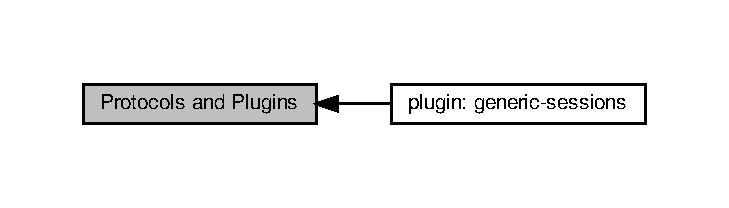
\includegraphics[width=350pt]{group__Protocols-and-Plugins}
\end{center}
\end{figure}
\subsection*{Modules}
\begin{DoxyCompactItemize}
\item 
\hyperlink{group__generic-sessions}{plugin\+: generic-\/sessions}
\end{DoxyCompactItemize}
\subsection*{Classes}
\begin{DoxyCompactItemize}
\item 
struct \hyperlink{structlws__protocols}{lws\+\_\+protocols}
\end{DoxyCompactItemize}
\subsection*{Functions}
\begin{DoxyCompactItemize}
\item 
L\+W\+S\+\_\+\+V\+I\+S\+I\+B\+LE L\+W\+S\+\_\+\+E\+X\+T\+E\+RN const struct \hyperlink{structlws__protocols}{lws\+\_\+protocols} $\ast$ \hyperlink{group__Protocols-and-Plugins_ga2a4e5ce5e4492f77e892935397de5303}{lws\+\_\+vhost\+\_\+name\+\_\+to\+\_\+protocol} (struct lws\+\_\+vhost $\ast$vh, const char $\ast$name)
\item 
L\+W\+S\+\_\+\+V\+I\+S\+I\+B\+LE L\+W\+S\+\_\+\+E\+X\+T\+E\+RN const struct \hyperlink{structlws__protocols}{lws\+\_\+protocols} $\ast$ \hyperlink{group__Protocols-and-Plugins_ga72ad550786ca7976463589d347e62112}{lws\+\_\+get\+\_\+protocol} (struct \hyperlink{structlws}{lws} $\ast$wsi)
\item 
L\+W\+S\+\_\+\+V\+I\+S\+I\+B\+LE L\+W\+S\+\_\+\+E\+X\+T\+E\+RN const struct \hyperlink{structlws__protocols}{lws\+\_\+protocols} $\ast$ \hyperlink{group__Protocols-and-Plugins_ga181a7e600f9d921f483b05483d528fd8}{lws\+\_\+protocol\+\_\+get} (struct \hyperlink{structlws}{lws} $\ast$wsi) L\+W\+S\+\_\+\+W\+A\+R\+N\+\_\+\+D\+E\+P\+R\+E\+C\+A\+T\+ED
\item 
L\+W\+S\+\_\+\+V\+I\+S\+I\+B\+LE L\+W\+S\+\_\+\+E\+X\+T\+E\+RN void $\ast$ \hyperlink{group__Protocols-and-Plugins_gaf8bb5f2a2ac92f42e807d7335f9552c2}{lws\+\_\+protocol\+\_\+vh\+\_\+priv\+\_\+zalloc} (struct lws\+\_\+vhost $\ast$vhost, const struct \hyperlink{structlws__protocols}{lws\+\_\+protocols} $\ast$prot, int size)
\item 
L\+W\+S\+\_\+\+V\+I\+S\+I\+B\+LE L\+W\+S\+\_\+\+E\+X\+T\+E\+RN void $\ast$ \hyperlink{group__Protocols-and-Plugins_ga7e8d95fccf8654f5a0b6beadd7c8dbf1}{lws\+\_\+protocol\+\_\+vh\+\_\+priv\+\_\+get} (struct lws\+\_\+vhost $\ast$vhost, const struct \hyperlink{structlws__protocols}{lws\+\_\+protocols} $\ast$prot)
\item 
L\+W\+S\+\_\+\+V\+I\+S\+I\+B\+LE L\+W\+S\+\_\+\+E\+X\+T\+E\+RN void $\ast$ \hyperlink{group__Protocols-and-Plugins_ga40c0a7194f2ac0c2813ad7e374f0d852}{lws\+\_\+adjust\+\_\+protocol\+\_\+psds} (struct \hyperlink{structlws}{lws} $\ast$wsi, size\+\_\+t new\+\_\+size)
\item 
L\+W\+S\+\_\+\+V\+I\+S\+I\+B\+LE L\+W\+S\+\_\+\+E\+X\+T\+E\+RN int \hyperlink{group__Protocols-and-Plugins_ga106b37ae9c247e84d191ab09441adc43}{lws\+\_\+finalize\+\_\+startup} (struct \hyperlink{structlws__context}{lws\+\_\+context} $\ast$context)
\item 
\mbox{\Hypertarget{group__Protocols-and-Plugins_ga502b1bc5295d2dc0f51fb95d9b8d7132}\label{group__Protocols-and-Plugins_ga502b1bc5295d2dc0f51fb95d9b8d7132}} 
L\+W\+S\+\_\+\+V\+I\+S\+I\+B\+LE L\+W\+S\+\_\+\+E\+X\+T\+E\+RN int {\bfseries lws\+\_\+protocol\+\_\+init} (struct \hyperlink{structlws__context}{lws\+\_\+context} $\ast$context)
\end{DoxyCompactItemize}


\subsection{Detailed Description}
\subsubsection*{Protocol and protocol plugin -\/related apis}

Protocols bind ws protocol names to a custom callback specific to that protocol implementaion.

A \hyperlink{protocollist-p}{list} of protocols can be passed in at context creation time, but it is also legal to leave that N\+U\+LL and add the protocols and their callback code using plugins.

Plugins are much preferable compared to cut and pasting code into an application each time, since they can be used standalone. 

\subsection{Function Documentation}
\mbox{\Hypertarget{group__Protocols-and-Plugins_ga40c0a7194f2ac0c2813ad7e374f0d852}\label{group__Protocols-and-Plugins_ga40c0a7194f2ac0c2813ad7e374f0d852}} 
\index{Protocols and Plugins@{Protocols and Plugins}!lws\+\_\+adjust\+\_\+protocol\+\_\+psds@{lws\+\_\+adjust\+\_\+protocol\+\_\+psds}}
\index{lws\+\_\+adjust\+\_\+protocol\+\_\+psds@{lws\+\_\+adjust\+\_\+protocol\+\_\+psds}!Protocols and Plugins@{Protocols and Plugins}}
\subsubsection{\texorpdfstring{lws\+\_\+adjust\+\_\+protocol\+\_\+psds()}{lws\_adjust\_protocol\_psds()}}
{\footnotesize\ttfamily L\+W\+S\+\_\+\+V\+I\+S\+I\+B\+LE L\+W\+S\+\_\+\+E\+X\+T\+E\+RN void $\ast$ lws\+\_\+adjust\+\_\+protocol\+\_\+psds (\begin{DoxyParamCaption}\item[{struct \hyperlink{structlws}{lws} $\ast$}]{wsi,  }\item[{size\+\_\+t}]{new\+\_\+size }\end{DoxyParamCaption})}

lws\+\_\+adjust\+\_\+protocol\+\_\+psds -\/ change a vhost protocol\textquotesingle{}s per session data size


\begin{DoxyParams}{Parameters}
{\em wsi} & a connection with the protocol to change \\
\hline
{\em new\+\_\+size} & the new size of the per session data size for the protocol\\
\hline
\end{DoxyParams}
Returns user\+\_\+space for the wsi, after allocating

This should not be used except to initalize a vhost protocol\textquotesingle{}s per session data size one time, before any connections are accepted.

Sometimes the protocol wraps another protocol and needs to discover and set its per session data size at runtime. \mbox{\Hypertarget{group__Protocols-and-Plugins_ga106b37ae9c247e84d191ab09441adc43}\label{group__Protocols-and-Plugins_ga106b37ae9c247e84d191ab09441adc43}} 
\index{Protocols and Plugins@{Protocols and Plugins}!lws\+\_\+finalize\+\_\+startup@{lws\+\_\+finalize\+\_\+startup}}
\index{lws\+\_\+finalize\+\_\+startup@{lws\+\_\+finalize\+\_\+startup}!Protocols and Plugins@{Protocols and Plugins}}
\subsubsection{\texorpdfstring{lws\+\_\+finalize\+\_\+startup()}{lws\_finalize\_startup()}}
{\footnotesize\ttfamily L\+W\+S\+\_\+\+V\+I\+S\+I\+B\+LE L\+W\+S\+\_\+\+E\+X\+T\+E\+RN int lws\+\_\+finalize\+\_\+startup (\begin{DoxyParamCaption}\item[{struct \hyperlink{structlws__context}{lws\+\_\+context} $\ast$}]{context }\end{DoxyParamCaption})}

\hyperlink{group__Protocols-and-Plugins_ga106b37ae9c247e84d191ab09441adc43}{lws\+\_\+finalize\+\_\+startup()} -\/ drop initial process privileges


\begin{DoxyParams}{Parameters}
{\em context} & lws context\\
\hline
\end{DoxyParams}
This is called after the end of the vhost protocol initializations, but you may choose to call it earlier \mbox{\Hypertarget{group__Protocols-and-Plugins_ga72ad550786ca7976463589d347e62112}\label{group__Protocols-and-Plugins_ga72ad550786ca7976463589d347e62112}} 
\index{Protocols and Plugins@{Protocols and Plugins}!lws\+\_\+get\+\_\+protocol@{lws\+\_\+get\+\_\+protocol}}
\index{lws\+\_\+get\+\_\+protocol@{lws\+\_\+get\+\_\+protocol}!Protocols and Plugins@{Protocols and Plugins}}
\subsubsection{\texorpdfstring{lws\+\_\+get\+\_\+protocol()}{lws\_get\_protocol()}}
{\footnotesize\ttfamily L\+W\+S\+\_\+\+V\+I\+S\+I\+B\+LE L\+W\+S\+\_\+\+E\+X\+T\+E\+RN const struct \hyperlink{structlws__protocols}{lws\+\_\+protocols}$\ast$ lws\+\_\+get\+\_\+protocol (\begin{DoxyParamCaption}\item[{struct \hyperlink{structlws}{lws} $\ast$}]{wsi }\end{DoxyParamCaption})}

\hyperlink{group__Protocols-and-Plugins_ga72ad550786ca7976463589d347e62112}{lws\+\_\+get\+\_\+protocol()} -\/ Returns a protocol pointer from a websocket connection. 
\begin{DoxyParams}{Parameters}
{\em wsi} & pointer to struct websocket you want to know the protocol of\\
\hline
\end{DoxyParams}
Some apis can act on all live connections of a given protocol, this is how you can get a pointer to the active protocol if needed. \mbox{\Hypertarget{group__Protocols-and-Plugins_ga181a7e600f9d921f483b05483d528fd8}\label{group__Protocols-and-Plugins_ga181a7e600f9d921f483b05483d528fd8}} 
\index{Protocols and Plugins@{Protocols and Plugins}!lws\+\_\+protocol\+\_\+get@{lws\+\_\+protocol\+\_\+get}}
\index{lws\+\_\+protocol\+\_\+get@{lws\+\_\+protocol\+\_\+get}!Protocols and Plugins@{Protocols and Plugins}}
\subsubsection{\texorpdfstring{lws\+\_\+protocol\+\_\+get()}{lws\_protocol\_get()}}
{\footnotesize\ttfamily L\+W\+S\+\_\+\+V\+I\+S\+I\+B\+LE L\+W\+S\+\_\+\+E\+X\+T\+E\+RN const struct \hyperlink{structlws__protocols}{lws\+\_\+protocols} $\ast$ lws\+\_\+protocol\+\_\+get (\begin{DoxyParamCaption}\item[{struct \hyperlink{structlws}{lws} $\ast$}]{wsi }\end{DoxyParamCaption})}

\hyperlink{group__Protocols-and-Plugins_ga181a7e600f9d921f483b05483d528fd8}{lws\+\_\+protocol\+\_\+get()} -\/ deprecated\+: use lws\+\_\+get\+\_\+protocol \mbox{\Hypertarget{group__Protocols-and-Plugins_ga7e8d95fccf8654f5a0b6beadd7c8dbf1}\label{group__Protocols-and-Plugins_ga7e8d95fccf8654f5a0b6beadd7c8dbf1}} 
\index{Protocols and Plugins@{Protocols and Plugins}!lws\+\_\+protocol\+\_\+vh\+\_\+priv\+\_\+get@{lws\+\_\+protocol\+\_\+vh\+\_\+priv\+\_\+get}}
\index{lws\+\_\+protocol\+\_\+vh\+\_\+priv\+\_\+get@{lws\+\_\+protocol\+\_\+vh\+\_\+priv\+\_\+get}!Protocols and Plugins@{Protocols and Plugins}}
\subsubsection{\texorpdfstring{lws\+\_\+protocol\+\_\+vh\+\_\+priv\+\_\+get()}{lws\_protocol\_vh\_priv\_get()}}
{\footnotesize\ttfamily L\+W\+S\+\_\+\+V\+I\+S\+I\+B\+LE L\+W\+S\+\_\+\+E\+X\+T\+E\+RN void $\ast$ lws\+\_\+protocol\+\_\+vh\+\_\+priv\+\_\+get (\begin{DoxyParamCaption}\item[{struct lws\+\_\+vhost $\ast$}]{vhost,  }\item[{const struct \hyperlink{structlws__protocols}{lws\+\_\+protocols} $\ast$}]{prot }\end{DoxyParamCaption})}

\hyperlink{group__Protocols-and-Plugins_ga7e8d95fccf8654f5a0b6beadd7c8dbf1}{lws\+\_\+protocol\+\_\+vh\+\_\+priv\+\_\+get()} -\/ retreive a protocol\textquotesingle{}s per-\/vhost storage


\begin{DoxyParams}{Parameters}
{\em vhost} & vhost the instance is related to \\
\hline
{\em prot} & protocol the instance is related to\\
\hline
\end{DoxyParams}
Recover a pointer to the allocated per-\/vhost storage for the protocol created by \hyperlink{group__Protocols-and-Plugins_gaf8bb5f2a2ac92f42e807d7335f9552c2}{lws\+\_\+protocol\+\_\+vh\+\_\+priv\+\_\+zalloc()} earlier \mbox{\Hypertarget{group__Protocols-and-Plugins_gaf8bb5f2a2ac92f42e807d7335f9552c2}\label{group__Protocols-and-Plugins_gaf8bb5f2a2ac92f42e807d7335f9552c2}} 
\index{Protocols and Plugins@{Protocols and Plugins}!lws\+\_\+protocol\+\_\+vh\+\_\+priv\+\_\+zalloc@{lws\+\_\+protocol\+\_\+vh\+\_\+priv\+\_\+zalloc}}
\index{lws\+\_\+protocol\+\_\+vh\+\_\+priv\+\_\+zalloc@{lws\+\_\+protocol\+\_\+vh\+\_\+priv\+\_\+zalloc}!Protocols and Plugins@{Protocols and Plugins}}
\subsubsection{\texorpdfstring{lws\+\_\+protocol\+\_\+vh\+\_\+priv\+\_\+zalloc()}{lws\_protocol\_vh\_priv\_zalloc()}}
{\footnotesize\ttfamily L\+W\+S\+\_\+\+V\+I\+S\+I\+B\+LE L\+W\+S\+\_\+\+E\+X\+T\+E\+RN void $\ast$ lws\+\_\+protocol\+\_\+vh\+\_\+priv\+\_\+zalloc (\begin{DoxyParamCaption}\item[{struct lws\+\_\+vhost $\ast$}]{vhost,  }\item[{const struct \hyperlink{structlws__protocols}{lws\+\_\+protocols} $\ast$}]{prot,  }\item[{int}]{size }\end{DoxyParamCaption})}

\hyperlink{group__Protocols-and-Plugins_gaf8bb5f2a2ac92f42e807d7335f9552c2}{lws\+\_\+protocol\+\_\+vh\+\_\+priv\+\_\+zalloc()} -\/ Allocate and zero down a protocol\textquotesingle{}s per-\/vhost storage 
\begin{DoxyParams}{Parameters}
{\em vhost} & vhost the instance is related to \\
\hline
{\em prot} & protocol the instance is related to \\
\hline
{\em size} & bytes to allocate\\
\hline
\end{DoxyParams}
Protocols often find it useful to allocate a per-\/vhost struct, this is a helper to be called in the per-\/vhost init L\+W\+S\+\_\+\+C\+A\+L\+L\+B\+A\+C\+K\+\_\+\+P\+R\+O\+T\+O\+C\+O\+L\+\_\+\+I\+N\+IT \mbox{\Hypertarget{group__Protocols-and-Plugins_ga2a4e5ce5e4492f77e892935397de5303}\label{group__Protocols-and-Plugins_ga2a4e5ce5e4492f77e892935397de5303}} 
\index{Protocols and Plugins@{Protocols and Plugins}!lws\+\_\+vhost\+\_\+name\+\_\+to\+\_\+protocol@{lws\+\_\+vhost\+\_\+name\+\_\+to\+\_\+protocol}}
\index{lws\+\_\+vhost\+\_\+name\+\_\+to\+\_\+protocol@{lws\+\_\+vhost\+\_\+name\+\_\+to\+\_\+protocol}!Protocols and Plugins@{Protocols and Plugins}}
\subsubsection{\texorpdfstring{lws\+\_\+vhost\+\_\+name\+\_\+to\+\_\+protocol()}{lws\_vhost\_name\_to\_protocol()}}
{\footnotesize\ttfamily L\+W\+S\+\_\+\+V\+I\+S\+I\+B\+LE L\+W\+S\+\_\+\+E\+X\+T\+E\+RN const struct \hyperlink{structlws__protocols}{lws\+\_\+protocols} $\ast$ lws\+\_\+vhost\+\_\+name\+\_\+to\+\_\+protocol (\begin{DoxyParamCaption}\item[{struct lws\+\_\+vhost $\ast$}]{vh,  }\item[{const char $\ast$}]{name }\end{DoxyParamCaption})}

\hyperlink{group__Protocols-and-Plugins_ga2a4e5ce5e4492f77e892935397de5303}{lws\+\_\+vhost\+\_\+name\+\_\+to\+\_\+protocol()} -\/ get vhost\textquotesingle{}s protocol object from its name


\begin{DoxyParams}{Parameters}
{\em vh} & vhost to search \\
\hline
{\em name} & protocol name\\
\hline
\end{DoxyParams}
Returns N\+U\+LL or a pointer to the vhost\textquotesingle{}s protocol of the requested name 
\hypertarget{group__generic-sessions}{}\section{plugin\+: generic-\/sessions}
\label{group__generic-sessions}\index{plugin\+: generic-\/sessions@{plugin\+: generic-\/sessions}}
Collaboration diagram for plugin\+: generic-\/sessions\+:
\nopagebreak
\begin{figure}[H]
\begin{center}
\leavevmode
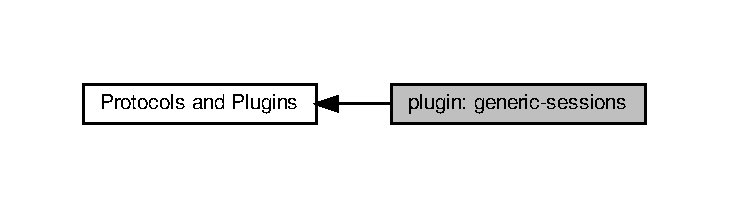
\includegraphics[width=350pt]{group__generic-sessions}
\end{center}
\end{figure}
\subsection*{Classes}
\begin{DoxyCompactItemize}
\item 
struct \hyperlink{structlwsgw__hash__bin}{lwsgw\+\_\+hash\+\_\+bin}
\item 
struct \hyperlink{structlwsgw__hash}{lwsgw\+\_\+hash}
\item 
struct \hyperlink{structlws__session__info}{lws\+\_\+session\+\_\+info}
\item 
struct \hyperlink{structlws__gs__event__args}{lws\+\_\+gs\+\_\+event\+\_\+args}
\end{DoxyCompactItemize}
\subsection*{Macros}
\begin{DoxyCompactItemize}
\item 
\#define \hyperlink{group__generic-sessions_ga22e0d172d9bc26a18f80774f3950b952}{L\+W\+S\+G\+S\+\_\+\+E\+M\+A\+I\+L\+\_\+\+C\+O\+N\+T\+E\+N\+T\+\_\+\+S\+I\+ZE}~16384
\item 
\#define \hyperlink{group__generic-sessions_ga22e0d172d9bc26a18f80774f3950b952}{L\+W\+S\+G\+S\+\_\+\+E\+M\+A\+I\+L\+\_\+\+C\+O\+N\+T\+E\+N\+T\+\_\+\+S\+I\+ZE}~16384
\item 
\#define \hyperlink{group__generic-sessions_ga22e0d172d9bc26a18f80774f3950b952}{L\+W\+S\+G\+S\+\_\+\+E\+M\+A\+I\+L\+\_\+\+C\+O\+N\+T\+E\+N\+T\+\_\+\+S\+I\+ZE}~16384
\item 
\#define \hyperlink{group__generic-sessions_ga22e0d172d9bc26a18f80774f3950b952}{L\+W\+S\+G\+S\+\_\+\+E\+M\+A\+I\+L\+\_\+\+C\+O\+N\+T\+E\+N\+T\+\_\+\+S\+I\+ZE}~16384
\item 
\#define \hyperlink{group__generic-sessions_ga22e0d172d9bc26a18f80774f3950b952}{L\+W\+S\+G\+S\+\_\+\+E\+M\+A\+I\+L\+\_\+\+C\+O\+N\+T\+E\+N\+T\+\_\+\+S\+I\+ZE}~16384
\item 
\#define \hyperlink{group__generic-sessions_ga22e0d172d9bc26a18f80774f3950b952}{L\+W\+S\+G\+S\+\_\+\+E\+M\+A\+I\+L\+\_\+\+C\+O\+N\+T\+E\+N\+T\+\_\+\+S\+I\+ZE}~16384
\item 
\#define \hyperlink{group__generic-sessions_ga22e0d172d9bc26a18f80774f3950b952}{L\+W\+S\+G\+S\+\_\+\+E\+M\+A\+I\+L\+\_\+\+C\+O\+N\+T\+E\+N\+T\+\_\+\+S\+I\+ZE}~16384
\item 
\#define \hyperlink{group__generic-sessions_ga22e0d172d9bc26a18f80774f3950b952}{L\+W\+S\+G\+S\+\_\+\+E\+M\+A\+I\+L\+\_\+\+C\+O\+N\+T\+E\+N\+T\+\_\+\+S\+I\+ZE}~16384
\end{DoxyCompactItemize}
\subsection*{Enumerations}
\begin{DoxyCompactItemize}
\item 
enum \hyperlink{group__generic-sessions_ga7c2dc7bfb4ccb91c5d771f9e9ea237e1}{lwsgs\+\_\+auth\+\_\+bits} \{ \newline
\hyperlink{group__generic-sessions_gga7c2dc7bfb4ccb91c5d771f9e9ea237e1a81e63075115dedd150265d81b8f7fa57}{L\+W\+S\+G\+S\+\_\+\+A\+U\+T\+H\+\_\+\+L\+O\+G\+G\+E\+D\+\_\+\+IN} = 1, 
\hyperlink{group__generic-sessions_gga7c2dc7bfb4ccb91c5d771f9e9ea237e1a0657a9e846814781b128c397fe4b10bf}{L\+W\+S\+G\+S\+\_\+\+A\+U\+T\+H\+\_\+\+A\+D\+M\+IN} = 2, 
\hyperlink{group__generic-sessions_gga7c2dc7bfb4ccb91c5d771f9e9ea237e1a5a607e4668d20cadada62c4b8007f887}{L\+W\+S\+G\+S\+\_\+\+A\+U\+T\+H\+\_\+\+V\+E\+R\+I\+F\+I\+ED} = 4, 
\hyperlink{group__generic-sessions_gga7c2dc7bfb4ccb91c5d771f9e9ea237e1a2cd8fb86e3b85c106e7711c03f0ddd0a}{L\+W\+S\+G\+S\+\_\+\+A\+U\+T\+H\+\_\+\+F\+O\+R\+G\+O\+T\+\_\+\+F\+L\+OW} = 8, 
\newline
\hyperlink{group__generic-sessions_gga7c2dc7bfb4ccb91c5d771f9e9ea237e1a81e63075115dedd150265d81b8f7fa57}{L\+W\+S\+G\+S\+\_\+\+A\+U\+T\+H\+\_\+\+L\+O\+G\+G\+E\+D\+\_\+\+IN} = 1, 
\hyperlink{group__generic-sessions_gga7c2dc7bfb4ccb91c5d771f9e9ea237e1a0657a9e846814781b128c397fe4b10bf}{L\+W\+S\+G\+S\+\_\+\+A\+U\+T\+H\+\_\+\+A\+D\+M\+IN} = 2, 
\hyperlink{group__generic-sessions_gga7c2dc7bfb4ccb91c5d771f9e9ea237e1a5a607e4668d20cadada62c4b8007f887}{L\+W\+S\+G\+S\+\_\+\+A\+U\+T\+H\+\_\+\+V\+E\+R\+I\+F\+I\+ED} = 4, 
\hyperlink{group__generic-sessions_gga7c2dc7bfb4ccb91c5d771f9e9ea237e1a2cd8fb86e3b85c106e7711c03f0ddd0a}{L\+W\+S\+G\+S\+\_\+\+A\+U\+T\+H\+\_\+\+F\+O\+R\+G\+O\+T\+\_\+\+F\+L\+OW} = 8, 
\newline
\hyperlink{group__generic-sessions_gga7c2dc7bfb4ccb91c5d771f9e9ea237e1a81e63075115dedd150265d81b8f7fa57}{L\+W\+S\+G\+S\+\_\+\+A\+U\+T\+H\+\_\+\+L\+O\+G\+G\+E\+D\+\_\+\+IN} = 1, 
\hyperlink{group__generic-sessions_gga7c2dc7bfb4ccb91c5d771f9e9ea237e1a0657a9e846814781b128c397fe4b10bf}{L\+W\+S\+G\+S\+\_\+\+A\+U\+T\+H\+\_\+\+A\+D\+M\+IN} = 2, 
\hyperlink{group__generic-sessions_gga7c2dc7bfb4ccb91c5d771f9e9ea237e1a5a607e4668d20cadada62c4b8007f887}{L\+W\+S\+G\+S\+\_\+\+A\+U\+T\+H\+\_\+\+V\+E\+R\+I\+F\+I\+ED} = 4, 
\hyperlink{group__generic-sessions_gga7c2dc7bfb4ccb91c5d771f9e9ea237e1a2cd8fb86e3b85c106e7711c03f0ddd0a}{L\+W\+S\+G\+S\+\_\+\+A\+U\+T\+H\+\_\+\+F\+O\+R\+G\+O\+T\+\_\+\+F\+L\+OW} = 8, 
\newline
\hyperlink{group__generic-sessions_gga7c2dc7bfb4ccb91c5d771f9e9ea237e1a81e63075115dedd150265d81b8f7fa57}{L\+W\+S\+G\+S\+\_\+\+A\+U\+T\+H\+\_\+\+L\+O\+G\+G\+E\+D\+\_\+\+IN} = 1, 
\hyperlink{group__generic-sessions_gga7c2dc7bfb4ccb91c5d771f9e9ea237e1a0657a9e846814781b128c397fe4b10bf}{L\+W\+S\+G\+S\+\_\+\+A\+U\+T\+H\+\_\+\+A\+D\+M\+IN} = 2, 
\hyperlink{group__generic-sessions_gga7c2dc7bfb4ccb91c5d771f9e9ea237e1a5a607e4668d20cadada62c4b8007f887}{L\+W\+S\+G\+S\+\_\+\+A\+U\+T\+H\+\_\+\+V\+E\+R\+I\+F\+I\+ED} = 4, 
\hyperlink{group__generic-sessions_gga7c2dc7bfb4ccb91c5d771f9e9ea237e1a2cd8fb86e3b85c106e7711c03f0ddd0a}{L\+W\+S\+G\+S\+\_\+\+A\+U\+T\+H\+\_\+\+F\+O\+R\+G\+O\+T\+\_\+\+F\+L\+OW} = 8, 
\newline
\hyperlink{group__generic-sessions_gga7c2dc7bfb4ccb91c5d771f9e9ea237e1a81e63075115dedd150265d81b8f7fa57}{L\+W\+S\+G\+S\+\_\+\+A\+U\+T\+H\+\_\+\+L\+O\+G\+G\+E\+D\+\_\+\+IN} = 1, 
\hyperlink{group__generic-sessions_gga7c2dc7bfb4ccb91c5d771f9e9ea237e1a0657a9e846814781b128c397fe4b10bf}{L\+W\+S\+G\+S\+\_\+\+A\+U\+T\+H\+\_\+\+A\+D\+M\+IN} = 2, 
\hyperlink{group__generic-sessions_gga7c2dc7bfb4ccb91c5d771f9e9ea237e1a5a607e4668d20cadada62c4b8007f887}{L\+W\+S\+G\+S\+\_\+\+A\+U\+T\+H\+\_\+\+V\+E\+R\+I\+F\+I\+ED} = 4, 
\hyperlink{group__generic-sessions_gga7c2dc7bfb4ccb91c5d771f9e9ea237e1a2cd8fb86e3b85c106e7711c03f0ddd0a}{L\+W\+S\+G\+S\+\_\+\+A\+U\+T\+H\+\_\+\+F\+O\+R\+G\+O\+T\+\_\+\+F\+L\+OW} = 8, 
\newline
\hyperlink{group__generic-sessions_gga7c2dc7bfb4ccb91c5d771f9e9ea237e1a81e63075115dedd150265d81b8f7fa57}{L\+W\+S\+G\+S\+\_\+\+A\+U\+T\+H\+\_\+\+L\+O\+G\+G\+E\+D\+\_\+\+IN} = 1, 
\hyperlink{group__generic-sessions_gga7c2dc7bfb4ccb91c5d771f9e9ea237e1a0657a9e846814781b128c397fe4b10bf}{L\+W\+S\+G\+S\+\_\+\+A\+U\+T\+H\+\_\+\+A\+D\+M\+IN} = 2, 
\hyperlink{group__generic-sessions_gga7c2dc7bfb4ccb91c5d771f9e9ea237e1a5a607e4668d20cadada62c4b8007f887}{L\+W\+S\+G\+S\+\_\+\+A\+U\+T\+H\+\_\+\+V\+E\+R\+I\+F\+I\+ED} = 4, 
\hyperlink{group__generic-sessions_gga7c2dc7bfb4ccb91c5d771f9e9ea237e1a2cd8fb86e3b85c106e7711c03f0ddd0a}{L\+W\+S\+G\+S\+\_\+\+A\+U\+T\+H\+\_\+\+F\+O\+R\+G\+O\+T\+\_\+\+F\+L\+OW} = 8, 
\newline
\hyperlink{group__generic-sessions_gga7c2dc7bfb4ccb91c5d771f9e9ea237e1a81e63075115dedd150265d81b8f7fa57}{L\+W\+S\+G\+S\+\_\+\+A\+U\+T\+H\+\_\+\+L\+O\+G\+G\+E\+D\+\_\+\+IN} = 1, 
\hyperlink{group__generic-sessions_gga7c2dc7bfb4ccb91c5d771f9e9ea237e1a0657a9e846814781b128c397fe4b10bf}{L\+W\+S\+G\+S\+\_\+\+A\+U\+T\+H\+\_\+\+A\+D\+M\+IN} = 2, 
\hyperlink{group__generic-sessions_gga7c2dc7bfb4ccb91c5d771f9e9ea237e1a5a607e4668d20cadada62c4b8007f887}{L\+W\+S\+G\+S\+\_\+\+A\+U\+T\+H\+\_\+\+V\+E\+R\+I\+F\+I\+ED} = 4, 
\hyperlink{group__generic-sessions_gga7c2dc7bfb4ccb91c5d771f9e9ea237e1a2cd8fb86e3b85c106e7711c03f0ddd0a}{L\+W\+S\+G\+S\+\_\+\+A\+U\+T\+H\+\_\+\+F\+O\+R\+G\+O\+T\+\_\+\+F\+L\+OW} = 8, 
\newline
\hyperlink{group__generic-sessions_gga7c2dc7bfb4ccb91c5d771f9e9ea237e1a81e63075115dedd150265d81b8f7fa57}{L\+W\+S\+G\+S\+\_\+\+A\+U\+T\+H\+\_\+\+L\+O\+G\+G\+E\+D\+\_\+\+IN} = 1, 
\hyperlink{group__generic-sessions_gga7c2dc7bfb4ccb91c5d771f9e9ea237e1a0657a9e846814781b128c397fe4b10bf}{L\+W\+S\+G\+S\+\_\+\+A\+U\+T\+H\+\_\+\+A\+D\+M\+IN} = 2, 
\hyperlink{group__generic-sessions_gga7c2dc7bfb4ccb91c5d771f9e9ea237e1a5a607e4668d20cadada62c4b8007f887}{L\+W\+S\+G\+S\+\_\+\+A\+U\+T\+H\+\_\+\+V\+E\+R\+I\+F\+I\+ED} = 4, 
\hyperlink{group__generic-sessions_gga7c2dc7bfb4ccb91c5d771f9e9ea237e1a2cd8fb86e3b85c106e7711c03f0ddd0a}{L\+W\+S\+G\+S\+\_\+\+A\+U\+T\+H\+\_\+\+F\+O\+R\+G\+O\+T\+\_\+\+F\+L\+OW} = 8
 \}
\item 
enum \hyperlink{group__generic-sessions_gaa93946b3d921072209d5cd8cdfa5332e}{lws\+\_\+gs\+\_\+event} \{ \newline
\hyperlink{group__generic-sessions_ggaa93946b3d921072209d5cd8cdfa5332ea596010a165bf13473c5eea3a34cd4308}{L\+W\+S\+G\+S\+E\+\_\+\+C\+R\+E\+A\+T\+ED}, 
\hyperlink{group__generic-sessions_ggaa93946b3d921072209d5cd8cdfa5332ead908cdc5689c5d22c9d3c8934e94dcde}{L\+W\+S\+G\+S\+E\+\_\+\+D\+E\+L\+E\+T\+ED}, 
\hyperlink{group__generic-sessions_ggaa93946b3d921072209d5cd8cdfa5332ea596010a165bf13473c5eea3a34cd4308}{L\+W\+S\+G\+S\+E\+\_\+\+C\+R\+E\+A\+T\+ED}, 
\hyperlink{group__generic-sessions_ggaa93946b3d921072209d5cd8cdfa5332ead908cdc5689c5d22c9d3c8934e94dcde}{L\+W\+S\+G\+S\+E\+\_\+\+D\+E\+L\+E\+T\+ED}, 
\newline
\hyperlink{group__generic-sessions_ggaa93946b3d921072209d5cd8cdfa5332ea596010a165bf13473c5eea3a34cd4308}{L\+W\+S\+G\+S\+E\+\_\+\+C\+R\+E\+A\+T\+ED}, 
\hyperlink{group__generic-sessions_ggaa93946b3d921072209d5cd8cdfa5332ead908cdc5689c5d22c9d3c8934e94dcde}{L\+W\+S\+G\+S\+E\+\_\+\+D\+E\+L\+E\+T\+ED}, 
\hyperlink{group__generic-sessions_ggaa93946b3d921072209d5cd8cdfa5332ea596010a165bf13473c5eea3a34cd4308}{L\+W\+S\+G\+S\+E\+\_\+\+C\+R\+E\+A\+T\+ED}, 
\hyperlink{group__generic-sessions_ggaa93946b3d921072209d5cd8cdfa5332ead908cdc5689c5d22c9d3c8934e94dcde}{L\+W\+S\+G\+S\+E\+\_\+\+D\+E\+L\+E\+T\+ED}, 
\newline
\hyperlink{group__generic-sessions_ggaa93946b3d921072209d5cd8cdfa5332ea596010a165bf13473c5eea3a34cd4308}{L\+W\+S\+G\+S\+E\+\_\+\+C\+R\+E\+A\+T\+ED}, 
\hyperlink{group__generic-sessions_ggaa93946b3d921072209d5cd8cdfa5332ead908cdc5689c5d22c9d3c8934e94dcde}{L\+W\+S\+G\+S\+E\+\_\+\+D\+E\+L\+E\+T\+ED}, 
\hyperlink{group__generic-sessions_ggaa93946b3d921072209d5cd8cdfa5332ea596010a165bf13473c5eea3a34cd4308}{L\+W\+S\+G\+S\+E\+\_\+\+C\+R\+E\+A\+T\+ED}, 
\hyperlink{group__generic-sessions_ggaa93946b3d921072209d5cd8cdfa5332ead908cdc5689c5d22c9d3c8934e94dcde}{L\+W\+S\+G\+S\+E\+\_\+\+D\+E\+L\+E\+T\+ED}, 
\newline
\hyperlink{group__generic-sessions_ggaa93946b3d921072209d5cd8cdfa5332ea596010a165bf13473c5eea3a34cd4308}{L\+W\+S\+G\+S\+E\+\_\+\+C\+R\+E\+A\+T\+ED}, 
\hyperlink{group__generic-sessions_ggaa93946b3d921072209d5cd8cdfa5332ead908cdc5689c5d22c9d3c8934e94dcde}{L\+W\+S\+G\+S\+E\+\_\+\+D\+E\+L\+E\+T\+ED}, 
\hyperlink{group__generic-sessions_ggaa93946b3d921072209d5cd8cdfa5332ea596010a165bf13473c5eea3a34cd4308}{L\+W\+S\+G\+S\+E\+\_\+\+C\+R\+E\+A\+T\+ED}, 
\hyperlink{group__generic-sessions_ggaa93946b3d921072209d5cd8cdfa5332ead908cdc5689c5d22c9d3c8934e94dcde}{L\+W\+S\+G\+S\+E\+\_\+\+D\+E\+L\+E\+T\+ED}
 \}
\item 
enum \hyperlink{group__generic-sessions_ga7c2dc7bfb4ccb91c5d771f9e9ea237e1}{lwsgs\+\_\+auth\+\_\+bits} \{ \newline
\hyperlink{group__generic-sessions_gga7c2dc7bfb4ccb91c5d771f9e9ea237e1a81e63075115dedd150265d81b8f7fa57}{L\+W\+S\+G\+S\+\_\+\+A\+U\+T\+H\+\_\+\+L\+O\+G\+G\+E\+D\+\_\+\+IN} = 1, 
\hyperlink{group__generic-sessions_gga7c2dc7bfb4ccb91c5d771f9e9ea237e1a0657a9e846814781b128c397fe4b10bf}{L\+W\+S\+G\+S\+\_\+\+A\+U\+T\+H\+\_\+\+A\+D\+M\+IN} = 2, 
\hyperlink{group__generic-sessions_gga7c2dc7bfb4ccb91c5d771f9e9ea237e1a5a607e4668d20cadada62c4b8007f887}{L\+W\+S\+G\+S\+\_\+\+A\+U\+T\+H\+\_\+\+V\+E\+R\+I\+F\+I\+ED} = 4, 
\hyperlink{group__generic-sessions_gga7c2dc7bfb4ccb91c5d771f9e9ea237e1a2cd8fb86e3b85c106e7711c03f0ddd0a}{L\+W\+S\+G\+S\+\_\+\+A\+U\+T\+H\+\_\+\+F\+O\+R\+G\+O\+T\+\_\+\+F\+L\+OW} = 8, 
\newline
\hyperlink{group__generic-sessions_gga7c2dc7bfb4ccb91c5d771f9e9ea237e1a81e63075115dedd150265d81b8f7fa57}{L\+W\+S\+G\+S\+\_\+\+A\+U\+T\+H\+\_\+\+L\+O\+G\+G\+E\+D\+\_\+\+IN} = 1, 
\hyperlink{group__generic-sessions_gga7c2dc7bfb4ccb91c5d771f9e9ea237e1a0657a9e846814781b128c397fe4b10bf}{L\+W\+S\+G\+S\+\_\+\+A\+U\+T\+H\+\_\+\+A\+D\+M\+IN} = 2, 
\hyperlink{group__generic-sessions_gga7c2dc7bfb4ccb91c5d771f9e9ea237e1a5a607e4668d20cadada62c4b8007f887}{L\+W\+S\+G\+S\+\_\+\+A\+U\+T\+H\+\_\+\+V\+E\+R\+I\+F\+I\+ED} = 4, 
\hyperlink{group__generic-sessions_gga7c2dc7bfb4ccb91c5d771f9e9ea237e1a2cd8fb86e3b85c106e7711c03f0ddd0a}{L\+W\+S\+G\+S\+\_\+\+A\+U\+T\+H\+\_\+\+F\+O\+R\+G\+O\+T\+\_\+\+F\+L\+OW} = 8, 
\newline
\hyperlink{group__generic-sessions_gga7c2dc7bfb4ccb91c5d771f9e9ea237e1a81e63075115dedd150265d81b8f7fa57}{L\+W\+S\+G\+S\+\_\+\+A\+U\+T\+H\+\_\+\+L\+O\+G\+G\+E\+D\+\_\+\+IN} = 1, 
\hyperlink{group__generic-sessions_gga7c2dc7bfb4ccb91c5d771f9e9ea237e1a0657a9e846814781b128c397fe4b10bf}{L\+W\+S\+G\+S\+\_\+\+A\+U\+T\+H\+\_\+\+A\+D\+M\+IN} = 2, 
\hyperlink{group__generic-sessions_gga7c2dc7bfb4ccb91c5d771f9e9ea237e1a5a607e4668d20cadada62c4b8007f887}{L\+W\+S\+G\+S\+\_\+\+A\+U\+T\+H\+\_\+\+V\+E\+R\+I\+F\+I\+ED} = 4, 
\hyperlink{group__generic-sessions_gga7c2dc7bfb4ccb91c5d771f9e9ea237e1a2cd8fb86e3b85c106e7711c03f0ddd0a}{L\+W\+S\+G\+S\+\_\+\+A\+U\+T\+H\+\_\+\+F\+O\+R\+G\+O\+T\+\_\+\+F\+L\+OW} = 8, 
\newline
\hyperlink{group__generic-sessions_gga7c2dc7bfb4ccb91c5d771f9e9ea237e1a81e63075115dedd150265d81b8f7fa57}{L\+W\+S\+G\+S\+\_\+\+A\+U\+T\+H\+\_\+\+L\+O\+G\+G\+E\+D\+\_\+\+IN} = 1, 
\hyperlink{group__generic-sessions_gga7c2dc7bfb4ccb91c5d771f9e9ea237e1a0657a9e846814781b128c397fe4b10bf}{L\+W\+S\+G\+S\+\_\+\+A\+U\+T\+H\+\_\+\+A\+D\+M\+IN} = 2, 
\hyperlink{group__generic-sessions_gga7c2dc7bfb4ccb91c5d771f9e9ea237e1a5a607e4668d20cadada62c4b8007f887}{L\+W\+S\+G\+S\+\_\+\+A\+U\+T\+H\+\_\+\+V\+E\+R\+I\+F\+I\+ED} = 4, 
\hyperlink{group__generic-sessions_gga7c2dc7bfb4ccb91c5d771f9e9ea237e1a2cd8fb86e3b85c106e7711c03f0ddd0a}{L\+W\+S\+G\+S\+\_\+\+A\+U\+T\+H\+\_\+\+F\+O\+R\+G\+O\+T\+\_\+\+F\+L\+OW} = 8, 
\newline
\hyperlink{group__generic-sessions_gga7c2dc7bfb4ccb91c5d771f9e9ea237e1a81e63075115dedd150265d81b8f7fa57}{L\+W\+S\+G\+S\+\_\+\+A\+U\+T\+H\+\_\+\+L\+O\+G\+G\+E\+D\+\_\+\+IN} = 1, 
\hyperlink{group__generic-sessions_gga7c2dc7bfb4ccb91c5d771f9e9ea237e1a0657a9e846814781b128c397fe4b10bf}{L\+W\+S\+G\+S\+\_\+\+A\+U\+T\+H\+\_\+\+A\+D\+M\+IN} = 2, 
\hyperlink{group__generic-sessions_gga7c2dc7bfb4ccb91c5d771f9e9ea237e1a5a607e4668d20cadada62c4b8007f887}{L\+W\+S\+G\+S\+\_\+\+A\+U\+T\+H\+\_\+\+V\+E\+R\+I\+F\+I\+ED} = 4, 
\hyperlink{group__generic-sessions_gga7c2dc7bfb4ccb91c5d771f9e9ea237e1a2cd8fb86e3b85c106e7711c03f0ddd0a}{L\+W\+S\+G\+S\+\_\+\+A\+U\+T\+H\+\_\+\+F\+O\+R\+G\+O\+T\+\_\+\+F\+L\+OW} = 8, 
\newline
\hyperlink{group__generic-sessions_gga7c2dc7bfb4ccb91c5d771f9e9ea237e1a81e63075115dedd150265d81b8f7fa57}{L\+W\+S\+G\+S\+\_\+\+A\+U\+T\+H\+\_\+\+L\+O\+G\+G\+E\+D\+\_\+\+IN} = 1, 
\hyperlink{group__generic-sessions_gga7c2dc7bfb4ccb91c5d771f9e9ea237e1a0657a9e846814781b128c397fe4b10bf}{L\+W\+S\+G\+S\+\_\+\+A\+U\+T\+H\+\_\+\+A\+D\+M\+IN} = 2, 
\hyperlink{group__generic-sessions_gga7c2dc7bfb4ccb91c5d771f9e9ea237e1a5a607e4668d20cadada62c4b8007f887}{L\+W\+S\+G\+S\+\_\+\+A\+U\+T\+H\+\_\+\+V\+E\+R\+I\+F\+I\+ED} = 4, 
\hyperlink{group__generic-sessions_gga7c2dc7bfb4ccb91c5d771f9e9ea237e1a2cd8fb86e3b85c106e7711c03f0ddd0a}{L\+W\+S\+G\+S\+\_\+\+A\+U\+T\+H\+\_\+\+F\+O\+R\+G\+O\+T\+\_\+\+F\+L\+OW} = 8, 
\newline
\hyperlink{group__generic-sessions_gga7c2dc7bfb4ccb91c5d771f9e9ea237e1a81e63075115dedd150265d81b8f7fa57}{L\+W\+S\+G\+S\+\_\+\+A\+U\+T\+H\+\_\+\+L\+O\+G\+G\+E\+D\+\_\+\+IN} = 1, 
\hyperlink{group__generic-sessions_gga7c2dc7bfb4ccb91c5d771f9e9ea237e1a0657a9e846814781b128c397fe4b10bf}{L\+W\+S\+G\+S\+\_\+\+A\+U\+T\+H\+\_\+\+A\+D\+M\+IN} = 2, 
\hyperlink{group__generic-sessions_gga7c2dc7bfb4ccb91c5d771f9e9ea237e1a5a607e4668d20cadada62c4b8007f887}{L\+W\+S\+G\+S\+\_\+\+A\+U\+T\+H\+\_\+\+V\+E\+R\+I\+F\+I\+ED} = 4, 
\hyperlink{group__generic-sessions_gga7c2dc7bfb4ccb91c5d771f9e9ea237e1a2cd8fb86e3b85c106e7711c03f0ddd0a}{L\+W\+S\+G\+S\+\_\+\+A\+U\+T\+H\+\_\+\+F\+O\+R\+G\+O\+T\+\_\+\+F\+L\+OW} = 8, 
\newline
\hyperlink{group__generic-sessions_gga7c2dc7bfb4ccb91c5d771f9e9ea237e1a81e63075115dedd150265d81b8f7fa57}{L\+W\+S\+G\+S\+\_\+\+A\+U\+T\+H\+\_\+\+L\+O\+G\+G\+E\+D\+\_\+\+IN} = 1, 
\hyperlink{group__generic-sessions_gga7c2dc7bfb4ccb91c5d771f9e9ea237e1a0657a9e846814781b128c397fe4b10bf}{L\+W\+S\+G\+S\+\_\+\+A\+U\+T\+H\+\_\+\+A\+D\+M\+IN} = 2, 
\hyperlink{group__generic-sessions_gga7c2dc7bfb4ccb91c5d771f9e9ea237e1a5a607e4668d20cadada62c4b8007f887}{L\+W\+S\+G\+S\+\_\+\+A\+U\+T\+H\+\_\+\+V\+E\+R\+I\+F\+I\+ED} = 4, 
\hyperlink{group__generic-sessions_gga7c2dc7bfb4ccb91c5d771f9e9ea237e1a2cd8fb86e3b85c106e7711c03f0ddd0a}{L\+W\+S\+G\+S\+\_\+\+A\+U\+T\+H\+\_\+\+F\+O\+R\+G\+O\+T\+\_\+\+F\+L\+OW} = 8
 \}
\item 
enum \hyperlink{group__generic-sessions_gaa93946b3d921072209d5cd8cdfa5332e}{lws\+\_\+gs\+\_\+event} \{ \newline
\hyperlink{group__generic-sessions_ggaa93946b3d921072209d5cd8cdfa5332ea596010a165bf13473c5eea3a34cd4308}{L\+W\+S\+G\+S\+E\+\_\+\+C\+R\+E\+A\+T\+ED}, 
\hyperlink{group__generic-sessions_ggaa93946b3d921072209d5cd8cdfa5332ead908cdc5689c5d22c9d3c8934e94dcde}{L\+W\+S\+G\+S\+E\+\_\+\+D\+E\+L\+E\+T\+ED}, 
\hyperlink{group__generic-sessions_ggaa93946b3d921072209d5cd8cdfa5332ea596010a165bf13473c5eea3a34cd4308}{L\+W\+S\+G\+S\+E\+\_\+\+C\+R\+E\+A\+T\+ED}, 
\hyperlink{group__generic-sessions_ggaa93946b3d921072209d5cd8cdfa5332ead908cdc5689c5d22c9d3c8934e94dcde}{L\+W\+S\+G\+S\+E\+\_\+\+D\+E\+L\+E\+T\+ED}, 
\newline
\hyperlink{group__generic-sessions_ggaa93946b3d921072209d5cd8cdfa5332ea596010a165bf13473c5eea3a34cd4308}{L\+W\+S\+G\+S\+E\+\_\+\+C\+R\+E\+A\+T\+ED}, 
\hyperlink{group__generic-sessions_ggaa93946b3d921072209d5cd8cdfa5332ead908cdc5689c5d22c9d3c8934e94dcde}{L\+W\+S\+G\+S\+E\+\_\+\+D\+E\+L\+E\+T\+ED}, 
\hyperlink{group__generic-sessions_ggaa93946b3d921072209d5cd8cdfa5332ea596010a165bf13473c5eea3a34cd4308}{L\+W\+S\+G\+S\+E\+\_\+\+C\+R\+E\+A\+T\+ED}, 
\hyperlink{group__generic-sessions_ggaa93946b3d921072209d5cd8cdfa5332ead908cdc5689c5d22c9d3c8934e94dcde}{L\+W\+S\+G\+S\+E\+\_\+\+D\+E\+L\+E\+T\+ED}, 
\newline
\hyperlink{group__generic-sessions_ggaa93946b3d921072209d5cd8cdfa5332ea596010a165bf13473c5eea3a34cd4308}{L\+W\+S\+G\+S\+E\+\_\+\+C\+R\+E\+A\+T\+ED}, 
\hyperlink{group__generic-sessions_ggaa93946b3d921072209d5cd8cdfa5332ead908cdc5689c5d22c9d3c8934e94dcde}{L\+W\+S\+G\+S\+E\+\_\+\+D\+E\+L\+E\+T\+ED}, 
\hyperlink{group__generic-sessions_ggaa93946b3d921072209d5cd8cdfa5332ea596010a165bf13473c5eea3a34cd4308}{L\+W\+S\+G\+S\+E\+\_\+\+C\+R\+E\+A\+T\+ED}, 
\hyperlink{group__generic-sessions_ggaa93946b3d921072209d5cd8cdfa5332ead908cdc5689c5d22c9d3c8934e94dcde}{L\+W\+S\+G\+S\+E\+\_\+\+D\+E\+L\+E\+T\+ED}, 
\newline
\hyperlink{group__generic-sessions_ggaa93946b3d921072209d5cd8cdfa5332ea596010a165bf13473c5eea3a34cd4308}{L\+W\+S\+G\+S\+E\+\_\+\+C\+R\+E\+A\+T\+ED}, 
\hyperlink{group__generic-sessions_ggaa93946b3d921072209d5cd8cdfa5332ead908cdc5689c5d22c9d3c8934e94dcde}{L\+W\+S\+G\+S\+E\+\_\+\+D\+E\+L\+E\+T\+ED}, 
\hyperlink{group__generic-sessions_ggaa93946b3d921072209d5cd8cdfa5332ea596010a165bf13473c5eea3a34cd4308}{L\+W\+S\+G\+S\+E\+\_\+\+C\+R\+E\+A\+T\+ED}, 
\hyperlink{group__generic-sessions_ggaa93946b3d921072209d5cd8cdfa5332ead908cdc5689c5d22c9d3c8934e94dcde}{L\+W\+S\+G\+S\+E\+\_\+\+D\+E\+L\+E\+T\+ED}
 \}
\item 
enum \hyperlink{group__generic-sessions_ga7c2dc7bfb4ccb91c5d771f9e9ea237e1}{lwsgs\+\_\+auth\+\_\+bits} \{ \newline
\hyperlink{group__generic-sessions_gga7c2dc7bfb4ccb91c5d771f9e9ea237e1a81e63075115dedd150265d81b8f7fa57}{L\+W\+S\+G\+S\+\_\+\+A\+U\+T\+H\+\_\+\+L\+O\+G\+G\+E\+D\+\_\+\+IN} = 1, 
\hyperlink{group__generic-sessions_gga7c2dc7bfb4ccb91c5d771f9e9ea237e1a0657a9e846814781b128c397fe4b10bf}{L\+W\+S\+G\+S\+\_\+\+A\+U\+T\+H\+\_\+\+A\+D\+M\+IN} = 2, 
\hyperlink{group__generic-sessions_gga7c2dc7bfb4ccb91c5d771f9e9ea237e1a5a607e4668d20cadada62c4b8007f887}{L\+W\+S\+G\+S\+\_\+\+A\+U\+T\+H\+\_\+\+V\+E\+R\+I\+F\+I\+ED} = 4, 
\hyperlink{group__generic-sessions_gga7c2dc7bfb4ccb91c5d771f9e9ea237e1a2cd8fb86e3b85c106e7711c03f0ddd0a}{L\+W\+S\+G\+S\+\_\+\+A\+U\+T\+H\+\_\+\+F\+O\+R\+G\+O\+T\+\_\+\+F\+L\+OW} = 8, 
\newline
\hyperlink{group__generic-sessions_gga7c2dc7bfb4ccb91c5d771f9e9ea237e1a81e63075115dedd150265d81b8f7fa57}{L\+W\+S\+G\+S\+\_\+\+A\+U\+T\+H\+\_\+\+L\+O\+G\+G\+E\+D\+\_\+\+IN} = 1, 
\hyperlink{group__generic-sessions_gga7c2dc7bfb4ccb91c5d771f9e9ea237e1a0657a9e846814781b128c397fe4b10bf}{L\+W\+S\+G\+S\+\_\+\+A\+U\+T\+H\+\_\+\+A\+D\+M\+IN} = 2, 
\hyperlink{group__generic-sessions_gga7c2dc7bfb4ccb91c5d771f9e9ea237e1a5a607e4668d20cadada62c4b8007f887}{L\+W\+S\+G\+S\+\_\+\+A\+U\+T\+H\+\_\+\+V\+E\+R\+I\+F\+I\+ED} = 4, 
\hyperlink{group__generic-sessions_gga7c2dc7bfb4ccb91c5d771f9e9ea237e1a2cd8fb86e3b85c106e7711c03f0ddd0a}{L\+W\+S\+G\+S\+\_\+\+A\+U\+T\+H\+\_\+\+F\+O\+R\+G\+O\+T\+\_\+\+F\+L\+OW} = 8, 
\newline
\hyperlink{group__generic-sessions_gga7c2dc7bfb4ccb91c5d771f9e9ea237e1a81e63075115dedd150265d81b8f7fa57}{L\+W\+S\+G\+S\+\_\+\+A\+U\+T\+H\+\_\+\+L\+O\+G\+G\+E\+D\+\_\+\+IN} = 1, 
\hyperlink{group__generic-sessions_gga7c2dc7bfb4ccb91c5d771f9e9ea237e1a0657a9e846814781b128c397fe4b10bf}{L\+W\+S\+G\+S\+\_\+\+A\+U\+T\+H\+\_\+\+A\+D\+M\+IN} = 2, 
\hyperlink{group__generic-sessions_gga7c2dc7bfb4ccb91c5d771f9e9ea237e1a5a607e4668d20cadada62c4b8007f887}{L\+W\+S\+G\+S\+\_\+\+A\+U\+T\+H\+\_\+\+V\+E\+R\+I\+F\+I\+ED} = 4, 
\hyperlink{group__generic-sessions_gga7c2dc7bfb4ccb91c5d771f9e9ea237e1a2cd8fb86e3b85c106e7711c03f0ddd0a}{L\+W\+S\+G\+S\+\_\+\+A\+U\+T\+H\+\_\+\+F\+O\+R\+G\+O\+T\+\_\+\+F\+L\+OW} = 8, 
\newline
\hyperlink{group__generic-sessions_gga7c2dc7bfb4ccb91c5d771f9e9ea237e1a81e63075115dedd150265d81b8f7fa57}{L\+W\+S\+G\+S\+\_\+\+A\+U\+T\+H\+\_\+\+L\+O\+G\+G\+E\+D\+\_\+\+IN} = 1, 
\hyperlink{group__generic-sessions_gga7c2dc7bfb4ccb91c5d771f9e9ea237e1a0657a9e846814781b128c397fe4b10bf}{L\+W\+S\+G\+S\+\_\+\+A\+U\+T\+H\+\_\+\+A\+D\+M\+IN} = 2, 
\hyperlink{group__generic-sessions_gga7c2dc7bfb4ccb91c5d771f9e9ea237e1a5a607e4668d20cadada62c4b8007f887}{L\+W\+S\+G\+S\+\_\+\+A\+U\+T\+H\+\_\+\+V\+E\+R\+I\+F\+I\+ED} = 4, 
\hyperlink{group__generic-sessions_gga7c2dc7bfb4ccb91c5d771f9e9ea237e1a2cd8fb86e3b85c106e7711c03f0ddd0a}{L\+W\+S\+G\+S\+\_\+\+A\+U\+T\+H\+\_\+\+F\+O\+R\+G\+O\+T\+\_\+\+F\+L\+OW} = 8, 
\newline
\hyperlink{group__generic-sessions_gga7c2dc7bfb4ccb91c5d771f9e9ea237e1a81e63075115dedd150265d81b8f7fa57}{L\+W\+S\+G\+S\+\_\+\+A\+U\+T\+H\+\_\+\+L\+O\+G\+G\+E\+D\+\_\+\+IN} = 1, 
\hyperlink{group__generic-sessions_gga7c2dc7bfb4ccb91c5d771f9e9ea237e1a0657a9e846814781b128c397fe4b10bf}{L\+W\+S\+G\+S\+\_\+\+A\+U\+T\+H\+\_\+\+A\+D\+M\+IN} = 2, 
\hyperlink{group__generic-sessions_gga7c2dc7bfb4ccb91c5d771f9e9ea237e1a5a607e4668d20cadada62c4b8007f887}{L\+W\+S\+G\+S\+\_\+\+A\+U\+T\+H\+\_\+\+V\+E\+R\+I\+F\+I\+ED} = 4, 
\hyperlink{group__generic-sessions_gga7c2dc7bfb4ccb91c5d771f9e9ea237e1a2cd8fb86e3b85c106e7711c03f0ddd0a}{L\+W\+S\+G\+S\+\_\+\+A\+U\+T\+H\+\_\+\+F\+O\+R\+G\+O\+T\+\_\+\+F\+L\+OW} = 8, 
\newline
\hyperlink{group__generic-sessions_gga7c2dc7bfb4ccb91c5d771f9e9ea237e1a81e63075115dedd150265d81b8f7fa57}{L\+W\+S\+G\+S\+\_\+\+A\+U\+T\+H\+\_\+\+L\+O\+G\+G\+E\+D\+\_\+\+IN} = 1, 
\hyperlink{group__generic-sessions_gga7c2dc7bfb4ccb91c5d771f9e9ea237e1a0657a9e846814781b128c397fe4b10bf}{L\+W\+S\+G\+S\+\_\+\+A\+U\+T\+H\+\_\+\+A\+D\+M\+IN} = 2, 
\hyperlink{group__generic-sessions_gga7c2dc7bfb4ccb91c5d771f9e9ea237e1a5a607e4668d20cadada62c4b8007f887}{L\+W\+S\+G\+S\+\_\+\+A\+U\+T\+H\+\_\+\+V\+E\+R\+I\+F\+I\+ED} = 4, 
\hyperlink{group__generic-sessions_gga7c2dc7bfb4ccb91c5d771f9e9ea237e1a2cd8fb86e3b85c106e7711c03f0ddd0a}{L\+W\+S\+G\+S\+\_\+\+A\+U\+T\+H\+\_\+\+F\+O\+R\+G\+O\+T\+\_\+\+F\+L\+OW} = 8, 
\newline
\hyperlink{group__generic-sessions_gga7c2dc7bfb4ccb91c5d771f9e9ea237e1a81e63075115dedd150265d81b8f7fa57}{L\+W\+S\+G\+S\+\_\+\+A\+U\+T\+H\+\_\+\+L\+O\+G\+G\+E\+D\+\_\+\+IN} = 1, 
\hyperlink{group__generic-sessions_gga7c2dc7bfb4ccb91c5d771f9e9ea237e1a0657a9e846814781b128c397fe4b10bf}{L\+W\+S\+G\+S\+\_\+\+A\+U\+T\+H\+\_\+\+A\+D\+M\+IN} = 2, 
\hyperlink{group__generic-sessions_gga7c2dc7bfb4ccb91c5d771f9e9ea237e1a5a607e4668d20cadada62c4b8007f887}{L\+W\+S\+G\+S\+\_\+\+A\+U\+T\+H\+\_\+\+V\+E\+R\+I\+F\+I\+ED} = 4, 
\hyperlink{group__generic-sessions_gga7c2dc7bfb4ccb91c5d771f9e9ea237e1a2cd8fb86e3b85c106e7711c03f0ddd0a}{L\+W\+S\+G\+S\+\_\+\+A\+U\+T\+H\+\_\+\+F\+O\+R\+G\+O\+T\+\_\+\+F\+L\+OW} = 8, 
\newline
\hyperlink{group__generic-sessions_gga7c2dc7bfb4ccb91c5d771f9e9ea237e1a81e63075115dedd150265d81b8f7fa57}{L\+W\+S\+G\+S\+\_\+\+A\+U\+T\+H\+\_\+\+L\+O\+G\+G\+E\+D\+\_\+\+IN} = 1, 
\hyperlink{group__generic-sessions_gga7c2dc7bfb4ccb91c5d771f9e9ea237e1a0657a9e846814781b128c397fe4b10bf}{L\+W\+S\+G\+S\+\_\+\+A\+U\+T\+H\+\_\+\+A\+D\+M\+IN} = 2, 
\hyperlink{group__generic-sessions_gga7c2dc7bfb4ccb91c5d771f9e9ea237e1a5a607e4668d20cadada62c4b8007f887}{L\+W\+S\+G\+S\+\_\+\+A\+U\+T\+H\+\_\+\+V\+E\+R\+I\+F\+I\+ED} = 4, 
\hyperlink{group__generic-sessions_gga7c2dc7bfb4ccb91c5d771f9e9ea237e1a2cd8fb86e3b85c106e7711c03f0ddd0a}{L\+W\+S\+G\+S\+\_\+\+A\+U\+T\+H\+\_\+\+F\+O\+R\+G\+O\+T\+\_\+\+F\+L\+OW} = 8
 \}
\item 
enum \hyperlink{group__generic-sessions_gaa93946b3d921072209d5cd8cdfa5332e}{lws\+\_\+gs\+\_\+event} \{ \newline
\hyperlink{group__generic-sessions_ggaa93946b3d921072209d5cd8cdfa5332ea596010a165bf13473c5eea3a34cd4308}{L\+W\+S\+G\+S\+E\+\_\+\+C\+R\+E\+A\+T\+ED}, 
\hyperlink{group__generic-sessions_ggaa93946b3d921072209d5cd8cdfa5332ead908cdc5689c5d22c9d3c8934e94dcde}{L\+W\+S\+G\+S\+E\+\_\+\+D\+E\+L\+E\+T\+ED}, 
\hyperlink{group__generic-sessions_ggaa93946b3d921072209d5cd8cdfa5332ea596010a165bf13473c5eea3a34cd4308}{L\+W\+S\+G\+S\+E\+\_\+\+C\+R\+E\+A\+T\+ED}, 
\hyperlink{group__generic-sessions_ggaa93946b3d921072209d5cd8cdfa5332ead908cdc5689c5d22c9d3c8934e94dcde}{L\+W\+S\+G\+S\+E\+\_\+\+D\+E\+L\+E\+T\+ED}, 
\newline
\hyperlink{group__generic-sessions_ggaa93946b3d921072209d5cd8cdfa5332ea596010a165bf13473c5eea3a34cd4308}{L\+W\+S\+G\+S\+E\+\_\+\+C\+R\+E\+A\+T\+ED}, 
\hyperlink{group__generic-sessions_ggaa93946b3d921072209d5cd8cdfa5332ead908cdc5689c5d22c9d3c8934e94dcde}{L\+W\+S\+G\+S\+E\+\_\+\+D\+E\+L\+E\+T\+ED}, 
\hyperlink{group__generic-sessions_ggaa93946b3d921072209d5cd8cdfa5332ea596010a165bf13473c5eea3a34cd4308}{L\+W\+S\+G\+S\+E\+\_\+\+C\+R\+E\+A\+T\+ED}, 
\hyperlink{group__generic-sessions_ggaa93946b3d921072209d5cd8cdfa5332ead908cdc5689c5d22c9d3c8934e94dcde}{L\+W\+S\+G\+S\+E\+\_\+\+D\+E\+L\+E\+T\+ED}, 
\newline
\hyperlink{group__generic-sessions_ggaa93946b3d921072209d5cd8cdfa5332ea596010a165bf13473c5eea3a34cd4308}{L\+W\+S\+G\+S\+E\+\_\+\+C\+R\+E\+A\+T\+ED}, 
\hyperlink{group__generic-sessions_ggaa93946b3d921072209d5cd8cdfa5332ead908cdc5689c5d22c9d3c8934e94dcde}{L\+W\+S\+G\+S\+E\+\_\+\+D\+E\+L\+E\+T\+ED}, 
\hyperlink{group__generic-sessions_ggaa93946b3d921072209d5cd8cdfa5332ea596010a165bf13473c5eea3a34cd4308}{L\+W\+S\+G\+S\+E\+\_\+\+C\+R\+E\+A\+T\+ED}, 
\hyperlink{group__generic-sessions_ggaa93946b3d921072209d5cd8cdfa5332ead908cdc5689c5d22c9d3c8934e94dcde}{L\+W\+S\+G\+S\+E\+\_\+\+D\+E\+L\+E\+T\+ED}, 
\newline
\hyperlink{group__generic-sessions_ggaa93946b3d921072209d5cd8cdfa5332ea596010a165bf13473c5eea3a34cd4308}{L\+W\+S\+G\+S\+E\+\_\+\+C\+R\+E\+A\+T\+ED}, 
\hyperlink{group__generic-sessions_ggaa93946b3d921072209d5cd8cdfa5332ead908cdc5689c5d22c9d3c8934e94dcde}{L\+W\+S\+G\+S\+E\+\_\+\+D\+E\+L\+E\+T\+ED}, 
\hyperlink{group__generic-sessions_ggaa93946b3d921072209d5cd8cdfa5332ea596010a165bf13473c5eea3a34cd4308}{L\+W\+S\+G\+S\+E\+\_\+\+C\+R\+E\+A\+T\+ED}, 
\hyperlink{group__generic-sessions_ggaa93946b3d921072209d5cd8cdfa5332ead908cdc5689c5d22c9d3c8934e94dcde}{L\+W\+S\+G\+S\+E\+\_\+\+D\+E\+L\+E\+T\+ED}
 \}
\item 
enum \hyperlink{group__generic-sessions_ga7c2dc7bfb4ccb91c5d771f9e9ea237e1}{lwsgs\+\_\+auth\+\_\+bits} \{ \newline
\hyperlink{group__generic-sessions_gga7c2dc7bfb4ccb91c5d771f9e9ea237e1a81e63075115dedd150265d81b8f7fa57}{L\+W\+S\+G\+S\+\_\+\+A\+U\+T\+H\+\_\+\+L\+O\+G\+G\+E\+D\+\_\+\+IN} = 1, 
\hyperlink{group__generic-sessions_gga7c2dc7bfb4ccb91c5d771f9e9ea237e1a0657a9e846814781b128c397fe4b10bf}{L\+W\+S\+G\+S\+\_\+\+A\+U\+T\+H\+\_\+\+A\+D\+M\+IN} = 2, 
\hyperlink{group__generic-sessions_gga7c2dc7bfb4ccb91c5d771f9e9ea237e1a5a607e4668d20cadada62c4b8007f887}{L\+W\+S\+G\+S\+\_\+\+A\+U\+T\+H\+\_\+\+V\+E\+R\+I\+F\+I\+ED} = 4, 
\hyperlink{group__generic-sessions_gga7c2dc7bfb4ccb91c5d771f9e9ea237e1a2cd8fb86e3b85c106e7711c03f0ddd0a}{L\+W\+S\+G\+S\+\_\+\+A\+U\+T\+H\+\_\+\+F\+O\+R\+G\+O\+T\+\_\+\+F\+L\+OW} = 8, 
\newline
\hyperlink{group__generic-sessions_gga7c2dc7bfb4ccb91c5d771f9e9ea237e1a81e63075115dedd150265d81b8f7fa57}{L\+W\+S\+G\+S\+\_\+\+A\+U\+T\+H\+\_\+\+L\+O\+G\+G\+E\+D\+\_\+\+IN} = 1, 
\hyperlink{group__generic-sessions_gga7c2dc7bfb4ccb91c5d771f9e9ea237e1a0657a9e846814781b128c397fe4b10bf}{L\+W\+S\+G\+S\+\_\+\+A\+U\+T\+H\+\_\+\+A\+D\+M\+IN} = 2, 
\hyperlink{group__generic-sessions_gga7c2dc7bfb4ccb91c5d771f9e9ea237e1a5a607e4668d20cadada62c4b8007f887}{L\+W\+S\+G\+S\+\_\+\+A\+U\+T\+H\+\_\+\+V\+E\+R\+I\+F\+I\+ED} = 4, 
\hyperlink{group__generic-sessions_gga7c2dc7bfb4ccb91c5d771f9e9ea237e1a2cd8fb86e3b85c106e7711c03f0ddd0a}{L\+W\+S\+G\+S\+\_\+\+A\+U\+T\+H\+\_\+\+F\+O\+R\+G\+O\+T\+\_\+\+F\+L\+OW} = 8, 
\newline
\hyperlink{group__generic-sessions_gga7c2dc7bfb4ccb91c5d771f9e9ea237e1a81e63075115dedd150265d81b8f7fa57}{L\+W\+S\+G\+S\+\_\+\+A\+U\+T\+H\+\_\+\+L\+O\+G\+G\+E\+D\+\_\+\+IN} = 1, 
\hyperlink{group__generic-sessions_gga7c2dc7bfb4ccb91c5d771f9e9ea237e1a0657a9e846814781b128c397fe4b10bf}{L\+W\+S\+G\+S\+\_\+\+A\+U\+T\+H\+\_\+\+A\+D\+M\+IN} = 2, 
\hyperlink{group__generic-sessions_gga7c2dc7bfb4ccb91c5d771f9e9ea237e1a5a607e4668d20cadada62c4b8007f887}{L\+W\+S\+G\+S\+\_\+\+A\+U\+T\+H\+\_\+\+V\+E\+R\+I\+F\+I\+ED} = 4, 
\hyperlink{group__generic-sessions_gga7c2dc7bfb4ccb91c5d771f9e9ea237e1a2cd8fb86e3b85c106e7711c03f0ddd0a}{L\+W\+S\+G\+S\+\_\+\+A\+U\+T\+H\+\_\+\+F\+O\+R\+G\+O\+T\+\_\+\+F\+L\+OW} = 8, 
\newline
\hyperlink{group__generic-sessions_gga7c2dc7bfb4ccb91c5d771f9e9ea237e1a81e63075115dedd150265d81b8f7fa57}{L\+W\+S\+G\+S\+\_\+\+A\+U\+T\+H\+\_\+\+L\+O\+G\+G\+E\+D\+\_\+\+IN} = 1, 
\hyperlink{group__generic-sessions_gga7c2dc7bfb4ccb91c5d771f9e9ea237e1a0657a9e846814781b128c397fe4b10bf}{L\+W\+S\+G\+S\+\_\+\+A\+U\+T\+H\+\_\+\+A\+D\+M\+IN} = 2, 
\hyperlink{group__generic-sessions_gga7c2dc7bfb4ccb91c5d771f9e9ea237e1a5a607e4668d20cadada62c4b8007f887}{L\+W\+S\+G\+S\+\_\+\+A\+U\+T\+H\+\_\+\+V\+E\+R\+I\+F\+I\+ED} = 4, 
\hyperlink{group__generic-sessions_gga7c2dc7bfb4ccb91c5d771f9e9ea237e1a2cd8fb86e3b85c106e7711c03f0ddd0a}{L\+W\+S\+G\+S\+\_\+\+A\+U\+T\+H\+\_\+\+F\+O\+R\+G\+O\+T\+\_\+\+F\+L\+OW} = 8, 
\newline
\hyperlink{group__generic-sessions_gga7c2dc7bfb4ccb91c5d771f9e9ea237e1a81e63075115dedd150265d81b8f7fa57}{L\+W\+S\+G\+S\+\_\+\+A\+U\+T\+H\+\_\+\+L\+O\+G\+G\+E\+D\+\_\+\+IN} = 1, 
\hyperlink{group__generic-sessions_gga7c2dc7bfb4ccb91c5d771f9e9ea237e1a0657a9e846814781b128c397fe4b10bf}{L\+W\+S\+G\+S\+\_\+\+A\+U\+T\+H\+\_\+\+A\+D\+M\+IN} = 2, 
\hyperlink{group__generic-sessions_gga7c2dc7bfb4ccb91c5d771f9e9ea237e1a5a607e4668d20cadada62c4b8007f887}{L\+W\+S\+G\+S\+\_\+\+A\+U\+T\+H\+\_\+\+V\+E\+R\+I\+F\+I\+ED} = 4, 
\hyperlink{group__generic-sessions_gga7c2dc7bfb4ccb91c5d771f9e9ea237e1a2cd8fb86e3b85c106e7711c03f0ddd0a}{L\+W\+S\+G\+S\+\_\+\+A\+U\+T\+H\+\_\+\+F\+O\+R\+G\+O\+T\+\_\+\+F\+L\+OW} = 8, 
\newline
\hyperlink{group__generic-sessions_gga7c2dc7bfb4ccb91c5d771f9e9ea237e1a81e63075115dedd150265d81b8f7fa57}{L\+W\+S\+G\+S\+\_\+\+A\+U\+T\+H\+\_\+\+L\+O\+G\+G\+E\+D\+\_\+\+IN} = 1, 
\hyperlink{group__generic-sessions_gga7c2dc7bfb4ccb91c5d771f9e9ea237e1a0657a9e846814781b128c397fe4b10bf}{L\+W\+S\+G\+S\+\_\+\+A\+U\+T\+H\+\_\+\+A\+D\+M\+IN} = 2, 
\hyperlink{group__generic-sessions_gga7c2dc7bfb4ccb91c5d771f9e9ea237e1a5a607e4668d20cadada62c4b8007f887}{L\+W\+S\+G\+S\+\_\+\+A\+U\+T\+H\+\_\+\+V\+E\+R\+I\+F\+I\+ED} = 4, 
\hyperlink{group__generic-sessions_gga7c2dc7bfb4ccb91c5d771f9e9ea237e1a2cd8fb86e3b85c106e7711c03f0ddd0a}{L\+W\+S\+G\+S\+\_\+\+A\+U\+T\+H\+\_\+\+F\+O\+R\+G\+O\+T\+\_\+\+F\+L\+OW} = 8, 
\newline
\hyperlink{group__generic-sessions_gga7c2dc7bfb4ccb91c5d771f9e9ea237e1a81e63075115dedd150265d81b8f7fa57}{L\+W\+S\+G\+S\+\_\+\+A\+U\+T\+H\+\_\+\+L\+O\+G\+G\+E\+D\+\_\+\+IN} = 1, 
\hyperlink{group__generic-sessions_gga7c2dc7bfb4ccb91c5d771f9e9ea237e1a0657a9e846814781b128c397fe4b10bf}{L\+W\+S\+G\+S\+\_\+\+A\+U\+T\+H\+\_\+\+A\+D\+M\+IN} = 2, 
\hyperlink{group__generic-sessions_gga7c2dc7bfb4ccb91c5d771f9e9ea237e1a5a607e4668d20cadada62c4b8007f887}{L\+W\+S\+G\+S\+\_\+\+A\+U\+T\+H\+\_\+\+V\+E\+R\+I\+F\+I\+ED} = 4, 
\hyperlink{group__generic-sessions_gga7c2dc7bfb4ccb91c5d771f9e9ea237e1a2cd8fb86e3b85c106e7711c03f0ddd0a}{L\+W\+S\+G\+S\+\_\+\+A\+U\+T\+H\+\_\+\+F\+O\+R\+G\+O\+T\+\_\+\+F\+L\+OW} = 8, 
\newline
\hyperlink{group__generic-sessions_gga7c2dc7bfb4ccb91c5d771f9e9ea237e1a81e63075115dedd150265d81b8f7fa57}{L\+W\+S\+G\+S\+\_\+\+A\+U\+T\+H\+\_\+\+L\+O\+G\+G\+E\+D\+\_\+\+IN} = 1, 
\hyperlink{group__generic-sessions_gga7c2dc7bfb4ccb91c5d771f9e9ea237e1a0657a9e846814781b128c397fe4b10bf}{L\+W\+S\+G\+S\+\_\+\+A\+U\+T\+H\+\_\+\+A\+D\+M\+IN} = 2, 
\hyperlink{group__generic-sessions_gga7c2dc7bfb4ccb91c5d771f9e9ea237e1a5a607e4668d20cadada62c4b8007f887}{L\+W\+S\+G\+S\+\_\+\+A\+U\+T\+H\+\_\+\+V\+E\+R\+I\+F\+I\+ED} = 4, 
\hyperlink{group__generic-sessions_gga7c2dc7bfb4ccb91c5d771f9e9ea237e1a2cd8fb86e3b85c106e7711c03f0ddd0a}{L\+W\+S\+G\+S\+\_\+\+A\+U\+T\+H\+\_\+\+F\+O\+R\+G\+O\+T\+\_\+\+F\+L\+OW} = 8
 \}
\item 
enum \hyperlink{group__generic-sessions_gaa93946b3d921072209d5cd8cdfa5332e}{lws\+\_\+gs\+\_\+event} \{ \newline
\hyperlink{group__generic-sessions_ggaa93946b3d921072209d5cd8cdfa5332ea596010a165bf13473c5eea3a34cd4308}{L\+W\+S\+G\+S\+E\+\_\+\+C\+R\+E\+A\+T\+ED}, 
\hyperlink{group__generic-sessions_ggaa93946b3d921072209d5cd8cdfa5332ead908cdc5689c5d22c9d3c8934e94dcde}{L\+W\+S\+G\+S\+E\+\_\+\+D\+E\+L\+E\+T\+ED}, 
\hyperlink{group__generic-sessions_ggaa93946b3d921072209d5cd8cdfa5332ea596010a165bf13473c5eea3a34cd4308}{L\+W\+S\+G\+S\+E\+\_\+\+C\+R\+E\+A\+T\+ED}, 
\hyperlink{group__generic-sessions_ggaa93946b3d921072209d5cd8cdfa5332ead908cdc5689c5d22c9d3c8934e94dcde}{L\+W\+S\+G\+S\+E\+\_\+\+D\+E\+L\+E\+T\+ED}, 
\newline
\hyperlink{group__generic-sessions_ggaa93946b3d921072209d5cd8cdfa5332ea596010a165bf13473c5eea3a34cd4308}{L\+W\+S\+G\+S\+E\+\_\+\+C\+R\+E\+A\+T\+ED}, 
\hyperlink{group__generic-sessions_ggaa93946b3d921072209d5cd8cdfa5332ead908cdc5689c5d22c9d3c8934e94dcde}{L\+W\+S\+G\+S\+E\+\_\+\+D\+E\+L\+E\+T\+ED}, 
\hyperlink{group__generic-sessions_ggaa93946b3d921072209d5cd8cdfa5332ea596010a165bf13473c5eea3a34cd4308}{L\+W\+S\+G\+S\+E\+\_\+\+C\+R\+E\+A\+T\+ED}, 
\hyperlink{group__generic-sessions_ggaa93946b3d921072209d5cd8cdfa5332ead908cdc5689c5d22c9d3c8934e94dcde}{L\+W\+S\+G\+S\+E\+\_\+\+D\+E\+L\+E\+T\+ED}, 
\newline
\hyperlink{group__generic-sessions_ggaa93946b3d921072209d5cd8cdfa5332ea596010a165bf13473c5eea3a34cd4308}{L\+W\+S\+G\+S\+E\+\_\+\+C\+R\+E\+A\+T\+ED}, 
\hyperlink{group__generic-sessions_ggaa93946b3d921072209d5cd8cdfa5332ead908cdc5689c5d22c9d3c8934e94dcde}{L\+W\+S\+G\+S\+E\+\_\+\+D\+E\+L\+E\+T\+ED}, 
\hyperlink{group__generic-sessions_ggaa93946b3d921072209d5cd8cdfa5332ea596010a165bf13473c5eea3a34cd4308}{L\+W\+S\+G\+S\+E\+\_\+\+C\+R\+E\+A\+T\+ED}, 
\hyperlink{group__generic-sessions_ggaa93946b3d921072209d5cd8cdfa5332ead908cdc5689c5d22c9d3c8934e94dcde}{L\+W\+S\+G\+S\+E\+\_\+\+D\+E\+L\+E\+T\+ED}, 
\newline
\hyperlink{group__generic-sessions_ggaa93946b3d921072209d5cd8cdfa5332ea596010a165bf13473c5eea3a34cd4308}{L\+W\+S\+G\+S\+E\+\_\+\+C\+R\+E\+A\+T\+ED}, 
\hyperlink{group__generic-sessions_ggaa93946b3d921072209d5cd8cdfa5332ead908cdc5689c5d22c9d3c8934e94dcde}{L\+W\+S\+G\+S\+E\+\_\+\+D\+E\+L\+E\+T\+ED}, 
\hyperlink{group__generic-sessions_ggaa93946b3d921072209d5cd8cdfa5332ea596010a165bf13473c5eea3a34cd4308}{L\+W\+S\+G\+S\+E\+\_\+\+C\+R\+E\+A\+T\+ED}, 
\hyperlink{group__generic-sessions_ggaa93946b3d921072209d5cd8cdfa5332ead908cdc5689c5d22c9d3c8934e94dcde}{L\+W\+S\+G\+S\+E\+\_\+\+D\+E\+L\+E\+T\+ED}
 \}
\item 
enum \hyperlink{group__generic-sessions_ga7c2dc7bfb4ccb91c5d771f9e9ea237e1}{lwsgs\+\_\+auth\+\_\+bits} \{ \newline
\hyperlink{group__generic-sessions_gga7c2dc7bfb4ccb91c5d771f9e9ea237e1a81e63075115dedd150265d81b8f7fa57}{L\+W\+S\+G\+S\+\_\+\+A\+U\+T\+H\+\_\+\+L\+O\+G\+G\+E\+D\+\_\+\+IN} = 1, 
\hyperlink{group__generic-sessions_gga7c2dc7bfb4ccb91c5d771f9e9ea237e1a0657a9e846814781b128c397fe4b10bf}{L\+W\+S\+G\+S\+\_\+\+A\+U\+T\+H\+\_\+\+A\+D\+M\+IN} = 2, 
\hyperlink{group__generic-sessions_gga7c2dc7bfb4ccb91c5d771f9e9ea237e1a5a607e4668d20cadada62c4b8007f887}{L\+W\+S\+G\+S\+\_\+\+A\+U\+T\+H\+\_\+\+V\+E\+R\+I\+F\+I\+ED} = 4, 
\hyperlink{group__generic-sessions_gga7c2dc7bfb4ccb91c5d771f9e9ea237e1a2cd8fb86e3b85c106e7711c03f0ddd0a}{L\+W\+S\+G\+S\+\_\+\+A\+U\+T\+H\+\_\+\+F\+O\+R\+G\+O\+T\+\_\+\+F\+L\+OW} = 8, 
\newline
\hyperlink{group__generic-sessions_gga7c2dc7bfb4ccb91c5d771f9e9ea237e1a81e63075115dedd150265d81b8f7fa57}{L\+W\+S\+G\+S\+\_\+\+A\+U\+T\+H\+\_\+\+L\+O\+G\+G\+E\+D\+\_\+\+IN} = 1, 
\hyperlink{group__generic-sessions_gga7c2dc7bfb4ccb91c5d771f9e9ea237e1a0657a9e846814781b128c397fe4b10bf}{L\+W\+S\+G\+S\+\_\+\+A\+U\+T\+H\+\_\+\+A\+D\+M\+IN} = 2, 
\hyperlink{group__generic-sessions_gga7c2dc7bfb4ccb91c5d771f9e9ea237e1a5a607e4668d20cadada62c4b8007f887}{L\+W\+S\+G\+S\+\_\+\+A\+U\+T\+H\+\_\+\+V\+E\+R\+I\+F\+I\+ED} = 4, 
\hyperlink{group__generic-sessions_gga7c2dc7bfb4ccb91c5d771f9e9ea237e1a2cd8fb86e3b85c106e7711c03f0ddd0a}{L\+W\+S\+G\+S\+\_\+\+A\+U\+T\+H\+\_\+\+F\+O\+R\+G\+O\+T\+\_\+\+F\+L\+OW} = 8, 
\newline
\hyperlink{group__generic-sessions_gga7c2dc7bfb4ccb91c5d771f9e9ea237e1a81e63075115dedd150265d81b8f7fa57}{L\+W\+S\+G\+S\+\_\+\+A\+U\+T\+H\+\_\+\+L\+O\+G\+G\+E\+D\+\_\+\+IN} = 1, 
\hyperlink{group__generic-sessions_gga7c2dc7bfb4ccb91c5d771f9e9ea237e1a0657a9e846814781b128c397fe4b10bf}{L\+W\+S\+G\+S\+\_\+\+A\+U\+T\+H\+\_\+\+A\+D\+M\+IN} = 2, 
\hyperlink{group__generic-sessions_gga7c2dc7bfb4ccb91c5d771f9e9ea237e1a5a607e4668d20cadada62c4b8007f887}{L\+W\+S\+G\+S\+\_\+\+A\+U\+T\+H\+\_\+\+V\+E\+R\+I\+F\+I\+ED} = 4, 
\hyperlink{group__generic-sessions_gga7c2dc7bfb4ccb91c5d771f9e9ea237e1a2cd8fb86e3b85c106e7711c03f0ddd0a}{L\+W\+S\+G\+S\+\_\+\+A\+U\+T\+H\+\_\+\+F\+O\+R\+G\+O\+T\+\_\+\+F\+L\+OW} = 8, 
\newline
\hyperlink{group__generic-sessions_gga7c2dc7bfb4ccb91c5d771f9e9ea237e1a81e63075115dedd150265d81b8f7fa57}{L\+W\+S\+G\+S\+\_\+\+A\+U\+T\+H\+\_\+\+L\+O\+G\+G\+E\+D\+\_\+\+IN} = 1, 
\hyperlink{group__generic-sessions_gga7c2dc7bfb4ccb91c5d771f9e9ea237e1a0657a9e846814781b128c397fe4b10bf}{L\+W\+S\+G\+S\+\_\+\+A\+U\+T\+H\+\_\+\+A\+D\+M\+IN} = 2, 
\hyperlink{group__generic-sessions_gga7c2dc7bfb4ccb91c5d771f9e9ea237e1a5a607e4668d20cadada62c4b8007f887}{L\+W\+S\+G\+S\+\_\+\+A\+U\+T\+H\+\_\+\+V\+E\+R\+I\+F\+I\+ED} = 4, 
\hyperlink{group__generic-sessions_gga7c2dc7bfb4ccb91c5d771f9e9ea237e1a2cd8fb86e3b85c106e7711c03f0ddd0a}{L\+W\+S\+G\+S\+\_\+\+A\+U\+T\+H\+\_\+\+F\+O\+R\+G\+O\+T\+\_\+\+F\+L\+OW} = 8, 
\newline
\hyperlink{group__generic-sessions_gga7c2dc7bfb4ccb91c5d771f9e9ea237e1a81e63075115dedd150265d81b8f7fa57}{L\+W\+S\+G\+S\+\_\+\+A\+U\+T\+H\+\_\+\+L\+O\+G\+G\+E\+D\+\_\+\+IN} = 1, 
\hyperlink{group__generic-sessions_gga7c2dc7bfb4ccb91c5d771f9e9ea237e1a0657a9e846814781b128c397fe4b10bf}{L\+W\+S\+G\+S\+\_\+\+A\+U\+T\+H\+\_\+\+A\+D\+M\+IN} = 2, 
\hyperlink{group__generic-sessions_gga7c2dc7bfb4ccb91c5d771f9e9ea237e1a5a607e4668d20cadada62c4b8007f887}{L\+W\+S\+G\+S\+\_\+\+A\+U\+T\+H\+\_\+\+V\+E\+R\+I\+F\+I\+ED} = 4, 
\hyperlink{group__generic-sessions_gga7c2dc7bfb4ccb91c5d771f9e9ea237e1a2cd8fb86e3b85c106e7711c03f0ddd0a}{L\+W\+S\+G\+S\+\_\+\+A\+U\+T\+H\+\_\+\+F\+O\+R\+G\+O\+T\+\_\+\+F\+L\+OW} = 8, 
\newline
\hyperlink{group__generic-sessions_gga7c2dc7bfb4ccb91c5d771f9e9ea237e1a81e63075115dedd150265d81b8f7fa57}{L\+W\+S\+G\+S\+\_\+\+A\+U\+T\+H\+\_\+\+L\+O\+G\+G\+E\+D\+\_\+\+IN} = 1, 
\hyperlink{group__generic-sessions_gga7c2dc7bfb4ccb91c5d771f9e9ea237e1a0657a9e846814781b128c397fe4b10bf}{L\+W\+S\+G\+S\+\_\+\+A\+U\+T\+H\+\_\+\+A\+D\+M\+IN} = 2, 
\hyperlink{group__generic-sessions_gga7c2dc7bfb4ccb91c5d771f9e9ea237e1a5a607e4668d20cadada62c4b8007f887}{L\+W\+S\+G\+S\+\_\+\+A\+U\+T\+H\+\_\+\+V\+E\+R\+I\+F\+I\+ED} = 4, 
\hyperlink{group__generic-sessions_gga7c2dc7bfb4ccb91c5d771f9e9ea237e1a2cd8fb86e3b85c106e7711c03f0ddd0a}{L\+W\+S\+G\+S\+\_\+\+A\+U\+T\+H\+\_\+\+F\+O\+R\+G\+O\+T\+\_\+\+F\+L\+OW} = 8, 
\newline
\hyperlink{group__generic-sessions_gga7c2dc7bfb4ccb91c5d771f9e9ea237e1a81e63075115dedd150265d81b8f7fa57}{L\+W\+S\+G\+S\+\_\+\+A\+U\+T\+H\+\_\+\+L\+O\+G\+G\+E\+D\+\_\+\+IN} = 1, 
\hyperlink{group__generic-sessions_gga7c2dc7bfb4ccb91c5d771f9e9ea237e1a0657a9e846814781b128c397fe4b10bf}{L\+W\+S\+G\+S\+\_\+\+A\+U\+T\+H\+\_\+\+A\+D\+M\+IN} = 2, 
\hyperlink{group__generic-sessions_gga7c2dc7bfb4ccb91c5d771f9e9ea237e1a5a607e4668d20cadada62c4b8007f887}{L\+W\+S\+G\+S\+\_\+\+A\+U\+T\+H\+\_\+\+V\+E\+R\+I\+F\+I\+ED} = 4, 
\hyperlink{group__generic-sessions_gga7c2dc7bfb4ccb91c5d771f9e9ea237e1a2cd8fb86e3b85c106e7711c03f0ddd0a}{L\+W\+S\+G\+S\+\_\+\+A\+U\+T\+H\+\_\+\+F\+O\+R\+G\+O\+T\+\_\+\+F\+L\+OW} = 8, 
\newline
\hyperlink{group__generic-sessions_gga7c2dc7bfb4ccb91c5d771f9e9ea237e1a81e63075115dedd150265d81b8f7fa57}{L\+W\+S\+G\+S\+\_\+\+A\+U\+T\+H\+\_\+\+L\+O\+G\+G\+E\+D\+\_\+\+IN} = 1, 
\hyperlink{group__generic-sessions_gga7c2dc7bfb4ccb91c5d771f9e9ea237e1a0657a9e846814781b128c397fe4b10bf}{L\+W\+S\+G\+S\+\_\+\+A\+U\+T\+H\+\_\+\+A\+D\+M\+IN} = 2, 
\hyperlink{group__generic-sessions_gga7c2dc7bfb4ccb91c5d771f9e9ea237e1a5a607e4668d20cadada62c4b8007f887}{L\+W\+S\+G\+S\+\_\+\+A\+U\+T\+H\+\_\+\+V\+E\+R\+I\+F\+I\+ED} = 4, 
\hyperlink{group__generic-sessions_gga7c2dc7bfb4ccb91c5d771f9e9ea237e1a2cd8fb86e3b85c106e7711c03f0ddd0a}{L\+W\+S\+G\+S\+\_\+\+A\+U\+T\+H\+\_\+\+F\+O\+R\+G\+O\+T\+\_\+\+F\+L\+OW} = 8
 \}
\item 
enum \hyperlink{group__generic-sessions_gaa93946b3d921072209d5cd8cdfa5332e}{lws\+\_\+gs\+\_\+event} \{ \newline
\hyperlink{group__generic-sessions_ggaa93946b3d921072209d5cd8cdfa5332ea596010a165bf13473c5eea3a34cd4308}{L\+W\+S\+G\+S\+E\+\_\+\+C\+R\+E\+A\+T\+ED}, 
\hyperlink{group__generic-sessions_ggaa93946b3d921072209d5cd8cdfa5332ead908cdc5689c5d22c9d3c8934e94dcde}{L\+W\+S\+G\+S\+E\+\_\+\+D\+E\+L\+E\+T\+ED}, 
\hyperlink{group__generic-sessions_ggaa93946b3d921072209d5cd8cdfa5332ea596010a165bf13473c5eea3a34cd4308}{L\+W\+S\+G\+S\+E\+\_\+\+C\+R\+E\+A\+T\+ED}, 
\hyperlink{group__generic-sessions_ggaa93946b3d921072209d5cd8cdfa5332ead908cdc5689c5d22c9d3c8934e94dcde}{L\+W\+S\+G\+S\+E\+\_\+\+D\+E\+L\+E\+T\+ED}, 
\newline
\hyperlink{group__generic-sessions_ggaa93946b3d921072209d5cd8cdfa5332ea596010a165bf13473c5eea3a34cd4308}{L\+W\+S\+G\+S\+E\+\_\+\+C\+R\+E\+A\+T\+ED}, 
\hyperlink{group__generic-sessions_ggaa93946b3d921072209d5cd8cdfa5332ead908cdc5689c5d22c9d3c8934e94dcde}{L\+W\+S\+G\+S\+E\+\_\+\+D\+E\+L\+E\+T\+ED}, 
\hyperlink{group__generic-sessions_ggaa93946b3d921072209d5cd8cdfa5332ea596010a165bf13473c5eea3a34cd4308}{L\+W\+S\+G\+S\+E\+\_\+\+C\+R\+E\+A\+T\+ED}, 
\hyperlink{group__generic-sessions_ggaa93946b3d921072209d5cd8cdfa5332ead908cdc5689c5d22c9d3c8934e94dcde}{L\+W\+S\+G\+S\+E\+\_\+\+D\+E\+L\+E\+T\+ED}, 
\newline
\hyperlink{group__generic-sessions_ggaa93946b3d921072209d5cd8cdfa5332ea596010a165bf13473c5eea3a34cd4308}{L\+W\+S\+G\+S\+E\+\_\+\+C\+R\+E\+A\+T\+ED}, 
\hyperlink{group__generic-sessions_ggaa93946b3d921072209d5cd8cdfa5332ead908cdc5689c5d22c9d3c8934e94dcde}{L\+W\+S\+G\+S\+E\+\_\+\+D\+E\+L\+E\+T\+ED}, 
\hyperlink{group__generic-sessions_ggaa93946b3d921072209d5cd8cdfa5332ea596010a165bf13473c5eea3a34cd4308}{L\+W\+S\+G\+S\+E\+\_\+\+C\+R\+E\+A\+T\+ED}, 
\hyperlink{group__generic-sessions_ggaa93946b3d921072209d5cd8cdfa5332ead908cdc5689c5d22c9d3c8934e94dcde}{L\+W\+S\+G\+S\+E\+\_\+\+D\+E\+L\+E\+T\+ED}, 
\newline
\hyperlink{group__generic-sessions_ggaa93946b3d921072209d5cd8cdfa5332ea596010a165bf13473c5eea3a34cd4308}{L\+W\+S\+G\+S\+E\+\_\+\+C\+R\+E\+A\+T\+ED}, 
\hyperlink{group__generic-sessions_ggaa93946b3d921072209d5cd8cdfa5332ead908cdc5689c5d22c9d3c8934e94dcde}{L\+W\+S\+G\+S\+E\+\_\+\+D\+E\+L\+E\+T\+ED}, 
\hyperlink{group__generic-sessions_ggaa93946b3d921072209d5cd8cdfa5332ea596010a165bf13473c5eea3a34cd4308}{L\+W\+S\+G\+S\+E\+\_\+\+C\+R\+E\+A\+T\+ED}, 
\hyperlink{group__generic-sessions_ggaa93946b3d921072209d5cd8cdfa5332ead908cdc5689c5d22c9d3c8934e94dcde}{L\+W\+S\+G\+S\+E\+\_\+\+D\+E\+L\+E\+T\+ED}
 \}
\item 
enum \hyperlink{group__generic-sessions_ga7c2dc7bfb4ccb91c5d771f9e9ea237e1}{lwsgs\+\_\+auth\+\_\+bits} \{ \newline
\hyperlink{group__generic-sessions_gga7c2dc7bfb4ccb91c5d771f9e9ea237e1a81e63075115dedd150265d81b8f7fa57}{L\+W\+S\+G\+S\+\_\+\+A\+U\+T\+H\+\_\+\+L\+O\+G\+G\+E\+D\+\_\+\+IN} = 1, 
\hyperlink{group__generic-sessions_gga7c2dc7bfb4ccb91c5d771f9e9ea237e1a0657a9e846814781b128c397fe4b10bf}{L\+W\+S\+G\+S\+\_\+\+A\+U\+T\+H\+\_\+\+A\+D\+M\+IN} = 2, 
\hyperlink{group__generic-sessions_gga7c2dc7bfb4ccb91c5d771f9e9ea237e1a5a607e4668d20cadada62c4b8007f887}{L\+W\+S\+G\+S\+\_\+\+A\+U\+T\+H\+\_\+\+V\+E\+R\+I\+F\+I\+ED} = 4, 
\hyperlink{group__generic-sessions_gga7c2dc7bfb4ccb91c5d771f9e9ea237e1a2cd8fb86e3b85c106e7711c03f0ddd0a}{L\+W\+S\+G\+S\+\_\+\+A\+U\+T\+H\+\_\+\+F\+O\+R\+G\+O\+T\+\_\+\+F\+L\+OW} = 8, 
\newline
\hyperlink{group__generic-sessions_gga7c2dc7bfb4ccb91c5d771f9e9ea237e1a81e63075115dedd150265d81b8f7fa57}{L\+W\+S\+G\+S\+\_\+\+A\+U\+T\+H\+\_\+\+L\+O\+G\+G\+E\+D\+\_\+\+IN} = 1, 
\hyperlink{group__generic-sessions_gga7c2dc7bfb4ccb91c5d771f9e9ea237e1a0657a9e846814781b128c397fe4b10bf}{L\+W\+S\+G\+S\+\_\+\+A\+U\+T\+H\+\_\+\+A\+D\+M\+IN} = 2, 
\hyperlink{group__generic-sessions_gga7c2dc7bfb4ccb91c5d771f9e9ea237e1a5a607e4668d20cadada62c4b8007f887}{L\+W\+S\+G\+S\+\_\+\+A\+U\+T\+H\+\_\+\+V\+E\+R\+I\+F\+I\+ED} = 4, 
\hyperlink{group__generic-sessions_gga7c2dc7bfb4ccb91c5d771f9e9ea237e1a2cd8fb86e3b85c106e7711c03f0ddd0a}{L\+W\+S\+G\+S\+\_\+\+A\+U\+T\+H\+\_\+\+F\+O\+R\+G\+O\+T\+\_\+\+F\+L\+OW} = 8, 
\newline
\hyperlink{group__generic-sessions_gga7c2dc7bfb4ccb91c5d771f9e9ea237e1a81e63075115dedd150265d81b8f7fa57}{L\+W\+S\+G\+S\+\_\+\+A\+U\+T\+H\+\_\+\+L\+O\+G\+G\+E\+D\+\_\+\+IN} = 1, 
\hyperlink{group__generic-sessions_gga7c2dc7bfb4ccb91c5d771f9e9ea237e1a0657a9e846814781b128c397fe4b10bf}{L\+W\+S\+G\+S\+\_\+\+A\+U\+T\+H\+\_\+\+A\+D\+M\+IN} = 2, 
\hyperlink{group__generic-sessions_gga7c2dc7bfb4ccb91c5d771f9e9ea237e1a5a607e4668d20cadada62c4b8007f887}{L\+W\+S\+G\+S\+\_\+\+A\+U\+T\+H\+\_\+\+V\+E\+R\+I\+F\+I\+ED} = 4, 
\hyperlink{group__generic-sessions_gga7c2dc7bfb4ccb91c5d771f9e9ea237e1a2cd8fb86e3b85c106e7711c03f0ddd0a}{L\+W\+S\+G\+S\+\_\+\+A\+U\+T\+H\+\_\+\+F\+O\+R\+G\+O\+T\+\_\+\+F\+L\+OW} = 8, 
\newline
\hyperlink{group__generic-sessions_gga7c2dc7bfb4ccb91c5d771f9e9ea237e1a81e63075115dedd150265d81b8f7fa57}{L\+W\+S\+G\+S\+\_\+\+A\+U\+T\+H\+\_\+\+L\+O\+G\+G\+E\+D\+\_\+\+IN} = 1, 
\hyperlink{group__generic-sessions_gga7c2dc7bfb4ccb91c5d771f9e9ea237e1a0657a9e846814781b128c397fe4b10bf}{L\+W\+S\+G\+S\+\_\+\+A\+U\+T\+H\+\_\+\+A\+D\+M\+IN} = 2, 
\hyperlink{group__generic-sessions_gga7c2dc7bfb4ccb91c5d771f9e9ea237e1a5a607e4668d20cadada62c4b8007f887}{L\+W\+S\+G\+S\+\_\+\+A\+U\+T\+H\+\_\+\+V\+E\+R\+I\+F\+I\+ED} = 4, 
\hyperlink{group__generic-sessions_gga7c2dc7bfb4ccb91c5d771f9e9ea237e1a2cd8fb86e3b85c106e7711c03f0ddd0a}{L\+W\+S\+G\+S\+\_\+\+A\+U\+T\+H\+\_\+\+F\+O\+R\+G\+O\+T\+\_\+\+F\+L\+OW} = 8, 
\newline
\hyperlink{group__generic-sessions_gga7c2dc7bfb4ccb91c5d771f9e9ea237e1a81e63075115dedd150265d81b8f7fa57}{L\+W\+S\+G\+S\+\_\+\+A\+U\+T\+H\+\_\+\+L\+O\+G\+G\+E\+D\+\_\+\+IN} = 1, 
\hyperlink{group__generic-sessions_gga7c2dc7bfb4ccb91c5d771f9e9ea237e1a0657a9e846814781b128c397fe4b10bf}{L\+W\+S\+G\+S\+\_\+\+A\+U\+T\+H\+\_\+\+A\+D\+M\+IN} = 2, 
\hyperlink{group__generic-sessions_gga7c2dc7bfb4ccb91c5d771f9e9ea237e1a5a607e4668d20cadada62c4b8007f887}{L\+W\+S\+G\+S\+\_\+\+A\+U\+T\+H\+\_\+\+V\+E\+R\+I\+F\+I\+ED} = 4, 
\hyperlink{group__generic-sessions_gga7c2dc7bfb4ccb91c5d771f9e9ea237e1a2cd8fb86e3b85c106e7711c03f0ddd0a}{L\+W\+S\+G\+S\+\_\+\+A\+U\+T\+H\+\_\+\+F\+O\+R\+G\+O\+T\+\_\+\+F\+L\+OW} = 8, 
\newline
\hyperlink{group__generic-sessions_gga7c2dc7bfb4ccb91c5d771f9e9ea237e1a81e63075115dedd150265d81b8f7fa57}{L\+W\+S\+G\+S\+\_\+\+A\+U\+T\+H\+\_\+\+L\+O\+G\+G\+E\+D\+\_\+\+IN} = 1, 
\hyperlink{group__generic-sessions_gga7c2dc7bfb4ccb91c5d771f9e9ea237e1a0657a9e846814781b128c397fe4b10bf}{L\+W\+S\+G\+S\+\_\+\+A\+U\+T\+H\+\_\+\+A\+D\+M\+IN} = 2, 
\hyperlink{group__generic-sessions_gga7c2dc7bfb4ccb91c5d771f9e9ea237e1a5a607e4668d20cadada62c4b8007f887}{L\+W\+S\+G\+S\+\_\+\+A\+U\+T\+H\+\_\+\+V\+E\+R\+I\+F\+I\+ED} = 4, 
\hyperlink{group__generic-sessions_gga7c2dc7bfb4ccb91c5d771f9e9ea237e1a2cd8fb86e3b85c106e7711c03f0ddd0a}{L\+W\+S\+G\+S\+\_\+\+A\+U\+T\+H\+\_\+\+F\+O\+R\+G\+O\+T\+\_\+\+F\+L\+OW} = 8, 
\newline
\hyperlink{group__generic-sessions_gga7c2dc7bfb4ccb91c5d771f9e9ea237e1a81e63075115dedd150265d81b8f7fa57}{L\+W\+S\+G\+S\+\_\+\+A\+U\+T\+H\+\_\+\+L\+O\+G\+G\+E\+D\+\_\+\+IN} = 1, 
\hyperlink{group__generic-sessions_gga7c2dc7bfb4ccb91c5d771f9e9ea237e1a0657a9e846814781b128c397fe4b10bf}{L\+W\+S\+G\+S\+\_\+\+A\+U\+T\+H\+\_\+\+A\+D\+M\+IN} = 2, 
\hyperlink{group__generic-sessions_gga7c2dc7bfb4ccb91c5d771f9e9ea237e1a5a607e4668d20cadada62c4b8007f887}{L\+W\+S\+G\+S\+\_\+\+A\+U\+T\+H\+\_\+\+V\+E\+R\+I\+F\+I\+ED} = 4, 
\hyperlink{group__generic-sessions_gga7c2dc7bfb4ccb91c5d771f9e9ea237e1a2cd8fb86e3b85c106e7711c03f0ddd0a}{L\+W\+S\+G\+S\+\_\+\+A\+U\+T\+H\+\_\+\+F\+O\+R\+G\+O\+T\+\_\+\+F\+L\+OW} = 8, 
\newline
\hyperlink{group__generic-sessions_gga7c2dc7bfb4ccb91c5d771f9e9ea237e1a81e63075115dedd150265d81b8f7fa57}{L\+W\+S\+G\+S\+\_\+\+A\+U\+T\+H\+\_\+\+L\+O\+G\+G\+E\+D\+\_\+\+IN} = 1, 
\hyperlink{group__generic-sessions_gga7c2dc7bfb4ccb91c5d771f9e9ea237e1a0657a9e846814781b128c397fe4b10bf}{L\+W\+S\+G\+S\+\_\+\+A\+U\+T\+H\+\_\+\+A\+D\+M\+IN} = 2, 
\hyperlink{group__generic-sessions_gga7c2dc7bfb4ccb91c5d771f9e9ea237e1a5a607e4668d20cadada62c4b8007f887}{L\+W\+S\+G\+S\+\_\+\+A\+U\+T\+H\+\_\+\+V\+E\+R\+I\+F\+I\+ED} = 4, 
\hyperlink{group__generic-sessions_gga7c2dc7bfb4ccb91c5d771f9e9ea237e1a2cd8fb86e3b85c106e7711c03f0ddd0a}{L\+W\+S\+G\+S\+\_\+\+A\+U\+T\+H\+\_\+\+F\+O\+R\+G\+O\+T\+\_\+\+F\+L\+OW} = 8
 \}
\item 
enum \hyperlink{group__generic-sessions_gaa93946b3d921072209d5cd8cdfa5332e}{lws\+\_\+gs\+\_\+event} \{ \newline
\hyperlink{group__generic-sessions_ggaa93946b3d921072209d5cd8cdfa5332ea596010a165bf13473c5eea3a34cd4308}{L\+W\+S\+G\+S\+E\+\_\+\+C\+R\+E\+A\+T\+ED}, 
\hyperlink{group__generic-sessions_ggaa93946b3d921072209d5cd8cdfa5332ead908cdc5689c5d22c9d3c8934e94dcde}{L\+W\+S\+G\+S\+E\+\_\+\+D\+E\+L\+E\+T\+ED}, 
\hyperlink{group__generic-sessions_ggaa93946b3d921072209d5cd8cdfa5332ea596010a165bf13473c5eea3a34cd4308}{L\+W\+S\+G\+S\+E\+\_\+\+C\+R\+E\+A\+T\+ED}, 
\hyperlink{group__generic-sessions_ggaa93946b3d921072209d5cd8cdfa5332ead908cdc5689c5d22c9d3c8934e94dcde}{L\+W\+S\+G\+S\+E\+\_\+\+D\+E\+L\+E\+T\+ED}, 
\newline
\hyperlink{group__generic-sessions_ggaa93946b3d921072209d5cd8cdfa5332ea596010a165bf13473c5eea3a34cd4308}{L\+W\+S\+G\+S\+E\+\_\+\+C\+R\+E\+A\+T\+ED}, 
\hyperlink{group__generic-sessions_ggaa93946b3d921072209d5cd8cdfa5332ead908cdc5689c5d22c9d3c8934e94dcde}{L\+W\+S\+G\+S\+E\+\_\+\+D\+E\+L\+E\+T\+ED}, 
\hyperlink{group__generic-sessions_ggaa93946b3d921072209d5cd8cdfa5332ea596010a165bf13473c5eea3a34cd4308}{L\+W\+S\+G\+S\+E\+\_\+\+C\+R\+E\+A\+T\+ED}, 
\hyperlink{group__generic-sessions_ggaa93946b3d921072209d5cd8cdfa5332ead908cdc5689c5d22c9d3c8934e94dcde}{L\+W\+S\+G\+S\+E\+\_\+\+D\+E\+L\+E\+T\+ED}, 
\newline
\hyperlink{group__generic-sessions_ggaa93946b3d921072209d5cd8cdfa5332ea596010a165bf13473c5eea3a34cd4308}{L\+W\+S\+G\+S\+E\+\_\+\+C\+R\+E\+A\+T\+ED}, 
\hyperlink{group__generic-sessions_ggaa93946b3d921072209d5cd8cdfa5332ead908cdc5689c5d22c9d3c8934e94dcde}{L\+W\+S\+G\+S\+E\+\_\+\+D\+E\+L\+E\+T\+ED}, 
\hyperlink{group__generic-sessions_ggaa93946b3d921072209d5cd8cdfa5332ea596010a165bf13473c5eea3a34cd4308}{L\+W\+S\+G\+S\+E\+\_\+\+C\+R\+E\+A\+T\+ED}, 
\hyperlink{group__generic-sessions_ggaa93946b3d921072209d5cd8cdfa5332ead908cdc5689c5d22c9d3c8934e94dcde}{L\+W\+S\+G\+S\+E\+\_\+\+D\+E\+L\+E\+T\+ED}, 
\newline
\hyperlink{group__generic-sessions_ggaa93946b3d921072209d5cd8cdfa5332ea596010a165bf13473c5eea3a34cd4308}{L\+W\+S\+G\+S\+E\+\_\+\+C\+R\+E\+A\+T\+ED}, 
\hyperlink{group__generic-sessions_ggaa93946b3d921072209d5cd8cdfa5332ead908cdc5689c5d22c9d3c8934e94dcde}{L\+W\+S\+G\+S\+E\+\_\+\+D\+E\+L\+E\+T\+ED}, 
\hyperlink{group__generic-sessions_ggaa93946b3d921072209d5cd8cdfa5332ea596010a165bf13473c5eea3a34cd4308}{L\+W\+S\+G\+S\+E\+\_\+\+C\+R\+E\+A\+T\+ED}, 
\hyperlink{group__generic-sessions_ggaa93946b3d921072209d5cd8cdfa5332ead908cdc5689c5d22c9d3c8934e94dcde}{L\+W\+S\+G\+S\+E\+\_\+\+D\+E\+L\+E\+T\+ED}
 \}
\item 
enum \hyperlink{group__generic-sessions_ga7c2dc7bfb4ccb91c5d771f9e9ea237e1}{lwsgs\+\_\+auth\+\_\+bits} \{ \newline
\hyperlink{group__generic-sessions_gga7c2dc7bfb4ccb91c5d771f9e9ea237e1a81e63075115dedd150265d81b8f7fa57}{L\+W\+S\+G\+S\+\_\+\+A\+U\+T\+H\+\_\+\+L\+O\+G\+G\+E\+D\+\_\+\+IN} = 1, 
\hyperlink{group__generic-sessions_gga7c2dc7bfb4ccb91c5d771f9e9ea237e1a0657a9e846814781b128c397fe4b10bf}{L\+W\+S\+G\+S\+\_\+\+A\+U\+T\+H\+\_\+\+A\+D\+M\+IN} = 2, 
\hyperlink{group__generic-sessions_gga7c2dc7bfb4ccb91c5d771f9e9ea237e1a5a607e4668d20cadada62c4b8007f887}{L\+W\+S\+G\+S\+\_\+\+A\+U\+T\+H\+\_\+\+V\+E\+R\+I\+F\+I\+ED} = 4, 
\hyperlink{group__generic-sessions_gga7c2dc7bfb4ccb91c5d771f9e9ea237e1a2cd8fb86e3b85c106e7711c03f0ddd0a}{L\+W\+S\+G\+S\+\_\+\+A\+U\+T\+H\+\_\+\+F\+O\+R\+G\+O\+T\+\_\+\+F\+L\+OW} = 8, 
\newline
\hyperlink{group__generic-sessions_gga7c2dc7bfb4ccb91c5d771f9e9ea237e1a81e63075115dedd150265d81b8f7fa57}{L\+W\+S\+G\+S\+\_\+\+A\+U\+T\+H\+\_\+\+L\+O\+G\+G\+E\+D\+\_\+\+IN} = 1, 
\hyperlink{group__generic-sessions_gga7c2dc7bfb4ccb91c5d771f9e9ea237e1a0657a9e846814781b128c397fe4b10bf}{L\+W\+S\+G\+S\+\_\+\+A\+U\+T\+H\+\_\+\+A\+D\+M\+IN} = 2, 
\hyperlink{group__generic-sessions_gga7c2dc7bfb4ccb91c5d771f9e9ea237e1a5a607e4668d20cadada62c4b8007f887}{L\+W\+S\+G\+S\+\_\+\+A\+U\+T\+H\+\_\+\+V\+E\+R\+I\+F\+I\+ED} = 4, 
\hyperlink{group__generic-sessions_gga7c2dc7bfb4ccb91c5d771f9e9ea237e1a2cd8fb86e3b85c106e7711c03f0ddd0a}{L\+W\+S\+G\+S\+\_\+\+A\+U\+T\+H\+\_\+\+F\+O\+R\+G\+O\+T\+\_\+\+F\+L\+OW} = 8, 
\newline
\hyperlink{group__generic-sessions_gga7c2dc7bfb4ccb91c5d771f9e9ea237e1a81e63075115dedd150265d81b8f7fa57}{L\+W\+S\+G\+S\+\_\+\+A\+U\+T\+H\+\_\+\+L\+O\+G\+G\+E\+D\+\_\+\+IN} = 1, 
\hyperlink{group__generic-sessions_gga7c2dc7bfb4ccb91c5d771f9e9ea237e1a0657a9e846814781b128c397fe4b10bf}{L\+W\+S\+G\+S\+\_\+\+A\+U\+T\+H\+\_\+\+A\+D\+M\+IN} = 2, 
\hyperlink{group__generic-sessions_gga7c2dc7bfb4ccb91c5d771f9e9ea237e1a5a607e4668d20cadada62c4b8007f887}{L\+W\+S\+G\+S\+\_\+\+A\+U\+T\+H\+\_\+\+V\+E\+R\+I\+F\+I\+ED} = 4, 
\hyperlink{group__generic-sessions_gga7c2dc7bfb4ccb91c5d771f9e9ea237e1a2cd8fb86e3b85c106e7711c03f0ddd0a}{L\+W\+S\+G\+S\+\_\+\+A\+U\+T\+H\+\_\+\+F\+O\+R\+G\+O\+T\+\_\+\+F\+L\+OW} = 8, 
\newline
\hyperlink{group__generic-sessions_gga7c2dc7bfb4ccb91c5d771f9e9ea237e1a81e63075115dedd150265d81b8f7fa57}{L\+W\+S\+G\+S\+\_\+\+A\+U\+T\+H\+\_\+\+L\+O\+G\+G\+E\+D\+\_\+\+IN} = 1, 
\hyperlink{group__generic-sessions_gga7c2dc7bfb4ccb91c5d771f9e9ea237e1a0657a9e846814781b128c397fe4b10bf}{L\+W\+S\+G\+S\+\_\+\+A\+U\+T\+H\+\_\+\+A\+D\+M\+IN} = 2, 
\hyperlink{group__generic-sessions_gga7c2dc7bfb4ccb91c5d771f9e9ea237e1a5a607e4668d20cadada62c4b8007f887}{L\+W\+S\+G\+S\+\_\+\+A\+U\+T\+H\+\_\+\+V\+E\+R\+I\+F\+I\+ED} = 4, 
\hyperlink{group__generic-sessions_gga7c2dc7bfb4ccb91c5d771f9e9ea237e1a2cd8fb86e3b85c106e7711c03f0ddd0a}{L\+W\+S\+G\+S\+\_\+\+A\+U\+T\+H\+\_\+\+F\+O\+R\+G\+O\+T\+\_\+\+F\+L\+OW} = 8, 
\newline
\hyperlink{group__generic-sessions_gga7c2dc7bfb4ccb91c5d771f9e9ea237e1a81e63075115dedd150265d81b8f7fa57}{L\+W\+S\+G\+S\+\_\+\+A\+U\+T\+H\+\_\+\+L\+O\+G\+G\+E\+D\+\_\+\+IN} = 1, 
\hyperlink{group__generic-sessions_gga7c2dc7bfb4ccb91c5d771f9e9ea237e1a0657a9e846814781b128c397fe4b10bf}{L\+W\+S\+G\+S\+\_\+\+A\+U\+T\+H\+\_\+\+A\+D\+M\+IN} = 2, 
\hyperlink{group__generic-sessions_gga7c2dc7bfb4ccb91c5d771f9e9ea237e1a5a607e4668d20cadada62c4b8007f887}{L\+W\+S\+G\+S\+\_\+\+A\+U\+T\+H\+\_\+\+V\+E\+R\+I\+F\+I\+ED} = 4, 
\hyperlink{group__generic-sessions_gga7c2dc7bfb4ccb91c5d771f9e9ea237e1a2cd8fb86e3b85c106e7711c03f0ddd0a}{L\+W\+S\+G\+S\+\_\+\+A\+U\+T\+H\+\_\+\+F\+O\+R\+G\+O\+T\+\_\+\+F\+L\+OW} = 8, 
\newline
\hyperlink{group__generic-sessions_gga7c2dc7bfb4ccb91c5d771f9e9ea237e1a81e63075115dedd150265d81b8f7fa57}{L\+W\+S\+G\+S\+\_\+\+A\+U\+T\+H\+\_\+\+L\+O\+G\+G\+E\+D\+\_\+\+IN} = 1, 
\hyperlink{group__generic-sessions_gga7c2dc7bfb4ccb91c5d771f9e9ea237e1a0657a9e846814781b128c397fe4b10bf}{L\+W\+S\+G\+S\+\_\+\+A\+U\+T\+H\+\_\+\+A\+D\+M\+IN} = 2, 
\hyperlink{group__generic-sessions_gga7c2dc7bfb4ccb91c5d771f9e9ea237e1a5a607e4668d20cadada62c4b8007f887}{L\+W\+S\+G\+S\+\_\+\+A\+U\+T\+H\+\_\+\+V\+E\+R\+I\+F\+I\+ED} = 4, 
\hyperlink{group__generic-sessions_gga7c2dc7bfb4ccb91c5d771f9e9ea237e1a2cd8fb86e3b85c106e7711c03f0ddd0a}{L\+W\+S\+G\+S\+\_\+\+A\+U\+T\+H\+\_\+\+F\+O\+R\+G\+O\+T\+\_\+\+F\+L\+OW} = 8, 
\newline
\hyperlink{group__generic-sessions_gga7c2dc7bfb4ccb91c5d771f9e9ea237e1a81e63075115dedd150265d81b8f7fa57}{L\+W\+S\+G\+S\+\_\+\+A\+U\+T\+H\+\_\+\+L\+O\+G\+G\+E\+D\+\_\+\+IN} = 1, 
\hyperlink{group__generic-sessions_gga7c2dc7bfb4ccb91c5d771f9e9ea237e1a0657a9e846814781b128c397fe4b10bf}{L\+W\+S\+G\+S\+\_\+\+A\+U\+T\+H\+\_\+\+A\+D\+M\+IN} = 2, 
\hyperlink{group__generic-sessions_gga7c2dc7bfb4ccb91c5d771f9e9ea237e1a5a607e4668d20cadada62c4b8007f887}{L\+W\+S\+G\+S\+\_\+\+A\+U\+T\+H\+\_\+\+V\+E\+R\+I\+F\+I\+ED} = 4, 
\hyperlink{group__generic-sessions_gga7c2dc7bfb4ccb91c5d771f9e9ea237e1a2cd8fb86e3b85c106e7711c03f0ddd0a}{L\+W\+S\+G\+S\+\_\+\+A\+U\+T\+H\+\_\+\+F\+O\+R\+G\+O\+T\+\_\+\+F\+L\+OW} = 8, 
\newline
\hyperlink{group__generic-sessions_gga7c2dc7bfb4ccb91c5d771f9e9ea237e1a81e63075115dedd150265d81b8f7fa57}{L\+W\+S\+G\+S\+\_\+\+A\+U\+T\+H\+\_\+\+L\+O\+G\+G\+E\+D\+\_\+\+IN} = 1, 
\hyperlink{group__generic-sessions_gga7c2dc7bfb4ccb91c5d771f9e9ea237e1a0657a9e846814781b128c397fe4b10bf}{L\+W\+S\+G\+S\+\_\+\+A\+U\+T\+H\+\_\+\+A\+D\+M\+IN} = 2, 
\hyperlink{group__generic-sessions_gga7c2dc7bfb4ccb91c5d771f9e9ea237e1a5a607e4668d20cadada62c4b8007f887}{L\+W\+S\+G\+S\+\_\+\+A\+U\+T\+H\+\_\+\+V\+E\+R\+I\+F\+I\+ED} = 4, 
\hyperlink{group__generic-sessions_gga7c2dc7bfb4ccb91c5d771f9e9ea237e1a2cd8fb86e3b85c106e7711c03f0ddd0a}{L\+W\+S\+G\+S\+\_\+\+A\+U\+T\+H\+\_\+\+F\+O\+R\+G\+O\+T\+\_\+\+F\+L\+OW} = 8
 \}
\item 
enum \hyperlink{group__generic-sessions_gaa93946b3d921072209d5cd8cdfa5332e}{lws\+\_\+gs\+\_\+event} \{ \newline
\hyperlink{group__generic-sessions_ggaa93946b3d921072209d5cd8cdfa5332ea596010a165bf13473c5eea3a34cd4308}{L\+W\+S\+G\+S\+E\+\_\+\+C\+R\+E\+A\+T\+ED}, 
\hyperlink{group__generic-sessions_ggaa93946b3d921072209d5cd8cdfa5332ead908cdc5689c5d22c9d3c8934e94dcde}{L\+W\+S\+G\+S\+E\+\_\+\+D\+E\+L\+E\+T\+ED}, 
\hyperlink{group__generic-sessions_ggaa93946b3d921072209d5cd8cdfa5332ea596010a165bf13473c5eea3a34cd4308}{L\+W\+S\+G\+S\+E\+\_\+\+C\+R\+E\+A\+T\+ED}, 
\hyperlink{group__generic-sessions_ggaa93946b3d921072209d5cd8cdfa5332ead908cdc5689c5d22c9d3c8934e94dcde}{L\+W\+S\+G\+S\+E\+\_\+\+D\+E\+L\+E\+T\+ED}, 
\newline
\hyperlink{group__generic-sessions_ggaa93946b3d921072209d5cd8cdfa5332ea596010a165bf13473c5eea3a34cd4308}{L\+W\+S\+G\+S\+E\+\_\+\+C\+R\+E\+A\+T\+ED}, 
\hyperlink{group__generic-sessions_ggaa93946b3d921072209d5cd8cdfa5332ead908cdc5689c5d22c9d3c8934e94dcde}{L\+W\+S\+G\+S\+E\+\_\+\+D\+E\+L\+E\+T\+ED}, 
\hyperlink{group__generic-sessions_ggaa93946b3d921072209d5cd8cdfa5332ea596010a165bf13473c5eea3a34cd4308}{L\+W\+S\+G\+S\+E\+\_\+\+C\+R\+E\+A\+T\+ED}, 
\hyperlink{group__generic-sessions_ggaa93946b3d921072209d5cd8cdfa5332ead908cdc5689c5d22c9d3c8934e94dcde}{L\+W\+S\+G\+S\+E\+\_\+\+D\+E\+L\+E\+T\+ED}, 
\newline
\hyperlink{group__generic-sessions_ggaa93946b3d921072209d5cd8cdfa5332ea596010a165bf13473c5eea3a34cd4308}{L\+W\+S\+G\+S\+E\+\_\+\+C\+R\+E\+A\+T\+ED}, 
\hyperlink{group__generic-sessions_ggaa93946b3d921072209d5cd8cdfa5332ead908cdc5689c5d22c9d3c8934e94dcde}{L\+W\+S\+G\+S\+E\+\_\+\+D\+E\+L\+E\+T\+ED}, 
\hyperlink{group__generic-sessions_ggaa93946b3d921072209d5cd8cdfa5332ea596010a165bf13473c5eea3a34cd4308}{L\+W\+S\+G\+S\+E\+\_\+\+C\+R\+E\+A\+T\+ED}, 
\hyperlink{group__generic-sessions_ggaa93946b3d921072209d5cd8cdfa5332ead908cdc5689c5d22c9d3c8934e94dcde}{L\+W\+S\+G\+S\+E\+\_\+\+D\+E\+L\+E\+T\+ED}, 
\newline
\hyperlink{group__generic-sessions_ggaa93946b3d921072209d5cd8cdfa5332ea596010a165bf13473c5eea3a34cd4308}{L\+W\+S\+G\+S\+E\+\_\+\+C\+R\+E\+A\+T\+ED}, 
\hyperlink{group__generic-sessions_ggaa93946b3d921072209d5cd8cdfa5332ead908cdc5689c5d22c9d3c8934e94dcde}{L\+W\+S\+G\+S\+E\+\_\+\+D\+E\+L\+E\+T\+ED}, 
\hyperlink{group__generic-sessions_ggaa93946b3d921072209d5cd8cdfa5332ea596010a165bf13473c5eea3a34cd4308}{L\+W\+S\+G\+S\+E\+\_\+\+C\+R\+E\+A\+T\+ED}, 
\hyperlink{group__generic-sessions_ggaa93946b3d921072209d5cd8cdfa5332ead908cdc5689c5d22c9d3c8934e94dcde}{L\+W\+S\+G\+S\+E\+\_\+\+D\+E\+L\+E\+T\+ED}
 \}
\item 
enum \hyperlink{group__generic-sessions_ga7c2dc7bfb4ccb91c5d771f9e9ea237e1}{lwsgs\+\_\+auth\+\_\+bits} \{ \newline
\hyperlink{group__generic-sessions_gga7c2dc7bfb4ccb91c5d771f9e9ea237e1a81e63075115dedd150265d81b8f7fa57}{L\+W\+S\+G\+S\+\_\+\+A\+U\+T\+H\+\_\+\+L\+O\+G\+G\+E\+D\+\_\+\+IN} = 1, 
\hyperlink{group__generic-sessions_gga7c2dc7bfb4ccb91c5d771f9e9ea237e1a0657a9e846814781b128c397fe4b10bf}{L\+W\+S\+G\+S\+\_\+\+A\+U\+T\+H\+\_\+\+A\+D\+M\+IN} = 2, 
\hyperlink{group__generic-sessions_gga7c2dc7bfb4ccb91c5d771f9e9ea237e1a5a607e4668d20cadada62c4b8007f887}{L\+W\+S\+G\+S\+\_\+\+A\+U\+T\+H\+\_\+\+V\+E\+R\+I\+F\+I\+ED} = 4, 
\hyperlink{group__generic-sessions_gga7c2dc7bfb4ccb91c5d771f9e9ea237e1a2cd8fb86e3b85c106e7711c03f0ddd0a}{L\+W\+S\+G\+S\+\_\+\+A\+U\+T\+H\+\_\+\+F\+O\+R\+G\+O\+T\+\_\+\+F\+L\+OW} = 8, 
\newline
\hyperlink{group__generic-sessions_gga7c2dc7bfb4ccb91c5d771f9e9ea237e1a81e63075115dedd150265d81b8f7fa57}{L\+W\+S\+G\+S\+\_\+\+A\+U\+T\+H\+\_\+\+L\+O\+G\+G\+E\+D\+\_\+\+IN} = 1, 
\hyperlink{group__generic-sessions_gga7c2dc7bfb4ccb91c5d771f9e9ea237e1a0657a9e846814781b128c397fe4b10bf}{L\+W\+S\+G\+S\+\_\+\+A\+U\+T\+H\+\_\+\+A\+D\+M\+IN} = 2, 
\hyperlink{group__generic-sessions_gga7c2dc7bfb4ccb91c5d771f9e9ea237e1a5a607e4668d20cadada62c4b8007f887}{L\+W\+S\+G\+S\+\_\+\+A\+U\+T\+H\+\_\+\+V\+E\+R\+I\+F\+I\+ED} = 4, 
\hyperlink{group__generic-sessions_gga7c2dc7bfb4ccb91c5d771f9e9ea237e1a2cd8fb86e3b85c106e7711c03f0ddd0a}{L\+W\+S\+G\+S\+\_\+\+A\+U\+T\+H\+\_\+\+F\+O\+R\+G\+O\+T\+\_\+\+F\+L\+OW} = 8, 
\newline
\hyperlink{group__generic-sessions_gga7c2dc7bfb4ccb91c5d771f9e9ea237e1a81e63075115dedd150265d81b8f7fa57}{L\+W\+S\+G\+S\+\_\+\+A\+U\+T\+H\+\_\+\+L\+O\+G\+G\+E\+D\+\_\+\+IN} = 1, 
\hyperlink{group__generic-sessions_gga7c2dc7bfb4ccb91c5d771f9e9ea237e1a0657a9e846814781b128c397fe4b10bf}{L\+W\+S\+G\+S\+\_\+\+A\+U\+T\+H\+\_\+\+A\+D\+M\+IN} = 2, 
\hyperlink{group__generic-sessions_gga7c2dc7bfb4ccb91c5d771f9e9ea237e1a5a607e4668d20cadada62c4b8007f887}{L\+W\+S\+G\+S\+\_\+\+A\+U\+T\+H\+\_\+\+V\+E\+R\+I\+F\+I\+ED} = 4, 
\hyperlink{group__generic-sessions_gga7c2dc7bfb4ccb91c5d771f9e9ea237e1a2cd8fb86e3b85c106e7711c03f0ddd0a}{L\+W\+S\+G\+S\+\_\+\+A\+U\+T\+H\+\_\+\+F\+O\+R\+G\+O\+T\+\_\+\+F\+L\+OW} = 8, 
\newline
\hyperlink{group__generic-sessions_gga7c2dc7bfb4ccb91c5d771f9e9ea237e1a81e63075115dedd150265d81b8f7fa57}{L\+W\+S\+G\+S\+\_\+\+A\+U\+T\+H\+\_\+\+L\+O\+G\+G\+E\+D\+\_\+\+IN} = 1, 
\hyperlink{group__generic-sessions_gga7c2dc7bfb4ccb91c5d771f9e9ea237e1a0657a9e846814781b128c397fe4b10bf}{L\+W\+S\+G\+S\+\_\+\+A\+U\+T\+H\+\_\+\+A\+D\+M\+IN} = 2, 
\hyperlink{group__generic-sessions_gga7c2dc7bfb4ccb91c5d771f9e9ea237e1a5a607e4668d20cadada62c4b8007f887}{L\+W\+S\+G\+S\+\_\+\+A\+U\+T\+H\+\_\+\+V\+E\+R\+I\+F\+I\+ED} = 4, 
\hyperlink{group__generic-sessions_gga7c2dc7bfb4ccb91c5d771f9e9ea237e1a2cd8fb86e3b85c106e7711c03f0ddd0a}{L\+W\+S\+G\+S\+\_\+\+A\+U\+T\+H\+\_\+\+F\+O\+R\+G\+O\+T\+\_\+\+F\+L\+OW} = 8, 
\newline
\hyperlink{group__generic-sessions_gga7c2dc7bfb4ccb91c5d771f9e9ea237e1a81e63075115dedd150265d81b8f7fa57}{L\+W\+S\+G\+S\+\_\+\+A\+U\+T\+H\+\_\+\+L\+O\+G\+G\+E\+D\+\_\+\+IN} = 1, 
\hyperlink{group__generic-sessions_gga7c2dc7bfb4ccb91c5d771f9e9ea237e1a0657a9e846814781b128c397fe4b10bf}{L\+W\+S\+G\+S\+\_\+\+A\+U\+T\+H\+\_\+\+A\+D\+M\+IN} = 2, 
\hyperlink{group__generic-sessions_gga7c2dc7bfb4ccb91c5d771f9e9ea237e1a5a607e4668d20cadada62c4b8007f887}{L\+W\+S\+G\+S\+\_\+\+A\+U\+T\+H\+\_\+\+V\+E\+R\+I\+F\+I\+ED} = 4, 
\hyperlink{group__generic-sessions_gga7c2dc7bfb4ccb91c5d771f9e9ea237e1a2cd8fb86e3b85c106e7711c03f0ddd0a}{L\+W\+S\+G\+S\+\_\+\+A\+U\+T\+H\+\_\+\+F\+O\+R\+G\+O\+T\+\_\+\+F\+L\+OW} = 8, 
\newline
\hyperlink{group__generic-sessions_gga7c2dc7bfb4ccb91c5d771f9e9ea237e1a81e63075115dedd150265d81b8f7fa57}{L\+W\+S\+G\+S\+\_\+\+A\+U\+T\+H\+\_\+\+L\+O\+G\+G\+E\+D\+\_\+\+IN} = 1, 
\hyperlink{group__generic-sessions_gga7c2dc7bfb4ccb91c5d771f9e9ea237e1a0657a9e846814781b128c397fe4b10bf}{L\+W\+S\+G\+S\+\_\+\+A\+U\+T\+H\+\_\+\+A\+D\+M\+IN} = 2, 
\hyperlink{group__generic-sessions_gga7c2dc7bfb4ccb91c5d771f9e9ea237e1a5a607e4668d20cadada62c4b8007f887}{L\+W\+S\+G\+S\+\_\+\+A\+U\+T\+H\+\_\+\+V\+E\+R\+I\+F\+I\+ED} = 4, 
\hyperlink{group__generic-sessions_gga7c2dc7bfb4ccb91c5d771f9e9ea237e1a2cd8fb86e3b85c106e7711c03f0ddd0a}{L\+W\+S\+G\+S\+\_\+\+A\+U\+T\+H\+\_\+\+F\+O\+R\+G\+O\+T\+\_\+\+F\+L\+OW} = 8, 
\newline
\hyperlink{group__generic-sessions_gga7c2dc7bfb4ccb91c5d771f9e9ea237e1a81e63075115dedd150265d81b8f7fa57}{L\+W\+S\+G\+S\+\_\+\+A\+U\+T\+H\+\_\+\+L\+O\+G\+G\+E\+D\+\_\+\+IN} = 1, 
\hyperlink{group__generic-sessions_gga7c2dc7bfb4ccb91c5d771f9e9ea237e1a0657a9e846814781b128c397fe4b10bf}{L\+W\+S\+G\+S\+\_\+\+A\+U\+T\+H\+\_\+\+A\+D\+M\+IN} = 2, 
\hyperlink{group__generic-sessions_gga7c2dc7bfb4ccb91c5d771f9e9ea237e1a5a607e4668d20cadada62c4b8007f887}{L\+W\+S\+G\+S\+\_\+\+A\+U\+T\+H\+\_\+\+V\+E\+R\+I\+F\+I\+ED} = 4, 
\hyperlink{group__generic-sessions_gga7c2dc7bfb4ccb91c5d771f9e9ea237e1a2cd8fb86e3b85c106e7711c03f0ddd0a}{L\+W\+S\+G\+S\+\_\+\+A\+U\+T\+H\+\_\+\+F\+O\+R\+G\+O\+T\+\_\+\+F\+L\+OW} = 8, 
\newline
\hyperlink{group__generic-sessions_gga7c2dc7bfb4ccb91c5d771f9e9ea237e1a81e63075115dedd150265d81b8f7fa57}{L\+W\+S\+G\+S\+\_\+\+A\+U\+T\+H\+\_\+\+L\+O\+G\+G\+E\+D\+\_\+\+IN} = 1, 
\hyperlink{group__generic-sessions_gga7c2dc7bfb4ccb91c5d771f9e9ea237e1a0657a9e846814781b128c397fe4b10bf}{L\+W\+S\+G\+S\+\_\+\+A\+U\+T\+H\+\_\+\+A\+D\+M\+IN} = 2, 
\hyperlink{group__generic-sessions_gga7c2dc7bfb4ccb91c5d771f9e9ea237e1a5a607e4668d20cadada62c4b8007f887}{L\+W\+S\+G\+S\+\_\+\+A\+U\+T\+H\+\_\+\+V\+E\+R\+I\+F\+I\+ED} = 4, 
\hyperlink{group__generic-sessions_gga7c2dc7bfb4ccb91c5d771f9e9ea237e1a2cd8fb86e3b85c106e7711c03f0ddd0a}{L\+W\+S\+G\+S\+\_\+\+A\+U\+T\+H\+\_\+\+F\+O\+R\+G\+O\+T\+\_\+\+F\+L\+OW} = 8
 \}
\item 
enum \hyperlink{group__generic-sessions_gaa93946b3d921072209d5cd8cdfa5332e}{lws\+\_\+gs\+\_\+event} \{ \newline
\hyperlink{group__generic-sessions_ggaa93946b3d921072209d5cd8cdfa5332ea596010a165bf13473c5eea3a34cd4308}{L\+W\+S\+G\+S\+E\+\_\+\+C\+R\+E\+A\+T\+ED}, 
\hyperlink{group__generic-sessions_ggaa93946b3d921072209d5cd8cdfa5332ead908cdc5689c5d22c9d3c8934e94dcde}{L\+W\+S\+G\+S\+E\+\_\+\+D\+E\+L\+E\+T\+ED}, 
\hyperlink{group__generic-sessions_ggaa93946b3d921072209d5cd8cdfa5332ea596010a165bf13473c5eea3a34cd4308}{L\+W\+S\+G\+S\+E\+\_\+\+C\+R\+E\+A\+T\+ED}, 
\hyperlink{group__generic-sessions_ggaa93946b3d921072209d5cd8cdfa5332ead908cdc5689c5d22c9d3c8934e94dcde}{L\+W\+S\+G\+S\+E\+\_\+\+D\+E\+L\+E\+T\+ED}, 
\newline
\hyperlink{group__generic-sessions_ggaa93946b3d921072209d5cd8cdfa5332ea596010a165bf13473c5eea3a34cd4308}{L\+W\+S\+G\+S\+E\+\_\+\+C\+R\+E\+A\+T\+ED}, 
\hyperlink{group__generic-sessions_ggaa93946b3d921072209d5cd8cdfa5332ead908cdc5689c5d22c9d3c8934e94dcde}{L\+W\+S\+G\+S\+E\+\_\+\+D\+E\+L\+E\+T\+ED}, 
\hyperlink{group__generic-sessions_ggaa93946b3d921072209d5cd8cdfa5332ea596010a165bf13473c5eea3a34cd4308}{L\+W\+S\+G\+S\+E\+\_\+\+C\+R\+E\+A\+T\+ED}, 
\hyperlink{group__generic-sessions_ggaa93946b3d921072209d5cd8cdfa5332ead908cdc5689c5d22c9d3c8934e94dcde}{L\+W\+S\+G\+S\+E\+\_\+\+D\+E\+L\+E\+T\+ED}, 
\newline
\hyperlink{group__generic-sessions_ggaa93946b3d921072209d5cd8cdfa5332ea596010a165bf13473c5eea3a34cd4308}{L\+W\+S\+G\+S\+E\+\_\+\+C\+R\+E\+A\+T\+ED}, 
\hyperlink{group__generic-sessions_ggaa93946b3d921072209d5cd8cdfa5332ead908cdc5689c5d22c9d3c8934e94dcde}{L\+W\+S\+G\+S\+E\+\_\+\+D\+E\+L\+E\+T\+ED}, 
\hyperlink{group__generic-sessions_ggaa93946b3d921072209d5cd8cdfa5332ea596010a165bf13473c5eea3a34cd4308}{L\+W\+S\+G\+S\+E\+\_\+\+C\+R\+E\+A\+T\+ED}, 
\hyperlink{group__generic-sessions_ggaa93946b3d921072209d5cd8cdfa5332ead908cdc5689c5d22c9d3c8934e94dcde}{L\+W\+S\+G\+S\+E\+\_\+\+D\+E\+L\+E\+T\+ED}, 
\newline
\hyperlink{group__generic-sessions_ggaa93946b3d921072209d5cd8cdfa5332ea596010a165bf13473c5eea3a34cd4308}{L\+W\+S\+G\+S\+E\+\_\+\+C\+R\+E\+A\+T\+ED}, 
\hyperlink{group__generic-sessions_ggaa93946b3d921072209d5cd8cdfa5332ead908cdc5689c5d22c9d3c8934e94dcde}{L\+W\+S\+G\+S\+E\+\_\+\+D\+E\+L\+E\+T\+ED}, 
\hyperlink{group__generic-sessions_ggaa93946b3d921072209d5cd8cdfa5332ea596010a165bf13473c5eea3a34cd4308}{L\+W\+S\+G\+S\+E\+\_\+\+C\+R\+E\+A\+T\+ED}, 
\hyperlink{group__generic-sessions_ggaa93946b3d921072209d5cd8cdfa5332ead908cdc5689c5d22c9d3c8934e94dcde}{L\+W\+S\+G\+S\+E\+\_\+\+D\+E\+L\+E\+T\+ED}
 \}
\end{DoxyCompactItemize}


\subsection{Detailed Description}
\subsubsection*{Plugin Generic-\/sessions related}

generic-\/sessions plugin provides a reusable, generic session and login / register / forgot password framework including email verification. 

\subsection{Macro Definition Documentation}
\mbox{\Hypertarget{group__generic-sessions_ga22e0d172d9bc26a18f80774f3950b952}\label{group__generic-sessions_ga22e0d172d9bc26a18f80774f3950b952}} 
\index{plugin\+: generic-\/sessions@{plugin\+: generic-\/sessions}!L\+W\+S\+G\+S\+\_\+\+E\+M\+A\+I\+L\+\_\+\+C\+O\+N\+T\+E\+N\+T\+\_\+\+S\+I\+ZE@{L\+W\+S\+G\+S\+\_\+\+E\+M\+A\+I\+L\+\_\+\+C\+O\+N\+T\+E\+N\+T\+\_\+\+S\+I\+ZE}}
\index{L\+W\+S\+G\+S\+\_\+\+E\+M\+A\+I\+L\+\_\+\+C\+O\+N\+T\+E\+N\+T\+\_\+\+S\+I\+ZE@{L\+W\+S\+G\+S\+\_\+\+E\+M\+A\+I\+L\+\_\+\+C\+O\+N\+T\+E\+N\+T\+\_\+\+S\+I\+ZE}!plugin\+: generic-\/sessions@{plugin\+: generic-\/sessions}}
\subsubsection{\texorpdfstring{L\+W\+S\+G\+S\+\_\+\+E\+M\+A\+I\+L\+\_\+\+C\+O\+N\+T\+E\+N\+T\+\_\+\+S\+I\+ZE}{LWSGS\_EMAIL\_CONTENT\_SIZE}\hspace{0.1cm}{\footnotesize\ttfamily [1/8]}}
{\footnotesize\ttfamily \#define L\+W\+S\+G\+S\+\_\+\+E\+M\+A\+I\+L\+\_\+\+C\+O\+N\+T\+E\+N\+T\+\_\+\+S\+I\+ZE~16384}

Maximum size of email we might send \mbox{\Hypertarget{group__generic-sessions_ga22e0d172d9bc26a18f80774f3950b952}\label{group__generic-sessions_ga22e0d172d9bc26a18f80774f3950b952}} 
\index{plugin\+: generic-\/sessions@{plugin\+: generic-\/sessions}!L\+W\+S\+G\+S\+\_\+\+E\+M\+A\+I\+L\+\_\+\+C\+O\+N\+T\+E\+N\+T\+\_\+\+S\+I\+ZE@{L\+W\+S\+G\+S\+\_\+\+E\+M\+A\+I\+L\+\_\+\+C\+O\+N\+T\+E\+N\+T\+\_\+\+S\+I\+ZE}}
\index{L\+W\+S\+G\+S\+\_\+\+E\+M\+A\+I\+L\+\_\+\+C\+O\+N\+T\+E\+N\+T\+\_\+\+S\+I\+ZE@{L\+W\+S\+G\+S\+\_\+\+E\+M\+A\+I\+L\+\_\+\+C\+O\+N\+T\+E\+N\+T\+\_\+\+S\+I\+ZE}!plugin\+: generic-\/sessions@{plugin\+: generic-\/sessions}}
\subsubsection{\texorpdfstring{L\+W\+S\+G\+S\+\_\+\+E\+M\+A\+I\+L\+\_\+\+C\+O\+N\+T\+E\+N\+T\+\_\+\+S\+I\+ZE}{LWSGS\_EMAIL\_CONTENT\_SIZE}\hspace{0.1cm}{\footnotesize\ttfamily [2/8]}}
{\footnotesize\ttfamily \#define L\+W\+S\+G\+S\+\_\+\+E\+M\+A\+I\+L\+\_\+\+C\+O\+N\+T\+E\+N\+T\+\_\+\+S\+I\+ZE~16384}

Maximum size of email we might send \mbox{\Hypertarget{group__generic-sessions_ga22e0d172d9bc26a18f80774f3950b952}\label{group__generic-sessions_ga22e0d172d9bc26a18f80774f3950b952}} 
\index{plugin\+: generic-\/sessions@{plugin\+: generic-\/sessions}!L\+W\+S\+G\+S\+\_\+\+E\+M\+A\+I\+L\+\_\+\+C\+O\+N\+T\+E\+N\+T\+\_\+\+S\+I\+ZE@{L\+W\+S\+G\+S\+\_\+\+E\+M\+A\+I\+L\+\_\+\+C\+O\+N\+T\+E\+N\+T\+\_\+\+S\+I\+ZE}}
\index{L\+W\+S\+G\+S\+\_\+\+E\+M\+A\+I\+L\+\_\+\+C\+O\+N\+T\+E\+N\+T\+\_\+\+S\+I\+ZE@{L\+W\+S\+G\+S\+\_\+\+E\+M\+A\+I\+L\+\_\+\+C\+O\+N\+T\+E\+N\+T\+\_\+\+S\+I\+ZE}!plugin\+: generic-\/sessions@{plugin\+: generic-\/sessions}}
\subsubsection{\texorpdfstring{L\+W\+S\+G\+S\+\_\+\+E\+M\+A\+I\+L\+\_\+\+C\+O\+N\+T\+E\+N\+T\+\_\+\+S\+I\+ZE}{LWSGS\_EMAIL\_CONTENT\_SIZE}\hspace{0.1cm}{\footnotesize\ttfamily [3/8]}}
{\footnotesize\ttfamily \#define L\+W\+S\+G\+S\+\_\+\+E\+M\+A\+I\+L\+\_\+\+C\+O\+N\+T\+E\+N\+T\+\_\+\+S\+I\+ZE~16384}

Maximum size of email we might send \mbox{\Hypertarget{group__generic-sessions_ga22e0d172d9bc26a18f80774f3950b952}\label{group__generic-sessions_ga22e0d172d9bc26a18f80774f3950b952}} 
\index{plugin\+: generic-\/sessions@{plugin\+: generic-\/sessions}!L\+W\+S\+G\+S\+\_\+\+E\+M\+A\+I\+L\+\_\+\+C\+O\+N\+T\+E\+N\+T\+\_\+\+S\+I\+ZE@{L\+W\+S\+G\+S\+\_\+\+E\+M\+A\+I\+L\+\_\+\+C\+O\+N\+T\+E\+N\+T\+\_\+\+S\+I\+ZE}}
\index{L\+W\+S\+G\+S\+\_\+\+E\+M\+A\+I\+L\+\_\+\+C\+O\+N\+T\+E\+N\+T\+\_\+\+S\+I\+ZE@{L\+W\+S\+G\+S\+\_\+\+E\+M\+A\+I\+L\+\_\+\+C\+O\+N\+T\+E\+N\+T\+\_\+\+S\+I\+ZE}!plugin\+: generic-\/sessions@{plugin\+: generic-\/sessions}}
\subsubsection{\texorpdfstring{L\+W\+S\+G\+S\+\_\+\+E\+M\+A\+I\+L\+\_\+\+C\+O\+N\+T\+E\+N\+T\+\_\+\+S\+I\+ZE}{LWSGS\_EMAIL\_CONTENT\_SIZE}\hspace{0.1cm}{\footnotesize\ttfamily [4/8]}}
{\footnotesize\ttfamily \#define L\+W\+S\+G\+S\+\_\+\+E\+M\+A\+I\+L\+\_\+\+C\+O\+N\+T\+E\+N\+T\+\_\+\+S\+I\+ZE~16384}

Maximum size of email we might send \mbox{\Hypertarget{group__generic-sessions_ga22e0d172d9bc26a18f80774f3950b952}\label{group__generic-sessions_ga22e0d172d9bc26a18f80774f3950b952}} 
\index{plugin\+: generic-\/sessions@{plugin\+: generic-\/sessions}!L\+W\+S\+G\+S\+\_\+\+E\+M\+A\+I\+L\+\_\+\+C\+O\+N\+T\+E\+N\+T\+\_\+\+S\+I\+ZE@{L\+W\+S\+G\+S\+\_\+\+E\+M\+A\+I\+L\+\_\+\+C\+O\+N\+T\+E\+N\+T\+\_\+\+S\+I\+ZE}}
\index{L\+W\+S\+G\+S\+\_\+\+E\+M\+A\+I\+L\+\_\+\+C\+O\+N\+T\+E\+N\+T\+\_\+\+S\+I\+ZE@{L\+W\+S\+G\+S\+\_\+\+E\+M\+A\+I\+L\+\_\+\+C\+O\+N\+T\+E\+N\+T\+\_\+\+S\+I\+ZE}!plugin\+: generic-\/sessions@{plugin\+: generic-\/sessions}}
\subsubsection{\texorpdfstring{L\+W\+S\+G\+S\+\_\+\+E\+M\+A\+I\+L\+\_\+\+C\+O\+N\+T\+E\+N\+T\+\_\+\+S\+I\+ZE}{LWSGS\_EMAIL\_CONTENT\_SIZE}\hspace{0.1cm}{\footnotesize\ttfamily [5/8]}}
{\footnotesize\ttfamily \#define L\+W\+S\+G\+S\+\_\+\+E\+M\+A\+I\+L\+\_\+\+C\+O\+N\+T\+E\+N\+T\+\_\+\+S\+I\+ZE~16384}

Maximum size of email we might send \mbox{\Hypertarget{group__generic-sessions_ga22e0d172d9bc26a18f80774f3950b952}\label{group__generic-sessions_ga22e0d172d9bc26a18f80774f3950b952}} 
\index{plugin\+: generic-\/sessions@{plugin\+: generic-\/sessions}!L\+W\+S\+G\+S\+\_\+\+E\+M\+A\+I\+L\+\_\+\+C\+O\+N\+T\+E\+N\+T\+\_\+\+S\+I\+ZE@{L\+W\+S\+G\+S\+\_\+\+E\+M\+A\+I\+L\+\_\+\+C\+O\+N\+T\+E\+N\+T\+\_\+\+S\+I\+ZE}}
\index{L\+W\+S\+G\+S\+\_\+\+E\+M\+A\+I\+L\+\_\+\+C\+O\+N\+T\+E\+N\+T\+\_\+\+S\+I\+ZE@{L\+W\+S\+G\+S\+\_\+\+E\+M\+A\+I\+L\+\_\+\+C\+O\+N\+T\+E\+N\+T\+\_\+\+S\+I\+ZE}!plugin\+: generic-\/sessions@{plugin\+: generic-\/sessions}}
\subsubsection{\texorpdfstring{L\+W\+S\+G\+S\+\_\+\+E\+M\+A\+I\+L\+\_\+\+C\+O\+N\+T\+E\+N\+T\+\_\+\+S\+I\+ZE}{LWSGS\_EMAIL\_CONTENT\_SIZE}\hspace{0.1cm}{\footnotesize\ttfamily [6/8]}}
{\footnotesize\ttfamily \#define L\+W\+S\+G\+S\+\_\+\+E\+M\+A\+I\+L\+\_\+\+C\+O\+N\+T\+E\+N\+T\+\_\+\+S\+I\+ZE~16384}

Maximum size of email we might send \mbox{\Hypertarget{group__generic-sessions_ga22e0d172d9bc26a18f80774f3950b952}\label{group__generic-sessions_ga22e0d172d9bc26a18f80774f3950b952}} 
\index{plugin\+: generic-\/sessions@{plugin\+: generic-\/sessions}!L\+W\+S\+G\+S\+\_\+\+E\+M\+A\+I\+L\+\_\+\+C\+O\+N\+T\+E\+N\+T\+\_\+\+S\+I\+ZE@{L\+W\+S\+G\+S\+\_\+\+E\+M\+A\+I\+L\+\_\+\+C\+O\+N\+T\+E\+N\+T\+\_\+\+S\+I\+ZE}}
\index{L\+W\+S\+G\+S\+\_\+\+E\+M\+A\+I\+L\+\_\+\+C\+O\+N\+T\+E\+N\+T\+\_\+\+S\+I\+ZE@{L\+W\+S\+G\+S\+\_\+\+E\+M\+A\+I\+L\+\_\+\+C\+O\+N\+T\+E\+N\+T\+\_\+\+S\+I\+ZE}!plugin\+: generic-\/sessions@{plugin\+: generic-\/sessions}}
\subsubsection{\texorpdfstring{L\+W\+S\+G\+S\+\_\+\+E\+M\+A\+I\+L\+\_\+\+C\+O\+N\+T\+E\+N\+T\+\_\+\+S\+I\+ZE}{LWSGS\_EMAIL\_CONTENT\_SIZE}\hspace{0.1cm}{\footnotesize\ttfamily [7/8]}}
{\footnotesize\ttfamily \#define L\+W\+S\+G\+S\+\_\+\+E\+M\+A\+I\+L\+\_\+\+C\+O\+N\+T\+E\+N\+T\+\_\+\+S\+I\+ZE~16384}

Maximum size of email we might send \mbox{\Hypertarget{group__generic-sessions_ga22e0d172d9bc26a18f80774f3950b952}\label{group__generic-sessions_ga22e0d172d9bc26a18f80774f3950b952}} 
\index{plugin\+: generic-\/sessions@{plugin\+: generic-\/sessions}!L\+W\+S\+G\+S\+\_\+\+E\+M\+A\+I\+L\+\_\+\+C\+O\+N\+T\+E\+N\+T\+\_\+\+S\+I\+ZE@{L\+W\+S\+G\+S\+\_\+\+E\+M\+A\+I\+L\+\_\+\+C\+O\+N\+T\+E\+N\+T\+\_\+\+S\+I\+ZE}}
\index{L\+W\+S\+G\+S\+\_\+\+E\+M\+A\+I\+L\+\_\+\+C\+O\+N\+T\+E\+N\+T\+\_\+\+S\+I\+ZE@{L\+W\+S\+G\+S\+\_\+\+E\+M\+A\+I\+L\+\_\+\+C\+O\+N\+T\+E\+N\+T\+\_\+\+S\+I\+ZE}!plugin\+: generic-\/sessions@{plugin\+: generic-\/sessions}}
\subsubsection{\texorpdfstring{L\+W\+S\+G\+S\+\_\+\+E\+M\+A\+I\+L\+\_\+\+C\+O\+N\+T\+E\+N\+T\+\_\+\+S\+I\+ZE}{LWSGS\_EMAIL\_CONTENT\_SIZE}\hspace{0.1cm}{\footnotesize\ttfamily [8/8]}}
{\footnotesize\ttfamily \#define L\+W\+S\+G\+S\+\_\+\+E\+M\+A\+I\+L\+\_\+\+C\+O\+N\+T\+E\+N\+T\+\_\+\+S\+I\+ZE~16384}

Maximum size of email we might send 

\subsection{Enumeration Type Documentation}
\mbox{\Hypertarget{group__generic-sessions_gaa93946b3d921072209d5cd8cdfa5332e}\label{group__generic-sessions_gaa93946b3d921072209d5cd8cdfa5332e}} 
\index{plugin\+: generic-\/sessions@{plugin\+: generic-\/sessions}!lws\+\_\+gs\+\_\+event@{lws\+\_\+gs\+\_\+event}}
\index{lws\+\_\+gs\+\_\+event@{lws\+\_\+gs\+\_\+event}!plugin\+: generic-\/sessions@{plugin\+: generic-\/sessions}}
\subsubsection{\texorpdfstring{lws\+\_\+gs\+\_\+event}{lws\_gs\_event}\hspace{0.1cm}{\footnotesize\ttfamily [1/8]}}
{\footnotesize\ttfamily enum \hyperlink{group__generic-sessions_gaa93946b3d921072209d5cd8cdfa5332e}{lws\+\_\+gs\+\_\+event}}

enum lws\+\_\+gs\+\_\+event \begin{DoxyEnumFields}{Enumerator}
\raisebox{\heightof{T}}[0pt][0pt]{\index{L\+W\+S\+G\+S\+E\+\_\+\+C\+R\+E\+A\+T\+ED@{L\+W\+S\+G\+S\+E\+\_\+\+C\+R\+E\+A\+T\+ED}!plugin\+: generic-\/sessions@{plugin\+: generic-\/sessions}}\index{plugin\+: generic-\/sessions@{plugin\+: generic-\/sessions}!L\+W\+S\+G\+S\+E\+\_\+\+C\+R\+E\+A\+T\+ED@{L\+W\+S\+G\+S\+E\+\_\+\+C\+R\+E\+A\+T\+ED}}}\mbox{\Hypertarget{group__generic-sessions_ggaa93946b3d921072209d5cd8cdfa5332ea596010a165bf13473c5eea3a34cd4308}\label{group__generic-sessions_ggaa93946b3d921072209d5cd8cdfa5332ea596010a165bf13473c5eea3a34cd4308}} 
L\+W\+S\+G\+S\+E\+\_\+\+C\+R\+E\+A\+T\+ED&a new user was created \\
\hline

\raisebox{\heightof{T}}[0pt][0pt]{\index{L\+W\+S\+G\+S\+E\+\_\+\+D\+E\+L\+E\+T\+ED@{L\+W\+S\+G\+S\+E\+\_\+\+D\+E\+L\+E\+T\+ED}!plugin\+: generic-\/sessions@{plugin\+: generic-\/sessions}}\index{plugin\+: generic-\/sessions@{plugin\+: generic-\/sessions}!L\+W\+S\+G\+S\+E\+\_\+\+D\+E\+L\+E\+T\+ED@{L\+W\+S\+G\+S\+E\+\_\+\+D\+E\+L\+E\+T\+ED}}}\mbox{\Hypertarget{group__generic-sessions_ggaa93946b3d921072209d5cd8cdfa5332ead908cdc5689c5d22c9d3c8934e94dcde}\label{group__generic-sessions_ggaa93946b3d921072209d5cd8cdfa5332ead908cdc5689c5d22c9d3c8934e94dcde}} 
L\+W\+S\+G\+S\+E\+\_\+\+D\+E\+L\+E\+T\+ED&an existing user was deleted \\
\hline

\raisebox{\heightof{T}}[0pt][0pt]{\index{L\+W\+S\+G\+S\+E\+\_\+\+C\+R\+E\+A\+T\+ED@{L\+W\+S\+G\+S\+E\+\_\+\+C\+R\+E\+A\+T\+ED}!plugin\+: generic-\/sessions@{plugin\+: generic-\/sessions}}\index{plugin\+: generic-\/sessions@{plugin\+: generic-\/sessions}!L\+W\+S\+G\+S\+E\+\_\+\+C\+R\+E\+A\+T\+ED@{L\+W\+S\+G\+S\+E\+\_\+\+C\+R\+E\+A\+T\+ED}}}\mbox{\Hypertarget{group__generic-sessions_ggaa93946b3d921072209d5cd8cdfa5332ea596010a165bf13473c5eea3a34cd4308}\label{group__generic-sessions_ggaa93946b3d921072209d5cd8cdfa5332ea596010a165bf13473c5eea3a34cd4308}} 
L\+W\+S\+G\+S\+E\+\_\+\+C\+R\+E\+A\+T\+ED&a new user was created \\
\hline

\raisebox{\heightof{T}}[0pt][0pt]{\index{L\+W\+S\+G\+S\+E\+\_\+\+D\+E\+L\+E\+T\+ED@{L\+W\+S\+G\+S\+E\+\_\+\+D\+E\+L\+E\+T\+ED}!plugin\+: generic-\/sessions@{plugin\+: generic-\/sessions}}\index{plugin\+: generic-\/sessions@{plugin\+: generic-\/sessions}!L\+W\+S\+G\+S\+E\+\_\+\+D\+E\+L\+E\+T\+ED@{L\+W\+S\+G\+S\+E\+\_\+\+D\+E\+L\+E\+T\+ED}}}\mbox{\Hypertarget{group__generic-sessions_ggaa93946b3d921072209d5cd8cdfa5332ead908cdc5689c5d22c9d3c8934e94dcde}\label{group__generic-sessions_ggaa93946b3d921072209d5cd8cdfa5332ead908cdc5689c5d22c9d3c8934e94dcde}} 
L\+W\+S\+G\+S\+E\+\_\+\+D\+E\+L\+E\+T\+ED&an existing user was deleted \\
\hline

\raisebox{\heightof{T}}[0pt][0pt]{\index{L\+W\+S\+G\+S\+E\+\_\+\+C\+R\+E\+A\+T\+ED@{L\+W\+S\+G\+S\+E\+\_\+\+C\+R\+E\+A\+T\+ED}!plugin\+: generic-\/sessions@{plugin\+: generic-\/sessions}}\index{plugin\+: generic-\/sessions@{plugin\+: generic-\/sessions}!L\+W\+S\+G\+S\+E\+\_\+\+C\+R\+E\+A\+T\+ED@{L\+W\+S\+G\+S\+E\+\_\+\+C\+R\+E\+A\+T\+ED}}}\mbox{\Hypertarget{group__generic-sessions_ggaa93946b3d921072209d5cd8cdfa5332ea596010a165bf13473c5eea3a34cd4308}\label{group__generic-sessions_ggaa93946b3d921072209d5cd8cdfa5332ea596010a165bf13473c5eea3a34cd4308}} 
L\+W\+S\+G\+S\+E\+\_\+\+C\+R\+E\+A\+T\+ED&a new user was created \\
\hline

\raisebox{\heightof{T}}[0pt][0pt]{\index{L\+W\+S\+G\+S\+E\+\_\+\+D\+E\+L\+E\+T\+ED@{L\+W\+S\+G\+S\+E\+\_\+\+D\+E\+L\+E\+T\+ED}!plugin\+: generic-\/sessions@{plugin\+: generic-\/sessions}}\index{plugin\+: generic-\/sessions@{plugin\+: generic-\/sessions}!L\+W\+S\+G\+S\+E\+\_\+\+D\+E\+L\+E\+T\+ED@{L\+W\+S\+G\+S\+E\+\_\+\+D\+E\+L\+E\+T\+ED}}}\mbox{\Hypertarget{group__generic-sessions_ggaa93946b3d921072209d5cd8cdfa5332ead908cdc5689c5d22c9d3c8934e94dcde}\label{group__generic-sessions_ggaa93946b3d921072209d5cd8cdfa5332ead908cdc5689c5d22c9d3c8934e94dcde}} 
L\+W\+S\+G\+S\+E\+\_\+\+D\+E\+L\+E\+T\+ED&an existing user was deleted \\
\hline

\raisebox{\heightof{T}}[0pt][0pt]{\index{L\+W\+S\+G\+S\+E\+\_\+\+C\+R\+E\+A\+T\+ED@{L\+W\+S\+G\+S\+E\+\_\+\+C\+R\+E\+A\+T\+ED}!plugin\+: generic-\/sessions@{plugin\+: generic-\/sessions}}\index{plugin\+: generic-\/sessions@{plugin\+: generic-\/sessions}!L\+W\+S\+G\+S\+E\+\_\+\+C\+R\+E\+A\+T\+ED@{L\+W\+S\+G\+S\+E\+\_\+\+C\+R\+E\+A\+T\+ED}}}\mbox{\Hypertarget{group__generic-sessions_ggaa93946b3d921072209d5cd8cdfa5332ea596010a165bf13473c5eea3a34cd4308}\label{group__generic-sessions_ggaa93946b3d921072209d5cd8cdfa5332ea596010a165bf13473c5eea3a34cd4308}} 
L\+W\+S\+G\+S\+E\+\_\+\+C\+R\+E\+A\+T\+ED&a new user was created \\
\hline

\raisebox{\heightof{T}}[0pt][0pt]{\index{L\+W\+S\+G\+S\+E\+\_\+\+D\+E\+L\+E\+T\+ED@{L\+W\+S\+G\+S\+E\+\_\+\+D\+E\+L\+E\+T\+ED}!plugin\+: generic-\/sessions@{plugin\+: generic-\/sessions}}\index{plugin\+: generic-\/sessions@{plugin\+: generic-\/sessions}!L\+W\+S\+G\+S\+E\+\_\+\+D\+E\+L\+E\+T\+ED@{L\+W\+S\+G\+S\+E\+\_\+\+D\+E\+L\+E\+T\+ED}}}\mbox{\Hypertarget{group__generic-sessions_ggaa93946b3d921072209d5cd8cdfa5332ead908cdc5689c5d22c9d3c8934e94dcde}\label{group__generic-sessions_ggaa93946b3d921072209d5cd8cdfa5332ead908cdc5689c5d22c9d3c8934e94dcde}} 
L\+W\+S\+G\+S\+E\+\_\+\+D\+E\+L\+E\+T\+ED&an existing user was deleted \\
\hline

\raisebox{\heightof{T}}[0pt][0pt]{\index{L\+W\+S\+G\+S\+E\+\_\+\+C\+R\+E\+A\+T\+ED@{L\+W\+S\+G\+S\+E\+\_\+\+C\+R\+E\+A\+T\+ED}!plugin\+: generic-\/sessions@{plugin\+: generic-\/sessions}}\index{plugin\+: generic-\/sessions@{plugin\+: generic-\/sessions}!L\+W\+S\+G\+S\+E\+\_\+\+C\+R\+E\+A\+T\+ED@{L\+W\+S\+G\+S\+E\+\_\+\+C\+R\+E\+A\+T\+ED}}}\mbox{\Hypertarget{group__generic-sessions_ggaa93946b3d921072209d5cd8cdfa5332ea596010a165bf13473c5eea3a34cd4308}\label{group__generic-sessions_ggaa93946b3d921072209d5cd8cdfa5332ea596010a165bf13473c5eea3a34cd4308}} 
L\+W\+S\+G\+S\+E\+\_\+\+C\+R\+E\+A\+T\+ED&a new user was created \\
\hline

\raisebox{\heightof{T}}[0pt][0pt]{\index{L\+W\+S\+G\+S\+E\+\_\+\+D\+E\+L\+E\+T\+ED@{L\+W\+S\+G\+S\+E\+\_\+\+D\+E\+L\+E\+T\+ED}!plugin\+: generic-\/sessions@{plugin\+: generic-\/sessions}}\index{plugin\+: generic-\/sessions@{plugin\+: generic-\/sessions}!L\+W\+S\+G\+S\+E\+\_\+\+D\+E\+L\+E\+T\+ED@{L\+W\+S\+G\+S\+E\+\_\+\+D\+E\+L\+E\+T\+ED}}}\mbox{\Hypertarget{group__generic-sessions_ggaa93946b3d921072209d5cd8cdfa5332ead908cdc5689c5d22c9d3c8934e94dcde}\label{group__generic-sessions_ggaa93946b3d921072209d5cd8cdfa5332ead908cdc5689c5d22c9d3c8934e94dcde}} 
L\+W\+S\+G\+S\+E\+\_\+\+D\+E\+L\+E\+T\+ED&an existing user was deleted \\
\hline

\raisebox{\heightof{T}}[0pt][0pt]{\index{L\+W\+S\+G\+S\+E\+\_\+\+C\+R\+E\+A\+T\+ED@{L\+W\+S\+G\+S\+E\+\_\+\+C\+R\+E\+A\+T\+ED}!plugin\+: generic-\/sessions@{plugin\+: generic-\/sessions}}\index{plugin\+: generic-\/sessions@{plugin\+: generic-\/sessions}!L\+W\+S\+G\+S\+E\+\_\+\+C\+R\+E\+A\+T\+ED@{L\+W\+S\+G\+S\+E\+\_\+\+C\+R\+E\+A\+T\+ED}}}\mbox{\Hypertarget{group__generic-sessions_ggaa93946b3d921072209d5cd8cdfa5332ea596010a165bf13473c5eea3a34cd4308}\label{group__generic-sessions_ggaa93946b3d921072209d5cd8cdfa5332ea596010a165bf13473c5eea3a34cd4308}} 
L\+W\+S\+G\+S\+E\+\_\+\+C\+R\+E\+A\+T\+ED&a new user was created \\
\hline

\raisebox{\heightof{T}}[0pt][0pt]{\index{L\+W\+S\+G\+S\+E\+\_\+\+D\+E\+L\+E\+T\+ED@{L\+W\+S\+G\+S\+E\+\_\+\+D\+E\+L\+E\+T\+ED}!plugin\+: generic-\/sessions@{plugin\+: generic-\/sessions}}\index{plugin\+: generic-\/sessions@{plugin\+: generic-\/sessions}!L\+W\+S\+G\+S\+E\+\_\+\+D\+E\+L\+E\+T\+ED@{L\+W\+S\+G\+S\+E\+\_\+\+D\+E\+L\+E\+T\+ED}}}\mbox{\Hypertarget{group__generic-sessions_ggaa93946b3d921072209d5cd8cdfa5332ead908cdc5689c5d22c9d3c8934e94dcde}\label{group__generic-sessions_ggaa93946b3d921072209d5cd8cdfa5332ead908cdc5689c5d22c9d3c8934e94dcde}} 
L\+W\+S\+G\+S\+E\+\_\+\+D\+E\+L\+E\+T\+ED&an existing user was deleted \\
\hline

\raisebox{\heightof{T}}[0pt][0pt]{\index{L\+W\+S\+G\+S\+E\+\_\+\+C\+R\+E\+A\+T\+ED@{L\+W\+S\+G\+S\+E\+\_\+\+C\+R\+E\+A\+T\+ED}!plugin\+: generic-\/sessions@{plugin\+: generic-\/sessions}}\index{plugin\+: generic-\/sessions@{plugin\+: generic-\/sessions}!L\+W\+S\+G\+S\+E\+\_\+\+C\+R\+E\+A\+T\+ED@{L\+W\+S\+G\+S\+E\+\_\+\+C\+R\+E\+A\+T\+ED}}}\mbox{\Hypertarget{group__generic-sessions_ggaa93946b3d921072209d5cd8cdfa5332ea596010a165bf13473c5eea3a34cd4308}\label{group__generic-sessions_ggaa93946b3d921072209d5cd8cdfa5332ea596010a165bf13473c5eea3a34cd4308}} 
L\+W\+S\+G\+S\+E\+\_\+\+C\+R\+E\+A\+T\+ED&a new user was created \\
\hline

\raisebox{\heightof{T}}[0pt][0pt]{\index{L\+W\+S\+G\+S\+E\+\_\+\+D\+E\+L\+E\+T\+ED@{L\+W\+S\+G\+S\+E\+\_\+\+D\+E\+L\+E\+T\+ED}!plugin\+: generic-\/sessions@{plugin\+: generic-\/sessions}}\index{plugin\+: generic-\/sessions@{plugin\+: generic-\/sessions}!L\+W\+S\+G\+S\+E\+\_\+\+D\+E\+L\+E\+T\+ED@{L\+W\+S\+G\+S\+E\+\_\+\+D\+E\+L\+E\+T\+ED}}}\mbox{\Hypertarget{group__generic-sessions_ggaa93946b3d921072209d5cd8cdfa5332ead908cdc5689c5d22c9d3c8934e94dcde}\label{group__generic-sessions_ggaa93946b3d921072209d5cd8cdfa5332ead908cdc5689c5d22c9d3c8934e94dcde}} 
L\+W\+S\+G\+S\+E\+\_\+\+D\+E\+L\+E\+T\+ED&an existing user was deleted \\
\hline

\raisebox{\heightof{T}}[0pt][0pt]{\index{L\+W\+S\+G\+S\+E\+\_\+\+C\+R\+E\+A\+T\+ED@{L\+W\+S\+G\+S\+E\+\_\+\+C\+R\+E\+A\+T\+ED}!plugin\+: generic-\/sessions@{plugin\+: generic-\/sessions}}\index{plugin\+: generic-\/sessions@{plugin\+: generic-\/sessions}!L\+W\+S\+G\+S\+E\+\_\+\+C\+R\+E\+A\+T\+ED@{L\+W\+S\+G\+S\+E\+\_\+\+C\+R\+E\+A\+T\+ED}}}\mbox{\Hypertarget{group__generic-sessions_ggaa93946b3d921072209d5cd8cdfa5332ea596010a165bf13473c5eea3a34cd4308}\label{group__generic-sessions_ggaa93946b3d921072209d5cd8cdfa5332ea596010a165bf13473c5eea3a34cd4308}} 
L\+W\+S\+G\+S\+E\+\_\+\+C\+R\+E\+A\+T\+ED&a new user was created \\
\hline

\raisebox{\heightof{T}}[0pt][0pt]{\index{L\+W\+S\+G\+S\+E\+\_\+\+D\+E\+L\+E\+T\+ED@{L\+W\+S\+G\+S\+E\+\_\+\+D\+E\+L\+E\+T\+ED}!plugin\+: generic-\/sessions@{plugin\+: generic-\/sessions}}\index{plugin\+: generic-\/sessions@{plugin\+: generic-\/sessions}!L\+W\+S\+G\+S\+E\+\_\+\+D\+E\+L\+E\+T\+ED@{L\+W\+S\+G\+S\+E\+\_\+\+D\+E\+L\+E\+T\+ED}}}\mbox{\Hypertarget{group__generic-sessions_ggaa93946b3d921072209d5cd8cdfa5332ead908cdc5689c5d22c9d3c8934e94dcde}\label{group__generic-sessions_ggaa93946b3d921072209d5cd8cdfa5332ead908cdc5689c5d22c9d3c8934e94dcde}} 
L\+W\+S\+G\+S\+E\+\_\+\+D\+E\+L\+E\+T\+ED&an existing user was deleted \\
\hline

\end{DoxyEnumFields}
\mbox{\Hypertarget{group__generic-sessions_gaa93946b3d921072209d5cd8cdfa5332e}\label{group__generic-sessions_gaa93946b3d921072209d5cd8cdfa5332e}} 
\index{plugin\+: generic-\/sessions@{plugin\+: generic-\/sessions}!lws\+\_\+gs\+\_\+event@{lws\+\_\+gs\+\_\+event}}
\index{lws\+\_\+gs\+\_\+event@{lws\+\_\+gs\+\_\+event}!plugin\+: generic-\/sessions@{plugin\+: generic-\/sessions}}
\subsubsection{\texorpdfstring{lws\+\_\+gs\+\_\+event}{lws\_gs\_event}\hspace{0.1cm}{\footnotesize\ttfamily [2/8]}}
{\footnotesize\ttfamily enum \hyperlink{group__generic-sessions_gaa93946b3d921072209d5cd8cdfa5332e}{lws\+\_\+gs\+\_\+event}}

enum lws\+\_\+gs\+\_\+event \begin{DoxyEnumFields}{Enumerator}
\raisebox{\heightof{T}}[0pt][0pt]{\index{L\+W\+S\+G\+S\+E\+\_\+\+C\+R\+E\+A\+T\+ED@{L\+W\+S\+G\+S\+E\+\_\+\+C\+R\+E\+A\+T\+ED}!plugin\+: generic-\/sessions@{plugin\+: generic-\/sessions}}\index{plugin\+: generic-\/sessions@{plugin\+: generic-\/sessions}!L\+W\+S\+G\+S\+E\+\_\+\+C\+R\+E\+A\+T\+ED@{L\+W\+S\+G\+S\+E\+\_\+\+C\+R\+E\+A\+T\+ED}}}\mbox{\Hypertarget{group__generic-sessions_ggaa93946b3d921072209d5cd8cdfa5332ea596010a165bf13473c5eea3a34cd4308}\label{group__generic-sessions_ggaa93946b3d921072209d5cd8cdfa5332ea596010a165bf13473c5eea3a34cd4308}} 
L\+W\+S\+G\+S\+E\+\_\+\+C\+R\+E\+A\+T\+ED&a new user was created \\
\hline

\raisebox{\heightof{T}}[0pt][0pt]{\index{L\+W\+S\+G\+S\+E\+\_\+\+D\+E\+L\+E\+T\+ED@{L\+W\+S\+G\+S\+E\+\_\+\+D\+E\+L\+E\+T\+ED}!plugin\+: generic-\/sessions@{plugin\+: generic-\/sessions}}\index{plugin\+: generic-\/sessions@{plugin\+: generic-\/sessions}!L\+W\+S\+G\+S\+E\+\_\+\+D\+E\+L\+E\+T\+ED@{L\+W\+S\+G\+S\+E\+\_\+\+D\+E\+L\+E\+T\+ED}}}\mbox{\Hypertarget{group__generic-sessions_ggaa93946b3d921072209d5cd8cdfa5332ead908cdc5689c5d22c9d3c8934e94dcde}\label{group__generic-sessions_ggaa93946b3d921072209d5cd8cdfa5332ead908cdc5689c5d22c9d3c8934e94dcde}} 
L\+W\+S\+G\+S\+E\+\_\+\+D\+E\+L\+E\+T\+ED&an existing user was deleted \\
\hline

\raisebox{\heightof{T}}[0pt][0pt]{\index{L\+W\+S\+G\+S\+E\+\_\+\+C\+R\+E\+A\+T\+ED@{L\+W\+S\+G\+S\+E\+\_\+\+C\+R\+E\+A\+T\+ED}!plugin\+: generic-\/sessions@{plugin\+: generic-\/sessions}}\index{plugin\+: generic-\/sessions@{plugin\+: generic-\/sessions}!L\+W\+S\+G\+S\+E\+\_\+\+C\+R\+E\+A\+T\+ED@{L\+W\+S\+G\+S\+E\+\_\+\+C\+R\+E\+A\+T\+ED}}}\mbox{\Hypertarget{group__generic-sessions_ggaa93946b3d921072209d5cd8cdfa5332ea596010a165bf13473c5eea3a34cd4308}\label{group__generic-sessions_ggaa93946b3d921072209d5cd8cdfa5332ea596010a165bf13473c5eea3a34cd4308}} 
L\+W\+S\+G\+S\+E\+\_\+\+C\+R\+E\+A\+T\+ED&a new user was created \\
\hline

\raisebox{\heightof{T}}[0pt][0pt]{\index{L\+W\+S\+G\+S\+E\+\_\+\+D\+E\+L\+E\+T\+ED@{L\+W\+S\+G\+S\+E\+\_\+\+D\+E\+L\+E\+T\+ED}!plugin\+: generic-\/sessions@{plugin\+: generic-\/sessions}}\index{plugin\+: generic-\/sessions@{plugin\+: generic-\/sessions}!L\+W\+S\+G\+S\+E\+\_\+\+D\+E\+L\+E\+T\+ED@{L\+W\+S\+G\+S\+E\+\_\+\+D\+E\+L\+E\+T\+ED}}}\mbox{\Hypertarget{group__generic-sessions_ggaa93946b3d921072209d5cd8cdfa5332ead908cdc5689c5d22c9d3c8934e94dcde}\label{group__generic-sessions_ggaa93946b3d921072209d5cd8cdfa5332ead908cdc5689c5d22c9d3c8934e94dcde}} 
L\+W\+S\+G\+S\+E\+\_\+\+D\+E\+L\+E\+T\+ED&an existing user was deleted \\
\hline

\raisebox{\heightof{T}}[0pt][0pt]{\index{L\+W\+S\+G\+S\+E\+\_\+\+C\+R\+E\+A\+T\+ED@{L\+W\+S\+G\+S\+E\+\_\+\+C\+R\+E\+A\+T\+ED}!plugin\+: generic-\/sessions@{plugin\+: generic-\/sessions}}\index{plugin\+: generic-\/sessions@{plugin\+: generic-\/sessions}!L\+W\+S\+G\+S\+E\+\_\+\+C\+R\+E\+A\+T\+ED@{L\+W\+S\+G\+S\+E\+\_\+\+C\+R\+E\+A\+T\+ED}}}\mbox{\Hypertarget{group__generic-sessions_ggaa93946b3d921072209d5cd8cdfa5332ea596010a165bf13473c5eea3a34cd4308}\label{group__generic-sessions_ggaa93946b3d921072209d5cd8cdfa5332ea596010a165bf13473c5eea3a34cd4308}} 
L\+W\+S\+G\+S\+E\+\_\+\+C\+R\+E\+A\+T\+ED&a new user was created \\
\hline

\raisebox{\heightof{T}}[0pt][0pt]{\index{L\+W\+S\+G\+S\+E\+\_\+\+D\+E\+L\+E\+T\+ED@{L\+W\+S\+G\+S\+E\+\_\+\+D\+E\+L\+E\+T\+ED}!plugin\+: generic-\/sessions@{plugin\+: generic-\/sessions}}\index{plugin\+: generic-\/sessions@{plugin\+: generic-\/sessions}!L\+W\+S\+G\+S\+E\+\_\+\+D\+E\+L\+E\+T\+ED@{L\+W\+S\+G\+S\+E\+\_\+\+D\+E\+L\+E\+T\+ED}}}\mbox{\Hypertarget{group__generic-sessions_ggaa93946b3d921072209d5cd8cdfa5332ead908cdc5689c5d22c9d3c8934e94dcde}\label{group__generic-sessions_ggaa93946b3d921072209d5cd8cdfa5332ead908cdc5689c5d22c9d3c8934e94dcde}} 
L\+W\+S\+G\+S\+E\+\_\+\+D\+E\+L\+E\+T\+ED&an existing user was deleted \\
\hline

\raisebox{\heightof{T}}[0pt][0pt]{\index{L\+W\+S\+G\+S\+E\+\_\+\+C\+R\+E\+A\+T\+ED@{L\+W\+S\+G\+S\+E\+\_\+\+C\+R\+E\+A\+T\+ED}!plugin\+: generic-\/sessions@{plugin\+: generic-\/sessions}}\index{plugin\+: generic-\/sessions@{plugin\+: generic-\/sessions}!L\+W\+S\+G\+S\+E\+\_\+\+C\+R\+E\+A\+T\+ED@{L\+W\+S\+G\+S\+E\+\_\+\+C\+R\+E\+A\+T\+ED}}}\mbox{\Hypertarget{group__generic-sessions_ggaa93946b3d921072209d5cd8cdfa5332ea596010a165bf13473c5eea3a34cd4308}\label{group__generic-sessions_ggaa93946b3d921072209d5cd8cdfa5332ea596010a165bf13473c5eea3a34cd4308}} 
L\+W\+S\+G\+S\+E\+\_\+\+C\+R\+E\+A\+T\+ED&a new user was created \\
\hline

\raisebox{\heightof{T}}[0pt][0pt]{\index{L\+W\+S\+G\+S\+E\+\_\+\+D\+E\+L\+E\+T\+ED@{L\+W\+S\+G\+S\+E\+\_\+\+D\+E\+L\+E\+T\+ED}!plugin\+: generic-\/sessions@{plugin\+: generic-\/sessions}}\index{plugin\+: generic-\/sessions@{plugin\+: generic-\/sessions}!L\+W\+S\+G\+S\+E\+\_\+\+D\+E\+L\+E\+T\+ED@{L\+W\+S\+G\+S\+E\+\_\+\+D\+E\+L\+E\+T\+ED}}}\mbox{\Hypertarget{group__generic-sessions_ggaa93946b3d921072209d5cd8cdfa5332ead908cdc5689c5d22c9d3c8934e94dcde}\label{group__generic-sessions_ggaa93946b3d921072209d5cd8cdfa5332ead908cdc5689c5d22c9d3c8934e94dcde}} 
L\+W\+S\+G\+S\+E\+\_\+\+D\+E\+L\+E\+T\+ED&an existing user was deleted \\
\hline

\raisebox{\heightof{T}}[0pt][0pt]{\index{L\+W\+S\+G\+S\+E\+\_\+\+C\+R\+E\+A\+T\+ED@{L\+W\+S\+G\+S\+E\+\_\+\+C\+R\+E\+A\+T\+ED}!plugin\+: generic-\/sessions@{plugin\+: generic-\/sessions}}\index{plugin\+: generic-\/sessions@{plugin\+: generic-\/sessions}!L\+W\+S\+G\+S\+E\+\_\+\+C\+R\+E\+A\+T\+ED@{L\+W\+S\+G\+S\+E\+\_\+\+C\+R\+E\+A\+T\+ED}}}\mbox{\Hypertarget{group__generic-sessions_ggaa93946b3d921072209d5cd8cdfa5332ea596010a165bf13473c5eea3a34cd4308}\label{group__generic-sessions_ggaa93946b3d921072209d5cd8cdfa5332ea596010a165bf13473c5eea3a34cd4308}} 
L\+W\+S\+G\+S\+E\+\_\+\+C\+R\+E\+A\+T\+ED&a new user was created \\
\hline

\raisebox{\heightof{T}}[0pt][0pt]{\index{L\+W\+S\+G\+S\+E\+\_\+\+D\+E\+L\+E\+T\+ED@{L\+W\+S\+G\+S\+E\+\_\+\+D\+E\+L\+E\+T\+ED}!plugin\+: generic-\/sessions@{plugin\+: generic-\/sessions}}\index{plugin\+: generic-\/sessions@{plugin\+: generic-\/sessions}!L\+W\+S\+G\+S\+E\+\_\+\+D\+E\+L\+E\+T\+ED@{L\+W\+S\+G\+S\+E\+\_\+\+D\+E\+L\+E\+T\+ED}}}\mbox{\Hypertarget{group__generic-sessions_ggaa93946b3d921072209d5cd8cdfa5332ead908cdc5689c5d22c9d3c8934e94dcde}\label{group__generic-sessions_ggaa93946b3d921072209d5cd8cdfa5332ead908cdc5689c5d22c9d3c8934e94dcde}} 
L\+W\+S\+G\+S\+E\+\_\+\+D\+E\+L\+E\+T\+ED&an existing user was deleted \\
\hline

\raisebox{\heightof{T}}[0pt][0pt]{\index{L\+W\+S\+G\+S\+E\+\_\+\+C\+R\+E\+A\+T\+ED@{L\+W\+S\+G\+S\+E\+\_\+\+C\+R\+E\+A\+T\+ED}!plugin\+: generic-\/sessions@{plugin\+: generic-\/sessions}}\index{plugin\+: generic-\/sessions@{plugin\+: generic-\/sessions}!L\+W\+S\+G\+S\+E\+\_\+\+C\+R\+E\+A\+T\+ED@{L\+W\+S\+G\+S\+E\+\_\+\+C\+R\+E\+A\+T\+ED}}}\mbox{\Hypertarget{group__generic-sessions_ggaa93946b3d921072209d5cd8cdfa5332ea596010a165bf13473c5eea3a34cd4308}\label{group__generic-sessions_ggaa93946b3d921072209d5cd8cdfa5332ea596010a165bf13473c5eea3a34cd4308}} 
L\+W\+S\+G\+S\+E\+\_\+\+C\+R\+E\+A\+T\+ED&a new user was created \\
\hline

\raisebox{\heightof{T}}[0pt][0pt]{\index{L\+W\+S\+G\+S\+E\+\_\+\+D\+E\+L\+E\+T\+ED@{L\+W\+S\+G\+S\+E\+\_\+\+D\+E\+L\+E\+T\+ED}!plugin\+: generic-\/sessions@{plugin\+: generic-\/sessions}}\index{plugin\+: generic-\/sessions@{plugin\+: generic-\/sessions}!L\+W\+S\+G\+S\+E\+\_\+\+D\+E\+L\+E\+T\+ED@{L\+W\+S\+G\+S\+E\+\_\+\+D\+E\+L\+E\+T\+ED}}}\mbox{\Hypertarget{group__generic-sessions_ggaa93946b3d921072209d5cd8cdfa5332ead908cdc5689c5d22c9d3c8934e94dcde}\label{group__generic-sessions_ggaa93946b3d921072209d5cd8cdfa5332ead908cdc5689c5d22c9d3c8934e94dcde}} 
L\+W\+S\+G\+S\+E\+\_\+\+D\+E\+L\+E\+T\+ED&an existing user was deleted \\
\hline

\raisebox{\heightof{T}}[0pt][0pt]{\index{L\+W\+S\+G\+S\+E\+\_\+\+C\+R\+E\+A\+T\+ED@{L\+W\+S\+G\+S\+E\+\_\+\+C\+R\+E\+A\+T\+ED}!plugin\+: generic-\/sessions@{plugin\+: generic-\/sessions}}\index{plugin\+: generic-\/sessions@{plugin\+: generic-\/sessions}!L\+W\+S\+G\+S\+E\+\_\+\+C\+R\+E\+A\+T\+ED@{L\+W\+S\+G\+S\+E\+\_\+\+C\+R\+E\+A\+T\+ED}}}\mbox{\Hypertarget{group__generic-sessions_ggaa93946b3d921072209d5cd8cdfa5332ea596010a165bf13473c5eea3a34cd4308}\label{group__generic-sessions_ggaa93946b3d921072209d5cd8cdfa5332ea596010a165bf13473c5eea3a34cd4308}} 
L\+W\+S\+G\+S\+E\+\_\+\+C\+R\+E\+A\+T\+ED&a new user was created \\
\hline

\raisebox{\heightof{T}}[0pt][0pt]{\index{L\+W\+S\+G\+S\+E\+\_\+\+D\+E\+L\+E\+T\+ED@{L\+W\+S\+G\+S\+E\+\_\+\+D\+E\+L\+E\+T\+ED}!plugin\+: generic-\/sessions@{plugin\+: generic-\/sessions}}\index{plugin\+: generic-\/sessions@{plugin\+: generic-\/sessions}!L\+W\+S\+G\+S\+E\+\_\+\+D\+E\+L\+E\+T\+ED@{L\+W\+S\+G\+S\+E\+\_\+\+D\+E\+L\+E\+T\+ED}}}\mbox{\Hypertarget{group__generic-sessions_ggaa93946b3d921072209d5cd8cdfa5332ead908cdc5689c5d22c9d3c8934e94dcde}\label{group__generic-sessions_ggaa93946b3d921072209d5cd8cdfa5332ead908cdc5689c5d22c9d3c8934e94dcde}} 
L\+W\+S\+G\+S\+E\+\_\+\+D\+E\+L\+E\+T\+ED&an existing user was deleted \\
\hline

\raisebox{\heightof{T}}[0pt][0pt]{\index{L\+W\+S\+G\+S\+E\+\_\+\+C\+R\+E\+A\+T\+ED@{L\+W\+S\+G\+S\+E\+\_\+\+C\+R\+E\+A\+T\+ED}!plugin\+: generic-\/sessions@{plugin\+: generic-\/sessions}}\index{plugin\+: generic-\/sessions@{plugin\+: generic-\/sessions}!L\+W\+S\+G\+S\+E\+\_\+\+C\+R\+E\+A\+T\+ED@{L\+W\+S\+G\+S\+E\+\_\+\+C\+R\+E\+A\+T\+ED}}}\mbox{\Hypertarget{group__generic-sessions_ggaa93946b3d921072209d5cd8cdfa5332ea596010a165bf13473c5eea3a34cd4308}\label{group__generic-sessions_ggaa93946b3d921072209d5cd8cdfa5332ea596010a165bf13473c5eea3a34cd4308}} 
L\+W\+S\+G\+S\+E\+\_\+\+C\+R\+E\+A\+T\+ED&a new user was created \\
\hline

\raisebox{\heightof{T}}[0pt][0pt]{\index{L\+W\+S\+G\+S\+E\+\_\+\+D\+E\+L\+E\+T\+ED@{L\+W\+S\+G\+S\+E\+\_\+\+D\+E\+L\+E\+T\+ED}!plugin\+: generic-\/sessions@{plugin\+: generic-\/sessions}}\index{plugin\+: generic-\/sessions@{plugin\+: generic-\/sessions}!L\+W\+S\+G\+S\+E\+\_\+\+D\+E\+L\+E\+T\+ED@{L\+W\+S\+G\+S\+E\+\_\+\+D\+E\+L\+E\+T\+ED}}}\mbox{\Hypertarget{group__generic-sessions_ggaa93946b3d921072209d5cd8cdfa5332ead908cdc5689c5d22c9d3c8934e94dcde}\label{group__generic-sessions_ggaa93946b3d921072209d5cd8cdfa5332ead908cdc5689c5d22c9d3c8934e94dcde}} 
L\+W\+S\+G\+S\+E\+\_\+\+D\+E\+L\+E\+T\+ED&an existing user was deleted \\
\hline

\end{DoxyEnumFields}
\mbox{\Hypertarget{group__generic-sessions_gaa93946b3d921072209d5cd8cdfa5332e}\label{group__generic-sessions_gaa93946b3d921072209d5cd8cdfa5332e}} 
\index{plugin\+: generic-\/sessions@{plugin\+: generic-\/sessions}!lws\+\_\+gs\+\_\+event@{lws\+\_\+gs\+\_\+event}}
\index{lws\+\_\+gs\+\_\+event@{lws\+\_\+gs\+\_\+event}!plugin\+: generic-\/sessions@{plugin\+: generic-\/sessions}}
\subsubsection{\texorpdfstring{lws\+\_\+gs\+\_\+event}{lws\_gs\_event}\hspace{0.1cm}{\footnotesize\ttfamily [3/8]}}
{\footnotesize\ttfamily enum \hyperlink{group__generic-sessions_gaa93946b3d921072209d5cd8cdfa5332e}{lws\+\_\+gs\+\_\+event}}

enum lws\+\_\+gs\+\_\+event \begin{DoxyEnumFields}{Enumerator}
\raisebox{\heightof{T}}[0pt][0pt]{\index{L\+W\+S\+G\+S\+E\+\_\+\+C\+R\+E\+A\+T\+ED@{L\+W\+S\+G\+S\+E\+\_\+\+C\+R\+E\+A\+T\+ED}!plugin\+: generic-\/sessions@{plugin\+: generic-\/sessions}}\index{plugin\+: generic-\/sessions@{plugin\+: generic-\/sessions}!L\+W\+S\+G\+S\+E\+\_\+\+C\+R\+E\+A\+T\+ED@{L\+W\+S\+G\+S\+E\+\_\+\+C\+R\+E\+A\+T\+ED}}}\mbox{\Hypertarget{group__generic-sessions_ggaa93946b3d921072209d5cd8cdfa5332ea596010a165bf13473c5eea3a34cd4308}\label{group__generic-sessions_ggaa93946b3d921072209d5cd8cdfa5332ea596010a165bf13473c5eea3a34cd4308}} 
L\+W\+S\+G\+S\+E\+\_\+\+C\+R\+E\+A\+T\+ED&a new user was created \\
\hline

\raisebox{\heightof{T}}[0pt][0pt]{\index{L\+W\+S\+G\+S\+E\+\_\+\+D\+E\+L\+E\+T\+ED@{L\+W\+S\+G\+S\+E\+\_\+\+D\+E\+L\+E\+T\+ED}!plugin\+: generic-\/sessions@{plugin\+: generic-\/sessions}}\index{plugin\+: generic-\/sessions@{plugin\+: generic-\/sessions}!L\+W\+S\+G\+S\+E\+\_\+\+D\+E\+L\+E\+T\+ED@{L\+W\+S\+G\+S\+E\+\_\+\+D\+E\+L\+E\+T\+ED}}}\mbox{\Hypertarget{group__generic-sessions_ggaa93946b3d921072209d5cd8cdfa5332ead908cdc5689c5d22c9d3c8934e94dcde}\label{group__generic-sessions_ggaa93946b3d921072209d5cd8cdfa5332ead908cdc5689c5d22c9d3c8934e94dcde}} 
L\+W\+S\+G\+S\+E\+\_\+\+D\+E\+L\+E\+T\+ED&an existing user was deleted \\
\hline

\raisebox{\heightof{T}}[0pt][0pt]{\index{L\+W\+S\+G\+S\+E\+\_\+\+C\+R\+E\+A\+T\+ED@{L\+W\+S\+G\+S\+E\+\_\+\+C\+R\+E\+A\+T\+ED}!plugin\+: generic-\/sessions@{plugin\+: generic-\/sessions}}\index{plugin\+: generic-\/sessions@{plugin\+: generic-\/sessions}!L\+W\+S\+G\+S\+E\+\_\+\+C\+R\+E\+A\+T\+ED@{L\+W\+S\+G\+S\+E\+\_\+\+C\+R\+E\+A\+T\+ED}}}\mbox{\Hypertarget{group__generic-sessions_ggaa93946b3d921072209d5cd8cdfa5332ea596010a165bf13473c5eea3a34cd4308}\label{group__generic-sessions_ggaa93946b3d921072209d5cd8cdfa5332ea596010a165bf13473c5eea3a34cd4308}} 
L\+W\+S\+G\+S\+E\+\_\+\+C\+R\+E\+A\+T\+ED&a new user was created \\
\hline

\raisebox{\heightof{T}}[0pt][0pt]{\index{L\+W\+S\+G\+S\+E\+\_\+\+D\+E\+L\+E\+T\+ED@{L\+W\+S\+G\+S\+E\+\_\+\+D\+E\+L\+E\+T\+ED}!plugin\+: generic-\/sessions@{plugin\+: generic-\/sessions}}\index{plugin\+: generic-\/sessions@{plugin\+: generic-\/sessions}!L\+W\+S\+G\+S\+E\+\_\+\+D\+E\+L\+E\+T\+ED@{L\+W\+S\+G\+S\+E\+\_\+\+D\+E\+L\+E\+T\+ED}}}\mbox{\Hypertarget{group__generic-sessions_ggaa93946b3d921072209d5cd8cdfa5332ead908cdc5689c5d22c9d3c8934e94dcde}\label{group__generic-sessions_ggaa93946b3d921072209d5cd8cdfa5332ead908cdc5689c5d22c9d3c8934e94dcde}} 
L\+W\+S\+G\+S\+E\+\_\+\+D\+E\+L\+E\+T\+ED&an existing user was deleted \\
\hline

\raisebox{\heightof{T}}[0pt][0pt]{\index{L\+W\+S\+G\+S\+E\+\_\+\+C\+R\+E\+A\+T\+ED@{L\+W\+S\+G\+S\+E\+\_\+\+C\+R\+E\+A\+T\+ED}!plugin\+: generic-\/sessions@{plugin\+: generic-\/sessions}}\index{plugin\+: generic-\/sessions@{plugin\+: generic-\/sessions}!L\+W\+S\+G\+S\+E\+\_\+\+C\+R\+E\+A\+T\+ED@{L\+W\+S\+G\+S\+E\+\_\+\+C\+R\+E\+A\+T\+ED}}}\mbox{\Hypertarget{group__generic-sessions_ggaa93946b3d921072209d5cd8cdfa5332ea596010a165bf13473c5eea3a34cd4308}\label{group__generic-sessions_ggaa93946b3d921072209d5cd8cdfa5332ea596010a165bf13473c5eea3a34cd4308}} 
L\+W\+S\+G\+S\+E\+\_\+\+C\+R\+E\+A\+T\+ED&a new user was created \\
\hline

\raisebox{\heightof{T}}[0pt][0pt]{\index{L\+W\+S\+G\+S\+E\+\_\+\+D\+E\+L\+E\+T\+ED@{L\+W\+S\+G\+S\+E\+\_\+\+D\+E\+L\+E\+T\+ED}!plugin\+: generic-\/sessions@{plugin\+: generic-\/sessions}}\index{plugin\+: generic-\/sessions@{plugin\+: generic-\/sessions}!L\+W\+S\+G\+S\+E\+\_\+\+D\+E\+L\+E\+T\+ED@{L\+W\+S\+G\+S\+E\+\_\+\+D\+E\+L\+E\+T\+ED}}}\mbox{\Hypertarget{group__generic-sessions_ggaa93946b3d921072209d5cd8cdfa5332ead908cdc5689c5d22c9d3c8934e94dcde}\label{group__generic-sessions_ggaa93946b3d921072209d5cd8cdfa5332ead908cdc5689c5d22c9d3c8934e94dcde}} 
L\+W\+S\+G\+S\+E\+\_\+\+D\+E\+L\+E\+T\+ED&an existing user was deleted \\
\hline

\raisebox{\heightof{T}}[0pt][0pt]{\index{L\+W\+S\+G\+S\+E\+\_\+\+C\+R\+E\+A\+T\+ED@{L\+W\+S\+G\+S\+E\+\_\+\+C\+R\+E\+A\+T\+ED}!plugin\+: generic-\/sessions@{plugin\+: generic-\/sessions}}\index{plugin\+: generic-\/sessions@{plugin\+: generic-\/sessions}!L\+W\+S\+G\+S\+E\+\_\+\+C\+R\+E\+A\+T\+ED@{L\+W\+S\+G\+S\+E\+\_\+\+C\+R\+E\+A\+T\+ED}}}\mbox{\Hypertarget{group__generic-sessions_ggaa93946b3d921072209d5cd8cdfa5332ea596010a165bf13473c5eea3a34cd4308}\label{group__generic-sessions_ggaa93946b3d921072209d5cd8cdfa5332ea596010a165bf13473c5eea3a34cd4308}} 
L\+W\+S\+G\+S\+E\+\_\+\+C\+R\+E\+A\+T\+ED&a new user was created \\
\hline

\raisebox{\heightof{T}}[0pt][0pt]{\index{L\+W\+S\+G\+S\+E\+\_\+\+D\+E\+L\+E\+T\+ED@{L\+W\+S\+G\+S\+E\+\_\+\+D\+E\+L\+E\+T\+ED}!plugin\+: generic-\/sessions@{plugin\+: generic-\/sessions}}\index{plugin\+: generic-\/sessions@{plugin\+: generic-\/sessions}!L\+W\+S\+G\+S\+E\+\_\+\+D\+E\+L\+E\+T\+ED@{L\+W\+S\+G\+S\+E\+\_\+\+D\+E\+L\+E\+T\+ED}}}\mbox{\Hypertarget{group__generic-sessions_ggaa93946b3d921072209d5cd8cdfa5332ead908cdc5689c5d22c9d3c8934e94dcde}\label{group__generic-sessions_ggaa93946b3d921072209d5cd8cdfa5332ead908cdc5689c5d22c9d3c8934e94dcde}} 
L\+W\+S\+G\+S\+E\+\_\+\+D\+E\+L\+E\+T\+ED&an existing user was deleted \\
\hline

\raisebox{\heightof{T}}[0pt][0pt]{\index{L\+W\+S\+G\+S\+E\+\_\+\+C\+R\+E\+A\+T\+ED@{L\+W\+S\+G\+S\+E\+\_\+\+C\+R\+E\+A\+T\+ED}!plugin\+: generic-\/sessions@{plugin\+: generic-\/sessions}}\index{plugin\+: generic-\/sessions@{plugin\+: generic-\/sessions}!L\+W\+S\+G\+S\+E\+\_\+\+C\+R\+E\+A\+T\+ED@{L\+W\+S\+G\+S\+E\+\_\+\+C\+R\+E\+A\+T\+ED}}}\mbox{\Hypertarget{group__generic-sessions_ggaa93946b3d921072209d5cd8cdfa5332ea596010a165bf13473c5eea3a34cd4308}\label{group__generic-sessions_ggaa93946b3d921072209d5cd8cdfa5332ea596010a165bf13473c5eea3a34cd4308}} 
L\+W\+S\+G\+S\+E\+\_\+\+C\+R\+E\+A\+T\+ED&a new user was created \\
\hline

\raisebox{\heightof{T}}[0pt][0pt]{\index{L\+W\+S\+G\+S\+E\+\_\+\+D\+E\+L\+E\+T\+ED@{L\+W\+S\+G\+S\+E\+\_\+\+D\+E\+L\+E\+T\+ED}!plugin\+: generic-\/sessions@{plugin\+: generic-\/sessions}}\index{plugin\+: generic-\/sessions@{plugin\+: generic-\/sessions}!L\+W\+S\+G\+S\+E\+\_\+\+D\+E\+L\+E\+T\+ED@{L\+W\+S\+G\+S\+E\+\_\+\+D\+E\+L\+E\+T\+ED}}}\mbox{\Hypertarget{group__generic-sessions_ggaa93946b3d921072209d5cd8cdfa5332ead908cdc5689c5d22c9d3c8934e94dcde}\label{group__generic-sessions_ggaa93946b3d921072209d5cd8cdfa5332ead908cdc5689c5d22c9d3c8934e94dcde}} 
L\+W\+S\+G\+S\+E\+\_\+\+D\+E\+L\+E\+T\+ED&an existing user was deleted \\
\hline

\raisebox{\heightof{T}}[0pt][0pt]{\index{L\+W\+S\+G\+S\+E\+\_\+\+C\+R\+E\+A\+T\+ED@{L\+W\+S\+G\+S\+E\+\_\+\+C\+R\+E\+A\+T\+ED}!plugin\+: generic-\/sessions@{plugin\+: generic-\/sessions}}\index{plugin\+: generic-\/sessions@{plugin\+: generic-\/sessions}!L\+W\+S\+G\+S\+E\+\_\+\+C\+R\+E\+A\+T\+ED@{L\+W\+S\+G\+S\+E\+\_\+\+C\+R\+E\+A\+T\+ED}}}\mbox{\Hypertarget{group__generic-sessions_ggaa93946b3d921072209d5cd8cdfa5332ea596010a165bf13473c5eea3a34cd4308}\label{group__generic-sessions_ggaa93946b3d921072209d5cd8cdfa5332ea596010a165bf13473c5eea3a34cd4308}} 
L\+W\+S\+G\+S\+E\+\_\+\+C\+R\+E\+A\+T\+ED&a new user was created \\
\hline

\raisebox{\heightof{T}}[0pt][0pt]{\index{L\+W\+S\+G\+S\+E\+\_\+\+D\+E\+L\+E\+T\+ED@{L\+W\+S\+G\+S\+E\+\_\+\+D\+E\+L\+E\+T\+ED}!plugin\+: generic-\/sessions@{plugin\+: generic-\/sessions}}\index{plugin\+: generic-\/sessions@{plugin\+: generic-\/sessions}!L\+W\+S\+G\+S\+E\+\_\+\+D\+E\+L\+E\+T\+ED@{L\+W\+S\+G\+S\+E\+\_\+\+D\+E\+L\+E\+T\+ED}}}\mbox{\Hypertarget{group__generic-sessions_ggaa93946b3d921072209d5cd8cdfa5332ead908cdc5689c5d22c9d3c8934e94dcde}\label{group__generic-sessions_ggaa93946b3d921072209d5cd8cdfa5332ead908cdc5689c5d22c9d3c8934e94dcde}} 
L\+W\+S\+G\+S\+E\+\_\+\+D\+E\+L\+E\+T\+ED&an existing user was deleted \\
\hline

\raisebox{\heightof{T}}[0pt][0pt]{\index{L\+W\+S\+G\+S\+E\+\_\+\+C\+R\+E\+A\+T\+ED@{L\+W\+S\+G\+S\+E\+\_\+\+C\+R\+E\+A\+T\+ED}!plugin\+: generic-\/sessions@{plugin\+: generic-\/sessions}}\index{plugin\+: generic-\/sessions@{plugin\+: generic-\/sessions}!L\+W\+S\+G\+S\+E\+\_\+\+C\+R\+E\+A\+T\+ED@{L\+W\+S\+G\+S\+E\+\_\+\+C\+R\+E\+A\+T\+ED}}}\mbox{\Hypertarget{group__generic-sessions_ggaa93946b3d921072209d5cd8cdfa5332ea596010a165bf13473c5eea3a34cd4308}\label{group__generic-sessions_ggaa93946b3d921072209d5cd8cdfa5332ea596010a165bf13473c5eea3a34cd4308}} 
L\+W\+S\+G\+S\+E\+\_\+\+C\+R\+E\+A\+T\+ED&a new user was created \\
\hline

\raisebox{\heightof{T}}[0pt][0pt]{\index{L\+W\+S\+G\+S\+E\+\_\+\+D\+E\+L\+E\+T\+ED@{L\+W\+S\+G\+S\+E\+\_\+\+D\+E\+L\+E\+T\+ED}!plugin\+: generic-\/sessions@{plugin\+: generic-\/sessions}}\index{plugin\+: generic-\/sessions@{plugin\+: generic-\/sessions}!L\+W\+S\+G\+S\+E\+\_\+\+D\+E\+L\+E\+T\+ED@{L\+W\+S\+G\+S\+E\+\_\+\+D\+E\+L\+E\+T\+ED}}}\mbox{\Hypertarget{group__generic-sessions_ggaa93946b3d921072209d5cd8cdfa5332ead908cdc5689c5d22c9d3c8934e94dcde}\label{group__generic-sessions_ggaa93946b3d921072209d5cd8cdfa5332ead908cdc5689c5d22c9d3c8934e94dcde}} 
L\+W\+S\+G\+S\+E\+\_\+\+D\+E\+L\+E\+T\+ED&an existing user was deleted \\
\hline

\raisebox{\heightof{T}}[0pt][0pt]{\index{L\+W\+S\+G\+S\+E\+\_\+\+C\+R\+E\+A\+T\+ED@{L\+W\+S\+G\+S\+E\+\_\+\+C\+R\+E\+A\+T\+ED}!plugin\+: generic-\/sessions@{plugin\+: generic-\/sessions}}\index{plugin\+: generic-\/sessions@{plugin\+: generic-\/sessions}!L\+W\+S\+G\+S\+E\+\_\+\+C\+R\+E\+A\+T\+ED@{L\+W\+S\+G\+S\+E\+\_\+\+C\+R\+E\+A\+T\+ED}}}\mbox{\Hypertarget{group__generic-sessions_ggaa93946b3d921072209d5cd8cdfa5332ea596010a165bf13473c5eea3a34cd4308}\label{group__generic-sessions_ggaa93946b3d921072209d5cd8cdfa5332ea596010a165bf13473c5eea3a34cd4308}} 
L\+W\+S\+G\+S\+E\+\_\+\+C\+R\+E\+A\+T\+ED&a new user was created \\
\hline

\raisebox{\heightof{T}}[0pt][0pt]{\index{L\+W\+S\+G\+S\+E\+\_\+\+D\+E\+L\+E\+T\+ED@{L\+W\+S\+G\+S\+E\+\_\+\+D\+E\+L\+E\+T\+ED}!plugin\+: generic-\/sessions@{plugin\+: generic-\/sessions}}\index{plugin\+: generic-\/sessions@{plugin\+: generic-\/sessions}!L\+W\+S\+G\+S\+E\+\_\+\+D\+E\+L\+E\+T\+ED@{L\+W\+S\+G\+S\+E\+\_\+\+D\+E\+L\+E\+T\+ED}}}\mbox{\Hypertarget{group__generic-sessions_ggaa93946b3d921072209d5cd8cdfa5332ead908cdc5689c5d22c9d3c8934e94dcde}\label{group__generic-sessions_ggaa93946b3d921072209d5cd8cdfa5332ead908cdc5689c5d22c9d3c8934e94dcde}} 
L\+W\+S\+G\+S\+E\+\_\+\+D\+E\+L\+E\+T\+ED&an existing user was deleted \\
\hline

\end{DoxyEnumFields}
\mbox{\Hypertarget{group__generic-sessions_gaa93946b3d921072209d5cd8cdfa5332e}\label{group__generic-sessions_gaa93946b3d921072209d5cd8cdfa5332e}} 
\index{plugin\+: generic-\/sessions@{plugin\+: generic-\/sessions}!lws\+\_\+gs\+\_\+event@{lws\+\_\+gs\+\_\+event}}
\index{lws\+\_\+gs\+\_\+event@{lws\+\_\+gs\+\_\+event}!plugin\+: generic-\/sessions@{plugin\+: generic-\/sessions}}
\subsubsection{\texorpdfstring{lws\+\_\+gs\+\_\+event}{lws\_gs\_event}\hspace{0.1cm}{\footnotesize\ttfamily [4/8]}}
{\footnotesize\ttfamily enum \hyperlink{group__generic-sessions_gaa93946b3d921072209d5cd8cdfa5332e}{lws\+\_\+gs\+\_\+event}}

enum lws\+\_\+gs\+\_\+event \begin{DoxyEnumFields}{Enumerator}
\raisebox{\heightof{T}}[0pt][0pt]{\index{L\+W\+S\+G\+S\+E\+\_\+\+C\+R\+E\+A\+T\+ED@{L\+W\+S\+G\+S\+E\+\_\+\+C\+R\+E\+A\+T\+ED}!plugin\+: generic-\/sessions@{plugin\+: generic-\/sessions}}\index{plugin\+: generic-\/sessions@{plugin\+: generic-\/sessions}!L\+W\+S\+G\+S\+E\+\_\+\+C\+R\+E\+A\+T\+ED@{L\+W\+S\+G\+S\+E\+\_\+\+C\+R\+E\+A\+T\+ED}}}\mbox{\Hypertarget{group__generic-sessions_ggaa93946b3d921072209d5cd8cdfa5332ea596010a165bf13473c5eea3a34cd4308}\label{group__generic-sessions_ggaa93946b3d921072209d5cd8cdfa5332ea596010a165bf13473c5eea3a34cd4308}} 
L\+W\+S\+G\+S\+E\+\_\+\+C\+R\+E\+A\+T\+ED&a new user was created \\
\hline

\raisebox{\heightof{T}}[0pt][0pt]{\index{L\+W\+S\+G\+S\+E\+\_\+\+D\+E\+L\+E\+T\+ED@{L\+W\+S\+G\+S\+E\+\_\+\+D\+E\+L\+E\+T\+ED}!plugin\+: generic-\/sessions@{plugin\+: generic-\/sessions}}\index{plugin\+: generic-\/sessions@{plugin\+: generic-\/sessions}!L\+W\+S\+G\+S\+E\+\_\+\+D\+E\+L\+E\+T\+ED@{L\+W\+S\+G\+S\+E\+\_\+\+D\+E\+L\+E\+T\+ED}}}\mbox{\Hypertarget{group__generic-sessions_ggaa93946b3d921072209d5cd8cdfa5332ead908cdc5689c5d22c9d3c8934e94dcde}\label{group__generic-sessions_ggaa93946b3d921072209d5cd8cdfa5332ead908cdc5689c5d22c9d3c8934e94dcde}} 
L\+W\+S\+G\+S\+E\+\_\+\+D\+E\+L\+E\+T\+ED&an existing user was deleted \\
\hline

\raisebox{\heightof{T}}[0pt][0pt]{\index{L\+W\+S\+G\+S\+E\+\_\+\+C\+R\+E\+A\+T\+ED@{L\+W\+S\+G\+S\+E\+\_\+\+C\+R\+E\+A\+T\+ED}!plugin\+: generic-\/sessions@{plugin\+: generic-\/sessions}}\index{plugin\+: generic-\/sessions@{plugin\+: generic-\/sessions}!L\+W\+S\+G\+S\+E\+\_\+\+C\+R\+E\+A\+T\+ED@{L\+W\+S\+G\+S\+E\+\_\+\+C\+R\+E\+A\+T\+ED}}}\mbox{\Hypertarget{group__generic-sessions_ggaa93946b3d921072209d5cd8cdfa5332ea596010a165bf13473c5eea3a34cd4308}\label{group__generic-sessions_ggaa93946b3d921072209d5cd8cdfa5332ea596010a165bf13473c5eea3a34cd4308}} 
L\+W\+S\+G\+S\+E\+\_\+\+C\+R\+E\+A\+T\+ED&a new user was created \\
\hline

\raisebox{\heightof{T}}[0pt][0pt]{\index{L\+W\+S\+G\+S\+E\+\_\+\+D\+E\+L\+E\+T\+ED@{L\+W\+S\+G\+S\+E\+\_\+\+D\+E\+L\+E\+T\+ED}!plugin\+: generic-\/sessions@{plugin\+: generic-\/sessions}}\index{plugin\+: generic-\/sessions@{plugin\+: generic-\/sessions}!L\+W\+S\+G\+S\+E\+\_\+\+D\+E\+L\+E\+T\+ED@{L\+W\+S\+G\+S\+E\+\_\+\+D\+E\+L\+E\+T\+ED}}}\mbox{\Hypertarget{group__generic-sessions_ggaa93946b3d921072209d5cd8cdfa5332ead908cdc5689c5d22c9d3c8934e94dcde}\label{group__generic-sessions_ggaa93946b3d921072209d5cd8cdfa5332ead908cdc5689c5d22c9d3c8934e94dcde}} 
L\+W\+S\+G\+S\+E\+\_\+\+D\+E\+L\+E\+T\+ED&an existing user was deleted \\
\hline

\raisebox{\heightof{T}}[0pt][0pt]{\index{L\+W\+S\+G\+S\+E\+\_\+\+C\+R\+E\+A\+T\+ED@{L\+W\+S\+G\+S\+E\+\_\+\+C\+R\+E\+A\+T\+ED}!plugin\+: generic-\/sessions@{plugin\+: generic-\/sessions}}\index{plugin\+: generic-\/sessions@{plugin\+: generic-\/sessions}!L\+W\+S\+G\+S\+E\+\_\+\+C\+R\+E\+A\+T\+ED@{L\+W\+S\+G\+S\+E\+\_\+\+C\+R\+E\+A\+T\+ED}}}\mbox{\Hypertarget{group__generic-sessions_ggaa93946b3d921072209d5cd8cdfa5332ea596010a165bf13473c5eea3a34cd4308}\label{group__generic-sessions_ggaa93946b3d921072209d5cd8cdfa5332ea596010a165bf13473c5eea3a34cd4308}} 
L\+W\+S\+G\+S\+E\+\_\+\+C\+R\+E\+A\+T\+ED&a new user was created \\
\hline

\raisebox{\heightof{T}}[0pt][0pt]{\index{L\+W\+S\+G\+S\+E\+\_\+\+D\+E\+L\+E\+T\+ED@{L\+W\+S\+G\+S\+E\+\_\+\+D\+E\+L\+E\+T\+ED}!plugin\+: generic-\/sessions@{plugin\+: generic-\/sessions}}\index{plugin\+: generic-\/sessions@{plugin\+: generic-\/sessions}!L\+W\+S\+G\+S\+E\+\_\+\+D\+E\+L\+E\+T\+ED@{L\+W\+S\+G\+S\+E\+\_\+\+D\+E\+L\+E\+T\+ED}}}\mbox{\Hypertarget{group__generic-sessions_ggaa93946b3d921072209d5cd8cdfa5332ead908cdc5689c5d22c9d3c8934e94dcde}\label{group__generic-sessions_ggaa93946b3d921072209d5cd8cdfa5332ead908cdc5689c5d22c9d3c8934e94dcde}} 
L\+W\+S\+G\+S\+E\+\_\+\+D\+E\+L\+E\+T\+ED&an existing user was deleted \\
\hline

\raisebox{\heightof{T}}[0pt][0pt]{\index{L\+W\+S\+G\+S\+E\+\_\+\+C\+R\+E\+A\+T\+ED@{L\+W\+S\+G\+S\+E\+\_\+\+C\+R\+E\+A\+T\+ED}!plugin\+: generic-\/sessions@{plugin\+: generic-\/sessions}}\index{plugin\+: generic-\/sessions@{plugin\+: generic-\/sessions}!L\+W\+S\+G\+S\+E\+\_\+\+C\+R\+E\+A\+T\+ED@{L\+W\+S\+G\+S\+E\+\_\+\+C\+R\+E\+A\+T\+ED}}}\mbox{\Hypertarget{group__generic-sessions_ggaa93946b3d921072209d5cd8cdfa5332ea596010a165bf13473c5eea3a34cd4308}\label{group__generic-sessions_ggaa93946b3d921072209d5cd8cdfa5332ea596010a165bf13473c5eea3a34cd4308}} 
L\+W\+S\+G\+S\+E\+\_\+\+C\+R\+E\+A\+T\+ED&a new user was created \\
\hline

\raisebox{\heightof{T}}[0pt][0pt]{\index{L\+W\+S\+G\+S\+E\+\_\+\+D\+E\+L\+E\+T\+ED@{L\+W\+S\+G\+S\+E\+\_\+\+D\+E\+L\+E\+T\+ED}!plugin\+: generic-\/sessions@{plugin\+: generic-\/sessions}}\index{plugin\+: generic-\/sessions@{plugin\+: generic-\/sessions}!L\+W\+S\+G\+S\+E\+\_\+\+D\+E\+L\+E\+T\+ED@{L\+W\+S\+G\+S\+E\+\_\+\+D\+E\+L\+E\+T\+ED}}}\mbox{\Hypertarget{group__generic-sessions_ggaa93946b3d921072209d5cd8cdfa5332ead908cdc5689c5d22c9d3c8934e94dcde}\label{group__generic-sessions_ggaa93946b3d921072209d5cd8cdfa5332ead908cdc5689c5d22c9d3c8934e94dcde}} 
L\+W\+S\+G\+S\+E\+\_\+\+D\+E\+L\+E\+T\+ED&an existing user was deleted \\
\hline

\raisebox{\heightof{T}}[0pt][0pt]{\index{L\+W\+S\+G\+S\+E\+\_\+\+C\+R\+E\+A\+T\+ED@{L\+W\+S\+G\+S\+E\+\_\+\+C\+R\+E\+A\+T\+ED}!plugin\+: generic-\/sessions@{plugin\+: generic-\/sessions}}\index{plugin\+: generic-\/sessions@{plugin\+: generic-\/sessions}!L\+W\+S\+G\+S\+E\+\_\+\+C\+R\+E\+A\+T\+ED@{L\+W\+S\+G\+S\+E\+\_\+\+C\+R\+E\+A\+T\+ED}}}\mbox{\Hypertarget{group__generic-sessions_ggaa93946b3d921072209d5cd8cdfa5332ea596010a165bf13473c5eea3a34cd4308}\label{group__generic-sessions_ggaa93946b3d921072209d5cd8cdfa5332ea596010a165bf13473c5eea3a34cd4308}} 
L\+W\+S\+G\+S\+E\+\_\+\+C\+R\+E\+A\+T\+ED&a new user was created \\
\hline

\raisebox{\heightof{T}}[0pt][0pt]{\index{L\+W\+S\+G\+S\+E\+\_\+\+D\+E\+L\+E\+T\+ED@{L\+W\+S\+G\+S\+E\+\_\+\+D\+E\+L\+E\+T\+ED}!plugin\+: generic-\/sessions@{plugin\+: generic-\/sessions}}\index{plugin\+: generic-\/sessions@{plugin\+: generic-\/sessions}!L\+W\+S\+G\+S\+E\+\_\+\+D\+E\+L\+E\+T\+ED@{L\+W\+S\+G\+S\+E\+\_\+\+D\+E\+L\+E\+T\+ED}}}\mbox{\Hypertarget{group__generic-sessions_ggaa93946b3d921072209d5cd8cdfa5332ead908cdc5689c5d22c9d3c8934e94dcde}\label{group__generic-sessions_ggaa93946b3d921072209d5cd8cdfa5332ead908cdc5689c5d22c9d3c8934e94dcde}} 
L\+W\+S\+G\+S\+E\+\_\+\+D\+E\+L\+E\+T\+ED&an existing user was deleted \\
\hline

\raisebox{\heightof{T}}[0pt][0pt]{\index{L\+W\+S\+G\+S\+E\+\_\+\+C\+R\+E\+A\+T\+ED@{L\+W\+S\+G\+S\+E\+\_\+\+C\+R\+E\+A\+T\+ED}!plugin\+: generic-\/sessions@{plugin\+: generic-\/sessions}}\index{plugin\+: generic-\/sessions@{plugin\+: generic-\/sessions}!L\+W\+S\+G\+S\+E\+\_\+\+C\+R\+E\+A\+T\+ED@{L\+W\+S\+G\+S\+E\+\_\+\+C\+R\+E\+A\+T\+ED}}}\mbox{\Hypertarget{group__generic-sessions_ggaa93946b3d921072209d5cd8cdfa5332ea596010a165bf13473c5eea3a34cd4308}\label{group__generic-sessions_ggaa93946b3d921072209d5cd8cdfa5332ea596010a165bf13473c5eea3a34cd4308}} 
L\+W\+S\+G\+S\+E\+\_\+\+C\+R\+E\+A\+T\+ED&a new user was created \\
\hline

\raisebox{\heightof{T}}[0pt][0pt]{\index{L\+W\+S\+G\+S\+E\+\_\+\+D\+E\+L\+E\+T\+ED@{L\+W\+S\+G\+S\+E\+\_\+\+D\+E\+L\+E\+T\+ED}!plugin\+: generic-\/sessions@{plugin\+: generic-\/sessions}}\index{plugin\+: generic-\/sessions@{plugin\+: generic-\/sessions}!L\+W\+S\+G\+S\+E\+\_\+\+D\+E\+L\+E\+T\+ED@{L\+W\+S\+G\+S\+E\+\_\+\+D\+E\+L\+E\+T\+ED}}}\mbox{\Hypertarget{group__generic-sessions_ggaa93946b3d921072209d5cd8cdfa5332ead908cdc5689c5d22c9d3c8934e94dcde}\label{group__generic-sessions_ggaa93946b3d921072209d5cd8cdfa5332ead908cdc5689c5d22c9d3c8934e94dcde}} 
L\+W\+S\+G\+S\+E\+\_\+\+D\+E\+L\+E\+T\+ED&an existing user was deleted \\
\hline

\raisebox{\heightof{T}}[0pt][0pt]{\index{L\+W\+S\+G\+S\+E\+\_\+\+C\+R\+E\+A\+T\+ED@{L\+W\+S\+G\+S\+E\+\_\+\+C\+R\+E\+A\+T\+ED}!plugin\+: generic-\/sessions@{plugin\+: generic-\/sessions}}\index{plugin\+: generic-\/sessions@{plugin\+: generic-\/sessions}!L\+W\+S\+G\+S\+E\+\_\+\+C\+R\+E\+A\+T\+ED@{L\+W\+S\+G\+S\+E\+\_\+\+C\+R\+E\+A\+T\+ED}}}\mbox{\Hypertarget{group__generic-sessions_ggaa93946b3d921072209d5cd8cdfa5332ea596010a165bf13473c5eea3a34cd4308}\label{group__generic-sessions_ggaa93946b3d921072209d5cd8cdfa5332ea596010a165bf13473c5eea3a34cd4308}} 
L\+W\+S\+G\+S\+E\+\_\+\+C\+R\+E\+A\+T\+ED&a new user was created \\
\hline

\raisebox{\heightof{T}}[0pt][0pt]{\index{L\+W\+S\+G\+S\+E\+\_\+\+D\+E\+L\+E\+T\+ED@{L\+W\+S\+G\+S\+E\+\_\+\+D\+E\+L\+E\+T\+ED}!plugin\+: generic-\/sessions@{plugin\+: generic-\/sessions}}\index{plugin\+: generic-\/sessions@{plugin\+: generic-\/sessions}!L\+W\+S\+G\+S\+E\+\_\+\+D\+E\+L\+E\+T\+ED@{L\+W\+S\+G\+S\+E\+\_\+\+D\+E\+L\+E\+T\+ED}}}\mbox{\Hypertarget{group__generic-sessions_ggaa93946b3d921072209d5cd8cdfa5332ead908cdc5689c5d22c9d3c8934e94dcde}\label{group__generic-sessions_ggaa93946b3d921072209d5cd8cdfa5332ead908cdc5689c5d22c9d3c8934e94dcde}} 
L\+W\+S\+G\+S\+E\+\_\+\+D\+E\+L\+E\+T\+ED&an existing user was deleted \\
\hline

\raisebox{\heightof{T}}[0pt][0pt]{\index{L\+W\+S\+G\+S\+E\+\_\+\+C\+R\+E\+A\+T\+ED@{L\+W\+S\+G\+S\+E\+\_\+\+C\+R\+E\+A\+T\+ED}!plugin\+: generic-\/sessions@{plugin\+: generic-\/sessions}}\index{plugin\+: generic-\/sessions@{plugin\+: generic-\/sessions}!L\+W\+S\+G\+S\+E\+\_\+\+C\+R\+E\+A\+T\+ED@{L\+W\+S\+G\+S\+E\+\_\+\+C\+R\+E\+A\+T\+ED}}}\mbox{\Hypertarget{group__generic-sessions_ggaa93946b3d921072209d5cd8cdfa5332ea596010a165bf13473c5eea3a34cd4308}\label{group__generic-sessions_ggaa93946b3d921072209d5cd8cdfa5332ea596010a165bf13473c5eea3a34cd4308}} 
L\+W\+S\+G\+S\+E\+\_\+\+C\+R\+E\+A\+T\+ED&a new user was created \\
\hline

\raisebox{\heightof{T}}[0pt][0pt]{\index{L\+W\+S\+G\+S\+E\+\_\+\+D\+E\+L\+E\+T\+ED@{L\+W\+S\+G\+S\+E\+\_\+\+D\+E\+L\+E\+T\+ED}!plugin\+: generic-\/sessions@{plugin\+: generic-\/sessions}}\index{plugin\+: generic-\/sessions@{plugin\+: generic-\/sessions}!L\+W\+S\+G\+S\+E\+\_\+\+D\+E\+L\+E\+T\+ED@{L\+W\+S\+G\+S\+E\+\_\+\+D\+E\+L\+E\+T\+ED}}}\mbox{\Hypertarget{group__generic-sessions_ggaa93946b3d921072209d5cd8cdfa5332ead908cdc5689c5d22c9d3c8934e94dcde}\label{group__generic-sessions_ggaa93946b3d921072209d5cd8cdfa5332ead908cdc5689c5d22c9d3c8934e94dcde}} 
L\+W\+S\+G\+S\+E\+\_\+\+D\+E\+L\+E\+T\+ED&an existing user was deleted \\
\hline

\end{DoxyEnumFields}
\mbox{\Hypertarget{group__generic-sessions_gaa93946b3d921072209d5cd8cdfa5332e}\label{group__generic-sessions_gaa93946b3d921072209d5cd8cdfa5332e}} 
\index{plugin\+: generic-\/sessions@{plugin\+: generic-\/sessions}!lws\+\_\+gs\+\_\+event@{lws\+\_\+gs\+\_\+event}}
\index{lws\+\_\+gs\+\_\+event@{lws\+\_\+gs\+\_\+event}!plugin\+: generic-\/sessions@{plugin\+: generic-\/sessions}}
\subsubsection{\texorpdfstring{lws\+\_\+gs\+\_\+event}{lws\_gs\_event}\hspace{0.1cm}{\footnotesize\ttfamily [5/8]}}
{\footnotesize\ttfamily enum \hyperlink{group__generic-sessions_gaa93946b3d921072209d5cd8cdfa5332e}{lws\+\_\+gs\+\_\+event}}

enum lws\+\_\+gs\+\_\+event \begin{DoxyEnumFields}{Enumerator}
\raisebox{\heightof{T}}[0pt][0pt]{\index{L\+W\+S\+G\+S\+E\+\_\+\+C\+R\+E\+A\+T\+ED@{L\+W\+S\+G\+S\+E\+\_\+\+C\+R\+E\+A\+T\+ED}!plugin\+: generic-\/sessions@{plugin\+: generic-\/sessions}}\index{plugin\+: generic-\/sessions@{plugin\+: generic-\/sessions}!L\+W\+S\+G\+S\+E\+\_\+\+C\+R\+E\+A\+T\+ED@{L\+W\+S\+G\+S\+E\+\_\+\+C\+R\+E\+A\+T\+ED}}}\mbox{\Hypertarget{group__generic-sessions_ggaa93946b3d921072209d5cd8cdfa5332ea596010a165bf13473c5eea3a34cd4308}\label{group__generic-sessions_ggaa93946b3d921072209d5cd8cdfa5332ea596010a165bf13473c5eea3a34cd4308}} 
L\+W\+S\+G\+S\+E\+\_\+\+C\+R\+E\+A\+T\+ED&a new user was created \\
\hline

\raisebox{\heightof{T}}[0pt][0pt]{\index{L\+W\+S\+G\+S\+E\+\_\+\+D\+E\+L\+E\+T\+ED@{L\+W\+S\+G\+S\+E\+\_\+\+D\+E\+L\+E\+T\+ED}!plugin\+: generic-\/sessions@{plugin\+: generic-\/sessions}}\index{plugin\+: generic-\/sessions@{plugin\+: generic-\/sessions}!L\+W\+S\+G\+S\+E\+\_\+\+D\+E\+L\+E\+T\+ED@{L\+W\+S\+G\+S\+E\+\_\+\+D\+E\+L\+E\+T\+ED}}}\mbox{\Hypertarget{group__generic-sessions_ggaa93946b3d921072209d5cd8cdfa5332ead908cdc5689c5d22c9d3c8934e94dcde}\label{group__generic-sessions_ggaa93946b3d921072209d5cd8cdfa5332ead908cdc5689c5d22c9d3c8934e94dcde}} 
L\+W\+S\+G\+S\+E\+\_\+\+D\+E\+L\+E\+T\+ED&an existing user was deleted \\
\hline

\raisebox{\heightof{T}}[0pt][0pt]{\index{L\+W\+S\+G\+S\+E\+\_\+\+C\+R\+E\+A\+T\+ED@{L\+W\+S\+G\+S\+E\+\_\+\+C\+R\+E\+A\+T\+ED}!plugin\+: generic-\/sessions@{plugin\+: generic-\/sessions}}\index{plugin\+: generic-\/sessions@{plugin\+: generic-\/sessions}!L\+W\+S\+G\+S\+E\+\_\+\+C\+R\+E\+A\+T\+ED@{L\+W\+S\+G\+S\+E\+\_\+\+C\+R\+E\+A\+T\+ED}}}\mbox{\Hypertarget{group__generic-sessions_ggaa93946b3d921072209d5cd8cdfa5332ea596010a165bf13473c5eea3a34cd4308}\label{group__generic-sessions_ggaa93946b3d921072209d5cd8cdfa5332ea596010a165bf13473c5eea3a34cd4308}} 
L\+W\+S\+G\+S\+E\+\_\+\+C\+R\+E\+A\+T\+ED&a new user was created \\
\hline

\raisebox{\heightof{T}}[0pt][0pt]{\index{L\+W\+S\+G\+S\+E\+\_\+\+D\+E\+L\+E\+T\+ED@{L\+W\+S\+G\+S\+E\+\_\+\+D\+E\+L\+E\+T\+ED}!plugin\+: generic-\/sessions@{plugin\+: generic-\/sessions}}\index{plugin\+: generic-\/sessions@{plugin\+: generic-\/sessions}!L\+W\+S\+G\+S\+E\+\_\+\+D\+E\+L\+E\+T\+ED@{L\+W\+S\+G\+S\+E\+\_\+\+D\+E\+L\+E\+T\+ED}}}\mbox{\Hypertarget{group__generic-sessions_ggaa93946b3d921072209d5cd8cdfa5332ead908cdc5689c5d22c9d3c8934e94dcde}\label{group__generic-sessions_ggaa93946b3d921072209d5cd8cdfa5332ead908cdc5689c5d22c9d3c8934e94dcde}} 
L\+W\+S\+G\+S\+E\+\_\+\+D\+E\+L\+E\+T\+ED&an existing user was deleted \\
\hline

\raisebox{\heightof{T}}[0pt][0pt]{\index{L\+W\+S\+G\+S\+E\+\_\+\+C\+R\+E\+A\+T\+ED@{L\+W\+S\+G\+S\+E\+\_\+\+C\+R\+E\+A\+T\+ED}!plugin\+: generic-\/sessions@{plugin\+: generic-\/sessions}}\index{plugin\+: generic-\/sessions@{plugin\+: generic-\/sessions}!L\+W\+S\+G\+S\+E\+\_\+\+C\+R\+E\+A\+T\+ED@{L\+W\+S\+G\+S\+E\+\_\+\+C\+R\+E\+A\+T\+ED}}}\mbox{\Hypertarget{group__generic-sessions_ggaa93946b3d921072209d5cd8cdfa5332ea596010a165bf13473c5eea3a34cd4308}\label{group__generic-sessions_ggaa93946b3d921072209d5cd8cdfa5332ea596010a165bf13473c5eea3a34cd4308}} 
L\+W\+S\+G\+S\+E\+\_\+\+C\+R\+E\+A\+T\+ED&a new user was created \\
\hline

\raisebox{\heightof{T}}[0pt][0pt]{\index{L\+W\+S\+G\+S\+E\+\_\+\+D\+E\+L\+E\+T\+ED@{L\+W\+S\+G\+S\+E\+\_\+\+D\+E\+L\+E\+T\+ED}!plugin\+: generic-\/sessions@{plugin\+: generic-\/sessions}}\index{plugin\+: generic-\/sessions@{plugin\+: generic-\/sessions}!L\+W\+S\+G\+S\+E\+\_\+\+D\+E\+L\+E\+T\+ED@{L\+W\+S\+G\+S\+E\+\_\+\+D\+E\+L\+E\+T\+ED}}}\mbox{\Hypertarget{group__generic-sessions_ggaa93946b3d921072209d5cd8cdfa5332ead908cdc5689c5d22c9d3c8934e94dcde}\label{group__generic-sessions_ggaa93946b3d921072209d5cd8cdfa5332ead908cdc5689c5d22c9d3c8934e94dcde}} 
L\+W\+S\+G\+S\+E\+\_\+\+D\+E\+L\+E\+T\+ED&an existing user was deleted \\
\hline

\raisebox{\heightof{T}}[0pt][0pt]{\index{L\+W\+S\+G\+S\+E\+\_\+\+C\+R\+E\+A\+T\+ED@{L\+W\+S\+G\+S\+E\+\_\+\+C\+R\+E\+A\+T\+ED}!plugin\+: generic-\/sessions@{plugin\+: generic-\/sessions}}\index{plugin\+: generic-\/sessions@{plugin\+: generic-\/sessions}!L\+W\+S\+G\+S\+E\+\_\+\+C\+R\+E\+A\+T\+ED@{L\+W\+S\+G\+S\+E\+\_\+\+C\+R\+E\+A\+T\+ED}}}\mbox{\Hypertarget{group__generic-sessions_ggaa93946b3d921072209d5cd8cdfa5332ea596010a165bf13473c5eea3a34cd4308}\label{group__generic-sessions_ggaa93946b3d921072209d5cd8cdfa5332ea596010a165bf13473c5eea3a34cd4308}} 
L\+W\+S\+G\+S\+E\+\_\+\+C\+R\+E\+A\+T\+ED&a new user was created \\
\hline

\raisebox{\heightof{T}}[0pt][0pt]{\index{L\+W\+S\+G\+S\+E\+\_\+\+D\+E\+L\+E\+T\+ED@{L\+W\+S\+G\+S\+E\+\_\+\+D\+E\+L\+E\+T\+ED}!plugin\+: generic-\/sessions@{plugin\+: generic-\/sessions}}\index{plugin\+: generic-\/sessions@{plugin\+: generic-\/sessions}!L\+W\+S\+G\+S\+E\+\_\+\+D\+E\+L\+E\+T\+ED@{L\+W\+S\+G\+S\+E\+\_\+\+D\+E\+L\+E\+T\+ED}}}\mbox{\Hypertarget{group__generic-sessions_ggaa93946b3d921072209d5cd8cdfa5332ead908cdc5689c5d22c9d3c8934e94dcde}\label{group__generic-sessions_ggaa93946b3d921072209d5cd8cdfa5332ead908cdc5689c5d22c9d3c8934e94dcde}} 
L\+W\+S\+G\+S\+E\+\_\+\+D\+E\+L\+E\+T\+ED&an existing user was deleted \\
\hline

\raisebox{\heightof{T}}[0pt][0pt]{\index{L\+W\+S\+G\+S\+E\+\_\+\+C\+R\+E\+A\+T\+ED@{L\+W\+S\+G\+S\+E\+\_\+\+C\+R\+E\+A\+T\+ED}!plugin\+: generic-\/sessions@{plugin\+: generic-\/sessions}}\index{plugin\+: generic-\/sessions@{plugin\+: generic-\/sessions}!L\+W\+S\+G\+S\+E\+\_\+\+C\+R\+E\+A\+T\+ED@{L\+W\+S\+G\+S\+E\+\_\+\+C\+R\+E\+A\+T\+ED}}}\mbox{\Hypertarget{group__generic-sessions_ggaa93946b3d921072209d5cd8cdfa5332ea596010a165bf13473c5eea3a34cd4308}\label{group__generic-sessions_ggaa93946b3d921072209d5cd8cdfa5332ea596010a165bf13473c5eea3a34cd4308}} 
L\+W\+S\+G\+S\+E\+\_\+\+C\+R\+E\+A\+T\+ED&a new user was created \\
\hline

\raisebox{\heightof{T}}[0pt][0pt]{\index{L\+W\+S\+G\+S\+E\+\_\+\+D\+E\+L\+E\+T\+ED@{L\+W\+S\+G\+S\+E\+\_\+\+D\+E\+L\+E\+T\+ED}!plugin\+: generic-\/sessions@{plugin\+: generic-\/sessions}}\index{plugin\+: generic-\/sessions@{plugin\+: generic-\/sessions}!L\+W\+S\+G\+S\+E\+\_\+\+D\+E\+L\+E\+T\+ED@{L\+W\+S\+G\+S\+E\+\_\+\+D\+E\+L\+E\+T\+ED}}}\mbox{\Hypertarget{group__generic-sessions_ggaa93946b3d921072209d5cd8cdfa5332ead908cdc5689c5d22c9d3c8934e94dcde}\label{group__generic-sessions_ggaa93946b3d921072209d5cd8cdfa5332ead908cdc5689c5d22c9d3c8934e94dcde}} 
L\+W\+S\+G\+S\+E\+\_\+\+D\+E\+L\+E\+T\+ED&an existing user was deleted \\
\hline

\raisebox{\heightof{T}}[0pt][0pt]{\index{L\+W\+S\+G\+S\+E\+\_\+\+C\+R\+E\+A\+T\+ED@{L\+W\+S\+G\+S\+E\+\_\+\+C\+R\+E\+A\+T\+ED}!plugin\+: generic-\/sessions@{plugin\+: generic-\/sessions}}\index{plugin\+: generic-\/sessions@{plugin\+: generic-\/sessions}!L\+W\+S\+G\+S\+E\+\_\+\+C\+R\+E\+A\+T\+ED@{L\+W\+S\+G\+S\+E\+\_\+\+C\+R\+E\+A\+T\+ED}}}\mbox{\Hypertarget{group__generic-sessions_ggaa93946b3d921072209d5cd8cdfa5332ea596010a165bf13473c5eea3a34cd4308}\label{group__generic-sessions_ggaa93946b3d921072209d5cd8cdfa5332ea596010a165bf13473c5eea3a34cd4308}} 
L\+W\+S\+G\+S\+E\+\_\+\+C\+R\+E\+A\+T\+ED&a new user was created \\
\hline

\raisebox{\heightof{T}}[0pt][0pt]{\index{L\+W\+S\+G\+S\+E\+\_\+\+D\+E\+L\+E\+T\+ED@{L\+W\+S\+G\+S\+E\+\_\+\+D\+E\+L\+E\+T\+ED}!plugin\+: generic-\/sessions@{plugin\+: generic-\/sessions}}\index{plugin\+: generic-\/sessions@{plugin\+: generic-\/sessions}!L\+W\+S\+G\+S\+E\+\_\+\+D\+E\+L\+E\+T\+ED@{L\+W\+S\+G\+S\+E\+\_\+\+D\+E\+L\+E\+T\+ED}}}\mbox{\Hypertarget{group__generic-sessions_ggaa93946b3d921072209d5cd8cdfa5332ead908cdc5689c5d22c9d3c8934e94dcde}\label{group__generic-sessions_ggaa93946b3d921072209d5cd8cdfa5332ead908cdc5689c5d22c9d3c8934e94dcde}} 
L\+W\+S\+G\+S\+E\+\_\+\+D\+E\+L\+E\+T\+ED&an existing user was deleted \\
\hline

\raisebox{\heightof{T}}[0pt][0pt]{\index{L\+W\+S\+G\+S\+E\+\_\+\+C\+R\+E\+A\+T\+ED@{L\+W\+S\+G\+S\+E\+\_\+\+C\+R\+E\+A\+T\+ED}!plugin\+: generic-\/sessions@{plugin\+: generic-\/sessions}}\index{plugin\+: generic-\/sessions@{plugin\+: generic-\/sessions}!L\+W\+S\+G\+S\+E\+\_\+\+C\+R\+E\+A\+T\+ED@{L\+W\+S\+G\+S\+E\+\_\+\+C\+R\+E\+A\+T\+ED}}}\mbox{\Hypertarget{group__generic-sessions_ggaa93946b3d921072209d5cd8cdfa5332ea596010a165bf13473c5eea3a34cd4308}\label{group__generic-sessions_ggaa93946b3d921072209d5cd8cdfa5332ea596010a165bf13473c5eea3a34cd4308}} 
L\+W\+S\+G\+S\+E\+\_\+\+C\+R\+E\+A\+T\+ED&a new user was created \\
\hline

\raisebox{\heightof{T}}[0pt][0pt]{\index{L\+W\+S\+G\+S\+E\+\_\+\+D\+E\+L\+E\+T\+ED@{L\+W\+S\+G\+S\+E\+\_\+\+D\+E\+L\+E\+T\+ED}!plugin\+: generic-\/sessions@{plugin\+: generic-\/sessions}}\index{plugin\+: generic-\/sessions@{plugin\+: generic-\/sessions}!L\+W\+S\+G\+S\+E\+\_\+\+D\+E\+L\+E\+T\+ED@{L\+W\+S\+G\+S\+E\+\_\+\+D\+E\+L\+E\+T\+ED}}}\mbox{\Hypertarget{group__generic-sessions_ggaa93946b3d921072209d5cd8cdfa5332ead908cdc5689c5d22c9d3c8934e94dcde}\label{group__generic-sessions_ggaa93946b3d921072209d5cd8cdfa5332ead908cdc5689c5d22c9d3c8934e94dcde}} 
L\+W\+S\+G\+S\+E\+\_\+\+D\+E\+L\+E\+T\+ED&an existing user was deleted \\
\hline

\raisebox{\heightof{T}}[0pt][0pt]{\index{L\+W\+S\+G\+S\+E\+\_\+\+C\+R\+E\+A\+T\+ED@{L\+W\+S\+G\+S\+E\+\_\+\+C\+R\+E\+A\+T\+ED}!plugin\+: generic-\/sessions@{plugin\+: generic-\/sessions}}\index{plugin\+: generic-\/sessions@{plugin\+: generic-\/sessions}!L\+W\+S\+G\+S\+E\+\_\+\+C\+R\+E\+A\+T\+ED@{L\+W\+S\+G\+S\+E\+\_\+\+C\+R\+E\+A\+T\+ED}}}\mbox{\Hypertarget{group__generic-sessions_ggaa93946b3d921072209d5cd8cdfa5332ea596010a165bf13473c5eea3a34cd4308}\label{group__generic-sessions_ggaa93946b3d921072209d5cd8cdfa5332ea596010a165bf13473c5eea3a34cd4308}} 
L\+W\+S\+G\+S\+E\+\_\+\+C\+R\+E\+A\+T\+ED&a new user was created \\
\hline

\raisebox{\heightof{T}}[0pt][0pt]{\index{L\+W\+S\+G\+S\+E\+\_\+\+D\+E\+L\+E\+T\+ED@{L\+W\+S\+G\+S\+E\+\_\+\+D\+E\+L\+E\+T\+ED}!plugin\+: generic-\/sessions@{plugin\+: generic-\/sessions}}\index{plugin\+: generic-\/sessions@{plugin\+: generic-\/sessions}!L\+W\+S\+G\+S\+E\+\_\+\+D\+E\+L\+E\+T\+ED@{L\+W\+S\+G\+S\+E\+\_\+\+D\+E\+L\+E\+T\+ED}}}\mbox{\Hypertarget{group__generic-sessions_ggaa93946b3d921072209d5cd8cdfa5332ead908cdc5689c5d22c9d3c8934e94dcde}\label{group__generic-sessions_ggaa93946b3d921072209d5cd8cdfa5332ead908cdc5689c5d22c9d3c8934e94dcde}} 
L\+W\+S\+G\+S\+E\+\_\+\+D\+E\+L\+E\+T\+ED&an existing user was deleted \\
\hline

\end{DoxyEnumFields}
\mbox{\Hypertarget{group__generic-sessions_gaa93946b3d921072209d5cd8cdfa5332e}\label{group__generic-sessions_gaa93946b3d921072209d5cd8cdfa5332e}} 
\index{plugin\+: generic-\/sessions@{plugin\+: generic-\/sessions}!lws\+\_\+gs\+\_\+event@{lws\+\_\+gs\+\_\+event}}
\index{lws\+\_\+gs\+\_\+event@{lws\+\_\+gs\+\_\+event}!plugin\+: generic-\/sessions@{plugin\+: generic-\/sessions}}
\subsubsection{\texorpdfstring{lws\+\_\+gs\+\_\+event}{lws\_gs\_event}\hspace{0.1cm}{\footnotesize\ttfamily [6/8]}}
{\footnotesize\ttfamily enum \hyperlink{group__generic-sessions_gaa93946b3d921072209d5cd8cdfa5332e}{lws\+\_\+gs\+\_\+event}}

enum lws\+\_\+gs\+\_\+event \begin{DoxyEnumFields}{Enumerator}
\raisebox{\heightof{T}}[0pt][0pt]{\index{L\+W\+S\+G\+S\+E\+\_\+\+C\+R\+E\+A\+T\+ED@{L\+W\+S\+G\+S\+E\+\_\+\+C\+R\+E\+A\+T\+ED}!plugin\+: generic-\/sessions@{plugin\+: generic-\/sessions}}\index{plugin\+: generic-\/sessions@{plugin\+: generic-\/sessions}!L\+W\+S\+G\+S\+E\+\_\+\+C\+R\+E\+A\+T\+ED@{L\+W\+S\+G\+S\+E\+\_\+\+C\+R\+E\+A\+T\+ED}}}\mbox{\Hypertarget{group__generic-sessions_ggaa93946b3d921072209d5cd8cdfa5332ea596010a165bf13473c5eea3a34cd4308}\label{group__generic-sessions_ggaa93946b3d921072209d5cd8cdfa5332ea596010a165bf13473c5eea3a34cd4308}} 
L\+W\+S\+G\+S\+E\+\_\+\+C\+R\+E\+A\+T\+ED&a new user was created \\
\hline

\raisebox{\heightof{T}}[0pt][0pt]{\index{L\+W\+S\+G\+S\+E\+\_\+\+D\+E\+L\+E\+T\+ED@{L\+W\+S\+G\+S\+E\+\_\+\+D\+E\+L\+E\+T\+ED}!plugin\+: generic-\/sessions@{plugin\+: generic-\/sessions}}\index{plugin\+: generic-\/sessions@{plugin\+: generic-\/sessions}!L\+W\+S\+G\+S\+E\+\_\+\+D\+E\+L\+E\+T\+ED@{L\+W\+S\+G\+S\+E\+\_\+\+D\+E\+L\+E\+T\+ED}}}\mbox{\Hypertarget{group__generic-sessions_ggaa93946b3d921072209d5cd8cdfa5332ead908cdc5689c5d22c9d3c8934e94dcde}\label{group__generic-sessions_ggaa93946b3d921072209d5cd8cdfa5332ead908cdc5689c5d22c9d3c8934e94dcde}} 
L\+W\+S\+G\+S\+E\+\_\+\+D\+E\+L\+E\+T\+ED&an existing user was deleted \\
\hline

\raisebox{\heightof{T}}[0pt][0pt]{\index{L\+W\+S\+G\+S\+E\+\_\+\+C\+R\+E\+A\+T\+ED@{L\+W\+S\+G\+S\+E\+\_\+\+C\+R\+E\+A\+T\+ED}!plugin\+: generic-\/sessions@{plugin\+: generic-\/sessions}}\index{plugin\+: generic-\/sessions@{plugin\+: generic-\/sessions}!L\+W\+S\+G\+S\+E\+\_\+\+C\+R\+E\+A\+T\+ED@{L\+W\+S\+G\+S\+E\+\_\+\+C\+R\+E\+A\+T\+ED}}}\mbox{\Hypertarget{group__generic-sessions_ggaa93946b3d921072209d5cd8cdfa5332ea596010a165bf13473c5eea3a34cd4308}\label{group__generic-sessions_ggaa93946b3d921072209d5cd8cdfa5332ea596010a165bf13473c5eea3a34cd4308}} 
L\+W\+S\+G\+S\+E\+\_\+\+C\+R\+E\+A\+T\+ED&a new user was created \\
\hline

\raisebox{\heightof{T}}[0pt][0pt]{\index{L\+W\+S\+G\+S\+E\+\_\+\+D\+E\+L\+E\+T\+ED@{L\+W\+S\+G\+S\+E\+\_\+\+D\+E\+L\+E\+T\+ED}!plugin\+: generic-\/sessions@{plugin\+: generic-\/sessions}}\index{plugin\+: generic-\/sessions@{plugin\+: generic-\/sessions}!L\+W\+S\+G\+S\+E\+\_\+\+D\+E\+L\+E\+T\+ED@{L\+W\+S\+G\+S\+E\+\_\+\+D\+E\+L\+E\+T\+ED}}}\mbox{\Hypertarget{group__generic-sessions_ggaa93946b3d921072209d5cd8cdfa5332ead908cdc5689c5d22c9d3c8934e94dcde}\label{group__generic-sessions_ggaa93946b3d921072209d5cd8cdfa5332ead908cdc5689c5d22c9d3c8934e94dcde}} 
L\+W\+S\+G\+S\+E\+\_\+\+D\+E\+L\+E\+T\+ED&an existing user was deleted \\
\hline

\raisebox{\heightof{T}}[0pt][0pt]{\index{L\+W\+S\+G\+S\+E\+\_\+\+C\+R\+E\+A\+T\+ED@{L\+W\+S\+G\+S\+E\+\_\+\+C\+R\+E\+A\+T\+ED}!plugin\+: generic-\/sessions@{plugin\+: generic-\/sessions}}\index{plugin\+: generic-\/sessions@{plugin\+: generic-\/sessions}!L\+W\+S\+G\+S\+E\+\_\+\+C\+R\+E\+A\+T\+ED@{L\+W\+S\+G\+S\+E\+\_\+\+C\+R\+E\+A\+T\+ED}}}\mbox{\Hypertarget{group__generic-sessions_ggaa93946b3d921072209d5cd8cdfa5332ea596010a165bf13473c5eea3a34cd4308}\label{group__generic-sessions_ggaa93946b3d921072209d5cd8cdfa5332ea596010a165bf13473c5eea3a34cd4308}} 
L\+W\+S\+G\+S\+E\+\_\+\+C\+R\+E\+A\+T\+ED&a new user was created \\
\hline

\raisebox{\heightof{T}}[0pt][0pt]{\index{L\+W\+S\+G\+S\+E\+\_\+\+D\+E\+L\+E\+T\+ED@{L\+W\+S\+G\+S\+E\+\_\+\+D\+E\+L\+E\+T\+ED}!plugin\+: generic-\/sessions@{plugin\+: generic-\/sessions}}\index{plugin\+: generic-\/sessions@{plugin\+: generic-\/sessions}!L\+W\+S\+G\+S\+E\+\_\+\+D\+E\+L\+E\+T\+ED@{L\+W\+S\+G\+S\+E\+\_\+\+D\+E\+L\+E\+T\+ED}}}\mbox{\Hypertarget{group__generic-sessions_ggaa93946b3d921072209d5cd8cdfa5332ead908cdc5689c5d22c9d3c8934e94dcde}\label{group__generic-sessions_ggaa93946b3d921072209d5cd8cdfa5332ead908cdc5689c5d22c9d3c8934e94dcde}} 
L\+W\+S\+G\+S\+E\+\_\+\+D\+E\+L\+E\+T\+ED&an existing user was deleted \\
\hline

\raisebox{\heightof{T}}[0pt][0pt]{\index{L\+W\+S\+G\+S\+E\+\_\+\+C\+R\+E\+A\+T\+ED@{L\+W\+S\+G\+S\+E\+\_\+\+C\+R\+E\+A\+T\+ED}!plugin\+: generic-\/sessions@{plugin\+: generic-\/sessions}}\index{plugin\+: generic-\/sessions@{plugin\+: generic-\/sessions}!L\+W\+S\+G\+S\+E\+\_\+\+C\+R\+E\+A\+T\+ED@{L\+W\+S\+G\+S\+E\+\_\+\+C\+R\+E\+A\+T\+ED}}}\mbox{\Hypertarget{group__generic-sessions_ggaa93946b3d921072209d5cd8cdfa5332ea596010a165bf13473c5eea3a34cd4308}\label{group__generic-sessions_ggaa93946b3d921072209d5cd8cdfa5332ea596010a165bf13473c5eea3a34cd4308}} 
L\+W\+S\+G\+S\+E\+\_\+\+C\+R\+E\+A\+T\+ED&a new user was created \\
\hline

\raisebox{\heightof{T}}[0pt][0pt]{\index{L\+W\+S\+G\+S\+E\+\_\+\+D\+E\+L\+E\+T\+ED@{L\+W\+S\+G\+S\+E\+\_\+\+D\+E\+L\+E\+T\+ED}!plugin\+: generic-\/sessions@{plugin\+: generic-\/sessions}}\index{plugin\+: generic-\/sessions@{plugin\+: generic-\/sessions}!L\+W\+S\+G\+S\+E\+\_\+\+D\+E\+L\+E\+T\+ED@{L\+W\+S\+G\+S\+E\+\_\+\+D\+E\+L\+E\+T\+ED}}}\mbox{\Hypertarget{group__generic-sessions_ggaa93946b3d921072209d5cd8cdfa5332ead908cdc5689c5d22c9d3c8934e94dcde}\label{group__generic-sessions_ggaa93946b3d921072209d5cd8cdfa5332ead908cdc5689c5d22c9d3c8934e94dcde}} 
L\+W\+S\+G\+S\+E\+\_\+\+D\+E\+L\+E\+T\+ED&an existing user was deleted \\
\hline

\raisebox{\heightof{T}}[0pt][0pt]{\index{L\+W\+S\+G\+S\+E\+\_\+\+C\+R\+E\+A\+T\+ED@{L\+W\+S\+G\+S\+E\+\_\+\+C\+R\+E\+A\+T\+ED}!plugin\+: generic-\/sessions@{plugin\+: generic-\/sessions}}\index{plugin\+: generic-\/sessions@{plugin\+: generic-\/sessions}!L\+W\+S\+G\+S\+E\+\_\+\+C\+R\+E\+A\+T\+ED@{L\+W\+S\+G\+S\+E\+\_\+\+C\+R\+E\+A\+T\+ED}}}\mbox{\Hypertarget{group__generic-sessions_ggaa93946b3d921072209d5cd8cdfa5332ea596010a165bf13473c5eea3a34cd4308}\label{group__generic-sessions_ggaa93946b3d921072209d5cd8cdfa5332ea596010a165bf13473c5eea3a34cd4308}} 
L\+W\+S\+G\+S\+E\+\_\+\+C\+R\+E\+A\+T\+ED&a new user was created \\
\hline

\raisebox{\heightof{T}}[0pt][0pt]{\index{L\+W\+S\+G\+S\+E\+\_\+\+D\+E\+L\+E\+T\+ED@{L\+W\+S\+G\+S\+E\+\_\+\+D\+E\+L\+E\+T\+ED}!plugin\+: generic-\/sessions@{plugin\+: generic-\/sessions}}\index{plugin\+: generic-\/sessions@{plugin\+: generic-\/sessions}!L\+W\+S\+G\+S\+E\+\_\+\+D\+E\+L\+E\+T\+ED@{L\+W\+S\+G\+S\+E\+\_\+\+D\+E\+L\+E\+T\+ED}}}\mbox{\Hypertarget{group__generic-sessions_ggaa93946b3d921072209d5cd8cdfa5332ead908cdc5689c5d22c9d3c8934e94dcde}\label{group__generic-sessions_ggaa93946b3d921072209d5cd8cdfa5332ead908cdc5689c5d22c9d3c8934e94dcde}} 
L\+W\+S\+G\+S\+E\+\_\+\+D\+E\+L\+E\+T\+ED&an existing user was deleted \\
\hline

\raisebox{\heightof{T}}[0pt][0pt]{\index{L\+W\+S\+G\+S\+E\+\_\+\+C\+R\+E\+A\+T\+ED@{L\+W\+S\+G\+S\+E\+\_\+\+C\+R\+E\+A\+T\+ED}!plugin\+: generic-\/sessions@{plugin\+: generic-\/sessions}}\index{plugin\+: generic-\/sessions@{plugin\+: generic-\/sessions}!L\+W\+S\+G\+S\+E\+\_\+\+C\+R\+E\+A\+T\+ED@{L\+W\+S\+G\+S\+E\+\_\+\+C\+R\+E\+A\+T\+ED}}}\mbox{\Hypertarget{group__generic-sessions_ggaa93946b3d921072209d5cd8cdfa5332ea596010a165bf13473c5eea3a34cd4308}\label{group__generic-sessions_ggaa93946b3d921072209d5cd8cdfa5332ea596010a165bf13473c5eea3a34cd4308}} 
L\+W\+S\+G\+S\+E\+\_\+\+C\+R\+E\+A\+T\+ED&a new user was created \\
\hline

\raisebox{\heightof{T}}[0pt][0pt]{\index{L\+W\+S\+G\+S\+E\+\_\+\+D\+E\+L\+E\+T\+ED@{L\+W\+S\+G\+S\+E\+\_\+\+D\+E\+L\+E\+T\+ED}!plugin\+: generic-\/sessions@{plugin\+: generic-\/sessions}}\index{plugin\+: generic-\/sessions@{plugin\+: generic-\/sessions}!L\+W\+S\+G\+S\+E\+\_\+\+D\+E\+L\+E\+T\+ED@{L\+W\+S\+G\+S\+E\+\_\+\+D\+E\+L\+E\+T\+ED}}}\mbox{\Hypertarget{group__generic-sessions_ggaa93946b3d921072209d5cd8cdfa5332ead908cdc5689c5d22c9d3c8934e94dcde}\label{group__generic-sessions_ggaa93946b3d921072209d5cd8cdfa5332ead908cdc5689c5d22c9d3c8934e94dcde}} 
L\+W\+S\+G\+S\+E\+\_\+\+D\+E\+L\+E\+T\+ED&an existing user was deleted \\
\hline

\raisebox{\heightof{T}}[0pt][0pt]{\index{L\+W\+S\+G\+S\+E\+\_\+\+C\+R\+E\+A\+T\+ED@{L\+W\+S\+G\+S\+E\+\_\+\+C\+R\+E\+A\+T\+ED}!plugin\+: generic-\/sessions@{plugin\+: generic-\/sessions}}\index{plugin\+: generic-\/sessions@{plugin\+: generic-\/sessions}!L\+W\+S\+G\+S\+E\+\_\+\+C\+R\+E\+A\+T\+ED@{L\+W\+S\+G\+S\+E\+\_\+\+C\+R\+E\+A\+T\+ED}}}\mbox{\Hypertarget{group__generic-sessions_ggaa93946b3d921072209d5cd8cdfa5332ea596010a165bf13473c5eea3a34cd4308}\label{group__generic-sessions_ggaa93946b3d921072209d5cd8cdfa5332ea596010a165bf13473c5eea3a34cd4308}} 
L\+W\+S\+G\+S\+E\+\_\+\+C\+R\+E\+A\+T\+ED&a new user was created \\
\hline

\raisebox{\heightof{T}}[0pt][0pt]{\index{L\+W\+S\+G\+S\+E\+\_\+\+D\+E\+L\+E\+T\+ED@{L\+W\+S\+G\+S\+E\+\_\+\+D\+E\+L\+E\+T\+ED}!plugin\+: generic-\/sessions@{plugin\+: generic-\/sessions}}\index{plugin\+: generic-\/sessions@{plugin\+: generic-\/sessions}!L\+W\+S\+G\+S\+E\+\_\+\+D\+E\+L\+E\+T\+ED@{L\+W\+S\+G\+S\+E\+\_\+\+D\+E\+L\+E\+T\+ED}}}\mbox{\Hypertarget{group__generic-sessions_ggaa93946b3d921072209d5cd8cdfa5332ead908cdc5689c5d22c9d3c8934e94dcde}\label{group__generic-sessions_ggaa93946b3d921072209d5cd8cdfa5332ead908cdc5689c5d22c9d3c8934e94dcde}} 
L\+W\+S\+G\+S\+E\+\_\+\+D\+E\+L\+E\+T\+ED&an existing user was deleted \\
\hline

\raisebox{\heightof{T}}[0pt][0pt]{\index{L\+W\+S\+G\+S\+E\+\_\+\+C\+R\+E\+A\+T\+ED@{L\+W\+S\+G\+S\+E\+\_\+\+C\+R\+E\+A\+T\+ED}!plugin\+: generic-\/sessions@{plugin\+: generic-\/sessions}}\index{plugin\+: generic-\/sessions@{plugin\+: generic-\/sessions}!L\+W\+S\+G\+S\+E\+\_\+\+C\+R\+E\+A\+T\+ED@{L\+W\+S\+G\+S\+E\+\_\+\+C\+R\+E\+A\+T\+ED}}}\mbox{\Hypertarget{group__generic-sessions_ggaa93946b3d921072209d5cd8cdfa5332ea596010a165bf13473c5eea3a34cd4308}\label{group__generic-sessions_ggaa93946b3d921072209d5cd8cdfa5332ea596010a165bf13473c5eea3a34cd4308}} 
L\+W\+S\+G\+S\+E\+\_\+\+C\+R\+E\+A\+T\+ED&a new user was created \\
\hline

\raisebox{\heightof{T}}[0pt][0pt]{\index{L\+W\+S\+G\+S\+E\+\_\+\+D\+E\+L\+E\+T\+ED@{L\+W\+S\+G\+S\+E\+\_\+\+D\+E\+L\+E\+T\+ED}!plugin\+: generic-\/sessions@{plugin\+: generic-\/sessions}}\index{plugin\+: generic-\/sessions@{plugin\+: generic-\/sessions}!L\+W\+S\+G\+S\+E\+\_\+\+D\+E\+L\+E\+T\+ED@{L\+W\+S\+G\+S\+E\+\_\+\+D\+E\+L\+E\+T\+ED}}}\mbox{\Hypertarget{group__generic-sessions_ggaa93946b3d921072209d5cd8cdfa5332ead908cdc5689c5d22c9d3c8934e94dcde}\label{group__generic-sessions_ggaa93946b3d921072209d5cd8cdfa5332ead908cdc5689c5d22c9d3c8934e94dcde}} 
L\+W\+S\+G\+S\+E\+\_\+\+D\+E\+L\+E\+T\+ED&an existing user was deleted \\
\hline

\end{DoxyEnumFields}
\mbox{\Hypertarget{group__generic-sessions_gaa93946b3d921072209d5cd8cdfa5332e}\label{group__generic-sessions_gaa93946b3d921072209d5cd8cdfa5332e}} 
\index{plugin\+: generic-\/sessions@{plugin\+: generic-\/sessions}!lws\+\_\+gs\+\_\+event@{lws\+\_\+gs\+\_\+event}}
\index{lws\+\_\+gs\+\_\+event@{lws\+\_\+gs\+\_\+event}!plugin\+: generic-\/sessions@{plugin\+: generic-\/sessions}}
\subsubsection{\texorpdfstring{lws\+\_\+gs\+\_\+event}{lws\_gs\_event}\hspace{0.1cm}{\footnotesize\ttfamily [7/8]}}
{\footnotesize\ttfamily enum \hyperlink{group__generic-sessions_gaa93946b3d921072209d5cd8cdfa5332e}{lws\+\_\+gs\+\_\+event}}

enum lws\+\_\+gs\+\_\+event \begin{DoxyEnumFields}{Enumerator}
\raisebox{\heightof{T}}[0pt][0pt]{\index{L\+W\+S\+G\+S\+E\+\_\+\+C\+R\+E\+A\+T\+ED@{L\+W\+S\+G\+S\+E\+\_\+\+C\+R\+E\+A\+T\+ED}!plugin\+: generic-\/sessions@{plugin\+: generic-\/sessions}}\index{plugin\+: generic-\/sessions@{plugin\+: generic-\/sessions}!L\+W\+S\+G\+S\+E\+\_\+\+C\+R\+E\+A\+T\+ED@{L\+W\+S\+G\+S\+E\+\_\+\+C\+R\+E\+A\+T\+ED}}}\mbox{\Hypertarget{group__generic-sessions_ggaa93946b3d921072209d5cd8cdfa5332ea596010a165bf13473c5eea3a34cd4308}\label{group__generic-sessions_ggaa93946b3d921072209d5cd8cdfa5332ea596010a165bf13473c5eea3a34cd4308}} 
L\+W\+S\+G\+S\+E\+\_\+\+C\+R\+E\+A\+T\+ED&a new user was created \\
\hline

\raisebox{\heightof{T}}[0pt][0pt]{\index{L\+W\+S\+G\+S\+E\+\_\+\+D\+E\+L\+E\+T\+ED@{L\+W\+S\+G\+S\+E\+\_\+\+D\+E\+L\+E\+T\+ED}!plugin\+: generic-\/sessions@{plugin\+: generic-\/sessions}}\index{plugin\+: generic-\/sessions@{plugin\+: generic-\/sessions}!L\+W\+S\+G\+S\+E\+\_\+\+D\+E\+L\+E\+T\+ED@{L\+W\+S\+G\+S\+E\+\_\+\+D\+E\+L\+E\+T\+ED}}}\mbox{\Hypertarget{group__generic-sessions_ggaa93946b3d921072209d5cd8cdfa5332ead908cdc5689c5d22c9d3c8934e94dcde}\label{group__generic-sessions_ggaa93946b3d921072209d5cd8cdfa5332ead908cdc5689c5d22c9d3c8934e94dcde}} 
L\+W\+S\+G\+S\+E\+\_\+\+D\+E\+L\+E\+T\+ED&an existing user was deleted \\
\hline

\raisebox{\heightof{T}}[0pt][0pt]{\index{L\+W\+S\+G\+S\+E\+\_\+\+C\+R\+E\+A\+T\+ED@{L\+W\+S\+G\+S\+E\+\_\+\+C\+R\+E\+A\+T\+ED}!plugin\+: generic-\/sessions@{plugin\+: generic-\/sessions}}\index{plugin\+: generic-\/sessions@{plugin\+: generic-\/sessions}!L\+W\+S\+G\+S\+E\+\_\+\+C\+R\+E\+A\+T\+ED@{L\+W\+S\+G\+S\+E\+\_\+\+C\+R\+E\+A\+T\+ED}}}\mbox{\Hypertarget{group__generic-sessions_ggaa93946b3d921072209d5cd8cdfa5332ea596010a165bf13473c5eea3a34cd4308}\label{group__generic-sessions_ggaa93946b3d921072209d5cd8cdfa5332ea596010a165bf13473c5eea3a34cd4308}} 
L\+W\+S\+G\+S\+E\+\_\+\+C\+R\+E\+A\+T\+ED&a new user was created \\
\hline

\raisebox{\heightof{T}}[0pt][0pt]{\index{L\+W\+S\+G\+S\+E\+\_\+\+D\+E\+L\+E\+T\+ED@{L\+W\+S\+G\+S\+E\+\_\+\+D\+E\+L\+E\+T\+ED}!plugin\+: generic-\/sessions@{plugin\+: generic-\/sessions}}\index{plugin\+: generic-\/sessions@{plugin\+: generic-\/sessions}!L\+W\+S\+G\+S\+E\+\_\+\+D\+E\+L\+E\+T\+ED@{L\+W\+S\+G\+S\+E\+\_\+\+D\+E\+L\+E\+T\+ED}}}\mbox{\Hypertarget{group__generic-sessions_ggaa93946b3d921072209d5cd8cdfa5332ead908cdc5689c5d22c9d3c8934e94dcde}\label{group__generic-sessions_ggaa93946b3d921072209d5cd8cdfa5332ead908cdc5689c5d22c9d3c8934e94dcde}} 
L\+W\+S\+G\+S\+E\+\_\+\+D\+E\+L\+E\+T\+ED&an existing user was deleted \\
\hline

\raisebox{\heightof{T}}[0pt][0pt]{\index{L\+W\+S\+G\+S\+E\+\_\+\+C\+R\+E\+A\+T\+ED@{L\+W\+S\+G\+S\+E\+\_\+\+C\+R\+E\+A\+T\+ED}!plugin\+: generic-\/sessions@{plugin\+: generic-\/sessions}}\index{plugin\+: generic-\/sessions@{plugin\+: generic-\/sessions}!L\+W\+S\+G\+S\+E\+\_\+\+C\+R\+E\+A\+T\+ED@{L\+W\+S\+G\+S\+E\+\_\+\+C\+R\+E\+A\+T\+ED}}}\mbox{\Hypertarget{group__generic-sessions_ggaa93946b3d921072209d5cd8cdfa5332ea596010a165bf13473c5eea3a34cd4308}\label{group__generic-sessions_ggaa93946b3d921072209d5cd8cdfa5332ea596010a165bf13473c5eea3a34cd4308}} 
L\+W\+S\+G\+S\+E\+\_\+\+C\+R\+E\+A\+T\+ED&a new user was created \\
\hline

\raisebox{\heightof{T}}[0pt][0pt]{\index{L\+W\+S\+G\+S\+E\+\_\+\+D\+E\+L\+E\+T\+ED@{L\+W\+S\+G\+S\+E\+\_\+\+D\+E\+L\+E\+T\+ED}!plugin\+: generic-\/sessions@{plugin\+: generic-\/sessions}}\index{plugin\+: generic-\/sessions@{plugin\+: generic-\/sessions}!L\+W\+S\+G\+S\+E\+\_\+\+D\+E\+L\+E\+T\+ED@{L\+W\+S\+G\+S\+E\+\_\+\+D\+E\+L\+E\+T\+ED}}}\mbox{\Hypertarget{group__generic-sessions_ggaa93946b3d921072209d5cd8cdfa5332ead908cdc5689c5d22c9d3c8934e94dcde}\label{group__generic-sessions_ggaa93946b3d921072209d5cd8cdfa5332ead908cdc5689c5d22c9d3c8934e94dcde}} 
L\+W\+S\+G\+S\+E\+\_\+\+D\+E\+L\+E\+T\+ED&an existing user was deleted \\
\hline

\raisebox{\heightof{T}}[0pt][0pt]{\index{L\+W\+S\+G\+S\+E\+\_\+\+C\+R\+E\+A\+T\+ED@{L\+W\+S\+G\+S\+E\+\_\+\+C\+R\+E\+A\+T\+ED}!plugin\+: generic-\/sessions@{plugin\+: generic-\/sessions}}\index{plugin\+: generic-\/sessions@{plugin\+: generic-\/sessions}!L\+W\+S\+G\+S\+E\+\_\+\+C\+R\+E\+A\+T\+ED@{L\+W\+S\+G\+S\+E\+\_\+\+C\+R\+E\+A\+T\+ED}}}\mbox{\Hypertarget{group__generic-sessions_ggaa93946b3d921072209d5cd8cdfa5332ea596010a165bf13473c5eea3a34cd4308}\label{group__generic-sessions_ggaa93946b3d921072209d5cd8cdfa5332ea596010a165bf13473c5eea3a34cd4308}} 
L\+W\+S\+G\+S\+E\+\_\+\+C\+R\+E\+A\+T\+ED&a new user was created \\
\hline

\raisebox{\heightof{T}}[0pt][0pt]{\index{L\+W\+S\+G\+S\+E\+\_\+\+D\+E\+L\+E\+T\+ED@{L\+W\+S\+G\+S\+E\+\_\+\+D\+E\+L\+E\+T\+ED}!plugin\+: generic-\/sessions@{plugin\+: generic-\/sessions}}\index{plugin\+: generic-\/sessions@{plugin\+: generic-\/sessions}!L\+W\+S\+G\+S\+E\+\_\+\+D\+E\+L\+E\+T\+ED@{L\+W\+S\+G\+S\+E\+\_\+\+D\+E\+L\+E\+T\+ED}}}\mbox{\Hypertarget{group__generic-sessions_ggaa93946b3d921072209d5cd8cdfa5332ead908cdc5689c5d22c9d3c8934e94dcde}\label{group__generic-sessions_ggaa93946b3d921072209d5cd8cdfa5332ead908cdc5689c5d22c9d3c8934e94dcde}} 
L\+W\+S\+G\+S\+E\+\_\+\+D\+E\+L\+E\+T\+ED&an existing user was deleted \\
\hline

\raisebox{\heightof{T}}[0pt][0pt]{\index{L\+W\+S\+G\+S\+E\+\_\+\+C\+R\+E\+A\+T\+ED@{L\+W\+S\+G\+S\+E\+\_\+\+C\+R\+E\+A\+T\+ED}!plugin\+: generic-\/sessions@{plugin\+: generic-\/sessions}}\index{plugin\+: generic-\/sessions@{plugin\+: generic-\/sessions}!L\+W\+S\+G\+S\+E\+\_\+\+C\+R\+E\+A\+T\+ED@{L\+W\+S\+G\+S\+E\+\_\+\+C\+R\+E\+A\+T\+ED}}}\mbox{\Hypertarget{group__generic-sessions_ggaa93946b3d921072209d5cd8cdfa5332ea596010a165bf13473c5eea3a34cd4308}\label{group__generic-sessions_ggaa93946b3d921072209d5cd8cdfa5332ea596010a165bf13473c5eea3a34cd4308}} 
L\+W\+S\+G\+S\+E\+\_\+\+C\+R\+E\+A\+T\+ED&a new user was created \\
\hline

\raisebox{\heightof{T}}[0pt][0pt]{\index{L\+W\+S\+G\+S\+E\+\_\+\+D\+E\+L\+E\+T\+ED@{L\+W\+S\+G\+S\+E\+\_\+\+D\+E\+L\+E\+T\+ED}!plugin\+: generic-\/sessions@{plugin\+: generic-\/sessions}}\index{plugin\+: generic-\/sessions@{plugin\+: generic-\/sessions}!L\+W\+S\+G\+S\+E\+\_\+\+D\+E\+L\+E\+T\+ED@{L\+W\+S\+G\+S\+E\+\_\+\+D\+E\+L\+E\+T\+ED}}}\mbox{\Hypertarget{group__generic-sessions_ggaa93946b3d921072209d5cd8cdfa5332ead908cdc5689c5d22c9d3c8934e94dcde}\label{group__generic-sessions_ggaa93946b3d921072209d5cd8cdfa5332ead908cdc5689c5d22c9d3c8934e94dcde}} 
L\+W\+S\+G\+S\+E\+\_\+\+D\+E\+L\+E\+T\+ED&an existing user was deleted \\
\hline

\raisebox{\heightof{T}}[0pt][0pt]{\index{L\+W\+S\+G\+S\+E\+\_\+\+C\+R\+E\+A\+T\+ED@{L\+W\+S\+G\+S\+E\+\_\+\+C\+R\+E\+A\+T\+ED}!plugin\+: generic-\/sessions@{plugin\+: generic-\/sessions}}\index{plugin\+: generic-\/sessions@{plugin\+: generic-\/sessions}!L\+W\+S\+G\+S\+E\+\_\+\+C\+R\+E\+A\+T\+ED@{L\+W\+S\+G\+S\+E\+\_\+\+C\+R\+E\+A\+T\+ED}}}\mbox{\Hypertarget{group__generic-sessions_ggaa93946b3d921072209d5cd8cdfa5332ea596010a165bf13473c5eea3a34cd4308}\label{group__generic-sessions_ggaa93946b3d921072209d5cd8cdfa5332ea596010a165bf13473c5eea3a34cd4308}} 
L\+W\+S\+G\+S\+E\+\_\+\+C\+R\+E\+A\+T\+ED&a new user was created \\
\hline

\raisebox{\heightof{T}}[0pt][0pt]{\index{L\+W\+S\+G\+S\+E\+\_\+\+D\+E\+L\+E\+T\+ED@{L\+W\+S\+G\+S\+E\+\_\+\+D\+E\+L\+E\+T\+ED}!plugin\+: generic-\/sessions@{plugin\+: generic-\/sessions}}\index{plugin\+: generic-\/sessions@{plugin\+: generic-\/sessions}!L\+W\+S\+G\+S\+E\+\_\+\+D\+E\+L\+E\+T\+ED@{L\+W\+S\+G\+S\+E\+\_\+\+D\+E\+L\+E\+T\+ED}}}\mbox{\Hypertarget{group__generic-sessions_ggaa93946b3d921072209d5cd8cdfa5332ead908cdc5689c5d22c9d3c8934e94dcde}\label{group__generic-sessions_ggaa93946b3d921072209d5cd8cdfa5332ead908cdc5689c5d22c9d3c8934e94dcde}} 
L\+W\+S\+G\+S\+E\+\_\+\+D\+E\+L\+E\+T\+ED&an existing user was deleted \\
\hline

\raisebox{\heightof{T}}[0pt][0pt]{\index{L\+W\+S\+G\+S\+E\+\_\+\+C\+R\+E\+A\+T\+ED@{L\+W\+S\+G\+S\+E\+\_\+\+C\+R\+E\+A\+T\+ED}!plugin\+: generic-\/sessions@{plugin\+: generic-\/sessions}}\index{plugin\+: generic-\/sessions@{plugin\+: generic-\/sessions}!L\+W\+S\+G\+S\+E\+\_\+\+C\+R\+E\+A\+T\+ED@{L\+W\+S\+G\+S\+E\+\_\+\+C\+R\+E\+A\+T\+ED}}}\mbox{\Hypertarget{group__generic-sessions_ggaa93946b3d921072209d5cd8cdfa5332ea596010a165bf13473c5eea3a34cd4308}\label{group__generic-sessions_ggaa93946b3d921072209d5cd8cdfa5332ea596010a165bf13473c5eea3a34cd4308}} 
L\+W\+S\+G\+S\+E\+\_\+\+C\+R\+E\+A\+T\+ED&a new user was created \\
\hline

\raisebox{\heightof{T}}[0pt][0pt]{\index{L\+W\+S\+G\+S\+E\+\_\+\+D\+E\+L\+E\+T\+ED@{L\+W\+S\+G\+S\+E\+\_\+\+D\+E\+L\+E\+T\+ED}!plugin\+: generic-\/sessions@{plugin\+: generic-\/sessions}}\index{plugin\+: generic-\/sessions@{plugin\+: generic-\/sessions}!L\+W\+S\+G\+S\+E\+\_\+\+D\+E\+L\+E\+T\+ED@{L\+W\+S\+G\+S\+E\+\_\+\+D\+E\+L\+E\+T\+ED}}}\mbox{\Hypertarget{group__generic-sessions_ggaa93946b3d921072209d5cd8cdfa5332ead908cdc5689c5d22c9d3c8934e94dcde}\label{group__generic-sessions_ggaa93946b3d921072209d5cd8cdfa5332ead908cdc5689c5d22c9d3c8934e94dcde}} 
L\+W\+S\+G\+S\+E\+\_\+\+D\+E\+L\+E\+T\+ED&an existing user was deleted \\
\hline

\raisebox{\heightof{T}}[0pt][0pt]{\index{L\+W\+S\+G\+S\+E\+\_\+\+C\+R\+E\+A\+T\+ED@{L\+W\+S\+G\+S\+E\+\_\+\+C\+R\+E\+A\+T\+ED}!plugin\+: generic-\/sessions@{plugin\+: generic-\/sessions}}\index{plugin\+: generic-\/sessions@{plugin\+: generic-\/sessions}!L\+W\+S\+G\+S\+E\+\_\+\+C\+R\+E\+A\+T\+ED@{L\+W\+S\+G\+S\+E\+\_\+\+C\+R\+E\+A\+T\+ED}}}\mbox{\Hypertarget{group__generic-sessions_ggaa93946b3d921072209d5cd8cdfa5332ea596010a165bf13473c5eea3a34cd4308}\label{group__generic-sessions_ggaa93946b3d921072209d5cd8cdfa5332ea596010a165bf13473c5eea3a34cd4308}} 
L\+W\+S\+G\+S\+E\+\_\+\+C\+R\+E\+A\+T\+ED&a new user was created \\
\hline

\raisebox{\heightof{T}}[0pt][0pt]{\index{L\+W\+S\+G\+S\+E\+\_\+\+D\+E\+L\+E\+T\+ED@{L\+W\+S\+G\+S\+E\+\_\+\+D\+E\+L\+E\+T\+ED}!plugin\+: generic-\/sessions@{plugin\+: generic-\/sessions}}\index{plugin\+: generic-\/sessions@{plugin\+: generic-\/sessions}!L\+W\+S\+G\+S\+E\+\_\+\+D\+E\+L\+E\+T\+ED@{L\+W\+S\+G\+S\+E\+\_\+\+D\+E\+L\+E\+T\+ED}}}\mbox{\Hypertarget{group__generic-sessions_ggaa93946b3d921072209d5cd8cdfa5332ead908cdc5689c5d22c9d3c8934e94dcde}\label{group__generic-sessions_ggaa93946b3d921072209d5cd8cdfa5332ead908cdc5689c5d22c9d3c8934e94dcde}} 
L\+W\+S\+G\+S\+E\+\_\+\+D\+E\+L\+E\+T\+ED&an existing user was deleted \\
\hline

\end{DoxyEnumFields}
\mbox{\Hypertarget{group__generic-sessions_gaa93946b3d921072209d5cd8cdfa5332e}\label{group__generic-sessions_gaa93946b3d921072209d5cd8cdfa5332e}} 
\index{plugin\+: generic-\/sessions@{plugin\+: generic-\/sessions}!lws\+\_\+gs\+\_\+event@{lws\+\_\+gs\+\_\+event}}
\index{lws\+\_\+gs\+\_\+event@{lws\+\_\+gs\+\_\+event}!plugin\+: generic-\/sessions@{plugin\+: generic-\/sessions}}
\subsubsection{\texorpdfstring{lws\+\_\+gs\+\_\+event}{lws\_gs\_event}\hspace{0.1cm}{\footnotesize\ttfamily [8/8]}}
{\footnotesize\ttfamily enum \hyperlink{group__generic-sessions_gaa93946b3d921072209d5cd8cdfa5332e}{lws\+\_\+gs\+\_\+event}}

enum lws\+\_\+gs\+\_\+event \begin{DoxyEnumFields}{Enumerator}
\raisebox{\heightof{T}}[0pt][0pt]{\index{L\+W\+S\+G\+S\+E\+\_\+\+C\+R\+E\+A\+T\+ED@{L\+W\+S\+G\+S\+E\+\_\+\+C\+R\+E\+A\+T\+ED}!plugin\+: generic-\/sessions@{plugin\+: generic-\/sessions}}\index{plugin\+: generic-\/sessions@{plugin\+: generic-\/sessions}!L\+W\+S\+G\+S\+E\+\_\+\+C\+R\+E\+A\+T\+ED@{L\+W\+S\+G\+S\+E\+\_\+\+C\+R\+E\+A\+T\+ED}}}\mbox{\Hypertarget{group__generic-sessions_ggaa93946b3d921072209d5cd8cdfa5332ea596010a165bf13473c5eea3a34cd4308}\label{group__generic-sessions_ggaa93946b3d921072209d5cd8cdfa5332ea596010a165bf13473c5eea3a34cd4308}} 
L\+W\+S\+G\+S\+E\+\_\+\+C\+R\+E\+A\+T\+ED&a new user was created \\
\hline

\raisebox{\heightof{T}}[0pt][0pt]{\index{L\+W\+S\+G\+S\+E\+\_\+\+D\+E\+L\+E\+T\+ED@{L\+W\+S\+G\+S\+E\+\_\+\+D\+E\+L\+E\+T\+ED}!plugin\+: generic-\/sessions@{plugin\+: generic-\/sessions}}\index{plugin\+: generic-\/sessions@{plugin\+: generic-\/sessions}!L\+W\+S\+G\+S\+E\+\_\+\+D\+E\+L\+E\+T\+ED@{L\+W\+S\+G\+S\+E\+\_\+\+D\+E\+L\+E\+T\+ED}}}\mbox{\Hypertarget{group__generic-sessions_ggaa93946b3d921072209d5cd8cdfa5332ead908cdc5689c5d22c9d3c8934e94dcde}\label{group__generic-sessions_ggaa93946b3d921072209d5cd8cdfa5332ead908cdc5689c5d22c9d3c8934e94dcde}} 
L\+W\+S\+G\+S\+E\+\_\+\+D\+E\+L\+E\+T\+ED&an existing user was deleted \\
\hline

\raisebox{\heightof{T}}[0pt][0pt]{\index{L\+W\+S\+G\+S\+E\+\_\+\+C\+R\+E\+A\+T\+ED@{L\+W\+S\+G\+S\+E\+\_\+\+C\+R\+E\+A\+T\+ED}!plugin\+: generic-\/sessions@{plugin\+: generic-\/sessions}}\index{plugin\+: generic-\/sessions@{plugin\+: generic-\/sessions}!L\+W\+S\+G\+S\+E\+\_\+\+C\+R\+E\+A\+T\+ED@{L\+W\+S\+G\+S\+E\+\_\+\+C\+R\+E\+A\+T\+ED}}}\mbox{\Hypertarget{group__generic-sessions_ggaa93946b3d921072209d5cd8cdfa5332ea596010a165bf13473c5eea3a34cd4308}\label{group__generic-sessions_ggaa93946b3d921072209d5cd8cdfa5332ea596010a165bf13473c5eea3a34cd4308}} 
L\+W\+S\+G\+S\+E\+\_\+\+C\+R\+E\+A\+T\+ED&a new user was created \\
\hline

\raisebox{\heightof{T}}[0pt][0pt]{\index{L\+W\+S\+G\+S\+E\+\_\+\+D\+E\+L\+E\+T\+ED@{L\+W\+S\+G\+S\+E\+\_\+\+D\+E\+L\+E\+T\+ED}!plugin\+: generic-\/sessions@{plugin\+: generic-\/sessions}}\index{plugin\+: generic-\/sessions@{plugin\+: generic-\/sessions}!L\+W\+S\+G\+S\+E\+\_\+\+D\+E\+L\+E\+T\+ED@{L\+W\+S\+G\+S\+E\+\_\+\+D\+E\+L\+E\+T\+ED}}}\mbox{\Hypertarget{group__generic-sessions_ggaa93946b3d921072209d5cd8cdfa5332ead908cdc5689c5d22c9d3c8934e94dcde}\label{group__generic-sessions_ggaa93946b3d921072209d5cd8cdfa5332ead908cdc5689c5d22c9d3c8934e94dcde}} 
L\+W\+S\+G\+S\+E\+\_\+\+D\+E\+L\+E\+T\+ED&an existing user was deleted \\
\hline

\raisebox{\heightof{T}}[0pt][0pt]{\index{L\+W\+S\+G\+S\+E\+\_\+\+C\+R\+E\+A\+T\+ED@{L\+W\+S\+G\+S\+E\+\_\+\+C\+R\+E\+A\+T\+ED}!plugin\+: generic-\/sessions@{plugin\+: generic-\/sessions}}\index{plugin\+: generic-\/sessions@{plugin\+: generic-\/sessions}!L\+W\+S\+G\+S\+E\+\_\+\+C\+R\+E\+A\+T\+ED@{L\+W\+S\+G\+S\+E\+\_\+\+C\+R\+E\+A\+T\+ED}}}\mbox{\Hypertarget{group__generic-sessions_ggaa93946b3d921072209d5cd8cdfa5332ea596010a165bf13473c5eea3a34cd4308}\label{group__generic-sessions_ggaa93946b3d921072209d5cd8cdfa5332ea596010a165bf13473c5eea3a34cd4308}} 
L\+W\+S\+G\+S\+E\+\_\+\+C\+R\+E\+A\+T\+ED&a new user was created \\
\hline

\raisebox{\heightof{T}}[0pt][0pt]{\index{L\+W\+S\+G\+S\+E\+\_\+\+D\+E\+L\+E\+T\+ED@{L\+W\+S\+G\+S\+E\+\_\+\+D\+E\+L\+E\+T\+ED}!plugin\+: generic-\/sessions@{plugin\+: generic-\/sessions}}\index{plugin\+: generic-\/sessions@{plugin\+: generic-\/sessions}!L\+W\+S\+G\+S\+E\+\_\+\+D\+E\+L\+E\+T\+ED@{L\+W\+S\+G\+S\+E\+\_\+\+D\+E\+L\+E\+T\+ED}}}\mbox{\Hypertarget{group__generic-sessions_ggaa93946b3d921072209d5cd8cdfa5332ead908cdc5689c5d22c9d3c8934e94dcde}\label{group__generic-sessions_ggaa93946b3d921072209d5cd8cdfa5332ead908cdc5689c5d22c9d3c8934e94dcde}} 
L\+W\+S\+G\+S\+E\+\_\+\+D\+E\+L\+E\+T\+ED&an existing user was deleted \\
\hline

\raisebox{\heightof{T}}[0pt][0pt]{\index{L\+W\+S\+G\+S\+E\+\_\+\+C\+R\+E\+A\+T\+ED@{L\+W\+S\+G\+S\+E\+\_\+\+C\+R\+E\+A\+T\+ED}!plugin\+: generic-\/sessions@{plugin\+: generic-\/sessions}}\index{plugin\+: generic-\/sessions@{plugin\+: generic-\/sessions}!L\+W\+S\+G\+S\+E\+\_\+\+C\+R\+E\+A\+T\+ED@{L\+W\+S\+G\+S\+E\+\_\+\+C\+R\+E\+A\+T\+ED}}}\mbox{\Hypertarget{group__generic-sessions_ggaa93946b3d921072209d5cd8cdfa5332ea596010a165bf13473c5eea3a34cd4308}\label{group__generic-sessions_ggaa93946b3d921072209d5cd8cdfa5332ea596010a165bf13473c5eea3a34cd4308}} 
L\+W\+S\+G\+S\+E\+\_\+\+C\+R\+E\+A\+T\+ED&a new user was created \\
\hline

\raisebox{\heightof{T}}[0pt][0pt]{\index{L\+W\+S\+G\+S\+E\+\_\+\+D\+E\+L\+E\+T\+ED@{L\+W\+S\+G\+S\+E\+\_\+\+D\+E\+L\+E\+T\+ED}!plugin\+: generic-\/sessions@{plugin\+: generic-\/sessions}}\index{plugin\+: generic-\/sessions@{plugin\+: generic-\/sessions}!L\+W\+S\+G\+S\+E\+\_\+\+D\+E\+L\+E\+T\+ED@{L\+W\+S\+G\+S\+E\+\_\+\+D\+E\+L\+E\+T\+ED}}}\mbox{\Hypertarget{group__generic-sessions_ggaa93946b3d921072209d5cd8cdfa5332ead908cdc5689c5d22c9d3c8934e94dcde}\label{group__generic-sessions_ggaa93946b3d921072209d5cd8cdfa5332ead908cdc5689c5d22c9d3c8934e94dcde}} 
L\+W\+S\+G\+S\+E\+\_\+\+D\+E\+L\+E\+T\+ED&an existing user was deleted \\
\hline

\raisebox{\heightof{T}}[0pt][0pt]{\index{L\+W\+S\+G\+S\+E\+\_\+\+C\+R\+E\+A\+T\+ED@{L\+W\+S\+G\+S\+E\+\_\+\+C\+R\+E\+A\+T\+ED}!plugin\+: generic-\/sessions@{plugin\+: generic-\/sessions}}\index{plugin\+: generic-\/sessions@{plugin\+: generic-\/sessions}!L\+W\+S\+G\+S\+E\+\_\+\+C\+R\+E\+A\+T\+ED@{L\+W\+S\+G\+S\+E\+\_\+\+C\+R\+E\+A\+T\+ED}}}\mbox{\Hypertarget{group__generic-sessions_ggaa93946b3d921072209d5cd8cdfa5332ea596010a165bf13473c5eea3a34cd4308}\label{group__generic-sessions_ggaa93946b3d921072209d5cd8cdfa5332ea596010a165bf13473c5eea3a34cd4308}} 
L\+W\+S\+G\+S\+E\+\_\+\+C\+R\+E\+A\+T\+ED&a new user was created \\
\hline

\raisebox{\heightof{T}}[0pt][0pt]{\index{L\+W\+S\+G\+S\+E\+\_\+\+D\+E\+L\+E\+T\+ED@{L\+W\+S\+G\+S\+E\+\_\+\+D\+E\+L\+E\+T\+ED}!plugin\+: generic-\/sessions@{plugin\+: generic-\/sessions}}\index{plugin\+: generic-\/sessions@{plugin\+: generic-\/sessions}!L\+W\+S\+G\+S\+E\+\_\+\+D\+E\+L\+E\+T\+ED@{L\+W\+S\+G\+S\+E\+\_\+\+D\+E\+L\+E\+T\+ED}}}\mbox{\Hypertarget{group__generic-sessions_ggaa93946b3d921072209d5cd8cdfa5332ead908cdc5689c5d22c9d3c8934e94dcde}\label{group__generic-sessions_ggaa93946b3d921072209d5cd8cdfa5332ead908cdc5689c5d22c9d3c8934e94dcde}} 
L\+W\+S\+G\+S\+E\+\_\+\+D\+E\+L\+E\+T\+ED&an existing user was deleted \\
\hline

\raisebox{\heightof{T}}[0pt][0pt]{\index{L\+W\+S\+G\+S\+E\+\_\+\+C\+R\+E\+A\+T\+ED@{L\+W\+S\+G\+S\+E\+\_\+\+C\+R\+E\+A\+T\+ED}!plugin\+: generic-\/sessions@{plugin\+: generic-\/sessions}}\index{plugin\+: generic-\/sessions@{plugin\+: generic-\/sessions}!L\+W\+S\+G\+S\+E\+\_\+\+C\+R\+E\+A\+T\+ED@{L\+W\+S\+G\+S\+E\+\_\+\+C\+R\+E\+A\+T\+ED}}}\mbox{\Hypertarget{group__generic-sessions_ggaa93946b3d921072209d5cd8cdfa5332ea596010a165bf13473c5eea3a34cd4308}\label{group__generic-sessions_ggaa93946b3d921072209d5cd8cdfa5332ea596010a165bf13473c5eea3a34cd4308}} 
L\+W\+S\+G\+S\+E\+\_\+\+C\+R\+E\+A\+T\+ED&a new user was created \\
\hline

\raisebox{\heightof{T}}[0pt][0pt]{\index{L\+W\+S\+G\+S\+E\+\_\+\+D\+E\+L\+E\+T\+ED@{L\+W\+S\+G\+S\+E\+\_\+\+D\+E\+L\+E\+T\+ED}!plugin\+: generic-\/sessions@{plugin\+: generic-\/sessions}}\index{plugin\+: generic-\/sessions@{plugin\+: generic-\/sessions}!L\+W\+S\+G\+S\+E\+\_\+\+D\+E\+L\+E\+T\+ED@{L\+W\+S\+G\+S\+E\+\_\+\+D\+E\+L\+E\+T\+ED}}}\mbox{\Hypertarget{group__generic-sessions_ggaa93946b3d921072209d5cd8cdfa5332ead908cdc5689c5d22c9d3c8934e94dcde}\label{group__generic-sessions_ggaa93946b3d921072209d5cd8cdfa5332ead908cdc5689c5d22c9d3c8934e94dcde}} 
L\+W\+S\+G\+S\+E\+\_\+\+D\+E\+L\+E\+T\+ED&an existing user was deleted \\
\hline

\raisebox{\heightof{T}}[0pt][0pt]{\index{L\+W\+S\+G\+S\+E\+\_\+\+C\+R\+E\+A\+T\+ED@{L\+W\+S\+G\+S\+E\+\_\+\+C\+R\+E\+A\+T\+ED}!plugin\+: generic-\/sessions@{plugin\+: generic-\/sessions}}\index{plugin\+: generic-\/sessions@{plugin\+: generic-\/sessions}!L\+W\+S\+G\+S\+E\+\_\+\+C\+R\+E\+A\+T\+ED@{L\+W\+S\+G\+S\+E\+\_\+\+C\+R\+E\+A\+T\+ED}}}\mbox{\Hypertarget{group__generic-sessions_ggaa93946b3d921072209d5cd8cdfa5332ea596010a165bf13473c5eea3a34cd4308}\label{group__generic-sessions_ggaa93946b3d921072209d5cd8cdfa5332ea596010a165bf13473c5eea3a34cd4308}} 
L\+W\+S\+G\+S\+E\+\_\+\+C\+R\+E\+A\+T\+ED&a new user was created \\
\hline

\raisebox{\heightof{T}}[0pt][0pt]{\index{L\+W\+S\+G\+S\+E\+\_\+\+D\+E\+L\+E\+T\+ED@{L\+W\+S\+G\+S\+E\+\_\+\+D\+E\+L\+E\+T\+ED}!plugin\+: generic-\/sessions@{plugin\+: generic-\/sessions}}\index{plugin\+: generic-\/sessions@{plugin\+: generic-\/sessions}!L\+W\+S\+G\+S\+E\+\_\+\+D\+E\+L\+E\+T\+ED@{L\+W\+S\+G\+S\+E\+\_\+\+D\+E\+L\+E\+T\+ED}}}\mbox{\Hypertarget{group__generic-sessions_ggaa93946b3d921072209d5cd8cdfa5332ead908cdc5689c5d22c9d3c8934e94dcde}\label{group__generic-sessions_ggaa93946b3d921072209d5cd8cdfa5332ead908cdc5689c5d22c9d3c8934e94dcde}} 
L\+W\+S\+G\+S\+E\+\_\+\+D\+E\+L\+E\+T\+ED&an existing user was deleted \\
\hline

\raisebox{\heightof{T}}[0pt][0pt]{\index{L\+W\+S\+G\+S\+E\+\_\+\+C\+R\+E\+A\+T\+ED@{L\+W\+S\+G\+S\+E\+\_\+\+C\+R\+E\+A\+T\+ED}!plugin\+: generic-\/sessions@{plugin\+: generic-\/sessions}}\index{plugin\+: generic-\/sessions@{plugin\+: generic-\/sessions}!L\+W\+S\+G\+S\+E\+\_\+\+C\+R\+E\+A\+T\+ED@{L\+W\+S\+G\+S\+E\+\_\+\+C\+R\+E\+A\+T\+ED}}}\mbox{\Hypertarget{group__generic-sessions_ggaa93946b3d921072209d5cd8cdfa5332ea596010a165bf13473c5eea3a34cd4308}\label{group__generic-sessions_ggaa93946b3d921072209d5cd8cdfa5332ea596010a165bf13473c5eea3a34cd4308}} 
L\+W\+S\+G\+S\+E\+\_\+\+C\+R\+E\+A\+T\+ED&a new user was created \\
\hline

\raisebox{\heightof{T}}[0pt][0pt]{\index{L\+W\+S\+G\+S\+E\+\_\+\+D\+E\+L\+E\+T\+ED@{L\+W\+S\+G\+S\+E\+\_\+\+D\+E\+L\+E\+T\+ED}!plugin\+: generic-\/sessions@{plugin\+: generic-\/sessions}}\index{plugin\+: generic-\/sessions@{plugin\+: generic-\/sessions}!L\+W\+S\+G\+S\+E\+\_\+\+D\+E\+L\+E\+T\+ED@{L\+W\+S\+G\+S\+E\+\_\+\+D\+E\+L\+E\+T\+ED}}}\mbox{\Hypertarget{group__generic-sessions_ggaa93946b3d921072209d5cd8cdfa5332ead908cdc5689c5d22c9d3c8934e94dcde}\label{group__generic-sessions_ggaa93946b3d921072209d5cd8cdfa5332ead908cdc5689c5d22c9d3c8934e94dcde}} 
L\+W\+S\+G\+S\+E\+\_\+\+D\+E\+L\+E\+T\+ED&an existing user was deleted \\
\hline

\end{DoxyEnumFields}
\mbox{\Hypertarget{group__generic-sessions_ga7c2dc7bfb4ccb91c5d771f9e9ea237e1}\label{group__generic-sessions_ga7c2dc7bfb4ccb91c5d771f9e9ea237e1}} 
\index{plugin\+: generic-\/sessions@{plugin\+: generic-\/sessions}!lwsgs\+\_\+auth\+\_\+bits@{lwsgs\+\_\+auth\+\_\+bits}}
\index{lwsgs\+\_\+auth\+\_\+bits@{lwsgs\+\_\+auth\+\_\+bits}!plugin\+: generic-\/sessions@{plugin\+: generic-\/sessions}}
\subsubsection{\texorpdfstring{lwsgs\+\_\+auth\+\_\+bits}{lwsgs\_auth\_bits}\hspace{0.1cm}{\footnotesize\ttfamily [1/8]}}
{\footnotesize\ttfamily enum \hyperlink{group__generic-sessions_ga7c2dc7bfb4ccb91c5d771f9e9ea237e1}{lwsgs\+\_\+auth\+\_\+bits}}

enum lwsgs\+\_\+auth\+\_\+bits \begin{DoxyEnumFields}{Enumerator}
\raisebox{\heightof{T}}[0pt][0pt]{\index{L\+W\+S\+G\+S\+\_\+\+A\+U\+T\+H\+\_\+\+L\+O\+G\+G\+E\+D\+\_\+\+IN@{L\+W\+S\+G\+S\+\_\+\+A\+U\+T\+H\+\_\+\+L\+O\+G\+G\+E\+D\+\_\+\+IN}!plugin\+: generic-\/sessions@{plugin\+: generic-\/sessions}}\index{plugin\+: generic-\/sessions@{plugin\+: generic-\/sessions}!L\+W\+S\+G\+S\+\_\+\+A\+U\+T\+H\+\_\+\+L\+O\+G\+G\+E\+D\+\_\+\+IN@{L\+W\+S\+G\+S\+\_\+\+A\+U\+T\+H\+\_\+\+L\+O\+G\+G\+E\+D\+\_\+\+IN}}}\mbox{\Hypertarget{group__generic-sessions_gga7c2dc7bfb4ccb91c5d771f9e9ea237e1a81e63075115dedd150265d81b8f7fa57}\label{group__generic-sessions_gga7c2dc7bfb4ccb91c5d771f9e9ea237e1a81e63075115dedd150265d81b8f7fa57}} 
L\+W\+S\+G\+S\+\_\+\+A\+U\+T\+H\+\_\+\+L\+O\+G\+G\+E\+D\+\_\+\+IN&user is logged in as somebody \\
\hline

\raisebox{\heightof{T}}[0pt][0pt]{\index{L\+W\+S\+G\+S\+\_\+\+A\+U\+T\+H\+\_\+\+A\+D\+M\+IN@{L\+W\+S\+G\+S\+\_\+\+A\+U\+T\+H\+\_\+\+A\+D\+M\+IN}!plugin\+: generic-\/sessions@{plugin\+: generic-\/sessions}}\index{plugin\+: generic-\/sessions@{plugin\+: generic-\/sessions}!L\+W\+S\+G\+S\+\_\+\+A\+U\+T\+H\+\_\+\+A\+D\+M\+IN@{L\+W\+S\+G\+S\+\_\+\+A\+U\+T\+H\+\_\+\+A\+D\+M\+IN}}}\mbox{\Hypertarget{group__generic-sessions_gga7c2dc7bfb4ccb91c5d771f9e9ea237e1a0657a9e846814781b128c397fe4b10bf}\label{group__generic-sessions_gga7c2dc7bfb4ccb91c5d771f9e9ea237e1a0657a9e846814781b128c397fe4b10bf}} 
L\+W\+S\+G\+S\+\_\+\+A\+U\+T\+H\+\_\+\+A\+D\+M\+IN&logged in as the admin user \\
\hline

\raisebox{\heightof{T}}[0pt][0pt]{\index{L\+W\+S\+G\+S\+\_\+\+A\+U\+T\+H\+\_\+\+V\+E\+R\+I\+F\+I\+ED@{L\+W\+S\+G\+S\+\_\+\+A\+U\+T\+H\+\_\+\+V\+E\+R\+I\+F\+I\+ED}!plugin\+: generic-\/sessions@{plugin\+: generic-\/sessions}}\index{plugin\+: generic-\/sessions@{plugin\+: generic-\/sessions}!L\+W\+S\+G\+S\+\_\+\+A\+U\+T\+H\+\_\+\+V\+E\+R\+I\+F\+I\+ED@{L\+W\+S\+G\+S\+\_\+\+A\+U\+T\+H\+\_\+\+V\+E\+R\+I\+F\+I\+ED}}}\mbox{\Hypertarget{group__generic-sessions_gga7c2dc7bfb4ccb91c5d771f9e9ea237e1a5a607e4668d20cadada62c4b8007f887}\label{group__generic-sessions_gga7c2dc7bfb4ccb91c5d771f9e9ea237e1a5a607e4668d20cadada62c4b8007f887}} 
L\+W\+S\+G\+S\+\_\+\+A\+U\+T\+H\+\_\+\+V\+E\+R\+I\+F\+I\+ED&user has verified his email \\
\hline

\raisebox{\heightof{T}}[0pt][0pt]{\index{L\+W\+S\+G\+S\+\_\+\+A\+U\+T\+H\+\_\+\+F\+O\+R\+G\+O\+T\+\_\+\+F\+L\+OW@{L\+W\+S\+G\+S\+\_\+\+A\+U\+T\+H\+\_\+\+F\+O\+R\+G\+O\+T\+\_\+\+F\+L\+OW}!plugin\+: generic-\/sessions@{plugin\+: generic-\/sessions}}\index{plugin\+: generic-\/sessions@{plugin\+: generic-\/sessions}!L\+W\+S\+G\+S\+\_\+\+A\+U\+T\+H\+\_\+\+F\+O\+R\+G\+O\+T\+\_\+\+F\+L\+OW@{L\+W\+S\+G\+S\+\_\+\+A\+U\+T\+H\+\_\+\+F\+O\+R\+G\+O\+T\+\_\+\+F\+L\+OW}}}\mbox{\Hypertarget{group__generic-sessions_gga7c2dc7bfb4ccb91c5d771f9e9ea237e1a2cd8fb86e3b85c106e7711c03f0ddd0a}\label{group__generic-sessions_gga7c2dc7bfb4ccb91c5d771f9e9ea237e1a2cd8fb86e3b85c106e7711c03f0ddd0a}} 
L\+W\+S\+G\+S\+\_\+\+A\+U\+T\+H\+\_\+\+F\+O\+R\+G\+O\+T\+\_\+\+F\+L\+OW&he just completed \char`\"{}forgot password\char`\"{} flow \\
\hline

\raisebox{\heightof{T}}[0pt][0pt]{\index{L\+W\+S\+G\+S\+\_\+\+A\+U\+T\+H\+\_\+\+L\+O\+G\+G\+E\+D\+\_\+\+IN@{L\+W\+S\+G\+S\+\_\+\+A\+U\+T\+H\+\_\+\+L\+O\+G\+G\+E\+D\+\_\+\+IN}!plugin\+: generic-\/sessions@{plugin\+: generic-\/sessions}}\index{plugin\+: generic-\/sessions@{plugin\+: generic-\/sessions}!L\+W\+S\+G\+S\+\_\+\+A\+U\+T\+H\+\_\+\+L\+O\+G\+G\+E\+D\+\_\+\+IN@{L\+W\+S\+G\+S\+\_\+\+A\+U\+T\+H\+\_\+\+L\+O\+G\+G\+E\+D\+\_\+\+IN}}}\mbox{\Hypertarget{group__generic-sessions_gga7c2dc7bfb4ccb91c5d771f9e9ea237e1a81e63075115dedd150265d81b8f7fa57}\label{group__generic-sessions_gga7c2dc7bfb4ccb91c5d771f9e9ea237e1a81e63075115dedd150265d81b8f7fa57}} 
L\+W\+S\+G\+S\+\_\+\+A\+U\+T\+H\+\_\+\+L\+O\+G\+G\+E\+D\+\_\+\+IN&user is logged in as somebody \\
\hline

\raisebox{\heightof{T}}[0pt][0pt]{\index{L\+W\+S\+G\+S\+\_\+\+A\+U\+T\+H\+\_\+\+A\+D\+M\+IN@{L\+W\+S\+G\+S\+\_\+\+A\+U\+T\+H\+\_\+\+A\+D\+M\+IN}!plugin\+: generic-\/sessions@{plugin\+: generic-\/sessions}}\index{plugin\+: generic-\/sessions@{plugin\+: generic-\/sessions}!L\+W\+S\+G\+S\+\_\+\+A\+U\+T\+H\+\_\+\+A\+D\+M\+IN@{L\+W\+S\+G\+S\+\_\+\+A\+U\+T\+H\+\_\+\+A\+D\+M\+IN}}}\mbox{\Hypertarget{group__generic-sessions_gga7c2dc7bfb4ccb91c5d771f9e9ea237e1a0657a9e846814781b128c397fe4b10bf}\label{group__generic-sessions_gga7c2dc7bfb4ccb91c5d771f9e9ea237e1a0657a9e846814781b128c397fe4b10bf}} 
L\+W\+S\+G\+S\+\_\+\+A\+U\+T\+H\+\_\+\+A\+D\+M\+IN&logged in as the admin user \\
\hline

\raisebox{\heightof{T}}[0pt][0pt]{\index{L\+W\+S\+G\+S\+\_\+\+A\+U\+T\+H\+\_\+\+V\+E\+R\+I\+F\+I\+ED@{L\+W\+S\+G\+S\+\_\+\+A\+U\+T\+H\+\_\+\+V\+E\+R\+I\+F\+I\+ED}!plugin\+: generic-\/sessions@{plugin\+: generic-\/sessions}}\index{plugin\+: generic-\/sessions@{plugin\+: generic-\/sessions}!L\+W\+S\+G\+S\+\_\+\+A\+U\+T\+H\+\_\+\+V\+E\+R\+I\+F\+I\+ED@{L\+W\+S\+G\+S\+\_\+\+A\+U\+T\+H\+\_\+\+V\+E\+R\+I\+F\+I\+ED}}}\mbox{\Hypertarget{group__generic-sessions_gga7c2dc7bfb4ccb91c5d771f9e9ea237e1a5a607e4668d20cadada62c4b8007f887}\label{group__generic-sessions_gga7c2dc7bfb4ccb91c5d771f9e9ea237e1a5a607e4668d20cadada62c4b8007f887}} 
L\+W\+S\+G\+S\+\_\+\+A\+U\+T\+H\+\_\+\+V\+E\+R\+I\+F\+I\+ED&user has verified his email \\
\hline

\raisebox{\heightof{T}}[0pt][0pt]{\index{L\+W\+S\+G\+S\+\_\+\+A\+U\+T\+H\+\_\+\+F\+O\+R\+G\+O\+T\+\_\+\+F\+L\+OW@{L\+W\+S\+G\+S\+\_\+\+A\+U\+T\+H\+\_\+\+F\+O\+R\+G\+O\+T\+\_\+\+F\+L\+OW}!plugin\+: generic-\/sessions@{plugin\+: generic-\/sessions}}\index{plugin\+: generic-\/sessions@{plugin\+: generic-\/sessions}!L\+W\+S\+G\+S\+\_\+\+A\+U\+T\+H\+\_\+\+F\+O\+R\+G\+O\+T\+\_\+\+F\+L\+OW@{L\+W\+S\+G\+S\+\_\+\+A\+U\+T\+H\+\_\+\+F\+O\+R\+G\+O\+T\+\_\+\+F\+L\+OW}}}\mbox{\Hypertarget{group__generic-sessions_gga7c2dc7bfb4ccb91c5d771f9e9ea237e1a2cd8fb86e3b85c106e7711c03f0ddd0a}\label{group__generic-sessions_gga7c2dc7bfb4ccb91c5d771f9e9ea237e1a2cd8fb86e3b85c106e7711c03f0ddd0a}} 
L\+W\+S\+G\+S\+\_\+\+A\+U\+T\+H\+\_\+\+F\+O\+R\+G\+O\+T\+\_\+\+F\+L\+OW&he just completed \char`\"{}forgot password\char`\"{} flow \\
\hline

\raisebox{\heightof{T}}[0pt][0pt]{\index{L\+W\+S\+G\+S\+\_\+\+A\+U\+T\+H\+\_\+\+L\+O\+G\+G\+E\+D\+\_\+\+IN@{L\+W\+S\+G\+S\+\_\+\+A\+U\+T\+H\+\_\+\+L\+O\+G\+G\+E\+D\+\_\+\+IN}!plugin\+: generic-\/sessions@{plugin\+: generic-\/sessions}}\index{plugin\+: generic-\/sessions@{plugin\+: generic-\/sessions}!L\+W\+S\+G\+S\+\_\+\+A\+U\+T\+H\+\_\+\+L\+O\+G\+G\+E\+D\+\_\+\+IN@{L\+W\+S\+G\+S\+\_\+\+A\+U\+T\+H\+\_\+\+L\+O\+G\+G\+E\+D\+\_\+\+IN}}}\mbox{\Hypertarget{group__generic-sessions_gga7c2dc7bfb4ccb91c5d771f9e9ea237e1a81e63075115dedd150265d81b8f7fa57}\label{group__generic-sessions_gga7c2dc7bfb4ccb91c5d771f9e9ea237e1a81e63075115dedd150265d81b8f7fa57}} 
L\+W\+S\+G\+S\+\_\+\+A\+U\+T\+H\+\_\+\+L\+O\+G\+G\+E\+D\+\_\+\+IN&user is logged in as somebody \\
\hline

\raisebox{\heightof{T}}[0pt][0pt]{\index{L\+W\+S\+G\+S\+\_\+\+A\+U\+T\+H\+\_\+\+A\+D\+M\+IN@{L\+W\+S\+G\+S\+\_\+\+A\+U\+T\+H\+\_\+\+A\+D\+M\+IN}!plugin\+: generic-\/sessions@{plugin\+: generic-\/sessions}}\index{plugin\+: generic-\/sessions@{plugin\+: generic-\/sessions}!L\+W\+S\+G\+S\+\_\+\+A\+U\+T\+H\+\_\+\+A\+D\+M\+IN@{L\+W\+S\+G\+S\+\_\+\+A\+U\+T\+H\+\_\+\+A\+D\+M\+IN}}}\mbox{\Hypertarget{group__generic-sessions_gga7c2dc7bfb4ccb91c5d771f9e9ea237e1a0657a9e846814781b128c397fe4b10bf}\label{group__generic-sessions_gga7c2dc7bfb4ccb91c5d771f9e9ea237e1a0657a9e846814781b128c397fe4b10bf}} 
L\+W\+S\+G\+S\+\_\+\+A\+U\+T\+H\+\_\+\+A\+D\+M\+IN&logged in as the admin user \\
\hline

\raisebox{\heightof{T}}[0pt][0pt]{\index{L\+W\+S\+G\+S\+\_\+\+A\+U\+T\+H\+\_\+\+V\+E\+R\+I\+F\+I\+ED@{L\+W\+S\+G\+S\+\_\+\+A\+U\+T\+H\+\_\+\+V\+E\+R\+I\+F\+I\+ED}!plugin\+: generic-\/sessions@{plugin\+: generic-\/sessions}}\index{plugin\+: generic-\/sessions@{plugin\+: generic-\/sessions}!L\+W\+S\+G\+S\+\_\+\+A\+U\+T\+H\+\_\+\+V\+E\+R\+I\+F\+I\+ED@{L\+W\+S\+G\+S\+\_\+\+A\+U\+T\+H\+\_\+\+V\+E\+R\+I\+F\+I\+ED}}}\mbox{\Hypertarget{group__generic-sessions_gga7c2dc7bfb4ccb91c5d771f9e9ea237e1a5a607e4668d20cadada62c4b8007f887}\label{group__generic-sessions_gga7c2dc7bfb4ccb91c5d771f9e9ea237e1a5a607e4668d20cadada62c4b8007f887}} 
L\+W\+S\+G\+S\+\_\+\+A\+U\+T\+H\+\_\+\+V\+E\+R\+I\+F\+I\+ED&user has verified his email \\
\hline

\raisebox{\heightof{T}}[0pt][0pt]{\index{L\+W\+S\+G\+S\+\_\+\+A\+U\+T\+H\+\_\+\+F\+O\+R\+G\+O\+T\+\_\+\+F\+L\+OW@{L\+W\+S\+G\+S\+\_\+\+A\+U\+T\+H\+\_\+\+F\+O\+R\+G\+O\+T\+\_\+\+F\+L\+OW}!plugin\+: generic-\/sessions@{plugin\+: generic-\/sessions}}\index{plugin\+: generic-\/sessions@{plugin\+: generic-\/sessions}!L\+W\+S\+G\+S\+\_\+\+A\+U\+T\+H\+\_\+\+F\+O\+R\+G\+O\+T\+\_\+\+F\+L\+OW@{L\+W\+S\+G\+S\+\_\+\+A\+U\+T\+H\+\_\+\+F\+O\+R\+G\+O\+T\+\_\+\+F\+L\+OW}}}\mbox{\Hypertarget{group__generic-sessions_gga7c2dc7bfb4ccb91c5d771f9e9ea237e1a2cd8fb86e3b85c106e7711c03f0ddd0a}\label{group__generic-sessions_gga7c2dc7bfb4ccb91c5d771f9e9ea237e1a2cd8fb86e3b85c106e7711c03f0ddd0a}} 
L\+W\+S\+G\+S\+\_\+\+A\+U\+T\+H\+\_\+\+F\+O\+R\+G\+O\+T\+\_\+\+F\+L\+OW&he just completed \char`\"{}forgot password\char`\"{} flow \\
\hline

\raisebox{\heightof{T}}[0pt][0pt]{\index{L\+W\+S\+G\+S\+\_\+\+A\+U\+T\+H\+\_\+\+L\+O\+G\+G\+E\+D\+\_\+\+IN@{L\+W\+S\+G\+S\+\_\+\+A\+U\+T\+H\+\_\+\+L\+O\+G\+G\+E\+D\+\_\+\+IN}!plugin\+: generic-\/sessions@{plugin\+: generic-\/sessions}}\index{plugin\+: generic-\/sessions@{plugin\+: generic-\/sessions}!L\+W\+S\+G\+S\+\_\+\+A\+U\+T\+H\+\_\+\+L\+O\+G\+G\+E\+D\+\_\+\+IN@{L\+W\+S\+G\+S\+\_\+\+A\+U\+T\+H\+\_\+\+L\+O\+G\+G\+E\+D\+\_\+\+IN}}}\mbox{\Hypertarget{group__generic-sessions_gga7c2dc7bfb4ccb91c5d771f9e9ea237e1a81e63075115dedd150265d81b8f7fa57}\label{group__generic-sessions_gga7c2dc7bfb4ccb91c5d771f9e9ea237e1a81e63075115dedd150265d81b8f7fa57}} 
L\+W\+S\+G\+S\+\_\+\+A\+U\+T\+H\+\_\+\+L\+O\+G\+G\+E\+D\+\_\+\+IN&user is logged in as somebody \\
\hline

\raisebox{\heightof{T}}[0pt][0pt]{\index{L\+W\+S\+G\+S\+\_\+\+A\+U\+T\+H\+\_\+\+A\+D\+M\+IN@{L\+W\+S\+G\+S\+\_\+\+A\+U\+T\+H\+\_\+\+A\+D\+M\+IN}!plugin\+: generic-\/sessions@{plugin\+: generic-\/sessions}}\index{plugin\+: generic-\/sessions@{plugin\+: generic-\/sessions}!L\+W\+S\+G\+S\+\_\+\+A\+U\+T\+H\+\_\+\+A\+D\+M\+IN@{L\+W\+S\+G\+S\+\_\+\+A\+U\+T\+H\+\_\+\+A\+D\+M\+IN}}}\mbox{\Hypertarget{group__generic-sessions_gga7c2dc7bfb4ccb91c5d771f9e9ea237e1a0657a9e846814781b128c397fe4b10bf}\label{group__generic-sessions_gga7c2dc7bfb4ccb91c5d771f9e9ea237e1a0657a9e846814781b128c397fe4b10bf}} 
L\+W\+S\+G\+S\+\_\+\+A\+U\+T\+H\+\_\+\+A\+D\+M\+IN&logged in as the admin user \\
\hline

\raisebox{\heightof{T}}[0pt][0pt]{\index{L\+W\+S\+G\+S\+\_\+\+A\+U\+T\+H\+\_\+\+V\+E\+R\+I\+F\+I\+ED@{L\+W\+S\+G\+S\+\_\+\+A\+U\+T\+H\+\_\+\+V\+E\+R\+I\+F\+I\+ED}!plugin\+: generic-\/sessions@{plugin\+: generic-\/sessions}}\index{plugin\+: generic-\/sessions@{plugin\+: generic-\/sessions}!L\+W\+S\+G\+S\+\_\+\+A\+U\+T\+H\+\_\+\+V\+E\+R\+I\+F\+I\+ED@{L\+W\+S\+G\+S\+\_\+\+A\+U\+T\+H\+\_\+\+V\+E\+R\+I\+F\+I\+ED}}}\mbox{\Hypertarget{group__generic-sessions_gga7c2dc7bfb4ccb91c5d771f9e9ea237e1a5a607e4668d20cadada62c4b8007f887}\label{group__generic-sessions_gga7c2dc7bfb4ccb91c5d771f9e9ea237e1a5a607e4668d20cadada62c4b8007f887}} 
L\+W\+S\+G\+S\+\_\+\+A\+U\+T\+H\+\_\+\+V\+E\+R\+I\+F\+I\+ED&user has verified his email \\
\hline

\raisebox{\heightof{T}}[0pt][0pt]{\index{L\+W\+S\+G\+S\+\_\+\+A\+U\+T\+H\+\_\+\+F\+O\+R\+G\+O\+T\+\_\+\+F\+L\+OW@{L\+W\+S\+G\+S\+\_\+\+A\+U\+T\+H\+\_\+\+F\+O\+R\+G\+O\+T\+\_\+\+F\+L\+OW}!plugin\+: generic-\/sessions@{plugin\+: generic-\/sessions}}\index{plugin\+: generic-\/sessions@{plugin\+: generic-\/sessions}!L\+W\+S\+G\+S\+\_\+\+A\+U\+T\+H\+\_\+\+F\+O\+R\+G\+O\+T\+\_\+\+F\+L\+OW@{L\+W\+S\+G\+S\+\_\+\+A\+U\+T\+H\+\_\+\+F\+O\+R\+G\+O\+T\+\_\+\+F\+L\+OW}}}\mbox{\Hypertarget{group__generic-sessions_gga7c2dc7bfb4ccb91c5d771f9e9ea237e1a2cd8fb86e3b85c106e7711c03f0ddd0a}\label{group__generic-sessions_gga7c2dc7bfb4ccb91c5d771f9e9ea237e1a2cd8fb86e3b85c106e7711c03f0ddd0a}} 
L\+W\+S\+G\+S\+\_\+\+A\+U\+T\+H\+\_\+\+F\+O\+R\+G\+O\+T\+\_\+\+F\+L\+OW&he just completed \char`\"{}forgot password\char`\"{} flow \\
\hline

\raisebox{\heightof{T}}[0pt][0pt]{\index{L\+W\+S\+G\+S\+\_\+\+A\+U\+T\+H\+\_\+\+L\+O\+G\+G\+E\+D\+\_\+\+IN@{L\+W\+S\+G\+S\+\_\+\+A\+U\+T\+H\+\_\+\+L\+O\+G\+G\+E\+D\+\_\+\+IN}!plugin\+: generic-\/sessions@{plugin\+: generic-\/sessions}}\index{plugin\+: generic-\/sessions@{plugin\+: generic-\/sessions}!L\+W\+S\+G\+S\+\_\+\+A\+U\+T\+H\+\_\+\+L\+O\+G\+G\+E\+D\+\_\+\+IN@{L\+W\+S\+G\+S\+\_\+\+A\+U\+T\+H\+\_\+\+L\+O\+G\+G\+E\+D\+\_\+\+IN}}}\mbox{\Hypertarget{group__generic-sessions_gga7c2dc7bfb4ccb91c5d771f9e9ea237e1a81e63075115dedd150265d81b8f7fa57}\label{group__generic-sessions_gga7c2dc7bfb4ccb91c5d771f9e9ea237e1a81e63075115dedd150265d81b8f7fa57}} 
L\+W\+S\+G\+S\+\_\+\+A\+U\+T\+H\+\_\+\+L\+O\+G\+G\+E\+D\+\_\+\+IN&user is logged in as somebody \\
\hline

\raisebox{\heightof{T}}[0pt][0pt]{\index{L\+W\+S\+G\+S\+\_\+\+A\+U\+T\+H\+\_\+\+A\+D\+M\+IN@{L\+W\+S\+G\+S\+\_\+\+A\+U\+T\+H\+\_\+\+A\+D\+M\+IN}!plugin\+: generic-\/sessions@{plugin\+: generic-\/sessions}}\index{plugin\+: generic-\/sessions@{plugin\+: generic-\/sessions}!L\+W\+S\+G\+S\+\_\+\+A\+U\+T\+H\+\_\+\+A\+D\+M\+IN@{L\+W\+S\+G\+S\+\_\+\+A\+U\+T\+H\+\_\+\+A\+D\+M\+IN}}}\mbox{\Hypertarget{group__generic-sessions_gga7c2dc7bfb4ccb91c5d771f9e9ea237e1a0657a9e846814781b128c397fe4b10bf}\label{group__generic-sessions_gga7c2dc7bfb4ccb91c5d771f9e9ea237e1a0657a9e846814781b128c397fe4b10bf}} 
L\+W\+S\+G\+S\+\_\+\+A\+U\+T\+H\+\_\+\+A\+D\+M\+IN&logged in as the admin user \\
\hline

\raisebox{\heightof{T}}[0pt][0pt]{\index{L\+W\+S\+G\+S\+\_\+\+A\+U\+T\+H\+\_\+\+V\+E\+R\+I\+F\+I\+ED@{L\+W\+S\+G\+S\+\_\+\+A\+U\+T\+H\+\_\+\+V\+E\+R\+I\+F\+I\+ED}!plugin\+: generic-\/sessions@{plugin\+: generic-\/sessions}}\index{plugin\+: generic-\/sessions@{plugin\+: generic-\/sessions}!L\+W\+S\+G\+S\+\_\+\+A\+U\+T\+H\+\_\+\+V\+E\+R\+I\+F\+I\+ED@{L\+W\+S\+G\+S\+\_\+\+A\+U\+T\+H\+\_\+\+V\+E\+R\+I\+F\+I\+ED}}}\mbox{\Hypertarget{group__generic-sessions_gga7c2dc7bfb4ccb91c5d771f9e9ea237e1a5a607e4668d20cadada62c4b8007f887}\label{group__generic-sessions_gga7c2dc7bfb4ccb91c5d771f9e9ea237e1a5a607e4668d20cadada62c4b8007f887}} 
L\+W\+S\+G\+S\+\_\+\+A\+U\+T\+H\+\_\+\+V\+E\+R\+I\+F\+I\+ED&user has verified his email \\
\hline

\raisebox{\heightof{T}}[0pt][0pt]{\index{L\+W\+S\+G\+S\+\_\+\+A\+U\+T\+H\+\_\+\+F\+O\+R\+G\+O\+T\+\_\+\+F\+L\+OW@{L\+W\+S\+G\+S\+\_\+\+A\+U\+T\+H\+\_\+\+F\+O\+R\+G\+O\+T\+\_\+\+F\+L\+OW}!plugin\+: generic-\/sessions@{plugin\+: generic-\/sessions}}\index{plugin\+: generic-\/sessions@{plugin\+: generic-\/sessions}!L\+W\+S\+G\+S\+\_\+\+A\+U\+T\+H\+\_\+\+F\+O\+R\+G\+O\+T\+\_\+\+F\+L\+OW@{L\+W\+S\+G\+S\+\_\+\+A\+U\+T\+H\+\_\+\+F\+O\+R\+G\+O\+T\+\_\+\+F\+L\+OW}}}\mbox{\Hypertarget{group__generic-sessions_gga7c2dc7bfb4ccb91c5d771f9e9ea237e1a2cd8fb86e3b85c106e7711c03f0ddd0a}\label{group__generic-sessions_gga7c2dc7bfb4ccb91c5d771f9e9ea237e1a2cd8fb86e3b85c106e7711c03f0ddd0a}} 
L\+W\+S\+G\+S\+\_\+\+A\+U\+T\+H\+\_\+\+F\+O\+R\+G\+O\+T\+\_\+\+F\+L\+OW&he just completed \char`\"{}forgot password\char`\"{} flow \\
\hline

\raisebox{\heightof{T}}[0pt][0pt]{\index{L\+W\+S\+G\+S\+\_\+\+A\+U\+T\+H\+\_\+\+L\+O\+G\+G\+E\+D\+\_\+\+IN@{L\+W\+S\+G\+S\+\_\+\+A\+U\+T\+H\+\_\+\+L\+O\+G\+G\+E\+D\+\_\+\+IN}!plugin\+: generic-\/sessions@{plugin\+: generic-\/sessions}}\index{plugin\+: generic-\/sessions@{plugin\+: generic-\/sessions}!L\+W\+S\+G\+S\+\_\+\+A\+U\+T\+H\+\_\+\+L\+O\+G\+G\+E\+D\+\_\+\+IN@{L\+W\+S\+G\+S\+\_\+\+A\+U\+T\+H\+\_\+\+L\+O\+G\+G\+E\+D\+\_\+\+IN}}}\mbox{\Hypertarget{group__generic-sessions_gga7c2dc7bfb4ccb91c5d771f9e9ea237e1a81e63075115dedd150265d81b8f7fa57}\label{group__generic-sessions_gga7c2dc7bfb4ccb91c5d771f9e9ea237e1a81e63075115dedd150265d81b8f7fa57}} 
L\+W\+S\+G\+S\+\_\+\+A\+U\+T\+H\+\_\+\+L\+O\+G\+G\+E\+D\+\_\+\+IN&user is logged in as somebody \\
\hline

\raisebox{\heightof{T}}[0pt][0pt]{\index{L\+W\+S\+G\+S\+\_\+\+A\+U\+T\+H\+\_\+\+A\+D\+M\+IN@{L\+W\+S\+G\+S\+\_\+\+A\+U\+T\+H\+\_\+\+A\+D\+M\+IN}!plugin\+: generic-\/sessions@{plugin\+: generic-\/sessions}}\index{plugin\+: generic-\/sessions@{plugin\+: generic-\/sessions}!L\+W\+S\+G\+S\+\_\+\+A\+U\+T\+H\+\_\+\+A\+D\+M\+IN@{L\+W\+S\+G\+S\+\_\+\+A\+U\+T\+H\+\_\+\+A\+D\+M\+IN}}}\mbox{\Hypertarget{group__generic-sessions_gga7c2dc7bfb4ccb91c5d771f9e9ea237e1a0657a9e846814781b128c397fe4b10bf}\label{group__generic-sessions_gga7c2dc7bfb4ccb91c5d771f9e9ea237e1a0657a9e846814781b128c397fe4b10bf}} 
L\+W\+S\+G\+S\+\_\+\+A\+U\+T\+H\+\_\+\+A\+D\+M\+IN&logged in as the admin user \\
\hline

\raisebox{\heightof{T}}[0pt][0pt]{\index{L\+W\+S\+G\+S\+\_\+\+A\+U\+T\+H\+\_\+\+V\+E\+R\+I\+F\+I\+ED@{L\+W\+S\+G\+S\+\_\+\+A\+U\+T\+H\+\_\+\+V\+E\+R\+I\+F\+I\+ED}!plugin\+: generic-\/sessions@{plugin\+: generic-\/sessions}}\index{plugin\+: generic-\/sessions@{plugin\+: generic-\/sessions}!L\+W\+S\+G\+S\+\_\+\+A\+U\+T\+H\+\_\+\+V\+E\+R\+I\+F\+I\+ED@{L\+W\+S\+G\+S\+\_\+\+A\+U\+T\+H\+\_\+\+V\+E\+R\+I\+F\+I\+ED}}}\mbox{\Hypertarget{group__generic-sessions_gga7c2dc7bfb4ccb91c5d771f9e9ea237e1a5a607e4668d20cadada62c4b8007f887}\label{group__generic-sessions_gga7c2dc7bfb4ccb91c5d771f9e9ea237e1a5a607e4668d20cadada62c4b8007f887}} 
L\+W\+S\+G\+S\+\_\+\+A\+U\+T\+H\+\_\+\+V\+E\+R\+I\+F\+I\+ED&user has verified his email \\
\hline

\raisebox{\heightof{T}}[0pt][0pt]{\index{L\+W\+S\+G\+S\+\_\+\+A\+U\+T\+H\+\_\+\+F\+O\+R\+G\+O\+T\+\_\+\+F\+L\+OW@{L\+W\+S\+G\+S\+\_\+\+A\+U\+T\+H\+\_\+\+F\+O\+R\+G\+O\+T\+\_\+\+F\+L\+OW}!plugin\+: generic-\/sessions@{plugin\+: generic-\/sessions}}\index{plugin\+: generic-\/sessions@{plugin\+: generic-\/sessions}!L\+W\+S\+G\+S\+\_\+\+A\+U\+T\+H\+\_\+\+F\+O\+R\+G\+O\+T\+\_\+\+F\+L\+OW@{L\+W\+S\+G\+S\+\_\+\+A\+U\+T\+H\+\_\+\+F\+O\+R\+G\+O\+T\+\_\+\+F\+L\+OW}}}\mbox{\Hypertarget{group__generic-sessions_gga7c2dc7bfb4ccb91c5d771f9e9ea237e1a2cd8fb86e3b85c106e7711c03f0ddd0a}\label{group__generic-sessions_gga7c2dc7bfb4ccb91c5d771f9e9ea237e1a2cd8fb86e3b85c106e7711c03f0ddd0a}} 
L\+W\+S\+G\+S\+\_\+\+A\+U\+T\+H\+\_\+\+F\+O\+R\+G\+O\+T\+\_\+\+F\+L\+OW&he just completed \char`\"{}forgot password\char`\"{} flow \\
\hline

\raisebox{\heightof{T}}[0pt][0pt]{\index{L\+W\+S\+G\+S\+\_\+\+A\+U\+T\+H\+\_\+\+L\+O\+G\+G\+E\+D\+\_\+\+IN@{L\+W\+S\+G\+S\+\_\+\+A\+U\+T\+H\+\_\+\+L\+O\+G\+G\+E\+D\+\_\+\+IN}!plugin\+: generic-\/sessions@{plugin\+: generic-\/sessions}}\index{plugin\+: generic-\/sessions@{plugin\+: generic-\/sessions}!L\+W\+S\+G\+S\+\_\+\+A\+U\+T\+H\+\_\+\+L\+O\+G\+G\+E\+D\+\_\+\+IN@{L\+W\+S\+G\+S\+\_\+\+A\+U\+T\+H\+\_\+\+L\+O\+G\+G\+E\+D\+\_\+\+IN}}}\mbox{\Hypertarget{group__generic-sessions_gga7c2dc7bfb4ccb91c5d771f9e9ea237e1a81e63075115dedd150265d81b8f7fa57}\label{group__generic-sessions_gga7c2dc7bfb4ccb91c5d771f9e9ea237e1a81e63075115dedd150265d81b8f7fa57}} 
L\+W\+S\+G\+S\+\_\+\+A\+U\+T\+H\+\_\+\+L\+O\+G\+G\+E\+D\+\_\+\+IN&user is logged in as somebody \\
\hline

\raisebox{\heightof{T}}[0pt][0pt]{\index{L\+W\+S\+G\+S\+\_\+\+A\+U\+T\+H\+\_\+\+A\+D\+M\+IN@{L\+W\+S\+G\+S\+\_\+\+A\+U\+T\+H\+\_\+\+A\+D\+M\+IN}!plugin\+: generic-\/sessions@{plugin\+: generic-\/sessions}}\index{plugin\+: generic-\/sessions@{plugin\+: generic-\/sessions}!L\+W\+S\+G\+S\+\_\+\+A\+U\+T\+H\+\_\+\+A\+D\+M\+IN@{L\+W\+S\+G\+S\+\_\+\+A\+U\+T\+H\+\_\+\+A\+D\+M\+IN}}}\mbox{\Hypertarget{group__generic-sessions_gga7c2dc7bfb4ccb91c5d771f9e9ea237e1a0657a9e846814781b128c397fe4b10bf}\label{group__generic-sessions_gga7c2dc7bfb4ccb91c5d771f9e9ea237e1a0657a9e846814781b128c397fe4b10bf}} 
L\+W\+S\+G\+S\+\_\+\+A\+U\+T\+H\+\_\+\+A\+D\+M\+IN&logged in as the admin user \\
\hline

\raisebox{\heightof{T}}[0pt][0pt]{\index{L\+W\+S\+G\+S\+\_\+\+A\+U\+T\+H\+\_\+\+V\+E\+R\+I\+F\+I\+ED@{L\+W\+S\+G\+S\+\_\+\+A\+U\+T\+H\+\_\+\+V\+E\+R\+I\+F\+I\+ED}!plugin\+: generic-\/sessions@{plugin\+: generic-\/sessions}}\index{plugin\+: generic-\/sessions@{plugin\+: generic-\/sessions}!L\+W\+S\+G\+S\+\_\+\+A\+U\+T\+H\+\_\+\+V\+E\+R\+I\+F\+I\+ED@{L\+W\+S\+G\+S\+\_\+\+A\+U\+T\+H\+\_\+\+V\+E\+R\+I\+F\+I\+ED}}}\mbox{\Hypertarget{group__generic-sessions_gga7c2dc7bfb4ccb91c5d771f9e9ea237e1a5a607e4668d20cadada62c4b8007f887}\label{group__generic-sessions_gga7c2dc7bfb4ccb91c5d771f9e9ea237e1a5a607e4668d20cadada62c4b8007f887}} 
L\+W\+S\+G\+S\+\_\+\+A\+U\+T\+H\+\_\+\+V\+E\+R\+I\+F\+I\+ED&user has verified his email \\
\hline

\raisebox{\heightof{T}}[0pt][0pt]{\index{L\+W\+S\+G\+S\+\_\+\+A\+U\+T\+H\+\_\+\+F\+O\+R\+G\+O\+T\+\_\+\+F\+L\+OW@{L\+W\+S\+G\+S\+\_\+\+A\+U\+T\+H\+\_\+\+F\+O\+R\+G\+O\+T\+\_\+\+F\+L\+OW}!plugin\+: generic-\/sessions@{plugin\+: generic-\/sessions}}\index{plugin\+: generic-\/sessions@{plugin\+: generic-\/sessions}!L\+W\+S\+G\+S\+\_\+\+A\+U\+T\+H\+\_\+\+F\+O\+R\+G\+O\+T\+\_\+\+F\+L\+OW@{L\+W\+S\+G\+S\+\_\+\+A\+U\+T\+H\+\_\+\+F\+O\+R\+G\+O\+T\+\_\+\+F\+L\+OW}}}\mbox{\Hypertarget{group__generic-sessions_gga7c2dc7bfb4ccb91c5d771f9e9ea237e1a2cd8fb86e3b85c106e7711c03f0ddd0a}\label{group__generic-sessions_gga7c2dc7bfb4ccb91c5d771f9e9ea237e1a2cd8fb86e3b85c106e7711c03f0ddd0a}} 
L\+W\+S\+G\+S\+\_\+\+A\+U\+T\+H\+\_\+\+F\+O\+R\+G\+O\+T\+\_\+\+F\+L\+OW&he just completed \char`\"{}forgot password\char`\"{} flow \\
\hline

\raisebox{\heightof{T}}[0pt][0pt]{\index{L\+W\+S\+G\+S\+\_\+\+A\+U\+T\+H\+\_\+\+L\+O\+G\+G\+E\+D\+\_\+\+IN@{L\+W\+S\+G\+S\+\_\+\+A\+U\+T\+H\+\_\+\+L\+O\+G\+G\+E\+D\+\_\+\+IN}!plugin\+: generic-\/sessions@{plugin\+: generic-\/sessions}}\index{plugin\+: generic-\/sessions@{plugin\+: generic-\/sessions}!L\+W\+S\+G\+S\+\_\+\+A\+U\+T\+H\+\_\+\+L\+O\+G\+G\+E\+D\+\_\+\+IN@{L\+W\+S\+G\+S\+\_\+\+A\+U\+T\+H\+\_\+\+L\+O\+G\+G\+E\+D\+\_\+\+IN}}}\mbox{\Hypertarget{group__generic-sessions_gga7c2dc7bfb4ccb91c5d771f9e9ea237e1a81e63075115dedd150265d81b8f7fa57}\label{group__generic-sessions_gga7c2dc7bfb4ccb91c5d771f9e9ea237e1a81e63075115dedd150265d81b8f7fa57}} 
L\+W\+S\+G\+S\+\_\+\+A\+U\+T\+H\+\_\+\+L\+O\+G\+G\+E\+D\+\_\+\+IN&user is logged in as somebody \\
\hline

\raisebox{\heightof{T}}[0pt][0pt]{\index{L\+W\+S\+G\+S\+\_\+\+A\+U\+T\+H\+\_\+\+A\+D\+M\+IN@{L\+W\+S\+G\+S\+\_\+\+A\+U\+T\+H\+\_\+\+A\+D\+M\+IN}!plugin\+: generic-\/sessions@{plugin\+: generic-\/sessions}}\index{plugin\+: generic-\/sessions@{plugin\+: generic-\/sessions}!L\+W\+S\+G\+S\+\_\+\+A\+U\+T\+H\+\_\+\+A\+D\+M\+IN@{L\+W\+S\+G\+S\+\_\+\+A\+U\+T\+H\+\_\+\+A\+D\+M\+IN}}}\mbox{\Hypertarget{group__generic-sessions_gga7c2dc7bfb4ccb91c5d771f9e9ea237e1a0657a9e846814781b128c397fe4b10bf}\label{group__generic-sessions_gga7c2dc7bfb4ccb91c5d771f9e9ea237e1a0657a9e846814781b128c397fe4b10bf}} 
L\+W\+S\+G\+S\+\_\+\+A\+U\+T\+H\+\_\+\+A\+D\+M\+IN&logged in as the admin user \\
\hline

\raisebox{\heightof{T}}[0pt][0pt]{\index{L\+W\+S\+G\+S\+\_\+\+A\+U\+T\+H\+\_\+\+V\+E\+R\+I\+F\+I\+ED@{L\+W\+S\+G\+S\+\_\+\+A\+U\+T\+H\+\_\+\+V\+E\+R\+I\+F\+I\+ED}!plugin\+: generic-\/sessions@{plugin\+: generic-\/sessions}}\index{plugin\+: generic-\/sessions@{plugin\+: generic-\/sessions}!L\+W\+S\+G\+S\+\_\+\+A\+U\+T\+H\+\_\+\+V\+E\+R\+I\+F\+I\+ED@{L\+W\+S\+G\+S\+\_\+\+A\+U\+T\+H\+\_\+\+V\+E\+R\+I\+F\+I\+ED}}}\mbox{\Hypertarget{group__generic-sessions_gga7c2dc7bfb4ccb91c5d771f9e9ea237e1a5a607e4668d20cadada62c4b8007f887}\label{group__generic-sessions_gga7c2dc7bfb4ccb91c5d771f9e9ea237e1a5a607e4668d20cadada62c4b8007f887}} 
L\+W\+S\+G\+S\+\_\+\+A\+U\+T\+H\+\_\+\+V\+E\+R\+I\+F\+I\+ED&user has verified his email \\
\hline

\raisebox{\heightof{T}}[0pt][0pt]{\index{L\+W\+S\+G\+S\+\_\+\+A\+U\+T\+H\+\_\+\+F\+O\+R\+G\+O\+T\+\_\+\+F\+L\+OW@{L\+W\+S\+G\+S\+\_\+\+A\+U\+T\+H\+\_\+\+F\+O\+R\+G\+O\+T\+\_\+\+F\+L\+OW}!plugin\+: generic-\/sessions@{plugin\+: generic-\/sessions}}\index{plugin\+: generic-\/sessions@{plugin\+: generic-\/sessions}!L\+W\+S\+G\+S\+\_\+\+A\+U\+T\+H\+\_\+\+F\+O\+R\+G\+O\+T\+\_\+\+F\+L\+OW@{L\+W\+S\+G\+S\+\_\+\+A\+U\+T\+H\+\_\+\+F\+O\+R\+G\+O\+T\+\_\+\+F\+L\+OW}}}\mbox{\Hypertarget{group__generic-sessions_gga7c2dc7bfb4ccb91c5d771f9e9ea237e1a2cd8fb86e3b85c106e7711c03f0ddd0a}\label{group__generic-sessions_gga7c2dc7bfb4ccb91c5d771f9e9ea237e1a2cd8fb86e3b85c106e7711c03f0ddd0a}} 
L\+W\+S\+G\+S\+\_\+\+A\+U\+T\+H\+\_\+\+F\+O\+R\+G\+O\+T\+\_\+\+F\+L\+OW&he just completed \char`\"{}forgot password\char`\"{} flow \\
\hline

\end{DoxyEnumFields}
\mbox{\Hypertarget{group__generic-sessions_ga7c2dc7bfb4ccb91c5d771f9e9ea237e1}\label{group__generic-sessions_ga7c2dc7bfb4ccb91c5d771f9e9ea237e1}} 
\index{plugin\+: generic-\/sessions@{plugin\+: generic-\/sessions}!lwsgs\+\_\+auth\+\_\+bits@{lwsgs\+\_\+auth\+\_\+bits}}
\index{lwsgs\+\_\+auth\+\_\+bits@{lwsgs\+\_\+auth\+\_\+bits}!plugin\+: generic-\/sessions@{plugin\+: generic-\/sessions}}
\subsubsection{\texorpdfstring{lwsgs\+\_\+auth\+\_\+bits}{lwsgs\_auth\_bits}\hspace{0.1cm}{\footnotesize\ttfamily [2/8]}}
{\footnotesize\ttfamily enum \hyperlink{group__generic-sessions_ga7c2dc7bfb4ccb91c5d771f9e9ea237e1}{lwsgs\+\_\+auth\+\_\+bits}}

enum lwsgs\+\_\+auth\+\_\+bits \begin{DoxyEnumFields}{Enumerator}
\raisebox{\heightof{T}}[0pt][0pt]{\index{L\+W\+S\+G\+S\+\_\+\+A\+U\+T\+H\+\_\+\+L\+O\+G\+G\+E\+D\+\_\+\+IN@{L\+W\+S\+G\+S\+\_\+\+A\+U\+T\+H\+\_\+\+L\+O\+G\+G\+E\+D\+\_\+\+IN}!plugin\+: generic-\/sessions@{plugin\+: generic-\/sessions}}\index{plugin\+: generic-\/sessions@{plugin\+: generic-\/sessions}!L\+W\+S\+G\+S\+\_\+\+A\+U\+T\+H\+\_\+\+L\+O\+G\+G\+E\+D\+\_\+\+IN@{L\+W\+S\+G\+S\+\_\+\+A\+U\+T\+H\+\_\+\+L\+O\+G\+G\+E\+D\+\_\+\+IN}}}\mbox{\Hypertarget{group__generic-sessions_gga7c2dc7bfb4ccb91c5d771f9e9ea237e1a81e63075115dedd150265d81b8f7fa57}\label{group__generic-sessions_gga7c2dc7bfb4ccb91c5d771f9e9ea237e1a81e63075115dedd150265d81b8f7fa57}} 
L\+W\+S\+G\+S\+\_\+\+A\+U\+T\+H\+\_\+\+L\+O\+G\+G\+E\+D\+\_\+\+IN&user is logged in as somebody \\
\hline

\raisebox{\heightof{T}}[0pt][0pt]{\index{L\+W\+S\+G\+S\+\_\+\+A\+U\+T\+H\+\_\+\+A\+D\+M\+IN@{L\+W\+S\+G\+S\+\_\+\+A\+U\+T\+H\+\_\+\+A\+D\+M\+IN}!plugin\+: generic-\/sessions@{plugin\+: generic-\/sessions}}\index{plugin\+: generic-\/sessions@{plugin\+: generic-\/sessions}!L\+W\+S\+G\+S\+\_\+\+A\+U\+T\+H\+\_\+\+A\+D\+M\+IN@{L\+W\+S\+G\+S\+\_\+\+A\+U\+T\+H\+\_\+\+A\+D\+M\+IN}}}\mbox{\Hypertarget{group__generic-sessions_gga7c2dc7bfb4ccb91c5d771f9e9ea237e1a0657a9e846814781b128c397fe4b10bf}\label{group__generic-sessions_gga7c2dc7bfb4ccb91c5d771f9e9ea237e1a0657a9e846814781b128c397fe4b10bf}} 
L\+W\+S\+G\+S\+\_\+\+A\+U\+T\+H\+\_\+\+A\+D\+M\+IN&logged in as the admin user \\
\hline

\raisebox{\heightof{T}}[0pt][0pt]{\index{L\+W\+S\+G\+S\+\_\+\+A\+U\+T\+H\+\_\+\+V\+E\+R\+I\+F\+I\+ED@{L\+W\+S\+G\+S\+\_\+\+A\+U\+T\+H\+\_\+\+V\+E\+R\+I\+F\+I\+ED}!plugin\+: generic-\/sessions@{plugin\+: generic-\/sessions}}\index{plugin\+: generic-\/sessions@{plugin\+: generic-\/sessions}!L\+W\+S\+G\+S\+\_\+\+A\+U\+T\+H\+\_\+\+V\+E\+R\+I\+F\+I\+ED@{L\+W\+S\+G\+S\+\_\+\+A\+U\+T\+H\+\_\+\+V\+E\+R\+I\+F\+I\+ED}}}\mbox{\Hypertarget{group__generic-sessions_gga7c2dc7bfb4ccb91c5d771f9e9ea237e1a5a607e4668d20cadada62c4b8007f887}\label{group__generic-sessions_gga7c2dc7bfb4ccb91c5d771f9e9ea237e1a5a607e4668d20cadada62c4b8007f887}} 
L\+W\+S\+G\+S\+\_\+\+A\+U\+T\+H\+\_\+\+V\+E\+R\+I\+F\+I\+ED&user has verified his email \\
\hline

\raisebox{\heightof{T}}[0pt][0pt]{\index{L\+W\+S\+G\+S\+\_\+\+A\+U\+T\+H\+\_\+\+F\+O\+R\+G\+O\+T\+\_\+\+F\+L\+OW@{L\+W\+S\+G\+S\+\_\+\+A\+U\+T\+H\+\_\+\+F\+O\+R\+G\+O\+T\+\_\+\+F\+L\+OW}!plugin\+: generic-\/sessions@{plugin\+: generic-\/sessions}}\index{plugin\+: generic-\/sessions@{plugin\+: generic-\/sessions}!L\+W\+S\+G\+S\+\_\+\+A\+U\+T\+H\+\_\+\+F\+O\+R\+G\+O\+T\+\_\+\+F\+L\+OW@{L\+W\+S\+G\+S\+\_\+\+A\+U\+T\+H\+\_\+\+F\+O\+R\+G\+O\+T\+\_\+\+F\+L\+OW}}}\mbox{\Hypertarget{group__generic-sessions_gga7c2dc7bfb4ccb91c5d771f9e9ea237e1a2cd8fb86e3b85c106e7711c03f0ddd0a}\label{group__generic-sessions_gga7c2dc7bfb4ccb91c5d771f9e9ea237e1a2cd8fb86e3b85c106e7711c03f0ddd0a}} 
L\+W\+S\+G\+S\+\_\+\+A\+U\+T\+H\+\_\+\+F\+O\+R\+G\+O\+T\+\_\+\+F\+L\+OW&he just completed \char`\"{}forgot password\char`\"{} flow \\
\hline

\raisebox{\heightof{T}}[0pt][0pt]{\index{L\+W\+S\+G\+S\+\_\+\+A\+U\+T\+H\+\_\+\+L\+O\+G\+G\+E\+D\+\_\+\+IN@{L\+W\+S\+G\+S\+\_\+\+A\+U\+T\+H\+\_\+\+L\+O\+G\+G\+E\+D\+\_\+\+IN}!plugin\+: generic-\/sessions@{plugin\+: generic-\/sessions}}\index{plugin\+: generic-\/sessions@{plugin\+: generic-\/sessions}!L\+W\+S\+G\+S\+\_\+\+A\+U\+T\+H\+\_\+\+L\+O\+G\+G\+E\+D\+\_\+\+IN@{L\+W\+S\+G\+S\+\_\+\+A\+U\+T\+H\+\_\+\+L\+O\+G\+G\+E\+D\+\_\+\+IN}}}\mbox{\Hypertarget{group__generic-sessions_gga7c2dc7bfb4ccb91c5d771f9e9ea237e1a81e63075115dedd150265d81b8f7fa57}\label{group__generic-sessions_gga7c2dc7bfb4ccb91c5d771f9e9ea237e1a81e63075115dedd150265d81b8f7fa57}} 
L\+W\+S\+G\+S\+\_\+\+A\+U\+T\+H\+\_\+\+L\+O\+G\+G\+E\+D\+\_\+\+IN&user is logged in as somebody \\
\hline

\raisebox{\heightof{T}}[0pt][0pt]{\index{L\+W\+S\+G\+S\+\_\+\+A\+U\+T\+H\+\_\+\+A\+D\+M\+IN@{L\+W\+S\+G\+S\+\_\+\+A\+U\+T\+H\+\_\+\+A\+D\+M\+IN}!plugin\+: generic-\/sessions@{plugin\+: generic-\/sessions}}\index{plugin\+: generic-\/sessions@{plugin\+: generic-\/sessions}!L\+W\+S\+G\+S\+\_\+\+A\+U\+T\+H\+\_\+\+A\+D\+M\+IN@{L\+W\+S\+G\+S\+\_\+\+A\+U\+T\+H\+\_\+\+A\+D\+M\+IN}}}\mbox{\Hypertarget{group__generic-sessions_gga7c2dc7bfb4ccb91c5d771f9e9ea237e1a0657a9e846814781b128c397fe4b10bf}\label{group__generic-sessions_gga7c2dc7bfb4ccb91c5d771f9e9ea237e1a0657a9e846814781b128c397fe4b10bf}} 
L\+W\+S\+G\+S\+\_\+\+A\+U\+T\+H\+\_\+\+A\+D\+M\+IN&logged in as the admin user \\
\hline

\raisebox{\heightof{T}}[0pt][0pt]{\index{L\+W\+S\+G\+S\+\_\+\+A\+U\+T\+H\+\_\+\+V\+E\+R\+I\+F\+I\+ED@{L\+W\+S\+G\+S\+\_\+\+A\+U\+T\+H\+\_\+\+V\+E\+R\+I\+F\+I\+ED}!plugin\+: generic-\/sessions@{plugin\+: generic-\/sessions}}\index{plugin\+: generic-\/sessions@{plugin\+: generic-\/sessions}!L\+W\+S\+G\+S\+\_\+\+A\+U\+T\+H\+\_\+\+V\+E\+R\+I\+F\+I\+ED@{L\+W\+S\+G\+S\+\_\+\+A\+U\+T\+H\+\_\+\+V\+E\+R\+I\+F\+I\+ED}}}\mbox{\Hypertarget{group__generic-sessions_gga7c2dc7bfb4ccb91c5d771f9e9ea237e1a5a607e4668d20cadada62c4b8007f887}\label{group__generic-sessions_gga7c2dc7bfb4ccb91c5d771f9e9ea237e1a5a607e4668d20cadada62c4b8007f887}} 
L\+W\+S\+G\+S\+\_\+\+A\+U\+T\+H\+\_\+\+V\+E\+R\+I\+F\+I\+ED&user has verified his email \\
\hline

\raisebox{\heightof{T}}[0pt][0pt]{\index{L\+W\+S\+G\+S\+\_\+\+A\+U\+T\+H\+\_\+\+F\+O\+R\+G\+O\+T\+\_\+\+F\+L\+OW@{L\+W\+S\+G\+S\+\_\+\+A\+U\+T\+H\+\_\+\+F\+O\+R\+G\+O\+T\+\_\+\+F\+L\+OW}!plugin\+: generic-\/sessions@{plugin\+: generic-\/sessions}}\index{plugin\+: generic-\/sessions@{plugin\+: generic-\/sessions}!L\+W\+S\+G\+S\+\_\+\+A\+U\+T\+H\+\_\+\+F\+O\+R\+G\+O\+T\+\_\+\+F\+L\+OW@{L\+W\+S\+G\+S\+\_\+\+A\+U\+T\+H\+\_\+\+F\+O\+R\+G\+O\+T\+\_\+\+F\+L\+OW}}}\mbox{\Hypertarget{group__generic-sessions_gga7c2dc7bfb4ccb91c5d771f9e9ea237e1a2cd8fb86e3b85c106e7711c03f0ddd0a}\label{group__generic-sessions_gga7c2dc7bfb4ccb91c5d771f9e9ea237e1a2cd8fb86e3b85c106e7711c03f0ddd0a}} 
L\+W\+S\+G\+S\+\_\+\+A\+U\+T\+H\+\_\+\+F\+O\+R\+G\+O\+T\+\_\+\+F\+L\+OW&he just completed \char`\"{}forgot password\char`\"{} flow \\
\hline

\raisebox{\heightof{T}}[0pt][0pt]{\index{L\+W\+S\+G\+S\+\_\+\+A\+U\+T\+H\+\_\+\+L\+O\+G\+G\+E\+D\+\_\+\+IN@{L\+W\+S\+G\+S\+\_\+\+A\+U\+T\+H\+\_\+\+L\+O\+G\+G\+E\+D\+\_\+\+IN}!plugin\+: generic-\/sessions@{plugin\+: generic-\/sessions}}\index{plugin\+: generic-\/sessions@{plugin\+: generic-\/sessions}!L\+W\+S\+G\+S\+\_\+\+A\+U\+T\+H\+\_\+\+L\+O\+G\+G\+E\+D\+\_\+\+IN@{L\+W\+S\+G\+S\+\_\+\+A\+U\+T\+H\+\_\+\+L\+O\+G\+G\+E\+D\+\_\+\+IN}}}\mbox{\Hypertarget{group__generic-sessions_gga7c2dc7bfb4ccb91c5d771f9e9ea237e1a81e63075115dedd150265d81b8f7fa57}\label{group__generic-sessions_gga7c2dc7bfb4ccb91c5d771f9e9ea237e1a81e63075115dedd150265d81b8f7fa57}} 
L\+W\+S\+G\+S\+\_\+\+A\+U\+T\+H\+\_\+\+L\+O\+G\+G\+E\+D\+\_\+\+IN&user is logged in as somebody \\
\hline

\raisebox{\heightof{T}}[0pt][0pt]{\index{L\+W\+S\+G\+S\+\_\+\+A\+U\+T\+H\+\_\+\+A\+D\+M\+IN@{L\+W\+S\+G\+S\+\_\+\+A\+U\+T\+H\+\_\+\+A\+D\+M\+IN}!plugin\+: generic-\/sessions@{plugin\+: generic-\/sessions}}\index{plugin\+: generic-\/sessions@{plugin\+: generic-\/sessions}!L\+W\+S\+G\+S\+\_\+\+A\+U\+T\+H\+\_\+\+A\+D\+M\+IN@{L\+W\+S\+G\+S\+\_\+\+A\+U\+T\+H\+\_\+\+A\+D\+M\+IN}}}\mbox{\Hypertarget{group__generic-sessions_gga7c2dc7bfb4ccb91c5d771f9e9ea237e1a0657a9e846814781b128c397fe4b10bf}\label{group__generic-sessions_gga7c2dc7bfb4ccb91c5d771f9e9ea237e1a0657a9e846814781b128c397fe4b10bf}} 
L\+W\+S\+G\+S\+\_\+\+A\+U\+T\+H\+\_\+\+A\+D\+M\+IN&logged in as the admin user \\
\hline

\raisebox{\heightof{T}}[0pt][0pt]{\index{L\+W\+S\+G\+S\+\_\+\+A\+U\+T\+H\+\_\+\+V\+E\+R\+I\+F\+I\+ED@{L\+W\+S\+G\+S\+\_\+\+A\+U\+T\+H\+\_\+\+V\+E\+R\+I\+F\+I\+ED}!plugin\+: generic-\/sessions@{plugin\+: generic-\/sessions}}\index{plugin\+: generic-\/sessions@{plugin\+: generic-\/sessions}!L\+W\+S\+G\+S\+\_\+\+A\+U\+T\+H\+\_\+\+V\+E\+R\+I\+F\+I\+ED@{L\+W\+S\+G\+S\+\_\+\+A\+U\+T\+H\+\_\+\+V\+E\+R\+I\+F\+I\+ED}}}\mbox{\Hypertarget{group__generic-sessions_gga7c2dc7bfb4ccb91c5d771f9e9ea237e1a5a607e4668d20cadada62c4b8007f887}\label{group__generic-sessions_gga7c2dc7bfb4ccb91c5d771f9e9ea237e1a5a607e4668d20cadada62c4b8007f887}} 
L\+W\+S\+G\+S\+\_\+\+A\+U\+T\+H\+\_\+\+V\+E\+R\+I\+F\+I\+ED&user has verified his email \\
\hline

\raisebox{\heightof{T}}[0pt][0pt]{\index{L\+W\+S\+G\+S\+\_\+\+A\+U\+T\+H\+\_\+\+F\+O\+R\+G\+O\+T\+\_\+\+F\+L\+OW@{L\+W\+S\+G\+S\+\_\+\+A\+U\+T\+H\+\_\+\+F\+O\+R\+G\+O\+T\+\_\+\+F\+L\+OW}!plugin\+: generic-\/sessions@{plugin\+: generic-\/sessions}}\index{plugin\+: generic-\/sessions@{plugin\+: generic-\/sessions}!L\+W\+S\+G\+S\+\_\+\+A\+U\+T\+H\+\_\+\+F\+O\+R\+G\+O\+T\+\_\+\+F\+L\+OW@{L\+W\+S\+G\+S\+\_\+\+A\+U\+T\+H\+\_\+\+F\+O\+R\+G\+O\+T\+\_\+\+F\+L\+OW}}}\mbox{\Hypertarget{group__generic-sessions_gga7c2dc7bfb4ccb91c5d771f9e9ea237e1a2cd8fb86e3b85c106e7711c03f0ddd0a}\label{group__generic-sessions_gga7c2dc7bfb4ccb91c5d771f9e9ea237e1a2cd8fb86e3b85c106e7711c03f0ddd0a}} 
L\+W\+S\+G\+S\+\_\+\+A\+U\+T\+H\+\_\+\+F\+O\+R\+G\+O\+T\+\_\+\+F\+L\+OW&he just completed \char`\"{}forgot password\char`\"{} flow \\
\hline

\raisebox{\heightof{T}}[0pt][0pt]{\index{L\+W\+S\+G\+S\+\_\+\+A\+U\+T\+H\+\_\+\+L\+O\+G\+G\+E\+D\+\_\+\+IN@{L\+W\+S\+G\+S\+\_\+\+A\+U\+T\+H\+\_\+\+L\+O\+G\+G\+E\+D\+\_\+\+IN}!plugin\+: generic-\/sessions@{plugin\+: generic-\/sessions}}\index{plugin\+: generic-\/sessions@{plugin\+: generic-\/sessions}!L\+W\+S\+G\+S\+\_\+\+A\+U\+T\+H\+\_\+\+L\+O\+G\+G\+E\+D\+\_\+\+IN@{L\+W\+S\+G\+S\+\_\+\+A\+U\+T\+H\+\_\+\+L\+O\+G\+G\+E\+D\+\_\+\+IN}}}\mbox{\Hypertarget{group__generic-sessions_gga7c2dc7bfb4ccb91c5d771f9e9ea237e1a81e63075115dedd150265d81b8f7fa57}\label{group__generic-sessions_gga7c2dc7bfb4ccb91c5d771f9e9ea237e1a81e63075115dedd150265d81b8f7fa57}} 
L\+W\+S\+G\+S\+\_\+\+A\+U\+T\+H\+\_\+\+L\+O\+G\+G\+E\+D\+\_\+\+IN&user is logged in as somebody \\
\hline

\raisebox{\heightof{T}}[0pt][0pt]{\index{L\+W\+S\+G\+S\+\_\+\+A\+U\+T\+H\+\_\+\+A\+D\+M\+IN@{L\+W\+S\+G\+S\+\_\+\+A\+U\+T\+H\+\_\+\+A\+D\+M\+IN}!plugin\+: generic-\/sessions@{plugin\+: generic-\/sessions}}\index{plugin\+: generic-\/sessions@{plugin\+: generic-\/sessions}!L\+W\+S\+G\+S\+\_\+\+A\+U\+T\+H\+\_\+\+A\+D\+M\+IN@{L\+W\+S\+G\+S\+\_\+\+A\+U\+T\+H\+\_\+\+A\+D\+M\+IN}}}\mbox{\Hypertarget{group__generic-sessions_gga7c2dc7bfb4ccb91c5d771f9e9ea237e1a0657a9e846814781b128c397fe4b10bf}\label{group__generic-sessions_gga7c2dc7bfb4ccb91c5d771f9e9ea237e1a0657a9e846814781b128c397fe4b10bf}} 
L\+W\+S\+G\+S\+\_\+\+A\+U\+T\+H\+\_\+\+A\+D\+M\+IN&logged in as the admin user \\
\hline

\raisebox{\heightof{T}}[0pt][0pt]{\index{L\+W\+S\+G\+S\+\_\+\+A\+U\+T\+H\+\_\+\+V\+E\+R\+I\+F\+I\+ED@{L\+W\+S\+G\+S\+\_\+\+A\+U\+T\+H\+\_\+\+V\+E\+R\+I\+F\+I\+ED}!plugin\+: generic-\/sessions@{plugin\+: generic-\/sessions}}\index{plugin\+: generic-\/sessions@{plugin\+: generic-\/sessions}!L\+W\+S\+G\+S\+\_\+\+A\+U\+T\+H\+\_\+\+V\+E\+R\+I\+F\+I\+ED@{L\+W\+S\+G\+S\+\_\+\+A\+U\+T\+H\+\_\+\+V\+E\+R\+I\+F\+I\+ED}}}\mbox{\Hypertarget{group__generic-sessions_gga7c2dc7bfb4ccb91c5d771f9e9ea237e1a5a607e4668d20cadada62c4b8007f887}\label{group__generic-sessions_gga7c2dc7bfb4ccb91c5d771f9e9ea237e1a5a607e4668d20cadada62c4b8007f887}} 
L\+W\+S\+G\+S\+\_\+\+A\+U\+T\+H\+\_\+\+V\+E\+R\+I\+F\+I\+ED&user has verified his email \\
\hline

\raisebox{\heightof{T}}[0pt][0pt]{\index{L\+W\+S\+G\+S\+\_\+\+A\+U\+T\+H\+\_\+\+F\+O\+R\+G\+O\+T\+\_\+\+F\+L\+OW@{L\+W\+S\+G\+S\+\_\+\+A\+U\+T\+H\+\_\+\+F\+O\+R\+G\+O\+T\+\_\+\+F\+L\+OW}!plugin\+: generic-\/sessions@{plugin\+: generic-\/sessions}}\index{plugin\+: generic-\/sessions@{plugin\+: generic-\/sessions}!L\+W\+S\+G\+S\+\_\+\+A\+U\+T\+H\+\_\+\+F\+O\+R\+G\+O\+T\+\_\+\+F\+L\+OW@{L\+W\+S\+G\+S\+\_\+\+A\+U\+T\+H\+\_\+\+F\+O\+R\+G\+O\+T\+\_\+\+F\+L\+OW}}}\mbox{\Hypertarget{group__generic-sessions_gga7c2dc7bfb4ccb91c5d771f9e9ea237e1a2cd8fb86e3b85c106e7711c03f0ddd0a}\label{group__generic-sessions_gga7c2dc7bfb4ccb91c5d771f9e9ea237e1a2cd8fb86e3b85c106e7711c03f0ddd0a}} 
L\+W\+S\+G\+S\+\_\+\+A\+U\+T\+H\+\_\+\+F\+O\+R\+G\+O\+T\+\_\+\+F\+L\+OW&he just completed \char`\"{}forgot password\char`\"{} flow \\
\hline

\raisebox{\heightof{T}}[0pt][0pt]{\index{L\+W\+S\+G\+S\+\_\+\+A\+U\+T\+H\+\_\+\+L\+O\+G\+G\+E\+D\+\_\+\+IN@{L\+W\+S\+G\+S\+\_\+\+A\+U\+T\+H\+\_\+\+L\+O\+G\+G\+E\+D\+\_\+\+IN}!plugin\+: generic-\/sessions@{plugin\+: generic-\/sessions}}\index{plugin\+: generic-\/sessions@{plugin\+: generic-\/sessions}!L\+W\+S\+G\+S\+\_\+\+A\+U\+T\+H\+\_\+\+L\+O\+G\+G\+E\+D\+\_\+\+IN@{L\+W\+S\+G\+S\+\_\+\+A\+U\+T\+H\+\_\+\+L\+O\+G\+G\+E\+D\+\_\+\+IN}}}\mbox{\Hypertarget{group__generic-sessions_gga7c2dc7bfb4ccb91c5d771f9e9ea237e1a81e63075115dedd150265d81b8f7fa57}\label{group__generic-sessions_gga7c2dc7bfb4ccb91c5d771f9e9ea237e1a81e63075115dedd150265d81b8f7fa57}} 
L\+W\+S\+G\+S\+\_\+\+A\+U\+T\+H\+\_\+\+L\+O\+G\+G\+E\+D\+\_\+\+IN&user is logged in as somebody \\
\hline

\raisebox{\heightof{T}}[0pt][0pt]{\index{L\+W\+S\+G\+S\+\_\+\+A\+U\+T\+H\+\_\+\+A\+D\+M\+IN@{L\+W\+S\+G\+S\+\_\+\+A\+U\+T\+H\+\_\+\+A\+D\+M\+IN}!plugin\+: generic-\/sessions@{plugin\+: generic-\/sessions}}\index{plugin\+: generic-\/sessions@{plugin\+: generic-\/sessions}!L\+W\+S\+G\+S\+\_\+\+A\+U\+T\+H\+\_\+\+A\+D\+M\+IN@{L\+W\+S\+G\+S\+\_\+\+A\+U\+T\+H\+\_\+\+A\+D\+M\+IN}}}\mbox{\Hypertarget{group__generic-sessions_gga7c2dc7bfb4ccb91c5d771f9e9ea237e1a0657a9e846814781b128c397fe4b10bf}\label{group__generic-sessions_gga7c2dc7bfb4ccb91c5d771f9e9ea237e1a0657a9e846814781b128c397fe4b10bf}} 
L\+W\+S\+G\+S\+\_\+\+A\+U\+T\+H\+\_\+\+A\+D\+M\+IN&logged in as the admin user \\
\hline

\raisebox{\heightof{T}}[0pt][0pt]{\index{L\+W\+S\+G\+S\+\_\+\+A\+U\+T\+H\+\_\+\+V\+E\+R\+I\+F\+I\+ED@{L\+W\+S\+G\+S\+\_\+\+A\+U\+T\+H\+\_\+\+V\+E\+R\+I\+F\+I\+ED}!plugin\+: generic-\/sessions@{plugin\+: generic-\/sessions}}\index{plugin\+: generic-\/sessions@{plugin\+: generic-\/sessions}!L\+W\+S\+G\+S\+\_\+\+A\+U\+T\+H\+\_\+\+V\+E\+R\+I\+F\+I\+ED@{L\+W\+S\+G\+S\+\_\+\+A\+U\+T\+H\+\_\+\+V\+E\+R\+I\+F\+I\+ED}}}\mbox{\Hypertarget{group__generic-sessions_gga7c2dc7bfb4ccb91c5d771f9e9ea237e1a5a607e4668d20cadada62c4b8007f887}\label{group__generic-sessions_gga7c2dc7bfb4ccb91c5d771f9e9ea237e1a5a607e4668d20cadada62c4b8007f887}} 
L\+W\+S\+G\+S\+\_\+\+A\+U\+T\+H\+\_\+\+V\+E\+R\+I\+F\+I\+ED&user has verified his email \\
\hline

\raisebox{\heightof{T}}[0pt][0pt]{\index{L\+W\+S\+G\+S\+\_\+\+A\+U\+T\+H\+\_\+\+F\+O\+R\+G\+O\+T\+\_\+\+F\+L\+OW@{L\+W\+S\+G\+S\+\_\+\+A\+U\+T\+H\+\_\+\+F\+O\+R\+G\+O\+T\+\_\+\+F\+L\+OW}!plugin\+: generic-\/sessions@{plugin\+: generic-\/sessions}}\index{plugin\+: generic-\/sessions@{plugin\+: generic-\/sessions}!L\+W\+S\+G\+S\+\_\+\+A\+U\+T\+H\+\_\+\+F\+O\+R\+G\+O\+T\+\_\+\+F\+L\+OW@{L\+W\+S\+G\+S\+\_\+\+A\+U\+T\+H\+\_\+\+F\+O\+R\+G\+O\+T\+\_\+\+F\+L\+OW}}}\mbox{\Hypertarget{group__generic-sessions_gga7c2dc7bfb4ccb91c5d771f9e9ea237e1a2cd8fb86e3b85c106e7711c03f0ddd0a}\label{group__generic-sessions_gga7c2dc7bfb4ccb91c5d771f9e9ea237e1a2cd8fb86e3b85c106e7711c03f0ddd0a}} 
L\+W\+S\+G\+S\+\_\+\+A\+U\+T\+H\+\_\+\+F\+O\+R\+G\+O\+T\+\_\+\+F\+L\+OW&he just completed \char`\"{}forgot password\char`\"{} flow \\
\hline

\raisebox{\heightof{T}}[0pt][0pt]{\index{L\+W\+S\+G\+S\+\_\+\+A\+U\+T\+H\+\_\+\+L\+O\+G\+G\+E\+D\+\_\+\+IN@{L\+W\+S\+G\+S\+\_\+\+A\+U\+T\+H\+\_\+\+L\+O\+G\+G\+E\+D\+\_\+\+IN}!plugin\+: generic-\/sessions@{plugin\+: generic-\/sessions}}\index{plugin\+: generic-\/sessions@{plugin\+: generic-\/sessions}!L\+W\+S\+G\+S\+\_\+\+A\+U\+T\+H\+\_\+\+L\+O\+G\+G\+E\+D\+\_\+\+IN@{L\+W\+S\+G\+S\+\_\+\+A\+U\+T\+H\+\_\+\+L\+O\+G\+G\+E\+D\+\_\+\+IN}}}\mbox{\Hypertarget{group__generic-sessions_gga7c2dc7bfb4ccb91c5d771f9e9ea237e1a81e63075115dedd150265d81b8f7fa57}\label{group__generic-sessions_gga7c2dc7bfb4ccb91c5d771f9e9ea237e1a81e63075115dedd150265d81b8f7fa57}} 
L\+W\+S\+G\+S\+\_\+\+A\+U\+T\+H\+\_\+\+L\+O\+G\+G\+E\+D\+\_\+\+IN&user is logged in as somebody \\
\hline

\raisebox{\heightof{T}}[0pt][0pt]{\index{L\+W\+S\+G\+S\+\_\+\+A\+U\+T\+H\+\_\+\+A\+D\+M\+IN@{L\+W\+S\+G\+S\+\_\+\+A\+U\+T\+H\+\_\+\+A\+D\+M\+IN}!plugin\+: generic-\/sessions@{plugin\+: generic-\/sessions}}\index{plugin\+: generic-\/sessions@{plugin\+: generic-\/sessions}!L\+W\+S\+G\+S\+\_\+\+A\+U\+T\+H\+\_\+\+A\+D\+M\+IN@{L\+W\+S\+G\+S\+\_\+\+A\+U\+T\+H\+\_\+\+A\+D\+M\+IN}}}\mbox{\Hypertarget{group__generic-sessions_gga7c2dc7bfb4ccb91c5d771f9e9ea237e1a0657a9e846814781b128c397fe4b10bf}\label{group__generic-sessions_gga7c2dc7bfb4ccb91c5d771f9e9ea237e1a0657a9e846814781b128c397fe4b10bf}} 
L\+W\+S\+G\+S\+\_\+\+A\+U\+T\+H\+\_\+\+A\+D\+M\+IN&logged in as the admin user \\
\hline

\raisebox{\heightof{T}}[0pt][0pt]{\index{L\+W\+S\+G\+S\+\_\+\+A\+U\+T\+H\+\_\+\+V\+E\+R\+I\+F\+I\+ED@{L\+W\+S\+G\+S\+\_\+\+A\+U\+T\+H\+\_\+\+V\+E\+R\+I\+F\+I\+ED}!plugin\+: generic-\/sessions@{plugin\+: generic-\/sessions}}\index{plugin\+: generic-\/sessions@{plugin\+: generic-\/sessions}!L\+W\+S\+G\+S\+\_\+\+A\+U\+T\+H\+\_\+\+V\+E\+R\+I\+F\+I\+ED@{L\+W\+S\+G\+S\+\_\+\+A\+U\+T\+H\+\_\+\+V\+E\+R\+I\+F\+I\+ED}}}\mbox{\Hypertarget{group__generic-sessions_gga7c2dc7bfb4ccb91c5d771f9e9ea237e1a5a607e4668d20cadada62c4b8007f887}\label{group__generic-sessions_gga7c2dc7bfb4ccb91c5d771f9e9ea237e1a5a607e4668d20cadada62c4b8007f887}} 
L\+W\+S\+G\+S\+\_\+\+A\+U\+T\+H\+\_\+\+V\+E\+R\+I\+F\+I\+ED&user has verified his email \\
\hline

\raisebox{\heightof{T}}[0pt][0pt]{\index{L\+W\+S\+G\+S\+\_\+\+A\+U\+T\+H\+\_\+\+F\+O\+R\+G\+O\+T\+\_\+\+F\+L\+OW@{L\+W\+S\+G\+S\+\_\+\+A\+U\+T\+H\+\_\+\+F\+O\+R\+G\+O\+T\+\_\+\+F\+L\+OW}!plugin\+: generic-\/sessions@{plugin\+: generic-\/sessions}}\index{plugin\+: generic-\/sessions@{plugin\+: generic-\/sessions}!L\+W\+S\+G\+S\+\_\+\+A\+U\+T\+H\+\_\+\+F\+O\+R\+G\+O\+T\+\_\+\+F\+L\+OW@{L\+W\+S\+G\+S\+\_\+\+A\+U\+T\+H\+\_\+\+F\+O\+R\+G\+O\+T\+\_\+\+F\+L\+OW}}}\mbox{\Hypertarget{group__generic-sessions_gga7c2dc7bfb4ccb91c5d771f9e9ea237e1a2cd8fb86e3b85c106e7711c03f0ddd0a}\label{group__generic-sessions_gga7c2dc7bfb4ccb91c5d771f9e9ea237e1a2cd8fb86e3b85c106e7711c03f0ddd0a}} 
L\+W\+S\+G\+S\+\_\+\+A\+U\+T\+H\+\_\+\+F\+O\+R\+G\+O\+T\+\_\+\+F\+L\+OW&he just completed \char`\"{}forgot password\char`\"{} flow \\
\hline

\raisebox{\heightof{T}}[0pt][0pt]{\index{L\+W\+S\+G\+S\+\_\+\+A\+U\+T\+H\+\_\+\+L\+O\+G\+G\+E\+D\+\_\+\+IN@{L\+W\+S\+G\+S\+\_\+\+A\+U\+T\+H\+\_\+\+L\+O\+G\+G\+E\+D\+\_\+\+IN}!plugin\+: generic-\/sessions@{plugin\+: generic-\/sessions}}\index{plugin\+: generic-\/sessions@{plugin\+: generic-\/sessions}!L\+W\+S\+G\+S\+\_\+\+A\+U\+T\+H\+\_\+\+L\+O\+G\+G\+E\+D\+\_\+\+IN@{L\+W\+S\+G\+S\+\_\+\+A\+U\+T\+H\+\_\+\+L\+O\+G\+G\+E\+D\+\_\+\+IN}}}\mbox{\Hypertarget{group__generic-sessions_gga7c2dc7bfb4ccb91c5d771f9e9ea237e1a81e63075115dedd150265d81b8f7fa57}\label{group__generic-sessions_gga7c2dc7bfb4ccb91c5d771f9e9ea237e1a81e63075115dedd150265d81b8f7fa57}} 
L\+W\+S\+G\+S\+\_\+\+A\+U\+T\+H\+\_\+\+L\+O\+G\+G\+E\+D\+\_\+\+IN&user is logged in as somebody \\
\hline

\raisebox{\heightof{T}}[0pt][0pt]{\index{L\+W\+S\+G\+S\+\_\+\+A\+U\+T\+H\+\_\+\+A\+D\+M\+IN@{L\+W\+S\+G\+S\+\_\+\+A\+U\+T\+H\+\_\+\+A\+D\+M\+IN}!plugin\+: generic-\/sessions@{plugin\+: generic-\/sessions}}\index{plugin\+: generic-\/sessions@{plugin\+: generic-\/sessions}!L\+W\+S\+G\+S\+\_\+\+A\+U\+T\+H\+\_\+\+A\+D\+M\+IN@{L\+W\+S\+G\+S\+\_\+\+A\+U\+T\+H\+\_\+\+A\+D\+M\+IN}}}\mbox{\Hypertarget{group__generic-sessions_gga7c2dc7bfb4ccb91c5d771f9e9ea237e1a0657a9e846814781b128c397fe4b10bf}\label{group__generic-sessions_gga7c2dc7bfb4ccb91c5d771f9e9ea237e1a0657a9e846814781b128c397fe4b10bf}} 
L\+W\+S\+G\+S\+\_\+\+A\+U\+T\+H\+\_\+\+A\+D\+M\+IN&logged in as the admin user \\
\hline

\raisebox{\heightof{T}}[0pt][0pt]{\index{L\+W\+S\+G\+S\+\_\+\+A\+U\+T\+H\+\_\+\+V\+E\+R\+I\+F\+I\+ED@{L\+W\+S\+G\+S\+\_\+\+A\+U\+T\+H\+\_\+\+V\+E\+R\+I\+F\+I\+ED}!plugin\+: generic-\/sessions@{plugin\+: generic-\/sessions}}\index{plugin\+: generic-\/sessions@{plugin\+: generic-\/sessions}!L\+W\+S\+G\+S\+\_\+\+A\+U\+T\+H\+\_\+\+V\+E\+R\+I\+F\+I\+ED@{L\+W\+S\+G\+S\+\_\+\+A\+U\+T\+H\+\_\+\+V\+E\+R\+I\+F\+I\+ED}}}\mbox{\Hypertarget{group__generic-sessions_gga7c2dc7bfb4ccb91c5d771f9e9ea237e1a5a607e4668d20cadada62c4b8007f887}\label{group__generic-sessions_gga7c2dc7bfb4ccb91c5d771f9e9ea237e1a5a607e4668d20cadada62c4b8007f887}} 
L\+W\+S\+G\+S\+\_\+\+A\+U\+T\+H\+\_\+\+V\+E\+R\+I\+F\+I\+ED&user has verified his email \\
\hline

\raisebox{\heightof{T}}[0pt][0pt]{\index{L\+W\+S\+G\+S\+\_\+\+A\+U\+T\+H\+\_\+\+F\+O\+R\+G\+O\+T\+\_\+\+F\+L\+OW@{L\+W\+S\+G\+S\+\_\+\+A\+U\+T\+H\+\_\+\+F\+O\+R\+G\+O\+T\+\_\+\+F\+L\+OW}!plugin\+: generic-\/sessions@{plugin\+: generic-\/sessions}}\index{plugin\+: generic-\/sessions@{plugin\+: generic-\/sessions}!L\+W\+S\+G\+S\+\_\+\+A\+U\+T\+H\+\_\+\+F\+O\+R\+G\+O\+T\+\_\+\+F\+L\+OW@{L\+W\+S\+G\+S\+\_\+\+A\+U\+T\+H\+\_\+\+F\+O\+R\+G\+O\+T\+\_\+\+F\+L\+OW}}}\mbox{\Hypertarget{group__generic-sessions_gga7c2dc7bfb4ccb91c5d771f9e9ea237e1a2cd8fb86e3b85c106e7711c03f0ddd0a}\label{group__generic-sessions_gga7c2dc7bfb4ccb91c5d771f9e9ea237e1a2cd8fb86e3b85c106e7711c03f0ddd0a}} 
L\+W\+S\+G\+S\+\_\+\+A\+U\+T\+H\+\_\+\+F\+O\+R\+G\+O\+T\+\_\+\+F\+L\+OW&he just completed \char`\"{}forgot password\char`\"{} flow \\
\hline

\raisebox{\heightof{T}}[0pt][0pt]{\index{L\+W\+S\+G\+S\+\_\+\+A\+U\+T\+H\+\_\+\+L\+O\+G\+G\+E\+D\+\_\+\+IN@{L\+W\+S\+G\+S\+\_\+\+A\+U\+T\+H\+\_\+\+L\+O\+G\+G\+E\+D\+\_\+\+IN}!plugin\+: generic-\/sessions@{plugin\+: generic-\/sessions}}\index{plugin\+: generic-\/sessions@{plugin\+: generic-\/sessions}!L\+W\+S\+G\+S\+\_\+\+A\+U\+T\+H\+\_\+\+L\+O\+G\+G\+E\+D\+\_\+\+IN@{L\+W\+S\+G\+S\+\_\+\+A\+U\+T\+H\+\_\+\+L\+O\+G\+G\+E\+D\+\_\+\+IN}}}\mbox{\Hypertarget{group__generic-sessions_gga7c2dc7bfb4ccb91c5d771f9e9ea237e1a81e63075115dedd150265d81b8f7fa57}\label{group__generic-sessions_gga7c2dc7bfb4ccb91c5d771f9e9ea237e1a81e63075115dedd150265d81b8f7fa57}} 
L\+W\+S\+G\+S\+\_\+\+A\+U\+T\+H\+\_\+\+L\+O\+G\+G\+E\+D\+\_\+\+IN&user is logged in as somebody \\
\hline

\raisebox{\heightof{T}}[0pt][0pt]{\index{L\+W\+S\+G\+S\+\_\+\+A\+U\+T\+H\+\_\+\+A\+D\+M\+IN@{L\+W\+S\+G\+S\+\_\+\+A\+U\+T\+H\+\_\+\+A\+D\+M\+IN}!plugin\+: generic-\/sessions@{plugin\+: generic-\/sessions}}\index{plugin\+: generic-\/sessions@{plugin\+: generic-\/sessions}!L\+W\+S\+G\+S\+\_\+\+A\+U\+T\+H\+\_\+\+A\+D\+M\+IN@{L\+W\+S\+G\+S\+\_\+\+A\+U\+T\+H\+\_\+\+A\+D\+M\+IN}}}\mbox{\Hypertarget{group__generic-sessions_gga7c2dc7bfb4ccb91c5d771f9e9ea237e1a0657a9e846814781b128c397fe4b10bf}\label{group__generic-sessions_gga7c2dc7bfb4ccb91c5d771f9e9ea237e1a0657a9e846814781b128c397fe4b10bf}} 
L\+W\+S\+G\+S\+\_\+\+A\+U\+T\+H\+\_\+\+A\+D\+M\+IN&logged in as the admin user \\
\hline

\raisebox{\heightof{T}}[0pt][0pt]{\index{L\+W\+S\+G\+S\+\_\+\+A\+U\+T\+H\+\_\+\+V\+E\+R\+I\+F\+I\+ED@{L\+W\+S\+G\+S\+\_\+\+A\+U\+T\+H\+\_\+\+V\+E\+R\+I\+F\+I\+ED}!plugin\+: generic-\/sessions@{plugin\+: generic-\/sessions}}\index{plugin\+: generic-\/sessions@{plugin\+: generic-\/sessions}!L\+W\+S\+G\+S\+\_\+\+A\+U\+T\+H\+\_\+\+V\+E\+R\+I\+F\+I\+ED@{L\+W\+S\+G\+S\+\_\+\+A\+U\+T\+H\+\_\+\+V\+E\+R\+I\+F\+I\+ED}}}\mbox{\Hypertarget{group__generic-sessions_gga7c2dc7bfb4ccb91c5d771f9e9ea237e1a5a607e4668d20cadada62c4b8007f887}\label{group__generic-sessions_gga7c2dc7bfb4ccb91c5d771f9e9ea237e1a5a607e4668d20cadada62c4b8007f887}} 
L\+W\+S\+G\+S\+\_\+\+A\+U\+T\+H\+\_\+\+V\+E\+R\+I\+F\+I\+ED&user has verified his email \\
\hline

\raisebox{\heightof{T}}[0pt][0pt]{\index{L\+W\+S\+G\+S\+\_\+\+A\+U\+T\+H\+\_\+\+F\+O\+R\+G\+O\+T\+\_\+\+F\+L\+OW@{L\+W\+S\+G\+S\+\_\+\+A\+U\+T\+H\+\_\+\+F\+O\+R\+G\+O\+T\+\_\+\+F\+L\+OW}!plugin\+: generic-\/sessions@{plugin\+: generic-\/sessions}}\index{plugin\+: generic-\/sessions@{plugin\+: generic-\/sessions}!L\+W\+S\+G\+S\+\_\+\+A\+U\+T\+H\+\_\+\+F\+O\+R\+G\+O\+T\+\_\+\+F\+L\+OW@{L\+W\+S\+G\+S\+\_\+\+A\+U\+T\+H\+\_\+\+F\+O\+R\+G\+O\+T\+\_\+\+F\+L\+OW}}}\mbox{\Hypertarget{group__generic-sessions_gga7c2dc7bfb4ccb91c5d771f9e9ea237e1a2cd8fb86e3b85c106e7711c03f0ddd0a}\label{group__generic-sessions_gga7c2dc7bfb4ccb91c5d771f9e9ea237e1a2cd8fb86e3b85c106e7711c03f0ddd0a}} 
L\+W\+S\+G\+S\+\_\+\+A\+U\+T\+H\+\_\+\+F\+O\+R\+G\+O\+T\+\_\+\+F\+L\+OW&he just completed \char`\"{}forgot password\char`\"{} flow \\
\hline

\end{DoxyEnumFields}
\mbox{\Hypertarget{group__generic-sessions_ga7c2dc7bfb4ccb91c5d771f9e9ea237e1}\label{group__generic-sessions_ga7c2dc7bfb4ccb91c5d771f9e9ea237e1}} 
\index{plugin\+: generic-\/sessions@{plugin\+: generic-\/sessions}!lwsgs\+\_\+auth\+\_\+bits@{lwsgs\+\_\+auth\+\_\+bits}}
\index{lwsgs\+\_\+auth\+\_\+bits@{lwsgs\+\_\+auth\+\_\+bits}!plugin\+: generic-\/sessions@{plugin\+: generic-\/sessions}}
\subsubsection{\texorpdfstring{lwsgs\+\_\+auth\+\_\+bits}{lwsgs\_auth\_bits}\hspace{0.1cm}{\footnotesize\ttfamily [3/8]}}
{\footnotesize\ttfamily enum \hyperlink{group__generic-sessions_ga7c2dc7bfb4ccb91c5d771f9e9ea237e1}{lwsgs\+\_\+auth\+\_\+bits}}

enum lwsgs\+\_\+auth\+\_\+bits \begin{DoxyEnumFields}{Enumerator}
\raisebox{\heightof{T}}[0pt][0pt]{\index{L\+W\+S\+G\+S\+\_\+\+A\+U\+T\+H\+\_\+\+L\+O\+G\+G\+E\+D\+\_\+\+IN@{L\+W\+S\+G\+S\+\_\+\+A\+U\+T\+H\+\_\+\+L\+O\+G\+G\+E\+D\+\_\+\+IN}!plugin\+: generic-\/sessions@{plugin\+: generic-\/sessions}}\index{plugin\+: generic-\/sessions@{plugin\+: generic-\/sessions}!L\+W\+S\+G\+S\+\_\+\+A\+U\+T\+H\+\_\+\+L\+O\+G\+G\+E\+D\+\_\+\+IN@{L\+W\+S\+G\+S\+\_\+\+A\+U\+T\+H\+\_\+\+L\+O\+G\+G\+E\+D\+\_\+\+IN}}}\mbox{\Hypertarget{group__generic-sessions_gga7c2dc7bfb4ccb91c5d771f9e9ea237e1a81e63075115dedd150265d81b8f7fa57}\label{group__generic-sessions_gga7c2dc7bfb4ccb91c5d771f9e9ea237e1a81e63075115dedd150265d81b8f7fa57}} 
L\+W\+S\+G\+S\+\_\+\+A\+U\+T\+H\+\_\+\+L\+O\+G\+G\+E\+D\+\_\+\+IN&user is logged in as somebody \\
\hline

\raisebox{\heightof{T}}[0pt][0pt]{\index{L\+W\+S\+G\+S\+\_\+\+A\+U\+T\+H\+\_\+\+A\+D\+M\+IN@{L\+W\+S\+G\+S\+\_\+\+A\+U\+T\+H\+\_\+\+A\+D\+M\+IN}!plugin\+: generic-\/sessions@{plugin\+: generic-\/sessions}}\index{plugin\+: generic-\/sessions@{plugin\+: generic-\/sessions}!L\+W\+S\+G\+S\+\_\+\+A\+U\+T\+H\+\_\+\+A\+D\+M\+IN@{L\+W\+S\+G\+S\+\_\+\+A\+U\+T\+H\+\_\+\+A\+D\+M\+IN}}}\mbox{\Hypertarget{group__generic-sessions_gga7c2dc7bfb4ccb91c5d771f9e9ea237e1a0657a9e846814781b128c397fe4b10bf}\label{group__generic-sessions_gga7c2dc7bfb4ccb91c5d771f9e9ea237e1a0657a9e846814781b128c397fe4b10bf}} 
L\+W\+S\+G\+S\+\_\+\+A\+U\+T\+H\+\_\+\+A\+D\+M\+IN&logged in as the admin user \\
\hline

\raisebox{\heightof{T}}[0pt][0pt]{\index{L\+W\+S\+G\+S\+\_\+\+A\+U\+T\+H\+\_\+\+V\+E\+R\+I\+F\+I\+ED@{L\+W\+S\+G\+S\+\_\+\+A\+U\+T\+H\+\_\+\+V\+E\+R\+I\+F\+I\+ED}!plugin\+: generic-\/sessions@{plugin\+: generic-\/sessions}}\index{plugin\+: generic-\/sessions@{plugin\+: generic-\/sessions}!L\+W\+S\+G\+S\+\_\+\+A\+U\+T\+H\+\_\+\+V\+E\+R\+I\+F\+I\+ED@{L\+W\+S\+G\+S\+\_\+\+A\+U\+T\+H\+\_\+\+V\+E\+R\+I\+F\+I\+ED}}}\mbox{\Hypertarget{group__generic-sessions_gga7c2dc7bfb4ccb91c5d771f9e9ea237e1a5a607e4668d20cadada62c4b8007f887}\label{group__generic-sessions_gga7c2dc7bfb4ccb91c5d771f9e9ea237e1a5a607e4668d20cadada62c4b8007f887}} 
L\+W\+S\+G\+S\+\_\+\+A\+U\+T\+H\+\_\+\+V\+E\+R\+I\+F\+I\+ED&user has verified his email \\
\hline

\raisebox{\heightof{T}}[0pt][0pt]{\index{L\+W\+S\+G\+S\+\_\+\+A\+U\+T\+H\+\_\+\+F\+O\+R\+G\+O\+T\+\_\+\+F\+L\+OW@{L\+W\+S\+G\+S\+\_\+\+A\+U\+T\+H\+\_\+\+F\+O\+R\+G\+O\+T\+\_\+\+F\+L\+OW}!plugin\+: generic-\/sessions@{plugin\+: generic-\/sessions}}\index{plugin\+: generic-\/sessions@{plugin\+: generic-\/sessions}!L\+W\+S\+G\+S\+\_\+\+A\+U\+T\+H\+\_\+\+F\+O\+R\+G\+O\+T\+\_\+\+F\+L\+OW@{L\+W\+S\+G\+S\+\_\+\+A\+U\+T\+H\+\_\+\+F\+O\+R\+G\+O\+T\+\_\+\+F\+L\+OW}}}\mbox{\Hypertarget{group__generic-sessions_gga7c2dc7bfb4ccb91c5d771f9e9ea237e1a2cd8fb86e3b85c106e7711c03f0ddd0a}\label{group__generic-sessions_gga7c2dc7bfb4ccb91c5d771f9e9ea237e1a2cd8fb86e3b85c106e7711c03f0ddd0a}} 
L\+W\+S\+G\+S\+\_\+\+A\+U\+T\+H\+\_\+\+F\+O\+R\+G\+O\+T\+\_\+\+F\+L\+OW&he just completed \char`\"{}forgot password\char`\"{} flow \\
\hline

\raisebox{\heightof{T}}[0pt][0pt]{\index{L\+W\+S\+G\+S\+\_\+\+A\+U\+T\+H\+\_\+\+L\+O\+G\+G\+E\+D\+\_\+\+IN@{L\+W\+S\+G\+S\+\_\+\+A\+U\+T\+H\+\_\+\+L\+O\+G\+G\+E\+D\+\_\+\+IN}!plugin\+: generic-\/sessions@{plugin\+: generic-\/sessions}}\index{plugin\+: generic-\/sessions@{plugin\+: generic-\/sessions}!L\+W\+S\+G\+S\+\_\+\+A\+U\+T\+H\+\_\+\+L\+O\+G\+G\+E\+D\+\_\+\+IN@{L\+W\+S\+G\+S\+\_\+\+A\+U\+T\+H\+\_\+\+L\+O\+G\+G\+E\+D\+\_\+\+IN}}}\mbox{\Hypertarget{group__generic-sessions_gga7c2dc7bfb4ccb91c5d771f9e9ea237e1a81e63075115dedd150265d81b8f7fa57}\label{group__generic-sessions_gga7c2dc7bfb4ccb91c5d771f9e9ea237e1a81e63075115dedd150265d81b8f7fa57}} 
L\+W\+S\+G\+S\+\_\+\+A\+U\+T\+H\+\_\+\+L\+O\+G\+G\+E\+D\+\_\+\+IN&user is logged in as somebody \\
\hline

\raisebox{\heightof{T}}[0pt][0pt]{\index{L\+W\+S\+G\+S\+\_\+\+A\+U\+T\+H\+\_\+\+A\+D\+M\+IN@{L\+W\+S\+G\+S\+\_\+\+A\+U\+T\+H\+\_\+\+A\+D\+M\+IN}!plugin\+: generic-\/sessions@{plugin\+: generic-\/sessions}}\index{plugin\+: generic-\/sessions@{plugin\+: generic-\/sessions}!L\+W\+S\+G\+S\+\_\+\+A\+U\+T\+H\+\_\+\+A\+D\+M\+IN@{L\+W\+S\+G\+S\+\_\+\+A\+U\+T\+H\+\_\+\+A\+D\+M\+IN}}}\mbox{\Hypertarget{group__generic-sessions_gga7c2dc7bfb4ccb91c5d771f9e9ea237e1a0657a9e846814781b128c397fe4b10bf}\label{group__generic-sessions_gga7c2dc7bfb4ccb91c5d771f9e9ea237e1a0657a9e846814781b128c397fe4b10bf}} 
L\+W\+S\+G\+S\+\_\+\+A\+U\+T\+H\+\_\+\+A\+D\+M\+IN&logged in as the admin user \\
\hline

\raisebox{\heightof{T}}[0pt][0pt]{\index{L\+W\+S\+G\+S\+\_\+\+A\+U\+T\+H\+\_\+\+V\+E\+R\+I\+F\+I\+ED@{L\+W\+S\+G\+S\+\_\+\+A\+U\+T\+H\+\_\+\+V\+E\+R\+I\+F\+I\+ED}!plugin\+: generic-\/sessions@{plugin\+: generic-\/sessions}}\index{plugin\+: generic-\/sessions@{plugin\+: generic-\/sessions}!L\+W\+S\+G\+S\+\_\+\+A\+U\+T\+H\+\_\+\+V\+E\+R\+I\+F\+I\+ED@{L\+W\+S\+G\+S\+\_\+\+A\+U\+T\+H\+\_\+\+V\+E\+R\+I\+F\+I\+ED}}}\mbox{\Hypertarget{group__generic-sessions_gga7c2dc7bfb4ccb91c5d771f9e9ea237e1a5a607e4668d20cadada62c4b8007f887}\label{group__generic-sessions_gga7c2dc7bfb4ccb91c5d771f9e9ea237e1a5a607e4668d20cadada62c4b8007f887}} 
L\+W\+S\+G\+S\+\_\+\+A\+U\+T\+H\+\_\+\+V\+E\+R\+I\+F\+I\+ED&user has verified his email \\
\hline

\raisebox{\heightof{T}}[0pt][0pt]{\index{L\+W\+S\+G\+S\+\_\+\+A\+U\+T\+H\+\_\+\+F\+O\+R\+G\+O\+T\+\_\+\+F\+L\+OW@{L\+W\+S\+G\+S\+\_\+\+A\+U\+T\+H\+\_\+\+F\+O\+R\+G\+O\+T\+\_\+\+F\+L\+OW}!plugin\+: generic-\/sessions@{plugin\+: generic-\/sessions}}\index{plugin\+: generic-\/sessions@{plugin\+: generic-\/sessions}!L\+W\+S\+G\+S\+\_\+\+A\+U\+T\+H\+\_\+\+F\+O\+R\+G\+O\+T\+\_\+\+F\+L\+OW@{L\+W\+S\+G\+S\+\_\+\+A\+U\+T\+H\+\_\+\+F\+O\+R\+G\+O\+T\+\_\+\+F\+L\+OW}}}\mbox{\Hypertarget{group__generic-sessions_gga7c2dc7bfb4ccb91c5d771f9e9ea237e1a2cd8fb86e3b85c106e7711c03f0ddd0a}\label{group__generic-sessions_gga7c2dc7bfb4ccb91c5d771f9e9ea237e1a2cd8fb86e3b85c106e7711c03f0ddd0a}} 
L\+W\+S\+G\+S\+\_\+\+A\+U\+T\+H\+\_\+\+F\+O\+R\+G\+O\+T\+\_\+\+F\+L\+OW&he just completed \char`\"{}forgot password\char`\"{} flow \\
\hline

\raisebox{\heightof{T}}[0pt][0pt]{\index{L\+W\+S\+G\+S\+\_\+\+A\+U\+T\+H\+\_\+\+L\+O\+G\+G\+E\+D\+\_\+\+IN@{L\+W\+S\+G\+S\+\_\+\+A\+U\+T\+H\+\_\+\+L\+O\+G\+G\+E\+D\+\_\+\+IN}!plugin\+: generic-\/sessions@{plugin\+: generic-\/sessions}}\index{plugin\+: generic-\/sessions@{plugin\+: generic-\/sessions}!L\+W\+S\+G\+S\+\_\+\+A\+U\+T\+H\+\_\+\+L\+O\+G\+G\+E\+D\+\_\+\+IN@{L\+W\+S\+G\+S\+\_\+\+A\+U\+T\+H\+\_\+\+L\+O\+G\+G\+E\+D\+\_\+\+IN}}}\mbox{\Hypertarget{group__generic-sessions_gga7c2dc7bfb4ccb91c5d771f9e9ea237e1a81e63075115dedd150265d81b8f7fa57}\label{group__generic-sessions_gga7c2dc7bfb4ccb91c5d771f9e9ea237e1a81e63075115dedd150265d81b8f7fa57}} 
L\+W\+S\+G\+S\+\_\+\+A\+U\+T\+H\+\_\+\+L\+O\+G\+G\+E\+D\+\_\+\+IN&user is logged in as somebody \\
\hline

\raisebox{\heightof{T}}[0pt][0pt]{\index{L\+W\+S\+G\+S\+\_\+\+A\+U\+T\+H\+\_\+\+A\+D\+M\+IN@{L\+W\+S\+G\+S\+\_\+\+A\+U\+T\+H\+\_\+\+A\+D\+M\+IN}!plugin\+: generic-\/sessions@{plugin\+: generic-\/sessions}}\index{plugin\+: generic-\/sessions@{plugin\+: generic-\/sessions}!L\+W\+S\+G\+S\+\_\+\+A\+U\+T\+H\+\_\+\+A\+D\+M\+IN@{L\+W\+S\+G\+S\+\_\+\+A\+U\+T\+H\+\_\+\+A\+D\+M\+IN}}}\mbox{\Hypertarget{group__generic-sessions_gga7c2dc7bfb4ccb91c5d771f9e9ea237e1a0657a9e846814781b128c397fe4b10bf}\label{group__generic-sessions_gga7c2dc7bfb4ccb91c5d771f9e9ea237e1a0657a9e846814781b128c397fe4b10bf}} 
L\+W\+S\+G\+S\+\_\+\+A\+U\+T\+H\+\_\+\+A\+D\+M\+IN&logged in as the admin user \\
\hline

\raisebox{\heightof{T}}[0pt][0pt]{\index{L\+W\+S\+G\+S\+\_\+\+A\+U\+T\+H\+\_\+\+V\+E\+R\+I\+F\+I\+ED@{L\+W\+S\+G\+S\+\_\+\+A\+U\+T\+H\+\_\+\+V\+E\+R\+I\+F\+I\+ED}!plugin\+: generic-\/sessions@{plugin\+: generic-\/sessions}}\index{plugin\+: generic-\/sessions@{plugin\+: generic-\/sessions}!L\+W\+S\+G\+S\+\_\+\+A\+U\+T\+H\+\_\+\+V\+E\+R\+I\+F\+I\+ED@{L\+W\+S\+G\+S\+\_\+\+A\+U\+T\+H\+\_\+\+V\+E\+R\+I\+F\+I\+ED}}}\mbox{\Hypertarget{group__generic-sessions_gga7c2dc7bfb4ccb91c5d771f9e9ea237e1a5a607e4668d20cadada62c4b8007f887}\label{group__generic-sessions_gga7c2dc7bfb4ccb91c5d771f9e9ea237e1a5a607e4668d20cadada62c4b8007f887}} 
L\+W\+S\+G\+S\+\_\+\+A\+U\+T\+H\+\_\+\+V\+E\+R\+I\+F\+I\+ED&user has verified his email \\
\hline

\raisebox{\heightof{T}}[0pt][0pt]{\index{L\+W\+S\+G\+S\+\_\+\+A\+U\+T\+H\+\_\+\+F\+O\+R\+G\+O\+T\+\_\+\+F\+L\+OW@{L\+W\+S\+G\+S\+\_\+\+A\+U\+T\+H\+\_\+\+F\+O\+R\+G\+O\+T\+\_\+\+F\+L\+OW}!plugin\+: generic-\/sessions@{plugin\+: generic-\/sessions}}\index{plugin\+: generic-\/sessions@{plugin\+: generic-\/sessions}!L\+W\+S\+G\+S\+\_\+\+A\+U\+T\+H\+\_\+\+F\+O\+R\+G\+O\+T\+\_\+\+F\+L\+OW@{L\+W\+S\+G\+S\+\_\+\+A\+U\+T\+H\+\_\+\+F\+O\+R\+G\+O\+T\+\_\+\+F\+L\+OW}}}\mbox{\Hypertarget{group__generic-sessions_gga7c2dc7bfb4ccb91c5d771f9e9ea237e1a2cd8fb86e3b85c106e7711c03f0ddd0a}\label{group__generic-sessions_gga7c2dc7bfb4ccb91c5d771f9e9ea237e1a2cd8fb86e3b85c106e7711c03f0ddd0a}} 
L\+W\+S\+G\+S\+\_\+\+A\+U\+T\+H\+\_\+\+F\+O\+R\+G\+O\+T\+\_\+\+F\+L\+OW&he just completed \char`\"{}forgot password\char`\"{} flow \\
\hline

\raisebox{\heightof{T}}[0pt][0pt]{\index{L\+W\+S\+G\+S\+\_\+\+A\+U\+T\+H\+\_\+\+L\+O\+G\+G\+E\+D\+\_\+\+IN@{L\+W\+S\+G\+S\+\_\+\+A\+U\+T\+H\+\_\+\+L\+O\+G\+G\+E\+D\+\_\+\+IN}!plugin\+: generic-\/sessions@{plugin\+: generic-\/sessions}}\index{plugin\+: generic-\/sessions@{plugin\+: generic-\/sessions}!L\+W\+S\+G\+S\+\_\+\+A\+U\+T\+H\+\_\+\+L\+O\+G\+G\+E\+D\+\_\+\+IN@{L\+W\+S\+G\+S\+\_\+\+A\+U\+T\+H\+\_\+\+L\+O\+G\+G\+E\+D\+\_\+\+IN}}}\mbox{\Hypertarget{group__generic-sessions_gga7c2dc7bfb4ccb91c5d771f9e9ea237e1a81e63075115dedd150265d81b8f7fa57}\label{group__generic-sessions_gga7c2dc7bfb4ccb91c5d771f9e9ea237e1a81e63075115dedd150265d81b8f7fa57}} 
L\+W\+S\+G\+S\+\_\+\+A\+U\+T\+H\+\_\+\+L\+O\+G\+G\+E\+D\+\_\+\+IN&user is logged in as somebody \\
\hline

\raisebox{\heightof{T}}[0pt][0pt]{\index{L\+W\+S\+G\+S\+\_\+\+A\+U\+T\+H\+\_\+\+A\+D\+M\+IN@{L\+W\+S\+G\+S\+\_\+\+A\+U\+T\+H\+\_\+\+A\+D\+M\+IN}!plugin\+: generic-\/sessions@{plugin\+: generic-\/sessions}}\index{plugin\+: generic-\/sessions@{plugin\+: generic-\/sessions}!L\+W\+S\+G\+S\+\_\+\+A\+U\+T\+H\+\_\+\+A\+D\+M\+IN@{L\+W\+S\+G\+S\+\_\+\+A\+U\+T\+H\+\_\+\+A\+D\+M\+IN}}}\mbox{\Hypertarget{group__generic-sessions_gga7c2dc7bfb4ccb91c5d771f9e9ea237e1a0657a9e846814781b128c397fe4b10bf}\label{group__generic-sessions_gga7c2dc7bfb4ccb91c5d771f9e9ea237e1a0657a9e846814781b128c397fe4b10bf}} 
L\+W\+S\+G\+S\+\_\+\+A\+U\+T\+H\+\_\+\+A\+D\+M\+IN&logged in as the admin user \\
\hline

\raisebox{\heightof{T}}[0pt][0pt]{\index{L\+W\+S\+G\+S\+\_\+\+A\+U\+T\+H\+\_\+\+V\+E\+R\+I\+F\+I\+ED@{L\+W\+S\+G\+S\+\_\+\+A\+U\+T\+H\+\_\+\+V\+E\+R\+I\+F\+I\+ED}!plugin\+: generic-\/sessions@{plugin\+: generic-\/sessions}}\index{plugin\+: generic-\/sessions@{plugin\+: generic-\/sessions}!L\+W\+S\+G\+S\+\_\+\+A\+U\+T\+H\+\_\+\+V\+E\+R\+I\+F\+I\+ED@{L\+W\+S\+G\+S\+\_\+\+A\+U\+T\+H\+\_\+\+V\+E\+R\+I\+F\+I\+ED}}}\mbox{\Hypertarget{group__generic-sessions_gga7c2dc7bfb4ccb91c5d771f9e9ea237e1a5a607e4668d20cadada62c4b8007f887}\label{group__generic-sessions_gga7c2dc7bfb4ccb91c5d771f9e9ea237e1a5a607e4668d20cadada62c4b8007f887}} 
L\+W\+S\+G\+S\+\_\+\+A\+U\+T\+H\+\_\+\+V\+E\+R\+I\+F\+I\+ED&user has verified his email \\
\hline

\raisebox{\heightof{T}}[0pt][0pt]{\index{L\+W\+S\+G\+S\+\_\+\+A\+U\+T\+H\+\_\+\+F\+O\+R\+G\+O\+T\+\_\+\+F\+L\+OW@{L\+W\+S\+G\+S\+\_\+\+A\+U\+T\+H\+\_\+\+F\+O\+R\+G\+O\+T\+\_\+\+F\+L\+OW}!plugin\+: generic-\/sessions@{plugin\+: generic-\/sessions}}\index{plugin\+: generic-\/sessions@{plugin\+: generic-\/sessions}!L\+W\+S\+G\+S\+\_\+\+A\+U\+T\+H\+\_\+\+F\+O\+R\+G\+O\+T\+\_\+\+F\+L\+OW@{L\+W\+S\+G\+S\+\_\+\+A\+U\+T\+H\+\_\+\+F\+O\+R\+G\+O\+T\+\_\+\+F\+L\+OW}}}\mbox{\Hypertarget{group__generic-sessions_gga7c2dc7bfb4ccb91c5d771f9e9ea237e1a2cd8fb86e3b85c106e7711c03f0ddd0a}\label{group__generic-sessions_gga7c2dc7bfb4ccb91c5d771f9e9ea237e1a2cd8fb86e3b85c106e7711c03f0ddd0a}} 
L\+W\+S\+G\+S\+\_\+\+A\+U\+T\+H\+\_\+\+F\+O\+R\+G\+O\+T\+\_\+\+F\+L\+OW&he just completed \char`\"{}forgot password\char`\"{} flow \\
\hline

\raisebox{\heightof{T}}[0pt][0pt]{\index{L\+W\+S\+G\+S\+\_\+\+A\+U\+T\+H\+\_\+\+L\+O\+G\+G\+E\+D\+\_\+\+IN@{L\+W\+S\+G\+S\+\_\+\+A\+U\+T\+H\+\_\+\+L\+O\+G\+G\+E\+D\+\_\+\+IN}!plugin\+: generic-\/sessions@{plugin\+: generic-\/sessions}}\index{plugin\+: generic-\/sessions@{plugin\+: generic-\/sessions}!L\+W\+S\+G\+S\+\_\+\+A\+U\+T\+H\+\_\+\+L\+O\+G\+G\+E\+D\+\_\+\+IN@{L\+W\+S\+G\+S\+\_\+\+A\+U\+T\+H\+\_\+\+L\+O\+G\+G\+E\+D\+\_\+\+IN}}}\mbox{\Hypertarget{group__generic-sessions_gga7c2dc7bfb4ccb91c5d771f9e9ea237e1a81e63075115dedd150265d81b8f7fa57}\label{group__generic-sessions_gga7c2dc7bfb4ccb91c5d771f9e9ea237e1a81e63075115dedd150265d81b8f7fa57}} 
L\+W\+S\+G\+S\+\_\+\+A\+U\+T\+H\+\_\+\+L\+O\+G\+G\+E\+D\+\_\+\+IN&user is logged in as somebody \\
\hline

\raisebox{\heightof{T}}[0pt][0pt]{\index{L\+W\+S\+G\+S\+\_\+\+A\+U\+T\+H\+\_\+\+A\+D\+M\+IN@{L\+W\+S\+G\+S\+\_\+\+A\+U\+T\+H\+\_\+\+A\+D\+M\+IN}!plugin\+: generic-\/sessions@{plugin\+: generic-\/sessions}}\index{plugin\+: generic-\/sessions@{plugin\+: generic-\/sessions}!L\+W\+S\+G\+S\+\_\+\+A\+U\+T\+H\+\_\+\+A\+D\+M\+IN@{L\+W\+S\+G\+S\+\_\+\+A\+U\+T\+H\+\_\+\+A\+D\+M\+IN}}}\mbox{\Hypertarget{group__generic-sessions_gga7c2dc7bfb4ccb91c5d771f9e9ea237e1a0657a9e846814781b128c397fe4b10bf}\label{group__generic-sessions_gga7c2dc7bfb4ccb91c5d771f9e9ea237e1a0657a9e846814781b128c397fe4b10bf}} 
L\+W\+S\+G\+S\+\_\+\+A\+U\+T\+H\+\_\+\+A\+D\+M\+IN&logged in as the admin user \\
\hline

\raisebox{\heightof{T}}[0pt][0pt]{\index{L\+W\+S\+G\+S\+\_\+\+A\+U\+T\+H\+\_\+\+V\+E\+R\+I\+F\+I\+ED@{L\+W\+S\+G\+S\+\_\+\+A\+U\+T\+H\+\_\+\+V\+E\+R\+I\+F\+I\+ED}!plugin\+: generic-\/sessions@{plugin\+: generic-\/sessions}}\index{plugin\+: generic-\/sessions@{plugin\+: generic-\/sessions}!L\+W\+S\+G\+S\+\_\+\+A\+U\+T\+H\+\_\+\+V\+E\+R\+I\+F\+I\+ED@{L\+W\+S\+G\+S\+\_\+\+A\+U\+T\+H\+\_\+\+V\+E\+R\+I\+F\+I\+ED}}}\mbox{\Hypertarget{group__generic-sessions_gga7c2dc7bfb4ccb91c5d771f9e9ea237e1a5a607e4668d20cadada62c4b8007f887}\label{group__generic-sessions_gga7c2dc7bfb4ccb91c5d771f9e9ea237e1a5a607e4668d20cadada62c4b8007f887}} 
L\+W\+S\+G\+S\+\_\+\+A\+U\+T\+H\+\_\+\+V\+E\+R\+I\+F\+I\+ED&user has verified his email \\
\hline

\raisebox{\heightof{T}}[0pt][0pt]{\index{L\+W\+S\+G\+S\+\_\+\+A\+U\+T\+H\+\_\+\+F\+O\+R\+G\+O\+T\+\_\+\+F\+L\+OW@{L\+W\+S\+G\+S\+\_\+\+A\+U\+T\+H\+\_\+\+F\+O\+R\+G\+O\+T\+\_\+\+F\+L\+OW}!plugin\+: generic-\/sessions@{plugin\+: generic-\/sessions}}\index{plugin\+: generic-\/sessions@{plugin\+: generic-\/sessions}!L\+W\+S\+G\+S\+\_\+\+A\+U\+T\+H\+\_\+\+F\+O\+R\+G\+O\+T\+\_\+\+F\+L\+OW@{L\+W\+S\+G\+S\+\_\+\+A\+U\+T\+H\+\_\+\+F\+O\+R\+G\+O\+T\+\_\+\+F\+L\+OW}}}\mbox{\Hypertarget{group__generic-sessions_gga7c2dc7bfb4ccb91c5d771f9e9ea237e1a2cd8fb86e3b85c106e7711c03f0ddd0a}\label{group__generic-sessions_gga7c2dc7bfb4ccb91c5d771f9e9ea237e1a2cd8fb86e3b85c106e7711c03f0ddd0a}} 
L\+W\+S\+G\+S\+\_\+\+A\+U\+T\+H\+\_\+\+F\+O\+R\+G\+O\+T\+\_\+\+F\+L\+OW&he just completed \char`\"{}forgot password\char`\"{} flow \\
\hline

\raisebox{\heightof{T}}[0pt][0pt]{\index{L\+W\+S\+G\+S\+\_\+\+A\+U\+T\+H\+\_\+\+L\+O\+G\+G\+E\+D\+\_\+\+IN@{L\+W\+S\+G\+S\+\_\+\+A\+U\+T\+H\+\_\+\+L\+O\+G\+G\+E\+D\+\_\+\+IN}!plugin\+: generic-\/sessions@{plugin\+: generic-\/sessions}}\index{plugin\+: generic-\/sessions@{plugin\+: generic-\/sessions}!L\+W\+S\+G\+S\+\_\+\+A\+U\+T\+H\+\_\+\+L\+O\+G\+G\+E\+D\+\_\+\+IN@{L\+W\+S\+G\+S\+\_\+\+A\+U\+T\+H\+\_\+\+L\+O\+G\+G\+E\+D\+\_\+\+IN}}}\mbox{\Hypertarget{group__generic-sessions_gga7c2dc7bfb4ccb91c5d771f9e9ea237e1a81e63075115dedd150265d81b8f7fa57}\label{group__generic-sessions_gga7c2dc7bfb4ccb91c5d771f9e9ea237e1a81e63075115dedd150265d81b8f7fa57}} 
L\+W\+S\+G\+S\+\_\+\+A\+U\+T\+H\+\_\+\+L\+O\+G\+G\+E\+D\+\_\+\+IN&user is logged in as somebody \\
\hline

\raisebox{\heightof{T}}[0pt][0pt]{\index{L\+W\+S\+G\+S\+\_\+\+A\+U\+T\+H\+\_\+\+A\+D\+M\+IN@{L\+W\+S\+G\+S\+\_\+\+A\+U\+T\+H\+\_\+\+A\+D\+M\+IN}!plugin\+: generic-\/sessions@{plugin\+: generic-\/sessions}}\index{plugin\+: generic-\/sessions@{plugin\+: generic-\/sessions}!L\+W\+S\+G\+S\+\_\+\+A\+U\+T\+H\+\_\+\+A\+D\+M\+IN@{L\+W\+S\+G\+S\+\_\+\+A\+U\+T\+H\+\_\+\+A\+D\+M\+IN}}}\mbox{\Hypertarget{group__generic-sessions_gga7c2dc7bfb4ccb91c5d771f9e9ea237e1a0657a9e846814781b128c397fe4b10bf}\label{group__generic-sessions_gga7c2dc7bfb4ccb91c5d771f9e9ea237e1a0657a9e846814781b128c397fe4b10bf}} 
L\+W\+S\+G\+S\+\_\+\+A\+U\+T\+H\+\_\+\+A\+D\+M\+IN&logged in as the admin user \\
\hline

\raisebox{\heightof{T}}[0pt][0pt]{\index{L\+W\+S\+G\+S\+\_\+\+A\+U\+T\+H\+\_\+\+V\+E\+R\+I\+F\+I\+ED@{L\+W\+S\+G\+S\+\_\+\+A\+U\+T\+H\+\_\+\+V\+E\+R\+I\+F\+I\+ED}!plugin\+: generic-\/sessions@{plugin\+: generic-\/sessions}}\index{plugin\+: generic-\/sessions@{plugin\+: generic-\/sessions}!L\+W\+S\+G\+S\+\_\+\+A\+U\+T\+H\+\_\+\+V\+E\+R\+I\+F\+I\+ED@{L\+W\+S\+G\+S\+\_\+\+A\+U\+T\+H\+\_\+\+V\+E\+R\+I\+F\+I\+ED}}}\mbox{\Hypertarget{group__generic-sessions_gga7c2dc7bfb4ccb91c5d771f9e9ea237e1a5a607e4668d20cadada62c4b8007f887}\label{group__generic-sessions_gga7c2dc7bfb4ccb91c5d771f9e9ea237e1a5a607e4668d20cadada62c4b8007f887}} 
L\+W\+S\+G\+S\+\_\+\+A\+U\+T\+H\+\_\+\+V\+E\+R\+I\+F\+I\+ED&user has verified his email \\
\hline

\raisebox{\heightof{T}}[0pt][0pt]{\index{L\+W\+S\+G\+S\+\_\+\+A\+U\+T\+H\+\_\+\+F\+O\+R\+G\+O\+T\+\_\+\+F\+L\+OW@{L\+W\+S\+G\+S\+\_\+\+A\+U\+T\+H\+\_\+\+F\+O\+R\+G\+O\+T\+\_\+\+F\+L\+OW}!plugin\+: generic-\/sessions@{plugin\+: generic-\/sessions}}\index{plugin\+: generic-\/sessions@{plugin\+: generic-\/sessions}!L\+W\+S\+G\+S\+\_\+\+A\+U\+T\+H\+\_\+\+F\+O\+R\+G\+O\+T\+\_\+\+F\+L\+OW@{L\+W\+S\+G\+S\+\_\+\+A\+U\+T\+H\+\_\+\+F\+O\+R\+G\+O\+T\+\_\+\+F\+L\+OW}}}\mbox{\Hypertarget{group__generic-sessions_gga7c2dc7bfb4ccb91c5d771f9e9ea237e1a2cd8fb86e3b85c106e7711c03f0ddd0a}\label{group__generic-sessions_gga7c2dc7bfb4ccb91c5d771f9e9ea237e1a2cd8fb86e3b85c106e7711c03f0ddd0a}} 
L\+W\+S\+G\+S\+\_\+\+A\+U\+T\+H\+\_\+\+F\+O\+R\+G\+O\+T\+\_\+\+F\+L\+OW&he just completed \char`\"{}forgot password\char`\"{} flow \\
\hline

\raisebox{\heightof{T}}[0pt][0pt]{\index{L\+W\+S\+G\+S\+\_\+\+A\+U\+T\+H\+\_\+\+L\+O\+G\+G\+E\+D\+\_\+\+IN@{L\+W\+S\+G\+S\+\_\+\+A\+U\+T\+H\+\_\+\+L\+O\+G\+G\+E\+D\+\_\+\+IN}!plugin\+: generic-\/sessions@{plugin\+: generic-\/sessions}}\index{plugin\+: generic-\/sessions@{plugin\+: generic-\/sessions}!L\+W\+S\+G\+S\+\_\+\+A\+U\+T\+H\+\_\+\+L\+O\+G\+G\+E\+D\+\_\+\+IN@{L\+W\+S\+G\+S\+\_\+\+A\+U\+T\+H\+\_\+\+L\+O\+G\+G\+E\+D\+\_\+\+IN}}}\mbox{\Hypertarget{group__generic-sessions_gga7c2dc7bfb4ccb91c5d771f9e9ea237e1a81e63075115dedd150265d81b8f7fa57}\label{group__generic-sessions_gga7c2dc7bfb4ccb91c5d771f9e9ea237e1a81e63075115dedd150265d81b8f7fa57}} 
L\+W\+S\+G\+S\+\_\+\+A\+U\+T\+H\+\_\+\+L\+O\+G\+G\+E\+D\+\_\+\+IN&user is logged in as somebody \\
\hline

\raisebox{\heightof{T}}[0pt][0pt]{\index{L\+W\+S\+G\+S\+\_\+\+A\+U\+T\+H\+\_\+\+A\+D\+M\+IN@{L\+W\+S\+G\+S\+\_\+\+A\+U\+T\+H\+\_\+\+A\+D\+M\+IN}!plugin\+: generic-\/sessions@{plugin\+: generic-\/sessions}}\index{plugin\+: generic-\/sessions@{plugin\+: generic-\/sessions}!L\+W\+S\+G\+S\+\_\+\+A\+U\+T\+H\+\_\+\+A\+D\+M\+IN@{L\+W\+S\+G\+S\+\_\+\+A\+U\+T\+H\+\_\+\+A\+D\+M\+IN}}}\mbox{\Hypertarget{group__generic-sessions_gga7c2dc7bfb4ccb91c5d771f9e9ea237e1a0657a9e846814781b128c397fe4b10bf}\label{group__generic-sessions_gga7c2dc7bfb4ccb91c5d771f9e9ea237e1a0657a9e846814781b128c397fe4b10bf}} 
L\+W\+S\+G\+S\+\_\+\+A\+U\+T\+H\+\_\+\+A\+D\+M\+IN&logged in as the admin user \\
\hline

\raisebox{\heightof{T}}[0pt][0pt]{\index{L\+W\+S\+G\+S\+\_\+\+A\+U\+T\+H\+\_\+\+V\+E\+R\+I\+F\+I\+ED@{L\+W\+S\+G\+S\+\_\+\+A\+U\+T\+H\+\_\+\+V\+E\+R\+I\+F\+I\+ED}!plugin\+: generic-\/sessions@{plugin\+: generic-\/sessions}}\index{plugin\+: generic-\/sessions@{plugin\+: generic-\/sessions}!L\+W\+S\+G\+S\+\_\+\+A\+U\+T\+H\+\_\+\+V\+E\+R\+I\+F\+I\+ED@{L\+W\+S\+G\+S\+\_\+\+A\+U\+T\+H\+\_\+\+V\+E\+R\+I\+F\+I\+ED}}}\mbox{\Hypertarget{group__generic-sessions_gga7c2dc7bfb4ccb91c5d771f9e9ea237e1a5a607e4668d20cadada62c4b8007f887}\label{group__generic-sessions_gga7c2dc7bfb4ccb91c5d771f9e9ea237e1a5a607e4668d20cadada62c4b8007f887}} 
L\+W\+S\+G\+S\+\_\+\+A\+U\+T\+H\+\_\+\+V\+E\+R\+I\+F\+I\+ED&user has verified his email \\
\hline

\raisebox{\heightof{T}}[0pt][0pt]{\index{L\+W\+S\+G\+S\+\_\+\+A\+U\+T\+H\+\_\+\+F\+O\+R\+G\+O\+T\+\_\+\+F\+L\+OW@{L\+W\+S\+G\+S\+\_\+\+A\+U\+T\+H\+\_\+\+F\+O\+R\+G\+O\+T\+\_\+\+F\+L\+OW}!plugin\+: generic-\/sessions@{plugin\+: generic-\/sessions}}\index{plugin\+: generic-\/sessions@{plugin\+: generic-\/sessions}!L\+W\+S\+G\+S\+\_\+\+A\+U\+T\+H\+\_\+\+F\+O\+R\+G\+O\+T\+\_\+\+F\+L\+OW@{L\+W\+S\+G\+S\+\_\+\+A\+U\+T\+H\+\_\+\+F\+O\+R\+G\+O\+T\+\_\+\+F\+L\+OW}}}\mbox{\Hypertarget{group__generic-sessions_gga7c2dc7bfb4ccb91c5d771f9e9ea237e1a2cd8fb86e3b85c106e7711c03f0ddd0a}\label{group__generic-sessions_gga7c2dc7bfb4ccb91c5d771f9e9ea237e1a2cd8fb86e3b85c106e7711c03f0ddd0a}} 
L\+W\+S\+G\+S\+\_\+\+A\+U\+T\+H\+\_\+\+F\+O\+R\+G\+O\+T\+\_\+\+F\+L\+OW&he just completed \char`\"{}forgot password\char`\"{} flow \\
\hline

\raisebox{\heightof{T}}[0pt][0pt]{\index{L\+W\+S\+G\+S\+\_\+\+A\+U\+T\+H\+\_\+\+L\+O\+G\+G\+E\+D\+\_\+\+IN@{L\+W\+S\+G\+S\+\_\+\+A\+U\+T\+H\+\_\+\+L\+O\+G\+G\+E\+D\+\_\+\+IN}!plugin\+: generic-\/sessions@{plugin\+: generic-\/sessions}}\index{plugin\+: generic-\/sessions@{plugin\+: generic-\/sessions}!L\+W\+S\+G\+S\+\_\+\+A\+U\+T\+H\+\_\+\+L\+O\+G\+G\+E\+D\+\_\+\+IN@{L\+W\+S\+G\+S\+\_\+\+A\+U\+T\+H\+\_\+\+L\+O\+G\+G\+E\+D\+\_\+\+IN}}}\mbox{\Hypertarget{group__generic-sessions_gga7c2dc7bfb4ccb91c5d771f9e9ea237e1a81e63075115dedd150265d81b8f7fa57}\label{group__generic-sessions_gga7c2dc7bfb4ccb91c5d771f9e9ea237e1a81e63075115dedd150265d81b8f7fa57}} 
L\+W\+S\+G\+S\+\_\+\+A\+U\+T\+H\+\_\+\+L\+O\+G\+G\+E\+D\+\_\+\+IN&user is logged in as somebody \\
\hline

\raisebox{\heightof{T}}[0pt][0pt]{\index{L\+W\+S\+G\+S\+\_\+\+A\+U\+T\+H\+\_\+\+A\+D\+M\+IN@{L\+W\+S\+G\+S\+\_\+\+A\+U\+T\+H\+\_\+\+A\+D\+M\+IN}!plugin\+: generic-\/sessions@{plugin\+: generic-\/sessions}}\index{plugin\+: generic-\/sessions@{plugin\+: generic-\/sessions}!L\+W\+S\+G\+S\+\_\+\+A\+U\+T\+H\+\_\+\+A\+D\+M\+IN@{L\+W\+S\+G\+S\+\_\+\+A\+U\+T\+H\+\_\+\+A\+D\+M\+IN}}}\mbox{\Hypertarget{group__generic-sessions_gga7c2dc7bfb4ccb91c5d771f9e9ea237e1a0657a9e846814781b128c397fe4b10bf}\label{group__generic-sessions_gga7c2dc7bfb4ccb91c5d771f9e9ea237e1a0657a9e846814781b128c397fe4b10bf}} 
L\+W\+S\+G\+S\+\_\+\+A\+U\+T\+H\+\_\+\+A\+D\+M\+IN&logged in as the admin user \\
\hline

\raisebox{\heightof{T}}[0pt][0pt]{\index{L\+W\+S\+G\+S\+\_\+\+A\+U\+T\+H\+\_\+\+V\+E\+R\+I\+F\+I\+ED@{L\+W\+S\+G\+S\+\_\+\+A\+U\+T\+H\+\_\+\+V\+E\+R\+I\+F\+I\+ED}!plugin\+: generic-\/sessions@{plugin\+: generic-\/sessions}}\index{plugin\+: generic-\/sessions@{plugin\+: generic-\/sessions}!L\+W\+S\+G\+S\+\_\+\+A\+U\+T\+H\+\_\+\+V\+E\+R\+I\+F\+I\+ED@{L\+W\+S\+G\+S\+\_\+\+A\+U\+T\+H\+\_\+\+V\+E\+R\+I\+F\+I\+ED}}}\mbox{\Hypertarget{group__generic-sessions_gga7c2dc7bfb4ccb91c5d771f9e9ea237e1a5a607e4668d20cadada62c4b8007f887}\label{group__generic-sessions_gga7c2dc7bfb4ccb91c5d771f9e9ea237e1a5a607e4668d20cadada62c4b8007f887}} 
L\+W\+S\+G\+S\+\_\+\+A\+U\+T\+H\+\_\+\+V\+E\+R\+I\+F\+I\+ED&user has verified his email \\
\hline

\raisebox{\heightof{T}}[0pt][0pt]{\index{L\+W\+S\+G\+S\+\_\+\+A\+U\+T\+H\+\_\+\+F\+O\+R\+G\+O\+T\+\_\+\+F\+L\+OW@{L\+W\+S\+G\+S\+\_\+\+A\+U\+T\+H\+\_\+\+F\+O\+R\+G\+O\+T\+\_\+\+F\+L\+OW}!plugin\+: generic-\/sessions@{plugin\+: generic-\/sessions}}\index{plugin\+: generic-\/sessions@{plugin\+: generic-\/sessions}!L\+W\+S\+G\+S\+\_\+\+A\+U\+T\+H\+\_\+\+F\+O\+R\+G\+O\+T\+\_\+\+F\+L\+OW@{L\+W\+S\+G\+S\+\_\+\+A\+U\+T\+H\+\_\+\+F\+O\+R\+G\+O\+T\+\_\+\+F\+L\+OW}}}\mbox{\Hypertarget{group__generic-sessions_gga7c2dc7bfb4ccb91c5d771f9e9ea237e1a2cd8fb86e3b85c106e7711c03f0ddd0a}\label{group__generic-sessions_gga7c2dc7bfb4ccb91c5d771f9e9ea237e1a2cd8fb86e3b85c106e7711c03f0ddd0a}} 
L\+W\+S\+G\+S\+\_\+\+A\+U\+T\+H\+\_\+\+F\+O\+R\+G\+O\+T\+\_\+\+F\+L\+OW&he just completed \char`\"{}forgot password\char`\"{} flow \\
\hline

\end{DoxyEnumFields}
\mbox{\Hypertarget{group__generic-sessions_ga7c2dc7bfb4ccb91c5d771f9e9ea237e1}\label{group__generic-sessions_ga7c2dc7bfb4ccb91c5d771f9e9ea237e1}} 
\index{plugin\+: generic-\/sessions@{plugin\+: generic-\/sessions}!lwsgs\+\_\+auth\+\_\+bits@{lwsgs\+\_\+auth\+\_\+bits}}
\index{lwsgs\+\_\+auth\+\_\+bits@{lwsgs\+\_\+auth\+\_\+bits}!plugin\+: generic-\/sessions@{plugin\+: generic-\/sessions}}
\subsubsection{\texorpdfstring{lwsgs\+\_\+auth\+\_\+bits}{lwsgs\_auth\_bits}\hspace{0.1cm}{\footnotesize\ttfamily [4/8]}}
{\footnotesize\ttfamily enum \hyperlink{group__generic-sessions_ga7c2dc7bfb4ccb91c5d771f9e9ea237e1}{lwsgs\+\_\+auth\+\_\+bits}}

enum lwsgs\+\_\+auth\+\_\+bits \begin{DoxyEnumFields}{Enumerator}
\raisebox{\heightof{T}}[0pt][0pt]{\index{L\+W\+S\+G\+S\+\_\+\+A\+U\+T\+H\+\_\+\+L\+O\+G\+G\+E\+D\+\_\+\+IN@{L\+W\+S\+G\+S\+\_\+\+A\+U\+T\+H\+\_\+\+L\+O\+G\+G\+E\+D\+\_\+\+IN}!plugin\+: generic-\/sessions@{plugin\+: generic-\/sessions}}\index{plugin\+: generic-\/sessions@{plugin\+: generic-\/sessions}!L\+W\+S\+G\+S\+\_\+\+A\+U\+T\+H\+\_\+\+L\+O\+G\+G\+E\+D\+\_\+\+IN@{L\+W\+S\+G\+S\+\_\+\+A\+U\+T\+H\+\_\+\+L\+O\+G\+G\+E\+D\+\_\+\+IN}}}\mbox{\Hypertarget{group__generic-sessions_gga7c2dc7bfb4ccb91c5d771f9e9ea237e1a81e63075115dedd150265d81b8f7fa57}\label{group__generic-sessions_gga7c2dc7bfb4ccb91c5d771f9e9ea237e1a81e63075115dedd150265d81b8f7fa57}} 
L\+W\+S\+G\+S\+\_\+\+A\+U\+T\+H\+\_\+\+L\+O\+G\+G\+E\+D\+\_\+\+IN&user is logged in as somebody \\
\hline

\raisebox{\heightof{T}}[0pt][0pt]{\index{L\+W\+S\+G\+S\+\_\+\+A\+U\+T\+H\+\_\+\+A\+D\+M\+IN@{L\+W\+S\+G\+S\+\_\+\+A\+U\+T\+H\+\_\+\+A\+D\+M\+IN}!plugin\+: generic-\/sessions@{plugin\+: generic-\/sessions}}\index{plugin\+: generic-\/sessions@{plugin\+: generic-\/sessions}!L\+W\+S\+G\+S\+\_\+\+A\+U\+T\+H\+\_\+\+A\+D\+M\+IN@{L\+W\+S\+G\+S\+\_\+\+A\+U\+T\+H\+\_\+\+A\+D\+M\+IN}}}\mbox{\Hypertarget{group__generic-sessions_gga7c2dc7bfb4ccb91c5d771f9e9ea237e1a0657a9e846814781b128c397fe4b10bf}\label{group__generic-sessions_gga7c2dc7bfb4ccb91c5d771f9e9ea237e1a0657a9e846814781b128c397fe4b10bf}} 
L\+W\+S\+G\+S\+\_\+\+A\+U\+T\+H\+\_\+\+A\+D\+M\+IN&logged in as the admin user \\
\hline

\raisebox{\heightof{T}}[0pt][0pt]{\index{L\+W\+S\+G\+S\+\_\+\+A\+U\+T\+H\+\_\+\+V\+E\+R\+I\+F\+I\+ED@{L\+W\+S\+G\+S\+\_\+\+A\+U\+T\+H\+\_\+\+V\+E\+R\+I\+F\+I\+ED}!plugin\+: generic-\/sessions@{plugin\+: generic-\/sessions}}\index{plugin\+: generic-\/sessions@{plugin\+: generic-\/sessions}!L\+W\+S\+G\+S\+\_\+\+A\+U\+T\+H\+\_\+\+V\+E\+R\+I\+F\+I\+ED@{L\+W\+S\+G\+S\+\_\+\+A\+U\+T\+H\+\_\+\+V\+E\+R\+I\+F\+I\+ED}}}\mbox{\Hypertarget{group__generic-sessions_gga7c2dc7bfb4ccb91c5d771f9e9ea237e1a5a607e4668d20cadada62c4b8007f887}\label{group__generic-sessions_gga7c2dc7bfb4ccb91c5d771f9e9ea237e1a5a607e4668d20cadada62c4b8007f887}} 
L\+W\+S\+G\+S\+\_\+\+A\+U\+T\+H\+\_\+\+V\+E\+R\+I\+F\+I\+ED&user has verified his email \\
\hline

\raisebox{\heightof{T}}[0pt][0pt]{\index{L\+W\+S\+G\+S\+\_\+\+A\+U\+T\+H\+\_\+\+F\+O\+R\+G\+O\+T\+\_\+\+F\+L\+OW@{L\+W\+S\+G\+S\+\_\+\+A\+U\+T\+H\+\_\+\+F\+O\+R\+G\+O\+T\+\_\+\+F\+L\+OW}!plugin\+: generic-\/sessions@{plugin\+: generic-\/sessions}}\index{plugin\+: generic-\/sessions@{plugin\+: generic-\/sessions}!L\+W\+S\+G\+S\+\_\+\+A\+U\+T\+H\+\_\+\+F\+O\+R\+G\+O\+T\+\_\+\+F\+L\+OW@{L\+W\+S\+G\+S\+\_\+\+A\+U\+T\+H\+\_\+\+F\+O\+R\+G\+O\+T\+\_\+\+F\+L\+OW}}}\mbox{\Hypertarget{group__generic-sessions_gga7c2dc7bfb4ccb91c5d771f9e9ea237e1a2cd8fb86e3b85c106e7711c03f0ddd0a}\label{group__generic-sessions_gga7c2dc7bfb4ccb91c5d771f9e9ea237e1a2cd8fb86e3b85c106e7711c03f0ddd0a}} 
L\+W\+S\+G\+S\+\_\+\+A\+U\+T\+H\+\_\+\+F\+O\+R\+G\+O\+T\+\_\+\+F\+L\+OW&he just completed \char`\"{}forgot password\char`\"{} flow \\
\hline

\raisebox{\heightof{T}}[0pt][0pt]{\index{L\+W\+S\+G\+S\+\_\+\+A\+U\+T\+H\+\_\+\+L\+O\+G\+G\+E\+D\+\_\+\+IN@{L\+W\+S\+G\+S\+\_\+\+A\+U\+T\+H\+\_\+\+L\+O\+G\+G\+E\+D\+\_\+\+IN}!plugin\+: generic-\/sessions@{plugin\+: generic-\/sessions}}\index{plugin\+: generic-\/sessions@{plugin\+: generic-\/sessions}!L\+W\+S\+G\+S\+\_\+\+A\+U\+T\+H\+\_\+\+L\+O\+G\+G\+E\+D\+\_\+\+IN@{L\+W\+S\+G\+S\+\_\+\+A\+U\+T\+H\+\_\+\+L\+O\+G\+G\+E\+D\+\_\+\+IN}}}\mbox{\Hypertarget{group__generic-sessions_gga7c2dc7bfb4ccb91c5d771f9e9ea237e1a81e63075115dedd150265d81b8f7fa57}\label{group__generic-sessions_gga7c2dc7bfb4ccb91c5d771f9e9ea237e1a81e63075115dedd150265d81b8f7fa57}} 
L\+W\+S\+G\+S\+\_\+\+A\+U\+T\+H\+\_\+\+L\+O\+G\+G\+E\+D\+\_\+\+IN&user is logged in as somebody \\
\hline

\raisebox{\heightof{T}}[0pt][0pt]{\index{L\+W\+S\+G\+S\+\_\+\+A\+U\+T\+H\+\_\+\+A\+D\+M\+IN@{L\+W\+S\+G\+S\+\_\+\+A\+U\+T\+H\+\_\+\+A\+D\+M\+IN}!plugin\+: generic-\/sessions@{plugin\+: generic-\/sessions}}\index{plugin\+: generic-\/sessions@{plugin\+: generic-\/sessions}!L\+W\+S\+G\+S\+\_\+\+A\+U\+T\+H\+\_\+\+A\+D\+M\+IN@{L\+W\+S\+G\+S\+\_\+\+A\+U\+T\+H\+\_\+\+A\+D\+M\+IN}}}\mbox{\Hypertarget{group__generic-sessions_gga7c2dc7bfb4ccb91c5d771f9e9ea237e1a0657a9e846814781b128c397fe4b10bf}\label{group__generic-sessions_gga7c2dc7bfb4ccb91c5d771f9e9ea237e1a0657a9e846814781b128c397fe4b10bf}} 
L\+W\+S\+G\+S\+\_\+\+A\+U\+T\+H\+\_\+\+A\+D\+M\+IN&logged in as the admin user \\
\hline

\raisebox{\heightof{T}}[0pt][0pt]{\index{L\+W\+S\+G\+S\+\_\+\+A\+U\+T\+H\+\_\+\+V\+E\+R\+I\+F\+I\+ED@{L\+W\+S\+G\+S\+\_\+\+A\+U\+T\+H\+\_\+\+V\+E\+R\+I\+F\+I\+ED}!plugin\+: generic-\/sessions@{plugin\+: generic-\/sessions}}\index{plugin\+: generic-\/sessions@{plugin\+: generic-\/sessions}!L\+W\+S\+G\+S\+\_\+\+A\+U\+T\+H\+\_\+\+V\+E\+R\+I\+F\+I\+ED@{L\+W\+S\+G\+S\+\_\+\+A\+U\+T\+H\+\_\+\+V\+E\+R\+I\+F\+I\+ED}}}\mbox{\Hypertarget{group__generic-sessions_gga7c2dc7bfb4ccb91c5d771f9e9ea237e1a5a607e4668d20cadada62c4b8007f887}\label{group__generic-sessions_gga7c2dc7bfb4ccb91c5d771f9e9ea237e1a5a607e4668d20cadada62c4b8007f887}} 
L\+W\+S\+G\+S\+\_\+\+A\+U\+T\+H\+\_\+\+V\+E\+R\+I\+F\+I\+ED&user has verified his email \\
\hline

\raisebox{\heightof{T}}[0pt][0pt]{\index{L\+W\+S\+G\+S\+\_\+\+A\+U\+T\+H\+\_\+\+F\+O\+R\+G\+O\+T\+\_\+\+F\+L\+OW@{L\+W\+S\+G\+S\+\_\+\+A\+U\+T\+H\+\_\+\+F\+O\+R\+G\+O\+T\+\_\+\+F\+L\+OW}!plugin\+: generic-\/sessions@{plugin\+: generic-\/sessions}}\index{plugin\+: generic-\/sessions@{plugin\+: generic-\/sessions}!L\+W\+S\+G\+S\+\_\+\+A\+U\+T\+H\+\_\+\+F\+O\+R\+G\+O\+T\+\_\+\+F\+L\+OW@{L\+W\+S\+G\+S\+\_\+\+A\+U\+T\+H\+\_\+\+F\+O\+R\+G\+O\+T\+\_\+\+F\+L\+OW}}}\mbox{\Hypertarget{group__generic-sessions_gga7c2dc7bfb4ccb91c5d771f9e9ea237e1a2cd8fb86e3b85c106e7711c03f0ddd0a}\label{group__generic-sessions_gga7c2dc7bfb4ccb91c5d771f9e9ea237e1a2cd8fb86e3b85c106e7711c03f0ddd0a}} 
L\+W\+S\+G\+S\+\_\+\+A\+U\+T\+H\+\_\+\+F\+O\+R\+G\+O\+T\+\_\+\+F\+L\+OW&he just completed \char`\"{}forgot password\char`\"{} flow \\
\hline

\raisebox{\heightof{T}}[0pt][0pt]{\index{L\+W\+S\+G\+S\+\_\+\+A\+U\+T\+H\+\_\+\+L\+O\+G\+G\+E\+D\+\_\+\+IN@{L\+W\+S\+G\+S\+\_\+\+A\+U\+T\+H\+\_\+\+L\+O\+G\+G\+E\+D\+\_\+\+IN}!plugin\+: generic-\/sessions@{plugin\+: generic-\/sessions}}\index{plugin\+: generic-\/sessions@{plugin\+: generic-\/sessions}!L\+W\+S\+G\+S\+\_\+\+A\+U\+T\+H\+\_\+\+L\+O\+G\+G\+E\+D\+\_\+\+IN@{L\+W\+S\+G\+S\+\_\+\+A\+U\+T\+H\+\_\+\+L\+O\+G\+G\+E\+D\+\_\+\+IN}}}\mbox{\Hypertarget{group__generic-sessions_gga7c2dc7bfb4ccb91c5d771f9e9ea237e1a81e63075115dedd150265d81b8f7fa57}\label{group__generic-sessions_gga7c2dc7bfb4ccb91c5d771f9e9ea237e1a81e63075115dedd150265d81b8f7fa57}} 
L\+W\+S\+G\+S\+\_\+\+A\+U\+T\+H\+\_\+\+L\+O\+G\+G\+E\+D\+\_\+\+IN&user is logged in as somebody \\
\hline

\raisebox{\heightof{T}}[0pt][0pt]{\index{L\+W\+S\+G\+S\+\_\+\+A\+U\+T\+H\+\_\+\+A\+D\+M\+IN@{L\+W\+S\+G\+S\+\_\+\+A\+U\+T\+H\+\_\+\+A\+D\+M\+IN}!plugin\+: generic-\/sessions@{plugin\+: generic-\/sessions}}\index{plugin\+: generic-\/sessions@{plugin\+: generic-\/sessions}!L\+W\+S\+G\+S\+\_\+\+A\+U\+T\+H\+\_\+\+A\+D\+M\+IN@{L\+W\+S\+G\+S\+\_\+\+A\+U\+T\+H\+\_\+\+A\+D\+M\+IN}}}\mbox{\Hypertarget{group__generic-sessions_gga7c2dc7bfb4ccb91c5d771f9e9ea237e1a0657a9e846814781b128c397fe4b10bf}\label{group__generic-sessions_gga7c2dc7bfb4ccb91c5d771f9e9ea237e1a0657a9e846814781b128c397fe4b10bf}} 
L\+W\+S\+G\+S\+\_\+\+A\+U\+T\+H\+\_\+\+A\+D\+M\+IN&logged in as the admin user \\
\hline

\raisebox{\heightof{T}}[0pt][0pt]{\index{L\+W\+S\+G\+S\+\_\+\+A\+U\+T\+H\+\_\+\+V\+E\+R\+I\+F\+I\+ED@{L\+W\+S\+G\+S\+\_\+\+A\+U\+T\+H\+\_\+\+V\+E\+R\+I\+F\+I\+ED}!plugin\+: generic-\/sessions@{plugin\+: generic-\/sessions}}\index{plugin\+: generic-\/sessions@{plugin\+: generic-\/sessions}!L\+W\+S\+G\+S\+\_\+\+A\+U\+T\+H\+\_\+\+V\+E\+R\+I\+F\+I\+ED@{L\+W\+S\+G\+S\+\_\+\+A\+U\+T\+H\+\_\+\+V\+E\+R\+I\+F\+I\+ED}}}\mbox{\Hypertarget{group__generic-sessions_gga7c2dc7bfb4ccb91c5d771f9e9ea237e1a5a607e4668d20cadada62c4b8007f887}\label{group__generic-sessions_gga7c2dc7bfb4ccb91c5d771f9e9ea237e1a5a607e4668d20cadada62c4b8007f887}} 
L\+W\+S\+G\+S\+\_\+\+A\+U\+T\+H\+\_\+\+V\+E\+R\+I\+F\+I\+ED&user has verified his email \\
\hline

\raisebox{\heightof{T}}[0pt][0pt]{\index{L\+W\+S\+G\+S\+\_\+\+A\+U\+T\+H\+\_\+\+F\+O\+R\+G\+O\+T\+\_\+\+F\+L\+OW@{L\+W\+S\+G\+S\+\_\+\+A\+U\+T\+H\+\_\+\+F\+O\+R\+G\+O\+T\+\_\+\+F\+L\+OW}!plugin\+: generic-\/sessions@{plugin\+: generic-\/sessions}}\index{plugin\+: generic-\/sessions@{plugin\+: generic-\/sessions}!L\+W\+S\+G\+S\+\_\+\+A\+U\+T\+H\+\_\+\+F\+O\+R\+G\+O\+T\+\_\+\+F\+L\+OW@{L\+W\+S\+G\+S\+\_\+\+A\+U\+T\+H\+\_\+\+F\+O\+R\+G\+O\+T\+\_\+\+F\+L\+OW}}}\mbox{\Hypertarget{group__generic-sessions_gga7c2dc7bfb4ccb91c5d771f9e9ea237e1a2cd8fb86e3b85c106e7711c03f0ddd0a}\label{group__generic-sessions_gga7c2dc7bfb4ccb91c5d771f9e9ea237e1a2cd8fb86e3b85c106e7711c03f0ddd0a}} 
L\+W\+S\+G\+S\+\_\+\+A\+U\+T\+H\+\_\+\+F\+O\+R\+G\+O\+T\+\_\+\+F\+L\+OW&he just completed \char`\"{}forgot password\char`\"{} flow \\
\hline

\raisebox{\heightof{T}}[0pt][0pt]{\index{L\+W\+S\+G\+S\+\_\+\+A\+U\+T\+H\+\_\+\+L\+O\+G\+G\+E\+D\+\_\+\+IN@{L\+W\+S\+G\+S\+\_\+\+A\+U\+T\+H\+\_\+\+L\+O\+G\+G\+E\+D\+\_\+\+IN}!plugin\+: generic-\/sessions@{plugin\+: generic-\/sessions}}\index{plugin\+: generic-\/sessions@{plugin\+: generic-\/sessions}!L\+W\+S\+G\+S\+\_\+\+A\+U\+T\+H\+\_\+\+L\+O\+G\+G\+E\+D\+\_\+\+IN@{L\+W\+S\+G\+S\+\_\+\+A\+U\+T\+H\+\_\+\+L\+O\+G\+G\+E\+D\+\_\+\+IN}}}\mbox{\Hypertarget{group__generic-sessions_gga7c2dc7bfb4ccb91c5d771f9e9ea237e1a81e63075115dedd150265d81b8f7fa57}\label{group__generic-sessions_gga7c2dc7bfb4ccb91c5d771f9e9ea237e1a81e63075115dedd150265d81b8f7fa57}} 
L\+W\+S\+G\+S\+\_\+\+A\+U\+T\+H\+\_\+\+L\+O\+G\+G\+E\+D\+\_\+\+IN&user is logged in as somebody \\
\hline

\raisebox{\heightof{T}}[0pt][0pt]{\index{L\+W\+S\+G\+S\+\_\+\+A\+U\+T\+H\+\_\+\+A\+D\+M\+IN@{L\+W\+S\+G\+S\+\_\+\+A\+U\+T\+H\+\_\+\+A\+D\+M\+IN}!plugin\+: generic-\/sessions@{plugin\+: generic-\/sessions}}\index{plugin\+: generic-\/sessions@{plugin\+: generic-\/sessions}!L\+W\+S\+G\+S\+\_\+\+A\+U\+T\+H\+\_\+\+A\+D\+M\+IN@{L\+W\+S\+G\+S\+\_\+\+A\+U\+T\+H\+\_\+\+A\+D\+M\+IN}}}\mbox{\Hypertarget{group__generic-sessions_gga7c2dc7bfb4ccb91c5d771f9e9ea237e1a0657a9e846814781b128c397fe4b10bf}\label{group__generic-sessions_gga7c2dc7bfb4ccb91c5d771f9e9ea237e1a0657a9e846814781b128c397fe4b10bf}} 
L\+W\+S\+G\+S\+\_\+\+A\+U\+T\+H\+\_\+\+A\+D\+M\+IN&logged in as the admin user \\
\hline

\raisebox{\heightof{T}}[0pt][0pt]{\index{L\+W\+S\+G\+S\+\_\+\+A\+U\+T\+H\+\_\+\+V\+E\+R\+I\+F\+I\+ED@{L\+W\+S\+G\+S\+\_\+\+A\+U\+T\+H\+\_\+\+V\+E\+R\+I\+F\+I\+ED}!plugin\+: generic-\/sessions@{plugin\+: generic-\/sessions}}\index{plugin\+: generic-\/sessions@{plugin\+: generic-\/sessions}!L\+W\+S\+G\+S\+\_\+\+A\+U\+T\+H\+\_\+\+V\+E\+R\+I\+F\+I\+ED@{L\+W\+S\+G\+S\+\_\+\+A\+U\+T\+H\+\_\+\+V\+E\+R\+I\+F\+I\+ED}}}\mbox{\Hypertarget{group__generic-sessions_gga7c2dc7bfb4ccb91c5d771f9e9ea237e1a5a607e4668d20cadada62c4b8007f887}\label{group__generic-sessions_gga7c2dc7bfb4ccb91c5d771f9e9ea237e1a5a607e4668d20cadada62c4b8007f887}} 
L\+W\+S\+G\+S\+\_\+\+A\+U\+T\+H\+\_\+\+V\+E\+R\+I\+F\+I\+ED&user has verified his email \\
\hline

\raisebox{\heightof{T}}[0pt][0pt]{\index{L\+W\+S\+G\+S\+\_\+\+A\+U\+T\+H\+\_\+\+F\+O\+R\+G\+O\+T\+\_\+\+F\+L\+OW@{L\+W\+S\+G\+S\+\_\+\+A\+U\+T\+H\+\_\+\+F\+O\+R\+G\+O\+T\+\_\+\+F\+L\+OW}!plugin\+: generic-\/sessions@{plugin\+: generic-\/sessions}}\index{plugin\+: generic-\/sessions@{plugin\+: generic-\/sessions}!L\+W\+S\+G\+S\+\_\+\+A\+U\+T\+H\+\_\+\+F\+O\+R\+G\+O\+T\+\_\+\+F\+L\+OW@{L\+W\+S\+G\+S\+\_\+\+A\+U\+T\+H\+\_\+\+F\+O\+R\+G\+O\+T\+\_\+\+F\+L\+OW}}}\mbox{\Hypertarget{group__generic-sessions_gga7c2dc7bfb4ccb91c5d771f9e9ea237e1a2cd8fb86e3b85c106e7711c03f0ddd0a}\label{group__generic-sessions_gga7c2dc7bfb4ccb91c5d771f9e9ea237e1a2cd8fb86e3b85c106e7711c03f0ddd0a}} 
L\+W\+S\+G\+S\+\_\+\+A\+U\+T\+H\+\_\+\+F\+O\+R\+G\+O\+T\+\_\+\+F\+L\+OW&he just completed \char`\"{}forgot password\char`\"{} flow \\
\hline

\raisebox{\heightof{T}}[0pt][0pt]{\index{L\+W\+S\+G\+S\+\_\+\+A\+U\+T\+H\+\_\+\+L\+O\+G\+G\+E\+D\+\_\+\+IN@{L\+W\+S\+G\+S\+\_\+\+A\+U\+T\+H\+\_\+\+L\+O\+G\+G\+E\+D\+\_\+\+IN}!plugin\+: generic-\/sessions@{plugin\+: generic-\/sessions}}\index{plugin\+: generic-\/sessions@{plugin\+: generic-\/sessions}!L\+W\+S\+G\+S\+\_\+\+A\+U\+T\+H\+\_\+\+L\+O\+G\+G\+E\+D\+\_\+\+IN@{L\+W\+S\+G\+S\+\_\+\+A\+U\+T\+H\+\_\+\+L\+O\+G\+G\+E\+D\+\_\+\+IN}}}\mbox{\Hypertarget{group__generic-sessions_gga7c2dc7bfb4ccb91c5d771f9e9ea237e1a81e63075115dedd150265d81b8f7fa57}\label{group__generic-sessions_gga7c2dc7bfb4ccb91c5d771f9e9ea237e1a81e63075115dedd150265d81b8f7fa57}} 
L\+W\+S\+G\+S\+\_\+\+A\+U\+T\+H\+\_\+\+L\+O\+G\+G\+E\+D\+\_\+\+IN&user is logged in as somebody \\
\hline

\raisebox{\heightof{T}}[0pt][0pt]{\index{L\+W\+S\+G\+S\+\_\+\+A\+U\+T\+H\+\_\+\+A\+D\+M\+IN@{L\+W\+S\+G\+S\+\_\+\+A\+U\+T\+H\+\_\+\+A\+D\+M\+IN}!plugin\+: generic-\/sessions@{plugin\+: generic-\/sessions}}\index{plugin\+: generic-\/sessions@{plugin\+: generic-\/sessions}!L\+W\+S\+G\+S\+\_\+\+A\+U\+T\+H\+\_\+\+A\+D\+M\+IN@{L\+W\+S\+G\+S\+\_\+\+A\+U\+T\+H\+\_\+\+A\+D\+M\+IN}}}\mbox{\Hypertarget{group__generic-sessions_gga7c2dc7bfb4ccb91c5d771f9e9ea237e1a0657a9e846814781b128c397fe4b10bf}\label{group__generic-sessions_gga7c2dc7bfb4ccb91c5d771f9e9ea237e1a0657a9e846814781b128c397fe4b10bf}} 
L\+W\+S\+G\+S\+\_\+\+A\+U\+T\+H\+\_\+\+A\+D\+M\+IN&logged in as the admin user \\
\hline

\raisebox{\heightof{T}}[0pt][0pt]{\index{L\+W\+S\+G\+S\+\_\+\+A\+U\+T\+H\+\_\+\+V\+E\+R\+I\+F\+I\+ED@{L\+W\+S\+G\+S\+\_\+\+A\+U\+T\+H\+\_\+\+V\+E\+R\+I\+F\+I\+ED}!plugin\+: generic-\/sessions@{plugin\+: generic-\/sessions}}\index{plugin\+: generic-\/sessions@{plugin\+: generic-\/sessions}!L\+W\+S\+G\+S\+\_\+\+A\+U\+T\+H\+\_\+\+V\+E\+R\+I\+F\+I\+ED@{L\+W\+S\+G\+S\+\_\+\+A\+U\+T\+H\+\_\+\+V\+E\+R\+I\+F\+I\+ED}}}\mbox{\Hypertarget{group__generic-sessions_gga7c2dc7bfb4ccb91c5d771f9e9ea237e1a5a607e4668d20cadada62c4b8007f887}\label{group__generic-sessions_gga7c2dc7bfb4ccb91c5d771f9e9ea237e1a5a607e4668d20cadada62c4b8007f887}} 
L\+W\+S\+G\+S\+\_\+\+A\+U\+T\+H\+\_\+\+V\+E\+R\+I\+F\+I\+ED&user has verified his email \\
\hline

\raisebox{\heightof{T}}[0pt][0pt]{\index{L\+W\+S\+G\+S\+\_\+\+A\+U\+T\+H\+\_\+\+F\+O\+R\+G\+O\+T\+\_\+\+F\+L\+OW@{L\+W\+S\+G\+S\+\_\+\+A\+U\+T\+H\+\_\+\+F\+O\+R\+G\+O\+T\+\_\+\+F\+L\+OW}!plugin\+: generic-\/sessions@{plugin\+: generic-\/sessions}}\index{plugin\+: generic-\/sessions@{plugin\+: generic-\/sessions}!L\+W\+S\+G\+S\+\_\+\+A\+U\+T\+H\+\_\+\+F\+O\+R\+G\+O\+T\+\_\+\+F\+L\+OW@{L\+W\+S\+G\+S\+\_\+\+A\+U\+T\+H\+\_\+\+F\+O\+R\+G\+O\+T\+\_\+\+F\+L\+OW}}}\mbox{\Hypertarget{group__generic-sessions_gga7c2dc7bfb4ccb91c5d771f9e9ea237e1a2cd8fb86e3b85c106e7711c03f0ddd0a}\label{group__generic-sessions_gga7c2dc7bfb4ccb91c5d771f9e9ea237e1a2cd8fb86e3b85c106e7711c03f0ddd0a}} 
L\+W\+S\+G\+S\+\_\+\+A\+U\+T\+H\+\_\+\+F\+O\+R\+G\+O\+T\+\_\+\+F\+L\+OW&he just completed \char`\"{}forgot password\char`\"{} flow \\
\hline

\raisebox{\heightof{T}}[0pt][0pt]{\index{L\+W\+S\+G\+S\+\_\+\+A\+U\+T\+H\+\_\+\+L\+O\+G\+G\+E\+D\+\_\+\+IN@{L\+W\+S\+G\+S\+\_\+\+A\+U\+T\+H\+\_\+\+L\+O\+G\+G\+E\+D\+\_\+\+IN}!plugin\+: generic-\/sessions@{plugin\+: generic-\/sessions}}\index{plugin\+: generic-\/sessions@{plugin\+: generic-\/sessions}!L\+W\+S\+G\+S\+\_\+\+A\+U\+T\+H\+\_\+\+L\+O\+G\+G\+E\+D\+\_\+\+IN@{L\+W\+S\+G\+S\+\_\+\+A\+U\+T\+H\+\_\+\+L\+O\+G\+G\+E\+D\+\_\+\+IN}}}\mbox{\Hypertarget{group__generic-sessions_gga7c2dc7bfb4ccb91c5d771f9e9ea237e1a81e63075115dedd150265d81b8f7fa57}\label{group__generic-sessions_gga7c2dc7bfb4ccb91c5d771f9e9ea237e1a81e63075115dedd150265d81b8f7fa57}} 
L\+W\+S\+G\+S\+\_\+\+A\+U\+T\+H\+\_\+\+L\+O\+G\+G\+E\+D\+\_\+\+IN&user is logged in as somebody \\
\hline

\raisebox{\heightof{T}}[0pt][0pt]{\index{L\+W\+S\+G\+S\+\_\+\+A\+U\+T\+H\+\_\+\+A\+D\+M\+IN@{L\+W\+S\+G\+S\+\_\+\+A\+U\+T\+H\+\_\+\+A\+D\+M\+IN}!plugin\+: generic-\/sessions@{plugin\+: generic-\/sessions}}\index{plugin\+: generic-\/sessions@{plugin\+: generic-\/sessions}!L\+W\+S\+G\+S\+\_\+\+A\+U\+T\+H\+\_\+\+A\+D\+M\+IN@{L\+W\+S\+G\+S\+\_\+\+A\+U\+T\+H\+\_\+\+A\+D\+M\+IN}}}\mbox{\Hypertarget{group__generic-sessions_gga7c2dc7bfb4ccb91c5d771f9e9ea237e1a0657a9e846814781b128c397fe4b10bf}\label{group__generic-sessions_gga7c2dc7bfb4ccb91c5d771f9e9ea237e1a0657a9e846814781b128c397fe4b10bf}} 
L\+W\+S\+G\+S\+\_\+\+A\+U\+T\+H\+\_\+\+A\+D\+M\+IN&logged in as the admin user \\
\hline

\raisebox{\heightof{T}}[0pt][0pt]{\index{L\+W\+S\+G\+S\+\_\+\+A\+U\+T\+H\+\_\+\+V\+E\+R\+I\+F\+I\+ED@{L\+W\+S\+G\+S\+\_\+\+A\+U\+T\+H\+\_\+\+V\+E\+R\+I\+F\+I\+ED}!plugin\+: generic-\/sessions@{plugin\+: generic-\/sessions}}\index{plugin\+: generic-\/sessions@{plugin\+: generic-\/sessions}!L\+W\+S\+G\+S\+\_\+\+A\+U\+T\+H\+\_\+\+V\+E\+R\+I\+F\+I\+ED@{L\+W\+S\+G\+S\+\_\+\+A\+U\+T\+H\+\_\+\+V\+E\+R\+I\+F\+I\+ED}}}\mbox{\Hypertarget{group__generic-sessions_gga7c2dc7bfb4ccb91c5d771f9e9ea237e1a5a607e4668d20cadada62c4b8007f887}\label{group__generic-sessions_gga7c2dc7bfb4ccb91c5d771f9e9ea237e1a5a607e4668d20cadada62c4b8007f887}} 
L\+W\+S\+G\+S\+\_\+\+A\+U\+T\+H\+\_\+\+V\+E\+R\+I\+F\+I\+ED&user has verified his email \\
\hline

\raisebox{\heightof{T}}[0pt][0pt]{\index{L\+W\+S\+G\+S\+\_\+\+A\+U\+T\+H\+\_\+\+F\+O\+R\+G\+O\+T\+\_\+\+F\+L\+OW@{L\+W\+S\+G\+S\+\_\+\+A\+U\+T\+H\+\_\+\+F\+O\+R\+G\+O\+T\+\_\+\+F\+L\+OW}!plugin\+: generic-\/sessions@{plugin\+: generic-\/sessions}}\index{plugin\+: generic-\/sessions@{plugin\+: generic-\/sessions}!L\+W\+S\+G\+S\+\_\+\+A\+U\+T\+H\+\_\+\+F\+O\+R\+G\+O\+T\+\_\+\+F\+L\+OW@{L\+W\+S\+G\+S\+\_\+\+A\+U\+T\+H\+\_\+\+F\+O\+R\+G\+O\+T\+\_\+\+F\+L\+OW}}}\mbox{\Hypertarget{group__generic-sessions_gga7c2dc7bfb4ccb91c5d771f9e9ea237e1a2cd8fb86e3b85c106e7711c03f0ddd0a}\label{group__generic-sessions_gga7c2dc7bfb4ccb91c5d771f9e9ea237e1a2cd8fb86e3b85c106e7711c03f0ddd0a}} 
L\+W\+S\+G\+S\+\_\+\+A\+U\+T\+H\+\_\+\+F\+O\+R\+G\+O\+T\+\_\+\+F\+L\+OW&he just completed \char`\"{}forgot password\char`\"{} flow \\
\hline

\raisebox{\heightof{T}}[0pt][0pt]{\index{L\+W\+S\+G\+S\+\_\+\+A\+U\+T\+H\+\_\+\+L\+O\+G\+G\+E\+D\+\_\+\+IN@{L\+W\+S\+G\+S\+\_\+\+A\+U\+T\+H\+\_\+\+L\+O\+G\+G\+E\+D\+\_\+\+IN}!plugin\+: generic-\/sessions@{plugin\+: generic-\/sessions}}\index{plugin\+: generic-\/sessions@{plugin\+: generic-\/sessions}!L\+W\+S\+G\+S\+\_\+\+A\+U\+T\+H\+\_\+\+L\+O\+G\+G\+E\+D\+\_\+\+IN@{L\+W\+S\+G\+S\+\_\+\+A\+U\+T\+H\+\_\+\+L\+O\+G\+G\+E\+D\+\_\+\+IN}}}\mbox{\Hypertarget{group__generic-sessions_gga7c2dc7bfb4ccb91c5d771f9e9ea237e1a81e63075115dedd150265d81b8f7fa57}\label{group__generic-sessions_gga7c2dc7bfb4ccb91c5d771f9e9ea237e1a81e63075115dedd150265d81b8f7fa57}} 
L\+W\+S\+G\+S\+\_\+\+A\+U\+T\+H\+\_\+\+L\+O\+G\+G\+E\+D\+\_\+\+IN&user is logged in as somebody \\
\hline

\raisebox{\heightof{T}}[0pt][0pt]{\index{L\+W\+S\+G\+S\+\_\+\+A\+U\+T\+H\+\_\+\+A\+D\+M\+IN@{L\+W\+S\+G\+S\+\_\+\+A\+U\+T\+H\+\_\+\+A\+D\+M\+IN}!plugin\+: generic-\/sessions@{plugin\+: generic-\/sessions}}\index{plugin\+: generic-\/sessions@{plugin\+: generic-\/sessions}!L\+W\+S\+G\+S\+\_\+\+A\+U\+T\+H\+\_\+\+A\+D\+M\+IN@{L\+W\+S\+G\+S\+\_\+\+A\+U\+T\+H\+\_\+\+A\+D\+M\+IN}}}\mbox{\Hypertarget{group__generic-sessions_gga7c2dc7bfb4ccb91c5d771f9e9ea237e1a0657a9e846814781b128c397fe4b10bf}\label{group__generic-sessions_gga7c2dc7bfb4ccb91c5d771f9e9ea237e1a0657a9e846814781b128c397fe4b10bf}} 
L\+W\+S\+G\+S\+\_\+\+A\+U\+T\+H\+\_\+\+A\+D\+M\+IN&logged in as the admin user \\
\hline

\raisebox{\heightof{T}}[0pt][0pt]{\index{L\+W\+S\+G\+S\+\_\+\+A\+U\+T\+H\+\_\+\+V\+E\+R\+I\+F\+I\+ED@{L\+W\+S\+G\+S\+\_\+\+A\+U\+T\+H\+\_\+\+V\+E\+R\+I\+F\+I\+ED}!plugin\+: generic-\/sessions@{plugin\+: generic-\/sessions}}\index{plugin\+: generic-\/sessions@{plugin\+: generic-\/sessions}!L\+W\+S\+G\+S\+\_\+\+A\+U\+T\+H\+\_\+\+V\+E\+R\+I\+F\+I\+ED@{L\+W\+S\+G\+S\+\_\+\+A\+U\+T\+H\+\_\+\+V\+E\+R\+I\+F\+I\+ED}}}\mbox{\Hypertarget{group__generic-sessions_gga7c2dc7bfb4ccb91c5d771f9e9ea237e1a5a607e4668d20cadada62c4b8007f887}\label{group__generic-sessions_gga7c2dc7bfb4ccb91c5d771f9e9ea237e1a5a607e4668d20cadada62c4b8007f887}} 
L\+W\+S\+G\+S\+\_\+\+A\+U\+T\+H\+\_\+\+V\+E\+R\+I\+F\+I\+ED&user has verified his email \\
\hline

\raisebox{\heightof{T}}[0pt][0pt]{\index{L\+W\+S\+G\+S\+\_\+\+A\+U\+T\+H\+\_\+\+F\+O\+R\+G\+O\+T\+\_\+\+F\+L\+OW@{L\+W\+S\+G\+S\+\_\+\+A\+U\+T\+H\+\_\+\+F\+O\+R\+G\+O\+T\+\_\+\+F\+L\+OW}!plugin\+: generic-\/sessions@{plugin\+: generic-\/sessions}}\index{plugin\+: generic-\/sessions@{plugin\+: generic-\/sessions}!L\+W\+S\+G\+S\+\_\+\+A\+U\+T\+H\+\_\+\+F\+O\+R\+G\+O\+T\+\_\+\+F\+L\+OW@{L\+W\+S\+G\+S\+\_\+\+A\+U\+T\+H\+\_\+\+F\+O\+R\+G\+O\+T\+\_\+\+F\+L\+OW}}}\mbox{\Hypertarget{group__generic-sessions_gga7c2dc7bfb4ccb91c5d771f9e9ea237e1a2cd8fb86e3b85c106e7711c03f0ddd0a}\label{group__generic-sessions_gga7c2dc7bfb4ccb91c5d771f9e9ea237e1a2cd8fb86e3b85c106e7711c03f0ddd0a}} 
L\+W\+S\+G\+S\+\_\+\+A\+U\+T\+H\+\_\+\+F\+O\+R\+G\+O\+T\+\_\+\+F\+L\+OW&he just completed \char`\"{}forgot password\char`\"{} flow \\
\hline

\raisebox{\heightof{T}}[0pt][0pt]{\index{L\+W\+S\+G\+S\+\_\+\+A\+U\+T\+H\+\_\+\+L\+O\+G\+G\+E\+D\+\_\+\+IN@{L\+W\+S\+G\+S\+\_\+\+A\+U\+T\+H\+\_\+\+L\+O\+G\+G\+E\+D\+\_\+\+IN}!plugin\+: generic-\/sessions@{plugin\+: generic-\/sessions}}\index{plugin\+: generic-\/sessions@{plugin\+: generic-\/sessions}!L\+W\+S\+G\+S\+\_\+\+A\+U\+T\+H\+\_\+\+L\+O\+G\+G\+E\+D\+\_\+\+IN@{L\+W\+S\+G\+S\+\_\+\+A\+U\+T\+H\+\_\+\+L\+O\+G\+G\+E\+D\+\_\+\+IN}}}\mbox{\Hypertarget{group__generic-sessions_gga7c2dc7bfb4ccb91c5d771f9e9ea237e1a81e63075115dedd150265d81b8f7fa57}\label{group__generic-sessions_gga7c2dc7bfb4ccb91c5d771f9e9ea237e1a81e63075115dedd150265d81b8f7fa57}} 
L\+W\+S\+G\+S\+\_\+\+A\+U\+T\+H\+\_\+\+L\+O\+G\+G\+E\+D\+\_\+\+IN&user is logged in as somebody \\
\hline

\raisebox{\heightof{T}}[0pt][0pt]{\index{L\+W\+S\+G\+S\+\_\+\+A\+U\+T\+H\+\_\+\+A\+D\+M\+IN@{L\+W\+S\+G\+S\+\_\+\+A\+U\+T\+H\+\_\+\+A\+D\+M\+IN}!plugin\+: generic-\/sessions@{plugin\+: generic-\/sessions}}\index{plugin\+: generic-\/sessions@{plugin\+: generic-\/sessions}!L\+W\+S\+G\+S\+\_\+\+A\+U\+T\+H\+\_\+\+A\+D\+M\+IN@{L\+W\+S\+G\+S\+\_\+\+A\+U\+T\+H\+\_\+\+A\+D\+M\+IN}}}\mbox{\Hypertarget{group__generic-sessions_gga7c2dc7bfb4ccb91c5d771f9e9ea237e1a0657a9e846814781b128c397fe4b10bf}\label{group__generic-sessions_gga7c2dc7bfb4ccb91c5d771f9e9ea237e1a0657a9e846814781b128c397fe4b10bf}} 
L\+W\+S\+G\+S\+\_\+\+A\+U\+T\+H\+\_\+\+A\+D\+M\+IN&logged in as the admin user \\
\hline

\raisebox{\heightof{T}}[0pt][0pt]{\index{L\+W\+S\+G\+S\+\_\+\+A\+U\+T\+H\+\_\+\+V\+E\+R\+I\+F\+I\+ED@{L\+W\+S\+G\+S\+\_\+\+A\+U\+T\+H\+\_\+\+V\+E\+R\+I\+F\+I\+ED}!plugin\+: generic-\/sessions@{plugin\+: generic-\/sessions}}\index{plugin\+: generic-\/sessions@{plugin\+: generic-\/sessions}!L\+W\+S\+G\+S\+\_\+\+A\+U\+T\+H\+\_\+\+V\+E\+R\+I\+F\+I\+ED@{L\+W\+S\+G\+S\+\_\+\+A\+U\+T\+H\+\_\+\+V\+E\+R\+I\+F\+I\+ED}}}\mbox{\Hypertarget{group__generic-sessions_gga7c2dc7bfb4ccb91c5d771f9e9ea237e1a5a607e4668d20cadada62c4b8007f887}\label{group__generic-sessions_gga7c2dc7bfb4ccb91c5d771f9e9ea237e1a5a607e4668d20cadada62c4b8007f887}} 
L\+W\+S\+G\+S\+\_\+\+A\+U\+T\+H\+\_\+\+V\+E\+R\+I\+F\+I\+ED&user has verified his email \\
\hline

\raisebox{\heightof{T}}[0pt][0pt]{\index{L\+W\+S\+G\+S\+\_\+\+A\+U\+T\+H\+\_\+\+F\+O\+R\+G\+O\+T\+\_\+\+F\+L\+OW@{L\+W\+S\+G\+S\+\_\+\+A\+U\+T\+H\+\_\+\+F\+O\+R\+G\+O\+T\+\_\+\+F\+L\+OW}!plugin\+: generic-\/sessions@{plugin\+: generic-\/sessions}}\index{plugin\+: generic-\/sessions@{plugin\+: generic-\/sessions}!L\+W\+S\+G\+S\+\_\+\+A\+U\+T\+H\+\_\+\+F\+O\+R\+G\+O\+T\+\_\+\+F\+L\+OW@{L\+W\+S\+G\+S\+\_\+\+A\+U\+T\+H\+\_\+\+F\+O\+R\+G\+O\+T\+\_\+\+F\+L\+OW}}}\mbox{\Hypertarget{group__generic-sessions_gga7c2dc7bfb4ccb91c5d771f9e9ea237e1a2cd8fb86e3b85c106e7711c03f0ddd0a}\label{group__generic-sessions_gga7c2dc7bfb4ccb91c5d771f9e9ea237e1a2cd8fb86e3b85c106e7711c03f0ddd0a}} 
L\+W\+S\+G\+S\+\_\+\+A\+U\+T\+H\+\_\+\+F\+O\+R\+G\+O\+T\+\_\+\+F\+L\+OW&he just completed \char`\"{}forgot password\char`\"{} flow \\
\hline

\end{DoxyEnumFields}
\mbox{\Hypertarget{group__generic-sessions_ga7c2dc7bfb4ccb91c5d771f9e9ea237e1}\label{group__generic-sessions_ga7c2dc7bfb4ccb91c5d771f9e9ea237e1}} 
\index{plugin\+: generic-\/sessions@{plugin\+: generic-\/sessions}!lwsgs\+\_\+auth\+\_\+bits@{lwsgs\+\_\+auth\+\_\+bits}}
\index{lwsgs\+\_\+auth\+\_\+bits@{lwsgs\+\_\+auth\+\_\+bits}!plugin\+: generic-\/sessions@{plugin\+: generic-\/sessions}}
\subsubsection{\texorpdfstring{lwsgs\+\_\+auth\+\_\+bits}{lwsgs\_auth\_bits}\hspace{0.1cm}{\footnotesize\ttfamily [5/8]}}
{\footnotesize\ttfamily enum \hyperlink{group__generic-sessions_ga7c2dc7bfb4ccb91c5d771f9e9ea237e1}{lwsgs\+\_\+auth\+\_\+bits}}

enum lwsgs\+\_\+auth\+\_\+bits \begin{DoxyEnumFields}{Enumerator}
\raisebox{\heightof{T}}[0pt][0pt]{\index{L\+W\+S\+G\+S\+\_\+\+A\+U\+T\+H\+\_\+\+L\+O\+G\+G\+E\+D\+\_\+\+IN@{L\+W\+S\+G\+S\+\_\+\+A\+U\+T\+H\+\_\+\+L\+O\+G\+G\+E\+D\+\_\+\+IN}!plugin\+: generic-\/sessions@{plugin\+: generic-\/sessions}}\index{plugin\+: generic-\/sessions@{plugin\+: generic-\/sessions}!L\+W\+S\+G\+S\+\_\+\+A\+U\+T\+H\+\_\+\+L\+O\+G\+G\+E\+D\+\_\+\+IN@{L\+W\+S\+G\+S\+\_\+\+A\+U\+T\+H\+\_\+\+L\+O\+G\+G\+E\+D\+\_\+\+IN}}}\mbox{\Hypertarget{group__generic-sessions_gga7c2dc7bfb4ccb91c5d771f9e9ea237e1a81e63075115dedd150265d81b8f7fa57}\label{group__generic-sessions_gga7c2dc7bfb4ccb91c5d771f9e9ea237e1a81e63075115dedd150265d81b8f7fa57}} 
L\+W\+S\+G\+S\+\_\+\+A\+U\+T\+H\+\_\+\+L\+O\+G\+G\+E\+D\+\_\+\+IN&user is logged in as somebody \\
\hline

\raisebox{\heightof{T}}[0pt][0pt]{\index{L\+W\+S\+G\+S\+\_\+\+A\+U\+T\+H\+\_\+\+A\+D\+M\+IN@{L\+W\+S\+G\+S\+\_\+\+A\+U\+T\+H\+\_\+\+A\+D\+M\+IN}!plugin\+: generic-\/sessions@{plugin\+: generic-\/sessions}}\index{plugin\+: generic-\/sessions@{plugin\+: generic-\/sessions}!L\+W\+S\+G\+S\+\_\+\+A\+U\+T\+H\+\_\+\+A\+D\+M\+IN@{L\+W\+S\+G\+S\+\_\+\+A\+U\+T\+H\+\_\+\+A\+D\+M\+IN}}}\mbox{\Hypertarget{group__generic-sessions_gga7c2dc7bfb4ccb91c5d771f9e9ea237e1a0657a9e846814781b128c397fe4b10bf}\label{group__generic-sessions_gga7c2dc7bfb4ccb91c5d771f9e9ea237e1a0657a9e846814781b128c397fe4b10bf}} 
L\+W\+S\+G\+S\+\_\+\+A\+U\+T\+H\+\_\+\+A\+D\+M\+IN&logged in as the admin user \\
\hline

\raisebox{\heightof{T}}[0pt][0pt]{\index{L\+W\+S\+G\+S\+\_\+\+A\+U\+T\+H\+\_\+\+V\+E\+R\+I\+F\+I\+ED@{L\+W\+S\+G\+S\+\_\+\+A\+U\+T\+H\+\_\+\+V\+E\+R\+I\+F\+I\+ED}!plugin\+: generic-\/sessions@{plugin\+: generic-\/sessions}}\index{plugin\+: generic-\/sessions@{plugin\+: generic-\/sessions}!L\+W\+S\+G\+S\+\_\+\+A\+U\+T\+H\+\_\+\+V\+E\+R\+I\+F\+I\+ED@{L\+W\+S\+G\+S\+\_\+\+A\+U\+T\+H\+\_\+\+V\+E\+R\+I\+F\+I\+ED}}}\mbox{\Hypertarget{group__generic-sessions_gga7c2dc7bfb4ccb91c5d771f9e9ea237e1a5a607e4668d20cadada62c4b8007f887}\label{group__generic-sessions_gga7c2dc7bfb4ccb91c5d771f9e9ea237e1a5a607e4668d20cadada62c4b8007f887}} 
L\+W\+S\+G\+S\+\_\+\+A\+U\+T\+H\+\_\+\+V\+E\+R\+I\+F\+I\+ED&user has verified his email \\
\hline

\raisebox{\heightof{T}}[0pt][0pt]{\index{L\+W\+S\+G\+S\+\_\+\+A\+U\+T\+H\+\_\+\+F\+O\+R\+G\+O\+T\+\_\+\+F\+L\+OW@{L\+W\+S\+G\+S\+\_\+\+A\+U\+T\+H\+\_\+\+F\+O\+R\+G\+O\+T\+\_\+\+F\+L\+OW}!plugin\+: generic-\/sessions@{plugin\+: generic-\/sessions}}\index{plugin\+: generic-\/sessions@{plugin\+: generic-\/sessions}!L\+W\+S\+G\+S\+\_\+\+A\+U\+T\+H\+\_\+\+F\+O\+R\+G\+O\+T\+\_\+\+F\+L\+OW@{L\+W\+S\+G\+S\+\_\+\+A\+U\+T\+H\+\_\+\+F\+O\+R\+G\+O\+T\+\_\+\+F\+L\+OW}}}\mbox{\Hypertarget{group__generic-sessions_gga7c2dc7bfb4ccb91c5d771f9e9ea237e1a2cd8fb86e3b85c106e7711c03f0ddd0a}\label{group__generic-sessions_gga7c2dc7bfb4ccb91c5d771f9e9ea237e1a2cd8fb86e3b85c106e7711c03f0ddd0a}} 
L\+W\+S\+G\+S\+\_\+\+A\+U\+T\+H\+\_\+\+F\+O\+R\+G\+O\+T\+\_\+\+F\+L\+OW&he just completed \char`\"{}forgot password\char`\"{} flow \\
\hline

\raisebox{\heightof{T}}[0pt][0pt]{\index{L\+W\+S\+G\+S\+\_\+\+A\+U\+T\+H\+\_\+\+L\+O\+G\+G\+E\+D\+\_\+\+IN@{L\+W\+S\+G\+S\+\_\+\+A\+U\+T\+H\+\_\+\+L\+O\+G\+G\+E\+D\+\_\+\+IN}!plugin\+: generic-\/sessions@{plugin\+: generic-\/sessions}}\index{plugin\+: generic-\/sessions@{plugin\+: generic-\/sessions}!L\+W\+S\+G\+S\+\_\+\+A\+U\+T\+H\+\_\+\+L\+O\+G\+G\+E\+D\+\_\+\+IN@{L\+W\+S\+G\+S\+\_\+\+A\+U\+T\+H\+\_\+\+L\+O\+G\+G\+E\+D\+\_\+\+IN}}}\mbox{\Hypertarget{group__generic-sessions_gga7c2dc7bfb4ccb91c5d771f9e9ea237e1a81e63075115dedd150265d81b8f7fa57}\label{group__generic-sessions_gga7c2dc7bfb4ccb91c5d771f9e9ea237e1a81e63075115dedd150265d81b8f7fa57}} 
L\+W\+S\+G\+S\+\_\+\+A\+U\+T\+H\+\_\+\+L\+O\+G\+G\+E\+D\+\_\+\+IN&user is logged in as somebody \\
\hline

\raisebox{\heightof{T}}[0pt][0pt]{\index{L\+W\+S\+G\+S\+\_\+\+A\+U\+T\+H\+\_\+\+A\+D\+M\+IN@{L\+W\+S\+G\+S\+\_\+\+A\+U\+T\+H\+\_\+\+A\+D\+M\+IN}!plugin\+: generic-\/sessions@{plugin\+: generic-\/sessions}}\index{plugin\+: generic-\/sessions@{plugin\+: generic-\/sessions}!L\+W\+S\+G\+S\+\_\+\+A\+U\+T\+H\+\_\+\+A\+D\+M\+IN@{L\+W\+S\+G\+S\+\_\+\+A\+U\+T\+H\+\_\+\+A\+D\+M\+IN}}}\mbox{\Hypertarget{group__generic-sessions_gga7c2dc7bfb4ccb91c5d771f9e9ea237e1a0657a9e846814781b128c397fe4b10bf}\label{group__generic-sessions_gga7c2dc7bfb4ccb91c5d771f9e9ea237e1a0657a9e846814781b128c397fe4b10bf}} 
L\+W\+S\+G\+S\+\_\+\+A\+U\+T\+H\+\_\+\+A\+D\+M\+IN&logged in as the admin user \\
\hline

\raisebox{\heightof{T}}[0pt][0pt]{\index{L\+W\+S\+G\+S\+\_\+\+A\+U\+T\+H\+\_\+\+V\+E\+R\+I\+F\+I\+ED@{L\+W\+S\+G\+S\+\_\+\+A\+U\+T\+H\+\_\+\+V\+E\+R\+I\+F\+I\+ED}!plugin\+: generic-\/sessions@{plugin\+: generic-\/sessions}}\index{plugin\+: generic-\/sessions@{plugin\+: generic-\/sessions}!L\+W\+S\+G\+S\+\_\+\+A\+U\+T\+H\+\_\+\+V\+E\+R\+I\+F\+I\+ED@{L\+W\+S\+G\+S\+\_\+\+A\+U\+T\+H\+\_\+\+V\+E\+R\+I\+F\+I\+ED}}}\mbox{\Hypertarget{group__generic-sessions_gga7c2dc7bfb4ccb91c5d771f9e9ea237e1a5a607e4668d20cadada62c4b8007f887}\label{group__generic-sessions_gga7c2dc7bfb4ccb91c5d771f9e9ea237e1a5a607e4668d20cadada62c4b8007f887}} 
L\+W\+S\+G\+S\+\_\+\+A\+U\+T\+H\+\_\+\+V\+E\+R\+I\+F\+I\+ED&user has verified his email \\
\hline

\raisebox{\heightof{T}}[0pt][0pt]{\index{L\+W\+S\+G\+S\+\_\+\+A\+U\+T\+H\+\_\+\+F\+O\+R\+G\+O\+T\+\_\+\+F\+L\+OW@{L\+W\+S\+G\+S\+\_\+\+A\+U\+T\+H\+\_\+\+F\+O\+R\+G\+O\+T\+\_\+\+F\+L\+OW}!plugin\+: generic-\/sessions@{plugin\+: generic-\/sessions}}\index{plugin\+: generic-\/sessions@{plugin\+: generic-\/sessions}!L\+W\+S\+G\+S\+\_\+\+A\+U\+T\+H\+\_\+\+F\+O\+R\+G\+O\+T\+\_\+\+F\+L\+OW@{L\+W\+S\+G\+S\+\_\+\+A\+U\+T\+H\+\_\+\+F\+O\+R\+G\+O\+T\+\_\+\+F\+L\+OW}}}\mbox{\Hypertarget{group__generic-sessions_gga7c2dc7bfb4ccb91c5d771f9e9ea237e1a2cd8fb86e3b85c106e7711c03f0ddd0a}\label{group__generic-sessions_gga7c2dc7bfb4ccb91c5d771f9e9ea237e1a2cd8fb86e3b85c106e7711c03f0ddd0a}} 
L\+W\+S\+G\+S\+\_\+\+A\+U\+T\+H\+\_\+\+F\+O\+R\+G\+O\+T\+\_\+\+F\+L\+OW&he just completed \char`\"{}forgot password\char`\"{} flow \\
\hline

\raisebox{\heightof{T}}[0pt][0pt]{\index{L\+W\+S\+G\+S\+\_\+\+A\+U\+T\+H\+\_\+\+L\+O\+G\+G\+E\+D\+\_\+\+IN@{L\+W\+S\+G\+S\+\_\+\+A\+U\+T\+H\+\_\+\+L\+O\+G\+G\+E\+D\+\_\+\+IN}!plugin\+: generic-\/sessions@{plugin\+: generic-\/sessions}}\index{plugin\+: generic-\/sessions@{plugin\+: generic-\/sessions}!L\+W\+S\+G\+S\+\_\+\+A\+U\+T\+H\+\_\+\+L\+O\+G\+G\+E\+D\+\_\+\+IN@{L\+W\+S\+G\+S\+\_\+\+A\+U\+T\+H\+\_\+\+L\+O\+G\+G\+E\+D\+\_\+\+IN}}}\mbox{\Hypertarget{group__generic-sessions_gga7c2dc7bfb4ccb91c5d771f9e9ea237e1a81e63075115dedd150265d81b8f7fa57}\label{group__generic-sessions_gga7c2dc7bfb4ccb91c5d771f9e9ea237e1a81e63075115dedd150265d81b8f7fa57}} 
L\+W\+S\+G\+S\+\_\+\+A\+U\+T\+H\+\_\+\+L\+O\+G\+G\+E\+D\+\_\+\+IN&user is logged in as somebody \\
\hline

\raisebox{\heightof{T}}[0pt][0pt]{\index{L\+W\+S\+G\+S\+\_\+\+A\+U\+T\+H\+\_\+\+A\+D\+M\+IN@{L\+W\+S\+G\+S\+\_\+\+A\+U\+T\+H\+\_\+\+A\+D\+M\+IN}!plugin\+: generic-\/sessions@{plugin\+: generic-\/sessions}}\index{plugin\+: generic-\/sessions@{plugin\+: generic-\/sessions}!L\+W\+S\+G\+S\+\_\+\+A\+U\+T\+H\+\_\+\+A\+D\+M\+IN@{L\+W\+S\+G\+S\+\_\+\+A\+U\+T\+H\+\_\+\+A\+D\+M\+IN}}}\mbox{\Hypertarget{group__generic-sessions_gga7c2dc7bfb4ccb91c5d771f9e9ea237e1a0657a9e846814781b128c397fe4b10bf}\label{group__generic-sessions_gga7c2dc7bfb4ccb91c5d771f9e9ea237e1a0657a9e846814781b128c397fe4b10bf}} 
L\+W\+S\+G\+S\+\_\+\+A\+U\+T\+H\+\_\+\+A\+D\+M\+IN&logged in as the admin user \\
\hline

\raisebox{\heightof{T}}[0pt][0pt]{\index{L\+W\+S\+G\+S\+\_\+\+A\+U\+T\+H\+\_\+\+V\+E\+R\+I\+F\+I\+ED@{L\+W\+S\+G\+S\+\_\+\+A\+U\+T\+H\+\_\+\+V\+E\+R\+I\+F\+I\+ED}!plugin\+: generic-\/sessions@{plugin\+: generic-\/sessions}}\index{plugin\+: generic-\/sessions@{plugin\+: generic-\/sessions}!L\+W\+S\+G\+S\+\_\+\+A\+U\+T\+H\+\_\+\+V\+E\+R\+I\+F\+I\+ED@{L\+W\+S\+G\+S\+\_\+\+A\+U\+T\+H\+\_\+\+V\+E\+R\+I\+F\+I\+ED}}}\mbox{\Hypertarget{group__generic-sessions_gga7c2dc7bfb4ccb91c5d771f9e9ea237e1a5a607e4668d20cadada62c4b8007f887}\label{group__generic-sessions_gga7c2dc7bfb4ccb91c5d771f9e9ea237e1a5a607e4668d20cadada62c4b8007f887}} 
L\+W\+S\+G\+S\+\_\+\+A\+U\+T\+H\+\_\+\+V\+E\+R\+I\+F\+I\+ED&user has verified his email \\
\hline

\raisebox{\heightof{T}}[0pt][0pt]{\index{L\+W\+S\+G\+S\+\_\+\+A\+U\+T\+H\+\_\+\+F\+O\+R\+G\+O\+T\+\_\+\+F\+L\+OW@{L\+W\+S\+G\+S\+\_\+\+A\+U\+T\+H\+\_\+\+F\+O\+R\+G\+O\+T\+\_\+\+F\+L\+OW}!plugin\+: generic-\/sessions@{plugin\+: generic-\/sessions}}\index{plugin\+: generic-\/sessions@{plugin\+: generic-\/sessions}!L\+W\+S\+G\+S\+\_\+\+A\+U\+T\+H\+\_\+\+F\+O\+R\+G\+O\+T\+\_\+\+F\+L\+OW@{L\+W\+S\+G\+S\+\_\+\+A\+U\+T\+H\+\_\+\+F\+O\+R\+G\+O\+T\+\_\+\+F\+L\+OW}}}\mbox{\Hypertarget{group__generic-sessions_gga7c2dc7bfb4ccb91c5d771f9e9ea237e1a2cd8fb86e3b85c106e7711c03f0ddd0a}\label{group__generic-sessions_gga7c2dc7bfb4ccb91c5d771f9e9ea237e1a2cd8fb86e3b85c106e7711c03f0ddd0a}} 
L\+W\+S\+G\+S\+\_\+\+A\+U\+T\+H\+\_\+\+F\+O\+R\+G\+O\+T\+\_\+\+F\+L\+OW&he just completed \char`\"{}forgot password\char`\"{} flow \\
\hline

\raisebox{\heightof{T}}[0pt][0pt]{\index{L\+W\+S\+G\+S\+\_\+\+A\+U\+T\+H\+\_\+\+L\+O\+G\+G\+E\+D\+\_\+\+IN@{L\+W\+S\+G\+S\+\_\+\+A\+U\+T\+H\+\_\+\+L\+O\+G\+G\+E\+D\+\_\+\+IN}!plugin\+: generic-\/sessions@{plugin\+: generic-\/sessions}}\index{plugin\+: generic-\/sessions@{plugin\+: generic-\/sessions}!L\+W\+S\+G\+S\+\_\+\+A\+U\+T\+H\+\_\+\+L\+O\+G\+G\+E\+D\+\_\+\+IN@{L\+W\+S\+G\+S\+\_\+\+A\+U\+T\+H\+\_\+\+L\+O\+G\+G\+E\+D\+\_\+\+IN}}}\mbox{\Hypertarget{group__generic-sessions_gga7c2dc7bfb4ccb91c5d771f9e9ea237e1a81e63075115dedd150265d81b8f7fa57}\label{group__generic-sessions_gga7c2dc7bfb4ccb91c5d771f9e9ea237e1a81e63075115dedd150265d81b8f7fa57}} 
L\+W\+S\+G\+S\+\_\+\+A\+U\+T\+H\+\_\+\+L\+O\+G\+G\+E\+D\+\_\+\+IN&user is logged in as somebody \\
\hline

\raisebox{\heightof{T}}[0pt][0pt]{\index{L\+W\+S\+G\+S\+\_\+\+A\+U\+T\+H\+\_\+\+A\+D\+M\+IN@{L\+W\+S\+G\+S\+\_\+\+A\+U\+T\+H\+\_\+\+A\+D\+M\+IN}!plugin\+: generic-\/sessions@{plugin\+: generic-\/sessions}}\index{plugin\+: generic-\/sessions@{plugin\+: generic-\/sessions}!L\+W\+S\+G\+S\+\_\+\+A\+U\+T\+H\+\_\+\+A\+D\+M\+IN@{L\+W\+S\+G\+S\+\_\+\+A\+U\+T\+H\+\_\+\+A\+D\+M\+IN}}}\mbox{\Hypertarget{group__generic-sessions_gga7c2dc7bfb4ccb91c5d771f9e9ea237e1a0657a9e846814781b128c397fe4b10bf}\label{group__generic-sessions_gga7c2dc7bfb4ccb91c5d771f9e9ea237e1a0657a9e846814781b128c397fe4b10bf}} 
L\+W\+S\+G\+S\+\_\+\+A\+U\+T\+H\+\_\+\+A\+D\+M\+IN&logged in as the admin user \\
\hline

\raisebox{\heightof{T}}[0pt][0pt]{\index{L\+W\+S\+G\+S\+\_\+\+A\+U\+T\+H\+\_\+\+V\+E\+R\+I\+F\+I\+ED@{L\+W\+S\+G\+S\+\_\+\+A\+U\+T\+H\+\_\+\+V\+E\+R\+I\+F\+I\+ED}!plugin\+: generic-\/sessions@{plugin\+: generic-\/sessions}}\index{plugin\+: generic-\/sessions@{plugin\+: generic-\/sessions}!L\+W\+S\+G\+S\+\_\+\+A\+U\+T\+H\+\_\+\+V\+E\+R\+I\+F\+I\+ED@{L\+W\+S\+G\+S\+\_\+\+A\+U\+T\+H\+\_\+\+V\+E\+R\+I\+F\+I\+ED}}}\mbox{\Hypertarget{group__generic-sessions_gga7c2dc7bfb4ccb91c5d771f9e9ea237e1a5a607e4668d20cadada62c4b8007f887}\label{group__generic-sessions_gga7c2dc7bfb4ccb91c5d771f9e9ea237e1a5a607e4668d20cadada62c4b8007f887}} 
L\+W\+S\+G\+S\+\_\+\+A\+U\+T\+H\+\_\+\+V\+E\+R\+I\+F\+I\+ED&user has verified his email \\
\hline

\raisebox{\heightof{T}}[0pt][0pt]{\index{L\+W\+S\+G\+S\+\_\+\+A\+U\+T\+H\+\_\+\+F\+O\+R\+G\+O\+T\+\_\+\+F\+L\+OW@{L\+W\+S\+G\+S\+\_\+\+A\+U\+T\+H\+\_\+\+F\+O\+R\+G\+O\+T\+\_\+\+F\+L\+OW}!plugin\+: generic-\/sessions@{plugin\+: generic-\/sessions}}\index{plugin\+: generic-\/sessions@{plugin\+: generic-\/sessions}!L\+W\+S\+G\+S\+\_\+\+A\+U\+T\+H\+\_\+\+F\+O\+R\+G\+O\+T\+\_\+\+F\+L\+OW@{L\+W\+S\+G\+S\+\_\+\+A\+U\+T\+H\+\_\+\+F\+O\+R\+G\+O\+T\+\_\+\+F\+L\+OW}}}\mbox{\Hypertarget{group__generic-sessions_gga7c2dc7bfb4ccb91c5d771f9e9ea237e1a2cd8fb86e3b85c106e7711c03f0ddd0a}\label{group__generic-sessions_gga7c2dc7bfb4ccb91c5d771f9e9ea237e1a2cd8fb86e3b85c106e7711c03f0ddd0a}} 
L\+W\+S\+G\+S\+\_\+\+A\+U\+T\+H\+\_\+\+F\+O\+R\+G\+O\+T\+\_\+\+F\+L\+OW&he just completed \char`\"{}forgot password\char`\"{} flow \\
\hline

\raisebox{\heightof{T}}[0pt][0pt]{\index{L\+W\+S\+G\+S\+\_\+\+A\+U\+T\+H\+\_\+\+L\+O\+G\+G\+E\+D\+\_\+\+IN@{L\+W\+S\+G\+S\+\_\+\+A\+U\+T\+H\+\_\+\+L\+O\+G\+G\+E\+D\+\_\+\+IN}!plugin\+: generic-\/sessions@{plugin\+: generic-\/sessions}}\index{plugin\+: generic-\/sessions@{plugin\+: generic-\/sessions}!L\+W\+S\+G\+S\+\_\+\+A\+U\+T\+H\+\_\+\+L\+O\+G\+G\+E\+D\+\_\+\+IN@{L\+W\+S\+G\+S\+\_\+\+A\+U\+T\+H\+\_\+\+L\+O\+G\+G\+E\+D\+\_\+\+IN}}}\mbox{\Hypertarget{group__generic-sessions_gga7c2dc7bfb4ccb91c5d771f9e9ea237e1a81e63075115dedd150265d81b8f7fa57}\label{group__generic-sessions_gga7c2dc7bfb4ccb91c5d771f9e9ea237e1a81e63075115dedd150265d81b8f7fa57}} 
L\+W\+S\+G\+S\+\_\+\+A\+U\+T\+H\+\_\+\+L\+O\+G\+G\+E\+D\+\_\+\+IN&user is logged in as somebody \\
\hline

\raisebox{\heightof{T}}[0pt][0pt]{\index{L\+W\+S\+G\+S\+\_\+\+A\+U\+T\+H\+\_\+\+A\+D\+M\+IN@{L\+W\+S\+G\+S\+\_\+\+A\+U\+T\+H\+\_\+\+A\+D\+M\+IN}!plugin\+: generic-\/sessions@{plugin\+: generic-\/sessions}}\index{plugin\+: generic-\/sessions@{plugin\+: generic-\/sessions}!L\+W\+S\+G\+S\+\_\+\+A\+U\+T\+H\+\_\+\+A\+D\+M\+IN@{L\+W\+S\+G\+S\+\_\+\+A\+U\+T\+H\+\_\+\+A\+D\+M\+IN}}}\mbox{\Hypertarget{group__generic-sessions_gga7c2dc7bfb4ccb91c5d771f9e9ea237e1a0657a9e846814781b128c397fe4b10bf}\label{group__generic-sessions_gga7c2dc7bfb4ccb91c5d771f9e9ea237e1a0657a9e846814781b128c397fe4b10bf}} 
L\+W\+S\+G\+S\+\_\+\+A\+U\+T\+H\+\_\+\+A\+D\+M\+IN&logged in as the admin user \\
\hline

\raisebox{\heightof{T}}[0pt][0pt]{\index{L\+W\+S\+G\+S\+\_\+\+A\+U\+T\+H\+\_\+\+V\+E\+R\+I\+F\+I\+ED@{L\+W\+S\+G\+S\+\_\+\+A\+U\+T\+H\+\_\+\+V\+E\+R\+I\+F\+I\+ED}!plugin\+: generic-\/sessions@{plugin\+: generic-\/sessions}}\index{plugin\+: generic-\/sessions@{plugin\+: generic-\/sessions}!L\+W\+S\+G\+S\+\_\+\+A\+U\+T\+H\+\_\+\+V\+E\+R\+I\+F\+I\+ED@{L\+W\+S\+G\+S\+\_\+\+A\+U\+T\+H\+\_\+\+V\+E\+R\+I\+F\+I\+ED}}}\mbox{\Hypertarget{group__generic-sessions_gga7c2dc7bfb4ccb91c5d771f9e9ea237e1a5a607e4668d20cadada62c4b8007f887}\label{group__generic-sessions_gga7c2dc7bfb4ccb91c5d771f9e9ea237e1a5a607e4668d20cadada62c4b8007f887}} 
L\+W\+S\+G\+S\+\_\+\+A\+U\+T\+H\+\_\+\+V\+E\+R\+I\+F\+I\+ED&user has verified his email \\
\hline

\raisebox{\heightof{T}}[0pt][0pt]{\index{L\+W\+S\+G\+S\+\_\+\+A\+U\+T\+H\+\_\+\+F\+O\+R\+G\+O\+T\+\_\+\+F\+L\+OW@{L\+W\+S\+G\+S\+\_\+\+A\+U\+T\+H\+\_\+\+F\+O\+R\+G\+O\+T\+\_\+\+F\+L\+OW}!plugin\+: generic-\/sessions@{plugin\+: generic-\/sessions}}\index{plugin\+: generic-\/sessions@{plugin\+: generic-\/sessions}!L\+W\+S\+G\+S\+\_\+\+A\+U\+T\+H\+\_\+\+F\+O\+R\+G\+O\+T\+\_\+\+F\+L\+OW@{L\+W\+S\+G\+S\+\_\+\+A\+U\+T\+H\+\_\+\+F\+O\+R\+G\+O\+T\+\_\+\+F\+L\+OW}}}\mbox{\Hypertarget{group__generic-sessions_gga7c2dc7bfb4ccb91c5d771f9e9ea237e1a2cd8fb86e3b85c106e7711c03f0ddd0a}\label{group__generic-sessions_gga7c2dc7bfb4ccb91c5d771f9e9ea237e1a2cd8fb86e3b85c106e7711c03f0ddd0a}} 
L\+W\+S\+G\+S\+\_\+\+A\+U\+T\+H\+\_\+\+F\+O\+R\+G\+O\+T\+\_\+\+F\+L\+OW&he just completed \char`\"{}forgot password\char`\"{} flow \\
\hline

\raisebox{\heightof{T}}[0pt][0pt]{\index{L\+W\+S\+G\+S\+\_\+\+A\+U\+T\+H\+\_\+\+L\+O\+G\+G\+E\+D\+\_\+\+IN@{L\+W\+S\+G\+S\+\_\+\+A\+U\+T\+H\+\_\+\+L\+O\+G\+G\+E\+D\+\_\+\+IN}!plugin\+: generic-\/sessions@{plugin\+: generic-\/sessions}}\index{plugin\+: generic-\/sessions@{plugin\+: generic-\/sessions}!L\+W\+S\+G\+S\+\_\+\+A\+U\+T\+H\+\_\+\+L\+O\+G\+G\+E\+D\+\_\+\+IN@{L\+W\+S\+G\+S\+\_\+\+A\+U\+T\+H\+\_\+\+L\+O\+G\+G\+E\+D\+\_\+\+IN}}}\mbox{\Hypertarget{group__generic-sessions_gga7c2dc7bfb4ccb91c5d771f9e9ea237e1a81e63075115dedd150265d81b8f7fa57}\label{group__generic-sessions_gga7c2dc7bfb4ccb91c5d771f9e9ea237e1a81e63075115dedd150265d81b8f7fa57}} 
L\+W\+S\+G\+S\+\_\+\+A\+U\+T\+H\+\_\+\+L\+O\+G\+G\+E\+D\+\_\+\+IN&user is logged in as somebody \\
\hline

\raisebox{\heightof{T}}[0pt][0pt]{\index{L\+W\+S\+G\+S\+\_\+\+A\+U\+T\+H\+\_\+\+A\+D\+M\+IN@{L\+W\+S\+G\+S\+\_\+\+A\+U\+T\+H\+\_\+\+A\+D\+M\+IN}!plugin\+: generic-\/sessions@{plugin\+: generic-\/sessions}}\index{plugin\+: generic-\/sessions@{plugin\+: generic-\/sessions}!L\+W\+S\+G\+S\+\_\+\+A\+U\+T\+H\+\_\+\+A\+D\+M\+IN@{L\+W\+S\+G\+S\+\_\+\+A\+U\+T\+H\+\_\+\+A\+D\+M\+IN}}}\mbox{\Hypertarget{group__generic-sessions_gga7c2dc7bfb4ccb91c5d771f9e9ea237e1a0657a9e846814781b128c397fe4b10bf}\label{group__generic-sessions_gga7c2dc7bfb4ccb91c5d771f9e9ea237e1a0657a9e846814781b128c397fe4b10bf}} 
L\+W\+S\+G\+S\+\_\+\+A\+U\+T\+H\+\_\+\+A\+D\+M\+IN&logged in as the admin user \\
\hline

\raisebox{\heightof{T}}[0pt][0pt]{\index{L\+W\+S\+G\+S\+\_\+\+A\+U\+T\+H\+\_\+\+V\+E\+R\+I\+F\+I\+ED@{L\+W\+S\+G\+S\+\_\+\+A\+U\+T\+H\+\_\+\+V\+E\+R\+I\+F\+I\+ED}!plugin\+: generic-\/sessions@{plugin\+: generic-\/sessions}}\index{plugin\+: generic-\/sessions@{plugin\+: generic-\/sessions}!L\+W\+S\+G\+S\+\_\+\+A\+U\+T\+H\+\_\+\+V\+E\+R\+I\+F\+I\+ED@{L\+W\+S\+G\+S\+\_\+\+A\+U\+T\+H\+\_\+\+V\+E\+R\+I\+F\+I\+ED}}}\mbox{\Hypertarget{group__generic-sessions_gga7c2dc7bfb4ccb91c5d771f9e9ea237e1a5a607e4668d20cadada62c4b8007f887}\label{group__generic-sessions_gga7c2dc7bfb4ccb91c5d771f9e9ea237e1a5a607e4668d20cadada62c4b8007f887}} 
L\+W\+S\+G\+S\+\_\+\+A\+U\+T\+H\+\_\+\+V\+E\+R\+I\+F\+I\+ED&user has verified his email \\
\hline

\raisebox{\heightof{T}}[0pt][0pt]{\index{L\+W\+S\+G\+S\+\_\+\+A\+U\+T\+H\+\_\+\+F\+O\+R\+G\+O\+T\+\_\+\+F\+L\+OW@{L\+W\+S\+G\+S\+\_\+\+A\+U\+T\+H\+\_\+\+F\+O\+R\+G\+O\+T\+\_\+\+F\+L\+OW}!plugin\+: generic-\/sessions@{plugin\+: generic-\/sessions}}\index{plugin\+: generic-\/sessions@{plugin\+: generic-\/sessions}!L\+W\+S\+G\+S\+\_\+\+A\+U\+T\+H\+\_\+\+F\+O\+R\+G\+O\+T\+\_\+\+F\+L\+OW@{L\+W\+S\+G\+S\+\_\+\+A\+U\+T\+H\+\_\+\+F\+O\+R\+G\+O\+T\+\_\+\+F\+L\+OW}}}\mbox{\Hypertarget{group__generic-sessions_gga7c2dc7bfb4ccb91c5d771f9e9ea237e1a2cd8fb86e3b85c106e7711c03f0ddd0a}\label{group__generic-sessions_gga7c2dc7bfb4ccb91c5d771f9e9ea237e1a2cd8fb86e3b85c106e7711c03f0ddd0a}} 
L\+W\+S\+G\+S\+\_\+\+A\+U\+T\+H\+\_\+\+F\+O\+R\+G\+O\+T\+\_\+\+F\+L\+OW&he just completed \char`\"{}forgot password\char`\"{} flow \\
\hline

\raisebox{\heightof{T}}[0pt][0pt]{\index{L\+W\+S\+G\+S\+\_\+\+A\+U\+T\+H\+\_\+\+L\+O\+G\+G\+E\+D\+\_\+\+IN@{L\+W\+S\+G\+S\+\_\+\+A\+U\+T\+H\+\_\+\+L\+O\+G\+G\+E\+D\+\_\+\+IN}!plugin\+: generic-\/sessions@{plugin\+: generic-\/sessions}}\index{plugin\+: generic-\/sessions@{plugin\+: generic-\/sessions}!L\+W\+S\+G\+S\+\_\+\+A\+U\+T\+H\+\_\+\+L\+O\+G\+G\+E\+D\+\_\+\+IN@{L\+W\+S\+G\+S\+\_\+\+A\+U\+T\+H\+\_\+\+L\+O\+G\+G\+E\+D\+\_\+\+IN}}}\mbox{\Hypertarget{group__generic-sessions_gga7c2dc7bfb4ccb91c5d771f9e9ea237e1a81e63075115dedd150265d81b8f7fa57}\label{group__generic-sessions_gga7c2dc7bfb4ccb91c5d771f9e9ea237e1a81e63075115dedd150265d81b8f7fa57}} 
L\+W\+S\+G\+S\+\_\+\+A\+U\+T\+H\+\_\+\+L\+O\+G\+G\+E\+D\+\_\+\+IN&user is logged in as somebody \\
\hline

\raisebox{\heightof{T}}[0pt][0pt]{\index{L\+W\+S\+G\+S\+\_\+\+A\+U\+T\+H\+\_\+\+A\+D\+M\+IN@{L\+W\+S\+G\+S\+\_\+\+A\+U\+T\+H\+\_\+\+A\+D\+M\+IN}!plugin\+: generic-\/sessions@{plugin\+: generic-\/sessions}}\index{plugin\+: generic-\/sessions@{plugin\+: generic-\/sessions}!L\+W\+S\+G\+S\+\_\+\+A\+U\+T\+H\+\_\+\+A\+D\+M\+IN@{L\+W\+S\+G\+S\+\_\+\+A\+U\+T\+H\+\_\+\+A\+D\+M\+IN}}}\mbox{\Hypertarget{group__generic-sessions_gga7c2dc7bfb4ccb91c5d771f9e9ea237e1a0657a9e846814781b128c397fe4b10bf}\label{group__generic-sessions_gga7c2dc7bfb4ccb91c5d771f9e9ea237e1a0657a9e846814781b128c397fe4b10bf}} 
L\+W\+S\+G\+S\+\_\+\+A\+U\+T\+H\+\_\+\+A\+D\+M\+IN&logged in as the admin user \\
\hline

\raisebox{\heightof{T}}[0pt][0pt]{\index{L\+W\+S\+G\+S\+\_\+\+A\+U\+T\+H\+\_\+\+V\+E\+R\+I\+F\+I\+ED@{L\+W\+S\+G\+S\+\_\+\+A\+U\+T\+H\+\_\+\+V\+E\+R\+I\+F\+I\+ED}!plugin\+: generic-\/sessions@{plugin\+: generic-\/sessions}}\index{plugin\+: generic-\/sessions@{plugin\+: generic-\/sessions}!L\+W\+S\+G\+S\+\_\+\+A\+U\+T\+H\+\_\+\+V\+E\+R\+I\+F\+I\+ED@{L\+W\+S\+G\+S\+\_\+\+A\+U\+T\+H\+\_\+\+V\+E\+R\+I\+F\+I\+ED}}}\mbox{\Hypertarget{group__generic-sessions_gga7c2dc7bfb4ccb91c5d771f9e9ea237e1a5a607e4668d20cadada62c4b8007f887}\label{group__generic-sessions_gga7c2dc7bfb4ccb91c5d771f9e9ea237e1a5a607e4668d20cadada62c4b8007f887}} 
L\+W\+S\+G\+S\+\_\+\+A\+U\+T\+H\+\_\+\+V\+E\+R\+I\+F\+I\+ED&user has verified his email \\
\hline

\raisebox{\heightof{T}}[0pt][0pt]{\index{L\+W\+S\+G\+S\+\_\+\+A\+U\+T\+H\+\_\+\+F\+O\+R\+G\+O\+T\+\_\+\+F\+L\+OW@{L\+W\+S\+G\+S\+\_\+\+A\+U\+T\+H\+\_\+\+F\+O\+R\+G\+O\+T\+\_\+\+F\+L\+OW}!plugin\+: generic-\/sessions@{plugin\+: generic-\/sessions}}\index{plugin\+: generic-\/sessions@{plugin\+: generic-\/sessions}!L\+W\+S\+G\+S\+\_\+\+A\+U\+T\+H\+\_\+\+F\+O\+R\+G\+O\+T\+\_\+\+F\+L\+OW@{L\+W\+S\+G\+S\+\_\+\+A\+U\+T\+H\+\_\+\+F\+O\+R\+G\+O\+T\+\_\+\+F\+L\+OW}}}\mbox{\Hypertarget{group__generic-sessions_gga7c2dc7bfb4ccb91c5d771f9e9ea237e1a2cd8fb86e3b85c106e7711c03f0ddd0a}\label{group__generic-sessions_gga7c2dc7bfb4ccb91c5d771f9e9ea237e1a2cd8fb86e3b85c106e7711c03f0ddd0a}} 
L\+W\+S\+G\+S\+\_\+\+A\+U\+T\+H\+\_\+\+F\+O\+R\+G\+O\+T\+\_\+\+F\+L\+OW&he just completed \char`\"{}forgot password\char`\"{} flow \\
\hline

\raisebox{\heightof{T}}[0pt][0pt]{\index{L\+W\+S\+G\+S\+\_\+\+A\+U\+T\+H\+\_\+\+L\+O\+G\+G\+E\+D\+\_\+\+IN@{L\+W\+S\+G\+S\+\_\+\+A\+U\+T\+H\+\_\+\+L\+O\+G\+G\+E\+D\+\_\+\+IN}!plugin\+: generic-\/sessions@{plugin\+: generic-\/sessions}}\index{plugin\+: generic-\/sessions@{plugin\+: generic-\/sessions}!L\+W\+S\+G\+S\+\_\+\+A\+U\+T\+H\+\_\+\+L\+O\+G\+G\+E\+D\+\_\+\+IN@{L\+W\+S\+G\+S\+\_\+\+A\+U\+T\+H\+\_\+\+L\+O\+G\+G\+E\+D\+\_\+\+IN}}}\mbox{\Hypertarget{group__generic-sessions_gga7c2dc7bfb4ccb91c5d771f9e9ea237e1a81e63075115dedd150265d81b8f7fa57}\label{group__generic-sessions_gga7c2dc7bfb4ccb91c5d771f9e9ea237e1a81e63075115dedd150265d81b8f7fa57}} 
L\+W\+S\+G\+S\+\_\+\+A\+U\+T\+H\+\_\+\+L\+O\+G\+G\+E\+D\+\_\+\+IN&user is logged in as somebody \\
\hline

\raisebox{\heightof{T}}[0pt][0pt]{\index{L\+W\+S\+G\+S\+\_\+\+A\+U\+T\+H\+\_\+\+A\+D\+M\+IN@{L\+W\+S\+G\+S\+\_\+\+A\+U\+T\+H\+\_\+\+A\+D\+M\+IN}!plugin\+: generic-\/sessions@{plugin\+: generic-\/sessions}}\index{plugin\+: generic-\/sessions@{plugin\+: generic-\/sessions}!L\+W\+S\+G\+S\+\_\+\+A\+U\+T\+H\+\_\+\+A\+D\+M\+IN@{L\+W\+S\+G\+S\+\_\+\+A\+U\+T\+H\+\_\+\+A\+D\+M\+IN}}}\mbox{\Hypertarget{group__generic-sessions_gga7c2dc7bfb4ccb91c5d771f9e9ea237e1a0657a9e846814781b128c397fe4b10bf}\label{group__generic-sessions_gga7c2dc7bfb4ccb91c5d771f9e9ea237e1a0657a9e846814781b128c397fe4b10bf}} 
L\+W\+S\+G\+S\+\_\+\+A\+U\+T\+H\+\_\+\+A\+D\+M\+IN&logged in as the admin user \\
\hline

\raisebox{\heightof{T}}[0pt][0pt]{\index{L\+W\+S\+G\+S\+\_\+\+A\+U\+T\+H\+\_\+\+V\+E\+R\+I\+F\+I\+ED@{L\+W\+S\+G\+S\+\_\+\+A\+U\+T\+H\+\_\+\+V\+E\+R\+I\+F\+I\+ED}!plugin\+: generic-\/sessions@{plugin\+: generic-\/sessions}}\index{plugin\+: generic-\/sessions@{plugin\+: generic-\/sessions}!L\+W\+S\+G\+S\+\_\+\+A\+U\+T\+H\+\_\+\+V\+E\+R\+I\+F\+I\+ED@{L\+W\+S\+G\+S\+\_\+\+A\+U\+T\+H\+\_\+\+V\+E\+R\+I\+F\+I\+ED}}}\mbox{\Hypertarget{group__generic-sessions_gga7c2dc7bfb4ccb91c5d771f9e9ea237e1a5a607e4668d20cadada62c4b8007f887}\label{group__generic-sessions_gga7c2dc7bfb4ccb91c5d771f9e9ea237e1a5a607e4668d20cadada62c4b8007f887}} 
L\+W\+S\+G\+S\+\_\+\+A\+U\+T\+H\+\_\+\+V\+E\+R\+I\+F\+I\+ED&user has verified his email \\
\hline

\raisebox{\heightof{T}}[0pt][0pt]{\index{L\+W\+S\+G\+S\+\_\+\+A\+U\+T\+H\+\_\+\+F\+O\+R\+G\+O\+T\+\_\+\+F\+L\+OW@{L\+W\+S\+G\+S\+\_\+\+A\+U\+T\+H\+\_\+\+F\+O\+R\+G\+O\+T\+\_\+\+F\+L\+OW}!plugin\+: generic-\/sessions@{plugin\+: generic-\/sessions}}\index{plugin\+: generic-\/sessions@{plugin\+: generic-\/sessions}!L\+W\+S\+G\+S\+\_\+\+A\+U\+T\+H\+\_\+\+F\+O\+R\+G\+O\+T\+\_\+\+F\+L\+OW@{L\+W\+S\+G\+S\+\_\+\+A\+U\+T\+H\+\_\+\+F\+O\+R\+G\+O\+T\+\_\+\+F\+L\+OW}}}\mbox{\Hypertarget{group__generic-sessions_gga7c2dc7bfb4ccb91c5d771f9e9ea237e1a2cd8fb86e3b85c106e7711c03f0ddd0a}\label{group__generic-sessions_gga7c2dc7bfb4ccb91c5d771f9e9ea237e1a2cd8fb86e3b85c106e7711c03f0ddd0a}} 
L\+W\+S\+G\+S\+\_\+\+A\+U\+T\+H\+\_\+\+F\+O\+R\+G\+O\+T\+\_\+\+F\+L\+OW&he just completed \char`\"{}forgot password\char`\"{} flow \\
\hline

\end{DoxyEnumFields}
\mbox{\Hypertarget{group__generic-sessions_ga7c2dc7bfb4ccb91c5d771f9e9ea237e1}\label{group__generic-sessions_ga7c2dc7bfb4ccb91c5d771f9e9ea237e1}} 
\index{plugin\+: generic-\/sessions@{plugin\+: generic-\/sessions}!lwsgs\+\_\+auth\+\_\+bits@{lwsgs\+\_\+auth\+\_\+bits}}
\index{lwsgs\+\_\+auth\+\_\+bits@{lwsgs\+\_\+auth\+\_\+bits}!plugin\+: generic-\/sessions@{plugin\+: generic-\/sessions}}
\subsubsection{\texorpdfstring{lwsgs\+\_\+auth\+\_\+bits}{lwsgs\_auth\_bits}\hspace{0.1cm}{\footnotesize\ttfamily [6/8]}}
{\footnotesize\ttfamily enum \hyperlink{group__generic-sessions_ga7c2dc7bfb4ccb91c5d771f9e9ea237e1}{lwsgs\+\_\+auth\+\_\+bits}}

enum lwsgs\+\_\+auth\+\_\+bits \begin{DoxyEnumFields}{Enumerator}
\raisebox{\heightof{T}}[0pt][0pt]{\index{L\+W\+S\+G\+S\+\_\+\+A\+U\+T\+H\+\_\+\+L\+O\+G\+G\+E\+D\+\_\+\+IN@{L\+W\+S\+G\+S\+\_\+\+A\+U\+T\+H\+\_\+\+L\+O\+G\+G\+E\+D\+\_\+\+IN}!plugin\+: generic-\/sessions@{plugin\+: generic-\/sessions}}\index{plugin\+: generic-\/sessions@{plugin\+: generic-\/sessions}!L\+W\+S\+G\+S\+\_\+\+A\+U\+T\+H\+\_\+\+L\+O\+G\+G\+E\+D\+\_\+\+IN@{L\+W\+S\+G\+S\+\_\+\+A\+U\+T\+H\+\_\+\+L\+O\+G\+G\+E\+D\+\_\+\+IN}}}\mbox{\Hypertarget{group__generic-sessions_gga7c2dc7bfb4ccb91c5d771f9e9ea237e1a81e63075115dedd150265d81b8f7fa57}\label{group__generic-sessions_gga7c2dc7bfb4ccb91c5d771f9e9ea237e1a81e63075115dedd150265d81b8f7fa57}} 
L\+W\+S\+G\+S\+\_\+\+A\+U\+T\+H\+\_\+\+L\+O\+G\+G\+E\+D\+\_\+\+IN&user is logged in as somebody \\
\hline

\raisebox{\heightof{T}}[0pt][0pt]{\index{L\+W\+S\+G\+S\+\_\+\+A\+U\+T\+H\+\_\+\+A\+D\+M\+IN@{L\+W\+S\+G\+S\+\_\+\+A\+U\+T\+H\+\_\+\+A\+D\+M\+IN}!plugin\+: generic-\/sessions@{plugin\+: generic-\/sessions}}\index{plugin\+: generic-\/sessions@{plugin\+: generic-\/sessions}!L\+W\+S\+G\+S\+\_\+\+A\+U\+T\+H\+\_\+\+A\+D\+M\+IN@{L\+W\+S\+G\+S\+\_\+\+A\+U\+T\+H\+\_\+\+A\+D\+M\+IN}}}\mbox{\Hypertarget{group__generic-sessions_gga7c2dc7bfb4ccb91c5d771f9e9ea237e1a0657a9e846814781b128c397fe4b10bf}\label{group__generic-sessions_gga7c2dc7bfb4ccb91c5d771f9e9ea237e1a0657a9e846814781b128c397fe4b10bf}} 
L\+W\+S\+G\+S\+\_\+\+A\+U\+T\+H\+\_\+\+A\+D\+M\+IN&logged in as the admin user \\
\hline

\raisebox{\heightof{T}}[0pt][0pt]{\index{L\+W\+S\+G\+S\+\_\+\+A\+U\+T\+H\+\_\+\+V\+E\+R\+I\+F\+I\+ED@{L\+W\+S\+G\+S\+\_\+\+A\+U\+T\+H\+\_\+\+V\+E\+R\+I\+F\+I\+ED}!plugin\+: generic-\/sessions@{plugin\+: generic-\/sessions}}\index{plugin\+: generic-\/sessions@{plugin\+: generic-\/sessions}!L\+W\+S\+G\+S\+\_\+\+A\+U\+T\+H\+\_\+\+V\+E\+R\+I\+F\+I\+ED@{L\+W\+S\+G\+S\+\_\+\+A\+U\+T\+H\+\_\+\+V\+E\+R\+I\+F\+I\+ED}}}\mbox{\Hypertarget{group__generic-sessions_gga7c2dc7bfb4ccb91c5d771f9e9ea237e1a5a607e4668d20cadada62c4b8007f887}\label{group__generic-sessions_gga7c2dc7bfb4ccb91c5d771f9e9ea237e1a5a607e4668d20cadada62c4b8007f887}} 
L\+W\+S\+G\+S\+\_\+\+A\+U\+T\+H\+\_\+\+V\+E\+R\+I\+F\+I\+ED&user has verified his email \\
\hline

\raisebox{\heightof{T}}[0pt][0pt]{\index{L\+W\+S\+G\+S\+\_\+\+A\+U\+T\+H\+\_\+\+F\+O\+R\+G\+O\+T\+\_\+\+F\+L\+OW@{L\+W\+S\+G\+S\+\_\+\+A\+U\+T\+H\+\_\+\+F\+O\+R\+G\+O\+T\+\_\+\+F\+L\+OW}!plugin\+: generic-\/sessions@{plugin\+: generic-\/sessions}}\index{plugin\+: generic-\/sessions@{plugin\+: generic-\/sessions}!L\+W\+S\+G\+S\+\_\+\+A\+U\+T\+H\+\_\+\+F\+O\+R\+G\+O\+T\+\_\+\+F\+L\+OW@{L\+W\+S\+G\+S\+\_\+\+A\+U\+T\+H\+\_\+\+F\+O\+R\+G\+O\+T\+\_\+\+F\+L\+OW}}}\mbox{\Hypertarget{group__generic-sessions_gga7c2dc7bfb4ccb91c5d771f9e9ea237e1a2cd8fb86e3b85c106e7711c03f0ddd0a}\label{group__generic-sessions_gga7c2dc7bfb4ccb91c5d771f9e9ea237e1a2cd8fb86e3b85c106e7711c03f0ddd0a}} 
L\+W\+S\+G\+S\+\_\+\+A\+U\+T\+H\+\_\+\+F\+O\+R\+G\+O\+T\+\_\+\+F\+L\+OW&he just completed \char`\"{}forgot password\char`\"{} flow \\
\hline

\raisebox{\heightof{T}}[0pt][0pt]{\index{L\+W\+S\+G\+S\+\_\+\+A\+U\+T\+H\+\_\+\+L\+O\+G\+G\+E\+D\+\_\+\+IN@{L\+W\+S\+G\+S\+\_\+\+A\+U\+T\+H\+\_\+\+L\+O\+G\+G\+E\+D\+\_\+\+IN}!plugin\+: generic-\/sessions@{plugin\+: generic-\/sessions}}\index{plugin\+: generic-\/sessions@{plugin\+: generic-\/sessions}!L\+W\+S\+G\+S\+\_\+\+A\+U\+T\+H\+\_\+\+L\+O\+G\+G\+E\+D\+\_\+\+IN@{L\+W\+S\+G\+S\+\_\+\+A\+U\+T\+H\+\_\+\+L\+O\+G\+G\+E\+D\+\_\+\+IN}}}\mbox{\Hypertarget{group__generic-sessions_gga7c2dc7bfb4ccb91c5d771f9e9ea237e1a81e63075115dedd150265d81b8f7fa57}\label{group__generic-sessions_gga7c2dc7bfb4ccb91c5d771f9e9ea237e1a81e63075115dedd150265d81b8f7fa57}} 
L\+W\+S\+G\+S\+\_\+\+A\+U\+T\+H\+\_\+\+L\+O\+G\+G\+E\+D\+\_\+\+IN&user is logged in as somebody \\
\hline

\raisebox{\heightof{T}}[0pt][0pt]{\index{L\+W\+S\+G\+S\+\_\+\+A\+U\+T\+H\+\_\+\+A\+D\+M\+IN@{L\+W\+S\+G\+S\+\_\+\+A\+U\+T\+H\+\_\+\+A\+D\+M\+IN}!plugin\+: generic-\/sessions@{plugin\+: generic-\/sessions}}\index{plugin\+: generic-\/sessions@{plugin\+: generic-\/sessions}!L\+W\+S\+G\+S\+\_\+\+A\+U\+T\+H\+\_\+\+A\+D\+M\+IN@{L\+W\+S\+G\+S\+\_\+\+A\+U\+T\+H\+\_\+\+A\+D\+M\+IN}}}\mbox{\Hypertarget{group__generic-sessions_gga7c2dc7bfb4ccb91c5d771f9e9ea237e1a0657a9e846814781b128c397fe4b10bf}\label{group__generic-sessions_gga7c2dc7bfb4ccb91c5d771f9e9ea237e1a0657a9e846814781b128c397fe4b10bf}} 
L\+W\+S\+G\+S\+\_\+\+A\+U\+T\+H\+\_\+\+A\+D\+M\+IN&logged in as the admin user \\
\hline

\raisebox{\heightof{T}}[0pt][0pt]{\index{L\+W\+S\+G\+S\+\_\+\+A\+U\+T\+H\+\_\+\+V\+E\+R\+I\+F\+I\+ED@{L\+W\+S\+G\+S\+\_\+\+A\+U\+T\+H\+\_\+\+V\+E\+R\+I\+F\+I\+ED}!plugin\+: generic-\/sessions@{plugin\+: generic-\/sessions}}\index{plugin\+: generic-\/sessions@{plugin\+: generic-\/sessions}!L\+W\+S\+G\+S\+\_\+\+A\+U\+T\+H\+\_\+\+V\+E\+R\+I\+F\+I\+ED@{L\+W\+S\+G\+S\+\_\+\+A\+U\+T\+H\+\_\+\+V\+E\+R\+I\+F\+I\+ED}}}\mbox{\Hypertarget{group__generic-sessions_gga7c2dc7bfb4ccb91c5d771f9e9ea237e1a5a607e4668d20cadada62c4b8007f887}\label{group__generic-sessions_gga7c2dc7bfb4ccb91c5d771f9e9ea237e1a5a607e4668d20cadada62c4b8007f887}} 
L\+W\+S\+G\+S\+\_\+\+A\+U\+T\+H\+\_\+\+V\+E\+R\+I\+F\+I\+ED&user has verified his email \\
\hline

\raisebox{\heightof{T}}[0pt][0pt]{\index{L\+W\+S\+G\+S\+\_\+\+A\+U\+T\+H\+\_\+\+F\+O\+R\+G\+O\+T\+\_\+\+F\+L\+OW@{L\+W\+S\+G\+S\+\_\+\+A\+U\+T\+H\+\_\+\+F\+O\+R\+G\+O\+T\+\_\+\+F\+L\+OW}!plugin\+: generic-\/sessions@{plugin\+: generic-\/sessions}}\index{plugin\+: generic-\/sessions@{plugin\+: generic-\/sessions}!L\+W\+S\+G\+S\+\_\+\+A\+U\+T\+H\+\_\+\+F\+O\+R\+G\+O\+T\+\_\+\+F\+L\+OW@{L\+W\+S\+G\+S\+\_\+\+A\+U\+T\+H\+\_\+\+F\+O\+R\+G\+O\+T\+\_\+\+F\+L\+OW}}}\mbox{\Hypertarget{group__generic-sessions_gga7c2dc7bfb4ccb91c5d771f9e9ea237e1a2cd8fb86e3b85c106e7711c03f0ddd0a}\label{group__generic-sessions_gga7c2dc7bfb4ccb91c5d771f9e9ea237e1a2cd8fb86e3b85c106e7711c03f0ddd0a}} 
L\+W\+S\+G\+S\+\_\+\+A\+U\+T\+H\+\_\+\+F\+O\+R\+G\+O\+T\+\_\+\+F\+L\+OW&he just completed \char`\"{}forgot password\char`\"{} flow \\
\hline

\raisebox{\heightof{T}}[0pt][0pt]{\index{L\+W\+S\+G\+S\+\_\+\+A\+U\+T\+H\+\_\+\+L\+O\+G\+G\+E\+D\+\_\+\+IN@{L\+W\+S\+G\+S\+\_\+\+A\+U\+T\+H\+\_\+\+L\+O\+G\+G\+E\+D\+\_\+\+IN}!plugin\+: generic-\/sessions@{plugin\+: generic-\/sessions}}\index{plugin\+: generic-\/sessions@{plugin\+: generic-\/sessions}!L\+W\+S\+G\+S\+\_\+\+A\+U\+T\+H\+\_\+\+L\+O\+G\+G\+E\+D\+\_\+\+IN@{L\+W\+S\+G\+S\+\_\+\+A\+U\+T\+H\+\_\+\+L\+O\+G\+G\+E\+D\+\_\+\+IN}}}\mbox{\Hypertarget{group__generic-sessions_gga7c2dc7bfb4ccb91c5d771f9e9ea237e1a81e63075115dedd150265d81b8f7fa57}\label{group__generic-sessions_gga7c2dc7bfb4ccb91c5d771f9e9ea237e1a81e63075115dedd150265d81b8f7fa57}} 
L\+W\+S\+G\+S\+\_\+\+A\+U\+T\+H\+\_\+\+L\+O\+G\+G\+E\+D\+\_\+\+IN&user is logged in as somebody \\
\hline

\raisebox{\heightof{T}}[0pt][0pt]{\index{L\+W\+S\+G\+S\+\_\+\+A\+U\+T\+H\+\_\+\+A\+D\+M\+IN@{L\+W\+S\+G\+S\+\_\+\+A\+U\+T\+H\+\_\+\+A\+D\+M\+IN}!plugin\+: generic-\/sessions@{plugin\+: generic-\/sessions}}\index{plugin\+: generic-\/sessions@{plugin\+: generic-\/sessions}!L\+W\+S\+G\+S\+\_\+\+A\+U\+T\+H\+\_\+\+A\+D\+M\+IN@{L\+W\+S\+G\+S\+\_\+\+A\+U\+T\+H\+\_\+\+A\+D\+M\+IN}}}\mbox{\Hypertarget{group__generic-sessions_gga7c2dc7bfb4ccb91c5d771f9e9ea237e1a0657a9e846814781b128c397fe4b10bf}\label{group__generic-sessions_gga7c2dc7bfb4ccb91c5d771f9e9ea237e1a0657a9e846814781b128c397fe4b10bf}} 
L\+W\+S\+G\+S\+\_\+\+A\+U\+T\+H\+\_\+\+A\+D\+M\+IN&logged in as the admin user \\
\hline

\raisebox{\heightof{T}}[0pt][0pt]{\index{L\+W\+S\+G\+S\+\_\+\+A\+U\+T\+H\+\_\+\+V\+E\+R\+I\+F\+I\+ED@{L\+W\+S\+G\+S\+\_\+\+A\+U\+T\+H\+\_\+\+V\+E\+R\+I\+F\+I\+ED}!plugin\+: generic-\/sessions@{plugin\+: generic-\/sessions}}\index{plugin\+: generic-\/sessions@{plugin\+: generic-\/sessions}!L\+W\+S\+G\+S\+\_\+\+A\+U\+T\+H\+\_\+\+V\+E\+R\+I\+F\+I\+ED@{L\+W\+S\+G\+S\+\_\+\+A\+U\+T\+H\+\_\+\+V\+E\+R\+I\+F\+I\+ED}}}\mbox{\Hypertarget{group__generic-sessions_gga7c2dc7bfb4ccb91c5d771f9e9ea237e1a5a607e4668d20cadada62c4b8007f887}\label{group__generic-sessions_gga7c2dc7bfb4ccb91c5d771f9e9ea237e1a5a607e4668d20cadada62c4b8007f887}} 
L\+W\+S\+G\+S\+\_\+\+A\+U\+T\+H\+\_\+\+V\+E\+R\+I\+F\+I\+ED&user has verified his email \\
\hline

\raisebox{\heightof{T}}[0pt][0pt]{\index{L\+W\+S\+G\+S\+\_\+\+A\+U\+T\+H\+\_\+\+F\+O\+R\+G\+O\+T\+\_\+\+F\+L\+OW@{L\+W\+S\+G\+S\+\_\+\+A\+U\+T\+H\+\_\+\+F\+O\+R\+G\+O\+T\+\_\+\+F\+L\+OW}!plugin\+: generic-\/sessions@{plugin\+: generic-\/sessions}}\index{plugin\+: generic-\/sessions@{plugin\+: generic-\/sessions}!L\+W\+S\+G\+S\+\_\+\+A\+U\+T\+H\+\_\+\+F\+O\+R\+G\+O\+T\+\_\+\+F\+L\+OW@{L\+W\+S\+G\+S\+\_\+\+A\+U\+T\+H\+\_\+\+F\+O\+R\+G\+O\+T\+\_\+\+F\+L\+OW}}}\mbox{\Hypertarget{group__generic-sessions_gga7c2dc7bfb4ccb91c5d771f9e9ea237e1a2cd8fb86e3b85c106e7711c03f0ddd0a}\label{group__generic-sessions_gga7c2dc7bfb4ccb91c5d771f9e9ea237e1a2cd8fb86e3b85c106e7711c03f0ddd0a}} 
L\+W\+S\+G\+S\+\_\+\+A\+U\+T\+H\+\_\+\+F\+O\+R\+G\+O\+T\+\_\+\+F\+L\+OW&he just completed \char`\"{}forgot password\char`\"{} flow \\
\hline

\raisebox{\heightof{T}}[0pt][0pt]{\index{L\+W\+S\+G\+S\+\_\+\+A\+U\+T\+H\+\_\+\+L\+O\+G\+G\+E\+D\+\_\+\+IN@{L\+W\+S\+G\+S\+\_\+\+A\+U\+T\+H\+\_\+\+L\+O\+G\+G\+E\+D\+\_\+\+IN}!plugin\+: generic-\/sessions@{plugin\+: generic-\/sessions}}\index{plugin\+: generic-\/sessions@{plugin\+: generic-\/sessions}!L\+W\+S\+G\+S\+\_\+\+A\+U\+T\+H\+\_\+\+L\+O\+G\+G\+E\+D\+\_\+\+IN@{L\+W\+S\+G\+S\+\_\+\+A\+U\+T\+H\+\_\+\+L\+O\+G\+G\+E\+D\+\_\+\+IN}}}\mbox{\Hypertarget{group__generic-sessions_gga7c2dc7bfb4ccb91c5d771f9e9ea237e1a81e63075115dedd150265d81b8f7fa57}\label{group__generic-sessions_gga7c2dc7bfb4ccb91c5d771f9e9ea237e1a81e63075115dedd150265d81b8f7fa57}} 
L\+W\+S\+G\+S\+\_\+\+A\+U\+T\+H\+\_\+\+L\+O\+G\+G\+E\+D\+\_\+\+IN&user is logged in as somebody \\
\hline

\raisebox{\heightof{T}}[0pt][0pt]{\index{L\+W\+S\+G\+S\+\_\+\+A\+U\+T\+H\+\_\+\+A\+D\+M\+IN@{L\+W\+S\+G\+S\+\_\+\+A\+U\+T\+H\+\_\+\+A\+D\+M\+IN}!plugin\+: generic-\/sessions@{plugin\+: generic-\/sessions}}\index{plugin\+: generic-\/sessions@{plugin\+: generic-\/sessions}!L\+W\+S\+G\+S\+\_\+\+A\+U\+T\+H\+\_\+\+A\+D\+M\+IN@{L\+W\+S\+G\+S\+\_\+\+A\+U\+T\+H\+\_\+\+A\+D\+M\+IN}}}\mbox{\Hypertarget{group__generic-sessions_gga7c2dc7bfb4ccb91c5d771f9e9ea237e1a0657a9e846814781b128c397fe4b10bf}\label{group__generic-sessions_gga7c2dc7bfb4ccb91c5d771f9e9ea237e1a0657a9e846814781b128c397fe4b10bf}} 
L\+W\+S\+G\+S\+\_\+\+A\+U\+T\+H\+\_\+\+A\+D\+M\+IN&logged in as the admin user \\
\hline

\raisebox{\heightof{T}}[0pt][0pt]{\index{L\+W\+S\+G\+S\+\_\+\+A\+U\+T\+H\+\_\+\+V\+E\+R\+I\+F\+I\+ED@{L\+W\+S\+G\+S\+\_\+\+A\+U\+T\+H\+\_\+\+V\+E\+R\+I\+F\+I\+ED}!plugin\+: generic-\/sessions@{plugin\+: generic-\/sessions}}\index{plugin\+: generic-\/sessions@{plugin\+: generic-\/sessions}!L\+W\+S\+G\+S\+\_\+\+A\+U\+T\+H\+\_\+\+V\+E\+R\+I\+F\+I\+ED@{L\+W\+S\+G\+S\+\_\+\+A\+U\+T\+H\+\_\+\+V\+E\+R\+I\+F\+I\+ED}}}\mbox{\Hypertarget{group__generic-sessions_gga7c2dc7bfb4ccb91c5d771f9e9ea237e1a5a607e4668d20cadada62c4b8007f887}\label{group__generic-sessions_gga7c2dc7bfb4ccb91c5d771f9e9ea237e1a5a607e4668d20cadada62c4b8007f887}} 
L\+W\+S\+G\+S\+\_\+\+A\+U\+T\+H\+\_\+\+V\+E\+R\+I\+F\+I\+ED&user has verified his email \\
\hline

\raisebox{\heightof{T}}[0pt][0pt]{\index{L\+W\+S\+G\+S\+\_\+\+A\+U\+T\+H\+\_\+\+F\+O\+R\+G\+O\+T\+\_\+\+F\+L\+OW@{L\+W\+S\+G\+S\+\_\+\+A\+U\+T\+H\+\_\+\+F\+O\+R\+G\+O\+T\+\_\+\+F\+L\+OW}!plugin\+: generic-\/sessions@{plugin\+: generic-\/sessions}}\index{plugin\+: generic-\/sessions@{plugin\+: generic-\/sessions}!L\+W\+S\+G\+S\+\_\+\+A\+U\+T\+H\+\_\+\+F\+O\+R\+G\+O\+T\+\_\+\+F\+L\+OW@{L\+W\+S\+G\+S\+\_\+\+A\+U\+T\+H\+\_\+\+F\+O\+R\+G\+O\+T\+\_\+\+F\+L\+OW}}}\mbox{\Hypertarget{group__generic-sessions_gga7c2dc7bfb4ccb91c5d771f9e9ea237e1a2cd8fb86e3b85c106e7711c03f0ddd0a}\label{group__generic-sessions_gga7c2dc7bfb4ccb91c5d771f9e9ea237e1a2cd8fb86e3b85c106e7711c03f0ddd0a}} 
L\+W\+S\+G\+S\+\_\+\+A\+U\+T\+H\+\_\+\+F\+O\+R\+G\+O\+T\+\_\+\+F\+L\+OW&he just completed \char`\"{}forgot password\char`\"{} flow \\
\hline

\raisebox{\heightof{T}}[0pt][0pt]{\index{L\+W\+S\+G\+S\+\_\+\+A\+U\+T\+H\+\_\+\+L\+O\+G\+G\+E\+D\+\_\+\+IN@{L\+W\+S\+G\+S\+\_\+\+A\+U\+T\+H\+\_\+\+L\+O\+G\+G\+E\+D\+\_\+\+IN}!plugin\+: generic-\/sessions@{plugin\+: generic-\/sessions}}\index{plugin\+: generic-\/sessions@{plugin\+: generic-\/sessions}!L\+W\+S\+G\+S\+\_\+\+A\+U\+T\+H\+\_\+\+L\+O\+G\+G\+E\+D\+\_\+\+IN@{L\+W\+S\+G\+S\+\_\+\+A\+U\+T\+H\+\_\+\+L\+O\+G\+G\+E\+D\+\_\+\+IN}}}\mbox{\Hypertarget{group__generic-sessions_gga7c2dc7bfb4ccb91c5d771f9e9ea237e1a81e63075115dedd150265d81b8f7fa57}\label{group__generic-sessions_gga7c2dc7bfb4ccb91c5d771f9e9ea237e1a81e63075115dedd150265d81b8f7fa57}} 
L\+W\+S\+G\+S\+\_\+\+A\+U\+T\+H\+\_\+\+L\+O\+G\+G\+E\+D\+\_\+\+IN&user is logged in as somebody \\
\hline

\raisebox{\heightof{T}}[0pt][0pt]{\index{L\+W\+S\+G\+S\+\_\+\+A\+U\+T\+H\+\_\+\+A\+D\+M\+IN@{L\+W\+S\+G\+S\+\_\+\+A\+U\+T\+H\+\_\+\+A\+D\+M\+IN}!plugin\+: generic-\/sessions@{plugin\+: generic-\/sessions}}\index{plugin\+: generic-\/sessions@{plugin\+: generic-\/sessions}!L\+W\+S\+G\+S\+\_\+\+A\+U\+T\+H\+\_\+\+A\+D\+M\+IN@{L\+W\+S\+G\+S\+\_\+\+A\+U\+T\+H\+\_\+\+A\+D\+M\+IN}}}\mbox{\Hypertarget{group__generic-sessions_gga7c2dc7bfb4ccb91c5d771f9e9ea237e1a0657a9e846814781b128c397fe4b10bf}\label{group__generic-sessions_gga7c2dc7bfb4ccb91c5d771f9e9ea237e1a0657a9e846814781b128c397fe4b10bf}} 
L\+W\+S\+G\+S\+\_\+\+A\+U\+T\+H\+\_\+\+A\+D\+M\+IN&logged in as the admin user \\
\hline

\raisebox{\heightof{T}}[0pt][0pt]{\index{L\+W\+S\+G\+S\+\_\+\+A\+U\+T\+H\+\_\+\+V\+E\+R\+I\+F\+I\+ED@{L\+W\+S\+G\+S\+\_\+\+A\+U\+T\+H\+\_\+\+V\+E\+R\+I\+F\+I\+ED}!plugin\+: generic-\/sessions@{plugin\+: generic-\/sessions}}\index{plugin\+: generic-\/sessions@{plugin\+: generic-\/sessions}!L\+W\+S\+G\+S\+\_\+\+A\+U\+T\+H\+\_\+\+V\+E\+R\+I\+F\+I\+ED@{L\+W\+S\+G\+S\+\_\+\+A\+U\+T\+H\+\_\+\+V\+E\+R\+I\+F\+I\+ED}}}\mbox{\Hypertarget{group__generic-sessions_gga7c2dc7bfb4ccb91c5d771f9e9ea237e1a5a607e4668d20cadada62c4b8007f887}\label{group__generic-sessions_gga7c2dc7bfb4ccb91c5d771f9e9ea237e1a5a607e4668d20cadada62c4b8007f887}} 
L\+W\+S\+G\+S\+\_\+\+A\+U\+T\+H\+\_\+\+V\+E\+R\+I\+F\+I\+ED&user has verified his email \\
\hline

\raisebox{\heightof{T}}[0pt][0pt]{\index{L\+W\+S\+G\+S\+\_\+\+A\+U\+T\+H\+\_\+\+F\+O\+R\+G\+O\+T\+\_\+\+F\+L\+OW@{L\+W\+S\+G\+S\+\_\+\+A\+U\+T\+H\+\_\+\+F\+O\+R\+G\+O\+T\+\_\+\+F\+L\+OW}!plugin\+: generic-\/sessions@{plugin\+: generic-\/sessions}}\index{plugin\+: generic-\/sessions@{plugin\+: generic-\/sessions}!L\+W\+S\+G\+S\+\_\+\+A\+U\+T\+H\+\_\+\+F\+O\+R\+G\+O\+T\+\_\+\+F\+L\+OW@{L\+W\+S\+G\+S\+\_\+\+A\+U\+T\+H\+\_\+\+F\+O\+R\+G\+O\+T\+\_\+\+F\+L\+OW}}}\mbox{\Hypertarget{group__generic-sessions_gga7c2dc7bfb4ccb91c5d771f9e9ea237e1a2cd8fb86e3b85c106e7711c03f0ddd0a}\label{group__generic-sessions_gga7c2dc7bfb4ccb91c5d771f9e9ea237e1a2cd8fb86e3b85c106e7711c03f0ddd0a}} 
L\+W\+S\+G\+S\+\_\+\+A\+U\+T\+H\+\_\+\+F\+O\+R\+G\+O\+T\+\_\+\+F\+L\+OW&he just completed \char`\"{}forgot password\char`\"{} flow \\
\hline

\raisebox{\heightof{T}}[0pt][0pt]{\index{L\+W\+S\+G\+S\+\_\+\+A\+U\+T\+H\+\_\+\+L\+O\+G\+G\+E\+D\+\_\+\+IN@{L\+W\+S\+G\+S\+\_\+\+A\+U\+T\+H\+\_\+\+L\+O\+G\+G\+E\+D\+\_\+\+IN}!plugin\+: generic-\/sessions@{plugin\+: generic-\/sessions}}\index{plugin\+: generic-\/sessions@{plugin\+: generic-\/sessions}!L\+W\+S\+G\+S\+\_\+\+A\+U\+T\+H\+\_\+\+L\+O\+G\+G\+E\+D\+\_\+\+IN@{L\+W\+S\+G\+S\+\_\+\+A\+U\+T\+H\+\_\+\+L\+O\+G\+G\+E\+D\+\_\+\+IN}}}\mbox{\Hypertarget{group__generic-sessions_gga7c2dc7bfb4ccb91c5d771f9e9ea237e1a81e63075115dedd150265d81b8f7fa57}\label{group__generic-sessions_gga7c2dc7bfb4ccb91c5d771f9e9ea237e1a81e63075115dedd150265d81b8f7fa57}} 
L\+W\+S\+G\+S\+\_\+\+A\+U\+T\+H\+\_\+\+L\+O\+G\+G\+E\+D\+\_\+\+IN&user is logged in as somebody \\
\hline

\raisebox{\heightof{T}}[0pt][0pt]{\index{L\+W\+S\+G\+S\+\_\+\+A\+U\+T\+H\+\_\+\+A\+D\+M\+IN@{L\+W\+S\+G\+S\+\_\+\+A\+U\+T\+H\+\_\+\+A\+D\+M\+IN}!plugin\+: generic-\/sessions@{plugin\+: generic-\/sessions}}\index{plugin\+: generic-\/sessions@{plugin\+: generic-\/sessions}!L\+W\+S\+G\+S\+\_\+\+A\+U\+T\+H\+\_\+\+A\+D\+M\+IN@{L\+W\+S\+G\+S\+\_\+\+A\+U\+T\+H\+\_\+\+A\+D\+M\+IN}}}\mbox{\Hypertarget{group__generic-sessions_gga7c2dc7bfb4ccb91c5d771f9e9ea237e1a0657a9e846814781b128c397fe4b10bf}\label{group__generic-sessions_gga7c2dc7bfb4ccb91c5d771f9e9ea237e1a0657a9e846814781b128c397fe4b10bf}} 
L\+W\+S\+G\+S\+\_\+\+A\+U\+T\+H\+\_\+\+A\+D\+M\+IN&logged in as the admin user \\
\hline

\raisebox{\heightof{T}}[0pt][0pt]{\index{L\+W\+S\+G\+S\+\_\+\+A\+U\+T\+H\+\_\+\+V\+E\+R\+I\+F\+I\+ED@{L\+W\+S\+G\+S\+\_\+\+A\+U\+T\+H\+\_\+\+V\+E\+R\+I\+F\+I\+ED}!plugin\+: generic-\/sessions@{plugin\+: generic-\/sessions}}\index{plugin\+: generic-\/sessions@{plugin\+: generic-\/sessions}!L\+W\+S\+G\+S\+\_\+\+A\+U\+T\+H\+\_\+\+V\+E\+R\+I\+F\+I\+ED@{L\+W\+S\+G\+S\+\_\+\+A\+U\+T\+H\+\_\+\+V\+E\+R\+I\+F\+I\+ED}}}\mbox{\Hypertarget{group__generic-sessions_gga7c2dc7bfb4ccb91c5d771f9e9ea237e1a5a607e4668d20cadada62c4b8007f887}\label{group__generic-sessions_gga7c2dc7bfb4ccb91c5d771f9e9ea237e1a5a607e4668d20cadada62c4b8007f887}} 
L\+W\+S\+G\+S\+\_\+\+A\+U\+T\+H\+\_\+\+V\+E\+R\+I\+F\+I\+ED&user has verified his email \\
\hline

\raisebox{\heightof{T}}[0pt][0pt]{\index{L\+W\+S\+G\+S\+\_\+\+A\+U\+T\+H\+\_\+\+F\+O\+R\+G\+O\+T\+\_\+\+F\+L\+OW@{L\+W\+S\+G\+S\+\_\+\+A\+U\+T\+H\+\_\+\+F\+O\+R\+G\+O\+T\+\_\+\+F\+L\+OW}!plugin\+: generic-\/sessions@{plugin\+: generic-\/sessions}}\index{plugin\+: generic-\/sessions@{plugin\+: generic-\/sessions}!L\+W\+S\+G\+S\+\_\+\+A\+U\+T\+H\+\_\+\+F\+O\+R\+G\+O\+T\+\_\+\+F\+L\+OW@{L\+W\+S\+G\+S\+\_\+\+A\+U\+T\+H\+\_\+\+F\+O\+R\+G\+O\+T\+\_\+\+F\+L\+OW}}}\mbox{\Hypertarget{group__generic-sessions_gga7c2dc7bfb4ccb91c5d771f9e9ea237e1a2cd8fb86e3b85c106e7711c03f0ddd0a}\label{group__generic-sessions_gga7c2dc7bfb4ccb91c5d771f9e9ea237e1a2cd8fb86e3b85c106e7711c03f0ddd0a}} 
L\+W\+S\+G\+S\+\_\+\+A\+U\+T\+H\+\_\+\+F\+O\+R\+G\+O\+T\+\_\+\+F\+L\+OW&he just completed \char`\"{}forgot password\char`\"{} flow \\
\hline

\raisebox{\heightof{T}}[0pt][0pt]{\index{L\+W\+S\+G\+S\+\_\+\+A\+U\+T\+H\+\_\+\+L\+O\+G\+G\+E\+D\+\_\+\+IN@{L\+W\+S\+G\+S\+\_\+\+A\+U\+T\+H\+\_\+\+L\+O\+G\+G\+E\+D\+\_\+\+IN}!plugin\+: generic-\/sessions@{plugin\+: generic-\/sessions}}\index{plugin\+: generic-\/sessions@{plugin\+: generic-\/sessions}!L\+W\+S\+G\+S\+\_\+\+A\+U\+T\+H\+\_\+\+L\+O\+G\+G\+E\+D\+\_\+\+IN@{L\+W\+S\+G\+S\+\_\+\+A\+U\+T\+H\+\_\+\+L\+O\+G\+G\+E\+D\+\_\+\+IN}}}\mbox{\Hypertarget{group__generic-sessions_gga7c2dc7bfb4ccb91c5d771f9e9ea237e1a81e63075115dedd150265d81b8f7fa57}\label{group__generic-sessions_gga7c2dc7bfb4ccb91c5d771f9e9ea237e1a81e63075115dedd150265d81b8f7fa57}} 
L\+W\+S\+G\+S\+\_\+\+A\+U\+T\+H\+\_\+\+L\+O\+G\+G\+E\+D\+\_\+\+IN&user is logged in as somebody \\
\hline

\raisebox{\heightof{T}}[0pt][0pt]{\index{L\+W\+S\+G\+S\+\_\+\+A\+U\+T\+H\+\_\+\+A\+D\+M\+IN@{L\+W\+S\+G\+S\+\_\+\+A\+U\+T\+H\+\_\+\+A\+D\+M\+IN}!plugin\+: generic-\/sessions@{plugin\+: generic-\/sessions}}\index{plugin\+: generic-\/sessions@{plugin\+: generic-\/sessions}!L\+W\+S\+G\+S\+\_\+\+A\+U\+T\+H\+\_\+\+A\+D\+M\+IN@{L\+W\+S\+G\+S\+\_\+\+A\+U\+T\+H\+\_\+\+A\+D\+M\+IN}}}\mbox{\Hypertarget{group__generic-sessions_gga7c2dc7bfb4ccb91c5d771f9e9ea237e1a0657a9e846814781b128c397fe4b10bf}\label{group__generic-sessions_gga7c2dc7bfb4ccb91c5d771f9e9ea237e1a0657a9e846814781b128c397fe4b10bf}} 
L\+W\+S\+G\+S\+\_\+\+A\+U\+T\+H\+\_\+\+A\+D\+M\+IN&logged in as the admin user \\
\hline

\raisebox{\heightof{T}}[0pt][0pt]{\index{L\+W\+S\+G\+S\+\_\+\+A\+U\+T\+H\+\_\+\+V\+E\+R\+I\+F\+I\+ED@{L\+W\+S\+G\+S\+\_\+\+A\+U\+T\+H\+\_\+\+V\+E\+R\+I\+F\+I\+ED}!plugin\+: generic-\/sessions@{plugin\+: generic-\/sessions}}\index{plugin\+: generic-\/sessions@{plugin\+: generic-\/sessions}!L\+W\+S\+G\+S\+\_\+\+A\+U\+T\+H\+\_\+\+V\+E\+R\+I\+F\+I\+ED@{L\+W\+S\+G\+S\+\_\+\+A\+U\+T\+H\+\_\+\+V\+E\+R\+I\+F\+I\+ED}}}\mbox{\Hypertarget{group__generic-sessions_gga7c2dc7bfb4ccb91c5d771f9e9ea237e1a5a607e4668d20cadada62c4b8007f887}\label{group__generic-sessions_gga7c2dc7bfb4ccb91c5d771f9e9ea237e1a5a607e4668d20cadada62c4b8007f887}} 
L\+W\+S\+G\+S\+\_\+\+A\+U\+T\+H\+\_\+\+V\+E\+R\+I\+F\+I\+ED&user has verified his email \\
\hline

\raisebox{\heightof{T}}[0pt][0pt]{\index{L\+W\+S\+G\+S\+\_\+\+A\+U\+T\+H\+\_\+\+F\+O\+R\+G\+O\+T\+\_\+\+F\+L\+OW@{L\+W\+S\+G\+S\+\_\+\+A\+U\+T\+H\+\_\+\+F\+O\+R\+G\+O\+T\+\_\+\+F\+L\+OW}!plugin\+: generic-\/sessions@{plugin\+: generic-\/sessions}}\index{plugin\+: generic-\/sessions@{plugin\+: generic-\/sessions}!L\+W\+S\+G\+S\+\_\+\+A\+U\+T\+H\+\_\+\+F\+O\+R\+G\+O\+T\+\_\+\+F\+L\+OW@{L\+W\+S\+G\+S\+\_\+\+A\+U\+T\+H\+\_\+\+F\+O\+R\+G\+O\+T\+\_\+\+F\+L\+OW}}}\mbox{\Hypertarget{group__generic-sessions_gga7c2dc7bfb4ccb91c5d771f9e9ea237e1a2cd8fb86e3b85c106e7711c03f0ddd0a}\label{group__generic-sessions_gga7c2dc7bfb4ccb91c5d771f9e9ea237e1a2cd8fb86e3b85c106e7711c03f0ddd0a}} 
L\+W\+S\+G\+S\+\_\+\+A\+U\+T\+H\+\_\+\+F\+O\+R\+G\+O\+T\+\_\+\+F\+L\+OW&he just completed \char`\"{}forgot password\char`\"{} flow \\
\hline

\raisebox{\heightof{T}}[0pt][0pt]{\index{L\+W\+S\+G\+S\+\_\+\+A\+U\+T\+H\+\_\+\+L\+O\+G\+G\+E\+D\+\_\+\+IN@{L\+W\+S\+G\+S\+\_\+\+A\+U\+T\+H\+\_\+\+L\+O\+G\+G\+E\+D\+\_\+\+IN}!plugin\+: generic-\/sessions@{plugin\+: generic-\/sessions}}\index{plugin\+: generic-\/sessions@{plugin\+: generic-\/sessions}!L\+W\+S\+G\+S\+\_\+\+A\+U\+T\+H\+\_\+\+L\+O\+G\+G\+E\+D\+\_\+\+IN@{L\+W\+S\+G\+S\+\_\+\+A\+U\+T\+H\+\_\+\+L\+O\+G\+G\+E\+D\+\_\+\+IN}}}\mbox{\Hypertarget{group__generic-sessions_gga7c2dc7bfb4ccb91c5d771f9e9ea237e1a81e63075115dedd150265d81b8f7fa57}\label{group__generic-sessions_gga7c2dc7bfb4ccb91c5d771f9e9ea237e1a81e63075115dedd150265d81b8f7fa57}} 
L\+W\+S\+G\+S\+\_\+\+A\+U\+T\+H\+\_\+\+L\+O\+G\+G\+E\+D\+\_\+\+IN&user is logged in as somebody \\
\hline

\raisebox{\heightof{T}}[0pt][0pt]{\index{L\+W\+S\+G\+S\+\_\+\+A\+U\+T\+H\+\_\+\+A\+D\+M\+IN@{L\+W\+S\+G\+S\+\_\+\+A\+U\+T\+H\+\_\+\+A\+D\+M\+IN}!plugin\+: generic-\/sessions@{plugin\+: generic-\/sessions}}\index{plugin\+: generic-\/sessions@{plugin\+: generic-\/sessions}!L\+W\+S\+G\+S\+\_\+\+A\+U\+T\+H\+\_\+\+A\+D\+M\+IN@{L\+W\+S\+G\+S\+\_\+\+A\+U\+T\+H\+\_\+\+A\+D\+M\+IN}}}\mbox{\Hypertarget{group__generic-sessions_gga7c2dc7bfb4ccb91c5d771f9e9ea237e1a0657a9e846814781b128c397fe4b10bf}\label{group__generic-sessions_gga7c2dc7bfb4ccb91c5d771f9e9ea237e1a0657a9e846814781b128c397fe4b10bf}} 
L\+W\+S\+G\+S\+\_\+\+A\+U\+T\+H\+\_\+\+A\+D\+M\+IN&logged in as the admin user \\
\hline

\raisebox{\heightof{T}}[0pt][0pt]{\index{L\+W\+S\+G\+S\+\_\+\+A\+U\+T\+H\+\_\+\+V\+E\+R\+I\+F\+I\+ED@{L\+W\+S\+G\+S\+\_\+\+A\+U\+T\+H\+\_\+\+V\+E\+R\+I\+F\+I\+ED}!plugin\+: generic-\/sessions@{plugin\+: generic-\/sessions}}\index{plugin\+: generic-\/sessions@{plugin\+: generic-\/sessions}!L\+W\+S\+G\+S\+\_\+\+A\+U\+T\+H\+\_\+\+V\+E\+R\+I\+F\+I\+ED@{L\+W\+S\+G\+S\+\_\+\+A\+U\+T\+H\+\_\+\+V\+E\+R\+I\+F\+I\+ED}}}\mbox{\Hypertarget{group__generic-sessions_gga7c2dc7bfb4ccb91c5d771f9e9ea237e1a5a607e4668d20cadada62c4b8007f887}\label{group__generic-sessions_gga7c2dc7bfb4ccb91c5d771f9e9ea237e1a5a607e4668d20cadada62c4b8007f887}} 
L\+W\+S\+G\+S\+\_\+\+A\+U\+T\+H\+\_\+\+V\+E\+R\+I\+F\+I\+ED&user has verified his email \\
\hline

\raisebox{\heightof{T}}[0pt][0pt]{\index{L\+W\+S\+G\+S\+\_\+\+A\+U\+T\+H\+\_\+\+F\+O\+R\+G\+O\+T\+\_\+\+F\+L\+OW@{L\+W\+S\+G\+S\+\_\+\+A\+U\+T\+H\+\_\+\+F\+O\+R\+G\+O\+T\+\_\+\+F\+L\+OW}!plugin\+: generic-\/sessions@{plugin\+: generic-\/sessions}}\index{plugin\+: generic-\/sessions@{plugin\+: generic-\/sessions}!L\+W\+S\+G\+S\+\_\+\+A\+U\+T\+H\+\_\+\+F\+O\+R\+G\+O\+T\+\_\+\+F\+L\+OW@{L\+W\+S\+G\+S\+\_\+\+A\+U\+T\+H\+\_\+\+F\+O\+R\+G\+O\+T\+\_\+\+F\+L\+OW}}}\mbox{\Hypertarget{group__generic-sessions_gga7c2dc7bfb4ccb91c5d771f9e9ea237e1a2cd8fb86e3b85c106e7711c03f0ddd0a}\label{group__generic-sessions_gga7c2dc7bfb4ccb91c5d771f9e9ea237e1a2cd8fb86e3b85c106e7711c03f0ddd0a}} 
L\+W\+S\+G\+S\+\_\+\+A\+U\+T\+H\+\_\+\+F\+O\+R\+G\+O\+T\+\_\+\+F\+L\+OW&he just completed \char`\"{}forgot password\char`\"{} flow \\
\hline

\end{DoxyEnumFields}
\mbox{\Hypertarget{group__generic-sessions_ga7c2dc7bfb4ccb91c5d771f9e9ea237e1}\label{group__generic-sessions_ga7c2dc7bfb4ccb91c5d771f9e9ea237e1}} 
\index{plugin\+: generic-\/sessions@{plugin\+: generic-\/sessions}!lwsgs\+\_\+auth\+\_\+bits@{lwsgs\+\_\+auth\+\_\+bits}}
\index{lwsgs\+\_\+auth\+\_\+bits@{lwsgs\+\_\+auth\+\_\+bits}!plugin\+: generic-\/sessions@{plugin\+: generic-\/sessions}}
\subsubsection{\texorpdfstring{lwsgs\+\_\+auth\+\_\+bits}{lwsgs\_auth\_bits}\hspace{0.1cm}{\footnotesize\ttfamily [7/8]}}
{\footnotesize\ttfamily enum \hyperlink{group__generic-sessions_ga7c2dc7bfb4ccb91c5d771f9e9ea237e1}{lwsgs\+\_\+auth\+\_\+bits}}

enum lwsgs\+\_\+auth\+\_\+bits \begin{DoxyEnumFields}{Enumerator}
\raisebox{\heightof{T}}[0pt][0pt]{\index{L\+W\+S\+G\+S\+\_\+\+A\+U\+T\+H\+\_\+\+L\+O\+G\+G\+E\+D\+\_\+\+IN@{L\+W\+S\+G\+S\+\_\+\+A\+U\+T\+H\+\_\+\+L\+O\+G\+G\+E\+D\+\_\+\+IN}!plugin\+: generic-\/sessions@{plugin\+: generic-\/sessions}}\index{plugin\+: generic-\/sessions@{plugin\+: generic-\/sessions}!L\+W\+S\+G\+S\+\_\+\+A\+U\+T\+H\+\_\+\+L\+O\+G\+G\+E\+D\+\_\+\+IN@{L\+W\+S\+G\+S\+\_\+\+A\+U\+T\+H\+\_\+\+L\+O\+G\+G\+E\+D\+\_\+\+IN}}}\mbox{\Hypertarget{group__generic-sessions_gga7c2dc7bfb4ccb91c5d771f9e9ea237e1a81e63075115dedd150265d81b8f7fa57}\label{group__generic-sessions_gga7c2dc7bfb4ccb91c5d771f9e9ea237e1a81e63075115dedd150265d81b8f7fa57}} 
L\+W\+S\+G\+S\+\_\+\+A\+U\+T\+H\+\_\+\+L\+O\+G\+G\+E\+D\+\_\+\+IN&user is logged in as somebody \\
\hline

\raisebox{\heightof{T}}[0pt][0pt]{\index{L\+W\+S\+G\+S\+\_\+\+A\+U\+T\+H\+\_\+\+A\+D\+M\+IN@{L\+W\+S\+G\+S\+\_\+\+A\+U\+T\+H\+\_\+\+A\+D\+M\+IN}!plugin\+: generic-\/sessions@{plugin\+: generic-\/sessions}}\index{plugin\+: generic-\/sessions@{plugin\+: generic-\/sessions}!L\+W\+S\+G\+S\+\_\+\+A\+U\+T\+H\+\_\+\+A\+D\+M\+IN@{L\+W\+S\+G\+S\+\_\+\+A\+U\+T\+H\+\_\+\+A\+D\+M\+IN}}}\mbox{\Hypertarget{group__generic-sessions_gga7c2dc7bfb4ccb91c5d771f9e9ea237e1a0657a9e846814781b128c397fe4b10bf}\label{group__generic-sessions_gga7c2dc7bfb4ccb91c5d771f9e9ea237e1a0657a9e846814781b128c397fe4b10bf}} 
L\+W\+S\+G\+S\+\_\+\+A\+U\+T\+H\+\_\+\+A\+D\+M\+IN&logged in as the admin user \\
\hline

\raisebox{\heightof{T}}[0pt][0pt]{\index{L\+W\+S\+G\+S\+\_\+\+A\+U\+T\+H\+\_\+\+V\+E\+R\+I\+F\+I\+ED@{L\+W\+S\+G\+S\+\_\+\+A\+U\+T\+H\+\_\+\+V\+E\+R\+I\+F\+I\+ED}!plugin\+: generic-\/sessions@{plugin\+: generic-\/sessions}}\index{plugin\+: generic-\/sessions@{plugin\+: generic-\/sessions}!L\+W\+S\+G\+S\+\_\+\+A\+U\+T\+H\+\_\+\+V\+E\+R\+I\+F\+I\+ED@{L\+W\+S\+G\+S\+\_\+\+A\+U\+T\+H\+\_\+\+V\+E\+R\+I\+F\+I\+ED}}}\mbox{\Hypertarget{group__generic-sessions_gga7c2dc7bfb4ccb91c5d771f9e9ea237e1a5a607e4668d20cadada62c4b8007f887}\label{group__generic-sessions_gga7c2dc7bfb4ccb91c5d771f9e9ea237e1a5a607e4668d20cadada62c4b8007f887}} 
L\+W\+S\+G\+S\+\_\+\+A\+U\+T\+H\+\_\+\+V\+E\+R\+I\+F\+I\+ED&user has verified his email \\
\hline

\raisebox{\heightof{T}}[0pt][0pt]{\index{L\+W\+S\+G\+S\+\_\+\+A\+U\+T\+H\+\_\+\+F\+O\+R\+G\+O\+T\+\_\+\+F\+L\+OW@{L\+W\+S\+G\+S\+\_\+\+A\+U\+T\+H\+\_\+\+F\+O\+R\+G\+O\+T\+\_\+\+F\+L\+OW}!plugin\+: generic-\/sessions@{plugin\+: generic-\/sessions}}\index{plugin\+: generic-\/sessions@{plugin\+: generic-\/sessions}!L\+W\+S\+G\+S\+\_\+\+A\+U\+T\+H\+\_\+\+F\+O\+R\+G\+O\+T\+\_\+\+F\+L\+OW@{L\+W\+S\+G\+S\+\_\+\+A\+U\+T\+H\+\_\+\+F\+O\+R\+G\+O\+T\+\_\+\+F\+L\+OW}}}\mbox{\Hypertarget{group__generic-sessions_gga7c2dc7bfb4ccb91c5d771f9e9ea237e1a2cd8fb86e3b85c106e7711c03f0ddd0a}\label{group__generic-sessions_gga7c2dc7bfb4ccb91c5d771f9e9ea237e1a2cd8fb86e3b85c106e7711c03f0ddd0a}} 
L\+W\+S\+G\+S\+\_\+\+A\+U\+T\+H\+\_\+\+F\+O\+R\+G\+O\+T\+\_\+\+F\+L\+OW&he just completed \char`\"{}forgot password\char`\"{} flow \\
\hline

\raisebox{\heightof{T}}[0pt][0pt]{\index{L\+W\+S\+G\+S\+\_\+\+A\+U\+T\+H\+\_\+\+L\+O\+G\+G\+E\+D\+\_\+\+IN@{L\+W\+S\+G\+S\+\_\+\+A\+U\+T\+H\+\_\+\+L\+O\+G\+G\+E\+D\+\_\+\+IN}!plugin\+: generic-\/sessions@{plugin\+: generic-\/sessions}}\index{plugin\+: generic-\/sessions@{plugin\+: generic-\/sessions}!L\+W\+S\+G\+S\+\_\+\+A\+U\+T\+H\+\_\+\+L\+O\+G\+G\+E\+D\+\_\+\+IN@{L\+W\+S\+G\+S\+\_\+\+A\+U\+T\+H\+\_\+\+L\+O\+G\+G\+E\+D\+\_\+\+IN}}}\mbox{\Hypertarget{group__generic-sessions_gga7c2dc7bfb4ccb91c5d771f9e9ea237e1a81e63075115dedd150265d81b8f7fa57}\label{group__generic-sessions_gga7c2dc7bfb4ccb91c5d771f9e9ea237e1a81e63075115dedd150265d81b8f7fa57}} 
L\+W\+S\+G\+S\+\_\+\+A\+U\+T\+H\+\_\+\+L\+O\+G\+G\+E\+D\+\_\+\+IN&user is logged in as somebody \\
\hline

\raisebox{\heightof{T}}[0pt][0pt]{\index{L\+W\+S\+G\+S\+\_\+\+A\+U\+T\+H\+\_\+\+A\+D\+M\+IN@{L\+W\+S\+G\+S\+\_\+\+A\+U\+T\+H\+\_\+\+A\+D\+M\+IN}!plugin\+: generic-\/sessions@{plugin\+: generic-\/sessions}}\index{plugin\+: generic-\/sessions@{plugin\+: generic-\/sessions}!L\+W\+S\+G\+S\+\_\+\+A\+U\+T\+H\+\_\+\+A\+D\+M\+IN@{L\+W\+S\+G\+S\+\_\+\+A\+U\+T\+H\+\_\+\+A\+D\+M\+IN}}}\mbox{\Hypertarget{group__generic-sessions_gga7c2dc7bfb4ccb91c5d771f9e9ea237e1a0657a9e846814781b128c397fe4b10bf}\label{group__generic-sessions_gga7c2dc7bfb4ccb91c5d771f9e9ea237e1a0657a9e846814781b128c397fe4b10bf}} 
L\+W\+S\+G\+S\+\_\+\+A\+U\+T\+H\+\_\+\+A\+D\+M\+IN&logged in as the admin user \\
\hline

\raisebox{\heightof{T}}[0pt][0pt]{\index{L\+W\+S\+G\+S\+\_\+\+A\+U\+T\+H\+\_\+\+V\+E\+R\+I\+F\+I\+ED@{L\+W\+S\+G\+S\+\_\+\+A\+U\+T\+H\+\_\+\+V\+E\+R\+I\+F\+I\+ED}!plugin\+: generic-\/sessions@{plugin\+: generic-\/sessions}}\index{plugin\+: generic-\/sessions@{plugin\+: generic-\/sessions}!L\+W\+S\+G\+S\+\_\+\+A\+U\+T\+H\+\_\+\+V\+E\+R\+I\+F\+I\+ED@{L\+W\+S\+G\+S\+\_\+\+A\+U\+T\+H\+\_\+\+V\+E\+R\+I\+F\+I\+ED}}}\mbox{\Hypertarget{group__generic-sessions_gga7c2dc7bfb4ccb91c5d771f9e9ea237e1a5a607e4668d20cadada62c4b8007f887}\label{group__generic-sessions_gga7c2dc7bfb4ccb91c5d771f9e9ea237e1a5a607e4668d20cadada62c4b8007f887}} 
L\+W\+S\+G\+S\+\_\+\+A\+U\+T\+H\+\_\+\+V\+E\+R\+I\+F\+I\+ED&user has verified his email \\
\hline

\raisebox{\heightof{T}}[0pt][0pt]{\index{L\+W\+S\+G\+S\+\_\+\+A\+U\+T\+H\+\_\+\+F\+O\+R\+G\+O\+T\+\_\+\+F\+L\+OW@{L\+W\+S\+G\+S\+\_\+\+A\+U\+T\+H\+\_\+\+F\+O\+R\+G\+O\+T\+\_\+\+F\+L\+OW}!plugin\+: generic-\/sessions@{plugin\+: generic-\/sessions}}\index{plugin\+: generic-\/sessions@{plugin\+: generic-\/sessions}!L\+W\+S\+G\+S\+\_\+\+A\+U\+T\+H\+\_\+\+F\+O\+R\+G\+O\+T\+\_\+\+F\+L\+OW@{L\+W\+S\+G\+S\+\_\+\+A\+U\+T\+H\+\_\+\+F\+O\+R\+G\+O\+T\+\_\+\+F\+L\+OW}}}\mbox{\Hypertarget{group__generic-sessions_gga7c2dc7bfb4ccb91c5d771f9e9ea237e1a2cd8fb86e3b85c106e7711c03f0ddd0a}\label{group__generic-sessions_gga7c2dc7bfb4ccb91c5d771f9e9ea237e1a2cd8fb86e3b85c106e7711c03f0ddd0a}} 
L\+W\+S\+G\+S\+\_\+\+A\+U\+T\+H\+\_\+\+F\+O\+R\+G\+O\+T\+\_\+\+F\+L\+OW&he just completed \char`\"{}forgot password\char`\"{} flow \\
\hline

\raisebox{\heightof{T}}[0pt][0pt]{\index{L\+W\+S\+G\+S\+\_\+\+A\+U\+T\+H\+\_\+\+L\+O\+G\+G\+E\+D\+\_\+\+IN@{L\+W\+S\+G\+S\+\_\+\+A\+U\+T\+H\+\_\+\+L\+O\+G\+G\+E\+D\+\_\+\+IN}!plugin\+: generic-\/sessions@{plugin\+: generic-\/sessions}}\index{plugin\+: generic-\/sessions@{plugin\+: generic-\/sessions}!L\+W\+S\+G\+S\+\_\+\+A\+U\+T\+H\+\_\+\+L\+O\+G\+G\+E\+D\+\_\+\+IN@{L\+W\+S\+G\+S\+\_\+\+A\+U\+T\+H\+\_\+\+L\+O\+G\+G\+E\+D\+\_\+\+IN}}}\mbox{\Hypertarget{group__generic-sessions_gga7c2dc7bfb4ccb91c5d771f9e9ea237e1a81e63075115dedd150265d81b8f7fa57}\label{group__generic-sessions_gga7c2dc7bfb4ccb91c5d771f9e9ea237e1a81e63075115dedd150265d81b8f7fa57}} 
L\+W\+S\+G\+S\+\_\+\+A\+U\+T\+H\+\_\+\+L\+O\+G\+G\+E\+D\+\_\+\+IN&user is logged in as somebody \\
\hline

\raisebox{\heightof{T}}[0pt][0pt]{\index{L\+W\+S\+G\+S\+\_\+\+A\+U\+T\+H\+\_\+\+A\+D\+M\+IN@{L\+W\+S\+G\+S\+\_\+\+A\+U\+T\+H\+\_\+\+A\+D\+M\+IN}!plugin\+: generic-\/sessions@{plugin\+: generic-\/sessions}}\index{plugin\+: generic-\/sessions@{plugin\+: generic-\/sessions}!L\+W\+S\+G\+S\+\_\+\+A\+U\+T\+H\+\_\+\+A\+D\+M\+IN@{L\+W\+S\+G\+S\+\_\+\+A\+U\+T\+H\+\_\+\+A\+D\+M\+IN}}}\mbox{\Hypertarget{group__generic-sessions_gga7c2dc7bfb4ccb91c5d771f9e9ea237e1a0657a9e846814781b128c397fe4b10bf}\label{group__generic-sessions_gga7c2dc7bfb4ccb91c5d771f9e9ea237e1a0657a9e846814781b128c397fe4b10bf}} 
L\+W\+S\+G\+S\+\_\+\+A\+U\+T\+H\+\_\+\+A\+D\+M\+IN&logged in as the admin user \\
\hline

\raisebox{\heightof{T}}[0pt][0pt]{\index{L\+W\+S\+G\+S\+\_\+\+A\+U\+T\+H\+\_\+\+V\+E\+R\+I\+F\+I\+ED@{L\+W\+S\+G\+S\+\_\+\+A\+U\+T\+H\+\_\+\+V\+E\+R\+I\+F\+I\+ED}!plugin\+: generic-\/sessions@{plugin\+: generic-\/sessions}}\index{plugin\+: generic-\/sessions@{plugin\+: generic-\/sessions}!L\+W\+S\+G\+S\+\_\+\+A\+U\+T\+H\+\_\+\+V\+E\+R\+I\+F\+I\+ED@{L\+W\+S\+G\+S\+\_\+\+A\+U\+T\+H\+\_\+\+V\+E\+R\+I\+F\+I\+ED}}}\mbox{\Hypertarget{group__generic-sessions_gga7c2dc7bfb4ccb91c5d771f9e9ea237e1a5a607e4668d20cadada62c4b8007f887}\label{group__generic-sessions_gga7c2dc7bfb4ccb91c5d771f9e9ea237e1a5a607e4668d20cadada62c4b8007f887}} 
L\+W\+S\+G\+S\+\_\+\+A\+U\+T\+H\+\_\+\+V\+E\+R\+I\+F\+I\+ED&user has verified his email \\
\hline

\raisebox{\heightof{T}}[0pt][0pt]{\index{L\+W\+S\+G\+S\+\_\+\+A\+U\+T\+H\+\_\+\+F\+O\+R\+G\+O\+T\+\_\+\+F\+L\+OW@{L\+W\+S\+G\+S\+\_\+\+A\+U\+T\+H\+\_\+\+F\+O\+R\+G\+O\+T\+\_\+\+F\+L\+OW}!plugin\+: generic-\/sessions@{plugin\+: generic-\/sessions}}\index{plugin\+: generic-\/sessions@{plugin\+: generic-\/sessions}!L\+W\+S\+G\+S\+\_\+\+A\+U\+T\+H\+\_\+\+F\+O\+R\+G\+O\+T\+\_\+\+F\+L\+OW@{L\+W\+S\+G\+S\+\_\+\+A\+U\+T\+H\+\_\+\+F\+O\+R\+G\+O\+T\+\_\+\+F\+L\+OW}}}\mbox{\Hypertarget{group__generic-sessions_gga7c2dc7bfb4ccb91c5d771f9e9ea237e1a2cd8fb86e3b85c106e7711c03f0ddd0a}\label{group__generic-sessions_gga7c2dc7bfb4ccb91c5d771f9e9ea237e1a2cd8fb86e3b85c106e7711c03f0ddd0a}} 
L\+W\+S\+G\+S\+\_\+\+A\+U\+T\+H\+\_\+\+F\+O\+R\+G\+O\+T\+\_\+\+F\+L\+OW&he just completed \char`\"{}forgot password\char`\"{} flow \\
\hline

\raisebox{\heightof{T}}[0pt][0pt]{\index{L\+W\+S\+G\+S\+\_\+\+A\+U\+T\+H\+\_\+\+L\+O\+G\+G\+E\+D\+\_\+\+IN@{L\+W\+S\+G\+S\+\_\+\+A\+U\+T\+H\+\_\+\+L\+O\+G\+G\+E\+D\+\_\+\+IN}!plugin\+: generic-\/sessions@{plugin\+: generic-\/sessions}}\index{plugin\+: generic-\/sessions@{plugin\+: generic-\/sessions}!L\+W\+S\+G\+S\+\_\+\+A\+U\+T\+H\+\_\+\+L\+O\+G\+G\+E\+D\+\_\+\+IN@{L\+W\+S\+G\+S\+\_\+\+A\+U\+T\+H\+\_\+\+L\+O\+G\+G\+E\+D\+\_\+\+IN}}}\mbox{\Hypertarget{group__generic-sessions_gga7c2dc7bfb4ccb91c5d771f9e9ea237e1a81e63075115dedd150265d81b8f7fa57}\label{group__generic-sessions_gga7c2dc7bfb4ccb91c5d771f9e9ea237e1a81e63075115dedd150265d81b8f7fa57}} 
L\+W\+S\+G\+S\+\_\+\+A\+U\+T\+H\+\_\+\+L\+O\+G\+G\+E\+D\+\_\+\+IN&user is logged in as somebody \\
\hline

\raisebox{\heightof{T}}[0pt][0pt]{\index{L\+W\+S\+G\+S\+\_\+\+A\+U\+T\+H\+\_\+\+A\+D\+M\+IN@{L\+W\+S\+G\+S\+\_\+\+A\+U\+T\+H\+\_\+\+A\+D\+M\+IN}!plugin\+: generic-\/sessions@{plugin\+: generic-\/sessions}}\index{plugin\+: generic-\/sessions@{plugin\+: generic-\/sessions}!L\+W\+S\+G\+S\+\_\+\+A\+U\+T\+H\+\_\+\+A\+D\+M\+IN@{L\+W\+S\+G\+S\+\_\+\+A\+U\+T\+H\+\_\+\+A\+D\+M\+IN}}}\mbox{\Hypertarget{group__generic-sessions_gga7c2dc7bfb4ccb91c5d771f9e9ea237e1a0657a9e846814781b128c397fe4b10bf}\label{group__generic-sessions_gga7c2dc7bfb4ccb91c5d771f9e9ea237e1a0657a9e846814781b128c397fe4b10bf}} 
L\+W\+S\+G\+S\+\_\+\+A\+U\+T\+H\+\_\+\+A\+D\+M\+IN&logged in as the admin user \\
\hline

\raisebox{\heightof{T}}[0pt][0pt]{\index{L\+W\+S\+G\+S\+\_\+\+A\+U\+T\+H\+\_\+\+V\+E\+R\+I\+F\+I\+ED@{L\+W\+S\+G\+S\+\_\+\+A\+U\+T\+H\+\_\+\+V\+E\+R\+I\+F\+I\+ED}!plugin\+: generic-\/sessions@{plugin\+: generic-\/sessions}}\index{plugin\+: generic-\/sessions@{plugin\+: generic-\/sessions}!L\+W\+S\+G\+S\+\_\+\+A\+U\+T\+H\+\_\+\+V\+E\+R\+I\+F\+I\+ED@{L\+W\+S\+G\+S\+\_\+\+A\+U\+T\+H\+\_\+\+V\+E\+R\+I\+F\+I\+ED}}}\mbox{\Hypertarget{group__generic-sessions_gga7c2dc7bfb4ccb91c5d771f9e9ea237e1a5a607e4668d20cadada62c4b8007f887}\label{group__generic-sessions_gga7c2dc7bfb4ccb91c5d771f9e9ea237e1a5a607e4668d20cadada62c4b8007f887}} 
L\+W\+S\+G\+S\+\_\+\+A\+U\+T\+H\+\_\+\+V\+E\+R\+I\+F\+I\+ED&user has verified his email \\
\hline

\raisebox{\heightof{T}}[0pt][0pt]{\index{L\+W\+S\+G\+S\+\_\+\+A\+U\+T\+H\+\_\+\+F\+O\+R\+G\+O\+T\+\_\+\+F\+L\+OW@{L\+W\+S\+G\+S\+\_\+\+A\+U\+T\+H\+\_\+\+F\+O\+R\+G\+O\+T\+\_\+\+F\+L\+OW}!plugin\+: generic-\/sessions@{plugin\+: generic-\/sessions}}\index{plugin\+: generic-\/sessions@{plugin\+: generic-\/sessions}!L\+W\+S\+G\+S\+\_\+\+A\+U\+T\+H\+\_\+\+F\+O\+R\+G\+O\+T\+\_\+\+F\+L\+OW@{L\+W\+S\+G\+S\+\_\+\+A\+U\+T\+H\+\_\+\+F\+O\+R\+G\+O\+T\+\_\+\+F\+L\+OW}}}\mbox{\Hypertarget{group__generic-sessions_gga7c2dc7bfb4ccb91c5d771f9e9ea237e1a2cd8fb86e3b85c106e7711c03f0ddd0a}\label{group__generic-sessions_gga7c2dc7bfb4ccb91c5d771f9e9ea237e1a2cd8fb86e3b85c106e7711c03f0ddd0a}} 
L\+W\+S\+G\+S\+\_\+\+A\+U\+T\+H\+\_\+\+F\+O\+R\+G\+O\+T\+\_\+\+F\+L\+OW&he just completed \char`\"{}forgot password\char`\"{} flow \\
\hline

\raisebox{\heightof{T}}[0pt][0pt]{\index{L\+W\+S\+G\+S\+\_\+\+A\+U\+T\+H\+\_\+\+L\+O\+G\+G\+E\+D\+\_\+\+IN@{L\+W\+S\+G\+S\+\_\+\+A\+U\+T\+H\+\_\+\+L\+O\+G\+G\+E\+D\+\_\+\+IN}!plugin\+: generic-\/sessions@{plugin\+: generic-\/sessions}}\index{plugin\+: generic-\/sessions@{plugin\+: generic-\/sessions}!L\+W\+S\+G\+S\+\_\+\+A\+U\+T\+H\+\_\+\+L\+O\+G\+G\+E\+D\+\_\+\+IN@{L\+W\+S\+G\+S\+\_\+\+A\+U\+T\+H\+\_\+\+L\+O\+G\+G\+E\+D\+\_\+\+IN}}}\mbox{\Hypertarget{group__generic-sessions_gga7c2dc7bfb4ccb91c5d771f9e9ea237e1a81e63075115dedd150265d81b8f7fa57}\label{group__generic-sessions_gga7c2dc7bfb4ccb91c5d771f9e9ea237e1a81e63075115dedd150265d81b8f7fa57}} 
L\+W\+S\+G\+S\+\_\+\+A\+U\+T\+H\+\_\+\+L\+O\+G\+G\+E\+D\+\_\+\+IN&user is logged in as somebody \\
\hline

\raisebox{\heightof{T}}[0pt][0pt]{\index{L\+W\+S\+G\+S\+\_\+\+A\+U\+T\+H\+\_\+\+A\+D\+M\+IN@{L\+W\+S\+G\+S\+\_\+\+A\+U\+T\+H\+\_\+\+A\+D\+M\+IN}!plugin\+: generic-\/sessions@{plugin\+: generic-\/sessions}}\index{plugin\+: generic-\/sessions@{plugin\+: generic-\/sessions}!L\+W\+S\+G\+S\+\_\+\+A\+U\+T\+H\+\_\+\+A\+D\+M\+IN@{L\+W\+S\+G\+S\+\_\+\+A\+U\+T\+H\+\_\+\+A\+D\+M\+IN}}}\mbox{\Hypertarget{group__generic-sessions_gga7c2dc7bfb4ccb91c5d771f9e9ea237e1a0657a9e846814781b128c397fe4b10bf}\label{group__generic-sessions_gga7c2dc7bfb4ccb91c5d771f9e9ea237e1a0657a9e846814781b128c397fe4b10bf}} 
L\+W\+S\+G\+S\+\_\+\+A\+U\+T\+H\+\_\+\+A\+D\+M\+IN&logged in as the admin user \\
\hline

\raisebox{\heightof{T}}[0pt][0pt]{\index{L\+W\+S\+G\+S\+\_\+\+A\+U\+T\+H\+\_\+\+V\+E\+R\+I\+F\+I\+ED@{L\+W\+S\+G\+S\+\_\+\+A\+U\+T\+H\+\_\+\+V\+E\+R\+I\+F\+I\+ED}!plugin\+: generic-\/sessions@{plugin\+: generic-\/sessions}}\index{plugin\+: generic-\/sessions@{plugin\+: generic-\/sessions}!L\+W\+S\+G\+S\+\_\+\+A\+U\+T\+H\+\_\+\+V\+E\+R\+I\+F\+I\+ED@{L\+W\+S\+G\+S\+\_\+\+A\+U\+T\+H\+\_\+\+V\+E\+R\+I\+F\+I\+ED}}}\mbox{\Hypertarget{group__generic-sessions_gga7c2dc7bfb4ccb91c5d771f9e9ea237e1a5a607e4668d20cadada62c4b8007f887}\label{group__generic-sessions_gga7c2dc7bfb4ccb91c5d771f9e9ea237e1a5a607e4668d20cadada62c4b8007f887}} 
L\+W\+S\+G\+S\+\_\+\+A\+U\+T\+H\+\_\+\+V\+E\+R\+I\+F\+I\+ED&user has verified his email \\
\hline

\raisebox{\heightof{T}}[0pt][0pt]{\index{L\+W\+S\+G\+S\+\_\+\+A\+U\+T\+H\+\_\+\+F\+O\+R\+G\+O\+T\+\_\+\+F\+L\+OW@{L\+W\+S\+G\+S\+\_\+\+A\+U\+T\+H\+\_\+\+F\+O\+R\+G\+O\+T\+\_\+\+F\+L\+OW}!plugin\+: generic-\/sessions@{plugin\+: generic-\/sessions}}\index{plugin\+: generic-\/sessions@{plugin\+: generic-\/sessions}!L\+W\+S\+G\+S\+\_\+\+A\+U\+T\+H\+\_\+\+F\+O\+R\+G\+O\+T\+\_\+\+F\+L\+OW@{L\+W\+S\+G\+S\+\_\+\+A\+U\+T\+H\+\_\+\+F\+O\+R\+G\+O\+T\+\_\+\+F\+L\+OW}}}\mbox{\Hypertarget{group__generic-sessions_gga7c2dc7bfb4ccb91c5d771f9e9ea237e1a2cd8fb86e3b85c106e7711c03f0ddd0a}\label{group__generic-sessions_gga7c2dc7bfb4ccb91c5d771f9e9ea237e1a2cd8fb86e3b85c106e7711c03f0ddd0a}} 
L\+W\+S\+G\+S\+\_\+\+A\+U\+T\+H\+\_\+\+F\+O\+R\+G\+O\+T\+\_\+\+F\+L\+OW&he just completed \char`\"{}forgot password\char`\"{} flow \\
\hline

\raisebox{\heightof{T}}[0pt][0pt]{\index{L\+W\+S\+G\+S\+\_\+\+A\+U\+T\+H\+\_\+\+L\+O\+G\+G\+E\+D\+\_\+\+IN@{L\+W\+S\+G\+S\+\_\+\+A\+U\+T\+H\+\_\+\+L\+O\+G\+G\+E\+D\+\_\+\+IN}!plugin\+: generic-\/sessions@{plugin\+: generic-\/sessions}}\index{plugin\+: generic-\/sessions@{plugin\+: generic-\/sessions}!L\+W\+S\+G\+S\+\_\+\+A\+U\+T\+H\+\_\+\+L\+O\+G\+G\+E\+D\+\_\+\+IN@{L\+W\+S\+G\+S\+\_\+\+A\+U\+T\+H\+\_\+\+L\+O\+G\+G\+E\+D\+\_\+\+IN}}}\mbox{\Hypertarget{group__generic-sessions_gga7c2dc7bfb4ccb91c5d771f9e9ea237e1a81e63075115dedd150265d81b8f7fa57}\label{group__generic-sessions_gga7c2dc7bfb4ccb91c5d771f9e9ea237e1a81e63075115dedd150265d81b8f7fa57}} 
L\+W\+S\+G\+S\+\_\+\+A\+U\+T\+H\+\_\+\+L\+O\+G\+G\+E\+D\+\_\+\+IN&user is logged in as somebody \\
\hline

\raisebox{\heightof{T}}[0pt][0pt]{\index{L\+W\+S\+G\+S\+\_\+\+A\+U\+T\+H\+\_\+\+A\+D\+M\+IN@{L\+W\+S\+G\+S\+\_\+\+A\+U\+T\+H\+\_\+\+A\+D\+M\+IN}!plugin\+: generic-\/sessions@{plugin\+: generic-\/sessions}}\index{plugin\+: generic-\/sessions@{plugin\+: generic-\/sessions}!L\+W\+S\+G\+S\+\_\+\+A\+U\+T\+H\+\_\+\+A\+D\+M\+IN@{L\+W\+S\+G\+S\+\_\+\+A\+U\+T\+H\+\_\+\+A\+D\+M\+IN}}}\mbox{\Hypertarget{group__generic-sessions_gga7c2dc7bfb4ccb91c5d771f9e9ea237e1a0657a9e846814781b128c397fe4b10bf}\label{group__generic-sessions_gga7c2dc7bfb4ccb91c5d771f9e9ea237e1a0657a9e846814781b128c397fe4b10bf}} 
L\+W\+S\+G\+S\+\_\+\+A\+U\+T\+H\+\_\+\+A\+D\+M\+IN&logged in as the admin user \\
\hline

\raisebox{\heightof{T}}[0pt][0pt]{\index{L\+W\+S\+G\+S\+\_\+\+A\+U\+T\+H\+\_\+\+V\+E\+R\+I\+F\+I\+ED@{L\+W\+S\+G\+S\+\_\+\+A\+U\+T\+H\+\_\+\+V\+E\+R\+I\+F\+I\+ED}!plugin\+: generic-\/sessions@{plugin\+: generic-\/sessions}}\index{plugin\+: generic-\/sessions@{plugin\+: generic-\/sessions}!L\+W\+S\+G\+S\+\_\+\+A\+U\+T\+H\+\_\+\+V\+E\+R\+I\+F\+I\+ED@{L\+W\+S\+G\+S\+\_\+\+A\+U\+T\+H\+\_\+\+V\+E\+R\+I\+F\+I\+ED}}}\mbox{\Hypertarget{group__generic-sessions_gga7c2dc7bfb4ccb91c5d771f9e9ea237e1a5a607e4668d20cadada62c4b8007f887}\label{group__generic-sessions_gga7c2dc7bfb4ccb91c5d771f9e9ea237e1a5a607e4668d20cadada62c4b8007f887}} 
L\+W\+S\+G\+S\+\_\+\+A\+U\+T\+H\+\_\+\+V\+E\+R\+I\+F\+I\+ED&user has verified his email \\
\hline

\raisebox{\heightof{T}}[0pt][0pt]{\index{L\+W\+S\+G\+S\+\_\+\+A\+U\+T\+H\+\_\+\+F\+O\+R\+G\+O\+T\+\_\+\+F\+L\+OW@{L\+W\+S\+G\+S\+\_\+\+A\+U\+T\+H\+\_\+\+F\+O\+R\+G\+O\+T\+\_\+\+F\+L\+OW}!plugin\+: generic-\/sessions@{plugin\+: generic-\/sessions}}\index{plugin\+: generic-\/sessions@{plugin\+: generic-\/sessions}!L\+W\+S\+G\+S\+\_\+\+A\+U\+T\+H\+\_\+\+F\+O\+R\+G\+O\+T\+\_\+\+F\+L\+OW@{L\+W\+S\+G\+S\+\_\+\+A\+U\+T\+H\+\_\+\+F\+O\+R\+G\+O\+T\+\_\+\+F\+L\+OW}}}\mbox{\Hypertarget{group__generic-sessions_gga7c2dc7bfb4ccb91c5d771f9e9ea237e1a2cd8fb86e3b85c106e7711c03f0ddd0a}\label{group__generic-sessions_gga7c2dc7bfb4ccb91c5d771f9e9ea237e1a2cd8fb86e3b85c106e7711c03f0ddd0a}} 
L\+W\+S\+G\+S\+\_\+\+A\+U\+T\+H\+\_\+\+F\+O\+R\+G\+O\+T\+\_\+\+F\+L\+OW&he just completed \char`\"{}forgot password\char`\"{} flow \\
\hline

\raisebox{\heightof{T}}[0pt][0pt]{\index{L\+W\+S\+G\+S\+\_\+\+A\+U\+T\+H\+\_\+\+L\+O\+G\+G\+E\+D\+\_\+\+IN@{L\+W\+S\+G\+S\+\_\+\+A\+U\+T\+H\+\_\+\+L\+O\+G\+G\+E\+D\+\_\+\+IN}!plugin\+: generic-\/sessions@{plugin\+: generic-\/sessions}}\index{plugin\+: generic-\/sessions@{plugin\+: generic-\/sessions}!L\+W\+S\+G\+S\+\_\+\+A\+U\+T\+H\+\_\+\+L\+O\+G\+G\+E\+D\+\_\+\+IN@{L\+W\+S\+G\+S\+\_\+\+A\+U\+T\+H\+\_\+\+L\+O\+G\+G\+E\+D\+\_\+\+IN}}}\mbox{\Hypertarget{group__generic-sessions_gga7c2dc7bfb4ccb91c5d771f9e9ea237e1a81e63075115dedd150265d81b8f7fa57}\label{group__generic-sessions_gga7c2dc7bfb4ccb91c5d771f9e9ea237e1a81e63075115dedd150265d81b8f7fa57}} 
L\+W\+S\+G\+S\+\_\+\+A\+U\+T\+H\+\_\+\+L\+O\+G\+G\+E\+D\+\_\+\+IN&user is logged in as somebody \\
\hline

\raisebox{\heightof{T}}[0pt][0pt]{\index{L\+W\+S\+G\+S\+\_\+\+A\+U\+T\+H\+\_\+\+A\+D\+M\+IN@{L\+W\+S\+G\+S\+\_\+\+A\+U\+T\+H\+\_\+\+A\+D\+M\+IN}!plugin\+: generic-\/sessions@{plugin\+: generic-\/sessions}}\index{plugin\+: generic-\/sessions@{plugin\+: generic-\/sessions}!L\+W\+S\+G\+S\+\_\+\+A\+U\+T\+H\+\_\+\+A\+D\+M\+IN@{L\+W\+S\+G\+S\+\_\+\+A\+U\+T\+H\+\_\+\+A\+D\+M\+IN}}}\mbox{\Hypertarget{group__generic-sessions_gga7c2dc7bfb4ccb91c5d771f9e9ea237e1a0657a9e846814781b128c397fe4b10bf}\label{group__generic-sessions_gga7c2dc7bfb4ccb91c5d771f9e9ea237e1a0657a9e846814781b128c397fe4b10bf}} 
L\+W\+S\+G\+S\+\_\+\+A\+U\+T\+H\+\_\+\+A\+D\+M\+IN&logged in as the admin user \\
\hline

\raisebox{\heightof{T}}[0pt][0pt]{\index{L\+W\+S\+G\+S\+\_\+\+A\+U\+T\+H\+\_\+\+V\+E\+R\+I\+F\+I\+ED@{L\+W\+S\+G\+S\+\_\+\+A\+U\+T\+H\+\_\+\+V\+E\+R\+I\+F\+I\+ED}!plugin\+: generic-\/sessions@{plugin\+: generic-\/sessions}}\index{plugin\+: generic-\/sessions@{plugin\+: generic-\/sessions}!L\+W\+S\+G\+S\+\_\+\+A\+U\+T\+H\+\_\+\+V\+E\+R\+I\+F\+I\+ED@{L\+W\+S\+G\+S\+\_\+\+A\+U\+T\+H\+\_\+\+V\+E\+R\+I\+F\+I\+ED}}}\mbox{\Hypertarget{group__generic-sessions_gga7c2dc7bfb4ccb91c5d771f9e9ea237e1a5a607e4668d20cadada62c4b8007f887}\label{group__generic-sessions_gga7c2dc7bfb4ccb91c5d771f9e9ea237e1a5a607e4668d20cadada62c4b8007f887}} 
L\+W\+S\+G\+S\+\_\+\+A\+U\+T\+H\+\_\+\+V\+E\+R\+I\+F\+I\+ED&user has verified his email \\
\hline

\raisebox{\heightof{T}}[0pt][0pt]{\index{L\+W\+S\+G\+S\+\_\+\+A\+U\+T\+H\+\_\+\+F\+O\+R\+G\+O\+T\+\_\+\+F\+L\+OW@{L\+W\+S\+G\+S\+\_\+\+A\+U\+T\+H\+\_\+\+F\+O\+R\+G\+O\+T\+\_\+\+F\+L\+OW}!plugin\+: generic-\/sessions@{plugin\+: generic-\/sessions}}\index{plugin\+: generic-\/sessions@{plugin\+: generic-\/sessions}!L\+W\+S\+G\+S\+\_\+\+A\+U\+T\+H\+\_\+\+F\+O\+R\+G\+O\+T\+\_\+\+F\+L\+OW@{L\+W\+S\+G\+S\+\_\+\+A\+U\+T\+H\+\_\+\+F\+O\+R\+G\+O\+T\+\_\+\+F\+L\+OW}}}\mbox{\Hypertarget{group__generic-sessions_gga7c2dc7bfb4ccb91c5d771f9e9ea237e1a2cd8fb86e3b85c106e7711c03f0ddd0a}\label{group__generic-sessions_gga7c2dc7bfb4ccb91c5d771f9e9ea237e1a2cd8fb86e3b85c106e7711c03f0ddd0a}} 
L\+W\+S\+G\+S\+\_\+\+A\+U\+T\+H\+\_\+\+F\+O\+R\+G\+O\+T\+\_\+\+F\+L\+OW&he just completed \char`\"{}forgot password\char`\"{} flow \\
\hline

\raisebox{\heightof{T}}[0pt][0pt]{\index{L\+W\+S\+G\+S\+\_\+\+A\+U\+T\+H\+\_\+\+L\+O\+G\+G\+E\+D\+\_\+\+IN@{L\+W\+S\+G\+S\+\_\+\+A\+U\+T\+H\+\_\+\+L\+O\+G\+G\+E\+D\+\_\+\+IN}!plugin\+: generic-\/sessions@{plugin\+: generic-\/sessions}}\index{plugin\+: generic-\/sessions@{plugin\+: generic-\/sessions}!L\+W\+S\+G\+S\+\_\+\+A\+U\+T\+H\+\_\+\+L\+O\+G\+G\+E\+D\+\_\+\+IN@{L\+W\+S\+G\+S\+\_\+\+A\+U\+T\+H\+\_\+\+L\+O\+G\+G\+E\+D\+\_\+\+IN}}}\mbox{\Hypertarget{group__generic-sessions_gga7c2dc7bfb4ccb91c5d771f9e9ea237e1a81e63075115dedd150265d81b8f7fa57}\label{group__generic-sessions_gga7c2dc7bfb4ccb91c5d771f9e9ea237e1a81e63075115dedd150265d81b8f7fa57}} 
L\+W\+S\+G\+S\+\_\+\+A\+U\+T\+H\+\_\+\+L\+O\+G\+G\+E\+D\+\_\+\+IN&user is logged in as somebody \\
\hline

\raisebox{\heightof{T}}[0pt][0pt]{\index{L\+W\+S\+G\+S\+\_\+\+A\+U\+T\+H\+\_\+\+A\+D\+M\+IN@{L\+W\+S\+G\+S\+\_\+\+A\+U\+T\+H\+\_\+\+A\+D\+M\+IN}!plugin\+: generic-\/sessions@{plugin\+: generic-\/sessions}}\index{plugin\+: generic-\/sessions@{plugin\+: generic-\/sessions}!L\+W\+S\+G\+S\+\_\+\+A\+U\+T\+H\+\_\+\+A\+D\+M\+IN@{L\+W\+S\+G\+S\+\_\+\+A\+U\+T\+H\+\_\+\+A\+D\+M\+IN}}}\mbox{\Hypertarget{group__generic-sessions_gga7c2dc7bfb4ccb91c5d771f9e9ea237e1a0657a9e846814781b128c397fe4b10bf}\label{group__generic-sessions_gga7c2dc7bfb4ccb91c5d771f9e9ea237e1a0657a9e846814781b128c397fe4b10bf}} 
L\+W\+S\+G\+S\+\_\+\+A\+U\+T\+H\+\_\+\+A\+D\+M\+IN&logged in as the admin user \\
\hline

\raisebox{\heightof{T}}[0pt][0pt]{\index{L\+W\+S\+G\+S\+\_\+\+A\+U\+T\+H\+\_\+\+V\+E\+R\+I\+F\+I\+ED@{L\+W\+S\+G\+S\+\_\+\+A\+U\+T\+H\+\_\+\+V\+E\+R\+I\+F\+I\+ED}!plugin\+: generic-\/sessions@{plugin\+: generic-\/sessions}}\index{plugin\+: generic-\/sessions@{plugin\+: generic-\/sessions}!L\+W\+S\+G\+S\+\_\+\+A\+U\+T\+H\+\_\+\+V\+E\+R\+I\+F\+I\+ED@{L\+W\+S\+G\+S\+\_\+\+A\+U\+T\+H\+\_\+\+V\+E\+R\+I\+F\+I\+ED}}}\mbox{\Hypertarget{group__generic-sessions_gga7c2dc7bfb4ccb91c5d771f9e9ea237e1a5a607e4668d20cadada62c4b8007f887}\label{group__generic-sessions_gga7c2dc7bfb4ccb91c5d771f9e9ea237e1a5a607e4668d20cadada62c4b8007f887}} 
L\+W\+S\+G\+S\+\_\+\+A\+U\+T\+H\+\_\+\+V\+E\+R\+I\+F\+I\+ED&user has verified his email \\
\hline

\raisebox{\heightof{T}}[0pt][0pt]{\index{L\+W\+S\+G\+S\+\_\+\+A\+U\+T\+H\+\_\+\+F\+O\+R\+G\+O\+T\+\_\+\+F\+L\+OW@{L\+W\+S\+G\+S\+\_\+\+A\+U\+T\+H\+\_\+\+F\+O\+R\+G\+O\+T\+\_\+\+F\+L\+OW}!plugin\+: generic-\/sessions@{plugin\+: generic-\/sessions}}\index{plugin\+: generic-\/sessions@{plugin\+: generic-\/sessions}!L\+W\+S\+G\+S\+\_\+\+A\+U\+T\+H\+\_\+\+F\+O\+R\+G\+O\+T\+\_\+\+F\+L\+OW@{L\+W\+S\+G\+S\+\_\+\+A\+U\+T\+H\+\_\+\+F\+O\+R\+G\+O\+T\+\_\+\+F\+L\+OW}}}\mbox{\Hypertarget{group__generic-sessions_gga7c2dc7bfb4ccb91c5d771f9e9ea237e1a2cd8fb86e3b85c106e7711c03f0ddd0a}\label{group__generic-sessions_gga7c2dc7bfb4ccb91c5d771f9e9ea237e1a2cd8fb86e3b85c106e7711c03f0ddd0a}} 
L\+W\+S\+G\+S\+\_\+\+A\+U\+T\+H\+\_\+\+F\+O\+R\+G\+O\+T\+\_\+\+F\+L\+OW&he just completed \char`\"{}forgot password\char`\"{} flow \\
\hline

\end{DoxyEnumFields}
\mbox{\Hypertarget{group__generic-sessions_ga7c2dc7bfb4ccb91c5d771f9e9ea237e1}\label{group__generic-sessions_ga7c2dc7bfb4ccb91c5d771f9e9ea237e1}} 
\index{plugin\+: generic-\/sessions@{plugin\+: generic-\/sessions}!lwsgs\+\_\+auth\+\_\+bits@{lwsgs\+\_\+auth\+\_\+bits}}
\index{lwsgs\+\_\+auth\+\_\+bits@{lwsgs\+\_\+auth\+\_\+bits}!plugin\+: generic-\/sessions@{plugin\+: generic-\/sessions}}
\subsubsection{\texorpdfstring{lwsgs\+\_\+auth\+\_\+bits}{lwsgs\_auth\_bits}\hspace{0.1cm}{\footnotesize\ttfamily [8/8]}}
{\footnotesize\ttfamily enum \hyperlink{group__generic-sessions_ga7c2dc7bfb4ccb91c5d771f9e9ea237e1}{lwsgs\+\_\+auth\+\_\+bits}}

enum lwsgs\+\_\+auth\+\_\+bits \begin{DoxyEnumFields}{Enumerator}
\raisebox{\heightof{T}}[0pt][0pt]{\index{L\+W\+S\+G\+S\+\_\+\+A\+U\+T\+H\+\_\+\+L\+O\+G\+G\+E\+D\+\_\+\+IN@{L\+W\+S\+G\+S\+\_\+\+A\+U\+T\+H\+\_\+\+L\+O\+G\+G\+E\+D\+\_\+\+IN}!plugin\+: generic-\/sessions@{plugin\+: generic-\/sessions}}\index{plugin\+: generic-\/sessions@{plugin\+: generic-\/sessions}!L\+W\+S\+G\+S\+\_\+\+A\+U\+T\+H\+\_\+\+L\+O\+G\+G\+E\+D\+\_\+\+IN@{L\+W\+S\+G\+S\+\_\+\+A\+U\+T\+H\+\_\+\+L\+O\+G\+G\+E\+D\+\_\+\+IN}}}\mbox{\Hypertarget{group__generic-sessions_gga7c2dc7bfb4ccb91c5d771f9e9ea237e1a81e63075115dedd150265d81b8f7fa57}\label{group__generic-sessions_gga7c2dc7bfb4ccb91c5d771f9e9ea237e1a81e63075115dedd150265d81b8f7fa57}} 
L\+W\+S\+G\+S\+\_\+\+A\+U\+T\+H\+\_\+\+L\+O\+G\+G\+E\+D\+\_\+\+IN&user is logged in as somebody \\
\hline

\raisebox{\heightof{T}}[0pt][0pt]{\index{L\+W\+S\+G\+S\+\_\+\+A\+U\+T\+H\+\_\+\+A\+D\+M\+IN@{L\+W\+S\+G\+S\+\_\+\+A\+U\+T\+H\+\_\+\+A\+D\+M\+IN}!plugin\+: generic-\/sessions@{plugin\+: generic-\/sessions}}\index{plugin\+: generic-\/sessions@{plugin\+: generic-\/sessions}!L\+W\+S\+G\+S\+\_\+\+A\+U\+T\+H\+\_\+\+A\+D\+M\+IN@{L\+W\+S\+G\+S\+\_\+\+A\+U\+T\+H\+\_\+\+A\+D\+M\+IN}}}\mbox{\Hypertarget{group__generic-sessions_gga7c2dc7bfb4ccb91c5d771f9e9ea237e1a0657a9e846814781b128c397fe4b10bf}\label{group__generic-sessions_gga7c2dc7bfb4ccb91c5d771f9e9ea237e1a0657a9e846814781b128c397fe4b10bf}} 
L\+W\+S\+G\+S\+\_\+\+A\+U\+T\+H\+\_\+\+A\+D\+M\+IN&logged in as the admin user \\
\hline

\raisebox{\heightof{T}}[0pt][0pt]{\index{L\+W\+S\+G\+S\+\_\+\+A\+U\+T\+H\+\_\+\+V\+E\+R\+I\+F\+I\+ED@{L\+W\+S\+G\+S\+\_\+\+A\+U\+T\+H\+\_\+\+V\+E\+R\+I\+F\+I\+ED}!plugin\+: generic-\/sessions@{plugin\+: generic-\/sessions}}\index{plugin\+: generic-\/sessions@{plugin\+: generic-\/sessions}!L\+W\+S\+G\+S\+\_\+\+A\+U\+T\+H\+\_\+\+V\+E\+R\+I\+F\+I\+ED@{L\+W\+S\+G\+S\+\_\+\+A\+U\+T\+H\+\_\+\+V\+E\+R\+I\+F\+I\+ED}}}\mbox{\Hypertarget{group__generic-sessions_gga7c2dc7bfb4ccb91c5d771f9e9ea237e1a5a607e4668d20cadada62c4b8007f887}\label{group__generic-sessions_gga7c2dc7bfb4ccb91c5d771f9e9ea237e1a5a607e4668d20cadada62c4b8007f887}} 
L\+W\+S\+G\+S\+\_\+\+A\+U\+T\+H\+\_\+\+V\+E\+R\+I\+F\+I\+ED&user has verified his email \\
\hline

\raisebox{\heightof{T}}[0pt][0pt]{\index{L\+W\+S\+G\+S\+\_\+\+A\+U\+T\+H\+\_\+\+F\+O\+R\+G\+O\+T\+\_\+\+F\+L\+OW@{L\+W\+S\+G\+S\+\_\+\+A\+U\+T\+H\+\_\+\+F\+O\+R\+G\+O\+T\+\_\+\+F\+L\+OW}!plugin\+: generic-\/sessions@{plugin\+: generic-\/sessions}}\index{plugin\+: generic-\/sessions@{plugin\+: generic-\/sessions}!L\+W\+S\+G\+S\+\_\+\+A\+U\+T\+H\+\_\+\+F\+O\+R\+G\+O\+T\+\_\+\+F\+L\+OW@{L\+W\+S\+G\+S\+\_\+\+A\+U\+T\+H\+\_\+\+F\+O\+R\+G\+O\+T\+\_\+\+F\+L\+OW}}}\mbox{\Hypertarget{group__generic-sessions_gga7c2dc7bfb4ccb91c5d771f9e9ea237e1a2cd8fb86e3b85c106e7711c03f0ddd0a}\label{group__generic-sessions_gga7c2dc7bfb4ccb91c5d771f9e9ea237e1a2cd8fb86e3b85c106e7711c03f0ddd0a}} 
L\+W\+S\+G\+S\+\_\+\+A\+U\+T\+H\+\_\+\+F\+O\+R\+G\+O\+T\+\_\+\+F\+L\+OW&he just completed \char`\"{}forgot password\char`\"{} flow \\
\hline

\raisebox{\heightof{T}}[0pt][0pt]{\index{L\+W\+S\+G\+S\+\_\+\+A\+U\+T\+H\+\_\+\+L\+O\+G\+G\+E\+D\+\_\+\+IN@{L\+W\+S\+G\+S\+\_\+\+A\+U\+T\+H\+\_\+\+L\+O\+G\+G\+E\+D\+\_\+\+IN}!plugin\+: generic-\/sessions@{plugin\+: generic-\/sessions}}\index{plugin\+: generic-\/sessions@{plugin\+: generic-\/sessions}!L\+W\+S\+G\+S\+\_\+\+A\+U\+T\+H\+\_\+\+L\+O\+G\+G\+E\+D\+\_\+\+IN@{L\+W\+S\+G\+S\+\_\+\+A\+U\+T\+H\+\_\+\+L\+O\+G\+G\+E\+D\+\_\+\+IN}}}\mbox{\Hypertarget{group__generic-sessions_gga7c2dc7bfb4ccb91c5d771f9e9ea237e1a81e63075115dedd150265d81b8f7fa57}\label{group__generic-sessions_gga7c2dc7bfb4ccb91c5d771f9e9ea237e1a81e63075115dedd150265d81b8f7fa57}} 
L\+W\+S\+G\+S\+\_\+\+A\+U\+T\+H\+\_\+\+L\+O\+G\+G\+E\+D\+\_\+\+IN&user is logged in as somebody \\
\hline

\raisebox{\heightof{T}}[0pt][0pt]{\index{L\+W\+S\+G\+S\+\_\+\+A\+U\+T\+H\+\_\+\+A\+D\+M\+IN@{L\+W\+S\+G\+S\+\_\+\+A\+U\+T\+H\+\_\+\+A\+D\+M\+IN}!plugin\+: generic-\/sessions@{plugin\+: generic-\/sessions}}\index{plugin\+: generic-\/sessions@{plugin\+: generic-\/sessions}!L\+W\+S\+G\+S\+\_\+\+A\+U\+T\+H\+\_\+\+A\+D\+M\+IN@{L\+W\+S\+G\+S\+\_\+\+A\+U\+T\+H\+\_\+\+A\+D\+M\+IN}}}\mbox{\Hypertarget{group__generic-sessions_gga7c2dc7bfb4ccb91c5d771f9e9ea237e1a0657a9e846814781b128c397fe4b10bf}\label{group__generic-sessions_gga7c2dc7bfb4ccb91c5d771f9e9ea237e1a0657a9e846814781b128c397fe4b10bf}} 
L\+W\+S\+G\+S\+\_\+\+A\+U\+T\+H\+\_\+\+A\+D\+M\+IN&logged in as the admin user \\
\hline

\raisebox{\heightof{T}}[0pt][0pt]{\index{L\+W\+S\+G\+S\+\_\+\+A\+U\+T\+H\+\_\+\+V\+E\+R\+I\+F\+I\+ED@{L\+W\+S\+G\+S\+\_\+\+A\+U\+T\+H\+\_\+\+V\+E\+R\+I\+F\+I\+ED}!plugin\+: generic-\/sessions@{plugin\+: generic-\/sessions}}\index{plugin\+: generic-\/sessions@{plugin\+: generic-\/sessions}!L\+W\+S\+G\+S\+\_\+\+A\+U\+T\+H\+\_\+\+V\+E\+R\+I\+F\+I\+ED@{L\+W\+S\+G\+S\+\_\+\+A\+U\+T\+H\+\_\+\+V\+E\+R\+I\+F\+I\+ED}}}\mbox{\Hypertarget{group__generic-sessions_gga7c2dc7bfb4ccb91c5d771f9e9ea237e1a5a607e4668d20cadada62c4b8007f887}\label{group__generic-sessions_gga7c2dc7bfb4ccb91c5d771f9e9ea237e1a5a607e4668d20cadada62c4b8007f887}} 
L\+W\+S\+G\+S\+\_\+\+A\+U\+T\+H\+\_\+\+V\+E\+R\+I\+F\+I\+ED&user has verified his email \\
\hline

\raisebox{\heightof{T}}[0pt][0pt]{\index{L\+W\+S\+G\+S\+\_\+\+A\+U\+T\+H\+\_\+\+F\+O\+R\+G\+O\+T\+\_\+\+F\+L\+OW@{L\+W\+S\+G\+S\+\_\+\+A\+U\+T\+H\+\_\+\+F\+O\+R\+G\+O\+T\+\_\+\+F\+L\+OW}!plugin\+: generic-\/sessions@{plugin\+: generic-\/sessions}}\index{plugin\+: generic-\/sessions@{plugin\+: generic-\/sessions}!L\+W\+S\+G\+S\+\_\+\+A\+U\+T\+H\+\_\+\+F\+O\+R\+G\+O\+T\+\_\+\+F\+L\+OW@{L\+W\+S\+G\+S\+\_\+\+A\+U\+T\+H\+\_\+\+F\+O\+R\+G\+O\+T\+\_\+\+F\+L\+OW}}}\mbox{\Hypertarget{group__generic-sessions_gga7c2dc7bfb4ccb91c5d771f9e9ea237e1a2cd8fb86e3b85c106e7711c03f0ddd0a}\label{group__generic-sessions_gga7c2dc7bfb4ccb91c5d771f9e9ea237e1a2cd8fb86e3b85c106e7711c03f0ddd0a}} 
L\+W\+S\+G\+S\+\_\+\+A\+U\+T\+H\+\_\+\+F\+O\+R\+G\+O\+T\+\_\+\+F\+L\+OW&he just completed \char`\"{}forgot password\char`\"{} flow \\
\hline

\raisebox{\heightof{T}}[0pt][0pt]{\index{L\+W\+S\+G\+S\+\_\+\+A\+U\+T\+H\+\_\+\+L\+O\+G\+G\+E\+D\+\_\+\+IN@{L\+W\+S\+G\+S\+\_\+\+A\+U\+T\+H\+\_\+\+L\+O\+G\+G\+E\+D\+\_\+\+IN}!plugin\+: generic-\/sessions@{plugin\+: generic-\/sessions}}\index{plugin\+: generic-\/sessions@{plugin\+: generic-\/sessions}!L\+W\+S\+G\+S\+\_\+\+A\+U\+T\+H\+\_\+\+L\+O\+G\+G\+E\+D\+\_\+\+IN@{L\+W\+S\+G\+S\+\_\+\+A\+U\+T\+H\+\_\+\+L\+O\+G\+G\+E\+D\+\_\+\+IN}}}\mbox{\Hypertarget{group__generic-sessions_gga7c2dc7bfb4ccb91c5d771f9e9ea237e1a81e63075115dedd150265d81b8f7fa57}\label{group__generic-sessions_gga7c2dc7bfb4ccb91c5d771f9e9ea237e1a81e63075115dedd150265d81b8f7fa57}} 
L\+W\+S\+G\+S\+\_\+\+A\+U\+T\+H\+\_\+\+L\+O\+G\+G\+E\+D\+\_\+\+IN&user is logged in as somebody \\
\hline

\raisebox{\heightof{T}}[0pt][0pt]{\index{L\+W\+S\+G\+S\+\_\+\+A\+U\+T\+H\+\_\+\+A\+D\+M\+IN@{L\+W\+S\+G\+S\+\_\+\+A\+U\+T\+H\+\_\+\+A\+D\+M\+IN}!plugin\+: generic-\/sessions@{plugin\+: generic-\/sessions}}\index{plugin\+: generic-\/sessions@{plugin\+: generic-\/sessions}!L\+W\+S\+G\+S\+\_\+\+A\+U\+T\+H\+\_\+\+A\+D\+M\+IN@{L\+W\+S\+G\+S\+\_\+\+A\+U\+T\+H\+\_\+\+A\+D\+M\+IN}}}\mbox{\Hypertarget{group__generic-sessions_gga7c2dc7bfb4ccb91c5d771f9e9ea237e1a0657a9e846814781b128c397fe4b10bf}\label{group__generic-sessions_gga7c2dc7bfb4ccb91c5d771f9e9ea237e1a0657a9e846814781b128c397fe4b10bf}} 
L\+W\+S\+G\+S\+\_\+\+A\+U\+T\+H\+\_\+\+A\+D\+M\+IN&logged in as the admin user \\
\hline

\raisebox{\heightof{T}}[0pt][0pt]{\index{L\+W\+S\+G\+S\+\_\+\+A\+U\+T\+H\+\_\+\+V\+E\+R\+I\+F\+I\+ED@{L\+W\+S\+G\+S\+\_\+\+A\+U\+T\+H\+\_\+\+V\+E\+R\+I\+F\+I\+ED}!plugin\+: generic-\/sessions@{plugin\+: generic-\/sessions}}\index{plugin\+: generic-\/sessions@{plugin\+: generic-\/sessions}!L\+W\+S\+G\+S\+\_\+\+A\+U\+T\+H\+\_\+\+V\+E\+R\+I\+F\+I\+ED@{L\+W\+S\+G\+S\+\_\+\+A\+U\+T\+H\+\_\+\+V\+E\+R\+I\+F\+I\+ED}}}\mbox{\Hypertarget{group__generic-sessions_gga7c2dc7bfb4ccb91c5d771f9e9ea237e1a5a607e4668d20cadada62c4b8007f887}\label{group__generic-sessions_gga7c2dc7bfb4ccb91c5d771f9e9ea237e1a5a607e4668d20cadada62c4b8007f887}} 
L\+W\+S\+G\+S\+\_\+\+A\+U\+T\+H\+\_\+\+V\+E\+R\+I\+F\+I\+ED&user has verified his email \\
\hline

\raisebox{\heightof{T}}[0pt][0pt]{\index{L\+W\+S\+G\+S\+\_\+\+A\+U\+T\+H\+\_\+\+F\+O\+R\+G\+O\+T\+\_\+\+F\+L\+OW@{L\+W\+S\+G\+S\+\_\+\+A\+U\+T\+H\+\_\+\+F\+O\+R\+G\+O\+T\+\_\+\+F\+L\+OW}!plugin\+: generic-\/sessions@{plugin\+: generic-\/sessions}}\index{plugin\+: generic-\/sessions@{plugin\+: generic-\/sessions}!L\+W\+S\+G\+S\+\_\+\+A\+U\+T\+H\+\_\+\+F\+O\+R\+G\+O\+T\+\_\+\+F\+L\+OW@{L\+W\+S\+G\+S\+\_\+\+A\+U\+T\+H\+\_\+\+F\+O\+R\+G\+O\+T\+\_\+\+F\+L\+OW}}}\mbox{\Hypertarget{group__generic-sessions_gga7c2dc7bfb4ccb91c5d771f9e9ea237e1a2cd8fb86e3b85c106e7711c03f0ddd0a}\label{group__generic-sessions_gga7c2dc7bfb4ccb91c5d771f9e9ea237e1a2cd8fb86e3b85c106e7711c03f0ddd0a}} 
L\+W\+S\+G\+S\+\_\+\+A\+U\+T\+H\+\_\+\+F\+O\+R\+G\+O\+T\+\_\+\+F\+L\+OW&he just completed \char`\"{}forgot password\char`\"{} flow \\
\hline

\raisebox{\heightof{T}}[0pt][0pt]{\index{L\+W\+S\+G\+S\+\_\+\+A\+U\+T\+H\+\_\+\+L\+O\+G\+G\+E\+D\+\_\+\+IN@{L\+W\+S\+G\+S\+\_\+\+A\+U\+T\+H\+\_\+\+L\+O\+G\+G\+E\+D\+\_\+\+IN}!plugin\+: generic-\/sessions@{plugin\+: generic-\/sessions}}\index{plugin\+: generic-\/sessions@{plugin\+: generic-\/sessions}!L\+W\+S\+G\+S\+\_\+\+A\+U\+T\+H\+\_\+\+L\+O\+G\+G\+E\+D\+\_\+\+IN@{L\+W\+S\+G\+S\+\_\+\+A\+U\+T\+H\+\_\+\+L\+O\+G\+G\+E\+D\+\_\+\+IN}}}\mbox{\Hypertarget{group__generic-sessions_gga7c2dc7bfb4ccb91c5d771f9e9ea237e1a81e63075115dedd150265d81b8f7fa57}\label{group__generic-sessions_gga7c2dc7bfb4ccb91c5d771f9e9ea237e1a81e63075115dedd150265d81b8f7fa57}} 
L\+W\+S\+G\+S\+\_\+\+A\+U\+T\+H\+\_\+\+L\+O\+G\+G\+E\+D\+\_\+\+IN&user is logged in as somebody \\
\hline

\raisebox{\heightof{T}}[0pt][0pt]{\index{L\+W\+S\+G\+S\+\_\+\+A\+U\+T\+H\+\_\+\+A\+D\+M\+IN@{L\+W\+S\+G\+S\+\_\+\+A\+U\+T\+H\+\_\+\+A\+D\+M\+IN}!plugin\+: generic-\/sessions@{plugin\+: generic-\/sessions}}\index{plugin\+: generic-\/sessions@{plugin\+: generic-\/sessions}!L\+W\+S\+G\+S\+\_\+\+A\+U\+T\+H\+\_\+\+A\+D\+M\+IN@{L\+W\+S\+G\+S\+\_\+\+A\+U\+T\+H\+\_\+\+A\+D\+M\+IN}}}\mbox{\Hypertarget{group__generic-sessions_gga7c2dc7bfb4ccb91c5d771f9e9ea237e1a0657a9e846814781b128c397fe4b10bf}\label{group__generic-sessions_gga7c2dc7bfb4ccb91c5d771f9e9ea237e1a0657a9e846814781b128c397fe4b10bf}} 
L\+W\+S\+G\+S\+\_\+\+A\+U\+T\+H\+\_\+\+A\+D\+M\+IN&logged in as the admin user \\
\hline

\raisebox{\heightof{T}}[0pt][0pt]{\index{L\+W\+S\+G\+S\+\_\+\+A\+U\+T\+H\+\_\+\+V\+E\+R\+I\+F\+I\+ED@{L\+W\+S\+G\+S\+\_\+\+A\+U\+T\+H\+\_\+\+V\+E\+R\+I\+F\+I\+ED}!plugin\+: generic-\/sessions@{plugin\+: generic-\/sessions}}\index{plugin\+: generic-\/sessions@{plugin\+: generic-\/sessions}!L\+W\+S\+G\+S\+\_\+\+A\+U\+T\+H\+\_\+\+V\+E\+R\+I\+F\+I\+ED@{L\+W\+S\+G\+S\+\_\+\+A\+U\+T\+H\+\_\+\+V\+E\+R\+I\+F\+I\+ED}}}\mbox{\Hypertarget{group__generic-sessions_gga7c2dc7bfb4ccb91c5d771f9e9ea237e1a5a607e4668d20cadada62c4b8007f887}\label{group__generic-sessions_gga7c2dc7bfb4ccb91c5d771f9e9ea237e1a5a607e4668d20cadada62c4b8007f887}} 
L\+W\+S\+G\+S\+\_\+\+A\+U\+T\+H\+\_\+\+V\+E\+R\+I\+F\+I\+ED&user has verified his email \\
\hline

\raisebox{\heightof{T}}[0pt][0pt]{\index{L\+W\+S\+G\+S\+\_\+\+A\+U\+T\+H\+\_\+\+F\+O\+R\+G\+O\+T\+\_\+\+F\+L\+OW@{L\+W\+S\+G\+S\+\_\+\+A\+U\+T\+H\+\_\+\+F\+O\+R\+G\+O\+T\+\_\+\+F\+L\+OW}!plugin\+: generic-\/sessions@{plugin\+: generic-\/sessions}}\index{plugin\+: generic-\/sessions@{plugin\+: generic-\/sessions}!L\+W\+S\+G\+S\+\_\+\+A\+U\+T\+H\+\_\+\+F\+O\+R\+G\+O\+T\+\_\+\+F\+L\+OW@{L\+W\+S\+G\+S\+\_\+\+A\+U\+T\+H\+\_\+\+F\+O\+R\+G\+O\+T\+\_\+\+F\+L\+OW}}}\mbox{\Hypertarget{group__generic-sessions_gga7c2dc7bfb4ccb91c5d771f9e9ea237e1a2cd8fb86e3b85c106e7711c03f0ddd0a}\label{group__generic-sessions_gga7c2dc7bfb4ccb91c5d771f9e9ea237e1a2cd8fb86e3b85c106e7711c03f0ddd0a}} 
L\+W\+S\+G\+S\+\_\+\+A\+U\+T\+H\+\_\+\+F\+O\+R\+G\+O\+T\+\_\+\+F\+L\+OW&he just completed \char`\"{}forgot password\char`\"{} flow \\
\hline

\raisebox{\heightof{T}}[0pt][0pt]{\index{L\+W\+S\+G\+S\+\_\+\+A\+U\+T\+H\+\_\+\+L\+O\+G\+G\+E\+D\+\_\+\+IN@{L\+W\+S\+G\+S\+\_\+\+A\+U\+T\+H\+\_\+\+L\+O\+G\+G\+E\+D\+\_\+\+IN}!plugin\+: generic-\/sessions@{plugin\+: generic-\/sessions}}\index{plugin\+: generic-\/sessions@{plugin\+: generic-\/sessions}!L\+W\+S\+G\+S\+\_\+\+A\+U\+T\+H\+\_\+\+L\+O\+G\+G\+E\+D\+\_\+\+IN@{L\+W\+S\+G\+S\+\_\+\+A\+U\+T\+H\+\_\+\+L\+O\+G\+G\+E\+D\+\_\+\+IN}}}\mbox{\Hypertarget{group__generic-sessions_gga7c2dc7bfb4ccb91c5d771f9e9ea237e1a81e63075115dedd150265d81b8f7fa57}\label{group__generic-sessions_gga7c2dc7bfb4ccb91c5d771f9e9ea237e1a81e63075115dedd150265d81b8f7fa57}} 
L\+W\+S\+G\+S\+\_\+\+A\+U\+T\+H\+\_\+\+L\+O\+G\+G\+E\+D\+\_\+\+IN&user is logged in as somebody \\
\hline

\raisebox{\heightof{T}}[0pt][0pt]{\index{L\+W\+S\+G\+S\+\_\+\+A\+U\+T\+H\+\_\+\+A\+D\+M\+IN@{L\+W\+S\+G\+S\+\_\+\+A\+U\+T\+H\+\_\+\+A\+D\+M\+IN}!plugin\+: generic-\/sessions@{plugin\+: generic-\/sessions}}\index{plugin\+: generic-\/sessions@{plugin\+: generic-\/sessions}!L\+W\+S\+G\+S\+\_\+\+A\+U\+T\+H\+\_\+\+A\+D\+M\+IN@{L\+W\+S\+G\+S\+\_\+\+A\+U\+T\+H\+\_\+\+A\+D\+M\+IN}}}\mbox{\Hypertarget{group__generic-sessions_gga7c2dc7bfb4ccb91c5d771f9e9ea237e1a0657a9e846814781b128c397fe4b10bf}\label{group__generic-sessions_gga7c2dc7bfb4ccb91c5d771f9e9ea237e1a0657a9e846814781b128c397fe4b10bf}} 
L\+W\+S\+G\+S\+\_\+\+A\+U\+T\+H\+\_\+\+A\+D\+M\+IN&logged in as the admin user \\
\hline

\raisebox{\heightof{T}}[0pt][0pt]{\index{L\+W\+S\+G\+S\+\_\+\+A\+U\+T\+H\+\_\+\+V\+E\+R\+I\+F\+I\+ED@{L\+W\+S\+G\+S\+\_\+\+A\+U\+T\+H\+\_\+\+V\+E\+R\+I\+F\+I\+ED}!plugin\+: generic-\/sessions@{plugin\+: generic-\/sessions}}\index{plugin\+: generic-\/sessions@{plugin\+: generic-\/sessions}!L\+W\+S\+G\+S\+\_\+\+A\+U\+T\+H\+\_\+\+V\+E\+R\+I\+F\+I\+ED@{L\+W\+S\+G\+S\+\_\+\+A\+U\+T\+H\+\_\+\+V\+E\+R\+I\+F\+I\+ED}}}\mbox{\Hypertarget{group__generic-sessions_gga7c2dc7bfb4ccb91c5d771f9e9ea237e1a5a607e4668d20cadada62c4b8007f887}\label{group__generic-sessions_gga7c2dc7bfb4ccb91c5d771f9e9ea237e1a5a607e4668d20cadada62c4b8007f887}} 
L\+W\+S\+G\+S\+\_\+\+A\+U\+T\+H\+\_\+\+V\+E\+R\+I\+F\+I\+ED&user has verified his email \\
\hline

\raisebox{\heightof{T}}[0pt][0pt]{\index{L\+W\+S\+G\+S\+\_\+\+A\+U\+T\+H\+\_\+\+F\+O\+R\+G\+O\+T\+\_\+\+F\+L\+OW@{L\+W\+S\+G\+S\+\_\+\+A\+U\+T\+H\+\_\+\+F\+O\+R\+G\+O\+T\+\_\+\+F\+L\+OW}!plugin\+: generic-\/sessions@{plugin\+: generic-\/sessions}}\index{plugin\+: generic-\/sessions@{plugin\+: generic-\/sessions}!L\+W\+S\+G\+S\+\_\+\+A\+U\+T\+H\+\_\+\+F\+O\+R\+G\+O\+T\+\_\+\+F\+L\+OW@{L\+W\+S\+G\+S\+\_\+\+A\+U\+T\+H\+\_\+\+F\+O\+R\+G\+O\+T\+\_\+\+F\+L\+OW}}}\mbox{\Hypertarget{group__generic-sessions_gga7c2dc7bfb4ccb91c5d771f9e9ea237e1a2cd8fb86e3b85c106e7711c03f0ddd0a}\label{group__generic-sessions_gga7c2dc7bfb4ccb91c5d771f9e9ea237e1a2cd8fb86e3b85c106e7711c03f0ddd0a}} 
L\+W\+S\+G\+S\+\_\+\+A\+U\+T\+H\+\_\+\+F\+O\+R\+G\+O\+T\+\_\+\+F\+L\+OW&he just completed \char`\"{}forgot password\char`\"{} flow \\
\hline

\raisebox{\heightof{T}}[0pt][0pt]{\index{L\+W\+S\+G\+S\+\_\+\+A\+U\+T\+H\+\_\+\+L\+O\+G\+G\+E\+D\+\_\+\+IN@{L\+W\+S\+G\+S\+\_\+\+A\+U\+T\+H\+\_\+\+L\+O\+G\+G\+E\+D\+\_\+\+IN}!plugin\+: generic-\/sessions@{plugin\+: generic-\/sessions}}\index{plugin\+: generic-\/sessions@{plugin\+: generic-\/sessions}!L\+W\+S\+G\+S\+\_\+\+A\+U\+T\+H\+\_\+\+L\+O\+G\+G\+E\+D\+\_\+\+IN@{L\+W\+S\+G\+S\+\_\+\+A\+U\+T\+H\+\_\+\+L\+O\+G\+G\+E\+D\+\_\+\+IN}}}\mbox{\Hypertarget{group__generic-sessions_gga7c2dc7bfb4ccb91c5d771f9e9ea237e1a81e63075115dedd150265d81b8f7fa57}\label{group__generic-sessions_gga7c2dc7bfb4ccb91c5d771f9e9ea237e1a81e63075115dedd150265d81b8f7fa57}} 
L\+W\+S\+G\+S\+\_\+\+A\+U\+T\+H\+\_\+\+L\+O\+G\+G\+E\+D\+\_\+\+IN&user is logged in as somebody \\
\hline

\raisebox{\heightof{T}}[0pt][0pt]{\index{L\+W\+S\+G\+S\+\_\+\+A\+U\+T\+H\+\_\+\+A\+D\+M\+IN@{L\+W\+S\+G\+S\+\_\+\+A\+U\+T\+H\+\_\+\+A\+D\+M\+IN}!plugin\+: generic-\/sessions@{plugin\+: generic-\/sessions}}\index{plugin\+: generic-\/sessions@{plugin\+: generic-\/sessions}!L\+W\+S\+G\+S\+\_\+\+A\+U\+T\+H\+\_\+\+A\+D\+M\+IN@{L\+W\+S\+G\+S\+\_\+\+A\+U\+T\+H\+\_\+\+A\+D\+M\+IN}}}\mbox{\Hypertarget{group__generic-sessions_gga7c2dc7bfb4ccb91c5d771f9e9ea237e1a0657a9e846814781b128c397fe4b10bf}\label{group__generic-sessions_gga7c2dc7bfb4ccb91c5d771f9e9ea237e1a0657a9e846814781b128c397fe4b10bf}} 
L\+W\+S\+G\+S\+\_\+\+A\+U\+T\+H\+\_\+\+A\+D\+M\+IN&logged in as the admin user \\
\hline

\raisebox{\heightof{T}}[0pt][0pt]{\index{L\+W\+S\+G\+S\+\_\+\+A\+U\+T\+H\+\_\+\+V\+E\+R\+I\+F\+I\+ED@{L\+W\+S\+G\+S\+\_\+\+A\+U\+T\+H\+\_\+\+V\+E\+R\+I\+F\+I\+ED}!plugin\+: generic-\/sessions@{plugin\+: generic-\/sessions}}\index{plugin\+: generic-\/sessions@{plugin\+: generic-\/sessions}!L\+W\+S\+G\+S\+\_\+\+A\+U\+T\+H\+\_\+\+V\+E\+R\+I\+F\+I\+ED@{L\+W\+S\+G\+S\+\_\+\+A\+U\+T\+H\+\_\+\+V\+E\+R\+I\+F\+I\+ED}}}\mbox{\Hypertarget{group__generic-sessions_gga7c2dc7bfb4ccb91c5d771f9e9ea237e1a5a607e4668d20cadada62c4b8007f887}\label{group__generic-sessions_gga7c2dc7bfb4ccb91c5d771f9e9ea237e1a5a607e4668d20cadada62c4b8007f887}} 
L\+W\+S\+G\+S\+\_\+\+A\+U\+T\+H\+\_\+\+V\+E\+R\+I\+F\+I\+ED&user has verified his email \\
\hline

\raisebox{\heightof{T}}[0pt][0pt]{\index{L\+W\+S\+G\+S\+\_\+\+A\+U\+T\+H\+\_\+\+F\+O\+R\+G\+O\+T\+\_\+\+F\+L\+OW@{L\+W\+S\+G\+S\+\_\+\+A\+U\+T\+H\+\_\+\+F\+O\+R\+G\+O\+T\+\_\+\+F\+L\+OW}!plugin\+: generic-\/sessions@{plugin\+: generic-\/sessions}}\index{plugin\+: generic-\/sessions@{plugin\+: generic-\/sessions}!L\+W\+S\+G\+S\+\_\+\+A\+U\+T\+H\+\_\+\+F\+O\+R\+G\+O\+T\+\_\+\+F\+L\+OW@{L\+W\+S\+G\+S\+\_\+\+A\+U\+T\+H\+\_\+\+F\+O\+R\+G\+O\+T\+\_\+\+F\+L\+OW}}}\mbox{\Hypertarget{group__generic-sessions_gga7c2dc7bfb4ccb91c5d771f9e9ea237e1a2cd8fb86e3b85c106e7711c03f0ddd0a}\label{group__generic-sessions_gga7c2dc7bfb4ccb91c5d771f9e9ea237e1a2cd8fb86e3b85c106e7711c03f0ddd0a}} 
L\+W\+S\+G\+S\+\_\+\+A\+U\+T\+H\+\_\+\+F\+O\+R\+G\+O\+T\+\_\+\+F\+L\+OW&he just completed \char`\"{}forgot password\char`\"{} flow \\
\hline

\raisebox{\heightof{T}}[0pt][0pt]{\index{L\+W\+S\+G\+S\+\_\+\+A\+U\+T\+H\+\_\+\+L\+O\+G\+G\+E\+D\+\_\+\+IN@{L\+W\+S\+G\+S\+\_\+\+A\+U\+T\+H\+\_\+\+L\+O\+G\+G\+E\+D\+\_\+\+IN}!plugin\+: generic-\/sessions@{plugin\+: generic-\/sessions}}\index{plugin\+: generic-\/sessions@{plugin\+: generic-\/sessions}!L\+W\+S\+G\+S\+\_\+\+A\+U\+T\+H\+\_\+\+L\+O\+G\+G\+E\+D\+\_\+\+IN@{L\+W\+S\+G\+S\+\_\+\+A\+U\+T\+H\+\_\+\+L\+O\+G\+G\+E\+D\+\_\+\+IN}}}\mbox{\Hypertarget{group__generic-sessions_gga7c2dc7bfb4ccb91c5d771f9e9ea237e1a81e63075115dedd150265d81b8f7fa57}\label{group__generic-sessions_gga7c2dc7bfb4ccb91c5d771f9e9ea237e1a81e63075115dedd150265d81b8f7fa57}} 
L\+W\+S\+G\+S\+\_\+\+A\+U\+T\+H\+\_\+\+L\+O\+G\+G\+E\+D\+\_\+\+IN&user is logged in as somebody \\
\hline

\raisebox{\heightof{T}}[0pt][0pt]{\index{L\+W\+S\+G\+S\+\_\+\+A\+U\+T\+H\+\_\+\+A\+D\+M\+IN@{L\+W\+S\+G\+S\+\_\+\+A\+U\+T\+H\+\_\+\+A\+D\+M\+IN}!plugin\+: generic-\/sessions@{plugin\+: generic-\/sessions}}\index{plugin\+: generic-\/sessions@{plugin\+: generic-\/sessions}!L\+W\+S\+G\+S\+\_\+\+A\+U\+T\+H\+\_\+\+A\+D\+M\+IN@{L\+W\+S\+G\+S\+\_\+\+A\+U\+T\+H\+\_\+\+A\+D\+M\+IN}}}\mbox{\Hypertarget{group__generic-sessions_gga7c2dc7bfb4ccb91c5d771f9e9ea237e1a0657a9e846814781b128c397fe4b10bf}\label{group__generic-sessions_gga7c2dc7bfb4ccb91c5d771f9e9ea237e1a0657a9e846814781b128c397fe4b10bf}} 
L\+W\+S\+G\+S\+\_\+\+A\+U\+T\+H\+\_\+\+A\+D\+M\+IN&logged in as the admin user \\
\hline

\raisebox{\heightof{T}}[0pt][0pt]{\index{L\+W\+S\+G\+S\+\_\+\+A\+U\+T\+H\+\_\+\+V\+E\+R\+I\+F\+I\+ED@{L\+W\+S\+G\+S\+\_\+\+A\+U\+T\+H\+\_\+\+V\+E\+R\+I\+F\+I\+ED}!plugin\+: generic-\/sessions@{plugin\+: generic-\/sessions}}\index{plugin\+: generic-\/sessions@{plugin\+: generic-\/sessions}!L\+W\+S\+G\+S\+\_\+\+A\+U\+T\+H\+\_\+\+V\+E\+R\+I\+F\+I\+ED@{L\+W\+S\+G\+S\+\_\+\+A\+U\+T\+H\+\_\+\+V\+E\+R\+I\+F\+I\+ED}}}\mbox{\Hypertarget{group__generic-sessions_gga7c2dc7bfb4ccb91c5d771f9e9ea237e1a5a607e4668d20cadada62c4b8007f887}\label{group__generic-sessions_gga7c2dc7bfb4ccb91c5d771f9e9ea237e1a5a607e4668d20cadada62c4b8007f887}} 
L\+W\+S\+G\+S\+\_\+\+A\+U\+T\+H\+\_\+\+V\+E\+R\+I\+F\+I\+ED&user has verified his email \\
\hline

\raisebox{\heightof{T}}[0pt][0pt]{\index{L\+W\+S\+G\+S\+\_\+\+A\+U\+T\+H\+\_\+\+F\+O\+R\+G\+O\+T\+\_\+\+F\+L\+OW@{L\+W\+S\+G\+S\+\_\+\+A\+U\+T\+H\+\_\+\+F\+O\+R\+G\+O\+T\+\_\+\+F\+L\+OW}!plugin\+: generic-\/sessions@{plugin\+: generic-\/sessions}}\index{plugin\+: generic-\/sessions@{plugin\+: generic-\/sessions}!L\+W\+S\+G\+S\+\_\+\+A\+U\+T\+H\+\_\+\+F\+O\+R\+G\+O\+T\+\_\+\+F\+L\+OW@{L\+W\+S\+G\+S\+\_\+\+A\+U\+T\+H\+\_\+\+F\+O\+R\+G\+O\+T\+\_\+\+F\+L\+OW}}}\mbox{\Hypertarget{group__generic-sessions_gga7c2dc7bfb4ccb91c5d771f9e9ea237e1a2cd8fb86e3b85c106e7711c03f0ddd0a}\label{group__generic-sessions_gga7c2dc7bfb4ccb91c5d771f9e9ea237e1a2cd8fb86e3b85c106e7711c03f0ddd0a}} 
L\+W\+S\+G\+S\+\_\+\+A\+U\+T\+H\+\_\+\+F\+O\+R\+G\+O\+T\+\_\+\+F\+L\+OW&he just completed \char`\"{}forgot password\char`\"{} flow \\
\hline

\raisebox{\heightof{T}}[0pt][0pt]{\index{L\+W\+S\+G\+S\+\_\+\+A\+U\+T\+H\+\_\+\+L\+O\+G\+G\+E\+D\+\_\+\+IN@{L\+W\+S\+G\+S\+\_\+\+A\+U\+T\+H\+\_\+\+L\+O\+G\+G\+E\+D\+\_\+\+IN}!plugin\+: generic-\/sessions@{plugin\+: generic-\/sessions}}\index{plugin\+: generic-\/sessions@{plugin\+: generic-\/sessions}!L\+W\+S\+G\+S\+\_\+\+A\+U\+T\+H\+\_\+\+L\+O\+G\+G\+E\+D\+\_\+\+IN@{L\+W\+S\+G\+S\+\_\+\+A\+U\+T\+H\+\_\+\+L\+O\+G\+G\+E\+D\+\_\+\+IN}}}\mbox{\Hypertarget{group__generic-sessions_gga7c2dc7bfb4ccb91c5d771f9e9ea237e1a81e63075115dedd150265d81b8f7fa57}\label{group__generic-sessions_gga7c2dc7bfb4ccb91c5d771f9e9ea237e1a81e63075115dedd150265d81b8f7fa57}} 
L\+W\+S\+G\+S\+\_\+\+A\+U\+T\+H\+\_\+\+L\+O\+G\+G\+E\+D\+\_\+\+IN&user is logged in as somebody \\
\hline

\raisebox{\heightof{T}}[0pt][0pt]{\index{L\+W\+S\+G\+S\+\_\+\+A\+U\+T\+H\+\_\+\+A\+D\+M\+IN@{L\+W\+S\+G\+S\+\_\+\+A\+U\+T\+H\+\_\+\+A\+D\+M\+IN}!plugin\+: generic-\/sessions@{plugin\+: generic-\/sessions}}\index{plugin\+: generic-\/sessions@{plugin\+: generic-\/sessions}!L\+W\+S\+G\+S\+\_\+\+A\+U\+T\+H\+\_\+\+A\+D\+M\+IN@{L\+W\+S\+G\+S\+\_\+\+A\+U\+T\+H\+\_\+\+A\+D\+M\+IN}}}\mbox{\Hypertarget{group__generic-sessions_gga7c2dc7bfb4ccb91c5d771f9e9ea237e1a0657a9e846814781b128c397fe4b10bf}\label{group__generic-sessions_gga7c2dc7bfb4ccb91c5d771f9e9ea237e1a0657a9e846814781b128c397fe4b10bf}} 
L\+W\+S\+G\+S\+\_\+\+A\+U\+T\+H\+\_\+\+A\+D\+M\+IN&logged in as the admin user \\
\hline

\raisebox{\heightof{T}}[0pt][0pt]{\index{L\+W\+S\+G\+S\+\_\+\+A\+U\+T\+H\+\_\+\+V\+E\+R\+I\+F\+I\+ED@{L\+W\+S\+G\+S\+\_\+\+A\+U\+T\+H\+\_\+\+V\+E\+R\+I\+F\+I\+ED}!plugin\+: generic-\/sessions@{plugin\+: generic-\/sessions}}\index{plugin\+: generic-\/sessions@{plugin\+: generic-\/sessions}!L\+W\+S\+G\+S\+\_\+\+A\+U\+T\+H\+\_\+\+V\+E\+R\+I\+F\+I\+ED@{L\+W\+S\+G\+S\+\_\+\+A\+U\+T\+H\+\_\+\+V\+E\+R\+I\+F\+I\+ED}}}\mbox{\Hypertarget{group__generic-sessions_gga7c2dc7bfb4ccb91c5d771f9e9ea237e1a5a607e4668d20cadada62c4b8007f887}\label{group__generic-sessions_gga7c2dc7bfb4ccb91c5d771f9e9ea237e1a5a607e4668d20cadada62c4b8007f887}} 
L\+W\+S\+G\+S\+\_\+\+A\+U\+T\+H\+\_\+\+V\+E\+R\+I\+F\+I\+ED&user has verified his email \\
\hline

\raisebox{\heightof{T}}[0pt][0pt]{\index{L\+W\+S\+G\+S\+\_\+\+A\+U\+T\+H\+\_\+\+F\+O\+R\+G\+O\+T\+\_\+\+F\+L\+OW@{L\+W\+S\+G\+S\+\_\+\+A\+U\+T\+H\+\_\+\+F\+O\+R\+G\+O\+T\+\_\+\+F\+L\+OW}!plugin\+: generic-\/sessions@{plugin\+: generic-\/sessions}}\index{plugin\+: generic-\/sessions@{plugin\+: generic-\/sessions}!L\+W\+S\+G\+S\+\_\+\+A\+U\+T\+H\+\_\+\+F\+O\+R\+G\+O\+T\+\_\+\+F\+L\+OW@{L\+W\+S\+G\+S\+\_\+\+A\+U\+T\+H\+\_\+\+F\+O\+R\+G\+O\+T\+\_\+\+F\+L\+OW}}}\mbox{\Hypertarget{group__generic-sessions_gga7c2dc7bfb4ccb91c5d771f9e9ea237e1a2cd8fb86e3b85c106e7711c03f0ddd0a}\label{group__generic-sessions_gga7c2dc7bfb4ccb91c5d771f9e9ea237e1a2cd8fb86e3b85c106e7711c03f0ddd0a}} 
L\+W\+S\+G\+S\+\_\+\+A\+U\+T\+H\+\_\+\+F\+O\+R\+G\+O\+T\+\_\+\+F\+L\+OW&he just completed \char`\"{}forgot password\char`\"{} flow \\
\hline

\end{DoxyEnumFields}

\hypertarget{group__context-and-vhost}{}\section{context and vhost related functions}
\label{group__context-and-vhost}\index{context and vhost related functions@{context and vhost related functions}}
Collaboration diagram for context and vhost related functions\+:
\nopagebreak
\begin{figure}[H]
\begin{center}
\leavevmode
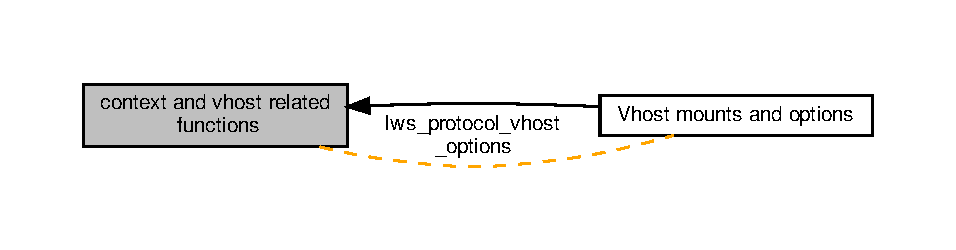
\includegraphics[width=350pt]{group__context-and-vhost}
\end{center}
\end{figure}
\subsection*{Modules}
\begin{DoxyCompactItemize}
\item 
\hyperlink{group__vhost-mounts}{Vhost mounts and options}
\end{DoxyCompactItemize}
\subsection*{Classes}
\begin{DoxyCompactItemize}
\item 
struct \hyperlink{structlws__context__creation__info}{lws\+\_\+context\+\_\+creation\+\_\+info}
\item 
struct \hyperlink{structlws__protocol__vhost__options}{lws\+\_\+protocol\+\_\+vhost\+\_\+options}
\end{DoxyCompactItemize}
\subsection*{Macros}
\begin{DoxyCompactItemize}
\item 
\mbox{\Hypertarget{group__context-and-vhost_gaea6bad7f34d6b9a55e92353362372b9f}\label{group__context-and-vhost_gaea6bad7f34d6b9a55e92353362372b9f}} 
\#define {\bfseries lws\+\_\+check\+\_\+opt}(c,  f)~(((c) \& (f)) == (f))
\item 
\mbox{\Hypertarget{group__context-and-vhost_gaea6bad7f34d6b9a55e92353362372b9f}\label{group__context-and-vhost_gaea6bad7f34d6b9a55e92353362372b9f}} 
\#define {\bfseries lws\+\_\+check\+\_\+opt}(c,  f)~(((c) \& (f)) == (f))
\item 
\mbox{\Hypertarget{group__context-and-vhost_gaea6bad7f34d6b9a55e92353362372b9f}\label{group__context-and-vhost_gaea6bad7f34d6b9a55e92353362372b9f}} 
\#define {\bfseries lws\+\_\+check\+\_\+opt}(c,  f)~(((c) \& (f)) == (f))
\item 
\mbox{\Hypertarget{group__context-and-vhost_gaea6bad7f34d6b9a55e92353362372b9f}\label{group__context-and-vhost_gaea6bad7f34d6b9a55e92353362372b9f}} 
\#define {\bfseries lws\+\_\+check\+\_\+opt}(c,  f)~(((c) \& (f)) == (f))
\item 
\mbox{\Hypertarget{group__context-and-vhost_gaea6bad7f34d6b9a55e92353362372b9f}\label{group__context-and-vhost_gaea6bad7f34d6b9a55e92353362372b9f}} 
\#define {\bfseries lws\+\_\+check\+\_\+opt}(c,  f)~(((c) \& (f)) == (f))
\item 
\mbox{\Hypertarget{group__context-and-vhost_gaea6bad7f34d6b9a55e92353362372b9f}\label{group__context-and-vhost_gaea6bad7f34d6b9a55e92353362372b9f}} 
\#define {\bfseries lws\+\_\+check\+\_\+opt}(c,  f)~(((c) \& (f)) == (f))
\item 
\mbox{\Hypertarget{group__context-and-vhost_gaea6bad7f34d6b9a55e92353362372b9f}\label{group__context-and-vhost_gaea6bad7f34d6b9a55e92353362372b9f}} 
\#define {\bfseries lws\+\_\+check\+\_\+opt}(c,  f)~(((c) \& (f)) == (f))
\item 
\mbox{\Hypertarget{group__context-and-vhost_gaea6bad7f34d6b9a55e92353362372b9f}\label{group__context-and-vhost_gaea6bad7f34d6b9a55e92353362372b9f}} 
\#define {\bfseries lws\+\_\+check\+\_\+opt}(c,  f)~(((c) \& (f)) == (f))
\end{DoxyCompactItemize}
\subsection*{Typedefs}
\begin{DoxyCompactItemize}
\item 
\mbox{\Hypertarget{group__context-and-vhost_ga256a49a07d2dd5062d6cf7bdc3668096}\label{group__context-and-vhost_ga256a49a07d2dd5062d6cf7bdc3668096}} 
typedef int($\ast$ {\bfseries lws\+\_\+reload\+\_\+func}) (void)
\item 
\mbox{\Hypertarget{group__context-and-vhost_ga256a49a07d2dd5062d6cf7bdc3668096}\label{group__context-and-vhost_ga256a49a07d2dd5062d6cf7bdc3668096}} 
typedef int($\ast$ {\bfseries lws\+\_\+reload\+\_\+func}) (void)
\item 
\mbox{\Hypertarget{group__context-and-vhost_ga256a49a07d2dd5062d6cf7bdc3668096}\label{group__context-and-vhost_ga256a49a07d2dd5062d6cf7bdc3668096}} 
typedef int($\ast$ {\bfseries lws\+\_\+reload\+\_\+func}) (void)
\item 
\mbox{\Hypertarget{group__context-and-vhost_ga256a49a07d2dd5062d6cf7bdc3668096}\label{group__context-and-vhost_ga256a49a07d2dd5062d6cf7bdc3668096}} 
typedef int($\ast$ {\bfseries lws\+\_\+reload\+\_\+func}) (void)
\item 
\mbox{\Hypertarget{group__context-and-vhost_ga256a49a07d2dd5062d6cf7bdc3668096}\label{group__context-and-vhost_ga256a49a07d2dd5062d6cf7bdc3668096}} 
typedef int($\ast$ {\bfseries lws\+\_\+reload\+\_\+func}) (void)
\item 
\mbox{\Hypertarget{group__context-and-vhost_ga256a49a07d2dd5062d6cf7bdc3668096}\label{group__context-and-vhost_ga256a49a07d2dd5062d6cf7bdc3668096}} 
typedef int($\ast$ {\bfseries lws\+\_\+reload\+\_\+func}) (void)
\end{DoxyCompactItemize}
\subsection*{Enumerations}
\begin{DoxyCompactItemize}
\item 
enum \hyperlink{group__context-and-vhost_ga41c2d763f78cc248df3b9f8645dbd2a5}{lws\+\_\+context\+\_\+options} \{ \newline
{\bfseries L\+W\+S\+\_\+\+S\+E\+R\+V\+E\+R\+\_\+\+O\+P\+T\+I\+O\+N\+\_\+\+R\+E\+Q\+U\+I\+R\+E\+\_\+\+V\+A\+L\+I\+D\+\_\+\+O\+P\+E\+N\+S\+S\+L\+\_\+\+C\+L\+I\+E\+N\+T\+\_\+\+C\+E\+RT} = (1 $<$$<$ 1), 
{\bfseries L\+W\+S\+\_\+\+S\+E\+R\+V\+E\+R\+\_\+\+O\+P\+T\+I\+O\+N\+\_\+\+S\+K\+I\+P\+\_\+\+S\+E\+R\+V\+E\+R\+\_\+\+C\+A\+N\+O\+N\+I\+C\+A\+L\+\_\+\+N\+A\+ME} = (1 $<$$<$ 2), 
{\bfseries L\+W\+S\+\_\+\+S\+E\+R\+V\+E\+R\+\_\+\+O\+P\+T\+I\+O\+N\+\_\+\+A\+L\+L\+O\+W\+\_\+\+N\+O\+N\+\_\+\+S\+S\+L\+\_\+\+O\+N\+\_\+\+S\+S\+L\+\_\+\+P\+O\+RT} = (1 $<$$<$ 3), 
{\bfseries L\+W\+S\+\_\+\+S\+E\+R\+V\+E\+R\+\_\+\+O\+P\+T\+I\+O\+N\+\_\+\+L\+I\+B\+EV} = (1 $<$$<$ 4), 
\newline
{\bfseries L\+W\+S\+\_\+\+S\+E\+R\+V\+E\+R\+\_\+\+O\+P\+T\+I\+O\+N\+\_\+\+D\+I\+S\+A\+B\+L\+E\+\_\+\+I\+P\+V6} = (1 $<$$<$ 5), 
{\bfseries L\+W\+S\+\_\+\+S\+E\+R\+V\+E\+R\+\_\+\+O\+P\+T\+I\+O\+N\+\_\+\+D\+I\+S\+A\+B\+L\+E\+\_\+\+O\+S\+\_\+\+C\+A\+\_\+\+C\+E\+R\+TS} = (1 $<$$<$ 6), 
{\bfseries L\+W\+S\+\_\+\+S\+E\+R\+V\+E\+R\+\_\+\+O\+P\+T\+I\+O\+N\+\_\+\+P\+E\+E\+R\+\_\+\+C\+E\+R\+T\+\_\+\+N\+O\+T\+\_\+\+R\+E\+Q\+U\+I\+R\+ED} = (1 $<$$<$ 7), 
{\bfseries L\+W\+S\+\_\+\+S\+E\+R\+V\+E\+R\+\_\+\+O\+P\+T\+I\+O\+N\+\_\+\+V\+A\+L\+I\+D\+A\+T\+E\+\_\+\+U\+T\+F8} = (1 $<$$<$ 8), 
\newline
{\bfseries L\+W\+S\+\_\+\+S\+E\+R\+V\+E\+R\+\_\+\+O\+P\+T\+I\+O\+N\+\_\+\+S\+S\+L\+\_\+\+E\+C\+DH} = (1 $<$$<$ 9), 
{\bfseries L\+W\+S\+\_\+\+S\+E\+R\+V\+E\+R\+\_\+\+O\+P\+T\+I\+O\+N\+\_\+\+R\+E\+Q\+U\+I\+R\+E\+\_\+\+V\+A\+L\+I\+D\+\_\+\+O\+P\+E\+N\+S\+S\+L\+\_\+\+C\+L\+I\+E\+N\+T\+\_\+\+C\+E\+RT} = (1 $<$$<$ 1), 
{\bfseries L\+W\+S\+\_\+\+S\+E\+R\+V\+E\+R\+\_\+\+O\+P\+T\+I\+O\+N\+\_\+\+S\+K\+I\+P\+\_\+\+S\+E\+R\+V\+E\+R\+\_\+\+C\+A\+N\+O\+N\+I\+C\+A\+L\+\_\+\+N\+A\+ME} = (1 $<$$<$ 2), 
{\bfseries L\+W\+S\+\_\+\+S\+E\+R\+V\+E\+R\+\_\+\+O\+P\+T\+I\+O\+N\+\_\+\+A\+L\+L\+O\+W\+\_\+\+N\+O\+N\+\_\+\+S\+S\+L\+\_\+\+O\+N\+\_\+\+S\+S\+L\+\_\+\+P\+O\+RT} = (1 $<$$<$ 3), 
\newline
{\bfseries L\+W\+S\+\_\+\+S\+E\+R\+V\+E\+R\+\_\+\+O\+P\+T\+I\+O\+N\+\_\+\+L\+I\+B\+EV} = (1 $<$$<$ 4), 
{\bfseries L\+W\+S\+\_\+\+S\+E\+R\+V\+E\+R\+\_\+\+O\+P\+T\+I\+O\+N\+\_\+\+D\+I\+S\+A\+B\+L\+E\+\_\+\+I\+P\+V6} = (1 $<$$<$ 5), 
{\bfseries L\+W\+S\+\_\+\+S\+E\+R\+V\+E\+R\+\_\+\+O\+P\+T\+I\+O\+N\+\_\+\+D\+I\+S\+A\+B\+L\+E\+\_\+\+O\+S\+\_\+\+C\+A\+\_\+\+C\+E\+R\+TS} = (1 $<$$<$ 6), 
{\bfseries L\+W\+S\+\_\+\+S\+E\+R\+V\+E\+R\+\_\+\+O\+P\+T\+I\+O\+N\+\_\+\+P\+E\+E\+R\+\_\+\+C\+E\+R\+T\+\_\+\+N\+O\+T\+\_\+\+R\+E\+Q\+U\+I\+R\+ED} = (1 $<$$<$ 7), 
\newline
{\bfseries L\+W\+S\+\_\+\+S\+E\+R\+V\+E\+R\+\_\+\+O\+P\+T\+I\+O\+N\+\_\+\+V\+A\+L\+I\+D\+A\+T\+E\+\_\+\+U\+T\+F8} = (1 $<$$<$ 8), 
{\bfseries L\+W\+S\+\_\+\+S\+E\+R\+V\+E\+R\+\_\+\+O\+P\+T\+I\+O\+N\+\_\+\+S\+S\+L\+\_\+\+E\+C\+DH} = (1 $<$$<$ 9), 
{\bfseries L\+W\+S\+\_\+\+S\+E\+R\+V\+E\+R\+\_\+\+O\+P\+T\+I\+O\+N\+\_\+\+R\+E\+Q\+U\+I\+R\+E\+\_\+\+V\+A\+L\+I\+D\+\_\+\+O\+P\+E\+N\+S\+S\+L\+\_\+\+C\+L\+I\+E\+N\+T\+\_\+\+C\+E\+RT} = (1 $<$$<$ 1), 
{\bfseries L\+W\+S\+\_\+\+S\+E\+R\+V\+E\+R\+\_\+\+O\+P\+T\+I\+O\+N\+\_\+\+S\+K\+I\+P\+\_\+\+S\+E\+R\+V\+E\+R\+\_\+\+C\+A\+N\+O\+N\+I\+C\+A\+L\+\_\+\+N\+A\+ME} = (1 $<$$<$ 2), 
\newline
{\bfseries L\+W\+S\+\_\+\+S\+E\+R\+V\+E\+R\+\_\+\+O\+P\+T\+I\+O\+N\+\_\+\+A\+L\+L\+O\+W\+\_\+\+N\+O\+N\+\_\+\+S\+S\+L\+\_\+\+O\+N\+\_\+\+S\+S\+L\+\_\+\+P\+O\+RT} = (1 $<$$<$ 3), 
{\bfseries L\+W\+S\+\_\+\+S\+E\+R\+V\+E\+R\+\_\+\+O\+P\+T\+I\+O\+N\+\_\+\+L\+I\+B\+EV} = (1 $<$$<$ 4), 
{\bfseries L\+W\+S\+\_\+\+S\+E\+R\+V\+E\+R\+\_\+\+O\+P\+T\+I\+O\+N\+\_\+\+D\+I\+S\+A\+B\+L\+E\+\_\+\+I\+P\+V6} = (1 $<$$<$ 5), 
{\bfseries L\+W\+S\+\_\+\+S\+E\+R\+V\+E\+R\+\_\+\+O\+P\+T\+I\+O\+N\+\_\+\+D\+I\+S\+A\+B\+L\+E\+\_\+\+O\+S\+\_\+\+C\+A\+\_\+\+C\+E\+R\+TS} = (1 $<$$<$ 6), 
\newline
{\bfseries L\+W\+S\+\_\+\+S\+E\+R\+V\+E\+R\+\_\+\+O\+P\+T\+I\+O\+N\+\_\+\+P\+E\+E\+R\+\_\+\+C\+E\+R\+T\+\_\+\+N\+O\+T\+\_\+\+R\+E\+Q\+U\+I\+R\+ED} = (1 $<$$<$ 7), 
{\bfseries L\+W\+S\+\_\+\+S\+E\+R\+V\+E\+R\+\_\+\+O\+P\+T\+I\+O\+N\+\_\+\+V\+A\+L\+I\+D\+A\+T\+E\+\_\+\+U\+T\+F8} = (1 $<$$<$ 8), 
{\bfseries L\+W\+S\+\_\+\+S\+E\+R\+V\+E\+R\+\_\+\+O\+P\+T\+I\+O\+N\+\_\+\+S\+S\+L\+\_\+\+E\+C\+DH} = (1 $<$$<$ 9), 
{\bfseries L\+W\+S\+\_\+\+S\+E\+R\+V\+E\+R\+\_\+\+O\+P\+T\+I\+O\+N\+\_\+\+R\+E\+Q\+U\+I\+R\+E\+\_\+\+V\+A\+L\+I\+D\+\_\+\+O\+P\+E\+N\+S\+S\+L\+\_\+\+C\+L\+I\+E\+N\+T\+\_\+\+C\+E\+RT} = (1 $<$$<$ 1), 
\newline
{\bfseries L\+W\+S\+\_\+\+S\+E\+R\+V\+E\+R\+\_\+\+O\+P\+T\+I\+O\+N\+\_\+\+S\+K\+I\+P\+\_\+\+S\+E\+R\+V\+E\+R\+\_\+\+C\+A\+N\+O\+N\+I\+C\+A\+L\+\_\+\+N\+A\+ME} = (1 $<$$<$ 2), 
{\bfseries L\+W\+S\+\_\+\+S\+E\+R\+V\+E\+R\+\_\+\+O\+P\+T\+I\+O\+N\+\_\+\+A\+L\+L\+O\+W\+\_\+\+N\+O\+N\+\_\+\+S\+S\+L\+\_\+\+O\+N\+\_\+\+S\+S\+L\+\_\+\+P\+O\+RT} = (1 $<$$<$ 3), 
{\bfseries L\+W\+S\+\_\+\+S\+E\+R\+V\+E\+R\+\_\+\+O\+P\+T\+I\+O\+N\+\_\+\+L\+I\+B\+EV} = (1 $<$$<$ 4), 
{\bfseries L\+W\+S\+\_\+\+S\+E\+R\+V\+E\+R\+\_\+\+O\+P\+T\+I\+O\+N\+\_\+\+D\+I\+S\+A\+B\+L\+E\+\_\+\+I\+P\+V6} = (1 $<$$<$ 5), 
\newline
{\bfseries L\+W\+S\+\_\+\+S\+E\+R\+V\+E\+R\+\_\+\+O\+P\+T\+I\+O\+N\+\_\+\+D\+I\+S\+A\+B\+L\+E\+\_\+\+O\+S\+\_\+\+C\+A\+\_\+\+C\+E\+R\+TS} = (1 $<$$<$ 6), 
{\bfseries L\+W\+S\+\_\+\+S\+E\+R\+V\+E\+R\+\_\+\+O\+P\+T\+I\+O\+N\+\_\+\+P\+E\+E\+R\+\_\+\+C\+E\+R\+T\+\_\+\+N\+O\+T\+\_\+\+R\+E\+Q\+U\+I\+R\+ED} = (1 $<$$<$ 7), 
{\bfseries L\+W\+S\+\_\+\+S\+E\+R\+V\+E\+R\+\_\+\+O\+P\+T\+I\+O\+N\+\_\+\+V\+A\+L\+I\+D\+A\+T\+E\+\_\+\+U\+T\+F8} = (1 $<$$<$ 8), 
{\bfseries L\+W\+S\+\_\+\+S\+E\+R\+V\+E\+R\+\_\+\+O\+P\+T\+I\+O\+N\+\_\+\+S\+S\+L\+\_\+\+E\+C\+DH} = (1 $<$$<$ 9), 
\newline
{\bfseries L\+W\+S\+\_\+\+S\+E\+R\+V\+E\+R\+\_\+\+O\+P\+T\+I\+O\+N\+\_\+\+R\+E\+Q\+U\+I\+R\+E\+\_\+\+V\+A\+L\+I\+D\+\_\+\+O\+P\+E\+N\+S\+S\+L\+\_\+\+C\+L\+I\+E\+N\+T\+\_\+\+C\+E\+RT} = (1 $<$$<$ 1), 
{\bfseries L\+W\+S\+\_\+\+S\+E\+R\+V\+E\+R\+\_\+\+O\+P\+T\+I\+O\+N\+\_\+\+S\+K\+I\+P\+\_\+\+S\+E\+R\+V\+E\+R\+\_\+\+C\+A\+N\+O\+N\+I\+C\+A\+L\+\_\+\+N\+A\+ME} = (1 $<$$<$ 2), 
{\bfseries L\+W\+S\+\_\+\+S\+E\+R\+V\+E\+R\+\_\+\+O\+P\+T\+I\+O\+N\+\_\+\+A\+L\+L\+O\+W\+\_\+\+N\+O\+N\+\_\+\+S\+S\+L\+\_\+\+O\+N\+\_\+\+S\+S\+L\+\_\+\+P\+O\+RT} = (1 $<$$<$ 3), 
{\bfseries L\+W\+S\+\_\+\+S\+E\+R\+V\+E\+R\+\_\+\+O\+P\+T\+I\+O\+N\+\_\+\+L\+I\+B\+EV} = (1 $<$$<$ 4), 
\newline
{\bfseries L\+W\+S\+\_\+\+S\+E\+R\+V\+E\+R\+\_\+\+O\+P\+T\+I\+O\+N\+\_\+\+D\+I\+S\+A\+B\+L\+E\+\_\+\+I\+P\+V6} = (1 $<$$<$ 5), 
{\bfseries L\+W\+S\+\_\+\+S\+E\+R\+V\+E\+R\+\_\+\+O\+P\+T\+I\+O\+N\+\_\+\+D\+I\+S\+A\+B\+L\+E\+\_\+\+O\+S\+\_\+\+C\+A\+\_\+\+C\+E\+R\+TS} = (1 $<$$<$ 6), 
{\bfseries L\+W\+S\+\_\+\+S\+E\+R\+V\+E\+R\+\_\+\+O\+P\+T\+I\+O\+N\+\_\+\+P\+E\+E\+R\+\_\+\+C\+E\+R\+T\+\_\+\+N\+O\+T\+\_\+\+R\+E\+Q\+U\+I\+R\+ED} = (1 $<$$<$ 7), 
{\bfseries L\+W\+S\+\_\+\+S\+E\+R\+V\+E\+R\+\_\+\+O\+P\+T\+I\+O\+N\+\_\+\+V\+A\+L\+I\+D\+A\+T\+E\+\_\+\+U\+T\+F8} = (1 $<$$<$ 8), 
\newline
{\bfseries L\+W\+S\+\_\+\+S\+E\+R\+V\+E\+R\+\_\+\+O\+P\+T\+I\+O\+N\+\_\+\+S\+S\+L\+\_\+\+E\+C\+DH} = (1 $<$$<$ 9), 
{\bfseries L\+W\+S\+\_\+\+S\+E\+R\+V\+E\+R\+\_\+\+O\+P\+T\+I\+O\+N\+\_\+\+R\+E\+Q\+U\+I\+R\+E\+\_\+\+V\+A\+L\+I\+D\+\_\+\+O\+P\+E\+N\+S\+S\+L\+\_\+\+C\+L\+I\+E\+N\+T\+\_\+\+C\+E\+RT} = (1 $<$$<$ 1), 
{\bfseries L\+W\+S\+\_\+\+S\+E\+R\+V\+E\+R\+\_\+\+O\+P\+T\+I\+O\+N\+\_\+\+S\+K\+I\+P\+\_\+\+S\+E\+R\+V\+E\+R\+\_\+\+C\+A\+N\+O\+N\+I\+C\+A\+L\+\_\+\+N\+A\+ME} = (1 $<$$<$ 2), 
{\bfseries L\+W\+S\+\_\+\+S\+E\+R\+V\+E\+R\+\_\+\+O\+P\+T\+I\+O\+N\+\_\+\+A\+L\+L\+O\+W\+\_\+\+N\+O\+N\+\_\+\+S\+S\+L\+\_\+\+O\+N\+\_\+\+S\+S\+L\+\_\+\+P\+O\+RT} = (1 $<$$<$ 3), 
\newline
{\bfseries L\+W\+S\+\_\+\+S\+E\+R\+V\+E\+R\+\_\+\+O\+P\+T\+I\+O\+N\+\_\+\+L\+I\+B\+EV} = (1 $<$$<$ 4), 
{\bfseries L\+W\+S\+\_\+\+S\+E\+R\+V\+E\+R\+\_\+\+O\+P\+T\+I\+O\+N\+\_\+\+D\+I\+S\+A\+B\+L\+E\+\_\+\+I\+P\+V6} = (1 $<$$<$ 5), 
{\bfseries L\+W\+S\+\_\+\+S\+E\+R\+V\+E\+R\+\_\+\+O\+P\+T\+I\+O\+N\+\_\+\+D\+I\+S\+A\+B\+L\+E\+\_\+\+O\+S\+\_\+\+C\+A\+\_\+\+C\+E\+R\+TS} = (1 $<$$<$ 6), 
{\bfseries L\+W\+S\+\_\+\+S\+E\+R\+V\+E\+R\+\_\+\+O\+P\+T\+I\+O\+N\+\_\+\+P\+E\+E\+R\+\_\+\+C\+E\+R\+T\+\_\+\+N\+O\+T\+\_\+\+R\+E\+Q\+U\+I\+R\+ED} = (1 $<$$<$ 7), 
\newline
{\bfseries L\+W\+S\+\_\+\+S\+E\+R\+V\+E\+R\+\_\+\+O\+P\+T\+I\+O\+N\+\_\+\+V\+A\+L\+I\+D\+A\+T\+E\+\_\+\+U\+T\+F8} = (1 $<$$<$ 8), 
{\bfseries L\+W\+S\+\_\+\+S\+E\+R\+V\+E\+R\+\_\+\+O\+P\+T\+I\+O\+N\+\_\+\+S\+S\+L\+\_\+\+E\+C\+DH} = (1 $<$$<$ 9), 
{\bfseries L\+W\+S\+\_\+\+S\+E\+R\+V\+E\+R\+\_\+\+O\+P\+T\+I\+O\+N\+\_\+\+R\+E\+Q\+U\+I\+R\+E\+\_\+\+V\+A\+L\+I\+D\+\_\+\+O\+P\+E\+N\+S\+S\+L\+\_\+\+C\+L\+I\+E\+N\+T\+\_\+\+C\+E\+RT} = (1 $<$$<$ 1), 
{\bfseries L\+W\+S\+\_\+\+S\+E\+R\+V\+E\+R\+\_\+\+O\+P\+T\+I\+O\+N\+\_\+\+S\+K\+I\+P\+\_\+\+S\+E\+R\+V\+E\+R\+\_\+\+C\+A\+N\+O\+N\+I\+C\+A\+L\+\_\+\+N\+A\+ME} = (1 $<$$<$ 2), 
\newline
{\bfseries L\+W\+S\+\_\+\+S\+E\+R\+V\+E\+R\+\_\+\+O\+P\+T\+I\+O\+N\+\_\+\+A\+L\+L\+O\+W\+\_\+\+N\+O\+N\+\_\+\+S\+S\+L\+\_\+\+O\+N\+\_\+\+S\+S\+L\+\_\+\+P\+O\+RT} = (1 $<$$<$ 3), 
{\bfseries L\+W\+S\+\_\+\+S\+E\+R\+V\+E\+R\+\_\+\+O\+P\+T\+I\+O\+N\+\_\+\+L\+I\+B\+EV} = (1 $<$$<$ 4), 
{\bfseries L\+W\+S\+\_\+\+S\+E\+R\+V\+E\+R\+\_\+\+O\+P\+T\+I\+O\+N\+\_\+\+D\+I\+S\+A\+B\+L\+E\+\_\+\+I\+P\+V6} = (1 $<$$<$ 5), 
{\bfseries L\+W\+S\+\_\+\+S\+E\+R\+V\+E\+R\+\_\+\+O\+P\+T\+I\+O\+N\+\_\+\+D\+I\+S\+A\+B\+L\+E\+\_\+\+O\+S\+\_\+\+C\+A\+\_\+\+C\+E\+R\+TS} = (1 $<$$<$ 6), 
\newline
{\bfseries L\+W\+S\+\_\+\+S\+E\+R\+V\+E\+R\+\_\+\+O\+P\+T\+I\+O\+N\+\_\+\+P\+E\+E\+R\+\_\+\+C\+E\+R\+T\+\_\+\+N\+O\+T\+\_\+\+R\+E\+Q\+U\+I\+R\+ED} = (1 $<$$<$ 7), 
{\bfseries L\+W\+S\+\_\+\+S\+E\+R\+V\+E\+R\+\_\+\+O\+P\+T\+I\+O\+N\+\_\+\+V\+A\+L\+I\+D\+A\+T\+E\+\_\+\+U\+T\+F8} = (1 $<$$<$ 8), 
{\bfseries L\+W\+S\+\_\+\+S\+E\+R\+V\+E\+R\+\_\+\+O\+P\+T\+I\+O\+N\+\_\+\+S\+S\+L\+\_\+\+E\+C\+DH} = (1 $<$$<$ 9), 
{\bfseries L\+W\+S\+\_\+\+S\+E\+R\+V\+E\+R\+\_\+\+O\+P\+T\+I\+O\+N\+\_\+\+R\+E\+Q\+U\+I\+R\+E\+\_\+\+V\+A\+L\+I\+D\+\_\+\+O\+P\+E\+N\+S\+S\+L\+\_\+\+C\+L\+I\+E\+N\+T\+\_\+\+C\+E\+RT} = (1 $<$$<$ 1), 
\newline
{\bfseries L\+W\+S\+\_\+\+S\+E\+R\+V\+E\+R\+\_\+\+O\+P\+T\+I\+O\+N\+\_\+\+S\+K\+I\+P\+\_\+\+S\+E\+R\+V\+E\+R\+\_\+\+C\+A\+N\+O\+N\+I\+C\+A\+L\+\_\+\+N\+A\+ME} = (1 $<$$<$ 2), 
{\bfseries L\+W\+S\+\_\+\+S\+E\+R\+V\+E\+R\+\_\+\+O\+P\+T\+I\+O\+N\+\_\+\+A\+L\+L\+O\+W\+\_\+\+N\+O\+N\+\_\+\+S\+S\+L\+\_\+\+O\+N\+\_\+\+S\+S\+L\+\_\+\+P\+O\+RT} = (1 $<$$<$ 3), 
{\bfseries L\+W\+S\+\_\+\+S\+E\+R\+V\+E\+R\+\_\+\+O\+P\+T\+I\+O\+N\+\_\+\+L\+I\+B\+EV} = (1 $<$$<$ 4), 
{\bfseries L\+W\+S\+\_\+\+S\+E\+R\+V\+E\+R\+\_\+\+O\+P\+T\+I\+O\+N\+\_\+\+D\+I\+S\+A\+B\+L\+E\+\_\+\+I\+P\+V6} = (1 $<$$<$ 5), 
\newline
{\bfseries L\+W\+S\+\_\+\+S\+E\+R\+V\+E\+R\+\_\+\+O\+P\+T\+I\+O\+N\+\_\+\+D\+I\+S\+A\+B\+L\+E\+\_\+\+O\+S\+\_\+\+C\+A\+\_\+\+C\+E\+R\+TS} = (1 $<$$<$ 6), 
{\bfseries L\+W\+S\+\_\+\+S\+E\+R\+V\+E\+R\+\_\+\+O\+P\+T\+I\+O\+N\+\_\+\+P\+E\+E\+R\+\_\+\+C\+E\+R\+T\+\_\+\+N\+O\+T\+\_\+\+R\+E\+Q\+U\+I\+R\+ED} = (1 $<$$<$ 7), 
{\bfseries L\+W\+S\+\_\+\+S\+E\+R\+V\+E\+R\+\_\+\+O\+P\+T\+I\+O\+N\+\_\+\+V\+A\+L\+I\+D\+A\+T\+E\+\_\+\+U\+T\+F8} = (1 $<$$<$ 8), 
{\bfseries L\+W\+S\+\_\+\+S\+E\+R\+V\+E\+R\+\_\+\+O\+P\+T\+I\+O\+N\+\_\+\+S\+S\+L\+\_\+\+E\+C\+DH} = (1 $<$$<$ 9), 
\newline
{\bfseries L\+W\+S\+\_\+\+S\+E\+R\+V\+E\+R\+\_\+\+O\+P\+T\+I\+O\+N\+\_\+\+R\+E\+Q\+U\+I\+R\+E\+\_\+\+V\+A\+L\+I\+D\+\_\+\+O\+P\+E\+N\+S\+S\+L\+\_\+\+C\+L\+I\+E\+N\+T\+\_\+\+C\+E\+RT} = (1 $<$$<$ 1), 
{\bfseries L\+W\+S\+\_\+\+S\+E\+R\+V\+E\+R\+\_\+\+O\+P\+T\+I\+O\+N\+\_\+\+S\+K\+I\+P\+\_\+\+S\+E\+R\+V\+E\+R\+\_\+\+C\+A\+N\+O\+N\+I\+C\+A\+L\+\_\+\+N\+A\+ME} = (1 $<$$<$ 2), 
{\bfseries L\+W\+S\+\_\+\+S\+E\+R\+V\+E\+R\+\_\+\+O\+P\+T\+I\+O\+N\+\_\+\+A\+L\+L\+O\+W\+\_\+\+N\+O\+N\+\_\+\+S\+S\+L\+\_\+\+O\+N\+\_\+\+S\+S\+L\+\_\+\+P\+O\+RT} = (1 $<$$<$ 3), 
{\bfseries L\+W\+S\+\_\+\+S\+E\+R\+V\+E\+R\+\_\+\+O\+P\+T\+I\+O\+N\+\_\+\+L\+I\+B\+EV} = (1 $<$$<$ 4), 
\newline
{\bfseries L\+W\+S\+\_\+\+S\+E\+R\+V\+E\+R\+\_\+\+O\+P\+T\+I\+O\+N\+\_\+\+D\+I\+S\+A\+B\+L\+E\+\_\+\+I\+P\+V6} = (1 $<$$<$ 5), 
{\bfseries L\+W\+S\+\_\+\+S\+E\+R\+V\+E\+R\+\_\+\+O\+P\+T\+I\+O\+N\+\_\+\+D\+I\+S\+A\+B\+L\+E\+\_\+\+O\+S\+\_\+\+C\+A\+\_\+\+C\+E\+R\+TS} = (1 $<$$<$ 6), 
{\bfseries L\+W\+S\+\_\+\+S\+E\+R\+V\+E\+R\+\_\+\+O\+P\+T\+I\+O\+N\+\_\+\+P\+E\+E\+R\+\_\+\+C\+E\+R\+T\+\_\+\+N\+O\+T\+\_\+\+R\+E\+Q\+U\+I\+R\+ED} = (1 $<$$<$ 7), 
{\bfseries L\+W\+S\+\_\+\+S\+E\+R\+V\+E\+R\+\_\+\+O\+P\+T\+I\+O\+N\+\_\+\+V\+A\+L\+I\+D\+A\+T\+E\+\_\+\+U\+T\+F8} = (1 $<$$<$ 8), 
\newline
{\bfseries L\+W\+S\+\_\+\+S\+E\+R\+V\+E\+R\+\_\+\+O\+P\+T\+I\+O\+N\+\_\+\+S\+S\+L\+\_\+\+E\+C\+DH} = (1 $<$$<$ 9), 
\hyperlink{group__context-and-vhost_gga41c2d763f78cc248df3b9f8645dbd2a5a274ed462a1a9239eb6ddf9007f5b7092}{L\+W\+S\+\_\+\+S\+E\+R\+V\+E\+R\+\_\+\+O\+P\+T\+I\+O\+N\+\_\+\+R\+E\+Q\+U\+I\+R\+E\+\_\+\+V\+A\+L\+I\+D\+\_\+\+O\+P\+E\+N\+S\+S\+L\+\_\+\+C\+L\+I\+E\+N\+T\+\_\+\+C\+E\+RT}, 
\hyperlink{group__context-and-vhost_gga41c2d763f78cc248df3b9f8645dbd2a5a6582c985ee0ceaadc1d277030eae2d7c}{L\+W\+S\+\_\+\+S\+E\+R\+V\+E\+R\+\_\+\+O\+P\+T\+I\+O\+N\+\_\+\+S\+K\+I\+P\+\_\+\+S\+E\+R\+V\+E\+R\+\_\+\+C\+A\+N\+O\+N\+I\+C\+A\+L\+\_\+\+N\+A\+ME} = (1 $<$$<$ 2), 
\hyperlink{group__context-and-vhost_gga41c2d763f78cc248df3b9f8645dbd2a5a1cc4562d05cba52a6dfa0697a65ade0d}{L\+W\+S\+\_\+\+S\+E\+R\+V\+E\+R\+\_\+\+O\+P\+T\+I\+O\+N\+\_\+\+A\+L\+L\+O\+W\+\_\+\+N\+O\+N\+\_\+\+S\+S\+L\+\_\+\+O\+N\+\_\+\+S\+S\+L\+\_\+\+P\+O\+RT}, 
\newline
\hyperlink{group__context-and-vhost_gga41c2d763f78cc248df3b9f8645dbd2a5a273d9975675130de0c6dc937dde7c8a6}{L\+W\+S\+\_\+\+S\+E\+R\+V\+E\+R\+\_\+\+O\+P\+T\+I\+O\+N\+\_\+\+L\+I\+B\+EV} = (1 $<$$<$ 4), 
\hyperlink{group__context-and-vhost_gga41c2d763f78cc248df3b9f8645dbd2a5a34ab36e68c0d593b6f19b8d5ef1240a9}{L\+W\+S\+\_\+\+S\+E\+R\+V\+E\+R\+\_\+\+O\+P\+T\+I\+O\+N\+\_\+\+D\+I\+S\+A\+B\+L\+E\+\_\+\+I\+P\+V6} = (1 $<$$<$ 5), 
\hyperlink{group__context-and-vhost_gga41c2d763f78cc248df3b9f8645dbd2a5a4933347a821e73c3f1e13fb6bfc7ad93}{L\+W\+S\+\_\+\+S\+E\+R\+V\+E\+R\+\_\+\+O\+P\+T\+I\+O\+N\+\_\+\+D\+I\+S\+A\+B\+L\+E\+\_\+\+O\+S\+\_\+\+C\+A\+\_\+\+C\+E\+R\+TS} = (1 $<$$<$ 6), 
\hyperlink{group__context-and-vhost_gga41c2d763f78cc248df3b9f8645dbd2a5ac56a8a6590e74a8016d0fae09fb404fc}{L\+W\+S\+\_\+\+S\+E\+R\+V\+E\+R\+\_\+\+O\+P\+T\+I\+O\+N\+\_\+\+P\+E\+E\+R\+\_\+\+C\+E\+R\+T\+\_\+\+N\+O\+T\+\_\+\+R\+E\+Q\+U\+I\+R\+ED} = (1 $<$$<$ 7), 
\newline
\hyperlink{group__context-and-vhost_gga41c2d763f78cc248df3b9f8645dbd2a5aa0158b4e85420811e6b0f1378c6ded0f}{L\+W\+S\+\_\+\+S\+E\+R\+V\+E\+R\+\_\+\+O\+P\+T\+I\+O\+N\+\_\+\+V\+A\+L\+I\+D\+A\+T\+E\+\_\+\+U\+T\+F8} = (1 $<$$<$ 8), 
\hyperlink{group__context-and-vhost_gga41c2d763f78cc248df3b9f8645dbd2a5a1b2f8bde0f62adc7ebe81b2043f34c0c}{L\+W\+S\+\_\+\+S\+E\+R\+V\+E\+R\+\_\+\+O\+P\+T\+I\+O\+N\+\_\+\+S\+S\+L\+\_\+\+E\+C\+DH}, 
\hyperlink{group__context-and-vhost_gga41c2d763f78cc248df3b9f8645dbd2a5aff121db04a10cf8b2c5df9d4f2b89f1e}{L\+W\+S\+\_\+\+S\+E\+R\+V\+E\+R\+\_\+\+O\+P\+T\+I\+O\+N\+\_\+\+L\+I\+B\+UV} = (1 $<$$<$ 10), 
\hyperlink{group__context-and-vhost_gga41c2d763f78cc248df3b9f8645dbd2a5a4832187186c4d130c68051214cd42ada}{L\+W\+S\+\_\+\+S\+E\+R\+V\+E\+R\+\_\+\+O\+P\+T\+I\+O\+N\+\_\+\+R\+E\+D\+I\+R\+E\+C\+T\+\_\+\+H\+T\+T\+P\+\_\+\+T\+O\+\_\+\+H\+T\+T\+PS}, 
\newline
\hyperlink{group__context-and-vhost_gga41c2d763f78cc248df3b9f8645dbd2a5a7fed6a527c8d5e0acac1b4179644583a}{L\+W\+S\+\_\+\+S\+E\+R\+V\+E\+R\+\_\+\+O\+P\+T\+I\+O\+N\+\_\+\+D\+O\+\_\+\+S\+S\+L\+\_\+\+G\+L\+O\+B\+A\+L\+\_\+\+I\+N\+IT} = (1 $<$$<$ 12), 
\hyperlink{group__context-and-vhost_gga41c2d763f78cc248df3b9f8645dbd2a5accc9d0d11d1124a21659586164b0962e}{L\+W\+S\+\_\+\+S\+E\+R\+V\+E\+R\+\_\+\+O\+P\+T\+I\+O\+N\+\_\+\+E\+X\+P\+L\+I\+C\+I\+T\+\_\+\+V\+H\+O\+S\+TS} = (1 $<$$<$ 13), 
\hyperlink{group__context-and-vhost_gga41c2d763f78cc248df3b9f8645dbd2a5a9637e9001d8c8b2521086bcafbd8a941}{L\+W\+S\+\_\+\+S\+E\+R\+V\+E\+R\+\_\+\+O\+P\+T\+I\+O\+N\+\_\+\+U\+N\+I\+X\+\_\+\+S\+O\+CK} = (1 $<$$<$ 14), 
\hyperlink{group__context-and-vhost_gga41c2d763f78cc248df3b9f8645dbd2a5ac962efd35abf6c402f9fb14aa14f5016}{L\+W\+S\+\_\+\+S\+E\+R\+V\+E\+R\+\_\+\+O\+P\+T\+I\+O\+N\+\_\+\+S\+TS} = (1 $<$$<$ 15), 
\newline
\hyperlink{group__context-and-vhost_gga41c2d763f78cc248df3b9f8645dbd2a5af62887536e25e053e68741006dba46d8}{L\+W\+S\+\_\+\+S\+E\+R\+V\+E\+R\+\_\+\+O\+P\+T\+I\+O\+N\+\_\+\+I\+P\+V6\+\_\+\+V6\+O\+N\+L\+Y\+\_\+\+M\+O\+D\+I\+FY} = (1 $<$$<$ 16), 
\hyperlink{group__context-and-vhost_gga41c2d763f78cc248df3b9f8645dbd2a5aca5d42820b65eac5618ec3f0bd8a1160}{L\+W\+S\+\_\+\+S\+E\+R\+V\+E\+R\+\_\+\+O\+P\+T\+I\+O\+N\+\_\+\+I\+P\+V6\+\_\+\+V6\+O\+N\+L\+Y\+\_\+\+V\+A\+L\+UE} = (1 $<$$<$ 17), 
\hyperlink{group__context-and-vhost_gga41c2d763f78cc248df3b9f8645dbd2a5a87a824b2e812f4c3e7f2c4a1ea4f8abd}{L\+W\+S\+\_\+\+S\+E\+R\+V\+E\+R\+\_\+\+O\+P\+T\+I\+O\+N\+\_\+\+U\+V\+\_\+\+N\+O\+\_\+\+S\+I\+G\+S\+E\+G\+V\+\_\+\+S\+I\+G\+F\+P\+E\+\_\+\+S\+P\+IN} = (1 $<$$<$ 18), 
\hyperlink{group__context-and-vhost_gga41c2d763f78cc248df3b9f8645dbd2a5aa8d288cee6d03935ea6993546f2f2bcf}{L\+W\+S\+\_\+\+S\+E\+R\+V\+E\+R\+\_\+\+O\+P\+T\+I\+O\+N\+\_\+\+J\+U\+S\+T\+\_\+\+U\+S\+E\+\_\+\+R\+A\+W\+\_\+\+O\+R\+I\+G\+IN} = (1 $<$$<$ 19), 
\newline
\hyperlink{group__context-and-vhost_gga41c2d763f78cc248df3b9f8645dbd2a5a73f0b02f20b7a7edac1449719b32b2d8}{L\+W\+S\+\_\+\+S\+E\+R\+V\+E\+R\+\_\+\+O\+P\+T\+I\+O\+N\+\_\+\+F\+A\+L\+L\+B\+A\+C\+K\+\_\+\+T\+O\+\_\+\+R\+AW} = (1 $<$$<$ 20), 
\hyperlink{group__context-and-vhost_gga41c2d763f78cc248df3b9f8645dbd2a5a03a942e8640c79711af917335560f3db}{L\+W\+S\+\_\+\+S\+E\+R\+V\+E\+R\+\_\+\+O\+P\+T\+I\+O\+N\+\_\+\+L\+I\+B\+E\+V\+E\+NT} = (1 $<$$<$ 21), 
\hyperlink{group__context-and-vhost_gga41c2d763f78cc248df3b9f8645dbd2a5aaf8aa0f54c90c8def0f51ea22d939e9d}{L\+W\+S\+\_\+\+S\+E\+R\+V\+E\+R\+\_\+\+O\+P\+T\+I\+O\+N\+\_\+\+O\+N\+L\+Y\+\_\+\+R\+AW} = (1 $<$$<$ 22), 
\hyperlink{group__context-and-vhost_gga41c2d763f78cc248df3b9f8645dbd2a5a597cc959ff218ee4e0ffd2faf32299e2}{L\+W\+S\+\_\+\+S\+E\+R\+V\+E\+R\+\_\+\+O\+P\+T\+I\+O\+N\+\_\+\+A\+L\+L\+O\+W\+\_\+\+L\+I\+S\+T\+E\+N\+\_\+\+S\+H\+A\+RE} = (1 $<$$<$ 23), 
\newline
\hyperlink{group__context-and-vhost_gga41c2d763f78cc248df3b9f8645dbd2a5aaf6ef10d6163ae6352c5bece32191d6d}{L\+W\+S\+\_\+\+S\+E\+R\+V\+E\+R\+\_\+\+O\+P\+T\+I\+O\+N\+\_\+\+C\+R\+E\+A\+T\+E\+\_\+\+V\+H\+O\+S\+T\+\_\+\+S\+S\+L\+\_\+\+C\+TX} = (1 $<$$<$ 24), 
\hyperlink{group__context-and-vhost_gga41c2d763f78cc248df3b9f8645dbd2a5a274ed462a1a9239eb6ddf9007f5b7092}{L\+W\+S\+\_\+\+S\+E\+R\+V\+E\+R\+\_\+\+O\+P\+T\+I\+O\+N\+\_\+\+R\+E\+Q\+U\+I\+R\+E\+\_\+\+V\+A\+L\+I\+D\+\_\+\+O\+P\+E\+N\+S\+S\+L\+\_\+\+C\+L\+I\+E\+N\+T\+\_\+\+C\+E\+RT}, 
\hyperlink{group__context-and-vhost_gga41c2d763f78cc248df3b9f8645dbd2a5a6582c985ee0ceaadc1d277030eae2d7c}{L\+W\+S\+\_\+\+S\+E\+R\+V\+E\+R\+\_\+\+O\+P\+T\+I\+O\+N\+\_\+\+S\+K\+I\+P\+\_\+\+S\+E\+R\+V\+E\+R\+\_\+\+C\+A\+N\+O\+N\+I\+C\+A\+L\+\_\+\+N\+A\+ME} = (1 $<$$<$ 2), 
\hyperlink{group__context-and-vhost_gga41c2d763f78cc248df3b9f8645dbd2a5a1cc4562d05cba52a6dfa0697a65ade0d}{L\+W\+S\+\_\+\+S\+E\+R\+V\+E\+R\+\_\+\+O\+P\+T\+I\+O\+N\+\_\+\+A\+L\+L\+O\+W\+\_\+\+N\+O\+N\+\_\+\+S\+S\+L\+\_\+\+O\+N\+\_\+\+S\+S\+L\+\_\+\+P\+O\+RT}, 
\newline
\hyperlink{group__context-and-vhost_gga41c2d763f78cc248df3b9f8645dbd2a5a273d9975675130de0c6dc937dde7c8a6}{L\+W\+S\+\_\+\+S\+E\+R\+V\+E\+R\+\_\+\+O\+P\+T\+I\+O\+N\+\_\+\+L\+I\+B\+EV} = (1 $<$$<$ 4), 
\hyperlink{group__context-and-vhost_gga41c2d763f78cc248df3b9f8645dbd2a5a34ab36e68c0d593b6f19b8d5ef1240a9}{L\+W\+S\+\_\+\+S\+E\+R\+V\+E\+R\+\_\+\+O\+P\+T\+I\+O\+N\+\_\+\+D\+I\+S\+A\+B\+L\+E\+\_\+\+I\+P\+V6} = (1 $<$$<$ 5), 
\hyperlink{group__context-and-vhost_gga41c2d763f78cc248df3b9f8645dbd2a5a4933347a821e73c3f1e13fb6bfc7ad93}{L\+W\+S\+\_\+\+S\+E\+R\+V\+E\+R\+\_\+\+O\+P\+T\+I\+O\+N\+\_\+\+D\+I\+S\+A\+B\+L\+E\+\_\+\+O\+S\+\_\+\+C\+A\+\_\+\+C\+E\+R\+TS} = (1 $<$$<$ 6), 
\hyperlink{group__context-and-vhost_gga41c2d763f78cc248df3b9f8645dbd2a5ac56a8a6590e74a8016d0fae09fb404fc}{L\+W\+S\+\_\+\+S\+E\+R\+V\+E\+R\+\_\+\+O\+P\+T\+I\+O\+N\+\_\+\+P\+E\+E\+R\+\_\+\+C\+E\+R\+T\+\_\+\+N\+O\+T\+\_\+\+R\+E\+Q\+U\+I\+R\+ED} = (1 $<$$<$ 7), 
\newline
\hyperlink{group__context-and-vhost_gga41c2d763f78cc248df3b9f8645dbd2a5aa0158b4e85420811e6b0f1378c6ded0f}{L\+W\+S\+\_\+\+S\+E\+R\+V\+E\+R\+\_\+\+O\+P\+T\+I\+O\+N\+\_\+\+V\+A\+L\+I\+D\+A\+T\+E\+\_\+\+U\+T\+F8} = (1 $<$$<$ 8), 
\hyperlink{group__context-and-vhost_gga41c2d763f78cc248df3b9f8645dbd2a5a1b2f8bde0f62adc7ebe81b2043f34c0c}{L\+W\+S\+\_\+\+S\+E\+R\+V\+E\+R\+\_\+\+O\+P\+T\+I\+O\+N\+\_\+\+S\+S\+L\+\_\+\+E\+C\+DH}, 
\hyperlink{group__context-and-vhost_gga41c2d763f78cc248df3b9f8645dbd2a5aff121db04a10cf8b2c5df9d4f2b89f1e}{L\+W\+S\+\_\+\+S\+E\+R\+V\+E\+R\+\_\+\+O\+P\+T\+I\+O\+N\+\_\+\+L\+I\+B\+UV} = (1 $<$$<$ 10), 
\hyperlink{group__context-and-vhost_gga41c2d763f78cc248df3b9f8645dbd2a5a4832187186c4d130c68051214cd42ada}{L\+W\+S\+\_\+\+S\+E\+R\+V\+E\+R\+\_\+\+O\+P\+T\+I\+O\+N\+\_\+\+R\+E\+D\+I\+R\+E\+C\+T\+\_\+\+H\+T\+T\+P\+\_\+\+T\+O\+\_\+\+H\+T\+T\+PS}, 
\newline
\hyperlink{group__context-and-vhost_gga41c2d763f78cc248df3b9f8645dbd2a5a7fed6a527c8d5e0acac1b4179644583a}{L\+W\+S\+\_\+\+S\+E\+R\+V\+E\+R\+\_\+\+O\+P\+T\+I\+O\+N\+\_\+\+D\+O\+\_\+\+S\+S\+L\+\_\+\+G\+L\+O\+B\+A\+L\+\_\+\+I\+N\+IT} = (1 $<$$<$ 12), 
\hyperlink{group__context-and-vhost_gga41c2d763f78cc248df3b9f8645dbd2a5accc9d0d11d1124a21659586164b0962e}{L\+W\+S\+\_\+\+S\+E\+R\+V\+E\+R\+\_\+\+O\+P\+T\+I\+O\+N\+\_\+\+E\+X\+P\+L\+I\+C\+I\+T\+\_\+\+V\+H\+O\+S\+TS} = (1 $<$$<$ 13), 
\hyperlink{group__context-and-vhost_gga41c2d763f78cc248df3b9f8645dbd2a5a9637e9001d8c8b2521086bcafbd8a941}{L\+W\+S\+\_\+\+S\+E\+R\+V\+E\+R\+\_\+\+O\+P\+T\+I\+O\+N\+\_\+\+U\+N\+I\+X\+\_\+\+S\+O\+CK} = (1 $<$$<$ 14), 
\hyperlink{group__context-and-vhost_gga41c2d763f78cc248df3b9f8645dbd2a5ac962efd35abf6c402f9fb14aa14f5016}{L\+W\+S\+\_\+\+S\+E\+R\+V\+E\+R\+\_\+\+O\+P\+T\+I\+O\+N\+\_\+\+S\+TS} = (1 $<$$<$ 15), 
\newline
\hyperlink{group__context-and-vhost_gga41c2d763f78cc248df3b9f8645dbd2a5af62887536e25e053e68741006dba46d8}{L\+W\+S\+\_\+\+S\+E\+R\+V\+E\+R\+\_\+\+O\+P\+T\+I\+O\+N\+\_\+\+I\+P\+V6\+\_\+\+V6\+O\+N\+L\+Y\+\_\+\+M\+O\+D\+I\+FY} = (1 $<$$<$ 16), 
\hyperlink{group__context-and-vhost_gga41c2d763f78cc248df3b9f8645dbd2a5aca5d42820b65eac5618ec3f0bd8a1160}{L\+W\+S\+\_\+\+S\+E\+R\+V\+E\+R\+\_\+\+O\+P\+T\+I\+O\+N\+\_\+\+I\+P\+V6\+\_\+\+V6\+O\+N\+L\+Y\+\_\+\+V\+A\+L\+UE} = (1 $<$$<$ 17), 
\hyperlink{group__context-and-vhost_gga41c2d763f78cc248df3b9f8645dbd2a5a87a824b2e812f4c3e7f2c4a1ea4f8abd}{L\+W\+S\+\_\+\+S\+E\+R\+V\+E\+R\+\_\+\+O\+P\+T\+I\+O\+N\+\_\+\+U\+V\+\_\+\+N\+O\+\_\+\+S\+I\+G\+S\+E\+G\+V\+\_\+\+S\+I\+G\+F\+P\+E\+\_\+\+S\+P\+IN} = (1 $<$$<$ 18), 
\hyperlink{group__context-and-vhost_gga41c2d763f78cc248df3b9f8645dbd2a5aa8d288cee6d03935ea6993546f2f2bcf}{L\+W\+S\+\_\+\+S\+E\+R\+V\+E\+R\+\_\+\+O\+P\+T\+I\+O\+N\+\_\+\+J\+U\+S\+T\+\_\+\+U\+S\+E\+\_\+\+R\+A\+W\+\_\+\+O\+R\+I\+G\+IN} = (1 $<$$<$ 19), 
\newline
\hyperlink{group__context-and-vhost_gga41c2d763f78cc248df3b9f8645dbd2a5a73f0b02f20b7a7edac1449719b32b2d8}{L\+W\+S\+\_\+\+S\+E\+R\+V\+E\+R\+\_\+\+O\+P\+T\+I\+O\+N\+\_\+\+F\+A\+L\+L\+B\+A\+C\+K\+\_\+\+T\+O\+\_\+\+R\+AW} = (1 $<$$<$ 20), 
\hyperlink{group__context-and-vhost_gga41c2d763f78cc248df3b9f8645dbd2a5a03a942e8640c79711af917335560f3db}{L\+W\+S\+\_\+\+S\+E\+R\+V\+E\+R\+\_\+\+O\+P\+T\+I\+O\+N\+\_\+\+L\+I\+B\+E\+V\+E\+NT} = (1 $<$$<$ 21), 
\hyperlink{group__context-and-vhost_gga41c2d763f78cc248df3b9f8645dbd2a5aaf8aa0f54c90c8def0f51ea22d939e9d}{L\+W\+S\+\_\+\+S\+E\+R\+V\+E\+R\+\_\+\+O\+P\+T\+I\+O\+N\+\_\+\+O\+N\+L\+Y\+\_\+\+R\+AW} = (1 $<$$<$ 22), 
\hyperlink{group__context-and-vhost_gga41c2d763f78cc248df3b9f8645dbd2a5a597cc959ff218ee4e0ffd2faf32299e2}{L\+W\+S\+\_\+\+S\+E\+R\+V\+E\+R\+\_\+\+O\+P\+T\+I\+O\+N\+\_\+\+A\+L\+L\+O\+W\+\_\+\+L\+I\+S\+T\+E\+N\+\_\+\+S\+H\+A\+RE} = (1 $<$$<$ 23), 
\newline
\hyperlink{group__context-and-vhost_gga41c2d763f78cc248df3b9f8645dbd2a5aaf6ef10d6163ae6352c5bece32191d6d}{L\+W\+S\+\_\+\+S\+E\+R\+V\+E\+R\+\_\+\+O\+P\+T\+I\+O\+N\+\_\+\+C\+R\+E\+A\+T\+E\+\_\+\+V\+H\+O\+S\+T\+\_\+\+S\+S\+L\+\_\+\+C\+TX} = (1 $<$$<$ 24), 
\hyperlink{group__context-and-vhost_gga41c2d763f78cc248df3b9f8645dbd2a5a274ed462a1a9239eb6ddf9007f5b7092}{L\+W\+S\+\_\+\+S\+E\+R\+V\+E\+R\+\_\+\+O\+P\+T\+I\+O\+N\+\_\+\+R\+E\+Q\+U\+I\+R\+E\+\_\+\+V\+A\+L\+I\+D\+\_\+\+O\+P\+E\+N\+S\+S\+L\+\_\+\+C\+L\+I\+E\+N\+T\+\_\+\+C\+E\+RT}, 
\hyperlink{group__context-and-vhost_gga41c2d763f78cc248df3b9f8645dbd2a5a6582c985ee0ceaadc1d277030eae2d7c}{L\+W\+S\+\_\+\+S\+E\+R\+V\+E\+R\+\_\+\+O\+P\+T\+I\+O\+N\+\_\+\+S\+K\+I\+P\+\_\+\+S\+E\+R\+V\+E\+R\+\_\+\+C\+A\+N\+O\+N\+I\+C\+A\+L\+\_\+\+N\+A\+ME} = (1 $<$$<$ 2), 
\hyperlink{group__context-and-vhost_gga41c2d763f78cc248df3b9f8645dbd2a5a1cc4562d05cba52a6dfa0697a65ade0d}{L\+W\+S\+\_\+\+S\+E\+R\+V\+E\+R\+\_\+\+O\+P\+T\+I\+O\+N\+\_\+\+A\+L\+L\+O\+W\+\_\+\+N\+O\+N\+\_\+\+S\+S\+L\+\_\+\+O\+N\+\_\+\+S\+S\+L\+\_\+\+P\+O\+RT}, 
\newline
\hyperlink{group__context-and-vhost_gga41c2d763f78cc248df3b9f8645dbd2a5a273d9975675130de0c6dc937dde7c8a6}{L\+W\+S\+\_\+\+S\+E\+R\+V\+E\+R\+\_\+\+O\+P\+T\+I\+O\+N\+\_\+\+L\+I\+B\+EV} = (1 $<$$<$ 4), 
\hyperlink{group__context-and-vhost_gga41c2d763f78cc248df3b9f8645dbd2a5a34ab36e68c0d593b6f19b8d5ef1240a9}{L\+W\+S\+\_\+\+S\+E\+R\+V\+E\+R\+\_\+\+O\+P\+T\+I\+O\+N\+\_\+\+D\+I\+S\+A\+B\+L\+E\+\_\+\+I\+P\+V6} = (1 $<$$<$ 5), 
\hyperlink{group__context-and-vhost_gga41c2d763f78cc248df3b9f8645dbd2a5a4933347a821e73c3f1e13fb6bfc7ad93}{L\+W\+S\+\_\+\+S\+E\+R\+V\+E\+R\+\_\+\+O\+P\+T\+I\+O\+N\+\_\+\+D\+I\+S\+A\+B\+L\+E\+\_\+\+O\+S\+\_\+\+C\+A\+\_\+\+C\+E\+R\+TS} = (1 $<$$<$ 6), 
\hyperlink{group__context-and-vhost_gga41c2d763f78cc248df3b9f8645dbd2a5ac56a8a6590e74a8016d0fae09fb404fc}{L\+W\+S\+\_\+\+S\+E\+R\+V\+E\+R\+\_\+\+O\+P\+T\+I\+O\+N\+\_\+\+P\+E\+E\+R\+\_\+\+C\+E\+R\+T\+\_\+\+N\+O\+T\+\_\+\+R\+E\+Q\+U\+I\+R\+ED} = (1 $<$$<$ 7), 
\newline
\hyperlink{group__context-and-vhost_gga41c2d763f78cc248df3b9f8645dbd2a5aa0158b4e85420811e6b0f1378c6ded0f}{L\+W\+S\+\_\+\+S\+E\+R\+V\+E\+R\+\_\+\+O\+P\+T\+I\+O\+N\+\_\+\+V\+A\+L\+I\+D\+A\+T\+E\+\_\+\+U\+T\+F8} = (1 $<$$<$ 8), 
\hyperlink{group__context-and-vhost_gga41c2d763f78cc248df3b9f8645dbd2a5a1b2f8bde0f62adc7ebe81b2043f34c0c}{L\+W\+S\+\_\+\+S\+E\+R\+V\+E\+R\+\_\+\+O\+P\+T\+I\+O\+N\+\_\+\+S\+S\+L\+\_\+\+E\+C\+DH}, 
\hyperlink{group__context-and-vhost_gga41c2d763f78cc248df3b9f8645dbd2a5aff121db04a10cf8b2c5df9d4f2b89f1e}{L\+W\+S\+\_\+\+S\+E\+R\+V\+E\+R\+\_\+\+O\+P\+T\+I\+O\+N\+\_\+\+L\+I\+B\+UV} = (1 $<$$<$ 10), 
\hyperlink{group__context-and-vhost_gga41c2d763f78cc248df3b9f8645dbd2a5a4832187186c4d130c68051214cd42ada}{L\+W\+S\+\_\+\+S\+E\+R\+V\+E\+R\+\_\+\+O\+P\+T\+I\+O\+N\+\_\+\+R\+E\+D\+I\+R\+E\+C\+T\+\_\+\+H\+T\+T\+P\+\_\+\+T\+O\+\_\+\+H\+T\+T\+PS}, 
\newline
\hyperlink{group__context-and-vhost_gga41c2d763f78cc248df3b9f8645dbd2a5a7fed6a527c8d5e0acac1b4179644583a}{L\+W\+S\+\_\+\+S\+E\+R\+V\+E\+R\+\_\+\+O\+P\+T\+I\+O\+N\+\_\+\+D\+O\+\_\+\+S\+S\+L\+\_\+\+G\+L\+O\+B\+A\+L\+\_\+\+I\+N\+IT} = (1 $<$$<$ 12), 
\hyperlink{group__context-and-vhost_gga41c2d763f78cc248df3b9f8645dbd2a5accc9d0d11d1124a21659586164b0962e}{L\+W\+S\+\_\+\+S\+E\+R\+V\+E\+R\+\_\+\+O\+P\+T\+I\+O\+N\+\_\+\+E\+X\+P\+L\+I\+C\+I\+T\+\_\+\+V\+H\+O\+S\+TS} = (1 $<$$<$ 13), 
\hyperlink{group__context-and-vhost_gga41c2d763f78cc248df3b9f8645dbd2a5a9637e9001d8c8b2521086bcafbd8a941}{L\+W\+S\+\_\+\+S\+E\+R\+V\+E\+R\+\_\+\+O\+P\+T\+I\+O\+N\+\_\+\+U\+N\+I\+X\+\_\+\+S\+O\+CK} = (1 $<$$<$ 14), 
\hyperlink{group__context-and-vhost_gga41c2d763f78cc248df3b9f8645dbd2a5ac962efd35abf6c402f9fb14aa14f5016}{L\+W\+S\+\_\+\+S\+E\+R\+V\+E\+R\+\_\+\+O\+P\+T\+I\+O\+N\+\_\+\+S\+TS} = (1 $<$$<$ 15), 
\newline
\hyperlink{group__context-and-vhost_gga41c2d763f78cc248df3b9f8645dbd2a5af62887536e25e053e68741006dba46d8}{L\+W\+S\+\_\+\+S\+E\+R\+V\+E\+R\+\_\+\+O\+P\+T\+I\+O\+N\+\_\+\+I\+P\+V6\+\_\+\+V6\+O\+N\+L\+Y\+\_\+\+M\+O\+D\+I\+FY} = (1 $<$$<$ 16), 
\hyperlink{group__context-and-vhost_gga41c2d763f78cc248df3b9f8645dbd2a5aca5d42820b65eac5618ec3f0bd8a1160}{L\+W\+S\+\_\+\+S\+E\+R\+V\+E\+R\+\_\+\+O\+P\+T\+I\+O\+N\+\_\+\+I\+P\+V6\+\_\+\+V6\+O\+N\+L\+Y\+\_\+\+V\+A\+L\+UE} = (1 $<$$<$ 17), 
\hyperlink{group__context-and-vhost_gga41c2d763f78cc248df3b9f8645dbd2a5a87a824b2e812f4c3e7f2c4a1ea4f8abd}{L\+W\+S\+\_\+\+S\+E\+R\+V\+E\+R\+\_\+\+O\+P\+T\+I\+O\+N\+\_\+\+U\+V\+\_\+\+N\+O\+\_\+\+S\+I\+G\+S\+E\+G\+V\+\_\+\+S\+I\+G\+F\+P\+E\+\_\+\+S\+P\+IN} = (1 $<$$<$ 18), 
\hyperlink{group__context-and-vhost_gga41c2d763f78cc248df3b9f8645dbd2a5aa8d288cee6d03935ea6993546f2f2bcf}{L\+W\+S\+\_\+\+S\+E\+R\+V\+E\+R\+\_\+\+O\+P\+T\+I\+O\+N\+\_\+\+J\+U\+S\+T\+\_\+\+U\+S\+E\+\_\+\+R\+A\+W\+\_\+\+O\+R\+I\+G\+IN} = (1 $<$$<$ 19), 
\newline
\hyperlink{group__context-and-vhost_gga41c2d763f78cc248df3b9f8645dbd2a5a73f0b02f20b7a7edac1449719b32b2d8}{L\+W\+S\+\_\+\+S\+E\+R\+V\+E\+R\+\_\+\+O\+P\+T\+I\+O\+N\+\_\+\+F\+A\+L\+L\+B\+A\+C\+K\+\_\+\+T\+O\+\_\+\+R\+AW} = (1 $<$$<$ 20), 
\hyperlink{group__context-and-vhost_gga41c2d763f78cc248df3b9f8645dbd2a5a03a942e8640c79711af917335560f3db}{L\+W\+S\+\_\+\+S\+E\+R\+V\+E\+R\+\_\+\+O\+P\+T\+I\+O\+N\+\_\+\+L\+I\+B\+E\+V\+E\+NT} = (1 $<$$<$ 21), 
\hyperlink{group__context-and-vhost_gga41c2d763f78cc248df3b9f8645dbd2a5aaf8aa0f54c90c8def0f51ea22d939e9d}{L\+W\+S\+\_\+\+S\+E\+R\+V\+E\+R\+\_\+\+O\+P\+T\+I\+O\+N\+\_\+\+O\+N\+L\+Y\+\_\+\+R\+AW} = (1 $<$$<$ 22), 
\hyperlink{group__context-and-vhost_gga41c2d763f78cc248df3b9f8645dbd2a5a597cc959ff218ee4e0ffd2faf32299e2}{L\+W\+S\+\_\+\+S\+E\+R\+V\+E\+R\+\_\+\+O\+P\+T\+I\+O\+N\+\_\+\+A\+L\+L\+O\+W\+\_\+\+L\+I\+S\+T\+E\+N\+\_\+\+S\+H\+A\+RE} = (1 $<$$<$ 23), 
\newline
\hyperlink{group__context-and-vhost_gga41c2d763f78cc248df3b9f8645dbd2a5aaf6ef10d6163ae6352c5bece32191d6d}{L\+W\+S\+\_\+\+S\+E\+R\+V\+E\+R\+\_\+\+O\+P\+T\+I\+O\+N\+\_\+\+C\+R\+E\+A\+T\+E\+\_\+\+V\+H\+O\+S\+T\+\_\+\+S\+S\+L\+\_\+\+C\+TX} = (1 $<$$<$ 24), 
\hyperlink{group__context-and-vhost_gga41c2d763f78cc248df3b9f8645dbd2a5a274ed462a1a9239eb6ddf9007f5b7092}{L\+W\+S\+\_\+\+S\+E\+R\+V\+E\+R\+\_\+\+O\+P\+T\+I\+O\+N\+\_\+\+R\+E\+Q\+U\+I\+R\+E\+\_\+\+V\+A\+L\+I\+D\+\_\+\+O\+P\+E\+N\+S\+S\+L\+\_\+\+C\+L\+I\+E\+N\+T\+\_\+\+C\+E\+RT}, 
\hyperlink{group__context-and-vhost_gga41c2d763f78cc248df3b9f8645dbd2a5a6582c985ee0ceaadc1d277030eae2d7c}{L\+W\+S\+\_\+\+S\+E\+R\+V\+E\+R\+\_\+\+O\+P\+T\+I\+O\+N\+\_\+\+S\+K\+I\+P\+\_\+\+S\+E\+R\+V\+E\+R\+\_\+\+C\+A\+N\+O\+N\+I\+C\+A\+L\+\_\+\+N\+A\+ME} = (1 $<$$<$ 2), 
\hyperlink{group__context-and-vhost_gga41c2d763f78cc248df3b9f8645dbd2a5a1cc4562d05cba52a6dfa0697a65ade0d}{L\+W\+S\+\_\+\+S\+E\+R\+V\+E\+R\+\_\+\+O\+P\+T\+I\+O\+N\+\_\+\+A\+L\+L\+O\+W\+\_\+\+N\+O\+N\+\_\+\+S\+S\+L\+\_\+\+O\+N\+\_\+\+S\+S\+L\+\_\+\+P\+O\+RT}, 
\newline
\hyperlink{group__context-and-vhost_gga41c2d763f78cc248df3b9f8645dbd2a5a273d9975675130de0c6dc937dde7c8a6}{L\+W\+S\+\_\+\+S\+E\+R\+V\+E\+R\+\_\+\+O\+P\+T\+I\+O\+N\+\_\+\+L\+I\+B\+EV} = (1 $<$$<$ 4), 
\hyperlink{group__context-and-vhost_gga41c2d763f78cc248df3b9f8645dbd2a5a34ab36e68c0d593b6f19b8d5ef1240a9}{L\+W\+S\+\_\+\+S\+E\+R\+V\+E\+R\+\_\+\+O\+P\+T\+I\+O\+N\+\_\+\+D\+I\+S\+A\+B\+L\+E\+\_\+\+I\+P\+V6} = (1 $<$$<$ 5), 
\hyperlink{group__context-and-vhost_gga41c2d763f78cc248df3b9f8645dbd2a5a4933347a821e73c3f1e13fb6bfc7ad93}{L\+W\+S\+\_\+\+S\+E\+R\+V\+E\+R\+\_\+\+O\+P\+T\+I\+O\+N\+\_\+\+D\+I\+S\+A\+B\+L\+E\+\_\+\+O\+S\+\_\+\+C\+A\+\_\+\+C\+E\+R\+TS} = (1 $<$$<$ 6), 
\hyperlink{group__context-and-vhost_gga41c2d763f78cc248df3b9f8645dbd2a5ac56a8a6590e74a8016d0fae09fb404fc}{L\+W\+S\+\_\+\+S\+E\+R\+V\+E\+R\+\_\+\+O\+P\+T\+I\+O\+N\+\_\+\+P\+E\+E\+R\+\_\+\+C\+E\+R\+T\+\_\+\+N\+O\+T\+\_\+\+R\+E\+Q\+U\+I\+R\+ED} = (1 $<$$<$ 7), 
\newline
\hyperlink{group__context-and-vhost_gga41c2d763f78cc248df3b9f8645dbd2a5aa0158b4e85420811e6b0f1378c6ded0f}{L\+W\+S\+\_\+\+S\+E\+R\+V\+E\+R\+\_\+\+O\+P\+T\+I\+O\+N\+\_\+\+V\+A\+L\+I\+D\+A\+T\+E\+\_\+\+U\+T\+F8} = (1 $<$$<$ 8), 
\hyperlink{group__context-and-vhost_gga41c2d763f78cc248df3b9f8645dbd2a5a1b2f8bde0f62adc7ebe81b2043f34c0c}{L\+W\+S\+\_\+\+S\+E\+R\+V\+E\+R\+\_\+\+O\+P\+T\+I\+O\+N\+\_\+\+S\+S\+L\+\_\+\+E\+C\+DH}, 
\hyperlink{group__context-and-vhost_gga41c2d763f78cc248df3b9f8645dbd2a5aff121db04a10cf8b2c5df9d4f2b89f1e}{L\+W\+S\+\_\+\+S\+E\+R\+V\+E\+R\+\_\+\+O\+P\+T\+I\+O\+N\+\_\+\+L\+I\+B\+UV} = (1 $<$$<$ 10), 
\hyperlink{group__context-and-vhost_gga41c2d763f78cc248df3b9f8645dbd2a5a4832187186c4d130c68051214cd42ada}{L\+W\+S\+\_\+\+S\+E\+R\+V\+E\+R\+\_\+\+O\+P\+T\+I\+O\+N\+\_\+\+R\+E\+D\+I\+R\+E\+C\+T\+\_\+\+H\+T\+T\+P\+\_\+\+T\+O\+\_\+\+H\+T\+T\+PS}, 
\newline
\hyperlink{group__context-and-vhost_gga41c2d763f78cc248df3b9f8645dbd2a5a7fed6a527c8d5e0acac1b4179644583a}{L\+W\+S\+\_\+\+S\+E\+R\+V\+E\+R\+\_\+\+O\+P\+T\+I\+O\+N\+\_\+\+D\+O\+\_\+\+S\+S\+L\+\_\+\+G\+L\+O\+B\+A\+L\+\_\+\+I\+N\+IT} = (1 $<$$<$ 12), 
\hyperlink{group__context-and-vhost_gga41c2d763f78cc248df3b9f8645dbd2a5accc9d0d11d1124a21659586164b0962e}{L\+W\+S\+\_\+\+S\+E\+R\+V\+E\+R\+\_\+\+O\+P\+T\+I\+O\+N\+\_\+\+E\+X\+P\+L\+I\+C\+I\+T\+\_\+\+V\+H\+O\+S\+TS} = (1 $<$$<$ 13), 
\hyperlink{group__context-and-vhost_gga41c2d763f78cc248df3b9f8645dbd2a5a9637e9001d8c8b2521086bcafbd8a941}{L\+W\+S\+\_\+\+S\+E\+R\+V\+E\+R\+\_\+\+O\+P\+T\+I\+O\+N\+\_\+\+U\+N\+I\+X\+\_\+\+S\+O\+CK} = (1 $<$$<$ 14), 
\hyperlink{group__context-and-vhost_gga41c2d763f78cc248df3b9f8645dbd2a5ac962efd35abf6c402f9fb14aa14f5016}{L\+W\+S\+\_\+\+S\+E\+R\+V\+E\+R\+\_\+\+O\+P\+T\+I\+O\+N\+\_\+\+S\+TS} = (1 $<$$<$ 15), 
\newline
\hyperlink{group__context-and-vhost_gga41c2d763f78cc248df3b9f8645dbd2a5af62887536e25e053e68741006dba46d8}{L\+W\+S\+\_\+\+S\+E\+R\+V\+E\+R\+\_\+\+O\+P\+T\+I\+O\+N\+\_\+\+I\+P\+V6\+\_\+\+V6\+O\+N\+L\+Y\+\_\+\+M\+O\+D\+I\+FY} = (1 $<$$<$ 16), 
\hyperlink{group__context-and-vhost_gga41c2d763f78cc248df3b9f8645dbd2a5aca5d42820b65eac5618ec3f0bd8a1160}{L\+W\+S\+\_\+\+S\+E\+R\+V\+E\+R\+\_\+\+O\+P\+T\+I\+O\+N\+\_\+\+I\+P\+V6\+\_\+\+V6\+O\+N\+L\+Y\+\_\+\+V\+A\+L\+UE} = (1 $<$$<$ 17), 
\hyperlink{group__context-and-vhost_gga41c2d763f78cc248df3b9f8645dbd2a5a87a824b2e812f4c3e7f2c4a1ea4f8abd}{L\+W\+S\+\_\+\+S\+E\+R\+V\+E\+R\+\_\+\+O\+P\+T\+I\+O\+N\+\_\+\+U\+V\+\_\+\+N\+O\+\_\+\+S\+I\+G\+S\+E\+G\+V\+\_\+\+S\+I\+G\+F\+P\+E\+\_\+\+S\+P\+IN} = (1 $<$$<$ 18), 
\hyperlink{group__context-and-vhost_gga41c2d763f78cc248df3b9f8645dbd2a5aa8d288cee6d03935ea6993546f2f2bcf}{L\+W\+S\+\_\+\+S\+E\+R\+V\+E\+R\+\_\+\+O\+P\+T\+I\+O\+N\+\_\+\+J\+U\+S\+T\+\_\+\+U\+S\+E\+\_\+\+R\+A\+W\+\_\+\+O\+R\+I\+G\+IN} = (1 $<$$<$ 19), 
\newline
\hyperlink{group__context-and-vhost_gga41c2d763f78cc248df3b9f8645dbd2a5a73f0b02f20b7a7edac1449719b32b2d8}{L\+W\+S\+\_\+\+S\+E\+R\+V\+E\+R\+\_\+\+O\+P\+T\+I\+O\+N\+\_\+\+F\+A\+L\+L\+B\+A\+C\+K\+\_\+\+T\+O\+\_\+\+R\+AW} = (1 $<$$<$ 20), 
\hyperlink{group__context-and-vhost_gga41c2d763f78cc248df3b9f8645dbd2a5a03a942e8640c79711af917335560f3db}{L\+W\+S\+\_\+\+S\+E\+R\+V\+E\+R\+\_\+\+O\+P\+T\+I\+O\+N\+\_\+\+L\+I\+B\+E\+V\+E\+NT} = (1 $<$$<$ 21), 
\hyperlink{group__context-and-vhost_gga41c2d763f78cc248df3b9f8645dbd2a5aaf8aa0f54c90c8def0f51ea22d939e9d}{L\+W\+S\+\_\+\+S\+E\+R\+V\+E\+R\+\_\+\+O\+P\+T\+I\+O\+N\+\_\+\+O\+N\+L\+Y\+\_\+\+R\+AW} = (1 $<$$<$ 22), 
\hyperlink{group__context-and-vhost_gga41c2d763f78cc248df3b9f8645dbd2a5a597cc959ff218ee4e0ffd2faf32299e2}{L\+W\+S\+\_\+\+S\+E\+R\+V\+E\+R\+\_\+\+O\+P\+T\+I\+O\+N\+\_\+\+A\+L\+L\+O\+W\+\_\+\+L\+I\+S\+T\+E\+N\+\_\+\+S\+H\+A\+RE} = (1 $<$$<$ 23), 
\newline
\hyperlink{group__context-and-vhost_gga41c2d763f78cc248df3b9f8645dbd2a5aaf6ef10d6163ae6352c5bece32191d6d}{L\+W\+S\+\_\+\+S\+E\+R\+V\+E\+R\+\_\+\+O\+P\+T\+I\+O\+N\+\_\+\+C\+R\+E\+A\+T\+E\+\_\+\+V\+H\+O\+S\+T\+\_\+\+S\+S\+L\+\_\+\+C\+TX} = (1 $<$$<$ 24), 
\hyperlink{group__context-and-vhost_gga41c2d763f78cc248df3b9f8645dbd2a5a274ed462a1a9239eb6ddf9007f5b7092}{L\+W\+S\+\_\+\+S\+E\+R\+V\+E\+R\+\_\+\+O\+P\+T\+I\+O\+N\+\_\+\+R\+E\+Q\+U\+I\+R\+E\+\_\+\+V\+A\+L\+I\+D\+\_\+\+O\+P\+E\+N\+S\+S\+L\+\_\+\+C\+L\+I\+E\+N\+T\+\_\+\+C\+E\+RT}, 
\hyperlink{group__context-and-vhost_gga41c2d763f78cc248df3b9f8645dbd2a5a6582c985ee0ceaadc1d277030eae2d7c}{L\+W\+S\+\_\+\+S\+E\+R\+V\+E\+R\+\_\+\+O\+P\+T\+I\+O\+N\+\_\+\+S\+K\+I\+P\+\_\+\+S\+E\+R\+V\+E\+R\+\_\+\+C\+A\+N\+O\+N\+I\+C\+A\+L\+\_\+\+N\+A\+ME} = (1 $<$$<$ 2), 
\hyperlink{group__context-and-vhost_gga41c2d763f78cc248df3b9f8645dbd2a5a1cc4562d05cba52a6dfa0697a65ade0d}{L\+W\+S\+\_\+\+S\+E\+R\+V\+E\+R\+\_\+\+O\+P\+T\+I\+O\+N\+\_\+\+A\+L\+L\+O\+W\+\_\+\+N\+O\+N\+\_\+\+S\+S\+L\+\_\+\+O\+N\+\_\+\+S\+S\+L\+\_\+\+P\+O\+RT}, 
\newline
\hyperlink{group__context-and-vhost_gga41c2d763f78cc248df3b9f8645dbd2a5a273d9975675130de0c6dc937dde7c8a6}{L\+W\+S\+\_\+\+S\+E\+R\+V\+E\+R\+\_\+\+O\+P\+T\+I\+O\+N\+\_\+\+L\+I\+B\+EV} = (1 $<$$<$ 4), 
\hyperlink{group__context-and-vhost_gga41c2d763f78cc248df3b9f8645dbd2a5a34ab36e68c0d593b6f19b8d5ef1240a9}{L\+W\+S\+\_\+\+S\+E\+R\+V\+E\+R\+\_\+\+O\+P\+T\+I\+O\+N\+\_\+\+D\+I\+S\+A\+B\+L\+E\+\_\+\+I\+P\+V6} = (1 $<$$<$ 5), 
\hyperlink{group__context-and-vhost_gga41c2d763f78cc248df3b9f8645dbd2a5a4933347a821e73c3f1e13fb6bfc7ad93}{L\+W\+S\+\_\+\+S\+E\+R\+V\+E\+R\+\_\+\+O\+P\+T\+I\+O\+N\+\_\+\+D\+I\+S\+A\+B\+L\+E\+\_\+\+O\+S\+\_\+\+C\+A\+\_\+\+C\+E\+R\+TS} = (1 $<$$<$ 6), 
\hyperlink{group__context-and-vhost_gga41c2d763f78cc248df3b9f8645dbd2a5ac56a8a6590e74a8016d0fae09fb404fc}{L\+W\+S\+\_\+\+S\+E\+R\+V\+E\+R\+\_\+\+O\+P\+T\+I\+O\+N\+\_\+\+P\+E\+E\+R\+\_\+\+C\+E\+R\+T\+\_\+\+N\+O\+T\+\_\+\+R\+E\+Q\+U\+I\+R\+ED} = (1 $<$$<$ 7), 
\newline
\hyperlink{group__context-and-vhost_gga41c2d763f78cc248df3b9f8645dbd2a5aa0158b4e85420811e6b0f1378c6ded0f}{L\+W\+S\+\_\+\+S\+E\+R\+V\+E\+R\+\_\+\+O\+P\+T\+I\+O\+N\+\_\+\+V\+A\+L\+I\+D\+A\+T\+E\+\_\+\+U\+T\+F8} = (1 $<$$<$ 8), 
\hyperlink{group__context-and-vhost_gga41c2d763f78cc248df3b9f8645dbd2a5a1b2f8bde0f62adc7ebe81b2043f34c0c}{L\+W\+S\+\_\+\+S\+E\+R\+V\+E\+R\+\_\+\+O\+P\+T\+I\+O\+N\+\_\+\+S\+S\+L\+\_\+\+E\+C\+DH}, 
\hyperlink{group__context-and-vhost_gga41c2d763f78cc248df3b9f8645dbd2a5aff121db04a10cf8b2c5df9d4f2b89f1e}{L\+W\+S\+\_\+\+S\+E\+R\+V\+E\+R\+\_\+\+O\+P\+T\+I\+O\+N\+\_\+\+L\+I\+B\+UV} = (1 $<$$<$ 10), 
\hyperlink{group__context-and-vhost_gga41c2d763f78cc248df3b9f8645dbd2a5a4832187186c4d130c68051214cd42ada}{L\+W\+S\+\_\+\+S\+E\+R\+V\+E\+R\+\_\+\+O\+P\+T\+I\+O\+N\+\_\+\+R\+E\+D\+I\+R\+E\+C\+T\+\_\+\+H\+T\+T\+P\+\_\+\+T\+O\+\_\+\+H\+T\+T\+PS}, 
\newline
\hyperlink{group__context-and-vhost_gga41c2d763f78cc248df3b9f8645dbd2a5a7fed6a527c8d5e0acac1b4179644583a}{L\+W\+S\+\_\+\+S\+E\+R\+V\+E\+R\+\_\+\+O\+P\+T\+I\+O\+N\+\_\+\+D\+O\+\_\+\+S\+S\+L\+\_\+\+G\+L\+O\+B\+A\+L\+\_\+\+I\+N\+IT} = (1 $<$$<$ 12), 
\hyperlink{group__context-and-vhost_gga41c2d763f78cc248df3b9f8645dbd2a5accc9d0d11d1124a21659586164b0962e}{L\+W\+S\+\_\+\+S\+E\+R\+V\+E\+R\+\_\+\+O\+P\+T\+I\+O\+N\+\_\+\+E\+X\+P\+L\+I\+C\+I\+T\+\_\+\+V\+H\+O\+S\+TS} = (1 $<$$<$ 13), 
\hyperlink{group__context-and-vhost_gga41c2d763f78cc248df3b9f8645dbd2a5a9637e9001d8c8b2521086bcafbd8a941}{L\+W\+S\+\_\+\+S\+E\+R\+V\+E\+R\+\_\+\+O\+P\+T\+I\+O\+N\+\_\+\+U\+N\+I\+X\+\_\+\+S\+O\+CK} = (1 $<$$<$ 14), 
\hyperlink{group__context-and-vhost_gga41c2d763f78cc248df3b9f8645dbd2a5ac962efd35abf6c402f9fb14aa14f5016}{L\+W\+S\+\_\+\+S\+E\+R\+V\+E\+R\+\_\+\+O\+P\+T\+I\+O\+N\+\_\+\+S\+TS} = (1 $<$$<$ 15), 
\newline
\hyperlink{group__context-and-vhost_gga41c2d763f78cc248df3b9f8645dbd2a5af62887536e25e053e68741006dba46d8}{L\+W\+S\+\_\+\+S\+E\+R\+V\+E\+R\+\_\+\+O\+P\+T\+I\+O\+N\+\_\+\+I\+P\+V6\+\_\+\+V6\+O\+N\+L\+Y\+\_\+\+M\+O\+D\+I\+FY} = (1 $<$$<$ 16), 
\hyperlink{group__context-and-vhost_gga41c2d763f78cc248df3b9f8645dbd2a5aca5d42820b65eac5618ec3f0bd8a1160}{L\+W\+S\+\_\+\+S\+E\+R\+V\+E\+R\+\_\+\+O\+P\+T\+I\+O\+N\+\_\+\+I\+P\+V6\+\_\+\+V6\+O\+N\+L\+Y\+\_\+\+V\+A\+L\+UE} = (1 $<$$<$ 17), 
\hyperlink{group__context-and-vhost_gga41c2d763f78cc248df3b9f8645dbd2a5a87a824b2e812f4c3e7f2c4a1ea4f8abd}{L\+W\+S\+\_\+\+S\+E\+R\+V\+E\+R\+\_\+\+O\+P\+T\+I\+O\+N\+\_\+\+U\+V\+\_\+\+N\+O\+\_\+\+S\+I\+G\+S\+E\+G\+V\+\_\+\+S\+I\+G\+F\+P\+E\+\_\+\+S\+P\+IN} = (1 $<$$<$ 18), 
\hyperlink{group__context-and-vhost_gga41c2d763f78cc248df3b9f8645dbd2a5a274ed462a1a9239eb6ddf9007f5b7092}{L\+W\+S\+\_\+\+S\+E\+R\+V\+E\+R\+\_\+\+O\+P\+T\+I\+O\+N\+\_\+\+R\+E\+Q\+U\+I\+R\+E\+\_\+\+V\+A\+L\+I\+D\+\_\+\+O\+P\+E\+N\+S\+S\+L\+\_\+\+C\+L\+I\+E\+N\+T\+\_\+\+C\+E\+RT}, 
\newline
\hyperlink{group__context-and-vhost_gga41c2d763f78cc248df3b9f8645dbd2a5a6582c985ee0ceaadc1d277030eae2d7c}{L\+W\+S\+\_\+\+S\+E\+R\+V\+E\+R\+\_\+\+O\+P\+T\+I\+O\+N\+\_\+\+S\+K\+I\+P\+\_\+\+S\+E\+R\+V\+E\+R\+\_\+\+C\+A\+N\+O\+N\+I\+C\+A\+L\+\_\+\+N\+A\+ME} = (1 $<$$<$ 2), 
\hyperlink{group__context-and-vhost_gga41c2d763f78cc248df3b9f8645dbd2a5a1cc4562d05cba52a6dfa0697a65ade0d}{L\+W\+S\+\_\+\+S\+E\+R\+V\+E\+R\+\_\+\+O\+P\+T\+I\+O\+N\+\_\+\+A\+L\+L\+O\+W\+\_\+\+N\+O\+N\+\_\+\+S\+S\+L\+\_\+\+O\+N\+\_\+\+S\+S\+L\+\_\+\+P\+O\+RT}, 
\hyperlink{group__context-and-vhost_gga41c2d763f78cc248df3b9f8645dbd2a5a273d9975675130de0c6dc937dde7c8a6}{L\+W\+S\+\_\+\+S\+E\+R\+V\+E\+R\+\_\+\+O\+P\+T\+I\+O\+N\+\_\+\+L\+I\+B\+EV} = (1 $<$$<$ 4), 
\hyperlink{group__context-and-vhost_gga41c2d763f78cc248df3b9f8645dbd2a5a34ab36e68c0d593b6f19b8d5ef1240a9}{L\+W\+S\+\_\+\+S\+E\+R\+V\+E\+R\+\_\+\+O\+P\+T\+I\+O\+N\+\_\+\+D\+I\+S\+A\+B\+L\+E\+\_\+\+I\+P\+V6} = (1 $<$$<$ 5), 
\newline
\hyperlink{group__context-and-vhost_gga41c2d763f78cc248df3b9f8645dbd2a5a4933347a821e73c3f1e13fb6bfc7ad93}{L\+W\+S\+\_\+\+S\+E\+R\+V\+E\+R\+\_\+\+O\+P\+T\+I\+O\+N\+\_\+\+D\+I\+S\+A\+B\+L\+E\+\_\+\+O\+S\+\_\+\+C\+A\+\_\+\+C\+E\+R\+TS} = (1 $<$$<$ 6), 
\hyperlink{group__context-and-vhost_gga41c2d763f78cc248df3b9f8645dbd2a5ac56a8a6590e74a8016d0fae09fb404fc}{L\+W\+S\+\_\+\+S\+E\+R\+V\+E\+R\+\_\+\+O\+P\+T\+I\+O\+N\+\_\+\+P\+E\+E\+R\+\_\+\+C\+E\+R\+T\+\_\+\+N\+O\+T\+\_\+\+R\+E\+Q\+U\+I\+R\+ED} = (1 $<$$<$ 7), 
\hyperlink{group__context-and-vhost_gga41c2d763f78cc248df3b9f8645dbd2a5aa0158b4e85420811e6b0f1378c6ded0f}{L\+W\+S\+\_\+\+S\+E\+R\+V\+E\+R\+\_\+\+O\+P\+T\+I\+O\+N\+\_\+\+V\+A\+L\+I\+D\+A\+T\+E\+\_\+\+U\+T\+F8} = (1 $<$$<$ 8), 
\hyperlink{group__context-and-vhost_gga41c2d763f78cc248df3b9f8645dbd2a5a1b2f8bde0f62adc7ebe81b2043f34c0c}{L\+W\+S\+\_\+\+S\+E\+R\+V\+E\+R\+\_\+\+O\+P\+T\+I\+O\+N\+\_\+\+S\+S\+L\+\_\+\+E\+C\+DH}, 
\newline
\hyperlink{group__context-and-vhost_gga41c2d763f78cc248df3b9f8645dbd2a5aff121db04a10cf8b2c5df9d4f2b89f1e}{L\+W\+S\+\_\+\+S\+E\+R\+V\+E\+R\+\_\+\+O\+P\+T\+I\+O\+N\+\_\+\+L\+I\+B\+UV} = (1 $<$$<$ 10), 
\hyperlink{group__context-and-vhost_gga41c2d763f78cc248df3b9f8645dbd2a5a4832187186c4d130c68051214cd42ada}{L\+W\+S\+\_\+\+S\+E\+R\+V\+E\+R\+\_\+\+O\+P\+T\+I\+O\+N\+\_\+\+R\+E\+D\+I\+R\+E\+C\+T\+\_\+\+H\+T\+T\+P\+\_\+\+T\+O\+\_\+\+H\+T\+T\+PS}, 
\hyperlink{group__context-and-vhost_gga41c2d763f78cc248df3b9f8645dbd2a5a7fed6a527c8d5e0acac1b4179644583a}{L\+W\+S\+\_\+\+S\+E\+R\+V\+E\+R\+\_\+\+O\+P\+T\+I\+O\+N\+\_\+\+D\+O\+\_\+\+S\+S\+L\+\_\+\+G\+L\+O\+B\+A\+L\+\_\+\+I\+N\+IT} = (1 $<$$<$ 12), 
\hyperlink{group__context-and-vhost_gga41c2d763f78cc248df3b9f8645dbd2a5accc9d0d11d1124a21659586164b0962e}{L\+W\+S\+\_\+\+S\+E\+R\+V\+E\+R\+\_\+\+O\+P\+T\+I\+O\+N\+\_\+\+E\+X\+P\+L\+I\+C\+I\+T\+\_\+\+V\+H\+O\+S\+TS} = (1 $<$$<$ 13), 
\newline
\hyperlink{group__context-and-vhost_gga41c2d763f78cc248df3b9f8645dbd2a5a9637e9001d8c8b2521086bcafbd8a941}{L\+W\+S\+\_\+\+S\+E\+R\+V\+E\+R\+\_\+\+O\+P\+T\+I\+O\+N\+\_\+\+U\+N\+I\+X\+\_\+\+S\+O\+CK} = (1 $<$$<$ 14), 
\hyperlink{group__context-and-vhost_gga41c2d763f78cc248df3b9f8645dbd2a5ac962efd35abf6c402f9fb14aa14f5016}{L\+W\+S\+\_\+\+S\+E\+R\+V\+E\+R\+\_\+\+O\+P\+T\+I\+O\+N\+\_\+\+S\+TS} = (1 $<$$<$ 15), 
\hyperlink{group__context-and-vhost_gga41c2d763f78cc248df3b9f8645dbd2a5af62887536e25e053e68741006dba46d8}{L\+W\+S\+\_\+\+S\+E\+R\+V\+E\+R\+\_\+\+O\+P\+T\+I\+O\+N\+\_\+\+I\+P\+V6\+\_\+\+V6\+O\+N\+L\+Y\+\_\+\+M\+O\+D\+I\+FY} = (1 $<$$<$ 16), 
\hyperlink{group__context-and-vhost_gga41c2d763f78cc248df3b9f8645dbd2a5aca5d42820b65eac5618ec3f0bd8a1160}{L\+W\+S\+\_\+\+S\+E\+R\+V\+E\+R\+\_\+\+O\+P\+T\+I\+O\+N\+\_\+\+I\+P\+V6\+\_\+\+V6\+O\+N\+L\+Y\+\_\+\+V\+A\+L\+UE} = (1 $<$$<$ 17), 
\newline
\hyperlink{group__context-and-vhost_gga41c2d763f78cc248df3b9f8645dbd2a5a87a824b2e812f4c3e7f2c4a1ea4f8abd}{L\+W\+S\+\_\+\+S\+E\+R\+V\+E\+R\+\_\+\+O\+P\+T\+I\+O\+N\+\_\+\+U\+V\+\_\+\+N\+O\+\_\+\+S\+I\+G\+S\+E\+G\+V\+\_\+\+S\+I\+G\+F\+P\+E\+\_\+\+S\+P\+IN} = (1 $<$$<$ 18), 
\hyperlink{group__context-and-vhost_gga41c2d763f78cc248df3b9f8645dbd2a5a274ed462a1a9239eb6ddf9007f5b7092}{L\+W\+S\+\_\+\+S\+E\+R\+V\+E\+R\+\_\+\+O\+P\+T\+I\+O\+N\+\_\+\+R\+E\+Q\+U\+I\+R\+E\+\_\+\+V\+A\+L\+I\+D\+\_\+\+O\+P\+E\+N\+S\+S\+L\+\_\+\+C\+L\+I\+E\+N\+T\+\_\+\+C\+E\+RT}, 
\hyperlink{group__context-and-vhost_gga41c2d763f78cc248df3b9f8645dbd2a5a6582c985ee0ceaadc1d277030eae2d7c}{L\+W\+S\+\_\+\+S\+E\+R\+V\+E\+R\+\_\+\+O\+P\+T\+I\+O\+N\+\_\+\+S\+K\+I\+P\+\_\+\+S\+E\+R\+V\+E\+R\+\_\+\+C\+A\+N\+O\+N\+I\+C\+A\+L\+\_\+\+N\+A\+ME} = (1 $<$$<$ 2), 
\hyperlink{group__context-and-vhost_gga41c2d763f78cc248df3b9f8645dbd2a5a1cc4562d05cba52a6dfa0697a65ade0d}{L\+W\+S\+\_\+\+S\+E\+R\+V\+E\+R\+\_\+\+O\+P\+T\+I\+O\+N\+\_\+\+A\+L\+L\+O\+W\+\_\+\+N\+O\+N\+\_\+\+S\+S\+L\+\_\+\+O\+N\+\_\+\+S\+S\+L\+\_\+\+P\+O\+RT}, 
\newline
\hyperlink{group__context-and-vhost_gga41c2d763f78cc248df3b9f8645dbd2a5a273d9975675130de0c6dc937dde7c8a6}{L\+W\+S\+\_\+\+S\+E\+R\+V\+E\+R\+\_\+\+O\+P\+T\+I\+O\+N\+\_\+\+L\+I\+B\+EV} = (1 $<$$<$ 4), 
\hyperlink{group__context-and-vhost_gga41c2d763f78cc248df3b9f8645dbd2a5a34ab36e68c0d593b6f19b8d5ef1240a9}{L\+W\+S\+\_\+\+S\+E\+R\+V\+E\+R\+\_\+\+O\+P\+T\+I\+O\+N\+\_\+\+D\+I\+S\+A\+B\+L\+E\+\_\+\+I\+P\+V6} = (1 $<$$<$ 5), 
\hyperlink{group__context-and-vhost_gga41c2d763f78cc248df3b9f8645dbd2a5a4933347a821e73c3f1e13fb6bfc7ad93}{L\+W\+S\+\_\+\+S\+E\+R\+V\+E\+R\+\_\+\+O\+P\+T\+I\+O\+N\+\_\+\+D\+I\+S\+A\+B\+L\+E\+\_\+\+O\+S\+\_\+\+C\+A\+\_\+\+C\+E\+R\+TS} = (1 $<$$<$ 6), 
\hyperlink{group__context-and-vhost_gga41c2d763f78cc248df3b9f8645dbd2a5ac56a8a6590e74a8016d0fae09fb404fc}{L\+W\+S\+\_\+\+S\+E\+R\+V\+E\+R\+\_\+\+O\+P\+T\+I\+O\+N\+\_\+\+P\+E\+E\+R\+\_\+\+C\+E\+R\+T\+\_\+\+N\+O\+T\+\_\+\+R\+E\+Q\+U\+I\+R\+ED} = (1 $<$$<$ 7), 
\newline
\hyperlink{group__context-and-vhost_gga41c2d763f78cc248df3b9f8645dbd2a5aa0158b4e85420811e6b0f1378c6ded0f}{L\+W\+S\+\_\+\+S\+E\+R\+V\+E\+R\+\_\+\+O\+P\+T\+I\+O\+N\+\_\+\+V\+A\+L\+I\+D\+A\+T\+E\+\_\+\+U\+T\+F8} = (1 $<$$<$ 8), 
\hyperlink{group__context-and-vhost_gga41c2d763f78cc248df3b9f8645dbd2a5a1b2f8bde0f62adc7ebe81b2043f34c0c}{L\+W\+S\+\_\+\+S\+E\+R\+V\+E\+R\+\_\+\+O\+P\+T\+I\+O\+N\+\_\+\+S\+S\+L\+\_\+\+E\+C\+DH}, 
\hyperlink{group__context-and-vhost_gga41c2d763f78cc248df3b9f8645dbd2a5aff121db04a10cf8b2c5df9d4f2b89f1e}{L\+W\+S\+\_\+\+S\+E\+R\+V\+E\+R\+\_\+\+O\+P\+T\+I\+O\+N\+\_\+\+L\+I\+B\+UV} = (1 $<$$<$ 10), 
\hyperlink{group__context-and-vhost_gga41c2d763f78cc248df3b9f8645dbd2a5a4832187186c4d130c68051214cd42ada}{L\+W\+S\+\_\+\+S\+E\+R\+V\+E\+R\+\_\+\+O\+P\+T\+I\+O\+N\+\_\+\+R\+E\+D\+I\+R\+E\+C\+T\+\_\+\+H\+T\+T\+P\+\_\+\+T\+O\+\_\+\+H\+T\+T\+PS}, 
\newline
\hyperlink{group__context-and-vhost_gga41c2d763f78cc248df3b9f8645dbd2a5a7fed6a527c8d5e0acac1b4179644583a}{L\+W\+S\+\_\+\+S\+E\+R\+V\+E\+R\+\_\+\+O\+P\+T\+I\+O\+N\+\_\+\+D\+O\+\_\+\+S\+S\+L\+\_\+\+G\+L\+O\+B\+A\+L\+\_\+\+I\+N\+IT} = (1 $<$$<$ 12), 
\hyperlink{group__context-and-vhost_gga41c2d763f78cc248df3b9f8645dbd2a5accc9d0d11d1124a21659586164b0962e}{L\+W\+S\+\_\+\+S\+E\+R\+V\+E\+R\+\_\+\+O\+P\+T\+I\+O\+N\+\_\+\+E\+X\+P\+L\+I\+C\+I\+T\+\_\+\+V\+H\+O\+S\+TS} = (1 $<$$<$ 13), 
\hyperlink{group__context-and-vhost_gga41c2d763f78cc248df3b9f8645dbd2a5a9637e9001d8c8b2521086bcafbd8a941}{L\+W\+S\+\_\+\+S\+E\+R\+V\+E\+R\+\_\+\+O\+P\+T\+I\+O\+N\+\_\+\+U\+N\+I\+X\+\_\+\+S\+O\+CK} = (1 $<$$<$ 14), 
\hyperlink{group__context-and-vhost_gga41c2d763f78cc248df3b9f8645dbd2a5ac962efd35abf6c402f9fb14aa14f5016}{L\+W\+S\+\_\+\+S\+E\+R\+V\+E\+R\+\_\+\+O\+P\+T\+I\+O\+N\+\_\+\+S\+TS} = (1 $<$$<$ 15), 
\newline
\hyperlink{group__context-and-vhost_gga41c2d763f78cc248df3b9f8645dbd2a5af62887536e25e053e68741006dba46d8}{L\+W\+S\+\_\+\+S\+E\+R\+V\+E\+R\+\_\+\+O\+P\+T\+I\+O\+N\+\_\+\+I\+P\+V6\+\_\+\+V6\+O\+N\+L\+Y\+\_\+\+M\+O\+D\+I\+FY} = (1 $<$$<$ 16), 
\hyperlink{group__context-and-vhost_gga41c2d763f78cc248df3b9f8645dbd2a5aca5d42820b65eac5618ec3f0bd8a1160}{L\+W\+S\+\_\+\+S\+E\+R\+V\+E\+R\+\_\+\+O\+P\+T\+I\+O\+N\+\_\+\+I\+P\+V6\+\_\+\+V6\+O\+N\+L\+Y\+\_\+\+V\+A\+L\+UE} = (1 $<$$<$ 17), 
\hyperlink{group__context-and-vhost_gga41c2d763f78cc248df3b9f8645dbd2a5a87a824b2e812f4c3e7f2c4a1ea4f8abd}{L\+W\+S\+\_\+\+S\+E\+R\+V\+E\+R\+\_\+\+O\+P\+T\+I\+O\+N\+\_\+\+U\+V\+\_\+\+N\+O\+\_\+\+S\+I\+G\+S\+E\+G\+V\+\_\+\+S\+I\+G\+F\+P\+E\+\_\+\+S\+P\+IN} = (1 $<$$<$ 18), 
\hyperlink{group__context-and-vhost_gga41c2d763f78cc248df3b9f8645dbd2a5aa8d288cee6d03935ea6993546f2f2bcf}{L\+W\+S\+\_\+\+S\+E\+R\+V\+E\+R\+\_\+\+O\+P\+T\+I\+O\+N\+\_\+\+J\+U\+S\+T\+\_\+\+U\+S\+E\+\_\+\+R\+A\+W\+\_\+\+O\+R\+I\+G\+IN} = (1 $<$$<$ 19), 
\newline
\hyperlink{group__context-and-vhost_gga41c2d763f78cc248df3b9f8645dbd2a5a73f0b02f20b7a7edac1449719b32b2d8}{L\+W\+S\+\_\+\+S\+E\+R\+V\+E\+R\+\_\+\+O\+P\+T\+I\+O\+N\+\_\+\+F\+A\+L\+L\+B\+A\+C\+K\+\_\+\+T\+O\+\_\+\+R\+AW} = (1 $<$$<$ 20), 
\hyperlink{group__context-and-vhost_gga41c2d763f78cc248df3b9f8645dbd2a5a03a942e8640c79711af917335560f3db}{L\+W\+S\+\_\+\+S\+E\+R\+V\+E\+R\+\_\+\+O\+P\+T\+I\+O\+N\+\_\+\+L\+I\+B\+E\+V\+E\+NT} = (1 $<$$<$ 21), 
\hyperlink{group__context-and-vhost_gga41c2d763f78cc248df3b9f8645dbd2a5aaf8aa0f54c90c8def0f51ea22d939e9d}{L\+W\+S\+\_\+\+S\+E\+R\+V\+E\+R\+\_\+\+O\+P\+T\+I\+O\+N\+\_\+\+O\+N\+L\+Y\+\_\+\+R\+AW} = (1 $<$$<$ 22), 
\hyperlink{group__context-and-vhost_gga41c2d763f78cc248df3b9f8645dbd2a5a597cc959ff218ee4e0ffd2faf32299e2}{L\+W\+S\+\_\+\+S\+E\+R\+V\+E\+R\+\_\+\+O\+P\+T\+I\+O\+N\+\_\+\+A\+L\+L\+O\+W\+\_\+\+L\+I\+S\+T\+E\+N\+\_\+\+S\+H\+A\+RE} = (1 $<$$<$ 23), 
\newline
\hyperlink{group__context-and-vhost_gga41c2d763f78cc248df3b9f8645dbd2a5aaf6ef10d6163ae6352c5bece32191d6d}{L\+W\+S\+\_\+\+S\+E\+R\+V\+E\+R\+\_\+\+O\+P\+T\+I\+O\+N\+\_\+\+C\+R\+E\+A\+T\+E\+\_\+\+V\+H\+O\+S\+T\+\_\+\+S\+S\+L\+\_\+\+C\+TX} = (1 $<$$<$ 24), 
\hyperlink{group__context-and-vhost_gga41c2d763f78cc248df3b9f8645dbd2a5a274ed462a1a9239eb6ddf9007f5b7092}{L\+W\+S\+\_\+\+S\+E\+R\+V\+E\+R\+\_\+\+O\+P\+T\+I\+O\+N\+\_\+\+R\+E\+Q\+U\+I\+R\+E\+\_\+\+V\+A\+L\+I\+D\+\_\+\+O\+P\+E\+N\+S\+S\+L\+\_\+\+C\+L\+I\+E\+N\+T\+\_\+\+C\+E\+RT}, 
\hyperlink{group__context-and-vhost_gga41c2d763f78cc248df3b9f8645dbd2a5a6582c985ee0ceaadc1d277030eae2d7c}{L\+W\+S\+\_\+\+S\+E\+R\+V\+E\+R\+\_\+\+O\+P\+T\+I\+O\+N\+\_\+\+S\+K\+I\+P\+\_\+\+S\+E\+R\+V\+E\+R\+\_\+\+C\+A\+N\+O\+N\+I\+C\+A\+L\+\_\+\+N\+A\+ME} = (1 $<$$<$ 2), 
\hyperlink{group__context-and-vhost_gga41c2d763f78cc248df3b9f8645dbd2a5a1cc4562d05cba52a6dfa0697a65ade0d}{L\+W\+S\+\_\+\+S\+E\+R\+V\+E\+R\+\_\+\+O\+P\+T\+I\+O\+N\+\_\+\+A\+L\+L\+O\+W\+\_\+\+N\+O\+N\+\_\+\+S\+S\+L\+\_\+\+O\+N\+\_\+\+S\+S\+L\+\_\+\+P\+O\+RT}, 
\newline
\hyperlink{group__context-and-vhost_gga41c2d763f78cc248df3b9f8645dbd2a5a273d9975675130de0c6dc937dde7c8a6}{L\+W\+S\+\_\+\+S\+E\+R\+V\+E\+R\+\_\+\+O\+P\+T\+I\+O\+N\+\_\+\+L\+I\+B\+EV} = (1 $<$$<$ 4), 
\hyperlink{group__context-and-vhost_gga41c2d763f78cc248df3b9f8645dbd2a5a34ab36e68c0d593b6f19b8d5ef1240a9}{L\+W\+S\+\_\+\+S\+E\+R\+V\+E\+R\+\_\+\+O\+P\+T\+I\+O\+N\+\_\+\+D\+I\+S\+A\+B\+L\+E\+\_\+\+I\+P\+V6} = (1 $<$$<$ 5), 
\hyperlink{group__context-and-vhost_gga41c2d763f78cc248df3b9f8645dbd2a5a4933347a821e73c3f1e13fb6bfc7ad93}{L\+W\+S\+\_\+\+S\+E\+R\+V\+E\+R\+\_\+\+O\+P\+T\+I\+O\+N\+\_\+\+D\+I\+S\+A\+B\+L\+E\+\_\+\+O\+S\+\_\+\+C\+A\+\_\+\+C\+E\+R\+TS} = (1 $<$$<$ 6), 
\hyperlink{group__context-and-vhost_gga41c2d763f78cc248df3b9f8645dbd2a5ac56a8a6590e74a8016d0fae09fb404fc}{L\+W\+S\+\_\+\+S\+E\+R\+V\+E\+R\+\_\+\+O\+P\+T\+I\+O\+N\+\_\+\+P\+E\+E\+R\+\_\+\+C\+E\+R\+T\+\_\+\+N\+O\+T\+\_\+\+R\+E\+Q\+U\+I\+R\+ED} = (1 $<$$<$ 7), 
\newline
\hyperlink{group__context-and-vhost_gga41c2d763f78cc248df3b9f8645dbd2a5aa0158b4e85420811e6b0f1378c6ded0f}{L\+W\+S\+\_\+\+S\+E\+R\+V\+E\+R\+\_\+\+O\+P\+T\+I\+O\+N\+\_\+\+V\+A\+L\+I\+D\+A\+T\+E\+\_\+\+U\+T\+F8} = (1 $<$$<$ 8), 
\hyperlink{group__context-and-vhost_gga41c2d763f78cc248df3b9f8645dbd2a5a1b2f8bde0f62adc7ebe81b2043f34c0c}{L\+W\+S\+\_\+\+S\+E\+R\+V\+E\+R\+\_\+\+O\+P\+T\+I\+O\+N\+\_\+\+S\+S\+L\+\_\+\+E\+C\+DH}, 
\hyperlink{group__context-and-vhost_gga41c2d763f78cc248df3b9f8645dbd2a5aff121db04a10cf8b2c5df9d4f2b89f1e}{L\+W\+S\+\_\+\+S\+E\+R\+V\+E\+R\+\_\+\+O\+P\+T\+I\+O\+N\+\_\+\+L\+I\+B\+UV} = (1 $<$$<$ 10), 
\hyperlink{group__context-and-vhost_gga41c2d763f78cc248df3b9f8645dbd2a5a4832187186c4d130c68051214cd42ada}{L\+W\+S\+\_\+\+S\+E\+R\+V\+E\+R\+\_\+\+O\+P\+T\+I\+O\+N\+\_\+\+R\+E\+D\+I\+R\+E\+C\+T\+\_\+\+H\+T\+T\+P\+\_\+\+T\+O\+\_\+\+H\+T\+T\+PS}, 
\newline
\hyperlink{group__context-and-vhost_gga41c2d763f78cc248df3b9f8645dbd2a5a7fed6a527c8d5e0acac1b4179644583a}{L\+W\+S\+\_\+\+S\+E\+R\+V\+E\+R\+\_\+\+O\+P\+T\+I\+O\+N\+\_\+\+D\+O\+\_\+\+S\+S\+L\+\_\+\+G\+L\+O\+B\+A\+L\+\_\+\+I\+N\+IT} = (1 $<$$<$ 12), 
\hyperlink{group__context-and-vhost_gga41c2d763f78cc248df3b9f8645dbd2a5accc9d0d11d1124a21659586164b0962e}{L\+W\+S\+\_\+\+S\+E\+R\+V\+E\+R\+\_\+\+O\+P\+T\+I\+O\+N\+\_\+\+E\+X\+P\+L\+I\+C\+I\+T\+\_\+\+V\+H\+O\+S\+TS} = (1 $<$$<$ 13), 
\hyperlink{group__context-and-vhost_gga41c2d763f78cc248df3b9f8645dbd2a5a9637e9001d8c8b2521086bcafbd8a941}{L\+W\+S\+\_\+\+S\+E\+R\+V\+E\+R\+\_\+\+O\+P\+T\+I\+O\+N\+\_\+\+U\+N\+I\+X\+\_\+\+S\+O\+CK} = (1 $<$$<$ 14), 
\hyperlink{group__context-and-vhost_gga41c2d763f78cc248df3b9f8645dbd2a5ac962efd35abf6c402f9fb14aa14f5016}{L\+W\+S\+\_\+\+S\+E\+R\+V\+E\+R\+\_\+\+O\+P\+T\+I\+O\+N\+\_\+\+S\+TS} = (1 $<$$<$ 15), 
\newline
\hyperlink{group__context-and-vhost_gga41c2d763f78cc248df3b9f8645dbd2a5af62887536e25e053e68741006dba46d8}{L\+W\+S\+\_\+\+S\+E\+R\+V\+E\+R\+\_\+\+O\+P\+T\+I\+O\+N\+\_\+\+I\+P\+V6\+\_\+\+V6\+O\+N\+L\+Y\+\_\+\+M\+O\+D\+I\+FY} = (1 $<$$<$ 16), 
\hyperlink{group__context-and-vhost_gga41c2d763f78cc248df3b9f8645dbd2a5aca5d42820b65eac5618ec3f0bd8a1160}{L\+W\+S\+\_\+\+S\+E\+R\+V\+E\+R\+\_\+\+O\+P\+T\+I\+O\+N\+\_\+\+I\+P\+V6\+\_\+\+V6\+O\+N\+L\+Y\+\_\+\+V\+A\+L\+UE} = (1 $<$$<$ 17), 
\hyperlink{group__context-and-vhost_gga41c2d763f78cc248df3b9f8645dbd2a5a87a824b2e812f4c3e7f2c4a1ea4f8abd}{L\+W\+S\+\_\+\+S\+E\+R\+V\+E\+R\+\_\+\+O\+P\+T\+I\+O\+N\+\_\+\+U\+V\+\_\+\+N\+O\+\_\+\+S\+I\+G\+S\+E\+G\+V\+\_\+\+S\+I\+G\+F\+P\+E\+\_\+\+S\+P\+IN} = (1 $<$$<$ 18), 
\hyperlink{group__context-and-vhost_gga41c2d763f78cc248df3b9f8645dbd2a5aa8d288cee6d03935ea6993546f2f2bcf}{L\+W\+S\+\_\+\+S\+E\+R\+V\+E\+R\+\_\+\+O\+P\+T\+I\+O\+N\+\_\+\+J\+U\+S\+T\+\_\+\+U\+S\+E\+\_\+\+R\+A\+W\+\_\+\+O\+R\+I\+G\+IN} = (1 $<$$<$ 19), 
\newline
\hyperlink{group__context-and-vhost_gga41c2d763f78cc248df3b9f8645dbd2a5a73f0b02f20b7a7edac1449719b32b2d8}{L\+W\+S\+\_\+\+S\+E\+R\+V\+E\+R\+\_\+\+O\+P\+T\+I\+O\+N\+\_\+\+F\+A\+L\+L\+B\+A\+C\+K\+\_\+\+T\+O\+\_\+\+R\+AW} = (1 $<$$<$ 20), 
\hyperlink{group__context-and-vhost_gga41c2d763f78cc248df3b9f8645dbd2a5a03a942e8640c79711af917335560f3db}{L\+W\+S\+\_\+\+S\+E\+R\+V\+E\+R\+\_\+\+O\+P\+T\+I\+O\+N\+\_\+\+L\+I\+B\+E\+V\+E\+NT} = (1 $<$$<$ 21), 
\hyperlink{group__context-and-vhost_gga41c2d763f78cc248df3b9f8645dbd2a5aaf8aa0f54c90c8def0f51ea22d939e9d}{L\+W\+S\+\_\+\+S\+E\+R\+V\+E\+R\+\_\+\+O\+P\+T\+I\+O\+N\+\_\+\+O\+N\+L\+Y\+\_\+\+R\+AW} = (1 $<$$<$ 22), 
\hyperlink{group__context-and-vhost_gga41c2d763f78cc248df3b9f8645dbd2a5a597cc959ff218ee4e0ffd2faf32299e2}{L\+W\+S\+\_\+\+S\+E\+R\+V\+E\+R\+\_\+\+O\+P\+T\+I\+O\+N\+\_\+\+A\+L\+L\+O\+W\+\_\+\+L\+I\+S\+T\+E\+N\+\_\+\+S\+H\+A\+RE} = (1 $<$$<$ 23), 
\newline
\hyperlink{group__context-and-vhost_gga41c2d763f78cc248df3b9f8645dbd2a5aaf6ef10d6163ae6352c5bece32191d6d}{L\+W\+S\+\_\+\+S\+E\+R\+V\+E\+R\+\_\+\+O\+P\+T\+I\+O\+N\+\_\+\+C\+R\+E\+A\+T\+E\+\_\+\+V\+H\+O\+S\+T\+\_\+\+S\+S\+L\+\_\+\+C\+TX} = (1 $<$$<$ 24)
 \}
\item 
enum \hyperlink{group__context-and-vhost_ga41c2d763f78cc248df3b9f8645dbd2a5}{lws\+\_\+context\+\_\+options} \{ \newline
{\bfseries L\+W\+S\+\_\+\+S\+E\+R\+V\+E\+R\+\_\+\+O\+P\+T\+I\+O\+N\+\_\+\+R\+E\+Q\+U\+I\+R\+E\+\_\+\+V\+A\+L\+I\+D\+\_\+\+O\+P\+E\+N\+S\+S\+L\+\_\+\+C\+L\+I\+E\+N\+T\+\_\+\+C\+E\+RT} = (1 $<$$<$ 1), 
{\bfseries L\+W\+S\+\_\+\+S\+E\+R\+V\+E\+R\+\_\+\+O\+P\+T\+I\+O\+N\+\_\+\+S\+K\+I\+P\+\_\+\+S\+E\+R\+V\+E\+R\+\_\+\+C\+A\+N\+O\+N\+I\+C\+A\+L\+\_\+\+N\+A\+ME} = (1 $<$$<$ 2), 
{\bfseries L\+W\+S\+\_\+\+S\+E\+R\+V\+E\+R\+\_\+\+O\+P\+T\+I\+O\+N\+\_\+\+A\+L\+L\+O\+W\+\_\+\+N\+O\+N\+\_\+\+S\+S\+L\+\_\+\+O\+N\+\_\+\+S\+S\+L\+\_\+\+P\+O\+RT} = (1 $<$$<$ 3), 
{\bfseries L\+W\+S\+\_\+\+S\+E\+R\+V\+E\+R\+\_\+\+O\+P\+T\+I\+O\+N\+\_\+\+L\+I\+B\+EV} = (1 $<$$<$ 4), 
\newline
{\bfseries L\+W\+S\+\_\+\+S\+E\+R\+V\+E\+R\+\_\+\+O\+P\+T\+I\+O\+N\+\_\+\+D\+I\+S\+A\+B\+L\+E\+\_\+\+I\+P\+V6} = (1 $<$$<$ 5), 
{\bfseries L\+W\+S\+\_\+\+S\+E\+R\+V\+E\+R\+\_\+\+O\+P\+T\+I\+O\+N\+\_\+\+D\+I\+S\+A\+B\+L\+E\+\_\+\+O\+S\+\_\+\+C\+A\+\_\+\+C\+E\+R\+TS} = (1 $<$$<$ 6), 
{\bfseries L\+W\+S\+\_\+\+S\+E\+R\+V\+E\+R\+\_\+\+O\+P\+T\+I\+O\+N\+\_\+\+P\+E\+E\+R\+\_\+\+C\+E\+R\+T\+\_\+\+N\+O\+T\+\_\+\+R\+E\+Q\+U\+I\+R\+ED} = (1 $<$$<$ 7), 
{\bfseries L\+W\+S\+\_\+\+S\+E\+R\+V\+E\+R\+\_\+\+O\+P\+T\+I\+O\+N\+\_\+\+V\+A\+L\+I\+D\+A\+T\+E\+\_\+\+U\+T\+F8} = (1 $<$$<$ 8), 
\newline
{\bfseries L\+W\+S\+\_\+\+S\+E\+R\+V\+E\+R\+\_\+\+O\+P\+T\+I\+O\+N\+\_\+\+S\+S\+L\+\_\+\+E\+C\+DH} = (1 $<$$<$ 9), 
{\bfseries L\+W\+S\+\_\+\+S\+E\+R\+V\+E\+R\+\_\+\+O\+P\+T\+I\+O\+N\+\_\+\+R\+E\+Q\+U\+I\+R\+E\+\_\+\+V\+A\+L\+I\+D\+\_\+\+O\+P\+E\+N\+S\+S\+L\+\_\+\+C\+L\+I\+E\+N\+T\+\_\+\+C\+E\+RT} = (1 $<$$<$ 1), 
{\bfseries L\+W\+S\+\_\+\+S\+E\+R\+V\+E\+R\+\_\+\+O\+P\+T\+I\+O\+N\+\_\+\+S\+K\+I\+P\+\_\+\+S\+E\+R\+V\+E\+R\+\_\+\+C\+A\+N\+O\+N\+I\+C\+A\+L\+\_\+\+N\+A\+ME} = (1 $<$$<$ 2), 
{\bfseries L\+W\+S\+\_\+\+S\+E\+R\+V\+E\+R\+\_\+\+O\+P\+T\+I\+O\+N\+\_\+\+A\+L\+L\+O\+W\+\_\+\+N\+O\+N\+\_\+\+S\+S\+L\+\_\+\+O\+N\+\_\+\+S\+S\+L\+\_\+\+P\+O\+RT} = (1 $<$$<$ 3), 
\newline
{\bfseries L\+W\+S\+\_\+\+S\+E\+R\+V\+E\+R\+\_\+\+O\+P\+T\+I\+O\+N\+\_\+\+L\+I\+B\+EV} = (1 $<$$<$ 4), 
{\bfseries L\+W\+S\+\_\+\+S\+E\+R\+V\+E\+R\+\_\+\+O\+P\+T\+I\+O\+N\+\_\+\+D\+I\+S\+A\+B\+L\+E\+\_\+\+I\+P\+V6} = (1 $<$$<$ 5), 
{\bfseries L\+W\+S\+\_\+\+S\+E\+R\+V\+E\+R\+\_\+\+O\+P\+T\+I\+O\+N\+\_\+\+D\+I\+S\+A\+B\+L\+E\+\_\+\+O\+S\+\_\+\+C\+A\+\_\+\+C\+E\+R\+TS} = (1 $<$$<$ 6), 
{\bfseries L\+W\+S\+\_\+\+S\+E\+R\+V\+E\+R\+\_\+\+O\+P\+T\+I\+O\+N\+\_\+\+P\+E\+E\+R\+\_\+\+C\+E\+R\+T\+\_\+\+N\+O\+T\+\_\+\+R\+E\+Q\+U\+I\+R\+ED} = (1 $<$$<$ 7), 
\newline
{\bfseries L\+W\+S\+\_\+\+S\+E\+R\+V\+E\+R\+\_\+\+O\+P\+T\+I\+O\+N\+\_\+\+V\+A\+L\+I\+D\+A\+T\+E\+\_\+\+U\+T\+F8} = (1 $<$$<$ 8), 
{\bfseries L\+W\+S\+\_\+\+S\+E\+R\+V\+E\+R\+\_\+\+O\+P\+T\+I\+O\+N\+\_\+\+S\+S\+L\+\_\+\+E\+C\+DH} = (1 $<$$<$ 9), 
{\bfseries L\+W\+S\+\_\+\+S\+E\+R\+V\+E\+R\+\_\+\+O\+P\+T\+I\+O\+N\+\_\+\+R\+E\+Q\+U\+I\+R\+E\+\_\+\+V\+A\+L\+I\+D\+\_\+\+O\+P\+E\+N\+S\+S\+L\+\_\+\+C\+L\+I\+E\+N\+T\+\_\+\+C\+E\+RT} = (1 $<$$<$ 1), 
{\bfseries L\+W\+S\+\_\+\+S\+E\+R\+V\+E\+R\+\_\+\+O\+P\+T\+I\+O\+N\+\_\+\+S\+K\+I\+P\+\_\+\+S\+E\+R\+V\+E\+R\+\_\+\+C\+A\+N\+O\+N\+I\+C\+A\+L\+\_\+\+N\+A\+ME} = (1 $<$$<$ 2), 
\newline
{\bfseries L\+W\+S\+\_\+\+S\+E\+R\+V\+E\+R\+\_\+\+O\+P\+T\+I\+O\+N\+\_\+\+A\+L\+L\+O\+W\+\_\+\+N\+O\+N\+\_\+\+S\+S\+L\+\_\+\+O\+N\+\_\+\+S\+S\+L\+\_\+\+P\+O\+RT} = (1 $<$$<$ 3), 
{\bfseries L\+W\+S\+\_\+\+S\+E\+R\+V\+E\+R\+\_\+\+O\+P\+T\+I\+O\+N\+\_\+\+L\+I\+B\+EV} = (1 $<$$<$ 4), 
{\bfseries L\+W\+S\+\_\+\+S\+E\+R\+V\+E\+R\+\_\+\+O\+P\+T\+I\+O\+N\+\_\+\+D\+I\+S\+A\+B\+L\+E\+\_\+\+I\+P\+V6} = (1 $<$$<$ 5), 
{\bfseries L\+W\+S\+\_\+\+S\+E\+R\+V\+E\+R\+\_\+\+O\+P\+T\+I\+O\+N\+\_\+\+D\+I\+S\+A\+B\+L\+E\+\_\+\+O\+S\+\_\+\+C\+A\+\_\+\+C\+E\+R\+TS} = (1 $<$$<$ 6), 
\newline
{\bfseries L\+W\+S\+\_\+\+S\+E\+R\+V\+E\+R\+\_\+\+O\+P\+T\+I\+O\+N\+\_\+\+P\+E\+E\+R\+\_\+\+C\+E\+R\+T\+\_\+\+N\+O\+T\+\_\+\+R\+E\+Q\+U\+I\+R\+ED} = (1 $<$$<$ 7), 
{\bfseries L\+W\+S\+\_\+\+S\+E\+R\+V\+E\+R\+\_\+\+O\+P\+T\+I\+O\+N\+\_\+\+V\+A\+L\+I\+D\+A\+T\+E\+\_\+\+U\+T\+F8} = (1 $<$$<$ 8), 
{\bfseries L\+W\+S\+\_\+\+S\+E\+R\+V\+E\+R\+\_\+\+O\+P\+T\+I\+O\+N\+\_\+\+S\+S\+L\+\_\+\+E\+C\+DH} = (1 $<$$<$ 9), 
{\bfseries L\+W\+S\+\_\+\+S\+E\+R\+V\+E\+R\+\_\+\+O\+P\+T\+I\+O\+N\+\_\+\+R\+E\+Q\+U\+I\+R\+E\+\_\+\+V\+A\+L\+I\+D\+\_\+\+O\+P\+E\+N\+S\+S\+L\+\_\+\+C\+L\+I\+E\+N\+T\+\_\+\+C\+E\+RT} = (1 $<$$<$ 1), 
\newline
{\bfseries L\+W\+S\+\_\+\+S\+E\+R\+V\+E\+R\+\_\+\+O\+P\+T\+I\+O\+N\+\_\+\+S\+K\+I\+P\+\_\+\+S\+E\+R\+V\+E\+R\+\_\+\+C\+A\+N\+O\+N\+I\+C\+A\+L\+\_\+\+N\+A\+ME} = (1 $<$$<$ 2), 
{\bfseries L\+W\+S\+\_\+\+S\+E\+R\+V\+E\+R\+\_\+\+O\+P\+T\+I\+O\+N\+\_\+\+A\+L\+L\+O\+W\+\_\+\+N\+O\+N\+\_\+\+S\+S\+L\+\_\+\+O\+N\+\_\+\+S\+S\+L\+\_\+\+P\+O\+RT} = (1 $<$$<$ 3), 
{\bfseries L\+W\+S\+\_\+\+S\+E\+R\+V\+E\+R\+\_\+\+O\+P\+T\+I\+O\+N\+\_\+\+L\+I\+B\+EV} = (1 $<$$<$ 4), 
{\bfseries L\+W\+S\+\_\+\+S\+E\+R\+V\+E\+R\+\_\+\+O\+P\+T\+I\+O\+N\+\_\+\+D\+I\+S\+A\+B\+L\+E\+\_\+\+I\+P\+V6} = (1 $<$$<$ 5), 
\newline
{\bfseries L\+W\+S\+\_\+\+S\+E\+R\+V\+E\+R\+\_\+\+O\+P\+T\+I\+O\+N\+\_\+\+D\+I\+S\+A\+B\+L\+E\+\_\+\+O\+S\+\_\+\+C\+A\+\_\+\+C\+E\+R\+TS} = (1 $<$$<$ 6), 
{\bfseries L\+W\+S\+\_\+\+S\+E\+R\+V\+E\+R\+\_\+\+O\+P\+T\+I\+O\+N\+\_\+\+P\+E\+E\+R\+\_\+\+C\+E\+R\+T\+\_\+\+N\+O\+T\+\_\+\+R\+E\+Q\+U\+I\+R\+ED} = (1 $<$$<$ 7), 
{\bfseries L\+W\+S\+\_\+\+S\+E\+R\+V\+E\+R\+\_\+\+O\+P\+T\+I\+O\+N\+\_\+\+V\+A\+L\+I\+D\+A\+T\+E\+\_\+\+U\+T\+F8} = (1 $<$$<$ 8), 
{\bfseries L\+W\+S\+\_\+\+S\+E\+R\+V\+E\+R\+\_\+\+O\+P\+T\+I\+O\+N\+\_\+\+S\+S\+L\+\_\+\+E\+C\+DH} = (1 $<$$<$ 9), 
\newline
{\bfseries L\+W\+S\+\_\+\+S\+E\+R\+V\+E\+R\+\_\+\+O\+P\+T\+I\+O\+N\+\_\+\+R\+E\+Q\+U\+I\+R\+E\+\_\+\+V\+A\+L\+I\+D\+\_\+\+O\+P\+E\+N\+S\+S\+L\+\_\+\+C\+L\+I\+E\+N\+T\+\_\+\+C\+E\+RT} = (1 $<$$<$ 1), 
{\bfseries L\+W\+S\+\_\+\+S\+E\+R\+V\+E\+R\+\_\+\+O\+P\+T\+I\+O\+N\+\_\+\+S\+K\+I\+P\+\_\+\+S\+E\+R\+V\+E\+R\+\_\+\+C\+A\+N\+O\+N\+I\+C\+A\+L\+\_\+\+N\+A\+ME} = (1 $<$$<$ 2), 
{\bfseries L\+W\+S\+\_\+\+S\+E\+R\+V\+E\+R\+\_\+\+O\+P\+T\+I\+O\+N\+\_\+\+A\+L\+L\+O\+W\+\_\+\+N\+O\+N\+\_\+\+S\+S\+L\+\_\+\+O\+N\+\_\+\+S\+S\+L\+\_\+\+P\+O\+RT} = (1 $<$$<$ 3), 
{\bfseries L\+W\+S\+\_\+\+S\+E\+R\+V\+E\+R\+\_\+\+O\+P\+T\+I\+O\+N\+\_\+\+L\+I\+B\+EV} = (1 $<$$<$ 4), 
\newline
{\bfseries L\+W\+S\+\_\+\+S\+E\+R\+V\+E\+R\+\_\+\+O\+P\+T\+I\+O\+N\+\_\+\+D\+I\+S\+A\+B\+L\+E\+\_\+\+I\+P\+V6} = (1 $<$$<$ 5), 
{\bfseries L\+W\+S\+\_\+\+S\+E\+R\+V\+E\+R\+\_\+\+O\+P\+T\+I\+O\+N\+\_\+\+D\+I\+S\+A\+B\+L\+E\+\_\+\+O\+S\+\_\+\+C\+A\+\_\+\+C\+E\+R\+TS} = (1 $<$$<$ 6), 
{\bfseries L\+W\+S\+\_\+\+S\+E\+R\+V\+E\+R\+\_\+\+O\+P\+T\+I\+O\+N\+\_\+\+P\+E\+E\+R\+\_\+\+C\+E\+R\+T\+\_\+\+N\+O\+T\+\_\+\+R\+E\+Q\+U\+I\+R\+ED} = (1 $<$$<$ 7), 
{\bfseries L\+W\+S\+\_\+\+S\+E\+R\+V\+E\+R\+\_\+\+O\+P\+T\+I\+O\+N\+\_\+\+V\+A\+L\+I\+D\+A\+T\+E\+\_\+\+U\+T\+F8} = (1 $<$$<$ 8), 
\newline
{\bfseries L\+W\+S\+\_\+\+S\+E\+R\+V\+E\+R\+\_\+\+O\+P\+T\+I\+O\+N\+\_\+\+S\+S\+L\+\_\+\+E\+C\+DH} = (1 $<$$<$ 9), 
{\bfseries L\+W\+S\+\_\+\+S\+E\+R\+V\+E\+R\+\_\+\+O\+P\+T\+I\+O\+N\+\_\+\+R\+E\+Q\+U\+I\+R\+E\+\_\+\+V\+A\+L\+I\+D\+\_\+\+O\+P\+E\+N\+S\+S\+L\+\_\+\+C\+L\+I\+E\+N\+T\+\_\+\+C\+E\+RT} = (1 $<$$<$ 1), 
{\bfseries L\+W\+S\+\_\+\+S\+E\+R\+V\+E\+R\+\_\+\+O\+P\+T\+I\+O\+N\+\_\+\+S\+K\+I\+P\+\_\+\+S\+E\+R\+V\+E\+R\+\_\+\+C\+A\+N\+O\+N\+I\+C\+A\+L\+\_\+\+N\+A\+ME} = (1 $<$$<$ 2), 
{\bfseries L\+W\+S\+\_\+\+S\+E\+R\+V\+E\+R\+\_\+\+O\+P\+T\+I\+O\+N\+\_\+\+A\+L\+L\+O\+W\+\_\+\+N\+O\+N\+\_\+\+S\+S\+L\+\_\+\+O\+N\+\_\+\+S\+S\+L\+\_\+\+P\+O\+RT} = (1 $<$$<$ 3), 
\newline
{\bfseries L\+W\+S\+\_\+\+S\+E\+R\+V\+E\+R\+\_\+\+O\+P\+T\+I\+O\+N\+\_\+\+L\+I\+B\+EV} = (1 $<$$<$ 4), 
{\bfseries L\+W\+S\+\_\+\+S\+E\+R\+V\+E\+R\+\_\+\+O\+P\+T\+I\+O\+N\+\_\+\+D\+I\+S\+A\+B\+L\+E\+\_\+\+I\+P\+V6} = (1 $<$$<$ 5), 
{\bfseries L\+W\+S\+\_\+\+S\+E\+R\+V\+E\+R\+\_\+\+O\+P\+T\+I\+O\+N\+\_\+\+D\+I\+S\+A\+B\+L\+E\+\_\+\+O\+S\+\_\+\+C\+A\+\_\+\+C\+E\+R\+TS} = (1 $<$$<$ 6), 
{\bfseries L\+W\+S\+\_\+\+S\+E\+R\+V\+E\+R\+\_\+\+O\+P\+T\+I\+O\+N\+\_\+\+P\+E\+E\+R\+\_\+\+C\+E\+R\+T\+\_\+\+N\+O\+T\+\_\+\+R\+E\+Q\+U\+I\+R\+ED} = (1 $<$$<$ 7), 
\newline
{\bfseries L\+W\+S\+\_\+\+S\+E\+R\+V\+E\+R\+\_\+\+O\+P\+T\+I\+O\+N\+\_\+\+V\+A\+L\+I\+D\+A\+T\+E\+\_\+\+U\+T\+F8} = (1 $<$$<$ 8), 
{\bfseries L\+W\+S\+\_\+\+S\+E\+R\+V\+E\+R\+\_\+\+O\+P\+T\+I\+O\+N\+\_\+\+S\+S\+L\+\_\+\+E\+C\+DH} = (1 $<$$<$ 9), 
{\bfseries L\+W\+S\+\_\+\+S\+E\+R\+V\+E\+R\+\_\+\+O\+P\+T\+I\+O\+N\+\_\+\+R\+E\+Q\+U\+I\+R\+E\+\_\+\+V\+A\+L\+I\+D\+\_\+\+O\+P\+E\+N\+S\+S\+L\+\_\+\+C\+L\+I\+E\+N\+T\+\_\+\+C\+E\+RT} = (1 $<$$<$ 1), 
{\bfseries L\+W\+S\+\_\+\+S\+E\+R\+V\+E\+R\+\_\+\+O\+P\+T\+I\+O\+N\+\_\+\+S\+K\+I\+P\+\_\+\+S\+E\+R\+V\+E\+R\+\_\+\+C\+A\+N\+O\+N\+I\+C\+A\+L\+\_\+\+N\+A\+ME} = (1 $<$$<$ 2), 
\newline
{\bfseries L\+W\+S\+\_\+\+S\+E\+R\+V\+E\+R\+\_\+\+O\+P\+T\+I\+O\+N\+\_\+\+A\+L\+L\+O\+W\+\_\+\+N\+O\+N\+\_\+\+S\+S\+L\+\_\+\+O\+N\+\_\+\+S\+S\+L\+\_\+\+P\+O\+RT} = (1 $<$$<$ 3), 
{\bfseries L\+W\+S\+\_\+\+S\+E\+R\+V\+E\+R\+\_\+\+O\+P\+T\+I\+O\+N\+\_\+\+L\+I\+B\+EV} = (1 $<$$<$ 4), 
{\bfseries L\+W\+S\+\_\+\+S\+E\+R\+V\+E\+R\+\_\+\+O\+P\+T\+I\+O\+N\+\_\+\+D\+I\+S\+A\+B\+L\+E\+\_\+\+I\+P\+V6} = (1 $<$$<$ 5), 
{\bfseries L\+W\+S\+\_\+\+S\+E\+R\+V\+E\+R\+\_\+\+O\+P\+T\+I\+O\+N\+\_\+\+D\+I\+S\+A\+B\+L\+E\+\_\+\+O\+S\+\_\+\+C\+A\+\_\+\+C\+E\+R\+TS} = (1 $<$$<$ 6), 
\newline
{\bfseries L\+W\+S\+\_\+\+S\+E\+R\+V\+E\+R\+\_\+\+O\+P\+T\+I\+O\+N\+\_\+\+P\+E\+E\+R\+\_\+\+C\+E\+R\+T\+\_\+\+N\+O\+T\+\_\+\+R\+E\+Q\+U\+I\+R\+ED} = (1 $<$$<$ 7), 
{\bfseries L\+W\+S\+\_\+\+S\+E\+R\+V\+E\+R\+\_\+\+O\+P\+T\+I\+O\+N\+\_\+\+V\+A\+L\+I\+D\+A\+T\+E\+\_\+\+U\+T\+F8} = (1 $<$$<$ 8), 
{\bfseries L\+W\+S\+\_\+\+S\+E\+R\+V\+E\+R\+\_\+\+O\+P\+T\+I\+O\+N\+\_\+\+S\+S\+L\+\_\+\+E\+C\+DH} = (1 $<$$<$ 9), 
{\bfseries L\+W\+S\+\_\+\+S\+E\+R\+V\+E\+R\+\_\+\+O\+P\+T\+I\+O\+N\+\_\+\+R\+E\+Q\+U\+I\+R\+E\+\_\+\+V\+A\+L\+I\+D\+\_\+\+O\+P\+E\+N\+S\+S\+L\+\_\+\+C\+L\+I\+E\+N\+T\+\_\+\+C\+E\+RT} = (1 $<$$<$ 1), 
\newline
{\bfseries L\+W\+S\+\_\+\+S\+E\+R\+V\+E\+R\+\_\+\+O\+P\+T\+I\+O\+N\+\_\+\+S\+K\+I\+P\+\_\+\+S\+E\+R\+V\+E\+R\+\_\+\+C\+A\+N\+O\+N\+I\+C\+A\+L\+\_\+\+N\+A\+ME} = (1 $<$$<$ 2), 
{\bfseries L\+W\+S\+\_\+\+S\+E\+R\+V\+E\+R\+\_\+\+O\+P\+T\+I\+O\+N\+\_\+\+A\+L\+L\+O\+W\+\_\+\+N\+O\+N\+\_\+\+S\+S\+L\+\_\+\+O\+N\+\_\+\+S\+S\+L\+\_\+\+P\+O\+RT} = (1 $<$$<$ 3), 
{\bfseries L\+W\+S\+\_\+\+S\+E\+R\+V\+E\+R\+\_\+\+O\+P\+T\+I\+O\+N\+\_\+\+L\+I\+B\+EV} = (1 $<$$<$ 4), 
{\bfseries L\+W\+S\+\_\+\+S\+E\+R\+V\+E\+R\+\_\+\+O\+P\+T\+I\+O\+N\+\_\+\+D\+I\+S\+A\+B\+L\+E\+\_\+\+I\+P\+V6} = (1 $<$$<$ 5), 
\newline
{\bfseries L\+W\+S\+\_\+\+S\+E\+R\+V\+E\+R\+\_\+\+O\+P\+T\+I\+O\+N\+\_\+\+D\+I\+S\+A\+B\+L\+E\+\_\+\+O\+S\+\_\+\+C\+A\+\_\+\+C\+E\+R\+TS} = (1 $<$$<$ 6), 
{\bfseries L\+W\+S\+\_\+\+S\+E\+R\+V\+E\+R\+\_\+\+O\+P\+T\+I\+O\+N\+\_\+\+P\+E\+E\+R\+\_\+\+C\+E\+R\+T\+\_\+\+N\+O\+T\+\_\+\+R\+E\+Q\+U\+I\+R\+ED} = (1 $<$$<$ 7), 
{\bfseries L\+W\+S\+\_\+\+S\+E\+R\+V\+E\+R\+\_\+\+O\+P\+T\+I\+O\+N\+\_\+\+V\+A\+L\+I\+D\+A\+T\+E\+\_\+\+U\+T\+F8} = (1 $<$$<$ 8), 
{\bfseries L\+W\+S\+\_\+\+S\+E\+R\+V\+E\+R\+\_\+\+O\+P\+T\+I\+O\+N\+\_\+\+S\+S\+L\+\_\+\+E\+C\+DH} = (1 $<$$<$ 9), 
\newline
{\bfseries L\+W\+S\+\_\+\+S\+E\+R\+V\+E\+R\+\_\+\+O\+P\+T\+I\+O\+N\+\_\+\+R\+E\+Q\+U\+I\+R\+E\+\_\+\+V\+A\+L\+I\+D\+\_\+\+O\+P\+E\+N\+S\+S\+L\+\_\+\+C\+L\+I\+E\+N\+T\+\_\+\+C\+E\+RT} = (1 $<$$<$ 1), 
{\bfseries L\+W\+S\+\_\+\+S\+E\+R\+V\+E\+R\+\_\+\+O\+P\+T\+I\+O\+N\+\_\+\+S\+K\+I\+P\+\_\+\+S\+E\+R\+V\+E\+R\+\_\+\+C\+A\+N\+O\+N\+I\+C\+A\+L\+\_\+\+N\+A\+ME} = (1 $<$$<$ 2), 
{\bfseries L\+W\+S\+\_\+\+S\+E\+R\+V\+E\+R\+\_\+\+O\+P\+T\+I\+O\+N\+\_\+\+A\+L\+L\+O\+W\+\_\+\+N\+O\+N\+\_\+\+S\+S\+L\+\_\+\+O\+N\+\_\+\+S\+S\+L\+\_\+\+P\+O\+RT} = (1 $<$$<$ 3), 
{\bfseries L\+W\+S\+\_\+\+S\+E\+R\+V\+E\+R\+\_\+\+O\+P\+T\+I\+O\+N\+\_\+\+L\+I\+B\+EV} = (1 $<$$<$ 4), 
\newline
{\bfseries L\+W\+S\+\_\+\+S\+E\+R\+V\+E\+R\+\_\+\+O\+P\+T\+I\+O\+N\+\_\+\+D\+I\+S\+A\+B\+L\+E\+\_\+\+I\+P\+V6} = (1 $<$$<$ 5), 
{\bfseries L\+W\+S\+\_\+\+S\+E\+R\+V\+E\+R\+\_\+\+O\+P\+T\+I\+O\+N\+\_\+\+D\+I\+S\+A\+B\+L\+E\+\_\+\+O\+S\+\_\+\+C\+A\+\_\+\+C\+E\+R\+TS} = (1 $<$$<$ 6), 
{\bfseries L\+W\+S\+\_\+\+S\+E\+R\+V\+E\+R\+\_\+\+O\+P\+T\+I\+O\+N\+\_\+\+P\+E\+E\+R\+\_\+\+C\+E\+R\+T\+\_\+\+N\+O\+T\+\_\+\+R\+E\+Q\+U\+I\+R\+ED} = (1 $<$$<$ 7), 
{\bfseries L\+W\+S\+\_\+\+S\+E\+R\+V\+E\+R\+\_\+\+O\+P\+T\+I\+O\+N\+\_\+\+V\+A\+L\+I\+D\+A\+T\+E\+\_\+\+U\+T\+F8} = (1 $<$$<$ 8), 
\newline
{\bfseries L\+W\+S\+\_\+\+S\+E\+R\+V\+E\+R\+\_\+\+O\+P\+T\+I\+O\+N\+\_\+\+S\+S\+L\+\_\+\+E\+C\+DH} = (1 $<$$<$ 9), 
\hyperlink{group__context-and-vhost_gga41c2d763f78cc248df3b9f8645dbd2a5a274ed462a1a9239eb6ddf9007f5b7092}{L\+W\+S\+\_\+\+S\+E\+R\+V\+E\+R\+\_\+\+O\+P\+T\+I\+O\+N\+\_\+\+R\+E\+Q\+U\+I\+R\+E\+\_\+\+V\+A\+L\+I\+D\+\_\+\+O\+P\+E\+N\+S\+S\+L\+\_\+\+C\+L\+I\+E\+N\+T\+\_\+\+C\+E\+RT}, 
\hyperlink{group__context-and-vhost_gga41c2d763f78cc248df3b9f8645dbd2a5a6582c985ee0ceaadc1d277030eae2d7c}{L\+W\+S\+\_\+\+S\+E\+R\+V\+E\+R\+\_\+\+O\+P\+T\+I\+O\+N\+\_\+\+S\+K\+I\+P\+\_\+\+S\+E\+R\+V\+E\+R\+\_\+\+C\+A\+N\+O\+N\+I\+C\+A\+L\+\_\+\+N\+A\+ME} = (1 $<$$<$ 2), 
\hyperlink{group__context-and-vhost_gga41c2d763f78cc248df3b9f8645dbd2a5a1cc4562d05cba52a6dfa0697a65ade0d}{L\+W\+S\+\_\+\+S\+E\+R\+V\+E\+R\+\_\+\+O\+P\+T\+I\+O\+N\+\_\+\+A\+L\+L\+O\+W\+\_\+\+N\+O\+N\+\_\+\+S\+S\+L\+\_\+\+O\+N\+\_\+\+S\+S\+L\+\_\+\+P\+O\+RT}, 
\newline
\hyperlink{group__context-and-vhost_gga41c2d763f78cc248df3b9f8645dbd2a5a273d9975675130de0c6dc937dde7c8a6}{L\+W\+S\+\_\+\+S\+E\+R\+V\+E\+R\+\_\+\+O\+P\+T\+I\+O\+N\+\_\+\+L\+I\+B\+EV} = (1 $<$$<$ 4), 
\hyperlink{group__context-and-vhost_gga41c2d763f78cc248df3b9f8645dbd2a5a34ab36e68c0d593b6f19b8d5ef1240a9}{L\+W\+S\+\_\+\+S\+E\+R\+V\+E\+R\+\_\+\+O\+P\+T\+I\+O\+N\+\_\+\+D\+I\+S\+A\+B\+L\+E\+\_\+\+I\+P\+V6} = (1 $<$$<$ 5), 
\hyperlink{group__context-and-vhost_gga41c2d763f78cc248df3b9f8645dbd2a5a4933347a821e73c3f1e13fb6bfc7ad93}{L\+W\+S\+\_\+\+S\+E\+R\+V\+E\+R\+\_\+\+O\+P\+T\+I\+O\+N\+\_\+\+D\+I\+S\+A\+B\+L\+E\+\_\+\+O\+S\+\_\+\+C\+A\+\_\+\+C\+E\+R\+TS} = (1 $<$$<$ 6), 
\hyperlink{group__context-and-vhost_gga41c2d763f78cc248df3b9f8645dbd2a5ac56a8a6590e74a8016d0fae09fb404fc}{L\+W\+S\+\_\+\+S\+E\+R\+V\+E\+R\+\_\+\+O\+P\+T\+I\+O\+N\+\_\+\+P\+E\+E\+R\+\_\+\+C\+E\+R\+T\+\_\+\+N\+O\+T\+\_\+\+R\+E\+Q\+U\+I\+R\+ED} = (1 $<$$<$ 7), 
\newline
\hyperlink{group__context-and-vhost_gga41c2d763f78cc248df3b9f8645dbd2a5aa0158b4e85420811e6b0f1378c6ded0f}{L\+W\+S\+\_\+\+S\+E\+R\+V\+E\+R\+\_\+\+O\+P\+T\+I\+O\+N\+\_\+\+V\+A\+L\+I\+D\+A\+T\+E\+\_\+\+U\+T\+F8} = (1 $<$$<$ 8), 
\hyperlink{group__context-and-vhost_gga41c2d763f78cc248df3b9f8645dbd2a5a1b2f8bde0f62adc7ebe81b2043f34c0c}{L\+W\+S\+\_\+\+S\+E\+R\+V\+E\+R\+\_\+\+O\+P\+T\+I\+O\+N\+\_\+\+S\+S\+L\+\_\+\+E\+C\+DH}, 
\hyperlink{group__context-and-vhost_gga41c2d763f78cc248df3b9f8645dbd2a5aff121db04a10cf8b2c5df9d4f2b89f1e}{L\+W\+S\+\_\+\+S\+E\+R\+V\+E\+R\+\_\+\+O\+P\+T\+I\+O\+N\+\_\+\+L\+I\+B\+UV} = (1 $<$$<$ 10), 
\hyperlink{group__context-and-vhost_gga41c2d763f78cc248df3b9f8645dbd2a5a4832187186c4d130c68051214cd42ada}{L\+W\+S\+\_\+\+S\+E\+R\+V\+E\+R\+\_\+\+O\+P\+T\+I\+O\+N\+\_\+\+R\+E\+D\+I\+R\+E\+C\+T\+\_\+\+H\+T\+T\+P\+\_\+\+T\+O\+\_\+\+H\+T\+T\+PS}, 
\newline
\hyperlink{group__context-and-vhost_gga41c2d763f78cc248df3b9f8645dbd2a5a7fed6a527c8d5e0acac1b4179644583a}{L\+W\+S\+\_\+\+S\+E\+R\+V\+E\+R\+\_\+\+O\+P\+T\+I\+O\+N\+\_\+\+D\+O\+\_\+\+S\+S\+L\+\_\+\+G\+L\+O\+B\+A\+L\+\_\+\+I\+N\+IT} = (1 $<$$<$ 12), 
\hyperlink{group__context-and-vhost_gga41c2d763f78cc248df3b9f8645dbd2a5accc9d0d11d1124a21659586164b0962e}{L\+W\+S\+\_\+\+S\+E\+R\+V\+E\+R\+\_\+\+O\+P\+T\+I\+O\+N\+\_\+\+E\+X\+P\+L\+I\+C\+I\+T\+\_\+\+V\+H\+O\+S\+TS} = (1 $<$$<$ 13), 
\hyperlink{group__context-and-vhost_gga41c2d763f78cc248df3b9f8645dbd2a5a9637e9001d8c8b2521086bcafbd8a941}{L\+W\+S\+\_\+\+S\+E\+R\+V\+E\+R\+\_\+\+O\+P\+T\+I\+O\+N\+\_\+\+U\+N\+I\+X\+\_\+\+S\+O\+CK} = (1 $<$$<$ 14), 
\hyperlink{group__context-and-vhost_gga41c2d763f78cc248df3b9f8645dbd2a5ac962efd35abf6c402f9fb14aa14f5016}{L\+W\+S\+\_\+\+S\+E\+R\+V\+E\+R\+\_\+\+O\+P\+T\+I\+O\+N\+\_\+\+S\+TS} = (1 $<$$<$ 15), 
\newline
\hyperlink{group__context-and-vhost_gga41c2d763f78cc248df3b9f8645dbd2a5af62887536e25e053e68741006dba46d8}{L\+W\+S\+\_\+\+S\+E\+R\+V\+E\+R\+\_\+\+O\+P\+T\+I\+O\+N\+\_\+\+I\+P\+V6\+\_\+\+V6\+O\+N\+L\+Y\+\_\+\+M\+O\+D\+I\+FY} = (1 $<$$<$ 16), 
\hyperlink{group__context-and-vhost_gga41c2d763f78cc248df3b9f8645dbd2a5aca5d42820b65eac5618ec3f0bd8a1160}{L\+W\+S\+\_\+\+S\+E\+R\+V\+E\+R\+\_\+\+O\+P\+T\+I\+O\+N\+\_\+\+I\+P\+V6\+\_\+\+V6\+O\+N\+L\+Y\+\_\+\+V\+A\+L\+UE} = (1 $<$$<$ 17), 
\hyperlink{group__context-and-vhost_gga41c2d763f78cc248df3b9f8645dbd2a5a87a824b2e812f4c3e7f2c4a1ea4f8abd}{L\+W\+S\+\_\+\+S\+E\+R\+V\+E\+R\+\_\+\+O\+P\+T\+I\+O\+N\+\_\+\+U\+V\+\_\+\+N\+O\+\_\+\+S\+I\+G\+S\+E\+G\+V\+\_\+\+S\+I\+G\+F\+P\+E\+\_\+\+S\+P\+IN} = (1 $<$$<$ 18), 
\hyperlink{group__context-and-vhost_gga41c2d763f78cc248df3b9f8645dbd2a5aa8d288cee6d03935ea6993546f2f2bcf}{L\+W\+S\+\_\+\+S\+E\+R\+V\+E\+R\+\_\+\+O\+P\+T\+I\+O\+N\+\_\+\+J\+U\+S\+T\+\_\+\+U\+S\+E\+\_\+\+R\+A\+W\+\_\+\+O\+R\+I\+G\+IN} = (1 $<$$<$ 19), 
\newline
\hyperlink{group__context-and-vhost_gga41c2d763f78cc248df3b9f8645dbd2a5a73f0b02f20b7a7edac1449719b32b2d8}{L\+W\+S\+\_\+\+S\+E\+R\+V\+E\+R\+\_\+\+O\+P\+T\+I\+O\+N\+\_\+\+F\+A\+L\+L\+B\+A\+C\+K\+\_\+\+T\+O\+\_\+\+R\+AW} = (1 $<$$<$ 20), 
\hyperlink{group__context-and-vhost_gga41c2d763f78cc248df3b9f8645dbd2a5a03a942e8640c79711af917335560f3db}{L\+W\+S\+\_\+\+S\+E\+R\+V\+E\+R\+\_\+\+O\+P\+T\+I\+O\+N\+\_\+\+L\+I\+B\+E\+V\+E\+NT} = (1 $<$$<$ 21), 
\hyperlink{group__context-and-vhost_gga41c2d763f78cc248df3b9f8645dbd2a5aaf8aa0f54c90c8def0f51ea22d939e9d}{L\+W\+S\+\_\+\+S\+E\+R\+V\+E\+R\+\_\+\+O\+P\+T\+I\+O\+N\+\_\+\+O\+N\+L\+Y\+\_\+\+R\+AW} = (1 $<$$<$ 22), 
\hyperlink{group__context-and-vhost_gga41c2d763f78cc248df3b9f8645dbd2a5a597cc959ff218ee4e0ffd2faf32299e2}{L\+W\+S\+\_\+\+S\+E\+R\+V\+E\+R\+\_\+\+O\+P\+T\+I\+O\+N\+\_\+\+A\+L\+L\+O\+W\+\_\+\+L\+I\+S\+T\+E\+N\+\_\+\+S\+H\+A\+RE} = (1 $<$$<$ 23), 
\newline
\hyperlink{group__context-and-vhost_gga41c2d763f78cc248df3b9f8645dbd2a5aaf6ef10d6163ae6352c5bece32191d6d}{L\+W\+S\+\_\+\+S\+E\+R\+V\+E\+R\+\_\+\+O\+P\+T\+I\+O\+N\+\_\+\+C\+R\+E\+A\+T\+E\+\_\+\+V\+H\+O\+S\+T\+\_\+\+S\+S\+L\+\_\+\+C\+TX} = (1 $<$$<$ 24), 
\hyperlink{group__context-and-vhost_gga41c2d763f78cc248df3b9f8645dbd2a5a274ed462a1a9239eb6ddf9007f5b7092}{L\+W\+S\+\_\+\+S\+E\+R\+V\+E\+R\+\_\+\+O\+P\+T\+I\+O\+N\+\_\+\+R\+E\+Q\+U\+I\+R\+E\+\_\+\+V\+A\+L\+I\+D\+\_\+\+O\+P\+E\+N\+S\+S\+L\+\_\+\+C\+L\+I\+E\+N\+T\+\_\+\+C\+E\+RT}, 
\hyperlink{group__context-and-vhost_gga41c2d763f78cc248df3b9f8645dbd2a5a6582c985ee0ceaadc1d277030eae2d7c}{L\+W\+S\+\_\+\+S\+E\+R\+V\+E\+R\+\_\+\+O\+P\+T\+I\+O\+N\+\_\+\+S\+K\+I\+P\+\_\+\+S\+E\+R\+V\+E\+R\+\_\+\+C\+A\+N\+O\+N\+I\+C\+A\+L\+\_\+\+N\+A\+ME} = (1 $<$$<$ 2), 
\hyperlink{group__context-and-vhost_gga41c2d763f78cc248df3b9f8645dbd2a5a1cc4562d05cba52a6dfa0697a65ade0d}{L\+W\+S\+\_\+\+S\+E\+R\+V\+E\+R\+\_\+\+O\+P\+T\+I\+O\+N\+\_\+\+A\+L\+L\+O\+W\+\_\+\+N\+O\+N\+\_\+\+S\+S\+L\+\_\+\+O\+N\+\_\+\+S\+S\+L\+\_\+\+P\+O\+RT}, 
\newline
\hyperlink{group__context-and-vhost_gga41c2d763f78cc248df3b9f8645dbd2a5a273d9975675130de0c6dc937dde7c8a6}{L\+W\+S\+\_\+\+S\+E\+R\+V\+E\+R\+\_\+\+O\+P\+T\+I\+O\+N\+\_\+\+L\+I\+B\+EV} = (1 $<$$<$ 4), 
\hyperlink{group__context-and-vhost_gga41c2d763f78cc248df3b9f8645dbd2a5a34ab36e68c0d593b6f19b8d5ef1240a9}{L\+W\+S\+\_\+\+S\+E\+R\+V\+E\+R\+\_\+\+O\+P\+T\+I\+O\+N\+\_\+\+D\+I\+S\+A\+B\+L\+E\+\_\+\+I\+P\+V6} = (1 $<$$<$ 5), 
\hyperlink{group__context-and-vhost_gga41c2d763f78cc248df3b9f8645dbd2a5a4933347a821e73c3f1e13fb6bfc7ad93}{L\+W\+S\+\_\+\+S\+E\+R\+V\+E\+R\+\_\+\+O\+P\+T\+I\+O\+N\+\_\+\+D\+I\+S\+A\+B\+L\+E\+\_\+\+O\+S\+\_\+\+C\+A\+\_\+\+C\+E\+R\+TS} = (1 $<$$<$ 6), 
\hyperlink{group__context-and-vhost_gga41c2d763f78cc248df3b9f8645dbd2a5ac56a8a6590e74a8016d0fae09fb404fc}{L\+W\+S\+\_\+\+S\+E\+R\+V\+E\+R\+\_\+\+O\+P\+T\+I\+O\+N\+\_\+\+P\+E\+E\+R\+\_\+\+C\+E\+R\+T\+\_\+\+N\+O\+T\+\_\+\+R\+E\+Q\+U\+I\+R\+ED} = (1 $<$$<$ 7), 
\newline
\hyperlink{group__context-and-vhost_gga41c2d763f78cc248df3b9f8645dbd2a5aa0158b4e85420811e6b0f1378c6ded0f}{L\+W\+S\+\_\+\+S\+E\+R\+V\+E\+R\+\_\+\+O\+P\+T\+I\+O\+N\+\_\+\+V\+A\+L\+I\+D\+A\+T\+E\+\_\+\+U\+T\+F8} = (1 $<$$<$ 8), 
\hyperlink{group__context-and-vhost_gga41c2d763f78cc248df3b9f8645dbd2a5a1b2f8bde0f62adc7ebe81b2043f34c0c}{L\+W\+S\+\_\+\+S\+E\+R\+V\+E\+R\+\_\+\+O\+P\+T\+I\+O\+N\+\_\+\+S\+S\+L\+\_\+\+E\+C\+DH}, 
\hyperlink{group__context-and-vhost_gga41c2d763f78cc248df3b9f8645dbd2a5aff121db04a10cf8b2c5df9d4f2b89f1e}{L\+W\+S\+\_\+\+S\+E\+R\+V\+E\+R\+\_\+\+O\+P\+T\+I\+O\+N\+\_\+\+L\+I\+B\+UV} = (1 $<$$<$ 10), 
\hyperlink{group__context-and-vhost_gga41c2d763f78cc248df3b9f8645dbd2a5a4832187186c4d130c68051214cd42ada}{L\+W\+S\+\_\+\+S\+E\+R\+V\+E\+R\+\_\+\+O\+P\+T\+I\+O\+N\+\_\+\+R\+E\+D\+I\+R\+E\+C\+T\+\_\+\+H\+T\+T\+P\+\_\+\+T\+O\+\_\+\+H\+T\+T\+PS}, 
\newline
\hyperlink{group__context-and-vhost_gga41c2d763f78cc248df3b9f8645dbd2a5a7fed6a527c8d5e0acac1b4179644583a}{L\+W\+S\+\_\+\+S\+E\+R\+V\+E\+R\+\_\+\+O\+P\+T\+I\+O\+N\+\_\+\+D\+O\+\_\+\+S\+S\+L\+\_\+\+G\+L\+O\+B\+A\+L\+\_\+\+I\+N\+IT} = (1 $<$$<$ 12), 
\hyperlink{group__context-and-vhost_gga41c2d763f78cc248df3b9f8645dbd2a5accc9d0d11d1124a21659586164b0962e}{L\+W\+S\+\_\+\+S\+E\+R\+V\+E\+R\+\_\+\+O\+P\+T\+I\+O\+N\+\_\+\+E\+X\+P\+L\+I\+C\+I\+T\+\_\+\+V\+H\+O\+S\+TS} = (1 $<$$<$ 13), 
\hyperlink{group__context-and-vhost_gga41c2d763f78cc248df3b9f8645dbd2a5a9637e9001d8c8b2521086bcafbd8a941}{L\+W\+S\+\_\+\+S\+E\+R\+V\+E\+R\+\_\+\+O\+P\+T\+I\+O\+N\+\_\+\+U\+N\+I\+X\+\_\+\+S\+O\+CK} = (1 $<$$<$ 14), 
\hyperlink{group__context-and-vhost_gga41c2d763f78cc248df3b9f8645dbd2a5ac962efd35abf6c402f9fb14aa14f5016}{L\+W\+S\+\_\+\+S\+E\+R\+V\+E\+R\+\_\+\+O\+P\+T\+I\+O\+N\+\_\+\+S\+TS} = (1 $<$$<$ 15), 
\newline
\hyperlink{group__context-and-vhost_gga41c2d763f78cc248df3b9f8645dbd2a5af62887536e25e053e68741006dba46d8}{L\+W\+S\+\_\+\+S\+E\+R\+V\+E\+R\+\_\+\+O\+P\+T\+I\+O\+N\+\_\+\+I\+P\+V6\+\_\+\+V6\+O\+N\+L\+Y\+\_\+\+M\+O\+D\+I\+FY} = (1 $<$$<$ 16), 
\hyperlink{group__context-and-vhost_gga41c2d763f78cc248df3b9f8645dbd2a5aca5d42820b65eac5618ec3f0bd8a1160}{L\+W\+S\+\_\+\+S\+E\+R\+V\+E\+R\+\_\+\+O\+P\+T\+I\+O\+N\+\_\+\+I\+P\+V6\+\_\+\+V6\+O\+N\+L\+Y\+\_\+\+V\+A\+L\+UE} = (1 $<$$<$ 17), 
\hyperlink{group__context-and-vhost_gga41c2d763f78cc248df3b9f8645dbd2a5a87a824b2e812f4c3e7f2c4a1ea4f8abd}{L\+W\+S\+\_\+\+S\+E\+R\+V\+E\+R\+\_\+\+O\+P\+T\+I\+O\+N\+\_\+\+U\+V\+\_\+\+N\+O\+\_\+\+S\+I\+G\+S\+E\+G\+V\+\_\+\+S\+I\+G\+F\+P\+E\+\_\+\+S\+P\+IN} = (1 $<$$<$ 18), 
\hyperlink{group__context-and-vhost_gga41c2d763f78cc248df3b9f8645dbd2a5aa8d288cee6d03935ea6993546f2f2bcf}{L\+W\+S\+\_\+\+S\+E\+R\+V\+E\+R\+\_\+\+O\+P\+T\+I\+O\+N\+\_\+\+J\+U\+S\+T\+\_\+\+U\+S\+E\+\_\+\+R\+A\+W\+\_\+\+O\+R\+I\+G\+IN} = (1 $<$$<$ 19), 
\newline
\hyperlink{group__context-and-vhost_gga41c2d763f78cc248df3b9f8645dbd2a5a73f0b02f20b7a7edac1449719b32b2d8}{L\+W\+S\+\_\+\+S\+E\+R\+V\+E\+R\+\_\+\+O\+P\+T\+I\+O\+N\+\_\+\+F\+A\+L\+L\+B\+A\+C\+K\+\_\+\+T\+O\+\_\+\+R\+AW} = (1 $<$$<$ 20), 
\hyperlink{group__context-and-vhost_gga41c2d763f78cc248df3b9f8645dbd2a5a03a942e8640c79711af917335560f3db}{L\+W\+S\+\_\+\+S\+E\+R\+V\+E\+R\+\_\+\+O\+P\+T\+I\+O\+N\+\_\+\+L\+I\+B\+E\+V\+E\+NT} = (1 $<$$<$ 21), 
\hyperlink{group__context-and-vhost_gga41c2d763f78cc248df3b9f8645dbd2a5aaf8aa0f54c90c8def0f51ea22d939e9d}{L\+W\+S\+\_\+\+S\+E\+R\+V\+E\+R\+\_\+\+O\+P\+T\+I\+O\+N\+\_\+\+O\+N\+L\+Y\+\_\+\+R\+AW} = (1 $<$$<$ 22), 
\hyperlink{group__context-and-vhost_gga41c2d763f78cc248df3b9f8645dbd2a5a597cc959ff218ee4e0ffd2faf32299e2}{L\+W\+S\+\_\+\+S\+E\+R\+V\+E\+R\+\_\+\+O\+P\+T\+I\+O\+N\+\_\+\+A\+L\+L\+O\+W\+\_\+\+L\+I\+S\+T\+E\+N\+\_\+\+S\+H\+A\+RE} = (1 $<$$<$ 23), 
\newline
\hyperlink{group__context-and-vhost_gga41c2d763f78cc248df3b9f8645dbd2a5aaf6ef10d6163ae6352c5bece32191d6d}{L\+W\+S\+\_\+\+S\+E\+R\+V\+E\+R\+\_\+\+O\+P\+T\+I\+O\+N\+\_\+\+C\+R\+E\+A\+T\+E\+\_\+\+V\+H\+O\+S\+T\+\_\+\+S\+S\+L\+\_\+\+C\+TX} = (1 $<$$<$ 24), 
\hyperlink{group__context-and-vhost_gga41c2d763f78cc248df3b9f8645dbd2a5a274ed462a1a9239eb6ddf9007f5b7092}{L\+W\+S\+\_\+\+S\+E\+R\+V\+E\+R\+\_\+\+O\+P\+T\+I\+O\+N\+\_\+\+R\+E\+Q\+U\+I\+R\+E\+\_\+\+V\+A\+L\+I\+D\+\_\+\+O\+P\+E\+N\+S\+S\+L\+\_\+\+C\+L\+I\+E\+N\+T\+\_\+\+C\+E\+RT}, 
\hyperlink{group__context-and-vhost_gga41c2d763f78cc248df3b9f8645dbd2a5a6582c985ee0ceaadc1d277030eae2d7c}{L\+W\+S\+\_\+\+S\+E\+R\+V\+E\+R\+\_\+\+O\+P\+T\+I\+O\+N\+\_\+\+S\+K\+I\+P\+\_\+\+S\+E\+R\+V\+E\+R\+\_\+\+C\+A\+N\+O\+N\+I\+C\+A\+L\+\_\+\+N\+A\+ME} = (1 $<$$<$ 2), 
\hyperlink{group__context-and-vhost_gga41c2d763f78cc248df3b9f8645dbd2a5a1cc4562d05cba52a6dfa0697a65ade0d}{L\+W\+S\+\_\+\+S\+E\+R\+V\+E\+R\+\_\+\+O\+P\+T\+I\+O\+N\+\_\+\+A\+L\+L\+O\+W\+\_\+\+N\+O\+N\+\_\+\+S\+S\+L\+\_\+\+O\+N\+\_\+\+S\+S\+L\+\_\+\+P\+O\+RT}, 
\newline
\hyperlink{group__context-and-vhost_gga41c2d763f78cc248df3b9f8645dbd2a5a273d9975675130de0c6dc937dde7c8a6}{L\+W\+S\+\_\+\+S\+E\+R\+V\+E\+R\+\_\+\+O\+P\+T\+I\+O\+N\+\_\+\+L\+I\+B\+EV} = (1 $<$$<$ 4), 
\hyperlink{group__context-and-vhost_gga41c2d763f78cc248df3b9f8645dbd2a5a34ab36e68c0d593b6f19b8d5ef1240a9}{L\+W\+S\+\_\+\+S\+E\+R\+V\+E\+R\+\_\+\+O\+P\+T\+I\+O\+N\+\_\+\+D\+I\+S\+A\+B\+L\+E\+\_\+\+I\+P\+V6} = (1 $<$$<$ 5), 
\hyperlink{group__context-and-vhost_gga41c2d763f78cc248df3b9f8645dbd2a5a4933347a821e73c3f1e13fb6bfc7ad93}{L\+W\+S\+\_\+\+S\+E\+R\+V\+E\+R\+\_\+\+O\+P\+T\+I\+O\+N\+\_\+\+D\+I\+S\+A\+B\+L\+E\+\_\+\+O\+S\+\_\+\+C\+A\+\_\+\+C\+E\+R\+TS} = (1 $<$$<$ 6), 
\hyperlink{group__context-and-vhost_gga41c2d763f78cc248df3b9f8645dbd2a5ac56a8a6590e74a8016d0fae09fb404fc}{L\+W\+S\+\_\+\+S\+E\+R\+V\+E\+R\+\_\+\+O\+P\+T\+I\+O\+N\+\_\+\+P\+E\+E\+R\+\_\+\+C\+E\+R\+T\+\_\+\+N\+O\+T\+\_\+\+R\+E\+Q\+U\+I\+R\+ED} = (1 $<$$<$ 7), 
\newline
\hyperlink{group__context-and-vhost_gga41c2d763f78cc248df3b9f8645dbd2a5aa0158b4e85420811e6b0f1378c6ded0f}{L\+W\+S\+\_\+\+S\+E\+R\+V\+E\+R\+\_\+\+O\+P\+T\+I\+O\+N\+\_\+\+V\+A\+L\+I\+D\+A\+T\+E\+\_\+\+U\+T\+F8} = (1 $<$$<$ 8), 
\hyperlink{group__context-and-vhost_gga41c2d763f78cc248df3b9f8645dbd2a5a1b2f8bde0f62adc7ebe81b2043f34c0c}{L\+W\+S\+\_\+\+S\+E\+R\+V\+E\+R\+\_\+\+O\+P\+T\+I\+O\+N\+\_\+\+S\+S\+L\+\_\+\+E\+C\+DH}, 
\hyperlink{group__context-and-vhost_gga41c2d763f78cc248df3b9f8645dbd2a5aff121db04a10cf8b2c5df9d4f2b89f1e}{L\+W\+S\+\_\+\+S\+E\+R\+V\+E\+R\+\_\+\+O\+P\+T\+I\+O\+N\+\_\+\+L\+I\+B\+UV} = (1 $<$$<$ 10), 
\hyperlink{group__context-and-vhost_gga41c2d763f78cc248df3b9f8645dbd2a5a4832187186c4d130c68051214cd42ada}{L\+W\+S\+\_\+\+S\+E\+R\+V\+E\+R\+\_\+\+O\+P\+T\+I\+O\+N\+\_\+\+R\+E\+D\+I\+R\+E\+C\+T\+\_\+\+H\+T\+T\+P\+\_\+\+T\+O\+\_\+\+H\+T\+T\+PS}, 
\newline
\hyperlink{group__context-and-vhost_gga41c2d763f78cc248df3b9f8645dbd2a5a7fed6a527c8d5e0acac1b4179644583a}{L\+W\+S\+\_\+\+S\+E\+R\+V\+E\+R\+\_\+\+O\+P\+T\+I\+O\+N\+\_\+\+D\+O\+\_\+\+S\+S\+L\+\_\+\+G\+L\+O\+B\+A\+L\+\_\+\+I\+N\+IT} = (1 $<$$<$ 12), 
\hyperlink{group__context-and-vhost_gga41c2d763f78cc248df3b9f8645dbd2a5accc9d0d11d1124a21659586164b0962e}{L\+W\+S\+\_\+\+S\+E\+R\+V\+E\+R\+\_\+\+O\+P\+T\+I\+O\+N\+\_\+\+E\+X\+P\+L\+I\+C\+I\+T\+\_\+\+V\+H\+O\+S\+TS} = (1 $<$$<$ 13), 
\hyperlink{group__context-and-vhost_gga41c2d763f78cc248df3b9f8645dbd2a5a9637e9001d8c8b2521086bcafbd8a941}{L\+W\+S\+\_\+\+S\+E\+R\+V\+E\+R\+\_\+\+O\+P\+T\+I\+O\+N\+\_\+\+U\+N\+I\+X\+\_\+\+S\+O\+CK} = (1 $<$$<$ 14), 
\hyperlink{group__context-and-vhost_gga41c2d763f78cc248df3b9f8645dbd2a5ac962efd35abf6c402f9fb14aa14f5016}{L\+W\+S\+\_\+\+S\+E\+R\+V\+E\+R\+\_\+\+O\+P\+T\+I\+O\+N\+\_\+\+S\+TS} = (1 $<$$<$ 15), 
\newline
\hyperlink{group__context-and-vhost_gga41c2d763f78cc248df3b9f8645dbd2a5af62887536e25e053e68741006dba46d8}{L\+W\+S\+\_\+\+S\+E\+R\+V\+E\+R\+\_\+\+O\+P\+T\+I\+O\+N\+\_\+\+I\+P\+V6\+\_\+\+V6\+O\+N\+L\+Y\+\_\+\+M\+O\+D\+I\+FY} = (1 $<$$<$ 16), 
\hyperlink{group__context-and-vhost_gga41c2d763f78cc248df3b9f8645dbd2a5aca5d42820b65eac5618ec3f0bd8a1160}{L\+W\+S\+\_\+\+S\+E\+R\+V\+E\+R\+\_\+\+O\+P\+T\+I\+O\+N\+\_\+\+I\+P\+V6\+\_\+\+V6\+O\+N\+L\+Y\+\_\+\+V\+A\+L\+UE} = (1 $<$$<$ 17), 
\hyperlink{group__context-and-vhost_gga41c2d763f78cc248df3b9f8645dbd2a5a87a824b2e812f4c3e7f2c4a1ea4f8abd}{L\+W\+S\+\_\+\+S\+E\+R\+V\+E\+R\+\_\+\+O\+P\+T\+I\+O\+N\+\_\+\+U\+V\+\_\+\+N\+O\+\_\+\+S\+I\+G\+S\+E\+G\+V\+\_\+\+S\+I\+G\+F\+P\+E\+\_\+\+S\+P\+IN} = (1 $<$$<$ 18), 
\hyperlink{group__context-and-vhost_gga41c2d763f78cc248df3b9f8645dbd2a5aa8d288cee6d03935ea6993546f2f2bcf}{L\+W\+S\+\_\+\+S\+E\+R\+V\+E\+R\+\_\+\+O\+P\+T\+I\+O\+N\+\_\+\+J\+U\+S\+T\+\_\+\+U\+S\+E\+\_\+\+R\+A\+W\+\_\+\+O\+R\+I\+G\+IN} = (1 $<$$<$ 19), 
\newline
\hyperlink{group__context-and-vhost_gga41c2d763f78cc248df3b9f8645dbd2a5a73f0b02f20b7a7edac1449719b32b2d8}{L\+W\+S\+\_\+\+S\+E\+R\+V\+E\+R\+\_\+\+O\+P\+T\+I\+O\+N\+\_\+\+F\+A\+L\+L\+B\+A\+C\+K\+\_\+\+T\+O\+\_\+\+R\+AW} = (1 $<$$<$ 20), 
\hyperlink{group__context-and-vhost_gga41c2d763f78cc248df3b9f8645dbd2a5a03a942e8640c79711af917335560f3db}{L\+W\+S\+\_\+\+S\+E\+R\+V\+E\+R\+\_\+\+O\+P\+T\+I\+O\+N\+\_\+\+L\+I\+B\+E\+V\+E\+NT} = (1 $<$$<$ 21), 
\hyperlink{group__context-and-vhost_gga41c2d763f78cc248df3b9f8645dbd2a5aaf8aa0f54c90c8def0f51ea22d939e9d}{L\+W\+S\+\_\+\+S\+E\+R\+V\+E\+R\+\_\+\+O\+P\+T\+I\+O\+N\+\_\+\+O\+N\+L\+Y\+\_\+\+R\+AW} = (1 $<$$<$ 22), 
\hyperlink{group__context-and-vhost_gga41c2d763f78cc248df3b9f8645dbd2a5a597cc959ff218ee4e0ffd2faf32299e2}{L\+W\+S\+\_\+\+S\+E\+R\+V\+E\+R\+\_\+\+O\+P\+T\+I\+O\+N\+\_\+\+A\+L\+L\+O\+W\+\_\+\+L\+I\+S\+T\+E\+N\+\_\+\+S\+H\+A\+RE} = (1 $<$$<$ 23), 
\newline
\hyperlink{group__context-and-vhost_gga41c2d763f78cc248df3b9f8645dbd2a5aaf6ef10d6163ae6352c5bece32191d6d}{L\+W\+S\+\_\+\+S\+E\+R\+V\+E\+R\+\_\+\+O\+P\+T\+I\+O\+N\+\_\+\+C\+R\+E\+A\+T\+E\+\_\+\+V\+H\+O\+S\+T\+\_\+\+S\+S\+L\+\_\+\+C\+TX} = (1 $<$$<$ 24), 
\hyperlink{group__context-and-vhost_gga41c2d763f78cc248df3b9f8645dbd2a5a274ed462a1a9239eb6ddf9007f5b7092}{L\+W\+S\+\_\+\+S\+E\+R\+V\+E\+R\+\_\+\+O\+P\+T\+I\+O\+N\+\_\+\+R\+E\+Q\+U\+I\+R\+E\+\_\+\+V\+A\+L\+I\+D\+\_\+\+O\+P\+E\+N\+S\+S\+L\+\_\+\+C\+L\+I\+E\+N\+T\+\_\+\+C\+E\+RT}, 
\hyperlink{group__context-and-vhost_gga41c2d763f78cc248df3b9f8645dbd2a5a6582c985ee0ceaadc1d277030eae2d7c}{L\+W\+S\+\_\+\+S\+E\+R\+V\+E\+R\+\_\+\+O\+P\+T\+I\+O\+N\+\_\+\+S\+K\+I\+P\+\_\+\+S\+E\+R\+V\+E\+R\+\_\+\+C\+A\+N\+O\+N\+I\+C\+A\+L\+\_\+\+N\+A\+ME} = (1 $<$$<$ 2), 
\hyperlink{group__context-and-vhost_gga41c2d763f78cc248df3b9f8645dbd2a5a1cc4562d05cba52a6dfa0697a65ade0d}{L\+W\+S\+\_\+\+S\+E\+R\+V\+E\+R\+\_\+\+O\+P\+T\+I\+O\+N\+\_\+\+A\+L\+L\+O\+W\+\_\+\+N\+O\+N\+\_\+\+S\+S\+L\+\_\+\+O\+N\+\_\+\+S\+S\+L\+\_\+\+P\+O\+RT}, 
\newline
\hyperlink{group__context-and-vhost_gga41c2d763f78cc248df3b9f8645dbd2a5a273d9975675130de0c6dc937dde7c8a6}{L\+W\+S\+\_\+\+S\+E\+R\+V\+E\+R\+\_\+\+O\+P\+T\+I\+O\+N\+\_\+\+L\+I\+B\+EV} = (1 $<$$<$ 4), 
\hyperlink{group__context-and-vhost_gga41c2d763f78cc248df3b9f8645dbd2a5a34ab36e68c0d593b6f19b8d5ef1240a9}{L\+W\+S\+\_\+\+S\+E\+R\+V\+E\+R\+\_\+\+O\+P\+T\+I\+O\+N\+\_\+\+D\+I\+S\+A\+B\+L\+E\+\_\+\+I\+P\+V6} = (1 $<$$<$ 5), 
\hyperlink{group__context-and-vhost_gga41c2d763f78cc248df3b9f8645dbd2a5a4933347a821e73c3f1e13fb6bfc7ad93}{L\+W\+S\+\_\+\+S\+E\+R\+V\+E\+R\+\_\+\+O\+P\+T\+I\+O\+N\+\_\+\+D\+I\+S\+A\+B\+L\+E\+\_\+\+O\+S\+\_\+\+C\+A\+\_\+\+C\+E\+R\+TS} = (1 $<$$<$ 6), 
\hyperlink{group__context-and-vhost_gga41c2d763f78cc248df3b9f8645dbd2a5ac56a8a6590e74a8016d0fae09fb404fc}{L\+W\+S\+\_\+\+S\+E\+R\+V\+E\+R\+\_\+\+O\+P\+T\+I\+O\+N\+\_\+\+P\+E\+E\+R\+\_\+\+C\+E\+R\+T\+\_\+\+N\+O\+T\+\_\+\+R\+E\+Q\+U\+I\+R\+ED} = (1 $<$$<$ 7), 
\newline
\hyperlink{group__context-and-vhost_gga41c2d763f78cc248df3b9f8645dbd2a5aa0158b4e85420811e6b0f1378c6ded0f}{L\+W\+S\+\_\+\+S\+E\+R\+V\+E\+R\+\_\+\+O\+P\+T\+I\+O\+N\+\_\+\+V\+A\+L\+I\+D\+A\+T\+E\+\_\+\+U\+T\+F8} = (1 $<$$<$ 8), 
\hyperlink{group__context-and-vhost_gga41c2d763f78cc248df3b9f8645dbd2a5a1b2f8bde0f62adc7ebe81b2043f34c0c}{L\+W\+S\+\_\+\+S\+E\+R\+V\+E\+R\+\_\+\+O\+P\+T\+I\+O\+N\+\_\+\+S\+S\+L\+\_\+\+E\+C\+DH}, 
\hyperlink{group__context-and-vhost_gga41c2d763f78cc248df3b9f8645dbd2a5aff121db04a10cf8b2c5df9d4f2b89f1e}{L\+W\+S\+\_\+\+S\+E\+R\+V\+E\+R\+\_\+\+O\+P\+T\+I\+O\+N\+\_\+\+L\+I\+B\+UV} = (1 $<$$<$ 10), 
\hyperlink{group__context-and-vhost_gga41c2d763f78cc248df3b9f8645dbd2a5a4832187186c4d130c68051214cd42ada}{L\+W\+S\+\_\+\+S\+E\+R\+V\+E\+R\+\_\+\+O\+P\+T\+I\+O\+N\+\_\+\+R\+E\+D\+I\+R\+E\+C\+T\+\_\+\+H\+T\+T\+P\+\_\+\+T\+O\+\_\+\+H\+T\+T\+PS}, 
\newline
\hyperlink{group__context-and-vhost_gga41c2d763f78cc248df3b9f8645dbd2a5a7fed6a527c8d5e0acac1b4179644583a}{L\+W\+S\+\_\+\+S\+E\+R\+V\+E\+R\+\_\+\+O\+P\+T\+I\+O\+N\+\_\+\+D\+O\+\_\+\+S\+S\+L\+\_\+\+G\+L\+O\+B\+A\+L\+\_\+\+I\+N\+IT} = (1 $<$$<$ 12), 
\hyperlink{group__context-and-vhost_gga41c2d763f78cc248df3b9f8645dbd2a5accc9d0d11d1124a21659586164b0962e}{L\+W\+S\+\_\+\+S\+E\+R\+V\+E\+R\+\_\+\+O\+P\+T\+I\+O\+N\+\_\+\+E\+X\+P\+L\+I\+C\+I\+T\+\_\+\+V\+H\+O\+S\+TS} = (1 $<$$<$ 13), 
\hyperlink{group__context-and-vhost_gga41c2d763f78cc248df3b9f8645dbd2a5a9637e9001d8c8b2521086bcafbd8a941}{L\+W\+S\+\_\+\+S\+E\+R\+V\+E\+R\+\_\+\+O\+P\+T\+I\+O\+N\+\_\+\+U\+N\+I\+X\+\_\+\+S\+O\+CK} = (1 $<$$<$ 14), 
\hyperlink{group__context-and-vhost_gga41c2d763f78cc248df3b9f8645dbd2a5ac962efd35abf6c402f9fb14aa14f5016}{L\+W\+S\+\_\+\+S\+E\+R\+V\+E\+R\+\_\+\+O\+P\+T\+I\+O\+N\+\_\+\+S\+TS} = (1 $<$$<$ 15), 
\newline
\hyperlink{group__context-and-vhost_gga41c2d763f78cc248df3b9f8645dbd2a5af62887536e25e053e68741006dba46d8}{L\+W\+S\+\_\+\+S\+E\+R\+V\+E\+R\+\_\+\+O\+P\+T\+I\+O\+N\+\_\+\+I\+P\+V6\+\_\+\+V6\+O\+N\+L\+Y\+\_\+\+M\+O\+D\+I\+FY} = (1 $<$$<$ 16), 
\hyperlink{group__context-and-vhost_gga41c2d763f78cc248df3b9f8645dbd2a5aca5d42820b65eac5618ec3f0bd8a1160}{L\+W\+S\+\_\+\+S\+E\+R\+V\+E\+R\+\_\+\+O\+P\+T\+I\+O\+N\+\_\+\+I\+P\+V6\+\_\+\+V6\+O\+N\+L\+Y\+\_\+\+V\+A\+L\+UE} = (1 $<$$<$ 17), 
\hyperlink{group__context-and-vhost_gga41c2d763f78cc248df3b9f8645dbd2a5a87a824b2e812f4c3e7f2c4a1ea4f8abd}{L\+W\+S\+\_\+\+S\+E\+R\+V\+E\+R\+\_\+\+O\+P\+T\+I\+O\+N\+\_\+\+U\+V\+\_\+\+N\+O\+\_\+\+S\+I\+G\+S\+E\+G\+V\+\_\+\+S\+I\+G\+F\+P\+E\+\_\+\+S\+P\+IN} = (1 $<$$<$ 18), 
\hyperlink{group__context-and-vhost_gga41c2d763f78cc248df3b9f8645dbd2a5aa8d288cee6d03935ea6993546f2f2bcf}{L\+W\+S\+\_\+\+S\+E\+R\+V\+E\+R\+\_\+\+O\+P\+T\+I\+O\+N\+\_\+\+J\+U\+S\+T\+\_\+\+U\+S\+E\+\_\+\+R\+A\+W\+\_\+\+O\+R\+I\+G\+IN} = (1 $<$$<$ 19), 
\newline
\hyperlink{group__context-and-vhost_gga41c2d763f78cc248df3b9f8645dbd2a5a73f0b02f20b7a7edac1449719b32b2d8}{L\+W\+S\+\_\+\+S\+E\+R\+V\+E\+R\+\_\+\+O\+P\+T\+I\+O\+N\+\_\+\+F\+A\+L\+L\+B\+A\+C\+K\+\_\+\+T\+O\+\_\+\+R\+AW} = (1 $<$$<$ 20), 
\hyperlink{group__context-and-vhost_gga41c2d763f78cc248df3b9f8645dbd2a5a03a942e8640c79711af917335560f3db}{L\+W\+S\+\_\+\+S\+E\+R\+V\+E\+R\+\_\+\+O\+P\+T\+I\+O\+N\+\_\+\+L\+I\+B\+E\+V\+E\+NT} = (1 $<$$<$ 21), 
\hyperlink{group__context-and-vhost_gga41c2d763f78cc248df3b9f8645dbd2a5aaf8aa0f54c90c8def0f51ea22d939e9d}{L\+W\+S\+\_\+\+S\+E\+R\+V\+E\+R\+\_\+\+O\+P\+T\+I\+O\+N\+\_\+\+O\+N\+L\+Y\+\_\+\+R\+AW} = (1 $<$$<$ 22), 
\hyperlink{group__context-and-vhost_gga41c2d763f78cc248df3b9f8645dbd2a5a597cc959ff218ee4e0ffd2faf32299e2}{L\+W\+S\+\_\+\+S\+E\+R\+V\+E\+R\+\_\+\+O\+P\+T\+I\+O\+N\+\_\+\+A\+L\+L\+O\+W\+\_\+\+L\+I\+S\+T\+E\+N\+\_\+\+S\+H\+A\+RE} = (1 $<$$<$ 23), 
\newline
\hyperlink{group__context-and-vhost_gga41c2d763f78cc248df3b9f8645dbd2a5aaf6ef10d6163ae6352c5bece32191d6d}{L\+W\+S\+\_\+\+S\+E\+R\+V\+E\+R\+\_\+\+O\+P\+T\+I\+O\+N\+\_\+\+C\+R\+E\+A\+T\+E\+\_\+\+V\+H\+O\+S\+T\+\_\+\+S\+S\+L\+\_\+\+C\+TX} = (1 $<$$<$ 24), 
\hyperlink{group__context-and-vhost_gga41c2d763f78cc248df3b9f8645dbd2a5a274ed462a1a9239eb6ddf9007f5b7092}{L\+W\+S\+\_\+\+S\+E\+R\+V\+E\+R\+\_\+\+O\+P\+T\+I\+O\+N\+\_\+\+R\+E\+Q\+U\+I\+R\+E\+\_\+\+V\+A\+L\+I\+D\+\_\+\+O\+P\+E\+N\+S\+S\+L\+\_\+\+C\+L\+I\+E\+N\+T\+\_\+\+C\+E\+RT}, 
\hyperlink{group__context-and-vhost_gga41c2d763f78cc248df3b9f8645dbd2a5a6582c985ee0ceaadc1d277030eae2d7c}{L\+W\+S\+\_\+\+S\+E\+R\+V\+E\+R\+\_\+\+O\+P\+T\+I\+O\+N\+\_\+\+S\+K\+I\+P\+\_\+\+S\+E\+R\+V\+E\+R\+\_\+\+C\+A\+N\+O\+N\+I\+C\+A\+L\+\_\+\+N\+A\+ME} = (1 $<$$<$ 2), 
\hyperlink{group__context-and-vhost_gga41c2d763f78cc248df3b9f8645dbd2a5a1cc4562d05cba52a6dfa0697a65ade0d}{L\+W\+S\+\_\+\+S\+E\+R\+V\+E\+R\+\_\+\+O\+P\+T\+I\+O\+N\+\_\+\+A\+L\+L\+O\+W\+\_\+\+N\+O\+N\+\_\+\+S\+S\+L\+\_\+\+O\+N\+\_\+\+S\+S\+L\+\_\+\+P\+O\+RT}, 
\newline
\hyperlink{group__context-and-vhost_gga41c2d763f78cc248df3b9f8645dbd2a5a273d9975675130de0c6dc937dde7c8a6}{L\+W\+S\+\_\+\+S\+E\+R\+V\+E\+R\+\_\+\+O\+P\+T\+I\+O\+N\+\_\+\+L\+I\+B\+EV} = (1 $<$$<$ 4), 
\hyperlink{group__context-and-vhost_gga41c2d763f78cc248df3b9f8645dbd2a5a34ab36e68c0d593b6f19b8d5ef1240a9}{L\+W\+S\+\_\+\+S\+E\+R\+V\+E\+R\+\_\+\+O\+P\+T\+I\+O\+N\+\_\+\+D\+I\+S\+A\+B\+L\+E\+\_\+\+I\+P\+V6} = (1 $<$$<$ 5), 
\hyperlink{group__context-and-vhost_gga41c2d763f78cc248df3b9f8645dbd2a5a4933347a821e73c3f1e13fb6bfc7ad93}{L\+W\+S\+\_\+\+S\+E\+R\+V\+E\+R\+\_\+\+O\+P\+T\+I\+O\+N\+\_\+\+D\+I\+S\+A\+B\+L\+E\+\_\+\+O\+S\+\_\+\+C\+A\+\_\+\+C\+E\+R\+TS} = (1 $<$$<$ 6), 
\hyperlink{group__context-and-vhost_gga41c2d763f78cc248df3b9f8645dbd2a5ac56a8a6590e74a8016d0fae09fb404fc}{L\+W\+S\+\_\+\+S\+E\+R\+V\+E\+R\+\_\+\+O\+P\+T\+I\+O\+N\+\_\+\+P\+E\+E\+R\+\_\+\+C\+E\+R\+T\+\_\+\+N\+O\+T\+\_\+\+R\+E\+Q\+U\+I\+R\+ED} = (1 $<$$<$ 7), 
\newline
\hyperlink{group__context-and-vhost_gga41c2d763f78cc248df3b9f8645dbd2a5aa0158b4e85420811e6b0f1378c6ded0f}{L\+W\+S\+\_\+\+S\+E\+R\+V\+E\+R\+\_\+\+O\+P\+T\+I\+O\+N\+\_\+\+V\+A\+L\+I\+D\+A\+T\+E\+\_\+\+U\+T\+F8} = (1 $<$$<$ 8), 
\hyperlink{group__context-and-vhost_gga41c2d763f78cc248df3b9f8645dbd2a5a1b2f8bde0f62adc7ebe81b2043f34c0c}{L\+W\+S\+\_\+\+S\+E\+R\+V\+E\+R\+\_\+\+O\+P\+T\+I\+O\+N\+\_\+\+S\+S\+L\+\_\+\+E\+C\+DH}, 
\hyperlink{group__context-and-vhost_gga41c2d763f78cc248df3b9f8645dbd2a5aff121db04a10cf8b2c5df9d4f2b89f1e}{L\+W\+S\+\_\+\+S\+E\+R\+V\+E\+R\+\_\+\+O\+P\+T\+I\+O\+N\+\_\+\+L\+I\+B\+UV} = (1 $<$$<$ 10), 
\hyperlink{group__context-and-vhost_gga41c2d763f78cc248df3b9f8645dbd2a5a4832187186c4d130c68051214cd42ada}{L\+W\+S\+\_\+\+S\+E\+R\+V\+E\+R\+\_\+\+O\+P\+T\+I\+O\+N\+\_\+\+R\+E\+D\+I\+R\+E\+C\+T\+\_\+\+H\+T\+T\+P\+\_\+\+T\+O\+\_\+\+H\+T\+T\+PS}, 
\newline
\hyperlink{group__context-and-vhost_gga41c2d763f78cc248df3b9f8645dbd2a5a7fed6a527c8d5e0acac1b4179644583a}{L\+W\+S\+\_\+\+S\+E\+R\+V\+E\+R\+\_\+\+O\+P\+T\+I\+O\+N\+\_\+\+D\+O\+\_\+\+S\+S\+L\+\_\+\+G\+L\+O\+B\+A\+L\+\_\+\+I\+N\+IT} = (1 $<$$<$ 12), 
\hyperlink{group__context-and-vhost_gga41c2d763f78cc248df3b9f8645dbd2a5accc9d0d11d1124a21659586164b0962e}{L\+W\+S\+\_\+\+S\+E\+R\+V\+E\+R\+\_\+\+O\+P\+T\+I\+O\+N\+\_\+\+E\+X\+P\+L\+I\+C\+I\+T\+\_\+\+V\+H\+O\+S\+TS} = (1 $<$$<$ 13), 
\hyperlink{group__context-and-vhost_gga41c2d763f78cc248df3b9f8645dbd2a5a9637e9001d8c8b2521086bcafbd8a941}{L\+W\+S\+\_\+\+S\+E\+R\+V\+E\+R\+\_\+\+O\+P\+T\+I\+O\+N\+\_\+\+U\+N\+I\+X\+\_\+\+S\+O\+CK} = (1 $<$$<$ 14), 
\hyperlink{group__context-and-vhost_gga41c2d763f78cc248df3b9f8645dbd2a5ac962efd35abf6c402f9fb14aa14f5016}{L\+W\+S\+\_\+\+S\+E\+R\+V\+E\+R\+\_\+\+O\+P\+T\+I\+O\+N\+\_\+\+S\+TS} = (1 $<$$<$ 15), 
\newline
\hyperlink{group__context-and-vhost_gga41c2d763f78cc248df3b9f8645dbd2a5af62887536e25e053e68741006dba46d8}{L\+W\+S\+\_\+\+S\+E\+R\+V\+E\+R\+\_\+\+O\+P\+T\+I\+O\+N\+\_\+\+I\+P\+V6\+\_\+\+V6\+O\+N\+L\+Y\+\_\+\+M\+O\+D\+I\+FY} = (1 $<$$<$ 16), 
\hyperlink{group__context-and-vhost_gga41c2d763f78cc248df3b9f8645dbd2a5aca5d42820b65eac5618ec3f0bd8a1160}{L\+W\+S\+\_\+\+S\+E\+R\+V\+E\+R\+\_\+\+O\+P\+T\+I\+O\+N\+\_\+\+I\+P\+V6\+\_\+\+V6\+O\+N\+L\+Y\+\_\+\+V\+A\+L\+UE} = (1 $<$$<$ 17), 
\hyperlink{group__context-and-vhost_gga41c2d763f78cc248df3b9f8645dbd2a5a87a824b2e812f4c3e7f2c4a1ea4f8abd}{L\+W\+S\+\_\+\+S\+E\+R\+V\+E\+R\+\_\+\+O\+P\+T\+I\+O\+N\+\_\+\+U\+V\+\_\+\+N\+O\+\_\+\+S\+I\+G\+S\+E\+G\+V\+\_\+\+S\+I\+G\+F\+P\+E\+\_\+\+S\+P\+IN} = (1 $<$$<$ 18), 
\hyperlink{group__context-and-vhost_gga41c2d763f78cc248df3b9f8645dbd2a5a274ed462a1a9239eb6ddf9007f5b7092}{L\+W\+S\+\_\+\+S\+E\+R\+V\+E\+R\+\_\+\+O\+P\+T\+I\+O\+N\+\_\+\+R\+E\+Q\+U\+I\+R\+E\+\_\+\+V\+A\+L\+I\+D\+\_\+\+O\+P\+E\+N\+S\+S\+L\+\_\+\+C\+L\+I\+E\+N\+T\+\_\+\+C\+E\+RT}, 
\newline
\hyperlink{group__context-and-vhost_gga41c2d763f78cc248df3b9f8645dbd2a5a6582c985ee0ceaadc1d277030eae2d7c}{L\+W\+S\+\_\+\+S\+E\+R\+V\+E\+R\+\_\+\+O\+P\+T\+I\+O\+N\+\_\+\+S\+K\+I\+P\+\_\+\+S\+E\+R\+V\+E\+R\+\_\+\+C\+A\+N\+O\+N\+I\+C\+A\+L\+\_\+\+N\+A\+ME} = (1 $<$$<$ 2), 
\hyperlink{group__context-and-vhost_gga41c2d763f78cc248df3b9f8645dbd2a5a1cc4562d05cba52a6dfa0697a65ade0d}{L\+W\+S\+\_\+\+S\+E\+R\+V\+E\+R\+\_\+\+O\+P\+T\+I\+O\+N\+\_\+\+A\+L\+L\+O\+W\+\_\+\+N\+O\+N\+\_\+\+S\+S\+L\+\_\+\+O\+N\+\_\+\+S\+S\+L\+\_\+\+P\+O\+RT}, 
\hyperlink{group__context-and-vhost_gga41c2d763f78cc248df3b9f8645dbd2a5a273d9975675130de0c6dc937dde7c8a6}{L\+W\+S\+\_\+\+S\+E\+R\+V\+E\+R\+\_\+\+O\+P\+T\+I\+O\+N\+\_\+\+L\+I\+B\+EV} = (1 $<$$<$ 4), 
\hyperlink{group__context-and-vhost_gga41c2d763f78cc248df3b9f8645dbd2a5a34ab36e68c0d593b6f19b8d5ef1240a9}{L\+W\+S\+\_\+\+S\+E\+R\+V\+E\+R\+\_\+\+O\+P\+T\+I\+O\+N\+\_\+\+D\+I\+S\+A\+B\+L\+E\+\_\+\+I\+P\+V6} = (1 $<$$<$ 5), 
\newline
\hyperlink{group__context-and-vhost_gga41c2d763f78cc248df3b9f8645dbd2a5a4933347a821e73c3f1e13fb6bfc7ad93}{L\+W\+S\+\_\+\+S\+E\+R\+V\+E\+R\+\_\+\+O\+P\+T\+I\+O\+N\+\_\+\+D\+I\+S\+A\+B\+L\+E\+\_\+\+O\+S\+\_\+\+C\+A\+\_\+\+C\+E\+R\+TS} = (1 $<$$<$ 6), 
\hyperlink{group__context-and-vhost_gga41c2d763f78cc248df3b9f8645dbd2a5ac56a8a6590e74a8016d0fae09fb404fc}{L\+W\+S\+\_\+\+S\+E\+R\+V\+E\+R\+\_\+\+O\+P\+T\+I\+O\+N\+\_\+\+P\+E\+E\+R\+\_\+\+C\+E\+R\+T\+\_\+\+N\+O\+T\+\_\+\+R\+E\+Q\+U\+I\+R\+ED} = (1 $<$$<$ 7), 
\hyperlink{group__context-and-vhost_gga41c2d763f78cc248df3b9f8645dbd2a5aa0158b4e85420811e6b0f1378c6ded0f}{L\+W\+S\+\_\+\+S\+E\+R\+V\+E\+R\+\_\+\+O\+P\+T\+I\+O\+N\+\_\+\+V\+A\+L\+I\+D\+A\+T\+E\+\_\+\+U\+T\+F8} = (1 $<$$<$ 8), 
\hyperlink{group__context-and-vhost_gga41c2d763f78cc248df3b9f8645dbd2a5a1b2f8bde0f62adc7ebe81b2043f34c0c}{L\+W\+S\+\_\+\+S\+E\+R\+V\+E\+R\+\_\+\+O\+P\+T\+I\+O\+N\+\_\+\+S\+S\+L\+\_\+\+E\+C\+DH}, 
\newline
\hyperlink{group__context-and-vhost_gga41c2d763f78cc248df3b9f8645dbd2a5aff121db04a10cf8b2c5df9d4f2b89f1e}{L\+W\+S\+\_\+\+S\+E\+R\+V\+E\+R\+\_\+\+O\+P\+T\+I\+O\+N\+\_\+\+L\+I\+B\+UV} = (1 $<$$<$ 10), 
\hyperlink{group__context-and-vhost_gga41c2d763f78cc248df3b9f8645dbd2a5a4832187186c4d130c68051214cd42ada}{L\+W\+S\+\_\+\+S\+E\+R\+V\+E\+R\+\_\+\+O\+P\+T\+I\+O\+N\+\_\+\+R\+E\+D\+I\+R\+E\+C\+T\+\_\+\+H\+T\+T\+P\+\_\+\+T\+O\+\_\+\+H\+T\+T\+PS}, 
\hyperlink{group__context-and-vhost_gga41c2d763f78cc248df3b9f8645dbd2a5a7fed6a527c8d5e0acac1b4179644583a}{L\+W\+S\+\_\+\+S\+E\+R\+V\+E\+R\+\_\+\+O\+P\+T\+I\+O\+N\+\_\+\+D\+O\+\_\+\+S\+S\+L\+\_\+\+G\+L\+O\+B\+A\+L\+\_\+\+I\+N\+IT} = (1 $<$$<$ 12), 
\hyperlink{group__context-and-vhost_gga41c2d763f78cc248df3b9f8645dbd2a5accc9d0d11d1124a21659586164b0962e}{L\+W\+S\+\_\+\+S\+E\+R\+V\+E\+R\+\_\+\+O\+P\+T\+I\+O\+N\+\_\+\+E\+X\+P\+L\+I\+C\+I\+T\+\_\+\+V\+H\+O\+S\+TS} = (1 $<$$<$ 13), 
\newline
\hyperlink{group__context-and-vhost_gga41c2d763f78cc248df3b9f8645dbd2a5a9637e9001d8c8b2521086bcafbd8a941}{L\+W\+S\+\_\+\+S\+E\+R\+V\+E\+R\+\_\+\+O\+P\+T\+I\+O\+N\+\_\+\+U\+N\+I\+X\+\_\+\+S\+O\+CK} = (1 $<$$<$ 14), 
\hyperlink{group__context-and-vhost_gga41c2d763f78cc248df3b9f8645dbd2a5ac962efd35abf6c402f9fb14aa14f5016}{L\+W\+S\+\_\+\+S\+E\+R\+V\+E\+R\+\_\+\+O\+P\+T\+I\+O\+N\+\_\+\+S\+TS} = (1 $<$$<$ 15), 
\hyperlink{group__context-and-vhost_gga41c2d763f78cc248df3b9f8645dbd2a5af62887536e25e053e68741006dba46d8}{L\+W\+S\+\_\+\+S\+E\+R\+V\+E\+R\+\_\+\+O\+P\+T\+I\+O\+N\+\_\+\+I\+P\+V6\+\_\+\+V6\+O\+N\+L\+Y\+\_\+\+M\+O\+D\+I\+FY} = (1 $<$$<$ 16), 
\hyperlink{group__context-and-vhost_gga41c2d763f78cc248df3b9f8645dbd2a5aca5d42820b65eac5618ec3f0bd8a1160}{L\+W\+S\+\_\+\+S\+E\+R\+V\+E\+R\+\_\+\+O\+P\+T\+I\+O\+N\+\_\+\+I\+P\+V6\+\_\+\+V6\+O\+N\+L\+Y\+\_\+\+V\+A\+L\+UE} = (1 $<$$<$ 17), 
\newline
\hyperlink{group__context-and-vhost_gga41c2d763f78cc248df3b9f8645dbd2a5a87a824b2e812f4c3e7f2c4a1ea4f8abd}{L\+W\+S\+\_\+\+S\+E\+R\+V\+E\+R\+\_\+\+O\+P\+T\+I\+O\+N\+\_\+\+U\+V\+\_\+\+N\+O\+\_\+\+S\+I\+G\+S\+E\+G\+V\+\_\+\+S\+I\+G\+F\+P\+E\+\_\+\+S\+P\+IN} = (1 $<$$<$ 18), 
\hyperlink{group__context-and-vhost_gga41c2d763f78cc248df3b9f8645dbd2a5a274ed462a1a9239eb6ddf9007f5b7092}{L\+W\+S\+\_\+\+S\+E\+R\+V\+E\+R\+\_\+\+O\+P\+T\+I\+O\+N\+\_\+\+R\+E\+Q\+U\+I\+R\+E\+\_\+\+V\+A\+L\+I\+D\+\_\+\+O\+P\+E\+N\+S\+S\+L\+\_\+\+C\+L\+I\+E\+N\+T\+\_\+\+C\+E\+RT}, 
\hyperlink{group__context-and-vhost_gga41c2d763f78cc248df3b9f8645dbd2a5a6582c985ee0ceaadc1d277030eae2d7c}{L\+W\+S\+\_\+\+S\+E\+R\+V\+E\+R\+\_\+\+O\+P\+T\+I\+O\+N\+\_\+\+S\+K\+I\+P\+\_\+\+S\+E\+R\+V\+E\+R\+\_\+\+C\+A\+N\+O\+N\+I\+C\+A\+L\+\_\+\+N\+A\+ME} = (1 $<$$<$ 2), 
\hyperlink{group__context-and-vhost_gga41c2d763f78cc248df3b9f8645dbd2a5a1cc4562d05cba52a6dfa0697a65ade0d}{L\+W\+S\+\_\+\+S\+E\+R\+V\+E\+R\+\_\+\+O\+P\+T\+I\+O\+N\+\_\+\+A\+L\+L\+O\+W\+\_\+\+N\+O\+N\+\_\+\+S\+S\+L\+\_\+\+O\+N\+\_\+\+S\+S\+L\+\_\+\+P\+O\+RT}, 
\newline
\hyperlink{group__context-and-vhost_gga41c2d763f78cc248df3b9f8645dbd2a5a273d9975675130de0c6dc937dde7c8a6}{L\+W\+S\+\_\+\+S\+E\+R\+V\+E\+R\+\_\+\+O\+P\+T\+I\+O\+N\+\_\+\+L\+I\+B\+EV} = (1 $<$$<$ 4), 
\hyperlink{group__context-and-vhost_gga41c2d763f78cc248df3b9f8645dbd2a5a34ab36e68c0d593b6f19b8d5ef1240a9}{L\+W\+S\+\_\+\+S\+E\+R\+V\+E\+R\+\_\+\+O\+P\+T\+I\+O\+N\+\_\+\+D\+I\+S\+A\+B\+L\+E\+\_\+\+I\+P\+V6} = (1 $<$$<$ 5), 
\hyperlink{group__context-and-vhost_gga41c2d763f78cc248df3b9f8645dbd2a5a4933347a821e73c3f1e13fb6bfc7ad93}{L\+W\+S\+\_\+\+S\+E\+R\+V\+E\+R\+\_\+\+O\+P\+T\+I\+O\+N\+\_\+\+D\+I\+S\+A\+B\+L\+E\+\_\+\+O\+S\+\_\+\+C\+A\+\_\+\+C\+E\+R\+TS} = (1 $<$$<$ 6), 
\hyperlink{group__context-and-vhost_gga41c2d763f78cc248df3b9f8645dbd2a5ac56a8a6590e74a8016d0fae09fb404fc}{L\+W\+S\+\_\+\+S\+E\+R\+V\+E\+R\+\_\+\+O\+P\+T\+I\+O\+N\+\_\+\+P\+E\+E\+R\+\_\+\+C\+E\+R\+T\+\_\+\+N\+O\+T\+\_\+\+R\+E\+Q\+U\+I\+R\+ED} = (1 $<$$<$ 7), 
\newline
\hyperlink{group__context-and-vhost_gga41c2d763f78cc248df3b9f8645dbd2a5aa0158b4e85420811e6b0f1378c6ded0f}{L\+W\+S\+\_\+\+S\+E\+R\+V\+E\+R\+\_\+\+O\+P\+T\+I\+O\+N\+\_\+\+V\+A\+L\+I\+D\+A\+T\+E\+\_\+\+U\+T\+F8} = (1 $<$$<$ 8), 
\hyperlink{group__context-and-vhost_gga41c2d763f78cc248df3b9f8645dbd2a5a1b2f8bde0f62adc7ebe81b2043f34c0c}{L\+W\+S\+\_\+\+S\+E\+R\+V\+E\+R\+\_\+\+O\+P\+T\+I\+O\+N\+\_\+\+S\+S\+L\+\_\+\+E\+C\+DH}, 
\hyperlink{group__context-and-vhost_gga41c2d763f78cc248df3b9f8645dbd2a5aff121db04a10cf8b2c5df9d4f2b89f1e}{L\+W\+S\+\_\+\+S\+E\+R\+V\+E\+R\+\_\+\+O\+P\+T\+I\+O\+N\+\_\+\+L\+I\+B\+UV} = (1 $<$$<$ 10), 
\hyperlink{group__context-and-vhost_gga41c2d763f78cc248df3b9f8645dbd2a5a4832187186c4d130c68051214cd42ada}{L\+W\+S\+\_\+\+S\+E\+R\+V\+E\+R\+\_\+\+O\+P\+T\+I\+O\+N\+\_\+\+R\+E\+D\+I\+R\+E\+C\+T\+\_\+\+H\+T\+T\+P\+\_\+\+T\+O\+\_\+\+H\+T\+T\+PS}, 
\newline
\hyperlink{group__context-and-vhost_gga41c2d763f78cc248df3b9f8645dbd2a5a7fed6a527c8d5e0acac1b4179644583a}{L\+W\+S\+\_\+\+S\+E\+R\+V\+E\+R\+\_\+\+O\+P\+T\+I\+O\+N\+\_\+\+D\+O\+\_\+\+S\+S\+L\+\_\+\+G\+L\+O\+B\+A\+L\+\_\+\+I\+N\+IT} = (1 $<$$<$ 12), 
\hyperlink{group__context-and-vhost_gga41c2d763f78cc248df3b9f8645dbd2a5accc9d0d11d1124a21659586164b0962e}{L\+W\+S\+\_\+\+S\+E\+R\+V\+E\+R\+\_\+\+O\+P\+T\+I\+O\+N\+\_\+\+E\+X\+P\+L\+I\+C\+I\+T\+\_\+\+V\+H\+O\+S\+TS} = (1 $<$$<$ 13), 
\hyperlink{group__context-and-vhost_gga41c2d763f78cc248df3b9f8645dbd2a5a9637e9001d8c8b2521086bcafbd8a941}{L\+W\+S\+\_\+\+S\+E\+R\+V\+E\+R\+\_\+\+O\+P\+T\+I\+O\+N\+\_\+\+U\+N\+I\+X\+\_\+\+S\+O\+CK} = (1 $<$$<$ 14), 
\hyperlink{group__context-and-vhost_gga41c2d763f78cc248df3b9f8645dbd2a5ac962efd35abf6c402f9fb14aa14f5016}{L\+W\+S\+\_\+\+S\+E\+R\+V\+E\+R\+\_\+\+O\+P\+T\+I\+O\+N\+\_\+\+S\+TS} = (1 $<$$<$ 15), 
\newline
\hyperlink{group__context-and-vhost_gga41c2d763f78cc248df3b9f8645dbd2a5af62887536e25e053e68741006dba46d8}{L\+W\+S\+\_\+\+S\+E\+R\+V\+E\+R\+\_\+\+O\+P\+T\+I\+O\+N\+\_\+\+I\+P\+V6\+\_\+\+V6\+O\+N\+L\+Y\+\_\+\+M\+O\+D\+I\+FY} = (1 $<$$<$ 16), 
\hyperlink{group__context-and-vhost_gga41c2d763f78cc248df3b9f8645dbd2a5aca5d42820b65eac5618ec3f0bd8a1160}{L\+W\+S\+\_\+\+S\+E\+R\+V\+E\+R\+\_\+\+O\+P\+T\+I\+O\+N\+\_\+\+I\+P\+V6\+\_\+\+V6\+O\+N\+L\+Y\+\_\+\+V\+A\+L\+UE} = (1 $<$$<$ 17), 
\hyperlink{group__context-and-vhost_gga41c2d763f78cc248df3b9f8645dbd2a5a87a824b2e812f4c3e7f2c4a1ea4f8abd}{L\+W\+S\+\_\+\+S\+E\+R\+V\+E\+R\+\_\+\+O\+P\+T\+I\+O\+N\+\_\+\+U\+V\+\_\+\+N\+O\+\_\+\+S\+I\+G\+S\+E\+G\+V\+\_\+\+S\+I\+G\+F\+P\+E\+\_\+\+S\+P\+IN} = (1 $<$$<$ 18), 
\hyperlink{group__context-and-vhost_gga41c2d763f78cc248df3b9f8645dbd2a5aa8d288cee6d03935ea6993546f2f2bcf}{L\+W\+S\+\_\+\+S\+E\+R\+V\+E\+R\+\_\+\+O\+P\+T\+I\+O\+N\+\_\+\+J\+U\+S\+T\+\_\+\+U\+S\+E\+\_\+\+R\+A\+W\+\_\+\+O\+R\+I\+G\+IN} = (1 $<$$<$ 19), 
\newline
\hyperlink{group__context-and-vhost_gga41c2d763f78cc248df3b9f8645dbd2a5a73f0b02f20b7a7edac1449719b32b2d8}{L\+W\+S\+\_\+\+S\+E\+R\+V\+E\+R\+\_\+\+O\+P\+T\+I\+O\+N\+\_\+\+F\+A\+L\+L\+B\+A\+C\+K\+\_\+\+T\+O\+\_\+\+R\+AW} = (1 $<$$<$ 20), 
\hyperlink{group__context-and-vhost_gga41c2d763f78cc248df3b9f8645dbd2a5a03a942e8640c79711af917335560f3db}{L\+W\+S\+\_\+\+S\+E\+R\+V\+E\+R\+\_\+\+O\+P\+T\+I\+O\+N\+\_\+\+L\+I\+B\+E\+V\+E\+NT} = (1 $<$$<$ 21), 
\hyperlink{group__context-and-vhost_gga41c2d763f78cc248df3b9f8645dbd2a5aaf8aa0f54c90c8def0f51ea22d939e9d}{L\+W\+S\+\_\+\+S\+E\+R\+V\+E\+R\+\_\+\+O\+P\+T\+I\+O\+N\+\_\+\+O\+N\+L\+Y\+\_\+\+R\+AW} = (1 $<$$<$ 22), 
\hyperlink{group__context-and-vhost_gga41c2d763f78cc248df3b9f8645dbd2a5a597cc959ff218ee4e0ffd2faf32299e2}{L\+W\+S\+\_\+\+S\+E\+R\+V\+E\+R\+\_\+\+O\+P\+T\+I\+O\+N\+\_\+\+A\+L\+L\+O\+W\+\_\+\+L\+I\+S\+T\+E\+N\+\_\+\+S\+H\+A\+RE} = (1 $<$$<$ 23), 
\newline
\hyperlink{group__context-and-vhost_gga41c2d763f78cc248df3b9f8645dbd2a5aaf6ef10d6163ae6352c5bece32191d6d}{L\+W\+S\+\_\+\+S\+E\+R\+V\+E\+R\+\_\+\+O\+P\+T\+I\+O\+N\+\_\+\+C\+R\+E\+A\+T\+E\+\_\+\+V\+H\+O\+S\+T\+\_\+\+S\+S\+L\+\_\+\+C\+TX} = (1 $<$$<$ 24), 
\hyperlink{group__context-and-vhost_gga41c2d763f78cc248df3b9f8645dbd2a5a274ed462a1a9239eb6ddf9007f5b7092}{L\+W\+S\+\_\+\+S\+E\+R\+V\+E\+R\+\_\+\+O\+P\+T\+I\+O\+N\+\_\+\+R\+E\+Q\+U\+I\+R\+E\+\_\+\+V\+A\+L\+I\+D\+\_\+\+O\+P\+E\+N\+S\+S\+L\+\_\+\+C\+L\+I\+E\+N\+T\+\_\+\+C\+E\+RT}, 
\hyperlink{group__context-and-vhost_gga41c2d763f78cc248df3b9f8645dbd2a5a6582c985ee0ceaadc1d277030eae2d7c}{L\+W\+S\+\_\+\+S\+E\+R\+V\+E\+R\+\_\+\+O\+P\+T\+I\+O\+N\+\_\+\+S\+K\+I\+P\+\_\+\+S\+E\+R\+V\+E\+R\+\_\+\+C\+A\+N\+O\+N\+I\+C\+A\+L\+\_\+\+N\+A\+ME} = (1 $<$$<$ 2), 
\hyperlink{group__context-and-vhost_gga41c2d763f78cc248df3b9f8645dbd2a5a1cc4562d05cba52a6dfa0697a65ade0d}{L\+W\+S\+\_\+\+S\+E\+R\+V\+E\+R\+\_\+\+O\+P\+T\+I\+O\+N\+\_\+\+A\+L\+L\+O\+W\+\_\+\+N\+O\+N\+\_\+\+S\+S\+L\+\_\+\+O\+N\+\_\+\+S\+S\+L\+\_\+\+P\+O\+RT}, 
\newline
\hyperlink{group__context-and-vhost_gga41c2d763f78cc248df3b9f8645dbd2a5a273d9975675130de0c6dc937dde7c8a6}{L\+W\+S\+\_\+\+S\+E\+R\+V\+E\+R\+\_\+\+O\+P\+T\+I\+O\+N\+\_\+\+L\+I\+B\+EV} = (1 $<$$<$ 4), 
\hyperlink{group__context-and-vhost_gga41c2d763f78cc248df3b9f8645dbd2a5a34ab36e68c0d593b6f19b8d5ef1240a9}{L\+W\+S\+\_\+\+S\+E\+R\+V\+E\+R\+\_\+\+O\+P\+T\+I\+O\+N\+\_\+\+D\+I\+S\+A\+B\+L\+E\+\_\+\+I\+P\+V6} = (1 $<$$<$ 5), 
\hyperlink{group__context-and-vhost_gga41c2d763f78cc248df3b9f8645dbd2a5a4933347a821e73c3f1e13fb6bfc7ad93}{L\+W\+S\+\_\+\+S\+E\+R\+V\+E\+R\+\_\+\+O\+P\+T\+I\+O\+N\+\_\+\+D\+I\+S\+A\+B\+L\+E\+\_\+\+O\+S\+\_\+\+C\+A\+\_\+\+C\+E\+R\+TS} = (1 $<$$<$ 6), 
\hyperlink{group__context-and-vhost_gga41c2d763f78cc248df3b9f8645dbd2a5ac56a8a6590e74a8016d0fae09fb404fc}{L\+W\+S\+\_\+\+S\+E\+R\+V\+E\+R\+\_\+\+O\+P\+T\+I\+O\+N\+\_\+\+P\+E\+E\+R\+\_\+\+C\+E\+R\+T\+\_\+\+N\+O\+T\+\_\+\+R\+E\+Q\+U\+I\+R\+ED} = (1 $<$$<$ 7), 
\newline
\hyperlink{group__context-and-vhost_gga41c2d763f78cc248df3b9f8645dbd2a5aa0158b4e85420811e6b0f1378c6ded0f}{L\+W\+S\+\_\+\+S\+E\+R\+V\+E\+R\+\_\+\+O\+P\+T\+I\+O\+N\+\_\+\+V\+A\+L\+I\+D\+A\+T\+E\+\_\+\+U\+T\+F8} = (1 $<$$<$ 8), 
\hyperlink{group__context-and-vhost_gga41c2d763f78cc248df3b9f8645dbd2a5a1b2f8bde0f62adc7ebe81b2043f34c0c}{L\+W\+S\+\_\+\+S\+E\+R\+V\+E\+R\+\_\+\+O\+P\+T\+I\+O\+N\+\_\+\+S\+S\+L\+\_\+\+E\+C\+DH}, 
\hyperlink{group__context-and-vhost_gga41c2d763f78cc248df3b9f8645dbd2a5aff121db04a10cf8b2c5df9d4f2b89f1e}{L\+W\+S\+\_\+\+S\+E\+R\+V\+E\+R\+\_\+\+O\+P\+T\+I\+O\+N\+\_\+\+L\+I\+B\+UV} = (1 $<$$<$ 10), 
\hyperlink{group__context-and-vhost_gga41c2d763f78cc248df3b9f8645dbd2a5a4832187186c4d130c68051214cd42ada}{L\+W\+S\+\_\+\+S\+E\+R\+V\+E\+R\+\_\+\+O\+P\+T\+I\+O\+N\+\_\+\+R\+E\+D\+I\+R\+E\+C\+T\+\_\+\+H\+T\+T\+P\+\_\+\+T\+O\+\_\+\+H\+T\+T\+PS}, 
\newline
\hyperlink{group__context-and-vhost_gga41c2d763f78cc248df3b9f8645dbd2a5a7fed6a527c8d5e0acac1b4179644583a}{L\+W\+S\+\_\+\+S\+E\+R\+V\+E\+R\+\_\+\+O\+P\+T\+I\+O\+N\+\_\+\+D\+O\+\_\+\+S\+S\+L\+\_\+\+G\+L\+O\+B\+A\+L\+\_\+\+I\+N\+IT} = (1 $<$$<$ 12), 
\hyperlink{group__context-and-vhost_gga41c2d763f78cc248df3b9f8645dbd2a5accc9d0d11d1124a21659586164b0962e}{L\+W\+S\+\_\+\+S\+E\+R\+V\+E\+R\+\_\+\+O\+P\+T\+I\+O\+N\+\_\+\+E\+X\+P\+L\+I\+C\+I\+T\+\_\+\+V\+H\+O\+S\+TS} = (1 $<$$<$ 13), 
\hyperlink{group__context-and-vhost_gga41c2d763f78cc248df3b9f8645dbd2a5a9637e9001d8c8b2521086bcafbd8a941}{L\+W\+S\+\_\+\+S\+E\+R\+V\+E\+R\+\_\+\+O\+P\+T\+I\+O\+N\+\_\+\+U\+N\+I\+X\+\_\+\+S\+O\+CK} = (1 $<$$<$ 14), 
\hyperlink{group__context-and-vhost_gga41c2d763f78cc248df3b9f8645dbd2a5ac962efd35abf6c402f9fb14aa14f5016}{L\+W\+S\+\_\+\+S\+E\+R\+V\+E\+R\+\_\+\+O\+P\+T\+I\+O\+N\+\_\+\+S\+TS} = (1 $<$$<$ 15), 
\newline
\hyperlink{group__context-and-vhost_gga41c2d763f78cc248df3b9f8645dbd2a5af62887536e25e053e68741006dba46d8}{L\+W\+S\+\_\+\+S\+E\+R\+V\+E\+R\+\_\+\+O\+P\+T\+I\+O\+N\+\_\+\+I\+P\+V6\+\_\+\+V6\+O\+N\+L\+Y\+\_\+\+M\+O\+D\+I\+FY} = (1 $<$$<$ 16), 
\hyperlink{group__context-and-vhost_gga41c2d763f78cc248df3b9f8645dbd2a5aca5d42820b65eac5618ec3f0bd8a1160}{L\+W\+S\+\_\+\+S\+E\+R\+V\+E\+R\+\_\+\+O\+P\+T\+I\+O\+N\+\_\+\+I\+P\+V6\+\_\+\+V6\+O\+N\+L\+Y\+\_\+\+V\+A\+L\+UE} = (1 $<$$<$ 17), 
\hyperlink{group__context-and-vhost_gga41c2d763f78cc248df3b9f8645dbd2a5a87a824b2e812f4c3e7f2c4a1ea4f8abd}{L\+W\+S\+\_\+\+S\+E\+R\+V\+E\+R\+\_\+\+O\+P\+T\+I\+O\+N\+\_\+\+U\+V\+\_\+\+N\+O\+\_\+\+S\+I\+G\+S\+E\+G\+V\+\_\+\+S\+I\+G\+F\+P\+E\+\_\+\+S\+P\+IN} = (1 $<$$<$ 18), 
\hyperlink{group__context-and-vhost_gga41c2d763f78cc248df3b9f8645dbd2a5aa8d288cee6d03935ea6993546f2f2bcf}{L\+W\+S\+\_\+\+S\+E\+R\+V\+E\+R\+\_\+\+O\+P\+T\+I\+O\+N\+\_\+\+J\+U\+S\+T\+\_\+\+U\+S\+E\+\_\+\+R\+A\+W\+\_\+\+O\+R\+I\+G\+IN} = (1 $<$$<$ 19), 
\newline
\hyperlink{group__context-and-vhost_gga41c2d763f78cc248df3b9f8645dbd2a5a73f0b02f20b7a7edac1449719b32b2d8}{L\+W\+S\+\_\+\+S\+E\+R\+V\+E\+R\+\_\+\+O\+P\+T\+I\+O\+N\+\_\+\+F\+A\+L\+L\+B\+A\+C\+K\+\_\+\+T\+O\+\_\+\+R\+AW} = (1 $<$$<$ 20), 
\hyperlink{group__context-and-vhost_gga41c2d763f78cc248df3b9f8645dbd2a5a03a942e8640c79711af917335560f3db}{L\+W\+S\+\_\+\+S\+E\+R\+V\+E\+R\+\_\+\+O\+P\+T\+I\+O\+N\+\_\+\+L\+I\+B\+E\+V\+E\+NT} = (1 $<$$<$ 21), 
\hyperlink{group__context-and-vhost_gga41c2d763f78cc248df3b9f8645dbd2a5aaf8aa0f54c90c8def0f51ea22d939e9d}{L\+W\+S\+\_\+\+S\+E\+R\+V\+E\+R\+\_\+\+O\+P\+T\+I\+O\+N\+\_\+\+O\+N\+L\+Y\+\_\+\+R\+AW} = (1 $<$$<$ 22), 
\hyperlink{group__context-and-vhost_gga41c2d763f78cc248df3b9f8645dbd2a5a597cc959ff218ee4e0ffd2faf32299e2}{L\+W\+S\+\_\+\+S\+E\+R\+V\+E\+R\+\_\+\+O\+P\+T\+I\+O\+N\+\_\+\+A\+L\+L\+O\+W\+\_\+\+L\+I\+S\+T\+E\+N\+\_\+\+S\+H\+A\+RE} = (1 $<$$<$ 23), 
\newline
\hyperlink{group__context-and-vhost_gga41c2d763f78cc248df3b9f8645dbd2a5aaf6ef10d6163ae6352c5bece32191d6d}{L\+W\+S\+\_\+\+S\+E\+R\+V\+E\+R\+\_\+\+O\+P\+T\+I\+O\+N\+\_\+\+C\+R\+E\+A\+T\+E\+\_\+\+V\+H\+O\+S\+T\+\_\+\+S\+S\+L\+\_\+\+C\+TX} = (1 $<$$<$ 24)
 \}
\item 
enum \hyperlink{group__context-and-vhost_ga41c2d763f78cc248df3b9f8645dbd2a5}{lws\+\_\+context\+\_\+options} \{ \newline
{\bfseries L\+W\+S\+\_\+\+S\+E\+R\+V\+E\+R\+\_\+\+O\+P\+T\+I\+O\+N\+\_\+\+R\+E\+Q\+U\+I\+R\+E\+\_\+\+V\+A\+L\+I\+D\+\_\+\+O\+P\+E\+N\+S\+S\+L\+\_\+\+C\+L\+I\+E\+N\+T\+\_\+\+C\+E\+RT} = (1 $<$$<$ 1), 
{\bfseries L\+W\+S\+\_\+\+S\+E\+R\+V\+E\+R\+\_\+\+O\+P\+T\+I\+O\+N\+\_\+\+S\+K\+I\+P\+\_\+\+S\+E\+R\+V\+E\+R\+\_\+\+C\+A\+N\+O\+N\+I\+C\+A\+L\+\_\+\+N\+A\+ME} = (1 $<$$<$ 2), 
{\bfseries L\+W\+S\+\_\+\+S\+E\+R\+V\+E\+R\+\_\+\+O\+P\+T\+I\+O\+N\+\_\+\+A\+L\+L\+O\+W\+\_\+\+N\+O\+N\+\_\+\+S\+S\+L\+\_\+\+O\+N\+\_\+\+S\+S\+L\+\_\+\+P\+O\+RT} = (1 $<$$<$ 3), 
{\bfseries L\+W\+S\+\_\+\+S\+E\+R\+V\+E\+R\+\_\+\+O\+P\+T\+I\+O\+N\+\_\+\+L\+I\+B\+EV} = (1 $<$$<$ 4), 
\newline
{\bfseries L\+W\+S\+\_\+\+S\+E\+R\+V\+E\+R\+\_\+\+O\+P\+T\+I\+O\+N\+\_\+\+D\+I\+S\+A\+B\+L\+E\+\_\+\+I\+P\+V6} = (1 $<$$<$ 5), 
{\bfseries L\+W\+S\+\_\+\+S\+E\+R\+V\+E\+R\+\_\+\+O\+P\+T\+I\+O\+N\+\_\+\+D\+I\+S\+A\+B\+L\+E\+\_\+\+O\+S\+\_\+\+C\+A\+\_\+\+C\+E\+R\+TS} = (1 $<$$<$ 6), 
{\bfseries L\+W\+S\+\_\+\+S\+E\+R\+V\+E\+R\+\_\+\+O\+P\+T\+I\+O\+N\+\_\+\+P\+E\+E\+R\+\_\+\+C\+E\+R\+T\+\_\+\+N\+O\+T\+\_\+\+R\+E\+Q\+U\+I\+R\+ED} = (1 $<$$<$ 7), 
{\bfseries L\+W\+S\+\_\+\+S\+E\+R\+V\+E\+R\+\_\+\+O\+P\+T\+I\+O\+N\+\_\+\+V\+A\+L\+I\+D\+A\+T\+E\+\_\+\+U\+T\+F8} = (1 $<$$<$ 8), 
\newline
{\bfseries L\+W\+S\+\_\+\+S\+E\+R\+V\+E\+R\+\_\+\+O\+P\+T\+I\+O\+N\+\_\+\+S\+S\+L\+\_\+\+E\+C\+DH} = (1 $<$$<$ 9), 
{\bfseries L\+W\+S\+\_\+\+S\+E\+R\+V\+E\+R\+\_\+\+O\+P\+T\+I\+O\+N\+\_\+\+R\+E\+Q\+U\+I\+R\+E\+\_\+\+V\+A\+L\+I\+D\+\_\+\+O\+P\+E\+N\+S\+S\+L\+\_\+\+C\+L\+I\+E\+N\+T\+\_\+\+C\+E\+RT} = (1 $<$$<$ 1), 
{\bfseries L\+W\+S\+\_\+\+S\+E\+R\+V\+E\+R\+\_\+\+O\+P\+T\+I\+O\+N\+\_\+\+S\+K\+I\+P\+\_\+\+S\+E\+R\+V\+E\+R\+\_\+\+C\+A\+N\+O\+N\+I\+C\+A\+L\+\_\+\+N\+A\+ME} = (1 $<$$<$ 2), 
{\bfseries L\+W\+S\+\_\+\+S\+E\+R\+V\+E\+R\+\_\+\+O\+P\+T\+I\+O\+N\+\_\+\+A\+L\+L\+O\+W\+\_\+\+N\+O\+N\+\_\+\+S\+S\+L\+\_\+\+O\+N\+\_\+\+S\+S\+L\+\_\+\+P\+O\+RT} = (1 $<$$<$ 3), 
\newline
{\bfseries L\+W\+S\+\_\+\+S\+E\+R\+V\+E\+R\+\_\+\+O\+P\+T\+I\+O\+N\+\_\+\+L\+I\+B\+EV} = (1 $<$$<$ 4), 
{\bfseries L\+W\+S\+\_\+\+S\+E\+R\+V\+E\+R\+\_\+\+O\+P\+T\+I\+O\+N\+\_\+\+D\+I\+S\+A\+B\+L\+E\+\_\+\+I\+P\+V6} = (1 $<$$<$ 5), 
{\bfseries L\+W\+S\+\_\+\+S\+E\+R\+V\+E\+R\+\_\+\+O\+P\+T\+I\+O\+N\+\_\+\+D\+I\+S\+A\+B\+L\+E\+\_\+\+O\+S\+\_\+\+C\+A\+\_\+\+C\+E\+R\+TS} = (1 $<$$<$ 6), 
{\bfseries L\+W\+S\+\_\+\+S\+E\+R\+V\+E\+R\+\_\+\+O\+P\+T\+I\+O\+N\+\_\+\+P\+E\+E\+R\+\_\+\+C\+E\+R\+T\+\_\+\+N\+O\+T\+\_\+\+R\+E\+Q\+U\+I\+R\+ED} = (1 $<$$<$ 7), 
\newline
{\bfseries L\+W\+S\+\_\+\+S\+E\+R\+V\+E\+R\+\_\+\+O\+P\+T\+I\+O\+N\+\_\+\+V\+A\+L\+I\+D\+A\+T\+E\+\_\+\+U\+T\+F8} = (1 $<$$<$ 8), 
{\bfseries L\+W\+S\+\_\+\+S\+E\+R\+V\+E\+R\+\_\+\+O\+P\+T\+I\+O\+N\+\_\+\+S\+S\+L\+\_\+\+E\+C\+DH} = (1 $<$$<$ 9), 
{\bfseries L\+W\+S\+\_\+\+S\+E\+R\+V\+E\+R\+\_\+\+O\+P\+T\+I\+O\+N\+\_\+\+R\+E\+Q\+U\+I\+R\+E\+\_\+\+V\+A\+L\+I\+D\+\_\+\+O\+P\+E\+N\+S\+S\+L\+\_\+\+C\+L\+I\+E\+N\+T\+\_\+\+C\+E\+RT} = (1 $<$$<$ 1), 
{\bfseries L\+W\+S\+\_\+\+S\+E\+R\+V\+E\+R\+\_\+\+O\+P\+T\+I\+O\+N\+\_\+\+S\+K\+I\+P\+\_\+\+S\+E\+R\+V\+E\+R\+\_\+\+C\+A\+N\+O\+N\+I\+C\+A\+L\+\_\+\+N\+A\+ME} = (1 $<$$<$ 2), 
\newline
{\bfseries L\+W\+S\+\_\+\+S\+E\+R\+V\+E\+R\+\_\+\+O\+P\+T\+I\+O\+N\+\_\+\+A\+L\+L\+O\+W\+\_\+\+N\+O\+N\+\_\+\+S\+S\+L\+\_\+\+O\+N\+\_\+\+S\+S\+L\+\_\+\+P\+O\+RT} = (1 $<$$<$ 3), 
{\bfseries L\+W\+S\+\_\+\+S\+E\+R\+V\+E\+R\+\_\+\+O\+P\+T\+I\+O\+N\+\_\+\+L\+I\+B\+EV} = (1 $<$$<$ 4), 
{\bfseries L\+W\+S\+\_\+\+S\+E\+R\+V\+E\+R\+\_\+\+O\+P\+T\+I\+O\+N\+\_\+\+D\+I\+S\+A\+B\+L\+E\+\_\+\+I\+P\+V6} = (1 $<$$<$ 5), 
{\bfseries L\+W\+S\+\_\+\+S\+E\+R\+V\+E\+R\+\_\+\+O\+P\+T\+I\+O\+N\+\_\+\+D\+I\+S\+A\+B\+L\+E\+\_\+\+O\+S\+\_\+\+C\+A\+\_\+\+C\+E\+R\+TS} = (1 $<$$<$ 6), 
\newline
{\bfseries L\+W\+S\+\_\+\+S\+E\+R\+V\+E\+R\+\_\+\+O\+P\+T\+I\+O\+N\+\_\+\+P\+E\+E\+R\+\_\+\+C\+E\+R\+T\+\_\+\+N\+O\+T\+\_\+\+R\+E\+Q\+U\+I\+R\+ED} = (1 $<$$<$ 7), 
{\bfseries L\+W\+S\+\_\+\+S\+E\+R\+V\+E\+R\+\_\+\+O\+P\+T\+I\+O\+N\+\_\+\+V\+A\+L\+I\+D\+A\+T\+E\+\_\+\+U\+T\+F8} = (1 $<$$<$ 8), 
{\bfseries L\+W\+S\+\_\+\+S\+E\+R\+V\+E\+R\+\_\+\+O\+P\+T\+I\+O\+N\+\_\+\+S\+S\+L\+\_\+\+E\+C\+DH} = (1 $<$$<$ 9), 
{\bfseries L\+W\+S\+\_\+\+S\+E\+R\+V\+E\+R\+\_\+\+O\+P\+T\+I\+O\+N\+\_\+\+R\+E\+Q\+U\+I\+R\+E\+\_\+\+V\+A\+L\+I\+D\+\_\+\+O\+P\+E\+N\+S\+S\+L\+\_\+\+C\+L\+I\+E\+N\+T\+\_\+\+C\+E\+RT} = (1 $<$$<$ 1), 
\newline
{\bfseries L\+W\+S\+\_\+\+S\+E\+R\+V\+E\+R\+\_\+\+O\+P\+T\+I\+O\+N\+\_\+\+S\+K\+I\+P\+\_\+\+S\+E\+R\+V\+E\+R\+\_\+\+C\+A\+N\+O\+N\+I\+C\+A\+L\+\_\+\+N\+A\+ME} = (1 $<$$<$ 2), 
{\bfseries L\+W\+S\+\_\+\+S\+E\+R\+V\+E\+R\+\_\+\+O\+P\+T\+I\+O\+N\+\_\+\+A\+L\+L\+O\+W\+\_\+\+N\+O\+N\+\_\+\+S\+S\+L\+\_\+\+O\+N\+\_\+\+S\+S\+L\+\_\+\+P\+O\+RT} = (1 $<$$<$ 3), 
{\bfseries L\+W\+S\+\_\+\+S\+E\+R\+V\+E\+R\+\_\+\+O\+P\+T\+I\+O\+N\+\_\+\+L\+I\+B\+EV} = (1 $<$$<$ 4), 
{\bfseries L\+W\+S\+\_\+\+S\+E\+R\+V\+E\+R\+\_\+\+O\+P\+T\+I\+O\+N\+\_\+\+D\+I\+S\+A\+B\+L\+E\+\_\+\+I\+P\+V6} = (1 $<$$<$ 5), 
\newline
{\bfseries L\+W\+S\+\_\+\+S\+E\+R\+V\+E\+R\+\_\+\+O\+P\+T\+I\+O\+N\+\_\+\+D\+I\+S\+A\+B\+L\+E\+\_\+\+O\+S\+\_\+\+C\+A\+\_\+\+C\+E\+R\+TS} = (1 $<$$<$ 6), 
{\bfseries L\+W\+S\+\_\+\+S\+E\+R\+V\+E\+R\+\_\+\+O\+P\+T\+I\+O\+N\+\_\+\+P\+E\+E\+R\+\_\+\+C\+E\+R\+T\+\_\+\+N\+O\+T\+\_\+\+R\+E\+Q\+U\+I\+R\+ED} = (1 $<$$<$ 7), 
{\bfseries L\+W\+S\+\_\+\+S\+E\+R\+V\+E\+R\+\_\+\+O\+P\+T\+I\+O\+N\+\_\+\+V\+A\+L\+I\+D\+A\+T\+E\+\_\+\+U\+T\+F8} = (1 $<$$<$ 8), 
{\bfseries L\+W\+S\+\_\+\+S\+E\+R\+V\+E\+R\+\_\+\+O\+P\+T\+I\+O\+N\+\_\+\+S\+S\+L\+\_\+\+E\+C\+DH} = (1 $<$$<$ 9), 
\newline
{\bfseries L\+W\+S\+\_\+\+S\+E\+R\+V\+E\+R\+\_\+\+O\+P\+T\+I\+O\+N\+\_\+\+R\+E\+Q\+U\+I\+R\+E\+\_\+\+V\+A\+L\+I\+D\+\_\+\+O\+P\+E\+N\+S\+S\+L\+\_\+\+C\+L\+I\+E\+N\+T\+\_\+\+C\+E\+RT} = (1 $<$$<$ 1), 
{\bfseries L\+W\+S\+\_\+\+S\+E\+R\+V\+E\+R\+\_\+\+O\+P\+T\+I\+O\+N\+\_\+\+S\+K\+I\+P\+\_\+\+S\+E\+R\+V\+E\+R\+\_\+\+C\+A\+N\+O\+N\+I\+C\+A\+L\+\_\+\+N\+A\+ME} = (1 $<$$<$ 2), 
{\bfseries L\+W\+S\+\_\+\+S\+E\+R\+V\+E\+R\+\_\+\+O\+P\+T\+I\+O\+N\+\_\+\+A\+L\+L\+O\+W\+\_\+\+N\+O\+N\+\_\+\+S\+S\+L\+\_\+\+O\+N\+\_\+\+S\+S\+L\+\_\+\+P\+O\+RT} = (1 $<$$<$ 3), 
{\bfseries L\+W\+S\+\_\+\+S\+E\+R\+V\+E\+R\+\_\+\+O\+P\+T\+I\+O\+N\+\_\+\+L\+I\+B\+EV} = (1 $<$$<$ 4), 
\newline
{\bfseries L\+W\+S\+\_\+\+S\+E\+R\+V\+E\+R\+\_\+\+O\+P\+T\+I\+O\+N\+\_\+\+D\+I\+S\+A\+B\+L\+E\+\_\+\+I\+P\+V6} = (1 $<$$<$ 5), 
{\bfseries L\+W\+S\+\_\+\+S\+E\+R\+V\+E\+R\+\_\+\+O\+P\+T\+I\+O\+N\+\_\+\+D\+I\+S\+A\+B\+L\+E\+\_\+\+O\+S\+\_\+\+C\+A\+\_\+\+C\+E\+R\+TS} = (1 $<$$<$ 6), 
{\bfseries L\+W\+S\+\_\+\+S\+E\+R\+V\+E\+R\+\_\+\+O\+P\+T\+I\+O\+N\+\_\+\+P\+E\+E\+R\+\_\+\+C\+E\+R\+T\+\_\+\+N\+O\+T\+\_\+\+R\+E\+Q\+U\+I\+R\+ED} = (1 $<$$<$ 7), 
{\bfseries L\+W\+S\+\_\+\+S\+E\+R\+V\+E\+R\+\_\+\+O\+P\+T\+I\+O\+N\+\_\+\+V\+A\+L\+I\+D\+A\+T\+E\+\_\+\+U\+T\+F8} = (1 $<$$<$ 8), 
\newline
{\bfseries L\+W\+S\+\_\+\+S\+E\+R\+V\+E\+R\+\_\+\+O\+P\+T\+I\+O\+N\+\_\+\+S\+S\+L\+\_\+\+E\+C\+DH} = (1 $<$$<$ 9), 
{\bfseries L\+W\+S\+\_\+\+S\+E\+R\+V\+E\+R\+\_\+\+O\+P\+T\+I\+O\+N\+\_\+\+R\+E\+Q\+U\+I\+R\+E\+\_\+\+V\+A\+L\+I\+D\+\_\+\+O\+P\+E\+N\+S\+S\+L\+\_\+\+C\+L\+I\+E\+N\+T\+\_\+\+C\+E\+RT} = (1 $<$$<$ 1), 
{\bfseries L\+W\+S\+\_\+\+S\+E\+R\+V\+E\+R\+\_\+\+O\+P\+T\+I\+O\+N\+\_\+\+S\+K\+I\+P\+\_\+\+S\+E\+R\+V\+E\+R\+\_\+\+C\+A\+N\+O\+N\+I\+C\+A\+L\+\_\+\+N\+A\+ME} = (1 $<$$<$ 2), 
{\bfseries L\+W\+S\+\_\+\+S\+E\+R\+V\+E\+R\+\_\+\+O\+P\+T\+I\+O\+N\+\_\+\+A\+L\+L\+O\+W\+\_\+\+N\+O\+N\+\_\+\+S\+S\+L\+\_\+\+O\+N\+\_\+\+S\+S\+L\+\_\+\+P\+O\+RT} = (1 $<$$<$ 3), 
\newline
{\bfseries L\+W\+S\+\_\+\+S\+E\+R\+V\+E\+R\+\_\+\+O\+P\+T\+I\+O\+N\+\_\+\+L\+I\+B\+EV} = (1 $<$$<$ 4), 
{\bfseries L\+W\+S\+\_\+\+S\+E\+R\+V\+E\+R\+\_\+\+O\+P\+T\+I\+O\+N\+\_\+\+D\+I\+S\+A\+B\+L\+E\+\_\+\+I\+P\+V6} = (1 $<$$<$ 5), 
{\bfseries L\+W\+S\+\_\+\+S\+E\+R\+V\+E\+R\+\_\+\+O\+P\+T\+I\+O\+N\+\_\+\+D\+I\+S\+A\+B\+L\+E\+\_\+\+O\+S\+\_\+\+C\+A\+\_\+\+C\+E\+R\+TS} = (1 $<$$<$ 6), 
{\bfseries L\+W\+S\+\_\+\+S\+E\+R\+V\+E\+R\+\_\+\+O\+P\+T\+I\+O\+N\+\_\+\+P\+E\+E\+R\+\_\+\+C\+E\+R\+T\+\_\+\+N\+O\+T\+\_\+\+R\+E\+Q\+U\+I\+R\+ED} = (1 $<$$<$ 7), 
\newline
{\bfseries L\+W\+S\+\_\+\+S\+E\+R\+V\+E\+R\+\_\+\+O\+P\+T\+I\+O\+N\+\_\+\+V\+A\+L\+I\+D\+A\+T\+E\+\_\+\+U\+T\+F8} = (1 $<$$<$ 8), 
{\bfseries L\+W\+S\+\_\+\+S\+E\+R\+V\+E\+R\+\_\+\+O\+P\+T\+I\+O\+N\+\_\+\+S\+S\+L\+\_\+\+E\+C\+DH} = (1 $<$$<$ 9), 
{\bfseries L\+W\+S\+\_\+\+S\+E\+R\+V\+E\+R\+\_\+\+O\+P\+T\+I\+O\+N\+\_\+\+R\+E\+Q\+U\+I\+R\+E\+\_\+\+V\+A\+L\+I\+D\+\_\+\+O\+P\+E\+N\+S\+S\+L\+\_\+\+C\+L\+I\+E\+N\+T\+\_\+\+C\+E\+RT} = (1 $<$$<$ 1), 
{\bfseries L\+W\+S\+\_\+\+S\+E\+R\+V\+E\+R\+\_\+\+O\+P\+T\+I\+O\+N\+\_\+\+S\+K\+I\+P\+\_\+\+S\+E\+R\+V\+E\+R\+\_\+\+C\+A\+N\+O\+N\+I\+C\+A\+L\+\_\+\+N\+A\+ME} = (1 $<$$<$ 2), 
\newline
{\bfseries L\+W\+S\+\_\+\+S\+E\+R\+V\+E\+R\+\_\+\+O\+P\+T\+I\+O\+N\+\_\+\+A\+L\+L\+O\+W\+\_\+\+N\+O\+N\+\_\+\+S\+S\+L\+\_\+\+O\+N\+\_\+\+S\+S\+L\+\_\+\+P\+O\+RT} = (1 $<$$<$ 3), 
{\bfseries L\+W\+S\+\_\+\+S\+E\+R\+V\+E\+R\+\_\+\+O\+P\+T\+I\+O\+N\+\_\+\+L\+I\+B\+EV} = (1 $<$$<$ 4), 
{\bfseries L\+W\+S\+\_\+\+S\+E\+R\+V\+E\+R\+\_\+\+O\+P\+T\+I\+O\+N\+\_\+\+D\+I\+S\+A\+B\+L\+E\+\_\+\+I\+P\+V6} = (1 $<$$<$ 5), 
{\bfseries L\+W\+S\+\_\+\+S\+E\+R\+V\+E\+R\+\_\+\+O\+P\+T\+I\+O\+N\+\_\+\+D\+I\+S\+A\+B\+L\+E\+\_\+\+O\+S\+\_\+\+C\+A\+\_\+\+C\+E\+R\+TS} = (1 $<$$<$ 6), 
\newline
{\bfseries L\+W\+S\+\_\+\+S\+E\+R\+V\+E\+R\+\_\+\+O\+P\+T\+I\+O\+N\+\_\+\+P\+E\+E\+R\+\_\+\+C\+E\+R\+T\+\_\+\+N\+O\+T\+\_\+\+R\+E\+Q\+U\+I\+R\+ED} = (1 $<$$<$ 7), 
{\bfseries L\+W\+S\+\_\+\+S\+E\+R\+V\+E\+R\+\_\+\+O\+P\+T\+I\+O\+N\+\_\+\+V\+A\+L\+I\+D\+A\+T\+E\+\_\+\+U\+T\+F8} = (1 $<$$<$ 8), 
{\bfseries L\+W\+S\+\_\+\+S\+E\+R\+V\+E\+R\+\_\+\+O\+P\+T\+I\+O\+N\+\_\+\+S\+S\+L\+\_\+\+E\+C\+DH} = (1 $<$$<$ 9), 
{\bfseries L\+W\+S\+\_\+\+S\+E\+R\+V\+E\+R\+\_\+\+O\+P\+T\+I\+O\+N\+\_\+\+R\+E\+Q\+U\+I\+R\+E\+\_\+\+V\+A\+L\+I\+D\+\_\+\+O\+P\+E\+N\+S\+S\+L\+\_\+\+C\+L\+I\+E\+N\+T\+\_\+\+C\+E\+RT} = (1 $<$$<$ 1), 
\newline
{\bfseries L\+W\+S\+\_\+\+S\+E\+R\+V\+E\+R\+\_\+\+O\+P\+T\+I\+O\+N\+\_\+\+S\+K\+I\+P\+\_\+\+S\+E\+R\+V\+E\+R\+\_\+\+C\+A\+N\+O\+N\+I\+C\+A\+L\+\_\+\+N\+A\+ME} = (1 $<$$<$ 2), 
{\bfseries L\+W\+S\+\_\+\+S\+E\+R\+V\+E\+R\+\_\+\+O\+P\+T\+I\+O\+N\+\_\+\+A\+L\+L\+O\+W\+\_\+\+N\+O\+N\+\_\+\+S\+S\+L\+\_\+\+O\+N\+\_\+\+S\+S\+L\+\_\+\+P\+O\+RT} = (1 $<$$<$ 3), 
{\bfseries L\+W\+S\+\_\+\+S\+E\+R\+V\+E\+R\+\_\+\+O\+P\+T\+I\+O\+N\+\_\+\+L\+I\+B\+EV} = (1 $<$$<$ 4), 
{\bfseries L\+W\+S\+\_\+\+S\+E\+R\+V\+E\+R\+\_\+\+O\+P\+T\+I\+O\+N\+\_\+\+D\+I\+S\+A\+B\+L\+E\+\_\+\+I\+P\+V6} = (1 $<$$<$ 5), 
\newline
{\bfseries L\+W\+S\+\_\+\+S\+E\+R\+V\+E\+R\+\_\+\+O\+P\+T\+I\+O\+N\+\_\+\+D\+I\+S\+A\+B\+L\+E\+\_\+\+O\+S\+\_\+\+C\+A\+\_\+\+C\+E\+R\+TS} = (1 $<$$<$ 6), 
{\bfseries L\+W\+S\+\_\+\+S\+E\+R\+V\+E\+R\+\_\+\+O\+P\+T\+I\+O\+N\+\_\+\+P\+E\+E\+R\+\_\+\+C\+E\+R\+T\+\_\+\+N\+O\+T\+\_\+\+R\+E\+Q\+U\+I\+R\+ED} = (1 $<$$<$ 7), 
{\bfseries L\+W\+S\+\_\+\+S\+E\+R\+V\+E\+R\+\_\+\+O\+P\+T\+I\+O\+N\+\_\+\+V\+A\+L\+I\+D\+A\+T\+E\+\_\+\+U\+T\+F8} = (1 $<$$<$ 8), 
{\bfseries L\+W\+S\+\_\+\+S\+E\+R\+V\+E\+R\+\_\+\+O\+P\+T\+I\+O\+N\+\_\+\+S\+S\+L\+\_\+\+E\+C\+DH} = (1 $<$$<$ 9), 
\newline
{\bfseries L\+W\+S\+\_\+\+S\+E\+R\+V\+E\+R\+\_\+\+O\+P\+T\+I\+O\+N\+\_\+\+R\+E\+Q\+U\+I\+R\+E\+\_\+\+V\+A\+L\+I\+D\+\_\+\+O\+P\+E\+N\+S\+S\+L\+\_\+\+C\+L\+I\+E\+N\+T\+\_\+\+C\+E\+RT} = (1 $<$$<$ 1), 
{\bfseries L\+W\+S\+\_\+\+S\+E\+R\+V\+E\+R\+\_\+\+O\+P\+T\+I\+O\+N\+\_\+\+S\+K\+I\+P\+\_\+\+S\+E\+R\+V\+E\+R\+\_\+\+C\+A\+N\+O\+N\+I\+C\+A\+L\+\_\+\+N\+A\+ME} = (1 $<$$<$ 2), 
{\bfseries L\+W\+S\+\_\+\+S\+E\+R\+V\+E\+R\+\_\+\+O\+P\+T\+I\+O\+N\+\_\+\+A\+L\+L\+O\+W\+\_\+\+N\+O\+N\+\_\+\+S\+S\+L\+\_\+\+O\+N\+\_\+\+S\+S\+L\+\_\+\+P\+O\+RT} = (1 $<$$<$ 3), 
{\bfseries L\+W\+S\+\_\+\+S\+E\+R\+V\+E\+R\+\_\+\+O\+P\+T\+I\+O\+N\+\_\+\+L\+I\+B\+EV} = (1 $<$$<$ 4), 
\newline
{\bfseries L\+W\+S\+\_\+\+S\+E\+R\+V\+E\+R\+\_\+\+O\+P\+T\+I\+O\+N\+\_\+\+D\+I\+S\+A\+B\+L\+E\+\_\+\+I\+P\+V6} = (1 $<$$<$ 5), 
{\bfseries L\+W\+S\+\_\+\+S\+E\+R\+V\+E\+R\+\_\+\+O\+P\+T\+I\+O\+N\+\_\+\+D\+I\+S\+A\+B\+L\+E\+\_\+\+O\+S\+\_\+\+C\+A\+\_\+\+C\+E\+R\+TS} = (1 $<$$<$ 6), 
{\bfseries L\+W\+S\+\_\+\+S\+E\+R\+V\+E\+R\+\_\+\+O\+P\+T\+I\+O\+N\+\_\+\+P\+E\+E\+R\+\_\+\+C\+E\+R\+T\+\_\+\+N\+O\+T\+\_\+\+R\+E\+Q\+U\+I\+R\+ED} = (1 $<$$<$ 7), 
{\bfseries L\+W\+S\+\_\+\+S\+E\+R\+V\+E\+R\+\_\+\+O\+P\+T\+I\+O\+N\+\_\+\+V\+A\+L\+I\+D\+A\+T\+E\+\_\+\+U\+T\+F8} = (1 $<$$<$ 8), 
\newline
{\bfseries L\+W\+S\+\_\+\+S\+E\+R\+V\+E\+R\+\_\+\+O\+P\+T\+I\+O\+N\+\_\+\+S\+S\+L\+\_\+\+E\+C\+DH} = (1 $<$$<$ 9), 
\hyperlink{group__context-and-vhost_gga41c2d763f78cc248df3b9f8645dbd2a5a274ed462a1a9239eb6ddf9007f5b7092}{L\+W\+S\+\_\+\+S\+E\+R\+V\+E\+R\+\_\+\+O\+P\+T\+I\+O\+N\+\_\+\+R\+E\+Q\+U\+I\+R\+E\+\_\+\+V\+A\+L\+I\+D\+\_\+\+O\+P\+E\+N\+S\+S\+L\+\_\+\+C\+L\+I\+E\+N\+T\+\_\+\+C\+E\+RT}, 
\hyperlink{group__context-and-vhost_gga41c2d763f78cc248df3b9f8645dbd2a5a6582c985ee0ceaadc1d277030eae2d7c}{L\+W\+S\+\_\+\+S\+E\+R\+V\+E\+R\+\_\+\+O\+P\+T\+I\+O\+N\+\_\+\+S\+K\+I\+P\+\_\+\+S\+E\+R\+V\+E\+R\+\_\+\+C\+A\+N\+O\+N\+I\+C\+A\+L\+\_\+\+N\+A\+ME} = (1 $<$$<$ 2), 
\hyperlink{group__context-and-vhost_gga41c2d763f78cc248df3b9f8645dbd2a5a1cc4562d05cba52a6dfa0697a65ade0d}{L\+W\+S\+\_\+\+S\+E\+R\+V\+E\+R\+\_\+\+O\+P\+T\+I\+O\+N\+\_\+\+A\+L\+L\+O\+W\+\_\+\+N\+O\+N\+\_\+\+S\+S\+L\+\_\+\+O\+N\+\_\+\+S\+S\+L\+\_\+\+P\+O\+RT}, 
\newline
\hyperlink{group__context-and-vhost_gga41c2d763f78cc248df3b9f8645dbd2a5a273d9975675130de0c6dc937dde7c8a6}{L\+W\+S\+\_\+\+S\+E\+R\+V\+E\+R\+\_\+\+O\+P\+T\+I\+O\+N\+\_\+\+L\+I\+B\+EV} = (1 $<$$<$ 4), 
\hyperlink{group__context-and-vhost_gga41c2d763f78cc248df3b9f8645dbd2a5a34ab36e68c0d593b6f19b8d5ef1240a9}{L\+W\+S\+\_\+\+S\+E\+R\+V\+E\+R\+\_\+\+O\+P\+T\+I\+O\+N\+\_\+\+D\+I\+S\+A\+B\+L\+E\+\_\+\+I\+P\+V6} = (1 $<$$<$ 5), 
\hyperlink{group__context-and-vhost_gga41c2d763f78cc248df3b9f8645dbd2a5a4933347a821e73c3f1e13fb6bfc7ad93}{L\+W\+S\+\_\+\+S\+E\+R\+V\+E\+R\+\_\+\+O\+P\+T\+I\+O\+N\+\_\+\+D\+I\+S\+A\+B\+L\+E\+\_\+\+O\+S\+\_\+\+C\+A\+\_\+\+C\+E\+R\+TS} = (1 $<$$<$ 6), 
\hyperlink{group__context-and-vhost_gga41c2d763f78cc248df3b9f8645dbd2a5ac56a8a6590e74a8016d0fae09fb404fc}{L\+W\+S\+\_\+\+S\+E\+R\+V\+E\+R\+\_\+\+O\+P\+T\+I\+O\+N\+\_\+\+P\+E\+E\+R\+\_\+\+C\+E\+R\+T\+\_\+\+N\+O\+T\+\_\+\+R\+E\+Q\+U\+I\+R\+ED} = (1 $<$$<$ 7), 
\newline
\hyperlink{group__context-and-vhost_gga41c2d763f78cc248df3b9f8645dbd2a5aa0158b4e85420811e6b0f1378c6ded0f}{L\+W\+S\+\_\+\+S\+E\+R\+V\+E\+R\+\_\+\+O\+P\+T\+I\+O\+N\+\_\+\+V\+A\+L\+I\+D\+A\+T\+E\+\_\+\+U\+T\+F8} = (1 $<$$<$ 8), 
\hyperlink{group__context-and-vhost_gga41c2d763f78cc248df3b9f8645dbd2a5a1b2f8bde0f62adc7ebe81b2043f34c0c}{L\+W\+S\+\_\+\+S\+E\+R\+V\+E\+R\+\_\+\+O\+P\+T\+I\+O\+N\+\_\+\+S\+S\+L\+\_\+\+E\+C\+DH}, 
\hyperlink{group__context-and-vhost_gga41c2d763f78cc248df3b9f8645dbd2a5aff121db04a10cf8b2c5df9d4f2b89f1e}{L\+W\+S\+\_\+\+S\+E\+R\+V\+E\+R\+\_\+\+O\+P\+T\+I\+O\+N\+\_\+\+L\+I\+B\+UV} = (1 $<$$<$ 10), 
\hyperlink{group__context-and-vhost_gga41c2d763f78cc248df3b9f8645dbd2a5a4832187186c4d130c68051214cd42ada}{L\+W\+S\+\_\+\+S\+E\+R\+V\+E\+R\+\_\+\+O\+P\+T\+I\+O\+N\+\_\+\+R\+E\+D\+I\+R\+E\+C\+T\+\_\+\+H\+T\+T\+P\+\_\+\+T\+O\+\_\+\+H\+T\+T\+PS}, 
\newline
\hyperlink{group__context-and-vhost_gga41c2d763f78cc248df3b9f8645dbd2a5a7fed6a527c8d5e0acac1b4179644583a}{L\+W\+S\+\_\+\+S\+E\+R\+V\+E\+R\+\_\+\+O\+P\+T\+I\+O\+N\+\_\+\+D\+O\+\_\+\+S\+S\+L\+\_\+\+G\+L\+O\+B\+A\+L\+\_\+\+I\+N\+IT} = (1 $<$$<$ 12), 
\hyperlink{group__context-and-vhost_gga41c2d763f78cc248df3b9f8645dbd2a5accc9d0d11d1124a21659586164b0962e}{L\+W\+S\+\_\+\+S\+E\+R\+V\+E\+R\+\_\+\+O\+P\+T\+I\+O\+N\+\_\+\+E\+X\+P\+L\+I\+C\+I\+T\+\_\+\+V\+H\+O\+S\+TS} = (1 $<$$<$ 13), 
\hyperlink{group__context-and-vhost_gga41c2d763f78cc248df3b9f8645dbd2a5a9637e9001d8c8b2521086bcafbd8a941}{L\+W\+S\+\_\+\+S\+E\+R\+V\+E\+R\+\_\+\+O\+P\+T\+I\+O\+N\+\_\+\+U\+N\+I\+X\+\_\+\+S\+O\+CK} = (1 $<$$<$ 14), 
\hyperlink{group__context-and-vhost_gga41c2d763f78cc248df3b9f8645dbd2a5ac962efd35abf6c402f9fb14aa14f5016}{L\+W\+S\+\_\+\+S\+E\+R\+V\+E\+R\+\_\+\+O\+P\+T\+I\+O\+N\+\_\+\+S\+TS} = (1 $<$$<$ 15), 
\newline
\hyperlink{group__context-and-vhost_gga41c2d763f78cc248df3b9f8645dbd2a5af62887536e25e053e68741006dba46d8}{L\+W\+S\+\_\+\+S\+E\+R\+V\+E\+R\+\_\+\+O\+P\+T\+I\+O\+N\+\_\+\+I\+P\+V6\+\_\+\+V6\+O\+N\+L\+Y\+\_\+\+M\+O\+D\+I\+FY} = (1 $<$$<$ 16), 
\hyperlink{group__context-and-vhost_gga41c2d763f78cc248df3b9f8645dbd2a5aca5d42820b65eac5618ec3f0bd8a1160}{L\+W\+S\+\_\+\+S\+E\+R\+V\+E\+R\+\_\+\+O\+P\+T\+I\+O\+N\+\_\+\+I\+P\+V6\+\_\+\+V6\+O\+N\+L\+Y\+\_\+\+V\+A\+L\+UE} = (1 $<$$<$ 17), 
\hyperlink{group__context-and-vhost_gga41c2d763f78cc248df3b9f8645dbd2a5a87a824b2e812f4c3e7f2c4a1ea4f8abd}{L\+W\+S\+\_\+\+S\+E\+R\+V\+E\+R\+\_\+\+O\+P\+T\+I\+O\+N\+\_\+\+U\+V\+\_\+\+N\+O\+\_\+\+S\+I\+G\+S\+E\+G\+V\+\_\+\+S\+I\+G\+F\+P\+E\+\_\+\+S\+P\+IN} = (1 $<$$<$ 18), 
\hyperlink{group__context-and-vhost_gga41c2d763f78cc248df3b9f8645dbd2a5aa8d288cee6d03935ea6993546f2f2bcf}{L\+W\+S\+\_\+\+S\+E\+R\+V\+E\+R\+\_\+\+O\+P\+T\+I\+O\+N\+\_\+\+J\+U\+S\+T\+\_\+\+U\+S\+E\+\_\+\+R\+A\+W\+\_\+\+O\+R\+I\+G\+IN} = (1 $<$$<$ 19), 
\newline
\hyperlink{group__context-and-vhost_gga41c2d763f78cc248df3b9f8645dbd2a5a73f0b02f20b7a7edac1449719b32b2d8}{L\+W\+S\+\_\+\+S\+E\+R\+V\+E\+R\+\_\+\+O\+P\+T\+I\+O\+N\+\_\+\+F\+A\+L\+L\+B\+A\+C\+K\+\_\+\+T\+O\+\_\+\+R\+AW} = (1 $<$$<$ 20), 
\hyperlink{group__context-and-vhost_gga41c2d763f78cc248df3b9f8645dbd2a5a03a942e8640c79711af917335560f3db}{L\+W\+S\+\_\+\+S\+E\+R\+V\+E\+R\+\_\+\+O\+P\+T\+I\+O\+N\+\_\+\+L\+I\+B\+E\+V\+E\+NT} = (1 $<$$<$ 21), 
\hyperlink{group__context-and-vhost_gga41c2d763f78cc248df3b9f8645dbd2a5aaf8aa0f54c90c8def0f51ea22d939e9d}{L\+W\+S\+\_\+\+S\+E\+R\+V\+E\+R\+\_\+\+O\+P\+T\+I\+O\+N\+\_\+\+O\+N\+L\+Y\+\_\+\+R\+AW} = (1 $<$$<$ 22), 
\hyperlink{group__context-and-vhost_gga41c2d763f78cc248df3b9f8645dbd2a5a597cc959ff218ee4e0ffd2faf32299e2}{L\+W\+S\+\_\+\+S\+E\+R\+V\+E\+R\+\_\+\+O\+P\+T\+I\+O\+N\+\_\+\+A\+L\+L\+O\+W\+\_\+\+L\+I\+S\+T\+E\+N\+\_\+\+S\+H\+A\+RE} = (1 $<$$<$ 23), 
\newline
\hyperlink{group__context-and-vhost_gga41c2d763f78cc248df3b9f8645dbd2a5aaf6ef10d6163ae6352c5bece32191d6d}{L\+W\+S\+\_\+\+S\+E\+R\+V\+E\+R\+\_\+\+O\+P\+T\+I\+O\+N\+\_\+\+C\+R\+E\+A\+T\+E\+\_\+\+V\+H\+O\+S\+T\+\_\+\+S\+S\+L\+\_\+\+C\+TX} = (1 $<$$<$ 24), 
\hyperlink{group__context-and-vhost_gga41c2d763f78cc248df3b9f8645dbd2a5a274ed462a1a9239eb6ddf9007f5b7092}{L\+W\+S\+\_\+\+S\+E\+R\+V\+E\+R\+\_\+\+O\+P\+T\+I\+O\+N\+\_\+\+R\+E\+Q\+U\+I\+R\+E\+\_\+\+V\+A\+L\+I\+D\+\_\+\+O\+P\+E\+N\+S\+S\+L\+\_\+\+C\+L\+I\+E\+N\+T\+\_\+\+C\+E\+RT}, 
\hyperlink{group__context-and-vhost_gga41c2d763f78cc248df3b9f8645dbd2a5a6582c985ee0ceaadc1d277030eae2d7c}{L\+W\+S\+\_\+\+S\+E\+R\+V\+E\+R\+\_\+\+O\+P\+T\+I\+O\+N\+\_\+\+S\+K\+I\+P\+\_\+\+S\+E\+R\+V\+E\+R\+\_\+\+C\+A\+N\+O\+N\+I\+C\+A\+L\+\_\+\+N\+A\+ME} = (1 $<$$<$ 2), 
\hyperlink{group__context-and-vhost_gga41c2d763f78cc248df3b9f8645dbd2a5a1cc4562d05cba52a6dfa0697a65ade0d}{L\+W\+S\+\_\+\+S\+E\+R\+V\+E\+R\+\_\+\+O\+P\+T\+I\+O\+N\+\_\+\+A\+L\+L\+O\+W\+\_\+\+N\+O\+N\+\_\+\+S\+S\+L\+\_\+\+O\+N\+\_\+\+S\+S\+L\+\_\+\+P\+O\+RT}, 
\newline
\hyperlink{group__context-and-vhost_gga41c2d763f78cc248df3b9f8645dbd2a5a273d9975675130de0c6dc937dde7c8a6}{L\+W\+S\+\_\+\+S\+E\+R\+V\+E\+R\+\_\+\+O\+P\+T\+I\+O\+N\+\_\+\+L\+I\+B\+EV} = (1 $<$$<$ 4), 
\hyperlink{group__context-and-vhost_gga41c2d763f78cc248df3b9f8645dbd2a5a34ab36e68c0d593b6f19b8d5ef1240a9}{L\+W\+S\+\_\+\+S\+E\+R\+V\+E\+R\+\_\+\+O\+P\+T\+I\+O\+N\+\_\+\+D\+I\+S\+A\+B\+L\+E\+\_\+\+I\+P\+V6} = (1 $<$$<$ 5), 
\hyperlink{group__context-and-vhost_gga41c2d763f78cc248df3b9f8645dbd2a5a4933347a821e73c3f1e13fb6bfc7ad93}{L\+W\+S\+\_\+\+S\+E\+R\+V\+E\+R\+\_\+\+O\+P\+T\+I\+O\+N\+\_\+\+D\+I\+S\+A\+B\+L\+E\+\_\+\+O\+S\+\_\+\+C\+A\+\_\+\+C\+E\+R\+TS} = (1 $<$$<$ 6), 
\hyperlink{group__context-and-vhost_gga41c2d763f78cc248df3b9f8645dbd2a5ac56a8a6590e74a8016d0fae09fb404fc}{L\+W\+S\+\_\+\+S\+E\+R\+V\+E\+R\+\_\+\+O\+P\+T\+I\+O\+N\+\_\+\+P\+E\+E\+R\+\_\+\+C\+E\+R\+T\+\_\+\+N\+O\+T\+\_\+\+R\+E\+Q\+U\+I\+R\+ED} = (1 $<$$<$ 7), 
\newline
\hyperlink{group__context-and-vhost_gga41c2d763f78cc248df3b9f8645dbd2a5aa0158b4e85420811e6b0f1378c6ded0f}{L\+W\+S\+\_\+\+S\+E\+R\+V\+E\+R\+\_\+\+O\+P\+T\+I\+O\+N\+\_\+\+V\+A\+L\+I\+D\+A\+T\+E\+\_\+\+U\+T\+F8} = (1 $<$$<$ 8), 
\hyperlink{group__context-and-vhost_gga41c2d763f78cc248df3b9f8645dbd2a5a1b2f8bde0f62adc7ebe81b2043f34c0c}{L\+W\+S\+\_\+\+S\+E\+R\+V\+E\+R\+\_\+\+O\+P\+T\+I\+O\+N\+\_\+\+S\+S\+L\+\_\+\+E\+C\+DH}, 
\hyperlink{group__context-and-vhost_gga41c2d763f78cc248df3b9f8645dbd2a5aff121db04a10cf8b2c5df9d4f2b89f1e}{L\+W\+S\+\_\+\+S\+E\+R\+V\+E\+R\+\_\+\+O\+P\+T\+I\+O\+N\+\_\+\+L\+I\+B\+UV} = (1 $<$$<$ 10), 
\hyperlink{group__context-and-vhost_gga41c2d763f78cc248df3b9f8645dbd2a5a4832187186c4d130c68051214cd42ada}{L\+W\+S\+\_\+\+S\+E\+R\+V\+E\+R\+\_\+\+O\+P\+T\+I\+O\+N\+\_\+\+R\+E\+D\+I\+R\+E\+C\+T\+\_\+\+H\+T\+T\+P\+\_\+\+T\+O\+\_\+\+H\+T\+T\+PS}, 
\newline
\hyperlink{group__context-and-vhost_gga41c2d763f78cc248df3b9f8645dbd2a5a7fed6a527c8d5e0acac1b4179644583a}{L\+W\+S\+\_\+\+S\+E\+R\+V\+E\+R\+\_\+\+O\+P\+T\+I\+O\+N\+\_\+\+D\+O\+\_\+\+S\+S\+L\+\_\+\+G\+L\+O\+B\+A\+L\+\_\+\+I\+N\+IT} = (1 $<$$<$ 12), 
\hyperlink{group__context-and-vhost_gga41c2d763f78cc248df3b9f8645dbd2a5accc9d0d11d1124a21659586164b0962e}{L\+W\+S\+\_\+\+S\+E\+R\+V\+E\+R\+\_\+\+O\+P\+T\+I\+O\+N\+\_\+\+E\+X\+P\+L\+I\+C\+I\+T\+\_\+\+V\+H\+O\+S\+TS} = (1 $<$$<$ 13), 
\hyperlink{group__context-and-vhost_gga41c2d763f78cc248df3b9f8645dbd2a5a9637e9001d8c8b2521086bcafbd8a941}{L\+W\+S\+\_\+\+S\+E\+R\+V\+E\+R\+\_\+\+O\+P\+T\+I\+O\+N\+\_\+\+U\+N\+I\+X\+\_\+\+S\+O\+CK} = (1 $<$$<$ 14), 
\hyperlink{group__context-and-vhost_gga41c2d763f78cc248df3b9f8645dbd2a5ac962efd35abf6c402f9fb14aa14f5016}{L\+W\+S\+\_\+\+S\+E\+R\+V\+E\+R\+\_\+\+O\+P\+T\+I\+O\+N\+\_\+\+S\+TS} = (1 $<$$<$ 15), 
\newline
\hyperlink{group__context-and-vhost_gga41c2d763f78cc248df3b9f8645dbd2a5af62887536e25e053e68741006dba46d8}{L\+W\+S\+\_\+\+S\+E\+R\+V\+E\+R\+\_\+\+O\+P\+T\+I\+O\+N\+\_\+\+I\+P\+V6\+\_\+\+V6\+O\+N\+L\+Y\+\_\+\+M\+O\+D\+I\+FY} = (1 $<$$<$ 16), 
\hyperlink{group__context-and-vhost_gga41c2d763f78cc248df3b9f8645dbd2a5aca5d42820b65eac5618ec3f0bd8a1160}{L\+W\+S\+\_\+\+S\+E\+R\+V\+E\+R\+\_\+\+O\+P\+T\+I\+O\+N\+\_\+\+I\+P\+V6\+\_\+\+V6\+O\+N\+L\+Y\+\_\+\+V\+A\+L\+UE} = (1 $<$$<$ 17), 
\hyperlink{group__context-and-vhost_gga41c2d763f78cc248df3b9f8645dbd2a5a87a824b2e812f4c3e7f2c4a1ea4f8abd}{L\+W\+S\+\_\+\+S\+E\+R\+V\+E\+R\+\_\+\+O\+P\+T\+I\+O\+N\+\_\+\+U\+V\+\_\+\+N\+O\+\_\+\+S\+I\+G\+S\+E\+G\+V\+\_\+\+S\+I\+G\+F\+P\+E\+\_\+\+S\+P\+IN} = (1 $<$$<$ 18), 
\hyperlink{group__context-and-vhost_gga41c2d763f78cc248df3b9f8645dbd2a5aa8d288cee6d03935ea6993546f2f2bcf}{L\+W\+S\+\_\+\+S\+E\+R\+V\+E\+R\+\_\+\+O\+P\+T\+I\+O\+N\+\_\+\+J\+U\+S\+T\+\_\+\+U\+S\+E\+\_\+\+R\+A\+W\+\_\+\+O\+R\+I\+G\+IN} = (1 $<$$<$ 19), 
\newline
\hyperlink{group__context-and-vhost_gga41c2d763f78cc248df3b9f8645dbd2a5a73f0b02f20b7a7edac1449719b32b2d8}{L\+W\+S\+\_\+\+S\+E\+R\+V\+E\+R\+\_\+\+O\+P\+T\+I\+O\+N\+\_\+\+F\+A\+L\+L\+B\+A\+C\+K\+\_\+\+T\+O\+\_\+\+R\+AW} = (1 $<$$<$ 20), 
\hyperlink{group__context-and-vhost_gga41c2d763f78cc248df3b9f8645dbd2a5a03a942e8640c79711af917335560f3db}{L\+W\+S\+\_\+\+S\+E\+R\+V\+E\+R\+\_\+\+O\+P\+T\+I\+O\+N\+\_\+\+L\+I\+B\+E\+V\+E\+NT} = (1 $<$$<$ 21), 
\hyperlink{group__context-and-vhost_gga41c2d763f78cc248df3b9f8645dbd2a5aaf8aa0f54c90c8def0f51ea22d939e9d}{L\+W\+S\+\_\+\+S\+E\+R\+V\+E\+R\+\_\+\+O\+P\+T\+I\+O\+N\+\_\+\+O\+N\+L\+Y\+\_\+\+R\+AW} = (1 $<$$<$ 22), 
\hyperlink{group__context-and-vhost_gga41c2d763f78cc248df3b9f8645dbd2a5a597cc959ff218ee4e0ffd2faf32299e2}{L\+W\+S\+\_\+\+S\+E\+R\+V\+E\+R\+\_\+\+O\+P\+T\+I\+O\+N\+\_\+\+A\+L\+L\+O\+W\+\_\+\+L\+I\+S\+T\+E\+N\+\_\+\+S\+H\+A\+RE} = (1 $<$$<$ 23), 
\newline
\hyperlink{group__context-and-vhost_gga41c2d763f78cc248df3b9f8645dbd2a5aaf6ef10d6163ae6352c5bece32191d6d}{L\+W\+S\+\_\+\+S\+E\+R\+V\+E\+R\+\_\+\+O\+P\+T\+I\+O\+N\+\_\+\+C\+R\+E\+A\+T\+E\+\_\+\+V\+H\+O\+S\+T\+\_\+\+S\+S\+L\+\_\+\+C\+TX} = (1 $<$$<$ 24), 
\hyperlink{group__context-and-vhost_gga41c2d763f78cc248df3b9f8645dbd2a5a274ed462a1a9239eb6ddf9007f5b7092}{L\+W\+S\+\_\+\+S\+E\+R\+V\+E\+R\+\_\+\+O\+P\+T\+I\+O\+N\+\_\+\+R\+E\+Q\+U\+I\+R\+E\+\_\+\+V\+A\+L\+I\+D\+\_\+\+O\+P\+E\+N\+S\+S\+L\+\_\+\+C\+L\+I\+E\+N\+T\+\_\+\+C\+E\+RT}, 
\hyperlink{group__context-and-vhost_gga41c2d763f78cc248df3b9f8645dbd2a5a6582c985ee0ceaadc1d277030eae2d7c}{L\+W\+S\+\_\+\+S\+E\+R\+V\+E\+R\+\_\+\+O\+P\+T\+I\+O\+N\+\_\+\+S\+K\+I\+P\+\_\+\+S\+E\+R\+V\+E\+R\+\_\+\+C\+A\+N\+O\+N\+I\+C\+A\+L\+\_\+\+N\+A\+ME} = (1 $<$$<$ 2), 
\hyperlink{group__context-and-vhost_gga41c2d763f78cc248df3b9f8645dbd2a5a1cc4562d05cba52a6dfa0697a65ade0d}{L\+W\+S\+\_\+\+S\+E\+R\+V\+E\+R\+\_\+\+O\+P\+T\+I\+O\+N\+\_\+\+A\+L\+L\+O\+W\+\_\+\+N\+O\+N\+\_\+\+S\+S\+L\+\_\+\+O\+N\+\_\+\+S\+S\+L\+\_\+\+P\+O\+RT}, 
\newline
\hyperlink{group__context-and-vhost_gga41c2d763f78cc248df3b9f8645dbd2a5a273d9975675130de0c6dc937dde7c8a6}{L\+W\+S\+\_\+\+S\+E\+R\+V\+E\+R\+\_\+\+O\+P\+T\+I\+O\+N\+\_\+\+L\+I\+B\+EV} = (1 $<$$<$ 4), 
\hyperlink{group__context-and-vhost_gga41c2d763f78cc248df3b9f8645dbd2a5a34ab36e68c0d593b6f19b8d5ef1240a9}{L\+W\+S\+\_\+\+S\+E\+R\+V\+E\+R\+\_\+\+O\+P\+T\+I\+O\+N\+\_\+\+D\+I\+S\+A\+B\+L\+E\+\_\+\+I\+P\+V6} = (1 $<$$<$ 5), 
\hyperlink{group__context-and-vhost_gga41c2d763f78cc248df3b9f8645dbd2a5a4933347a821e73c3f1e13fb6bfc7ad93}{L\+W\+S\+\_\+\+S\+E\+R\+V\+E\+R\+\_\+\+O\+P\+T\+I\+O\+N\+\_\+\+D\+I\+S\+A\+B\+L\+E\+\_\+\+O\+S\+\_\+\+C\+A\+\_\+\+C\+E\+R\+TS} = (1 $<$$<$ 6), 
\hyperlink{group__context-and-vhost_gga41c2d763f78cc248df3b9f8645dbd2a5ac56a8a6590e74a8016d0fae09fb404fc}{L\+W\+S\+\_\+\+S\+E\+R\+V\+E\+R\+\_\+\+O\+P\+T\+I\+O\+N\+\_\+\+P\+E\+E\+R\+\_\+\+C\+E\+R\+T\+\_\+\+N\+O\+T\+\_\+\+R\+E\+Q\+U\+I\+R\+ED} = (1 $<$$<$ 7), 
\newline
\hyperlink{group__context-and-vhost_gga41c2d763f78cc248df3b9f8645dbd2a5aa0158b4e85420811e6b0f1378c6ded0f}{L\+W\+S\+\_\+\+S\+E\+R\+V\+E\+R\+\_\+\+O\+P\+T\+I\+O\+N\+\_\+\+V\+A\+L\+I\+D\+A\+T\+E\+\_\+\+U\+T\+F8} = (1 $<$$<$ 8), 
\hyperlink{group__context-and-vhost_gga41c2d763f78cc248df3b9f8645dbd2a5a1b2f8bde0f62adc7ebe81b2043f34c0c}{L\+W\+S\+\_\+\+S\+E\+R\+V\+E\+R\+\_\+\+O\+P\+T\+I\+O\+N\+\_\+\+S\+S\+L\+\_\+\+E\+C\+DH}, 
\hyperlink{group__context-and-vhost_gga41c2d763f78cc248df3b9f8645dbd2a5aff121db04a10cf8b2c5df9d4f2b89f1e}{L\+W\+S\+\_\+\+S\+E\+R\+V\+E\+R\+\_\+\+O\+P\+T\+I\+O\+N\+\_\+\+L\+I\+B\+UV} = (1 $<$$<$ 10), 
\hyperlink{group__context-and-vhost_gga41c2d763f78cc248df3b9f8645dbd2a5a4832187186c4d130c68051214cd42ada}{L\+W\+S\+\_\+\+S\+E\+R\+V\+E\+R\+\_\+\+O\+P\+T\+I\+O\+N\+\_\+\+R\+E\+D\+I\+R\+E\+C\+T\+\_\+\+H\+T\+T\+P\+\_\+\+T\+O\+\_\+\+H\+T\+T\+PS}, 
\newline
\hyperlink{group__context-and-vhost_gga41c2d763f78cc248df3b9f8645dbd2a5a7fed6a527c8d5e0acac1b4179644583a}{L\+W\+S\+\_\+\+S\+E\+R\+V\+E\+R\+\_\+\+O\+P\+T\+I\+O\+N\+\_\+\+D\+O\+\_\+\+S\+S\+L\+\_\+\+G\+L\+O\+B\+A\+L\+\_\+\+I\+N\+IT} = (1 $<$$<$ 12), 
\hyperlink{group__context-and-vhost_gga41c2d763f78cc248df3b9f8645dbd2a5accc9d0d11d1124a21659586164b0962e}{L\+W\+S\+\_\+\+S\+E\+R\+V\+E\+R\+\_\+\+O\+P\+T\+I\+O\+N\+\_\+\+E\+X\+P\+L\+I\+C\+I\+T\+\_\+\+V\+H\+O\+S\+TS} = (1 $<$$<$ 13), 
\hyperlink{group__context-and-vhost_gga41c2d763f78cc248df3b9f8645dbd2a5a9637e9001d8c8b2521086bcafbd8a941}{L\+W\+S\+\_\+\+S\+E\+R\+V\+E\+R\+\_\+\+O\+P\+T\+I\+O\+N\+\_\+\+U\+N\+I\+X\+\_\+\+S\+O\+CK} = (1 $<$$<$ 14), 
\hyperlink{group__context-and-vhost_gga41c2d763f78cc248df3b9f8645dbd2a5ac962efd35abf6c402f9fb14aa14f5016}{L\+W\+S\+\_\+\+S\+E\+R\+V\+E\+R\+\_\+\+O\+P\+T\+I\+O\+N\+\_\+\+S\+TS} = (1 $<$$<$ 15), 
\newline
\hyperlink{group__context-and-vhost_gga41c2d763f78cc248df3b9f8645dbd2a5af62887536e25e053e68741006dba46d8}{L\+W\+S\+\_\+\+S\+E\+R\+V\+E\+R\+\_\+\+O\+P\+T\+I\+O\+N\+\_\+\+I\+P\+V6\+\_\+\+V6\+O\+N\+L\+Y\+\_\+\+M\+O\+D\+I\+FY} = (1 $<$$<$ 16), 
\hyperlink{group__context-and-vhost_gga41c2d763f78cc248df3b9f8645dbd2a5aca5d42820b65eac5618ec3f0bd8a1160}{L\+W\+S\+\_\+\+S\+E\+R\+V\+E\+R\+\_\+\+O\+P\+T\+I\+O\+N\+\_\+\+I\+P\+V6\+\_\+\+V6\+O\+N\+L\+Y\+\_\+\+V\+A\+L\+UE} = (1 $<$$<$ 17), 
\hyperlink{group__context-and-vhost_gga41c2d763f78cc248df3b9f8645dbd2a5a87a824b2e812f4c3e7f2c4a1ea4f8abd}{L\+W\+S\+\_\+\+S\+E\+R\+V\+E\+R\+\_\+\+O\+P\+T\+I\+O\+N\+\_\+\+U\+V\+\_\+\+N\+O\+\_\+\+S\+I\+G\+S\+E\+G\+V\+\_\+\+S\+I\+G\+F\+P\+E\+\_\+\+S\+P\+IN} = (1 $<$$<$ 18), 
\hyperlink{group__context-and-vhost_gga41c2d763f78cc248df3b9f8645dbd2a5aa8d288cee6d03935ea6993546f2f2bcf}{L\+W\+S\+\_\+\+S\+E\+R\+V\+E\+R\+\_\+\+O\+P\+T\+I\+O\+N\+\_\+\+J\+U\+S\+T\+\_\+\+U\+S\+E\+\_\+\+R\+A\+W\+\_\+\+O\+R\+I\+G\+IN} = (1 $<$$<$ 19), 
\newline
\hyperlink{group__context-and-vhost_gga41c2d763f78cc248df3b9f8645dbd2a5a73f0b02f20b7a7edac1449719b32b2d8}{L\+W\+S\+\_\+\+S\+E\+R\+V\+E\+R\+\_\+\+O\+P\+T\+I\+O\+N\+\_\+\+F\+A\+L\+L\+B\+A\+C\+K\+\_\+\+T\+O\+\_\+\+R\+AW} = (1 $<$$<$ 20), 
\hyperlink{group__context-and-vhost_gga41c2d763f78cc248df3b9f8645dbd2a5a03a942e8640c79711af917335560f3db}{L\+W\+S\+\_\+\+S\+E\+R\+V\+E\+R\+\_\+\+O\+P\+T\+I\+O\+N\+\_\+\+L\+I\+B\+E\+V\+E\+NT} = (1 $<$$<$ 21), 
\hyperlink{group__context-and-vhost_gga41c2d763f78cc248df3b9f8645dbd2a5aaf8aa0f54c90c8def0f51ea22d939e9d}{L\+W\+S\+\_\+\+S\+E\+R\+V\+E\+R\+\_\+\+O\+P\+T\+I\+O\+N\+\_\+\+O\+N\+L\+Y\+\_\+\+R\+AW} = (1 $<$$<$ 22), 
\hyperlink{group__context-and-vhost_gga41c2d763f78cc248df3b9f8645dbd2a5a597cc959ff218ee4e0ffd2faf32299e2}{L\+W\+S\+\_\+\+S\+E\+R\+V\+E\+R\+\_\+\+O\+P\+T\+I\+O\+N\+\_\+\+A\+L\+L\+O\+W\+\_\+\+L\+I\+S\+T\+E\+N\+\_\+\+S\+H\+A\+RE} = (1 $<$$<$ 23), 
\newline
\hyperlink{group__context-and-vhost_gga41c2d763f78cc248df3b9f8645dbd2a5aaf6ef10d6163ae6352c5bece32191d6d}{L\+W\+S\+\_\+\+S\+E\+R\+V\+E\+R\+\_\+\+O\+P\+T\+I\+O\+N\+\_\+\+C\+R\+E\+A\+T\+E\+\_\+\+V\+H\+O\+S\+T\+\_\+\+S\+S\+L\+\_\+\+C\+TX} = (1 $<$$<$ 24), 
\hyperlink{group__context-and-vhost_gga41c2d763f78cc248df3b9f8645dbd2a5a274ed462a1a9239eb6ddf9007f5b7092}{L\+W\+S\+\_\+\+S\+E\+R\+V\+E\+R\+\_\+\+O\+P\+T\+I\+O\+N\+\_\+\+R\+E\+Q\+U\+I\+R\+E\+\_\+\+V\+A\+L\+I\+D\+\_\+\+O\+P\+E\+N\+S\+S\+L\+\_\+\+C\+L\+I\+E\+N\+T\+\_\+\+C\+E\+RT}, 
\hyperlink{group__context-and-vhost_gga41c2d763f78cc248df3b9f8645dbd2a5a6582c985ee0ceaadc1d277030eae2d7c}{L\+W\+S\+\_\+\+S\+E\+R\+V\+E\+R\+\_\+\+O\+P\+T\+I\+O\+N\+\_\+\+S\+K\+I\+P\+\_\+\+S\+E\+R\+V\+E\+R\+\_\+\+C\+A\+N\+O\+N\+I\+C\+A\+L\+\_\+\+N\+A\+ME} = (1 $<$$<$ 2), 
\hyperlink{group__context-and-vhost_gga41c2d763f78cc248df3b9f8645dbd2a5a1cc4562d05cba52a6dfa0697a65ade0d}{L\+W\+S\+\_\+\+S\+E\+R\+V\+E\+R\+\_\+\+O\+P\+T\+I\+O\+N\+\_\+\+A\+L\+L\+O\+W\+\_\+\+N\+O\+N\+\_\+\+S\+S\+L\+\_\+\+O\+N\+\_\+\+S\+S\+L\+\_\+\+P\+O\+RT}, 
\newline
\hyperlink{group__context-and-vhost_gga41c2d763f78cc248df3b9f8645dbd2a5a273d9975675130de0c6dc937dde7c8a6}{L\+W\+S\+\_\+\+S\+E\+R\+V\+E\+R\+\_\+\+O\+P\+T\+I\+O\+N\+\_\+\+L\+I\+B\+EV} = (1 $<$$<$ 4), 
\hyperlink{group__context-and-vhost_gga41c2d763f78cc248df3b9f8645dbd2a5a34ab36e68c0d593b6f19b8d5ef1240a9}{L\+W\+S\+\_\+\+S\+E\+R\+V\+E\+R\+\_\+\+O\+P\+T\+I\+O\+N\+\_\+\+D\+I\+S\+A\+B\+L\+E\+\_\+\+I\+P\+V6} = (1 $<$$<$ 5), 
\hyperlink{group__context-and-vhost_gga41c2d763f78cc248df3b9f8645dbd2a5a4933347a821e73c3f1e13fb6bfc7ad93}{L\+W\+S\+\_\+\+S\+E\+R\+V\+E\+R\+\_\+\+O\+P\+T\+I\+O\+N\+\_\+\+D\+I\+S\+A\+B\+L\+E\+\_\+\+O\+S\+\_\+\+C\+A\+\_\+\+C\+E\+R\+TS} = (1 $<$$<$ 6), 
\hyperlink{group__context-and-vhost_gga41c2d763f78cc248df3b9f8645dbd2a5ac56a8a6590e74a8016d0fae09fb404fc}{L\+W\+S\+\_\+\+S\+E\+R\+V\+E\+R\+\_\+\+O\+P\+T\+I\+O\+N\+\_\+\+P\+E\+E\+R\+\_\+\+C\+E\+R\+T\+\_\+\+N\+O\+T\+\_\+\+R\+E\+Q\+U\+I\+R\+ED} = (1 $<$$<$ 7), 
\newline
\hyperlink{group__context-and-vhost_gga41c2d763f78cc248df3b9f8645dbd2a5aa0158b4e85420811e6b0f1378c6ded0f}{L\+W\+S\+\_\+\+S\+E\+R\+V\+E\+R\+\_\+\+O\+P\+T\+I\+O\+N\+\_\+\+V\+A\+L\+I\+D\+A\+T\+E\+\_\+\+U\+T\+F8} = (1 $<$$<$ 8), 
\hyperlink{group__context-and-vhost_gga41c2d763f78cc248df3b9f8645dbd2a5a1b2f8bde0f62adc7ebe81b2043f34c0c}{L\+W\+S\+\_\+\+S\+E\+R\+V\+E\+R\+\_\+\+O\+P\+T\+I\+O\+N\+\_\+\+S\+S\+L\+\_\+\+E\+C\+DH}, 
\hyperlink{group__context-and-vhost_gga41c2d763f78cc248df3b9f8645dbd2a5aff121db04a10cf8b2c5df9d4f2b89f1e}{L\+W\+S\+\_\+\+S\+E\+R\+V\+E\+R\+\_\+\+O\+P\+T\+I\+O\+N\+\_\+\+L\+I\+B\+UV} = (1 $<$$<$ 10), 
\hyperlink{group__context-and-vhost_gga41c2d763f78cc248df3b9f8645dbd2a5a4832187186c4d130c68051214cd42ada}{L\+W\+S\+\_\+\+S\+E\+R\+V\+E\+R\+\_\+\+O\+P\+T\+I\+O\+N\+\_\+\+R\+E\+D\+I\+R\+E\+C\+T\+\_\+\+H\+T\+T\+P\+\_\+\+T\+O\+\_\+\+H\+T\+T\+PS}, 
\newline
\hyperlink{group__context-and-vhost_gga41c2d763f78cc248df3b9f8645dbd2a5a7fed6a527c8d5e0acac1b4179644583a}{L\+W\+S\+\_\+\+S\+E\+R\+V\+E\+R\+\_\+\+O\+P\+T\+I\+O\+N\+\_\+\+D\+O\+\_\+\+S\+S\+L\+\_\+\+G\+L\+O\+B\+A\+L\+\_\+\+I\+N\+IT} = (1 $<$$<$ 12), 
\hyperlink{group__context-and-vhost_gga41c2d763f78cc248df3b9f8645dbd2a5accc9d0d11d1124a21659586164b0962e}{L\+W\+S\+\_\+\+S\+E\+R\+V\+E\+R\+\_\+\+O\+P\+T\+I\+O\+N\+\_\+\+E\+X\+P\+L\+I\+C\+I\+T\+\_\+\+V\+H\+O\+S\+TS} = (1 $<$$<$ 13), 
\hyperlink{group__context-and-vhost_gga41c2d763f78cc248df3b9f8645dbd2a5a9637e9001d8c8b2521086bcafbd8a941}{L\+W\+S\+\_\+\+S\+E\+R\+V\+E\+R\+\_\+\+O\+P\+T\+I\+O\+N\+\_\+\+U\+N\+I\+X\+\_\+\+S\+O\+CK} = (1 $<$$<$ 14), 
\hyperlink{group__context-and-vhost_gga41c2d763f78cc248df3b9f8645dbd2a5ac962efd35abf6c402f9fb14aa14f5016}{L\+W\+S\+\_\+\+S\+E\+R\+V\+E\+R\+\_\+\+O\+P\+T\+I\+O\+N\+\_\+\+S\+TS} = (1 $<$$<$ 15), 
\newline
\hyperlink{group__context-and-vhost_gga41c2d763f78cc248df3b9f8645dbd2a5af62887536e25e053e68741006dba46d8}{L\+W\+S\+\_\+\+S\+E\+R\+V\+E\+R\+\_\+\+O\+P\+T\+I\+O\+N\+\_\+\+I\+P\+V6\+\_\+\+V6\+O\+N\+L\+Y\+\_\+\+M\+O\+D\+I\+FY} = (1 $<$$<$ 16), 
\hyperlink{group__context-and-vhost_gga41c2d763f78cc248df3b9f8645dbd2a5aca5d42820b65eac5618ec3f0bd8a1160}{L\+W\+S\+\_\+\+S\+E\+R\+V\+E\+R\+\_\+\+O\+P\+T\+I\+O\+N\+\_\+\+I\+P\+V6\+\_\+\+V6\+O\+N\+L\+Y\+\_\+\+V\+A\+L\+UE} = (1 $<$$<$ 17), 
\hyperlink{group__context-and-vhost_gga41c2d763f78cc248df3b9f8645dbd2a5a87a824b2e812f4c3e7f2c4a1ea4f8abd}{L\+W\+S\+\_\+\+S\+E\+R\+V\+E\+R\+\_\+\+O\+P\+T\+I\+O\+N\+\_\+\+U\+V\+\_\+\+N\+O\+\_\+\+S\+I\+G\+S\+E\+G\+V\+\_\+\+S\+I\+G\+F\+P\+E\+\_\+\+S\+P\+IN} = (1 $<$$<$ 18), 
\hyperlink{group__context-and-vhost_gga41c2d763f78cc248df3b9f8645dbd2a5aa8d288cee6d03935ea6993546f2f2bcf}{L\+W\+S\+\_\+\+S\+E\+R\+V\+E\+R\+\_\+\+O\+P\+T\+I\+O\+N\+\_\+\+J\+U\+S\+T\+\_\+\+U\+S\+E\+\_\+\+R\+A\+W\+\_\+\+O\+R\+I\+G\+IN} = (1 $<$$<$ 19), 
\newline
\hyperlink{group__context-and-vhost_gga41c2d763f78cc248df3b9f8645dbd2a5a73f0b02f20b7a7edac1449719b32b2d8}{L\+W\+S\+\_\+\+S\+E\+R\+V\+E\+R\+\_\+\+O\+P\+T\+I\+O\+N\+\_\+\+F\+A\+L\+L\+B\+A\+C\+K\+\_\+\+T\+O\+\_\+\+R\+AW} = (1 $<$$<$ 20), 
\hyperlink{group__context-and-vhost_gga41c2d763f78cc248df3b9f8645dbd2a5a03a942e8640c79711af917335560f3db}{L\+W\+S\+\_\+\+S\+E\+R\+V\+E\+R\+\_\+\+O\+P\+T\+I\+O\+N\+\_\+\+L\+I\+B\+E\+V\+E\+NT} = (1 $<$$<$ 21), 
\hyperlink{group__context-and-vhost_gga41c2d763f78cc248df3b9f8645dbd2a5aaf8aa0f54c90c8def0f51ea22d939e9d}{L\+W\+S\+\_\+\+S\+E\+R\+V\+E\+R\+\_\+\+O\+P\+T\+I\+O\+N\+\_\+\+O\+N\+L\+Y\+\_\+\+R\+AW} = (1 $<$$<$ 22), 
\hyperlink{group__context-and-vhost_gga41c2d763f78cc248df3b9f8645dbd2a5a597cc959ff218ee4e0ffd2faf32299e2}{L\+W\+S\+\_\+\+S\+E\+R\+V\+E\+R\+\_\+\+O\+P\+T\+I\+O\+N\+\_\+\+A\+L\+L\+O\+W\+\_\+\+L\+I\+S\+T\+E\+N\+\_\+\+S\+H\+A\+RE} = (1 $<$$<$ 23), 
\newline
\hyperlink{group__context-and-vhost_gga41c2d763f78cc248df3b9f8645dbd2a5aaf6ef10d6163ae6352c5bece32191d6d}{L\+W\+S\+\_\+\+S\+E\+R\+V\+E\+R\+\_\+\+O\+P\+T\+I\+O\+N\+\_\+\+C\+R\+E\+A\+T\+E\+\_\+\+V\+H\+O\+S\+T\+\_\+\+S\+S\+L\+\_\+\+C\+TX} = (1 $<$$<$ 24), 
\hyperlink{group__context-and-vhost_gga41c2d763f78cc248df3b9f8645dbd2a5a274ed462a1a9239eb6ddf9007f5b7092}{L\+W\+S\+\_\+\+S\+E\+R\+V\+E\+R\+\_\+\+O\+P\+T\+I\+O\+N\+\_\+\+R\+E\+Q\+U\+I\+R\+E\+\_\+\+V\+A\+L\+I\+D\+\_\+\+O\+P\+E\+N\+S\+S\+L\+\_\+\+C\+L\+I\+E\+N\+T\+\_\+\+C\+E\+RT}, 
\hyperlink{group__context-and-vhost_gga41c2d763f78cc248df3b9f8645dbd2a5a6582c985ee0ceaadc1d277030eae2d7c}{L\+W\+S\+\_\+\+S\+E\+R\+V\+E\+R\+\_\+\+O\+P\+T\+I\+O\+N\+\_\+\+S\+K\+I\+P\+\_\+\+S\+E\+R\+V\+E\+R\+\_\+\+C\+A\+N\+O\+N\+I\+C\+A\+L\+\_\+\+N\+A\+ME} = (1 $<$$<$ 2), 
\hyperlink{group__context-and-vhost_gga41c2d763f78cc248df3b9f8645dbd2a5a1cc4562d05cba52a6dfa0697a65ade0d}{L\+W\+S\+\_\+\+S\+E\+R\+V\+E\+R\+\_\+\+O\+P\+T\+I\+O\+N\+\_\+\+A\+L\+L\+O\+W\+\_\+\+N\+O\+N\+\_\+\+S\+S\+L\+\_\+\+O\+N\+\_\+\+S\+S\+L\+\_\+\+P\+O\+RT}, 
\newline
\hyperlink{group__context-and-vhost_gga41c2d763f78cc248df3b9f8645dbd2a5a273d9975675130de0c6dc937dde7c8a6}{L\+W\+S\+\_\+\+S\+E\+R\+V\+E\+R\+\_\+\+O\+P\+T\+I\+O\+N\+\_\+\+L\+I\+B\+EV} = (1 $<$$<$ 4), 
\hyperlink{group__context-and-vhost_gga41c2d763f78cc248df3b9f8645dbd2a5a34ab36e68c0d593b6f19b8d5ef1240a9}{L\+W\+S\+\_\+\+S\+E\+R\+V\+E\+R\+\_\+\+O\+P\+T\+I\+O\+N\+\_\+\+D\+I\+S\+A\+B\+L\+E\+\_\+\+I\+P\+V6} = (1 $<$$<$ 5), 
\hyperlink{group__context-and-vhost_gga41c2d763f78cc248df3b9f8645dbd2a5a4933347a821e73c3f1e13fb6bfc7ad93}{L\+W\+S\+\_\+\+S\+E\+R\+V\+E\+R\+\_\+\+O\+P\+T\+I\+O\+N\+\_\+\+D\+I\+S\+A\+B\+L\+E\+\_\+\+O\+S\+\_\+\+C\+A\+\_\+\+C\+E\+R\+TS} = (1 $<$$<$ 6), 
\hyperlink{group__context-and-vhost_gga41c2d763f78cc248df3b9f8645dbd2a5ac56a8a6590e74a8016d0fae09fb404fc}{L\+W\+S\+\_\+\+S\+E\+R\+V\+E\+R\+\_\+\+O\+P\+T\+I\+O\+N\+\_\+\+P\+E\+E\+R\+\_\+\+C\+E\+R\+T\+\_\+\+N\+O\+T\+\_\+\+R\+E\+Q\+U\+I\+R\+ED} = (1 $<$$<$ 7), 
\newline
\hyperlink{group__context-and-vhost_gga41c2d763f78cc248df3b9f8645dbd2a5aa0158b4e85420811e6b0f1378c6ded0f}{L\+W\+S\+\_\+\+S\+E\+R\+V\+E\+R\+\_\+\+O\+P\+T\+I\+O\+N\+\_\+\+V\+A\+L\+I\+D\+A\+T\+E\+\_\+\+U\+T\+F8} = (1 $<$$<$ 8), 
\hyperlink{group__context-and-vhost_gga41c2d763f78cc248df3b9f8645dbd2a5a1b2f8bde0f62adc7ebe81b2043f34c0c}{L\+W\+S\+\_\+\+S\+E\+R\+V\+E\+R\+\_\+\+O\+P\+T\+I\+O\+N\+\_\+\+S\+S\+L\+\_\+\+E\+C\+DH}, 
\hyperlink{group__context-and-vhost_gga41c2d763f78cc248df3b9f8645dbd2a5aff121db04a10cf8b2c5df9d4f2b89f1e}{L\+W\+S\+\_\+\+S\+E\+R\+V\+E\+R\+\_\+\+O\+P\+T\+I\+O\+N\+\_\+\+L\+I\+B\+UV} = (1 $<$$<$ 10), 
\hyperlink{group__context-and-vhost_gga41c2d763f78cc248df3b9f8645dbd2a5a4832187186c4d130c68051214cd42ada}{L\+W\+S\+\_\+\+S\+E\+R\+V\+E\+R\+\_\+\+O\+P\+T\+I\+O\+N\+\_\+\+R\+E\+D\+I\+R\+E\+C\+T\+\_\+\+H\+T\+T\+P\+\_\+\+T\+O\+\_\+\+H\+T\+T\+PS}, 
\newline
\hyperlink{group__context-and-vhost_gga41c2d763f78cc248df3b9f8645dbd2a5a7fed6a527c8d5e0acac1b4179644583a}{L\+W\+S\+\_\+\+S\+E\+R\+V\+E\+R\+\_\+\+O\+P\+T\+I\+O\+N\+\_\+\+D\+O\+\_\+\+S\+S\+L\+\_\+\+G\+L\+O\+B\+A\+L\+\_\+\+I\+N\+IT} = (1 $<$$<$ 12), 
\hyperlink{group__context-and-vhost_gga41c2d763f78cc248df3b9f8645dbd2a5accc9d0d11d1124a21659586164b0962e}{L\+W\+S\+\_\+\+S\+E\+R\+V\+E\+R\+\_\+\+O\+P\+T\+I\+O\+N\+\_\+\+E\+X\+P\+L\+I\+C\+I\+T\+\_\+\+V\+H\+O\+S\+TS} = (1 $<$$<$ 13), 
\hyperlink{group__context-and-vhost_gga41c2d763f78cc248df3b9f8645dbd2a5a9637e9001d8c8b2521086bcafbd8a941}{L\+W\+S\+\_\+\+S\+E\+R\+V\+E\+R\+\_\+\+O\+P\+T\+I\+O\+N\+\_\+\+U\+N\+I\+X\+\_\+\+S\+O\+CK} = (1 $<$$<$ 14), 
\hyperlink{group__context-and-vhost_gga41c2d763f78cc248df3b9f8645dbd2a5ac962efd35abf6c402f9fb14aa14f5016}{L\+W\+S\+\_\+\+S\+E\+R\+V\+E\+R\+\_\+\+O\+P\+T\+I\+O\+N\+\_\+\+S\+TS} = (1 $<$$<$ 15), 
\newline
\hyperlink{group__context-and-vhost_gga41c2d763f78cc248df3b9f8645dbd2a5af62887536e25e053e68741006dba46d8}{L\+W\+S\+\_\+\+S\+E\+R\+V\+E\+R\+\_\+\+O\+P\+T\+I\+O\+N\+\_\+\+I\+P\+V6\+\_\+\+V6\+O\+N\+L\+Y\+\_\+\+M\+O\+D\+I\+FY} = (1 $<$$<$ 16), 
\hyperlink{group__context-and-vhost_gga41c2d763f78cc248df3b9f8645dbd2a5aca5d42820b65eac5618ec3f0bd8a1160}{L\+W\+S\+\_\+\+S\+E\+R\+V\+E\+R\+\_\+\+O\+P\+T\+I\+O\+N\+\_\+\+I\+P\+V6\+\_\+\+V6\+O\+N\+L\+Y\+\_\+\+V\+A\+L\+UE} = (1 $<$$<$ 17), 
\hyperlink{group__context-and-vhost_gga41c2d763f78cc248df3b9f8645dbd2a5a87a824b2e812f4c3e7f2c4a1ea4f8abd}{L\+W\+S\+\_\+\+S\+E\+R\+V\+E\+R\+\_\+\+O\+P\+T\+I\+O\+N\+\_\+\+U\+V\+\_\+\+N\+O\+\_\+\+S\+I\+G\+S\+E\+G\+V\+\_\+\+S\+I\+G\+F\+P\+E\+\_\+\+S\+P\+IN} = (1 $<$$<$ 18), 
\hyperlink{group__context-and-vhost_gga41c2d763f78cc248df3b9f8645dbd2a5a274ed462a1a9239eb6ddf9007f5b7092}{L\+W\+S\+\_\+\+S\+E\+R\+V\+E\+R\+\_\+\+O\+P\+T\+I\+O\+N\+\_\+\+R\+E\+Q\+U\+I\+R\+E\+\_\+\+V\+A\+L\+I\+D\+\_\+\+O\+P\+E\+N\+S\+S\+L\+\_\+\+C\+L\+I\+E\+N\+T\+\_\+\+C\+E\+RT}, 
\newline
\hyperlink{group__context-and-vhost_gga41c2d763f78cc248df3b9f8645dbd2a5a6582c985ee0ceaadc1d277030eae2d7c}{L\+W\+S\+\_\+\+S\+E\+R\+V\+E\+R\+\_\+\+O\+P\+T\+I\+O\+N\+\_\+\+S\+K\+I\+P\+\_\+\+S\+E\+R\+V\+E\+R\+\_\+\+C\+A\+N\+O\+N\+I\+C\+A\+L\+\_\+\+N\+A\+ME} = (1 $<$$<$ 2), 
\hyperlink{group__context-and-vhost_gga41c2d763f78cc248df3b9f8645dbd2a5a1cc4562d05cba52a6dfa0697a65ade0d}{L\+W\+S\+\_\+\+S\+E\+R\+V\+E\+R\+\_\+\+O\+P\+T\+I\+O\+N\+\_\+\+A\+L\+L\+O\+W\+\_\+\+N\+O\+N\+\_\+\+S\+S\+L\+\_\+\+O\+N\+\_\+\+S\+S\+L\+\_\+\+P\+O\+RT}, 
\hyperlink{group__context-and-vhost_gga41c2d763f78cc248df3b9f8645dbd2a5a273d9975675130de0c6dc937dde7c8a6}{L\+W\+S\+\_\+\+S\+E\+R\+V\+E\+R\+\_\+\+O\+P\+T\+I\+O\+N\+\_\+\+L\+I\+B\+EV} = (1 $<$$<$ 4), 
\hyperlink{group__context-and-vhost_gga41c2d763f78cc248df3b9f8645dbd2a5a34ab36e68c0d593b6f19b8d5ef1240a9}{L\+W\+S\+\_\+\+S\+E\+R\+V\+E\+R\+\_\+\+O\+P\+T\+I\+O\+N\+\_\+\+D\+I\+S\+A\+B\+L\+E\+\_\+\+I\+P\+V6} = (1 $<$$<$ 5), 
\newline
\hyperlink{group__context-and-vhost_gga41c2d763f78cc248df3b9f8645dbd2a5a4933347a821e73c3f1e13fb6bfc7ad93}{L\+W\+S\+\_\+\+S\+E\+R\+V\+E\+R\+\_\+\+O\+P\+T\+I\+O\+N\+\_\+\+D\+I\+S\+A\+B\+L\+E\+\_\+\+O\+S\+\_\+\+C\+A\+\_\+\+C\+E\+R\+TS} = (1 $<$$<$ 6), 
\hyperlink{group__context-and-vhost_gga41c2d763f78cc248df3b9f8645dbd2a5ac56a8a6590e74a8016d0fae09fb404fc}{L\+W\+S\+\_\+\+S\+E\+R\+V\+E\+R\+\_\+\+O\+P\+T\+I\+O\+N\+\_\+\+P\+E\+E\+R\+\_\+\+C\+E\+R\+T\+\_\+\+N\+O\+T\+\_\+\+R\+E\+Q\+U\+I\+R\+ED} = (1 $<$$<$ 7), 
\hyperlink{group__context-and-vhost_gga41c2d763f78cc248df3b9f8645dbd2a5aa0158b4e85420811e6b0f1378c6ded0f}{L\+W\+S\+\_\+\+S\+E\+R\+V\+E\+R\+\_\+\+O\+P\+T\+I\+O\+N\+\_\+\+V\+A\+L\+I\+D\+A\+T\+E\+\_\+\+U\+T\+F8} = (1 $<$$<$ 8), 
\hyperlink{group__context-and-vhost_gga41c2d763f78cc248df3b9f8645dbd2a5a1b2f8bde0f62adc7ebe81b2043f34c0c}{L\+W\+S\+\_\+\+S\+E\+R\+V\+E\+R\+\_\+\+O\+P\+T\+I\+O\+N\+\_\+\+S\+S\+L\+\_\+\+E\+C\+DH}, 
\newline
\hyperlink{group__context-and-vhost_gga41c2d763f78cc248df3b9f8645dbd2a5aff121db04a10cf8b2c5df9d4f2b89f1e}{L\+W\+S\+\_\+\+S\+E\+R\+V\+E\+R\+\_\+\+O\+P\+T\+I\+O\+N\+\_\+\+L\+I\+B\+UV} = (1 $<$$<$ 10), 
\hyperlink{group__context-and-vhost_gga41c2d763f78cc248df3b9f8645dbd2a5a4832187186c4d130c68051214cd42ada}{L\+W\+S\+\_\+\+S\+E\+R\+V\+E\+R\+\_\+\+O\+P\+T\+I\+O\+N\+\_\+\+R\+E\+D\+I\+R\+E\+C\+T\+\_\+\+H\+T\+T\+P\+\_\+\+T\+O\+\_\+\+H\+T\+T\+PS}, 
\hyperlink{group__context-and-vhost_gga41c2d763f78cc248df3b9f8645dbd2a5a7fed6a527c8d5e0acac1b4179644583a}{L\+W\+S\+\_\+\+S\+E\+R\+V\+E\+R\+\_\+\+O\+P\+T\+I\+O\+N\+\_\+\+D\+O\+\_\+\+S\+S\+L\+\_\+\+G\+L\+O\+B\+A\+L\+\_\+\+I\+N\+IT} = (1 $<$$<$ 12), 
\hyperlink{group__context-and-vhost_gga41c2d763f78cc248df3b9f8645dbd2a5accc9d0d11d1124a21659586164b0962e}{L\+W\+S\+\_\+\+S\+E\+R\+V\+E\+R\+\_\+\+O\+P\+T\+I\+O\+N\+\_\+\+E\+X\+P\+L\+I\+C\+I\+T\+\_\+\+V\+H\+O\+S\+TS} = (1 $<$$<$ 13), 
\newline
\hyperlink{group__context-and-vhost_gga41c2d763f78cc248df3b9f8645dbd2a5a9637e9001d8c8b2521086bcafbd8a941}{L\+W\+S\+\_\+\+S\+E\+R\+V\+E\+R\+\_\+\+O\+P\+T\+I\+O\+N\+\_\+\+U\+N\+I\+X\+\_\+\+S\+O\+CK} = (1 $<$$<$ 14), 
\hyperlink{group__context-and-vhost_gga41c2d763f78cc248df3b9f8645dbd2a5ac962efd35abf6c402f9fb14aa14f5016}{L\+W\+S\+\_\+\+S\+E\+R\+V\+E\+R\+\_\+\+O\+P\+T\+I\+O\+N\+\_\+\+S\+TS} = (1 $<$$<$ 15), 
\hyperlink{group__context-and-vhost_gga41c2d763f78cc248df3b9f8645dbd2a5af62887536e25e053e68741006dba46d8}{L\+W\+S\+\_\+\+S\+E\+R\+V\+E\+R\+\_\+\+O\+P\+T\+I\+O\+N\+\_\+\+I\+P\+V6\+\_\+\+V6\+O\+N\+L\+Y\+\_\+\+M\+O\+D\+I\+FY} = (1 $<$$<$ 16), 
\hyperlink{group__context-and-vhost_gga41c2d763f78cc248df3b9f8645dbd2a5aca5d42820b65eac5618ec3f0bd8a1160}{L\+W\+S\+\_\+\+S\+E\+R\+V\+E\+R\+\_\+\+O\+P\+T\+I\+O\+N\+\_\+\+I\+P\+V6\+\_\+\+V6\+O\+N\+L\+Y\+\_\+\+V\+A\+L\+UE} = (1 $<$$<$ 17), 
\newline
\hyperlink{group__context-and-vhost_gga41c2d763f78cc248df3b9f8645dbd2a5a87a824b2e812f4c3e7f2c4a1ea4f8abd}{L\+W\+S\+\_\+\+S\+E\+R\+V\+E\+R\+\_\+\+O\+P\+T\+I\+O\+N\+\_\+\+U\+V\+\_\+\+N\+O\+\_\+\+S\+I\+G\+S\+E\+G\+V\+\_\+\+S\+I\+G\+F\+P\+E\+\_\+\+S\+P\+IN} = (1 $<$$<$ 18), 
\hyperlink{group__context-and-vhost_gga41c2d763f78cc248df3b9f8645dbd2a5a274ed462a1a9239eb6ddf9007f5b7092}{L\+W\+S\+\_\+\+S\+E\+R\+V\+E\+R\+\_\+\+O\+P\+T\+I\+O\+N\+\_\+\+R\+E\+Q\+U\+I\+R\+E\+\_\+\+V\+A\+L\+I\+D\+\_\+\+O\+P\+E\+N\+S\+S\+L\+\_\+\+C\+L\+I\+E\+N\+T\+\_\+\+C\+E\+RT}, 
\hyperlink{group__context-and-vhost_gga41c2d763f78cc248df3b9f8645dbd2a5a6582c985ee0ceaadc1d277030eae2d7c}{L\+W\+S\+\_\+\+S\+E\+R\+V\+E\+R\+\_\+\+O\+P\+T\+I\+O\+N\+\_\+\+S\+K\+I\+P\+\_\+\+S\+E\+R\+V\+E\+R\+\_\+\+C\+A\+N\+O\+N\+I\+C\+A\+L\+\_\+\+N\+A\+ME} = (1 $<$$<$ 2), 
\hyperlink{group__context-and-vhost_gga41c2d763f78cc248df3b9f8645dbd2a5a1cc4562d05cba52a6dfa0697a65ade0d}{L\+W\+S\+\_\+\+S\+E\+R\+V\+E\+R\+\_\+\+O\+P\+T\+I\+O\+N\+\_\+\+A\+L\+L\+O\+W\+\_\+\+N\+O\+N\+\_\+\+S\+S\+L\+\_\+\+O\+N\+\_\+\+S\+S\+L\+\_\+\+P\+O\+RT}, 
\newline
\hyperlink{group__context-and-vhost_gga41c2d763f78cc248df3b9f8645dbd2a5a273d9975675130de0c6dc937dde7c8a6}{L\+W\+S\+\_\+\+S\+E\+R\+V\+E\+R\+\_\+\+O\+P\+T\+I\+O\+N\+\_\+\+L\+I\+B\+EV} = (1 $<$$<$ 4), 
\hyperlink{group__context-and-vhost_gga41c2d763f78cc248df3b9f8645dbd2a5a34ab36e68c0d593b6f19b8d5ef1240a9}{L\+W\+S\+\_\+\+S\+E\+R\+V\+E\+R\+\_\+\+O\+P\+T\+I\+O\+N\+\_\+\+D\+I\+S\+A\+B\+L\+E\+\_\+\+I\+P\+V6} = (1 $<$$<$ 5), 
\hyperlink{group__context-and-vhost_gga41c2d763f78cc248df3b9f8645dbd2a5a4933347a821e73c3f1e13fb6bfc7ad93}{L\+W\+S\+\_\+\+S\+E\+R\+V\+E\+R\+\_\+\+O\+P\+T\+I\+O\+N\+\_\+\+D\+I\+S\+A\+B\+L\+E\+\_\+\+O\+S\+\_\+\+C\+A\+\_\+\+C\+E\+R\+TS} = (1 $<$$<$ 6), 
\hyperlink{group__context-and-vhost_gga41c2d763f78cc248df3b9f8645dbd2a5ac56a8a6590e74a8016d0fae09fb404fc}{L\+W\+S\+\_\+\+S\+E\+R\+V\+E\+R\+\_\+\+O\+P\+T\+I\+O\+N\+\_\+\+P\+E\+E\+R\+\_\+\+C\+E\+R\+T\+\_\+\+N\+O\+T\+\_\+\+R\+E\+Q\+U\+I\+R\+ED} = (1 $<$$<$ 7), 
\newline
\hyperlink{group__context-and-vhost_gga41c2d763f78cc248df3b9f8645dbd2a5aa0158b4e85420811e6b0f1378c6ded0f}{L\+W\+S\+\_\+\+S\+E\+R\+V\+E\+R\+\_\+\+O\+P\+T\+I\+O\+N\+\_\+\+V\+A\+L\+I\+D\+A\+T\+E\+\_\+\+U\+T\+F8} = (1 $<$$<$ 8), 
\hyperlink{group__context-and-vhost_gga41c2d763f78cc248df3b9f8645dbd2a5a1b2f8bde0f62adc7ebe81b2043f34c0c}{L\+W\+S\+\_\+\+S\+E\+R\+V\+E\+R\+\_\+\+O\+P\+T\+I\+O\+N\+\_\+\+S\+S\+L\+\_\+\+E\+C\+DH}, 
\hyperlink{group__context-and-vhost_gga41c2d763f78cc248df3b9f8645dbd2a5aff121db04a10cf8b2c5df9d4f2b89f1e}{L\+W\+S\+\_\+\+S\+E\+R\+V\+E\+R\+\_\+\+O\+P\+T\+I\+O\+N\+\_\+\+L\+I\+B\+UV} = (1 $<$$<$ 10), 
\hyperlink{group__context-and-vhost_gga41c2d763f78cc248df3b9f8645dbd2a5a4832187186c4d130c68051214cd42ada}{L\+W\+S\+\_\+\+S\+E\+R\+V\+E\+R\+\_\+\+O\+P\+T\+I\+O\+N\+\_\+\+R\+E\+D\+I\+R\+E\+C\+T\+\_\+\+H\+T\+T\+P\+\_\+\+T\+O\+\_\+\+H\+T\+T\+PS}, 
\newline
\hyperlink{group__context-and-vhost_gga41c2d763f78cc248df3b9f8645dbd2a5a7fed6a527c8d5e0acac1b4179644583a}{L\+W\+S\+\_\+\+S\+E\+R\+V\+E\+R\+\_\+\+O\+P\+T\+I\+O\+N\+\_\+\+D\+O\+\_\+\+S\+S\+L\+\_\+\+G\+L\+O\+B\+A\+L\+\_\+\+I\+N\+IT} = (1 $<$$<$ 12), 
\hyperlink{group__context-and-vhost_gga41c2d763f78cc248df3b9f8645dbd2a5accc9d0d11d1124a21659586164b0962e}{L\+W\+S\+\_\+\+S\+E\+R\+V\+E\+R\+\_\+\+O\+P\+T\+I\+O\+N\+\_\+\+E\+X\+P\+L\+I\+C\+I\+T\+\_\+\+V\+H\+O\+S\+TS} = (1 $<$$<$ 13), 
\hyperlink{group__context-and-vhost_gga41c2d763f78cc248df3b9f8645dbd2a5a9637e9001d8c8b2521086bcafbd8a941}{L\+W\+S\+\_\+\+S\+E\+R\+V\+E\+R\+\_\+\+O\+P\+T\+I\+O\+N\+\_\+\+U\+N\+I\+X\+\_\+\+S\+O\+CK} = (1 $<$$<$ 14), 
\hyperlink{group__context-and-vhost_gga41c2d763f78cc248df3b9f8645dbd2a5ac962efd35abf6c402f9fb14aa14f5016}{L\+W\+S\+\_\+\+S\+E\+R\+V\+E\+R\+\_\+\+O\+P\+T\+I\+O\+N\+\_\+\+S\+TS} = (1 $<$$<$ 15), 
\newline
\hyperlink{group__context-and-vhost_gga41c2d763f78cc248df3b9f8645dbd2a5af62887536e25e053e68741006dba46d8}{L\+W\+S\+\_\+\+S\+E\+R\+V\+E\+R\+\_\+\+O\+P\+T\+I\+O\+N\+\_\+\+I\+P\+V6\+\_\+\+V6\+O\+N\+L\+Y\+\_\+\+M\+O\+D\+I\+FY} = (1 $<$$<$ 16), 
\hyperlink{group__context-and-vhost_gga41c2d763f78cc248df3b9f8645dbd2a5aca5d42820b65eac5618ec3f0bd8a1160}{L\+W\+S\+\_\+\+S\+E\+R\+V\+E\+R\+\_\+\+O\+P\+T\+I\+O\+N\+\_\+\+I\+P\+V6\+\_\+\+V6\+O\+N\+L\+Y\+\_\+\+V\+A\+L\+UE} = (1 $<$$<$ 17), 
\hyperlink{group__context-and-vhost_gga41c2d763f78cc248df3b9f8645dbd2a5a87a824b2e812f4c3e7f2c4a1ea4f8abd}{L\+W\+S\+\_\+\+S\+E\+R\+V\+E\+R\+\_\+\+O\+P\+T\+I\+O\+N\+\_\+\+U\+V\+\_\+\+N\+O\+\_\+\+S\+I\+G\+S\+E\+G\+V\+\_\+\+S\+I\+G\+F\+P\+E\+\_\+\+S\+P\+IN} = (1 $<$$<$ 18), 
\hyperlink{group__context-and-vhost_gga41c2d763f78cc248df3b9f8645dbd2a5aa8d288cee6d03935ea6993546f2f2bcf}{L\+W\+S\+\_\+\+S\+E\+R\+V\+E\+R\+\_\+\+O\+P\+T\+I\+O\+N\+\_\+\+J\+U\+S\+T\+\_\+\+U\+S\+E\+\_\+\+R\+A\+W\+\_\+\+O\+R\+I\+G\+IN} = (1 $<$$<$ 19), 
\newline
\hyperlink{group__context-and-vhost_gga41c2d763f78cc248df3b9f8645dbd2a5a73f0b02f20b7a7edac1449719b32b2d8}{L\+W\+S\+\_\+\+S\+E\+R\+V\+E\+R\+\_\+\+O\+P\+T\+I\+O\+N\+\_\+\+F\+A\+L\+L\+B\+A\+C\+K\+\_\+\+T\+O\+\_\+\+R\+AW} = (1 $<$$<$ 20), 
\hyperlink{group__context-and-vhost_gga41c2d763f78cc248df3b9f8645dbd2a5a03a942e8640c79711af917335560f3db}{L\+W\+S\+\_\+\+S\+E\+R\+V\+E\+R\+\_\+\+O\+P\+T\+I\+O\+N\+\_\+\+L\+I\+B\+E\+V\+E\+NT} = (1 $<$$<$ 21), 
\hyperlink{group__context-and-vhost_gga41c2d763f78cc248df3b9f8645dbd2a5aaf8aa0f54c90c8def0f51ea22d939e9d}{L\+W\+S\+\_\+\+S\+E\+R\+V\+E\+R\+\_\+\+O\+P\+T\+I\+O\+N\+\_\+\+O\+N\+L\+Y\+\_\+\+R\+AW} = (1 $<$$<$ 22), 
\hyperlink{group__context-and-vhost_gga41c2d763f78cc248df3b9f8645dbd2a5a597cc959ff218ee4e0ffd2faf32299e2}{L\+W\+S\+\_\+\+S\+E\+R\+V\+E\+R\+\_\+\+O\+P\+T\+I\+O\+N\+\_\+\+A\+L\+L\+O\+W\+\_\+\+L\+I\+S\+T\+E\+N\+\_\+\+S\+H\+A\+RE} = (1 $<$$<$ 23), 
\newline
\hyperlink{group__context-and-vhost_gga41c2d763f78cc248df3b9f8645dbd2a5aaf6ef10d6163ae6352c5bece32191d6d}{L\+W\+S\+\_\+\+S\+E\+R\+V\+E\+R\+\_\+\+O\+P\+T\+I\+O\+N\+\_\+\+C\+R\+E\+A\+T\+E\+\_\+\+V\+H\+O\+S\+T\+\_\+\+S\+S\+L\+\_\+\+C\+TX} = (1 $<$$<$ 24), 
\hyperlink{group__context-and-vhost_gga41c2d763f78cc248df3b9f8645dbd2a5a274ed462a1a9239eb6ddf9007f5b7092}{L\+W\+S\+\_\+\+S\+E\+R\+V\+E\+R\+\_\+\+O\+P\+T\+I\+O\+N\+\_\+\+R\+E\+Q\+U\+I\+R\+E\+\_\+\+V\+A\+L\+I\+D\+\_\+\+O\+P\+E\+N\+S\+S\+L\+\_\+\+C\+L\+I\+E\+N\+T\+\_\+\+C\+E\+RT}, 
\hyperlink{group__context-and-vhost_gga41c2d763f78cc248df3b9f8645dbd2a5a6582c985ee0ceaadc1d277030eae2d7c}{L\+W\+S\+\_\+\+S\+E\+R\+V\+E\+R\+\_\+\+O\+P\+T\+I\+O\+N\+\_\+\+S\+K\+I\+P\+\_\+\+S\+E\+R\+V\+E\+R\+\_\+\+C\+A\+N\+O\+N\+I\+C\+A\+L\+\_\+\+N\+A\+ME} = (1 $<$$<$ 2), 
\hyperlink{group__context-and-vhost_gga41c2d763f78cc248df3b9f8645dbd2a5a1cc4562d05cba52a6dfa0697a65ade0d}{L\+W\+S\+\_\+\+S\+E\+R\+V\+E\+R\+\_\+\+O\+P\+T\+I\+O\+N\+\_\+\+A\+L\+L\+O\+W\+\_\+\+N\+O\+N\+\_\+\+S\+S\+L\+\_\+\+O\+N\+\_\+\+S\+S\+L\+\_\+\+P\+O\+RT}, 
\newline
\hyperlink{group__context-and-vhost_gga41c2d763f78cc248df3b9f8645dbd2a5a273d9975675130de0c6dc937dde7c8a6}{L\+W\+S\+\_\+\+S\+E\+R\+V\+E\+R\+\_\+\+O\+P\+T\+I\+O\+N\+\_\+\+L\+I\+B\+EV} = (1 $<$$<$ 4), 
\hyperlink{group__context-and-vhost_gga41c2d763f78cc248df3b9f8645dbd2a5a34ab36e68c0d593b6f19b8d5ef1240a9}{L\+W\+S\+\_\+\+S\+E\+R\+V\+E\+R\+\_\+\+O\+P\+T\+I\+O\+N\+\_\+\+D\+I\+S\+A\+B\+L\+E\+\_\+\+I\+P\+V6} = (1 $<$$<$ 5), 
\hyperlink{group__context-and-vhost_gga41c2d763f78cc248df3b9f8645dbd2a5a4933347a821e73c3f1e13fb6bfc7ad93}{L\+W\+S\+\_\+\+S\+E\+R\+V\+E\+R\+\_\+\+O\+P\+T\+I\+O\+N\+\_\+\+D\+I\+S\+A\+B\+L\+E\+\_\+\+O\+S\+\_\+\+C\+A\+\_\+\+C\+E\+R\+TS} = (1 $<$$<$ 6), 
\hyperlink{group__context-and-vhost_gga41c2d763f78cc248df3b9f8645dbd2a5ac56a8a6590e74a8016d0fae09fb404fc}{L\+W\+S\+\_\+\+S\+E\+R\+V\+E\+R\+\_\+\+O\+P\+T\+I\+O\+N\+\_\+\+P\+E\+E\+R\+\_\+\+C\+E\+R\+T\+\_\+\+N\+O\+T\+\_\+\+R\+E\+Q\+U\+I\+R\+ED} = (1 $<$$<$ 7), 
\newline
\hyperlink{group__context-and-vhost_gga41c2d763f78cc248df3b9f8645dbd2a5aa0158b4e85420811e6b0f1378c6ded0f}{L\+W\+S\+\_\+\+S\+E\+R\+V\+E\+R\+\_\+\+O\+P\+T\+I\+O\+N\+\_\+\+V\+A\+L\+I\+D\+A\+T\+E\+\_\+\+U\+T\+F8} = (1 $<$$<$ 8), 
\hyperlink{group__context-and-vhost_gga41c2d763f78cc248df3b9f8645dbd2a5a1b2f8bde0f62adc7ebe81b2043f34c0c}{L\+W\+S\+\_\+\+S\+E\+R\+V\+E\+R\+\_\+\+O\+P\+T\+I\+O\+N\+\_\+\+S\+S\+L\+\_\+\+E\+C\+DH}, 
\hyperlink{group__context-and-vhost_gga41c2d763f78cc248df3b9f8645dbd2a5aff121db04a10cf8b2c5df9d4f2b89f1e}{L\+W\+S\+\_\+\+S\+E\+R\+V\+E\+R\+\_\+\+O\+P\+T\+I\+O\+N\+\_\+\+L\+I\+B\+UV} = (1 $<$$<$ 10), 
\hyperlink{group__context-and-vhost_gga41c2d763f78cc248df3b9f8645dbd2a5a4832187186c4d130c68051214cd42ada}{L\+W\+S\+\_\+\+S\+E\+R\+V\+E\+R\+\_\+\+O\+P\+T\+I\+O\+N\+\_\+\+R\+E\+D\+I\+R\+E\+C\+T\+\_\+\+H\+T\+T\+P\+\_\+\+T\+O\+\_\+\+H\+T\+T\+PS}, 
\newline
\hyperlink{group__context-and-vhost_gga41c2d763f78cc248df3b9f8645dbd2a5a7fed6a527c8d5e0acac1b4179644583a}{L\+W\+S\+\_\+\+S\+E\+R\+V\+E\+R\+\_\+\+O\+P\+T\+I\+O\+N\+\_\+\+D\+O\+\_\+\+S\+S\+L\+\_\+\+G\+L\+O\+B\+A\+L\+\_\+\+I\+N\+IT} = (1 $<$$<$ 12), 
\hyperlink{group__context-and-vhost_gga41c2d763f78cc248df3b9f8645dbd2a5accc9d0d11d1124a21659586164b0962e}{L\+W\+S\+\_\+\+S\+E\+R\+V\+E\+R\+\_\+\+O\+P\+T\+I\+O\+N\+\_\+\+E\+X\+P\+L\+I\+C\+I\+T\+\_\+\+V\+H\+O\+S\+TS} = (1 $<$$<$ 13), 
\hyperlink{group__context-and-vhost_gga41c2d763f78cc248df3b9f8645dbd2a5a9637e9001d8c8b2521086bcafbd8a941}{L\+W\+S\+\_\+\+S\+E\+R\+V\+E\+R\+\_\+\+O\+P\+T\+I\+O\+N\+\_\+\+U\+N\+I\+X\+\_\+\+S\+O\+CK} = (1 $<$$<$ 14), 
\hyperlink{group__context-and-vhost_gga41c2d763f78cc248df3b9f8645dbd2a5ac962efd35abf6c402f9fb14aa14f5016}{L\+W\+S\+\_\+\+S\+E\+R\+V\+E\+R\+\_\+\+O\+P\+T\+I\+O\+N\+\_\+\+S\+TS} = (1 $<$$<$ 15), 
\newline
\hyperlink{group__context-and-vhost_gga41c2d763f78cc248df3b9f8645dbd2a5af62887536e25e053e68741006dba46d8}{L\+W\+S\+\_\+\+S\+E\+R\+V\+E\+R\+\_\+\+O\+P\+T\+I\+O\+N\+\_\+\+I\+P\+V6\+\_\+\+V6\+O\+N\+L\+Y\+\_\+\+M\+O\+D\+I\+FY} = (1 $<$$<$ 16), 
\hyperlink{group__context-and-vhost_gga41c2d763f78cc248df3b9f8645dbd2a5aca5d42820b65eac5618ec3f0bd8a1160}{L\+W\+S\+\_\+\+S\+E\+R\+V\+E\+R\+\_\+\+O\+P\+T\+I\+O\+N\+\_\+\+I\+P\+V6\+\_\+\+V6\+O\+N\+L\+Y\+\_\+\+V\+A\+L\+UE} = (1 $<$$<$ 17), 
\hyperlink{group__context-and-vhost_gga41c2d763f78cc248df3b9f8645dbd2a5a87a824b2e812f4c3e7f2c4a1ea4f8abd}{L\+W\+S\+\_\+\+S\+E\+R\+V\+E\+R\+\_\+\+O\+P\+T\+I\+O\+N\+\_\+\+U\+V\+\_\+\+N\+O\+\_\+\+S\+I\+G\+S\+E\+G\+V\+\_\+\+S\+I\+G\+F\+P\+E\+\_\+\+S\+P\+IN} = (1 $<$$<$ 18), 
\hyperlink{group__context-and-vhost_gga41c2d763f78cc248df3b9f8645dbd2a5aa8d288cee6d03935ea6993546f2f2bcf}{L\+W\+S\+\_\+\+S\+E\+R\+V\+E\+R\+\_\+\+O\+P\+T\+I\+O\+N\+\_\+\+J\+U\+S\+T\+\_\+\+U\+S\+E\+\_\+\+R\+A\+W\+\_\+\+O\+R\+I\+G\+IN} = (1 $<$$<$ 19), 
\newline
\hyperlink{group__context-and-vhost_gga41c2d763f78cc248df3b9f8645dbd2a5a73f0b02f20b7a7edac1449719b32b2d8}{L\+W\+S\+\_\+\+S\+E\+R\+V\+E\+R\+\_\+\+O\+P\+T\+I\+O\+N\+\_\+\+F\+A\+L\+L\+B\+A\+C\+K\+\_\+\+T\+O\+\_\+\+R\+AW} = (1 $<$$<$ 20), 
\hyperlink{group__context-and-vhost_gga41c2d763f78cc248df3b9f8645dbd2a5a03a942e8640c79711af917335560f3db}{L\+W\+S\+\_\+\+S\+E\+R\+V\+E\+R\+\_\+\+O\+P\+T\+I\+O\+N\+\_\+\+L\+I\+B\+E\+V\+E\+NT} = (1 $<$$<$ 21), 
\hyperlink{group__context-and-vhost_gga41c2d763f78cc248df3b9f8645dbd2a5aaf8aa0f54c90c8def0f51ea22d939e9d}{L\+W\+S\+\_\+\+S\+E\+R\+V\+E\+R\+\_\+\+O\+P\+T\+I\+O\+N\+\_\+\+O\+N\+L\+Y\+\_\+\+R\+AW} = (1 $<$$<$ 22), 
\hyperlink{group__context-and-vhost_gga41c2d763f78cc248df3b9f8645dbd2a5a597cc959ff218ee4e0ffd2faf32299e2}{L\+W\+S\+\_\+\+S\+E\+R\+V\+E\+R\+\_\+\+O\+P\+T\+I\+O\+N\+\_\+\+A\+L\+L\+O\+W\+\_\+\+L\+I\+S\+T\+E\+N\+\_\+\+S\+H\+A\+RE} = (1 $<$$<$ 23), 
\newline
\hyperlink{group__context-and-vhost_gga41c2d763f78cc248df3b9f8645dbd2a5aaf6ef10d6163ae6352c5bece32191d6d}{L\+W\+S\+\_\+\+S\+E\+R\+V\+E\+R\+\_\+\+O\+P\+T\+I\+O\+N\+\_\+\+C\+R\+E\+A\+T\+E\+\_\+\+V\+H\+O\+S\+T\+\_\+\+S\+S\+L\+\_\+\+C\+TX} = (1 $<$$<$ 24)
 \}
\item 
enum \hyperlink{group__context-and-vhost_ga41c2d763f78cc248df3b9f8645dbd2a5}{lws\+\_\+context\+\_\+options} \{ \newline
{\bfseries L\+W\+S\+\_\+\+S\+E\+R\+V\+E\+R\+\_\+\+O\+P\+T\+I\+O\+N\+\_\+\+R\+E\+Q\+U\+I\+R\+E\+\_\+\+V\+A\+L\+I\+D\+\_\+\+O\+P\+E\+N\+S\+S\+L\+\_\+\+C\+L\+I\+E\+N\+T\+\_\+\+C\+E\+RT} = (1 $<$$<$ 1), 
{\bfseries L\+W\+S\+\_\+\+S\+E\+R\+V\+E\+R\+\_\+\+O\+P\+T\+I\+O\+N\+\_\+\+S\+K\+I\+P\+\_\+\+S\+E\+R\+V\+E\+R\+\_\+\+C\+A\+N\+O\+N\+I\+C\+A\+L\+\_\+\+N\+A\+ME} = (1 $<$$<$ 2), 
{\bfseries L\+W\+S\+\_\+\+S\+E\+R\+V\+E\+R\+\_\+\+O\+P\+T\+I\+O\+N\+\_\+\+A\+L\+L\+O\+W\+\_\+\+N\+O\+N\+\_\+\+S\+S\+L\+\_\+\+O\+N\+\_\+\+S\+S\+L\+\_\+\+P\+O\+RT} = (1 $<$$<$ 3), 
{\bfseries L\+W\+S\+\_\+\+S\+E\+R\+V\+E\+R\+\_\+\+O\+P\+T\+I\+O\+N\+\_\+\+L\+I\+B\+EV} = (1 $<$$<$ 4), 
\newline
{\bfseries L\+W\+S\+\_\+\+S\+E\+R\+V\+E\+R\+\_\+\+O\+P\+T\+I\+O\+N\+\_\+\+D\+I\+S\+A\+B\+L\+E\+\_\+\+I\+P\+V6} = (1 $<$$<$ 5), 
{\bfseries L\+W\+S\+\_\+\+S\+E\+R\+V\+E\+R\+\_\+\+O\+P\+T\+I\+O\+N\+\_\+\+D\+I\+S\+A\+B\+L\+E\+\_\+\+O\+S\+\_\+\+C\+A\+\_\+\+C\+E\+R\+TS} = (1 $<$$<$ 6), 
{\bfseries L\+W\+S\+\_\+\+S\+E\+R\+V\+E\+R\+\_\+\+O\+P\+T\+I\+O\+N\+\_\+\+P\+E\+E\+R\+\_\+\+C\+E\+R\+T\+\_\+\+N\+O\+T\+\_\+\+R\+E\+Q\+U\+I\+R\+ED} = (1 $<$$<$ 7), 
{\bfseries L\+W\+S\+\_\+\+S\+E\+R\+V\+E\+R\+\_\+\+O\+P\+T\+I\+O\+N\+\_\+\+V\+A\+L\+I\+D\+A\+T\+E\+\_\+\+U\+T\+F8} = (1 $<$$<$ 8), 
\newline
{\bfseries L\+W\+S\+\_\+\+S\+E\+R\+V\+E\+R\+\_\+\+O\+P\+T\+I\+O\+N\+\_\+\+S\+S\+L\+\_\+\+E\+C\+DH} = (1 $<$$<$ 9), 
{\bfseries L\+W\+S\+\_\+\+S\+E\+R\+V\+E\+R\+\_\+\+O\+P\+T\+I\+O\+N\+\_\+\+R\+E\+Q\+U\+I\+R\+E\+\_\+\+V\+A\+L\+I\+D\+\_\+\+O\+P\+E\+N\+S\+S\+L\+\_\+\+C\+L\+I\+E\+N\+T\+\_\+\+C\+E\+RT} = (1 $<$$<$ 1), 
{\bfseries L\+W\+S\+\_\+\+S\+E\+R\+V\+E\+R\+\_\+\+O\+P\+T\+I\+O\+N\+\_\+\+S\+K\+I\+P\+\_\+\+S\+E\+R\+V\+E\+R\+\_\+\+C\+A\+N\+O\+N\+I\+C\+A\+L\+\_\+\+N\+A\+ME} = (1 $<$$<$ 2), 
{\bfseries L\+W\+S\+\_\+\+S\+E\+R\+V\+E\+R\+\_\+\+O\+P\+T\+I\+O\+N\+\_\+\+A\+L\+L\+O\+W\+\_\+\+N\+O\+N\+\_\+\+S\+S\+L\+\_\+\+O\+N\+\_\+\+S\+S\+L\+\_\+\+P\+O\+RT} = (1 $<$$<$ 3), 
\newline
{\bfseries L\+W\+S\+\_\+\+S\+E\+R\+V\+E\+R\+\_\+\+O\+P\+T\+I\+O\+N\+\_\+\+L\+I\+B\+EV} = (1 $<$$<$ 4), 
{\bfseries L\+W\+S\+\_\+\+S\+E\+R\+V\+E\+R\+\_\+\+O\+P\+T\+I\+O\+N\+\_\+\+D\+I\+S\+A\+B\+L\+E\+\_\+\+I\+P\+V6} = (1 $<$$<$ 5), 
{\bfseries L\+W\+S\+\_\+\+S\+E\+R\+V\+E\+R\+\_\+\+O\+P\+T\+I\+O\+N\+\_\+\+D\+I\+S\+A\+B\+L\+E\+\_\+\+O\+S\+\_\+\+C\+A\+\_\+\+C\+E\+R\+TS} = (1 $<$$<$ 6), 
{\bfseries L\+W\+S\+\_\+\+S\+E\+R\+V\+E\+R\+\_\+\+O\+P\+T\+I\+O\+N\+\_\+\+P\+E\+E\+R\+\_\+\+C\+E\+R\+T\+\_\+\+N\+O\+T\+\_\+\+R\+E\+Q\+U\+I\+R\+ED} = (1 $<$$<$ 7), 
\newline
{\bfseries L\+W\+S\+\_\+\+S\+E\+R\+V\+E\+R\+\_\+\+O\+P\+T\+I\+O\+N\+\_\+\+V\+A\+L\+I\+D\+A\+T\+E\+\_\+\+U\+T\+F8} = (1 $<$$<$ 8), 
{\bfseries L\+W\+S\+\_\+\+S\+E\+R\+V\+E\+R\+\_\+\+O\+P\+T\+I\+O\+N\+\_\+\+S\+S\+L\+\_\+\+E\+C\+DH} = (1 $<$$<$ 9), 
{\bfseries L\+W\+S\+\_\+\+S\+E\+R\+V\+E\+R\+\_\+\+O\+P\+T\+I\+O\+N\+\_\+\+R\+E\+Q\+U\+I\+R\+E\+\_\+\+V\+A\+L\+I\+D\+\_\+\+O\+P\+E\+N\+S\+S\+L\+\_\+\+C\+L\+I\+E\+N\+T\+\_\+\+C\+E\+RT} = (1 $<$$<$ 1), 
{\bfseries L\+W\+S\+\_\+\+S\+E\+R\+V\+E\+R\+\_\+\+O\+P\+T\+I\+O\+N\+\_\+\+S\+K\+I\+P\+\_\+\+S\+E\+R\+V\+E\+R\+\_\+\+C\+A\+N\+O\+N\+I\+C\+A\+L\+\_\+\+N\+A\+ME} = (1 $<$$<$ 2), 
\newline
{\bfseries L\+W\+S\+\_\+\+S\+E\+R\+V\+E\+R\+\_\+\+O\+P\+T\+I\+O\+N\+\_\+\+A\+L\+L\+O\+W\+\_\+\+N\+O\+N\+\_\+\+S\+S\+L\+\_\+\+O\+N\+\_\+\+S\+S\+L\+\_\+\+P\+O\+RT} = (1 $<$$<$ 3), 
{\bfseries L\+W\+S\+\_\+\+S\+E\+R\+V\+E\+R\+\_\+\+O\+P\+T\+I\+O\+N\+\_\+\+L\+I\+B\+EV} = (1 $<$$<$ 4), 
{\bfseries L\+W\+S\+\_\+\+S\+E\+R\+V\+E\+R\+\_\+\+O\+P\+T\+I\+O\+N\+\_\+\+D\+I\+S\+A\+B\+L\+E\+\_\+\+I\+P\+V6} = (1 $<$$<$ 5), 
{\bfseries L\+W\+S\+\_\+\+S\+E\+R\+V\+E\+R\+\_\+\+O\+P\+T\+I\+O\+N\+\_\+\+D\+I\+S\+A\+B\+L\+E\+\_\+\+O\+S\+\_\+\+C\+A\+\_\+\+C\+E\+R\+TS} = (1 $<$$<$ 6), 
\newline
{\bfseries L\+W\+S\+\_\+\+S\+E\+R\+V\+E\+R\+\_\+\+O\+P\+T\+I\+O\+N\+\_\+\+P\+E\+E\+R\+\_\+\+C\+E\+R\+T\+\_\+\+N\+O\+T\+\_\+\+R\+E\+Q\+U\+I\+R\+ED} = (1 $<$$<$ 7), 
{\bfseries L\+W\+S\+\_\+\+S\+E\+R\+V\+E\+R\+\_\+\+O\+P\+T\+I\+O\+N\+\_\+\+V\+A\+L\+I\+D\+A\+T\+E\+\_\+\+U\+T\+F8} = (1 $<$$<$ 8), 
{\bfseries L\+W\+S\+\_\+\+S\+E\+R\+V\+E\+R\+\_\+\+O\+P\+T\+I\+O\+N\+\_\+\+S\+S\+L\+\_\+\+E\+C\+DH} = (1 $<$$<$ 9), 
{\bfseries L\+W\+S\+\_\+\+S\+E\+R\+V\+E\+R\+\_\+\+O\+P\+T\+I\+O\+N\+\_\+\+R\+E\+Q\+U\+I\+R\+E\+\_\+\+V\+A\+L\+I\+D\+\_\+\+O\+P\+E\+N\+S\+S\+L\+\_\+\+C\+L\+I\+E\+N\+T\+\_\+\+C\+E\+RT} = (1 $<$$<$ 1), 
\newline
{\bfseries L\+W\+S\+\_\+\+S\+E\+R\+V\+E\+R\+\_\+\+O\+P\+T\+I\+O\+N\+\_\+\+S\+K\+I\+P\+\_\+\+S\+E\+R\+V\+E\+R\+\_\+\+C\+A\+N\+O\+N\+I\+C\+A\+L\+\_\+\+N\+A\+ME} = (1 $<$$<$ 2), 
{\bfseries L\+W\+S\+\_\+\+S\+E\+R\+V\+E\+R\+\_\+\+O\+P\+T\+I\+O\+N\+\_\+\+A\+L\+L\+O\+W\+\_\+\+N\+O\+N\+\_\+\+S\+S\+L\+\_\+\+O\+N\+\_\+\+S\+S\+L\+\_\+\+P\+O\+RT} = (1 $<$$<$ 3), 
{\bfseries L\+W\+S\+\_\+\+S\+E\+R\+V\+E\+R\+\_\+\+O\+P\+T\+I\+O\+N\+\_\+\+L\+I\+B\+EV} = (1 $<$$<$ 4), 
{\bfseries L\+W\+S\+\_\+\+S\+E\+R\+V\+E\+R\+\_\+\+O\+P\+T\+I\+O\+N\+\_\+\+D\+I\+S\+A\+B\+L\+E\+\_\+\+I\+P\+V6} = (1 $<$$<$ 5), 
\newline
{\bfseries L\+W\+S\+\_\+\+S\+E\+R\+V\+E\+R\+\_\+\+O\+P\+T\+I\+O\+N\+\_\+\+D\+I\+S\+A\+B\+L\+E\+\_\+\+O\+S\+\_\+\+C\+A\+\_\+\+C\+E\+R\+TS} = (1 $<$$<$ 6), 
{\bfseries L\+W\+S\+\_\+\+S\+E\+R\+V\+E\+R\+\_\+\+O\+P\+T\+I\+O\+N\+\_\+\+P\+E\+E\+R\+\_\+\+C\+E\+R\+T\+\_\+\+N\+O\+T\+\_\+\+R\+E\+Q\+U\+I\+R\+ED} = (1 $<$$<$ 7), 
{\bfseries L\+W\+S\+\_\+\+S\+E\+R\+V\+E\+R\+\_\+\+O\+P\+T\+I\+O\+N\+\_\+\+V\+A\+L\+I\+D\+A\+T\+E\+\_\+\+U\+T\+F8} = (1 $<$$<$ 8), 
{\bfseries L\+W\+S\+\_\+\+S\+E\+R\+V\+E\+R\+\_\+\+O\+P\+T\+I\+O\+N\+\_\+\+S\+S\+L\+\_\+\+E\+C\+DH} = (1 $<$$<$ 9), 
\newline
{\bfseries L\+W\+S\+\_\+\+S\+E\+R\+V\+E\+R\+\_\+\+O\+P\+T\+I\+O\+N\+\_\+\+R\+E\+Q\+U\+I\+R\+E\+\_\+\+V\+A\+L\+I\+D\+\_\+\+O\+P\+E\+N\+S\+S\+L\+\_\+\+C\+L\+I\+E\+N\+T\+\_\+\+C\+E\+RT} = (1 $<$$<$ 1), 
{\bfseries L\+W\+S\+\_\+\+S\+E\+R\+V\+E\+R\+\_\+\+O\+P\+T\+I\+O\+N\+\_\+\+S\+K\+I\+P\+\_\+\+S\+E\+R\+V\+E\+R\+\_\+\+C\+A\+N\+O\+N\+I\+C\+A\+L\+\_\+\+N\+A\+ME} = (1 $<$$<$ 2), 
{\bfseries L\+W\+S\+\_\+\+S\+E\+R\+V\+E\+R\+\_\+\+O\+P\+T\+I\+O\+N\+\_\+\+A\+L\+L\+O\+W\+\_\+\+N\+O\+N\+\_\+\+S\+S\+L\+\_\+\+O\+N\+\_\+\+S\+S\+L\+\_\+\+P\+O\+RT} = (1 $<$$<$ 3), 
{\bfseries L\+W\+S\+\_\+\+S\+E\+R\+V\+E\+R\+\_\+\+O\+P\+T\+I\+O\+N\+\_\+\+L\+I\+B\+EV} = (1 $<$$<$ 4), 
\newline
{\bfseries L\+W\+S\+\_\+\+S\+E\+R\+V\+E\+R\+\_\+\+O\+P\+T\+I\+O\+N\+\_\+\+D\+I\+S\+A\+B\+L\+E\+\_\+\+I\+P\+V6} = (1 $<$$<$ 5), 
{\bfseries L\+W\+S\+\_\+\+S\+E\+R\+V\+E\+R\+\_\+\+O\+P\+T\+I\+O\+N\+\_\+\+D\+I\+S\+A\+B\+L\+E\+\_\+\+O\+S\+\_\+\+C\+A\+\_\+\+C\+E\+R\+TS} = (1 $<$$<$ 6), 
{\bfseries L\+W\+S\+\_\+\+S\+E\+R\+V\+E\+R\+\_\+\+O\+P\+T\+I\+O\+N\+\_\+\+P\+E\+E\+R\+\_\+\+C\+E\+R\+T\+\_\+\+N\+O\+T\+\_\+\+R\+E\+Q\+U\+I\+R\+ED} = (1 $<$$<$ 7), 
{\bfseries L\+W\+S\+\_\+\+S\+E\+R\+V\+E\+R\+\_\+\+O\+P\+T\+I\+O\+N\+\_\+\+V\+A\+L\+I\+D\+A\+T\+E\+\_\+\+U\+T\+F8} = (1 $<$$<$ 8), 
\newline
{\bfseries L\+W\+S\+\_\+\+S\+E\+R\+V\+E\+R\+\_\+\+O\+P\+T\+I\+O\+N\+\_\+\+S\+S\+L\+\_\+\+E\+C\+DH} = (1 $<$$<$ 9), 
{\bfseries L\+W\+S\+\_\+\+S\+E\+R\+V\+E\+R\+\_\+\+O\+P\+T\+I\+O\+N\+\_\+\+R\+E\+Q\+U\+I\+R\+E\+\_\+\+V\+A\+L\+I\+D\+\_\+\+O\+P\+E\+N\+S\+S\+L\+\_\+\+C\+L\+I\+E\+N\+T\+\_\+\+C\+E\+RT} = (1 $<$$<$ 1), 
{\bfseries L\+W\+S\+\_\+\+S\+E\+R\+V\+E\+R\+\_\+\+O\+P\+T\+I\+O\+N\+\_\+\+S\+K\+I\+P\+\_\+\+S\+E\+R\+V\+E\+R\+\_\+\+C\+A\+N\+O\+N\+I\+C\+A\+L\+\_\+\+N\+A\+ME} = (1 $<$$<$ 2), 
{\bfseries L\+W\+S\+\_\+\+S\+E\+R\+V\+E\+R\+\_\+\+O\+P\+T\+I\+O\+N\+\_\+\+A\+L\+L\+O\+W\+\_\+\+N\+O\+N\+\_\+\+S\+S\+L\+\_\+\+O\+N\+\_\+\+S\+S\+L\+\_\+\+P\+O\+RT} = (1 $<$$<$ 3), 
\newline
{\bfseries L\+W\+S\+\_\+\+S\+E\+R\+V\+E\+R\+\_\+\+O\+P\+T\+I\+O\+N\+\_\+\+L\+I\+B\+EV} = (1 $<$$<$ 4), 
{\bfseries L\+W\+S\+\_\+\+S\+E\+R\+V\+E\+R\+\_\+\+O\+P\+T\+I\+O\+N\+\_\+\+D\+I\+S\+A\+B\+L\+E\+\_\+\+I\+P\+V6} = (1 $<$$<$ 5), 
{\bfseries L\+W\+S\+\_\+\+S\+E\+R\+V\+E\+R\+\_\+\+O\+P\+T\+I\+O\+N\+\_\+\+D\+I\+S\+A\+B\+L\+E\+\_\+\+O\+S\+\_\+\+C\+A\+\_\+\+C\+E\+R\+TS} = (1 $<$$<$ 6), 
{\bfseries L\+W\+S\+\_\+\+S\+E\+R\+V\+E\+R\+\_\+\+O\+P\+T\+I\+O\+N\+\_\+\+P\+E\+E\+R\+\_\+\+C\+E\+R\+T\+\_\+\+N\+O\+T\+\_\+\+R\+E\+Q\+U\+I\+R\+ED} = (1 $<$$<$ 7), 
\newline
{\bfseries L\+W\+S\+\_\+\+S\+E\+R\+V\+E\+R\+\_\+\+O\+P\+T\+I\+O\+N\+\_\+\+V\+A\+L\+I\+D\+A\+T\+E\+\_\+\+U\+T\+F8} = (1 $<$$<$ 8), 
{\bfseries L\+W\+S\+\_\+\+S\+E\+R\+V\+E\+R\+\_\+\+O\+P\+T\+I\+O\+N\+\_\+\+S\+S\+L\+\_\+\+E\+C\+DH} = (1 $<$$<$ 9), 
{\bfseries L\+W\+S\+\_\+\+S\+E\+R\+V\+E\+R\+\_\+\+O\+P\+T\+I\+O\+N\+\_\+\+R\+E\+Q\+U\+I\+R\+E\+\_\+\+V\+A\+L\+I\+D\+\_\+\+O\+P\+E\+N\+S\+S\+L\+\_\+\+C\+L\+I\+E\+N\+T\+\_\+\+C\+E\+RT} = (1 $<$$<$ 1), 
{\bfseries L\+W\+S\+\_\+\+S\+E\+R\+V\+E\+R\+\_\+\+O\+P\+T\+I\+O\+N\+\_\+\+S\+K\+I\+P\+\_\+\+S\+E\+R\+V\+E\+R\+\_\+\+C\+A\+N\+O\+N\+I\+C\+A\+L\+\_\+\+N\+A\+ME} = (1 $<$$<$ 2), 
\newline
{\bfseries L\+W\+S\+\_\+\+S\+E\+R\+V\+E\+R\+\_\+\+O\+P\+T\+I\+O\+N\+\_\+\+A\+L\+L\+O\+W\+\_\+\+N\+O\+N\+\_\+\+S\+S\+L\+\_\+\+O\+N\+\_\+\+S\+S\+L\+\_\+\+P\+O\+RT} = (1 $<$$<$ 3), 
{\bfseries L\+W\+S\+\_\+\+S\+E\+R\+V\+E\+R\+\_\+\+O\+P\+T\+I\+O\+N\+\_\+\+L\+I\+B\+EV} = (1 $<$$<$ 4), 
{\bfseries L\+W\+S\+\_\+\+S\+E\+R\+V\+E\+R\+\_\+\+O\+P\+T\+I\+O\+N\+\_\+\+D\+I\+S\+A\+B\+L\+E\+\_\+\+I\+P\+V6} = (1 $<$$<$ 5), 
{\bfseries L\+W\+S\+\_\+\+S\+E\+R\+V\+E\+R\+\_\+\+O\+P\+T\+I\+O\+N\+\_\+\+D\+I\+S\+A\+B\+L\+E\+\_\+\+O\+S\+\_\+\+C\+A\+\_\+\+C\+E\+R\+TS} = (1 $<$$<$ 6), 
\newline
{\bfseries L\+W\+S\+\_\+\+S\+E\+R\+V\+E\+R\+\_\+\+O\+P\+T\+I\+O\+N\+\_\+\+P\+E\+E\+R\+\_\+\+C\+E\+R\+T\+\_\+\+N\+O\+T\+\_\+\+R\+E\+Q\+U\+I\+R\+ED} = (1 $<$$<$ 7), 
{\bfseries L\+W\+S\+\_\+\+S\+E\+R\+V\+E\+R\+\_\+\+O\+P\+T\+I\+O\+N\+\_\+\+V\+A\+L\+I\+D\+A\+T\+E\+\_\+\+U\+T\+F8} = (1 $<$$<$ 8), 
{\bfseries L\+W\+S\+\_\+\+S\+E\+R\+V\+E\+R\+\_\+\+O\+P\+T\+I\+O\+N\+\_\+\+S\+S\+L\+\_\+\+E\+C\+DH} = (1 $<$$<$ 9), 
{\bfseries L\+W\+S\+\_\+\+S\+E\+R\+V\+E\+R\+\_\+\+O\+P\+T\+I\+O\+N\+\_\+\+R\+E\+Q\+U\+I\+R\+E\+\_\+\+V\+A\+L\+I\+D\+\_\+\+O\+P\+E\+N\+S\+S\+L\+\_\+\+C\+L\+I\+E\+N\+T\+\_\+\+C\+E\+RT} = (1 $<$$<$ 1), 
\newline
{\bfseries L\+W\+S\+\_\+\+S\+E\+R\+V\+E\+R\+\_\+\+O\+P\+T\+I\+O\+N\+\_\+\+S\+K\+I\+P\+\_\+\+S\+E\+R\+V\+E\+R\+\_\+\+C\+A\+N\+O\+N\+I\+C\+A\+L\+\_\+\+N\+A\+ME} = (1 $<$$<$ 2), 
{\bfseries L\+W\+S\+\_\+\+S\+E\+R\+V\+E\+R\+\_\+\+O\+P\+T\+I\+O\+N\+\_\+\+A\+L\+L\+O\+W\+\_\+\+N\+O\+N\+\_\+\+S\+S\+L\+\_\+\+O\+N\+\_\+\+S\+S\+L\+\_\+\+P\+O\+RT} = (1 $<$$<$ 3), 
{\bfseries L\+W\+S\+\_\+\+S\+E\+R\+V\+E\+R\+\_\+\+O\+P\+T\+I\+O\+N\+\_\+\+L\+I\+B\+EV} = (1 $<$$<$ 4), 
{\bfseries L\+W\+S\+\_\+\+S\+E\+R\+V\+E\+R\+\_\+\+O\+P\+T\+I\+O\+N\+\_\+\+D\+I\+S\+A\+B\+L\+E\+\_\+\+I\+P\+V6} = (1 $<$$<$ 5), 
\newline
{\bfseries L\+W\+S\+\_\+\+S\+E\+R\+V\+E\+R\+\_\+\+O\+P\+T\+I\+O\+N\+\_\+\+D\+I\+S\+A\+B\+L\+E\+\_\+\+O\+S\+\_\+\+C\+A\+\_\+\+C\+E\+R\+TS} = (1 $<$$<$ 6), 
{\bfseries L\+W\+S\+\_\+\+S\+E\+R\+V\+E\+R\+\_\+\+O\+P\+T\+I\+O\+N\+\_\+\+P\+E\+E\+R\+\_\+\+C\+E\+R\+T\+\_\+\+N\+O\+T\+\_\+\+R\+E\+Q\+U\+I\+R\+ED} = (1 $<$$<$ 7), 
{\bfseries L\+W\+S\+\_\+\+S\+E\+R\+V\+E\+R\+\_\+\+O\+P\+T\+I\+O\+N\+\_\+\+V\+A\+L\+I\+D\+A\+T\+E\+\_\+\+U\+T\+F8} = (1 $<$$<$ 8), 
{\bfseries L\+W\+S\+\_\+\+S\+E\+R\+V\+E\+R\+\_\+\+O\+P\+T\+I\+O\+N\+\_\+\+S\+S\+L\+\_\+\+E\+C\+DH} = (1 $<$$<$ 9), 
\newline
{\bfseries L\+W\+S\+\_\+\+S\+E\+R\+V\+E\+R\+\_\+\+O\+P\+T\+I\+O\+N\+\_\+\+R\+E\+Q\+U\+I\+R\+E\+\_\+\+V\+A\+L\+I\+D\+\_\+\+O\+P\+E\+N\+S\+S\+L\+\_\+\+C\+L\+I\+E\+N\+T\+\_\+\+C\+E\+RT} = (1 $<$$<$ 1), 
{\bfseries L\+W\+S\+\_\+\+S\+E\+R\+V\+E\+R\+\_\+\+O\+P\+T\+I\+O\+N\+\_\+\+S\+K\+I\+P\+\_\+\+S\+E\+R\+V\+E\+R\+\_\+\+C\+A\+N\+O\+N\+I\+C\+A\+L\+\_\+\+N\+A\+ME} = (1 $<$$<$ 2), 
{\bfseries L\+W\+S\+\_\+\+S\+E\+R\+V\+E\+R\+\_\+\+O\+P\+T\+I\+O\+N\+\_\+\+A\+L\+L\+O\+W\+\_\+\+N\+O\+N\+\_\+\+S\+S\+L\+\_\+\+O\+N\+\_\+\+S\+S\+L\+\_\+\+P\+O\+RT} = (1 $<$$<$ 3), 
{\bfseries L\+W\+S\+\_\+\+S\+E\+R\+V\+E\+R\+\_\+\+O\+P\+T\+I\+O\+N\+\_\+\+L\+I\+B\+EV} = (1 $<$$<$ 4), 
\newline
{\bfseries L\+W\+S\+\_\+\+S\+E\+R\+V\+E\+R\+\_\+\+O\+P\+T\+I\+O\+N\+\_\+\+D\+I\+S\+A\+B\+L\+E\+\_\+\+I\+P\+V6} = (1 $<$$<$ 5), 
{\bfseries L\+W\+S\+\_\+\+S\+E\+R\+V\+E\+R\+\_\+\+O\+P\+T\+I\+O\+N\+\_\+\+D\+I\+S\+A\+B\+L\+E\+\_\+\+O\+S\+\_\+\+C\+A\+\_\+\+C\+E\+R\+TS} = (1 $<$$<$ 6), 
{\bfseries L\+W\+S\+\_\+\+S\+E\+R\+V\+E\+R\+\_\+\+O\+P\+T\+I\+O\+N\+\_\+\+P\+E\+E\+R\+\_\+\+C\+E\+R\+T\+\_\+\+N\+O\+T\+\_\+\+R\+E\+Q\+U\+I\+R\+ED} = (1 $<$$<$ 7), 
{\bfseries L\+W\+S\+\_\+\+S\+E\+R\+V\+E\+R\+\_\+\+O\+P\+T\+I\+O\+N\+\_\+\+V\+A\+L\+I\+D\+A\+T\+E\+\_\+\+U\+T\+F8} = (1 $<$$<$ 8), 
\newline
{\bfseries L\+W\+S\+\_\+\+S\+E\+R\+V\+E\+R\+\_\+\+O\+P\+T\+I\+O\+N\+\_\+\+S\+S\+L\+\_\+\+E\+C\+DH} = (1 $<$$<$ 9), 
\hyperlink{group__context-and-vhost_gga41c2d763f78cc248df3b9f8645dbd2a5a274ed462a1a9239eb6ddf9007f5b7092}{L\+W\+S\+\_\+\+S\+E\+R\+V\+E\+R\+\_\+\+O\+P\+T\+I\+O\+N\+\_\+\+R\+E\+Q\+U\+I\+R\+E\+\_\+\+V\+A\+L\+I\+D\+\_\+\+O\+P\+E\+N\+S\+S\+L\+\_\+\+C\+L\+I\+E\+N\+T\+\_\+\+C\+E\+RT}, 
\hyperlink{group__context-and-vhost_gga41c2d763f78cc248df3b9f8645dbd2a5a6582c985ee0ceaadc1d277030eae2d7c}{L\+W\+S\+\_\+\+S\+E\+R\+V\+E\+R\+\_\+\+O\+P\+T\+I\+O\+N\+\_\+\+S\+K\+I\+P\+\_\+\+S\+E\+R\+V\+E\+R\+\_\+\+C\+A\+N\+O\+N\+I\+C\+A\+L\+\_\+\+N\+A\+ME} = (1 $<$$<$ 2), 
\hyperlink{group__context-and-vhost_gga41c2d763f78cc248df3b9f8645dbd2a5a1cc4562d05cba52a6dfa0697a65ade0d}{L\+W\+S\+\_\+\+S\+E\+R\+V\+E\+R\+\_\+\+O\+P\+T\+I\+O\+N\+\_\+\+A\+L\+L\+O\+W\+\_\+\+N\+O\+N\+\_\+\+S\+S\+L\+\_\+\+O\+N\+\_\+\+S\+S\+L\+\_\+\+P\+O\+RT}, 
\newline
\hyperlink{group__context-and-vhost_gga41c2d763f78cc248df3b9f8645dbd2a5a273d9975675130de0c6dc937dde7c8a6}{L\+W\+S\+\_\+\+S\+E\+R\+V\+E\+R\+\_\+\+O\+P\+T\+I\+O\+N\+\_\+\+L\+I\+B\+EV} = (1 $<$$<$ 4), 
\hyperlink{group__context-and-vhost_gga41c2d763f78cc248df3b9f8645dbd2a5a34ab36e68c0d593b6f19b8d5ef1240a9}{L\+W\+S\+\_\+\+S\+E\+R\+V\+E\+R\+\_\+\+O\+P\+T\+I\+O\+N\+\_\+\+D\+I\+S\+A\+B\+L\+E\+\_\+\+I\+P\+V6} = (1 $<$$<$ 5), 
\hyperlink{group__context-and-vhost_gga41c2d763f78cc248df3b9f8645dbd2a5a4933347a821e73c3f1e13fb6bfc7ad93}{L\+W\+S\+\_\+\+S\+E\+R\+V\+E\+R\+\_\+\+O\+P\+T\+I\+O\+N\+\_\+\+D\+I\+S\+A\+B\+L\+E\+\_\+\+O\+S\+\_\+\+C\+A\+\_\+\+C\+E\+R\+TS} = (1 $<$$<$ 6), 
\hyperlink{group__context-and-vhost_gga41c2d763f78cc248df3b9f8645dbd2a5ac56a8a6590e74a8016d0fae09fb404fc}{L\+W\+S\+\_\+\+S\+E\+R\+V\+E\+R\+\_\+\+O\+P\+T\+I\+O\+N\+\_\+\+P\+E\+E\+R\+\_\+\+C\+E\+R\+T\+\_\+\+N\+O\+T\+\_\+\+R\+E\+Q\+U\+I\+R\+ED} = (1 $<$$<$ 7), 
\newline
\hyperlink{group__context-and-vhost_gga41c2d763f78cc248df3b9f8645dbd2a5aa0158b4e85420811e6b0f1378c6ded0f}{L\+W\+S\+\_\+\+S\+E\+R\+V\+E\+R\+\_\+\+O\+P\+T\+I\+O\+N\+\_\+\+V\+A\+L\+I\+D\+A\+T\+E\+\_\+\+U\+T\+F8} = (1 $<$$<$ 8), 
\hyperlink{group__context-and-vhost_gga41c2d763f78cc248df3b9f8645dbd2a5a1b2f8bde0f62adc7ebe81b2043f34c0c}{L\+W\+S\+\_\+\+S\+E\+R\+V\+E\+R\+\_\+\+O\+P\+T\+I\+O\+N\+\_\+\+S\+S\+L\+\_\+\+E\+C\+DH}, 
\hyperlink{group__context-and-vhost_gga41c2d763f78cc248df3b9f8645dbd2a5aff121db04a10cf8b2c5df9d4f2b89f1e}{L\+W\+S\+\_\+\+S\+E\+R\+V\+E\+R\+\_\+\+O\+P\+T\+I\+O\+N\+\_\+\+L\+I\+B\+UV} = (1 $<$$<$ 10), 
\hyperlink{group__context-and-vhost_gga41c2d763f78cc248df3b9f8645dbd2a5a4832187186c4d130c68051214cd42ada}{L\+W\+S\+\_\+\+S\+E\+R\+V\+E\+R\+\_\+\+O\+P\+T\+I\+O\+N\+\_\+\+R\+E\+D\+I\+R\+E\+C\+T\+\_\+\+H\+T\+T\+P\+\_\+\+T\+O\+\_\+\+H\+T\+T\+PS}, 
\newline
\hyperlink{group__context-and-vhost_gga41c2d763f78cc248df3b9f8645dbd2a5a7fed6a527c8d5e0acac1b4179644583a}{L\+W\+S\+\_\+\+S\+E\+R\+V\+E\+R\+\_\+\+O\+P\+T\+I\+O\+N\+\_\+\+D\+O\+\_\+\+S\+S\+L\+\_\+\+G\+L\+O\+B\+A\+L\+\_\+\+I\+N\+IT} = (1 $<$$<$ 12), 
\hyperlink{group__context-and-vhost_gga41c2d763f78cc248df3b9f8645dbd2a5accc9d0d11d1124a21659586164b0962e}{L\+W\+S\+\_\+\+S\+E\+R\+V\+E\+R\+\_\+\+O\+P\+T\+I\+O\+N\+\_\+\+E\+X\+P\+L\+I\+C\+I\+T\+\_\+\+V\+H\+O\+S\+TS} = (1 $<$$<$ 13), 
\hyperlink{group__context-and-vhost_gga41c2d763f78cc248df3b9f8645dbd2a5a9637e9001d8c8b2521086bcafbd8a941}{L\+W\+S\+\_\+\+S\+E\+R\+V\+E\+R\+\_\+\+O\+P\+T\+I\+O\+N\+\_\+\+U\+N\+I\+X\+\_\+\+S\+O\+CK} = (1 $<$$<$ 14), 
\hyperlink{group__context-and-vhost_gga41c2d763f78cc248df3b9f8645dbd2a5ac962efd35abf6c402f9fb14aa14f5016}{L\+W\+S\+\_\+\+S\+E\+R\+V\+E\+R\+\_\+\+O\+P\+T\+I\+O\+N\+\_\+\+S\+TS} = (1 $<$$<$ 15), 
\newline
\hyperlink{group__context-and-vhost_gga41c2d763f78cc248df3b9f8645dbd2a5af62887536e25e053e68741006dba46d8}{L\+W\+S\+\_\+\+S\+E\+R\+V\+E\+R\+\_\+\+O\+P\+T\+I\+O\+N\+\_\+\+I\+P\+V6\+\_\+\+V6\+O\+N\+L\+Y\+\_\+\+M\+O\+D\+I\+FY} = (1 $<$$<$ 16), 
\hyperlink{group__context-and-vhost_gga41c2d763f78cc248df3b9f8645dbd2a5aca5d42820b65eac5618ec3f0bd8a1160}{L\+W\+S\+\_\+\+S\+E\+R\+V\+E\+R\+\_\+\+O\+P\+T\+I\+O\+N\+\_\+\+I\+P\+V6\+\_\+\+V6\+O\+N\+L\+Y\+\_\+\+V\+A\+L\+UE} = (1 $<$$<$ 17), 
\hyperlink{group__context-and-vhost_gga41c2d763f78cc248df3b9f8645dbd2a5a87a824b2e812f4c3e7f2c4a1ea4f8abd}{L\+W\+S\+\_\+\+S\+E\+R\+V\+E\+R\+\_\+\+O\+P\+T\+I\+O\+N\+\_\+\+U\+V\+\_\+\+N\+O\+\_\+\+S\+I\+G\+S\+E\+G\+V\+\_\+\+S\+I\+G\+F\+P\+E\+\_\+\+S\+P\+IN} = (1 $<$$<$ 18), 
\hyperlink{group__context-and-vhost_gga41c2d763f78cc248df3b9f8645dbd2a5aa8d288cee6d03935ea6993546f2f2bcf}{L\+W\+S\+\_\+\+S\+E\+R\+V\+E\+R\+\_\+\+O\+P\+T\+I\+O\+N\+\_\+\+J\+U\+S\+T\+\_\+\+U\+S\+E\+\_\+\+R\+A\+W\+\_\+\+O\+R\+I\+G\+IN} = (1 $<$$<$ 19), 
\newline
\hyperlink{group__context-and-vhost_gga41c2d763f78cc248df3b9f8645dbd2a5a73f0b02f20b7a7edac1449719b32b2d8}{L\+W\+S\+\_\+\+S\+E\+R\+V\+E\+R\+\_\+\+O\+P\+T\+I\+O\+N\+\_\+\+F\+A\+L\+L\+B\+A\+C\+K\+\_\+\+T\+O\+\_\+\+R\+AW} = (1 $<$$<$ 20), 
\hyperlink{group__context-and-vhost_gga41c2d763f78cc248df3b9f8645dbd2a5a03a942e8640c79711af917335560f3db}{L\+W\+S\+\_\+\+S\+E\+R\+V\+E\+R\+\_\+\+O\+P\+T\+I\+O\+N\+\_\+\+L\+I\+B\+E\+V\+E\+NT} = (1 $<$$<$ 21), 
\hyperlink{group__context-and-vhost_gga41c2d763f78cc248df3b9f8645dbd2a5aaf8aa0f54c90c8def0f51ea22d939e9d}{L\+W\+S\+\_\+\+S\+E\+R\+V\+E\+R\+\_\+\+O\+P\+T\+I\+O\+N\+\_\+\+O\+N\+L\+Y\+\_\+\+R\+AW} = (1 $<$$<$ 22), 
\hyperlink{group__context-and-vhost_gga41c2d763f78cc248df3b9f8645dbd2a5a597cc959ff218ee4e0ffd2faf32299e2}{L\+W\+S\+\_\+\+S\+E\+R\+V\+E\+R\+\_\+\+O\+P\+T\+I\+O\+N\+\_\+\+A\+L\+L\+O\+W\+\_\+\+L\+I\+S\+T\+E\+N\+\_\+\+S\+H\+A\+RE} = (1 $<$$<$ 23), 
\newline
\hyperlink{group__context-and-vhost_gga41c2d763f78cc248df3b9f8645dbd2a5aaf6ef10d6163ae6352c5bece32191d6d}{L\+W\+S\+\_\+\+S\+E\+R\+V\+E\+R\+\_\+\+O\+P\+T\+I\+O\+N\+\_\+\+C\+R\+E\+A\+T\+E\+\_\+\+V\+H\+O\+S\+T\+\_\+\+S\+S\+L\+\_\+\+C\+TX} = (1 $<$$<$ 24), 
\hyperlink{group__context-and-vhost_gga41c2d763f78cc248df3b9f8645dbd2a5a274ed462a1a9239eb6ddf9007f5b7092}{L\+W\+S\+\_\+\+S\+E\+R\+V\+E\+R\+\_\+\+O\+P\+T\+I\+O\+N\+\_\+\+R\+E\+Q\+U\+I\+R\+E\+\_\+\+V\+A\+L\+I\+D\+\_\+\+O\+P\+E\+N\+S\+S\+L\+\_\+\+C\+L\+I\+E\+N\+T\+\_\+\+C\+E\+RT}, 
\hyperlink{group__context-and-vhost_gga41c2d763f78cc248df3b9f8645dbd2a5a6582c985ee0ceaadc1d277030eae2d7c}{L\+W\+S\+\_\+\+S\+E\+R\+V\+E\+R\+\_\+\+O\+P\+T\+I\+O\+N\+\_\+\+S\+K\+I\+P\+\_\+\+S\+E\+R\+V\+E\+R\+\_\+\+C\+A\+N\+O\+N\+I\+C\+A\+L\+\_\+\+N\+A\+ME} = (1 $<$$<$ 2), 
\hyperlink{group__context-and-vhost_gga41c2d763f78cc248df3b9f8645dbd2a5a1cc4562d05cba52a6dfa0697a65ade0d}{L\+W\+S\+\_\+\+S\+E\+R\+V\+E\+R\+\_\+\+O\+P\+T\+I\+O\+N\+\_\+\+A\+L\+L\+O\+W\+\_\+\+N\+O\+N\+\_\+\+S\+S\+L\+\_\+\+O\+N\+\_\+\+S\+S\+L\+\_\+\+P\+O\+RT}, 
\newline
\hyperlink{group__context-and-vhost_gga41c2d763f78cc248df3b9f8645dbd2a5a273d9975675130de0c6dc937dde7c8a6}{L\+W\+S\+\_\+\+S\+E\+R\+V\+E\+R\+\_\+\+O\+P\+T\+I\+O\+N\+\_\+\+L\+I\+B\+EV} = (1 $<$$<$ 4), 
\hyperlink{group__context-and-vhost_gga41c2d763f78cc248df3b9f8645dbd2a5a34ab36e68c0d593b6f19b8d5ef1240a9}{L\+W\+S\+\_\+\+S\+E\+R\+V\+E\+R\+\_\+\+O\+P\+T\+I\+O\+N\+\_\+\+D\+I\+S\+A\+B\+L\+E\+\_\+\+I\+P\+V6} = (1 $<$$<$ 5), 
\hyperlink{group__context-and-vhost_gga41c2d763f78cc248df3b9f8645dbd2a5a4933347a821e73c3f1e13fb6bfc7ad93}{L\+W\+S\+\_\+\+S\+E\+R\+V\+E\+R\+\_\+\+O\+P\+T\+I\+O\+N\+\_\+\+D\+I\+S\+A\+B\+L\+E\+\_\+\+O\+S\+\_\+\+C\+A\+\_\+\+C\+E\+R\+TS} = (1 $<$$<$ 6), 
\hyperlink{group__context-and-vhost_gga41c2d763f78cc248df3b9f8645dbd2a5ac56a8a6590e74a8016d0fae09fb404fc}{L\+W\+S\+\_\+\+S\+E\+R\+V\+E\+R\+\_\+\+O\+P\+T\+I\+O\+N\+\_\+\+P\+E\+E\+R\+\_\+\+C\+E\+R\+T\+\_\+\+N\+O\+T\+\_\+\+R\+E\+Q\+U\+I\+R\+ED} = (1 $<$$<$ 7), 
\newline
\hyperlink{group__context-and-vhost_gga41c2d763f78cc248df3b9f8645dbd2a5aa0158b4e85420811e6b0f1378c6ded0f}{L\+W\+S\+\_\+\+S\+E\+R\+V\+E\+R\+\_\+\+O\+P\+T\+I\+O\+N\+\_\+\+V\+A\+L\+I\+D\+A\+T\+E\+\_\+\+U\+T\+F8} = (1 $<$$<$ 8), 
\hyperlink{group__context-and-vhost_gga41c2d763f78cc248df3b9f8645dbd2a5a1b2f8bde0f62adc7ebe81b2043f34c0c}{L\+W\+S\+\_\+\+S\+E\+R\+V\+E\+R\+\_\+\+O\+P\+T\+I\+O\+N\+\_\+\+S\+S\+L\+\_\+\+E\+C\+DH}, 
\hyperlink{group__context-and-vhost_gga41c2d763f78cc248df3b9f8645dbd2a5aff121db04a10cf8b2c5df9d4f2b89f1e}{L\+W\+S\+\_\+\+S\+E\+R\+V\+E\+R\+\_\+\+O\+P\+T\+I\+O\+N\+\_\+\+L\+I\+B\+UV} = (1 $<$$<$ 10), 
\hyperlink{group__context-and-vhost_gga41c2d763f78cc248df3b9f8645dbd2a5a4832187186c4d130c68051214cd42ada}{L\+W\+S\+\_\+\+S\+E\+R\+V\+E\+R\+\_\+\+O\+P\+T\+I\+O\+N\+\_\+\+R\+E\+D\+I\+R\+E\+C\+T\+\_\+\+H\+T\+T\+P\+\_\+\+T\+O\+\_\+\+H\+T\+T\+PS}, 
\newline
\hyperlink{group__context-and-vhost_gga41c2d763f78cc248df3b9f8645dbd2a5a7fed6a527c8d5e0acac1b4179644583a}{L\+W\+S\+\_\+\+S\+E\+R\+V\+E\+R\+\_\+\+O\+P\+T\+I\+O\+N\+\_\+\+D\+O\+\_\+\+S\+S\+L\+\_\+\+G\+L\+O\+B\+A\+L\+\_\+\+I\+N\+IT} = (1 $<$$<$ 12), 
\hyperlink{group__context-and-vhost_gga41c2d763f78cc248df3b9f8645dbd2a5accc9d0d11d1124a21659586164b0962e}{L\+W\+S\+\_\+\+S\+E\+R\+V\+E\+R\+\_\+\+O\+P\+T\+I\+O\+N\+\_\+\+E\+X\+P\+L\+I\+C\+I\+T\+\_\+\+V\+H\+O\+S\+TS} = (1 $<$$<$ 13), 
\hyperlink{group__context-and-vhost_gga41c2d763f78cc248df3b9f8645dbd2a5a9637e9001d8c8b2521086bcafbd8a941}{L\+W\+S\+\_\+\+S\+E\+R\+V\+E\+R\+\_\+\+O\+P\+T\+I\+O\+N\+\_\+\+U\+N\+I\+X\+\_\+\+S\+O\+CK} = (1 $<$$<$ 14), 
\hyperlink{group__context-and-vhost_gga41c2d763f78cc248df3b9f8645dbd2a5ac962efd35abf6c402f9fb14aa14f5016}{L\+W\+S\+\_\+\+S\+E\+R\+V\+E\+R\+\_\+\+O\+P\+T\+I\+O\+N\+\_\+\+S\+TS} = (1 $<$$<$ 15), 
\newline
\hyperlink{group__context-and-vhost_gga41c2d763f78cc248df3b9f8645dbd2a5af62887536e25e053e68741006dba46d8}{L\+W\+S\+\_\+\+S\+E\+R\+V\+E\+R\+\_\+\+O\+P\+T\+I\+O\+N\+\_\+\+I\+P\+V6\+\_\+\+V6\+O\+N\+L\+Y\+\_\+\+M\+O\+D\+I\+FY} = (1 $<$$<$ 16), 
\hyperlink{group__context-and-vhost_gga41c2d763f78cc248df3b9f8645dbd2a5aca5d42820b65eac5618ec3f0bd8a1160}{L\+W\+S\+\_\+\+S\+E\+R\+V\+E\+R\+\_\+\+O\+P\+T\+I\+O\+N\+\_\+\+I\+P\+V6\+\_\+\+V6\+O\+N\+L\+Y\+\_\+\+V\+A\+L\+UE} = (1 $<$$<$ 17), 
\hyperlink{group__context-and-vhost_gga41c2d763f78cc248df3b9f8645dbd2a5a87a824b2e812f4c3e7f2c4a1ea4f8abd}{L\+W\+S\+\_\+\+S\+E\+R\+V\+E\+R\+\_\+\+O\+P\+T\+I\+O\+N\+\_\+\+U\+V\+\_\+\+N\+O\+\_\+\+S\+I\+G\+S\+E\+G\+V\+\_\+\+S\+I\+G\+F\+P\+E\+\_\+\+S\+P\+IN} = (1 $<$$<$ 18), 
\hyperlink{group__context-and-vhost_gga41c2d763f78cc248df3b9f8645dbd2a5aa8d288cee6d03935ea6993546f2f2bcf}{L\+W\+S\+\_\+\+S\+E\+R\+V\+E\+R\+\_\+\+O\+P\+T\+I\+O\+N\+\_\+\+J\+U\+S\+T\+\_\+\+U\+S\+E\+\_\+\+R\+A\+W\+\_\+\+O\+R\+I\+G\+IN} = (1 $<$$<$ 19), 
\newline
\hyperlink{group__context-and-vhost_gga41c2d763f78cc248df3b9f8645dbd2a5a73f0b02f20b7a7edac1449719b32b2d8}{L\+W\+S\+\_\+\+S\+E\+R\+V\+E\+R\+\_\+\+O\+P\+T\+I\+O\+N\+\_\+\+F\+A\+L\+L\+B\+A\+C\+K\+\_\+\+T\+O\+\_\+\+R\+AW} = (1 $<$$<$ 20), 
\hyperlink{group__context-and-vhost_gga41c2d763f78cc248df3b9f8645dbd2a5a03a942e8640c79711af917335560f3db}{L\+W\+S\+\_\+\+S\+E\+R\+V\+E\+R\+\_\+\+O\+P\+T\+I\+O\+N\+\_\+\+L\+I\+B\+E\+V\+E\+NT} = (1 $<$$<$ 21), 
\hyperlink{group__context-and-vhost_gga41c2d763f78cc248df3b9f8645dbd2a5aaf8aa0f54c90c8def0f51ea22d939e9d}{L\+W\+S\+\_\+\+S\+E\+R\+V\+E\+R\+\_\+\+O\+P\+T\+I\+O\+N\+\_\+\+O\+N\+L\+Y\+\_\+\+R\+AW} = (1 $<$$<$ 22), 
\hyperlink{group__context-and-vhost_gga41c2d763f78cc248df3b9f8645dbd2a5a597cc959ff218ee4e0ffd2faf32299e2}{L\+W\+S\+\_\+\+S\+E\+R\+V\+E\+R\+\_\+\+O\+P\+T\+I\+O\+N\+\_\+\+A\+L\+L\+O\+W\+\_\+\+L\+I\+S\+T\+E\+N\+\_\+\+S\+H\+A\+RE} = (1 $<$$<$ 23), 
\newline
\hyperlink{group__context-and-vhost_gga41c2d763f78cc248df3b9f8645dbd2a5aaf6ef10d6163ae6352c5bece32191d6d}{L\+W\+S\+\_\+\+S\+E\+R\+V\+E\+R\+\_\+\+O\+P\+T\+I\+O\+N\+\_\+\+C\+R\+E\+A\+T\+E\+\_\+\+V\+H\+O\+S\+T\+\_\+\+S\+S\+L\+\_\+\+C\+TX} = (1 $<$$<$ 24), 
\hyperlink{group__context-and-vhost_gga41c2d763f78cc248df3b9f8645dbd2a5a274ed462a1a9239eb6ddf9007f5b7092}{L\+W\+S\+\_\+\+S\+E\+R\+V\+E\+R\+\_\+\+O\+P\+T\+I\+O\+N\+\_\+\+R\+E\+Q\+U\+I\+R\+E\+\_\+\+V\+A\+L\+I\+D\+\_\+\+O\+P\+E\+N\+S\+S\+L\+\_\+\+C\+L\+I\+E\+N\+T\+\_\+\+C\+E\+RT}, 
\hyperlink{group__context-and-vhost_gga41c2d763f78cc248df3b9f8645dbd2a5a6582c985ee0ceaadc1d277030eae2d7c}{L\+W\+S\+\_\+\+S\+E\+R\+V\+E\+R\+\_\+\+O\+P\+T\+I\+O\+N\+\_\+\+S\+K\+I\+P\+\_\+\+S\+E\+R\+V\+E\+R\+\_\+\+C\+A\+N\+O\+N\+I\+C\+A\+L\+\_\+\+N\+A\+ME} = (1 $<$$<$ 2), 
\hyperlink{group__context-and-vhost_gga41c2d763f78cc248df3b9f8645dbd2a5a1cc4562d05cba52a6dfa0697a65ade0d}{L\+W\+S\+\_\+\+S\+E\+R\+V\+E\+R\+\_\+\+O\+P\+T\+I\+O\+N\+\_\+\+A\+L\+L\+O\+W\+\_\+\+N\+O\+N\+\_\+\+S\+S\+L\+\_\+\+O\+N\+\_\+\+S\+S\+L\+\_\+\+P\+O\+RT}, 
\newline
\hyperlink{group__context-and-vhost_gga41c2d763f78cc248df3b9f8645dbd2a5a273d9975675130de0c6dc937dde7c8a6}{L\+W\+S\+\_\+\+S\+E\+R\+V\+E\+R\+\_\+\+O\+P\+T\+I\+O\+N\+\_\+\+L\+I\+B\+EV} = (1 $<$$<$ 4), 
\hyperlink{group__context-and-vhost_gga41c2d763f78cc248df3b9f8645dbd2a5a34ab36e68c0d593b6f19b8d5ef1240a9}{L\+W\+S\+\_\+\+S\+E\+R\+V\+E\+R\+\_\+\+O\+P\+T\+I\+O\+N\+\_\+\+D\+I\+S\+A\+B\+L\+E\+\_\+\+I\+P\+V6} = (1 $<$$<$ 5), 
\hyperlink{group__context-and-vhost_gga41c2d763f78cc248df3b9f8645dbd2a5a4933347a821e73c3f1e13fb6bfc7ad93}{L\+W\+S\+\_\+\+S\+E\+R\+V\+E\+R\+\_\+\+O\+P\+T\+I\+O\+N\+\_\+\+D\+I\+S\+A\+B\+L\+E\+\_\+\+O\+S\+\_\+\+C\+A\+\_\+\+C\+E\+R\+TS} = (1 $<$$<$ 6), 
\hyperlink{group__context-and-vhost_gga41c2d763f78cc248df3b9f8645dbd2a5ac56a8a6590e74a8016d0fae09fb404fc}{L\+W\+S\+\_\+\+S\+E\+R\+V\+E\+R\+\_\+\+O\+P\+T\+I\+O\+N\+\_\+\+P\+E\+E\+R\+\_\+\+C\+E\+R\+T\+\_\+\+N\+O\+T\+\_\+\+R\+E\+Q\+U\+I\+R\+ED} = (1 $<$$<$ 7), 
\newline
\hyperlink{group__context-and-vhost_gga41c2d763f78cc248df3b9f8645dbd2a5aa0158b4e85420811e6b0f1378c6ded0f}{L\+W\+S\+\_\+\+S\+E\+R\+V\+E\+R\+\_\+\+O\+P\+T\+I\+O\+N\+\_\+\+V\+A\+L\+I\+D\+A\+T\+E\+\_\+\+U\+T\+F8} = (1 $<$$<$ 8), 
\hyperlink{group__context-and-vhost_gga41c2d763f78cc248df3b9f8645dbd2a5a1b2f8bde0f62adc7ebe81b2043f34c0c}{L\+W\+S\+\_\+\+S\+E\+R\+V\+E\+R\+\_\+\+O\+P\+T\+I\+O\+N\+\_\+\+S\+S\+L\+\_\+\+E\+C\+DH}, 
\hyperlink{group__context-and-vhost_gga41c2d763f78cc248df3b9f8645dbd2a5aff121db04a10cf8b2c5df9d4f2b89f1e}{L\+W\+S\+\_\+\+S\+E\+R\+V\+E\+R\+\_\+\+O\+P\+T\+I\+O\+N\+\_\+\+L\+I\+B\+UV} = (1 $<$$<$ 10), 
\hyperlink{group__context-and-vhost_gga41c2d763f78cc248df3b9f8645dbd2a5a4832187186c4d130c68051214cd42ada}{L\+W\+S\+\_\+\+S\+E\+R\+V\+E\+R\+\_\+\+O\+P\+T\+I\+O\+N\+\_\+\+R\+E\+D\+I\+R\+E\+C\+T\+\_\+\+H\+T\+T\+P\+\_\+\+T\+O\+\_\+\+H\+T\+T\+PS}, 
\newline
\hyperlink{group__context-and-vhost_gga41c2d763f78cc248df3b9f8645dbd2a5a7fed6a527c8d5e0acac1b4179644583a}{L\+W\+S\+\_\+\+S\+E\+R\+V\+E\+R\+\_\+\+O\+P\+T\+I\+O\+N\+\_\+\+D\+O\+\_\+\+S\+S\+L\+\_\+\+G\+L\+O\+B\+A\+L\+\_\+\+I\+N\+IT} = (1 $<$$<$ 12), 
\hyperlink{group__context-and-vhost_gga41c2d763f78cc248df3b9f8645dbd2a5accc9d0d11d1124a21659586164b0962e}{L\+W\+S\+\_\+\+S\+E\+R\+V\+E\+R\+\_\+\+O\+P\+T\+I\+O\+N\+\_\+\+E\+X\+P\+L\+I\+C\+I\+T\+\_\+\+V\+H\+O\+S\+TS} = (1 $<$$<$ 13), 
\hyperlink{group__context-and-vhost_gga41c2d763f78cc248df3b9f8645dbd2a5a9637e9001d8c8b2521086bcafbd8a941}{L\+W\+S\+\_\+\+S\+E\+R\+V\+E\+R\+\_\+\+O\+P\+T\+I\+O\+N\+\_\+\+U\+N\+I\+X\+\_\+\+S\+O\+CK} = (1 $<$$<$ 14), 
\hyperlink{group__context-and-vhost_gga41c2d763f78cc248df3b9f8645dbd2a5ac962efd35abf6c402f9fb14aa14f5016}{L\+W\+S\+\_\+\+S\+E\+R\+V\+E\+R\+\_\+\+O\+P\+T\+I\+O\+N\+\_\+\+S\+TS} = (1 $<$$<$ 15), 
\newline
\hyperlink{group__context-and-vhost_gga41c2d763f78cc248df3b9f8645dbd2a5af62887536e25e053e68741006dba46d8}{L\+W\+S\+\_\+\+S\+E\+R\+V\+E\+R\+\_\+\+O\+P\+T\+I\+O\+N\+\_\+\+I\+P\+V6\+\_\+\+V6\+O\+N\+L\+Y\+\_\+\+M\+O\+D\+I\+FY} = (1 $<$$<$ 16), 
\hyperlink{group__context-and-vhost_gga41c2d763f78cc248df3b9f8645dbd2a5aca5d42820b65eac5618ec3f0bd8a1160}{L\+W\+S\+\_\+\+S\+E\+R\+V\+E\+R\+\_\+\+O\+P\+T\+I\+O\+N\+\_\+\+I\+P\+V6\+\_\+\+V6\+O\+N\+L\+Y\+\_\+\+V\+A\+L\+UE} = (1 $<$$<$ 17), 
\hyperlink{group__context-and-vhost_gga41c2d763f78cc248df3b9f8645dbd2a5a87a824b2e812f4c3e7f2c4a1ea4f8abd}{L\+W\+S\+\_\+\+S\+E\+R\+V\+E\+R\+\_\+\+O\+P\+T\+I\+O\+N\+\_\+\+U\+V\+\_\+\+N\+O\+\_\+\+S\+I\+G\+S\+E\+G\+V\+\_\+\+S\+I\+G\+F\+P\+E\+\_\+\+S\+P\+IN} = (1 $<$$<$ 18), 
\hyperlink{group__context-and-vhost_gga41c2d763f78cc248df3b9f8645dbd2a5aa8d288cee6d03935ea6993546f2f2bcf}{L\+W\+S\+\_\+\+S\+E\+R\+V\+E\+R\+\_\+\+O\+P\+T\+I\+O\+N\+\_\+\+J\+U\+S\+T\+\_\+\+U\+S\+E\+\_\+\+R\+A\+W\+\_\+\+O\+R\+I\+G\+IN} = (1 $<$$<$ 19), 
\newline
\hyperlink{group__context-and-vhost_gga41c2d763f78cc248df3b9f8645dbd2a5a73f0b02f20b7a7edac1449719b32b2d8}{L\+W\+S\+\_\+\+S\+E\+R\+V\+E\+R\+\_\+\+O\+P\+T\+I\+O\+N\+\_\+\+F\+A\+L\+L\+B\+A\+C\+K\+\_\+\+T\+O\+\_\+\+R\+AW} = (1 $<$$<$ 20), 
\hyperlink{group__context-and-vhost_gga41c2d763f78cc248df3b9f8645dbd2a5a03a942e8640c79711af917335560f3db}{L\+W\+S\+\_\+\+S\+E\+R\+V\+E\+R\+\_\+\+O\+P\+T\+I\+O\+N\+\_\+\+L\+I\+B\+E\+V\+E\+NT} = (1 $<$$<$ 21), 
\hyperlink{group__context-and-vhost_gga41c2d763f78cc248df3b9f8645dbd2a5aaf8aa0f54c90c8def0f51ea22d939e9d}{L\+W\+S\+\_\+\+S\+E\+R\+V\+E\+R\+\_\+\+O\+P\+T\+I\+O\+N\+\_\+\+O\+N\+L\+Y\+\_\+\+R\+AW} = (1 $<$$<$ 22), 
\hyperlink{group__context-and-vhost_gga41c2d763f78cc248df3b9f8645dbd2a5a597cc959ff218ee4e0ffd2faf32299e2}{L\+W\+S\+\_\+\+S\+E\+R\+V\+E\+R\+\_\+\+O\+P\+T\+I\+O\+N\+\_\+\+A\+L\+L\+O\+W\+\_\+\+L\+I\+S\+T\+E\+N\+\_\+\+S\+H\+A\+RE} = (1 $<$$<$ 23), 
\newline
\hyperlink{group__context-and-vhost_gga41c2d763f78cc248df3b9f8645dbd2a5aaf6ef10d6163ae6352c5bece32191d6d}{L\+W\+S\+\_\+\+S\+E\+R\+V\+E\+R\+\_\+\+O\+P\+T\+I\+O\+N\+\_\+\+C\+R\+E\+A\+T\+E\+\_\+\+V\+H\+O\+S\+T\+\_\+\+S\+S\+L\+\_\+\+C\+TX} = (1 $<$$<$ 24), 
\hyperlink{group__context-and-vhost_gga41c2d763f78cc248df3b9f8645dbd2a5a274ed462a1a9239eb6ddf9007f5b7092}{L\+W\+S\+\_\+\+S\+E\+R\+V\+E\+R\+\_\+\+O\+P\+T\+I\+O\+N\+\_\+\+R\+E\+Q\+U\+I\+R\+E\+\_\+\+V\+A\+L\+I\+D\+\_\+\+O\+P\+E\+N\+S\+S\+L\+\_\+\+C\+L\+I\+E\+N\+T\+\_\+\+C\+E\+RT}, 
\hyperlink{group__context-and-vhost_gga41c2d763f78cc248df3b9f8645dbd2a5a6582c985ee0ceaadc1d277030eae2d7c}{L\+W\+S\+\_\+\+S\+E\+R\+V\+E\+R\+\_\+\+O\+P\+T\+I\+O\+N\+\_\+\+S\+K\+I\+P\+\_\+\+S\+E\+R\+V\+E\+R\+\_\+\+C\+A\+N\+O\+N\+I\+C\+A\+L\+\_\+\+N\+A\+ME} = (1 $<$$<$ 2), 
\hyperlink{group__context-and-vhost_gga41c2d763f78cc248df3b9f8645dbd2a5a1cc4562d05cba52a6dfa0697a65ade0d}{L\+W\+S\+\_\+\+S\+E\+R\+V\+E\+R\+\_\+\+O\+P\+T\+I\+O\+N\+\_\+\+A\+L\+L\+O\+W\+\_\+\+N\+O\+N\+\_\+\+S\+S\+L\+\_\+\+O\+N\+\_\+\+S\+S\+L\+\_\+\+P\+O\+RT}, 
\newline
\hyperlink{group__context-and-vhost_gga41c2d763f78cc248df3b9f8645dbd2a5a273d9975675130de0c6dc937dde7c8a6}{L\+W\+S\+\_\+\+S\+E\+R\+V\+E\+R\+\_\+\+O\+P\+T\+I\+O\+N\+\_\+\+L\+I\+B\+EV} = (1 $<$$<$ 4), 
\hyperlink{group__context-and-vhost_gga41c2d763f78cc248df3b9f8645dbd2a5a34ab36e68c0d593b6f19b8d5ef1240a9}{L\+W\+S\+\_\+\+S\+E\+R\+V\+E\+R\+\_\+\+O\+P\+T\+I\+O\+N\+\_\+\+D\+I\+S\+A\+B\+L\+E\+\_\+\+I\+P\+V6} = (1 $<$$<$ 5), 
\hyperlink{group__context-and-vhost_gga41c2d763f78cc248df3b9f8645dbd2a5a4933347a821e73c3f1e13fb6bfc7ad93}{L\+W\+S\+\_\+\+S\+E\+R\+V\+E\+R\+\_\+\+O\+P\+T\+I\+O\+N\+\_\+\+D\+I\+S\+A\+B\+L\+E\+\_\+\+O\+S\+\_\+\+C\+A\+\_\+\+C\+E\+R\+TS} = (1 $<$$<$ 6), 
\hyperlink{group__context-and-vhost_gga41c2d763f78cc248df3b9f8645dbd2a5ac56a8a6590e74a8016d0fae09fb404fc}{L\+W\+S\+\_\+\+S\+E\+R\+V\+E\+R\+\_\+\+O\+P\+T\+I\+O\+N\+\_\+\+P\+E\+E\+R\+\_\+\+C\+E\+R\+T\+\_\+\+N\+O\+T\+\_\+\+R\+E\+Q\+U\+I\+R\+ED} = (1 $<$$<$ 7), 
\newline
\hyperlink{group__context-and-vhost_gga41c2d763f78cc248df3b9f8645dbd2a5aa0158b4e85420811e6b0f1378c6ded0f}{L\+W\+S\+\_\+\+S\+E\+R\+V\+E\+R\+\_\+\+O\+P\+T\+I\+O\+N\+\_\+\+V\+A\+L\+I\+D\+A\+T\+E\+\_\+\+U\+T\+F8} = (1 $<$$<$ 8), 
\hyperlink{group__context-and-vhost_gga41c2d763f78cc248df3b9f8645dbd2a5a1b2f8bde0f62adc7ebe81b2043f34c0c}{L\+W\+S\+\_\+\+S\+E\+R\+V\+E\+R\+\_\+\+O\+P\+T\+I\+O\+N\+\_\+\+S\+S\+L\+\_\+\+E\+C\+DH}, 
\hyperlink{group__context-and-vhost_gga41c2d763f78cc248df3b9f8645dbd2a5aff121db04a10cf8b2c5df9d4f2b89f1e}{L\+W\+S\+\_\+\+S\+E\+R\+V\+E\+R\+\_\+\+O\+P\+T\+I\+O\+N\+\_\+\+L\+I\+B\+UV} = (1 $<$$<$ 10), 
\hyperlink{group__context-and-vhost_gga41c2d763f78cc248df3b9f8645dbd2a5a4832187186c4d130c68051214cd42ada}{L\+W\+S\+\_\+\+S\+E\+R\+V\+E\+R\+\_\+\+O\+P\+T\+I\+O\+N\+\_\+\+R\+E\+D\+I\+R\+E\+C\+T\+\_\+\+H\+T\+T\+P\+\_\+\+T\+O\+\_\+\+H\+T\+T\+PS}, 
\newline
\hyperlink{group__context-and-vhost_gga41c2d763f78cc248df3b9f8645dbd2a5a7fed6a527c8d5e0acac1b4179644583a}{L\+W\+S\+\_\+\+S\+E\+R\+V\+E\+R\+\_\+\+O\+P\+T\+I\+O\+N\+\_\+\+D\+O\+\_\+\+S\+S\+L\+\_\+\+G\+L\+O\+B\+A\+L\+\_\+\+I\+N\+IT} = (1 $<$$<$ 12), 
\hyperlink{group__context-and-vhost_gga41c2d763f78cc248df3b9f8645dbd2a5accc9d0d11d1124a21659586164b0962e}{L\+W\+S\+\_\+\+S\+E\+R\+V\+E\+R\+\_\+\+O\+P\+T\+I\+O\+N\+\_\+\+E\+X\+P\+L\+I\+C\+I\+T\+\_\+\+V\+H\+O\+S\+TS} = (1 $<$$<$ 13), 
\hyperlink{group__context-and-vhost_gga41c2d763f78cc248df3b9f8645dbd2a5a9637e9001d8c8b2521086bcafbd8a941}{L\+W\+S\+\_\+\+S\+E\+R\+V\+E\+R\+\_\+\+O\+P\+T\+I\+O\+N\+\_\+\+U\+N\+I\+X\+\_\+\+S\+O\+CK} = (1 $<$$<$ 14), 
\hyperlink{group__context-and-vhost_gga41c2d763f78cc248df3b9f8645dbd2a5ac962efd35abf6c402f9fb14aa14f5016}{L\+W\+S\+\_\+\+S\+E\+R\+V\+E\+R\+\_\+\+O\+P\+T\+I\+O\+N\+\_\+\+S\+TS} = (1 $<$$<$ 15), 
\newline
\hyperlink{group__context-and-vhost_gga41c2d763f78cc248df3b9f8645dbd2a5af62887536e25e053e68741006dba46d8}{L\+W\+S\+\_\+\+S\+E\+R\+V\+E\+R\+\_\+\+O\+P\+T\+I\+O\+N\+\_\+\+I\+P\+V6\+\_\+\+V6\+O\+N\+L\+Y\+\_\+\+M\+O\+D\+I\+FY} = (1 $<$$<$ 16), 
\hyperlink{group__context-and-vhost_gga41c2d763f78cc248df3b9f8645dbd2a5aca5d42820b65eac5618ec3f0bd8a1160}{L\+W\+S\+\_\+\+S\+E\+R\+V\+E\+R\+\_\+\+O\+P\+T\+I\+O\+N\+\_\+\+I\+P\+V6\+\_\+\+V6\+O\+N\+L\+Y\+\_\+\+V\+A\+L\+UE} = (1 $<$$<$ 17), 
\hyperlink{group__context-and-vhost_gga41c2d763f78cc248df3b9f8645dbd2a5a87a824b2e812f4c3e7f2c4a1ea4f8abd}{L\+W\+S\+\_\+\+S\+E\+R\+V\+E\+R\+\_\+\+O\+P\+T\+I\+O\+N\+\_\+\+U\+V\+\_\+\+N\+O\+\_\+\+S\+I\+G\+S\+E\+G\+V\+\_\+\+S\+I\+G\+F\+P\+E\+\_\+\+S\+P\+IN} = (1 $<$$<$ 18), 
\hyperlink{group__context-and-vhost_gga41c2d763f78cc248df3b9f8645dbd2a5aa8d288cee6d03935ea6993546f2f2bcf}{L\+W\+S\+\_\+\+S\+E\+R\+V\+E\+R\+\_\+\+O\+P\+T\+I\+O\+N\+\_\+\+J\+U\+S\+T\+\_\+\+U\+S\+E\+\_\+\+R\+A\+W\+\_\+\+O\+R\+I\+G\+IN} = (1 $<$$<$ 19), 
\newline
\hyperlink{group__context-and-vhost_gga41c2d763f78cc248df3b9f8645dbd2a5a73f0b02f20b7a7edac1449719b32b2d8}{L\+W\+S\+\_\+\+S\+E\+R\+V\+E\+R\+\_\+\+O\+P\+T\+I\+O\+N\+\_\+\+F\+A\+L\+L\+B\+A\+C\+K\+\_\+\+T\+O\+\_\+\+R\+AW} = (1 $<$$<$ 20), 
\hyperlink{group__context-and-vhost_gga41c2d763f78cc248df3b9f8645dbd2a5a03a942e8640c79711af917335560f3db}{L\+W\+S\+\_\+\+S\+E\+R\+V\+E\+R\+\_\+\+O\+P\+T\+I\+O\+N\+\_\+\+L\+I\+B\+E\+V\+E\+NT} = (1 $<$$<$ 21), 
\hyperlink{group__context-and-vhost_gga41c2d763f78cc248df3b9f8645dbd2a5aaf8aa0f54c90c8def0f51ea22d939e9d}{L\+W\+S\+\_\+\+S\+E\+R\+V\+E\+R\+\_\+\+O\+P\+T\+I\+O\+N\+\_\+\+O\+N\+L\+Y\+\_\+\+R\+AW} = (1 $<$$<$ 22), 
\hyperlink{group__context-and-vhost_gga41c2d763f78cc248df3b9f8645dbd2a5a597cc959ff218ee4e0ffd2faf32299e2}{L\+W\+S\+\_\+\+S\+E\+R\+V\+E\+R\+\_\+\+O\+P\+T\+I\+O\+N\+\_\+\+A\+L\+L\+O\+W\+\_\+\+L\+I\+S\+T\+E\+N\+\_\+\+S\+H\+A\+RE} = (1 $<$$<$ 23), 
\newline
\hyperlink{group__context-and-vhost_gga41c2d763f78cc248df3b9f8645dbd2a5aaf6ef10d6163ae6352c5bece32191d6d}{L\+W\+S\+\_\+\+S\+E\+R\+V\+E\+R\+\_\+\+O\+P\+T\+I\+O\+N\+\_\+\+C\+R\+E\+A\+T\+E\+\_\+\+V\+H\+O\+S\+T\+\_\+\+S\+S\+L\+\_\+\+C\+TX} = (1 $<$$<$ 24), 
\hyperlink{group__context-and-vhost_gga41c2d763f78cc248df3b9f8645dbd2a5a274ed462a1a9239eb6ddf9007f5b7092}{L\+W\+S\+\_\+\+S\+E\+R\+V\+E\+R\+\_\+\+O\+P\+T\+I\+O\+N\+\_\+\+R\+E\+Q\+U\+I\+R\+E\+\_\+\+V\+A\+L\+I\+D\+\_\+\+O\+P\+E\+N\+S\+S\+L\+\_\+\+C\+L\+I\+E\+N\+T\+\_\+\+C\+E\+RT}, 
\hyperlink{group__context-and-vhost_gga41c2d763f78cc248df3b9f8645dbd2a5a6582c985ee0ceaadc1d277030eae2d7c}{L\+W\+S\+\_\+\+S\+E\+R\+V\+E\+R\+\_\+\+O\+P\+T\+I\+O\+N\+\_\+\+S\+K\+I\+P\+\_\+\+S\+E\+R\+V\+E\+R\+\_\+\+C\+A\+N\+O\+N\+I\+C\+A\+L\+\_\+\+N\+A\+ME} = (1 $<$$<$ 2), 
\hyperlink{group__context-and-vhost_gga41c2d763f78cc248df3b9f8645dbd2a5a1cc4562d05cba52a6dfa0697a65ade0d}{L\+W\+S\+\_\+\+S\+E\+R\+V\+E\+R\+\_\+\+O\+P\+T\+I\+O\+N\+\_\+\+A\+L\+L\+O\+W\+\_\+\+N\+O\+N\+\_\+\+S\+S\+L\+\_\+\+O\+N\+\_\+\+S\+S\+L\+\_\+\+P\+O\+RT}, 
\newline
\hyperlink{group__context-and-vhost_gga41c2d763f78cc248df3b9f8645dbd2a5a273d9975675130de0c6dc937dde7c8a6}{L\+W\+S\+\_\+\+S\+E\+R\+V\+E\+R\+\_\+\+O\+P\+T\+I\+O\+N\+\_\+\+L\+I\+B\+EV} = (1 $<$$<$ 4), 
\hyperlink{group__context-and-vhost_gga41c2d763f78cc248df3b9f8645dbd2a5a34ab36e68c0d593b6f19b8d5ef1240a9}{L\+W\+S\+\_\+\+S\+E\+R\+V\+E\+R\+\_\+\+O\+P\+T\+I\+O\+N\+\_\+\+D\+I\+S\+A\+B\+L\+E\+\_\+\+I\+P\+V6} = (1 $<$$<$ 5), 
\hyperlink{group__context-and-vhost_gga41c2d763f78cc248df3b9f8645dbd2a5a4933347a821e73c3f1e13fb6bfc7ad93}{L\+W\+S\+\_\+\+S\+E\+R\+V\+E\+R\+\_\+\+O\+P\+T\+I\+O\+N\+\_\+\+D\+I\+S\+A\+B\+L\+E\+\_\+\+O\+S\+\_\+\+C\+A\+\_\+\+C\+E\+R\+TS} = (1 $<$$<$ 6), 
\hyperlink{group__context-and-vhost_gga41c2d763f78cc248df3b9f8645dbd2a5ac56a8a6590e74a8016d0fae09fb404fc}{L\+W\+S\+\_\+\+S\+E\+R\+V\+E\+R\+\_\+\+O\+P\+T\+I\+O\+N\+\_\+\+P\+E\+E\+R\+\_\+\+C\+E\+R\+T\+\_\+\+N\+O\+T\+\_\+\+R\+E\+Q\+U\+I\+R\+ED} = (1 $<$$<$ 7), 
\newline
\hyperlink{group__context-and-vhost_gga41c2d763f78cc248df3b9f8645dbd2a5aa0158b4e85420811e6b0f1378c6ded0f}{L\+W\+S\+\_\+\+S\+E\+R\+V\+E\+R\+\_\+\+O\+P\+T\+I\+O\+N\+\_\+\+V\+A\+L\+I\+D\+A\+T\+E\+\_\+\+U\+T\+F8} = (1 $<$$<$ 8), 
\hyperlink{group__context-and-vhost_gga41c2d763f78cc248df3b9f8645dbd2a5a1b2f8bde0f62adc7ebe81b2043f34c0c}{L\+W\+S\+\_\+\+S\+E\+R\+V\+E\+R\+\_\+\+O\+P\+T\+I\+O\+N\+\_\+\+S\+S\+L\+\_\+\+E\+C\+DH}, 
\hyperlink{group__context-and-vhost_gga41c2d763f78cc248df3b9f8645dbd2a5aff121db04a10cf8b2c5df9d4f2b89f1e}{L\+W\+S\+\_\+\+S\+E\+R\+V\+E\+R\+\_\+\+O\+P\+T\+I\+O\+N\+\_\+\+L\+I\+B\+UV} = (1 $<$$<$ 10), 
\hyperlink{group__context-and-vhost_gga41c2d763f78cc248df3b9f8645dbd2a5a4832187186c4d130c68051214cd42ada}{L\+W\+S\+\_\+\+S\+E\+R\+V\+E\+R\+\_\+\+O\+P\+T\+I\+O\+N\+\_\+\+R\+E\+D\+I\+R\+E\+C\+T\+\_\+\+H\+T\+T\+P\+\_\+\+T\+O\+\_\+\+H\+T\+T\+PS}, 
\newline
\hyperlink{group__context-and-vhost_gga41c2d763f78cc248df3b9f8645dbd2a5a7fed6a527c8d5e0acac1b4179644583a}{L\+W\+S\+\_\+\+S\+E\+R\+V\+E\+R\+\_\+\+O\+P\+T\+I\+O\+N\+\_\+\+D\+O\+\_\+\+S\+S\+L\+\_\+\+G\+L\+O\+B\+A\+L\+\_\+\+I\+N\+IT} = (1 $<$$<$ 12), 
\hyperlink{group__context-and-vhost_gga41c2d763f78cc248df3b9f8645dbd2a5accc9d0d11d1124a21659586164b0962e}{L\+W\+S\+\_\+\+S\+E\+R\+V\+E\+R\+\_\+\+O\+P\+T\+I\+O\+N\+\_\+\+E\+X\+P\+L\+I\+C\+I\+T\+\_\+\+V\+H\+O\+S\+TS} = (1 $<$$<$ 13), 
\hyperlink{group__context-and-vhost_gga41c2d763f78cc248df3b9f8645dbd2a5a9637e9001d8c8b2521086bcafbd8a941}{L\+W\+S\+\_\+\+S\+E\+R\+V\+E\+R\+\_\+\+O\+P\+T\+I\+O\+N\+\_\+\+U\+N\+I\+X\+\_\+\+S\+O\+CK} = (1 $<$$<$ 14), 
\hyperlink{group__context-and-vhost_gga41c2d763f78cc248df3b9f8645dbd2a5ac962efd35abf6c402f9fb14aa14f5016}{L\+W\+S\+\_\+\+S\+E\+R\+V\+E\+R\+\_\+\+O\+P\+T\+I\+O\+N\+\_\+\+S\+TS} = (1 $<$$<$ 15), 
\newline
\hyperlink{group__context-and-vhost_gga41c2d763f78cc248df3b9f8645dbd2a5af62887536e25e053e68741006dba46d8}{L\+W\+S\+\_\+\+S\+E\+R\+V\+E\+R\+\_\+\+O\+P\+T\+I\+O\+N\+\_\+\+I\+P\+V6\+\_\+\+V6\+O\+N\+L\+Y\+\_\+\+M\+O\+D\+I\+FY} = (1 $<$$<$ 16), 
\hyperlink{group__context-and-vhost_gga41c2d763f78cc248df3b9f8645dbd2a5aca5d42820b65eac5618ec3f0bd8a1160}{L\+W\+S\+\_\+\+S\+E\+R\+V\+E\+R\+\_\+\+O\+P\+T\+I\+O\+N\+\_\+\+I\+P\+V6\+\_\+\+V6\+O\+N\+L\+Y\+\_\+\+V\+A\+L\+UE} = (1 $<$$<$ 17), 
\hyperlink{group__context-and-vhost_gga41c2d763f78cc248df3b9f8645dbd2a5a87a824b2e812f4c3e7f2c4a1ea4f8abd}{L\+W\+S\+\_\+\+S\+E\+R\+V\+E\+R\+\_\+\+O\+P\+T\+I\+O\+N\+\_\+\+U\+V\+\_\+\+N\+O\+\_\+\+S\+I\+G\+S\+E\+G\+V\+\_\+\+S\+I\+G\+F\+P\+E\+\_\+\+S\+P\+IN} = (1 $<$$<$ 18), 
\hyperlink{group__context-and-vhost_gga41c2d763f78cc248df3b9f8645dbd2a5a274ed462a1a9239eb6ddf9007f5b7092}{L\+W\+S\+\_\+\+S\+E\+R\+V\+E\+R\+\_\+\+O\+P\+T\+I\+O\+N\+\_\+\+R\+E\+Q\+U\+I\+R\+E\+\_\+\+V\+A\+L\+I\+D\+\_\+\+O\+P\+E\+N\+S\+S\+L\+\_\+\+C\+L\+I\+E\+N\+T\+\_\+\+C\+E\+RT}, 
\newline
\hyperlink{group__context-and-vhost_gga41c2d763f78cc248df3b9f8645dbd2a5a6582c985ee0ceaadc1d277030eae2d7c}{L\+W\+S\+\_\+\+S\+E\+R\+V\+E\+R\+\_\+\+O\+P\+T\+I\+O\+N\+\_\+\+S\+K\+I\+P\+\_\+\+S\+E\+R\+V\+E\+R\+\_\+\+C\+A\+N\+O\+N\+I\+C\+A\+L\+\_\+\+N\+A\+ME} = (1 $<$$<$ 2), 
\hyperlink{group__context-and-vhost_gga41c2d763f78cc248df3b9f8645dbd2a5a1cc4562d05cba52a6dfa0697a65ade0d}{L\+W\+S\+\_\+\+S\+E\+R\+V\+E\+R\+\_\+\+O\+P\+T\+I\+O\+N\+\_\+\+A\+L\+L\+O\+W\+\_\+\+N\+O\+N\+\_\+\+S\+S\+L\+\_\+\+O\+N\+\_\+\+S\+S\+L\+\_\+\+P\+O\+RT}, 
\hyperlink{group__context-and-vhost_gga41c2d763f78cc248df3b9f8645dbd2a5a273d9975675130de0c6dc937dde7c8a6}{L\+W\+S\+\_\+\+S\+E\+R\+V\+E\+R\+\_\+\+O\+P\+T\+I\+O\+N\+\_\+\+L\+I\+B\+EV} = (1 $<$$<$ 4), 
\hyperlink{group__context-and-vhost_gga41c2d763f78cc248df3b9f8645dbd2a5a34ab36e68c0d593b6f19b8d5ef1240a9}{L\+W\+S\+\_\+\+S\+E\+R\+V\+E\+R\+\_\+\+O\+P\+T\+I\+O\+N\+\_\+\+D\+I\+S\+A\+B\+L\+E\+\_\+\+I\+P\+V6} = (1 $<$$<$ 5), 
\newline
\hyperlink{group__context-and-vhost_gga41c2d763f78cc248df3b9f8645dbd2a5a4933347a821e73c3f1e13fb6bfc7ad93}{L\+W\+S\+\_\+\+S\+E\+R\+V\+E\+R\+\_\+\+O\+P\+T\+I\+O\+N\+\_\+\+D\+I\+S\+A\+B\+L\+E\+\_\+\+O\+S\+\_\+\+C\+A\+\_\+\+C\+E\+R\+TS} = (1 $<$$<$ 6), 
\hyperlink{group__context-and-vhost_gga41c2d763f78cc248df3b9f8645dbd2a5ac56a8a6590e74a8016d0fae09fb404fc}{L\+W\+S\+\_\+\+S\+E\+R\+V\+E\+R\+\_\+\+O\+P\+T\+I\+O\+N\+\_\+\+P\+E\+E\+R\+\_\+\+C\+E\+R\+T\+\_\+\+N\+O\+T\+\_\+\+R\+E\+Q\+U\+I\+R\+ED} = (1 $<$$<$ 7), 
\hyperlink{group__context-and-vhost_gga41c2d763f78cc248df3b9f8645dbd2a5aa0158b4e85420811e6b0f1378c6ded0f}{L\+W\+S\+\_\+\+S\+E\+R\+V\+E\+R\+\_\+\+O\+P\+T\+I\+O\+N\+\_\+\+V\+A\+L\+I\+D\+A\+T\+E\+\_\+\+U\+T\+F8} = (1 $<$$<$ 8), 
\hyperlink{group__context-and-vhost_gga41c2d763f78cc248df3b9f8645dbd2a5a1b2f8bde0f62adc7ebe81b2043f34c0c}{L\+W\+S\+\_\+\+S\+E\+R\+V\+E\+R\+\_\+\+O\+P\+T\+I\+O\+N\+\_\+\+S\+S\+L\+\_\+\+E\+C\+DH}, 
\newline
\hyperlink{group__context-and-vhost_gga41c2d763f78cc248df3b9f8645dbd2a5aff121db04a10cf8b2c5df9d4f2b89f1e}{L\+W\+S\+\_\+\+S\+E\+R\+V\+E\+R\+\_\+\+O\+P\+T\+I\+O\+N\+\_\+\+L\+I\+B\+UV} = (1 $<$$<$ 10), 
\hyperlink{group__context-and-vhost_gga41c2d763f78cc248df3b9f8645dbd2a5a4832187186c4d130c68051214cd42ada}{L\+W\+S\+\_\+\+S\+E\+R\+V\+E\+R\+\_\+\+O\+P\+T\+I\+O\+N\+\_\+\+R\+E\+D\+I\+R\+E\+C\+T\+\_\+\+H\+T\+T\+P\+\_\+\+T\+O\+\_\+\+H\+T\+T\+PS}, 
\hyperlink{group__context-and-vhost_gga41c2d763f78cc248df3b9f8645dbd2a5a7fed6a527c8d5e0acac1b4179644583a}{L\+W\+S\+\_\+\+S\+E\+R\+V\+E\+R\+\_\+\+O\+P\+T\+I\+O\+N\+\_\+\+D\+O\+\_\+\+S\+S\+L\+\_\+\+G\+L\+O\+B\+A\+L\+\_\+\+I\+N\+IT} = (1 $<$$<$ 12), 
\hyperlink{group__context-and-vhost_gga41c2d763f78cc248df3b9f8645dbd2a5accc9d0d11d1124a21659586164b0962e}{L\+W\+S\+\_\+\+S\+E\+R\+V\+E\+R\+\_\+\+O\+P\+T\+I\+O\+N\+\_\+\+E\+X\+P\+L\+I\+C\+I\+T\+\_\+\+V\+H\+O\+S\+TS} = (1 $<$$<$ 13), 
\newline
\hyperlink{group__context-and-vhost_gga41c2d763f78cc248df3b9f8645dbd2a5a9637e9001d8c8b2521086bcafbd8a941}{L\+W\+S\+\_\+\+S\+E\+R\+V\+E\+R\+\_\+\+O\+P\+T\+I\+O\+N\+\_\+\+U\+N\+I\+X\+\_\+\+S\+O\+CK} = (1 $<$$<$ 14), 
\hyperlink{group__context-and-vhost_gga41c2d763f78cc248df3b9f8645dbd2a5ac962efd35abf6c402f9fb14aa14f5016}{L\+W\+S\+\_\+\+S\+E\+R\+V\+E\+R\+\_\+\+O\+P\+T\+I\+O\+N\+\_\+\+S\+TS} = (1 $<$$<$ 15), 
\hyperlink{group__context-and-vhost_gga41c2d763f78cc248df3b9f8645dbd2a5af62887536e25e053e68741006dba46d8}{L\+W\+S\+\_\+\+S\+E\+R\+V\+E\+R\+\_\+\+O\+P\+T\+I\+O\+N\+\_\+\+I\+P\+V6\+\_\+\+V6\+O\+N\+L\+Y\+\_\+\+M\+O\+D\+I\+FY} = (1 $<$$<$ 16), 
\hyperlink{group__context-and-vhost_gga41c2d763f78cc248df3b9f8645dbd2a5aca5d42820b65eac5618ec3f0bd8a1160}{L\+W\+S\+\_\+\+S\+E\+R\+V\+E\+R\+\_\+\+O\+P\+T\+I\+O\+N\+\_\+\+I\+P\+V6\+\_\+\+V6\+O\+N\+L\+Y\+\_\+\+V\+A\+L\+UE} = (1 $<$$<$ 17), 
\newline
\hyperlink{group__context-and-vhost_gga41c2d763f78cc248df3b9f8645dbd2a5a87a824b2e812f4c3e7f2c4a1ea4f8abd}{L\+W\+S\+\_\+\+S\+E\+R\+V\+E\+R\+\_\+\+O\+P\+T\+I\+O\+N\+\_\+\+U\+V\+\_\+\+N\+O\+\_\+\+S\+I\+G\+S\+E\+G\+V\+\_\+\+S\+I\+G\+F\+P\+E\+\_\+\+S\+P\+IN} = (1 $<$$<$ 18), 
\hyperlink{group__context-and-vhost_gga41c2d763f78cc248df3b9f8645dbd2a5a274ed462a1a9239eb6ddf9007f5b7092}{L\+W\+S\+\_\+\+S\+E\+R\+V\+E\+R\+\_\+\+O\+P\+T\+I\+O\+N\+\_\+\+R\+E\+Q\+U\+I\+R\+E\+\_\+\+V\+A\+L\+I\+D\+\_\+\+O\+P\+E\+N\+S\+S\+L\+\_\+\+C\+L\+I\+E\+N\+T\+\_\+\+C\+E\+RT}, 
\hyperlink{group__context-and-vhost_gga41c2d763f78cc248df3b9f8645dbd2a5a6582c985ee0ceaadc1d277030eae2d7c}{L\+W\+S\+\_\+\+S\+E\+R\+V\+E\+R\+\_\+\+O\+P\+T\+I\+O\+N\+\_\+\+S\+K\+I\+P\+\_\+\+S\+E\+R\+V\+E\+R\+\_\+\+C\+A\+N\+O\+N\+I\+C\+A\+L\+\_\+\+N\+A\+ME} = (1 $<$$<$ 2), 
\hyperlink{group__context-and-vhost_gga41c2d763f78cc248df3b9f8645dbd2a5a1cc4562d05cba52a6dfa0697a65ade0d}{L\+W\+S\+\_\+\+S\+E\+R\+V\+E\+R\+\_\+\+O\+P\+T\+I\+O\+N\+\_\+\+A\+L\+L\+O\+W\+\_\+\+N\+O\+N\+\_\+\+S\+S\+L\+\_\+\+O\+N\+\_\+\+S\+S\+L\+\_\+\+P\+O\+RT}, 
\newline
\hyperlink{group__context-and-vhost_gga41c2d763f78cc248df3b9f8645dbd2a5a273d9975675130de0c6dc937dde7c8a6}{L\+W\+S\+\_\+\+S\+E\+R\+V\+E\+R\+\_\+\+O\+P\+T\+I\+O\+N\+\_\+\+L\+I\+B\+EV} = (1 $<$$<$ 4), 
\hyperlink{group__context-and-vhost_gga41c2d763f78cc248df3b9f8645dbd2a5a34ab36e68c0d593b6f19b8d5ef1240a9}{L\+W\+S\+\_\+\+S\+E\+R\+V\+E\+R\+\_\+\+O\+P\+T\+I\+O\+N\+\_\+\+D\+I\+S\+A\+B\+L\+E\+\_\+\+I\+P\+V6} = (1 $<$$<$ 5), 
\hyperlink{group__context-and-vhost_gga41c2d763f78cc248df3b9f8645dbd2a5a4933347a821e73c3f1e13fb6bfc7ad93}{L\+W\+S\+\_\+\+S\+E\+R\+V\+E\+R\+\_\+\+O\+P\+T\+I\+O\+N\+\_\+\+D\+I\+S\+A\+B\+L\+E\+\_\+\+O\+S\+\_\+\+C\+A\+\_\+\+C\+E\+R\+TS} = (1 $<$$<$ 6), 
\hyperlink{group__context-and-vhost_gga41c2d763f78cc248df3b9f8645dbd2a5ac56a8a6590e74a8016d0fae09fb404fc}{L\+W\+S\+\_\+\+S\+E\+R\+V\+E\+R\+\_\+\+O\+P\+T\+I\+O\+N\+\_\+\+P\+E\+E\+R\+\_\+\+C\+E\+R\+T\+\_\+\+N\+O\+T\+\_\+\+R\+E\+Q\+U\+I\+R\+ED} = (1 $<$$<$ 7), 
\newline
\hyperlink{group__context-and-vhost_gga41c2d763f78cc248df3b9f8645dbd2a5aa0158b4e85420811e6b0f1378c6ded0f}{L\+W\+S\+\_\+\+S\+E\+R\+V\+E\+R\+\_\+\+O\+P\+T\+I\+O\+N\+\_\+\+V\+A\+L\+I\+D\+A\+T\+E\+\_\+\+U\+T\+F8} = (1 $<$$<$ 8), 
\hyperlink{group__context-and-vhost_gga41c2d763f78cc248df3b9f8645dbd2a5a1b2f8bde0f62adc7ebe81b2043f34c0c}{L\+W\+S\+\_\+\+S\+E\+R\+V\+E\+R\+\_\+\+O\+P\+T\+I\+O\+N\+\_\+\+S\+S\+L\+\_\+\+E\+C\+DH}, 
\hyperlink{group__context-and-vhost_gga41c2d763f78cc248df3b9f8645dbd2a5aff121db04a10cf8b2c5df9d4f2b89f1e}{L\+W\+S\+\_\+\+S\+E\+R\+V\+E\+R\+\_\+\+O\+P\+T\+I\+O\+N\+\_\+\+L\+I\+B\+UV} = (1 $<$$<$ 10), 
\hyperlink{group__context-and-vhost_gga41c2d763f78cc248df3b9f8645dbd2a5a4832187186c4d130c68051214cd42ada}{L\+W\+S\+\_\+\+S\+E\+R\+V\+E\+R\+\_\+\+O\+P\+T\+I\+O\+N\+\_\+\+R\+E\+D\+I\+R\+E\+C\+T\+\_\+\+H\+T\+T\+P\+\_\+\+T\+O\+\_\+\+H\+T\+T\+PS}, 
\newline
\hyperlink{group__context-and-vhost_gga41c2d763f78cc248df3b9f8645dbd2a5a7fed6a527c8d5e0acac1b4179644583a}{L\+W\+S\+\_\+\+S\+E\+R\+V\+E\+R\+\_\+\+O\+P\+T\+I\+O\+N\+\_\+\+D\+O\+\_\+\+S\+S\+L\+\_\+\+G\+L\+O\+B\+A\+L\+\_\+\+I\+N\+IT} = (1 $<$$<$ 12), 
\hyperlink{group__context-and-vhost_gga41c2d763f78cc248df3b9f8645dbd2a5accc9d0d11d1124a21659586164b0962e}{L\+W\+S\+\_\+\+S\+E\+R\+V\+E\+R\+\_\+\+O\+P\+T\+I\+O\+N\+\_\+\+E\+X\+P\+L\+I\+C\+I\+T\+\_\+\+V\+H\+O\+S\+TS} = (1 $<$$<$ 13), 
\hyperlink{group__context-and-vhost_gga41c2d763f78cc248df3b9f8645dbd2a5a9637e9001d8c8b2521086bcafbd8a941}{L\+W\+S\+\_\+\+S\+E\+R\+V\+E\+R\+\_\+\+O\+P\+T\+I\+O\+N\+\_\+\+U\+N\+I\+X\+\_\+\+S\+O\+CK} = (1 $<$$<$ 14), 
\hyperlink{group__context-and-vhost_gga41c2d763f78cc248df3b9f8645dbd2a5ac962efd35abf6c402f9fb14aa14f5016}{L\+W\+S\+\_\+\+S\+E\+R\+V\+E\+R\+\_\+\+O\+P\+T\+I\+O\+N\+\_\+\+S\+TS} = (1 $<$$<$ 15), 
\newline
\hyperlink{group__context-and-vhost_gga41c2d763f78cc248df3b9f8645dbd2a5af62887536e25e053e68741006dba46d8}{L\+W\+S\+\_\+\+S\+E\+R\+V\+E\+R\+\_\+\+O\+P\+T\+I\+O\+N\+\_\+\+I\+P\+V6\+\_\+\+V6\+O\+N\+L\+Y\+\_\+\+M\+O\+D\+I\+FY} = (1 $<$$<$ 16), 
\hyperlink{group__context-and-vhost_gga41c2d763f78cc248df3b9f8645dbd2a5aca5d42820b65eac5618ec3f0bd8a1160}{L\+W\+S\+\_\+\+S\+E\+R\+V\+E\+R\+\_\+\+O\+P\+T\+I\+O\+N\+\_\+\+I\+P\+V6\+\_\+\+V6\+O\+N\+L\+Y\+\_\+\+V\+A\+L\+UE} = (1 $<$$<$ 17), 
\hyperlink{group__context-and-vhost_gga41c2d763f78cc248df3b9f8645dbd2a5a87a824b2e812f4c3e7f2c4a1ea4f8abd}{L\+W\+S\+\_\+\+S\+E\+R\+V\+E\+R\+\_\+\+O\+P\+T\+I\+O\+N\+\_\+\+U\+V\+\_\+\+N\+O\+\_\+\+S\+I\+G\+S\+E\+G\+V\+\_\+\+S\+I\+G\+F\+P\+E\+\_\+\+S\+P\+IN} = (1 $<$$<$ 18), 
\hyperlink{group__context-and-vhost_gga41c2d763f78cc248df3b9f8645dbd2a5aa8d288cee6d03935ea6993546f2f2bcf}{L\+W\+S\+\_\+\+S\+E\+R\+V\+E\+R\+\_\+\+O\+P\+T\+I\+O\+N\+\_\+\+J\+U\+S\+T\+\_\+\+U\+S\+E\+\_\+\+R\+A\+W\+\_\+\+O\+R\+I\+G\+IN} = (1 $<$$<$ 19), 
\newline
\hyperlink{group__context-and-vhost_gga41c2d763f78cc248df3b9f8645dbd2a5a73f0b02f20b7a7edac1449719b32b2d8}{L\+W\+S\+\_\+\+S\+E\+R\+V\+E\+R\+\_\+\+O\+P\+T\+I\+O\+N\+\_\+\+F\+A\+L\+L\+B\+A\+C\+K\+\_\+\+T\+O\+\_\+\+R\+AW} = (1 $<$$<$ 20), 
\hyperlink{group__context-and-vhost_gga41c2d763f78cc248df3b9f8645dbd2a5a03a942e8640c79711af917335560f3db}{L\+W\+S\+\_\+\+S\+E\+R\+V\+E\+R\+\_\+\+O\+P\+T\+I\+O\+N\+\_\+\+L\+I\+B\+E\+V\+E\+NT} = (1 $<$$<$ 21), 
\hyperlink{group__context-and-vhost_gga41c2d763f78cc248df3b9f8645dbd2a5aaf8aa0f54c90c8def0f51ea22d939e9d}{L\+W\+S\+\_\+\+S\+E\+R\+V\+E\+R\+\_\+\+O\+P\+T\+I\+O\+N\+\_\+\+O\+N\+L\+Y\+\_\+\+R\+AW} = (1 $<$$<$ 22), 
\hyperlink{group__context-and-vhost_gga41c2d763f78cc248df3b9f8645dbd2a5a597cc959ff218ee4e0ffd2faf32299e2}{L\+W\+S\+\_\+\+S\+E\+R\+V\+E\+R\+\_\+\+O\+P\+T\+I\+O\+N\+\_\+\+A\+L\+L\+O\+W\+\_\+\+L\+I\+S\+T\+E\+N\+\_\+\+S\+H\+A\+RE} = (1 $<$$<$ 23), 
\newline
\hyperlink{group__context-and-vhost_gga41c2d763f78cc248df3b9f8645dbd2a5aaf6ef10d6163ae6352c5bece32191d6d}{L\+W\+S\+\_\+\+S\+E\+R\+V\+E\+R\+\_\+\+O\+P\+T\+I\+O\+N\+\_\+\+C\+R\+E\+A\+T\+E\+\_\+\+V\+H\+O\+S\+T\+\_\+\+S\+S\+L\+\_\+\+C\+TX} = (1 $<$$<$ 24), 
\hyperlink{group__context-and-vhost_gga41c2d763f78cc248df3b9f8645dbd2a5a274ed462a1a9239eb6ddf9007f5b7092}{L\+W\+S\+\_\+\+S\+E\+R\+V\+E\+R\+\_\+\+O\+P\+T\+I\+O\+N\+\_\+\+R\+E\+Q\+U\+I\+R\+E\+\_\+\+V\+A\+L\+I\+D\+\_\+\+O\+P\+E\+N\+S\+S\+L\+\_\+\+C\+L\+I\+E\+N\+T\+\_\+\+C\+E\+RT}, 
\hyperlink{group__context-and-vhost_gga41c2d763f78cc248df3b9f8645dbd2a5a6582c985ee0ceaadc1d277030eae2d7c}{L\+W\+S\+\_\+\+S\+E\+R\+V\+E\+R\+\_\+\+O\+P\+T\+I\+O\+N\+\_\+\+S\+K\+I\+P\+\_\+\+S\+E\+R\+V\+E\+R\+\_\+\+C\+A\+N\+O\+N\+I\+C\+A\+L\+\_\+\+N\+A\+ME} = (1 $<$$<$ 2), 
\hyperlink{group__context-and-vhost_gga41c2d763f78cc248df3b9f8645dbd2a5a1cc4562d05cba52a6dfa0697a65ade0d}{L\+W\+S\+\_\+\+S\+E\+R\+V\+E\+R\+\_\+\+O\+P\+T\+I\+O\+N\+\_\+\+A\+L\+L\+O\+W\+\_\+\+N\+O\+N\+\_\+\+S\+S\+L\+\_\+\+O\+N\+\_\+\+S\+S\+L\+\_\+\+P\+O\+RT}, 
\newline
\hyperlink{group__context-and-vhost_gga41c2d763f78cc248df3b9f8645dbd2a5a273d9975675130de0c6dc937dde7c8a6}{L\+W\+S\+\_\+\+S\+E\+R\+V\+E\+R\+\_\+\+O\+P\+T\+I\+O\+N\+\_\+\+L\+I\+B\+EV} = (1 $<$$<$ 4), 
\hyperlink{group__context-and-vhost_gga41c2d763f78cc248df3b9f8645dbd2a5a34ab36e68c0d593b6f19b8d5ef1240a9}{L\+W\+S\+\_\+\+S\+E\+R\+V\+E\+R\+\_\+\+O\+P\+T\+I\+O\+N\+\_\+\+D\+I\+S\+A\+B\+L\+E\+\_\+\+I\+P\+V6} = (1 $<$$<$ 5), 
\hyperlink{group__context-and-vhost_gga41c2d763f78cc248df3b9f8645dbd2a5a4933347a821e73c3f1e13fb6bfc7ad93}{L\+W\+S\+\_\+\+S\+E\+R\+V\+E\+R\+\_\+\+O\+P\+T\+I\+O\+N\+\_\+\+D\+I\+S\+A\+B\+L\+E\+\_\+\+O\+S\+\_\+\+C\+A\+\_\+\+C\+E\+R\+TS} = (1 $<$$<$ 6), 
\hyperlink{group__context-and-vhost_gga41c2d763f78cc248df3b9f8645dbd2a5ac56a8a6590e74a8016d0fae09fb404fc}{L\+W\+S\+\_\+\+S\+E\+R\+V\+E\+R\+\_\+\+O\+P\+T\+I\+O\+N\+\_\+\+P\+E\+E\+R\+\_\+\+C\+E\+R\+T\+\_\+\+N\+O\+T\+\_\+\+R\+E\+Q\+U\+I\+R\+ED} = (1 $<$$<$ 7), 
\newline
\hyperlink{group__context-and-vhost_gga41c2d763f78cc248df3b9f8645dbd2a5aa0158b4e85420811e6b0f1378c6ded0f}{L\+W\+S\+\_\+\+S\+E\+R\+V\+E\+R\+\_\+\+O\+P\+T\+I\+O\+N\+\_\+\+V\+A\+L\+I\+D\+A\+T\+E\+\_\+\+U\+T\+F8} = (1 $<$$<$ 8), 
\hyperlink{group__context-and-vhost_gga41c2d763f78cc248df3b9f8645dbd2a5a1b2f8bde0f62adc7ebe81b2043f34c0c}{L\+W\+S\+\_\+\+S\+E\+R\+V\+E\+R\+\_\+\+O\+P\+T\+I\+O\+N\+\_\+\+S\+S\+L\+\_\+\+E\+C\+DH}, 
\hyperlink{group__context-and-vhost_gga41c2d763f78cc248df3b9f8645dbd2a5aff121db04a10cf8b2c5df9d4f2b89f1e}{L\+W\+S\+\_\+\+S\+E\+R\+V\+E\+R\+\_\+\+O\+P\+T\+I\+O\+N\+\_\+\+L\+I\+B\+UV} = (1 $<$$<$ 10), 
\hyperlink{group__context-and-vhost_gga41c2d763f78cc248df3b9f8645dbd2a5a4832187186c4d130c68051214cd42ada}{L\+W\+S\+\_\+\+S\+E\+R\+V\+E\+R\+\_\+\+O\+P\+T\+I\+O\+N\+\_\+\+R\+E\+D\+I\+R\+E\+C\+T\+\_\+\+H\+T\+T\+P\+\_\+\+T\+O\+\_\+\+H\+T\+T\+PS}, 
\newline
\hyperlink{group__context-and-vhost_gga41c2d763f78cc248df3b9f8645dbd2a5a7fed6a527c8d5e0acac1b4179644583a}{L\+W\+S\+\_\+\+S\+E\+R\+V\+E\+R\+\_\+\+O\+P\+T\+I\+O\+N\+\_\+\+D\+O\+\_\+\+S\+S\+L\+\_\+\+G\+L\+O\+B\+A\+L\+\_\+\+I\+N\+IT} = (1 $<$$<$ 12), 
\hyperlink{group__context-and-vhost_gga41c2d763f78cc248df3b9f8645dbd2a5accc9d0d11d1124a21659586164b0962e}{L\+W\+S\+\_\+\+S\+E\+R\+V\+E\+R\+\_\+\+O\+P\+T\+I\+O\+N\+\_\+\+E\+X\+P\+L\+I\+C\+I\+T\+\_\+\+V\+H\+O\+S\+TS} = (1 $<$$<$ 13), 
\hyperlink{group__context-and-vhost_gga41c2d763f78cc248df3b9f8645dbd2a5a9637e9001d8c8b2521086bcafbd8a941}{L\+W\+S\+\_\+\+S\+E\+R\+V\+E\+R\+\_\+\+O\+P\+T\+I\+O\+N\+\_\+\+U\+N\+I\+X\+\_\+\+S\+O\+CK} = (1 $<$$<$ 14), 
\hyperlink{group__context-and-vhost_gga41c2d763f78cc248df3b9f8645dbd2a5ac962efd35abf6c402f9fb14aa14f5016}{L\+W\+S\+\_\+\+S\+E\+R\+V\+E\+R\+\_\+\+O\+P\+T\+I\+O\+N\+\_\+\+S\+TS} = (1 $<$$<$ 15), 
\newline
\hyperlink{group__context-and-vhost_gga41c2d763f78cc248df3b9f8645dbd2a5af62887536e25e053e68741006dba46d8}{L\+W\+S\+\_\+\+S\+E\+R\+V\+E\+R\+\_\+\+O\+P\+T\+I\+O\+N\+\_\+\+I\+P\+V6\+\_\+\+V6\+O\+N\+L\+Y\+\_\+\+M\+O\+D\+I\+FY} = (1 $<$$<$ 16), 
\hyperlink{group__context-and-vhost_gga41c2d763f78cc248df3b9f8645dbd2a5aca5d42820b65eac5618ec3f0bd8a1160}{L\+W\+S\+\_\+\+S\+E\+R\+V\+E\+R\+\_\+\+O\+P\+T\+I\+O\+N\+\_\+\+I\+P\+V6\+\_\+\+V6\+O\+N\+L\+Y\+\_\+\+V\+A\+L\+UE} = (1 $<$$<$ 17), 
\hyperlink{group__context-and-vhost_gga41c2d763f78cc248df3b9f8645dbd2a5a87a824b2e812f4c3e7f2c4a1ea4f8abd}{L\+W\+S\+\_\+\+S\+E\+R\+V\+E\+R\+\_\+\+O\+P\+T\+I\+O\+N\+\_\+\+U\+V\+\_\+\+N\+O\+\_\+\+S\+I\+G\+S\+E\+G\+V\+\_\+\+S\+I\+G\+F\+P\+E\+\_\+\+S\+P\+IN} = (1 $<$$<$ 18), 
\hyperlink{group__context-and-vhost_gga41c2d763f78cc248df3b9f8645dbd2a5aa8d288cee6d03935ea6993546f2f2bcf}{L\+W\+S\+\_\+\+S\+E\+R\+V\+E\+R\+\_\+\+O\+P\+T\+I\+O\+N\+\_\+\+J\+U\+S\+T\+\_\+\+U\+S\+E\+\_\+\+R\+A\+W\+\_\+\+O\+R\+I\+G\+IN} = (1 $<$$<$ 19), 
\newline
\hyperlink{group__context-and-vhost_gga41c2d763f78cc248df3b9f8645dbd2a5a73f0b02f20b7a7edac1449719b32b2d8}{L\+W\+S\+\_\+\+S\+E\+R\+V\+E\+R\+\_\+\+O\+P\+T\+I\+O\+N\+\_\+\+F\+A\+L\+L\+B\+A\+C\+K\+\_\+\+T\+O\+\_\+\+R\+AW} = (1 $<$$<$ 20), 
\hyperlink{group__context-and-vhost_gga41c2d763f78cc248df3b9f8645dbd2a5a03a942e8640c79711af917335560f3db}{L\+W\+S\+\_\+\+S\+E\+R\+V\+E\+R\+\_\+\+O\+P\+T\+I\+O\+N\+\_\+\+L\+I\+B\+E\+V\+E\+NT} = (1 $<$$<$ 21), 
\hyperlink{group__context-and-vhost_gga41c2d763f78cc248df3b9f8645dbd2a5aaf8aa0f54c90c8def0f51ea22d939e9d}{L\+W\+S\+\_\+\+S\+E\+R\+V\+E\+R\+\_\+\+O\+P\+T\+I\+O\+N\+\_\+\+O\+N\+L\+Y\+\_\+\+R\+AW} = (1 $<$$<$ 22), 
\hyperlink{group__context-and-vhost_gga41c2d763f78cc248df3b9f8645dbd2a5a597cc959ff218ee4e0ffd2faf32299e2}{L\+W\+S\+\_\+\+S\+E\+R\+V\+E\+R\+\_\+\+O\+P\+T\+I\+O\+N\+\_\+\+A\+L\+L\+O\+W\+\_\+\+L\+I\+S\+T\+E\+N\+\_\+\+S\+H\+A\+RE} = (1 $<$$<$ 23), 
\newline
\hyperlink{group__context-and-vhost_gga41c2d763f78cc248df3b9f8645dbd2a5aaf6ef10d6163ae6352c5bece32191d6d}{L\+W\+S\+\_\+\+S\+E\+R\+V\+E\+R\+\_\+\+O\+P\+T\+I\+O\+N\+\_\+\+C\+R\+E\+A\+T\+E\+\_\+\+V\+H\+O\+S\+T\+\_\+\+S\+S\+L\+\_\+\+C\+TX} = (1 $<$$<$ 24)
 \}
\item 
enum \hyperlink{group__context-and-vhost_ga41c2d763f78cc248df3b9f8645dbd2a5}{lws\+\_\+context\+\_\+options} \{ \newline
{\bfseries L\+W\+S\+\_\+\+S\+E\+R\+V\+E\+R\+\_\+\+O\+P\+T\+I\+O\+N\+\_\+\+R\+E\+Q\+U\+I\+R\+E\+\_\+\+V\+A\+L\+I\+D\+\_\+\+O\+P\+E\+N\+S\+S\+L\+\_\+\+C\+L\+I\+E\+N\+T\+\_\+\+C\+E\+RT} = (1 $<$$<$ 1), 
{\bfseries L\+W\+S\+\_\+\+S\+E\+R\+V\+E\+R\+\_\+\+O\+P\+T\+I\+O\+N\+\_\+\+S\+K\+I\+P\+\_\+\+S\+E\+R\+V\+E\+R\+\_\+\+C\+A\+N\+O\+N\+I\+C\+A\+L\+\_\+\+N\+A\+ME} = (1 $<$$<$ 2), 
{\bfseries L\+W\+S\+\_\+\+S\+E\+R\+V\+E\+R\+\_\+\+O\+P\+T\+I\+O\+N\+\_\+\+A\+L\+L\+O\+W\+\_\+\+N\+O\+N\+\_\+\+S\+S\+L\+\_\+\+O\+N\+\_\+\+S\+S\+L\+\_\+\+P\+O\+RT} = (1 $<$$<$ 3), 
{\bfseries L\+W\+S\+\_\+\+S\+E\+R\+V\+E\+R\+\_\+\+O\+P\+T\+I\+O\+N\+\_\+\+L\+I\+B\+EV} = (1 $<$$<$ 4), 
\newline
{\bfseries L\+W\+S\+\_\+\+S\+E\+R\+V\+E\+R\+\_\+\+O\+P\+T\+I\+O\+N\+\_\+\+D\+I\+S\+A\+B\+L\+E\+\_\+\+I\+P\+V6} = (1 $<$$<$ 5), 
{\bfseries L\+W\+S\+\_\+\+S\+E\+R\+V\+E\+R\+\_\+\+O\+P\+T\+I\+O\+N\+\_\+\+D\+I\+S\+A\+B\+L\+E\+\_\+\+O\+S\+\_\+\+C\+A\+\_\+\+C\+E\+R\+TS} = (1 $<$$<$ 6), 
{\bfseries L\+W\+S\+\_\+\+S\+E\+R\+V\+E\+R\+\_\+\+O\+P\+T\+I\+O\+N\+\_\+\+P\+E\+E\+R\+\_\+\+C\+E\+R\+T\+\_\+\+N\+O\+T\+\_\+\+R\+E\+Q\+U\+I\+R\+ED} = (1 $<$$<$ 7), 
{\bfseries L\+W\+S\+\_\+\+S\+E\+R\+V\+E\+R\+\_\+\+O\+P\+T\+I\+O\+N\+\_\+\+V\+A\+L\+I\+D\+A\+T\+E\+\_\+\+U\+T\+F8} = (1 $<$$<$ 8), 
\newline
{\bfseries L\+W\+S\+\_\+\+S\+E\+R\+V\+E\+R\+\_\+\+O\+P\+T\+I\+O\+N\+\_\+\+S\+S\+L\+\_\+\+E\+C\+DH} = (1 $<$$<$ 9), 
{\bfseries L\+W\+S\+\_\+\+S\+E\+R\+V\+E\+R\+\_\+\+O\+P\+T\+I\+O\+N\+\_\+\+R\+E\+Q\+U\+I\+R\+E\+\_\+\+V\+A\+L\+I\+D\+\_\+\+O\+P\+E\+N\+S\+S\+L\+\_\+\+C\+L\+I\+E\+N\+T\+\_\+\+C\+E\+RT} = (1 $<$$<$ 1), 
{\bfseries L\+W\+S\+\_\+\+S\+E\+R\+V\+E\+R\+\_\+\+O\+P\+T\+I\+O\+N\+\_\+\+S\+K\+I\+P\+\_\+\+S\+E\+R\+V\+E\+R\+\_\+\+C\+A\+N\+O\+N\+I\+C\+A\+L\+\_\+\+N\+A\+ME} = (1 $<$$<$ 2), 
{\bfseries L\+W\+S\+\_\+\+S\+E\+R\+V\+E\+R\+\_\+\+O\+P\+T\+I\+O\+N\+\_\+\+A\+L\+L\+O\+W\+\_\+\+N\+O\+N\+\_\+\+S\+S\+L\+\_\+\+O\+N\+\_\+\+S\+S\+L\+\_\+\+P\+O\+RT} = (1 $<$$<$ 3), 
\newline
{\bfseries L\+W\+S\+\_\+\+S\+E\+R\+V\+E\+R\+\_\+\+O\+P\+T\+I\+O\+N\+\_\+\+L\+I\+B\+EV} = (1 $<$$<$ 4), 
{\bfseries L\+W\+S\+\_\+\+S\+E\+R\+V\+E\+R\+\_\+\+O\+P\+T\+I\+O\+N\+\_\+\+D\+I\+S\+A\+B\+L\+E\+\_\+\+I\+P\+V6} = (1 $<$$<$ 5), 
{\bfseries L\+W\+S\+\_\+\+S\+E\+R\+V\+E\+R\+\_\+\+O\+P\+T\+I\+O\+N\+\_\+\+D\+I\+S\+A\+B\+L\+E\+\_\+\+O\+S\+\_\+\+C\+A\+\_\+\+C\+E\+R\+TS} = (1 $<$$<$ 6), 
{\bfseries L\+W\+S\+\_\+\+S\+E\+R\+V\+E\+R\+\_\+\+O\+P\+T\+I\+O\+N\+\_\+\+P\+E\+E\+R\+\_\+\+C\+E\+R\+T\+\_\+\+N\+O\+T\+\_\+\+R\+E\+Q\+U\+I\+R\+ED} = (1 $<$$<$ 7), 
\newline
{\bfseries L\+W\+S\+\_\+\+S\+E\+R\+V\+E\+R\+\_\+\+O\+P\+T\+I\+O\+N\+\_\+\+V\+A\+L\+I\+D\+A\+T\+E\+\_\+\+U\+T\+F8} = (1 $<$$<$ 8), 
{\bfseries L\+W\+S\+\_\+\+S\+E\+R\+V\+E\+R\+\_\+\+O\+P\+T\+I\+O\+N\+\_\+\+S\+S\+L\+\_\+\+E\+C\+DH} = (1 $<$$<$ 9), 
{\bfseries L\+W\+S\+\_\+\+S\+E\+R\+V\+E\+R\+\_\+\+O\+P\+T\+I\+O\+N\+\_\+\+R\+E\+Q\+U\+I\+R\+E\+\_\+\+V\+A\+L\+I\+D\+\_\+\+O\+P\+E\+N\+S\+S\+L\+\_\+\+C\+L\+I\+E\+N\+T\+\_\+\+C\+E\+RT} = (1 $<$$<$ 1), 
{\bfseries L\+W\+S\+\_\+\+S\+E\+R\+V\+E\+R\+\_\+\+O\+P\+T\+I\+O\+N\+\_\+\+S\+K\+I\+P\+\_\+\+S\+E\+R\+V\+E\+R\+\_\+\+C\+A\+N\+O\+N\+I\+C\+A\+L\+\_\+\+N\+A\+ME} = (1 $<$$<$ 2), 
\newline
{\bfseries L\+W\+S\+\_\+\+S\+E\+R\+V\+E\+R\+\_\+\+O\+P\+T\+I\+O\+N\+\_\+\+A\+L\+L\+O\+W\+\_\+\+N\+O\+N\+\_\+\+S\+S\+L\+\_\+\+O\+N\+\_\+\+S\+S\+L\+\_\+\+P\+O\+RT} = (1 $<$$<$ 3), 
{\bfseries L\+W\+S\+\_\+\+S\+E\+R\+V\+E\+R\+\_\+\+O\+P\+T\+I\+O\+N\+\_\+\+L\+I\+B\+EV} = (1 $<$$<$ 4), 
{\bfseries L\+W\+S\+\_\+\+S\+E\+R\+V\+E\+R\+\_\+\+O\+P\+T\+I\+O\+N\+\_\+\+D\+I\+S\+A\+B\+L\+E\+\_\+\+I\+P\+V6} = (1 $<$$<$ 5), 
{\bfseries L\+W\+S\+\_\+\+S\+E\+R\+V\+E\+R\+\_\+\+O\+P\+T\+I\+O\+N\+\_\+\+D\+I\+S\+A\+B\+L\+E\+\_\+\+O\+S\+\_\+\+C\+A\+\_\+\+C\+E\+R\+TS} = (1 $<$$<$ 6), 
\newline
{\bfseries L\+W\+S\+\_\+\+S\+E\+R\+V\+E\+R\+\_\+\+O\+P\+T\+I\+O\+N\+\_\+\+P\+E\+E\+R\+\_\+\+C\+E\+R\+T\+\_\+\+N\+O\+T\+\_\+\+R\+E\+Q\+U\+I\+R\+ED} = (1 $<$$<$ 7), 
{\bfseries L\+W\+S\+\_\+\+S\+E\+R\+V\+E\+R\+\_\+\+O\+P\+T\+I\+O\+N\+\_\+\+V\+A\+L\+I\+D\+A\+T\+E\+\_\+\+U\+T\+F8} = (1 $<$$<$ 8), 
{\bfseries L\+W\+S\+\_\+\+S\+E\+R\+V\+E\+R\+\_\+\+O\+P\+T\+I\+O\+N\+\_\+\+S\+S\+L\+\_\+\+E\+C\+DH} = (1 $<$$<$ 9), 
{\bfseries L\+W\+S\+\_\+\+S\+E\+R\+V\+E\+R\+\_\+\+O\+P\+T\+I\+O\+N\+\_\+\+R\+E\+Q\+U\+I\+R\+E\+\_\+\+V\+A\+L\+I\+D\+\_\+\+O\+P\+E\+N\+S\+S\+L\+\_\+\+C\+L\+I\+E\+N\+T\+\_\+\+C\+E\+RT} = (1 $<$$<$ 1), 
\newline
{\bfseries L\+W\+S\+\_\+\+S\+E\+R\+V\+E\+R\+\_\+\+O\+P\+T\+I\+O\+N\+\_\+\+S\+K\+I\+P\+\_\+\+S\+E\+R\+V\+E\+R\+\_\+\+C\+A\+N\+O\+N\+I\+C\+A\+L\+\_\+\+N\+A\+ME} = (1 $<$$<$ 2), 
{\bfseries L\+W\+S\+\_\+\+S\+E\+R\+V\+E\+R\+\_\+\+O\+P\+T\+I\+O\+N\+\_\+\+A\+L\+L\+O\+W\+\_\+\+N\+O\+N\+\_\+\+S\+S\+L\+\_\+\+O\+N\+\_\+\+S\+S\+L\+\_\+\+P\+O\+RT} = (1 $<$$<$ 3), 
{\bfseries L\+W\+S\+\_\+\+S\+E\+R\+V\+E\+R\+\_\+\+O\+P\+T\+I\+O\+N\+\_\+\+L\+I\+B\+EV} = (1 $<$$<$ 4), 
{\bfseries L\+W\+S\+\_\+\+S\+E\+R\+V\+E\+R\+\_\+\+O\+P\+T\+I\+O\+N\+\_\+\+D\+I\+S\+A\+B\+L\+E\+\_\+\+I\+P\+V6} = (1 $<$$<$ 5), 
\newline
{\bfseries L\+W\+S\+\_\+\+S\+E\+R\+V\+E\+R\+\_\+\+O\+P\+T\+I\+O\+N\+\_\+\+D\+I\+S\+A\+B\+L\+E\+\_\+\+O\+S\+\_\+\+C\+A\+\_\+\+C\+E\+R\+TS} = (1 $<$$<$ 6), 
{\bfseries L\+W\+S\+\_\+\+S\+E\+R\+V\+E\+R\+\_\+\+O\+P\+T\+I\+O\+N\+\_\+\+P\+E\+E\+R\+\_\+\+C\+E\+R\+T\+\_\+\+N\+O\+T\+\_\+\+R\+E\+Q\+U\+I\+R\+ED} = (1 $<$$<$ 7), 
{\bfseries L\+W\+S\+\_\+\+S\+E\+R\+V\+E\+R\+\_\+\+O\+P\+T\+I\+O\+N\+\_\+\+V\+A\+L\+I\+D\+A\+T\+E\+\_\+\+U\+T\+F8} = (1 $<$$<$ 8), 
{\bfseries L\+W\+S\+\_\+\+S\+E\+R\+V\+E\+R\+\_\+\+O\+P\+T\+I\+O\+N\+\_\+\+S\+S\+L\+\_\+\+E\+C\+DH} = (1 $<$$<$ 9), 
\newline
{\bfseries L\+W\+S\+\_\+\+S\+E\+R\+V\+E\+R\+\_\+\+O\+P\+T\+I\+O\+N\+\_\+\+R\+E\+Q\+U\+I\+R\+E\+\_\+\+V\+A\+L\+I\+D\+\_\+\+O\+P\+E\+N\+S\+S\+L\+\_\+\+C\+L\+I\+E\+N\+T\+\_\+\+C\+E\+RT} = (1 $<$$<$ 1), 
{\bfseries L\+W\+S\+\_\+\+S\+E\+R\+V\+E\+R\+\_\+\+O\+P\+T\+I\+O\+N\+\_\+\+S\+K\+I\+P\+\_\+\+S\+E\+R\+V\+E\+R\+\_\+\+C\+A\+N\+O\+N\+I\+C\+A\+L\+\_\+\+N\+A\+ME} = (1 $<$$<$ 2), 
{\bfseries L\+W\+S\+\_\+\+S\+E\+R\+V\+E\+R\+\_\+\+O\+P\+T\+I\+O\+N\+\_\+\+A\+L\+L\+O\+W\+\_\+\+N\+O\+N\+\_\+\+S\+S\+L\+\_\+\+O\+N\+\_\+\+S\+S\+L\+\_\+\+P\+O\+RT} = (1 $<$$<$ 3), 
{\bfseries L\+W\+S\+\_\+\+S\+E\+R\+V\+E\+R\+\_\+\+O\+P\+T\+I\+O\+N\+\_\+\+L\+I\+B\+EV} = (1 $<$$<$ 4), 
\newline
{\bfseries L\+W\+S\+\_\+\+S\+E\+R\+V\+E\+R\+\_\+\+O\+P\+T\+I\+O\+N\+\_\+\+D\+I\+S\+A\+B\+L\+E\+\_\+\+I\+P\+V6} = (1 $<$$<$ 5), 
{\bfseries L\+W\+S\+\_\+\+S\+E\+R\+V\+E\+R\+\_\+\+O\+P\+T\+I\+O\+N\+\_\+\+D\+I\+S\+A\+B\+L\+E\+\_\+\+O\+S\+\_\+\+C\+A\+\_\+\+C\+E\+R\+TS} = (1 $<$$<$ 6), 
{\bfseries L\+W\+S\+\_\+\+S\+E\+R\+V\+E\+R\+\_\+\+O\+P\+T\+I\+O\+N\+\_\+\+P\+E\+E\+R\+\_\+\+C\+E\+R\+T\+\_\+\+N\+O\+T\+\_\+\+R\+E\+Q\+U\+I\+R\+ED} = (1 $<$$<$ 7), 
{\bfseries L\+W\+S\+\_\+\+S\+E\+R\+V\+E\+R\+\_\+\+O\+P\+T\+I\+O\+N\+\_\+\+V\+A\+L\+I\+D\+A\+T\+E\+\_\+\+U\+T\+F8} = (1 $<$$<$ 8), 
\newline
{\bfseries L\+W\+S\+\_\+\+S\+E\+R\+V\+E\+R\+\_\+\+O\+P\+T\+I\+O\+N\+\_\+\+S\+S\+L\+\_\+\+E\+C\+DH} = (1 $<$$<$ 9), 
{\bfseries L\+W\+S\+\_\+\+S\+E\+R\+V\+E\+R\+\_\+\+O\+P\+T\+I\+O\+N\+\_\+\+R\+E\+Q\+U\+I\+R\+E\+\_\+\+V\+A\+L\+I\+D\+\_\+\+O\+P\+E\+N\+S\+S\+L\+\_\+\+C\+L\+I\+E\+N\+T\+\_\+\+C\+E\+RT} = (1 $<$$<$ 1), 
{\bfseries L\+W\+S\+\_\+\+S\+E\+R\+V\+E\+R\+\_\+\+O\+P\+T\+I\+O\+N\+\_\+\+S\+K\+I\+P\+\_\+\+S\+E\+R\+V\+E\+R\+\_\+\+C\+A\+N\+O\+N\+I\+C\+A\+L\+\_\+\+N\+A\+ME} = (1 $<$$<$ 2), 
{\bfseries L\+W\+S\+\_\+\+S\+E\+R\+V\+E\+R\+\_\+\+O\+P\+T\+I\+O\+N\+\_\+\+A\+L\+L\+O\+W\+\_\+\+N\+O\+N\+\_\+\+S\+S\+L\+\_\+\+O\+N\+\_\+\+S\+S\+L\+\_\+\+P\+O\+RT} = (1 $<$$<$ 3), 
\newline
{\bfseries L\+W\+S\+\_\+\+S\+E\+R\+V\+E\+R\+\_\+\+O\+P\+T\+I\+O\+N\+\_\+\+L\+I\+B\+EV} = (1 $<$$<$ 4), 
{\bfseries L\+W\+S\+\_\+\+S\+E\+R\+V\+E\+R\+\_\+\+O\+P\+T\+I\+O\+N\+\_\+\+D\+I\+S\+A\+B\+L\+E\+\_\+\+I\+P\+V6} = (1 $<$$<$ 5), 
{\bfseries L\+W\+S\+\_\+\+S\+E\+R\+V\+E\+R\+\_\+\+O\+P\+T\+I\+O\+N\+\_\+\+D\+I\+S\+A\+B\+L\+E\+\_\+\+O\+S\+\_\+\+C\+A\+\_\+\+C\+E\+R\+TS} = (1 $<$$<$ 6), 
{\bfseries L\+W\+S\+\_\+\+S\+E\+R\+V\+E\+R\+\_\+\+O\+P\+T\+I\+O\+N\+\_\+\+P\+E\+E\+R\+\_\+\+C\+E\+R\+T\+\_\+\+N\+O\+T\+\_\+\+R\+E\+Q\+U\+I\+R\+ED} = (1 $<$$<$ 7), 
\newline
{\bfseries L\+W\+S\+\_\+\+S\+E\+R\+V\+E\+R\+\_\+\+O\+P\+T\+I\+O\+N\+\_\+\+V\+A\+L\+I\+D\+A\+T\+E\+\_\+\+U\+T\+F8} = (1 $<$$<$ 8), 
{\bfseries L\+W\+S\+\_\+\+S\+E\+R\+V\+E\+R\+\_\+\+O\+P\+T\+I\+O\+N\+\_\+\+S\+S\+L\+\_\+\+E\+C\+DH} = (1 $<$$<$ 9), 
{\bfseries L\+W\+S\+\_\+\+S\+E\+R\+V\+E\+R\+\_\+\+O\+P\+T\+I\+O\+N\+\_\+\+R\+E\+Q\+U\+I\+R\+E\+\_\+\+V\+A\+L\+I\+D\+\_\+\+O\+P\+E\+N\+S\+S\+L\+\_\+\+C\+L\+I\+E\+N\+T\+\_\+\+C\+E\+RT} = (1 $<$$<$ 1), 
{\bfseries L\+W\+S\+\_\+\+S\+E\+R\+V\+E\+R\+\_\+\+O\+P\+T\+I\+O\+N\+\_\+\+S\+K\+I\+P\+\_\+\+S\+E\+R\+V\+E\+R\+\_\+\+C\+A\+N\+O\+N\+I\+C\+A\+L\+\_\+\+N\+A\+ME} = (1 $<$$<$ 2), 
\newline
{\bfseries L\+W\+S\+\_\+\+S\+E\+R\+V\+E\+R\+\_\+\+O\+P\+T\+I\+O\+N\+\_\+\+A\+L\+L\+O\+W\+\_\+\+N\+O\+N\+\_\+\+S\+S\+L\+\_\+\+O\+N\+\_\+\+S\+S\+L\+\_\+\+P\+O\+RT} = (1 $<$$<$ 3), 
{\bfseries L\+W\+S\+\_\+\+S\+E\+R\+V\+E\+R\+\_\+\+O\+P\+T\+I\+O\+N\+\_\+\+L\+I\+B\+EV} = (1 $<$$<$ 4), 
{\bfseries L\+W\+S\+\_\+\+S\+E\+R\+V\+E\+R\+\_\+\+O\+P\+T\+I\+O\+N\+\_\+\+D\+I\+S\+A\+B\+L\+E\+\_\+\+I\+P\+V6} = (1 $<$$<$ 5), 
{\bfseries L\+W\+S\+\_\+\+S\+E\+R\+V\+E\+R\+\_\+\+O\+P\+T\+I\+O\+N\+\_\+\+D\+I\+S\+A\+B\+L\+E\+\_\+\+O\+S\+\_\+\+C\+A\+\_\+\+C\+E\+R\+TS} = (1 $<$$<$ 6), 
\newline
{\bfseries L\+W\+S\+\_\+\+S\+E\+R\+V\+E\+R\+\_\+\+O\+P\+T\+I\+O\+N\+\_\+\+P\+E\+E\+R\+\_\+\+C\+E\+R\+T\+\_\+\+N\+O\+T\+\_\+\+R\+E\+Q\+U\+I\+R\+ED} = (1 $<$$<$ 7), 
{\bfseries L\+W\+S\+\_\+\+S\+E\+R\+V\+E\+R\+\_\+\+O\+P\+T\+I\+O\+N\+\_\+\+V\+A\+L\+I\+D\+A\+T\+E\+\_\+\+U\+T\+F8} = (1 $<$$<$ 8), 
{\bfseries L\+W\+S\+\_\+\+S\+E\+R\+V\+E\+R\+\_\+\+O\+P\+T\+I\+O\+N\+\_\+\+S\+S\+L\+\_\+\+E\+C\+DH} = (1 $<$$<$ 9), 
{\bfseries L\+W\+S\+\_\+\+S\+E\+R\+V\+E\+R\+\_\+\+O\+P\+T\+I\+O\+N\+\_\+\+R\+E\+Q\+U\+I\+R\+E\+\_\+\+V\+A\+L\+I\+D\+\_\+\+O\+P\+E\+N\+S\+S\+L\+\_\+\+C\+L\+I\+E\+N\+T\+\_\+\+C\+E\+RT} = (1 $<$$<$ 1), 
\newline
{\bfseries L\+W\+S\+\_\+\+S\+E\+R\+V\+E\+R\+\_\+\+O\+P\+T\+I\+O\+N\+\_\+\+S\+K\+I\+P\+\_\+\+S\+E\+R\+V\+E\+R\+\_\+\+C\+A\+N\+O\+N\+I\+C\+A\+L\+\_\+\+N\+A\+ME} = (1 $<$$<$ 2), 
{\bfseries L\+W\+S\+\_\+\+S\+E\+R\+V\+E\+R\+\_\+\+O\+P\+T\+I\+O\+N\+\_\+\+A\+L\+L\+O\+W\+\_\+\+N\+O\+N\+\_\+\+S\+S\+L\+\_\+\+O\+N\+\_\+\+S\+S\+L\+\_\+\+P\+O\+RT} = (1 $<$$<$ 3), 
{\bfseries L\+W\+S\+\_\+\+S\+E\+R\+V\+E\+R\+\_\+\+O\+P\+T\+I\+O\+N\+\_\+\+L\+I\+B\+EV} = (1 $<$$<$ 4), 
{\bfseries L\+W\+S\+\_\+\+S\+E\+R\+V\+E\+R\+\_\+\+O\+P\+T\+I\+O\+N\+\_\+\+D\+I\+S\+A\+B\+L\+E\+\_\+\+I\+P\+V6} = (1 $<$$<$ 5), 
\newline
{\bfseries L\+W\+S\+\_\+\+S\+E\+R\+V\+E\+R\+\_\+\+O\+P\+T\+I\+O\+N\+\_\+\+D\+I\+S\+A\+B\+L\+E\+\_\+\+O\+S\+\_\+\+C\+A\+\_\+\+C\+E\+R\+TS} = (1 $<$$<$ 6), 
{\bfseries L\+W\+S\+\_\+\+S\+E\+R\+V\+E\+R\+\_\+\+O\+P\+T\+I\+O\+N\+\_\+\+P\+E\+E\+R\+\_\+\+C\+E\+R\+T\+\_\+\+N\+O\+T\+\_\+\+R\+E\+Q\+U\+I\+R\+ED} = (1 $<$$<$ 7), 
{\bfseries L\+W\+S\+\_\+\+S\+E\+R\+V\+E\+R\+\_\+\+O\+P\+T\+I\+O\+N\+\_\+\+V\+A\+L\+I\+D\+A\+T\+E\+\_\+\+U\+T\+F8} = (1 $<$$<$ 8), 
{\bfseries L\+W\+S\+\_\+\+S\+E\+R\+V\+E\+R\+\_\+\+O\+P\+T\+I\+O\+N\+\_\+\+S\+S\+L\+\_\+\+E\+C\+DH} = (1 $<$$<$ 9), 
\newline
{\bfseries L\+W\+S\+\_\+\+S\+E\+R\+V\+E\+R\+\_\+\+O\+P\+T\+I\+O\+N\+\_\+\+R\+E\+Q\+U\+I\+R\+E\+\_\+\+V\+A\+L\+I\+D\+\_\+\+O\+P\+E\+N\+S\+S\+L\+\_\+\+C\+L\+I\+E\+N\+T\+\_\+\+C\+E\+RT} = (1 $<$$<$ 1), 
{\bfseries L\+W\+S\+\_\+\+S\+E\+R\+V\+E\+R\+\_\+\+O\+P\+T\+I\+O\+N\+\_\+\+S\+K\+I\+P\+\_\+\+S\+E\+R\+V\+E\+R\+\_\+\+C\+A\+N\+O\+N\+I\+C\+A\+L\+\_\+\+N\+A\+ME} = (1 $<$$<$ 2), 
{\bfseries L\+W\+S\+\_\+\+S\+E\+R\+V\+E\+R\+\_\+\+O\+P\+T\+I\+O\+N\+\_\+\+A\+L\+L\+O\+W\+\_\+\+N\+O\+N\+\_\+\+S\+S\+L\+\_\+\+O\+N\+\_\+\+S\+S\+L\+\_\+\+P\+O\+RT} = (1 $<$$<$ 3), 
{\bfseries L\+W\+S\+\_\+\+S\+E\+R\+V\+E\+R\+\_\+\+O\+P\+T\+I\+O\+N\+\_\+\+L\+I\+B\+EV} = (1 $<$$<$ 4), 
\newline
{\bfseries L\+W\+S\+\_\+\+S\+E\+R\+V\+E\+R\+\_\+\+O\+P\+T\+I\+O\+N\+\_\+\+D\+I\+S\+A\+B\+L\+E\+\_\+\+I\+P\+V6} = (1 $<$$<$ 5), 
{\bfseries L\+W\+S\+\_\+\+S\+E\+R\+V\+E\+R\+\_\+\+O\+P\+T\+I\+O\+N\+\_\+\+D\+I\+S\+A\+B\+L\+E\+\_\+\+O\+S\+\_\+\+C\+A\+\_\+\+C\+E\+R\+TS} = (1 $<$$<$ 6), 
{\bfseries L\+W\+S\+\_\+\+S\+E\+R\+V\+E\+R\+\_\+\+O\+P\+T\+I\+O\+N\+\_\+\+P\+E\+E\+R\+\_\+\+C\+E\+R\+T\+\_\+\+N\+O\+T\+\_\+\+R\+E\+Q\+U\+I\+R\+ED} = (1 $<$$<$ 7), 
{\bfseries L\+W\+S\+\_\+\+S\+E\+R\+V\+E\+R\+\_\+\+O\+P\+T\+I\+O\+N\+\_\+\+V\+A\+L\+I\+D\+A\+T\+E\+\_\+\+U\+T\+F8} = (1 $<$$<$ 8), 
\newline
{\bfseries L\+W\+S\+\_\+\+S\+E\+R\+V\+E\+R\+\_\+\+O\+P\+T\+I\+O\+N\+\_\+\+S\+S\+L\+\_\+\+E\+C\+DH} = (1 $<$$<$ 9), 
\hyperlink{group__context-and-vhost_gga41c2d763f78cc248df3b9f8645dbd2a5a274ed462a1a9239eb6ddf9007f5b7092}{L\+W\+S\+\_\+\+S\+E\+R\+V\+E\+R\+\_\+\+O\+P\+T\+I\+O\+N\+\_\+\+R\+E\+Q\+U\+I\+R\+E\+\_\+\+V\+A\+L\+I\+D\+\_\+\+O\+P\+E\+N\+S\+S\+L\+\_\+\+C\+L\+I\+E\+N\+T\+\_\+\+C\+E\+RT}, 
\hyperlink{group__context-and-vhost_gga41c2d763f78cc248df3b9f8645dbd2a5a6582c985ee0ceaadc1d277030eae2d7c}{L\+W\+S\+\_\+\+S\+E\+R\+V\+E\+R\+\_\+\+O\+P\+T\+I\+O\+N\+\_\+\+S\+K\+I\+P\+\_\+\+S\+E\+R\+V\+E\+R\+\_\+\+C\+A\+N\+O\+N\+I\+C\+A\+L\+\_\+\+N\+A\+ME} = (1 $<$$<$ 2), 
\hyperlink{group__context-and-vhost_gga41c2d763f78cc248df3b9f8645dbd2a5a1cc4562d05cba52a6dfa0697a65ade0d}{L\+W\+S\+\_\+\+S\+E\+R\+V\+E\+R\+\_\+\+O\+P\+T\+I\+O\+N\+\_\+\+A\+L\+L\+O\+W\+\_\+\+N\+O\+N\+\_\+\+S\+S\+L\+\_\+\+O\+N\+\_\+\+S\+S\+L\+\_\+\+P\+O\+RT}, 
\newline
\hyperlink{group__context-and-vhost_gga41c2d763f78cc248df3b9f8645dbd2a5a273d9975675130de0c6dc937dde7c8a6}{L\+W\+S\+\_\+\+S\+E\+R\+V\+E\+R\+\_\+\+O\+P\+T\+I\+O\+N\+\_\+\+L\+I\+B\+EV} = (1 $<$$<$ 4), 
\hyperlink{group__context-and-vhost_gga41c2d763f78cc248df3b9f8645dbd2a5a34ab36e68c0d593b6f19b8d5ef1240a9}{L\+W\+S\+\_\+\+S\+E\+R\+V\+E\+R\+\_\+\+O\+P\+T\+I\+O\+N\+\_\+\+D\+I\+S\+A\+B\+L\+E\+\_\+\+I\+P\+V6} = (1 $<$$<$ 5), 
\hyperlink{group__context-and-vhost_gga41c2d763f78cc248df3b9f8645dbd2a5a4933347a821e73c3f1e13fb6bfc7ad93}{L\+W\+S\+\_\+\+S\+E\+R\+V\+E\+R\+\_\+\+O\+P\+T\+I\+O\+N\+\_\+\+D\+I\+S\+A\+B\+L\+E\+\_\+\+O\+S\+\_\+\+C\+A\+\_\+\+C\+E\+R\+TS} = (1 $<$$<$ 6), 
\hyperlink{group__context-and-vhost_gga41c2d763f78cc248df3b9f8645dbd2a5ac56a8a6590e74a8016d0fae09fb404fc}{L\+W\+S\+\_\+\+S\+E\+R\+V\+E\+R\+\_\+\+O\+P\+T\+I\+O\+N\+\_\+\+P\+E\+E\+R\+\_\+\+C\+E\+R\+T\+\_\+\+N\+O\+T\+\_\+\+R\+E\+Q\+U\+I\+R\+ED} = (1 $<$$<$ 7), 
\newline
\hyperlink{group__context-and-vhost_gga41c2d763f78cc248df3b9f8645dbd2a5aa0158b4e85420811e6b0f1378c6ded0f}{L\+W\+S\+\_\+\+S\+E\+R\+V\+E\+R\+\_\+\+O\+P\+T\+I\+O\+N\+\_\+\+V\+A\+L\+I\+D\+A\+T\+E\+\_\+\+U\+T\+F8} = (1 $<$$<$ 8), 
\hyperlink{group__context-and-vhost_gga41c2d763f78cc248df3b9f8645dbd2a5a1b2f8bde0f62adc7ebe81b2043f34c0c}{L\+W\+S\+\_\+\+S\+E\+R\+V\+E\+R\+\_\+\+O\+P\+T\+I\+O\+N\+\_\+\+S\+S\+L\+\_\+\+E\+C\+DH}, 
\hyperlink{group__context-and-vhost_gga41c2d763f78cc248df3b9f8645dbd2a5aff121db04a10cf8b2c5df9d4f2b89f1e}{L\+W\+S\+\_\+\+S\+E\+R\+V\+E\+R\+\_\+\+O\+P\+T\+I\+O\+N\+\_\+\+L\+I\+B\+UV} = (1 $<$$<$ 10), 
\hyperlink{group__context-and-vhost_gga41c2d763f78cc248df3b9f8645dbd2a5a4832187186c4d130c68051214cd42ada}{L\+W\+S\+\_\+\+S\+E\+R\+V\+E\+R\+\_\+\+O\+P\+T\+I\+O\+N\+\_\+\+R\+E\+D\+I\+R\+E\+C\+T\+\_\+\+H\+T\+T\+P\+\_\+\+T\+O\+\_\+\+H\+T\+T\+PS}, 
\newline
\hyperlink{group__context-and-vhost_gga41c2d763f78cc248df3b9f8645dbd2a5a7fed6a527c8d5e0acac1b4179644583a}{L\+W\+S\+\_\+\+S\+E\+R\+V\+E\+R\+\_\+\+O\+P\+T\+I\+O\+N\+\_\+\+D\+O\+\_\+\+S\+S\+L\+\_\+\+G\+L\+O\+B\+A\+L\+\_\+\+I\+N\+IT} = (1 $<$$<$ 12), 
\hyperlink{group__context-and-vhost_gga41c2d763f78cc248df3b9f8645dbd2a5accc9d0d11d1124a21659586164b0962e}{L\+W\+S\+\_\+\+S\+E\+R\+V\+E\+R\+\_\+\+O\+P\+T\+I\+O\+N\+\_\+\+E\+X\+P\+L\+I\+C\+I\+T\+\_\+\+V\+H\+O\+S\+TS} = (1 $<$$<$ 13), 
\hyperlink{group__context-and-vhost_gga41c2d763f78cc248df3b9f8645dbd2a5a9637e9001d8c8b2521086bcafbd8a941}{L\+W\+S\+\_\+\+S\+E\+R\+V\+E\+R\+\_\+\+O\+P\+T\+I\+O\+N\+\_\+\+U\+N\+I\+X\+\_\+\+S\+O\+CK} = (1 $<$$<$ 14), 
\hyperlink{group__context-and-vhost_gga41c2d763f78cc248df3b9f8645dbd2a5ac962efd35abf6c402f9fb14aa14f5016}{L\+W\+S\+\_\+\+S\+E\+R\+V\+E\+R\+\_\+\+O\+P\+T\+I\+O\+N\+\_\+\+S\+TS} = (1 $<$$<$ 15), 
\newline
\hyperlink{group__context-and-vhost_gga41c2d763f78cc248df3b9f8645dbd2a5af62887536e25e053e68741006dba46d8}{L\+W\+S\+\_\+\+S\+E\+R\+V\+E\+R\+\_\+\+O\+P\+T\+I\+O\+N\+\_\+\+I\+P\+V6\+\_\+\+V6\+O\+N\+L\+Y\+\_\+\+M\+O\+D\+I\+FY} = (1 $<$$<$ 16), 
\hyperlink{group__context-and-vhost_gga41c2d763f78cc248df3b9f8645dbd2a5aca5d42820b65eac5618ec3f0bd8a1160}{L\+W\+S\+\_\+\+S\+E\+R\+V\+E\+R\+\_\+\+O\+P\+T\+I\+O\+N\+\_\+\+I\+P\+V6\+\_\+\+V6\+O\+N\+L\+Y\+\_\+\+V\+A\+L\+UE} = (1 $<$$<$ 17), 
\hyperlink{group__context-and-vhost_gga41c2d763f78cc248df3b9f8645dbd2a5a87a824b2e812f4c3e7f2c4a1ea4f8abd}{L\+W\+S\+\_\+\+S\+E\+R\+V\+E\+R\+\_\+\+O\+P\+T\+I\+O\+N\+\_\+\+U\+V\+\_\+\+N\+O\+\_\+\+S\+I\+G\+S\+E\+G\+V\+\_\+\+S\+I\+G\+F\+P\+E\+\_\+\+S\+P\+IN} = (1 $<$$<$ 18), 
\hyperlink{group__context-and-vhost_gga41c2d763f78cc248df3b9f8645dbd2a5aa8d288cee6d03935ea6993546f2f2bcf}{L\+W\+S\+\_\+\+S\+E\+R\+V\+E\+R\+\_\+\+O\+P\+T\+I\+O\+N\+\_\+\+J\+U\+S\+T\+\_\+\+U\+S\+E\+\_\+\+R\+A\+W\+\_\+\+O\+R\+I\+G\+IN} = (1 $<$$<$ 19), 
\newline
\hyperlink{group__context-and-vhost_gga41c2d763f78cc248df3b9f8645dbd2a5a73f0b02f20b7a7edac1449719b32b2d8}{L\+W\+S\+\_\+\+S\+E\+R\+V\+E\+R\+\_\+\+O\+P\+T\+I\+O\+N\+\_\+\+F\+A\+L\+L\+B\+A\+C\+K\+\_\+\+T\+O\+\_\+\+R\+AW} = (1 $<$$<$ 20), 
\hyperlink{group__context-and-vhost_gga41c2d763f78cc248df3b9f8645dbd2a5a03a942e8640c79711af917335560f3db}{L\+W\+S\+\_\+\+S\+E\+R\+V\+E\+R\+\_\+\+O\+P\+T\+I\+O\+N\+\_\+\+L\+I\+B\+E\+V\+E\+NT} = (1 $<$$<$ 21), 
\hyperlink{group__context-and-vhost_gga41c2d763f78cc248df3b9f8645dbd2a5aaf8aa0f54c90c8def0f51ea22d939e9d}{L\+W\+S\+\_\+\+S\+E\+R\+V\+E\+R\+\_\+\+O\+P\+T\+I\+O\+N\+\_\+\+O\+N\+L\+Y\+\_\+\+R\+AW} = (1 $<$$<$ 22), 
\hyperlink{group__context-and-vhost_gga41c2d763f78cc248df3b9f8645dbd2a5a597cc959ff218ee4e0ffd2faf32299e2}{L\+W\+S\+\_\+\+S\+E\+R\+V\+E\+R\+\_\+\+O\+P\+T\+I\+O\+N\+\_\+\+A\+L\+L\+O\+W\+\_\+\+L\+I\+S\+T\+E\+N\+\_\+\+S\+H\+A\+RE} = (1 $<$$<$ 23), 
\newline
\hyperlink{group__context-and-vhost_gga41c2d763f78cc248df3b9f8645dbd2a5aaf6ef10d6163ae6352c5bece32191d6d}{L\+W\+S\+\_\+\+S\+E\+R\+V\+E\+R\+\_\+\+O\+P\+T\+I\+O\+N\+\_\+\+C\+R\+E\+A\+T\+E\+\_\+\+V\+H\+O\+S\+T\+\_\+\+S\+S\+L\+\_\+\+C\+TX} = (1 $<$$<$ 24), 
\hyperlink{group__context-and-vhost_gga41c2d763f78cc248df3b9f8645dbd2a5a274ed462a1a9239eb6ddf9007f5b7092}{L\+W\+S\+\_\+\+S\+E\+R\+V\+E\+R\+\_\+\+O\+P\+T\+I\+O\+N\+\_\+\+R\+E\+Q\+U\+I\+R\+E\+\_\+\+V\+A\+L\+I\+D\+\_\+\+O\+P\+E\+N\+S\+S\+L\+\_\+\+C\+L\+I\+E\+N\+T\+\_\+\+C\+E\+RT}, 
\hyperlink{group__context-and-vhost_gga41c2d763f78cc248df3b9f8645dbd2a5a6582c985ee0ceaadc1d277030eae2d7c}{L\+W\+S\+\_\+\+S\+E\+R\+V\+E\+R\+\_\+\+O\+P\+T\+I\+O\+N\+\_\+\+S\+K\+I\+P\+\_\+\+S\+E\+R\+V\+E\+R\+\_\+\+C\+A\+N\+O\+N\+I\+C\+A\+L\+\_\+\+N\+A\+ME} = (1 $<$$<$ 2), 
\hyperlink{group__context-and-vhost_gga41c2d763f78cc248df3b9f8645dbd2a5a1cc4562d05cba52a6dfa0697a65ade0d}{L\+W\+S\+\_\+\+S\+E\+R\+V\+E\+R\+\_\+\+O\+P\+T\+I\+O\+N\+\_\+\+A\+L\+L\+O\+W\+\_\+\+N\+O\+N\+\_\+\+S\+S\+L\+\_\+\+O\+N\+\_\+\+S\+S\+L\+\_\+\+P\+O\+RT}, 
\newline
\hyperlink{group__context-and-vhost_gga41c2d763f78cc248df3b9f8645dbd2a5a273d9975675130de0c6dc937dde7c8a6}{L\+W\+S\+\_\+\+S\+E\+R\+V\+E\+R\+\_\+\+O\+P\+T\+I\+O\+N\+\_\+\+L\+I\+B\+EV} = (1 $<$$<$ 4), 
\hyperlink{group__context-and-vhost_gga41c2d763f78cc248df3b9f8645dbd2a5a34ab36e68c0d593b6f19b8d5ef1240a9}{L\+W\+S\+\_\+\+S\+E\+R\+V\+E\+R\+\_\+\+O\+P\+T\+I\+O\+N\+\_\+\+D\+I\+S\+A\+B\+L\+E\+\_\+\+I\+P\+V6} = (1 $<$$<$ 5), 
\hyperlink{group__context-and-vhost_gga41c2d763f78cc248df3b9f8645dbd2a5a4933347a821e73c3f1e13fb6bfc7ad93}{L\+W\+S\+\_\+\+S\+E\+R\+V\+E\+R\+\_\+\+O\+P\+T\+I\+O\+N\+\_\+\+D\+I\+S\+A\+B\+L\+E\+\_\+\+O\+S\+\_\+\+C\+A\+\_\+\+C\+E\+R\+TS} = (1 $<$$<$ 6), 
\hyperlink{group__context-and-vhost_gga41c2d763f78cc248df3b9f8645dbd2a5ac56a8a6590e74a8016d0fae09fb404fc}{L\+W\+S\+\_\+\+S\+E\+R\+V\+E\+R\+\_\+\+O\+P\+T\+I\+O\+N\+\_\+\+P\+E\+E\+R\+\_\+\+C\+E\+R\+T\+\_\+\+N\+O\+T\+\_\+\+R\+E\+Q\+U\+I\+R\+ED} = (1 $<$$<$ 7), 
\newline
\hyperlink{group__context-and-vhost_gga41c2d763f78cc248df3b9f8645dbd2a5aa0158b4e85420811e6b0f1378c6ded0f}{L\+W\+S\+\_\+\+S\+E\+R\+V\+E\+R\+\_\+\+O\+P\+T\+I\+O\+N\+\_\+\+V\+A\+L\+I\+D\+A\+T\+E\+\_\+\+U\+T\+F8} = (1 $<$$<$ 8), 
\hyperlink{group__context-and-vhost_gga41c2d763f78cc248df3b9f8645dbd2a5a1b2f8bde0f62adc7ebe81b2043f34c0c}{L\+W\+S\+\_\+\+S\+E\+R\+V\+E\+R\+\_\+\+O\+P\+T\+I\+O\+N\+\_\+\+S\+S\+L\+\_\+\+E\+C\+DH}, 
\hyperlink{group__context-and-vhost_gga41c2d763f78cc248df3b9f8645dbd2a5aff121db04a10cf8b2c5df9d4f2b89f1e}{L\+W\+S\+\_\+\+S\+E\+R\+V\+E\+R\+\_\+\+O\+P\+T\+I\+O\+N\+\_\+\+L\+I\+B\+UV} = (1 $<$$<$ 10), 
\hyperlink{group__context-and-vhost_gga41c2d763f78cc248df3b9f8645dbd2a5a4832187186c4d130c68051214cd42ada}{L\+W\+S\+\_\+\+S\+E\+R\+V\+E\+R\+\_\+\+O\+P\+T\+I\+O\+N\+\_\+\+R\+E\+D\+I\+R\+E\+C\+T\+\_\+\+H\+T\+T\+P\+\_\+\+T\+O\+\_\+\+H\+T\+T\+PS}, 
\newline
\hyperlink{group__context-and-vhost_gga41c2d763f78cc248df3b9f8645dbd2a5a7fed6a527c8d5e0acac1b4179644583a}{L\+W\+S\+\_\+\+S\+E\+R\+V\+E\+R\+\_\+\+O\+P\+T\+I\+O\+N\+\_\+\+D\+O\+\_\+\+S\+S\+L\+\_\+\+G\+L\+O\+B\+A\+L\+\_\+\+I\+N\+IT} = (1 $<$$<$ 12), 
\hyperlink{group__context-and-vhost_gga41c2d763f78cc248df3b9f8645dbd2a5accc9d0d11d1124a21659586164b0962e}{L\+W\+S\+\_\+\+S\+E\+R\+V\+E\+R\+\_\+\+O\+P\+T\+I\+O\+N\+\_\+\+E\+X\+P\+L\+I\+C\+I\+T\+\_\+\+V\+H\+O\+S\+TS} = (1 $<$$<$ 13), 
\hyperlink{group__context-and-vhost_gga41c2d763f78cc248df3b9f8645dbd2a5a9637e9001d8c8b2521086bcafbd8a941}{L\+W\+S\+\_\+\+S\+E\+R\+V\+E\+R\+\_\+\+O\+P\+T\+I\+O\+N\+\_\+\+U\+N\+I\+X\+\_\+\+S\+O\+CK} = (1 $<$$<$ 14), 
\hyperlink{group__context-and-vhost_gga41c2d763f78cc248df3b9f8645dbd2a5ac962efd35abf6c402f9fb14aa14f5016}{L\+W\+S\+\_\+\+S\+E\+R\+V\+E\+R\+\_\+\+O\+P\+T\+I\+O\+N\+\_\+\+S\+TS} = (1 $<$$<$ 15), 
\newline
\hyperlink{group__context-and-vhost_gga41c2d763f78cc248df3b9f8645dbd2a5af62887536e25e053e68741006dba46d8}{L\+W\+S\+\_\+\+S\+E\+R\+V\+E\+R\+\_\+\+O\+P\+T\+I\+O\+N\+\_\+\+I\+P\+V6\+\_\+\+V6\+O\+N\+L\+Y\+\_\+\+M\+O\+D\+I\+FY} = (1 $<$$<$ 16), 
\hyperlink{group__context-and-vhost_gga41c2d763f78cc248df3b9f8645dbd2a5aca5d42820b65eac5618ec3f0bd8a1160}{L\+W\+S\+\_\+\+S\+E\+R\+V\+E\+R\+\_\+\+O\+P\+T\+I\+O\+N\+\_\+\+I\+P\+V6\+\_\+\+V6\+O\+N\+L\+Y\+\_\+\+V\+A\+L\+UE} = (1 $<$$<$ 17), 
\hyperlink{group__context-and-vhost_gga41c2d763f78cc248df3b9f8645dbd2a5a87a824b2e812f4c3e7f2c4a1ea4f8abd}{L\+W\+S\+\_\+\+S\+E\+R\+V\+E\+R\+\_\+\+O\+P\+T\+I\+O\+N\+\_\+\+U\+V\+\_\+\+N\+O\+\_\+\+S\+I\+G\+S\+E\+G\+V\+\_\+\+S\+I\+G\+F\+P\+E\+\_\+\+S\+P\+IN} = (1 $<$$<$ 18), 
\hyperlink{group__context-and-vhost_gga41c2d763f78cc248df3b9f8645dbd2a5aa8d288cee6d03935ea6993546f2f2bcf}{L\+W\+S\+\_\+\+S\+E\+R\+V\+E\+R\+\_\+\+O\+P\+T\+I\+O\+N\+\_\+\+J\+U\+S\+T\+\_\+\+U\+S\+E\+\_\+\+R\+A\+W\+\_\+\+O\+R\+I\+G\+IN} = (1 $<$$<$ 19), 
\newline
\hyperlink{group__context-and-vhost_gga41c2d763f78cc248df3b9f8645dbd2a5a73f0b02f20b7a7edac1449719b32b2d8}{L\+W\+S\+\_\+\+S\+E\+R\+V\+E\+R\+\_\+\+O\+P\+T\+I\+O\+N\+\_\+\+F\+A\+L\+L\+B\+A\+C\+K\+\_\+\+T\+O\+\_\+\+R\+AW} = (1 $<$$<$ 20), 
\hyperlink{group__context-and-vhost_gga41c2d763f78cc248df3b9f8645dbd2a5a03a942e8640c79711af917335560f3db}{L\+W\+S\+\_\+\+S\+E\+R\+V\+E\+R\+\_\+\+O\+P\+T\+I\+O\+N\+\_\+\+L\+I\+B\+E\+V\+E\+NT} = (1 $<$$<$ 21), 
\hyperlink{group__context-and-vhost_gga41c2d763f78cc248df3b9f8645dbd2a5aaf8aa0f54c90c8def0f51ea22d939e9d}{L\+W\+S\+\_\+\+S\+E\+R\+V\+E\+R\+\_\+\+O\+P\+T\+I\+O\+N\+\_\+\+O\+N\+L\+Y\+\_\+\+R\+AW} = (1 $<$$<$ 22), 
\hyperlink{group__context-and-vhost_gga41c2d763f78cc248df3b9f8645dbd2a5a597cc959ff218ee4e0ffd2faf32299e2}{L\+W\+S\+\_\+\+S\+E\+R\+V\+E\+R\+\_\+\+O\+P\+T\+I\+O\+N\+\_\+\+A\+L\+L\+O\+W\+\_\+\+L\+I\+S\+T\+E\+N\+\_\+\+S\+H\+A\+RE} = (1 $<$$<$ 23), 
\newline
\hyperlink{group__context-and-vhost_gga41c2d763f78cc248df3b9f8645dbd2a5aaf6ef10d6163ae6352c5bece32191d6d}{L\+W\+S\+\_\+\+S\+E\+R\+V\+E\+R\+\_\+\+O\+P\+T\+I\+O\+N\+\_\+\+C\+R\+E\+A\+T\+E\+\_\+\+V\+H\+O\+S\+T\+\_\+\+S\+S\+L\+\_\+\+C\+TX} = (1 $<$$<$ 24), 
\hyperlink{group__context-and-vhost_gga41c2d763f78cc248df3b9f8645dbd2a5a274ed462a1a9239eb6ddf9007f5b7092}{L\+W\+S\+\_\+\+S\+E\+R\+V\+E\+R\+\_\+\+O\+P\+T\+I\+O\+N\+\_\+\+R\+E\+Q\+U\+I\+R\+E\+\_\+\+V\+A\+L\+I\+D\+\_\+\+O\+P\+E\+N\+S\+S\+L\+\_\+\+C\+L\+I\+E\+N\+T\+\_\+\+C\+E\+RT}, 
\hyperlink{group__context-and-vhost_gga41c2d763f78cc248df3b9f8645dbd2a5a6582c985ee0ceaadc1d277030eae2d7c}{L\+W\+S\+\_\+\+S\+E\+R\+V\+E\+R\+\_\+\+O\+P\+T\+I\+O\+N\+\_\+\+S\+K\+I\+P\+\_\+\+S\+E\+R\+V\+E\+R\+\_\+\+C\+A\+N\+O\+N\+I\+C\+A\+L\+\_\+\+N\+A\+ME} = (1 $<$$<$ 2), 
\hyperlink{group__context-and-vhost_gga41c2d763f78cc248df3b9f8645dbd2a5a1cc4562d05cba52a6dfa0697a65ade0d}{L\+W\+S\+\_\+\+S\+E\+R\+V\+E\+R\+\_\+\+O\+P\+T\+I\+O\+N\+\_\+\+A\+L\+L\+O\+W\+\_\+\+N\+O\+N\+\_\+\+S\+S\+L\+\_\+\+O\+N\+\_\+\+S\+S\+L\+\_\+\+P\+O\+RT}, 
\newline
\hyperlink{group__context-and-vhost_gga41c2d763f78cc248df3b9f8645dbd2a5a273d9975675130de0c6dc937dde7c8a6}{L\+W\+S\+\_\+\+S\+E\+R\+V\+E\+R\+\_\+\+O\+P\+T\+I\+O\+N\+\_\+\+L\+I\+B\+EV} = (1 $<$$<$ 4), 
\hyperlink{group__context-and-vhost_gga41c2d763f78cc248df3b9f8645dbd2a5a34ab36e68c0d593b6f19b8d5ef1240a9}{L\+W\+S\+\_\+\+S\+E\+R\+V\+E\+R\+\_\+\+O\+P\+T\+I\+O\+N\+\_\+\+D\+I\+S\+A\+B\+L\+E\+\_\+\+I\+P\+V6} = (1 $<$$<$ 5), 
\hyperlink{group__context-and-vhost_gga41c2d763f78cc248df3b9f8645dbd2a5a4933347a821e73c3f1e13fb6bfc7ad93}{L\+W\+S\+\_\+\+S\+E\+R\+V\+E\+R\+\_\+\+O\+P\+T\+I\+O\+N\+\_\+\+D\+I\+S\+A\+B\+L\+E\+\_\+\+O\+S\+\_\+\+C\+A\+\_\+\+C\+E\+R\+TS} = (1 $<$$<$ 6), 
\hyperlink{group__context-and-vhost_gga41c2d763f78cc248df3b9f8645dbd2a5ac56a8a6590e74a8016d0fae09fb404fc}{L\+W\+S\+\_\+\+S\+E\+R\+V\+E\+R\+\_\+\+O\+P\+T\+I\+O\+N\+\_\+\+P\+E\+E\+R\+\_\+\+C\+E\+R\+T\+\_\+\+N\+O\+T\+\_\+\+R\+E\+Q\+U\+I\+R\+ED} = (1 $<$$<$ 7), 
\newline
\hyperlink{group__context-and-vhost_gga41c2d763f78cc248df3b9f8645dbd2a5aa0158b4e85420811e6b0f1378c6ded0f}{L\+W\+S\+\_\+\+S\+E\+R\+V\+E\+R\+\_\+\+O\+P\+T\+I\+O\+N\+\_\+\+V\+A\+L\+I\+D\+A\+T\+E\+\_\+\+U\+T\+F8} = (1 $<$$<$ 8), 
\hyperlink{group__context-and-vhost_gga41c2d763f78cc248df3b9f8645dbd2a5a1b2f8bde0f62adc7ebe81b2043f34c0c}{L\+W\+S\+\_\+\+S\+E\+R\+V\+E\+R\+\_\+\+O\+P\+T\+I\+O\+N\+\_\+\+S\+S\+L\+\_\+\+E\+C\+DH}, 
\hyperlink{group__context-and-vhost_gga41c2d763f78cc248df3b9f8645dbd2a5aff121db04a10cf8b2c5df9d4f2b89f1e}{L\+W\+S\+\_\+\+S\+E\+R\+V\+E\+R\+\_\+\+O\+P\+T\+I\+O\+N\+\_\+\+L\+I\+B\+UV} = (1 $<$$<$ 10), 
\hyperlink{group__context-and-vhost_gga41c2d763f78cc248df3b9f8645dbd2a5a4832187186c4d130c68051214cd42ada}{L\+W\+S\+\_\+\+S\+E\+R\+V\+E\+R\+\_\+\+O\+P\+T\+I\+O\+N\+\_\+\+R\+E\+D\+I\+R\+E\+C\+T\+\_\+\+H\+T\+T\+P\+\_\+\+T\+O\+\_\+\+H\+T\+T\+PS}, 
\newline
\hyperlink{group__context-and-vhost_gga41c2d763f78cc248df3b9f8645dbd2a5a7fed6a527c8d5e0acac1b4179644583a}{L\+W\+S\+\_\+\+S\+E\+R\+V\+E\+R\+\_\+\+O\+P\+T\+I\+O\+N\+\_\+\+D\+O\+\_\+\+S\+S\+L\+\_\+\+G\+L\+O\+B\+A\+L\+\_\+\+I\+N\+IT} = (1 $<$$<$ 12), 
\hyperlink{group__context-and-vhost_gga41c2d763f78cc248df3b9f8645dbd2a5accc9d0d11d1124a21659586164b0962e}{L\+W\+S\+\_\+\+S\+E\+R\+V\+E\+R\+\_\+\+O\+P\+T\+I\+O\+N\+\_\+\+E\+X\+P\+L\+I\+C\+I\+T\+\_\+\+V\+H\+O\+S\+TS} = (1 $<$$<$ 13), 
\hyperlink{group__context-and-vhost_gga41c2d763f78cc248df3b9f8645dbd2a5a9637e9001d8c8b2521086bcafbd8a941}{L\+W\+S\+\_\+\+S\+E\+R\+V\+E\+R\+\_\+\+O\+P\+T\+I\+O\+N\+\_\+\+U\+N\+I\+X\+\_\+\+S\+O\+CK} = (1 $<$$<$ 14), 
\hyperlink{group__context-and-vhost_gga41c2d763f78cc248df3b9f8645dbd2a5ac962efd35abf6c402f9fb14aa14f5016}{L\+W\+S\+\_\+\+S\+E\+R\+V\+E\+R\+\_\+\+O\+P\+T\+I\+O\+N\+\_\+\+S\+TS} = (1 $<$$<$ 15), 
\newline
\hyperlink{group__context-and-vhost_gga41c2d763f78cc248df3b9f8645dbd2a5af62887536e25e053e68741006dba46d8}{L\+W\+S\+\_\+\+S\+E\+R\+V\+E\+R\+\_\+\+O\+P\+T\+I\+O\+N\+\_\+\+I\+P\+V6\+\_\+\+V6\+O\+N\+L\+Y\+\_\+\+M\+O\+D\+I\+FY} = (1 $<$$<$ 16), 
\hyperlink{group__context-and-vhost_gga41c2d763f78cc248df3b9f8645dbd2a5aca5d42820b65eac5618ec3f0bd8a1160}{L\+W\+S\+\_\+\+S\+E\+R\+V\+E\+R\+\_\+\+O\+P\+T\+I\+O\+N\+\_\+\+I\+P\+V6\+\_\+\+V6\+O\+N\+L\+Y\+\_\+\+V\+A\+L\+UE} = (1 $<$$<$ 17), 
\hyperlink{group__context-and-vhost_gga41c2d763f78cc248df3b9f8645dbd2a5a87a824b2e812f4c3e7f2c4a1ea4f8abd}{L\+W\+S\+\_\+\+S\+E\+R\+V\+E\+R\+\_\+\+O\+P\+T\+I\+O\+N\+\_\+\+U\+V\+\_\+\+N\+O\+\_\+\+S\+I\+G\+S\+E\+G\+V\+\_\+\+S\+I\+G\+F\+P\+E\+\_\+\+S\+P\+IN} = (1 $<$$<$ 18), 
\hyperlink{group__context-and-vhost_gga41c2d763f78cc248df3b9f8645dbd2a5aa8d288cee6d03935ea6993546f2f2bcf}{L\+W\+S\+\_\+\+S\+E\+R\+V\+E\+R\+\_\+\+O\+P\+T\+I\+O\+N\+\_\+\+J\+U\+S\+T\+\_\+\+U\+S\+E\+\_\+\+R\+A\+W\+\_\+\+O\+R\+I\+G\+IN} = (1 $<$$<$ 19), 
\newline
\hyperlink{group__context-and-vhost_gga41c2d763f78cc248df3b9f8645dbd2a5a73f0b02f20b7a7edac1449719b32b2d8}{L\+W\+S\+\_\+\+S\+E\+R\+V\+E\+R\+\_\+\+O\+P\+T\+I\+O\+N\+\_\+\+F\+A\+L\+L\+B\+A\+C\+K\+\_\+\+T\+O\+\_\+\+R\+AW} = (1 $<$$<$ 20), 
\hyperlink{group__context-and-vhost_gga41c2d763f78cc248df3b9f8645dbd2a5a03a942e8640c79711af917335560f3db}{L\+W\+S\+\_\+\+S\+E\+R\+V\+E\+R\+\_\+\+O\+P\+T\+I\+O\+N\+\_\+\+L\+I\+B\+E\+V\+E\+NT} = (1 $<$$<$ 21), 
\hyperlink{group__context-and-vhost_gga41c2d763f78cc248df3b9f8645dbd2a5aaf8aa0f54c90c8def0f51ea22d939e9d}{L\+W\+S\+\_\+\+S\+E\+R\+V\+E\+R\+\_\+\+O\+P\+T\+I\+O\+N\+\_\+\+O\+N\+L\+Y\+\_\+\+R\+AW} = (1 $<$$<$ 22), 
\hyperlink{group__context-and-vhost_gga41c2d763f78cc248df3b9f8645dbd2a5a597cc959ff218ee4e0ffd2faf32299e2}{L\+W\+S\+\_\+\+S\+E\+R\+V\+E\+R\+\_\+\+O\+P\+T\+I\+O\+N\+\_\+\+A\+L\+L\+O\+W\+\_\+\+L\+I\+S\+T\+E\+N\+\_\+\+S\+H\+A\+RE} = (1 $<$$<$ 23), 
\newline
\hyperlink{group__context-and-vhost_gga41c2d763f78cc248df3b9f8645dbd2a5aaf6ef10d6163ae6352c5bece32191d6d}{L\+W\+S\+\_\+\+S\+E\+R\+V\+E\+R\+\_\+\+O\+P\+T\+I\+O\+N\+\_\+\+C\+R\+E\+A\+T\+E\+\_\+\+V\+H\+O\+S\+T\+\_\+\+S\+S\+L\+\_\+\+C\+TX} = (1 $<$$<$ 24), 
\hyperlink{group__context-and-vhost_gga41c2d763f78cc248df3b9f8645dbd2a5a274ed462a1a9239eb6ddf9007f5b7092}{L\+W\+S\+\_\+\+S\+E\+R\+V\+E\+R\+\_\+\+O\+P\+T\+I\+O\+N\+\_\+\+R\+E\+Q\+U\+I\+R\+E\+\_\+\+V\+A\+L\+I\+D\+\_\+\+O\+P\+E\+N\+S\+S\+L\+\_\+\+C\+L\+I\+E\+N\+T\+\_\+\+C\+E\+RT}, 
\hyperlink{group__context-and-vhost_gga41c2d763f78cc248df3b9f8645dbd2a5a6582c985ee0ceaadc1d277030eae2d7c}{L\+W\+S\+\_\+\+S\+E\+R\+V\+E\+R\+\_\+\+O\+P\+T\+I\+O\+N\+\_\+\+S\+K\+I\+P\+\_\+\+S\+E\+R\+V\+E\+R\+\_\+\+C\+A\+N\+O\+N\+I\+C\+A\+L\+\_\+\+N\+A\+ME} = (1 $<$$<$ 2), 
\hyperlink{group__context-and-vhost_gga41c2d763f78cc248df3b9f8645dbd2a5a1cc4562d05cba52a6dfa0697a65ade0d}{L\+W\+S\+\_\+\+S\+E\+R\+V\+E\+R\+\_\+\+O\+P\+T\+I\+O\+N\+\_\+\+A\+L\+L\+O\+W\+\_\+\+N\+O\+N\+\_\+\+S\+S\+L\+\_\+\+O\+N\+\_\+\+S\+S\+L\+\_\+\+P\+O\+RT}, 
\newline
\hyperlink{group__context-and-vhost_gga41c2d763f78cc248df3b9f8645dbd2a5a273d9975675130de0c6dc937dde7c8a6}{L\+W\+S\+\_\+\+S\+E\+R\+V\+E\+R\+\_\+\+O\+P\+T\+I\+O\+N\+\_\+\+L\+I\+B\+EV} = (1 $<$$<$ 4), 
\hyperlink{group__context-and-vhost_gga41c2d763f78cc248df3b9f8645dbd2a5a34ab36e68c0d593b6f19b8d5ef1240a9}{L\+W\+S\+\_\+\+S\+E\+R\+V\+E\+R\+\_\+\+O\+P\+T\+I\+O\+N\+\_\+\+D\+I\+S\+A\+B\+L\+E\+\_\+\+I\+P\+V6} = (1 $<$$<$ 5), 
\hyperlink{group__context-and-vhost_gga41c2d763f78cc248df3b9f8645dbd2a5a4933347a821e73c3f1e13fb6bfc7ad93}{L\+W\+S\+\_\+\+S\+E\+R\+V\+E\+R\+\_\+\+O\+P\+T\+I\+O\+N\+\_\+\+D\+I\+S\+A\+B\+L\+E\+\_\+\+O\+S\+\_\+\+C\+A\+\_\+\+C\+E\+R\+TS} = (1 $<$$<$ 6), 
\hyperlink{group__context-and-vhost_gga41c2d763f78cc248df3b9f8645dbd2a5ac56a8a6590e74a8016d0fae09fb404fc}{L\+W\+S\+\_\+\+S\+E\+R\+V\+E\+R\+\_\+\+O\+P\+T\+I\+O\+N\+\_\+\+P\+E\+E\+R\+\_\+\+C\+E\+R\+T\+\_\+\+N\+O\+T\+\_\+\+R\+E\+Q\+U\+I\+R\+ED} = (1 $<$$<$ 7), 
\newline
\hyperlink{group__context-and-vhost_gga41c2d763f78cc248df3b9f8645dbd2a5aa0158b4e85420811e6b0f1378c6ded0f}{L\+W\+S\+\_\+\+S\+E\+R\+V\+E\+R\+\_\+\+O\+P\+T\+I\+O\+N\+\_\+\+V\+A\+L\+I\+D\+A\+T\+E\+\_\+\+U\+T\+F8} = (1 $<$$<$ 8), 
\hyperlink{group__context-and-vhost_gga41c2d763f78cc248df3b9f8645dbd2a5a1b2f8bde0f62adc7ebe81b2043f34c0c}{L\+W\+S\+\_\+\+S\+E\+R\+V\+E\+R\+\_\+\+O\+P\+T\+I\+O\+N\+\_\+\+S\+S\+L\+\_\+\+E\+C\+DH}, 
\hyperlink{group__context-and-vhost_gga41c2d763f78cc248df3b9f8645dbd2a5aff121db04a10cf8b2c5df9d4f2b89f1e}{L\+W\+S\+\_\+\+S\+E\+R\+V\+E\+R\+\_\+\+O\+P\+T\+I\+O\+N\+\_\+\+L\+I\+B\+UV} = (1 $<$$<$ 10), 
\hyperlink{group__context-and-vhost_gga41c2d763f78cc248df3b9f8645dbd2a5a4832187186c4d130c68051214cd42ada}{L\+W\+S\+\_\+\+S\+E\+R\+V\+E\+R\+\_\+\+O\+P\+T\+I\+O\+N\+\_\+\+R\+E\+D\+I\+R\+E\+C\+T\+\_\+\+H\+T\+T\+P\+\_\+\+T\+O\+\_\+\+H\+T\+T\+PS}, 
\newline
\hyperlink{group__context-and-vhost_gga41c2d763f78cc248df3b9f8645dbd2a5a7fed6a527c8d5e0acac1b4179644583a}{L\+W\+S\+\_\+\+S\+E\+R\+V\+E\+R\+\_\+\+O\+P\+T\+I\+O\+N\+\_\+\+D\+O\+\_\+\+S\+S\+L\+\_\+\+G\+L\+O\+B\+A\+L\+\_\+\+I\+N\+IT} = (1 $<$$<$ 12), 
\hyperlink{group__context-and-vhost_gga41c2d763f78cc248df3b9f8645dbd2a5accc9d0d11d1124a21659586164b0962e}{L\+W\+S\+\_\+\+S\+E\+R\+V\+E\+R\+\_\+\+O\+P\+T\+I\+O\+N\+\_\+\+E\+X\+P\+L\+I\+C\+I\+T\+\_\+\+V\+H\+O\+S\+TS} = (1 $<$$<$ 13), 
\hyperlink{group__context-and-vhost_gga41c2d763f78cc248df3b9f8645dbd2a5a9637e9001d8c8b2521086bcafbd8a941}{L\+W\+S\+\_\+\+S\+E\+R\+V\+E\+R\+\_\+\+O\+P\+T\+I\+O\+N\+\_\+\+U\+N\+I\+X\+\_\+\+S\+O\+CK} = (1 $<$$<$ 14), 
\hyperlink{group__context-and-vhost_gga41c2d763f78cc248df3b9f8645dbd2a5ac962efd35abf6c402f9fb14aa14f5016}{L\+W\+S\+\_\+\+S\+E\+R\+V\+E\+R\+\_\+\+O\+P\+T\+I\+O\+N\+\_\+\+S\+TS} = (1 $<$$<$ 15), 
\newline
\hyperlink{group__context-and-vhost_gga41c2d763f78cc248df3b9f8645dbd2a5af62887536e25e053e68741006dba46d8}{L\+W\+S\+\_\+\+S\+E\+R\+V\+E\+R\+\_\+\+O\+P\+T\+I\+O\+N\+\_\+\+I\+P\+V6\+\_\+\+V6\+O\+N\+L\+Y\+\_\+\+M\+O\+D\+I\+FY} = (1 $<$$<$ 16), 
\hyperlink{group__context-and-vhost_gga41c2d763f78cc248df3b9f8645dbd2a5aca5d42820b65eac5618ec3f0bd8a1160}{L\+W\+S\+\_\+\+S\+E\+R\+V\+E\+R\+\_\+\+O\+P\+T\+I\+O\+N\+\_\+\+I\+P\+V6\+\_\+\+V6\+O\+N\+L\+Y\+\_\+\+V\+A\+L\+UE} = (1 $<$$<$ 17), 
\hyperlink{group__context-and-vhost_gga41c2d763f78cc248df3b9f8645dbd2a5a87a824b2e812f4c3e7f2c4a1ea4f8abd}{L\+W\+S\+\_\+\+S\+E\+R\+V\+E\+R\+\_\+\+O\+P\+T\+I\+O\+N\+\_\+\+U\+V\+\_\+\+N\+O\+\_\+\+S\+I\+G\+S\+E\+G\+V\+\_\+\+S\+I\+G\+F\+P\+E\+\_\+\+S\+P\+IN} = (1 $<$$<$ 18), 
\hyperlink{group__context-and-vhost_gga41c2d763f78cc248df3b9f8645dbd2a5aa8d288cee6d03935ea6993546f2f2bcf}{L\+W\+S\+\_\+\+S\+E\+R\+V\+E\+R\+\_\+\+O\+P\+T\+I\+O\+N\+\_\+\+J\+U\+S\+T\+\_\+\+U\+S\+E\+\_\+\+R\+A\+W\+\_\+\+O\+R\+I\+G\+IN} = (1 $<$$<$ 19), 
\newline
\hyperlink{group__context-and-vhost_gga41c2d763f78cc248df3b9f8645dbd2a5a73f0b02f20b7a7edac1449719b32b2d8}{L\+W\+S\+\_\+\+S\+E\+R\+V\+E\+R\+\_\+\+O\+P\+T\+I\+O\+N\+\_\+\+F\+A\+L\+L\+B\+A\+C\+K\+\_\+\+T\+O\+\_\+\+R\+AW} = (1 $<$$<$ 20), 
\hyperlink{group__context-and-vhost_gga41c2d763f78cc248df3b9f8645dbd2a5a03a942e8640c79711af917335560f3db}{L\+W\+S\+\_\+\+S\+E\+R\+V\+E\+R\+\_\+\+O\+P\+T\+I\+O\+N\+\_\+\+L\+I\+B\+E\+V\+E\+NT} = (1 $<$$<$ 21), 
\hyperlink{group__context-and-vhost_gga41c2d763f78cc248df3b9f8645dbd2a5aaf8aa0f54c90c8def0f51ea22d939e9d}{L\+W\+S\+\_\+\+S\+E\+R\+V\+E\+R\+\_\+\+O\+P\+T\+I\+O\+N\+\_\+\+O\+N\+L\+Y\+\_\+\+R\+AW} = (1 $<$$<$ 22), 
\hyperlink{group__context-and-vhost_gga41c2d763f78cc248df3b9f8645dbd2a5a597cc959ff218ee4e0ffd2faf32299e2}{L\+W\+S\+\_\+\+S\+E\+R\+V\+E\+R\+\_\+\+O\+P\+T\+I\+O\+N\+\_\+\+A\+L\+L\+O\+W\+\_\+\+L\+I\+S\+T\+E\+N\+\_\+\+S\+H\+A\+RE} = (1 $<$$<$ 23), 
\newline
\hyperlink{group__context-and-vhost_gga41c2d763f78cc248df3b9f8645dbd2a5aaf6ef10d6163ae6352c5bece32191d6d}{L\+W\+S\+\_\+\+S\+E\+R\+V\+E\+R\+\_\+\+O\+P\+T\+I\+O\+N\+\_\+\+C\+R\+E\+A\+T\+E\+\_\+\+V\+H\+O\+S\+T\+\_\+\+S\+S\+L\+\_\+\+C\+TX} = (1 $<$$<$ 24), 
\hyperlink{group__context-and-vhost_gga41c2d763f78cc248df3b9f8645dbd2a5a274ed462a1a9239eb6ddf9007f5b7092}{L\+W\+S\+\_\+\+S\+E\+R\+V\+E\+R\+\_\+\+O\+P\+T\+I\+O\+N\+\_\+\+R\+E\+Q\+U\+I\+R\+E\+\_\+\+V\+A\+L\+I\+D\+\_\+\+O\+P\+E\+N\+S\+S\+L\+\_\+\+C\+L\+I\+E\+N\+T\+\_\+\+C\+E\+RT}, 
\hyperlink{group__context-and-vhost_gga41c2d763f78cc248df3b9f8645dbd2a5a6582c985ee0ceaadc1d277030eae2d7c}{L\+W\+S\+\_\+\+S\+E\+R\+V\+E\+R\+\_\+\+O\+P\+T\+I\+O\+N\+\_\+\+S\+K\+I\+P\+\_\+\+S\+E\+R\+V\+E\+R\+\_\+\+C\+A\+N\+O\+N\+I\+C\+A\+L\+\_\+\+N\+A\+ME} = (1 $<$$<$ 2), 
\hyperlink{group__context-and-vhost_gga41c2d763f78cc248df3b9f8645dbd2a5a1cc4562d05cba52a6dfa0697a65ade0d}{L\+W\+S\+\_\+\+S\+E\+R\+V\+E\+R\+\_\+\+O\+P\+T\+I\+O\+N\+\_\+\+A\+L\+L\+O\+W\+\_\+\+N\+O\+N\+\_\+\+S\+S\+L\+\_\+\+O\+N\+\_\+\+S\+S\+L\+\_\+\+P\+O\+RT}, 
\newline
\hyperlink{group__context-and-vhost_gga41c2d763f78cc248df3b9f8645dbd2a5a273d9975675130de0c6dc937dde7c8a6}{L\+W\+S\+\_\+\+S\+E\+R\+V\+E\+R\+\_\+\+O\+P\+T\+I\+O\+N\+\_\+\+L\+I\+B\+EV} = (1 $<$$<$ 4), 
\hyperlink{group__context-and-vhost_gga41c2d763f78cc248df3b9f8645dbd2a5a34ab36e68c0d593b6f19b8d5ef1240a9}{L\+W\+S\+\_\+\+S\+E\+R\+V\+E\+R\+\_\+\+O\+P\+T\+I\+O\+N\+\_\+\+D\+I\+S\+A\+B\+L\+E\+\_\+\+I\+P\+V6} = (1 $<$$<$ 5), 
\hyperlink{group__context-and-vhost_gga41c2d763f78cc248df3b9f8645dbd2a5a4933347a821e73c3f1e13fb6bfc7ad93}{L\+W\+S\+\_\+\+S\+E\+R\+V\+E\+R\+\_\+\+O\+P\+T\+I\+O\+N\+\_\+\+D\+I\+S\+A\+B\+L\+E\+\_\+\+O\+S\+\_\+\+C\+A\+\_\+\+C\+E\+R\+TS} = (1 $<$$<$ 6), 
\hyperlink{group__context-and-vhost_gga41c2d763f78cc248df3b9f8645dbd2a5ac56a8a6590e74a8016d0fae09fb404fc}{L\+W\+S\+\_\+\+S\+E\+R\+V\+E\+R\+\_\+\+O\+P\+T\+I\+O\+N\+\_\+\+P\+E\+E\+R\+\_\+\+C\+E\+R\+T\+\_\+\+N\+O\+T\+\_\+\+R\+E\+Q\+U\+I\+R\+ED} = (1 $<$$<$ 7), 
\newline
\hyperlink{group__context-and-vhost_gga41c2d763f78cc248df3b9f8645dbd2a5aa0158b4e85420811e6b0f1378c6ded0f}{L\+W\+S\+\_\+\+S\+E\+R\+V\+E\+R\+\_\+\+O\+P\+T\+I\+O\+N\+\_\+\+V\+A\+L\+I\+D\+A\+T\+E\+\_\+\+U\+T\+F8} = (1 $<$$<$ 8), 
\hyperlink{group__context-and-vhost_gga41c2d763f78cc248df3b9f8645dbd2a5a1b2f8bde0f62adc7ebe81b2043f34c0c}{L\+W\+S\+\_\+\+S\+E\+R\+V\+E\+R\+\_\+\+O\+P\+T\+I\+O\+N\+\_\+\+S\+S\+L\+\_\+\+E\+C\+DH}, 
\hyperlink{group__context-and-vhost_gga41c2d763f78cc248df3b9f8645dbd2a5aff121db04a10cf8b2c5df9d4f2b89f1e}{L\+W\+S\+\_\+\+S\+E\+R\+V\+E\+R\+\_\+\+O\+P\+T\+I\+O\+N\+\_\+\+L\+I\+B\+UV} = (1 $<$$<$ 10), 
\hyperlink{group__context-and-vhost_gga41c2d763f78cc248df3b9f8645dbd2a5a4832187186c4d130c68051214cd42ada}{L\+W\+S\+\_\+\+S\+E\+R\+V\+E\+R\+\_\+\+O\+P\+T\+I\+O\+N\+\_\+\+R\+E\+D\+I\+R\+E\+C\+T\+\_\+\+H\+T\+T\+P\+\_\+\+T\+O\+\_\+\+H\+T\+T\+PS}, 
\newline
\hyperlink{group__context-and-vhost_gga41c2d763f78cc248df3b9f8645dbd2a5a7fed6a527c8d5e0acac1b4179644583a}{L\+W\+S\+\_\+\+S\+E\+R\+V\+E\+R\+\_\+\+O\+P\+T\+I\+O\+N\+\_\+\+D\+O\+\_\+\+S\+S\+L\+\_\+\+G\+L\+O\+B\+A\+L\+\_\+\+I\+N\+IT} = (1 $<$$<$ 12), 
\hyperlink{group__context-and-vhost_gga41c2d763f78cc248df3b9f8645dbd2a5accc9d0d11d1124a21659586164b0962e}{L\+W\+S\+\_\+\+S\+E\+R\+V\+E\+R\+\_\+\+O\+P\+T\+I\+O\+N\+\_\+\+E\+X\+P\+L\+I\+C\+I\+T\+\_\+\+V\+H\+O\+S\+TS} = (1 $<$$<$ 13), 
\hyperlink{group__context-and-vhost_gga41c2d763f78cc248df3b9f8645dbd2a5a9637e9001d8c8b2521086bcafbd8a941}{L\+W\+S\+\_\+\+S\+E\+R\+V\+E\+R\+\_\+\+O\+P\+T\+I\+O\+N\+\_\+\+U\+N\+I\+X\+\_\+\+S\+O\+CK} = (1 $<$$<$ 14), 
\hyperlink{group__context-and-vhost_gga41c2d763f78cc248df3b9f8645dbd2a5ac962efd35abf6c402f9fb14aa14f5016}{L\+W\+S\+\_\+\+S\+E\+R\+V\+E\+R\+\_\+\+O\+P\+T\+I\+O\+N\+\_\+\+S\+TS} = (1 $<$$<$ 15), 
\newline
\hyperlink{group__context-and-vhost_gga41c2d763f78cc248df3b9f8645dbd2a5af62887536e25e053e68741006dba46d8}{L\+W\+S\+\_\+\+S\+E\+R\+V\+E\+R\+\_\+\+O\+P\+T\+I\+O\+N\+\_\+\+I\+P\+V6\+\_\+\+V6\+O\+N\+L\+Y\+\_\+\+M\+O\+D\+I\+FY} = (1 $<$$<$ 16), 
\hyperlink{group__context-and-vhost_gga41c2d763f78cc248df3b9f8645dbd2a5aca5d42820b65eac5618ec3f0bd8a1160}{L\+W\+S\+\_\+\+S\+E\+R\+V\+E\+R\+\_\+\+O\+P\+T\+I\+O\+N\+\_\+\+I\+P\+V6\+\_\+\+V6\+O\+N\+L\+Y\+\_\+\+V\+A\+L\+UE} = (1 $<$$<$ 17), 
\hyperlink{group__context-and-vhost_gga41c2d763f78cc248df3b9f8645dbd2a5a87a824b2e812f4c3e7f2c4a1ea4f8abd}{L\+W\+S\+\_\+\+S\+E\+R\+V\+E\+R\+\_\+\+O\+P\+T\+I\+O\+N\+\_\+\+U\+V\+\_\+\+N\+O\+\_\+\+S\+I\+G\+S\+E\+G\+V\+\_\+\+S\+I\+G\+F\+P\+E\+\_\+\+S\+P\+IN} = (1 $<$$<$ 18), 
\hyperlink{group__context-and-vhost_gga41c2d763f78cc248df3b9f8645dbd2a5a274ed462a1a9239eb6ddf9007f5b7092}{L\+W\+S\+\_\+\+S\+E\+R\+V\+E\+R\+\_\+\+O\+P\+T\+I\+O\+N\+\_\+\+R\+E\+Q\+U\+I\+R\+E\+\_\+\+V\+A\+L\+I\+D\+\_\+\+O\+P\+E\+N\+S\+S\+L\+\_\+\+C\+L\+I\+E\+N\+T\+\_\+\+C\+E\+RT}, 
\newline
\hyperlink{group__context-and-vhost_gga41c2d763f78cc248df3b9f8645dbd2a5a6582c985ee0ceaadc1d277030eae2d7c}{L\+W\+S\+\_\+\+S\+E\+R\+V\+E\+R\+\_\+\+O\+P\+T\+I\+O\+N\+\_\+\+S\+K\+I\+P\+\_\+\+S\+E\+R\+V\+E\+R\+\_\+\+C\+A\+N\+O\+N\+I\+C\+A\+L\+\_\+\+N\+A\+ME} = (1 $<$$<$ 2), 
\hyperlink{group__context-and-vhost_gga41c2d763f78cc248df3b9f8645dbd2a5a1cc4562d05cba52a6dfa0697a65ade0d}{L\+W\+S\+\_\+\+S\+E\+R\+V\+E\+R\+\_\+\+O\+P\+T\+I\+O\+N\+\_\+\+A\+L\+L\+O\+W\+\_\+\+N\+O\+N\+\_\+\+S\+S\+L\+\_\+\+O\+N\+\_\+\+S\+S\+L\+\_\+\+P\+O\+RT}, 
\hyperlink{group__context-and-vhost_gga41c2d763f78cc248df3b9f8645dbd2a5a273d9975675130de0c6dc937dde7c8a6}{L\+W\+S\+\_\+\+S\+E\+R\+V\+E\+R\+\_\+\+O\+P\+T\+I\+O\+N\+\_\+\+L\+I\+B\+EV} = (1 $<$$<$ 4), 
\hyperlink{group__context-and-vhost_gga41c2d763f78cc248df3b9f8645dbd2a5a34ab36e68c0d593b6f19b8d5ef1240a9}{L\+W\+S\+\_\+\+S\+E\+R\+V\+E\+R\+\_\+\+O\+P\+T\+I\+O\+N\+\_\+\+D\+I\+S\+A\+B\+L\+E\+\_\+\+I\+P\+V6} = (1 $<$$<$ 5), 
\newline
\hyperlink{group__context-and-vhost_gga41c2d763f78cc248df3b9f8645dbd2a5a4933347a821e73c3f1e13fb6bfc7ad93}{L\+W\+S\+\_\+\+S\+E\+R\+V\+E\+R\+\_\+\+O\+P\+T\+I\+O\+N\+\_\+\+D\+I\+S\+A\+B\+L\+E\+\_\+\+O\+S\+\_\+\+C\+A\+\_\+\+C\+E\+R\+TS} = (1 $<$$<$ 6), 
\hyperlink{group__context-and-vhost_gga41c2d763f78cc248df3b9f8645dbd2a5ac56a8a6590e74a8016d0fae09fb404fc}{L\+W\+S\+\_\+\+S\+E\+R\+V\+E\+R\+\_\+\+O\+P\+T\+I\+O\+N\+\_\+\+P\+E\+E\+R\+\_\+\+C\+E\+R\+T\+\_\+\+N\+O\+T\+\_\+\+R\+E\+Q\+U\+I\+R\+ED} = (1 $<$$<$ 7), 
\hyperlink{group__context-and-vhost_gga41c2d763f78cc248df3b9f8645dbd2a5aa0158b4e85420811e6b0f1378c6ded0f}{L\+W\+S\+\_\+\+S\+E\+R\+V\+E\+R\+\_\+\+O\+P\+T\+I\+O\+N\+\_\+\+V\+A\+L\+I\+D\+A\+T\+E\+\_\+\+U\+T\+F8} = (1 $<$$<$ 8), 
\hyperlink{group__context-and-vhost_gga41c2d763f78cc248df3b9f8645dbd2a5a1b2f8bde0f62adc7ebe81b2043f34c0c}{L\+W\+S\+\_\+\+S\+E\+R\+V\+E\+R\+\_\+\+O\+P\+T\+I\+O\+N\+\_\+\+S\+S\+L\+\_\+\+E\+C\+DH}, 
\newline
\hyperlink{group__context-and-vhost_gga41c2d763f78cc248df3b9f8645dbd2a5aff121db04a10cf8b2c5df9d4f2b89f1e}{L\+W\+S\+\_\+\+S\+E\+R\+V\+E\+R\+\_\+\+O\+P\+T\+I\+O\+N\+\_\+\+L\+I\+B\+UV} = (1 $<$$<$ 10), 
\hyperlink{group__context-and-vhost_gga41c2d763f78cc248df3b9f8645dbd2a5a4832187186c4d130c68051214cd42ada}{L\+W\+S\+\_\+\+S\+E\+R\+V\+E\+R\+\_\+\+O\+P\+T\+I\+O\+N\+\_\+\+R\+E\+D\+I\+R\+E\+C\+T\+\_\+\+H\+T\+T\+P\+\_\+\+T\+O\+\_\+\+H\+T\+T\+PS}, 
\hyperlink{group__context-and-vhost_gga41c2d763f78cc248df3b9f8645dbd2a5a7fed6a527c8d5e0acac1b4179644583a}{L\+W\+S\+\_\+\+S\+E\+R\+V\+E\+R\+\_\+\+O\+P\+T\+I\+O\+N\+\_\+\+D\+O\+\_\+\+S\+S\+L\+\_\+\+G\+L\+O\+B\+A\+L\+\_\+\+I\+N\+IT} = (1 $<$$<$ 12), 
\hyperlink{group__context-and-vhost_gga41c2d763f78cc248df3b9f8645dbd2a5accc9d0d11d1124a21659586164b0962e}{L\+W\+S\+\_\+\+S\+E\+R\+V\+E\+R\+\_\+\+O\+P\+T\+I\+O\+N\+\_\+\+E\+X\+P\+L\+I\+C\+I\+T\+\_\+\+V\+H\+O\+S\+TS} = (1 $<$$<$ 13), 
\newline
\hyperlink{group__context-and-vhost_gga41c2d763f78cc248df3b9f8645dbd2a5a9637e9001d8c8b2521086bcafbd8a941}{L\+W\+S\+\_\+\+S\+E\+R\+V\+E\+R\+\_\+\+O\+P\+T\+I\+O\+N\+\_\+\+U\+N\+I\+X\+\_\+\+S\+O\+CK} = (1 $<$$<$ 14), 
\hyperlink{group__context-and-vhost_gga41c2d763f78cc248df3b9f8645dbd2a5ac962efd35abf6c402f9fb14aa14f5016}{L\+W\+S\+\_\+\+S\+E\+R\+V\+E\+R\+\_\+\+O\+P\+T\+I\+O\+N\+\_\+\+S\+TS} = (1 $<$$<$ 15), 
\hyperlink{group__context-and-vhost_gga41c2d763f78cc248df3b9f8645dbd2a5af62887536e25e053e68741006dba46d8}{L\+W\+S\+\_\+\+S\+E\+R\+V\+E\+R\+\_\+\+O\+P\+T\+I\+O\+N\+\_\+\+I\+P\+V6\+\_\+\+V6\+O\+N\+L\+Y\+\_\+\+M\+O\+D\+I\+FY} = (1 $<$$<$ 16), 
\hyperlink{group__context-and-vhost_gga41c2d763f78cc248df3b9f8645dbd2a5aca5d42820b65eac5618ec3f0bd8a1160}{L\+W\+S\+\_\+\+S\+E\+R\+V\+E\+R\+\_\+\+O\+P\+T\+I\+O\+N\+\_\+\+I\+P\+V6\+\_\+\+V6\+O\+N\+L\+Y\+\_\+\+V\+A\+L\+UE} = (1 $<$$<$ 17), 
\newline
\hyperlink{group__context-and-vhost_gga41c2d763f78cc248df3b9f8645dbd2a5a87a824b2e812f4c3e7f2c4a1ea4f8abd}{L\+W\+S\+\_\+\+S\+E\+R\+V\+E\+R\+\_\+\+O\+P\+T\+I\+O\+N\+\_\+\+U\+V\+\_\+\+N\+O\+\_\+\+S\+I\+G\+S\+E\+G\+V\+\_\+\+S\+I\+G\+F\+P\+E\+\_\+\+S\+P\+IN} = (1 $<$$<$ 18), 
\hyperlink{group__context-and-vhost_gga41c2d763f78cc248df3b9f8645dbd2a5a274ed462a1a9239eb6ddf9007f5b7092}{L\+W\+S\+\_\+\+S\+E\+R\+V\+E\+R\+\_\+\+O\+P\+T\+I\+O\+N\+\_\+\+R\+E\+Q\+U\+I\+R\+E\+\_\+\+V\+A\+L\+I\+D\+\_\+\+O\+P\+E\+N\+S\+S\+L\+\_\+\+C\+L\+I\+E\+N\+T\+\_\+\+C\+E\+RT}, 
\hyperlink{group__context-and-vhost_gga41c2d763f78cc248df3b9f8645dbd2a5a6582c985ee0ceaadc1d277030eae2d7c}{L\+W\+S\+\_\+\+S\+E\+R\+V\+E\+R\+\_\+\+O\+P\+T\+I\+O\+N\+\_\+\+S\+K\+I\+P\+\_\+\+S\+E\+R\+V\+E\+R\+\_\+\+C\+A\+N\+O\+N\+I\+C\+A\+L\+\_\+\+N\+A\+ME} = (1 $<$$<$ 2), 
\hyperlink{group__context-and-vhost_gga41c2d763f78cc248df3b9f8645dbd2a5a1cc4562d05cba52a6dfa0697a65ade0d}{L\+W\+S\+\_\+\+S\+E\+R\+V\+E\+R\+\_\+\+O\+P\+T\+I\+O\+N\+\_\+\+A\+L\+L\+O\+W\+\_\+\+N\+O\+N\+\_\+\+S\+S\+L\+\_\+\+O\+N\+\_\+\+S\+S\+L\+\_\+\+P\+O\+RT}, 
\newline
\hyperlink{group__context-and-vhost_gga41c2d763f78cc248df3b9f8645dbd2a5a273d9975675130de0c6dc937dde7c8a6}{L\+W\+S\+\_\+\+S\+E\+R\+V\+E\+R\+\_\+\+O\+P\+T\+I\+O\+N\+\_\+\+L\+I\+B\+EV} = (1 $<$$<$ 4), 
\hyperlink{group__context-and-vhost_gga41c2d763f78cc248df3b9f8645dbd2a5a34ab36e68c0d593b6f19b8d5ef1240a9}{L\+W\+S\+\_\+\+S\+E\+R\+V\+E\+R\+\_\+\+O\+P\+T\+I\+O\+N\+\_\+\+D\+I\+S\+A\+B\+L\+E\+\_\+\+I\+P\+V6} = (1 $<$$<$ 5), 
\hyperlink{group__context-and-vhost_gga41c2d763f78cc248df3b9f8645dbd2a5a4933347a821e73c3f1e13fb6bfc7ad93}{L\+W\+S\+\_\+\+S\+E\+R\+V\+E\+R\+\_\+\+O\+P\+T\+I\+O\+N\+\_\+\+D\+I\+S\+A\+B\+L\+E\+\_\+\+O\+S\+\_\+\+C\+A\+\_\+\+C\+E\+R\+TS} = (1 $<$$<$ 6), 
\hyperlink{group__context-and-vhost_gga41c2d763f78cc248df3b9f8645dbd2a5ac56a8a6590e74a8016d0fae09fb404fc}{L\+W\+S\+\_\+\+S\+E\+R\+V\+E\+R\+\_\+\+O\+P\+T\+I\+O\+N\+\_\+\+P\+E\+E\+R\+\_\+\+C\+E\+R\+T\+\_\+\+N\+O\+T\+\_\+\+R\+E\+Q\+U\+I\+R\+ED} = (1 $<$$<$ 7), 
\newline
\hyperlink{group__context-and-vhost_gga41c2d763f78cc248df3b9f8645dbd2a5aa0158b4e85420811e6b0f1378c6ded0f}{L\+W\+S\+\_\+\+S\+E\+R\+V\+E\+R\+\_\+\+O\+P\+T\+I\+O\+N\+\_\+\+V\+A\+L\+I\+D\+A\+T\+E\+\_\+\+U\+T\+F8} = (1 $<$$<$ 8), 
\hyperlink{group__context-and-vhost_gga41c2d763f78cc248df3b9f8645dbd2a5a1b2f8bde0f62adc7ebe81b2043f34c0c}{L\+W\+S\+\_\+\+S\+E\+R\+V\+E\+R\+\_\+\+O\+P\+T\+I\+O\+N\+\_\+\+S\+S\+L\+\_\+\+E\+C\+DH}, 
\hyperlink{group__context-and-vhost_gga41c2d763f78cc248df3b9f8645dbd2a5aff121db04a10cf8b2c5df9d4f2b89f1e}{L\+W\+S\+\_\+\+S\+E\+R\+V\+E\+R\+\_\+\+O\+P\+T\+I\+O\+N\+\_\+\+L\+I\+B\+UV} = (1 $<$$<$ 10), 
\hyperlink{group__context-and-vhost_gga41c2d763f78cc248df3b9f8645dbd2a5a4832187186c4d130c68051214cd42ada}{L\+W\+S\+\_\+\+S\+E\+R\+V\+E\+R\+\_\+\+O\+P\+T\+I\+O\+N\+\_\+\+R\+E\+D\+I\+R\+E\+C\+T\+\_\+\+H\+T\+T\+P\+\_\+\+T\+O\+\_\+\+H\+T\+T\+PS}, 
\newline
\hyperlink{group__context-and-vhost_gga41c2d763f78cc248df3b9f8645dbd2a5a7fed6a527c8d5e0acac1b4179644583a}{L\+W\+S\+\_\+\+S\+E\+R\+V\+E\+R\+\_\+\+O\+P\+T\+I\+O\+N\+\_\+\+D\+O\+\_\+\+S\+S\+L\+\_\+\+G\+L\+O\+B\+A\+L\+\_\+\+I\+N\+IT} = (1 $<$$<$ 12), 
\hyperlink{group__context-and-vhost_gga41c2d763f78cc248df3b9f8645dbd2a5accc9d0d11d1124a21659586164b0962e}{L\+W\+S\+\_\+\+S\+E\+R\+V\+E\+R\+\_\+\+O\+P\+T\+I\+O\+N\+\_\+\+E\+X\+P\+L\+I\+C\+I\+T\+\_\+\+V\+H\+O\+S\+TS} = (1 $<$$<$ 13), 
\hyperlink{group__context-and-vhost_gga41c2d763f78cc248df3b9f8645dbd2a5a9637e9001d8c8b2521086bcafbd8a941}{L\+W\+S\+\_\+\+S\+E\+R\+V\+E\+R\+\_\+\+O\+P\+T\+I\+O\+N\+\_\+\+U\+N\+I\+X\+\_\+\+S\+O\+CK} = (1 $<$$<$ 14), 
\hyperlink{group__context-and-vhost_gga41c2d763f78cc248df3b9f8645dbd2a5ac962efd35abf6c402f9fb14aa14f5016}{L\+W\+S\+\_\+\+S\+E\+R\+V\+E\+R\+\_\+\+O\+P\+T\+I\+O\+N\+\_\+\+S\+TS} = (1 $<$$<$ 15), 
\newline
\hyperlink{group__context-and-vhost_gga41c2d763f78cc248df3b9f8645dbd2a5af62887536e25e053e68741006dba46d8}{L\+W\+S\+\_\+\+S\+E\+R\+V\+E\+R\+\_\+\+O\+P\+T\+I\+O\+N\+\_\+\+I\+P\+V6\+\_\+\+V6\+O\+N\+L\+Y\+\_\+\+M\+O\+D\+I\+FY} = (1 $<$$<$ 16), 
\hyperlink{group__context-and-vhost_gga41c2d763f78cc248df3b9f8645dbd2a5aca5d42820b65eac5618ec3f0bd8a1160}{L\+W\+S\+\_\+\+S\+E\+R\+V\+E\+R\+\_\+\+O\+P\+T\+I\+O\+N\+\_\+\+I\+P\+V6\+\_\+\+V6\+O\+N\+L\+Y\+\_\+\+V\+A\+L\+UE} = (1 $<$$<$ 17), 
\hyperlink{group__context-and-vhost_gga41c2d763f78cc248df3b9f8645dbd2a5a87a824b2e812f4c3e7f2c4a1ea4f8abd}{L\+W\+S\+\_\+\+S\+E\+R\+V\+E\+R\+\_\+\+O\+P\+T\+I\+O\+N\+\_\+\+U\+V\+\_\+\+N\+O\+\_\+\+S\+I\+G\+S\+E\+G\+V\+\_\+\+S\+I\+G\+F\+P\+E\+\_\+\+S\+P\+IN} = (1 $<$$<$ 18), 
\hyperlink{group__context-and-vhost_gga41c2d763f78cc248df3b9f8645dbd2a5aa8d288cee6d03935ea6993546f2f2bcf}{L\+W\+S\+\_\+\+S\+E\+R\+V\+E\+R\+\_\+\+O\+P\+T\+I\+O\+N\+\_\+\+J\+U\+S\+T\+\_\+\+U\+S\+E\+\_\+\+R\+A\+W\+\_\+\+O\+R\+I\+G\+IN} = (1 $<$$<$ 19), 
\newline
\hyperlink{group__context-and-vhost_gga41c2d763f78cc248df3b9f8645dbd2a5a73f0b02f20b7a7edac1449719b32b2d8}{L\+W\+S\+\_\+\+S\+E\+R\+V\+E\+R\+\_\+\+O\+P\+T\+I\+O\+N\+\_\+\+F\+A\+L\+L\+B\+A\+C\+K\+\_\+\+T\+O\+\_\+\+R\+AW} = (1 $<$$<$ 20), 
\hyperlink{group__context-and-vhost_gga41c2d763f78cc248df3b9f8645dbd2a5a03a942e8640c79711af917335560f3db}{L\+W\+S\+\_\+\+S\+E\+R\+V\+E\+R\+\_\+\+O\+P\+T\+I\+O\+N\+\_\+\+L\+I\+B\+E\+V\+E\+NT} = (1 $<$$<$ 21), 
\hyperlink{group__context-and-vhost_gga41c2d763f78cc248df3b9f8645dbd2a5aaf8aa0f54c90c8def0f51ea22d939e9d}{L\+W\+S\+\_\+\+S\+E\+R\+V\+E\+R\+\_\+\+O\+P\+T\+I\+O\+N\+\_\+\+O\+N\+L\+Y\+\_\+\+R\+AW} = (1 $<$$<$ 22), 
\hyperlink{group__context-and-vhost_gga41c2d763f78cc248df3b9f8645dbd2a5a597cc959ff218ee4e0ffd2faf32299e2}{L\+W\+S\+\_\+\+S\+E\+R\+V\+E\+R\+\_\+\+O\+P\+T\+I\+O\+N\+\_\+\+A\+L\+L\+O\+W\+\_\+\+L\+I\+S\+T\+E\+N\+\_\+\+S\+H\+A\+RE} = (1 $<$$<$ 23), 
\newline
\hyperlink{group__context-and-vhost_gga41c2d763f78cc248df3b9f8645dbd2a5aaf6ef10d6163ae6352c5bece32191d6d}{L\+W\+S\+\_\+\+S\+E\+R\+V\+E\+R\+\_\+\+O\+P\+T\+I\+O\+N\+\_\+\+C\+R\+E\+A\+T\+E\+\_\+\+V\+H\+O\+S\+T\+\_\+\+S\+S\+L\+\_\+\+C\+TX} = (1 $<$$<$ 24), 
\hyperlink{group__context-and-vhost_gga41c2d763f78cc248df3b9f8645dbd2a5a274ed462a1a9239eb6ddf9007f5b7092}{L\+W\+S\+\_\+\+S\+E\+R\+V\+E\+R\+\_\+\+O\+P\+T\+I\+O\+N\+\_\+\+R\+E\+Q\+U\+I\+R\+E\+\_\+\+V\+A\+L\+I\+D\+\_\+\+O\+P\+E\+N\+S\+S\+L\+\_\+\+C\+L\+I\+E\+N\+T\+\_\+\+C\+E\+RT}, 
\hyperlink{group__context-and-vhost_gga41c2d763f78cc248df3b9f8645dbd2a5a6582c985ee0ceaadc1d277030eae2d7c}{L\+W\+S\+\_\+\+S\+E\+R\+V\+E\+R\+\_\+\+O\+P\+T\+I\+O\+N\+\_\+\+S\+K\+I\+P\+\_\+\+S\+E\+R\+V\+E\+R\+\_\+\+C\+A\+N\+O\+N\+I\+C\+A\+L\+\_\+\+N\+A\+ME} = (1 $<$$<$ 2), 
\hyperlink{group__context-and-vhost_gga41c2d763f78cc248df3b9f8645dbd2a5a1cc4562d05cba52a6dfa0697a65ade0d}{L\+W\+S\+\_\+\+S\+E\+R\+V\+E\+R\+\_\+\+O\+P\+T\+I\+O\+N\+\_\+\+A\+L\+L\+O\+W\+\_\+\+N\+O\+N\+\_\+\+S\+S\+L\+\_\+\+O\+N\+\_\+\+S\+S\+L\+\_\+\+P\+O\+RT}, 
\newline
\hyperlink{group__context-and-vhost_gga41c2d763f78cc248df3b9f8645dbd2a5a273d9975675130de0c6dc937dde7c8a6}{L\+W\+S\+\_\+\+S\+E\+R\+V\+E\+R\+\_\+\+O\+P\+T\+I\+O\+N\+\_\+\+L\+I\+B\+EV} = (1 $<$$<$ 4), 
\hyperlink{group__context-and-vhost_gga41c2d763f78cc248df3b9f8645dbd2a5a34ab36e68c0d593b6f19b8d5ef1240a9}{L\+W\+S\+\_\+\+S\+E\+R\+V\+E\+R\+\_\+\+O\+P\+T\+I\+O\+N\+\_\+\+D\+I\+S\+A\+B\+L\+E\+\_\+\+I\+P\+V6} = (1 $<$$<$ 5), 
\hyperlink{group__context-and-vhost_gga41c2d763f78cc248df3b9f8645dbd2a5a4933347a821e73c3f1e13fb6bfc7ad93}{L\+W\+S\+\_\+\+S\+E\+R\+V\+E\+R\+\_\+\+O\+P\+T\+I\+O\+N\+\_\+\+D\+I\+S\+A\+B\+L\+E\+\_\+\+O\+S\+\_\+\+C\+A\+\_\+\+C\+E\+R\+TS} = (1 $<$$<$ 6), 
\hyperlink{group__context-and-vhost_gga41c2d763f78cc248df3b9f8645dbd2a5ac56a8a6590e74a8016d0fae09fb404fc}{L\+W\+S\+\_\+\+S\+E\+R\+V\+E\+R\+\_\+\+O\+P\+T\+I\+O\+N\+\_\+\+P\+E\+E\+R\+\_\+\+C\+E\+R\+T\+\_\+\+N\+O\+T\+\_\+\+R\+E\+Q\+U\+I\+R\+ED} = (1 $<$$<$ 7), 
\newline
\hyperlink{group__context-and-vhost_gga41c2d763f78cc248df3b9f8645dbd2a5aa0158b4e85420811e6b0f1378c6ded0f}{L\+W\+S\+\_\+\+S\+E\+R\+V\+E\+R\+\_\+\+O\+P\+T\+I\+O\+N\+\_\+\+V\+A\+L\+I\+D\+A\+T\+E\+\_\+\+U\+T\+F8} = (1 $<$$<$ 8), 
\hyperlink{group__context-and-vhost_gga41c2d763f78cc248df3b9f8645dbd2a5a1b2f8bde0f62adc7ebe81b2043f34c0c}{L\+W\+S\+\_\+\+S\+E\+R\+V\+E\+R\+\_\+\+O\+P\+T\+I\+O\+N\+\_\+\+S\+S\+L\+\_\+\+E\+C\+DH}, 
\hyperlink{group__context-and-vhost_gga41c2d763f78cc248df3b9f8645dbd2a5aff121db04a10cf8b2c5df9d4f2b89f1e}{L\+W\+S\+\_\+\+S\+E\+R\+V\+E\+R\+\_\+\+O\+P\+T\+I\+O\+N\+\_\+\+L\+I\+B\+UV} = (1 $<$$<$ 10), 
\hyperlink{group__context-and-vhost_gga41c2d763f78cc248df3b9f8645dbd2a5a4832187186c4d130c68051214cd42ada}{L\+W\+S\+\_\+\+S\+E\+R\+V\+E\+R\+\_\+\+O\+P\+T\+I\+O\+N\+\_\+\+R\+E\+D\+I\+R\+E\+C\+T\+\_\+\+H\+T\+T\+P\+\_\+\+T\+O\+\_\+\+H\+T\+T\+PS}, 
\newline
\hyperlink{group__context-and-vhost_gga41c2d763f78cc248df3b9f8645dbd2a5a7fed6a527c8d5e0acac1b4179644583a}{L\+W\+S\+\_\+\+S\+E\+R\+V\+E\+R\+\_\+\+O\+P\+T\+I\+O\+N\+\_\+\+D\+O\+\_\+\+S\+S\+L\+\_\+\+G\+L\+O\+B\+A\+L\+\_\+\+I\+N\+IT} = (1 $<$$<$ 12), 
\hyperlink{group__context-and-vhost_gga41c2d763f78cc248df3b9f8645dbd2a5accc9d0d11d1124a21659586164b0962e}{L\+W\+S\+\_\+\+S\+E\+R\+V\+E\+R\+\_\+\+O\+P\+T\+I\+O\+N\+\_\+\+E\+X\+P\+L\+I\+C\+I\+T\+\_\+\+V\+H\+O\+S\+TS} = (1 $<$$<$ 13), 
\hyperlink{group__context-and-vhost_gga41c2d763f78cc248df3b9f8645dbd2a5a9637e9001d8c8b2521086bcafbd8a941}{L\+W\+S\+\_\+\+S\+E\+R\+V\+E\+R\+\_\+\+O\+P\+T\+I\+O\+N\+\_\+\+U\+N\+I\+X\+\_\+\+S\+O\+CK} = (1 $<$$<$ 14), 
\hyperlink{group__context-and-vhost_gga41c2d763f78cc248df3b9f8645dbd2a5ac962efd35abf6c402f9fb14aa14f5016}{L\+W\+S\+\_\+\+S\+E\+R\+V\+E\+R\+\_\+\+O\+P\+T\+I\+O\+N\+\_\+\+S\+TS} = (1 $<$$<$ 15), 
\newline
\hyperlink{group__context-and-vhost_gga41c2d763f78cc248df3b9f8645dbd2a5af62887536e25e053e68741006dba46d8}{L\+W\+S\+\_\+\+S\+E\+R\+V\+E\+R\+\_\+\+O\+P\+T\+I\+O\+N\+\_\+\+I\+P\+V6\+\_\+\+V6\+O\+N\+L\+Y\+\_\+\+M\+O\+D\+I\+FY} = (1 $<$$<$ 16), 
\hyperlink{group__context-and-vhost_gga41c2d763f78cc248df3b9f8645dbd2a5aca5d42820b65eac5618ec3f0bd8a1160}{L\+W\+S\+\_\+\+S\+E\+R\+V\+E\+R\+\_\+\+O\+P\+T\+I\+O\+N\+\_\+\+I\+P\+V6\+\_\+\+V6\+O\+N\+L\+Y\+\_\+\+V\+A\+L\+UE} = (1 $<$$<$ 17), 
\hyperlink{group__context-and-vhost_gga41c2d763f78cc248df3b9f8645dbd2a5a87a824b2e812f4c3e7f2c4a1ea4f8abd}{L\+W\+S\+\_\+\+S\+E\+R\+V\+E\+R\+\_\+\+O\+P\+T\+I\+O\+N\+\_\+\+U\+V\+\_\+\+N\+O\+\_\+\+S\+I\+G\+S\+E\+G\+V\+\_\+\+S\+I\+G\+F\+P\+E\+\_\+\+S\+P\+IN} = (1 $<$$<$ 18), 
\hyperlink{group__context-and-vhost_gga41c2d763f78cc248df3b9f8645dbd2a5aa8d288cee6d03935ea6993546f2f2bcf}{L\+W\+S\+\_\+\+S\+E\+R\+V\+E\+R\+\_\+\+O\+P\+T\+I\+O\+N\+\_\+\+J\+U\+S\+T\+\_\+\+U\+S\+E\+\_\+\+R\+A\+W\+\_\+\+O\+R\+I\+G\+IN} = (1 $<$$<$ 19), 
\newline
\hyperlink{group__context-and-vhost_gga41c2d763f78cc248df3b9f8645dbd2a5a73f0b02f20b7a7edac1449719b32b2d8}{L\+W\+S\+\_\+\+S\+E\+R\+V\+E\+R\+\_\+\+O\+P\+T\+I\+O\+N\+\_\+\+F\+A\+L\+L\+B\+A\+C\+K\+\_\+\+T\+O\+\_\+\+R\+AW} = (1 $<$$<$ 20), 
\hyperlink{group__context-and-vhost_gga41c2d763f78cc248df3b9f8645dbd2a5a03a942e8640c79711af917335560f3db}{L\+W\+S\+\_\+\+S\+E\+R\+V\+E\+R\+\_\+\+O\+P\+T\+I\+O\+N\+\_\+\+L\+I\+B\+E\+V\+E\+NT} = (1 $<$$<$ 21), 
\hyperlink{group__context-and-vhost_gga41c2d763f78cc248df3b9f8645dbd2a5aaf8aa0f54c90c8def0f51ea22d939e9d}{L\+W\+S\+\_\+\+S\+E\+R\+V\+E\+R\+\_\+\+O\+P\+T\+I\+O\+N\+\_\+\+O\+N\+L\+Y\+\_\+\+R\+AW} = (1 $<$$<$ 22), 
\hyperlink{group__context-and-vhost_gga41c2d763f78cc248df3b9f8645dbd2a5a597cc959ff218ee4e0ffd2faf32299e2}{L\+W\+S\+\_\+\+S\+E\+R\+V\+E\+R\+\_\+\+O\+P\+T\+I\+O\+N\+\_\+\+A\+L\+L\+O\+W\+\_\+\+L\+I\+S\+T\+E\+N\+\_\+\+S\+H\+A\+RE} = (1 $<$$<$ 23), 
\newline
\hyperlink{group__context-and-vhost_gga41c2d763f78cc248df3b9f8645dbd2a5aaf6ef10d6163ae6352c5bece32191d6d}{L\+W\+S\+\_\+\+S\+E\+R\+V\+E\+R\+\_\+\+O\+P\+T\+I\+O\+N\+\_\+\+C\+R\+E\+A\+T\+E\+\_\+\+V\+H\+O\+S\+T\+\_\+\+S\+S\+L\+\_\+\+C\+TX} = (1 $<$$<$ 24)
 \}
\item 
enum \hyperlink{group__context-and-vhost_ga41c2d763f78cc248df3b9f8645dbd2a5}{lws\+\_\+context\+\_\+options} \{ \newline
{\bfseries L\+W\+S\+\_\+\+S\+E\+R\+V\+E\+R\+\_\+\+O\+P\+T\+I\+O\+N\+\_\+\+R\+E\+Q\+U\+I\+R\+E\+\_\+\+V\+A\+L\+I\+D\+\_\+\+O\+P\+E\+N\+S\+S\+L\+\_\+\+C\+L\+I\+E\+N\+T\+\_\+\+C\+E\+RT} = (1 $<$$<$ 1), 
{\bfseries L\+W\+S\+\_\+\+S\+E\+R\+V\+E\+R\+\_\+\+O\+P\+T\+I\+O\+N\+\_\+\+S\+K\+I\+P\+\_\+\+S\+E\+R\+V\+E\+R\+\_\+\+C\+A\+N\+O\+N\+I\+C\+A\+L\+\_\+\+N\+A\+ME} = (1 $<$$<$ 2), 
{\bfseries L\+W\+S\+\_\+\+S\+E\+R\+V\+E\+R\+\_\+\+O\+P\+T\+I\+O\+N\+\_\+\+A\+L\+L\+O\+W\+\_\+\+N\+O\+N\+\_\+\+S\+S\+L\+\_\+\+O\+N\+\_\+\+S\+S\+L\+\_\+\+P\+O\+RT} = (1 $<$$<$ 3), 
{\bfseries L\+W\+S\+\_\+\+S\+E\+R\+V\+E\+R\+\_\+\+O\+P\+T\+I\+O\+N\+\_\+\+L\+I\+B\+EV} = (1 $<$$<$ 4), 
\newline
{\bfseries L\+W\+S\+\_\+\+S\+E\+R\+V\+E\+R\+\_\+\+O\+P\+T\+I\+O\+N\+\_\+\+D\+I\+S\+A\+B\+L\+E\+\_\+\+I\+P\+V6} = (1 $<$$<$ 5), 
{\bfseries L\+W\+S\+\_\+\+S\+E\+R\+V\+E\+R\+\_\+\+O\+P\+T\+I\+O\+N\+\_\+\+D\+I\+S\+A\+B\+L\+E\+\_\+\+O\+S\+\_\+\+C\+A\+\_\+\+C\+E\+R\+TS} = (1 $<$$<$ 6), 
{\bfseries L\+W\+S\+\_\+\+S\+E\+R\+V\+E\+R\+\_\+\+O\+P\+T\+I\+O\+N\+\_\+\+P\+E\+E\+R\+\_\+\+C\+E\+R\+T\+\_\+\+N\+O\+T\+\_\+\+R\+E\+Q\+U\+I\+R\+ED} = (1 $<$$<$ 7), 
{\bfseries L\+W\+S\+\_\+\+S\+E\+R\+V\+E\+R\+\_\+\+O\+P\+T\+I\+O\+N\+\_\+\+V\+A\+L\+I\+D\+A\+T\+E\+\_\+\+U\+T\+F8} = (1 $<$$<$ 8), 
\newline
{\bfseries L\+W\+S\+\_\+\+S\+E\+R\+V\+E\+R\+\_\+\+O\+P\+T\+I\+O\+N\+\_\+\+S\+S\+L\+\_\+\+E\+C\+DH} = (1 $<$$<$ 9), 
{\bfseries L\+W\+S\+\_\+\+S\+E\+R\+V\+E\+R\+\_\+\+O\+P\+T\+I\+O\+N\+\_\+\+R\+E\+Q\+U\+I\+R\+E\+\_\+\+V\+A\+L\+I\+D\+\_\+\+O\+P\+E\+N\+S\+S\+L\+\_\+\+C\+L\+I\+E\+N\+T\+\_\+\+C\+E\+RT} = (1 $<$$<$ 1), 
{\bfseries L\+W\+S\+\_\+\+S\+E\+R\+V\+E\+R\+\_\+\+O\+P\+T\+I\+O\+N\+\_\+\+S\+K\+I\+P\+\_\+\+S\+E\+R\+V\+E\+R\+\_\+\+C\+A\+N\+O\+N\+I\+C\+A\+L\+\_\+\+N\+A\+ME} = (1 $<$$<$ 2), 
{\bfseries L\+W\+S\+\_\+\+S\+E\+R\+V\+E\+R\+\_\+\+O\+P\+T\+I\+O\+N\+\_\+\+A\+L\+L\+O\+W\+\_\+\+N\+O\+N\+\_\+\+S\+S\+L\+\_\+\+O\+N\+\_\+\+S\+S\+L\+\_\+\+P\+O\+RT} = (1 $<$$<$ 3), 
\newline
{\bfseries L\+W\+S\+\_\+\+S\+E\+R\+V\+E\+R\+\_\+\+O\+P\+T\+I\+O\+N\+\_\+\+L\+I\+B\+EV} = (1 $<$$<$ 4), 
{\bfseries L\+W\+S\+\_\+\+S\+E\+R\+V\+E\+R\+\_\+\+O\+P\+T\+I\+O\+N\+\_\+\+D\+I\+S\+A\+B\+L\+E\+\_\+\+I\+P\+V6} = (1 $<$$<$ 5), 
{\bfseries L\+W\+S\+\_\+\+S\+E\+R\+V\+E\+R\+\_\+\+O\+P\+T\+I\+O\+N\+\_\+\+D\+I\+S\+A\+B\+L\+E\+\_\+\+O\+S\+\_\+\+C\+A\+\_\+\+C\+E\+R\+TS} = (1 $<$$<$ 6), 
{\bfseries L\+W\+S\+\_\+\+S\+E\+R\+V\+E\+R\+\_\+\+O\+P\+T\+I\+O\+N\+\_\+\+P\+E\+E\+R\+\_\+\+C\+E\+R\+T\+\_\+\+N\+O\+T\+\_\+\+R\+E\+Q\+U\+I\+R\+ED} = (1 $<$$<$ 7), 
\newline
{\bfseries L\+W\+S\+\_\+\+S\+E\+R\+V\+E\+R\+\_\+\+O\+P\+T\+I\+O\+N\+\_\+\+V\+A\+L\+I\+D\+A\+T\+E\+\_\+\+U\+T\+F8} = (1 $<$$<$ 8), 
{\bfseries L\+W\+S\+\_\+\+S\+E\+R\+V\+E\+R\+\_\+\+O\+P\+T\+I\+O\+N\+\_\+\+S\+S\+L\+\_\+\+E\+C\+DH} = (1 $<$$<$ 9), 
{\bfseries L\+W\+S\+\_\+\+S\+E\+R\+V\+E\+R\+\_\+\+O\+P\+T\+I\+O\+N\+\_\+\+R\+E\+Q\+U\+I\+R\+E\+\_\+\+V\+A\+L\+I\+D\+\_\+\+O\+P\+E\+N\+S\+S\+L\+\_\+\+C\+L\+I\+E\+N\+T\+\_\+\+C\+E\+RT} = (1 $<$$<$ 1), 
{\bfseries L\+W\+S\+\_\+\+S\+E\+R\+V\+E\+R\+\_\+\+O\+P\+T\+I\+O\+N\+\_\+\+S\+K\+I\+P\+\_\+\+S\+E\+R\+V\+E\+R\+\_\+\+C\+A\+N\+O\+N\+I\+C\+A\+L\+\_\+\+N\+A\+ME} = (1 $<$$<$ 2), 
\newline
{\bfseries L\+W\+S\+\_\+\+S\+E\+R\+V\+E\+R\+\_\+\+O\+P\+T\+I\+O\+N\+\_\+\+A\+L\+L\+O\+W\+\_\+\+N\+O\+N\+\_\+\+S\+S\+L\+\_\+\+O\+N\+\_\+\+S\+S\+L\+\_\+\+P\+O\+RT} = (1 $<$$<$ 3), 
{\bfseries L\+W\+S\+\_\+\+S\+E\+R\+V\+E\+R\+\_\+\+O\+P\+T\+I\+O\+N\+\_\+\+L\+I\+B\+EV} = (1 $<$$<$ 4), 
{\bfseries L\+W\+S\+\_\+\+S\+E\+R\+V\+E\+R\+\_\+\+O\+P\+T\+I\+O\+N\+\_\+\+D\+I\+S\+A\+B\+L\+E\+\_\+\+I\+P\+V6} = (1 $<$$<$ 5), 
{\bfseries L\+W\+S\+\_\+\+S\+E\+R\+V\+E\+R\+\_\+\+O\+P\+T\+I\+O\+N\+\_\+\+D\+I\+S\+A\+B\+L\+E\+\_\+\+O\+S\+\_\+\+C\+A\+\_\+\+C\+E\+R\+TS} = (1 $<$$<$ 6), 
\newline
{\bfseries L\+W\+S\+\_\+\+S\+E\+R\+V\+E\+R\+\_\+\+O\+P\+T\+I\+O\+N\+\_\+\+P\+E\+E\+R\+\_\+\+C\+E\+R\+T\+\_\+\+N\+O\+T\+\_\+\+R\+E\+Q\+U\+I\+R\+ED} = (1 $<$$<$ 7), 
{\bfseries L\+W\+S\+\_\+\+S\+E\+R\+V\+E\+R\+\_\+\+O\+P\+T\+I\+O\+N\+\_\+\+V\+A\+L\+I\+D\+A\+T\+E\+\_\+\+U\+T\+F8} = (1 $<$$<$ 8), 
{\bfseries L\+W\+S\+\_\+\+S\+E\+R\+V\+E\+R\+\_\+\+O\+P\+T\+I\+O\+N\+\_\+\+S\+S\+L\+\_\+\+E\+C\+DH} = (1 $<$$<$ 9), 
{\bfseries L\+W\+S\+\_\+\+S\+E\+R\+V\+E\+R\+\_\+\+O\+P\+T\+I\+O\+N\+\_\+\+R\+E\+Q\+U\+I\+R\+E\+\_\+\+V\+A\+L\+I\+D\+\_\+\+O\+P\+E\+N\+S\+S\+L\+\_\+\+C\+L\+I\+E\+N\+T\+\_\+\+C\+E\+RT} = (1 $<$$<$ 1), 
\newline
{\bfseries L\+W\+S\+\_\+\+S\+E\+R\+V\+E\+R\+\_\+\+O\+P\+T\+I\+O\+N\+\_\+\+S\+K\+I\+P\+\_\+\+S\+E\+R\+V\+E\+R\+\_\+\+C\+A\+N\+O\+N\+I\+C\+A\+L\+\_\+\+N\+A\+ME} = (1 $<$$<$ 2), 
{\bfseries L\+W\+S\+\_\+\+S\+E\+R\+V\+E\+R\+\_\+\+O\+P\+T\+I\+O\+N\+\_\+\+A\+L\+L\+O\+W\+\_\+\+N\+O\+N\+\_\+\+S\+S\+L\+\_\+\+O\+N\+\_\+\+S\+S\+L\+\_\+\+P\+O\+RT} = (1 $<$$<$ 3), 
{\bfseries L\+W\+S\+\_\+\+S\+E\+R\+V\+E\+R\+\_\+\+O\+P\+T\+I\+O\+N\+\_\+\+L\+I\+B\+EV} = (1 $<$$<$ 4), 
{\bfseries L\+W\+S\+\_\+\+S\+E\+R\+V\+E\+R\+\_\+\+O\+P\+T\+I\+O\+N\+\_\+\+D\+I\+S\+A\+B\+L\+E\+\_\+\+I\+P\+V6} = (1 $<$$<$ 5), 
\newline
{\bfseries L\+W\+S\+\_\+\+S\+E\+R\+V\+E\+R\+\_\+\+O\+P\+T\+I\+O\+N\+\_\+\+D\+I\+S\+A\+B\+L\+E\+\_\+\+O\+S\+\_\+\+C\+A\+\_\+\+C\+E\+R\+TS} = (1 $<$$<$ 6), 
{\bfseries L\+W\+S\+\_\+\+S\+E\+R\+V\+E\+R\+\_\+\+O\+P\+T\+I\+O\+N\+\_\+\+P\+E\+E\+R\+\_\+\+C\+E\+R\+T\+\_\+\+N\+O\+T\+\_\+\+R\+E\+Q\+U\+I\+R\+ED} = (1 $<$$<$ 7), 
{\bfseries L\+W\+S\+\_\+\+S\+E\+R\+V\+E\+R\+\_\+\+O\+P\+T\+I\+O\+N\+\_\+\+V\+A\+L\+I\+D\+A\+T\+E\+\_\+\+U\+T\+F8} = (1 $<$$<$ 8), 
{\bfseries L\+W\+S\+\_\+\+S\+E\+R\+V\+E\+R\+\_\+\+O\+P\+T\+I\+O\+N\+\_\+\+S\+S\+L\+\_\+\+E\+C\+DH} = (1 $<$$<$ 9), 
\newline
{\bfseries L\+W\+S\+\_\+\+S\+E\+R\+V\+E\+R\+\_\+\+O\+P\+T\+I\+O\+N\+\_\+\+R\+E\+Q\+U\+I\+R\+E\+\_\+\+V\+A\+L\+I\+D\+\_\+\+O\+P\+E\+N\+S\+S\+L\+\_\+\+C\+L\+I\+E\+N\+T\+\_\+\+C\+E\+RT} = (1 $<$$<$ 1), 
{\bfseries L\+W\+S\+\_\+\+S\+E\+R\+V\+E\+R\+\_\+\+O\+P\+T\+I\+O\+N\+\_\+\+S\+K\+I\+P\+\_\+\+S\+E\+R\+V\+E\+R\+\_\+\+C\+A\+N\+O\+N\+I\+C\+A\+L\+\_\+\+N\+A\+ME} = (1 $<$$<$ 2), 
{\bfseries L\+W\+S\+\_\+\+S\+E\+R\+V\+E\+R\+\_\+\+O\+P\+T\+I\+O\+N\+\_\+\+A\+L\+L\+O\+W\+\_\+\+N\+O\+N\+\_\+\+S\+S\+L\+\_\+\+O\+N\+\_\+\+S\+S\+L\+\_\+\+P\+O\+RT} = (1 $<$$<$ 3), 
{\bfseries L\+W\+S\+\_\+\+S\+E\+R\+V\+E\+R\+\_\+\+O\+P\+T\+I\+O\+N\+\_\+\+L\+I\+B\+EV} = (1 $<$$<$ 4), 
\newline
{\bfseries L\+W\+S\+\_\+\+S\+E\+R\+V\+E\+R\+\_\+\+O\+P\+T\+I\+O\+N\+\_\+\+D\+I\+S\+A\+B\+L\+E\+\_\+\+I\+P\+V6} = (1 $<$$<$ 5), 
{\bfseries L\+W\+S\+\_\+\+S\+E\+R\+V\+E\+R\+\_\+\+O\+P\+T\+I\+O\+N\+\_\+\+D\+I\+S\+A\+B\+L\+E\+\_\+\+O\+S\+\_\+\+C\+A\+\_\+\+C\+E\+R\+TS} = (1 $<$$<$ 6), 
{\bfseries L\+W\+S\+\_\+\+S\+E\+R\+V\+E\+R\+\_\+\+O\+P\+T\+I\+O\+N\+\_\+\+P\+E\+E\+R\+\_\+\+C\+E\+R\+T\+\_\+\+N\+O\+T\+\_\+\+R\+E\+Q\+U\+I\+R\+ED} = (1 $<$$<$ 7), 
{\bfseries L\+W\+S\+\_\+\+S\+E\+R\+V\+E\+R\+\_\+\+O\+P\+T\+I\+O\+N\+\_\+\+V\+A\+L\+I\+D\+A\+T\+E\+\_\+\+U\+T\+F8} = (1 $<$$<$ 8), 
\newline
{\bfseries L\+W\+S\+\_\+\+S\+E\+R\+V\+E\+R\+\_\+\+O\+P\+T\+I\+O\+N\+\_\+\+S\+S\+L\+\_\+\+E\+C\+DH} = (1 $<$$<$ 9), 
{\bfseries L\+W\+S\+\_\+\+S\+E\+R\+V\+E\+R\+\_\+\+O\+P\+T\+I\+O\+N\+\_\+\+R\+E\+Q\+U\+I\+R\+E\+\_\+\+V\+A\+L\+I\+D\+\_\+\+O\+P\+E\+N\+S\+S\+L\+\_\+\+C\+L\+I\+E\+N\+T\+\_\+\+C\+E\+RT} = (1 $<$$<$ 1), 
{\bfseries L\+W\+S\+\_\+\+S\+E\+R\+V\+E\+R\+\_\+\+O\+P\+T\+I\+O\+N\+\_\+\+S\+K\+I\+P\+\_\+\+S\+E\+R\+V\+E\+R\+\_\+\+C\+A\+N\+O\+N\+I\+C\+A\+L\+\_\+\+N\+A\+ME} = (1 $<$$<$ 2), 
{\bfseries L\+W\+S\+\_\+\+S\+E\+R\+V\+E\+R\+\_\+\+O\+P\+T\+I\+O\+N\+\_\+\+A\+L\+L\+O\+W\+\_\+\+N\+O\+N\+\_\+\+S\+S\+L\+\_\+\+O\+N\+\_\+\+S\+S\+L\+\_\+\+P\+O\+RT} = (1 $<$$<$ 3), 
\newline
{\bfseries L\+W\+S\+\_\+\+S\+E\+R\+V\+E\+R\+\_\+\+O\+P\+T\+I\+O\+N\+\_\+\+L\+I\+B\+EV} = (1 $<$$<$ 4), 
{\bfseries L\+W\+S\+\_\+\+S\+E\+R\+V\+E\+R\+\_\+\+O\+P\+T\+I\+O\+N\+\_\+\+D\+I\+S\+A\+B\+L\+E\+\_\+\+I\+P\+V6} = (1 $<$$<$ 5), 
{\bfseries L\+W\+S\+\_\+\+S\+E\+R\+V\+E\+R\+\_\+\+O\+P\+T\+I\+O\+N\+\_\+\+D\+I\+S\+A\+B\+L\+E\+\_\+\+O\+S\+\_\+\+C\+A\+\_\+\+C\+E\+R\+TS} = (1 $<$$<$ 6), 
{\bfseries L\+W\+S\+\_\+\+S\+E\+R\+V\+E\+R\+\_\+\+O\+P\+T\+I\+O\+N\+\_\+\+P\+E\+E\+R\+\_\+\+C\+E\+R\+T\+\_\+\+N\+O\+T\+\_\+\+R\+E\+Q\+U\+I\+R\+ED} = (1 $<$$<$ 7), 
\newline
{\bfseries L\+W\+S\+\_\+\+S\+E\+R\+V\+E\+R\+\_\+\+O\+P\+T\+I\+O\+N\+\_\+\+V\+A\+L\+I\+D\+A\+T\+E\+\_\+\+U\+T\+F8} = (1 $<$$<$ 8), 
{\bfseries L\+W\+S\+\_\+\+S\+E\+R\+V\+E\+R\+\_\+\+O\+P\+T\+I\+O\+N\+\_\+\+S\+S\+L\+\_\+\+E\+C\+DH} = (1 $<$$<$ 9), 
{\bfseries L\+W\+S\+\_\+\+S\+E\+R\+V\+E\+R\+\_\+\+O\+P\+T\+I\+O\+N\+\_\+\+R\+E\+Q\+U\+I\+R\+E\+\_\+\+V\+A\+L\+I\+D\+\_\+\+O\+P\+E\+N\+S\+S\+L\+\_\+\+C\+L\+I\+E\+N\+T\+\_\+\+C\+E\+RT} = (1 $<$$<$ 1), 
{\bfseries L\+W\+S\+\_\+\+S\+E\+R\+V\+E\+R\+\_\+\+O\+P\+T\+I\+O\+N\+\_\+\+S\+K\+I\+P\+\_\+\+S\+E\+R\+V\+E\+R\+\_\+\+C\+A\+N\+O\+N\+I\+C\+A\+L\+\_\+\+N\+A\+ME} = (1 $<$$<$ 2), 
\newline
{\bfseries L\+W\+S\+\_\+\+S\+E\+R\+V\+E\+R\+\_\+\+O\+P\+T\+I\+O\+N\+\_\+\+A\+L\+L\+O\+W\+\_\+\+N\+O\+N\+\_\+\+S\+S\+L\+\_\+\+O\+N\+\_\+\+S\+S\+L\+\_\+\+P\+O\+RT} = (1 $<$$<$ 3), 
{\bfseries L\+W\+S\+\_\+\+S\+E\+R\+V\+E\+R\+\_\+\+O\+P\+T\+I\+O\+N\+\_\+\+L\+I\+B\+EV} = (1 $<$$<$ 4), 
{\bfseries L\+W\+S\+\_\+\+S\+E\+R\+V\+E\+R\+\_\+\+O\+P\+T\+I\+O\+N\+\_\+\+D\+I\+S\+A\+B\+L\+E\+\_\+\+I\+P\+V6} = (1 $<$$<$ 5), 
{\bfseries L\+W\+S\+\_\+\+S\+E\+R\+V\+E\+R\+\_\+\+O\+P\+T\+I\+O\+N\+\_\+\+D\+I\+S\+A\+B\+L\+E\+\_\+\+O\+S\+\_\+\+C\+A\+\_\+\+C\+E\+R\+TS} = (1 $<$$<$ 6), 
\newline
{\bfseries L\+W\+S\+\_\+\+S\+E\+R\+V\+E\+R\+\_\+\+O\+P\+T\+I\+O\+N\+\_\+\+P\+E\+E\+R\+\_\+\+C\+E\+R\+T\+\_\+\+N\+O\+T\+\_\+\+R\+E\+Q\+U\+I\+R\+ED} = (1 $<$$<$ 7), 
{\bfseries L\+W\+S\+\_\+\+S\+E\+R\+V\+E\+R\+\_\+\+O\+P\+T\+I\+O\+N\+\_\+\+V\+A\+L\+I\+D\+A\+T\+E\+\_\+\+U\+T\+F8} = (1 $<$$<$ 8), 
{\bfseries L\+W\+S\+\_\+\+S\+E\+R\+V\+E\+R\+\_\+\+O\+P\+T\+I\+O\+N\+\_\+\+S\+S\+L\+\_\+\+E\+C\+DH} = (1 $<$$<$ 9), 
{\bfseries L\+W\+S\+\_\+\+S\+E\+R\+V\+E\+R\+\_\+\+O\+P\+T\+I\+O\+N\+\_\+\+R\+E\+Q\+U\+I\+R\+E\+\_\+\+V\+A\+L\+I\+D\+\_\+\+O\+P\+E\+N\+S\+S\+L\+\_\+\+C\+L\+I\+E\+N\+T\+\_\+\+C\+E\+RT} = (1 $<$$<$ 1), 
\newline
{\bfseries L\+W\+S\+\_\+\+S\+E\+R\+V\+E\+R\+\_\+\+O\+P\+T\+I\+O\+N\+\_\+\+S\+K\+I\+P\+\_\+\+S\+E\+R\+V\+E\+R\+\_\+\+C\+A\+N\+O\+N\+I\+C\+A\+L\+\_\+\+N\+A\+ME} = (1 $<$$<$ 2), 
{\bfseries L\+W\+S\+\_\+\+S\+E\+R\+V\+E\+R\+\_\+\+O\+P\+T\+I\+O\+N\+\_\+\+A\+L\+L\+O\+W\+\_\+\+N\+O\+N\+\_\+\+S\+S\+L\+\_\+\+O\+N\+\_\+\+S\+S\+L\+\_\+\+P\+O\+RT} = (1 $<$$<$ 3), 
{\bfseries L\+W\+S\+\_\+\+S\+E\+R\+V\+E\+R\+\_\+\+O\+P\+T\+I\+O\+N\+\_\+\+L\+I\+B\+EV} = (1 $<$$<$ 4), 
{\bfseries L\+W\+S\+\_\+\+S\+E\+R\+V\+E\+R\+\_\+\+O\+P\+T\+I\+O\+N\+\_\+\+D\+I\+S\+A\+B\+L\+E\+\_\+\+I\+P\+V6} = (1 $<$$<$ 5), 
\newline
{\bfseries L\+W\+S\+\_\+\+S\+E\+R\+V\+E\+R\+\_\+\+O\+P\+T\+I\+O\+N\+\_\+\+D\+I\+S\+A\+B\+L\+E\+\_\+\+O\+S\+\_\+\+C\+A\+\_\+\+C\+E\+R\+TS} = (1 $<$$<$ 6), 
{\bfseries L\+W\+S\+\_\+\+S\+E\+R\+V\+E\+R\+\_\+\+O\+P\+T\+I\+O\+N\+\_\+\+P\+E\+E\+R\+\_\+\+C\+E\+R\+T\+\_\+\+N\+O\+T\+\_\+\+R\+E\+Q\+U\+I\+R\+ED} = (1 $<$$<$ 7), 
{\bfseries L\+W\+S\+\_\+\+S\+E\+R\+V\+E\+R\+\_\+\+O\+P\+T\+I\+O\+N\+\_\+\+V\+A\+L\+I\+D\+A\+T\+E\+\_\+\+U\+T\+F8} = (1 $<$$<$ 8), 
{\bfseries L\+W\+S\+\_\+\+S\+E\+R\+V\+E\+R\+\_\+\+O\+P\+T\+I\+O\+N\+\_\+\+S\+S\+L\+\_\+\+E\+C\+DH} = (1 $<$$<$ 9), 
\newline
{\bfseries L\+W\+S\+\_\+\+S\+E\+R\+V\+E\+R\+\_\+\+O\+P\+T\+I\+O\+N\+\_\+\+R\+E\+Q\+U\+I\+R\+E\+\_\+\+V\+A\+L\+I\+D\+\_\+\+O\+P\+E\+N\+S\+S\+L\+\_\+\+C\+L\+I\+E\+N\+T\+\_\+\+C\+E\+RT} = (1 $<$$<$ 1), 
{\bfseries L\+W\+S\+\_\+\+S\+E\+R\+V\+E\+R\+\_\+\+O\+P\+T\+I\+O\+N\+\_\+\+S\+K\+I\+P\+\_\+\+S\+E\+R\+V\+E\+R\+\_\+\+C\+A\+N\+O\+N\+I\+C\+A\+L\+\_\+\+N\+A\+ME} = (1 $<$$<$ 2), 
{\bfseries L\+W\+S\+\_\+\+S\+E\+R\+V\+E\+R\+\_\+\+O\+P\+T\+I\+O\+N\+\_\+\+A\+L\+L\+O\+W\+\_\+\+N\+O\+N\+\_\+\+S\+S\+L\+\_\+\+O\+N\+\_\+\+S\+S\+L\+\_\+\+P\+O\+RT} = (1 $<$$<$ 3), 
{\bfseries L\+W\+S\+\_\+\+S\+E\+R\+V\+E\+R\+\_\+\+O\+P\+T\+I\+O\+N\+\_\+\+L\+I\+B\+EV} = (1 $<$$<$ 4), 
\newline
{\bfseries L\+W\+S\+\_\+\+S\+E\+R\+V\+E\+R\+\_\+\+O\+P\+T\+I\+O\+N\+\_\+\+D\+I\+S\+A\+B\+L\+E\+\_\+\+I\+P\+V6} = (1 $<$$<$ 5), 
{\bfseries L\+W\+S\+\_\+\+S\+E\+R\+V\+E\+R\+\_\+\+O\+P\+T\+I\+O\+N\+\_\+\+D\+I\+S\+A\+B\+L\+E\+\_\+\+O\+S\+\_\+\+C\+A\+\_\+\+C\+E\+R\+TS} = (1 $<$$<$ 6), 
{\bfseries L\+W\+S\+\_\+\+S\+E\+R\+V\+E\+R\+\_\+\+O\+P\+T\+I\+O\+N\+\_\+\+P\+E\+E\+R\+\_\+\+C\+E\+R\+T\+\_\+\+N\+O\+T\+\_\+\+R\+E\+Q\+U\+I\+R\+ED} = (1 $<$$<$ 7), 
{\bfseries L\+W\+S\+\_\+\+S\+E\+R\+V\+E\+R\+\_\+\+O\+P\+T\+I\+O\+N\+\_\+\+V\+A\+L\+I\+D\+A\+T\+E\+\_\+\+U\+T\+F8} = (1 $<$$<$ 8), 
\newline
{\bfseries L\+W\+S\+\_\+\+S\+E\+R\+V\+E\+R\+\_\+\+O\+P\+T\+I\+O\+N\+\_\+\+S\+S\+L\+\_\+\+E\+C\+DH} = (1 $<$$<$ 9), 
\hyperlink{group__context-and-vhost_gga41c2d763f78cc248df3b9f8645dbd2a5a274ed462a1a9239eb6ddf9007f5b7092}{L\+W\+S\+\_\+\+S\+E\+R\+V\+E\+R\+\_\+\+O\+P\+T\+I\+O\+N\+\_\+\+R\+E\+Q\+U\+I\+R\+E\+\_\+\+V\+A\+L\+I\+D\+\_\+\+O\+P\+E\+N\+S\+S\+L\+\_\+\+C\+L\+I\+E\+N\+T\+\_\+\+C\+E\+RT}, 
\hyperlink{group__context-and-vhost_gga41c2d763f78cc248df3b9f8645dbd2a5a6582c985ee0ceaadc1d277030eae2d7c}{L\+W\+S\+\_\+\+S\+E\+R\+V\+E\+R\+\_\+\+O\+P\+T\+I\+O\+N\+\_\+\+S\+K\+I\+P\+\_\+\+S\+E\+R\+V\+E\+R\+\_\+\+C\+A\+N\+O\+N\+I\+C\+A\+L\+\_\+\+N\+A\+ME} = (1 $<$$<$ 2), 
\hyperlink{group__context-and-vhost_gga41c2d763f78cc248df3b9f8645dbd2a5a1cc4562d05cba52a6dfa0697a65ade0d}{L\+W\+S\+\_\+\+S\+E\+R\+V\+E\+R\+\_\+\+O\+P\+T\+I\+O\+N\+\_\+\+A\+L\+L\+O\+W\+\_\+\+N\+O\+N\+\_\+\+S\+S\+L\+\_\+\+O\+N\+\_\+\+S\+S\+L\+\_\+\+P\+O\+RT}, 
\newline
\hyperlink{group__context-and-vhost_gga41c2d763f78cc248df3b9f8645dbd2a5a273d9975675130de0c6dc937dde7c8a6}{L\+W\+S\+\_\+\+S\+E\+R\+V\+E\+R\+\_\+\+O\+P\+T\+I\+O\+N\+\_\+\+L\+I\+B\+EV} = (1 $<$$<$ 4), 
\hyperlink{group__context-and-vhost_gga41c2d763f78cc248df3b9f8645dbd2a5a34ab36e68c0d593b6f19b8d5ef1240a9}{L\+W\+S\+\_\+\+S\+E\+R\+V\+E\+R\+\_\+\+O\+P\+T\+I\+O\+N\+\_\+\+D\+I\+S\+A\+B\+L\+E\+\_\+\+I\+P\+V6} = (1 $<$$<$ 5), 
\hyperlink{group__context-and-vhost_gga41c2d763f78cc248df3b9f8645dbd2a5a4933347a821e73c3f1e13fb6bfc7ad93}{L\+W\+S\+\_\+\+S\+E\+R\+V\+E\+R\+\_\+\+O\+P\+T\+I\+O\+N\+\_\+\+D\+I\+S\+A\+B\+L\+E\+\_\+\+O\+S\+\_\+\+C\+A\+\_\+\+C\+E\+R\+TS} = (1 $<$$<$ 6), 
\hyperlink{group__context-and-vhost_gga41c2d763f78cc248df3b9f8645dbd2a5ac56a8a6590e74a8016d0fae09fb404fc}{L\+W\+S\+\_\+\+S\+E\+R\+V\+E\+R\+\_\+\+O\+P\+T\+I\+O\+N\+\_\+\+P\+E\+E\+R\+\_\+\+C\+E\+R\+T\+\_\+\+N\+O\+T\+\_\+\+R\+E\+Q\+U\+I\+R\+ED} = (1 $<$$<$ 7), 
\newline
\hyperlink{group__context-and-vhost_gga41c2d763f78cc248df3b9f8645dbd2a5aa0158b4e85420811e6b0f1378c6ded0f}{L\+W\+S\+\_\+\+S\+E\+R\+V\+E\+R\+\_\+\+O\+P\+T\+I\+O\+N\+\_\+\+V\+A\+L\+I\+D\+A\+T\+E\+\_\+\+U\+T\+F8} = (1 $<$$<$ 8), 
\hyperlink{group__context-and-vhost_gga41c2d763f78cc248df3b9f8645dbd2a5a1b2f8bde0f62adc7ebe81b2043f34c0c}{L\+W\+S\+\_\+\+S\+E\+R\+V\+E\+R\+\_\+\+O\+P\+T\+I\+O\+N\+\_\+\+S\+S\+L\+\_\+\+E\+C\+DH}, 
\hyperlink{group__context-and-vhost_gga41c2d763f78cc248df3b9f8645dbd2a5aff121db04a10cf8b2c5df9d4f2b89f1e}{L\+W\+S\+\_\+\+S\+E\+R\+V\+E\+R\+\_\+\+O\+P\+T\+I\+O\+N\+\_\+\+L\+I\+B\+UV} = (1 $<$$<$ 10), 
\hyperlink{group__context-and-vhost_gga41c2d763f78cc248df3b9f8645dbd2a5a4832187186c4d130c68051214cd42ada}{L\+W\+S\+\_\+\+S\+E\+R\+V\+E\+R\+\_\+\+O\+P\+T\+I\+O\+N\+\_\+\+R\+E\+D\+I\+R\+E\+C\+T\+\_\+\+H\+T\+T\+P\+\_\+\+T\+O\+\_\+\+H\+T\+T\+PS}, 
\newline
\hyperlink{group__context-and-vhost_gga41c2d763f78cc248df3b9f8645dbd2a5a7fed6a527c8d5e0acac1b4179644583a}{L\+W\+S\+\_\+\+S\+E\+R\+V\+E\+R\+\_\+\+O\+P\+T\+I\+O\+N\+\_\+\+D\+O\+\_\+\+S\+S\+L\+\_\+\+G\+L\+O\+B\+A\+L\+\_\+\+I\+N\+IT} = (1 $<$$<$ 12), 
\hyperlink{group__context-and-vhost_gga41c2d763f78cc248df3b9f8645dbd2a5accc9d0d11d1124a21659586164b0962e}{L\+W\+S\+\_\+\+S\+E\+R\+V\+E\+R\+\_\+\+O\+P\+T\+I\+O\+N\+\_\+\+E\+X\+P\+L\+I\+C\+I\+T\+\_\+\+V\+H\+O\+S\+TS} = (1 $<$$<$ 13), 
\hyperlink{group__context-and-vhost_gga41c2d763f78cc248df3b9f8645dbd2a5a9637e9001d8c8b2521086bcafbd8a941}{L\+W\+S\+\_\+\+S\+E\+R\+V\+E\+R\+\_\+\+O\+P\+T\+I\+O\+N\+\_\+\+U\+N\+I\+X\+\_\+\+S\+O\+CK} = (1 $<$$<$ 14), 
\hyperlink{group__context-and-vhost_gga41c2d763f78cc248df3b9f8645dbd2a5ac962efd35abf6c402f9fb14aa14f5016}{L\+W\+S\+\_\+\+S\+E\+R\+V\+E\+R\+\_\+\+O\+P\+T\+I\+O\+N\+\_\+\+S\+TS} = (1 $<$$<$ 15), 
\newline
\hyperlink{group__context-and-vhost_gga41c2d763f78cc248df3b9f8645dbd2a5af62887536e25e053e68741006dba46d8}{L\+W\+S\+\_\+\+S\+E\+R\+V\+E\+R\+\_\+\+O\+P\+T\+I\+O\+N\+\_\+\+I\+P\+V6\+\_\+\+V6\+O\+N\+L\+Y\+\_\+\+M\+O\+D\+I\+FY} = (1 $<$$<$ 16), 
\hyperlink{group__context-and-vhost_gga41c2d763f78cc248df3b9f8645dbd2a5aca5d42820b65eac5618ec3f0bd8a1160}{L\+W\+S\+\_\+\+S\+E\+R\+V\+E\+R\+\_\+\+O\+P\+T\+I\+O\+N\+\_\+\+I\+P\+V6\+\_\+\+V6\+O\+N\+L\+Y\+\_\+\+V\+A\+L\+UE} = (1 $<$$<$ 17), 
\hyperlink{group__context-and-vhost_gga41c2d763f78cc248df3b9f8645dbd2a5a87a824b2e812f4c3e7f2c4a1ea4f8abd}{L\+W\+S\+\_\+\+S\+E\+R\+V\+E\+R\+\_\+\+O\+P\+T\+I\+O\+N\+\_\+\+U\+V\+\_\+\+N\+O\+\_\+\+S\+I\+G\+S\+E\+G\+V\+\_\+\+S\+I\+G\+F\+P\+E\+\_\+\+S\+P\+IN} = (1 $<$$<$ 18), 
\hyperlink{group__context-and-vhost_gga41c2d763f78cc248df3b9f8645dbd2a5aa8d288cee6d03935ea6993546f2f2bcf}{L\+W\+S\+\_\+\+S\+E\+R\+V\+E\+R\+\_\+\+O\+P\+T\+I\+O\+N\+\_\+\+J\+U\+S\+T\+\_\+\+U\+S\+E\+\_\+\+R\+A\+W\+\_\+\+O\+R\+I\+G\+IN} = (1 $<$$<$ 19), 
\newline
\hyperlink{group__context-and-vhost_gga41c2d763f78cc248df3b9f8645dbd2a5a73f0b02f20b7a7edac1449719b32b2d8}{L\+W\+S\+\_\+\+S\+E\+R\+V\+E\+R\+\_\+\+O\+P\+T\+I\+O\+N\+\_\+\+F\+A\+L\+L\+B\+A\+C\+K\+\_\+\+T\+O\+\_\+\+R\+AW} = (1 $<$$<$ 20), 
\hyperlink{group__context-and-vhost_gga41c2d763f78cc248df3b9f8645dbd2a5a03a942e8640c79711af917335560f3db}{L\+W\+S\+\_\+\+S\+E\+R\+V\+E\+R\+\_\+\+O\+P\+T\+I\+O\+N\+\_\+\+L\+I\+B\+E\+V\+E\+NT} = (1 $<$$<$ 21), 
\hyperlink{group__context-and-vhost_gga41c2d763f78cc248df3b9f8645dbd2a5aaf8aa0f54c90c8def0f51ea22d939e9d}{L\+W\+S\+\_\+\+S\+E\+R\+V\+E\+R\+\_\+\+O\+P\+T\+I\+O\+N\+\_\+\+O\+N\+L\+Y\+\_\+\+R\+AW} = (1 $<$$<$ 22), 
\hyperlink{group__context-and-vhost_gga41c2d763f78cc248df3b9f8645dbd2a5a597cc959ff218ee4e0ffd2faf32299e2}{L\+W\+S\+\_\+\+S\+E\+R\+V\+E\+R\+\_\+\+O\+P\+T\+I\+O\+N\+\_\+\+A\+L\+L\+O\+W\+\_\+\+L\+I\+S\+T\+E\+N\+\_\+\+S\+H\+A\+RE} = (1 $<$$<$ 23), 
\newline
\hyperlink{group__context-and-vhost_gga41c2d763f78cc248df3b9f8645dbd2a5aaf6ef10d6163ae6352c5bece32191d6d}{L\+W\+S\+\_\+\+S\+E\+R\+V\+E\+R\+\_\+\+O\+P\+T\+I\+O\+N\+\_\+\+C\+R\+E\+A\+T\+E\+\_\+\+V\+H\+O\+S\+T\+\_\+\+S\+S\+L\+\_\+\+C\+TX} = (1 $<$$<$ 24), 
\hyperlink{group__context-and-vhost_gga41c2d763f78cc248df3b9f8645dbd2a5a274ed462a1a9239eb6ddf9007f5b7092}{L\+W\+S\+\_\+\+S\+E\+R\+V\+E\+R\+\_\+\+O\+P\+T\+I\+O\+N\+\_\+\+R\+E\+Q\+U\+I\+R\+E\+\_\+\+V\+A\+L\+I\+D\+\_\+\+O\+P\+E\+N\+S\+S\+L\+\_\+\+C\+L\+I\+E\+N\+T\+\_\+\+C\+E\+RT}, 
\hyperlink{group__context-and-vhost_gga41c2d763f78cc248df3b9f8645dbd2a5a6582c985ee0ceaadc1d277030eae2d7c}{L\+W\+S\+\_\+\+S\+E\+R\+V\+E\+R\+\_\+\+O\+P\+T\+I\+O\+N\+\_\+\+S\+K\+I\+P\+\_\+\+S\+E\+R\+V\+E\+R\+\_\+\+C\+A\+N\+O\+N\+I\+C\+A\+L\+\_\+\+N\+A\+ME} = (1 $<$$<$ 2), 
\hyperlink{group__context-and-vhost_gga41c2d763f78cc248df3b9f8645dbd2a5a1cc4562d05cba52a6dfa0697a65ade0d}{L\+W\+S\+\_\+\+S\+E\+R\+V\+E\+R\+\_\+\+O\+P\+T\+I\+O\+N\+\_\+\+A\+L\+L\+O\+W\+\_\+\+N\+O\+N\+\_\+\+S\+S\+L\+\_\+\+O\+N\+\_\+\+S\+S\+L\+\_\+\+P\+O\+RT}, 
\newline
\hyperlink{group__context-and-vhost_gga41c2d763f78cc248df3b9f8645dbd2a5a273d9975675130de0c6dc937dde7c8a6}{L\+W\+S\+\_\+\+S\+E\+R\+V\+E\+R\+\_\+\+O\+P\+T\+I\+O\+N\+\_\+\+L\+I\+B\+EV} = (1 $<$$<$ 4), 
\hyperlink{group__context-and-vhost_gga41c2d763f78cc248df3b9f8645dbd2a5a34ab36e68c0d593b6f19b8d5ef1240a9}{L\+W\+S\+\_\+\+S\+E\+R\+V\+E\+R\+\_\+\+O\+P\+T\+I\+O\+N\+\_\+\+D\+I\+S\+A\+B\+L\+E\+\_\+\+I\+P\+V6} = (1 $<$$<$ 5), 
\hyperlink{group__context-and-vhost_gga41c2d763f78cc248df3b9f8645dbd2a5a4933347a821e73c3f1e13fb6bfc7ad93}{L\+W\+S\+\_\+\+S\+E\+R\+V\+E\+R\+\_\+\+O\+P\+T\+I\+O\+N\+\_\+\+D\+I\+S\+A\+B\+L\+E\+\_\+\+O\+S\+\_\+\+C\+A\+\_\+\+C\+E\+R\+TS} = (1 $<$$<$ 6), 
\hyperlink{group__context-and-vhost_gga41c2d763f78cc248df3b9f8645dbd2a5ac56a8a6590e74a8016d0fae09fb404fc}{L\+W\+S\+\_\+\+S\+E\+R\+V\+E\+R\+\_\+\+O\+P\+T\+I\+O\+N\+\_\+\+P\+E\+E\+R\+\_\+\+C\+E\+R\+T\+\_\+\+N\+O\+T\+\_\+\+R\+E\+Q\+U\+I\+R\+ED} = (1 $<$$<$ 7), 
\newline
\hyperlink{group__context-and-vhost_gga41c2d763f78cc248df3b9f8645dbd2a5aa0158b4e85420811e6b0f1378c6ded0f}{L\+W\+S\+\_\+\+S\+E\+R\+V\+E\+R\+\_\+\+O\+P\+T\+I\+O\+N\+\_\+\+V\+A\+L\+I\+D\+A\+T\+E\+\_\+\+U\+T\+F8} = (1 $<$$<$ 8), 
\hyperlink{group__context-and-vhost_gga41c2d763f78cc248df3b9f8645dbd2a5a1b2f8bde0f62adc7ebe81b2043f34c0c}{L\+W\+S\+\_\+\+S\+E\+R\+V\+E\+R\+\_\+\+O\+P\+T\+I\+O\+N\+\_\+\+S\+S\+L\+\_\+\+E\+C\+DH}, 
\hyperlink{group__context-and-vhost_gga41c2d763f78cc248df3b9f8645dbd2a5aff121db04a10cf8b2c5df9d4f2b89f1e}{L\+W\+S\+\_\+\+S\+E\+R\+V\+E\+R\+\_\+\+O\+P\+T\+I\+O\+N\+\_\+\+L\+I\+B\+UV} = (1 $<$$<$ 10), 
\hyperlink{group__context-and-vhost_gga41c2d763f78cc248df3b9f8645dbd2a5a4832187186c4d130c68051214cd42ada}{L\+W\+S\+\_\+\+S\+E\+R\+V\+E\+R\+\_\+\+O\+P\+T\+I\+O\+N\+\_\+\+R\+E\+D\+I\+R\+E\+C\+T\+\_\+\+H\+T\+T\+P\+\_\+\+T\+O\+\_\+\+H\+T\+T\+PS}, 
\newline
\hyperlink{group__context-and-vhost_gga41c2d763f78cc248df3b9f8645dbd2a5a7fed6a527c8d5e0acac1b4179644583a}{L\+W\+S\+\_\+\+S\+E\+R\+V\+E\+R\+\_\+\+O\+P\+T\+I\+O\+N\+\_\+\+D\+O\+\_\+\+S\+S\+L\+\_\+\+G\+L\+O\+B\+A\+L\+\_\+\+I\+N\+IT} = (1 $<$$<$ 12), 
\hyperlink{group__context-and-vhost_gga41c2d763f78cc248df3b9f8645dbd2a5accc9d0d11d1124a21659586164b0962e}{L\+W\+S\+\_\+\+S\+E\+R\+V\+E\+R\+\_\+\+O\+P\+T\+I\+O\+N\+\_\+\+E\+X\+P\+L\+I\+C\+I\+T\+\_\+\+V\+H\+O\+S\+TS} = (1 $<$$<$ 13), 
\hyperlink{group__context-and-vhost_gga41c2d763f78cc248df3b9f8645dbd2a5a9637e9001d8c8b2521086bcafbd8a941}{L\+W\+S\+\_\+\+S\+E\+R\+V\+E\+R\+\_\+\+O\+P\+T\+I\+O\+N\+\_\+\+U\+N\+I\+X\+\_\+\+S\+O\+CK} = (1 $<$$<$ 14), 
\hyperlink{group__context-and-vhost_gga41c2d763f78cc248df3b9f8645dbd2a5ac962efd35abf6c402f9fb14aa14f5016}{L\+W\+S\+\_\+\+S\+E\+R\+V\+E\+R\+\_\+\+O\+P\+T\+I\+O\+N\+\_\+\+S\+TS} = (1 $<$$<$ 15), 
\newline
\hyperlink{group__context-and-vhost_gga41c2d763f78cc248df3b9f8645dbd2a5af62887536e25e053e68741006dba46d8}{L\+W\+S\+\_\+\+S\+E\+R\+V\+E\+R\+\_\+\+O\+P\+T\+I\+O\+N\+\_\+\+I\+P\+V6\+\_\+\+V6\+O\+N\+L\+Y\+\_\+\+M\+O\+D\+I\+FY} = (1 $<$$<$ 16), 
\hyperlink{group__context-and-vhost_gga41c2d763f78cc248df3b9f8645dbd2a5aca5d42820b65eac5618ec3f0bd8a1160}{L\+W\+S\+\_\+\+S\+E\+R\+V\+E\+R\+\_\+\+O\+P\+T\+I\+O\+N\+\_\+\+I\+P\+V6\+\_\+\+V6\+O\+N\+L\+Y\+\_\+\+V\+A\+L\+UE} = (1 $<$$<$ 17), 
\hyperlink{group__context-and-vhost_gga41c2d763f78cc248df3b9f8645dbd2a5a87a824b2e812f4c3e7f2c4a1ea4f8abd}{L\+W\+S\+\_\+\+S\+E\+R\+V\+E\+R\+\_\+\+O\+P\+T\+I\+O\+N\+\_\+\+U\+V\+\_\+\+N\+O\+\_\+\+S\+I\+G\+S\+E\+G\+V\+\_\+\+S\+I\+G\+F\+P\+E\+\_\+\+S\+P\+IN} = (1 $<$$<$ 18), 
\hyperlink{group__context-and-vhost_gga41c2d763f78cc248df3b9f8645dbd2a5aa8d288cee6d03935ea6993546f2f2bcf}{L\+W\+S\+\_\+\+S\+E\+R\+V\+E\+R\+\_\+\+O\+P\+T\+I\+O\+N\+\_\+\+J\+U\+S\+T\+\_\+\+U\+S\+E\+\_\+\+R\+A\+W\+\_\+\+O\+R\+I\+G\+IN} = (1 $<$$<$ 19), 
\newline
\hyperlink{group__context-and-vhost_gga41c2d763f78cc248df3b9f8645dbd2a5a73f0b02f20b7a7edac1449719b32b2d8}{L\+W\+S\+\_\+\+S\+E\+R\+V\+E\+R\+\_\+\+O\+P\+T\+I\+O\+N\+\_\+\+F\+A\+L\+L\+B\+A\+C\+K\+\_\+\+T\+O\+\_\+\+R\+AW} = (1 $<$$<$ 20), 
\hyperlink{group__context-and-vhost_gga41c2d763f78cc248df3b9f8645dbd2a5a03a942e8640c79711af917335560f3db}{L\+W\+S\+\_\+\+S\+E\+R\+V\+E\+R\+\_\+\+O\+P\+T\+I\+O\+N\+\_\+\+L\+I\+B\+E\+V\+E\+NT} = (1 $<$$<$ 21), 
\hyperlink{group__context-and-vhost_gga41c2d763f78cc248df3b9f8645dbd2a5aaf8aa0f54c90c8def0f51ea22d939e9d}{L\+W\+S\+\_\+\+S\+E\+R\+V\+E\+R\+\_\+\+O\+P\+T\+I\+O\+N\+\_\+\+O\+N\+L\+Y\+\_\+\+R\+AW} = (1 $<$$<$ 22), 
\hyperlink{group__context-and-vhost_gga41c2d763f78cc248df3b9f8645dbd2a5a597cc959ff218ee4e0ffd2faf32299e2}{L\+W\+S\+\_\+\+S\+E\+R\+V\+E\+R\+\_\+\+O\+P\+T\+I\+O\+N\+\_\+\+A\+L\+L\+O\+W\+\_\+\+L\+I\+S\+T\+E\+N\+\_\+\+S\+H\+A\+RE} = (1 $<$$<$ 23), 
\newline
\hyperlink{group__context-and-vhost_gga41c2d763f78cc248df3b9f8645dbd2a5aaf6ef10d6163ae6352c5bece32191d6d}{L\+W\+S\+\_\+\+S\+E\+R\+V\+E\+R\+\_\+\+O\+P\+T\+I\+O\+N\+\_\+\+C\+R\+E\+A\+T\+E\+\_\+\+V\+H\+O\+S\+T\+\_\+\+S\+S\+L\+\_\+\+C\+TX} = (1 $<$$<$ 24), 
\hyperlink{group__context-and-vhost_gga41c2d763f78cc248df3b9f8645dbd2a5a274ed462a1a9239eb6ddf9007f5b7092}{L\+W\+S\+\_\+\+S\+E\+R\+V\+E\+R\+\_\+\+O\+P\+T\+I\+O\+N\+\_\+\+R\+E\+Q\+U\+I\+R\+E\+\_\+\+V\+A\+L\+I\+D\+\_\+\+O\+P\+E\+N\+S\+S\+L\+\_\+\+C\+L\+I\+E\+N\+T\+\_\+\+C\+E\+RT}, 
\hyperlink{group__context-and-vhost_gga41c2d763f78cc248df3b9f8645dbd2a5a6582c985ee0ceaadc1d277030eae2d7c}{L\+W\+S\+\_\+\+S\+E\+R\+V\+E\+R\+\_\+\+O\+P\+T\+I\+O\+N\+\_\+\+S\+K\+I\+P\+\_\+\+S\+E\+R\+V\+E\+R\+\_\+\+C\+A\+N\+O\+N\+I\+C\+A\+L\+\_\+\+N\+A\+ME} = (1 $<$$<$ 2), 
\hyperlink{group__context-and-vhost_gga41c2d763f78cc248df3b9f8645dbd2a5a1cc4562d05cba52a6dfa0697a65ade0d}{L\+W\+S\+\_\+\+S\+E\+R\+V\+E\+R\+\_\+\+O\+P\+T\+I\+O\+N\+\_\+\+A\+L\+L\+O\+W\+\_\+\+N\+O\+N\+\_\+\+S\+S\+L\+\_\+\+O\+N\+\_\+\+S\+S\+L\+\_\+\+P\+O\+RT}, 
\newline
\hyperlink{group__context-and-vhost_gga41c2d763f78cc248df3b9f8645dbd2a5a273d9975675130de0c6dc937dde7c8a6}{L\+W\+S\+\_\+\+S\+E\+R\+V\+E\+R\+\_\+\+O\+P\+T\+I\+O\+N\+\_\+\+L\+I\+B\+EV} = (1 $<$$<$ 4), 
\hyperlink{group__context-and-vhost_gga41c2d763f78cc248df3b9f8645dbd2a5a34ab36e68c0d593b6f19b8d5ef1240a9}{L\+W\+S\+\_\+\+S\+E\+R\+V\+E\+R\+\_\+\+O\+P\+T\+I\+O\+N\+\_\+\+D\+I\+S\+A\+B\+L\+E\+\_\+\+I\+P\+V6} = (1 $<$$<$ 5), 
\hyperlink{group__context-and-vhost_gga41c2d763f78cc248df3b9f8645dbd2a5a4933347a821e73c3f1e13fb6bfc7ad93}{L\+W\+S\+\_\+\+S\+E\+R\+V\+E\+R\+\_\+\+O\+P\+T\+I\+O\+N\+\_\+\+D\+I\+S\+A\+B\+L\+E\+\_\+\+O\+S\+\_\+\+C\+A\+\_\+\+C\+E\+R\+TS} = (1 $<$$<$ 6), 
\hyperlink{group__context-and-vhost_gga41c2d763f78cc248df3b9f8645dbd2a5ac56a8a6590e74a8016d0fae09fb404fc}{L\+W\+S\+\_\+\+S\+E\+R\+V\+E\+R\+\_\+\+O\+P\+T\+I\+O\+N\+\_\+\+P\+E\+E\+R\+\_\+\+C\+E\+R\+T\+\_\+\+N\+O\+T\+\_\+\+R\+E\+Q\+U\+I\+R\+ED} = (1 $<$$<$ 7), 
\newline
\hyperlink{group__context-and-vhost_gga41c2d763f78cc248df3b9f8645dbd2a5aa0158b4e85420811e6b0f1378c6ded0f}{L\+W\+S\+\_\+\+S\+E\+R\+V\+E\+R\+\_\+\+O\+P\+T\+I\+O\+N\+\_\+\+V\+A\+L\+I\+D\+A\+T\+E\+\_\+\+U\+T\+F8} = (1 $<$$<$ 8), 
\hyperlink{group__context-and-vhost_gga41c2d763f78cc248df3b9f8645dbd2a5a1b2f8bde0f62adc7ebe81b2043f34c0c}{L\+W\+S\+\_\+\+S\+E\+R\+V\+E\+R\+\_\+\+O\+P\+T\+I\+O\+N\+\_\+\+S\+S\+L\+\_\+\+E\+C\+DH}, 
\hyperlink{group__context-and-vhost_gga41c2d763f78cc248df3b9f8645dbd2a5aff121db04a10cf8b2c5df9d4f2b89f1e}{L\+W\+S\+\_\+\+S\+E\+R\+V\+E\+R\+\_\+\+O\+P\+T\+I\+O\+N\+\_\+\+L\+I\+B\+UV} = (1 $<$$<$ 10), 
\hyperlink{group__context-and-vhost_gga41c2d763f78cc248df3b9f8645dbd2a5a4832187186c4d130c68051214cd42ada}{L\+W\+S\+\_\+\+S\+E\+R\+V\+E\+R\+\_\+\+O\+P\+T\+I\+O\+N\+\_\+\+R\+E\+D\+I\+R\+E\+C\+T\+\_\+\+H\+T\+T\+P\+\_\+\+T\+O\+\_\+\+H\+T\+T\+PS}, 
\newline
\hyperlink{group__context-and-vhost_gga41c2d763f78cc248df3b9f8645dbd2a5a7fed6a527c8d5e0acac1b4179644583a}{L\+W\+S\+\_\+\+S\+E\+R\+V\+E\+R\+\_\+\+O\+P\+T\+I\+O\+N\+\_\+\+D\+O\+\_\+\+S\+S\+L\+\_\+\+G\+L\+O\+B\+A\+L\+\_\+\+I\+N\+IT} = (1 $<$$<$ 12), 
\hyperlink{group__context-and-vhost_gga41c2d763f78cc248df3b9f8645dbd2a5accc9d0d11d1124a21659586164b0962e}{L\+W\+S\+\_\+\+S\+E\+R\+V\+E\+R\+\_\+\+O\+P\+T\+I\+O\+N\+\_\+\+E\+X\+P\+L\+I\+C\+I\+T\+\_\+\+V\+H\+O\+S\+TS} = (1 $<$$<$ 13), 
\hyperlink{group__context-and-vhost_gga41c2d763f78cc248df3b9f8645dbd2a5a9637e9001d8c8b2521086bcafbd8a941}{L\+W\+S\+\_\+\+S\+E\+R\+V\+E\+R\+\_\+\+O\+P\+T\+I\+O\+N\+\_\+\+U\+N\+I\+X\+\_\+\+S\+O\+CK} = (1 $<$$<$ 14), 
\hyperlink{group__context-and-vhost_gga41c2d763f78cc248df3b9f8645dbd2a5ac962efd35abf6c402f9fb14aa14f5016}{L\+W\+S\+\_\+\+S\+E\+R\+V\+E\+R\+\_\+\+O\+P\+T\+I\+O\+N\+\_\+\+S\+TS} = (1 $<$$<$ 15), 
\newline
\hyperlink{group__context-and-vhost_gga41c2d763f78cc248df3b9f8645dbd2a5af62887536e25e053e68741006dba46d8}{L\+W\+S\+\_\+\+S\+E\+R\+V\+E\+R\+\_\+\+O\+P\+T\+I\+O\+N\+\_\+\+I\+P\+V6\+\_\+\+V6\+O\+N\+L\+Y\+\_\+\+M\+O\+D\+I\+FY} = (1 $<$$<$ 16), 
\hyperlink{group__context-and-vhost_gga41c2d763f78cc248df3b9f8645dbd2a5aca5d42820b65eac5618ec3f0bd8a1160}{L\+W\+S\+\_\+\+S\+E\+R\+V\+E\+R\+\_\+\+O\+P\+T\+I\+O\+N\+\_\+\+I\+P\+V6\+\_\+\+V6\+O\+N\+L\+Y\+\_\+\+V\+A\+L\+UE} = (1 $<$$<$ 17), 
\hyperlink{group__context-and-vhost_gga41c2d763f78cc248df3b9f8645dbd2a5a87a824b2e812f4c3e7f2c4a1ea4f8abd}{L\+W\+S\+\_\+\+S\+E\+R\+V\+E\+R\+\_\+\+O\+P\+T\+I\+O\+N\+\_\+\+U\+V\+\_\+\+N\+O\+\_\+\+S\+I\+G\+S\+E\+G\+V\+\_\+\+S\+I\+G\+F\+P\+E\+\_\+\+S\+P\+IN} = (1 $<$$<$ 18), 
\hyperlink{group__context-and-vhost_gga41c2d763f78cc248df3b9f8645dbd2a5aa8d288cee6d03935ea6993546f2f2bcf}{L\+W\+S\+\_\+\+S\+E\+R\+V\+E\+R\+\_\+\+O\+P\+T\+I\+O\+N\+\_\+\+J\+U\+S\+T\+\_\+\+U\+S\+E\+\_\+\+R\+A\+W\+\_\+\+O\+R\+I\+G\+IN} = (1 $<$$<$ 19), 
\newline
\hyperlink{group__context-and-vhost_gga41c2d763f78cc248df3b9f8645dbd2a5a73f0b02f20b7a7edac1449719b32b2d8}{L\+W\+S\+\_\+\+S\+E\+R\+V\+E\+R\+\_\+\+O\+P\+T\+I\+O\+N\+\_\+\+F\+A\+L\+L\+B\+A\+C\+K\+\_\+\+T\+O\+\_\+\+R\+AW} = (1 $<$$<$ 20), 
\hyperlink{group__context-and-vhost_gga41c2d763f78cc248df3b9f8645dbd2a5a03a942e8640c79711af917335560f3db}{L\+W\+S\+\_\+\+S\+E\+R\+V\+E\+R\+\_\+\+O\+P\+T\+I\+O\+N\+\_\+\+L\+I\+B\+E\+V\+E\+NT} = (1 $<$$<$ 21), 
\hyperlink{group__context-and-vhost_gga41c2d763f78cc248df3b9f8645dbd2a5aaf8aa0f54c90c8def0f51ea22d939e9d}{L\+W\+S\+\_\+\+S\+E\+R\+V\+E\+R\+\_\+\+O\+P\+T\+I\+O\+N\+\_\+\+O\+N\+L\+Y\+\_\+\+R\+AW} = (1 $<$$<$ 22), 
\hyperlink{group__context-and-vhost_gga41c2d763f78cc248df3b9f8645dbd2a5a597cc959ff218ee4e0ffd2faf32299e2}{L\+W\+S\+\_\+\+S\+E\+R\+V\+E\+R\+\_\+\+O\+P\+T\+I\+O\+N\+\_\+\+A\+L\+L\+O\+W\+\_\+\+L\+I\+S\+T\+E\+N\+\_\+\+S\+H\+A\+RE} = (1 $<$$<$ 23), 
\newline
\hyperlink{group__context-and-vhost_gga41c2d763f78cc248df3b9f8645dbd2a5aaf6ef10d6163ae6352c5bece32191d6d}{L\+W\+S\+\_\+\+S\+E\+R\+V\+E\+R\+\_\+\+O\+P\+T\+I\+O\+N\+\_\+\+C\+R\+E\+A\+T\+E\+\_\+\+V\+H\+O\+S\+T\+\_\+\+S\+S\+L\+\_\+\+C\+TX} = (1 $<$$<$ 24), 
\hyperlink{group__context-and-vhost_gga41c2d763f78cc248df3b9f8645dbd2a5a274ed462a1a9239eb6ddf9007f5b7092}{L\+W\+S\+\_\+\+S\+E\+R\+V\+E\+R\+\_\+\+O\+P\+T\+I\+O\+N\+\_\+\+R\+E\+Q\+U\+I\+R\+E\+\_\+\+V\+A\+L\+I\+D\+\_\+\+O\+P\+E\+N\+S\+S\+L\+\_\+\+C\+L\+I\+E\+N\+T\+\_\+\+C\+E\+RT}, 
\hyperlink{group__context-and-vhost_gga41c2d763f78cc248df3b9f8645dbd2a5a6582c985ee0ceaadc1d277030eae2d7c}{L\+W\+S\+\_\+\+S\+E\+R\+V\+E\+R\+\_\+\+O\+P\+T\+I\+O\+N\+\_\+\+S\+K\+I\+P\+\_\+\+S\+E\+R\+V\+E\+R\+\_\+\+C\+A\+N\+O\+N\+I\+C\+A\+L\+\_\+\+N\+A\+ME} = (1 $<$$<$ 2), 
\hyperlink{group__context-and-vhost_gga41c2d763f78cc248df3b9f8645dbd2a5a1cc4562d05cba52a6dfa0697a65ade0d}{L\+W\+S\+\_\+\+S\+E\+R\+V\+E\+R\+\_\+\+O\+P\+T\+I\+O\+N\+\_\+\+A\+L\+L\+O\+W\+\_\+\+N\+O\+N\+\_\+\+S\+S\+L\+\_\+\+O\+N\+\_\+\+S\+S\+L\+\_\+\+P\+O\+RT}, 
\newline
\hyperlink{group__context-and-vhost_gga41c2d763f78cc248df3b9f8645dbd2a5a273d9975675130de0c6dc937dde7c8a6}{L\+W\+S\+\_\+\+S\+E\+R\+V\+E\+R\+\_\+\+O\+P\+T\+I\+O\+N\+\_\+\+L\+I\+B\+EV} = (1 $<$$<$ 4), 
\hyperlink{group__context-and-vhost_gga41c2d763f78cc248df3b9f8645dbd2a5a34ab36e68c0d593b6f19b8d5ef1240a9}{L\+W\+S\+\_\+\+S\+E\+R\+V\+E\+R\+\_\+\+O\+P\+T\+I\+O\+N\+\_\+\+D\+I\+S\+A\+B\+L\+E\+\_\+\+I\+P\+V6} = (1 $<$$<$ 5), 
\hyperlink{group__context-and-vhost_gga41c2d763f78cc248df3b9f8645dbd2a5a4933347a821e73c3f1e13fb6bfc7ad93}{L\+W\+S\+\_\+\+S\+E\+R\+V\+E\+R\+\_\+\+O\+P\+T\+I\+O\+N\+\_\+\+D\+I\+S\+A\+B\+L\+E\+\_\+\+O\+S\+\_\+\+C\+A\+\_\+\+C\+E\+R\+TS} = (1 $<$$<$ 6), 
\hyperlink{group__context-and-vhost_gga41c2d763f78cc248df3b9f8645dbd2a5ac56a8a6590e74a8016d0fae09fb404fc}{L\+W\+S\+\_\+\+S\+E\+R\+V\+E\+R\+\_\+\+O\+P\+T\+I\+O\+N\+\_\+\+P\+E\+E\+R\+\_\+\+C\+E\+R\+T\+\_\+\+N\+O\+T\+\_\+\+R\+E\+Q\+U\+I\+R\+ED} = (1 $<$$<$ 7), 
\newline
\hyperlink{group__context-and-vhost_gga41c2d763f78cc248df3b9f8645dbd2a5aa0158b4e85420811e6b0f1378c6ded0f}{L\+W\+S\+\_\+\+S\+E\+R\+V\+E\+R\+\_\+\+O\+P\+T\+I\+O\+N\+\_\+\+V\+A\+L\+I\+D\+A\+T\+E\+\_\+\+U\+T\+F8} = (1 $<$$<$ 8), 
\hyperlink{group__context-and-vhost_gga41c2d763f78cc248df3b9f8645dbd2a5a1b2f8bde0f62adc7ebe81b2043f34c0c}{L\+W\+S\+\_\+\+S\+E\+R\+V\+E\+R\+\_\+\+O\+P\+T\+I\+O\+N\+\_\+\+S\+S\+L\+\_\+\+E\+C\+DH}, 
\hyperlink{group__context-and-vhost_gga41c2d763f78cc248df3b9f8645dbd2a5aff121db04a10cf8b2c5df9d4f2b89f1e}{L\+W\+S\+\_\+\+S\+E\+R\+V\+E\+R\+\_\+\+O\+P\+T\+I\+O\+N\+\_\+\+L\+I\+B\+UV} = (1 $<$$<$ 10), 
\hyperlink{group__context-and-vhost_gga41c2d763f78cc248df3b9f8645dbd2a5a4832187186c4d130c68051214cd42ada}{L\+W\+S\+\_\+\+S\+E\+R\+V\+E\+R\+\_\+\+O\+P\+T\+I\+O\+N\+\_\+\+R\+E\+D\+I\+R\+E\+C\+T\+\_\+\+H\+T\+T\+P\+\_\+\+T\+O\+\_\+\+H\+T\+T\+PS}, 
\newline
\hyperlink{group__context-and-vhost_gga41c2d763f78cc248df3b9f8645dbd2a5a7fed6a527c8d5e0acac1b4179644583a}{L\+W\+S\+\_\+\+S\+E\+R\+V\+E\+R\+\_\+\+O\+P\+T\+I\+O\+N\+\_\+\+D\+O\+\_\+\+S\+S\+L\+\_\+\+G\+L\+O\+B\+A\+L\+\_\+\+I\+N\+IT} = (1 $<$$<$ 12), 
\hyperlink{group__context-and-vhost_gga41c2d763f78cc248df3b9f8645dbd2a5accc9d0d11d1124a21659586164b0962e}{L\+W\+S\+\_\+\+S\+E\+R\+V\+E\+R\+\_\+\+O\+P\+T\+I\+O\+N\+\_\+\+E\+X\+P\+L\+I\+C\+I\+T\+\_\+\+V\+H\+O\+S\+TS} = (1 $<$$<$ 13), 
\hyperlink{group__context-and-vhost_gga41c2d763f78cc248df3b9f8645dbd2a5a9637e9001d8c8b2521086bcafbd8a941}{L\+W\+S\+\_\+\+S\+E\+R\+V\+E\+R\+\_\+\+O\+P\+T\+I\+O\+N\+\_\+\+U\+N\+I\+X\+\_\+\+S\+O\+CK} = (1 $<$$<$ 14), 
\hyperlink{group__context-and-vhost_gga41c2d763f78cc248df3b9f8645dbd2a5ac962efd35abf6c402f9fb14aa14f5016}{L\+W\+S\+\_\+\+S\+E\+R\+V\+E\+R\+\_\+\+O\+P\+T\+I\+O\+N\+\_\+\+S\+TS} = (1 $<$$<$ 15), 
\newline
\hyperlink{group__context-and-vhost_gga41c2d763f78cc248df3b9f8645dbd2a5af62887536e25e053e68741006dba46d8}{L\+W\+S\+\_\+\+S\+E\+R\+V\+E\+R\+\_\+\+O\+P\+T\+I\+O\+N\+\_\+\+I\+P\+V6\+\_\+\+V6\+O\+N\+L\+Y\+\_\+\+M\+O\+D\+I\+FY} = (1 $<$$<$ 16), 
\hyperlink{group__context-and-vhost_gga41c2d763f78cc248df3b9f8645dbd2a5aca5d42820b65eac5618ec3f0bd8a1160}{L\+W\+S\+\_\+\+S\+E\+R\+V\+E\+R\+\_\+\+O\+P\+T\+I\+O\+N\+\_\+\+I\+P\+V6\+\_\+\+V6\+O\+N\+L\+Y\+\_\+\+V\+A\+L\+UE} = (1 $<$$<$ 17), 
\hyperlink{group__context-and-vhost_gga41c2d763f78cc248df3b9f8645dbd2a5a87a824b2e812f4c3e7f2c4a1ea4f8abd}{L\+W\+S\+\_\+\+S\+E\+R\+V\+E\+R\+\_\+\+O\+P\+T\+I\+O\+N\+\_\+\+U\+V\+\_\+\+N\+O\+\_\+\+S\+I\+G\+S\+E\+G\+V\+\_\+\+S\+I\+G\+F\+P\+E\+\_\+\+S\+P\+IN} = (1 $<$$<$ 18), 
\hyperlink{group__context-and-vhost_gga41c2d763f78cc248df3b9f8645dbd2a5aa8d288cee6d03935ea6993546f2f2bcf}{L\+W\+S\+\_\+\+S\+E\+R\+V\+E\+R\+\_\+\+O\+P\+T\+I\+O\+N\+\_\+\+J\+U\+S\+T\+\_\+\+U\+S\+E\+\_\+\+R\+A\+W\+\_\+\+O\+R\+I\+G\+IN} = (1 $<$$<$ 19), 
\newline
\hyperlink{group__context-and-vhost_gga41c2d763f78cc248df3b9f8645dbd2a5a73f0b02f20b7a7edac1449719b32b2d8}{L\+W\+S\+\_\+\+S\+E\+R\+V\+E\+R\+\_\+\+O\+P\+T\+I\+O\+N\+\_\+\+F\+A\+L\+L\+B\+A\+C\+K\+\_\+\+T\+O\+\_\+\+R\+AW} = (1 $<$$<$ 20), 
\hyperlink{group__context-and-vhost_gga41c2d763f78cc248df3b9f8645dbd2a5a03a942e8640c79711af917335560f3db}{L\+W\+S\+\_\+\+S\+E\+R\+V\+E\+R\+\_\+\+O\+P\+T\+I\+O\+N\+\_\+\+L\+I\+B\+E\+V\+E\+NT} = (1 $<$$<$ 21), 
\hyperlink{group__context-and-vhost_gga41c2d763f78cc248df3b9f8645dbd2a5aaf8aa0f54c90c8def0f51ea22d939e9d}{L\+W\+S\+\_\+\+S\+E\+R\+V\+E\+R\+\_\+\+O\+P\+T\+I\+O\+N\+\_\+\+O\+N\+L\+Y\+\_\+\+R\+AW} = (1 $<$$<$ 22), 
\hyperlink{group__context-and-vhost_gga41c2d763f78cc248df3b9f8645dbd2a5a597cc959ff218ee4e0ffd2faf32299e2}{L\+W\+S\+\_\+\+S\+E\+R\+V\+E\+R\+\_\+\+O\+P\+T\+I\+O\+N\+\_\+\+A\+L\+L\+O\+W\+\_\+\+L\+I\+S\+T\+E\+N\+\_\+\+S\+H\+A\+RE} = (1 $<$$<$ 23), 
\newline
\hyperlink{group__context-and-vhost_gga41c2d763f78cc248df3b9f8645dbd2a5aaf6ef10d6163ae6352c5bece32191d6d}{L\+W\+S\+\_\+\+S\+E\+R\+V\+E\+R\+\_\+\+O\+P\+T\+I\+O\+N\+\_\+\+C\+R\+E\+A\+T\+E\+\_\+\+V\+H\+O\+S\+T\+\_\+\+S\+S\+L\+\_\+\+C\+TX} = (1 $<$$<$ 24), 
\hyperlink{group__context-and-vhost_gga41c2d763f78cc248df3b9f8645dbd2a5a274ed462a1a9239eb6ddf9007f5b7092}{L\+W\+S\+\_\+\+S\+E\+R\+V\+E\+R\+\_\+\+O\+P\+T\+I\+O\+N\+\_\+\+R\+E\+Q\+U\+I\+R\+E\+\_\+\+V\+A\+L\+I\+D\+\_\+\+O\+P\+E\+N\+S\+S\+L\+\_\+\+C\+L\+I\+E\+N\+T\+\_\+\+C\+E\+RT}, 
\hyperlink{group__context-and-vhost_gga41c2d763f78cc248df3b9f8645dbd2a5a6582c985ee0ceaadc1d277030eae2d7c}{L\+W\+S\+\_\+\+S\+E\+R\+V\+E\+R\+\_\+\+O\+P\+T\+I\+O\+N\+\_\+\+S\+K\+I\+P\+\_\+\+S\+E\+R\+V\+E\+R\+\_\+\+C\+A\+N\+O\+N\+I\+C\+A\+L\+\_\+\+N\+A\+ME} = (1 $<$$<$ 2), 
\hyperlink{group__context-and-vhost_gga41c2d763f78cc248df3b9f8645dbd2a5a1cc4562d05cba52a6dfa0697a65ade0d}{L\+W\+S\+\_\+\+S\+E\+R\+V\+E\+R\+\_\+\+O\+P\+T\+I\+O\+N\+\_\+\+A\+L\+L\+O\+W\+\_\+\+N\+O\+N\+\_\+\+S\+S\+L\+\_\+\+O\+N\+\_\+\+S\+S\+L\+\_\+\+P\+O\+RT}, 
\newline
\hyperlink{group__context-and-vhost_gga41c2d763f78cc248df3b9f8645dbd2a5a273d9975675130de0c6dc937dde7c8a6}{L\+W\+S\+\_\+\+S\+E\+R\+V\+E\+R\+\_\+\+O\+P\+T\+I\+O\+N\+\_\+\+L\+I\+B\+EV} = (1 $<$$<$ 4), 
\hyperlink{group__context-and-vhost_gga41c2d763f78cc248df3b9f8645dbd2a5a34ab36e68c0d593b6f19b8d5ef1240a9}{L\+W\+S\+\_\+\+S\+E\+R\+V\+E\+R\+\_\+\+O\+P\+T\+I\+O\+N\+\_\+\+D\+I\+S\+A\+B\+L\+E\+\_\+\+I\+P\+V6} = (1 $<$$<$ 5), 
\hyperlink{group__context-and-vhost_gga41c2d763f78cc248df3b9f8645dbd2a5a4933347a821e73c3f1e13fb6bfc7ad93}{L\+W\+S\+\_\+\+S\+E\+R\+V\+E\+R\+\_\+\+O\+P\+T\+I\+O\+N\+\_\+\+D\+I\+S\+A\+B\+L\+E\+\_\+\+O\+S\+\_\+\+C\+A\+\_\+\+C\+E\+R\+TS} = (1 $<$$<$ 6), 
\hyperlink{group__context-and-vhost_gga41c2d763f78cc248df3b9f8645dbd2a5ac56a8a6590e74a8016d0fae09fb404fc}{L\+W\+S\+\_\+\+S\+E\+R\+V\+E\+R\+\_\+\+O\+P\+T\+I\+O\+N\+\_\+\+P\+E\+E\+R\+\_\+\+C\+E\+R\+T\+\_\+\+N\+O\+T\+\_\+\+R\+E\+Q\+U\+I\+R\+ED} = (1 $<$$<$ 7), 
\newline
\hyperlink{group__context-and-vhost_gga41c2d763f78cc248df3b9f8645dbd2a5aa0158b4e85420811e6b0f1378c6ded0f}{L\+W\+S\+\_\+\+S\+E\+R\+V\+E\+R\+\_\+\+O\+P\+T\+I\+O\+N\+\_\+\+V\+A\+L\+I\+D\+A\+T\+E\+\_\+\+U\+T\+F8} = (1 $<$$<$ 8), 
\hyperlink{group__context-and-vhost_gga41c2d763f78cc248df3b9f8645dbd2a5a1b2f8bde0f62adc7ebe81b2043f34c0c}{L\+W\+S\+\_\+\+S\+E\+R\+V\+E\+R\+\_\+\+O\+P\+T\+I\+O\+N\+\_\+\+S\+S\+L\+\_\+\+E\+C\+DH}, 
\hyperlink{group__context-and-vhost_gga41c2d763f78cc248df3b9f8645dbd2a5aff121db04a10cf8b2c5df9d4f2b89f1e}{L\+W\+S\+\_\+\+S\+E\+R\+V\+E\+R\+\_\+\+O\+P\+T\+I\+O\+N\+\_\+\+L\+I\+B\+UV} = (1 $<$$<$ 10), 
\hyperlink{group__context-and-vhost_gga41c2d763f78cc248df3b9f8645dbd2a5a4832187186c4d130c68051214cd42ada}{L\+W\+S\+\_\+\+S\+E\+R\+V\+E\+R\+\_\+\+O\+P\+T\+I\+O\+N\+\_\+\+R\+E\+D\+I\+R\+E\+C\+T\+\_\+\+H\+T\+T\+P\+\_\+\+T\+O\+\_\+\+H\+T\+T\+PS}, 
\newline
\hyperlink{group__context-and-vhost_gga41c2d763f78cc248df3b9f8645dbd2a5a7fed6a527c8d5e0acac1b4179644583a}{L\+W\+S\+\_\+\+S\+E\+R\+V\+E\+R\+\_\+\+O\+P\+T\+I\+O\+N\+\_\+\+D\+O\+\_\+\+S\+S\+L\+\_\+\+G\+L\+O\+B\+A\+L\+\_\+\+I\+N\+IT} = (1 $<$$<$ 12), 
\hyperlink{group__context-and-vhost_gga41c2d763f78cc248df3b9f8645dbd2a5accc9d0d11d1124a21659586164b0962e}{L\+W\+S\+\_\+\+S\+E\+R\+V\+E\+R\+\_\+\+O\+P\+T\+I\+O\+N\+\_\+\+E\+X\+P\+L\+I\+C\+I\+T\+\_\+\+V\+H\+O\+S\+TS} = (1 $<$$<$ 13), 
\hyperlink{group__context-and-vhost_gga41c2d763f78cc248df3b9f8645dbd2a5a9637e9001d8c8b2521086bcafbd8a941}{L\+W\+S\+\_\+\+S\+E\+R\+V\+E\+R\+\_\+\+O\+P\+T\+I\+O\+N\+\_\+\+U\+N\+I\+X\+\_\+\+S\+O\+CK} = (1 $<$$<$ 14), 
\hyperlink{group__context-and-vhost_gga41c2d763f78cc248df3b9f8645dbd2a5ac962efd35abf6c402f9fb14aa14f5016}{L\+W\+S\+\_\+\+S\+E\+R\+V\+E\+R\+\_\+\+O\+P\+T\+I\+O\+N\+\_\+\+S\+TS} = (1 $<$$<$ 15), 
\newline
\hyperlink{group__context-and-vhost_gga41c2d763f78cc248df3b9f8645dbd2a5af62887536e25e053e68741006dba46d8}{L\+W\+S\+\_\+\+S\+E\+R\+V\+E\+R\+\_\+\+O\+P\+T\+I\+O\+N\+\_\+\+I\+P\+V6\+\_\+\+V6\+O\+N\+L\+Y\+\_\+\+M\+O\+D\+I\+FY} = (1 $<$$<$ 16), 
\hyperlink{group__context-and-vhost_gga41c2d763f78cc248df3b9f8645dbd2a5aca5d42820b65eac5618ec3f0bd8a1160}{L\+W\+S\+\_\+\+S\+E\+R\+V\+E\+R\+\_\+\+O\+P\+T\+I\+O\+N\+\_\+\+I\+P\+V6\+\_\+\+V6\+O\+N\+L\+Y\+\_\+\+V\+A\+L\+UE} = (1 $<$$<$ 17), 
\hyperlink{group__context-and-vhost_gga41c2d763f78cc248df3b9f8645dbd2a5a87a824b2e812f4c3e7f2c4a1ea4f8abd}{L\+W\+S\+\_\+\+S\+E\+R\+V\+E\+R\+\_\+\+O\+P\+T\+I\+O\+N\+\_\+\+U\+V\+\_\+\+N\+O\+\_\+\+S\+I\+G\+S\+E\+G\+V\+\_\+\+S\+I\+G\+F\+P\+E\+\_\+\+S\+P\+IN} = (1 $<$$<$ 18), 
\hyperlink{group__context-and-vhost_gga41c2d763f78cc248df3b9f8645dbd2a5a274ed462a1a9239eb6ddf9007f5b7092}{L\+W\+S\+\_\+\+S\+E\+R\+V\+E\+R\+\_\+\+O\+P\+T\+I\+O\+N\+\_\+\+R\+E\+Q\+U\+I\+R\+E\+\_\+\+V\+A\+L\+I\+D\+\_\+\+O\+P\+E\+N\+S\+S\+L\+\_\+\+C\+L\+I\+E\+N\+T\+\_\+\+C\+E\+RT}, 
\newline
\hyperlink{group__context-and-vhost_gga41c2d763f78cc248df3b9f8645dbd2a5a6582c985ee0ceaadc1d277030eae2d7c}{L\+W\+S\+\_\+\+S\+E\+R\+V\+E\+R\+\_\+\+O\+P\+T\+I\+O\+N\+\_\+\+S\+K\+I\+P\+\_\+\+S\+E\+R\+V\+E\+R\+\_\+\+C\+A\+N\+O\+N\+I\+C\+A\+L\+\_\+\+N\+A\+ME} = (1 $<$$<$ 2), 
\hyperlink{group__context-and-vhost_gga41c2d763f78cc248df3b9f8645dbd2a5a1cc4562d05cba52a6dfa0697a65ade0d}{L\+W\+S\+\_\+\+S\+E\+R\+V\+E\+R\+\_\+\+O\+P\+T\+I\+O\+N\+\_\+\+A\+L\+L\+O\+W\+\_\+\+N\+O\+N\+\_\+\+S\+S\+L\+\_\+\+O\+N\+\_\+\+S\+S\+L\+\_\+\+P\+O\+RT}, 
\hyperlink{group__context-and-vhost_gga41c2d763f78cc248df3b9f8645dbd2a5a273d9975675130de0c6dc937dde7c8a6}{L\+W\+S\+\_\+\+S\+E\+R\+V\+E\+R\+\_\+\+O\+P\+T\+I\+O\+N\+\_\+\+L\+I\+B\+EV} = (1 $<$$<$ 4), 
\hyperlink{group__context-and-vhost_gga41c2d763f78cc248df3b9f8645dbd2a5a34ab36e68c0d593b6f19b8d5ef1240a9}{L\+W\+S\+\_\+\+S\+E\+R\+V\+E\+R\+\_\+\+O\+P\+T\+I\+O\+N\+\_\+\+D\+I\+S\+A\+B\+L\+E\+\_\+\+I\+P\+V6} = (1 $<$$<$ 5), 
\newline
\hyperlink{group__context-and-vhost_gga41c2d763f78cc248df3b9f8645dbd2a5a4933347a821e73c3f1e13fb6bfc7ad93}{L\+W\+S\+\_\+\+S\+E\+R\+V\+E\+R\+\_\+\+O\+P\+T\+I\+O\+N\+\_\+\+D\+I\+S\+A\+B\+L\+E\+\_\+\+O\+S\+\_\+\+C\+A\+\_\+\+C\+E\+R\+TS} = (1 $<$$<$ 6), 
\hyperlink{group__context-and-vhost_gga41c2d763f78cc248df3b9f8645dbd2a5ac56a8a6590e74a8016d0fae09fb404fc}{L\+W\+S\+\_\+\+S\+E\+R\+V\+E\+R\+\_\+\+O\+P\+T\+I\+O\+N\+\_\+\+P\+E\+E\+R\+\_\+\+C\+E\+R\+T\+\_\+\+N\+O\+T\+\_\+\+R\+E\+Q\+U\+I\+R\+ED} = (1 $<$$<$ 7), 
\hyperlink{group__context-and-vhost_gga41c2d763f78cc248df3b9f8645dbd2a5aa0158b4e85420811e6b0f1378c6ded0f}{L\+W\+S\+\_\+\+S\+E\+R\+V\+E\+R\+\_\+\+O\+P\+T\+I\+O\+N\+\_\+\+V\+A\+L\+I\+D\+A\+T\+E\+\_\+\+U\+T\+F8} = (1 $<$$<$ 8), 
\hyperlink{group__context-and-vhost_gga41c2d763f78cc248df3b9f8645dbd2a5a1b2f8bde0f62adc7ebe81b2043f34c0c}{L\+W\+S\+\_\+\+S\+E\+R\+V\+E\+R\+\_\+\+O\+P\+T\+I\+O\+N\+\_\+\+S\+S\+L\+\_\+\+E\+C\+DH}, 
\newline
\hyperlink{group__context-and-vhost_gga41c2d763f78cc248df3b9f8645dbd2a5aff121db04a10cf8b2c5df9d4f2b89f1e}{L\+W\+S\+\_\+\+S\+E\+R\+V\+E\+R\+\_\+\+O\+P\+T\+I\+O\+N\+\_\+\+L\+I\+B\+UV} = (1 $<$$<$ 10), 
\hyperlink{group__context-and-vhost_gga41c2d763f78cc248df3b9f8645dbd2a5a4832187186c4d130c68051214cd42ada}{L\+W\+S\+\_\+\+S\+E\+R\+V\+E\+R\+\_\+\+O\+P\+T\+I\+O\+N\+\_\+\+R\+E\+D\+I\+R\+E\+C\+T\+\_\+\+H\+T\+T\+P\+\_\+\+T\+O\+\_\+\+H\+T\+T\+PS}, 
\hyperlink{group__context-and-vhost_gga41c2d763f78cc248df3b9f8645dbd2a5a7fed6a527c8d5e0acac1b4179644583a}{L\+W\+S\+\_\+\+S\+E\+R\+V\+E\+R\+\_\+\+O\+P\+T\+I\+O\+N\+\_\+\+D\+O\+\_\+\+S\+S\+L\+\_\+\+G\+L\+O\+B\+A\+L\+\_\+\+I\+N\+IT} = (1 $<$$<$ 12), 
\hyperlink{group__context-and-vhost_gga41c2d763f78cc248df3b9f8645dbd2a5accc9d0d11d1124a21659586164b0962e}{L\+W\+S\+\_\+\+S\+E\+R\+V\+E\+R\+\_\+\+O\+P\+T\+I\+O\+N\+\_\+\+E\+X\+P\+L\+I\+C\+I\+T\+\_\+\+V\+H\+O\+S\+TS} = (1 $<$$<$ 13), 
\newline
\hyperlink{group__context-and-vhost_gga41c2d763f78cc248df3b9f8645dbd2a5a9637e9001d8c8b2521086bcafbd8a941}{L\+W\+S\+\_\+\+S\+E\+R\+V\+E\+R\+\_\+\+O\+P\+T\+I\+O\+N\+\_\+\+U\+N\+I\+X\+\_\+\+S\+O\+CK} = (1 $<$$<$ 14), 
\hyperlink{group__context-and-vhost_gga41c2d763f78cc248df3b9f8645dbd2a5ac962efd35abf6c402f9fb14aa14f5016}{L\+W\+S\+\_\+\+S\+E\+R\+V\+E\+R\+\_\+\+O\+P\+T\+I\+O\+N\+\_\+\+S\+TS} = (1 $<$$<$ 15), 
\hyperlink{group__context-and-vhost_gga41c2d763f78cc248df3b9f8645dbd2a5af62887536e25e053e68741006dba46d8}{L\+W\+S\+\_\+\+S\+E\+R\+V\+E\+R\+\_\+\+O\+P\+T\+I\+O\+N\+\_\+\+I\+P\+V6\+\_\+\+V6\+O\+N\+L\+Y\+\_\+\+M\+O\+D\+I\+FY} = (1 $<$$<$ 16), 
\hyperlink{group__context-and-vhost_gga41c2d763f78cc248df3b9f8645dbd2a5aca5d42820b65eac5618ec3f0bd8a1160}{L\+W\+S\+\_\+\+S\+E\+R\+V\+E\+R\+\_\+\+O\+P\+T\+I\+O\+N\+\_\+\+I\+P\+V6\+\_\+\+V6\+O\+N\+L\+Y\+\_\+\+V\+A\+L\+UE} = (1 $<$$<$ 17), 
\newline
\hyperlink{group__context-and-vhost_gga41c2d763f78cc248df3b9f8645dbd2a5a87a824b2e812f4c3e7f2c4a1ea4f8abd}{L\+W\+S\+\_\+\+S\+E\+R\+V\+E\+R\+\_\+\+O\+P\+T\+I\+O\+N\+\_\+\+U\+V\+\_\+\+N\+O\+\_\+\+S\+I\+G\+S\+E\+G\+V\+\_\+\+S\+I\+G\+F\+P\+E\+\_\+\+S\+P\+IN} = (1 $<$$<$ 18), 
\hyperlink{group__context-and-vhost_gga41c2d763f78cc248df3b9f8645dbd2a5a274ed462a1a9239eb6ddf9007f5b7092}{L\+W\+S\+\_\+\+S\+E\+R\+V\+E\+R\+\_\+\+O\+P\+T\+I\+O\+N\+\_\+\+R\+E\+Q\+U\+I\+R\+E\+\_\+\+V\+A\+L\+I\+D\+\_\+\+O\+P\+E\+N\+S\+S\+L\+\_\+\+C\+L\+I\+E\+N\+T\+\_\+\+C\+E\+RT}, 
\hyperlink{group__context-and-vhost_gga41c2d763f78cc248df3b9f8645dbd2a5a6582c985ee0ceaadc1d277030eae2d7c}{L\+W\+S\+\_\+\+S\+E\+R\+V\+E\+R\+\_\+\+O\+P\+T\+I\+O\+N\+\_\+\+S\+K\+I\+P\+\_\+\+S\+E\+R\+V\+E\+R\+\_\+\+C\+A\+N\+O\+N\+I\+C\+A\+L\+\_\+\+N\+A\+ME} = (1 $<$$<$ 2), 
\hyperlink{group__context-and-vhost_gga41c2d763f78cc248df3b9f8645dbd2a5a1cc4562d05cba52a6dfa0697a65ade0d}{L\+W\+S\+\_\+\+S\+E\+R\+V\+E\+R\+\_\+\+O\+P\+T\+I\+O\+N\+\_\+\+A\+L\+L\+O\+W\+\_\+\+N\+O\+N\+\_\+\+S\+S\+L\+\_\+\+O\+N\+\_\+\+S\+S\+L\+\_\+\+P\+O\+RT}, 
\newline
\hyperlink{group__context-and-vhost_gga41c2d763f78cc248df3b9f8645dbd2a5a273d9975675130de0c6dc937dde7c8a6}{L\+W\+S\+\_\+\+S\+E\+R\+V\+E\+R\+\_\+\+O\+P\+T\+I\+O\+N\+\_\+\+L\+I\+B\+EV} = (1 $<$$<$ 4), 
\hyperlink{group__context-and-vhost_gga41c2d763f78cc248df3b9f8645dbd2a5a34ab36e68c0d593b6f19b8d5ef1240a9}{L\+W\+S\+\_\+\+S\+E\+R\+V\+E\+R\+\_\+\+O\+P\+T\+I\+O\+N\+\_\+\+D\+I\+S\+A\+B\+L\+E\+\_\+\+I\+P\+V6} = (1 $<$$<$ 5), 
\hyperlink{group__context-and-vhost_gga41c2d763f78cc248df3b9f8645dbd2a5a4933347a821e73c3f1e13fb6bfc7ad93}{L\+W\+S\+\_\+\+S\+E\+R\+V\+E\+R\+\_\+\+O\+P\+T\+I\+O\+N\+\_\+\+D\+I\+S\+A\+B\+L\+E\+\_\+\+O\+S\+\_\+\+C\+A\+\_\+\+C\+E\+R\+TS} = (1 $<$$<$ 6), 
\hyperlink{group__context-and-vhost_gga41c2d763f78cc248df3b9f8645dbd2a5ac56a8a6590e74a8016d0fae09fb404fc}{L\+W\+S\+\_\+\+S\+E\+R\+V\+E\+R\+\_\+\+O\+P\+T\+I\+O\+N\+\_\+\+P\+E\+E\+R\+\_\+\+C\+E\+R\+T\+\_\+\+N\+O\+T\+\_\+\+R\+E\+Q\+U\+I\+R\+ED} = (1 $<$$<$ 7), 
\newline
\hyperlink{group__context-and-vhost_gga41c2d763f78cc248df3b9f8645dbd2a5aa0158b4e85420811e6b0f1378c6ded0f}{L\+W\+S\+\_\+\+S\+E\+R\+V\+E\+R\+\_\+\+O\+P\+T\+I\+O\+N\+\_\+\+V\+A\+L\+I\+D\+A\+T\+E\+\_\+\+U\+T\+F8} = (1 $<$$<$ 8), 
\hyperlink{group__context-and-vhost_gga41c2d763f78cc248df3b9f8645dbd2a5a1b2f8bde0f62adc7ebe81b2043f34c0c}{L\+W\+S\+\_\+\+S\+E\+R\+V\+E\+R\+\_\+\+O\+P\+T\+I\+O\+N\+\_\+\+S\+S\+L\+\_\+\+E\+C\+DH}, 
\hyperlink{group__context-and-vhost_gga41c2d763f78cc248df3b9f8645dbd2a5aff121db04a10cf8b2c5df9d4f2b89f1e}{L\+W\+S\+\_\+\+S\+E\+R\+V\+E\+R\+\_\+\+O\+P\+T\+I\+O\+N\+\_\+\+L\+I\+B\+UV} = (1 $<$$<$ 10), 
\hyperlink{group__context-and-vhost_gga41c2d763f78cc248df3b9f8645dbd2a5a4832187186c4d130c68051214cd42ada}{L\+W\+S\+\_\+\+S\+E\+R\+V\+E\+R\+\_\+\+O\+P\+T\+I\+O\+N\+\_\+\+R\+E\+D\+I\+R\+E\+C\+T\+\_\+\+H\+T\+T\+P\+\_\+\+T\+O\+\_\+\+H\+T\+T\+PS}, 
\newline
\hyperlink{group__context-and-vhost_gga41c2d763f78cc248df3b9f8645dbd2a5a7fed6a527c8d5e0acac1b4179644583a}{L\+W\+S\+\_\+\+S\+E\+R\+V\+E\+R\+\_\+\+O\+P\+T\+I\+O\+N\+\_\+\+D\+O\+\_\+\+S\+S\+L\+\_\+\+G\+L\+O\+B\+A\+L\+\_\+\+I\+N\+IT} = (1 $<$$<$ 12), 
\hyperlink{group__context-and-vhost_gga41c2d763f78cc248df3b9f8645dbd2a5accc9d0d11d1124a21659586164b0962e}{L\+W\+S\+\_\+\+S\+E\+R\+V\+E\+R\+\_\+\+O\+P\+T\+I\+O\+N\+\_\+\+E\+X\+P\+L\+I\+C\+I\+T\+\_\+\+V\+H\+O\+S\+TS} = (1 $<$$<$ 13), 
\hyperlink{group__context-and-vhost_gga41c2d763f78cc248df3b9f8645dbd2a5a9637e9001d8c8b2521086bcafbd8a941}{L\+W\+S\+\_\+\+S\+E\+R\+V\+E\+R\+\_\+\+O\+P\+T\+I\+O\+N\+\_\+\+U\+N\+I\+X\+\_\+\+S\+O\+CK} = (1 $<$$<$ 14), 
\hyperlink{group__context-and-vhost_gga41c2d763f78cc248df3b9f8645dbd2a5ac962efd35abf6c402f9fb14aa14f5016}{L\+W\+S\+\_\+\+S\+E\+R\+V\+E\+R\+\_\+\+O\+P\+T\+I\+O\+N\+\_\+\+S\+TS} = (1 $<$$<$ 15), 
\newline
\hyperlink{group__context-and-vhost_gga41c2d763f78cc248df3b9f8645dbd2a5af62887536e25e053e68741006dba46d8}{L\+W\+S\+\_\+\+S\+E\+R\+V\+E\+R\+\_\+\+O\+P\+T\+I\+O\+N\+\_\+\+I\+P\+V6\+\_\+\+V6\+O\+N\+L\+Y\+\_\+\+M\+O\+D\+I\+FY} = (1 $<$$<$ 16), 
\hyperlink{group__context-and-vhost_gga41c2d763f78cc248df3b9f8645dbd2a5aca5d42820b65eac5618ec3f0bd8a1160}{L\+W\+S\+\_\+\+S\+E\+R\+V\+E\+R\+\_\+\+O\+P\+T\+I\+O\+N\+\_\+\+I\+P\+V6\+\_\+\+V6\+O\+N\+L\+Y\+\_\+\+V\+A\+L\+UE} = (1 $<$$<$ 17), 
\hyperlink{group__context-and-vhost_gga41c2d763f78cc248df3b9f8645dbd2a5a87a824b2e812f4c3e7f2c4a1ea4f8abd}{L\+W\+S\+\_\+\+S\+E\+R\+V\+E\+R\+\_\+\+O\+P\+T\+I\+O\+N\+\_\+\+U\+V\+\_\+\+N\+O\+\_\+\+S\+I\+G\+S\+E\+G\+V\+\_\+\+S\+I\+G\+F\+P\+E\+\_\+\+S\+P\+IN} = (1 $<$$<$ 18), 
\hyperlink{group__context-and-vhost_gga41c2d763f78cc248df3b9f8645dbd2a5aa8d288cee6d03935ea6993546f2f2bcf}{L\+W\+S\+\_\+\+S\+E\+R\+V\+E\+R\+\_\+\+O\+P\+T\+I\+O\+N\+\_\+\+J\+U\+S\+T\+\_\+\+U\+S\+E\+\_\+\+R\+A\+W\+\_\+\+O\+R\+I\+G\+IN} = (1 $<$$<$ 19), 
\newline
\hyperlink{group__context-and-vhost_gga41c2d763f78cc248df3b9f8645dbd2a5a73f0b02f20b7a7edac1449719b32b2d8}{L\+W\+S\+\_\+\+S\+E\+R\+V\+E\+R\+\_\+\+O\+P\+T\+I\+O\+N\+\_\+\+F\+A\+L\+L\+B\+A\+C\+K\+\_\+\+T\+O\+\_\+\+R\+AW} = (1 $<$$<$ 20), 
\hyperlink{group__context-and-vhost_gga41c2d763f78cc248df3b9f8645dbd2a5a03a942e8640c79711af917335560f3db}{L\+W\+S\+\_\+\+S\+E\+R\+V\+E\+R\+\_\+\+O\+P\+T\+I\+O\+N\+\_\+\+L\+I\+B\+E\+V\+E\+NT} = (1 $<$$<$ 21), 
\hyperlink{group__context-and-vhost_gga41c2d763f78cc248df3b9f8645dbd2a5aaf8aa0f54c90c8def0f51ea22d939e9d}{L\+W\+S\+\_\+\+S\+E\+R\+V\+E\+R\+\_\+\+O\+P\+T\+I\+O\+N\+\_\+\+O\+N\+L\+Y\+\_\+\+R\+AW} = (1 $<$$<$ 22), 
\hyperlink{group__context-and-vhost_gga41c2d763f78cc248df3b9f8645dbd2a5a597cc959ff218ee4e0ffd2faf32299e2}{L\+W\+S\+\_\+\+S\+E\+R\+V\+E\+R\+\_\+\+O\+P\+T\+I\+O\+N\+\_\+\+A\+L\+L\+O\+W\+\_\+\+L\+I\+S\+T\+E\+N\+\_\+\+S\+H\+A\+RE} = (1 $<$$<$ 23), 
\newline
\hyperlink{group__context-and-vhost_gga41c2d763f78cc248df3b9f8645dbd2a5aaf6ef10d6163ae6352c5bece32191d6d}{L\+W\+S\+\_\+\+S\+E\+R\+V\+E\+R\+\_\+\+O\+P\+T\+I\+O\+N\+\_\+\+C\+R\+E\+A\+T\+E\+\_\+\+V\+H\+O\+S\+T\+\_\+\+S\+S\+L\+\_\+\+C\+TX} = (1 $<$$<$ 24), 
\hyperlink{group__context-and-vhost_gga41c2d763f78cc248df3b9f8645dbd2a5a274ed462a1a9239eb6ddf9007f5b7092}{L\+W\+S\+\_\+\+S\+E\+R\+V\+E\+R\+\_\+\+O\+P\+T\+I\+O\+N\+\_\+\+R\+E\+Q\+U\+I\+R\+E\+\_\+\+V\+A\+L\+I\+D\+\_\+\+O\+P\+E\+N\+S\+S\+L\+\_\+\+C\+L\+I\+E\+N\+T\+\_\+\+C\+E\+RT}, 
\hyperlink{group__context-and-vhost_gga41c2d763f78cc248df3b9f8645dbd2a5a6582c985ee0ceaadc1d277030eae2d7c}{L\+W\+S\+\_\+\+S\+E\+R\+V\+E\+R\+\_\+\+O\+P\+T\+I\+O\+N\+\_\+\+S\+K\+I\+P\+\_\+\+S\+E\+R\+V\+E\+R\+\_\+\+C\+A\+N\+O\+N\+I\+C\+A\+L\+\_\+\+N\+A\+ME} = (1 $<$$<$ 2), 
\hyperlink{group__context-and-vhost_gga41c2d763f78cc248df3b9f8645dbd2a5a1cc4562d05cba52a6dfa0697a65ade0d}{L\+W\+S\+\_\+\+S\+E\+R\+V\+E\+R\+\_\+\+O\+P\+T\+I\+O\+N\+\_\+\+A\+L\+L\+O\+W\+\_\+\+N\+O\+N\+\_\+\+S\+S\+L\+\_\+\+O\+N\+\_\+\+S\+S\+L\+\_\+\+P\+O\+RT}, 
\newline
\hyperlink{group__context-and-vhost_gga41c2d763f78cc248df3b9f8645dbd2a5a273d9975675130de0c6dc937dde7c8a6}{L\+W\+S\+\_\+\+S\+E\+R\+V\+E\+R\+\_\+\+O\+P\+T\+I\+O\+N\+\_\+\+L\+I\+B\+EV} = (1 $<$$<$ 4), 
\hyperlink{group__context-and-vhost_gga41c2d763f78cc248df3b9f8645dbd2a5a34ab36e68c0d593b6f19b8d5ef1240a9}{L\+W\+S\+\_\+\+S\+E\+R\+V\+E\+R\+\_\+\+O\+P\+T\+I\+O\+N\+\_\+\+D\+I\+S\+A\+B\+L\+E\+\_\+\+I\+P\+V6} = (1 $<$$<$ 5), 
\hyperlink{group__context-and-vhost_gga41c2d763f78cc248df3b9f8645dbd2a5a4933347a821e73c3f1e13fb6bfc7ad93}{L\+W\+S\+\_\+\+S\+E\+R\+V\+E\+R\+\_\+\+O\+P\+T\+I\+O\+N\+\_\+\+D\+I\+S\+A\+B\+L\+E\+\_\+\+O\+S\+\_\+\+C\+A\+\_\+\+C\+E\+R\+TS} = (1 $<$$<$ 6), 
\hyperlink{group__context-and-vhost_gga41c2d763f78cc248df3b9f8645dbd2a5ac56a8a6590e74a8016d0fae09fb404fc}{L\+W\+S\+\_\+\+S\+E\+R\+V\+E\+R\+\_\+\+O\+P\+T\+I\+O\+N\+\_\+\+P\+E\+E\+R\+\_\+\+C\+E\+R\+T\+\_\+\+N\+O\+T\+\_\+\+R\+E\+Q\+U\+I\+R\+ED} = (1 $<$$<$ 7), 
\newline
\hyperlink{group__context-and-vhost_gga41c2d763f78cc248df3b9f8645dbd2a5aa0158b4e85420811e6b0f1378c6ded0f}{L\+W\+S\+\_\+\+S\+E\+R\+V\+E\+R\+\_\+\+O\+P\+T\+I\+O\+N\+\_\+\+V\+A\+L\+I\+D\+A\+T\+E\+\_\+\+U\+T\+F8} = (1 $<$$<$ 8), 
\hyperlink{group__context-and-vhost_gga41c2d763f78cc248df3b9f8645dbd2a5a1b2f8bde0f62adc7ebe81b2043f34c0c}{L\+W\+S\+\_\+\+S\+E\+R\+V\+E\+R\+\_\+\+O\+P\+T\+I\+O\+N\+\_\+\+S\+S\+L\+\_\+\+E\+C\+DH}, 
\hyperlink{group__context-and-vhost_gga41c2d763f78cc248df3b9f8645dbd2a5aff121db04a10cf8b2c5df9d4f2b89f1e}{L\+W\+S\+\_\+\+S\+E\+R\+V\+E\+R\+\_\+\+O\+P\+T\+I\+O\+N\+\_\+\+L\+I\+B\+UV} = (1 $<$$<$ 10), 
\hyperlink{group__context-and-vhost_gga41c2d763f78cc248df3b9f8645dbd2a5a4832187186c4d130c68051214cd42ada}{L\+W\+S\+\_\+\+S\+E\+R\+V\+E\+R\+\_\+\+O\+P\+T\+I\+O\+N\+\_\+\+R\+E\+D\+I\+R\+E\+C\+T\+\_\+\+H\+T\+T\+P\+\_\+\+T\+O\+\_\+\+H\+T\+T\+PS}, 
\newline
\hyperlink{group__context-and-vhost_gga41c2d763f78cc248df3b9f8645dbd2a5a7fed6a527c8d5e0acac1b4179644583a}{L\+W\+S\+\_\+\+S\+E\+R\+V\+E\+R\+\_\+\+O\+P\+T\+I\+O\+N\+\_\+\+D\+O\+\_\+\+S\+S\+L\+\_\+\+G\+L\+O\+B\+A\+L\+\_\+\+I\+N\+IT} = (1 $<$$<$ 12), 
\hyperlink{group__context-and-vhost_gga41c2d763f78cc248df3b9f8645dbd2a5accc9d0d11d1124a21659586164b0962e}{L\+W\+S\+\_\+\+S\+E\+R\+V\+E\+R\+\_\+\+O\+P\+T\+I\+O\+N\+\_\+\+E\+X\+P\+L\+I\+C\+I\+T\+\_\+\+V\+H\+O\+S\+TS} = (1 $<$$<$ 13), 
\hyperlink{group__context-and-vhost_gga41c2d763f78cc248df3b9f8645dbd2a5a9637e9001d8c8b2521086bcafbd8a941}{L\+W\+S\+\_\+\+S\+E\+R\+V\+E\+R\+\_\+\+O\+P\+T\+I\+O\+N\+\_\+\+U\+N\+I\+X\+\_\+\+S\+O\+CK} = (1 $<$$<$ 14), 
\hyperlink{group__context-and-vhost_gga41c2d763f78cc248df3b9f8645dbd2a5ac962efd35abf6c402f9fb14aa14f5016}{L\+W\+S\+\_\+\+S\+E\+R\+V\+E\+R\+\_\+\+O\+P\+T\+I\+O\+N\+\_\+\+S\+TS} = (1 $<$$<$ 15), 
\newline
\hyperlink{group__context-and-vhost_gga41c2d763f78cc248df3b9f8645dbd2a5af62887536e25e053e68741006dba46d8}{L\+W\+S\+\_\+\+S\+E\+R\+V\+E\+R\+\_\+\+O\+P\+T\+I\+O\+N\+\_\+\+I\+P\+V6\+\_\+\+V6\+O\+N\+L\+Y\+\_\+\+M\+O\+D\+I\+FY} = (1 $<$$<$ 16), 
\hyperlink{group__context-and-vhost_gga41c2d763f78cc248df3b9f8645dbd2a5aca5d42820b65eac5618ec3f0bd8a1160}{L\+W\+S\+\_\+\+S\+E\+R\+V\+E\+R\+\_\+\+O\+P\+T\+I\+O\+N\+\_\+\+I\+P\+V6\+\_\+\+V6\+O\+N\+L\+Y\+\_\+\+V\+A\+L\+UE} = (1 $<$$<$ 17), 
\hyperlink{group__context-and-vhost_gga41c2d763f78cc248df3b9f8645dbd2a5a87a824b2e812f4c3e7f2c4a1ea4f8abd}{L\+W\+S\+\_\+\+S\+E\+R\+V\+E\+R\+\_\+\+O\+P\+T\+I\+O\+N\+\_\+\+U\+V\+\_\+\+N\+O\+\_\+\+S\+I\+G\+S\+E\+G\+V\+\_\+\+S\+I\+G\+F\+P\+E\+\_\+\+S\+P\+IN} = (1 $<$$<$ 18), 
\hyperlink{group__context-and-vhost_gga41c2d763f78cc248df3b9f8645dbd2a5aa8d288cee6d03935ea6993546f2f2bcf}{L\+W\+S\+\_\+\+S\+E\+R\+V\+E\+R\+\_\+\+O\+P\+T\+I\+O\+N\+\_\+\+J\+U\+S\+T\+\_\+\+U\+S\+E\+\_\+\+R\+A\+W\+\_\+\+O\+R\+I\+G\+IN} = (1 $<$$<$ 19), 
\newline
\hyperlink{group__context-and-vhost_gga41c2d763f78cc248df3b9f8645dbd2a5a73f0b02f20b7a7edac1449719b32b2d8}{L\+W\+S\+\_\+\+S\+E\+R\+V\+E\+R\+\_\+\+O\+P\+T\+I\+O\+N\+\_\+\+F\+A\+L\+L\+B\+A\+C\+K\+\_\+\+T\+O\+\_\+\+R\+AW} = (1 $<$$<$ 20), 
\hyperlink{group__context-and-vhost_gga41c2d763f78cc248df3b9f8645dbd2a5a03a942e8640c79711af917335560f3db}{L\+W\+S\+\_\+\+S\+E\+R\+V\+E\+R\+\_\+\+O\+P\+T\+I\+O\+N\+\_\+\+L\+I\+B\+E\+V\+E\+NT} = (1 $<$$<$ 21), 
\hyperlink{group__context-and-vhost_gga41c2d763f78cc248df3b9f8645dbd2a5aaf8aa0f54c90c8def0f51ea22d939e9d}{L\+W\+S\+\_\+\+S\+E\+R\+V\+E\+R\+\_\+\+O\+P\+T\+I\+O\+N\+\_\+\+O\+N\+L\+Y\+\_\+\+R\+AW} = (1 $<$$<$ 22), 
\hyperlink{group__context-and-vhost_gga41c2d763f78cc248df3b9f8645dbd2a5a597cc959ff218ee4e0ffd2faf32299e2}{L\+W\+S\+\_\+\+S\+E\+R\+V\+E\+R\+\_\+\+O\+P\+T\+I\+O\+N\+\_\+\+A\+L\+L\+O\+W\+\_\+\+L\+I\+S\+T\+E\+N\+\_\+\+S\+H\+A\+RE} = (1 $<$$<$ 23), 
\newline
\hyperlink{group__context-and-vhost_gga41c2d763f78cc248df3b9f8645dbd2a5aaf6ef10d6163ae6352c5bece32191d6d}{L\+W\+S\+\_\+\+S\+E\+R\+V\+E\+R\+\_\+\+O\+P\+T\+I\+O\+N\+\_\+\+C\+R\+E\+A\+T\+E\+\_\+\+V\+H\+O\+S\+T\+\_\+\+S\+S\+L\+\_\+\+C\+TX} = (1 $<$$<$ 24)
 \}
\item 
enum \hyperlink{group__context-and-vhost_ga41c2d763f78cc248df3b9f8645dbd2a5}{lws\+\_\+context\+\_\+options} \{ \newline
{\bfseries L\+W\+S\+\_\+\+S\+E\+R\+V\+E\+R\+\_\+\+O\+P\+T\+I\+O\+N\+\_\+\+R\+E\+Q\+U\+I\+R\+E\+\_\+\+V\+A\+L\+I\+D\+\_\+\+O\+P\+E\+N\+S\+S\+L\+\_\+\+C\+L\+I\+E\+N\+T\+\_\+\+C\+E\+RT} = (1 $<$$<$ 1), 
{\bfseries L\+W\+S\+\_\+\+S\+E\+R\+V\+E\+R\+\_\+\+O\+P\+T\+I\+O\+N\+\_\+\+S\+K\+I\+P\+\_\+\+S\+E\+R\+V\+E\+R\+\_\+\+C\+A\+N\+O\+N\+I\+C\+A\+L\+\_\+\+N\+A\+ME} = (1 $<$$<$ 2), 
{\bfseries L\+W\+S\+\_\+\+S\+E\+R\+V\+E\+R\+\_\+\+O\+P\+T\+I\+O\+N\+\_\+\+A\+L\+L\+O\+W\+\_\+\+N\+O\+N\+\_\+\+S\+S\+L\+\_\+\+O\+N\+\_\+\+S\+S\+L\+\_\+\+P\+O\+RT} = (1 $<$$<$ 3), 
{\bfseries L\+W\+S\+\_\+\+S\+E\+R\+V\+E\+R\+\_\+\+O\+P\+T\+I\+O\+N\+\_\+\+L\+I\+B\+EV} = (1 $<$$<$ 4), 
\newline
{\bfseries L\+W\+S\+\_\+\+S\+E\+R\+V\+E\+R\+\_\+\+O\+P\+T\+I\+O\+N\+\_\+\+D\+I\+S\+A\+B\+L\+E\+\_\+\+I\+P\+V6} = (1 $<$$<$ 5), 
{\bfseries L\+W\+S\+\_\+\+S\+E\+R\+V\+E\+R\+\_\+\+O\+P\+T\+I\+O\+N\+\_\+\+D\+I\+S\+A\+B\+L\+E\+\_\+\+O\+S\+\_\+\+C\+A\+\_\+\+C\+E\+R\+TS} = (1 $<$$<$ 6), 
{\bfseries L\+W\+S\+\_\+\+S\+E\+R\+V\+E\+R\+\_\+\+O\+P\+T\+I\+O\+N\+\_\+\+P\+E\+E\+R\+\_\+\+C\+E\+R\+T\+\_\+\+N\+O\+T\+\_\+\+R\+E\+Q\+U\+I\+R\+ED} = (1 $<$$<$ 7), 
{\bfseries L\+W\+S\+\_\+\+S\+E\+R\+V\+E\+R\+\_\+\+O\+P\+T\+I\+O\+N\+\_\+\+V\+A\+L\+I\+D\+A\+T\+E\+\_\+\+U\+T\+F8} = (1 $<$$<$ 8), 
\newline
{\bfseries L\+W\+S\+\_\+\+S\+E\+R\+V\+E\+R\+\_\+\+O\+P\+T\+I\+O\+N\+\_\+\+S\+S\+L\+\_\+\+E\+C\+DH} = (1 $<$$<$ 9), 
{\bfseries L\+W\+S\+\_\+\+S\+E\+R\+V\+E\+R\+\_\+\+O\+P\+T\+I\+O\+N\+\_\+\+R\+E\+Q\+U\+I\+R\+E\+\_\+\+V\+A\+L\+I\+D\+\_\+\+O\+P\+E\+N\+S\+S\+L\+\_\+\+C\+L\+I\+E\+N\+T\+\_\+\+C\+E\+RT} = (1 $<$$<$ 1), 
{\bfseries L\+W\+S\+\_\+\+S\+E\+R\+V\+E\+R\+\_\+\+O\+P\+T\+I\+O\+N\+\_\+\+S\+K\+I\+P\+\_\+\+S\+E\+R\+V\+E\+R\+\_\+\+C\+A\+N\+O\+N\+I\+C\+A\+L\+\_\+\+N\+A\+ME} = (1 $<$$<$ 2), 
{\bfseries L\+W\+S\+\_\+\+S\+E\+R\+V\+E\+R\+\_\+\+O\+P\+T\+I\+O\+N\+\_\+\+A\+L\+L\+O\+W\+\_\+\+N\+O\+N\+\_\+\+S\+S\+L\+\_\+\+O\+N\+\_\+\+S\+S\+L\+\_\+\+P\+O\+RT} = (1 $<$$<$ 3), 
\newline
{\bfseries L\+W\+S\+\_\+\+S\+E\+R\+V\+E\+R\+\_\+\+O\+P\+T\+I\+O\+N\+\_\+\+L\+I\+B\+EV} = (1 $<$$<$ 4), 
{\bfseries L\+W\+S\+\_\+\+S\+E\+R\+V\+E\+R\+\_\+\+O\+P\+T\+I\+O\+N\+\_\+\+D\+I\+S\+A\+B\+L\+E\+\_\+\+I\+P\+V6} = (1 $<$$<$ 5), 
{\bfseries L\+W\+S\+\_\+\+S\+E\+R\+V\+E\+R\+\_\+\+O\+P\+T\+I\+O\+N\+\_\+\+D\+I\+S\+A\+B\+L\+E\+\_\+\+O\+S\+\_\+\+C\+A\+\_\+\+C\+E\+R\+TS} = (1 $<$$<$ 6), 
{\bfseries L\+W\+S\+\_\+\+S\+E\+R\+V\+E\+R\+\_\+\+O\+P\+T\+I\+O\+N\+\_\+\+P\+E\+E\+R\+\_\+\+C\+E\+R\+T\+\_\+\+N\+O\+T\+\_\+\+R\+E\+Q\+U\+I\+R\+ED} = (1 $<$$<$ 7), 
\newline
{\bfseries L\+W\+S\+\_\+\+S\+E\+R\+V\+E\+R\+\_\+\+O\+P\+T\+I\+O\+N\+\_\+\+V\+A\+L\+I\+D\+A\+T\+E\+\_\+\+U\+T\+F8} = (1 $<$$<$ 8), 
{\bfseries L\+W\+S\+\_\+\+S\+E\+R\+V\+E\+R\+\_\+\+O\+P\+T\+I\+O\+N\+\_\+\+S\+S\+L\+\_\+\+E\+C\+DH} = (1 $<$$<$ 9), 
{\bfseries L\+W\+S\+\_\+\+S\+E\+R\+V\+E\+R\+\_\+\+O\+P\+T\+I\+O\+N\+\_\+\+R\+E\+Q\+U\+I\+R\+E\+\_\+\+V\+A\+L\+I\+D\+\_\+\+O\+P\+E\+N\+S\+S\+L\+\_\+\+C\+L\+I\+E\+N\+T\+\_\+\+C\+E\+RT} = (1 $<$$<$ 1), 
{\bfseries L\+W\+S\+\_\+\+S\+E\+R\+V\+E\+R\+\_\+\+O\+P\+T\+I\+O\+N\+\_\+\+S\+K\+I\+P\+\_\+\+S\+E\+R\+V\+E\+R\+\_\+\+C\+A\+N\+O\+N\+I\+C\+A\+L\+\_\+\+N\+A\+ME} = (1 $<$$<$ 2), 
\newline
{\bfseries L\+W\+S\+\_\+\+S\+E\+R\+V\+E\+R\+\_\+\+O\+P\+T\+I\+O\+N\+\_\+\+A\+L\+L\+O\+W\+\_\+\+N\+O\+N\+\_\+\+S\+S\+L\+\_\+\+O\+N\+\_\+\+S\+S\+L\+\_\+\+P\+O\+RT} = (1 $<$$<$ 3), 
{\bfseries L\+W\+S\+\_\+\+S\+E\+R\+V\+E\+R\+\_\+\+O\+P\+T\+I\+O\+N\+\_\+\+L\+I\+B\+EV} = (1 $<$$<$ 4), 
{\bfseries L\+W\+S\+\_\+\+S\+E\+R\+V\+E\+R\+\_\+\+O\+P\+T\+I\+O\+N\+\_\+\+D\+I\+S\+A\+B\+L\+E\+\_\+\+I\+P\+V6} = (1 $<$$<$ 5), 
{\bfseries L\+W\+S\+\_\+\+S\+E\+R\+V\+E\+R\+\_\+\+O\+P\+T\+I\+O\+N\+\_\+\+D\+I\+S\+A\+B\+L\+E\+\_\+\+O\+S\+\_\+\+C\+A\+\_\+\+C\+E\+R\+TS} = (1 $<$$<$ 6), 
\newline
{\bfseries L\+W\+S\+\_\+\+S\+E\+R\+V\+E\+R\+\_\+\+O\+P\+T\+I\+O\+N\+\_\+\+P\+E\+E\+R\+\_\+\+C\+E\+R\+T\+\_\+\+N\+O\+T\+\_\+\+R\+E\+Q\+U\+I\+R\+ED} = (1 $<$$<$ 7), 
{\bfseries L\+W\+S\+\_\+\+S\+E\+R\+V\+E\+R\+\_\+\+O\+P\+T\+I\+O\+N\+\_\+\+V\+A\+L\+I\+D\+A\+T\+E\+\_\+\+U\+T\+F8} = (1 $<$$<$ 8), 
{\bfseries L\+W\+S\+\_\+\+S\+E\+R\+V\+E\+R\+\_\+\+O\+P\+T\+I\+O\+N\+\_\+\+S\+S\+L\+\_\+\+E\+C\+DH} = (1 $<$$<$ 9), 
{\bfseries L\+W\+S\+\_\+\+S\+E\+R\+V\+E\+R\+\_\+\+O\+P\+T\+I\+O\+N\+\_\+\+R\+E\+Q\+U\+I\+R\+E\+\_\+\+V\+A\+L\+I\+D\+\_\+\+O\+P\+E\+N\+S\+S\+L\+\_\+\+C\+L\+I\+E\+N\+T\+\_\+\+C\+E\+RT} = (1 $<$$<$ 1), 
\newline
{\bfseries L\+W\+S\+\_\+\+S\+E\+R\+V\+E\+R\+\_\+\+O\+P\+T\+I\+O\+N\+\_\+\+S\+K\+I\+P\+\_\+\+S\+E\+R\+V\+E\+R\+\_\+\+C\+A\+N\+O\+N\+I\+C\+A\+L\+\_\+\+N\+A\+ME} = (1 $<$$<$ 2), 
{\bfseries L\+W\+S\+\_\+\+S\+E\+R\+V\+E\+R\+\_\+\+O\+P\+T\+I\+O\+N\+\_\+\+A\+L\+L\+O\+W\+\_\+\+N\+O\+N\+\_\+\+S\+S\+L\+\_\+\+O\+N\+\_\+\+S\+S\+L\+\_\+\+P\+O\+RT} = (1 $<$$<$ 3), 
{\bfseries L\+W\+S\+\_\+\+S\+E\+R\+V\+E\+R\+\_\+\+O\+P\+T\+I\+O\+N\+\_\+\+L\+I\+B\+EV} = (1 $<$$<$ 4), 
{\bfseries L\+W\+S\+\_\+\+S\+E\+R\+V\+E\+R\+\_\+\+O\+P\+T\+I\+O\+N\+\_\+\+D\+I\+S\+A\+B\+L\+E\+\_\+\+I\+P\+V6} = (1 $<$$<$ 5), 
\newline
{\bfseries L\+W\+S\+\_\+\+S\+E\+R\+V\+E\+R\+\_\+\+O\+P\+T\+I\+O\+N\+\_\+\+D\+I\+S\+A\+B\+L\+E\+\_\+\+O\+S\+\_\+\+C\+A\+\_\+\+C\+E\+R\+TS} = (1 $<$$<$ 6), 
{\bfseries L\+W\+S\+\_\+\+S\+E\+R\+V\+E\+R\+\_\+\+O\+P\+T\+I\+O\+N\+\_\+\+P\+E\+E\+R\+\_\+\+C\+E\+R\+T\+\_\+\+N\+O\+T\+\_\+\+R\+E\+Q\+U\+I\+R\+ED} = (1 $<$$<$ 7), 
{\bfseries L\+W\+S\+\_\+\+S\+E\+R\+V\+E\+R\+\_\+\+O\+P\+T\+I\+O\+N\+\_\+\+V\+A\+L\+I\+D\+A\+T\+E\+\_\+\+U\+T\+F8} = (1 $<$$<$ 8), 
{\bfseries L\+W\+S\+\_\+\+S\+E\+R\+V\+E\+R\+\_\+\+O\+P\+T\+I\+O\+N\+\_\+\+S\+S\+L\+\_\+\+E\+C\+DH} = (1 $<$$<$ 9), 
\newline
{\bfseries L\+W\+S\+\_\+\+S\+E\+R\+V\+E\+R\+\_\+\+O\+P\+T\+I\+O\+N\+\_\+\+R\+E\+Q\+U\+I\+R\+E\+\_\+\+V\+A\+L\+I\+D\+\_\+\+O\+P\+E\+N\+S\+S\+L\+\_\+\+C\+L\+I\+E\+N\+T\+\_\+\+C\+E\+RT} = (1 $<$$<$ 1), 
{\bfseries L\+W\+S\+\_\+\+S\+E\+R\+V\+E\+R\+\_\+\+O\+P\+T\+I\+O\+N\+\_\+\+S\+K\+I\+P\+\_\+\+S\+E\+R\+V\+E\+R\+\_\+\+C\+A\+N\+O\+N\+I\+C\+A\+L\+\_\+\+N\+A\+ME} = (1 $<$$<$ 2), 
{\bfseries L\+W\+S\+\_\+\+S\+E\+R\+V\+E\+R\+\_\+\+O\+P\+T\+I\+O\+N\+\_\+\+A\+L\+L\+O\+W\+\_\+\+N\+O\+N\+\_\+\+S\+S\+L\+\_\+\+O\+N\+\_\+\+S\+S\+L\+\_\+\+P\+O\+RT} = (1 $<$$<$ 3), 
{\bfseries L\+W\+S\+\_\+\+S\+E\+R\+V\+E\+R\+\_\+\+O\+P\+T\+I\+O\+N\+\_\+\+L\+I\+B\+EV} = (1 $<$$<$ 4), 
\newline
{\bfseries L\+W\+S\+\_\+\+S\+E\+R\+V\+E\+R\+\_\+\+O\+P\+T\+I\+O\+N\+\_\+\+D\+I\+S\+A\+B\+L\+E\+\_\+\+I\+P\+V6} = (1 $<$$<$ 5), 
{\bfseries L\+W\+S\+\_\+\+S\+E\+R\+V\+E\+R\+\_\+\+O\+P\+T\+I\+O\+N\+\_\+\+D\+I\+S\+A\+B\+L\+E\+\_\+\+O\+S\+\_\+\+C\+A\+\_\+\+C\+E\+R\+TS} = (1 $<$$<$ 6), 
{\bfseries L\+W\+S\+\_\+\+S\+E\+R\+V\+E\+R\+\_\+\+O\+P\+T\+I\+O\+N\+\_\+\+P\+E\+E\+R\+\_\+\+C\+E\+R\+T\+\_\+\+N\+O\+T\+\_\+\+R\+E\+Q\+U\+I\+R\+ED} = (1 $<$$<$ 7), 
{\bfseries L\+W\+S\+\_\+\+S\+E\+R\+V\+E\+R\+\_\+\+O\+P\+T\+I\+O\+N\+\_\+\+V\+A\+L\+I\+D\+A\+T\+E\+\_\+\+U\+T\+F8} = (1 $<$$<$ 8), 
\newline
{\bfseries L\+W\+S\+\_\+\+S\+E\+R\+V\+E\+R\+\_\+\+O\+P\+T\+I\+O\+N\+\_\+\+S\+S\+L\+\_\+\+E\+C\+DH} = (1 $<$$<$ 9), 
{\bfseries L\+W\+S\+\_\+\+S\+E\+R\+V\+E\+R\+\_\+\+O\+P\+T\+I\+O\+N\+\_\+\+R\+E\+Q\+U\+I\+R\+E\+\_\+\+V\+A\+L\+I\+D\+\_\+\+O\+P\+E\+N\+S\+S\+L\+\_\+\+C\+L\+I\+E\+N\+T\+\_\+\+C\+E\+RT} = (1 $<$$<$ 1), 
{\bfseries L\+W\+S\+\_\+\+S\+E\+R\+V\+E\+R\+\_\+\+O\+P\+T\+I\+O\+N\+\_\+\+S\+K\+I\+P\+\_\+\+S\+E\+R\+V\+E\+R\+\_\+\+C\+A\+N\+O\+N\+I\+C\+A\+L\+\_\+\+N\+A\+ME} = (1 $<$$<$ 2), 
{\bfseries L\+W\+S\+\_\+\+S\+E\+R\+V\+E\+R\+\_\+\+O\+P\+T\+I\+O\+N\+\_\+\+A\+L\+L\+O\+W\+\_\+\+N\+O\+N\+\_\+\+S\+S\+L\+\_\+\+O\+N\+\_\+\+S\+S\+L\+\_\+\+P\+O\+RT} = (1 $<$$<$ 3), 
\newline
{\bfseries L\+W\+S\+\_\+\+S\+E\+R\+V\+E\+R\+\_\+\+O\+P\+T\+I\+O\+N\+\_\+\+L\+I\+B\+EV} = (1 $<$$<$ 4), 
{\bfseries L\+W\+S\+\_\+\+S\+E\+R\+V\+E\+R\+\_\+\+O\+P\+T\+I\+O\+N\+\_\+\+D\+I\+S\+A\+B\+L\+E\+\_\+\+I\+P\+V6} = (1 $<$$<$ 5), 
{\bfseries L\+W\+S\+\_\+\+S\+E\+R\+V\+E\+R\+\_\+\+O\+P\+T\+I\+O\+N\+\_\+\+D\+I\+S\+A\+B\+L\+E\+\_\+\+O\+S\+\_\+\+C\+A\+\_\+\+C\+E\+R\+TS} = (1 $<$$<$ 6), 
{\bfseries L\+W\+S\+\_\+\+S\+E\+R\+V\+E\+R\+\_\+\+O\+P\+T\+I\+O\+N\+\_\+\+P\+E\+E\+R\+\_\+\+C\+E\+R\+T\+\_\+\+N\+O\+T\+\_\+\+R\+E\+Q\+U\+I\+R\+ED} = (1 $<$$<$ 7), 
\newline
{\bfseries L\+W\+S\+\_\+\+S\+E\+R\+V\+E\+R\+\_\+\+O\+P\+T\+I\+O\+N\+\_\+\+V\+A\+L\+I\+D\+A\+T\+E\+\_\+\+U\+T\+F8} = (1 $<$$<$ 8), 
{\bfseries L\+W\+S\+\_\+\+S\+E\+R\+V\+E\+R\+\_\+\+O\+P\+T\+I\+O\+N\+\_\+\+S\+S\+L\+\_\+\+E\+C\+DH} = (1 $<$$<$ 9), 
{\bfseries L\+W\+S\+\_\+\+S\+E\+R\+V\+E\+R\+\_\+\+O\+P\+T\+I\+O\+N\+\_\+\+R\+E\+Q\+U\+I\+R\+E\+\_\+\+V\+A\+L\+I\+D\+\_\+\+O\+P\+E\+N\+S\+S\+L\+\_\+\+C\+L\+I\+E\+N\+T\+\_\+\+C\+E\+RT} = (1 $<$$<$ 1), 
{\bfseries L\+W\+S\+\_\+\+S\+E\+R\+V\+E\+R\+\_\+\+O\+P\+T\+I\+O\+N\+\_\+\+S\+K\+I\+P\+\_\+\+S\+E\+R\+V\+E\+R\+\_\+\+C\+A\+N\+O\+N\+I\+C\+A\+L\+\_\+\+N\+A\+ME} = (1 $<$$<$ 2), 
\newline
{\bfseries L\+W\+S\+\_\+\+S\+E\+R\+V\+E\+R\+\_\+\+O\+P\+T\+I\+O\+N\+\_\+\+A\+L\+L\+O\+W\+\_\+\+N\+O\+N\+\_\+\+S\+S\+L\+\_\+\+O\+N\+\_\+\+S\+S\+L\+\_\+\+P\+O\+RT} = (1 $<$$<$ 3), 
{\bfseries L\+W\+S\+\_\+\+S\+E\+R\+V\+E\+R\+\_\+\+O\+P\+T\+I\+O\+N\+\_\+\+L\+I\+B\+EV} = (1 $<$$<$ 4), 
{\bfseries L\+W\+S\+\_\+\+S\+E\+R\+V\+E\+R\+\_\+\+O\+P\+T\+I\+O\+N\+\_\+\+D\+I\+S\+A\+B\+L\+E\+\_\+\+I\+P\+V6} = (1 $<$$<$ 5), 
{\bfseries L\+W\+S\+\_\+\+S\+E\+R\+V\+E\+R\+\_\+\+O\+P\+T\+I\+O\+N\+\_\+\+D\+I\+S\+A\+B\+L\+E\+\_\+\+O\+S\+\_\+\+C\+A\+\_\+\+C\+E\+R\+TS} = (1 $<$$<$ 6), 
\newline
{\bfseries L\+W\+S\+\_\+\+S\+E\+R\+V\+E\+R\+\_\+\+O\+P\+T\+I\+O\+N\+\_\+\+P\+E\+E\+R\+\_\+\+C\+E\+R\+T\+\_\+\+N\+O\+T\+\_\+\+R\+E\+Q\+U\+I\+R\+ED} = (1 $<$$<$ 7), 
{\bfseries L\+W\+S\+\_\+\+S\+E\+R\+V\+E\+R\+\_\+\+O\+P\+T\+I\+O\+N\+\_\+\+V\+A\+L\+I\+D\+A\+T\+E\+\_\+\+U\+T\+F8} = (1 $<$$<$ 8), 
{\bfseries L\+W\+S\+\_\+\+S\+E\+R\+V\+E\+R\+\_\+\+O\+P\+T\+I\+O\+N\+\_\+\+S\+S\+L\+\_\+\+E\+C\+DH} = (1 $<$$<$ 9), 
{\bfseries L\+W\+S\+\_\+\+S\+E\+R\+V\+E\+R\+\_\+\+O\+P\+T\+I\+O\+N\+\_\+\+R\+E\+Q\+U\+I\+R\+E\+\_\+\+V\+A\+L\+I\+D\+\_\+\+O\+P\+E\+N\+S\+S\+L\+\_\+\+C\+L\+I\+E\+N\+T\+\_\+\+C\+E\+RT} = (1 $<$$<$ 1), 
\newline
{\bfseries L\+W\+S\+\_\+\+S\+E\+R\+V\+E\+R\+\_\+\+O\+P\+T\+I\+O\+N\+\_\+\+S\+K\+I\+P\+\_\+\+S\+E\+R\+V\+E\+R\+\_\+\+C\+A\+N\+O\+N\+I\+C\+A\+L\+\_\+\+N\+A\+ME} = (1 $<$$<$ 2), 
{\bfseries L\+W\+S\+\_\+\+S\+E\+R\+V\+E\+R\+\_\+\+O\+P\+T\+I\+O\+N\+\_\+\+A\+L\+L\+O\+W\+\_\+\+N\+O\+N\+\_\+\+S\+S\+L\+\_\+\+O\+N\+\_\+\+S\+S\+L\+\_\+\+P\+O\+RT} = (1 $<$$<$ 3), 
{\bfseries L\+W\+S\+\_\+\+S\+E\+R\+V\+E\+R\+\_\+\+O\+P\+T\+I\+O\+N\+\_\+\+L\+I\+B\+EV} = (1 $<$$<$ 4), 
{\bfseries L\+W\+S\+\_\+\+S\+E\+R\+V\+E\+R\+\_\+\+O\+P\+T\+I\+O\+N\+\_\+\+D\+I\+S\+A\+B\+L\+E\+\_\+\+I\+P\+V6} = (1 $<$$<$ 5), 
\newline
{\bfseries L\+W\+S\+\_\+\+S\+E\+R\+V\+E\+R\+\_\+\+O\+P\+T\+I\+O\+N\+\_\+\+D\+I\+S\+A\+B\+L\+E\+\_\+\+O\+S\+\_\+\+C\+A\+\_\+\+C\+E\+R\+TS} = (1 $<$$<$ 6), 
{\bfseries L\+W\+S\+\_\+\+S\+E\+R\+V\+E\+R\+\_\+\+O\+P\+T\+I\+O\+N\+\_\+\+P\+E\+E\+R\+\_\+\+C\+E\+R\+T\+\_\+\+N\+O\+T\+\_\+\+R\+E\+Q\+U\+I\+R\+ED} = (1 $<$$<$ 7), 
{\bfseries L\+W\+S\+\_\+\+S\+E\+R\+V\+E\+R\+\_\+\+O\+P\+T\+I\+O\+N\+\_\+\+V\+A\+L\+I\+D\+A\+T\+E\+\_\+\+U\+T\+F8} = (1 $<$$<$ 8), 
{\bfseries L\+W\+S\+\_\+\+S\+E\+R\+V\+E\+R\+\_\+\+O\+P\+T\+I\+O\+N\+\_\+\+S\+S\+L\+\_\+\+E\+C\+DH} = (1 $<$$<$ 9), 
\newline
{\bfseries L\+W\+S\+\_\+\+S\+E\+R\+V\+E\+R\+\_\+\+O\+P\+T\+I\+O\+N\+\_\+\+R\+E\+Q\+U\+I\+R\+E\+\_\+\+V\+A\+L\+I\+D\+\_\+\+O\+P\+E\+N\+S\+S\+L\+\_\+\+C\+L\+I\+E\+N\+T\+\_\+\+C\+E\+RT} = (1 $<$$<$ 1), 
{\bfseries L\+W\+S\+\_\+\+S\+E\+R\+V\+E\+R\+\_\+\+O\+P\+T\+I\+O\+N\+\_\+\+S\+K\+I\+P\+\_\+\+S\+E\+R\+V\+E\+R\+\_\+\+C\+A\+N\+O\+N\+I\+C\+A\+L\+\_\+\+N\+A\+ME} = (1 $<$$<$ 2), 
{\bfseries L\+W\+S\+\_\+\+S\+E\+R\+V\+E\+R\+\_\+\+O\+P\+T\+I\+O\+N\+\_\+\+A\+L\+L\+O\+W\+\_\+\+N\+O\+N\+\_\+\+S\+S\+L\+\_\+\+O\+N\+\_\+\+S\+S\+L\+\_\+\+P\+O\+RT} = (1 $<$$<$ 3), 
{\bfseries L\+W\+S\+\_\+\+S\+E\+R\+V\+E\+R\+\_\+\+O\+P\+T\+I\+O\+N\+\_\+\+L\+I\+B\+EV} = (1 $<$$<$ 4), 
\newline
{\bfseries L\+W\+S\+\_\+\+S\+E\+R\+V\+E\+R\+\_\+\+O\+P\+T\+I\+O\+N\+\_\+\+D\+I\+S\+A\+B\+L\+E\+\_\+\+I\+P\+V6} = (1 $<$$<$ 5), 
{\bfseries L\+W\+S\+\_\+\+S\+E\+R\+V\+E\+R\+\_\+\+O\+P\+T\+I\+O\+N\+\_\+\+D\+I\+S\+A\+B\+L\+E\+\_\+\+O\+S\+\_\+\+C\+A\+\_\+\+C\+E\+R\+TS} = (1 $<$$<$ 6), 
{\bfseries L\+W\+S\+\_\+\+S\+E\+R\+V\+E\+R\+\_\+\+O\+P\+T\+I\+O\+N\+\_\+\+P\+E\+E\+R\+\_\+\+C\+E\+R\+T\+\_\+\+N\+O\+T\+\_\+\+R\+E\+Q\+U\+I\+R\+ED} = (1 $<$$<$ 7), 
{\bfseries L\+W\+S\+\_\+\+S\+E\+R\+V\+E\+R\+\_\+\+O\+P\+T\+I\+O\+N\+\_\+\+V\+A\+L\+I\+D\+A\+T\+E\+\_\+\+U\+T\+F8} = (1 $<$$<$ 8), 
\newline
{\bfseries L\+W\+S\+\_\+\+S\+E\+R\+V\+E\+R\+\_\+\+O\+P\+T\+I\+O\+N\+\_\+\+S\+S\+L\+\_\+\+E\+C\+DH} = (1 $<$$<$ 9), 
\hyperlink{group__context-and-vhost_gga41c2d763f78cc248df3b9f8645dbd2a5a274ed462a1a9239eb6ddf9007f5b7092}{L\+W\+S\+\_\+\+S\+E\+R\+V\+E\+R\+\_\+\+O\+P\+T\+I\+O\+N\+\_\+\+R\+E\+Q\+U\+I\+R\+E\+\_\+\+V\+A\+L\+I\+D\+\_\+\+O\+P\+E\+N\+S\+S\+L\+\_\+\+C\+L\+I\+E\+N\+T\+\_\+\+C\+E\+RT}, 
\hyperlink{group__context-and-vhost_gga41c2d763f78cc248df3b9f8645dbd2a5a6582c985ee0ceaadc1d277030eae2d7c}{L\+W\+S\+\_\+\+S\+E\+R\+V\+E\+R\+\_\+\+O\+P\+T\+I\+O\+N\+\_\+\+S\+K\+I\+P\+\_\+\+S\+E\+R\+V\+E\+R\+\_\+\+C\+A\+N\+O\+N\+I\+C\+A\+L\+\_\+\+N\+A\+ME} = (1 $<$$<$ 2), 
\hyperlink{group__context-and-vhost_gga41c2d763f78cc248df3b9f8645dbd2a5a1cc4562d05cba52a6dfa0697a65ade0d}{L\+W\+S\+\_\+\+S\+E\+R\+V\+E\+R\+\_\+\+O\+P\+T\+I\+O\+N\+\_\+\+A\+L\+L\+O\+W\+\_\+\+N\+O\+N\+\_\+\+S\+S\+L\+\_\+\+O\+N\+\_\+\+S\+S\+L\+\_\+\+P\+O\+RT}, 
\newline
\hyperlink{group__context-and-vhost_gga41c2d763f78cc248df3b9f8645dbd2a5a273d9975675130de0c6dc937dde7c8a6}{L\+W\+S\+\_\+\+S\+E\+R\+V\+E\+R\+\_\+\+O\+P\+T\+I\+O\+N\+\_\+\+L\+I\+B\+EV} = (1 $<$$<$ 4), 
\hyperlink{group__context-and-vhost_gga41c2d763f78cc248df3b9f8645dbd2a5a34ab36e68c0d593b6f19b8d5ef1240a9}{L\+W\+S\+\_\+\+S\+E\+R\+V\+E\+R\+\_\+\+O\+P\+T\+I\+O\+N\+\_\+\+D\+I\+S\+A\+B\+L\+E\+\_\+\+I\+P\+V6} = (1 $<$$<$ 5), 
\hyperlink{group__context-and-vhost_gga41c2d763f78cc248df3b9f8645dbd2a5a4933347a821e73c3f1e13fb6bfc7ad93}{L\+W\+S\+\_\+\+S\+E\+R\+V\+E\+R\+\_\+\+O\+P\+T\+I\+O\+N\+\_\+\+D\+I\+S\+A\+B\+L\+E\+\_\+\+O\+S\+\_\+\+C\+A\+\_\+\+C\+E\+R\+TS} = (1 $<$$<$ 6), 
\hyperlink{group__context-and-vhost_gga41c2d763f78cc248df3b9f8645dbd2a5ac56a8a6590e74a8016d0fae09fb404fc}{L\+W\+S\+\_\+\+S\+E\+R\+V\+E\+R\+\_\+\+O\+P\+T\+I\+O\+N\+\_\+\+P\+E\+E\+R\+\_\+\+C\+E\+R\+T\+\_\+\+N\+O\+T\+\_\+\+R\+E\+Q\+U\+I\+R\+ED} = (1 $<$$<$ 7), 
\newline
\hyperlink{group__context-and-vhost_gga41c2d763f78cc248df3b9f8645dbd2a5aa0158b4e85420811e6b0f1378c6ded0f}{L\+W\+S\+\_\+\+S\+E\+R\+V\+E\+R\+\_\+\+O\+P\+T\+I\+O\+N\+\_\+\+V\+A\+L\+I\+D\+A\+T\+E\+\_\+\+U\+T\+F8} = (1 $<$$<$ 8), 
\hyperlink{group__context-and-vhost_gga41c2d763f78cc248df3b9f8645dbd2a5a1b2f8bde0f62adc7ebe81b2043f34c0c}{L\+W\+S\+\_\+\+S\+E\+R\+V\+E\+R\+\_\+\+O\+P\+T\+I\+O\+N\+\_\+\+S\+S\+L\+\_\+\+E\+C\+DH}, 
\hyperlink{group__context-and-vhost_gga41c2d763f78cc248df3b9f8645dbd2a5aff121db04a10cf8b2c5df9d4f2b89f1e}{L\+W\+S\+\_\+\+S\+E\+R\+V\+E\+R\+\_\+\+O\+P\+T\+I\+O\+N\+\_\+\+L\+I\+B\+UV} = (1 $<$$<$ 10), 
\hyperlink{group__context-and-vhost_gga41c2d763f78cc248df3b9f8645dbd2a5a4832187186c4d130c68051214cd42ada}{L\+W\+S\+\_\+\+S\+E\+R\+V\+E\+R\+\_\+\+O\+P\+T\+I\+O\+N\+\_\+\+R\+E\+D\+I\+R\+E\+C\+T\+\_\+\+H\+T\+T\+P\+\_\+\+T\+O\+\_\+\+H\+T\+T\+PS}, 
\newline
\hyperlink{group__context-and-vhost_gga41c2d763f78cc248df3b9f8645dbd2a5a7fed6a527c8d5e0acac1b4179644583a}{L\+W\+S\+\_\+\+S\+E\+R\+V\+E\+R\+\_\+\+O\+P\+T\+I\+O\+N\+\_\+\+D\+O\+\_\+\+S\+S\+L\+\_\+\+G\+L\+O\+B\+A\+L\+\_\+\+I\+N\+IT} = (1 $<$$<$ 12), 
\hyperlink{group__context-and-vhost_gga41c2d763f78cc248df3b9f8645dbd2a5accc9d0d11d1124a21659586164b0962e}{L\+W\+S\+\_\+\+S\+E\+R\+V\+E\+R\+\_\+\+O\+P\+T\+I\+O\+N\+\_\+\+E\+X\+P\+L\+I\+C\+I\+T\+\_\+\+V\+H\+O\+S\+TS} = (1 $<$$<$ 13), 
\hyperlink{group__context-and-vhost_gga41c2d763f78cc248df3b9f8645dbd2a5a9637e9001d8c8b2521086bcafbd8a941}{L\+W\+S\+\_\+\+S\+E\+R\+V\+E\+R\+\_\+\+O\+P\+T\+I\+O\+N\+\_\+\+U\+N\+I\+X\+\_\+\+S\+O\+CK} = (1 $<$$<$ 14), 
\hyperlink{group__context-and-vhost_gga41c2d763f78cc248df3b9f8645dbd2a5ac962efd35abf6c402f9fb14aa14f5016}{L\+W\+S\+\_\+\+S\+E\+R\+V\+E\+R\+\_\+\+O\+P\+T\+I\+O\+N\+\_\+\+S\+TS} = (1 $<$$<$ 15), 
\newline
\hyperlink{group__context-and-vhost_gga41c2d763f78cc248df3b9f8645dbd2a5af62887536e25e053e68741006dba46d8}{L\+W\+S\+\_\+\+S\+E\+R\+V\+E\+R\+\_\+\+O\+P\+T\+I\+O\+N\+\_\+\+I\+P\+V6\+\_\+\+V6\+O\+N\+L\+Y\+\_\+\+M\+O\+D\+I\+FY} = (1 $<$$<$ 16), 
\hyperlink{group__context-and-vhost_gga41c2d763f78cc248df3b9f8645dbd2a5aca5d42820b65eac5618ec3f0bd8a1160}{L\+W\+S\+\_\+\+S\+E\+R\+V\+E\+R\+\_\+\+O\+P\+T\+I\+O\+N\+\_\+\+I\+P\+V6\+\_\+\+V6\+O\+N\+L\+Y\+\_\+\+V\+A\+L\+UE} = (1 $<$$<$ 17), 
\hyperlink{group__context-and-vhost_gga41c2d763f78cc248df3b9f8645dbd2a5a87a824b2e812f4c3e7f2c4a1ea4f8abd}{L\+W\+S\+\_\+\+S\+E\+R\+V\+E\+R\+\_\+\+O\+P\+T\+I\+O\+N\+\_\+\+U\+V\+\_\+\+N\+O\+\_\+\+S\+I\+G\+S\+E\+G\+V\+\_\+\+S\+I\+G\+F\+P\+E\+\_\+\+S\+P\+IN} = (1 $<$$<$ 18), 
\hyperlink{group__context-and-vhost_gga41c2d763f78cc248df3b9f8645dbd2a5aa8d288cee6d03935ea6993546f2f2bcf}{L\+W\+S\+\_\+\+S\+E\+R\+V\+E\+R\+\_\+\+O\+P\+T\+I\+O\+N\+\_\+\+J\+U\+S\+T\+\_\+\+U\+S\+E\+\_\+\+R\+A\+W\+\_\+\+O\+R\+I\+G\+IN} = (1 $<$$<$ 19), 
\newline
\hyperlink{group__context-and-vhost_gga41c2d763f78cc248df3b9f8645dbd2a5a73f0b02f20b7a7edac1449719b32b2d8}{L\+W\+S\+\_\+\+S\+E\+R\+V\+E\+R\+\_\+\+O\+P\+T\+I\+O\+N\+\_\+\+F\+A\+L\+L\+B\+A\+C\+K\+\_\+\+T\+O\+\_\+\+R\+AW} = (1 $<$$<$ 20), 
\hyperlink{group__context-and-vhost_gga41c2d763f78cc248df3b9f8645dbd2a5a03a942e8640c79711af917335560f3db}{L\+W\+S\+\_\+\+S\+E\+R\+V\+E\+R\+\_\+\+O\+P\+T\+I\+O\+N\+\_\+\+L\+I\+B\+E\+V\+E\+NT} = (1 $<$$<$ 21), 
\hyperlink{group__context-and-vhost_gga41c2d763f78cc248df3b9f8645dbd2a5aaf8aa0f54c90c8def0f51ea22d939e9d}{L\+W\+S\+\_\+\+S\+E\+R\+V\+E\+R\+\_\+\+O\+P\+T\+I\+O\+N\+\_\+\+O\+N\+L\+Y\+\_\+\+R\+AW} = (1 $<$$<$ 22), 
\hyperlink{group__context-and-vhost_gga41c2d763f78cc248df3b9f8645dbd2a5a597cc959ff218ee4e0ffd2faf32299e2}{L\+W\+S\+\_\+\+S\+E\+R\+V\+E\+R\+\_\+\+O\+P\+T\+I\+O\+N\+\_\+\+A\+L\+L\+O\+W\+\_\+\+L\+I\+S\+T\+E\+N\+\_\+\+S\+H\+A\+RE} = (1 $<$$<$ 23), 
\newline
\hyperlink{group__context-and-vhost_gga41c2d763f78cc248df3b9f8645dbd2a5aaf6ef10d6163ae6352c5bece32191d6d}{L\+W\+S\+\_\+\+S\+E\+R\+V\+E\+R\+\_\+\+O\+P\+T\+I\+O\+N\+\_\+\+C\+R\+E\+A\+T\+E\+\_\+\+V\+H\+O\+S\+T\+\_\+\+S\+S\+L\+\_\+\+C\+TX} = (1 $<$$<$ 24), 
\hyperlink{group__context-and-vhost_gga41c2d763f78cc248df3b9f8645dbd2a5a274ed462a1a9239eb6ddf9007f5b7092}{L\+W\+S\+\_\+\+S\+E\+R\+V\+E\+R\+\_\+\+O\+P\+T\+I\+O\+N\+\_\+\+R\+E\+Q\+U\+I\+R\+E\+\_\+\+V\+A\+L\+I\+D\+\_\+\+O\+P\+E\+N\+S\+S\+L\+\_\+\+C\+L\+I\+E\+N\+T\+\_\+\+C\+E\+RT}, 
\hyperlink{group__context-and-vhost_gga41c2d763f78cc248df3b9f8645dbd2a5a6582c985ee0ceaadc1d277030eae2d7c}{L\+W\+S\+\_\+\+S\+E\+R\+V\+E\+R\+\_\+\+O\+P\+T\+I\+O\+N\+\_\+\+S\+K\+I\+P\+\_\+\+S\+E\+R\+V\+E\+R\+\_\+\+C\+A\+N\+O\+N\+I\+C\+A\+L\+\_\+\+N\+A\+ME} = (1 $<$$<$ 2), 
\hyperlink{group__context-and-vhost_gga41c2d763f78cc248df3b9f8645dbd2a5a1cc4562d05cba52a6dfa0697a65ade0d}{L\+W\+S\+\_\+\+S\+E\+R\+V\+E\+R\+\_\+\+O\+P\+T\+I\+O\+N\+\_\+\+A\+L\+L\+O\+W\+\_\+\+N\+O\+N\+\_\+\+S\+S\+L\+\_\+\+O\+N\+\_\+\+S\+S\+L\+\_\+\+P\+O\+RT}, 
\newline
\hyperlink{group__context-and-vhost_gga41c2d763f78cc248df3b9f8645dbd2a5a273d9975675130de0c6dc937dde7c8a6}{L\+W\+S\+\_\+\+S\+E\+R\+V\+E\+R\+\_\+\+O\+P\+T\+I\+O\+N\+\_\+\+L\+I\+B\+EV} = (1 $<$$<$ 4), 
\hyperlink{group__context-and-vhost_gga41c2d763f78cc248df3b9f8645dbd2a5a34ab36e68c0d593b6f19b8d5ef1240a9}{L\+W\+S\+\_\+\+S\+E\+R\+V\+E\+R\+\_\+\+O\+P\+T\+I\+O\+N\+\_\+\+D\+I\+S\+A\+B\+L\+E\+\_\+\+I\+P\+V6} = (1 $<$$<$ 5), 
\hyperlink{group__context-and-vhost_gga41c2d763f78cc248df3b9f8645dbd2a5a4933347a821e73c3f1e13fb6bfc7ad93}{L\+W\+S\+\_\+\+S\+E\+R\+V\+E\+R\+\_\+\+O\+P\+T\+I\+O\+N\+\_\+\+D\+I\+S\+A\+B\+L\+E\+\_\+\+O\+S\+\_\+\+C\+A\+\_\+\+C\+E\+R\+TS} = (1 $<$$<$ 6), 
\hyperlink{group__context-and-vhost_gga41c2d763f78cc248df3b9f8645dbd2a5ac56a8a6590e74a8016d0fae09fb404fc}{L\+W\+S\+\_\+\+S\+E\+R\+V\+E\+R\+\_\+\+O\+P\+T\+I\+O\+N\+\_\+\+P\+E\+E\+R\+\_\+\+C\+E\+R\+T\+\_\+\+N\+O\+T\+\_\+\+R\+E\+Q\+U\+I\+R\+ED} = (1 $<$$<$ 7), 
\newline
\hyperlink{group__context-and-vhost_gga41c2d763f78cc248df3b9f8645dbd2a5aa0158b4e85420811e6b0f1378c6ded0f}{L\+W\+S\+\_\+\+S\+E\+R\+V\+E\+R\+\_\+\+O\+P\+T\+I\+O\+N\+\_\+\+V\+A\+L\+I\+D\+A\+T\+E\+\_\+\+U\+T\+F8} = (1 $<$$<$ 8), 
\hyperlink{group__context-and-vhost_gga41c2d763f78cc248df3b9f8645dbd2a5a1b2f8bde0f62adc7ebe81b2043f34c0c}{L\+W\+S\+\_\+\+S\+E\+R\+V\+E\+R\+\_\+\+O\+P\+T\+I\+O\+N\+\_\+\+S\+S\+L\+\_\+\+E\+C\+DH}, 
\hyperlink{group__context-and-vhost_gga41c2d763f78cc248df3b9f8645dbd2a5aff121db04a10cf8b2c5df9d4f2b89f1e}{L\+W\+S\+\_\+\+S\+E\+R\+V\+E\+R\+\_\+\+O\+P\+T\+I\+O\+N\+\_\+\+L\+I\+B\+UV} = (1 $<$$<$ 10), 
\hyperlink{group__context-and-vhost_gga41c2d763f78cc248df3b9f8645dbd2a5a4832187186c4d130c68051214cd42ada}{L\+W\+S\+\_\+\+S\+E\+R\+V\+E\+R\+\_\+\+O\+P\+T\+I\+O\+N\+\_\+\+R\+E\+D\+I\+R\+E\+C\+T\+\_\+\+H\+T\+T\+P\+\_\+\+T\+O\+\_\+\+H\+T\+T\+PS}, 
\newline
\hyperlink{group__context-and-vhost_gga41c2d763f78cc248df3b9f8645dbd2a5a7fed6a527c8d5e0acac1b4179644583a}{L\+W\+S\+\_\+\+S\+E\+R\+V\+E\+R\+\_\+\+O\+P\+T\+I\+O\+N\+\_\+\+D\+O\+\_\+\+S\+S\+L\+\_\+\+G\+L\+O\+B\+A\+L\+\_\+\+I\+N\+IT} = (1 $<$$<$ 12), 
\hyperlink{group__context-and-vhost_gga41c2d763f78cc248df3b9f8645dbd2a5accc9d0d11d1124a21659586164b0962e}{L\+W\+S\+\_\+\+S\+E\+R\+V\+E\+R\+\_\+\+O\+P\+T\+I\+O\+N\+\_\+\+E\+X\+P\+L\+I\+C\+I\+T\+\_\+\+V\+H\+O\+S\+TS} = (1 $<$$<$ 13), 
\hyperlink{group__context-and-vhost_gga41c2d763f78cc248df3b9f8645dbd2a5a9637e9001d8c8b2521086bcafbd8a941}{L\+W\+S\+\_\+\+S\+E\+R\+V\+E\+R\+\_\+\+O\+P\+T\+I\+O\+N\+\_\+\+U\+N\+I\+X\+\_\+\+S\+O\+CK} = (1 $<$$<$ 14), 
\hyperlink{group__context-and-vhost_gga41c2d763f78cc248df3b9f8645dbd2a5ac962efd35abf6c402f9fb14aa14f5016}{L\+W\+S\+\_\+\+S\+E\+R\+V\+E\+R\+\_\+\+O\+P\+T\+I\+O\+N\+\_\+\+S\+TS} = (1 $<$$<$ 15), 
\newline
\hyperlink{group__context-and-vhost_gga41c2d763f78cc248df3b9f8645dbd2a5af62887536e25e053e68741006dba46d8}{L\+W\+S\+\_\+\+S\+E\+R\+V\+E\+R\+\_\+\+O\+P\+T\+I\+O\+N\+\_\+\+I\+P\+V6\+\_\+\+V6\+O\+N\+L\+Y\+\_\+\+M\+O\+D\+I\+FY} = (1 $<$$<$ 16), 
\hyperlink{group__context-and-vhost_gga41c2d763f78cc248df3b9f8645dbd2a5aca5d42820b65eac5618ec3f0bd8a1160}{L\+W\+S\+\_\+\+S\+E\+R\+V\+E\+R\+\_\+\+O\+P\+T\+I\+O\+N\+\_\+\+I\+P\+V6\+\_\+\+V6\+O\+N\+L\+Y\+\_\+\+V\+A\+L\+UE} = (1 $<$$<$ 17), 
\hyperlink{group__context-and-vhost_gga41c2d763f78cc248df3b9f8645dbd2a5a87a824b2e812f4c3e7f2c4a1ea4f8abd}{L\+W\+S\+\_\+\+S\+E\+R\+V\+E\+R\+\_\+\+O\+P\+T\+I\+O\+N\+\_\+\+U\+V\+\_\+\+N\+O\+\_\+\+S\+I\+G\+S\+E\+G\+V\+\_\+\+S\+I\+G\+F\+P\+E\+\_\+\+S\+P\+IN} = (1 $<$$<$ 18), 
\hyperlink{group__context-and-vhost_gga41c2d763f78cc248df3b9f8645dbd2a5aa8d288cee6d03935ea6993546f2f2bcf}{L\+W\+S\+\_\+\+S\+E\+R\+V\+E\+R\+\_\+\+O\+P\+T\+I\+O\+N\+\_\+\+J\+U\+S\+T\+\_\+\+U\+S\+E\+\_\+\+R\+A\+W\+\_\+\+O\+R\+I\+G\+IN} = (1 $<$$<$ 19), 
\newline
\hyperlink{group__context-and-vhost_gga41c2d763f78cc248df3b9f8645dbd2a5a73f0b02f20b7a7edac1449719b32b2d8}{L\+W\+S\+\_\+\+S\+E\+R\+V\+E\+R\+\_\+\+O\+P\+T\+I\+O\+N\+\_\+\+F\+A\+L\+L\+B\+A\+C\+K\+\_\+\+T\+O\+\_\+\+R\+AW} = (1 $<$$<$ 20), 
\hyperlink{group__context-and-vhost_gga41c2d763f78cc248df3b9f8645dbd2a5a03a942e8640c79711af917335560f3db}{L\+W\+S\+\_\+\+S\+E\+R\+V\+E\+R\+\_\+\+O\+P\+T\+I\+O\+N\+\_\+\+L\+I\+B\+E\+V\+E\+NT} = (1 $<$$<$ 21), 
\hyperlink{group__context-and-vhost_gga41c2d763f78cc248df3b9f8645dbd2a5aaf8aa0f54c90c8def0f51ea22d939e9d}{L\+W\+S\+\_\+\+S\+E\+R\+V\+E\+R\+\_\+\+O\+P\+T\+I\+O\+N\+\_\+\+O\+N\+L\+Y\+\_\+\+R\+AW} = (1 $<$$<$ 22), 
\hyperlink{group__context-and-vhost_gga41c2d763f78cc248df3b9f8645dbd2a5a597cc959ff218ee4e0ffd2faf32299e2}{L\+W\+S\+\_\+\+S\+E\+R\+V\+E\+R\+\_\+\+O\+P\+T\+I\+O\+N\+\_\+\+A\+L\+L\+O\+W\+\_\+\+L\+I\+S\+T\+E\+N\+\_\+\+S\+H\+A\+RE} = (1 $<$$<$ 23), 
\newline
\hyperlink{group__context-and-vhost_gga41c2d763f78cc248df3b9f8645dbd2a5aaf6ef10d6163ae6352c5bece32191d6d}{L\+W\+S\+\_\+\+S\+E\+R\+V\+E\+R\+\_\+\+O\+P\+T\+I\+O\+N\+\_\+\+C\+R\+E\+A\+T\+E\+\_\+\+V\+H\+O\+S\+T\+\_\+\+S\+S\+L\+\_\+\+C\+TX} = (1 $<$$<$ 24), 
\hyperlink{group__context-and-vhost_gga41c2d763f78cc248df3b9f8645dbd2a5a274ed462a1a9239eb6ddf9007f5b7092}{L\+W\+S\+\_\+\+S\+E\+R\+V\+E\+R\+\_\+\+O\+P\+T\+I\+O\+N\+\_\+\+R\+E\+Q\+U\+I\+R\+E\+\_\+\+V\+A\+L\+I\+D\+\_\+\+O\+P\+E\+N\+S\+S\+L\+\_\+\+C\+L\+I\+E\+N\+T\+\_\+\+C\+E\+RT}, 
\hyperlink{group__context-and-vhost_gga41c2d763f78cc248df3b9f8645dbd2a5a6582c985ee0ceaadc1d277030eae2d7c}{L\+W\+S\+\_\+\+S\+E\+R\+V\+E\+R\+\_\+\+O\+P\+T\+I\+O\+N\+\_\+\+S\+K\+I\+P\+\_\+\+S\+E\+R\+V\+E\+R\+\_\+\+C\+A\+N\+O\+N\+I\+C\+A\+L\+\_\+\+N\+A\+ME} = (1 $<$$<$ 2), 
\hyperlink{group__context-and-vhost_gga41c2d763f78cc248df3b9f8645dbd2a5a1cc4562d05cba52a6dfa0697a65ade0d}{L\+W\+S\+\_\+\+S\+E\+R\+V\+E\+R\+\_\+\+O\+P\+T\+I\+O\+N\+\_\+\+A\+L\+L\+O\+W\+\_\+\+N\+O\+N\+\_\+\+S\+S\+L\+\_\+\+O\+N\+\_\+\+S\+S\+L\+\_\+\+P\+O\+RT}, 
\newline
\hyperlink{group__context-and-vhost_gga41c2d763f78cc248df3b9f8645dbd2a5a273d9975675130de0c6dc937dde7c8a6}{L\+W\+S\+\_\+\+S\+E\+R\+V\+E\+R\+\_\+\+O\+P\+T\+I\+O\+N\+\_\+\+L\+I\+B\+EV} = (1 $<$$<$ 4), 
\hyperlink{group__context-and-vhost_gga41c2d763f78cc248df3b9f8645dbd2a5a34ab36e68c0d593b6f19b8d5ef1240a9}{L\+W\+S\+\_\+\+S\+E\+R\+V\+E\+R\+\_\+\+O\+P\+T\+I\+O\+N\+\_\+\+D\+I\+S\+A\+B\+L\+E\+\_\+\+I\+P\+V6} = (1 $<$$<$ 5), 
\hyperlink{group__context-and-vhost_gga41c2d763f78cc248df3b9f8645dbd2a5a4933347a821e73c3f1e13fb6bfc7ad93}{L\+W\+S\+\_\+\+S\+E\+R\+V\+E\+R\+\_\+\+O\+P\+T\+I\+O\+N\+\_\+\+D\+I\+S\+A\+B\+L\+E\+\_\+\+O\+S\+\_\+\+C\+A\+\_\+\+C\+E\+R\+TS} = (1 $<$$<$ 6), 
\hyperlink{group__context-and-vhost_gga41c2d763f78cc248df3b9f8645dbd2a5ac56a8a6590e74a8016d0fae09fb404fc}{L\+W\+S\+\_\+\+S\+E\+R\+V\+E\+R\+\_\+\+O\+P\+T\+I\+O\+N\+\_\+\+P\+E\+E\+R\+\_\+\+C\+E\+R\+T\+\_\+\+N\+O\+T\+\_\+\+R\+E\+Q\+U\+I\+R\+ED} = (1 $<$$<$ 7), 
\newline
\hyperlink{group__context-and-vhost_gga41c2d763f78cc248df3b9f8645dbd2a5aa0158b4e85420811e6b0f1378c6ded0f}{L\+W\+S\+\_\+\+S\+E\+R\+V\+E\+R\+\_\+\+O\+P\+T\+I\+O\+N\+\_\+\+V\+A\+L\+I\+D\+A\+T\+E\+\_\+\+U\+T\+F8} = (1 $<$$<$ 8), 
\hyperlink{group__context-and-vhost_gga41c2d763f78cc248df3b9f8645dbd2a5a1b2f8bde0f62adc7ebe81b2043f34c0c}{L\+W\+S\+\_\+\+S\+E\+R\+V\+E\+R\+\_\+\+O\+P\+T\+I\+O\+N\+\_\+\+S\+S\+L\+\_\+\+E\+C\+DH}, 
\hyperlink{group__context-and-vhost_gga41c2d763f78cc248df3b9f8645dbd2a5aff121db04a10cf8b2c5df9d4f2b89f1e}{L\+W\+S\+\_\+\+S\+E\+R\+V\+E\+R\+\_\+\+O\+P\+T\+I\+O\+N\+\_\+\+L\+I\+B\+UV} = (1 $<$$<$ 10), 
\hyperlink{group__context-and-vhost_gga41c2d763f78cc248df3b9f8645dbd2a5a4832187186c4d130c68051214cd42ada}{L\+W\+S\+\_\+\+S\+E\+R\+V\+E\+R\+\_\+\+O\+P\+T\+I\+O\+N\+\_\+\+R\+E\+D\+I\+R\+E\+C\+T\+\_\+\+H\+T\+T\+P\+\_\+\+T\+O\+\_\+\+H\+T\+T\+PS}, 
\newline
\hyperlink{group__context-and-vhost_gga41c2d763f78cc248df3b9f8645dbd2a5a7fed6a527c8d5e0acac1b4179644583a}{L\+W\+S\+\_\+\+S\+E\+R\+V\+E\+R\+\_\+\+O\+P\+T\+I\+O\+N\+\_\+\+D\+O\+\_\+\+S\+S\+L\+\_\+\+G\+L\+O\+B\+A\+L\+\_\+\+I\+N\+IT} = (1 $<$$<$ 12), 
\hyperlink{group__context-and-vhost_gga41c2d763f78cc248df3b9f8645dbd2a5accc9d0d11d1124a21659586164b0962e}{L\+W\+S\+\_\+\+S\+E\+R\+V\+E\+R\+\_\+\+O\+P\+T\+I\+O\+N\+\_\+\+E\+X\+P\+L\+I\+C\+I\+T\+\_\+\+V\+H\+O\+S\+TS} = (1 $<$$<$ 13), 
\hyperlink{group__context-and-vhost_gga41c2d763f78cc248df3b9f8645dbd2a5a9637e9001d8c8b2521086bcafbd8a941}{L\+W\+S\+\_\+\+S\+E\+R\+V\+E\+R\+\_\+\+O\+P\+T\+I\+O\+N\+\_\+\+U\+N\+I\+X\+\_\+\+S\+O\+CK} = (1 $<$$<$ 14), 
\hyperlink{group__context-and-vhost_gga41c2d763f78cc248df3b9f8645dbd2a5ac962efd35abf6c402f9fb14aa14f5016}{L\+W\+S\+\_\+\+S\+E\+R\+V\+E\+R\+\_\+\+O\+P\+T\+I\+O\+N\+\_\+\+S\+TS} = (1 $<$$<$ 15), 
\newline
\hyperlink{group__context-and-vhost_gga41c2d763f78cc248df3b9f8645dbd2a5af62887536e25e053e68741006dba46d8}{L\+W\+S\+\_\+\+S\+E\+R\+V\+E\+R\+\_\+\+O\+P\+T\+I\+O\+N\+\_\+\+I\+P\+V6\+\_\+\+V6\+O\+N\+L\+Y\+\_\+\+M\+O\+D\+I\+FY} = (1 $<$$<$ 16), 
\hyperlink{group__context-and-vhost_gga41c2d763f78cc248df3b9f8645dbd2a5aca5d42820b65eac5618ec3f0bd8a1160}{L\+W\+S\+\_\+\+S\+E\+R\+V\+E\+R\+\_\+\+O\+P\+T\+I\+O\+N\+\_\+\+I\+P\+V6\+\_\+\+V6\+O\+N\+L\+Y\+\_\+\+V\+A\+L\+UE} = (1 $<$$<$ 17), 
\hyperlink{group__context-and-vhost_gga41c2d763f78cc248df3b9f8645dbd2a5a87a824b2e812f4c3e7f2c4a1ea4f8abd}{L\+W\+S\+\_\+\+S\+E\+R\+V\+E\+R\+\_\+\+O\+P\+T\+I\+O\+N\+\_\+\+U\+V\+\_\+\+N\+O\+\_\+\+S\+I\+G\+S\+E\+G\+V\+\_\+\+S\+I\+G\+F\+P\+E\+\_\+\+S\+P\+IN} = (1 $<$$<$ 18), 
\hyperlink{group__context-and-vhost_gga41c2d763f78cc248df3b9f8645dbd2a5aa8d288cee6d03935ea6993546f2f2bcf}{L\+W\+S\+\_\+\+S\+E\+R\+V\+E\+R\+\_\+\+O\+P\+T\+I\+O\+N\+\_\+\+J\+U\+S\+T\+\_\+\+U\+S\+E\+\_\+\+R\+A\+W\+\_\+\+O\+R\+I\+G\+IN} = (1 $<$$<$ 19), 
\newline
\hyperlink{group__context-and-vhost_gga41c2d763f78cc248df3b9f8645dbd2a5a73f0b02f20b7a7edac1449719b32b2d8}{L\+W\+S\+\_\+\+S\+E\+R\+V\+E\+R\+\_\+\+O\+P\+T\+I\+O\+N\+\_\+\+F\+A\+L\+L\+B\+A\+C\+K\+\_\+\+T\+O\+\_\+\+R\+AW} = (1 $<$$<$ 20), 
\hyperlink{group__context-and-vhost_gga41c2d763f78cc248df3b9f8645dbd2a5a03a942e8640c79711af917335560f3db}{L\+W\+S\+\_\+\+S\+E\+R\+V\+E\+R\+\_\+\+O\+P\+T\+I\+O\+N\+\_\+\+L\+I\+B\+E\+V\+E\+NT} = (1 $<$$<$ 21), 
\hyperlink{group__context-and-vhost_gga41c2d763f78cc248df3b9f8645dbd2a5aaf8aa0f54c90c8def0f51ea22d939e9d}{L\+W\+S\+\_\+\+S\+E\+R\+V\+E\+R\+\_\+\+O\+P\+T\+I\+O\+N\+\_\+\+O\+N\+L\+Y\+\_\+\+R\+AW} = (1 $<$$<$ 22), 
\hyperlink{group__context-and-vhost_gga41c2d763f78cc248df3b9f8645dbd2a5a597cc959ff218ee4e0ffd2faf32299e2}{L\+W\+S\+\_\+\+S\+E\+R\+V\+E\+R\+\_\+\+O\+P\+T\+I\+O\+N\+\_\+\+A\+L\+L\+O\+W\+\_\+\+L\+I\+S\+T\+E\+N\+\_\+\+S\+H\+A\+RE} = (1 $<$$<$ 23), 
\newline
\hyperlink{group__context-and-vhost_gga41c2d763f78cc248df3b9f8645dbd2a5aaf6ef10d6163ae6352c5bece32191d6d}{L\+W\+S\+\_\+\+S\+E\+R\+V\+E\+R\+\_\+\+O\+P\+T\+I\+O\+N\+\_\+\+C\+R\+E\+A\+T\+E\+\_\+\+V\+H\+O\+S\+T\+\_\+\+S\+S\+L\+\_\+\+C\+TX} = (1 $<$$<$ 24), 
\hyperlink{group__context-and-vhost_gga41c2d763f78cc248df3b9f8645dbd2a5a274ed462a1a9239eb6ddf9007f5b7092}{L\+W\+S\+\_\+\+S\+E\+R\+V\+E\+R\+\_\+\+O\+P\+T\+I\+O\+N\+\_\+\+R\+E\+Q\+U\+I\+R\+E\+\_\+\+V\+A\+L\+I\+D\+\_\+\+O\+P\+E\+N\+S\+S\+L\+\_\+\+C\+L\+I\+E\+N\+T\+\_\+\+C\+E\+RT}, 
\hyperlink{group__context-and-vhost_gga41c2d763f78cc248df3b9f8645dbd2a5a6582c985ee0ceaadc1d277030eae2d7c}{L\+W\+S\+\_\+\+S\+E\+R\+V\+E\+R\+\_\+\+O\+P\+T\+I\+O\+N\+\_\+\+S\+K\+I\+P\+\_\+\+S\+E\+R\+V\+E\+R\+\_\+\+C\+A\+N\+O\+N\+I\+C\+A\+L\+\_\+\+N\+A\+ME} = (1 $<$$<$ 2), 
\hyperlink{group__context-and-vhost_gga41c2d763f78cc248df3b9f8645dbd2a5a1cc4562d05cba52a6dfa0697a65ade0d}{L\+W\+S\+\_\+\+S\+E\+R\+V\+E\+R\+\_\+\+O\+P\+T\+I\+O\+N\+\_\+\+A\+L\+L\+O\+W\+\_\+\+N\+O\+N\+\_\+\+S\+S\+L\+\_\+\+O\+N\+\_\+\+S\+S\+L\+\_\+\+P\+O\+RT}, 
\newline
\hyperlink{group__context-and-vhost_gga41c2d763f78cc248df3b9f8645dbd2a5a273d9975675130de0c6dc937dde7c8a6}{L\+W\+S\+\_\+\+S\+E\+R\+V\+E\+R\+\_\+\+O\+P\+T\+I\+O\+N\+\_\+\+L\+I\+B\+EV} = (1 $<$$<$ 4), 
\hyperlink{group__context-and-vhost_gga41c2d763f78cc248df3b9f8645dbd2a5a34ab36e68c0d593b6f19b8d5ef1240a9}{L\+W\+S\+\_\+\+S\+E\+R\+V\+E\+R\+\_\+\+O\+P\+T\+I\+O\+N\+\_\+\+D\+I\+S\+A\+B\+L\+E\+\_\+\+I\+P\+V6} = (1 $<$$<$ 5), 
\hyperlink{group__context-and-vhost_gga41c2d763f78cc248df3b9f8645dbd2a5a4933347a821e73c3f1e13fb6bfc7ad93}{L\+W\+S\+\_\+\+S\+E\+R\+V\+E\+R\+\_\+\+O\+P\+T\+I\+O\+N\+\_\+\+D\+I\+S\+A\+B\+L\+E\+\_\+\+O\+S\+\_\+\+C\+A\+\_\+\+C\+E\+R\+TS} = (1 $<$$<$ 6), 
\hyperlink{group__context-and-vhost_gga41c2d763f78cc248df3b9f8645dbd2a5ac56a8a6590e74a8016d0fae09fb404fc}{L\+W\+S\+\_\+\+S\+E\+R\+V\+E\+R\+\_\+\+O\+P\+T\+I\+O\+N\+\_\+\+P\+E\+E\+R\+\_\+\+C\+E\+R\+T\+\_\+\+N\+O\+T\+\_\+\+R\+E\+Q\+U\+I\+R\+ED} = (1 $<$$<$ 7), 
\newline
\hyperlink{group__context-and-vhost_gga41c2d763f78cc248df3b9f8645dbd2a5aa0158b4e85420811e6b0f1378c6ded0f}{L\+W\+S\+\_\+\+S\+E\+R\+V\+E\+R\+\_\+\+O\+P\+T\+I\+O\+N\+\_\+\+V\+A\+L\+I\+D\+A\+T\+E\+\_\+\+U\+T\+F8} = (1 $<$$<$ 8), 
\hyperlink{group__context-and-vhost_gga41c2d763f78cc248df3b9f8645dbd2a5a1b2f8bde0f62adc7ebe81b2043f34c0c}{L\+W\+S\+\_\+\+S\+E\+R\+V\+E\+R\+\_\+\+O\+P\+T\+I\+O\+N\+\_\+\+S\+S\+L\+\_\+\+E\+C\+DH}, 
\hyperlink{group__context-and-vhost_gga41c2d763f78cc248df3b9f8645dbd2a5aff121db04a10cf8b2c5df9d4f2b89f1e}{L\+W\+S\+\_\+\+S\+E\+R\+V\+E\+R\+\_\+\+O\+P\+T\+I\+O\+N\+\_\+\+L\+I\+B\+UV} = (1 $<$$<$ 10), 
\hyperlink{group__context-and-vhost_gga41c2d763f78cc248df3b9f8645dbd2a5a4832187186c4d130c68051214cd42ada}{L\+W\+S\+\_\+\+S\+E\+R\+V\+E\+R\+\_\+\+O\+P\+T\+I\+O\+N\+\_\+\+R\+E\+D\+I\+R\+E\+C\+T\+\_\+\+H\+T\+T\+P\+\_\+\+T\+O\+\_\+\+H\+T\+T\+PS}, 
\newline
\hyperlink{group__context-and-vhost_gga41c2d763f78cc248df3b9f8645dbd2a5a7fed6a527c8d5e0acac1b4179644583a}{L\+W\+S\+\_\+\+S\+E\+R\+V\+E\+R\+\_\+\+O\+P\+T\+I\+O\+N\+\_\+\+D\+O\+\_\+\+S\+S\+L\+\_\+\+G\+L\+O\+B\+A\+L\+\_\+\+I\+N\+IT} = (1 $<$$<$ 12), 
\hyperlink{group__context-and-vhost_gga41c2d763f78cc248df3b9f8645dbd2a5accc9d0d11d1124a21659586164b0962e}{L\+W\+S\+\_\+\+S\+E\+R\+V\+E\+R\+\_\+\+O\+P\+T\+I\+O\+N\+\_\+\+E\+X\+P\+L\+I\+C\+I\+T\+\_\+\+V\+H\+O\+S\+TS} = (1 $<$$<$ 13), 
\hyperlink{group__context-and-vhost_gga41c2d763f78cc248df3b9f8645dbd2a5a9637e9001d8c8b2521086bcafbd8a941}{L\+W\+S\+\_\+\+S\+E\+R\+V\+E\+R\+\_\+\+O\+P\+T\+I\+O\+N\+\_\+\+U\+N\+I\+X\+\_\+\+S\+O\+CK} = (1 $<$$<$ 14), 
\hyperlink{group__context-and-vhost_gga41c2d763f78cc248df3b9f8645dbd2a5ac962efd35abf6c402f9fb14aa14f5016}{L\+W\+S\+\_\+\+S\+E\+R\+V\+E\+R\+\_\+\+O\+P\+T\+I\+O\+N\+\_\+\+S\+TS} = (1 $<$$<$ 15), 
\newline
\hyperlink{group__context-and-vhost_gga41c2d763f78cc248df3b9f8645dbd2a5af62887536e25e053e68741006dba46d8}{L\+W\+S\+\_\+\+S\+E\+R\+V\+E\+R\+\_\+\+O\+P\+T\+I\+O\+N\+\_\+\+I\+P\+V6\+\_\+\+V6\+O\+N\+L\+Y\+\_\+\+M\+O\+D\+I\+FY} = (1 $<$$<$ 16), 
\hyperlink{group__context-and-vhost_gga41c2d763f78cc248df3b9f8645dbd2a5aca5d42820b65eac5618ec3f0bd8a1160}{L\+W\+S\+\_\+\+S\+E\+R\+V\+E\+R\+\_\+\+O\+P\+T\+I\+O\+N\+\_\+\+I\+P\+V6\+\_\+\+V6\+O\+N\+L\+Y\+\_\+\+V\+A\+L\+UE} = (1 $<$$<$ 17), 
\hyperlink{group__context-and-vhost_gga41c2d763f78cc248df3b9f8645dbd2a5a87a824b2e812f4c3e7f2c4a1ea4f8abd}{L\+W\+S\+\_\+\+S\+E\+R\+V\+E\+R\+\_\+\+O\+P\+T\+I\+O\+N\+\_\+\+U\+V\+\_\+\+N\+O\+\_\+\+S\+I\+G\+S\+E\+G\+V\+\_\+\+S\+I\+G\+F\+P\+E\+\_\+\+S\+P\+IN} = (1 $<$$<$ 18), 
\hyperlink{group__context-and-vhost_gga41c2d763f78cc248df3b9f8645dbd2a5aa8d288cee6d03935ea6993546f2f2bcf}{L\+W\+S\+\_\+\+S\+E\+R\+V\+E\+R\+\_\+\+O\+P\+T\+I\+O\+N\+\_\+\+J\+U\+S\+T\+\_\+\+U\+S\+E\+\_\+\+R\+A\+W\+\_\+\+O\+R\+I\+G\+IN} = (1 $<$$<$ 19), 
\newline
\hyperlink{group__context-and-vhost_gga41c2d763f78cc248df3b9f8645dbd2a5a73f0b02f20b7a7edac1449719b32b2d8}{L\+W\+S\+\_\+\+S\+E\+R\+V\+E\+R\+\_\+\+O\+P\+T\+I\+O\+N\+\_\+\+F\+A\+L\+L\+B\+A\+C\+K\+\_\+\+T\+O\+\_\+\+R\+AW} = (1 $<$$<$ 20), 
\hyperlink{group__context-and-vhost_gga41c2d763f78cc248df3b9f8645dbd2a5a03a942e8640c79711af917335560f3db}{L\+W\+S\+\_\+\+S\+E\+R\+V\+E\+R\+\_\+\+O\+P\+T\+I\+O\+N\+\_\+\+L\+I\+B\+E\+V\+E\+NT} = (1 $<$$<$ 21), 
\hyperlink{group__context-and-vhost_gga41c2d763f78cc248df3b9f8645dbd2a5aaf8aa0f54c90c8def0f51ea22d939e9d}{L\+W\+S\+\_\+\+S\+E\+R\+V\+E\+R\+\_\+\+O\+P\+T\+I\+O\+N\+\_\+\+O\+N\+L\+Y\+\_\+\+R\+AW} = (1 $<$$<$ 22), 
\hyperlink{group__context-and-vhost_gga41c2d763f78cc248df3b9f8645dbd2a5a597cc959ff218ee4e0ffd2faf32299e2}{L\+W\+S\+\_\+\+S\+E\+R\+V\+E\+R\+\_\+\+O\+P\+T\+I\+O\+N\+\_\+\+A\+L\+L\+O\+W\+\_\+\+L\+I\+S\+T\+E\+N\+\_\+\+S\+H\+A\+RE} = (1 $<$$<$ 23), 
\newline
\hyperlink{group__context-and-vhost_gga41c2d763f78cc248df3b9f8645dbd2a5aaf6ef10d6163ae6352c5bece32191d6d}{L\+W\+S\+\_\+\+S\+E\+R\+V\+E\+R\+\_\+\+O\+P\+T\+I\+O\+N\+\_\+\+C\+R\+E\+A\+T\+E\+\_\+\+V\+H\+O\+S\+T\+\_\+\+S\+S\+L\+\_\+\+C\+TX} = (1 $<$$<$ 24), 
\hyperlink{group__context-and-vhost_gga41c2d763f78cc248df3b9f8645dbd2a5a274ed462a1a9239eb6ddf9007f5b7092}{L\+W\+S\+\_\+\+S\+E\+R\+V\+E\+R\+\_\+\+O\+P\+T\+I\+O\+N\+\_\+\+R\+E\+Q\+U\+I\+R\+E\+\_\+\+V\+A\+L\+I\+D\+\_\+\+O\+P\+E\+N\+S\+S\+L\+\_\+\+C\+L\+I\+E\+N\+T\+\_\+\+C\+E\+RT}, 
\hyperlink{group__context-and-vhost_gga41c2d763f78cc248df3b9f8645dbd2a5a6582c985ee0ceaadc1d277030eae2d7c}{L\+W\+S\+\_\+\+S\+E\+R\+V\+E\+R\+\_\+\+O\+P\+T\+I\+O\+N\+\_\+\+S\+K\+I\+P\+\_\+\+S\+E\+R\+V\+E\+R\+\_\+\+C\+A\+N\+O\+N\+I\+C\+A\+L\+\_\+\+N\+A\+ME} = (1 $<$$<$ 2), 
\hyperlink{group__context-and-vhost_gga41c2d763f78cc248df3b9f8645dbd2a5a1cc4562d05cba52a6dfa0697a65ade0d}{L\+W\+S\+\_\+\+S\+E\+R\+V\+E\+R\+\_\+\+O\+P\+T\+I\+O\+N\+\_\+\+A\+L\+L\+O\+W\+\_\+\+N\+O\+N\+\_\+\+S\+S\+L\+\_\+\+O\+N\+\_\+\+S\+S\+L\+\_\+\+P\+O\+RT}, 
\newline
\hyperlink{group__context-and-vhost_gga41c2d763f78cc248df3b9f8645dbd2a5a273d9975675130de0c6dc937dde7c8a6}{L\+W\+S\+\_\+\+S\+E\+R\+V\+E\+R\+\_\+\+O\+P\+T\+I\+O\+N\+\_\+\+L\+I\+B\+EV} = (1 $<$$<$ 4), 
\hyperlink{group__context-and-vhost_gga41c2d763f78cc248df3b9f8645dbd2a5a34ab36e68c0d593b6f19b8d5ef1240a9}{L\+W\+S\+\_\+\+S\+E\+R\+V\+E\+R\+\_\+\+O\+P\+T\+I\+O\+N\+\_\+\+D\+I\+S\+A\+B\+L\+E\+\_\+\+I\+P\+V6} = (1 $<$$<$ 5), 
\hyperlink{group__context-and-vhost_gga41c2d763f78cc248df3b9f8645dbd2a5a4933347a821e73c3f1e13fb6bfc7ad93}{L\+W\+S\+\_\+\+S\+E\+R\+V\+E\+R\+\_\+\+O\+P\+T\+I\+O\+N\+\_\+\+D\+I\+S\+A\+B\+L\+E\+\_\+\+O\+S\+\_\+\+C\+A\+\_\+\+C\+E\+R\+TS} = (1 $<$$<$ 6), 
\hyperlink{group__context-and-vhost_gga41c2d763f78cc248df3b9f8645dbd2a5ac56a8a6590e74a8016d0fae09fb404fc}{L\+W\+S\+\_\+\+S\+E\+R\+V\+E\+R\+\_\+\+O\+P\+T\+I\+O\+N\+\_\+\+P\+E\+E\+R\+\_\+\+C\+E\+R\+T\+\_\+\+N\+O\+T\+\_\+\+R\+E\+Q\+U\+I\+R\+ED} = (1 $<$$<$ 7), 
\newline
\hyperlink{group__context-and-vhost_gga41c2d763f78cc248df3b9f8645dbd2a5aa0158b4e85420811e6b0f1378c6ded0f}{L\+W\+S\+\_\+\+S\+E\+R\+V\+E\+R\+\_\+\+O\+P\+T\+I\+O\+N\+\_\+\+V\+A\+L\+I\+D\+A\+T\+E\+\_\+\+U\+T\+F8} = (1 $<$$<$ 8), 
\hyperlink{group__context-and-vhost_gga41c2d763f78cc248df3b9f8645dbd2a5a1b2f8bde0f62adc7ebe81b2043f34c0c}{L\+W\+S\+\_\+\+S\+E\+R\+V\+E\+R\+\_\+\+O\+P\+T\+I\+O\+N\+\_\+\+S\+S\+L\+\_\+\+E\+C\+DH}, 
\hyperlink{group__context-and-vhost_gga41c2d763f78cc248df3b9f8645dbd2a5aff121db04a10cf8b2c5df9d4f2b89f1e}{L\+W\+S\+\_\+\+S\+E\+R\+V\+E\+R\+\_\+\+O\+P\+T\+I\+O\+N\+\_\+\+L\+I\+B\+UV} = (1 $<$$<$ 10), 
\hyperlink{group__context-and-vhost_gga41c2d763f78cc248df3b9f8645dbd2a5a4832187186c4d130c68051214cd42ada}{L\+W\+S\+\_\+\+S\+E\+R\+V\+E\+R\+\_\+\+O\+P\+T\+I\+O\+N\+\_\+\+R\+E\+D\+I\+R\+E\+C\+T\+\_\+\+H\+T\+T\+P\+\_\+\+T\+O\+\_\+\+H\+T\+T\+PS}, 
\newline
\hyperlink{group__context-and-vhost_gga41c2d763f78cc248df3b9f8645dbd2a5a7fed6a527c8d5e0acac1b4179644583a}{L\+W\+S\+\_\+\+S\+E\+R\+V\+E\+R\+\_\+\+O\+P\+T\+I\+O\+N\+\_\+\+D\+O\+\_\+\+S\+S\+L\+\_\+\+G\+L\+O\+B\+A\+L\+\_\+\+I\+N\+IT} = (1 $<$$<$ 12), 
\hyperlink{group__context-and-vhost_gga41c2d763f78cc248df3b9f8645dbd2a5accc9d0d11d1124a21659586164b0962e}{L\+W\+S\+\_\+\+S\+E\+R\+V\+E\+R\+\_\+\+O\+P\+T\+I\+O\+N\+\_\+\+E\+X\+P\+L\+I\+C\+I\+T\+\_\+\+V\+H\+O\+S\+TS} = (1 $<$$<$ 13), 
\hyperlink{group__context-and-vhost_gga41c2d763f78cc248df3b9f8645dbd2a5a9637e9001d8c8b2521086bcafbd8a941}{L\+W\+S\+\_\+\+S\+E\+R\+V\+E\+R\+\_\+\+O\+P\+T\+I\+O\+N\+\_\+\+U\+N\+I\+X\+\_\+\+S\+O\+CK} = (1 $<$$<$ 14), 
\hyperlink{group__context-and-vhost_gga41c2d763f78cc248df3b9f8645dbd2a5ac962efd35abf6c402f9fb14aa14f5016}{L\+W\+S\+\_\+\+S\+E\+R\+V\+E\+R\+\_\+\+O\+P\+T\+I\+O\+N\+\_\+\+S\+TS} = (1 $<$$<$ 15), 
\newline
\hyperlink{group__context-and-vhost_gga41c2d763f78cc248df3b9f8645dbd2a5af62887536e25e053e68741006dba46d8}{L\+W\+S\+\_\+\+S\+E\+R\+V\+E\+R\+\_\+\+O\+P\+T\+I\+O\+N\+\_\+\+I\+P\+V6\+\_\+\+V6\+O\+N\+L\+Y\+\_\+\+M\+O\+D\+I\+FY} = (1 $<$$<$ 16), 
\hyperlink{group__context-and-vhost_gga41c2d763f78cc248df3b9f8645dbd2a5aca5d42820b65eac5618ec3f0bd8a1160}{L\+W\+S\+\_\+\+S\+E\+R\+V\+E\+R\+\_\+\+O\+P\+T\+I\+O\+N\+\_\+\+I\+P\+V6\+\_\+\+V6\+O\+N\+L\+Y\+\_\+\+V\+A\+L\+UE} = (1 $<$$<$ 17), 
\hyperlink{group__context-and-vhost_gga41c2d763f78cc248df3b9f8645dbd2a5a87a824b2e812f4c3e7f2c4a1ea4f8abd}{L\+W\+S\+\_\+\+S\+E\+R\+V\+E\+R\+\_\+\+O\+P\+T\+I\+O\+N\+\_\+\+U\+V\+\_\+\+N\+O\+\_\+\+S\+I\+G\+S\+E\+G\+V\+\_\+\+S\+I\+G\+F\+P\+E\+\_\+\+S\+P\+IN} = (1 $<$$<$ 18), 
\hyperlink{group__context-and-vhost_gga41c2d763f78cc248df3b9f8645dbd2a5a274ed462a1a9239eb6ddf9007f5b7092}{L\+W\+S\+\_\+\+S\+E\+R\+V\+E\+R\+\_\+\+O\+P\+T\+I\+O\+N\+\_\+\+R\+E\+Q\+U\+I\+R\+E\+\_\+\+V\+A\+L\+I\+D\+\_\+\+O\+P\+E\+N\+S\+S\+L\+\_\+\+C\+L\+I\+E\+N\+T\+\_\+\+C\+E\+RT}, 
\newline
\hyperlink{group__context-and-vhost_gga41c2d763f78cc248df3b9f8645dbd2a5a6582c985ee0ceaadc1d277030eae2d7c}{L\+W\+S\+\_\+\+S\+E\+R\+V\+E\+R\+\_\+\+O\+P\+T\+I\+O\+N\+\_\+\+S\+K\+I\+P\+\_\+\+S\+E\+R\+V\+E\+R\+\_\+\+C\+A\+N\+O\+N\+I\+C\+A\+L\+\_\+\+N\+A\+ME} = (1 $<$$<$ 2), 
\hyperlink{group__context-and-vhost_gga41c2d763f78cc248df3b9f8645dbd2a5a1cc4562d05cba52a6dfa0697a65ade0d}{L\+W\+S\+\_\+\+S\+E\+R\+V\+E\+R\+\_\+\+O\+P\+T\+I\+O\+N\+\_\+\+A\+L\+L\+O\+W\+\_\+\+N\+O\+N\+\_\+\+S\+S\+L\+\_\+\+O\+N\+\_\+\+S\+S\+L\+\_\+\+P\+O\+RT}, 
\hyperlink{group__context-and-vhost_gga41c2d763f78cc248df3b9f8645dbd2a5a273d9975675130de0c6dc937dde7c8a6}{L\+W\+S\+\_\+\+S\+E\+R\+V\+E\+R\+\_\+\+O\+P\+T\+I\+O\+N\+\_\+\+L\+I\+B\+EV} = (1 $<$$<$ 4), 
\hyperlink{group__context-and-vhost_gga41c2d763f78cc248df3b9f8645dbd2a5a34ab36e68c0d593b6f19b8d5ef1240a9}{L\+W\+S\+\_\+\+S\+E\+R\+V\+E\+R\+\_\+\+O\+P\+T\+I\+O\+N\+\_\+\+D\+I\+S\+A\+B\+L\+E\+\_\+\+I\+P\+V6} = (1 $<$$<$ 5), 
\newline
\hyperlink{group__context-and-vhost_gga41c2d763f78cc248df3b9f8645dbd2a5a4933347a821e73c3f1e13fb6bfc7ad93}{L\+W\+S\+\_\+\+S\+E\+R\+V\+E\+R\+\_\+\+O\+P\+T\+I\+O\+N\+\_\+\+D\+I\+S\+A\+B\+L\+E\+\_\+\+O\+S\+\_\+\+C\+A\+\_\+\+C\+E\+R\+TS} = (1 $<$$<$ 6), 
\hyperlink{group__context-and-vhost_gga41c2d763f78cc248df3b9f8645dbd2a5ac56a8a6590e74a8016d0fae09fb404fc}{L\+W\+S\+\_\+\+S\+E\+R\+V\+E\+R\+\_\+\+O\+P\+T\+I\+O\+N\+\_\+\+P\+E\+E\+R\+\_\+\+C\+E\+R\+T\+\_\+\+N\+O\+T\+\_\+\+R\+E\+Q\+U\+I\+R\+ED} = (1 $<$$<$ 7), 
\hyperlink{group__context-and-vhost_gga41c2d763f78cc248df3b9f8645dbd2a5aa0158b4e85420811e6b0f1378c6ded0f}{L\+W\+S\+\_\+\+S\+E\+R\+V\+E\+R\+\_\+\+O\+P\+T\+I\+O\+N\+\_\+\+V\+A\+L\+I\+D\+A\+T\+E\+\_\+\+U\+T\+F8} = (1 $<$$<$ 8), 
\hyperlink{group__context-and-vhost_gga41c2d763f78cc248df3b9f8645dbd2a5a1b2f8bde0f62adc7ebe81b2043f34c0c}{L\+W\+S\+\_\+\+S\+E\+R\+V\+E\+R\+\_\+\+O\+P\+T\+I\+O\+N\+\_\+\+S\+S\+L\+\_\+\+E\+C\+DH}, 
\newline
\hyperlink{group__context-and-vhost_gga41c2d763f78cc248df3b9f8645dbd2a5aff121db04a10cf8b2c5df9d4f2b89f1e}{L\+W\+S\+\_\+\+S\+E\+R\+V\+E\+R\+\_\+\+O\+P\+T\+I\+O\+N\+\_\+\+L\+I\+B\+UV} = (1 $<$$<$ 10), 
\hyperlink{group__context-and-vhost_gga41c2d763f78cc248df3b9f8645dbd2a5a4832187186c4d130c68051214cd42ada}{L\+W\+S\+\_\+\+S\+E\+R\+V\+E\+R\+\_\+\+O\+P\+T\+I\+O\+N\+\_\+\+R\+E\+D\+I\+R\+E\+C\+T\+\_\+\+H\+T\+T\+P\+\_\+\+T\+O\+\_\+\+H\+T\+T\+PS}, 
\hyperlink{group__context-and-vhost_gga41c2d763f78cc248df3b9f8645dbd2a5a7fed6a527c8d5e0acac1b4179644583a}{L\+W\+S\+\_\+\+S\+E\+R\+V\+E\+R\+\_\+\+O\+P\+T\+I\+O\+N\+\_\+\+D\+O\+\_\+\+S\+S\+L\+\_\+\+G\+L\+O\+B\+A\+L\+\_\+\+I\+N\+IT} = (1 $<$$<$ 12), 
\hyperlink{group__context-and-vhost_gga41c2d763f78cc248df3b9f8645dbd2a5accc9d0d11d1124a21659586164b0962e}{L\+W\+S\+\_\+\+S\+E\+R\+V\+E\+R\+\_\+\+O\+P\+T\+I\+O\+N\+\_\+\+E\+X\+P\+L\+I\+C\+I\+T\+\_\+\+V\+H\+O\+S\+TS} = (1 $<$$<$ 13), 
\newline
\hyperlink{group__context-and-vhost_gga41c2d763f78cc248df3b9f8645dbd2a5a9637e9001d8c8b2521086bcafbd8a941}{L\+W\+S\+\_\+\+S\+E\+R\+V\+E\+R\+\_\+\+O\+P\+T\+I\+O\+N\+\_\+\+U\+N\+I\+X\+\_\+\+S\+O\+CK} = (1 $<$$<$ 14), 
\hyperlink{group__context-and-vhost_gga41c2d763f78cc248df3b9f8645dbd2a5ac962efd35abf6c402f9fb14aa14f5016}{L\+W\+S\+\_\+\+S\+E\+R\+V\+E\+R\+\_\+\+O\+P\+T\+I\+O\+N\+\_\+\+S\+TS} = (1 $<$$<$ 15), 
\hyperlink{group__context-and-vhost_gga41c2d763f78cc248df3b9f8645dbd2a5af62887536e25e053e68741006dba46d8}{L\+W\+S\+\_\+\+S\+E\+R\+V\+E\+R\+\_\+\+O\+P\+T\+I\+O\+N\+\_\+\+I\+P\+V6\+\_\+\+V6\+O\+N\+L\+Y\+\_\+\+M\+O\+D\+I\+FY} = (1 $<$$<$ 16), 
\hyperlink{group__context-and-vhost_gga41c2d763f78cc248df3b9f8645dbd2a5aca5d42820b65eac5618ec3f0bd8a1160}{L\+W\+S\+\_\+\+S\+E\+R\+V\+E\+R\+\_\+\+O\+P\+T\+I\+O\+N\+\_\+\+I\+P\+V6\+\_\+\+V6\+O\+N\+L\+Y\+\_\+\+V\+A\+L\+UE} = (1 $<$$<$ 17), 
\newline
\hyperlink{group__context-and-vhost_gga41c2d763f78cc248df3b9f8645dbd2a5a87a824b2e812f4c3e7f2c4a1ea4f8abd}{L\+W\+S\+\_\+\+S\+E\+R\+V\+E\+R\+\_\+\+O\+P\+T\+I\+O\+N\+\_\+\+U\+V\+\_\+\+N\+O\+\_\+\+S\+I\+G\+S\+E\+G\+V\+\_\+\+S\+I\+G\+F\+P\+E\+\_\+\+S\+P\+IN} = (1 $<$$<$ 18), 
\hyperlink{group__context-and-vhost_gga41c2d763f78cc248df3b9f8645dbd2a5a274ed462a1a9239eb6ddf9007f5b7092}{L\+W\+S\+\_\+\+S\+E\+R\+V\+E\+R\+\_\+\+O\+P\+T\+I\+O\+N\+\_\+\+R\+E\+Q\+U\+I\+R\+E\+\_\+\+V\+A\+L\+I\+D\+\_\+\+O\+P\+E\+N\+S\+S\+L\+\_\+\+C\+L\+I\+E\+N\+T\+\_\+\+C\+E\+RT}, 
\hyperlink{group__context-and-vhost_gga41c2d763f78cc248df3b9f8645dbd2a5a6582c985ee0ceaadc1d277030eae2d7c}{L\+W\+S\+\_\+\+S\+E\+R\+V\+E\+R\+\_\+\+O\+P\+T\+I\+O\+N\+\_\+\+S\+K\+I\+P\+\_\+\+S\+E\+R\+V\+E\+R\+\_\+\+C\+A\+N\+O\+N\+I\+C\+A\+L\+\_\+\+N\+A\+ME} = (1 $<$$<$ 2), 
\hyperlink{group__context-and-vhost_gga41c2d763f78cc248df3b9f8645dbd2a5a1cc4562d05cba52a6dfa0697a65ade0d}{L\+W\+S\+\_\+\+S\+E\+R\+V\+E\+R\+\_\+\+O\+P\+T\+I\+O\+N\+\_\+\+A\+L\+L\+O\+W\+\_\+\+N\+O\+N\+\_\+\+S\+S\+L\+\_\+\+O\+N\+\_\+\+S\+S\+L\+\_\+\+P\+O\+RT}, 
\newline
\hyperlink{group__context-and-vhost_gga41c2d763f78cc248df3b9f8645dbd2a5a273d9975675130de0c6dc937dde7c8a6}{L\+W\+S\+\_\+\+S\+E\+R\+V\+E\+R\+\_\+\+O\+P\+T\+I\+O\+N\+\_\+\+L\+I\+B\+EV} = (1 $<$$<$ 4), 
\hyperlink{group__context-and-vhost_gga41c2d763f78cc248df3b9f8645dbd2a5a34ab36e68c0d593b6f19b8d5ef1240a9}{L\+W\+S\+\_\+\+S\+E\+R\+V\+E\+R\+\_\+\+O\+P\+T\+I\+O\+N\+\_\+\+D\+I\+S\+A\+B\+L\+E\+\_\+\+I\+P\+V6} = (1 $<$$<$ 5), 
\hyperlink{group__context-and-vhost_gga41c2d763f78cc248df3b9f8645dbd2a5a4933347a821e73c3f1e13fb6bfc7ad93}{L\+W\+S\+\_\+\+S\+E\+R\+V\+E\+R\+\_\+\+O\+P\+T\+I\+O\+N\+\_\+\+D\+I\+S\+A\+B\+L\+E\+\_\+\+O\+S\+\_\+\+C\+A\+\_\+\+C\+E\+R\+TS} = (1 $<$$<$ 6), 
\hyperlink{group__context-and-vhost_gga41c2d763f78cc248df3b9f8645dbd2a5ac56a8a6590e74a8016d0fae09fb404fc}{L\+W\+S\+\_\+\+S\+E\+R\+V\+E\+R\+\_\+\+O\+P\+T\+I\+O\+N\+\_\+\+P\+E\+E\+R\+\_\+\+C\+E\+R\+T\+\_\+\+N\+O\+T\+\_\+\+R\+E\+Q\+U\+I\+R\+ED} = (1 $<$$<$ 7), 
\newline
\hyperlink{group__context-and-vhost_gga41c2d763f78cc248df3b9f8645dbd2a5aa0158b4e85420811e6b0f1378c6ded0f}{L\+W\+S\+\_\+\+S\+E\+R\+V\+E\+R\+\_\+\+O\+P\+T\+I\+O\+N\+\_\+\+V\+A\+L\+I\+D\+A\+T\+E\+\_\+\+U\+T\+F8} = (1 $<$$<$ 8), 
\hyperlink{group__context-and-vhost_gga41c2d763f78cc248df3b9f8645dbd2a5a1b2f8bde0f62adc7ebe81b2043f34c0c}{L\+W\+S\+\_\+\+S\+E\+R\+V\+E\+R\+\_\+\+O\+P\+T\+I\+O\+N\+\_\+\+S\+S\+L\+\_\+\+E\+C\+DH}, 
\hyperlink{group__context-and-vhost_gga41c2d763f78cc248df3b9f8645dbd2a5aff121db04a10cf8b2c5df9d4f2b89f1e}{L\+W\+S\+\_\+\+S\+E\+R\+V\+E\+R\+\_\+\+O\+P\+T\+I\+O\+N\+\_\+\+L\+I\+B\+UV} = (1 $<$$<$ 10), 
\hyperlink{group__context-and-vhost_gga41c2d763f78cc248df3b9f8645dbd2a5a4832187186c4d130c68051214cd42ada}{L\+W\+S\+\_\+\+S\+E\+R\+V\+E\+R\+\_\+\+O\+P\+T\+I\+O\+N\+\_\+\+R\+E\+D\+I\+R\+E\+C\+T\+\_\+\+H\+T\+T\+P\+\_\+\+T\+O\+\_\+\+H\+T\+T\+PS}, 
\newline
\hyperlink{group__context-and-vhost_gga41c2d763f78cc248df3b9f8645dbd2a5a7fed6a527c8d5e0acac1b4179644583a}{L\+W\+S\+\_\+\+S\+E\+R\+V\+E\+R\+\_\+\+O\+P\+T\+I\+O\+N\+\_\+\+D\+O\+\_\+\+S\+S\+L\+\_\+\+G\+L\+O\+B\+A\+L\+\_\+\+I\+N\+IT} = (1 $<$$<$ 12), 
\hyperlink{group__context-and-vhost_gga41c2d763f78cc248df3b9f8645dbd2a5accc9d0d11d1124a21659586164b0962e}{L\+W\+S\+\_\+\+S\+E\+R\+V\+E\+R\+\_\+\+O\+P\+T\+I\+O\+N\+\_\+\+E\+X\+P\+L\+I\+C\+I\+T\+\_\+\+V\+H\+O\+S\+TS} = (1 $<$$<$ 13), 
\hyperlink{group__context-and-vhost_gga41c2d763f78cc248df3b9f8645dbd2a5a9637e9001d8c8b2521086bcafbd8a941}{L\+W\+S\+\_\+\+S\+E\+R\+V\+E\+R\+\_\+\+O\+P\+T\+I\+O\+N\+\_\+\+U\+N\+I\+X\+\_\+\+S\+O\+CK} = (1 $<$$<$ 14), 
\hyperlink{group__context-and-vhost_gga41c2d763f78cc248df3b9f8645dbd2a5ac962efd35abf6c402f9fb14aa14f5016}{L\+W\+S\+\_\+\+S\+E\+R\+V\+E\+R\+\_\+\+O\+P\+T\+I\+O\+N\+\_\+\+S\+TS} = (1 $<$$<$ 15), 
\newline
\hyperlink{group__context-and-vhost_gga41c2d763f78cc248df3b9f8645dbd2a5af62887536e25e053e68741006dba46d8}{L\+W\+S\+\_\+\+S\+E\+R\+V\+E\+R\+\_\+\+O\+P\+T\+I\+O\+N\+\_\+\+I\+P\+V6\+\_\+\+V6\+O\+N\+L\+Y\+\_\+\+M\+O\+D\+I\+FY} = (1 $<$$<$ 16), 
\hyperlink{group__context-and-vhost_gga41c2d763f78cc248df3b9f8645dbd2a5aca5d42820b65eac5618ec3f0bd8a1160}{L\+W\+S\+\_\+\+S\+E\+R\+V\+E\+R\+\_\+\+O\+P\+T\+I\+O\+N\+\_\+\+I\+P\+V6\+\_\+\+V6\+O\+N\+L\+Y\+\_\+\+V\+A\+L\+UE} = (1 $<$$<$ 17), 
\hyperlink{group__context-and-vhost_gga41c2d763f78cc248df3b9f8645dbd2a5a87a824b2e812f4c3e7f2c4a1ea4f8abd}{L\+W\+S\+\_\+\+S\+E\+R\+V\+E\+R\+\_\+\+O\+P\+T\+I\+O\+N\+\_\+\+U\+V\+\_\+\+N\+O\+\_\+\+S\+I\+G\+S\+E\+G\+V\+\_\+\+S\+I\+G\+F\+P\+E\+\_\+\+S\+P\+IN} = (1 $<$$<$ 18), 
\hyperlink{group__context-and-vhost_gga41c2d763f78cc248df3b9f8645dbd2a5aa8d288cee6d03935ea6993546f2f2bcf}{L\+W\+S\+\_\+\+S\+E\+R\+V\+E\+R\+\_\+\+O\+P\+T\+I\+O\+N\+\_\+\+J\+U\+S\+T\+\_\+\+U\+S\+E\+\_\+\+R\+A\+W\+\_\+\+O\+R\+I\+G\+IN} = (1 $<$$<$ 19), 
\newline
\hyperlink{group__context-and-vhost_gga41c2d763f78cc248df3b9f8645dbd2a5a73f0b02f20b7a7edac1449719b32b2d8}{L\+W\+S\+\_\+\+S\+E\+R\+V\+E\+R\+\_\+\+O\+P\+T\+I\+O\+N\+\_\+\+F\+A\+L\+L\+B\+A\+C\+K\+\_\+\+T\+O\+\_\+\+R\+AW} = (1 $<$$<$ 20), 
\hyperlink{group__context-and-vhost_gga41c2d763f78cc248df3b9f8645dbd2a5a03a942e8640c79711af917335560f3db}{L\+W\+S\+\_\+\+S\+E\+R\+V\+E\+R\+\_\+\+O\+P\+T\+I\+O\+N\+\_\+\+L\+I\+B\+E\+V\+E\+NT} = (1 $<$$<$ 21), 
\hyperlink{group__context-and-vhost_gga41c2d763f78cc248df3b9f8645dbd2a5aaf8aa0f54c90c8def0f51ea22d939e9d}{L\+W\+S\+\_\+\+S\+E\+R\+V\+E\+R\+\_\+\+O\+P\+T\+I\+O\+N\+\_\+\+O\+N\+L\+Y\+\_\+\+R\+AW} = (1 $<$$<$ 22), 
\hyperlink{group__context-and-vhost_gga41c2d763f78cc248df3b9f8645dbd2a5a597cc959ff218ee4e0ffd2faf32299e2}{L\+W\+S\+\_\+\+S\+E\+R\+V\+E\+R\+\_\+\+O\+P\+T\+I\+O\+N\+\_\+\+A\+L\+L\+O\+W\+\_\+\+L\+I\+S\+T\+E\+N\+\_\+\+S\+H\+A\+RE} = (1 $<$$<$ 23), 
\newline
\hyperlink{group__context-and-vhost_gga41c2d763f78cc248df3b9f8645dbd2a5aaf6ef10d6163ae6352c5bece32191d6d}{L\+W\+S\+\_\+\+S\+E\+R\+V\+E\+R\+\_\+\+O\+P\+T\+I\+O\+N\+\_\+\+C\+R\+E\+A\+T\+E\+\_\+\+V\+H\+O\+S\+T\+\_\+\+S\+S\+L\+\_\+\+C\+TX} = (1 $<$$<$ 24), 
\hyperlink{group__context-and-vhost_gga41c2d763f78cc248df3b9f8645dbd2a5a274ed462a1a9239eb6ddf9007f5b7092}{L\+W\+S\+\_\+\+S\+E\+R\+V\+E\+R\+\_\+\+O\+P\+T\+I\+O\+N\+\_\+\+R\+E\+Q\+U\+I\+R\+E\+\_\+\+V\+A\+L\+I\+D\+\_\+\+O\+P\+E\+N\+S\+S\+L\+\_\+\+C\+L\+I\+E\+N\+T\+\_\+\+C\+E\+RT}, 
\hyperlink{group__context-and-vhost_gga41c2d763f78cc248df3b9f8645dbd2a5a6582c985ee0ceaadc1d277030eae2d7c}{L\+W\+S\+\_\+\+S\+E\+R\+V\+E\+R\+\_\+\+O\+P\+T\+I\+O\+N\+\_\+\+S\+K\+I\+P\+\_\+\+S\+E\+R\+V\+E\+R\+\_\+\+C\+A\+N\+O\+N\+I\+C\+A\+L\+\_\+\+N\+A\+ME} = (1 $<$$<$ 2), 
\hyperlink{group__context-and-vhost_gga41c2d763f78cc248df3b9f8645dbd2a5a1cc4562d05cba52a6dfa0697a65ade0d}{L\+W\+S\+\_\+\+S\+E\+R\+V\+E\+R\+\_\+\+O\+P\+T\+I\+O\+N\+\_\+\+A\+L\+L\+O\+W\+\_\+\+N\+O\+N\+\_\+\+S\+S\+L\+\_\+\+O\+N\+\_\+\+S\+S\+L\+\_\+\+P\+O\+RT}, 
\newline
\hyperlink{group__context-and-vhost_gga41c2d763f78cc248df3b9f8645dbd2a5a273d9975675130de0c6dc937dde7c8a6}{L\+W\+S\+\_\+\+S\+E\+R\+V\+E\+R\+\_\+\+O\+P\+T\+I\+O\+N\+\_\+\+L\+I\+B\+EV} = (1 $<$$<$ 4), 
\hyperlink{group__context-and-vhost_gga41c2d763f78cc248df3b9f8645dbd2a5a34ab36e68c0d593b6f19b8d5ef1240a9}{L\+W\+S\+\_\+\+S\+E\+R\+V\+E\+R\+\_\+\+O\+P\+T\+I\+O\+N\+\_\+\+D\+I\+S\+A\+B\+L\+E\+\_\+\+I\+P\+V6} = (1 $<$$<$ 5), 
\hyperlink{group__context-and-vhost_gga41c2d763f78cc248df3b9f8645dbd2a5a4933347a821e73c3f1e13fb6bfc7ad93}{L\+W\+S\+\_\+\+S\+E\+R\+V\+E\+R\+\_\+\+O\+P\+T\+I\+O\+N\+\_\+\+D\+I\+S\+A\+B\+L\+E\+\_\+\+O\+S\+\_\+\+C\+A\+\_\+\+C\+E\+R\+TS} = (1 $<$$<$ 6), 
\hyperlink{group__context-and-vhost_gga41c2d763f78cc248df3b9f8645dbd2a5ac56a8a6590e74a8016d0fae09fb404fc}{L\+W\+S\+\_\+\+S\+E\+R\+V\+E\+R\+\_\+\+O\+P\+T\+I\+O\+N\+\_\+\+P\+E\+E\+R\+\_\+\+C\+E\+R\+T\+\_\+\+N\+O\+T\+\_\+\+R\+E\+Q\+U\+I\+R\+ED} = (1 $<$$<$ 7), 
\newline
\hyperlink{group__context-and-vhost_gga41c2d763f78cc248df3b9f8645dbd2a5aa0158b4e85420811e6b0f1378c6ded0f}{L\+W\+S\+\_\+\+S\+E\+R\+V\+E\+R\+\_\+\+O\+P\+T\+I\+O\+N\+\_\+\+V\+A\+L\+I\+D\+A\+T\+E\+\_\+\+U\+T\+F8} = (1 $<$$<$ 8), 
\hyperlink{group__context-and-vhost_gga41c2d763f78cc248df3b9f8645dbd2a5a1b2f8bde0f62adc7ebe81b2043f34c0c}{L\+W\+S\+\_\+\+S\+E\+R\+V\+E\+R\+\_\+\+O\+P\+T\+I\+O\+N\+\_\+\+S\+S\+L\+\_\+\+E\+C\+DH}, 
\hyperlink{group__context-and-vhost_gga41c2d763f78cc248df3b9f8645dbd2a5aff121db04a10cf8b2c5df9d4f2b89f1e}{L\+W\+S\+\_\+\+S\+E\+R\+V\+E\+R\+\_\+\+O\+P\+T\+I\+O\+N\+\_\+\+L\+I\+B\+UV} = (1 $<$$<$ 10), 
\hyperlink{group__context-and-vhost_gga41c2d763f78cc248df3b9f8645dbd2a5a4832187186c4d130c68051214cd42ada}{L\+W\+S\+\_\+\+S\+E\+R\+V\+E\+R\+\_\+\+O\+P\+T\+I\+O\+N\+\_\+\+R\+E\+D\+I\+R\+E\+C\+T\+\_\+\+H\+T\+T\+P\+\_\+\+T\+O\+\_\+\+H\+T\+T\+PS}, 
\newline
\hyperlink{group__context-and-vhost_gga41c2d763f78cc248df3b9f8645dbd2a5a7fed6a527c8d5e0acac1b4179644583a}{L\+W\+S\+\_\+\+S\+E\+R\+V\+E\+R\+\_\+\+O\+P\+T\+I\+O\+N\+\_\+\+D\+O\+\_\+\+S\+S\+L\+\_\+\+G\+L\+O\+B\+A\+L\+\_\+\+I\+N\+IT} = (1 $<$$<$ 12), 
\hyperlink{group__context-and-vhost_gga41c2d763f78cc248df3b9f8645dbd2a5accc9d0d11d1124a21659586164b0962e}{L\+W\+S\+\_\+\+S\+E\+R\+V\+E\+R\+\_\+\+O\+P\+T\+I\+O\+N\+\_\+\+E\+X\+P\+L\+I\+C\+I\+T\+\_\+\+V\+H\+O\+S\+TS} = (1 $<$$<$ 13), 
\hyperlink{group__context-and-vhost_gga41c2d763f78cc248df3b9f8645dbd2a5a9637e9001d8c8b2521086bcafbd8a941}{L\+W\+S\+\_\+\+S\+E\+R\+V\+E\+R\+\_\+\+O\+P\+T\+I\+O\+N\+\_\+\+U\+N\+I\+X\+\_\+\+S\+O\+CK} = (1 $<$$<$ 14), 
\hyperlink{group__context-and-vhost_gga41c2d763f78cc248df3b9f8645dbd2a5ac962efd35abf6c402f9fb14aa14f5016}{L\+W\+S\+\_\+\+S\+E\+R\+V\+E\+R\+\_\+\+O\+P\+T\+I\+O\+N\+\_\+\+S\+TS} = (1 $<$$<$ 15), 
\newline
\hyperlink{group__context-and-vhost_gga41c2d763f78cc248df3b9f8645dbd2a5af62887536e25e053e68741006dba46d8}{L\+W\+S\+\_\+\+S\+E\+R\+V\+E\+R\+\_\+\+O\+P\+T\+I\+O\+N\+\_\+\+I\+P\+V6\+\_\+\+V6\+O\+N\+L\+Y\+\_\+\+M\+O\+D\+I\+FY} = (1 $<$$<$ 16), 
\hyperlink{group__context-and-vhost_gga41c2d763f78cc248df3b9f8645dbd2a5aca5d42820b65eac5618ec3f0bd8a1160}{L\+W\+S\+\_\+\+S\+E\+R\+V\+E\+R\+\_\+\+O\+P\+T\+I\+O\+N\+\_\+\+I\+P\+V6\+\_\+\+V6\+O\+N\+L\+Y\+\_\+\+V\+A\+L\+UE} = (1 $<$$<$ 17), 
\hyperlink{group__context-and-vhost_gga41c2d763f78cc248df3b9f8645dbd2a5a87a824b2e812f4c3e7f2c4a1ea4f8abd}{L\+W\+S\+\_\+\+S\+E\+R\+V\+E\+R\+\_\+\+O\+P\+T\+I\+O\+N\+\_\+\+U\+V\+\_\+\+N\+O\+\_\+\+S\+I\+G\+S\+E\+G\+V\+\_\+\+S\+I\+G\+F\+P\+E\+\_\+\+S\+P\+IN} = (1 $<$$<$ 18), 
\hyperlink{group__context-and-vhost_gga41c2d763f78cc248df3b9f8645dbd2a5aa8d288cee6d03935ea6993546f2f2bcf}{L\+W\+S\+\_\+\+S\+E\+R\+V\+E\+R\+\_\+\+O\+P\+T\+I\+O\+N\+\_\+\+J\+U\+S\+T\+\_\+\+U\+S\+E\+\_\+\+R\+A\+W\+\_\+\+O\+R\+I\+G\+IN} = (1 $<$$<$ 19), 
\newline
\hyperlink{group__context-and-vhost_gga41c2d763f78cc248df3b9f8645dbd2a5a73f0b02f20b7a7edac1449719b32b2d8}{L\+W\+S\+\_\+\+S\+E\+R\+V\+E\+R\+\_\+\+O\+P\+T\+I\+O\+N\+\_\+\+F\+A\+L\+L\+B\+A\+C\+K\+\_\+\+T\+O\+\_\+\+R\+AW} = (1 $<$$<$ 20), 
\hyperlink{group__context-and-vhost_gga41c2d763f78cc248df3b9f8645dbd2a5a03a942e8640c79711af917335560f3db}{L\+W\+S\+\_\+\+S\+E\+R\+V\+E\+R\+\_\+\+O\+P\+T\+I\+O\+N\+\_\+\+L\+I\+B\+E\+V\+E\+NT} = (1 $<$$<$ 21), 
\hyperlink{group__context-and-vhost_gga41c2d763f78cc248df3b9f8645dbd2a5aaf8aa0f54c90c8def0f51ea22d939e9d}{L\+W\+S\+\_\+\+S\+E\+R\+V\+E\+R\+\_\+\+O\+P\+T\+I\+O\+N\+\_\+\+O\+N\+L\+Y\+\_\+\+R\+AW} = (1 $<$$<$ 22), 
\hyperlink{group__context-and-vhost_gga41c2d763f78cc248df3b9f8645dbd2a5a597cc959ff218ee4e0ffd2faf32299e2}{L\+W\+S\+\_\+\+S\+E\+R\+V\+E\+R\+\_\+\+O\+P\+T\+I\+O\+N\+\_\+\+A\+L\+L\+O\+W\+\_\+\+L\+I\+S\+T\+E\+N\+\_\+\+S\+H\+A\+RE} = (1 $<$$<$ 23), 
\newline
\hyperlink{group__context-and-vhost_gga41c2d763f78cc248df3b9f8645dbd2a5aaf6ef10d6163ae6352c5bece32191d6d}{L\+W\+S\+\_\+\+S\+E\+R\+V\+E\+R\+\_\+\+O\+P\+T\+I\+O\+N\+\_\+\+C\+R\+E\+A\+T\+E\+\_\+\+V\+H\+O\+S\+T\+\_\+\+S\+S\+L\+\_\+\+C\+TX} = (1 $<$$<$ 24)
 \}
\item 
enum \hyperlink{group__context-and-vhost_ga41c2d763f78cc248df3b9f8645dbd2a5}{lws\+\_\+context\+\_\+options} \{ \newline
{\bfseries L\+W\+S\+\_\+\+S\+E\+R\+V\+E\+R\+\_\+\+O\+P\+T\+I\+O\+N\+\_\+\+R\+E\+Q\+U\+I\+R\+E\+\_\+\+V\+A\+L\+I\+D\+\_\+\+O\+P\+E\+N\+S\+S\+L\+\_\+\+C\+L\+I\+E\+N\+T\+\_\+\+C\+E\+RT} = (1 $<$$<$ 1), 
{\bfseries L\+W\+S\+\_\+\+S\+E\+R\+V\+E\+R\+\_\+\+O\+P\+T\+I\+O\+N\+\_\+\+S\+K\+I\+P\+\_\+\+S\+E\+R\+V\+E\+R\+\_\+\+C\+A\+N\+O\+N\+I\+C\+A\+L\+\_\+\+N\+A\+ME} = (1 $<$$<$ 2), 
{\bfseries L\+W\+S\+\_\+\+S\+E\+R\+V\+E\+R\+\_\+\+O\+P\+T\+I\+O\+N\+\_\+\+A\+L\+L\+O\+W\+\_\+\+N\+O\+N\+\_\+\+S\+S\+L\+\_\+\+O\+N\+\_\+\+S\+S\+L\+\_\+\+P\+O\+RT} = (1 $<$$<$ 3), 
{\bfseries L\+W\+S\+\_\+\+S\+E\+R\+V\+E\+R\+\_\+\+O\+P\+T\+I\+O\+N\+\_\+\+L\+I\+B\+EV} = (1 $<$$<$ 4), 
\newline
{\bfseries L\+W\+S\+\_\+\+S\+E\+R\+V\+E\+R\+\_\+\+O\+P\+T\+I\+O\+N\+\_\+\+D\+I\+S\+A\+B\+L\+E\+\_\+\+I\+P\+V6} = (1 $<$$<$ 5), 
{\bfseries L\+W\+S\+\_\+\+S\+E\+R\+V\+E\+R\+\_\+\+O\+P\+T\+I\+O\+N\+\_\+\+D\+I\+S\+A\+B\+L\+E\+\_\+\+O\+S\+\_\+\+C\+A\+\_\+\+C\+E\+R\+TS} = (1 $<$$<$ 6), 
{\bfseries L\+W\+S\+\_\+\+S\+E\+R\+V\+E\+R\+\_\+\+O\+P\+T\+I\+O\+N\+\_\+\+P\+E\+E\+R\+\_\+\+C\+E\+R\+T\+\_\+\+N\+O\+T\+\_\+\+R\+E\+Q\+U\+I\+R\+ED} = (1 $<$$<$ 7), 
{\bfseries L\+W\+S\+\_\+\+S\+E\+R\+V\+E\+R\+\_\+\+O\+P\+T\+I\+O\+N\+\_\+\+V\+A\+L\+I\+D\+A\+T\+E\+\_\+\+U\+T\+F8} = (1 $<$$<$ 8), 
\newline
{\bfseries L\+W\+S\+\_\+\+S\+E\+R\+V\+E\+R\+\_\+\+O\+P\+T\+I\+O\+N\+\_\+\+S\+S\+L\+\_\+\+E\+C\+DH} = (1 $<$$<$ 9), 
{\bfseries L\+W\+S\+\_\+\+S\+E\+R\+V\+E\+R\+\_\+\+O\+P\+T\+I\+O\+N\+\_\+\+R\+E\+Q\+U\+I\+R\+E\+\_\+\+V\+A\+L\+I\+D\+\_\+\+O\+P\+E\+N\+S\+S\+L\+\_\+\+C\+L\+I\+E\+N\+T\+\_\+\+C\+E\+RT} = (1 $<$$<$ 1), 
{\bfseries L\+W\+S\+\_\+\+S\+E\+R\+V\+E\+R\+\_\+\+O\+P\+T\+I\+O\+N\+\_\+\+S\+K\+I\+P\+\_\+\+S\+E\+R\+V\+E\+R\+\_\+\+C\+A\+N\+O\+N\+I\+C\+A\+L\+\_\+\+N\+A\+ME} = (1 $<$$<$ 2), 
{\bfseries L\+W\+S\+\_\+\+S\+E\+R\+V\+E\+R\+\_\+\+O\+P\+T\+I\+O\+N\+\_\+\+A\+L\+L\+O\+W\+\_\+\+N\+O\+N\+\_\+\+S\+S\+L\+\_\+\+O\+N\+\_\+\+S\+S\+L\+\_\+\+P\+O\+RT} = (1 $<$$<$ 3), 
\newline
{\bfseries L\+W\+S\+\_\+\+S\+E\+R\+V\+E\+R\+\_\+\+O\+P\+T\+I\+O\+N\+\_\+\+L\+I\+B\+EV} = (1 $<$$<$ 4), 
{\bfseries L\+W\+S\+\_\+\+S\+E\+R\+V\+E\+R\+\_\+\+O\+P\+T\+I\+O\+N\+\_\+\+D\+I\+S\+A\+B\+L\+E\+\_\+\+I\+P\+V6} = (1 $<$$<$ 5), 
{\bfseries L\+W\+S\+\_\+\+S\+E\+R\+V\+E\+R\+\_\+\+O\+P\+T\+I\+O\+N\+\_\+\+D\+I\+S\+A\+B\+L\+E\+\_\+\+O\+S\+\_\+\+C\+A\+\_\+\+C\+E\+R\+TS} = (1 $<$$<$ 6), 
{\bfseries L\+W\+S\+\_\+\+S\+E\+R\+V\+E\+R\+\_\+\+O\+P\+T\+I\+O\+N\+\_\+\+P\+E\+E\+R\+\_\+\+C\+E\+R\+T\+\_\+\+N\+O\+T\+\_\+\+R\+E\+Q\+U\+I\+R\+ED} = (1 $<$$<$ 7), 
\newline
{\bfseries L\+W\+S\+\_\+\+S\+E\+R\+V\+E\+R\+\_\+\+O\+P\+T\+I\+O\+N\+\_\+\+V\+A\+L\+I\+D\+A\+T\+E\+\_\+\+U\+T\+F8} = (1 $<$$<$ 8), 
{\bfseries L\+W\+S\+\_\+\+S\+E\+R\+V\+E\+R\+\_\+\+O\+P\+T\+I\+O\+N\+\_\+\+S\+S\+L\+\_\+\+E\+C\+DH} = (1 $<$$<$ 9), 
{\bfseries L\+W\+S\+\_\+\+S\+E\+R\+V\+E\+R\+\_\+\+O\+P\+T\+I\+O\+N\+\_\+\+R\+E\+Q\+U\+I\+R\+E\+\_\+\+V\+A\+L\+I\+D\+\_\+\+O\+P\+E\+N\+S\+S\+L\+\_\+\+C\+L\+I\+E\+N\+T\+\_\+\+C\+E\+RT} = (1 $<$$<$ 1), 
{\bfseries L\+W\+S\+\_\+\+S\+E\+R\+V\+E\+R\+\_\+\+O\+P\+T\+I\+O\+N\+\_\+\+S\+K\+I\+P\+\_\+\+S\+E\+R\+V\+E\+R\+\_\+\+C\+A\+N\+O\+N\+I\+C\+A\+L\+\_\+\+N\+A\+ME} = (1 $<$$<$ 2), 
\newline
{\bfseries L\+W\+S\+\_\+\+S\+E\+R\+V\+E\+R\+\_\+\+O\+P\+T\+I\+O\+N\+\_\+\+A\+L\+L\+O\+W\+\_\+\+N\+O\+N\+\_\+\+S\+S\+L\+\_\+\+O\+N\+\_\+\+S\+S\+L\+\_\+\+P\+O\+RT} = (1 $<$$<$ 3), 
{\bfseries L\+W\+S\+\_\+\+S\+E\+R\+V\+E\+R\+\_\+\+O\+P\+T\+I\+O\+N\+\_\+\+L\+I\+B\+EV} = (1 $<$$<$ 4), 
{\bfseries L\+W\+S\+\_\+\+S\+E\+R\+V\+E\+R\+\_\+\+O\+P\+T\+I\+O\+N\+\_\+\+D\+I\+S\+A\+B\+L\+E\+\_\+\+I\+P\+V6} = (1 $<$$<$ 5), 
{\bfseries L\+W\+S\+\_\+\+S\+E\+R\+V\+E\+R\+\_\+\+O\+P\+T\+I\+O\+N\+\_\+\+D\+I\+S\+A\+B\+L\+E\+\_\+\+O\+S\+\_\+\+C\+A\+\_\+\+C\+E\+R\+TS} = (1 $<$$<$ 6), 
\newline
{\bfseries L\+W\+S\+\_\+\+S\+E\+R\+V\+E\+R\+\_\+\+O\+P\+T\+I\+O\+N\+\_\+\+P\+E\+E\+R\+\_\+\+C\+E\+R\+T\+\_\+\+N\+O\+T\+\_\+\+R\+E\+Q\+U\+I\+R\+ED} = (1 $<$$<$ 7), 
{\bfseries L\+W\+S\+\_\+\+S\+E\+R\+V\+E\+R\+\_\+\+O\+P\+T\+I\+O\+N\+\_\+\+V\+A\+L\+I\+D\+A\+T\+E\+\_\+\+U\+T\+F8} = (1 $<$$<$ 8), 
{\bfseries L\+W\+S\+\_\+\+S\+E\+R\+V\+E\+R\+\_\+\+O\+P\+T\+I\+O\+N\+\_\+\+S\+S\+L\+\_\+\+E\+C\+DH} = (1 $<$$<$ 9), 
{\bfseries L\+W\+S\+\_\+\+S\+E\+R\+V\+E\+R\+\_\+\+O\+P\+T\+I\+O\+N\+\_\+\+R\+E\+Q\+U\+I\+R\+E\+\_\+\+V\+A\+L\+I\+D\+\_\+\+O\+P\+E\+N\+S\+S\+L\+\_\+\+C\+L\+I\+E\+N\+T\+\_\+\+C\+E\+RT} = (1 $<$$<$ 1), 
\newline
{\bfseries L\+W\+S\+\_\+\+S\+E\+R\+V\+E\+R\+\_\+\+O\+P\+T\+I\+O\+N\+\_\+\+S\+K\+I\+P\+\_\+\+S\+E\+R\+V\+E\+R\+\_\+\+C\+A\+N\+O\+N\+I\+C\+A\+L\+\_\+\+N\+A\+ME} = (1 $<$$<$ 2), 
{\bfseries L\+W\+S\+\_\+\+S\+E\+R\+V\+E\+R\+\_\+\+O\+P\+T\+I\+O\+N\+\_\+\+A\+L\+L\+O\+W\+\_\+\+N\+O\+N\+\_\+\+S\+S\+L\+\_\+\+O\+N\+\_\+\+S\+S\+L\+\_\+\+P\+O\+RT} = (1 $<$$<$ 3), 
{\bfseries L\+W\+S\+\_\+\+S\+E\+R\+V\+E\+R\+\_\+\+O\+P\+T\+I\+O\+N\+\_\+\+L\+I\+B\+EV} = (1 $<$$<$ 4), 
{\bfseries L\+W\+S\+\_\+\+S\+E\+R\+V\+E\+R\+\_\+\+O\+P\+T\+I\+O\+N\+\_\+\+D\+I\+S\+A\+B\+L\+E\+\_\+\+I\+P\+V6} = (1 $<$$<$ 5), 
\newline
{\bfseries L\+W\+S\+\_\+\+S\+E\+R\+V\+E\+R\+\_\+\+O\+P\+T\+I\+O\+N\+\_\+\+D\+I\+S\+A\+B\+L\+E\+\_\+\+O\+S\+\_\+\+C\+A\+\_\+\+C\+E\+R\+TS} = (1 $<$$<$ 6), 
{\bfseries L\+W\+S\+\_\+\+S\+E\+R\+V\+E\+R\+\_\+\+O\+P\+T\+I\+O\+N\+\_\+\+P\+E\+E\+R\+\_\+\+C\+E\+R\+T\+\_\+\+N\+O\+T\+\_\+\+R\+E\+Q\+U\+I\+R\+ED} = (1 $<$$<$ 7), 
{\bfseries L\+W\+S\+\_\+\+S\+E\+R\+V\+E\+R\+\_\+\+O\+P\+T\+I\+O\+N\+\_\+\+V\+A\+L\+I\+D\+A\+T\+E\+\_\+\+U\+T\+F8} = (1 $<$$<$ 8), 
{\bfseries L\+W\+S\+\_\+\+S\+E\+R\+V\+E\+R\+\_\+\+O\+P\+T\+I\+O\+N\+\_\+\+S\+S\+L\+\_\+\+E\+C\+DH} = (1 $<$$<$ 9), 
\newline
{\bfseries L\+W\+S\+\_\+\+S\+E\+R\+V\+E\+R\+\_\+\+O\+P\+T\+I\+O\+N\+\_\+\+R\+E\+Q\+U\+I\+R\+E\+\_\+\+V\+A\+L\+I\+D\+\_\+\+O\+P\+E\+N\+S\+S\+L\+\_\+\+C\+L\+I\+E\+N\+T\+\_\+\+C\+E\+RT} = (1 $<$$<$ 1), 
{\bfseries L\+W\+S\+\_\+\+S\+E\+R\+V\+E\+R\+\_\+\+O\+P\+T\+I\+O\+N\+\_\+\+S\+K\+I\+P\+\_\+\+S\+E\+R\+V\+E\+R\+\_\+\+C\+A\+N\+O\+N\+I\+C\+A\+L\+\_\+\+N\+A\+ME} = (1 $<$$<$ 2), 
{\bfseries L\+W\+S\+\_\+\+S\+E\+R\+V\+E\+R\+\_\+\+O\+P\+T\+I\+O\+N\+\_\+\+A\+L\+L\+O\+W\+\_\+\+N\+O\+N\+\_\+\+S\+S\+L\+\_\+\+O\+N\+\_\+\+S\+S\+L\+\_\+\+P\+O\+RT} = (1 $<$$<$ 3), 
{\bfseries L\+W\+S\+\_\+\+S\+E\+R\+V\+E\+R\+\_\+\+O\+P\+T\+I\+O\+N\+\_\+\+L\+I\+B\+EV} = (1 $<$$<$ 4), 
\newline
{\bfseries L\+W\+S\+\_\+\+S\+E\+R\+V\+E\+R\+\_\+\+O\+P\+T\+I\+O\+N\+\_\+\+D\+I\+S\+A\+B\+L\+E\+\_\+\+I\+P\+V6} = (1 $<$$<$ 5), 
{\bfseries L\+W\+S\+\_\+\+S\+E\+R\+V\+E\+R\+\_\+\+O\+P\+T\+I\+O\+N\+\_\+\+D\+I\+S\+A\+B\+L\+E\+\_\+\+O\+S\+\_\+\+C\+A\+\_\+\+C\+E\+R\+TS} = (1 $<$$<$ 6), 
{\bfseries L\+W\+S\+\_\+\+S\+E\+R\+V\+E\+R\+\_\+\+O\+P\+T\+I\+O\+N\+\_\+\+P\+E\+E\+R\+\_\+\+C\+E\+R\+T\+\_\+\+N\+O\+T\+\_\+\+R\+E\+Q\+U\+I\+R\+ED} = (1 $<$$<$ 7), 
{\bfseries L\+W\+S\+\_\+\+S\+E\+R\+V\+E\+R\+\_\+\+O\+P\+T\+I\+O\+N\+\_\+\+V\+A\+L\+I\+D\+A\+T\+E\+\_\+\+U\+T\+F8} = (1 $<$$<$ 8), 
\newline
{\bfseries L\+W\+S\+\_\+\+S\+E\+R\+V\+E\+R\+\_\+\+O\+P\+T\+I\+O\+N\+\_\+\+S\+S\+L\+\_\+\+E\+C\+DH} = (1 $<$$<$ 9), 
{\bfseries L\+W\+S\+\_\+\+S\+E\+R\+V\+E\+R\+\_\+\+O\+P\+T\+I\+O\+N\+\_\+\+R\+E\+Q\+U\+I\+R\+E\+\_\+\+V\+A\+L\+I\+D\+\_\+\+O\+P\+E\+N\+S\+S\+L\+\_\+\+C\+L\+I\+E\+N\+T\+\_\+\+C\+E\+RT} = (1 $<$$<$ 1), 
{\bfseries L\+W\+S\+\_\+\+S\+E\+R\+V\+E\+R\+\_\+\+O\+P\+T\+I\+O\+N\+\_\+\+S\+K\+I\+P\+\_\+\+S\+E\+R\+V\+E\+R\+\_\+\+C\+A\+N\+O\+N\+I\+C\+A\+L\+\_\+\+N\+A\+ME} = (1 $<$$<$ 2), 
{\bfseries L\+W\+S\+\_\+\+S\+E\+R\+V\+E\+R\+\_\+\+O\+P\+T\+I\+O\+N\+\_\+\+A\+L\+L\+O\+W\+\_\+\+N\+O\+N\+\_\+\+S\+S\+L\+\_\+\+O\+N\+\_\+\+S\+S\+L\+\_\+\+P\+O\+RT} = (1 $<$$<$ 3), 
\newline
{\bfseries L\+W\+S\+\_\+\+S\+E\+R\+V\+E\+R\+\_\+\+O\+P\+T\+I\+O\+N\+\_\+\+L\+I\+B\+EV} = (1 $<$$<$ 4), 
{\bfseries L\+W\+S\+\_\+\+S\+E\+R\+V\+E\+R\+\_\+\+O\+P\+T\+I\+O\+N\+\_\+\+D\+I\+S\+A\+B\+L\+E\+\_\+\+I\+P\+V6} = (1 $<$$<$ 5), 
{\bfseries L\+W\+S\+\_\+\+S\+E\+R\+V\+E\+R\+\_\+\+O\+P\+T\+I\+O\+N\+\_\+\+D\+I\+S\+A\+B\+L\+E\+\_\+\+O\+S\+\_\+\+C\+A\+\_\+\+C\+E\+R\+TS} = (1 $<$$<$ 6), 
{\bfseries L\+W\+S\+\_\+\+S\+E\+R\+V\+E\+R\+\_\+\+O\+P\+T\+I\+O\+N\+\_\+\+P\+E\+E\+R\+\_\+\+C\+E\+R\+T\+\_\+\+N\+O\+T\+\_\+\+R\+E\+Q\+U\+I\+R\+ED} = (1 $<$$<$ 7), 
\newline
{\bfseries L\+W\+S\+\_\+\+S\+E\+R\+V\+E\+R\+\_\+\+O\+P\+T\+I\+O\+N\+\_\+\+V\+A\+L\+I\+D\+A\+T\+E\+\_\+\+U\+T\+F8} = (1 $<$$<$ 8), 
{\bfseries L\+W\+S\+\_\+\+S\+E\+R\+V\+E\+R\+\_\+\+O\+P\+T\+I\+O\+N\+\_\+\+S\+S\+L\+\_\+\+E\+C\+DH} = (1 $<$$<$ 9), 
{\bfseries L\+W\+S\+\_\+\+S\+E\+R\+V\+E\+R\+\_\+\+O\+P\+T\+I\+O\+N\+\_\+\+R\+E\+Q\+U\+I\+R\+E\+\_\+\+V\+A\+L\+I\+D\+\_\+\+O\+P\+E\+N\+S\+S\+L\+\_\+\+C\+L\+I\+E\+N\+T\+\_\+\+C\+E\+RT} = (1 $<$$<$ 1), 
{\bfseries L\+W\+S\+\_\+\+S\+E\+R\+V\+E\+R\+\_\+\+O\+P\+T\+I\+O\+N\+\_\+\+S\+K\+I\+P\+\_\+\+S\+E\+R\+V\+E\+R\+\_\+\+C\+A\+N\+O\+N\+I\+C\+A\+L\+\_\+\+N\+A\+ME} = (1 $<$$<$ 2), 
\newline
{\bfseries L\+W\+S\+\_\+\+S\+E\+R\+V\+E\+R\+\_\+\+O\+P\+T\+I\+O\+N\+\_\+\+A\+L\+L\+O\+W\+\_\+\+N\+O\+N\+\_\+\+S\+S\+L\+\_\+\+O\+N\+\_\+\+S\+S\+L\+\_\+\+P\+O\+RT} = (1 $<$$<$ 3), 
{\bfseries L\+W\+S\+\_\+\+S\+E\+R\+V\+E\+R\+\_\+\+O\+P\+T\+I\+O\+N\+\_\+\+L\+I\+B\+EV} = (1 $<$$<$ 4), 
{\bfseries L\+W\+S\+\_\+\+S\+E\+R\+V\+E\+R\+\_\+\+O\+P\+T\+I\+O\+N\+\_\+\+D\+I\+S\+A\+B\+L\+E\+\_\+\+I\+P\+V6} = (1 $<$$<$ 5), 
{\bfseries L\+W\+S\+\_\+\+S\+E\+R\+V\+E\+R\+\_\+\+O\+P\+T\+I\+O\+N\+\_\+\+D\+I\+S\+A\+B\+L\+E\+\_\+\+O\+S\+\_\+\+C\+A\+\_\+\+C\+E\+R\+TS} = (1 $<$$<$ 6), 
\newline
{\bfseries L\+W\+S\+\_\+\+S\+E\+R\+V\+E\+R\+\_\+\+O\+P\+T\+I\+O\+N\+\_\+\+P\+E\+E\+R\+\_\+\+C\+E\+R\+T\+\_\+\+N\+O\+T\+\_\+\+R\+E\+Q\+U\+I\+R\+ED} = (1 $<$$<$ 7), 
{\bfseries L\+W\+S\+\_\+\+S\+E\+R\+V\+E\+R\+\_\+\+O\+P\+T\+I\+O\+N\+\_\+\+V\+A\+L\+I\+D\+A\+T\+E\+\_\+\+U\+T\+F8} = (1 $<$$<$ 8), 
{\bfseries L\+W\+S\+\_\+\+S\+E\+R\+V\+E\+R\+\_\+\+O\+P\+T\+I\+O\+N\+\_\+\+S\+S\+L\+\_\+\+E\+C\+DH} = (1 $<$$<$ 9), 
{\bfseries L\+W\+S\+\_\+\+S\+E\+R\+V\+E\+R\+\_\+\+O\+P\+T\+I\+O\+N\+\_\+\+R\+E\+Q\+U\+I\+R\+E\+\_\+\+V\+A\+L\+I\+D\+\_\+\+O\+P\+E\+N\+S\+S\+L\+\_\+\+C\+L\+I\+E\+N\+T\+\_\+\+C\+E\+RT} = (1 $<$$<$ 1), 
\newline
{\bfseries L\+W\+S\+\_\+\+S\+E\+R\+V\+E\+R\+\_\+\+O\+P\+T\+I\+O\+N\+\_\+\+S\+K\+I\+P\+\_\+\+S\+E\+R\+V\+E\+R\+\_\+\+C\+A\+N\+O\+N\+I\+C\+A\+L\+\_\+\+N\+A\+ME} = (1 $<$$<$ 2), 
{\bfseries L\+W\+S\+\_\+\+S\+E\+R\+V\+E\+R\+\_\+\+O\+P\+T\+I\+O\+N\+\_\+\+A\+L\+L\+O\+W\+\_\+\+N\+O\+N\+\_\+\+S\+S\+L\+\_\+\+O\+N\+\_\+\+S\+S\+L\+\_\+\+P\+O\+RT} = (1 $<$$<$ 3), 
{\bfseries L\+W\+S\+\_\+\+S\+E\+R\+V\+E\+R\+\_\+\+O\+P\+T\+I\+O\+N\+\_\+\+L\+I\+B\+EV} = (1 $<$$<$ 4), 
{\bfseries L\+W\+S\+\_\+\+S\+E\+R\+V\+E\+R\+\_\+\+O\+P\+T\+I\+O\+N\+\_\+\+D\+I\+S\+A\+B\+L\+E\+\_\+\+I\+P\+V6} = (1 $<$$<$ 5), 
\newline
{\bfseries L\+W\+S\+\_\+\+S\+E\+R\+V\+E\+R\+\_\+\+O\+P\+T\+I\+O\+N\+\_\+\+D\+I\+S\+A\+B\+L\+E\+\_\+\+O\+S\+\_\+\+C\+A\+\_\+\+C\+E\+R\+TS} = (1 $<$$<$ 6), 
{\bfseries L\+W\+S\+\_\+\+S\+E\+R\+V\+E\+R\+\_\+\+O\+P\+T\+I\+O\+N\+\_\+\+P\+E\+E\+R\+\_\+\+C\+E\+R\+T\+\_\+\+N\+O\+T\+\_\+\+R\+E\+Q\+U\+I\+R\+ED} = (1 $<$$<$ 7), 
{\bfseries L\+W\+S\+\_\+\+S\+E\+R\+V\+E\+R\+\_\+\+O\+P\+T\+I\+O\+N\+\_\+\+V\+A\+L\+I\+D\+A\+T\+E\+\_\+\+U\+T\+F8} = (1 $<$$<$ 8), 
{\bfseries L\+W\+S\+\_\+\+S\+E\+R\+V\+E\+R\+\_\+\+O\+P\+T\+I\+O\+N\+\_\+\+S\+S\+L\+\_\+\+E\+C\+DH} = (1 $<$$<$ 9), 
\newline
{\bfseries L\+W\+S\+\_\+\+S\+E\+R\+V\+E\+R\+\_\+\+O\+P\+T\+I\+O\+N\+\_\+\+R\+E\+Q\+U\+I\+R\+E\+\_\+\+V\+A\+L\+I\+D\+\_\+\+O\+P\+E\+N\+S\+S\+L\+\_\+\+C\+L\+I\+E\+N\+T\+\_\+\+C\+E\+RT} = (1 $<$$<$ 1), 
{\bfseries L\+W\+S\+\_\+\+S\+E\+R\+V\+E\+R\+\_\+\+O\+P\+T\+I\+O\+N\+\_\+\+S\+K\+I\+P\+\_\+\+S\+E\+R\+V\+E\+R\+\_\+\+C\+A\+N\+O\+N\+I\+C\+A\+L\+\_\+\+N\+A\+ME} = (1 $<$$<$ 2), 
{\bfseries L\+W\+S\+\_\+\+S\+E\+R\+V\+E\+R\+\_\+\+O\+P\+T\+I\+O\+N\+\_\+\+A\+L\+L\+O\+W\+\_\+\+N\+O\+N\+\_\+\+S\+S\+L\+\_\+\+O\+N\+\_\+\+S\+S\+L\+\_\+\+P\+O\+RT} = (1 $<$$<$ 3), 
{\bfseries L\+W\+S\+\_\+\+S\+E\+R\+V\+E\+R\+\_\+\+O\+P\+T\+I\+O\+N\+\_\+\+L\+I\+B\+EV} = (1 $<$$<$ 4), 
\newline
{\bfseries L\+W\+S\+\_\+\+S\+E\+R\+V\+E\+R\+\_\+\+O\+P\+T\+I\+O\+N\+\_\+\+D\+I\+S\+A\+B\+L\+E\+\_\+\+I\+P\+V6} = (1 $<$$<$ 5), 
{\bfseries L\+W\+S\+\_\+\+S\+E\+R\+V\+E\+R\+\_\+\+O\+P\+T\+I\+O\+N\+\_\+\+D\+I\+S\+A\+B\+L\+E\+\_\+\+O\+S\+\_\+\+C\+A\+\_\+\+C\+E\+R\+TS} = (1 $<$$<$ 6), 
{\bfseries L\+W\+S\+\_\+\+S\+E\+R\+V\+E\+R\+\_\+\+O\+P\+T\+I\+O\+N\+\_\+\+P\+E\+E\+R\+\_\+\+C\+E\+R\+T\+\_\+\+N\+O\+T\+\_\+\+R\+E\+Q\+U\+I\+R\+ED} = (1 $<$$<$ 7), 
{\bfseries L\+W\+S\+\_\+\+S\+E\+R\+V\+E\+R\+\_\+\+O\+P\+T\+I\+O\+N\+\_\+\+V\+A\+L\+I\+D\+A\+T\+E\+\_\+\+U\+T\+F8} = (1 $<$$<$ 8), 
\newline
{\bfseries L\+W\+S\+\_\+\+S\+E\+R\+V\+E\+R\+\_\+\+O\+P\+T\+I\+O\+N\+\_\+\+S\+S\+L\+\_\+\+E\+C\+DH} = (1 $<$$<$ 9), 
\hyperlink{group__context-and-vhost_gga41c2d763f78cc248df3b9f8645dbd2a5a274ed462a1a9239eb6ddf9007f5b7092}{L\+W\+S\+\_\+\+S\+E\+R\+V\+E\+R\+\_\+\+O\+P\+T\+I\+O\+N\+\_\+\+R\+E\+Q\+U\+I\+R\+E\+\_\+\+V\+A\+L\+I\+D\+\_\+\+O\+P\+E\+N\+S\+S\+L\+\_\+\+C\+L\+I\+E\+N\+T\+\_\+\+C\+E\+RT}, 
\hyperlink{group__context-and-vhost_gga41c2d763f78cc248df3b9f8645dbd2a5a6582c985ee0ceaadc1d277030eae2d7c}{L\+W\+S\+\_\+\+S\+E\+R\+V\+E\+R\+\_\+\+O\+P\+T\+I\+O\+N\+\_\+\+S\+K\+I\+P\+\_\+\+S\+E\+R\+V\+E\+R\+\_\+\+C\+A\+N\+O\+N\+I\+C\+A\+L\+\_\+\+N\+A\+ME} = (1 $<$$<$ 2), 
\hyperlink{group__context-and-vhost_gga41c2d763f78cc248df3b9f8645dbd2a5a1cc4562d05cba52a6dfa0697a65ade0d}{L\+W\+S\+\_\+\+S\+E\+R\+V\+E\+R\+\_\+\+O\+P\+T\+I\+O\+N\+\_\+\+A\+L\+L\+O\+W\+\_\+\+N\+O\+N\+\_\+\+S\+S\+L\+\_\+\+O\+N\+\_\+\+S\+S\+L\+\_\+\+P\+O\+RT}, 
\newline
\hyperlink{group__context-and-vhost_gga41c2d763f78cc248df3b9f8645dbd2a5a273d9975675130de0c6dc937dde7c8a6}{L\+W\+S\+\_\+\+S\+E\+R\+V\+E\+R\+\_\+\+O\+P\+T\+I\+O\+N\+\_\+\+L\+I\+B\+EV} = (1 $<$$<$ 4), 
\hyperlink{group__context-and-vhost_gga41c2d763f78cc248df3b9f8645dbd2a5a34ab36e68c0d593b6f19b8d5ef1240a9}{L\+W\+S\+\_\+\+S\+E\+R\+V\+E\+R\+\_\+\+O\+P\+T\+I\+O\+N\+\_\+\+D\+I\+S\+A\+B\+L\+E\+\_\+\+I\+P\+V6} = (1 $<$$<$ 5), 
\hyperlink{group__context-and-vhost_gga41c2d763f78cc248df3b9f8645dbd2a5a4933347a821e73c3f1e13fb6bfc7ad93}{L\+W\+S\+\_\+\+S\+E\+R\+V\+E\+R\+\_\+\+O\+P\+T\+I\+O\+N\+\_\+\+D\+I\+S\+A\+B\+L\+E\+\_\+\+O\+S\+\_\+\+C\+A\+\_\+\+C\+E\+R\+TS} = (1 $<$$<$ 6), 
\hyperlink{group__context-and-vhost_gga41c2d763f78cc248df3b9f8645dbd2a5ac56a8a6590e74a8016d0fae09fb404fc}{L\+W\+S\+\_\+\+S\+E\+R\+V\+E\+R\+\_\+\+O\+P\+T\+I\+O\+N\+\_\+\+P\+E\+E\+R\+\_\+\+C\+E\+R\+T\+\_\+\+N\+O\+T\+\_\+\+R\+E\+Q\+U\+I\+R\+ED} = (1 $<$$<$ 7), 
\newline
\hyperlink{group__context-and-vhost_gga41c2d763f78cc248df3b9f8645dbd2a5aa0158b4e85420811e6b0f1378c6ded0f}{L\+W\+S\+\_\+\+S\+E\+R\+V\+E\+R\+\_\+\+O\+P\+T\+I\+O\+N\+\_\+\+V\+A\+L\+I\+D\+A\+T\+E\+\_\+\+U\+T\+F8} = (1 $<$$<$ 8), 
\hyperlink{group__context-and-vhost_gga41c2d763f78cc248df3b9f8645dbd2a5a1b2f8bde0f62adc7ebe81b2043f34c0c}{L\+W\+S\+\_\+\+S\+E\+R\+V\+E\+R\+\_\+\+O\+P\+T\+I\+O\+N\+\_\+\+S\+S\+L\+\_\+\+E\+C\+DH}, 
\hyperlink{group__context-and-vhost_gga41c2d763f78cc248df3b9f8645dbd2a5aff121db04a10cf8b2c5df9d4f2b89f1e}{L\+W\+S\+\_\+\+S\+E\+R\+V\+E\+R\+\_\+\+O\+P\+T\+I\+O\+N\+\_\+\+L\+I\+B\+UV} = (1 $<$$<$ 10), 
\hyperlink{group__context-and-vhost_gga41c2d763f78cc248df3b9f8645dbd2a5a4832187186c4d130c68051214cd42ada}{L\+W\+S\+\_\+\+S\+E\+R\+V\+E\+R\+\_\+\+O\+P\+T\+I\+O\+N\+\_\+\+R\+E\+D\+I\+R\+E\+C\+T\+\_\+\+H\+T\+T\+P\+\_\+\+T\+O\+\_\+\+H\+T\+T\+PS}, 
\newline
\hyperlink{group__context-and-vhost_gga41c2d763f78cc248df3b9f8645dbd2a5a7fed6a527c8d5e0acac1b4179644583a}{L\+W\+S\+\_\+\+S\+E\+R\+V\+E\+R\+\_\+\+O\+P\+T\+I\+O\+N\+\_\+\+D\+O\+\_\+\+S\+S\+L\+\_\+\+G\+L\+O\+B\+A\+L\+\_\+\+I\+N\+IT} = (1 $<$$<$ 12), 
\hyperlink{group__context-and-vhost_gga41c2d763f78cc248df3b9f8645dbd2a5accc9d0d11d1124a21659586164b0962e}{L\+W\+S\+\_\+\+S\+E\+R\+V\+E\+R\+\_\+\+O\+P\+T\+I\+O\+N\+\_\+\+E\+X\+P\+L\+I\+C\+I\+T\+\_\+\+V\+H\+O\+S\+TS} = (1 $<$$<$ 13), 
\hyperlink{group__context-and-vhost_gga41c2d763f78cc248df3b9f8645dbd2a5a9637e9001d8c8b2521086bcafbd8a941}{L\+W\+S\+\_\+\+S\+E\+R\+V\+E\+R\+\_\+\+O\+P\+T\+I\+O\+N\+\_\+\+U\+N\+I\+X\+\_\+\+S\+O\+CK} = (1 $<$$<$ 14), 
\hyperlink{group__context-and-vhost_gga41c2d763f78cc248df3b9f8645dbd2a5ac962efd35abf6c402f9fb14aa14f5016}{L\+W\+S\+\_\+\+S\+E\+R\+V\+E\+R\+\_\+\+O\+P\+T\+I\+O\+N\+\_\+\+S\+TS} = (1 $<$$<$ 15), 
\newline
\hyperlink{group__context-and-vhost_gga41c2d763f78cc248df3b9f8645dbd2a5af62887536e25e053e68741006dba46d8}{L\+W\+S\+\_\+\+S\+E\+R\+V\+E\+R\+\_\+\+O\+P\+T\+I\+O\+N\+\_\+\+I\+P\+V6\+\_\+\+V6\+O\+N\+L\+Y\+\_\+\+M\+O\+D\+I\+FY} = (1 $<$$<$ 16), 
\hyperlink{group__context-and-vhost_gga41c2d763f78cc248df3b9f8645dbd2a5aca5d42820b65eac5618ec3f0bd8a1160}{L\+W\+S\+\_\+\+S\+E\+R\+V\+E\+R\+\_\+\+O\+P\+T\+I\+O\+N\+\_\+\+I\+P\+V6\+\_\+\+V6\+O\+N\+L\+Y\+\_\+\+V\+A\+L\+UE} = (1 $<$$<$ 17), 
\hyperlink{group__context-and-vhost_gga41c2d763f78cc248df3b9f8645dbd2a5a87a824b2e812f4c3e7f2c4a1ea4f8abd}{L\+W\+S\+\_\+\+S\+E\+R\+V\+E\+R\+\_\+\+O\+P\+T\+I\+O\+N\+\_\+\+U\+V\+\_\+\+N\+O\+\_\+\+S\+I\+G\+S\+E\+G\+V\+\_\+\+S\+I\+G\+F\+P\+E\+\_\+\+S\+P\+IN} = (1 $<$$<$ 18), 
\hyperlink{group__context-and-vhost_gga41c2d763f78cc248df3b9f8645dbd2a5aa8d288cee6d03935ea6993546f2f2bcf}{L\+W\+S\+\_\+\+S\+E\+R\+V\+E\+R\+\_\+\+O\+P\+T\+I\+O\+N\+\_\+\+J\+U\+S\+T\+\_\+\+U\+S\+E\+\_\+\+R\+A\+W\+\_\+\+O\+R\+I\+G\+IN} = (1 $<$$<$ 19), 
\newline
\hyperlink{group__context-and-vhost_gga41c2d763f78cc248df3b9f8645dbd2a5a73f0b02f20b7a7edac1449719b32b2d8}{L\+W\+S\+\_\+\+S\+E\+R\+V\+E\+R\+\_\+\+O\+P\+T\+I\+O\+N\+\_\+\+F\+A\+L\+L\+B\+A\+C\+K\+\_\+\+T\+O\+\_\+\+R\+AW} = (1 $<$$<$ 20), 
\hyperlink{group__context-and-vhost_gga41c2d763f78cc248df3b9f8645dbd2a5a03a942e8640c79711af917335560f3db}{L\+W\+S\+\_\+\+S\+E\+R\+V\+E\+R\+\_\+\+O\+P\+T\+I\+O\+N\+\_\+\+L\+I\+B\+E\+V\+E\+NT} = (1 $<$$<$ 21), 
\hyperlink{group__context-and-vhost_gga41c2d763f78cc248df3b9f8645dbd2a5aaf8aa0f54c90c8def0f51ea22d939e9d}{L\+W\+S\+\_\+\+S\+E\+R\+V\+E\+R\+\_\+\+O\+P\+T\+I\+O\+N\+\_\+\+O\+N\+L\+Y\+\_\+\+R\+AW} = (1 $<$$<$ 22), 
\hyperlink{group__context-and-vhost_gga41c2d763f78cc248df3b9f8645dbd2a5a597cc959ff218ee4e0ffd2faf32299e2}{L\+W\+S\+\_\+\+S\+E\+R\+V\+E\+R\+\_\+\+O\+P\+T\+I\+O\+N\+\_\+\+A\+L\+L\+O\+W\+\_\+\+L\+I\+S\+T\+E\+N\+\_\+\+S\+H\+A\+RE} = (1 $<$$<$ 23), 
\newline
\hyperlink{group__context-and-vhost_gga41c2d763f78cc248df3b9f8645dbd2a5aaf6ef10d6163ae6352c5bece32191d6d}{L\+W\+S\+\_\+\+S\+E\+R\+V\+E\+R\+\_\+\+O\+P\+T\+I\+O\+N\+\_\+\+C\+R\+E\+A\+T\+E\+\_\+\+V\+H\+O\+S\+T\+\_\+\+S\+S\+L\+\_\+\+C\+TX} = (1 $<$$<$ 24), 
\hyperlink{group__context-and-vhost_gga41c2d763f78cc248df3b9f8645dbd2a5a274ed462a1a9239eb6ddf9007f5b7092}{L\+W\+S\+\_\+\+S\+E\+R\+V\+E\+R\+\_\+\+O\+P\+T\+I\+O\+N\+\_\+\+R\+E\+Q\+U\+I\+R\+E\+\_\+\+V\+A\+L\+I\+D\+\_\+\+O\+P\+E\+N\+S\+S\+L\+\_\+\+C\+L\+I\+E\+N\+T\+\_\+\+C\+E\+RT}, 
\hyperlink{group__context-and-vhost_gga41c2d763f78cc248df3b9f8645dbd2a5a6582c985ee0ceaadc1d277030eae2d7c}{L\+W\+S\+\_\+\+S\+E\+R\+V\+E\+R\+\_\+\+O\+P\+T\+I\+O\+N\+\_\+\+S\+K\+I\+P\+\_\+\+S\+E\+R\+V\+E\+R\+\_\+\+C\+A\+N\+O\+N\+I\+C\+A\+L\+\_\+\+N\+A\+ME} = (1 $<$$<$ 2), 
\hyperlink{group__context-and-vhost_gga41c2d763f78cc248df3b9f8645dbd2a5a1cc4562d05cba52a6dfa0697a65ade0d}{L\+W\+S\+\_\+\+S\+E\+R\+V\+E\+R\+\_\+\+O\+P\+T\+I\+O\+N\+\_\+\+A\+L\+L\+O\+W\+\_\+\+N\+O\+N\+\_\+\+S\+S\+L\+\_\+\+O\+N\+\_\+\+S\+S\+L\+\_\+\+P\+O\+RT}, 
\newline
\hyperlink{group__context-and-vhost_gga41c2d763f78cc248df3b9f8645dbd2a5a273d9975675130de0c6dc937dde7c8a6}{L\+W\+S\+\_\+\+S\+E\+R\+V\+E\+R\+\_\+\+O\+P\+T\+I\+O\+N\+\_\+\+L\+I\+B\+EV} = (1 $<$$<$ 4), 
\hyperlink{group__context-and-vhost_gga41c2d763f78cc248df3b9f8645dbd2a5a34ab36e68c0d593b6f19b8d5ef1240a9}{L\+W\+S\+\_\+\+S\+E\+R\+V\+E\+R\+\_\+\+O\+P\+T\+I\+O\+N\+\_\+\+D\+I\+S\+A\+B\+L\+E\+\_\+\+I\+P\+V6} = (1 $<$$<$ 5), 
\hyperlink{group__context-and-vhost_gga41c2d763f78cc248df3b9f8645dbd2a5a4933347a821e73c3f1e13fb6bfc7ad93}{L\+W\+S\+\_\+\+S\+E\+R\+V\+E\+R\+\_\+\+O\+P\+T\+I\+O\+N\+\_\+\+D\+I\+S\+A\+B\+L\+E\+\_\+\+O\+S\+\_\+\+C\+A\+\_\+\+C\+E\+R\+TS} = (1 $<$$<$ 6), 
\hyperlink{group__context-and-vhost_gga41c2d763f78cc248df3b9f8645dbd2a5ac56a8a6590e74a8016d0fae09fb404fc}{L\+W\+S\+\_\+\+S\+E\+R\+V\+E\+R\+\_\+\+O\+P\+T\+I\+O\+N\+\_\+\+P\+E\+E\+R\+\_\+\+C\+E\+R\+T\+\_\+\+N\+O\+T\+\_\+\+R\+E\+Q\+U\+I\+R\+ED} = (1 $<$$<$ 7), 
\newline
\hyperlink{group__context-and-vhost_gga41c2d763f78cc248df3b9f8645dbd2a5aa0158b4e85420811e6b0f1378c6ded0f}{L\+W\+S\+\_\+\+S\+E\+R\+V\+E\+R\+\_\+\+O\+P\+T\+I\+O\+N\+\_\+\+V\+A\+L\+I\+D\+A\+T\+E\+\_\+\+U\+T\+F8} = (1 $<$$<$ 8), 
\hyperlink{group__context-and-vhost_gga41c2d763f78cc248df3b9f8645dbd2a5a1b2f8bde0f62adc7ebe81b2043f34c0c}{L\+W\+S\+\_\+\+S\+E\+R\+V\+E\+R\+\_\+\+O\+P\+T\+I\+O\+N\+\_\+\+S\+S\+L\+\_\+\+E\+C\+DH}, 
\hyperlink{group__context-and-vhost_gga41c2d763f78cc248df3b9f8645dbd2a5aff121db04a10cf8b2c5df9d4f2b89f1e}{L\+W\+S\+\_\+\+S\+E\+R\+V\+E\+R\+\_\+\+O\+P\+T\+I\+O\+N\+\_\+\+L\+I\+B\+UV} = (1 $<$$<$ 10), 
\hyperlink{group__context-and-vhost_gga41c2d763f78cc248df3b9f8645dbd2a5a4832187186c4d130c68051214cd42ada}{L\+W\+S\+\_\+\+S\+E\+R\+V\+E\+R\+\_\+\+O\+P\+T\+I\+O\+N\+\_\+\+R\+E\+D\+I\+R\+E\+C\+T\+\_\+\+H\+T\+T\+P\+\_\+\+T\+O\+\_\+\+H\+T\+T\+PS}, 
\newline
\hyperlink{group__context-and-vhost_gga41c2d763f78cc248df3b9f8645dbd2a5a7fed6a527c8d5e0acac1b4179644583a}{L\+W\+S\+\_\+\+S\+E\+R\+V\+E\+R\+\_\+\+O\+P\+T\+I\+O\+N\+\_\+\+D\+O\+\_\+\+S\+S\+L\+\_\+\+G\+L\+O\+B\+A\+L\+\_\+\+I\+N\+IT} = (1 $<$$<$ 12), 
\hyperlink{group__context-and-vhost_gga41c2d763f78cc248df3b9f8645dbd2a5accc9d0d11d1124a21659586164b0962e}{L\+W\+S\+\_\+\+S\+E\+R\+V\+E\+R\+\_\+\+O\+P\+T\+I\+O\+N\+\_\+\+E\+X\+P\+L\+I\+C\+I\+T\+\_\+\+V\+H\+O\+S\+TS} = (1 $<$$<$ 13), 
\hyperlink{group__context-and-vhost_gga41c2d763f78cc248df3b9f8645dbd2a5a9637e9001d8c8b2521086bcafbd8a941}{L\+W\+S\+\_\+\+S\+E\+R\+V\+E\+R\+\_\+\+O\+P\+T\+I\+O\+N\+\_\+\+U\+N\+I\+X\+\_\+\+S\+O\+CK} = (1 $<$$<$ 14), 
\hyperlink{group__context-and-vhost_gga41c2d763f78cc248df3b9f8645dbd2a5ac962efd35abf6c402f9fb14aa14f5016}{L\+W\+S\+\_\+\+S\+E\+R\+V\+E\+R\+\_\+\+O\+P\+T\+I\+O\+N\+\_\+\+S\+TS} = (1 $<$$<$ 15), 
\newline
\hyperlink{group__context-and-vhost_gga41c2d763f78cc248df3b9f8645dbd2a5af62887536e25e053e68741006dba46d8}{L\+W\+S\+\_\+\+S\+E\+R\+V\+E\+R\+\_\+\+O\+P\+T\+I\+O\+N\+\_\+\+I\+P\+V6\+\_\+\+V6\+O\+N\+L\+Y\+\_\+\+M\+O\+D\+I\+FY} = (1 $<$$<$ 16), 
\hyperlink{group__context-and-vhost_gga41c2d763f78cc248df3b9f8645dbd2a5aca5d42820b65eac5618ec3f0bd8a1160}{L\+W\+S\+\_\+\+S\+E\+R\+V\+E\+R\+\_\+\+O\+P\+T\+I\+O\+N\+\_\+\+I\+P\+V6\+\_\+\+V6\+O\+N\+L\+Y\+\_\+\+V\+A\+L\+UE} = (1 $<$$<$ 17), 
\hyperlink{group__context-and-vhost_gga41c2d763f78cc248df3b9f8645dbd2a5a87a824b2e812f4c3e7f2c4a1ea4f8abd}{L\+W\+S\+\_\+\+S\+E\+R\+V\+E\+R\+\_\+\+O\+P\+T\+I\+O\+N\+\_\+\+U\+V\+\_\+\+N\+O\+\_\+\+S\+I\+G\+S\+E\+G\+V\+\_\+\+S\+I\+G\+F\+P\+E\+\_\+\+S\+P\+IN} = (1 $<$$<$ 18), 
\hyperlink{group__context-and-vhost_gga41c2d763f78cc248df3b9f8645dbd2a5aa8d288cee6d03935ea6993546f2f2bcf}{L\+W\+S\+\_\+\+S\+E\+R\+V\+E\+R\+\_\+\+O\+P\+T\+I\+O\+N\+\_\+\+J\+U\+S\+T\+\_\+\+U\+S\+E\+\_\+\+R\+A\+W\+\_\+\+O\+R\+I\+G\+IN} = (1 $<$$<$ 19), 
\newline
\hyperlink{group__context-and-vhost_gga41c2d763f78cc248df3b9f8645dbd2a5a73f0b02f20b7a7edac1449719b32b2d8}{L\+W\+S\+\_\+\+S\+E\+R\+V\+E\+R\+\_\+\+O\+P\+T\+I\+O\+N\+\_\+\+F\+A\+L\+L\+B\+A\+C\+K\+\_\+\+T\+O\+\_\+\+R\+AW} = (1 $<$$<$ 20), 
\hyperlink{group__context-and-vhost_gga41c2d763f78cc248df3b9f8645dbd2a5a03a942e8640c79711af917335560f3db}{L\+W\+S\+\_\+\+S\+E\+R\+V\+E\+R\+\_\+\+O\+P\+T\+I\+O\+N\+\_\+\+L\+I\+B\+E\+V\+E\+NT} = (1 $<$$<$ 21), 
\hyperlink{group__context-and-vhost_gga41c2d763f78cc248df3b9f8645dbd2a5aaf8aa0f54c90c8def0f51ea22d939e9d}{L\+W\+S\+\_\+\+S\+E\+R\+V\+E\+R\+\_\+\+O\+P\+T\+I\+O\+N\+\_\+\+O\+N\+L\+Y\+\_\+\+R\+AW} = (1 $<$$<$ 22), 
\hyperlink{group__context-and-vhost_gga41c2d763f78cc248df3b9f8645dbd2a5a597cc959ff218ee4e0ffd2faf32299e2}{L\+W\+S\+\_\+\+S\+E\+R\+V\+E\+R\+\_\+\+O\+P\+T\+I\+O\+N\+\_\+\+A\+L\+L\+O\+W\+\_\+\+L\+I\+S\+T\+E\+N\+\_\+\+S\+H\+A\+RE} = (1 $<$$<$ 23), 
\newline
\hyperlink{group__context-and-vhost_gga41c2d763f78cc248df3b9f8645dbd2a5aaf6ef10d6163ae6352c5bece32191d6d}{L\+W\+S\+\_\+\+S\+E\+R\+V\+E\+R\+\_\+\+O\+P\+T\+I\+O\+N\+\_\+\+C\+R\+E\+A\+T\+E\+\_\+\+V\+H\+O\+S\+T\+\_\+\+S\+S\+L\+\_\+\+C\+TX} = (1 $<$$<$ 24), 
\hyperlink{group__context-and-vhost_gga41c2d763f78cc248df3b9f8645dbd2a5a274ed462a1a9239eb6ddf9007f5b7092}{L\+W\+S\+\_\+\+S\+E\+R\+V\+E\+R\+\_\+\+O\+P\+T\+I\+O\+N\+\_\+\+R\+E\+Q\+U\+I\+R\+E\+\_\+\+V\+A\+L\+I\+D\+\_\+\+O\+P\+E\+N\+S\+S\+L\+\_\+\+C\+L\+I\+E\+N\+T\+\_\+\+C\+E\+RT}, 
\hyperlink{group__context-and-vhost_gga41c2d763f78cc248df3b9f8645dbd2a5a6582c985ee0ceaadc1d277030eae2d7c}{L\+W\+S\+\_\+\+S\+E\+R\+V\+E\+R\+\_\+\+O\+P\+T\+I\+O\+N\+\_\+\+S\+K\+I\+P\+\_\+\+S\+E\+R\+V\+E\+R\+\_\+\+C\+A\+N\+O\+N\+I\+C\+A\+L\+\_\+\+N\+A\+ME} = (1 $<$$<$ 2), 
\hyperlink{group__context-and-vhost_gga41c2d763f78cc248df3b9f8645dbd2a5a1cc4562d05cba52a6dfa0697a65ade0d}{L\+W\+S\+\_\+\+S\+E\+R\+V\+E\+R\+\_\+\+O\+P\+T\+I\+O\+N\+\_\+\+A\+L\+L\+O\+W\+\_\+\+N\+O\+N\+\_\+\+S\+S\+L\+\_\+\+O\+N\+\_\+\+S\+S\+L\+\_\+\+P\+O\+RT}, 
\newline
\hyperlink{group__context-and-vhost_gga41c2d763f78cc248df3b9f8645dbd2a5a273d9975675130de0c6dc937dde7c8a6}{L\+W\+S\+\_\+\+S\+E\+R\+V\+E\+R\+\_\+\+O\+P\+T\+I\+O\+N\+\_\+\+L\+I\+B\+EV} = (1 $<$$<$ 4), 
\hyperlink{group__context-and-vhost_gga41c2d763f78cc248df3b9f8645dbd2a5a34ab36e68c0d593b6f19b8d5ef1240a9}{L\+W\+S\+\_\+\+S\+E\+R\+V\+E\+R\+\_\+\+O\+P\+T\+I\+O\+N\+\_\+\+D\+I\+S\+A\+B\+L\+E\+\_\+\+I\+P\+V6} = (1 $<$$<$ 5), 
\hyperlink{group__context-and-vhost_gga41c2d763f78cc248df3b9f8645dbd2a5a4933347a821e73c3f1e13fb6bfc7ad93}{L\+W\+S\+\_\+\+S\+E\+R\+V\+E\+R\+\_\+\+O\+P\+T\+I\+O\+N\+\_\+\+D\+I\+S\+A\+B\+L\+E\+\_\+\+O\+S\+\_\+\+C\+A\+\_\+\+C\+E\+R\+TS} = (1 $<$$<$ 6), 
\hyperlink{group__context-and-vhost_gga41c2d763f78cc248df3b9f8645dbd2a5ac56a8a6590e74a8016d0fae09fb404fc}{L\+W\+S\+\_\+\+S\+E\+R\+V\+E\+R\+\_\+\+O\+P\+T\+I\+O\+N\+\_\+\+P\+E\+E\+R\+\_\+\+C\+E\+R\+T\+\_\+\+N\+O\+T\+\_\+\+R\+E\+Q\+U\+I\+R\+ED} = (1 $<$$<$ 7), 
\newline
\hyperlink{group__context-and-vhost_gga41c2d763f78cc248df3b9f8645dbd2a5aa0158b4e85420811e6b0f1378c6ded0f}{L\+W\+S\+\_\+\+S\+E\+R\+V\+E\+R\+\_\+\+O\+P\+T\+I\+O\+N\+\_\+\+V\+A\+L\+I\+D\+A\+T\+E\+\_\+\+U\+T\+F8} = (1 $<$$<$ 8), 
\hyperlink{group__context-and-vhost_gga41c2d763f78cc248df3b9f8645dbd2a5a1b2f8bde0f62adc7ebe81b2043f34c0c}{L\+W\+S\+\_\+\+S\+E\+R\+V\+E\+R\+\_\+\+O\+P\+T\+I\+O\+N\+\_\+\+S\+S\+L\+\_\+\+E\+C\+DH}, 
\hyperlink{group__context-and-vhost_gga41c2d763f78cc248df3b9f8645dbd2a5aff121db04a10cf8b2c5df9d4f2b89f1e}{L\+W\+S\+\_\+\+S\+E\+R\+V\+E\+R\+\_\+\+O\+P\+T\+I\+O\+N\+\_\+\+L\+I\+B\+UV} = (1 $<$$<$ 10), 
\hyperlink{group__context-and-vhost_gga41c2d763f78cc248df3b9f8645dbd2a5a4832187186c4d130c68051214cd42ada}{L\+W\+S\+\_\+\+S\+E\+R\+V\+E\+R\+\_\+\+O\+P\+T\+I\+O\+N\+\_\+\+R\+E\+D\+I\+R\+E\+C\+T\+\_\+\+H\+T\+T\+P\+\_\+\+T\+O\+\_\+\+H\+T\+T\+PS}, 
\newline
\hyperlink{group__context-and-vhost_gga41c2d763f78cc248df3b9f8645dbd2a5a7fed6a527c8d5e0acac1b4179644583a}{L\+W\+S\+\_\+\+S\+E\+R\+V\+E\+R\+\_\+\+O\+P\+T\+I\+O\+N\+\_\+\+D\+O\+\_\+\+S\+S\+L\+\_\+\+G\+L\+O\+B\+A\+L\+\_\+\+I\+N\+IT} = (1 $<$$<$ 12), 
\hyperlink{group__context-and-vhost_gga41c2d763f78cc248df3b9f8645dbd2a5accc9d0d11d1124a21659586164b0962e}{L\+W\+S\+\_\+\+S\+E\+R\+V\+E\+R\+\_\+\+O\+P\+T\+I\+O\+N\+\_\+\+E\+X\+P\+L\+I\+C\+I\+T\+\_\+\+V\+H\+O\+S\+TS} = (1 $<$$<$ 13), 
\hyperlink{group__context-and-vhost_gga41c2d763f78cc248df3b9f8645dbd2a5a9637e9001d8c8b2521086bcafbd8a941}{L\+W\+S\+\_\+\+S\+E\+R\+V\+E\+R\+\_\+\+O\+P\+T\+I\+O\+N\+\_\+\+U\+N\+I\+X\+\_\+\+S\+O\+CK} = (1 $<$$<$ 14), 
\hyperlink{group__context-and-vhost_gga41c2d763f78cc248df3b9f8645dbd2a5ac962efd35abf6c402f9fb14aa14f5016}{L\+W\+S\+\_\+\+S\+E\+R\+V\+E\+R\+\_\+\+O\+P\+T\+I\+O\+N\+\_\+\+S\+TS} = (1 $<$$<$ 15), 
\newline
\hyperlink{group__context-and-vhost_gga41c2d763f78cc248df3b9f8645dbd2a5af62887536e25e053e68741006dba46d8}{L\+W\+S\+\_\+\+S\+E\+R\+V\+E\+R\+\_\+\+O\+P\+T\+I\+O\+N\+\_\+\+I\+P\+V6\+\_\+\+V6\+O\+N\+L\+Y\+\_\+\+M\+O\+D\+I\+FY} = (1 $<$$<$ 16), 
\hyperlink{group__context-and-vhost_gga41c2d763f78cc248df3b9f8645dbd2a5aca5d42820b65eac5618ec3f0bd8a1160}{L\+W\+S\+\_\+\+S\+E\+R\+V\+E\+R\+\_\+\+O\+P\+T\+I\+O\+N\+\_\+\+I\+P\+V6\+\_\+\+V6\+O\+N\+L\+Y\+\_\+\+V\+A\+L\+UE} = (1 $<$$<$ 17), 
\hyperlink{group__context-and-vhost_gga41c2d763f78cc248df3b9f8645dbd2a5a87a824b2e812f4c3e7f2c4a1ea4f8abd}{L\+W\+S\+\_\+\+S\+E\+R\+V\+E\+R\+\_\+\+O\+P\+T\+I\+O\+N\+\_\+\+U\+V\+\_\+\+N\+O\+\_\+\+S\+I\+G\+S\+E\+G\+V\+\_\+\+S\+I\+G\+F\+P\+E\+\_\+\+S\+P\+IN} = (1 $<$$<$ 18), 
\hyperlink{group__context-and-vhost_gga41c2d763f78cc248df3b9f8645dbd2a5aa8d288cee6d03935ea6993546f2f2bcf}{L\+W\+S\+\_\+\+S\+E\+R\+V\+E\+R\+\_\+\+O\+P\+T\+I\+O\+N\+\_\+\+J\+U\+S\+T\+\_\+\+U\+S\+E\+\_\+\+R\+A\+W\+\_\+\+O\+R\+I\+G\+IN} = (1 $<$$<$ 19), 
\newline
\hyperlink{group__context-and-vhost_gga41c2d763f78cc248df3b9f8645dbd2a5a73f0b02f20b7a7edac1449719b32b2d8}{L\+W\+S\+\_\+\+S\+E\+R\+V\+E\+R\+\_\+\+O\+P\+T\+I\+O\+N\+\_\+\+F\+A\+L\+L\+B\+A\+C\+K\+\_\+\+T\+O\+\_\+\+R\+AW} = (1 $<$$<$ 20), 
\hyperlink{group__context-and-vhost_gga41c2d763f78cc248df3b9f8645dbd2a5a03a942e8640c79711af917335560f3db}{L\+W\+S\+\_\+\+S\+E\+R\+V\+E\+R\+\_\+\+O\+P\+T\+I\+O\+N\+\_\+\+L\+I\+B\+E\+V\+E\+NT} = (1 $<$$<$ 21), 
\hyperlink{group__context-and-vhost_gga41c2d763f78cc248df3b9f8645dbd2a5aaf8aa0f54c90c8def0f51ea22d939e9d}{L\+W\+S\+\_\+\+S\+E\+R\+V\+E\+R\+\_\+\+O\+P\+T\+I\+O\+N\+\_\+\+O\+N\+L\+Y\+\_\+\+R\+AW} = (1 $<$$<$ 22), 
\hyperlink{group__context-and-vhost_gga41c2d763f78cc248df3b9f8645dbd2a5a597cc959ff218ee4e0ffd2faf32299e2}{L\+W\+S\+\_\+\+S\+E\+R\+V\+E\+R\+\_\+\+O\+P\+T\+I\+O\+N\+\_\+\+A\+L\+L\+O\+W\+\_\+\+L\+I\+S\+T\+E\+N\+\_\+\+S\+H\+A\+RE} = (1 $<$$<$ 23), 
\newline
\hyperlink{group__context-and-vhost_gga41c2d763f78cc248df3b9f8645dbd2a5aaf6ef10d6163ae6352c5bece32191d6d}{L\+W\+S\+\_\+\+S\+E\+R\+V\+E\+R\+\_\+\+O\+P\+T\+I\+O\+N\+\_\+\+C\+R\+E\+A\+T\+E\+\_\+\+V\+H\+O\+S\+T\+\_\+\+S\+S\+L\+\_\+\+C\+TX} = (1 $<$$<$ 24), 
\hyperlink{group__context-and-vhost_gga41c2d763f78cc248df3b9f8645dbd2a5a274ed462a1a9239eb6ddf9007f5b7092}{L\+W\+S\+\_\+\+S\+E\+R\+V\+E\+R\+\_\+\+O\+P\+T\+I\+O\+N\+\_\+\+R\+E\+Q\+U\+I\+R\+E\+\_\+\+V\+A\+L\+I\+D\+\_\+\+O\+P\+E\+N\+S\+S\+L\+\_\+\+C\+L\+I\+E\+N\+T\+\_\+\+C\+E\+RT}, 
\hyperlink{group__context-and-vhost_gga41c2d763f78cc248df3b9f8645dbd2a5a6582c985ee0ceaadc1d277030eae2d7c}{L\+W\+S\+\_\+\+S\+E\+R\+V\+E\+R\+\_\+\+O\+P\+T\+I\+O\+N\+\_\+\+S\+K\+I\+P\+\_\+\+S\+E\+R\+V\+E\+R\+\_\+\+C\+A\+N\+O\+N\+I\+C\+A\+L\+\_\+\+N\+A\+ME} = (1 $<$$<$ 2), 
\hyperlink{group__context-and-vhost_gga41c2d763f78cc248df3b9f8645dbd2a5a1cc4562d05cba52a6dfa0697a65ade0d}{L\+W\+S\+\_\+\+S\+E\+R\+V\+E\+R\+\_\+\+O\+P\+T\+I\+O\+N\+\_\+\+A\+L\+L\+O\+W\+\_\+\+N\+O\+N\+\_\+\+S\+S\+L\+\_\+\+O\+N\+\_\+\+S\+S\+L\+\_\+\+P\+O\+RT}, 
\newline
\hyperlink{group__context-and-vhost_gga41c2d763f78cc248df3b9f8645dbd2a5a273d9975675130de0c6dc937dde7c8a6}{L\+W\+S\+\_\+\+S\+E\+R\+V\+E\+R\+\_\+\+O\+P\+T\+I\+O\+N\+\_\+\+L\+I\+B\+EV} = (1 $<$$<$ 4), 
\hyperlink{group__context-and-vhost_gga41c2d763f78cc248df3b9f8645dbd2a5a34ab36e68c0d593b6f19b8d5ef1240a9}{L\+W\+S\+\_\+\+S\+E\+R\+V\+E\+R\+\_\+\+O\+P\+T\+I\+O\+N\+\_\+\+D\+I\+S\+A\+B\+L\+E\+\_\+\+I\+P\+V6} = (1 $<$$<$ 5), 
\hyperlink{group__context-and-vhost_gga41c2d763f78cc248df3b9f8645dbd2a5a4933347a821e73c3f1e13fb6bfc7ad93}{L\+W\+S\+\_\+\+S\+E\+R\+V\+E\+R\+\_\+\+O\+P\+T\+I\+O\+N\+\_\+\+D\+I\+S\+A\+B\+L\+E\+\_\+\+O\+S\+\_\+\+C\+A\+\_\+\+C\+E\+R\+TS} = (1 $<$$<$ 6), 
\hyperlink{group__context-and-vhost_gga41c2d763f78cc248df3b9f8645dbd2a5ac56a8a6590e74a8016d0fae09fb404fc}{L\+W\+S\+\_\+\+S\+E\+R\+V\+E\+R\+\_\+\+O\+P\+T\+I\+O\+N\+\_\+\+P\+E\+E\+R\+\_\+\+C\+E\+R\+T\+\_\+\+N\+O\+T\+\_\+\+R\+E\+Q\+U\+I\+R\+ED} = (1 $<$$<$ 7), 
\newline
\hyperlink{group__context-and-vhost_gga41c2d763f78cc248df3b9f8645dbd2a5aa0158b4e85420811e6b0f1378c6ded0f}{L\+W\+S\+\_\+\+S\+E\+R\+V\+E\+R\+\_\+\+O\+P\+T\+I\+O\+N\+\_\+\+V\+A\+L\+I\+D\+A\+T\+E\+\_\+\+U\+T\+F8} = (1 $<$$<$ 8), 
\hyperlink{group__context-and-vhost_gga41c2d763f78cc248df3b9f8645dbd2a5a1b2f8bde0f62adc7ebe81b2043f34c0c}{L\+W\+S\+\_\+\+S\+E\+R\+V\+E\+R\+\_\+\+O\+P\+T\+I\+O\+N\+\_\+\+S\+S\+L\+\_\+\+E\+C\+DH}, 
\hyperlink{group__context-and-vhost_gga41c2d763f78cc248df3b9f8645dbd2a5aff121db04a10cf8b2c5df9d4f2b89f1e}{L\+W\+S\+\_\+\+S\+E\+R\+V\+E\+R\+\_\+\+O\+P\+T\+I\+O\+N\+\_\+\+L\+I\+B\+UV} = (1 $<$$<$ 10), 
\hyperlink{group__context-and-vhost_gga41c2d763f78cc248df3b9f8645dbd2a5a4832187186c4d130c68051214cd42ada}{L\+W\+S\+\_\+\+S\+E\+R\+V\+E\+R\+\_\+\+O\+P\+T\+I\+O\+N\+\_\+\+R\+E\+D\+I\+R\+E\+C\+T\+\_\+\+H\+T\+T\+P\+\_\+\+T\+O\+\_\+\+H\+T\+T\+PS}, 
\newline
\hyperlink{group__context-and-vhost_gga41c2d763f78cc248df3b9f8645dbd2a5a7fed6a527c8d5e0acac1b4179644583a}{L\+W\+S\+\_\+\+S\+E\+R\+V\+E\+R\+\_\+\+O\+P\+T\+I\+O\+N\+\_\+\+D\+O\+\_\+\+S\+S\+L\+\_\+\+G\+L\+O\+B\+A\+L\+\_\+\+I\+N\+IT} = (1 $<$$<$ 12), 
\hyperlink{group__context-and-vhost_gga41c2d763f78cc248df3b9f8645dbd2a5accc9d0d11d1124a21659586164b0962e}{L\+W\+S\+\_\+\+S\+E\+R\+V\+E\+R\+\_\+\+O\+P\+T\+I\+O\+N\+\_\+\+E\+X\+P\+L\+I\+C\+I\+T\+\_\+\+V\+H\+O\+S\+TS} = (1 $<$$<$ 13), 
\hyperlink{group__context-and-vhost_gga41c2d763f78cc248df3b9f8645dbd2a5a9637e9001d8c8b2521086bcafbd8a941}{L\+W\+S\+\_\+\+S\+E\+R\+V\+E\+R\+\_\+\+O\+P\+T\+I\+O\+N\+\_\+\+U\+N\+I\+X\+\_\+\+S\+O\+CK} = (1 $<$$<$ 14), 
\hyperlink{group__context-and-vhost_gga41c2d763f78cc248df3b9f8645dbd2a5ac962efd35abf6c402f9fb14aa14f5016}{L\+W\+S\+\_\+\+S\+E\+R\+V\+E\+R\+\_\+\+O\+P\+T\+I\+O\+N\+\_\+\+S\+TS} = (1 $<$$<$ 15), 
\newline
\hyperlink{group__context-and-vhost_gga41c2d763f78cc248df3b9f8645dbd2a5af62887536e25e053e68741006dba46d8}{L\+W\+S\+\_\+\+S\+E\+R\+V\+E\+R\+\_\+\+O\+P\+T\+I\+O\+N\+\_\+\+I\+P\+V6\+\_\+\+V6\+O\+N\+L\+Y\+\_\+\+M\+O\+D\+I\+FY} = (1 $<$$<$ 16), 
\hyperlink{group__context-and-vhost_gga41c2d763f78cc248df3b9f8645dbd2a5aca5d42820b65eac5618ec3f0bd8a1160}{L\+W\+S\+\_\+\+S\+E\+R\+V\+E\+R\+\_\+\+O\+P\+T\+I\+O\+N\+\_\+\+I\+P\+V6\+\_\+\+V6\+O\+N\+L\+Y\+\_\+\+V\+A\+L\+UE} = (1 $<$$<$ 17), 
\hyperlink{group__context-and-vhost_gga41c2d763f78cc248df3b9f8645dbd2a5a87a824b2e812f4c3e7f2c4a1ea4f8abd}{L\+W\+S\+\_\+\+S\+E\+R\+V\+E\+R\+\_\+\+O\+P\+T\+I\+O\+N\+\_\+\+U\+V\+\_\+\+N\+O\+\_\+\+S\+I\+G\+S\+E\+G\+V\+\_\+\+S\+I\+G\+F\+P\+E\+\_\+\+S\+P\+IN} = (1 $<$$<$ 18), 
\hyperlink{group__context-and-vhost_gga41c2d763f78cc248df3b9f8645dbd2a5aa8d288cee6d03935ea6993546f2f2bcf}{L\+W\+S\+\_\+\+S\+E\+R\+V\+E\+R\+\_\+\+O\+P\+T\+I\+O\+N\+\_\+\+J\+U\+S\+T\+\_\+\+U\+S\+E\+\_\+\+R\+A\+W\+\_\+\+O\+R\+I\+G\+IN} = (1 $<$$<$ 19), 
\newline
\hyperlink{group__context-and-vhost_gga41c2d763f78cc248df3b9f8645dbd2a5a73f0b02f20b7a7edac1449719b32b2d8}{L\+W\+S\+\_\+\+S\+E\+R\+V\+E\+R\+\_\+\+O\+P\+T\+I\+O\+N\+\_\+\+F\+A\+L\+L\+B\+A\+C\+K\+\_\+\+T\+O\+\_\+\+R\+AW} = (1 $<$$<$ 20), 
\hyperlink{group__context-and-vhost_gga41c2d763f78cc248df3b9f8645dbd2a5a03a942e8640c79711af917335560f3db}{L\+W\+S\+\_\+\+S\+E\+R\+V\+E\+R\+\_\+\+O\+P\+T\+I\+O\+N\+\_\+\+L\+I\+B\+E\+V\+E\+NT} = (1 $<$$<$ 21), 
\hyperlink{group__context-and-vhost_gga41c2d763f78cc248df3b9f8645dbd2a5aaf8aa0f54c90c8def0f51ea22d939e9d}{L\+W\+S\+\_\+\+S\+E\+R\+V\+E\+R\+\_\+\+O\+P\+T\+I\+O\+N\+\_\+\+O\+N\+L\+Y\+\_\+\+R\+AW} = (1 $<$$<$ 22), 
\hyperlink{group__context-and-vhost_gga41c2d763f78cc248df3b9f8645dbd2a5a597cc959ff218ee4e0ffd2faf32299e2}{L\+W\+S\+\_\+\+S\+E\+R\+V\+E\+R\+\_\+\+O\+P\+T\+I\+O\+N\+\_\+\+A\+L\+L\+O\+W\+\_\+\+L\+I\+S\+T\+E\+N\+\_\+\+S\+H\+A\+RE} = (1 $<$$<$ 23), 
\newline
\hyperlink{group__context-and-vhost_gga41c2d763f78cc248df3b9f8645dbd2a5aaf6ef10d6163ae6352c5bece32191d6d}{L\+W\+S\+\_\+\+S\+E\+R\+V\+E\+R\+\_\+\+O\+P\+T\+I\+O\+N\+\_\+\+C\+R\+E\+A\+T\+E\+\_\+\+V\+H\+O\+S\+T\+\_\+\+S\+S\+L\+\_\+\+C\+TX} = (1 $<$$<$ 24), 
\hyperlink{group__context-and-vhost_gga41c2d763f78cc248df3b9f8645dbd2a5a274ed462a1a9239eb6ddf9007f5b7092}{L\+W\+S\+\_\+\+S\+E\+R\+V\+E\+R\+\_\+\+O\+P\+T\+I\+O\+N\+\_\+\+R\+E\+Q\+U\+I\+R\+E\+\_\+\+V\+A\+L\+I\+D\+\_\+\+O\+P\+E\+N\+S\+S\+L\+\_\+\+C\+L\+I\+E\+N\+T\+\_\+\+C\+E\+RT}, 
\hyperlink{group__context-and-vhost_gga41c2d763f78cc248df3b9f8645dbd2a5a6582c985ee0ceaadc1d277030eae2d7c}{L\+W\+S\+\_\+\+S\+E\+R\+V\+E\+R\+\_\+\+O\+P\+T\+I\+O\+N\+\_\+\+S\+K\+I\+P\+\_\+\+S\+E\+R\+V\+E\+R\+\_\+\+C\+A\+N\+O\+N\+I\+C\+A\+L\+\_\+\+N\+A\+ME} = (1 $<$$<$ 2), 
\hyperlink{group__context-and-vhost_gga41c2d763f78cc248df3b9f8645dbd2a5a1cc4562d05cba52a6dfa0697a65ade0d}{L\+W\+S\+\_\+\+S\+E\+R\+V\+E\+R\+\_\+\+O\+P\+T\+I\+O\+N\+\_\+\+A\+L\+L\+O\+W\+\_\+\+N\+O\+N\+\_\+\+S\+S\+L\+\_\+\+O\+N\+\_\+\+S\+S\+L\+\_\+\+P\+O\+RT}, 
\newline
\hyperlink{group__context-and-vhost_gga41c2d763f78cc248df3b9f8645dbd2a5a273d9975675130de0c6dc937dde7c8a6}{L\+W\+S\+\_\+\+S\+E\+R\+V\+E\+R\+\_\+\+O\+P\+T\+I\+O\+N\+\_\+\+L\+I\+B\+EV} = (1 $<$$<$ 4), 
\hyperlink{group__context-and-vhost_gga41c2d763f78cc248df3b9f8645dbd2a5a34ab36e68c0d593b6f19b8d5ef1240a9}{L\+W\+S\+\_\+\+S\+E\+R\+V\+E\+R\+\_\+\+O\+P\+T\+I\+O\+N\+\_\+\+D\+I\+S\+A\+B\+L\+E\+\_\+\+I\+P\+V6} = (1 $<$$<$ 5), 
\hyperlink{group__context-and-vhost_gga41c2d763f78cc248df3b9f8645dbd2a5a4933347a821e73c3f1e13fb6bfc7ad93}{L\+W\+S\+\_\+\+S\+E\+R\+V\+E\+R\+\_\+\+O\+P\+T\+I\+O\+N\+\_\+\+D\+I\+S\+A\+B\+L\+E\+\_\+\+O\+S\+\_\+\+C\+A\+\_\+\+C\+E\+R\+TS} = (1 $<$$<$ 6), 
\hyperlink{group__context-and-vhost_gga41c2d763f78cc248df3b9f8645dbd2a5ac56a8a6590e74a8016d0fae09fb404fc}{L\+W\+S\+\_\+\+S\+E\+R\+V\+E\+R\+\_\+\+O\+P\+T\+I\+O\+N\+\_\+\+P\+E\+E\+R\+\_\+\+C\+E\+R\+T\+\_\+\+N\+O\+T\+\_\+\+R\+E\+Q\+U\+I\+R\+ED} = (1 $<$$<$ 7), 
\newline
\hyperlink{group__context-and-vhost_gga41c2d763f78cc248df3b9f8645dbd2a5aa0158b4e85420811e6b0f1378c6ded0f}{L\+W\+S\+\_\+\+S\+E\+R\+V\+E\+R\+\_\+\+O\+P\+T\+I\+O\+N\+\_\+\+V\+A\+L\+I\+D\+A\+T\+E\+\_\+\+U\+T\+F8} = (1 $<$$<$ 8), 
\hyperlink{group__context-and-vhost_gga41c2d763f78cc248df3b9f8645dbd2a5a1b2f8bde0f62adc7ebe81b2043f34c0c}{L\+W\+S\+\_\+\+S\+E\+R\+V\+E\+R\+\_\+\+O\+P\+T\+I\+O\+N\+\_\+\+S\+S\+L\+\_\+\+E\+C\+DH}, 
\hyperlink{group__context-and-vhost_gga41c2d763f78cc248df3b9f8645dbd2a5aff121db04a10cf8b2c5df9d4f2b89f1e}{L\+W\+S\+\_\+\+S\+E\+R\+V\+E\+R\+\_\+\+O\+P\+T\+I\+O\+N\+\_\+\+L\+I\+B\+UV} = (1 $<$$<$ 10), 
\hyperlink{group__context-and-vhost_gga41c2d763f78cc248df3b9f8645dbd2a5a4832187186c4d130c68051214cd42ada}{L\+W\+S\+\_\+\+S\+E\+R\+V\+E\+R\+\_\+\+O\+P\+T\+I\+O\+N\+\_\+\+R\+E\+D\+I\+R\+E\+C\+T\+\_\+\+H\+T\+T\+P\+\_\+\+T\+O\+\_\+\+H\+T\+T\+PS}, 
\newline
\hyperlink{group__context-and-vhost_gga41c2d763f78cc248df3b9f8645dbd2a5a7fed6a527c8d5e0acac1b4179644583a}{L\+W\+S\+\_\+\+S\+E\+R\+V\+E\+R\+\_\+\+O\+P\+T\+I\+O\+N\+\_\+\+D\+O\+\_\+\+S\+S\+L\+\_\+\+G\+L\+O\+B\+A\+L\+\_\+\+I\+N\+IT} = (1 $<$$<$ 12), 
\hyperlink{group__context-and-vhost_gga41c2d763f78cc248df3b9f8645dbd2a5accc9d0d11d1124a21659586164b0962e}{L\+W\+S\+\_\+\+S\+E\+R\+V\+E\+R\+\_\+\+O\+P\+T\+I\+O\+N\+\_\+\+E\+X\+P\+L\+I\+C\+I\+T\+\_\+\+V\+H\+O\+S\+TS} = (1 $<$$<$ 13), 
\hyperlink{group__context-and-vhost_gga41c2d763f78cc248df3b9f8645dbd2a5a9637e9001d8c8b2521086bcafbd8a941}{L\+W\+S\+\_\+\+S\+E\+R\+V\+E\+R\+\_\+\+O\+P\+T\+I\+O\+N\+\_\+\+U\+N\+I\+X\+\_\+\+S\+O\+CK} = (1 $<$$<$ 14), 
\hyperlink{group__context-and-vhost_gga41c2d763f78cc248df3b9f8645dbd2a5ac962efd35abf6c402f9fb14aa14f5016}{L\+W\+S\+\_\+\+S\+E\+R\+V\+E\+R\+\_\+\+O\+P\+T\+I\+O\+N\+\_\+\+S\+TS} = (1 $<$$<$ 15), 
\newline
\hyperlink{group__context-and-vhost_gga41c2d763f78cc248df3b9f8645dbd2a5af62887536e25e053e68741006dba46d8}{L\+W\+S\+\_\+\+S\+E\+R\+V\+E\+R\+\_\+\+O\+P\+T\+I\+O\+N\+\_\+\+I\+P\+V6\+\_\+\+V6\+O\+N\+L\+Y\+\_\+\+M\+O\+D\+I\+FY} = (1 $<$$<$ 16), 
\hyperlink{group__context-and-vhost_gga41c2d763f78cc248df3b9f8645dbd2a5aca5d42820b65eac5618ec3f0bd8a1160}{L\+W\+S\+\_\+\+S\+E\+R\+V\+E\+R\+\_\+\+O\+P\+T\+I\+O\+N\+\_\+\+I\+P\+V6\+\_\+\+V6\+O\+N\+L\+Y\+\_\+\+V\+A\+L\+UE} = (1 $<$$<$ 17), 
\hyperlink{group__context-and-vhost_gga41c2d763f78cc248df3b9f8645dbd2a5a87a824b2e812f4c3e7f2c4a1ea4f8abd}{L\+W\+S\+\_\+\+S\+E\+R\+V\+E\+R\+\_\+\+O\+P\+T\+I\+O\+N\+\_\+\+U\+V\+\_\+\+N\+O\+\_\+\+S\+I\+G\+S\+E\+G\+V\+\_\+\+S\+I\+G\+F\+P\+E\+\_\+\+S\+P\+IN} = (1 $<$$<$ 18), 
\hyperlink{group__context-and-vhost_gga41c2d763f78cc248df3b9f8645dbd2a5a274ed462a1a9239eb6ddf9007f5b7092}{L\+W\+S\+\_\+\+S\+E\+R\+V\+E\+R\+\_\+\+O\+P\+T\+I\+O\+N\+\_\+\+R\+E\+Q\+U\+I\+R\+E\+\_\+\+V\+A\+L\+I\+D\+\_\+\+O\+P\+E\+N\+S\+S\+L\+\_\+\+C\+L\+I\+E\+N\+T\+\_\+\+C\+E\+RT}, 
\newline
\hyperlink{group__context-and-vhost_gga41c2d763f78cc248df3b9f8645dbd2a5a6582c985ee0ceaadc1d277030eae2d7c}{L\+W\+S\+\_\+\+S\+E\+R\+V\+E\+R\+\_\+\+O\+P\+T\+I\+O\+N\+\_\+\+S\+K\+I\+P\+\_\+\+S\+E\+R\+V\+E\+R\+\_\+\+C\+A\+N\+O\+N\+I\+C\+A\+L\+\_\+\+N\+A\+ME} = (1 $<$$<$ 2), 
\hyperlink{group__context-and-vhost_gga41c2d763f78cc248df3b9f8645dbd2a5a1cc4562d05cba52a6dfa0697a65ade0d}{L\+W\+S\+\_\+\+S\+E\+R\+V\+E\+R\+\_\+\+O\+P\+T\+I\+O\+N\+\_\+\+A\+L\+L\+O\+W\+\_\+\+N\+O\+N\+\_\+\+S\+S\+L\+\_\+\+O\+N\+\_\+\+S\+S\+L\+\_\+\+P\+O\+RT}, 
\hyperlink{group__context-and-vhost_gga41c2d763f78cc248df3b9f8645dbd2a5a273d9975675130de0c6dc937dde7c8a6}{L\+W\+S\+\_\+\+S\+E\+R\+V\+E\+R\+\_\+\+O\+P\+T\+I\+O\+N\+\_\+\+L\+I\+B\+EV} = (1 $<$$<$ 4), 
\hyperlink{group__context-and-vhost_gga41c2d763f78cc248df3b9f8645dbd2a5a34ab36e68c0d593b6f19b8d5ef1240a9}{L\+W\+S\+\_\+\+S\+E\+R\+V\+E\+R\+\_\+\+O\+P\+T\+I\+O\+N\+\_\+\+D\+I\+S\+A\+B\+L\+E\+\_\+\+I\+P\+V6} = (1 $<$$<$ 5), 
\newline
\hyperlink{group__context-and-vhost_gga41c2d763f78cc248df3b9f8645dbd2a5a4933347a821e73c3f1e13fb6bfc7ad93}{L\+W\+S\+\_\+\+S\+E\+R\+V\+E\+R\+\_\+\+O\+P\+T\+I\+O\+N\+\_\+\+D\+I\+S\+A\+B\+L\+E\+\_\+\+O\+S\+\_\+\+C\+A\+\_\+\+C\+E\+R\+TS} = (1 $<$$<$ 6), 
\hyperlink{group__context-and-vhost_gga41c2d763f78cc248df3b9f8645dbd2a5ac56a8a6590e74a8016d0fae09fb404fc}{L\+W\+S\+\_\+\+S\+E\+R\+V\+E\+R\+\_\+\+O\+P\+T\+I\+O\+N\+\_\+\+P\+E\+E\+R\+\_\+\+C\+E\+R\+T\+\_\+\+N\+O\+T\+\_\+\+R\+E\+Q\+U\+I\+R\+ED} = (1 $<$$<$ 7), 
\hyperlink{group__context-and-vhost_gga41c2d763f78cc248df3b9f8645dbd2a5aa0158b4e85420811e6b0f1378c6ded0f}{L\+W\+S\+\_\+\+S\+E\+R\+V\+E\+R\+\_\+\+O\+P\+T\+I\+O\+N\+\_\+\+V\+A\+L\+I\+D\+A\+T\+E\+\_\+\+U\+T\+F8} = (1 $<$$<$ 8), 
\hyperlink{group__context-and-vhost_gga41c2d763f78cc248df3b9f8645dbd2a5a1b2f8bde0f62adc7ebe81b2043f34c0c}{L\+W\+S\+\_\+\+S\+E\+R\+V\+E\+R\+\_\+\+O\+P\+T\+I\+O\+N\+\_\+\+S\+S\+L\+\_\+\+E\+C\+DH}, 
\newline
\hyperlink{group__context-and-vhost_gga41c2d763f78cc248df3b9f8645dbd2a5aff121db04a10cf8b2c5df9d4f2b89f1e}{L\+W\+S\+\_\+\+S\+E\+R\+V\+E\+R\+\_\+\+O\+P\+T\+I\+O\+N\+\_\+\+L\+I\+B\+UV} = (1 $<$$<$ 10), 
\hyperlink{group__context-and-vhost_gga41c2d763f78cc248df3b9f8645dbd2a5a4832187186c4d130c68051214cd42ada}{L\+W\+S\+\_\+\+S\+E\+R\+V\+E\+R\+\_\+\+O\+P\+T\+I\+O\+N\+\_\+\+R\+E\+D\+I\+R\+E\+C\+T\+\_\+\+H\+T\+T\+P\+\_\+\+T\+O\+\_\+\+H\+T\+T\+PS}, 
\hyperlink{group__context-and-vhost_gga41c2d763f78cc248df3b9f8645dbd2a5a7fed6a527c8d5e0acac1b4179644583a}{L\+W\+S\+\_\+\+S\+E\+R\+V\+E\+R\+\_\+\+O\+P\+T\+I\+O\+N\+\_\+\+D\+O\+\_\+\+S\+S\+L\+\_\+\+G\+L\+O\+B\+A\+L\+\_\+\+I\+N\+IT} = (1 $<$$<$ 12), 
\hyperlink{group__context-and-vhost_gga41c2d763f78cc248df3b9f8645dbd2a5accc9d0d11d1124a21659586164b0962e}{L\+W\+S\+\_\+\+S\+E\+R\+V\+E\+R\+\_\+\+O\+P\+T\+I\+O\+N\+\_\+\+E\+X\+P\+L\+I\+C\+I\+T\+\_\+\+V\+H\+O\+S\+TS} = (1 $<$$<$ 13), 
\newline
\hyperlink{group__context-and-vhost_gga41c2d763f78cc248df3b9f8645dbd2a5a9637e9001d8c8b2521086bcafbd8a941}{L\+W\+S\+\_\+\+S\+E\+R\+V\+E\+R\+\_\+\+O\+P\+T\+I\+O\+N\+\_\+\+U\+N\+I\+X\+\_\+\+S\+O\+CK} = (1 $<$$<$ 14), 
\hyperlink{group__context-and-vhost_gga41c2d763f78cc248df3b9f8645dbd2a5ac962efd35abf6c402f9fb14aa14f5016}{L\+W\+S\+\_\+\+S\+E\+R\+V\+E\+R\+\_\+\+O\+P\+T\+I\+O\+N\+\_\+\+S\+TS} = (1 $<$$<$ 15), 
\hyperlink{group__context-and-vhost_gga41c2d763f78cc248df3b9f8645dbd2a5af62887536e25e053e68741006dba46d8}{L\+W\+S\+\_\+\+S\+E\+R\+V\+E\+R\+\_\+\+O\+P\+T\+I\+O\+N\+\_\+\+I\+P\+V6\+\_\+\+V6\+O\+N\+L\+Y\+\_\+\+M\+O\+D\+I\+FY} = (1 $<$$<$ 16), 
\hyperlink{group__context-and-vhost_gga41c2d763f78cc248df3b9f8645dbd2a5aca5d42820b65eac5618ec3f0bd8a1160}{L\+W\+S\+\_\+\+S\+E\+R\+V\+E\+R\+\_\+\+O\+P\+T\+I\+O\+N\+\_\+\+I\+P\+V6\+\_\+\+V6\+O\+N\+L\+Y\+\_\+\+V\+A\+L\+UE} = (1 $<$$<$ 17), 
\newline
\hyperlink{group__context-and-vhost_gga41c2d763f78cc248df3b9f8645dbd2a5a87a824b2e812f4c3e7f2c4a1ea4f8abd}{L\+W\+S\+\_\+\+S\+E\+R\+V\+E\+R\+\_\+\+O\+P\+T\+I\+O\+N\+\_\+\+U\+V\+\_\+\+N\+O\+\_\+\+S\+I\+G\+S\+E\+G\+V\+\_\+\+S\+I\+G\+F\+P\+E\+\_\+\+S\+P\+IN} = (1 $<$$<$ 18), 
\hyperlink{group__context-and-vhost_gga41c2d763f78cc248df3b9f8645dbd2a5a274ed462a1a9239eb6ddf9007f5b7092}{L\+W\+S\+\_\+\+S\+E\+R\+V\+E\+R\+\_\+\+O\+P\+T\+I\+O\+N\+\_\+\+R\+E\+Q\+U\+I\+R\+E\+\_\+\+V\+A\+L\+I\+D\+\_\+\+O\+P\+E\+N\+S\+S\+L\+\_\+\+C\+L\+I\+E\+N\+T\+\_\+\+C\+E\+RT}, 
\hyperlink{group__context-and-vhost_gga41c2d763f78cc248df3b9f8645dbd2a5a6582c985ee0ceaadc1d277030eae2d7c}{L\+W\+S\+\_\+\+S\+E\+R\+V\+E\+R\+\_\+\+O\+P\+T\+I\+O\+N\+\_\+\+S\+K\+I\+P\+\_\+\+S\+E\+R\+V\+E\+R\+\_\+\+C\+A\+N\+O\+N\+I\+C\+A\+L\+\_\+\+N\+A\+ME} = (1 $<$$<$ 2), 
\hyperlink{group__context-and-vhost_gga41c2d763f78cc248df3b9f8645dbd2a5a1cc4562d05cba52a6dfa0697a65ade0d}{L\+W\+S\+\_\+\+S\+E\+R\+V\+E\+R\+\_\+\+O\+P\+T\+I\+O\+N\+\_\+\+A\+L\+L\+O\+W\+\_\+\+N\+O\+N\+\_\+\+S\+S\+L\+\_\+\+O\+N\+\_\+\+S\+S\+L\+\_\+\+P\+O\+RT}, 
\newline
\hyperlink{group__context-and-vhost_gga41c2d763f78cc248df3b9f8645dbd2a5a273d9975675130de0c6dc937dde7c8a6}{L\+W\+S\+\_\+\+S\+E\+R\+V\+E\+R\+\_\+\+O\+P\+T\+I\+O\+N\+\_\+\+L\+I\+B\+EV} = (1 $<$$<$ 4), 
\hyperlink{group__context-and-vhost_gga41c2d763f78cc248df3b9f8645dbd2a5a34ab36e68c0d593b6f19b8d5ef1240a9}{L\+W\+S\+\_\+\+S\+E\+R\+V\+E\+R\+\_\+\+O\+P\+T\+I\+O\+N\+\_\+\+D\+I\+S\+A\+B\+L\+E\+\_\+\+I\+P\+V6} = (1 $<$$<$ 5), 
\hyperlink{group__context-and-vhost_gga41c2d763f78cc248df3b9f8645dbd2a5a4933347a821e73c3f1e13fb6bfc7ad93}{L\+W\+S\+\_\+\+S\+E\+R\+V\+E\+R\+\_\+\+O\+P\+T\+I\+O\+N\+\_\+\+D\+I\+S\+A\+B\+L\+E\+\_\+\+O\+S\+\_\+\+C\+A\+\_\+\+C\+E\+R\+TS} = (1 $<$$<$ 6), 
\hyperlink{group__context-and-vhost_gga41c2d763f78cc248df3b9f8645dbd2a5ac56a8a6590e74a8016d0fae09fb404fc}{L\+W\+S\+\_\+\+S\+E\+R\+V\+E\+R\+\_\+\+O\+P\+T\+I\+O\+N\+\_\+\+P\+E\+E\+R\+\_\+\+C\+E\+R\+T\+\_\+\+N\+O\+T\+\_\+\+R\+E\+Q\+U\+I\+R\+ED} = (1 $<$$<$ 7), 
\newline
\hyperlink{group__context-and-vhost_gga41c2d763f78cc248df3b9f8645dbd2a5aa0158b4e85420811e6b0f1378c6ded0f}{L\+W\+S\+\_\+\+S\+E\+R\+V\+E\+R\+\_\+\+O\+P\+T\+I\+O\+N\+\_\+\+V\+A\+L\+I\+D\+A\+T\+E\+\_\+\+U\+T\+F8} = (1 $<$$<$ 8), 
\hyperlink{group__context-and-vhost_gga41c2d763f78cc248df3b9f8645dbd2a5a1b2f8bde0f62adc7ebe81b2043f34c0c}{L\+W\+S\+\_\+\+S\+E\+R\+V\+E\+R\+\_\+\+O\+P\+T\+I\+O\+N\+\_\+\+S\+S\+L\+\_\+\+E\+C\+DH}, 
\hyperlink{group__context-and-vhost_gga41c2d763f78cc248df3b9f8645dbd2a5aff121db04a10cf8b2c5df9d4f2b89f1e}{L\+W\+S\+\_\+\+S\+E\+R\+V\+E\+R\+\_\+\+O\+P\+T\+I\+O\+N\+\_\+\+L\+I\+B\+UV} = (1 $<$$<$ 10), 
\hyperlink{group__context-and-vhost_gga41c2d763f78cc248df3b9f8645dbd2a5a4832187186c4d130c68051214cd42ada}{L\+W\+S\+\_\+\+S\+E\+R\+V\+E\+R\+\_\+\+O\+P\+T\+I\+O\+N\+\_\+\+R\+E\+D\+I\+R\+E\+C\+T\+\_\+\+H\+T\+T\+P\+\_\+\+T\+O\+\_\+\+H\+T\+T\+PS}, 
\newline
\hyperlink{group__context-and-vhost_gga41c2d763f78cc248df3b9f8645dbd2a5a7fed6a527c8d5e0acac1b4179644583a}{L\+W\+S\+\_\+\+S\+E\+R\+V\+E\+R\+\_\+\+O\+P\+T\+I\+O\+N\+\_\+\+D\+O\+\_\+\+S\+S\+L\+\_\+\+G\+L\+O\+B\+A\+L\+\_\+\+I\+N\+IT} = (1 $<$$<$ 12), 
\hyperlink{group__context-and-vhost_gga41c2d763f78cc248df3b9f8645dbd2a5accc9d0d11d1124a21659586164b0962e}{L\+W\+S\+\_\+\+S\+E\+R\+V\+E\+R\+\_\+\+O\+P\+T\+I\+O\+N\+\_\+\+E\+X\+P\+L\+I\+C\+I\+T\+\_\+\+V\+H\+O\+S\+TS} = (1 $<$$<$ 13), 
\hyperlink{group__context-and-vhost_gga41c2d763f78cc248df3b9f8645dbd2a5a9637e9001d8c8b2521086bcafbd8a941}{L\+W\+S\+\_\+\+S\+E\+R\+V\+E\+R\+\_\+\+O\+P\+T\+I\+O\+N\+\_\+\+U\+N\+I\+X\+\_\+\+S\+O\+CK} = (1 $<$$<$ 14), 
\hyperlink{group__context-and-vhost_gga41c2d763f78cc248df3b9f8645dbd2a5ac962efd35abf6c402f9fb14aa14f5016}{L\+W\+S\+\_\+\+S\+E\+R\+V\+E\+R\+\_\+\+O\+P\+T\+I\+O\+N\+\_\+\+S\+TS} = (1 $<$$<$ 15), 
\newline
\hyperlink{group__context-and-vhost_gga41c2d763f78cc248df3b9f8645dbd2a5af62887536e25e053e68741006dba46d8}{L\+W\+S\+\_\+\+S\+E\+R\+V\+E\+R\+\_\+\+O\+P\+T\+I\+O\+N\+\_\+\+I\+P\+V6\+\_\+\+V6\+O\+N\+L\+Y\+\_\+\+M\+O\+D\+I\+FY} = (1 $<$$<$ 16), 
\hyperlink{group__context-and-vhost_gga41c2d763f78cc248df3b9f8645dbd2a5aca5d42820b65eac5618ec3f0bd8a1160}{L\+W\+S\+\_\+\+S\+E\+R\+V\+E\+R\+\_\+\+O\+P\+T\+I\+O\+N\+\_\+\+I\+P\+V6\+\_\+\+V6\+O\+N\+L\+Y\+\_\+\+V\+A\+L\+UE} = (1 $<$$<$ 17), 
\hyperlink{group__context-and-vhost_gga41c2d763f78cc248df3b9f8645dbd2a5a87a824b2e812f4c3e7f2c4a1ea4f8abd}{L\+W\+S\+\_\+\+S\+E\+R\+V\+E\+R\+\_\+\+O\+P\+T\+I\+O\+N\+\_\+\+U\+V\+\_\+\+N\+O\+\_\+\+S\+I\+G\+S\+E\+G\+V\+\_\+\+S\+I\+G\+F\+P\+E\+\_\+\+S\+P\+IN} = (1 $<$$<$ 18), 
\hyperlink{group__context-and-vhost_gga41c2d763f78cc248df3b9f8645dbd2a5aa8d288cee6d03935ea6993546f2f2bcf}{L\+W\+S\+\_\+\+S\+E\+R\+V\+E\+R\+\_\+\+O\+P\+T\+I\+O\+N\+\_\+\+J\+U\+S\+T\+\_\+\+U\+S\+E\+\_\+\+R\+A\+W\+\_\+\+O\+R\+I\+G\+IN} = (1 $<$$<$ 19), 
\newline
\hyperlink{group__context-and-vhost_gga41c2d763f78cc248df3b9f8645dbd2a5a73f0b02f20b7a7edac1449719b32b2d8}{L\+W\+S\+\_\+\+S\+E\+R\+V\+E\+R\+\_\+\+O\+P\+T\+I\+O\+N\+\_\+\+F\+A\+L\+L\+B\+A\+C\+K\+\_\+\+T\+O\+\_\+\+R\+AW} = (1 $<$$<$ 20), 
\hyperlink{group__context-and-vhost_gga41c2d763f78cc248df3b9f8645dbd2a5a03a942e8640c79711af917335560f3db}{L\+W\+S\+\_\+\+S\+E\+R\+V\+E\+R\+\_\+\+O\+P\+T\+I\+O\+N\+\_\+\+L\+I\+B\+E\+V\+E\+NT} = (1 $<$$<$ 21), 
\hyperlink{group__context-and-vhost_gga41c2d763f78cc248df3b9f8645dbd2a5aaf8aa0f54c90c8def0f51ea22d939e9d}{L\+W\+S\+\_\+\+S\+E\+R\+V\+E\+R\+\_\+\+O\+P\+T\+I\+O\+N\+\_\+\+O\+N\+L\+Y\+\_\+\+R\+AW} = (1 $<$$<$ 22), 
\hyperlink{group__context-and-vhost_gga41c2d763f78cc248df3b9f8645dbd2a5a597cc959ff218ee4e0ffd2faf32299e2}{L\+W\+S\+\_\+\+S\+E\+R\+V\+E\+R\+\_\+\+O\+P\+T\+I\+O\+N\+\_\+\+A\+L\+L\+O\+W\+\_\+\+L\+I\+S\+T\+E\+N\+\_\+\+S\+H\+A\+RE} = (1 $<$$<$ 23), 
\newline
\hyperlink{group__context-and-vhost_gga41c2d763f78cc248df3b9f8645dbd2a5aaf6ef10d6163ae6352c5bece32191d6d}{L\+W\+S\+\_\+\+S\+E\+R\+V\+E\+R\+\_\+\+O\+P\+T\+I\+O\+N\+\_\+\+C\+R\+E\+A\+T\+E\+\_\+\+V\+H\+O\+S\+T\+\_\+\+S\+S\+L\+\_\+\+C\+TX} = (1 $<$$<$ 24), 
\hyperlink{group__context-and-vhost_gga41c2d763f78cc248df3b9f8645dbd2a5a274ed462a1a9239eb6ddf9007f5b7092}{L\+W\+S\+\_\+\+S\+E\+R\+V\+E\+R\+\_\+\+O\+P\+T\+I\+O\+N\+\_\+\+R\+E\+Q\+U\+I\+R\+E\+\_\+\+V\+A\+L\+I\+D\+\_\+\+O\+P\+E\+N\+S\+S\+L\+\_\+\+C\+L\+I\+E\+N\+T\+\_\+\+C\+E\+RT}, 
\hyperlink{group__context-and-vhost_gga41c2d763f78cc248df3b9f8645dbd2a5a6582c985ee0ceaadc1d277030eae2d7c}{L\+W\+S\+\_\+\+S\+E\+R\+V\+E\+R\+\_\+\+O\+P\+T\+I\+O\+N\+\_\+\+S\+K\+I\+P\+\_\+\+S\+E\+R\+V\+E\+R\+\_\+\+C\+A\+N\+O\+N\+I\+C\+A\+L\+\_\+\+N\+A\+ME} = (1 $<$$<$ 2), 
\hyperlink{group__context-and-vhost_gga41c2d763f78cc248df3b9f8645dbd2a5a1cc4562d05cba52a6dfa0697a65ade0d}{L\+W\+S\+\_\+\+S\+E\+R\+V\+E\+R\+\_\+\+O\+P\+T\+I\+O\+N\+\_\+\+A\+L\+L\+O\+W\+\_\+\+N\+O\+N\+\_\+\+S\+S\+L\+\_\+\+O\+N\+\_\+\+S\+S\+L\+\_\+\+P\+O\+RT}, 
\newline
\hyperlink{group__context-and-vhost_gga41c2d763f78cc248df3b9f8645dbd2a5a273d9975675130de0c6dc937dde7c8a6}{L\+W\+S\+\_\+\+S\+E\+R\+V\+E\+R\+\_\+\+O\+P\+T\+I\+O\+N\+\_\+\+L\+I\+B\+EV} = (1 $<$$<$ 4), 
\hyperlink{group__context-and-vhost_gga41c2d763f78cc248df3b9f8645dbd2a5a34ab36e68c0d593b6f19b8d5ef1240a9}{L\+W\+S\+\_\+\+S\+E\+R\+V\+E\+R\+\_\+\+O\+P\+T\+I\+O\+N\+\_\+\+D\+I\+S\+A\+B\+L\+E\+\_\+\+I\+P\+V6} = (1 $<$$<$ 5), 
\hyperlink{group__context-and-vhost_gga41c2d763f78cc248df3b9f8645dbd2a5a4933347a821e73c3f1e13fb6bfc7ad93}{L\+W\+S\+\_\+\+S\+E\+R\+V\+E\+R\+\_\+\+O\+P\+T\+I\+O\+N\+\_\+\+D\+I\+S\+A\+B\+L\+E\+\_\+\+O\+S\+\_\+\+C\+A\+\_\+\+C\+E\+R\+TS} = (1 $<$$<$ 6), 
\hyperlink{group__context-and-vhost_gga41c2d763f78cc248df3b9f8645dbd2a5ac56a8a6590e74a8016d0fae09fb404fc}{L\+W\+S\+\_\+\+S\+E\+R\+V\+E\+R\+\_\+\+O\+P\+T\+I\+O\+N\+\_\+\+P\+E\+E\+R\+\_\+\+C\+E\+R\+T\+\_\+\+N\+O\+T\+\_\+\+R\+E\+Q\+U\+I\+R\+ED} = (1 $<$$<$ 7), 
\newline
\hyperlink{group__context-and-vhost_gga41c2d763f78cc248df3b9f8645dbd2a5aa0158b4e85420811e6b0f1378c6ded0f}{L\+W\+S\+\_\+\+S\+E\+R\+V\+E\+R\+\_\+\+O\+P\+T\+I\+O\+N\+\_\+\+V\+A\+L\+I\+D\+A\+T\+E\+\_\+\+U\+T\+F8} = (1 $<$$<$ 8), 
\hyperlink{group__context-and-vhost_gga41c2d763f78cc248df3b9f8645dbd2a5a1b2f8bde0f62adc7ebe81b2043f34c0c}{L\+W\+S\+\_\+\+S\+E\+R\+V\+E\+R\+\_\+\+O\+P\+T\+I\+O\+N\+\_\+\+S\+S\+L\+\_\+\+E\+C\+DH}, 
\hyperlink{group__context-and-vhost_gga41c2d763f78cc248df3b9f8645dbd2a5aff121db04a10cf8b2c5df9d4f2b89f1e}{L\+W\+S\+\_\+\+S\+E\+R\+V\+E\+R\+\_\+\+O\+P\+T\+I\+O\+N\+\_\+\+L\+I\+B\+UV} = (1 $<$$<$ 10), 
\hyperlink{group__context-and-vhost_gga41c2d763f78cc248df3b9f8645dbd2a5a4832187186c4d130c68051214cd42ada}{L\+W\+S\+\_\+\+S\+E\+R\+V\+E\+R\+\_\+\+O\+P\+T\+I\+O\+N\+\_\+\+R\+E\+D\+I\+R\+E\+C\+T\+\_\+\+H\+T\+T\+P\+\_\+\+T\+O\+\_\+\+H\+T\+T\+PS}, 
\newline
\hyperlink{group__context-and-vhost_gga41c2d763f78cc248df3b9f8645dbd2a5a7fed6a527c8d5e0acac1b4179644583a}{L\+W\+S\+\_\+\+S\+E\+R\+V\+E\+R\+\_\+\+O\+P\+T\+I\+O\+N\+\_\+\+D\+O\+\_\+\+S\+S\+L\+\_\+\+G\+L\+O\+B\+A\+L\+\_\+\+I\+N\+IT} = (1 $<$$<$ 12), 
\hyperlink{group__context-and-vhost_gga41c2d763f78cc248df3b9f8645dbd2a5accc9d0d11d1124a21659586164b0962e}{L\+W\+S\+\_\+\+S\+E\+R\+V\+E\+R\+\_\+\+O\+P\+T\+I\+O\+N\+\_\+\+E\+X\+P\+L\+I\+C\+I\+T\+\_\+\+V\+H\+O\+S\+TS} = (1 $<$$<$ 13), 
\hyperlink{group__context-and-vhost_gga41c2d763f78cc248df3b9f8645dbd2a5a9637e9001d8c8b2521086bcafbd8a941}{L\+W\+S\+\_\+\+S\+E\+R\+V\+E\+R\+\_\+\+O\+P\+T\+I\+O\+N\+\_\+\+U\+N\+I\+X\+\_\+\+S\+O\+CK} = (1 $<$$<$ 14), 
\hyperlink{group__context-and-vhost_gga41c2d763f78cc248df3b9f8645dbd2a5ac962efd35abf6c402f9fb14aa14f5016}{L\+W\+S\+\_\+\+S\+E\+R\+V\+E\+R\+\_\+\+O\+P\+T\+I\+O\+N\+\_\+\+S\+TS} = (1 $<$$<$ 15), 
\newline
\hyperlink{group__context-and-vhost_gga41c2d763f78cc248df3b9f8645dbd2a5af62887536e25e053e68741006dba46d8}{L\+W\+S\+\_\+\+S\+E\+R\+V\+E\+R\+\_\+\+O\+P\+T\+I\+O\+N\+\_\+\+I\+P\+V6\+\_\+\+V6\+O\+N\+L\+Y\+\_\+\+M\+O\+D\+I\+FY} = (1 $<$$<$ 16), 
\hyperlink{group__context-and-vhost_gga41c2d763f78cc248df3b9f8645dbd2a5aca5d42820b65eac5618ec3f0bd8a1160}{L\+W\+S\+\_\+\+S\+E\+R\+V\+E\+R\+\_\+\+O\+P\+T\+I\+O\+N\+\_\+\+I\+P\+V6\+\_\+\+V6\+O\+N\+L\+Y\+\_\+\+V\+A\+L\+UE} = (1 $<$$<$ 17), 
\hyperlink{group__context-and-vhost_gga41c2d763f78cc248df3b9f8645dbd2a5a87a824b2e812f4c3e7f2c4a1ea4f8abd}{L\+W\+S\+\_\+\+S\+E\+R\+V\+E\+R\+\_\+\+O\+P\+T\+I\+O\+N\+\_\+\+U\+V\+\_\+\+N\+O\+\_\+\+S\+I\+G\+S\+E\+G\+V\+\_\+\+S\+I\+G\+F\+P\+E\+\_\+\+S\+P\+IN} = (1 $<$$<$ 18), 
\hyperlink{group__context-and-vhost_gga41c2d763f78cc248df3b9f8645dbd2a5aa8d288cee6d03935ea6993546f2f2bcf}{L\+W\+S\+\_\+\+S\+E\+R\+V\+E\+R\+\_\+\+O\+P\+T\+I\+O\+N\+\_\+\+J\+U\+S\+T\+\_\+\+U\+S\+E\+\_\+\+R\+A\+W\+\_\+\+O\+R\+I\+G\+IN} = (1 $<$$<$ 19), 
\newline
\hyperlink{group__context-and-vhost_gga41c2d763f78cc248df3b9f8645dbd2a5a73f0b02f20b7a7edac1449719b32b2d8}{L\+W\+S\+\_\+\+S\+E\+R\+V\+E\+R\+\_\+\+O\+P\+T\+I\+O\+N\+\_\+\+F\+A\+L\+L\+B\+A\+C\+K\+\_\+\+T\+O\+\_\+\+R\+AW} = (1 $<$$<$ 20), 
\hyperlink{group__context-and-vhost_gga41c2d763f78cc248df3b9f8645dbd2a5a03a942e8640c79711af917335560f3db}{L\+W\+S\+\_\+\+S\+E\+R\+V\+E\+R\+\_\+\+O\+P\+T\+I\+O\+N\+\_\+\+L\+I\+B\+E\+V\+E\+NT} = (1 $<$$<$ 21), 
\hyperlink{group__context-and-vhost_gga41c2d763f78cc248df3b9f8645dbd2a5aaf8aa0f54c90c8def0f51ea22d939e9d}{L\+W\+S\+\_\+\+S\+E\+R\+V\+E\+R\+\_\+\+O\+P\+T\+I\+O\+N\+\_\+\+O\+N\+L\+Y\+\_\+\+R\+AW} = (1 $<$$<$ 22), 
\hyperlink{group__context-and-vhost_gga41c2d763f78cc248df3b9f8645dbd2a5a597cc959ff218ee4e0ffd2faf32299e2}{L\+W\+S\+\_\+\+S\+E\+R\+V\+E\+R\+\_\+\+O\+P\+T\+I\+O\+N\+\_\+\+A\+L\+L\+O\+W\+\_\+\+L\+I\+S\+T\+E\+N\+\_\+\+S\+H\+A\+RE} = (1 $<$$<$ 23), 
\newline
\hyperlink{group__context-and-vhost_gga41c2d763f78cc248df3b9f8645dbd2a5aaf6ef10d6163ae6352c5bece32191d6d}{L\+W\+S\+\_\+\+S\+E\+R\+V\+E\+R\+\_\+\+O\+P\+T\+I\+O\+N\+\_\+\+C\+R\+E\+A\+T\+E\+\_\+\+V\+H\+O\+S\+T\+\_\+\+S\+S\+L\+\_\+\+C\+TX} = (1 $<$$<$ 24)
 \}
\end{DoxyCompactItemize}
\subsection*{Functions}
\begin{DoxyCompactItemize}
\item 
L\+W\+S\+\_\+\+V\+I\+S\+I\+B\+LE L\+W\+S\+\_\+\+E\+X\+T\+E\+RN struct \hyperlink{structlws__context}{lws\+\_\+context} $\ast$ \hyperlink{group__context-and-vhost_gaf2fff58562caab7510c41eeac85a8648}{lws\+\_\+create\+\_\+context} (struct \hyperlink{structlws__context__creation__info}{lws\+\_\+context\+\_\+creation\+\_\+info} $\ast$info)
\item 
L\+W\+S\+\_\+\+V\+I\+S\+I\+B\+LE L\+W\+S\+\_\+\+E\+X\+T\+E\+RN void \hyperlink{group__context-and-vhost_ga8ee0314028755f1ddfa9428e09b4fddb}{lws\+\_\+context\+\_\+destroy} (struct \hyperlink{structlws__context}{lws\+\_\+context} $\ast$context)
\item 
\mbox{\Hypertarget{group__context-and-vhost_gaa327c9d543edaddf06765d2c6131065c}\label{group__context-and-vhost_gaa327c9d543edaddf06765d2c6131065c}} 
L\+W\+S\+\_\+\+V\+I\+S\+I\+B\+LE L\+W\+S\+\_\+\+E\+X\+T\+E\+RN void {\bfseries lws\+\_\+context\+\_\+destroy2} (struct \hyperlink{structlws__context}{lws\+\_\+context} $\ast$context)
\item 
L\+W\+S\+\_\+\+V\+I\+S\+I\+B\+LE L\+W\+S\+\_\+\+E\+X\+T\+E\+RN void \hyperlink{group__context-and-vhost_ga1863f0a15ab9da0f07be7bd66230d232}{lws\+\_\+context\+\_\+deprecate} (struct \hyperlink{structlws__context}{lws\+\_\+context} $\ast$context, lws\+\_\+reload\+\_\+func cb)
\item 
\mbox{\Hypertarget{group__context-and-vhost_gaf023d1898a5f773288568f55b82d19e8}\label{group__context-and-vhost_gaf023d1898a5f773288568f55b82d19e8}} 
L\+W\+S\+\_\+\+V\+I\+S\+I\+B\+LE L\+W\+S\+\_\+\+E\+X\+T\+E\+RN int {\bfseries lws\+\_\+context\+\_\+is\+\_\+deprecated} (struct \hyperlink{structlws__context}{lws\+\_\+context} $\ast$context)
\item 
L\+W\+S\+\_\+\+V\+I\+S\+I\+B\+LE L\+W\+S\+\_\+\+E\+X\+T\+E\+RN int \hyperlink{group__context-and-vhost_ga7e9d5405547a457d86e0b4f0ae2bb1c4}{lws\+\_\+set\+\_\+proxy} (struct lws\+\_\+vhost $\ast$vhost, const char $\ast$proxy)
\item 
L\+W\+S\+\_\+\+V\+I\+S\+I\+B\+LE L\+W\+S\+\_\+\+E\+X\+T\+E\+RN int \hyperlink{group__context-and-vhost_gaa28f0ab4383156f820c1afbbe36abb13}{lws\+\_\+set\+\_\+socks} (struct lws\+\_\+vhost $\ast$vhost, const char $\ast$socks)
\item 
L\+W\+S\+\_\+\+V\+I\+S\+I\+B\+LE L\+W\+S\+\_\+\+E\+X\+T\+E\+RN struct lws\+\_\+vhost $\ast$ \hyperlink{group__context-and-vhost_ga23a77adebff95ab8341a7143654b35c7}{lws\+\_\+create\+\_\+vhost} (struct \hyperlink{structlws__context}{lws\+\_\+context} $\ast$context, struct \hyperlink{structlws__context__creation__info}{lws\+\_\+context\+\_\+creation\+\_\+info} $\ast$info)
\item 
L\+W\+S\+\_\+\+V\+I\+S\+I\+B\+LE L\+W\+S\+\_\+\+E\+X\+T\+E\+RN void \hyperlink{group__context-and-vhost_gad0da31dee8ef94bac001871a7c10a278}{lws\+\_\+vhost\+\_\+destroy} (struct lws\+\_\+vhost $\ast$vh)
\item 
L\+W\+S\+\_\+\+V\+I\+S\+I\+B\+LE L\+W\+S\+\_\+\+E\+X\+T\+E\+RN int \hyperlink{group__context-and-vhost_ga98d88c9080fd89c37114363a6474ea73}{lwsws\+\_\+get\+\_\+config\+\_\+globals} (struct \hyperlink{structlws__context__creation__info}{lws\+\_\+context\+\_\+creation\+\_\+info} $\ast$info, const char $\ast$d, char $\ast$$\ast$config\+\_\+strings, int $\ast$len)
\item 
L\+W\+S\+\_\+\+V\+I\+S\+I\+B\+LE L\+W\+S\+\_\+\+E\+X\+T\+E\+RN int \hyperlink{group__context-and-vhost_ga341064721add2618ae1b29717493a212}{lwsws\+\_\+get\+\_\+config\+\_\+vhosts} (struct \hyperlink{structlws__context}{lws\+\_\+context} $\ast$context, struct \hyperlink{structlws__context__creation__info}{lws\+\_\+context\+\_\+creation\+\_\+info} $\ast$info, const char $\ast$d, char $\ast$$\ast$config\+\_\+strings, int $\ast$len)
\item 
L\+W\+S\+\_\+\+V\+I\+S\+I\+B\+LE L\+W\+S\+\_\+\+E\+X\+T\+E\+RN struct lws\+\_\+vhost $\ast$ \hyperlink{group__context-and-vhost_gabcdf4ec43fd1a3c18d1dbf42f13ae08d}{lws\+\_\+vhost\+\_\+get} (struct \hyperlink{structlws}{lws} $\ast$wsi) L\+W\+S\+\_\+\+W\+A\+R\+N\+\_\+\+D\+E\+P\+R\+E\+C\+A\+T\+ED
\item 
L\+W\+S\+\_\+\+V\+I\+S\+I\+B\+LE L\+W\+S\+\_\+\+E\+X\+T\+E\+RN struct lws\+\_\+vhost $\ast$ \hyperlink{group__context-and-vhost_ga26bb300d01fa3e443d4ccdf384e99c7f}{lws\+\_\+get\+\_\+vhost} (struct \hyperlink{structlws}{lws} $\ast$wsi)
\item 
L\+W\+S\+\_\+\+V\+I\+S\+I\+B\+LE L\+W\+S\+\_\+\+E\+X\+T\+E\+RN int \hyperlink{group__context-and-vhost_ga94e6cc2223c4eec316b13bcebc3628b6}{lws\+\_\+json\+\_\+dump\+\_\+vhost} (const struct lws\+\_\+vhost $\ast$vh, char $\ast$buf, int len)
\item 
L\+W\+S\+\_\+\+V\+I\+S\+I\+B\+LE L\+W\+S\+\_\+\+E\+X\+T\+E\+RN int \hyperlink{group__context-and-vhost_ga1dce5453d72a2037051aba5410e18135}{lws\+\_\+json\+\_\+dump\+\_\+context} (const struct \hyperlink{structlws__context}{lws\+\_\+context} $\ast$context, char $\ast$buf, int len, int hide\+\_\+vhosts)
\item 
L\+W\+S\+\_\+\+V\+I\+S\+I\+B\+LE L\+W\+S\+\_\+\+E\+X\+T\+E\+RN void $\ast$ \hyperlink{group__context-and-vhost_ga65ab93d21a9f27514ba61f5fb45a51f2}{lws\+\_\+vhost\+\_\+user} (struct lws\+\_\+vhost $\ast$vhost)
\item 
L\+W\+S\+\_\+\+V\+I\+S\+I\+B\+LE L\+W\+S\+\_\+\+E\+X\+T\+E\+RN void $\ast$ \hyperlink{group__context-and-vhost_gaeb12f934bfd178bd2132a9e73fc641da}{lws\+\_\+context\+\_\+user} (struct \hyperlink{structlws__context}{lws\+\_\+context} $\ast$context)
\item 
L\+W\+S\+\_\+\+V\+I\+S\+I\+B\+LE L\+W\+S\+\_\+\+E\+X\+T\+E\+RN int \hyperlink{group__context-and-vhost_gae2134657cdd2ea7a59e13ad314e4c50d}{lws\+\_\+json\+\_\+dump\+\_\+context} (const struct \hyperlink{structlws__context}{lws\+\_\+context} $\ast$context, char $\ast$buf, int len)
\end{DoxyCompactItemize}


\subsection{Detailed Description}
\subsubsection*{Context and Vhost releated functions}

L\+WS requires that there is one context, in which you may define multiple vhosts. Each vhost is a virtual host, with either its own listen port or sharing an existing one. Each vhost has its own S\+SL context that can be set up individually or left disabled.

If you don\textquotesingle{}t care about multiple \char`\"{}site\char`\"{} support, you can ignore it and lws will create a single default vhost at context creation time. 

\subsection{Enumeration Type Documentation}
\mbox{\Hypertarget{group__context-and-vhost_ga41c2d763f78cc248df3b9f8645dbd2a5}\label{group__context-and-vhost_ga41c2d763f78cc248df3b9f8645dbd2a5}} 
\index{context and vhost related functions@{context and vhost related functions}!lws\+\_\+context\+\_\+options@{lws\+\_\+context\+\_\+options}}
\index{lws\+\_\+context\+\_\+options@{lws\+\_\+context\+\_\+options}!context and vhost related functions@{context and vhost related functions}}
\subsubsection{\texorpdfstring{lws\+\_\+context\+\_\+options}{lws\_context\_options}\hspace{0.1cm}{\footnotesize\ttfamily [1/8]}}
{\footnotesize\ttfamily enum lws\+\_\+context\+\_\+options}

enum lws\+\_\+context\+\_\+options -\/ context and vhost options \begin{DoxyEnumFields}{Enumerator}
\raisebox{\heightof{T}}[0pt][0pt]{\index{L\+W\+S\+\_\+\+S\+E\+R\+V\+E\+R\+\_\+\+O\+P\+T\+I\+O\+N\+\_\+\+R\+E\+Q\+U\+I\+R\+E\+\_\+\+V\+A\+L\+I\+D\+\_\+\+O\+P\+E\+N\+S\+S\+L\+\_\+\+C\+L\+I\+E\+N\+T\+\_\+\+C\+E\+RT@{L\+W\+S\+\_\+\+S\+E\+R\+V\+E\+R\+\_\+\+O\+P\+T\+I\+O\+N\+\_\+\+R\+E\+Q\+U\+I\+R\+E\+\_\+\+V\+A\+L\+I\+D\+\_\+\+O\+P\+E\+N\+S\+S\+L\+\_\+\+C\+L\+I\+E\+N\+T\+\_\+\+C\+E\+RT}!context and vhost related functions@{context and vhost related functions}}\index{context and vhost related functions@{context and vhost related functions}!L\+W\+S\+\_\+\+S\+E\+R\+V\+E\+R\+\_\+\+O\+P\+T\+I\+O\+N\+\_\+\+R\+E\+Q\+U\+I\+R\+E\+\_\+\+V\+A\+L\+I\+D\+\_\+\+O\+P\+E\+N\+S\+S\+L\+\_\+\+C\+L\+I\+E\+N\+T\+\_\+\+C\+E\+RT@{L\+W\+S\+\_\+\+S\+E\+R\+V\+E\+R\+\_\+\+O\+P\+T\+I\+O\+N\+\_\+\+R\+E\+Q\+U\+I\+R\+E\+\_\+\+V\+A\+L\+I\+D\+\_\+\+O\+P\+E\+N\+S\+S\+L\+\_\+\+C\+L\+I\+E\+N\+T\+\_\+\+C\+E\+RT}}}\mbox{\Hypertarget{group__context-and-vhost_gga41c2d763f78cc248df3b9f8645dbd2a5a274ed462a1a9239eb6ddf9007f5b7092}\label{group__context-and-vhost_gga41c2d763f78cc248df3b9f8645dbd2a5a274ed462a1a9239eb6ddf9007f5b7092}} 
L\+W\+S\+\_\+\+S\+E\+R\+V\+E\+R\+\_\+\+O\+P\+T\+I\+O\+N\+\_\+\+R\+E\+Q\+U\+I\+R\+E\+\_\+\+V\+A\+L\+I\+D\+\_\+\+O\+P\+E\+N\+S\+S\+L\+\_\+\+C\+L\+I\+E\+N\+T\+\_\+\+C\+E\+RT&(VH) Don\textquotesingle{}t allow the connection unless the client has a client cert that we recognize; provides L\+W\+S\+\_\+\+S\+E\+R\+V\+E\+R\+\_\+\+O\+P\+T\+I\+O\+N\+\_\+\+D\+O\+\_\+\+S\+S\+L\+\_\+\+G\+L\+O\+B\+A\+L\+\_\+\+I\+N\+IT \\
\hline

\raisebox{\heightof{T}}[0pt][0pt]{\index{L\+W\+S\+\_\+\+S\+E\+R\+V\+E\+R\+\_\+\+O\+P\+T\+I\+O\+N\+\_\+\+S\+K\+I\+P\+\_\+\+S\+E\+R\+V\+E\+R\+\_\+\+C\+A\+N\+O\+N\+I\+C\+A\+L\+\_\+\+N\+A\+ME@{L\+W\+S\+\_\+\+S\+E\+R\+V\+E\+R\+\_\+\+O\+P\+T\+I\+O\+N\+\_\+\+S\+K\+I\+P\+\_\+\+S\+E\+R\+V\+E\+R\+\_\+\+C\+A\+N\+O\+N\+I\+C\+A\+L\+\_\+\+N\+A\+ME}!context and vhost related functions@{context and vhost related functions}}\index{context and vhost related functions@{context and vhost related functions}!L\+W\+S\+\_\+\+S\+E\+R\+V\+E\+R\+\_\+\+O\+P\+T\+I\+O\+N\+\_\+\+S\+K\+I\+P\+\_\+\+S\+E\+R\+V\+E\+R\+\_\+\+C\+A\+N\+O\+N\+I\+C\+A\+L\+\_\+\+N\+A\+ME@{L\+W\+S\+\_\+\+S\+E\+R\+V\+E\+R\+\_\+\+O\+P\+T\+I\+O\+N\+\_\+\+S\+K\+I\+P\+\_\+\+S\+E\+R\+V\+E\+R\+\_\+\+C\+A\+N\+O\+N\+I\+C\+A\+L\+\_\+\+N\+A\+ME}}}\mbox{\Hypertarget{group__context-and-vhost_gga41c2d763f78cc248df3b9f8645dbd2a5a6582c985ee0ceaadc1d277030eae2d7c}\label{group__context-and-vhost_gga41c2d763f78cc248df3b9f8645dbd2a5a6582c985ee0ceaadc1d277030eae2d7c}} 
L\+W\+S\+\_\+\+S\+E\+R\+V\+E\+R\+\_\+\+O\+P\+T\+I\+O\+N\+\_\+\+S\+K\+I\+P\+\_\+\+S\+E\+R\+V\+E\+R\+\_\+\+C\+A\+N\+O\+N\+I\+C\+A\+L\+\_\+\+N\+A\+ME&(C\+TX) Don\textquotesingle{}t try to get the server\textquotesingle{}s hostname \\
\hline

\raisebox{\heightof{T}}[0pt][0pt]{\index{L\+W\+S\+\_\+\+S\+E\+R\+V\+E\+R\+\_\+\+O\+P\+T\+I\+O\+N\+\_\+\+A\+L\+L\+O\+W\+\_\+\+N\+O\+N\+\_\+\+S\+S\+L\+\_\+\+O\+N\+\_\+\+S\+S\+L\+\_\+\+P\+O\+RT@{L\+W\+S\+\_\+\+S\+E\+R\+V\+E\+R\+\_\+\+O\+P\+T\+I\+O\+N\+\_\+\+A\+L\+L\+O\+W\+\_\+\+N\+O\+N\+\_\+\+S\+S\+L\+\_\+\+O\+N\+\_\+\+S\+S\+L\+\_\+\+P\+O\+RT}!context and vhost related functions@{context and vhost related functions}}\index{context and vhost related functions@{context and vhost related functions}!L\+W\+S\+\_\+\+S\+E\+R\+V\+E\+R\+\_\+\+O\+P\+T\+I\+O\+N\+\_\+\+A\+L\+L\+O\+W\+\_\+\+N\+O\+N\+\_\+\+S\+S\+L\+\_\+\+O\+N\+\_\+\+S\+S\+L\+\_\+\+P\+O\+RT@{L\+W\+S\+\_\+\+S\+E\+R\+V\+E\+R\+\_\+\+O\+P\+T\+I\+O\+N\+\_\+\+A\+L\+L\+O\+W\+\_\+\+N\+O\+N\+\_\+\+S\+S\+L\+\_\+\+O\+N\+\_\+\+S\+S\+L\+\_\+\+P\+O\+RT}}}\mbox{\Hypertarget{group__context-and-vhost_gga41c2d763f78cc248df3b9f8645dbd2a5a1cc4562d05cba52a6dfa0697a65ade0d}\label{group__context-and-vhost_gga41c2d763f78cc248df3b9f8645dbd2a5a1cc4562d05cba52a6dfa0697a65ade0d}} 
L\+W\+S\+\_\+\+S\+E\+R\+V\+E\+R\+\_\+\+O\+P\+T\+I\+O\+N\+\_\+\+A\+L\+L\+O\+W\+\_\+\+N\+O\+N\+\_\+\+S\+S\+L\+\_\+\+O\+N\+\_\+\+S\+S\+L\+\_\+\+P\+O\+RT&(VH) Allow non-\/\+S\+SL (plaintext) connections on the same port as S\+SL is listening... undermines the security of S\+SL; provides L\+W\+S\+\_\+\+S\+E\+R\+V\+E\+R\+\_\+\+O\+P\+T\+I\+O\+N\+\_\+\+D\+O\+\_\+\+S\+S\+L\+\_\+\+G\+L\+O\+B\+A\+L\+\_\+\+I\+N\+IT \\
\hline

\raisebox{\heightof{T}}[0pt][0pt]{\index{L\+W\+S\+\_\+\+S\+E\+R\+V\+E\+R\+\_\+\+O\+P\+T\+I\+O\+N\+\_\+\+L\+I\+B\+EV@{L\+W\+S\+\_\+\+S\+E\+R\+V\+E\+R\+\_\+\+O\+P\+T\+I\+O\+N\+\_\+\+L\+I\+B\+EV}!context and vhost related functions@{context and vhost related functions}}\index{context and vhost related functions@{context and vhost related functions}!L\+W\+S\+\_\+\+S\+E\+R\+V\+E\+R\+\_\+\+O\+P\+T\+I\+O\+N\+\_\+\+L\+I\+B\+EV@{L\+W\+S\+\_\+\+S\+E\+R\+V\+E\+R\+\_\+\+O\+P\+T\+I\+O\+N\+\_\+\+L\+I\+B\+EV}}}\mbox{\Hypertarget{group__context-and-vhost_gga41c2d763f78cc248df3b9f8645dbd2a5a273d9975675130de0c6dc937dde7c8a6}\label{group__context-and-vhost_gga41c2d763f78cc248df3b9f8645dbd2a5a273d9975675130de0c6dc937dde7c8a6}} 
L\+W\+S\+\_\+\+S\+E\+R\+V\+E\+R\+\_\+\+O\+P\+T\+I\+O\+N\+\_\+\+L\+I\+B\+EV&(C\+TX) Use libev event loop \\
\hline

\raisebox{\heightof{T}}[0pt][0pt]{\index{L\+W\+S\+\_\+\+S\+E\+R\+V\+E\+R\+\_\+\+O\+P\+T\+I\+O\+N\+\_\+\+D\+I\+S\+A\+B\+L\+E\+\_\+\+I\+P\+V6@{L\+W\+S\+\_\+\+S\+E\+R\+V\+E\+R\+\_\+\+O\+P\+T\+I\+O\+N\+\_\+\+D\+I\+S\+A\+B\+L\+E\+\_\+\+I\+P\+V6}!context and vhost related functions@{context and vhost related functions}}\index{context and vhost related functions@{context and vhost related functions}!L\+W\+S\+\_\+\+S\+E\+R\+V\+E\+R\+\_\+\+O\+P\+T\+I\+O\+N\+\_\+\+D\+I\+S\+A\+B\+L\+E\+\_\+\+I\+P\+V6@{L\+W\+S\+\_\+\+S\+E\+R\+V\+E\+R\+\_\+\+O\+P\+T\+I\+O\+N\+\_\+\+D\+I\+S\+A\+B\+L\+E\+\_\+\+I\+P\+V6}}}\mbox{\Hypertarget{group__context-and-vhost_gga41c2d763f78cc248df3b9f8645dbd2a5a34ab36e68c0d593b6f19b8d5ef1240a9}\label{group__context-and-vhost_gga41c2d763f78cc248df3b9f8645dbd2a5a34ab36e68c0d593b6f19b8d5ef1240a9}} 
L\+W\+S\+\_\+\+S\+E\+R\+V\+E\+R\+\_\+\+O\+P\+T\+I\+O\+N\+\_\+\+D\+I\+S\+A\+B\+L\+E\+\_\+\+I\+P\+V6&(VH) Disable I\+P\+V6 support \\
\hline

\raisebox{\heightof{T}}[0pt][0pt]{\index{L\+W\+S\+\_\+\+S\+E\+R\+V\+E\+R\+\_\+\+O\+P\+T\+I\+O\+N\+\_\+\+D\+I\+S\+A\+B\+L\+E\+\_\+\+O\+S\+\_\+\+C\+A\+\_\+\+C\+E\+R\+TS@{L\+W\+S\+\_\+\+S\+E\+R\+V\+E\+R\+\_\+\+O\+P\+T\+I\+O\+N\+\_\+\+D\+I\+S\+A\+B\+L\+E\+\_\+\+O\+S\+\_\+\+C\+A\+\_\+\+C\+E\+R\+TS}!context and vhost related functions@{context and vhost related functions}}\index{context and vhost related functions@{context and vhost related functions}!L\+W\+S\+\_\+\+S\+E\+R\+V\+E\+R\+\_\+\+O\+P\+T\+I\+O\+N\+\_\+\+D\+I\+S\+A\+B\+L\+E\+\_\+\+O\+S\+\_\+\+C\+A\+\_\+\+C\+E\+R\+TS@{L\+W\+S\+\_\+\+S\+E\+R\+V\+E\+R\+\_\+\+O\+P\+T\+I\+O\+N\+\_\+\+D\+I\+S\+A\+B\+L\+E\+\_\+\+O\+S\+\_\+\+C\+A\+\_\+\+C\+E\+R\+TS}}}\mbox{\Hypertarget{group__context-and-vhost_gga41c2d763f78cc248df3b9f8645dbd2a5a4933347a821e73c3f1e13fb6bfc7ad93}\label{group__context-and-vhost_gga41c2d763f78cc248df3b9f8645dbd2a5a4933347a821e73c3f1e13fb6bfc7ad93}} 
L\+W\+S\+\_\+\+S\+E\+R\+V\+E\+R\+\_\+\+O\+P\+T\+I\+O\+N\+\_\+\+D\+I\+S\+A\+B\+L\+E\+\_\+\+O\+S\+\_\+\+C\+A\+\_\+\+C\+E\+R\+TS&(VH) Don\textquotesingle{}t load OS CA certs, you will need to load your own CA cert(s) \\
\hline

\raisebox{\heightof{T}}[0pt][0pt]{\index{L\+W\+S\+\_\+\+S\+E\+R\+V\+E\+R\+\_\+\+O\+P\+T\+I\+O\+N\+\_\+\+P\+E\+E\+R\+\_\+\+C\+E\+R\+T\+\_\+\+N\+O\+T\+\_\+\+R\+E\+Q\+U\+I\+R\+ED@{L\+W\+S\+\_\+\+S\+E\+R\+V\+E\+R\+\_\+\+O\+P\+T\+I\+O\+N\+\_\+\+P\+E\+E\+R\+\_\+\+C\+E\+R\+T\+\_\+\+N\+O\+T\+\_\+\+R\+E\+Q\+U\+I\+R\+ED}!context and vhost related functions@{context and vhost related functions}}\index{context and vhost related functions@{context and vhost related functions}!L\+W\+S\+\_\+\+S\+E\+R\+V\+E\+R\+\_\+\+O\+P\+T\+I\+O\+N\+\_\+\+P\+E\+E\+R\+\_\+\+C\+E\+R\+T\+\_\+\+N\+O\+T\+\_\+\+R\+E\+Q\+U\+I\+R\+ED@{L\+W\+S\+\_\+\+S\+E\+R\+V\+E\+R\+\_\+\+O\+P\+T\+I\+O\+N\+\_\+\+P\+E\+E\+R\+\_\+\+C\+E\+R\+T\+\_\+\+N\+O\+T\+\_\+\+R\+E\+Q\+U\+I\+R\+ED}}}\mbox{\Hypertarget{group__context-and-vhost_gga41c2d763f78cc248df3b9f8645dbd2a5ac56a8a6590e74a8016d0fae09fb404fc}\label{group__context-and-vhost_gga41c2d763f78cc248df3b9f8645dbd2a5ac56a8a6590e74a8016d0fae09fb404fc}} 
L\+W\+S\+\_\+\+S\+E\+R\+V\+E\+R\+\_\+\+O\+P\+T\+I\+O\+N\+\_\+\+P\+E\+E\+R\+\_\+\+C\+E\+R\+T\+\_\+\+N\+O\+T\+\_\+\+R\+E\+Q\+U\+I\+R\+ED&(VH) Accept connections with no valid Cert (eg, selfsigned) \\
\hline

\raisebox{\heightof{T}}[0pt][0pt]{\index{L\+W\+S\+\_\+\+S\+E\+R\+V\+E\+R\+\_\+\+O\+P\+T\+I\+O\+N\+\_\+\+V\+A\+L\+I\+D\+A\+T\+E\+\_\+\+U\+T\+F8@{L\+W\+S\+\_\+\+S\+E\+R\+V\+E\+R\+\_\+\+O\+P\+T\+I\+O\+N\+\_\+\+V\+A\+L\+I\+D\+A\+T\+E\+\_\+\+U\+T\+F8}!context and vhost related functions@{context and vhost related functions}}\index{context and vhost related functions@{context and vhost related functions}!L\+W\+S\+\_\+\+S\+E\+R\+V\+E\+R\+\_\+\+O\+P\+T\+I\+O\+N\+\_\+\+V\+A\+L\+I\+D\+A\+T\+E\+\_\+\+U\+T\+F8@{L\+W\+S\+\_\+\+S\+E\+R\+V\+E\+R\+\_\+\+O\+P\+T\+I\+O\+N\+\_\+\+V\+A\+L\+I\+D\+A\+T\+E\+\_\+\+U\+T\+F8}}}\mbox{\Hypertarget{group__context-and-vhost_gga41c2d763f78cc248df3b9f8645dbd2a5aa0158b4e85420811e6b0f1378c6ded0f}\label{group__context-and-vhost_gga41c2d763f78cc248df3b9f8645dbd2a5aa0158b4e85420811e6b0f1378c6ded0f}} 
L\+W\+S\+\_\+\+S\+E\+R\+V\+E\+R\+\_\+\+O\+P\+T\+I\+O\+N\+\_\+\+V\+A\+L\+I\+D\+A\+T\+E\+\_\+\+U\+T\+F8&(VH) Check U\+T-\/8 correctness \\
\hline

\raisebox{\heightof{T}}[0pt][0pt]{\index{L\+W\+S\+\_\+\+S\+E\+R\+V\+E\+R\+\_\+\+O\+P\+T\+I\+O\+N\+\_\+\+S\+S\+L\+\_\+\+E\+C\+DH@{L\+W\+S\+\_\+\+S\+E\+R\+V\+E\+R\+\_\+\+O\+P\+T\+I\+O\+N\+\_\+\+S\+S\+L\+\_\+\+E\+C\+DH}!context and vhost related functions@{context and vhost related functions}}\index{context and vhost related functions@{context and vhost related functions}!L\+W\+S\+\_\+\+S\+E\+R\+V\+E\+R\+\_\+\+O\+P\+T\+I\+O\+N\+\_\+\+S\+S\+L\+\_\+\+E\+C\+DH@{L\+W\+S\+\_\+\+S\+E\+R\+V\+E\+R\+\_\+\+O\+P\+T\+I\+O\+N\+\_\+\+S\+S\+L\+\_\+\+E\+C\+DH}}}\mbox{\Hypertarget{group__context-and-vhost_gga41c2d763f78cc248df3b9f8645dbd2a5a1b2f8bde0f62adc7ebe81b2043f34c0c}\label{group__context-and-vhost_gga41c2d763f78cc248df3b9f8645dbd2a5a1b2f8bde0f62adc7ebe81b2043f34c0c}} 
L\+W\+S\+\_\+\+S\+E\+R\+V\+E\+R\+\_\+\+O\+P\+T\+I\+O\+N\+\_\+\+S\+S\+L\+\_\+\+E\+C\+DH&(VH) initialize E\+C\+DH ciphers \\
\hline

\raisebox{\heightof{T}}[0pt][0pt]{\index{L\+W\+S\+\_\+\+S\+E\+R\+V\+E\+R\+\_\+\+O\+P\+T\+I\+O\+N\+\_\+\+L\+I\+B\+UV@{L\+W\+S\+\_\+\+S\+E\+R\+V\+E\+R\+\_\+\+O\+P\+T\+I\+O\+N\+\_\+\+L\+I\+B\+UV}!context and vhost related functions@{context and vhost related functions}}\index{context and vhost related functions@{context and vhost related functions}!L\+W\+S\+\_\+\+S\+E\+R\+V\+E\+R\+\_\+\+O\+P\+T\+I\+O\+N\+\_\+\+L\+I\+B\+UV@{L\+W\+S\+\_\+\+S\+E\+R\+V\+E\+R\+\_\+\+O\+P\+T\+I\+O\+N\+\_\+\+L\+I\+B\+UV}}}\mbox{\Hypertarget{group__context-and-vhost_gga41c2d763f78cc248df3b9f8645dbd2a5aff121db04a10cf8b2c5df9d4f2b89f1e}\label{group__context-and-vhost_gga41c2d763f78cc248df3b9f8645dbd2a5aff121db04a10cf8b2c5df9d4f2b89f1e}} 
L\+W\+S\+\_\+\+S\+E\+R\+V\+E\+R\+\_\+\+O\+P\+T\+I\+O\+N\+\_\+\+L\+I\+B\+UV&(C\+TX) Use libuv event loop \\
\hline

\raisebox{\heightof{T}}[0pt][0pt]{\index{L\+W\+S\+\_\+\+S\+E\+R\+V\+E\+R\+\_\+\+O\+P\+T\+I\+O\+N\+\_\+\+R\+E\+D\+I\+R\+E\+C\+T\+\_\+\+H\+T\+T\+P\+\_\+\+T\+O\+\_\+\+H\+T\+T\+PS@{L\+W\+S\+\_\+\+S\+E\+R\+V\+E\+R\+\_\+\+O\+P\+T\+I\+O\+N\+\_\+\+R\+E\+D\+I\+R\+E\+C\+T\+\_\+\+H\+T\+T\+P\+\_\+\+T\+O\+\_\+\+H\+T\+T\+PS}!context and vhost related functions@{context and vhost related functions}}\index{context and vhost related functions@{context and vhost related functions}!L\+W\+S\+\_\+\+S\+E\+R\+V\+E\+R\+\_\+\+O\+P\+T\+I\+O\+N\+\_\+\+R\+E\+D\+I\+R\+E\+C\+T\+\_\+\+H\+T\+T\+P\+\_\+\+T\+O\+\_\+\+H\+T\+T\+PS@{L\+W\+S\+\_\+\+S\+E\+R\+V\+E\+R\+\_\+\+O\+P\+T\+I\+O\+N\+\_\+\+R\+E\+D\+I\+R\+E\+C\+T\+\_\+\+H\+T\+T\+P\+\_\+\+T\+O\+\_\+\+H\+T\+T\+PS}}}\mbox{\Hypertarget{group__context-and-vhost_gga41c2d763f78cc248df3b9f8645dbd2a5a4832187186c4d130c68051214cd42ada}\label{group__context-and-vhost_gga41c2d763f78cc248df3b9f8645dbd2a5a4832187186c4d130c68051214cd42ada}} 
L\+W\+S\+\_\+\+S\+E\+R\+V\+E\+R\+\_\+\+O\+P\+T\+I\+O\+N\+\_\+\+R\+E\+D\+I\+R\+E\+C\+T\+\_\+\+H\+T\+T\+P\+\_\+\+T\+O\+\_\+\+H\+T\+T\+PS&(VH) Use http redirect to force http to https (deprecated\+: use mount redirection) \\
\hline

\raisebox{\heightof{T}}[0pt][0pt]{\index{L\+W\+S\+\_\+\+S\+E\+R\+V\+E\+R\+\_\+\+O\+P\+T\+I\+O\+N\+\_\+\+D\+O\+\_\+\+S\+S\+L\+\_\+\+G\+L\+O\+B\+A\+L\+\_\+\+I\+N\+IT@{L\+W\+S\+\_\+\+S\+E\+R\+V\+E\+R\+\_\+\+O\+P\+T\+I\+O\+N\+\_\+\+D\+O\+\_\+\+S\+S\+L\+\_\+\+G\+L\+O\+B\+A\+L\+\_\+\+I\+N\+IT}!context and vhost related functions@{context and vhost related functions}}\index{context and vhost related functions@{context and vhost related functions}!L\+W\+S\+\_\+\+S\+E\+R\+V\+E\+R\+\_\+\+O\+P\+T\+I\+O\+N\+\_\+\+D\+O\+\_\+\+S\+S\+L\+\_\+\+G\+L\+O\+B\+A\+L\+\_\+\+I\+N\+IT@{L\+W\+S\+\_\+\+S\+E\+R\+V\+E\+R\+\_\+\+O\+P\+T\+I\+O\+N\+\_\+\+D\+O\+\_\+\+S\+S\+L\+\_\+\+G\+L\+O\+B\+A\+L\+\_\+\+I\+N\+IT}}}\mbox{\Hypertarget{group__context-and-vhost_gga41c2d763f78cc248df3b9f8645dbd2a5a7fed6a527c8d5e0acac1b4179644583a}\label{group__context-and-vhost_gga41c2d763f78cc248df3b9f8645dbd2a5a7fed6a527c8d5e0acac1b4179644583a}} 
L\+W\+S\+\_\+\+S\+E\+R\+V\+E\+R\+\_\+\+O\+P\+T\+I\+O\+N\+\_\+\+D\+O\+\_\+\+S\+S\+L\+\_\+\+G\+L\+O\+B\+A\+L\+\_\+\+I\+N\+IT&(C\+TX) Initialize the S\+SL library at all \\
\hline

\raisebox{\heightof{T}}[0pt][0pt]{\index{L\+W\+S\+\_\+\+S\+E\+R\+V\+E\+R\+\_\+\+O\+P\+T\+I\+O\+N\+\_\+\+E\+X\+P\+L\+I\+C\+I\+T\+\_\+\+V\+H\+O\+S\+TS@{L\+W\+S\+\_\+\+S\+E\+R\+V\+E\+R\+\_\+\+O\+P\+T\+I\+O\+N\+\_\+\+E\+X\+P\+L\+I\+C\+I\+T\+\_\+\+V\+H\+O\+S\+TS}!context and vhost related functions@{context and vhost related functions}}\index{context and vhost related functions@{context and vhost related functions}!L\+W\+S\+\_\+\+S\+E\+R\+V\+E\+R\+\_\+\+O\+P\+T\+I\+O\+N\+\_\+\+E\+X\+P\+L\+I\+C\+I\+T\+\_\+\+V\+H\+O\+S\+TS@{L\+W\+S\+\_\+\+S\+E\+R\+V\+E\+R\+\_\+\+O\+P\+T\+I\+O\+N\+\_\+\+E\+X\+P\+L\+I\+C\+I\+T\+\_\+\+V\+H\+O\+S\+TS}}}\mbox{\Hypertarget{group__context-and-vhost_gga41c2d763f78cc248df3b9f8645dbd2a5accc9d0d11d1124a21659586164b0962e}\label{group__context-and-vhost_gga41c2d763f78cc248df3b9f8645dbd2a5accc9d0d11d1124a21659586164b0962e}} 
L\+W\+S\+\_\+\+S\+E\+R\+V\+E\+R\+\_\+\+O\+P\+T\+I\+O\+N\+\_\+\+E\+X\+P\+L\+I\+C\+I\+T\+\_\+\+V\+H\+O\+S\+TS&(C\+TX) Only create the context when calling context create api, implies user code will create its own vhosts \\
\hline

\raisebox{\heightof{T}}[0pt][0pt]{\index{L\+W\+S\+\_\+\+S\+E\+R\+V\+E\+R\+\_\+\+O\+P\+T\+I\+O\+N\+\_\+\+U\+N\+I\+X\+\_\+\+S\+O\+CK@{L\+W\+S\+\_\+\+S\+E\+R\+V\+E\+R\+\_\+\+O\+P\+T\+I\+O\+N\+\_\+\+U\+N\+I\+X\+\_\+\+S\+O\+CK}!context and vhost related functions@{context and vhost related functions}}\index{context and vhost related functions@{context and vhost related functions}!L\+W\+S\+\_\+\+S\+E\+R\+V\+E\+R\+\_\+\+O\+P\+T\+I\+O\+N\+\_\+\+U\+N\+I\+X\+\_\+\+S\+O\+CK@{L\+W\+S\+\_\+\+S\+E\+R\+V\+E\+R\+\_\+\+O\+P\+T\+I\+O\+N\+\_\+\+U\+N\+I\+X\+\_\+\+S\+O\+CK}}}\mbox{\Hypertarget{group__context-and-vhost_gga41c2d763f78cc248df3b9f8645dbd2a5a9637e9001d8c8b2521086bcafbd8a941}\label{group__context-and-vhost_gga41c2d763f78cc248df3b9f8645dbd2a5a9637e9001d8c8b2521086bcafbd8a941}} 
L\+W\+S\+\_\+\+S\+E\+R\+V\+E\+R\+\_\+\+O\+P\+T\+I\+O\+N\+\_\+\+U\+N\+I\+X\+\_\+\+S\+O\+CK&(VH) Use Unix socket \\
\hline

\raisebox{\heightof{T}}[0pt][0pt]{\index{L\+W\+S\+\_\+\+S\+E\+R\+V\+E\+R\+\_\+\+O\+P\+T\+I\+O\+N\+\_\+\+S\+TS@{L\+W\+S\+\_\+\+S\+E\+R\+V\+E\+R\+\_\+\+O\+P\+T\+I\+O\+N\+\_\+\+S\+TS}!context and vhost related functions@{context and vhost related functions}}\index{context and vhost related functions@{context and vhost related functions}!L\+W\+S\+\_\+\+S\+E\+R\+V\+E\+R\+\_\+\+O\+P\+T\+I\+O\+N\+\_\+\+S\+TS@{L\+W\+S\+\_\+\+S\+E\+R\+V\+E\+R\+\_\+\+O\+P\+T\+I\+O\+N\+\_\+\+S\+TS}}}\mbox{\Hypertarget{group__context-and-vhost_gga41c2d763f78cc248df3b9f8645dbd2a5ac962efd35abf6c402f9fb14aa14f5016}\label{group__context-and-vhost_gga41c2d763f78cc248df3b9f8645dbd2a5ac962efd35abf6c402f9fb14aa14f5016}} 
L\+W\+S\+\_\+\+S\+E\+R\+V\+E\+R\+\_\+\+O\+P\+T\+I\+O\+N\+\_\+\+S\+TS&(VH) Send Strict Transport Security header, making clients subsequently go to https even if user asked for http \\
\hline

\raisebox{\heightof{T}}[0pt][0pt]{\index{L\+W\+S\+\_\+\+S\+E\+R\+V\+E\+R\+\_\+\+O\+P\+T\+I\+O\+N\+\_\+\+I\+P\+V6\+\_\+\+V6\+O\+N\+L\+Y\+\_\+\+M\+O\+D\+I\+FY@{L\+W\+S\+\_\+\+S\+E\+R\+V\+E\+R\+\_\+\+O\+P\+T\+I\+O\+N\+\_\+\+I\+P\+V6\+\_\+\+V6\+O\+N\+L\+Y\+\_\+\+M\+O\+D\+I\+FY}!context and vhost related functions@{context and vhost related functions}}\index{context and vhost related functions@{context and vhost related functions}!L\+W\+S\+\_\+\+S\+E\+R\+V\+E\+R\+\_\+\+O\+P\+T\+I\+O\+N\+\_\+\+I\+P\+V6\+\_\+\+V6\+O\+N\+L\+Y\+\_\+\+M\+O\+D\+I\+FY@{L\+W\+S\+\_\+\+S\+E\+R\+V\+E\+R\+\_\+\+O\+P\+T\+I\+O\+N\+\_\+\+I\+P\+V6\+\_\+\+V6\+O\+N\+L\+Y\+\_\+\+M\+O\+D\+I\+FY}}}\mbox{\Hypertarget{group__context-and-vhost_gga41c2d763f78cc248df3b9f8645dbd2a5af62887536e25e053e68741006dba46d8}\label{group__context-and-vhost_gga41c2d763f78cc248df3b9f8645dbd2a5af62887536e25e053e68741006dba46d8}} 
L\+W\+S\+\_\+\+S\+E\+R\+V\+E\+R\+\_\+\+O\+P\+T\+I\+O\+N\+\_\+\+I\+P\+V6\+\_\+\+V6\+O\+N\+L\+Y\+\_\+\+M\+O\+D\+I\+FY&(VH) Enable L\+W\+S\+\_\+\+S\+E\+R\+V\+E\+R\+\_\+\+O\+P\+T\+I\+O\+N\+\_\+\+I\+P\+V6\+\_\+\+V6\+O\+N\+L\+Y\+\_\+\+V\+A\+L\+UE to take effect \\
\hline

\raisebox{\heightof{T}}[0pt][0pt]{\index{L\+W\+S\+\_\+\+S\+E\+R\+V\+E\+R\+\_\+\+O\+P\+T\+I\+O\+N\+\_\+\+I\+P\+V6\+\_\+\+V6\+O\+N\+L\+Y\+\_\+\+V\+A\+L\+UE@{L\+W\+S\+\_\+\+S\+E\+R\+V\+E\+R\+\_\+\+O\+P\+T\+I\+O\+N\+\_\+\+I\+P\+V6\+\_\+\+V6\+O\+N\+L\+Y\+\_\+\+V\+A\+L\+UE}!context and vhost related functions@{context and vhost related functions}}\index{context and vhost related functions@{context and vhost related functions}!L\+W\+S\+\_\+\+S\+E\+R\+V\+E\+R\+\_\+\+O\+P\+T\+I\+O\+N\+\_\+\+I\+P\+V6\+\_\+\+V6\+O\+N\+L\+Y\+\_\+\+V\+A\+L\+UE@{L\+W\+S\+\_\+\+S\+E\+R\+V\+E\+R\+\_\+\+O\+P\+T\+I\+O\+N\+\_\+\+I\+P\+V6\+\_\+\+V6\+O\+N\+L\+Y\+\_\+\+V\+A\+L\+UE}}}\mbox{\Hypertarget{group__context-and-vhost_gga41c2d763f78cc248df3b9f8645dbd2a5aca5d42820b65eac5618ec3f0bd8a1160}\label{group__context-and-vhost_gga41c2d763f78cc248df3b9f8645dbd2a5aca5d42820b65eac5618ec3f0bd8a1160}} 
L\+W\+S\+\_\+\+S\+E\+R\+V\+E\+R\+\_\+\+O\+P\+T\+I\+O\+N\+\_\+\+I\+P\+V6\+\_\+\+V6\+O\+N\+L\+Y\+\_\+\+V\+A\+L\+UE&(VH) if set, only ipv6 allowed on the vhost \\
\hline

\raisebox{\heightof{T}}[0pt][0pt]{\index{L\+W\+S\+\_\+\+S\+E\+R\+V\+E\+R\+\_\+\+O\+P\+T\+I\+O\+N\+\_\+\+U\+V\+\_\+\+N\+O\+\_\+\+S\+I\+G\+S\+E\+G\+V\+\_\+\+S\+I\+G\+F\+P\+E\+\_\+\+S\+P\+IN@{L\+W\+S\+\_\+\+S\+E\+R\+V\+E\+R\+\_\+\+O\+P\+T\+I\+O\+N\+\_\+\+U\+V\+\_\+\+N\+O\+\_\+\+S\+I\+G\+S\+E\+G\+V\+\_\+\+S\+I\+G\+F\+P\+E\+\_\+\+S\+P\+IN}!context and vhost related functions@{context and vhost related functions}}\index{context and vhost related functions@{context and vhost related functions}!L\+W\+S\+\_\+\+S\+E\+R\+V\+E\+R\+\_\+\+O\+P\+T\+I\+O\+N\+\_\+\+U\+V\+\_\+\+N\+O\+\_\+\+S\+I\+G\+S\+E\+G\+V\+\_\+\+S\+I\+G\+F\+P\+E\+\_\+\+S\+P\+IN@{L\+W\+S\+\_\+\+S\+E\+R\+V\+E\+R\+\_\+\+O\+P\+T\+I\+O\+N\+\_\+\+U\+V\+\_\+\+N\+O\+\_\+\+S\+I\+G\+S\+E\+G\+V\+\_\+\+S\+I\+G\+F\+P\+E\+\_\+\+S\+P\+IN}}}\mbox{\Hypertarget{group__context-and-vhost_gga41c2d763f78cc248df3b9f8645dbd2a5a87a824b2e812f4c3e7f2c4a1ea4f8abd}\label{group__context-and-vhost_gga41c2d763f78cc248df3b9f8645dbd2a5a87a824b2e812f4c3e7f2c4a1ea4f8abd}} 
L\+W\+S\+\_\+\+S\+E\+R\+V\+E\+R\+\_\+\+O\+P\+T\+I\+O\+N\+\_\+\+U\+V\+\_\+\+N\+O\+\_\+\+S\+I\+G\+S\+E\+G\+V\+\_\+\+S\+I\+G\+F\+P\+E\+\_\+\+S\+P\+IN&(C\+TX) Libuv only\+: Do not spin on S\+I\+G\+S\+E\+GV / S\+I\+G\+F\+PE. A segfault normally makes the lib spin so you can attach a debugger to it even if it happened without a debugger in place. You can disable that by giving this option. \\
\hline

\raisebox{\heightof{T}}[0pt][0pt]{\index{L\+W\+S\+\_\+\+S\+E\+R\+V\+E\+R\+\_\+\+O\+P\+T\+I\+O\+N\+\_\+\+J\+U\+S\+T\+\_\+\+U\+S\+E\+\_\+\+R\+A\+W\+\_\+\+O\+R\+I\+G\+IN@{L\+W\+S\+\_\+\+S\+E\+R\+V\+E\+R\+\_\+\+O\+P\+T\+I\+O\+N\+\_\+\+J\+U\+S\+T\+\_\+\+U\+S\+E\+\_\+\+R\+A\+W\+\_\+\+O\+R\+I\+G\+IN}!context and vhost related functions@{context and vhost related functions}}\index{context and vhost related functions@{context and vhost related functions}!L\+W\+S\+\_\+\+S\+E\+R\+V\+E\+R\+\_\+\+O\+P\+T\+I\+O\+N\+\_\+\+J\+U\+S\+T\+\_\+\+U\+S\+E\+\_\+\+R\+A\+W\+\_\+\+O\+R\+I\+G\+IN@{L\+W\+S\+\_\+\+S\+E\+R\+V\+E\+R\+\_\+\+O\+P\+T\+I\+O\+N\+\_\+\+J\+U\+S\+T\+\_\+\+U\+S\+E\+\_\+\+R\+A\+W\+\_\+\+O\+R\+I\+G\+IN}}}\mbox{\Hypertarget{group__context-and-vhost_gga41c2d763f78cc248df3b9f8645dbd2a5aa8d288cee6d03935ea6993546f2f2bcf}\label{group__context-and-vhost_gga41c2d763f78cc248df3b9f8645dbd2a5aa8d288cee6d03935ea6993546f2f2bcf}} 
L\+W\+S\+\_\+\+S\+E\+R\+V\+E\+R\+\_\+\+O\+P\+T\+I\+O\+N\+\_\+\+J\+U\+S\+T\+\_\+\+U\+S\+E\+\_\+\+R\+A\+W\+\_\+\+O\+R\+I\+G\+IN&For backwards-\/compatibility reasons, by default lws prepends \char`\"{}http\+://\char`\"{} to the origin you give in the client connection info struct. If you give this flag when you create the context, only the string you give in the client connect info for .origin (if any) will be used directly. \\
\hline

\raisebox{\heightof{T}}[0pt][0pt]{\index{L\+W\+S\+\_\+\+S\+E\+R\+V\+E\+R\+\_\+\+O\+P\+T\+I\+O\+N\+\_\+\+F\+A\+L\+L\+B\+A\+C\+K\+\_\+\+T\+O\+\_\+\+R\+AW@{L\+W\+S\+\_\+\+S\+E\+R\+V\+E\+R\+\_\+\+O\+P\+T\+I\+O\+N\+\_\+\+F\+A\+L\+L\+B\+A\+C\+K\+\_\+\+T\+O\+\_\+\+R\+AW}!context and vhost related functions@{context and vhost related functions}}\index{context and vhost related functions@{context and vhost related functions}!L\+W\+S\+\_\+\+S\+E\+R\+V\+E\+R\+\_\+\+O\+P\+T\+I\+O\+N\+\_\+\+F\+A\+L\+L\+B\+A\+C\+K\+\_\+\+T\+O\+\_\+\+R\+AW@{L\+W\+S\+\_\+\+S\+E\+R\+V\+E\+R\+\_\+\+O\+P\+T\+I\+O\+N\+\_\+\+F\+A\+L\+L\+B\+A\+C\+K\+\_\+\+T\+O\+\_\+\+R\+AW}}}\mbox{\Hypertarget{group__context-and-vhost_gga41c2d763f78cc248df3b9f8645dbd2a5a73f0b02f20b7a7edac1449719b32b2d8}\label{group__context-and-vhost_gga41c2d763f78cc248df3b9f8645dbd2a5a73f0b02f20b7a7edac1449719b32b2d8}} 
L\+W\+S\+\_\+\+S\+E\+R\+V\+E\+R\+\_\+\+O\+P\+T\+I\+O\+N\+\_\+\+F\+A\+L\+L\+B\+A\+C\+K\+\_\+\+T\+O\+\_\+\+R\+AW&(VH) if invalid http is coming in the first line, \\
\hline

\raisebox{\heightof{T}}[0pt][0pt]{\index{L\+W\+S\+\_\+\+S\+E\+R\+V\+E\+R\+\_\+\+O\+P\+T\+I\+O\+N\+\_\+\+L\+I\+B\+E\+V\+E\+NT@{L\+W\+S\+\_\+\+S\+E\+R\+V\+E\+R\+\_\+\+O\+P\+T\+I\+O\+N\+\_\+\+L\+I\+B\+E\+V\+E\+NT}!context and vhost related functions@{context and vhost related functions}}\index{context and vhost related functions@{context and vhost related functions}!L\+W\+S\+\_\+\+S\+E\+R\+V\+E\+R\+\_\+\+O\+P\+T\+I\+O\+N\+\_\+\+L\+I\+B\+E\+V\+E\+NT@{L\+W\+S\+\_\+\+S\+E\+R\+V\+E\+R\+\_\+\+O\+P\+T\+I\+O\+N\+\_\+\+L\+I\+B\+E\+V\+E\+NT}}}\mbox{\Hypertarget{group__context-and-vhost_gga41c2d763f78cc248df3b9f8645dbd2a5a03a942e8640c79711af917335560f3db}\label{group__context-and-vhost_gga41c2d763f78cc248df3b9f8645dbd2a5a03a942e8640c79711af917335560f3db}} 
L\+W\+S\+\_\+\+S\+E\+R\+V\+E\+R\+\_\+\+O\+P\+T\+I\+O\+N\+\_\+\+L\+I\+B\+E\+V\+E\+NT&(C\+TX) Use libevent event loop \\
\hline

\raisebox{\heightof{T}}[0pt][0pt]{\index{L\+W\+S\+\_\+\+S\+E\+R\+V\+E\+R\+\_\+\+O\+P\+T\+I\+O\+N\+\_\+\+O\+N\+L\+Y\+\_\+\+R\+AW@{L\+W\+S\+\_\+\+S\+E\+R\+V\+E\+R\+\_\+\+O\+P\+T\+I\+O\+N\+\_\+\+O\+N\+L\+Y\+\_\+\+R\+AW}!context and vhost related functions@{context and vhost related functions}}\index{context and vhost related functions@{context and vhost related functions}!L\+W\+S\+\_\+\+S\+E\+R\+V\+E\+R\+\_\+\+O\+P\+T\+I\+O\+N\+\_\+\+O\+N\+L\+Y\+\_\+\+R\+AW@{L\+W\+S\+\_\+\+S\+E\+R\+V\+E\+R\+\_\+\+O\+P\+T\+I\+O\+N\+\_\+\+O\+N\+L\+Y\+\_\+\+R\+AW}}}\mbox{\Hypertarget{group__context-and-vhost_gga41c2d763f78cc248df3b9f8645dbd2a5aaf8aa0f54c90c8def0f51ea22d939e9d}\label{group__context-and-vhost_gga41c2d763f78cc248df3b9f8645dbd2a5aaf8aa0f54c90c8def0f51ea22d939e9d}} 
L\+W\+S\+\_\+\+S\+E\+R\+V\+E\+R\+\_\+\+O\+P\+T\+I\+O\+N\+\_\+\+O\+N\+L\+Y\+\_\+\+R\+AW&(VH) All connections to this vhost / port are R\+AW as soon as the connection is accepted, no H\+T\+TP is going to be coming. \\
\hline

\raisebox{\heightof{T}}[0pt][0pt]{\index{L\+W\+S\+\_\+\+S\+E\+R\+V\+E\+R\+\_\+\+O\+P\+T\+I\+O\+N\+\_\+\+A\+L\+L\+O\+W\+\_\+\+L\+I\+S\+T\+E\+N\+\_\+\+S\+H\+A\+RE@{L\+W\+S\+\_\+\+S\+E\+R\+V\+E\+R\+\_\+\+O\+P\+T\+I\+O\+N\+\_\+\+A\+L\+L\+O\+W\+\_\+\+L\+I\+S\+T\+E\+N\+\_\+\+S\+H\+A\+RE}!context and vhost related functions@{context and vhost related functions}}\index{context and vhost related functions@{context and vhost related functions}!L\+W\+S\+\_\+\+S\+E\+R\+V\+E\+R\+\_\+\+O\+P\+T\+I\+O\+N\+\_\+\+A\+L\+L\+O\+W\+\_\+\+L\+I\+S\+T\+E\+N\+\_\+\+S\+H\+A\+RE@{L\+W\+S\+\_\+\+S\+E\+R\+V\+E\+R\+\_\+\+O\+P\+T\+I\+O\+N\+\_\+\+A\+L\+L\+O\+W\+\_\+\+L\+I\+S\+T\+E\+N\+\_\+\+S\+H\+A\+RE}}}\mbox{\Hypertarget{group__context-and-vhost_gga41c2d763f78cc248df3b9f8645dbd2a5a597cc959ff218ee4e0ffd2faf32299e2}\label{group__context-and-vhost_gga41c2d763f78cc248df3b9f8645dbd2a5a597cc959ff218ee4e0ffd2faf32299e2}} 
L\+W\+S\+\_\+\+S\+E\+R\+V\+E\+R\+\_\+\+O\+P\+T\+I\+O\+N\+\_\+\+A\+L\+L\+O\+W\+\_\+\+L\+I\+S\+T\+E\+N\+\_\+\+S\+H\+A\+RE&(VH) Set to allow multiple listen sockets on one interface + address + port. The default is to strictly allow only one listen socket at a time. This is automatically selected if you have multiple service threads. \\
\hline

\raisebox{\heightof{T}}[0pt][0pt]{\index{L\+W\+S\+\_\+\+S\+E\+R\+V\+E\+R\+\_\+\+O\+P\+T\+I\+O\+N\+\_\+\+C\+R\+E\+A\+T\+E\+\_\+\+V\+H\+O\+S\+T\+\_\+\+S\+S\+L\+\_\+\+C\+TX@{L\+W\+S\+\_\+\+S\+E\+R\+V\+E\+R\+\_\+\+O\+P\+T\+I\+O\+N\+\_\+\+C\+R\+E\+A\+T\+E\+\_\+\+V\+H\+O\+S\+T\+\_\+\+S\+S\+L\+\_\+\+C\+TX}!context and vhost related functions@{context and vhost related functions}}\index{context and vhost related functions@{context and vhost related functions}!L\+W\+S\+\_\+\+S\+E\+R\+V\+E\+R\+\_\+\+O\+P\+T\+I\+O\+N\+\_\+\+C\+R\+E\+A\+T\+E\+\_\+\+V\+H\+O\+S\+T\+\_\+\+S\+S\+L\+\_\+\+C\+TX@{L\+W\+S\+\_\+\+S\+E\+R\+V\+E\+R\+\_\+\+O\+P\+T\+I\+O\+N\+\_\+\+C\+R\+E\+A\+T\+E\+\_\+\+V\+H\+O\+S\+T\+\_\+\+S\+S\+L\+\_\+\+C\+TX}}}\mbox{\Hypertarget{group__context-and-vhost_gga41c2d763f78cc248df3b9f8645dbd2a5aaf6ef10d6163ae6352c5bece32191d6d}\label{group__context-and-vhost_gga41c2d763f78cc248df3b9f8645dbd2a5aaf6ef10d6163ae6352c5bece32191d6d}} 
L\+W\+S\+\_\+\+S\+E\+R\+V\+E\+R\+\_\+\+O\+P\+T\+I\+O\+N\+\_\+\+C\+R\+E\+A\+T\+E\+\_\+\+V\+H\+O\+S\+T\+\_\+\+S\+S\+L\+\_\+\+C\+TX&(VH) Force setting up the vhost S\+S\+L\+\_\+\+C\+TX, even though the user code doesn\textquotesingle{}t explicitly provide a cert in the info struct. It implies the user code is going to provide a cert at the L\+W\+S\+\_\+\+C\+A\+L\+L\+B\+A\+C\+K\+\_\+\+O\+P\+E\+N\+S\+S\+L\+\_\+\+L\+O\+A\+D\+\_\+\+E\+X\+T\+R\+A\+\_\+\+S\+E\+R\+V\+E\+R\+\_\+\+V\+E\+R\+I\+F\+Y\+\_\+\+C\+E\+R\+TS callback, which provides the vhost S\+S\+L\+\_\+\+C\+TX $\ast$ in the user parameter. \\
\hline

\raisebox{\heightof{T}}[0pt][0pt]{\index{L\+W\+S\+\_\+\+S\+E\+R\+V\+E\+R\+\_\+\+O\+P\+T\+I\+O\+N\+\_\+\+R\+E\+Q\+U\+I\+R\+E\+\_\+\+V\+A\+L\+I\+D\+\_\+\+O\+P\+E\+N\+S\+S\+L\+\_\+\+C\+L\+I\+E\+N\+T\+\_\+\+C\+E\+RT@{L\+W\+S\+\_\+\+S\+E\+R\+V\+E\+R\+\_\+\+O\+P\+T\+I\+O\+N\+\_\+\+R\+E\+Q\+U\+I\+R\+E\+\_\+\+V\+A\+L\+I\+D\+\_\+\+O\+P\+E\+N\+S\+S\+L\+\_\+\+C\+L\+I\+E\+N\+T\+\_\+\+C\+E\+RT}!context and vhost related functions@{context and vhost related functions}}\index{context and vhost related functions@{context and vhost related functions}!L\+W\+S\+\_\+\+S\+E\+R\+V\+E\+R\+\_\+\+O\+P\+T\+I\+O\+N\+\_\+\+R\+E\+Q\+U\+I\+R\+E\+\_\+\+V\+A\+L\+I\+D\+\_\+\+O\+P\+E\+N\+S\+S\+L\+\_\+\+C\+L\+I\+E\+N\+T\+\_\+\+C\+E\+RT@{L\+W\+S\+\_\+\+S\+E\+R\+V\+E\+R\+\_\+\+O\+P\+T\+I\+O\+N\+\_\+\+R\+E\+Q\+U\+I\+R\+E\+\_\+\+V\+A\+L\+I\+D\+\_\+\+O\+P\+E\+N\+S\+S\+L\+\_\+\+C\+L\+I\+E\+N\+T\+\_\+\+C\+E\+RT}}}\mbox{\Hypertarget{group__context-and-vhost_gga41c2d763f78cc248df3b9f8645dbd2a5a274ed462a1a9239eb6ddf9007f5b7092}\label{group__context-and-vhost_gga41c2d763f78cc248df3b9f8645dbd2a5a274ed462a1a9239eb6ddf9007f5b7092}} 
L\+W\+S\+\_\+\+S\+E\+R\+V\+E\+R\+\_\+\+O\+P\+T\+I\+O\+N\+\_\+\+R\+E\+Q\+U\+I\+R\+E\+\_\+\+V\+A\+L\+I\+D\+\_\+\+O\+P\+E\+N\+S\+S\+L\+\_\+\+C\+L\+I\+E\+N\+T\+\_\+\+C\+E\+RT&(VH) Don\textquotesingle{}t allow the connection unless the client has a client cert that we recognize; provides L\+W\+S\+\_\+\+S\+E\+R\+V\+E\+R\+\_\+\+O\+P\+T\+I\+O\+N\+\_\+\+D\+O\+\_\+\+S\+S\+L\+\_\+\+G\+L\+O\+B\+A\+L\+\_\+\+I\+N\+IT \\
\hline

\raisebox{\heightof{T}}[0pt][0pt]{\index{L\+W\+S\+\_\+\+S\+E\+R\+V\+E\+R\+\_\+\+O\+P\+T\+I\+O\+N\+\_\+\+S\+K\+I\+P\+\_\+\+S\+E\+R\+V\+E\+R\+\_\+\+C\+A\+N\+O\+N\+I\+C\+A\+L\+\_\+\+N\+A\+ME@{L\+W\+S\+\_\+\+S\+E\+R\+V\+E\+R\+\_\+\+O\+P\+T\+I\+O\+N\+\_\+\+S\+K\+I\+P\+\_\+\+S\+E\+R\+V\+E\+R\+\_\+\+C\+A\+N\+O\+N\+I\+C\+A\+L\+\_\+\+N\+A\+ME}!context and vhost related functions@{context and vhost related functions}}\index{context and vhost related functions@{context and vhost related functions}!L\+W\+S\+\_\+\+S\+E\+R\+V\+E\+R\+\_\+\+O\+P\+T\+I\+O\+N\+\_\+\+S\+K\+I\+P\+\_\+\+S\+E\+R\+V\+E\+R\+\_\+\+C\+A\+N\+O\+N\+I\+C\+A\+L\+\_\+\+N\+A\+ME@{L\+W\+S\+\_\+\+S\+E\+R\+V\+E\+R\+\_\+\+O\+P\+T\+I\+O\+N\+\_\+\+S\+K\+I\+P\+\_\+\+S\+E\+R\+V\+E\+R\+\_\+\+C\+A\+N\+O\+N\+I\+C\+A\+L\+\_\+\+N\+A\+ME}}}\mbox{\Hypertarget{group__context-and-vhost_gga41c2d763f78cc248df3b9f8645dbd2a5a6582c985ee0ceaadc1d277030eae2d7c}\label{group__context-and-vhost_gga41c2d763f78cc248df3b9f8645dbd2a5a6582c985ee0ceaadc1d277030eae2d7c}} 
L\+W\+S\+\_\+\+S\+E\+R\+V\+E\+R\+\_\+\+O\+P\+T\+I\+O\+N\+\_\+\+S\+K\+I\+P\+\_\+\+S\+E\+R\+V\+E\+R\+\_\+\+C\+A\+N\+O\+N\+I\+C\+A\+L\+\_\+\+N\+A\+ME&(C\+TX) Don\textquotesingle{}t try to get the server\textquotesingle{}s hostname \\
\hline

\raisebox{\heightof{T}}[0pt][0pt]{\index{L\+W\+S\+\_\+\+S\+E\+R\+V\+E\+R\+\_\+\+O\+P\+T\+I\+O\+N\+\_\+\+A\+L\+L\+O\+W\+\_\+\+N\+O\+N\+\_\+\+S\+S\+L\+\_\+\+O\+N\+\_\+\+S\+S\+L\+\_\+\+P\+O\+RT@{L\+W\+S\+\_\+\+S\+E\+R\+V\+E\+R\+\_\+\+O\+P\+T\+I\+O\+N\+\_\+\+A\+L\+L\+O\+W\+\_\+\+N\+O\+N\+\_\+\+S\+S\+L\+\_\+\+O\+N\+\_\+\+S\+S\+L\+\_\+\+P\+O\+RT}!context and vhost related functions@{context and vhost related functions}}\index{context and vhost related functions@{context and vhost related functions}!L\+W\+S\+\_\+\+S\+E\+R\+V\+E\+R\+\_\+\+O\+P\+T\+I\+O\+N\+\_\+\+A\+L\+L\+O\+W\+\_\+\+N\+O\+N\+\_\+\+S\+S\+L\+\_\+\+O\+N\+\_\+\+S\+S\+L\+\_\+\+P\+O\+RT@{L\+W\+S\+\_\+\+S\+E\+R\+V\+E\+R\+\_\+\+O\+P\+T\+I\+O\+N\+\_\+\+A\+L\+L\+O\+W\+\_\+\+N\+O\+N\+\_\+\+S\+S\+L\+\_\+\+O\+N\+\_\+\+S\+S\+L\+\_\+\+P\+O\+RT}}}\mbox{\Hypertarget{group__context-and-vhost_gga41c2d763f78cc248df3b9f8645dbd2a5a1cc4562d05cba52a6dfa0697a65ade0d}\label{group__context-and-vhost_gga41c2d763f78cc248df3b9f8645dbd2a5a1cc4562d05cba52a6dfa0697a65ade0d}} 
L\+W\+S\+\_\+\+S\+E\+R\+V\+E\+R\+\_\+\+O\+P\+T\+I\+O\+N\+\_\+\+A\+L\+L\+O\+W\+\_\+\+N\+O\+N\+\_\+\+S\+S\+L\+\_\+\+O\+N\+\_\+\+S\+S\+L\+\_\+\+P\+O\+RT&(VH) Allow non-\/\+S\+SL (plaintext) connections on the same port as S\+SL is listening... undermines the security of S\+SL; provides L\+W\+S\+\_\+\+S\+E\+R\+V\+E\+R\+\_\+\+O\+P\+T\+I\+O\+N\+\_\+\+D\+O\+\_\+\+S\+S\+L\+\_\+\+G\+L\+O\+B\+A\+L\+\_\+\+I\+N\+IT \\
\hline

\raisebox{\heightof{T}}[0pt][0pt]{\index{L\+W\+S\+\_\+\+S\+E\+R\+V\+E\+R\+\_\+\+O\+P\+T\+I\+O\+N\+\_\+\+L\+I\+B\+EV@{L\+W\+S\+\_\+\+S\+E\+R\+V\+E\+R\+\_\+\+O\+P\+T\+I\+O\+N\+\_\+\+L\+I\+B\+EV}!context and vhost related functions@{context and vhost related functions}}\index{context and vhost related functions@{context and vhost related functions}!L\+W\+S\+\_\+\+S\+E\+R\+V\+E\+R\+\_\+\+O\+P\+T\+I\+O\+N\+\_\+\+L\+I\+B\+EV@{L\+W\+S\+\_\+\+S\+E\+R\+V\+E\+R\+\_\+\+O\+P\+T\+I\+O\+N\+\_\+\+L\+I\+B\+EV}}}\mbox{\Hypertarget{group__context-and-vhost_gga41c2d763f78cc248df3b9f8645dbd2a5a273d9975675130de0c6dc937dde7c8a6}\label{group__context-and-vhost_gga41c2d763f78cc248df3b9f8645dbd2a5a273d9975675130de0c6dc937dde7c8a6}} 
L\+W\+S\+\_\+\+S\+E\+R\+V\+E\+R\+\_\+\+O\+P\+T\+I\+O\+N\+\_\+\+L\+I\+B\+EV&(C\+TX) Use libev event loop \\
\hline

\raisebox{\heightof{T}}[0pt][0pt]{\index{L\+W\+S\+\_\+\+S\+E\+R\+V\+E\+R\+\_\+\+O\+P\+T\+I\+O\+N\+\_\+\+D\+I\+S\+A\+B\+L\+E\+\_\+\+I\+P\+V6@{L\+W\+S\+\_\+\+S\+E\+R\+V\+E\+R\+\_\+\+O\+P\+T\+I\+O\+N\+\_\+\+D\+I\+S\+A\+B\+L\+E\+\_\+\+I\+P\+V6}!context and vhost related functions@{context and vhost related functions}}\index{context and vhost related functions@{context and vhost related functions}!L\+W\+S\+\_\+\+S\+E\+R\+V\+E\+R\+\_\+\+O\+P\+T\+I\+O\+N\+\_\+\+D\+I\+S\+A\+B\+L\+E\+\_\+\+I\+P\+V6@{L\+W\+S\+\_\+\+S\+E\+R\+V\+E\+R\+\_\+\+O\+P\+T\+I\+O\+N\+\_\+\+D\+I\+S\+A\+B\+L\+E\+\_\+\+I\+P\+V6}}}\mbox{\Hypertarget{group__context-and-vhost_gga41c2d763f78cc248df3b9f8645dbd2a5a34ab36e68c0d593b6f19b8d5ef1240a9}\label{group__context-and-vhost_gga41c2d763f78cc248df3b9f8645dbd2a5a34ab36e68c0d593b6f19b8d5ef1240a9}} 
L\+W\+S\+\_\+\+S\+E\+R\+V\+E\+R\+\_\+\+O\+P\+T\+I\+O\+N\+\_\+\+D\+I\+S\+A\+B\+L\+E\+\_\+\+I\+P\+V6&(VH) Disable I\+P\+V6 support \\
\hline

\raisebox{\heightof{T}}[0pt][0pt]{\index{L\+W\+S\+\_\+\+S\+E\+R\+V\+E\+R\+\_\+\+O\+P\+T\+I\+O\+N\+\_\+\+D\+I\+S\+A\+B\+L\+E\+\_\+\+O\+S\+\_\+\+C\+A\+\_\+\+C\+E\+R\+TS@{L\+W\+S\+\_\+\+S\+E\+R\+V\+E\+R\+\_\+\+O\+P\+T\+I\+O\+N\+\_\+\+D\+I\+S\+A\+B\+L\+E\+\_\+\+O\+S\+\_\+\+C\+A\+\_\+\+C\+E\+R\+TS}!context and vhost related functions@{context and vhost related functions}}\index{context and vhost related functions@{context and vhost related functions}!L\+W\+S\+\_\+\+S\+E\+R\+V\+E\+R\+\_\+\+O\+P\+T\+I\+O\+N\+\_\+\+D\+I\+S\+A\+B\+L\+E\+\_\+\+O\+S\+\_\+\+C\+A\+\_\+\+C\+E\+R\+TS@{L\+W\+S\+\_\+\+S\+E\+R\+V\+E\+R\+\_\+\+O\+P\+T\+I\+O\+N\+\_\+\+D\+I\+S\+A\+B\+L\+E\+\_\+\+O\+S\+\_\+\+C\+A\+\_\+\+C\+E\+R\+TS}}}\mbox{\Hypertarget{group__context-and-vhost_gga41c2d763f78cc248df3b9f8645dbd2a5a4933347a821e73c3f1e13fb6bfc7ad93}\label{group__context-and-vhost_gga41c2d763f78cc248df3b9f8645dbd2a5a4933347a821e73c3f1e13fb6bfc7ad93}} 
L\+W\+S\+\_\+\+S\+E\+R\+V\+E\+R\+\_\+\+O\+P\+T\+I\+O\+N\+\_\+\+D\+I\+S\+A\+B\+L\+E\+\_\+\+O\+S\+\_\+\+C\+A\+\_\+\+C\+E\+R\+TS&(VH) Don\textquotesingle{}t load OS CA certs, you will need to load your own CA cert(s) \\
\hline

\raisebox{\heightof{T}}[0pt][0pt]{\index{L\+W\+S\+\_\+\+S\+E\+R\+V\+E\+R\+\_\+\+O\+P\+T\+I\+O\+N\+\_\+\+P\+E\+E\+R\+\_\+\+C\+E\+R\+T\+\_\+\+N\+O\+T\+\_\+\+R\+E\+Q\+U\+I\+R\+ED@{L\+W\+S\+\_\+\+S\+E\+R\+V\+E\+R\+\_\+\+O\+P\+T\+I\+O\+N\+\_\+\+P\+E\+E\+R\+\_\+\+C\+E\+R\+T\+\_\+\+N\+O\+T\+\_\+\+R\+E\+Q\+U\+I\+R\+ED}!context and vhost related functions@{context and vhost related functions}}\index{context and vhost related functions@{context and vhost related functions}!L\+W\+S\+\_\+\+S\+E\+R\+V\+E\+R\+\_\+\+O\+P\+T\+I\+O\+N\+\_\+\+P\+E\+E\+R\+\_\+\+C\+E\+R\+T\+\_\+\+N\+O\+T\+\_\+\+R\+E\+Q\+U\+I\+R\+ED@{L\+W\+S\+\_\+\+S\+E\+R\+V\+E\+R\+\_\+\+O\+P\+T\+I\+O\+N\+\_\+\+P\+E\+E\+R\+\_\+\+C\+E\+R\+T\+\_\+\+N\+O\+T\+\_\+\+R\+E\+Q\+U\+I\+R\+ED}}}\mbox{\Hypertarget{group__context-and-vhost_gga41c2d763f78cc248df3b9f8645dbd2a5ac56a8a6590e74a8016d0fae09fb404fc}\label{group__context-and-vhost_gga41c2d763f78cc248df3b9f8645dbd2a5ac56a8a6590e74a8016d0fae09fb404fc}} 
L\+W\+S\+\_\+\+S\+E\+R\+V\+E\+R\+\_\+\+O\+P\+T\+I\+O\+N\+\_\+\+P\+E\+E\+R\+\_\+\+C\+E\+R\+T\+\_\+\+N\+O\+T\+\_\+\+R\+E\+Q\+U\+I\+R\+ED&(VH) Accept connections with no valid Cert (eg, selfsigned) \\
\hline

\raisebox{\heightof{T}}[0pt][0pt]{\index{L\+W\+S\+\_\+\+S\+E\+R\+V\+E\+R\+\_\+\+O\+P\+T\+I\+O\+N\+\_\+\+V\+A\+L\+I\+D\+A\+T\+E\+\_\+\+U\+T\+F8@{L\+W\+S\+\_\+\+S\+E\+R\+V\+E\+R\+\_\+\+O\+P\+T\+I\+O\+N\+\_\+\+V\+A\+L\+I\+D\+A\+T\+E\+\_\+\+U\+T\+F8}!context and vhost related functions@{context and vhost related functions}}\index{context and vhost related functions@{context and vhost related functions}!L\+W\+S\+\_\+\+S\+E\+R\+V\+E\+R\+\_\+\+O\+P\+T\+I\+O\+N\+\_\+\+V\+A\+L\+I\+D\+A\+T\+E\+\_\+\+U\+T\+F8@{L\+W\+S\+\_\+\+S\+E\+R\+V\+E\+R\+\_\+\+O\+P\+T\+I\+O\+N\+\_\+\+V\+A\+L\+I\+D\+A\+T\+E\+\_\+\+U\+T\+F8}}}\mbox{\Hypertarget{group__context-and-vhost_gga41c2d763f78cc248df3b9f8645dbd2a5aa0158b4e85420811e6b0f1378c6ded0f}\label{group__context-and-vhost_gga41c2d763f78cc248df3b9f8645dbd2a5aa0158b4e85420811e6b0f1378c6ded0f}} 
L\+W\+S\+\_\+\+S\+E\+R\+V\+E\+R\+\_\+\+O\+P\+T\+I\+O\+N\+\_\+\+V\+A\+L\+I\+D\+A\+T\+E\+\_\+\+U\+T\+F8&(VH) Check U\+T-\/8 correctness \\
\hline

\raisebox{\heightof{T}}[0pt][0pt]{\index{L\+W\+S\+\_\+\+S\+E\+R\+V\+E\+R\+\_\+\+O\+P\+T\+I\+O\+N\+\_\+\+S\+S\+L\+\_\+\+E\+C\+DH@{L\+W\+S\+\_\+\+S\+E\+R\+V\+E\+R\+\_\+\+O\+P\+T\+I\+O\+N\+\_\+\+S\+S\+L\+\_\+\+E\+C\+DH}!context and vhost related functions@{context and vhost related functions}}\index{context and vhost related functions@{context and vhost related functions}!L\+W\+S\+\_\+\+S\+E\+R\+V\+E\+R\+\_\+\+O\+P\+T\+I\+O\+N\+\_\+\+S\+S\+L\+\_\+\+E\+C\+DH@{L\+W\+S\+\_\+\+S\+E\+R\+V\+E\+R\+\_\+\+O\+P\+T\+I\+O\+N\+\_\+\+S\+S\+L\+\_\+\+E\+C\+DH}}}\mbox{\Hypertarget{group__context-and-vhost_gga41c2d763f78cc248df3b9f8645dbd2a5a1b2f8bde0f62adc7ebe81b2043f34c0c}\label{group__context-and-vhost_gga41c2d763f78cc248df3b9f8645dbd2a5a1b2f8bde0f62adc7ebe81b2043f34c0c}} 
L\+W\+S\+\_\+\+S\+E\+R\+V\+E\+R\+\_\+\+O\+P\+T\+I\+O\+N\+\_\+\+S\+S\+L\+\_\+\+E\+C\+DH&(VH) initialize E\+C\+DH ciphers \\
\hline

\raisebox{\heightof{T}}[0pt][0pt]{\index{L\+W\+S\+\_\+\+S\+E\+R\+V\+E\+R\+\_\+\+O\+P\+T\+I\+O\+N\+\_\+\+L\+I\+B\+UV@{L\+W\+S\+\_\+\+S\+E\+R\+V\+E\+R\+\_\+\+O\+P\+T\+I\+O\+N\+\_\+\+L\+I\+B\+UV}!context and vhost related functions@{context and vhost related functions}}\index{context and vhost related functions@{context and vhost related functions}!L\+W\+S\+\_\+\+S\+E\+R\+V\+E\+R\+\_\+\+O\+P\+T\+I\+O\+N\+\_\+\+L\+I\+B\+UV@{L\+W\+S\+\_\+\+S\+E\+R\+V\+E\+R\+\_\+\+O\+P\+T\+I\+O\+N\+\_\+\+L\+I\+B\+UV}}}\mbox{\Hypertarget{group__context-and-vhost_gga41c2d763f78cc248df3b9f8645dbd2a5aff121db04a10cf8b2c5df9d4f2b89f1e}\label{group__context-and-vhost_gga41c2d763f78cc248df3b9f8645dbd2a5aff121db04a10cf8b2c5df9d4f2b89f1e}} 
L\+W\+S\+\_\+\+S\+E\+R\+V\+E\+R\+\_\+\+O\+P\+T\+I\+O\+N\+\_\+\+L\+I\+B\+UV&(C\+TX) Use libuv event loop \\
\hline

\raisebox{\heightof{T}}[0pt][0pt]{\index{L\+W\+S\+\_\+\+S\+E\+R\+V\+E\+R\+\_\+\+O\+P\+T\+I\+O\+N\+\_\+\+R\+E\+D\+I\+R\+E\+C\+T\+\_\+\+H\+T\+T\+P\+\_\+\+T\+O\+\_\+\+H\+T\+T\+PS@{L\+W\+S\+\_\+\+S\+E\+R\+V\+E\+R\+\_\+\+O\+P\+T\+I\+O\+N\+\_\+\+R\+E\+D\+I\+R\+E\+C\+T\+\_\+\+H\+T\+T\+P\+\_\+\+T\+O\+\_\+\+H\+T\+T\+PS}!context and vhost related functions@{context and vhost related functions}}\index{context and vhost related functions@{context and vhost related functions}!L\+W\+S\+\_\+\+S\+E\+R\+V\+E\+R\+\_\+\+O\+P\+T\+I\+O\+N\+\_\+\+R\+E\+D\+I\+R\+E\+C\+T\+\_\+\+H\+T\+T\+P\+\_\+\+T\+O\+\_\+\+H\+T\+T\+PS@{L\+W\+S\+\_\+\+S\+E\+R\+V\+E\+R\+\_\+\+O\+P\+T\+I\+O\+N\+\_\+\+R\+E\+D\+I\+R\+E\+C\+T\+\_\+\+H\+T\+T\+P\+\_\+\+T\+O\+\_\+\+H\+T\+T\+PS}}}\mbox{\Hypertarget{group__context-and-vhost_gga41c2d763f78cc248df3b9f8645dbd2a5a4832187186c4d130c68051214cd42ada}\label{group__context-and-vhost_gga41c2d763f78cc248df3b9f8645dbd2a5a4832187186c4d130c68051214cd42ada}} 
L\+W\+S\+\_\+\+S\+E\+R\+V\+E\+R\+\_\+\+O\+P\+T\+I\+O\+N\+\_\+\+R\+E\+D\+I\+R\+E\+C\+T\+\_\+\+H\+T\+T\+P\+\_\+\+T\+O\+\_\+\+H\+T\+T\+PS&(VH) Use http redirect to force http to https (deprecated\+: use mount redirection) \\
\hline

\raisebox{\heightof{T}}[0pt][0pt]{\index{L\+W\+S\+\_\+\+S\+E\+R\+V\+E\+R\+\_\+\+O\+P\+T\+I\+O\+N\+\_\+\+D\+O\+\_\+\+S\+S\+L\+\_\+\+G\+L\+O\+B\+A\+L\+\_\+\+I\+N\+IT@{L\+W\+S\+\_\+\+S\+E\+R\+V\+E\+R\+\_\+\+O\+P\+T\+I\+O\+N\+\_\+\+D\+O\+\_\+\+S\+S\+L\+\_\+\+G\+L\+O\+B\+A\+L\+\_\+\+I\+N\+IT}!context and vhost related functions@{context and vhost related functions}}\index{context and vhost related functions@{context and vhost related functions}!L\+W\+S\+\_\+\+S\+E\+R\+V\+E\+R\+\_\+\+O\+P\+T\+I\+O\+N\+\_\+\+D\+O\+\_\+\+S\+S\+L\+\_\+\+G\+L\+O\+B\+A\+L\+\_\+\+I\+N\+IT@{L\+W\+S\+\_\+\+S\+E\+R\+V\+E\+R\+\_\+\+O\+P\+T\+I\+O\+N\+\_\+\+D\+O\+\_\+\+S\+S\+L\+\_\+\+G\+L\+O\+B\+A\+L\+\_\+\+I\+N\+IT}}}\mbox{\Hypertarget{group__context-and-vhost_gga41c2d763f78cc248df3b9f8645dbd2a5a7fed6a527c8d5e0acac1b4179644583a}\label{group__context-and-vhost_gga41c2d763f78cc248df3b9f8645dbd2a5a7fed6a527c8d5e0acac1b4179644583a}} 
L\+W\+S\+\_\+\+S\+E\+R\+V\+E\+R\+\_\+\+O\+P\+T\+I\+O\+N\+\_\+\+D\+O\+\_\+\+S\+S\+L\+\_\+\+G\+L\+O\+B\+A\+L\+\_\+\+I\+N\+IT&(C\+TX) Initialize the S\+SL library at all \\
\hline

\raisebox{\heightof{T}}[0pt][0pt]{\index{L\+W\+S\+\_\+\+S\+E\+R\+V\+E\+R\+\_\+\+O\+P\+T\+I\+O\+N\+\_\+\+E\+X\+P\+L\+I\+C\+I\+T\+\_\+\+V\+H\+O\+S\+TS@{L\+W\+S\+\_\+\+S\+E\+R\+V\+E\+R\+\_\+\+O\+P\+T\+I\+O\+N\+\_\+\+E\+X\+P\+L\+I\+C\+I\+T\+\_\+\+V\+H\+O\+S\+TS}!context and vhost related functions@{context and vhost related functions}}\index{context and vhost related functions@{context and vhost related functions}!L\+W\+S\+\_\+\+S\+E\+R\+V\+E\+R\+\_\+\+O\+P\+T\+I\+O\+N\+\_\+\+E\+X\+P\+L\+I\+C\+I\+T\+\_\+\+V\+H\+O\+S\+TS@{L\+W\+S\+\_\+\+S\+E\+R\+V\+E\+R\+\_\+\+O\+P\+T\+I\+O\+N\+\_\+\+E\+X\+P\+L\+I\+C\+I\+T\+\_\+\+V\+H\+O\+S\+TS}}}\mbox{\Hypertarget{group__context-and-vhost_gga41c2d763f78cc248df3b9f8645dbd2a5accc9d0d11d1124a21659586164b0962e}\label{group__context-and-vhost_gga41c2d763f78cc248df3b9f8645dbd2a5accc9d0d11d1124a21659586164b0962e}} 
L\+W\+S\+\_\+\+S\+E\+R\+V\+E\+R\+\_\+\+O\+P\+T\+I\+O\+N\+\_\+\+E\+X\+P\+L\+I\+C\+I\+T\+\_\+\+V\+H\+O\+S\+TS&(C\+TX) Only create the context when calling context create api, implies user code will create its own vhosts \\
\hline

\raisebox{\heightof{T}}[0pt][0pt]{\index{L\+W\+S\+\_\+\+S\+E\+R\+V\+E\+R\+\_\+\+O\+P\+T\+I\+O\+N\+\_\+\+U\+N\+I\+X\+\_\+\+S\+O\+CK@{L\+W\+S\+\_\+\+S\+E\+R\+V\+E\+R\+\_\+\+O\+P\+T\+I\+O\+N\+\_\+\+U\+N\+I\+X\+\_\+\+S\+O\+CK}!context and vhost related functions@{context and vhost related functions}}\index{context and vhost related functions@{context and vhost related functions}!L\+W\+S\+\_\+\+S\+E\+R\+V\+E\+R\+\_\+\+O\+P\+T\+I\+O\+N\+\_\+\+U\+N\+I\+X\+\_\+\+S\+O\+CK@{L\+W\+S\+\_\+\+S\+E\+R\+V\+E\+R\+\_\+\+O\+P\+T\+I\+O\+N\+\_\+\+U\+N\+I\+X\+\_\+\+S\+O\+CK}}}\mbox{\Hypertarget{group__context-and-vhost_gga41c2d763f78cc248df3b9f8645dbd2a5a9637e9001d8c8b2521086bcafbd8a941}\label{group__context-and-vhost_gga41c2d763f78cc248df3b9f8645dbd2a5a9637e9001d8c8b2521086bcafbd8a941}} 
L\+W\+S\+\_\+\+S\+E\+R\+V\+E\+R\+\_\+\+O\+P\+T\+I\+O\+N\+\_\+\+U\+N\+I\+X\+\_\+\+S\+O\+CK&(VH) Use Unix socket \\
\hline

\raisebox{\heightof{T}}[0pt][0pt]{\index{L\+W\+S\+\_\+\+S\+E\+R\+V\+E\+R\+\_\+\+O\+P\+T\+I\+O\+N\+\_\+\+S\+TS@{L\+W\+S\+\_\+\+S\+E\+R\+V\+E\+R\+\_\+\+O\+P\+T\+I\+O\+N\+\_\+\+S\+TS}!context and vhost related functions@{context and vhost related functions}}\index{context and vhost related functions@{context and vhost related functions}!L\+W\+S\+\_\+\+S\+E\+R\+V\+E\+R\+\_\+\+O\+P\+T\+I\+O\+N\+\_\+\+S\+TS@{L\+W\+S\+\_\+\+S\+E\+R\+V\+E\+R\+\_\+\+O\+P\+T\+I\+O\+N\+\_\+\+S\+TS}}}\mbox{\Hypertarget{group__context-and-vhost_gga41c2d763f78cc248df3b9f8645dbd2a5ac962efd35abf6c402f9fb14aa14f5016}\label{group__context-and-vhost_gga41c2d763f78cc248df3b9f8645dbd2a5ac962efd35abf6c402f9fb14aa14f5016}} 
L\+W\+S\+\_\+\+S\+E\+R\+V\+E\+R\+\_\+\+O\+P\+T\+I\+O\+N\+\_\+\+S\+TS&(VH) Send Strict Transport Security header, making clients subsequently go to https even if user asked for http \\
\hline

\raisebox{\heightof{T}}[0pt][0pt]{\index{L\+W\+S\+\_\+\+S\+E\+R\+V\+E\+R\+\_\+\+O\+P\+T\+I\+O\+N\+\_\+\+I\+P\+V6\+\_\+\+V6\+O\+N\+L\+Y\+\_\+\+M\+O\+D\+I\+FY@{L\+W\+S\+\_\+\+S\+E\+R\+V\+E\+R\+\_\+\+O\+P\+T\+I\+O\+N\+\_\+\+I\+P\+V6\+\_\+\+V6\+O\+N\+L\+Y\+\_\+\+M\+O\+D\+I\+FY}!context and vhost related functions@{context and vhost related functions}}\index{context and vhost related functions@{context and vhost related functions}!L\+W\+S\+\_\+\+S\+E\+R\+V\+E\+R\+\_\+\+O\+P\+T\+I\+O\+N\+\_\+\+I\+P\+V6\+\_\+\+V6\+O\+N\+L\+Y\+\_\+\+M\+O\+D\+I\+FY@{L\+W\+S\+\_\+\+S\+E\+R\+V\+E\+R\+\_\+\+O\+P\+T\+I\+O\+N\+\_\+\+I\+P\+V6\+\_\+\+V6\+O\+N\+L\+Y\+\_\+\+M\+O\+D\+I\+FY}}}\mbox{\Hypertarget{group__context-and-vhost_gga41c2d763f78cc248df3b9f8645dbd2a5af62887536e25e053e68741006dba46d8}\label{group__context-and-vhost_gga41c2d763f78cc248df3b9f8645dbd2a5af62887536e25e053e68741006dba46d8}} 
L\+W\+S\+\_\+\+S\+E\+R\+V\+E\+R\+\_\+\+O\+P\+T\+I\+O\+N\+\_\+\+I\+P\+V6\+\_\+\+V6\+O\+N\+L\+Y\+\_\+\+M\+O\+D\+I\+FY&(VH) Enable L\+W\+S\+\_\+\+S\+E\+R\+V\+E\+R\+\_\+\+O\+P\+T\+I\+O\+N\+\_\+\+I\+P\+V6\+\_\+\+V6\+O\+N\+L\+Y\+\_\+\+V\+A\+L\+UE to take effect \\
\hline

\raisebox{\heightof{T}}[0pt][0pt]{\index{L\+W\+S\+\_\+\+S\+E\+R\+V\+E\+R\+\_\+\+O\+P\+T\+I\+O\+N\+\_\+\+I\+P\+V6\+\_\+\+V6\+O\+N\+L\+Y\+\_\+\+V\+A\+L\+UE@{L\+W\+S\+\_\+\+S\+E\+R\+V\+E\+R\+\_\+\+O\+P\+T\+I\+O\+N\+\_\+\+I\+P\+V6\+\_\+\+V6\+O\+N\+L\+Y\+\_\+\+V\+A\+L\+UE}!context and vhost related functions@{context and vhost related functions}}\index{context and vhost related functions@{context and vhost related functions}!L\+W\+S\+\_\+\+S\+E\+R\+V\+E\+R\+\_\+\+O\+P\+T\+I\+O\+N\+\_\+\+I\+P\+V6\+\_\+\+V6\+O\+N\+L\+Y\+\_\+\+V\+A\+L\+UE@{L\+W\+S\+\_\+\+S\+E\+R\+V\+E\+R\+\_\+\+O\+P\+T\+I\+O\+N\+\_\+\+I\+P\+V6\+\_\+\+V6\+O\+N\+L\+Y\+\_\+\+V\+A\+L\+UE}}}\mbox{\Hypertarget{group__context-and-vhost_gga41c2d763f78cc248df3b9f8645dbd2a5aca5d42820b65eac5618ec3f0bd8a1160}\label{group__context-and-vhost_gga41c2d763f78cc248df3b9f8645dbd2a5aca5d42820b65eac5618ec3f0bd8a1160}} 
L\+W\+S\+\_\+\+S\+E\+R\+V\+E\+R\+\_\+\+O\+P\+T\+I\+O\+N\+\_\+\+I\+P\+V6\+\_\+\+V6\+O\+N\+L\+Y\+\_\+\+V\+A\+L\+UE&(VH) if set, only ipv6 allowed on the vhost \\
\hline

\raisebox{\heightof{T}}[0pt][0pt]{\index{L\+W\+S\+\_\+\+S\+E\+R\+V\+E\+R\+\_\+\+O\+P\+T\+I\+O\+N\+\_\+\+U\+V\+\_\+\+N\+O\+\_\+\+S\+I\+G\+S\+E\+G\+V\+\_\+\+S\+I\+G\+F\+P\+E\+\_\+\+S\+P\+IN@{L\+W\+S\+\_\+\+S\+E\+R\+V\+E\+R\+\_\+\+O\+P\+T\+I\+O\+N\+\_\+\+U\+V\+\_\+\+N\+O\+\_\+\+S\+I\+G\+S\+E\+G\+V\+\_\+\+S\+I\+G\+F\+P\+E\+\_\+\+S\+P\+IN}!context and vhost related functions@{context and vhost related functions}}\index{context and vhost related functions@{context and vhost related functions}!L\+W\+S\+\_\+\+S\+E\+R\+V\+E\+R\+\_\+\+O\+P\+T\+I\+O\+N\+\_\+\+U\+V\+\_\+\+N\+O\+\_\+\+S\+I\+G\+S\+E\+G\+V\+\_\+\+S\+I\+G\+F\+P\+E\+\_\+\+S\+P\+IN@{L\+W\+S\+\_\+\+S\+E\+R\+V\+E\+R\+\_\+\+O\+P\+T\+I\+O\+N\+\_\+\+U\+V\+\_\+\+N\+O\+\_\+\+S\+I\+G\+S\+E\+G\+V\+\_\+\+S\+I\+G\+F\+P\+E\+\_\+\+S\+P\+IN}}}\mbox{\Hypertarget{group__context-and-vhost_gga41c2d763f78cc248df3b9f8645dbd2a5a87a824b2e812f4c3e7f2c4a1ea4f8abd}\label{group__context-and-vhost_gga41c2d763f78cc248df3b9f8645dbd2a5a87a824b2e812f4c3e7f2c4a1ea4f8abd}} 
L\+W\+S\+\_\+\+S\+E\+R\+V\+E\+R\+\_\+\+O\+P\+T\+I\+O\+N\+\_\+\+U\+V\+\_\+\+N\+O\+\_\+\+S\+I\+G\+S\+E\+G\+V\+\_\+\+S\+I\+G\+F\+P\+E\+\_\+\+S\+P\+IN&(C\+TX) Libuv only\+: Do not spin on S\+I\+G\+S\+E\+GV / S\+I\+G\+F\+PE. A segfault normally makes the lib spin so you can attach a debugger to it even if it happened without a debugger in place. You can disable that by giving this option. \\
\hline

\raisebox{\heightof{T}}[0pt][0pt]{\index{L\+W\+S\+\_\+\+S\+E\+R\+V\+E\+R\+\_\+\+O\+P\+T\+I\+O\+N\+\_\+\+J\+U\+S\+T\+\_\+\+U\+S\+E\+\_\+\+R\+A\+W\+\_\+\+O\+R\+I\+G\+IN@{L\+W\+S\+\_\+\+S\+E\+R\+V\+E\+R\+\_\+\+O\+P\+T\+I\+O\+N\+\_\+\+J\+U\+S\+T\+\_\+\+U\+S\+E\+\_\+\+R\+A\+W\+\_\+\+O\+R\+I\+G\+IN}!context and vhost related functions@{context and vhost related functions}}\index{context and vhost related functions@{context and vhost related functions}!L\+W\+S\+\_\+\+S\+E\+R\+V\+E\+R\+\_\+\+O\+P\+T\+I\+O\+N\+\_\+\+J\+U\+S\+T\+\_\+\+U\+S\+E\+\_\+\+R\+A\+W\+\_\+\+O\+R\+I\+G\+IN@{L\+W\+S\+\_\+\+S\+E\+R\+V\+E\+R\+\_\+\+O\+P\+T\+I\+O\+N\+\_\+\+J\+U\+S\+T\+\_\+\+U\+S\+E\+\_\+\+R\+A\+W\+\_\+\+O\+R\+I\+G\+IN}}}\mbox{\Hypertarget{group__context-and-vhost_gga41c2d763f78cc248df3b9f8645dbd2a5aa8d288cee6d03935ea6993546f2f2bcf}\label{group__context-and-vhost_gga41c2d763f78cc248df3b9f8645dbd2a5aa8d288cee6d03935ea6993546f2f2bcf}} 
L\+W\+S\+\_\+\+S\+E\+R\+V\+E\+R\+\_\+\+O\+P\+T\+I\+O\+N\+\_\+\+J\+U\+S\+T\+\_\+\+U\+S\+E\+\_\+\+R\+A\+W\+\_\+\+O\+R\+I\+G\+IN&For backwards-\/compatibility reasons, by default lws prepends \char`\"{}http\+://\char`\"{} to the origin you give in the client connection info struct. If you give this flag when you create the context, only the string you give in the client connect info for .origin (if any) will be used directly. \\
\hline

\raisebox{\heightof{T}}[0pt][0pt]{\index{L\+W\+S\+\_\+\+S\+E\+R\+V\+E\+R\+\_\+\+O\+P\+T\+I\+O\+N\+\_\+\+F\+A\+L\+L\+B\+A\+C\+K\+\_\+\+T\+O\+\_\+\+R\+AW@{L\+W\+S\+\_\+\+S\+E\+R\+V\+E\+R\+\_\+\+O\+P\+T\+I\+O\+N\+\_\+\+F\+A\+L\+L\+B\+A\+C\+K\+\_\+\+T\+O\+\_\+\+R\+AW}!context and vhost related functions@{context and vhost related functions}}\index{context and vhost related functions@{context and vhost related functions}!L\+W\+S\+\_\+\+S\+E\+R\+V\+E\+R\+\_\+\+O\+P\+T\+I\+O\+N\+\_\+\+F\+A\+L\+L\+B\+A\+C\+K\+\_\+\+T\+O\+\_\+\+R\+AW@{L\+W\+S\+\_\+\+S\+E\+R\+V\+E\+R\+\_\+\+O\+P\+T\+I\+O\+N\+\_\+\+F\+A\+L\+L\+B\+A\+C\+K\+\_\+\+T\+O\+\_\+\+R\+AW}}}\mbox{\Hypertarget{group__context-and-vhost_gga41c2d763f78cc248df3b9f8645dbd2a5a73f0b02f20b7a7edac1449719b32b2d8}\label{group__context-and-vhost_gga41c2d763f78cc248df3b9f8645dbd2a5a73f0b02f20b7a7edac1449719b32b2d8}} 
L\+W\+S\+\_\+\+S\+E\+R\+V\+E\+R\+\_\+\+O\+P\+T\+I\+O\+N\+\_\+\+F\+A\+L\+L\+B\+A\+C\+K\+\_\+\+T\+O\+\_\+\+R\+AW&(VH) if invalid http is coming in the first line, \\
\hline

\raisebox{\heightof{T}}[0pt][0pt]{\index{L\+W\+S\+\_\+\+S\+E\+R\+V\+E\+R\+\_\+\+O\+P\+T\+I\+O\+N\+\_\+\+L\+I\+B\+E\+V\+E\+NT@{L\+W\+S\+\_\+\+S\+E\+R\+V\+E\+R\+\_\+\+O\+P\+T\+I\+O\+N\+\_\+\+L\+I\+B\+E\+V\+E\+NT}!context and vhost related functions@{context and vhost related functions}}\index{context and vhost related functions@{context and vhost related functions}!L\+W\+S\+\_\+\+S\+E\+R\+V\+E\+R\+\_\+\+O\+P\+T\+I\+O\+N\+\_\+\+L\+I\+B\+E\+V\+E\+NT@{L\+W\+S\+\_\+\+S\+E\+R\+V\+E\+R\+\_\+\+O\+P\+T\+I\+O\+N\+\_\+\+L\+I\+B\+E\+V\+E\+NT}}}\mbox{\Hypertarget{group__context-and-vhost_gga41c2d763f78cc248df3b9f8645dbd2a5a03a942e8640c79711af917335560f3db}\label{group__context-and-vhost_gga41c2d763f78cc248df3b9f8645dbd2a5a03a942e8640c79711af917335560f3db}} 
L\+W\+S\+\_\+\+S\+E\+R\+V\+E\+R\+\_\+\+O\+P\+T\+I\+O\+N\+\_\+\+L\+I\+B\+E\+V\+E\+NT&(C\+TX) Use libevent event loop \\
\hline

\raisebox{\heightof{T}}[0pt][0pt]{\index{L\+W\+S\+\_\+\+S\+E\+R\+V\+E\+R\+\_\+\+O\+P\+T\+I\+O\+N\+\_\+\+O\+N\+L\+Y\+\_\+\+R\+AW@{L\+W\+S\+\_\+\+S\+E\+R\+V\+E\+R\+\_\+\+O\+P\+T\+I\+O\+N\+\_\+\+O\+N\+L\+Y\+\_\+\+R\+AW}!context and vhost related functions@{context and vhost related functions}}\index{context and vhost related functions@{context and vhost related functions}!L\+W\+S\+\_\+\+S\+E\+R\+V\+E\+R\+\_\+\+O\+P\+T\+I\+O\+N\+\_\+\+O\+N\+L\+Y\+\_\+\+R\+AW@{L\+W\+S\+\_\+\+S\+E\+R\+V\+E\+R\+\_\+\+O\+P\+T\+I\+O\+N\+\_\+\+O\+N\+L\+Y\+\_\+\+R\+AW}}}\mbox{\Hypertarget{group__context-and-vhost_gga41c2d763f78cc248df3b9f8645dbd2a5aaf8aa0f54c90c8def0f51ea22d939e9d}\label{group__context-and-vhost_gga41c2d763f78cc248df3b9f8645dbd2a5aaf8aa0f54c90c8def0f51ea22d939e9d}} 
L\+W\+S\+\_\+\+S\+E\+R\+V\+E\+R\+\_\+\+O\+P\+T\+I\+O\+N\+\_\+\+O\+N\+L\+Y\+\_\+\+R\+AW&(VH) All connections to this vhost / port are R\+AW as soon as the connection is accepted, no H\+T\+TP is going to be coming. \\
\hline

\raisebox{\heightof{T}}[0pt][0pt]{\index{L\+W\+S\+\_\+\+S\+E\+R\+V\+E\+R\+\_\+\+O\+P\+T\+I\+O\+N\+\_\+\+A\+L\+L\+O\+W\+\_\+\+L\+I\+S\+T\+E\+N\+\_\+\+S\+H\+A\+RE@{L\+W\+S\+\_\+\+S\+E\+R\+V\+E\+R\+\_\+\+O\+P\+T\+I\+O\+N\+\_\+\+A\+L\+L\+O\+W\+\_\+\+L\+I\+S\+T\+E\+N\+\_\+\+S\+H\+A\+RE}!context and vhost related functions@{context and vhost related functions}}\index{context and vhost related functions@{context and vhost related functions}!L\+W\+S\+\_\+\+S\+E\+R\+V\+E\+R\+\_\+\+O\+P\+T\+I\+O\+N\+\_\+\+A\+L\+L\+O\+W\+\_\+\+L\+I\+S\+T\+E\+N\+\_\+\+S\+H\+A\+RE@{L\+W\+S\+\_\+\+S\+E\+R\+V\+E\+R\+\_\+\+O\+P\+T\+I\+O\+N\+\_\+\+A\+L\+L\+O\+W\+\_\+\+L\+I\+S\+T\+E\+N\+\_\+\+S\+H\+A\+RE}}}\mbox{\Hypertarget{group__context-and-vhost_gga41c2d763f78cc248df3b9f8645dbd2a5a597cc959ff218ee4e0ffd2faf32299e2}\label{group__context-and-vhost_gga41c2d763f78cc248df3b9f8645dbd2a5a597cc959ff218ee4e0ffd2faf32299e2}} 
L\+W\+S\+\_\+\+S\+E\+R\+V\+E\+R\+\_\+\+O\+P\+T\+I\+O\+N\+\_\+\+A\+L\+L\+O\+W\+\_\+\+L\+I\+S\+T\+E\+N\+\_\+\+S\+H\+A\+RE&(VH) Set to allow multiple listen sockets on one interface + address + port. The default is to strictly allow only one listen socket at a time. This is automatically selected if you have multiple service threads. \\
\hline

\raisebox{\heightof{T}}[0pt][0pt]{\index{L\+W\+S\+\_\+\+S\+E\+R\+V\+E\+R\+\_\+\+O\+P\+T\+I\+O\+N\+\_\+\+C\+R\+E\+A\+T\+E\+\_\+\+V\+H\+O\+S\+T\+\_\+\+S\+S\+L\+\_\+\+C\+TX@{L\+W\+S\+\_\+\+S\+E\+R\+V\+E\+R\+\_\+\+O\+P\+T\+I\+O\+N\+\_\+\+C\+R\+E\+A\+T\+E\+\_\+\+V\+H\+O\+S\+T\+\_\+\+S\+S\+L\+\_\+\+C\+TX}!context and vhost related functions@{context and vhost related functions}}\index{context and vhost related functions@{context and vhost related functions}!L\+W\+S\+\_\+\+S\+E\+R\+V\+E\+R\+\_\+\+O\+P\+T\+I\+O\+N\+\_\+\+C\+R\+E\+A\+T\+E\+\_\+\+V\+H\+O\+S\+T\+\_\+\+S\+S\+L\+\_\+\+C\+TX@{L\+W\+S\+\_\+\+S\+E\+R\+V\+E\+R\+\_\+\+O\+P\+T\+I\+O\+N\+\_\+\+C\+R\+E\+A\+T\+E\+\_\+\+V\+H\+O\+S\+T\+\_\+\+S\+S\+L\+\_\+\+C\+TX}}}\mbox{\Hypertarget{group__context-and-vhost_gga41c2d763f78cc248df3b9f8645dbd2a5aaf6ef10d6163ae6352c5bece32191d6d}\label{group__context-and-vhost_gga41c2d763f78cc248df3b9f8645dbd2a5aaf6ef10d6163ae6352c5bece32191d6d}} 
L\+W\+S\+\_\+\+S\+E\+R\+V\+E\+R\+\_\+\+O\+P\+T\+I\+O\+N\+\_\+\+C\+R\+E\+A\+T\+E\+\_\+\+V\+H\+O\+S\+T\+\_\+\+S\+S\+L\+\_\+\+C\+TX&(VH) Force setting up the vhost S\+S\+L\+\_\+\+C\+TX, even though the user code doesn\textquotesingle{}t explicitly provide a cert in the info struct. It implies the user code is going to provide a cert at the L\+W\+S\+\_\+\+C\+A\+L\+L\+B\+A\+C\+K\+\_\+\+O\+P\+E\+N\+S\+S\+L\+\_\+\+L\+O\+A\+D\+\_\+\+E\+X\+T\+R\+A\+\_\+\+S\+E\+R\+V\+E\+R\+\_\+\+V\+E\+R\+I\+F\+Y\+\_\+\+C\+E\+R\+TS callback, which provides the vhost S\+S\+L\+\_\+\+C\+TX $\ast$ in the user parameter. \\
\hline

\raisebox{\heightof{T}}[0pt][0pt]{\index{L\+W\+S\+\_\+\+S\+E\+R\+V\+E\+R\+\_\+\+O\+P\+T\+I\+O\+N\+\_\+\+R\+E\+Q\+U\+I\+R\+E\+\_\+\+V\+A\+L\+I\+D\+\_\+\+O\+P\+E\+N\+S\+S\+L\+\_\+\+C\+L\+I\+E\+N\+T\+\_\+\+C\+E\+RT@{L\+W\+S\+\_\+\+S\+E\+R\+V\+E\+R\+\_\+\+O\+P\+T\+I\+O\+N\+\_\+\+R\+E\+Q\+U\+I\+R\+E\+\_\+\+V\+A\+L\+I\+D\+\_\+\+O\+P\+E\+N\+S\+S\+L\+\_\+\+C\+L\+I\+E\+N\+T\+\_\+\+C\+E\+RT}!context and vhost related functions@{context and vhost related functions}}\index{context and vhost related functions@{context and vhost related functions}!L\+W\+S\+\_\+\+S\+E\+R\+V\+E\+R\+\_\+\+O\+P\+T\+I\+O\+N\+\_\+\+R\+E\+Q\+U\+I\+R\+E\+\_\+\+V\+A\+L\+I\+D\+\_\+\+O\+P\+E\+N\+S\+S\+L\+\_\+\+C\+L\+I\+E\+N\+T\+\_\+\+C\+E\+RT@{L\+W\+S\+\_\+\+S\+E\+R\+V\+E\+R\+\_\+\+O\+P\+T\+I\+O\+N\+\_\+\+R\+E\+Q\+U\+I\+R\+E\+\_\+\+V\+A\+L\+I\+D\+\_\+\+O\+P\+E\+N\+S\+S\+L\+\_\+\+C\+L\+I\+E\+N\+T\+\_\+\+C\+E\+RT}}}\mbox{\Hypertarget{group__context-and-vhost_gga41c2d763f78cc248df3b9f8645dbd2a5a274ed462a1a9239eb6ddf9007f5b7092}\label{group__context-and-vhost_gga41c2d763f78cc248df3b9f8645dbd2a5a274ed462a1a9239eb6ddf9007f5b7092}} 
L\+W\+S\+\_\+\+S\+E\+R\+V\+E\+R\+\_\+\+O\+P\+T\+I\+O\+N\+\_\+\+R\+E\+Q\+U\+I\+R\+E\+\_\+\+V\+A\+L\+I\+D\+\_\+\+O\+P\+E\+N\+S\+S\+L\+\_\+\+C\+L\+I\+E\+N\+T\+\_\+\+C\+E\+RT&(VH) Don\textquotesingle{}t allow the connection unless the client has a client cert that we recognize; provides L\+W\+S\+\_\+\+S\+E\+R\+V\+E\+R\+\_\+\+O\+P\+T\+I\+O\+N\+\_\+\+D\+O\+\_\+\+S\+S\+L\+\_\+\+G\+L\+O\+B\+A\+L\+\_\+\+I\+N\+IT \\
\hline

\raisebox{\heightof{T}}[0pt][0pt]{\index{L\+W\+S\+\_\+\+S\+E\+R\+V\+E\+R\+\_\+\+O\+P\+T\+I\+O\+N\+\_\+\+S\+K\+I\+P\+\_\+\+S\+E\+R\+V\+E\+R\+\_\+\+C\+A\+N\+O\+N\+I\+C\+A\+L\+\_\+\+N\+A\+ME@{L\+W\+S\+\_\+\+S\+E\+R\+V\+E\+R\+\_\+\+O\+P\+T\+I\+O\+N\+\_\+\+S\+K\+I\+P\+\_\+\+S\+E\+R\+V\+E\+R\+\_\+\+C\+A\+N\+O\+N\+I\+C\+A\+L\+\_\+\+N\+A\+ME}!context and vhost related functions@{context and vhost related functions}}\index{context and vhost related functions@{context and vhost related functions}!L\+W\+S\+\_\+\+S\+E\+R\+V\+E\+R\+\_\+\+O\+P\+T\+I\+O\+N\+\_\+\+S\+K\+I\+P\+\_\+\+S\+E\+R\+V\+E\+R\+\_\+\+C\+A\+N\+O\+N\+I\+C\+A\+L\+\_\+\+N\+A\+ME@{L\+W\+S\+\_\+\+S\+E\+R\+V\+E\+R\+\_\+\+O\+P\+T\+I\+O\+N\+\_\+\+S\+K\+I\+P\+\_\+\+S\+E\+R\+V\+E\+R\+\_\+\+C\+A\+N\+O\+N\+I\+C\+A\+L\+\_\+\+N\+A\+ME}}}\mbox{\Hypertarget{group__context-and-vhost_gga41c2d763f78cc248df3b9f8645dbd2a5a6582c985ee0ceaadc1d277030eae2d7c}\label{group__context-and-vhost_gga41c2d763f78cc248df3b9f8645dbd2a5a6582c985ee0ceaadc1d277030eae2d7c}} 
L\+W\+S\+\_\+\+S\+E\+R\+V\+E\+R\+\_\+\+O\+P\+T\+I\+O\+N\+\_\+\+S\+K\+I\+P\+\_\+\+S\+E\+R\+V\+E\+R\+\_\+\+C\+A\+N\+O\+N\+I\+C\+A\+L\+\_\+\+N\+A\+ME&(C\+TX) Don\textquotesingle{}t try to get the server\textquotesingle{}s hostname \\
\hline

\raisebox{\heightof{T}}[0pt][0pt]{\index{L\+W\+S\+\_\+\+S\+E\+R\+V\+E\+R\+\_\+\+O\+P\+T\+I\+O\+N\+\_\+\+A\+L\+L\+O\+W\+\_\+\+N\+O\+N\+\_\+\+S\+S\+L\+\_\+\+O\+N\+\_\+\+S\+S\+L\+\_\+\+P\+O\+RT@{L\+W\+S\+\_\+\+S\+E\+R\+V\+E\+R\+\_\+\+O\+P\+T\+I\+O\+N\+\_\+\+A\+L\+L\+O\+W\+\_\+\+N\+O\+N\+\_\+\+S\+S\+L\+\_\+\+O\+N\+\_\+\+S\+S\+L\+\_\+\+P\+O\+RT}!context and vhost related functions@{context and vhost related functions}}\index{context and vhost related functions@{context and vhost related functions}!L\+W\+S\+\_\+\+S\+E\+R\+V\+E\+R\+\_\+\+O\+P\+T\+I\+O\+N\+\_\+\+A\+L\+L\+O\+W\+\_\+\+N\+O\+N\+\_\+\+S\+S\+L\+\_\+\+O\+N\+\_\+\+S\+S\+L\+\_\+\+P\+O\+RT@{L\+W\+S\+\_\+\+S\+E\+R\+V\+E\+R\+\_\+\+O\+P\+T\+I\+O\+N\+\_\+\+A\+L\+L\+O\+W\+\_\+\+N\+O\+N\+\_\+\+S\+S\+L\+\_\+\+O\+N\+\_\+\+S\+S\+L\+\_\+\+P\+O\+RT}}}\mbox{\Hypertarget{group__context-and-vhost_gga41c2d763f78cc248df3b9f8645dbd2a5a1cc4562d05cba52a6dfa0697a65ade0d}\label{group__context-and-vhost_gga41c2d763f78cc248df3b9f8645dbd2a5a1cc4562d05cba52a6dfa0697a65ade0d}} 
L\+W\+S\+\_\+\+S\+E\+R\+V\+E\+R\+\_\+\+O\+P\+T\+I\+O\+N\+\_\+\+A\+L\+L\+O\+W\+\_\+\+N\+O\+N\+\_\+\+S\+S\+L\+\_\+\+O\+N\+\_\+\+S\+S\+L\+\_\+\+P\+O\+RT&(VH) Allow non-\/\+S\+SL (plaintext) connections on the same port as S\+SL is listening... undermines the security of S\+SL; provides L\+W\+S\+\_\+\+S\+E\+R\+V\+E\+R\+\_\+\+O\+P\+T\+I\+O\+N\+\_\+\+D\+O\+\_\+\+S\+S\+L\+\_\+\+G\+L\+O\+B\+A\+L\+\_\+\+I\+N\+IT \\
\hline

\raisebox{\heightof{T}}[0pt][0pt]{\index{L\+W\+S\+\_\+\+S\+E\+R\+V\+E\+R\+\_\+\+O\+P\+T\+I\+O\+N\+\_\+\+L\+I\+B\+EV@{L\+W\+S\+\_\+\+S\+E\+R\+V\+E\+R\+\_\+\+O\+P\+T\+I\+O\+N\+\_\+\+L\+I\+B\+EV}!context and vhost related functions@{context and vhost related functions}}\index{context and vhost related functions@{context and vhost related functions}!L\+W\+S\+\_\+\+S\+E\+R\+V\+E\+R\+\_\+\+O\+P\+T\+I\+O\+N\+\_\+\+L\+I\+B\+EV@{L\+W\+S\+\_\+\+S\+E\+R\+V\+E\+R\+\_\+\+O\+P\+T\+I\+O\+N\+\_\+\+L\+I\+B\+EV}}}\mbox{\Hypertarget{group__context-and-vhost_gga41c2d763f78cc248df3b9f8645dbd2a5a273d9975675130de0c6dc937dde7c8a6}\label{group__context-and-vhost_gga41c2d763f78cc248df3b9f8645dbd2a5a273d9975675130de0c6dc937dde7c8a6}} 
L\+W\+S\+\_\+\+S\+E\+R\+V\+E\+R\+\_\+\+O\+P\+T\+I\+O\+N\+\_\+\+L\+I\+B\+EV&(C\+TX) Use libev event loop \\
\hline

\raisebox{\heightof{T}}[0pt][0pt]{\index{L\+W\+S\+\_\+\+S\+E\+R\+V\+E\+R\+\_\+\+O\+P\+T\+I\+O\+N\+\_\+\+D\+I\+S\+A\+B\+L\+E\+\_\+\+I\+P\+V6@{L\+W\+S\+\_\+\+S\+E\+R\+V\+E\+R\+\_\+\+O\+P\+T\+I\+O\+N\+\_\+\+D\+I\+S\+A\+B\+L\+E\+\_\+\+I\+P\+V6}!context and vhost related functions@{context and vhost related functions}}\index{context and vhost related functions@{context and vhost related functions}!L\+W\+S\+\_\+\+S\+E\+R\+V\+E\+R\+\_\+\+O\+P\+T\+I\+O\+N\+\_\+\+D\+I\+S\+A\+B\+L\+E\+\_\+\+I\+P\+V6@{L\+W\+S\+\_\+\+S\+E\+R\+V\+E\+R\+\_\+\+O\+P\+T\+I\+O\+N\+\_\+\+D\+I\+S\+A\+B\+L\+E\+\_\+\+I\+P\+V6}}}\mbox{\Hypertarget{group__context-and-vhost_gga41c2d763f78cc248df3b9f8645dbd2a5a34ab36e68c0d593b6f19b8d5ef1240a9}\label{group__context-and-vhost_gga41c2d763f78cc248df3b9f8645dbd2a5a34ab36e68c0d593b6f19b8d5ef1240a9}} 
L\+W\+S\+\_\+\+S\+E\+R\+V\+E\+R\+\_\+\+O\+P\+T\+I\+O\+N\+\_\+\+D\+I\+S\+A\+B\+L\+E\+\_\+\+I\+P\+V6&(VH) Disable I\+P\+V6 support \\
\hline

\raisebox{\heightof{T}}[0pt][0pt]{\index{L\+W\+S\+\_\+\+S\+E\+R\+V\+E\+R\+\_\+\+O\+P\+T\+I\+O\+N\+\_\+\+D\+I\+S\+A\+B\+L\+E\+\_\+\+O\+S\+\_\+\+C\+A\+\_\+\+C\+E\+R\+TS@{L\+W\+S\+\_\+\+S\+E\+R\+V\+E\+R\+\_\+\+O\+P\+T\+I\+O\+N\+\_\+\+D\+I\+S\+A\+B\+L\+E\+\_\+\+O\+S\+\_\+\+C\+A\+\_\+\+C\+E\+R\+TS}!context and vhost related functions@{context and vhost related functions}}\index{context and vhost related functions@{context and vhost related functions}!L\+W\+S\+\_\+\+S\+E\+R\+V\+E\+R\+\_\+\+O\+P\+T\+I\+O\+N\+\_\+\+D\+I\+S\+A\+B\+L\+E\+\_\+\+O\+S\+\_\+\+C\+A\+\_\+\+C\+E\+R\+TS@{L\+W\+S\+\_\+\+S\+E\+R\+V\+E\+R\+\_\+\+O\+P\+T\+I\+O\+N\+\_\+\+D\+I\+S\+A\+B\+L\+E\+\_\+\+O\+S\+\_\+\+C\+A\+\_\+\+C\+E\+R\+TS}}}\mbox{\Hypertarget{group__context-and-vhost_gga41c2d763f78cc248df3b9f8645dbd2a5a4933347a821e73c3f1e13fb6bfc7ad93}\label{group__context-and-vhost_gga41c2d763f78cc248df3b9f8645dbd2a5a4933347a821e73c3f1e13fb6bfc7ad93}} 
L\+W\+S\+\_\+\+S\+E\+R\+V\+E\+R\+\_\+\+O\+P\+T\+I\+O\+N\+\_\+\+D\+I\+S\+A\+B\+L\+E\+\_\+\+O\+S\+\_\+\+C\+A\+\_\+\+C\+E\+R\+TS&(VH) Don\textquotesingle{}t load OS CA certs, you will need to load your own CA cert(s) \\
\hline

\raisebox{\heightof{T}}[0pt][0pt]{\index{L\+W\+S\+\_\+\+S\+E\+R\+V\+E\+R\+\_\+\+O\+P\+T\+I\+O\+N\+\_\+\+P\+E\+E\+R\+\_\+\+C\+E\+R\+T\+\_\+\+N\+O\+T\+\_\+\+R\+E\+Q\+U\+I\+R\+ED@{L\+W\+S\+\_\+\+S\+E\+R\+V\+E\+R\+\_\+\+O\+P\+T\+I\+O\+N\+\_\+\+P\+E\+E\+R\+\_\+\+C\+E\+R\+T\+\_\+\+N\+O\+T\+\_\+\+R\+E\+Q\+U\+I\+R\+ED}!context and vhost related functions@{context and vhost related functions}}\index{context and vhost related functions@{context and vhost related functions}!L\+W\+S\+\_\+\+S\+E\+R\+V\+E\+R\+\_\+\+O\+P\+T\+I\+O\+N\+\_\+\+P\+E\+E\+R\+\_\+\+C\+E\+R\+T\+\_\+\+N\+O\+T\+\_\+\+R\+E\+Q\+U\+I\+R\+ED@{L\+W\+S\+\_\+\+S\+E\+R\+V\+E\+R\+\_\+\+O\+P\+T\+I\+O\+N\+\_\+\+P\+E\+E\+R\+\_\+\+C\+E\+R\+T\+\_\+\+N\+O\+T\+\_\+\+R\+E\+Q\+U\+I\+R\+ED}}}\mbox{\Hypertarget{group__context-and-vhost_gga41c2d763f78cc248df3b9f8645dbd2a5ac56a8a6590e74a8016d0fae09fb404fc}\label{group__context-and-vhost_gga41c2d763f78cc248df3b9f8645dbd2a5ac56a8a6590e74a8016d0fae09fb404fc}} 
L\+W\+S\+\_\+\+S\+E\+R\+V\+E\+R\+\_\+\+O\+P\+T\+I\+O\+N\+\_\+\+P\+E\+E\+R\+\_\+\+C\+E\+R\+T\+\_\+\+N\+O\+T\+\_\+\+R\+E\+Q\+U\+I\+R\+ED&(VH) Accept connections with no valid Cert (eg, selfsigned) \\
\hline

\raisebox{\heightof{T}}[0pt][0pt]{\index{L\+W\+S\+\_\+\+S\+E\+R\+V\+E\+R\+\_\+\+O\+P\+T\+I\+O\+N\+\_\+\+V\+A\+L\+I\+D\+A\+T\+E\+\_\+\+U\+T\+F8@{L\+W\+S\+\_\+\+S\+E\+R\+V\+E\+R\+\_\+\+O\+P\+T\+I\+O\+N\+\_\+\+V\+A\+L\+I\+D\+A\+T\+E\+\_\+\+U\+T\+F8}!context and vhost related functions@{context and vhost related functions}}\index{context and vhost related functions@{context and vhost related functions}!L\+W\+S\+\_\+\+S\+E\+R\+V\+E\+R\+\_\+\+O\+P\+T\+I\+O\+N\+\_\+\+V\+A\+L\+I\+D\+A\+T\+E\+\_\+\+U\+T\+F8@{L\+W\+S\+\_\+\+S\+E\+R\+V\+E\+R\+\_\+\+O\+P\+T\+I\+O\+N\+\_\+\+V\+A\+L\+I\+D\+A\+T\+E\+\_\+\+U\+T\+F8}}}\mbox{\Hypertarget{group__context-and-vhost_gga41c2d763f78cc248df3b9f8645dbd2a5aa0158b4e85420811e6b0f1378c6ded0f}\label{group__context-and-vhost_gga41c2d763f78cc248df3b9f8645dbd2a5aa0158b4e85420811e6b0f1378c6ded0f}} 
L\+W\+S\+\_\+\+S\+E\+R\+V\+E\+R\+\_\+\+O\+P\+T\+I\+O\+N\+\_\+\+V\+A\+L\+I\+D\+A\+T\+E\+\_\+\+U\+T\+F8&(VH) Check U\+T-\/8 correctness \\
\hline

\raisebox{\heightof{T}}[0pt][0pt]{\index{L\+W\+S\+\_\+\+S\+E\+R\+V\+E\+R\+\_\+\+O\+P\+T\+I\+O\+N\+\_\+\+S\+S\+L\+\_\+\+E\+C\+DH@{L\+W\+S\+\_\+\+S\+E\+R\+V\+E\+R\+\_\+\+O\+P\+T\+I\+O\+N\+\_\+\+S\+S\+L\+\_\+\+E\+C\+DH}!context and vhost related functions@{context and vhost related functions}}\index{context and vhost related functions@{context and vhost related functions}!L\+W\+S\+\_\+\+S\+E\+R\+V\+E\+R\+\_\+\+O\+P\+T\+I\+O\+N\+\_\+\+S\+S\+L\+\_\+\+E\+C\+DH@{L\+W\+S\+\_\+\+S\+E\+R\+V\+E\+R\+\_\+\+O\+P\+T\+I\+O\+N\+\_\+\+S\+S\+L\+\_\+\+E\+C\+DH}}}\mbox{\Hypertarget{group__context-and-vhost_gga41c2d763f78cc248df3b9f8645dbd2a5a1b2f8bde0f62adc7ebe81b2043f34c0c}\label{group__context-and-vhost_gga41c2d763f78cc248df3b9f8645dbd2a5a1b2f8bde0f62adc7ebe81b2043f34c0c}} 
L\+W\+S\+\_\+\+S\+E\+R\+V\+E\+R\+\_\+\+O\+P\+T\+I\+O\+N\+\_\+\+S\+S\+L\+\_\+\+E\+C\+DH&(VH) initialize E\+C\+DH ciphers \\
\hline

\raisebox{\heightof{T}}[0pt][0pt]{\index{L\+W\+S\+\_\+\+S\+E\+R\+V\+E\+R\+\_\+\+O\+P\+T\+I\+O\+N\+\_\+\+L\+I\+B\+UV@{L\+W\+S\+\_\+\+S\+E\+R\+V\+E\+R\+\_\+\+O\+P\+T\+I\+O\+N\+\_\+\+L\+I\+B\+UV}!context and vhost related functions@{context and vhost related functions}}\index{context and vhost related functions@{context and vhost related functions}!L\+W\+S\+\_\+\+S\+E\+R\+V\+E\+R\+\_\+\+O\+P\+T\+I\+O\+N\+\_\+\+L\+I\+B\+UV@{L\+W\+S\+\_\+\+S\+E\+R\+V\+E\+R\+\_\+\+O\+P\+T\+I\+O\+N\+\_\+\+L\+I\+B\+UV}}}\mbox{\Hypertarget{group__context-and-vhost_gga41c2d763f78cc248df3b9f8645dbd2a5aff121db04a10cf8b2c5df9d4f2b89f1e}\label{group__context-and-vhost_gga41c2d763f78cc248df3b9f8645dbd2a5aff121db04a10cf8b2c5df9d4f2b89f1e}} 
L\+W\+S\+\_\+\+S\+E\+R\+V\+E\+R\+\_\+\+O\+P\+T\+I\+O\+N\+\_\+\+L\+I\+B\+UV&(C\+TX) Use libuv event loop \\
\hline

\raisebox{\heightof{T}}[0pt][0pt]{\index{L\+W\+S\+\_\+\+S\+E\+R\+V\+E\+R\+\_\+\+O\+P\+T\+I\+O\+N\+\_\+\+R\+E\+D\+I\+R\+E\+C\+T\+\_\+\+H\+T\+T\+P\+\_\+\+T\+O\+\_\+\+H\+T\+T\+PS@{L\+W\+S\+\_\+\+S\+E\+R\+V\+E\+R\+\_\+\+O\+P\+T\+I\+O\+N\+\_\+\+R\+E\+D\+I\+R\+E\+C\+T\+\_\+\+H\+T\+T\+P\+\_\+\+T\+O\+\_\+\+H\+T\+T\+PS}!context and vhost related functions@{context and vhost related functions}}\index{context and vhost related functions@{context and vhost related functions}!L\+W\+S\+\_\+\+S\+E\+R\+V\+E\+R\+\_\+\+O\+P\+T\+I\+O\+N\+\_\+\+R\+E\+D\+I\+R\+E\+C\+T\+\_\+\+H\+T\+T\+P\+\_\+\+T\+O\+\_\+\+H\+T\+T\+PS@{L\+W\+S\+\_\+\+S\+E\+R\+V\+E\+R\+\_\+\+O\+P\+T\+I\+O\+N\+\_\+\+R\+E\+D\+I\+R\+E\+C\+T\+\_\+\+H\+T\+T\+P\+\_\+\+T\+O\+\_\+\+H\+T\+T\+PS}}}\mbox{\Hypertarget{group__context-and-vhost_gga41c2d763f78cc248df3b9f8645dbd2a5a4832187186c4d130c68051214cd42ada}\label{group__context-and-vhost_gga41c2d763f78cc248df3b9f8645dbd2a5a4832187186c4d130c68051214cd42ada}} 
L\+W\+S\+\_\+\+S\+E\+R\+V\+E\+R\+\_\+\+O\+P\+T\+I\+O\+N\+\_\+\+R\+E\+D\+I\+R\+E\+C\+T\+\_\+\+H\+T\+T\+P\+\_\+\+T\+O\+\_\+\+H\+T\+T\+PS&(VH) Use http redirect to force http to https (deprecated\+: use mount redirection) \\
\hline

\raisebox{\heightof{T}}[0pt][0pt]{\index{L\+W\+S\+\_\+\+S\+E\+R\+V\+E\+R\+\_\+\+O\+P\+T\+I\+O\+N\+\_\+\+D\+O\+\_\+\+S\+S\+L\+\_\+\+G\+L\+O\+B\+A\+L\+\_\+\+I\+N\+IT@{L\+W\+S\+\_\+\+S\+E\+R\+V\+E\+R\+\_\+\+O\+P\+T\+I\+O\+N\+\_\+\+D\+O\+\_\+\+S\+S\+L\+\_\+\+G\+L\+O\+B\+A\+L\+\_\+\+I\+N\+IT}!context and vhost related functions@{context and vhost related functions}}\index{context and vhost related functions@{context and vhost related functions}!L\+W\+S\+\_\+\+S\+E\+R\+V\+E\+R\+\_\+\+O\+P\+T\+I\+O\+N\+\_\+\+D\+O\+\_\+\+S\+S\+L\+\_\+\+G\+L\+O\+B\+A\+L\+\_\+\+I\+N\+IT@{L\+W\+S\+\_\+\+S\+E\+R\+V\+E\+R\+\_\+\+O\+P\+T\+I\+O\+N\+\_\+\+D\+O\+\_\+\+S\+S\+L\+\_\+\+G\+L\+O\+B\+A\+L\+\_\+\+I\+N\+IT}}}\mbox{\Hypertarget{group__context-and-vhost_gga41c2d763f78cc248df3b9f8645dbd2a5a7fed6a527c8d5e0acac1b4179644583a}\label{group__context-and-vhost_gga41c2d763f78cc248df3b9f8645dbd2a5a7fed6a527c8d5e0acac1b4179644583a}} 
L\+W\+S\+\_\+\+S\+E\+R\+V\+E\+R\+\_\+\+O\+P\+T\+I\+O\+N\+\_\+\+D\+O\+\_\+\+S\+S\+L\+\_\+\+G\+L\+O\+B\+A\+L\+\_\+\+I\+N\+IT&(C\+TX) Initialize the S\+SL library at all \\
\hline

\raisebox{\heightof{T}}[0pt][0pt]{\index{L\+W\+S\+\_\+\+S\+E\+R\+V\+E\+R\+\_\+\+O\+P\+T\+I\+O\+N\+\_\+\+E\+X\+P\+L\+I\+C\+I\+T\+\_\+\+V\+H\+O\+S\+TS@{L\+W\+S\+\_\+\+S\+E\+R\+V\+E\+R\+\_\+\+O\+P\+T\+I\+O\+N\+\_\+\+E\+X\+P\+L\+I\+C\+I\+T\+\_\+\+V\+H\+O\+S\+TS}!context and vhost related functions@{context and vhost related functions}}\index{context and vhost related functions@{context and vhost related functions}!L\+W\+S\+\_\+\+S\+E\+R\+V\+E\+R\+\_\+\+O\+P\+T\+I\+O\+N\+\_\+\+E\+X\+P\+L\+I\+C\+I\+T\+\_\+\+V\+H\+O\+S\+TS@{L\+W\+S\+\_\+\+S\+E\+R\+V\+E\+R\+\_\+\+O\+P\+T\+I\+O\+N\+\_\+\+E\+X\+P\+L\+I\+C\+I\+T\+\_\+\+V\+H\+O\+S\+TS}}}\mbox{\Hypertarget{group__context-and-vhost_gga41c2d763f78cc248df3b9f8645dbd2a5accc9d0d11d1124a21659586164b0962e}\label{group__context-and-vhost_gga41c2d763f78cc248df3b9f8645dbd2a5accc9d0d11d1124a21659586164b0962e}} 
L\+W\+S\+\_\+\+S\+E\+R\+V\+E\+R\+\_\+\+O\+P\+T\+I\+O\+N\+\_\+\+E\+X\+P\+L\+I\+C\+I\+T\+\_\+\+V\+H\+O\+S\+TS&(C\+TX) Only create the context when calling context create api, implies user code will create its own vhosts \\
\hline

\raisebox{\heightof{T}}[0pt][0pt]{\index{L\+W\+S\+\_\+\+S\+E\+R\+V\+E\+R\+\_\+\+O\+P\+T\+I\+O\+N\+\_\+\+U\+N\+I\+X\+\_\+\+S\+O\+CK@{L\+W\+S\+\_\+\+S\+E\+R\+V\+E\+R\+\_\+\+O\+P\+T\+I\+O\+N\+\_\+\+U\+N\+I\+X\+\_\+\+S\+O\+CK}!context and vhost related functions@{context and vhost related functions}}\index{context and vhost related functions@{context and vhost related functions}!L\+W\+S\+\_\+\+S\+E\+R\+V\+E\+R\+\_\+\+O\+P\+T\+I\+O\+N\+\_\+\+U\+N\+I\+X\+\_\+\+S\+O\+CK@{L\+W\+S\+\_\+\+S\+E\+R\+V\+E\+R\+\_\+\+O\+P\+T\+I\+O\+N\+\_\+\+U\+N\+I\+X\+\_\+\+S\+O\+CK}}}\mbox{\Hypertarget{group__context-and-vhost_gga41c2d763f78cc248df3b9f8645dbd2a5a9637e9001d8c8b2521086bcafbd8a941}\label{group__context-and-vhost_gga41c2d763f78cc248df3b9f8645dbd2a5a9637e9001d8c8b2521086bcafbd8a941}} 
L\+W\+S\+\_\+\+S\+E\+R\+V\+E\+R\+\_\+\+O\+P\+T\+I\+O\+N\+\_\+\+U\+N\+I\+X\+\_\+\+S\+O\+CK&(VH) Use Unix socket \\
\hline

\raisebox{\heightof{T}}[0pt][0pt]{\index{L\+W\+S\+\_\+\+S\+E\+R\+V\+E\+R\+\_\+\+O\+P\+T\+I\+O\+N\+\_\+\+S\+TS@{L\+W\+S\+\_\+\+S\+E\+R\+V\+E\+R\+\_\+\+O\+P\+T\+I\+O\+N\+\_\+\+S\+TS}!context and vhost related functions@{context and vhost related functions}}\index{context and vhost related functions@{context and vhost related functions}!L\+W\+S\+\_\+\+S\+E\+R\+V\+E\+R\+\_\+\+O\+P\+T\+I\+O\+N\+\_\+\+S\+TS@{L\+W\+S\+\_\+\+S\+E\+R\+V\+E\+R\+\_\+\+O\+P\+T\+I\+O\+N\+\_\+\+S\+TS}}}\mbox{\Hypertarget{group__context-and-vhost_gga41c2d763f78cc248df3b9f8645dbd2a5ac962efd35abf6c402f9fb14aa14f5016}\label{group__context-and-vhost_gga41c2d763f78cc248df3b9f8645dbd2a5ac962efd35abf6c402f9fb14aa14f5016}} 
L\+W\+S\+\_\+\+S\+E\+R\+V\+E\+R\+\_\+\+O\+P\+T\+I\+O\+N\+\_\+\+S\+TS&(VH) Send Strict Transport Security header, making clients subsequently go to https even if user asked for http \\
\hline

\raisebox{\heightof{T}}[0pt][0pt]{\index{L\+W\+S\+\_\+\+S\+E\+R\+V\+E\+R\+\_\+\+O\+P\+T\+I\+O\+N\+\_\+\+I\+P\+V6\+\_\+\+V6\+O\+N\+L\+Y\+\_\+\+M\+O\+D\+I\+FY@{L\+W\+S\+\_\+\+S\+E\+R\+V\+E\+R\+\_\+\+O\+P\+T\+I\+O\+N\+\_\+\+I\+P\+V6\+\_\+\+V6\+O\+N\+L\+Y\+\_\+\+M\+O\+D\+I\+FY}!context and vhost related functions@{context and vhost related functions}}\index{context and vhost related functions@{context and vhost related functions}!L\+W\+S\+\_\+\+S\+E\+R\+V\+E\+R\+\_\+\+O\+P\+T\+I\+O\+N\+\_\+\+I\+P\+V6\+\_\+\+V6\+O\+N\+L\+Y\+\_\+\+M\+O\+D\+I\+FY@{L\+W\+S\+\_\+\+S\+E\+R\+V\+E\+R\+\_\+\+O\+P\+T\+I\+O\+N\+\_\+\+I\+P\+V6\+\_\+\+V6\+O\+N\+L\+Y\+\_\+\+M\+O\+D\+I\+FY}}}\mbox{\Hypertarget{group__context-and-vhost_gga41c2d763f78cc248df3b9f8645dbd2a5af62887536e25e053e68741006dba46d8}\label{group__context-and-vhost_gga41c2d763f78cc248df3b9f8645dbd2a5af62887536e25e053e68741006dba46d8}} 
L\+W\+S\+\_\+\+S\+E\+R\+V\+E\+R\+\_\+\+O\+P\+T\+I\+O\+N\+\_\+\+I\+P\+V6\+\_\+\+V6\+O\+N\+L\+Y\+\_\+\+M\+O\+D\+I\+FY&(VH) Enable L\+W\+S\+\_\+\+S\+E\+R\+V\+E\+R\+\_\+\+O\+P\+T\+I\+O\+N\+\_\+\+I\+P\+V6\+\_\+\+V6\+O\+N\+L\+Y\+\_\+\+V\+A\+L\+UE to take effect \\
\hline

\raisebox{\heightof{T}}[0pt][0pt]{\index{L\+W\+S\+\_\+\+S\+E\+R\+V\+E\+R\+\_\+\+O\+P\+T\+I\+O\+N\+\_\+\+I\+P\+V6\+\_\+\+V6\+O\+N\+L\+Y\+\_\+\+V\+A\+L\+UE@{L\+W\+S\+\_\+\+S\+E\+R\+V\+E\+R\+\_\+\+O\+P\+T\+I\+O\+N\+\_\+\+I\+P\+V6\+\_\+\+V6\+O\+N\+L\+Y\+\_\+\+V\+A\+L\+UE}!context and vhost related functions@{context and vhost related functions}}\index{context and vhost related functions@{context and vhost related functions}!L\+W\+S\+\_\+\+S\+E\+R\+V\+E\+R\+\_\+\+O\+P\+T\+I\+O\+N\+\_\+\+I\+P\+V6\+\_\+\+V6\+O\+N\+L\+Y\+\_\+\+V\+A\+L\+UE@{L\+W\+S\+\_\+\+S\+E\+R\+V\+E\+R\+\_\+\+O\+P\+T\+I\+O\+N\+\_\+\+I\+P\+V6\+\_\+\+V6\+O\+N\+L\+Y\+\_\+\+V\+A\+L\+UE}}}\mbox{\Hypertarget{group__context-and-vhost_gga41c2d763f78cc248df3b9f8645dbd2a5aca5d42820b65eac5618ec3f0bd8a1160}\label{group__context-and-vhost_gga41c2d763f78cc248df3b9f8645dbd2a5aca5d42820b65eac5618ec3f0bd8a1160}} 
L\+W\+S\+\_\+\+S\+E\+R\+V\+E\+R\+\_\+\+O\+P\+T\+I\+O\+N\+\_\+\+I\+P\+V6\+\_\+\+V6\+O\+N\+L\+Y\+\_\+\+V\+A\+L\+UE&(VH) if set, only ipv6 allowed on the vhost \\
\hline

\raisebox{\heightof{T}}[0pt][0pt]{\index{L\+W\+S\+\_\+\+S\+E\+R\+V\+E\+R\+\_\+\+O\+P\+T\+I\+O\+N\+\_\+\+U\+V\+\_\+\+N\+O\+\_\+\+S\+I\+G\+S\+E\+G\+V\+\_\+\+S\+I\+G\+F\+P\+E\+\_\+\+S\+P\+IN@{L\+W\+S\+\_\+\+S\+E\+R\+V\+E\+R\+\_\+\+O\+P\+T\+I\+O\+N\+\_\+\+U\+V\+\_\+\+N\+O\+\_\+\+S\+I\+G\+S\+E\+G\+V\+\_\+\+S\+I\+G\+F\+P\+E\+\_\+\+S\+P\+IN}!context and vhost related functions@{context and vhost related functions}}\index{context and vhost related functions@{context and vhost related functions}!L\+W\+S\+\_\+\+S\+E\+R\+V\+E\+R\+\_\+\+O\+P\+T\+I\+O\+N\+\_\+\+U\+V\+\_\+\+N\+O\+\_\+\+S\+I\+G\+S\+E\+G\+V\+\_\+\+S\+I\+G\+F\+P\+E\+\_\+\+S\+P\+IN@{L\+W\+S\+\_\+\+S\+E\+R\+V\+E\+R\+\_\+\+O\+P\+T\+I\+O\+N\+\_\+\+U\+V\+\_\+\+N\+O\+\_\+\+S\+I\+G\+S\+E\+G\+V\+\_\+\+S\+I\+G\+F\+P\+E\+\_\+\+S\+P\+IN}}}\mbox{\Hypertarget{group__context-and-vhost_gga41c2d763f78cc248df3b9f8645dbd2a5a87a824b2e812f4c3e7f2c4a1ea4f8abd}\label{group__context-and-vhost_gga41c2d763f78cc248df3b9f8645dbd2a5a87a824b2e812f4c3e7f2c4a1ea4f8abd}} 
L\+W\+S\+\_\+\+S\+E\+R\+V\+E\+R\+\_\+\+O\+P\+T\+I\+O\+N\+\_\+\+U\+V\+\_\+\+N\+O\+\_\+\+S\+I\+G\+S\+E\+G\+V\+\_\+\+S\+I\+G\+F\+P\+E\+\_\+\+S\+P\+IN&(C\+TX) Libuv only\+: Do not spin on S\+I\+G\+S\+E\+GV / S\+I\+G\+F\+PE. A segfault normally makes the lib spin so you can attach a debugger to it even if it happened without a debugger in place. You can disable that by giving this option. \\
\hline

\raisebox{\heightof{T}}[0pt][0pt]{\index{L\+W\+S\+\_\+\+S\+E\+R\+V\+E\+R\+\_\+\+O\+P\+T\+I\+O\+N\+\_\+\+J\+U\+S\+T\+\_\+\+U\+S\+E\+\_\+\+R\+A\+W\+\_\+\+O\+R\+I\+G\+IN@{L\+W\+S\+\_\+\+S\+E\+R\+V\+E\+R\+\_\+\+O\+P\+T\+I\+O\+N\+\_\+\+J\+U\+S\+T\+\_\+\+U\+S\+E\+\_\+\+R\+A\+W\+\_\+\+O\+R\+I\+G\+IN}!context and vhost related functions@{context and vhost related functions}}\index{context and vhost related functions@{context and vhost related functions}!L\+W\+S\+\_\+\+S\+E\+R\+V\+E\+R\+\_\+\+O\+P\+T\+I\+O\+N\+\_\+\+J\+U\+S\+T\+\_\+\+U\+S\+E\+\_\+\+R\+A\+W\+\_\+\+O\+R\+I\+G\+IN@{L\+W\+S\+\_\+\+S\+E\+R\+V\+E\+R\+\_\+\+O\+P\+T\+I\+O\+N\+\_\+\+J\+U\+S\+T\+\_\+\+U\+S\+E\+\_\+\+R\+A\+W\+\_\+\+O\+R\+I\+G\+IN}}}\mbox{\Hypertarget{group__context-and-vhost_gga41c2d763f78cc248df3b9f8645dbd2a5aa8d288cee6d03935ea6993546f2f2bcf}\label{group__context-and-vhost_gga41c2d763f78cc248df3b9f8645dbd2a5aa8d288cee6d03935ea6993546f2f2bcf}} 
L\+W\+S\+\_\+\+S\+E\+R\+V\+E\+R\+\_\+\+O\+P\+T\+I\+O\+N\+\_\+\+J\+U\+S\+T\+\_\+\+U\+S\+E\+\_\+\+R\+A\+W\+\_\+\+O\+R\+I\+G\+IN&For backwards-\/compatibility reasons, by default lws prepends \char`\"{}http\+://\char`\"{} to the origin you give in the client connection info struct. If you give this flag when you create the context, only the string you give in the client connect info for .origin (if any) will be used directly. \\
\hline

\raisebox{\heightof{T}}[0pt][0pt]{\index{L\+W\+S\+\_\+\+S\+E\+R\+V\+E\+R\+\_\+\+O\+P\+T\+I\+O\+N\+\_\+\+F\+A\+L\+L\+B\+A\+C\+K\+\_\+\+T\+O\+\_\+\+R\+AW@{L\+W\+S\+\_\+\+S\+E\+R\+V\+E\+R\+\_\+\+O\+P\+T\+I\+O\+N\+\_\+\+F\+A\+L\+L\+B\+A\+C\+K\+\_\+\+T\+O\+\_\+\+R\+AW}!context and vhost related functions@{context and vhost related functions}}\index{context and vhost related functions@{context and vhost related functions}!L\+W\+S\+\_\+\+S\+E\+R\+V\+E\+R\+\_\+\+O\+P\+T\+I\+O\+N\+\_\+\+F\+A\+L\+L\+B\+A\+C\+K\+\_\+\+T\+O\+\_\+\+R\+AW@{L\+W\+S\+\_\+\+S\+E\+R\+V\+E\+R\+\_\+\+O\+P\+T\+I\+O\+N\+\_\+\+F\+A\+L\+L\+B\+A\+C\+K\+\_\+\+T\+O\+\_\+\+R\+AW}}}\mbox{\Hypertarget{group__context-and-vhost_gga41c2d763f78cc248df3b9f8645dbd2a5a73f0b02f20b7a7edac1449719b32b2d8}\label{group__context-and-vhost_gga41c2d763f78cc248df3b9f8645dbd2a5a73f0b02f20b7a7edac1449719b32b2d8}} 
L\+W\+S\+\_\+\+S\+E\+R\+V\+E\+R\+\_\+\+O\+P\+T\+I\+O\+N\+\_\+\+F\+A\+L\+L\+B\+A\+C\+K\+\_\+\+T\+O\+\_\+\+R\+AW&(VH) if invalid http is coming in the first line, \\
\hline

\raisebox{\heightof{T}}[0pt][0pt]{\index{L\+W\+S\+\_\+\+S\+E\+R\+V\+E\+R\+\_\+\+O\+P\+T\+I\+O\+N\+\_\+\+L\+I\+B\+E\+V\+E\+NT@{L\+W\+S\+\_\+\+S\+E\+R\+V\+E\+R\+\_\+\+O\+P\+T\+I\+O\+N\+\_\+\+L\+I\+B\+E\+V\+E\+NT}!context and vhost related functions@{context and vhost related functions}}\index{context and vhost related functions@{context and vhost related functions}!L\+W\+S\+\_\+\+S\+E\+R\+V\+E\+R\+\_\+\+O\+P\+T\+I\+O\+N\+\_\+\+L\+I\+B\+E\+V\+E\+NT@{L\+W\+S\+\_\+\+S\+E\+R\+V\+E\+R\+\_\+\+O\+P\+T\+I\+O\+N\+\_\+\+L\+I\+B\+E\+V\+E\+NT}}}\mbox{\Hypertarget{group__context-and-vhost_gga41c2d763f78cc248df3b9f8645dbd2a5a03a942e8640c79711af917335560f3db}\label{group__context-and-vhost_gga41c2d763f78cc248df3b9f8645dbd2a5a03a942e8640c79711af917335560f3db}} 
L\+W\+S\+\_\+\+S\+E\+R\+V\+E\+R\+\_\+\+O\+P\+T\+I\+O\+N\+\_\+\+L\+I\+B\+E\+V\+E\+NT&(C\+TX) Use libevent event loop \\
\hline

\raisebox{\heightof{T}}[0pt][0pt]{\index{L\+W\+S\+\_\+\+S\+E\+R\+V\+E\+R\+\_\+\+O\+P\+T\+I\+O\+N\+\_\+\+O\+N\+L\+Y\+\_\+\+R\+AW@{L\+W\+S\+\_\+\+S\+E\+R\+V\+E\+R\+\_\+\+O\+P\+T\+I\+O\+N\+\_\+\+O\+N\+L\+Y\+\_\+\+R\+AW}!context and vhost related functions@{context and vhost related functions}}\index{context and vhost related functions@{context and vhost related functions}!L\+W\+S\+\_\+\+S\+E\+R\+V\+E\+R\+\_\+\+O\+P\+T\+I\+O\+N\+\_\+\+O\+N\+L\+Y\+\_\+\+R\+AW@{L\+W\+S\+\_\+\+S\+E\+R\+V\+E\+R\+\_\+\+O\+P\+T\+I\+O\+N\+\_\+\+O\+N\+L\+Y\+\_\+\+R\+AW}}}\mbox{\Hypertarget{group__context-and-vhost_gga41c2d763f78cc248df3b9f8645dbd2a5aaf8aa0f54c90c8def0f51ea22d939e9d}\label{group__context-and-vhost_gga41c2d763f78cc248df3b9f8645dbd2a5aaf8aa0f54c90c8def0f51ea22d939e9d}} 
L\+W\+S\+\_\+\+S\+E\+R\+V\+E\+R\+\_\+\+O\+P\+T\+I\+O\+N\+\_\+\+O\+N\+L\+Y\+\_\+\+R\+AW&(VH) All connections to this vhost / port are R\+AW as soon as the connection is accepted, no H\+T\+TP is going to be coming. \\
\hline

\raisebox{\heightof{T}}[0pt][0pt]{\index{L\+W\+S\+\_\+\+S\+E\+R\+V\+E\+R\+\_\+\+O\+P\+T\+I\+O\+N\+\_\+\+A\+L\+L\+O\+W\+\_\+\+L\+I\+S\+T\+E\+N\+\_\+\+S\+H\+A\+RE@{L\+W\+S\+\_\+\+S\+E\+R\+V\+E\+R\+\_\+\+O\+P\+T\+I\+O\+N\+\_\+\+A\+L\+L\+O\+W\+\_\+\+L\+I\+S\+T\+E\+N\+\_\+\+S\+H\+A\+RE}!context and vhost related functions@{context and vhost related functions}}\index{context and vhost related functions@{context and vhost related functions}!L\+W\+S\+\_\+\+S\+E\+R\+V\+E\+R\+\_\+\+O\+P\+T\+I\+O\+N\+\_\+\+A\+L\+L\+O\+W\+\_\+\+L\+I\+S\+T\+E\+N\+\_\+\+S\+H\+A\+RE@{L\+W\+S\+\_\+\+S\+E\+R\+V\+E\+R\+\_\+\+O\+P\+T\+I\+O\+N\+\_\+\+A\+L\+L\+O\+W\+\_\+\+L\+I\+S\+T\+E\+N\+\_\+\+S\+H\+A\+RE}}}\mbox{\Hypertarget{group__context-and-vhost_gga41c2d763f78cc248df3b9f8645dbd2a5a597cc959ff218ee4e0ffd2faf32299e2}\label{group__context-and-vhost_gga41c2d763f78cc248df3b9f8645dbd2a5a597cc959ff218ee4e0ffd2faf32299e2}} 
L\+W\+S\+\_\+\+S\+E\+R\+V\+E\+R\+\_\+\+O\+P\+T\+I\+O\+N\+\_\+\+A\+L\+L\+O\+W\+\_\+\+L\+I\+S\+T\+E\+N\+\_\+\+S\+H\+A\+RE&(VH) Set to allow multiple listen sockets on one interface + address + port. The default is to strictly allow only one listen socket at a time. This is automatically selected if you have multiple service threads. \\
\hline

\raisebox{\heightof{T}}[0pt][0pt]{\index{L\+W\+S\+\_\+\+S\+E\+R\+V\+E\+R\+\_\+\+O\+P\+T\+I\+O\+N\+\_\+\+C\+R\+E\+A\+T\+E\+\_\+\+V\+H\+O\+S\+T\+\_\+\+S\+S\+L\+\_\+\+C\+TX@{L\+W\+S\+\_\+\+S\+E\+R\+V\+E\+R\+\_\+\+O\+P\+T\+I\+O\+N\+\_\+\+C\+R\+E\+A\+T\+E\+\_\+\+V\+H\+O\+S\+T\+\_\+\+S\+S\+L\+\_\+\+C\+TX}!context and vhost related functions@{context and vhost related functions}}\index{context and vhost related functions@{context and vhost related functions}!L\+W\+S\+\_\+\+S\+E\+R\+V\+E\+R\+\_\+\+O\+P\+T\+I\+O\+N\+\_\+\+C\+R\+E\+A\+T\+E\+\_\+\+V\+H\+O\+S\+T\+\_\+\+S\+S\+L\+\_\+\+C\+TX@{L\+W\+S\+\_\+\+S\+E\+R\+V\+E\+R\+\_\+\+O\+P\+T\+I\+O\+N\+\_\+\+C\+R\+E\+A\+T\+E\+\_\+\+V\+H\+O\+S\+T\+\_\+\+S\+S\+L\+\_\+\+C\+TX}}}\mbox{\Hypertarget{group__context-and-vhost_gga41c2d763f78cc248df3b9f8645dbd2a5aaf6ef10d6163ae6352c5bece32191d6d}\label{group__context-and-vhost_gga41c2d763f78cc248df3b9f8645dbd2a5aaf6ef10d6163ae6352c5bece32191d6d}} 
L\+W\+S\+\_\+\+S\+E\+R\+V\+E\+R\+\_\+\+O\+P\+T\+I\+O\+N\+\_\+\+C\+R\+E\+A\+T\+E\+\_\+\+V\+H\+O\+S\+T\+\_\+\+S\+S\+L\+\_\+\+C\+TX&(VH) Force setting up the vhost S\+S\+L\+\_\+\+C\+TX, even though the user code doesn\textquotesingle{}t explicitly provide a cert in the info struct. It implies the user code is going to provide a cert at the L\+W\+S\+\_\+\+C\+A\+L\+L\+B\+A\+C\+K\+\_\+\+O\+P\+E\+N\+S\+S\+L\+\_\+\+L\+O\+A\+D\+\_\+\+E\+X\+T\+R\+A\+\_\+\+S\+E\+R\+V\+E\+R\+\_\+\+V\+E\+R\+I\+F\+Y\+\_\+\+C\+E\+R\+TS callback, which provides the vhost S\+S\+L\+\_\+\+C\+TX $\ast$ in the user parameter. \\
\hline

\raisebox{\heightof{T}}[0pt][0pt]{\index{L\+W\+S\+\_\+\+S\+E\+R\+V\+E\+R\+\_\+\+O\+P\+T\+I\+O\+N\+\_\+\+R\+E\+Q\+U\+I\+R\+E\+\_\+\+V\+A\+L\+I\+D\+\_\+\+O\+P\+E\+N\+S\+S\+L\+\_\+\+C\+L\+I\+E\+N\+T\+\_\+\+C\+E\+RT@{L\+W\+S\+\_\+\+S\+E\+R\+V\+E\+R\+\_\+\+O\+P\+T\+I\+O\+N\+\_\+\+R\+E\+Q\+U\+I\+R\+E\+\_\+\+V\+A\+L\+I\+D\+\_\+\+O\+P\+E\+N\+S\+S\+L\+\_\+\+C\+L\+I\+E\+N\+T\+\_\+\+C\+E\+RT}!context and vhost related functions@{context and vhost related functions}}\index{context and vhost related functions@{context and vhost related functions}!L\+W\+S\+\_\+\+S\+E\+R\+V\+E\+R\+\_\+\+O\+P\+T\+I\+O\+N\+\_\+\+R\+E\+Q\+U\+I\+R\+E\+\_\+\+V\+A\+L\+I\+D\+\_\+\+O\+P\+E\+N\+S\+S\+L\+\_\+\+C\+L\+I\+E\+N\+T\+\_\+\+C\+E\+RT@{L\+W\+S\+\_\+\+S\+E\+R\+V\+E\+R\+\_\+\+O\+P\+T\+I\+O\+N\+\_\+\+R\+E\+Q\+U\+I\+R\+E\+\_\+\+V\+A\+L\+I\+D\+\_\+\+O\+P\+E\+N\+S\+S\+L\+\_\+\+C\+L\+I\+E\+N\+T\+\_\+\+C\+E\+RT}}}\mbox{\Hypertarget{group__context-and-vhost_gga41c2d763f78cc248df3b9f8645dbd2a5a274ed462a1a9239eb6ddf9007f5b7092}\label{group__context-and-vhost_gga41c2d763f78cc248df3b9f8645dbd2a5a274ed462a1a9239eb6ddf9007f5b7092}} 
L\+W\+S\+\_\+\+S\+E\+R\+V\+E\+R\+\_\+\+O\+P\+T\+I\+O\+N\+\_\+\+R\+E\+Q\+U\+I\+R\+E\+\_\+\+V\+A\+L\+I\+D\+\_\+\+O\+P\+E\+N\+S\+S\+L\+\_\+\+C\+L\+I\+E\+N\+T\+\_\+\+C\+E\+RT&(VH) Don\textquotesingle{}t allow the connection unless the client has a client cert that we recognize; provides L\+W\+S\+\_\+\+S\+E\+R\+V\+E\+R\+\_\+\+O\+P\+T\+I\+O\+N\+\_\+\+D\+O\+\_\+\+S\+S\+L\+\_\+\+G\+L\+O\+B\+A\+L\+\_\+\+I\+N\+IT \\
\hline

\raisebox{\heightof{T}}[0pt][0pt]{\index{L\+W\+S\+\_\+\+S\+E\+R\+V\+E\+R\+\_\+\+O\+P\+T\+I\+O\+N\+\_\+\+S\+K\+I\+P\+\_\+\+S\+E\+R\+V\+E\+R\+\_\+\+C\+A\+N\+O\+N\+I\+C\+A\+L\+\_\+\+N\+A\+ME@{L\+W\+S\+\_\+\+S\+E\+R\+V\+E\+R\+\_\+\+O\+P\+T\+I\+O\+N\+\_\+\+S\+K\+I\+P\+\_\+\+S\+E\+R\+V\+E\+R\+\_\+\+C\+A\+N\+O\+N\+I\+C\+A\+L\+\_\+\+N\+A\+ME}!context and vhost related functions@{context and vhost related functions}}\index{context and vhost related functions@{context and vhost related functions}!L\+W\+S\+\_\+\+S\+E\+R\+V\+E\+R\+\_\+\+O\+P\+T\+I\+O\+N\+\_\+\+S\+K\+I\+P\+\_\+\+S\+E\+R\+V\+E\+R\+\_\+\+C\+A\+N\+O\+N\+I\+C\+A\+L\+\_\+\+N\+A\+ME@{L\+W\+S\+\_\+\+S\+E\+R\+V\+E\+R\+\_\+\+O\+P\+T\+I\+O\+N\+\_\+\+S\+K\+I\+P\+\_\+\+S\+E\+R\+V\+E\+R\+\_\+\+C\+A\+N\+O\+N\+I\+C\+A\+L\+\_\+\+N\+A\+ME}}}\mbox{\Hypertarget{group__context-and-vhost_gga41c2d763f78cc248df3b9f8645dbd2a5a6582c985ee0ceaadc1d277030eae2d7c}\label{group__context-and-vhost_gga41c2d763f78cc248df3b9f8645dbd2a5a6582c985ee0ceaadc1d277030eae2d7c}} 
L\+W\+S\+\_\+\+S\+E\+R\+V\+E\+R\+\_\+\+O\+P\+T\+I\+O\+N\+\_\+\+S\+K\+I\+P\+\_\+\+S\+E\+R\+V\+E\+R\+\_\+\+C\+A\+N\+O\+N\+I\+C\+A\+L\+\_\+\+N\+A\+ME&(C\+TX) Don\textquotesingle{}t try to get the server\textquotesingle{}s hostname \\
\hline

\raisebox{\heightof{T}}[0pt][0pt]{\index{L\+W\+S\+\_\+\+S\+E\+R\+V\+E\+R\+\_\+\+O\+P\+T\+I\+O\+N\+\_\+\+A\+L\+L\+O\+W\+\_\+\+N\+O\+N\+\_\+\+S\+S\+L\+\_\+\+O\+N\+\_\+\+S\+S\+L\+\_\+\+P\+O\+RT@{L\+W\+S\+\_\+\+S\+E\+R\+V\+E\+R\+\_\+\+O\+P\+T\+I\+O\+N\+\_\+\+A\+L\+L\+O\+W\+\_\+\+N\+O\+N\+\_\+\+S\+S\+L\+\_\+\+O\+N\+\_\+\+S\+S\+L\+\_\+\+P\+O\+RT}!context and vhost related functions@{context and vhost related functions}}\index{context and vhost related functions@{context and vhost related functions}!L\+W\+S\+\_\+\+S\+E\+R\+V\+E\+R\+\_\+\+O\+P\+T\+I\+O\+N\+\_\+\+A\+L\+L\+O\+W\+\_\+\+N\+O\+N\+\_\+\+S\+S\+L\+\_\+\+O\+N\+\_\+\+S\+S\+L\+\_\+\+P\+O\+RT@{L\+W\+S\+\_\+\+S\+E\+R\+V\+E\+R\+\_\+\+O\+P\+T\+I\+O\+N\+\_\+\+A\+L\+L\+O\+W\+\_\+\+N\+O\+N\+\_\+\+S\+S\+L\+\_\+\+O\+N\+\_\+\+S\+S\+L\+\_\+\+P\+O\+RT}}}\mbox{\Hypertarget{group__context-and-vhost_gga41c2d763f78cc248df3b9f8645dbd2a5a1cc4562d05cba52a6dfa0697a65ade0d}\label{group__context-and-vhost_gga41c2d763f78cc248df3b9f8645dbd2a5a1cc4562d05cba52a6dfa0697a65ade0d}} 
L\+W\+S\+\_\+\+S\+E\+R\+V\+E\+R\+\_\+\+O\+P\+T\+I\+O\+N\+\_\+\+A\+L\+L\+O\+W\+\_\+\+N\+O\+N\+\_\+\+S\+S\+L\+\_\+\+O\+N\+\_\+\+S\+S\+L\+\_\+\+P\+O\+RT&(VH) Allow non-\/\+S\+SL (plaintext) connections on the same port as S\+SL is listening... undermines the security of S\+SL; provides L\+W\+S\+\_\+\+S\+E\+R\+V\+E\+R\+\_\+\+O\+P\+T\+I\+O\+N\+\_\+\+D\+O\+\_\+\+S\+S\+L\+\_\+\+G\+L\+O\+B\+A\+L\+\_\+\+I\+N\+IT \\
\hline

\raisebox{\heightof{T}}[0pt][0pt]{\index{L\+W\+S\+\_\+\+S\+E\+R\+V\+E\+R\+\_\+\+O\+P\+T\+I\+O\+N\+\_\+\+L\+I\+B\+EV@{L\+W\+S\+\_\+\+S\+E\+R\+V\+E\+R\+\_\+\+O\+P\+T\+I\+O\+N\+\_\+\+L\+I\+B\+EV}!context and vhost related functions@{context and vhost related functions}}\index{context and vhost related functions@{context and vhost related functions}!L\+W\+S\+\_\+\+S\+E\+R\+V\+E\+R\+\_\+\+O\+P\+T\+I\+O\+N\+\_\+\+L\+I\+B\+EV@{L\+W\+S\+\_\+\+S\+E\+R\+V\+E\+R\+\_\+\+O\+P\+T\+I\+O\+N\+\_\+\+L\+I\+B\+EV}}}\mbox{\Hypertarget{group__context-and-vhost_gga41c2d763f78cc248df3b9f8645dbd2a5a273d9975675130de0c6dc937dde7c8a6}\label{group__context-and-vhost_gga41c2d763f78cc248df3b9f8645dbd2a5a273d9975675130de0c6dc937dde7c8a6}} 
L\+W\+S\+\_\+\+S\+E\+R\+V\+E\+R\+\_\+\+O\+P\+T\+I\+O\+N\+\_\+\+L\+I\+B\+EV&(C\+TX) Use libev event loop \\
\hline

\raisebox{\heightof{T}}[0pt][0pt]{\index{L\+W\+S\+\_\+\+S\+E\+R\+V\+E\+R\+\_\+\+O\+P\+T\+I\+O\+N\+\_\+\+D\+I\+S\+A\+B\+L\+E\+\_\+\+I\+P\+V6@{L\+W\+S\+\_\+\+S\+E\+R\+V\+E\+R\+\_\+\+O\+P\+T\+I\+O\+N\+\_\+\+D\+I\+S\+A\+B\+L\+E\+\_\+\+I\+P\+V6}!context and vhost related functions@{context and vhost related functions}}\index{context and vhost related functions@{context and vhost related functions}!L\+W\+S\+\_\+\+S\+E\+R\+V\+E\+R\+\_\+\+O\+P\+T\+I\+O\+N\+\_\+\+D\+I\+S\+A\+B\+L\+E\+\_\+\+I\+P\+V6@{L\+W\+S\+\_\+\+S\+E\+R\+V\+E\+R\+\_\+\+O\+P\+T\+I\+O\+N\+\_\+\+D\+I\+S\+A\+B\+L\+E\+\_\+\+I\+P\+V6}}}\mbox{\Hypertarget{group__context-and-vhost_gga41c2d763f78cc248df3b9f8645dbd2a5a34ab36e68c0d593b6f19b8d5ef1240a9}\label{group__context-and-vhost_gga41c2d763f78cc248df3b9f8645dbd2a5a34ab36e68c0d593b6f19b8d5ef1240a9}} 
L\+W\+S\+\_\+\+S\+E\+R\+V\+E\+R\+\_\+\+O\+P\+T\+I\+O\+N\+\_\+\+D\+I\+S\+A\+B\+L\+E\+\_\+\+I\+P\+V6&(VH) Disable I\+P\+V6 support \\
\hline

\raisebox{\heightof{T}}[0pt][0pt]{\index{L\+W\+S\+\_\+\+S\+E\+R\+V\+E\+R\+\_\+\+O\+P\+T\+I\+O\+N\+\_\+\+D\+I\+S\+A\+B\+L\+E\+\_\+\+O\+S\+\_\+\+C\+A\+\_\+\+C\+E\+R\+TS@{L\+W\+S\+\_\+\+S\+E\+R\+V\+E\+R\+\_\+\+O\+P\+T\+I\+O\+N\+\_\+\+D\+I\+S\+A\+B\+L\+E\+\_\+\+O\+S\+\_\+\+C\+A\+\_\+\+C\+E\+R\+TS}!context and vhost related functions@{context and vhost related functions}}\index{context and vhost related functions@{context and vhost related functions}!L\+W\+S\+\_\+\+S\+E\+R\+V\+E\+R\+\_\+\+O\+P\+T\+I\+O\+N\+\_\+\+D\+I\+S\+A\+B\+L\+E\+\_\+\+O\+S\+\_\+\+C\+A\+\_\+\+C\+E\+R\+TS@{L\+W\+S\+\_\+\+S\+E\+R\+V\+E\+R\+\_\+\+O\+P\+T\+I\+O\+N\+\_\+\+D\+I\+S\+A\+B\+L\+E\+\_\+\+O\+S\+\_\+\+C\+A\+\_\+\+C\+E\+R\+TS}}}\mbox{\Hypertarget{group__context-and-vhost_gga41c2d763f78cc248df3b9f8645dbd2a5a4933347a821e73c3f1e13fb6bfc7ad93}\label{group__context-and-vhost_gga41c2d763f78cc248df3b9f8645dbd2a5a4933347a821e73c3f1e13fb6bfc7ad93}} 
L\+W\+S\+\_\+\+S\+E\+R\+V\+E\+R\+\_\+\+O\+P\+T\+I\+O\+N\+\_\+\+D\+I\+S\+A\+B\+L\+E\+\_\+\+O\+S\+\_\+\+C\+A\+\_\+\+C\+E\+R\+TS&(VH) Don\textquotesingle{}t load OS CA certs, you will need to load your own CA cert(s) \\
\hline

\raisebox{\heightof{T}}[0pt][0pt]{\index{L\+W\+S\+\_\+\+S\+E\+R\+V\+E\+R\+\_\+\+O\+P\+T\+I\+O\+N\+\_\+\+P\+E\+E\+R\+\_\+\+C\+E\+R\+T\+\_\+\+N\+O\+T\+\_\+\+R\+E\+Q\+U\+I\+R\+ED@{L\+W\+S\+\_\+\+S\+E\+R\+V\+E\+R\+\_\+\+O\+P\+T\+I\+O\+N\+\_\+\+P\+E\+E\+R\+\_\+\+C\+E\+R\+T\+\_\+\+N\+O\+T\+\_\+\+R\+E\+Q\+U\+I\+R\+ED}!context and vhost related functions@{context and vhost related functions}}\index{context and vhost related functions@{context and vhost related functions}!L\+W\+S\+\_\+\+S\+E\+R\+V\+E\+R\+\_\+\+O\+P\+T\+I\+O\+N\+\_\+\+P\+E\+E\+R\+\_\+\+C\+E\+R\+T\+\_\+\+N\+O\+T\+\_\+\+R\+E\+Q\+U\+I\+R\+ED@{L\+W\+S\+\_\+\+S\+E\+R\+V\+E\+R\+\_\+\+O\+P\+T\+I\+O\+N\+\_\+\+P\+E\+E\+R\+\_\+\+C\+E\+R\+T\+\_\+\+N\+O\+T\+\_\+\+R\+E\+Q\+U\+I\+R\+ED}}}\mbox{\Hypertarget{group__context-and-vhost_gga41c2d763f78cc248df3b9f8645dbd2a5ac56a8a6590e74a8016d0fae09fb404fc}\label{group__context-and-vhost_gga41c2d763f78cc248df3b9f8645dbd2a5ac56a8a6590e74a8016d0fae09fb404fc}} 
L\+W\+S\+\_\+\+S\+E\+R\+V\+E\+R\+\_\+\+O\+P\+T\+I\+O\+N\+\_\+\+P\+E\+E\+R\+\_\+\+C\+E\+R\+T\+\_\+\+N\+O\+T\+\_\+\+R\+E\+Q\+U\+I\+R\+ED&(VH) Accept connections with no valid Cert (eg, selfsigned) \\
\hline

\raisebox{\heightof{T}}[0pt][0pt]{\index{L\+W\+S\+\_\+\+S\+E\+R\+V\+E\+R\+\_\+\+O\+P\+T\+I\+O\+N\+\_\+\+V\+A\+L\+I\+D\+A\+T\+E\+\_\+\+U\+T\+F8@{L\+W\+S\+\_\+\+S\+E\+R\+V\+E\+R\+\_\+\+O\+P\+T\+I\+O\+N\+\_\+\+V\+A\+L\+I\+D\+A\+T\+E\+\_\+\+U\+T\+F8}!context and vhost related functions@{context and vhost related functions}}\index{context and vhost related functions@{context and vhost related functions}!L\+W\+S\+\_\+\+S\+E\+R\+V\+E\+R\+\_\+\+O\+P\+T\+I\+O\+N\+\_\+\+V\+A\+L\+I\+D\+A\+T\+E\+\_\+\+U\+T\+F8@{L\+W\+S\+\_\+\+S\+E\+R\+V\+E\+R\+\_\+\+O\+P\+T\+I\+O\+N\+\_\+\+V\+A\+L\+I\+D\+A\+T\+E\+\_\+\+U\+T\+F8}}}\mbox{\Hypertarget{group__context-and-vhost_gga41c2d763f78cc248df3b9f8645dbd2a5aa0158b4e85420811e6b0f1378c6ded0f}\label{group__context-and-vhost_gga41c2d763f78cc248df3b9f8645dbd2a5aa0158b4e85420811e6b0f1378c6ded0f}} 
L\+W\+S\+\_\+\+S\+E\+R\+V\+E\+R\+\_\+\+O\+P\+T\+I\+O\+N\+\_\+\+V\+A\+L\+I\+D\+A\+T\+E\+\_\+\+U\+T\+F8&(VH) Check U\+T-\/8 correctness \\
\hline

\raisebox{\heightof{T}}[0pt][0pt]{\index{L\+W\+S\+\_\+\+S\+E\+R\+V\+E\+R\+\_\+\+O\+P\+T\+I\+O\+N\+\_\+\+S\+S\+L\+\_\+\+E\+C\+DH@{L\+W\+S\+\_\+\+S\+E\+R\+V\+E\+R\+\_\+\+O\+P\+T\+I\+O\+N\+\_\+\+S\+S\+L\+\_\+\+E\+C\+DH}!context and vhost related functions@{context and vhost related functions}}\index{context and vhost related functions@{context and vhost related functions}!L\+W\+S\+\_\+\+S\+E\+R\+V\+E\+R\+\_\+\+O\+P\+T\+I\+O\+N\+\_\+\+S\+S\+L\+\_\+\+E\+C\+DH@{L\+W\+S\+\_\+\+S\+E\+R\+V\+E\+R\+\_\+\+O\+P\+T\+I\+O\+N\+\_\+\+S\+S\+L\+\_\+\+E\+C\+DH}}}\mbox{\Hypertarget{group__context-and-vhost_gga41c2d763f78cc248df3b9f8645dbd2a5a1b2f8bde0f62adc7ebe81b2043f34c0c}\label{group__context-and-vhost_gga41c2d763f78cc248df3b9f8645dbd2a5a1b2f8bde0f62adc7ebe81b2043f34c0c}} 
L\+W\+S\+\_\+\+S\+E\+R\+V\+E\+R\+\_\+\+O\+P\+T\+I\+O\+N\+\_\+\+S\+S\+L\+\_\+\+E\+C\+DH&(VH) initialize E\+C\+DH ciphers \\
\hline

\raisebox{\heightof{T}}[0pt][0pt]{\index{L\+W\+S\+\_\+\+S\+E\+R\+V\+E\+R\+\_\+\+O\+P\+T\+I\+O\+N\+\_\+\+L\+I\+B\+UV@{L\+W\+S\+\_\+\+S\+E\+R\+V\+E\+R\+\_\+\+O\+P\+T\+I\+O\+N\+\_\+\+L\+I\+B\+UV}!context and vhost related functions@{context and vhost related functions}}\index{context and vhost related functions@{context and vhost related functions}!L\+W\+S\+\_\+\+S\+E\+R\+V\+E\+R\+\_\+\+O\+P\+T\+I\+O\+N\+\_\+\+L\+I\+B\+UV@{L\+W\+S\+\_\+\+S\+E\+R\+V\+E\+R\+\_\+\+O\+P\+T\+I\+O\+N\+\_\+\+L\+I\+B\+UV}}}\mbox{\Hypertarget{group__context-and-vhost_gga41c2d763f78cc248df3b9f8645dbd2a5aff121db04a10cf8b2c5df9d4f2b89f1e}\label{group__context-and-vhost_gga41c2d763f78cc248df3b9f8645dbd2a5aff121db04a10cf8b2c5df9d4f2b89f1e}} 
L\+W\+S\+\_\+\+S\+E\+R\+V\+E\+R\+\_\+\+O\+P\+T\+I\+O\+N\+\_\+\+L\+I\+B\+UV&(C\+TX) Use libuv event loop \\
\hline

\raisebox{\heightof{T}}[0pt][0pt]{\index{L\+W\+S\+\_\+\+S\+E\+R\+V\+E\+R\+\_\+\+O\+P\+T\+I\+O\+N\+\_\+\+R\+E\+D\+I\+R\+E\+C\+T\+\_\+\+H\+T\+T\+P\+\_\+\+T\+O\+\_\+\+H\+T\+T\+PS@{L\+W\+S\+\_\+\+S\+E\+R\+V\+E\+R\+\_\+\+O\+P\+T\+I\+O\+N\+\_\+\+R\+E\+D\+I\+R\+E\+C\+T\+\_\+\+H\+T\+T\+P\+\_\+\+T\+O\+\_\+\+H\+T\+T\+PS}!context and vhost related functions@{context and vhost related functions}}\index{context and vhost related functions@{context and vhost related functions}!L\+W\+S\+\_\+\+S\+E\+R\+V\+E\+R\+\_\+\+O\+P\+T\+I\+O\+N\+\_\+\+R\+E\+D\+I\+R\+E\+C\+T\+\_\+\+H\+T\+T\+P\+\_\+\+T\+O\+\_\+\+H\+T\+T\+PS@{L\+W\+S\+\_\+\+S\+E\+R\+V\+E\+R\+\_\+\+O\+P\+T\+I\+O\+N\+\_\+\+R\+E\+D\+I\+R\+E\+C\+T\+\_\+\+H\+T\+T\+P\+\_\+\+T\+O\+\_\+\+H\+T\+T\+PS}}}\mbox{\Hypertarget{group__context-and-vhost_gga41c2d763f78cc248df3b9f8645dbd2a5a4832187186c4d130c68051214cd42ada}\label{group__context-and-vhost_gga41c2d763f78cc248df3b9f8645dbd2a5a4832187186c4d130c68051214cd42ada}} 
L\+W\+S\+\_\+\+S\+E\+R\+V\+E\+R\+\_\+\+O\+P\+T\+I\+O\+N\+\_\+\+R\+E\+D\+I\+R\+E\+C\+T\+\_\+\+H\+T\+T\+P\+\_\+\+T\+O\+\_\+\+H\+T\+T\+PS&(VH) Use http redirect to force http to https (deprecated\+: use mount redirection) \\
\hline

\raisebox{\heightof{T}}[0pt][0pt]{\index{L\+W\+S\+\_\+\+S\+E\+R\+V\+E\+R\+\_\+\+O\+P\+T\+I\+O\+N\+\_\+\+D\+O\+\_\+\+S\+S\+L\+\_\+\+G\+L\+O\+B\+A\+L\+\_\+\+I\+N\+IT@{L\+W\+S\+\_\+\+S\+E\+R\+V\+E\+R\+\_\+\+O\+P\+T\+I\+O\+N\+\_\+\+D\+O\+\_\+\+S\+S\+L\+\_\+\+G\+L\+O\+B\+A\+L\+\_\+\+I\+N\+IT}!context and vhost related functions@{context and vhost related functions}}\index{context and vhost related functions@{context and vhost related functions}!L\+W\+S\+\_\+\+S\+E\+R\+V\+E\+R\+\_\+\+O\+P\+T\+I\+O\+N\+\_\+\+D\+O\+\_\+\+S\+S\+L\+\_\+\+G\+L\+O\+B\+A\+L\+\_\+\+I\+N\+IT@{L\+W\+S\+\_\+\+S\+E\+R\+V\+E\+R\+\_\+\+O\+P\+T\+I\+O\+N\+\_\+\+D\+O\+\_\+\+S\+S\+L\+\_\+\+G\+L\+O\+B\+A\+L\+\_\+\+I\+N\+IT}}}\mbox{\Hypertarget{group__context-and-vhost_gga41c2d763f78cc248df3b9f8645dbd2a5a7fed6a527c8d5e0acac1b4179644583a}\label{group__context-and-vhost_gga41c2d763f78cc248df3b9f8645dbd2a5a7fed6a527c8d5e0acac1b4179644583a}} 
L\+W\+S\+\_\+\+S\+E\+R\+V\+E\+R\+\_\+\+O\+P\+T\+I\+O\+N\+\_\+\+D\+O\+\_\+\+S\+S\+L\+\_\+\+G\+L\+O\+B\+A\+L\+\_\+\+I\+N\+IT&(C\+TX) Initialize the S\+SL library at all \\
\hline

\raisebox{\heightof{T}}[0pt][0pt]{\index{L\+W\+S\+\_\+\+S\+E\+R\+V\+E\+R\+\_\+\+O\+P\+T\+I\+O\+N\+\_\+\+E\+X\+P\+L\+I\+C\+I\+T\+\_\+\+V\+H\+O\+S\+TS@{L\+W\+S\+\_\+\+S\+E\+R\+V\+E\+R\+\_\+\+O\+P\+T\+I\+O\+N\+\_\+\+E\+X\+P\+L\+I\+C\+I\+T\+\_\+\+V\+H\+O\+S\+TS}!context and vhost related functions@{context and vhost related functions}}\index{context and vhost related functions@{context and vhost related functions}!L\+W\+S\+\_\+\+S\+E\+R\+V\+E\+R\+\_\+\+O\+P\+T\+I\+O\+N\+\_\+\+E\+X\+P\+L\+I\+C\+I\+T\+\_\+\+V\+H\+O\+S\+TS@{L\+W\+S\+\_\+\+S\+E\+R\+V\+E\+R\+\_\+\+O\+P\+T\+I\+O\+N\+\_\+\+E\+X\+P\+L\+I\+C\+I\+T\+\_\+\+V\+H\+O\+S\+TS}}}\mbox{\Hypertarget{group__context-and-vhost_gga41c2d763f78cc248df3b9f8645dbd2a5accc9d0d11d1124a21659586164b0962e}\label{group__context-and-vhost_gga41c2d763f78cc248df3b9f8645dbd2a5accc9d0d11d1124a21659586164b0962e}} 
L\+W\+S\+\_\+\+S\+E\+R\+V\+E\+R\+\_\+\+O\+P\+T\+I\+O\+N\+\_\+\+E\+X\+P\+L\+I\+C\+I\+T\+\_\+\+V\+H\+O\+S\+TS&(C\+TX) Only create the context when calling context create api, implies user code will create its own vhosts \\
\hline

\raisebox{\heightof{T}}[0pt][0pt]{\index{L\+W\+S\+\_\+\+S\+E\+R\+V\+E\+R\+\_\+\+O\+P\+T\+I\+O\+N\+\_\+\+U\+N\+I\+X\+\_\+\+S\+O\+CK@{L\+W\+S\+\_\+\+S\+E\+R\+V\+E\+R\+\_\+\+O\+P\+T\+I\+O\+N\+\_\+\+U\+N\+I\+X\+\_\+\+S\+O\+CK}!context and vhost related functions@{context and vhost related functions}}\index{context and vhost related functions@{context and vhost related functions}!L\+W\+S\+\_\+\+S\+E\+R\+V\+E\+R\+\_\+\+O\+P\+T\+I\+O\+N\+\_\+\+U\+N\+I\+X\+\_\+\+S\+O\+CK@{L\+W\+S\+\_\+\+S\+E\+R\+V\+E\+R\+\_\+\+O\+P\+T\+I\+O\+N\+\_\+\+U\+N\+I\+X\+\_\+\+S\+O\+CK}}}\mbox{\Hypertarget{group__context-and-vhost_gga41c2d763f78cc248df3b9f8645dbd2a5a9637e9001d8c8b2521086bcafbd8a941}\label{group__context-and-vhost_gga41c2d763f78cc248df3b9f8645dbd2a5a9637e9001d8c8b2521086bcafbd8a941}} 
L\+W\+S\+\_\+\+S\+E\+R\+V\+E\+R\+\_\+\+O\+P\+T\+I\+O\+N\+\_\+\+U\+N\+I\+X\+\_\+\+S\+O\+CK&(VH) Use Unix socket \\
\hline

\raisebox{\heightof{T}}[0pt][0pt]{\index{L\+W\+S\+\_\+\+S\+E\+R\+V\+E\+R\+\_\+\+O\+P\+T\+I\+O\+N\+\_\+\+S\+TS@{L\+W\+S\+\_\+\+S\+E\+R\+V\+E\+R\+\_\+\+O\+P\+T\+I\+O\+N\+\_\+\+S\+TS}!context and vhost related functions@{context and vhost related functions}}\index{context and vhost related functions@{context and vhost related functions}!L\+W\+S\+\_\+\+S\+E\+R\+V\+E\+R\+\_\+\+O\+P\+T\+I\+O\+N\+\_\+\+S\+TS@{L\+W\+S\+\_\+\+S\+E\+R\+V\+E\+R\+\_\+\+O\+P\+T\+I\+O\+N\+\_\+\+S\+TS}}}\mbox{\Hypertarget{group__context-and-vhost_gga41c2d763f78cc248df3b9f8645dbd2a5ac962efd35abf6c402f9fb14aa14f5016}\label{group__context-and-vhost_gga41c2d763f78cc248df3b9f8645dbd2a5ac962efd35abf6c402f9fb14aa14f5016}} 
L\+W\+S\+\_\+\+S\+E\+R\+V\+E\+R\+\_\+\+O\+P\+T\+I\+O\+N\+\_\+\+S\+TS&(VH) Send Strict Transport Security header, making clients subsequently go to https even if user asked for http \\
\hline

\raisebox{\heightof{T}}[0pt][0pt]{\index{L\+W\+S\+\_\+\+S\+E\+R\+V\+E\+R\+\_\+\+O\+P\+T\+I\+O\+N\+\_\+\+I\+P\+V6\+\_\+\+V6\+O\+N\+L\+Y\+\_\+\+M\+O\+D\+I\+FY@{L\+W\+S\+\_\+\+S\+E\+R\+V\+E\+R\+\_\+\+O\+P\+T\+I\+O\+N\+\_\+\+I\+P\+V6\+\_\+\+V6\+O\+N\+L\+Y\+\_\+\+M\+O\+D\+I\+FY}!context and vhost related functions@{context and vhost related functions}}\index{context and vhost related functions@{context and vhost related functions}!L\+W\+S\+\_\+\+S\+E\+R\+V\+E\+R\+\_\+\+O\+P\+T\+I\+O\+N\+\_\+\+I\+P\+V6\+\_\+\+V6\+O\+N\+L\+Y\+\_\+\+M\+O\+D\+I\+FY@{L\+W\+S\+\_\+\+S\+E\+R\+V\+E\+R\+\_\+\+O\+P\+T\+I\+O\+N\+\_\+\+I\+P\+V6\+\_\+\+V6\+O\+N\+L\+Y\+\_\+\+M\+O\+D\+I\+FY}}}\mbox{\Hypertarget{group__context-and-vhost_gga41c2d763f78cc248df3b9f8645dbd2a5af62887536e25e053e68741006dba46d8}\label{group__context-and-vhost_gga41c2d763f78cc248df3b9f8645dbd2a5af62887536e25e053e68741006dba46d8}} 
L\+W\+S\+\_\+\+S\+E\+R\+V\+E\+R\+\_\+\+O\+P\+T\+I\+O\+N\+\_\+\+I\+P\+V6\+\_\+\+V6\+O\+N\+L\+Y\+\_\+\+M\+O\+D\+I\+FY&(VH) Enable L\+W\+S\+\_\+\+S\+E\+R\+V\+E\+R\+\_\+\+O\+P\+T\+I\+O\+N\+\_\+\+I\+P\+V6\+\_\+\+V6\+O\+N\+L\+Y\+\_\+\+V\+A\+L\+UE to take effect \\
\hline

\raisebox{\heightof{T}}[0pt][0pt]{\index{L\+W\+S\+\_\+\+S\+E\+R\+V\+E\+R\+\_\+\+O\+P\+T\+I\+O\+N\+\_\+\+I\+P\+V6\+\_\+\+V6\+O\+N\+L\+Y\+\_\+\+V\+A\+L\+UE@{L\+W\+S\+\_\+\+S\+E\+R\+V\+E\+R\+\_\+\+O\+P\+T\+I\+O\+N\+\_\+\+I\+P\+V6\+\_\+\+V6\+O\+N\+L\+Y\+\_\+\+V\+A\+L\+UE}!context and vhost related functions@{context and vhost related functions}}\index{context and vhost related functions@{context and vhost related functions}!L\+W\+S\+\_\+\+S\+E\+R\+V\+E\+R\+\_\+\+O\+P\+T\+I\+O\+N\+\_\+\+I\+P\+V6\+\_\+\+V6\+O\+N\+L\+Y\+\_\+\+V\+A\+L\+UE@{L\+W\+S\+\_\+\+S\+E\+R\+V\+E\+R\+\_\+\+O\+P\+T\+I\+O\+N\+\_\+\+I\+P\+V6\+\_\+\+V6\+O\+N\+L\+Y\+\_\+\+V\+A\+L\+UE}}}\mbox{\Hypertarget{group__context-and-vhost_gga41c2d763f78cc248df3b9f8645dbd2a5aca5d42820b65eac5618ec3f0bd8a1160}\label{group__context-and-vhost_gga41c2d763f78cc248df3b9f8645dbd2a5aca5d42820b65eac5618ec3f0bd8a1160}} 
L\+W\+S\+\_\+\+S\+E\+R\+V\+E\+R\+\_\+\+O\+P\+T\+I\+O\+N\+\_\+\+I\+P\+V6\+\_\+\+V6\+O\+N\+L\+Y\+\_\+\+V\+A\+L\+UE&(VH) if set, only ipv6 allowed on the vhost \\
\hline

\raisebox{\heightof{T}}[0pt][0pt]{\index{L\+W\+S\+\_\+\+S\+E\+R\+V\+E\+R\+\_\+\+O\+P\+T\+I\+O\+N\+\_\+\+U\+V\+\_\+\+N\+O\+\_\+\+S\+I\+G\+S\+E\+G\+V\+\_\+\+S\+I\+G\+F\+P\+E\+\_\+\+S\+P\+IN@{L\+W\+S\+\_\+\+S\+E\+R\+V\+E\+R\+\_\+\+O\+P\+T\+I\+O\+N\+\_\+\+U\+V\+\_\+\+N\+O\+\_\+\+S\+I\+G\+S\+E\+G\+V\+\_\+\+S\+I\+G\+F\+P\+E\+\_\+\+S\+P\+IN}!context and vhost related functions@{context and vhost related functions}}\index{context and vhost related functions@{context and vhost related functions}!L\+W\+S\+\_\+\+S\+E\+R\+V\+E\+R\+\_\+\+O\+P\+T\+I\+O\+N\+\_\+\+U\+V\+\_\+\+N\+O\+\_\+\+S\+I\+G\+S\+E\+G\+V\+\_\+\+S\+I\+G\+F\+P\+E\+\_\+\+S\+P\+IN@{L\+W\+S\+\_\+\+S\+E\+R\+V\+E\+R\+\_\+\+O\+P\+T\+I\+O\+N\+\_\+\+U\+V\+\_\+\+N\+O\+\_\+\+S\+I\+G\+S\+E\+G\+V\+\_\+\+S\+I\+G\+F\+P\+E\+\_\+\+S\+P\+IN}}}\mbox{\Hypertarget{group__context-and-vhost_gga41c2d763f78cc248df3b9f8645dbd2a5a87a824b2e812f4c3e7f2c4a1ea4f8abd}\label{group__context-and-vhost_gga41c2d763f78cc248df3b9f8645dbd2a5a87a824b2e812f4c3e7f2c4a1ea4f8abd}} 
L\+W\+S\+\_\+\+S\+E\+R\+V\+E\+R\+\_\+\+O\+P\+T\+I\+O\+N\+\_\+\+U\+V\+\_\+\+N\+O\+\_\+\+S\+I\+G\+S\+E\+G\+V\+\_\+\+S\+I\+G\+F\+P\+E\+\_\+\+S\+P\+IN&(C\+TX) Libuv only\+: Do not spin on S\+I\+G\+S\+E\+GV / S\+I\+G\+F\+PE. A segfault normally makes the lib spin so you can attach a debugger to it even if it happened without a debugger in place. You can disable that by giving this option. \\
\hline

\raisebox{\heightof{T}}[0pt][0pt]{\index{L\+W\+S\+\_\+\+S\+E\+R\+V\+E\+R\+\_\+\+O\+P\+T\+I\+O\+N\+\_\+\+J\+U\+S\+T\+\_\+\+U\+S\+E\+\_\+\+R\+A\+W\+\_\+\+O\+R\+I\+G\+IN@{L\+W\+S\+\_\+\+S\+E\+R\+V\+E\+R\+\_\+\+O\+P\+T\+I\+O\+N\+\_\+\+J\+U\+S\+T\+\_\+\+U\+S\+E\+\_\+\+R\+A\+W\+\_\+\+O\+R\+I\+G\+IN}!context and vhost related functions@{context and vhost related functions}}\index{context and vhost related functions@{context and vhost related functions}!L\+W\+S\+\_\+\+S\+E\+R\+V\+E\+R\+\_\+\+O\+P\+T\+I\+O\+N\+\_\+\+J\+U\+S\+T\+\_\+\+U\+S\+E\+\_\+\+R\+A\+W\+\_\+\+O\+R\+I\+G\+IN@{L\+W\+S\+\_\+\+S\+E\+R\+V\+E\+R\+\_\+\+O\+P\+T\+I\+O\+N\+\_\+\+J\+U\+S\+T\+\_\+\+U\+S\+E\+\_\+\+R\+A\+W\+\_\+\+O\+R\+I\+G\+IN}}}\mbox{\Hypertarget{group__context-and-vhost_gga41c2d763f78cc248df3b9f8645dbd2a5aa8d288cee6d03935ea6993546f2f2bcf}\label{group__context-and-vhost_gga41c2d763f78cc248df3b9f8645dbd2a5aa8d288cee6d03935ea6993546f2f2bcf}} 
L\+W\+S\+\_\+\+S\+E\+R\+V\+E\+R\+\_\+\+O\+P\+T\+I\+O\+N\+\_\+\+J\+U\+S\+T\+\_\+\+U\+S\+E\+\_\+\+R\+A\+W\+\_\+\+O\+R\+I\+G\+IN&For backwards-\/compatibility reasons, by default lws prepends \char`\"{}http\+://\char`\"{} to the origin you give in the client connection info struct. If you give this flag when you create the context, only the string you give in the client connect info for .origin (if any) will be used directly. \\
\hline

\raisebox{\heightof{T}}[0pt][0pt]{\index{L\+W\+S\+\_\+\+S\+E\+R\+V\+E\+R\+\_\+\+O\+P\+T\+I\+O\+N\+\_\+\+F\+A\+L\+L\+B\+A\+C\+K\+\_\+\+T\+O\+\_\+\+R\+AW@{L\+W\+S\+\_\+\+S\+E\+R\+V\+E\+R\+\_\+\+O\+P\+T\+I\+O\+N\+\_\+\+F\+A\+L\+L\+B\+A\+C\+K\+\_\+\+T\+O\+\_\+\+R\+AW}!context and vhost related functions@{context and vhost related functions}}\index{context and vhost related functions@{context and vhost related functions}!L\+W\+S\+\_\+\+S\+E\+R\+V\+E\+R\+\_\+\+O\+P\+T\+I\+O\+N\+\_\+\+F\+A\+L\+L\+B\+A\+C\+K\+\_\+\+T\+O\+\_\+\+R\+AW@{L\+W\+S\+\_\+\+S\+E\+R\+V\+E\+R\+\_\+\+O\+P\+T\+I\+O\+N\+\_\+\+F\+A\+L\+L\+B\+A\+C\+K\+\_\+\+T\+O\+\_\+\+R\+AW}}}\mbox{\Hypertarget{group__context-and-vhost_gga41c2d763f78cc248df3b9f8645dbd2a5a73f0b02f20b7a7edac1449719b32b2d8}\label{group__context-and-vhost_gga41c2d763f78cc248df3b9f8645dbd2a5a73f0b02f20b7a7edac1449719b32b2d8}} 
L\+W\+S\+\_\+\+S\+E\+R\+V\+E\+R\+\_\+\+O\+P\+T\+I\+O\+N\+\_\+\+F\+A\+L\+L\+B\+A\+C\+K\+\_\+\+T\+O\+\_\+\+R\+AW&(VH) if invalid http is coming in the first line, \\
\hline

\raisebox{\heightof{T}}[0pt][0pt]{\index{L\+W\+S\+\_\+\+S\+E\+R\+V\+E\+R\+\_\+\+O\+P\+T\+I\+O\+N\+\_\+\+L\+I\+B\+E\+V\+E\+NT@{L\+W\+S\+\_\+\+S\+E\+R\+V\+E\+R\+\_\+\+O\+P\+T\+I\+O\+N\+\_\+\+L\+I\+B\+E\+V\+E\+NT}!context and vhost related functions@{context and vhost related functions}}\index{context and vhost related functions@{context and vhost related functions}!L\+W\+S\+\_\+\+S\+E\+R\+V\+E\+R\+\_\+\+O\+P\+T\+I\+O\+N\+\_\+\+L\+I\+B\+E\+V\+E\+NT@{L\+W\+S\+\_\+\+S\+E\+R\+V\+E\+R\+\_\+\+O\+P\+T\+I\+O\+N\+\_\+\+L\+I\+B\+E\+V\+E\+NT}}}\mbox{\Hypertarget{group__context-and-vhost_gga41c2d763f78cc248df3b9f8645dbd2a5a03a942e8640c79711af917335560f3db}\label{group__context-and-vhost_gga41c2d763f78cc248df3b9f8645dbd2a5a03a942e8640c79711af917335560f3db}} 
L\+W\+S\+\_\+\+S\+E\+R\+V\+E\+R\+\_\+\+O\+P\+T\+I\+O\+N\+\_\+\+L\+I\+B\+E\+V\+E\+NT&(C\+TX) Use libevent event loop \\
\hline

\raisebox{\heightof{T}}[0pt][0pt]{\index{L\+W\+S\+\_\+\+S\+E\+R\+V\+E\+R\+\_\+\+O\+P\+T\+I\+O\+N\+\_\+\+O\+N\+L\+Y\+\_\+\+R\+AW@{L\+W\+S\+\_\+\+S\+E\+R\+V\+E\+R\+\_\+\+O\+P\+T\+I\+O\+N\+\_\+\+O\+N\+L\+Y\+\_\+\+R\+AW}!context and vhost related functions@{context and vhost related functions}}\index{context and vhost related functions@{context and vhost related functions}!L\+W\+S\+\_\+\+S\+E\+R\+V\+E\+R\+\_\+\+O\+P\+T\+I\+O\+N\+\_\+\+O\+N\+L\+Y\+\_\+\+R\+AW@{L\+W\+S\+\_\+\+S\+E\+R\+V\+E\+R\+\_\+\+O\+P\+T\+I\+O\+N\+\_\+\+O\+N\+L\+Y\+\_\+\+R\+AW}}}\mbox{\Hypertarget{group__context-and-vhost_gga41c2d763f78cc248df3b9f8645dbd2a5aaf8aa0f54c90c8def0f51ea22d939e9d}\label{group__context-and-vhost_gga41c2d763f78cc248df3b9f8645dbd2a5aaf8aa0f54c90c8def0f51ea22d939e9d}} 
L\+W\+S\+\_\+\+S\+E\+R\+V\+E\+R\+\_\+\+O\+P\+T\+I\+O\+N\+\_\+\+O\+N\+L\+Y\+\_\+\+R\+AW&(VH) All connections to this vhost / port are R\+AW as soon as the connection is accepted, no H\+T\+TP is going to be coming. \\
\hline

\raisebox{\heightof{T}}[0pt][0pt]{\index{L\+W\+S\+\_\+\+S\+E\+R\+V\+E\+R\+\_\+\+O\+P\+T\+I\+O\+N\+\_\+\+A\+L\+L\+O\+W\+\_\+\+L\+I\+S\+T\+E\+N\+\_\+\+S\+H\+A\+RE@{L\+W\+S\+\_\+\+S\+E\+R\+V\+E\+R\+\_\+\+O\+P\+T\+I\+O\+N\+\_\+\+A\+L\+L\+O\+W\+\_\+\+L\+I\+S\+T\+E\+N\+\_\+\+S\+H\+A\+RE}!context and vhost related functions@{context and vhost related functions}}\index{context and vhost related functions@{context and vhost related functions}!L\+W\+S\+\_\+\+S\+E\+R\+V\+E\+R\+\_\+\+O\+P\+T\+I\+O\+N\+\_\+\+A\+L\+L\+O\+W\+\_\+\+L\+I\+S\+T\+E\+N\+\_\+\+S\+H\+A\+RE@{L\+W\+S\+\_\+\+S\+E\+R\+V\+E\+R\+\_\+\+O\+P\+T\+I\+O\+N\+\_\+\+A\+L\+L\+O\+W\+\_\+\+L\+I\+S\+T\+E\+N\+\_\+\+S\+H\+A\+RE}}}\mbox{\Hypertarget{group__context-and-vhost_gga41c2d763f78cc248df3b9f8645dbd2a5a597cc959ff218ee4e0ffd2faf32299e2}\label{group__context-and-vhost_gga41c2d763f78cc248df3b9f8645dbd2a5a597cc959ff218ee4e0ffd2faf32299e2}} 
L\+W\+S\+\_\+\+S\+E\+R\+V\+E\+R\+\_\+\+O\+P\+T\+I\+O\+N\+\_\+\+A\+L\+L\+O\+W\+\_\+\+L\+I\+S\+T\+E\+N\+\_\+\+S\+H\+A\+RE&(VH) Set to allow multiple listen sockets on one interface + address + port. The default is to strictly allow only one listen socket at a time. This is automatically selected if you have multiple service threads. \\
\hline

\raisebox{\heightof{T}}[0pt][0pt]{\index{L\+W\+S\+\_\+\+S\+E\+R\+V\+E\+R\+\_\+\+O\+P\+T\+I\+O\+N\+\_\+\+C\+R\+E\+A\+T\+E\+\_\+\+V\+H\+O\+S\+T\+\_\+\+S\+S\+L\+\_\+\+C\+TX@{L\+W\+S\+\_\+\+S\+E\+R\+V\+E\+R\+\_\+\+O\+P\+T\+I\+O\+N\+\_\+\+C\+R\+E\+A\+T\+E\+\_\+\+V\+H\+O\+S\+T\+\_\+\+S\+S\+L\+\_\+\+C\+TX}!context and vhost related functions@{context and vhost related functions}}\index{context and vhost related functions@{context and vhost related functions}!L\+W\+S\+\_\+\+S\+E\+R\+V\+E\+R\+\_\+\+O\+P\+T\+I\+O\+N\+\_\+\+C\+R\+E\+A\+T\+E\+\_\+\+V\+H\+O\+S\+T\+\_\+\+S\+S\+L\+\_\+\+C\+TX@{L\+W\+S\+\_\+\+S\+E\+R\+V\+E\+R\+\_\+\+O\+P\+T\+I\+O\+N\+\_\+\+C\+R\+E\+A\+T\+E\+\_\+\+V\+H\+O\+S\+T\+\_\+\+S\+S\+L\+\_\+\+C\+TX}}}\mbox{\Hypertarget{group__context-and-vhost_gga41c2d763f78cc248df3b9f8645dbd2a5aaf6ef10d6163ae6352c5bece32191d6d}\label{group__context-and-vhost_gga41c2d763f78cc248df3b9f8645dbd2a5aaf6ef10d6163ae6352c5bece32191d6d}} 
L\+W\+S\+\_\+\+S\+E\+R\+V\+E\+R\+\_\+\+O\+P\+T\+I\+O\+N\+\_\+\+C\+R\+E\+A\+T\+E\+\_\+\+V\+H\+O\+S\+T\+\_\+\+S\+S\+L\+\_\+\+C\+TX&(VH) Force setting up the vhost S\+S\+L\+\_\+\+C\+TX, even though the user code doesn\textquotesingle{}t explicitly provide a cert in the info struct. It implies the user code is going to provide a cert at the L\+W\+S\+\_\+\+C\+A\+L\+L\+B\+A\+C\+K\+\_\+\+O\+P\+E\+N\+S\+S\+L\+\_\+\+L\+O\+A\+D\+\_\+\+E\+X\+T\+R\+A\+\_\+\+S\+E\+R\+V\+E\+R\+\_\+\+V\+E\+R\+I\+F\+Y\+\_\+\+C\+E\+R\+TS callback, which provides the vhost S\+S\+L\+\_\+\+C\+TX $\ast$ in the user parameter. \\
\hline

\raisebox{\heightof{T}}[0pt][0pt]{\index{L\+W\+S\+\_\+\+S\+E\+R\+V\+E\+R\+\_\+\+O\+P\+T\+I\+O\+N\+\_\+\+R\+E\+Q\+U\+I\+R\+E\+\_\+\+V\+A\+L\+I\+D\+\_\+\+O\+P\+E\+N\+S\+S\+L\+\_\+\+C\+L\+I\+E\+N\+T\+\_\+\+C\+E\+RT@{L\+W\+S\+\_\+\+S\+E\+R\+V\+E\+R\+\_\+\+O\+P\+T\+I\+O\+N\+\_\+\+R\+E\+Q\+U\+I\+R\+E\+\_\+\+V\+A\+L\+I\+D\+\_\+\+O\+P\+E\+N\+S\+S\+L\+\_\+\+C\+L\+I\+E\+N\+T\+\_\+\+C\+E\+RT}!context and vhost related functions@{context and vhost related functions}}\index{context and vhost related functions@{context and vhost related functions}!L\+W\+S\+\_\+\+S\+E\+R\+V\+E\+R\+\_\+\+O\+P\+T\+I\+O\+N\+\_\+\+R\+E\+Q\+U\+I\+R\+E\+\_\+\+V\+A\+L\+I\+D\+\_\+\+O\+P\+E\+N\+S\+S\+L\+\_\+\+C\+L\+I\+E\+N\+T\+\_\+\+C\+E\+RT@{L\+W\+S\+\_\+\+S\+E\+R\+V\+E\+R\+\_\+\+O\+P\+T\+I\+O\+N\+\_\+\+R\+E\+Q\+U\+I\+R\+E\+\_\+\+V\+A\+L\+I\+D\+\_\+\+O\+P\+E\+N\+S\+S\+L\+\_\+\+C\+L\+I\+E\+N\+T\+\_\+\+C\+E\+RT}}}\mbox{\Hypertarget{group__context-and-vhost_gga41c2d763f78cc248df3b9f8645dbd2a5a274ed462a1a9239eb6ddf9007f5b7092}\label{group__context-and-vhost_gga41c2d763f78cc248df3b9f8645dbd2a5a274ed462a1a9239eb6ddf9007f5b7092}} 
L\+W\+S\+\_\+\+S\+E\+R\+V\+E\+R\+\_\+\+O\+P\+T\+I\+O\+N\+\_\+\+R\+E\+Q\+U\+I\+R\+E\+\_\+\+V\+A\+L\+I\+D\+\_\+\+O\+P\+E\+N\+S\+S\+L\+\_\+\+C\+L\+I\+E\+N\+T\+\_\+\+C\+E\+RT&(VH) Don\textquotesingle{}t allow the connection unless the client has a client cert that we recognize; provides L\+W\+S\+\_\+\+S\+E\+R\+V\+E\+R\+\_\+\+O\+P\+T\+I\+O\+N\+\_\+\+D\+O\+\_\+\+S\+S\+L\+\_\+\+G\+L\+O\+B\+A\+L\+\_\+\+I\+N\+IT \\
\hline

\raisebox{\heightof{T}}[0pt][0pt]{\index{L\+W\+S\+\_\+\+S\+E\+R\+V\+E\+R\+\_\+\+O\+P\+T\+I\+O\+N\+\_\+\+S\+K\+I\+P\+\_\+\+S\+E\+R\+V\+E\+R\+\_\+\+C\+A\+N\+O\+N\+I\+C\+A\+L\+\_\+\+N\+A\+ME@{L\+W\+S\+\_\+\+S\+E\+R\+V\+E\+R\+\_\+\+O\+P\+T\+I\+O\+N\+\_\+\+S\+K\+I\+P\+\_\+\+S\+E\+R\+V\+E\+R\+\_\+\+C\+A\+N\+O\+N\+I\+C\+A\+L\+\_\+\+N\+A\+ME}!context and vhost related functions@{context and vhost related functions}}\index{context and vhost related functions@{context and vhost related functions}!L\+W\+S\+\_\+\+S\+E\+R\+V\+E\+R\+\_\+\+O\+P\+T\+I\+O\+N\+\_\+\+S\+K\+I\+P\+\_\+\+S\+E\+R\+V\+E\+R\+\_\+\+C\+A\+N\+O\+N\+I\+C\+A\+L\+\_\+\+N\+A\+ME@{L\+W\+S\+\_\+\+S\+E\+R\+V\+E\+R\+\_\+\+O\+P\+T\+I\+O\+N\+\_\+\+S\+K\+I\+P\+\_\+\+S\+E\+R\+V\+E\+R\+\_\+\+C\+A\+N\+O\+N\+I\+C\+A\+L\+\_\+\+N\+A\+ME}}}\mbox{\Hypertarget{group__context-and-vhost_gga41c2d763f78cc248df3b9f8645dbd2a5a6582c985ee0ceaadc1d277030eae2d7c}\label{group__context-and-vhost_gga41c2d763f78cc248df3b9f8645dbd2a5a6582c985ee0ceaadc1d277030eae2d7c}} 
L\+W\+S\+\_\+\+S\+E\+R\+V\+E\+R\+\_\+\+O\+P\+T\+I\+O\+N\+\_\+\+S\+K\+I\+P\+\_\+\+S\+E\+R\+V\+E\+R\+\_\+\+C\+A\+N\+O\+N\+I\+C\+A\+L\+\_\+\+N\+A\+ME&(C\+TX) Don\textquotesingle{}t try to get the server\textquotesingle{}s hostname \\
\hline

\raisebox{\heightof{T}}[0pt][0pt]{\index{L\+W\+S\+\_\+\+S\+E\+R\+V\+E\+R\+\_\+\+O\+P\+T\+I\+O\+N\+\_\+\+A\+L\+L\+O\+W\+\_\+\+N\+O\+N\+\_\+\+S\+S\+L\+\_\+\+O\+N\+\_\+\+S\+S\+L\+\_\+\+P\+O\+RT@{L\+W\+S\+\_\+\+S\+E\+R\+V\+E\+R\+\_\+\+O\+P\+T\+I\+O\+N\+\_\+\+A\+L\+L\+O\+W\+\_\+\+N\+O\+N\+\_\+\+S\+S\+L\+\_\+\+O\+N\+\_\+\+S\+S\+L\+\_\+\+P\+O\+RT}!context and vhost related functions@{context and vhost related functions}}\index{context and vhost related functions@{context and vhost related functions}!L\+W\+S\+\_\+\+S\+E\+R\+V\+E\+R\+\_\+\+O\+P\+T\+I\+O\+N\+\_\+\+A\+L\+L\+O\+W\+\_\+\+N\+O\+N\+\_\+\+S\+S\+L\+\_\+\+O\+N\+\_\+\+S\+S\+L\+\_\+\+P\+O\+RT@{L\+W\+S\+\_\+\+S\+E\+R\+V\+E\+R\+\_\+\+O\+P\+T\+I\+O\+N\+\_\+\+A\+L\+L\+O\+W\+\_\+\+N\+O\+N\+\_\+\+S\+S\+L\+\_\+\+O\+N\+\_\+\+S\+S\+L\+\_\+\+P\+O\+RT}}}\mbox{\Hypertarget{group__context-and-vhost_gga41c2d763f78cc248df3b9f8645dbd2a5a1cc4562d05cba52a6dfa0697a65ade0d}\label{group__context-and-vhost_gga41c2d763f78cc248df3b9f8645dbd2a5a1cc4562d05cba52a6dfa0697a65ade0d}} 
L\+W\+S\+\_\+\+S\+E\+R\+V\+E\+R\+\_\+\+O\+P\+T\+I\+O\+N\+\_\+\+A\+L\+L\+O\+W\+\_\+\+N\+O\+N\+\_\+\+S\+S\+L\+\_\+\+O\+N\+\_\+\+S\+S\+L\+\_\+\+P\+O\+RT&(VH) Allow non-\/\+S\+SL (plaintext) connections on the same port as S\+SL is listening... undermines the security of S\+SL; provides L\+W\+S\+\_\+\+S\+E\+R\+V\+E\+R\+\_\+\+O\+P\+T\+I\+O\+N\+\_\+\+D\+O\+\_\+\+S\+S\+L\+\_\+\+G\+L\+O\+B\+A\+L\+\_\+\+I\+N\+IT \\
\hline

\raisebox{\heightof{T}}[0pt][0pt]{\index{L\+W\+S\+\_\+\+S\+E\+R\+V\+E\+R\+\_\+\+O\+P\+T\+I\+O\+N\+\_\+\+L\+I\+B\+EV@{L\+W\+S\+\_\+\+S\+E\+R\+V\+E\+R\+\_\+\+O\+P\+T\+I\+O\+N\+\_\+\+L\+I\+B\+EV}!context and vhost related functions@{context and vhost related functions}}\index{context and vhost related functions@{context and vhost related functions}!L\+W\+S\+\_\+\+S\+E\+R\+V\+E\+R\+\_\+\+O\+P\+T\+I\+O\+N\+\_\+\+L\+I\+B\+EV@{L\+W\+S\+\_\+\+S\+E\+R\+V\+E\+R\+\_\+\+O\+P\+T\+I\+O\+N\+\_\+\+L\+I\+B\+EV}}}\mbox{\Hypertarget{group__context-and-vhost_gga41c2d763f78cc248df3b9f8645dbd2a5a273d9975675130de0c6dc937dde7c8a6}\label{group__context-and-vhost_gga41c2d763f78cc248df3b9f8645dbd2a5a273d9975675130de0c6dc937dde7c8a6}} 
L\+W\+S\+\_\+\+S\+E\+R\+V\+E\+R\+\_\+\+O\+P\+T\+I\+O\+N\+\_\+\+L\+I\+B\+EV&(C\+TX) Use libev event loop \\
\hline

\raisebox{\heightof{T}}[0pt][0pt]{\index{L\+W\+S\+\_\+\+S\+E\+R\+V\+E\+R\+\_\+\+O\+P\+T\+I\+O\+N\+\_\+\+D\+I\+S\+A\+B\+L\+E\+\_\+\+I\+P\+V6@{L\+W\+S\+\_\+\+S\+E\+R\+V\+E\+R\+\_\+\+O\+P\+T\+I\+O\+N\+\_\+\+D\+I\+S\+A\+B\+L\+E\+\_\+\+I\+P\+V6}!context and vhost related functions@{context and vhost related functions}}\index{context and vhost related functions@{context and vhost related functions}!L\+W\+S\+\_\+\+S\+E\+R\+V\+E\+R\+\_\+\+O\+P\+T\+I\+O\+N\+\_\+\+D\+I\+S\+A\+B\+L\+E\+\_\+\+I\+P\+V6@{L\+W\+S\+\_\+\+S\+E\+R\+V\+E\+R\+\_\+\+O\+P\+T\+I\+O\+N\+\_\+\+D\+I\+S\+A\+B\+L\+E\+\_\+\+I\+P\+V6}}}\mbox{\Hypertarget{group__context-and-vhost_gga41c2d763f78cc248df3b9f8645dbd2a5a34ab36e68c0d593b6f19b8d5ef1240a9}\label{group__context-and-vhost_gga41c2d763f78cc248df3b9f8645dbd2a5a34ab36e68c0d593b6f19b8d5ef1240a9}} 
L\+W\+S\+\_\+\+S\+E\+R\+V\+E\+R\+\_\+\+O\+P\+T\+I\+O\+N\+\_\+\+D\+I\+S\+A\+B\+L\+E\+\_\+\+I\+P\+V6&(VH) Disable I\+P\+V6 support \\
\hline

\raisebox{\heightof{T}}[0pt][0pt]{\index{L\+W\+S\+\_\+\+S\+E\+R\+V\+E\+R\+\_\+\+O\+P\+T\+I\+O\+N\+\_\+\+D\+I\+S\+A\+B\+L\+E\+\_\+\+O\+S\+\_\+\+C\+A\+\_\+\+C\+E\+R\+TS@{L\+W\+S\+\_\+\+S\+E\+R\+V\+E\+R\+\_\+\+O\+P\+T\+I\+O\+N\+\_\+\+D\+I\+S\+A\+B\+L\+E\+\_\+\+O\+S\+\_\+\+C\+A\+\_\+\+C\+E\+R\+TS}!context and vhost related functions@{context and vhost related functions}}\index{context and vhost related functions@{context and vhost related functions}!L\+W\+S\+\_\+\+S\+E\+R\+V\+E\+R\+\_\+\+O\+P\+T\+I\+O\+N\+\_\+\+D\+I\+S\+A\+B\+L\+E\+\_\+\+O\+S\+\_\+\+C\+A\+\_\+\+C\+E\+R\+TS@{L\+W\+S\+\_\+\+S\+E\+R\+V\+E\+R\+\_\+\+O\+P\+T\+I\+O\+N\+\_\+\+D\+I\+S\+A\+B\+L\+E\+\_\+\+O\+S\+\_\+\+C\+A\+\_\+\+C\+E\+R\+TS}}}\mbox{\Hypertarget{group__context-and-vhost_gga41c2d763f78cc248df3b9f8645dbd2a5a4933347a821e73c3f1e13fb6bfc7ad93}\label{group__context-and-vhost_gga41c2d763f78cc248df3b9f8645dbd2a5a4933347a821e73c3f1e13fb6bfc7ad93}} 
L\+W\+S\+\_\+\+S\+E\+R\+V\+E\+R\+\_\+\+O\+P\+T\+I\+O\+N\+\_\+\+D\+I\+S\+A\+B\+L\+E\+\_\+\+O\+S\+\_\+\+C\+A\+\_\+\+C\+E\+R\+TS&(VH) Don\textquotesingle{}t load OS CA certs, you will need to load your own CA cert(s) \\
\hline

\raisebox{\heightof{T}}[0pt][0pt]{\index{L\+W\+S\+\_\+\+S\+E\+R\+V\+E\+R\+\_\+\+O\+P\+T\+I\+O\+N\+\_\+\+P\+E\+E\+R\+\_\+\+C\+E\+R\+T\+\_\+\+N\+O\+T\+\_\+\+R\+E\+Q\+U\+I\+R\+ED@{L\+W\+S\+\_\+\+S\+E\+R\+V\+E\+R\+\_\+\+O\+P\+T\+I\+O\+N\+\_\+\+P\+E\+E\+R\+\_\+\+C\+E\+R\+T\+\_\+\+N\+O\+T\+\_\+\+R\+E\+Q\+U\+I\+R\+ED}!context and vhost related functions@{context and vhost related functions}}\index{context and vhost related functions@{context and vhost related functions}!L\+W\+S\+\_\+\+S\+E\+R\+V\+E\+R\+\_\+\+O\+P\+T\+I\+O\+N\+\_\+\+P\+E\+E\+R\+\_\+\+C\+E\+R\+T\+\_\+\+N\+O\+T\+\_\+\+R\+E\+Q\+U\+I\+R\+ED@{L\+W\+S\+\_\+\+S\+E\+R\+V\+E\+R\+\_\+\+O\+P\+T\+I\+O\+N\+\_\+\+P\+E\+E\+R\+\_\+\+C\+E\+R\+T\+\_\+\+N\+O\+T\+\_\+\+R\+E\+Q\+U\+I\+R\+ED}}}\mbox{\Hypertarget{group__context-and-vhost_gga41c2d763f78cc248df3b9f8645dbd2a5ac56a8a6590e74a8016d0fae09fb404fc}\label{group__context-and-vhost_gga41c2d763f78cc248df3b9f8645dbd2a5ac56a8a6590e74a8016d0fae09fb404fc}} 
L\+W\+S\+\_\+\+S\+E\+R\+V\+E\+R\+\_\+\+O\+P\+T\+I\+O\+N\+\_\+\+P\+E\+E\+R\+\_\+\+C\+E\+R\+T\+\_\+\+N\+O\+T\+\_\+\+R\+E\+Q\+U\+I\+R\+ED&(VH) Accept connections with no valid Cert (eg, selfsigned) \\
\hline

\raisebox{\heightof{T}}[0pt][0pt]{\index{L\+W\+S\+\_\+\+S\+E\+R\+V\+E\+R\+\_\+\+O\+P\+T\+I\+O\+N\+\_\+\+V\+A\+L\+I\+D\+A\+T\+E\+\_\+\+U\+T\+F8@{L\+W\+S\+\_\+\+S\+E\+R\+V\+E\+R\+\_\+\+O\+P\+T\+I\+O\+N\+\_\+\+V\+A\+L\+I\+D\+A\+T\+E\+\_\+\+U\+T\+F8}!context and vhost related functions@{context and vhost related functions}}\index{context and vhost related functions@{context and vhost related functions}!L\+W\+S\+\_\+\+S\+E\+R\+V\+E\+R\+\_\+\+O\+P\+T\+I\+O\+N\+\_\+\+V\+A\+L\+I\+D\+A\+T\+E\+\_\+\+U\+T\+F8@{L\+W\+S\+\_\+\+S\+E\+R\+V\+E\+R\+\_\+\+O\+P\+T\+I\+O\+N\+\_\+\+V\+A\+L\+I\+D\+A\+T\+E\+\_\+\+U\+T\+F8}}}\mbox{\Hypertarget{group__context-and-vhost_gga41c2d763f78cc248df3b9f8645dbd2a5aa0158b4e85420811e6b0f1378c6ded0f}\label{group__context-and-vhost_gga41c2d763f78cc248df3b9f8645dbd2a5aa0158b4e85420811e6b0f1378c6ded0f}} 
L\+W\+S\+\_\+\+S\+E\+R\+V\+E\+R\+\_\+\+O\+P\+T\+I\+O\+N\+\_\+\+V\+A\+L\+I\+D\+A\+T\+E\+\_\+\+U\+T\+F8&(VH) Check U\+T-\/8 correctness \\
\hline

\raisebox{\heightof{T}}[0pt][0pt]{\index{L\+W\+S\+\_\+\+S\+E\+R\+V\+E\+R\+\_\+\+O\+P\+T\+I\+O\+N\+\_\+\+S\+S\+L\+\_\+\+E\+C\+DH@{L\+W\+S\+\_\+\+S\+E\+R\+V\+E\+R\+\_\+\+O\+P\+T\+I\+O\+N\+\_\+\+S\+S\+L\+\_\+\+E\+C\+DH}!context and vhost related functions@{context and vhost related functions}}\index{context and vhost related functions@{context and vhost related functions}!L\+W\+S\+\_\+\+S\+E\+R\+V\+E\+R\+\_\+\+O\+P\+T\+I\+O\+N\+\_\+\+S\+S\+L\+\_\+\+E\+C\+DH@{L\+W\+S\+\_\+\+S\+E\+R\+V\+E\+R\+\_\+\+O\+P\+T\+I\+O\+N\+\_\+\+S\+S\+L\+\_\+\+E\+C\+DH}}}\mbox{\Hypertarget{group__context-and-vhost_gga41c2d763f78cc248df3b9f8645dbd2a5a1b2f8bde0f62adc7ebe81b2043f34c0c}\label{group__context-and-vhost_gga41c2d763f78cc248df3b9f8645dbd2a5a1b2f8bde0f62adc7ebe81b2043f34c0c}} 
L\+W\+S\+\_\+\+S\+E\+R\+V\+E\+R\+\_\+\+O\+P\+T\+I\+O\+N\+\_\+\+S\+S\+L\+\_\+\+E\+C\+DH&(VH) initialize E\+C\+DH ciphers \\
\hline

\raisebox{\heightof{T}}[0pt][0pt]{\index{L\+W\+S\+\_\+\+S\+E\+R\+V\+E\+R\+\_\+\+O\+P\+T\+I\+O\+N\+\_\+\+L\+I\+B\+UV@{L\+W\+S\+\_\+\+S\+E\+R\+V\+E\+R\+\_\+\+O\+P\+T\+I\+O\+N\+\_\+\+L\+I\+B\+UV}!context and vhost related functions@{context and vhost related functions}}\index{context and vhost related functions@{context and vhost related functions}!L\+W\+S\+\_\+\+S\+E\+R\+V\+E\+R\+\_\+\+O\+P\+T\+I\+O\+N\+\_\+\+L\+I\+B\+UV@{L\+W\+S\+\_\+\+S\+E\+R\+V\+E\+R\+\_\+\+O\+P\+T\+I\+O\+N\+\_\+\+L\+I\+B\+UV}}}\mbox{\Hypertarget{group__context-and-vhost_gga41c2d763f78cc248df3b9f8645dbd2a5aff121db04a10cf8b2c5df9d4f2b89f1e}\label{group__context-and-vhost_gga41c2d763f78cc248df3b9f8645dbd2a5aff121db04a10cf8b2c5df9d4f2b89f1e}} 
L\+W\+S\+\_\+\+S\+E\+R\+V\+E\+R\+\_\+\+O\+P\+T\+I\+O\+N\+\_\+\+L\+I\+B\+UV&(C\+TX) Use libuv event loop \\
\hline

\raisebox{\heightof{T}}[0pt][0pt]{\index{L\+W\+S\+\_\+\+S\+E\+R\+V\+E\+R\+\_\+\+O\+P\+T\+I\+O\+N\+\_\+\+R\+E\+D\+I\+R\+E\+C\+T\+\_\+\+H\+T\+T\+P\+\_\+\+T\+O\+\_\+\+H\+T\+T\+PS@{L\+W\+S\+\_\+\+S\+E\+R\+V\+E\+R\+\_\+\+O\+P\+T\+I\+O\+N\+\_\+\+R\+E\+D\+I\+R\+E\+C\+T\+\_\+\+H\+T\+T\+P\+\_\+\+T\+O\+\_\+\+H\+T\+T\+PS}!context and vhost related functions@{context and vhost related functions}}\index{context and vhost related functions@{context and vhost related functions}!L\+W\+S\+\_\+\+S\+E\+R\+V\+E\+R\+\_\+\+O\+P\+T\+I\+O\+N\+\_\+\+R\+E\+D\+I\+R\+E\+C\+T\+\_\+\+H\+T\+T\+P\+\_\+\+T\+O\+\_\+\+H\+T\+T\+PS@{L\+W\+S\+\_\+\+S\+E\+R\+V\+E\+R\+\_\+\+O\+P\+T\+I\+O\+N\+\_\+\+R\+E\+D\+I\+R\+E\+C\+T\+\_\+\+H\+T\+T\+P\+\_\+\+T\+O\+\_\+\+H\+T\+T\+PS}}}\mbox{\Hypertarget{group__context-and-vhost_gga41c2d763f78cc248df3b9f8645dbd2a5a4832187186c4d130c68051214cd42ada}\label{group__context-and-vhost_gga41c2d763f78cc248df3b9f8645dbd2a5a4832187186c4d130c68051214cd42ada}} 
L\+W\+S\+\_\+\+S\+E\+R\+V\+E\+R\+\_\+\+O\+P\+T\+I\+O\+N\+\_\+\+R\+E\+D\+I\+R\+E\+C\+T\+\_\+\+H\+T\+T\+P\+\_\+\+T\+O\+\_\+\+H\+T\+T\+PS&(VH) Use http redirect to force http to https (deprecated\+: use mount redirection) \\
\hline

\raisebox{\heightof{T}}[0pt][0pt]{\index{L\+W\+S\+\_\+\+S\+E\+R\+V\+E\+R\+\_\+\+O\+P\+T\+I\+O\+N\+\_\+\+D\+O\+\_\+\+S\+S\+L\+\_\+\+G\+L\+O\+B\+A\+L\+\_\+\+I\+N\+IT@{L\+W\+S\+\_\+\+S\+E\+R\+V\+E\+R\+\_\+\+O\+P\+T\+I\+O\+N\+\_\+\+D\+O\+\_\+\+S\+S\+L\+\_\+\+G\+L\+O\+B\+A\+L\+\_\+\+I\+N\+IT}!context and vhost related functions@{context and vhost related functions}}\index{context and vhost related functions@{context and vhost related functions}!L\+W\+S\+\_\+\+S\+E\+R\+V\+E\+R\+\_\+\+O\+P\+T\+I\+O\+N\+\_\+\+D\+O\+\_\+\+S\+S\+L\+\_\+\+G\+L\+O\+B\+A\+L\+\_\+\+I\+N\+IT@{L\+W\+S\+\_\+\+S\+E\+R\+V\+E\+R\+\_\+\+O\+P\+T\+I\+O\+N\+\_\+\+D\+O\+\_\+\+S\+S\+L\+\_\+\+G\+L\+O\+B\+A\+L\+\_\+\+I\+N\+IT}}}\mbox{\Hypertarget{group__context-and-vhost_gga41c2d763f78cc248df3b9f8645dbd2a5a7fed6a527c8d5e0acac1b4179644583a}\label{group__context-and-vhost_gga41c2d763f78cc248df3b9f8645dbd2a5a7fed6a527c8d5e0acac1b4179644583a}} 
L\+W\+S\+\_\+\+S\+E\+R\+V\+E\+R\+\_\+\+O\+P\+T\+I\+O\+N\+\_\+\+D\+O\+\_\+\+S\+S\+L\+\_\+\+G\+L\+O\+B\+A\+L\+\_\+\+I\+N\+IT&(C\+TX) Initialize the S\+SL library at all \\
\hline

\raisebox{\heightof{T}}[0pt][0pt]{\index{L\+W\+S\+\_\+\+S\+E\+R\+V\+E\+R\+\_\+\+O\+P\+T\+I\+O\+N\+\_\+\+E\+X\+P\+L\+I\+C\+I\+T\+\_\+\+V\+H\+O\+S\+TS@{L\+W\+S\+\_\+\+S\+E\+R\+V\+E\+R\+\_\+\+O\+P\+T\+I\+O\+N\+\_\+\+E\+X\+P\+L\+I\+C\+I\+T\+\_\+\+V\+H\+O\+S\+TS}!context and vhost related functions@{context and vhost related functions}}\index{context and vhost related functions@{context and vhost related functions}!L\+W\+S\+\_\+\+S\+E\+R\+V\+E\+R\+\_\+\+O\+P\+T\+I\+O\+N\+\_\+\+E\+X\+P\+L\+I\+C\+I\+T\+\_\+\+V\+H\+O\+S\+TS@{L\+W\+S\+\_\+\+S\+E\+R\+V\+E\+R\+\_\+\+O\+P\+T\+I\+O\+N\+\_\+\+E\+X\+P\+L\+I\+C\+I\+T\+\_\+\+V\+H\+O\+S\+TS}}}\mbox{\Hypertarget{group__context-and-vhost_gga41c2d763f78cc248df3b9f8645dbd2a5accc9d0d11d1124a21659586164b0962e}\label{group__context-and-vhost_gga41c2d763f78cc248df3b9f8645dbd2a5accc9d0d11d1124a21659586164b0962e}} 
L\+W\+S\+\_\+\+S\+E\+R\+V\+E\+R\+\_\+\+O\+P\+T\+I\+O\+N\+\_\+\+E\+X\+P\+L\+I\+C\+I\+T\+\_\+\+V\+H\+O\+S\+TS&(C\+TX) Only create the context when calling context create api, implies user code will create its own vhosts \\
\hline

\raisebox{\heightof{T}}[0pt][0pt]{\index{L\+W\+S\+\_\+\+S\+E\+R\+V\+E\+R\+\_\+\+O\+P\+T\+I\+O\+N\+\_\+\+U\+N\+I\+X\+\_\+\+S\+O\+CK@{L\+W\+S\+\_\+\+S\+E\+R\+V\+E\+R\+\_\+\+O\+P\+T\+I\+O\+N\+\_\+\+U\+N\+I\+X\+\_\+\+S\+O\+CK}!context and vhost related functions@{context and vhost related functions}}\index{context and vhost related functions@{context and vhost related functions}!L\+W\+S\+\_\+\+S\+E\+R\+V\+E\+R\+\_\+\+O\+P\+T\+I\+O\+N\+\_\+\+U\+N\+I\+X\+\_\+\+S\+O\+CK@{L\+W\+S\+\_\+\+S\+E\+R\+V\+E\+R\+\_\+\+O\+P\+T\+I\+O\+N\+\_\+\+U\+N\+I\+X\+\_\+\+S\+O\+CK}}}\mbox{\Hypertarget{group__context-and-vhost_gga41c2d763f78cc248df3b9f8645dbd2a5a9637e9001d8c8b2521086bcafbd8a941}\label{group__context-and-vhost_gga41c2d763f78cc248df3b9f8645dbd2a5a9637e9001d8c8b2521086bcafbd8a941}} 
L\+W\+S\+\_\+\+S\+E\+R\+V\+E\+R\+\_\+\+O\+P\+T\+I\+O\+N\+\_\+\+U\+N\+I\+X\+\_\+\+S\+O\+CK&(VH) Use Unix socket \\
\hline

\raisebox{\heightof{T}}[0pt][0pt]{\index{L\+W\+S\+\_\+\+S\+E\+R\+V\+E\+R\+\_\+\+O\+P\+T\+I\+O\+N\+\_\+\+S\+TS@{L\+W\+S\+\_\+\+S\+E\+R\+V\+E\+R\+\_\+\+O\+P\+T\+I\+O\+N\+\_\+\+S\+TS}!context and vhost related functions@{context and vhost related functions}}\index{context and vhost related functions@{context and vhost related functions}!L\+W\+S\+\_\+\+S\+E\+R\+V\+E\+R\+\_\+\+O\+P\+T\+I\+O\+N\+\_\+\+S\+TS@{L\+W\+S\+\_\+\+S\+E\+R\+V\+E\+R\+\_\+\+O\+P\+T\+I\+O\+N\+\_\+\+S\+TS}}}\mbox{\Hypertarget{group__context-and-vhost_gga41c2d763f78cc248df3b9f8645dbd2a5ac962efd35abf6c402f9fb14aa14f5016}\label{group__context-and-vhost_gga41c2d763f78cc248df3b9f8645dbd2a5ac962efd35abf6c402f9fb14aa14f5016}} 
L\+W\+S\+\_\+\+S\+E\+R\+V\+E\+R\+\_\+\+O\+P\+T\+I\+O\+N\+\_\+\+S\+TS&(VH) Send Strict Transport Security header, making clients subsequently go to https even if user asked for http \\
\hline

\raisebox{\heightof{T}}[0pt][0pt]{\index{L\+W\+S\+\_\+\+S\+E\+R\+V\+E\+R\+\_\+\+O\+P\+T\+I\+O\+N\+\_\+\+I\+P\+V6\+\_\+\+V6\+O\+N\+L\+Y\+\_\+\+M\+O\+D\+I\+FY@{L\+W\+S\+\_\+\+S\+E\+R\+V\+E\+R\+\_\+\+O\+P\+T\+I\+O\+N\+\_\+\+I\+P\+V6\+\_\+\+V6\+O\+N\+L\+Y\+\_\+\+M\+O\+D\+I\+FY}!context and vhost related functions@{context and vhost related functions}}\index{context and vhost related functions@{context and vhost related functions}!L\+W\+S\+\_\+\+S\+E\+R\+V\+E\+R\+\_\+\+O\+P\+T\+I\+O\+N\+\_\+\+I\+P\+V6\+\_\+\+V6\+O\+N\+L\+Y\+\_\+\+M\+O\+D\+I\+FY@{L\+W\+S\+\_\+\+S\+E\+R\+V\+E\+R\+\_\+\+O\+P\+T\+I\+O\+N\+\_\+\+I\+P\+V6\+\_\+\+V6\+O\+N\+L\+Y\+\_\+\+M\+O\+D\+I\+FY}}}\mbox{\Hypertarget{group__context-and-vhost_gga41c2d763f78cc248df3b9f8645dbd2a5af62887536e25e053e68741006dba46d8}\label{group__context-and-vhost_gga41c2d763f78cc248df3b9f8645dbd2a5af62887536e25e053e68741006dba46d8}} 
L\+W\+S\+\_\+\+S\+E\+R\+V\+E\+R\+\_\+\+O\+P\+T\+I\+O\+N\+\_\+\+I\+P\+V6\+\_\+\+V6\+O\+N\+L\+Y\+\_\+\+M\+O\+D\+I\+FY&(VH) Enable L\+W\+S\+\_\+\+S\+E\+R\+V\+E\+R\+\_\+\+O\+P\+T\+I\+O\+N\+\_\+\+I\+P\+V6\+\_\+\+V6\+O\+N\+L\+Y\+\_\+\+V\+A\+L\+UE to take effect \\
\hline

\raisebox{\heightof{T}}[0pt][0pt]{\index{L\+W\+S\+\_\+\+S\+E\+R\+V\+E\+R\+\_\+\+O\+P\+T\+I\+O\+N\+\_\+\+I\+P\+V6\+\_\+\+V6\+O\+N\+L\+Y\+\_\+\+V\+A\+L\+UE@{L\+W\+S\+\_\+\+S\+E\+R\+V\+E\+R\+\_\+\+O\+P\+T\+I\+O\+N\+\_\+\+I\+P\+V6\+\_\+\+V6\+O\+N\+L\+Y\+\_\+\+V\+A\+L\+UE}!context and vhost related functions@{context and vhost related functions}}\index{context and vhost related functions@{context and vhost related functions}!L\+W\+S\+\_\+\+S\+E\+R\+V\+E\+R\+\_\+\+O\+P\+T\+I\+O\+N\+\_\+\+I\+P\+V6\+\_\+\+V6\+O\+N\+L\+Y\+\_\+\+V\+A\+L\+UE@{L\+W\+S\+\_\+\+S\+E\+R\+V\+E\+R\+\_\+\+O\+P\+T\+I\+O\+N\+\_\+\+I\+P\+V6\+\_\+\+V6\+O\+N\+L\+Y\+\_\+\+V\+A\+L\+UE}}}\mbox{\Hypertarget{group__context-and-vhost_gga41c2d763f78cc248df3b9f8645dbd2a5aca5d42820b65eac5618ec3f0bd8a1160}\label{group__context-and-vhost_gga41c2d763f78cc248df3b9f8645dbd2a5aca5d42820b65eac5618ec3f0bd8a1160}} 
L\+W\+S\+\_\+\+S\+E\+R\+V\+E\+R\+\_\+\+O\+P\+T\+I\+O\+N\+\_\+\+I\+P\+V6\+\_\+\+V6\+O\+N\+L\+Y\+\_\+\+V\+A\+L\+UE&(VH) if set, only ipv6 allowed on the vhost \\
\hline

\raisebox{\heightof{T}}[0pt][0pt]{\index{L\+W\+S\+\_\+\+S\+E\+R\+V\+E\+R\+\_\+\+O\+P\+T\+I\+O\+N\+\_\+\+U\+V\+\_\+\+N\+O\+\_\+\+S\+I\+G\+S\+E\+G\+V\+\_\+\+S\+I\+G\+F\+P\+E\+\_\+\+S\+P\+IN@{L\+W\+S\+\_\+\+S\+E\+R\+V\+E\+R\+\_\+\+O\+P\+T\+I\+O\+N\+\_\+\+U\+V\+\_\+\+N\+O\+\_\+\+S\+I\+G\+S\+E\+G\+V\+\_\+\+S\+I\+G\+F\+P\+E\+\_\+\+S\+P\+IN}!context and vhost related functions@{context and vhost related functions}}\index{context and vhost related functions@{context and vhost related functions}!L\+W\+S\+\_\+\+S\+E\+R\+V\+E\+R\+\_\+\+O\+P\+T\+I\+O\+N\+\_\+\+U\+V\+\_\+\+N\+O\+\_\+\+S\+I\+G\+S\+E\+G\+V\+\_\+\+S\+I\+G\+F\+P\+E\+\_\+\+S\+P\+IN@{L\+W\+S\+\_\+\+S\+E\+R\+V\+E\+R\+\_\+\+O\+P\+T\+I\+O\+N\+\_\+\+U\+V\+\_\+\+N\+O\+\_\+\+S\+I\+G\+S\+E\+G\+V\+\_\+\+S\+I\+G\+F\+P\+E\+\_\+\+S\+P\+IN}}}\mbox{\Hypertarget{group__context-and-vhost_gga41c2d763f78cc248df3b9f8645dbd2a5a87a824b2e812f4c3e7f2c4a1ea4f8abd}\label{group__context-and-vhost_gga41c2d763f78cc248df3b9f8645dbd2a5a87a824b2e812f4c3e7f2c4a1ea4f8abd}} 
L\+W\+S\+\_\+\+S\+E\+R\+V\+E\+R\+\_\+\+O\+P\+T\+I\+O\+N\+\_\+\+U\+V\+\_\+\+N\+O\+\_\+\+S\+I\+G\+S\+E\+G\+V\+\_\+\+S\+I\+G\+F\+P\+E\+\_\+\+S\+P\+IN&(C\+TX) Libuv only\+: Do not spin on S\+I\+G\+S\+E\+GV / S\+I\+G\+F\+PE. A segfault normally makes the lib spin so you can attach a debugger to it even if it happened without a debugger in place. You can disable that by giving this option. \\
\hline

\raisebox{\heightof{T}}[0pt][0pt]{\index{L\+W\+S\+\_\+\+S\+E\+R\+V\+E\+R\+\_\+\+O\+P\+T\+I\+O\+N\+\_\+\+R\+E\+Q\+U\+I\+R\+E\+\_\+\+V\+A\+L\+I\+D\+\_\+\+O\+P\+E\+N\+S\+S\+L\+\_\+\+C\+L\+I\+E\+N\+T\+\_\+\+C\+E\+RT@{L\+W\+S\+\_\+\+S\+E\+R\+V\+E\+R\+\_\+\+O\+P\+T\+I\+O\+N\+\_\+\+R\+E\+Q\+U\+I\+R\+E\+\_\+\+V\+A\+L\+I\+D\+\_\+\+O\+P\+E\+N\+S\+S\+L\+\_\+\+C\+L\+I\+E\+N\+T\+\_\+\+C\+E\+RT}!context and vhost related functions@{context and vhost related functions}}\index{context and vhost related functions@{context and vhost related functions}!L\+W\+S\+\_\+\+S\+E\+R\+V\+E\+R\+\_\+\+O\+P\+T\+I\+O\+N\+\_\+\+R\+E\+Q\+U\+I\+R\+E\+\_\+\+V\+A\+L\+I\+D\+\_\+\+O\+P\+E\+N\+S\+S\+L\+\_\+\+C\+L\+I\+E\+N\+T\+\_\+\+C\+E\+RT@{L\+W\+S\+\_\+\+S\+E\+R\+V\+E\+R\+\_\+\+O\+P\+T\+I\+O\+N\+\_\+\+R\+E\+Q\+U\+I\+R\+E\+\_\+\+V\+A\+L\+I\+D\+\_\+\+O\+P\+E\+N\+S\+S\+L\+\_\+\+C\+L\+I\+E\+N\+T\+\_\+\+C\+E\+RT}}}\mbox{\Hypertarget{group__context-and-vhost_gga41c2d763f78cc248df3b9f8645dbd2a5a274ed462a1a9239eb6ddf9007f5b7092}\label{group__context-and-vhost_gga41c2d763f78cc248df3b9f8645dbd2a5a274ed462a1a9239eb6ddf9007f5b7092}} 
L\+W\+S\+\_\+\+S\+E\+R\+V\+E\+R\+\_\+\+O\+P\+T\+I\+O\+N\+\_\+\+R\+E\+Q\+U\+I\+R\+E\+\_\+\+V\+A\+L\+I\+D\+\_\+\+O\+P\+E\+N\+S\+S\+L\+\_\+\+C\+L\+I\+E\+N\+T\+\_\+\+C\+E\+RT&(VH) Don\textquotesingle{}t allow the connection unless the client has a client cert that we recognize; provides L\+W\+S\+\_\+\+S\+E\+R\+V\+E\+R\+\_\+\+O\+P\+T\+I\+O\+N\+\_\+\+D\+O\+\_\+\+S\+S\+L\+\_\+\+G\+L\+O\+B\+A\+L\+\_\+\+I\+N\+IT \\
\hline

\raisebox{\heightof{T}}[0pt][0pt]{\index{L\+W\+S\+\_\+\+S\+E\+R\+V\+E\+R\+\_\+\+O\+P\+T\+I\+O\+N\+\_\+\+S\+K\+I\+P\+\_\+\+S\+E\+R\+V\+E\+R\+\_\+\+C\+A\+N\+O\+N\+I\+C\+A\+L\+\_\+\+N\+A\+ME@{L\+W\+S\+\_\+\+S\+E\+R\+V\+E\+R\+\_\+\+O\+P\+T\+I\+O\+N\+\_\+\+S\+K\+I\+P\+\_\+\+S\+E\+R\+V\+E\+R\+\_\+\+C\+A\+N\+O\+N\+I\+C\+A\+L\+\_\+\+N\+A\+ME}!context and vhost related functions@{context and vhost related functions}}\index{context and vhost related functions@{context and vhost related functions}!L\+W\+S\+\_\+\+S\+E\+R\+V\+E\+R\+\_\+\+O\+P\+T\+I\+O\+N\+\_\+\+S\+K\+I\+P\+\_\+\+S\+E\+R\+V\+E\+R\+\_\+\+C\+A\+N\+O\+N\+I\+C\+A\+L\+\_\+\+N\+A\+ME@{L\+W\+S\+\_\+\+S\+E\+R\+V\+E\+R\+\_\+\+O\+P\+T\+I\+O\+N\+\_\+\+S\+K\+I\+P\+\_\+\+S\+E\+R\+V\+E\+R\+\_\+\+C\+A\+N\+O\+N\+I\+C\+A\+L\+\_\+\+N\+A\+ME}}}\mbox{\Hypertarget{group__context-and-vhost_gga41c2d763f78cc248df3b9f8645dbd2a5a6582c985ee0ceaadc1d277030eae2d7c}\label{group__context-and-vhost_gga41c2d763f78cc248df3b9f8645dbd2a5a6582c985ee0ceaadc1d277030eae2d7c}} 
L\+W\+S\+\_\+\+S\+E\+R\+V\+E\+R\+\_\+\+O\+P\+T\+I\+O\+N\+\_\+\+S\+K\+I\+P\+\_\+\+S\+E\+R\+V\+E\+R\+\_\+\+C\+A\+N\+O\+N\+I\+C\+A\+L\+\_\+\+N\+A\+ME&(C\+TX) Don\textquotesingle{}t try to get the server\textquotesingle{}s hostname \\
\hline

\raisebox{\heightof{T}}[0pt][0pt]{\index{L\+W\+S\+\_\+\+S\+E\+R\+V\+E\+R\+\_\+\+O\+P\+T\+I\+O\+N\+\_\+\+A\+L\+L\+O\+W\+\_\+\+N\+O\+N\+\_\+\+S\+S\+L\+\_\+\+O\+N\+\_\+\+S\+S\+L\+\_\+\+P\+O\+RT@{L\+W\+S\+\_\+\+S\+E\+R\+V\+E\+R\+\_\+\+O\+P\+T\+I\+O\+N\+\_\+\+A\+L\+L\+O\+W\+\_\+\+N\+O\+N\+\_\+\+S\+S\+L\+\_\+\+O\+N\+\_\+\+S\+S\+L\+\_\+\+P\+O\+RT}!context and vhost related functions@{context and vhost related functions}}\index{context and vhost related functions@{context and vhost related functions}!L\+W\+S\+\_\+\+S\+E\+R\+V\+E\+R\+\_\+\+O\+P\+T\+I\+O\+N\+\_\+\+A\+L\+L\+O\+W\+\_\+\+N\+O\+N\+\_\+\+S\+S\+L\+\_\+\+O\+N\+\_\+\+S\+S\+L\+\_\+\+P\+O\+RT@{L\+W\+S\+\_\+\+S\+E\+R\+V\+E\+R\+\_\+\+O\+P\+T\+I\+O\+N\+\_\+\+A\+L\+L\+O\+W\+\_\+\+N\+O\+N\+\_\+\+S\+S\+L\+\_\+\+O\+N\+\_\+\+S\+S\+L\+\_\+\+P\+O\+RT}}}\mbox{\Hypertarget{group__context-and-vhost_gga41c2d763f78cc248df3b9f8645dbd2a5a1cc4562d05cba52a6dfa0697a65ade0d}\label{group__context-and-vhost_gga41c2d763f78cc248df3b9f8645dbd2a5a1cc4562d05cba52a6dfa0697a65ade0d}} 
L\+W\+S\+\_\+\+S\+E\+R\+V\+E\+R\+\_\+\+O\+P\+T\+I\+O\+N\+\_\+\+A\+L\+L\+O\+W\+\_\+\+N\+O\+N\+\_\+\+S\+S\+L\+\_\+\+O\+N\+\_\+\+S\+S\+L\+\_\+\+P\+O\+RT&(VH) Allow non-\/\+S\+SL (plaintext) connections on the same port as S\+SL is listening... undermines the security of S\+SL; provides L\+W\+S\+\_\+\+S\+E\+R\+V\+E\+R\+\_\+\+O\+P\+T\+I\+O\+N\+\_\+\+D\+O\+\_\+\+S\+S\+L\+\_\+\+G\+L\+O\+B\+A\+L\+\_\+\+I\+N\+IT \\
\hline

\raisebox{\heightof{T}}[0pt][0pt]{\index{L\+W\+S\+\_\+\+S\+E\+R\+V\+E\+R\+\_\+\+O\+P\+T\+I\+O\+N\+\_\+\+L\+I\+B\+EV@{L\+W\+S\+\_\+\+S\+E\+R\+V\+E\+R\+\_\+\+O\+P\+T\+I\+O\+N\+\_\+\+L\+I\+B\+EV}!context and vhost related functions@{context and vhost related functions}}\index{context and vhost related functions@{context and vhost related functions}!L\+W\+S\+\_\+\+S\+E\+R\+V\+E\+R\+\_\+\+O\+P\+T\+I\+O\+N\+\_\+\+L\+I\+B\+EV@{L\+W\+S\+\_\+\+S\+E\+R\+V\+E\+R\+\_\+\+O\+P\+T\+I\+O\+N\+\_\+\+L\+I\+B\+EV}}}\mbox{\Hypertarget{group__context-and-vhost_gga41c2d763f78cc248df3b9f8645dbd2a5a273d9975675130de0c6dc937dde7c8a6}\label{group__context-and-vhost_gga41c2d763f78cc248df3b9f8645dbd2a5a273d9975675130de0c6dc937dde7c8a6}} 
L\+W\+S\+\_\+\+S\+E\+R\+V\+E\+R\+\_\+\+O\+P\+T\+I\+O\+N\+\_\+\+L\+I\+B\+EV&(C\+TX) Use libev event loop \\
\hline

\raisebox{\heightof{T}}[0pt][0pt]{\index{L\+W\+S\+\_\+\+S\+E\+R\+V\+E\+R\+\_\+\+O\+P\+T\+I\+O\+N\+\_\+\+D\+I\+S\+A\+B\+L\+E\+\_\+\+I\+P\+V6@{L\+W\+S\+\_\+\+S\+E\+R\+V\+E\+R\+\_\+\+O\+P\+T\+I\+O\+N\+\_\+\+D\+I\+S\+A\+B\+L\+E\+\_\+\+I\+P\+V6}!context and vhost related functions@{context and vhost related functions}}\index{context and vhost related functions@{context and vhost related functions}!L\+W\+S\+\_\+\+S\+E\+R\+V\+E\+R\+\_\+\+O\+P\+T\+I\+O\+N\+\_\+\+D\+I\+S\+A\+B\+L\+E\+\_\+\+I\+P\+V6@{L\+W\+S\+\_\+\+S\+E\+R\+V\+E\+R\+\_\+\+O\+P\+T\+I\+O\+N\+\_\+\+D\+I\+S\+A\+B\+L\+E\+\_\+\+I\+P\+V6}}}\mbox{\Hypertarget{group__context-and-vhost_gga41c2d763f78cc248df3b9f8645dbd2a5a34ab36e68c0d593b6f19b8d5ef1240a9}\label{group__context-and-vhost_gga41c2d763f78cc248df3b9f8645dbd2a5a34ab36e68c0d593b6f19b8d5ef1240a9}} 
L\+W\+S\+\_\+\+S\+E\+R\+V\+E\+R\+\_\+\+O\+P\+T\+I\+O\+N\+\_\+\+D\+I\+S\+A\+B\+L\+E\+\_\+\+I\+P\+V6&(VH) Disable I\+P\+V6 support \\
\hline

\raisebox{\heightof{T}}[0pt][0pt]{\index{L\+W\+S\+\_\+\+S\+E\+R\+V\+E\+R\+\_\+\+O\+P\+T\+I\+O\+N\+\_\+\+D\+I\+S\+A\+B\+L\+E\+\_\+\+O\+S\+\_\+\+C\+A\+\_\+\+C\+E\+R\+TS@{L\+W\+S\+\_\+\+S\+E\+R\+V\+E\+R\+\_\+\+O\+P\+T\+I\+O\+N\+\_\+\+D\+I\+S\+A\+B\+L\+E\+\_\+\+O\+S\+\_\+\+C\+A\+\_\+\+C\+E\+R\+TS}!context and vhost related functions@{context and vhost related functions}}\index{context and vhost related functions@{context and vhost related functions}!L\+W\+S\+\_\+\+S\+E\+R\+V\+E\+R\+\_\+\+O\+P\+T\+I\+O\+N\+\_\+\+D\+I\+S\+A\+B\+L\+E\+\_\+\+O\+S\+\_\+\+C\+A\+\_\+\+C\+E\+R\+TS@{L\+W\+S\+\_\+\+S\+E\+R\+V\+E\+R\+\_\+\+O\+P\+T\+I\+O\+N\+\_\+\+D\+I\+S\+A\+B\+L\+E\+\_\+\+O\+S\+\_\+\+C\+A\+\_\+\+C\+E\+R\+TS}}}\mbox{\Hypertarget{group__context-and-vhost_gga41c2d763f78cc248df3b9f8645dbd2a5a4933347a821e73c3f1e13fb6bfc7ad93}\label{group__context-and-vhost_gga41c2d763f78cc248df3b9f8645dbd2a5a4933347a821e73c3f1e13fb6bfc7ad93}} 
L\+W\+S\+\_\+\+S\+E\+R\+V\+E\+R\+\_\+\+O\+P\+T\+I\+O\+N\+\_\+\+D\+I\+S\+A\+B\+L\+E\+\_\+\+O\+S\+\_\+\+C\+A\+\_\+\+C\+E\+R\+TS&(VH) Don\textquotesingle{}t load OS CA certs, you will need to load your own CA cert(s) \\
\hline

\raisebox{\heightof{T}}[0pt][0pt]{\index{L\+W\+S\+\_\+\+S\+E\+R\+V\+E\+R\+\_\+\+O\+P\+T\+I\+O\+N\+\_\+\+P\+E\+E\+R\+\_\+\+C\+E\+R\+T\+\_\+\+N\+O\+T\+\_\+\+R\+E\+Q\+U\+I\+R\+ED@{L\+W\+S\+\_\+\+S\+E\+R\+V\+E\+R\+\_\+\+O\+P\+T\+I\+O\+N\+\_\+\+P\+E\+E\+R\+\_\+\+C\+E\+R\+T\+\_\+\+N\+O\+T\+\_\+\+R\+E\+Q\+U\+I\+R\+ED}!context and vhost related functions@{context and vhost related functions}}\index{context and vhost related functions@{context and vhost related functions}!L\+W\+S\+\_\+\+S\+E\+R\+V\+E\+R\+\_\+\+O\+P\+T\+I\+O\+N\+\_\+\+P\+E\+E\+R\+\_\+\+C\+E\+R\+T\+\_\+\+N\+O\+T\+\_\+\+R\+E\+Q\+U\+I\+R\+ED@{L\+W\+S\+\_\+\+S\+E\+R\+V\+E\+R\+\_\+\+O\+P\+T\+I\+O\+N\+\_\+\+P\+E\+E\+R\+\_\+\+C\+E\+R\+T\+\_\+\+N\+O\+T\+\_\+\+R\+E\+Q\+U\+I\+R\+ED}}}\mbox{\Hypertarget{group__context-and-vhost_gga41c2d763f78cc248df3b9f8645dbd2a5ac56a8a6590e74a8016d0fae09fb404fc}\label{group__context-and-vhost_gga41c2d763f78cc248df3b9f8645dbd2a5ac56a8a6590e74a8016d0fae09fb404fc}} 
L\+W\+S\+\_\+\+S\+E\+R\+V\+E\+R\+\_\+\+O\+P\+T\+I\+O\+N\+\_\+\+P\+E\+E\+R\+\_\+\+C\+E\+R\+T\+\_\+\+N\+O\+T\+\_\+\+R\+E\+Q\+U\+I\+R\+ED&(VH) Accept connections with no valid Cert (eg, selfsigned) \\
\hline

\raisebox{\heightof{T}}[0pt][0pt]{\index{L\+W\+S\+\_\+\+S\+E\+R\+V\+E\+R\+\_\+\+O\+P\+T\+I\+O\+N\+\_\+\+V\+A\+L\+I\+D\+A\+T\+E\+\_\+\+U\+T\+F8@{L\+W\+S\+\_\+\+S\+E\+R\+V\+E\+R\+\_\+\+O\+P\+T\+I\+O\+N\+\_\+\+V\+A\+L\+I\+D\+A\+T\+E\+\_\+\+U\+T\+F8}!context and vhost related functions@{context and vhost related functions}}\index{context and vhost related functions@{context and vhost related functions}!L\+W\+S\+\_\+\+S\+E\+R\+V\+E\+R\+\_\+\+O\+P\+T\+I\+O\+N\+\_\+\+V\+A\+L\+I\+D\+A\+T\+E\+\_\+\+U\+T\+F8@{L\+W\+S\+\_\+\+S\+E\+R\+V\+E\+R\+\_\+\+O\+P\+T\+I\+O\+N\+\_\+\+V\+A\+L\+I\+D\+A\+T\+E\+\_\+\+U\+T\+F8}}}\mbox{\Hypertarget{group__context-and-vhost_gga41c2d763f78cc248df3b9f8645dbd2a5aa0158b4e85420811e6b0f1378c6ded0f}\label{group__context-and-vhost_gga41c2d763f78cc248df3b9f8645dbd2a5aa0158b4e85420811e6b0f1378c6ded0f}} 
L\+W\+S\+\_\+\+S\+E\+R\+V\+E\+R\+\_\+\+O\+P\+T\+I\+O\+N\+\_\+\+V\+A\+L\+I\+D\+A\+T\+E\+\_\+\+U\+T\+F8&(VH) Check U\+T-\/8 correctness \\
\hline

\raisebox{\heightof{T}}[0pt][0pt]{\index{L\+W\+S\+\_\+\+S\+E\+R\+V\+E\+R\+\_\+\+O\+P\+T\+I\+O\+N\+\_\+\+S\+S\+L\+\_\+\+E\+C\+DH@{L\+W\+S\+\_\+\+S\+E\+R\+V\+E\+R\+\_\+\+O\+P\+T\+I\+O\+N\+\_\+\+S\+S\+L\+\_\+\+E\+C\+DH}!context and vhost related functions@{context and vhost related functions}}\index{context and vhost related functions@{context and vhost related functions}!L\+W\+S\+\_\+\+S\+E\+R\+V\+E\+R\+\_\+\+O\+P\+T\+I\+O\+N\+\_\+\+S\+S\+L\+\_\+\+E\+C\+DH@{L\+W\+S\+\_\+\+S\+E\+R\+V\+E\+R\+\_\+\+O\+P\+T\+I\+O\+N\+\_\+\+S\+S\+L\+\_\+\+E\+C\+DH}}}\mbox{\Hypertarget{group__context-and-vhost_gga41c2d763f78cc248df3b9f8645dbd2a5a1b2f8bde0f62adc7ebe81b2043f34c0c}\label{group__context-and-vhost_gga41c2d763f78cc248df3b9f8645dbd2a5a1b2f8bde0f62adc7ebe81b2043f34c0c}} 
L\+W\+S\+\_\+\+S\+E\+R\+V\+E\+R\+\_\+\+O\+P\+T\+I\+O\+N\+\_\+\+S\+S\+L\+\_\+\+E\+C\+DH&(VH) initialize E\+C\+DH ciphers \\
\hline

\raisebox{\heightof{T}}[0pt][0pt]{\index{L\+W\+S\+\_\+\+S\+E\+R\+V\+E\+R\+\_\+\+O\+P\+T\+I\+O\+N\+\_\+\+L\+I\+B\+UV@{L\+W\+S\+\_\+\+S\+E\+R\+V\+E\+R\+\_\+\+O\+P\+T\+I\+O\+N\+\_\+\+L\+I\+B\+UV}!context and vhost related functions@{context and vhost related functions}}\index{context and vhost related functions@{context and vhost related functions}!L\+W\+S\+\_\+\+S\+E\+R\+V\+E\+R\+\_\+\+O\+P\+T\+I\+O\+N\+\_\+\+L\+I\+B\+UV@{L\+W\+S\+\_\+\+S\+E\+R\+V\+E\+R\+\_\+\+O\+P\+T\+I\+O\+N\+\_\+\+L\+I\+B\+UV}}}\mbox{\Hypertarget{group__context-and-vhost_gga41c2d763f78cc248df3b9f8645dbd2a5aff121db04a10cf8b2c5df9d4f2b89f1e}\label{group__context-and-vhost_gga41c2d763f78cc248df3b9f8645dbd2a5aff121db04a10cf8b2c5df9d4f2b89f1e}} 
L\+W\+S\+\_\+\+S\+E\+R\+V\+E\+R\+\_\+\+O\+P\+T\+I\+O\+N\+\_\+\+L\+I\+B\+UV&(C\+TX) Use libuv event loop \\
\hline

\raisebox{\heightof{T}}[0pt][0pt]{\index{L\+W\+S\+\_\+\+S\+E\+R\+V\+E\+R\+\_\+\+O\+P\+T\+I\+O\+N\+\_\+\+R\+E\+D\+I\+R\+E\+C\+T\+\_\+\+H\+T\+T\+P\+\_\+\+T\+O\+\_\+\+H\+T\+T\+PS@{L\+W\+S\+\_\+\+S\+E\+R\+V\+E\+R\+\_\+\+O\+P\+T\+I\+O\+N\+\_\+\+R\+E\+D\+I\+R\+E\+C\+T\+\_\+\+H\+T\+T\+P\+\_\+\+T\+O\+\_\+\+H\+T\+T\+PS}!context and vhost related functions@{context and vhost related functions}}\index{context and vhost related functions@{context and vhost related functions}!L\+W\+S\+\_\+\+S\+E\+R\+V\+E\+R\+\_\+\+O\+P\+T\+I\+O\+N\+\_\+\+R\+E\+D\+I\+R\+E\+C\+T\+\_\+\+H\+T\+T\+P\+\_\+\+T\+O\+\_\+\+H\+T\+T\+PS@{L\+W\+S\+\_\+\+S\+E\+R\+V\+E\+R\+\_\+\+O\+P\+T\+I\+O\+N\+\_\+\+R\+E\+D\+I\+R\+E\+C\+T\+\_\+\+H\+T\+T\+P\+\_\+\+T\+O\+\_\+\+H\+T\+T\+PS}}}\mbox{\Hypertarget{group__context-and-vhost_gga41c2d763f78cc248df3b9f8645dbd2a5a4832187186c4d130c68051214cd42ada}\label{group__context-and-vhost_gga41c2d763f78cc248df3b9f8645dbd2a5a4832187186c4d130c68051214cd42ada}} 
L\+W\+S\+\_\+\+S\+E\+R\+V\+E\+R\+\_\+\+O\+P\+T\+I\+O\+N\+\_\+\+R\+E\+D\+I\+R\+E\+C\+T\+\_\+\+H\+T\+T\+P\+\_\+\+T\+O\+\_\+\+H\+T\+T\+PS&(VH) Use http redirect to force http to https (deprecated\+: use mount redirection) \\
\hline

\raisebox{\heightof{T}}[0pt][0pt]{\index{L\+W\+S\+\_\+\+S\+E\+R\+V\+E\+R\+\_\+\+O\+P\+T\+I\+O\+N\+\_\+\+D\+O\+\_\+\+S\+S\+L\+\_\+\+G\+L\+O\+B\+A\+L\+\_\+\+I\+N\+IT@{L\+W\+S\+\_\+\+S\+E\+R\+V\+E\+R\+\_\+\+O\+P\+T\+I\+O\+N\+\_\+\+D\+O\+\_\+\+S\+S\+L\+\_\+\+G\+L\+O\+B\+A\+L\+\_\+\+I\+N\+IT}!context and vhost related functions@{context and vhost related functions}}\index{context and vhost related functions@{context and vhost related functions}!L\+W\+S\+\_\+\+S\+E\+R\+V\+E\+R\+\_\+\+O\+P\+T\+I\+O\+N\+\_\+\+D\+O\+\_\+\+S\+S\+L\+\_\+\+G\+L\+O\+B\+A\+L\+\_\+\+I\+N\+IT@{L\+W\+S\+\_\+\+S\+E\+R\+V\+E\+R\+\_\+\+O\+P\+T\+I\+O\+N\+\_\+\+D\+O\+\_\+\+S\+S\+L\+\_\+\+G\+L\+O\+B\+A\+L\+\_\+\+I\+N\+IT}}}\mbox{\Hypertarget{group__context-and-vhost_gga41c2d763f78cc248df3b9f8645dbd2a5a7fed6a527c8d5e0acac1b4179644583a}\label{group__context-and-vhost_gga41c2d763f78cc248df3b9f8645dbd2a5a7fed6a527c8d5e0acac1b4179644583a}} 
L\+W\+S\+\_\+\+S\+E\+R\+V\+E\+R\+\_\+\+O\+P\+T\+I\+O\+N\+\_\+\+D\+O\+\_\+\+S\+S\+L\+\_\+\+G\+L\+O\+B\+A\+L\+\_\+\+I\+N\+IT&(C\+TX) Initialize the S\+SL library at all \\
\hline

\raisebox{\heightof{T}}[0pt][0pt]{\index{L\+W\+S\+\_\+\+S\+E\+R\+V\+E\+R\+\_\+\+O\+P\+T\+I\+O\+N\+\_\+\+E\+X\+P\+L\+I\+C\+I\+T\+\_\+\+V\+H\+O\+S\+TS@{L\+W\+S\+\_\+\+S\+E\+R\+V\+E\+R\+\_\+\+O\+P\+T\+I\+O\+N\+\_\+\+E\+X\+P\+L\+I\+C\+I\+T\+\_\+\+V\+H\+O\+S\+TS}!context and vhost related functions@{context and vhost related functions}}\index{context and vhost related functions@{context and vhost related functions}!L\+W\+S\+\_\+\+S\+E\+R\+V\+E\+R\+\_\+\+O\+P\+T\+I\+O\+N\+\_\+\+E\+X\+P\+L\+I\+C\+I\+T\+\_\+\+V\+H\+O\+S\+TS@{L\+W\+S\+\_\+\+S\+E\+R\+V\+E\+R\+\_\+\+O\+P\+T\+I\+O\+N\+\_\+\+E\+X\+P\+L\+I\+C\+I\+T\+\_\+\+V\+H\+O\+S\+TS}}}\mbox{\Hypertarget{group__context-and-vhost_gga41c2d763f78cc248df3b9f8645dbd2a5accc9d0d11d1124a21659586164b0962e}\label{group__context-and-vhost_gga41c2d763f78cc248df3b9f8645dbd2a5accc9d0d11d1124a21659586164b0962e}} 
L\+W\+S\+\_\+\+S\+E\+R\+V\+E\+R\+\_\+\+O\+P\+T\+I\+O\+N\+\_\+\+E\+X\+P\+L\+I\+C\+I\+T\+\_\+\+V\+H\+O\+S\+TS&(C\+TX) Only create the context when calling context create api, implies user code will create its own vhosts \\
\hline

\raisebox{\heightof{T}}[0pt][0pt]{\index{L\+W\+S\+\_\+\+S\+E\+R\+V\+E\+R\+\_\+\+O\+P\+T\+I\+O\+N\+\_\+\+U\+N\+I\+X\+\_\+\+S\+O\+CK@{L\+W\+S\+\_\+\+S\+E\+R\+V\+E\+R\+\_\+\+O\+P\+T\+I\+O\+N\+\_\+\+U\+N\+I\+X\+\_\+\+S\+O\+CK}!context and vhost related functions@{context and vhost related functions}}\index{context and vhost related functions@{context and vhost related functions}!L\+W\+S\+\_\+\+S\+E\+R\+V\+E\+R\+\_\+\+O\+P\+T\+I\+O\+N\+\_\+\+U\+N\+I\+X\+\_\+\+S\+O\+CK@{L\+W\+S\+\_\+\+S\+E\+R\+V\+E\+R\+\_\+\+O\+P\+T\+I\+O\+N\+\_\+\+U\+N\+I\+X\+\_\+\+S\+O\+CK}}}\mbox{\Hypertarget{group__context-and-vhost_gga41c2d763f78cc248df3b9f8645dbd2a5a9637e9001d8c8b2521086bcafbd8a941}\label{group__context-and-vhost_gga41c2d763f78cc248df3b9f8645dbd2a5a9637e9001d8c8b2521086bcafbd8a941}} 
L\+W\+S\+\_\+\+S\+E\+R\+V\+E\+R\+\_\+\+O\+P\+T\+I\+O\+N\+\_\+\+U\+N\+I\+X\+\_\+\+S\+O\+CK&(VH) Use Unix socket \\
\hline

\raisebox{\heightof{T}}[0pt][0pt]{\index{L\+W\+S\+\_\+\+S\+E\+R\+V\+E\+R\+\_\+\+O\+P\+T\+I\+O\+N\+\_\+\+S\+TS@{L\+W\+S\+\_\+\+S\+E\+R\+V\+E\+R\+\_\+\+O\+P\+T\+I\+O\+N\+\_\+\+S\+TS}!context and vhost related functions@{context and vhost related functions}}\index{context and vhost related functions@{context and vhost related functions}!L\+W\+S\+\_\+\+S\+E\+R\+V\+E\+R\+\_\+\+O\+P\+T\+I\+O\+N\+\_\+\+S\+TS@{L\+W\+S\+\_\+\+S\+E\+R\+V\+E\+R\+\_\+\+O\+P\+T\+I\+O\+N\+\_\+\+S\+TS}}}\mbox{\Hypertarget{group__context-and-vhost_gga41c2d763f78cc248df3b9f8645dbd2a5ac962efd35abf6c402f9fb14aa14f5016}\label{group__context-and-vhost_gga41c2d763f78cc248df3b9f8645dbd2a5ac962efd35abf6c402f9fb14aa14f5016}} 
L\+W\+S\+\_\+\+S\+E\+R\+V\+E\+R\+\_\+\+O\+P\+T\+I\+O\+N\+\_\+\+S\+TS&(VH) Send Strict Transport Security header, making clients subsequently go to https even if user asked for http \\
\hline

\raisebox{\heightof{T}}[0pt][0pt]{\index{L\+W\+S\+\_\+\+S\+E\+R\+V\+E\+R\+\_\+\+O\+P\+T\+I\+O\+N\+\_\+\+I\+P\+V6\+\_\+\+V6\+O\+N\+L\+Y\+\_\+\+M\+O\+D\+I\+FY@{L\+W\+S\+\_\+\+S\+E\+R\+V\+E\+R\+\_\+\+O\+P\+T\+I\+O\+N\+\_\+\+I\+P\+V6\+\_\+\+V6\+O\+N\+L\+Y\+\_\+\+M\+O\+D\+I\+FY}!context and vhost related functions@{context and vhost related functions}}\index{context and vhost related functions@{context and vhost related functions}!L\+W\+S\+\_\+\+S\+E\+R\+V\+E\+R\+\_\+\+O\+P\+T\+I\+O\+N\+\_\+\+I\+P\+V6\+\_\+\+V6\+O\+N\+L\+Y\+\_\+\+M\+O\+D\+I\+FY@{L\+W\+S\+\_\+\+S\+E\+R\+V\+E\+R\+\_\+\+O\+P\+T\+I\+O\+N\+\_\+\+I\+P\+V6\+\_\+\+V6\+O\+N\+L\+Y\+\_\+\+M\+O\+D\+I\+FY}}}\mbox{\Hypertarget{group__context-and-vhost_gga41c2d763f78cc248df3b9f8645dbd2a5af62887536e25e053e68741006dba46d8}\label{group__context-and-vhost_gga41c2d763f78cc248df3b9f8645dbd2a5af62887536e25e053e68741006dba46d8}} 
L\+W\+S\+\_\+\+S\+E\+R\+V\+E\+R\+\_\+\+O\+P\+T\+I\+O\+N\+\_\+\+I\+P\+V6\+\_\+\+V6\+O\+N\+L\+Y\+\_\+\+M\+O\+D\+I\+FY&(VH) Enable L\+W\+S\+\_\+\+S\+E\+R\+V\+E\+R\+\_\+\+O\+P\+T\+I\+O\+N\+\_\+\+I\+P\+V6\+\_\+\+V6\+O\+N\+L\+Y\+\_\+\+V\+A\+L\+UE to take effect \\
\hline

\raisebox{\heightof{T}}[0pt][0pt]{\index{L\+W\+S\+\_\+\+S\+E\+R\+V\+E\+R\+\_\+\+O\+P\+T\+I\+O\+N\+\_\+\+I\+P\+V6\+\_\+\+V6\+O\+N\+L\+Y\+\_\+\+V\+A\+L\+UE@{L\+W\+S\+\_\+\+S\+E\+R\+V\+E\+R\+\_\+\+O\+P\+T\+I\+O\+N\+\_\+\+I\+P\+V6\+\_\+\+V6\+O\+N\+L\+Y\+\_\+\+V\+A\+L\+UE}!context and vhost related functions@{context and vhost related functions}}\index{context and vhost related functions@{context and vhost related functions}!L\+W\+S\+\_\+\+S\+E\+R\+V\+E\+R\+\_\+\+O\+P\+T\+I\+O\+N\+\_\+\+I\+P\+V6\+\_\+\+V6\+O\+N\+L\+Y\+\_\+\+V\+A\+L\+UE@{L\+W\+S\+\_\+\+S\+E\+R\+V\+E\+R\+\_\+\+O\+P\+T\+I\+O\+N\+\_\+\+I\+P\+V6\+\_\+\+V6\+O\+N\+L\+Y\+\_\+\+V\+A\+L\+UE}}}\mbox{\Hypertarget{group__context-and-vhost_gga41c2d763f78cc248df3b9f8645dbd2a5aca5d42820b65eac5618ec3f0bd8a1160}\label{group__context-and-vhost_gga41c2d763f78cc248df3b9f8645dbd2a5aca5d42820b65eac5618ec3f0bd8a1160}} 
L\+W\+S\+\_\+\+S\+E\+R\+V\+E\+R\+\_\+\+O\+P\+T\+I\+O\+N\+\_\+\+I\+P\+V6\+\_\+\+V6\+O\+N\+L\+Y\+\_\+\+V\+A\+L\+UE&(VH) if set, only ipv6 allowed on the vhost \\
\hline

\raisebox{\heightof{T}}[0pt][0pt]{\index{L\+W\+S\+\_\+\+S\+E\+R\+V\+E\+R\+\_\+\+O\+P\+T\+I\+O\+N\+\_\+\+U\+V\+\_\+\+N\+O\+\_\+\+S\+I\+G\+S\+E\+G\+V\+\_\+\+S\+I\+G\+F\+P\+E\+\_\+\+S\+P\+IN@{L\+W\+S\+\_\+\+S\+E\+R\+V\+E\+R\+\_\+\+O\+P\+T\+I\+O\+N\+\_\+\+U\+V\+\_\+\+N\+O\+\_\+\+S\+I\+G\+S\+E\+G\+V\+\_\+\+S\+I\+G\+F\+P\+E\+\_\+\+S\+P\+IN}!context and vhost related functions@{context and vhost related functions}}\index{context and vhost related functions@{context and vhost related functions}!L\+W\+S\+\_\+\+S\+E\+R\+V\+E\+R\+\_\+\+O\+P\+T\+I\+O\+N\+\_\+\+U\+V\+\_\+\+N\+O\+\_\+\+S\+I\+G\+S\+E\+G\+V\+\_\+\+S\+I\+G\+F\+P\+E\+\_\+\+S\+P\+IN@{L\+W\+S\+\_\+\+S\+E\+R\+V\+E\+R\+\_\+\+O\+P\+T\+I\+O\+N\+\_\+\+U\+V\+\_\+\+N\+O\+\_\+\+S\+I\+G\+S\+E\+G\+V\+\_\+\+S\+I\+G\+F\+P\+E\+\_\+\+S\+P\+IN}}}\mbox{\Hypertarget{group__context-and-vhost_gga41c2d763f78cc248df3b9f8645dbd2a5a87a824b2e812f4c3e7f2c4a1ea4f8abd}\label{group__context-and-vhost_gga41c2d763f78cc248df3b9f8645dbd2a5a87a824b2e812f4c3e7f2c4a1ea4f8abd}} 
L\+W\+S\+\_\+\+S\+E\+R\+V\+E\+R\+\_\+\+O\+P\+T\+I\+O\+N\+\_\+\+U\+V\+\_\+\+N\+O\+\_\+\+S\+I\+G\+S\+E\+G\+V\+\_\+\+S\+I\+G\+F\+P\+E\+\_\+\+S\+P\+IN&(C\+TX) Libuv only\+: Do not spin on S\+I\+G\+S\+E\+GV / S\+I\+G\+F\+PE. A segfault normally makes the lib spin so you can attach a debugger to it even if it happened without a debugger in place. You can disable that by giving this option. \\
\hline

\raisebox{\heightof{T}}[0pt][0pt]{\index{L\+W\+S\+\_\+\+S\+E\+R\+V\+E\+R\+\_\+\+O\+P\+T\+I\+O\+N\+\_\+\+R\+E\+Q\+U\+I\+R\+E\+\_\+\+V\+A\+L\+I\+D\+\_\+\+O\+P\+E\+N\+S\+S\+L\+\_\+\+C\+L\+I\+E\+N\+T\+\_\+\+C\+E\+RT@{L\+W\+S\+\_\+\+S\+E\+R\+V\+E\+R\+\_\+\+O\+P\+T\+I\+O\+N\+\_\+\+R\+E\+Q\+U\+I\+R\+E\+\_\+\+V\+A\+L\+I\+D\+\_\+\+O\+P\+E\+N\+S\+S\+L\+\_\+\+C\+L\+I\+E\+N\+T\+\_\+\+C\+E\+RT}!context and vhost related functions@{context and vhost related functions}}\index{context and vhost related functions@{context and vhost related functions}!L\+W\+S\+\_\+\+S\+E\+R\+V\+E\+R\+\_\+\+O\+P\+T\+I\+O\+N\+\_\+\+R\+E\+Q\+U\+I\+R\+E\+\_\+\+V\+A\+L\+I\+D\+\_\+\+O\+P\+E\+N\+S\+S\+L\+\_\+\+C\+L\+I\+E\+N\+T\+\_\+\+C\+E\+RT@{L\+W\+S\+\_\+\+S\+E\+R\+V\+E\+R\+\_\+\+O\+P\+T\+I\+O\+N\+\_\+\+R\+E\+Q\+U\+I\+R\+E\+\_\+\+V\+A\+L\+I\+D\+\_\+\+O\+P\+E\+N\+S\+S\+L\+\_\+\+C\+L\+I\+E\+N\+T\+\_\+\+C\+E\+RT}}}\mbox{\Hypertarget{group__context-and-vhost_gga41c2d763f78cc248df3b9f8645dbd2a5a274ed462a1a9239eb6ddf9007f5b7092}\label{group__context-and-vhost_gga41c2d763f78cc248df3b9f8645dbd2a5a274ed462a1a9239eb6ddf9007f5b7092}} 
L\+W\+S\+\_\+\+S\+E\+R\+V\+E\+R\+\_\+\+O\+P\+T\+I\+O\+N\+\_\+\+R\+E\+Q\+U\+I\+R\+E\+\_\+\+V\+A\+L\+I\+D\+\_\+\+O\+P\+E\+N\+S\+S\+L\+\_\+\+C\+L\+I\+E\+N\+T\+\_\+\+C\+E\+RT&(VH) Don\textquotesingle{}t allow the connection unless the client has a client cert that we recognize; provides L\+W\+S\+\_\+\+S\+E\+R\+V\+E\+R\+\_\+\+O\+P\+T\+I\+O\+N\+\_\+\+D\+O\+\_\+\+S\+S\+L\+\_\+\+G\+L\+O\+B\+A\+L\+\_\+\+I\+N\+IT \\
\hline

\raisebox{\heightof{T}}[0pt][0pt]{\index{L\+W\+S\+\_\+\+S\+E\+R\+V\+E\+R\+\_\+\+O\+P\+T\+I\+O\+N\+\_\+\+S\+K\+I\+P\+\_\+\+S\+E\+R\+V\+E\+R\+\_\+\+C\+A\+N\+O\+N\+I\+C\+A\+L\+\_\+\+N\+A\+ME@{L\+W\+S\+\_\+\+S\+E\+R\+V\+E\+R\+\_\+\+O\+P\+T\+I\+O\+N\+\_\+\+S\+K\+I\+P\+\_\+\+S\+E\+R\+V\+E\+R\+\_\+\+C\+A\+N\+O\+N\+I\+C\+A\+L\+\_\+\+N\+A\+ME}!context and vhost related functions@{context and vhost related functions}}\index{context and vhost related functions@{context and vhost related functions}!L\+W\+S\+\_\+\+S\+E\+R\+V\+E\+R\+\_\+\+O\+P\+T\+I\+O\+N\+\_\+\+S\+K\+I\+P\+\_\+\+S\+E\+R\+V\+E\+R\+\_\+\+C\+A\+N\+O\+N\+I\+C\+A\+L\+\_\+\+N\+A\+ME@{L\+W\+S\+\_\+\+S\+E\+R\+V\+E\+R\+\_\+\+O\+P\+T\+I\+O\+N\+\_\+\+S\+K\+I\+P\+\_\+\+S\+E\+R\+V\+E\+R\+\_\+\+C\+A\+N\+O\+N\+I\+C\+A\+L\+\_\+\+N\+A\+ME}}}\mbox{\Hypertarget{group__context-and-vhost_gga41c2d763f78cc248df3b9f8645dbd2a5a6582c985ee0ceaadc1d277030eae2d7c}\label{group__context-and-vhost_gga41c2d763f78cc248df3b9f8645dbd2a5a6582c985ee0ceaadc1d277030eae2d7c}} 
L\+W\+S\+\_\+\+S\+E\+R\+V\+E\+R\+\_\+\+O\+P\+T\+I\+O\+N\+\_\+\+S\+K\+I\+P\+\_\+\+S\+E\+R\+V\+E\+R\+\_\+\+C\+A\+N\+O\+N\+I\+C\+A\+L\+\_\+\+N\+A\+ME&(C\+TX) Don\textquotesingle{}t try to get the server\textquotesingle{}s hostname \\
\hline

\raisebox{\heightof{T}}[0pt][0pt]{\index{L\+W\+S\+\_\+\+S\+E\+R\+V\+E\+R\+\_\+\+O\+P\+T\+I\+O\+N\+\_\+\+A\+L\+L\+O\+W\+\_\+\+N\+O\+N\+\_\+\+S\+S\+L\+\_\+\+O\+N\+\_\+\+S\+S\+L\+\_\+\+P\+O\+RT@{L\+W\+S\+\_\+\+S\+E\+R\+V\+E\+R\+\_\+\+O\+P\+T\+I\+O\+N\+\_\+\+A\+L\+L\+O\+W\+\_\+\+N\+O\+N\+\_\+\+S\+S\+L\+\_\+\+O\+N\+\_\+\+S\+S\+L\+\_\+\+P\+O\+RT}!context and vhost related functions@{context and vhost related functions}}\index{context and vhost related functions@{context and vhost related functions}!L\+W\+S\+\_\+\+S\+E\+R\+V\+E\+R\+\_\+\+O\+P\+T\+I\+O\+N\+\_\+\+A\+L\+L\+O\+W\+\_\+\+N\+O\+N\+\_\+\+S\+S\+L\+\_\+\+O\+N\+\_\+\+S\+S\+L\+\_\+\+P\+O\+RT@{L\+W\+S\+\_\+\+S\+E\+R\+V\+E\+R\+\_\+\+O\+P\+T\+I\+O\+N\+\_\+\+A\+L\+L\+O\+W\+\_\+\+N\+O\+N\+\_\+\+S\+S\+L\+\_\+\+O\+N\+\_\+\+S\+S\+L\+\_\+\+P\+O\+RT}}}\mbox{\Hypertarget{group__context-and-vhost_gga41c2d763f78cc248df3b9f8645dbd2a5a1cc4562d05cba52a6dfa0697a65ade0d}\label{group__context-and-vhost_gga41c2d763f78cc248df3b9f8645dbd2a5a1cc4562d05cba52a6dfa0697a65ade0d}} 
L\+W\+S\+\_\+\+S\+E\+R\+V\+E\+R\+\_\+\+O\+P\+T\+I\+O\+N\+\_\+\+A\+L\+L\+O\+W\+\_\+\+N\+O\+N\+\_\+\+S\+S\+L\+\_\+\+O\+N\+\_\+\+S\+S\+L\+\_\+\+P\+O\+RT&(VH) Allow non-\/\+S\+SL (plaintext) connections on the same port as S\+SL is listening... undermines the security of S\+SL; provides L\+W\+S\+\_\+\+S\+E\+R\+V\+E\+R\+\_\+\+O\+P\+T\+I\+O\+N\+\_\+\+D\+O\+\_\+\+S\+S\+L\+\_\+\+G\+L\+O\+B\+A\+L\+\_\+\+I\+N\+IT \\
\hline

\raisebox{\heightof{T}}[0pt][0pt]{\index{L\+W\+S\+\_\+\+S\+E\+R\+V\+E\+R\+\_\+\+O\+P\+T\+I\+O\+N\+\_\+\+L\+I\+B\+EV@{L\+W\+S\+\_\+\+S\+E\+R\+V\+E\+R\+\_\+\+O\+P\+T\+I\+O\+N\+\_\+\+L\+I\+B\+EV}!context and vhost related functions@{context and vhost related functions}}\index{context and vhost related functions@{context and vhost related functions}!L\+W\+S\+\_\+\+S\+E\+R\+V\+E\+R\+\_\+\+O\+P\+T\+I\+O\+N\+\_\+\+L\+I\+B\+EV@{L\+W\+S\+\_\+\+S\+E\+R\+V\+E\+R\+\_\+\+O\+P\+T\+I\+O\+N\+\_\+\+L\+I\+B\+EV}}}\mbox{\Hypertarget{group__context-and-vhost_gga41c2d763f78cc248df3b9f8645dbd2a5a273d9975675130de0c6dc937dde7c8a6}\label{group__context-and-vhost_gga41c2d763f78cc248df3b9f8645dbd2a5a273d9975675130de0c6dc937dde7c8a6}} 
L\+W\+S\+\_\+\+S\+E\+R\+V\+E\+R\+\_\+\+O\+P\+T\+I\+O\+N\+\_\+\+L\+I\+B\+EV&(C\+TX) Use libev event loop \\
\hline

\raisebox{\heightof{T}}[0pt][0pt]{\index{L\+W\+S\+\_\+\+S\+E\+R\+V\+E\+R\+\_\+\+O\+P\+T\+I\+O\+N\+\_\+\+D\+I\+S\+A\+B\+L\+E\+\_\+\+I\+P\+V6@{L\+W\+S\+\_\+\+S\+E\+R\+V\+E\+R\+\_\+\+O\+P\+T\+I\+O\+N\+\_\+\+D\+I\+S\+A\+B\+L\+E\+\_\+\+I\+P\+V6}!context and vhost related functions@{context and vhost related functions}}\index{context and vhost related functions@{context and vhost related functions}!L\+W\+S\+\_\+\+S\+E\+R\+V\+E\+R\+\_\+\+O\+P\+T\+I\+O\+N\+\_\+\+D\+I\+S\+A\+B\+L\+E\+\_\+\+I\+P\+V6@{L\+W\+S\+\_\+\+S\+E\+R\+V\+E\+R\+\_\+\+O\+P\+T\+I\+O\+N\+\_\+\+D\+I\+S\+A\+B\+L\+E\+\_\+\+I\+P\+V6}}}\mbox{\Hypertarget{group__context-and-vhost_gga41c2d763f78cc248df3b9f8645dbd2a5a34ab36e68c0d593b6f19b8d5ef1240a9}\label{group__context-and-vhost_gga41c2d763f78cc248df3b9f8645dbd2a5a34ab36e68c0d593b6f19b8d5ef1240a9}} 
L\+W\+S\+\_\+\+S\+E\+R\+V\+E\+R\+\_\+\+O\+P\+T\+I\+O\+N\+\_\+\+D\+I\+S\+A\+B\+L\+E\+\_\+\+I\+P\+V6&(VH) Disable I\+P\+V6 support \\
\hline

\raisebox{\heightof{T}}[0pt][0pt]{\index{L\+W\+S\+\_\+\+S\+E\+R\+V\+E\+R\+\_\+\+O\+P\+T\+I\+O\+N\+\_\+\+D\+I\+S\+A\+B\+L\+E\+\_\+\+O\+S\+\_\+\+C\+A\+\_\+\+C\+E\+R\+TS@{L\+W\+S\+\_\+\+S\+E\+R\+V\+E\+R\+\_\+\+O\+P\+T\+I\+O\+N\+\_\+\+D\+I\+S\+A\+B\+L\+E\+\_\+\+O\+S\+\_\+\+C\+A\+\_\+\+C\+E\+R\+TS}!context and vhost related functions@{context and vhost related functions}}\index{context and vhost related functions@{context and vhost related functions}!L\+W\+S\+\_\+\+S\+E\+R\+V\+E\+R\+\_\+\+O\+P\+T\+I\+O\+N\+\_\+\+D\+I\+S\+A\+B\+L\+E\+\_\+\+O\+S\+\_\+\+C\+A\+\_\+\+C\+E\+R\+TS@{L\+W\+S\+\_\+\+S\+E\+R\+V\+E\+R\+\_\+\+O\+P\+T\+I\+O\+N\+\_\+\+D\+I\+S\+A\+B\+L\+E\+\_\+\+O\+S\+\_\+\+C\+A\+\_\+\+C\+E\+R\+TS}}}\mbox{\Hypertarget{group__context-and-vhost_gga41c2d763f78cc248df3b9f8645dbd2a5a4933347a821e73c3f1e13fb6bfc7ad93}\label{group__context-and-vhost_gga41c2d763f78cc248df3b9f8645dbd2a5a4933347a821e73c3f1e13fb6bfc7ad93}} 
L\+W\+S\+\_\+\+S\+E\+R\+V\+E\+R\+\_\+\+O\+P\+T\+I\+O\+N\+\_\+\+D\+I\+S\+A\+B\+L\+E\+\_\+\+O\+S\+\_\+\+C\+A\+\_\+\+C\+E\+R\+TS&(VH) Don\textquotesingle{}t load OS CA certs, you will need to load your own CA cert(s) \\
\hline

\raisebox{\heightof{T}}[0pt][0pt]{\index{L\+W\+S\+\_\+\+S\+E\+R\+V\+E\+R\+\_\+\+O\+P\+T\+I\+O\+N\+\_\+\+P\+E\+E\+R\+\_\+\+C\+E\+R\+T\+\_\+\+N\+O\+T\+\_\+\+R\+E\+Q\+U\+I\+R\+ED@{L\+W\+S\+\_\+\+S\+E\+R\+V\+E\+R\+\_\+\+O\+P\+T\+I\+O\+N\+\_\+\+P\+E\+E\+R\+\_\+\+C\+E\+R\+T\+\_\+\+N\+O\+T\+\_\+\+R\+E\+Q\+U\+I\+R\+ED}!context and vhost related functions@{context and vhost related functions}}\index{context and vhost related functions@{context and vhost related functions}!L\+W\+S\+\_\+\+S\+E\+R\+V\+E\+R\+\_\+\+O\+P\+T\+I\+O\+N\+\_\+\+P\+E\+E\+R\+\_\+\+C\+E\+R\+T\+\_\+\+N\+O\+T\+\_\+\+R\+E\+Q\+U\+I\+R\+ED@{L\+W\+S\+\_\+\+S\+E\+R\+V\+E\+R\+\_\+\+O\+P\+T\+I\+O\+N\+\_\+\+P\+E\+E\+R\+\_\+\+C\+E\+R\+T\+\_\+\+N\+O\+T\+\_\+\+R\+E\+Q\+U\+I\+R\+ED}}}\mbox{\Hypertarget{group__context-and-vhost_gga41c2d763f78cc248df3b9f8645dbd2a5ac56a8a6590e74a8016d0fae09fb404fc}\label{group__context-and-vhost_gga41c2d763f78cc248df3b9f8645dbd2a5ac56a8a6590e74a8016d0fae09fb404fc}} 
L\+W\+S\+\_\+\+S\+E\+R\+V\+E\+R\+\_\+\+O\+P\+T\+I\+O\+N\+\_\+\+P\+E\+E\+R\+\_\+\+C\+E\+R\+T\+\_\+\+N\+O\+T\+\_\+\+R\+E\+Q\+U\+I\+R\+ED&(VH) Accept connections with no valid Cert (eg, selfsigned) \\
\hline

\raisebox{\heightof{T}}[0pt][0pt]{\index{L\+W\+S\+\_\+\+S\+E\+R\+V\+E\+R\+\_\+\+O\+P\+T\+I\+O\+N\+\_\+\+V\+A\+L\+I\+D\+A\+T\+E\+\_\+\+U\+T\+F8@{L\+W\+S\+\_\+\+S\+E\+R\+V\+E\+R\+\_\+\+O\+P\+T\+I\+O\+N\+\_\+\+V\+A\+L\+I\+D\+A\+T\+E\+\_\+\+U\+T\+F8}!context and vhost related functions@{context and vhost related functions}}\index{context and vhost related functions@{context and vhost related functions}!L\+W\+S\+\_\+\+S\+E\+R\+V\+E\+R\+\_\+\+O\+P\+T\+I\+O\+N\+\_\+\+V\+A\+L\+I\+D\+A\+T\+E\+\_\+\+U\+T\+F8@{L\+W\+S\+\_\+\+S\+E\+R\+V\+E\+R\+\_\+\+O\+P\+T\+I\+O\+N\+\_\+\+V\+A\+L\+I\+D\+A\+T\+E\+\_\+\+U\+T\+F8}}}\mbox{\Hypertarget{group__context-and-vhost_gga41c2d763f78cc248df3b9f8645dbd2a5aa0158b4e85420811e6b0f1378c6ded0f}\label{group__context-and-vhost_gga41c2d763f78cc248df3b9f8645dbd2a5aa0158b4e85420811e6b0f1378c6ded0f}} 
L\+W\+S\+\_\+\+S\+E\+R\+V\+E\+R\+\_\+\+O\+P\+T\+I\+O\+N\+\_\+\+V\+A\+L\+I\+D\+A\+T\+E\+\_\+\+U\+T\+F8&(VH) Check U\+T-\/8 correctness \\
\hline

\raisebox{\heightof{T}}[0pt][0pt]{\index{L\+W\+S\+\_\+\+S\+E\+R\+V\+E\+R\+\_\+\+O\+P\+T\+I\+O\+N\+\_\+\+S\+S\+L\+\_\+\+E\+C\+DH@{L\+W\+S\+\_\+\+S\+E\+R\+V\+E\+R\+\_\+\+O\+P\+T\+I\+O\+N\+\_\+\+S\+S\+L\+\_\+\+E\+C\+DH}!context and vhost related functions@{context and vhost related functions}}\index{context and vhost related functions@{context and vhost related functions}!L\+W\+S\+\_\+\+S\+E\+R\+V\+E\+R\+\_\+\+O\+P\+T\+I\+O\+N\+\_\+\+S\+S\+L\+\_\+\+E\+C\+DH@{L\+W\+S\+\_\+\+S\+E\+R\+V\+E\+R\+\_\+\+O\+P\+T\+I\+O\+N\+\_\+\+S\+S\+L\+\_\+\+E\+C\+DH}}}\mbox{\Hypertarget{group__context-and-vhost_gga41c2d763f78cc248df3b9f8645dbd2a5a1b2f8bde0f62adc7ebe81b2043f34c0c}\label{group__context-and-vhost_gga41c2d763f78cc248df3b9f8645dbd2a5a1b2f8bde0f62adc7ebe81b2043f34c0c}} 
L\+W\+S\+\_\+\+S\+E\+R\+V\+E\+R\+\_\+\+O\+P\+T\+I\+O\+N\+\_\+\+S\+S\+L\+\_\+\+E\+C\+DH&(VH) initialize E\+C\+DH ciphers \\
\hline

\raisebox{\heightof{T}}[0pt][0pt]{\index{L\+W\+S\+\_\+\+S\+E\+R\+V\+E\+R\+\_\+\+O\+P\+T\+I\+O\+N\+\_\+\+L\+I\+B\+UV@{L\+W\+S\+\_\+\+S\+E\+R\+V\+E\+R\+\_\+\+O\+P\+T\+I\+O\+N\+\_\+\+L\+I\+B\+UV}!context and vhost related functions@{context and vhost related functions}}\index{context and vhost related functions@{context and vhost related functions}!L\+W\+S\+\_\+\+S\+E\+R\+V\+E\+R\+\_\+\+O\+P\+T\+I\+O\+N\+\_\+\+L\+I\+B\+UV@{L\+W\+S\+\_\+\+S\+E\+R\+V\+E\+R\+\_\+\+O\+P\+T\+I\+O\+N\+\_\+\+L\+I\+B\+UV}}}\mbox{\Hypertarget{group__context-and-vhost_gga41c2d763f78cc248df3b9f8645dbd2a5aff121db04a10cf8b2c5df9d4f2b89f1e}\label{group__context-and-vhost_gga41c2d763f78cc248df3b9f8645dbd2a5aff121db04a10cf8b2c5df9d4f2b89f1e}} 
L\+W\+S\+\_\+\+S\+E\+R\+V\+E\+R\+\_\+\+O\+P\+T\+I\+O\+N\+\_\+\+L\+I\+B\+UV&(C\+TX) Use libuv event loop \\
\hline

\raisebox{\heightof{T}}[0pt][0pt]{\index{L\+W\+S\+\_\+\+S\+E\+R\+V\+E\+R\+\_\+\+O\+P\+T\+I\+O\+N\+\_\+\+R\+E\+D\+I\+R\+E\+C\+T\+\_\+\+H\+T\+T\+P\+\_\+\+T\+O\+\_\+\+H\+T\+T\+PS@{L\+W\+S\+\_\+\+S\+E\+R\+V\+E\+R\+\_\+\+O\+P\+T\+I\+O\+N\+\_\+\+R\+E\+D\+I\+R\+E\+C\+T\+\_\+\+H\+T\+T\+P\+\_\+\+T\+O\+\_\+\+H\+T\+T\+PS}!context and vhost related functions@{context and vhost related functions}}\index{context and vhost related functions@{context and vhost related functions}!L\+W\+S\+\_\+\+S\+E\+R\+V\+E\+R\+\_\+\+O\+P\+T\+I\+O\+N\+\_\+\+R\+E\+D\+I\+R\+E\+C\+T\+\_\+\+H\+T\+T\+P\+\_\+\+T\+O\+\_\+\+H\+T\+T\+PS@{L\+W\+S\+\_\+\+S\+E\+R\+V\+E\+R\+\_\+\+O\+P\+T\+I\+O\+N\+\_\+\+R\+E\+D\+I\+R\+E\+C\+T\+\_\+\+H\+T\+T\+P\+\_\+\+T\+O\+\_\+\+H\+T\+T\+PS}}}\mbox{\Hypertarget{group__context-and-vhost_gga41c2d763f78cc248df3b9f8645dbd2a5a4832187186c4d130c68051214cd42ada}\label{group__context-and-vhost_gga41c2d763f78cc248df3b9f8645dbd2a5a4832187186c4d130c68051214cd42ada}} 
L\+W\+S\+\_\+\+S\+E\+R\+V\+E\+R\+\_\+\+O\+P\+T\+I\+O\+N\+\_\+\+R\+E\+D\+I\+R\+E\+C\+T\+\_\+\+H\+T\+T\+P\+\_\+\+T\+O\+\_\+\+H\+T\+T\+PS&(VH) Use http redirect to force http to https (deprecated\+: use mount redirection) \\
\hline

\raisebox{\heightof{T}}[0pt][0pt]{\index{L\+W\+S\+\_\+\+S\+E\+R\+V\+E\+R\+\_\+\+O\+P\+T\+I\+O\+N\+\_\+\+D\+O\+\_\+\+S\+S\+L\+\_\+\+G\+L\+O\+B\+A\+L\+\_\+\+I\+N\+IT@{L\+W\+S\+\_\+\+S\+E\+R\+V\+E\+R\+\_\+\+O\+P\+T\+I\+O\+N\+\_\+\+D\+O\+\_\+\+S\+S\+L\+\_\+\+G\+L\+O\+B\+A\+L\+\_\+\+I\+N\+IT}!context and vhost related functions@{context and vhost related functions}}\index{context and vhost related functions@{context and vhost related functions}!L\+W\+S\+\_\+\+S\+E\+R\+V\+E\+R\+\_\+\+O\+P\+T\+I\+O\+N\+\_\+\+D\+O\+\_\+\+S\+S\+L\+\_\+\+G\+L\+O\+B\+A\+L\+\_\+\+I\+N\+IT@{L\+W\+S\+\_\+\+S\+E\+R\+V\+E\+R\+\_\+\+O\+P\+T\+I\+O\+N\+\_\+\+D\+O\+\_\+\+S\+S\+L\+\_\+\+G\+L\+O\+B\+A\+L\+\_\+\+I\+N\+IT}}}\mbox{\Hypertarget{group__context-and-vhost_gga41c2d763f78cc248df3b9f8645dbd2a5a7fed6a527c8d5e0acac1b4179644583a}\label{group__context-and-vhost_gga41c2d763f78cc248df3b9f8645dbd2a5a7fed6a527c8d5e0acac1b4179644583a}} 
L\+W\+S\+\_\+\+S\+E\+R\+V\+E\+R\+\_\+\+O\+P\+T\+I\+O\+N\+\_\+\+D\+O\+\_\+\+S\+S\+L\+\_\+\+G\+L\+O\+B\+A\+L\+\_\+\+I\+N\+IT&(C\+TX) Initialize the S\+SL library at all \\
\hline

\raisebox{\heightof{T}}[0pt][0pt]{\index{L\+W\+S\+\_\+\+S\+E\+R\+V\+E\+R\+\_\+\+O\+P\+T\+I\+O\+N\+\_\+\+E\+X\+P\+L\+I\+C\+I\+T\+\_\+\+V\+H\+O\+S\+TS@{L\+W\+S\+\_\+\+S\+E\+R\+V\+E\+R\+\_\+\+O\+P\+T\+I\+O\+N\+\_\+\+E\+X\+P\+L\+I\+C\+I\+T\+\_\+\+V\+H\+O\+S\+TS}!context and vhost related functions@{context and vhost related functions}}\index{context and vhost related functions@{context and vhost related functions}!L\+W\+S\+\_\+\+S\+E\+R\+V\+E\+R\+\_\+\+O\+P\+T\+I\+O\+N\+\_\+\+E\+X\+P\+L\+I\+C\+I\+T\+\_\+\+V\+H\+O\+S\+TS@{L\+W\+S\+\_\+\+S\+E\+R\+V\+E\+R\+\_\+\+O\+P\+T\+I\+O\+N\+\_\+\+E\+X\+P\+L\+I\+C\+I\+T\+\_\+\+V\+H\+O\+S\+TS}}}\mbox{\Hypertarget{group__context-and-vhost_gga41c2d763f78cc248df3b9f8645dbd2a5accc9d0d11d1124a21659586164b0962e}\label{group__context-and-vhost_gga41c2d763f78cc248df3b9f8645dbd2a5accc9d0d11d1124a21659586164b0962e}} 
L\+W\+S\+\_\+\+S\+E\+R\+V\+E\+R\+\_\+\+O\+P\+T\+I\+O\+N\+\_\+\+E\+X\+P\+L\+I\+C\+I\+T\+\_\+\+V\+H\+O\+S\+TS&(C\+TX) Only create the context when calling context create api, implies user code will create its own vhosts \\
\hline

\raisebox{\heightof{T}}[0pt][0pt]{\index{L\+W\+S\+\_\+\+S\+E\+R\+V\+E\+R\+\_\+\+O\+P\+T\+I\+O\+N\+\_\+\+U\+N\+I\+X\+\_\+\+S\+O\+CK@{L\+W\+S\+\_\+\+S\+E\+R\+V\+E\+R\+\_\+\+O\+P\+T\+I\+O\+N\+\_\+\+U\+N\+I\+X\+\_\+\+S\+O\+CK}!context and vhost related functions@{context and vhost related functions}}\index{context and vhost related functions@{context and vhost related functions}!L\+W\+S\+\_\+\+S\+E\+R\+V\+E\+R\+\_\+\+O\+P\+T\+I\+O\+N\+\_\+\+U\+N\+I\+X\+\_\+\+S\+O\+CK@{L\+W\+S\+\_\+\+S\+E\+R\+V\+E\+R\+\_\+\+O\+P\+T\+I\+O\+N\+\_\+\+U\+N\+I\+X\+\_\+\+S\+O\+CK}}}\mbox{\Hypertarget{group__context-and-vhost_gga41c2d763f78cc248df3b9f8645dbd2a5a9637e9001d8c8b2521086bcafbd8a941}\label{group__context-and-vhost_gga41c2d763f78cc248df3b9f8645dbd2a5a9637e9001d8c8b2521086bcafbd8a941}} 
L\+W\+S\+\_\+\+S\+E\+R\+V\+E\+R\+\_\+\+O\+P\+T\+I\+O\+N\+\_\+\+U\+N\+I\+X\+\_\+\+S\+O\+CK&(VH) Use Unix socket \\
\hline

\raisebox{\heightof{T}}[0pt][0pt]{\index{L\+W\+S\+\_\+\+S\+E\+R\+V\+E\+R\+\_\+\+O\+P\+T\+I\+O\+N\+\_\+\+S\+TS@{L\+W\+S\+\_\+\+S\+E\+R\+V\+E\+R\+\_\+\+O\+P\+T\+I\+O\+N\+\_\+\+S\+TS}!context and vhost related functions@{context and vhost related functions}}\index{context and vhost related functions@{context and vhost related functions}!L\+W\+S\+\_\+\+S\+E\+R\+V\+E\+R\+\_\+\+O\+P\+T\+I\+O\+N\+\_\+\+S\+TS@{L\+W\+S\+\_\+\+S\+E\+R\+V\+E\+R\+\_\+\+O\+P\+T\+I\+O\+N\+\_\+\+S\+TS}}}\mbox{\Hypertarget{group__context-and-vhost_gga41c2d763f78cc248df3b9f8645dbd2a5ac962efd35abf6c402f9fb14aa14f5016}\label{group__context-and-vhost_gga41c2d763f78cc248df3b9f8645dbd2a5ac962efd35abf6c402f9fb14aa14f5016}} 
L\+W\+S\+\_\+\+S\+E\+R\+V\+E\+R\+\_\+\+O\+P\+T\+I\+O\+N\+\_\+\+S\+TS&(VH) Send Strict Transport Security header, making clients subsequently go to https even if user asked for http \\
\hline

\raisebox{\heightof{T}}[0pt][0pt]{\index{L\+W\+S\+\_\+\+S\+E\+R\+V\+E\+R\+\_\+\+O\+P\+T\+I\+O\+N\+\_\+\+I\+P\+V6\+\_\+\+V6\+O\+N\+L\+Y\+\_\+\+M\+O\+D\+I\+FY@{L\+W\+S\+\_\+\+S\+E\+R\+V\+E\+R\+\_\+\+O\+P\+T\+I\+O\+N\+\_\+\+I\+P\+V6\+\_\+\+V6\+O\+N\+L\+Y\+\_\+\+M\+O\+D\+I\+FY}!context and vhost related functions@{context and vhost related functions}}\index{context and vhost related functions@{context and vhost related functions}!L\+W\+S\+\_\+\+S\+E\+R\+V\+E\+R\+\_\+\+O\+P\+T\+I\+O\+N\+\_\+\+I\+P\+V6\+\_\+\+V6\+O\+N\+L\+Y\+\_\+\+M\+O\+D\+I\+FY@{L\+W\+S\+\_\+\+S\+E\+R\+V\+E\+R\+\_\+\+O\+P\+T\+I\+O\+N\+\_\+\+I\+P\+V6\+\_\+\+V6\+O\+N\+L\+Y\+\_\+\+M\+O\+D\+I\+FY}}}\mbox{\Hypertarget{group__context-and-vhost_gga41c2d763f78cc248df3b9f8645dbd2a5af62887536e25e053e68741006dba46d8}\label{group__context-and-vhost_gga41c2d763f78cc248df3b9f8645dbd2a5af62887536e25e053e68741006dba46d8}} 
L\+W\+S\+\_\+\+S\+E\+R\+V\+E\+R\+\_\+\+O\+P\+T\+I\+O\+N\+\_\+\+I\+P\+V6\+\_\+\+V6\+O\+N\+L\+Y\+\_\+\+M\+O\+D\+I\+FY&(VH) Enable L\+W\+S\+\_\+\+S\+E\+R\+V\+E\+R\+\_\+\+O\+P\+T\+I\+O\+N\+\_\+\+I\+P\+V6\+\_\+\+V6\+O\+N\+L\+Y\+\_\+\+V\+A\+L\+UE to take effect \\
\hline

\raisebox{\heightof{T}}[0pt][0pt]{\index{L\+W\+S\+\_\+\+S\+E\+R\+V\+E\+R\+\_\+\+O\+P\+T\+I\+O\+N\+\_\+\+I\+P\+V6\+\_\+\+V6\+O\+N\+L\+Y\+\_\+\+V\+A\+L\+UE@{L\+W\+S\+\_\+\+S\+E\+R\+V\+E\+R\+\_\+\+O\+P\+T\+I\+O\+N\+\_\+\+I\+P\+V6\+\_\+\+V6\+O\+N\+L\+Y\+\_\+\+V\+A\+L\+UE}!context and vhost related functions@{context and vhost related functions}}\index{context and vhost related functions@{context and vhost related functions}!L\+W\+S\+\_\+\+S\+E\+R\+V\+E\+R\+\_\+\+O\+P\+T\+I\+O\+N\+\_\+\+I\+P\+V6\+\_\+\+V6\+O\+N\+L\+Y\+\_\+\+V\+A\+L\+UE@{L\+W\+S\+\_\+\+S\+E\+R\+V\+E\+R\+\_\+\+O\+P\+T\+I\+O\+N\+\_\+\+I\+P\+V6\+\_\+\+V6\+O\+N\+L\+Y\+\_\+\+V\+A\+L\+UE}}}\mbox{\Hypertarget{group__context-and-vhost_gga41c2d763f78cc248df3b9f8645dbd2a5aca5d42820b65eac5618ec3f0bd8a1160}\label{group__context-and-vhost_gga41c2d763f78cc248df3b9f8645dbd2a5aca5d42820b65eac5618ec3f0bd8a1160}} 
L\+W\+S\+\_\+\+S\+E\+R\+V\+E\+R\+\_\+\+O\+P\+T\+I\+O\+N\+\_\+\+I\+P\+V6\+\_\+\+V6\+O\+N\+L\+Y\+\_\+\+V\+A\+L\+UE&(VH) if set, only ipv6 allowed on the vhost \\
\hline

\raisebox{\heightof{T}}[0pt][0pt]{\index{L\+W\+S\+\_\+\+S\+E\+R\+V\+E\+R\+\_\+\+O\+P\+T\+I\+O\+N\+\_\+\+U\+V\+\_\+\+N\+O\+\_\+\+S\+I\+G\+S\+E\+G\+V\+\_\+\+S\+I\+G\+F\+P\+E\+\_\+\+S\+P\+IN@{L\+W\+S\+\_\+\+S\+E\+R\+V\+E\+R\+\_\+\+O\+P\+T\+I\+O\+N\+\_\+\+U\+V\+\_\+\+N\+O\+\_\+\+S\+I\+G\+S\+E\+G\+V\+\_\+\+S\+I\+G\+F\+P\+E\+\_\+\+S\+P\+IN}!context and vhost related functions@{context and vhost related functions}}\index{context and vhost related functions@{context and vhost related functions}!L\+W\+S\+\_\+\+S\+E\+R\+V\+E\+R\+\_\+\+O\+P\+T\+I\+O\+N\+\_\+\+U\+V\+\_\+\+N\+O\+\_\+\+S\+I\+G\+S\+E\+G\+V\+\_\+\+S\+I\+G\+F\+P\+E\+\_\+\+S\+P\+IN@{L\+W\+S\+\_\+\+S\+E\+R\+V\+E\+R\+\_\+\+O\+P\+T\+I\+O\+N\+\_\+\+U\+V\+\_\+\+N\+O\+\_\+\+S\+I\+G\+S\+E\+G\+V\+\_\+\+S\+I\+G\+F\+P\+E\+\_\+\+S\+P\+IN}}}\mbox{\Hypertarget{group__context-and-vhost_gga41c2d763f78cc248df3b9f8645dbd2a5a87a824b2e812f4c3e7f2c4a1ea4f8abd}\label{group__context-and-vhost_gga41c2d763f78cc248df3b9f8645dbd2a5a87a824b2e812f4c3e7f2c4a1ea4f8abd}} 
L\+W\+S\+\_\+\+S\+E\+R\+V\+E\+R\+\_\+\+O\+P\+T\+I\+O\+N\+\_\+\+U\+V\+\_\+\+N\+O\+\_\+\+S\+I\+G\+S\+E\+G\+V\+\_\+\+S\+I\+G\+F\+P\+E\+\_\+\+S\+P\+IN&(C\+TX) Libuv only\+: Do not spin on S\+I\+G\+S\+E\+GV / S\+I\+G\+F\+PE. A segfault normally makes the lib spin so you can attach a debugger to it even if it happened without a debugger in place. You can disable that by giving this option. \\
\hline

\raisebox{\heightof{T}}[0pt][0pt]{\index{L\+W\+S\+\_\+\+S\+E\+R\+V\+E\+R\+\_\+\+O\+P\+T\+I\+O\+N\+\_\+\+J\+U\+S\+T\+\_\+\+U\+S\+E\+\_\+\+R\+A\+W\+\_\+\+O\+R\+I\+G\+IN@{L\+W\+S\+\_\+\+S\+E\+R\+V\+E\+R\+\_\+\+O\+P\+T\+I\+O\+N\+\_\+\+J\+U\+S\+T\+\_\+\+U\+S\+E\+\_\+\+R\+A\+W\+\_\+\+O\+R\+I\+G\+IN}!context and vhost related functions@{context and vhost related functions}}\index{context and vhost related functions@{context and vhost related functions}!L\+W\+S\+\_\+\+S\+E\+R\+V\+E\+R\+\_\+\+O\+P\+T\+I\+O\+N\+\_\+\+J\+U\+S\+T\+\_\+\+U\+S\+E\+\_\+\+R\+A\+W\+\_\+\+O\+R\+I\+G\+IN@{L\+W\+S\+\_\+\+S\+E\+R\+V\+E\+R\+\_\+\+O\+P\+T\+I\+O\+N\+\_\+\+J\+U\+S\+T\+\_\+\+U\+S\+E\+\_\+\+R\+A\+W\+\_\+\+O\+R\+I\+G\+IN}}}\mbox{\Hypertarget{group__context-and-vhost_gga41c2d763f78cc248df3b9f8645dbd2a5aa8d288cee6d03935ea6993546f2f2bcf}\label{group__context-and-vhost_gga41c2d763f78cc248df3b9f8645dbd2a5aa8d288cee6d03935ea6993546f2f2bcf}} 
L\+W\+S\+\_\+\+S\+E\+R\+V\+E\+R\+\_\+\+O\+P\+T\+I\+O\+N\+\_\+\+J\+U\+S\+T\+\_\+\+U\+S\+E\+\_\+\+R\+A\+W\+\_\+\+O\+R\+I\+G\+IN&For backwards-\/compatibility reasons, by default lws prepends \char`\"{}http\+://\char`\"{} to the origin you give in the client connection info struct. If you give this flag when you create the context, only the string you give in the client connect info for .origin (if any) will be used directly. \\
\hline

\raisebox{\heightof{T}}[0pt][0pt]{\index{L\+W\+S\+\_\+\+S\+E\+R\+V\+E\+R\+\_\+\+O\+P\+T\+I\+O\+N\+\_\+\+F\+A\+L\+L\+B\+A\+C\+K\+\_\+\+T\+O\+\_\+\+R\+AW@{L\+W\+S\+\_\+\+S\+E\+R\+V\+E\+R\+\_\+\+O\+P\+T\+I\+O\+N\+\_\+\+F\+A\+L\+L\+B\+A\+C\+K\+\_\+\+T\+O\+\_\+\+R\+AW}!context and vhost related functions@{context and vhost related functions}}\index{context and vhost related functions@{context and vhost related functions}!L\+W\+S\+\_\+\+S\+E\+R\+V\+E\+R\+\_\+\+O\+P\+T\+I\+O\+N\+\_\+\+F\+A\+L\+L\+B\+A\+C\+K\+\_\+\+T\+O\+\_\+\+R\+AW@{L\+W\+S\+\_\+\+S\+E\+R\+V\+E\+R\+\_\+\+O\+P\+T\+I\+O\+N\+\_\+\+F\+A\+L\+L\+B\+A\+C\+K\+\_\+\+T\+O\+\_\+\+R\+AW}}}\mbox{\Hypertarget{group__context-and-vhost_gga41c2d763f78cc248df3b9f8645dbd2a5a73f0b02f20b7a7edac1449719b32b2d8}\label{group__context-and-vhost_gga41c2d763f78cc248df3b9f8645dbd2a5a73f0b02f20b7a7edac1449719b32b2d8}} 
L\+W\+S\+\_\+\+S\+E\+R\+V\+E\+R\+\_\+\+O\+P\+T\+I\+O\+N\+\_\+\+F\+A\+L\+L\+B\+A\+C\+K\+\_\+\+T\+O\+\_\+\+R\+AW&(VH) if invalid http is coming in the first line, \\
\hline

\raisebox{\heightof{T}}[0pt][0pt]{\index{L\+W\+S\+\_\+\+S\+E\+R\+V\+E\+R\+\_\+\+O\+P\+T\+I\+O\+N\+\_\+\+L\+I\+B\+E\+V\+E\+NT@{L\+W\+S\+\_\+\+S\+E\+R\+V\+E\+R\+\_\+\+O\+P\+T\+I\+O\+N\+\_\+\+L\+I\+B\+E\+V\+E\+NT}!context and vhost related functions@{context and vhost related functions}}\index{context and vhost related functions@{context and vhost related functions}!L\+W\+S\+\_\+\+S\+E\+R\+V\+E\+R\+\_\+\+O\+P\+T\+I\+O\+N\+\_\+\+L\+I\+B\+E\+V\+E\+NT@{L\+W\+S\+\_\+\+S\+E\+R\+V\+E\+R\+\_\+\+O\+P\+T\+I\+O\+N\+\_\+\+L\+I\+B\+E\+V\+E\+NT}}}\mbox{\Hypertarget{group__context-and-vhost_gga41c2d763f78cc248df3b9f8645dbd2a5a03a942e8640c79711af917335560f3db}\label{group__context-and-vhost_gga41c2d763f78cc248df3b9f8645dbd2a5a03a942e8640c79711af917335560f3db}} 
L\+W\+S\+\_\+\+S\+E\+R\+V\+E\+R\+\_\+\+O\+P\+T\+I\+O\+N\+\_\+\+L\+I\+B\+E\+V\+E\+NT&(C\+TX) Use libevent event loop \\
\hline

\raisebox{\heightof{T}}[0pt][0pt]{\index{L\+W\+S\+\_\+\+S\+E\+R\+V\+E\+R\+\_\+\+O\+P\+T\+I\+O\+N\+\_\+\+O\+N\+L\+Y\+\_\+\+R\+AW@{L\+W\+S\+\_\+\+S\+E\+R\+V\+E\+R\+\_\+\+O\+P\+T\+I\+O\+N\+\_\+\+O\+N\+L\+Y\+\_\+\+R\+AW}!context and vhost related functions@{context and vhost related functions}}\index{context and vhost related functions@{context and vhost related functions}!L\+W\+S\+\_\+\+S\+E\+R\+V\+E\+R\+\_\+\+O\+P\+T\+I\+O\+N\+\_\+\+O\+N\+L\+Y\+\_\+\+R\+AW@{L\+W\+S\+\_\+\+S\+E\+R\+V\+E\+R\+\_\+\+O\+P\+T\+I\+O\+N\+\_\+\+O\+N\+L\+Y\+\_\+\+R\+AW}}}\mbox{\Hypertarget{group__context-and-vhost_gga41c2d763f78cc248df3b9f8645dbd2a5aaf8aa0f54c90c8def0f51ea22d939e9d}\label{group__context-and-vhost_gga41c2d763f78cc248df3b9f8645dbd2a5aaf8aa0f54c90c8def0f51ea22d939e9d}} 
L\+W\+S\+\_\+\+S\+E\+R\+V\+E\+R\+\_\+\+O\+P\+T\+I\+O\+N\+\_\+\+O\+N\+L\+Y\+\_\+\+R\+AW&(VH) All connections to this vhost / port are R\+AW as soon as the connection is accepted, no H\+T\+TP is going to be coming. \\
\hline

\raisebox{\heightof{T}}[0pt][0pt]{\index{L\+W\+S\+\_\+\+S\+E\+R\+V\+E\+R\+\_\+\+O\+P\+T\+I\+O\+N\+\_\+\+A\+L\+L\+O\+W\+\_\+\+L\+I\+S\+T\+E\+N\+\_\+\+S\+H\+A\+RE@{L\+W\+S\+\_\+\+S\+E\+R\+V\+E\+R\+\_\+\+O\+P\+T\+I\+O\+N\+\_\+\+A\+L\+L\+O\+W\+\_\+\+L\+I\+S\+T\+E\+N\+\_\+\+S\+H\+A\+RE}!context and vhost related functions@{context and vhost related functions}}\index{context and vhost related functions@{context and vhost related functions}!L\+W\+S\+\_\+\+S\+E\+R\+V\+E\+R\+\_\+\+O\+P\+T\+I\+O\+N\+\_\+\+A\+L\+L\+O\+W\+\_\+\+L\+I\+S\+T\+E\+N\+\_\+\+S\+H\+A\+RE@{L\+W\+S\+\_\+\+S\+E\+R\+V\+E\+R\+\_\+\+O\+P\+T\+I\+O\+N\+\_\+\+A\+L\+L\+O\+W\+\_\+\+L\+I\+S\+T\+E\+N\+\_\+\+S\+H\+A\+RE}}}\mbox{\Hypertarget{group__context-and-vhost_gga41c2d763f78cc248df3b9f8645dbd2a5a597cc959ff218ee4e0ffd2faf32299e2}\label{group__context-and-vhost_gga41c2d763f78cc248df3b9f8645dbd2a5a597cc959ff218ee4e0ffd2faf32299e2}} 
L\+W\+S\+\_\+\+S\+E\+R\+V\+E\+R\+\_\+\+O\+P\+T\+I\+O\+N\+\_\+\+A\+L\+L\+O\+W\+\_\+\+L\+I\+S\+T\+E\+N\+\_\+\+S\+H\+A\+RE&(VH) Set to allow multiple listen sockets on one interface + address + port. The default is to strictly allow only one listen socket at a time. This is automatically selected if you have multiple service threads. \\
\hline

\raisebox{\heightof{T}}[0pt][0pt]{\index{L\+W\+S\+\_\+\+S\+E\+R\+V\+E\+R\+\_\+\+O\+P\+T\+I\+O\+N\+\_\+\+C\+R\+E\+A\+T\+E\+\_\+\+V\+H\+O\+S\+T\+\_\+\+S\+S\+L\+\_\+\+C\+TX@{L\+W\+S\+\_\+\+S\+E\+R\+V\+E\+R\+\_\+\+O\+P\+T\+I\+O\+N\+\_\+\+C\+R\+E\+A\+T\+E\+\_\+\+V\+H\+O\+S\+T\+\_\+\+S\+S\+L\+\_\+\+C\+TX}!context and vhost related functions@{context and vhost related functions}}\index{context and vhost related functions@{context and vhost related functions}!L\+W\+S\+\_\+\+S\+E\+R\+V\+E\+R\+\_\+\+O\+P\+T\+I\+O\+N\+\_\+\+C\+R\+E\+A\+T\+E\+\_\+\+V\+H\+O\+S\+T\+\_\+\+S\+S\+L\+\_\+\+C\+TX@{L\+W\+S\+\_\+\+S\+E\+R\+V\+E\+R\+\_\+\+O\+P\+T\+I\+O\+N\+\_\+\+C\+R\+E\+A\+T\+E\+\_\+\+V\+H\+O\+S\+T\+\_\+\+S\+S\+L\+\_\+\+C\+TX}}}\mbox{\Hypertarget{group__context-and-vhost_gga41c2d763f78cc248df3b9f8645dbd2a5aaf6ef10d6163ae6352c5bece32191d6d}\label{group__context-and-vhost_gga41c2d763f78cc248df3b9f8645dbd2a5aaf6ef10d6163ae6352c5bece32191d6d}} 
L\+W\+S\+\_\+\+S\+E\+R\+V\+E\+R\+\_\+\+O\+P\+T\+I\+O\+N\+\_\+\+C\+R\+E\+A\+T\+E\+\_\+\+V\+H\+O\+S\+T\+\_\+\+S\+S\+L\+\_\+\+C\+TX&(VH) Force setting up the vhost S\+S\+L\+\_\+\+C\+TX, even though the user code doesn\textquotesingle{}t explicitly provide a cert in the info struct. It implies the user code is going to provide a cert at the L\+W\+S\+\_\+\+C\+A\+L\+L\+B\+A\+C\+K\+\_\+\+O\+P\+E\+N\+S\+S\+L\+\_\+\+L\+O\+A\+D\+\_\+\+E\+X\+T\+R\+A\+\_\+\+S\+E\+R\+V\+E\+R\+\_\+\+V\+E\+R\+I\+F\+Y\+\_\+\+C\+E\+R\+TS callback, which provides the vhost S\+S\+L\+\_\+\+C\+TX $\ast$ in the user parameter. \\
\hline

\raisebox{\heightof{T}}[0pt][0pt]{\index{L\+W\+S\+\_\+\+S\+E\+R\+V\+E\+R\+\_\+\+O\+P\+T\+I\+O\+N\+\_\+\+R\+E\+Q\+U\+I\+R\+E\+\_\+\+V\+A\+L\+I\+D\+\_\+\+O\+P\+E\+N\+S\+S\+L\+\_\+\+C\+L\+I\+E\+N\+T\+\_\+\+C\+E\+RT@{L\+W\+S\+\_\+\+S\+E\+R\+V\+E\+R\+\_\+\+O\+P\+T\+I\+O\+N\+\_\+\+R\+E\+Q\+U\+I\+R\+E\+\_\+\+V\+A\+L\+I\+D\+\_\+\+O\+P\+E\+N\+S\+S\+L\+\_\+\+C\+L\+I\+E\+N\+T\+\_\+\+C\+E\+RT}!context and vhost related functions@{context and vhost related functions}}\index{context and vhost related functions@{context and vhost related functions}!L\+W\+S\+\_\+\+S\+E\+R\+V\+E\+R\+\_\+\+O\+P\+T\+I\+O\+N\+\_\+\+R\+E\+Q\+U\+I\+R\+E\+\_\+\+V\+A\+L\+I\+D\+\_\+\+O\+P\+E\+N\+S\+S\+L\+\_\+\+C\+L\+I\+E\+N\+T\+\_\+\+C\+E\+RT@{L\+W\+S\+\_\+\+S\+E\+R\+V\+E\+R\+\_\+\+O\+P\+T\+I\+O\+N\+\_\+\+R\+E\+Q\+U\+I\+R\+E\+\_\+\+V\+A\+L\+I\+D\+\_\+\+O\+P\+E\+N\+S\+S\+L\+\_\+\+C\+L\+I\+E\+N\+T\+\_\+\+C\+E\+RT}}}\mbox{\Hypertarget{group__context-and-vhost_gga41c2d763f78cc248df3b9f8645dbd2a5a274ed462a1a9239eb6ddf9007f5b7092}\label{group__context-and-vhost_gga41c2d763f78cc248df3b9f8645dbd2a5a274ed462a1a9239eb6ddf9007f5b7092}} 
L\+W\+S\+\_\+\+S\+E\+R\+V\+E\+R\+\_\+\+O\+P\+T\+I\+O\+N\+\_\+\+R\+E\+Q\+U\+I\+R\+E\+\_\+\+V\+A\+L\+I\+D\+\_\+\+O\+P\+E\+N\+S\+S\+L\+\_\+\+C\+L\+I\+E\+N\+T\+\_\+\+C\+E\+RT&(VH) Don\textquotesingle{}t allow the connection unless the client has a client cert that we recognize; provides L\+W\+S\+\_\+\+S\+E\+R\+V\+E\+R\+\_\+\+O\+P\+T\+I\+O\+N\+\_\+\+D\+O\+\_\+\+S\+S\+L\+\_\+\+G\+L\+O\+B\+A\+L\+\_\+\+I\+N\+IT \\
\hline

\raisebox{\heightof{T}}[0pt][0pt]{\index{L\+W\+S\+\_\+\+S\+E\+R\+V\+E\+R\+\_\+\+O\+P\+T\+I\+O\+N\+\_\+\+S\+K\+I\+P\+\_\+\+S\+E\+R\+V\+E\+R\+\_\+\+C\+A\+N\+O\+N\+I\+C\+A\+L\+\_\+\+N\+A\+ME@{L\+W\+S\+\_\+\+S\+E\+R\+V\+E\+R\+\_\+\+O\+P\+T\+I\+O\+N\+\_\+\+S\+K\+I\+P\+\_\+\+S\+E\+R\+V\+E\+R\+\_\+\+C\+A\+N\+O\+N\+I\+C\+A\+L\+\_\+\+N\+A\+ME}!context and vhost related functions@{context and vhost related functions}}\index{context and vhost related functions@{context and vhost related functions}!L\+W\+S\+\_\+\+S\+E\+R\+V\+E\+R\+\_\+\+O\+P\+T\+I\+O\+N\+\_\+\+S\+K\+I\+P\+\_\+\+S\+E\+R\+V\+E\+R\+\_\+\+C\+A\+N\+O\+N\+I\+C\+A\+L\+\_\+\+N\+A\+ME@{L\+W\+S\+\_\+\+S\+E\+R\+V\+E\+R\+\_\+\+O\+P\+T\+I\+O\+N\+\_\+\+S\+K\+I\+P\+\_\+\+S\+E\+R\+V\+E\+R\+\_\+\+C\+A\+N\+O\+N\+I\+C\+A\+L\+\_\+\+N\+A\+ME}}}\mbox{\Hypertarget{group__context-and-vhost_gga41c2d763f78cc248df3b9f8645dbd2a5a6582c985ee0ceaadc1d277030eae2d7c}\label{group__context-and-vhost_gga41c2d763f78cc248df3b9f8645dbd2a5a6582c985ee0ceaadc1d277030eae2d7c}} 
L\+W\+S\+\_\+\+S\+E\+R\+V\+E\+R\+\_\+\+O\+P\+T\+I\+O\+N\+\_\+\+S\+K\+I\+P\+\_\+\+S\+E\+R\+V\+E\+R\+\_\+\+C\+A\+N\+O\+N\+I\+C\+A\+L\+\_\+\+N\+A\+ME&(C\+TX) Don\textquotesingle{}t try to get the server\textquotesingle{}s hostname \\
\hline

\raisebox{\heightof{T}}[0pt][0pt]{\index{L\+W\+S\+\_\+\+S\+E\+R\+V\+E\+R\+\_\+\+O\+P\+T\+I\+O\+N\+\_\+\+A\+L\+L\+O\+W\+\_\+\+N\+O\+N\+\_\+\+S\+S\+L\+\_\+\+O\+N\+\_\+\+S\+S\+L\+\_\+\+P\+O\+RT@{L\+W\+S\+\_\+\+S\+E\+R\+V\+E\+R\+\_\+\+O\+P\+T\+I\+O\+N\+\_\+\+A\+L\+L\+O\+W\+\_\+\+N\+O\+N\+\_\+\+S\+S\+L\+\_\+\+O\+N\+\_\+\+S\+S\+L\+\_\+\+P\+O\+RT}!context and vhost related functions@{context and vhost related functions}}\index{context and vhost related functions@{context and vhost related functions}!L\+W\+S\+\_\+\+S\+E\+R\+V\+E\+R\+\_\+\+O\+P\+T\+I\+O\+N\+\_\+\+A\+L\+L\+O\+W\+\_\+\+N\+O\+N\+\_\+\+S\+S\+L\+\_\+\+O\+N\+\_\+\+S\+S\+L\+\_\+\+P\+O\+RT@{L\+W\+S\+\_\+\+S\+E\+R\+V\+E\+R\+\_\+\+O\+P\+T\+I\+O\+N\+\_\+\+A\+L\+L\+O\+W\+\_\+\+N\+O\+N\+\_\+\+S\+S\+L\+\_\+\+O\+N\+\_\+\+S\+S\+L\+\_\+\+P\+O\+RT}}}\mbox{\Hypertarget{group__context-and-vhost_gga41c2d763f78cc248df3b9f8645dbd2a5a1cc4562d05cba52a6dfa0697a65ade0d}\label{group__context-and-vhost_gga41c2d763f78cc248df3b9f8645dbd2a5a1cc4562d05cba52a6dfa0697a65ade0d}} 
L\+W\+S\+\_\+\+S\+E\+R\+V\+E\+R\+\_\+\+O\+P\+T\+I\+O\+N\+\_\+\+A\+L\+L\+O\+W\+\_\+\+N\+O\+N\+\_\+\+S\+S\+L\+\_\+\+O\+N\+\_\+\+S\+S\+L\+\_\+\+P\+O\+RT&(VH) Allow non-\/\+S\+SL (plaintext) connections on the same port as S\+SL is listening... undermines the security of S\+SL; provides L\+W\+S\+\_\+\+S\+E\+R\+V\+E\+R\+\_\+\+O\+P\+T\+I\+O\+N\+\_\+\+D\+O\+\_\+\+S\+S\+L\+\_\+\+G\+L\+O\+B\+A\+L\+\_\+\+I\+N\+IT \\
\hline

\raisebox{\heightof{T}}[0pt][0pt]{\index{L\+W\+S\+\_\+\+S\+E\+R\+V\+E\+R\+\_\+\+O\+P\+T\+I\+O\+N\+\_\+\+L\+I\+B\+EV@{L\+W\+S\+\_\+\+S\+E\+R\+V\+E\+R\+\_\+\+O\+P\+T\+I\+O\+N\+\_\+\+L\+I\+B\+EV}!context and vhost related functions@{context and vhost related functions}}\index{context and vhost related functions@{context and vhost related functions}!L\+W\+S\+\_\+\+S\+E\+R\+V\+E\+R\+\_\+\+O\+P\+T\+I\+O\+N\+\_\+\+L\+I\+B\+EV@{L\+W\+S\+\_\+\+S\+E\+R\+V\+E\+R\+\_\+\+O\+P\+T\+I\+O\+N\+\_\+\+L\+I\+B\+EV}}}\mbox{\Hypertarget{group__context-and-vhost_gga41c2d763f78cc248df3b9f8645dbd2a5a273d9975675130de0c6dc937dde7c8a6}\label{group__context-and-vhost_gga41c2d763f78cc248df3b9f8645dbd2a5a273d9975675130de0c6dc937dde7c8a6}} 
L\+W\+S\+\_\+\+S\+E\+R\+V\+E\+R\+\_\+\+O\+P\+T\+I\+O\+N\+\_\+\+L\+I\+B\+EV&(C\+TX) Use libev event loop \\
\hline

\raisebox{\heightof{T}}[0pt][0pt]{\index{L\+W\+S\+\_\+\+S\+E\+R\+V\+E\+R\+\_\+\+O\+P\+T\+I\+O\+N\+\_\+\+D\+I\+S\+A\+B\+L\+E\+\_\+\+I\+P\+V6@{L\+W\+S\+\_\+\+S\+E\+R\+V\+E\+R\+\_\+\+O\+P\+T\+I\+O\+N\+\_\+\+D\+I\+S\+A\+B\+L\+E\+\_\+\+I\+P\+V6}!context and vhost related functions@{context and vhost related functions}}\index{context and vhost related functions@{context and vhost related functions}!L\+W\+S\+\_\+\+S\+E\+R\+V\+E\+R\+\_\+\+O\+P\+T\+I\+O\+N\+\_\+\+D\+I\+S\+A\+B\+L\+E\+\_\+\+I\+P\+V6@{L\+W\+S\+\_\+\+S\+E\+R\+V\+E\+R\+\_\+\+O\+P\+T\+I\+O\+N\+\_\+\+D\+I\+S\+A\+B\+L\+E\+\_\+\+I\+P\+V6}}}\mbox{\Hypertarget{group__context-and-vhost_gga41c2d763f78cc248df3b9f8645dbd2a5a34ab36e68c0d593b6f19b8d5ef1240a9}\label{group__context-and-vhost_gga41c2d763f78cc248df3b9f8645dbd2a5a34ab36e68c0d593b6f19b8d5ef1240a9}} 
L\+W\+S\+\_\+\+S\+E\+R\+V\+E\+R\+\_\+\+O\+P\+T\+I\+O\+N\+\_\+\+D\+I\+S\+A\+B\+L\+E\+\_\+\+I\+P\+V6&(VH) Disable I\+P\+V6 support \\
\hline

\raisebox{\heightof{T}}[0pt][0pt]{\index{L\+W\+S\+\_\+\+S\+E\+R\+V\+E\+R\+\_\+\+O\+P\+T\+I\+O\+N\+\_\+\+D\+I\+S\+A\+B\+L\+E\+\_\+\+O\+S\+\_\+\+C\+A\+\_\+\+C\+E\+R\+TS@{L\+W\+S\+\_\+\+S\+E\+R\+V\+E\+R\+\_\+\+O\+P\+T\+I\+O\+N\+\_\+\+D\+I\+S\+A\+B\+L\+E\+\_\+\+O\+S\+\_\+\+C\+A\+\_\+\+C\+E\+R\+TS}!context and vhost related functions@{context and vhost related functions}}\index{context and vhost related functions@{context and vhost related functions}!L\+W\+S\+\_\+\+S\+E\+R\+V\+E\+R\+\_\+\+O\+P\+T\+I\+O\+N\+\_\+\+D\+I\+S\+A\+B\+L\+E\+\_\+\+O\+S\+\_\+\+C\+A\+\_\+\+C\+E\+R\+TS@{L\+W\+S\+\_\+\+S\+E\+R\+V\+E\+R\+\_\+\+O\+P\+T\+I\+O\+N\+\_\+\+D\+I\+S\+A\+B\+L\+E\+\_\+\+O\+S\+\_\+\+C\+A\+\_\+\+C\+E\+R\+TS}}}\mbox{\Hypertarget{group__context-and-vhost_gga41c2d763f78cc248df3b9f8645dbd2a5a4933347a821e73c3f1e13fb6bfc7ad93}\label{group__context-and-vhost_gga41c2d763f78cc248df3b9f8645dbd2a5a4933347a821e73c3f1e13fb6bfc7ad93}} 
L\+W\+S\+\_\+\+S\+E\+R\+V\+E\+R\+\_\+\+O\+P\+T\+I\+O\+N\+\_\+\+D\+I\+S\+A\+B\+L\+E\+\_\+\+O\+S\+\_\+\+C\+A\+\_\+\+C\+E\+R\+TS&(VH) Don\textquotesingle{}t load OS CA certs, you will need to load your own CA cert(s) \\
\hline

\raisebox{\heightof{T}}[0pt][0pt]{\index{L\+W\+S\+\_\+\+S\+E\+R\+V\+E\+R\+\_\+\+O\+P\+T\+I\+O\+N\+\_\+\+P\+E\+E\+R\+\_\+\+C\+E\+R\+T\+\_\+\+N\+O\+T\+\_\+\+R\+E\+Q\+U\+I\+R\+ED@{L\+W\+S\+\_\+\+S\+E\+R\+V\+E\+R\+\_\+\+O\+P\+T\+I\+O\+N\+\_\+\+P\+E\+E\+R\+\_\+\+C\+E\+R\+T\+\_\+\+N\+O\+T\+\_\+\+R\+E\+Q\+U\+I\+R\+ED}!context and vhost related functions@{context and vhost related functions}}\index{context and vhost related functions@{context and vhost related functions}!L\+W\+S\+\_\+\+S\+E\+R\+V\+E\+R\+\_\+\+O\+P\+T\+I\+O\+N\+\_\+\+P\+E\+E\+R\+\_\+\+C\+E\+R\+T\+\_\+\+N\+O\+T\+\_\+\+R\+E\+Q\+U\+I\+R\+ED@{L\+W\+S\+\_\+\+S\+E\+R\+V\+E\+R\+\_\+\+O\+P\+T\+I\+O\+N\+\_\+\+P\+E\+E\+R\+\_\+\+C\+E\+R\+T\+\_\+\+N\+O\+T\+\_\+\+R\+E\+Q\+U\+I\+R\+ED}}}\mbox{\Hypertarget{group__context-and-vhost_gga41c2d763f78cc248df3b9f8645dbd2a5ac56a8a6590e74a8016d0fae09fb404fc}\label{group__context-and-vhost_gga41c2d763f78cc248df3b9f8645dbd2a5ac56a8a6590e74a8016d0fae09fb404fc}} 
L\+W\+S\+\_\+\+S\+E\+R\+V\+E\+R\+\_\+\+O\+P\+T\+I\+O\+N\+\_\+\+P\+E\+E\+R\+\_\+\+C\+E\+R\+T\+\_\+\+N\+O\+T\+\_\+\+R\+E\+Q\+U\+I\+R\+ED&(VH) Accept connections with no valid Cert (eg, selfsigned) \\
\hline

\raisebox{\heightof{T}}[0pt][0pt]{\index{L\+W\+S\+\_\+\+S\+E\+R\+V\+E\+R\+\_\+\+O\+P\+T\+I\+O\+N\+\_\+\+V\+A\+L\+I\+D\+A\+T\+E\+\_\+\+U\+T\+F8@{L\+W\+S\+\_\+\+S\+E\+R\+V\+E\+R\+\_\+\+O\+P\+T\+I\+O\+N\+\_\+\+V\+A\+L\+I\+D\+A\+T\+E\+\_\+\+U\+T\+F8}!context and vhost related functions@{context and vhost related functions}}\index{context and vhost related functions@{context and vhost related functions}!L\+W\+S\+\_\+\+S\+E\+R\+V\+E\+R\+\_\+\+O\+P\+T\+I\+O\+N\+\_\+\+V\+A\+L\+I\+D\+A\+T\+E\+\_\+\+U\+T\+F8@{L\+W\+S\+\_\+\+S\+E\+R\+V\+E\+R\+\_\+\+O\+P\+T\+I\+O\+N\+\_\+\+V\+A\+L\+I\+D\+A\+T\+E\+\_\+\+U\+T\+F8}}}\mbox{\Hypertarget{group__context-and-vhost_gga41c2d763f78cc248df3b9f8645dbd2a5aa0158b4e85420811e6b0f1378c6ded0f}\label{group__context-and-vhost_gga41c2d763f78cc248df3b9f8645dbd2a5aa0158b4e85420811e6b0f1378c6ded0f}} 
L\+W\+S\+\_\+\+S\+E\+R\+V\+E\+R\+\_\+\+O\+P\+T\+I\+O\+N\+\_\+\+V\+A\+L\+I\+D\+A\+T\+E\+\_\+\+U\+T\+F8&(VH) Check U\+T-\/8 correctness \\
\hline

\raisebox{\heightof{T}}[0pt][0pt]{\index{L\+W\+S\+\_\+\+S\+E\+R\+V\+E\+R\+\_\+\+O\+P\+T\+I\+O\+N\+\_\+\+S\+S\+L\+\_\+\+E\+C\+DH@{L\+W\+S\+\_\+\+S\+E\+R\+V\+E\+R\+\_\+\+O\+P\+T\+I\+O\+N\+\_\+\+S\+S\+L\+\_\+\+E\+C\+DH}!context and vhost related functions@{context and vhost related functions}}\index{context and vhost related functions@{context and vhost related functions}!L\+W\+S\+\_\+\+S\+E\+R\+V\+E\+R\+\_\+\+O\+P\+T\+I\+O\+N\+\_\+\+S\+S\+L\+\_\+\+E\+C\+DH@{L\+W\+S\+\_\+\+S\+E\+R\+V\+E\+R\+\_\+\+O\+P\+T\+I\+O\+N\+\_\+\+S\+S\+L\+\_\+\+E\+C\+DH}}}\mbox{\Hypertarget{group__context-and-vhost_gga41c2d763f78cc248df3b9f8645dbd2a5a1b2f8bde0f62adc7ebe81b2043f34c0c}\label{group__context-and-vhost_gga41c2d763f78cc248df3b9f8645dbd2a5a1b2f8bde0f62adc7ebe81b2043f34c0c}} 
L\+W\+S\+\_\+\+S\+E\+R\+V\+E\+R\+\_\+\+O\+P\+T\+I\+O\+N\+\_\+\+S\+S\+L\+\_\+\+E\+C\+DH&(VH) initialize E\+C\+DH ciphers \\
\hline

\raisebox{\heightof{T}}[0pt][0pt]{\index{L\+W\+S\+\_\+\+S\+E\+R\+V\+E\+R\+\_\+\+O\+P\+T\+I\+O\+N\+\_\+\+L\+I\+B\+UV@{L\+W\+S\+\_\+\+S\+E\+R\+V\+E\+R\+\_\+\+O\+P\+T\+I\+O\+N\+\_\+\+L\+I\+B\+UV}!context and vhost related functions@{context and vhost related functions}}\index{context and vhost related functions@{context and vhost related functions}!L\+W\+S\+\_\+\+S\+E\+R\+V\+E\+R\+\_\+\+O\+P\+T\+I\+O\+N\+\_\+\+L\+I\+B\+UV@{L\+W\+S\+\_\+\+S\+E\+R\+V\+E\+R\+\_\+\+O\+P\+T\+I\+O\+N\+\_\+\+L\+I\+B\+UV}}}\mbox{\Hypertarget{group__context-and-vhost_gga41c2d763f78cc248df3b9f8645dbd2a5aff121db04a10cf8b2c5df9d4f2b89f1e}\label{group__context-and-vhost_gga41c2d763f78cc248df3b9f8645dbd2a5aff121db04a10cf8b2c5df9d4f2b89f1e}} 
L\+W\+S\+\_\+\+S\+E\+R\+V\+E\+R\+\_\+\+O\+P\+T\+I\+O\+N\+\_\+\+L\+I\+B\+UV&(C\+TX) Use libuv event loop \\
\hline

\raisebox{\heightof{T}}[0pt][0pt]{\index{L\+W\+S\+\_\+\+S\+E\+R\+V\+E\+R\+\_\+\+O\+P\+T\+I\+O\+N\+\_\+\+R\+E\+D\+I\+R\+E\+C\+T\+\_\+\+H\+T\+T\+P\+\_\+\+T\+O\+\_\+\+H\+T\+T\+PS@{L\+W\+S\+\_\+\+S\+E\+R\+V\+E\+R\+\_\+\+O\+P\+T\+I\+O\+N\+\_\+\+R\+E\+D\+I\+R\+E\+C\+T\+\_\+\+H\+T\+T\+P\+\_\+\+T\+O\+\_\+\+H\+T\+T\+PS}!context and vhost related functions@{context and vhost related functions}}\index{context and vhost related functions@{context and vhost related functions}!L\+W\+S\+\_\+\+S\+E\+R\+V\+E\+R\+\_\+\+O\+P\+T\+I\+O\+N\+\_\+\+R\+E\+D\+I\+R\+E\+C\+T\+\_\+\+H\+T\+T\+P\+\_\+\+T\+O\+\_\+\+H\+T\+T\+PS@{L\+W\+S\+\_\+\+S\+E\+R\+V\+E\+R\+\_\+\+O\+P\+T\+I\+O\+N\+\_\+\+R\+E\+D\+I\+R\+E\+C\+T\+\_\+\+H\+T\+T\+P\+\_\+\+T\+O\+\_\+\+H\+T\+T\+PS}}}\mbox{\Hypertarget{group__context-and-vhost_gga41c2d763f78cc248df3b9f8645dbd2a5a4832187186c4d130c68051214cd42ada}\label{group__context-and-vhost_gga41c2d763f78cc248df3b9f8645dbd2a5a4832187186c4d130c68051214cd42ada}} 
L\+W\+S\+\_\+\+S\+E\+R\+V\+E\+R\+\_\+\+O\+P\+T\+I\+O\+N\+\_\+\+R\+E\+D\+I\+R\+E\+C\+T\+\_\+\+H\+T\+T\+P\+\_\+\+T\+O\+\_\+\+H\+T\+T\+PS&(VH) Use http redirect to force http to https (deprecated\+: use mount redirection) \\
\hline

\raisebox{\heightof{T}}[0pt][0pt]{\index{L\+W\+S\+\_\+\+S\+E\+R\+V\+E\+R\+\_\+\+O\+P\+T\+I\+O\+N\+\_\+\+D\+O\+\_\+\+S\+S\+L\+\_\+\+G\+L\+O\+B\+A\+L\+\_\+\+I\+N\+IT@{L\+W\+S\+\_\+\+S\+E\+R\+V\+E\+R\+\_\+\+O\+P\+T\+I\+O\+N\+\_\+\+D\+O\+\_\+\+S\+S\+L\+\_\+\+G\+L\+O\+B\+A\+L\+\_\+\+I\+N\+IT}!context and vhost related functions@{context and vhost related functions}}\index{context and vhost related functions@{context and vhost related functions}!L\+W\+S\+\_\+\+S\+E\+R\+V\+E\+R\+\_\+\+O\+P\+T\+I\+O\+N\+\_\+\+D\+O\+\_\+\+S\+S\+L\+\_\+\+G\+L\+O\+B\+A\+L\+\_\+\+I\+N\+IT@{L\+W\+S\+\_\+\+S\+E\+R\+V\+E\+R\+\_\+\+O\+P\+T\+I\+O\+N\+\_\+\+D\+O\+\_\+\+S\+S\+L\+\_\+\+G\+L\+O\+B\+A\+L\+\_\+\+I\+N\+IT}}}\mbox{\Hypertarget{group__context-and-vhost_gga41c2d763f78cc248df3b9f8645dbd2a5a7fed6a527c8d5e0acac1b4179644583a}\label{group__context-and-vhost_gga41c2d763f78cc248df3b9f8645dbd2a5a7fed6a527c8d5e0acac1b4179644583a}} 
L\+W\+S\+\_\+\+S\+E\+R\+V\+E\+R\+\_\+\+O\+P\+T\+I\+O\+N\+\_\+\+D\+O\+\_\+\+S\+S\+L\+\_\+\+G\+L\+O\+B\+A\+L\+\_\+\+I\+N\+IT&(C\+TX) Initialize the S\+SL library at all \\
\hline

\raisebox{\heightof{T}}[0pt][0pt]{\index{L\+W\+S\+\_\+\+S\+E\+R\+V\+E\+R\+\_\+\+O\+P\+T\+I\+O\+N\+\_\+\+E\+X\+P\+L\+I\+C\+I\+T\+\_\+\+V\+H\+O\+S\+TS@{L\+W\+S\+\_\+\+S\+E\+R\+V\+E\+R\+\_\+\+O\+P\+T\+I\+O\+N\+\_\+\+E\+X\+P\+L\+I\+C\+I\+T\+\_\+\+V\+H\+O\+S\+TS}!context and vhost related functions@{context and vhost related functions}}\index{context and vhost related functions@{context and vhost related functions}!L\+W\+S\+\_\+\+S\+E\+R\+V\+E\+R\+\_\+\+O\+P\+T\+I\+O\+N\+\_\+\+E\+X\+P\+L\+I\+C\+I\+T\+\_\+\+V\+H\+O\+S\+TS@{L\+W\+S\+\_\+\+S\+E\+R\+V\+E\+R\+\_\+\+O\+P\+T\+I\+O\+N\+\_\+\+E\+X\+P\+L\+I\+C\+I\+T\+\_\+\+V\+H\+O\+S\+TS}}}\mbox{\Hypertarget{group__context-and-vhost_gga41c2d763f78cc248df3b9f8645dbd2a5accc9d0d11d1124a21659586164b0962e}\label{group__context-and-vhost_gga41c2d763f78cc248df3b9f8645dbd2a5accc9d0d11d1124a21659586164b0962e}} 
L\+W\+S\+\_\+\+S\+E\+R\+V\+E\+R\+\_\+\+O\+P\+T\+I\+O\+N\+\_\+\+E\+X\+P\+L\+I\+C\+I\+T\+\_\+\+V\+H\+O\+S\+TS&(C\+TX) Only create the context when calling context create api, implies user code will create its own vhosts \\
\hline

\raisebox{\heightof{T}}[0pt][0pt]{\index{L\+W\+S\+\_\+\+S\+E\+R\+V\+E\+R\+\_\+\+O\+P\+T\+I\+O\+N\+\_\+\+U\+N\+I\+X\+\_\+\+S\+O\+CK@{L\+W\+S\+\_\+\+S\+E\+R\+V\+E\+R\+\_\+\+O\+P\+T\+I\+O\+N\+\_\+\+U\+N\+I\+X\+\_\+\+S\+O\+CK}!context and vhost related functions@{context and vhost related functions}}\index{context and vhost related functions@{context and vhost related functions}!L\+W\+S\+\_\+\+S\+E\+R\+V\+E\+R\+\_\+\+O\+P\+T\+I\+O\+N\+\_\+\+U\+N\+I\+X\+\_\+\+S\+O\+CK@{L\+W\+S\+\_\+\+S\+E\+R\+V\+E\+R\+\_\+\+O\+P\+T\+I\+O\+N\+\_\+\+U\+N\+I\+X\+\_\+\+S\+O\+CK}}}\mbox{\Hypertarget{group__context-and-vhost_gga41c2d763f78cc248df3b9f8645dbd2a5a9637e9001d8c8b2521086bcafbd8a941}\label{group__context-and-vhost_gga41c2d763f78cc248df3b9f8645dbd2a5a9637e9001d8c8b2521086bcafbd8a941}} 
L\+W\+S\+\_\+\+S\+E\+R\+V\+E\+R\+\_\+\+O\+P\+T\+I\+O\+N\+\_\+\+U\+N\+I\+X\+\_\+\+S\+O\+CK&(VH) Use Unix socket \\
\hline

\raisebox{\heightof{T}}[0pt][0pt]{\index{L\+W\+S\+\_\+\+S\+E\+R\+V\+E\+R\+\_\+\+O\+P\+T\+I\+O\+N\+\_\+\+S\+TS@{L\+W\+S\+\_\+\+S\+E\+R\+V\+E\+R\+\_\+\+O\+P\+T\+I\+O\+N\+\_\+\+S\+TS}!context and vhost related functions@{context and vhost related functions}}\index{context and vhost related functions@{context and vhost related functions}!L\+W\+S\+\_\+\+S\+E\+R\+V\+E\+R\+\_\+\+O\+P\+T\+I\+O\+N\+\_\+\+S\+TS@{L\+W\+S\+\_\+\+S\+E\+R\+V\+E\+R\+\_\+\+O\+P\+T\+I\+O\+N\+\_\+\+S\+TS}}}\mbox{\Hypertarget{group__context-and-vhost_gga41c2d763f78cc248df3b9f8645dbd2a5ac962efd35abf6c402f9fb14aa14f5016}\label{group__context-and-vhost_gga41c2d763f78cc248df3b9f8645dbd2a5ac962efd35abf6c402f9fb14aa14f5016}} 
L\+W\+S\+\_\+\+S\+E\+R\+V\+E\+R\+\_\+\+O\+P\+T\+I\+O\+N\+\_\+\+S\+TS&(VH) Send Strict Transport Security header, making clients subsequently go to https even if user asked for http \\
\hline

\raisebox{\heightof{T}}[0pt][0pt]{\index{L\+W\+S\+\_\+\+S\+E\+R\+V\+E\+R\+\_\+\+O\+P\+T\+I\+O\+N\+\_\+\+I\+P\+V6\+\_\+\+V6\+O\+N\+L\+Y\+\_\+\+M\+O\+D\+I\+FY@{L\+W\+S\+\_\+\+S\+E\+R\+V\+E\+R\+\_\+\+O\+P\+T\+I\+O\+N\+\_\+\+I\+P\+V6\+\_\+\+V6\+O\+N\+L\+Y\+\_\+\+M\+O\+D\+I\+FY}!context and vhost related functions@{context and vhost related functions}}\index{context and vhost related functions@{context and vhost related functions}!L\+W\+S\+\_\+\+S\+E\+R\+V\+E\+R\+\_\+\+O\+P\+T\+I\+O\+N\+\_\+\+I\+P\+V6\+\_\+\+V6\+O\+N\+L\+Y\+\_\+\+M\+O\+D\+I\+FY@{L\+W\+S\+\_\+\+S\+E\+R\+V\+E\+R\+\_\+\+O\+P\+T\+I\+O\+N\+\_\+\+I\+P\+V6\+\_\+\+V6\+O\+N\+L\+Y\+\_\+\+M\+O\+D\+I\+FY}}}\mbox{\Hypertarget{group__context-and-vhost_gga41c2d763f78cc248df3b9f8645dbd2a5af62887536e25e053e68741006dba46d8}\label{group__context-and-vhost_gga41c2d763f78cc248df3b9f8645dbd2a5af62887536e25e053e68741006dba46d8}} 
L\+W\+S\+\_\+\+S\+E\+R\+V\+E\+R\+\_\+\+O\+P\+T\+I\+O\+N\+\_\+\+I\+P\+V6\+\_\+\+V6\+O\+N\+L\+Y\+\_\+\+M\+O\+D\+I\+FY&(VH) Enable L\+W\+S\+\_\+\+S\+E\+R\+V\+E\+R\+\_\+\+O\+P\+T\+I\+O\+N\+\_\+\+I\+P\+V6\+\_\+\+V6\+O\+N\+L\+Y\+\_\+\+V\+A\+L\+UE to take effect \\
\hline

\raisebox{\heightof{T}}[0pt][0pt]{\index{L\+W\+S\+\_\+\+S\+E\+R\+V\+E\+R\+\_\+\+O\+P\+T\+I\+O\+N\+\_\+\+I\+P\+V6\+\_\+\+V6\+O\+N\+L\+Y\+\_\+\+V\+A\+L\+UE@{L\+W\+S\+\_\+\+S\+E\+R\+V\+E\+R\+\_\+\+O\+P\+T\+I\+O\+N\+\_\+\+I\+P\+V6\+\_\+\+V6\+O\+N\+L\+Y\+\_\+\+V\+A\+L\+UE}!context and vhost related functions@{context and vhost related functions}}\index{context and vhost related functions@{context and vhost related functions}!L\+W\+S\+\_\+\+S\+E\+R\+V\+E\+R\+\_\+\+O\+P\+T\+I\+O\+N\+\_\+\+I\+P\+V6\+\_\+\+V6\+O\+N\+L\+Y\+\_\+\+V\+A\+L\+UE@{L\+W\+S\+\_\+\+S\+E\+R\+V\+E\+R\+\_\+\+O\+P\+T\+I\+O\+N\+\_\+\+I\+P\+V6\+\_\+\+V6\+O\+N\+L\+Y\+\_\+\+V\+A\+L\+UE}}}\mbox{\Hypertarget{group__context-and-vhost_gga41c2d763f78cc248df3b9f8645dbd2a5aca5d42820b65eac5618ec3f0bd8a1160}\label{group__context-and-vhost_gga41c2d763f78cc248df3b9f8645dbd2a5aca5d42820b65eac5618ec3f0bd8a1160}} 
L\+W\+S\+\_\+\+S\+E\+R\+V\+E\+R\+\_\+\+O\+P\+T\+I\+O\+N\+\_\+\+I\+P\+V6\+\_\+\+V6\+O\+N\+L\+Y\+\_\+\+V\+A\+L\+UE&(VH) if set, only ipv6 allowed on the vhost \\
\hline

\raisebox{\heightof{T}}[0pt][0pt]{\index{L\+W\+S\+\_\+\+S\+E\+R\+V\+E\+R\+\_\+\+O\+P\+T\+I\+O\+N\+\_\+\+U\+V\+\_\+\+N\+O\+\_\+\+S\+I\+G\+S\+E\+G\+V\+\_\+\+S\+I\+G\+F\+P\+E\+\_\+\+S\+P\+IN@{L\+W\+S\+\_\+\+S\+E\+R\+V\+E\+R\+\_\+\+O\+P\+T\+I\+O\+N\+\_\+\+U\+V\+\_\+\+N\+O\+\_\+\+S\+I\+G\+S\+E\+G\+V\+\_\+\+S\+I\+G\+F\+P\+E\+\_\+\+S\+P\+IN}!context and vhost related functions@{context and vhost related functions}}\index{context and vhost related functions@{context and vhost related functions}!L\+W\+S\+\_\+\+S\+E\+R\+V\+E\+R\+\_\+\+O\+P\+T\+I\+O\+N\+\_\+\+U\+V\+\_\+\+N\+O\+\_\+\+S\+I\+G\+S\+E\+G\+V\+\_\+\+S\+I\+G\+F\+P\+E\+\_\+\+S\+P\+IN@{L\+W\+S\+\_\+\+S\+E\+R\+V\+E\+R\+\_\+\+O\+P\+T\+I\+O\+N\+\_\+\+U\+V\+\_\+\+N\+O\+\_\+\+S\+I\+G\+S\+E\+G\+V\+\_\+\+S\+I\+G\+F\+P\+E\+\_\+\+S\+P\+IN}}}\mbox{\Hypertarget{group__context-and-vhost_gga41c2d763f78cc248df3b9f8645dbd2a5a87a824b2e812f4c3e7f2c4a1ea4f8abd}\label{group__context-and-vhost_gga41c2d763f78cc248df3b9f8645dbd2a5a87a824b2e812f4c3e7f2c4a1ea4f8abd}} 
L\+W\+S\+\_\+\+S\+E\+R\+V\+E\+R\+\_\+\+O\+P\+T\+I\+O\+N\+\_\+\+U\+V\+\_\+\+N\+O\+\_\+\+S\+I\+G\+S\+E\+G\+V\+\_\+\+S\+I\+G\+F\+P\+E\+\_\+\+S\+P\+IN&(C\+TX) Libuv only\+: Do not spin on S\+I\+G\+S\+E\+GV / S\+I\+G\+F\+PE. A segfault normally makes the lib spin so you can attach a debugger to it even if it happened without a debugger in place. You can disable that by giving this option. \\
\hline

\raisebox{\heightof{T}}[0pt][0pt]{\index{L\+W\+S\+\_\+\+S\+E\+R\+V\+E\+R\+\_\+\+O\+P\+T\+I\+O\+N\+\_\+\+J\+U\+S\+T\+\_\+\+U\+S\+E\+\_\+\+R\+A\+W\+\_\+\+O\+R\+I\+G\+IN@{L\+W\+S\+\_\+\+S\+E\+R\+V\+E\+R\+\_\+\+O\+P\+T\+I\+O\+N\+\_\+\+J\+U\+S\+T\+\_\+\+U\+S\+E\+\_\+\+R\+A\+W\+\_\+\+O\+R\+I\+G\+IN}!context and vhost related functions@{context and vhost related functions}}\index{context and vhost related functions@{context and vhost related functions}!L\+W\+S\+\_\+\+S\+E\+R\+V\+E\+R\+\_\+\+O\+P\+T\+I\+O\+N\+\_\+\+J\+U\+S\+T\+\_\+\+U\+S\+E\+\_\+\+R\+A\+W\+\_\+\+O\+R\+I\+G\+IN@{L\+W\+S\+\_\+\+S\+E\+R\+V\+E\+R\+\_\+\+O\+P\+T\+I\+O\+N\+\_\+\+J\+U\+S\+T\+\_\+\+U\+S\+E\+\_\+\+R\+A\+W\+\_\+\+O\+R\+I\+G\+IN}}}\mbox{\Hypertarget{group__context-and-vhost_gga41c2d763f78cc248df3b9f8645dbd2a5aa8d288cee6d03935ea6993546f2f2bcf}\label{group__context-and-vhost_gga41c2d763f78cc248df3b9f8645dbd2a5aa8d288cee6d03935ea6993546f2f2bcf}} 
L\+W\+S\+\_\+\+S\+E\+R\+V\+E\+R\+\_\+\+O\+P\+T\+I\+O\+N\+\_\+\+J\+U\+S\+T\+\_\+\+U\+S\+E\+\_\+\+R\+A\+W\+\_\+\+O\+R\+I\+G\+IN&For backwards-\/compatibility reasons, by default lws prepends \char`\"{}http\+://\char`\"{} to the origin you give in the client connection info struct. If you give this flag when you create the context, only the string you give in the client connect info for .origin (if any) will be used directly. \\
\hline

\raisebox{\heightof{T}}[0pt][0pt]{\index{L\+W\+S\+\_\+\+S\+E\+R\+V\+E\+R\+\_\+\+O\+P\+T\+I\+O\+N\+\_\+\+F\+A\+L\+L\+B\+A\+C\+K\+\_\+\+T\+O\+\_\+\+R\+AW@{L\+W\+S\+\_\+\+S\+E\+R\+V\+E\+R\+\_\+\+O\+P\+T\+I\+O\+N\+\_\+\+F\+A\+L\+L\+B\+A\+C\+K\+\_\+\+T\+O\+\_\+\+R\+AW}!context and vhost related functions@{context and vhost related functions}}\index{context and vhost related functions@{context and vhost related functions}!L\+W\+S\+\_\+\+S\+E\+R\+V\+E\+R\+\_\+\+O\+P\+T\+I\+O\+N\+\_\+\+F\+A\+L\+L\+B\+A\+C\+K\+\_\+\+T\+O\+\_\+\+R\+AW@{L\+W\+S\+\_\+\+S\+E\+R\+V\+E\+R\+\_\+\+O\+P\+T\+I\+O\+N\+\_\+\+F\+A\+L\+L\+B\+A\+C\+K\+\_\+\+T\+O\+\_\+\+R\+AW}}}\mbox{\Hypertarget{group__context-and-vhost_gga41c2d763f78cc248df3b9f8645dbd2a5a73f0b02f20b7a7edac1449719b32b2d8}\label{group__context-and-vhost_gga41c2d763f78cc248df3b9f8645dbd2a5a73f0b02f20b7a7edac1449719b32b2d8}} 
L\+W\+S\+\_\+\+S\+E\+R\+V\+E\+R\+\_\+\+O\+P\+T\+I\+O\+N\+\_\+\+F\+A\+L\+L\+B\+A\+C\+K\+\_\+\+T\+O\+\_\+\+R\+AW&(VH) if invalid http is coming in the first line, \\
\hline

\raisebox{\heightof{T}}[0pt][0pt]{\index{L\+W\+S\+\_\+\+S\+E\+R\+V\+E\+R\+\_\+\+O\+P\+T\+I\+O\+N\+\_\+\+L\+I\+B\+E\+V\+E\+NT@{L\+W\+S\+\_\+\+S\+E\+R\+V\+E\+R\+\_\+\+O\+P\+T\+I\+O\+N\+\_\+\+L\+I\+B\+E\+V\+E\+NT}!context and vhost related functions@{context and vhost related functions}}\index{context and vhost related functions@{context and vhost related functions}!L\+W\+S\+\_\+\+S\+E\+R\+V\+E\+R\+\_\+\+O\+P\+T\+I\+O\+N\+\_\+\+L\+I\+B\+E\+V\+E\+NT@{L\+W\+S\+\_\+\+S\+E\+R\+V\+E\+R\+\_\+\+O\+P\+T\+I\+O\+N\+\_\+\+L\+I\+B\+E\+V\+E\+NT}}}\mbox{\Hypertarget{group__context-and-vhost_gga41c2d763f78cc248df3b9f8645dbd2a5a03a942e8640c79711af917335560f3db}\label{group__context-and-vhost_gga41c2d763f78cc248df3b9f8645dbd2a5a03a942e8640c79711af917335560f3db}} 
L\+W\+S\+\_\+\+S\+E\+R\+V\+E\+R\+\_\+\+O\+P\+T\+I\+O\+N\+\_\+\+L\+I\+B\+E\+V\+E\+NT&(C\+TX) Use libevent event loop \\
\hline

\raisebox{\heightof{T}}[0pt][0pt]{\index{L\+W\+S\+\_\+\+S\+E\+R\+V\+E\+R\+\_\+\+O\+P\+T\+I\+O\+N\+\_\+\+O\+N\+L\+Y\+\_\+\+R\+AW@{L\+W\+S\+\_\+\+S\+E\+R\+V\+E\+R\+\_\+\+O\+P\+T\+I\+O\+N\+\_\+\+O\+N\+L\+Y\+\_\+\+R\+AW}!context and vhost related functions@{context and vhost related functions}}\index{context and vhost related functions@{context and vhost related functions}!L\+W\+S\+\_\+\+S\+E\+R\+V\+E\+R\+\_\+\+O\+P\+T\+I\+O\+N\+\_\+\+O\+N\+L\+Y\+\_\+\+R\+AW@{L\+W\+S\+\_\+\+S\+E\+R\+V\+E\+R\+\_\+\+O\+P\+T\+I\+O\+N\+\_\+\+O\+N\+L\+Y\+\_\+\+R\+AW}}}\mbox{\Hypertarget{group__context-and-vhost_gga41c2d763f78cc248df3b9f8645dbd2a5aaf8aa0f54c90c8def0f51ea22d939e9d}\label{group__context-and-vhost_gga41c2d763f78cc248df3b9f8645dbd2a5aaf8aa0f54c90c8def0f51ea22d939e9d}} 
L\+W\+S\+\_\+\+S\+E\+R\+V\+E\+R\+\_\+\+O\+P\+T\+I\+O\+N\+\_\+\+O\+N\+L\+Y\+\_\+\+R\+AW&(VH) All connections to this vhost / port are R\+AW as soon as the connection is accepted, no H\+T\+TP is going to be coming. \\
\hline

\raisebox{\heightof{T}}[0pt][0pt]{\index{L\+W\+S\+\_\+\+S\+E\+R\+V\+E\+R\+\_\+\+O\+P\+T\+I\+O\+N\+\_\+\+A\+L\+L\+O\+W\+\_\+\+L\+I\+S\+T\+E\+N\+\_\+\+S\+H\+A\+RE@{L\+W\+S\+\_\+\+S\+E\+R\+V\+E\+R\+\_\+\+O\+P\+T\+I\+O\+N\+\_\+\+A\+L\+L\+O\+W\+\_\+\+L\+I\+S\+T\+E\+N\+\_\+\+S\+H\+A\+RE}!context and vhost related functions@{context and vhost related functions}}\index{context and vhost related functions@{context and vhost related functions}!L\+W\+S\+\_\+\+S\+E\+R\+V\+E\+R\+\_\+\+O\+P\+T\+I\+O\+N\+\_\+\+A\+L\+L\+O\+W\+\_\+\+L\+I\+S\+T\+E\+N\+\_\+\+S\+H\+A\+RE@{L\+W\+S\+\_\+\+S\+E\+R\+V\+E\+R\+\_\+\+O\+P\+T\+I\+O\+N\+\_\+\+A\+L\+L\+O\+W\+\_\+\+L\+I\+S\+T\+E\+N\+\_\+\+S\+H\+A\+RE}}}\mbox{\Hypertarget{group__context-and-vhost_gga41c2d763f78cc248df3b9f8645dbd2a5a597cc959ff218ee4e0ffd2faf32299e2}\label{group__context-and-vhost_gga41c2d763f78cc248df3b9f8645dbd2a5a597cc959ff218ee4e0ffd2faf32299e2}} 
L\+W\+S\+\_\+\+S\+E\+R\+V\+E\+R\+\_\+\+O\+P\+T\+I\+O\+N\+\_\+\+A\+L\+L\+O\+W\+\_\+\+L\+I\+S\+T\+E\+N\+\_\+\+S\+H\+A\+RE&(VH) Set to allow multiple listen sockets on one interface + address + port. The default is to strictly allow only one listen socket at a time. This is automatically selected if you have multiple service threads. \\
\hline

\raisebox{\heightof{T}}[0pt][0pt]{\index{L\+W\+S\+\_\+\+S\+E\+R\+V\+E\+R\+\_\+\+O\+P\+T\+I\+O\+N\+\_\+\+C\+R\+E\+A\+T\+E\+\_\+\+V\+H\+O\+S\+T\+\_\+\+S\+S\+L\+\_\+\+C\+TX@{L\+W\+S\+\_\+\+S\+E\+R\+V\+E\+R\+\_\+\+O\+P\+T\+I\+O\+N\+\_\+\+C\+R\+E\+A\+T\+E\+\_\+\+V\+H\+O\+S\+T\+\_\+\+S\+S\+L\+\_\+\+C\+TX}!context and vhost related functions@{context and vhost related functions}}\index{context and vhost related functions@{context and vhost related functions}!L\+W\+S\+\_\+\+S\+E\+R\+V\+E\+R\+\_\+\+O\+P\+T\+I\+O\+N\+\_\+\+C\+R\+E\+A\+T\+E\+\_\+\+V\+H\+O\+S\+T\+\_\+\+S\+S\+L\+\_\+\+C\+TX@{L\+W\+S\+\_\+\+S\+E\+R\+V\+E\+R\+\_\+\+O\+P\+T\+I\+O\+N\+\_\+\+C\+R\+E\+A\+T\+E\+\_\+\+V\+H\+O\+S\+T\+\_\+\+S\+S\+L\+\_\+\+C\+TX}}}\mbox{\Hypertarget{group__context-and-vhost_gga41c2d763f78cc248df3b9f8645dbd2a5aaf6ef10d6163ae6352c5bece32191d6d}\label{group__context-and-vhost_gga41c2d763f78cc248df3b9f8645dbd2a5aaf6ef10d6163ae6352c5bece32191d6d}} 
L\+W\+S\+\_\+\+S\+E\+R\+V\+E\+R\+\_\+\+O\+P\+T\+I\+O\+N\+\_\+\+C\+R\+E\+A\+T\+E\+\_\+\+V\+H\+O\+S\+T\+\_\+\+S\+S\+L\+\_\+\+C\+TX&(VH) Force setting up the vhost S\+S\+L\+\_\+\+C\+TX, even though the user code doesn\textquotesingle{}t explicitly provide a cert in the info struct. It implies the user code is going to provide a cert at the L\+W\+S\+\_\+\+C\+A\+L\+L\+B\+A\+C\+K\+\_\+\+O\+P\+E\+N\+S\+S\+L\+\_\+\+L\+O\+A\+D\+\_\+\+E\+X\+T\+R\+A\+\_\+\+S\+E\+R\+V\+E\+R\+\_\+\+V\+E\+R\+I\+F\+Y\+\_\+\+C\+E\+R\+TS callback, which provides the vhost S\+S\+L\+\_\+\+C\+TX $\ast$ in the user parameter. \\
\hline

\end{DoxyEnumFields}
\mbox{\Hypertarget{group__context-and-vhost_ga41c2d763f78cc248df3b9f8645dbd2a5}\label{group__context-and-vhost_ga41c2d763f78cc248df3b9f8645dbd2a5}} 
\index{context and vhost related functions@{context and vhost related functions}!lws\+\_\+context\+\_\+options@{lws\+\_\+context\+\_\+options}}
\index{lws\+\_\+context\+\_\+options@{lws\+\_\+context\+\_\+options}!context and vhost related functions@{context and vhost related functions}}
\subsubsection{\texorpdfstring{lws\+\_\+context\+\_\+options}{lws\_context\_options}\hspace{0.1cm}{\footnotesize\ttfamily [2/8]}}
{\footnotesize\ttfamily enum lws\+\_\+context\+\_\+options}

enum lws\+\_\+context\+\_\+options -\/ context and vhost options \begin{DoxyEnumFields}{Enumerator}
\raisebox{\heightof{T}}[0pt][0pt]{\index{L\+W\+S\+\_\+\+S\+E\+R\+V\+E\+R\+\_\+\+O\+P\+T\+I\+O\+N\+\_\+\+R\+E\+Q\+U\+I\+R\+E\+\_\+\+V\+A\+L\+I\+D\+\_\+\+O\+P\+E\+N\+S\+S\+L\+\_\+\+C\+L\+I\+E\+N\+T\+\_\+\+C\+E\+RT@{L\+W\+S\+\_\+\+S\+E\+R\+V\+E\+R\+\_\+\+O\+P\+T\+I\+O\+N\+\_\+\+R\+E\+Q\+U\+I\+R\+E\+\_\+\+V\+A\+L\+I\+D\+\_\+\+O\+P\+E\+N\+S\+S\+L\+\_\+\+C\+L\+I\+E\+N\+T\+\_\+\+C\+E\+RT}!context and vhost related functions@{context and vhost related functions}}\index{context and vhost related functions@{context and vhost related functions}!L\+W\+S\+\_\+\+S\+E\+R\+V\+E\+R\+\_\+\+O\+P\+T\+I\+O\+N\+\_\+\+R\+E\+Q\+U\+I\+R\+E\+\_\+\+V\+A\+L\+I\+D\+\_\+\+O\+P\+E\+N\+S\+S\+L\+\_\+\+C\+L\+I\+E\+N\+T\+\_\+\+C\+E\+RT@{L\+W\+S\+\_\+\+S\+E\+R\+V\+E\+R\+\_\+\+O\+P\+T\+I\+O\+N\+\_\+\+R\+E\+Q\+U\+I\+R\+E\+\_\+\+V\+A\+L\+I\+D\+\_\+\+O\+P\+E\+N\+S\+S\+L\+\_\+\+C\+L\+I\+E\+N\+T\+\_\+\+C\+E\+RT}}}\mbox{\Hypertarget{group__context-and-vhost_gga41c2d763f78cc248df3b9f8645dbd2a5a274ed462a1a9239eb6ddf9007f5b7092}\label{group__context-and-vhost_gga41c2d763f78cc248df3b9f8645dbd2a5a274ed462a1a9239eb6ddf9007f5b7092}} 
L\+W\+S\+\_\+\+S\+E\+R\+V\+E\+R\+\_\+\+O\+P\+T\+I\+O\+N\+\_\+\+R\+E\+Q\+U\+I\+R\+E\+\_\+\+V\+A\+L\+I\+D\+\_\+\+O\+P\+E\+N\+S\+S\+L\+\_\+\+C\+L\+I\+E\+N\+T\+\_\+\+C\+E\+RT&(VH) Don\textquotesingle{}t allow the connection unless the client has a client cert that we recognize; provides L\+W\+S\+\_\+\+S\+E\+R\+V\+E\+R\+\_\+\+O\+P\+T\+I\+O\+N\+\_\+\+D\+O\+\_\+\+S\+S\+L\+\_\+\+G\+L\+O\+B\+A\+L\+\_\+\+I\+N\+IT \\
\hline

\raisebox{\heightof{T}}[0pt][0pt]{\index{L\+W\+S\+\_\+\+S\+E\+R\+V\+E\+R\+\_\+\+O\+P\+T\+I\+O\+N\+\_\+\+S\+K\+I\+P\+\_\+\+S\+E\+R\+V\+E\+R\+\_\+\+C\+A\+N\+O\+N\+I\+C\+A\+L\+\_\+\+N\+A\+ME@{L\+W\+S\+\_\+\+S\+E\+R\+V\+E\+R\+\_\+\+O\+P\+T\+I\+O\+N\+\_\+\+S\+K\+I\+P\+\_\+\+S\+E\+R\+V\+E\+R\+\_\+\+C\+A\+N\+O\+N\+I\+C\+A\+L\+\_\+\+N\+A\+ME}!context and vhost related functions@{context and vhost related functions}}\index{context and vhost related functions@{context and vhost related functions}!L\+W\+S\+\_\+\+S\+E\+R\+V\+E\+R\+\_\+\+O\+P\+T\+I\+O\+N\+\_\+\+S\+K\+I\+P\+\_\+\+S\+E\+R\+V\+E\+R\+\_\+\+C\+A\+N\+O\+N\+I\+C\+A\+L\+\_\+\+N\+A\+ME@{L\+W\+S\+\_\+\+S\+E\+R\+V\+E\+R\+\_\+\+O\+P\+T\+I\+O\+N\+\_\+\+S\+K\+I\+P\+\_\+\+S\+E\+R\+V\+E\+R\+\_\+\+C\+A\+N\+O\+N\+I\+C\+A\+L\+\_\+\+N\+A\+ME}}}\mbox{\Hypertarget{group__context-and-vhost_gga41c2d763f78cc248df3b9f8645dbd2a5a6582c985ee0ceaadc1d277030eae2d7c}\label{group__context-and-vhost_gga41c2d763f78cc248df3b9f8645dbd2a5a6582c985ee0ceaadc1d277030eae2d7c}} 
L\+W\+S\+\_\+\+S\+E\+R\+V\+E\+R\+\_\+\+O\+P\+T\+I\+O\+N\+\_\+\+S\+K\+I\+P\+\_\+\+S\+E\+R\+V\+E\+R\+\_\+\+C\+A\+N\+O\+N\+I\+C\+A\+L\+\_\+\+N\+A\+ME&(C\+TX) Don\textquotesingle{}t try to get the server\textquotesingle{}s hostname \\
\hline

\raisebox{\heightof{T}}[0pt][0pt]{\index{L\+W\+S\+\_\+\+S\+E\+R\+V\+E\+R\+\_\+\+O\+P\+T\+I\+O\+N\+\_\+\+A\+L\+L\+O\+W\+\_\+\+N\+O\+N\+\_\+\+S\+S\+L\+\_\+\+O\+N\+\_\+\+S\+S\+L\+\_\+\+P\+O\+RT@{L\+W\+S\+\_\+\+S\+E\+R\+V\+E\+R\+\_\+\+O\+P\+T\+I\+O\+N\+\_\+\+A\+L\+L\+O\+W\+\_\+\+N\+O\+N\+\_\+\+S\+S\+L\+\_\+\+O\+N\+\_\+\+S\+S\+L\+\_\+\+P\+O\+RT}!context and vhost related functions@{context and vhost related functions}}\index{context and vhost related functions@{context and vhost related functions}!L\+W\+S\+\_\+\+S\+E\+R\+V\+E\+R\+\_\+\+O\+P\+T\+I\+O\+N\+\_\+\+A\+L\+L\+O\+W\+\_\+\+N\+O\+N\+\_\+\+S\+S\+L\+\_\+\+O\+N\+\_\+\+S\+S\+L\+\_\+\+P\+O\+RT@{L\+W\+S\+\_\+\+S\+E\+R\+V\+E\+R\+\_\+\+O\+P\+T\+I\+O\+N\+\_\+\+A\+L\+L\+O\+W\+\_\+\+N\+O\+N\+\_\+\+S\+S\+L\+\_\+\+O\+N\+\_\+\+S\+S\+L\+\_\+\+P\+O\+RT}}}\mbox{\Hypertarget{group__context-and-vhost_gga41c2d763f78cc248df3b9f8645dbd2a5a1cc4562d05cba52a6dfa0697a65ade0d}\label{group__context-and-vhost_gga41c2d763f78cc248df3b9f8645dbd2a5a1cc4562d05cba52a6dfa0697a65ade0d}} 
L\+W\+S\+\_\+\+S\+E\+R\+V\+E\+R\+\_\+\+O\+P\+T\+I\+O\+N\+\_\+\+A\+L\+L\+O\+W\+\_\+\+N\+O\+N\+\_\+\+S\+S\+L\+\_\+\+O\+N\+\_\+\+S\+S\+L\+\_\+\+P\+O\+RT&(VH) Allow non-\/\+S\+SL (plaintext) connections on the same port as S\+SL is listening... undermines the security of S\+SL; provides L\+W\+S\+\_\+\+S\+E\+R\+V\+E\+R\+\_\+\+O\+P\+T\+I\+O\+N\+\_\+\+D\+O\+\_\+\+S\+S\+L\+\_\+\+G\+L\+O\+B\+A\+L\+\_\+\+I\+N\+IT \\
\hline

\raisebox{\heightof{T}}[0pt][0pt]{\index{L\+W\+S\+\_\+\+S\+E\+R\+V\+E\+R\+\_\+\+O\+P\+T\+I\+O\+N\+\_\+\+L\+I\+B\+EV@{L\+W\+S\+\_\+\+S\+E\+R\+V\+E\+R\+\_\+\+O\+P\+T\+I\+O\+N\+\_\+\+L\+I\+B\+EV}!context and vhost related functions@{context and vhost related functions}}\index{context and vhost related functions@{context and vhost related functions}!L\+W\+S\+\_\+\+S\+E\+R\+V\+E\+R\+\_\+\+O\+P\+T\+I\+O\+N\+\_\+\+L\+I\+B\+EV@{L\+W\+S\+\_\+\+S\+E\+R\+V\+E\+R\+\_\+\+O\+P\+T\+I\+O\+N\+\_\+\+L\+I\+B\+EV}}}\mbox{\Hypertarget{group__context-and-vhost_gga41c2d763f78cc248df3b9f8645dbd2a5a273d9975675130de0c6dc937dde7c8a6}\label{group__context-and-vhost_gga41c2d763f78cc248df3b9f8645dbd2a5a273d9975675130de0c6dc937dde7c8a6}} 
L\+W\+S\+\_\+\+S\+E\+R\+V\+E\+R\+\_\+\+O\+P\+T\+I\+O\+N\+\_\+\+L\+I\+B\+EV&(C\+TX) Use libev event loop \\
\hline

\raisebox{\heightof{T}}[0pt][0pt]{\index{L\+W\+S\+\_\+\+S\+E\+R\+V\+E\+R\+\_\+\+O\+P\+T\+I\+O\+N\+\_\+\+D\+I\+S\+A\+B\+L\+E\+\_\+\+I\+P\+V6@{L\+W\+S\+\_\+\+S\+E\+R\+V\+E\+R\+\_\+\+O\+P\+T\+I\+O\+N\+\_\+\+D\+I\+S\+A\+B\+L\+E\+\_\+\+I\+P\+V6}!context and vhost related functions@{context and vhost related functions}}\index{context and vhost related functions@{context and vhost related functions}!L\+W\+S\+\_\+\+S\+E\+R\+V\+E\+R\+\_\+\+O\+P\+T\+I\+O\+N\+\_\+\+D\+I\+S\+A\+B\+L\+E\+\_\+\+I\+P\+V6@{L\+W\+S\+\_\+\+S\+E\+R\+V\+E\+R\+\_\+\+O\+P\+T\+I\+O\+N\+\_\+\+D\+I\+S\+A\+B\+L\+E\+\_\+\+I\+P\+V6}}}\mbox{\Hypertarget{group__context-and-vhost_gga41c2d763f78cc248df3b9f8645dbd2a5a34ab36e68c0d593b6f19b8d5ef1240a9}\label{group__context-and-vhost_gga41c2d763f78cc248df3b9f8645dbd2a5a34ab36e68c0d593b6f19b8d5ef1240a9}} 
L\+W\+S\+\_\+\+S\+E\+R\+V\+E\+R\+\_\+\+O\+P\+T\+I\+O\+N\+\_\+\+D\+I\+S\+A\+B\+L\+E\+\_\+\+I\+P\+V6&(VH) Disable I\+P\+V6 support \\
\hline

\raisebox{\heightof{T}}[0pt][0pt]{\index{L\+W\+S\+\_\+\+S\+E\+R\+V\+E\+R\+\_\+\+O\+P\+T\+I\+O\+N\+\_\+\+D\+I\+S\+A\+B\+L\+E\+\_\+\+O\+S\+\_\+\+C\+A\+\_\+\+C\+E\+R\+TS@{L\+W\+S\+\_\+\+S\+E\+R\+V\+E\+R\+\_\+\+O\+P\+T\+I\+O\+N\+\_\+\+D\+I\+S\+A\+B\+L\+E\+\_\+\+O\+S\+\_\+\+C\+A\+\_\+\+C\+E\+R\+TS}!context and vhost related functions@{context and vhost related functions}}\index{context and vhost related functions@{context and vhost related functions}!L\+W\+S\+\_\+\+S\+E\+R\+V\+E\+R\+\_\+\+O\+P\+T\+I\+O\+N\+\_\+\+D\+I\+S\+A\+B\+L\+E\+\_\+\+O\+S\+\_\+\+C\+A\+\_\+\+C\+E\+R\+TS@{L\+W\+S\+\_\+\+S\+E\+R\+V\+E\+R\+\_\+\+O\+P\+T\+I\+O\+N\+\_\+\+D\+I\+S\+A\+B\+L\+E\+\_\+\+O\+S\+\_\+\+C\+A\+\_\+\+C\+E\+R\+TS}}}\mbox{\Hypertarget{group__context-and-vhost_gga41c2d763f78cc248df3b9f8645dbd2a5a4933347a821e73c3f1e13fb6bfc7ad93}\label{group__context-and-vhost_gga41c2d763f78cc248df3b9f8645dbd2a5a4933347a821e73c3f1e13fb6bfc7ad93}} 
L\+W\+S\+\_\+\+S\+E\+R\+V\+E\+R\+\_\+\+O\+P\+T\+I\+O\+N\+\_\+\+D\+I\+S\+A\+B\+L\+E\+\_\+\+O\+S\+\_\+\+C\+A\+\_\+\+C\+E\+R\+TS&(VH) Don\textquotesingle{}t load OS CA certs, you will need to load your own CA cert(s) \\
\hline

\raisebox{\heightof{T}}[0pt][0pt]{\index{L\+W\+S\+\_\+\+S\+E\+R\+V\+E\+R\+\_\+\+O\+P\+T\+I\+O\+N\+\_\+\+P\+E\+E\+R\+\_\+\+C\+E\+R\+T\+\_\+\+N\+O\+T\+\_\+\+R\+E\+Q\+U\+I\+R\+ED@{L\+W\+S\+\_\+\+S\+E\+R\+V\+E\+R\+\_\+\+O\+P\+T\+I\+O\+N\+\_\+\+P\+E\+E\+R\+\_\+\+C\+E\+R\+T\+\_\+\+N\+O\+T\+\_\+\+R\+E\+Q\+U\+I\+R\+ED}!context and vhost related functions@{context and vhost related functions}}\index{context and vhost related functions@{context and vhost related functions}!L\+W\+S\+\_\+\+S\+E\+R\+V\+E\+R\+\_\+\+O\+P\+T\+I\+O\+N\+\_\+\+P\+E\+E\+R\+\_\+\+C\+E\+R\+T\+\_\+\+N\+O\+T\+\_\+\+R\+E\+Q\+U\+I\+R\+ED@{L\+W\+S\+\_\+\+S\+E\+R\+V\+E\+R\+\_\+\+O\+P\+T\+I\+O\+N\+\_\+\+P\+E\+E\+R\+\_\+\+C\+E\+R\+T\+\_\+\+N\+O\+T\+\_\+\+R\+E\+Q\+U\+I\+R\+ED}}}\mbox{\Hypertarget{group__context-and-vhost_gga41c2d763f78cc248df3b9f8645dbd2a5ac56a8a6590e74a8016d0fae09fb404fc}\label{group__context-and-vhost_gga41c2d763f78cc248df3b9f8645dbd2a5ac56a8a6590e74a8016d0fae09fb404fc}} 
L\+W\+S\+\_\+\+S\+E\+R\+V\+E\+R\+\_\+\+O\+P\+T\+I\+O\+N\+\_\+\+P\+E\+E\+R\+\_\+\+C\+E\+R\+T\+\_\+\+N\+O\+T\+\_\+\+R\+E\+Q\+U\+I\+R\+ED&(VH) Accept connections with no valid Cert (eg, selfsigned) \\
\hline

\raisebox{\heightof{T}}[0pt][0pt]{\index{L\+W\+S\+\_\+\+S\+E\+R\+V\+E\+R\+\_\+\+O\+P\+T\+I\+O\+N\+\_\+\+V\+A\+L\+I\+D\+A\+T\+E\+\_\+\+U\+T\+F8@{L\+W\+S\+\_\+\+S\+E\+R\+V\+E\+R\+\_\+\+O\+P\+T\+I\+O\+N\+\_\+\+V\+A\+L\+I\+D\+A\+T\+E\+\_\+\+U\+T\+F8}!context and vhost related functions@{context and vhost related functions}}\index{context and vhost related functions@{context and vhost related functions}!L\+W\+S\+\_\+\+S\+E\+R\+V\+E\+R\+\_\+\+O\+P\+T\+I\+O\+N\+\_\+\+V\+A\+L\+I\+D\+A\+T\+E\+\_\+\+U\+T\+F8@{L\+W\+S\+\_\+\+S\+E\+R\+V\+E\+R\+\_\+\+O\+P\+T\+I\+O\+N\+\_\+\+V\+A\+L\+I\+D\+A\+T\+E\+\_\+\+U\+T\+F8}}}\mbox{\Hypertarget{group__context-and-vhost_gga41c2d763f78cc248df3b9f8645dbd2a5aa0158b4e85420811e6b0f1378c6ded0f}\label{group__context-and-vhost_gga41c2d763f78cc248df3b9f8645dbd2a5aa0158b4e85420811e6b0f1378c6ded0f}} 
L\+W\+S\+\_\+\+S\+E\+R\+V\+E\+R\+\_\+\+O\+P\+T\+I\+O\+N\+\_\+\+V\+A\+L\+I\+D\+A\+T\+E\+\_\+\+U\+T\+F8&(VH) Check U\+T-\/8 correctness \\
\hline

\raisebox{\heightof{T}}[0pt][0pt]{\index{L\+W\+S\+\_\+\+S\+E\+R\+V\+E\+R\+\_\+\+O\+P\+T\+I\+O\+N\+\_\+\+S\+S\+L\+\_\+\+E\+C\+DH@{L\+W\+S\+\_\+\+S\+E\+R\+V\+E\+R\+\_\+\+O\+P\+T\+I\+O\+N\+\_\+\+S\+S\+L\+\_\+\+E\+C\+DH}!context and vhost related functions@{context and vhost related functions}}\index{context and vhost related functions@{context and vhost related functions}!L\+W\+S\+\_\+\+S\+E\+R\+V\+E\+R\+\_\+\+O\+P\+T\+I\+O\+N\+\_\+\+S\+S\+L\+\_\+\+E\+C\+DH@{L\+W\+S\+\_\+\+S\+E\+R\+V\+E\+R\+\_\+\+O\+P\+T\+I\+O\+N\+\_\+\+S\+S\+L\+\_\+\+E\+C\+DH}}}\mbox{\Hypertarget{group__context-and-vhost_gga41c2d763f78cc248df3b9f8645dbd2a5a1b2f8bde0f62adc7ebe81b2043f34c0c}\label{group__context-and-vhost_gga41c2d763f78cc248df3b9f8645dbd2a5a1b2f8bde0f62adc7ebe81b2043f34c0c}} 
L\+W\+S\+\_\+\+S\+E\+R\+V\+E\+R\+\_\+\+O\+P\+T\+I\+O\+N\+\_\+\+S\+S\+L\+\_\+\+E\+C\+DH&(VH) initialize E\+C\+DH ciphers \\
\hline

\raisebox{\heightof{T}}[0pt][0pt]{\index{L\+W\+S\+\_\+\+S\+E\+R\+V\+E\+R\+\_\+\+O\+P\+T\+I\+O\+N\+\_\+\+L\+I\+B\+UV@{L\+W\+S\+\_\+\+S\+E\+R\+V\+E\+R\+\_\+\+O\+P\+T\+I\+O\+N\+\_\+\+L\+I\+B\+UV}!context and vhost related functions@{context and vhost related functions}}\index{context and vhost related functions@{context and vhost related functions}!L\+W\+S\+\_\+\+S\+E\+R\+V\+E\+R\+\_\+\+O\+P\+T\+I\+O\+N\+\_\+\+L\+I\+B\+UV@{L\+W\+S\+\_\+\+S\+E\+R\+V\+E\+R\+\_\+\+O\+P\+T\+I\+O\+N\+\_\+\+L\+I\+B\+UV}}}\mbox{\Hypertarget{group__context-and-vhost_gga41c2d763f78cc248df3b9f8645dbd2a5aff121db04a10cf8b2c5df9d4f2b89f1e}\label{group__context-and-vhost_gga41c2d763f78cc248df3b9f8645dbd2a5aff121db04a10cf8b2c5df9d4f2b89f1e}} 
L\+W\+S\+\_\+\+S\+E\+R\+V\+E\+R\+\_\+\+O\+P\+T\+I\+O\+N\+\_\+\+L\+I\+B\+UV&(C\+TX) Use libuv event loop \\
\hline

\raisebox{\heightof{T}}[0pt][0pt]{\index{L\+W\+S\+\_\+\+S\+E\+R\+V\+E\+R\+\_\+\+O\+P\+T\+I\+O\+N\+\_\+\+R\+E\+D\+I\+R\+E\+C\+T\+\_\+\+H\+T\+T\+P\+\_\+\+T\+O\+\_\+\+H\+T\+T\+PS@{L\+W\+S\+\_\+\+S\+E\+R\+V\+E\+R\+\_\+\+O\+P\+T\+I\+O\+N\+\_\+\+R\+E\+D\+I\+R\+E\+C\+T\+\_\+\+H\+T\+T\+P\+\_\+\+T\+O\+\_\+\+H\+T\+T\+PS}!context and vhost related functions@{context and vhost related functions}}\index{context and vhost related functions@{context and vhost related functions}!L\+W\+S\+\_\+\+S\+E\+R\+V\+E\+R\+\_\+\+O\+P\+T\+I\+O\+N\+\_\+\+R\+E\+D\+I\+R\+E\+C\+T\+\_\+\+H\+T\+T\+P\+\_\+\+T\+O\+\_\+\+H\+T\+T\+PS@{L\+W\+S\+\_\+\+S\+E\+R\+V\+E\+R\+\_\+\+O\+P\+T\+I\+O\+N\+\_\+\+R\+E\+D\+I\+R\+E\+C\+T\+\_\+\+H\+T\+T\+P\+\_\+\+T\+O\+\_\+\+H\+T\+T\+PS}}}\mbox{\Hypertarget{group__context-and-vhost_gga41c2d763f78cc248df3b9f8645dbd2a5a4832187186c4d130c68051214cd42ada}\label{group__context-and-vhost_gga41c2d763f78cc248df3b9f8645dbd2a5a4832187186c4d130c68051214cd42ada}} 
L\+W\+S\+\_\+\+S\+E\+R\+V\+E\+R\+\_\+\+O\+P\+T\+I\+O\+N\+\_\+\+R\+E\+D\+I\+R\+E\+C\+T\+\_\+\+H\+T\+T\+P\+\_\+\+T\+O\+\_\+\+H\+T\+T\+PS&(VH) Use http redirect to force http to https (deprecated\+: use mount redirection) \\
\hline

\raisebox{\heightof{T}}[0pt][0pt]{\index{L\+W\+S\+\_\+\+S\+E\+R\+V\+E\+R\+\_\+\+O\+P\+T\+I\+O\+N\+\_\+\+D\+O\+\_\+\+S\+S\+L\+\_\+\+G\+L\+O\+B\+A\+L\+\_\+\+I\+N\+IT@{L\+W\+S\+\_\+\+S\+E\+R\+V\+E\+R\+\_\+\+O\+P\+T\+I\+O\+N\+\_\+\+D\+O\+\_\+\+S\+S\+L\+\_\+\+G\+L\+O\+B\+A\+L\+\_\+\+I\+N\+IT}!context and vhost related functions@{context and vhost related functions}}\index{context and vhost related functions@{context and vhost related functions}!L\+W\+S\+\_\+\+S\+E\+R\+V\+E\+R\+\_\+\+O\+P\+T\+I\+O\+N\+\_\+\+D\+O\+\_\+\+S\+S\+L\+\_\+\+G\+L\+O\+B\+A\+L\+\_\+\+I\+N\+IT@{L\+W\+S\+\_\+\+S\+E\+R\+V\+E\+R\+\_\+\+O\+P\+T\+I\+O\+N\+\_\+\+D\+O\+\_\+\+S\+S\+L\+\_\+\+G\+L\+O\+B\+A\+L\+\_\+\+I\+N\+IT}}}\mbox{\Hypertarget{group__context-and-vhost_gga41c2d763f78cc248df3b9f8645dbd2a5a7fed6a527c8d5e0acac1b4179644583a}\label{group__context-and-vhost_gga41c2d763f78cc248df3b9f8645dbd2a5a7fed6a527c8d5e0acac1b4179644583a}} 
L\+W\+S\+\_\+\+S\+E\+R\+V\+E\+R\+\_\+\+O\+P\+T\+I\+O\+N\+\_\+\+D\+O\+\_\+\+S\+S\+L\+\_\+\+G\+L\+O\+B\+A\+L\+\_\+\+I\+N\+IT&(C\+TX) Initialize the S\+SL library at all \\
\hline

\raisebox{\heightof{T}}[0pt][0pt]{\index{L\+W\+S\+\_\+\+S\+E\+R\+V\+E\+R\+\_\+\+O\+P\+T\+I\+O\+N\+\_\+\+E\+X\+P\+L\+I\+C\+I\+T\+\_\+\+V\+H\+O\+S\+TS@{L\+W\+S\+\_\+\+S\+E\+R\+V\+E\+R\+\_\+\+O\+P\+T\+I\+O\+N\+\_\+\+E\+X\+P\+L\+I\+C\+I\+T\+\_\+\+V\+H\+O\+S\+TS}!context and vhost related functions@{context and vhost related functions}}\index{context and vhost related functions@{context and vhost related functions}!L\+W\+S\+\_\+\+S\+E\+R\+V\+E\+R\+\_\+\+O\+P\+T\+I\+O\+N\+\_\+\+E\+X\+P\+L\+I\+C\+I\+T\+\_\+\+V\+H\+O\+S\+TS@{L\+W\+S\+\_\+\+S\+E\+R\+V\+E\+R\+\_\+\+O\+P\+T\+I\+O\+N\+\_\+\+E\+X\+P\+L\+I\+C\+I\+T\+\_\+\+V\+H\+O\+S\+TS}}}\mbox{\Hypertarget{group__context-and-vhost_gga41c2d763f78cc248df3b9f8645dbd2a5accc9d0d11d1124a21659586164b0962e}\label{group__context-and-vhost_gga41c2d763f78cc248df3b9f8645dbd2a5accc9d0d11d1124a21659586164b0962e}} 
L\+W\+S\+\_\+\+S\+E\+R\+V\+E\+R\+\_\+\+O\+P\+T\+I\+O\+N\+\_\+\+E\+X\+P\+L\+I\+C\+I\+T\+\_\+\+V\+H\+O\+S\+TS&(C\+TX) Only create the context when calling context create api, implies user code will create its own vhosts \\
\hline

\raisebox{\heightof{T}}[0pt][0pt]{\index{L\+W\+S\+\_\+\+S\+E\+R\+V\+E\+R\+\_\+\+O\+P\+T\+I\+O\+N\+\_\+\+U\+N\+I\+X\+\_\+\+S\+O\+CK@{L\+W\+S\+\_\+\+S\+E\+R\+V\+E\+R\+\_\+\+O\+P\+T\+I\+O\+N\+\_\+\+U\+N\+I\+X\+\_\+\+S\+O\+CK}!context and vhost related functions@{context and vhost related functions}}\index{context and vhost related functions@{context and vhost related functions}!L\+W\+S\+\_\+\+S\+E\+R\+V\+E\+R\+\_\+\+O\+P\+T\+I\+O\+N\+\_\+\+U\+N\+I\+X\+\_\+\+S\+O\+CK@{L\+W\+S\+\_\+\+S\+E\+R\+V\+E\+R\+\_\+\+O\+P\+T\+I\+O\+N\+\_\+\+U\+N\+I\+X\+\_\+\+S\+O\+CK}}}\mbox{\Hypertarget{group__context-and-vhost_gga41c2d763f78cc248df3b9f8645dbd2a5a9637e9001d8c8b2521086bcafbd8a941}\label{group__context-and-vhost_gga41c2d763f78cc248df3b9f8645dbd2a5a9637e9001d8c8b2521086bcafbd8a941}} 
L\+W\+S\+\_\+\+S\+E\+R\+V\+E\+R\+\_\+\+O\+P\+T\+I\+O\+N\+\_\+\+U\+N\+I\+X\+\_\+\+S\+O\+CK&(VH) Use Unix socket \\
\hline

\raisebox{\heightof{T}}[0pt][0pt]{\index{L\+W\+S\+\_\+\+S\+E\+R\+V\+E\+R\+\_\+\+O\+P\+T\+I\+O\+N\+\_\+\+S\+TS@{L\+W\+S\+\_\+\+S\+E\+R\+V\+E\+R\+\_\+\+O\+P\+T\+I\+O\+N\+\_\+\+S\+TS}!context and vhost related functions@{context and vhost related functions}}\index{context and vhost related functions@{context and vhost related functions}!L\+W\+S\+\_\+\+S\+E\+R\+V\+E\+R\+\_\+\+O\+P\+T\+I\+O\+N\+\_\+\+S\+TS@{L\+W\+S\+\_\+\+S\+E\+R\+V\+E\+R\+\_\+\+O\+P\+T\+I\+O\+N\+\_\+\+S\+TS}}}\mbox{\Hypertarget{group__context-and-vhost_gga41c2d763f78cc248df3b9f8645dbd2a5ac962efd35abf6c402f9fb14aa14f5016}\label{group__context-and-vhost_gga41c2d763f78cc248df3b9f8645dbd2a5ac962efd35abf6c402f9fb14aa14f5016}} 
L\+W\+S\+\_\+\+S\+E\+R\+V\+E\+R\+\_\+\+O\+P\+T\+I\+O\+N\+\_\+\+S\+TS&(VH) Send Strict Transport Security header, making clients subsequently go to https even if user asked for http \\
\hline

\raisebox{\heightof{T}}[0pt][0pt]{\index{L\+W\+S\+\_\+\+S\+E\+R\+V\+E\+R\+\_\+\+O\+P\+T\+I\+O\+N\+\_\+\+I\+P\+V6\+\_\+\+V6\+O\+N\+L\+Y\+\_\+\+M\+O\+D\+I\+FY@{L\+W\+S\+\_\+\+S\+E\+R\+V\+E\+R\+\_\+\+O\+P\+T\+I\+O\+N\+\_\+\+I\+P\+V6\+\_\+\+V6\+O\+N\+L\+Y\+\_\+\+M\+O\+D\+I\+FY}!context and vhost related functions@{context and vhost related functions}}\index{context and vhost related functions@{context and vhost related functions}!L\+W\+S\+\_\+\+S\+E\+R\+V\+E\+R\+\_\+\+O\+P\+T\+I\+O\+N\+\_\+\+I\+P\+V6\+\_\+\+V6\+O\+N\+L\+Y\+\_\+\+M\+O\+D\+I\+FY@{L\+W\+S\+\_\+\+S\+E\+R\+V\+E\+R\+\_\+\+O\+P\+T\+I\+O\+N\+\_\+\+I\+P\+V6\+\_\+\+V6\+O\+N\+L\+Y\+\_\+\+M\+O\+D\+I\+FY}}}\mbox{\Hypertarget{group__context-and-vhost_gga41c2d763f78cc248df3b9f8645dbd2a5af62887536e25e053e68741006dba46d8}\label{group__context-and-vhost_gga41c2d763f78cc248df3b9f8645dbd2a5af62887536e25e053e68741006dba46d8}} 
L\+W\+S\+\_\+\+S\+E\+R\+V\+E\+R\+\_\+\+O\+P\+T\+I\+O\+N\+\_\+\+I\+P\+V6\+\_\+\+V6\+O\+N\+L\+Y\+\_\+\+M\+O\+D\+I\+FY&(VH) Enable L\+W\+S\+\_\+\+S\+E\+R\+V\+E\+R\+\_\+\+O\+P\+T\+I\+O\+N\+\_\+\+I\+P\+V6\+\_\+\+V6\+O\+N\+L\+Y\+\_\+\+V\+A\+L\+UE to take effect \\
\hline

\raisebox{\heightof{T}}[0pt][0pt]{\index{L\+W\+S\+\_\+\+S\+E\+R\+V\+E\+R\+\_\+\+O\+P\+T\+I\+O\+N\+\_\+\+I\+P\+V6\+\_\+\+V6\+O\+N\+L\+Y\+\_\+\+V\+A\+L\+UE@{L\+W\+S\+\_\+\+S\+E\+R\+V\+E\+R\+\_\+\+O\+P\+T\+I\+O\+N\+\_\+\+I\+P\+V6\+\_\+\+V6\+O\+N\+L\+Y\+\_\+\+V\+A\+L\+UE}!context and vhost related functions@{context and vhost related functions}}\index{context and vhost related functions@{context and vhost related functions}!L\+W\+S\+\_\+\+S\+E\+R\+V\+E\+R\+\_\+\+O\+P\+T\+I\+O\+N\+\_\+\+I\+P\+V6\+\_\+\+V6\+O\+N\+L\+Y\+\_\+\+V\+A\+L\+UE@{L\+W\+S\+\_\+\+S\+E\+R\+V\+E\+R\+\_\+\+O\+P\+T\+I\+O\+N\+\_\+\+I\+P\+V6\+\_\+\+V6\+O\+N\+L\+Y\+\_\+\+V\+A\+L\+UE}}}\mbox{\Hypertarget{group__context-and-vhost_gga41c2d763f78cc248df3b9f8645dbd2a5aca5d42820b65eac5618ec3f0bd8a1160}\label{group__context-and-vhost_gga41c2d763f78cc248df3b9f8645dbd2a5aca5d42820b65eac5618ec3f0bd8a1160}} 
L\+W\+S\+\_\+\+S\+E\+R\+V\+E\+R\+\_\+\+O\+P\+T\+I\+O\+N\+\_\+\+I\+P\+V6\+\_\+\+V6\+O\+N\+L\+Y\+\_\+\+V\+A\+L\+UE&(VH) if set, only ipv6 allowed on the vhost \\
\hline

\raisebox{\heightof{T}}[0pt][0pt]{\index{L\+W\+S\+\_\+\+S\+E\+R\+V\+E\+R\+\_\+\+O\+P\+T\+I\+O\+N\+\_\+\+U\+V\+\_\+\+N\+O\+\_\+\+S\+I\+G\+S\+E\+G\+V\+\_\+\+S\+I\+G\+F\+P\+E\+\_\+\+S\+P\+IN@{L\+W\+S\+\_\+\+S\+E\+R\+V\+E\+R\+\_\+\+O\+P\+T\+I\+O\+N\+\_\+\+U\+V\+\_\+\+N\+O\+\_\+\+S\+I\+G\+S\+E\+G\+V\+\_\+\+S\+I\+G\+F\+P\+E\+\_\+\+S\+P\+IN}!context and vhost related functions@{context and vhost related functions}}\index{context and vhost related functions@{context and vhost related functions}!L\+W\+S\+\_\+\+S\+E\+R\+V\+E\+R\+\_\+\+O\+P\+T\+I\+O\+N\+\_\+\+U\+V\+\_\+\+N\+O\+\_\+\+S\+I\+G\+S\+E\+G\+V\+\_\+\+S\+I\+G\+F\+P\+E\+\_\+\+S\+P\+IN@{L\+W\+S\+\_\+\+S\+E\+R\+V\+E\+R\+\_\+\+O\+P\+T\+I\+O\+N\+\_\+\+U\+V\+\_\+\+N\+O\+\_\+\+S\+I\+G\+S\+E\+G\+V\+\_\+\+S\+I\+G\+F\+P\+E\+\_\+\+S\+P\+IN}}}\mbox{\Hypertarget{group__context-and-vhost_gga41c2d763f78cc248df3b9f8645dbd2a5a87a824b2e812f4c3e7f2c4a1ea4f8abd}\label{group__context-and-vhost_gga41c2d763f78cc248df3b9f8645dbd2a5a87a824b2e812f4c3e7f2c4a1ea4f8abd}} 
L\+W\+S\+\_\+\+S\+E\+R\+V\+E\+R\+\_\+\+O\+P\+T\+I\+O\+N\+\_\+\+U\+V\+\_\+\+N\+O\+\_\+\+S\+I\+G\+S\+E\+G\+V\+\_\+\+S\+I\+G\+F\+P\+E\+\_\+\+S\+P\+IN&(C\+TX) Libuv only\+: Do not spin on S\+I\+G\+S\+E\+GV / S\+I\+G\+F\+PE. A segfault normally makes the lib spin so you can attach a debugger to it even if it happened without a debugger in place. You can disable that by giving this option. \\
\hline

\raisebox{\heightof{T}}[0pt][0pt]{\index{L\+W\+S\+\_\+\+S\+E\+R\+V\+E\+R\+\_\+\+O\+P\+T\+I\+O\+N\+\_\+\+J\+U\+S\+T\+\_\+\+U\+S\+E\+\_\+\+R\+A\+W\+\_\+\+O\+R\+I\+G\+IN@{L\+W\+S\+\_\+\+S\+E\+R\+V\+E\+R\+\_\+\+O\+P\+T\+I\+O\+N\+\_\+\+J\+U\+S\+T\+\_\+\+U\+S\+E\+\_\+\+R\+A\+W\+\_\+\+O\+R\+I\+G\+IN}!context and vhost related functions@{context and vhost related functions}}\index{context and vhost related functions@{context and vhost related functions}!L\+W\+S\+\_\+\+S\+E\+R\+V\+E\+R\+\_\+\+O\+P\+T\+I\+O\+N\+\_\+\+J\+U\+S\+T\+\_\+\+U\+S\+E\+\_\+\+R\+A\+W\+\_\+\+O\+R\+I\+G\+IN@{L\+W\+S\+\_\+\+S\+E\+R\+V\+E\+R\+\_\+\+O\+P\+T\+I\+O\+N\+\_\+\+J\+U\+S\+T\+\_\+\+U\+S\+E\+\_\+\+R\+A\+W\+\_\+\+O\+R\+I\+G\+IN}}}\mbox{\Hypertarget{group__context-and-vhost_gga41c2d763f78cc248df3b9f8645dbd2a5aa8d288cee6d03935ea6993546f2f2bcf}\label{group__context-and-vhost_gga41c2d763f78cc248df3b9f8645dbd2a5aa8d288cee6d03935ea6993546f2f2bcf}} 
L\+W\+S\+\_\+\+S\+E\+R\+V\+E\+R\+\_\+\+O\+P\+T\+I\+O\+N\+\_\+\+J\+U\+S\+T\+\_\+\+U\+S\+E\+\_\+\+R\+A\+W\+\_\+\+O\+R\+I\+G\+IN&For backwards-\/compatibility reasons, by default lws prepends \char`\"{}http\+://\char`\"{} to the origin you give in the client connection info struct. If you give this flag when you create the context, only the string you give in the client connect info for .origin (if any) will be used directly. \\
\hline

\raisebox{\heightof{T}}[0pt][0pt]{\index{L\+W\+S\+\_\+\+S\+E\+R\+V\+E\+R\+\_\+\+O\+P\+T\+I\+O\+N\+\_\+\+F\+A\+L\+L\+B\+A\+C\+K\+\_\+\+T\+O\+\_\+\+R\+AW@{L\+W\+S\+\_\+\+S\+E\+R\+V\+E\+R\+\_\+\+O\+P\+T\+I\+O\+N\+\_\+\+F\+A\+L\+L\+B\+A\+C\+K\+\_\+\+T\+O\+\_\+\+R\+AW}!context and vhost related functions@{context and vhost related functions}}\index{context and vhost related functions@{context and vhost related functions}!L\+W\+S\+\_\+\+S\+E\+R\+V\+E\+R\+\_\+\+O\+P\+T\+I\+O\+N\+\_\+\+F\+A\+L\+L\+B\+A\+C\+K\+\_\+\+T\+O\+\_\+\+R\+AW@{L\+W\+S\+\_\+\+S\+E\+R\+V\+E\+R\+\_\+\+O\+P\+T\+I\+O\+N\+\_\+\+F\+A\+L\+L\+B\+A\+C\+K\+\_\+\+T\+O\+\_\+\+R\+AW}}}\mbox{\Hypertarget{group__context-and-vhost_gga41c2d763f78cc248df3b9f8645dbd2a5a73f0b02f20b7a7edac1449719b32b2d8}\label{group__context-and-vhost_gga41c2d763f78cc248df3b9f8645dbd2a5a73f0b02f20b7a7edac1449719b32b2d8}} 
L\+W\+S\+\_\+\+S\+E\+R\+V\+E\+R\+\_\+\+O\+P\+T\+I\+O\+N\+\_\+\+F\+A\+L\+L\+B\+A\+C\+K\+\_\+\+T\+O\+\_\+\+R\+AW&(VH) if invalid http is coming in the first line, \\
\hline

\raisebox{\heightof{T}}[0pt][0pt]{\index{L\+W\+S\+\_\+\+S\+E\+R\+V\+E\+R\+\_\+\+O\+P\+T\+I\+O\+N\+\_\+\+L\+I\+B\+E\+V\+E\+NT@{L\+W\+S\+\_\+\+S\+E\+R\+V\+E\+R\+\_\+\+O\+P\+T\+I\+O\+N\+\_\+\+L\+I\+B\+E\+V\+E\+NT}!context and vhost related functions@{context and vhost related functions}}\index{context and vhost related functions@{context and vhost related functions}!L\+W\+S\+\_\+\+S\+E\+R\+V\+E\+R\+\_\+\+O\+P\+T\+I\+O\+N\+\_\+\+L\+I\+B\+E\+V\+E\+NT@{L\+W\+S\+\_\+\+S\+E\+R\+V\+E\+R\+\_\+\+O\+P\+T\+I\+O\+N\+\_\+\+L\+I\+B\+E\+V\+E\+NT}}}\mbox{\Hypertarget{group__context-and-vhost_gga41c2d763f78cc248df3b9f8645dbd2a5a03a942e8640c79711af917335560f3db}\label{group__context-and-vhost_gga41c2d763f78cc248df3b9f8645dbd2a5a03a942e8640c79711af917335560f3db}} 
L\+W\+S\+\_\+\+S\+E\+R\+V\+E\+R\+\_\+\+O\+P\+T\+I\+O\+N\+\_\+\+L\+I\+B\+E\+V\+E\+NT&(C\+TX) Use libevent event loop \\
\hline

\raisebox{\heightof{T}}[0pt][0pt]{\index{L\+W\+S\+\_\+\+S\+E\+R\+V\+E\+R\+\_\+\+O\+P\+T\+I\+O\+N\+\_\+\+O\+N\+L\+Y\+\_\+\+R\+AW@{L\+W\+S\+\_\+\+S\+E\+R\+V\+E\+R\+\_\+\+O\+P\+T\+I\+O\+N\+\_\+\+O\+N\+L\+Y\+\_\+\+R\+AW}!context and vhost related functions@{context and vhost related functions}}\index{context and vhost related functions@{context and vhost related functions}!L\+W\+S\+\_\+\+S\+E\+R\+V\+E\+R\+\_\+\+O\+P\+T\+I\+O\+N\+\_\+\+O\+N\+L\+Y\+\_\+\+R\+AW@{L\+W\+S\+\_\+\+S\+E\+R\+V\+E\+R\+\_\+\+O\+P\+T\+I\+O\+N\+\_\+\+O\+N\+L\+Y\+\_\+\+R\+AW}}}\mbox{\Hypertarget{group__context-and-vhost_gga41c2d763f78cc248df3b9f8645dbd2a5aaf8aa0f54c90c8def0f51ea22d939e9d}\label{group__context-and-vhost_gga41c2d763f78cc248df3b9f8645dbd2a5aaf8aa0f54c90c8def0f51ea22d939e9d}} 
L\+W\+S\+\_\+\+S\+E\+R\+V\+E\+R\+\_\+\+O\+P\+T\+I\+O\+N\+\_\+\+O\+N\+L\+Y\+\_\+\+R\+AW&(VH) All connections to this vhost / port are R\+AW as soon as the connection is accepted, no H\+T\+TP is going to be coming. \\
\hline

\raisebox{\heightof{T}}[0pt][0pt]{\index{L\+W\+S\+\_\+\+S\+E\+R\+V\+E\+R\+\_\+\+O\+P\+T\+I\+O\+N\+\_\+\+A\+L\+L\+O\+W\+\_\+\+L\+I\+S\+T\+E\+N\+\_\+\+S\+H\+A\+RE@{L\+W\+S\+\_\+\+S\+E\+R\+V\+E\+R\+\_\+\+O\+P\+T\+I\+O\+N\+\_\+\+A\+L\+L\+O\+W\+\_\+\+L\+I\+S\+T\+E\+N\+\_\+\+S\+H\+A\+RE}!context and vhost related functions@{context and vhost related functions}}\index{context and vhost related functions@{context and vhost related functions}!L\+W\+S\+\_\+\+S\+E\+R\+V\+E\+R\+\_\+\+O\+P\+T\+I\+O\+N\+\_\+\+A\+L\+L\+O\+W\+\_\+\+L\+I\+S\+T\+E\+N\+\_\+\+S\+H\+A\+RE@{L\+W\+S\+\_\+\+S\+E\+R\+V\+E\+R\+\_\+\+O\+P\+T\+I\+O\+N\+\_\+\+A\+L\+L\+O\+W\+\_\+\+L\+I\+S\+T\+E\+N\+\_\+\+S\+H\+A\+RE}}}\mbox{\Hypertarget{group__context-and-vhost_gga41c2d763f78cc248df3b9f8645dbd2a5a597cc959ff218ee4e0ffd2faf32299e2}\label{group__context-and-vhost_gga41c2d763f78cc248df3b9f8645dbd2a5a597cc959ff218ee4e0ffd2faf32299e2}} 
L\+W\+S\+\_\+\+S\+E\+R\+V\+E\+R\+\_\+\+O\+P\+T\+I\+O\+N\+\_\+\+A\+L\+L\+O\+W\+\_\+\+L\+I\+S\+T\+E\+N\+\_\+\+S\+H\+A\+RE&(VH) Set to allow multiple listen sockets on one interface + address + port. The default is to strictly allow only one listen socket at a time. This is automatically selected if you have multiple service threads. \\
\hline

\raisebox{\heightof{T}}[0pt][0pt]{\index{L\+W\+S\+\_\+\+S\+E\+R\+V\+E\+R\+\_\+\+O\+P\+T\+I\+O\+N\+\_\+\+C\+R\+E\+A\+T\+E\+\_\+\+V\+H\+O\+S\+T\+\_\+\+S\+S\+L\+\_\+\+C\+TX@{L\+W\+S\+\_\+\+S\+E\+R\+V\+E\+R\+\_\+\+O\+P\+T\+I\+O\+N\+\_\+\+C\+R\+E\+A\+T\+E\+\_\+\+V\+H\+O\+S\+T\+\_\+\+S\+S\+L\+\_\+\+C\+TX}!context and vhost related functions@{context and vhost related functions}}\index{context and vhost related functions@{context and vhost related functions}!L\+W\+S\+\_\+\+S\+E\+R\+V\+E\+R\+\_\+\+O\+P\+T\+I\+O\+N\+\_\+\+C\+R\+E\+A\+T\+E\+\_\+\+V\+H\+O\+S\+T\+\_\+\+S\+S\+L\+\_\+\+C\+TX@{L\+W\+S\+\_\+\+S\+E\+R\+V\+E\+R\+\_\+\+O\+P\+T\+I\+O\+N\+\_\+\+C\+R\+E\+A\+T\+E\+\_\+\+V\+H\+O\+S\+T\+\_\+\+S\+S\+L\+\_\+\+C\+TX}}}\mbox{\Hypertarget{group__context-and-vhost_gga41c2d763f78cc248df3b9f8645dbd2a5aaf6ef10d6163ae6352c5bece32191d6d}\label{group__context-and-vhost_gga41c2d763f78cc248df3b9f8645dbd2a5aaf6ef10d6163ae6352c5bece32191d6d}} 
L\+W\+S\+\_\+\+S\+E\+R\+V\+E\+R\+\_\+\+O\+P\+T\+I\+O\+N\+\_\+\+C\+R\+E\+A\+T\+E\+\_\+\+V\+H\+O\+S\+T\+\_\+\+S\+S\+L\+\_\+\+C\+TX&(VH) Force setting up the vhost S\+S\+L\+\_\+\+C\+TX, even though the user code doesn\textquotesingle{}t explicitly provide a cert in the info struct. It implies the user code is going to provide a cert at the L\+W\+S\+\_\+\+C\+A\+L\+L\+B\+A\+C\+K\+\_\+\+O\+P\+E\+N\+S\+S\+L\+\_\+\+L\+O\+A\+D\+\_\+\+E\+X\+T\+R\+A\+\_\+\+S\+E\+R\+V\+E\+R\+\_\+\+V\+E\+R\+I\+F\+Y\+\_\+\+C\+E\+R\+TS callback, which provides the vhost S\+S\+L\+\_\+\+C\+TX $\ast$ in the user parameter. \\
\hline

\raisebox{\heightof{T}}[0pt][0pt]{\index{L\+W\+S\+\_\+\+S\+E\+R\+V\+E\+R\+\_\+\+O\+P\+T\+I\+O\+N\+\_\+\+R\+E\+Q\+U\+I\+R\+E\+\_\+\+V\+A\+L\+I\+D\+\_\+\+O\+P\+E\+N\+S\+S\+L\+\_\+\+C\+L\+I\+E\+N\+T\+\_\+\+C\+E\+RT@{L\+W\+S\+\_\+\+S\+E\+R\+V\+E\+R\+\_\+\+O\+P\+T\+I\+O\+N\+\_\+\+R\+E\+Q\+U\+I\+R\+E\+\_\+\+V\+A\+L\+I\+D\+\_\+\+O\+P\+E\+N\+S\+S\+L\+\_\+\+C\+L\+I\+E\+N\+T\+\_\+\+C\+E\+RT}!context and vhost related functions@{context and vhost related functions}}\index{context and vhost related functions@{context and vhost related functions}!L\+W\+S\+\_\+\+S\+E\+R\+V\+E\+R\+\_\+\+O\+P\+T\+I\+O\+N\+\_\+\+R\+E\+Q\+U\+I\+R\+E\+\_\+\+V\+A\+L\+I\+D\+\_\+\+O\+P\+E\+N\+S\+S\+L\+\_\+\+C\+L\+I\+E\+N\+T\+\_\+\+C\+E\+RT@{L\+W\+S\+\_\+\+S\+E\+R\+V\+E\+R\+\_\+\+O\+P\+T\+I\+O\+N\+\_\+\+R\+E\+Q\+U\+I\+R\+E\+\_\+\+V\+A\+L\+I\+D\+\_\+\+O\+P\+E\+N\+S\+S\+L\+\_\+\+C\+L\+I\+E\+N\+T\+\_\+\+C\+E\+RT}}}\mbox{\Hypertarget{group__context-and-vhost_gga41c2d763f78cc248df3b9f8645dbd2a5a274ed462a1a9239eb6ddf9007f5b7092}\label{group__context-and-vhost_gga41c2d763f78cc248df3b9f8645dbd2a5a274ed462a1a9239eb6ddf9007f5b7092}} 
L\+W\+S\+\_\+\+S\+E\+R\+V\+E\+R\+\_\+\+O\+P\+T\+I\+O\+N\+\_\+\+R\+E\+Q\+U\+I\+R\+E\+\_\+\+V\+A\+L\+I\+D\+\_\+\+O\+P\+E\+N\+S\+S\+L\+\_\+\+C\+L\+I\+E\+N\+T\+\_\+\+C\+E\+RT&(VH) Don\textquotesingle{}t allow the connection unless the client has a client cert that we recognize; provides L\+W\+S\+\_\+\+S\+E\+R\+V\+E\+R\+\_\+\+O\+P\+T\+I\+O\+N\+\_\+\+D\+O\+\_\+\+S\+S\+L\+\_\+\+G\+L\+O\+B\+A\+L\+\_\+\+I\+N\+IT \\
\hline

\raisebox{\heightof{T}}[0pt][0pt]{\index{L\+W\+S\+\_\+\+S\+E\+R\+V\+E\+R\+\_\+\+O\+P\+T\+I\+O\+N\+\_\+\+S\+K\+I\+P\+\_\+\+S\+E\+R\+V\+E\+R\+\_\+\+C\+A\+N\+O\+N\+I\+C\+A\+L\+\_\+\+N\+A\+ME@{L\+W\+S\+\_\+\+S\+E\+R\+V\+E\+R\+\_\+\+O\+P\+T\+I\+O\+N\+\_\+\+S\+K\+I\+P\+\_\+\+S\+E\+R\+V\+E\+R\+\_\+\+C\+A\+N\+O\+N\+I\+C\+A\+L\+\_\+\+N\+A\+ME}!context and vhost related functions@{context and vhost related functions}}\index{context and vhost related functions@{context and vhost related functions}!L\+W\+S\+\_\+\+S\+E\+R\+V\+E\+R\+\_\+\+O\+P\+T\+I\+O\+N\+\_\+\+S\+K\+I\+P\+\_\+\+S\+E\+R\+V\+E\+R\+\_\+\+C\+A\+N\+O\+N\+I\+C\+A\+L\+\_\+\+N\+A\+ME@{L\+W\+S\+\_\+\+S\+E\+R\+V\+E\+R\+\_\+\+O\+P\+T\+I\+O\+N\+\_\+\+S\+K\+I\+P\+\_\+\+S\+E\+R\+V\+E\+R\+\_\+\+C\+A\+N\+O\+N\+I\+C\+A\+L\+\_\+\+N\+A\+ME}}}\mbox{\Hypertarget{group__context-and-vhost_gga41c2d763f78cc248df3b9f8645dbd2a5a6582c985ee0ceaadc1d277030eae2d7c}\label{group__context-and-vhost_gga41c2d763f78cc248df3b9f8645dbd2a5a6582c985ee0ceaadc1d277030eae2d7c}} 
L\+W\+S\+\_\+\+S\+E\+R\+V\+E\+R\+\_\+\+O\+P\+T\+I\+O\+N\+\_\+\+S\+K\+I\+P\+\_\+\+S\+E\+R\+V\+E\+R\+\_\+\+C\+A\+N\+O\+N\+I\+C\+A\+L\+\_\+\+N\+A\+ME&(C\+TX) Don\textquotesingle{}t try to get the server\textquotesingle{}s hostname \\
\hline

\raisebox{\heightof{T}}[0pt][0pt]{\index{L\+W\+S\+\_\+\+S\+E\+R\+V\+E\+R\+\_\+\+O\+P\+T\+I\+O\+N\+\_\+\+A\+L\+L\+O\+W\+\_\+\+N\+O\+N\+\_\+\+S\+S\+L\+\_\+\+O\+N\+\_\+\+S\+S\+L\+\_\+\+P\+O\+RT@{L\+W\+S\+\_\+\+S\+E\+R\+V\+E\+R\+\_\+\+O\+P\+T\+I\+O\+N\+\_\+\+A\+L\+L\+O\+W\+\_\+\+N\+O\+N\+\_\+\+S\+S\+L\+\_\+\+O\+N\+\_\+\+S\+S\+L\+\_\+\+P\+O\+RT}!context and vhost related functions@{context and vhost related functions}}\index{context and vhost related functions@{context and vhost related functions}!L\+W\+S\+\_\+\+S\+E\+R\+V\+E\+R\+\_\+\+O\+P\+T\+I\+O\+N\+\_\+\+A\+L\+L\+O\+W\+\_\+\+N\+O\+N\+\_\+\+S\+S\+L\+\_\+\+O\+N\+\_\+\+S\+S\+L\+\_\+\+P\+O\+RT@{L\+W\+S\+\_\+\+S\+E\+R\+V\+E\+R\+\_\+\+O\+P\+T\+I\+O\+N\+\_\+\+A\+L\+L\+O\+W\+\_\+\+N\+O\+N\+\_\+\+S\+S\+L\+\_\+\+O\+N\+\_\+\+S\+S\+L\+\_\+\+P\+O\+RT}}}\mbox{\Hypertarget{group__context-and-vhost_gga41c2d763f78cc248df3b9f8645dbd2a5a1cc4562d05cba52a6dfa0697a65ade0d}\label{group__context-and-vhost_gga41c2d763f78cc248df3b9f8645dbd2a5a1cc4562d05cba52a6dfa0697a65ade0d}} 
L\+W\+S\+\_\+\+S\+E\+R\+V\+E\+R\+\_\+\+O\+P\+T\+I\+O\+N\+\_\+\+A\+L\+L\+O\+W\+\_\+\+N\+O\+N\+\_\+\+S\+S\+L\+\_\+\+O\+N\+\_\+\+S\+S\+L\+\_\+\+P\+O\+RT&(VH) Allow non-\/\+S\+SL (plaintext) connections on the same port as S\+SL is listening... undermines the security of S\+SL; provides L\+W\+S\+\_\+\+S\+E\+R\+V\+E\+R\+\_\+\+O\+P\+T\+I\+O\+N\+\_\+\+D\+O\+\_\+\+S\+S\+L\+\_\+\+G\+L\+O\+B\+A\+L\+\_\+\+I\+N\+IT \\
\hline

\raisebox{\heightof{T}}[0pt][0pt]{\index{L\+W\+S\+\_\+\+S\+E\+R\+V\+E\+R\+\_\+\+O\+P\+T\+I\+O\+N\+\_\+\+L\+I\+B\+EV@{L\+W\+S\+\_\+\+S\+E\+R\+V\+E\+R\+\_\+\+O\+P\+T\+I\+O\+N\+\_\+\+L\+I\+B\+EV}!context and vhost related functions@{context and vhost related functions}}\index{context and vhost related functions@{context and vhost related functions}!L\+W\+S\+\_\+\+S\+E\+R\+V\+E\+R\+\_\+\+O\+P\+T\+I\+O\+N\+\_\+\+L\+I\+B\+EV@{L\+W\+S\+\_\+\+S\+E\+R\+V\+E\+R\+\_\+\+O\+P\+T\+I\+O\+N\+\_\+\+L\+I\+B\+EV}}}\mbox{\Hypertarget{group__context-and-vhost_gga41c2d763f78cc248df3b9f8645dbd2a5a273d9975675130de0c6dc937dde7c8a6}\label{group__context-and-vhost_gga41c2d763f78cc248df3b9f8645dbd2a5a273d9975675130de0c6dc937dde7c8a6}} 
L\+W\+S\+\_\+\+S\+E\+R\+V\+E\+R\+\_\+\+O\+P\+T\+I\+O\+N\+\_\+\+L\+I\+B\+EV&(C\+TX) Use libev event loop \\
\hline

\raisebox{\heightof{T}}[0pt][0pt]{\index{L\+W\+S\+\_\+\+S\+E\+R\+V\+E\+R\+\_\+\+O\+P\+T\+I\+O\+N\+\_\+\+D\+I\+S\+A\+B\+L\+E\+\_\+\+I\+P\+V6@{L\+W\+S\+\_\+\+S\+E\+R\+V\+E\+R\+\_\+\+O\+P\+T\+I\+O\+N\+\_\+\+D\+I\+S\+A\+B\+L\+E\+\_\+\+I\+P\+V6}!context and vhost related functions@{context and vhost related functions}}\index{context and vhost related functions@{context and vhost related functions}!L\+W\+S\+\_\+\+S\+E\+R\+V\+E\+R\+\_\+\+O\+P\+T\+I\+O\+N\+\_\+\+D\+I\+S\+A\+B\+L\+E\+\_\+\+I\+P\+V6@{L\+W\+S\+\_\+\+S\+E\+R\+V\+E\+R\+\_\+\+O\+P\+T\+I\+O\+N\+\_\+\+D\+I\+S\+A\+B\+L\+E\+\_\+\+I\+P\+V6}}}\mbox{\Hypertarget{group__context-and-vhost_gga41c2d763f78cc248df3b9f8645dbd2a5a34ab36e68c0d593b6f19b8d5ef1240a9}\label{group__context-and-vhost_gga41c2d763f78cc248df3b9f8645dbd2a5a34ab36e68c0d593b6f19b8d5ef1240a9}} 
L\+W\+S\+\_\+\+S\+E\+R\+V\+E\+R\+\_\+\+O\+P\+T\+I\+O\+N\+\_\+\+D\+I\+S\+A\+B\+L\+E\+\_\+\+I\+P\+V6&(VH) Disable I\+P\+V6 support \\
\hline

\raisebox{\heightof{T}}[0pt][0pt]{\index{L\+W\+S\+\_\+\+S\+E\+R\+V\+E\+R\+\_\+\+O\+P\+T\+I\+O\+N\+\_\+\+D\+I\+S\+A\+B\+L\+E\+\_\+\+O\+S\+\_\+\+C\+A\+\_\+\+C\+E\+R\+TS@{L\+W\+S\+\_\+\+S\+E\+R\+V\+E\+R\+\_\+\+O\+P\+T\+I\+O\+N\+\_\+\+D\+I\+S\+A\+B\+L\+E\+\_\+\+O\+S\+\_\+\+C\+A\+\_\+\+C\+E\+R\+TS}!context and vhost related functions@{context and vhost related functions}}\index{context and vhost related functions@{context and vhost related functions}!L\+W\+S\+\_\+\+S\+E\+R\+V\+E\+R\+\_\+\+O\+P\+T\+I\+O\+N\+\_\+\+D\+I\+S\+A\+B\+L\+E\+\_\+\+O\+S\+\_\+\+C\+A\+\_\+\+C\+E\+R\+TS@{L\+W\+S\+\_\+\+S\+E\+R\+V\+E\+R\+\_\+\+O\+P\+T\+I\+O\+N\+\_\+\+D\+I\+S\+A\+B\+L\+E\+\_\+\+O\+S\+\_\+\+C\+A\+\_\+\+C\+E\+R\+TS}}}\mbox{\Hypertarget{group__context-and-vhost_gga41c2d763f78cc248df3b9f8645dbd2a5a4933347a821e73c3f1e13fb6bfc7ad93}\label{group__context-and-vhost_gga41c2d763f78cc248df3b9f8645dbd2a5a4933347a821e73c3f1e13fb6bfc7ad93}} 
L\+W\+S\+\_\+\+S\+E\+R\+V\+E\+R\+\_\+\+O\+P\+T\+I\+O\+N\+\_\+\+D\+I\+S\+A\+B\+L\+E\+\_\+\+O\+S\+\_\+\+C\+A\+\_\+\+C\+E\+R\+TS&(VH) Don\textquotesingle{}t load OS CA certs, you will need to load your own CA cert(s) \\
\hline

\raisebox{\heightof{T}}[0pt][0pt]{\index{L\+W\+S\+\_\+\+S\+E\+R\+V\+E\+R\+\_\+\+O\+P\+T\+I\+O\+N\+\_\+\+P\+E\+E\+R\+\_\+\+C\+E\+R\+T\+\_\+\+N\+O\+T\+\_\+\+R\+E\+Q\+U\+I\+R\+ED@{L\+W\+S\+\_\+\+S\+E\+R\+V\+E\+R\+\_\+\+O\+P\+T\+I\+O\+N\+\_\+\+P\+E\+E\+R\+\_\+\+C\+E\+R\+T\+\_\+\+N\+O\+T\+\_\+\+R\+E\+Q\+U\+I\+R\+ED}!context and vhost related functions@{context and vhost related functions}}\index{context and vhost related functions@{context and vhost related functions}!L\+W\+S\+\_\+\+S\+E\+R\+V\+E\+R\+\_\+\+O\+P\+T\+I\+O\+N\+\_\+\+P\+E\+E\+R\+\_\+\+C\+E\+R\+T\+\_\+\+N\+O\+T\+\_\+\+R\+E\+Q\+U\+I\+R\+ED@{L\+W\+S\+\_\+\+S\+E\+R\+V\+E\+R\+\_\+\+O\+P\+T\+I\+O\+N\+\_\+\+P\+E\+E\+R\+\_\+\+C\+E\+R\+T\+\_\+\+N\+O\+T\+\_\+\+R\+E\+Q\+U\+I\+R\+ED}}}\mbox{\Hypertarget{group__context-and-vhost_gga41c2d763f78cc248df3b9f8645dbd2a5ac56a8a6590e74a8016d0fae09fb404fc}\label{group__context-and-vhost_gga41c2d763f78cc248df3b9f8645dbd2a5ac56a8a6590e74a8016d0fae09fb404fc}} 
L\+W\+S\+\_\+\+S\+E\+R\+V\+E\+R\+\_\+\+O\+P\+T\+I\+O\+N\+\_\+\+P\+E\+E\+R\+\_\+\+C\+E\+R\+T\+\_\+\+N\+O\+T\+\_\+\+R\+E\+Q\+U\+I\+R\+ED&(VH) Accept connections with no valid Cert (eg, selfsigned) \\
\hline

\raisebox{\heightof{T}}[0pt][0pt]{\index{L\+W\+S\+\_\+\+S\+E\+R\+V\+E\+R\+\_\+\+O\+P\+T\+I\+O\+N\+\_\+\+V\+A\+L\+I\+D\+A\+T\+E\+\_\+\+U\+T\+F8@{L\+W\+S\+\_\+\+S\+E\+R\+V\+E\+R\+\_\+\+O\+P\+T\+I\+O\+N\+\_\+\+V\+A\+L\+I\+D\+A\+T\+E\+\_\+\+U\+T\+F8}!context and vhost related functions@{context and vhost related functions}}\index{context and vhost related functions@{context and vhost related functions}!L\+W\+S\+\_\+\+S\+E\+R\+V\+E\+R\+\_\+\+O\+P\+T\+I\+O\+N\+\_\+\+V\+A\+L\+I\+D\+A\+T\+E\+\_\+\+U\+T\+F8@{L\+W\+S\+\_\+\+S\+E\+R\+V\+E\+R\+\_\+\+O\+P\+T\+I\+O\+N\+\_\+\+V\+A\+L\+I\+D\+A\+T\+E\+\_\+\+U\+T\+F8}}}\mbox{\Hypertarget{group__context-and-vhost_gga41c2d763f78cc248df3b9f8645dbd2a5aa0158b4e85420811e6b0f1378c6ded0f}\label{group__context-and-vhost_gga41c2d763f78cc248df3b9f8645dbd2a5aa0158b4e85420811e6b0f1378c6ded0f}} 
L\+W\+S\+\_\+\+S\+E\+R\+V\+E\+R\+\_\+\+O\+P\+T\+I\+O\+N\+\_\+\+V\+A\+L\+I\+D\+A\+T\+E\+\_\+\+U\+T\+F8&(VH) Check U\+T-\/8 correctness \\
\hline

\raisebox{\heightof{T}}[0pt][0pt]{\index{L\+W\+S\+\_\+\+S\+E\+R\+V\+E\+R\+\_\+\+O\+P\+T\+I\+O\+N\+\_\+\+S\+S\+L\+\_\+\+E\+C\+DH@{L\+W\+S\+\_\+\+S\+E\+R\+V\+E\+R\+\_\+\+O\+P\+T\+I\+O\+N\+\_\+\+S\+S\+L\+\_\+\+E\+C\+DH}!context and vhost related functions@{context and vhost related functions}}\index{context and vhost related functions@{context and vhost related functions}!L\+W\+S\+\_\+\+S\+E\+R\+V\+E\+R\+\_\+\+O\+P\+T\+I\+O\+N\+\_\+\+S\+S\+L\+\_\+\+E\+C\+DH@{L\+W\+S\+\_\+\+S\+E\+R\+V\+E\+R\+\_\+\+O\+P\+T\+I\+O\+N\+\_\+\+S\+S\+L\+\_\+\+E\+C\+DH}}}\mbox{\Hypertarget{group__context-and-vhost_gga41c2d763f78cc248df3b9f8645dbd2a5a1b2f8bde0f62adc7ebe81b2043f34c0c}\label{group__context-and-vhost_gga41c2d763f78cc248df3b9f8645dbd2a5a1b2f8bde0f62adc7ebe81b2043f34c0c}} 
L\+W\+S\+\_\+\+S\+E\+R\+V\+E\+R\+\_\+\+O\+P\+T\+I\+O\+N\+\_\+\+S\+S\+L\+\_\+\+E\+C\+DH&(VH) initialize E\+C\+DH ciphers \\
\hline

\raisebox{\heightof{T}}[0pt][0pt]{\index{L\+W\+S\+\_\+\+S\+E\+R\+V\+E\+R\+\_\+\+O\+P\+T\+I\+O\+N\+\_\+\+L\+I\+B\+UV@{L\+W\+S\+\_\+\+S\+E\+R\+V\+E\+R\+\_\+\+O\+P\+T\+I\+O\+N\+\_\+\+L\+I\+B\+UV}!context and vhost related functions@{context and vhost related functions}}\index{context and vhost related functions@{context and vhost related functions}!L\+W\+S\+\_\+\+S\+E\+R\+V\+E\+R\+\_\+\+O\+P\+T\+I\+O\+N\+\_\+\+L\+I\+B\+UV@{L\+W\+S\+\_\+\+S\+E\+R\+V\+E\+R\+\_\+\+O\+P\+T\+I\+O\+N\+\_\+\+L\+I\+B\+UV}}}\mbox{\Hypertarget{group__context-and-vhost_gga41c2d763f78cc248df3b9f8645dbd2a5aff121db04a10cf8b2c5df9d4f2b89f1e}\label{group__context-and-vhost_gga41c2d763f78cc248df3b9f8645dbd2a5aff121db04a10cf8b2c5df9d4f2b89f1e}} 
L\+W\+S\+\_\+\+S\+E\+R\+V\+E\+R\+\_\+\+O\+P\+T\+I\+O\+N\+\_\+\+L\+I\+B\+UV&(C\+TX) Use libuv event loop \\
\hline

\raisebox{\heightof{T}}[0pt][0pt]{\index{L\+W\+S\+\_\+\+S\+E\+R\+V\+E\+R\+\_\+\+O\+P\+T\+I\+O\+N\+\_\+\+R\+E\+D\+I\+R\+E\+C\+T\+\_\+\+H\+T\+T\+P\+\_\+\+T\+O\+\_\+\+H\+T\+T\+PS@{L\+W\+S\+\_\+\+S\+E\+R\+V\+E\+R\+\_\+\+O\+P\+T\+I\+O\+N\+\_\+\+R\+E\+D\+I\+R\+E\+C\+T\+\_\+\+H\+T\+T\+P\+\_\+\+T\+O\+\_\+\+H\+T\+T\+PS}!context and vhost related functions@{context and vhost related functions}}\index{context and vhost related functions@{context and vhost related functions}!L\+W\+S\+\_\+\+S\+E\+R\+V\+E\+R\+\_\+\+O\+P\+T\+I\+O\+N\+\_\+\+R\+E\+D\+I\+R\+E\+C\+T\+\_\+\+H\+T\+T\+P\+\_\+\+T\+O\+\_\+\+H\+T\+T\+PS@{L\+W\+S\+\_\+\+S\+E\+R\+V\+E\+R\+\_\+\+O\+P\+T\+I\+O\+N\+\_\+\+R\+E\+D\+I\+R\+E\+C\+T\+\_\+\+H\+T\+T\+P\+\_\+\+T\+O\+\_\+\+H\+T\+T\+PS}}}\mbox{\Hypertarget{group__context-and-vhost_gga41c2d763f78cc248df3b9f8645dbd2a5a4832187186c4d130c68051214cd42ada}\label{group__context-and-vhost_gga41c2d763f78cc248df3b9f8645dbd2a5a4832187186c4d130c68051214cd42ada}} 
L\+W\+S\+\_\+\+S\+E\+R\+V\+E\+R\+\_\+\+O\+P\+T\+I\+O\+N\+\_\+\+R\+E\+D\+I\+R\+E\+C\+T\+\_\+\+H\+T\+T\+P\+\_\+\+T\+O\+\_\+\+H\+T\+T\+PS&(VH) Use http redirect to force http to https (deprecated\+: use mount redirection) \\
\hline

\raisebox{\heightof{T}}[0pt][0pt]{\index{L\+W\+S\+\_\+\+S\+E\+R\+V\+E\+R\+\_\+\+O\+P\+T\+I\+O\+N\+\_\+\+D\+O\+\_\+\+S\+S\+L\+\_\+\+G\+L\+O\+B\+A\+L\+\_\+\+I\+N\+IT@{L\+W\+S\+\_\+\+S\+E\+R\+V\+E\+R\+\_\+\+O\+P\+T\+I\+O\+N\+\_\+\+D\+O\+\_\+\+S\+S\+L\+\_\+\+G\+L\+O\+B\+A\+L\+\_\+\+I\+N\+IT}!context and vhost related functions@{context and vhost related functions}}\index{context and vhost related functions@{context and vhost related functions}!L\+W\+S\+\_\+\+S\+E\+R\+V\+E\+R\+\_\+\+O\+P\+T\+I\+O\+N\+\_\+\+D\+O\+\_\+\+S\+S\+L\+\_\+\+G\+L\+O\+B\+A\+L\+\_\+\+I\+N\+IT@{L\+W\+S\+\_\+\+S\+E\+R\+V\+E\+R\+\_\+\+O\+P\+T\+I\+O\+N\+\_\+\+D\+O\+\_\+\+S\+S\+L\+\_\+\+G\+L\+O\+B\+A\+L\+\_\+\+I\+N\+IT}}}\mbox{\Hypertarget{group__context-and-vhost_gga41c2d763f78cc248df3b9f8645dbd2a5a7fed6a527c8d5e0acac1b4179644583a}\label{group__context-and-vhost_gga41c2d763f78cc248df3b9f8645dbd2a5a7fed6a527c8d5e0acac1b4179644583a}} 
L\+W\+S\+\_\+\+S\+E\+R\+V\+E\+R\+\_\+\+O\+P\+T\+I\+O\+N\+\_\+\+D\+O\+\_\+\+S\+S\+L\+\_\+\+G\+L\+O\+B\+A\+L\+\_\+\+I\+N\+IT&(C\+TX) Initialize the S\+SL library at all \\
\hline

\raisebox{\heightof{T}}[0pt][0pt]{\index{L\+W\+S\+\_\+\+S\+E\+R\+V\+E\+R\+\_\+\+O\+P\+T\+I\+O\+N\+\_\+\+E\+X\+P\+L\+I\+C\+I\+T\+\_\+\+V\+H\+O\+S\+TS@{L\+W\+S\+\_\+\+S\+E\+R\+V\+E\+R\+\_\+\+O\+P\+T\+I\+O\+N\+\_\+\+E\+X\+P\+L\+I\+C\+I\+T\+\_\+\+V\+H\+O\+S\+TS}!context and vhost related functions@{context and vhost related functions}}\index{context and vhost related functions@{context and vhost related functions}!L\+W\+S\+\_\+\+S\+E\+R\+V\+E\+R\+\_\+\+O\+P\+T\+I\+O\+N\+\_\+\+E\+X\+P\+L\+I\+C\+I\+T\+\_\+\+V\+H\+O\+S\+TS@{L\+W\+S\+\_\+\+S\+E\+R\+V\+E\+R\+\_\+\+O\+P\+T\+I\+O\+N\+\_\+\+E\+X\+P\+L\+I\+C\+I\+T\+\_\+\+V\+H\+O\+S\+TS}}}\mbox{\Hypertarget{group__context-and-vhost_gga41c2d763f78cc248df3b9f8645dbd2a5accc9d0d11d1124a21659586164b0962e}\label{group__context-and-vhost_gga41c2d763f78cc248df3b9f8645dbd2a5accc9d0d11d1124a21659586164b0962e}} 
L\+W\+S\+\_\+\+S\+E\+R\+V\+E\+R\+\_\+\+O\+P\+T\+I\+O\+N\+\_\+\+E\+X\+P\+L\+I\+C\+I\+T\+\_\+\+V\+H\+O\+S\+TS&(C\+TX) Only create the context when calling context create api, implies user code will create its own vhosts \\
\hline

\raisebox{\heightof{T}}[0pt][0pt]{\index{L\+W\+S\+\_\+\+S\+E\+R\+V\+E\+R\+\_\+\+O\+P\+T\+I\+O\+N\+\_\+\+U\+N\+I\+X\+\_\+\+S\+O\+CK@{L\+W\+S\+\_\+\+S\+E\+R\+V\+E\+R\+\_\+\+O\+P\+T\+I\+O\+N\+\_\+\+U\+N\+I\+X\+\_\+\+S\+O\+CK}!context and vhost related functions@{context and vhost related functions}}\index{context and vhost related functions@{context and vhost related functions}!L\+W\+S\+\_\+\+S\+E\+R\+V\+E\+R\+\_\+\+O\+P\+T\+I\+O\+N\+\_\+\+U\+N\+I\+X\+\_\+\+S\+O\+CK@{L\+W\+S\+\_\+\+S\+E\+R\+V\+E\+R\+\_\+\+O\+P\+T\+I\+O\+N\+\_\+\+U\+N\+I\+X\+\_\+\+S\+O\+CK}}}\mbox{\Hypertarget{group__context-and-vhost_gga41c2d763f78cc248df3b9f8645dbd2a5a9637e9001d8c8b2521086bcafbd8a941}\label{group__context-and-vhost_gga41c2d763f78cc248df3b9f8645dbd2a5a9637e9001d8c8b2521086bcafbd8a941}} 
L\+W\+S\+\_\+\+S\+E\+R\+V\+E\+R\+\_\+\+O\+P\+T\+I\+O\+N\+\_\+\+U\+N\+I\+X\+\_\+\+S\+O\+CK&(VH) Use Unix socket \\
\hline

\raisebox{\heightof{T}}[0pt][0pt]{\index{L\+W\+S\+\_\+\+S\+E\+R\+V\+E\+R\+\_\+\+O\+P\+T\+I\+O\+N\+\_\+\+S\+TS@{L\+W\+S\+\_\+\+S\+E\+R\+V\+E\+R\+\_\+\+O\+P\+T\+I\+O\+N\+\_\+\+S\+TS}!context and vhost related functions@{context and vhost related functions}}\index{context and vhost related functions@{context and vhost related functions}!L\+W\+S\+\_\+\+S\+E\+R\+V\+E\+R\+\_\+\+O\+P\+T\+I\+O\+N\+\_\+\+S\+TS@{L\+W\+S\+\_\+\+S\+E\+R\+V\+E\+R\+\_\+\+O\+P\+T\+I\+O\+N\+\_\+\+S\+TS}}}\mbox{\Hypertarget{group__context-and-vhost_gga41c2d763f78cc248df3b9f8645dbd2a5ac962efd35abf6c402f9fb14aa14f5016}\label{group__context-and-vhost_gga41c2d763f78cc248df3b9f8645dbd2a5ac962efd35abf6c402f9fb14aa14f5016}} 
L\+W\+S\+\_\+\+S\+E\+R\+V\+E\+R\+\_\+\+O\+P\+T\+I\+O\+N\+\_\+\+S\+TS&(VH) Send Strict Transport Security header, making clients subsequently go to https even if user asked for http \\
\hline

\raisebox{\heightof{T}}[0pt][0pt]{\index{L\+W\+S\+\_\+\+S\+E\+R\+V\+E\+R\+\_\+\+O\+P\+T\+I\+O\+N\+\_\+\+I\+P\+V6\+\_\+\+V6\+O\+N\+L\+Y\+\_\+\+M\+O\+D\+I\+FY@{L\+W\+S\+\_\+\+S\+E\+R\+V\+E\+R\+\_\+\+O\+P\+T\+I\+O\+N\+\_\+\+I\+P\+V6\+\_\+\+V6\+O\+N\+L\+Y\+\_\+\+M\+O\+D\+I\+FY}!context and vhost related functions@{context and vhost related functions}}\index{context and vhost related functions@{context and vhost related functions}!L\+W\+S\+\_\+\+S\+E\+R\+V\+E\+R\+\_\+\+O\+P\+T\+I\+O\+N\+\_\+\+I\+P\+V6\+\_\+\+V6\+O\+N\+L\+Y\+\_\+\+M\+O\+D\+I\+FY@{L\+W\+S\+\_\+\+S\+E\+R\+V\+E\+R\+\_\+\+O\+P\+T\+I\+O\+N\+\_\+\+I\+P\+V6\+\_\+\+V6\+O\+N\+L\+Y\+\_\+\+M\+O\+D\+I\+FY}}}\mbox{\Hypertarget{group__context-and-vhost_gga41c2d763f78cc248df3b9f8645dbd2a5af62887536e25e053e68741006dba46d8}\label{group__context-and-vhost_gga41c2d763f78cc248df3b9f8645dbd2a5af62887536e25e053e68741006dba46d8}} 
L\+W\+S\+\_\+\+S\+E\+R\+V\+E\+R\+\_\+\+O\+P\+T\+I\+O\+N\+\_\+\+I\+P\+V6\+\_\+\+V6\+O\+N\+L\+Y\+\_\+\+M\+O\+D\+I\+FY&(VH) Enable L\+W\+S\+\_\+\+S\+E\+R\+V\+E\+R\+\_\+\+O\+P\+T\+I\+O\+N\+\_\+\+I\+P\+V6\+\_\+\+V6\+O\+N\+L\+Y\+\_\+\+V\+A\+L\+UE to take effect \\
\hline

\raisebox{\heightof{T}}[0pt][0pt]{\index{L\+W\+S\+\_\+\+S\+E\+R\+V\+E\+R\+\_\+\+O\+P\+T\+I\+O\+N\+\_\+\+I\+P\+V6\+\_\+\+V6\+O\+N\+L\+Y\+\_\+\+V\+A\+L\+UE@{L\+W\+S\+\_\+\+S\+E\+R\+V\+E\+R\+\_\+\+O\+P\+T\+I\+O\+N\+\_\+\+I\+P\+V6\+\_\+\+V6\+O\+N\+L\+Y\+\_\+\+V\+A\+L\+UE}!context and vhost related functions@{context and vhost related functions}}\index{context and vhost related functions@{context and vhost related functions}!L\+W\+S\+\_\+\+S\+E\+R\+V\+E\+R\+\_\+\+O\+P\+T\+I\+O\+N\+\_\+\+I\+P\+V6\+\_\+\+V6\+O\+N\+L\+Y\+\_\+\+V\+A\+L\+UE@{L\+W\+S\+\_\+\+S\+E\+R\+V\+E\+R\+\_\+\+O\+P\+T\+I\+O\+N\+\_\+\+I\+P\+V6\+\_\+\+V6\+O\+N\+L\+Y\+\_\+\+V\+A\+L\+UE}}}\mbox{\Hypertarget{group__context-and-vhost_gga41c2d763f78cc248df3b9f8645dbd2a5aca5d42820b65eac5618ec3f0bd8a1160}\label{group__context-and-vhost_gga41c2d763f78cc248df3b9f8645dbd2a5aca5d42820b65eac5618ec3f0bd8a1160}} 
L\+W\+S\+\_\+\+S\+E\+R\+V\+E\+R\+\_\+\+O\+P\+T\+I\+O\+N\+\_\+\+I\+P\+V6\+\_\+\+V6\+O\+N\+L\+Y\+\_\+\+V\+A\+L\+UE&(VH) if set, only ipv6 allowed on the vhost \\
\hline

\raisebox{\heightof{T}}[0pt][0pt]{\index{L\+W\+S\+\_\+\+S\+E\+R\+V\+E\+R\+\_\+\+O\+P\+T\+I\+O\+N\+\_\+\+U\+V\+\_\+\+N\+O\+\_\+\+S\+I\+G\+S\+E\+G\+V\+\_\+\+S\+I\+G\+F\+P\+E\+\_\+\+S\+P\+IN@{L\+W\+S\+\_\+\+S\+E\+R\+V\+E\+R\+\_\+\+O\+P\+T\+I\+O\+N\+\_\+\+U\+V\+\_\+\+N\+O\+\_\+\+S\+I\+G\+S\+E\+G\+V\+\_\+\+S\+I\+G\+F\+P\+E\+\_\+\+S\+P\+IN}!context and vhost related functions@{context and vhost related functions}}\index{context and vhost related functions@{context and vhost related functions}!L\+W\+S\+\_\+\+S\+E\+R\+V\+E\+R\+\_\+\+O\+P\+T\+I\+O\+N\+\_\+\+U\+V\+\_\+\+N\+O\+\_\+\+S\+I\+G\+S\+E\+G\+V\+\_\+\+S\+I\+G\+F\+P\+E\+\_\+\+S\+P\+IN@{L\+W\+S\+\_\+\+S\+E\+R\+V\+E\+R\+\_\+\+O\+P\+T\+I\+O\+N\+\_\+\+U\+V\+\_\+\+N\+O\+\_\+\+S\+I\+G\+S\+E\+G\+V\+\_\+\+S\+I\+G\+F\+P\+E\+\_\+\+S\+P\+IN}}}\mbox{\Hypertarget{group__context-and-vhost_gga41c2d763f78cc248df3b9f8645dbd2a5a87a824b2e812f4c3e7f2c4a1ea4f8abd}\label{group__context-and-vhost_gga41c2d763f78cc248df3b9f8645dbd2a5a87a824b2e812f4c3e7f2c4a1ea4f8abd}} 
L\+W\+S\+\_\+\+S\+E\+R\+V\+E\+R\+\_\+\+O\+P\+T\+I\+O\+N\+\_\+\+U\+V\+\_\+\+N\+O\+\_\+\+S\+I\+G\+S\+E\+G\+V\+\_\+\+S\+I\+G\+F\+P\+E\+\_\+\+S\+P\+IN&(C\+TX) Libuv only\+: Do not spin on S\+I\+G\+S\+E\+GV / S\+I\+G\+F\+PE. A segfault normally makes the lib spin so you can attach a debugger to it even if it happened without a debugger in place. You can disable that by giving this option. \\
\hline

\raisebox{\heightof{T}}[0pt][0pt]{\index{L\+W\+S\+\_\+\+S\+E\+R\+V\+E\+R\+\_\+\+O\+P\+T\+I\+O\+N\+\_\+\+J\+U\+S\+T\+\_\+\+U\+S\+E\+\_\+\+R\+A\+W\+\_\+\+O\+R\+I\+G\+IN@{L\+W\+S\+\_\+\+S\+E\+R\+V\+E\+R\+\_\+\+O\+P\+T\+I\+O\+N\+\_\+\+J\+U\+S\+T\+\_\+\+U\+S\+E\+\_\+\+R\+A\+W\+\_\+\+O\+R\+I\+G\+IN}!context and vhost related functions@{context and vhost related functions}}\index{context and vhost related functions@{context and vhost related functions}!L\+W\+S\+\_\+\+S\+E\+R\+V\+E\+R\+\_\+\+O\+P\+T\+I\+O\+N\+\_\+\+J\+U\+S\+T\+\_\+\+U\+S\+E\+\_\+\+R\+A\+W\+\_\+\+O\+R\+I\+G\+IN@{L\+W\+S\+\_\+\+S\+E\+R\+V\+E\+R\+\_\+\+O\+P\+T\+I\+O\+N\+\_\+\+J\+U\+S\+T\+\_\+\+U\+S\+E\+\_\+\+R\+A\+W\+\_\+\+O\+R\+I\+G\+IN}}}\mbox{\Hypertarget{group__context-and-vhost_gga41c2d763f78cc248df3b9f8645dbd2a5aa8d288cee6d03935ea6993546f2f2bcf}\label{group__context-and-vhost_gga41c2d763f78cc248df3b9f8645dbd2a5aa8d288cee6d03935ea6993546f2f2bcf}} 
L\+W\+S\+\_\+\+S\+E\+R\+V\+E\+R\+\_\+\+O\+P\+T\+I\+O\+N\+\_\+\+J\+U\+S\+T\+\_\+\+U\+S\+E\+\_\+\+R\+A\+W\+\_\+\+O\+R\+I\+G\+IN&For backwards-\/compatibility reasons, by default lws prepends \char`\"{}http\+://\char`\"{} to the origin you give in the client connection info struct. If you give this flag when you create the context, only the string you give in the client connect info for .origin (if any) will be used directly. \\
\hline

\raisebox{\heightof{T}}[0pt][0pt]{\index{L\+W\+S\+\_\+\+S\+E\+R\+V\+E\+R\+\_\+\+O\+P\+T\+I\+O\+N\+\_\+\+F\+A\+L\+L\+B\+A\+C\+K\+\_\+\+T\+O\+\_\+\+R\+AW@{L\+W\+S\+\_\+\+S\+E\+R\+V\+E\+R\+\_\+\+O\+P\+T\+I\+O\+N\+\_\+\+F\+A\+L\+L\+B\+A\+C\+K\+\_\+\+T\+O\+\_\+\+R\+AW}!context and vhost related functions@{context and vhost related functions}}\index{context and vhost related functions@{context and vhost related functions}!L\+W\+S\+\_\+\+S\+E\+R\+V\+E\+R\+\_\+\+O\+P\+T\+I\+O\+N\+\_\+\+F\+A\+L\+L\+B\+A\+C\+K\+\_\+\+T\+O\+\_\+\+R\+AW@{L\+W\+S\+\_\+\+S\+E\+R\+V\+E\+R\+\_\+\+O\+P\+T\+I\+O\+N\+\_\+\+F\+A\+L\+L\+B\+A\+C\+K\+\_\+\+T\+O\+\_\+\+R\+AW}}}\mbox{\Hypertarget{group__context-and-vhost_gga41c2d763f78cc248df3b9f8645dbd2a5a73f0b02f20b7a7edac1449719b32b2d8}\label{group__context-and-vhost_gga41c2d763f78cc248df3b9f8645dbd2a5a73f0b02f20b7a7edac1449719b32b2d8}} 
L\+W\+S\+\_\+\+S\+E\+R\+V\+E\+R\+\_\+\+O\+P\+T\+I\+O\+N\+\_\+\+F\+A\+L\+L\+B\+A\+C\+K\+\_\+\+T\+O\+\_\+\+R\+AW&(VH) if invalid http is coming in the first line, \\
\hline

\raisebox{\heightof{T}}[0pt][0pt]{\index{L\+W\+S\+\_\+\+S\+E\+R\+V\+E\+R\+\_\+\+O\+P\+T\+I\+O\+N\+\_\+\+L\+I\+B\+E\+V\+E\+NT@{L\+W\+S\+\_\+\+S\+E\+R\+V\+E\+R\+\_\+\+O\+P\+T\+I\+O\+N\+\_\+\+L\+I\+B\+E\+V\+E\+NT}!context and vhost related functions@{context and vhost related functions}}\index{context and vhost related functions@{context and vhost related functions}!L\+W\+S\+\_\+\+S\+E\+R\+V\+E\+R\+\_\+\+O\+P\+T\+I\+O\+N\+\_\+\+L\+I\+B\+E\+V\+E\+NT@{L\+W\+S\+\_\+\+S\+E\+R\+V\+E\+R\+\_\+\+O\+P\+T\+I\+O\+N\+\_\+\+L\+I\+B\+E\+V\+E\+NT}}}\mbox{\Hypertarget{group__context-and-vhost_gga41c2d763f78cc248df3b9f8645dbd2a5a03a942e8640c79711af917335560f3db}\label{group__context-and-vhost_gga41c2d763f78cc248df3b9f8645dbd2a5a03a942e8640c79711af917335560f3db}} 
L\+W\+S\+\_\+\+S\+E\+R\+V\+E\+R\+\_\+\+O\+P\+T\+I\+O\+N\+\_\+\+L\+I\+B\+E\+V\+E\+NT&(C\+TX) Use libevent event loop \\
\hline

\raisebox{\heightof{T}}[0pt][0pt]{\index{L\+W\+S\+\_\+\+S\+E\+R\+V\+E\+R\+\_\+\+O\+P\+T\+I\+O\+N\+\_\+\+O\+N\+L\+Y\+\_\+\+R\+AW@{L\+W\+S\+\_\+\+S\+E\+R\+V\+E\+R\+\_\+\+O\+P\+T\+I\+O\+N\+\_\+\+O\+N\+L\+Y\+\_\+\+R\+AW}!context and vhost related functions@{context and vhost related functions}}\index{context and vhost related functions@{context and vhost related functions}!L\+W\+S\+\_\+\+S\+E\+R\+V\+E\+R\+\_\+\+O\+P\+T\+I\+O\+N\+\_\+\+O\+N\+L\+Y\+\_\+\+R\+AW@{L\+W\+S\+\_\+\+S\+E\+R\+V\+E\+R\+\_\+\+O\+P\+T\+I\+O\+N\+\_\+\+O\+N\+L\+Y\+\_\+\+R\+AW}}}\mbox{\Hypertarget{group__context-and-vhost_gga41c2d763f78cc248df3b9f8645dbd2a5aaf8aa0f54c90c8def0f51ea22d939e9d}\label{group__context-and-vhost_gga41c2d763f78cc248df3b9f8645dbd2a5aaf8aa0f54c90c8def0f51ea22d939e9d}} 
L\+W\+S\+\_\+\+S\+E\+R\+V\+E\+R\+\_\+\+O\+P\+T\+I\+O\+N\+\_\+\+O\+N\+L\+Y\+\_\+\+R\+AW&(VH) All connections to this vhost / port are R\+AW as soon as the connection is accepted, no H\+T\+TP is going to be coming. \\
\hline

\raisebox{\heightof{T}}[0pt][0pt]{\index{L\+W\+S\+\_\+\+S\+E\+R\+V\+E\+R\+\_\+\+O\+P\+T\+I\+O\+N\+\_\+\+A\+L\+L\+O\+W\+\_\+\+L\+I\+S\+T\+E\+N\+\_\+\+S\+H\+A\+RE@{L\+W\+S\+\_\+\+S\+E\+R\+V\+E\+R\+\_\+\+O\+P\+T\+I\+O\+N\+\_\+\+A\+L\+L\+O\+W\+\_\+\+L\+I\+S\+T\+E\+N\+\_\+\+S\+H\+A\+RE}!context and vhost related functions@{context and vhost related functions}}\index{context and vhost related functions@{context and vhost related functions}!L\+W\+S\+\_\+\+S\+E\+R\+V\+E\+R\+\_\+\+O\+P\+T\+I\+O\+N\+\_\+\+A\+L\+L\+O\+W\+\_\+\+L\+I\+S\+T\+E\+N\+\_\+\+S\+H\+A\+RE@{L\+W\+S\+\_\+\+S\+E\+R\+V\+E\+R\+\_\+\+O\+P\+T\+I\+O\+N\+\_\+\+A\+L\+L\+O\+W\+\_\+\+L\+I\+S\+T\+E\+N\+\_\+\+S\+H\+A\+RE}}}\mbox{\Hypertarget{group__context-and-vhost_gga41c2d763f78cc248df3b9f8645dbd2a5a597cc959ff218ee4e0ffd2faf32299e2}\label{group__context-and-vhost_gga41c2d763f78cc248df3b9f8645dbd2a5a597cc959ff218ee4e0ffd2faf32299e2}} 
L\+W\+S\+\_\+\+S\+E\+R\+V\+E\+R\+\_\+\+O\+P\+T\+I\+O\+N\+\_\+\+A\+L\+L\+O\+W\+\_\+\+L\+I\+S\+T\+E\+N\+\_\+\+S\+H\+A\+RE&(VH) Set to allow multiple listen sockets on one interface + address + port. The default is to strictly allow only one listen socket at a time. This is automatically selected if you have multiple service threads. \\
\hline

\raisebox{\heightof{T}}[0pt][0pt]{\index{L\+W\+S\+\_\+\+S\+E\+R\+V\+E\+R\+\_\+\+O\+P\+T\+I\+O\+N\+\_\+\+C\+R\+E\+A\+T\+E\+\_\+\+V\+H\+O\+S\+T\+\_\+\+S\+S\+L\+\_\+\+C\+TX@{L\+W\+S\+\_\+\+S\+E\+R\+V\+E\+R\+\_\+\+O\+P\+T\+I\+O\+N\+\_\+\+C\+R\+E\+A\+T\+E\+\_\+\+V\+H\+O\+S\+T\+\_\+\+S\+S\+L\+\_\+\+C\+TX}!context and vhost related functions@{context and vhost related functions}}\index{context and vhost related functions@{context and vhost related functions}!L\+W\+S\+\_\+\+S\+E\+R\+V\+E\+R\+\_\+\+O\+P\+T\+I\+O\+N\+\_\+\+C\+R\+E\+A\+T\+E\+\_\+\+V\+H\+O\+S\+T\+\_\+\+S\+S\+L\+\_\+\+C\+TX@{L\+W\+S\+\_\+\+S\+E\+R\+V\+E\+R\+\_\+\+O\+P\+T\+I\+O\+N\+\_\+\+C\+R\+E\+A\+T\+E\+\_\+\+V\+H\+O\+S\+T\+\_\+\+S\+S\+L\+\_\+\+C\+TX}}}\mbox{\Hypertarget{group__context-and-vhost_gga41c2d763f78cc248df3b9f8645dbd2a5aaf6ef10d6163ae6352c5bece32191d6d}\label{group__context-and-vhost_gga41c2d763f78cc248df3b9f8645dbd2a5aaf6ef10d6163ae6352c5bece32191d6d}} 
L\+W\+S\+\_\+\+S\+E\+R\+V\+E\+R\+\_\+\+O\+P\+T\+I\+O\+N\+\_\+\+C\+R\+E\+A\+T\+E\+\_\+\+V\+H\+O\+S\+T\+\_\+\+S\+S\+L\+\_\+\+C\+TX&(VH) Force setting up the vhost S\+S\+L\+\_\+\+C\+TX, even though the user code doesn\textquotesingle{}t explicitly provide a cert in the info struct. It implies the user code is going to provide a cert at the L\+W\+S\+\_\+\+C\+A\+L\+L\+B\+A\+C\+K\+\_\+\+O\+P\+E\+N\+S\+S\+L\+\_\+\+L\+O\+A\+D\+\_\+\+E\+X\+T\+R\+A\+\_\+\+S\+E\+R\+V\+E\+R\+\_\+\+V\+E\+R\+I\+F\+Y\+\_\+\+C\+E\+R\+TS callback, which provides the vhost S\+S\+L\+\_\+\+C\+TX $\ast$ in the user parameter. \\
\hline

\raisebox{\heightof{T}}[0pt][0pt]{\index{L\+W\+S\+\_\+\+S\+E\+R\+V\+E\+R\+\_\+\+O\+P\+T\+I\+O\+N\+\_\+\+R\+E\+Q\+U\+I\+R\+E\+\_\+\+V\+A\+L\+I\+D\+\_\+\+O\+P\+E\+N\+S\+S\+L\+\_\+\+C\+L\+I\+E\+N\+T\+\_\+\+C\+E\+RT@{L\+W\+S\+\_\+\+S\+E\+R\+V\+E\+R\+\_\+\+O\+P\+T\+I\+O\+N\+\_\+\+R\+E\+Q\+U\+I\+R\+E\+\_\+\+V\+A\+L\+I\+D\+\_\+\+O\+P\+E\+N\+S\+S\+L\+\_\+\+C\+L\+I\+E\+N\+T\+\_\+\+C\+E\+RT}!context and vhost related functions@{context and vhost related functions}}\index{context and vhost related functions@{context and vhost related functions}!L\+W\+S\+\_\+\+S\+E\+R\+V\+E\+R\+\_\+\+O\+P\+T\+I\+O\+N\+\_\+\+R\+E\+Q\+U\+I\+R\+E\+\_\+\+V\+A\+L\+I\+D\+\_\+\+O\+P\+E\+N\+S\+S\+L\+\_\+\+C\+L\+I\+E\+N\+T\+\_\+\+C\+E\+RT@{L\+W\+S\+\_\+\+S\+E\+R\+V\+E\+R\+\_\+\+O\+P\+T\+I\+O\+N\+\_\+\+R\+E\+Q\+U\+I\+R\+E\+\_\+\+V\+A\+L\+I\+D\+\_\+\+O\+P\+E\+N\+S\+S\+L\+\_\+\+C\+L\+I\+E\+N\+T\+\_\+\+C\+E\+RT}}}\mbox{\Hypertarget{group__context-and-vhost_gga41c2d763f78cc248df3b9f8645dbd2a5a274ed462a1a9239eb6ddf9007f5b7092}\label{group__context-and-vhost_gga41c2d763f78cc248df3b9f8645dbd2a5a274ed462a1a9239eb6ddf9007f5b7092}} 
L\+W\+S\+\_\+\+S\+E\+R\+V\+E\+R\+\_\+\+O\+P\+T\+I\+O\+N\+\_\+\+R\+E\+Q\+U\+I\+R\+E\+\_\+\+V\+A\+L\+I\+D\+\_\+\+O\+P\+E\+N\+S\+S\+L\+\_\+\+C\+L\+I\+E\+N\+T\+\_\+\+C\+E\+RT&(VH) Don\textquotesingle{}t allow the connection unless the client has a client cert that we recognize; provides L\+W\+S\+\_\+\+S\+E\+R\+V\+E\+R\+\_\+\+O\+P\+T\+I\+O\+N\+\_\+\+D\+O\+\_\+\+S\+S\+L\+\_\+\+G\+L\+O\+B\+A\+L\+\_\+\+I\+N\+IT \\
\hline

\raisebox{\heightof{T}}[0pt][0pt]{\index{L\+W\+S\+\_\+\+S\+E\+R\+V\+E\+R\+\_\+\+O\+P\+T\+I\+O\+N\+\_\+\+S\+K\+I\+P\+\_\+\+S\+E\+R\+V\+E\+R\+\_\+\+C\+A\+N\+O\+N\+I\+C\+A\+L\+\_\+\+N\+A\+ME@{L\+W\+S\+\_\+\+S\+E\+R\+V\+E\+R\+\_\+\+O\+P\+T\+I\+O\+N\+\_\+\+S\+K\+I\+P\+\_\+\+S\+E\+R\+V\+E\+R\+\_\+\+C\+A\+N\+O\+N\+I\+C\+A\+L\+\_\+\+N\+A\+ME}!context and vhost related functions@{context and vhost related functions}}\index{context and vhost related functions@{context and vhost related functions}!L\+W\+S\+\_\+\+S\+E\+R\+V\+E\+R\+\_\+\+O\+P\+T\+I\+O\+N\+\_\+\+S\+K\+I\+P\+\_\+\+S\+E\+R\+V\+E\+R\+\_\+\+C\+A\+N\+O\+N\+I\+C\+A\+L\+\_\+\+N\+A\+ME@{L\+W\+S\+\_\+\+S\+E\+R\+V\+E\+R\+\_\+\+O\+P\+T\+I\+O\+N\+\_\+\+S\+K\+I\+P\+\_\+\+S\+E\+R\+V\+E\+R\+\_\+\+C\+A\+N\+O\+N\+I\+C\+A\+L\+\_\+\+N\+A\+ME}}}\mbox{\Hypertarget{group__context-and-vhost_gga41c2d763f78cc248df3b9f8645dbd2a5a6582c985ee0ceaadc1d277030eae2d7c}\label{group__context-and-vhost_gga41c2d763f78cc248df3b9f8645dbd2a5a6582c985ee0ceaadc1d277030eae2d7c}} 
L\+W\+S\+\_\+\+S\+E\+R\+V\+E\+R\+\_\+\+O\+P\+T\+I\+O\+N\+\_\+\+S\+K\+I\+P\+\_\+\+S\+E\+R\+V\+E\+R\+\_\+\+C\+A\+N\+O\+N\+I\+C\+A\+L\+\_\+\+N\+A\+ME&(C\+TX) Don\textquotesingle{}t try to get the server\textquotesingle{}s hostname \\
\hline

\raisebox{\heightof{T}}[0pt][0pt]{\index{L\+W\+S\+\_\+\+S\+E\+R\+V\+E\+R\+\_\+\+O\+P\+T\+I\+O\+N\+\_\+\+A\+L\+L\+O\+W\+\_\+\+N\+O\+N\+\_\+\+S\+S\+L\+\_\+\+O\+N\+\_\+\+S\+S\+L\+\_\+\+P\+O\+RT@{L\+W\+S\+\_\+\+S\+E\+R\+V\+E\+R\+\_\+\+O\+P\+T\+I\+O\+N\+\_\+\+A\+L\+L\+O\+W\+\_\+\+N\+O\+N\+\_\+\+S\+S\+L\+\_\+\+O\+N\+\_\+\+S\+S\+L\+\_\+\+P\+O\+RT}!context and vhost related functions@{context and vhost related functions}}\index{context and vhost related functions@{context and vhost related functions}!L\+W\+S\+\_\+\+S\+E\+R\+V\+E\+R\+\_\+\+O\+P\+T\+I\+O\+N\+\_\+\+A\+L\+L\+O\+W\+\_\+\+N\+O\+N\+\_\+\+S\+S\+L\+\_\+\+O\+N\+\_\+\+S\+S\+L\+\_\+\+P\+O\+RT@{L\+W\+S\+\_\+\+S\+E\+R\+V\+E\+R\+\_\+\+O\+P\+T\+I\+O\+N\+\_\+\+A\+L\+L\+O\+W\+\_\+\+N\+O\+N\+\_\+\+S\+S\+L\+\_\+\+O\+N\+\_\+\+S\+S\+L\+\_\+\+P\+O\+RT}}}\mbox{\Hypertarget{group__context-and-vhost_gga41c2d763f78cc248df3b9f8645dbd2a5a1cc4562d05cba52a6dfa0697a65ade0d}\label{group__context-and-vhost_gga41c2d763f78cc248df3b9f8645dbd2a5a1cc4562d05cba52a6dfa0697a65ade0d}} 
L\+W\+S\+\_\+\+S\+E\+R\+V\+E\+R\+\_\+\+O\+P\+T\+I\+O\+N\+\_\+\+A\+L\+L\+O\+W\+\_\+\+N\+O\+N\+\_\+\+S\+S\+L\+\_\+\+O\+N\+\_\+\+S\+S\+L\+\_\+\+P\+O\+RT&(VH) Allow non-\/\+S\+SL (plaintext) connections on the same port as S\+SL is listening... undermines the security of S\+SL; provides L\+W\+S\+\_\+\+S\+E\+R\+V\+E\+R\+\_\+\+O\+P\+T\+I\+O\+N\+\_\+\+D\+O\+\_\+\+S\+S\+L\+\_\+\+G\+L\+O\+B\+A\+L\+\_\+\+I\+N\+IT \\
\hline

\raisebox{\heightof{T}}[0pt][0pt]{\index{L\+W\+S\+\_\+\+S\+E\+R\+V\+E\+R\+\_\+\+O\+P\+T\+I\+O\+N\+\_\+\+L\+I\+B\+EV@{L\+W\+S\+\_\+\+S\+E\+R\+V\+E\+R\+\_\+\+O\+P\+T\+I\+O\+N\+\_\+\+L\+I\+B\+EV}!context and vhost related functions@{context and vhost related functions}}\index{context and vhost related functions@{context and vhost related functions}!L\+W\+S\+\_\+\+S\+E\+R\+V\+E\+R\+\_\+\+O\+P\+T\+I\+O\+N\+\_\+\+L\+I\+B\+EV@{L\+W\+S\+\_\+\+S\+E\+R\+V\+E\+R\+\_\+\+O\+P\+T\+I\+O\+N\+\_\+\+L\+I\+B\+EV}}}\mbox{\Hypertarget{group__context-and-vhost_gga41c2d763f78cc248df3b9f8645dbd2a5a273d9975675130de0c6dc937dde7c8a6}\label{group__context-and-vhost_gga41c2d763f78cc248df3b9f8645dbd2a5a273d9975675130de0c6dc937dde7c8a6}} 
L\+W\+S\+\_\+\+S\+E\+R\+V\+E\+R\+\_\+\+O\+P\+T\+I\+O\+N\+\_\+\+L\+I\+B\+EV&(C\+TX) Use libev event loop \\
\hline

\raisebox{\heightof{T}}[0pt][0pt]{\index{L\+W\+S\+\_\+\+S\+E\+R\+V\+E\+R\+\_\+\+O\+P\+T\+I\+O\+N\+\_\+\+D\+I\+S\+A\+B\+L\+E\+\_\+\+I\+P\+V6@{L\+W\+S\+\_\+\+S\+E\+R\+V\+E\+R\+\_\+\+O\+P\+T\+I\+O\+N\+\_\+\+D\+I\+S\+A\+B\+L\+E\+\_\+\+I\+P\+V6}!context and vhost related functions@{context and vhost related functions}}\index{context and vhost related functions@{context and vhost related functions}!L\+W\+S\+\_\+\+S\+E\+R\+V\+E\+R\+\_\+\+O\+P\+T\+I\+O\+N\+\_\+\+D\+I\+S\+A\+B\+L\+E\+\_\+\+I\+P\+V6@{L\+W\+S\+\_\+\+S\+E\+R\+V\+E\+R\+\_\+\+O\+P\+T\+I\+O\+N\+\_\+\+D\+I\+S\+A\+B\+L\+E\+\_\+\+I\+P\+V6}}}\mbox{\Hypertarget{group__context-and-vhost_gga41c2d763f78cc248df3b9f8645dbd2a5a34ab36e68c0d593b6f19b8d5ef1240a9}\label{group__context-and-vhost_gga41c2d763f78cc248df3b9f8645dbd2a5a34ab36e68c0d593b6f19b8d5ef1240a9}} 
L\+W\+S\+\_\+\+S\+E\+R\+V\+E\+R\+\_\+\+O\+P\+T\+I\+O\+N\+\_\+\+D\+I\+S\+A\+B\+L\+E\+\_\+\+I\+P\+V6&(VH) Disable I\+P\+V6 support \\
\hline

\raisebox{\heightof{T}}[0pt][0pt]{\index{L\+W\+S\+\_\+\+S\+E\+R\+V\+E\+R\+\_\+\+O\+P\+T\+I\+O\+N\+\_\+\+D\+I\+S\+A\+B\+L\+E\+\_\+\+O\+S\+\_\+\+C\+A\+\_\+\+C\+E\+R\+TS@{L\+W\+S\+\_\+\+S\+E\+R\+V\+E\+R\+\_\+\+O\+P\+T\+I\+O\+N\+\_\+\+D\+I\+S\+A\+B\+L\+E\+\_\+\+O\+S\+\_\+\+C\+A\+\_\+\+C\+E\+R\+TS}!context and vhost related functions@{context and vhost related functions}}\index{context and vhost related functions@{context and vhost related functions}!L\+W\+S\+\_\+\+S\+E\+R\+V\+E\+R\+\_\+\+O\+P\+T\+I\+O\+N\+\_\+\+D\+I\+S\+A\+B\+L\+E\+\_\+\+O\+S\+\_\+\+C\+A\+\_\+\+C\+E\+R\+TS@{L\+W\+S\+\_\+\+S\+E\+R\+V\+E\+R\+\_\+\+O\+P\+T\+I\+O\+N\+\_\+\+D\+I\+S\+A\+B\+L\+E\+\_\+\+O\+S\+\_\+\+C\+A\+\_\+\+C\+E\+R\+TS}}}\mbox{\Hypertarget{group__context-and-vhost_gga41c2d763f78cc248df3b9f8645dbd2a5a4933347a821e73c3f1e13fb6bfc7ad93}\label{group__context-and-vhost_gga41c2d763f78cc248df3b9f8645dbd2a5a4933347a821e73c3f1e13fb6bfc7ad93}} 
L\+W\+S\+\_\+\+S\+E\+R\+V\+E\+R\+\_\+\+O\+P\+T\+I\+O\+N\+\_\+\+D\+I\+S\+A\+B\+L\+E\+\_\+\+O\+S\+\_\+\+C\+A\+\_\+\+C\+E\+R\+TS&(VH) Don\textquotesingle{}t load OS CA certs, you will need to load your own CA cert(s) \\
\hline

\raisebox{\heightof{T}}[0pt][0pt]{\index{L\+W\+S\+\_\+\+S\+E\+R\+V\+E\+R\+\_\+\+O\+P\+T\+I\+O\+N\+\_\+\+P\+E\+E\+R\+\_\+\+C\+E\+R\+T\+\_\+\+N\+O\+T\+\_\+\+R\+E\+Q\+U\+I\+R\+ED@{L\+W\+S\+\_\+\+S\+E\+R\+V\+E\+R\+\_\+\+O\+P\+T\+I\+O\+N\+\_\+\+P\+E\+E\+R\+\_\+\+C\+E\+R\+T\+\_\+\+N\+O\+T\+\_\+\+R\+E\+Q\+U\+I\+R\+ED}!context and vhost related functions@{context and vhost related functions}}\index{context and vhost related functions@{context and vhost related functions}!L\+W\+S\+\_\+\+S\+E\+R\+V\+E\+R\+\_\+\+O\+P\+T\+I\+O\+N\+\_\+\+P\+E\+E\+R\+\_\+\+C\+E\+R\+T\+\_\+\+N\+O\+T\+\_\+\+R\+E\+Q\+U\+I\+R\+ED@{L\+W\+S\+\_\+\+S\+E\+R\+V\+E\+R\+\_\+\+O\+P\+T\+I\+O\+N\+\_\+\+P\+E\+E\+R\+\_\+\+C\+E\+R\+T\+\_\+\+N\+O\+T\+\_\+\+R\+E\+Q\+U\+I\+R\+ED}}}\mbox{\Hypertarget{group__context-and-vhost_gga41c2d763f78cc248df3b9f8645dbd2a5ac56a8a6590e74a8016d0fae09fb404fc}\label{group__context-and-vhost_gga41c2d763f78cc248df3b9f8645dbd2a5ac56a8a6590e74a8016d0fae09fb404fc}} 
L\+W\+S\+\_\+\+S\+E\+R\+V\+E\+R\+\_\+\+O\+P\+T\+I\+O\+N\+\_\+\+P\+E\+E\+R\+\_\+\+C\+E\+R\+T\+\_\+\+N\+O\+T\+\_\+\+R\+E\+Q\+U\+I\+R\+ED&(VH) Accept connections with no valid Cert (eg, selfsigned) \\
\hline

\raisebox{\heightof{T}}[0pt][0pt]{\index{L\+W\+S\+\_\+\+S\+E\+R\+V\+E\+R\+\_\+\+O\+P\+T\+I\+O\+N\+\_\+\+V\+A\+L\+I\+D\+A\+T\+E\+\_\+\+U\+T\+F8@{L\+W\+S\+\_\+\+S\+E\+R\+V\+E\+R\+\_\+\+O\+P\+T\+I\+O\+N\+\_\+\+V\+A\+L\+I\+D\+A\+T\+E\+\_\+\+U\+T\+F8}!context and vhost related functions@{context and vhost related functions}}\index{context and vhost related functions@{context and vhost related functions}!L\+W\+S\+\_\+\+S\+E\+R\+V\+E\+R\+\_\+\+O\+P\+T\+I\+O\+N\+\_\+\+V\+A\+L\+I\+D\+A\+T\+E\+\_\+\+U\+T\+F8@{L\+W\+S\+\_\+\+S\+E\+R\+V\+E\+R\+\_\+\+O\+P\+T\+I\+O\+N\+\_\+\+V\+A\+L\+I\+D\+A\+T\+E\+\_\+\+U\+T\+F8}}}\mbox{\Hypertarget{group__context-and-vhost_gga41c2d763f78cc248df3b9f8645dbd2a5aa0158b4e85420811e6b0f1378c6ded0f}\label{group__context-and-vhost_gga41c2d763f78cc248df3b9f8645dbd2a5aa0158b4e85420811e6b0f1378c6ded0f}} 
L\+W\+S\+\_\+\+S\+E\+R\+V\+E\+R\+\_\+\+O\+P\+T\+I\+O\+N\+\_\+\+V\+A\+L\+I\+D\+A\+T\+E\+\_\+\+U\+T\+F8&(VH) Check U\+T-\/8 correctness \\
\hline

\raisebox{\heightof{T}}[0pt][0pt]{\index{L\+W\+S\+\_\+\+S\+E\+R\+V\+E\+R\+\_\+\+O\+P\+T\+I\+O\+N\+\_\+\+S\+S\+L\+\_\+\+E\+C\+DH@{L\+W\+S\+\_\+\+S\+E\+R\+V\+E\+R\+\_\+\+O\+P\+T\+I\+O\+N\+\_\+\+S\+S\+L\+\_\+\+E\+C\+DH}!context and vhost related functions@{context and vhost related functions}}\index{context and vhost related functions@{context and vhost related functions}!L\+W\+S\+\_\+\+S\+E\+R\+V\+E\+R\+\_\+\+O\+P\+T\+I\+O\+N\+\_\+\+S\+S\+L\+\_\+\+E\+C\+DH@{L\+W\+S\+\_\+\+S\+E\+R\+V\+E\+R\+\_\+\+O\+P\+T\+I\+O\+N\+\_\+\+S\+S\+L\+\_\+\+E\+C\+DH}}}\mbox{\Hypertarget{group__context-and-vhost_gga41c2d763f78cc248df3b9f8645dbd2a5a1b2f8bde0f62adc7ebe81b2043f34c0c}\label{group__context-and-vhost_gga41c2d763f78cc248df3b9f8645dbd2a5a1b2f8bde0f62adc7ebe81b2043f34c0c}} 
L\+W\+S\+\_\+\+S\+E\+R\+V\+E\+R\+\_\+\+O\+P\+T\+I\+O\+N\+\_\+\+S\+S\+L\+\_\+\+E\+C\+DH&(VH) initialize E\+C\+DH ciphers \\
\hline

\raisebox{\heightof{T}}[0pt][0pt]{\index{L\+W\+S\+\_\+\+S\+E\+R\+V\+E\+R\+\_\+\+O\+P\+T\+I\+O\+N\+\_\+\+L\+I\+B\+UV@{L\+W\+S\+\_\+\+S\+E\+R\+V\+E\+R\+\_\+\+O\+P\+T\+I\+O\+N\+\_\+\+L\+I\+B\+UV}!context and vhost related functions@{context and vhost related functions}}\index{context and vhost related functions@{context and vhost related functions}!L\+W\+S\+\_\+\+S\+E\+R\+V\+E\+R\+\_\+\+O\+P\+T\+I\+O\+N\+\_\+\+L\+I\+B\+UV@{L\+W\+S\+\_\+\+S\+E\+R\+V\+E\+R\+\_\+\+O\+P\+T\+I\+O\+N\+\_\+\+L\+I\+B\+UV}}}\mbox{\Hypertarget{group__context-and-vhost_gga41c2d763f78cc248df3b9f8645dbd2a5aff121db04a10cf8b2c5df9d4f2b89f1e}\label{group__context-and-vhost_gga41c2d763f78cc248df3b9f8645dbd2a5aff121db04a10cf8b2c5df9d4f2b89f1e}} 
L\+W\+S\+\_\+\+S\+E\+R\+V\+E\+R\+\_\+\+O\+P\+T\+I\+O\+N\+\_\+\+L\+I\+B\+UV&(C\+TX) Use libuv event loop \\
\hline

\raisebox{\heightof{T}}[0pt][0pt]{\index{L\+W\+S\+\_\+\+S\+E\+R\+V\+E\+R\+\_\+\+O\+P\+T\+I\+O\+N\+\_\+\+R\+E\+D\+I\+R\+E\+C\+T\+\_\+\+H\+T\+T\+P\+\_\+\+T\+O\+\_\+\+H\+T\+T\+PS@{L\+W\+S\+\_\+\+S\+E\+R\+V\+E\+R\+\_\+\+O\+P\+T\+I\+O\+N\+\_\+\+R\+E\+D\+I\+R\+E\+C\+T\+\_\+\+H\+T\+T\+P\+\_\+\+T\+O\+\_\+\+H\+T\+T\+PS}!context and vhost related functions@{context and vhost related functions}}\index{context and vhost related functions@{context and vhost related functions}!L\+W\+S\+\_\+\+S\+E\+R\+V\+E\+R\+\_\+\+O\+P\+T\+I\+O\+N\+\_\+\+R\+E\+D\+I\+R\+E\+C\+T\+\_\+\+H\+T\+T\+P\+\_\+\+T\+O\+\_\+\+H\+T\+T\+PS@{L\+W\+S\+\_\+\+S\+E\+R\+V\+E\+R\+\_\+\+O\+P\+T\+I\+O\+N\+\_\+\+R\+E\+D\+I\+R\+E\+C\+T\+\_\+\+H\+T\+T\+P\+\_\+\+T\+O\+\_\+\+H\+T\+T\+PS}}}\mbox{\Hypertarget{group__context-and-vhost_gga41c2d763f78cc248df3b9f8645dbd2a5a4832187186c4d130c68051214cd42ada}\label{group__context-and-vhost_gga41c2d763f78cc248df3b9f8645dbd2a5a4832187186c4d130c68051214cd42ada}} 
L\+W\+S\+\_\+\+S\+E\+R\+V\+E\+R\+\_\+\+O\+P\+T\+I\+O\+N\+\_\+\+R\+E\+D\+I\+R\+E\+C\+T\+\_\+\+H\+T\+T\+P\+\_\+\+T\+O\+\_\+\+H\+T\+T\+PS&(VH) Use http redirect to force http to https (deprecated\+: use mount redirection) \\
\hline

\raisebox{\heightof{T}}[0pt][0pt]{\index{L\+W\+S\+\_\+\+S\+E\+R\+V\+E\+R\+\_\+\+O\+P\+T\+I\+O\+N\+\_\+\+D\+O\+\_\+\+S\+S\+L\+\_\+\+G\+L\+O\+B\+A\+L\+\_\+\+I\+N\+IT@{L\+W\+S\+\_\+\+S\+E\+R\+V\+E\+R\+\_\+\+O\+P\+T\+I\+O\+N\+\_\+\+D\+O\+\_\+\+S\+S\+L\+\_\+\+G\+L\+O\+B\+A\+L\+\_\+\+I\+N\+IT}!context and vhost related functions@{context and vhost related functions}}\index{context and vhost related functions@{context and vhost related functions}!L\+W\+S\+\_\+\+S\+E\+R\+V\+E\+R\+\_\+\+O\+P\+T\+I\+O\+N\+\_\+\+D\+O\+\_\+\+S\+S\+L\+\_\+\+G\+L\+O\+B\+A\+L\+\_\+\+I\+N\+IT@{L\+W\+S\+\_\+\+S\+E\+R\+V\+E\+R\+\_\+\+O\+P\+T\+I\+O\+N\+\_\+\+D\+O\+\_\+\+S\+S\+L\+\_\+\+G\+L\+O\+B\+A\+L\+\_\+\+I\+N\+IT}}}\mbox{\Hypertarget{group__context-and-vhost_gga41c2d763f78cc248df3b9f8645dbd2a5a7fed6a527c8d5e0acac1b4179644583a}\label{group__context-and-vhost_gga41c2d763f78cc248df3b9f8645dbd2a5a7fed6a527c8d5e0acac1b4179644583a}} 
L\+W\+S\+\_\+\+S\+E\+R\+V\+E\+R\+\_\+\+O\+P\+T\+I\+O\+N\+\_\+\+D\+O\+\_\+\+S\+S\+L\+\_\+\+G\+L\+O\+B\+A\+L\+\_\+\+I\+N\+IT&(C\+TX) Initialize the S\+SL library at all \\
\hline

\raisebox{\heightof{T}}[0pt][0pt]{\index{L\+W\+S\+\_\+\+S\+E\+R\+V\+E\+R\+\_\+\+O\+P\+T\+I\+O\+N\+\_\+\+E\+X\+P\+L\+I\+C\+I\+T\+\_\+\+V\+H\+O\+S\+TS@{L\+W\+S\+\_\+\+S\+E\+R\+V\+E\+R\+\_\+\+O\+P\+T\+I\+O\+N\+\_\+\+E\+X\+P\+L\+I\+C\+I\+T\+\_\+\+V\+H\+O\+S\+TS}!context and vhost related functions@{context and vhost related functions}}\index{context and vhost related functions@{context and vhost related functions}!L\+W\+S\+\_\+\+S\+E\+R\+V\+E\+R\+\_\+\+O\+P\+T\+I\+O\+N\+\_\+\+E\+X\+P\+L\+I\+C\+I\+T\+\_\+\+V\+H\+O\+S\+TS@{L\+W\+S\+\_\+\+S\+E\+R\+V\+E\+R\+\_\+\+O\+P\+T\+I\+O\+N\+\_\+\+E\+X\+P\+L\+I\+C\+I\+T\+\_\+\+V\+H\+O\+S\+TS}}}\mbox{\Hypertarget{group__context-and-vhost_gga41c2d763f78cc248df3b9f8645dbd2a5accc9d0d11d1124a21659586164b0962e}\label{group__context-and-vhost_gga41c2d763f78cc248df3b9f8645dbd2a5accc9d0d11d1124a21659586164b0962e}} 
L\+W\+S\+\_\+\+S\+E\+R\+V\+E\+R\+\_\+\+O\+P\+T\+I\+O\+N\+\_\+\+E\+X\+P\+L\+I\+C\+I\+T\+\_\+\+V\+H\+O\+S\+TS&(C\+TX) Only create the context when calling context create api, implies user code will create its own vhosts \\
\hline

\raisebox{\heightof{T}}[0pt][0pt]{\index{L\+W\+S\+\_\+\+S\+E\+R\+V\+E\+R\+\_\+\+O\+P\+T\+I\+O\+N\+\_\+\+U\+N\+I\+X\+\_\+\+S\+O\+CK@{L\+W\+S\+\_\+\+S\+E\+R\+V\+E\+R\+\_\+\+O\+P\+T\+I\+O\+N\+\_\+\+U\+N\+I\+X\+\_\+\+S\+O\+CK}!context and vhost related functions@{context and vhost related functions}}\index{context and vhost related functions@{context and vhost related functions}!L\+W\+S\+\_\+\+S\+E\+R\+V\+E\+R\+\_\+\+O\+P\+T\+I\+O\+N\+\_\+\+U\+N\+I\+X\+\_\+\+S\+O\+CK@{L\+W\+S\+\_\+\+S\+E\+R\+V\+E\+R\+\_\+\+O\+P\+T\+I\+O\+N\+\_\+\+U\+N\+I\+X\+\_\+\+S\+O\+CK}}}\mbox{\Hypertarget{group__context-and-vhost_gga41c2d763f78cc248df3b9f8645dbd2a5a9637e9001d8c8b2521086bcafbd8a941}\label{group__context-and-vhost_gga41c2d763f78cc248df3b9f8645dbd2a5a9637e9001d8c8b2521086bcafbd8a941}} 
L\+W\+S\+\_\+\+S\+E\+R\+V\+E\+R\+\_\+\+O\+P\+T\+I\+O\+N\+\_\+\+U\+N\+I\+X\+\_\+\+S\+O\+CK&(VH) Use Unix socket \\
\hline

\raisebox{\heightof{T}}[0pt][0pt]{\index{L\+W\+S\+\_\+\+S\+E\+R\+V\+E\+R\+\_\+\+O\+P\+T\+I\+O\+N\+\_\+\+S\+TS@{L\+W\+S\+\_\+\+S\+E\+R\+V\+E\+R\+\_\+\+O\+P\+T\+I\+O\+N\+\_\+\+S\+TS}!context and vhost related functions@{context and vhost related functions}}\index{context and vhost related functions@{context and vhost related functions}!L\+W\+S\+\_\+\+S\+E\+R\+V\+E\+R\+\_\+\+O\+P\+T\+I\+O\+N\+\_\+\+S\+TS@{L\+W\+S\+\_\+\+S\+E\+R\+V\+E\+R\+\_\+\+O\+P\+T\+I\+O\+N\+\_\+\+S\+TS}}}\mbox{\Hypertarget{group__context-and-vhost_gga41c2d763f78cc248df3b9f8645dbd2a5ac962efd35abf6c402f9fb14aa14f5016}\label{group__context-and-vhost_gga41c2d763f78cc248df3b9f8645dbd2a5ac962efd35abf6c402f9fb14aa14f5016}} 
L\+W\+S\+\_\+\+S\+E\+R\+V\+E\+R\+\_\+\+O\+P\+T\+I\+O\+N\+\_\+\+S\+TS&(VH) Send Strict Transport Security header, making clients subsequently go to https even if user asked for http \\
\hline

\raisebox{\heightof{T}}[0pt][0pt]{\index{L\+W\+S\+\_\+\+S\+E\+R\+V\+E\+R\+\_\+\+O\+P\+T\+I\+O\+N\+\_\+\+I\+P\+V6\+\_\+\+V6\+O\+N\+L\+Y\+\_\+\+M\+O\+D\+I\+FY@{L\+W\+S\+\_\+\+S\+E\+R\+V\+E\+R\+\_\+\+O\+P\+T\+I\+O\+N\+\_\+\+I\+P\+V6\+\_\+\+V6\+O\+N\+L\+Y\+\_\+\+M\+O\+D\+I\+FY}!context and vhost related functions@{context and vhost related functions}}\index{context and vhost related functions@{context and vhost related functions}!L\+W\+S\+\_\+\+S\+E\+R\+V\+E\+R\+\_\+\+O\+P\+T\+I\+O\+N\+\_\+\+I\+P\+V6\+\_\+\+V6\+O\+N\+L\+Y\+\_\+\+M\+O\+D\+I\+FY@{L\+W\+S\+\_\+\+S\+E\+R\+V\+E\+R\+\_\+\+O\+P\+T\+I\+O\+N\+\_\+\+I\+P\+V6\+\_\+\+V6\+O\+N\+L\+Y\+\_\+\+M\+O\+D\+I\+FY}}}\mbox{\Hypertarget{group__context-and-vhost_gga41c2d763f78cc248df3b9f8645dbd2a5af62887536e25e053e68741006dba46d8}\label{group__context-and-vhost_gga41c2d763f78cc248df3b9f8645dbd2a5af62887536e25e053e68741006dba46d8}} 
L\+W\+S\+\_\+\+S\+E\+R\+V\+E\+R\+\_\+\+O\+P\+T\+I\+O\+N\+\_\+\+I\+P\+V6\+\_\+\+V6\+O\+N\+L\+Y\+\_\+\+M\+O\+D\+I\+FY&(VH) Enable L\+W\+S\+\_\+\+S\+E\+R\+V\+E\+R\+\_\+\+O\+P\+T\+I\+O\+N\+\_\+\+I\+P\+V6\+\_\+\+V6\+O\+N\+L\+Y\+\_\+\+V\+A\+L\+UE to take effect \\
\hline

\raisebox{\heightof{T}}[0pt][0pt]{\index{L\+W\+S\+\_\+\+S\+E\+R\+V\+E\+R\+\_\+\+O\+P\+T\+I\+O\+N\+\_\+\+I\+P\+V6\+\_\+\+V6\+O\+N\+L\+Y\+\_\+\+V\+A\+L\+UE@{L\+W\+S\+\_\+\+S\+E\+R\+V\+E\+R\+\_\+\+O\+P\+T\+I\+O\+N\+\_\+\+I\+P\+V6\+\_\+\+V6\+O\+N\+L\+Y\+\_\+\+V\+A\+L\+UE}!context and vhost related functions@{context and vhost related functions}}\index{context and vhost related functions@{context and vhost related functions}!L\+W\+S\+\_\+\+S\+E\+R\+V\+E\+R\+\_\+\+O\+P\+T\+I\+O\+N\+\_\+\+I\+P\+V6\+\_\+\+V6\+O\+N\+L\+Y\+\_\+\+V\+A\+L\+UE@{L\+W\+S\+\_\+\+S\+E\+R\+V\+E\+R\+\_\+\+O\+P\+T\+I\+O\+N\+\_\+\+I\+P\+V6\+\_\+\+V6\+O\+N\+L\+Y\+\_\+\+V\+A\+L\+UE}}}\mbox{\Hypertarget{group__context-and-vhost_gga41c2d763f78cc248df3b9f8645dbd2a5aca5d42820b65eac5618ec3f0bd8a1160}\label{group__context-and-vhost_gga41c2d763f78cc248df3b9f8645dbd2a5aca5d42820b65eac5618ec3f0bd8a1160}} 
L\+W\+S\+\_\+\+S\+E\+R\+V\+E\+R\+\_\+\+O\+P\+T\+I\+O\+N\+\_\+\+I\+P\+V6\+\_\+\+V6\+O\+N\+L\+Y\+\_\+\+V\+A\+L\+UE&(VH) if set, only ipv6 allowed on the vhost \\
\hline

\raisebox{\heightof{T}}[0pt][0pt]{\index{L\+W\+S\+\_\+\+S\+E\+R\+V\+E\+R\+\_\+\+O\+P\+T\+I\+O\+N\+\_\+\+U\+V\+\_\+\+N\+O\+\_\+\+S\+I\+G\+S\+E\+G\+V\+\_\+\+S\+I\+G\+F\+P\+E\+\_\+\+S\+P\+IN@{L\+W\+S\+\_\+\+S\+E\+R\+V\+E\+R\+\_\+\+O\+P\+T\+I\+O\+N\+\_\+\+U\+V\+\_\+\+N\+O\+\_\+\+S\+I\+G\+S\+E\+G\+V\+\_\+\+S\+I\+G\+F\+P\+E\+\_\+\+S\+P\+IN}!context and vhost related functions@{context and vhost related functions}}\index{context and vhost related functions@{context and vhost related functions}!L\+W\+S\+\_\+\+S\+E\+R\+V\+E\+R\+\_\+\+O\+P\+T\+I\+O\+N\+\_\+\+U\+V\+\_\+\+N\+O\+\_\+\+S\+I\+G\+S\+E\+G\+V\+\_\+\+S\+I\+G\+F\+P\+E\+\_\+\+S\+P\+IN@{L\+W\+S\+\_\+\+S\+E\+R\+V\+E\+R\+\_\+\+O\+P\+T\+I\+O\+N\+\_\+\+U\+V\+\_\+\+N\+O\+\_\+\+S\+I\+G\+S\+E\+G\+V\+\_\+\+S\+I\+G\+F\+P\+E\+\_\+\+S\+P\+IN}}}\mbox{\Hypertarget{group__context-and-vhost_gga41c2d763f78cc248df3b9f8645dbd2a5a87a824b2e812f4c3e7f2c4a1ea4f8abd}\label{group__context-and-vhost_gga41c2d763f78cc248df3b9f8645dbd2a5a87a824b2e812f4c3e7f2c4a1ea4f8abd}} 
L\+W\+S\+\_\+\+S\+E\+R\+V\+E\+R\+\_\+\+O\+P\+T\+I\+O\+N\+\_\+\+U\+V\+\_\+\+N\+O\+\_\+\+S\+I\+G\+S\+E\+G\+V\+\_\+\+S\+I\+G\+F\+P\+E\+\_\+\+S\+P\+IN&(C\+TX) Libuv only\+: Do not spin on S\+I\+G\+S\+E\+GV / S\+I\+G\+F\+PE. A segfault normally makes the lib spin so you can attach a debugger to it even if it happened without a debugger in place. You can disable that by giving this option. \\
\hline

\raisebox{\heightof{T}}[0pt][0pt]{\index{L\+W\+S\+\_\+\+S\+E\+R\+V\+E\+R\+\_\+\+O\+P\+T\+I\+O\+N\+\_\+\+J\+U\+S\+T\+\_\+\+U\+S\+E\+\_\+\+R\+A\+W\+\_\+\+O\+R\+I\+G\+IN@{L\+W\+S\+\_\+\+S\+E\+R\+V\+E\+R\+\_\+\+O\+P\+T\+I\+O\+N\+\_\+\+J\+U\+S\+T\+\_\+\+U\+S\+E\+\_\+\+R\+A\+W\+\_\+\+O\+R\+I\+G\+IN}!context and vhost related functions@{context and vhost related functions}}\index{context and vhost related functions@{context and vhost related functions}!L\+W\+S\+\_\+\+S\+E\+R\+V\+E\+R\+\_\+\+O\+P\+T\+I\+O\+N\+\_\+\+J\+U\+S\+T\+\_\+\+U\+S\+E\+\_\+\+R\+A\+W\+\_\+\+O\+R\+I\+G\+IN@{L\+W\+S\+\_\+\+S\+E\+R\+V\+E\+R\+\_\+\+O\+P\+T\+I\+O\+N\+\_\+\+J\+U\+S\+T\+\_\+\+U\+S\+E\+\_\+\+R\+A\+W\+\_\+\+O\+R\+I\+G\+IN}}}\mbox{\Hypertarget{group__context-and-vhost_gga41c2d763f78cc248df3b9f8645dbd2a5aa8d288cee6d03935ea6993546f2f2bcf}\label{group__context-and-vhost_gga41c2d763f78cc248df3b9f8645dbd2a5aa8d288cee6d03935ea6993546f2f2bcf}} 
L\+W\+S\+\_\+\+S\+E\+R\+V\+E\+R\+\_\+\+O\+P\+T\+I\+O\+N\+\_\+\+J\+U\+S\+T\+\_\+\+U\+S\+E\+\_\+\+R\+A\+W\+\_\+\+O\+R\+I\+G\+IN&For backwards-\/compatibility reasons, by default lws prepends \char`\"{}http\+://\char`\"{} to the origin you give in the client connection info struct. If you give this flag when you create the context, only the string you give in the client connect info for .origin (if any) will be used directly. \\
\hline

\raisebox{\heightof{T}}[0pt][0pt]{\index{L\+W\+S\+\_\+\+S\+E\+R\+V\+E\+R\+\_\+\+O\+P\+T\+I\+O\+N\+\_\+\+F\+A\+L\+L\+B\+A\+C\+K\+\_\+\+T\+O\+\_\+\+R\+AW@{L\+W\+S\+\_\+\+S\+E\+R\+V\+E\+R\+\_\+\+O\+P\+T\+I\+O\+N\+\_\+\+F\+A\+L\+L\+B\+A\+C\+K\+\_\+\+T\+O\+\_\+\+R\+AW}!context and vhost related functions@{context and vhost related functions}}\index{context and vhost related functions@{context and vhost related functions}!L\+W\+S\+\_\+\+S\+E\+R\+V\+E\+R\+\_\+\+O\+P\+T\+I\+O\+N\+\_\+\+F\+A\+L\+L\+B\+A\+C\+K\+\_\+\+T\+O\+\_\+\+R\+AW@{L\+W\+S\+\_\+\+S\+E\+R\+V\+E\+R\+\_\+\+O\+P\+T\+I\+O\+N\+\_\+\+F\+A\+L\+L\+B\+A\+C\+K\+\_\+\+T\+O\+\_\+\+R\+AW}}}\mbox{\Hypertarget{group__context-and-vhost_gga41c2d763f78cc248df3b9f8645dbd2a5a73f0b02f20b7a7edac1449719b32b2d8}\label{group__context-and-vhost_gga41c2d763f78cc248df3b9f8645dbd2a5a73f0b02f20b7a7edac1449719b32b2d8}} 
L\+W\+S\+\_\+\+S\+E\+R\+V\+E\+R\+\_\+\+O\+P\+T\+I\+O\+N\+\_\+\+F\+A\+L\+L\+B\+A\+C\+K\+\_\+\+T\+O\+\_\+\+R\+AW&(VH) if invalid http is coming in the first line, \\
\hline

\raisebox{\heightof{T}}[0pt][0pt]{\index{L\+W\+S\+\_\+\+S\+E\+R\+V\+E\+R\+\_\+\+O\+P\+T\+I\+O\+N\+\_\+\+L\+I\+B\+E\+V\+E\+NT@{L\+W\+S\+\_\+\+S\+E\+R\+V\+E\+R\+\_\+\+O\+P\+T\+I\+O\+N\+\_\+\+L\+I\+B\+E\+V\+E\+NT}!context and vhost related functions@{context and vhost related functions}}\index{context and vhost related functions@{context and vhost related functions}!L\+W\+S\+\_\+\+S\+E\+R\+V\+E\+R\+\_\+\+O\+P\+T\+I\+O\+N\+\_\+\+L\+I\+B\+E\+V\+E\+NT@{L\+W\+S\+\_\+\+S\+E\+R\+V\+E\+R\+\_\+\+O\+P\+T\+I\+O\+N\+\_\+\+L\+I\+B\+E\+V\+E\+NT}}}\mbox{\Hypertarget{group__context-and-vhost_gga41c2d763f78cc248df3b9f8645dbd2a5a03a942e8640c79711af917335560f3db}\label{group__context-and-vhost_gga41c2d763f78cc248df3b9f8645dbd2a5a03a942e8640c79711af917335560f3db}} 
L\+W\+S\+\_\+\+S\+E\+R\+V\+E\+R\+\_\+\+O\+P\+T\+I\+O\+N\+\_\+\+L\+I\+B\+E\+V\+E\+NT&(C\+TX) Use libevent event loop \\
\hline

\raisebox{\heightof{T}}[0pt][0pt]{\index{L\+W\+S\+\_\+\+S\+E\+R\+V\+E\+R\+\_\+\+O\+P\+T\+I\+O\+N\+\_\+\+O\+N\+L\+Y\+\_\+\+R\+AW@{L\+W\+S\+\_\+\+S\+E\+R\+V\+E\+R\+\_\+\+O\+P\+T\+I\+O\+N\+\_\+\+O\+N\+L\+Y\+\_\+\+R\+AW}!context and vhost related functions@{context and vhost related functions}}\index{context and vhost related functions@{context and vhost related functions}!L\+W\+S\+\_\+\+S\+E\+R\+V\+E\+R\+\_\+\+O\+P\+T\+I\+O\+N\+\_\+\+O\+N\+L\+Y\+\_\+\+R\+AW@{L\+W\+S\+\_\+\+S\+E\+R\+V\+E\+R\+\_\+\+O\+P\+T\+I\+O\+N\+\_\+\+O\+N\+L\+Y\+\_\+\+R\+AW}}}\mbox{\Hypertarget{group__context-and-vhost_gga41c2d763f78cc248df3b9f8645dbd2a5aaf8aa0f54c90c8def0f51ea22d939e9d}\label{group__context-and-vhost_gga41c2d763f78cc248df3b9f8645dbd2a5aaf8aa0f54c90c8def0f51ea22d939e9d}} 
L\+W\+S\+\_\+\+S\+E\+R\+V\+E\+R\+\_\+\+O\+P\+T\+I\+O\+N\+\_\+\+O\+N\+L\+Y\+\_\+\+R\+AW&(VH) All connections to this vhost / port are R\+AW as soon as the connection is accepted, no H\+T\+TP is going to be coming. \\
\hline

\raisebox{\heightof{T}}[0pt][0pt]{\index{L\+W\+S\+\_\+\+S\+E\+R\+V\+E\+R\+\_\+\+O\+P\+T\+I\+O\+N\+\_\+\+A\+L\+L\+O\+W\+\_\+\+L\+I\+S\+T\+E\+N\+\_\+\+S\+H\+A\+RE@{L\+W\+S\+\_\+\+S\+E\+R\+V\+E\+R\+\_\+\+O\+P\+T\+I\+O\+N\+\_\+\+A\+L\+L\+O\+W\+\_\+\+L\+I\+S\+T\+E\+N\+\_\+\+S\+H\+A\+RE}!context and vhost related functions@{context and vhost related functions}}\index{context and vhost related functions@{context and vhost related functions}!L\+W\+S\+\_\+\+S\+E\+R\+V\+E\+R\+\_\+\+O\+P\+T\+I\+O\+N\+\_\+\+A\+L\+L\+O\+W\+\_\+\+L\+I\+S\+T\+E\+N\+\_\+\+S\+H\+A\+RE@{L\+W\+S\+\_\+\+S\+E\+R\+V\+E\+R\+\_\+\+O\+P\+T\+I\+O\+N\+\_\+\+A\+L\+L\+O\+W\+\_\+\+L\+I\+S\+T\+E\+N\+\_\+\+S\+H\+A\+RE}}}\mbox{\Hypertarget{group__context-and-vhost_gga41c2d763f78cc248df3b9f8645dbd2a5a597cc959ff218ee4e0ffd2faf32299e2}\label{group__context-and-vhost_gga41c2d763f78cc248df3b9f8645dbd2a5a597cc959ff218ee4e0ffd2faf32299e2}} 
L\+W\+S\+\_\+\+S\+E\+R\+V\+E\+R\+\_\+\+O\+P\+T\+I\+O\+N\+\_\+\+A\+L\+L\+O\+W\+\_\+\+L\+I\+S\+T\+E\+N\+\_\+\+S\+H\+A\+RE&(VH) Set to allow multiple listen sockets on one interface + address + port. The default is to strictly allow only one listen socket at a time. This is automatically selected if you have multiple service threads. \\
\hline

\raisebox{\heightof{T}}[0pt][0pt]{\index{L\+W\+S\+\_\+\+S\+E\+R\+V\+E\+R\+\_\+\+O\+P\+T\+I\+O\+N\+\_\+\+C\+R\+E\+A\+T\+E\+\_\+\+V\+H\+O\+S\+T\+\_\+\+S\+S\+L\+\_\+\+C\+TX@{L\+W\+S\+\_\+\+S\+E\+R\+V\+E\+R\+\_\+\+O\+P\+T\+I\+O\+N\+\_\+\+C\+R\+E\+A\+T\+E\+\_\+\+V\+H\+O\+S\+T\+\_\+\+S\+S\+L\+\_\+\+C\+TX}!context and vhost related functions@{context and vhost related functions}}\index{context and vhost related functions@{context and vhost related functions}!L\+W\+S\+\_\+\+S\+E\+R\+V\+E\+R\+\_\+\+O\+P\+T\+I\+O\+N\+\_\+\+C\+R\+E\+A\+T\+E\+\_\+\+V\+H\+O\+S\+T\+\_\+\+S\+S\+L\+\_\+\+C\+TX@{L\+W\+S\+\_\+\+S\+E\+R\+V\+E\+R\+\_\+\+O\+P\+T\+I\+O\+N\+\_\+\+C\+R\+E\+A\+T\+E\+\_\+\+V\+H\+O\+S\+T\+\_\+\+S\+S\+L\+\_\+\+C\+TX}}}\mbox{\Hypertarget{group__context-and-vhost_gga41c2d763f78cc248df3b9f8645dbd2a5aaf6ef10d6163ae6352c5bece32191d6d}\label{group__context-and-vhost_gga41c2d763f78cc248df3b9f8645dbd2a5aaf6ef10d6163ae6352c5bece32191d6d}} 
L\+W\+S\+\_\+\+S\+E\+R\+V\+E\+R\+\_\+\+O\+P\+T\+I\+O\+N\+\_\+\+C\+R\+E\+A\+T\+E\+\_\+\+V\+H\+O\+S\+T\+\_\+\+S\+S\+L\+\_\+\+C\+TX&(VH) Force setting up the vhost S\+S\+L\+\_\+\+C\+TX, even though the user code doesn\textquotesingle{}t explicitly provide a cert in the info struct. It implies the user code is going to provide a cert at the L\+W\+S\+\_\+\+C\+A\+L\+L\+B\+A\+C\+K\+\_\+\+O\+P\+E\+N\+S\+S\+L\+\_\+\+L\+O\+A\+D\+\_\+\+E\+X\+T\+R\+A\+\_\+\+S\+E\+R\+V\+E\+R\+\_\+\+V\+E\+R\+I\+F\+Y\+\_\+\+C\+E\+R\+TS callback, which provides the vhost S\+S\+L\+\_\+\+C\+TX $\ast$ in the user parameter. \\
\hline

\raisebox{\heightof{T}}[0pt][0pt]{\index{L\+W\+S\+\_\+\+S\+E\+R\+V\+E\+R\+\_\+\+O\+P\+T\+I\+O\+N\+\_\+\+R\+E\+Q\+U\+I\+R\+E\+\_\+\+V\+A\+L\+I\+D\+\_\+\+O\+P\+E\+N\+S\+S\+L\+\_\+\+C\+L\+I\+E\+N\+T\+\_\+\+C\+E\+RT@{L\+W\+S\+\_\+\+S\+E\+R\+V\+E\+R\+\_\+\+O\+P\+T\+I\+O\+N\+\_\+\+R\+E\+Q\+U\+I\+R\+E\+\_\+\+V\+A\+L\+I\+D\+\_\+\+O\+P\+E\+N\+S\+S\+L\+\_\+\+C\+L\+I\+E\+N\+T\+\_\+\+C\+E\+RT}!context and vhost related functions@{context and vhost related functions}}\index{context and vhost related functions@{context and vhost related functions}!L\+W\+S\+\_\+\+S\+E\+R\+V\+E\+R\+\_\+\+O\+P\+T\+I\+O\+N\+\_\+\+R\+E\+Q\+U\+I\+R\+E\+\_\+\+V\+A\+L\+I\+D\+\_\+\+O\+P\+E\+N\+S\+S\+L\+\_\+\+C\+L\+I\+E\+N\+T\+\_\+\+C\+E\+RT@{L\+W\+S\+\_\+\+S\+E\+R\+V\+E\+R\+\_\+\+O\+P\+T\+I\+O\+N\+\_\+\+R\+E\+Q\+U\+I\+R\+E\+\_\+\+V\+A\+L\+I\+D\+\_\+\+O\+P\+E\+N\+S\+S\+L\+\_\+\+C\+L\+I\+E\+N\+T\+\_\+\+C\+E\+RT}}}\mbox{\Hypertarget{group__context-and-vhost_gga41c2d763f78cc248df3b9f8645dbd2a5a274ed462a1a9239eb6ddf9007f5b7092}\label{group__context-and-vhost_gga41c2d763f78cc248df3b9f8645dbd2a5a274ed462a1a9239eb6ddf9007f5b7092}} 
L\+W\+S\+\_\+\+S\+E\+R\+V\+E\+R\+\_\+\+O\+P\+T\+I\+O\+N\+\_\+\+R\+E\+Q\+U\+I\+R\+E\+\_\+\+V\+A\+L\+I\+D\+\_\+\+O\+P\+E\+N\+S\+S\+L\+\_\+\+C\+L\+I\+E\+N\+T\+\_\+\+C\+E\+RT&(VH) Don\textquotesingle{}t allow the connection unless the client has a client cert that we recognize; provides L\+W\+S\+\_\+\+S\+E\+R\+V\+E\+R\+\_\+\+O\+P\+T\+I\+O\+N\+\_\+\+D\+O\+\_\+\+S\+S\+L\+\_\+\+G\+L\+O\+B\+A\+L\+\_\+\+I\+N\+IT \\
\hline

\raisebox{\heightof{T}}[0pt][0pt]{\index{L\+W\+S\+\_\+\+S\+E\+R\+V\+E\+R\+\_\+\+O\+P\+T\+I\+O\+N\+\_\+\+S\+K\+I\+P\+\_\+\+S\+E\+R\+V\+E\+R\+\_\+\+C\+A\+N\+O\+N\+I\+C\+A\+L\+\_\+\+N\+A\+ME@{L\+W\+S\+\_\+\+S\+E\+R\+V\+E\+R\+\_\+\+O\+P\+T\+I\+O\+N\+\_\+\+S\+K\+I\+P\+\_\+\+S\+E\+R\+V\+E\+R\+\_\+\+C\+A\+N\+O\+N\+I\+C\+A\+L\+\_\+\+N\+A\+ME}!context and vhost related functions@{context and vhost related functions}}\index{context and vhost related functions@{context and vhost related functions}!L\+W\+S\+\_\+\+S\+E\+R\+V\+E\+R\+\_\+\+O\+P\+T\+I\+O\+N\+\_\+\+S\+K\+I\+P\+\_\+\+S\+E\+R\+V\+E\+R\+\_\+\+C\+A\+N\+O\+N\+I\+C\+A\+L\+\_\+\+N\+A\+ME@{L\+W\+S\+\_\+\+S\+E\+R\+V\+E\+R\+\_\+\+O\+P\+T\+I\+O\+N\+\_\+\+S\+K\+I\+P\+\_\+\+S\+E\+R\+V\+E\+R\+\_\+\+C\+A\+N\+O\+N\+I\+C\+A\+L\+\_\+\+N\+A\+ME}}}\mbox{\Hypertarget{group__context-and-vhost_gga41c2d763f78cc248df3b9f8645dbd2a5a6582c985ee0ceaadc1d277030eae2d7c}\label{group__context-and-vhost_gga41c2d763f78cc248df3b9f8645dbd2a5a6582c985ee0ceaadc1d277030eae2d7c}} 
L\+W\+S\+\_\+\+S\+E\+R\+V\+E\+R\+\_\+\+O\+P\+T\+I\+O\+N\+\_\+\+S\+K\+I\+P\+\_\+\+S\+E\+R\+V\+E\+R\+\_\+\+C\+A\+N\+O\+N\+I\+C\+A\+L\+\_\+\+N\+A\+ME&(C\+TX) Don\textquotesingle{}t try to get the server\textquotesingle{}s hostname \\
\hline

\raisebox{\heightof{T}}[0pt][0pt]{\index{L\+W\+S\+\_\+\+S\+E\+R\+V\+E\+R\+\_\+\+O\+P\+T\+I\+O\+N\+\_\+\+A\+L\+L\+O\+W\+\_\+\+N\+O\+N\+\_\+\+S\+S\+L\+\_\+\+O\+N\+\_\+\+S\+S\+L\+\_\+\+P\+O\+RT@{L\+W\+S\+\_\+\+S\+E\+R\+V\+E\+R\+\_\+\+O\+P\+T\+I\+O\+N\+\_\+\+A\+L\+L\+O\+W\+\_\+\+N\+O\+N\+\_\+\+S\+S\+L\+\_\+\+O\+N\+\_\+\+S\+S\+L\+\_\+\+P\+O\+RT}!context and vhost related functions@{context and vhost related functions}}\index{context and vhost related functions@{context and vhost related functions}!L\+W\+S\+\_\+\+S\+E\+R\+V\+E\+R\+\_\+\+O\+P\+T\+I\+O\+N\+\_\+\+A\+L\+L\+O\+W\+\_\+\+N\+O\+N\+\_\+\+S\+S\+L\+\_\+\+O\+N\+\_\+\+S\+S\+L\+\_\+\+P\+O\+RT@{L\+W\+S\+\_\+\+S\+E\+R\+V\+E\+R\+\_\+\+O\+P\+T\+I\+O\+N\+\_\+\+A\+L\+L\+O\+W\+\_\+\+N\+O\+N\+\_\+\+S\+S\+L\+\_\+\+O\+N\+\_\+\+S\+S\+L\+\_\+\+P\+O\+RT}}}\mbox{\Hypertarget{group__context-and-vhost_gga41c2d763f78cc248df3b9f8645dbd2a5a1cc4562d05cba52a6dfa0697a65ade0d}\label{group__context-and-vhost_gga41c2d763f78cc248df3b9f8645dbd2a5a1cc4562d05cba52a6dfa0697a65ade0d}} 
L\+W\+S\+\_\+\+S\+E\+R\+V\+E\+R\+\_\+\+O\+P\+T\+I\+O\+N\+\_\+\+A\+L\+L\+O\+W\+\_\+\+N\+O\+N\+\_\+\+S\+S\+L\+\_\+\+O\+N\+\_\+\+S\+S\+L\+\_\+\+P\+O\+RT&(VH) Allow non-\/\+S\+SL (plaintext) connections on the same port as S\+SL is listening... undermines the security of S\+SL; provides L\+W\+S\+\_\+\+S\+E\+R\+V\+E\+R\+\_\+\+O\+P\+T\+I\+O\+N\+\_\+\+D\+O\+\_\+\+S\+S\+L\+\_\+\+G\+L\+O\+B\+A\+L\+\_\+\+I\+N\+IT \\
\hline

\raisebox{\heightof{T}}[0pt][0pt]{\index{L\+W\+S\+\_\+\+S\+E\+R\+V\+E\+R\+\_\+\+O\+P\+T\+I\+O\+N\+\_\+\+L\+I\+B\+EV@{L\+W\+S\+\_\+\+S\+E\+R\+V\+E\+R\+\_\+\+O\+P\+T\+I\+O\+N\+\_\+\+L\+I\+B\+EV}!context and vhost related functions@{context and vhost related functions}}\index{context and vhost related functions@{context and vhost related functions}!L\+W\+S\+\_\+\+S\+E\+R\+V\+E\+R\+\_\+\+O\+P\+T\+I\+O\+N\+\_\+\+L\+I\+B\+EV@{L\+W\+S\+\_\+\+S\+E\+R\+V\+E\+R\+\_\+\+O\+P\+T\+I\+O\+N\+\_\+\+L\+I\+B\+EV}}}\mbox{\Hypertarget{group__context-and-vhost_gga41c2d763f78cc248df3b9f8645dbd2a5a273d9975675130de0c6dc937dde7c8a6}\label{group__context-and-vhost_gga41c2d763f78cc248df3b9f8645dbd2a5a273d9975675130de0c6dc937dde7c8a6}} 
L\+W\+S\+\_\+\+S\+E\+R\+V\+E\+R\+\_\+\+O\+P\+T\+I\+O\+N\+\_\+\+L\+I\+B\+EV&(C\+TX) Use libev event loop \\
\hline

\raisebox{\heightof{T}}[0pt][0pt]{\index{L\+W\+S\+\_\+\+S\+E\+R\+V\+E\+R\+\_\+\+O\+P\+T\+I\+O\+N\+\_\+\+D\+I\+S\+A\+B\+L\+E\+\_\+\+I\+P\+V6@{L\+W\+S\+\_\+\+S\+E\+R\+V\+E\+R\+\_\+\+O\+P\+T\+I\+O\+N\+\_\+\+D\+I\+S\+A\+B\+L\+E\+\_\+\+I\+P\+V6}!context and vhost related functions@{context and vhost related functions}}\index{context and vhost related functions@{context and vhost related functions}!L\+W\+S\+\_\+\+S\+E\+R\+V\+E\+R\+\_\+\+O\+P\+T\+I\+O\+N\+\_\+\+D\+I\+S\+A\+B\+L\+E\+\_\+\+I\+P\+V6@{L\+W\+S\+\_\+\+S\+E\+R\+V\+E\+R\+\_\+\+O\+P\+T\+I\+O\+N\+\_\+\+D\+I\+S\+A\+B\+L\+E\+\_\+\+I\+P\+V6}}}\mbox{\Hypertarget{group__context-and-vhost_gga41c2d763f78cc248df3b9f8645dbd2a5a34ab36e68c0d593b6f19b8d5ef1240a9}\label{group__context-and-vhost_gga41c2d763f78cc248df3b9f8645dbd2a5a34ab36e68c0d593b6f19b8d5ef1240a9}} 
L\+W\+S\+\_\+\+S\+E\+R\+V\+E\+R\+\_\+\+O\+P\+T\+I\+O\+N\+\_\+\+D\+I\+S\+A\+B\+L\+E\+\_\+\+I\+P\+V6&(VH) Disable I\+P\+V6 support \\
\hline

\raisebox{\heightof{T}}[0pt][0pt]{\index{L\+W\+S\+\_\+\+S\+E\+R\+V\+E\+R\+\_\+\+O\+P\+T\+I\+O\+N\+\_\+\+D\+I\+S\+A\+B\+L\+E\+\_\+\+O\+S\+\_\+\+C\+A\+\_\+\+C\+E\+R\+TS@{L\+W\+S\+\_\+\+S\+E\+R\+V\+E\+R\+\_\+\+O\+P\+T\+I\+O\+N\+\_\+\+D\+I\+S\+A\+B\+L\+E\+\_\+\+O\+S\+\_\+\+C\+A\+\_\+\+C\+E\+R\+TS}!context and vhost related functions@{context and vhost related functions}}\index{context and vhost related functions@{context and vhost related functions}!L\+W\+S\+\_\+\+S\+E\+R\+V\+E\+R\+\_\+\+O\+P\+T\+I\+O\+N\+\_\+\+D\+I\+S\+A\+B\+L\+E\+\_\+\+O\+S\+\_\+\+C\+A\+\_\+\+C\+E\+R\+TS@{L\+W\+S\+\_\+\+S\+E\+R\+V\+E\+R\+\_\+\+O\+P\+T\+I\+O\+N\+\_\+\+D\+I\+S\+A\+B\+L\+E\+\_\+\+O\+S\+\_\+\+C\+A\+\_\+\+C\+E\+R\+TS}}}\mbox{\Hypertarget{group__context-and-vhost_gga41c2d763f78cc248df3b9f8645dbd2a5a4933347a821e73c3f1e13fb6bfc7ad93}\label{group__context-and-vhost_gga41c2d763f78cc248df3b9f8645dbd2a5a4933347a821e73c3f1e13fb6bfc7ad93}} 
L\+W\+S\+\_\+\+S\+E\+R\+V\+E\+R\+\_\+\+O\+P\+T\+I\+O\+N\+\_\+\+D\+I\+S\+A\+B\+L\+E\+\_\+\+O\+S\+\_\+\+C\+A\+\_\+\+C\+E\+R\+TS&(VH) Don\textquotesingle{}t load OS CA certs, you will need to load your own CA cert(s) \\
\hline

\raisebox{\heightof{T}}[0pt][0pt]{\index{L\+W\+S\+\_\+\+S\+E\+R\+V\+E\+R\+\_\+\+O\+P\+T\+I\+O\+N\+\_\+\+P\+E\+E\+R\+\_\+\+C\+E\+R\+T\+\_\+\+N\+O\+T\+\_\+\+R\+E\+Q\+U\+I\+R\+ED@{L\+W\+S\+\_\+\+S\+E\+R\+V\+E\+R\+\_\+\+O\+P\+T\+I\+O\+N\+\_\+\+P\+E\+E\+R\+\_\+\+C\+E\+R\+T\+\_\+\+N\+O\+T\+\_\+\+R\+E\+Q\+U\+I\+R\+ED}!context and vhost related functions@{context and vhost related functions}}\index{context and vhost related functions@{context and vhost related functions}!L\+W\+S\+\_\+\+S\+E\+R\+V\+E\+R\+\_\+\+O\+P\+T\+I\+O\+N\+\_\+\+P\+E\+E\+R\+\_\+\+C\+E\+R\+T\+\_\+\+N\+O\+T\+\_\+\+R\+E\+Q\+U\+I\+R\+ED@{L\+W\+S\+\_\+\+S\+E\+R\+V\+E\+R\+\_\+\+O\+P\+T\+I\+O\+N\+\_\+\+P\+E\+E\+R\+\_\+\+C\+E\+R\+T\+\_\+\+N\+O\+T\+\_\+\+R\+E\+Q\+U\+I\+R\+ED}}}\mbox{\Hypertarget{group__context-and-vhost_gga41c2d763f78cc248df3b9f8645dbd2a5ac56a8a6590e74a8016d0fae09fb404fc}\label{group__context-and-vhost_gga41c2d763f78cc248df3b9f8645dbd2a5ac56a8a6590e74a8016d0fae09fb404fc}} 
L\+W\+S\+\_\+\+S\+E\+R\+V\+E\+R\+\_\+\+O\+P\+T\+I\+O\+N\+\_\+\+P\+E\+E\+R\+\_\+\+C\+E\+R\+T\+\_\+\+N\+O\+T\+\_\+\+R\+E\+Q\+U\+I\+R\+ED&(VH) Accept connections with no valid Cert (eg, selfsigned) \\
\hline

\raisebox{\heightof{T}}[0pt][0pt]{\index{L\+W\+S\+\_\+\+S\+E\+R\+V\+E\+R\+\_\+\+O\+P\+T\+I\+O\+N\+\_\+\+V\+A\+L\+I\+D\+A\+T\+E\+\_\+\+U\+T\+F8@{L\+W\+S\+\_\+\+S\+E\+R\+V\+E\+R\+\_\+\+O\+P\+T\+I\+O\+N\+\_\+\+V\+A\+L\+I\+D\+A\+T\+E\+\_\+\+U\+T\+F8}!context and vhost related functions@{context and vhost related functions}}\index{context and vhost related functions@{context and vhost related functions}!L\+W\+S\+\_\+\+S\+E\+R\+V\+E\+R\+\_\+\+O\+P\+T\+I\+O\+N\+\_\+\+V\+A\+L\+I\+D\+A\+T\+E\+\_\+\+U\+T\+F8@{L\+W\+S\+\_\+\+S\+E\+R\+V\+E\+R\+\_\+\+O\+P\+T\+I\+O\+N\+\_\+\+V\+A\+L\+I\+D\+A\+T\+E\+\_\+\+U\+T\+F8}}}\mbox{\Hypertarget{group__context-and-vhost_gga41c2d763f78cc248df3b9f8645dbd2a5aa0158b4e85420811e6b0f1378c6ded0f}\label{group__context-and-vhost_gga41c2d763f78cc248df3b9f8645dbd2a5aa0158b4e85420811e6b0f1378c6ded0f}} 
L\+W\+S\+\_\+\+S\+E\+R\+V\+E\+R\+\_\+\+O\+P\+T\+I\+O\+N\+\_\+\+V\+A\+L\+I\+D\+A\+T\+E\+\_\+\+U\+T\+F8&(VH) Check U\+T-\/8 correctness \\
\hline

\raisebox{\heightof{T}}[0pt][0pt]{\index{L\+W\+S\+\_\+\+S\+E\+R\+V\+E\+R\+\_\+\+O\+P\+T\+I\+O\+N\+\_\+\+S\+S\+L\+\_\+\+E\+C\+DH@{L\+W\+S\+\_\+\+S\+E\+R\+V\+E\+R\+\_\+\+O\+P\+T\+I\+O\+N\+\_\+\+S\+S\+L\+\_\+\+E\+C\+DH}!context and vhost related functions@{context and vhost related functions}}\index{context and vhost related functions@{context and vhost related functions}!L\+W\+S\+\_\+\+S\+E\+R\+V\+E\+R\+\_\+\+O\+P\+T\+I\+O\+N\+\_\+\+S\+S\+L\+\_\+\+E\+C\+DH@{L\+W\+S\+\_\+\+S\+E\+R\+V\+E\+R\+\_\+\+O\+P\+T\+I\+O\+N\+\_\+\+S\+S\+L\+\_\+\+E\+C\+DH}}}\mbox{\Hypertarget{group__context-and-vhost_gga41c2d763f78cc248df3b9f8645dbd2a5a1b2f8bde0f62adc7ebe81b2043f34c0c}\label{group__context-and-vhost_gga41c2d763f78cc248df3b9f8645dbd2a5a1b2f8bde0f62adc7ebe81b2043f34c0c}} 
L\+W\+S\+\_\+\+S\+E\+R\+V\+E\+R\+\_\+\+O\+P\+T\+I\+O\+N\+\_\+\+S\+S\+L\+\_\+\+E\+C\+DH&(VH) initialize E\+C\+DH ciphers \\
\hline

\raisebox{\heightof{T}}[0pt][0pt]{\index{L\+W\+S\+\_\+\+S\+E\+R\+V\+E\+R\+\_\+\+O\+P\+T\+I\+O\+N\+\_\+\+L\+I\+B\+UV@{L\+W\+S\+\_\+\+S\+E\+R\+V\+E\+R\+\_\+\+O\+P\+T\+I\+O\+N\+\_\+\+L\+I\+B\+UV}!context and vhost related functions@{context and vhost related functions}}\index{context and vhost related functions@{context and vhost related functions}!L\+W\+S\+\_\+\+S\+E\+R\+V\+E\+R\+\_\+\+O\+P\+T\+I\+O\+N\+\_\+\+L\+I\+B\+UV@{L\+W\+S\+\_\+\+S\+E\+R\+V\+E\+R\+\_\+\+O\+P\+T\+I\+O\+N\+\_\+\+L\+I\+B\+UV}}}\mbox{\Hypertarget{group__context-and-vhost_gga41c2d763f78cc248df3b9f8645dbd2a5aff121db04a10cf8b2c5df9d4f2b89f1e}\label{group__context-and-vhost_gga41c2d763f78cc248df3b9f8645dbd2a5aff121db04a10cf8b2c5df9d4f2b89f1e}} 
L\+W\+S\+\_\+\+S\+E\+R\+V\+E\+R\+\_\+\+O\+P\+T\+I\+O\+N\+\_\+\+L\+I\+B\+UV&(C\+TX) Use libuv event loop \\
\hline

\raisebox{\heightof{T}}[0pt][0pt]{\index{L\+W\+S\+\_\+\+S\+E\+R\+V\+E\+R\+\_\+\+O\+P\+T\+I\+O\+N\+\_\+\+R\+E\+D\+I\+R\+E\+C\+T\+\_\+\+H\+T\+T\+P\+\_\+\+T\+O\+\_\+\+H\+T\+T\+PS@{L\+W\+S\+\_\+\+S\+E\+R\+V\+E\+R\+\_\+\+O\+P\+T\+I\+O\+N\+\_\+\+R\+E\+D\+I\+R\+E\+C\+T\+\_\+\+H\+T\+T\+P\+\_\+\+T\+O\+\_\+\+H\+T\+T\+PS}!context and vhost related functions@{context and vhost related functions}}\index{context and vhost related functions@{context and vhost related functions}!L\+W\+S\+\_\+\+S\+E\+R\+V\+E\+R\+\_\+\+O\+P\+T\+I\+O\+N\+\_\+\+R\+E\+D\+I\+R\+E\+C\+T\+\_\+\+H\+T\+T\+P\+\_\+\+T\+O\+\_\+\+H\+T\+T\+PS@{L\+W\+S\+\_\+\+S\+E\+R\+V\+E\+R\+\_\+\+O\+P\+T\+I\+O\+N\+\_\+\+R\+E\+D\+I\+R\+E\+C\+T\+\_\+\+H\+T\+T\+P\+\_\+\+T\+O\+\_\+\+H\+T\+T\+PS}}}\mbox{\Hypertarget{group__context-and-vhost_gga41c2d763f78cc248df3b9f8645dbd2a5a4832187186c4d130c68051214cd42ada}\label{group__context-and-vhost_gga41c2d763f78cc248df3b9f8645dbd2a5a4832187186c4d130c68051214cd42ada}} 
L\+W\+S\+\_\+\+S\+E\+R\+V\+E\+R\+\_\+\+O\+P\+T\+I\+O\+N\+\_\+\+R\+E\+D\+I\+R\+E\+C\+T\+\_\+\+H\+T\+T\+P\+\_\+\+T\+O\+\_\+\+H\+T\+T\+PS&(VH) Use http redirect to force http to https (deprecated\+: use mount redirection) \\
\hline

\raisebox{\heightof{T}}[0pt][0pt]{\index{L\+W\+S\+\_\+\+S\+E\+R\+V\+E\+R\+\_\+\+O\+P\+T\+I\+O\+N\+\_\+\+D\+O\+\_\+\+S\+S\+L\+\_\+\+G\+L\+O\+B\+A\+L\+\_\+\+I\+N\+IT@{L\+W\+S\+\_\+\+S\+E\+R\+V\+E\+R\+\_\+\+O\+P\+T\+I\+O\+N\+\_\+\+D\+O\+\_\+\+S\+S\+L\+\_\+\+G\+L\+O\+B\+A\+L\+\_\+\+I\+N\+IT}!context and vhost related functions@{context and vhost related functions}}\index{context and vhost related functions@{context and vhost related functions}!L\+W\+S\+\_\+\+S\+E\+R\+V\+E\+R\+\_\+\+O\+P\+T\+I\+O\+N\+\_\+\+D\+O\+\_\+\+S\+S\+L\+\_\+\+G\+L\+O\+B\+A\+L\+\_\+\+I\+N\+IT@{L\+W\+S\+\_\+\+S\+E\+R\+V\+E\+R\+\_\+\+O\+P\+T\+I\+O\+N\+\_\+\+D\+O\+\_\+\+S\+S\+L\+\_\+\+G\+L\+O\+B\+A\+L\+\_\+\+I\+N\+IT}}}\mbox{\Hypertarget{group__context-and-vhost_gga41c2d763f78cc248df3b9f8645dbd2a5a7fed6a527c8d5e0acac1b4179644583a}\label{group__context-and-vhost_gga41c2d763f78cc248df3b9f8645dbd2a5a7fed6a527c8d5e0acac1b4179644583a}} 
L\+W\+S\+\_\+\+S\+E\+R\+V\+E\+R\+\_\+\+O\+P\+T\+I\+O\+N\+\_\+\+D\+O\+\_\+\+S\+S\+L\+\_\+\+G\+L\+O\+B\+A\+L\+\_\+\+I\+N\+IT&(C\+TX) Initialize the S\+SL library at all \\
\hline

\raisebox{\heightof{T}}[0pt][0pt]{\index{L\+W\+S\+\_\+\+S\+E\+R\+V\+E\+R\+\_\+\+O\+P\+T\+I\+O\+N\+\_\+\+E\+X\+P\+L\+I\+C\+I\+T\+\_\+\+V\+H\+O\+S\+TS@{L\+W\+S\+\_\+\+S\+E\+R\+V\+E\+R\+\_\+\+O\+P\+T\+I\+O\+N\+\_\+\+E\+X\+P\+L\+I\+C\+I\+T\+\_\+\+V\+H\+O\+S\+TS}!context and vhost related functions@{context and vhost related functions}}\index{context and vhost related functions@{context and vhost related functions}!L\+W\+S\+\_\+\+S\+E\+R\+V\+E\+R\+\_\+\+O\+P\+T\+I\+O\+N\+\_\+\+E\+X\+P\+L\+I\+C\+I\+T\+\_\+\+V\+H\+O\+S\+TS@{L\+W\+S\+\_\+\+S\+E\+R\+V\+E\+R\+\_\+\+O\+P\+T\+I\+O\+N\+\_\+\+E\+X\+P\+L\+I\+C\+I\+T\+\_\+\+V\+H\+O\+S\+TS}}}\mbox{\Hypertarget{group__context-and-vhost_gga41c2d763f78cc248df3b9f8645dbd2a5accc9d0d11d1124a21659586164b0962e}\label{group__context-and-vhost_gga41c2d763f78cc248df3b9f8645dbd2a5accc9d0d11d1124a21659586164b0962e}} 
L\+W\+S\+\_\+\+S\+E\+R\+V\+E\+R\+\_\+\+O\+P\+T\+I\+O\+N\+\_\+\+E\+X\+P\+L\+I\+C\+I\+T\+\_\+\+V\+H\+O\+S\+TS&(C\+TX) Only create the context when calling context create api, implies user code will create its own vhosts \\
\hline

\raisebox{\heightof{T}}[0pt][0pt]{\index{L\+W\+S\+\_\+\+S\+E\+R\+V\+E\+R\+\_\+\+O\+P\+T\+I\+O\+N\+\_\+\+U\+N\+I\+X\+\_\+\+S\+O\+CK@{L\+W\+S\+\_\+\+S\+E\+R\+V\+E\+R\+\_\+\+O\+P\+T\+I\+O\+N\+\_\+\+U\+N\+I\+X\+\_\+\+S\+O\+CK}!context and vhost related functions@{context and vhost related functions}}\index{context and vhost related functions@{context and vhost related functions}!L\+W\+S\+\_\+\+S\+E\+R\+V\+E\+R\+\_\+\+O\+P\+T\+I\+O\+N\+\_\+\+U\+N\+I\+X\+\_\+\+S\+O\+CK@{L\+W\+S\+\_\+\+S\+E\+R\+V\+E\+R\+\_\+\+O\+P\+T\+I\+O\+N\+\_\+\+U\+N\+I\+X\+\_\+\+S\+O\+CK}}}\mbox{\Hypertarget{group__context-and-vhost_gga41c2d763f78cc248df3b9f8645dbd2a5a9637e9001d8c8b2521086bcafbd8a941}\label{group__context-and-vhost_gga41c2d763f78cc248df3b9f8645dbd2a5a9637e9001d8c8b2521086bcafbd8a941}} 
L\+W\+S\+\_\+\+S\+E\+R\+V\+E\+R\+\_\+\+O\+P\+T\+I\+O\+N\+\_\+\+U\+N\+I\+X\+\_\+\+S\+O\+CK&(VH) Use Unix socket \\
\hline

\raisebox{\heightof{T}}[0pt][0pt]{\index{L\+W\+S\+\_\+\+S\+E\+R\+V\+E\+R\+\_\+\+O\+P\+T\+I\+O\+N\+\_\+\+S\+TS@{L\+W\+S\+\_\+\+S\+E\+R\+V\+E\+R\+\_\+\+O\+P\+T\+I\+O\+N\+\_\+\+S\+TS}!context and vhost related functions@{context and vhost related functions}}\index{context and vhost related functions@{context and vhost related functions}!L\+W\+S\+\_\+\+S\+E\+R\+V\+E\+R\+\_\+\+O\+P\+T\+I\+O\+N\+\_\+\+S\+TS@{L\+W\+S\+\_\+\+S\+E\+R\+V\+E\+R\+\_\+\+O\+P\+T\+I\+O\+N\+\_\+\+S\+TS}}}\mbox{\Hypertarget{group__context-and-vhost_gga41c2d763f78cc248df3b9f8645dbd2a5ac962efd35abf6c402f9fb14aa14f5016}\label{group__context-and-vhost_gga41c2d763f78cc248df3b9f8645dbd2a5ac962efd35abf6c402f9fb14aa14f5016}} 
L\+W\+S\+\_\+\+S\+E\+R\+V\+E\+R\+\_\+\+O\+P\+T\+I\+O\+N\+\_\+\+S\+TS&(VH) Send Strict Transport Security header, making clients subsequently go to https even if user asked for http \\
\hline

\raisebox{\heightof{T}}[0pt][0pt]{\index{L\+W\+S\+\_\+\+S\+E\+R\+V\+E\+R\+\_\+\+O\+P\+T\+I\+O\+N\+\_\+\+I\+P\+V6\+\_\+\+V6\+O\+N\+L\+Y\+\_\+\+M\+O\+D\+I\+FY@{L\+W\+S\+\_\+\+S\+E\+R\+V\+E\+R\+\_\+\+O\+P\+T\+I\+O\+N\+\_\+\+I\+P\+V6\+\_\+\+V6\+O\+N\+L\+Y\+\_\+\+M\+O\+D\+I\+FY}!context and vhost related functions@{context and vhost related functions}}\index{context and vhost related functions@{context and vhost related functions}!L\+W\+S\+\_\+\+S\+E\+R\+V\+E\+R\+\_\+\+O\+P\+T\+I\+O\+N\+\_\+\+I\+P\+V6\+\_\+\+V6\+O\+N\+L\+Y\+\_\+\+M\+O\+D\+I\+FY@{L\+W\+S\+\_\+\+S\+E\+R\+V\+E\+R\+\_\+\+O\+P\+T\+I\+O\+N\+\_\+\+I\+P\+V6\+\_\+\+V6\+O\+N\+L\+Y\+\_\+\+M\+O\+D\+I\+FY}}}\mbox{\Hypertarget{group__context-and-vhost_gga41c2d763f78cc248df3b9f8645dbd2a5af62887536e25e053e68741006dba46d8}\label{group__context-and-vhost_gga41c2d763f78cc248df3b9f8645dbd2a5af62887536e25e053e68741006dba46d8}} 
L\+W\+S\+\_\+\+S\+E\+R\+V\+E\+R\+\_\+\+O\+P\+T\+I\+O\+N\+\_\+\+I\+P\+V6\+\_\+\+V6\+O\+N\+L\+Y\+\_\+\+M\+O\+D\+I\+FY&(VH) Enable L\+W\+S\+\_\+\+S\+E\+R\+V\+E\+R\+\_\+\+O\+P\+T\+I\+O\+N\+\_\+\+I\+P\+V6\+\_\+\+V6\+O\+N\+L\+Y\+\_\+\+V\+A\+L\+UE to take effect \\
\hline

\raisebox{\heightof{T}}[0pt][0pt]{\index{L\+W\+S\+\_\+\+S\+E\+R\+V\+E\+R\+\_\+\+O\+P\+T\+I\+O\+N\+\_\+\+I\+P\+V6\+\_\+\+V6\+O\+N\+L\+Y\+\_\+\+V\+A\+L\+UE@{L\+W\+S\+\_\+\+S\+E\+R\+V\+E\+R\+\_\+\+O\+P\+T\+I\+O\+N\+\_\+\+I\+P\+V6\+\_\+\+V6\+O\+N\+L\+Y\+\_\+\+V\+A\+L\+UE}!context and vhost related functions@{context and vhost related functions}}\index{context and vhost related functions@{context and vhost related functions}!L\+W\+S\+\_\+\+S\+E\+R\+V\+E\+R\+\_\+\+O\+P\+T\+I\+O\+N\+\_\+\+I\+P\+V6\+\_\+\+V6\+O\+N\+L\+Y\+\_\+\+V\+A\+L\+UE@{L\+W\+S\+\_\+\+S\+E\+R\+V\+E\+R\+\_\+\+O\+P\+T\+I\+O\+N\+\_\+\+I\+P\+V6\+\_\+\+V6\+O\+N\+L\+Y\+\_\+\+V\+A\+L\+UE}}}\mbox{\Hypertarget{group__context-and-vhost_gga41c2d763f78cc248df3b9f8645dbd2a5aca5d42820b65eac5618ec3f0bd8a1160}\label{group__context-and-vhost_gga41c2d763f78cc248df3b9f8645dbd2a5aca5d42820b65eac5618ec3f0bd8a1160}} 
L\+W\+S\+\_\+\+S\+E\+R\+V\+E\+R\+\_\+\+O\+P\+T\+I\+O\+N\+\_\+\+I\+P\+V6\+\_\+\+V6\+O\+N\+L\+Y\+\_\+\+V\+A\+L\+UE&(VH) if set, only ipv6 allowed on the vhost \\
\hline

\raisebox{\heightof{T}}[0pt][0pt]{\index{L\+W\+S\+\_\+\+S\+E\+R\+V\+E\+R\+\_\+\+O\+P\+T\+I\+O\+N\+\_\+\+U\+V\+\_\+\+N\+O\+\_\+\+S\+I\+G\+S\+E\+G\+V\+\_\+\+S\+I\+G\+F\+P\+E\+\_\+\+S\+P\+IN@{L\+W\+S\+\_\+\+S\+E\+R\+V\+E\+R\+\_\+\+O\+P\+T\+I\+O\+N\+\_\+\+U\+V\+\_\+\+N\+O\+\_\+\+S\+I\+G\+S\+E\+G\+V\+\_\+\+S\+I\+G\+F\+P\+E\+\_\+\+S\+P\+IN}!context and vhost related functions@{context and vhost related functions}}\index{context and vhost related functions@{context and vhost related functions}!L\+W\+S\+\_\+\+S\+E\+R\+V\+E\+R\+\_\+\+O\+P\+T\+I\+O\+N\+\_\+\+U\+V\+\_\+\+N\+O\+\_\+\+S\+I\+G\+S\+E\+G\+V\+\_\+\+S\+I\+G\+F\+P\+E\+\_\+\+S\+P\+IN@{L\+W\+S\+\_\+\+S\+E\+R\+V\+E\+R\+\_\+\+O\+P\+T\+I\+O\+N\+\_\+\+U\+V\+\_\+\+N\+O\+\_\+\+S\+I\+G\+S\+E\+G\+V\+\_\+\+S\+I\+G\+F\+P\+E\+\_\+\+S\+P\+IN}}}\mbox{\Hypertarget{group__context-and-vhost_gga41c2d763f78cc248df3b9f8645dbd2a5a87a824b2e812f4c3e7f2c4a1ea4f8abd}\label{group__context-and-vhost_gga41c2d763f78cc248df3b9f8645dbd2a5a87a824b2e812f4c3e7f2c4a1ea4f8abd}} 
L\+W\+S\+\_\+\+S\+E\+R\+V\+E\+R\+\_\+\+O\+P\+T\+I\+O\+N\+\_\+\+U\+V\+\_\+\+N\+O\+\_\+\+S\+I\+G\+S\+E\+G\+V\+\_\+\+S\+I\+G\+F\+P\+E\+\_\+\+S\+P\+IN&(C\+TX) Libuv only\+: Do not spin on S\+I\+G\+S\+E\+GV / S\+I\+G\+F\+PE. A segfault normally makes the lib spin so you can attach a debugger to it even if it happened without a debugger in place. You can disable that by giving this option. \\
\hline

\raisebox{\heightof{T}}[0pt][0pt]{\index{L\+W\+S\+\_\+\+S\+E\+R\+V\+E\+R\+\_\+\+O\+P\+T\+I\+O\+N\+\_\+\+J\+U\+S\+T\+\_\+\+U\+S\+E\+\_\+\+R\+A\+W\+\_\+\+O\+R\+I\+G\+IN@{L\+W\+S\+\_\+\+S\+E\+R\+V\+E\+R\+\_\+\+O\+P\+T\+I\+O\+N\+\_\+\+J\+U\+S\+T\+\_\+\+U\+S\+E\+\_\+\+R\+A\+W\+\_\+\+O\+R\+I\+G\+IN}!context and vhost related functions@{context and vhost related functions}}\index{context and vhost related functions@{context and vhost related functions}!L\+W\+S\+\_\+\+S\+E\+R\+V\+E\+R\+\_\+\+O\+P\+T\+I\+O\+N\+\_\+\+J\+U\+S\+T\+\_\+\+U\+S\+E\+\_\+\+R\+A\+W\+\_\+\+O\+R\+I\+G\+IN@{L\+W\+S\+\_\+\+S\+E\+R\+V\+E\+R\+\_\+\+O\+P\+T\+I\+O\+N\+\_\+\+J\+U\+S\+T\+\_\+\+U\+S\+E\+\_\+\+R\+A\+W\+\_\+\+O\+R\+I\+G\+IN}}}\mbox{\Hypertarget{group__context-and-vhost_gga41c2d763f78cc248df3b9f8645dbd2a5aa8d288cee6d03935ea6993546f2f2bcf}\label{group__context-and-vhost_gga41c2d763f78cc248df3b9f8645dbd2a5aa8d288cee6d03935ea6993546f2f2bcf}} 
L\+W\+S\+\_\+\+S\+E\+R\+V\+E\+R\+\_\+\+O\+P\+T\+I\+O\+N\+\_\+\+J\+U\+S\+T\+\_\+\+U\+S\+E\+\_\+\+R\+A\+W\+\_\+\+O\+R\+I\+G\+IN&For backwards-\/compatibility reasons, by default lws prepends \char`\"{}http\+://\char`\"{} to the origin you give in the client connection info struct. If you give this flag when you create the context, only the string you give in the client connect info for .origin (if any) will be used directly. \\
\hline

\raisebox{\heightof{T}}[0pt][0pt]{\index{L\+W\+S\+\_\+\+S\+E\+R\+V\+E\+R\+\_\+\+O\+P\+T\+I\+O\+N\+\_\+\+F\+A\+L\+L\+B\+A\+C\+K\+\_\+\+T\+O\+\_\+\+R\+AW@{L\+W\+S\+\_\+\+S\+E\+R\+V\+E\+R\+\_\+\+O\+P\+T\+I\+O\+N\+\_\+\+F\+A\+L\+L\+B\+A\+C\+K\+\_\+\+T\+O\+\_\+\+R\+AW}!context and vhost related functions@{context and vhost related functions}}\index{context and vhost related functions@{context and vhost related functions}!L\+W\+S\+\_\+\+S\+E\+R\+V\+E\+R\+\_\+\+O\+P\+T\+I\+O\+N\+\_\+\+F\+A\+L\+L\+B\+A\+C\+K\+\_\+\+T\+O\+\_\+\+R\+AW@{L\+W\+S\+\_\+\+S\+E\+R\+V\+E\+R\+\_\+\+O\+P\+T\+I\+O\+N\+\_\+\+F\+A\+L\+L\+B\+A\+C\+K\+\_\+\+T\+O\+\_\+\+R\+AW}}}\mbox{\Hypertarget{group__context-and-vhost_gga41c2d763f78cc248df3b9f8645dbd2a5a73f0b02f20b7a7edac1449719b32b2d8}\label{group__context-and-vhost_gga41c2d763f78cc248df3b9f8645dbd2a5a73f0b02f20b7a7edac1449719b32b2d8}} 
L\+W\+S\+\_\+\+S\+E\+R\+V\+E\+R\+\_\+\+O\+P\+T\+I\+O\+N\+\_\+\+F\+A\+L\+L\+B\+A\+C\+K\+\_\+\+T\+O\+\_\+\+R\+AW&(VH) if invalid http is coming in the first line, \\
\hline

\raisebox{\heightof{T}}[0pt][0pt]{\index{L\+W\+S\+\_\+\+S\+E\+R\+V\+E\+R\+\_\+\+O\+P\+T\+I\+O\+N\+\_\+\+L\+I\+B\+E\+V\+E\+NT@{L\+W\+S\+\_\+\+S\+E\+R\+V\+E\+R\+\_\+\+O\+P\+T\+I\+O\+N\+\_\+\+L\+I\+B\+E\+V\+E\+NT}!context and vhost related functions@{context and vhost related functions}}\index{context and vhost related functions@{context and vhost related functions}!L\+W\+S\+\_\+\+S\+E\+R\+V\+E\+R\+\_\+\+O\+P\+T\+I\+O\+N\+\_\+\+L\+I\+B\+E\+V\+E\+NT@{L\+W\+S\+\_\+\+S\+E\+R\+V\+E\+R\+\_\+\+O\+P\+T\+I\+O\+N\+\_\+\+L\+I\+B\+E\+V\+E\+NT}}}\mbox{\Hypertarget{group__context-and-vhost_gga41c2d763f78cc248df3b9f8645dbd2a5a03a942e8640c79711af917335560f3db}\label{group__context-and-vhost_gga41c2d763f78cc248df3b9f8645dbd2a5a03a942e8640c79711af917335560f3db}} 
L\+W\+S\+\_\+\+S\+E\+R\+V\+E\+R\+\_\+\+O\+P\+T\+I\+O\+N\+\_\+\+L\+I\+B\+E\+V\+E\+NT&(C\+TX) Use libevent event loop \\
\hline

\raisebox{\heightof{T}}[0pt][0pt]{\index{L\+W\+S\+\_\+\+S\+E\+R\+V\+E\+R\+\_\+\+O\+P\+T\+I\+O\+N\+\_\+\+O\+N\+L\+Y\+\_\+\+R\+AW@{L\+W\+S\+\_\+\+S\+E\+R\+V\+E\+R\+\_\+\+O\+P\+T\+I\+O\+N\+\_\+\+O\+N\+L\+Y\+\_\+\+R\+AW}!context and vhost related functions@{context and vhost related functions}}\index{context and vhost related functions@{context and vhost related functions}!L\+W\+S\+\_\+\+S\+E\+R\+V\+E\+R\+\_\+\+O\+P\+T\+I\+O\+N\+\_\+\+O\+N\+L\+Y\+\_\+\+R\+AW@{L\+W\+S\+\_\+\+S\+E\+R\+V\+E\+R\+\_\+\+O\+P\+T\+I\+O\+N\+\_\+\+O\+N\+L\+Y\+\_\+\+R\+AW}}}\mbox{\Hypertarget{group__context-and-vhost_gga41c2d763f78cc248df3b9f8645dbd2a5aaf8aa0f54c90c8def0f51ea22d939e9d}\label{group__context-and-vhost_gga41c2d763f78cc248df3b9f8645dbd2a5aaf8aa0f54c90c8def0f51ea22d939e9d}} 
L\+W\+S\+\_\+\+S\+E\+R\+V\+E\+R\+\_\+\+O\+P\+T\+I\+O\+N\+\_\+\+O\+N\+L\+Y\+\_\+\+R\+AW&(VH) All connections to this vhost / port are R\+AW as soon as the connection is accepted, no H\+T\+TP is going to be coming. \\
\hline

\raisebox{\heightof{T}}[0pt][0pt]{\index{L\+W\+S\+\_\+\+S\+E\+R\+V\+E\+R\+\_\+\+O\+P\+T\+I\+O\+N\+\_\+\+A\+L\+L\+O\+W\+\_\+\+L\+I\+S\+T\+E\+N\+\_\+\+S\+H\+A\+RE@{L\+W\+S\+\_\+\+S\+E\+R\+V\+E\+R\+\_\+\+O\+P\+T\+I\+O\+N\+\_\+\+A\+L\+L\+O\+W\+\_\+\+L\+I\+S\+T\+E\+N\+\_\+\+S\+H\+A\+RE}!context and vhost related functions@{context and vhost related functions}}\index{context and vhost related functions@{context and vhost related functions}!L\+W\+S\+\_\+\+S\+E\+R\+V\+E\+R\+\_\+\+O\+P\+T\+I\+O\+N\+\_\+\+A\+L\+L\+O\+W\+\_\+\+L\+I\+S\+T\+E\+N\+\_\+\+S\+H\+A\+RE@{L\+W\+S\+\_\+\+S\+E\+R\+V\+E\+R\+\_\+\+O\+P\+T\+I\+O\+N\+\_\+\+A\+L\+L\+O\+W\+\_\+\+L\+I\+S\+T\+E\+N\+\_\+\+S\+H\+A\+RE}}}\mbox{\Hypertarget{group__context-and-vhost_gga41c2d763f78cc248df3b9f8645dbd2a5a597cc959ff218ee4e0ffd2faf32299e2}\label{group__context-and-vhost_gga41c2d763f78cc248df3b9f8645dbd2a5a597cc959ff218ee4e0ffd2faf32299e2}} 
L\+W\+S\+\_\+\+S\+E\+R\+V\+E\+R\+\_\+\+O\+P\+T\+I\+O\+N\+\_\+\+A\+L\+L\+O\+W\+\_\+\+L\+I\+S\+T\+E\+N\+\_\+\+S\+H\+A\+RE&(VH) Set to allow multiple listen sockets on one interface + address + port. The default is to strictly allow only one listen socket at a time. This is automatically selected if you have multiple service threads. \\
\hline

\raisebox{\heightof{T}}[0pt][0pt]{\index{L\+W\+S\+\_\+\+S\+E\+R\+V\+E\+R\+\_\+\+O\+P\+T\+I\+O\+N\+\_\+\+C\+R\+E\+A\+T\+E\+\_\+\+V\+H\+O\+S\+T\+\_\+\+S\+S\+L\+\_\+\+C\+TX@{L\+W\+S\+\_\+\+S\+E\+R\+V\+E\+R\+\_\+\+O\+P\+T\+I\+O\+N\+\_\+\+C\+R\+E\+A\+T\+E\+\_\+\+V\+H\+O\+S\+T\+\_\+\+S\+S\+L\+\_\+\+C\+TX}!context and vhost related functions@{context and vhost related functions}}\index{context and vhost related functions@{context and vhost related functions}!L\+W\+S\+\_\+\+S\+E\+R\+V\+E\+R\+\_\+\+O\+P\+T\+I\+O\+N\+\_\+\+C\+R\+E\+A\+T\+E\+\_\+\+V\+H\+O\+S\+T\+\_\+\+S\+S\+L\+\_\+\+C\+TX@{L\+W\+S\+\_\+\+S\+E\+R\+V\+E\+R\+\_\+\+O\+P\+T\+I\+O\+N\+\_\+\+C\+R\+E\+A\+T\+E\+\_\+\+V\+H\+O\+S\+T\+\_\+\+S\+S\+L\+\_\+\+C\+TX}}}\mbox{\Hypertarget{group__context-and-vhost_gga41c2d763f78cc248df3b9f8645dbd2a5aaf6ef10d6163ae6352c5bece32191d6d}\label{group__context-and-vhost_gga41c2d763f78cc248df3b9f8645dbd2a5aaf6ef10d6163ae6352c5bece32191d6d}} 
L\+W\+S\+\_\+\+S\+E\+R\+V\+E\+R\+\_\+\+O\+P\+T\+I\+O\+N\+\_\+\+C\+R\+E\+A\+T\+E\+\_\+\+V\+H\+O\+S\+T\+\_\+\+S\+S\+L\+\_\+\+C\+TX&(VH) Force setting up the vhost S\+S\+L\+\_\+\+C\+TX, even though the user code doesn\textquotesingle{}t explicitly provide a cert in the info struct. It implies the user code is going to provide a cert at the L\+W\+S\+\_\+\+C\+A\+L\+L\+B\+A\+C\+K\+\_\+\+O\+P\+E\+N\+S\+S\+L\+\_\+\+L\+O\+A\+D\+\_\+\+E\+X\+T\+R\+A\+\_\+\+S\+E\+R\+V\+E\+R\+\_\+\+V\+E\+R\+I\+F\+Y\+\_\+\+C\+E\+R\+TS callback, which provides the vhost S\+S\+L\+\_\+\+C\+TX $\ast$ in the user parameter. \\
\hline

\raisebox{\heightof{T}}[0pt][0pt]{\index{L\+W\+S\+\_\+\+S\+E\+R\+V\+E\+R\+\_\+\+O\+P\+T\+I\+O\+N\+\_\+\+R\+E\+Q\+U\+I\+R\+E\+\_\+\+V\+A\+L\+I\+D\+\_\+\+O\+P\+E\+N\+S\+S\+L\+\_\+\+C\+L\+I\+E\+N\+T\+\_\+\+C\+E\+RT@{L\+W\+S\+\_\+\+S\+E\+R\+V\+E\+R\+\_\+\+O\+P\+T\+I\+O\+N\+\_\+\+R\+E\+Q\+U\+I\+R\+E\+\_\+\+V\+A\+L\+I\+D\+\_\+\+O\+P\+E\+N\+S\+S\+L\+\_\+\+C\+L\+I\+E\+N\+T\+\_\+\+C\+E\+RT}!context and vhost related functions@{context and vhost related functions}}\index{context and vhost related functions@{context and vhost related functions}!L\+W\+S\+\_\+\+S\+E\+R\+V\+E\+R\+\_\+\+O\+P\+T\+I\+O\+N\+\_\+\+R\+E\+Q\+U\+I\+R\+E\+\_\+\+V\+A\+L\+I\+D\+\_\+\+O\+P\+E\+N\+S\+S\+L\+\_\+\+C\+L\+I\+E\+N\+T\+\_\+\+C\+E\+RT@{L\+W\+S\+\_\+\+S\+E\+R\+V\+E\+R\+\_\+\+O\+P\+T\+I\+O\+N\+\_\+\+R\+E\+Q\+U\+I\+R\+E\+\_\+\+V\+A\+L\+I\+D\+\_\+\+O\+P\+E\+N\+S\+S\+L\+\_\+\+C\+L\+I\+E\+N\+T\+\_\+\+C\+E\+RT}}}\mbox{\Hypertarget{group__context-and-vhost_gga41c2d763f78cc248df3b9f8645dbd2a5a274ed462a1a9239eb6ddf9007f5b7092}\label{group__context-and-vhost_gga41c2d763f78cc248df3b9f8645dbd2a5a274ed462a1a9239eb6ddf9007f5b7092}} 
L\+W\+S\+\_\+\+S\+E\+R\+V\+E\+R\+\_\+\+O\+P\+T\+I\+O\+N\+\_\+\+R\+E\+Q\+U\+I\+R\+E\+\_\+\+V\+A\+L\+I\+D\+\_\+\+O\+P\+E\+N\+S\+S\+L\+\_\+\+C\+L\+I\+E\+N\+T\+\_\+\+C\+E\+RT&(VH) Don\textquotesingle{}t allow the connection unless the client has a client cert that we recognize; provides L\+W\+S\+\_\+\+S\+E\+R\+V\+E\+R\+\_\+\+O\+P\+T\+I\+O\+N\+\_\+\+D\+O\+\_\+\+S\+S\+L\+\_\+\+G\+L\+O\+B\+A\+L\+\_\+\+I\+N\+IT \\
\hline

\raisebox{\heightof{T}}[0pt][0pt]{\index{L\+W\+S\+\_\+\+S\+E\+R\+V\+E\+R\+\_\+\+O\+P\+T\+I\+O\+N\+\_\+\+S\+K\+I\+P\+\_\+\+S\+E\+R\+V\+E\+R\+\_\+\+C\+A\+N\+O\+N\+I\+C\+A\+L\+\_\+\+N\+A\+ME@{L\+W\+S\+\_\+\+S\+E\+R\+V\+E\+R\+\_\+\+O\+P\+T\+I\+O\+N\+\_\+\+S\+K\+I\+P\+\_\+\+S\+E\+R\+V\+E\+R\+\_\+\+C\+A\+N\+O\+N\+I\+C\+A\+L\+\_\+\+N\+A\+ME}!context and vhost related functions@{context and vhost related functions}}\index{context and vhost related functions@{context and vhost related functions}!L\+W\+S\+\_\+\+S\+E\+R\+V\+E\+R\+\_\+\+O\+P\+T\+I\+O\+N\+\_\+\+S\+K\+I\+P\+\_\+\+S\+E\+R\+V\+E\+R\+\_\+\+C\+A\+N\+O\+N\+I\+C\+A\+L\+\_\+\+N\+A\+ME@{L\+W\+S\+\_\+\+S\+E\+R\+V\+E\+R\+\_\+\+O\+P\+T\+I\+O\+N\+\_\+\+S\+K\+I\+P\+\_\+\+S\+E\+R\+V\+E\+R\+\_\+\+C\+A\+N\+O\+N\+I\+C\+A\+L\+\_\+\+N\+A\+ME}}}\mbox{\Hypertarget{group__context-and-vhost_gga41c2d763f78cc248df3b9f8645dbd2a5a6582c985ee0ceaadc1d277030eae2d7c}\label{group__context-and-vhost_gga41c2d763f78cc248df3b9f8645dbd2a5a6582c985ee0ceaadc1d277030eae2d7c}} 
L\+W\+S\+\_\+\+S\+E\+R\+V\+E\+R\+\_\+\+O\+P\+T\+I\+O\+N\+\_\+\+S\+K\+I\+P\+\_\+\+S\+E\+R\+V\+E\+R\+\_\+\+C\+A\+N\+O\+N\+I\+C\+A\+L\+\_\+\+N\+A\+ME&(C\+TX) Don\textquotesingle{}t try to get the server\textquotesingle{}s hostname \\
\hline

\raisebox{\heightof{T}}[0pt][0pt]{\index{L\+W\+S\+\_\+\+S\+E\+R\+V\+E\+R\+\_\+\+O\+P\+T\+I\+O\+N\+\_\+\+A\+L\+L\+O\+W\+\_\+\+N\+O\+N\+\_\+\+S\+S\+L\+\_\+\+O\+N\+\_\+\+S\+S\+L\+\_\+\+P\+O\+RT@{L\+W\+S\+\_\+\+S\+E\+R\+V\+E\+R\+\_\+\+O\+P\+T\+I\+O\+N\+\_\+\+A\+L\+L\+O\+W\+\_\+\+N\+O\+N\+\_\+\+S\+S\+L\+\_\+\+O\+N\+\_\+\+S\+S\+L\+\_\+\+P\+O\+RT}!context and vhost related functions@{context and vhost related functions}}\index{context and vhost related functions@{context and vhost related functions}!L\+W\+S\+\_\+\+S\+E\+R\+V\+E\+R\+\_\+\+O\+P\+T\+I\+O\+N\+\_\+\+A\+L\+L\+O\+W\+\_\+\+N\+O\+N\+\_\+\+S\+S\+L\+\_\+\+O\+N\+\_\+\+S\+S\+L\+\_\+\+P\+O\+RT@{L\+W\+S\+\_\+\+S\+E\+R\+V\+E\+R\+\_\+\+O\+P\+T\+I\+O\+N\+\_\+\+A\+L\+L\+O\+W\+\_\+\+N\+O\+N\+\_\+\+S\+S\+L\+\_\+\+O\+N\+\_\+\+S\+S\+L\+\_\+\+P\+O\+RT}}}\mbox{\Hypertarget{group__context-and-vhost_gga41c2d763f78cc248df3b9f8645dbd2a5a1cc4562d05cba52a6dfa0697a65ade0d}\label{group__context-and-vhost_gga41c2d763f78cc248df3b9f8645dbd2a5a1cc4562d05cba52a6dfa0697a65ade0d}} 
L\+W\+S\+\_\+\+S\+E\+R\+V\+E\+R\+\_\+\+O\+P\+T\+I\+O\+N\+\_\+\+A\+L\+L\+O\+W\+\_\+\+N\+O\+N\+\_\+\+S\+S\+L\+\_\+\+O\+N\+\_\+\+S\+S\+L\+\_\+\+P\+O\+RT&(VH) Allow non-\/\+S\+SL (plaintext) connections on the same port as S\+SL is listening... undermines the security of S\+SL; provides L\+W\+S\+\_\+\+S\+E\+R\+V\+E\+R\+\_\+\+O\+P\+T\+I\+O\+N\+\_\+\+D\+O\+\_\+\+S\+S\+L\+\_\+\+G\+L\+O\+B\+A\+L\+\_\+\+I\+N\+IT \\
\hline

\raisebox{\heightof{T}}[0pt][0pt]{\index{L\+W\+S\+\_\+\+S\+E\+R\+V\+E\+R\+\_\+\+O\+P\+T\+I\+O\+N\+\_\+\+L\+I\+B\+EV@{L\+W\+S\+\_\+\+S\+E\+R\+V\+E\+R\+\_\+\+O\+P\+T\+I\+O\+N\+\_\+\+L\+I\+B\+EV}!context and vhost related functions@{context and vhost related functions}}\index{context and vhost related functions@{context and vhost related functions}!L\+W\+S\+\_\+\+S\+E\+R\+V\+E\+R\+\_\+\+O\+P\+T\+I\+O\+N\+\_\+\+L\+I\+B\+EV@{L\+W\+S\+\_\+\+S\+E\+R\+V\+E\+R\+\_\+\+O\+P\+T\+I\+O\+N\+\_\+\+L\+I\+B\+EV}}}\mbox{\Hypertarget{group__context-and-vhost_gga41c2d763f78cc248df3b9f8645dbd2a5a273d9975675130de0c6dc937dde7c8a6}\label{group__context-and-vhost_gga41c2d763f78cc248df3b9f8645dbd2a5a273d9975675130de0c6dc937dde7c8a6}} 
L\+W\+S\+\_\+\+S\+E\+R\+V\+E\+R\+\_\+\+O\+P\+T\+I\+O\+N\+\_\+\+L\+I\+B\+EV&(C\+TX) Use libev event loop \\
\hline

\raisebox{\heightof{T}}[0pt][0pt]{\index{L\+W\+S\+\_\+\+S\+E\+R\+V\+E\+R\+\_\+\+O\+P\+T\+I\+O\+N\+\_\+\+D\+I\+S\+A\+B\+L\+E\+\_\+\+I\+P\+V6@{L\+W\+S\+\_\+\+S\+E\+R\+V\+E\+R\+\_\+\+O\+P\+T\+I\+O\+N\+\_\+\+D\+I\+S\+A\+B\+L\+E\+\_\+\+I\+P\+V6}!context and vhost related functions@{context and vhost related functions}}\index{context and vhost related functions@{context and vhost related functions}!L\+W\+S\+\_\+\+S\+E\+R\+V\+E\+R\+\_\+\+O\+P\+T\+I\+O\+N\+\_\+\+D\+I\+S\+A\+B\+L\+E\+\_\+\+I\+P\+V6@{L\+W\+S\+\_\+\+S\+E\+R\+V\+E\+R\+\_\+\+O\+P\+T\+I\+O\+N\+\_\+\+D\+I\+S\+A\+B\+L\+E\+\_\+\+I\+P\+V6}}}\mbox{\Hypertarget{group__context-and-vhost_gga41c2d763f78cc248df3b9f8645dbd2a5a34ab36e68c0d593b6f19b8d5ef1240a9}\label{group__context-and-vhost_gga41c2d763f78cc248df3b9f8645dbd2a5a34ab36e68c0d593b6f19b8d5ef1240a9}} 
L\+W\+S\+\_\+\+S\+E\+R\+V\+E\+R\+\_\+\+O\+P\+T\+I\+O\+N\+\_\+\+D\+I\+S\+A\+B\+L\+E\+\_\+\+I\+P\+V6&(VH) Disable I\+P\+V6 support \\
\hline

\raisebox{\heightof{T}}[0pt][0pt]{\index{L\+W\+S\+\_\+\+S\+E\+R\+V\+E\+R\+\_\+\+O\+P\+T\+I\+O\+N\+\_\+\+D\+I\+S\+A\+B\+L\+E\+\_\+\+O\+S\+\_\+\+C\+A\+\_\+\+C\+E\+R\+TS@{L\+W\+S\+\_\+\+S\+E\+R\+V\+E\+R\+\_\+\+O\+P\+T\+I\+O\+N\+\_\+\+D\+I\+S\+A\+B\+L\+E\+\_\+\+O\+S\+\_\+\+C\+A\+\_\+\+C\+E\+R\+TS}!context and vhost related functions@{context and vhost related functions}}\index{context and vhost related functions@{context and vhost related functions}!L\+W\+S\+\_\+\+S\+E\+R\+V\+E\+R\+\_\+\+O\+P\+T\+I\+O\+N\+\_\+\+D\+I\+S\+A\+B\+L\+E\+\_\+\+O\+S\+\_\+\+C\+A\+\_\+\+C\+E\+R\+TS@{L\+W\+S\+\_\+\+S\+E\+R\+V\+E\+R\+\_\+\+O\+P\+T\+I\+O\+N\+\_\+\+D\+I\+S\+A\+B\+L\+E\+\_\+\+O\+S\+\_\+\+C\+A\+\_\+\+C\+E\+R\+TS}}}\mbox{\Hypertarget{group__context-and-vhost_gga41c2d763f78cc248df3b9f8645dbd2a5a4933347a821e73c3f1e13fb6bfc7ad93}\label{group__context-and-vhost_gga41c2d763f78cc248df3b9f8645dbd2a5a4933347a821e73c3f1e13fb6bfc7ad93}} 
L\+W\+S\+\_\+\+S\+E\+R\+V\+E\+R\+\_\+\+O\+P\+T\+I\+O\+N\+\_\+\+D\+I\+S\+A\+B\+L\+E\+\_\+\+O\+S\+\_\+\+C\+A\+\_\+\+C\+E\+R\+TS&(VH) Don\textquotesingle{}t load OS CA certs, you will need to load your own CA cert(s) \\
\hline

\raisebox{\heightof{T}}[0pt][0pt]{\index{L\+W\+S\+\_\+\+S\+E\+R\+V\+E\+R\+\_\+\+O\+P\+T\+I\+O\+N\+\_\+\+P\+E\+E\+R\+\_\+\+C\+E\+R\+T\+\_\+\+N\+O\+T\+\_\+\+R\+E\+Q\+U\+I\+R\+ED@{L\+W\+S\+\_\+\+S\+E\+R\+V\+E\+R\+\_\+\+O\+P\+T\+I\+O\+N\+\_\+\+P\+E\+E\+R\+\_\+\+C\+E\+R\+T\+\_\+\+N\+O\+T\+\_\+\+R\+E\+Q\+U\+I\+R\+ED}!context and vhost related functions@{context and vhost related functions}}\index{context and vhost related functions@{context and vhost related functions}!L\+W\+S\+\_\+\+S\+E\+R\+V\+E\+R\+\_\+\+O\+P\+T\+I\+O\+N\+\_\+\+P\+E\+E\+R\+\_\+\+C\+E\+R\+T\+\_\+\+N\+O\+T\+\_\+\+R\+E\+Q\+U\+I\+R\+ED@{L\+W\+S\+\_\+\+S\+E\+R\+V\+E\+R\+\_\+\+O\+P\+T\+I\+O\+N\+\_\+\+P\+E\+E\+R\+\_\+\+C\+E\+R\+T\+\_\+\+N\+O\+T\+\_\+\+R\+E\+Q\+U\+I\+R\+ED}}}\mbox{\Hypertarget{group__context-and-vhost_gga41c2d763f78cc248df3b9f8645dbd2a5ac56a8a6590e74a8016d0fae09fb404fc}\label{group__context-and-vhost_gga41c2d763f78cc248df3b9f8645dbd2a5ac56a8a6590e74a8016d0fae09fb404fc}} 
L\+W\+S\+\_\+\+S\+E\+R\+V\+E\+R\+\_\+\+O\+P\+T\+I\+O\+N\+\_\+\+P\+E\+E\+R\+\_\+\+C\+E\+R\+T\+\_\+\+N\+O\+T\+\_\+\+R\+E\+Q\+U\+I\+R\+ED&(VH) Accept connections with no valid Cert (eg, selfsigned) \\
\hline

\raisebox{\heightof{T}}[0pt][0pt]{\index{L\+W\+S\+\_\+\+S\+E\+R\+V\+E\+R\+\_\+\+O\+P\+T\+I\+O\+N\+\_\+\+V\+A\+L\+I\+D\+A\+T\+E\+\_\+\+U\+T\+F8@{L\+W\+S\+\_\+\+S\+E\+R\+V\+E\+R\+\_\+\+O\+P\+T\+I\+O\+N\+\_\+\+V\+A\+L\+I\+D\+A\+T\+E\+\_\+\+U\+T\+F8}!context and vhost related functions@{context and vhost related functions}}\index{context and vhost related functions@{context and vhost related functions}!L\+W\+S\+\_\+\+S\+E\+R\+V\+E\+R\+\_\+\+O\+P\+T\+I\+O\+N\+\_\+\+V\+A\+L\+I\+D\+A\+T\+E\+\_\+\+U\+T\+F8@{L\+W\+S\+\_\+\+S\+E\+R\+V\+E\+R\+\_\+\+O\+P\+T\+I\+O\+N\+\_\+\+V\+A\+L\+I\+D\+A\+T\+E\+\_\+\+U\+T\+F8}}}\mbox{\Hypertarget{group__context-and-vhost_gga41c2d763f78cc248df3b9f8645dbd2a5aa0158b4e85420811e6b0f1378c6ded0f}\label{group__context-and-vhost_gga41c2d763f78cc248df3b9f8645dbd2a5aa0158b4e85420811e6b0f1378c6ded0f}} 
L\+W\+S\+\_\+\+S\+E\+R\+V\+E\+R\+\_\+\+O\+P\+T\+I\+O\+N\+\_\+\+V\+A\+L\+I\+D\+A\+T\+E\+\_\+\+U\+T\+F8&(VH) Check U\+T-\/8 correctness \\
\hline

\raisebox{\heightof{T}}[0pt][0pt]{\index{L\+W\+S\+\_\+\+S\+E\+R\+V\+E\+R\+\_\+\+O\+P\+T\+I\+O\+N\+\_\+\+S\+S\+L\+\_\+\+E\+C\+DH@{L\+W\+S\+\_\+\+S\+E\+R\+V\+E\+R\+\_\+\+O\+P\+T\+I\+O\+N\+\_\+\+S\+S\+L\+\_\+\+E\+C\+DH}!context and vhost related functions@{context and vhost related functions}}\index{context and vhost related functions@{context and vhost related functions}!L\+W\+S\+\_\+\+S\+E\+R\+V\+E\+R\+\_\+\+O\+P\+T\+I\+O\+N\+\_\+\+S\+S\+L\+\_\+\+E\+C\+DH@{L\+W\+S\+\_\+\+S\+E\+R\+V\+E\+R\+\_\+\+O\+P\+T\+I\+O\+N\+\_\+\+S\+S\+L\+\_\+\+E\+C\+DH}}}\mbox{\Hypertarget{group__context-and-vhost_gga41c2d763f78cc248df3b9f8645dbd2a5a1b2f8bde0f62adc7ebe81b2043f34c0c}\label{group__context-and-vhost_gga41c2d763f78cc248df3b9f8645dbd2a5a1b2f8bde0f62adc7ebe81b2043f34c0c}} 
L\+W\+S\+\_\+\+S\+E\+R\+V\+E\+R\+\_\+\+O\+P\+T\+I\+O\+N\+\_\+\+S\+S\+L\+\_\+\+E\+C\+DH&(VH) initialize E\+C\+DH ciphers \\
\hline

\raisebox{\heightof{T}}[0pt][0pt]{\index{L\+W\+S\+\_\+\+S\+E\+R\+V\+E\+R\+\_\+\+O\+P\+T\+I\+O\+N\+\_\+\+L\+I\+B\+UV@{L\+W\+S\+\_\+\+S\+E\+R\+V\+E\+R\+\_\+\+O\+P\+T\+I\+O\+N\+\_\+\+L\+I\+B\+UV}!context and vhost related functions@{context and vhost related functions}}\index{context and vhost related functions@{context and vhost related functions}!L\+W\+S\+\_\+\+S\+E\+R\+V\+E\+R\+\_\+\+O\+P\+T\+I\+O\+N\+\_\+\+L\+I\+B\+UV@{L\+W\+S\+\_\+\+S\+E\+R\+V\+E\+R\+\_\+\+O\+P\+T\+I\+O\+N\+\_\+\+L\+I\+B\+UV}}}\mbox{\Hypertarget{group__context-and-vhost_gga41c2d763f78cc248df3b9f8645dbd2a5aff121db04a10cf8b2c5df9d4f2b89f1e}\label{group__context-and-vhost_gga41c2d763f78cc248df3b9f8645dbd2a5aff121db04a10cf8b2c5df9d4f2b89f1e}} 
L\+W\+S\+\_\+\+S\+E\+R\+V\+E\+R\+\_\+\+O\+P\+T\+I\+O\+N\+\_\+\+L\+I\+B\+UV&(C\+TX) Use libuv event loop \\
\hline

\raisebox{\heightof{T}}[0pt][0pt]{\index{L\+W\+S\+\_\+\+S\+E\+R\+V\+E\+R\+\_\+\+O\+P\+T\+I\+O\+N\+\_\+\+R\+E\+D\+I\+R\+E\+C\+T\+\_\+\+H\+T\+T\+P\+\_\+\+T\+O\+\_\+\+H\+T\+T\+PS@{L\+W\+S\+\_\+\+S\+E\+R\+V\+E\+R\+\_\+\+O\+P\+T\+I\+O\+N\+\_\+\+R\+E\+D\+I\+R\+E\+C\+T\+\_\+\+H\+T\+T\+P\+\_\+\+T\+O\+\_\+\+H\+T\+T\+PS}!context and vhost related functions@{context and vhost related functions}}\index{context and vhost related functions@{context and vhost related functions}!L\+W\+S\+\_\+\+S\+E\+R\+V\+E\+R\+\_\+\+O\+P\+T\+I\+O\+N\+\_\+\+R\+E\+D\+I\+R\+E\+C\+T\+\_\+\+H\+T\+T\+P\+\_\+\+T\+O\+\_\+\+H\+T\+T\+PS@{L\+W\+S\+\_\+\+S\+E\+R\+V\+E\+R\+\_\+\+O\+P\+T\+I\+O\+N\+\_\+\+R\+E\+D\+I\+R\+E\+C\+T\+\_\+\+H\+T\+T\+P\+\_\+\+T\+O\+\_\+\+H\+T\+T\+PS}}}\mbox{\Hypertarget{group__context-and-vhost_gga41c2d763f78cc248df3b9f8645dbd2a5a4832187186c4d130c68051214cd42ada}\label{group__context-and-vhost_gga41c2d763f78cc248df3b9f8645dbd2a5a4832187186c4d130c68051214cd42ada}} 
L\+W\+S\+\_\+\+S\+E\+R\+V\+E\+R\+\_\+\+O\+P\+T\+I\+O\+N\+\_\+\+R\+E\+D\+I\+R\+E\+C\+T\+\_\+\+H\+T\+T\+P\+\_\+\+T\+O\+\_\+\+H\+T\+T\+PS&(VH) Use http redirect to force http to https (deprecated\+: use mount redirection) \\
\hline

\raisebox{\heightof{T}}[0pt][0pt]{\index{L\+W\+S\+\_\+\+S\+E\+R\+V\+E\+R\+\_\+\+O\+P\+T\+I\+O\+N\+\_\+\+D\+O\+\_\+\+S\+S\+L\+\_\+\+G\+L\+O\+B\+A\+L\+\_\+\+I\+N\+IT@{L\+W\+S\+\_\+\+S\+E\+R\+V\+E\+R\+\_\+\+O\+P\+T\+I\+O\+N\+\_\+\+D\+O\+\_\+\+S\+S\+L\+\_\+\+G\+L\+O\+B\+A\+L\+\_\+\+I\+N\+IT}!context and vhost related functions@{context and vhost related functions}}\index{context and vhost related functions@{context and vhost related functions}!L\+W\+S\+\_\+\+S\+E\+R\+V\+E\+R\+\_\+\+O\+P\+T\+I\+O\+N\+\_\+\+D\+O\+\_\+\+S\+S\+L\+\_\+\+G\+L\+O\+B\+A\+L\+\_\+\+I\+N\+IT@{L\+W\+S\+\_\+\+S\+E\+R\+V\+E\+R\+\_\+\+O\+P\+T\+I\+O\+N\+\_\+\+D\+O\+\_\+\+S\+S\+L\+\_\+\+G\+L\+O\+B\+A\+L\+\_\+\+I\+N\+IT}}}\mbox{\Hypertarget{group__context-and-vhost_gga41c2d763f78cc248df3b9f8645dbd2a5a7fed6a527c8d5e0acac1b4179644583a}\label{group__context-and-vhost_gga41c2d763f78cc248df3b9f8645dbd2a5a7fed6a527c8d5e0acac1b4179644583a}} 
L\+W\+S\+\_\+\+S\+E\+R\+V\+E\+R\+\_\+\+O\+P\+T\+I\+O\+N\+\_\+\+D\+O\+\_\+\+S\+S\+L\+\_\+\+G\+L\+O\+B\+A\+L\+\_\+\+I\+N\+IT&(C\+TX) Initialize the S\+SL library at all \\
\hline

\raisebox{\heightof{T}}[0pt][0pt]{\index{L\+W\+S\+\_\+\+S\+E\+R\+V\+E\+R\+\_\+\+O\+P\+T\+I\+O\+N\+\_\+\+E\+X\+P\+L\+I\+C\+I\+T\+\_\+\+V\+H\+O\+S\+TS@{L\+W\+S\+\_\+\+S\+E\+R\+V\+E\+R\+\_\+\+O\+P\+T\+I\+O\+N\+\_\+\+E\+X\+P\+L\+I\+C\+I\+T\+\_\+\+V\+H\+O\+S\+TS}!context and vhost related functions@{context and vhost related functions}}\index{context and vhost related functions@{context and vhost related functions}!L\+W\+S\+\_\+\+S\+E\+R\+V\+E\+R\+\_\+\+O\+P\+T\+I\+O\+N\+\_\+\+E\+X\+P\+L\+I\+C\+I\+T\+\_\+\+V\+H\+O\+S\+TS@{L\+W\+S\+\_\+\+S\+E\+R\+V\+E\+R\+\_\+\+O\+P\+T\+I\+O\+N\+\_\+\+E\+X\+P\+L\+I\+C\+I\+T\+\_\+\+V\+H\+O\+S\+TS}}}\mbox{\Hypertarget{group__context-and-vhost_gga41c2d763f78cc248df3b9f8645dbd2a5accc9d0d11d1124a21659586164b0962e}\label{group__context-and-vhost_gga41c2d763f78cc248df3b9f8645dbd2a5accc9d0d11d1124a21659586164b0962e}} 
L\+W\+S\+\_\+\+S\+E\+R\+V\+E\+R\+\_\+\+O\+P\+T\+I\+O\+N\+\_\+\+E\+X\+P\+L\+I\+C\+I\+T\+\_\+\+V\+H\+O\+S\+TS&(C\+TX) Only create the context when calling context create api, implies user code will create its own vhosts \\
\hline

\raisebox{\heightof{T}}[0pt][0pt]{\index{L\+W\+S\+\_\+\+S\+E\+R\+V\+E\+R\+\_\+\+O\+P\+T\+I\+O\+N\+\_\+\+U\+N\+I\+X\+\_\+\+S\+O\+CK@{L\+W\+S\+\_\+\+S\+E\+R\+V\+E\+R\+\_\+\+O\+P\+T\+I\+O\+N\+\_\+\+U\+N\+I\+X\+\_\+\+S\+O\+CK}!context and vhost related functions@{context and vhost related functions}}\index{context and vhost related functions@{context and vhost related functions}!L\+W\+S\+\_\+\+S\+E\+R\+V\+E\+R\+\_\+\+O\+P\+T\+I\+O\+N\+\_\+\+U\+N\+I\+X\+\_\+\+S\+O\+CK@{L\+W\+S\+\_\+\+S\+E\+R\+V\+E\+R\+\_\+\+O\+P\+T\+I\+O\+N\+\_\+\+U\+N\+I\+X\+\_\+\+S\+O\+CK}}}\mbox{\Hypertarget{group__context-and-vhost_gga41c2d763f78cc248df3b9f8645dbd2a5a9637e9001d8c8b2521086bcafbd8a941}\label{group__context-and-vhost_gga41c2d763f78cc248df3b9f8645dbd2a5a9637e9001d8c8b2521086bcafbd8a941}} 
L\+W\+S\+\_\+\+S\+E\+R\+V\+E\+R\+\_\+\+O\+P\+T\+I\+O\+N\+\_\+\+U\+N\+I\+X\+\_\+\+S\+O\+CK&(VH) Use Unix socket \\
\hline

\raisebox{\heightof{T}}[0pt][0pt]{\index{L\+W\+S\+\_\+\+S\+E\+R\+V\+E\+R\+\_\+\+O\+P\+T\+I\+O\+N\+\_\+\+S\+TS@{L\+W\+S\+\_\+\+S\+E\+R\+V\+E\+R\+\_\+\+O\+P\+T\+I\+O\+N\+\_\+\+S\+TS}!context and vhost related functions@{context and vhost related functions}}\index{context and vhost related functions@{context and vhost related functions}!L\+W\+S\+\_\+\+S\+E\+R\+V\+E\+R\+\_\+\+O\+P\+T\+I\+O\+N\+\_\+\+S\+TS@{L\+W\+S\+\_\+\+S\+E\+R\+V\+E\+R\+\_\+\+O\+P\+T\+I\+O\+N\+\_\+\+S\+TS}}}\mbox{\Hypertarget{group__context-and-vhost_gga41c2d763f78cc248df3b9f8645dbd2a5ac962efd35abf6c402f9fb14aa14f5016}\label{group__context-and-vhost_gga41c2d763f78cc248df3b9f8645dbd2a5ac962efd35abf6c402f9fb14aa14f5016}} 
L\+W\+S\+\_\+\+S\+E\+R\+V\+E\+R\+\_\+\+O\+P\+T\+I\+O\+N\+\_\+\+S\+TS&(VH) Send Strict Transport Security header, making clients subsequently go to https even if user asked for http \\
\hline

\raisebox{\heightof{T}}[0pt][0pt]{\index{L\+W\+S\+\_\+\+S\+E\+R\+V\+E\+R\+\_\+\+O\+P\+T\+I\+O\+N\+\_\+\+I\+P\+V6\+\_\+\+V6\+O\+N\+L\+Y\+\_\+\+M\+O\+D\+I\+FY@{L\+W\+S\+\_\+\+S\+E\+R\+V\+E\+R\+\_\+\+O\+P\+T\+I\+O\+N\+\_\+\+I\+P\+V6\+\_\+\+V6\+O\+N\+L\+Y\+\_\+\+M\+O\+D\+I\+FY}!context and vhost related functions@{context and vhost related functions}}\index{context and vhost related functions@{context and vhost related functions}!L\+W\+S\+\_\+\+S\+E\+R\+V\+E\+R\+\_\+\+O\+P\+T\+I\+O\+N\+\_\+\+I\+P\+V6\+\_\+\+V6\+O\+N\+L\+Y\+\_\+\+M\+O\+D\+I\+FY@{L\+W\+S\+\_\+\+S\+E\+R\+V\+E\+R\+\_\+\+O\+P\+T\+I\+O\+N\+\_\+\+I\+P\+V6\+\_\+\+V6\+O\+N\+L\+Y\+\_\+\+M\+O\+D\+I\+FY}}}\mbox{\Hypertarget{group__context-and-vhost_gga41c2d763f78cc248df3b9f8645dbd2a5af62887536e25e053e68741006dba46d8}\label{group__context-and-vhost_gga41c2d763f78cc248df3b9f8645dbd2a5af62887536e25e053e68741006dba46d8}} 
L\+W\+S\+\_\+\+S\+E\+R\+V\+E\+R\+\_\+\+O\+P\+T\+I\+O\+N\+\_\+\+I\+P\+V6\+\_\+\+V6\+O\+N\+L\+Y\+\_\+\+M\+O\+D\+I\+FY&(VH) Enable L\+W\+S\+\_\+\+S\+E\+R\+V\+E\+R\+\_\+\+O\+P\+T\+I\+O\+N\+\_\+\+I\+P\+V6\+\_\+\+V6\+O\+N\+L\+Y\+\_\+\+V\+A\+L\+UE to take effect \\
\hline

\raisebox{\heightof{T}}[0pt][0pt]{\index{L\+W\+S\+\_\+\+S\+E\+R\+V\+E\+R\+\_\+\+O\+P\+T\+I\+O\+N\+\_\+\+I\+P\+V6\+\_\+\+V6\+O\+N\+L\+Y\+\_\+\+V\+A\+L\+UE@{L\+W\+S\+\_\+\+S\+E\+R\+V\+E\+R\+\_\+\+O\+P\+T\+I\+O\+N\+\_\+\+I\+P\+V6\+\_\+\+V6\+O\+N\+L\+Y\+\_\+\+V\+A\+L\+UE}!context and vhost related functions@{context and vhost related functions}}\index{context and vhost related functions@{context and vhost related functions}!L\+W\+S\+\_\+\+S\+E\+R\+V\+E\+R\+\_\+\+O\+P\+T\+I\+O\+N\+\_\+\+I\+P\+V6\+\_\+\+V6\+O\+N\+L\+Y\+\_\+\+V\+A\+L\+UE@{L\+W\+S\+\_\+\+S\+E\+R\+V\+E\+R\+\_\+\+O\+P\+T\+I\+O\+N\+\_\+\+I\+P\+V6\+\_\+\+V6\+O\+N\+L\+Y\+\_\+\+V\+A\+L\+UE}}}\mbox{\Hypertarget{group__context-and-vhost_gga41c2d763f78cc248df3b9f8645dbd2a5aca5d42820b65eac5618ec3f0bd8a1160}\label{group__context-and-vhost_gga41c2d763f78cc248df3b9f8645dbd2a5aca5d42820b65eac5618ec3f0bd8a1160}} 
L\+W\+S\+\_\+\+S\+E\+R\+V\+E\+R\+\_\+\+O\+P\+T\+I\+O\+N\+\_\+\+I\+P\+V6\+\_\+\+V6\+O\+N\+L\+Y\+\_\+\+V\+A\+L\+UE&(VH) if set, only ipv6 allowed on the vhost \\
\hline

\raisebox{\heightof{T}}[0pt][0pt]{\index{L\+W\+S\+\_\+\+S\+E\+R\+V\+E\+R\+\_\+\+O\+P\+T\+I\+O\+N\+\_\+\+U\+V\+\_\+\+N\+O\+\_\+\+S\+I\+G\+S\+E\+G\+V\+\_\+\+S\+I\+G\+F\+P\+E\+\_\+\+S\+P\+IN@{L\+W\+S\+\_\+\+S\+E\+R\+V\+E\+R\+\_\+\+O\+P\+T\+I\+O\+N\+\_\+\+U\+V\+\_\+\+N\+O\+\_\+\+S\+I\+G\+S\+E\+G\+V\+\_\+\+S\+I\+G\+F\+P\+E\+\_\+\+S\+P\+IN}!context and vhost related functions@{context and vhost related functions}}\index{context and vhost related functions@{context and vhost related functions}!L\+W\+S\+\_\+\+S\+E\+R\+V\+E\+R\+\_\+\+O\+P\+T\+I\+O\+N\+\_\+\+U\+V\+\_\+\+N\+O\+\_\+\+S\+I\+G\+S\+E\+G\+V\+\_\+\+S\+I\+G\+F\+P\+E\+\_\+\+S\+P\+IN@{L\+W\+S\+\_\+\+S\+E\+R\+V\+E\+R\+\_\+\+O\+P\+T\+I\+O\+N\+\_\+\+U\+V\+\_\+\+N\+O\+\_\+\+S\+I\+G\+S\+E\+G\+V\+\_\+\+S\+I\+G\+F\+P\+E\+\_\+\+S\+P\+IN}}}\mbox{\Hypertarget{group__context-and-vhost_gga41c2d763f78cc248df3b9f8645dbd2a5a87a824b2e812f4c3e7f2c4a1ea4f8abd}\label{group__context-and-vhost_gga41c2d763f78cc248df3b9f8645dbd2a5a87a824b2e812f4c3e7f2c4a1ea4f8abd}} 
L\+W\+S\+\_\+\+S\+E\+R\+V\+E\+R\+\_\+\+O\+P\+T\+I\+O\+N\+\_\+\+U\+V\+\_\+\+N\+O\+\_\+\+S\+I\+G\+S\+E\+G\+V\+\_\+\+S\+I\+G\+F\+P\+E\+\_\+\+S\+P\+IN&(C\+TX) Libuv only\+: Do not spin on S\+I\+G\+S\+E\+GV / S\+I\+G\+F\+PE. A segfault normally makes the lib spin so you can attach a debugger to it even if it happened without a debugger in place. You can disable that by giving this option. \\
\hline

\raisebox{\heightof{T}}[0pt][0pt]{\index{L\+W\+S\+\_\+\+S\+E\+R\+V\+E\+R\+\_\+\+O\+P\+T\+I\+O\+N\+\_\+\+R\+E\+Q\+U\+I\+R\+E\+\_\+\+V\+A\+L\+I\+D\+\_\+\+O\+P\+E\+N\+S\+S\+L\+\_\+\+C\+L\+I\+E\+N\+T\+\_\+\+C\+E\+RT@{L\+W\+S\+\_\+\+S\+E\+R\+V\+E\+R\+\_\+\+O\+P\+T\+I\+O\+N\+\_\+\+R\+E\+Q\+U\+I\+R\+E\+\_\+\+V\+A\+L\+I\+D\+\_\+\+O\+P\+E\+N\+S\+S\+L\+\_\+\+C\+L\+I\+E\+N\+T\+\_\+\+C\+E\+RT}!context and vhost related functions@{context and vhost related functions}}\index{context and vhost related functions@{context and vhost related functions}!L\+W\+S\+\_\+\+S\+E\+R\+V\+E\+R\+\_\+\+O\+P\+T\+I\+O\+N\+\_\+\+R\+E\+Q\+U\+I\+R\+E\+\_\+\+V\+A\+L\+I\+D\+\_\+\+O\+P\+E\+N\+S\+S\+L\+\_\+\+C\+L\+I\+E\+N\+T\+\_\+\+C\+E\+RT@{L\+W\+S\+\_\+\+S\+E\+R\+V\+E\+R\+\_\+\+O\+P\+T\+I\+O\+N\+\_\+\+R\+E\+Q\+U\+I\+R\+E\+\_\+\+V\+A\+L\+I\+D\+\_\+\+O\+P\+E\+N\+S\+S\+L\+\_\+\+C\+L\+I\+E\+N\+T\+\_\+\+C\+E\+RT}}}\mbox{\Hypertarget{group__context-and-vhost_gga41c2d763f78cc248df3b9f8645dbd2a5a274ed462a1a9239eb6ddf9007f5b7092}\label{group__context-and-vhost_gga41c2d763f78cc248df3b9f8645dbd2a5a274ed462a1a9239eb6ddf9007f5b7092}} 
L\+W\+S\+\_\+\+S\+E\+R\+V\+E\+R\+\_\+\+O\+P\+T\+I\+O\+N\+\_\+\+R\+E\+Q\+U\+I\+R\+E\+\_\+\+V\+A\+L\+I\+D\+\_\+\+O\+P\+E\+N\+S\+S\+L\+\_\+\+C\+L\+I\+E\+N\+T\+\_\+\+C\+E\+RT&(VH) Don\textquotesingle{}t allow the connection unless the client has a client cert that we recognize; provides L\+W\+S\+\_\+\+S\+E\+R\+V\+E\+R\+\_\+\+O\+P\+T\+I\+O\+N\+\_\+\+D\+O\+\_\+\+S\+S\+L\+\_\+\+G\+L\+O\+B\+A\+L\+\_\+\+I\+N\+IT \\
\hline

\raisebox{\heightof{T}}[0pt][0pt]{\index{L\+W\+S\+\_\+\+S\+E\+R\+V\+E\+R\+\_\+\+O\+P\+T\+I\+O\+N\+\_\+\+S\+K\+I\+P\+\_\+\+S\+E\+R\+V\+E\+R\+\_\+\+C\+A\+N\+O\+N\+I\+C\+A\+L\+\_\+\+N\+A\+ME@{L\+W\+S\+\_\+\+S\+E\+R\+V\+E\+R\+\_\+\+O\+P\+T\+I\+O\+N\+\_\+\+S\+K\+I\+P\+\_\+\+S\+E\+R\+V\+E\+R\+\_\+\+C\+A\+N\+O\+N\+I\+C\+A\+L\+\_\+\+N\+A\+ME}!context and vhost related functions@{context and vhost related functions}}\index{context and vhost related functions@{context and vhost related functions}!L\+W\+S\+\_\+\+S\+E\+R\+V\+E\+R\+\_\+\+O\+P\+T\+I\+O\+N\+\_\+\+S\+K\+I\+P\+\_\+\+S\+E\+R\+V\+E\+R\+\_\+\+C\+A\+N\+O\+N\+I\+C\+A\+L\+\_\+\+N\+A\+ME@{L\+W\+S\+\_\+\+S\+E\+R\+V\+E\+R\+\_\+\+O\+P\+T\+I\+O\+N\+\_\+\+S\+K\+I\+P\+\_\+\+S\+E\+R\+V\+E\+R\+\_\+\+C\+A\+N\+O\+N\+I\+C\+A\+L\+\_\+\+N\+A\+ME}}}\mbox{\Hypertarget{group__context-and-vhost_gga41c2d763f78cc248df3b9f8645dbd2a5a6582c985ee0ceaadc1d277030eae2d7c}\label{group__context-and-vhost_gga41c2d763f78cc248df3b9f8645dbd2a5a6582c985ee0ceaadc1d277030eae2d7c}} 
L\+W\+S\+\_\+\+S\+E\+R\+V\+E\+R\+\_\+\+O\+P\+T\+I\+O\+N\+\_\+\+S\+K\+I\+P\+\_\+\+S\+E\+R\+V\+E\+R\+\_\+\+C\+A\+N\+O\+N\+I\+C\+A\+L\+\_\+\+N\+A\+ME&(C\+TX) Don\textquotesingle{}t try to get the server\textquotesingle{}s hostname \\
\hline

\raisebox{\heightof{T}}[0pt][0pt]{\index{L\+W\+S\+\_\+\+S\+E\+R\+V\+E\+R\+\_\+\+O\+P\+T\+I\+O\+N\+\_\+\+A\+L\+L\+O\+W\+\_\+\+N\+O\+N\+\_\+\+S\+S\+L\+\_\+\+O\+N\+\_\+\+S\+S\+L\+\_\+\+P\+O\+RT@{L\+W\+S\+\_\+\+S\+E\+R\+V\+E\+R\+\_\+\+O\+P\+T\+I\+O\+N\+\_\+\+A\+L\+L\+O\+W\+\_\+\+N\+O\+N\+\_\+\+S\+S\+L\+\_\+\+O\+N\+\_\+\+S\+S\+L\+\_\+\+P\+O\+RT}!context and vhost related functions@{context and vhost related functions}}\index{context and vhost related functions@{context and vhost related functions}!L\+W\+S\+\_\+\+S\+E\+R\+V\+E\+R\+\_\+\+O\+P\+T\+I\+O\+N\+\_\+\+A\+L\+L\+O\+W\+\_\+\+N\+O\+N\+\_\+\+S\+S\+L\+\_\+\+O\+N\+\_\+\+S\+S\+L\+\_\+\+P\+O\+RT@{L\+W\+S\+\_\+\+S\+E\+R\+V\+E\+R\+\_\+\+O\+P\+T\+I\+O\+N\+\_\+\+A\+L\+L\+O\+W\+\_\+\+N\+O\+N\+\_\+\+S\+S\+L\+\_\+\+O\+N\+\_\+\+S\+S\+L\+\_\+\+P\+O\+RT}}}\mbox{\Hypertarget{group__context-and-vhost_gga41c2d763f78cc248df3b9f8645dbd2a5a1cc4562d05cba52a6dfa0697a65ade0d}\label{group__context-and-vhost_gga41c2d763f78cc248df3b9f8645dbd2a5a1cc4562d05cba52a6dfa0697a65ade0d}} 
L\+W\+S\+\_\+\+S\+E\+R\+V\+E\+R\+\_\+\+O\+P\+T\+I\+O\+N\+\_\+\+A\+L\+L\+O\+W\+\_\+\+N\+O\+N\+\_\+\+S\+S\+L\+\_\+\+O\+N\+\_\+\+S\+S\+L\+\_\+\+P\+O\+RT&(VH) Allow non-\/\+S\+SL (plaintext) connections on the same port as S\+SL is listening... undermines the security of S\+SL; provides L\+W\+S\+\_\+\+S\+E\+R\+V\+E\+R\+\_\+\+O\+P\+T\+I\+O\+N\+\_\+\+D\+O\+\_\+\+S\+S\+L\+\_\+\+G\+L\+O\+B\+A\+L\+\_\+\+I\+N\+IT \\
\hline

\raisebox{\heightof{T}}[0pt][0pt]{\index{L\+W\+S\+\_\+\+S\+E\+R\+V\+E\+R\+\_\+\+O\+P\+T\+I\+O\+N\+\_\+\+L\+I\+B\+EV@{L\+W\+S\+\_\+\+S\+E\+R\+V\+E\+R\+\_\+\+O\+P\+T\+I\+O\+N\+\_\+\+L\+I\+B\+EV}!context and vhost related functions@{context and vhost related functions}}\index{context and vhost related functions@{context and vhost related functions}!L\+W\+S\+\_\+\+S\+E\+R\+V\+E\+R\+\_\+\+O\+P\+T\+I\+O\+N\+\_\+\+L\+I\+B\+EV@{L\+W\+S\+\_\+\+S\+E\+R\+V\+E\+R\+\_\+\+O\+P\+T\+I\+O\+N\+\_\+\+L\+I\+B\+EV}}}\mbox{\Hypertarget{group__context-and-vhost_gga41c2d763f78cc248df3b9f8645dbd2a5a273d9975675130de0c6dc937dde7c8a6}\label{group__context-and-vhost_gga41c2d763f78cc248df3b9f8645dbd2a5a273d9975675130de0c6dc937dde7c8a6}} 
L\+W\+S\+\_\+\+S\+E\+R\+V\+E\+R\+\_\+\+O\+P\+T\+I\+O\+N\+\_\+\+L\+I\+B\+EV&(C\+TX) Use libev event loop \\
\hline

\raisebox{\heightof{T}}[0pt][0pt]{\index{L\+W\+S\+\_\+\+S\+E\+R\+V\+E\+R\+\_\+\+O\+P\+T\+I\+O\+N\+\_\+\+D\+I\+S\+A\+B\+L\+E\+\_\+\+I\+P\+V6@{L\+W\+S\+\_\+\+S\+E\+R\+V\+E\+R\+\_\+\+O\+P\+T\+I\+O\+N\+\_\+\+D\+I\+S\+A\+B\+L\+E\+\_\+\+I\+P\+V6}!context and vhost related functions@{context and vhost related functions}}\index{context and vhost related functions@{context and vhost related functions}!L\+W\+S\+\_\+\+S\+E\+R\+V\+E\+R\+\_\+\+O\+P\+T\+I\+O\+N\+\_\+\+D\+I\+S\+A\+B\+L\+E\+\_\+\+I\+P\+V6@{L\+W\+S\+\_\+\+S\+E\+R\+V\+E\+R\+\_\+\+O\+P\+T\+I\+O\+N\+\_\+\+D\+I\+S\+A\+B\+L\+E\+\_\+\+I\+P\+V6}}}\mbox{\Hypertarget{group__context-and-vhost_gga41c2d763f78cc248df3b9f8645dbd2a5a34ab36e68c0d593b6f19b8d5ef1240a9}\label{group__context-and-vhost_gga41c2d763f78cc248df3b9f8645dbd2a5a34ab36e68c0d593b6f19b8d5ef1240a9}} 
L\+W\+S\+\_\+\+S\+E\+R\+V\+E\+R\+\_\+\+O\+P\+T\+I\+O\+N\+\_\+\+D\+I\+S\+A\+B\+L\+E\+\_\+\+I\+P\+V6&(VH) Disable I\+P\+V6 support \\
\hline

\raisebox{\heightof{T}}[0pt][0pt]{\index{L\+W\+S\+\_\+\+S\+E\+R\+V\+E\+R\+\_\+\+O\+P\+T\+I\+O\+N\+\_\+\+D\+I\+S\+A\+B\+L\+E\+\_\+\+O\+S\+\_\+\+C\+A\+\_\+\+C\+E\+R\+TS@{L\+W\+S\+\_\+\+S\+E\+R\+V\+E\+R\+\_\+\+O\+P\+T\+I\+O\+N\+\_\+\+D\+I\+S\+A\+B\+L\+E\+\_\+\+O\+S\+\_\+\+C\+A\+\_\+\+C\+E\+R\+TS}!context and vhost related functions@{context and vhost related functions}}\index{context and vhost related functions@{context and vhost related functions}!L\+W\+S\+\_\+\+S\+E\+R\+V\+E\+R\+\_\+\+O\+P\+T\+I\+O\+N\+\_\+\+D\+I\+S\+A\+B\+L\+E\+\_\+\+O\+S\+\_\+\+C\+A\+\_\+\+C\+E\+R\+TS@{L\+W\+S\+\_\+\+S\+E\+R\+V\+E\+R\+\_\+\+O\+P\+T\+I\+O\+N\+\_\+\+D\+I\+S\+A\+B\+L\+E\+\_\+\+O\+S\+\_\+\+C\+A\+\_\+\+C\+E\+R\+TS}}}\mbox{\Hypertarget{group__context-and-vhost_gga41c2d763f78cc248df3b9f8645dbd2a5a4933347a821e73c3f1e13fb6bfc7ad93}\label{group__context-and-vhost_gga41c2d763f78cc248df3b9f8645dbd2a5a4933347a821e73c3f1e13fb6bfc7ad93}} 
L\+W\+S\+\_\+\+S\+E\+R\+V\+E\+R\+\_\+\+O\+P\+T\+I\+O\+N\+\_\+\+D\+I\+S\+A\+B\+L\+E\+\_\+\+O\+S\+\_\+\+C\+A\+\_\+\+C\+E\+R\+TS&(VH) Don\textquotesingle{}t load OS CA certs, you will need to load your own CA cert(s) \\
\hline

\raisebox{\heightof{T}}[0pt][0pt]{\index{L\+W\+S\+\_\+\+S\+E\+R\+V\+E\+R\+\_\+\+O\+P\+T\+I\+O\+N\+\_\+\+P\+E\+E\+R\+\_\+\+C\+E\+R\+T\+\_\+\+N\+O\+T\+\_\+\+R\+E\+Q\+U\+I\+R\+ED@{L\+W\+S\+\_\+\+S\+E\+R\+V\+E\+R\+\_\+\+O\+P\+T\+I\+O\+N\+\_\+\+P\+E\+E\+R\+\_\+\+C\+E\+R\+T\+\_\+\+N\+O\+T\+\_\+\+R\+E\+Q\+U\+I\+R\+ED}!context and vhost related functions@{context and vhost related functions}}\index{context and vhost related functions@{context and vhost related functions}!L\+W\+S\+\_\+\+S\+E\+R\+V\+E\+R\+\_\+\+O\+P\+T\+I\+O\+N\+\_\+\+P\+E\+E\+R\+\_\+\+C\+E\+R\+T\+\_\+\+N\+O\+T\+\_\+\+R\+E\+Q\+U\+I\+R\+ED@{L\+W\+S\+\_\+\+S\+E\+R\+V\+E\+R\+\_\+\+O\+P\+T\+I\+O\+N\+\_\+\+P\+E\+E\+R\+\_\+\+C\+E\+R\+T\+\_\+\+N\+O\+T\+\_\+\+R\+E\+Q\+U\+I\+R\+ED}}}\mbox{\Hypertarget{group__context-and-vhost_gga41c2d763f78cc248df3b9f8645dbd2a5ac56a8a6590e74a8016d0fae09fb404fc}\label{group__context-and-vhost_gga41c2d763f78cc248df3b9f8645dbd2a5ac56a8a6590e74a8016d0fae09fb404fc}} 
L\+W\+S\+\_\+\+S\+E\+R\+V\+E\+R\+\_\+\+O\+P\+T\+I\+O\+N\+\_\+\+P\+E\+E\+R\+\_\+\+C\+E\+R\+T\+\_\+\+N\+O\+T\+\_\+\+R\+E\+Q\+U\+I\+R\+ED&(VH) Accept connections with no valid Cert (eg, selfsigned) \\
\hline

\raisebox{\heightof{T}}[0pt][0pt]{\index{L\+W\+S\+\_\+\+S\+E\+R\+V\+E\+R\+\_\+\+O\+P\+T\+I\+O\+N\+\_\+\+V\+A\+L\+I\+D\+A\+T\+E\+\_\+\+U\+T\+F8@{L\+W\+S\+\_\+\+S\+E\+R\+V\+E\+R\+\_\+\+O\+P\+T\+I\+O\+N\+\_\+\+V\+A\+L\+I\+D\+A\+T\+E\+\_\+\+U\+T\+F8}!context and vhost related functions@{context and vhost related functions}}\index{context and vhost related functions@{context and vhost related functions}!L\+W\+S\+\_\+\+S\+E\+R\+V\+E\+R\+\_\+\+O\+P\+T\+I\+O\+N\+\_\+\+V\+A\+L\+I\+D\+A\+T\+E\+\_\+\+U\+T\+F8@{L\+W\+S\+\_\+\+S\+E\+R\+V\+E\+R\+\_\+\+O\+P\+T\+I\+O\+N\+\_\+\+V\+A\+L\+I\+D\+A\+T\+E\+\_\+\+U\+T\+F8}}}\mbox{\Hypertarget{group__context-and-vhost_gga41c2d763f78cc248df3b9f8645dbd2a5aa0158b4e85420811e6b0f1378c6ded0f}\label{group__context-and-vhost_gga41c2d763f78cc248df3b9f8645dbd2a5aa0158b4e85420811e6b0f1378c6ded0f}} 
L\+W\+S\+\_\+\+S\+E\+R\+V\+E\+R\+\_\+\+O\+P\+T\+I\+O\+N\+\_\+\+V\+A\+L\+I\+D\+A\+T\+E\+\_\+\+U\+T\+F8&(VH) Check U\+T-\/8 correctness \\
\hline

\raisebox{\heightof{T}}[0pt][0pt]{\index{L\+W\+S\+\_\+\+S\+E\+R\+V\+E\+R\+\_\+\+O\+P\+T\+I\+O\+N\+\_\+\+S\+S\+L\+\_\+\+E\+C\+DH@{L\+W\+S\+\_\+\+S\+E\+R\+V\+E\+R\+\_\+\+O\+P\+T\+I\+O\+N\+\_\+\+S\+S\+L\+\_\+\+E\+C\+DH}!context and vhost related functions@{context and vhost related functions}}\index{context and vhost related functions@{context and vhost related functions}!L\+W\+S\+\_\+\+S\+E\+R\+V\+E\+R\+\_\+\+O\+P\+T\+I\+O\+N\+\_\+\+S\+S\+L\+\_\+\+E\+C\+DH@{L\+W\+S\+\_\+\+S\+E\+R\+V\+E\+R\+\_\+\+O\+P\+T\+I\+O\+N\+\_\+\+S\+S\+L\+\_\+\+E\+C\+DH}}}\mbox{\Hypertarget{group__context-and-vhost_gga41c2d763f78cc248df3b9f8645dbd2a5a1b2f8bde0f62adc7ebe81b2043f34c0c}\label{group__context-and-vhost_gga41c2d763f78cc248df3b9f8645dbd2a5a1b2f8bde0f62adc7ebe81b2043f34c0c}} 
L\+W\+S\+\_\+\+S\+E\+R\+V\+E\+R\+\_\+\+O\+P\+T\+I\+O\+N\+\_\+\+S\+S\+L\+\_\+\+E\+C\+DH&(VH) initialize E\+C\+DH ciphers \\
\hline

\raisebox{\heightof{T}}[0pt][0pt]{\index{L\+W\+S\+\_\+\+S\+E\+R\+V\+E\+R\+\_\+\+O\+P\+T\+I\+O\+N\+\_\+\+L\+I\+B\+UV@{L\+W\+S\+\_\+\+S\+E\+R\+V\+E\+R\+\_\+\+O\+P\+T\+I\+O\+N\+\_\+\+L\+I\+B\+UV}!context and vhost related functions@{context and vhost related functions}}\index{context and vhost related functions@{context and vhost related functions}!L\+W\+S\+\_\+\+S\+E\+R\+V\+E\+R\+\_\+\+O\+P\+T\+I\+O\+N\+\_\+\+L\+I\+B\+UV@{L\+W\+S\+\_\+\+S\+E\+R\+V\+E\+R\+\_\+\+O\+P\+T\+I\+O\+N\+\_\+\+L\+I\+B\+UV}}}\mbox{\Hypertarget{group__context-and-vhost_gga41c2d763f78cc248df3b9f8645dbd2a5aff121db04a10cf8b2c5df9d4f2b89f1e}\label{group__context-and-vhost_gga41c2d763f78cc248df3b9f8645dbd2a5aff121db04a10cf8b2c5df9d4f2b89f1e}} 
L\+W\+S\+\_\+\+S\+E\+R\+V\+E\+R\+\_\+\+O\+P\+T\+I\+O\+N\+\_\+\+L\+I\+B\+UV&(C\+TX) Use libuv event loop \\
\hline

\raisebox{\heightof{T}}[0pt][0pt]{\index{L\+W\+S\+\_\+\+S\+E\+R\+V\+E\+R\+\_\+\+O\+P\+T\+I\+O\+N\+\_\+\+R\+E\+D\+I\+R\+E\+C\+T\+\_\+\+H\+T\+T\+P\+\_\+\+T\+O\+\_\+\+H\+T\+T\+PS@{L\+W\+S\+\_\+\+S\+E\+R\+V\+E\+R\+\_\+\+O\+P\+T\+I\+O\+N\+\_\+\+R\+E\+D\+I\+R\+E\+C\+T\+\_\+\+H\+T\+T\+P\+\_\+\+T\+O\+\_\+\+H\+T\+T\+PS}!context and vhost related functions@{context and vhost related functions}}\index{context and vhost related functions@{context and vhost related functions}!L\+W\+S\+\_\+\+S\+E\+R\+V\+E\+R\+\_\+\+O\+P\+T\+I\+O\+N\+\_\+\+R\+E\+D\+I\+R\+E\+C\+T\+\_\+\+H\+T\+T\+P\+\_\+\+T\+O\+\_\+\+H\+T\+T\+PS@{L\+W\+S\+\_\+\+S\+E\+R\+V\+E\+R\+\_\+\+O\+P\+T\+I\+O\+N\+\_\+\+R\+E\+D\+I\+R\+E\+C\+T\+\_\+\+H\+T\+T\+P\+\_\+\+T\+O\+\_\+\+H\+T\+T\+PS}}}\mbox{\Hypertarget{group__context-and-vhost_gga41c2d763f78cc248df3b9f8645dbd2a5a4832187186c4d130c68051214cd42ada}\label{group__context-and-vhost_gga41c2d763f78cc248df3b9f8645dbd2a5a4832187186c4d130c68051214cd42ada}} 
L\+W\+S\+\_\+\+S\+E\+R\+V\+E\+R\+\_\+\+O\+P\+T\+I\+O\+N\+\_\+\+R\+E\+D\+I\+R\+E\+C\+T\+\_\+\+H\+T\+T\+P\+\_\+\+T\+O\+\_\+\+H\+T\+T\+PS&(VH) Use http redirect to force http to https (deprecated\+: use mount redirection) \\
\hline

\raisebox{\heightof{T}}[0pt][0pt]{\index{L\+W\+S\+\_\+\+S\+E\+R\+V\+E\+R\+\_\+\+O\+P\+T\+I\+O\+N\+\_\+\+D\+O\+\_\+\+S\+S\+L\+\_\+\+G\+L\+O\+B\+A\+L\+\_\+\+I\+N\+IT@{L\+W\+S\+\_\+\+S\+E\+R\+V\+E\+R\+\_\+\+O\+P\+T\+I\+O\+N\+\_\+\+D\+O\+\_\+\+S\+S\+L\+\_\+\+G\+L\+O\+B\+A\+L\+\_\+\+I\+N\+IT}!context and vhost related functions@{context and vhost related functions}}\index{context and vhost related functions@{context and vhost related functions}!L\+W\+S\+\_\+\+S\+E\+R\+V\+E\+R\+\_\+\+O\+P\+T\+I\+O\+N\+\_\+\+D\+O\+\_\+\+S\+S\+L\+\_\+\+G\+L\+O\+B\+A\+L\+\_\+\+I\+N\+IT@{L\+W\+S\+\_\+\+S\+E\+R\+V\+E\+R\+\_\+\+O\+P\+T\+I\+O\+N\+\_\+\+D\+O\+\_\+\+S\+S\+L\+\_\+\+G\+L\+O\+B\+A\+L\+\_\+\+I\+N\+IT}}}\mbox{\Hypertarget{group__context-and-vhost_gga41c2d763f78cc248df3b9f8645dbd2a5a7fed6a527c8d5e0acac1b4179644583a}\label{group__context-and-vhost_gga41c2d763f78cc248df3b9f8645dbd2a5a7fed6a527c8d5e0acac1b4179644583a}} 
L\+W\+S\+\_\+\+S\+E\+R\+V\+E\+R\+\_\+\+O\+P\+T\+I\+O\+N\+\_\+\+D\+O\+\_\+\+S\+S\+L\+\_\+\+G\+L\+O\+B\+A\+L\+\_\+\+I\+N\+IT&(C\+TX) Initialize the S\+SL library at all \\
\hline

\raisebox{\heightof{T}}[0pt][0pt]{\index{L\+W\+S\+\_\+\+S\+E\+R\+V\+E\+R\+\_\+\+O\+P\+T\+I\+O\+N\+\_\+\+E\+X\+P\+L\+I\+C\+I\+T\+\_\+\+V\+H\+O\+S\+TS@{L\+W\+S\+\_\+\+S\+E\+R\+V\+E\+R\+\_\+\+O\+P\+T\+I\+O\+N\+\_\+\+E\+X\+P\+L\+I\+C\+I\+T\+\_\+\+V\+H\+O\+S\+TS}!context and vhost related functions@{context and vhost related functions}}\index{context and vhost related functions@{context and vhost related functions}!L\+W\+S\+\_\+\+S\+E\+R\+V\+E\+R\+\_\+\+O\+P\+T\+I\+O\+N\+\_\+\+E\+X\+P\+L\+I\+C\+I\+T\+\_\+\+V\+H\+O\+S\+TS@{L\+W\+S\+\_\+\+S\+E\+R\+V\+E\+R\+\_\+\+O\+P\+T\+I\+O\+N\+\_\+\+E\+X\+P\+L\+I\+C\+I\+T\+\_\+\+V\+H\+O\+S\+TS}}}\mbox{\Hypertarget{group__context-and-vhost_gga41c2d763f78cc248df3b9f8645dbd2a5accc9d0d11d1124a21659586164b0962e}\label{group__context-and-vhost_gga41c2d763f78cc248df3b9f8645dbd2a5accc9d0d11d1124a21659586164b0962e}} 
L\+W\+S\+\_\+\+S\+E\+R\+V\+E\+R\+\_\+\+O\+P\+T\+I\+O\+N\+\_\+\+E\+X\+P\+L\+I\+C\+I\+T\+\_\+\+V\+H\+O\+S\+TS&(C\+TX) Only create the context when calling context create api, implies user code will create its own vhosts \\
\hline

\raisebox{\heightof{T}}[0pt][0pt]{\index{L\+W\+S\+\_\+\+S\+E\+R\+V\+E\+R\+\_\+\+O\+P\+T\+I\+O\+N\+\_\+\+U\+N\+I\+X\+\_\+\+S\+O\+CK@{L\+W\+S\+\_\+\+S\+E\+R\+V\+E\+R\+\_\+\+O\+P\+T\+I\+O\+N\+\_\+\+U\+N\+I\+X\+\_\+\+S\+O\+CK}!context and vhost related functions@{context and vhost related functions}}\index{context and vhost related functions@{context and vhost related functions}!L\+W\+S\+\_\+\+S\+E\+R\+V\+E\+R\+\_\+\+O\+P\+T\+I\+O\+N\+\_\+\+U\+N\+I\+X\+\_\+\+S\+O\+CK@{L\+W\+S\+\_\+\+S\+E\+R\+V\+E\+R\+\_\+\+O\+P\+T\+I\+O\+N\+\_\+\+U\+N\+I\+X\+\_\+\+S\+O\+CK}}}\mbox{\Hypertarget{group__context-and-vhost_gga41c2d763f78cc248df3b9f8645dbd2a5a9637e9001d8c8b2521086bcafbd8a941}\label{group__context-and-vhost_gga41c2d763f78cc248df3b9f8645dbd2a5a9637e9001d8c8b2521086bcafbd8a941}} 
L\+W\+S\+\_\+\+S\+E\+R\+V\+E\+R\+\_\+\+O\+P\+T\+I\+O\+N\+\_\+\+U\+N\+I\+X\+\_\+\+S\+O\+CK&(VH) Use Unix socket \\
\hline

\raisebox{\heightof{T}}[0pt][0pt]{\index{L\+W\+S\+\_\+\+S\+E\+R\+V\+E\+R\+\_\+\+O\+P\+T\+I\+O\+N\+\_\+\+S\+TS@{L\+W\+S\+\_\+\+S\+E\+R\+V\+E\+R\+\_\+\+O\+P\+T\+I\+O\+N\+\_\+\+S\+TS}!context and vhost related functions@{context and vhost related functions}}\index{context and vhost related functions@{context and vhost related functions}!L\+W\+S\+\_\+\+S\+E\+R\+V\+E\+R\+\_\+\+O\+P\+T\+I\+O\+N\+\_\+\+S\+TS@{L\+W\+S\+\_\+\+S\+E\+R\+V\+E\+R\+\_\+\+O\+P\+T\+I\+O\+N\+\_\+\+S\+TS}}}\mbox{\Hypertarget{group__context-and-vhost_gga41c2d763f78cc248df3b9f8645dbd2a5ac962efd35abf6c402f9fb14aa14f5016}\label{group__context-and-vhost_gga41c2d763f78cc248df3b9f8645dbd2a5ac962efd35abf6c402f9fb14aa14f5016}} 
L\+W\+S\+\_\+\+S\+E\+R\+V\+E\+R\+\_\+\+O\+P\+T\+I\+O\+N\+\_\+\+S\+TS&(VH) Send Strict Transport Security header, making clients subsequently go to https even if user asked for http \\
\hline

\raisebox{\heightof{T}}[0pt][0pt]{\index{L\+W\+S\+\_\+\+S\+E\+R\+V\+E\+R\+\_\+\+O\+P\+T\+I\+O\+N\+\_\+\+I\+P\+V6\+\_\+\+V6\+O\+N\+L\+Y\+\_\+\+M\+O\+D\+I\+FY@{L\+W\+S\+\_\+\+S\+E\+R\+V\+E\+R\+\_\+\+O\+P\+T\+I\+O\+N\+\_\+\+I\+P\+V6\+\_\+\+V6\+O\+N\+L\+Y\+\_\+\+M\+O\+D\+I\+FY}!context and vhost related functions@{context and vhost related functions}}\index{context and vhost related functions@{context and vhost related functions}!L\+W\+S\+\_\+\+S\+E\+R\+V\+E\+R\+\_\+\+O\+P\+T\+I\+O\+N\+\_\+\+I\+P\+V6\+\_\+\+V6\+O\+N\+L\+Y\+\_\+\+M\+O\+D\+I\+FY@{L\+W\+S\+\_\+\+S\+E\+R\+V\+E\+R\+\_\+\+O\+P\+T\+I\+O\+N\+\_\+\+I\+P\+V6\+\_\+\+V6\+O\+N\+L\+Y\+\_\+\+M\+O\+D\+I\+FY}}}\mbox{\Hypertarget{group__context-and-vhost_gga41c2d763f78cc248df3b9f8645dbd2a5af62887536e25e053e68741006dba46d8}\label{group__context-and-vhost_gga41c2d763f78cc248df3b9f8645dbd2a5af62887536e25e053e68741006dba46d8}} 
L\+W\+S\+\_\+\+S\+E\+R\+V\+E\+R\+\_\+\+O\+P\+T\+I\+O\+N\+\_\+\+I\+P\+V6\+\_\+\+V6\+O\+N\+L\+Y\+\_\+\+M\+O\+D\+I\+FY&(VH) Enable L\+W\+S\+\_\+\+S\+E\+R\+V\+E\+R\+\_\+\+O\+P\+T\+I\+O\+N\+\_\+\+I\+P\+V6\+\_\+\+V6\+O\+N\+L\+Y\+\_\+\+V\+A\+L\+UE to take effect \\
\hline

\raisebox{\heightof{T}}[0pt][0pt]{\index{L\+W\+S\+\_\+\+S\+E\+R\+V\+E\+R\+\_\+\+O\+P\+T\+I\+O\+N\+\_\+\+I\+P\+V6\+\_\+\+V6\+O\+N\+L\+Y\+\_\+\+V\+A\+L\+UE@{L\+W\+S\+\_\+\+S\+E\+R\+V\+E\+R\+\_\+\+O\+P\+T\+I\+O\+N\+\_\+\+I\+P\+V6\+\_\+\+V6\+O\+N\+L\+Y\+\_\+\+V\+A\+L\+UE}!context and vhost related functions@{context and vhost related functions}}\index{context and vhost related functions@{context and vhost related functions}!L\+W\+S\+\_\+\+S\+E\+R\+V\+E\+R\+\_\+\+O\+P\+T\+I\+O\+N\+\_\+\+I\+P\+V6\+\_\+\+V6\+O\+N\+L\+Y\+\_\+\+V\+A\+L\+UE@{L\+W\+S\+\_\+\+S\+E\+R\+V\+E\+R\+\_\+\+O\+P\+T\+I\+O\+N\+\_\+\+I\+P\+V6\+\_\+\+V6\+O\+N\+L\+Y\+\_\+\+V\+A\+L\+UE}}}\mbox{\Hypertarget{group__context-and-vhost_gga41c2d763f78cc248df3b9f8645dbd2a5aca5d42820b65eac5618ec3f0bd8a1160}\label{group__context-and-vhost_gga41c2d763f78cc248df3b9f8645dbd2a5aca5d42820b65eac5618ec3f0bd8a1160}} 
L\+W\+S\+\_\+\+S\+E\+R\+V\+E\+R\+\_\+\+O\+P\+T\+I\+O\+N\+\_\+\+I\+P\+V6\+\_\+\+V6\+O\+N\+L\+Y\+\_\+\+V\+A\+L\+UE&(VH) if set, only ipv6 allowed on the vhost \\
\hline

\raisebox{\heightof{T}}[0pt][0pt]{\index{L\+W\+S\+\_\+\+S\+E\+R\+V\+E\+R\+\_\+\+O\+P\+T\+I\+O\+N\+\_\+\+U\+V\+\_\+\+N\+O\+\_\+\+S\+I\+G\+S\+E\+G\+V\+\_\+\+S\+I\+G\+F\+P\+E\+\_\+\+S\+P\+IN@{L\+W\+S\+\_\+\+S\+E\+R\+V\+E\+R\+\_\+\+O\+P\+T\+I\+O\+N\+\_\+\+U\+V\+\_\+\+N\+O\+\_\+\+S\+I\+G\+S\+E\+G\+V\+\_\+\+S\+I\+G\+F\+P\+E\+\_\+\+S\+P\+IN}!context and vhost related functions@{context and vhost related functions}}\index{context and vhost related functions@{context and vhost related functions}!L\+W\+S\+\_\+\+S\+E\+R\+V\+E\+R\+\_\+\+O\+P\+T\+I\+O\+N\+\_\+\+U\+V\+\_\+\+N\+O\+\_\+\+S\+I\+G\+S\+E\+G\+V\+\_\+\+S\+I\+G\+F\+P\+E\+\_\+\+S\+P\+IN@{L\+W\+S\+\_\+\+S\+E\+R\+V\+E\+R\+\_\+\+O\+P\+T\+I\+O\+N\+\_\+\+U\+V\+\_\+\+N\+O\+\_\+\+S\+I\+G\+S\+E\+G\+V\+\_\+\+S\+I\+G\+F\+P\+E\+\_\+\+S\+P\+IN}}}\mbox{\Hypertarget{group__context-and-vhost_gga41c2d763f78cc248df3b9f8645dbd2a5a87a824b2e812f4c3e7f2c4a1ea4f8abd}\label{group__context-and-vhost_gga41c2d763f78cc248df3b9f8645dbd2a5a87a824b2e812f4c3e7f2c4a1ea4f8abd}} 
L\+W\+S\+\_\+\+S\+E\+R\+V\+E\+R\+\_\+\+O\+P\+T\+I\+O\+N\+\_\+\+U\+V\+\_\+\+N\+O\+\_\+\+S\+I\+G\+S\+E\+G\+V\+\_\+\+S\+I\+G\+F\+P\+E\+\_\+\+S\+P\+IN&(C\+TX) Libuv only\+: Do not spin on S\+I\+G\+S\+E\+GV / S\+I\+G\+F\+PE. A segfault normally makes the lib spin so you can attach a debugger to it even if it happened without a debugger in place. You can disable that by giving this option. \\
\hline

\raisebox{\heightof{T}}[0pt][0pt]{\index{L\+W\+S\+\_\+\+S\+E\+R\+V\+E\+R\+\_\+\+O\+P\+T\+I\+O\+N\+\_\+\+R\+E\+Q\+U\+I\+R\+E\+\_\+\+V\+A\+L\+I\+D\+\_\+\+O\+P\+E\+N\+S\+S\+L\+\_\+\+C\+L\+I\+E\+N\+T\+\_\+\+C\+E\+RT@{L\+W\+S\+\_\+\+S\+E\+R\+V\+E\+R\+\_\+\+O\+P\+T\+I\+O\+N\+\_\+\+R\+E\+Q\+U\+I\+R\+E\+\_\+\+V\+A\+L\+I\+D\+\_\+\+O\+P\+E\+N\+S\+S\+L\+\_\+\+C\+L\+I\+E\+N\+T\+\_\+\+C\+E\+RT}!context and vhost related functions@{context and vhost related functions}}\index{context and vhost related functions@{context and vhost related functions}!L\+W\+S\+\_\+\+S\+E\+R\+V\+E\+R\+\_\+\+O\+P\+T\+I\+O\+N\+\_\+\+R\+E\+Q\+U\+I\+R\+E\+\_\+\+V\+A\+L\+I\+D\+\_\+\+O\+P\+E\+N\+S\+S\+L\+\_\+\+C\+L\+I\+E\+N\+T\+\_\+\+C\+E\+RT@{L\+W\+S\+\_\+\+S\+E\+R\+V\+E\+R\+\_\+\+O\+P\+T\+I\+O\+N\+\_\+\+R\+E\+Q\+U\+I\+R\+E\+\_\+\+V\+A\+L\+I\+D\+\_\+\+O\+P\+E\+N\+S\+S\+L\+\_\+\+C\+L\+I\+E\+N\+T\+\_\+\+C\+E\+RT}}}\mbox{\Hypertarget{group__context-and-vhost_gga41c2d763f78cc248df3b9f8645dbd2a5a274ed462a1a9239eb6ddf9007f5b7092}\label{group__context-and-vhost_gga41c2d763f78cc248df3b9f8645dbd2a5a274ed462a1a9239eb6ddf9007f5b7092}} 
L\+W\+S\+\_\+\+S\+E\+R\+V\+E\+R\+\_\+\+O\+P\+T\+I\+O\+N\+\_\+\+R\+E\+Q\+U\+I\+R\+E\+\_\+\+V\+A\+L\+I\+D\+\_\+\+O\+P\+E\+N\+S\+S\+L\+\_\+\+C\+L\+I\+E\+N\+T\+\_\+\+C\+E\+RT&(VH) Don\textquotesingle{}t allow the connection unless the client has a client cert that we recognize; provides L\+W\+S\+\_\+\+S\+E\+R\+V\+E\+R\+\_\+\+O\+P\+T\+I\+O\+N\+\_\+\+D\+O\+\_\+\+S\+S\+L\+\_\+\+G\+L\+O\+B\+A\+L\+\_\+\+I\+N\+IT \\
\hline

\raisebox{\heightof{T}}[0pt][0pt]{\index{L\+W\+S\+\_\+\+S\+E\+R\+V\+E\+R\+\_\+\+O\+P\+T\+I\+O\+N\+\_\+\+S\+K\+I\+P\+\_\+\+S\+E\+R\+V\+E\+R\+\_\+\+C\+A\+N\+O\+N\+I\+C\+A\+L\+\_\+\+N\+A\+ME@{L\+W\+S\+\_\+\+S\+E\+R\+V\+E\+R\+\_\+\+O\+P\+T\+I\+O\+N\+\_\+\+S\+K\+I\+P\+\_\+\+S\+E\+R\+V\+E\+R\+\_\+\+C\+A\+N\+O\+N\+I\+C\+A\+L\+\_\+\+N\+A\+ME}!context and vhost related functions@{context and vhost related functions}}\index{context and vhost related functions@{context and vhost related functions}!L\+W\+S\+\_\+\+S\+E\+R\+V\+E\+R\+\_\+\+O\+P\+T\+I\+O\+N\+\_\+\+S\+K\+I\+P\+\_\+\+S\+E\+R\+V\+E\+R\+\_\+\+C\+A\+N\+O\+N\+I\+C\+A\+L\+\_\+\+N\+A\+ME@{L\+W\+S\+\_\+\+S\+E\+R\+V\+E\+R\+\_\+\+O\+P\+T\+I\+O\+N\+\_\+\+S\+K\+I\+P\+\_\+\+S\+E\+R\+V\+E\+R\+\_\+\+C\+A\+N\+O\+N\+I\+C\+A\+L\+\_\+\+N\+A\+ME}}}\mbox{\Hypertarget{group__context-and-vhost_gga41c2d763f78cc248df3b9f8645dbd2a5a6582c985ee0ceaadc1d277030eae2d7c}\label{group__context-and-vhost_gga41c2d763f78cc248df3b9f8645dbd2a5a6582c985ee0ceaadc1d277030eae2d7c}} 
L\+W\+S\+\_\+\+S\+E\+R\+V\+E\+R\+\_\+\+O\+P\+T\+I\+O\+N\+\_\+\+S\+K\+I\+P\+\_\+\+S\+E\+R\+V\+E\+R\+\_\+\+C\+A\+N\+O\+N\+I\+C\+A\+L\+\_\+\+N\+A\+ME&(C\+TX) Don\textquotesingle{}t try to get the server\textquotesingle{}s hostname \\
\hline

\raisebox{\heightof{T}}[0pt][0pt]{\index{L\+W\+S\+\_\+\+S\+E\+R\+V\+E\+R\+\_\+\+O\+P\+T\+I\+O\+N\+\_\+\+A\+L\+L\+O\+W\+\_\+\+N\+O\+N\+\_\+\+S\+S\+L\+\_\+\+O\+N\+\_\+\+S\+S\+L\+\_\+\+P\+O\+RT@{L\+W\+S\+\_\+\+S\+E\+R\+V\+E\+R\+\_\+\+O\+P\+T\+I\+O\+N\+\_\+\+A\+L\+L\+O\+W\+\_\+\+N\+O\+N\+\_\+\+S\+S\+L\+\_\+\+O\+N\+\_\+\+S\+S\+L\+\_\+\+P\+O\+RT}!context and vhost related functions@{context and vhost related functions}}\index{context and vhost related functions@{context and vhost related functions}!L\+W\+S\+\_\+\+S\+E\+R\+V\+E\+R\+\_\+\+O\+P\+T\+I\+O\+N\+\_\+\+A\+L\+L\+O\+W\+\_\+\+N\+O\+N\+\_\+\+S\+S\+L\+\_\+\+O\+N\+\_\+\+S\+S\+L\+\_\+\+P\+O\+RT@{L\+W\+S\+\_\+\+S\+E\+R\+V\+E\+R\+\_\+\+O\+P\+T\+I\+O\+N\+\_\+\+A\+L\+L\+O\+W\+\_\+\+N\+O\+N\+\_\+\+S\+S\+L\+\_\+\+O\+N\+\_\+\+S\+S\+L\+\_\+\+P\+O\+RT}}}\mbox{\Hypertarget{group__context-and-vhost_gga41c2d763f78cc248df3b9f8645dbd2a5a1cc4562d05cba52a6dfa0697a65ade0d}\label{group__context-and-vhost_gga41c2d763f78cc248df3b9f8645dbd2a5a1cc4562d05cba52a6dfa0697a65ade0d}} 
L\+W\+S\+\_\+\+S\+E\+R\+V\+E\+R\+\_\+\+O\+P\+T\+I\+O\+N\+\_\+\+A\+L\+L\+O\+W\+\_\+\+N\+O\+N\+\_\+\+S\+S\+L\+\_\+\+O\+N\+\_\+\+S\+S\+L\+\_\+\+P\+O\+RT&(VH) Allow non-\/\+S\+SL (plaintext) connections on the same port as S\+SL is listening... undermines the security of S\+SL; provides L\+W\+S\+\_\+\+S\+E\+R\+V\+E\+R\+\_\+\+O\+P\+T\+I\+O\+N\+\_\+\+D\+O\+\_\+\+S\+S\+L\+\_\+\+G\+L\+O\+B\+A\+L\+\_\+\+I\+N\+IT \\
\hline

\raisebox{\heightof{T}}[0pt][0pt]{\index{L\+W\+S\+\_\+\+S\+E\+R\+V\+E\+R\+\_\+\+O\+P\+T\+I\+O\+N\+\_\+\+L\+I\+B\+EV@{L\+W\+S\+\_\+\+S\+E\+R\+V\+E\+R\+\_\+\+O\+P\+T\+I\+O\+N\+\_\+\+L\+I\+B\+EV}!context and vhost related functions@{context and vhost related functions}}\index{context and vhost related functions@{context and vhost related functions}!L\+W\+S\+\_\+\+S\+E\+R\+V\+E\+R\+\_\+\+O\+P\+T\+I\+O\+N\+\_\+\+L\+I\+B\+EV@{L\+W\+S\+\_\+\+S\+E\+R\+V\+E\+R\+\_\+\+O\+P\+T\+I\+O\+N\+\_\+\+L\+I\+B\+EV}}}\mbox{\Hypertarget{group__context-and-vhost_gga41c2d763f78cc248df3b9f8645dbd2a5a273d9975675130de0c6dc937dde7c8a6}\label{group__context-and-vhost_gga41c2d763f78cc248df3b9f8645dbd2a5a273d9975675130de0c6dc937dde7c8a6}} 
L\+W\+S\+\_\+\+S\+E\+R\+V\+E\+R\+\_\+\+O\+P\+T\+I\+O\+N\+\_\+\+L\+I\+B\+EV&(C\+TX) Use libev event loop \\
\hline

\raisebox{\heightof{T}}[0pt][0pt]{\index{L\+W\+S\+\_\+\+S\+E\+R\+V\+E\+R\+\_\+\+O\+P\+T\+I\+O\+N\+\_\+\+D\+I\+S\+A\+B\+L\+E\+\_\+\+I\+P\+V6@{L\+W\+S\+\_\+\+S\+E\+R\+V\+E\+R\+\_\+\+O\+P\+T\+I\+O\+N\+\_\+\+D\+I\+S\+A\+B\+L\+E\+\_\+\+I\+P\+V6}!context and vhost related functions@{context and vhost related functions}}\index{context and vhost related functions@{context and vhost related functions}!L\+W\+S\+\_\+\+S\+E\+R\+V\+E\+R\+\_\+\+O\+P\+T\+I\+O\+N\+\_\+\+D\+I\+S\+A\+B\+L\+E\+\_\+\+I\+P\+V6@{L\+W\+S\+\_\+\+S\+E\+R\+V\+E\+R\+\_\+\+O\+P\+T\+I\+O\+N\+\_\+\+D\+I\+S\+A\+B\+L\+E\+\_\+\+I\+P\+V6}}}\mbox{\Hypertarget{group__context-and-vhost_gga41c2d763f78cc248df3b9f8645dbd2a5a34ab36e68c0d593b6f19b8d5ef1240a9}\label{group__context-and-vhost_gga41c2d763f78cc248df3b9f8645dbd2a5a34ab36e68c0d593b6f19b8d5ef1240a9}} 
L\+W\+S\+\_\+\+S\+E\+R\+V\+E\+R\+\_\+\+O\+P\+T\+I\+O\+N\+\_\+\+D\+I\+S\+A\+B\+L\+E\+\_\+\+I\+P\+V6&(VH) Disable I\+P\+V6 support \\
\hline

\raisebox{\heightof{T}}[0pt][0pt]{\index{L\+W\+S\+\_\+\+S\+E\+R\+V\+E\+R\+\_\+\+O\+P\+T\+I\+O\+N\+\_\+\+D\+I\+S\+A\+B\+L\+E\+\_\+\+O\+S\+\_\+\+C\+A\+\_\+\+C\+E\+R\+TS@{L\+W\+S\+\_\+\+S\+E\+R\+V\+E\+R\+\_\+\+O\+P\+T\+I\+O\+N\+\_\+\+D\+I\+S\+A\+B\+L\+E\+\_\+\+O\+S\+\_\+\+C\+A\+\_\+\+C\+E\+R\+TS}!context and vhost related functions@{context and vhost related functions}}\index{context and vhost related functions@{context and vhost related functions}!L\+W\+S\+\_\+\+S\+E\+R\+V\+E\+R\+\_\+\+O\+P\+T\+I\+O\+N\+\_\+\+D\+I\+S\+A\+B\+L\+E\+\_\+\+O\+S\+\_\+\+C\+A\+\_\+\+C\+E\+R\+TS@{L\+W\+S\+\_\+\+S\+E\+R\+V\+E\+R\+\_\+\+O\+P\+T\+I\+O\+N\+\_\+\+D\+I\+S\+A\+B\+L\+E\+\_\+\+O\+S\+\_\+\+C\+A\+\_\+\+C\+E\+R\+TS}}}\mbox{\Hypertarget{group__context-and-vhost_gga41c2d763f78cc248df3b9f8645dbd2a5a4933347a821e73c3f1e13fb6bfc7ad93}\label{group__context-and-vhost_gga41c2d763f78cc248df3b9f8645dbd2a5a4933347a821e73c3f1e13fb6bfc7ad93}} 
L\+W\+S\+\_\+\+S\+E\+R\+V\+E\+R\+\_\+\+O\+P\+T\+I\+O\+N\+\_\+\+D\+I\+S\+A\+B\+L\+E\+\_\+\+O\+S\+\_\+\+C\+A\+\_\+\+C\+E\+R\+TS&(VH) Don\textquotesingle{}t load OS CA certs, you will need to load your own CA cert(s) \\
\hline

\raisebox{\heightof{T}}[0pt][0pt]{\index{L\+W\+S\+\_\+\+S\+E\+R\+V\+E\+R\+\_\+\+O\+P\+T\+I\+O\+N\+\_\+\+P\+E\+E\+R\+\_\+\+C\+E\+R\+T\+\_\+\+N\+O\+T\+\_\+\+R\+E\+Q\+U\+I\+R\+ED@{L\+W\+S\+\_\+\+S\+E\+R\+V\+E\+R\+\_\+\+O\+P\+T\+I\+O\+N\+\_\+\+P\+E\+E\+R\+\_\+\+C\+E\+R\+T\+\_\+\+N\+O\+T\+\_\+\+R\+E\+Q\+U\+I\+R\+ED}!context and vhost related functions@{context and vhost related functions}}\index{context and vhost related functions@{context and vhost related functions}!L\+W\+S\+\_\+\+S\+E\+R\+V\+E\+R\+\_\+\+O\+P\+T\+I\+O\+N\+\_\+\+P\+E\+E\+R\+\_\+\+C\+E\+R\+T\+\_\+\+N\+O\+T\+\_\+\+R\+E\+Q\+U\+I\+R\+ED@{L\+W\+S\+\_\+\+S\+E\+R\+V\+E\+R\+\_\+\+O\+P\+T\+I\+O\+N\+\_\+\+P\+E\+E\+R\+\_\+\+C\+E\+R\+T\+\_\+\+N\+O\+T\+\_\+\+R\+E\+Q\+U\+I\+R\+ED}}}\mbox{\Hypertarget{group__context-and-vhost_gga41c2d763f78cc248df3b9f8645dbd2a5ac56a8a6590e74a8016d0fae09fb404fc}\label{group__context-and-vhost_gga41c2d763f78cc248df3b9f8645dbd2a5ac56a8a6590e74a8016d0fae09fb404fc}} 
L\+W\+S\+\_\+\+S\+E\+R\+V\+E\+R\+\_\+\+O\+P\+T\+I\+O\+N\+\_\+\+P\+E\+E\+R\+\_\+\+C\+E\+R\+T\+\_\+\+N\+O\+T\+\_\+\+R\+E\+Q\+U\+I\+R\+ED&(VH) Accept connections with no valid Cert (eg, selfsigned) \\
\hline

\raisebox{\heightof{T}}[0pt][0pt]{\index{L\+W\+S\+\_\+\+S\+E\+R\+V\+E\+R\+\_\+\+O\+P\+T\+I\+O\+N\+\_\+\+V\+A\+L\+I\+D\+A\+T\+E\+\_\+\+U\+T\+F8@{L\+W\+S\+\_\+\+S\+E\+R\+V\+E\+R\+\_\+\+O\+P\+T\+I\+O\+N\+\_\+\+V\+A\+L\+I\+D\+A\+T\+E\+\_\+\+U\+T\+F8}!context and vhost related functions@{context and vhost related functions}}\index{context and vhost related functions@{context and vhost related functions}!L\+W\+S\+\_\+\+S\+E\+R\+V\+E\+R\+\_\+\+O\+P\+T\+I\+O\+N\+\_\+\+V\+A\+L\+I\+D\+A\+T\+E\+\_\+\+U\+T\+F8@{L\+W\+S\+\_\+\+S\+E\+R\+V\+E\+R\+\_\+\+O\+P\+T\+I\+O\+N\+\_\+\+V\+A\+L\+I\+D\+A\+T\+E\+\_\+\+U\+T\+F8}}}\mbox{\Hypertarget{group__context-and-vhost_gga41c2d763f78cc248df3b9f8645dbd2a5aa0158b4e85420811e6b0f1378c6ded0f}\label{group__context-and-vhost_gga41c2d763f78cc248df3b9f8645dbd2a5aa0158b4e85420811e6b0f1378c6ded0f}} 
L\+W\+S\+\_\+\+S\+E\+R\+V\+E\+R\+\_\+\+O\+P\+T\+I\+O\+N\+\_\+\+V\+A\+L\+I\+D\+A\+T\+E\+\_\+\+U\+T\+F8&(VH) Check U\+T-\/8 correctness \\
\hline

\raisebox{\heightof{T}}[0pt][0pt]{\index{L\+W\+S\+\_\+\+S\+E\+R\+V\+E\+R\+\_\+\+O\+P\+T\+I\+O\+N\+\_\+\+S\+S\+L\+\_\+\+E\+C\+DH@{L\+W\+S\+\_\+\+S\+E\+R\+V\+E\+R\+\_\+\+O\+P\+T\+I\+O\+N\+\_\+\+S\+S\+L\+\_\+\+E\+C\+DH}!context and vhost related functions@{context and vhost related functions}}\index{context and vhost related functions@{context and vhost related functions}!L\+W\+S\+\_\+\+S\+E\+R\+V\+E\+R\+\_\+\+O\+P\+T\+I\+O\+N\+\_\+\+S\+S\+L\+\_\+\+E\+C\+DH@{L\+W\+S\+\_\+\+S\+E\+R\+V\+E\+R\+\_\+\+O\+P\+T\+I\+O\+N\+\_\+\+S\+S\+L\+\_\+\+E\+C\+DH}}}\mbox{\Hypertarget{group__context-and-vhost_gga41c2d763f78cc248df3b9f8645dbd2a5a1b2f8bde0f62adc7ebe81b2043f34c0c}\label{group__context-and-vhost_gga41c2d763f78cc248df3b9f8645dbd2a5a1b2f8bde0f62adc7ebe81b2043f34c0c}} 
L\+W\+S\+\_\+\+S\+E\+R\+V\+E\+R\+\_\+\+O\+P\+T\+I\+O\+N\+\_\+\+S\+S\+L\+\_\+\+E\+C\+DH&(VH) initialize E\+C\+DH ciphers \\
\hline

\raisebox{\heightof{T}}[0pt][0pt]{\index{L\+W\+S\+\_\+\+S\+E\+R\+V\+E\+R\+\_\+\+O\+P\+T\+I\+O\+N\+\_\+\+L\+I\+B\+UV@{L\+W\+S\+\_\+\+S\+E\+R\+V\+E\+R\+\_\+\+O\+P\+T\+I\+O\+N\+\_\+\+L\+I\+B\+UV}!context and vhost related functions@{context and vhost related functions}}\index{context and vhost related functions@{context and vhost related functions}!L\+W\+S\+\_\+\+S\+E\+R\+V\+E\+R\+\_\+\+O\+P\+T\+I\+O\+N\+\_\+\+L\+I\+B\+UV@{L\+W\+S\+\_\+\+S\+E\+R\+V\+E\+R\+\_\+\+O\+P\+T\+I\+O\+N\+\_\+\+L\+I\+B\+UV}}}\mbox{\Hypertarget{group__context-and-vhost_gga41c2d763f78cc248df3b9f8645dbd2a5aff121db04a10cf8b2c5df9d4f2b89f1e}\label{group__context-and-vhost_gga41c2d763f78cc248df3b9f8645dbd2a5aff121db04a10cf8b2c5df9d4f2b89f1e}} 
L\+W\+S\+\_\+\+S\+E\+R\+V\+E\+R\+\_\+\+O\+P\+T\+I\+O\+N\+\_\+\+L\+I\+B\+UV&(C\+TX) Use libuv event loop \\
\hline

\raisebox{\heightof{T}}[0pt][0pt]{\index{L\+W\+S\+\_\+\+S\+E\+R\+V\+E\+R\+\_\+\+O\+P\+T\+I\+O\+N\+\_\+\+R\+E\+D\+I\+R\+E\+C\+T\+\_\+\+H\+T\+T\+P\+\_\+\+T\+O\+\_\+\+H\+T\+T\+PS@{L\+W\+S\+\_\+\+S\+E\+R\+V\+E\+R\+\_\+\+O\+P\+T\+I\+O\+N\+\_\+\+R\+E\+D\+I\+R\+E\+C\+T\+\_\+\+H\+T\+T\+P\+\_\+\+T\+O\+\_\+\+H\+T\+T\+PS}!context and vhost related functions@{context and vhost related functions}}\index{context and vhost related functions@{context and vhost related functions}!L\+W\+S\+\_\+\+S\+E\+R\+V\+E\+R\+\_\+\+O\+P\+T\+I\+O\+N\+\_\+\+R\+E\+D\+I\+R\+E\+C\+T\+\_\+\+H\+T\+T\+P\+\_\+\+T\+O\+\_\+\+H\+T\+T\+PS@{L\+W\+S\+\_\+\+S\+E\+R\+V\+E\+R\+\_\+\+O\+P\+T\+I\+O\+N\+\_\+\+R\+E\+D\+I\+R\+E\+C\+T\+\_\+\+H\+T\+T\+P\+\_\+\+T\+O\+\_\+\+H\+T\+T\+PS}}}\mbox{\Hypertarget{group__context-and-vhost_gga41c2d763f78cc248df3b9f8645dbd2a5a4832187186c4d130c68051214cd42ada}\label{group__context-and-vhost_gga41c2d763f78cc248df3b9f8645dbd2a5a4832187186c4d130c68051214cd42ada}} 
L\+W\+S\+\_\+\+S\+E\+R\+V\+E\+R\+\_\+\+O\+P\+T\+I\+O\+N\+\_\+\+R\+E\+D\+I\+R\+E\+C\+T\+\_\+\+H\+T\+T\+P\+\_\+\+T\+O\+\_\+\+H\+T\+T\+PS&(VH) Use http redirect to force http to https (deprecated\+: use mount redirection) \\
\hline

\raisebox{\heightof{T}}[0pt][0pt]{\index{L\+W\+S\+\_\+\+S\+E\+R\+V\+E\+R\+\_\+\+O\+P\+T\+I\+O\+N\+\_\+\+D\+O\+\_\+\+S\+S\+L\+\_\+\+G\+L\+O\+B\+A\+L\+\_\+\+I\+N\+IT@{L\+W\+S\+\_\+\+S\+E\+R\+V\+E\+R\+\_\+\+O\+P\+T\+I\+O\+N\+\_\+\+D\+O\+\_\+\+S\+S\+L\+\_\+\+G\+L\+O\+B\+A\+L\+\_\+\+I\+N\+IT}!context and vhost related functions@{context and vhost related functions}}\index{context and vhost related functions@{context and vhost related functions}!L\+W\+S\+\_\+\+S\+E\+R\+V\+E\+R\+\_\+\+O\+P\+T\+I\+O\+N\+\_\+\+D\+O\+\_\+\+S\+S\+L\+\_\+\+G\+L\+O\+B\+A\+L\+\_\+\+I\+N\+IT@{L\+W\+S\+\_\+\+S\+E\+R\+V\+E\+R\+\_\+\+O\+P\+T\+I\+O\+N\+\_\+\+D\+O\+\_\+\+S\+S\+L\+\_\+\+G\+L\+O\+B\+A\+L\+\_\+\+I\+N\+IT}}}\mbox{\Hypertarget{group__context-and-vhost_gga41c2d763f78cc248df3b9f8645dbd2a5a7fed6a527c8d5e0acac1b4179644583a}\label{group__context-and-vhost_gga41c2d763f78cc248df3b9f8645dbd2a5a7fed6a527c8d5e0acac1b4179644583a}} 
L\+W\+S\+\_\+\+S\+E\+R\+V\+E\+R\+\_\+\+O\+P\+T\+I\+O\+N\+\_\+\+D\+O\+\_\+\+S\+S\+L\+\_\+\+G\+L\+O\+B\+A\+L\+\_\+\+I\+N\+IT&(C\+TX) Initialize the S\+SL library at all \\
\hline

\raisebox{\heightof{T}}[0pt][0pt]{\index{L\+W\+S\+\_\+\+S\+E\+R\+V\+E\+R\+\_\+\+O\+P\+T\+I\+O\+N\+\_\+\+E\+X\+P\+L\+I\+C\+I\+T\+\_\+\+V\+H\+O\+S\+TS@{L\+W\+S\+\_\+\+S\+E\+R\+V\+E\+R\+\_\+\+O\+P\+T\+I\+O\+N\+\_\+\+E\+X\+P\+L\+I\+C\+I\+T\+\_\+\+V\+H\+O\+S\+TS}!context and vhost related functions@{context and vhost related functions}}\index{context and vhost related functions@{context and vhost related functions}!L\+W\+S\+\_\+\+S\+E\+R\+V\+E\+R\+\_\+\+O\+P\+T\+I\+O\+N\+\_\+\+E\+X\+P\+L\+I\+C\+I\+T\+\_\+\+V\+H\+O\+S\+TS@{L\+W\+S\+\_\+\+S\+E\+R\+V\+E\+R\+\_\+\+O\+P\+T\+I\+O\+N\+\_\+\+E\+X\+P\+L\+I\+C\+I\+T\+\_\+\+V\+H\+O\+S\+TS}}}\mbox{\Hypertarget{group__context-and-vhost_gga41c2d763f78cc248df3b9f8645dbd2a5accc9d0d11d1124a21659586164b0962e}\label{group__context-and-vhost_gga41c2d763f78cc248df3b9f8645dbd2a5accc9d0d11d1124a21659586164b0962e}} 
L\+W\+S\+\_\+\+S\+E\+R\+V\+E\+R\+\_\+\+O\+P\+T\+I\+O\+N\+\_\+\+E\+X\+P\+L\+I\+C\+I\+T\+\_\+\+V\+H\+O\+S\+TS&(C\+TX) Only create the context when calling context create api, implies user code will create its own vhosts \\
\hline

\raisebox{\heightof{T}}[0pt][0pt]{\index{L\+W\+S\+\_\+\+S\+E\+R\+V\+E\+R\+\_\+\+O\+P\+T\+I\+O\+N\+\_\+\+U\+N\+I\+X\+\_\+\+S\+O\+CK@{L\+W\+S\+\_\+\+S\+E\+R\+V\+E\+R\+\_\+\+O\+P\+T\+I\+O\+N\+\_\+\+U\+N\+I\+X\+\_\+\+S\+O\+CK}!context and vhost related functions@{context and vhost related functions}}\index{context and vhost related functions@{context and vhost related functions}!L\+W\+S\+\_\+\+S\+E\+R\+V\+E\+R\+\_\+\+O\+P\+T\+I\+O\+N\+\_\+\+U\+N\+I\+X\+\_\+\+S\+O\+CK@{L\+W\+S\+\_\+\+S\+E\+R\+V\+E\+R\+\_\+\+O\+P\+T\+I\+O\+N\+\_\+\+U\+N\+I\+X\+\_\+\+S\+O\+CK}}}\mbox{\Hypertarget{group__context-and-vhost_gga41c2d763f78cc248df3b9f8645dbd2a5a9637e9001d8c8b2521086bcafbd8a941}\label{group__context-and-vhost_gga41c2d763f78cc248df3b9f8645dbd2a5a9637e9001d8c8b2521086bcafbd8a941}} 
L\+W\+S\+\_\+\+S\+E\+R\+V\+E\+R\+\_\+\+O\+P\+T\+I\+O\+N\+\_\+\+U\+N\+I\+X\+\_\+\+S\+O\+CK&(VH) Use Unix socket \\
\hline

\raisebox{\heightof{T}}[0pt][0pt]{\index{L\+W\+S\+\_\+\+S\+E\+R\+V\+E\+R\+\_\+\+O\+P\+T\+I\+O\+N\+\_\+\+S\+TS@{L\+W\+S\+\_\+\+S\+E\+R\+V\+E\+R\+\_\+\+O\+P\+T\+I\+O\+N\+\_\+\+S\+TS}!context and vhost related functions@{context and vhost related functions}}\index{context and vhost related functions@{context and vhost related functions}!L\+W\+S\+\_\+\+S\+E\+R\+V\+E\+R\+\_\+\+O\+P\+T\+I\+O\+N\+\_\+\+S\+TS@{L\+W\+S\+\_\+\+S\+E\+R\+V\+E\+R\+\_\+\+O\+P\+T\+I\+O\+N\+\_\+\+S\+TS}}}\mbox{\Hypertarget{group__context-and-vhost_gga41c2d763f78cc248df3b9f8645dbd2a5ac962efd35abf6c402f9fb14aa14f5016}\label{group__context-and-vhost_gga41c2d763f78cc248df3b9f8645dbd2a5ac962efd35abf6c402f9fb14aa14f5016}} 
L\+W\+S\+\_\+\+S\+E\+R\+V\+E\+R\+\_\+\+O\+P\+T\+I\+O\+N\+\_\+\+S\+TS&(VH) Send Strict Transport Security header, making clients subsequently go to https even if user asked for http \\
\hline

\raisebox{\heightof{T}}[0pt][0pt]{\index{L\+W\+S\+\_\+\+S\+E\+R\+V\+E\+R\+\_\+\+O\+P\+T\+I\+O\+N\+\_\+\+I\+P\+V6\+\_\+\+V6\+O\+N\+L\+Y\+\_\+\+M\+O\+D\+I\+FY@{L\+W\+S\+\_\+\+S\+E\+R\+V\+E\+R\+\_\+\+O\+P\+T\+I\+O\+N\+\_\+\+I\+P\+V6\+\_\+\+V6\+O\+N\+L\+Y\+\_\+\+M\+O\+D\+I\+FY}!context and vhost related functions@{context and vhost related functions}}\index{context and vhost related functions@{context and vhost related functions}!L\+W\+S\+\_\+\+S\+E\+R\+V\+E\+R\+\_\+\+O\+P\+T\+I\+O\+N\+\_\+\+I\+P\+V6\+\_\+\+V6\+O\+N\+L\+Y\+\_\+\+M\+O\+D\+I\+FY@{L\+W\+S\+\_\+\+S\+E\+R\+V\+E\+R\+\_\+\+O\+P\+T\+I\+O\+N\+\_\+\+I\+P\+V6\+\_\+\+V6\+O\+N\+L\+Y\+\_\+\+M\+O\+D\+I\+FY}}}\mbox{\Hypertarget{group__context-and-vhost_gga41c2d763f78cc248df3b9f8645dbd2a5af62887536e25e053e68741006dba46d8}\label{group__context-and-vhost_gga41c2d763f78cc248df3b9f8645dbd2a5af62887536e25e053e68741006dba46d8}} 
L\+W\+S\+\_\+\+S\+E\+R\+V\+E\+R\+\_\+\+O\+P\+T\+I\+O\+N\+\_\+\+I\+P\+V6\+\_\+\+V6\+O\+N\+L\+Y\+\_\+\+M\+O\+D\+I\+FY&(VH) Enable L\+W\+S\+\_\+\+S\+E\+R\+V\+E\+R\+\_\+\+O\+P\+T\+I\+O\+N\+\_\+\+I\+P\+V6\+\_\+\+V6\+O\+N\+L\+Y\+\_\+\+V\+A\+L\+UE to take effect \\
\hline

\raisebox{\heightof{T}}[0pt][0pt]{\index{L\+W\+S\+\_\+\+S\+E\+R\+V\+E\+R\+\_\+\+O\+P\+T\+I\+O\+N\+\_\+\+I\+P\+V6\+\_\+\+V6\+O\+N\+L\+Y\+\_\+\+V\+A\+L\+UE@{L\+W\+S\+\_\+\+S\+E\+R\+V\+E\+R\+\_\+\+O\+P\+T\+I\+O\+N\+\_\+\+I\+P\+V6\+\_\+\+V6\+O\+N\+L\+Y\+\_\+\+V\+A\+L\+UE}!context and vhost related functions@{context and vhost related functions}}\index{context and vhost related functions@{context and vhost related functions}!L\+W\+S\+\_\+\+S\+E\+R\+V\+E\+R\+\_\+\+O\+P\+T\+I\+O\+N\+\_\+\+I\+P\+V6\+\_\+\+V6\+O\+N\+L\+Y\+\_\+\+V\+A\+L\+UE@{L\+W\+S\+\_\+\+S\+E\+R\+V\+E\+R\+\_\+\+O\+P\+T\+I\+O\+N\+\_\+\+I\+P\+V6\+\_\+\+V6\+O\+N\+L\+Y\+\_\+\+V\+A\+L\+UE}}}\mbox{\Hypertarget{group__context-and-vhost_gga41c2d763f78cc248df3b9f8645dbd2a5aca5d42820b65eac5618ec3f0bd8a1160}\label{group__context-and-vhost_gga41c2d763f78cc248df3b9f8645dbd2a5aca5d42820b65eac5618ec3f0bd8a1160}} 
L\+W\+S\+\_\+\+S\+E\+R\+V\+E\+R\+\_\+\+O\+P\+T\+I\+O\+N\+\_\+\+I\+P\+V6\+\_\+\+V6\+O\+N\+L\+Y\+\_\+\+V\+A\+L\+UE&(VH) if set, only ipv6 allowed on the vhost \\
\hline

\raisebox{\heightof{T}}[0pt][0pt]{\index{L\+W\+S\+\_\+\+S\+E\+R\+V\+E\+R\+\_\+\+O\+P\+T\+I\+O\+N\+\_\+\+U\+V\+\_\+\+N\+O\+\_\+\+S\+I\+G\+S\+E\+G\+V\+\_\+\+S\+I\+G\+F\+P\+E\+\_\+\+S\+P\+IN@{L\+W\+S\+\_\+\+S\+E\+R\+V\+E\+R\+\_\+\+O\+P\+T\+I\+O\+N\+\_\+\+U\+V\+\_\+\+N\+O\+\_\+\+S\+I\+G\+S\+E\+G\+V\+\_\+\+S\+I\+G\+F\+P\+E\+\_\+\+S\+P\+IN}!context and vhost related functions@{context and vhost related functions}}\index{context and vhost related functions@{context and vhost related functions}!L\+W\+S\+\_\+\+S\+E\+R\+V\+E\+R\+\_\+\+O\+P\+T\+I\+O\+N\+\_\+\+U\+V\+\_\+\+N\+O\+\_\+\+S\+I\+G\+S\+E\+G\+V\+\_\+\+S\+I\+G\+F\+P\+E\+\_\+\+S\+P\+IN@{L\+W\+S\+\_\+\+S\+E\+R\+V\+E\+R\+\_\+\+O\+P\+T\+I\+O\+N\+\_\+\+U\+V\+\_\+\+N\+O\+\_\+\+S\+I\+G\+S\+E\+G\+V\+\_\+\+S\+I\+G\+F\+P\+E\+\_\+\+S\+P\+IN}}}\mbox{\Hypertarget{group__context-and-vhost_gga41c2d763f78cc248df3b9f8645dbd2a5a87a824b2e812f4c3e7f2c4a1ea4f8abd}\label{group__context-and-vhost_gga41c2d763f78cc248df3b9f8645dbd2a5a87a824b2e812f4c3e7f2c4a1ea4f8abd}} 
L\+W\+S\+\_\+\+S\+E\+R\+V\+E\+R\+\_\+\+O\+P\+T\+I\+O\+N\+\_\+\+U\+V\+\_\+\+N\+O\+\_\+\+S\+I\+G\+S\+E\+G\+V\+\_\+\+S\+I\+G\+F\+P\+E\+\_\+\+S\+P\+IN&(C\+TX) Libuv only\+: Do not spin on S\+I\+G\+S\+E\+GV / S\+I\+G\+F\+PE. A segfault normally makes the lib spin so you can attach a debugger to it even if it happened without a debugger in place. You can disable that by giving this option. \\
\hline

\raisebox{\heightof{T}}[0pt][0pt]{\index{L\+W\+S\+\_\+\+S\+E\+R\+V\+E\+R\+\_\+\+O\+P\+T\+I\+O\+N\+\_\+\+J\+U\+S\+T\+\_\+\+U\+S\+E\+\_\+\+R\+A\+W\+\_\+\+O\+R\+I\+G\+IN@{L\+W\+S\+\_\+\+S\+E\+R\+V\+E\+R\+\_\+\+O\+P\+T\+I\+O\+N\+\_\+\+J\+U\+S\+T\+\_\+\+U\+S\+E\+\_\+\+R\+A\+W\+\_\+\+O\+R\+I\+G\+IN}!context and vhost related functions@{context and vhost related functions}}\index{context and vhost related functions@{context and vhost related functions}!L\+W\+S\+\_\+\+S\+E\+R\+V\+E\+R\+\_\+\+O\+P\+T\+I\+O\+N\+\_\+\+J\+U\+S\+T\+\_\+\+U\+S\+E\+\_\+\+R\+A\+W\+\_\+\+O\+R\+I\+G\+IN@{L\+W\+S\+\_\+\+S\+E\+R\+V\+E\+R\+\_\+\+O\+P\+T\+I\+O\+N\+\_\+\+J\+U\+S\+T\+\_\+\+U\+S\+E\+\_\+\+R\+A\+W\+\_\+\+O\+R\+I\+G\+IN}}}\mbox{\Hypertarget{group__context-and-vhost_gga41c2d763f78cc248df3b9f8645dbd2a5aa8d288cee6d03935ea6993546f2f2bcf}\label{group__context-and-vhost_gga41c2d763f78cc248df3b9f8645dbd2a5aa8d288cee6d03935ea6993546f2f2bcf}} 
L\+W\+S\+\_\+\+S\+E\+R\+V\+E\+R\+\_\+\+O\+P\+T\+I\+O\+N\+\_\+\+J\+U\+S\+T\+\_\+\+U\+S\+E\+\_\+\+R\+A\+W\+\_\+\+O\+R\+I\+G\+IN&For backwards-\/compatibility reasons, by default lws prepends \char`\"{}http\+://\char`\"{} to the origin you give in the client connection info struct. If you give this flag when you create the context, only the string you give in the client connect info for .origin (if any) will be used directly. \\
\hline

\raisebox{\heightof{T}}[0pt][0pt]{\index{L\+W\+S\+\_\+\+S\+E\+R\+V\+E\+R\+\_\+\+O\+P\+T\+I\+O\+N\+\_\+\+F\+A\+L\+L\+B\+A\+C\+K\+\_\+\+T\+O\+\_\+\+R\+AW@{L\+W\+S\+\_\+\+S\+E\+R\+V\+E\+R\+\_\+\+O\+P\+T\+I\+O\+N\+\_\+\+F\+A\+L\+L\+B\+A\+C\+K\+\_\+\+T\+O\+\_\+\+R\+AW}!context and vhost related functions@{context and vhost related functions}}\index{context and vhost related functions@{context and vhost related functions}!L\+W\+S\+\_\+\+S\+E\+R\+V\+E\+R\+\_\+\+O\+P\+T\+I\+O\+N\+\_\+\+F\+A\+L\+L\+B\+A\+C\+K\+\_\+\+T\+O\+\_\+\+R\+AW@{L\+W\+S\+\_\+\+S\+E\+R\+V\+E\+R\+\_\+\+O\+P\+T\+I\+O\+N\+\_\+\+F\+A\+L\+L\+B\+A\+C\+K\+\_\+\+T\+O\+\_\+\+R\+AW}}}\mbox{\Hypertarget{group__context-and-vhost_gga41c2d763f78cc248df3b9f8645dbd2a5a73f0b02f20b7a7edac1449719b32b2d8}\label{group__context-and-vhost_gga41c2d763f78cc248df3b9f8645dbd2a5a73f0b02f20b7a7edac1449719b32b2d8}} 
L\+W\+S\+\_\+\+S\+E\+R\+V\+E\+R\+\_\+\+O\+P\+T\+I\+O\+N\+\_\+\+F\+A\+L\+L\+B\+A\+C\+K\+\_\+\+T\+O\+\_\+\+R\+AW&(VH) if invalid http is coming in the first line, \\
\hline

\raisebox{\heightof{T}}[0pt][0pt]{\index{L\+W\+S\+\_\+\+S\+E\+R\+V\+E\+R\+\_\+\+O\+P\+T\+I\+O\+N\+\_\+\+L\+I\+B\+E\+V\+E\+NT@{L\+W\+S\+\_\+\+S\+E\+R\+V\+E\+R\+\_\+\+O\+P\+T\+I\+O\+N\+\_\+\+L\+I\+B\+E\+V\+E\+NT}!context and vhost related functions@{context and vhost related functions}}\index{context and vhost related functions@{context and vhost related functions}!L\+W\+S\+\_\+\+S\+E\+R\+V\+E\+R\+\_\+\+O\+P\+T\+I\+O\+N\+\_\+\+L\+I\+B\+E\+V\+E\+NT@{L\+W\+S\+\_\+\+S\+E\+R\+V\+E\+R\+\_\+\+O\+P\+T\+I\+O\+N\+\_\+\+L\+I\+B\+E\+V\+E\+NT}}}\mbox{\Hypertarget{group__context-and-vhost_gga41c2d763f78cc248df3b9f8645dbd2a5a03a942e8640c79711af917335560f3db}\label{group__context-and-vhost_gga41c2d763f78cc248df3b9f8645dbd2a5a03a942e8640c79711af917335560f3db}} 
L\+W\+S\+\_\+\+S\+E\+R\+V\+E\+R\+\_\+\+O\+P\+T\+I\+O\+N\+\_\+\+L\+I\+B\+E\+V\+E\+NT&(C\+TX) Use libevent event loop \\
\hline

\raisebox{\heightof{T}}[0pt][0pt]{\index{L\+W\+S\+\_\+\+S\+E\+R\+V\+E\+R\+\_\+\+O\+P\+T\+I\+O\+N\+\_\+\+O\+N\+L\+Y\+\_\+\+R\+AW@{L\+W\+S\+\_\+\+S\+E\+R\+V\+E\+R\+\_\+\+O\+P\+T\+I\+O\+N\+\_\+\+O\+N\+L\+Y\+\_\+\+R\+AW}!context and vhost related functions@{context and vhost related functions}}\index{context and vhost related functions@{context and vhost related functions}!L\+W\+S\+\_\+\+S\+E\+R\+V\+E\+R\+\_\+\+O\+P\+T\+I\+O\+N\+\_\+\+O\+N\+L\+Y\+\_\+\+R\+AW@{L\+W\+S\+\_\+\+S\+E\+R\+V\+E\+R\+\_\+\+O\+P\+T\+I\+O\+N\+\_\+\+O\+N\+L\+Y\+\_\+\+R\+AW}}}\mbox{\Hypertarget{group__context-and-vhost_gga41c2d763f78cc248df3b9f8645dbd2a5aaf8aa0f54c90c8def0f51ea22d939e9d}\label{group__context-and-vhost_gga41c2d763f78cc248df3b9f8645dbd2a5aaf8aa0f54c90c8def0f51ea22d939e9d}} 
L\+W\+S\+\_\+\+S\+E\+R\+V\+E\+R\+\_\+\+O\+P\+T\+I\+O\+N\+\_\+\+O\+N\+L\+Y\+\_\+\+R\+AW&(VH) All connections to this vhost / port are R\+AW as soon as the connection is accepted, no H\+T\+TP is going to be coming. \\
\hline

\raisebox{\heightof{T}}[0pt][0pt]{\index{L\+W\+S\+\_\+\+S\+E\+R\+V\+E\+R\+\_\+\+O\+P\+T\+I\+O\+N\+\_\+\+A\+L\+L\+O\+W\+\_\+\+L\+I\+S\+T\+E\+N\+\_\+\+S\+H\+A\+RE@{L\+W\+S\+\_\+\+S\+E\+R\+V\+E\+R\+\_\+\+O\+P\+T\+I\+O\+N\+\_\+\+A\+L\+L\+O\+W\+\_\+\+L\+I\+S\+T\+E\+N\+\_\+\+S\+H\+A\+RE}!context and vhost related functions@{context and vhost related functions}}\index{context and vhost related functions@{context and vhost related functions}!L\+W\+S\+\_\+\+S\+E\+R\+V\+E\+R\+\_\+\+O\+P\+T\+I\+O\+N\+\_\+\+A\+L\+L\+O\+W\+\_\+\+L\+I\+S\+T\+E\+N\+\_\+\+S\+H\+A\+RE@{L\+W\+S\+\_\+\+S\+E\+R\+V\+E\+R\+\_\+\+O\+P\+T\+I\+O\+N\+\_\+\+A\+L\+L\+O\+W\+\_\+\+L\+I\+S\+T\+E\+N\+\_\+\+S\+H\+A\+RE}}}\mbox{\Hypertarget{group__context-and-vhost_gga41c2d763f78cc248df3b9f8645dbd2a5a597cc959ff218ee4e0ffd2faf32299e2}\label{group__context-and-vhost_gga41c2d763f78cc248df3b9f8645dbd2a5a597cc959ff218ee4e0ffd2faf32299e2}} 
L\+W\+S\+\_\+\+S\+E\+R\+V\+E\+R\+\_\+\+O\+P\+T\+I\+O\+N\+\_\+\+A\+L\+L\+O\+W\+\_\+\+L\+I\+S\+T\+E\+N\+\_\+\+S\+H\+A\+RE&(VH) Set to allow multiple listen sockets on one interface + address + port. The default is to strictly allow only one listen socket at a time. This is automatically selected if you have multiple service threads. \\
\hline

\raisebox{\heightof{T}}[0pt][0pt]{\index{L\+W\+S\+\_\+\+S\+E\+R\+V\+E\+R\+\_\+\+O\+P\+T\+I\+O\+N\+\_\+\+C\+R\+E\+A\+T\+E\+\_\+\+V\+H\+O\+S\+T\+\_\+\+S\+S\+L\+\_\+\+C\+TX@{L\+W\+S\+\_\+\+S\+E\+R\+V\+E\+R\+\_\+\+O\+P\+T\+I\+O\+N\+\_\+\+C\+R\+E\+A\+T\+E\+\_\+\+V\+H\+O\+S\+T\+\_\+\+S\+S\+L\+\_\+\+C\+TX}!context and vhost related functions@{context and vhost related functions}}\index{context and vhost related functions@{context and vhost related functions}!L\+W\+S\+\_\+\+S\+E\+R\+V\+E\+R\+\_\+\+O\+P\+T\+I\+O\+N\+\_\+\+C\+R\+E\+A\+T\+E\+\_\+\+V\+H\+O\+S\+T\+\_\+\+S\+S\+L\+\_\+\+C\+TX@{L\+W\+S\+\_\+\+S\+E\+R\+V\+E\+R\+\_\+\+O\+P\+T\+I\+O\+N\+\_\+\+C\+R\+E\+A\+T\+E\+\_\+\+V\+H\+O\+S\+T\+\_\+\+S\+S\+L\+\_\+\+C\+TX}}}\mbox{\Hypertarget{group__context-and-vhost_gga41c2d763f78cc248df3b9f8645dbd2a5aaf6ef10d6163ae6352c5bece32191d6d}\label{group__context-and-vhost_gga41c2d763f78cc248df3b9f8645dbd2a5aaf6ef10d6163ae6352c5bece32191d6d}} 
L\+W\+S\+\_\+\+S\+E\+R\+V\+E\+R\+\_\+\+O\+P\+T\+I\+O\+N\+\_\+\+C\+R\+E\+A\+T\+E\+\_\+\+V\+H\+O\+S\+T\+\_\+\+S\+S\+L\+\_\+\+C\+TX&(VH) Force setting up the vhost S\+S\+L\+\_\+\+C\+TX, even though the user code doesn\textquotesingle{}t explicitly provide a cert in the info struct. It implies the user code is going to provide a cert at the L\+W\+S\+\_\+\+C\+A\+L\+L\+B\+A\+C\+K\+\_\+\+O\+P\+E\+N\+S\+S\+L\+\_\+\+L\+O\+A\+D\+\_\+\+E\+X\+T\+R\+A\+\_\+\+S\+E\+R\+V\+E\+R\+\_\+\+V\+E\+R\+I\+F\+Y\+\_\+\+C\+E\+R\+TS callback, which provides the vhost S\+S\+L\+\_\+\+C\+TX $\ast$ in the user parameter. \\
\hline

\raisebox{\heightof{T}}[0pt][0pt]{\index{L\+W\+S\+\_\+\+S\+E\+R\+V\+E\+R\+\_\+\+O\+P\+T\+I\+O\+N\+\_\+\+R\+E\+Q\+U\+I\+R\+E\+\_\+\+V\+A\+L\+I\+D\+\_\+\+O\+P\+E\+N\+S\+S\+L\+\_\+\+C\+L\+I\+E\+N\+T\+\_\+\+C\+E\+RT@{L\+W\+S\+\_\+\+S\+E\+R\+V\+E\+R\+\_\+\+O\+P\+T\+I\+O\+N\+\_\+\+R\+E\+Q\+U\+I\+R\+E\+\_\+\+V\+A\+L\+I\+D\+\_\+\+O\+P\+E\+N\+S\+S\+L\+\_\+\+C\+L\+I\+E\+N\+T\+\_\+\+C\+E\+RT}!context and vhost related functions@{context and vhost related functions}}\index{context and vhost related functions@{context and vhost related functions}!L\+W\+S\+\_\+\+S\+E\+R\+V\+E\+R\+\_\+\+O\+P\+T\+I\+O\+N\+\_\+\+R\+E\+Q\+U\+I\+R\+E\+\_\+\+V\+A\+L\+I\+D\+\_\+\+O\+P\+E\+N\+S\+S\+L\+\_\+\+C\+L\+I\+E\+N\+T\+\_\+\+C\+E\+RT@{L\+W\+S\+\_\+\+S\+E\+R\+V\+E\+R\+\_\+\+O\+P\+T\+I\+O\+N\+\_\+\+R\+E\+Q\+U\+I\+R\+E\+\_\+\+V\+A\+L\+I\+D\+\_\+\+O\+P\+E\+N\+S\+S\+L\+\_\+\+C\+L\+I\+E\+N\+T\+\_\+\+C\+E\+RT}}}\mbox{\Hypertarget{group__context-and-vhost_gga41c2d763f78cc248df3b9f8645dbd2a5a274ed462a1a9239eb6ddf9007f5b7092}\label{group__context-and-vhost_gga41c2d763f78cc248df3b9f8645dbd2a5a274ed462a1a9239eb6ddf9007f5b7092}} 
L\+W\+S\+\_\+\+S\+E\+R\+V\+E\+R\+\_\+\+O\+P\+T\+I\+O\+N\+\_\+\+R\+E\+Q\+U\+I\+R\+E\+\_\+\+V\+A\+L\+I\+D\+\_\+\+O\+P\+E\+N\+S\+S\+L\+\_\+\+C\+L\+I\+E\+N\+T\+\_\+\+C\+E\+RT&(VH) Don\textquotesingle{}t allow the connection unless the client has a client cert that we recognize; provides L\+W\+S\+\_\+\+S\+E\+R\+V\+E\+R\+\_\+\+O\+P\+T\+I\+O\+N\+\_\+\+D\+O\+\_\+\+S\+S\+L\+\_\+\+G\+L\+O\+B\+A\+L\+\_\+\+I\+N\+IT \\
\hline

\raisebox{\heightof{T}}[0pt][0pt]{\index{L\+W\+S\+\_\+\+S\+E\+R\+V\+E\+R\+\_\+\+O\+P\+T\+I\+O\+N\+\_\+\+S\+K\+I\+P\+\_\+\+S\+E\+R\+V\+E\+R\+\_\+\+C\+A\+N\+O\+N\+I\+C\+A\+L\+\_\+\+N\+A\+ME@{L\+W\+S\+\_\+\+S\+E\+R\+V\+E\+R\+\_\+\+O\+P\+T\+I\+O\+N\+\_\+\+S\+K\+I\+P\+\_\+\+S\+E\+R\+V\+E\+R\+\_\+\+C\+A\+N\+O\+N\+I\+C\+A\+L\+\_\+\+N\+A\+ME}!context and vhost related functions@{context and vhost related functions}}\index{context and vhost related functions@{context and vhost related functions}!L\+W\+S\+\_\+\+S\+E\+R\+V\+E\+R\+\_\+\+O\+P\+T\+I\+O\+N\+\_\+\+S\+K\+I\+P\+\_\+\+S\+E\+R\+V\+E\+R\+\_\+\+C\+A\+N\+O\+N\+I\+C\+A\+L\+\_\+\+N\+A\+ME@{L\+W\+S\+\_\+\+S\+E\+R\+V\+E\+R\+\_\+\+O\+P\+T\+I\+O\+N\+\_\+\+S\+K\+I\+P\+\_\+\+S\+E\+R\+V\+E\+R\+\_\+\+C\+A\+N\+O\+N\+I\+C\+A\+L\+\_\+\+N\+A\+ME}}}\mbox{\Hypertarget{group__context-and-vhost_gga41c2d763f78cc248df3b9f8645dbd2a5a6582c985ee0ceaadc1d277030eae2d7c}\label{group__context-and-vhost_gga41c2d763f78cc248df3b9f8645dbd2a5a6582c985ee0ceaadc1d277030eae2d7c}} 
L\+W\+S\+\_\+\+S\+E\+R\+V\+E\+R\+\_\+\+O\+P\+T\+I\+O\+N\+\_\+\+S\+K\+I\+P\+\_\+\+S\+E\+R\+V\+E\+R\+\_\+\+C\+A\+N\+O\+N\+I\+C\+A\+L\+\_\+\+N\+A\+ME&(C\+TX) Don\textquotesingle{}t try to get the server\textquotesingle{}s hostname \\
\hline

\raisebox{\heightof{T}}[0pt][0pt]{\index{L\+W\+S\+\_\+\+S\+E\+R\+V\+E\+R\+\_\+\+O\+P\+T\+I\+O\+N\+\_\+\+A\+L\+L\+O\+W\+\_\+\+N\+O\+N\+\_\+\+S\+S\+L\+\_\+\+O\+N\+\_\+\+S\+S\+L\+\_\+\+P\+O\+RT@{L\+W\+S\+\_\+\+S\+E\+R\+V\+E\+R\+\_\+\+O\+P\+T\+I\+O\+N\+\_\+\+A\+L\+L\+O\+W\+\_\+\+N\+O\+N\+\_\+\+S\+S\+L\+\_\+\+O\+N\+\_\+\+S\+S\+L\+\_\+\+P\+O\+RT}!context and vhost related functions@{context and vhost related functions}}\index{context and vhost related functions@{context and vhost related functions}!L\+W\+S\+\_\+\+S\+E\+R\+V\+E\+R\+\_\+\+O\+P\+T\+I\+O\+N\+\_\+\+A\+L\+L\+O\+W\+\_\+\+N\+O\+N\+\_\+\+S\+S\+L\+\_\+\+O\+N\+\_\+\+S\+S\+L\+\_\+\+P\+O\+RT@{L\+W\+S\+\_\+\+S\+E\+R\+V\+E\+R\+\_\+\+O\+P\+T\+I\+O\+N\+\_\+\+A\+L\+L\+O\+W\+\_\+\+N\+O\+N\+\_\+\+S\+S\+L\+\_\+\+O\+N\+\_\+\+S\+S\+L\+\_\+\+P\+O\+RT}}}\mbox{\Hypertarget{group__context-and-vhost_gga41c2d763f78cc248df3b9f8645dbd2a5a1cc4562d05cba52a6dfa0697a65ade0d}\label{group__context-and-vhost_gga41c2d763f78cc248df3b9f8645dbd2a5a1cc4562d05cba52a6dfa0697a65ade0d}} 
L\+W\+S\+\_\+\+S\+E\+R\+V\+E\+R\+\_\+\+O\+P\+T\+I\+O\+N\+\_\+\+A\+L\+L\+O\+W\+\_\+\+N\+O\+N\+\_\+\+S\+S\+L\+\_\+\+O\+N\+\_\+\+S\+S\+L\+\_\+\+P\+O\+RT&(VH) Allow non-\/\+S\+SL (plaintext) connections on the same port as S\+SL is listening... undermines the security of S\+SL; provides L\+W\+S\+\_\+\+S\+E\+R\+V\+E\+R\+\_\+\+O\+P\+T\+I\+O\+N\+\_\+\+D\+O\+\_\+\+S\+S\+L\+\_\+\+G\+L\+O\+B\+A\+L\+\_\+\+I\+N\+IT \\
\hline

\raisebox{\heightof{T}}[0pt][0pt]{\index{L\+W\+S\+\_\+\+S\+E\+R\+V\+E\+R\+\_\+\+O\+P\+T\+I\+O\+N\+\_\+\+L\+I\+B\+EV@{L\+W\+S\+\_\+\+S\+E\+R\+V\+E\+R\+\_\+\+O\+P\+T\+I\+O\+N\+\_\+\+L\+I\+B\+EV}!context and vhost related functions@{context and vhost related functions}}\index{context and vhost related functions@{context and vhost related functions}!L\+W\+S\+\_\+\+S\+E\+R\+V\+E\+R\+\_\+\+O\+P\+T\+I\+O\+N\+\_\+\+L\+I\+B\+EV@{L\+W\+S\+\_\+\+S\+E\+R\+V\+E\+R\+\_\+\+O\+P\+T\+I\+O\+N\+\_\+\+L\+I\+B\+EV}}}\mbox{\Hypertarget{group__context-and-vhost_gga41c2d763f78cc248df3b9f8645dbd2a5a273d9975675130de0c6dc937dde7c8a6}\label{group__context-and-vhost_gga41c2d763f78cc248df3b9f8645dbd2a5a273d9975675130de0c6dc937dde7c8a6}} 
L\+W\+S\+\_\+\+S\+E\+R\+V\+E\+R\+\_\+\+O\+P\+T\+I\+O\+N\+\_\+\+L\+I\+B\+EV&(C\+TX) Use libev event loop \\
\hline

\raisebox{\heightof{T}}[0pt][0pt]{\index{L\+W\+S\+\_\+\+S\+E\+R\+V\+E\+R\+\_\+\+O\+P\+T\+I\+O\+N\+\_\+\+D\+I\+S\+A\+B\+L\+E\+\_\+\+I\+P\+V6@{L\+W\+S\+\_\+\+S\+E\+R\+V\+E\+R\+\_\+\+O\+P\+T\+I\+O\+N\+\_\+\+D\+I\+S\+A\+B\+L\+E\+\_\+\+I\+P\+V6}!context and vhost related functions@{context and vhost related functions}}\index{context and vhost related functions@{context and vhost related functions}!L\+W\+S\+\_\+\+S\+E\+R\+V\+E\+R\+\_\+\+O\+P\+T\+I\+O\+N\+\_\+\+D\+I\+S\+A\+B\+L\+E\+\_\+\+I\+P\+V6@{L\+W\+S\+\_\+\+S\+E\+R\+V\+E\+R\+\_\+\+O\+P\+T\+I\+O\+N\+\_\+\+D\+I\+S\+A\+B\+L\+E\+\_\+\+I\+P\+V6}}}\mbox{\Hypertarget{group__context-and-vhost_gga41c2d763f78cc248df3b9f8645dbd2a5a34ab36e68c0d593b6f19b8d5ef1240a9}\label{group__context-and-vhost_gga41c2d763f78cc248df3b9f8645dbd2a5a34ab36e68c0d593b6f19b8d5ef1240a9}} 
L\+W\+S\+\_\+\+S\+E\+R\+V\+E\+R\+\_\+\+O\+P\+T\+I\+O\+N\+\_\+\+D\+I\+S\+A\+B\+L\+E\+\_\+\+I\+P\+V6&(VH) Disable I\+P\+V6 support \\
\hline

\raisebox{\heightof{T}}[0pt][0pt]{\index{L\+W\+S\+\_\+\+S\+E\+R\+V\+E\+R\+\_\+\+O\+P\+T\+I\+O\+N\+\_\+\+D\+I\+S\+A\+B\+L\+E\+\_\+\+O\+S\+\_\+\+C\+A\+\_\+\+C\+E\+R\+TS@{L\+W\+S\+\_\+\+S\+E\+R\+V\+E\+R\+\_\+\+O\+P\+T\+I\+O\+N\+\_\+\+D\+I\+S\+A\+B\+L\+E\+\_\+\+O\+S\+\_\+\+C\+A\+\_\+\+C\+E\+R\+TS}!context and vhost related functions@{context and vhost related functions}}\index{context and vhost related functions@{context and vhost related functions}!L\+W\+S\+\_\+\+S\+E\+R\+V\+E\+R\+\_\+\+O\+P\+T\+I\+O\+N\+\_\+\+D\+I\+S\+A\+B\+L\+E\+\_\+\+O\+S\+\_\+\+C\+A\+\_\+\+C\+E\+R\+TS@{L\+W\+S\+\_\+\+S\+E\+R\+V\+E\+R\+\_\+\+O\+P\+T\+I\+O\+N\+\_\+\+D\+I\+S\+A\+B\+L\+E\+\_\+\+O\+S\+\_\+\+C\+A\+\_\+\+C\+E\+R\+TS}}}\mbox{\Hypertarget{group__context-and-vhost_gga41c2d763f78cc248df3b9f8645dbd2a5a4933347a821e73c3f1e13fb6bfc7ad93}\label{group__context-and-vhost_gga41c2d763f78cc248df3b9f8645dbd2a5a4933347a821e73c3f1e13fb6bfc7ad93}} 
L\+W\+S\+\_\+\+S\+E\+R\+V\+E\+R\+\_\+\+O\+P\+T\+I\+O\+N\+\_\+\+D\+I\+S\+A\+B\+L\+E\+\_\+\+O\+S\+\_\+\+C\+A\+\_\+\+C\+E\+R\+TS&(VH) Don\textquotesingle{}t load OS CA certs, you will need to load your own CA cert(s) \\
\hline

\raisebox{\heightof{T}}[0pt][0pt]{\index{L\+W\+S\+\_\+\+S\+E\+R\+V\+E\+R\+\_\+\+O\+P\+T\+I\+O\+N\+\_\+\+P\+E\+E\+R\+\_\+\+C\+E\+R\+T\+\_\+\+N\+O\+T\+\_\+\+R\+E\+Q\+U\+I\+R\+ED@{L\+W\+S\+\_\+\+S\+E\+R\+V\+E\+R\+\_\+\+O\+P\+T\+I\+O\+N\+\_\+\+P\+E\+E\+R\+\_\+\+C\+E\+R\+T\+\_\+\+N\+O\+T\+\_\+\+R\+E\+Q\+U\+I\+R\+ED}!context and vhost related functions@{context and vhost related functions}}\index{context and vhost related functions@{context and vhost related functions}!L\+W\+S\+\_\+\+S\+E\+R\+V\+E\+R\+\_\+\+O\+P\+T\+I\+O\+N\+\_\+\+P\+E\+E\+R\+\_\+\+C\+E\+R\+T\+\_\+\+N\+O\+T\+\_\+\+R\+E\+Q\+U\+I\+R\+ED@{L\+W\+S\+\_\+\+S\+E\+R\+V\+E\+R\+\_\+\+O\+P\+T\+I\+O\+N\+\_\+\+P\+E\+E\+R\+\_\+\+C\+E\+R\+T\+\_\+\+N\+O\+T\+\_\+\+R\+E\+Q\+U\+I\+R\+ED}}}\mbox{\Hypertarget{group__context-and-vhost_gga41c2d763f78cc248df3b9f8645dbd2a5ac56a8a6590e74a8016d0fae09fb404fc}\label{group__context-and-vhost_gga41c2d763f78cc248df3b9f8645dbd2a5ac56a8a6590e74a8016d0fae09fb404fc}} 
L\+W\+S\+\_\+\+S\+E\+R\+V\+E\+R\+\_\+\+O\+P\+T\+I\+O\+N\+\_\+\+P\+E\+E\+R\+\_\+\+C\+E\+R\+T\+\_\+\+N\+O\+T\+\_\+\+R\+E\+Q\+U\+I\+R\+ED&(VH) Accept connections with no valid Cert (eg, selfsigned) \\
\hline

\raisebox{\heightof{T}}[0pt][0pt]{\index{L\+W\+S\+\_\+\+S\+E\+R\+V\+E\+R\+\_\+\+O\+P\+T\+I\+O\+N\+\_\+\+V\+A\+L\+I\+D\+A\+T\+E\+\_\+\+U\+T\+F8@{L\+W\+S\+\_\+\+S\+E\+R\+V\+E\+R\+\_\+\+O\+P\+T\+I\+O\+N\+\_\+\+V\+A\+L\+I\+D\+A\+T\+E\+\_\+\+U\+T\+F8}!context and vhost related functions@{context and vhost related functions}}\index{context and vhost related functions@{context and vhost related functions}!L\+W\+S\+\_\+\+S\+E\+R\+V\+E\+R\+\_\+\+O\+P\+T\+I\+O\+N\+\_\+\+V\+A\+L\+I\+D\+A\+T\+E\+\_\+\+U\+T\+F8@{L\+W\+S\+\_\+\+S\+E\+R\+V\+E\+R\+\_\+\+O\+P\+T\+I\+O\+N\+\_\+\+V\+A\+L\+I\+D\+A\+T\+E\+\_\+\+U\+T\+F8}}}\mbox{\Hypertarget{group__context-and-vhost_gga41c2d763f78cc248df3b9f8645dbd2a5aa0158b4e85420811e6b0f1378c6ded0f}\label{group__context-and-vhost_gga41c2d763f78cc248df3b9f8645dbd2a5aa0158b4e85420811e6b0f1378c6ded0f}} 
L\+W\+S\+\_\+\+S\+E\+R\+V\+E\+R\+\_\+\+O\+P\+T\+I\+O\+N\+\_\+\+V\+A\+L\+I\+D\+A\+T\+E\+\_\+\+U\+T\+F8&(VH) Check U\+T-\/8 correctness \\
\hline

\raisebox{\heightof{T}}[0pt][0pt]{\index{L\+W\+S\+\_\+\+S\+E\+R\+V\+E\+R\+\_\+\+O\+P\+T\+I\+O\+N\+\_\+\+S\+S\+L\+\_\+\+E\+C\+DH@{L\+W\+S\+\_\+\+S\+E\+R\+V\+E\+R\+\_\+\+O\+P\+T\+I\+O\+N\+\_\+\+S\+S\+L\+\_\+\+E\+C\+DH}!context and vhost related functions@{context and vhost related functions}}\index{context and vhost related functions@{context and vhost related functions}!L\+W\+S\+\_\+\+S\+E\+R\+V\+E\+R\+\_\+\+O\+P\+T\+I\+O\+N\+\_\+\+S\+S\+L\+\_\+\+E\+C\+DH@{L\+W\+S\+\_\+\+S\+E\+R\+V\+E\+R\+\_\+\+O\+P\+T\+I\+O\+N\+\_\+\+S\+S\+L\+\_\+\+E\+C\+DH}}}\mbox{\Hypertarget{group__context-and-vhost_gga41c2d763f78cc248df3b9f8645dbd2a5a1b2f8bde0f62adc7ebe81b2043f34c0c}\label{group__context-and-vhost_gga41c2d763f78cc248df3b9f8645dbd2a5a1b2f8bde0f62adc7ebe81b2043f34c0c}} 
L\+W\+S\+\_\+\+S\+E\+R\+V\+E\+R\+\_\+\+O\+P\+T\+I\+O\+N\+\_\+\+S\+S\+L\+\_\+\+E\+C\+DH&(VH) initialize E\+C\+DH ciphers \\
\hline

\raisebox{\heightof{T}}[0pt][0pt]{\index{L\+W\+S\+\_\+\+S\+E\+R\+V\+E\+R\+\_\+\+O\+P\+T\+I\+O\+N\+\_\+\+L\+I\+B\+UV@{L\+W\+S\+\_\+\+S\+E\+R\+V\+E\+R\+\_\+\+O\+P\+T\+I\+O\+N\+\_\+\+L\+I\+B\+UV}!context and vhost related functions@{context and vhost related functions}}\index{context and vhost related functions@{context and vhost related functions}!L\+W\+S\+\_\+\+S\+E\+R\+V\+E\+R\+\_\+\+O\+P\+T\+I\+O\+N\+\_\+\+L\+I\+B\+UV@{L\+W\+S\+\_\+\+S\+E\+R\+V\+E\+R\+\_\+\+O\+P\+T\+I\+O\+N\+\_\+\+L\+I\+B\+UV}}}\mbox{\Hypertarget{group__context-and-vhost_gga41c2d763f78cc248df3b9f8645dbd2a5aff121db04a10cf8b2c5df9d4f2b89f1e}\label{group__context-and-vhost_gga41c2d763f78cc248df3b9f8645dbd2a5aff121db04a10cf8b2c5df9d4f2b89f1e}} 
L\+W\+S\+\_\+\+S\+E\+R\+V\+E\+R\+\_\+\+O\+P\+T\+I\+O\+N\+\_\+\+L\+I\+B\+UV&(C\+TX) Use libuv event loop \\
\hline

\raisebox{\heightof{T}}[0pt][0pt]{\index{L\+W\+S\+\_\+\+S\+E\+R\+V\+E\+R\+\_\+\+O\+P\+T\+I\+O\+N\+\_\+\+R\+E\+D\+I\+R\+E\+C\+T\+\_\+\+H\+T\+T\+P\+\_\+\+T\+O\+\_\+\+H\+T\+T\+PS@{L\+W\+S\+\_\+\+S\+E\+R\+V\+E\+R\+\_\+\+O\+P\+T\+I\+O\+N\+\_\+\+R\+E\+D\+I\+R\+E\+C\+T\+\_\+\+H\+T\+T\+P\+\_\+\+T\+O\+\_\+\+H\+T\+T\+PS}!context and vhost related functions@{context and vhost related functions}}\index{context and vhost related functions@{context and vhost related functions}!L\+W\+S\+\_\+\+S\+E\+R\+V\+E\+R\+\_\+\+O\+P\+T\+I\+O\+N\+\_\+\+R\+E\+D\+I\+R\+E\+C\+T\+\_\+\+H\+T\+T\+P\+\_\+\+T\+O\+\_\+\+H\+T\+T\+PS@{L\+W\+S\+\_\+\+S\+E\+R\+V\+E\+R\+\_\+\+O\+P\+T\+I\+O\+N\+\_\+\+R\+E\+D\+I\+R\+E\+C\+T\+\_\+\+H\+T\+T\+P\+\_\+\+T\+O\+\_\+\+H\+T\+T\+PS}}}\mbox{\Hypertarget{group__context-and-vhost_gga41c2d763f78cc248df3b9f8645dbd2a5a4832187186c4d130c68051214cd42ada}\label{group__context-and-vhost_gga41c2d763f78cc248df3b9f8645dbd2a5a4832187186c4d130c68051214cd42ada}} 
L\+W\+S\+\_\+\+S\+E\+R\+V\+E\+R\+\_\+\+O\+P\+T\+I\+O\+N\+\_\+\+R\+E\+D\+I\+R\+E\+C\+T\+\_\+\+H\+T\+T\+P\+\_\+\+T\+O\+\_\+\+H\+T\+T\+PS&(VH) Use http redirect to force http to https (deprecated\+: use mount redirection) \\
\hline

\raisebox{\heightof{T}}[0pt][0pt]{\index{L\+W\+S\+\_\+\+S\+E\+R\+V\+E\+R\+\_\+\+O\+P\+T\+I\+O\+N\+\_\+\+D\+O\+\_\+\+S\+S\+L\+\_\+\+G\+L\+O\+B\+A\+L\+\_\+\+I\+N\+IT@{L\+W\+S\+\_\+\+S\+E\+R\+V\+E\+R\+\_\+\+O\+P\+T\+I\+O\+N\+\_\+\+D\+O\+\_\+\+S\+S\+L\+\_\+\+G\+L\+O\+B\+A\+L\+\_\+\+I\+N\+IT}!context and vhost related functions@{context and vhost related functions}}\index{context and vhost related functions@{context and vhost related functions}!L\+W\+S\+\_\+\+S\+E\+R\+V\+E\+R\+\_\+\+O\+P\+T\+I\+O\+N\+\_\+\+D\+O\+\_\+\+S\+S\+L\+\_\+\+G\+L\+O\+B\+A\+L\+\_\+\+I\+N\+IT@{L\+W\+S\+\_\+\+S\+E\+R\+V\+E\+R\+\_\+\+O\+P\+T\+I\+O\+N\+\_\+\+D\+O\+\_\+\+S\+S\+L\+\_\+\+G\+L\+O\+B\+A\+L\+\_\+\+I\+N\+IT}}}\mbox{\Hypertarget{group__context-and-vhost_gga41c2d763f78cc248df3b9f8645dbd2a5a7fed6a527c8d5e0acac1b4179644583a}\label{group__context-and-vhost_gga41c2d763f78cc248df3b9f8645dbd2a5a7fed6a527c8d5e0acac1b4179644583a}} 
L\+W\+S\+\_\+\+S\+E\+R\+V\+E\+R\+\_\+\+O\+P\+T\+I\+O\+N\+\_\+\+D\+O\+\_\+\+S\+S\+L\+\_\+\+G\+L\+O\+B\+A\+L\+\_\+\+I\+N\+IT&(C\+TX) Initialize the S\+SL library at all \\
\hline

\raisebox{\heightof{T}}[0pt][0pt]{\index{L\+W\+S\+\_\+\+S\+E\+R\+V\+E\+R\+\_\+\+O\+P\+T\+I\+O\+N\+\_\+\+E\+X\+P\+L\+I\+C\+I\+T\+\_\+\+V\+H\+O\+S\+TS@{L\+W\+S\+\_\+\+S\+E\+R\+V\+E\+R\+\_\+\+O\+P\+T\+I\+O\+N\+\_\+\+E\+X\+P\+L\+I\+C\+I\+T\+\_\+\+V\+H\+O\+S\+TS}!context and vhost related functions@{context and vhost related functions}}\index{context and vhost related functions@{context and vhost related functions}!L\+W\+S\+\_\+\+S\+E\+R\+V\+E\+R\+\_\+\+O\+P\+T\+I\+O\+N\+\_\+\+E\+X\+P\+L\+I\+C\+I\+T\+\_\+\+V\+H\+O\+S\+TS@{L\+W\+S\+\_\+\+S\+E\+R\+V\+E\+R\+\_\+\+O\+P\+T\+I\+O\+N\+\_\+\+E\+X\+P\+L\+I\+C\+I\+T\+\_\+\+V\+H\+O\+S\+TS}}}\mbox{\Hypertarget{group__context-and-vhost_gga41c2d763f78cc248df3b9f8645dbd2a5accc9d0d11d1124a21659586164b0962e}\label{group__context-and-vhost_gga41c2d763f78cc248df3b9f8645dbd2a5accc9d0d11d1124a21659586164b0962e}} 
L\+W\+S\+\_\+\+S\+E\+R\+V\+E\+R\+\_\+\+O\+P\+T\+I\+O\+N\+\_\+\+E\+X\+P\+L\+I\+C\+I\+T\+\_\+\+V\+H\+O\+S\+TS&(C\+TX) Only create the context when calling context create api, implies user code will create its own vhosts \\
\hline

\raisebox{\heightof{T}}[0pt][0pt]{\index{L\+W\+S\+\_\+\+S\+E\+R\+V\+E\+R\+\_\+\+O\+P\+T\+I\+O\+N\+\_\+\+U\+N\+I\+X\+\_\+\+S\+O\+CK@{L\+W\+S\+\_\+\+S\+E\+R\+V\+E\+R\+\_\+\+O\+P\+T\+I\+O\+N\+\_\+\+U\+N\+I\+X\+\_\+\+S\+O\+CK}!context and vhost related functions@{context and vhost related functions}}\index{context and vhost related functions@{context and vhost related functions}!L\+W\+S\+\_\+\+S\+E\+R\+V\+E\+R\+\_\+\+O\+P\+T\+I\+O\+N\+\_\+\+U\+N\+I\+X\+\_\+\+S\+O\+CK@{L\+W\+S\+\_\+\+S\+E\+R\+V\+E\+R\+\_\+\+O\+P\+T\+I\+O\+N\+\_\+\+U\+N\+I\+X\+\_\+\+S\+O\+CK}}}\mbox{\Hypertarget{group__context-and-vhost_gga41c2d763f78cc248df3b9f8645dbd2a5a9637e9001d8c8b2521086bcafbd8a941}\label{group__context-and-vhost_gga41c2d763f78cc248df3b9f8645dbd2a5a9637e9001d8c8b2521086bcafbd8a941}} 
L\+W\+S\+\_\+\+S\+E\+R\+V\+E\+R\+\_\+\+O\+P\+T\+I\+O\+N\+\_\+\+U\+N\+I\+X\+\_\+\+S\+O\+CK&(VH) Use Unix socket \\
\hline

\raisebox{\heightof{T}}[0pt][0pt]{\index{L\+W\+S\+\_\+\+S\+E\+R\+V\+E\+R\+\_\+\+O\+P\+T\+I\+O\+N\+\_\+\+S\+TS@{L\+W\+S\+\_\+\+S\+E\+R\+V\+E\+R\+\_\+\+O\+P\+T\+I\+O\+N\+\_\+\+S\+TS}!context and vhost related functions@{context and vhost related functions}}\index{context and vhost related functions@{context and vhost related functions}!L\+W\+S\+\_\+\+S\+E\+R\+V\+E\+R\+\_\+\+O\+P\+T\+I\+O\+N\+\_\+\+S\+TS@{L\+W\+S\+\_\+\+S\+E\+R\+V\+E\+R\+\_\+\+O\+P\+T\+I\+O\+N\+\_\+\+S\+TS}}}\mbox{\Hypertarget{group__context-and-vhost_gga41c2d763f78cc248df3b9f8645dbd2a5ac962efd35abf6c402f9fb14aa14f5016}\label{group__context-and-vhost_gga41c2d763f78cc248df3b9f8645dbd2a5ac962efd35abf6c402f9fb14aa14f5016}} 
L\+W\+S\+\_\+\+S\+E\+R\+V\+E\+R\+\_\+\+O\+P\+T\+I\+O\+N\+\_\+\+S\+TS&(VH) Send Strict Transport Security header, making clients subsequently go to https even if user asked for http \\
\hline

\raisebox{\heightof{T}}[0pt][0pt]{\index{L\+W\+S\+\_\+\+S\+E\+R\+V\+E\+R\+\_\+\+O\+P\+T\+I\+O\+N\+\_\+\+I\+P\+V6\+\_\+\+V6\+O\+N\+L\+Y\+\_\+\+M\+O\+D\+I\+FY@{L\+W\+S\+\_\+\+S\+E\+R\+V\+E\+R\+\_\+\+O\+P\+T\+I\+O\+N\+\_\+\+I\+P\+V6\+\_\+\+V6\+O\+N\+L\+Y\+\_\+\+M\+O\+D\+I\+FY}!context and vhost related functions@{context and vhost related functions}}\index{context and vhost related functions@{context and vhost related functions}!L\+W\+S\+\_\+\+S\+E\+R\+V\+E\+R\+\_\+\+O\+P\+T\+I\+O\+N\+\_\+\+I\+P\+V6\+\_\+\+V6\+O\+N\+L\+Y\+\_\+\+M\+O\+D\+I\+FY@{L\+W\+S\+\_\+\+S\+E\+R\+V\+E\+R\+\_\+\+O\+P\+T\+I\+O\+N\+\_\+\+I\+P\+V6\+\_\+\+V6\+O\+N\+L\+Y\+\_\+\+M\+O\+D\+I\+FY}}}\mbox{\Hypertarget{group__context-and-vhost_gga41c2d763f78cc248df3b9f8645dbd2a5af62887536e25e053e68741006dba46d8}\label{group__context-and-vhost_gga41c2d763f78cc248df3b9f8645dbd2a5af62887536e25e053e68741006dba46d8}} 
L\+W\+S\+\_\+\+S\+E\+R\+V\+E\+R\+\_\+\+O\+P\+T\+I\+O\+N\+\_\+\+I\+P\+V6\+\_\+\+V6\+O\+N\+L\+Y\+\_\+\+M\+O\+D\+I\+FY&(VH) Enable L\+W\+S\+\_\+\+S\+E\+R\+V\+E\+R\+\_\+\+O\+P\+T\+I\+O\+N\+\_\+\+I\+P\+V6\+\_\+\+V6\+O\+N\+L\+Y\+\_\+\+V\+A\+L\+UE to take effect \\
\hline

\raisebox{\heightof{T}}[0pt][0pt]{\index{L\+W\+S\+\_\+\+S\+E\+R\+V\+E\+R\+\_\+\+O\+P\+T\+I\+O\+N\+\_\+\+I\+P\+V6\+\_\+\+V6\+O\+N\+L\+Y\+\_\+\+V\+A\+L\+UE@{L\+W\+S\+\_\+\+S\+E\+R\+V\+E\+R\+\_\+\+O\+P\+T\+I\+O\+N\+\_\+\+I\+P\+V6\+\_\+\+V6\+O\+N\+L\+Y\+\_\+\+V\+A\+L\+UE}!context and vhost related functions@{context and vhost related functions}}\index{context and vhost related functions@{context and vhost related functions}!L\+W\+S\+\_\+\+S\+E\+R\+V\+E\+R\+\_\+\+O\+P\+T\+I\+O\+N\+\_\+\+I\+P\+V6\+\_\+\+V6\+O\+N\+L\+Y\+\_\+\+V\+A\+L\+UE@{L\+W\+S\+\_\+\+S\+E\+R\+V\+E\+R\+\_\+\+O\+P\+T\+I\+O\+N\+\_\+\+I\+P\+V6\+\_\+\+V6\+O\+N\+L\+Y\+\_\+\+V\+A\+L\+UE}}}\mbox{\Hypertarget{group__context-and-vhost_gga41c2d763f78cc248df3b9f8645dbd2a5aca5d42820b65eac5618ec3f0bd8a1160}\label{group__context-and-vhost_gga41c2d763f78cc248df3b9f8645dbd2a5aca5d42820b65eac5618ec3f0bd8a1160}} 
L\+W\+S\+\_\+\+S\+E\+R\+V\+E\+R\+\_\+\+O\+P\+T\+I\+O\+N\+\_\+\+I\+P\+V6\+\_\+\+V6\+O\+N\+L\+Y\+\_\+\+V\+A\+L\+UE&(VH) if set, only ipv6 allowed on the vhost \\
\hline

\raisebox{\heightof{T}}[0pt][0pt]{\index{L\+W\+S\+\_\+\+S\+E\+R\+V\+E\+R\+\_\+\+O\+P\+T\+I\+O\+N\+\_\+\+U\+V\+\_\+\+N\+O\+\_\+\+S\+I\+G\+S\+E\+G\+V\+\_\+\+S\+I\+G\+F\+P\+E\+\_\+\+S\+P\+IN@{L\+W\+S\+\_\+\+S\+E\+R\+V\+E\+R\+\_\+\+O\+P\+T\+I\+O\+N\+\_\+\+U\+V\+\_\+\+N\+O\+\_\+\+S\+I\+G\+S\+E\+G\+V\+\_\+\+S\+I\+G\+F\+P\+E\+\_\+\+S\+P\+IN}!context and vhost related functions@{context and vhost related functions}}\index{context and vhost related functions@{context and vhost related functions}!L\+W\+S\+\_\+\+S\+E\+R\+V\+E\+R\+\_\+\+O\+P\+T\+I\+O\+N\+\_\+\+U\+V\+\_\+\+N\+O\+\_\+\+S\+I\+G\+S\+E\+G\+V\+\_\+\+S\+I\+G\+F\+P\+E\+\_\+\+S\+P\+IN@{L\+W\+S\+\_\+\+S\+E\+R\+V\+E\+R\+\_\+\+O\+P\+T\+I\+O\+N\+\_\+\+U\+V\+\_\+\+N\+O\+\_\+\+S\+I\+G\+S\+E\+G\+V\+\_\+\+S\+I\+G\+F\+P\+E\+\_\+\+S\+P\+IN}}}\mbox{\Hypertarget{group__context-and-vhost_gga41c2d763f78cc248df3b9f8645dbd2a5a87a824b2e812f4c3e7f2c4a1ea4f8abd}\label{group__context-and-vhost_gga41c2d763f78cc248df3b9f8645dbd2a5a87a824b2e812f4c3e7f2c4a1ea4f8abd}} 
L\+W\+S\+\_\+\+S\+E\+R\+V\+E\+R\+\_\+\+O\+P\+T\+I\+O\+N\+\_\+\+U\+V\+\_\+\+N\+O\+\_\+\+S\+I\+G\+S\+E\+G\+V\+\_\+\+S\+I\+G\+F\+P\+E\+\_\+\+S\+P\+IN&(C\+TX) Libuv only\+: Do not spin on S\+I\+G\+S\+E\+GV / S\+I\+G\+F\+PE. A segfault normally makes the lib spin so you can attach a debugger to it even if it happened without a debugger in place. You can disable that by giving this option. \\
\hline

\raisebox{\heightof{T}}[0pt][0pt]{\index{L\+W\+S\+\_\+\+S\+E\+R\+V\+E\+R\+\_\+\+O\+P\+T\+I\+O\+N\+\_\+\+J\+U\+S\+T\+\_\+\+U\+S\+E\+\_\+\+R\+A\+W\+\_\+\+O\+R\+I\+G\+IN@{L\+W\+S\+\_\+\+S\+E\+R\+V\+E\+R\+\_\+\+O\+P\+T\+I\+O\+N\+\_\+\+J\+U\+S\+T\+\_\+\+U\+S\+E\+\_\+\+R\+A\+W\+\_\+\+O\+R\+I\+G\+IN}!context and vhost related functions@{context and vhost related functions}}\index{context and vhost related functions@{context and vhost related functions}!L\+W\+S\+\_\+\+S\+E\+R\+V\+E\+R\+\_\+\+O\+P\+T\+I\+O\+N\+\_\+\+J\+U\+S\+T\+\_\+\+U\+S\+E\+\_\+\+R\+A\+W\+\_\+\+O\+R\+I\+G\+IN@{L\+W\+S\+\_\+\+S\+E\+R\+V\+E\+R\+\_\+\+O\+P\+T\+I\+O\+N\+\_\+\+J\+U\+S\+T\+\_\+\+U\+S\+E\+\_\+\+R\+A\+W\+\_\+\+O\+R\+I\+G\+IN}}}\mbox{\Hypertarget{group__context-and-vhost_gga41c2d763f78cc248df3b9f8645dbd2a5aa8d288cee6d03935ea6993546f2f2bcf}\label{group__context-and-vhost_gga41c2d763f78cc248df3b9f8645dbd2a5aa8d288cee6d03935ea6993546f2f2bcf}} 
L\+W\+S\+\_\+\+S\+E\+R\+V\+E\+R\+\_\+\+O\+P\+T\+I\+O\+N\+\_\+\+J\+U\+S\+T\+\_\+\+U\+S\+E\+\_\+\+R\+A\+W\+\_\+\+O\+R\+I\+G\+IN&For backwards-\/compatibility reasons, by default lws prepends \char`\"{}http\+://\char`\"{} to the origin you give in the client connection info struct. If you give this flag when you create the context, only the string you give in the client connect info for .origin (if any) will be used directly. \\
\hline

\raisebox{\heightof{T}}[0pt][0pt]{\index{L\+W\+S\+\_\+\+S\+E\+R\+V\+E\+R\+\_\+\+O\+P\+T\+I\+O\+N\+\_\+\+F\+A\+L\+L\+B\+A\+C\+K\+\_\+\+T\+O\+\_\+\+R\+AW@{L\+W\+S\+\_\+\+S\+E\+R\+V\+E\+R\+\_\+\+O\+P\+T\+I\+O\+N\+\_\+\+F\+A\+L\+L\+B\+A\+C\+K\+\_\+\+T\+O\+\_\+\+R\+AW}!context and vhost related functions@{context and vhost related functions}}\index{context and vhost related functions@{context and vhost related functions}!L\+W\+S\+\_\+\+S\+E\+R\+V\+E\+R\+\_\+\+O\+P\+T\+I\+O\+N\+\_\+\+F\+A\+L\+L\+B\+A\+C\+K\+\_\+\+T\+O\+\_\+\+R\+AW@{L\+W\+S\+\_\+\+S\+E\+R\+V\+E\+R\+\_\+\+O\+P\+T\+I\+O\+N\+\_\+\+F\+A\+L\+L\+B\+A\+C\+K\+\_\+\+T\+O\+\_\+\+R\+AW}}}\mbox{\Hypertarget{group__context-and-vhost_gga41c2d763f78cc248df3b9f8645dbd2a5a73f0b02f20b7a7edac1449719b32b2d8}\label{group__context-and-vhost_gga41c2d763f78cc248df3b9f8645dbd2a5a73f0b02f20b7a7edac1449719b32b2d8}} 
L\+W\+S\+\_\+\+S\+E\+R\+V\+E\+R\+\_\+\+O\+P\+T\+I\+O\+N\+\_\+\+F\+A\+L\+L\+B\+A\+C\+K\+\_\+\+T\+O\+\_\+\+R\+AW&(VH) if invalid http is coming in the first line, \\
\hline

\raisebox{\heightof{T}}[0pt][0pt]{\index{L\+W\+S\+\_\+\+S\+E\+R\+V\+E\+R\+\_\+\+O\+P\+T\+I\+O\+N\+\_\+\+L\+I\+B\+E\+V\+E\+NT@{L\+W\+S\+\_\+\+S\+E\+R\+V\+E\+R\+\_\+\+O\+P\+T\+I\+O\+N\+\_\+\+L\+I\+B\+E\+V\+E\+NT}!context and vhost related functions@{context and vhost related functions}}\index{context and vhost related functions@{context and vhost related functions}!L\+W\+S\+\_\+\+S\+E\+R\+V\+E\+R\+\_\+\+O\+P\+T\+I\+O\+N\+\_\+\+L\+I\+B\+E\+V\+E\+NT@{L\+W\+S\+\_\+\+S\+E\+R\+V\+E\+R\+\_\+\+O\+P\+T\+I\+O\+N\+\_\+\+L\+I\+B\+E\+V\+E\+NT}}}\mbox{\Hypertarget{group__context-and-vhost_gga41c2d763f78cc248df3b9f8645dbd2a5a03a942e8640c79711af917335560f3db}\label{group__context-and-vhost_gga41c2d763f78cc248df3b9f8645dbd2a5a03a942e8640c79711af917335560f3db}} 
L\+W\+S\+\_\+\+S\+E\+R\+V\+E\+R\+\_\+\+O\+P\+T\+I\+O\+N\+\_\+\+L\+I\+B\+E\+V\+E\+NT&(C\+TX) Use libevent event loop \\
\hline

\raisebox{\heightof{T}}[0pt][0pt]{\index{L\+W\+S\+\_\+\+S\+E\+R\+V\+E\+R\+\_\+\+O\+P\+T\+I\+O\+N\+\_\+\+O\+N\+L\+Y\+\_\+\+R\+AW@{L\+W\+S\+\_\+\+S\+E\+R\+V\+E\+R\+\_\+\+O\+P\+T\+I\+O\+N\+\_\+\+O\+N\+L\+Y\+\_\+\+R\+AW}!context and vhost related functions@{context and vhost related functions}}\index{context and vhost related functions@{context and vhost related functions}!L\+W\+S\+\_\+\+S\+E\+R\+V\+E\+R\+\_\+\+O\+P\+T\+I\+O\+N\+\_\+\+O\+N\+L\+Y\+\_\+\+R\+AW@{L\+W\+S\+\_\+\+S\+E\+R\+V\+E\+R\+\_\+\+O\+P\+T\+I\+O\+N\+\_\+\+O\+N\+L\+Y\+\_\+\+R\+AW}}}\mbox{\Hypertarget{group__context-and-vhost_gga41c2d763f78cc248df3b9f8645dbd2a5aaf8aa0f54c90c8def0f51ea22d939e9d}\label{group__context-and-vhost_gga41c2d763f78cc248df3b9f8645dbd2a5aaf8aa0f54c90c8def0f51ea22d939e9d}} 
L\+W\+S\+\_\+\+S\+E\+R\+V\+E\+R\+\_\+\+O\+P\+T\+I\+O\+N\+\_\+\+O\+N\+L\+Y\+\_\+\+R\+AW&(VH) All connections to this vhost / port are R\+AW as soon as the connection is accepted, no H\+T\+TP is going to be coming. \\
\hline

\raisebox{\heightof{T}}[0pt][0pt]{\index{L\+W\+S\+\_\+\+S\+E\+R\+V\+E\+R\+\_\+\+O\+P\+T\+I\+O\+N\+\_\+\+A\+L\+L\+O\+W\+\_\+\+L\+I\+S\+T\+E\+N\+\_\+\+S\+H\+A\+RE@{L\+W\+S\+\_\+\+S\+E\+R\+V\+E\+R\+\_\+\+O\+P\+T\+I\+O\+N\+\_\+\+A\+L\+L\+O\+W\+\_\+\+L\+I\+S\+T\+E\+N\+\_\+\+S\+H\+A\+RE}!context and vhost related functions@{context and vhost related functions}}\index{context and vhost related functions@{context and vhost related functions}!L\+W\+S\+\_\+\+S\+E\+R\+V\+E\+R\+\_\+\+O\+P\+T\+I\+O\+N\+\_\+\+A\+L\+L\+O\+W\+\_\+\+L\+I\+S\+T\+E\+N\+\_\+\+S\+H\+A\+RE@{L\+W\+S\+\_\+\+S\+E\+R\+V\+E\+R\+\_\+\+O\+P\+T\+I\+O\+N\+\_\+\+A\+L\+L\+O\+W\+\_\+\+L\+I\+S\+T\+E\+N\+\_\+\+S\+H\+A\+RE}}}\mbox{\Hypertarget{group__context-and-vhost_gga41c2d763f78cc248df3b9f8645dbd2a5a597cc959ff218ee4e0ffd2faf32299e2}\label{group__context-and-vhost_gga41c2d763f78cc248df3b9f8645dbd2a5a597cc959ff218ee4e0ffd2faf32299e2}} 
L\+W\+S\+\_\+\+S\+E\+R\+V\+E\+R\+\_\+\+O\+P\+T\+I\+O\+N\+\_\+\+A\+L\+L\+O\+W\+\_\+\+L\+I\+S\+T\+E\+N\+\_\+\+S\+H\+A\+RE&(VH) Set to allow multiple listen sockets on one interface + address + port. The default is to strictly allow only one listen socket at a time. This is automatically selected if you have multiple service threads. \\
\hline

\raisebox{\heightof{T}}[0pt][0pt]{\index{L\+W\+S\+\_\+\+S\+E\+R\+V\+E\+R\+\_\+\+O\+P\+T\+I\+O\+N\+\_\+\+C\+R\+E\+A\+T\+E\+\_\+\+V\+H\+O\+S\+T\+\_\+\+S\+S\+L\+\_\+\+C\+TX@{L\+W\+S\+\_\+\+S\+E\+R\+V\+E\+R\+\_\+\+O\+P\+T\+I\+O\+N\+\_\+\+C\+R\+E\+A\+T\+E\+\_\+\+V\+H\+O\+S\+T\+\_\+\+S\+S\+L\+\_\+\+C\+TX}!context and vhost related functions@{context and vhost related functions}}\index{context and vhost related functions@{context and vhost related functions}!L\+W\+S\+\_\+\+S\+E\+R\+V\+E\+R\+\_\+\+O\+P\+T\+I\+O\+N\+\_\+\+C\+R\+E\+A\+T\+E\+\_\+\+V\+H\+O\+S\+T\+\_\+\+S\+S\+L\+\_\+\+C\+TX@{L\+W\+S\+\_\+\+S\+E\+R\+V\+E\+R\+\_\+\+O\+P\+T\+I\+O\+N\+\_\+\+C\+R\+E\+A\+T\+E\+\_\+\+V\+H\+O\+S\+T\+\_\+\+S\+S\+L\+\_\+\+C\+TX}}}\mbox{\Hypertarget{group__context-and-vhost_gga41c2d763f78cc248df3b9f8645dbd2a5aaf6ef10d6163ae6352c5bece32191d6d}\label{group__context-and-vhost_gga41c2d763f78cc248df3b9f8645dbd2a5aaf6ef10d6163ae6352c5bece32191d6d}} 
L\+W\+S\+\_\+\+S\+E\+R\+V\+E\+R\+\_\+\+O\+P\+T\+I\+O\+N\+\_\+\+C\+R\+E\+A\+T\+E\+\_\+\+V\+H\+O\+S\+T\+\_\+\+S\+S\+L\+\_\+\+C\+TX&(VH) Force setting up the vhost S\+S\+L\+\_\+\+C\+TX, even though the user code doesn\textquotesingle{}t explicitly provide a cert in the info struct. It implies the user code is going to provide a cert at the L\+W\+S\+\_\+\+C\+A\+L\+L\+B\+A\+C\+K\+\_\+\+O\+P\+E\+N\+S\+S\+L\+\_\+\+L\+O\+A\+D\+\_\+\+E\+X\+T\+R\+A\+\_\+\+S\+E\+R\+V\+E\+R\+\_\+\+V\+E\+R\+I\+F\+Y\+\_\+\+C\+E\+R\+TS callback, which provides the vhost S\+S\+L\+\_\+\+C\+TX $\ast$ in the user parameter. \\
\hline

\end{DoxyEnumFields}
\mbox{\Hypertarget{group__context-and-vhost_ga41c2d763f78cc248df3b9f8645dbd2a5}\label{group__context-and-vhost_ga41c2d763f78cc248df3b9f8645dbd2a5}} 
\index{context and vhost related functions@{context and vhost related functions}!lws\+\_\+context\+\_\+options@{lws\+\_\+context\+\_\+options}}
\index{lws\+\_\+context\+\_\+options@{lws\+\_\+context\+\_\+options}!context and vhost related functions@{context and vhost related functions}}
\subsubsection{\texorpdfstring{lws\+\_\+context\+\_\+options}{lws\_context\_options}\hspace{0.1cm}{\footnotesize\ttfamily [3/8]}}
{\footnotesize\ttfamily enum lws\+\_\+context\+\_\+options}

enum lws\+\_\+context\+\_\+options -\/ context and vhost options \begin{DoxyEnumFields}{Enumerator}
\raisebox{\heightof{T}}[0pt][0pt]{\index{L\+W\+S\+\_\+\+S\+E\+R\+V\+E\+R\+\_\+\+O\+P\+T\+I\+O\+N\+\_\+\+R\+E\+Q\+U\+I\+R\+E\+\_\+\+V\+A\+L\+I\+D\+\_\+\+O\+P\+E\+N\+S\+S\+L\+\_\+\+C\+L\+I\+E\+N\+T\+\_\+\+C\+E\+RT@{L\+W\+S\+\_\+\+S\+E\+R\+V\+E\+R\+\_\+\+O\+P\+T\+I\+O\+N\+\_\+\+R\+E\+Q\+U\+I\+R\+E\+\_\+\+V\+A\+L\+I\+D\+\_\+\+O\+P\+E\+N\+S\+S\+L\+\_\+\+C\+L\+I\+E\+N\+T\+\_\+\+C\+E\+RT}!context and vhost related functions@{context and vhost related functions}}\index{context and vhost related functions@{context and vhost related functions}!L\+W\+S\+\_\+\+S\+E\+R\+V\+E\+R\+\_\+\+O\+P\+T\+I\+O\+N\+\_\+\+R\+E\+Q\+U\+I\+R\+E\+\_\+\+V\+A\+L\+I\+D\+\_\+\+O\+P\+E\+N\+S\+S\+L\+\_\+\+C\+L\+I\+E\+N\+T\+\_\+\+C\+E\+RT@{L\+W\+S\+\_\+\+S\+E\+R\+V\+E\+R\+\_\+\+O\+P\+T\+I\+O\+N\+\_\+\+R\+E\+Q\+U\+I\+R\+E\+\_\+\+V\+A\+L\+I\+D\+\_\+\+O\+P\+E\+N\+S\+S\+L\+\_\+\+C\+L\+I\+E\+N\+T\+\_\+\+C\+E\+RT}}}\mbox{\Hypertarget{group__context-and-vhost_gga41c2d763f78cc248df3b9f8645dbd2a5a274ed462a1a9239eb6ddf9007f5b7092}\label{group__context-and-vhost_gga41c2d763f78cc248df3b9f8645dbd2a5a274ed462a1a9239eb6ddf9007f5b7092}} 
L\+W\+S\+\_\+\+S\+E\+R\+V\+E\+R\+\_\+\+O\+P\+T\+I\+O\+N\+\_\+\+R\+E\+Q\+U\+I\+R\+E\+\_\+\+V\+A\+L\+I\+D\+\_\+\+O\+P\+E\+N\+S\+S\+L\+\_\+\+C\+L\+I\+E\+N\+T\+\_\+\+C\+E\+RT&(VH) Don\textquotesingle{}t allow the connection unless the client has a client cert that we recognize; provides L\+W\+S\+\_\+\+S\+E\+R\+V\+E\+R\+\_\+\+O\+P\+T\+I\+O\+N\+\_\+\+D\+O\+\_\+\+S\+S\+L\+\_\+\+G\+L\+O\+B\+A\+L\+\_\+\+I\+N\+IT \\
\hline

\raisebox{\heightof{T}}[0pt][0pt]{\index{L\+W\+S\+\_\+\+S\+E\+R\+V\+E\+R\+\_\+\+O\+P\+T\+I\+O\+N\+\_\+\+S\+K\+I\+P\+\_\+\+S\+E\+R\+V\+E\+R\+\_\+\+C\+A\+N\+O\+N\+I\+C\+A\+L\+\_\+\+N\+A\+ME@{L\+W\+S\+\_\+\+S\+E\+R\+V\+E\+R\+\_\+\+O\+P\+T\+I\+O\+N\+\_\+\+S\+K\+I\+P\+\_\+\+S\+E\+R\+V\+E\+R\+\_\+\+C\+A\+N\+O\+N\+I\+C\+A\+L\+\_\+\+N\+A\+ME}!context and vhost related functions@{context and vhost related functions}}\index{context and vhost related functions@{context and vhost related functions}!L\+W\+S\+\_\+\+S\+E\+R\+V\+E\+R\+\_\+\+O\+P\+T\+I\+O\+N\+\_\+\+S\+K\+I\+P\+\_\+\+S\+E\+R\+V\+E\+R\+\_\+\+C\+A\+N\+O\+N\+I\+C\+A\+L\+\_\+\+N\+A\+ME@{L\+W\+S\+\_\+\+S\+E\+R\+V\+E\+R\+\_\+\+O\+P\+T\+I\+O\+N\+\_\+\+S\+K\+I\+P\+\_\+\+S\+E\+R\+V\+E\+R\+\_\+\+C\+A\+N\+O\+N\+I\+C\+A\+L\+\_\+\+N\+A\+ME}}}\mbox{\Hypertarget{group__context-and-vhost_gga41c2d763f78cc248df3b9f8645dbd2a5a6582c985ee0ceaadc1d277030eae2d7c}\label{group__context-and-vhost_gga41c2d763f78cc248df3b9f8645dbd2a5a6582c985ee0ceaadc1d277030eae2d7c}} 
L\+W\+S\+\_\+\+S\+E\+R\+V\+E\+R\+\_\+\+O\+P\+T\+I\+O\+N\+\_\+\+S\+K\+I\+P\+\_\+\+S\+E\+R\+V\+E\+R\+\_\+\+C\+A\+N\+O\+N\+I\+C\+A\+L\+\_\+\+N\+A\+ME&(C\+TX) Don\textquotesingle{}t try to get the server\textquotesingle{}s hostname \\
\hline

\raisebox{\heightof{T}}[0pt][0pt]{\index{L\+W\+S\+\_\+\+S\+E\+R\+V\+E\+R\+\_\+\+O\+P\+T\+I\+O\+N\+\_\+\+A\+L\+L\+O\+W\+\_\+\+N\+O\+N\+\_\+\+S\+S\+L\+\_\+\+O\+N\+\_\+\+S\+S\+L\+\_\+\+P\+O\+RT@{L\+W\+S\+\_\+\+S\+E\+R\+V\+E\+R\+\_\+\+O\+P\+T\+I\+O\+N\+\_\+\+A\+L\+L\+O\+W\+\_\+\+N\+O\+N\+\_\+\+S\+S\+L\+\_\+\+O\+N\+\_\+\+S\+S\+L\+\_\+\+P\+O\+RT}!context and vhost related functions@{context and vhost related functions}}\index{context and vhost related functions@{context and vhost related functions}!L\+W\+S\+\_\+\+S\+E\+R\+V\+E\+R\+\_\+\+O\+P\+T\+I\+O\+N\+\_\+\+A\+L\+L\+O\+W\+\_\+\+N\+O\+N\+\_\+\+S\+S\+L\+\_\+\+O\+N\+\_\+\+S\+S\+L\+\_\+\+P\+O\+RT@{L\+W\+S\+\_\+\+S\+E\+R\+V\+E\+R\+\_\+\+O\+P\+T\+I\+O\+N\+\_\+\+A\+L\+L\+O\+W\+\_\+\+N\+O\+N\+\_\+\+S\+S\+L\+\_\+\+O\+N\+\_\+\+S\+S\+L\+\_\+\+P\+O\+RT}}}\mbox{\Hypertarget{group__context-and-vhost_gga41c2d763f78cc248df3b9f8645dbd2a5a1cc4562d05cba52a6dfa0697a65ade0d}\label{group__context-and-vhost_gga41c2d763f78cc248df3b9f8645dbd2a5a1cc4562d05cba52a6dfa0697a65ade0d}} 
L\+W\+S\+\_\+\+S\+E\+R\+V\+E\+R\+\_\+\+O\+P\+T\+I\+O\+N\+\_\+\+A\+L\+L\+O\+W\+\_\+\+N\+O\+N\+\_\+\+S\+S\+L\+\_\+\+O\+N\+\_\+\+S\+S\+L\+\_\+\+P\+O\+RT&(VH) Allow non-\/\+S\+SL (plaintext) connections on the same port as S\+SL is listening... undermines the security of S\+SL; provides L\+W\+S\+\_\+\+S\+E\+R\+V\+E\+R\+\_\+\+O\+P\+T\+I\+O\+N\+\_\+\+D\+O\+\_\+\+S\+S\+L\+\_\+\+G\+L\+O\+B\+A\+L\+\_\+\+I\+N\+IT \\
\hline

\raisebox{\heightof{T}}[0pt][0pt]{\index{L\+W\+S\+\_\+\+S\+E\+R\+V\+E\+R\+\_\+\+O\+P\+T\+I\+O\+N\+\_\+\+L\+I\+B\+EV@{L\+W\+S\+\_\+\+S\+E\+R\+V\+E\+R\+\_\+\+O\+P\+T\+I\+O\+N\+\_\+\+L\+I\+B\+EV}!context and vhost related functions@{context and vhost related functions}}\index{context and vhost related functions@{context and vhost related functions}!L\+W\+S\+\_\+\+S\+E\+R\+V\+E\+R\+\_\+\+O\+P\+T\+I\+O\+N\+\_\+\+L\+I\+B\+EV@{L\+W\+S\+\_\+\+S\+E\+R\+V\+E\+R\+\_\+\+O\+P\+T\+I\+O\+N\+\_\+\+L\+I\+B\+EV}}}\mbox{\Hypertarget{group__context-and-vhost_gga41c2d763f78cc248df3b9f8645dbd2a5a273d9975675130de0c6dc937dde7c8a6}\label{group__context-and-vhost_gga41c2d763f78cc248df3b9f8645dbd2a5a273d9975675130de0c6dc937dde7c8a6}} 
L\+W\+S\+\_\+\+S\+E\+R\+V\+E\+R\+\_\+\+O\+P\+T\+I\+O\+N\+\_\+\+L\+I\+B\+EV&(C\+TX) Use libev event loop \\
\hline

\raisebox{\heightof{T}}[0pt][0pt]{\index{L\+W\+S\+\_\+\+S\+E\+R\+V\+E\+R\+\_\+\+O\+P\+T\+I\+O\+N\+\_\+\+D\+I\+S\+A\+B\+L\+E\+\_\+\+I\+P\+V6@{L\+W\+S\+\_\+\+S\+E\+R\+V\+E\+R\+\_\+\+O\+P\+T\+I\+O\+N\+\_\+\+D\+I\+S\+A\+B\+L\+E\+\_\+\+I\+P\+V6}!context and vhost related functions@{context and vhost related functions}}\index{context and vhost related functions@{context and vhost related functions}!L\+W\+S\+\_\+\+S\+E\+R\+V\+E\+R\+\_\+\+O\+P\+T\+I\+O\+N\+\_\+\+D\+I\+S\+A\+B\+L\+E\+\_\+\+I\+P\+V6@{L\+W\+S\+\_\+\+S\+E\+R\+V\+E\+R\+\_\+\+O\+P\+T\+I\+O\+N\+\_\+\+D\+I\+S\+A\+B\+L\+E\+\_\+\+I\+P\+V6}}}\mbox{\Hypertarget{group__context-and-vhost_gga41c2d763f78cc248df3b9f8645dbd2a5a34ab36e68c0d593b6f19b8d5ef1240a9}\label{group__context-and-vhost_gga41c2d763f78cc248df3b9f8645dbd2a5a34ab36e68c0d593b6f19b8d5ef1240a9}} 
L\+W\+S\+\_\+\+S\+E\+R\+V\+E\+R\+\_\+\+O\+P\+T\+I\+O\+N\+\_\+\+D\+I\+S\+A\+B\+L\+E\+\_\+\+I\+P\+V6&(VH) Disable I\+P\+V6 support \\
\hline

\raisebox{\heightof{T}}[0pt][0pt]{\index{L\+W\+S\+\_\+\+S\+E\+R\+V\+E\+R\+\_\+\+O\+P\+T\+I\+O\+N\+\_\+\+D\+I\+S\+A\+B\+L\+E\+\_\+\+O\+S\+\_\+\+C\+A\+\_\+\+C\+E\+R\+TS@{L\+W\+S\+\_\+\+S\+E\+R\+V\+E\+R\+\_\+\+O\+P\+T\+I\+O\+N\+\_\+\+D\+I\+S\+A\+B\+L\+E\+\_\+\+O\+S\+\_\+\+C\+A\+\_\+\+C\+E\+R\+TS}!context and vhost related functions@{context and vhost related functions}}\index{context and vhost related functions@{context and vhost related functions}!L\+W\+S\+\_\+\+S\+E\+R\+V\+E\+R\+\_\+\+O\+P\+T\+I\+O\+N\+\_\+\+D\+I\+S\+A\+B\+L\+E\+\_\+\+O\+S\+\_\+\+C\+A\+\_\+\+C\+E\+R\+TS@{L\+W\+S\+\_\+\+S\+E\+R\+V\+E\+R\+\_\+\+O\+P\+T\+I\+O\+N\+\_\+\+D\+I\+S\+A\+B\+L\+E\+\_\+\+O\+S\+\_\+\+C\+A\+\_\+\+C\+E\+R\+TS}}}\mbox{\Hypertarget{group__context-and-vhost_gga41c2d763f78cc248df3b9f8645dbd2a5a4933347a821e73c3f1e13fb6bfc7ad93}\label{group__context-and-vhost_gga41c2d763f78cc248df3b9f8645dbd2a5a4933347a821e73c3f1e13fb6bfc7ad93}} 
L\+W\+S\+\_\+\+S\+E\+R\+V\+E\+R\+\_\+\+O\+P\+T\+I\+O\+N\+\_\+\+D\+I\+S\+A\+B\+L\+E\+\_\+\+O\+S\+\_\+\+C\+A\+\_\+\+C\+E\+R\+TS&(VH) Don\textquotesingle{}t load OS CA certs, you will need to load your own CA cert(s) \\
\hline

\raisebox{\heightof{T}}[0pt][0pt]{\index{L\+W\+S\+\_\+\+S\+E\+R\+V\+E\+R\+\_\+\+O\+P\+T\+I\+O\+N\+\_\+\+P\+E\+E\+R\+\_\+\+C\+E\+R\+T\+\_\+\+N\+O\+T\+\_\+\+R\+E\+Q\+U\+I\+R\+ED@{L\+W\+S\+\_\+\+S\+E\+R\+V\+E\+R\+\_\+\+O\+P\+T\+I\+O\+N\+\_\+\+P\+E\+E\+R\+\_\+\+C\+E\+R\+T\+\_\+\+N\+O\+T\+\_\+\+R\+E\+Q\+U\+I\+R\+ED}!context and vhost related functions@{context and vhost related functions}}\index{context and vhost related functions@{context and vhost related functions}!L\+W\+S\+\_\+\+S\+E\+R\+V\+E\+R\+\_\+\+O\+P\+T\+I\+O\+N\+\_\+\+P\+E\+E\+R\+\_\+\+C\+E\+R\+T\+\_\+\+N\+O\+T\+\_\+\+R\+E\+Q\+U\+I\+R\+ED@{L\+W\+S\+\_\+\+S\+E\+R\+V\+E\+R\+\_\+\+O\+P\+T\+I\+O\+N\+\_\+\+P\+E\+E\+R\+\_\+\+C\+E\+R\+T\+\_\+\+N\+O\+T\+\_\+\+R\+E\+Q\+U\+I\+R\+ED}}}\mbox{\Hypertarget{group__context-and-vhost_gga41c2d763f78cc248df3b9f8645dbd2a5ac56a8a6590e74a8016d0fae09fb404fc}\label{group__context-and-vhost_gga41c2d763f78cc248df3b9f8645dbd2a5ac56a8a6590e74a8016d0fae09fb404fc}} 
L\+W\+S\+\_\+\+S\+E\+R\+V\+E\+R\+\_\+\+O\+P\+T\+I\+O\+N\+\_\+\+P\+E\+E\+R\+\_\+\+C\+E\+R\+T\+\_\+\+N\+O\+T\+\_\+\+R\+E\+Q\+U\+I\+R\+ED&(VH) Accept connections with no valid Cert (eg, selfsigned) \\
\hline

\raisebox{\heightof{T}}[0pt][0pt]{\index{L\+W\+S\+\_\+\+S\+E\+R\+V\+E\+R\+\_\+\+O\+P\+T\+I\+O\+N\+\_\+\+V\+A\+L\+I\+D\+A\+T\+E\+\_\+\+U\+T\+F8@{L\+W\+S\+\_\+\+S\+E\+R\+V\+E\+R\+\_\+\+O\+P\+T\+I\+O\+N\+\_\+\+V\+A\+L\+I\+D\+A\+T\+E\+\_\+\+U\+T\+F8}!context and vhost related functions@{context and vhost related functions}}\index{context and vhost related functions@{context and vhost related functions}!L\+W\+S\+\_\+\+S\+E\+R\+V\+E\+R\+\_\+\+O\+P\+T\+I\+O\+N\+\_\+\+V\+A\+L\+I\+D\+A\+T\+E\+\_\+\+U\+T\+F8@{L\+W\+S\+\_\+\+S\+E\+R\+V\+E\+R\+\_\+\+O\+P\+T\+I\+O\+N\+\_\+\+V\+A\+L\+I\+D\+A\+T\+E\+\_\+\+U\+T\+F8}}}\mbox{\Hypertarget{group__context-and-vhost_gga41c2d763f78cc248df3b9f8645dbd2a5aa0158b4e85420811e6b0f1378c6ded0f}\label{group__context-and-vhost_gga41c2d763f78cc248df3b9f8645dbd2a5aa0158b4e85420811e6b0f1378c6ded0f}} 
L\+W\+S\+\_\+\+S\+E\+R\+V\+E\+R\+\_\+\+O\+P\+T\+I\+O\+N\+\_\+\+V\+A\+L\+I\+D\+A\+T\+E\+\_\+\+U\+T\+F8&(VH) Check U\+T-\/8 correctness \\
\hline

\raisebox{\heightof{T}}[0pt][0pt]{\index{L\+W\+S\+\_\+\+S\+E\+R\+V\+E\+R\+\_\+\+O\+P\+T\+I\+O\+N\+\_\+\+S\+S\+L\+\_\+\+E\+C\+DH@{L\+W\+S\+\_\+\+S\+E\+R\+V\+E\+R\+\_\+\+O\+P\+T\+I\+O\+N\+\_\+\+S\+S\+L\+\_\+\+E\+C\+DH}!context and vhost related functions@{context and vhost related functions}}\index{context and vhost related functions@{context and vhost related functions}!L\+W\+S\+\_\+\+S\+E\+R\+V\+E\+R\+\_\+\+O\+P\+T\+I\+O\+N\+\_\+\+S\+S\+L\+\_\+\+E\+C\+DH@{L\+W\+S\+\_\+\+S\+E\+R\+V\+E\+R\+\_\+\+O\+P\+T\+I\+O\+N\+\_\+\+S\+S\+L\+\_\+\+E\+C\+DH}}}\mbox{\Hypertarget{group__context-and-vhost_gga41c2d763f78cc248df3b9f8645dbd2a5a1b2f8bde0f62adc7ebe81b2043f34c0c}\label{group__context-and-vhost_gga41c2d763f78cc248df3b9f8645dbd2a5a1b2f8bde0f62adc7ebe81b2043f34c0c}} 
L\+W\+S\+\_\+\+S\+E\+R\+V\+E\+R\+\_\+\+O\+P\+T\+I\+O\+N\+\_\+\+S\+S\+L\+\_\+\+E\+C\+DH&(VH) initialize E\+C\+DH ciphers \\
\hline

\raisebox{\heightof{T}}[0pt][0pt]{\index{L\+W\+S\+\_\+\+S\+E\+R\+V\+E\+R\+\_\+\+O\+P\+T\+I\+O\+N\+\_\+\+L\+I\+B\+UV@{L\+W\+S\+\_\+\+S\+E\+R\+V\+E\+R\+\_\+\+O\+P\+T\+I\+O\+N\+\_\+\+L\+I\+B\+UV}!context and vhost related functions@{context and vhost related functions}}\index{context and vhost related functions@{context and vhost related functions}!L\+W\+S\+\_\+\+S\+E\+R\+V\+E\+R\+\_\+\+O\+P\+T\+I\+O\+N\+\_\+\+L\+I\+B\+UV@{L\+W\+S\+\_\+\+S\+E\+R\+V\+E\+R\+\_\+\+O\+P\+T\+I\+O\+N\+\_\+\+L\+I\+B\+UV}}}\mbox{\Hypertarget{group__context-and-vhost_gga41c2d763f78cc248df3b9f8645dbd2a5aff121db04a10cf8b2c5df9d4f2b89f1e}\label{group__context-and-vhost_gga41c2d763f78cc248df3b9f8645dbd2a5aff121db04a10cf8b2c5df9d4f2b89f1e}} 
L\+W\+S\+\_\+\+S\+E\+R\+V\+E\+R\+\_\+\+O\+P\+T\+I\+O\+N\+\_\+\+L\+I\+B\+UV&(C\+TX) Use libuv event loop \\
\hline

\raisebox{\heightof{T}}[0pt][0pt]{\index{L\+W\+S\+\_\+\+S\+E\+R\+V\+E\+R\+\_\+\+O\+P\+T\+I\+O\+N\+\_\+\+R\+E\+D\+I\+R\+E\+C\+T\+\_\+\+H\+T\+T\+P\+\_\+\+T\+O\+\_\+\+H\+T\+T\+PS@{L\+W\+S\+\_\+\+S\+E\+R\+V\+E\+R\+\_\+\+O\+P\+T\+I\+O\+N\+\_\+\+R\+E\+D\+I\+R\+E\+C\+T\+\_\+\+H\+T\+T\+P\+\_\+\+T\+O\+\_\+\+H\+T\+T\+PS}!context and vhost related functions@{context and vhost related functions}}\index{context and vhost related functions@{context and vhost related functions}!L\+W\+S\+\_\+\+S\+E\+R\+V\+E\+R\+\_\+\+O\+P\+T\+I\+O\+N\+\_\+\+R\+E\+D\+I\+R\+E\+C\+T\+\_\+\+H\+T\+T\+P\+\_\+\+T\+O\+\_\+\+H\+T\+T\+PS@{L\+W\+S\+\_\+\+S\+E\+R\+V\+E\+R\+\_\+\+O\+P\+T\+I\+O\+N\+\_\+\+R\+E\+D\+I\+R\+E\+C\+T\+\_\+\+H\+T\+T\+P\+\_\+\+T\+O\+\_\+\+H\+T\+T\+PS}}}\mbox{\Hypertarget{group__context-and-vhost_gga41c2d763f78cc248df3b9f8645dbd2a5a4832187186c4d130c68051214cd42ada}\label{group__context-and-vhost_gga41c2d763f78cc248df3b9f8645dbd2a5a4832187186c4d130c68051214cd42ada}} 
L\+W\+S\+\_\+\+S\+E\+R\+V\+E\+R\+\_\+\+O\+P\+T\+I\+O\+N\+\_\+\+R\+E\+D\+I\+R\+E\+C\+T\+\_\+\+H\+T\+T\+P\+\_\+\+T\+O\+\_\+\+H\+T\+T\+PS&(VH) Use http redirect to force http to https (deprecated\+: use mount redirection) \\
\hline

\raisebox{\heightof{T}}[0pt][0pt]{\index{L\+W\+S\+\_\+\+S\+E\+R\+V\+E\+R\+\_\+\+O\+P\+T\+I\+O\+N\+\_\+\+D\+O\+\_\+\+S\+S\+L\+\_\+\+G\+L\+O\+B\+A\+L\+\_\+\+I\+N\+IT@{L\+W\+S\+\_\+\+S\+E\+R\+V\+E\+R\+\_\+\+O\+P\+T\+I\+O\+N\+\_\+\+D\+O\+\_\+\+S\+S\+L\+\_\+\+G\+L\+O\+B\+A\+L\+\_\+\+I\+N\+IT}!context and vhost related functions@{context and vhost related functions}}\index{context and vhost related functions@{context and vhost related functions}!L\+W\+S\+\_\+\+S\+E\+R\+V\+E\+R\+\_\+\+O\+P\+T\+I\+O\+N\+\_\+\+D\+O\+\_\+\+S\+S\+L\+\_\+\+G\+L\+O\+B\+A\+L\+\_\+\+I\+N\+IT@{L\+W\+S\+\_\+\+S\+E\+R\+V\+E\+R\+\_\+\+O\+P\+T\+I\+O\+N\+\_\+\+D\+O\+\_\+\+S\+S\+L\+\_\+\+G\+L\+O\+B\+A\+L\+\_\+\+I\+N\+IT}}}\mbox{\Hypertarget{group__context-and-vhost_gga41c2d763f78cc248df3b9f8645dbd2a5a7fed6a527c8d5e0acac1b4179644583a}\label{group__context-and-vhost_gga41c2d763f78cc248df3b9f8645dbd2a5a7fed6a527c8d5e0acac1b4179644583a}} 
L\+W\+S\+\_\+\+S\+E\+R\+V\+E\+R\+\_\+\+O\+P\+T\+I\+O\+N\+\_\+\+D\+O\+\_\+\+S\+S\+L\+\_\+\+G\+L\+O\+B\+A\+L\+\_\+\+I\+N\+IT&(C\+TX) Initialize the S\+SL library at all \\
\hline

\raisebox{\heightof{T}}[0pt][0pt]{\index{L\+W\+S\+\_\+\+S\+E\+R\+V\+E\+R\+\_\+\+O\+P\+T\+I\+O\+N\+\_\+\+E\+X\+P\+L\+I\+C\+I\+T\+\_\+\+V\+H\+O\+S\+TS@{L\+W\+S\+\_\+\+S\+E\+R\+V\+E\+R\+\_\+\+O\+P\+T\+I\+O\+N\+\_\+\+E\+X\+P\+L\+I\+C\+I\+T\+\_\+\+V\+H\+O\+S\+TS}!context and vhost related functions@{context and vhost related functions}}\index{context and vhost related functions@{context and vhost related functions}!L\+W\+S\+\_\+\+S\+E\+R\+V\+E\+R\+\_\+\+O\+P\+T\+I\+O\+N\+\_\+\+E\+X\+P\+L\+I\+C\+I\+T\+\_\+\+V\+H\+O\+S\+TS@{L\+W\+S\+\_\+\+S\+E\+R\+V\+E\+R\+\_\+\+O\+P\+T\+I\+O\+N\+\_\+\+E\+X\+P\+L\+I\+C\+I\+T\+\_\+\+V\+H\+O\+S\+TS}}}\mbox{\Hypertarget{group__context-and-vhost_gga41c2d763f78cc248df3b9f8645dbd2a5accc9d0d11d1124a21659586164b0962e}\label{group__context-and-vhost_gga41c2d763f78cc248df3b9f8645dbd2a5accc9d0d11d1124a21659586164b0962e}} 
L\+W\+S\+\_\+\+S\+E\+R\+V\+E\+R\+\_\+\+O\+P\+T\+I\+O\+N\+\_\+\+E\+X\+P\+L\+I\+C\+I\+T\+\_\+\+V\+H\+O\+S\+TS&(C\+TX) Only create the context when calling context create api, implies user code will create its own vhosts \\
\hline

\raisebox{\heightof{T}}[0pt][0pt]{\index{L\+W\+S\+\_\+\+S\+E\+R\+V\+E\+R\+\_\+\+O\+P\+T\+I\+O\+N\+\_\+\+U\+N\+I\+X\+\_\+\+S\+O\+CK@{L\+W\+S\+\_\+\+S\+E\+R\+V\+E\+R\+\_\+\+O\+P\+T\+I\+O\+N\+\_\+\+U\+N\+I\+X\+\_\+\+S\+O\+CK}!context and vhost related functions@{context and vhost related functions}}\index{context and vhost related functions@{context and vhost related functions}!L\+W\+S\+\_\+\+S\+E\+R\+V\+E\+R\+\_\+\+O\+P\+T\+I\+O\+N\+\_\+\+U\+N\+I\+X\+\_\+\+S\+O\+CK@{L\+W\+S\+\_\+\+S\+E\+R\+V\+E\+R\+\_\+\+O\+P\+T\+I\+O\+N\+\_\+\+U\+N\+I\+X\+\_\+\+S\+O\+CK}}}\mbox{\Hypertarget{group__context-and-vhost_gga41c2d763f78cc248df3b9f8645dbd2a5a9637e9001d8c8b2521086bcafbd8a941}\label{group__context-and-vhost_gga41c2d763f78cc248df3b9f8645dbd2a5a9637e9001d8c8b2521086bcafbd8a941}} 
L\+W\+S\+\_\+\+S\+E\+R\+V\+E\+R\+\_\+\+O\+P\+T\+I\+O\+N\+\_\+\+U\+N\+I\+X\+\_\+\+S\+O\+CK&(VH) Use Unix socket \\
\hline

\raisebox{\heightof{T}}[0pt][0pt]{\index{L\+W\+S\+\_\+\+S\+E\+R\+V\+E\+R\+\_\+\+O\+P\+T\+I\+O\+N\+\_\+\+S\+TS@{L\+W\+S\+\_\+\+S\+E\+R\+V\+E\+R\+\_\+\+O\+P\+T\+I\+O\+N\+\_\+\+S\+TS}!context and vhost related functions@{context and vhost related functions}}\index{context and vhost related functions@{context and vhost related functions}!L\+W\+S\+\_\+\+S\+E\+R\+V\+E\+R\+\_\+\+O\+P\+T\+I\+O\+N\+\_\+\+S\+TS@{L\+W\+S\+\_\+\+S\+E\+R\+V\+E\+R\+\_\+\+O\+P\+T\+I\+O\+N\+\_\+\+S\+TS}}}\mbox{\Hypertarget{group__context-and-vhost_gga41c2d763f78cc248df3b9f8645dbd2a5ac962efd35abf6c402f9fb14aa14f5016}\label{group__context-and-vhost_gga41c2d763f78cc248df3b9f8645dbd2a5ac962efd35abf6c402f9fb14aa14f5016}} 
L\+W\+S\+\_\+\+S\+E\+R\+V\+E\+R\+\_\+\+O\+P\+T\+I\+O\+N\+\_\+\+S\+TS&(VH) Send Strict Transport Security header, making clients subsequently go to https even if user asked for http \\
\hline

\raisebox{\heightof{T}}[0pt][0pt]{\index{L\+W\+S\+\_\+\+S\+E\+R\+V\+E\+R\+\_\+\+O\+P\+T\+I\+O\+N\+\_\+\+I\+P\+V6\+\_\+\+V6\+O\+N\+L\+Y\+\_\+\+M\+O\+D\+I\+FY@{L\+W\+S\+\_\+\+S\+E\+R\+V\+E\+R\+\_\+\+O\+P\+T\+I\+O\+N\+\_\+\+I\+P\+V6\+\_\+\+V6\+O\+N\+L\+Y\+\_\+\+M\+O\+D\+I\+FY}!context and vhost related functions@{context and vhost related functions}}\index{context and vhost related functions@{context and vhost related functions}!L\+W\+S\+\_\+\+S\+E\+R\+V\+E\+R\+\_\+\+O\+P\+T\+I\+O\+N\+\_\+\+I\+P\+V6\+\_\+\+V6\+O\+N\+L\+Y\+\_\+\+M\+O\+D\+I\+FY@{L\+W\+S\+\_\+\+S\+E\+R\+V\+E\+R\+\_\+\+O\+P\+T\+I\+O\+N\+\_\+\+I\+P\+V6\+\_\+\+V6\+O\+N\+L\+Y\+\_\+\+M\+O\+D\+I\+FY}}}\mbox{\Hypertarget{group__context-and-vhost_gga41c2d763f78cc248df3b9f8645dbd2a5af62887536e25e053e68741006dba46d8}\label{group__context-and-vhost_gga41c2d763f78cc248df3b9f8645dbd2a5af62887536e25e053e68741006dba46d8}} 
L\+W\+S\+\_\+\+S\+E\+R\+V\+E\+R\+\_\+\+O\+P\+T\+I\+O\+N\+\_\+\+I\+P\+V6\+\_\+\+V6\+O\+N\+L\+Y\+\_\+\+M\+O\+D\+I\+FY&(VH) Enable L\+W\+S\+\_\+\+S\+E\+R\+V\+E\+R\+\_\+\+O\+P\+T\+I\+O\+N\+\_\+\+I\+P\+V6\+\_\+\+V6\+O\+N\+L\+Y\+\_\+\+V\+A\+L\+UE to take effect \\
\hline

\raisebox{\heightof{T}}[0pt][0pt]{\index{L\+W\+S\+\_\+\+S\+E\+R\+V\+E\+R\+\_\+\+O\+P\+T\+I\+O\+N\+\_\+\+I\+P\+V6\+\_\+\+V6\+O\+N\+L\+Y\+\_\+\+V\+A\+L\+UE@{L\+W\+S\+\_\+\+S\+E\+R\+V\+E\+R\+\_\+\+O\+P\+T\+I\+O\+N\+\_\+\+I\+P\+V6\+\_\+\+V6\+O\+N\+L\+Y\+\_\+\+V\+A\+L\+UE}!context and vhost related functions@{context and vhost related functions}}\index{context and vhost related functions@{context and vhost related functions}!L\+W\+S\+\_\+\+S\+E\+R\+V\+E\+R\+\_\+\+O\+P\+T\+I\+O\+N\+\_\+\+I\+P\+V6\+\_\+\+V6\+O\+N\+L\+Y\+\_\+\+V\+A\+L\+UE@{L\+W\+S\+\_\+\+S\+E\+R\+V\+E\+R\+\_\+\+O\+P\+T\+I\+O\+N\+\_\+\+I\+P\+V6\+\_\+\+V6\+O\+N\+L\+Y\+\_\+\+V\+A\+L\+UE}}}\mbox{\Hypertarget{group__context-and-vhost_gga41c2d763f78cc248df3b9f8645dbd2a5aca5d42820b65eac5618ec3f0bd8a1160}\label{group__context-and-vhost_gga41c2d763f78cc248df3b9f8645dbd2a5aca5d42820b65eac5618ec3f0bd8a1160}} 
L\+W\+S\+\_\+\+S\+E\+R\+V\+E\+R\+\_\+\+O\+P\+T\+I\+O\+N\+\_\+\+I\+P\+V6\+\_\+\+V6\+O\+N\+L\+Y\+\_\+\+V\+A\+L\+UE&(VH) if set, only ipv6 allowed on the vhost \\
\hline

\raisebox{\heightof{T}}[0pt][0pt]{\index{L\+W\+S\+\_\+\+S\+E\+R\+V\+E\+R\+\_\+\+O\+P\+T\+I\+O\+N\+\_\+\+U\+V\+\_\+\+N\+O\+\_\+\+S\+I\+G\+S\+E\+G\+V\+\_\+\+S\+I\+G\+F\+P\+E\+\_\+\+S\+P\+IN@{L\+W\+S\+\_\+\+S\+E\+R\+V\+E\+R\+\_\+\+O\+P\+T\+I\+O\+N\+\_\+\+U\+V\+\_\+\+N\+O\+\_\+\+S\+I\+G\+S\+E\+G\+V\+\_\+\+S\+I\+G\+F\+P\+E\+\_\+\+S\+P\+IN}!context and vhost related functions@{context and vhost related functions}}\index{context and vhost related functions@{context and vhost related functions}!L\+W\+S\+\_\+\+S\+E\+R\+V\+E\+R\+\_\+\+O\+P\+T\+I\+O\+N\+\_\+\+U\+V\+\_\+\+N\+O\+\_\+\+S\+I\+G\+S\+E\+G\+V\+\_\+\+S\+I\+G\+F\+P\+E\+\_\+\+S\+P\+IN@{L\+W\+S\+\_\+\+S\+E\+R\+V\+E\+R\+\_\+\+O\+P\+T\+I\+O\+N\+\_\+\+U\+V\+\_\+\+N\+O\+\_\+\+S\+I\+G\+S\+E\+G\+V\+\_\+\+S\+I\+G\+F\+P\+E\+\_\+\+S\+P\+IN}}}\mbox{\Hypertarget{group__context-and-vhost_gga41c2d763f78cc248df3b9f8645dbd2a5a87a824b2e812f4c3e7f2c4a1ea4f8abd}\label{group__context-and-vhost_gga41c2d763f78cc248df3b9f8645dbd2a5a87a824b2e812f4c3e7f2c4a1ea4f8abd}} 
L\+W\+S\+\_\+\+S\+E\+R\+V\+E\+R\+\_\+\+O\+P\+T\+I\+O\+N\+\_\+\+U\+V\+\_\+\+N\+O\+\_\+\+S\+I\+G\+S\+E\+G\+V\+\_\+\+S\+I\+G\+F\+P\+E\+\_\+\+S\+P\+IN&(C\+TX) Libuv only\+: Do not spin on S\+I\+G\+S\+E\+GV / S\+I\+G\+F\+PE. A segfault normally makes the lib spin so you can attach a debugger to it even if it happened without a debugger in place. You can disable that by giving this option. \\
\hline

\raisebox{\heightof{T}}[0pt][0pt]{\index{L\+W\+S\+\_\+\+S\+E\+R\+V\+E\+R\+\_\+\+O\+P\+T\+I\+O\+N\+\_\+\+J\+U\+S\+T\+\_\+\+U\+S\+E\+\_\+\+R\+A\+W\+\_\+\+O\+R\+I\+G\+IN@{L\+W\+S\+\_\+\+S\+E\+R\+V\+E\+R\+\_\+\+O\+P\+T\+I\+O\+N\+\_\+\+J\+U\+S\+T\+\_\+\+U\+S\+E\+\_\+\+R\+A\+W\+\_\+\+O\+R\+I\+G\+IN}!context and vhost related functions@{context and vhost related functions}}\index{context and vhost related functions@{context and vhost related functions}!L\+W\+S\+\_\+\+S\+E\+R\+V\+E\+R\+\_\+\+O\+P\+T\+I\+O\+N\+\_\+\+J\+U\+S\+T\+\_\+\+U\+S\+E\+\_\+\+R\+A\+W\+\_\+\+O\+R\+I\+G\+IN@{L\+W\+S\+\_\+\+S\+E\+R\+V\+E\+R\+\_\+\+O\+P\+T\+I\+O\+N\+\_\+\+J\+U\+S\+T\+\_\+\+U\+S\+E\+\_\+\+R\+A\+W\+\_\+\+O\+R\+I\+G\+IN}}}\mbox{\Hypertarget{group__context-and-vhost_gga41c2d763f78cc248df3b9f8645dbd2a5aa8d288cee6d03935ea6993546f2f2bcf}\label{group__context-and-vhost_gga41c2d763f78cc248df3b9f8645dbd2a5aa8d288cee6d03935ea6993546f2f2bcf}} 
L\+W\+S\+\_\+\+S\+E\+R\+V\+E\+R\+\_\+\+O\+P\+T\+I\+O\+N\+\_\+\+J\+U\+S\+T\+\_\+\+U\+S\+E\+\_\+\+R\+A\+W\+\_\+\+O\+R\+I\+G\+IN&For backwards-\/compatibility reasons, by default lws prepends \char`\"{}http\+://\char`\"{} to the origin you give in the client connection info struct. If you give this flag when you create the context, only the string you give in the client connect info for .origin (if any) will be used directly. \\
\hline

\raisebox{\heightof{T}}[0pt][0pt]{\index{L\+W\+S\+\_\+\+S\+E\+R\+V\+E\+R\+\_\+\+O\+P\+T\+I\+O\+N\+\_\+\+F\+A\+L\+L\+B\+A\+C\+K\+\_\+\+T\+O\+\_\+\+R\+AW@{L\+W\+S\+\_\+\+S\+E\+R\+V\+E\+R\+\_\+\+O\+P\+T\+I\+O\+N\+\_\+\+F\+A\+L\+L\+B\+A\+C\+K\+\_\+\+T\+O\+\_\+\+R\+AW}!context and vhost related functions@{context and vhost related functions}}\index{context and vhost related functions@{context and vhost related functions}!L\+W\+S\+\_\+\+S\+E\+R\+V\+E\+R\+\_\+\+O\+P\+T\+I\+O\+N\+\_\+\+F\+A\+L\+L\+B\+A\+C\+K\+\_\+\+T\+O\+\_\+\+R\+AW@{L\+W\+S\+\_\+\+S\+E\+R\+V\+E\+R\+\_\+\+O\+P\+T\+I\+O\+N\+\_\+\+F\+A\+L\+L\+B\+A\+C\+K\+\_\+\+T\+O\+\_\+\+R\+AW}}}\mbox{\Hypertarget{group__context-and-vhost_gga41c2d763f78cc248df3b9f8645dbd2a5a73f0b02f20b7a7edac1449719b32b2d8}\label{group__context-and-vhost_gga41c2d763f78cc248df3b9f8645dbd2a5a73f0b02f20b7a7edac1449719b32b2d8}} 
L\+W\+S\+\_\+\+S\+E\+R\+V\+E\+R\+\_\+\+O\+P\+T\+I\+O\+N\+\_\+\+F\+A\+L\+L\+B\+A\+C\+K\+\_\+\+T\+O\+\_\+\+R\+AW&(VH) if invalid http is coming in the first line, \\
\hline

\raisebox{\heightof{T}}[0pt][0pt]{\index{L\+W\+S\+\_\+\+S\+E\+R\+V\+E\+R\+\_\+\+O\+P\+T\+I\+O\+N\+\_\+\+L\+I\+B\+E\+V\+E\+NT@{L\+W\+S\+\_\+\+S\+E\+R\+V\+E\+R\+\_\+\+O\+P\+T\+I\+O\+N\+\_\+\+L\+I\+B\+E\+V\+E\+NT}!context and vhost related functions@{context and vhost related functions}}\index{context and vhost related functions@{context and vhost related functions}!L\+W\+S\+\_\+\+S\+E\+R\+V\+E\+R\+\_\+\+O\+P\+T\+I\+O\+N\+\_\+\+L\+I\+B\+E\+V\+E\+NT@{L\+W\+S\+\_\+\+S\+E\+R\+V\+E\+R\+\_\+\+O\+P\+T\+I\+O\+N\+\_\+\+L\+I\+B\+E\+V\+E\+NT}}}\mbox{\Hypertarget{group__context-and-vhost_gga41c2d763f78cc248df3b9f8645dbd2a5a03a942e8640c79711af917335560f3db}\label{group__context-and-vhost_gga41c2d763f78cc248df3b9f8645dbd2a5a03a942e8640c79711af917335560f3db}} 
L\+W\+S\+\_\+\+S\+E\+R\+V\+E\+R\+\_\+\+O\+P\+T\+I\+O\+N\+\_\+\+L\+I\+B\+E\+V\+E\+NT&(C\+TX) Use libevent event loop \\
\hline

\raisebox{\heightof{T}}[0pt][0pt]{\index{L\+W\+S\+\_\+\+S\+E\+R\+V\+E\+R\+\_\+\+O\+P\+T\+I\+O\+N\+\_\+\+O\+N\+L\+Y\+\_\+\+R\+AW@{L\+W\+S\+\_\+\+S\+E\+R\+V\+E\+R\+\_\+\+O\+P\+T\+I\+O\+N\+\_\+\+O\+N\+L\+Y\+\_\+\+R\+AW}!context and vhost related functions@{context and vhost related functions}}\index{context and vhost related functions@{context and vhost related functions}!L\+W\+S\+\_\+\+S\+E\+R\+V\+E\+R\+\_\+\+O\+P\+T\+I\+O\+N\+\_\+\+O\+N\+L\+Y\+\_\+\+R\+AW@{L\+W\+S\+\_\+\+S\+E\+R\+V\+E\+R\+\_\+\+O\+P\+T\+I\+O\+N\+\_\+\+O\+N\+L\+Y\+\_\+\+R\+AW}}}\mbox{\Hypertarget{group__context-and-vhost_gga41c2d763f78cc248df3b9f8645dbd2a5aaf8aa0f54c90c8def0f51ea22d939e9d}\label{group__context-and-vhost_gga41c2d763f78cc248df3b9f8645dbd2a5aaf8aa0f54c90c8def0f51ea22d939e9d}} 
L\+W\+S\+\_\+\+S\+E\+R\+V\+E\+R\+\_\+\+O\+P\+T\+I\+O\+N\+\_\+\+O\+N\+L\+Y\+\_\+\+R\+AW&(VH) All connections to this vhost / port are R\+AW as soon as the connection is accepted, no H\+T\+TP is going to be coming. \\
\hline

\raisebox{\heightof{T}}[0pt][0pt]{\index{L\+W\+S\+\_\+\+S\+E\+R\+V\+E\+R\+\_\+\+O\+P\+T\+I\+O\+N\+\_\+\+A\+L\+L\+O\+W\+\_\+\+L\+I\+S\+T\+E\+N\+\_\+\+S\+H\+A\+RE@{L\+W\+S\+\_\+\+S\+E\+R\+V\+E\+R\+\_\+\+O\+P\+T\+I\+O\+N\+\_\+\+A\+L\+L\+O\+W\+\_\+\+L\+I\+S\+T\+E\+N\+\_\+\+S\+H\+A\+RE}!context and vhost related functions@{context and vhost related functions}}\index{context and vhost related functions@{context and vhost related functions}!L\+W\+S\+\_\+\+S\+E\+R\+V\+E\+R\+\_\+\+O\+P\+T\+I\+O\+N\+\_\+\+A\+L\+L\+O\+W\+\_\+\+L\+I\+S\+T\+E\+N\+\_\+\+S\+H\+A\+RE@{L\+W\+S\+\_\+\+S\+E\+R\+V\+E\+R\+\_\+\+O\+P\+T\+I\+O\+N\+\_\+\+A\+L\+L\+O\+W\+\_\+\+L\+I\+S\+T\+E\+N\+\_\+\+S\+H\+A\+RE}}}\mbox{\Hypertarget{group__context-and-vhost_gga41c2d763f78cc248df3b9f8645dbd2a5a597cc959ff218ee4e0ffd2faf32299e2}\label{group__context-and-vhost_gga41c2d763f78cc248df3b9f8645dbd2a5a597cc959ff218ee4e0ffd2faf32299e2}} 
L\+W\+S\+\_\+\+S\+E\+R\+V\+E\+R\+\_\+\+O\+P\+T\+I\+O\+N\+\_\+\+A\+L\+L\+O\+W\+\_\+\+L\+I\+S\+T\+E\+N\+\_\+\+S\+H\+A\+RE&(VH) Set to allow multiple listen sockets on one interface + address + port. The default is to strictly allow only one listen socket at a time. This is automatically selected if you have multiple service threads. \\
\hline

\raisebox{\heightof{T}}[0pt][0pt]{\index{L\+W\+S\+\_\+\+S\+E\+R\+V\+E\+R\+\_\+\+O\+P\+T\+I\+O\+N\+\_\+\+C\+R\+E\+A\+T\+E\+\_\+\+V\+H\+O\+S\+T\+\_\+\+S\+S\+L\+\_\+\+C\+TX@{L\+W\+S\+\_\+\+S\+E\+R\+V\+E\+R\+\_\+\+O\+P\+T\+I\+O\+N\+\_\+\+C\+R\+E\+A\+T\+E\+\_\+\+V\+H\+O\+S\+T\+\_\+\+S\+S\+L\+\_\+\+C\+TX}!context and vhost related functions@{context and vhost related functions}}\index{context and vhost related functions@{context and vhost related functions}!L\+W\+S\+\_\+\+S\+E\+R\+V\+E\+R\+\_\+\+O\+P\+T\+I\+O\+N\+\_\+\+C\+R\+E\+A\+T\+E\+\_\+\+V\+H\+O\+S\+T\+\_\+\+S\+S\+L\+\_\+\+C\+TX@{L\+W\+S\+\_\+\+S\+E\+R\+V\+E\+R\+\_\+\+O\+P\+T\+I\+O\+N\+\_\+\+C\+R\+E\+A\+T\+E\+\_\+\+V\+H\+O\+S\+T\+\_\+\+S\+S\+L\+\_\+\+C\+TX}}}\mbox{\Hypertarget{group__context-and-vhost_gga41c2d763f78cc248df3b9f8645dbd2a5aaf6ef10d6163ae6352c5bece32191d6d}\label{group__context-and-vhost_gga41c2d763f78cc248df3b9f8645dbd2a5aaf6ef10d6163ae6352c5bece32191d6d}} 
L\+W\+S\+\_\+\+S\+E\+R\+V\+E\+R\+\_\+\+O\+P\+T\+I\+O\+N\+\_\+\+C\+R\+E\+A\+T\+E\+\_\+\+V\+H\+O\+S\+T\+\_\+\+S\+S\+L\+\_\+\+C\+TX&(VH) Force setting up the vhost S\+S\+L\+\_\+\+C\+TX, even though the user code doesn\textquotesingle{}t explicitly provide a cert in the info struct. It implies the user code is going to provide a cert at the L\+W\+S\+\_\+\+C\+A\+L\+L\+B\+A\+C\+K\+\_\+\+O\+P\+E\+N\+S\+S\+L\+\_\+\+L\+O\+A\+D\+\_\+\+E\+X\+T\+R\+A\+\_\+\+S\+E\+R\+V\+E\+R\+\_\+\+V\+E\+R\+I\+F\+Y\+\_\+\+C\+E\+R\+TS callback, which provides the vhost S\+S\+L\+\_\+\+C\+TX $\ast$ in the user parameter. \\
\hline

\raisebox{\heightof{T}}[0pt][0pt]{\index{L\+W\+S\+\_\+\+S\+E\+R\+V\+E\+R\+\_\+\+O\+P\+T\+I\+O\+N\+\_\+\+R\+E\+Q\+U\+I\+R\+E\+\_\+\+V\+A\+L\+I\+D\+\_\+\+O\+P\+E\+N\+S\+S\+L\+\_\+\+C\+L\+I\+E\+N\+T\+\_\+\+C\+E\+RT@{L\+W\+S\+\_\+\+S\+E\+R\+V\+E\+R\+\_\+\+O\+P\+T\+I\+O\+N\+\_\+\+R\+E\+Q\+U\+I\+R\+E\+\_\+\+V\+A\+L\+I\+D\+\_\+\+O\+P\+E\+N\+S\+S\+L\+\_\+\+C\+L\+I\+E\+N\+T\+\_\+\+C\+E\+RT}!context and vhost related functions@{context and vhost related functions}}\index{context and vhost related functions@{context and vhost related functions}!L\+W\+S\+\_\+\+S\+E\+R\+V\+E\+R\+\_\+\+O\+P\+T\+I\+O\+N\+\_\+\+R\+E\+Q\+U\+I\+R\+E\+\_\+\+V\+A\+L\+I\+D\+\_\+\+O\+P\+E\+N\+S\+S\+L\+\_\+\+C\+L\+I\+E\+N\+T\+\_\+\+C\+E\+RT@{L\+W\+S\+\_\+\+S\+E\+R\+V\+E\+R\+\_\+\+O\+P\+T\+I\+O\+N\+\_\+\+R\+E\+Q\+U\+I\+R\+E\+\_\+\+V\+A\+L\+I\+D\+\_\+\+O\+P\+E\+N\+S\+S\+L\+\_\+\+C\+L\+I\+E\+N\+T\+\_\+\+C\+E\+RT}}}\mbox{\Hypertarget{group__context-and-vhost_gga41c2d763f78cc248df3b9f8645dbd2a5a274ed462a1a9239eb6ddf9007f5b7092}\label{group__context-and-vhost_gga41c2d763f78cc248df3b9f8645dbd2a5a274ed462a1a9239eb6ddf9007f5b7092}} 
L\+W\+S\+\_\+\+S\+E\+R\+V\+E\+R\+\_\+\+O\+P\+T\+I\+O\+N\+\_\+\+R\+E\+Q\+U\+I\+R\+E\+\_\+\+V\+A\+L\+I\+D\+\_\+\+O\+P\+E\+N\+S\+S\+L\+\_\+\+C\+L\+I\+E\+N\+T\+\_\+\+C\+E\+RT&(VH) Don\textquotesingle{}t allow the connection unless the client has a client cert that we recognize; provides L\+W\+S\+\_\+\+S\+E\+R\+V\+E\+R\+\_\+\+O\+P\+T\+I\+O\+N\+\_\+\+D\+O\+\_\+\+S\+S\+L\+\_\+\+G\+L\+O\+B\+A\+L\+\_\+\+I\+N\+IT \\
\hline

\raisebox{\heightof{T}}[0pt][0pt]{\index{L\+W\+S\+\_\+\+S\+E\+R\+V\+E\+R\+\_\+\+O\+P\+T\+I\+O\+N\+\_\+\+S\+K\+I\+P\+\_\+\+S\+E\+R\+V\+E\+R\+\_\+\+C\+A\+N\+O\+N\+I\+C\+A\+L\+\_\+\+N\+A\+ME@{L\+W\+S\+\_\+\+S\+E\+R\+V\+E\+R\+\_\+\+O\+P\+T\+I\+O\+N\+\_\+\+S\+K\+I\+P\+\_\+\+S\+E\+R\+V\+E\+R\+\_\+\+C\+A\+N\+O\+N\+I\+C\+A\+L\+\_\+\+N\+A\+ME}!context and vhost related functions@{context and vhost related functions}}\index{context and vhost related functions@{context and vhost related functions}!L\+W\+S\+\_\+\+S\+E\+R\+V\+E\+R\+\_\+\+O\+P\+T\+I\+O\+N\+\_\+\+S\+K\+I\+P\+\_\+\+S\+E\+R\+V\+E\+R\+\_\+\+C\+A\+N\+O\+N\+I\+C\+A\+L\+\_\+\+N\+A\+ME@{L\+W\+S\+\_\+\+S\+E\+R\+V\+E\+R\+\_\+\+O\+P\+T\+I\+O\+N\+\_\+\+S\+K\+I\+P\+\_\+\+S\+E\+R\+V\+E\+R\+\_\+\+C\+A\+N\+O\+N\+I\+C\+A\+L\+\_\+\+N\+A\+ME}}}\mbox{\Hypertarget{group__context-and-vhost_gga41c2d763f78cc248df3b9f8645dbd2a5a6582c985ee0ceaadc1d277030eae2d7c}\label{group__context-and-vhost_gga41c2d763f78cc248df3b9f8645dbd2a5a6582c985ee0ceaadc1d277030eae2d7c}} 
L\+W\+S\+\_\+\+S\+E\+R\+V\+E\+R\+\_\+\+O\+P\+T\+I\+O\+N\+\_\+\+S\+K\+I\+P\+\_\+\+S\+E\+R\+V\+E\+R\+\_\+\+C\+A\+N\+O\+N\+I\+C\+A\+L\+\_\+\+N\+A\+ME&(C\+TX) Don\textquotesingle{}t try to get the server\textquotesingle{}s hostname \\
\hline

\raisebox{\heightof{T}}[0pt][0pt]{\index{L\+W\+S\+\_\+\+S\+E\+R\+V\+E\+R\+\_\+\+O\+P\+T\+I\+O\+N\+\_\+\+A\+L\+L\+O\+W\+\_\+\+N\+O\+N\+\_\+\+S\+S\+L\+\_\+\+O\+N\+\_\+\+S\+S\+L\+\_\+\+P\+O\+RT@{L\+W\+S\+\_\+\+S\+E\+R\+V\+E\+R\+\_\+\+O\+P\+T\+I\+O\+N\+\_\+\+A\+L\+L\+O\+W\+\_\+\+N\+O\+N\+\_\+\+S\+S\+L\+\_\+\+O\+N\+\_\+\+S\+S\+L\+\_\+\+P\+O\+RT}!context and vhost related functions@{context and vhost related functions}}\index{context and vhost related functions@{context and vhost related functions}!L\+W\+S\+\_\+\+S\+E\+R\+V\+E\+R\+\_\+\+O\+P\+T\+I\+O\+N\+\_\+\+A\+L\+L\+O\+W\+\_\+\+N\+O\+N\+\_\+\+S\+S\+L\+\_\+\+O\+N\+\_\+\+S\+S\+L\+\_\+\+P\+O\+RT@{L\+W\+S\+\_\+\+S\+E\+R\+V\+E\+R\+\_\+\+O\+P\+T\+I\+O\+N\+\_\+\+A\+L\+L\+O\+W\+\_\+\+N\+O\+N\+\_\+\+S\+S\+L\+\_\+\+O\+N\+\_\+\+S\+S\+L\+\_\+\+P\+O\+RT}}}\mbox{\Hypertarget{group__context-and-vhost_gga41c2d763f78cc248df3b9f8645dbd2a5a1cc4562d05cba52a6dfa0697a65ade0d}\label{group__context-and-vhost_gga41c2d763f78cc248df3b9f8645dbd2a5a1cc4562d05cba52a6dfa0697a65ade0d}} 
L\+W\+S\+\_\+\+S\+E\+R\+V\+E\+R\+\_\+\+O\+P\+T\+I\+O\+N\+\_\+\+A\+L\+L\+O\+W\+\_\+\+N\+O\+N\+\_\+\+S\+S\+L\+\_\+\+O\+N\+\_\+\+S\+S\+L\+\_\+\+P\+O\+RT&(VH) Allow non-\/\+S\+SL (plaintext) connections on the same port as S\+SL is listening... undermines the security of S\+SL; provides L\+W\+S\+\_\+\+S\+E\+R\+V\+E\+R\+\_\+\+O\+P\+T\+I\+O\+N\+\_\+\+D\+O\+\_\+\+S\+S\+L\+\_\+\+G\+L\+O\+B\+A\+L\+\_\+\+I\+N\+IT \\
\hline

\raisebox{\heightof{T}}[0pt][0pt]{\index{L\+W\+S\+\_\+\+S\+E\+R\+V\+E\+R\+\_\+\+O\+P\+T\+I\+O\+N\+\_\+\+L\+I\+B\+EV@{L\+W\+S\+\_\+\+S\+E\+R\+V\+E\+R\+\_\+\+O\+P\+T\+I\+O\+N\+\_\+\+L\+I\+B\+EV}!context and vhost related functions@{context and vhost related functions}}\index{context and vhost related functions@{context and vhost related functions}!L\+W\+S\+\_\+\+S\+E\+R\+V\+E\+R\+\_\+\+O\+P\+T\+I\+O\+N\+\_\+\+L\+I\+B\+EV@{L\+W\+S\+\_\+\+S\+E\+R\+V\+E\+R\+\_\+\+O\+P\+T\+I\+O\+N\+\_\+\+L\+I\+B\+EV}}}\mbox{\Hypertarget{group__context-and-vhost_gga41c2d763f78cc248df3b9f8645dbd2a5a273d9975675130de0c6dc937dde7c8a6}\label{group__context-and-vhost_gga41c2d763f78cc248df3b9f8645dbd2a5a273d9975675130de0c6dc937dde7c8a6}} 
L\+W\+S\+\_\+\+S\+E\+R\+V\+E\+R\+\_\+\+O\+P\+T\+I\+O\+N\+\_\+\+L\+I\+B\+EV&(C\+TX) Use libev event loop \\
\hline

\raisebox{\heightof{T}}[0pt][0pt]{\index{L\+W\+S\+\_\+\+S\+E\+R\+V\+E\+R\+\_\+\+O\+P\+T\+I\+O\+N\+\_\+\+D\+I\+S\+A\+B\+L\+E\+\_\+\+I\+P\+V6@{L\+W\+S\+\_\+\+S\+E\+R\+V\+E\+R\+\_\+\+O\+P\+T\+I\+O\+N\+\_\+\+D\+I\+S\+A\+B\+L\+E\+\_\+\+I\+P\+V6}!context and vhost related functions@{context and vhost related functions}}\index{context and vhost related functions@{context and vhost related functions}!L\+W\+S\+\_\+\+S\+E\+R\+V\+E\+R\+\_\+\+O\+P\+T\+I\+O\+N\+\_\+\+D\+I\+S\+A\+B\+L\+E\+\_\+\+I\+P\+V6@{L\+W\+S\+\_\+\+S\+E\+R\+V\+E\+R\+\_\+\+O\+P\+T\+I\+O\+N\+\_\+\+D\+I\+S\+A\+B\+L\+E\+\_\+\+I\+P\+V6}}}\mbox{\Hypertarget{group__context-and-vhost_gga41c2d763f78cc248df3b9f8645dbd2a5a34ab36e68c0d593b6f19b8d5ef1240a9}\label{group__context-and-vhost_gga41c2d763f78cc248df3b9f8645dbd2a5a34ab36e68c0d593b6f19b8d5ef1240a9}} 
L\+W\+S\+\_\+\+S\+E\+R\+V\+E\+R\+\_\+\+O\+P\+T\+I\+O\+N\+\_\+\+D\+I\+S\+A\+B\+L\+E\+\_\+\+I\+P\+V6&(VH) Disable I\+P\+V6 support \\
\hline

\raisebox{\heightof{T}}[0pt][0pt]{\index{L\+W\+S\+\_\+\+S\+E\+R\+V\+E\+R\+\_\+\+O\+P\+T\+I\+O\+N\+\_\+\+D\+I\+S\+A\+B\+L\+E\+\_\+\+O\+S\+\_\+\+C\+A\+\_\+\+C\+E\+R\+TS@{L\+W\+S\+\_\+\+S\+E\+R\+V\+E\+R\+\_\+\+O\+P\+T\+I\+O\+N\+\_\+\+D\+I\+S\+A\+B\+L\+E\+\_\+\+O\+S\+\_\+\+C\+A\+\_\+\+C\+E\+R\+TS}!context and vhost related functions@{context and vhost related functions}}\index{context and vhost related functions@{context and vhost related functions}!L\+W\+S\+\_\+\+S\+E\+R\+V\+E\+R\+\_\+\+O\+P\+T\+I\+O\+N\+\_\+\+D\+I\+S\+A\+B\+L\+E\+\_\+\+O\+S\+\_\+\+C\+A\+\_\+\+C\+E\+R\+TS@{L\+W\+S\+\_\+\+S\+E\+R\+V\+E\+R\+\_\+\+O\+P\+T\+I\+O\+N\+\_\+\+D\+I\+S\+A\+B\+L\+E\+\_\+\+O\+S\+\_\+\+C\+A\+\_\+\+C\+E\+R\+TS}}}\mbox{\Hypertarget{group__context-and-vhost_gga41c2d763f78cc248df3b9f8645dbd2a5a4933347a821e73c3f1e13fb6bfc7ad93}\label{group__context-and-vhost_gga41c2d763f78cc248df3b9f8645dbd2a5a4933347a821e73c3f1e13fb6bfc7ad93}} 
L\+W\+S\+\_\+\+S\+E\+R\+V\+E\+R\+\_\+\+O\+P\+T\+I\+O\+N\+\_\+\+D\+I\+S\+A\+B\+L\+E\+\_\+\+O\+S\+\_\+\+C\+A\+\_\+\+C\+E\+R\+TS&(VH) Don\textquotesingle{}t load OS CA certs, you will need to load your own CA cert(s) \\
\hline

\raisebox{\heightof{T}}[0pt][0pt]{\index{L\+W\+S\+\_\+\+S\+E\+R\+V\+E\+R\+\_\+\+O\+P\+T\+I\+O\+N\+\_\+\+P\+E\+E\+R\+\_\+\+C\+E\+R\+T\+\_\+\+N\+O\+T\+\_\+\+R\+E\+Q\+U\+I\+R\+ED@{L\+W\+S\+\_\+\+S\+E\+R\+V\+E\+R\+\_\+\+O\+P\+T\+I\+O\+N\+\_\+\+P\+E\+E\+R\+\_\+\+C\+E\+R\+T\+\_\+\+N\+O\+T\+\_\+\+R\+E\+Q\+U\+I\+R\+ED}!context and vhost related functions@{context and vhost related functions}}\index{context and vhost related functions@{context and vhost related functions}!L\+W\+S\+\_\+\+S\+E\+R\+V\+E\+R\+\_\+\+O\+P\+T\+I\+O\+N\+\_\+\+P\+E\+E\+R\+\_\+\+C\+E\+R\+T\+\_\+\+N\+O\+T\+\_\+\+R\+E\+Q\+U\+I\+R\+ED@{L\+W\+S\+\_\+\+S\+E\+R\+V\+E\+R\+\_\+\+O\+P\+T\+I\+O\+N\+\_\+\+P\+E\+E\+R\+\_\+\+C\+E\+R\+T\+\_\+\+N\+O\+T\+\_\+\+R\+E\+Q\+U\+I\+R\+ED}}}\mbox{\Hypertarget{group__context-and-vhost_gga41c2d763f78cc248df3b9f8645dbd2a5ac56a8a6590e74a8016d0fae09fb404fc}\label{group__context-and-vhost_gga41c2d763f78cc248df3b9f8645dbd2a5ac56a8a6590e74a8016d0fae09fb404fc}} 
L\+W\+S\+\_\+\+S\+E\+R\+V\+E\+R\+\_\+\+O\+P\+T\+I\+O\+N\+\_\+\+P\+E\+E\+R\+\_\+\+C\+E\+R\+T\+\_\+\+N\+O\+T\+\_\+\+R\+E\+Q\+U\+I\+R\+ED&(VH) Accept connections with no valid Cert (eg, selfsigned) \\
\hline

\raisebox{\heightof{T}}[0pt][0pt]{\index{L\+W\+S\+\_\+\+S\+E\+R\+V\+E\+R\+\_\+\+O\+P\+T\+I\+O\+N\+\_\+\+V\+A\+L\+I\+D\+A\+T\+E\+\_\+\+U\+T\+F8@{L\+W\+S\+\_\+\+S\+E\+R\+V\+E\+R\+\_\+\+O\+P\+T\+I\+O\+N\+\_\+\+V\+A\+L\+I\+D\+A\+T\+E\+\_\+\+U\+T\+F8}!context and vhost related functions@{context and vhost related functions}}\index{context and vhost related functions@{context and vhost related functions}!L\+W\+S\+\_\+\+S\+E\+R\+V\+E\+R\+\_\+\+O\+P\+T\+I\+O\+N\+\_\+\+V\+A\+L\+I\+D\+A\+T\+E\+\_\+\+U\+T\+F8@{L\+W\+S\+\_\+\+S\+E\+R\+V\+E\+R\+\_\+\+O\+P\+T\+I\+O\+N\+\_\+\+V\+A\+L\+I\+D\+A\+T\+E\+\_\+\+U\+T\+F8}}}\mbox{\Hypertarget{group__context-and-vhost_gga41c2d763f78cc248df3b9f8645dbd2a5aa0158b4e85420811e6b0f1378c6ded0f}\label{group__context-and-vhost_gga41c2d763f78cc248df3b9f8645dbd2a5aa0158b4e85420811e6b0f1378c6ded0f}} 
L\+W\+S\+\_\+\+S\+E\+R\+V\+E\+R\+\_\+\+O\+P\+T\+I\+O\+N\+\_\+\+V\+A\+L\+I\+D\+A\+T\+E\+\_\+\+U\+T\+F8&(VH) Check U\+T-\/8 correctness \\
\hline

\raisebox{\heightof{T}}[0pt][0pt]{\index{L\+W\+S\+\_\+\+S\+E\+R\+V\+E\+R\+\_\+\+O\+P\+T\+I\+O\+N\+\_\+\+S\+S\+L\+\_\+\+E\+C\+DH@{L\+W\+S\+\_\+\+S\+E\+R\+V\+E\+R\+\_\+\+O\+P\+T\+I\+O\+N\+\_\+\+S\+S\+L\+\_\+\+E\+C\+DH}!context and vhost related functions@{context and vhost related functions}}\index{context and vhost related functions@{context and vhost related functions}!L\+W\+S\+\_\+\+S\+E\+R\+V\+E\+R\+\_\+\+O\+P\+T\+I\+O\+N\+\_\+\+S\+S\+L\+\_\+\+E\+C\+DH@{L\+W\+S\+\_\+\+S\+E\+R\+V\+E\+R\+\_\+\+O\+P\+T\+I\+O\+N\+\_\+\+S\+S\+L\+\_\+\+E\+C\+DH}}}\mbox{\Hypertarget{group__context-and-vhost_gga41c2d763f78cc248df3b9f8645dbd2a5a1b2f8bde0f62adc7ebe81b2043f34c0c}\label{group__context-and-vhost_gga41c2d763f78cc248df3b9f8645dbd2a5a1b2f8bde0f62adc7ebe81b2043f34c0c}} 
L\+W\+S\+\_\+\+S\+E\+R\+V\+E\+R\+\_\+\+O\+P\+T\+I\+O\+N\+\_\+\+S\+S\+L\+\_\+\+E\+C\+DH&(VH) initialize E\+C\+DH ciphers \\
\hline

\raisebox{\heightof{T}}[0pt][0pt]{\index{L\+W\+S\+\_\+\+S\+E\+R\+V\+E\+R\+\_\+\+O\+P\+T\+I\+O\+N\+\_\+\+L\+I\+B\+UV@{L\+W\+S\+\_\+\+S\+E\+R\+V\+E\+R\+\_\+\+O\+P\+T\+I\+O\+N\+\_\+\+L\+I\+B\+UV}!context and vhost related functions@{context and vhost related functions}}\index{context and vhost related functions@{context and vhost related functions}!L\+W\+S\+\_\+\+S\+E\+R\+V\+E\+R\+\_\+\+O\+P\+T\+I\+O\+N\+\_\+\+L\+I\+B\+UV@{L\+W\+S\+\_\+\+S\+E\+R\+V\+E\+R\+\_\+\+O\+P\+T\+I\+O\+N\+\_\+\+L\+I\+B\+UV}}}\mbox{\Hypertarget{group__context-and-vhost_gga41c2d763f78cc248df3b9f8645dbd2a5aff121db04a10cf8b2c5df9d4f2b89f1e}\label{group__context-and-vhost_gga41c2d763f78cc248df3b9f8645dbd2a5aff121db04a10cf8b2c5df9d4f2b89f1e}} 
L\+W\+S\+\_\+\+S\+E\+R\+V\+E\+R\+\_\+\+O\+P\+T\+I\+O\+N\+\_\+\+L\+I\+B\+UV&(C\+TX) Use libuv event loop \\
\hline

\raisebox{\heightof{T}}[0pt][0pt]{\index{L\+W\+S\+\_\+\+S\+E\+R\+V\+E\+R\+\_\+\+O\+P\+T\+I\+O\+N\+\_\+\+R\+E\+D\+I\+R\+E\+C\+T\+\_\+\+H\+T\+T\+P\+\_\+\+T\+O\+\_\+\+H\+T\+T\+PS@{L\+W\+S\+\_\+\+S\+E\+R\+V\+E\+R\+\_\+\+O\+P\+T\+I\+O\+N\+\_\+\+R\+E\+D\+I\+R\+E\+C\+T\+\_\+\+H\+T\+T\+P\+\_\+\+T\+O\+\_\+\+H\+T\+T\+PS}!context and vhost related functions@{context and vhost related functions}}\index{context and vhost related functions@{context and vhost related functions}!L\+W\+S\+\_\+\+S\+E\+R\+V\+E\+R\+\_\+\+O\+P\+T\+I\+O\+N\+\_\+\+R\+E\+D\+I\+R\+E\+C\+T\+\_\+\+H\+T\+T\+P\+\_\+\+T\+O\+\_\+\+H\+T\+T\+PS@{L\+W\+S\+\_\+\+S\+E\+R\+V\+E\+R\+\_\+\+O\+P\+T\+I\+O\+N\+\_\+\+R\+E\+D\+I\+R\+E\+C\+T\+\_\+\+H\+T\+T\+P\+\_\+\+T\+O\+\_\+\+H\+T\+T\+PS}}}\mbox{\Hypertarget{group__context-and-vhost_gga41c2d763f78cc248df3b9f8645dbd2a5a4832187186c4d130c68051214cd42ada}\label{group__context-and-vhost_gga41c2d763f78cc248df3b9f8645dbd2a5a4832187186c4d130c68051214cd42ada}} 
L\+W\+S\+\_\+\+S\+E\+R\+V\+E\+R\+\_\+\+O\+P\+T\+I\+O\+N\+\_\+\+R\+E\+D\+I\+R\+E\+C\+T\+\_\+\+H\+T\+T\+P\+\_\+\+T\+O\+\_\+\+H\+T\+T\+PS&(VH) Use http redirect to force http to https (deprecated\+: use mount redirection) \\
\hline

\raisebox{\heightof{T}}[0pt][0pt]{\index{L\+W\+S\+\_\+\+S\+E\+R\+V\+E\+R\+\_\+\+O\+P\+T\+I\+O\+N\+\_\+\+D\+O\+\_\+\+S\+S\+L\+\_\+\+G\+L\+O\+B\+A\+L\+\_\+\+I\+N\+IT@{L\+W\+S\+\_\+\+S\+E\+R\+V\+E\+R\+\_\+\+O\+P\+T\+I\+O\+N\+\_\+\+D\+O\+\_\+\+S\+S\+L\+\_\+\+G\+L\+O\+B\+A\+L\+\_\+\+I\+N\+IT}!context and vhost related functions@{context and vhost related functions}}\index{context and vhost related functions@{context and vhost related functions}!L\+W\+S\+\_\+\+S\+E\+R\+V\+E\+R\+\_\+\+O\+P\+T\+I\+O\+N\+\_\+\+D\+O\+\_\+\+S\+S\+L\+\_\+\+G\+L\+O\+B\+A\+L\+\_\+\+I\+N\+IT@{L\+W\+S\+\_\+\+S\+E\+R\+V\+E\+R\+\_\+\+O\+P\+T\+I\+O\+N\+\_\+\+D\+O\+\_\+\+S\+S\+L\+\_\+\+G\+L\+O\+B\+A\+L\+\_\+\+I\+N\+IT}}}\mbox{\Hypertarget{group__context-and-vhost_gga41c2d763f78cc248df3b9f8645dbd2a5a7fed6a527c8d5e0acac1b4179644583a}\label{group__context-and-vhost_gga41c2d763f78cc248df3b9f8645dbd2a5a7fed6a527c8d5e0acac1b4179644583a}} 
L\+W\+S\+\_\+\+S\+E\+R\+V\+E\+R\+\_\+\+O\+P\+T\+I\+O\+N\+\_\+\+D\+O\+\_\+\+S\+S\+L\+\_\+\+G\+L\+O\+B\+A\+L\+\_\+\+I\+N\+IT&(C\+TX) Initialize the S\+SL library at all \\
\hline

\raisebox{\heightof{T}}[0pt][0pt]{\index{L\+W\+S\+\_\+\+S\+E\+R\+V\+E\+R\+\_\+\+O\+P\+T\+I\+O\+N\+\_\+\+E\+X\+P\+L\+I\+C\+I\+T\+\_\+\+V\+H\+O\+S\+TS@{L\+W\+S\+\_\+\+S\+E\+R\+V\+E\+R\+\_\+\+O\+P\+T\+I\+O\+N\+\_\+\+E\+X\+P\+L\+I\+C\+I\+T\+\_\+\+V\+H\+O\+S\+TS}!context and vhost related functions@{context and vhost related functions}}\index{context and vhost related functions@{context and vhost related functions}!L\+W\+S\+\_\+\+S\+E\+R\+V\+E\+R\+\_\+\+O\+P\+T\+I\+O\+N\+\_\+\+E\+X\+P\+L\+I\+C\+I\+T\+\_\+\+V\+H\+O\+S\+TS@{L\+W\+S\+\_\+\+S\+E\+R\+V\+E\+R\+\_\+\+O\+P\+T\+I\+O\+N\+\_\+\+E\+X\+P\+L\+I\+C\+I\+T\+\_\+\+V\+H\+O\+S\+TS}}}\mbox{\Hypertarget{group__context-and-vhost_gga41c2d763f78cc248df3b9f8645dbd2a5accc9d0d11d1124a21659586164b0962e}\label{group__context-and-vhost_gga41c2d763f78cc248df3b9f8645dbd2a5accc9d0d11d1124a21659586164b0962e}} 
L\+W\+S\+\_\+\+S\+E\+R\+V\+E\+R\+\_\+\+O\+P\+T\+I\+O\+N\+\_\+\+E\+X\+P\+L\+I\+C\+I\+T\+\_\+\+V\+H\+O\+S\+TS&(C\+TX) Only create the context when calling context create api, implies user code will create its own vhosts \\
\hline

\raisebox{\heightof{T}}[0pt][0pt]{\index{L\+W\+S\+\_\+\+S\+E\+R\+V\+E\+R\+\_\+\+O\+P\+T\+I\+O\+N\+\_\+\+U\+N\+I\+X\+\_\+\+S\+O\+CK@{L\+W\+S\+\_\+\+S\+E\+R\+V\+E\+R\+\_\+\+O\+P\+T\+I\+O\+N\+\_\+\+U\+N\+I\+X\+\_\+\+S\+O\+CK}!context and vhost related functions@{context and vhost related functions}}\index{context and vhost related functions@{context and vhost related functions}!L\+W\+S\+\_\+\+S\+E\+R\+V\+E\+R\+\_\+\+O\+P\+T\+I\+O\+N\+\_\+\+U\+N\+I\+X\+\_\+\+S\+O\+CK@{L\+W\+S\+\_\+\+S\+E\+R\+V\+E\+R\+\_\+\+O\+P\+T\+I\+O\+N\+\_\+\+U\+N\+I\+X\+\_\+\+S\+O\+CK}}}\mbox{\Hypertarget{group__context-and-vhost_gga41c2d763f78cc248df3b9f8645dbd2a5a9637e9001d8c8b2521086bcafbd8a941}\label{group__context-and-vhost_gga41c2d763f78cc248df3b9f8645dbd2a5a9637e9001d8c8b2521086bcafbd8a941}} 
L\+W\+S\+\_\+\+S\+E\+R\+V\+E\+R\+\_\+\+O\+P\+T\+I\+O\+N\+\_\+\+U\+N\+I\+X\+\_\+\+S\+O\+CK&(VH) Use Unix socket \\
\hline

\raisebox{\heightof{T}}[0pt][0pt]{\index{L\+W\+S\+\_\+\+S\+E\+R\+V\+E\+R\+\_\+\+O\+P\+T\+I\+O\+N\+\_\+\+S\+TS@{L\+W\+S\+\_\+\+S\+E\+R\+V\+E\+R\+\_\+\+O\+P\+T\+I\+O\+N\+\_\+\+S\+TS}!context and vhost related functions@{context and vhost related functions}}\index{context and vhost related functions@{context and vhost related functions}!L\+W\+S\+\_\+\+S\+E\+R\+V\+E\+R\+\_\+\+O\+P\+T\+I\+O\+N\+\_\+\+S\+TS@{L\+W\+S\+\_\+\+S\+E\+R\+V\+E\+R\+\_\+\+O\+P\+T\+I\+O\+N\+\_\+\+S\+TS}}}\mbox{\Hypertarget{group__context-and-vhost_gga41c2d763f78cc248df3b9f8645dbd2a5ac962efd35abf6c402f9fb14aa14f5016}\label{group__context-and-vhost_gga41c2d763f78cc248df3b9f8645dbd2a5ac962efd35abf6c402f9fb14aa14f5016}} 
L\+W\+S\+\_\+\+S\+E\+R\+V\+E\+R\+\_\+\+O\+P\+T\+I\+O\+N\+\_\+\+S\+TS&(VH) Send Strict Transport Security header, making clients subsequently go to https even if user asked for http \\
\hline

\raisebox{\heightof{T}}[0pt][0pt]{\index{L\+W\+S\+\_\+\+S\+E\+R\+V\+E\+R\+\_\+\+O\+P\+T\+I\+O\+N\+\_\+\+I\+P\+V6\+\_\+\+V6\+O\+N\+L\+Y\+\_\+\+M\+O\+D\+I\+FY@{L\+W\+S\+\_\+\+S\+E\+R\+V\+E\+R\+\_\+\+O\+P\+T\+I\+O\+N\+\_\+\+I\+P\+V6\+\_\+\+V6\+O\+N\+L\+Y\+\_\+\+M\+O\+D\+I\+FY}!context and vhost related functions@{context and vhost related functions}}\index{context and vhost related functions@{context and vhost related functions}!L\+W\+S\+\_\+\+S\+E\+R\+V\+E\+R\+\_\+\+O\+P\+T\+I\+O\+N\+\_\+\+I\+P\+V6\+\_\+\+V6\+O\+N\+L\+Y\+\_\+\+M\+O\+D\+I\+FY@{L\+W\+S\+\_\+\+S\+E\+R\+V\+E\+R\+\_\+\+O\+P\+T\+I\+O\+N\+\_\+\+I\+P\+V6\+\_\+\+V6\+O\+N\+L\+Y\+\_\+\+M\+O\+D\+I\+FY}}}\mbox{\Hypertarget{group__context-and-vhost_gga41c2d763f78cc248df3b9f8645dbd2a5af62887536e25e053e68741006dba46d8}\label{group__context-and-vhost_gga41c2d763f78cc248df3b9f8645dbd2a5af62887536e25e053e68741006dba46d8}} 
L\+W\+S\+\_\+\+S\+E\+R\+V\+E\+R\+\_\+\+O\+P\+T\+I\+O\+N\+\_\+\+I\+P\+V6\+\_\+\+V6\+O\+N\+L\+Y\+\_\+\+M\+O\+D\+I\+FY&(VH) Enable L\+W\+S\+\_\+\+S\+E\+R\+V\+E\+R\+\_\+\+O\+P\+T\+I\+O\+N\+\_\+\+I\+P\+V6\+\_\+\+V6\+O\+N\+L\+Y\+\_\+\+V\+A\+L\+UE to take effect \\
\hline

\raisebox{\heightof{T}}[0pt][0pt]{\index{L\+W\+S\+\_\+\+S\+E\+R\+V\+E\+R\+\_\+\+O\+P\+T\+I\+O\+N\+\_\+\+I\+P\+V6\+\_\+\+V6\+O\+N\+L\+Y\+\_\+\+V\+A\+L\+UE@{L\+W\+S\+\_\+\+S\+E\+R\+V\+E\+R\+\_\+\+O\+P\+T\+I\+O\+N\+\_\+\+I\+P\+V6\+\_\+\+V6\+O\+N\+L\+Y\+\_\+\+V\+A\+L\+UE}!context and vhost related functions@{context and vhost related functions}}\index{context and vhost related functions@{context and vhost related functions}!L\+W\+S\+\_\+\+S\+E\+R\+V\+E\+R\+\_\+\+O\+P\+T\+I\+O\+N\+\_\+\+I\+P\+V6\+\_\+\+V6\+O\+N\+L\+Y\+\_\+\+V\+A\+L\+UE@{L\+W\+S\+\_\+\+S\+E\+R\+V\+E\+R\+\_\+\+O\+P\+T\+I\+O\+N\+\_\+\+I\+P\+V6\+\_\+\+V6\+O\+N\+L\+Y\+\_\+\+V\+A\+L\+UE}}}\mbox{\Hypertarget{group__context-and-vhost_gga41c2d763f78cc248df3b9f8645dbd2a5aca5d42820b65eac5618ec3f0bd8a1160}\label{group__context-and-vhost_gga41c2d763f78cc248df3b9f8645dbd2a5aca5d42820b65eac5618ec3f0bd8a1160}} 
L\+W\+S\+\_\+\+S\+E\+R\+V\+E\+R\+\_\+\+O\+P\+T\+I\+O\+N\+\_\+\+I\+P\+V6\+\_\+\+V6\+O\+N\+L\+Y\+\_\+\+V\+A\+L\+UE&(VH) if set, only ipv6 allowed on the vhost \\
\hline

\raisebox{\heightof{T}}[0pt][0pt]{\index{L\+W\+S\+\_\+\+S\+E\+R\+V\+E\+R\+\_\+\+O\+P\+T\+I\+O\+N\+\_\+\+U\+V\+\_\+\+N\+O\+\_\+\+S\+I\+G\+S\+E\+G\+V\+\_\+\+S\+I\+G\+F\+P\+E\+\_\+\+S\+P\+IN@{L\+W\+S\+\_\+\+S\+E\+R\+V\+E\+R\+\_\+\+O\+P\+T\+I\+O\+N\+\_\+\+U\+V\+\_\+\+N\+O\+\_\+\+S\+I\+G\+S\+E\+G\+V\+\_\+\+S\+I\+G\+F\+P\+E\+\_\+\+S\+P\+IN}!context and vhost related functions@{context and vhost related functions}}\index{context and vhost related functions@{context and vhost related functions}!L\+W\+S\+\_\+\+S\+E\+R\+V\+E\+R\+\_\+\+O\+P\+T\+I\+O\+N\+\_\+\+U\+V\+\_\+\+N\+O\+\_\+\+S\+I\+G\+S\+E\+G\+V\+\_\+\+S\+I\+G\+F\+P\+E\+\_\+\+S\+P\+IN@{L\+W\+S\+\_\+\+S\+E\+R\+V\+E\+R\+\_\+\+O\+P\+T\+I\+O\+N\+\_\+\+U\+V\+\_\+\+N\+O\+\_\+\+S\+I\+G\+S\+E\+G\+V\+\_\+\+S\+I\+G\+F\+P\+E\+\_\+\+S\+P\+IN}}}\mbox{\Hypertarget{group__context-and-vhost_gga41c2d763f78cc248df3b9f8645dbd2a5a87a824b2e812f4c3e7f2c4a1ea4f8abd}\label{group__context-and-vhost_gga41c2d763f78cc248df3b9f8645dbd2a5a87a824b2e812f4c3e7f2c4a1ea4f8abd}} 
L\+W\+S\+\_\+\+S\+E\+R\+V\+E\+R\+\_\+\+O\+P\+T\+I\+O\+N\+\_\+\+U\+V\+\_\+\+N\+O\+\_\+\+S\+I\+G\+S\+E\+G\+V\+\_\+\+S\+I\+G\+F\+P\+E\+\_\+\+S\+P\+IN&(C\+TX) Libuv only\+: Do not spin on S\+I\+G\+S\+E\+GV / S\+I\+G\+F\+PE. A segfault normally makes the lib spin so you can attach a debugger to it even if it happened without a debugger in place. You can disable that by giving this option. \\
\hline

\raisebox{\heightof{T}}[0pt][0pt]{\index{L\+W\+S\+\_\+\+S\+E\+R\+V\+E\+R\+\_\+\+O\+P\+T\+I\+O\+N\+\_\+\+J\+U\+S\+T\+\_\+\+U\+S\+E\+\_\+\+R\+A\+W\+\_\+\+O\+R\+I\+G\+IN@{L\+W\+S\+\_\+\+S\+E\+R\+V\+E\+R\+\_\+\+O\+P\+T\+I\+O\+N\+\_\+\+J\+U\+S\+T\+\_\+\+U\+S\+E\+\_\+\+R\+A\+W\+\_\+\+O\+R\+I\+G\+IN}!context and vhost related functions@{context and vhost related functions}}\index{context and vhost related functions@{context and vhost related functions}!L\+W\+S\+\_\+\+S\+E\+R\+V\+E\+R\+\_\+\+O\+P\+T\+I\+O\+N\+\_\+\+J\+U\+S\+T\+\_\+\+U\+S\+E\+\_\+\+R\+A\+W\+\_\+\+O\+R\+I\+G\+IN@{L\+W\+S\+\_\+\+S\+E\+R\+V\+E\+R\+\_\+\+O\+P\+T\+I\+O\+N\+\_\+\+J\+U\+S\+T\+\_\+\+U\+S\+E\+\_\+\+R\+A\+W\+\_\+\+O\+R\+I\+G\+IN}}}\mbox{\Hypertarget{group__context-and-vhost_gga41c2d763f78cc248df3b9f8645dbd2a5aa8d288cee6d03935ea6993546f2f2bcf}\label{group__context-and-vhost_gga41c2d763f78cc248df3b9f8645dbd2a5aa8d288cee6d03935ea6993546f2f2bcf}} 
L\+W\+S\+\_\+\+S\+E\+R\+V\+E\+R\+\_\+\+O\+P\+T\+I\+O\+N\+\_\+\+J\+U\+S\+T\+\_\+\+U\+S\+E\+\_\+\+R\+A\+W\+\_\+\+O\+R\+I\+G\+IN&For backwards-\/compatibility reasons, by default lws prepends \char`\"{}http\+://\char`\"{} to the origin you give in the client connection info struct. If you give this flag when you create the context, only the string you give in the client connect info for .origin (if any) will be used directly. \\
\hline

\raisebox{\heightof{T}}[0pt][0pt]{\index{L\+W\+S\+\_\+\+S\+E\+R\+V\+E\+R\+\_\+\+O\+P\+T\+I\+O\+N\+\_\+\+F\+A\+L\+L\+B\+A\+C\+K\+\_\+\+T\+O\+\_\+\+R\+AW@{L\+W\+S\+\_\+\+S\+E\+R\+V\+E\+R\+\_\+\+O\+P\+T\+I\+O\+N\+\_\+\+F\+A\+L\+L\+B\+A\+C\+K\+\_\+\+T\+O\+\_\+\+R\+AW}!context and vhost related functions@{context and vhost related functions}}\index{context and vhost related functions@{context and vhost related functions}!L\+W\+S\+\_\+\+S\+E\+R\+V\+E\+R\+\_\+\+O\+P\+T\+I\+O\+N\+\_\+\+F\+A\+L\+L\+B\+A\+C\+K\+\_\+\+T\+O\+\_\+\+R\+AW@{L\+W\+S\+\_\+\+S\+E\+R\+V\+E\+R\+\_\+\+O\+P\+T\+I\+O\+N\+\_\+\+F\+A\+L\+L\+B\+A\+C\+K\+\_\+\+T\+O\+\_\+\+R\+AW}}}\mbox{\Hypertarget{group__context-and-vhost_gga41c2d763f78cc248df3b9f8645dbd2a5a73f0b02f20b7a7edac1449719b32b2d8}\label{group__context-and-vhost_gga41c2d763f78cc248df3b9f8645dbd2a5a73f0b02f20b7a7edac1449719b32b2d8}} 
L\+W\+S\+\_\+\+S\+E\+R\+V\+E\+R\+\_\+\+O\+P\+T\+I\+O\+N\+\_\+\+F\+A\+L\+L\+B\+A\+C\+K\+\_\+\+T\+O\+\_\+\+R\+AW&(VH) if invalid http is coming in the first line, \\
\hline

\raisebox{\heightof{T}}[0pt][0pt]{\index{L\+W\+S\+\_\+\+S\+E\+R\+V\+E\+R\+\_\+\+O\+P\+T\+I\+O\+N\+\_\+\+L\+I\+B\+E\+V\+E\+NT@{L\+W\+S\+\_\+\+S\+E\+R\+V\+E\+R\+\_\+\+O\+P\+T\+I\+O\+N\+\_\+\+L\+I\+B\+E\+V\+E\+NT}!context and vhost related functions@{context and vhost related functions}}\index{context and vhost related functions@{context and vhost related functions}!L\+W\+S\+\_\+\+S\+E\+R\+V\+E\+R\+\_\+\+O\+P\+T\+I\+O\+N\+\_\+\+L\+I\+B\+E\+V\+E\+NT@{L\+W\+S\+\_\+\+S\+E\+R\+V\+E\+R\+\_\+\+O\+P\+T\+I\+O\+N\+\_\+\+L\+I\+B\+E\+V\+E\+NT}}}\mbox{\Hypertarget{group__context-and-vhost_gga41c2d763f78cc248df3b9f8645dbd2a5a03a942e8640c79711af917335560f3db}\label{group__context-and-vhost_gga41c2d763f78cc248df3b9f8645dbd2a5a03a942e8640c79711af917335560f3db}} 
L\+W\+S\+\_\+\+S\+E\+R\+V\+E\+R\+\_\+\+O\+P\+T\+I\+O\+N\+\_\+\+L\+I\+B\+E\+V\+E\+NT&(C\+TX) Use libevent event loop \\
\hline

\raisebox{\heightof{T}}[0pt][0pt]{\index{L\+W\+S\+\_\+\+S\+E\+R\+V\+E\+R\+\_\+\+O\+P\+T\+I\+O\+N\+\_\+\+O\+N\+L\+Y\+\_\+\+R\+AW@{L\+W\+S\+\_\+\+S\+E\+R\+V\+E\+R\+\_\+\+O\+P\+T\+I\+O\+N\+\_\+\+O\+N\+L\+Y\+\_\+\+R\+AW}!context and vhost related functions@{context and vhost related functions}}\index{context and vhost related functions@{context and vhost related functions}!L\+W\+S\+\_\+\+S\+E\+R\+V\+E\+R\+\_\+\+O\+P\+T\+I\+O\+N\+\_\+\+O\+N\+L\+Y\+\_\+\+R\+AW@{L\+W\+S\+\_\+\+S\+E\+R\+V\+E\+R\+\_\+\+O\+P\+T\+I\+O\+N\+\_\+\+O\+N\+L\+Y\+\_\+\+R\+AW}}}\mbox{\Hypertarget{group__context-and-vhost_gga41c2d763f78cc248df3b9f8645dbd2a5aaf8aa0f54c90c8def0f51ea22d939e9d}\label{group__context-and-vhost_gga41c2d763f78cc248df3b9f8645dbd2a5aaf8aa0f54c90c8def0f51ea22d939e9d}} 
L\+W\+S\+\_\+\+S\+E\+R\+V\+E\+R\+\_\+\+O\+P\+T\+I\+O\+N\+\_\+\+O\+N\+L\+Y\+\_\+\+R\+AW&(VH) All connections to this vhost / port are R\+AW as soon as the connection is accepted, no H\+T\+TP is going to be coming. \\
\hline

\raisebox{\heightof{T}}[0pt][0pt]{\index{L\+W\+S\+\_\+\+S\+E\+R\+V\+E\+R\+\_\+\+O\+P\+T\+I\+O\+N\+\_\+\+A\+L\+L\+O\+W\+\_\+\+L\+I\+S\+T\+E\+N\+\_\+\+S\+H\+A\+RE@{L\+W\+S\+\_\+\+S\+E\+R\+V\+E\+R\+\_\+\+O\+P\+T\+I\+O\+N\+\_\+\+A\+L\+L\+O\+W\+\_\+\+L\+I\+S\+T\+E\+N\+\_\+\+S\+H\+A\+RE}!context and vhost related functions@{context and vhost related functions}}\index{context and vhost related functions@{context and vhost related functions}!L\+W\+S\+\_\+\+S\+E\+R\+V\+E\+R\+\_\+\+O\+P\+T\+I\+O\+N\+\_\+\+A\+L\+L\+O\+W\+\_\+\+L\+I\+S\+T\+E\+N\+\_\+\+S\+H\+A\+RE@{L\+W\+S\+\_\+\+S\+E\+R\+V\+E\+R\+\_\+\+O\+P\+T\+I\+O\+N\+\_\+\+A\+L\+L\+O\+W\+\_\+\+L\+I\+S\+T\+E\+N\+\_\+\+S\+H\+A\+RE}}}\mbox{\Hypertarget{group__context-and-vhost_gga41c2d763f78cc248df3b9f8645dbd2a5a597cc959ff218ee4e0ffd2faf32299e2}\label{group__context-and-vhost_gga41c2d763f78cc248df3b9f8645dbd2a5a597cc959ff218ee4e0ffd2faf32299e2}} 
L\+W\+S\+\_\+\+S\+E\+R\+V\+E\+R\+\_\+\+O\+P\+T\+I\+O\+N\+\_\+\+A\+L\+L\+O\+W\+\_\+\+L\+I\+S\+T\+E\+N\+\_\+\+S\+H\+A\+RE&(VH) Set to allow multiple listen sockets on one interface + address + port. The default is to strictly allow only one listen socket at a time. This is automatically selected if you have multiple service threads. \\
\hline

\raisebox{\heightof{T}}[0pt][0pt]{\index{L\+W\+S\+\_\+\+S\+E\+R\+V\+E\+R\+\_\+\+O\+P\+T\+I\+O\+N\+\_\+\+C\+R\+E\+A\+T\+E\+\_\+\+V\+H\+O\+S\+T\+\_\+\+S\+S\+L\+\_\+\+C\+TX@{L\+W\+S\+\_\+\+S\+E\+R\+V\+E\+R\+\_\+\+O\+P\+T\+I\+O\+N\+\_\+\+C\+R\+E\+A\+T\+E\+\_\+\+V\+H\+O\+S\+T\+\_\+\+S\+S\+L\+\_\+\+C\+TX}!context and vhost related functions@{context and vhost related functions}}\index{context and vhost related functions@{context and vhost related functions}!L\+W\+S\+\_\+\+S\+E\+R\+V\+E\+R\+\_\+\+O\+P\+T\+I\+O\+N\+\_\+\+C\+R\+E\+A\+T\+E\+\_\+\+V\+H\+O\+S\+T\+\_\+\+S\+S\+L\+\_\+\+C\+TX@{L\+W\+S\+\_\+\+S\+E\+R\+V\+E\+R\+\_\+\+O\+P\+T\+I\+O\+N\+\_\+\+C\+R\+E\+A\+T\+E\+\_\+\+V\+H\+O\+S\+T\+\_\+\+S\+S\+L\+\_\+\+C\+TX}}}\mbox{\Hypertarget{group__context-and-vhost_gga41c2d763f78cc248df3b9f8645dbd2a5aaf6ef10d6163ae6352c5bece32191d6d}\label{group__context-and-vhost_gga41c2d763f78cc248df3b9f8645dbd2a5aaf6ef10d6163ae6352c5bece32191d6d}} 
L\+W\+S\+\_\+\+S\+E\+R\+V\+E\+R\+\_\+\+O\+P\+T\+I\+O\+N\+\_\+\+C\+R\+E\+A\+T\+E\+\_\+\+V\+H\+O\+S\+T\+\_\+\+S\+S\+L\+\_\+\+C\+TX&(VH) Force setting up the vhost S\+S\+L\+\_\+\+C\+TX, even though the user code doesn\textquotesingle{}t explicitly provide a cert in the info struct. It implies the user code is going to provide a cert at the L\+W\+S\+\_\+\+C\+A\+L\+L\+B\+A\+C\+K\+\_\+\+O\+P\+E\+N\+S\+S\+L\+\_\+\+L\+O\+A\+D\+\_\+\+E\+X\+T\+R\+A\+\_\+\+S\+E\+R\+V\+E\+R\+\_\+\+V\+E\+R\+I\+F\+Y\+\_\+\+C\+E\+R\+TS callback, which provides the vhost S\+S\+L\+\_\+\+C\+TX $\ast$ in the user parameter. \\
\hline

\raisebox{\heightof{T}}[0pt][0pt]{\index{L\+W\+S\+\_\+\+S\+E\+R\+V\+E\+R\+\_\+\+O\+P\+T\+I\+O\+N\+\_\+\+R\+E\+Q\+U\+I\+R\+E\+\_\+\+V\+A\+L\+I\+D\+\_\+\+O\+P\+E\+N\+S\+S\+L\+\_\+\+C\+L\+I\+E\+N\+T\+\_\+\+C\+E\+RT@{L\+W\+S\+\_\+\+S\+E\+R\+V\+E\+R\+\_\+\+O\+P\+T\+I\+O\+N\+\_\+\+R\+E\+Q\+U\+I\+R\+E\+\_\+\+V\+A\+L\+I\+D\+\_\+\+O\+P\+E\+N\+S\+S\+L\+\_\+\+C\+L\+I\+E\+N\+T\+\_\+\+C\+E\+RT}!context and vhost related functions@{context and vhost related functions}}\index{context and vhost related functions@{context and vhost related functions}!L\+W\+S\+\_\+\+S\+E\+R\+V\+E\+R\+\_\+\+O\+P\+T\+I\+O\+N\+\_\+\+R\+E\+Q\+U\+I\+R\+E\+\_\+\+V\+A\+L\+I\+D\+\_\+\+O\+P\+E\+N\+S\+S\+L\+\_\+\+C\+L\+I\+E\+N\+T\+\_\+\+C\+E\+RT@{L\+W\+S\+\_\+\+S\+E\+R\+V\+E\+R\+\_\+\+O\+P\+T\+I\+O\+N\+\_\+\+R\+E\+Q\+U\+I\+R\+E\+\_\+\+V\+A\+L\+I\+D\+\_\+\+O\+P\+E\+N\+S\+S\+L\+\_\+\+C\+L\+I\+E\+N\+T\+\_\+\+C\+E\+RT}}}\mbox{\Hypertarget{group__context-and-vhost_gga41c2d763f78cc248df3b9f8645dbd2a5a274ed462a1a9239eb6ddf9007f5b7092}\label{group__context-and-vhost_gga41c2d763f78cc248df3b9f8645dbd2a5a274ed462a1a9239eb6ddf9007f5b7092}} 
L\+W\+S\+\_\+\+S\+E\+R\+V\+E\+R\+\_\+\+O\+P\+T\+I\+O\+N\+\_\+\+R\+E\+Q\+U\+I\+R\+E\+\_\+\+V\+A\+L\+I\+D\+\_\+\+O\+P\+E\+N\+S\+S\+L\+\_\+\+C\+L\+I\+E\+N\+T\+\_\+\+C\+E\+RT&(VH) Don\textquotesingle{}t allow the connection unless the client has a client cert that we recognize; provides L\+W\+S\+\_\+\+S\+E\+R\+V\+E\+R\+\_\+\+O\+P\+T\+I\+O\+N\+\_\+\+D\+O\+\_\+\+S\+S\+L\+\_\+\+G\+L\+O\+B\+A\+L\+\_\+\+I\+N\+IT \\
\hline

\raisebox{\heightof{T}}[0pt][0pt]{\index{L\+W\+S\+\_\+\+S\+E\+R\+V\+E\+R\+\_\+\+O\+P\+T\+I\+O\+N\+\_\+\+S\+K\+I\+P\+\_\+\+S\+E\+R\+V\+E\+R\+\_\+\+C\+A\+N\+O\+N\+I\+C\+A\+L\+\_\+\+N\+A\+ME@{L\+W\+S\+\_\+\+S\+E\+R\+V\+E\+R\+\_\+\+O\+P\+T\+I\+O\+N\+\_\+\+S\+K\+I\+P\+\_\+\+S\+E\+R\+V\+E\+R\+\_\+\+C\+A\+N\+O\+N\+I\+C\+A\+L\+\_\+\+N\+A\+ME}!context and vhost related functions@{context and vhost related functions}}\index{context and vhost related functions@{context and vhost related functions}!L\+W\+S\+\_\+\+S\+E\+R\+V\+E\+R\+\_\+\+O\+P\+T\+I\+O\+N\+\_\+\+S\+K\+I\+P\+\_\+\+S\+E\+R\+V\+E\+R\+\_\+\+C\+A\+N\+O\+N\+I\+C\+A\+L\+\_\+\+N\+A\+ME@{L\+W\+S\+\_\+\+S\+E\+R\+V\+E\+R\+\_\+\+O\+P\+T\+I\+O\+N\+\_\+\+S\+K\+I\+P\+\_\+\+S\+E\+R\+V\+E\+R\+\_\+\+C\+A\+N\+O\+N\+I\+C\+A\+L\+\_\+\+N\+A\+ME}}}\mbox{\Hypertarget{group__context-and-vhost_gga41c2d763f78cc248df3b9f8645dbd2a5a6582c985ee0ceaadc1d277030eae2d7c}\label{group__context-and-vhost_gga41c2d763f78cc248df3b9f8645dbd2a5a6582c985ee0ceaadc1d277030eae2d7c}} 
L\+W\+S\+\_\+\+S\+E\+R\+V\+E\+R\+\_\+\+O\+P\+T\+I\+O\+N\+\_\+\+S\+K\+I\+P\+\_\+\+S\+E\+R\+V\+E\+R\+\_\+\+C\+A\+N\+O\+N\+I\+C\+A\+L\+\_\+\+N\+A\+ME&(C\+TX) Don\textquotesingle{}t try to get the server\textquotesingle{}s hostname \\
\hline

\raisebox{\heightof{T}}[0pt][0pt]{\index{L\+W\+S\+\_\+\+S\+E\+R\+V\+E\+R\+\_\+\+O\+P\+T\+I\+O\+N\+\_\+\+A\+L\+L\+O\+W\+\_\+\+N\+O\+N\+\_\+\+S\+S\+L\+\_\+\+O\+N\+\_\+\+S\+S\+L\+\_\+\+P\+O\+RT@{L\+W\+S\+\_\+\+S\+E\+R\+V\+E\+R\+\_\+\+O\+P\+T\+I\+O\+N\+\_\+\+A\+L\+L\+O\+W\+\_\+\+N\+O\+N\+\_\+\+S\+S\+L\+\_\+\+O\+N\+\_\+\+S\+S\+L\+\_\+\+P\+O\+RT}!context and vhost related functions@{context and vhost related functions}}\index{context and vhost related functions@{context and vhost related functions}!L\+W\+S\+\_\+\+S\+E\+R\+V\+E\+R\+\_\+\+O\+P\+T\+I\+O\+N\+\_\+\+A\+L\+L\+O\+W\+\_\+\+N\+O\+N\+\_\+\+S\+S\+L\+\_\+\+O\+N\+\_\+\+S\+S\+L\+\_\+\+P\+O\+RT@{L\+W\+S\+\_\+\+S\+E\+R\+V\+E\+R\+\_\+\+O\+P\+T\+I\+O\+N\+\_\+\+A\+L\+L\+O\+W\+\_\+\+N\+O\+N\+\_\+\+S\+S\+L\+\_\+\+O\+N\+\_\+\+S\+S\+L\+\_\+\+P\+O\+RT}}}\mbox{\Hypertarget{group__context-and-vhost_gga41c2d763f78cc248df3b9f8645dbd2a5a1cc4562d05cba52a6dfa0697a65ade0d}\label{group__context-and-vhost_gga41c2d763f78cc248df3b9f8645dbd2a5a1cc4562d05cba52a6dfa0697a65ade0d}} 
L\+W\+S\+\_\+\+S\+E\+R\+V\+E\+R\+\_\+\+O\+P\+T\+I\+O\+N\+\_\+\+A\+L\+L\+O\+W\+\_\+\+N\+O\+N\+\_\+\+S\+S\+L\+\_\+\+O\+N\+\_\+\+S\+S\+L\+\_\+\+P\+O\+RT&(VH) Allow non-\/\+S\+SL (plaintext) connections on the same port as S\+SL is listening... undermines the security of S\+SL; provides L\+W\+S\+\_\+\+S\+E\+R\+V\+E\+R\+\_\+\+O\+P\+T\+I\+O\+N\+\_\+\+D\+O\+\_\+\+S\+S\+L\+\_\+\+G\+L\+O\+B\+A\+L\+\_\+\+I\+N\+IT \\
\hline

\raisebox{\heightof{T}}[0pt][0pt]{\index{L\+W\+S\+\_\+\+S\+E\+R\+V\+E\+R\+\_\+\+O\+P\+T\+I\+O\+N\+\_\+\+L\+I\+B\+EV@{L\+W\+S\+\_\+\+S\+E\+R\+V\+E\+R\+\_\+\+O\+P\+T\+I\+O\+N\+\_\+\+L\+I\+B\+EV}!context and vhost related functions@{context and vhost related functions}}\index{context and vhost related functions@{context and vhost related functions}!L\+W\+S\+\_\+\+S\+E\+R\+V\+E\+R\+\_\+\+O\+P\+T\+I\+O\+N\+\_\+\+L\+I\+B\+EV@{L\+W\+S\+\_\+\+S\+E\+R\+V\+E\+R\+\_\+\+O\+P\+T\+I\+O\+N\+\_\+\+L\+I\+B\+EV}}}\mbox{\Hypertarget{group__context-and-vhost_gga41c2d763f78cc248df3b9f8645dbd2a5a273d9975675130de0c6dc937dde7c8a6}\label{group__context-and-vhost_gga41c2d763f78cc248df3b9f8645dbd2a5a273d9975675130de0c6dc937dde7c8a6}} 
L\+W\+S\+\_\+\+S\+E\+R\+V\+E\+R\+\_\+\+O\+P\+T\+I\+O\+N\+\_\+\+L\+I\+B\+EV&(C\+TX) Use libev event loop \\
\hline

\raisebox{\heightof{T}}[0pt][0pt]{\index{L\+W\+S\+\_\+\+S\+E\+R\+V\+E\+R\+\_\+\+O\+P\+T\+I\+O\+N\+\_\+\+D\+I\+S\+A\+B\+L\+E\+\_\+\+I\+P\+V6@{L\+W\+S\+\_\+\+S\+E\+R\+V\+E\+R\+\_\+\+O\+P\+T\+I\+O\+N\+\_\+\+D\+I\+S\+A\+B\+L\+E\+\_\+\+I\+P\+V6}!context and vhost related functions@{context and vhost related functions}}\index{context and vhost related functions@{context and vhost related functions}!L\+W\+S\+\_\+\+S\+E\+R\+V\+E\+R\+\_\+\+O\+P\+T\+I\+O\+N\+\_\+\+D\+I\+S\+A\+B\+L\+E\+\_\+\+I\+P\+V6@{L\+W\+S\+\_\+\+S\+E\+R\+V\+E\+R\+\_\+\+O\+P\+T\+I\+O\+N\+\_\+\+D\+I\+S\+A\+B\+L\+E\+\_\+\+I\+P\+V6}}}\mbox{\Hypertarget{group__context-and-vhost_gga41c2d763f78cc248df3b9f8645dbd2a5a34ab36e68c0d593b6f19b8d5ef1240a9}\label{group__context-and-vhost_gga41c2d763f78cc248df3b9f8645dbd2a5a34ab36e68c0d593b6f19b8d5ef1240a9}} 
L\+W\+S\+\_\+\+S\+E\+R\+V\+E\+R\+\_\+\+O\+P\+T\+I\+O\+N\+\_\+\+D\+I\+S\+A\+B\+L\+E\+\_\+\+I\+P\+V6&(VH) Disable I\+P\+V6 support \\
\hline

\raisebox{\heightof{T}}[0pt][0pt]{\index{L\+W\+S\+\_\+\+S\+E\+R\+V\+E\+R\+\_\+\+O\+P\+T\+I\+O\+N\+\_\+\+D\+I\+S\+A\+B\+L\+E\+\_\+\+O\+S\+\_\+\+C\+A\+\_\+\+C\+E\+R\+TS@{L\+W\+S\+\_\+\+S\+E\+R\+V\+E\+R\+\_\+\+O\+P\+T\+I\+O\+N\+\_\+\+D\+I\+S\+A\+B\+L\+E\+\_\+\+O\+S\+\_\+\+C\+A\+\_\+\+C\+E\+R\+TS}!context and vhost related functions@{context and vhost related functions}}\index{context and vhost related functions@{context and vhost related functions}!L\+W\+S\+\_\+\+S\+E\+R\+V\+E\+R\+\_\+\+O\+P\+T\+I\+O\+N\+\_\+\+D\+I\+S\+A\+B\+L\+E\+\_\+\+O\+S\+\_\+\+C\+A\+\_\+\+C\+E\+R\+TS@{L\+W\+S\+\_\+\+S\+E\+R\+V\+E\+R\+\_\+\+O\+P\+T\+I\+O\+N\+\_\+\+D\+I\+S\+A\+B\+L\+E\+\_\+\+O\+S\+\_\+\+C\+A\+\_\+\+C\+E\+R\+TS}}}\mbox{\Hypertarget{group__context-and-vhost_gga41c2d763f78cc248df3b9f8645dbd2a5a4933347a821e73c3f1e13fb6bfc7ad93}\label{group__context-and-vhost_gga41c2d763f78cc248df3b9f8645dbd2a5a4933347a821e73c3f1e13fb6bfc7ad93}} 
L\+W\+S\+\_\+\+S\+E\+R\+V\+E\+R\+\_\+\+O\+P\+T\+I\+O\+N\+\_\+\+D\+I\+S\+A\+B\+L\+E\+\_\+\+O\+S\+\_\+\+C\+A\+\_\+\+C\+E\+R\+TS&(VH) Don\textquotesingle{}t load OS CA certs, you will need to load your own CA cert(s) \\
\hline

\raisebox{\heightof{T}}[0pt][0pt]{\index{L\+W\+S\+\_\+\+S\+E\+R\+V\+E\+R\+\_\+\+O\+P\+T\+I\+O\+N\+\_\+\+P\+E\+E\+R\+\_\+\+C\+E\+R\+T\+\_\+\+N\+O\+T\+\_\+\+R\+E\+Q\+U\+I\+R\+ED@{L\+W\+S\+\_\+\+S\+E\+R\+V\+E\+R\+\_\+\+O\+P\+T\+I\+O\+N\+\_\+\+P\+E\+E\+R\+\_\+\+C\+E\+R\+T\+\_\+\+N\+O\+T\+\_\+\+R\+E\+Q\+U\+I\+R\+ED}!context and vhost related functions@{context and vhost related functions}}\index{context and vhost related functions@{context and vhost related functions}!L\+W\+S\+\_\+\+S\+E\+R\+V\+E\+R\+\_\+\+O\+P\+T\+I\+O\+N\+\_\+\+P\+E\+E\+R\+\_\+\+C\+E\+R\+T\+\_\+\+N\+O\+T\+\_\+\+R\+E\+Q\+U\+I\+R\+ED@{L\+W\+S\+\_\+\+S\+E\+R\+V\+E\+R\+\_\+\+O\+P\+T\+I\+O\+N\+\_\+\+P\+E\+E\+R\+\_\+\+C\+E\+R\+T\+\_\+\+N\+O\+T\+\_\+\+R\+E\+Q\+U\+I\+R\+ED}}}\mbox{\Hypertarget{group__context-and-vhost_gga41c2d763f78cc248df3b9f8645dbd2a5ac56a8a6590e74a8016d0fae09fb404fc}\label{group__context-and-vhost_gga41c2d763f78cc248df3b9f8645dbd2a5ac56a8a6590e74a8016d0fae09fb404fc}} 
L\+W\+S\+\_\+\+S\+E\+R\+V\+E\+R\+\_\+\+O\+P\+T\+I\+O\+N\+\_\+\+P\+E\+E\+R\+\_\+\+C\+E\+R\+T\+\_\+\+N\+O\+T\+\_\+\+R\+E\+Q\+U\+I\+R\+ED&(VH) Accept connections with no valid Cert (eg, selfsigned) \\
\hline

\raisebox{\heightof{T}}[0pt][0pt]{\index{L\+W\+S\+\_\+\+S\+E\+R\+V\+E\+R\+\_\+\+O\+P\+T\+I\+O\+N\+\_\+\+V\+A\+L\+I\+D\+A\+T\+E\+\_\+\+U\+T\+F8@{L\+W\+S\+\_\+\+S\+E\+R\+V\+E\+R\+\_\+\+O\+P\+T\+I\+O\+N\+\_\+\+V\+A\+L\+I\+D\+A\+T\+E\+\_\+\+U\+T\+F8}!context and vhost related functions@{context and vhost related functions}}\index{context and vhost related functions@{context and vhost related functions}!L\+W\+S\+\_\+\+S\+E\+R\+V\+E\+R\+\_\+\+O\+P\+T\+I\+O\+N\+\_\+\+V\+A\+L\+I\+D\+A\+T\+E\+\_\+\+U\+T\+F8@{L\+W\+S\+\_\+\+S\+E\+R\+V\+E\+R\+\_\+\+O\+P\+T\+I\+O\+N\+\_\+\+V\+A\+L\+I\+D\+A\+T\+E\+\_\+\+U\+T\+F8}}}\mbox{\Hypertarget{group__context-and-vhost_gga41c2d763f78cc248df3b9f8645dbd2a5aa0158b4e85420811e6b0f1378c6ded0f}\label{group__context-and-vhost_gga41c2d763f78cc248df3b9f8645dbd2a5aa0158b4e85420811e6b0f1378c6ded0f}} 
L\+W\+S\+\_\+\+S\+E\+R\+V\+E\+R\+\_\+\+O\+P\+T\+I\+O\+N\+\_\+\+V\+A\+L\+I\+D\+A\+T\+E\+\_\+\+U\+T\+F8&(VH) Check U\+T-\/8 correctness \\
\hline

\raisebox{\heightof{T}}[0pt][0pt]{\index{L\+W\+S\+\_\+\+S\+E\+R\+V\+E\+R\+\_\+\+O\+P\+T\+I\+O\+N\+\_\+\+S\+S\+L\+\_\+\+E\+C\+DH@{L\+W\+S\+\_\+\+S\+E\+R\+V\+E\+R\+\_\+\+O\+P\+T\+I\+O\+N\+\_\+\+S\+S\+L\+\_\+\+E\+C\+DH}!context and vhost related functions@{context and vhost related functions}}\index{context and vhost related functions@{context and vhost related functions}!L\+W\+S\+\_\+\+S\+E\+R\+V\+E\+R\+\_\+\+O\+P\+T\+I\+O\+N\+\_\+\+S\+S\+L\+\_\+\+E\+C\+DH@{L\+W\+S\+\_\+\+S\+E\+R\+V\+E\+R\+\_\+\+O\+P\+T\+I\+O\+N\+\_\+\+S\+S\+L\+\_\+\+E\+C\+DH}}}\mbox{\Hypertarget{group__context-and-vhost_gga41c2d763f78cc248df3b9f8645dbd2a5a1b2f8bde0f62adc7ebe81b2043f34c0c}\label{group__context-and-vhost_gga41c2d763f78cc248df3b9f8645dbd2a5a1b2f8bde0f62adc7ebe81b2043f34c0c}} 
L\+W\+S\+\_\+\+S\+E\+R\+V\+E\+R\+\_\+\+O\+P\+T\+I\+O\+N\+\_\+\+S\+S\+L\+\_\+\+E\+C\+DH&(VH) initialize E\+C\+DH ciphers \\
\hline

\raisebox{\heightof{T}}[0pt][0pt]{\index{L\+W\+S\+\_\+\+S\+E\+R\+V\+E\+R\+\_\+\+O\+P\+T\+I\+O\+N\+\_\+\+L\+I\+B\+UV@{L\+W\+S\+\_\+\+S\+E\+R\+V\+E\+R\+\_\+\+O\+P\+T\+I\+O\+N\+\_\+\+L\+I\+B\+UV}!context and vhost related functions@{context and vhost related functions}}\index{context and vhost related functions@{context and vhost related functions}!L\+W\+S\+\_\+\+S\+E\+R\+V\+E\+R\+\_\+\+O\+P\+T\+I\+O\+N\+\_\+\+L\+I\+B\+UV@{L\+W\+S\+\_\+\+S\+E\+R\+V\+E\+R\+\_\+\+O\+P\+T\+I\+O\+N\+\_\+\+L\+I\+B\+UV}}}\mbox{\Hypertarget{group__context-and-vhost_gga41c2d763f78cc248df3b9f8645dbd2a5aff121db04a10cf8b2c5df9d4f2b89f1e}\label{group__context-and-vhost_gga41c2d763f78cc248df3b9f8645dbd2a5aff121db04a10cf8b2c5df9d4f2b89f1e}} 
L\+W\+S\+\_\+\+S\+E\+R\+V\+E\+R\+\_\+\+O\+P\+T\+I\+O\+N\+\_\+\+L\+I\+B\+UV&(C\+TX) Use libuv event loop \\
\hline

\raisebox{\heightof{T}}[0pt][0pt]{\index{L\+W\+S\+\_\+\+S\+E\+R\+V\+E\+R\+\_\+\+O\+P\+T\+I\+O\+N\+\_\+\+R\+E\+D\+I\+R\+E\+C\+T\+\_\+\+H\+T\+T\+P\+\_\+\+T\+O\+\_\+\+H\+T\+T\+PS@{L\+W\+S\+\_\+\+S\+E\+R\+V\+E\+R\+\_\+\+O\+P\+T\+I\+O\+N\+\_\+\+R\+E\+D\+I\+R\+E\+C\+T\+\_\+\+H\+T\+T\+P\+\_\+\+T\+O\+\_\+\+H\+T\+T\+PS}!context and vhost related functions@{context and vhost related functions}}\index{context and vhost related functions@{context and vhost related functions}!L\+W\+S\+\_\+\+S\+E\+R\+V\+E\+R\+\_\+\+O\+P\+T\+I\+O\+N\+\_\+\+R\+E\+D\+I\+R\+E\+C\+T\+\_\+\+H\+T\+T\+P\+\_\+\+T\+O\+\_\+\+H\+T\+T\+PS@{L\+W\+S\+\_\+\+S\+E\+R\+V\+E\+R\+\_\+\+O\+P\+T\+I\+O\+N\+\_\+\+R\+E\+D\+I\+R\+E\+C\+T\+\_\+\+H\+T\+T\+P\+\_\+\+T\+O\+\_\+\+H\+T\+T\+PS}}}\mbox{\Hypertarget{group__context-and-vhost_gga41c2d763f78cc248df3b9f8645dbd2a5a4832187186c4d130c68051214cd42ada}\label{group__context-and-vhost_gga41c2d763f78cc248df3b9f8645dbd2a5a4832187186c4d130c68051214cd42ada}} 
L\+W\+S\+\_\+\+S\+E\+R\+V\+E\+R\+\_\+\+O\+P\+T\+I\+O\+N\+\_\+\+R\+E\+D\+I\+R\+E\+C\+T\+\_\+\+H\+T\+T\+P\+\_\+\+T\+O\+\_\+\+H\+T\+T\+PS&(VH) Use http redirect to force http to https (deprecated\+: use mount redirection) \\
\hline

\raisebox{\heightof{T}}[0pt][0pt]{\index{L\+W\+S\+\_\+\+S\+E\+R\+V\+E\+R\+\_\+\+O\+P\+T\+I\+O\+N\+\_\+\+D\+O\+\_\+\+S\+S\+L\+\_\+\+G\+L\+O\+B\+A\+L\+\_\+\+I\+N\+IT@{L\+W\+S\+\_\+\+S\+E\+R\+V\+E\+R\+\_\+\+O\+P\+T\+I\+O\+N\+\_\+\+D\+O\+\_\+\+S\+S\+L\+\_\+\+G\+L\+O\+B\+A\+L\+\_\+\+I\+N\+IT}!context and vhost related functions@{context and vhost related functions}}\index{context and vhost related functions@{context and vhost related functions}!L\+W\+S\+\_\+\+S\+E\+R\+V\+E\+R\+\_\+\+O\+P\+T\+I\+O\+N\+\_\+\+D\+O\+\_\+\+S\+S\+L\+\_\+\+G\+L\+O\+B\+A\+L\+\_\+\+I\+N\+IT@{L\+W\+S\+\_\+\+S\+E\+R\+V\+E\+R\+\_\+\+O\+P\+T\+I\+O\+N\+\_\+\+D\+O\+\_\+\+S\+S\+L\+\_\+\+G\+L\+O\+B\+A\+L\+\_\+\+I\+N\+IT}}}\mbox{\Hypertarget{group__context-and-vhost_gga41c2d763f78cc248df3b9f8645dbd2a5a7fed6a527c8d5e0acac1b4179644583a}\label{group__context-and-vhost_gga41c2d763f78cc248df3b9f8645dbd2a5a7fed6a527c8d5e0acac1b4179644583a}} 
L\+W\+S\+\_\+\+S\+E\+R\+V\+E\+R\+\_\+\+O\+P\+T\+I\+O\+N\+\_\+\+D\+O\+\_\+\+S\+S\+L\+\_\+\+G\+L\+O\+B\+A\+L\+\_\+\+I\+N\+IT&(C\+TX) Initialize the S\+SL library at all \\
\hline

\raisebox{\heightof{T}}[0pt][0pt]{\index{L\+W\+S\+\_\+\+S\+E\+R\+V\+E\+R\+\_\+\+O\+P\+T\+I\+O\+N\+\_\+\+E\+X\+P\+L\+I\+C\+I\+T\+\_\+\+V\+H\+O\+S\+TS@{L\+W\+S\+\_\+\+S\+E\+R\+V\+E\+R\+\_\+\+O\+P\+T\+I\+O\+N\+\_\+\+E\+X\+P\+L\+I\+C\+I\+T\+\_\+\+V\+H\+O\+S\+TS}!context and vhost related functions@{context and vhost related functions}}\index{context and vhost related functions@{context and vhost related functions}!L\+W\+S\+\_\+\+S\+E\+R\+V\+E\+R\+\_\+\+O\+P\+T\+I\+O\+N\+\_\+\+E\+X\+P\+L\+I\+C\+I\+T\+\_\+\+V\+H\+O\+S\+TS@{L\+W\+S\+\_\+\+S\+E\+R\+V\+E\+R\+\_\+\+O\+P\+T\+I\+O\+N\+\_\+\+E\+X\+P\+L\+I\+C\+I\+T\+\_\+\+V\+H\+O\+S\+TS}}}\mbox{\Hypertarget{group__context-and-vhost_gga41c2d763f78cc248df3b9f8645dbd2a5accc9d0d11d1124a21659586164b0962e}\label{group__context-and-vhost_gga41c2d763f78cc248df3b9f8645dbd2a5accc9d0d11d1124a21659586164b0962e}} 
L\+W\+S\+\_\+\+S\+E\+R\+V\+E\+R\+\_\+\+O\+P\+T\+I\+O\+N\+\_\+\+E\+X\+P\+L\+I\+C\+I\+T\+\_\+\+V\+H\+O\+S\+TS&(C\+TX) Only create the context when calling context create api, implies user code will create its own vhosts \\
\hline

\raisebox{\heightof{T}}[0pt][0pt]{\index{L\+W\+S\+\_\+\+S\+E\+R\+V\+E\+R\+\_\+\+O\+P\+T\+I\+O\+N\+\_\+\+U\+N\+I\+X\+\_\+\+S\+O\+CK@{L\+W\+S\+\_\+\+S\+E\+R\+V\+E\+R\+\_\+\+O\+P\+T\+I\+O\+N\+\_\+\+U\+N\+I\+X\+\_\+\+S\+O\+CK}!context and vhost related functions@{context and vhost related functions}}\index{context and vhost related functions@{context and vhost related functions}!L\+W\+S\+\_\+\+S\+E\+R\+V\+E\+R\+\_\+\+O\+P\+T\+I\+O\+N\+\_\+\+U\+N\+I\+X\+\_\+\+S\+O\+CK@{L\+W\+S\+\_\+\+S\+E\+R\+V\+E\+R\+\_\+\+O\+P\+T\+I\+O\+N\+\_\+\+U\+N\+I\+X\+\_\+\+S\+O\+CK}}}\mbox{\Hypertarget{group__context-and-vhost_gga41c2d763f78cc248df3b9f8645dbd2a5a9637e9001d8c8b2521086bcafbd8a941}\label{group__context-and-vhost_gga41c2d763f78cc248df3b9f8645dbd2a5a9637e9001d8c8b2521086bcafbd8a941}} 
L\+W\+S\+\_\+\+S\+E\+R\+V\+E\+R\+\_\+\+O\+P\+T\+I\+O\+N\+\_\+\+U\+N\+I\+X\+\_\+\+S\+O\+CK&(VH) Use Unix socket \\
\hline

\raisebox{\heightof{T}}[0pt][0pt]{\index{L\+W\+S\+\_\+\+S\+E\+R\+V\+E\+R\+\_\+\+O\+P\+T\+I\+O\+N\+\_\+\+S\+TS@{L\+W\+S\+\_\+\+S\+E\+R\+V\+E\+R\+\_\+\+O\+P\+T\+I\+O\+N\+\_\+\+S\+TS}!context and vhost related functions@{context and vhost related functions}}\index{context and vhost related functions@{context and vhost related functions}!L\+W\+S\+\_\+\+S\+E\+R\+V\+E\+R\+\_\+\+O\+P\+T\+I\+O\+N\+\_\+\+S\+TS@{L\+W\+S\+\_\+\+S\+E\+R\+V\+E\+R\+\_\+\+O\+P\+T\+I\+O\+N\+\_\+\+S\+TS}}}\mbox{\Hypertarget{group__context-and-vhost_gga41c2d763f78cc248df3b9f8645dbd2a5ac962efd35abf6c402f9fb14aa14f5016}\label{group__context-and-vhost_gga41c2d763f78cc248df3b9f8645dbd2a5ac962efd35abf6c402f9fb14aa14f5016}} 
L\+W\+S\+\_\+\+S\+E\+R\+V\+E\+R\+\_\+\+O\+P\+T\+I\+O\+N\+\_\+\+S\+TS&(VH) Send Strict Transport Security header, making clients subsequently go to https even if user asked for http \\
\hline

\raisebox{\heightof{T}}[0pt][0pt]{\index{L\+W\+S\+\_\+\+S\+E\+R\+V\+E\+R\+\_\+\+O\+P\+T\+I\+O\+N\+\_\+\+I\+P\+V6\+\_\+\+V6\+O\+N\+L\+Y\+\_\+\+M\+O\+D\+I\+FY@{L\+W\+S\+\_\+\+S\+E\+R\+V\+E\+R\+\_\+\+O\+P\+T\+I\+O\+N\+\_\+\+I\+P\+V6\+\_\+\+V6\+O\+N\+L\+Y\+\_\+\+M\+O\+D\+I\+FY}!context and vhost related functions@{context and vhost related functions}}\index{context and vhost related functions@{context and vhost related functions}!L\+W\+S\+\_\+\+S\+E\+R\+V\+E\+R\+\_\+\+O\+P\+T\+I\+O\+N\+\_\+\+I\+P\+V6\+\_\+\+V6\+O\+N\+L\+Y\+\_\+\+M\+O\+D\+I\+FY@{L\+W\+S\+\_\+\+S\+E\+R\+V\+E\+R\+\_\+\+O\+P\+T\+I\+O\+N\+\_\+\+I\+P\+V6\+\_\+\+V6\+O\+N\+L\+Y\+\_\+\+M\+O\+D\+I\+FY}}}\mbox{\Hypertarget{group__context-and-vhost_gga41c2d763f78cc248df3b9f8645dbd2a5af62887536e25e053e68741006dba46d8}\label{group__context-and-vhost_gga41c2d763f78cc248df3b9f8645dbd2a5af62887536e25e053e68741006dba46d8}} 
L\+W\+S\+\_\+\+S\+E\+R\+V\+E\+R\+\_\+\+O\+P\+T\+I\+O\+N\+\_\+\+I\+P\+V6\+\_\+\+V6\+O\+N\+L\+Y\+\_\+\+M\+O\+D\+I\+FY&(VH) Enable L\+W\+S\+\_\+\+S\+E\+R\+V\+E\+R\+\_\+\+O\+P\+T\+I\+O\+N\+\_\+\+I\+P\+V6\+\_\+\+V6\+O\+N\+L\+Y\+\_\+\+V\+A\+L\+UE to take effect \\
\hline

\raisebox{\heightof{T}}[0pt][0pt]{\index{L\+W\+S\+\_\+\+S\+E\+R\+V\+E\+R\+\_\+\+O\+P\+T\+I\+O\+N\+\_\+\+I\+P\+V6\+\_\+\+V6\+O\+N\+L\+Y\+\_\+\+V\+A\+L\+UE@{L\+W\+S\+\_\+\+S\+E\+R\+V\+E\+R\+\_\+\+O\+P\+T\+I\+O\+N\+\_\+\+I\+P\+V6\+\_\+\+V6\+O\+N\+L\+Y\+\_\+\+V\+A\+L\+UE}!context and vhost related functions@{context and vhost related functions}}\index{context and vhost related functions@{context and vhost related functions}!L\+W\+S\+\_\+\+S\+E\+R\+V\+E\+R\+\_\+\+O\+P\+T\+I\+O\+N\+\_\+\+I\+P\+V6\+\_\+\+V6\+O\+N\+L\+Y\+\_\+\+V\+A\+L\+UE@{L\+W\+S\+\_\+\+S\+E\+R\+V\+E\+R\+\_\+\+O\+P\+T\+I\+O\+N\+\_\+\+I\+P\+V6\+\_\+\+V6\+O\+N\+L\+Y\+\_\+\+V\+A\+L\+UE}}}\mbox{\Hypertarget{group__context-and-vhost_gga41c2d763f78cc248df3b9f8645dbd2a5aca5d42820b65eac5618ec3f0bd8a1160}\label{group__context-and-vhost_gga41c2d763f78cc248df3b9f8645dbd2a5aca5d42820b65eac5618ec3f0bd8a1160}} 
L\+W\+S\+\_\+\+S\+E\+R\+V\+E\+R\+\_\+\+O\+P\+T\+I\+O\+N\+\_\+\+I\+P\+V6\+\_\+\+V6\+O\+N\+L\+Y\+\_\+\+V\+A\+L\+UE&(VH) if set, only ipv6 allowed on the vhost \\
\hline

\raisebox{\heightof{T}}[0pt][0pt]{\index{L\+W\+S\+\_\+\+S\+E\+R\+V\+E\+R\+\_\+\+O\+P\+T\+I\+O\+N\+\_\+\+U\+V\+\_\+\+N\+O\+\_\+\+S\+I\+G\+S\+E\+G\+V\+\_\+\+S\+I\+G\+F\+P\+E\+\_\+\+S\+P\+IN@{L\+W\+S\+\_\+\+S\+E\+R\+V\+E\+R\+\_\+\+O\+P\+T\+I\+O\+N\+\_\+\+U\+V\+\_\+\+N\+O\+\_\+\+S\+I\+G\+S\+E\+G\+V\+\_\+\+S\+I\+G\+F\+P\+E\+\_\+\+S\+P\+IN}!context and vhost related functions@{context and vhost related functions}}\index{context and vhost related functions@{context and vhost related functions}!L\+W\+S\+\_\+\+S\+E\+R\+V\+E\+R\+\_\+\+O\+P\+T\+I\+O\+N\+\_\+\+U\+V\+\_\+\+N\+O\+\_\+\+S\+I\+G\+S\+E\+G\+V\+\_\+\+S\+I\+G\+F\+P\+E\+\_\+\+S\+P\+IN@{L\+W\+S\+\_\+\+S\+E\+R\+V\+E\+R\+\_\+\+O\+P\+T\+I\+O\+N\+\_\+\+U\+V\+\_\+\+N\+O\+\_\+\+S\+I\+G\+S\+E\+G\+V\+\_\+\+S\+I\+G\+F\+P\+E\+\_\+\+S\+P\+IN}}}\mbox{\Hypertarget{group__context-and-vhost_gga41c2d763f78cc248df3b9f8645dbd2a5a87a824b2e812f4c3e7f2c4a1ea4f8abd}\label{group__context-and-vhost_gga41c2d763f78cc248df3b9f8645dbd2a5a87a824b2e812f4c3e7f2c4a1ea4f8abd}} 
L\+W\+S\+\_\+\+S\+E\+R\+V\+E\+R\+\_\+\+O\+P\+T\+I\+O\+N\+\_\+\+U\+V\+\_\+\+N\+O\+\_\+\+S\+I\+G\+S\+E\+G\+V\+\_\+\+S\+I\+G\+F\+P\+E\+\_\+\+S\+P\+IN&(C\+TX) Libuv only\+: Do not spin on S\+I\+G\+S\+E\+GV / S\+I\+G\+F\+PE. A segfault normally makes the lib spin so you can attach a debugger to it even if it happened without a debugger in place. You can disable that by giving this option. \\
\hline

\raisebox{\heightof{T}}[0pt][0pt]{\index{L\+W\+S\+\_\+\+S\+E\+R\+V\+E\+R\+\_\+\+O\+P\+T\+I\+O\+N\+\_\+\+J\+U\+S\+T\+\_\+\+U\+S\+E\+\_\+\+R\+A\+W\+\_\+\+O\+R\+I\+G\+IN@{L\+W\+S\+\_\+\+S\+E\+R\+V\+E\+R\+\_\+\+O\+P\+T\+I\+O\+N\+\_\+\+J\+U\+S\+T\+\_\+\+U\+S\+E\+\_\+\+R\+A\+W\+\_\+\+O\+R\+I\+G\+IN}!context and vhost related functions@{context and vhost related functions}}\index{context and vhost related functions@{context and vhost related functions}!L\+W\+S\+\_\+\+S\+E\+R\+V\+E\+R\+\_\+\+O\+P\+T\+I\+O\+N\+\_\+\+J\+U\+S\+T\+\_\+\+U\+S\+E\+\_\+\+R\+A\+W\+\_\+\+O\+R\+I\+G\+IN@{L\+W\+S\+\_\+\+S\+E\+R\+V\+E\+R\+\_\+\+O\+P\+T\+I\+O\+N\+\_\+\+J\+U\+S\+T\+\_\+\+U\+S\+E\+\_\+\+R\+A\+W\+\_\+\+O\+R\+I\+G\+IN}}}\mbox{\Hypertarget{group__context-and-vhost_gga41c2d763f78cc248df3b9f8645dbd2a5aa8d288cee6d03935ea6993546f2f2bcf}\label{group__context-and-vhost_gga41c2d763f78cc248df3b9f8645dbd2a5aa8d288cee6d03935ea6993546f2f2bcf}} 
L\+W\+S\+\_\+\+S\+E\+R\+V\+E\+R\+\_\+\+O\+P\+T\+I\+O\+N\+\_\+\+J\+U\+S\+T\+\_\+\+U\+S\+E\+\_\+\+R\+A\+W\+\_\+\+O\+R\+I\+G\+IN&For backwards-\/compatibility reasons, by default lws prepends \char`\"{}http\+://\char`\"{} to the origin you give in the client connection info struct. If you give this flag when you create the context, only the string you give in the client connect info for .origin (if any) will be used directly. \\
\hline

\raisebox{\heightof{T}}[0pt][0pt]{\index{L\+W\+S\+\_\+\+S\+E\+R\+V\+E\+R\+\_\+\+O\+P\+T\+I\+O\+N\+\_\+\+F\+A\+L\+L\+B\+A\+C\+K\+\_\+\+T\+O\+\_\+\+R\+AW@{L\+W\+S\+\_\+\+S\+E\+R\+V\+E\+R\+\_\+\+O\+P\+T\+I\+O\+N\+\_\+\+F\+A\+L\+L\+B\+A\+C\+K\+\_\+\+T\+O\+\_\+\+R\+AW}!context and vhost related functions@{context and vhost related functions}}\index{context and vhost related functions@{context and vhost related functions}!L\+W\+S\+\_\+\+S\+E\+R\+V\+E\+R\+\_\+\+O\+P\+T\+I\+O\+N\+\_\+\+F\+A\+L\+L\+B\+A\+C\+K\+\_\+\+T\+O\+\_\+\+R\+AW@{L\+W\+S\+\_\+\+S\+E\+R\+V\+E\+R\+\_\+\+O\+P\+T\+I\+O\+N\+\_\+\+F\+A\+L\+L\+B\+A\+C\+K\+\_\+\+T\+O\+\_\+\+R\+AW}}}\mbox{\Hypertarget{group__context-and-vhost_gga41c2d763f78cc248df3b9f8645dbd2a5a73f0b02f20b7a7edac1449719b32b2d8}\label{group__context-and-vhost_gga41c2d763f78cc248df3b9f8645dbd2a5a73f0b02f20b7a7edac1449719b32b2d8}} 
L\+W\+S\+\_\+\+S\+E\+R\+V\+E\+R\+\_\+\+O\+P\+T\+I\+O\+N\+\_\+\+F\+A\+L\+L\+B\+A\+C\+K\+\_\+\+T\+O\+\_\+\+R\+AW&(VH) if invalid http is coming in the first line, \\
\hline

\raisebox{\heightof{T}}[0pt][0pt]{\index{L\+W\+S\+\_\+\+S\+E\+R\+V\+E\+R\+\_\+\+O\+P\+T\+I\+O\+N\+\_\+\+L\+I\+B\+E\+V\+E\+NT@{L\+W\+S\+\_\+\+S\+E\+R\+V\+E\+R\+\_\+\+O\+P\+T\+I\+O\+N\+\_\+\+L\+I\+B\+E\+V\+E\+NT}!context and vhost related functions@{context and vhost related functions}}\index{context and vhost related functions@{context and vhost related functions}!L\+W\+S\+\_\+\+S\+E\+R\+V\+E\+R\+\_\+\+O\+P\+T\+I\+O\+N\+\_\+\+L\+I\+B\+E\+V\+E\+NT@{L\+W\+S\+\_\+\+S\+E\+R\+V\+E\+R\+\_\+\+O\+P\+T\+I\+O\+N\+\_\+\+L\+I\+B\+E\+V\+E\+NT}}}\mbox{\Hypertarget{group__context-and-vhost_gga41c2d763f78cc248df3b9f8645dbd2a5a03a942e8640c79711af917335560f3db}\label{group__context-and-vhost_gga41c2d763f78cc248df3b9f8645dbd2a5a03a942e8640c79711af917335560f3db}} 
L\+W\+S\+\_\+\+S\+E\+R\+V\+E\+R\+\_\+\+O\+P\+T\+I\+O\+N\+\_\+\+L\+I\+B\+E\+V\+E\+NT&(C\+TX) Use libevent event loop \\
\hline

\raisebox{\heightof{T}}[0pt][0pt]{\index{L\+W\+S\+\_\+\+S\+E\+R\+V\+E\+R\+\_\+\+O\+P\+T\+I\+O\+N\+\_\+\+O\+N\+L\+Y\+\_\+\+R\+AW@{L\+W\+S\+\_\+\+S\+E\+R\+V\+E\+R\+\_\+\+O\+P\+T\+I\+O\+N\+\_\+\+O\+N\+L\+Y\+\_\+\+R\+AW}!context and vhost related functions@{context and vhost related functions}}\index{context and vhost related functions@{context and vhost related functions}!L\+W\+S\+\_\+\+S\+E\+R\+V\+E\+R\+\_\+\+O\+P\+T\+I\+O\+N\+\_\+\+O\+N\+L\+Y\+\_\+\+R\+AW@{L\+W\+S\+\_\+\+S\+E\+R\+V\+E\+R\+\_\+\+O\+P\+T\+I\+O\+N\+\_\+\+O\+N\+L\+Y\+\_\+\+R\+AW}}}\mbox{\Hypertarget{group__context-and-vhost_gga41c2d763f78cc248df3b9f8645dbd2a5aaf8aa0f54c90c8def0f51ea22d939e9d}\label{group__context-and-vhost_gga41c2d763f78cc248df3b9f8645dbd2a5aaf8aa0f54c90c8def0f51ea22d939e9d}} 
L\+W\+S\+\_\+\+S\+E\+R\+V\+E\+R\+\_\+\+O\+P\+T\+I\+O\+N\+\_\+\+O\+N\+L\+Y\+\_\+\+R\+AW&(VH) All connections to this vhost / port are R\+AW as soon as the connection is accepted, no H\+T\+TP is going to be coming. \\
\hline

\raisebox{\heightof{T}}[0pt][0pt]{\index{L\+W\+S\+\_\+\+S\+E\+R\+V\+E\+R\+\_\+\+O\+P\+T\+I\+O\+N\+\_\+\+A\+L\+L\+O\+W\+\_\+\+L\+I\+S\+T\+E\+N\+\_\+\+S\+H\+A\+RE@{L\+W\+S\+\_\+\+S\+E\+R\+V\+E\+R\+\_\+\+O\+P\+T\+I\+O\+N\+\_\+\+A\+L\+L\+O\+W\+\_\+\+L\+I\+S\+T\+E\+N\+\_\+\+S\+H\+A\+RE}!context and vhost related functions@{context and vhost related functions}}\index{context and vhost related functions@{context and vhost related functions}!L\+W\+S\+\_\+\+S\+E\+R\+V\+E\+R\+\_\+\+O\+P\+T\+I\+O\+N\+\_\+\+A\+L\+L\+O\+W\+\_\+\+L\+I\+S\+T\+E\+N\+\_\+\+S\+H\+A\+RE@{L\+W\+S\+\_\+\+S\+E\+R\+V\+E\+R\+\_\+\+O\+P\+T\+I\+O\+N\+\_\+\+A\+L\+L\+O\+W\+\_\+\+L\+I\+S\+T\+E\+N\+\_\+\+S\+H\+A\+RE}}}\mbox{\Hypertarget{group__context-and-vhost_gga41c2d763f78cc248df3b9f8645dbd2a5a597cc959ff218ee4e0ffd2faf32299e2}\label{group__context-and-vhost_gga41c2d763f78cc248df3b9f8645dbd2a5a597cc959ff218ee4e0ffd2faf32299e2}} 
L\+W\+S\+\_\+\+S\+E\+R\+V\+E\+R\+\_\+\+O\+P\+T\+I\+O\+N\+\_\+\+A\+L\+L\+O\+W\+\_\+\+L\+I\+S\+T\+E\+N\+\_\+\+S\+H\+A\+RE&(VH) Set to allow multiple listen sockets on one interface + address + port. The default is to strictly allow only one listen socket at a time. This is automatically selected if you have multiple service threads. \\
\hline

\raisebox{\heightof{T}}[0pt][0pt]{\index{L\+W\+S\+\_\+\+S\+E\+R\+V\+E\+R\+\_\+\+O\+P\+T\+I\+O\+N\+\_\+\+C\+R\+E\+A\+T\+E\+\_\+\+V\+H\+O\+S\+T\+\_\+\+S\+S\+L\+\_\+\+C\+TX@{L\+W\+S\+\_\+\+S\+E\+R\+V\+E\+R\+\_\+\+O\+P\+T\+I\+O\+N\+\_\+\+C\+R\+E\+A\+T\+E\+\_\+\+V\+H\+O\+S\+T\+\_\+\+S\+S\+L\+\_\+\+C\+TX}!context and vhost related functions@{context and vhost related functions}}\index{context and vhost related functions@{context and vhost related functions}!L\+W\+S\+\_\+\+S\+E\+R\+V\+E\+R\+\_\+\+O\+P\+T\+I\+O\+N\+\_\+\+C\+R\+E\+A\+T\+E\+\_\+\+V\+H\+O\+S\+T\+\_\+\+S\+S\+L\+\_\+\+C\+TX@{L\+W\+S\+\_\+\+S\+E\+R\+V\+E\+R\+\_\+\+O\+P\+T\+I\+O\+N\+\_\+\+C\+R\+E\+A\+T\+E\+\_\+\+V\+H\+O\+S\+T\+\_\+\+S\+S\+L\+\_\+\+C\+TX}}}\mbox{\Hypertarget{group__context-and-vhost_gga41c2d763f78cc248df3b9f8645dbd2a5aaf6ef10d6163ae6352c5bece32191d6d}\label{group__context-and-vhost_gga41c2d763f78cc248df3b9f8645dbd2a5aaf6ef10d6163ae6352c5bece32191d6d}} 
L\+W\+S\+\_\+\+S\+E\+R\+V\+E\+R\+\_\+\+O\+P\+T\+I\+O\+N\+\_\+\+C\+R\+E\+A\+T\+E\+\_\+\+V\+H\+O\+S\+T\+\_\+\+S\+S\+L\+\_\+\+C\+TX&(VH) Force setting up the vhost S\+S\+L\+\_\+\+C\+TX, even though the user code doesn\textquotesingle{}t explicitly provide a cert in the info struct. It implies the user code is going to provide a cert at the L\+W\+S\+\_\+\+C\+A\+L\+L\+B\+A\+C\+K\+\_\+\+O\+P\+E\+N\+S\+S\+L\+\_\+\+L\+O\+A\+D\+\_\+\+E\+X\+T\+R\+A\+\_\+\+S\+E\+R\+V\+E\+R\+\_\+\+V\+E\+R\+I\+F\+Y\+\_\+\+C\+E\+R\+TS callback, which provides the vhost S\+S\+L\+\_\+\+C\+TX $\ast$ in the user parameter. \\
\hline

\raisebox{\heightof{T}}[0pt][0pt]{\index{L\+W\+S\+\_\+\+S\+E\+R\+V\+E\+R\+\_\+\+O\+P\+T\+I\+O\+N\+\_\+\+R\+E\+Q\+U\+I\+R\+E\+\_\+\+V\+A\+L\+I\+D\+\_\+\+O\+P\+E\+N\+S\+S\+L\+\_\+\+C\+L\+I\+E\+N\+T\+\_\+\+C\+E\+RT@{L\+W\+S\+\_\+\+S\+E\+R\+V\+E\+R\+\_\+\+O\+P\+T\+I\+O\+N\+\_\+\+R\+E\+Q\+U\+I\+R\+E\+\_\+\+V\+A\+L\+I\+D\+\_\+\+O\+P\+E\+N\+S\+S\+L\+\_\+\+C\+L\+I\+E\+N\+T\+\_\+\+C\+E\+RT}!context and vhost related functions@{context and vhost related functions}}\index{context and vhost related functions@{context and vhost related functions}!L\+W\+S\+\_\+\+S\+E\+R\+V\+E\+R\+\_\+\+O\+P\+T\+I\+O\+N\+\_\+\+R\+E\+Q\+U\+I\+R\+E\+\_\+\+V\+A\+L\+I\+D\+\_\+\+O\+P\+E\+N\+S\+S\+L\+\_\+\+C\+L\+I\+E\+N\+T\+\_\+\+C\+E\+RT@{L\+W\+S\+\_\+\+S\+E\+R\+V\+E\+R\+\_\+\+O\+P\+T\+I\+O\+N\+\_\+\+R\+E\+Q\+U\+I\+R\+E\+\_\+\+V\+A\+L\+I\+D\+\_\+\+O\+P\+E\+N\+S\+S\+L\+\_\+\+C\+L\+I\+E\+N\+T\+\_\+\+C\+E\+RT}}}\mbox{\Hypertarget{group__context-and-vhost_gga41c2d763f78cc248df3b9f8645dbd2a5a274ed462a1a9239eb6ddf9007f5b7092}\label{group__context-and-vhost_gga41c2d763f78cc248df3b9f8645dbd2a5a274ed462a1a9239eb6ddf9007f5b7092}} 
L\+W\+S\+\_\+\+S\+E\+R\+V\+E\+R\+\_\+\+O\+P\+T\+I\+O\+N\+\_\+\+R\+E\+Q\+U\+I\+R\+E\+\_\+\+V\+A\+L\+I\+D\+\_\+\+O\+P\+E\+N\+S\+S\+L\+\_\+\+C\+L\+I\+E\+N\+T\+\_\+\+C\+E\+RT&(VH) Don\textquotesingle{}t allow the connection unless the client has a client cert that we recognize; provides L\+W\+S\+\_\+\+S\+E\+R\+V\+E\+R\+\_\+\+O\+P\+T\+I\+O\+N\+\_\+\+D\+O\+\_\+\+S\+S\+L\+\_\+\+G\+L\+O\+B\+A\+L\+\_\+\+I\+N\+IT \\
\hline

\raisebox{\heightof{T}}[0pt][0pt]{\index{L\+W\+S\+\_\+\+S\+E\+R\+V\+E\+R\+\_\+\+O\+P\+T\+I\+O\+N\+\_\+\+S\+K\+I\+P\+\_\+\+S\+E\+R\+V\+E\+R\+\_\+\+C\+A\+N\+O\+N\+I\+C\+A\+L\+\_\+\+N\+A\+ME@{L\+W\+S\+\_\+\+S\+E\+R\+V\+E\+R\+\_\+\+O\+P\+T\+I\+O\+N\+\_\+\+S\+K\+I\+P\+\_\+\+S\+E\+R\+V\+E\+R\+\_\+\+C\+A\+N\+O\+N\+I\+C\+A\+L\+\_\+\+N\+A\+ME}!context and vhost related functions@{context and vhost related functions}}\index{context and vhost related functions@{context and vhost related functions}!L\+W\+S\+\_\+\+S\+E\+R\+V\+E\+R\+\_\+\+O\+P\+T\+I\+O\+N\+\_\+\+S\+K\+I\+P\+\_\+\+S\+E\+R\+V\+E\+R\+\_\+\+C\+A\+N\+O\+N\+I\+C\+A\+L\+\_\+\+N\+A\+ME@{L\+W\+S\+\_\+\+S\+E\+R\+V\+E\+R\+\_\+\+O\+P\+T\+I\+O\+N\+\_\+\+S\+K\+I\+P\+\_\+\+S\+E\+R\+V\+E\+R\+\_\+\+C\+A\+N\+O\+N\+I\+C\+A\+L\+\_\+\+N\+A\+ME}}}\mbox{\Hypertarget{group__context-and-vhost_gga41c2d763f78cc248df3b9f8645dbd2a5a6582c985ee0ceaadc1d277030eae2d7c}\label{group__context-and-vhost_gga41c2d763f78cc248df3b9f8645dbd2a5a6582c985ee0ceaadc1d277030eae2d7c}} 
L\+W\+S\+\_\+\+S\+E\+R\+V\+E\+R\+\_\+\+O\+P\+T\+I\+O\+N\+\_\+\+S\+K\+I\+P\+\_\+\+S\+E\+R\+V\+E\+R\+\_\+\+C\+A\+N\+O\+N\+I\+C\+A\+L\+\_\+\+N\+A\+ME&(C\+TX) Don\textquotesingle{}t try to get the server\textquotesingle{}s hostname \\
\hline

\raisebox{\heightof{T}}[0pt][0pt]{\index{L\+W\+S\+\_\+\+S\+E\+R\+V\+E\+R\+\_\+\+O\+P\+T\+I\+O\+N\+\_\+\+A\+L\+L\+O\+W\+\_\+\+N\+O\+N\+\_\+\+S\+S\+L\+\_\+\+O\+N\+\_\+\+S\+S\+L\+\_\+\+P\+O\+RT@{L\+W\+S\+\_\+\+S\+E\+R\+V\+E\+R\+\_\+\+O\+P\+T\+I\+O\+N\+\_\+\+A\+L\+L\+O\+W\+\_\+\+N\+O\+N\+\_\+\+S\+S\+L\+\_\+\+O\+N\+\_\+\+S\+S\+L\+\_\+\+P\+O\+RT}!context and vhost related functions@{context and vhost related functions}}\index{context and vhost related functions@{context and vhost related functions}!L\+W\+S\+\_\+\+S\+E\+R\+V\+E\+R\+\_\+\+O\+P\+T\+I\+O\+N\+\_\+\+A\+L\+L\+O\+W\+\_\+\+N\+O\+N\+\_\+\+S\+S\+L\+\_\+\+O\+N\+\_\+\+S\+S\+L\+\_\+\+P\+O\+RT@{L\+W\+S\+\_\+\+S\+E\+R\+V\+E\+R\+\_\+\+O\+P\+T\+I\+O\+N\+\_\+\+A\+L\+L\+O\+W\+\_\+\+N\+O\+N\+\_\+\+S\+S\+L\+\_\+\+O\+N\+\_\+\+S\+S\+L\+\_\+\+P\+O\+RT}}}\mbox{\Hypertarget{group__context-and-vhost_gga41c2d763f78cc248df3b9f8645dbd2a5a1cc4562d05cba52a6dfa0697a65ade0d}\label{group__context-and-vhost_gga41c2d763f78cc248df3b9f8645dbd2a5a1cc4562d05cba52a6dfa0697a65ade0d}} 
L\+W\+S\+\_\+\+S\+E\+R\+V\+E\+R\+\_\+\+O\+P\+T\+I\+O\+N\+\_\+\+A\+L\+L\+O\+W\+\_\+\+N\+O\+N\+\_\+\+S\+S\+L\+\_\+\+O\+N\+\_\+\+S\+S\+L\+\_\+\+P\+O\+RT&(VH) Allow non-\/\+S\+SL (plaintext) connections on the same port as S\+SL is listening... undermines the security of S\+SL; provides L\+W\+S\+\_\+\+S\+E\+R\+V\+E\+R\+\_\+\+O\+P\+T\+I\+O\+N\+\_\+\+D\+O\+\_\+\+S\+S\+L\+\_\+\+G\+L\+O\+B\+A\+L\+\_\+\+I\+N\+IT \\
\hline

\raisebox{\heightof{T}}[0pt][0pt]{\index{L\+W\+S\+\_\+\+S\+E\+R\+V\+E\+R\+\_\+\+O\+P\+T\+I\+O\+N\+\_\+\+L\+I\+B\+EV@{L\+W\+S\+\_\+\+S\+E\+R\+V\+E\+R\+\_\+\+O\+P\+T\+I\+O\+N\+\_\+\+L\+I\+B\+EV}!context and vhost related functions@{context and vhost related functions}}\index{context and vhost related functions@{context and vhost related functions}!L\+W\+S\+\_\+\+S\+E\+R\+V\+E\+R\+\_\+\+O\+P\+T\+I\+O\+N\+\_\+\+L\+I\+B\+EV@{L\+W\+S\+\_\+\+S\+E\+R\+V\+E\+R\+\_\+\+O\+P\+T\+I\+O\+N\+\_\+\+L\+I\+B\+EV}}}\mbox{\Hypertarget{group__context-and-vhost_gga41c2d763f78cc248df3b9f8645dbd2a5a273d9975675130de0c6dc937dde7c8a6}\label{group__context-and-vhost_gga41c2d763f78cc248df3b9f8645dbd2a5a273d9975675130de0c6dc937dde7c8a6}} 
L\+W\+S\+\_\+\+S\+E\+R\+V\+E\+R\+\_\+\+O\+P\+T\+I\+O\+N\+\_\+\+L\+I\+B\+EV&(C\+TX) Use libev event loop \\
\hline

\raisebox{\heightof{T}}[0pt][0pt]{\index{L\+W\+S\+\_\+\+S\+E\+R\+V\+E\+R\+\_\+\+O\+P\+T\+I\+O\+N\+\_\+\+D\+I\+S\+A\+B\+L\+E\+\_\+\+I\+P\+V6@{L\+W\+S\+\_\+\+S\+E\+R\+V\+E\+R\+\_\+\+O\+P\+T\+I\+O\+N\+\_\+\+D\+I\+S\+A\+B\+L\+E\+\_\+\+I\+P\+V6}!context and vhost related functions@{context and vhost related functions}}\index{context and vhost related functions@{context and vhost related functions}!L\+W\+S\+\_\+\+S\+E\+R\+V\+E\+R\+\_\+\+O\+P\+T\+I\+O\+N\+\_\+\+D\+I\+S\+A\+B\+L\+E\+\_\+\+I\+P\+V6@{L\+W\+S\+\_\+\+S\+E\+R\+V\+E\+R\+\_\+\+O\+P\+T\+I\+O\+N\+\_\+\+D\+I\+S\+A\+B\+L\+E\+\_\+\+I\+P\+V6}}}\mbox{\Hypertarget{group__context-and-vhost_gga41c2d763f78cc248df3b9f8645dbd2a5a34ab36e68c0d593b6f19b8d5ef1240a9}\label{group__context-and-vhost_gga41c2d763f78cc248df3b9f8645dbd2a5a34ab36e68c0d593b6f19b8d5ef1240a9}} 
L\+W\+S\+\_\+\+S\+E\+R\+V\+E\+R\+\_\+\+O\+P\+T\+I\+O\+N\+\_\+\+D\+I\+S\+A\+B\+L\+E\+\_\+\+I\+P\+V6&(VH) Disable I\+P\+V6 support \\
\hline

\raisebox{\heightof{T}}[0pt][0pt]{\index{L\+W\+S\+\_\+\+S\+E\+R\+V\+E\+R\+\_\+\+O\+P\+T\+I\+O\+N\+\_\+\+D\+I\+S\+A\+B\+L\+E\+\_\+\+O\+S\+\_\+\+C\+A\+\_\+\+C\+E\+R\+TS@{L\+W\+S\+\_\+\+S\+E\+R\+V\+E\+R\+\_\+\+O\+P\+T\+I\+O\+N\+\_\+\+D\+I\+S\+A\+B\+L\+E\+\_\+\+O\+S\+\_\+\+C\+A\+\_\+\+C\+E\+R\+TS}!context and vhost related functions@{context and vhost related functions}}\index{context and vhost related functions@{context and vhost related functions}!L\+W\+S\+\_\+\+S\+E\+R\+V\+E\+R\+\_\+\+O\+P\+T\+I\+O\+N\+\_\+\+D\+I\+S\+A\+B\+L\+E\+\_\+\+O\+S\+\_\+\+C\+A\+\_\+\+C\+E\+R\+TS@{L\+W\+S\+\_\+\+S\+E\+R\+V\+E\+R\+\_\+\+O\+P\+T\+I\+O\+N\+\_\+\+D\+I\+S\+A\+B\+L\+E\+\_\+\+O\+S\+\_\+\+C\+A\+\_\+\+C\+E\+R\+TS}}}\mbox{\Hypertarget{group__context-and-vhost_gga41c2d763f78cc248df3b9f8645dbd2a5a4933347a821e73c3f1e13fb6bfc7ad93}\label{group__context-and-vhost_gga41c2d763f78cc248df3b9f8645dbd2a5a4933347a821e73c3f1e13fb6bfc7ad93}} 
L\+W\+S\+\_\+\+S\+E\+R\+V\+E\+R\+\_\+\+O\+P\+T\+I\+O\+N\+\_\+\+D\+I\+S\+A\+B\+L\+E\+\_\+\+O\+S\+\_\+\+C\+A\+\_\+\+C\+E\+R\+TS&(VH) Don\textquotesingle{}t load OS CA certs, you will need to load your own CA cert(s) \\
\hline

\raisebox{\heightof{T}}[0pt][0pt]{\index{L\+W\+S\+\_\+\+S\+E\+R\+V\+E\+R\+\_\+\+O\+P\+T\+I\+O\+N\+\_\+\+P\+E\+E\+R\+\_\+\+C\+E\+R\+T\+\_\+\+N\+O\+T\+\_\+\+R\+E\+Q\+U\+I\+R\+ED@{L\+W\+S\+\_\+\+S\+E\+R\+V\+E\+R\+\_\+\+O\+P\+T\+I\+O\+N\+\_\+\+P\+E\+E\+R\+\_\+\+C\+E\+R\+T\+\_\+\+N\+O\+T\+\_\+\+R\+E\+Q\+U\+I\+R\+ED}!context and vhost related functions@{context and vhost related functions}}\index{context and vhost related functions@{context and vhost related functions}!L\+W\+S\+\_\+\+S\+E\+R\+V\+E\+R\+\_\+\+O\+P\+T\+I\+O\+N\+\_\+\+P\+E\+E\+R\+\_\+\+C\+E\+R\+T\+\_\+\+N\+O\+T\+\_\+\+R\+E\+Q\+U\+I\+R\+ED@{L\+W\+S\+\_\+\+S\+E\+R\+V\+E\+R\+\_\+\+O\+P\+T\+I\+O\+N\+\_\+\+P\+E\+E\+R\+\_\+\+C\+E\+R\+T\+\_\+\+N\+O\+T\+\_\+\+R\+E\+Q\+U\+I\+R\+ED}}}\mbox{\Hypertarget{group__context-and-vhost_gga41c2d763f78cc248df3b9f8645dbd2a5ac56a8a6590e74a8016d0fae09fb404fc}\label{group__context-and-vhost_gga41c2d763f78cc248df3b9f8645dbd2a5ac56a8a6590e74a8016d0fae09fb404fc}} 
L\+W\+S\+\_\+\+S\+E\+R\+V\+E\+R\+\_\+\+O\+P\+T\+I\+O\+N\+\_\+\+P\+E\+E\+R\+\_\+\+C\+E\+R\+T\+\_\+\+N\+O\+T\+\_\+\+R\+E\+Q\+U\+I\+R\+ED&(VH) Accept connections with no valid Cert (eg, selfsigned) \\
\hline

\raisebox{\heightof{T}}[0pt][0pt]{\index{L\+W\+S\+\_\+\+S\+E\+R\+V\+E\+R\+\_\+\+O\+P\+T\+I\+O\+N\+\_\+\+V\+A\+L\+I\+D\+A\+T\+E\+\_\+\+U\+T\+F8@{L\+W\+S\+\_\+\+S\+E\+R\+V\+E\+R\+\_\+\+O\+P\+T\+I\+O\+N\+\_\+\+V\+A\+L\+I\+D\+A\+T\+E\+\_\+\+U\+T\+F8}!context and vhost related functions@{context and vhost related functions}}\index{context and vhost related functions@{context and vhost related functions}!L\+W\+S\+\_\+\+S\+E\+R\+V\+E\+R\+\_\+\+O\+P\+T\+I\+O\+N\+\_\+\+V\+A\+L\+I\+D\+A\+T\+E\+\_\+\+U\+T\+F8@{L\+W\+S\+\_\+\+S\+E\+R\+V\+E\+R\+\_\+\+O\+P\+T\+I\+O\+N\+\_\+\+V\+A\+L\+I\+D\+A\+T\+E\+\_\+\+U\+T\+F8}}}\mbox{\Hypertarget{group__context-and-vhost_gga41c2d763f78cc248df3b9f8645dbd2a5aa0158b4e85420811e6b0f1378c6ded0f}\label{group__context-and-vhost_gga41c2d763f78cc248df3b9f8645dbd2a5aa0158b4e85420811e6b0f1378c6ded0f}} 
L\+W\+S\+\_\+\+S\+E\+R\+V\+E\+R\+\_\+\+O\+P\+T\+I\+O\+N\+\_\+\+V\+A\+L\+I\+D\+A\+T\+E\+\_\+\+U\+T\+F8&(VH) Check U\+T-\/8 correctness \\
\hline

\raisebox{\heightof{T}}[0pt][0pt]{\index{L\+W\+S\+\_\+\+S\+E\+R\+V\+E\+R\+\_\+\+O\+P\+T\+I\+O\+N\+\_\+\+S\+S\+L\+\_\+\+E\+C\+DH@{L\+W\+S\+\_\+\+S\+E\+R\+V\+E\+R\+\_\+\+O\+P\+T\+I\+O\+N\+\_\+\+S\+S\+L\+\_\+\+E\+C\+DH}!context and vhost related functions@{context and vhost related functions}}\index{context and vhost related functions@{context and vhost related functions}!L\+W\+S\+\_\+\+S\+E\+R\+V\+E\+R\+\_\+\+O\+P\+T\+I\+O\+N\+\_\+\+S\+S\+L\+\_\+\+E\+C\+DH@{L\+W\+S\+\_\+\+S\+E\+R\+V\+E\+R\+\_\+\+O\+P\+T\+I\+O\+N\+\_\+\+S\+S\+L\+\_\+\+E\+C\+DH}}}\mbox{\Hypertarget{group__context-and-vhost_gga41c2d763f78cc248df3b9f8645dbd2a5a1b2f8bde0f62adc7ebe81b2043f34c0c}\label{group__context-and-vhost_gga41c2d763f78cc248df3b9f8645dbd2a5a1b2f8bde0f62adc7ebe81b2043f34c0c}} 
L\+W\+S\+\_\+\+S\+E\+R\+V\+E\+R\+\_\+\+O\+P\+T\+I\+O\+N\+\_\+\+S\+S\+L\+\_\+\+E\+C\+DH&(VH) initialize E\+C\+DH ciphers \\
\hline

\raisebox{\heightof{T}}[0pt][0pt]{\index{L\+W\+S\+\_\+\+S\+E\+R\+V\+E\+R\+\_\+\+O\+P\+T\+I\+O\+N\+\_\+\+L\+I\+B\+UV@{L\+W\+S\+\_\+\+S\+E\+R\+V\+E\+R\+\_\+\+O\+P\+T\+I\+O\+N\+\_\+\+L\+I\+B\+UV}!context and vhost related functions@{context and vhost related functions}}\index{context and vhost related functions@{context and vhost related functions}!L\+W\+S\+\_\+\+S\+E\+R\+V\+E\+R\+\_\+\+O\+P\+T\+I\+O\+N\+\_\+\+L\+I\+B\+UV@{L\+W\+S\+\_\+\+S\+E\+R\+V\+E\+R\+\_\+\+O\+P\+T\+I\+O\+N\+\_\+\+L\+I\+B\+UV}}}\mbox{\Hypertarget{group__context-and-vhost_gga41c2d763f78cc248df3b9f8645dbd2a5aff121db04a10cf8b2c5df9d4f2b89f1e}\label{group__context-and-vhost_gga41c2d763f78cc248df3b9f8645dbd2a5aff121db04a10cf8b2c5df9d4f2b89f1e}} 
L\+W\+S\+\_\+\+S\+E\+R\+V\+E\+R\+\_\+\+O\+P\+T\+I\+O\+N\+\_\+\+L\+I\+B\+UV&(C\+TX) Use libuv event loop \\
\hline

\raisebox{\heightof{T}}[0pt][0pt]{\index{L\+W\+S\+\_\+\+S\+E\+R\+V\+E\+R\+\_\+\+O\+P\+T\+I\+O\+N\+\_\+\+R\+E\+D\+I\+R\+E\+C\+T\+\_\+\+H\+T\+T\+P\+\_\+\+T\+O\+\_\+\+H\+T\+T\+PS@{L\+W\+S\+\_\+\+S\+E\+R\+V\+E\+R\+\_\+\+O\+P\+T\+I\+O\+N\+\_\+\+R\+E\+D\+I\+R\+E\+C\+T\+\_\+\+H\+T\+T\+P\+\_\+\+T\+O\+\_\+\+H\+T\+T\+PS}!context and vhost related functions@{context and vhost related functions}}\index{context and vhost related functions@{context and vhost related functions}!L\+W\+S\+\_\+\+S\+E\+R\+V\+E\+R\+\_\+\+O\+P\+T\+I\+O\+N\+\_\+\+R\+E\+D\+I\+R\+E\+C\+T\+\_\+\+H\+T\+T\+P\+\_\+\+T\+O\+\_\+\+H\+T\+T\+PS@{L\+W\+S\+\_\+\+S\+E\+R\+V\+E\+R\+\_\+\+O\+P\+T\+I\+O\+N\+\_\+\+R\+E\+D\+I\+R\+E\+C\+T\+\_\+\+H\+T\+T\+P\+\_\+\+T\+O\+\_\+\+H\+T\+T\+PS}}}\mbox{\Hypertarget{group__context-and-vhost_gga41c2d763f78cc248df3b9f8645dbd2a5a4832187186c4d130c68051214cd42ada}\label{group__context-and-vhost_gga41c2d763f78cc248df3b9f8645dbd2a5a4832187186c4d130c68051214cd42ada}} 
L\+W\+S\+\_\+\+S\+E\+R\+V\+E\+R\+\_\+\+O\+P\+T\+I\+O\+N\+\_\+\+R\+E\+D\+I\+R\+E\+C\+T\+\_\+\+H\+T\+T\+P\+\_\+\+T\+O\+\_\+\+H\+T\+T\+PS&(VH) Use http redirect to force http to https (deprecated\+: use mount redirection) \\
\hline

\raisebox{\heightof{T}}[0pt][0pt]{\index{L\+W\+S\+\_\+\+S\+E\+R\+V\+E\+R\+\_\+\+O\+P\+T\+I\+O\+N\+\_\+\+D\+O\+\_\+\+S\+S\+L\+\_\+\+G\+L\+O\+B\+A\+L\+\_\+\+I\+N\+IT@{L\+W\+S\+\_\+\+S\+E\+R\+V\+E\+R\+\_\+\+O\+P\+T\+I\+O\+N\+\_\+\+D\+O\+\_\+\+S\+S\+L\+\_\+\+G\+L\+O\+B\+A\+L\+\_\+\+I\+N\+IT}!context and vhost related functions@{context and vhost related functions}}\index{context and vhost related functions@{context and vhost related functions}!L\+W\+S\+\_\+\+S\+E\+R\+V\+E\+R\+\_\+\+O\+P\+T\+I\+O\+N\+\_\+\+D\+O\+\_\+\+S\+S\+L\+\_\+\+G\+L\+O\+B\+A\+L\+\_\+\+I\+N\+IT@{L\+W\+S\+\_\+\+S\+E\+R\+V\+E\+R\+\_\+\+O\+P\+T\+I\+O\+N\+\_\+\+D\+O\+\_\+\+S\+S\+L\+\_\+\+G\+L\+O\+B\+A\+L\+\_\+\+I\+N\+IT}}}\mbox{\Hypertarget{group__context-and-vhost_gga41c2d763f78cc248df3b9f8645dbd2a5a7fed6a527c8d5e0acac1b4179644583a}\label{group__context-and-vhost_gga41c2d763f78cc248df3b9f8645dbd2a5a7fed6a527c8d5e0acac1b4179644583a}} 
L\+W\+S\+\_\+\+S\+E\+R\+V\+E\+R\+\_\+\+O\+P\+T\+I\+O\+N\+\_\+\+D\+O\+\_\+\+S\+S\+L\+\_\+\+G\+L\+O\+B\+A\+L\+\_\+\+I\+N\+IT&(C\+TX) Initialize the S\+SL library at all \\
\hline

\raisebox{\heightof{T}}[0pt][0pt]{\index{L\+W\+S\+\_\+\+S\+E\+R\+V\+E\+R\+\_\+\+O\+P\+T\+I\+O\+N\+\_\+\+E\+X\+P\+L\+I\+C\+I\+T\+\_\+\+V\+H\+O\+S\+TS@{L\+W\+S\+\_\+\+S\+E\+R\+V\+E\+R\+\_\+\+O\+P\+T\+I\+O\+N\+\_\+\+E\+X\+P\+L\+I\+C\+I\+T\+\_\+\+V\+H\+O\+S\+TS}!context and vhost related functions@{context and vhost related functions}}\index{context and vhost related functions@{context and vhost related functions}!L\+W\+S\+\_\+\+S\+E\+R\+V\+E\+R\+\_\+\+O\+P\+T\+I\+O\+N\+\_\+\+E\+X\+P\+L\+I\+C\+I\+T\+\_\+\+V\+H\+O\+S\+TS@{L\+W\+S\+\_\+\+S\+E\+R\+V\+E\+R\+\_\+\+O\+P\+T\+I\+O\+N\+\_\+\+E\+X\+P\+L\+I\+C\+I\+T\+\_\+\+V\+H\+O\+S\+TS}}}\mbox{\Hypertarget{group__context-and-vhost_gga41c2d763f78cc248df3b9f8645dbd2a5accc9d0d11d1124a21659586164b0962e}\label{group__context-and-vhost_gga41c2d763f78cc248df3b9f8645dbd2a5accc9d0d11d1124a21659586164b0962e}} 
L\+W\+S\+\_\+\+S\+E\+R\+V\+E\+R\+\_\+\+O\+P\+T\+I\+O\+N\+\_\+\+E\+X\+P\+L\+I\+C\+I\+T\+\_\+\+V\+H\+O\+S\+TS&(C\+TX) Only create the context when calling context create api, implies user code will create its own vhosts \\
\hline

\raisebox{\heightof{T}}[0pt][0pt]{\index{L\+W\+S\+\_\+\+S\+E\+R\+V\+E\+R\+\_\+\+O\+P\+T\+I\+O\+N\+\_\+\+U\+N\+I\+X\+\_\+\+S\+O\+CK@{L\+W\+S\+\_\+\+S\+E\+R\+V\+E\+R\+\_\+\+O\+P\+T\+I\+O\+N\+\_\+\+U\+N\+I\+X\+\_\+\+S\+O\+CK}!context and vhost related functions@{context and vhost related functions}}\index{context and vhost related functions@{context and vhost related functions}!L\+W\+S\+\_\+\+S\+E\+R\+V\+E\+R\+\_\+\+O\+P\+T\+I\+O\+N\+\_\+\+U\+N\+I\+X\+\_\+\+S\+O\+CK@{L\+W\+S\+\_\+\+S\+E\+R\+V\+E\+R\+\_\+\+O\+P\+T\+I\+O\+N\+\_\+\+U\+N\+I\+X\+\_\+\+S\+O\+CK}}}\mbox{\Hypertarget{group__context-and-vhost_gga41c2d763f78cc248df3b9f8645dbd2a5a9637e9001d8c8b2521086bcafbd8a941}\label{group__context-and-vhost_gga41c2d763f78cc248df3b9f8645dbd2a5a9637e9001d8c8b2521086bcafbd8a941}} 
L\+W\+S\+\_\+\+S\+E\+R\+V\+E\+R\+\_\+\+O\+P\+T\+I\+O\+N\+\_\+\+U\+N\+I\+X\+\_\+\+S\+O\+CK&(VH) Use Unix socket \\
\hline

\raisebox{\heightof{T}}[0pt][0pt]{\index{L\+W\+S\+\_\+\+S\+E\+R\+V\+E\+R\+\_\+\+O\+P\+T\+I\+O\+N\+\_\+\+S\+TS@{L\+W\+S\+\_\+\+S\+E\+R\+V\+E\+R\+\_\+\+O\+P\+T\+I\+O\+N\+\_\+\+S\+TS}!context and vhost related functions@{context and vhost related functions}}\index{context and vhost related functions@{context and vhost related functions}!L\+W\+S\+\_\+\+S\+E\+R\+V\+E\+R\+\_\+\+O\+P\+T\+I\+O\+N\+\_\+\+S\+TS@{L\+W\+S\+\_\+\+S\+E\+R\+V\+E\+R\+\_\+\+O\+P\+T\+I\+O\+N\+\_\+\+S\+TS}}}\mbox{\Hypertarget{group__context-and-vhost_gga41c2d763f78cc248df3b9f8645dbd2a5ac962efd35abf6c402f9fb14aa14f5016}\label{group__context-and-vhost_gga41c2d763f78cc248df3b9f8645dbd2a5ac962efd35abf6c402f9fb14aa14f5016}} 
L\+W\+S\+\_\+\+S\+E\+R\+V\+E\+R\+\_\+\+O\+P\+T\+I\+O\+N\+\_\+\+S\+TS&(VH) Send Strict Transport Security header, making clients subsequently go to https even if user asked for http \\
\hline

\raisebox{\heightof{T}}[0pt][0pt]{\index{L\+W\+S\+\_\+\+S\+E\+R\+V\+E\+R\+\_\+\+O\+P\+T\+I\+O\+N\+\_\+\+I\+P\+V6\+\_\+\+V6\+O\+N\+L\+Y\+\_\+\+M\+O\+D\+I\+FY@{L\+W\+S\+\_\+\+S\+E\+R\+V\+E\+R\+\_\+\+O\+P\+T\+I\+O\+N\+\_\+\+I\+P\+V6\+\_\+\+V6\+O\+N\+L\+Y\+\_\+\+M\+O\+D\+I\+FY}!context and vhost related functions@{context and vhost related functions}}\index{context and vhost related functions@{context and vhost related functions}!L\+W\+S\+\_\+\+S\+E\+R\+V\+E\+R\+\_\+\+O\+P\+T\+I\+O\+N\+\_\+\+I\+P\+V6\+\_\+\+V6\+O\+N\+L\+Y\+\_\+\+M\+O\+D\+I\+FY@{L\+W\+S\+\_\+\+S\+E\+R\+V\+E\+R\+\_\+\+O\+P\+T\+I\+O\+N\+\_\+\+I\+P\+V6\+\_\+\+V6\+O\+N\+L\+Y\+\_\+\+M\+O\+D\+I\+FY}}}\mbox{\Hypertarget{group__context-and-vhost_gga41c2d763f78cc248df3b9f8645dbd2a5af62887536e25e053e68741006dba46d8}\label{group__context-and-vhost_gga41c2d763f78cc248df3b9f8645dbd2a5af62887536e25e053e68741006dba46d8}} 
L\+W\+S\+\_\+\+S\+E\+R\+V\+E\+R\+\_\+\+O\+P\+T\+I\+O\+N\+\_\+\+I\+P\+V6\+\_\+\+V6\+O\+N\+L\+Y\+\_\+\+M\+O\+D\+I\+FY&(VH) Enable L\+W\+S\+\_\+\+S\+E\+R\+V\+E\+R\+\_\+\+O\+P\+T\+I\+O\+N\+\_\+\+I\+P\+V6\+\_\+\+V6\+O\+N\+L\+Y\+\_\+\+V\+A\+L\+UE to take effect \\
\hline

\raisebox{\heightof{T}}[0pt][0pt]{\index{L\+W\+S\+\_\+\+S\+E\+R\+V\+E\+R\+\_\+\+O\+P\+T\+I\+O\+N\+\_\+\+I\+P\+V6\+\_\+\+V6\+O\+N\+L\+Y\+\_\+\+V\+A\+L\+UE@{L\+W\+S\+\_\+\+S\+E\+R\+V\+E\+R\+\_\+\+O\+P\+T\+I\+O\+N\+\_\+\+I\+P\+V6\+\_\+\+V6\+O\+N\+L\+Y\+\_\+\+V\+A\+L\+UE}!context and vhost related functions@{context and vhost related functions}}\index{context and vhost related functions@{context and vhost related functions}!L\+W\+S\+\_\+\+S\+E\+R\+V\+E\+R\+\_\+\+O\+P\+T\+I\+O\+N\+\_\+\+I\+P\+V6\+\_\+\+V6\+O\+N\+L\+Y\+\_\+\+V\+A\+L\+UE@{L\+W\+S\+\_\+\+S\+E\+R\+V\+E\+R\+\_\+\+O\+P\+T\+I\+O\+N\+\_\+\+I\+P\+V6\+\_\+\+V6\+O\+N\+L\+Y\+\_\+\+V\+A\+L\+UE}}}\mbox{\Hypertarget{group__context-and-vhost_gga41c2d763f78cc248df3b9f8645dbd2a5aca5d42820b65eac5618ec3f0bd8a1160}\label{group__context-and-vhost_gga41c2d763f78cc248df3b9f8645dbd2a5aca5d42820b65eac5618ec3f0bd8a1160}} 
L\+W\+S\+\_\+\+S\+E\+R\+V\+E\+R\+\_\+\+O\+P\+T\+I\+O\+N\+\_\+\+I\+P\+V6\+\_\+\+V6\+O\+N\+L\+Y\+\_\+\+V\+A\+L\+UE&(VH) if set, only ipv6 allowed on the vhost \\
\hline

\raisebox{\heightof{T}}[0pt][0pt]{\index{L\+W\+S\+\_\+\+S\+E\+R\+V\+E\+R\+\_\+\+O\+P\+T\+I\+O\+N\+\_\+\+U\+V\+\_\+\+N\+O\+\_\+\+S\+I\+G\+S\+E\+G\+V\+\_\+\+S\+I\+G\+F\+P\+E\+\_\+\+S\+P\+IN@{L\+W\+S\+\_\+\+S\+E\+R\+V\+E\+R\+\_\+\+O\+P\+T\+I\+O\+N\+\_\+\+U\+V\+\_\+\+N\+O\+\_\+\+S\+I\+G\+S\+E\+G\+V\+\_\+\+S\+I\+G\+F\+P\+E\+\_\+\+S\+P\+IN}!context and vhost related functions@{context and vhost related functions}}\index{context and vhost related functions@{context and vhost related functions}!L\+W\+S\+\_\+\+S\+E\+R\+V\+E\+R\+\_\+\+O\+P\+T\+I\+O\+N\+\_\+\+U\+V\+\_\+\+N\+O\+\_\+\+S\+I\+G\+S\+E\+G\+V\+\_\+\+S\+I\+G\+F\+P\+E\+\_\+\+S\+P\+IN@{L\+W\+S\+\_\+\+S\+E\+R\+V\+E\+R\+\_\+\+O\+P\+T\+I\+O\+N\+\_\+\+U\+V\+\_\+\+N\+O\+\_\+\+S\+I\+G\+S\+E\+G\+V\+\_\+\+S\+I\+G\+F\+P\+E\+\_\+\+S\+P\+IN}}}\mbox{\Hypertarget{group__context-and-vhost_gga41c2d763f78cc248df3b9f8645dbd2a5a87a824b2e812f4c3e7f2c4a1ea4f8abd}\label{group__context-and-vhost_gga41c2d763f78cc248df3b9f8645dbd2a5a87a824b2e812f4c3e7f2c4a1ea4f8abd}} 
L\+W\+S\+\_\+\+S\+E\+R\+V\+E\+R\+\_\+\+O\+P\+T\+I\+O\+N\+\_\+\+U\+V\+\_\+\+N\+O\+\_\+\+S\+I\+G\+S\+E\+G\+V\+\_\+\+S\+I\+G\+F\+P\+E\+\_\+\+S\+P\+IN&(C\+TX) Libuv only\+: Do not spin on S\+I\+G\+S\+E\+GV / S\+I\+G\+F\+PE. A segfault normally makes the lib spin so you can attach a debugger to it even if it happened without a debugger in place. You can disable that by giving this option. \\
\hline

\raisebox{\heightof{T}}[0pt][0pt]{\index{L\+W\+S\+\_\+\+S\+E\+R\+V\+E\+R\+\_\+\+O\+P\+T\+I\+O\+N\+\_\+\+J\+U\+S\+T\+\_\+\+U\+S\+E\+\_\+\+R\+A\+W\+\_\+\+O\+R\+I\+G\+IN@{L\+W\+S\+\_\+\+S\+E\+R\+V\+E\+R\+\_\+\+O\+P\+T\+I\+O\+N\+\_\+\+J\+U\+S\+T\+\_\+\+U\+S\+E\+\_\+\+R\+A\+W\+\_\+\+O\+R\+I\+G\+IN}!context and vhost related functions@{context and vhost related functions}}\index{context and vhost related functions@{context and vhost related functions}!L\+W\+S\+\_\+\+S\+E\+R\+V\+E\+R\+\_\+\+O\+P\+T\+I\+O\+N\+\_\+\+J\+U\+S\+T\+\_\+\+U\+S\+E\+\_\+\+R\+A\+W\+\_\+\+O\+R\+I\+G\+IN@{L\+W\+S\+\_\+\+S\+E\+R\+V\+E\+R\+\_\+\+O\+P\+T\+I\+O\+N\+\_\+\+J\+U\+S\+T\+\_\+\+U\+S\+E\+\_\+\+R\+A\+W\+\_\+\+O\+R\+I\+G\+IN}}}\mbox{\Hypertarget{group__context-and-vhost_gga41c2d763f78cc248df3b9f8645dbd2a5aa8d288cee6d03935ea6993546f2f2bcf}\label{group__context-and-vhost_gga41c2d763f78cc248df3b9f8645dbd2a5aa8d288cee6d03935ea6993546f2f2bcf}} 
L\+W\+S\+\_\+\+S\+E\+R\+V\+E\+R\+\_\+\+O\+P\+T\+I\+O\+N\+\_\+\+J\+U\+S\+T\+\_\+\+U\+S\+E\+\_\+\+R\+A\+W\+\_\+\+O\+R\+I\+G\+IN&For backwards-\/compatibility reasons, by default lws prepends \char`\"{}http\+://\char`\"{} to the origin you give in the client connection info struct. If you give this flag when you create the context, only the string you give in the client connect info for .origin (if any) will be used directly. \\
\hline

\raisebox{\heightof{T}}[0pt][0pt]{\index{L\+W\+S\+\_\+\+S\+E\+R\+V\+E\+R\+\_\+\+O\+P\+T\+I\+O\+N\+\_\+\+F\+A\+L\+L\+B\+A\+C\+K\+\_\+\+T\+O\+\_\+\+R\+AW@{L\+W\+S\+\_\+\+S\+E\+R\+V\+E\+R\+\_\+\+O\+P\+T\+I\+O\+N\+\_\+\+F\+A\+L\+L\+B\+A\+C\+K\+\_\+\+T\+O\+\_\+\+R\+AW}!context and vhost related functions@{context and vhost related functions}}\index{context and vhost related functions@{context and vhost related functions}!L\+W\+S\+\_\+\+S\+E\+R\+V\+E\+R\+\_\+\+O\+P\+T\+I\+O\+N\+\_\+\+F\+A\+L\+L\+B\+A\+C\+K\+\_\+\+T\+O\+\_\+\+R\+AW@{L\+W\+S\+\_\+\+S\+E\+R\+V\+E\+R\+\_\+\+O\+P\+T\+I\+O\+N\+\_\+\+F\+A\+L\+L\+B\+A\+C\+K\+\_\+\+T\+O\+\_\+\+R\+AW}}}\mbox{\Hypertarget{group__context-and-vhost_gga41c2d763f78cc248df3b9f8645dbd2a5a73f0b02f20b7a7edac1449719b32b2d8}\label{group__context-and-vhost_gga41c2d763f78cc248df3b9f8645dbd2a5a73f0b02f20b7a7edac1449719b32b2d8}} 
L\+W\+S\+\_\+\+S\+E\+R\+V\+E\+R\+\_\+\+O\+P\+T\+I\+O\+N\+\_\+\+F\+A\+L\+L\+B\+A\+C\+K\+\_\+\+T\+O\+\_\+\+R\+AW&(VH) if invalid http is coming in the first line, \\
\hline

\raisebox{\heightof{T}}[0pt][0pt]{\index{L\+W\+S\+\_\+\+S\+E\+R\+V\+E\+R\+\_\+\+O\+P\+T\+I\+O\+N\+\_\+\+L\+I\+B\+E\+V\+E\+NT@{L\+W\+S\+\_\+\+S\+E\+R\+V\+E\+R\+\_\+\+O\+P\+T\+I\+O\+N\+\_\+\+L\+I\+B\+E\+V\+E\+NT}!context and vhost related functions@{context and vhost related functions}}\index{context and vhost related functions@{context and vhost related functions}!L\+W\+S\+\_\+\+S\+E\+R\+V\+E\+R\+\_\+\+O\+P\+T\+I\+O\+N\+\_\+\+L\+I\+B\+E\+V\+E\+NT@{L\+W\+S\+\_\+\+S\+E\+R\+V\+E\+R\+\_\+\+O\+P\+T\+I\+O\+N\+\_\+\+L\+I\+B\+E\+V\+E\+NT}}}\mbox{\Hypertarget{group__context-and-vhost_gga41c2d763f78cc248df3b9f8645dbd2a5a03a942e8640c79711af917335560f3db}\label{group__context-and-vhost_gga41c2d763f78cc248df3b9f8645dbd2a5a03a942e8640c79711af917335560f3db}} 
L\+W\+S\+\_\+\+S\+E\+R\+V\+E\+R\+\_\+\+O\+P\+T\+I\+O\+N\+\_\+\+L\+I\+B\+E\+V\+E\+NT&(C\+TX) Use libevent event loop \\
\hline

\raisebox{\heightof{T}}[0pt][0pt]{\index{L\+W\+S\+\_\+\+S\+E\+R\+V\+E\+R\+\_\+\+O\+P\+T\+I\+O\+N\+\_\+\+O\+N\+L\+Y\+\_\+\+R\+AW@{L\+W\+S\+\_\+\+S\+E\+R\+V\+E\+R\+\_\+\+O\+P\+T\+I\+O\+N\+\_\+\+O\+N\+L\+Y\+\_\+\+R\+AW}!context and vhost related functions@{context and vhost related functions}}\index{context and vhost related functions@{context and vhost related functions}!L\+W\+S\+\_\+\+S\+E\+R\+V\+E\+R\+\_\+\+O\+P\+T\+I\+O\+N\+\_\+\+O\+N\+L\+Y\+\_\+\+R\+AW@{L\+W\+S\+\_\+\+S\+E\+R\+V\+E\+R\+\_\+\+O\+P\+T\+I\+O\+N\+\_\+\+O\+N\+L\+Y\+\_\+\+R\+AW}}}\mbox{\Hypertarget{group__context-and-vhost_gga41c2d763f78cc248df3b9f8645dbd2a5aaf8aa0f54c90c8def0f51ea22d939e9d}\label{group__context-and-vhost_gga41c2d763f78cc248df3b9f8645dbd2a5aaf8aa0f54c90c8def0f51ea22d939e9d}} 
L\+W\+S\+\_\+\+S\+E\+R\+V\+E\+R\+\_\+\+O\+P\+T\+I\+O\+N\+\_\+\+O\+N\+L\+Y\+\_\+\+R\+AW&(VH) All connections to this vhost / port are R\+AW as soon as the connection is accepted, no H\+T\+TP is going to be coming. \\
\hline

\raisebox{\heightof{T}}[0pt][0pt]{\index{L\+W\+S\+\_\+\+S\+E\+R\+V\+E\+R\+\_\+\+O\+P\+T\+I\+O\+N\+\_\+\+A\+L\+L\+O\+W\+\_\+\+L\+I\+S\+T\+E\+N\+\_\+\+S\+H\+A\+RE@{L\+W\+S\+\_\+\+S\+E\+R\+V\+E\+R\+\_\+\+O\+P\+T\+I\+O\+N\+\_\+\+A\+L\+L\+O\+W\+\_\+\+L\+I\+S\+T\+E\+N\+\_\+\+S\+H\+A\+RE}!context and vhost related functions@{context and vhost related functions}}\index{context and vhost related functions@{context and vhost related functions}!L\+W\+S\+\_\+\+S\+E\+R\+V\+E\+R\+\_\+\+O\+P\+T\+I\+O\+N\+\_\+\+A\+L\+L\+O\+W\+\_\+\+L\+I\+S\+T\+E\+N\+\_\+\+S\+H\+A\+RE@{L\+W\+S\+\_\+\+S\+E\+R\+V\+E\+R\+\_\+\+O\+P\+T\+I\+O\+N\+\_\+\+A\+L\+L\+O\+W\+\_\+\+L\+I\+S\+T\+E\+N\+\_\+\+S\+H\+A\+RE}}}\mbox{\Hypertarget{group__context-and-vhost_gga41c2d763f78cc248df3b9f8645dbd2a5a597cc959ff218ee4e0ffd2faf32299e2}\label{group__context-and-vhost_gga41c2d763f78cc248df3b9f8645dbd2a5a597cc959ff218ee4e0ffd2faf32299e2}} 
L\+W\+S\+\_\+\+S\+E\+R\+V\+E\+R\+\_\+\+O\+P\+T\+I\+O\+N\+\_\+\+A\+L\+L\+O\+W\+\_\+\+L\+I\+S\+T\+E\+N\+\_\+\+S\+H\+A\+RE&(VH) Set to allow multiple listen sockets on one interface + address + port. The default is to strictly allow only one listen socket at a time. This is automatically selected if you have multiple service threads. \\
\hline

\raisebox{\heightof{T}}[0pt][0pt]{\index{L\+W\+S\+\_\+\+S\+E\+R\+V\+E\+R\+\_\+\+O\+P\+T\+I\+O\+N\+\_\+\+C\+R\+E\+A\+T\+E\+\_\+\+V\+H\+O\+S\+T\+\_\+\+S\+S\+L\+\_\+\+C\+TX@{L\+W\+S\+\_\+\+S\+E\+R\+V\+E\+R\+\_\+\+O\+P\+T\+I\+O\+N\+\_\+\+C\+R\+E\+A\+T\+E\+\_\+\+V\+H\+O\+S\+T\+\_\+\+S\+S\+L\+\_\+\+C\+TX}!context and vhost related functions@{context and vhost related functions}}\index{context and vhost related functions@{context and vhost related functions}!L\+W\+S\+\_\+\+S\+E\+R\+V\+E\+R\+\_\+\+O\+P\+T\+I\+O\+N\+\_\+\+C\+R\+E\+A\+T\+E\+\_\+\+V\+H\+O\+S\+T\+\_\+\+S\+S\+L\+\_\+\+C\+TX@{L\+W\+S\+\_\+\+S\+E\+R\+V\+E\+R\+\_\+\+O\+P\+T\+I\+O\+N\+\_\+\+C\+R\+E\+A\+T\+E\+\_\+\+V\+H\+O\+S\+T\+\_\+\+S\+S\+L\+\_\+\+C\+TX}}}\mbox{\Hypertarget{group__context-and-vhost_gga41c2d763f78cc248df3b9f8645dbd2a5aaf6ef10d6163ae6352c5bece32191d6d}\label{group__context-and-vhost_gga41c2d763f78cc248df3b9f8645dbd2a5aaf6ef10d6163ae6352c5bece32191d6d}} 
L\+W\+S\+\_\+\+S\+E\+R\+V\+E\+R\+\_\+\+O\+P\+T\+I\+O\+N\+\_\+\+C\+R\+E\+A\+T\+E\+\_\+\+V\+H\+O\+S\+T\+\_\+\+S\+S\+L\+\_\+\+C\+TX&(VH) Force setting up the vhost S\+S\+L\+\_\+\+C\+TX, even though the user code doesn\textquotesingle{}t explicitly provide a cert in the info struct. It implies the user code is going to provide a cert at the L\+W\+S\+\_\+\+C\+A\+L\+L\+B\+A\+C\+K\+\_\+\+O\+P\+E\+N\+S\+S\+L\+\_\+\+L\+O\+A\+D\+\_\+\+E\+X\+T\+R\+A\+\_\+\+S\+E\+R\+V\+E\+R\+\_\+\+V\+E\+R\+I\+F\+Y\+\_\+\+C\+E\+R\+TS callback, which provides the vhost S\+S\+L\+\_\+\+C\+TX $\ast$ in the user parameter. \\
\hline

\raisebox{\heightof{T}}[0pt][0pt]{\index{L\+W\+S\+\_\+\+S\+E\+R\+V\+E\+R\+\_\+\+O\+P\+T\+I\+O\+N\+\_\+\+R\+E\+Q\+U\+I\+R\+E\+\_\+\+V\+A\+L\+I\+D\+\_\+\+O\+P\+E\+N\+S\+S\+L\+\_\+\+C\+L\+I\+E\+N\+T\+\_\+\+C\+E\+RT@{L\+W\+S\+\_\+\+S\+E\+R\+V\+E\+R\+\_\+\+O\+P\+T\+I\+O\+N\+\_\+\+R\+E\+Q\+U\+I\+R\+E\+\_\+\+V\+A\+L\+I\+D\+\_\+\+O\+P\+E\+N\+S\+S\+L\+\_\+\+C\+L\+I\+E\+N\+T\+\_\+\+C\+E\+RT}!context and vhost related functions@{context and vhost related functions}}\index{context and vhost related functions@{context and vhost related functions}!L\+W\+S\+\_\+\+S\+E\+R\+V\+E\+R\+\_\+\+O\+P\+T\+I\+O\+N\+\_\+\+R\+E\+Q\+U\+I\+R\+E\+\_\+\+V\+A\+L\+I\+D\+\_\+\+O\+P\+E\+N\+S\+S\+L\+\_\+\+C\+L\+I\+E\+N\+T\+\_\+\+C\+E\+RT@{L\+W\+S\+\_\+\+S\+E\+R\+V\+E\+R\+\_\+\+O\+P\+T\+I\+O\+N\+\_\+\+R\+E\+Q\+U\+I\+R\+E\+\_\+\+V\+A\+L\+I\+D\+\_\+\+O\+P\+E\+N\+S\+S\+L\+\_\+\+C\+L\+I\+E\+N\+T\+\_\+\+C\+E\+RT}}}\mbox{\Hypertarget{group__context-and-vhost_gga41c2d763f78cc248df3b9f8645dbd2a5a274ed462a1a9239eb6ddf9007f5b7092}\label{group__context-and-vhost_gga41c2d763f78cc248df3b9f8645dbd2a5a274ed462a1a9239eb6ddf9007f5b7092}} 
L\+W\+S\+\_\+\+S\+E\+R\+V\+E\+R\+\_\+\+O\+P\+T\+I\+O\+N\+\_\+\+R\+E\+Q\+U\+I\+R\+E\+\_\+\+V\+A\+L\+I\+D\+\_\+\+O\+P\+E\+N\+S\+S\+L\+\_\+\+C\+L\+I\+E\+N\+T\+\_\+\+C\+E\+RT&(VH) Don\textquotesingle{}t allow the connection unless the client has a client cert that we recognize; provides L\+W\+S\+\_\+\+S\+E\+R\+V\+E\+R\+\_\+\+O\+P\+T\+I\+O\+N\+\_\+\+D\+O\+\_\+\+S\+S\+L\+\_\+\+G\+L\+O\+B\+A\+L\+\_\+\+I\+N\+IT \\
\hline

\raisebox{\heightof{T}}[0pt][0pt]{\index{L\+W\+S\+\_\+\+S\+E\+R\+V\+E\+R\+\_\+\+O\+P\+T\+I\+O\+N\+\_\+\+S\+K\+I\+P\+\_\+\+S\+E\+R\+V\+E\+R\+\_\+\+C\+A\+N\+O\+N\+I\+C\+A\+L\+\_\+\+N\+A\+ME@{L\+W\+S\+\_\+\+S\+E\+R\+V\+E\+R\+\_\+\+O\+P\+T\+I\+O\+N\+\_\+\+S\+K\+I\+P\+\_\+\+S\+E\+R\+V\+E\+R\+\_\+\+C\+A\+N\+O\+N\+I\+C\+A\+L\+\_\+\+N\+A\+ME}!context and vhost related functions@{context and vhost related functions}}\index{context and vhost related functions@{context and vhost related functions}!L\+W\+S\+\_\+\+S\+E\+R\+V\+E\+R\+\_\+\+O\+P\+T\+I\+O\+N\+\_\+\+S\+K\+I\+P\+\_\+\+S\+E\+R\+V\+E\+R\+\_\+\+C\+A\+N\+O\+N\+I\+C\+A\+L\+\_\+\+N\+A\+ME@{L\+W\+S\+\_\+\+S\+E\+R\+V\+E\+R\+\_\+\+O\+P\+T\+I\+O\+N\+\_\+\+S\+K\+I\+P\+\_\+\+S\+E\+R\+V\+E\+R\+\_\+\+C\+A\+N\+O\+N\+I\+C\+A\+L\+\_\+\+N\+A\+ME}}}\mbox{\Hypertarget{group__context-and-vhost_gga41c2d763f78cc248df3b9f8645dbd2a5a6582c985ee0ceaadc1d277030eae2d7c}\label{group__context-and-vhost_gga41c2d763f78cc248df3b9f8645dbd2a5a6582c985ee0ceaadc1d277030eae2d7c}} 
L\+W\+S\+\_\+\+S\+E\+R\+V\+E\+R\+\_\+\+O\+P\+T\+I\+O\+N\+\_\+\+S\+K\+I\+P\+\_\+\+S\+E\+R\+V\+E\+R\+\_\+\+C\+A\+N\+O\+N\+I\+C\+A\+L\+\_\+\+N\+A\+ME&(C\+TX) Don\textquotesingle{}t try to get the server\textquotesingle{}s hostname \\
\hline

\raisebox{\heightof{T}}[0pt][0pt]{\index{L\+W\+S\+\_\+\+S\+E\+R\+V\+E\+R\+\_\+\+O\+P\+T\+I\+O\+N\+\_\+\+A\+L\+L\+O\+W\+\_\+\+N\+O\+N\+\_\+\+S\+S\+L\+\_\+\+O\+N\+\_\+\+S\+S\+L\+\_\+\+P\+O\+RT@{L\+W\+S\+\_\+\+S\+E\+R\+V\+E\+R\+\_\+\+O\+P\+T\+I\+O\+N\+\_\+\+A\+L\+L\+O\+W\+\_\+\+N\+O\+N\+\_\+\+S\+S\+L\+\_\+\+O\+N\+\_\+\+S\+S\+L\+\_\+\+P\+O\+RT}!context and vhost related functions@{context and vhost related functions}}\index{context and vhost related functions@{context and vhost related functions}!L\+W\+S\+\_\+\+S\+E\+R\+V\+E\+R\+\_\+\+O\+P\+T\+I\+O\+N\+\_\+\+A\+L\+L\+O\+W\+\_\+\+N\+O\+N\+\_\+\+S\+S\+L\+\_\+\+O\+N\+\_\+\+S\+S\+L\+\_\+\+P\+O\+RT@{L\+W\+S\+\_\+\+S\+E\+R\+V\+E\+R\+\_\+\+O\+P\+T\+I\+O\+N\+\_\+\+A\+L\+L\+O\+W\+\_\+\+N\+O\+N\+\_\+\+S\+S\+L\+\_\+\+O\+N\+\_\+\+S\+S\+L\+\_\+\+P\+O\+RT}}}\mbox{\Hypertarget{group__context-and-vhost_gga41c2d763f78cc248df3b9f8645dbd2a5a1cc4562d05cba52a6dfa0697a65ade0d}\label{group__context-and-vhost_gga41c2d763f78cc248df3b9f8645dbd2a5a1cc4562d05cba52a6dfa0697a65ade0d}} 
L\+W\+S\+\_\+\+S\+E\+R\+V\+E\+R\+\_\+\+O\+P\+T\+I\+O\+N\+\_\+\+A\+L\+L\+O\+W\+\_\+\+N\+O\+N\+\_\+\+S\+S\+L\+\_\+\+O\+N\+\_\+\+S\+S\+L\+\_\+\+P\+O\+RT&(VH) Allow non-\/\+S\+SL (plaintext) connections on the same port as S\+SL is listening... undermines the security of S\+SL; provides L\+W\+S\+\_\+\+S\+E\+R\+V\+E\+R\+\_\+\+O\+P\+T\+I\+O\+N\+\_\+\+D\+O\+\_\+\+S\+S\+L\+\_\+\+G\+L\+O\+B\+A\+L\+\_\+\+I\+N\+IT \\
\hline

\raisebox{\heightof{T}}[0pt][0pt]{\index{L\+W\+S\+\_\+\+S\+E\+R\+V\+E\+R\+\_\+\+O\+P\+T\+I\+O\+N\+\_\+\+L\+I\+B\+EV@{L\+W\+S\+\_\+\+S\+E\+R\+V\+E\+R\+\_\+\+O\+P\+T\+I\+O\+N\+\_\+\+L\+I\+B\+EV}!context and vhost related functions@{context and vhost related functions}}\index{context and vhost related functions@{context and vhost related functions}!L\+W\+S\+\_\+\+S\+E\+R\+V\+E\+R\+\_\+\+O\+P\+T\+I\+O\+N\+\_\+\+L\+I\+B\+EV@{L\+W\+S\+\_\+\+S\+E\+R\+V\+E\+R\+\_\+\+O\+P\+T\+I\+O\+N\+\_\+\+L\+I\+B\+EV}}}\mbox{\Hypertarget{group__context-and-vhost_gga41c2d763f78cc248df3b9f8645dbd2a5a273d9975675130de0c6dc937dde7c8a6}\label{group__context-and-vhost_gga41c2d763f78cc248df3b9f8645dbd2a5a273d9975675130de0c6dc937dde7c8a6}} 
L\+W\+S\+\_\+\+S\+E\+R\+V\+E\+R\+\_\+\+O\+P\+T\+I\+O\+N\+\_\+\+L\+I\+B\+EV&(C\+TX) Use libev event loop \\
\hline

\raisebox{\heightof{T}}[0pt][0pt]{\index{L\+W\+S\+\_\+\+S\+E\+R\+V\+E\+R\+\_\+\+O\+P\+T\+I\+O\+N\+\_\+\+D\+I\+S\+A\+B\+L\+E\+\_\+\+I\+P\+V6@{L\+W\+S\+\_\+\+S\+E\+R\+V\+E\+R\+\_\+\+O\+P\+T\+I\+O\+N\+\_\+\+D\+I\+S\+A\+B\+L\+E\+\_\+\+I\+P\+V6}!context and vhost related functions@{context and vhost related functions}}\index{context and vhost related functions@{context and vhost related functions}!L\+W\+S\+\_\+\+S\+E\+R\+V\+E\+R\+\_\+\+O\+P\+T\+I\+O\+N\+\_\+\+D\+I\+S\+A\+B\+L\+E\+\_\+\+I\+P\+V6@{L\+W\+S\+\_\+\+S\+E\+R\+V\+E\+R\+\_\+\+O\+P\+T\+I\+O\+N\+\_\+\+D\+I\+S\+A\+B\+L\+E\+\_\+\+I\+P\+V6}}}\mbox{\Hypertarget{group__context-and-vhost_gga41c2d763f78cc248df3b9f8645dbd2a5a34ab36e68c0d593b6f19b8d5ef1240a9}\label{group__context-and-vhost_gga41c2d763f78cc248df3b9f8645dbd2a5a34ab36e68c0d593b6f19b8d5ef1240a9}} 
L\+W\+S\+\_\+\+S\+E\+R\+V\+E\+R\+\_\+\+O\+P\+T\+I\+O\+N\+\_\+\+D\+I\+S\+A\+B\+L\+E\+\_\+\+I\+P\+V6&(VH) Disable I\+P\+V6 support \\
\hline

\raisebox{\heightof{T}}[0pt][0pt]{\index{L\+W\+S\+\_\+\+S\+E\+R\+V\+E\+R\+\_\+\+O\+P\+T\+I\+O\+N\+\_\+\+D\+I\+S\+A\+B\+L\+E\+\_\+\+O\+S\+\_\+\+C\+A\+\_\+\+C\+E\+R\+TS@{L\+W\+S\+\_\+\+S\+E\+R\+V\+E\+R\+\_\+\+O\+P\+T\+I\+O\+N\+\_\+\+D\+I\+S\+A\+B\+L\+E\+\_\+\+O\+S\+\_\+\+C\+A\+\_\+\+C\+E\+R\+TS}!context and vhost related functions@{context and vhost related functions}}\index{context and vhost related functions@{context and vhost related functions}!L\+W\+S\+\_\+\+S\+E\+R\+V\+E\+R\+\_\+\+O\+P\+T\+I\+O\+N\+\_\+\+D\+I\+S\+A\+B\+L\+E\+\_\+\+O\+S\+\_\+\+C\+A\+\_\+\+C\+E\+R\+TS@{L\+W\+S\+\_\+\+S\+E\+R\+V\+E\+R\+\_\+\+O\+P\+T\+I\+O\+N\+\_\+\+D\+I\+S\+A\+B\+L\+E\+\_\+\+O\+S\+\_\+\+C\+A\+\_\+\+C\+E\+R\+TS}}}\mbox{\Hypertarget{group__context-and-vhost_gga41c2d763f78cc248df3b9f8645dbd2a5a4933347a821e73c3f1e13fb6bfc7ad93}\label{group__context-and-vhost_gga41c2d763f78cc248df3b9f8645dbd2a5a4933347a821e73c3f1e13fb6bfc7ad93}} 
L\+W\+S\+\_\+\+S\+E\+R\+V\+E\+R\+\_\+\+O\+P\+T\+I\+O\+N\+\_\+\+D\+I\+S\+A\+B\+L\+E\+\_\+\+O\+S\+\_\+\+C\+A\+\_\+\+C\+E\+R\+TS&(VH) Don\textquotesingle{}t load OS CA certs, you will need to load your own CA cert(s) \\
\hline

\raisebox{\heightof{T}}[0pt][0pt]{\index{L\+W\+S\+\_\+\+S\+E\+R\+V\+E\+R\+\_\+\+O\+P\+T\+I\+O\+N\+\_\+\+P\+E\+E\+R\+\_\+\+C\+E\+R\+T\+\_\+\+N\+O\+T\+\_\+\+R\+E\+Q\+U\+I\+R\+ED@{L\+W\+S\+\_\+\+S\+E\+R\+V\+E\+R\+\_\+\+O\+P\+T\+I\+O\+N\+\_\+\+P\+E\+E\+R\+\_\+\+C\+E\+R\+T\+\_\+\+N\+O\+T\+\_\+\+R\+E\+Q\+U\+I\+R\+ED}!context and vhost related functions@{context and vhost related functions}}\index{context and vhost related functions@{context and vhost related functions}!L\+W\+S\+\_\+\+S\+E\+R\+V\+E\+R\+\_\+\+O\+P\+T\+I\+O\+N\+\_\+\+P\+E\+E\+R\+\_\+\+C\+E\+R\+T\+\_\+\+N\+O\+T\+\_\+\+R\+E\+Q\+U\+I\+R\+ED@{L\+W\+S\+\_\+\+S\+E\+R\+V\+E\+R\+\_\+\+O\+P\+T\+I\+O\+N\+\_\+\+P\+E\+E\+R\+\_\+\+C\+E\+R\+T\+\_\+\+N\+O\+T\+\_\+\+R\+E\+Q\+U\+I\+R\+ED}}}\mbox{\Hypertarget{group__context-and-vhost_gga41c2d763f78cc248df3b9f8645dbd2a5ac56a8a6590e74a8016d0fae09fb404fc}\label{group__context-and-vhost_gga41c2d763f78cc248df3b9f8645dbd2a5ac56a8a6590e74a8016d0fae09fb404fc}} 
L\+W\+S\+\_\+\+S\+E\+R\+V\+E\+R\+\_\+\+O\+P\+T\+I\+O\+N\+\_\+\+P\+E\+E\+R\+\_\+\+C\+E\+R\+T\+\_\+\+N\+O\+T\+\_\+\+R\+E\+Q\+U\+I\+R\+ED&(VH) Accept connections with no valid Cert (eg, selfsigned) \\
\hline

\raisebox{\heightof{T}}[0pt][0pt]{\index{L\+W\+S\+\_\+\+S\+E\+R\+V\+E\+R\+\_\+\+O\+P\+T\+I\+O\+N\+\_\+\+V\+A\+L\+I\+D\+A\+T\+E\+\_\+\+U\+T\+F8@{L\+W\+S\+\_\+\+S\+E\+R\+V\+E\+R\+\_\+\+O\+P\+T\+I\+O\+N\+\_\+\+V\+A\+L\+I\+D\+A\+T\+E\+\_\+\+U\+T\+F8}!context and vhost related functions@{context and vhost related functions}}\index{context and vhost related functions@{context and vhost related functions}!L\+W\+S\+\_\+\+S\+E\+R\+V\+E\+R\+\_\+\+O\+P\+T\+I\+O\+N\+\_\+\+V\+A\+L\+I\+D\+A\+T\+E\+\_\+\+U\+T\+F8@{L\+W\+S\+\_\+\+S\+E\+R\+V\+E\+R\+\_\+\+O\+P\+T\+I\+O\+N\+\_\+\+V\+A\+L\+I\+D\+A\+T\+E\+\_\+\+U\+T\+F8}}}\mbox{\Hypertarget{group__context-and-vhost_gga41c2d763f78cc248df3b9f8645dbd2a5aa0158b4e85420811e6b0f1378c6ded0f}\label{group__context-and-vhost_gga41c2d763f78cc248df3b9f8645dbd2a5aa0158b4e85420811e6b0f1378c6ded0f}} 
L\+W\+S\+\_\+\+S\+E\+R\+V\+E\+R\+\_\+\+O\+P\+T\+I\+O\+N\+\_\+\+V\+A\+L\+I\+D\+A\+T\+E\+\_\+\+U\+T\+F8&(VH) Check U\+T-\/8 correctness \\
\hline

\raisebox{\heightof{T}}[0pt][0pt]{\index{L\+W\+S\+\_\+\+S\+E\+R\+V\+E\+R\+\_\+\+O\+P\+T\+I\+O\+N\+\_\+\+S\+S\+L\+\_\+\+E\+C\+DH@{L\+W\+S\+\_\+\+S\+E\+R\+V\+E\+R\+\_\+\+O\+P\+T\+I\+O\+N\+\_\+\+S\+S\+L\+\_\+\+E\+C\+DH}!context and vhost related functions@{context and vhost related functions}}\index{context and vhost related functions@{context and vhost related functions}!L\+W\+S\+\_\+\+S\+E\+R\+V\+E\+R\+\_\+\+O\+P\+T\+I\+O\+N\+\_\+\+S\+S\+L\+\_\+\+E\+C\+DH@{L\+W\+S\+\_\+\+S\+E\+R\+V\+E\+R\+\_\+\+O\+P\+T\+I\+O\+N\+\_\+\+S\+S\+L\+\_\+\+E\+C\+DH}}}\mbox{\Hypertarget{group__context-and-vhost_gga41c2d763f78cc248df3b9f8645dbd2a5a1b2f8bde0f62adc7ebe81b2043f34c0c}\label{group__context-and-vhost_gga41c2d763f78cc248df3b9f8645dbd2a5a1b2f8bde0f62adc7ebe81b2043f34c0c}} 
L\+W\+S\+\_\+\+S\+E\+R\+V\+E\+R\+\_\+\+O\+P\+T\+I\+O\+N\+\_\+\+S\+S\+L\+\_\+\+E\+C\+DH&(VH) initialize E\+C\+DH ciphers \\
\hline

\raisebox{\heightof{T}}[0pt][0pt]{\index{L\+W\+S\+\_\+\+S\+E\+R\+V\+E\+R\+\_\+\+O\+P\+T\+I\+O\+N\+\_\+\+L\+I\+B\+UV@{L\+W\+S\+\_\+\+S\+E\+R\+V\+E\+R\+\_\+\+O\+P\+T\+I\+O\+N\+\_\+\+L\+I\+B\+UV}!context and vhost related functions@{context and vhost related functions}}\index{context and vhost related functions@{context and vhost related functions}!L\+W\+S\+\_\+\+S\+E\+R\+V\+E\+R\+\_\+\+O\+P\+T\+I\+O\+N\+\_\+\+L\+I\+B\+UV@{L\+W\+S\+\_\+\+S\+E\+R\+V\+E\+R\+\_\+\+O\+P\+T\+I\+O\+N\+\_\+\+L\+I\+B\+UV}}}\mbox{\Hypertarget{group__context-and-vhost_gga41c2d763f78cc248df3b9f8645dbd2a5aff121db04a10cf8b2c5df9d4f2b89f1e}\label{group__context-and-vhost_gga41c2d763f78cc248df3b9f8645dbd2a5aff121db04a10cf8b2c5df9d4f2b89f1e}} 
L\+W\+S\+\_\+\+S\+E\+R\+V\+E\+R\+\_\+\+O\+P\+T\+I\+O\+N\+\_\+\+L\+I\+B\+UV&(C\+TX) Use libuv event loop \\
\hline

\raisebox{\heightof{T}}[0pt][0pt]{\index{L\+W\+S\+\_\+\+S\+E\+R\+V\+E\+R\+\_\+\+O\+P\+T\+I\+O\+N\+\_\+\+R\+E\+D\+I\+R\+E\+C\+T\+\_\+\+H\+T\+T\+P\+\_\+\+T\+O\+\_\+\+H\+T\+T\+PS@{L\+W\+S\+\_\+\+S\+E\+R\+V\+E\+R\+\_\+\+O\+P\+T\+I\+O\+N\+\_\+\+R\+E\+D\+I\+R\+E\+C\+T\+\_\+\+H\+T\+T\+P\+\_\+\+T\+O\+\_\+\+H\+T\+T\+PS}!context and vhost related functions@{context and vhost related functions}}\index{context and vhost related functions@{context and vhost related functions}!L\+W\+S\+\_\+\+S\+E\+R\+V\+E\+R\+\_\+\+O\+P\+T\+I\+O\+N\+\_\+\+R\+E\+D\+I\+R\+E\+C\+T\+\_\+\+H\+T\+T\+P\+\_\+\+T\+O\+\_\+\+H\+T\+T\+PS@{L\+W\+S\+\_\+\+S\+E\+R\+V\+E\+R\+\_\+\+O\+P\+T\+I\+O\+N\+\_\+\+R\+E\+D\+I\+R\+E\+C\+T\+\_\+\+H\+T\+T\+P\+\_\+\+T\+O\+\_\+\+H\+T\+T\+PS}}}\mbox{\Hypertarget{group__context-and-vhost_gga41c2d763f78cc248df3b9f8645dbd2a5a4832187186c4d130c68051214cd42ada}\label{group__context-and-vhost_gga41c2d763f78cc248df3b9f8645dbd2a5a4832187186c4d130c68051214cd42ada}} 
L\+W\+S\+\_\+\+S\+E\+R\+V\+E\+R\+\_\+\+O\+P\+T\+I\+O\+N\+\_\+\+R\+E\+D\+I\+R\+E\+C\+T\+\_\+\+H\+T\+T\+P\+\_\+\+T\+O\+\_\+\+H\+T\+T\+PS&(VH) Use http redirect to force http to https (deprecated\+: use mount redirection) \\
\hline

\raisebox{\heightof{T}}[0pt][0pt]{\index{L\+W\+S\+\_\+\+S\+E\+R\+V\+E\+R\+\_\+\+O\+P\+T\+I\+O\+N\+\_\+\+D\+O\+\_\+\+S\+S\+L\+\_\+\+G\+L\+O\+B\+A\+L\+\_\+\+I\+N\+IT@{L\+W\+S\+\_\+\+S\+E\+R\+V\+E\+R\+\_\+\+O\+P\+T\+I\+O\+N\+\_\+\+D\+O\+\_\+\+S\+S\+L\+\_\+\+G\+L\+O\+B\+A\+L\+\_\+\+I\+N\+IT}!context and vhost related functions@{context and vhost related functions}}\index{context and vhost related functions@{context and vhost related functions}!L\+W\+S\+\_\+\+S\+E\+R\+V\+E\+R\+\_\+\+O\+P\+T\+I\+O\+N\+\_\+\+D\+O\+\_\+\+S\+S\+L\+\_\+\+G\+L\+O\+B\+A\+L\+\_\+\+I\+N\+IT@{L\+W\+S\+\_\+\+S\+E\+R\+V\+E\+R\+\_\+\+O\+P\+T\+I\+O\+N\+\_\+\+D\+O\+\_\+\+S\+S\+L\+\_\+\+G\+L\+O\+B\+A\+L\+\_\+\+I\+N\+IT}}}\mbox{\Hypertarget{group__context-and-vhost_gga41c2d763f78cc248df3b9f8645dbd2a5a7fed6a527c8d5e0acac1b4179644583a}\label{group__context-and-vhost_gga41c2d763f78cc248df3b9f8645dbd2a5a7fed6a527c8d5e0acac1b4179644583a}} 
L\+W\+S\+\_\+\+S\+E\+R\+V\+E\+R\+\_\+\+O\+P\+T\+I\+O\+N\+\_\+\+D\+O\+\_\+\+S\+S\+L\+\_\+\+G\+L\+O\+B\+A\+L\+\_\+\+I\+N\+IT&(C\+TX) Initialize the S\+SL library at all \\
\hline

\raisebox{\heightof{T}}[0pt][0pt]{\index{L\+W\+S\+\_\+\+S\+E\+R\+V\+E\+R\+\_\+\+O\+P\+T\+I\+O\+N\+\_\+\+E\+X\+P\+L\+I\+C\+I\+T\+\_\+\+V\+H\+O\+S\+TS@{L\+W\+S\+\_\+\+S\+E\+R\+V\+E\+R\+\_\+\+O\+P\+T\+I\+O\+N\+\_\+\+E\+X\+P\+L\+I\+C\+I\+T\+\_\+\+V\+H\+O\+S\+TS}!context and vhost related functions@{context and vhost related functions}}\index{context and vhost related functions@{context and vhost related functions}!L\+W\+S\+\_\+\+S\+E\+R\+V\+E\+R\+\_\+\+O\+P\+T\+I\+O\+N\+\_\+\+E\+X\+P\+L\+I\+C\+I\+T\+\_\+\+V\+H\+O\+S\+TS@{L\+W\+S\+\_\+\+S\+E\+R\+V\+E\+R\+\_\+\+O\+P\+T\+I\+O\+N\+\_\+\+E\+X\+P\+L\+I\+C\+I\+T\+\_\+\+V\+H\+O\+S\+TS}}}\mbox{\Hypertarget{group__context-and-vhost_gga41c2d763f78cc248df3b9f8645dbd2a5accc9d0d11d1124a21659586164b0962e}\label{group__context-and-vhost_gga41c2d763f78cc248df3b9f8645dbd2a5accc9d0d11d1124a21659586164b0962e}} 
L\+W\+S\+\_\+\+S\+E\+R\+V\+E\+R\+\_\+\+O\+P\+T\+I\+O\+N\+\_\+\+E\+X\+P\+L\+I\+C\+I\+T\+\_\+\+V\+H\+O\+S\+TS&(C\+TX) Only create the context when calling context create api, implies user code will create its own vhosts \\
\hline

\raisebox{\heightof{T}}[0pt][0pt]{\index{L\+W\+S\+\_\+\+S\+E\+R\+V\+E\+R\+\_\+\+O\+P\+T\+I\+O\+N\+\_\+\+U\+N\+I\+X\+\_\+\+S\+O\+CK@{L\+W\+S\+\_\+\+S\+E\+R\+V\+E\+R\+\_\+\+O\+P\+T\+I\+O\+N\+\_\+\+U\+N\+I\+X\+\_\+\+S\+O\+CK}!context and vhost related functions@{context and vhost related functions}}\index{context and vhost related functions@{context and vhost related functions}!L\+W\+S\+\_\+\+S\+E\+R\+V\+E\+R\+\_\+\+O\+P\+T\+I\+O\+N\+\_\+\+U\+N\+I\+X\+\_\+\+S\+O\+CK@{L\+W\+S\+\_\+\+S\+E\+R\+V\+E\+R\+\_\+\+O\+P\+T\+I\+O\+N\+\_\+\+U\+N\+I\+X\+\_\+\+S\+O\+CK}}}\mbox{\Hypertarget{group__context-and-vhost_gga41c2d763f78cc248df3b9f8645dbd2a5a9637e9001d8c8b2521086bcafbd8a941}\label{group__context-and-vhost_gga41c2d763f78cc248df3b9f8645dbd2a5a9637e9001d8c8b2521086bcafbd8a941}} 
L\+W\+S\+\_\+\+S\+E\+R\+V\+E\+R\+\_\+\+O\+P\+T\+I\+O\+N\+\_\+\+U\+N\+I\+X\+\_\+\+S\+O\+CK&(VH) Use Unix socket \\
\hline

\raisebox{\heightof{T}}[0pt][0pt]{\index{L\+W\+S\+\_\+\+S\+E\+R\+V\+E\+R\+\_\+\+O\+P\+T\+I\+O\+N\+\_\+\+S\+TS@{L\+W\+S\+\_\+\+S\+E\+R\+V\+E\+R\+\_\+\+O\+P\+T\+I\+O\+N\+\_\+\+S\+TS}!context and vhost related functions@{context and vhost related functions}}\index{context and vhost related functions@{context and vhost related functions}!L\+W\+S\+\_\+\+S\+E\+R\+V\+E\+R\+\_\+\+O\+P\+T\+I\+O\+N\+\_\+\+S\+TS@{L\+W\+S\+\_\+\+S\+E\+R\+V\+E\+R\+\_\+\+O\+P\+T\+I\+O\+N\+\_\+\+S\+TS}}}\mbox{\Hypertarget{group__context-and-vhost_gga41c2d763f78cc248df3b9f8645dbd2a5ac962efd35abf6c402f9fb14aa14f5016}\label{group__context-and-vhost_gga41c2d763f78cc248df3b9f8645dbd2a5ac962efd35abf6c402f9fb14aa14f5016}} 
L\+W\+S\+\_\+\+S\+E\+R\+V\+E\+R\+\_\+\+O\+P\+T\+I\+O\+N\+\_\+\+S\+TS&(VH) Send Strict Transport Security header, making clients subsequently go to https even if user asked for http \\
\hline

\raisebox{\heightof{T}}[0pt][0pt]{\index{L\+W\+S\+\_\+\+S\+E\+R\+V\+E\+R\+\_\+\+O\+P\+T\+I\+O\+N\+\_\+\+I\+P\+V6\+\_\+\+V6\+O\+N\+L\+Y\+\_\+\+M\+O\+D\+I\+FY@{L\+W\+S\+\_\+\+S\+E\+R\+V\+E\+R\+\_\+\+O\+P\+T\+I\+O\+N\+\_\+\+I\+P\+V6\+\_\+\+V6\+O\+N\+L\+Y\+\_\+\+M\+O\+D\+I\+FY}!context and vhost related functions@{context and vhost related functions}}\index{context and vhost related functions@{context and vhost related functions}!L\+W\+S\+\_\+\+S\+E\+R\+V\+E\+R\+\_\+\+O\+P\+T\+I\+O\+N\+\_\+\+I\+P\+V6\+\_\+\+V6\+O\+N\+L\+Y\+\_\+\+M\+O\+D\+I\+FY@{L\+W\+S\+\_\+\+S\+E\+R\+V\+E\+R\+\_\+\+O\+P\+T\+I\+O\+N\+\_\+\+I\+P\+V6\+\_\+\+V6\+O\+N\+L\+Y\+\_\+\+M\+O\+D\+I\+FY}}}\mbox{\Hypertarget{group__context-and-vhost_gga41c2d763f78cc248df3b9f8645dbd2a5af62887536e25e053e68741006dba46d8}\label{group__context-and-vhost_gga41c2d763f78cc248df3b9f8645dbd2a5af62887536e25e053e68741006dba46d8}} 
L\+W\+S\+\_\+\+S\+E\+R\+V\+E\+R\+\_\+\+O\+P\+T\+I\+O\+N\+\_\+\+I\+P\+V6\+\_\+\+V6\+O\+N\+L\+Y\+\_\+\+M\+O\+D\+I\+FY&(VH) Enable L\+W\+S\+\_\+\+S\+E\+R\+V\+E\+R\+\_\+\+O\+P\+T\+I\+O\+N\+\_\+\+I\+P\+V6\+\_\+\+V6\+O\+N\+L\+Y\+\_\+\+V\+A\+L\+UE to take effect \\
\hline

\raisebox{\heightof{T}}[0pt][0pt]{\index{L\+W\+S\+\_\+\+S\+E\+R\+V\+E\+R\+\_\+\+O\+P\+T\+I\+O\+N\+\_\+\+I\+P\+V6\+\_\+\+V6\+O\+N\+L\+Y\+\_\+\+V\+A\+L\+UE@{L\+W\+S\+\_\+\+S\+E\+R\+V\+E\+R\+\_\+\+O\+P\+T\+I\+O\+N\+\_\+\+I\+P\+V6\+\_\+\+V6\+O\+N\+L\+Y\+\_\+\+V\+A\+L\+UE}!context and vhost related functions@{context and vhost related functions}}\index{context and vhost related functions@{context and vhost related functions}!L\+W\+S\+\_\+\+S\+E\+R\+V\+E\+R\+\_\+\+O\+P\+T\+I\+O\+N\+\_\+\+I\+P\+V6\+\_\+\+V6\+O\+N\+L\+Y\+\_\+\+V\+A\+L\+UE@{L\+W\+S\+\_\+\+S\+E\+R\+V\+E\+R\+\_\+\+O\+P\+T\+I\+O\+N\+\_\+\+I\+P\+V6\+\_\+\+V6\+O\+N\+L\+Y\+\_\+\+V\+A\+L\+UE}}}\mbox{\Hypertarget{group__context-and-vhost_gga41c2d763f78cc248df3b9f8645dbd2a5aca5d42820b65eac5618ec3f0bd8a1160}\label{group__context-and-vhost_gga41c2d763f78cc248df3b9f8645dbd2a5aca5d42820b65eac5618ec3f0bd8a1160}} 
L\+W\+S\+\_\+\+S\+E\+R\+V\+E\+R\+\_\+\+O\+P\+T\+I\+O\+N\+\_\+\+I\+P\+V6\+\_\+\+V6\+O\+N\+L\+Y\+\_\+\+V\+A\+L\+UE&(VH) if set, only ipv6 allowed on the vhost \\
\hline

\raisebox{\heightof{T}}[0pt][0pt]{\index{L\+W\+S\+\_\+\+S\+E\+R\+V\+E\+R\+\_\+\+O\+P\+T\+I\+O\+N\+\_\+\+U\+V\+\_\+\+N\+O\+\_\+\+S\+I\+G\+S\+E\+G\+V\+\_\+\+S\+I\+G\+F\+P\+E\+\_\+\+S\+P\+IN@{L\+W\+S\+\_\+\+S\+E\+R\+V\+E\+R\+\_\+\+O\+P\+T\+I\+O\+N\+\_\+\+U\+V\+\_\+\+N\+O\+\_\+\+S\+I\+G\+S\+E\+G\+V\+\_\+\+S\+I\+G\+F\+P\+E\+\_\+\+S\+P\+IN}!context and vhost related functions@{context and vhost related functions}}\index{context and vhost related functions@{context and vhost related functions}!L\+W\+S\+\_\+\+S\+E\+R\+V\+E\+R\+\_\+\+O\+P\+T\+I\+O\+N\+\_\+\+U\+V\+\_\+\+N\+O\+\_\+\+S\+I\+G\+S\+E\+G\+V\+\_\+\+S\+I\+G\+F\+P\+E\+\_\+\+S\+P\+IN@{L\+W\+S\+\_\+\+S\+E\+R\+V\+E\+R\+\_\+\+O\+P\+T\+I\+O\+N\+\_\+\+U\+V\+\_\+\+N\+O\+\_\+\+S\+I\+G\+S\+E\+G\+V\+\_\+\+S\+I\+G\+F\+P\+E\+\_\+\+S\+P\+IN}}}\mbox{\Hypertarget{group__context-and-vhost_gga41c2d763f78cc248df3b9f8645dbd2a5a87a824b2e812f4c3e7f2c4a1ea4f8abd}\label{group__context-and-vhost_gga41c2d763f78cc248df3b9f8645dbd2a5a87a824b2e812f4c3e7f2c4a1ea4f8abd}} 
L\+W\+S\+\_\+\+S\+E\+R\+V\+E\+R\+\_\+\+O\+P\+T\+I\+O\+N\+\_\+\+U\+V\+\_\+\+N\+O\+\_\+\+S\+I\+G\+S\+E\+G\+V\+\_\+\+S\+I\+G\+F\+P\+E\+\_\+\+S\+P\+IN&(C\+TX) Libuv only\+: Do not spin on S\+I\+G\+S\+E\+GV / S\+I\+G\+F\+PE. A segfault normally makes the lib spin so you can attach a debugger to it even if it happened without a debugger in place. You can disable that by giving this option. \\
\hline

\raisebox{\heightof{T}}[0pt][0pt]{\index{L\+W\+S\+\_\+\+S\+E\+R\+V\+E\+R\+\_\+\+O\+P\+T\+I\+O\+N\+\_\+\+R\+E\+Q\+U\+I\+R\+E\+\_\+\+V\+A\+L\+I\+D\+\_\+\+O\+P\+E\+N\+S\+S\+L\+\_\+\+C\+L\+I\+E\+N\+T\+\_\+\+C\+E\+RT@{L\+W\+S\+\_\+\+S\+E\+R\+V\+E\+R\+\_\+\+O\+P\+T\+I\+O\+N\+\_\+\+R\+E\+Q\+U\+I\+R\+E\+\_\+\+V\+A\+L\+I\+D\+\_\+\+O\+P\+E\+N\+S\+S\+L\+\_\+\+C\+L\+I\+E\+N\+T\+\_\+\+C\+E\+RT}!context and vhost related functions@{context and vhost related functions}}\index{context and vhost related functions@{context and vhost related functions}!L\+W\+S\+\_\+\+S\+E\+R\+V\+E\+R\+\_\+\+O\+P\+T\+I\+O\+N\+\_\+\+R\+E\+Q\+U\+I\+R\+E\+\_\+\+V\+A\+L\+I\+D\+\_\+\+O\+P\+E\+N\+S\+S\+L\+\_\+\+C\+L\+I\+E\+N\+T\+\_\+\+C\+E\+RT@{L\+W\+S\+\_\+\+S\+E\+R\+V\+E\+R\+\_\+\+O\+P\+T\+I\+O\+N\+\_\+\+R\+E\+Q\+U\+I\+R\+E\+\_\+\+V\+A\+L\+I\+D\+\_\+\+O\+P\+E\+N\+S\+S\+L\+\_\+\+C\+L\+I\+E\+N\+T\+\_\+\+C\+E\+RT}}}\mbox{\Hypertarget{group__context-and-vhost_gga41c2d763f78cc248df3b9f8645dbd2a5a274ed462a1a9239eb6ddf9007f5b7092}\label{group__context-and-vhost_gga41c2d763f78cc248df3b9f8645dbd2a5a274ed462a1a9239eb6ddf9007f5b7092}} 
L\+W\+S\+\_\+\+S\+E\+R\+V\+E\+R\+\_\+\+O\+P\+T\+I\+O\+N\+\_\+\+R\+E\+Q\+U\+I\+R\+E\+\_\+\+V\+A\+L\+I\+D\+\_\+\+O\+P\+E\+N\+S\+S\+L\+\_\+\+C\+L\+I\+E\+N\+T\+\_\+\+C\+E\+RT&(VH) Don\textquotesingle{}t allow the connection unless the client has a client cert that we recognize; provides L\+W\+S\+\_\+\+S\+E\+R\+V\+E\+R\+\_\+\+O\+P\+T\+I\+O\+N\+\_\+\+D\+O\+\_\+\+S\+S\+L\+\_\+\+G\+L\+O\+B\+A\+L\+\_\+\+I\+N\+IT \\
\hline

\raisebox{\heightof{T}}[0pt][0pt]{\index{L\+W\+S\+\_\+\+S\+E\+R\+V\+E\+R\+\_\+\+O\+P\+T\+I\+O\+N\+\_\+\+S\+K\+I\+P\+\_\+\+S\+E\+R\+V\+E\+R\+\_\+\+C\+A\+N\+O\+N\+I\+C\+A\+L\+\_\+\+N\+A\+ME@{L\+W\+S\+\_\+\+S\+E\+R\+V\+E\+R\+\_\+\+O\+P\+T\+I\+O\+N\+\_\+\+S\+K\+I\+P\+\_\+\+S\+E\+R\+V\+E\+R\+\_\+\+C\+A\+N\+O\+N\+I\+C\+A\+L\+\_\+\+N\+A\+ME}!context and vhost related functions@{context and vhost related functions}}\index{context and vhost related functions@{context and vhost related functions}!L\+W\+S\+\_\+\+S\+E\+R\+V\+E\+R\+\_\+\+O\+P\+T\+I\+O\+N\+\_\+\+S\+K\+I\+P\+\_\+\+S\+E\+R\+V\+E\+R\+\_\+\+C\+A\+N\+O\+N\+I\+C\+A\+L\+\_\+\+N\+A\+ME@{L\+W\+S\+\_\+\+S\+E\+R\+V\+E\+R\+\_\+\+O\+P\+T\+I\+O\+N\+\_\+\+S\+K\+I\+P\+\_\+\+S\+E\+R\+V\+E\+R\+\_\+\+C\+A\+N\+O\+N\+I\+C\+A\+L\+\_\+\+N\+A\+ME}}}\mbox{\Hypertarget{group__context-and-vhost_gga41c2d763f78cc248df3b9f8645dbd2a5a6582c985ee0ceaadc1d277030eae2d7c}\label{group__context-and-vhost_gga41c2d763f78cc248df3b9f8645dbd2a5a6582c985ee0ceaadc1d277030eae2d7c}} 
L\+W\+S\+\_\+\+S\+E\+R\+V\+E\+R\+\_\+\+O\+P\+T\+I\+O\+N\+\_\+\+S\+K\+I\+P\+\_\+\+S\+E\+R\+V\+E\+R\+\_\+\+C\+A\+N\+O\+N\+I\+C\+A\+L\+\_\+\+N\+A\+ME&(C\+TX) Don\textquotesingle{}t try to get the server\textquotesingle{}s hostname \\
\hline

\raisebox{\heightof{T}}[0pt][0pt]{\index{L\+W\+S\+\_\+\+S\+E\+R\+V\+E\+R\+\_\+\+O\+P\+T\+I\+O\+N\+\_\+\+A\+L\+L\+O\+W\+\_\+\+N\+O\+N\+\_\+\+S\+S\+L\+\_\+\+O\+N\+\_\+\+S\+S\+L\+\_\+\+P\+O\+RT@{L\+W\+S\+\_\+\+S\+E\+R\+V\+E\+R\+\_\+\+O\+P\+T\+I\+O\+N\+\_\+\+A\+L\+L\+O\+W\+\_\+\+N\+O\+N\+\_\+\+S\+S\+L\+\_\+\+O\+N\+\_\+\+S\+S\+L\+\_\+\+P\+O\+RT}!context and vhost related functions@{context and vhost related functions}}\index{context and vhost related functions@{context and vhost related functions}!L\+W\+S\+\_\+\+S\+E\+R\+V\+E\+R\+\_\+\+O\+P\+T\+I\+O\+N\+\_\+\+A\+L\+L\+O\+W\+\_\+\+N\+O\+N\+\_\+\+S\+S\+L\+\_\+\+O\+N\+\_\+\+S\+S\+L\+\_\+\+P\+O\+RT@{L\+W\+S\+\_\+\+S\+E\+R\+V\+E\+R\+\_\+\+O\+P\+T\+I\+O\+N\+\_\+\+A\+L\+L\+O\+W\+\_\+\+N\+O\+N\+\_\+\+S\+S\+L\+\_\+\+O\+N\+\_\+\+S\+S\+L\+\_\+\+P\+O\+RT}}}\mbox{\Hypertarget{group__context-and-vhost_gga41c2d763f78cc248df3b9f8645dbd2a5a1cc4562d05cba52a6dfa0697a65ade0d}\label{group__context-and-vhost_gga41c2d763f78cc248df3b9f8645dbd2a5a1cc4562d05cba52a6dfa0697a65ade0d}} 
L\+W\+S\+\_\+\+S\+E\+R\+V\+E\+R\+\_\+\+O\+P\+T\+I\+O\+N\+\_\+\+A\+L\+L\+O\+W\+\_\+\+N\+O\+N\+\_\+\+S\+S\+L\+\_\+\+O\+N\+\_\+\+S\+S\+L\+\_\+\+P\+O\+RT&(VH) Allow non-\/\+S\+SL (plaintext) connections on the same port as S\+SL is listening... undermines the security of S\+SL; provides L\+W\+S\+\_\+\+S\+E\+R\+V\+E\+R\+\_\+\+O\+P\+T\+I\+O\+N\+\_\+\+D\+O\+\_\+\+S\+S\+L\+\_\+\+G\+L\+O\+B\+A\+L\+\_\+\+I\+N\+IT \\
\hline

\raisebox{\heightof{T}}[0pt][0pt]{\index{L\+W\+S\+\_\+\+S\+E\+R\+V\+E\+R\+\_\+\+O\+P\+T\+I\+O\+N\+\_\+\+L\+I\+B\+EV@{L\+W\+S\+\_\+\+S\+E\+R\+V\+E\+R\+\_\+\+O\+P\+T\+I\+O\+N\+\_\+\+L\+I\+B\+EV}!context and vhost related functions@{context and vhost related functions}}\index{context and vhost related functions@{context and vhost related functions}!L\+W\+S\+\_\+\+S\+E\+R\+V\+E\+R\+\_\+\+O\+P\+T\+I\+O\+N\+\_\+\+L\+I\+B\+EV@{L\+W\+S\+\_\+\+S\+E\+R\+V\+E\+R\+\_\+\+O\+P\+T\+I\+O\+N\+\_\+\+L\+I\+B\+EV}}}\mbox{\Hypertarget{group__context-and-vhost_gga41c2d763f78cc248df3b9f8645dbd2a5a273d9975675130de0c6dc937dde7c8a6}\label{group__context-and-vhost_gga41c2d763f78cc248df3b9f8645dbd2a5a273d9975675130de0c6dc937dde7c8a6}} 
L\+W\+S\+\_\+\+S\+E\+R\+V\+E\+R\+\_\+\+O\+P\+T\+I\+O\+N\+\_\+\+L\+I\+B\+EV&(C\+TX) Use libev event loop \\
\hline

\raisebox{\heightof{T}}[0pt][0pt]{\index{L\+W\+S\+\_\+\+S\+E\+R\+V\+E\+R\+\_\+\+O\+P\+T\+I\+O\+N\+\_\+\+D\+I\+S\+A\+B\+L\+E\+\_\+\+I\+P\+V6@{L\+W\+S\+\_\+\+S\+E\+R\+V\+E\+R\+\_\+\+O\+P\+T\+I\+O\+N\+\_\+\+D\+I\+S\+A\+B\+L\+E\+\_\+\+I\+P\+V6}!context and vhost related functions@{context and vhost related functions}}\index{context and vhost related functions@{context and vhost related functions}!L\+W\+S\+\_\+\+S\+E\+R\+V\+E\+R\+\_\+\+O\+P\+T\+I\+O\+N\+\_\+\+D\+I\+S\+A\+B\+L\+E\+\_\+\+I\+P\+V6@{L\+W\+S\+\_\+\+S\+E\+R\+V\+E\+R\+\_\+\+O\+P\+T\+I\+O\+N\+\_\+\+D\+I\+S\+A\+B\+L\+E\+\_\+\+I\+P\+V6}}}\mbox{\Hypertarget{group__context-and-vhost_gga41c2d763f78cc248df3b9f8645dbd2a5a34ab36e68c0d593b6f19b8d5ef1240a9}\label{group__context-and-vhost_gga41c2d763f78cc248df3b9f8645dbd2a5a34ab36e68c0d593b6f19b8d5ef1240a9}} 
L\+W\+S\+\_\+\+S\+E\+R\+V\+E\+R\+\_\+\+O\+P\+T\+I\+O\+N\+\_\+\+D\+I\+S\+A\+B\+L\+E\+\_\+\+I\+P\+V6&(VH) Disable I\+P\+V6 support \\
\hline

\raisebox{\heightof{T}}[0pt][0pt]{\index{L\+W\+S\+\_\+\+S\+E\+R\+V\+E\+R\+\_\+\+O\+P\+T\+I\+O\+N\+\_\+\+D\+I\+S\+A\+B\+L\+E\+\_\+\+O\+S\+\_\+\+C\+A\+\_\+\+C\+E\+R\+TS@{L\+W\+S\+\_\+\+S\+E\+R\+V\+E\+R\+\_\+\+O\+P\+T\+I\+O\+N\+\_\+\+D\+I\+S\+A\+B\+L\+E\+\_\+\+O\+S\+\_\+\+C\+A\+\_\+\+C\+E\+R\+TS}!context and vhost related functions@{context and vhost related functions}}\index{context and vhost related functions@{context and vhost related functions}!L\+W\+S\+\_\+\+S\+E\+R\+V\+E\+R\+\_\+\+O\+P\+T\+I\+O\+N\+\_\+\+D\+I\+S\+A\+B\+L\+E\+\_\+\+O\+S\+\_\+\+C\+A\+\_\+\+C\+E\+R\+TS@{L\+W\+S\+\_\+\+S\+E\+R\+V\+E\+R\+\_\+\+O\+P\+T\+I\+O\+N\+\_\+\+D\+I\+S\+A\+B\+L\+E\+\_\+\+O\+S\+\_\+\+C\+A\+\_\+\+C\+E\+R\+TS}}}\mbox{\Hypertarget{group__context-and-vhost_gga41c2d763f78cc248df3b9f8645dbd2a5a4933347a821e73c3f1e13fb6bfc7ad93}\label{group__context-and-vhost_gga41c2d763f78cc248df3b9f8645dbd2a5a4933347a821e73c3f1e13fb6bfc7ad93}} 
L\+W\+S\+\_\+\+S\+E\+R\+V\+E\+R\+\_\+\+O\+P\+T\+I\+O\+N\+\_\+\+D\+I\+S\+A\+B\+L\+E\+\_\+\+O\+S\+\_\+\+C\+A\+\_\+\+C\+E\+R\+TS&(VH) Don\textquotesingle{}t load OS CA certs, you will need to load your own CA cert(s) \\
\hline

\raisebox{\heightof{T}}[0pt][0pt]{\index{L\+W\+S\+\_\+\+S\+E\+R\+V\+E\+R\+\_\+\+O\+P\+T\+I\+O\+N\+\_\+\+P\+E\+E\+R\+\_\+\+C\+E\+R\+T\+\_\+\+N\+O\+T\+\_\+\+R\+E\+Q\+U\+I\+R\+ED@{L\+W\+S\+\_\+\+S\+E\+R\+V\+E\+R\+\_\+\+O\+P\+T\+I\+O\+N\+\_\+\+P\+E\+E\+R\+\_\+\+C\+E\+R\+T\+\_\+\+N\+O\+T\+\_\+\+R\+E\+Q\+U\+I\+R\+ED}!context and vhost related functions@{context and vhost related functions}}\index{context and vhost related functions@{context and vhost related functions}!L\+W\+S\+\_\+\+S\+E\+R\+V\+E\+R\+\_\+\+O\+P\+T\+I\+O\+N\+\_\+\+P\+E\+E\+R\+\_\+\+C\+E\+R\+T\+\_\+\+N\+O\+T\+\_\+\+R\+E\+Q\+U\+I\+R\+ED@{L\+W\+S\+\_\+\+S\+E\+R\+V\+E\+R\+\_\+\+O\+P\+T\+I\+O\+N\+\_\+\+P\+E\+E\+R\+\_\+\+C\+E\+R\+T\+\_\+\+N\+O\+T\+\_\+\+R\+E\+Q\+U\+I\+R\+ED}}}\mbox{\Hypertarget{group__context-and-vhost_gga41c2d763f78cc248df3b9f8645dbd2a5ac56a8a6590e74a8016d0fae09fb404fc}\label{group__context-and-vhost_gga41c2d763f78cc248df3b9f8645dbd2a5ac56a8a6590e74a8016d0fae09fb404fc}} 
L\+W\+S\+\_\+\+S\+E\+R\+V\+E\+R\+\_\+\+O\+P\+T\+I\+O\+N\+\_\+\+P\+E\+E\+R\+\_\+\+C\+E\+R\+T\+\_\+\+N\+O\+T\+\_\+\+R\+E\+Q\+U\+I\+R\+ED&(VH) Accept connections with no valid Cert (eg, selfsigned) \\
\hline

\raisebox{\heightof{T}}[0pt][0pt]{\index{L\+W\+S\+\_\+\+S\+E\+R\+V\+E\+R\+\_\+\+O\+P\+T\+I\+O\+N\+\_\+\+V\+A\+L\+I\+D\+A\+T\+E\+\_\+\+U\+T\+F8@{L\+W\+S\+\_\+\+S\+E\+R\+V\+E\+R\+\_\+\+O\+P\+T\+I\+O\+N\+\_\+\+V\+A\+L\+I\+D\+A\+T\+E\+\_\+\+U\+T\+F8}!context and vhost related functions@{context and vhost related functions}}\index{context and vhost related functions@{context and vhost related functions}!L\+W\+S\+\_\+\+S\+E\+R\+V\+E\+R\+\_\+\+O\+P\+T\+I\+O\+N\+\_\+\+V\+A\+L\+I\+D\+A\+T\+E\+\_\+\+U\+T\+F8@{L\+W\+S\+\_\+\+S\+E\+R\+V\+E\+R\+\_\+\+O\+P\+T\+I\+O\+N\+\_\+\+V\+A\+L\+I\+D\+A\+T\+E\+\_\+\+U\+T\+F8}}}\mbox{\Hypertarget{group__context-and-vhost_gga41c2d763f78cc248df3b9f8645dbd2a5aa0158b4e85420811e6b0f1378c6ded0f}\label{group__context-and-vhost_gga41c2d763f78cc248df3b9f8645dbd2a5aa0158b4e85420811e6b0f1378c6ded0f}} 
L\+W\+S\+\_\+\+S\+E\+R\+V\+E\+R\+\_\+\+O\+P\+T\+I\+O\+N\+\_\+\+V\+A\+L\+I\+D\+A\+T\+E\+\_\+\+U\+T\+F8&(VH) Check U\+T-\/8 correctness \\
\hline

\raisebox{\heightof{T}}[0pt][0pt]{\index{L\+W\+S\+\_\+\+S\+E\+R\+V\+E\+R\+\_\+\+O\+P\+T\+I\+O\+N\+\_\+\+S\+S\+L\+\_\+\+E\+C\+DH@{L\+W\+S\+\_\+\+S\+E\+R\+V\+E\+R\+\_\+\+O\+P\+T\+I\+O\+N\+\_\+\+S\+S\+L\+\_\+\+E\+C\+DH}!context and vhost related functions@{context and vhost related functions}}\index{context and vhost related functions@{context and vhost related functions}!L\+W\+S\+\_\+\+S\+E\+R\+V\+E\+R\+\_\+\+O\+P\+T\+I\+O\+N\+\_\+\+S\+S\+L\+\_\+\+E\+C\+DH@{L\+W\+S\+\_\+\+S\+E\+R\+V\+E\+R\+\_\+\+O\+P\+T\+I\+O\+N\+\_\+\+S\+S\+L\+\_\+\+E\+C\+DH}}}\mbox{\Hypertarget{group__context-and-vhost_gga41c2d763f78cc248df3b9f8645dbd2a5a1b2f8bde0f62adc7ebe81b2043f34c0c}\label{group__context-and-vhost_gga41c2d763f78cc248df3b9f8645dbd2a5a1b2f8bde0f62adc7ebe81b2043f34c0c}} 
L\+W\+S\+\_\+\+S\+E\+R\+V\+E\+R\+\_\+\+O\+P\+T\+I\+O\+N\+\_\+\+S\+S\+L\+\_\+\+E\+C\+DH&(VH) initialize E\+C\+DH ciphers \\
\hline

\raisebox{\heightof{T}}[0pt][0pt]{\index{L\+W\+S\+\_\+\+S\+E\+R\+V\+E\+R\+\_\+\+O\+P\+T\+I\+O\+N\+\_\+\+L\+I\+B\+UV@{L\+W\+S\+\_\+\+S\+E\+R\+V\+E\+R\+\_\+\+O\+P\+T\+I\+O\+N\+\_\+\+L\+I\+B\+UV}!context and vhost related functions@{context and vhost related functions}}\index{context and vhost related functions@{context and vhost related functions}!L\+W\+S\+\_\+\+S\+E\+R\+V\+E\+R\+\_\+\+O\+P\+T\+I\+O\+N\+\_\+\+L\+I\+B\+UV@{L\+W\+S\+\_\+\+S\+E\+R\+V\+E\+R\+\_\+\+O\+P\+T\+I\+O\+N\+\_\+\+L\+I\+B\+UV}}}\mbox{\Hypertarget{group__context-and-vhost_gga41c2d763f78cc248df3b9f8645dbd2a5aff121db04a10cf8b2c5df9d4f2b89f1e}\label{group__context-and-vhost_gga41c2d763f78cc248df3b9f8645dbd2a5aff121db04a10cf8b2c5df9d4f2b89f1e}} 
L\+W\+S\+\_\+\+S\+E\+R\+V\+E\+R\+\_\+\+O\+P\+T\+I\+O\+N\+\_\+\+L\+I\+B\+UV&(C\+TX) Use libuv event loop \\
\hline

\raisebox{\heightof{T}}[0pt][0pt]{\index{L\+W\+S\+\_\+\+S\+E\+R\+V\+E\+R\+\_\+\+O\+P\+T\+I\+O\+N\+\_\+\+R\+E\+D\+I\+R\+E\+C\+T\+\_\+\+H\+T\+T\+P\+\_\+\+T\+O\+\_\+\+H\+T\+T\+PS@{L\+W\+S\+\_\+\+S\+E\+R\+V\+E\+R\+\_\+\+O\+P\+T\+I\+O\+N\+\_\+\+R\+E\+D\+I\+R\+E\+C\+T\+\_\+\+H\+T\+T\+P\+\_\+\+T\+O\+\_\+\+H\+T\+T\+PS}!context and vhost related functions@{context and vhost related functions}}\index{context and vhost related functions@{context and vhost related functions}!L\+W\+S\+\_\+\+S\+E\+R\+V\+E\+R\+\_\+\+O\+P\+T\+I\+O\+N\+\_\+\+R\+E\+D\+I\+R\+E\+C\+T\+\_\+\+H\+T\+T\+P\+\_\+\+T\+O\+\_\+\+H\+T\+T\+PS@{L\+W\+S\+\_\+\+S\+E\+R\+V\+E\+R\+\_\+\+O\+P\+T\+I\+O\+N\+\_\+\+R\+E\+D\+I\+R\+E\+C\+T\+\_\+\+H\+T\+T\+P\+\_\+\+T\+O\+\_\+\+H\+T\+T\+PS}}}\mbox{\Hypertarget{group__context-and-vhost_gga41c2d763f78cc248df3b9f8645dbd2a5a4832187186c4d130c68051214cd42ada}\label{group__context-and-vhost_gga41c2d763f78cc248df3b9f8645dbd2a5a4832187186c4d130c68051214cd42ada}} 
L\+W\+S\+\_\+\+S\+E\+R\+V\+E\+R\+\_\+\+O\+P\+T\+I\+O\+N\+\_\+\+R\+E\+D\+I\+R\+E\+C\+T\+\_\+\+H\+T\+T\+P\+\_\+\+T\+O\+\_\+\+H\+T\+T\+PS&(VH) Use http redirect to force http to https (deprecated\+: use mount redirection) \\
\hline

\raisebox{\heightof{T}}[0pt][0pt]{\index{L\+W\+S\+\_\+\+S\+E\+R\+V\+E\+R\+\_\+\+O\+P\+T\+I\+O\+N\+\_\+\+D\+O\+\_\+\+S\+S\+L\+\_\+\+G\+L\+O\+B\+A\+L\+\_\+\+I\+N\+IT@{L\+W\+S\+\_\+\+S\+E\+R\+V\+E\+R\+\_\+\+O\+P\+T\+I\+O\+N\+\_\+\+D\+O\+\_\+\+S\+S\+L\+\_\+\+G\+L\+O\+B\+A\+L\+\_\+\+I\+N\+IT}!context and vhost related functions@{context and vhost related functions}}\index{context and vhost related functions@{context and vhost related functions}!L\+W\+S\+\_\+\+S\+E\+R\+V\+E\+R\+\_\+\+O\+P\+T\+I\+O\+N\+\_\+\+D\+O\+\_\+\+S\+S\+L\+\_\+\+G\+L\+O\+B\+A\+L\+\_\+\+I\+N\+IT@{L\+W\+S\+\_\+\+S\+E\+R\+V\+E\+R\+\_\+\+O\+P\+T\+I\+O\+N\+\_\+\+D\+O\+\_\+\+S\+S\+L\+\_\+\+G\+L\+O\+B\+A\+L\+\_\+\+I\+N\+IT}}}\mbox{\Hypertarget{group__context-and-vhost_gga41c2d763f78cc248df3b9f8645dbd2a5a7fed6a527c8d5e0acac1b4179644583a}\label{group__context-and-vhost_gga41c2d763f78cc248df3b9f8645dbd2a5a7fed6a527c8d5e0acac1b4179644583a}} 
L\+W\+S\+\_\+\+S\+E\+R\+V\+E\+R\+\_\+\+O\+P\+T\+I\+O\+N\+\_\+\+D\+O\+\_\+\+S\+S\+L\+\_\+\+G\+L\+O\+B\+A\+L\+\_\+\+I\+N\+IT&(C\+TX) Initialize the S\+SL library at all \\
\hline

\raisebox{\heightof{T}}[0pt][0pt]{\index{L\+W\+S\+\_\+\+S\+E\+R\+V\+E\+R\+\_\+\+O\+P\+T\+I\+O\+N\+\_\+\+E\+X\+P\+L\+I\+C\+I\+T\+\_\+\+V\+H\+O\+S\+TS@{L\+W\+S\+\_\+\+S\+E\+R\+V\+E\+R\+\_\+\+O\+P\+T\+I\+O\+N\+\_\+\+E\+X\+P\+L\+I\+C\+I\+T\+\_\+\+V\+H\+O\+S\+TS}!context and vhost related functions@{context and vhost related functions}}\index{context and vhost related functions@{context and vhost related functions}!L\+W\+S\+\_\+\+S\+E\+R\+V\+E\+R\+\_\+\+O\+P\+T\+I\+O\+N\+\_\+\+E\+X\+P\+L\+I\+C\+I\+T\+\_\+\+V\+H\+O\+S\+TS@{L\+W\+S\+\_\+\+S\+E\+R\+V\+E\+R\+\_\+\+O\+P\+T\+I\+O\+N\+\_\+\+E\+X\+P\+L\+I\+C\+I\+T\+\_\+\+V\+H\+O\+S\+TS}}}\mbox{\Hypertarget{group__context-and-vhost_gga41c2d763f78cc248df3b9f8645dbd2a5accc9d0d11d1124a21659586164b0962e}\label{group__context-and-vhost_gga41c2d763f78cc248df3b9f8645dbd2a5accc9d0d11d1124a21659586164b0962e}} 
L\+W\+S\+\_\+\+S\+E\+R\+V\+E\+R\+\_\+\+O\+P\+T\+I\+O\+N\+\_\+\+E\+X\+P\+L\+I\+C\+I\+T\+\_\+\+V\+H\+O\+S\+TS&(C\+TX) Only create the context when calling context create api, implies user code will create its own vhosts \\
\hline

\raisebox{\heightof{T}}[0pt][0pt]{\index{L\+W\+S\+\_\+\+S\+E\+R\+V\+E\+R\+\_\+\+O\+P\+T\+I\+O\+N\+\_\+\+U\+N\+I\+X\+\_\+\+S\+O\+CK@{L\+W\+S\+\_\+\+S\+E\+R\+V\+E\+R\+\_\+\+O\+P\+T\+I\+O\+N\+\_\+\+U\+N\+I\+X\+\_\+\+S\+O\+CK}!context and vhost related functions@{context and vhost related functions}}\index{context and vhost related functions@{context and vhost related functions}!L\+W\+S\+\_\+\+S\+E\+R\+V\+E\+R\+\_\+\+O\+P\+T\+I\+O\+N\+\_\+\+U\+N\+I\+X\+\_\+\+S\+O\+CK@{L\+W\+S\+\_\+\+S\+E\+R\+V\+E\+R\+\_\+\+O\+P\+T\+I\+O\+N\+\_\+\+U\+N\+I\+X\+\_\+\+S\+O\+CK}}}\mbox{\Hypertarget{group__context-and-vhost_gga41c2d763f78cc248df3b9f8645dbd2a5a9637e9001d8c8b2521086bcafbd8a941}\label{group__context-and-vhost_gga41c2d763f78cc248df3b9f8645dbd2a5a9637e9001d8c8b2521086bcafbd8a941}} 
L\+W\+S\+\_\+\+S\+E\+R\+V\+E\+R\+\_\+\+O\+P\+T\+I\+O\+N\+\_\+\+U\+N\+I\+X\+\_\+\+S\+O\+CK&(VH) Use Unix socket \\
\hline

\raisebox{\heightof{T}}[0pt][0pt]{\index{L\+W\+S\+\_\+\+S\+E\+R\+V\+E\+R\+\_\+\+O\+P\+T\+I\+O\+N\+\_\+\+S\+TS@{L\+W\+S\+\_\+\+S\+E\+R\+V\+E\+R\+\_\+\+O\+P\+T\+I\+O\+N\+\_\+\+S\+TS}!context and vhost related functions@{context and vhost related functions}}\index{context and vhost related functions@{context and vhost related functions}!L\+W\+S\+\_\+\+S\+E\+R\+V\+E\+R\+\_\+\+O\+P\+T\+I\+O\+N\+\_\+\+S\+TS@{L\+W\+S\+\_\+\+S\+E\+R\+V\+E\+R\+\_\+\+O\+P\+T\+I\+O\+N\+\_\+\+S\+TS}}}\mbox{\Hypertarget{group__context-and-vhost_gga41c2d763f78cc248df3b9f8645dbd2a5ac962efd35abf6c402f9fb14aa14f5016}\label{group__context-and-vhost_gga41c2d763f78cc248df3b9f8645dbd2a5ac962efd35abf6c402f9fb14aa14f5016}} 
L\+W\+S\+\_\+\+S\+E\+R\+V\+E\+R\+\_\+\+O\+P\+T\+I\+O\+N\+\_\+\+S\+TS&(VH) Send Strict Transport Security header, making clients subsequently go to https even if user asked for http \\
\hline

\raisebox{\heightof{T}}[0pt][0pt]{\index{L\+W\+S\+\_\+\+S\+E\+R\+V\+E\+R\+\_\+\+O\+P\+T\+I\+O\+N\+\_\+\+I\+P\+V6\+\_\+\+V6\+O\+N\+L\+Y\+\_\+\+M\+O\+D\+I\+FY@{L\+W\+S\+\_\+\+S\+E\+R\+V\+E\+R\+\_\+\+O\+P\+T\+I\+O\+N\+\_\+\+I\+P\+V6\+\_\+\+V6\+O\+N\+L\+Y\+\_\+\+M\+O\+D\+I\+FY}!context and vhost related functions@{context and vhost related functions}}\index{context and vhost related functions@{context and vhost related functions}!L\+W\+S\+\_\+\+S\+E\+R\+V\+E\+R\+\_\+\+O\+P\+T\+I\+O\+N\+\_\+\+I\+P\+V6\+\_\+\+V6\+O\+N\+L\+Y\+\_\+\+M\+O\+D\+I\+FY@{L\+W\+S\+\_\+\+S\+E\+R\+V\+E\+R\+\_\+\+O\+P\+T\+I\+O\+N\+\_\+\+I\+P\+V6\+\_\+\+V6\+O\+N\+L\+Y\+\_\+\+M\+O\+D\+I\+FY}}}\mbox{\Hypertarget{group__context-and-vhost_gga41c2d763f78cc248df3b9f8645dbd2a5af62887536e25e053e68741006dba46d8}\label{group__context-and-vhost_gga41c2d763f78cc248df3b9f8645dbd2a5af62887536e25e053e68741006dba46d8}} 
L\+W\+S\+\_\+\+S\+E\+R\+V\+E\+R\+\_\+\+O\+P\+T\+I\+O\+N\+\_\+\+I\+P\+V6\+\_\+\+V6\+O\+N\+L\+Y\+\_\+\+M\+O\+D\+I\+FY&(VH) Enable L\+W\+S\+\_\+\+S\+E\+R\+V\+E\+R\+\_\+\+O\+P\+T\+I\+O\+N\+\_\+\+I\+P\+V6\+\_\+\+V6\+O\+N\+L\+Y\+\_\+\+V\+A\+L\+UE to take effect \\
\hline

\raisebox{\heightof{T}}[0pt][0pt]{\index{L\+W\+S\+\_\+\+S\+E\+R\+V\+E\+R\+\_\+\+O\+P\+T\+I\+O\+N\+\_\+\+I\+P\+V6\+\_\+\+V6\+O\+N\+L\+Y\+\_\+\+V\+A\+L\+UE@{L\+W\+S\+\_\+\+S\+E\+R\+V\+E\+R\+\_\+\+O\+P\+T\+I\+O\+N\+\_\+\+I\+P\+V6\+\_\+\+V6\+O\+N\+L\+Y\+\_\+\+V\+A\+L\+UE}!context and vhost related functions@{context and vhost related functions}}\index{context and vhost related functions@{context and vhost related functions}!L\+W\+S\+\_\+\+S\+E\+R\+V\+E\+R\+\_\+\+O\+P\+T\+I\+O\+N\+\_\+\+I\+P\+V6\+\_\+\+V6\+O\+N\+L\+Y\+\_\+\+V\+A\+L\+UE@{L\+W\+S\+\_\+\+S\+E\+R\+V\+E\+R\+\_\+\+O\+P\+T\+I\+O\+N\+\_\+\+I\+P\+V6\+\_\+\+V6\+O\+N\+L\+Y\+\_\+\+V\+A\+L\+UE}}}\mbox{\Hypertarget{group__context-and-vhost_gga41c2d763f78cc248df3b9f8645dbd2a5aca5d42820b65eac5618ec3f0bd8a1160}\label{group__context-and-vhost_gga41c2d763f78cc248df3b9f8645dbd2a5aca5d42820b65eac5618ec3f0bd8a1160}} 
L\+W\+S\+\_\+\+S\+E\+R\+V\+E\+R\+\_\+\+O\+P\+T\+I\+O\+N\+\_\+\+I\+P\+V6\+\_\+\+V6\+O\+N\+L\+Y\+\_\+\+V\+A\+L\+UE&(VH) if set, only ipv6 allowed on the vhost \\
\hline

\raisebox{\heightof{T}}[0pt][0pt]{\index{L\+W\+S\+\_\+\+S\+E\+R\+V\+E\+R\+\_\+\+O\+P\+T\+I\+O\+N\+\_\+\+U\+V\+\_\+\+N\+O\+\_\+\+S\+I\+G\+S\+E\+G\+V\+\_\+\+S\+I\+G\+F\+P\+E\+\_\+\+S\+P\+IN@{L\+W\+S\+\_\+\+S\+E\+R\+V\+E\+R\+\_\+\+O\+P\+T\+I\+O\+N\+\_\+\+U\+V\+\_\+\+N\+O\+\_\+\+S\+I\+G\+S\+E\+G\+V\+\_\+\+S\+I\+G\+F\+P\+E\+\_\+\+S\+P\+IN}!context and vhost related functions@{context and vhost related functions}}\index{context and vhost related functions@{context and vhost related functions}!L\+W\+S\+\_\+\+S\+E\+R\+V\+E\+R\+\_\+\+O\+P\+T\+I\+O\+N\+\_\+\+U\+V\+\_\+\+N\+O\+\_\+\+S\+I\+G\+S\+E\+G\+V\+\_\+\+S\+I\+G\+F\+P\+E\+\_\+\+S\+P\+IN@{L\+W\+S\+\_\+\+S\+E\+R\+V\+E\+R\+\_\+\+O\+P\+T\+I\+O\+N\+\_\+\+U\+V\+\_\+\+N\+O\+\_\+\+S\+I\+G\+S\+E\+G\+V\+\_\+\+S\+I\+G\+F\+P\+E\+\_\+\+S\+P\+IN}}}\mbox{\Hypertarget{group__context-and-vhost_gga41c2d763f78cc248df3b9f8645dbd2a5a87a824b2e812f4c3e7f2c4a1ea4f8abd}\label{group__context-and-vhost_gga41c2d763f78cc248df3b9f8645dbd2a5a87a824b2e812f4c3e7f2c4a1ea4f8abd}} 
L\+W\+S\+\_\+\+S\+E\+R\+V\+E\+R\+\_\+\+O\+P\+T\+I\+O\+N\+\_\+\+U\+V\+\_\+\+N\+O\+\_\+\+S\+I\+G\+S\+E\+G\+V\+\_\+\+S\+I\+G\+F\+P\+E\+\_\+\+S\+P\+IN&(C\+TX) Libuv only\+: Do not spin on S\+I\+G\+S\+E\+GV / S\+I\+G\+F\+PE. A segfault normally makes the lib spin so you can attach a debugger to it even if it happened without a debugger in place. You can disable that by giving this option. \\
\hline

\raisebox{\heightof{T}}[0pt][0pt]{\index{L\+W\+S\+\_\+\+S\+E\+R\+V\+E\+R\+\_\+\+O\+P\+T\+I\+O\+N\+\_\+\+R\+E\+Q\+U\+I\+R\+E\+\_\+\+V\+A\+L\+I\+D\+\_\+\+O\+P\+E\+N\+S\+S\+L\+\_\+\+C\+L\+I\+E\+N\+T\+\_\+\+C\+E\+RT@{L\+W\+S\+\_\+\+S\+E\+R\+V\+E\+R\+\_\+\+O\+P\+T\+I\+O\+N\+\_\+\+R\+E\+Q\+U\+I\+R\+E\+\_\+\+V\+A\+L\+I\+D\+\_\+\+O\+P\+E\+N\+S\+S\+L\+\_\+\+C\+L\+I\+E\+N\+T\+\_\+\+C\+E\+RT}!context and vhost related functions@{context and vhost related functions}}\index{context and vhost related functions@{context and vhost related functions}!L\+W\+S\+\_\+\+S\+E\+R\+V\+E\+R\+\_\+\+O\+P\+T\+I\+O\+N\+\_\+\+R\+E\+Q\+U\+I\+R\+E\+\_\+\+V\+A\+L\+I\+D\+\_\+\+O\+P\+E\+N\+S\+S\+L\+\_\+\+C\+L\+I\+E\+N\+T\+\_\+\+C\+E\+RT@{L\+W\+S\+\_\+\+S\+E\+R\+V\+E\+R\+\_\+\+O\+P\+T\+I\+O\+N\+\_\+\+R\+E\+Q\+U\+I\+R\+E\+\_\+\+V\+A\+L\+I\+D\+\_\+\+O\+P\+E\+N\+S\+S\+L\+\_\+\+C\+L\+I\+E\+N\+T\+\_\+\+C\+E\+RT}}}\mbox{\Hypertarget{group__context-and-vhost_gga41c2d763f78cc248df3b9f8645dbd2a5a274ed462a1a9239eb6ddf9007f5b7092}\label{group__context-and-vhost_gga41c2d763f78cc248df3b9f8645dbd2a5a274ed462a1a9239eb6ddf9007f5b7092}} 
L\+W\+S\+\_\+\+S\+E\+R\+V\+E\+R\+\_\+\+O\+P\+T\+I\+O\+N\+\_\+\+R\+E\+Q\+U\+I\+R\+E\+\_\+\+V\+A\+L\+I\+D\+\_\+\+O\+P\+E\+N\+S\+S\+L\+\_\+\+C\+L\+I\+E\+N\+T\+\_\+\+C\+E\+RT&(VH) Don\textquotesingle{}t allow the connection unless the client has a client cert that we recognize; provides L\+W\+S\+\_\+\+S\+E\+R\+V\+E\+R\+\_\+\+O\+P\+T\+I\+O\+N\+\_\+\+D\+O\+\_\+\+S\+S\+L\+\_\+\+G\+L\+O\+B\+A\+L\+\_\+\+I\+N\+IT \\
\hline

\raisebox{\heightof{T}}[0pt][0pt]{\index{L\+W\+S\+\_\+\+S\+E\+R\+V\+E\+R\+\_\+\+O\+P\+T\+I\+O\+N\+\_\+\+S\+K\+I\+P\+\_\+\+S\+E\+R\+V\+E\+R\+\_\+\+C\+A\+N\+O\+N\+I\+C\+A\+L\+\_\+\+N\+A\+ME@{L\+W\+S\+\_\+\+S\+E\+R\+V\+E\+R\+\_\+\+O\+P\+T\+I\+O\+N\+\_\+\+S\+K\+I\+P\+\_\+\+S\+E\+R\+V\+E\+R\+\_\+\+C\+A\+N\+O\+N\+I\+C\+A\+L\+\_\+\+N\+A\+ME}!context and vhost related functions@{context and vhost related functions}}\index{context and vhost related functions@{context and vhost related functions}!L\+W\+S\+\_\+\+S\+E\+R\+V\+E\+R\+\_\+\+O\+P\+T\+I\+O\+N\+\_\+\+S\+K\+I\+P\+\_\+\+S\+E\+R\+V\+E\+R\+\_\+\+C\+A\+N\+O\+N\+I\+C\+A\+L\+\_\+\+N\+A\+ME@{L\+W\+S\+\_\+\+S\+E\+R\+V\+E\+R\+\_\+\+O\+P\+T\+I\+O\+N\+\_\+\+S\+K\+I\+P\+\_\+\+S\+E\+R\+V\+E\+R\+\_\+\+C\+A\+N\+O\+N\+I\+C\+A\+L\+\_\+\+N\+A\+ME}}}\mbox{\Hypertarget{group__context-and-vhost_gga41c2d763f78cc248df3b9f8645dbd2a5a6582c985ee0ceaadc1d277030eae2d7c}\label{group__context-and-vhost_gga41c2d763f78cc248df3b9f8645dbd2a5a6582c985ee0ceaadc1d277030eae2d7c}} 
L\+W\+S\+\_\+\+S\+E\+R\+V\+E\+R\+\_\+\+O\+P\+T\+I\+O\+N\+\_\+\+S\+K\+I\+P\+\_\+\+S\+E\+R\+V\+E\+R\+\_\+\+C\+A\+N\+O\+N\+I\+C\+A\+L\+\_\+\+N\+A\+ME&(C\+TX) Don\textquotesingle{}t try to get the server\textquotesingle{}s hostname \\
\hline

\raisebox{\heightof{T}}[0pt][0pt]{\index{L\+W\+S\+\_\+\+S\+E\+R\+V\+E\+R\+\_\+\+O\+P\+T\+I\+O\+N\+\_\+\+A\+L\+L\+O\+W\+\_\+\+N\+O\+N\+\_\+\+S\+S\+L\+\_\+\+O\+N\+\_\+\+S\+S\+L\+\_\+\+P\+O\+RT@{L\+W\+S\+\_\+\+S\+E\+R\+V\+E\+R\+\_\+\+O\+P\+T\+I\+O\+N\+\_\+\+A\+L\+L\+O\+W\+\_\+\+N\+O\+N\+\_\+\+S\+S\+L\+\_\+\+O\+N\+\_\+\+S\+S\+L\+\_\+\+P\+O\+RT}!context and vhost related functions@{context and vhost related functions}}\index{context and vhost related functions@{context and vhost related functions}!L\+W\+S\+\_\+\+S\+E\+R\+V\+E\+R\+\_\+\+O\+P\+T\+I\+O\+N\+\_\+\+A\+L\+L\+O\+W\+\_\+\+N\+O\+N\+\_\+\+S\+S\+L\+\_\+\+O\+N\+\_\+\+S\+S\+L\+\_\+\+P\+O\+RT@{L\+W\+S\+\_\+\+S\+E\+R\+V\+E\+R\+\_\+\+O\+P\+T\+I\+O\+N\+\_\+\+A\+L\+L\+O\+W\+\_\+\+N\+O\+N\+\_\+\+S\+S\+L\+\_\+\+O\+N\+\_\+\+S\+S\+L\+\_\+\+P\+O\+RT}}}\mbox{\Hypertarget{group__context-and-vhost_gga41c2d763f78cc248df3b9f8645dbd2a5a1cc4562d05cba52a6dfa0697a65ade0d}\label{group__context-and-vhost_gga41c2d763f78cc248df3b9f8645dbd2a5a1cc4562d05cba52a6dfa0697a65ade0d}} 
L\+W\+S\+\_\+\+S\+E\+R\+V\+E\+R\+\_\+\+O\+P\+T\+I\+O\+N\+\_\+\+A\+L\+L\+O\+W\+\_\+\+N\+O\+N\+\_\+\+S\+S\+L\+\_\+\+O\+N\+\_\+\+S\+S\+L\+\_\+\+P\+O\+RT&(VH) Allow non-\/\+S\+SL (plaintext) connections on the same port as S\+SL is listening... undermines the security of S\+SL; provides L\+W\+S\+\_\+\+S\+E\+R\+V\+E\+R\+\_\+\+O\+P\+T\+I\+O\+N\+\_\+\+D\+O\+\_\+\+S\+S\+L\+\_\+\+G\+L\+O\+B\+A\+L\+\_\+\+I\+N\+IT \\
\hline

\raisebox{\heightof{T}}[0pt][0pt]{\index{L\+W\+S\+\_\+\+S\+E\+R\+V\+E\+R\+\_\+\+O\+P\+T\+I\+O\+N\+\_\+\+L\+I\+B\+EV@{L\+W\+S\+\_\+\+S\+E\+R\+V\+E\+R\+\_\+\+O\+P\+T\+I\+O\+N\+\_\+\+L\+I\+B\+EV}!context and vhost related functions@{context and vhost related functions}}\index{context and vhost related functions@{context and vhost related functions}!L\+W\+S\+\_\+\+S\+E\+R\+V\+E\+R\+\_\+\+O\+P\+T\+I\+O\+N\+\_\+\+L\+I\+B\+EV@{L\+W\+S\+\_\+\+S\+E\+R\+V\+E\+R\+\_\+\+O\+P\+T\+I\+O\+N\+\_\+\+L\+I\+B\+EV}}}\mbox{\Hypertarget{group__context-and-vhost_gga41c2d763f78cc248df3b9f8645dbd2a5a273d9975675130de0c6dc937dde7c8a6}\label{group__context-and-vhost_gga41c2d763f78cc248df3b9f8645dbd2a5a273d9975675130de0c6dc937dde7c8a6}} 
L\+W\+S\+\_\+\+S\+E\+R\+V\+E\+R\+\_\+\+O\+P\+T\+I\+O\+N\+\_\+\+L\+I\+B\+EV&(C\+TX) Use libev event loop \\
\hline

\raisebox{\heightof{T}}[0pt][0pt]{\index{L\+W\+S\+\_\+\+S\+E\+R\+V\+E\+R\+\_\+\+O\+P\+T\+I\+O\+N\+\_\+\+D\+I\+S\+A\+B\+L\+E\+\_\+\+I\+P\+V6@{L\+W\+S\+\_\+\+S\+E\+R\+V\+E\+R\+\_\+\+O\+P\+T\+I\+O\+N\+\_\+\+D\+I\+S\+A\+B\+L\+E\+\_\+\+I\+P\+V6}!context and vhost related functions@{context and vhost related functions}}\index{context and vhost related functions@{context and vhost related functions}!L\+W\+S\+\_\+\+S\+E\+R\+V\+E\+R\+\_\+\+O\+P\+T\+I\+O\+N\+\_\+\+D\+I\+S\+A\+B\+L\+E\+\_\+\+I\+P\+V6@{L\+W\+S\+\_\+\+S\+E\+R\+V\+E\+R\+\_\+\+O\+P\+T\+I\+O\+N\+\_\+\+D\+I\+S\+A\+B\+L\+E\+\_\+\+I\+P\+V6}}}\mbox{\Hypertarget{group__context-and-vhost_gga41c2d763f78cc248df3b9f8645dbd2a5a34ab36e68c0d593b6f19b8d5ef1240a9}\label{group__context-and-vhost_gga41c2d763f78cc248df3b9f8645dbd2a5a34ab36e68c0d593b6f19b8d5ef1240a9}} 
L\+W\+S\+\_\+\+S\+E\+R\+V\+E\+R\+\_\+\+O\+P\+T\+I\+O\+N\+\_\+\+D\+I\+S\+A\+B\+L\+E\+\_\+\+I\+P\+V6&(VH) Disable I\+P\+V6 support \\
\hline

\raisebox{\heightof{T}}[0pt][0pt]{\index{L\+W\+S\+\_\+\+S\+E\+R\+V\+E\+R\+\_\+\+O\+P\+T\+I\+O\+N\+\_\+\+D\+I\+S\+A\+B\+L\+E\+\_\+\+O\+S\+\_\+\+C\+A\+\_\+\+C\+E\+R\+TS@{L\+W\+S\+\_\+\+S\+E\+R\+V\+E\+R\+\_\+\+O\+P\+T\+I\+O\+N\+\_\+\+D\+I\+S\+A\+B\+L\+E\+\_\+\+O\+S\+\_\+\+C\+A\+\_\+\+C\+E\+R\+TS}!context and vhost related functions@{context and vhost related functions}}\index{context and vhost related functions@{context and vhost related functions}!L\+W\+S\+\_\+\+S\+E\+R\+V\+E\+R\+\_\+\+O\+P\+T\+I\+O\+N\+\_\+\+D\+I\+S\+A\+B\+L\+E\+\_\+\+O\+S\+\_\+\+C\+A\+\_\+\+C\+E\+R\+TS@{L\+W\+S\+\_\+\+S\+E\+R\+V\+E\+R\+\_\+\+O\+P\+T\+I\+O\+N\+\_\+\+D\+I\+S\+A\+B\+L\+E\+\_\+\+O\+S\+\_\+\+C\+A\+\_\+\+C\+E\+R\+TS}}}\mbox{\Hypertarget{group__context-and-vhost_gga41c2d763f78cc248df3b9f8645dbd2a5a4933347a821e73c3f1e13fb6bfc7ad93}\label{group__context-and-vhost_gga41c2d763f78cc248df3b9f8645dbd2a5a4933347a821e73c3f1e13fb6bfc7ad93}} 
L\+W\+S\+\_\+\+S\+E\+R\+V\+E\+R\+\_\+\+O\+P\+T\+I\+O\+N\+\_\+\+D\+I\+S\+A\+B\+L\+E\+\_\+\+O\+S\+\_\+\+C\+A\+\_\+\+C\+E\+R\+TS&(VH) Don\textquotesingle{}t load OS CA certs, you will need to load your own CA cert(s) \\
\hline

\raisebox{\heightof{T}}[0pt][0pt]{\index{L\+W\+S\+\_\+\+S\+E\+R\+V\+E\+R\+\_\+\+O\+P\+T\+I\+O\+N\+\_\+\+P\+E\+E\+R\+\_\+\+C\+E\+R\+T\+\_\+\+N\+O\+T\+\_\+\+R\+E\+Q\+U\+I\+R\+ED@{L\+W\+S\+\_\+\+S\+E\+R\+V\+E\+R\+\_\+\+O\+P\+T\+I\+O\+N\+\_\+\+P\+E\+E\+R\+\_\+\+C\+E\+R\+T\+\_\+\+N\+O\+T\+\_\+\+R\+E\+Q\+U\+I\+R\+ED}!context and vhost related functions@{context and vhost related functions}}\index{context and vhost related functions@{context and vhost related functions}!L\+W\+S\+\_\+\+S\+E\+R\+V\+E\+R\+\_\+\+O\+P\+T\+I\+O\+N\+\_\+\+P\+E\+E\+R\+\_\+\+C\+E\+R\+T\+\_\+\+N\+O\+T\+\_\+\+R\+E\+Q\+U\+I\+R\+ED@{L\+W\+S\+\_\+\+S\+E\+R\+V\+E\+R\+\_\+\+O\+P\+T\+I\+O\+N\+\_\+\+P\+E\+E\+R\+\_\+\+C\+E\+R\+T\+\_\+\+N\+O\+T\+\_\+\+R\+E\+Q\+U\+I\+R\+ED}}}\mbox{\Hypertarget{group__context-and-vhost_gga41c2d763f78cc248df3b9f8645dbd2a5ac56a8a6590e74a8016d0fae09fb404fc}\label{group__context-and-vhost_gga41c2d763f78cc248df3b9f8645dbd2a5ac56a8a6590e74a8016d0fae09fb404fc}} 
L\+W\+S\+\_\+\+S\+E\+R\+V\+E\+R\+\_\+\+O\+P\+T\+I\+O\+N\+\_\+\+P\+E\+E\+R\+\_\+\+C\+E\+R\+T\+\_\+\+N\+O\+T\+\_\+\+R\+E\+Q\+U\+I\+R\+ED&(VH) Accept connections with no valid Cert (eg, selfsigned) \\
\hline

\raisebox{\heightof{T}}[0pt][0pt]{\index{L\+W\+S\+\_\+\+S\+E\+R\+V\+E\+R\+\_\+\+O\+P\+T\+I\+O\+N\+\_\+\+V\+A\+L\+I\+D\+A\+T\+E\+\_\+\+U\+T\+F8@{L\+W\+S\+\_\+\+S\+E\+R\+V\+E\+R\+\_\+\+O\+P\+T\+I\+O\+N\+\_\+\+V\+A\+L\+I\+D\+A\+T\+E\+\_\+\+U\+T\+F8}!context and vhost related functions@{context and vhost related functions}}\index{context and vhost related functions@{context and vhost related functions}!L\+W\+S\+\_\+\+S\+E\+R\+V\+E\+R\+\_\+\+O\+P\+T\+I\+O\+N\+\_\+\+V\+A\+L\+I\+D\+A\+T\+E\+\_\+\+U\+T\+F8@{L\+W\+S\+\_\+\+S\+E\+R\+V\+E\+R\+\_\+\+O\+P\+T\+I\+O\+N\+\_\+\+V\+A\+L\+I\+D\+A\+T\+E\+\_\+\+U\+T\+F8}}}\mbox{\Hypertarget{group__context-and-vhost_gga41c2d763f78cc248df3b9f8645dbd2a5aa0158b4e85420811e6b0f1378c6ded0f}\label{group__context-and-vhost_gga41c2d763f78cc248df3b9f8645dbd2a5aa0158b4e85420811e6b0f1378c6ded0f}} 
L\+W\+S\+\_\+\+S\+E\+R\+V\+E\+R\+\_\+\+O\+P\+T\+I\+O\+N\+\_\+\+V\+A\+L\+I\+D\+A\+T\+E\+\_\+\+U\+T\+F8&(VH) Check U\+T-\/8 correctness \\
\hline

\raisebox{\heightof{T}}[0pt][0pt]{\index{L\+W\+S\+\_\+\+S\+E\+R\+V\+E\+R\+\_\+\+O\+P\+T\+I\+O\+N\+\_\+\+S\+S\+L\+\_\+\+E\+C\+DH@{L\+W\+S\+\_\+\+S\+E\+R\+V\+E\+R\+\_\+\+O\+P\+T\+I\+O\+N\+\_\+\+S\+S\+L\+\_\+\+E\+C\+DH}!context and vhost related functions@{context and vhost related functions}}\index{context and vhost related functions@{context and vhost related functions}!L\+W\+S\+\_\+\+S\+E\+R\+V\+E\+R\+\_\+\+O\+P\+T\+I\+O\+N\+\_\+\+S\+S\+L\+\_\+\+E\+C\+DH@{L\+W\+S\+\_\+\+S\+E\+R\+V\+E\+R\+\_\+\+O\+P\+T\+I\+O\+N\+\_\+\+S\+S\+L\+\_\+\+E\+C\+DH}}}\mbox{\Hypertarget{group__context-and-vhost_gga41c2d763f78cc248df3b9f8645dbd2a5a1b2f8bde0f62adc7ebe81b2043f34c0c}\label{group__context-and-vhost_gga41c2d763f78cc248df3b9f8645dbd2a5a1b2f8bde0f62adc7ebe81b2043f34c0c}} 
L\+W\+S\+\_\+\+S\+E\+R\+V\+E\+R\+\_\+\+O\+P\+T\+I\+O\+N\+\_\+\+S\+S\+L\+\_\+\+E\+C\+DH&(VH) initialize E\+C\+DH ciphers \\
\hline

\raisebox{\heightof{T}}[0pt][0pt]{\index{L\+W\+S\+\_\+\+S\+E\+R\+V\+E\+R\+\_\+\+O\+P\+T\+I\+O\+N\+\_\+\+L\+I\+B\+UV@{L\+W\+S\+\_\+\+S\+E\+R\+V\+E\+R\+\_\+\+O\+P\+T\+I\+O\+N\+\_\+\+L\+I\+B\+UV}!context and vhost related functions@{context and vhost related functions}}\index{context and vhost related functions@{context and vhost related functions}!L\+W\+S\+\_\+\+S\+E\+R\+V\+E\+R\+\_\+\+O\+P\+T\+I\+O\+N\+\_\+\+L\+I\+B\+UV@{L\+W\+S\+\_\+\+S\+E\+R\+V\+E\+R\+\_\+\+O\+P\+T\+I\+O\+N\+\_\+\+L\+I\+B\+UV}}}\mbox{\Hypertarget{group__context-and-vhost_gga41c2d763f78cc248df3b9f8645dbd2a5aff121db04a10cf8b2c5df9d4f2b89f1e}\label{group__context-and-vhost_gga41c2d763f78cc248df3b9f8645dbd2a5aff121db04a10cf8b2c5df9d4f2b89f1e}} 
L\+W\+S\+\_\+\+S\+E\+R\+V\+E\+R\+\_\+\+O\+P\+T\+I\+O\+N\+\_\+\+L\+I\+B\+UV&(C\+TX) Use libuv event loop \\
\hline

\raisebox{\heightof{T}}[0pt][0pt]{\index{L\+W\+S\+\_\+\+S\+E\+R\+V\+E\+R\+\_\+\+O\+P\+T\+I\+O\+N\+\_\+\+R\+E\+D\+I\+R\+E\+C\+T\+\_\+\+H\+T\+T\+P\+\_\+\+T\+O\+\_\+\+H\+T\+T\+PS@{L\+W\+S\+\_\+\+S\+E\+R\+V\+E\+R\+\_\+\+O\+P\+T\+I\+O\+N\+\_\+\+R\+E\+D\+I\+R\+E\+C\+T\+\_\+\+H\+T\+T\+P\+\_\+\+T\+O\+\_\+\+H\+T\+T\+PS}!context and vhost related functions@{context and vhost related functions}}\index{context and vhost related functions@{context and vhost related functions}!L\+W\+S\+\_\+\+S\+E\+R\+V\+E\+R\+\_\+\+O\+P\+T\+I\+O\+N\+\_\+\+R\+E\+D\+I\+R\+E\+C\+T\+\_\+\+H\+T\+T\+P\+\_\+\+T\+O\+\_\+\+H\+T\+T\+PS@{L\+W\+S\+\_\+\+S\+E\+R\+V\+E\+R\+\_\+\+O\+P\+T\+I\+O\+N\+\_\+\+R\+E\+D\+I\+R\+E\+C\+T\+\_\+\+H\+T\+T\+P\+\_\+\+T\+O\+\_\+\+H\+T\+T\+PS}}}\mbox{\Hypertarget{group__context-and-vhost_gga41c2d763f78cc248df3b9f8645dbd2a5a4832187186c4d130c68051214cd42ada}\label{group__context-and-vhost_gga41c2d763f78cc248df3b9f8645dbd2a5a4832187186c4d130c68051214cd42ada}} 
L\+W\+S\+\_\+\+S\+E\+R\+V\+E\+R\+\_\+\+O\+P\+T\+I\+O\+N\+\_\+\+R\+E\+D\+I\+R\+E\+C\+T\+\_\+\+H\+T\+T\+P\+\_\+\+T\+O\+\_\+\+H\+T\+T\+PS&(VH) Use http redirect to force http to https (deprecated\+: use mount redirection) \\
\hline

\raisebox{\heightof{T}}[0pt][0pt]{\index{L\+W\+S\+\_\+\+S\+E\+R\+V\+E\+R\+\_\+\+O\+P\+T\+I\+O\+N\+\_\+\+D\+O\+\_\+\+S\+S\+L\+\_\+\+G\+L\+O\+B\+A\+L\+\_\+\+I\+N\+IT@{L\+W\+S\+\_\+\+S\+E\+R\+V\+E\+R\+\_\+\+O\+P\+T\+I\+O\+N\+\_\+\+D\+O\+\_\+\+S\+S\+L\+\_\+\+G\+L\+O\+B\+A\+L\+\_\+\+I\+N\+IT}!context and vhost related functions@{context and vhost related functions}}\index{context and vhost related functions@{context and vhost related functions}!L\+W\+S\+\_\+\+S\+E\+R\+V\+E\+R\+\_\+\+O\+P\+T\+I\+O\+N\+\_\+\+D\+O\+\_\+\+S\+S\+L\+\_\+\+G\+L\+O\+B\+A\+L\+\_\+\+I\+N\+IT@{L\+W\+S\+\_\+\+S\+E\+R\+V\+E\+R\+\_\+\+O\+P\+T\+I\+O\+N\+\_\+\+D\+O\+\_\+\+S\+S\+L\+\_\+\+G\+L\+O\+B\+A\+L\+\_\+\+I\+N\+IT}}}\mbox{\Hypertarget{group__context-and-vhost_gga41c2d763f78cc248df3b9f8645dbd2a5a7fed6a527c8d5e0acac1b4179644583a}\label{group__context-and-vhost_gga41c2d763f78cc248df3b9f8645dbd2a5a7fed6a527c8d5e0acac1b4179644583a}} 
L\+W\+S\+\_\+\+S\+E\+R\+V\+E\+R\+\_\+\+O\+P\+T\+I\+O\+N\+\_\+\+D\+O\+\_\+\+S\+S\+L\+\_\+\+G\+L\+O\+B\+A\+L\+\_\+\+I\+N\+IT&(C\+TX) Initialize the S\+SL library at all \\
\hline

\raisebox{\heightof{T}}[0pt][0pt]{\index{L\+W\+S\+\_\+\+S\+E\+R\+V\+E\+R\+\_\+\+O\+P\+T\+I\+O\+N\+\_\+\+E\+X\+P\+L\+I\+C\+I\+T\+\_\+\+V\+H\+O\+S\+TS@{L\+W\+S\+\_\+\+S\+E\+R\+V\+E\+R\+\_\+\+O\+P\+T\+I\+O\+N\+\_\+\+E\+X\+P\+L\+I\+C\+I\+T\+\_\+\+V\+H\+O\+S\+TS}!context and vhost related functions@{context and vhost related functions}}\index{context and vhost related functions@{context and vhost related functions}!L\+W\+S\+\_\+\+S\+E\+R\+V\+E\+R\+\_\+\+O\+P\+T\+I\+O\+N\+\_\+\+E\+X\+P\+L\+I\+C\+I\+T\+\_\+\+V\+H\+O\+S\+TS@{L\+W\+S\+\_\+\+S\+E\+R\+V\+E\+R\+\_\+\+O\+P\+T\+I\+O\+N\+\_\+\+E\+X\+P\+L\+I\+C\+I\+T\+\_\+\+V\+H\+O\+S\+TS}}}\mbox{\Hypertarget{group__context-and-vhost_gga41c2d763f78cc248df3b9f8645dbd2a5accc9d0d11d1124a21659586164b0962e}\label{group__context-and-vhost_gga41c2d763f78cc248df3b9f8645dbd2a5accc9d0d11d1124a21659586164b0962e}} 
L\+W\+S\+\_\+\+S\+E\+R\+V\+E\+R\+\_\+\+O\+P\+T\+I\+O\+N\+\_\+\+E\+X\+P\+L\+I\+C\+I\+T\+\_\+\+V\+H\+O\+S\+TS&(C\+TX) Only create the context when calling context create api, implies user code will create its own vhosts \\
\hline

\raisebox{\heightof{T}}[0pt][0pt]{\index{L\+W\+S\+\_\+\+S\+E\+R\+V\+E\+R\+\_\+\+O\+P\+T\+I\+O\+N\+\_\+\+U\+N\+I\+X\+\_\+\+S\+O\+CK@{L\+W\+S\+\_\+\+S\+E\+R\+V\+E\+R\+\_\+\+O\+P\+T\+I\+O\+N\+\_\+\+U\+N\+I\+X\+\_\+\+S\+O\+CK}!context and vhost related functions@{context and vhost related functions}}\index{context and vhost related functions@{context and vhost related functions}!L\+W\+S\+\_\+\+S\+E\+R\+V\+E\+R\+\_\+\+O\+P\+T\+I\+O\+N\+\_\+\+U\+N\+I\+X\+\_\+\+S\+O\+CK@{L\+W\+S\+\_\+\+S\+E\+R\+V\+E\+R\+\_\+\+O\+P\+T\+I\+O\+N\+\_\+\+U\+N\+I\+X\+\_\+\+S\+O\+CK}}}\mbox{\Hypertarget{group__context-and-vhost_gga41c2d763f78cc248df3b9f8645dbd2a5a9637e9001d8c8b2521086bcafbd8a941}\label{group__context-and-vhost_gga41c2d763f78cc248df3b9f8645dbd2a5a9637e9001d8c8b2521086bcafbd8a941}} 
L\+W\+S\+\_\+\+S\+E\+R\+V\+E\+R\+\_\+\+O\+P\+T\+I\+O\+N\+\_\+\+U\+N\+I\+X\+\_\+\+S\+O\+CK&(VH) Use Unix socket \\
\hline

\raisebox{\heightof{T}}[0pt][0pt]{\index{L\+W\+S\+\_\+\+S\+E\+R\+V\+E\+R\+\_\+\+O\+P\+T\+I\+O\+N\+\_\+\+S\+TS@{L\+W\+S\+\_\+\+S\+E\+R\+V\+E\+R\+\_\+\+O\+P\+T\+I\+O\+N\+\_\+\+S\+TS}!context and vhost related functions@{context and vhost related functions}}\index{context and vhost related functions@{context and vhost related functions}!L\+W\+S\+\_\+\+S\+E\+R\+V\+E\+R\+\_\+\+O\+P\+T\+I\+O\+N\+\_\+\+S\+TS@{L\+W\+S\+\_\+\+S\+E\+R\+V\+E\+R\+\_\+\+O\+P\+T\+I\+O\+N\+\_\+\+S\+TS}}}\mbox{\Hypertarget{group__context-and-vhost_gga41c2d763f78cc248df3b9f8645dbd2a5ac962efd35abf6c402f9fb14aa14f5016}\label{group__context-and-vhost_gga41c2d763f78cc248df3b9f8645dbd2a5ac962efd35abf6c402f9fb14aa14f5016}} 
L\+W\+S\+\_\+\+S\+E\+R\+V\+E\+R\+\_\+\+O\+P\+T\+I\+O\+N\+\_\+\+S\+TS&(VH) Send Strict Transport Security header, making clients subsequently go to https even if user asked for http \\
\hline

\raisebox{\heightof{T}}[0pt][0pt]{\index{L\+W\+S\+\_\+\+S\+E\+R\+V\+E\+R\+\_\+\+O\+P\+T\+I\+O\+N\+\_\+\+I\+P\+V6\+\_\+\+V6\+O\+N\+L\+Y\+\_\+\+M\+O\+D\+I\+FY@{L\+W\+S\+\_\+\+S\+E\+R\+V\+E\+R\+\_\+\+O\+P\+T\+I\+O\+N\+\_\+\+I\+P\+V6\+\_\+\+V6\+O\+N\+L\+Y\+\_\+\+M\+O\+D\+I\+FY}!context and vhost related functions@{context and vhost related functions}}\index{context and vhost related functions@{context and vhost related functions}!L\+W\+S\+\_\+\+S\+E\+R\+V\+E\+R\+\_\+\+O\+P\+T\+I\+O\+N\+\_\+\+I\+P\+V6\+\_\+\+V6\+O\+N\+L\+Y\+\_\+\+M\+O\+D\+I\+FY@{L\+W\+S\+\_\+\+S\+E\+R\+V\+E\+R\+\_\+\+O\+P\+T\+I\+O\+N\+\_\+\+I\+P\+V6\+\_\+\+V6\+O\+N\+L\+Y\+\_\+\+M\+O\+D\+I\+FY}}}\mbox{\Hypertarget{group__context-and-vhost_gga41c2d763f78cc248df3b9f8645dbd2a5af62887536e25e053e68741006dba46d8}\label{group__context-and-vhost_gga41c2d763f78cc248df3b9f8645dbd2a5af62887536e25e053e68741006dba46d8}} 
L\+W\+S\+\_\+\+S\+E\+R\+V\+E\+R\+\_\+\+O\+P\+T\+I\+O\+N\+\_\+\+I\+P\+V6\+\_\+\+V6\+O\+N\+L\+Y\+\_\+\+M\+O\+D\+I\+FY&(VH) Enable L\+W\+S\+\_\+\+S\+E\+R\+V\+E\+R\+\_\+\+O\+P\+T\+I\+O\+N\+\_\+\+I\+P\+V6\+\_\+\+V6\+O\+N\+L\+Y\+\_\+\+V\+A\+L\+UE to take effect \\
\hline

\raisebox{\heightof{T}}[0pt][0pt]{\index{L\+W\+S\+\_\+\+S\+E\+R\+V\+E\+R\+\_\+\+O\+P\+T\+I\+O\+N\+\_\+\+I\+P\+V6\+\_\+\+V6\+O\+N\+L\+Y\+\_\+\+V\+A\+L\+UE@{L\+W\+S\+\_\+\+S\+E\+R\+V\+E\+R\+\_\+\+O\+P\+T\+I\+O\+N\+\_\+\+I\+P\+V6\+\_\+\+V6\+O\+N\+L\+Y\+\_\+\+V\+A\+L\+UE}!context and vhost related functions@{context and vhost related functions}}\index{context and vhost related functions@{context and vhost related functions}!L\+W\+S\+\_\+\+S\+E\+R\+V\+E\+R\+\_\+\+O\+P\+T\+I\+O\+N\+\_\+\+I\+P\+V6\+\_\+\+V6\+O\+N\+L\+Y\+\_\+\+V\+A\+L\+UE@{L\+W\+S\+\_\+\+S\+E\+R\+V\+E\+R\+\_\+\+O\+P\+T\+I\+O\+N\+\_\+\+I\+P\+V6\+\_\+\+V6\+O\+N\+L\+Y\+\_\+\+V\+A\+L\+UE}}}\mbox{\Hypertarget{group__context-and-vhost_gga41c2d763f78cc248df3b9f8645dbd2a5aca5d42820b65eac5618ec3f0bd8a1160}\label{group__context-and-vhost_gga41c2d763f78cc248df3b9f8645dbd2a5aca5d42820b65eac5618ec3f0bd8a1160}} 
L\+W\+S\+\_\+\+S\+E\+R\+V\+E\+R\+\_\+\+O\+P\+T\+I\+O\+N\+\_\+\+I\+P\+V6\+\_\+\+V6\+O\+N\+L\+Y\+\_\+\+V\+A\+L\+UE&(VH) if set, only ipv6 allowed on the vhost \\
\hline

\raisebox{\heightof{T}}[0pt][0pt]{\index{L\+W\+S\+\_\+\+S\+E\+R\+V\+E\+R\+\_\+\+O\+P\+T\+I\+O\+N\+\_\+\+U\+V\+\_\+\+N\+O\+\_\+\+S\+I\+G\+S\+E\+G\+V\+\_\+\+S\+I\+G\+F\+P\+E\+\_\+\+S\+P\+IN@{L\+W\+S\+\_\+\+S\+E\+R\+V\+E\+R\+\_\+\+O\+P\+T\+I\+O\+N\+\_\+\+U\+V\+\_\+\+N\+O\+\_\+\+S\+I\+G\+S\+E\+G\+V\+\_\+\+S\+I\+G\+F\+P\+E\+\_\+\+S\+P\+IN}!context and vhost related functions@{context and vhost related functions}}\index{context and vhost related functions@{context and vhost related functions}!L\+W\+S\+\_\+\+S\+E\+R\+V\+E\+R\+\_\+\+O\+P\+T\+I\+O\+N\+\_\+\+U\+V\+\_\+\+N\+O\+\_\+\+S\+I\+G\+S\+E\+G\+V\+\_\+\+S\+I\+G\+F\+P\+E\+\_\+\+S\+P\+IN@{L\+W\+S\+\_\+\+S\+E\+R\+V\+E\+R\+\_\+\+O\+P\+T\+I\+O\+N\+\_\+\+U\+V\+\_\+\+N\+O\+\_\+\+S\+I\+G\+S\+E\+G\+V\+\_\+\+S\+I\+G\+F\+P\+E\+\_\+\+S\+P\+IN}}}\mbox{\Hypertarget{group__context-and-vhost_gga41c2d763f78cc248df3b9f8645dbd2a5a87a824b2e812f4c3e7f2c4a1ea4f8abd}\label{group__context-and-vhost_gga41c2d763f78cc248df3b9f8645dbd2a5a87a824b2e812f4c3e7f2c4a1ea4f8abd}} 
L\+W\+S\+\_\+\+S\+E\+R\+V\+E\+R\+\_\+\+O\+P\+T\+I\+O\+N\+\_\+\+U\+V\+\_\+\+N\+O\+\_\+\+S\+I\+G\+S\+E\+G\+V\+\_\+\+S\+I\+G\+F\+P\+E\+\_\+\+S\+P\+IN&(C\+TX) Libuv only\+: Do not spin on S\+I\+G\+S\+E\+GV / S\+I\+G\+F\+PE. A segfault normally makes the lib spin so you can attach a debugger to it even if it happened without a debugger in place. You can disable that by giving this option. \\
\hline

\raisebox{\heightof{T}}[0pt][0pt]{\index{L\+W\+S\+\_\+\+S\+E\+R\+V\+E\+R\+\_\+\+O\+P\+T\+I\+O\+N\+\_\+\+J\+U\+S\+T\+\_\+\+U\+S\+E\+\_\+\+R\+A\+W\+\_\+\+O\+R\+I\+G\+IN@{L\+W\+S\+\_\+\+S\+E\+R\+V\+E\+R\+\_\+\+O\+P\+T\+I\+O\+N\+\_\+\+J\+U\+S\+T\+\_\+\+U\+S\+E\+\_\+\+R\+A\+W\+\_\+\+O\+R\+I\+G\+IN}!context and vhost related functions@{context and vhost related functions}}\index{context and vhost related functions@{context and vhost related functions}!L\+W\+S\+\_\+\+S\+E\+R\+V\+E\+R\+\_\+\+O\+P\+T\+I\+O\+N\+\_\+\+J\+U\+S\+T\+\_\+\+U\+S\+E\+\_\+\+R\+A\+W\+\_\+\+O\+R\+I\+G\+IN@{L\+W\+S\+\_\+\+S\+E\+R\+V\+E\+R\+\_\+\+O\+P\+T\+I\+O\+N\+\_\+\+J\+U\+S\+T\+\_\+\+U\+S\+E\+\_\+\+R\+A\+W\+\_\+\+O\+R\+I\+G\+IN}}}\mbox{\Hypertarget{group__context-and-vhost_gga41c2d763f78cc248df3b9f8645dbd2a5aa8d288cee6d03935ea6993546f2f2bcf}\label{group__context-and-vhost_gga41c2d763f78cc248df3b9f8645dbd2a5aa8d288cee6d03935ea6993546f2f2bcf}} 
L\+W\+S\+\_\+\+S\+E\+R\+V\+E\+R\+\_\+\+O\+P\+T\+I\+O\+N\+\_\+\+J\+U\+S\+T\+\_\+\+U\+S\+E\+\_\+\+R\+A\+W\+\_\+\+O\+R\+I\+G\+IN&For backwards-\/compatibility reasons, by default lws prepends \char`\"{}http\+://\char`\"{} to the origin you give in the client connection info struct. If you give this flag when you create the context, only the string you give in the client connect info for .origin (if any) will be used directly. \\
\hline

\raisebox{\heightof{T}}[0pt][0pt]{\index{L\+W\+S\+\_\+\+S\+E\+R\+V\+E\+R\+\_\+\+O\+P\+T\+I\+O\+N\+\_\+\+F\+A\+L\+L\+B\+A\+C\+K\+\_\+\+T\+O\+\_\+\+R\+AW@{L\+W\+S\+\_\+\+S\+E\+R\+V\+E\+R\+\_\+\+O\+P\+T\+I\+O\+N\+\_\+\+F\+A\+L\+L\+B\+A\+C\+K\+\_\+\+T\+O\+\_\+\+R\+AW}!context and vhost related functions@{context and vhost related functions}}\index{context and vhost related functions@{context and vhost related functions}!L\+W\+S\+\_\+\+S\+E\+R\+V\+E\+R\+\_\+\+O\+P\+T\+I\+O\+N\+\_\+\+F\+A\+L\+L\+B\+A\+C\+K\+\_\+\+T\+O\+\_\+\+R\+AW@{L\+W\+S\+\_\+\+S\+E\+R\+V\+E\+R\+\_\+\+O\+P\+T\+I\+O\+N\+\_\+\+F\+A\+L\+L\+B\+A\+C\+K\+\_\+\+T\+O\+\_\+\+R\+AW}}}\mbox{\Hypertarget{group__context-and-vhost_gga41c2d763f78cc248df3b9f8645dbd2a5a73f0b02f20b7a7edac1449719b32b2d8}\label{group__context-and-vhost_gga41c2d763f78cc248df3b9f8645dbd2a5a73f0b02f20b7a7edac1449719b32b2d8}} 
L\+W\+S\+\_\+\+S\+E\+R\+V\+E\+R\+\_\+\+O\+P\+T\+I\+O\+N\+\_\+\+F\+A\+L\+L\+B\+A\+C\+K\+\_\+\+T\+O\+\_\+\+R\+AW&(VH) if invalid http is coming in the first line, \\
\hline

\raisebox{\heightof{T}}[0pt][0pt]{\index{L\+W\+S\+\_\+\+S\+E\+R\+V\+E\+R\+\_\+\+O\+P\+T\+I\+O\+N\+\_\+\+L\+I\+B\+E\+V\+E\+NT@{L\+W\+S\+\_\+\+S\+E\+R\+V\+E\+R\+\_\+\+O\+P\+T\+I\+O\+N\+\_\+\+L\+I\+B\+E\+V\+E\+NT}!context and vhost related functions@{context and vhost related functions}}\index{context and vhost related functions@{context and vhost related functions}!L\+W\+S\+\_\+\+S\+E\+R\+V\+E\+R\+\_\+\+O\+P\+T\+I\+O\+N\+\_\+\+L\+I\+B\+E\+V\+E\+NT@{L\+W\+S\+\_\+\+S\+E\+R\+V\+E\+R\+\_\+\+O\+P\+T\+I\+O\+N\+\_\+\+L\+I\+B\+E\+V\+E\+NT}}}\mbox{\Hypertarget{group__context-and-vhost_gga41c2d763f78cc248df3b9f8645dbd2a5a03a942e8640c79711af917335560f3db}\label{group__context-and-vhost_gga41c2d763f78cc248df3b9f8645dbd2a5a03a942e8640c79711af917335560f3db}} 
L\+W\+S\+\_\+\+S\+E\+R\+V\+E\+R\+\_\+\+O\+P\+T\+I\+O\+N\+\_\+\+L\+I\+B\+E\+V\+E\+NT&(C\+TX) Use libevent event loop \\
\hline

\raisebox{\heightof{T}}[0pt][0pt]{\index{L\+W\+S\+\_\+\+S\+E\+R\+V\+E\+R\+\_\+\+O\+P\+T\+I\+O\+N\+\_\+\+O\+N\+L\+Y\+\_\+\+R\+AW@{L\+W\+S\+\_\+\+S\+E\+R\+V\+E\+R\+\_\+\+O\+P\+T\+I\+O\+N\+\_\+\+O\+N\+L\+Y\+\_\+\+R\+AW}!context and vhost related functions@{context and vhost related functions}}\index{context and vhost related functions@{context and vhost related functions}!L\+W\+S\+\_\+\+S\+E\+R\+V\+E\+R\+\_\+\+O\+P\+T\+I\+O\+N\+\_\+\+O\+N\+L\+Y\+\_\+\+R\+AW@{L\+W\+S\+\_\+\+S\+E\+R\+V\+E\+R\+\_\+\+O\+P\+T\+I\+O\+N\+\_\+\+O\+N\+L\+Y\+\_\+\+R\+AW}}}\mbox{\Hypertarget{group__context-and-vhost_gga41c2d763f78cc248df3b9f8645dbd2a5aaf8aa0f54c90c8def0f51ea22d939e9d}\label{group__context-and-vhost_gga41c2d763f78cc248df3b9f8645dbd2a5aaf8aa0f54c90c8def0f51ea22d939e9d}} 
L\+W\+S\+\_\+\+S\+E\+R\+V\+E\+R\+\_\+\+O\+P\+T\+I\+O\+N\+\_\+\+O\+N\+L\+Y\+\_\+\+R\+AW&(VH) All connections to this vhost / port are R\+AW as soon as the connection is accepted, no H\+T\+TP is going to be coming. \\
\hline

\raisebox{\heightof{T}}[0pt][0pt]{\index{L\+W\+S\+\_\+\+S\+E\+R\+V\+E\+R\+\_\+\+O\+P\+T\+I\+O\+N\+\_\+\+A\+L\+L\+O\+W\+\_\+\+L\+I\+S\+T\+E\+N\+\_\+\+S\+H\+A\+RE@{L\+W\+S\+\_\+\+S\+E\+R\+V\+E\+R\+\_\+\+O\+P\+T\+I\+O\+N\+\_\+\+A\+L\+L\+O\+W\+\_\+\+L\+I\+S\+T\+E\+N\+\_\+\+S\+H\+A\+RE}!context and vhost related functions@{context and vhost related functions}}\index{context and vhost related functions@{context and vhost related functions}!L\+W\+S\+\_\+\+S\+E\+R\+V\+E\+R\+\_\+\+O\+P\+T\+I\+O\+N\+\_\+\+A\+L\+L\+O\+W\+\_\+\+L\+I\+S\+T\+E\+N\+\_\+\+S\+H\+A\+RE@{L\+W\+S\+\_\+\+S\+E\+R\+V\+E\+R\+\_\+\+O\+P\+T\+I\+O\+N\+\_\+\+A\+L\+L\+O\+W\+\_\+\+L\+I\+S\+T\+E\+N\+\_\+\+S\+H\+A\+RE}}}\mbox{\Hypertarget{group__context-and-vhost_gga41c2d763f78cc248df3b9f8645dbd2a5a597cc959ff218ee4e0ffd2faf32299e2}\label{group__context-and-vhost_gga41c2d763f78cc248df3b9f8645dbd2a5a597cc959ff218ee4e0ffd2faf32299e2}} 
L\+W\+S\+\_\+\+S\+E\+R\+V\+E\+R\+\_\+\+O\+P\+T\+I\+O\+N\+\_\+\+A\+L\+L\+O\+W\+\_\+\+L\+I\+S\+T\+E\+N\+\_\+\+S\+H\+A\+RE&(VH) Set to allow multiple listen sockets on one interface + address + port. The default is to strictly allow only one listen socket at a time. This is automatically selected if you have multiple service threads. \\
\hline

\raisebox{\heightof{T}}[0pt][0pt]{\index{L\+W\+S\+\_\+\+S\+E\+R\+V\+E\+R\+\_\+\+O\+P\+T\+I\+O\+N\+\_\+\+C\+R\+E\+A\+T\+E\+\_\+\+V\+H\+O\+S\+T\+\_\+\+S\+S\+L\+\_\+\+C\+TX@{L\+W\+S\+\_\+\+S\+E\+R\+V\+E\+R\+\_\+\+O\+P\+T\+I\+O\+N\+\_\+\+C\+R\+E\+A\+T\+E\+\_\+\+V\+H\+O\+S\+T\+\_\+\+S\+S\+L\+\_\+\+C\+TX}!context and vhost related functions@{context and vhost related functions}}\index{context and vhost related functions@{context and vhost related functions}!L\+W\+S\+\_\+\+S\+E\+R\+V\+E\+R\+\_\+\+O\+P\+T\+I\+O\+N\+\_\+\+C\+R\+E\+A\+T\+E\+\_\+\+V\+H\+O\+S\+T\+\_\+\+S\+S\+L\+\_\+\+C\+TX@{L\+W\+S\+\_\+\+S\+E\+R\+V\+E\+R\+\_\+\+O\+P\+T\+I\+O\+N\+\_\+\+C\+R\+E\+A\+T\+E\+\_\+\+V\+H\+O\+S\+T\+\_\+\+S\+S\+L\+\_\+\+C\+TX}}}\mbox{\Hypertarget{group__context-and-vhost_gga41c2d763f78cc248df3b9f8645dbd2a5aaf6ef10d6163ae6352c5bece32191d6d}\label{group__context-and-vhost_gga41c2d763f78cc248df3b9f8645dbd2a5aaf6ef10d6163ae6352c5bece32191d6d}} 
L\+W\+S\+\_\+\+S\+E\+R\+V\+E\+R\+\_\+\+O\+P\+T\+I\+O\+N\+\_\+\+C\+R\+E\+A\+T\+E\+\_\+\+V\+H\+O\+S\+T\+\_\+\+S\+S\+L\+\_\+\+C\+TX&(VH) Force setting up the vhost S\+S\+L\+\_\+\+C\+TX, even though the user code doesn\textquotesingle{}t explicitly provide a cert in the info struct. It implies the user code is going to provide a cert at the L\+W\+S\+\_\+\+C\+A\+L\+L\+B\+A\+C\+K\+\_\+\+O\+P\+E\+N\+S\+S\+L\+\_\+\+L\+O\+A\+D\+\_\+\+E\+X\+T\+R\+A\+\_\+\+S\+E\+R\+V\+E\+R\+\_\+\+V\+E\+R\+I\+F\+Y\+\_\+\+C\+E\+R\+TS callback, which provides the vhost S\+S\+L\+\_\+\+C\+TX $\ast$ in the user parameter. \\
\hline

\raisebox{\heightof{T}}[0pt][0pt]{\index{L\+W\+S\+\_\+\+S\+E\+R\+V\+E\+R\+\_\+\+O\+P\+T\+I\+O\+N\+\_\+\+R\+E\+Q\+U\+I\+R\+E\+\_\+\+V\+A\+L\+I\+D\+\_\+\+O\+P\+E\+N\+S\+S\+L\+\_\+\+C\+L\+I\+E\+N\+T\+\_\+\+C\+E\+RT@{L\+W\+S\+\_\+\+S\+E\+R\+V\+E\+R\+\_\+\+O\+P\+T\+I\+O\+N\+\_\+\+R\+E\+Q\+U\+I\+R\+E\+\_\+\+V\+A\+L\+I\+D\+\_\+\+O\+P\+E\+N\+S\+S\+L\+\_\+\+C\+L\+I\+E\+N\+T\+\_\+\+C\+E\+RT}!context and vhost related functions@{context and vhost related functions}}\index{context and vhost related functions@{context and vhost related functions}!L\+W\+S\+\_\+\+S\+E\+R\+V\+E\+R\+\_\+\+O\+P\+T\+I\+O\+N\+\_\+\+R\+E\+Q\+U\+I\+R\+E\+\_\+\+V\+A\+L\+I\+D\+\_\+\+O\+P\+E\+N\+S\+S\+L\+\_\+\+C\+L\+I\+E\+N\+T\+\_\+\+C\+E\+RT@{L\+W\+S\+\_\+\+S\+E\+R\+V\+E\+R\+\_\+\+O\+P\+T\+I\+O\+N\+\_\+\+R\+E\+Q\+U\+I\+R\+E\+\_\+\+V\+A\+L\+I\+D\+\_\+\+O\+P\+E\+N\+S\+S\+L\+\_\+\+C\+L\+I\+E\+N\+T\+\_\+\+C\+E\+RT}}}\mbox{\Hypertarget{group__context-and-vhost_gga41c2d763f78cc248df3b9f8645dbd2a5a274ed462a1a9239eb6ddf9007f5b7092}\label{group__context-and-vhost_gga41c2d763f78cc248df3b9f8645dbd2a5a274ed462a1a9239eb6ddf9007f5b7092}} 
L\+W\+S\+\_\+\+S\+E\+R\+V\+E\+R\+\_\+\+O\+P\+T\+I\+O\+N\+\_\+\+R\+E\+Q\+U\+I\+R\+E\+\_\+\+V\+A\+L\+I\+D\+\_\+\+O\+P\+E\+N\+S\+S\+L\+\_\+\+C\+L\+I\+E\+N\+T\+\_\+\+C\+E\+RT&(VH) Don\textquotesingle{}t allow the connection unless the client has a client cert that we recognize; provides L\+W\+S\+\_\+\+S\+E\+R\+V\+E\+R\+\_\+\+O\+P\+T\+I\+O\+N\+\_\+\+D\+O\+\_\+\+S\+S\+L\+\_\+\+G\+L\+O\+B\+A\+L\+\_\+\+I\+N\+IT \\
\hline

\raisebox{\heightof{T}}[0pt][0pt]{\index{L\+W\+S\+\_\+\+S\+E\+R\+V\+E\+R\+\_\+\+O\+P\+T\+I\+O\+N\+\_\+\+S\+K\+I\+P\+\_\+\+S\+E\+R\+V\+E\+R\+\_\+\+C\+A\+N\+O\+N\+I\+C\+A\+L\+\_\+\+N\+A\+ME@{L\+W\+S\+\_\+\+S\+E\+R\+V\+E\+R\+\_\+\+O\+P\+T\+I\+O\+N\+\_\+\+S\+K\+I\+P\+\_\+\+S\+E\+R\+V\+E\+R\+\_\+\+C\+A\+N\+O\+N\+I\+C\+A\+L\+\_\+\+N\+A\+ME}!context and vhost related functions@{context and vhost related functions}}\index{context and vhost related functions@{context and vhost related functions}!L\+W\+S\+\_\+\+S\+E\+R\+V\+E\+R\+\_\+\+O\+P\+T\+I\+O\+N\+\_\+\+S\+K\+I\+P\+\_\+\+S\+E\+R\+V\+E\+R\+\_\+\+C\+A\+N\+O\+N\+I\+C\+A\+L\+\_\+\+N\+A\+ME@{L\+W\+S\+\_\+\+S\+E\+R\+V\+E\+R\+\_\+\+O\+P\+T\+I\+O\+N\+\_\+\+S\+K\+I\+P\+\_\+\+S\+E\+R\+V\+E\+R\+\_\+\+C\+A\+N\+O\+N\+I\+C\+A\+L\+\_\+\+N\+A\+ME}}}\mbox{\Hypertarget{group__context-and-vhost_gga41c2d763f78cc248df3b9f8645dbd2a5a6582c985ee0ceaadc1d277030eae2d7c}\label{group__context-and-vhost_gga41c2d763f78cc248df3b9f8645dbd2a5a6582c985ee0ceaadc1d277030eae2d7c}} 
L\+W\+S\+\_\+\+S\+E\+R\+V\+E\+R\+\_\+\+O\+P\+T\+I\+O\+N\+\_\+\+S\+K\+I\+P\+\_\+\+S\+E\+R\+V\+E\+R\+\_\+\+C\+A\+N\+O\+N\+I\+C\+A\+L\+\_\+\+N\+A\+ME&(C\+TX) Don\textquotesingle{}t try to get the server\textquotesingle{}s hostname \\
\hline

\raisebox{\heightof{T}}[0pt][0pt]{\index{L\+W\+S\+\_\+\+S\+E\+R\+V\+E\+R\+\_\+\+O\+P\+T\+I\+O\+N\+\_\+\+A\+L\+L\+O\+W\+\_\+\+N\+O\+N\+\_\+\+S\+S\+L\+\_\+\+O\+N\+\_\+\+S\+S\+L\+\_\+\+P\+O\+RT@{L\+W\+S\+\_\+\+S\+E\+R\+V\+E\+R\+\_\+\+O\+P\+T\+I\+O\+N\+\_\+\+A\+L\+L\+O\+W\+\_\+\+N\+O\+N\+\_\+\+S\+S\+L\+\_\+\+O\+N\+\_\+\+S\+S\+L\+\_\+\+P\+O\+RT}!context and vhost related functions@{context and vhost related functions}}\index{context and vhost related functions@{context and vhost related functions}!L\+W\+S\+\_\+\+S\+E\+R\+V\+E\+R\+\_\+\+O\+P\+T\+I\+O\+N\+\_\+\+A\+L\+L\+O\+W\+\_\+\+N\+O\+N\+\_\+\+S\+S\+L\+\_\+\+O\+N\+\_\+\+S\+S\+L\+\_\+\+P\+O\+RT@{L\+W\+S\+\_\+\+S\+E\+R\+V\+E\+R\+\_\+\+O\+P\+T\+I\+O\+N\+\_\+\+A\+L\+L\+O\+W\+\_\+\+N\+O\+N\+\_\+\+S\+S\+L\+\_\+\+O\+N\+\_\+\+S\+S\+L\+\_\+\+P\+O\+RT}}}\mbox{\Hypertarget{group__context-and-vhost_gga41c2d763f78cc248df3b9f8645dbd2a5a1cc4562d05cba52a6dfa0697a65ade0d}\label{group__context-and-vhost_gga41c2d763f78cc248df3b9f8645dbd2a5a1cc4562d05cba52a6dfa0697a65ade0d}} 
L\+W\+S\+\_\+\+S\+E\+R\+V\+E\+R\+\_\+\+O\+P\+T\+I\+O\+N\+\_\+\+A\+L\+L\+O\+W\+\_\+\+N\+O\+N\+\_\+\+S\+S\+L\+\_\+\+O\+N\+\_\+\+S\+S\+L\+\_\+\+P\+O\+RT&(VH) Allow non-\/\+S\+SL (plaintext) connections on the same port as S\+SL is listening... undermines the security of S\+SL; provides L\+W\+S\+\_\+\+S\+E\+R\+V\+E\+R\+\_\+\+O\+P\+T\+I\+O\+N\+\_\+\+D\+O\+\_\+\+S\+S\+L\+\_\+\+G\+L\+O\+B\+A\+L\+\_\+\+I\+N\+IT \\
\hline

\raisebox{\heightof{T}}[0pt][0pt]{\index{L\+W\+S\+\_\+\+S\+E\+R\+V\+E\+R\+\_\+\+O\+P\+T\+I\+O\+N\+\_\+\+L\+I\+B\+EV@{L\+W\+S\+\_\+\+S\+E\+R\+V\+E\+R\+\_\+\+O\+P\+T\+I\+O\+N\+\_\+\+L\+I\+B\+EV}!context and vhost related functions@{context and vhost related functions}}\index{context and vhost related functions@{context and vhost related functions}!L\+W\+S\+\_\+\+S\+E\+R\+V\+E\+R\+\_\+\+O\+P\+T\+I\+O\+N\+\_\+\+L\+I\+B\+EV@{L\+W\+S\+\_\+\+S\+E\+R\+V\+E\+R\+\_\+\+O\+P\+T\+I\+O\+N\+\_\+\+L\+I\+B\+EV}}}\mbox{\Hypertarget{group__context-and-vhost_gga41c2d763f78cc248df3b9f8645dbd2a5a273d9975675130de0c6dc937dde7c8a6}\label{group__context-and-vhost_gga41c2d763f78cc248df3b9f8645dbd2a5a273d9975675130de0c6dc937dde7c8a6}} 
L\+W\+S\+\_\+\+S\+E\+R\+V\+E\+R\+\_\+\+O\+P\+T\+I\+O\+N\+\_\+\+L\+I\+B\+EV&(C\+TX) Use libev event loop \\
\hline

\raisebox{\heightof{T}}[0pt][0pt]{\index{L\+W\+S\+\_\+\+S\+E\+R\+V\+E\+R\+\_\+\+O\+P\+T\+I\+O\+N\+\_\+\+D\+I\+S\+A\+B\+L\+E\+\_\+\+I\+P\+V6@{L\+W\+S\+\_\+\+S\+E\+R\+V\+E\+R\+\_\+\+O\+P\+T\+I\+O\+N\+\_\+\+D\+I\+S\+A\+B\+L\+E\+\_\+\+I\+P\+V6}!context and vhost related functions@{context and vhost related functions}}\index{context and vhost related functions@{context and vhost related functions}!L\+W\+S\+\_\+\+S\+E\+R\+V\+E\+R\+\_\+\+O\+P\+T\+I\+O\+N\+\_\+\+D\+I\+S\+A\+B\+L\+E\+\_\+\+I\+P\+V6@{L\+W\+S\+\_\+\+S\+E\+R\+V\+E\+R\+\_\+\+O\+P\+T\+I\+O\+N\+\_\+\+D\+I\+S\+A\+B\+L\+E\+\_\+\+I\+P\+V6}}}\mbox{\Hypertarget{group__context-and-vhost_gga41c2d763f78cc248df3b9f8645dbd2a5a34ab36e68c0d593b6f19b8d5ef1240a9}\label{group__context-and-vhost_gga41c2d763f78cc248df3b9f8645dbd2a5a34ab36e68c0d593b6f19b8d5ef1240a9}} 
L\+W\+S\+\_\+\+S\+E\+R\+V\+E\+R\+\_\+\+O\+P\+T\+I\+O\+N\+\_\+\+D\+I\+S\+A\+B\+L\+E\+\_\+\+I\+P\+V6&(VH) Disable I\+P\+V6 support \\
\hline

\raisebox{\heightof{T}}[0pt][0pt]{\index{L\+W\+S\+\_\+\+S\+E\+R\+V\+E\+R\+\_\+\+O\+P\+T\+I\+O\+N\+\_\+\+D\+I\+S\+A\+B\+L\+E\+\_\+\+O\+S\+\_\+\+C\+A\+\_\+\+C\+E\+R\+TS@{L\+W\+S\+\_\+\+S\+E\+R\+V\+E\+R\+\_\+\+O\+P\+T\+I\+O\+N\+\_\+\+D\+I\+S\+A\+B\+L\+E\+\_\+\+O\+S\+\_\+\+C\+A\+\_\+\+C\+E\+R\+TS}!context and vhost related functions@{context and vhost related functions}}\index{context and vhost related functions@{context and vhost related functions}!L\+W\+S\+\_\+\+S\+E\+R\+V\+E\+R\+\_\+\+O\+P\+T\+I\+O\+N\+\_\+\+D\+I\+S\+A\+B\+L\+E\+\_\+\+O\+S\+\_\+\+C\+A\+\_\+\+C\+E\+R\+TS@{L\+W\+S\+\_\+\+S\+E\+R\+V\+E\+R\+\_\+\+O\+P\+T\+I\+O\+N\+\_\+\+D\+I\+S\+A\+B\+L\+E\+\_\+\+O\+S\+\_\+\+C\+A\+\_\+\+C\+E\+R\+TS}}}\mbox{\Hypertarget{group__context-and-vhost_gga41c2d763f78cc248df3b9f8645dbd2a5a4933347a821e73c3f1e13fb6bfc7ad93}\label{group__context-and-vhost_gga41c2d763f78cc248df3b9f8645dbd2a5a4933347a821e73c3f1e13fb6bfc7ad93}} 
L\+W\+S\+\_\+\+S\+E\+R\+V\+E\+R\+\_\+\+O\+P\+T\+I\+O\+N\+\_\+\+D\+I\+S\+A\+B\+L\+E\+\_\+\+O\+S\+\_\+\+C\+A\+\_\+\+C\+E\+R\+TS&(VH) Don\textquotesingle{}t load OS CA certs, you will need to load your own CA cert(s) \\
\hline

\raisebox{\heightof{T}}[0pt][0pt]{\index{L\+W\+S\+\_\+\+S\+E\+R\+V\+E\+R\+\_\+\+O\+P\+T\+I\+O\+N\+\_\+\+P\+E\+E\+R\+\_\+\+C\+E\+R\+T\+\_\+\+N\+O\+T\+\_\+\+R\+E\+Q\+U\+I\+R\+ED@{L\+W\+S\+\_\+\+S\+E\+R\+V\+E\+R\+\_\+\+O\+P\+T\+I\+O\+N\+\_\+\+P\+E\+E\+R\+\_\+\+C\+E\+R\+T\+\_\+\+N\+O\+T\+\_\+\+R\+E\+Q\+U\+I\+R\+ED}!context and vhost related functions@{context and vhost related functions}}\index{context and vhost related functions@{context and vhost related functions}!L\+W\+S\+\_\+\+S\+E\+R\+V\+E\+R\+\_\+\+O\+P\+T\+I\+O\+N\+\_\+\+P\+E\+E\+R\+\_\+\+C\+E\+R\+T\+\_\+\+N\+O\+T\+\_\+\+R\+E\+Q\+U\+I\+R\+ED@{L\+W\+S\+\_\+\+S\+E\+R\+V\+E\+R\+\_\+\+O\+P\+T\+I\+O\+N\+\_\+\+P\+E\+E\+R\+\_\+\+C\+E\+R\+T\+\_\+\+N\+O\+T\+\_\+\+R\+E\+Q\+U\+I\+R\+ED}}}\mbox{\Hypertarget{group__context-and-vhost_gga41c2d763f78cc248df3b9f8645dbd2a5ac56a8a6590e74a8016d0fae09fb404fc}\label{group__context-and-vhost_gga41c2d763f78cc248df3b9f8645dbd2a5ac56a8a6590e74a8016d0fae09fb404fc}} 
L\+W\+S\+\_\+\+S\+E\+R\+V\+E\+R\+\_\+\+O\+P\+T\+I\+O\+N\+\_\+\+P\+E\+E\+R\+\_\+\+C\+E\+R\+T\+\_\+\+N\+O\+T\+\_\+\+R\+E\+Q\+U\+I\+R\+ED&(VH) Accept connections with no valid Cert (eg, selfsigned) \\
\hline

\raisebox{\heightof{T}}[0pt][0pt]{\index{L\+W\+S\+\_\+\+S\+E\+R\+V\+E\+R\+\_\+\+O\+P\+T\+I\+O\+N\+\_\+\+V\+A\+L\+I\+D\+A\+T\+E\+\_\+\+U\+T\+F8@{L\+W\+S\+\_\+\+S\+E\+R\+V\+E\+R\+\_\+\+O\+P\+T\+I\+O\+N\+\_\+\+V\+A\+L\+I\+D\+A\+T\+E\+\_\+\+U\+T\+F8}!context and vhost related functions@{context and vhost related functions}}\index{context and vhost related functions@{context and vhost related functions}!L\+W\+S\+\_\+\+S\+E\+R\+V\+E\+R\+\_\+\+O\+P\+T\+I\+O\+N\+\_\+\+V\+A\+L\+I\+D\+A\+T\+E\+\_\+\+U\+T\+F8@{L\+W\+S\+\_\+\+S\+E\+R\+V\+E\+R\+\_\+\+O\+P\+T\+I\+O\+N\+\_\+\+V\+A\+L\+I\+D\+A\+T\+E\+\_\+\+U\+T\+F8}}}\mbox{\Hypertarget{group__context-and-vhost_gga41c2d763f78cc248df3b9f8645dbd2a5aa0158b4e85420811e6b0f1378c6ded0f}\label{group__context-and-vhost_gga41c2d763f78cc248df3b9f8645dbd2a5aa0158b4e85420811e6b0f1378c6ded0f}} 
L\+W\+S\+\_\+\+S\+E\+R\+V\+E\+R\+\_\+\+O\+P\+T\+I\+O\+N\+\_\+\+V\+A\+L\+I\+D\+A\+T\+E\+\_\+\+U\+T\+F8&(VH) Check U\+T-\/8 correctness \\
\hline

\raisebox{\heightof{T}}[0pt][0pt]{\index{L\+W\+S\+\_\+\+S\+E\+R\+V\+E\+R\+\_\+\+O\+P\+T\+I\+O\+N\+\_\+\+S\+S\+L\+\_\+\+E\+C\+DH@{L\+W\+S\+\_\+\+S\+E\+R\+V\+E\+R\+\_\+\+O\+P\+T\+I\+O\+N\+\_\+\+S\+S\+L\+\_\+\+E\+C\+DH}!context and vhost related functions@{context and vhost related functions}}\index{context and vhost related functions@{context and vhost related functions}!L\+W\+S\+\_\+\+S\+E\+R\+V\+E\+R\+\_\+\+O\+P\+T\+I\+O\+N\+\_\+\+S\+S\+L\+\_\+\+E\+C\+DH@{L\+W\+S\+\_\+\+S\+E\+R\+V\+E\+R\+\_\+\+O\+P\+T\+I\+O\+N\+\_\+\+S\+S\+L\+\_\+\+E\+C\+DH}}}\mbox{\Hypertarget{group__context-and-vhost_gga41c2d763f78cc248df3b9f8645dbd2a5a1b2f8bde0f62adc7ebe81b2043f34c0c}\label{group__context-and-vhost_gga41c2d763f78cc248df3b9f8645dbd2a5a1b2f8bde0f62adc7ebe81b2043f34c0c}} 
L\+W\+S\+\_\+\+S\+E\+R\+V\+E\+R\+\_\+\+O\+P\+T\+I\+O\+N\+\_\+\+S\+S\+L\+\_\+\+E\+C\+DH&(VH) initialize E\+C\+DH ciphers \\
\hline

\raisebox{\heightof{T}}[0pt][0pt]{\index{L\+W\+S\+\_\+\+S\+E\+R\+V\+E\+R\+\_\+\+O\+P\+T\+I\+O\+N\+\_\+\+L\+I\+B\+UV@{L\+W\+S\+\_\+\+S\+E\+R\+V\+E\+R\+\_\+\+O\+P\+T\+I\+O\+N\+\_\+\+L\+I\+B\+UV}!context and vhost related functions@{context and vhost related functions}}\index{context and vhost related functions@{context and vhost related functions}!L\+W\+S\+\_\+\+S\+E\+R\+V\+E\+R\+\_\+\+O\+P\+T\+I\+O\+N\+\_\+\+L\+I\+B\+UV@{L\+W\+S\+\_\+\+S\+E\+R\+V\+E\+R\+\_\+\+O\+P\+T\+I\+O\+N\+\_\+\+L\+I\+B\+UV}}}\mbox{\Hypertarget{group__context-and-vhost_gga41c2d763f78cc248df3b9f8645dbd2a5aff121db04a10cf8b2c5df9d4f2b89f1e}\label{group__context-and-vhost_gga41c2d763f78cc248df3b9f8645dbd2a5aff121db04a10cf8b2c5df9d4f2b89f1e}} 
L\+W\+S\+\_\+\+S\+E\+R\+V\+E\+R\+\_\+\+O\+P\+T\+I\+O\+N\+\_\+\+L\+I\+B\+UV&(C\+TX) Use libuv event loop \\
\hline

\raisebox{\heightof{T}}[0pt][0pt]{\index{L\+W\+S\+\_\+\+S\+E\+R\+V\+E\+R\+\_\+\+O\+P\+T\+I\+O\+N\+\_\+\+R\+E\+D\+I\+R\+E\+C\+T\+\_\+\+H\+T\+T\+P\+\_\+\+T\+O\+\_\+\+H\+T\+T\+PS@{L\+W\+S\+\_\+\+S\+E\+R\+V\+E\+R\+\_\+\+O\+P\+T\+I\+O\+N\+\_\+\+R\+E\+D\+I\+R\+E\+C\+T\+\_\+\+H\+T\+T\+P\+\_\+\+T\+O\+\_\+\+H\+T\+T\+PS}!context and vhost related functions@{context and vhost related functions}}\index{context and vhost related functions@{context and vhost related functions}!L\+W\+S\+\_\+\+S\+E\+R\+V\+E\+R\+\_\+\+O\+P\+T\+I\+O\+N\+\_\+\+R\+E\+D\+I\+R\+E\+C\+T\+\_\+\+H\+T\+T\+P\+\_\+\+T\+O\+\_\+\+H\+T\+T\+PS@{L\+W\+S\+\_\+\+S\+E\+R\+V\+E\+R\+\_\+\+O\+P\+T\+I\+O\+N\+\_\+\+R\+E\+D\+I\+R\+E\+C\+T\+\_\+\+H\+T\+T\+P\+\_\+\+T\+O\+\_\+\+H\+T\+T\+PS}}}\mbox{\Hypertarget{group__context-and-vhost_gga41c2d763f78cc248df3b9f8645dbd2a5a4832187186c4d130c68051214cd42ada}\label{group__context-and-vhost_gga41c2d763f78cc248df3b9f8645dbd2a5a4832187186c4d130c68051214cd42ada}} 
L\+W\+S\+\_\+\+S\+E\+R\+V\+E\+R\+\_\+\+O\+P\+T\+I\+O\+N\+\_\+\+R\+E\+D\+I\+R\+E\+C\+T\+\_\+\+H\+T\+T\+P\+\_\+\+T\+O\+\_\+\+H\+T\+T\+PS&(VH) Use http redirect to force http to https (deprecated\+: use mount redirection) \\
\hline

\raisebox{\heightof{T}}[0pt][0pt]{\index{L\+W\+S\+\_\+\+S\+E\+R\+V\+E\+R\+\_\+\+O\+P\+T\+I\+O\+N\+\_\+\+D\+O\+\_\+\+S\+S\+L\+\_\+\+G\+L\+O\+B\+A\+L\+\_\+\+I\+N\+IT@{L\+W\+S\+\_\+\+S\+E\+R\+V\+E\+R\+\_\+\+O\+P\+T\+I\+O\+N\+\_\+\+D\+O\+\_\+\+S\+S\+L\+\_\+\+G\+L\+O\+B\+A\+L\+\_\+\+I\+N\+IT}!context and vhost related functions@{context and vhost related functions}}\index{context and vhost related functions@{context and vhost related functions}!L\+W\+S\+\_\+\+S\+E\+R\+V\+E\+R\+\_\+\+O\+P\+T\+I\+O\+N\+\_\+\+D\+O\+\_\+\+S\+S\+L\+\_\+\+G\+L\+O\+B\+A\+L\+\_\+\+I\+N\+IT@{L\+W\+S\+\_\+\+S\+E\+R\+V\+E\+R\+\_\+\+O\+P\+T\+I\+O\+N\+\_\+\+D\+O\+\_\+\+S\+S\+L\+\_\+\+G\+L\+O\+B\+A\+L\+\_\+\+I\+N\+IT}}}\mbox{\Hypertarget{group__context-and-vhost_gga41c2d763f78cc248df3b9f8645dbd2a5a7fed6a527c8d5e0acac1b4179644583a}\label{group__context-and-vhost_gga41c2d763f78cc248df3b9f8645dbd2a5a7fed6a527c8d5e0acac1b4179644583a}} 
L\+W\+S\+\_\+\+S\+E\+R\+V\+E\+R\+\_\+\+O\+P\+T\+I\+O\+N\+\_\+\+D\+O\+\_\+\+S\+S\+L\+\_\+\+G\+L\+O\+B\+A\+L\+\_\+\+I\+N\+IT&(C\+TX) Initialize the S\+SL library at all \\
\hline

\raisebox{\heightof{T}}[0pt][0pt]{\index{L\+W\+S\+\_\+\+S\+E\+R\+V\+E\+R\+\_\+\+O\+P\+T\+I\+O\+N\+\_\+\+E\+X\+P\+L\+I\+C\+I\+T\+\_\+\+V\+H\+O\+S\+TS@{L\+W\+S\+\_\+\+S\+E\+R\+V\+E\+R\+\_\+\+O\+P\+T\+I\+O\+N\+\_\+\+E\+X\+P\+L\+I\+C\+I\+T\+\_\+\+V\+H\+O\+S\+TS}!context and vhost related functions@{context and vhost related functions}}\index{context and vhost related functions@{context and vhost related functions}!L\+W\+S\+\_\+\+S\+E\+R\+V\+E\+R\+\_\+\+O\+P\+T\+I\+O\+N\+\_\+\+E\+X\+P\+L\+I\+C\+I\+T\+\_\+\+V\+H\+O\+S\+TS@{L\+W\+S\+\_\+\+S\+E\+R\+V\+E\+R\+\_\+\+O\+P\+T\+I\+O\+N\+\_\+\+E\+X\+P\+L\+I\+C\+I\+T\+\_\+\+V\+H\+O\+S\+TS}}}\mbox{\Hypertarget{group__context-and-vhost_gga41c2d763f78cc248df3b9f8645dbd2a5accc9d0d11d1124a21659586164b0962e}\label{group__context-and-vhost_gga41c2d763f78cc248df3b9f8645dbd2a5accc9d0d11d1124a21659586164b0962e}} 
L\+W\+S\+\_\+\+S\+E\+R\+V\+E\+R\+\_\+\+O\+P\+T\+I\+O\+N\+\_\+\+E\+X\+P\+L\+I\+C\+I\+T\+\_\+\+V\+H\+O\+S\+TS&(C\+TX) Only create the context when calling context create api, implies user code will create its own vhosts \\
\hline

\raisebox{\heightof{T}}[0pt][0pt]{\index{L\+W\+S\+\_\+\+S\+E\+R\+V\+E\+R\+\_\+\+O\+P\+T\+I\+O\+N\+\_\+\+U\+N\+I\+X\+\_\+\+S\+O\+CK@{L\+W\+S\+\_\+\+S\+E\+R\+V\+E\+R\+\_\+\+O\+P\+T\+I\+O\+N\+\_\+\+U\+N\+I\+X\+\_\+\+S\+O\+CK}!context and vhost related functions@{context and vhost related functions}}\index{context and vhost related functions@{context and vhost related functions}!L\+W\+S\+\_\+\+S\+E\+R\+V\+E\+R\+\_\+\+O\+P\+T\+I\+O\+N\+\_\+\+U\+N\+I\+X\+\_\+\+S\+O\+CK@{L\+W\+S\+\_\+\+S\+E\+R\+V\+E\+R\+\_\+\+O\+P\+T\+I\+O\+N\+\_\+\+U\+N\+I\+X\+\_\+\+S\+O\+CK}}}\mbox{\Hypertarget{group__context-and-vhost_gga41c2d763f78cc248df3b9f8645dbd2a5a9637e9001d8c8b2521086bcafbd8a941}\label{group__context-and-vhost_gga41c2d763f78cc248df3b9f8645dbd2a5a9637e9001d8c8b2521086bcafbd8a941}} 
L\+W\+S\+\_\+\+S\+E\+R\+V\+E\+R\+\_\+\+O\+P\+T\+I\+O\+N\+\_\+\+U\+N\+I\+X\+\_\+\+S\+O\+CK&(VH) Use Unix socket \\
\hline

\raisebox{\heightof{T}}[0pt][0pt]{\index{L\+W\+S\+\_\+\+S\+E\+R\+V\+E\+R\+\_\+\+O\+P\+T\+I\+O\+N\+\_\+\+S\+TS@{L\+W\+S\+\_\+\+S\+E\+R\+V\+E\+R\+\_\+\+O\+P\+T\+I\+O\+N\+\_\+\+S\+TS}!context and vhost related functions@{context and vhost related functions}}\index{context and vhost related functions@{context and vhost related functions}!L\+W\+S\+\_\+\+S\+E\+R\+V\+E\+R\+\_\+\+O\+P\+T\+I\+O\+N\+\_\+\+S\+TS@{L\+W\+S\+\_\+\+S\+E\+R\+V\+E\+R\+\_\+\+O\+P\+T\+I\+O\+N\+\_\+\+S\+TS}}}\mbox{\Hypertarget{group__context-and-vhost_gga41c2d763f78cc248df3b9f8645dbd2a5ac962efd35abf6c402f9fb14aa14f5016}\label{group__context-and-vhost_gga41c2d763f78cc248df3b9f8645dbd2a5ac962efd35abf6c402f9fb14aa14f5016}} 
L\+W\+S\+\_\+\+S\+E\+R\+V\+E\+R\+\_\+\+O\+P\+T\+I\+O\+N\+\_\+\+S\+TS&(VH) Send Strict Transport Security header, making clients subsequently go to https even if user asked for http \\
\hline

\raisebox{\heightof{T}}[0pt][0pt]{\index{L\+W\+S\+\_\+\+S\+E\+R\+V\+E\+R\+\_\+\+O\+P\+T\+I\+O\+N\+\_\+\+I\+P\+V6\+\_\+\+V6\+O\+N\+L\+Y\+\_\+\+M\+O\+D\+I\+FY@{L\+W\+S\+\_\+\+S\+E\+R\+V\+E\+R\+\_\+\+O\+P\+T\+I\+O\+N\+\_\+\+I\+P\+V6\+\_\+\+V6\+O\+N\+L\+Y\+\_\+\+M\+O\+D\+I\+FY}!context and vhost related functions@{context and vhost related functions}}\index{context and vhost related functions@{context and vhost related functions}!L\+W\+S\+\_\+\+S\+E\+R\+V\+E\+R\+\_\+\+O\+P\+T\+I\+O\+N\+\_\+\+I\+P\+V6\+\_\+\+V6\+O\+N\+L\+Y\+\_\+\+M\+O\+D\+I\+FY@{L\+W\+S\+\_\+\+S\+E\+R\+V\+E\+R\+\_\+\+O\+P\+T\+I\+O\+N\+\_\+\+I\+P\+V6\+\_\+\+V6\+O\+N\+L\+Y\+\_\+\+M\+O\+D\+I\+FY}}}\mbox{\Hypertarget{group__context-and-vhost_gga41c2d763f78cc248df3b9f8645dbd2a5af62887536e25e053e68741006dba46d8}\label{group__context-and-vhost_gga41c2d763f78cc248df3b9f8645dbd2a5af62887536e25e053e68741006dba46d8}} 
L\+W\+S\+\_\+\+S\+E\+R\+V\+E\+R\+\_\+\+O\+P\+T\+I\+O\+N\+\_\+\+I\+P\+V6\+\_\+\+V6\+O\+N\+L\+Y\+\_\+\+M\+O\+D\+I\+FY&(VH) Enable L\+W\+S\+\_\+\+S\+E\+R\+V\+E\+R\+\_\+\+O\+P\+T\+I\+O\+N\+\_\+\+I\+P\+V6\+\_\+\+V6\+O\+N\+L\+Y\+\_\+\+V\+A\+L\+UE to take effect \\
\hline

\raisebox{\heightof{T}}[0pt][0pt]{\index{L\+W\+S\+\_\+\+S\+E\+R\+V\+E\+R\+\_\+\+O\+P\+T\+I\+O\+N\+\_\+\+I\+P\+V6\+\_\+\+V6\+O\+N\+L\+Y\+\_\+\+V\+A\+L\+UE@{L\+W\+S\+\_\+\+S\+E\+R\+V\+E\+R\+\_\+\+O\+P\+T\+I\+O\+N\+\_\+\+I\+P\+V6\+\_\+\+V6\+O\+N\+L\+Y\+\_\+\+V\+A\+L\+UE}!context and vhost related functions@{context and vhost related functions}}\index{context and vhost related functions@{context and vhost related functions}!L\+W\+S\+\_\+\+S\+E\+R\+V\+E\+R\+\_\+\+O\+P\+T\+I\+O\+N\+\_\+\+I\+P\+V6\+\_\+\+V6\+O\+N\+L\+Y\+\_\+\+V\+A\+L\+UE@{L\+W\+S\+\_\+\+S\+E\+R\+V\+E\+R\+\_\+\+O\+P\+T\+I\+O\+N\+\_\+\+I\+P\+V6\+\_\+\+V6\+O\+N\+L\+Y\+\_\+\+V\+A\+L\+UE}}}\mbox{\Hypertarget{group__context-and-vhost_gga41c2d763f78cc248df3b9f8645dbd2a5aca5d42820b65eac5618ec3f0bd8a1160}\label{group__context-and-vhost_gga41c2d763f78cc248df3b9f8645dbd2a5aca5d42820b65eac5618ec3f0bd8a1160}} 
L\+W\+S\+\_\+\+S\+E\+R\+V\+E\+R\+\_\+\+O\+P\+T\+I\+O\+N\+\_\+\+I\+P\+V6\+\_\+\+V6\+O\+N\+L\+Y\+\_\+\+V\+A\+L\+UE&(VH) if set, only ipv6 allowed on the vhost \\
\hline

\raisebox{\heightof{T}}[0pt][0pt]{\index{L\+W\+S\+\_\+\+S\+E\+R\+V\+E\+R\+\_\+\+O\+P\+T\+I\+O\+N\+\_\+\+U\+V\+\_\+\+N\+O\+\_\+\+S\+I\+G\+S\+E\+G\+V\+\_\+\+S\+I\+G\+F\+P\+E\+\_\+\+S\+P\+IN@{L\+W\+S\+\_\+\+S\+E\+R\+V\+E\+R\+\_\+\+O\+P\+T\+I\+O\+N\+\_\+\+U\+V\+\_\+\+N\+O\+\_\+\+S\+I\+G\+S\+E\+G\+V\+\_\+\+S\+I\+G\+F\+P\+E\+\_\+\+S\+P\+IN}!context and vhost related functions@{context and vhost related functions}}\index{context and vhost related functions@{context and vhost related functions}!L\+W\+S\+\_\+\+S\+E\+R\+V\+E\+R\+\_\+\+O\+P\+T\+I\+O\+N\+\_\+\+U\+V\+\_\+\+N\+O\+\_\+\+S\+I\+G\+S\+E\+G\+V\+\_\+\+S\+I\+G\+F\+P\+E\+\_\+\+S\+P\+IN@{L\+W\+S\+\_\+\+S\+E\+R\+V\+E\+R\+\_\+\+O\+P\+T\+I\+O\+N\+\_\+\+U\+V\+\_\+\+N\+O\+\_\+\+S\+I\+G\+S\+E\+G\+V\+\_\+\+S\+I\+G\+F\+P\+E\+\_\+\+S\+P\+IN}}}\mbox{\Hypertarget{group__context-and-vhost_gga41c2d763f78cc248df3b9f8645dbd2a5a87a824b2e812f4c3e7f2c4a1ea4f8abd}\label{group__context-and-vhost_gga41c2d763f78cc248df3b9f8645dbd2a5a87a824b2e812f4c3e7f2c4a1ea4f8abd}} 
L\+W\+S\+\_\+\+S\+E\+R\+V\+E\+R\+\_\+\+O\+P\+T\+I\+O\+N\+\_\+\+U\+V\+\_\+\+N\+O\+\_\+\+S\+I\+G\+S\+E\+G\+V\+\_\+\+S\+I\+G\+F\+P\+E\+\_\+\+S\+P\+IN&(C\+TX) Libuv only\+: Do not spin on S\+I\+G\+S\+E\+GV / S\+I\+G\+F\+PE. A segfault normally makes the lib spin so you can attach a debugger to it even if it happened without a debugger in place. You can disable that by giving this option. \\
\hline

\raisebox{\heightof{T}}[0pt][0pt]{\index{L\+W\+S\+\_\+\+S\+E\+R\+V\+E\+R\+\_\+\+O\+P\+T\+I\+O\+N\+\_\+\+J\+U\+S\+T\+\_\+\+U\+S\+E\+\_\+\+R\+A\+W\+\_\+\+O\+R\+I\+G\+IN@{L\+W\+S\+\_\+\+S\+E\+R\+V\+E\+R\+\_\+\+O\+P\+T\+I\+O\+N\+\_\+\+J\+U\+S\+T\+\_\+\+U\+S\+E\+\_\+\+R\+A\+W\+\_\+\+O\+R\+I\+G\+IN}!context and vhost related functions@{context and vhost related functions}}\index{context and vhost related functions@{context and vhost related functions}!L\+W\+S\+\_\+\+S\+E\+R\+V\+E\+R\+\_\+\+O\+P\+T\+I\+O\+N\+\_\+\+J\+U\+S\+T\+\_\+\+U\+S\+E\+\_\+\+R\+A\+W\+\_\+\+O\+R\+I\+G\+IN@{L\+W\+S\+\_\+\+S\+E\+R\+V\+E\+R\+\_\+\+O\+P\+T\+I\+O\+N\+\_\+\+J\+U\+S\+T\+\_\+\+U\+S\+E\+\_\+\+R\+A\+W\+\_\+\+O\+R\+I\+G\+IN}}}\mbox{\Hypertarget{group__context-and-vhost_gga41c2d763f78cc248df3b9f8645dbd2a5aa8d288cee6d03935ea6993546f2f2bcf}\label{group__context-and-vhost_gga41c2d763f78cc248df3b9f8645dbd2a5aa8d288cee6d03935ea6993546f2f2bcf}} 
L\+W\+S\+\_\+\+S\+E\+R\+V\+E\+R\+\_\+\+O\+P\+T\+I\+O\+N\+\_\+\+J\+U\+S\+T\+\_\+\+U\+S\+E\+\_\+\+R\+A\+W\+\_\+\+O\+R\+I\+G\+IN&For backwards-\/compatibility reasons, by default lws prepends \char`\"{}http\+://\char`\"{} to the origin you give in the client connection info struct. If you give this flag when you create the context, only the string you give in the client connect info for .origin (if any) will be used directly. \\
\hline

\raisebox{\heightof{T}}[0pt][0pt]{\index{L\+W\+S\+\_\+\+S\+E\+R\+V\+E\+R\+\_\+\+O\+P\+T\+I\+O\+N\+\_\+\+F\+A\+L\+L\+B\+A\+C\+K\+\_\+\+T\+O\+\_\+\+R\+AW@{L\+W\+S\+\_\+\+S\+E\+R\+V\+E\+R\+\_\+\+O\+P\+T\+I\+O\+N\+\_\+\+F\+A\+L\+L\+B\+A\+C\+K\+\_\+\+T\+O\+\_\+\+R\+AW}!context and vhost related functions@{context and vhost related functions}}\index{context and vhost related functions@{context and vhost related functions}!L\+W\+S\+\_\+\+S\+E\+R\+V\+E\+R\+\_\+\+O\+P\+T\+I\+O\+N\+\_\+\+F\+A\+L\+L\+B\+A\+C\+K\+\_\+\+T\+O\+\_\+\+R\+AW@{L\+W\+S\+\_\+\+S\+E\+R\+V\+E\+R\+\_\+\+O\+P\+T\+I\+O\+N\+\_\+\+F\+A\+L\+L\+B\+A\+C\+K\+\_\+\+T\+O\+\_\+\+R\+AW}}}\mbox{\Hypertarget{group__context-and-vhost_gga41c2d763f78cc248df3b9f8645dbd2a5a73f0b02f20b7a7edac1449719b32b2d8}\label{group__context-and-vhost_gga41c2d763f78cc248df3b9f8645dbd2a5a73f0b02f20b7a7edac1449719b32b2d8}} 
L\+W\+S\+\_\+\+S\+E\+R\+V\+E\+R\+\_\+\+O\+P\+T\+I\+O\+N\+\_\+\+F\+A\+L\+L\+B\+A\+C\+K\+\_\+\+T\+O\+\_\+\+R\+AW&(VH) if invalid http is coming in the first line, \\
\hline

\raisebox{\heightof{T}}[0pt][0pt]{\index{L\+W\+S\+\_\+\+S\+E\+R\+V\+E\+R\+\_\+\+O\+P\+T\+I\+O\+N\+\_\+\+L\+I\+B\+E\+V\+E\+NT@{L\+W\+S\+\_\+\+S\+E\+R\+V\+E\+R\+\_\+\+O\+P\+T\+I\+O\+N\+\_\+\+L\+I\+B\+E\+V\+E\+NT}!context and vhost related functions@{context and vhost related functions}}\index{context and vhost related functions@{context and vhost related functions}!L\+W\+S\+\_\+\+S\+E\+R\+V\+E\+R\+\_\+\+O\+P\+T\+I\+O\+N\+\_\+\+L\+I\+B\+E\+V\+E\+NT@{L\+W\+S\+\_\+\+S\+E\+R\+V\+E\+R\+\_\+\+O\+P\+T\+I\+O\+N\+\_\+\+L\+I\+B\+E\+V\+E\+NT}}}\mbox{\Hypertarget{group__context-and-vhost_gga41c2d763f78cc248df3b9f8645dbd2a5a03a942e8640c79711af917335560f3db}\label{group__context-and-vhost_gga41c2d763f78cc248df3b9f8645dbd2a5a03a942e8640c79711af917335560f3db}} 
L\+W\+S\+\_\+\+S\+E\+R\+V\+E\+R\+\_\+\+O\+P\+T\+I\+O\+N\+\_\+\+L\+I\+B\+E\+V\+E\+NT&(C\+TX) Use libevent event loop \\
\hline

\raisebox{\heightof{T}}[0pt][0pt]{\index{L\+W\+S\+\_\+\+S\+E\+R\+V\+E\+R\+\_\+\+O\+P\+T\+I\+O\+N\+\_\+\+O\+N\+L\+Y\+\_\+\+R\+AW@{L\+W\+S\+\_\+\+S\+E\+R\+V\+E\+R\+\_\+\+O\+P\+T\+I\+O\+N\+\_\+\+O\+N\+L\+Y\+\_\+\+R\+AW}!context and vhost related functions@{context and vhost related functions}}\index{context and vhost related functions@{context and vhost related functions}!L\+W\+S\+\_\+\+S\+E\+R\+V\+E\+R\+\_\+\+O\+P\+T\+I\+O\+N\+\_\+\+O\+N\+L\+Y\+\_\+\+R\+AW@{L\+W\+S\+\_\+\+S\+E\+R\+V\+E\+R\+\_\+\+O\+P\+T\+I\+O\+N\+\_\+\+O\+N\+L\+Y\+\_\+\+R\+AW}}}\mbox{\Hypertarget{group__context-and-vhost_gga41c2d763f78cc248df3b9f8645dbd2a5aaf8aa0f54c90c8def0f51ea22d939e9d}\label{group__context-and-vhost_gga41c2d763f78cc248df3b9f8645dbd2a5aaf8aa0f54c90c8def0f51ea22d939e9d}} 
L\+W\+S\+\_\+\+S\+E\+R\+V\+E\+R\+\_\+\+O\+P\+T\+I\+O\+N\+\_\+\+O\+N\+L\+Y\+\_\+\+R\+AW&(VH) All connections to this vhost / port are R\+AW as soon as the connection is accepted, no H\+T\+TP is going to be coming. \\
\hline

\raisebox{\heightof{T}}[0pt][0pt]{\index{L\+W\+S\+\_\+\+S\+E\+R\+V\+E\+R\+\_\+\+O\+P\+T\+I\+O\+N\+\_\+\+A\+L\+L\+O\+W\+\_\+\+L\+I\+S\+T\+E\+N\+\_\+\+S\+H\+A\+RE@{L\+W\+S\+\_\+\+S\+E\+R\+V\+E\+R\+\_\+\+O\+P\+T\+I\+O\+N\+\_\+\+A\+L\+L\+O\+W\+\_\+\+L\+I\+S\+T\+E\+N\+\_\+\+S\+H\+A\+RE}!context and vhost related functions@{context and vhost related functions}}\index{context and vhost related functions@{context and vhost related functions}!L\+W\+S\+\_\+\+S\+E\+R\+V\+E\+R\+\_\+\+O\+P\+T\+I\+O\+N\+\_\+\+A\+L\+L\+O\+W\+\_\+\+L\+I\+S\+T\+E\+N\+\_\+\+S\+H\+A\+RE@{L\+W\+S\+\_\+\+S\+E\+R\+V\+E\+R\+\_\+\+O\+P\+T\+I\+O\+N\+\_\+\+A\+L\+L\+O\+W\+\_\+\+L\+I\+S\+T\+E\+N\+\_\+\+S\+H\+A\+RE}}}\mbox{\Hypertarget{group__context-and-vhost_gga41c2d763f78cc248df3b9f8645dbd2a5a597cc959ff218ee4e0ffd2faf32299e2}\label{group__context-and-vhost_gga41c2d763f78cc248df3b9f8645dbd2a5a597cc959ff218ee4e0ffd2faf32299e2}} 
L\+W\+S\+\_\+\+S\+E\+R\+V\+E\+R\+\_\+\+O\+P\+T\+I\+O\+N\+\_\+\+A\+L\+L\+O\+W\+\_\+\+L\+I\+S\+T\+E\+N\+\_\+\+S\+H\+A\+RE&(VH) Set to allow multiple listen sockets on one interface + address + port. The default is to strictly allow only one listen socket at a time. This is automatically selected if you have multiple service threads. \\
\hline

\raisebox{\heightof{T}}[0pt][0pt]{\index{L\+W\+S\+\_\+\+S\+E\+R\+V\+E\+R\+\_\+\+O\+P\+T\+I\+O\+N\+\_\+\+C\+R\+E\+A\+T\+E\+\_\+\+V\+H\+O\+S\+T\+\_\+\+S\+S\+L\+\_\+\+C\+TX@{L\+W\+S\+\_\+\+S\+E\+R\+V\+E\+R\+\_\+\+O\+P\+T\+I\+O\+N\+\_\+\+C\+R\+E\+A\+T\+E\+\_\+\+V\+H\+O\+S\+T\+\_\+\+S\+S\+L\+\_\+\+C\+TX}!context and vhost related functions@{context and vhost related functions}}\index{context and vhost related functions@{context and vhost related functions}!L\+W\+S\+\_\+\+S\+E\+R\+V\+E\+R\+\_\+\+O\+P\+T\+I\+O\+N\+\_\+\+C\+R\+E\+A\+T\+E\+\_\+\+V\+H\+O\+S\+T\+\_\+\+S\+S\+L\+\_\+\+C\+TX@{L\+W\+S\+\_\+\+S\+E\+R\+V\+E\+R\+\_\+\+O\+P\+T\+I\+O\+N\+\_\+\+C\+R\+E\+A\+T\+E\+\_\+\+V\+H\+O\+S\+T\+\_\+\+S\+S\+L\+\_\+\+C\+TX}}}\mbox{\Hypertarget{group__context-and-vhost_gga41c2d763f78cc248df3b9f8645dbd2a5aaf6ef10d6163ae6352c5bece32191d6d}\label{group__context-and-vhost_gga41c2d763f78cc248df3b9f8645dbd2a5aaf6ef10d6163ae6352c5bece32191d6d}} 
L\+W\+S\+\_\+\+S\+E\+R\+V\+E\+R\+\_\+\+O\+P\+T\+I\+O\+N\+\_\+\+C\+R\+E\+A\+T\+E\+\_\+\+V\+H\+O\+S\+T\+\_\+\+S\+S\+L\+\_\+\+C\+TX&(VH) Force setting up the vhost S\+S\+L\+\_\+\+C\+TX, even though the user code doesn\textquotesingle{}t explicitly provide a cert in the info struct. It implies the user code is going to provide a cert at the L\+W\+S\+\_\+\+C\+A\+L\+L\+B\+A\+C\+K\+\_\+\+O\+P\+E\+N\+S\+S\+L\+\_\+\+L\+O\+A\+D\+\_\+\+E\+X\+T\+R\+A\+\_\+\+S\+E\+R\+V\+E\+R\+\_\+\+V\+E\+R\+I\+F\+Y\+\_\+\+C\+E\+R\+TS callback, which provides the vhost S\+S\+L\+\_\+\+C\+TX $\ast$ in the user parameter. \\
\hline

\end{DoxyEnumFields}
\mbox{\Hypertarget{group__context-and-vhost_ga41c2d763f78cc248df3b9f8645dbd2a5}\label{group__context-and-vhost_ga41c2d763f78cc248df3b9f8645dbd2a5}} 
\index{context and vhost related functions@{context and vhost related functions}!lws\+\_\+context\+\_\+options@{lws\+\_\+context\+\_\+options}}
\index{lws\+\_\+context\+\_\+options@{lws\+\_\+context\+\_\+options}!context and vhost related functions@{context and vhost related functions}}
\subsubsection{\texorpdfstring{lws\+\_\+context\+\_\+options}{lws\_context\_options}\hspace{0.1cm}{\footnotesize\ttfamily [4/8]}}
{\footnotesize\ttfamily enum lws\+\_\+context\+\_\+options}

enum lws\+\_\+context\+\_\+options -\/ context and vhost options \begin{DoxyEnumFields}{Enumerator}
\raisebox{\heightof{T}}[0pt][0pt]{\index{L\+W\+S\+\_\+\+S\+E\+R\+V\+E\+R\+\_\+\+O\+P\+T\+I\+O\+N\+\_\+\+R\+E\+Q\+U\+I\+R\+E\+\_\+\+V\+A\+L\+I\+D\+\_\+\+O\+P\+E\+N\+S\+S\+L\+\_\+\+C\+L\+I\+E\+N\+T\+\_\+\+C\+E\+RT@{L\+W\+S\+\_\+\+S\+E\+R\+V\+E\+R\+\_\+\+O\+P\+T\+I\+O\+N\+\_\+\+R\+E\+Q\+U\+I\+R\+E\+\_\+\+V\+A\+L\+I\+D\+\_\+\+O\+P\+E\+N\+S\+S\+L\+\_\+\+C\+L\+I\+E\+N\+T\+\_\+\+C\+E\+RT}!context and vhost related functions@{context and vhost related functions}}\index{context and vhost related functions@{context and vhost related functions}!L\+W\+S\+\_\+\+S\+E\+R\+V\+E\+R\+\_\+\+O\+P\+T\+I\+O\+N\+\_\+\+R\+E\+Q\+U\+I\+R\+E\+\_\+\+V\+A\+L\+I\+D\+\_\+\+O\+P\+E\+N\+S\+S\+L\+\_\+\+C\+L\+I\+E\+N\+T\+\_\+\+C\+E\+RT@{L\+W\+S\+\_\+\+S\+E\+R\+V\+E\+R\+\_\+\+O\+P\+T\+I\+O\+N\+\_\+\+R\+E\+Q\+U\+I\+R\+E\+\_\+\+V\+A\+L\+I\+D\+\_\+\+O\+P\+E\+N\+S\+S\+L\+\_\+\+C\+L\+I\+E\+N\+T\+\_\+\+C\+E\+RT}}}\mbox{\Hypertarget{group__context-and-vhost_gga41c2d763f78cc248df3b9f8645dbd2a5a274ed462a1a9239eb6ddf9007f5b7092}\label{group__context-and-vhost_gga41c2d763f78cc248df3b9f8645dbd2a5a274ed462a1a9239eb6ddf9007f5b7092}} 
L\+W\+S\+\_\+\+S\+E\+R\+V\+E\+R\+\_\+\+O\+P\+T\+I\+O\+N\+\_\+\+R\+E\+Q\+U\+I\+R\+E\+\_\+\+V\+A\+L\+I\+D\+\_\+\+O\+P\+E\+N\+S\+S\+L\+\_\+\+C\+L\+I\+E\+N\+T\+\_\+\+C\+E\+RT&(VH) Don\textquotesingle{}t allow the connection unless the client has a client cert that we recognize; provides L\+W\+S\+\_\+\+S\+E\+R\+V\+E\+R\+\_\+\+O\+P\+T\+I\+O\+N\+\_\+\+D\+O\+\_\+\+S\+S\+L\+\_\+\+G\+L\+O\+B\+A\+L\+\_\+\+I\+N\+IT \\
\hline

\raisebox{\heightof{T}}[0pt][0pt]{\index{L\+W\+S\+\_\+\+S\+E\+R\+V\+E\+R\+\_\+\+O\+P\+T\+I\+O\+N\+\_\+\+S\+K\+I\+P\+\_\+\+S\+E\+R\+V\+E\+R\+\_\+\+C\+A\+N\+O\+N\+I\+C\+A\+L\+\_\+\+N\+A\+ME@{L\+W\+S\+\_\+\+S\+E\+R\+V\+E\+R\+\_\+\+O\+P\+T\+I\+O\+N\+\_\+\+S\+K\+I\+P\+\_\+\+S\+E\+R\+V\+E\+R\+\_\+\+C\+A\+N\+O\+N\+I\+C\+A\+L\+\_\+\+N\+A\+ME}!context and vhost related functions@{context and vhost related functions}}\index{context and vhost related functions@{context and vhost related functions}!L\+W\+S\+\_\+\+S\+E\+R\+V\+E\+R\+\_\+\+O\+P\+T\+I\+O\+N\+\_\+\+S\+K\+I\+P\+\_\+\+S\+E\+R\+V\+E\+R\+\_\+\+C\+A\+N\+O\+N\+I\+C\+A\+L\+\_\+\+N\+A\+ME@{L\+W\+S\+\_\+\+S\+E\+R\+V\+E\+R\+\_\+\+O\+P\+T\+I\+O\+N\+\_\+\+S\+K\+I\+P\+\_\+\+S\+E\+R\+V\+E\+R\+\_\+\+C\+A\+N\+O\+N\+I\+C\+A\+L\+\_\+\+N\+A\+ME}}}\mbox{\Hypertarget{group__context-and-vhost_gga41c2d763f78cc248df3b9f8645dbd2a5a6582c985ee0ceaadc1d277030eae2d7c}\label{group__context-and-vhost_gga41c2d763f78cc248df3b9f8645dbd2a5a6582c985ee0ceaadc1d277030eae2d7c}} 
L\+W\+S\+\_\+\+S\+E\+R\+V\+E\+R\+\_\+\+O\+P\+T\+I\+O\+N\+\_\+\+S\+K\+I\+P\+\_\+\+S\+E\+R\+V\+E\+R\+\_\+\+C\+A\+N\+O\+N\+I\+C\+A\+L\+\_\+\+N\+A\+ME&(C\+TX) Don\textquotesingle{}t try to get the server\textquotesingle{}s hostname \\
\hline

\raisebox{\heightof{T}}[0pt][0pt]{\index{L\+W\+S\+\_\+\+S\+E\+R\+V\+E\+R\+\_\+\+O\+P\+T\+I\+O\+N\+\_\+\+A\+L\+L\+O\+W\+\_\+\+N\+O\+N\+\_\+\+S\+S\+L\+\_\+\+O\+N\+\_\+\+S\+S\+L\+\_\+\+P\+O\+RT@{L\+W\+S\+\_\+\+S\+E\+R\+V\+E\+R\+\_\+\+O\+P\+T\+I\+O\+N\+\_\+\+A\+L\+L\+O\+W\+\_\+\+N\+O\+N\+\_\+\+S\+S\+L\+\_\+\+O\+N\+\_\+\+S\+S\+L\+\_\+\+P\+O\+RT}!context and vhost related functions@{context and vhost related functions}}\index{context and vhost related functions@{context and vhost related functions}!L\+W\+S\+\_\+\+S\+E\+R\+V\+E\+R\+\_\+\+O\+P\+T\+I\+O\+N\+\_\+\+A\+L\+L\+O\+W\+\_\+\+N\+O\+N\+\_\+\+S\+S\+L\+\_\+\+O\+N\+\_\+\+S\+S\+L\+\_\+\+P\+O\+RT@{L\+W\+S\+\_\+\+S\+E\+R\+V\+E\+R\+\_\+\+O\+P\+T\+I\+O\+N\+\_\+\+A\+L\+L\+O\+W\+\_\+\+N\+O\+N\+\_\+\+S\+S\+L\+\_\+\+O\+N\+\_\+\+S\+S\+L\+\_\+\+P\+O\+RT}}}\mbox{\Hypertarget{group__context-and-vhost_gga41c2d763f78cc248df3b9f8645dbd2a5a1cc4562d05cba52a6dfa0697a65ade0d}\label{group__context-and-vhost_gga41c2d763f78cc248df3b9f8645dbd2a5a1cc4562d05cba52a6dfa0697a65ade0d}} 
L\+W\+S\+\_\+\+S\+E\+R\+V\+E\+R\+\_\+\+O\+P\+T\+I\+O\+N\+\_\+\+A\+L\+L\+O\+W\+\_\+\+N\+O\+N\+\_\+\+S\+S\+L\+\_\+\+O\+N\+\_\+\+S\+S\+L\+\_\+\+P\+O\+RT&(VH) Allow non-\/\+S\+SL (plaintext) connections on the same port as S\+SL is listening... undermines the security of S\+SL; provides L\+W\+S\+\_\+\+S\+E\+R\+V\+E\+R\+\_\+\+O\+P\+T\+I\+O\+N\+\_\+\+D\+O\+\_\+\+S\+S\+L\+\_\+\+G\+L\+O\+B\+A\+L\+\_\+\+I\+N\+IT \\
\hline

\raisebox{\heightof{T}}[0pt][0pt]{\index{L\+W\+S\+\_\+\+S\+E\+R\+V\+E\+R\+\_\+\+O\+P\+T\+I\+O\+N\+\_\+\+L\+I\+B\+EV@{L\+W\+S\+\_\+\+S\+E\+R\+V\+E\+R\+\_\+\+O\+P\+T\+I\+O\+N\+\_\+\+L\+I\+B\+EV}!context and vhost related functions@{context and vhost related functions}}\index{context and vhost related functions@{context and vhost related functions}!L\+W\+S\+\_\+\+S\+E\+R\+V\+E\+R\+\_\+\+O\+P\+T\+I\+O\+N\+\_\+\+L\+I\+B\+EV@{L\+W\+S\+\_\+\+S\+E\+R\+V\+E\+R\+\_\+\+O\+P\+T\+I\+O\+N\+\_\+\+L\+I\+B\+EV}}}\mbox{\Hypertarget{group__context-and-vhost_gga41c2d763f78cc248df3b9f8645dbd2a5a273d9975675130de0c6dc937dde7c8a6}\label{group__context-and-vhost_gga41c2d763f78cc248df3b9f8645dbd2a5a273d9975675130de0c6dc937dde7c8a6}} 
L\+W\+S\+\_\+\+S\+E\+R\+V\+E\+R\+\_\+\+O\+P\+T\+I\+O\+N\+\_\+\+L\+I\+B\+EV&(C\+TX) Use libev event loop \\
\hline

\raisebox{\heightof{T}}[0pt][0pt]{\index{L\+W\+S\+\_\+\+S\+E\+R\+V\+E\+R\+\_\+\+O\+P\+T\+I\+O\+N\+\_\+\+D\+I\+S\+A\+B\+L\+E\+\_\+\+I\+P\+V6@{L\+W\+S\+\_\+\+S\+E\+R\+V\+E\+R\+\_\+\+O\+P\+T\+I\+O\+N\+\_\+\+D\+I\+S\+A\+B\+L\+E\+\_\+\+I\+P\+V6}!context and vhost related functions@{context and vhost related functions}}\index{context and vhost related functions@{context and vhost related functions}!L\+W\+S\+\_\+\+S\+E\+R\+V\+E\+R\+\_\+\+O\+P\+T\+I\+O\+N\+\_\+\+D\+I\+S\+A\+B\+L\+E\+\_\+\+I\+P\+V6@{L\+W\+S\+\_\+\+S\+E\+R\+V\+E\+R\+\_\+\+O\+P\+T\+I\+O\+N\+\_\+\+D\+I\+S\+A\+B\+L\+E\+\_\+\+I\+P\+V6}}}\mbox{\Hypertarget{group__context-and-vhost_gga41c2d763f78cc248df3b9f8645dbd2a5a34ab36e68c0d593b6f19b8d5ef1240a9}\label{group__context-and-vhost_gga41c2d763f78cc248df3b9f8645dbd2a5a34ab36e68c0d593b6f19b8d5ef1240a9}} 
L\+W\+S\+\_\+\+S\+E\+R\+V\+E\+R\+\_\+\+O\+P\+T\+I\+O\+N\+\_\+\+D\+I\+S\+A\+B\+L\+E\+\_\+\+I\+P\+V6&(VH) Disable I\+P\+V6 support \\
\hline

\raisebox{\heightof{T}}[0pt][0pt]{\index{L\+W\+S\+\_\+\+S\+E\+R\+V\+E\+R\+\_\+\+O\+P\+T\+I\+O\+N\+\_\+\+D\+I\+S\+A\+B\+L\+E\+\_\+\+O\+S\+\_\+\+C\+A\+\_\+\+C\+E\+R\+TS@{L\+W\+S\+\_\+\+S\+E\+R\+V\+E\+R\+\_\+\+O\+P\+T\+I\+O\+N\+\_\+\+D\+I\+S\+A\+B\+L\+E\+\_\+\+O\+S\+\_\+\+C\+A\+\_\+\+C\+E\+R\+TS}!context and vhost related functions@{context and vhost related functions}}\index{context and vhost related functions@{context and vhost related functions}!L\+W\+S\+\_\+\+S\+E\+R\+V\+E\+R\+\_\+\+O\+P\+T\+I\+O\+N\+\_\+\+D\+I\+S\+A\+B\+L\+E\+\_\+\+O\+S\+\_\+\+C\+A\+\_\+\+C\+E\+R\+TS@{L\+W\+S\+\_\+\+S\+E\+R\+V\+E\+R\+\_\+\+O\+P\+T\+I\+O\+N\+\_\+\+D\+I\+S\+A\+B\+L\+E\+\_\+\+O\+S\+\_\+\+C\+A\+\_\+\+C\+E\+R\+TS}}}\mbox{\Hypertarget{group__context-and-vhost_gga41c2d763f78cc248df3b9f8645dbd2a5a4933347a821e73c3f1e13fb6bfc7ad93}\label{group__context-and-vhost_gga41c2d763f78cc248df3b9f8645dbd2a5a4933347a821e73c3f1e13fb6bfc7ad93}} 
L\+W\+S\+\_\+\+S\+E\+R\+V\+E\+R\+\_\+\+O\+P\+T\+I\+O\+N\+\_\+\+D\+I\+S\+A\+B\+L\+E\+\_\+\+O\+S\+\_\+\+C\+A\+\_\+\+C\+E\+R\+TS&(VH) Don\textquotesingle{}t load OS CA certs, you will need to load your own CA cert(s) \\
\hline

\raisebox{\heightof{T}}[0pt][0pt]{\index{L\+W\+S\+\_\+\+S\+E\+R\+V\+E\+R\+\_\+\+O\+P\+T\+I\+O\+N\+\_\+\+P\+E\+E\+R\+\_\+\+C\+E\+R\+T\+\_\+\+N\+O\+T\+\_\+\+R\+E\+Q\+U\+I\+R\+ED@{L\+W\+S\+\_\+\+S\+E\+R\+V\+E\+R\+\_\+\+O\+P\+T\+I\+O\+N\+\_\+\+P\+E\+E\+R\+\_\+\+C\+E\+R\+T\+\_\+\+N\+O\+T\+\_\+\+R\+E\+Q\+U\+I\+R\+ED}!context and vhost related functions@{context and vhost related functions}}\index{context and vhost related functions@{context and vhost related functions}!L\+W\+S\+\_\+\+S\+E\+R\+V\+E\+R\+\_\+\+O\+P\+T\+I\+O\+N\+\_\+\+P\+E\+E\+R\+\_\+\+C\+E\+R\+T\+\_\+\+N\+O\+T\+\_\+\+R\+E\+Q\+U\+I\+R\+ED@{L\+W\+S\+\_\+\+S\+E\+R\+V\+E\+R\+\_\+\+O\+P\+T\+I\+O\+N\+\_\+\+P\+E\+E\+R\+\_\+\+C\+E\+R\+T\+\_\+\+N\+O\+T\+\_\+\+R\+E\+Q\+U\+I\+R\+ED}}}\mbox{\Hypertarget{group__context-and-vhost_gga41c2d763f78cc248df3b9f8645dbd2a5ac56a8a6590e74a8016d0fae09fb404fc}\label{group__context-and-vhost_gga41c2d763f78cc248df3b9f8645dbd2a5ac56a8a6590e74a8016d0fae09fb404fc}} 
L\+W\+S\+\_\+\+S\+E\+R\+V\+E\+R\+\_\+\+O\+P\+T\+I\+O\+N\+\_\+\+P\+E\+E\+R\+\_\+\+C\+E\+R\+T\+\_\+\+N\+O\+T\+\_\+\+R\+E\+Q\+U\+I\+R\+ED&(VH) Accept connections with no valid Cert (eg, selfsigned) \\
\hline

\raisebox{\heightof{T}}[0pt][0pt]{\index{L\+W\+S\+\_\+\+S\+E\+R\+V\+E\+R\+\_\+\+O\+P\+T\+I\+O\+N\+\_\+\+V\+A\+L\+I\+D\+A\+T\+E\+\_\+\+U\+T\+F8@{L\+W\+S\+\_\+\+S\+E\+R\+V\+E\+R\+\_\+\+O\+P\+T\+I\+O\+N\+\_\+\+V\+A\+L\+I\+D\+A\+T\+E\+\_\+\+U\+T\+F8}!context and vhost related functions@{context and vhost related functions}}\index{context and vhost related functions@{context and vhost related functions}!L\+W\+S\+\_\+\+S\+E\+R\+V\+E\+R\+\_\+\+O\+P\+T\+I\+O\+N\+\_\+\+V\+A\+L\+I\+D\+A\+T\+E\+\_\+\+U\+T\+F8@{L\+W\+S\+\_\+\+S\+E\+R\+V\+E\+R\+\_\+\+O\+P\+T\+I\+O\+N\+\_\+\+V\+A\+L\+I\+D\+A\+T\+E\+\_\+\+U\+T\+F8}}}\mbox{\Hypertarget{group__context-and-vhost_gga41c2d763f78cc248df3b9f8645dbd2a5aa0158b4e85420811e6b0f1378c6ded0f}\label{group__context-and-vhost_gga41c2d763f78cc248df3b9f8645dbd2a5aa0158b4e85420811e6b0f1378c6ded0f}} 
L\+W\+S\+\_\+\+S\+E\+R\+V\+E\+R\+\_\+\+O\+P\+T\+I\+O\+N\+\_\+\+V\+A\+L\+I\+D\+A\+T\+E\+\_\+\+U\+T\+F8&(VH) Check U\+T-\/8 correctness \\
\hline

\raisebox{\heightof{T}}[0pt][0pt]{\index{L\+W\+S\+\_\+\+S\+E\+R\+V\+E\+R\+\_\+\+O\+P\+T\+I\+O\+N\+\_\+\+S\+S\+L\+\_\+\+E\+C\+DH@{L\+W\+S\+\_\+\+S\+E\+R\+V\+E\+R\+\_\+\+O\+P\+T\+I\+O\+N\+\_\+\+S\+S\+L\+\_\+\+E\+C\+DH}!context and vhost related functions@{context and vhost related functions}}\index{context and vhost related functions@{context and vhost related functions}!L\+W\+S\+\_\+\+S\+E\+R\+V\+E\+R\+\_\+\+O\+P\+T\+I\+O\+N\+\_\+\+S\+S\+L\+\_\+\+E\+C\+DH@{L\+W\+S\+\_\+\+S\+E\+R\+V\+E\+R\+\_\+\+O\+P\+T\+I\+O\+N\+\_\+\+S\+S\+L\+\_\+\+E\+C\+DH}}}\mbox{\Hypertarget{group__context-and-vhost_gga41c2d763f78cc248df3b9f8645dbd2a5a1b2f8bde0f62adc7ebe81b2043f34c0c}\label{group__context-and-vhost_gga41c2d763f78cc248df3b9f8645dbd2a5a1b2f8bde0f62adc7ebe81b2043f34c0c}} 
L\+W\+S\+\_\+\+S\+E\+R\+V\+E\+R\+\_\+\+O\+P\+T\+I\+O\+N\+\_\+\+S\+S\+L\+\_\+\+E\+C\+DH&(VH) initialize E\+C\+DH ciphers \\
\hline

\raisebox{\heightof{T}}[0pt][0pt]{\index{L\+W\+S\+\_\+\+S\+E\+R\+V\+E\+R\+\_\+\+O\+P\+T\+I\+O\+N\+\_\+\+L\+I\+B\+UV@{L\+W\+S\+\_\+\+S\+E\+R\+V\+E\+R\+\_\+\+O\+P\+T\+I\+O\+N\+\_\+\+L\+I\+B\+UV}!context and vhost related functions@{context and vhost related functions}}\index{context and vhost related functions@{context and vhost related functions}!L\+W\+S\+\_\+\+S\+E\+R\+V\+E\+R\+\_\+\+O\+P\+T\+I\+O\+N\+\_\+\+L\+I\+B\+UV@{L\+W\+S\+\_\+\+S\+E\+R\+V\+E\+R\+\_\+\+O\+P\+T\+I\+O\+N\+\_\+\+L\+I\+B\+UV}}}\mbox{\Hypertarget{group__context-and-vhost_gga41c2d763f78cc248df3b9f8645dbd2a5aff121db04a10cf8b2c5df9d4f2b89f1e}\label{group__context-and-vhost_gga41c2d763f78cc248df3b9f8645dbd2a5aff121db04a10cf8b2c5df9d4f2b89f1e}} 
L\+W\+S\+\_\+\+S\+E\+R\+V\+E\+R\+\_\+\+O\+P\+T\+I\+O\+N\+\_\+\+L\+I\+B\+UV&(C\+TX) Use libuv event loop \\
\hline

\raisebox{\heightof{T}}[0pt][0pt]{\index{L\+W\+S\+\_\+\+S\+E\+R\+V\+E\+R\+\_\+\+O\+P\+T\+I\+O\+N\+\_\+\+R\+E\+D\+I\+R\+E\+C\+T\+\_\+\+H\+T\+T\+P\+\_\+\+T\+O\+\_\+\+H\+T\+T\+PS@{L\+W\+S\+\_\+\+S\+E\+R\+V\+E\+R\+\_\+\+O\+P\+T\+I\+O\+N\+\_\+\+R\+E\+D\+I\+R\+E\+C\+T\+\_\+\+H\+T\+T\+P\+\_\+\+T\+O\+\_\+\+H\+T\+T\+PS}!context and vhost related functions@{context and vhost related functions}}\index{context and vhost related functions@{context and vhost related functions}!L\+W\+S\+\_\+\+S\+E\+R\+V\+E\+R\+\_\+\+O\+P\+T\+I\+O\+N\+\_\+\+R\+E\+D\+I\+R\+E\+C\+T\+\_\+\+H\+T\+T\+P\+\_\+\+T\+O\+\_\+\+H\+T\+T\+PS@{L\+W\+S\+\_\+\+S\+E\+R\+V\+E\+R\+\_\+\+O\+P\+T\+I\+O\+N\+\_\+\+R\+E\+D\+I\+R\+E\+C\+T\+\_\+\+H\+T\+T\+P\+\_\+\+T\+O\+\_\+\+H\+T\+T\+PS}}}\mbox{\Hypertarget{group__context-and-vhost_gga41c2d763f78cc248df3b9f8645dbd2a5a4832187186c4d130c68051214cd42ada}\label{group__context-and-vhost_gga41c2d763f78cc248df3b9f8645dbd2a5a4832187186c4d130c68051214cd42ada}} 
L\+W\+S\+\_\+\+S\+E\+R\+V\+E\+R\+\_\+\+O\+P\+T\+I\+O\+N\+\_\+\+R\+E\+D\+I\+R\+E\+C\+T\+\_\+\+H\+T\+T\+P\+\_\+\+T\+O\+\_\+\+H\+T\+T\+PS&(VH) Use http redirect to force http to https (deprecated\+: use mount redirection) \\
\hline

\raisebox{\heightof{T}}[0pt][0pt]{\index{L\+W\+S\+\_\+\+S\+E\+R\+V\+E\+R\+\_\+\+O\+P\+T\+I\+O\+N\+\_\+\+D\+O\+\_\+\+S\+S\+L\+\_\+\+G\+L\+O\+B\+A\+L\+\_\+\+I\+N\+IT@{L\+W\+S\+\_\+\+S\+E\+R\+V\+E\+R\+\_\+\+O\+P\+T\+I\+O\+N\+\_\+\+D\+O\+\_\+\+S\+S\+L\+\_\+\+G\+L\+O\+B\+A\+L\+\_\+\+I\+N\+IT}!context and vhost related functions@{context and vhost related functions}}\index{context and vhost related functions@{context and vhost related functions}!L\+W\+S\+\_\+\+S\+E\+R\+V\+E\+R\+\_\+\+O\+P\+T\+I\+O\+N\+\_\+\+D\+O\+\_\+\+S\+S\+L\+\_\+\+G\+L\+O\+B\+A\+L\+\_\+\+I\+N\+IT@{L\+W\+S\+\_\+\+S\+E\+R\+V\+E\+R\+\_\+\+O\+P\+T\+I\+O\+N\+\_\+\+D\+O\+\_\+\+S\+S\+L\+\_\+\+G\+L\+O\+B\+A\+L\+\_\+\+I\+N\+IT}}}\mbox{\Hypertarget{group__context-and-vhost_gga41c2d763f78cc248df3b9f8645dbd2a5a7fed6a527c8d5e0acac1b4179644583a}\label{group__context-and-vhost_gga41c2d763f78cc248df3b9f8645dbd2a5a7fed6a527c8d5e0acac1b4179644583a}} 
L\+W\+S\+\_\+\+S\+E\+R\+V\+E\+R\+\_\+\+O\+P\+T\+I\+O\+N\+\_\+\+D\+O\+\_\+\+S\+S\+L\+\_\+\+G\+L\+O\+B\+A\+L\+\_\+\+I\+N\+IT&(C\+TX) Initialize the S\+SL library at all \\
\hline

\raisebox{\heightof{T}}[0pt][0pt]{\index{L\+W\+S\+\_\+\+S\+E\+R\+V\+E\+R\+\_\+\+O\+P\+T\+I\+O\+N\+\_\+\+E\+X\+P\+L\+I\+C\+I\+T\+\_\+\+V\+H\+O\+S\+TS@{L\+W\+S\+\_\+\+S\+E\+R\+V\+E\+R\+\_\+\+O\+P\+T\+I\+O\+N\+\_\+\+E\+X\+P\+L\+I\+C\+I\+T\+\_\+\+V\+H\+O\+S\+TS}!context and vhost related functions@{context and vhost related functions}}\index{context and vhost related functions@{context and vhost related functions}!L\+W\+S\+\_\+\+S\+E\+R\+V\+E\+R\+\_\+\+O\+P\+T\+I\+O\+N\+\_\+\+E\+X\+P\+L\+I\+C\+I\+T\+\_\+\+V\+H\+O\+S\+TS@{L\+W\+S\+\_\+\+S\+E\+R\+V\+E\+R\+\_\+\+O\+P\+T\+I\+O\+N\+\_\+\+E\+X\+P\+L\+I\+C\+I\+T\+\_\+\+V\+H\+O\+S\+TS}}}\mbox{\Hypertarget{group__context-and-vhost_gga41c2d763f78cc248df3b9f8645dbd2a5accc9d0d11d1124a21659586164b0962e}\label{group__context-and-vhost_gga41c2d763f78cc248df3b9f8645dbd2a5accc9d0d11d1124a21659586164b0962e}} 
L\+W\+S\+\_\+\+S\+E\+R\+V\+E\+R\+\_\+\+O\+P\+T\+I\+O\+N\+\_\+\+E\+X\+P\+L\+I\+C\+I\+T\+\_\+\+V\+H\+O\+S\+TS&(C\+TX) Only create the context when calling context create api, implies user code will create its own vhosts \\
\hline

\raisebox{\heightof{T}}[0pt][0pt]{\index{L\+W\+S\+\_\+\+S\+E\+R\+V\+E\+R\+\_\+\+O\+P\+T\+I\+O\+N\+\_\+\+U\+N\+I\+X\+\_\+\+S\+O\+CK@{L\+W\+S\+\_\+\+S\+E\+R\+V\+E\+R\+\_\+\+O\+P\+T\+I\+O\+N\+\_\+\+U\+N\+I\+X\+\_\+\+S\+O\+CK}!context and vhost related functions@{context and vhost related functions}}\index{context and vhost related functions@{context and vhost related functions}!L\+W\+S\+\_\+\+S\+E\+R\+V\+E\+R\+\_\+\+O\+P\+T\+I\+O\+N\+\_\+\+U\+N\+I\+X\+\_\+\+S\+O\+CK@{L\+W\+S\+\_\+\+S\+E\+R\+V\+E\+R\+\_\+\+O\+P\+T\+I\+O\+N\+\_\+\+U\+N\+I\+X\+\_\+\+S\+O\+CK}}}\mbox{\Hypertarget{group__context-and-vhost_gga41c2d763f78cc248df3b9f8645dbd2a5a9637e9001d8c8b2521086bcafbd8a941}\label{group__context-and-vhost_gga41c2d763f78cc248df3b9f8645dbd2a5a9637e9001d8c8b2521086bcafbd8a941}} 
L\+W\+S\+\_\+\+S\+E\+R\+V\+E\+R\+\_\+\+O\+P\+T\+I\+O\+N\+\_\+\+U\+N\+I\+X\+\_\+\+S\+O\+CK&(VH) Use Unix socket \\
\hline

\raisebox{\heightof{T}}[0pt][0pt]{\index{L\+W\+S\+\_\+\+S\+E\+R\+V\+E\+R\+\_\+\+O\+P\+T\+I\+O\+N\+\_\+\+S\+TS@{L\+W\+S\+\_\+\+S\+E\+R\+V\+E\+R\+\_\+\+O\+P\+T\+I\+O\+N\+\_\+\+S\+TS}!context and vhost related functions@{context and vhost related functions}}\index{context and vhost related functions@{context and vhost related functions}!L\+W\+S\+\_\+\+S\+E\+R\+V\+E\+R\+\_\+\+O\+P\+T\+I\+O\+N\+\_\+\+S\+TS@{L\+W\+S\+\_\+\+S\+E\+R\+V\+E\+R\+\_\+\+O\+P\+T\+I\+O\+N\+\_\+\+S\+TS}}}\mbox{\Hypertarget{group__context-and-vhost_gga41c2d763f78cc248df3b9f8645dbd2a5ac962efd35abf6c402f9fb14aa14f5016}\label{group__context-and-vhost_gga41c2d763f78cc248df3b9f8645dbd2a5ac962efd35abf6c402f9fb14aa14f5016}} 
L\+W\+S\+\_\+\+S\+E\+R\+V\+E\+R\+\_\+\+O\+P\+T\+I\+O\+N\+\_\+\+S\+TS&(VH) Send Strict Transport Security header, making clients subsequently go to https even if user asked for http \\
\hline

\raisebox{\heightof{T}}[0pt][0pt]{\index{L\+W\+S\+\_\+\+S\+E\+R\+V\+E\+R\+\_\+\+O\+P\+T\+I\+O\+N\+\_\+\+I\+P\+V6\+\_\+\+V6\+O\+N\+L\+Y\+\_\+\+M\+O\+D\+I\+FY@{L\+W\+S\+\_\+\+S\+E\+R\+V\+E\+R\+\_\+\+O\+P\+T\+I\+O\+N\+\_\+\+I\+P\+V6\+\_\+\+V6\+O\+N\+L\+Y\+\_\+\+M\+O\+D\+I\+FY}!context and vhost related functions@{context and vhost related functions}}\index{context and vhost related functions@{context and vhost related functions}!L\+W\+S\+\_\+\+S\+E\+R\+V\+E\+R\+\_\+\+O\+P\+T\+I\+O\+N\+\_\+\+I\+P\+V6\+\_\+\+V6\+O\+N\+L\+Y\+\_\+\+M\+O\+D\+I\+FY@{L\+W\+S\+\_\+\+S\+E\+R\+V\+E\+R\+\_\+\+O\+P\+T\+I\+O\+N\+\_\+\+I\+P\+V6\+\_\+\+V6\+O\+N\+L\+Y\+\_\+\+M\+O\+D\+I\+FY}}}\mbox{\Hypertarget{group__context-and-vhost_gga41c2d763f78cc248df3b9f8645dbd2a5af62887536e25e053e68741006dba46d8}\label{group__context-and-vhost_gga41c2d763f78cc248df3b9f8645dbd2a5af62887536e25e053e68741006dba46d8}} 
L\+W\+S\+\_\+\+S\+E\+R\+V\+E\+R\+\_\+\+O\+P\+T\+I\+O\+N\+\_\+\+I\+P\+V6\+\_\+\+V6\+O\+N\+L\+Y\+\_\+\+M\+O\+D\+I\+FY&(VH) Enable L\+W\+S\+\_\+\+S\+E\+R\+V\+E\+R\+\_\+\+O\+P\+T\+I\+O\+N\+\_\+\+I\+P\+V6\+\_\+\+V6\+O\+N\+L\+Y\+\_\+\+V\+A\+L\+UE to take effect \\
\hline

\raisebox{\heightof{T}}[0pt][0pt]{\index{L\+W\+S\+\_\+\+S\+E\+R\+V\+E\+R\+\_\+\+O\+P\+T\+I\+O\+N\+\_\+\+I\+P\+V6\+\_\+\+V6\+O\+N\+L\+Y\+\_\+\+V\+A\+L\+UE@{L\+W\+S\+\_\+\+S\+E\+R\+V\+E\+R\+\_\+\+O\+P\+T\+I\+O\+N\+\_\+\+I\+P\+V6\+\_\+\+V6\+O\+N\+L\+Y\+\_\+\+V\+A\+L\+UE}!context and vhost related functions@{context and vhost related functions}}\index{context and vhost related functions@{context and vhost related functions}!L\+W\+S\+\_\+\+S\+E\+R\+V\+E\+R\+\_\+\+O\+P\+T\+I\+O\+N\+\_\+\+I\+P\+V6\+\_\+\+V6\+O\+N\+L\+Y\+\_\+\+V\+A\+L\+UE@{L\+W\+S\+\_\+\+S\+E\+R\+V\+E\+R\+\_\+\+O\+P\+T\+I\+O\+N\+\_\+\+I\+P\+V6\+\_\+\+V6\+O\+N\+L\+Y\+\_\+\+V\+A\+L\+UE}}}\mbox{\Hypertarget{group__context-and-vhost_gga41c2d763f78cc248df3b9f8645dbd2a5aca5d42820b65eac5618ec3f0bd8a1160}\label{group__context-and-vhost_gga41c2d763f78cc248df3b9f8645dbd2a5aca5d42820b65eac5618ec3f0bd8a1160}} 
L\+W\+S\+\_\+\+S\+E\+R\+V\+E\+R\+\_\+\+O\+P\+T\+I\+O\+N\+\_\+\+I\+P\+V6\+\_\+\+V6\+O\+N\+L\+Y\+\_\+\+V\+A\+L\+UE&(VH) if set, only ipv6 allowed on the vhost \\
\hline

\raisebox{\heightof{T}}[0pt][0pt]{\index{L\+W\+S\+\_\+\+S\+E\+R\+V\+E\+R\+\_\+\+O\+P\+T\+I\+O\+N\+\_\+\+U\+V\+\_\+\+N\+O\+\_\+\+S\+I\+G\+S\+E\+G\+V\+\_\+\+S\+I\+G\+F\+P\+E\+\_\+\+S\+P\+IN@{L\+W\+S\+\_\+\+S\+E\+R\+V\+E\+R\+\_\+\+O\+P\+T\+I\+O\+N\+\_\+\+U\+V\+\_\+\+N\+O\+\_\+\+S\+I\+G\+S\+E\+G\+V\+\_\+\+S\+I\+G\+F\+P\+E\+\_\+\+S\+P\+IN}!context and vhost related functions@{context and vhost related functions}}\index{context and vhost related functions@{context and vhost related functions}!L\+W\+S\+\_\+\+S\+E\+R\+V\+E\+R\+\_\+\+O\+P\+T\+I\+O\+N\+\_\+\+U\+V\+\_\+\+N\+O\+\_\+\+S\+I\+G\+S\+E\+G\+V\+\_\+\+S\+I\+G\+F\+P\+E\+\_\+\+S\+P\+IN@{L\+W\+S\+\_\+\+S\+E\+R\+V\+E\+R\+\_\+\+O\+P\+T\+I\+O\+N\+\_\+\+U\+V\+\_\+\+N\+O\+\_\+\+S\+I\+G\+S\+E\+G\+V\+\_\+\+S\+I\+G\+F\+P\+E\+\_\+\+S\+P\+IN}}}\mbox{\Hypertarget{group__context-and-vhost_gga41c2d763f78cc248df3b9f8645dbd2a5a87a824b2e812f4c3e7f2c4a1ea4f8abd}\label{group__context-and-vhost_gga41c2d763f78cc248df3b9f8645dbd2a5a87a824b2e812f4c3e7f2c4a1ea4f8abd}} 
L\+W\+S\+\_\+\+S\+E\+R\+V\+E\+R\+\_\+\+O\+P\+T\+I\+O\+N\+\_\+\+U\+V\+\_\+\+N\+O\+\_\+\+S\+I\+G\+S\+E\+G\+V\+\_\+\+S\+I\+G\+F\+P\+E\+\_\+\+S\+P\+IN&(C\+TX) Libuv only\+: Do not spin on S\+I\+G\+S\+E\+GV / S\+I\+G\+F\+PE. A segfault normally makes the lib spin so you can attach a debugger to it even if it happened without a debugger in place. You can disable that by giving this option. \\
\hline

\raisebox{\heightof{T}}[0pt][0pt]{\index{L\+W\+S\+\_\+\+S\+E\+R\+V\+E\+R\+\_\+\+O\+P\+T\+I\+O\+N\+\_\+\+J\+U\+S\+T\+\_\+\+U\+S\+E\+\_\+\+R\+A\+W\+\_\+\+O\+R\+I\+G\+IN@{L\+W\+S\+\_\+\+S\+E\+R\+V\+E\+R\+\_\+\+O\+P\+T\+I\+O\+N\+\_\+\+J\+U\+S\+T\+\_\+\+U\+S\+E\+\_\+\+R\+A\+W\+\_\+\+O\+R\+I\+G\+IN}!context and vhost related functions@{context and vhost related functions}}\index{context and vhost related functions@{context and vhost related functions}!L\+W\+S\+\_\+\+S\+E\+R\+V\+E\+R\+\_\+\+O\+P\+T\+I\+O\+N\+\_\+\+J\+U\+S\+T\+\_\+\+U\+S\+E\+\_\+\+R\+A\+W\+\_\+\+O\+R\+I\+G\+IN@{L\+W\+S\+\_\+\+S\+E\+R\+V\+E\+R\+\_\+\+O\+P\+T\+I\+O\+N\+\_\+\+J\+U\+S\+T\+\_\+\+U\+S\+E\+\_\+\+R\+A\+W\+\_\+\+O\+R\+I\+G\+IN}}}\mbox{\Hypertarget{group__context-and-vhost_gga41c2d763f78cc248df3b9f8645dbd2a5aa8d288cee6d03935ea6993546f2f2bcf}\label{group__context-and-vhost_gga41c2d763f78cc248df3b9f8645dbd2a5aa8d288cee6d03935ea6993546f2f2bcf}} 
L\+W\+S\+\_\+\+S\+E\+R\+V\+E\+R\+\_\+\+O\+P\+T\+I\+O\+N\+\_\+\+J\+U\+S\+T\+\_\+\+U\+S\+E\+\_\+\+R\+A\+W\+\_\+\+O\+R\+I\+G\+IN&For backwards-\/compatibility reasons, by default lws prepends \char`\"{}http\+://\char`\"{} to the origin you give in the client connection info struct. If you give this flag when you create the context, only the string you give in the client connect info for .origin (if any) will be used directly. \\
\hline

\raisebox{\heightof{T}}[0pt][0pt]{\index{L\+W\+S\+\_\+\+S\+E\+R\+V\+E\+R\+\_\+\+O\+P\+T\+I\+O\+N\+\_\+\+F\+A\+L\+L\+B\+A\+C\+K\+\_\+\+T\+O\+\_\+\+R\+AW@{L\+W\+S\+\_\+\+S\+E\+R\+V\+E\+R\+\_\+\+O\+P\+T\+I\+O\+N\+\_\+\+F\+A\+L\+L\+B\+A\+C\+K\+\_\+\+T\+O\+\_\+\+R\+AW}!context and vhost related functions@{context and vhost related functions}}\index{context and vhost related functions@{context and vhost related functions}!L\+W\+S\+\_\+\+S\+E\+R\+V\+E\+R\+\_\+\+O\+P\+T\+I\+O\+N\+\_\+\+F\+A\+L\+L\+B\+A\+C\+K\+\_\+\+T\+O\+\_\+\+R\+AW@{L\+W\+S\+\_\+\+S\+E\+R\+V\+E\+R\+\_\+\+O\+P\+T\+I\+O\+N\+\_\+\+F\+A\+L\+L\+B\+A\+C\+K\+\_\+\+T\+O\+\_\+\+R\+AW}}}\mbox{\Hypertarget{group__context-and-vhost_gga41c2d763f78cc248df3b9f8645dbd2a5a73f0b02f20b7a7edac1449719b32b2d8}\label{group__context-and-vhost_gga41c2d763f78cc248df3b9f8645dbd2a5a73f0b02f20b7a7edac1449719b32b2d8}} 
L\+W\+S\+\_\+\+S\+E\+R\+V\+E\+R\+\_\+\+O\+P\+T\+I\+O\+N\+\_\+\+F\+A\+L\+L\+B\+A\+C\+K\+\_\+\+T\+O\+\_\+\+R\+AW&(VH) if invalid http is coming in the first line, \\
\hline

\raisebox{\heightof{T}}[0pt][0pt]{\index{L\+W\+S\+\_\+\+S\+E\+R\+V\+E\+R\+\_\+\+O\+P\+T\+I\+O\+N\+\_\+\+L\+I\+B\+E\+V\+E\+NT@{L\+W\+S\+\_\+\+S\+E\+R\+V\+E\+R\+\_\+\+O\+P\+T\+I\+O\+N\+\_\+\+L\+I\+B\+E\+V\+E\+NT}!context and vhost related functions@{context and vhost related functions}}\index{context and vhost related functions@{context and vhost related functions}!L\+W\+S\+\_\+\+S\+E\+R\+V\+E\+R\+\_\+\+O\+P\+T\+I\+O\+N\+\_\+\+L\+I\+B\+E\+V\+E\+NT@{L\+W\+S\+\_\+\+S\+E\+R\+V\+E\+R\+\_\+\+O\+P\+T\+I\+O\+N\+\_\+\+L\+I\+B\+E\+V\+E\+NT}}}\mbox{\Hypertarget{group__context-and-vhost_gga41c2d763f78cc248df3b9f8645dbd2a5a03a942e8640c79711af917335560f3db}\label{group__context-and-vhost_gga41c2d763f78cc248df3b9f8645dbd2a5a03a942e8640c79711af917335560f3db}} 
L\+W\+S\+\_\+\+S\+E\+R\+V\+E\+R\+\_\+\+O\+P\+T\+I\+O\+N\+\_\+\+L\+I\+B\+E\+V\+E\+NT&(C\+TX) Use libevent event loop \\
\hline

\raisebox{\heightof{T}}[0pt][0pt]{\index{L\+W\+S\+\_\+\+S\+E\+R\+V\+E\+R\+\_\+\+O\+P\+T\+I\+O\+N\+\_\+\+O\+N\+L\+Y\+\_\+\+R\+AW@{L\+W\+S\+\_\+\+S\+E\+R\+V\+E\+R\+\_\+\+O\+P\+T\+I\+O\+N\+\_\+\+O\+N\+L\+Y\+\_\+\+R\+AW}!context and vhost related functions@{context and vhost related functions}}\index{context and vhost related functions@{context and vhost related functions}!L\+W\+S\+\_\+\+S\+E\+R\+V\+E\+R\+\_\+\+O\+P\+T\+I\+O\+N\+\_\+\+O\+N\+L\+Y\+\_\+\+R\+AW@{L\+W\+S\+\_\+\+S\+E\+R\+V\+E\+R\+\_\+\+O\+P\+T\+I\+O\+N\+\_\+\+O\+N\+L\+Y\+\_\+\+R\+AW}}}\mbox{\Hypertarget{group__context-and-vhost_gga41c2d763f78cc248df3b9f8645dbd2a5aaf8aa0f54c90c8def0f51ea22d939e9d}\label{group__context-and-vhost_gga41c2d763f78cc248df3b9f8645dbd2a5aaf8aa0f54c90c8def0f51ea22d939e9d}} 
L\+W\+S\+\_\+\+S\+E\+R\+V\+E\+R\+\_\+\+O\+P\+T\+I\+O\+N\+\_\+\+O\+N\+L\+Y\+\_\+\+R\+AW&(VH) All connections to this vhost / port are R\+AW as soon as the connection is accepted, no H\+T\+TP is going to be coming. \\
\hline

\raisebox{\heightof{T}}[0pt][0pt]{\index{L\+W\+S\+\_\+\+S\+E\+R\+V\+E\+R\+\_\+\+O\+P\+T\+I\+O\+N\+\_\+\+A\+L\+L\+O\+W\+\_\+\+L\+I\+S\+T\+E\+N\+\_\+\+S\+H\+A\+RE@{L\+W\+S\+\_\+\+S\+E\+R\+V\+E\+R\+\_\+\+O\+P\+T\+I\+O\+N\+\_\+\+A\+L\+L\+O\+W\+\_\+\+L\+I\+S\+T\+E\+N\+\_\+\+S\+H\+A\+RE}!context and vhost related functions@{context and vhost related functions}}\index{context and vhost related functions@{context and vhost related functions}!L\+W\+S\+\_\+\+S\+E\+R\+V\+E\+R\+\_\+\+O\+P\+T\+I\+O\+N\+\_\+\+A\+L\+L\+O\+W\+\_\+\+L\+I\+S\+T\+E\+N\+\_\+\+S\+H\+A\+RE@{L\+W\+S\+\_\+\+S\+E\+R\+V\+E\+R\+\_\+\+O\+P\+T\+I\+O\+N\+\_\+\+A\+L\+L\+O\+W\+\_\+\+L\+I\+S\+T\+E\+N\+\_\+\+S\+H\+A\+RE}}}\mbox{\Hypertarget{group__context-and-vhost_gga41c2d763f78cc248df3b9f8645dbd2a5a597cc959ff218ee4e0ffd2faf32299e2}\label{group__context-and-vhost_gga41c2d763f78cc248df3b9f8645dbd2a5a597cc959ff218ee4e0ffd2faf32299e2}} 
L\+W\+S\+\_\+\+S\+E\+R\+V\+E\+R\+\_\+\+O\+P\+T\+I\+O\+N\+\_\+\+A\+L\+L\+O\+W\+\_\+\+L\+I\+S\+T\+E\+N\+\_\+\+S\+H\+A\+RE&(VH) Set to allow multiple listen sockets on one interface + address + port. The default is to strictly allow only one listen socket at a time. This is automatically selected if you have multiple service threads. \\
\hline

\raisebox{\heightof{T}}[0pt][0pt]{\index{L\+W\+S\+\_\+\+S\+E\+R\+V\+E\+R\+\_\+\+O\+P\+T\+I\+O\+N\+\_\+\+C\+R\+E\+A\+T\+E\+\_\+\+V\+H\+O\+S\+T\+\_\+\+S\+S\+L\+\_\+\+C\+TX@{L\+W\+S\+\_\+\+S\+E\+R\+V\+E\+R\+\_\+\+O\+P\+T\+I\+O\+N\+\_\+\+C\+R\+E\+A\+T\+E\+\_\+\+V\+H\+O\+S\+T\+\_\+\+S\+S\+L\+\_\+\+C\+TX}!context and vhost related functions@{context and vhost related functions}}\index{context and vhost related functions@{context and vhost related functions}!L\+W\+S\+\_\+\+S\+E\+R\+V\+E\+R\+\_\+\+O\+P\+T\+I\+O\+N\+\_\+\+C\+R\+E\+A\+T\+E\+\_\+\+V\+H\+O\+S\+T\+\_\+\+S\+S\+L\+\_\+\+C\+TX@{L\+W\+S\+\_\+\+S\+E\+R\+V\+E\+R\+\_\+\+O\+P\+T\+I\+O\+N\+\_\+\+C\+R\+E\+A\+T\+E\+\_\+\+V\+H\+O\+S\+T\+\_\+\+S\+S\+L\+\_\+\+C\+TX}}}\mbox{\Hypertarget{group__context-and-vhost_gga41c2d763f78cc248df3b9f8645dbd2a5aaf6ef10d6163ae6352c5bece32191d6d}\label{group__context-and-vhost_gga41c2d763f78cc248df3b9f8645dbd2a5aaf6ef10d6163ae6352c5bece32191d6d}} 
L\+W\+S\+\_\+\+S\+E\+R\+V\+E\+R\+\_\+\+O\+P\+T\+I\+O\+N\+\_\+\+C\+R\+E\+A\+T\+E\+\_\+\+V\+H\+O\+S\+T\+\_\+\+S\+S\+L\+\_\+\+C\+TX&(VH) Force setting up the vhost S\+S\+L\+\_\+\+C\+TX, even though the user code doesn\textquotesingle{}t explicitly provide a cert in the info struct. It implies the user code is going to provide a cert at the L\+W\+S\+\_\+\+C\+A\+L\+L\+B\+A\+C\+K\+\_\+\+O\+P\+E\+N\+S\+S\+L\+\_\+\+L\+O\+A\+D\+\_\+\+E\+X\+T\+R\+A\+\_\+\+S\+E\+R\+V\+E\+R\+\_\+\+V\+E\+R\+I\+F\+Y\+\_\+\+C\+E\+R\+TS callback, which provides the vhost S\+S\+L\+\_\+\+C\+TX $\ast$ in the user parameter. \\
\hline

\raisebox{\heightof{T}}[0pt][0pt]{\index{L\+W\+S\+\_\+\+S\+E\+R\+V\+E\+R\+\_\+\+O\+P\+T\+I\+O\+N\+\_\+\+R\+E\+Q\+U\+I\+R\+E\+\_\+\+V\+A\+L\+I\+D\+\_\+\+O\+P\+E\+N\+S\+S\+L\+\_\+\+C\+L\+I\+E\+N\+T\+\_\+\+C\+E\+RT@{L\+W\+S\+\_\+\+S\+E\+R\+V\+E\+R\+\_\+\+O\+P\+T\+I\+O\+N\+\_\+\+R\+E\+Q\+U\+I\+R\+E\+\_\+\+V\+A\+L\+I\+D\+\_\+\+O\+P\+E\+N\+S\+S\+L\+\_\+\+C\+L\+I\+E\+N\+T\+\_\+\+C\+E\+RT}!context and vhost related functions@{context and vhost related functions}}\index{context and vhost related functions@{context and vhost related functions}!L\+W\+S\+\_\+\+S\+E\+R\+V\+E\+R\+\_\+\+O\+P\+T\+I\+O\+N\+\_\+\+R\+E\+Q\+U\+I\+R\+E\+\_\+\+V\+A\+L\+I\+D\+\_\+\+O\+P\+E\+N\+S\+S\+L\+\_\+\+C\+L\+I\+E\+N\+T\+\_\+\+C\+E\+RT@{L\+W\+S\+\_\+\+S\+E\+R\+V\+E\+R\+\_\+\+O\+P\+T\+I\+O\+N\+\_\+\+R\+E\+Q\+U\+I\+R\+E\+\_\+\+V\+A\+L\+I\+D\+\_\+\+O\+P\+E\+N\+S\+S\+L\+\_\+\+C\+L\+I\+E\+N\+T\+\_\+\+C\+E\+RT}}}\mbox{\Hypertarget{group__context-and-vhost_gga41c2d763f78cc248df3b9f8645dbd2a5a274ed462a1a9239eb6ddf9007f5b7092}\label{group__context-and-vhost_gga41c2d763f78cc248df3b9f8645dbd2a5a274ed462a1a9239eb6ddf9007f5b7092}} 
L\+W\+S\+\_\+\+S\+E\+R\+V\+E\+R\+\_\+\+O\+P\+T\+I\+O\+N\+\_\+\+R\+E\+Q\+U\+I\+R\+E\+\_\+\+V\+A\+L\+I\+D\+\_\+\+O\+P\+E\+N\+S\+S\+L\+\_\+\+C\+L\+I\+E\+N\+T\+\_\+\+C\+E\+RT&(VH) Don\textquotesingle{}t allow the connection unless the client has a client cert that we recognize; provides L\+W\+S\+\_\+\+S\+E\+R\+V\+E\+R\+\_\+\+O\+P\+T\+I\+O\+N\+\_\+\+D\+O\+\_\+\+S\+S\+L\+\_\+\+G\+L\+O\+B\+A\+L\+\_\+\+I\+N\+IT \\
\hline

\raisebox{\heightof{T}}[0pt][0pt]{\index{L\+W\+S\+\_\+\+S\+E\+R\+V\+E\+R\+\_\+\+O\+P\+T\+I\+O\+N\+\_\+\+S\+K\+I\+P\+\_\+\+S\+E\+R\+V\+E\+R\+\_\+\+C\+A\+N\+O\+N\+I\+C\+A\+L\+\_\+\+N\+A\+ME@{L\+W\+S\+\_\+\+S\+E\+R\+V\+E\+R\+\_\+\+O\+P\+T\+I\+O\+N\+\_\+\+S\+K\+I\+P\+\_\+\+S\+E\+R\+V\+E\+R\+\_\+\+C\+A\+N\+O\+N\+I\+C\+A\+L\+\_\+\+N\+A\+ME}!context and vhost related functions@{context and vhost related functions}}\index{context and vhost related functions@{context and vhost related functions}!L\+W\+S\+\_\+\+S\+E\+R\+V\+E\+R\+\_\+\+O\+P\+T\+I\+O\+N\+\_\+\+S\+K\+I\+P\+\_\+\+S\+E\+R\+V\+E\+R\+\_\+\+C\+A\+N\+O\+N\+I\+C\+A\+L\+\_\+\+N\+A\+ME@{L\+W\+S\+\_\+\+S\+E\+R\+V\+E\+R\+\_\+\+O\+P\+T\+I\+O\+N\+\_\+\+S\+K\+I\+P\+\_\+\+S\+E\+R\+V\+E\+R\+\_\+\+C\+A\+N\+O\+N\+I\+C\+A\+L\+\_\+\+N\+A\+ME}}}\mbox{\Hypertarget{group__context-and-vhost_gga41c2d763f78cc248df3b9f8645dbd2a5a6582c985ee0ceaadc1d277030eae2d7c}\label{group__context-and-vhost_gga41c2d763f78cc248df3b9f8645dbd2a5a6582c985ee0ceaadc1d277030eae2d7c}} 
L\+W\+S\+\_\+\+S\+E\+R\+V\+E\+R\+\_\+\+O\+P\+T\+I\+O\+N\+\_\+\+S\+K\+I\+P\+\_\+\+S\+E\+R\+V\+E\+R\+\_\+\+C\+A\+N\+O\+N\+I\+C\+A\+L\+\_\+\+N\+A\+ME&(C\+TX) Don\textquotesingle{}t try to get the server\textquotesingle{}s hostname \\
\hline

\raisebox{\heightof{T}}[0pt][0pt]{\index{L\+W\+S\+\_\+\+S\+E\+R\+V\+E\+R\+\_\+\+O\+P\+T\+I\+O\+N\+\_\+\+A\+L\+L\+O\+W\+\_\+\+N\+O\+N\+\_\+\+S\+S\+L\+\_\+\+O\+N\+\_\+\+S\+S\+L\+\_\+\+P\+O\+RT@{L\+W\+S\+\_\+\+S\+E\+R\+V\+E\+R\+\_\+\+O\+P\+T\+I\+O\+N\+\_\+\+A\+L\+L\+O\+W\+\_\+\+N\+O\+N\+\_\+\+S\+S\+L\+\_\+\+O\+N\+\_\+\+S\+S\+L\+\_\+\+P\+O\+RT}!context and vhost related functions@{context and vhost related functions}}\index{context and vhost related functions@{context and vhost related functions}!L\+W\+S\+\_\+\+S\+E\+R\+V\+E\+R\+\_\+\+O\+P\+T\+I\+O\+N\+\_\+\+A\+L\+L\+O\+W\+\_\+\+N\+O\+N\+\_\+\+S\+S\+L\+\_\+\+O\+N\+\_\+\+S\+S\+L\+\_\+\+P\+O\+RT@{L\+W\+S\+\_\+\+S\+E\+R\+V\+E\+R\+\_\+\+O\+P\+T\+I\+O\+N\+\_\+\+A\+L\+L\+O\+W\+\_\+\+N\+O\+N\+\_\+\+S\+S\+L\+\_\+\+O\+N\+\_\+\+S\+S\+L\+\_\+\+P\+O\+RT}}}\mbox{\Hypertarget{group__context-and-vhost_gga41c2d763f78cc248df3b9f8645dbd2a5a1cc4562d05cba52a6dfa0697a65ade0d}\label{group__context-and-vhost_gga41c2d763f78cc248df3b9f8645dbd2a5a1cc4562d05cba52a6dfa0697a65ade0d}} 
L\+W\+S\+\_\+\+S\+E\+R\+V\+E\+R\+\_\+\+O\+P\+T\+I\+O\+N\+\_\+\+A\+L\+L\+O\+W\+\_\+\+N\+O\+N\+\_\+\+S\+S\+L\+\_\+\+O\+N\+\_\+\+S\+S\+L\+\_\+\+P\+O\+RT&(VH) Allow non-\/\+S\+SL (plaintext) connections on the same port as S\+SL is listening... undermines the security of S\+SL; provides L\+W\+S\+\_\+\+S\+E\+R\+V\+E\+R\+\_\+\+O\+P\+T\+I\+O\+N\+\_\+\+D\+O\+\_\+\+S\+S\+L\+\_\+\+G\+L\+O\+B\+A\+L\+\_\+\+I\+N\+IT \\
\hline

\raisebox{\heightof{T}}[0pt][0pt]{\index{L\+W\+S\+\_\+\+S\+E\+R\+V\+E\+R\+\_\+\+O\+P\+T\+I\+O\+N\+\_\+\+L\+I\+B\+EV@{L\+W\+S\+\_\+\+S\+E\+R\+V\+E\+R\+\_\+\+O\+P\+T\+I\+O\+N\+\_\+\+L\+I\+B\+EV}!context and vhost related functions@{context and vhost related functions}}\index{context and vhost related functions@{context and vhost related functions}!L\+W\+S\+\_\+\+S\+E\+R\+V\+E\+R\+\_\+\+O\+P\+T\+I\+O\+N\+\_\+\+L\+I\+B\+EV@{L\+W\+S\+\_\+\+S\+E\+R\+V\+E\+R\+\_\+\+O\+P\+T\+I\+O\+N\+\_\+\+L\+I\+B\+EV}}}\mbox{\Hypertarget{group__context-and-vhost_gga41c2d763f78cc248df3b9f8645dbd2a5a273d9975675130de0c6dc937dde7c8a6}\label{group__context-and-vhost_gga41c2d763f78cc248df3b9f8645dbd2a5a273d9975675130de0c6dc937dde7c8a6}} 
L\+W\+S\+\_\+\+S\+E\+R\+V\+E\+R\+\_\+\+O\+P\+T\+I\+O\+N\+\_\+\+L\+I\+B\+EV&(C\+TX) Use libev event loop \\
\hline

\raisebox{\heightof{T}}[0pt][0pt]{\index{L\+W\+S\+\_\+\+S\+E\+R\+V\+E\+R\+\_\+\+O\+P\+T\+I\+O\+N\+\_\+\+D\+I\+S\+A\+B\+L\+E\+\_\+\+I\+P\+V6@{L\+W\+S\+\_\+\+S\+E\+R\+V\+E\+R\+\_\+\+O\+P\+T\+I\+O\+N\+\_\+\+D\+I\+S\+A\+B\+L\+E\+\_\+\+I\+P\+V6}!context and vhost related functions@{context and vhost related functions}}\index{context and vhost related functions@{context and vhost related functions}!L\+W\+S\+\_\+\+S\+E\+R\+V\+E\+R\+\_\+\+O\+P\+T\+I\+O\+N\+\_\+\+D\+I\+S\+A\+B\+L\+E\+\_\+\+I\+P\+V6@{L\+W\+S\+\_\+\+S\+E\+R\+V\+E\+R\+\_\+\+O\+P\+T\+I\+O\+N\+\_\+\+D\+I\+S\+A\+B\+L\+E\+\_\+\+I\+P\+V6}}}\mbox{\Hypertarget{group__context-and-vhost_gga41c2d763f78cc248df3b9f8645dbd2a5a34ab36e68c0d593b6f19b8d5ef1240a9}\label{group__context-and-vhost_gga41c2d763f78cc248df3b9f8645dbd2a5a34ab36e68c0d593b6f19b8d5ef1240a9}} 
L\+W\+S\+\_\+\+S\+E\+R\+V\+E\+R\+\_\+\+O\+P\+T\+I\+O\+N\+\_\+\+D\+I\+S\+A\+B\+L\+E\+\_\+\+I\+P\+V6&(VH) Disable I\+P\+V6 support \\
\hline

\raisebox{\heightof{T}}[0pt][0pt]{\index{L\+W\+S\+\_\+\+S\+E\+R\+V\+E\+R\+\_\+\+O\+P\+T\+I\+O\+N\+\_\+\+D\+I\+S\+A\+B\+L\+E\+\_\+\+O\+S\+\_\+\+C\+A\+\_\+\+C\+E\+R\+TS@{L\+W\+S\+\_\+\+S\+E\+R\+V\+E\+R\+\_\+\+O\+P\+T\+I\+O\+N\+\_\+\+D\+I\+S\+A\+B\+L\+E\+\_\+\+O\+S\+\_\+\+C\+A\+\_\+\+C\+E\+R\+TS}!context and vhost related functions@{context and vhost related functions}}\index{context and vhost related functions@{context and vhost related functions}!L\+W\+S\+\_\+\+S\+E\+R\+V\+E\+R\+\_\+\+O\+P\+T\+I\+O\+N\+\_\+\+D\+I\+S\+A\+B\+L\+E\+\_\+\+O\+S\+\_\+\+C\+A\+\_\+\+C\+E\+R\+TS@{L\+W\+S\+\_\+\+S\+E\+R\+V\+E\+R\+\_\+\+O\+P\+T\+I\+O\+N\+\_\+\+D\+I\+S\+A\+B\+L\+E\+\_\+\+O\+S\+\_\+\+C\+A\+\_\+\+C\+E\+R\+TS}}}\mbox{\Hypertarget{group__context-and-vhost_gga41c2d763f78cc248df3b9f8645dbd2a5a4933347a821e73c3f1e13fb6bfc7ad93}\label{group__context-and-vhost_gga41c2d763f78cc248df3b9f8645dbd2a5a4933347a821e73c3f1e13fb6bfc7ad93}} 
L\+W\+S\+\_\+\+S\+E\+R\+V\+E\+R\+\_\+\+O\+P\+T\+I\+O\+N\+\_\+\+D\+I\+S\+A\+B\+L\+E\+\_\+\+O\+S\+\_\+\+C\+A\+\_\+\+C\+E\+R\+TS&(VH) Don\textquotesingle{}t load OS CA certs, you will need to load your own CA cert(s) \\
\hline

\raisebox{\heightof{T}}[0pt][0pt]{\index{L\+W\+S\+\_\+\+S\+E\+R\+V\+E\+R\+\_\+\+O\+P\+T\+I\+O\+N\+\_\+\+P\+E\+E\+R\+\_\+\+C\+E\+R\+T\+\_\+\+N\+O\+T\+\_\+\+R\+E\+Q\+U\+I\+R\+ED@{L\+W\+S\+\_\+\+S\+E\+R\+V\+E\+R\+\_\+\+O\+P\+T\+I\+O\+N\+\_\+\+P\+E\+E\+R\+\_\+\+C\+E\+R\+T\+\_\+\+N\+O\+T\+\_\+\+R\+E\+Q\+U\+I\+R\+ED}!context and vhost related functions@{context and vhost related functions}}\index{context and vhost related functions@{context and vhost related functions}!L\+W\+S\+\_\+\+S\+E\+R\+V\+E\+R\+\_\+\+O\+P\+T\+I\+O\+N\+\_\+\+P\+E\+E\+R\+\_\+\+C\+E\+R\+T\+\_\+\+N\+O\+T\+\_\+\+R\+E\+Q\+U\+I\+R\+ED@{L\+W\+S\+\_\+\+S\+E\+R\+V\+E\+R\+\_\+\+O\+P\+T\+I\+O\+N\+\_\+\+P\+E\+E\+R\+\_\+\+C\+E\+R\+T\+\_\+\+N\+O\+T\+\_\+\+R\+E\+Q\+U\+I\+R\+ED}}}\mbox{\Hypertarget{group__context-and-vhost_gga41c2d763f78cc248df3b9f8645dbd2a5ac56a8a6590e74a8016d0fae09fb404fc}\label{group__context-and-vhost_gga41c2d763f78cc248df3b9f8645dbd2a5ac56a8a6590e74a8016d0fae09fb404fc}} 
L\+W\+S\+\_\+\+S\+E\+R\+V\+E\+R\+\_\+\+O\+P\+T\+I\+O\+N\+\_\+\+P\+E\+E\+R\+\_\+\+C\+E\+R\+T\+\_\+\+N\+O\+T\+\_\+\+R\+E\+Q\+U\+I\+R\+ED&(VH) Accept connections with no valid Cert (eg, selfsigned) \\
\hline

\raisebox{\heightof{T}}[0pt][0pt]{\index{L\+W\+S\+\_\+\+S\+E\+R\+V\+E\+R\+\_\+\+O\+P\+T\+I\+O\+N\+\_\+\+V\+A\+L\+I\+D\+A\+T\+E\+\_\+\+U\+T\+F8@{L\+W\+S\+\_\+\+S\+E\+R\+V\+E\+R\+\_\+\+O\+P\+T\+I\+O\+N\+\_\+\+V\+A\+L\+I\+D\+A\+T\+E\+\_\+\+U\+T\+F8}!context and vhost related functions@{context and vhost related functions}}\index{context and vhost related functions@{context and vhost related functions}!L\+W\+S\+\_\+\+S\+E\+R\+V\+E\+R\+\_\+\+O\+P\+T\+I\+O\+N\+\_\+\+V\+A\+L\+I\+D\+A\+T\+E\+\_\+\+U\+T\+F8@{L\+W\+S\+\_\+\+S\+E\+R\+V\+E\+R\+\_\+\+O\+P\+T\+I\+O\+N\+\_\+\+V\+A\+L\+I\+D\+A\+T\+E\+\_\+\+U\+T\+F8}}}\mbox{\Hypertarget{group__context-and-vhost_gga41c2d763f78cc248df3b9f8645dbd2a5aa0158b4e85420811e6b0f1378c6ded0f}\label{group__context-and-vhost_gga41c2d763f78cc248df3b9f8645dbd2a5aa0158b4e85420811e6b0f1378c6ded0f}} 
L\+W\+S\+\_\+\+S\+E\+R\+V\+E\+R\+\_\+\+O\+P\+T\+I\+O\+N\+\_\+\+V\+A\+L\+I\+D\+A\+T\+E\+\_\+\+U\+T\+F8&(VH) Check U\+T-\/8 correctness \\
\hline

\raisebox{\heightof{T}}[0pt][0pt]{\index{L\+W\+S\+\_\+\+S\+E\+R\+V\+E\+R\+\_\+\+O\+P\+T\+I\+O\+N\+\_\+\+S\+S\+L\+\_\+\+E\+C\+DH@{L\+W\+S\+\_\+\+S\+E\+R\+V\+E\+R\+\_\+\+O\+P\+T\+I\+O\+N\+\_\+\+S\+S\+L\+\_\+\+E\+C\+DH}!context and vhost related functions@{context and vhost related functions}}\index{context and vhost related functions@{context and vhost related functions}!L\+W\+S\+\_\+\+S\+E\+R\+V\+E\+R\+\_\+\+O\+P\+T\+I\+O\+N\+\_\+\+S\+S\+L\+\_\+\+E\+C\+DH@{L\+W\+S\+\_\+\+S\+E\+R\+V\+E\+R\+\_\+\+O\+P\+T\+I\+O\+N\+\_\+\+S\+S\+L\+\_\+\+E\+C\+DH}}}\mbox{\Hypertarget{group__context-and-vhost_gga41c2d763f78cc248df3b9f8645dbd2a5a1b2f8bde0f62adc7ebe81b2043f34c0c}\label{group__context-and-vhost_gga41c2d763f78cc248df3b9f8645dbd2a5a1b2f8bde0f62adc7ebe81b2043f34c0c}} 
L\+W\+S\+\_\+\+S\+E\+R\+V\+E\+R\+\_\+\+O\+P\+T\+I\+O\+N\+\_\+\+S\+S\+L\+\_\+\+E\+C\+DH&(VH) initialize E\+C\+DH ciphers \\
\hline

\raisebox{\heightof{T}}[0pt][0pt]{\index{L\+W\+S\+\_\+\+S\+E\+R\+V\+E\+R\+\_\+\+O\+P\+T\+I\+O\+N\+\_\+\+L\+I\+B\+UV@{L\+W\+S\+\_\+\+S\+E\+R\+V\+E\+R\+\_\+\+O\+P\+T\+I\+O\+N\+\_\+\+L\+I\+B\+UV}!context and vhost related functions@{context and vhost related functions}}\index{context and vhost related functions@{context and vhost related functions}!L\+W\+S\+\_\+\+S\+E\+R\+V\+E\+R\+\_\+\+O\+P\+T\+I\+O\+N\+\_\+\+L\+I\+B\+UV@{L\+W\+S\+\_\+\+S\+E\+R\+V\+E\+R\+\_\+\+O\+P\+T\+I\+O\+N\+\_\+\+L\+I\+B\+UV}}}\mbox{\Hypertarget{group__context-and-vhost_gga41c2d763f78cc248df3b9f8645dbd2a5aff121db04a10cf8b2c5df9d4f2b89f1e}\label{group__context-and-vhost_gga41c2d763f78cc248df3b9f8645dbd2a5aff121db04a10cf8b2c5df9d4f2b89f1e}} 
L\+W\+S\+\_\+\+S\+E\+R\+V\+E\+R\+\_\+\+O\+P\+T\+I\+O\+N\+\_\+\+L\+I\+B\+UV&(C\+TX) Use libuv event loop \\
\hline

\raisebox{\heightof{T}}[0pt][0pt]{\index{L\+W\+S\+\_\+\+S\+E\+R\+V\+E\+R\+\_\+\+O\+P\+T\+I\+O\+N\+\_\+\+R\+E\+D\+I\+R\+E\+C\+T\+\_\+\+H\+T\+T\+P\+\_\+\+T\+O\+\_\+\+H\+T\+T\+PS@{L\+W\+S\+\_\+\+S\+E\+R\+V\+E\+R\+\_\+\+O\+P\+T\+I\+O\+N\+\_\+\+R\+E\+D\+I\+R\+E\+C\+T\+\_\+\+H\+T\+T\+P\+\_\+\+T\+O\+\_\+\+H\+T\+T\+PS}!context and vhost related functions@{context and vhost related functions}}\index{context and vhost related functions@{context and vhost related functions}!L\+W\+S\+\_\+\+S\+E\+R\+V\+E\+R\+\_\+\+O\+P\+T\+I\+O\+N\+\_\+\+R\+E\+D\+I\+R\+E\+C\+T\+\_\+\+H\+T\+T\+P\+\_\+\+T\+O\+\_\+\+H\+T\+T\+PS@{L\+W\+S\+\_\+\+S\+E\+R\+V\+E\+R\+\_\+\+O\+P\+T\+I\+O\+N\+\_\+\+R\+E\+D\+I\+R\+E\+C\+T\+\_\+\+H\+T\+T\+P\+\_\+\+T\+O\+\_\+\+H\+T\+T\+PS}}}\mbox{\Hypertarget{group__context-and-vhost_gga41c2d763f78cc248df3b9f8645dbd2a5a4832187186c4d130c68051214cd42ada}\label{group__context-and-vhost_gga41c2d763f78cc248df3b9f8645dbd2a5a4832187186c4d130c68051214cd42ada}} 
L\+W\+S\+\_\+\+S\+E\+R\+V\+E\+R\+\_\+\+O\+P\+T\+I\+O\+N\+\_\+\+R\+E\+D\+I\+R\+E\+C\+T\+\_\+\+H\+T\+T\+P\+\_\+\+T\+O\+\_\+\+H\+T\+T\+PS&(VH) Use http redirect to force http to https (deprecated\+: use mount redirection) \\
\hline

\raisebox{\heightof{T}}[0pt][0pt]{\index{L\+W\+S\+\_\+\+S\+E\+R\+V\+E\+R\+\_\+\+O\+P\+T\+I\+O\+N\+\_\+\+D\+O\+\_\+\+S\+S\+L\+\_\+\+G\+L\+O\+B\+A\+L\+\_\+\+I\+N\+IT@{L\+W\+S\+\_\+\+S\+E\+R\+V\+E\+R\+\_\+\+O\+P\+T\+I\+O\+N\+\_\+\+D\+O\+\_\+\+S\+S\+L\+\_\+\+G\+L\+O\+B\+A\+L\+\_\+\+I\+N\+IT}!context and vhost related functions@{context and vhost related functions}}\index{context and vhost related functions@{context and vhost related functions}!L\+W\+S\+\_\+\+S\+E\+R\+V\+E\+R\+\_\+\+O\+P\+T\+I\+O\+N\+\_\+\+D\+O\+\_\+\+S\+S\+L\+\_\+\+G\+L\+O\+B\+A\+L\+\_\+\+I\+N\+IT@{L\+W\+S\+\_\+\+S\+E\+R\+V\+E\+R\+\_\+\+O\+P\+T\+I\+O\+N\+\_\+\+D\+O\+\_\+\+S\+S\+L\+\_\+\+G\+L\+O\+B\+A\+L\+\_\+\+I\+N\+IT}}}\mbox{\Hypertarget{group__context-and-vhost_gga41c2d763f78cc248df3b9f8645dbd2a5a7fed6a527c8d5e0acac1b4179644583a}\label{group__context-and-vhost_gga41c2d763f78cc248df3b9f8645dbd2a5a7fed6a527c8d5e0acac1b4179644583a}} 
L\+W\+S\+\_\+\+S\+E\+R\+V\+E\+R\+\_\+\+O\+P\+T\+I\+O\+N\+\_\+\+D\+O\+\_\+\+S\+S\+L\+\_\+\+G\+L\+O\+B\+A\+L\+\_\+\+I\+N\+IT&(C\+TX) Initialize the S\+SL library at all \\
\hline

\raisebox{\heightof{T}}[0pt][0pt]{\index{L\+W\+S\+\_\+\+S\+E\+R\+V\+E\+R\+\_\+\+O\+P\+T\+I\+O\+N\+\_\+\+E\+X\+P\+L\+I\+C\+I\+T\+\_\+\+V\+H\+O\+S\+TS@{L\+W\+S\+\_\+\+S\+E\+R\+V\+E\+R\+\_\+\+O\+P\+T\+I\+O\+N\+\_\+\+E\+X\+P\+L\+I\+C\+I\+T\+\_\+\+V\+H\+O\+S\+TS}!context and vhost related functions@{context and vhost related functions}}\index{context and vhost related functions@{context and vhost related functions}!L\+W\+S\+\_\+\+S\+E\+R\+V\+E\+R\+\_\+\+O\+P\+T\+I\+O\+N\+\_\+\+E\+X\+P\+L\+I\+C\+I\+T\+\_\+\+V\+H\+O\+S\+TS@{L\+W\+S\+\_\+\+S\+E\+R\+V\+E\+R\+\_\+\+O\+P\+T\+I\+O\+N\+\_\+\+E\+X\+P\+L\+I\+C\+I\+T\+\_\+\+V\+H\+O\+S\+TS}}}\mbox{\Hypertarget{group__context-and-vhost_gga41c2d763f78cc248df3b9f8645dbd2a5accc9d0d11d1124a21659586164b0962e}\label{group__context-and-vhost_gga41c2d763f78cc248df3b9f8645dbd2a5accc9d0d11d1124a21659586164b0962e}} 
L\+W\+S\+\_\+\+S\+E\+R\+V\+E\+R\+\_\+\+O\+P\+T\+I\+O\+N\+\_\+\+E\+X\+P\+L\+I\+C\+I\+T\+\_\+\+V\+H\+O\+S\+TS&(C\+TX) Only create the context when calling context create api, implies user code will create its own vhosts \\
\hline

\raisebox{\heightof{T}}[0pt][0pt]{\index{L\+W\+S\+\_\+\+S\+E\+R\+V\+E\+R\+\_\+\+O\+P\+T\+I\+O\+N\+\_\+\+U\+N\+I\+X\+\_\+\+S\+O\+CK@{L\+W\+S\+\_\+\+S\+E\+R\+V\+E\+R\+\_\+\+O\+P\+T\+I\+O\+N\+\_\+\+U\+N\+I\+X\+\_\+\+S\+O\+CK}!context and vhost related functions@{context and vhost related functions}}\index{context and vhost related functions@{context and vhost related functions}!L\+W\+S\+\_\+\+S\+E\+R\+V\+E\+R\+\_\+\+O\+P\+T\+I\+O\+N\+\_\+\+U\+N\+I\+X\+\_\+\+S\+O\+CK@{L\+W\+S\+\_\+\+S\+E\+R\+V\+E\+R\+\_\+\+O\+P\+T\+I\+O\+N\+\_\+\+U\+N\+I\+X\+\_\+\+S\+O\+CK}}}\mbox{\Hypertarget{group__context-and-vhost_gga41c2d763f78cc248df3b9f8645dbd2a5a9637e9001d8c8b2521086bcafbd8a941}\label{group__context-and-vhost_gga41c2d763f78cc248df3b9f8645dbd2a5a9637e9001d8c8b2521086bcafbd8a941}} 
L\+W\+S\+\_\+\+S\+E\+R\+V\+E\+R\+\_\+\+O\+P\+T\+I\+O\+N\+\_\+\+U\+N\+I\+X\+\_\+\+S\+O\+CK&(VH) Use Unix socket \\
\hline

\raisebox{\heightof{T}}[0pt][0pt]{\index{L\+W\+S\+\_\+\+S\+E\+R\+V\+E\+R\+\_\+\+O\+P\+T\+I\+O\+N\+\_\+\+S\+TS@{L\+W\+S\+\_\+\+S\+E\+R\+V\+E\+R\+\_\+\+O\+P\+T\+I\+O\+N\+\_\+\+S\+TS}!context and vhost related functions@{context and vhost related functions}}\index{context and vhost related functions@{context and vhost related functions}!L\+W\+S\+\_\+\+S\+E\+R\+V\+E\+R\+\_\+\+O\+P\+T\+I\+O\+N\+\_\+\+S\+TS@{L\+W\+S\+\_\+\+S\+E\+R\+V\+E\+R\+\_\+\+O\+P\+T\+I\+O\+N\+\_\+\+S\+TS}}}\mbox{\Hypertarget{group__context-and-vhost_gga41c2d763f78cc248df3b9f8645dbd2a5ac962efd35abf6c402f9fb14aa14f5016}\label{group__context-and-vhost_gga41c2d763f78cc248df3b9f8645dbd2a5ac962efd35abf6c402f9fb14aa14f5016}} 
L\+W\+S\+\_\+\+S\+E\+R\+V\+E\+R\+\_\+\+O\+P\+T\+I\+O\+N\+\_\+\+S\+TS&(VH) Send Strict Transport Security header, making clients subsequently go to https even if user asked for http \\
\hline

\raisebox{\heightof{T}}[0pt][0pt]{\index{L\+W\+S\+\_\+\+S\+E\+R\+V\+E\+R\+\_\+\+O\+P\+T\+I\+O\+N\+\_\+\+I\+P\+V6\+\_\+\+V6\+O\+N\+L\+Y\+\_\+\+M\+O\+D\+I\+FY@{L\+W\+S\+\_\+\+S\+E\+R\+V\+E\+R\+\_\+\+O\+P\+T\+I\+O\+N\+\_\+\+I\+P\+V6\+\_\+\+V6\+O\+N\+L\+Y\+\_\+\+M\+O\+D\+I\+FY}!context and vhost related functions@{context and vhost related functions}}\index{context and vhost related functions@{context and vhost related functions}!L\+W\+S\+\_\+\+S\+E\+R\+V\+E\+R\+\_\+\+O\+P\+T\+I\+O\+N\+\_\+\+I\+P\+V6\+\_\+\+V6\+O\+N\+L\+Y\+\_\+\+M\+O\+D\+I\+FY@{L\+W\+S\+\_\+\+S\+E\+R\+V\+E\+R\+\_\+\+O\+P\+T\+I\+O\+N\+\_\+\+I\+P\+V6\+\_\+\+V6\+O\+N\+L\+Y\+\_\+\+M\+O\+D\+I\+FY}}}\mbox{\Hypertarget{group__context-and-vhost_gga41c2d763f78cc248df3b9f8645dbd2a5af62887536e25e053e68741006dba46d8}\label{group__context-and-vhost_gga41c2d763f78cc248df3b9f8645dbd2a5af62887536e25e053e68741006dba46d8}} 
L\+W\+S\+\_\+\+S\+E\+R\+V\+E\+R\+\_\+\+O\+P\+T\+I\+O\+N\+\_\+\+I\+P\+V6\+\_\+\+V6\+O\+N\+L\+Y\+\_\+\+M\+O\+D\+I\+FY&(VH) Enable L\+W\+S\+\_\+\+S\+E\+R\+V\+E\+R\+\_\+\+O\+P\+T\+I\+O\+N\+\_\+\+I\+P\+V6\+\_\+\+V6\+O\+N\+L\+Y\+\_\+\+V\+A\+L\+UE to take effect \\
\hline

\raisebox{\heightof{T}}[0pt][0pt]{\index{L\+W\+S\+\_\+\+S\+E\+R\+V\+E\+R\+\_\+\+O\+P\+T\+I\+O\+N\+\_\+\+I\+P\+V6\+\_\+\+V6\+O\+N\+L\+Y\+\_\+\+V\+A\+L\+UE@{L\+W\+S\+\_\+\+S\+E\+R\+V\+E\+R\+\_\+\+O\+P\+T\+I\+O\+N\+\_\+\+I\+P\+V6\+\_\+\+V6\+O\+N\+L\+Y\+\_\+\+V\+A\+L\+UE}!context and vhost related functions@{context and vhost related functions}}\index{context and vhost related functions@{context and vhost related functions}!L\+W\+S\+\_\+\+S\+E\+R\+V\+E\+R\+\_\+\+O\+P\+T\+I\+O\+N\+\_\+\+I\+P\+V6\+\_\+\+V6\+O\+N\+L\+Y\+\_\+\+V\+A\+L\+UE@{L\+W\+S\+\_\+\+S\+E\+R\+V\+E\+R\+\_\+\+O\+P\+T\+I\+O\+N\+\_\+\+I\+P\+V6\+\_\+\+V6\+O\+N\+L\+Y\+\_\+\+V\+A\+L\+UE}}}\mbox{\Hypertarget{group__context-and-vhost_gga41c2d763f78cc248df3b9f8645dbd2a5aca5d42820b65eac5618ec3f0bd8a1160}\label{group__context-and-vhost_gga41c2d763f78cc248df3b9f8645dbd2a5aca5d42820b65eac5618ec3f0bd8a1160}} 
L\+W\+S\+\_\+\+S\+E\+R\+V\+E\+R\+\_\+\+O\+P\+T\+I\+O\+N\+\_\+\+I\+P\+V6\+\_\+\+V6\+O\+N\+L\+Y\+\_\+\+V\+A\+L\+UE&(VH) if set, only ipv6 allowed on the vhost \\
\hline

\raisebox{\heightof{T}}[0pt][0pt]{\index{L\+W\+S\+\_\+\+S\+E\+R\+V\+E\+R\+\_\+\+O\+P\+T\+I\+O\+N\+\_\+\+U\+V\+\_\+\+N\+O\+\_\+\+S\+I\+G\+S\+E\+G\+V\+\_\+\+S\+I\+G\+F\+P\+E\+\_\+\+S\+P\+IN@{L\+W\+S\+\_\+\+S\+E\+R\+V\+E\+R\+\_\+\+O\+P\+T\+I\+O\+N\+\_\+\+U\+V\+\_\+\+N\+O\+\_\+\+S\+I\+G\+S\+E\+G\+V\+\_\+\+S\+I\+G\+F\+P\+E\+\_\+\+S\+P\+IN}!context and vhost related functions@{context and vhost related functions}}\index{context and vhost related functions@{context and vhost related functions}!L\+W\+S\+\_\+\+S\+E\+R\+V\+E\+R\+\_\+\+O\+P\+T\+I\+O\+N\+\_\+\+U\+V\+\_\+\+N\+O\+\_\+\+S\+I\+G\+S\+E\+G\+V\+\_\+\+S\+I\+G\+F\+P\+E\+\_\+\+S\+P\+IN@{L\+W\+S\+\_\+\+S\+E\+R\+V\+E\+R\+\_\+\+O\+P\+T\+I\+O\+N\+\_\+\+U\+V\+\_\+\+N\+O\+\_\+\+S\+I\+G\+S\+E\+G\+V\+\_\+\+S\+I\+G\+F\+P\+E\+\_\+\+S\+P\+IN}}}\mbox{\Hypertarget{group__context-and-vhost_gga41c2d763f78cc248df3b9f8645dbd2a5a87a824b2e812f4c3e7f2c4a1ea4f8abd}\label{group__context-and-vhost_gga41c2d763f78cc248df3b9f8645dbd2a5a87a824b2e812f4c3e7f2c4a1ea4f8abd}} 
L\+W\+S\+\_\+\+S\+E\+R\+V\+E\+R\+\_\+\+O\+P\+T\+I\+O\+N\+\_\+\+U\+V\+\_\+\+N\+O\+\_\+\+S\+I\+G\+S\+E\+G\+V\+\_\+\+S\+I\+G\+F\+P\+E\+\_\+\+S\+P\+IN&(C\+TX) Libuv only\+: Do not spin on S\+I\+G\+S\+E\+GV / S\+I\+G\+F\+PE. A segfault normally makes the lib spin so you can attach a debugger to it even if it happened without a debugger in place. You can disable that by giving this option. \\
\hline

\raisebox{\heightof{T}}[0pt][0pt]{\index{L\+W\+S\+\_\+\+S\+E\+R\+V\+E\+R\+\_\+\+O\+P\+T\+I\+O\+N\+\_\+\+J\+U\+S\+T\+\_\+\+U\+S\+E\+\_\+\+R\+A\+W\+\_\+\+O\+R\+I\+G\+IN@{L\+W\+S\+\_\+\+S\+E\+R\+V\+E\+R\+\_\+\+O\+P\+T\+I\+O\+N\+\_\+\+J\+U\+S\+T\+\_\+\+U\+S\+E\+\_\+\+R\+A\+W\+\_\+\+O\+R\+I\+G\+IN}!context and vhost related functions@{context and vhost related functions}}\index{context and vhost related functions@{context and vhost related functions}!L\+W\+S\+\_\+\+S\+E\+R\+V\+E\+R\+\_\+\+O\+P\+T\+I\+O\+N\+\_\+\+J\+U\+S\+T\+\_\+\+U\+S\+E\+\_\+\+R\+A\+W\+\_\+\+O\+R\+I\+G\+IN@{L\+W\+S\+\_\+\+S\+E\+R\+V\+E\+R\+\_\+\+O\+P\+T\+I\+O\+N\+\_\+\+J\+U\+S\+T\+\_\+\+U\+S\+E\+\_\+\+R\+A\+W\+\_\+\+O\+R\+I\+G\+IN}}}\mbox{\Hypertarget{group__context-and-vhost_gga41c2d763f78cc248df3b9f8645dbd2a5aa8d288cee6d03935ea6993546f2f2bcf}\label{group__context-and-vhost_gga41c2d763f78cc248df3b9f8645dbd2a5aa8d288cee6d03935ea6993546f2f2bcf}} 
L\+W\+S\+\_\+\+S\+E\+R\+V\+E\+R\+\_\+\+O\+P\+T\+I\+O\+N\+\_\+\+J\+U\+S\+T\+\_\+\+U\+S\+E\+\_\+\+R\+A\+W\+\_\+\+O\+R\+I\+G\+IN&For backwards-\/compatibility reasons, by default lws prepends \char`\"{}http\+://\char`\"{} to the origin you give in the client connection info struct. If you give this flag when you create the context, only the string you give in the client connect info for .origin (if any) will be used directly. \\
\hline

\raisebox{\heightof{T}}[0pt][0pt]{\index{L\+W\+S\+\_\+\+S\+E\+R\+V\+E\+R\+\_\+\+O\+P\+T\+I\+O\+N\+\_\+\+F\+A\+L\+L\+B\+A\+C\+K\+\_\+\+T\+O\+\_\+\+R\+AW@{L\+W\+S\+\_\+\+S\+E\+R\+V\+E\+R\+\_\+\+O\+P\+T\+I\+O\+N\+\_\+\+F\+A\+L\+L\+B\+A\+C\+K\+\_\+\+T\+O\+\_\+\+R\+AW}!context and vhost related functions@{context and vhost related functions}}\index{context and vhost related functions@{context and vhost related functions}!L\+W\+S\+\_\+\+S\+E\+R\+V\+E\+R\+\_\+\+O\+P\+T\+I\+O\+N\+\_\+\+F\+A\+L\+L\+B\+A\+C\+K\+\_\+\+T\+O\+\_\+\+R\+AW@{L\+W\+S\+\_\+\+S\+E\+R\+V\+E\+R\+\_\+\+O\+P\+T\+I\+O\+N\+\_\+\+F\+A\+L\+L\+B\+A\+C\+K\+\_\+\+T\+O\+\_\+\+R\+AW}}}\mbox{\Hypertarget{group__context-and-vhost_gga41c2d763f78cc248df3b9f8645dbd2a5a73f0b02f20b7a7edac1449719b32b2d8}\label{group__context-and-vhost_gga41c2d763f78cc248df3b9f8645dbd2a5a73f0b02f20b7a7edac1449719b32b2d8}} 
L\+W\+S\+\_\+\+S\+E\+R\+V\+E\+R\+\_\+\+O\+P\+T\+I\+O\+N\+\_\+\+F\+A\+L\+L\+B\+A\+C\+K\+\_\+\+T\+O\+\_\+\+R\+AW&(VH) if invalid http is coming in the first line, \\
\hline

\raisebox{\heightof{T}}[0pt][0pt]{\index{L\+W\+S\+\_\+\+S\+E\+R\+V\+E\+R\+\_\+\+O\+P\+T\+I\+O\+N\+\_\+\+L\+I\+B\+E\+V\+E\+NT@{L\+W\+S\+\_\+\+S\+E\+R\+V\+E\+R\+\_\+\+O\+P\+T\+I\+O\+N\+\_\+\+L\+I\+B\+E\+V\+E\+NT}!context and vhost related functions@{context and vhost related functions}}\index{context and vhost related functions@{context and vhost related functions}!L\+W\+S\+\_\+\+S\+E\+R\+V\+E\+R\+\_\+\+O\+P\+T\+I\+O\+N\+\_\+\+L\+I\+B\+E\+V\+E\+NT@{L\+W\+S\+\_\+\+S\+E\+R\+V\+E\+R\+\_\+\+O\+P\+T\+I\+O\+N\+\_\+\+L\+I\+B\+E\+V\+E\+NT}}}\mbox{\Hypertarget{group__context-and-vhost_gga41c2d763f78cc248df3b9f8645dbd2a5a03a942e8640c79711af917335560f3db}\label{group__context-and-vhost_gga41c2d763f78cc248df3b9f8645dbd2a5a03a942e8640c79711af917335560f3db}} 
L\+W\+S\+\_\+\+S\+E\+R\+V\+E\+R\+\_\+\+O\+P\+T\+I\+O\+N\+\_\+\+L\+I\+B\+E\+V\+E\+NT&(C\+TX) Use libevent event loop \\
\hline

\raisebox{\heightof{T}}[0pt][0pt]{\index{L\+W\+S\+\_\+\+S\+E\+R\+V\+E\+R\+\_\+\+O\+P\+T\+I\+O\+N\+\_\+\+O\+N\+L\+Y\+\_\+\+R\+AW@{L\+W\+S\+\_\+\+S\+E\+R\+V\+E\+R\+\_\+\+O\+P\+T\+I\+O\+N\+\_\+\+O\+N\+L\+Y\+\_\+\+R\+AW}!context and vhost related functions@{context and vhost related functions}}\index{context and vhost related functions@{context and vhost related functions}!L\+W\+S\+\_\+\+S\+E\+R\+V\+E\+R\+\_\+\+O\+P\+T\+I\+O\+N\+\_\+\+O\+N\+L\+Y\+\_\+\+R\+AW@{L\+W\+S\+\_\+\+S\+E\+R\+V\+E\+R\+\_\+\+O\+P\+T\+I\+O\+N\+\_\+\+O\+N\+L\+Y\+\_\+\+R\+AW}}}\mbox{\Hypertarget{group__context-and-vhost_gga41c2d763f78cc248df3b9f8645dbd2a5aaf8aa0f54c90c8def0f51ea22d939e9d}\label{group__context-and-vhost_gga41c2d763f78cc248df3b9f8645dbd2a5aaf8aa0f54c90c8def0f51ea22d939e9d}} 
L\+W\+S\+\_\+\+S\+E\+R\+V\+E\+R\+\_\+\+O\+P\+T\+I\+O\+N\+\_\+\+O\+N\+L\+Y\+\_\+\+R\+AW&(VH) All connections to this vhost / port are R\+AW as soon as the connection is accepted, no H\+T\+TP is going to be coming. \\
\hline

\raisebox{\heightof{T}}[0pt][0pt]{\index{L\+W\+S\+\_\+\+S\+E\+R\+V\+E\+R\+\_\+\+O\+P\+T\+I\+O\+N\+\_\+\+A\+L\+L\+O\+W\+\_\+\+L\+I\+S\+T\+E\+N\+\_\+\+S\+H\+A\+RE@{L\+W\+S\+\_\+\+S\+E\+R\+V\+E\+R\+\_\+\+O\+P\+T\+I\+O\+N\+\_\+\+A\+L\+L\+O\+W\+\_\+\+L\+I\+S\+T\+E\+N\+\_\+\+S\+H\+A\+RE}!context and vhost related functions@{context and vhost related functions}}\index{context and vhost related functions@{context and vhost related functions}!L\+W\+S\+\_\+\+S\+E\+R\+V\+E\+R\+\_\+\+O\+P\+T\+I\+O\+N\+\_\+\+A\+L\+L\+O\+W\+\_\+\+L\+I\+S\+T\+E\+N\+\_\+\+S\+H\+A\+RE@{L\+W\+S\+\_\+\+S\+E\+R\+V\+E\+R\+\_\+\+O\+P\+T\+I\+O\+N\+\_\+\+A\+L\+L\+O\+W\+\_\+\+L\+I\+S\+T\+E\+N\+\_\+\+S\+H\+A\+RE}}}\mbox{\Hypertarget{group__context-and-vhost_gga41c2d763f78cc248df3b9f8645dbd2a5a597cc959ff218ee4e0ffd2faf32299e2}\label{group__context-and-vhost_gga41c2d763f78cc248df3b9f8645dbd2a5a597cc959ff218ee4e0ffd2faf32299e2}} 
L\+W\+S\+\_\+\+S\+E\+R\+V\+E\+R\+\_\+\+O\+P\+T\+I\+O\+N\+\_\+\+A\+L\+L\+O\+W\+\_\+\+L\+I\+S\+T\+E\+N\+\_\+\+S\+H\+A\+RE&(VH) Set to allow multiple listen sockets on one interface + address + port. The default is to strictly allow only one listen socket at a time. This is automatically selected if you have multiple service threads. \\
\hline

\raisebox{\heightof{T}}[0pt][0pt]{\index{L\+W\+S\+\_\+\+S\+E\+R\+V\+E\+R\+\_\+\+O\+P\+T\+I\+O\+N\+\_\+\+C\+R\+E\+A\+T\+E\+\_\+\+V\+H\+O\+S\+T\+\_\+\+S\+S\+L\+\_\+\+C\+TX@{L\+W\+S\+\_\+\+S\+E\+R\+V\+E\+R\+\_\+\+O\+P\+T\+I\+O\+N\+\_\+\+C\+R\+E\+A\+T\+E\+\_\+\+V\+H\+O\+S\+T\+\_\+\+S\+S\+L\+\_\+\+C\+TX}!context and vhost related functions@{context and vhost related functions}}\index{context and vhost related functions@{context and vhost related functions}!L\+W\+S\+\_\+\+S\+E\+R\+V\+E\+R\+\_\+\+O\+P\+T\+I\+O\+N\+\_\+\+C\+R\+E\+A\+T\+E\+\_\+\+V\+H\+O\+S\+T\+\_\+\+S\+S\+L\+\_\+\+C\+TX@{L\+W\+S\+\_\+\+S\+E\+R\+V\+E\+R\+\_\+\+O\+P\+T\+I\+O\+N\+\_\+\+C\+R\+E\+A\+T\+E\+\_\+\+V\+H\+O\+S\+T\+\_\+\+S\+S\+L\+\_\+\+C\+TX}}}\mbox{\Hypertarget{group__context-and-vhost_gga41c2d763f78cc248df3b9f8645dbd2a5aaf6ef10d6163ae6352c5bece32191d6d}\label{group__context-and-vhost_gga41c2d763f78cc248df3b9f8645dbd2a5aaf6ef10d6163ae6352c5bece32191d6d}} 
L\+W\+S\+\_\+\+S\+E\+R\+V\+E\+R\+\_\+\+O\+P\+T\+I\+O\+N\+\_\+\+C\+R\+E\+A\+T\+E\+\_\+\+V\+H\+O\+S\+T\+\_\+\+S\+S\+L\+\_\+\+C\+TX&(VH) Force setting up the vhost S\+S\+L\+\_\+\+C\+TX, even though the user code doesn\textquotesingle{}t explicitly provide a cert in the info struct. It implies the user code is going to provide a cert at the L\+W\+S\+\_\+\+C\+A\+L\+L\+B\+A\+C\+K\+\_\+\+O\+P\+E\+N\+S\+S\+L\+\_\+\+L\+O\+A\+D\+\_\+\+E\+X\+T\+R\+A\+\_\+\+S\+E\+R\+V\+E\+R\+\_\+\+V\+E\+R\+I\+F\+Y\+\_\+\+C\+E\+R\+TS callback, which provides the vhost S\+S\+L\+\_\+\+C\+TX $\ast$ in the user parameter. \\
\hline

\raisebox{\heightof{T}}[0pt][0pt]{\index{L\+W\+S\+\_\+\+S\+E\+R\+V\+E\+R\+\_\+\+O\+P\+T\+I\+O\+N\+\_\+\+R\+E\+Q\+U\+I\+R\+E\+\_\+\+V\+A\+L\+I\+D\+\_\+\+O\+P\+E\+N\+S\+S\+L\+\_\+\+C\+L\+I\+E\+N\+T\+\_\+\+C\+E\+RT@{L\+W\+S\+\_\+\+S\+E\+R\+V\+E\+R\+\_\+\+O\+P\+T\+I\+O\+N\+\_\+\+R\+E\+Q\+U\+I\+R\+E\+\_\+\+V\+A\+L\+I\+D\+\_\+\+O\+P\+E\+N\+S\+S\+L\+\_\+\+C\+L\+I\+E\+N\+T\+\_\+\+C\+E\+RT}!context and vhost related functions@{context and vhost related functions}}\index{context and vhost related functions@{context and vhost related functions}!L\+W\+S\+\_\+\+S\+E\+R\+V\+E\+R\+\_\+\+O\+P\+T\+I\+O\+N\+\_\+\+R\+E\+Q\+U\+I\+R\+E\+\_\+\+V\+A\+L\+I\+D\+\_\+\+O\+P\+E\+N\+S\+S\+L\+\_\+\+C\+L\+I\+E\+N\+T\+\_\+\+C\+E\+RT@{L\+W\+S\+\_\+\+S\+E\+R\+V\+E\+R\+\_\+\+O\+P\+T\+I\+O\+N\+\_\+\+R\+E\+Q\+U\+I\+R\+E\+\_\+\+V\+A\+L\+I\+D\+\_\+\+O\+P\+E\+N\+S\+S\+L\+\_\+\+C\+L\+I\+E\+N\+T\+\_\+\+C\+E\+RT}}}\mbox{\Hypertarget{group__context-and-vhost_gga41c2d763f78cc248df3b9f8645dbd2a5a274ed462a1a9239eb6ddf9007f5b7092}\label{group__context-and-vhost_gga41c2d763f78cc248df3b9f8645dbd2a5a274ed462a1a9239eb6ddf9007f5b7092}} 
L\+W\+S\+\_\+\+S\+E\+R\+V\+E\+R\+\_\+\+O\+P\+T\+I\+O\+N\+\_\+\+R\+E\+Q\+U\+I\+R\+E\+\_\+\+V\+A\+L\+I\+D\+\_\+\+O\+P\+E\+N\+S\+S\+L\+\_\+\+C\+L\+I\+E\+N\+T\+\_\+\+C\+E\+RT&(VH) Don\textquotesingle{}t allow the connection unless the client has a client cert that we recognize; provides L\+W\+S\+\_\+\+S\+E\+R\+V\+E\+R\+\_\+\+O\+P\+T\+I\+O\+N\+\_\+\+D\+O\+\_\+\+S\+S\+L\+\_\+\+G\+L\+O\+B\+A\+L\+\_\+\+I\+N\+IT \\
\hline

\raisebox{\heightof{T}}[0pt][0pt]{\index{L\+W\+S\+\_\+\+S\+E\+R\+V\+E\+R\+\_\+\+O\+P\+T\+I\+O\+N\+\_\+\+S\+K\+I\+P\+\_\+\+S\+E\+R\+V\+E\+R\+\_\+\+C\+A\+N\+O\+N\+I\+C\+A\+L\+\_\+\+N\+A\+ME@{L\+W\+S\+\_\+\+S\+E\+R\+V\+E\+R\+\_\+\+O\+P\+T\+I\+O\+N\+\_\+\+S\+K\+I\+P\+\_\+\+S\+E\+R\+V\+E\+R\+\_\+\+C\+A\+N\+O\+N\+I\+C\+A\+L\+\_\+\+N\+A\+ME}!context and vhost related functions@{context and vhost related functions}}\index{context and vhost related functions@{context and vhost related functions}!L\+W\+S\+\_\+\+S\+E\+R\+V\+E\+R\+\_\+\+O\+P\+T\+I\+O\+N\+\_\+\+S\+K\+I\+P\+\_\+\+S\+E\+R\+V\+E\+R\+\_\+\+C\+A\+N\+O\+N\+I\+C\+A\+L\+\_\+\+N\+A\+ME@{L\+W\+S\+\_\+\+S\+E\+R\+V\+E\+R\+\_\+\+O\+P\+T\+I\+O\+N\+\_\+\+S\+K\+I\+P\+\_\+\+S\+E\+R\+V\+E\+R\+\_\+\+C\+A\+N\+O\+N\+I\+C\+A\+L\+\_\+\+N\+A\+ME}}}\mbox{\Hypertarget{group__context-and-vhost_gga41c2d763f78cc248df3b9f8645dbd2a5a6582c985ee0ceaadc1d277030eae2d7c}\label{group__context-and-vhost_gga41c2d763f78cc248df3b9f8645dbd2a5a6582c985ee0ceaadc1d277030eae2d7c}} 
L\+W\+S\+\_\+\+S\+E\+R\+V\+E\+R\+\_\+\+O\+P\+T\+I\+O\+N\+\_\+\+S\+K\+I\+P\+\_\+\+S\+E\+R\+V\+E\+R\+\_\+\+C\+A\+N\+O\+N\+I\+C\+A\+L\+\_\+\+N\+A\+ME&(C\+TX) Don\textquotesingle{}t try to get the server\textquotesingle{}s hostname \\
\hline

\raisebox{\heightof{T}}[0pt][0pt]{\index{L\+W\+S\+\_\+\+S\+E\+R\+V\+E\+R\+\_\+\+O\+P\+T\+I\+O\+N\+\_\+\+A\+L\+L\+O\+W\+\_\+\+N\+O\+N\+\_\+\+S\+S\+L\+\_\+\+O\+N\+\_\+\+S\+S\+L\+\_\+\+P\+O\+RT@{L\+W\+S\+\_\+\+S\+E\+R\+V\+E\+R\+\_\+\+O\+P\+T\+I\+O\+N\+\_\+\+A\+L\+L\+O\+W\+\_\+\+N\+O\+N\+\_\+\+S\+S\+L\+\_\+\+O\+N\+\_\+\+S\+S\+L\+\_\+\+P\+O\+RT}!context and vhost related functions@{context and vhost related functions}}\index{context and vhost related functions@{context and vhost related functions}!L\+W\+S\+\_\+\+S\+E\+R\+V\+E\+R\+\_\+\+O\+P\+T\+I\+O\+N\+\_\+\+A\+L\+L\+O\+W\+\_\+\+N\+O\+N\+\_\+\+S\+S\+L\+\_\+\+O\+N\+\_\+\+S\+S\+L\+\_\+\+P\+O\+RT@{L\+W\+S\+\_\+\+S\+E\+R\+V\+E\+R\+\_\+\+O\+P\+T\+I\+O\+N\+\_\+\+A\+L\+L\+O\+W\+\_\+\+N\+O\+N\+\_\+\+S\+S\+L\+\_\+\+O\+N\+\_\+\+S\+S\+L\+\_\+\+P\+O\+RT}}}\mbox{\Hypertarget{group__context-and-vhost_gga41c2d763f78cc248df3b9f8645dbd2a5a1cc4562d05cba52a6dfa0697a65ade0d}\label{group__context-and-vhost_gga41c2d763f78cc248df3b9f8645dbd2a5a1cc4562d05cba52a6dfa0697a65ade0d}} 
L\+W\+S\+\_\+\+S\+E\+R\+V\+E\+R\+\_\+\+O\+P\+T\+I\+O\+N\+\_\+\+A\+L\+L\+O\+W\+\_\+\+N\+O\+N\+\_\+\+S\+S\+L\+\_\+\+O\+N\+\_\+\+S\+S\+L\+\_\+\+P\+O\+RT&(VH) Allow non-\/\+S\+SL (plaintext) connections on the same port as S\+SL is listening... undermines the security of S\+SL; provides L\+W\+S\+\_\+\+S\+E\+R\+V\+E\+R\+\_\+\+O\+P\+T\+I\+O\+N\+\_\+\+D\+O\+\_\+\+S\+S\+L\+\_\+\+G\+L\+O\+B\+A\+L\+\_\+\+I\+N\+IT \\
\hline

\raisebox{\heightof{T}}[0pt][0pt]{\index{L\+W\+S\+\_\+\+S\+E\+R\+V\+E\+R\+\_\+\+O\+P\+T\+I\+O\+N\+\_\+\+L\+I\+B\+EV@{L\+W\+S\+\_\+\+S\+E\+R\+V\+E\+R\+\_\+\+O\+P\+T\+I\+O\+N\+\_\+\+L\+I\+B\+EV}!context and vhost related functions@{context and vhost related functions}}\index{context and vhost related functions@{context and vhost related functions}!L\+W\+S\+\_\+\+S\+E\+R\+V\+E\+R\+\_\+\+O\+P\+T\+I\+O\+N\+\_\+\+L\+I\+B\+EV@{L\+W\+S\+\_\+\+S\+E\+R\+V\+E\+R\+\_\+\+O\+P\+T\+I\+O\+N\+\_\+\+L\+I\+B\+EV}}}\mbox{\Hypertarget{group__context-and-vhost_gga41c2d763f78cc248df3b9f8645dbd2a5a273d9975675130de0c6dc937dde7c8a6}\label{group__context-and-vhost_gga41c2d763f78cc248df3b9f8645dbd2a5a273d9975675130de0c6dc937dde7c8a6}} 
L\+W\+S\+\_\+\+S\+E\+R\+V\+E\+R\+\_\+\+O\+P\+T\+I\+O\+N\+\_\+\+L\+I\+B\+EV&(C\+TX) Use libev event loop \\
\hline

\raisebox{\heightof{T}}[0pt][0pt]{\index{L\+W\+S\+\_\+\+S\+E\+R\+V\+E\+R\+\_\+\+O\+P\+T\+I\+O\+N\+\_\+\+D\+I\+S\+A\+B\+L\+E\+\_\+\+I\+P\+V6@{L\+W\+S\+\_\+\+S\+E\+R\+V\+E\+R\+\_\+\+O\+P\+T\+I\+O\+N\+\_\+\+D\+I\+S\+A\+B\+L\+E\+\_\+\+I\+P\+V6}!context and vhost related functions@{context and vhost related functions}}\index{context and vhost related functions@{context and vhost related functions}!L\+W\+S\+\_\+\+S\+E\+R\+V\+E\+R\+\_\+\+O\+P\+T\+I\+O\+N\+\_\+\+D\+I\+S\+A\+B\+L\+E\+\_\+\+I\+P\+V6@{L\+W\+S\+\_\+\+S\+E\+R\+V\+E\+R\+\_\+\+O\+P\+T\+I\+O\+N\+\_\+\+D\+I\+S\+A\+B\+L\+E\+\_\+\+I\+P\+V6}}}\mbox{\Hypertarget{group__context-and-vhost_gga41c2d763f78cc248df3b9f8645dbd2a5a34ab36e68c0d593b6f19b8d5ef1240a9}\label{group__context-and-vhost_gga41c2d763f78cc248df3b9f8645dbd2a5a34ab36e68c0d593b6f19b8d5ef1240a9}} 
L\+W\+S\+\_\+\+S\+E\+R\+V\+E\+R\+\_\+\+O\+P\+T\+I\+O\+N\+\_\+\+D\+I\+S\+A\+B\+L\+E\+\_\+\+I\+P\+V6&(VH) Disable I\+P\+V6 support \\
\hline

\raisebox{\heightof{T}}[0pt][0pt]{\index{L\+W\+S\+\_\+\+S\+E\+R\+V\+E\+R\+\_\+\+O\+P\+T\+I\+O\+N\+\_\+\+D\+I\+S\+A\+B\+L\+E\+\_\+\+O\+S\+\_\+\+C\+A\+\_\+\+C\+E\+R\+TS@{L\+W\+S\+\_\+\+S\+E\+R\+V\+E\+R\+\_\+\+O\+P\+T\+I\+O\+N\+\_\+\+D\+I\+S\+A\+B\+L\+E\+\_\+\+O\+S\+\_\+\+C\+A\+\_\+\+C\+E\+R\+TS}!context and vhost related functions@{context and vhost related functions}}\index{context and vhost related functions@{context and vhost related functions}!L\+W\+S\+\_\+\+S\+E\+R\+V\+E\+R\+\_\+\+O\+P\+T\+I\+O\+N\+\_\+\+D\+I\+S\+A\+B\+L\+E\+\_\+\+O\+S\+\_\+\+C\+A\+\_\+\+C\+E\+R\+TS@{L\+W\+S\+\_\+\+S\+E\+R\+V\+E\+R\+\_\+\+O\+P\+T\+I\+O\+N\+\_\+\+D\+I\+S\+A\+B\+L\+E\+\_\+\+O\+S\+\_\+\+C\+A\+\_\+\+C\+E\+R\+TS}}}\mbox{\Hypertarget{group__context-and-vhost_gga41c2d763f78cc248df3b9f8645dbd2a5a4933347a821e73c3f1e13fb6bfc7ad93}\label{group__context-and-vhost_gga41c2d763f78cc248df3b9f8645dbd2a5a4933347a821e73c3f1e13fb6bfc7ad93}} 
L\+W\+S\+\_\+\+S\+E\+R\+V\+E\+R\+\_\+\+O\+P\+T\+I\+O\+N\+\_\+\+D\+I\+S\+A\+B\+L\+E\+\_\+\+O\+S\+\_\+\+C\+A\+\_\+\+C\+E\+R\+TS&(VH) Don\textquotesingle{}t load OS CA certs, you will need to load your own CA cert(s) \\
\hline

\raisebox{\heightof{T}}[0pt][0pt]{\index{L\+W\+S\+\_\+\+S\+E\+R\+V\+E\+R\+\_\+\+O\+P\+T\+I\+O\+N\+\_\+\+P\+E\+E\+R\+\_\+\+C\+E\+R\+T\+\_\+\+N\+O\+T\+\_\+\+R\+E\+Q\+U\+I\+R\+ED@{L\+W\+S\+\_\+\+S\+E\+R\+V\+E\+R\+\_\+\+O\+P\+T\+I\+O\+N\+\_\+\+P\+E\+E\+R\+\_\+\+C\+E\+R\+T\+\_\+\+N\+O\+T\+\_\+\+R\+E\+Q\+U\+I\+R\+ED}!context and vhost related functions@{context and vhost related functions}}\index{context and vhost related functions@{context and vhost related functions}!L\+W\+S\+\_\+\+S\+E\+R\+V\+E\+R\+\_\+\+O\+P\+T\+I\+O\+N\+\_\+\+P\+E\+E\+R\+\_\+\+C\+E\+R\+T\+\_\+\+N\+O\+T\+\_\+\+R\+E\+Q\+U\+I\+R\+ED@{L\+W\+S\+\_\+\+S\+E\+R\+V\+E\+R\+\_\+\+O\+P\+T\+I\+O\+N\+\_\+\+P\+E\+E\+R\+\_\+\+C\+E\+R\+T\+\_\+\+N\+O\+T\+\_\+\+R\+E\+Q\+U\+I\+R\+ED}}}\mbox{\Hypertarget{group__context-and-vhost_gga41c2d763f78cc248df3b9f8645dbd2a5ac56a8a6590e74a8016d0fae09fb404fc}\label{group__context-and-vhost_gga41c2d763f78cc248df3b9f8645dbd2a5ac56a8a6590e74a8016d0fae09fb404fc}} 
L\+W\+S\+\_\+\+S\+E\+R\+V\+E\+R\+\_\+\+O\+P\+T\+I\+O\+N\+\_\+\+P\+E\+E\+R\+\_\+\+C\+E\+R\+T\+\_\+\+N\+O\+T\+\_\+\+R\+E\+Q\+U\+I\+R\+ED&(VH) Accept connections with no valid Cert (eg, selfsigned) \\
\hline

\raisebox{\heightof{T}}[0pt][0pt]{\index{L\+W\+S\+\_\+\+S\+E\+R\+V\+E\+R\+\_\+\+O\+P\+T\+I\+O\+N\+\_\+\+V\+A\+L\+I\+D\+A\+T\+E\+\_\+\+U\+T\+F8@{L\+W\+S\+\_\+\+S\+E\+R\+V\+E\+R\+\_\+\+O\+P\+T\+I\+O\+N\+\_\+\+V\+A\+L\+I\+D\+A\+T\+E\+\_\+\+U\+T\+F8}!context and vhost related functions@{context and vhost related functions}}\index{context and vhost related functions@{context and vhost related functions}!L\+W\+S\+\_\+\+S\+E\+R\+V\+E\+R\+\_\+\+O\+P\+T\+I\+O\+N\+\_\+\+V\+A\+L\+I\+D\+A\+T\+E\+\_\+\+U\+T\+F8@{L\+W\+S\+\_\+\+S\+E\+R\+V\+E\+R\+\_\+\+O\+P\+T\+I\+O\+N\+\_\+\+V\+A\+L\+I\+D\+A\+T\+E\+\_\+\+U\+T\+F8}}}\mbox{\Hypertarget{group__context-and-vhost_gga41c2d763f78cc248df3b9f8645dbd2a5aa0158b4e85420811e6b0f1378c6ded0f}\label{group__context-and-vhost_gga41c2d763f78cc248df3b9f8645dbd2a5aa0158b4e85420811e6b0f1378c6ded0f}} 
L\+W\+S\+\_\+\+S\+E\+R\+V\+E\+R\+\_\+\+O\+P\+T\+I\+O\+N\+\_\+\+V\+A\+L\+I\+D\+A\+T\+E\+\_\+\+U\+T\+F8&(VH) Check U\+T-\/8 correctness \\
\hline

\raisebox{\heightof{T}}[0pt][0pt]{\index{L\+W\+S\+\_\+\+S\+E\+R\+V\+E\+R\+\_\+\+O\+P\+T\+I\+O\+N\+\_\+\+S\+S\+L\+\_\+\+E\+C\+DH@{L\+W\+S\+\_\+\+S\+E\+R\+V\+E\+R\+\_\+\+O\+P\+T\+I\+O\+N\+\_\+\+S\+S\+L\+\_\+\+E\+C\+DH}!context and vhost related functions@{context and vhost related functions}}\index{context and vhost related functions@{context and vhost related functions}!L\+W\+S\+\_\+\+S\+E\+R\+V\+E\+R\+\_\+\+O\+P\+T\+I\+O\+N\+\_\+\+S\+S\+L\+\_\+\+E\+C\+DH@{L\+W\+S\+\_\+\+S\+E\+R\+V\+E\+R\+\_\+\+O\+P\+T\+I\+O\+N\+\_\+\+S\+S\+L\+\_\+\+E\+C\+DH}}}\mbox{\Hypertarget{group__context-and-vhost_gga41c2d763f78cc248df3b9f8645dbd2a5a1b2f8bde0f62adc7ebe81b2043f34c0c}\label{group__context-and-vhost_gga41c2d763f78cc248df3b9f8645dbd2a5a1b2f8bde0f62adc7ebe81b2043f34c0c}} 
L\+W\+S\+\_\+\+S\+E\+R\+V\+E\+R\+\_\+\+O\+P\+T\+I\+O\+N\+\_\+\+S\+S\+L\+\_\+\+E\+C\+DH&(VH) initialize E\+C\+DH ciphers \\
\hline

\raisebox{\heightof{T}}[0pt][0pt]{\index{L\+W\+S\+\_\+\+S\+E\+R\+V\+E\+R\+\_\+\+O\+P\+T\+I\+O\+N\+\_\+\+L\+I\+B\+UV@{L\+W\+S\+\_\+\+S\+E\+R\+V\+E\+R\+\_\+\+O\+P\+T\+I\+O\+N\+\_\+\+L\+I\+B\+UV}!context and vhost related functions@{context and vhost related functions}}\index{context and vhost related functions@{context and vhost related functions}!L\+W\+S\+\_\+\+S\+E\+R\+V\+E\+R\+\_\+\+O\+P\+T\+I\+O\+N\+\_\+\+L\+I\+B\+UV@{L\+W\+S\+\_\+\+S\+E\+R\+V\+E\+R\+\_\+\+O\+P\+T\+I\+O\+N\+\_\+\+L\+I\+B\+UV}}}\mbox{\Hypertarget{group__context-and-vhost_gga41c2d763f78cc248df3b9f8645dbd2a5aff121db04a10cf8b2c5df9d4f2b89f1e}\label{group__context-and-vhost_gga41c2d763f78cc248df3b9f8645dbd2a5aff121db04a10cf8b2c5df9d4f2b89f1e}} 
L\+W\+S\+\_\+\+S\+E\+R\+V\+E\+R\+\_\+\+O\+P\+T\+I\+O\+N\+\_\+\+L\+I\+B\+UV&(C\+TX) Use libuv event loop \\
\hline

\raisebox{\heightof{T}}[0pt][0pt]{\index{L\+W\+S\+\_\+\+S\+E\+R\+V\+E\+R\+\_\+\+O\+P\+T\+I\+O\+N\+\_\+\+R\+E\+D\+I\+R\+E\+C\+T\+\_\+\+H\+T\+T\+P\+\_\+\+T\+O\+\_\+\+H\+T\+T\+PS@{L\+W\+S\+\_\+\+S\+E\+R\+V\+E\+R\+\_\+\+O\+P\+T\+I\+O\+N\+\_\+\+R\+E\+D\+I\+R\+E\+C\+T\+\_\+\+H\+T\+T\+P\+\_\+\+T\+O\+\_\+\+H\+T\+T\+PS}!context and vhost related functions@{context and vhost related functions}}\index{context and vhost related functions@{context and vhost related functions}!L\+W\+S\+\_\+\+S\+E\+R\+V\+E\+R\+\_\+\+O\+P\+T\+I\+O\+N\+\_\+\+R\+E\+D\+I\+R\+E\+C\+T\+\_\+\+H\+T\+T\+P\+\_\+\+T\+O\+\_\+\+H\+T\+T\+PS@{L\+W\+S\+\_\+\+S\+E\+R\+V\+E\+R\+\_\+\+O\+P\+T\+I\+O\+N\+\_\+\+R\+E\+D\+I\+R\+E\+C\+T\+\_\+\+H\+T\+T\+P\+\_\+\+T\+O\+\_\+\+H\+T\+T\+PS}}}\mbox{\Hypertarget{group__context-and-vhost_gga41c2d763f78cc248df3b9f8645dbd2a5a4832187186c4d130c68051214cd42ada}\label{group__context-and-vhost_gga41c2d763f78cc248df3b9f8645dbd2a5a4832187186c4d130c68051214cd42ada}} 
L\+W\+S\+\_\+\+S\+E\+R\+V\+E\+R\+\_\+\+O\+P\+T\+I\+O\+N\+\_\+\+R\+E\+D\+I\+R\+E\+C\+T\+\_\+\+H\+T\+T\+P\+\_\+\+T\+O\+\_\+\+H\+T\+T\+PS&(VH) Use http redirect to force http to https (deprecated\+: use mount redirection) \\
\hline

\raisebox{\heightof{T}}[0pt][0pt]{\index{L\+W\+S\+\_\+\+S\+E\+R\+V\+E\+R\+\_\+\+O\+P\+T\+I\+O\+N\+\_\+\+D\+O\+\_\+\+S\+S\+L\+\_\+\+G\+L\+O\+B\+A\+L\+\_\+\+I\+N\+IT@{L\+W\+S\+\_\+\+S\+E\+R\+V\+E\+R\+\_\+\+O\+P\+T\+I\+O\+N\+\_\+\+D\+O\+\_\+\+S\+S\+L\+\_\+\+G\+L\+O\+B\+A\+L\+\_\+\+I\+N\+IT}!context and vhost related functions@{context and vhost related functions}}\index{context and vhost related functions@{context and vhost related functions}!L\+W\+S\+\_\+\+S\+E\+R\+V\+E\+R\+\_\+\+O\+P\+T\+I\+O\+N\+\_\+\+D\+O\+\_\+\+S\+S\+L\+\_\+\+G\+L\+O\+B\+A\+L\+\_\+\+I\+N\+IT@{L\+W\+S\+\_\+\+S\+E\+R\+V\+E\+R\+\_\+\+O\+P\+T\+I\+O\+N\+\_\+\+D\+O\+\_\+\+S\+S\+L\+\_\+\+G\+L\+O\+B\+A\+L\+\_\+\+I\+N\+IT}}}\mbox{\Hypertarget{group__context-and-vhost_gga41c2d763f78cc248df3b9f8645dbd2a5a7fed6a527c8d5e0acac1b4179644583a}\label{group__context-and-vhost_gga41c2d763f78cc248df3b9f8645dbd2a5a7fed6a527c8d5e0acac1b4179644583a}} 
L\+W\+S\+\_\+\+S\+E\+R\+V\+E\+R\+\_\+\+O\+P\+T\+I\+O\+N\+\_\+\+D\+O\+\_\+\+S\+S\+L\+\_\+\+G\+L\+O\+B\+A\+L\+\_\+\+I\+N\+IT&(C\+TX) Initialize the S\+SL library at all \\
\hline

\raisebox{\heightof{T}}[0pt][0pt]{\index{L\+W\+S\+\_\+\+S\+E\+R\+V\+E\+R\+\_\+\+O\+P\+T\+I\+O\+N\+\_\+\+E\+X\+P\+L\+I\+C\+I\+T\+\_\+\+V\+H\+O\+S\+TS@{L\+W\+S\+\_\+\+S\+E\+R\+V\+E\+R\+\_\+\+O\+P\+T\+I\+O\+N\+\_\+\+E\+X\+P\+L\+I\+C\+I\+T\+\_\+\+V\+H\+O\+S\+TS}!context and vhost related functions@{context and vhost related functions}}\index{context and vhost related functions@{context and vhost related functions}!L\+W\+S\+\_\+\+S\+E\+R\+V\+E\+R\+\_\+\+O\+P\+T\+I\+O\+N\+\_\+\+E\+X\+P\+L\+I\+C\+I\+T\+\_\+\+V\+H\+O\+S\+TS@{L\+W\+S\+\_\+\+S\+E\+R\+V\+E\+R\+\_\+\+O\+P\+T\+I\+O\+N\+\_\+\+E\+X\+P\+L\+I\+C\+I\+T\+\_\+\+V\+H\+O\+S\+TS}}}\mbox{\Hypertarget{group__context-and-vhost_gga41c2d763f78cc248df3b9f8645dbd2a5accc9d0d11d1124a21659586164b0962e}\label{group__context-and-vhost_gga41c2d763f78cc248df3b9f8645dbd2a5accc9d0d11d1124a21659586164b0962e}} 
L\+W\+S\+\_\+\+S\+E\+R\+V\+E\+R\+\_\+\+O\+P\+T\+I\+O\+N\+\_\+\+E\+X\+P\+L\+I\+C\+I\+T\+\_\+\+V\+H\+O\+S\+TS&(C\+TX) Only create the context when calling context create api, implies user code will create its own vhosts \\
\hline

\raisebox{\heightof{T}}[0pt][0pt]{\index{L\+W\+S\+\_\+\+S\+E\+R\+V\+E\+R\+\_\+\+O\+P\+T\+I\+O\+N\+\_\+\+U\+N\+I\+X\+\_\+\+S\+O\+CK@{L\+W\+S\+\_\+\+S\+E\+R\+V\+E\+R\+\_\+\+O\+P\+T\+I\+O\+N\+\_\+\+U\+N\+I\+X\+\_\+\+S\+O\+CK}!context and vhost related functions@{context and vhost related functions}}\index{context and vhost related functions@{context and vhost related functions}!L\+W\+S\+\_\+\+S\+E\+R\+V\+E\+R\+\_\+\+O\+P\+T\+I\+O\+N\+\_\+\+U\+N\+I\+X\+\_\+\+S\+O\+CK@{L\+W\+S\+\_\+\+S\+E\+R\+V\+E\+R\+\_\+\+O\+P\+T\+I\+O\+N\+\_\+\+U\+N\+I\+X\+\_\+\+S\+O\+CK}}}\mbox{\Hypertarget{group__context-and-vhost_gga41c2d763f78cc248df3b9f8645dbd2a5a9637e9001d8c8b2521086bcafbd8a941}\label{group__context-and-vhost_gga41c2d763f78cc248df3b9f8645dbd2a5a9637e9001d8c8b2521086bcafbd8a941}} 
L\+W\+S\+\_\+\+S\+E\+R\+V\+E\+R\+\_\+\+O\+P\+T\+I\+O\+N\+\_\+\+U\+N\+I\+X\+\_\+\+S\+O\+CK&(VH) Use Unix socket \\
\hline

\raisebox{\heightof{T}}[0pt][0pt]{\index{L\+W\+S\+\_\+\+S\+E\+R\+V\+E\+R\+\_\+\+O\+P\+T\+I\+O\+N\+\_\+\+S\+TS@{L\+W\+S\+\_\+\+S\+E\+R\+V\+E\+R\+\_\+\+O\+P\+T\+I\+O\+N\+\_\+\+S\+TS}!context and vhost related functions@{context and vhost related functions}}\index{context and vhost related functions@{context and vhost related functions}!L\+W\+S\+\_\+\+S\+E\+R\+V\+E\+R\+\_\+\+O\+P\+T\+I\+O\+N\+\_\+\+S\+TS@{L\+W\+S\+\_\+\+S\+E\+R\+V\+E\+R\+\_\+\+O\+P\+T\+I\+O\+N\+\_\+\+S\+TS}}}\mbox{\Hypertarget{group__context-and-vhost_gga41c2d763f78cc248df3b9f8645dbd2a5ac962efd35abf6c402f9fb14aa14f5016}\label{group__context-and-vhost_gga41c2d763f78cc248df3b9f8645dbd2a5ac962efd35abf6c402f9fb14aa14f5016}} 
L\+W\+S\+\_\+\+S\+E\+R\+V\+E\+R\+\_\+\+O\+P\+T\+I\+O\+N\+\_\+\+S\+TS&(VH) Send Strict Transport Security header, making clients subsequently go to https even if user asked for http \\
\hline

\raisebox{\heightof{T}}[0pt][0pt]{\index{L\+W\+S\+\_\+\+S\+E\+R\+V\+E\+R\+\_\+\+O\+P\+T\+I\+O\+N\+\_\+\+I\+P\+V6\+\_\+\+V6\+O\+N\+L\+Y\+\_\+\+M\+O\+D\+I\+FY@{L\+W\+S\+\_\+\+S\+E\+R\+V\+E\+R\+\_\+\+O\+P\+T\+I\+O\+N\+\_\+\+I\+P\+V6\+\_\+\+V6\+O\+N\+L\+Y\+\_\+\+M\+O\+D\+I\+FY}!context and vhost related functions@{context and vhost related functions}}\index{context and vhost related functions@{context and vhost related functions}!L\+W\+S\+\_\+\+S\+E\+R\+V\+E\+R\+\_\+\+O\+P\+T\+I\+O\+N\+\_\+\+I\+P\+V6\+\_\+\+V6\+O\+N\+L\+Y\+\_\+\+M\+O\+D\+I\+FY@{L\+W\+S\+\_\+\+S\+E\+R\+V\+E\+R\+\_\+\+O\+P\+T\+I\+O\+N\+\_\+\+I\+P\+V6\+\_\+\+V6\+O\+N\+L\+Y\+\_\+\+M\+O\+D\+I\+FY}}}\mbox{\Hypertarget{group__context-and-vhost_gga41c2d763f78cc248df3b9f8645dbd2a5af62887536e25e053e68741006dba46d8}\label{group__context-and-vhost_gga41c2d763f78cc248df3b9f8645dbd2a5af62887536e25e053e68741006dba46d8}} 
L\+W\+S\+\_\+\+S\+E\+R\+V\+E\+R\+\_\+\+O\+P\+T\+I\+O\+N\+\_\+\+I\+P\+V6\+\_\+\+V6\+O\+N\+L\+Y\+\_\+\+M\+O\+D\+I\+FY&(VH) Enable L\+W\+S\+\_\+\+S\+E\+R\+V\+E\+R\+\_\+\+O\+P\+T\+I\+O\+N\+\_\+\+I\+P\+V6\+\_\+\+V6\+O\+N\+L\+Y\+\_\+\+V\+A\+L\+UE to take effect \\
\hline

\raisebox{\heightof{T}}[0pt][0pt]{\index{L\+W\+S\+\_\+\+S\+E\+R\+V\+E\+R\+\_\+\+O\+P\+T\+I\+O\+N\+\_\+\+I\+P\+V6\+\_\+\+V6\+O\+N\+L\+Y\+\_\+\+V\+A\+L\+UE@{L\+W\+S\+\_\+\+S\+E\+R\+V\+E\+R\+\_\+\+O\+P\+T\+I\+O\+N\+\_\+\+I\+P\+V6\+\_\+\+V6\+O\+N\+L\+Y\+\_\+\+V\+A\+L\+UE}!context and vhost related functions@{context and vhost related functions}}\index{context and vhost related functions@{context and vhost related functions}!L\+W\+S\+\_\+\+S\+E\+R\+V\+E\+R\+\_\+\+O\+P\+T\+I\+O\+N\+\_\+\+I\+P\+V6\+\_\+\+V6\+O\+N\+L\+Y\+\_\+\+V\+A\+L\+UE@{L\+W\+S\+\_\+\+S\+E\+R\+V\+E\+R\+\_\+\+O\+P\+T\+I\+O\+N\+\_\+\+I\+P\+V6\+\_\+\+V6\+O\+N\+L\+Y\+\_\+\+V\+A\+L\+UE}}}\mbox{\Hypertarget{group__context-and-vhost_gga41c2d763f78cc248df3b9f8645dbd2a5aca5d42820b65eac5618ec3f0bd8a1160}\label{group__context-and-vhost_gga41c2d763f78cc248df3b9f8645dbd2a5aca5d42820b65eac5618ec3f0bd8a1160}} 
L\+W\+S\+\_\+\+S\+E\+R\+V\+E\+R\+\_\+\+O\+P\+T\+I\+O\+N\+\_\+\+I\+P\+V6\+\_\+\+V6\+O\+N\+L\+Y\+\_\+\+V\+A\+L\+UE&(VH) if set, only ipv6 allowed on the vhost \\
\hline

\raisebox{\heightof{T}}[0pt][0pt]{\index{L\+W\+S\+\_\+\+S\+E\+R\+V\+E\+R\+\_\+\+O\+P\+T\+I\+O\+N\+\_\+\+U\+V\+\_\+\+N\+O\+\_\+\+S\+I\+G\+S\+E\+G\+V\+\_\+\+S\+I\+G\+F\+P\+E\+\_\+\+S\+P\+IN@{L\+W\+S\+\_\+\+S\+E\+R\+V\+E\+R\+\_\+\+O\+P\+T\+I\+O\+N\+\_\+\+U\+V\+\_\+\+N\+O\+\_\+\+S\+I\+G\+S\+E\+G\+V\+\_\+\+S\+I\+G\+F\+P\+E\+\_\+\+S\+P\+IN}!context and vhost related functions@{context and vhost related functions}}\index{context and vhost related functions@{context and vhost related functions}!L\+W\+S\+\_\+\+S\+E\+R\+V\+E\+R\+\_\+\+O\+P\+T\+I\+O\+N\+\_\+\+U\+V\+\_\+\+N\+O\+\_\+\+S\+I\+G\+S\+E\+G\+V\+\_\+\+S\+I\+G\+F\+P\+E\+\_\+\+S\+P\+IN@{L\+W\+S\+\_\+\+S\+E\+R\+V\+E\+R\+\_\+\+O\+P\+T\+I\+O\+N\+\_\+\+U\+V\+\_\+\+N\+O\+\_\+\+S\+I\+G\+S\+E\+G\+V\+\_\+\+S\+I\+G\+F\+P\+E\+\_\+\+S\+P\+IN}}}\mbox{\Hypertarget{group__context-and-vhost_gga41c2d763f78cc248df3b9f8645dbd2a5a87a824b2e812f4c3e7f2c4a1ea4f8abd}\label{group__context-and-vhost_gga41c2d763f78cc248df3b9f8645dbd2a5a87a824b2e812f4c3e7f2c4a1ea4f8abd}} 
L\+W\+S\+\_\+\+S\+E\+R\+V\+E\+R\+\_\+\+O\+P\+T\+I\+O\+N\+\_\+\+U\+V\+\_\+\+N\+O\+\_\+\+S\+I\+G\+S\+E\+G\+V\+\_\+\+S\+I\+G\+F\+P\+E\+\_\+\+S\+P\+IN&(C\+TX) Libuv only\+: Do not spin on S\+I\+G\+S\+E\+GV / S\+I\+G\+F\+PE. A segfault normally makes the lib spin so you can attach a debugger to it even if it happened without a debugger in place. You can disable that by giving this option. \\
\hline

\raisebox{\heightof{T}}[0pt][0pt]{\index{L\+W\+S\+\_\+\+S\+E\+R\+V\+E\+R\+\_\+\+O\+P\+T\+I\+O\+N\+\_\+\+J\+U\+S\+T\+\_\+\+U\+S\+E\+\_\+\+R\+A\+W\+\_\+\+O\+R\+I\+G\+IN@{L\+W\+S\+\_\+\+S\+E\+R\+V\+E\+R\+\_\+\+O\+P\+T\+I\+O\+N\+\_\+\+J\+U\+S\+T\+\_\+\+U\+S\+E\+\_\+\+R\+A\+W\+\_\+\+O\+R\+I\+G\+IN}!context and vhost related functions@{context and vhost related functions}}\index{context and vhost related functions@{context and vhost related functions}!L\+W\+S\+\_\+\+S\+E\+R\+V\+E\+R\+\_\+\+O\+P\+T\+I\+O\+N\+\_\+\+J\+U\+S\+T\+\_\+\+U\+S\+E\+\_\+\+R\+A\+W\+\_\+\+O\+R\+I\+G\+IN@{L\+W\+S\+\_\+\+S\+E\+R\+V\+E\+R\+\_\+\+O\+P\+T\+I\+O\+N\+\_\+\+J\+U\+S\+T\+\_\+\+U\+S\+E\+\_\+\+R\+A\+W\+\_\+\+O\+R\+I\+G\+IN}}}\mbox{\Hypertarget{group__context-and-vhost_gga41c2d763f78cc248df3b9f8645dbd2a5aa8d288cee6d03935ea6993546f2f2bcf}\label{group__context-and-vhost_gga41c2d763f78cc248df3b9f8645dbd2a5aa8d288cee6d03935ea6993546f2f2bcf}} 
L\+W\+S\+\_\+\+S\+E\+R\+V\+E\+R\+\_\+\+O\+P\+T\+I\+O\+N\+\_\+\+J\+U\+S\+T\+\_\+\+U\+S\+E\+\_\+\+R\+A\+W\+\_\+\+O\+R\+I\+G\+IN&For backwards-\/compatibility reasons, by default lws prepends \char`\"{}http\+://\char`\"{} to the origin you give in the client connection info struct. If you give this flag when you create the context, only the string you give in the client connect info for .origin (if any) will be used directly. \\
\hline

\raisebox{\heightof{T}}[0pt][0pt]{\index{L\+W\+S\+\_\+\+S\+E\+R\+V\+E\+R\+\_\+\+O\+P\+T\+I\+O\+N\+\_\+\+F\+A\+L\+L\+B\+A\+C\+K\+\_\+\+T\+O\+\_\+\+R\+AW@{L\+W\+S\+\_\+\+S\+E\+R\+V\+E\+R\+\_\+\+O\+P\+T\+I\+O\+N\+\_\+\+F\+A\+L\+L\+B\+A\+C\+K\+\_\+\+T\+O\+\_\+\+R\+AW}!context and vhost related functions@{context and vhost related functions}}\index{context and vhost related functions@{context and vhost related functions}!L\+W\+S\+\_\+\+S\+E\+R\+V\+E\+R\+\_\+\+O\+P\+T\+I\+O\+N\+\_\+\+F\+A\+L\+L\+B\+A\+C\+K\+\_\+\+T\+O\+\_\+\+R\+AW@{L\+W\+S\+\_\+\+S\+E\+R\+V\+E\+R\+\_\+\+O\+P\+T\+I\+O\+N\+\_\+\+F\+A\+L\+L\+B\+A\+C\+K\+\_\+\+T\+O\+\_\+\+R\+AW}}}\mbox{\Hypertarget{group__context-and-vhost_gga41c2d763f78cc248df3b9f8645dbd2a5a73f0b02f20b7a7edac1449719b32b2d8}\label{group__context-and-vhost_gga41c2d763f78cc248df3b9f8645dbd2a5a73f0b02f20b7a7edac1449719b32b2d8}} 
L\+W\+S\+\_\+\+S\+E\+R\+V\+E\+R\+\_\+\+O\+P\+T\+I\+O\+N\+\_\+\+F\+A\+L\+L\+B\+A\+C\+K\+\_\+\+T\+O\+\_\+\+R\+AW&(VH) if invalid http is coming in the first line, \\
\hline

\raisebox{\heightof{T}}[0pt][0pt]{\index{L\+W\+S\+\_\+\+S\+E\+R\+V\+E\+R\+\_\+\+O\+P\+T\+I\+O\+N\+\_\+\+L\+I\+B\+E\+V\+E\+NT@{L\+W\+S\+\_\+\+S\+E\+R\+V\+E\+R\+\_\+\+O\+P\+T\+I\+O\+N\+\_\+\+L\+I\+B\+E\+V\+E\+NT}!context and vhost related functions@{context and vhost related functions}}\index{context and vhost related functions@{context and vhost related functions}!L\+W\+S\+\_\+\+S\+E\+R\+V\+E\+R\+\_\+\+O\+P\+T\+I\+O\+N\+\_\+\+L\+I\+B\+E\+V\+E\+NT@{L\+W\+S\+\_\+\+S\+E\+R\+V\+E\+R\+\_\+\+O\+P\+T\+I\+O\+N\+\_\+\+L\+I\+B\+E\+V\+E\+NT}}}\mbox{\Hypertarget{group__context-and-vhost_gga41c2d763f78cc248df3b9f8645dbd2a5a03a942e8640c79711af917335560f3db}\label{group__context-and-vhost_gga41c2d763f78cc248df3b9f8645dbd2a5a03a942e8640c79711af917335560f3db}} 
L\+W\+S\+\_\+\+S\+E\+R\+V\+E\+R\+\_\+\+O\+P\+T\+I\+O\+N\+\_\+\+L\+I\+B\+E\+V\+E\+NT&(C\+TX) Use libevent event loop \\
\hline

\raisebox{\heightof{T}}[0pt][0pt]{\index{L\+W\+S\+\_\+\+S\+E\+R\+V\+E\+R\+\_\+\+O\+P\+T\+I\+O\+N\+\_\+\+O\+N\+L\+Y\+\_\+\+R\+AW@{L\+W\+S\+\_\+\+S\+E\+R\+V\+E\+R\+\_\+\+O\+P\+T\+I\+O\+N\+\_\+\+O\+N\+L\+Y\+\_\+\+R\+AW}!context and vhost related functions@{context and vhost related functions}}\index{context and vhost related functions@{context and vhost related functions}!L\+W\+S\+\_\+\+S\+E\+R\+V\+E\+R\+\_\+\+O\+P\+T\+I\+O\+N\+\_\+\+O\+N\+L\+Y\+\_\+\+R\+AW@{L\+W\+S\+\_\+\+S\+E\+R\+V\+E\+R\+\_\+\+O\+P\+T\+I\+O\+N\+\_\+\+O\+N\+L\+Y\+\_\+\+R\+AW}}}\mbox{\Hypertarget{group__context-and-vhost_gga41c2d763f78cc248df3b9f8645dbd2a5aaf8aa0f54c90c8def0f51ea22d939e9d}\label{group__context-and-vhost_gga41c2d763f78cc248df3b9f8645dbd2a5aaf8aa0f54c90c8def0f51ea22d939e9d}} 
L\+W\+S\+\_\+\+S\+E\+R\+V\+E\+R\+\_\+\+O\+P\+T\+I\+O\+N\+\_\+\+O\+N\+L\+Y\+\_\+\+R\+AW&(VH) All connections to this vhost / port are R\+AW as soon as the connection is accepted, no H\+T\+TP is going to be coming. \\
\hline

\raisebox{\heightof{T}}[0pt][0pt]{\index{L\+W\+S\+\_\+\+S\+E\+R\+V\+E\+R\+\_\+\+O\+P\+T\+I\+O\+N\+\_\+\+A\+L\+L\+O\+W\+\_\+\+L\+I\+S\+T\+E\+N\+\_\+\+S\+H\+A\+RE@{L\+W\+S\+\_\+\+S\+E\+R\+V\+E\+R\+\_\+\+O\+P\+T\+I\+O\+N\+\_\+\+A\+L\+L\+O\+W\+\_\+\+L\+I\+S\+T\+E\+N\+\_\+\+S\+H\+A\+RE}!context and vhost related functions@{context and vhost related functions}}\index{context and vhost related functions@{context and vhost related functions}!L\+W\+S\+\_\+\+S\+E\+R\+V\+E\+R\+\_\+\+O\+P\+T\+I\+O\+N\+\_\+\+A\+L\+L\+O\+W\+\_\+\+L\+I\+S\+T\+E\+N\+\_\+\+S\+H\+A\+RE@{L\+W\+S\+\_\+\+S\+E\+R\+V\+E\+R\+\_\+\+O\+P\+T\+I\+O\+N\+\_\+\+A\+L\+L\+O\+W\+\_\+\+L\+I\+S\+T\+E\+N\+\_\+\+S\+H\+A\+RE}}}\mbox{\Hypertarget{group__context-and-vhost_gga41c2d763f78cc248df3b9f8645dbd2a5a597cc959ff218ee4e0ffd2faf32299e2}\label{group__context-and-vhost_gga41c2d763f78cc248df3b9f8645dbd2a5a597cc959ff218ee4e0ffd2faf32299e2}} 
L\+W\+S\+\_\+\+S\+E\+R\+V\+E\+R\+\_\+\+O\+P\+T\+I\+O\+N\+\_\+\+A\+L\+L\+O\+W\+\_\+\+L\+I\+S\+T\+E\+N\+\_\+\+S\+H\+A\+RE&(VH) Set to allow multiple listen sockets on one interface + address + port. The default is to strictly allow only one listen socket at a time. This is automatically selected if you have multiple service threads. \\
\hline

\raisebox{\heightof{T}}[0pt][0pt]{\index{L\+W\+S\+\_\+\+S\+E\+R\+V\+E\+R\+\_\+\+O\+P\+T\+I\+O\+N\+\_\+\+C\+R\+E\+A\+T\+E\+\_\+\+V\+H\+O\+S\+T\+\_\+\+S\+S\+L\+\_\+\+C\+TX@{L\+W\+S\+\_\+\+S\+E\+R\+V\+E\+R\+\_\+\+O\+P\+T\+I\+O\+N\+\_\+\+C\+R\+E\+A\+T\+E\+\_\+\+V\+H\+O\+S\+T\+\_\+\+S\+S\+L\+\_\+\+C\+TX}!context and vhost related functions@{context and vhost related functions}}\index{context and vhost related functions@{context and vhost related functions}!L\+W\+S\+\_\+\+S\+E\+R\+V\+E\+R\+\_\+\+O\+P\+T\+I\+O\+N\+\_\+\+C\+R\+E\+A\+T\+E\+\_\+\+V\+H\+O\+S\+T\+\_\+\+S\+S\+L\+\_\+\+C\+TX@{L\+W\+S\+\_\+\+S\+E\+R\+V\+E\+R\+\_\+\+O\+P\+T\+I\+O\+N\+\_\+\+C\+R\+E\+A\+T\+E\+\_\+\+V\+H\+O\+S\+T\+\_\+\+S\+S\+L\+\_\+\+C\+TX}}}\mbox{\Hypertarget{group__context-and-vhost_gga41c2d763f78cc248df3b9f8645dbd2a5aaf6ef10d6163ae6352c5bece32191d6d}\label{group__context-and-vhost_gga41c2d763f78cc248df3b9f8645dbd2a5aaf6ef10d6163ae6352c5bece32191d6d}} 
L\+W\+S\+\_\+\+S\+E\+R\+V\+E\+R\+\_\+\+O\+P\+T\+I\+O\+N\+\_\+\+C\+R\+E\+A\+T\+E\+\_\+\+V\+H\+O\+S\+T\+\_\+\+S\+S\+L\+\_\+\+C\+TX&(VH) Force setting up the vhost S\+S\+L\+\_\+\+C\+TX, even though the user code doesn\textquotesingle{}t explicitly provide a cert in the info struct. It implies the user code is going to provide a cert at the L\+W\+S\+\_\+\+C\+A\+L\+L\+B\+A\+C\+K\+\_\+\+O\+P\+E\+N\+S\+S\+L\+\_\+\+L\+O\+A\+D\+\_\+\+E\+X\+T\+R\+A\+\_\+\+S\+E\+R\+V\+E\+R\+\_\+\+V\+E\+R\+I\+F\+Y\+\_\+\+C\+E\+R\+TS callback, which provides the vhost S\+S\+L\+\_\+\+C\+TX $\ast$ in the user parameter. \\
\hline

\raisebox{\heightof{T}}[0pt][0pt]{\index{L\+W\+S\+\_\+\+S\+E\+R\+V\+E\+R\+\_\+\+O\+P\+T\+I\+O\+N\+\_\+\+R\+E\+Q\+U\+I\+R\+E\+\_\+\+V\+A\+L\+I\+D\+\_\+\+O\+P\+E\+N\+S\+S\+L\+\_\+\+C\+L\+I\+E\+N\+T\+\_\+\+C\+E\+RT@{L\+W\+S\+\_\+\+S\+E\+R\+V\+E\+R\+\_\+\+O\+P\+T\+I\+O\+N\+\_\+\+R\+E\+Q\+U\+I\+R\+E\+\_\+\+V\+A\+L\+I\+D\+\_\+\+O\+P\+E\+N\+S\+S\+L\+\_\+\+C\+L\+I\+E\+N\+T\+\_\+\+C\+E\+RT}!context and vhost related functions@{context and vhost related functions}}\index{context and vhost related functions@{context and vhost related functions}!L\+W\+S\+\_\+\+S\+E\+R\+V\+E\+R\+\_\+\+O\+P\+T\+I\+O\+N\+\_\+\+R\+E\+Q\+U\+I\+R\+E\+\_\+\+V\+A\+L\+I\+D\+\_\+\+O\+P\+E\+N\+S\+S\+L\+\_\+\+C\+L\+I\+E\+N\+T\+\_\+\+C\+E\+RT@{L\+W\+S\+\_\+\+S\+E\+R\+V\+E\+R\+\_\+\+O\+P\+T\+I\+O\+N\+\_\+\+R\+E\+Q\+U\+I\+R\+E\+\_\+\+V\+A\+L\+I\+D\+\_\+\+O\+P\+E\+N\+S\+S\+L\+\_\+\+C\+L\+I\+E\+N\+T\+\_\+\+C\+E\+RT}}}\mbox{\Hypertarget{group__context-and-vhost_gga41c2d763f78cc248df3b9f8645dbd2a5a274ed462a1a9239eb6ddf9007f5b7092}\label{group__context-and-vhost_gga41c2d763f78cc248df3b9f8645dbd2a5a274ed462a1a9239eb6ddf9007f5b7092}} 
L\+W\+S\+\_\+\+S\+E\+R\+V\+E\+R\+\_\+\+O\+P\+T\+I\+O\+N\+\_\+\+R\+E\+Q\+U\+I\+R\+E\+\_\+\+V\+A\+L\+I\+D\+\_\+\+O\+P\+E\+N\+S\+S\+L\+\_\+\+C\+L\+I\+E\+N\+T\+\_\+\+C\+E\+RT&(VH) Don\textquotesingle{}t allow the connection unless the client has a client cert that we recognize; provides L\+W\+S\+\_\+\+S\+E\+R\+V\+E\+R\+\_\+\+O\+P\+T\+I\+O\+N\+\_\+\+D\+O\+\_\+\+S\+S\+L\+\_\+\+G\+L\+O\+B\+A\+L\+\_\+\+I\+N\+IT \\
\hline

\raisebox{\heightof{T}}[0pt][0pt]{\index{L\+W\+S\+\_\+\+S\+E\+R\+V\+E\+R\+\_\+\+O\+P\+T\+I\+O\+N\+\_\+\+S\+K\+I\+P\+\_\+\+S\+E\+R\+V\+E\+R\+\_\+\+C\+A\+N\+O\+N\+I\+C\+A\+L\+\_\+\+N\+A\+ME@{L\+W\+S\+\_\+\+S\+E\+R\+V\+E\+R\+\_\+\+O\+P\+T\+I\+O\+N\+\_\+\+S\+K\+I\+P\+\_\+\+S\+E\+R\+V\+E\+R\+\_\+\+C\+A\+N\+O\+N\+I\+C\+A\+L\+\_\+\+N\+A\+ME}!context and vhost related functions@{context and vhost related functions}}\index{context and vhost related functions@{context and vhost related functions}!L\+W\+S\+\_\+\+S\+E\+R\+V\+E\+R\+\_\+\+O\+P\+T\+I\+O\+N\+\_\+\+S\+K\+I\+P\+\_\+\+S\+E\+R\+V\+E\+R\+\_\+\+C\+A\+N\+O\+N\+I\+C\+A\+L\+\_\+\+N\+A\+ME@{L\+W\+S\+\_\+\+S\+E\+R\+V\+E\+R\+\_\+\+O\+P\+T\+I\+O\+N\+\_\+\+S\+K\+I\+P\+\_\+\+S\+E\+R\+V\+E\+R\+\_\+\+C\+A\+N\+O\+N\+I\+C\+A\+L\+\_\+\+N\+A\+ME}}}\mbox{\Hypertarget{group__context-and-vhost_gga41c2d763f78cc248df3b9f8645dbd2a5a6582c985ee0ceaadc1d277030eae2d7c}\label{group__context-and-vhost_gga41c2d763f78cc248df3b9f8645dbd2a5a6582c985ee0ceaadc1d277030eae2d7c}} 
L\+W\+S\+\_\+\+S\+E\+R\+V\+E\+R\+\_\+\+O\+P\+T\+I\+O\+N\+\_\+\+S\+K\+I\+P\+\_\+\+S\+E\+R\+V\+E\+R\+\_\+\+C\+A\+N\+O\+N\+I\+C\+A\+L\+\_\+\+N\+A\+ME&(C\+TX) Don\textquotesingle{}t try to get the server\textquotesingle{}s hostname \\
\hline

\raisebox{\heightof{T}}[0pt][0pt]{\index{L\+W\+S\+\_\+\+S\+E\+R\+V\+E\+R\+\_\+\+O\+P\+T\+I\+O\+N\+\_\+\+A\+L\+L\+O\+W\+\_\+\+N\+O\+N\+\_\+\+S\+S\+L\+\_\+\+O\+N\+\_\+\+S\+S\+L\+\_\+\+P\+O\+RT@{L\+W\+S\+\_\+\+S\+E\+R\+V\+E\+R\+\_\+\+O\+P\+T\+I\+O\+N\+\_\+\+A\+L\+L\+O\+W\+\_\+\+N\+O\+N\+\_\+\+S\+S\+L\+\_\+\+O\+N\+\_\+\+S\+S\+L\+\_\+\+P\+O\+RT}!context and vhost related functions@{context and vhost related functions}}\index{context and vhost related functions@{context and vhost related functions}!L\+W\+S\+\_\+\+S\+E\+R\+V\+E\+R\+\_\+\+O\+P\+T\+I\+O\+N\+\_\+\+A\+L\+L\+O\+W\+\_\+\+N\+O\+N\+\_\+\+S\+S\+L\+\_\+\+O\+N\+\_\+\+S\+S\+L\+\_\+\+P\+O\+RT@{L\+W\+S\+\_\+\+S\+E\+R\+V\+E\+R\+\_\+\+O\+P\+T\+I\+O\+N\+\_\+\+A\+L\+L\+O\+W\+\_\+\+N\+O\+N\+\_\+\+S\+S\+L\+\_\+\+O\+N\+\_\+\+S\+S\+L\+\_\+\+P\+O\+RT}}}\mbox{\Hypertarget{group__context-and-vhost_gga41c2d763f78cc248df3b9f8645dbd2a5a1cc4562d05cba52a6dfa0697a65ade0d}\label{group__context-and-vhost_gga41c2d763f78cc248df3b9f8645dbd2a5a1cc4562d05cba52a6dfa0697a65ade0d}} 
L\+W\+S\+\_\+\+S\+E\+R\+V\+E\+R\+\_\+\+O\+P\+T\+I\+O\+N\+\_\+\+A\+L\+L\+O\+W\+\_\+\+N\+O\+N\+\_\+\+S\+S\+L\+\_\+\+O\+N\+\_\+\+S\+S\+L\+\_\+\+P\+O\+RT&(VH) Allow non-\/\+S\+SL (plaintext) connections on the same port as S\+SL is listening... undermines the security of S\+SL; provides L\+W\+S\+\_\+\+S\+E\+R\+V\+E\+R\+\_\+\+O\+P\+T\+I\+O\+N\+\_\+\+D\+O\+\_\+\+S\+S\+L\+\_\+\+G\+L\+O\+B\+A\+L\+\_\+\+I\+N\+IT \\
\hline

\raisebox{\heightof{T}}[0pt][0pt]{\index{L\+W\+S\+\_\+\+S\+E\+R\+V\+E\+R\+\_\+\+O\+P\+T\+I\+O\+N\+\_\+\+L\+I\+B\+EV@{L\+W\+S\+\_\+\+S\+E\+R\+V\+E\+R\+\_\+\+O\+P\+T\+I\+O\+N\+\_\+\+L\+I\+B\+EV}!context and vhost related functions@{context and vhost related functions}}\index{context and vhost related functions@{context and vhost related functions}!L\+W\+S\+\_\+\+S\+E\+R\+V\+E\+R\+\_\+\+O\+P\+T\+I\+O\+N\+\_\+\+L\+I\+B\+EV@{L\+W\+S\+\_\+\+S\+E\+R\+V\+E\+R\+\_\+\+O\+P\+T\+I\+O\+N\+\_\+\+L\+I\+B\+EV}}}\mbox{\Hypertarget{group__context-and-vhost_gga41c2d763f78cc248df3b9f8645dbd2a5a273d9975675130de0c6dc937dde7c8a6}\label{group__context-and-vhost_gga41c2d763f78cc248df3b9f8645dbd2a5a273d9975675130de0c6dc937dde7c8a6}} 
L\+W\+S\+\_\+\+S\+E\+R\+V\+E\+R\+\_\+\+O\+P\+T\+I\+O\+N\+\_\+\+L\+I\+B\+EV&(C\+TX) Use libev event loop \\
\hline

\raisebox{\heightof{T}}[0pt][0pt]{\index{L\+W\+S\+\_\+\+S\+E\+R\+V\+E\+R\+\_\+\+O\+P\+T\+I\+O\+N\+\_\+\+D\+I\+S\+A\+B\+L\+E\+\_\+\+I\+P\+V6@{L\+W\+S\+\_\+\+S\+E\+R\+V\+E\+R\+\_\+\+O\+P\+T\+I\+O\+N\+\_\+\+D\+I\+S\+A\+B\+L\+E\+\_\+\+I\+P\+V6}!context and vhost related functions@{context and vhost related functions}}\index{context and vhost related functions@{context and vhost related functions}!L\+W\+S\+\_\+\+S\+E\+R\+V\+E\+R\+\_\+\+O\+P\+T\+I\+O\+N\+\_\+\+D\+I\+S\+A\+B\+L\+E\+\_\+\+I\+P\+V6@{L\+W\+S\+\_\+\+S\+E\+R\+V\+E\+R\+\_\+\+O\+P\+T\+I\+O\+N\+\_\+\+D\+I\+S\+A\+B\+L\+E\+\_\+\+I\+P\+V6}}}\mbox{\Hypertarget{group__context-and-vhost_gga41c2d763f78cc248df3b9f8645dbd2a5a34ab36e68c0d593b6f19b8d5ef1240a9}\label{group__context-and-vhost_gga41c2d763f78cc248df3b9f8645dbd2a5a34ab36e68c0d593b6f19b8d5ef1240a9}} 
L\+W\+S\+\_\+\+S\+E\+R\+V\+E\+R\+\_\+\+O\+P\+T\+I\+O\+N\+\_\+\+D\+I\+S\+A\+B\+L\+E\+\_\+\+I\+P\+V6&(VH) Disable I\+P\+V6 support \\
\hline

\raisebox{\heightof{T}}[0pt][0pt]{\index{L\+W\+S\+\_\+\+S\+E\+R\+V\+E\+R\+\_\+\+O\+P\+T\+I\+O\+N\+\_\+\+D\+I\+S\+A\+B\+L\+E\+\_\+\+O\+S\+\_\+\+C\+A\+\_\+\+C\+E\+R\+TS@{L\+W\+S\+\_\+\+S\+E\+R\+V\+E\+R\+\_\+\+O\+P\+T\+I\+O\+N\+\_\+\+D\+I\+S\+A\+B\+L\+E\+\_\+\+O\+S\+\_\+\+C\+A\+\_\+\+C\+E\+R\+TS}!context and vhost related functions@{context and vhost related functions}}\index{context and vhost related functions@{context and vhost related functions}!L\+W\+S\+\_\+\+S\+E\+R\+V\+E\+R\+\_\+\+O\+P\+T\+I\+O\+N\+\_\+\+D\+I\+S\+A\+B\+L\+E\+\_\+\+O\+S\+\_\+\+C\+A\+\_\+\+C\+E\+R\+TS@{L\+W\+S\+\_\+\+S\+E\+R\+V\+E\+R\+\_\+\+O\+P\+T\+I\+O\+N\+\_\+\+D\+I\+S\+A\+B\+L\+E\+\_\+\+O\+S\+\_\+\+C\+A\+\_\+\+C\+E\+R\+TS}}}\mbox{\Hypertarget{group__context-and-vhost_gga41c2d763f78cc248df3b9f8645dbd2a5a4933347a821e73c3f1e13fb6bfc7ad93}\label{group__context-and-vhost_gga41c2d763f78cc248df3b9f8645dbd2a5a4933347a821e73c3f1e13fb6bfc7ad93}} 
L\+W\+S\+\_\+\+S\+E\+R\+V\+E\+R\+\_\+\+O\+P\+T\+I\+O\+N\+\_\+\+D\+I\+S\+A\+B\+L\+E\+\_\+\+O\+S\+\_\+\+C\+A\+\_\+\+C\+E\+R\+TS&(VH) Don\textquotesingle{}t load OS CA certs, you will need to load your own CA cert(s) \\
\hline

\raisebox{\heightof{T}}[0pt][0pt]{\index{L\+W\+S\+\_\+\+S\+E\+R\+V\+E\+R\+\_\+\+O\+P\+T\+I\+O\+N\+\_\+\+P\+E\+E\+R\+\_\+\+C\+E\+R\+T\+\_\+\+N\+O\+T\+\_\+\+R\+E\+Q\+U\+I\+R\+ED@{L\+W\+S\+\_\+\+S\+E\+R\+V\+E\+R\+\_\+\+O\+P\+T\+I\+O\+N\+\_\+\+P\+E\+E\+R\+\_\+\+C\+E\+R\+T\+\_\+\+N\+O\+T\+\_\+\+R\+E\+Q\+U\+I\+R\+ED}!context and vhost related functions@{context and vhost related functions}}\index{context and vhost related functions@{context and vhost related functions}!L\+W\+S\+\_\+\+S\+E\+R\+V\+E\+R\+\_\+\+O\+P\+T\+I\+O\+N\+\_\+\+P\+E\+E\+R\+\_\+\+C\+E\+R\+T\+\_\+\+N\+O\+T\+\_\+\+R\+E\+Q\+U\+I\+R\+ED@{L\+W\+S\+\_\+\+S\+E\+R\+V\+E\+R\+\_\+\+O\+P\+T\+I\+O\+N\+\_\+\+P\+E\+E\+R\+\_\+\+C\+E\+R\+T\+\_\+\+N\+O\+T\+\_\+\+R\+E\+Q\+U\+I\+R\+ED}}}\mbox{\Hypertarget{group__context-and-vhost_gga41c2d763f78cc248df3b9f8645dbd2a5ac56a8a6590e74a8016d0fae09fb404fc}\label{group__context-and-vhost_gga41c2d763f78cc248df3b9f8645dbd2a5ac56a8a6590e74a8016d0fae09fb404fc}} 
L\+W\+S\+\_\+\+S\+E\+R\+V\+E\+R\+\_\+\+O\+P\+T\+I\+O\+N\+\_\+\+P\+E\+E\+R\+\_\+\+C\+E\+R\+T\+\_\+\+N\+O\+T\+\_\+\+R\+E\+Q\+U\+I\+R\+ED&(VH) Accept connections with no valid Cert (eg, selfsigned) \\
\hline

\raisebox{\heightof{T}}[0pt][0pt]{\index{L\+W\+S\+\_\+\+S\+E\+R\+V\+E\+R\+\_\+\+O\+P\+T\+I\+O\+N\+\_\+\+V\+A\+L\+I\+D\+A\+T\+E\+\_\+\+U\+T\+F8@{L\+W\+S\+\_\+\+S\+E\+R\+V\+E\+R\+\_\+\+O\+P\+T\+I\+O\+N\+\_\+\+V\+A\+L\+I\+D\+A\+T\+E\+\_\+\+U\+T\+F8}!context and vhost related functions@{context and vhost related functions}}\index{context and vhost related functions@{context and vhost related functions}!L\+W\+S\+\_\+\+S\+E\+R\+V\+E\+R\+\_\+\+O\+P\+T\+I\+O\+N\+\_\+\+V\+A\+L\+I\+D\+A\+T\+E\+\_\+\+U\+T\+F8@{L\+W\+S\+\_\+\+S\+E\+R\+V\+E\+R\+\_\+\+O\+P\+T\+I\+O\+N\+\_\+\+V\+A\+L\+I\+D\+A\+T\+E\+\_\+\+U\+T\+F8}}}\mbox{\Hypertarget{group__context-and-vhost_gga41c2d763f78cc248df3b9f8645dbd2a5aa0158b4e85420811e6b0f1378c6ded0f}\label{group__context-and-vhost_gga41c2d763f78cc248df3b9f8645dbd2a5aa0158b4e85420811e6b0f1378c6ded0f}} 
L\+W\+S\+\_\+\+S\+E\+R\+V\+E\+R\+\_\+\+O\+P\+T\+I\+O\+N\+\_\+\+V\+A\+L\+I\+D\+A\+T\+E\+\_\+\+U\+T\+F8&(VH) Check U\+T-\/8 correctness \\
\hline

\raisebox{\heightof{T}}[0pt][0pt]{\index{L\+W\+S\+\_\+\+S\+E\+R\+V\+E\+R\+\_\+\+O\+P\+T\+I\+O\+N\+\_\+\+S\+S\+L\+\_\+\+E\+C\+DH@{L\+W\+S\+\_\+\+S\+E\+R\+V\+E\+R\+\_\+\+O\+P\+T\+I\+O\+N\+\_\+\+S\+S\+L\+\_\+\+E\+C\+DH}!context and vhost related functions@{context and vhost related functions}}\index{context and vhost related functions@{context and vhost related functions}!L\+W\+S\+\_\+\+S\+E\+R\+V\+E\+R\+\_\+\+O\+P\+T\+I\+O\+N\+\_\+\+S\+S\+L\+\_\+\+E\+C\+DH@{L\+W\+S\+\_\+\+S\+E\+R\+V\+E\+R\+\_\+\+O\+P\+T\+I\+O\+N\+\_\+\+S\+S\+L\+\_\+\+E\+C\+DH}}}\mbox{\Hypertarget{group__context-and-vhost_gga41c2d763f78cc248df3b9f8645dbd2a5a1b2f8bde0f62adc7ebe81b2043f34c0c}\label{group__context-and-vhost_gga41c2d763f78cc248df3b9f8645dbd2a5a1b2f8bde0f62adc7ebe81b2043f34c0c}} 
L\+W\+S\+\_\+\+S\+E\+R\+V\+E\+R\+\_\+\+O\+P\+T\+I\+O\+N\+\_\+\+S\+S\+L\+\_\+\+E\+C\+DH&(VH) initialize E\+C\+DH ciphers \\
\hline

\raisebox{\heightof{T}}[0pt][0pt]{\index{L\+W\+S\+\_\+\+S\+E\+R\+V\+E\+R\+\_\+\+O\+P\+T\+I\+O\+N\+\_\+\+L\+I\+B\+UV@{L\+W\+S\+\_\+\+S\+E\+R\+V\+E\+R\+\_\+\+O\+P\+T\+I\+O\+N\+\_\+\+L\+I\+B\+UV}!context and vhost related functions@{context and vhost related functions}}\index{context and vhost related functions@{context and vhost related functions}!L\+W\+S\+\_\+\+S\+E\+R\+V\+E\+R\+\_\+\+O\+P\+T\+I\+O\+N\+\_\+\+L\+I\+B\+UV@{L\+W\+S\+\_\+\+S\+E\+R\+V\+E\+R\+\_\+\+O\+P\+T\+I\+O\+N\+\_\+\+L\+I\+B\+UV}}}\mbox{\Hypertarget{group__context-and-vhost_gga41c2d763f78cc248df3b9f8645dbd2a5aff121db04a10cf8b2c5df9d4f2b89f1e}\label{group__context-and-vhost_gga41c2d763f78cc248df3b9f8645dbd2a5aff121db04a10cf8b2c5df9d4f2b89f1e}} 
L\+W\+S\+\_\+\+S\+E\+R\+V\+E\+R\+\_\+\+O\+P\+T\+I\+O\+N\+\_\+\+L\+I\+B\+UV&(C\+TX) Use libuv event loop \\
\hline

\raisebox{\heightof{T}}[0pt][0pt]{\index{L\+W\+S\+\_\+\+S\+E\+R\+V\+E\+R\+\_\+\+O\+P\+T\+I\+O\+N\+\_\+\+R\+E\+D\+I\+R\+E\+C\+T\+\_\+\+H\+T\+T\+P\+\_\+\+T\+O\+\_\+\+H\+T\+T\+PS@{L\+W\+S\+\_\+\+S\+E\+R\+V\+E\+R\+\_\+\+O\+P\+T\+I\+O\+N\+\_\+\+R\+E\+D\+I\+R\+E\+C\+T\+\_\+\+H\+T\+T\+P\+\_\+\+T\+O\+\_\+\+H\+T\+T\+PS}!context and vhost related functions@{context and vhost related functions}}\index{context and vhost related functions@{context and vhost related functions}!L\+W\+S\+\_\+\+S\+E\+R\+V\+E\+R\+\_\+\+O\+P\+T\+I\+O\+N\+\_\+\+R\+E\+D\+I\+R\+E\+C\+T\+\_\+\+H\+T\+T\+P\+\_\+\+T\+O\+\_\+\+H\+T\+T\+PS@{L\+W\+S\+\_\+\+S\+E\+R\+V\+E\+R\+\_\+\+O\+P\+T\+I\+O\+N\+\_\+\+R\+E\+D\+I\+R\+E\+C\+T\+\_\+\+H\+T\+T\+P\+\_\+\+T\+O\+\_\+\+H\+T\+T\+PS}}}\mbox{\Hypertarget{group__context-and-vhost_gga41c2d763f78cc248df3b9f8645dbd2a5a4832187186c4d130c68051214cd42ada}\label{group__context-and-vhost_gga41c2d763f78cc248df3b9f8645dbd2a5a4832187186c4d130c68051214cd42ada}} 
L\+W\+S\+\_\+\+S\+E\+R\+V\+E\+R\+\_\+\+O\+P\+T\+I\+O\+N\+\_\+\+R\+E\+D\+I\+R\+E\+C\+T\+\_\+\+H\+T\+T\+P\+\_\+\+T\+O\+\_\+\+H\+T\+T\+PS&(VH) Use http redirect to force http to https (deprecated\+: use mount redirection) \\
\hline

\raisebox{\heightof{T}}[0pt][0pt]{\index{L\+W\+S\+\_\+\+S\+E\+R\+V\+E\+R\+\_\+\+O\+P\+T\+I\+O\+N\+\_\+\+D\+O\+\_\+\+S\+S\+L\+\_\+\+G\+L\+O\+B\+A\+L\+\_\+\+I\+N\+IT@{L\+W\+S\+\_\+\+S\+E\+R\+V\+E\+R\+\_\+\+O\+P\+T\+I\+O\+N\+\_\+\+D\+O\+\_\+\+S\+S\+L\+\_\+\+G\+L\+O\+B\+A\+L\+\_\+\+I\+N\+IT}!context and vhost related functions@{context and vhost related functions}}\index{context and vhost related functions@{context and vhost related functions}!L\+W\+S\+\_\+\+S\+E\+R\+V\+E\+R\+\_\+\+O\+P\+T\+I\+O\+N\+\_\+\+D\+O\+\_\+\+S\+S\+L\+\_\+\+G\+L\+O\+B\+A\+L\+\_\+\+I\+N\+IT@{L\+W\+S\+\_\+\+S\+E\+R\+V\+E\+R\+\_\+\+O\+P\+T\+I\+O\+N\+\_\+\+D\+O\+\_\+\+S\+S\+L\+\_\+\+G\+L\+O\+B\+A\+L\+\_\+\+I\+N\+IT}}}\mbox{\Hypertarget{group__context-and-vhost_gga41c2d763f78cc248df3b9f8645dbd2a5a7fed6a527c8d5e0acac1b4179644583a}\label{group__context-and-vhost_gga41c2d763f78cc248df3b9f8645dbd2a5a7fed6a527c8d5e0acac1b4179644583a}} 
L\+W\+S\+\_\+\+S\+E\+R\+V\+E\+R\+\_\+\+O\+P\+T\+I\+O\+N\+\_\+\+D\+O\+\_\+\+S\+S\+L\+\_\+\+G\+L\+O\+B\+A\+L\+\_\+\+I\+N\+IT&(C\+TX) Initialize the S\+SL library at all \\
\hline

\raisebox{\heightof{T}}[0pt][0pt]{\index{L\+W\+S\+\_\+\+S\+E\+R\+V\+E\+R\+\_\+\+O\+P\+T\+I\+O\+N\+\_\+\+E\+X\+P\+L\+I\+C\+I\+T\+\_\+\+V\+H\+O\+S\+TS@{L\+W\+S\+\_\+\+S\+E\+R\+V\+E\+R\+\_\+\+O\+P\+T\+I\+O\+N\+\_\+\+E\+X\+P\+L\+I\+C\+I\+T\+\_\+\+V\+H\+O\+S\+TS}!context and vhost related functions@{context and vhost related functions}}\index{context and vhost related functions@{context and vhost related functions}!L\+W\+S\+\_\+\+S\+E\+R\+V\+E\+R\+\_\+\+O\+P\+T\+I\+O\+N\+\_\+\+E\+X\+P\+L\+I\+C\+I\+T\+\_\+\+V\+H\+O\+S\+TS@{L\+W\+S\+\_\+\+S\+E\+R\+V\+E\+R\+\_\+\+O\+P\+T\+I\+O\+N\+\_\+\+E\+X\+P\+L\+I\+C\+I\+T\+\_\+\+V\+H\+O\+S\+TS}}}\mbox{\Hypertarget{group__context-and-vhost_gga41c2d763f78cc248df3b9f8645dbd2a5accc9d0d11d1124a21659586164b0962e}\label{group__context-and-vhost_gga41c2d763f78cc248df3b9f8645dbd2a5accc9d0d11d1124a21659586164b0962e}} 
L\+W\+S\+\_\+\+S\+E\+R\+V\+E\+R\+\_\+\+O\+P\+T\+I\+O\+N\+\_\+\+E\+X\+P\+L\+I\+C\+I\+T\+\_\+\+V\+H\+O\+S\+TS&(C\+TX) Only create the context when calling context create api, implies user code will create its own vhosts \\
\hline

\raisebox{\heightof{T}}[0pt][0pt]{\index{L\+W\+S\+\_\+\+S\+E\+R\+V\+E\+R\+\_\+\+O\+P\+T\+I\+O\+N\+\_\+\+U\+N\+I\+X\+\_\+\+S\+O\+CK@{L\+W\+S\+\_\+\+S\+E\+R\+V\+E\+R\+\_\+\+O\+P\+T\+I\+O\+N\+\_\+\+U\+N\+I\+X\+\_\+\+S\+O\+CK}!context and vhost related functions@{context and vhost related functions}}\index{context and vhost related functions@{context and vhost related functions}!L\+W\+S\+\_\+\+S\+E\+R\+V\+E\+R\+\_\+\+O\+P\+T\+I\+O\+N\+\_\+\+U\+N\+I\+X\+\_\+\+S\+O\+CK@{L\+W\+S\+\_\+\+S\+E\+R\+V\+E\+R\+\_\+\+O\+P\+T\+I\+O\+N\+\_\+\+U\+N\+I\+X\+\_\+\+S\+O\+CK}}}\mbox{\Hypertarget{group__context-and-vhost_gga41c2d763f78cc248df3b9f8645dbd2a5a9637e9001d8c8b2521086bcafbd8a941}\label{group__context-and-vhost_gga41c2d763f78cc248df3b9f8645dbd2a5a9637e9001d8c8b2521086bcafbd8a941}} 
L\+W\+S\+\_\+\+S\+E\+R\+V\+E\+R\+\_\+\+O\+P\+T\+I\+O\+N\+\_\+\+U\+N\+I\+X\+\_\+\+S\+O\+CK&(VH) Use Unix socket \\
\hline

\raisebox{\heightof{T}}[0pt][0pt]{\index{L\+W\+S\+\_\+\+S\+E\+R\+V\+E\+R\+\_\+\+O\+P\+T\+I\+O\+N\+\_\+\+S\+TS@{L\+W\+S\+\_\+\+S\+E\+R\+V\+E\+R\+\_\+\+O\+P\+T\+I\+O\+N\+\_\+\+S\+TS}!context and vhost related functions@{context and vhost related functions}}\index{context and vhost related functions@{context and vhost related functions}!L\+W\+S\+\_\+\+S\+E\+R\+V\+E\+R\+\_\+\+O\+P\+T\+I\+O\+N\+\_\+\+S\+TS@{L\+W\+S\+\_\+\+S\+E\+R\+V\+E\+R\+\_\+\+O\+P\+T\+I\+O\+N\+\_\+\+S\+TS}}}\mbox{\Hypertarget{group__context-and-vhost_gga41c2d763f78cc248df3b9f8645dbd2a5ac962efd35abf6c402f9fb14aa14f5016}\label{group__context-and-vhost_gga41c2d763f78cc248df3b9f8645dbd2a5ac962efd35abf6c402f9fb14aa14f5016}} 
L\+W\+S\+\_\+\+S\+E\+R\+V\+E\+R\+\_\+\+O\+P\+T\+I\+O\+N\+\_\+\+S\+TS&(VH) Send Strict Transport Security header, making clients subsequently go to https even if user asked for http \\
\hline

\raisebox{\heightof{T}}[0pt][0pt]{\index{L\+W\+S\+\_\+\+S\+E\+R\+V\+E\+R\+\_\+\+O\+P\+T\+I\+O\+N\+\_\+\+I\+P\+V6\+\_\+\+V6\+O\+N\+L\+Y\+\_\+\+M\+O\+D\+I\+FY@{L\+W\+S\+\_\+\+S\+E\+R\+V\+E\+R\+\_\+\+O\+P\+T\+I\+O\+N\+\_\+\+I\+P\+V6\+\_\+\+V6\+O\+N\+L\+Y\+\_\+\+M\+O\+D\+I\+FY}!context and vhost related functions@{context and vhost related functions}}\index{context and vhost related functions@{context and vhost related functions}!L\+W\+S\+\_\+\+S\+E\+R\+V\+E\+R\+\_\+\+O\+P\+T\+I\+O\+N\+\_\+\+I\+P\+V6\+\_\+\+V6\+O\+N\+L\+Y\+\_\+\+M\+O\+D\+I\+FY@{L\+W\+S\+\_\+\+S\+E\+R\+V\+E\+R\+\_\+\+O\+P\+T\+I\+O\+N\+\_\+\+I\+P\+V6\+\_\+\+V6\+O\+N\+L\+Y\+\_\+\+M\+O\+D\+I\+FY}}}\mbox{\Hypertarget{group__context-and-vhost_gga41c2d763f78cc248df3b9f8645dbd2a5af62887536e25e053e68741006dba46d8}\label{group__context-and-vhost_gga41c2d763f78cc248df3b9f8645dbd2a5af62887536e25e053e68741006dba46d8}} 
L\+W\+S\+\_\+\+S\+E\+R\+V\+E\+R\+\_\+\+O\+P\+T\+I\+O\+N\+\_\+\+I\+P\+V6\+\_\+\+V6\+O\+N\+L\+Y\+\_\+\+M\+O\+D\+I\+FY&(VH) Enable L\+W\+S\+\_\+\+S\+E\+R\+V\+E\+R\+\_\+\+O\+P\+T\+I\+O\+N\+\_\+\+I\+P\+V6\+\_\+\+V6\+O\+N\+L\+Y\+\_\+\+V\+A\+L\+UE to take effect \\
\hline

\raisebox{\heightof{T}}[0pt][0pt]{\index{L\+W\+S\+\_\+\+S\+E\+R\+V\+E\+R\+\_\+\+O\+P\+T\+I\+O\+N\+\_\+\+I\+P\+V6\+\_\+\+V6\+O\+N\+L\+Y\+\_\+\+V\+A\+L\+UE@{L\+W\+S\+\_\+\+S\+E\+R\+V\+E\+R\+\_\+\+O\+P\+T\+I\+O\+N\+\_\+\+I\+P\+V6\+\_\+\+V6\+O\+N\+L\+Y\+\_\+\+V\+A\+L\+UE}!context and vhost related functions@{context and vhost related functions}}\index{context and vhost related functions@{context and vhost related functions}!L\+W\+S\+\_\+\+S\+E\+R\+V\+E\+R\+\_\+\+O\+P\+T\+I\+O\+N\+\_\+\+I\+P\+V6\+\_\+\+V6\+O\+N\+L\+Y\+\_\+\+V\+A\+L\+UE@{L\+W\+S\+\_\+\+S\+E\+R\+V\+E\+R\+\_\+\+O\+P\+T\+I\+O\+N\+\_\+\+I\+P\+V6\+\_\+\+V6\+O\+N\+L\+Y\+\_\+\+V\+A\+L\+UE}}}\mbox{\Hypertarget{group__context-and-vhost_gga41c2d763f78cc248df3b9f8645dbd2a5aca5d42820b65eac5618ec3f0bd8a1160}\label{group__context-and-vhost_gga41c2d763f78cc248df3b9f8645dbd2a5aca5d42820b65eac5618ec3f0bd8a1160}} 
L\+W\+S\+\_\+\+S\+E\+R\+V\+E\+R\+\_\+\+O\+P\+T\+I\+O\+N\+\_\+\+I\+P\+V6\+\_\+\+V6\+O\+N\+L\+Y\+\_\+\+V\+A\+L\+UE&(VH) if set, only ipv6 allowed on the vhost \\
\hline

\raisebox{\heightof{T}}[0pt][0pt]{\index{L\+W\+S\+\_\+\+S\+E\+R\+V\+E\+R\+\_\+\+O\+P\+T\+I\+O\+N\+\_\+\+U\+V\+\_\+\+N\+O\+\_\+\+S\+I\+G\+S\+E\+G\+V\+\_\+\+S\+I\+G\+F\+P\+E\+\_\+\+S\+P\+IN@{L\+W\+S\+\_\+\+S\+E\+R\+V\+E\+R\+\_\+\+O\+P\+T\+I\+O\+N\+\_\+\+U\+V\+\_\+\+N\+O\+\_\+\+S\+I\+G\+S\+E\+G\+V\+\_\+\+S\+I\+G\+F\+P\+E\+\_\+\+S\+P\+IN}!context and vhost related functions@{context and vhost related functions}}\index{context and vhost related functions@{context and vhost related functions}!L\+W\+S\+\_\+\+S\+E\+R\+V\+E\+R\+\_\+\+O\+P\+T\+I\+O\+N\+\_\+\+U\+V\+\_\+\+N\+O\+\_\+\+S\+I\+G\+S\+E\+G\+V\+\_\+\+S\+I\+G\+F\+P\+E\+\_\+\+S\+P\+IN@{L\+W\+S\+\_\+\+S\+E\+R\+V\+E\+R\+\_\+\+O\+P\+T\+I\+O\+N\+\_\+\+U\+V\+\_\+\+N\+O\+\_\+\+S\+I\+G\+S\+E\+G\+V\+\_\+\+S\+I\+G\+F\+P\+E\+\_\+\+S\+P\+IN}}}\mbox{\Hypertarget{group__context-and-vhost_gga41c2d763f78cc248df3b9f8645dbd2a5a87a824b2e812f4c3e7f2c4a1ea4f8abd}\label{group__context-and-vhost_gga41c2d763f78cc248df3b9f8645dbd2a5a87a824b2e812f4c3e7f2c4a1ea4f8abd}} 
L\+W\+S\+\_\+\+S\+E\+R\+V\+E\+R\+\_\+\+O\+P\+T\+I\+O\+N\+\_\+\+U\+V\+\_\+\+N\+O\+\_\+\+S\+I\+G\+S\+E\+G\+V\+\_\+\+S\+I\+G\+F\+P\+E\+\_\+\+S\+P\+IN&(C\+TX) Libuv only\+: Do not spin on S\+I\+G\+S\+E\+GV / S\+I\+G\+F\+PE. A segfault normally makes the lib spin so you can attach a debugger to it even if it happened without a debugger in place. You can disable that by giving this option. \\
\hline

\raisebox{\heightof{T}}[0pt][0pt]{\index{L\+W\+S\+\_\+\+S\+E\+R\+V\+E\+R\+\_\+\+O\+P\+T\+I\+O\+N\+\_\+\+J\+U\+S\+T\+\_\+\+U\+S\+E\+\_\+\+R\+A\+W\+\_\+\+O\+R\+I\+G\+IN@{L\+W\+S\+\_\+\+S\+E\+R\+V\+E\+R\+\_\+\+O\+P\+T\+I\+O\+N\+\_\+\+J\+U\+S\+T\+\_\+\+U\+S\+E\+\_\+\+R\+A\+W\+\_\+\+O\+R\+I\+G\+IN}!context and vhost related functions@{context and vhost related functions}}\index{context and vhost related functions@{context and vhost related functions}!L\+W\+S\+\_\+\+S\+E\+R\+V\+E\+R\+\_\+\+O\+P\+T\+I\+O\+N\+\_\+\+J\+U\+S\+T\+\_\+\+U\+S\+E\+\_\+\+R\+A\+W\+\_\+\+O\+R\+I\+G\+IN@{L\+W\+S\+\_\+\+S\+E\+R\+V\+E\+R\+\_\+\+O\+P\+T\+I\+O\+N\+\_\+\+J\+U\+S\+T\+\_\+\+U\+S\+E\+\_\+\+R\+A\+W\+\_\+\+O\+R\+I\+G\+IN}}}\mbox{\Hypertarget{group__context-and-vhost_gga41c2d763f78cc248df3b9f8645dbd2a5aa8d288cee6d03935ea6993546f2f2bcf}\label{group__context-and-vhost_gga41c2d763f78cc248df3b9f8645dbd2a5aa8d288cee6d03935ea6993546f2f2bcf}} 
L\+W\+S\+\_\+\+S\+E\+R\+V\+E\+R\+\_\+\+O\+P\+T\+I\+O\+N\+\_\+\+J\+U\+S\+T\+\_\+\+U\+S\+E\+\_\+\+R\+A\+W\+\_\+\+O\+R\+I\+G\+IN&For backwards-\/compatibility reasons, by default lws prepends \char`\"{}http\+://\char`\"{} to the origin you give in the client connection info struct. If you give this flag when you create the context, only the string you give in the client connect info for .origin (if any) will be used directly. \\
\hline

\raisebox{\heightof{T}}[0pt][0pt]{\index{L\+W\+S\+\_\+\+S\+E\+R\+V\+E\+R\+\_\+\+O\+P\+T\+I\+O\+N\+\_\+\+F\+A\+L\+L\+B\+A\+C\+K\+\_\+\+T\+O\+\_\+\+R\+AW@{L\+W\+S\+\_\+\+S\+E\+R\+V\+E\+R\+\_\+\+O\+P\+T\+I\+O\+N\+\_\+\+F\+A\+L\+L\+B\+A\+C\+K\+\_\+\+T\+O\+\_\+\+R\+AW}!context and vhost related functions@{context and vhost related functions}}\index{context and vhost related functions@{context and vhost related functions}!L\+W\+S\+\_\+\+S\+E\+R\+V\+E\+R\+\_\+\+O\+P\+T\+I\+O\+N\+\_\+\+F\+A\+L\+L\+B\+A\+C\+K\+\_\+\+T\+O\+\_\+\+R\+AW@{L\+W\+S\+\_\+\+S\+E\+R\+V\+E\+R\+\_\+\+O\+P\+T\+I\+O\+N\+\_\+\+F\+A\+L\+L\+B\+A\+C\+K\+\_\+\+T\+O\+\_\+\+R\+AW}}}\mbox{\Hypertarget{group__context-and-vhost_gga41c2d763f78cc248df3b9f8645dbd2a5a73f0b02f20b7a7edac1449719b32b2d8}\label{group__context-and-vhost_gga41c2d763f78cc248df3b9f8645dbd2a5a73f0b02f20b7a7edac1449719b32b2d8}} 
L\+W\+S\+\_\+\+S\+E\+R\+V\+E\+R\+\_\+\+O\+P\+T\+I\+O\+N\+\_\+\+F\+A\+L\+L\+B\+A\+C\+K\+\_\+\+T\+O\+\_\+\+R\+AW&(VH) if invalid http is coming in the first line, \\
\hline

\raisebox{\heightof{T}}[0pt][0pt]{\index{L\+W\+S\+\_\+\+S\+E\+R\+V\+E\+R\+\_\+\+O\+P\+T\+I\+O\+N\+\_\+\+L\+I\+B\+E\+V\+E\+NT@{L\+W\+S\+\_\+\+S\+E\+R\+V\+E\+R\+\_\+\+O\+P\+T\+I\+O\+N\+\_\+\+L\+I\+B\+E\+V\+E\+NT}!context and vhost related functions@{context and vhost related functions}}\index{context and vhost related functions@{context and vhost related functions}!L\+W\+S\+\_\+\+S\+E\+R\+V\+E\+R\+\_\+\+O\+P\+T\+I\+O\+N\+\_\+\+L\+I\+B\+E\+V\+E\+NT@{L\+W\+S\+\_\+\+S\+E\+R\+V\+E\+R\+\_\+\+O\+P\+T\+I\+O\+N\+\_\+\+L\+I\+B\+E\+V\+E\+NT}}}\mbox{\Hypertarget{group__context-and-vhost_gga41c2d763f78cc248df3b9f8645dbd2a5a03a942e8640c79711af917335560f3db}\label{group__context-and-vhost_gga41c2d763f78cc248df3b9f8645dbd2a5a03a942e8640c79711af917335560f3db}} 
L\+W\+S\+\_\+\+S\+E\+R\+V\+E\+R\+\_\+\+O\+P\+T\+I\+O\+N\+\_\+\+L\+I\+B\+E\+V\+E\+NT&(C\+TX) Use libevent event loop \\
\hline

\raisebox{\heightof{T}}[0pt][0pt]{\index{L\+W\+S\+\_\+\+S\+E\+R\+V\+E\+R\+\_\+\+O\+P\+T\+I\+O\+N\+\_\+\+O\+N\+L\+Y\+\_\+\+R\+AW@{L\+W\+S\+\_\+\+S\+E\+R\+V\+E\+R\+\_\+\+O\+P\+T\+I\+O\+N\+\_\+\+O\+N\+L\+Y\+\_\+\+R\+AW}!context and vhost related functions@{context and vhost related functions}}\index{context and vhost related functions@{context and vhost related functions}!L\+W\+S\+\_\+\+S\+E\+R\+V\+E\+R\+\_\+\+O\+P\+T\+I\+O\+N\+\_\+\+O\+N\+L\+Y\+\_\+\+R\+AW@{L\+W\+S\+\_\+\+S\+E\+R\+V\+E\+R\+\_\+\+O\+P\+T\+I\+O\+N\+\_\+\+O\+N\+L\+Y\+\_\+\+R\+AW}}}\mbox{\Hypertarget{group__context-and-vhost_gga41c2d763f78cc248df3b9f8645dbd2a5aaf8aa0f54c90c8def0f51ea22d939e9d}\label{group__context-and-vhost_gga41c2d763f78cc248df3b9f8645dbd2a5aaf8aa0f54c90c8def0f51ea22d939e9d}} 
L\+W\+S\+\_\+\+S\+E\+R\+V\+E\+R\+\_\+\+O\+P\+T\+I\+O\+N\+\_\+\+O\+N\+L\+Y\+\_\+\+R\+AW&(VH) All connections to this vhost / port are R\+AW as soon as the connection is accepted, no H\+T\+TP is going to be coming. \\
\hline

\raisebox{\heightof{T}}[0pt][0pt]{\index{L\+W\+S\+\_\+\+S\+E\+R\+V\+E\+R\+\_\+\+O\+P\+T\+I\+O\+N\+\_\+\+A\+L\+L\+O\+W\+\_\+\+L\+I\+S\+T\+E\+N\+\_\+\+S\+H\+A\+RE@{L\+W\+S\+\_\+\+S\+E\+R\+V\+E\+R\+\_\+\+O\+P\+T\+I\+O\+N\+\_\+\+A\+L\+L\+O\+W\+\_\+\+L\+I\+S\+T\+E\+N\+\_\+\+S\+H\+A\+RE}!context and vhost related functions@{context and vhost related functions}}\index{context and vhost related functions@{context and vhost related functions}!L\+W\+S\+\_\+\+S\+E\+R\+V\+E\+R\+\_\+\+O\+P\+T\+I\+O\+N\+\_\+\+A\+L\+L\+O\+W\+\_\+\+L\+I\+S\+T\+E\+N\+\_\+\+S\+H\+A\+RE@{L\+W\+S\+\_\+\+S\+E\+R\+V\+E\+R\+\_\+\+O\+P\+T\+I\+O\+N\+\_\+\+A\+L\+L\+O\+W\+\_\+\+L\+I\+S\+T\+E\+N\+\_\+\+S\+H\+A\+RE}}}\mbox{\Hypertarget{group__context-and-vhost_gga41c2d763f78cc248df3b9f8645dbd2a5a597cc959ff218ee4e0ffd2faf32299e2}\label{group__context-and-vhost_gga41c2d763f78cc248df3b9f8645dbd2a5a597cc959ff218ee4e0ffd2faf32299e2}} 
L\+W\+S\+\_\+\+S\+E\+R\+V\+E\+R\+\_\+\+O\+P\+T\+I\+O\+N\+\_\+\+A\+L\+L\+O\+W\+\_\+\+L\+I\+S\+T\+E\+N\+\_\+\+S\+H\+A\+RE&(VH) Set to allow multiple listen sockets on one interface + address + port. The default is to strictly allow only one listen socket at a time. This is automatically selected if you have multiple service threads. \\
\hline

\raisebox{\heightof{T}}[0pt][0pt]{\index{L\+W\+S\+\_\+\+S\+E\+R\+V\+E\+R\+\_\+\+O\+P\+T\+I\+O\+N\+\_\+\+C\+R\+E\+A\+T\+E\+\_\+\+V\+H\+O\+S\+T\+\_\+\+S\+S\+L\+\_\+\+C\+TX@{L\+W\+S\+\_\+\+S\+E\+R\+V\+E\+R\+\_\+\+O\+P\+T\+I\+O\+N\+\_\+\+C\+R\+E\+A\+T\+E\+\_\+\+V\+H\+O\+S\+T\+\_\+\+S\+S\+L\+\_\+\+C\+TX}!context and vhost related functions@{context and vhost related functions}}\index{context and vhost related functions@{context and vhost related functions}!L\+W\+S\+\_\+\+S\+E\+R\+V\+E\+R\+\_\+\+O\+P\+T\+I\+O\+N\+\_\+\+C\+R\+E\+A\+T\+E\+\_\+\+V\+H\+O\+S\+T\+\_\+\+S\+S\+L\+\_\+\+C\+TX@{L\+W\+S\+\_\+\+S\+E\+R\+V\+E\+R\+\_\+\+O\+P\+T\+I\+O\+N\+\_\+\+C\+R\+E\+A\+T\+E\+\_\+\+V\+H\+O\+S\+T\+\_\+\+S\+S\+L\+\_\+\+C\+TX}}}\mbox{\Hypertarget{group__context-and-vhost_gga41c2d763f78cc248df3b9f8645dbd2a5aaf6ef10d6163ae6352c5bece32191d6d}\label{group__context-and-vhost_gga41c2d763f78cc248df3b9f8645dbd2a5aaf6ef10d6163ae6352c5bece32191d6d}} 
L\+W\+S\+\_\+\+S\+E\+R\+V\+E\+R\+\_\+\+O\+P\+T\+I\+O\+N\+\_\+\+C\+R\+E\+A\+T\+E\+\_\+\+V\+H\+O\+S\+T\+\_\+\+S\+S\+L\+\_\+\+C\+TX&(VH) Force setting up the vhost S\+S\+L\+\_\+\+C\+TX, even though the user code doesn\textquotesingle{}t explicitly provide a cert in the info struct. It implies the user code is going to provide a cert at the L\+W\+S\+\_\+\+C\+A\+L\+L\+B\+A\+C\+K\+\_\+\+O\+P\+E\+N\+S\+S\+L\+\_\+\+L\+O\+A\+D\+\_\+\+E\+X\+T\+R\+A\+\_\+\+S\+E\+R\+V\+E\+R\+\_\+\+V\+E\+R\+I\+F\+Y\+\_\+\+C\+E\+R\+TS callback, which provides the vhost S\+S\+L\+\_\+\+C\+TX $\ast$ in the user parameter. \\
\hline

\raisebox{\heightof{T}}[0pt][0pt]{\index{L\+W\+S\+\_\+\+S\+E\+R\+V\+E\+R\+\_\+\+O\+P\+T\+I\+O\+N\+\_\+\+R\+E\+Q\+U\+I\+R\+E\+\_\+\+V\+A\+L\+I\+D\+\_\+\+O\+P\+E\+N\+S\+S\+L\+\_\+\+C\+L\+I\+E\+N\+T\+\_\+\+C\+E\+RT@{L\+W\+S\+\_\+\+S\+E\+R\+V\+E\+R\+\_\+\+O\+P\+T\+I\+O\+N\+\_\+\+R\+E\+Q\+U\+I\+R\+E\+\_\+\+V\+A\+L\+I\+D\+\_\+\+O\+P\+E\+N\+S\+S\+L\+\_\+\+C\+L\+I\+E\+N\+T\+\_\+\+C\+E\+RT}!context and vhost related functions@{context and vhost related functions}}\index{context and vhost related functions@{context and vhost related functions}!L\+W\+S\+\_\+\+S\+E\+R\+V\+E\+R\+\_\+\+O\+P\+T\+I\+O\+N\+\_\+\+R\+E\+Q\+U\+I\+R\+E\+\_\+\+V\+A\+L\+I\+D\+\_\+\+O\+P\+E\+N\+S\+S\+L\+\_\+\+C\+L\+I\+E\+N\+T\+\_\+\+C\+E\+RT@{L\+W\+S\+\_\+\+S\+E\+R\+V\+E\+R\+\_\+\+O\+P\+T\+I\+O\+N\+\_\+\+R\+E\+Q\+U\+I\+R\+E\+\_\+\+V\+A\+L\+I\+D\+\_\+\+O\+P\+E\+N\+S\+S\+L\+\_\+\+C\+L\+I\+E\+N\+T\+\_\+\+C\+E\+RT}}}\mbox{\Hypertarget{group__context-and-vhost_gga41c2d763f78cc248df3b9f8645dbd2a5a274ed462a1a9239eb6ddf9007f5b7092}\label{group__context-and-vhost_gga41c2d763f78cc248df3b9f8645dbd2a5a274ed462a1a9239eb6ddf9007f5b7092}} 
L\+W\+S\+\_\+\+S\+E\+R\+V\+E\+R\+\_\+\+O\+P\+T\+I\+O\+N\+\_\+\+R\+E\+Q\+U\+I\+R\+E\+\_\+\+V\+A\+L\+I\+D\+\_\+\+O\+P\+E\+N\+S\+S\+L\+\_\+\+C\+L\+I\+E\+N\+T\+\_\+\+C\+E\+RT&(VH) Don\textquotesingle{}t allow the connection unless the client has a client cert that we recognize; provides L\+W\+S\+\_\+\+S\+E\+R\+V\+E\+R\+\_\+\+O\+P\+T\+I\+O\+N\+\_\+\+D\+O\+\_\+\+S\+S\+L\+\_\+\+G\+L\+O\+B\+A\+L\+\_\+\+I\+N\+IT \\
\hline

\raisebox{\heightof{T}}[0pt][0pt]{\index{L\+W\+S\+\_\+\+S\+E\+R\+V\+E\+R\+\_\+\+O\+P\+T\+I\+O\+N\+\_\+\+S\+K\+I\+P\+\_\+\+S\+E\+R\+V\+E\+R\+\_\+\+C\+A\+N\+O\+N\+I\+C\+A\+L\+\_\+\+N\+A\+ME@{L\+W\+S\+\_\+\+S\+E\+R\+V\+E\+R\+\_\+\+O\+P\+T\+I\+O\+N\+\_\+\+S\+K\+I\+P\+\_\+\+S\+E\+R\+V\+E\+R\+\_\+\+C\+A\+N\+O\+N\+I\+C\+A\+L\+\_\+\+N\+A\+ME}!context and vhost related functions@{context and vhost related functions}}\index{context and vhost related functions@{context and vhost related functions}!L\+W\+S\+\_\+\+S\+E\+R\+V\+E\+R\+\_\+\+O\+P\+T\+I\+O\+N\+\_\+\+S\+K\+I\+P\+\_\+\+S\+E\+R\+V\+E\+R\+\_\+\+C\+A\+N\+O\+N\+I\+C\+A\+L\+\_\+\+N\+A\+ME@{L\+W\+S\+\_\+\+S\+E\+R\+V\+E\+R\+\_\+\+O\+P\+T\+I\+O\+N\+\_\+\+S\+K\+I\+P\+\_\+\+S\+E\+R\+V\+E\+R\+\_\+\+C\+A\+N\+O\+N\+I\+C\+A\+L\+\_\+\+N\+A\+ME}}}\mbox{\Hypertarget{group__context-and-vhost_gga41c2d763f78cc248df3b9f8645dbd2a5a6582c985ee0ceaadc1d277030eae2d7c}\label{group__context-and-vhost_gga41c2d763f78cc248df3b9f8645dbd2a5a6582c985ee0ceaadc1d277030eae2d7c}} 
L\+W\+S\+\_\+\+S\+E\+R\+V\+E\+R\+\_\+\+O\+P\+T\+I\+O\+N\+\_\+\+S\+K\+I\+P\+\_\+\+S\+E\+R\+V\+E\+R\+\_\+\+C\+A\+N\+O\+N\+I\+C\+A\+L\+\_\+\+N\+A\+ME&(C\+TX) Don\textquotesingle{}t try to get the server\textquotesingle{}s hostname \\
\hline

\raisebox{\heightof{T}}[0pt][0pt]{\index{L\+W\+S\+\_\+\+S\+E\+R\+V\+E\+R\+\_\+\+O\+P\+T\+I\+O\+N\+\_\+\+A\+L\+L\+O\+W\+\_\+\+N\+O\+N\+\_\+\+S\+S\+L\+\_\+\+O\+N\+\_\+\+S\+S\+L\+\_\+\+P\+O\+RT@{L\+W\+S\+\_\+\+S\+E\+R\+V\+E\+R\+\_\+\+O\+P\+T\+I\+O\+N\+\_\+\+A\+L\+L\+O\+W\+\_\+\+N\+O\+N\+\_\+\+S\+S\+L\+\_\+\+O\+N\+\_\+\+S\+S\+L\+\_\+\+P\+O\+RT}!context and vhost related functions@{context and vhost related functions}}\index{context and vhost related functions@{context and vhost related functions}!L\+W\+S\+\_\+\+S\+E\+R\+V\+E\+R\+\_\+\+O\+P\+T\+I\+O\+N\+\_\+\+A\+L\+L\+O\+W\+\_\+\+N\+O\+N\+\_\+\+S\+S\+L\+\_\+\+O\+N\+\_\+\+S\+S\+L\+\_\+\+P\+O\+RT@{L\+W\+S\+\_\+\+S\+E\+R\+V\+E\+R\+\_\+\+O\+P\+T\+I\+O\+N\+\_\+\+A\+L\+L\+O\+W\+\_\+\+N\+O\+N\+\_\+\+S\+S\+L\+\_\+\+O\+N\+\_\+\+S\+S\+L\+\_\+\+P\+O\+RT}}}\mbox{\Hypertarget{group__context-and-vhost_gga41c2d763f78cc248df3b9f8645dbd2a5a1cc4562d05cba52a6dfa0697a65ade0d}\label{group__context-and-vhost_gga41c2d763f78cc248df3b9f8645dbd2a5a1cc4562d05cba52a6dfa0697a65ade0d}} 
L\+W\+S\+\_\+\+S\+E\+R\+V\+E\+R\+\_\+\+O\+P\+T\+I\+O\+N\+\_\+\+A\+L\+L\+O\+W\+\_\+\+N\+O\+N\+\_\+\+S\+S\+L\+\_\+\+O\+N\+\_\+\+S\+S\+L\+\_\+\+P\+O\+RT&(VH) Allow non-\/\+S\+SL (plaintext) connections on the same port as S\+SL is listening... undermines the security of S\+SL; provides L\+W\+S\+\_\+\+S\+E\+R\+V\+E\+R\+\_\+\+O\+P\+T\+I\+O\+N\+\_\+\+D\+O\+\_\+\+S\+S\+L\+\_\+\+G\+L\+O\+B\+A\+L\+\_\+\+I\+N\+IT \\
\hline

\raisebox{\heightof{T}}[0pt][0pt]{\index{L\+W\+S\+\_\+\+S\+E\+R\+V\+E\+R\+\_\+\+O\+P\+T\+I\+O\+N\+\_\+\+L\+I\+B\+EV@{L\+W\+S\+\_\+\+S\+E\+R\+V\+E\+R\+\_\+\+O\+P\+T\+I\+O\+N\+\_\+\+L\+I\+B\+EV}!context and vhost related functions@{context and vhost related functions}}\index{context and vhost related functions@{context and vhost related functions}!L\+W\+S\+\_\+\+S\+E\+R\+V\+E\+R\+\_\+\+O\+P\+T\+I\+O\+N\+\_\+\+L\+I\+B\+EV@{L\+W\+S\+\_\+\+S\+E\+R\+V\+E\+R\+\_\+\+O\+P\+T\+I\+O\+N\+\_\+\+L\+I\+B\+EV}}}\mbox{\Hypertarget{group__context-and-vhost_gga41c2d763f78cc248df3b9f8645dbd2a5a273d9975675130de0c6dc937dde7c8a6}\label{group__context-and-vhost_gga41c2d763f78cc248df3b9f8645dbd2a5a273d9975675130de0c6dc937dde7c8a6}} 
L\+W\+S\+\_\+\+S\+E\+R\+V\+E\+R\+\_\+\+O\+P\+T\+I\+O\+N\+\_\+\+L\+I\+B\+EV&(C\+TX) Use libev event loop \\
\hline

\raisebox{\heightof{T}}[0pt][0pt]{\index{L\+W\+S\+\_\+\+S\+E\+R\+V\+E\+R\+\_\+\+O\+P\+T\+I\+O\+N\+\_\+\+D\+I\+S\+A\+B\+L\+E\+\_\+\+I\+P\+V6@{L\+W\+S\+\_\+\+S\+E\+R\+V\+E\+R\+\_\+\+O\+P\+T\+I\+O\+N\+\_\+\+D\+I\+S\+A\+B\+L\+E\+\_\+\+I\+P\+V6}!context and vhost related functions@{context and vhost related functions}}\index{context and vhost related functions@{context and vhost related functions}!L\+W\+S\+\_\+\+S\+E\+R\+V\+E\+R\+\_\+\+O\+P\+T\+I\+O\+N\+\_\+\+D\+I\+S\+A\+B\+L\+E\+\_\+\+I\+P\+V6@{L\+W\+S\+\_\+\+S\+E\+R\+V\+E\+R\+\_\+\+O\+P\+T\+I\+O\+N\+\_\+\+D\+I\+S\+A\+B\+L\+E\+\_\+\+I\+P\+V6}}}\mbox{\Hypertarget{group__context-and-vhost_gga41c2d763f78cc248df3b9f8645dbd2a5a34ab36e68c0d593b6f19b8d5ef1240a9}\label{group__context-and-vhost_gga41c2d763f78cc248df3b9f8645dbd2a5a34ab36e68c0d593b6f19b8d5ef1240a9}} 
L\+W\+S\+\_\+\+S\+E\+R\+V\+E\+R\+\_\+\+O\+P\+T\+I\+O\+N\+\_\+\+D\+I\+S\+A\+B\+L\+E\+\_\+\+I\+P\+V6&(VH) Disable I\+P\+V6 support \\
\hline

\raisebox{\heightof{T}}[0pt][0pt]{\index{L\+W\+S\+\_\+\+S\+E\+R\+V\+E\+R\+\_\+\+O\+P\+T\+I\+O\+N\+\_\+\+D\+I\+S\+A\+B\+L\+E\+\_\+\+O\+S\+\_\+\+C\+A\+\_\+\+C\+E\+R\+TS@{L\+W\+S\+\_\+\+S\+E\+R\+V\+E\+R\+\_\+\+O\+P\+T\+I\+O\+N\+\_\+\+D\+I\+S\+A\+B\+L\+E\+\_\+\+O\+S\+\_\+\+C\+A\+\_\+\+C\+E\+R\+TS}!context and vhost related functions@{context and vhost related functions}}\index{context and vhost related functions@{context and vhost related functions}!L\+W\+S\+\_\+\+S\+E\+R\+V\+E\+R\+\_\+\+O\+P\+T\+I\+O\+N\+\_\+\+D\+I\+S\+A\+B\+L\+E\+\_\+\+O\+S\+\_\+\+C\+A\+\_\+\+C\+E\+R\+TS@{L\+W\+S\+\_\+\+S\+E\+R\+V\+E\+R\+\_\+\+O\+P\+T\+I\+O\+N\+\_\+\+D\+I\+S\+A\+B\+L\+E\+\_\+\+O\+S\+\_\+\+C\+A\+\_\+\+C\+E\+R\+TS}}}\mbox{\Hypertarget{group__context-and-vhost_gga41c2d763f78cc248df3b9f8645dbd2a5a4933347a821e73c3f1e13fb6bfc7ad93}\label{group__context-and-vhost_gga41c2d763f78cc248df3b9f8645dbd2a5a4933347a821e73c3f1e13fb6bfc7ad93}} 
L\+W\+S\+\_\+\+S\+E\+R\+V\+E\+R\+\_\+\+O\+P\+T\+I\+O\+N\+\_\+\+D\+I\+S\+A\+B\+L\+E\+\_\+\+O\+S\+\_\+\+C\+A\+\_\+\+C\+E\+R\+TS&(VH) Don\textquotesingle{}t load OS CA certs, you will need to load your own CA cert(s) \\
\hline

\raisebox{\heightof{T}}[0pt][0pt]{\index{L\+W\+S\+\_\+\+S\+E\+R\+V\+E\+R\+\_\+\+O\+P\+T\+I\+O\+N\+\_\+\+P\+E\+E\+R\+\_\+\+C\+E\+R\+T\+\_\+\+N\+O\+T\+\_\+\+R\+E\+Q\+U\+I\+R\+ED@{L\+W\+S\+\_\+\+S\+E\+R\+V\+E\+R\+\_\+\+O\+P\+T\+I\+O\+N\+\_\+\+P\+E\+E\+R\+\_\+\+C\+E\+R\+T\+\_\+\+N\+O\+T\+\_\+\+R\+E\+Q\+U\+I\+R\+ED}!context and vhost related functions@{context and vhost related functions}}\index{context and vhost related functions@{context and vhost related functions}!L\+W\+S\+\_\+\+S\+E\+R\+V\+E\+R\+\_\+\+O\+P\+T\+I\+O\+N\+\_\+\+P\+E\+E\+R\+\_\+\+C\+E\+R\+T\+\_\+\+N\+O\+T\+\_\+\+R\+E\+Q\+U\+I\+R\+ED@{L\+W\+S\+\_\+\+S\+E\+R\+V\+E\+R\+\_\+\+O\+P\+T\+I\+O\+N\+\_\+\+P\+E\+E\+R\+\_\+\+C\+E\+R\+T\+\_\+\+N\+O\+T\+\_\+\+R\+E\+Q\+U\+I\+R\+ED}}}\mbox{\Hypertarget{group__context-and-vhost_gga41c2d763f78cc248df3b9f8645dbd2a5ac56a8a6590e74a8016d0fae09fb404fc}\label{group__context-and-vhost_gga41c2d763f78cc248df3b9f8645dbd2a5ac56a8a6590e74a8016d0fae09fb404fc}} 
L\+W\+S\+\_\+\+S\+E\+R\+V\+E\+R\+\_\+\+O\+P\+T\+I\+O\+N\+\_\+\+P\+E\+E\+R\+\_\+\+C\+E\+R\+T\+\_\+\+N\+O\+T\+\_\+\+R\+E\+Q\+U\+I\+R\+ED&(VH) Accept connections with no valid Cert (eg, selfsigned) \\
\hline

\raisebox{\heightof{T}}[0pt][0pt]{\index{L\+W\+S\+\_\+\+S\+E\+R\+V\+E\+R\+\_\+\+O\+P\+T\+I\+O\+N\+\_\+\+V\+A\+L\+I\+D\+A\+T\+E\+\_\+\+U\+T\+F8@{L\+W\+S\+\_\+\+S\+E\+R\+V\+E\+R\+\_\+\+O\+P\+T\+I\+O\+N\+\_\+\+V\+A\+L\+I\+D\+A\+T\+E\+\_\+\+U\+T\+F8}!context and vhost related functions@{context and vhost related functions}}\index{context and vhost related functions@{context and vhost related functions}!L\+W\+S\+\_\+\+S\+E\+R\+V\+E\+R\+\_\+\+O\+P\+T\+I\+O\+N\+\_\+\+V\+A\+L\+I\+D\+A\+T\+E\+\_\+\+U\+T\+F8@{L\+W\+S\+\_\+\+S\+E\+R\+V\+E\+R\+\_\+\+O\+P\+T\+I\+O\+N\+\_\+\+V\+A\+L\+I\+D\+A\+T\+E\+\_\+\+U\+T\+F8}}}\mbox{\Hypertarget{group__context-and-vhost_gga41c2d763f78cc248df3b9f8645dbd2a5aa0158b4e85420811e6b0f1378c6ded0f}\label{group__context-and-vhost_gga41c2d763f78cc248df3b9f8645dbd2a5aa0158b4e85420811e6b0f1378c6ded0f}} 
L\+W\+S\+\_\+\+S\+E\+R\+V\+E\+R\+\_\+\+O\+P\+T\+I\+O\+N\+\_\+\+V\+A\+L\+I\+D\+A\+T\+E\+\_\+\+U\+T\+F8&(VH) Check U\+T-\/8 correctness \\
\hline

\raisebox{\heightof{T}}[0pt][0pt]{\index{L\+W\+S\+\_\+\+S\+E\+R\+V\+E\+R\+\_\+\+O\+P\+T\+I\+O\+N\+\_\+\+S\+S\+L\+\_\+\+E\+C\+DH@{L\+W\+S\+\_\+\+S\+E\+R\+V\+E\+R\+\_\+\+O\+P\+T\+I\+O\+N\+\_\+\+S\+S\+L\+\_\+\+E\+C\+DH}!context and vhost related functions@{context and vhost related functions}}\index{context and vhost related functions@{context and vhost related functions}!L\+W\+S\+\_\+\+S\+E\+R\+V\+E\+R\+\_\+\+O\+P\+T\+I\+O\+N\+\_\+\+S\+S\+L\+\_\+\+E\+C\+DH@{L\+W\+S\+\_\+\+S\+E\+R\+V\+E\+R\+\_\+\+O\+P\+T\+I\+O\+N\+\_\+\+S\+S\+L\+\_\+\+E\+C\+DH}}}\mbox{\Hypertarget{group__context-and-vhost_gga41c2d763f78cc248df3b9f8645dbd2a5a1b2f8bde0f62adc7ebe81b2043f34c0c}\label{group__context-and-vhost_gga41c2d763f78cc248df3b9f8645dbd2a5a1b2f8bde0f62adc7ebe81b2043f34c0c}} 
L\+W\+S\+\_\+\+S\+E\+R\+V\+E\+R\+\_\+\+O\+P\+T\+I\+O\+N\+\_\+\+S\+S\+L\+\_\+\+E\+C\+DH&(VH) initialize E\+C\+DH ciphers \\
\hline

\raisebox{\heightof{T}}[0pt][0pt]{\index{L\+W\+S\+\_\+\+S\+E\+R\+V\+E\+R\+\_\+\+O\+P\+T\+I\+O\+N\+\_\+\+L\+I\+B\+UV@{L\+W\+S\+\_\+\+S\+E\+R\+V\+E\+R\+\_\+\+O\+P\+T\+I\+O\+N\+\_\+\+L\+I\+B\+UV}!context and vhost related functions@{context and vhost related functions}}\index{context and vhost related functions@{context and vhost related functions}!L\+W\+S\+\_\+\+S\+E\+R\+V\+E\+R\+\_\+\+O\+P\+T\+I\+O\+N\+\_\+\+L\+I\+B\+UV@{L\+W\+S\+\_\+\+S\+E\+R\+V\+E\+R\+\_\+\+O\+P\+T\+I\+O\+N\+\_\+\+L\+I\+B\+UV}}}\mbox{\Hypertarget{group__context-and-vhost_gga41c2d763f78cc248df3b9f8645dbd2a5aff121db04a10cf8b2c5df9d4f2b89f1e}\label{group__context-and-vhost_gga41c2d763f78cc248df3b9f8645dbd2a5aff121db04a10cf8b2c5df9d4f2b89f1e}} 
L\+W\+S\+\_\+\+S\+E\+R\+V\+E\+R\+\_\+\+O\+P\+T\+I\+O\+N\+\_\+\+L\+I\+B\+UV&(C\+TX) Use libuv event loop \\
\hline

\raisebox{\heightof{T}}[0pt][0pt]{\index{L\+W\+S\+\_\+\+S\+E\+R\+V\+E\+R\+\_\+\+O\+P\+T\+I\+O\+N\+\_\+\+R\+E\+D\+I\+R\+E\+C\+T\+\_\+\+H\+T\+T\+P\+\_\+\+T\+O\+\_\+\+H\+T\+T\+PS@{L\+W\+S\+\_\+\+S\+E\+R\+V\+E\+R\+\_\+\+O\+P\+T\+I\+O\+N\+\_\+\+R\+E\+D\+I\+R\+E\+C\+T\+\_\+\+H\+T\+T\+P\+\_\+\+T\+O\+\_\+\+H\+T\+T\+PS}!context and vhost related functions@{context and vhost related functions}}\index{context and vhost related functions@{context and vhost related functions}!L\+W\+S\+\_\+\+S\+E\+R\+V\+E\+R\+\_\+\+O\+P\+T\+I\+O\+N\+\_\+\+R\+E\+D\+I\+R\+E\+C\+T\+\_\+\+H\+T\+T\+P\+\_\+\+T\+O\+\_\+\+H\+T\+T\+PS@{L\+W\+S\+\_\+\+S\+E\+R\+V\+E\+R\+\_\+\+O\+P\+T\+I\+O\+N\+\_\+\+R\+E\+D\+I\+R\+E\+C\+T\+\_\+\+H\+T\+T\+P\+\_\+\+T\+O\+\_\+\+H\+T\+T\+PS}}}\mbox{\Hypertarget{group__context-and-vhost_gga41c2d763f78cc248df3b9f8645dbd2a5a4832187186c4d130c68051214cd42ada}\label{group__context-and-vhost_gga41c2d763f78cc248df3b9f8645dbd2a5a4832187186c4d130c68051214cd42ada}} 
L\+W\+S\+\_\+\+S\+E\+R\+V\+E\+R\+\_\+\+O\+P\+T\+I\+O\+N\+\_\+\+R\+E\+D\+I\+R\+E\+C\+T\+\_\+\+H\+T\+T\+P\+\_\+\+T\+O\+\_\+\+H\+T\+T\+PS&(VH) Use http redirect to force http to https (deprecated\+: use mount redirection) \\
\hline

\raisebox{\heightof{T}}[0pt][0pt]{\index{L\+W\+S\+\_\+\+S\+E\+R\+V\+E\+R\+\_\+\+O\+P\+T\+I\+O\+N\+\_\+\+D\+O\+\_\+\+S\+S\+L\+\_\+\+G\+L\+O\+B\+A\+L\+\_\+\+I\+N\+IT@{L\+W\+S\+\_\+\+S\+E\+R\+V\+E\+R\+\_\+\+O\+P\+T\+I\+O\+N\+\_\+\+D\+O\+\_\+\+S\+S\+L\+\_\+\+G\+L\+O\+B\+A\+L\+\_\+\+I\+N\+IT}!context and vhost related functions@{context and vhost related functions}}\index{context and vhost related functions@{context and vhost related functions}!L\+W\+S\+\_\+\+S\+E\+R\+V\+E\+R\+\_\+\+O\+P\+T\+I\+O\+N\+\_\+\+D\+O\+\_\+\+S\+S\+L\+\_\+\+G\+L\+O\+B\+A\+L\+\_\+\+I\+N\+IT@{L\+W\+S\+\_\+\+S\+E\+R\+V\+E\+R\+\_\+\+O\+P\+T\+I\+O\+N\+\_\+\+D\+O\+\_\+\+S\+S\+L\+\_\+\+G\+L\+O\+B\+A\+L\+\_\+\+I\+N\+IT}}}\mbox{\Hypertarget{group__context-and-vhost_gga41c2d763f78cc248df3b9f8645dbd2a5a7fed6a527c8d5e0acac1b4179644583a}\label{group__context-and-vhost_gga41c2d763f78cc248df3b9f8645dbd2a5a7fed6a527c8d5e0acac1b4179644583a}} 
L\+W\+S\+\_\+\+S\+E\+R\+V\+E\+R\+\_\+\+O\+P\+T\+I\+O\+N\+\_\+\+D\+O\+\_\+\+S\+S\+L\+\_\+\+G\+L\+O\+B\+A\+L\+\_\+\+I\+N\+IT&(C\+TX) Initialize the S\+SL library at all \\
\hline

\raisebox{\heightof{T}}[0pt][0pt]{\index{L\+W\+S\+\_\+\+S\+E\+R\+V\+E\+R\+\_\+\+O\+P\+T\+I\+O\+N\+\_\+\+E\+X\+P\+L\+I\+C\+I\+T\+\_\+\+V\+H\+O\+S\+TS@{L\+W\+S\+\_\+\+S\+E\+R\+V\+E\+R\+\_\+\+O\+P\+T\+I\+O\+N\+\_\+\+E\+X\+P\+L\+I\+C\+I\+T\+\_\+\+V\+H\+O\+S\+TS}!context and vhost related functions@{context and vhost related functions}}\index{context and vhost related functions@{context and vhost related functions}!L\+W\+S\+\_\+\+S\+E\+R\+V\+E\+R\+\_\+\+O\+P\+T\+I\+O\+N\+\_\+\+E\+X\+P\+L\+I\+C\+I\+T\+\_\+\+V\+H\+O\+S\+TS@{L\+W\+S\+\_\+\+S\+E\+R\+V\+E\+R\+\_\+\+O\+P\+T\+I\+O\+N\+\_\+\+E\+X\+P\+L\+I\+C\+I\+T\+\_\+\+V\+H\+O\+S\+TS}}}\mbox{\Hypertarget{group__context-and-vhost_gga41c2d763f78cc248df3b9f8645dbd2a5accc9d0d11d1124a21659586164b0962e}\label{group__context-and-vhost_gga41c2d763f78cc248df3b9f8645dbd2a5accc9d0d11d1124a21659586164b0962e}} 
L\+W\+S\+\_\+\+S\+E\+R\+V\+E\+R\+\_\+\+O\+P\+T\+I\+O\+N\+\_\+\+E\+X\+P\+L\+I\+C\+I\+T\+\_\+\+V\+H\+O\+S\+TS&(C\+TX) Only create the context when calling context create api, implies user code will create its own vhosts \\
\hline

\raisebox{\heightof{T}}[0pt][0pt]{\index{L\+W\+S\+\_\+\+S\+E\+R\+V\+E\+R\+\_\+\+O\+P\+T\+I\+O\+N\+\_\+\+U\+N\+I\+X\+\_\+\+S\+O\+CK@{L\+W\+S\+\_\+\+S\+E\+R\+V\+E\+R\+\_\+\+O\+P\+T\+I\+O\+N\+\_\+\+U\+N\+I\+X\+\_\+\+S\+O\+CK}!context and vhost related functions@{context and vhost related functions}}\index{context and vhost related functions@{context and vhost related functions}!L\+W\+S\+\_\+\+S\+E\+R\+V\+E\+R\+\_\+\+O\+P\+T\+I\+O\+N\+\_\+\+U\+N\+I\+X\+\_\+\+S\+O\+CK@{L\+W\+S\+\_\+\+S\+E\+R\+V\+E\+R\+\_\+\+O\+P\+T\+I\+O\+N\+\_\+\+U\+N\+I\+X\+\_\+\+S\+O\+CK}}}\mbox{\Hypertarget{group__context-and-vhost_gga41c2d763f78cc248df3b9f8645dbd2a5a9637e9001d8c8b2521086bcafbd8a941}\label{group__context-and-vhost_gga41c2d763f78cc248df3b9f8645dbd2a5a9637e9001d8c8b2521086bcafbd8a941}} 
L\+W\+S\+\_\+\+S\+E\+R\+V\+E\+R\+\_\+\+O\+P\+T\+I\+O\+N\+\_\+\+U\+N\+I\+X\+\_\+\+S\+O\+CK&(VH) Use Unix socket \\
\hline

\raisebox{\heightof{T}}[0pt][0pt]{\index{L\+W\+S\+\_\+\+S\+E\+R\+V\+E\+R\+\_\+\+O\+P\+T\+I\+O\+N\+\_\+\+S\+TS@{L\+W\+S\+\_\+\+S\+E\+R\+V\+E\+R\+\_\+\+O\+P\+T\+I\+O\+N\+\_\+\+S\+TS}!context and vhost related functions@{context and vhost related functions}}\index{context and vhost related functions@{context and vhost related functions}!L\+W\+S\+\_\+\+S\+E\+R\+V\+E\+R\+\_\+\+O\+P\+T\+I\+O\+N\+\_\+\+S\+TS@{L\+W\+S\+\_\+\+S\+E\+R\+V\+E\+R\+\_\+\+O\+P\+T\+I\+O\+N\+\_\+\+S\+TS}}}\mbox{\Hypertarget{group__context-and-vhost_gga41c2d763f78cc248df3b9f8645dbd2a5ac962efd35abf6c402f9fb14aa14f5016}\label{group__context-and-vhost_gga41c2d763f78cc248df3b9f8645dbd2a5ac962efd35abf6c402f9fb14aa14f5016}} 
L\+W\+S\+\_\+\+S\+E\+R\+V\+E\+R\+\_\+\+O\+P\+T\+I\+O\+N\+\_\+\+S\+TS&(VH) Send Strict Transport Security header, making clients subsequently go to https even if user asked for http \\
\hline

\raisebox{\heightof{T}}[0pt][0pt]{\index{L\+W\+S\+\_\+\+S\+E\+R\+V\+E\+R\+\_\+\+O\+P\+T\+I\+O\+N\+\_\+\+I\+P\+V6\+\_\+\+V6\+O\+N\+L\+Y\+\_\+\+M\+O\+D\+I\+FY@{L\+W\+S\+\_\+\+S\+E\+R\+V\+E\+R\+\_\+\+O\+P\+T\+I\+O\+N\+\_\+\+I\+P\+V6\+\_\+\+V6\+O\+N\+L\+Y\+\_\+\+M\+O\+D\+I\+FY}!context and vhost related functions@{context and vhost related functions}}\index{context and vhost related functions@{context and vhost related functions}!L\+W\+S\+\_\+\+S\+E\+R\+V\+E\+R\+\_\+\+O\+P\+T\+I\+O\+N\+\_\+\+I\+P\+V6\+\_\+\+V6\+O\+N\+L\+Y\+\_\+\+M\+O\+D\+I\+FY@{L\+W\+S\+\_\+\+S\+E\+R\+V\+E\+R\+\_\+\+O\+P\+T\+I\+O\+N\+\_\+\+I\+P\+V6\+\_\+\+V6\+O\+N\+L\+Y\+\_\+\+M\+O\+D\+I\+FY}}}\mbox{\Hypertarget{group__context-and-vhost_gga41c2d763f78cc248df3b9f8645dbd2a5af62887536e25e053e68741006dba46d8}\label{group__context-and-vhost_gga41c2d763f78cc248df3b9f8645dbd2a5af62887536e25e053e68741006dba46d8}} 
L\+W\+S\+\_\+\+S\+E\+R\+V\+E\+R\+\_\+\+O\+P\+T\+I\+O\+N\+\_\+\+I\+P\+V6\+\_\+\+V6\+O\+N\+L\+Y\+\_\+\+M\+O\+D\+I\+FY&(VH) Enable L\+W\+S\+\_\+\+S\+E\+R\+V\+E\+R\+\_\+\+O\+P\+T\+I\+O\+N\+\_\+\+I\+P\+V6\+\_\+\+V6\+O\+N\+L\+Y\+\_\+\+V\+A\+L\+UE to take effect \\
\hline

\raisebox{\heightof{T}}[0pt][0pt]{\index{L\+W\+S\+\_\+\+S\+E\+R\+V\+E\+R\+\_\+\+O\+P\+T\+I\+O\+N\+\_\+\+I\+P\+V6\+\_\+\+V6\+O\+N\+L\+Y\+\_\+\+V\+A\+L\+UE@{L\+W\+S\+\_\+\+S\+E\+R\+V\+E\+R\+\_\+\+O\+P\+T\+I\+O\+N\+\_\+\+I\+P\+V6\+\_\+\+V6\+O\+N\+L\+Y\+\_\+\+V\+A\+L\+UE}!context and vhost related functions@{context and vhost related functions}}\index{context and vhost related functions@{context and vhost related functions}!L\+W\+S\+\_\+\+S\+E\+R\+V\+E\+R\+\_\+\+O\+P\+T\+I\+O\+N\+\_\+\+I\+P\+V6\+\_\+\+V6\+O\+N\+L\+Y\+\_\+\+V\+A\+L\+UE@{L\+W\+S\+\_\+\+S\+E\+R\+V\+E\+R\+\_\+\+O\+P\+T\+I\+O\+N\+\_\+\+I\+P\+V6\+\_\+\+V6\+O\+N\+L\+Y\+\_\+\+V\+A\+L\+UE}}}\mbox{\Hypertarget{group__context-and-vhost_gga41c2d763f78cc248df3b9f8645dbd2a5aca5d42820b65eac5618ec3f0bd8a1160}\label{group__context-and-vhost_gga41c2d763f78cc248df3b9f8645dbd2a5aca5d42820b65eac5618ec3f0bd8a1160}} 
L\+W\+S\+\_\+\+S\+E\+R\+V\+E\+R\+\_\+\+O\+P\+T\+I\+O\+N\+\_\+\+I\+P\+V6\+\_\+\+V6\+O\+N\+L\+Y\+\_\+\+V\+A\+L\+UE&(VH) if set, only ipv6 allowed on the vhost \\
\hline

\raisebox{\heightof{T}}[0pt][0pt]{\index{L\+W\+S\+\_\+\+S\+E\+R\+V\+E\+R\+\_\+\+O\+P\+T\+I\+O\+N\+\_\+\+U\+V\+\_\+\+N\+O\+\_\+\+S\+I\+G\+S\+E\+G\+V\+\_\+\+S\+I\+G\+F\+P\+E\+\_\+\+S\+P\+IN@{L\+W\+S\+\_\+\+S\+E\+R\+V\+E\+R\+\_\+\+O\+P\+T\+I\+O\+N\+\_\+\+U\+V\+\_\+\+N\+O\+\_\+\+S\+I\+G\+S\+E\+G\+V\+\_\+\+S\+I\+G\+F\+P\+E\+\_\+\+S\+P\+IN}!context and vhost related functions@{context and vhost related functions}}\index{context and vhost related functions@{context and vhost related functions}!L\+W\+S\+\_\+\+S\+E\+R\+V\+E\+R\+\_\+\+O\+P\+T\+I\+O\+N\+\_\+\+U\+V\+\_\+\+N\+O\+\_\+\+S\+I\+G\+S\+E\+G\+V\+\_\+\+S\+I\+G\+F\+P\+E\+\_\+\+S\+P\+IN@{L\+W\+S\+\_\+\+S\+E\+R\+V\+E\+R\+\_\+\+O\+P\+T\+I\+O\+N\+\_\+\+U\+V\+\_\+\+N\+O\+\_\+\+S\+I\+G\+S\+E\+G\+V\+\_\+\+S\+I\+G\+F\+P\+E\+\_\+\+S\+P\+IN}}}\mbox{\Hypertarget{group__context-and-vhost_gga41c2d763f78cc248df3b9f8645dbd2a5a87a824b2e812f4c3e7f2c4a1ea4f8abd}\label{group__context-and-vhost_gga41c2d763f78cc248df3b9f8645dbd2a5a87a824b2e812f4c3e7f2c4a1ea4f8abd}} 
L\+W\+S\+\_\+\+S\+E\+R\+V\+E\+R\+\_\+\+O\+P\+T\+I\+O\+N\+\_\+\+U\+V\+\_\+\+N\+O\+\_\+\+S\+I\+G\+S\+E\+G\+V\+\_\+\+S\+I\+G\+F\+P\+E\+\_\+\+S\+P\+IN&(C\+TX) Libuv only\+: Do not spin on S\+I\+G\+S\+E\+GV / S\+I\+G\+F\+PE. A segfault normally makes the lib spin so you can attach a debugger to it even if it happened without a debugger in place. You can disable that by giving this option. \\
\hline

\raisebox{\heightof{T}}[0pt][0pt]{\index{L\+W\+S\+\_\+\+S\+E\+R\+V\+E\+R\+\_\+\+O\+P\+T\+I\+O\+N\+\_\+\+R\+E\+Q\+U\+I\+R\+E\+\_\+\+V\+A\+L\+I\+D\+\_\+\+O\+P\+E\+N\+S\+S\+L\+\_\+\+C\+L\+I\+E\+N\+T\+\_\+\+C\+E\+RT@{L\+W\+S\+\_\+\+S\+E\+R\+V\+E\+R\+\_\+\+O\+P\+T\+I\+O\+N\+\_\+\+R\+E\+Q\+U\+I\+R\+E\+\_\+\+V\+A\+L\+I\+D\+\_\+\+O\+P\+E\+N\+S\+S\+L\+\_\+\+C\+L\+I\+E\+N\+T\+\_\+\+C\+E\+RT}!context and vhost related functions@{context and vhost related functions}}\index{context and vhost related functions@{context and vhost related functions}!L\+W\+S\+\_\+\+S\+E\+R\+V\+E\+R\+\_\+\+O\+P\+T\+I\+O\+N\+\_\+\+R\+E\+Q\+U\+I\+R\+E\+\_\+\+V\+A\+L\+I\+D\+\_\+\+O\+P\+E\+N\+S\+S\+L\+\_\+\+C\+L\+I\+E\+N\+T\+\_\+\+C\+E\+RT@{L\+W\+S\+\_\+\+S\+E\+R\+V\+E\+R\+\_\+\+O\+P\+T\+I\+O\+N\+\_\+\+R\+E\+Q\+U\+I\+R\+E\+\_\+\+V\+A\+L\+I\+D\+\_\+\+O\+P\+E\+N\+S\+S\+L\+\_\+\+C\+L\+I\+E\+N\+T\+\_\+\+C\+E\+RT}}}\mbox{\Hypertarget{group__context-and-vhost_gga41c2d763f78cc248df3b9f8645dbd2a5a274ed462a1a9239eb6ddf9007f5b7092}\label{group__context-and-vhost_gga41c2d763f78cc248df3b9f8645dbd2a5a274ed462a1a9239eb6ddf9007f5b7092}} 
L\+W\+S\+\_\+\+S\+E\+R\+V\+E\+R\+\_\+\+O\+P\+T\+I\+O\+N\+\_\+\+R\+E\+Q\+U\+I\+R\+E\+\_\+\+V\+A\+L\+I\+D\+\_\+\+O\+P\+E\+N\+S\+S\+L\+\_\+\+C\+L\+I\+E\+N\+T\+\_\+\+C\+E\+RT&(VH) Don\textquotesingle{}t allow the connection unless the client has a client cert that we recognize; provides L\+W\+S\+\_\+\+S\+E\+R\+V\+E\+R\+\_\+\+O\+P\+T\+I\+O\+N\+\_\+\+D\+O\+\_\+\+S\+S\+L\+\_\+\+G\+L\+O\+B\+A\+L\+\_\+\+I\+N\+IT \\
\hline

\raisebox{\heightof{T}}[0pt][0pt]{\index{L\+W\+S\+\_\+\+S\+E\+R\+V\+E\+R\+\_\+\+O\+P\+T\+I\+O\+N\+\_\+\+S\+K\+I\+P\+\_\+\+S\+E\+R\+V\+E\+R\+\_\+\+C\+A\+N\+O\+N\+I\+C\+A\+L\+\_\+\+N\+A\+ME@{L\+W\+S\+\_\+\+S\+E\+R\+V\+E\+R\+\_\+\+O\+P\+T\+I\+O\+N\+\_\+\+S\+K\+I\+P\+\_\+\+S\+E\+R\+V\+E\+R\+\_\+\+C\+A\+N\+O\+N\+I\+C\+A\+L\+\_\+\+N\+A\+ME}!context and vhost related functions@{context and vhost related functions}}\index{context and vhost related functions@{context and vhost related functions}!L\+W\+S\+\_\+\+S\+E\+R\+V\+E\+R\+\_\+\+O\+P\+T\+I\+O\+N\+\_\+\+S\+K\+I\+P\+\_\+\+S\+E\+R\+V\+E\+R\+\_\+\+C\+A\+N\+O\+N\+I\+C\+A\+L\+\_\+\+N\+A\+ME@{L\+W\+S\+\_\+\+S\+E\+R\+V\+E\+R\+\_\+\+O\+P\+T\+I\+O\+N\+\_\+\+S\+K\+I\+P\+\_\+\+S\+E\+R\+V\+E\+R\+\_\+\+C\+A\+N\+O\+N\+I\+C\+A\+L\+\_\+\+N\+A\+ME}}}\mbox{\Hypertarget{group__context-and-vhost_gga41c2d763f78cc248df3b9f8645dbd2a5a6582c985ee0ceaadc1d277030eae2d7c}\label{group__context-and-vhost_gga41c2d763f78cc248df3b9f8645dbd2a5a6582c985ee0ceaadc1d277030eae2d7c}} 
L\+W\+S\+\_\+\+S\+E\+R\+V\+E\+R\+\_\+\+O\+P\+T\+I\+O\+N\+\_\+\+S\+K\+I\+P\+\_\+\+S\+E\+R\+V\+E\+R\+\_\+\+C\+A\+N\+O\+N\+I\+C\+A\+L\+\_\+\+N\+A\+ME&(C\+TX) Don\textquotesingle{}t try to get the server\textquotesingle{}s hostname \\
\hline

\raisebox{\heightof{T}}[0pt][0pt]{\index{L\+W\+S\+\_\+\+S\+E\+R\+V\+E\+R\+\_\+\+O\+P\+T\+I\+O\+N\+\_\+\+A\+L\+L\+O\+W\+\_\+\+N\+O\+N\+\_\+\+S\+S\+L\+\_\+\+O\+N\+\_\+\+S\+S\+L\+\_\+\+P\+O\+RT@{L\+W\+S\+\_\+\+S\+E\+R\+V\+E\+R\+\_\+\+O\+P\+T\+I\+O\+N\+\_\+\+A\+L\+L\+O\+W\+\_\+\+N\+O\+N\+\_\+\+S\+S\+L\+\_\+\+O\+N\+\_\+\+S\+S\+L\+\_\+\+P\+O\+RT}!context and vhost related functions@{context and vhost related functions}}\index{context and vhost related functions@{context and vhost related functions}!L\+W\+S\+\_\+\+S\+E\+R\+V\+E\+R\+\_\+\+O\+P\+T\+I\+O\+N\+\_\+\+A\+L\+L\+O\+W\+\_\+\+N\+O\+N\+\_\+\+S\+S\+L\+\_\+\+O\+N\+\_\+\+S\+S\+L\+\_\+\+P\+O\+RT@{L\+W\+S\+\_\+\+S\+E\+R\+V\+E\+R\+\_\+\+O\+P\+T\+I\+O\+N\+\_\+\+A\+L\+L\+O\+W\+\_\+\+N\+O\+N\+\_\+\+S\+S\+L\+\_\+\+O\+N\+\_\+\+S\+S\+L\+\_\+\+P\+O\+RT}}}\mbox{\Hypertarget{group__context-and-vhost_gga41c2d763f78cc248df3b9f8645dbd2a5a1cc4562d05cba52a6dfa0697a65ade0d}\label{group__context-and-vhost_gga41c2d763f78cc248df3b9f8645dbd2a5a1cc4562d05cba52a6dfa0697a65ade0d}} 
L\+W\+S\+\_\+\+S\+E\+R\+V\+E\+R\+\_\+\+O\+P\+T\+I\+O\+N\+\_\+\+A\+L\+L\+O\+W\+\_\+\+N\+O\+N\+\_\+\+S\+S\+L\+\_\+\+O\+N\+\_\+\+S\+S\+L\+\_\+\+P\+O\+RT&(VH) Allow non-\/\+S\+SL (plaintext) connections on the same port as S\+SL is listening... undermines the security of S\+SL; provides L\+W\+S\+\_\+\+S\+E\+R\+V\+E\+R\+\_\+\+O\+P\+T\+I\+O\+N\+\_\+\+D\+O\+\_\+\+S\+S\+L\+\_\+\+G\+L\+O\+B\+A\+L\+\_\+\+I\+N\+IT \\
\hline

\raisebox{\heightof{T}}[0pt][0pt]{\index{L\+W\+S\+\_\+\+S\+E\+R\+V\+E\+R\+\_\+\+O\+P\+T\+I\+O\+N\+\_\+\+L\+I\+B\+EV@{L\+W\+S\+\_\+\+S\+E\+R\+V\+E\+R\+\_\+\+O\+P\+T\+I\+O\+N\+\_\+\+L\+I\+B\+EV}!context and vhost related functions@{context and vhost related functions}}\index{context and vhost related functions@{context and vhost related functions}!L\+W\+S\+\_\+\+S\+E\+R\+V\+E\+R\+\_\+\+O\+P\+T\+I\+O\+N\+\_\+\+L\+I\+B\+EV@{L\+W\+S\+\_\+\+S\+E\+R\+V\+E\+R\+\_\+\+O\+P\+T\+I\+O\+N\+\_\+\+L\+I\+B\+EV}}}\mbox{\Hypertarget{group__context-and-vhost_gga41c2d763f78cc248df3b9f8645dbd2a5a273d9975675130de0c6dc937dde7c8a6}\label{group__context-and-vhost_gga41c2d763f78cc248df3b9f8645dbd2a5a273d9975675130de0c6dc937dde7c8a6}} 
L\+W\+S\+\_\+\+S\+E\+R\+V\+E\+R\+\_\+\+O\+P\+T\+I\+O\+N\+\_\+\+L\+I\+B\+EV&(C\+TX) Use libev event loop \\
\hline

\raisebox{\heightof{T}}[0pt][0pt]{\index{L\+W\+S\+\_\+\+S\+E\+R\+V\+E\+R\+\_\+\+O\+P\+T\+I\+O\+N\+\_\+\+D\+I\+S\+A\+B\+L\+E\+\_\+\+I\+P\+V6@{L\+W\+S\+\_\+\+S\+E\+R\+V\+E\+R\+\_\+\+O\+P\+T\+I\+O\+N\+\_\+\+D\+I\+S\+A\+B\+L\+E\+\_\+\+I\+P\+V6}!context and vhost related functions@{context and vhost related functions}}\index{context and vhost related functions@{context and vhost related functions}!L\+W\+S\+\_\+\+S\+E\+R\+V\+E\+R\+\_\+\+O\+P\+T\+I\+O\+N\+\_\+\+D\+I\+S\+A\+B\+L\+E\+\_\+\+I\+P\+V6@{L\+W\+S\+\_\+\+S\+E\+R\+V\+E\+R\+\_\+\+O\+P\+T\+I\+O\+N\+\_\+\+D\+I\+S\+A\+B\+L\+E\+\_\+\+I\+P\+V6}}}\mbox{\Hypertarget{group__context-and-vhost_gga41c2d763f78cc248df3b9f8645dbd2a5a34ab36e68c0d593b6f19b8d5ef1240a9}\label{group__context-and-vhost_gga41c2d763f78cc248df3b9f8645dbd2a5a34ab36e68c0d593b6f19b8d5ef1240a9}} 
L\+W\+S\+\_\+\+S\+E\+R\+V\+E\+R\+\_\+\+O\+P\+T\+I\+O\+N\+\_\+\+D\+I\+S\+A\+B\+L\+E\+\_\+\+I\+P\+V6&(VH) Disable I\+P\+V6 support \\
\hline

\raisebox{\heightof{T}}[0pt][0pt]{\index{L\+W\+S\+\_\+\+S\+E\+R\+V\+E\+R\+\_\+\+O\+P\+T\+I\+O\+N\+\_\+\+D\+I\+S\+A\+B\+L\+E\+\_\+\+O\+S\+\_\+\+C\+A\+\_\+\+C\+E\+R\+TS@{L\+W\+S\+\_\+\+S\+E\+R\+V\+E\+R\+\_\+\+O\+P\+T\+I\+O\+N\+\_\+\+D\+I\+S\+A\+B\+L\+E\+\_\+\+O\+S\+\_\+\+C\+A\+\_\+\+C\+E\+R\+TS}!context and vhost related functions@{context and vhost related functions}}\index{context and vhost related functions@{context and vhost related functions}!L\+W\+S\+\_\+\+S\+E\+R\+V\+E\+R\+\_\+\+O\+P\+T\+I\+O\+N\+\_\+\+D\+I\+S\+A\+B\+L\+E\+\_\+\+O\+S\+\_\+\+C\+A\+\_\+\+C\+E\+R\+TS@{L\+W\+S\+\_\+\+S\+E\+R\+V\+E\+R\+\_\+\+O\+P\+T\+I\+O\+N\+\_\+\+D\+I\+S\+A\+B\+L\+E\+\_\+\+O\+S\+\_\+\+C\+A\+\_\+\+C\+E\+R\+TS}}}\mbox{\Hypertarget{group__context-and-vhost_gga41c2d763f78cc248df3b9f8645dbd2a5a4933347a821e73c3f1e13fb6bfc7ad93}\label{group__context-and-vhost_gga41c2d763f78cc248df3b9f8645dbd2a5a4933347a821e73c3f1e13fb6bfc7ad93}} 
L\+W\+S\+\_\+\+S\+E\+R\+V\+E\+R\+\_\+\+O\+P\+T\+I\+O\+N\+\_\+\+D\+I\+S\+A\+B\+L\+E\+\_\+\+O\+S\+\_\+\+C\+A\+\_\+\+C\+E\+R\+TS&(VH) Don\textquotesingle{}t load OS CA certs, you will need to load your own CA cert(s) \\
\hline

\raisebox{\heightof{T}}[0pt][0pt]{\index{L\+W\+S\+\_\+\+S\+E\+R\+V\+E\+R\+\_\+\+O\+P\+T\+I\+O\+N\+\_\+\+P\+E\+E\+R\+\_\+\+C\+E\+R\+T\+\_\+\+N\+O\+T\+\_\+\+R\+E\+Q\+U\+I\+R\+ED@{L\+W\+S\+\_\+\+S\+E\+R\+V\+E\+R\+\_\+\+O\+P\+T\+I\+O\+N\+\_\+\+P\+E\+E\+R\+\_\+\+C\+E\+R\+T\+\_\+\+N\+O\+T\+\_\+\+R\+E\+Q\+U\+I\+R\+ED}!context and vhost related functions@{context and vhost related functions}}\index{context and vhost related functions@{context and vhost related functions}!L\+W\+S\+\_\+\+S\+E\+R\+V\+E\+R\+\_\+\+O\+P\+T\+I\+O\+N\+\_\+\+P\+E\+E\+R\+\_\+\+C\+E\+R\+T\+\_\+\+N\+O\+T\+\_\+\+R\+E\+Q\+U\+I\+R\+ED@{L\+W\+S\+\_\+\+S\+E\+R\+V\+E\+R\+\_\+\+O\+P\+T\+I\+O\+N\+\_\+\+P\+E\+E\+R\+\_\+\+C\+E\+R\+T\+\_\+\+N\+O\+T\+\_\+\+R\+E\+Q\+U\+I\+R\+ED}}}\mbox{\Hypertarget{group__context-and-vhost_gga41c2d763f78cc248df3b9f8645dbd2a5ac56a8a6590e74a8016d0fae09fb404fc}\label{group__context-and-vhost_gga41c2d763f78cc248df3b9f8645dbd2a5ac56a8a6590e74a8016d0fae09fb404fc}} 
L\+W\+S\+\_\+\+S\+E\+R\+V\+E\+R\+\_\+\+O\+P\+T\+I\+O\+N\+\_\+\+P\+E\+E\+R\+\_\+\+C\+E\+R\+T\+\_\+\+N\+O\+T\+\_\+\+R\+E\+Q\+U\+I\+R\+ED&(VH) Accept connections with no valid Cert (eg, selfsigned) \\
\hline

\raisebox{\heightof{T}}[0pt][0pt]{\index{L\+W\+S\+\_\+\+S\+E\+R\+V\+E\+R\+\_\+\+O\+P\+T\+I\+O\+N\+\_\+\+V\+A\+L\+I\+D\+A\+T\+E\+\_\+\+U\+T\+F8@{L\+W\+S\+\_\+\+S\+E\+R\+V\+E\+R\+\_\+\+O\+P\+T\+I\+O\+N\+\_\+\+V\+A\+L\+I\+D\+A\+T\+E\+\_\+\+U\+T\+F8}!context and vhost related functions@{context and vhost related functions}}\index{context and vhost related functions@{context and vhost related functions}!L\+W\+S\+\_\+\+S\+E\+R\+V\+E\+R\+\_\+\+O\+P\+T\+I\+O\+N\+\_\+\+V\+A\+L\+I\+D\+A\+T\+E\+\_\+\+U\+T\+F8@{L\+W\+S\+\_\+\+S\+E\+R\+V\+E\+R\+\_\+\+O\+P\+T\+I\+O\+N\+\_\+\+V\+A\+L\+I\+D\+A\+T\+E\+\_\+\+U\+T\+F8}}}\mbox{\Hypertarget{group__context-and-vhost_gga41c2d763f78cc248df3b9f8645dbd2a5aa0158b4e85420811e6b0f1378c6ded0f}\label{group__context-and-vhost_gga41c2d763f78cc248df3b9f8645dbd2a5aa0158b4e85420811e6b0f1378c6ded0f}} 
L\+W\+S\+\_\+\+S\+E\+R\+V\+E\+R\+\_\+\+O\+P\+T\+I\+O\+N\+\_\+\+V\+A\+L\+I\+D\+A\+T\+E\+\_\+\+U\+T\+F8&(VH) Check U\+T-\/8 correctness \\
\hline

\raisebox{\heightof{T}}[0pt][0pt]{\index{L\+W\+S\+\_\+\+S\+E\+R\+V\+E\+R\+\_\+\+O\+P\+T\+I\+O\+N\+\_\+\+S\+S\+L\+\_\+\+E\+C\+DH@{L\+W\+S\+\_\+\+S\+E\+R\+V\+E\+R\+\_\+\+O\+P\+T\+I\+O\+N\+\_\+\+S\+S\+L\+\_\+\+E\+C\+DH}!context and vhost related functions@{context and vhost related functions}}\index{context and vhost related functions@{context and vhost related functions}!L\+W\+S\+\_\+\+S\+E\+R\+V\+E\+R\+\_\+\+O\+P\+T\+I\+O\+N\+\_\+\+S\+S\+L\+\_\+\+E\+C\+DH@{L\+W\+S\+\_\+\+S\+E\+R\+V\+E\+R\+\_\+\+O\+P\+T\+I\+O\+N\+\_\+\+S\+S\+L\+\_\+\+E\+C\+DH}}}\mbox{\Hypertarget{group__context-and-vhost_gga41c2d763f78cc248df3b9f8645dbd2a5a1b2f8bde0f62adc7ebe81b2043f34c0c}\label{group__context-and-vhost_gga41c2d763f78cc248df3b9f8645dbd2a5a1b2f8bde0f62adc7ebe81b2043f34c0c}} 
L\+W\+S\+\_\+\+S\+E\+R\+V\+E\+R\+\_\+\+O\+P\+T\+I\+O\+N\+\_\+\+S\+S\+L\+\_\+\+E\+C\+DH&(VH) initialize E\+C\+DH ciphers \\
\hline

\raisebox{\heightof{T}}[0pt][0pt]{\index{L\+W\+S\+\_\+\+S\+E\+R\+V\+E\+R\+\_\+\+O\+P\+T\+I\+O\+N\+\_\+\+L\+I\+B\+UV@{L\+W\+S\+\_\+\+S\+E\+R\+V\+E\+R\+\_\+\+O\+P\+T\+I\+O\+N\+\_\+\+L\+I\+B\+UV}!context and vhost related functions@{context and vhost related functions}}\index{context and vhost related functions@{context and vhost related functions}!L\+W\+S\+\_\+\+S\+E\+R\+V\+E\+R\+\_\+\+O\+P\+T\+I\+O\+N\+\_\+\+L\+I\+B\+UV@{L\+W\+S\+\_\+\+S\+E\+R\+V\+E\+R\+\_\+\+O\+P\+T\+I\+O\+N\+\_\+\+L\+I\+B\+UV}}}\mbox{\Hypertarget{group__context-and-vhost_gga41c2d763f78cc248df3b9f8645dbd2a5aff121db04a10cf8b2c5df9d4f2b89f1e}\label{group__context-and-vhost_gga41c2d763f78cc248df3b9f8645dbd2a5aff121db04a10cf8b2c5df9d4f2b89f1e}} 
L\+W\+S\+\_\+\+S\+E\+R\+V\+E\+R\+\_\+\+O\+P\+T\+I\+O\+N\+\_\+\+L\+I\+B\+UV&(C\+TX) Use libuv event loop \\
\hline

\raisebox{\heightof{T}}[0pt][0pt]{\index{L\+W\+S\+\_\+\+S\+E\+R\+V\+E\+R\+\_\+\+O\+P\+T\+I\+O\+N\+\_\+\+R\+E\+D\+I\+R\+E\+C\+T\+\_\+\+H\+T\+T\+P\+\_\+\+T\+O\+\_\+\+H\+T\+T\+PS@{L\+W\+S\+\_\+\+S\+E\+R\+V\+E\+R\+\_\+\+O\+P\+T\+I\+O\+N\+\_\+\+R\+E\+D\+I\+R\+E\+C\+T\+\_\+\+H\+T\+T\+P\+\_\+\+T\+O\+\_\+\+H\+T\+T\+PS}!context and vhost related functions@{context and vhost related functions}}\index{context and vhost related functions@{context and vhost related functions}!L\+W\+S\+\_\+\+S\+E\+R\+V\+E\+R\+\_\+\+O\+P\+T\+I\+O\+N\+\_\+\+R\+E\+D\+I\+R\+E\+C\+T\+\_\+\+H\+T\+T\+P\+\_\+\+T\+O\+\_\+\+H\+T\+T\+PS@{L\+W\+S\+\_\+\+S\+E\+R\+V\+E\+R\+\_\+\+O\+P\+T\+I\+O\+N\+\_\+\+R\+E\+D\+I\+R\+E\+C\+T\+\_\+\+H\+T\+T\+P\+\_\+\+T\+O\+\_\+\+H\+T\+T\+PS}}}\mbox{\Hypertarget{group__context-and-vhost_gga41c2d763f78cc248df3b9f8645dbd2a5a4832187186c4d130c68051214cd42ada}\label{group__context-and-vhost_gga41c2d763f78cc248df3b9f8645dbd2a5a4832187186c4d130c68051214cd42ada}} 
L\+W\+S\+\_\+\+S\+E\+R\+V\+E\+R\+\_\+\+O\+P\+T\+I\+O\+N\+\_\+\+R\+E\+D\+I\+R\+E\+C\+T\+\_\+\+H\+T\+T\+P\+\_\+\+T\+O\+\_\+\+H\+T\+T\+PS&(VH) Use http redirect to force http to https (deprecated\+: use mount redirection) \\
\hline

\raisebox{\heightof{T}}[0pt][0pt]{\index{L\+W\+S\+\_\+\+S\+E\+R\+V\+E\+R\+\_\+\+O\+P\+T\+I\+O\+N\+\_\+\+D\+O\+\_\+\+S\+S\+L\+\_\+\+G\+L\+O\+B\+A\+L\+\_\+\+I\+N\+IT@{L\+W\+S\+\_\+\+S\+E\+R\+V\+E\+R\+\_\+\+O\+P\+T\+I\+O\+N\+\_\+\+D\+O\+\_\+\+S\+S\+L\+\_\+\+G\+L\+O\+B\+A\+L\+\_\+\+I\+N\+IT}!context and vhost related functions@{context and vhost related functions}}\index{context and vhost related functions@{context and vhost related functions}!L\+W\+S\+\_\+\+S\+E\+R\+V\+E\+R\+\_\+\+O\+P\+T\+I\+O\+N\+\_\+\+D\+O\+\_\+\+S\+S\+L\+\_\+\+G\+L\+O\+B\+A\+L\+\_\+\+I\+N\+IT@{L\+W\+S\+\_\+\+S\+E\+R\+V\+E\+R\+\_\+\+O\+P\+T\+I\+O\+N\+\_\+\+D\+O\+\_\+\+S\+S\+L\+\_\+\+G\+L\+O\+B\+A\+L\+\_\+\+I\+N\+IT}}}\mbox{\Hypertarget{group__context-and-vhost_gga41c2d763f78cc248df3b9f8645dbd2a5a7fed6a527c8d5e0acac1b4179644583a}\label{group__context-and-vhost_gga41c2d763f78cc248df3b9f8645dbd2a5a7fed6a527c8d5e0acac1b4179644583a}} 
L\+W\+S\+\_\+\+S\+E\+R\+V\+E\+R\+\_\+\+O\+P\+T\+I\+O\+N\+\_\+\+D\+O\+\_\+\+S\+S\+L\+\_\+\+G\+L\+O\+B\+A\+L\+\_\+\+I\+N\+IT&(C\+TX) Initialize the S\+SL library at all \\
\hline

\raisebox{\heightof{T}}[0pt][0pt]{\index{L\+W\+S\+\_\+\+S\+E\+R\+V\+E\+R\+\_\+\+O\+P\+T\+I\+O\+N\+\_\+\+E\+X\+P\+L\+I\+C\+I\+T\+\_\+\+V\+H\+O\+S\+TS@{L\+W\+S\+\_\+\+S\+E\+R\+V\+E\+R\+\_\+\+O\+P\+T\+I\+O\+N\+\_\+\+E\+X\+P\+L\+I\+C\+I\+T\+\_\+\+V\+H\+O\+S\+TS}!context and vhost related functions@{context and vhost related functions}}\index{context and vhost related functions@{context and vhost related functions}!L\+W\+S\+\_\+\+S\+E\+R\+V\+E\+R\+\_\+\+O\+P\+T\+I\+O\+N\+\_\+\+E\+X\+P\+L\+I\+C\+I\+T\+\_\+\+V\+H\+O\+S\+TS@{L\+W\+S\+\_\+\+S\+E\+R\+V\+E\+R\+\_\+\+O\+P\+T\+I\+O\+N\+\_\+\+E\+X\+P\+L\+I\+C\+I\+T\+\_\+\+V\+H\+O\+S\+TS}}}\mbox{\Hypertarget{group__context-and-vhost_gga41c2d763f78cc248df3b9f8645dbd2a5accc9d0d11d1124a21659586164b0962e}\label{group__context-and-vhost_gga41c2d763f78cc248df3b9f8645dbd2a5accc9d0d11d1124a21659586164b0962e}} 
L\+W\+S\+\_\+\+S\+E\+R\+V\+E\+R\+\_\+\+O\+P\+T\+I\+O\+N\+\_\+\+E\+X\+P\+L\+I\+C\+I\+T\+\_\+\+V\+H\+O\+S\+TS&(C\+TX) Only create the context when calling context create api, implies user code will create its own vhosts \\
\hline

\raisebox{\heightof{T}}[0pt][0pt]{\index{L\+W\+S\+\_\+\+S\+E\+R\+V\+E\+R\+\_\+\+O\+P\+T\+I\+O\+N\+\_\+\+U\+N\+I\+X\+\_\+\+S\+O\+CK@{L\+W\+S\+\_\+\+S\+E\+R\+V\+E\+R\+\_\+\+O\+P\+T\+I\+O\+N\+\_\+\+U\+N\+I\+X\+\_\+\+S\+O\+CK}!context and vhost related functions@{context and vhost related functions}}\index{context and vhost related functions@{context and vhost related functions}!L\+W\+S\+\_\+\+S\+E\+R\+V\+E\+R\+\_\+\+O\+P\+T\+I\+O\+N\+\_\+\+U\+N\+I\+X\+\_\+\+S\+O\+CK@{L\+W\+S\+\_\+\+S\+E\+R\+V\+E\+R\+\_\+\+O\+P\+T\+I\+O\+N\+\_\+\+U\+N\+I\+X\+\_\+\+S\+O\+CK}}}\mbox{\Hypertarget{group__context-and-vhost_gga41c2d763f78cc248df3b9f8645dbd2a5a9637e9001d8c8b2521086bcafbd8a941}\label{group__context-and-vhost_gga41c2d763f78cc248df3b9f8645dbd2a5a9637e9001d8c8b2521086bcafbd8a941}} 
L\+W\+S\+\_\+\+S\+E\+R\+V\+E\+R\+\_\+\+O\+P\+T\+I\+O\+N\+\_\+\+U\+N\+I\+X\+\_\+\+S\+O\+CK&(VH) Use Unix socket \\
\hline

\raisebox{\heightof{T}}[0pt][0pt]{\index{L\+W\+S\+\_\+\+S\+E\+R\+V\+E\+R\+\_\+\+O\+P\+T\+I\+O\+N\+\_\+\+S\+TS@{L\+W\+S\+\_\+\+S\+E\+R\+V\+E\+R\+\_\+\+O\+P\+T\+I\+O\+N\+\_\+\+S\+TS}!context and vhost related functions@{context and vhost related functions}}\index{context and vhost related functions@{context and vhost related functions}!L\+W\+S\+\_\+\+S\+E\+R\+V\+E\+R\+\_\+\+O\+P\+T\+I\+O\+N\+\_\+\+S\+TS@{L\+W\+S\+\_\+\+S\+E\+R\+V\+E\+R\+\_\+\+O\+P\+T\+I\+O\+N\+\_\+\+S\+TS}}}\mbox{\Hypertarget{group__context-and-vhost_gga41c2d763f78cc248df3b9f8645dbd2a5ac962efd35abf6c402f9fb14aa14f5016}\label{group__context-and-vhost_gga41c2d763f78cc248df3b9f8645dbd2a5ac962efd35abf6c402f9fb14aa14f5016}} 
L\+W\+S\+\_\+\+S\+E\+R\+V\+E\+R\+\_\+\+O\+P\+T\+I\+O\+N\+\_\+\+S\+TS&(VH) Send Strict Transport Security header, making clients subsequently go to https even if user asked for http \\
\hline

\raisebox{\heightof{T}}[0pt][0pt]{\index{L\+W\+S\+\_\+\+S\+E\+R\+V\+E\+R\+\_\+\+O\+P\+T\+I\+O\+N\+\_\+\+I\+P\+V6\+\_\+\+V6\+O\+N\+L\+Y\+\_\+\+M\+O\+D\+I\+FY@{L\+W\+S\+\_\+\+S\+E\+R\+V\+E\+R\+\_\+\+O\+P\+T\+I\+O\+N\+\_\+\+I\+P\+V6\+\_\+\+V6\+O\+N\+L\+Y\+\_\+\+M\+O\+D\+I\+FY}!context and vhost related functions@{context and vhost related functions}}\index{context and vhost related functions@{context and vhost related functions}!L\+W\+S\+\_\+\+S\+E\+R\+V\+E\+R\+\_\+\+O\+P\+T\+I\+O\+N\+\_\+\+I\+P\+V6\+\_\+\+V6\+O\+N\+L\+Y\+\_\+\+M\+O\+D\+I\+FY@{L\+W\+S\+\_\+\+S\+E\+R\+V\+E\+R\+\_\+\+O\+P\+T\+I\+O\+N\+\_\+\+I\+P\+V6\+\_\+\+V6\+O\+N\+L\+Y\+\_\+\+M\+O\+D\+I\+FY}}}\mbox{\Hypertarget{group__context-and-vhost_gga41c2d763f78cc248df3b9f8645dbd2a5af62887536e25e053e68741006dba46d8}\label{group__context-and-vhost_gga41c2d763f78cc248df3b9f8645dbd2a5af62887536e25e053e68741006dba46d8}} 
L\+W\+S\+\_\+\+S\+E\+R\+V\+E\+R\+\_\+\+O\+P\+T\+I\+O\+N\+\_\+\+I\+P\+V6\+\_\+\+V6\+O\+N\+L\+Y\+\_\+\+M\+O\+D\+I\+FY&(VH) Enable L\+W\+S\+\_\+\+S\+E\+R\+V\+E\+R\+\_\+\+O\+P\+T\+I\+O\+N\+\_\+\+I\+P\+V6\+\_\+\+V6\+O\+N\+L\+Y\+\_\+\+V\+A\+L\+UE to take effect \\
\hline

\raisebox{\heightof{T}}[0pt][0pt]{\index{L\+W\+S\+\_\+\+S\+E\+R\+V\+E\+R\+\_\+\+O\+P\+T\+I\+O\+N\+\_\+\+I\+P\+V6\+\_\+\+V6\+O\+N\+L\+Y\+\_\+\+V\+A\+L\+UE@{L\+W\+S\+\_\+\+S\+E\+R\+V\+E\+R\+\_\+\+O\+P\+T\+I\+O\+N\+\_\+\+I\+P\+V6\+\_\+\+V6\+O\+N\+L\+Y\+\_\+\+V\+A\+L\+UE}!context and vhost related functions@{context and vhost related functions}}\index{context and vhost related functions@{context and vhost related functions}!L\+W\+S\+\_\+\+S\+E\+R\+V\+E\+R\+\_\+\+O\+P\+T\+I\+O\+N\+\_\+\+I\+P\+V6\+\_\+\+V6\+O\+N\+L\+Y\+\_\+\+V\+A\+L\+UE@{L\+W\+S\+\_\+\+S\+E\+R\+V\+E\+R\+\_\+\+O\+P\+T\+I\+O\+N\+\_\+\+I\+P\+V6\+\_\+\+V6\+O\+N\+L\+Y\+\_\+\+V\+A\+L\+UE}}}\mbox{\Hypertarget{group__context-and-vhost_gga41c2d763f78cc248df3b9f8645dbd2a5aca5d42820b65eac5618ec3f0bd8a1160}\label{group__context-and-vhost_gga41c2d763f78cc248df3b9f8645dbd2a5aca5d42820b65eac5618ec3f0bd8a1160}} 
L\+W\+S\+\_\+\+S\+E\+R\+V\+E\+R\+\_\+\+O\+P\+T\+I\+O\+N\+\_\+\+I\+P\+V6\+\_\+\+V6\+O\+N\+L\+Y\+\_\+\+V\+A\+L\+UE&(VH) if set, only ipv6 allowed on the vhost \\
\hline

\raisebox{\heightof{T}}[0pt][0pt]{\index{L\+W\+S\+\_\+\+S\+E\+R\+V\+E\+R\+\_\+\+O\+P\+T\+I\+O\+N\+\_\+\+U\+V\+\_\+\+N\+O\+\_\+\+S\+I\+G\+S\+E\+G\+V\+\_\+\+S\+I\+G\+F\+P\+E\+\_\+\+S\+P\+IN@{L\+W\+S\+\_\+\+S\+E\+R\+V\+E\+R\+\_\+\+O\+P\+T\+I\+O\+N\+\_\+\+U\+V\+\_\+\+N\+O\+\_\+\+S\+I\+G\+S\+E\+G\+V\+\_\+\+S\+I\+G\+F\+P\+E\+\_\+\+S\+P\+IN}!context and vhost related functions@{context and vhost related functions}}\index{context and vhost related functions@{context and vhost related functions}!L\+W\+S\+\_\+\+S\+E\+R\+V\+E\+R\+\_\+\+O\+P\+T\+I\+O\+N\+\_\+\+U\+V\+\_\+\+N\+O\+\_\+\+S\+I\+G\+S\+E\+G\+V\+\_\+\+S\+I\+G\+F\+P\+E\+\_\+\+S\+P\+IN@{L\+W\+S\+\_\+\+S\+E\+R\+V\+E\+R\+\_\+\+O\+P\+T\+I\+O\+N\+\_\+\+U\+V\+\_\+\+N\+O\+\_\+\+S\+I\+G\+S\+E\+G\+V\+\_\+\+S\+I\+G\+F\+P\+E\+\_\+\+S\+P\+IN}}}\mbox{\Hypertarget{group__context-and-vhost_gga41c2d763f78cc248df3b9f8645dbd2a5a87a824b2e812f4c3e7f2c4a1ea4f8abd}\label{group__context-and-vhost_gga41c2d763f78cc248df3b9f8645dbd2a5a87a824b2e812f4c3e7f2c4a1ea4f8abd}} 
L\+W\+S\+\_\+\+S\+E\+R\+V\+E\+R\+\_\+\+O\+P\+T\+I\+O\+N\+\_\+\+U\+V\+\_\+\+N\+O\+\_\+\+S\+I\+G\+S\+E\+G\+V\+\_\+\+S\+I\+G\+F\+P\+E\+\_\+\+S\+P\+IN&(C\+TX) Libuv only\+: Do not spin on S\+I\+G\+S\+E\+GV / S\+I\+G\+F\+PE. A segfault normally makes the lib spin so you can attach a debugger to it even if it happened without a debugger in place. You can disable that by giving this option. \\
\hline

\raisebox{\heightof{T}}[0pt][0pt]{\index{L\+W\+S\+\_\+\+S\+E\+R\+V\+E\+R\+\_\+\+O\+P\+T\+I\+O\+N\+\_\+\+R\+E\+Q\+U\+I\+R\+E\+\_\+\+V\+A\+L\+I\+D\+\_\+\+O\+P\+E\+N\+S\+S\+L\+\_\+\+C\+L\+I\+E\+N\+T\+\_\+\+C\+E\+RT@{L\+W\+S\+\_\+\+S\+E\+R\+V\+E\+R\+\_\+\+O\+P\+T\+I\+O\+N\+\_\+\+R\+E\+Q\+U\+I\+R\+E\+\_\+\+V\+A\+L\+I\+D\+\_\+\+O\+P\+E\+N\+S\+S\+L\+\_\+\+C\+L\+I\+E\+N\+T\+\_\+\+C\+E\+RT}!context and vhost related functions@{context and vhost related functions}}\index{context and vhost related functions@{context and vhost related functions}!L\+W\+S\+\_\+\+S\+E\+R\+V\+E\+R\+\_\+\+O\+P\+T\+I\+O\+N\+\_\+\+R\+E\+Q\+U\+I\+R\+E\+\_\+\+V\+A\+L\+I\+D\+\_\+\+O\+P\+E\+N\+S\+S\+L\+\_\+\+C\+L\+I\+E\+N\+T\+\_\+\+C\+E\+RT@{L\+W\+S\+\_\+\+S\+E\+R\+V\+E\+R\+\_\+\+O\+P\+T\+I\+O\+N\+\_\+\+R\+E\+Q\+U\+I\+R\+E\+\_\+\+V\+A\+L\+I\+D\+\_\+\+O\+P\+E\+N\+S\+S\+L\+\_\+\+C\+L\+I\+E\+N\+T\+\_\+\+C\+E\+RT}}}\mbox{\Hypertarget{group__context-and-vhost_gga41c2d763f78cc248df3b9f8645dbd2a5a274ed462a1a9239eb6ddf9007f5b7092}\label{group__context-and-vhost_gga41c2d763f78cc248df3b9f8645dbd2a5a274ed462a1a9239eb6ddf9007f5b7092}} 
L\+W\+S\+\_\+\+S\+E\+R\+V\+E\+R\+\_\+\+O\+P\+T\+I\+O\+N\+\_\+\+R\+E\+Q\+U\+I\+R\+E\+\_\+\+V\+A\+L\+I\+D\+\_\+\+O\+P\+E\+N\+S\+S\+L\+\_\+\+C\+L\+I\+E\+N\+T\+\_\+\+C\+E\+RT&(VH) Don\textquotesingle{}t allow the connection unless the client has a client cert that we recognize; provides L\+W\+S\+\_\+\+S\+E\+R\+V\+E\+R\+\_\+\+O\+P\+T\+I\+O\+N\+\_\+\+D\+O\+\_\+\+S\+S\+L\+\_\+\+G\+L\+O\+B\+A\+L\+\_\+\+I\+N\+IT \\
\hline

\raisebox{\heightof{T}}[0pt][0pt]{\index{L\+W\+S\+\_\+\+S\+E\+R\+V\+E\+R\+\_\+\+O\+P\+T\+I\+O\+N\+\_\+\+S\+K\+I\+P\+\_\+\+S\+E\+R\+V\+E\+R\+\_\+\+C\+A\+N\+O\+N\+I\+C\+A\+L\+\_\+\+N\+A\+ME@{L\+W\+S\+\_\+\+S\+E\+R\+V\+E\+R\+\_\+\+O\+P\+T\+I\+O\+N\+\_\+\+S\+K\+I\+P\+\_\+\+S\+E\+R\+V\+E\+R\+\_\+\+C\+A\+N\+O\+N\+I\+C\+A\+L\+\_\+\+N\+A\+ME}!context and vhost related functions@{context and vhost related functions}}\index{context and vhost related functions@{context and vhost related functions}!L\+W\+S\+\_\+\+S\+E\+R\+V\+E\+R\+\_\+\+O\+P\+T\+I\+O\+N\+\_\+\+S\+K\+I\+P\+\_\+\+S\+E\+R\+V\+E\+R\+\_\+\+C\+A\+N\+O\+N\+I\+C\+A\+L\+\_\+\+N\+A\+ME@{L\+W\+S\+\_\+\+S\+E\+R\+V\+E\+R\+\_\+\+O\+P\+T\+I\+O\+N\+\_\+\+S\+K\+I\+P\+\_\+\+S\+E\+R\+V\+E\+R\+\_\+\+C\+A\+N\+O\+N\+I\+C\+A\+L\+\_\+\+N\+A\+ME}}}\mbox{\Hypertarget{group__context-and-vhost_gga41c2d763f78cc248df3b9f8645dbd2a5a6582c985ee0ceaadc1d277030eae2d7c}\label{group__context-and-vhost_gga41c2d763f78cc248df3b9f8645dbd2a5a6582c985ee0ceaadc1d277030eae2d7c}} 
L\+W\+S\+\_\+\+S\+E\+R\+V\+E\+R\+\_\+\+O\+P\+T\+I\+O\+N\+\_\+\+S\+K\+I\+P\+\_\+\+S\+E\+R\+V\+E\+R\+\_\+\+C\+A\+N\+O\+N\+I\+C\+A\+L\+\_\+\+N\+A\+ME&(C\+TX) Don\textquotesingle{}t try to get the server\textquotesingle{}s hostname \\
\hline

\raisebox{\heightof{T}}[0pt][0pt]{\index{L\+W\+S\+\_\+\+S\+E\+R\+V\+E\+R\+\_\+\+O\+P\+T\+I\+O\+N\+\_\+\+A\+L\+L\+O\+W\+\_\+\+N\+O\+N\+\_\+\+S\+S\+L\+\_\+\+O\+N\+\_\+\+S\+S\+L\+\_\+\+P\+O\+RT@{L\+W\+S\+\_\+\+S\+E\+R\+V\+E\+R\+\_\+\+O\+P\+T\+I\+O\+N\+\_\+\+A\+L\+L\+O\+W\+\_\+\+N\+O\+N\+\_\+\+S\+S\+L\+\_\+\+O\+N\+\_\+\+S\+S\+L\+\_\+\+P\+O\+RT}!context and vhost related functions@{context and vhost related functions}}\index{context and vhost related functions@{context and vhost related functions}!L\+W\+S\+\_\+\+S\+E\+R\+V\+E\+R\+\_\+\+O\+P\+T\+I\+O\+N\+\_\+\+A\+L\+L\+O\+W\+\_\+\+N\+O\+N\+\_\+\+S\+S\+L\+\_\+\+O\+N\+\_\+\+S\+S\+L\+\_\+\+P\+O\+RT@{L\+W\+S\+\_\+\+S\+E\+R\+V\+E\+R\+\_\+\+O\+P\+T\+I\+O\+N\+\_\+\+A\+L\+L\+O\+W\+\_\+\+N\+O\+N\+\_\+\+S\+S\+L\+\_\+\+O\+N\+\_\+\+S\+S\+L\+\_\+\+P\+O\+RT}}}\mbox{\Hypertarget{group__context-and-vhost_gga41c2d763f78cc248df3b9f8645dbd2a5a1cc4562d05cba52a6dfa0697a65ade0d}\label{group__context-and-vhost_gga41c2d763f78cc248df3b9f8645dbd2a5a1cc4562d05cba52a6dfa0697a65ade0d}} 
L\+W\+S\+\_\+\+S\+E\+R\+V\+E\+R\+\_\+\+O\+P\+T\+I\+O\+N\+\_\+\+A\+L\+L\+O\+W\+\_\+\+N\+O\+N\+\_\+\+S\+S\+L\+\_\+\+O\+N\+\_\+\+S\+S\+L\+\_\+\+P\+O\+RT&(VH) Allow non-\/\+S\+SL (plaintext) connections on the same port as S\+SL is listening... undermines the security of S\+SL; provides L\+W\+S\+\_\+\+S\+E\+R\+V\+E\+R\+\_\+\+O\+P\+T\+I\+O\+N\+\_\+\+D\+O\+\_\+\+S\+S\+L\+\_\+\+G\+L\+O\+B\+A\+L\+\_\+\+I\+N\+IT \\
\hline

\raisebox{\heightof{T}}[0pt][0pt]{\index{L\+W\+S\+\_\+\+S\+E\+R\+V\+E\+R\+\_\+\+O\+P\+T\+I\+O\+N\+\_\+\+L\+I\+B\+EV@{L\+W\+S\+\_\+\+S\+E\+R\+V\+E\+R\+\_\+\+O\+P\+T\+I\+O\+N\+\_\+\+L\+I\+B\+EV}!context and vhost related functions@{context and vhost related functions}}\index{context and vhost related functions@{context and vhost related functions}!L\+W\+S\+\_\+\+S\+E\+R\+V\+E\+R\+\_\+\+O\+P\+T\+I\+O\+N\+\_\+\+L\+I\+B\+EV@{L\+W\+S\+\_\+\+S\+E\+R\+V\+E\+R\+\_\+\+O\+P\+T\+I\+O\+N\+\_\+\+L\+I\+B\+EV}}}\mbox{\Hypertarget{group__context-and-vhost_gga41c2d763f78cc248df3b9f8645dbd2a5a273d9975675130de0c6dc937dde7c8a6}\label{group__context-and-vhost_gga41c2d763f78cc248df3b9f8645dbd2a5a273d9975675130de0c6dc937dde7c8a6}} 
L\+W\+S\+\_\+\+S\+E\+R\+V\+E\+R\+\_\+\+O\+P\+T\+I\+O\+N\+\_\+\+L\+I\+B\+EV&(C\+TX) Use libev event loop \\
\hline

\raisebox{\heightof{T}}[0pt][0pt]{\index{L\+W\+S\+\_\+\+S\+E\+R\+V\+E\+R\+\_\+\+O\+P\+T\+I\+O\+N\+\_\+\+D\+I\+S\+A\+B\+L\+E\+\_\+\+I\+P\+V6@{L\+W\+S\+\_\+\+S\+E\+R\+V\+E\+R\+\_\+\+O\+P\+T\+I\+O\+N\+\_\+\+D\+I\+S\+A\+B\+L\+E\+\_\+\+I\+P\+V6}!context and vhost related functions@{context and vhost related functions}}\index{context and vhost related functions@{context and vhost related functions}!L\+W\+S\+\_\+\+S\+E\+R\+V\+E\+R\+\_\+\+O\+P\+T\+I\+O\+N\+\_\+\+D\+I\+S\+A\+B\+L\+E\+\_\+\+I\+P\+V6@{L\+W\+S\+\_\+\+S\+E\+R\+V\+E\+R\+\_\+\+O\+P\+T\+I\+O\+N\+\_\+\+D\+I\+S\+A\+B\+L\+E\+\_\+\+I\+P\+V6}}}\mbox{\Hypertarget{group__context-and-vhost_gga41c2d763f78cc248df3b9f8645dbd2a5a34ab36e68c0d593b6f19b8d5ef1240a9}\label{group__context-and-vhost_gga41c2d763f78cc248df3b9f8645dbd2a5a34ab36e68c0d593b6f19b8d5ef1240a9}} 
L\+W\+S\+\_\+\+S\+E\+R\+V\+E\+R\+\_\+\+O\+P\+T\+I\+O\+N\+\_\+\+D\+I\+S\+A\+B\+L\+E\+\_\+\+I\+P\+V6&(VH) Disable I\+P\+V6 support \\
\hline

\raisebox{\heightof{T}}[0pt][0pt]{\index{L\+W\+S\+\_\+\+S\+E\+R\+V\+E\+R\+\_\+\+O\+P\+T\+I\+O\+N\+\_\+\+D\+I\+S\+A\+B\+L\+E\+\_\+\+O\+S\+\_\+\+C\+A\+\_\+\+C\+E\+R\+TS@{L\+W\+S\+\_\+\+S\+E\+R\+V\+E\+R\+\_\+\+O\+P\+T\+I\+O\+N\+\_\+\+D\+I\+S\+A\+B\+L\+E\+\_\+\+O\+S\+\_\+\+C\+A\+\_\+\+C\+E\+R\+TS}!context and vhost related functions@{context and vhost related functions}}\index{context and vhost related functions@{context and vhost related functions}!L\+W\+S\+\_\+\+S\+E\+R\+V\+E\+R\+\_\+\+O\+P\+T\+I\+O\+N\+\_\+\+D\+I\+S\+A\+B\+L\+E\+\_\+\+O\+S\+\_\+\+C\+A\+\_\+\+C\+E\+R\+TS@{L\+W\+S\+\_\+\+S\+E\+R\+V\+E\+R\+\_\+\+O\+P\+T\+I\+O\+N\+\_\+\+D\+I\+S\+A\+B\+L\+E\+\_\+\+O\+S\+\_\+\+C\+A\+\_\+\+C\+E\+R\+TS}}}\mbox{\Hypertarget{group__context-and-vhost_gga41c2d763f78cc248df3b9f8645dbd2a5a4933347a821e73c3f1e13fb6bfc7ad93}\label{group__context-and-vhost_gga41c2d763f78cc248df3b9f8645dbd2a5a4933347a821e73c3f1e13fb6bfc7ad93}} 
L\+W\+S\+\_\+\+S\+E\+R\+V\+E\+R\+\_\+\+O\+P\+T\+I\+O\+N\+\_\+\+D\+I\+S\+A\+B\+L\+E\+\_\+\+O\+S\+\_\+\+C\+A\+\_\+\+C\+E\+R\+TS&(VH) Don\textquotesingle{}t load OS CA certs, you will need to load your own CA cert(s) \\
\hline

\raisebox{\heightof{T}}[0pt][0pt]{\index{L\+W\+S\+\_\+\+S\+E\+R\+V\+E\+R\+\_\+\+O\+P\+T\+I\+O\+N\+\_\+\+P\+E\+E\+R\+\_\+\+C\+E\+R\+T\+\_\+\+N\+O\+T\+\_\+\+R\+E\+Q\+U\+I\+R\+ED@{L\+W\+S\+\_\+\+S\+E\+R\+V\+E\+R\+\_\+\+O\+P\+T\+I\+O\+N\+\_\+\+P\+E\+E\+R\+\_\+\+C\+E\+R\+T\+\_\+\+N\+O\+T\+\_\+\+R\+E\+Q\+U\+I\+R\+ED}!context and vhost related functions@{context and vhost related functions}}\index{context and vhost related functions@{context and vhost related functions}!L\+W\+S\+\_\+\+S\+E\+R\+V\+E\+R\+\_\+\+O\+P\+T\+I\+O\+N\+\_\+\+P\+E\+E\+R\+\_\+\+C\+E\+R\+T\+\_\+\+N\+O\+T\+\_\+\+R\+E\+Q\+U\+I\+R\+ED@{L\+W\+S\+\_\+\+S\+E\+R\+V\+E\+R\+\_\+\+O\+P\+T\+I\+O\+N\+\_\+\+P\+E\+E\+R\+\_\+\+C\+E\+R\+T\+\_\+\+N\+O\+T\+\_\+\+R\+E\+Q\+U\+I\+R\+ED}}}\mbox{\Hypertarget{group__context-and-vhost_gga41c2d763f78cc248df3b9f8645dbd2a5ac56a8a6590e74a8016d0fae09fb404fc}\label{group__context-and-vhost_gga41c2d763f78cc248df3b9f8645dbd2a5ac56a8a6590e74a8016d0fae09fb404fc}} 
L\+W\+S\+\_\+\+S\+E\+R\+V\+E\+R\+\_\+\+O\+P\+T\+I\+O\+N\+\_\+\+P\+E\+E\+R\+\_\+\+C\+E\+R\+T\+\_\+\+N\+O\+T\+\_\+\+R\+E\+Q\+U\+I\+R\+ED&(VH) Accept connections with no valid Cert (eg, selfsigned) \\
\hline

\raisebox{\heightof{T}}[0pt][0pt]{\index{L\+W\+S\+\_\+\+S\+E\+R\+V\+E\+R\+\_\+\+O\+P\+T\+I\+O\+N\+\_\+\+V\+A\+L\+I\+D\+A\+T\+E\+\_\+\+U\+T\+F8@{L\+W\+S\+\_\+\+S\+E\+R\+V\+E\+R\+\_\+\+O\+P\+T\+I\+O\+N\+\_\+\+V\+A\+L\+I\+D\+A\+T\+E\+\_\+\+U\+T\+F8}!context and vhost related functions@{context and vhost related functions}}\index{context and vhost related functions@{context and vhost related functions}!L\+W\+S\+\_\+\+S\+E\+R\+V\+E\+R\+\_\+\+O\+P\+T\+I\+O\+N\+\_\+\+V\+A\+L\+I\+D\+A\+T\+E\+\_\+\+U\+T\+F8@{L\+W\+S\+\_\+\+S\+E\+R\+V\+E\+R\+\_\+\+O\+P\+T\+I\+O\+N\+\_\+\+V\+A\+L\+I\+D\+A\+T\+E\+\_\+\+U\+T\+F8}}}\mbox{\Hypertarget{group__context-and-vhost_gga41c2d763f78cc248df3b9f8645dbd2a5aa0158b4e85420811e6b0f1378c6ded0f}\label{group__context-and-vhost_gga41c2d763f78cc248df3b9f8645dbd2a5aa0158b4e85420811e6b0f1378c6ded0f}} 
L\+W\+S\+\_\+\+S\+E\+R\+V\+E\+R\+\_\+\+O\+P\+T\+I\+O\+N\+\_\+\+V\+A\+L\+I\+D\+A\+T\+E\+\_\+\+U\+T\+F8&(VH) Check U\+T-\/8 correctness \\
\hline

\raisebox{\heightof{T}}[0pt][0pt]{\index{L\+W\+S\+\_\+\+S\+E\+R\+V\+E\+R\+\_\+\+O\+P\+T\+I\+O\+N\+\_\+\+S\+S\+L\+\_\+\+E\+C\+DH@{L\+W\+S\+\_\+\+S\+E\+R\+V\+E\+R\+\_\+\+O\+P\+T\+I\+O\+N\+\_\+\+S\+S\+L\+\_\+\+E\+C\+DH}!context and vhost related functions@{context and vhost related functions}}\index{context and vhost related functions@{context and vhost related functions}!L\+W\+S\+\_\+\+S\+E\+R\+V\+E\+R\+\_\+\+O\+P\+T\+I\+O\+N\+\_\+\+S\+S\+L\+\_\+\+E\+C\+DH@{L\+W\+S\+\_\+\+S\+E\+R\+V\+E\+R\+\_\+\+O\+P\+T\+I\+O\+N\+\_\+\+S\+S\+L\+\_\+\+E\+C\+DH}}}\mbox{\Hypertarget{group__context-and-vhost_gga41c2d763f78cc248df3b9f8645dbd2a5a1b2f8bde0f62adc7ebe81b2043f34c0c}\label{group__context-and-vhost_gga41c2d763f78cc248df3b9f8645dbd2a5a1b2f8bde0f62adc7ebe81b2043f34c0c}} 
L\+W\+S\+\_\+\+S\+E\+R\+V\+E\+R\+\_\+\+O\+P\+T\+I\+O\+N\+\_\+\+S\+S\+L\+\_\+\+E\+C\+DH&(VH) initialize E\+C\+DH ciphers \\
\hline

\raisebox{\heightof{T}}[0pt][0pt]{\index{L\+W\+S\+\_\+\+S\+E\+R\+V\+E\+R\+\_\+\+O\+P\+T\+I\+O\+N\+\_\+\+L\+I\+B\+UV@{L\+W\+S\+\_\+\+S\+E\+R\+V\+E\+R\+\_\+\+O\+P\+T\+I\+O\+N\+\_\+\+L\+I\+B\+UV}!context and vhost related functions@{context and vhost related functions}}\index{context and vhost related functions@{context and vhost related functions}!L\+W\+S\+\_\+\+S\+E\+R\+V\+E\+R\+\_\+\+O\+P\+T\+I\+O\+N\+\_\+\+L\+I\+B\+UV@{L\+W\+S\+\_\+\+S\+E\+R\+V\+E\+R\+\_\+\+O\+P\+T\+I\+O\+N\+\_\+\+L\+I\+B\+UV}}}\mbox{\Hypertarget{group__context-and-vhost_gga41c2d763f78cc248df3b9f8645dbd2a5aff121db04a10cf8b2c5df9d4f2b89f1e}\label{group__context-and-vhost_gga41c2d763f78cc248df3b9f8645dbd2a5aff121db04a10cf8b2c5df9d4f2b89f1e}} 
L\+W\+S\+\_\+\+S\+E\+R\+V\+E\+R\+\_\+\+O\+P\+T\+I\+O\+N\+\_\+\+L\+I\+B\+UV&(C\+TX) Use libuv event loop \\
\hline

\raisebox{\heightof{T}}[0pt][0pt]{\index{L\+W\+S\+\_\+\+S\+E\+R\+V\+E\+R\+\_\+\+O\+P\+T\+I\+O\+N\+\_\+\+R\+E\+D\+I\+R\+E\+C\+T\+\_\+\+H\+T\+T\+P\+\_\+\+T\+O\+\_\+\+H\+T\+T\+PS@{L\+W\+S\+\_\+\+S\+E\+R\+V\+E\+R\+\_\+\+O\+P\+T\+I\+O\+N\+\_\+\+R\+E\+D\+I\+R\+E\+C\+T\+\_\+\+H\+T\+T\+P\+\_\+\+T\+O\+\_\+\+H\+T\+T\+PS}!context and vhost related functions@{context and vhost related functions}}\index{context and vhost related functions@{context and vhost related functions}!L\+W\+S\+\_\+\+S\+E\+R\+V\+E\+R\+\_\+\+O\+P\+T\+I\+O\+N\+\_\+\+R\+E\+D\+I\+R\+E\+C\+T\+\_\+\+H\+T\+T\+P\+\_\+\+T\+O\+\_\+\+H\+T\+T\+PS@{L\+W\+S\+\_\+\+S\+E\+R\+V\+E\+R\+\_\+\+O\+P\+T\+I\+O\+N\+\_\+\+R\+E\+D\+I\+R\+E\+C\+T\+\_\+\+H\+T\+T\+P\+\_\+\+T\+O\+\_\+\+H\+T\+T\+PS}}}\mbox{\Hypertarget{group__context-and-vhost_gga41c2d763f78cc248df3b9f8645dbd2a5a4832187186c4d130c68051214cd42ada}\label{group__context-and-vhost_gga41c2d763f78cc248df3b9f8645dbd2a5a4832187186c4d130c68051214cd42ada}} 
L\+W\+S\+\_\+\+S\+E\+R\+V\+E\+R\+\_\+\+O\+P\+T\+I\+O\+N\+\_\+\+R\+E\+D\+I\+R\+E\+C\+T\+\_\+\+H\+T\+T\+P\+\_\+\+T\+O\+\_\+\+H\+T\+T\+PS&(VH) Use http redirect to force http to https (deprecated\+: use mount redirection) \\
\hline

\raisebox{\heightof{T}}[0pt][0pt]{\index{L\+W\+S\+\_\+\+S\+E\+R\+V\+E\+R\+\_\+\+O\+P\+T\+I\+O\+N\+\_\+\+D\+O\+\_\+\+S\+S\+L\+\_\+\+G\+L\+O\+B\+A\+L\+\_\+\+I\+N\+IT@{L\+W\+S\+\_\+\+S\+E\+R\+V\+E\+R\+\_\+\+O\+P\+T\+I\+O\+N\+\_\+\+D\+O\+\_\+\+S\+S\+L\+\_\+\+G\+L\+O\+B\+A\+L\+\_\+\+I\+N\+IT}!context and vhost related functions@{context and vhost related functions}}\index{context and vhost related functions@{context and vhost related functions}!L\+W\+S\+\_\+\+S\+E\+R\+V\+E\+R\+\_\+\+O\+P\+T\+I\+O\+N\+\_\+\+D\+O\+\_\+\+S\+S\+L\+\_\+\+G\+L\+O\+B\+A\+L\+\_\+\+I\+N\+IT@{L\+W\+S\+\_\+\+S\+E\+R\+V\+E\+R\+\_\+\+O\+P\+T\+I\+O\+N\+\_\+\+D\+O\+\_\+\+S\+S\+L\+\_\+\+G\+L\+O\+B\+A\+L\+\_\+\+I\+N\+IT}}}\mbox{\Hypertarget{group__context-and-vhost_gga41c2d763f78cc248df3b9f8645dbd2a5a7fed6a527c8d5e0acac1b4179644583a}\label{group__context-and-vhost_gga41c2d763f78cc248df3b9f8645dbd2a5a7fed6a527c8d5e0acac1b4179644583a}} 
L\+W\+S\+\_\+\+S\+E\+R\+V\+E\+R\+\_\+\+O\+P\+T\+I\+O\+N\+\_\+\+D\+O\+\_\+\+S\+S\+L\+\_\+\+G\+L\+O\+B\+A\+L\+\_\+\+I\+N\+IT&(C\+TX) Initialize the S\+SL library at all \\
\hline

\raisebox{\heightof{T}}[0pt][0pt]{\index{L\+W\+S\+\_\+\+S\+E\+R\+V\+E\+R\+\_\+\+O\+P\+T\+I\+O\+N\+\_\+\+E\+X\+P\+L\+I\+C\+I\+T\+\_\+\+V\+H\+O\+S\+TS@{L\+W\+S\+\_\+\+S\+E\+R\+V\+E\+R\+\_\+\+O\+P\+T\+I\+O\+N\+\_\+\+E\+X\+P\+L\+I\+C\+I\+T\+\_\+\+V\+H\+O\+S\+TS}!context and vhost related functions@{context and vhost related functions}}\index{context and vhost related functions@{context and vhost related functions}!L\+W\+S\+\_\+\+S\+E\+R\+V\+E\+R\+\_\+\+O\+P\+T\+I\+O\+N\+\_\+\+E\+X\+P\+L\+I\+C\+I\+T\+\_\+\+V\+H\+O\+S\+TS@{L\+W\+S\+\_\+\+S\+E\+R\+V\+E\+R\+\_\+\+O\+P\+T\+I\+O\+N\+\_\+\+E\+X\+P\+L\+I\+C\+I\+T\+\_\+\+V\+H\+O\+S\+TS}}}\mbox{\Hypertarget{group__context-and-vhost_gga41c2d763f78cc248df3b9f8645dbd2a5accc9d0d11d1124a21659586164b0962e}\label{group__context-and-vhost_gga41c2d763f78cc248df3b9f8645dbd2a5accc9d0d11d1124a21659586164b0962e}} 
L\+W\+S\+\_\+\+S\+E\+R\+V\+E\+R\+\_\+\+O\+P\+T\+I\+O\+N\+\_\+\+E\+X\+P\+L\+I\+C\+I\+T\+\_\+\+V\+H\+O\+S\+TS&(C\+TX) Only create the context when calling context create api, implies user code will create its own vhosts \\
\hline

\raisebox{\heightof{T}}[0pt][0pt]{\index{L\+W\+S\+\_\+\+S\+E\+R\+V\+E\+R\+\_\+\+O\+P\+T\+I\+O\+N\+\_\+\+U\+N\+I\+X\+\_\+\+S\+O\+CK@{L\+W\+S\+\_\+\+S\+E\+R\+V\+E\+R\+\_\+\+O\+P\+T\+I\+O\+N\+\_\+\+U\+N\+I\+X\+\_\+\+S\+O\+CK}!context and vhost related functions@{context and vhost related functions}}\index{context and vhost related functions@{context and vhost related functions}!L\+W\+S\+\_\+\+S\+E\+R\+V\+E\+R\+\_\+\+O\+P\+T\+I\+O\+N\+\_\+\+U\+N\+I\+X\+\_\+\+S\+O\+CK@{L\+W\+S\+\_\+\+S\+E\+R\+V\+E\+R\+\_\+\+O\+P\+T\+I\+O\+N\+\_\+\+U\+N\+I\+X\+\_\+\+S\+O\+CK}}}\mbox{\Hypertarget{group__context-and-vhost_gga41c2d763f78cc248df3b9f8645dbd2a5a9637e9001d8c8b2521086bcafbd8a941}\label{group__context-and-vhost_gga41c2d763f78cc248df3b9f8645dbd2a5a9637e9001d8c8b2521086bcafbd8a941}} 
L\+W\+S\+\_\+\+S\+E\+R\+V\+E\+R\+\_\+\+O\+P\+T\+I\+O\+N\+\_\+\+U\+N\+I\+X\+\_\+\+S\+O\+CK&(VH) Use Unix socket \\
\hline

\raisebox{\heightof{T}}[0pt][0pt]{\index{L\+W\+S\+\_\+\+S\+E\+R\+V\+E\+R\+\_\+\+O\+P\+T\+I\+O\+N\+\_\+\+S\+TS@{L\+W\+S\+\_\+\+S\+E\+R\+V\+E\+R\+\_\+\+O\+P\+T\+I\+O\+N\+\_\+\+S\+TS}!context and vhost related functions@{context and vhost related functions}}\index{context and vhost related functions@{context and vhost related functions}!L\+W\+S\+\_\+\+S\+E\+R\+V\+E\+R\+\_\+\+O\+P\+T\+I\+O\+N\+\_\+\+S\+TS@{L\+W\+S\+\_\+\+S\+E\+R\+V\+E\+R\+\_\+\+O\+P\+T\+I\+O\+N\+\_\+\+S\+TS}}}\mbox{\Hypertarget{group__context-and-vhost_gga41c2d763f78cc248df3b9f8645dbd2a5ac962efd35abf6c402f9fb14aa14f5016}\label{group__context-and-vhost_gga41c2d763f78cc248df3b9f8645dbd2a5ac962efd35abf6c402f9fb14aa14f5016}} 
L\+W\+S\+\_\+\+S\+E\+R\+V\+E\+R\+\_\+\+O\+P\+T\+I\+O\+N\+\_\+\+S\+TS&(VH) Send Strict Transport Security header, making clients subsequently go to https even if user asked for http \\
\hline

\raisebox{\heightof{T}}[0pt][0pt]{\index{L\+W\+S\+\_\+\+S\+E\+R\+V\+E\+R\+\_\+\+O\+P\+T\+I\+O\+N\+\_\+\+I\+P\+V6\+\_\+\+V6\+O\+N\+L\+Y\+\_\+\+M\+O\+D\+I\+FY@{L\+W\+S\+\_\+\+S\+E\+R\+V\+E\+R\+\_\+\+O\+P\+T\+I\+O\+N\+\_\+\+I\+P\+V6\+\_\+\+V6\+O\+N\+L\+Y\+\_\+\+M\+O\+D\+I\+FY}!context and vhost related functions@{context and vhost related functions}}\index{context and vhost related functions@{context and vhost related functions}!L\+W\+S\+\_\+\+S\+E\+R\+V\+E\+R\+\_\+\+O\+P\+T\+I\+O\+N\+\_\+\+I\+P\+V6\+\_\+\+V6\+O\+N\+L\+Y\+\_\+\+M\+O\+D\+I\+FY@{L\+W\+S\+\_\+\+S\+E\+R\+V\+E\+R\+\_\+\+O\+P\+T\+I\+O\+N\+\_\+\+I\+P\+V6\+\_\+\+V6\+O\+N\+L\+Y\+\_\+\+M\+O\+D\+I\+FY}}}\mbox{\Hypertarget{group__context-and-vhost_gga41c2d763f78cc248df3b9f8645dbd2a5af62887536e25e053e68741006dba46d8}\label{group__context-and-vhost_gga41c2d763f78cc248df3b9f8645dbd2a5af62887536e25e053e68741006dba46d8}} 
L\+W\+S\+\_\+\+S\+E\+R\+V\+E\+R\+\_\+\+O\+P\+T\+I\+O\+N\+\_\+\+I\+P\+V6\+\_\+\+V6\+O\+N\+L\+Y\+\_\+\+M\+O\+D\+I\+FY&(VH) Enable L\+W\+S\+\_\+\+S\+E\+R\+V\+E\+R\+\_\+\+O\+P\+T\+I\+O\+N\+\_\+\+I\+P\+V6\+\_\+\+V6\+O\+N\+L\+Y\+\_\+\+V\+A\+L\+UE to take effect \\
\hline

\raisebox{\heightof{T}}[0pt][0pt]{\index{L\+W\+S\+\_\+\+S\+E\+R\+V\+E\+R\+\_\+\+O\+P\+T\+I\+O\+N\+\_\+\+I\+P\+V6\+\_\+\+V6\+O\+N\+L\+Y\+\_\+\+V\+A\+L\+UE@{L\+W\+S\+\_\+\+S\+E\+R\+V\+E\+R\+\_\+\+O\+P\+T\+I\+O\+N\+\_\+\+I\+P\+V6\+\_\+\+V6\+O\+N\+L\+Y\+\_\+\+V\+A\+L\+UE}!context and vhost related functions@{context and vhost related functions}}\index{context and vhost related functions@{context and vhost related functions}!L\+W\+S\+\_\+\+S\+E\+R\+V\+E\+R\+\_\+\+O\+P\+T\+I\+O\+N\+\_\+\+I\+P\+V6\+\_\+\+V6\+O\+N\+L\+Y\+\_\+\+V\+A\+L\+UE@{L\+W\+S\+\_\+\+S\+E\+R\+V\+E\+R\+\_\+\+O\+P\+T\+I\+O\+N\+\_\+\+I\+P\+V6\+\_\+\+V6\+O\+N\+L\+Y\+\_\+\+V\+A\+L\+UE}}}\mbox{\Hypertarget{group__context-and-vhost_gga41c2d763f78cc248df3b9f8645dbd2a5aca5d42820b65eac5618ec3f0bd8a1160}\label{group__context-and-vhost_gga41c2d763f78cc248df3b9f8645dbd2a5aca5d42820b65eac5618ec3f0bd8a1160}} 
L\+W\+S\+\_\+\+S\+E\+R\+V\+E\+R\+\_\+\+O\+P\+T\+I\+O\+N\+\_\+\+I\+P\+V6\+\_\+\+V6\+O\+N\+L\+Y\+\_\+\+V\+A\+L\+UE&(VH) if set, only ipv6 allowed on the vhost \\
\hline

\raisebox{\heightof{T}}[0pt][0pt]{\index{L\+W\+S\+\_\+\+S\+E\+R\+V\+E\+R\+\_\+\+O\+P\+T\+I\+O\+N\+\_\+\+U\+V\+\_\+\+N\+O\+\_\+\+S\+I\+G\+S\+E\+G\+V\+\_\+\+S\+I\+G\+F\+P\+E\+\_\+\+S\+P\+IN@{L\+W\+S\+\_\+\+S\+E\+R\+V\+E\+R\+\_\+\+O\+P\+T\+I\+O\+N\+\_\+\+U\+V\+\_\+\+N\+O\+\_\+\+S\+I\+G\+S\+E\+G\+V\+\_\+\+S\+I\+G\+F\+P\+E\+\_\+\+S\+P\+IN}!context and vhost related functions@{context and vhost related functions}}\index{context and vhost related functions@{context and vhost related functions}!L\+W\+S\+\_\+\+S\+E\+R\+V\+E\+R\+\_\+\+O\+P\+T\+I\+O\+N\+\_\+\+U\+V\+\_\+\+N\+O\+\_\+\+S\+I\+G\+S\+E\+G\+V\+\_\+\+S\+I\+G\+F\+P\+E\+\_\+\+S\+P\+IN@{L\+W\+S\+\_\+\+S\+E\+R\+V\+E\+R\+\_\+\+O\+P\+T\+I\+O\+N\+\_\+\+U\+V\+\_\+\+N\+O\+\_\+\+S\+I\+G\+S\+E\+G\+V\+\_\+\+S\+I\+G\+F\+P\+E\+\_\+\+S\+P\+IN}}}\mbox{\Hypertarget{group__context-and-vhost_gga41c2d763f78cc248df3b9f8645dbd2a5a87a824b2e812f4c3e7f2c4a1ea4f8abd}\label{group__context-and-vhost_gga41c2d763f78cc248df3b9f8645dbd2a5a87a824b2e812f4c3e7f2c4a1ea4f8abd}} 
L\+W\+S\+\_\+\+S\+E\+R\+V\+E\+R\+\_\+\+O\+P\+T\+I\+O\+N\+\_\+\+U\+V\+\_\+\+N\+O\+\_\+\+S\+I\+G\+S\+E\+G\+V\+\_\+\+S\+I\+G\+F\+P\+E\+\_\+\+S\+P\+IN&(C\+TX) Libuv only\+: Do not spin on S\+I\+G\+S\+E\+GV / S\+I\+G\+F\+PE. A segfault normally makes the lib spin so you can attach a debugger to it even if it happened without a debugger in place. You can disable that by giving this option. \\
\hline

\raisebox{\heightof{T}}[0pt][0pt]{\index{L\+W\+S\+\_\+\+S\+E\+R\+V\+E\+R\+\_\+\+O\+P\+T\+I\+O\+N\+\_\+\+J\+U\+S\+T\+\_\+\+U\+S\+E\+\_\+\+R\+A\+W\+\_\+\+O\+R\+I\+G\+IN@{L\+W\+S\+\_\+\+S\+E\+R\+V\+E\+R\+\_\+\+O\+P\+T\+I\+O\+N\+\_\+\+J\+U\+S\+T\+\_\+\+U\+S\+E\+\_\+\+R\+A\+W\+\_\+\+O\+R\+I\+G\+IN}!context and vhost related functions@{context and vhost related functions}}\index{context and vhost related functions@{context and vhost related functions}!L\+W\+S\+\_\+\+S\+E\+R\+V\+E\+R\+\_\+\+O\+P\+T\+I\+O\+N\+\_\+\+J\+U\+S\+T\+\_\+\+U\+S\+E\+\_\+\+R\+A\+W\+\_\+\+O\+R\+I\+G\+IN@{L\+W\+S\+\_\+\+S\+E\+R\+V\+E\+R\+\_\+\+O\+P\+T\+I\+O\+N\+\_\+\+J\+U\+S\+T\+\_\+\+U\+S\+E\+\_\+\+R\+A\+W\+\_\+\+O\+R\+I\+G\+IN}}}\mbox{\Hypertarget{group__context-and-vhost_gga41c2d763f78cc248df3b9f8645dbd2a5aa8d288cee6d03935ea6993546f2f2bcf}\label{group__context-and-vhost_gga41c2d763f78cc248df3b9f8645dbd2a5aa8d288cee6d03935ea6993546f2f2bcf}} 
L\+W\+S\+\_\+\+S\+E\+R\+V\+E\+R\+\_\+\+O\+P\+T\+I\+O\+N\+\_\+\+J\+U\+S\+T\+\_\+\+U\+S\+E\+\_\+\+R\+A\+W\+\_\+\+O\+R\+I\+G\+IN&For backwards-\/compatibility reasons, by default lws prepends \char`\"{}http\+://\char`\"{} to the origin you give in the client connection info struct. If you give this flag when you create the context, only the string you give in the client connect info for .origin (if any) will be used directly. \\
\hline

\raisebox{\heightof{T}}[0pt][0pt]{\index{L\+W\+S\+\_\+\+S\+E\+R\+V\+E\+R\+\_\+\+O\+P\+T\+I\+O\+N\+\_\+\+F\+A\+L\+L\+B\+A\+C\+K\+\_\+\+T\+O\+\_\+\+R\+AW@{L\+W\+S\+\_\+\+S\+E\+R\+V\+E\+R\+\_\+\+O\+P\+T\+I\+O\+N\+\_\+\+F\+A\+L\+L\+B\+A\+C\+K\+\_\+\+T\+O\+\_\+\+R\+AW}!context and vhost related functions@{context and vhost related functions}}\index{context and vhost related functions@{context and vhost related functions}!L\+W\+S\+\_\+\+S\+E\+R\+V\+E\+R\+\_\+\+O\+P\+T\+I\+O\+N\+\_\+\+F\+A\+L\+L\+B\+A\+C\+K\+\_\+\+T\+O\+\_\+\+R\+AW@{L\+W\+S\+\_\+\+S\+E\+R\+V\+E\+R\+\_\+\+O\+P\+T\+I\+O\+N\+\_\+\+F\+A\+L\+L\+B\+A\+C\+K\+\_\+\+T\+O\+\_\+\+R\+AW}}}\mbox{\Hypertarget{group__context-and-vhost_gga41c2d763f78cc248df3b9f8645dbd2a5a73f0b02f20b7a7edac1449719b32b2d8}\label{group__context-and-vhost_gga41c2d763f78cc248df3b9f8645dbd2a5a73f0b02f20b7a7edac1449719b32b2d8}} 
L\+W\+S\+\_\+\+S\+E\+R\+V\+E\+R\+\_\+\+O\+P\+T\+I\+O\+N\+\_\+\+F\+A\+L\+L\+B\+A\+C\+K\+\_\+\+T\+O\+\_\+\+R\+AW&(VH) if invalid http is coming in the first line, \\
\hline

\raisebox{\heightof{T}}[0pt][0pt]{\index{L\+W\+S\+\_\+\+S\+E\+R\+V\+E\+R\+\_\+\+O\+P\+T\+I\+O\+N\+\_\+\+L\+I\+B\+E\+V\+E\+NT@{L\+W\+S\+\_\+\+S\+E\+R\+V\+E\+R\+\_\+\+O\+P\+T\+I\+O\+N\+\_\+\+L\+I\+B\+E\+V\+E\+NT}!context and vhost related functions@{context and vhost related functions}}\index{context and vhost related functions@{context and vhost related functions}!L\+W\+S\+\_\+\+S\+E\+R\+V\+E\+R\+\_\+\+O\+P\+T\+I\+O\+N\+\_\+\+L\+I\+B\+E\+V\+E\+NT@{L\+W\+S\+\_\+\+S\+E\+R\+V\+E\+R\+\_\+\+O\+P\+T\+I\+O\+N\+\_\+\+L\+I\+B\+E\+V\+E\+NT}}}\mbox{\Hypertarget{group__context-and-vhost_gga41c2d763f78cc248df3b9f8645dbd2a5a03a942e8640c79711af917335560f3db}\label{group__context-and-vhost_gga41c2d763f78cc248df3b9f8645dbd2a5a03a942e8640c79711af917335560f3db}} 
L\+W\+S\+\_\+\+S\+E\+R\+V\+E\+R\+\_\+\+O\+P\+T\+I\+O\+N\+\_\+\+L\+I\+B\+E\+V\+E\+NT&(C\+TX) Use libevent event loop \\
\hline

\raisebox{\heightof{T}}[0pt][0pt]{\index{L\+W\+S\+\_\+\+S\+E\+R\+V\+E\+R\+\_\+\+O\+P\+T\+I\+O\+N\+\_\+\+O\+N\+L\+Y\+\_\+\+R\+AW@{L\+W\+S\+\_\+\+S\+E\+R\+V\+E\+R\+\_\+\+O\+P\+T\+I\+O\+N\+\_\+\+O\+N\+L\+Y\+\_\+\+R\+AW}!context and vhost related functions@{context and vhost related functions}}\index{context and vhost related functions@{context and vhost related functions}!L\+W\+S\+\_\+\+S\+E\+R\+V\+E\+R\+\_\+\+O\+P\+T\+I\+O\+N\+\_\+\+O\+N\+L\+Y\+\_\+\+R\+AW@{L\+W\+S\+\_\+\+S\+E\+R\+V\+E\+R\+\_\+\+O\+P\+T\+I\+O\+N\+\_\+\+O\+N\+L\+Y\+\_\+\+R\+AW}}}\mbox{\Hypertarget{group__context-and-vhost_gga41c2d763f78cc248df3b9f8645dbd2a5aaf8aa0f54c90c8def0f51ea22d939e9d}\label{group__context-and-vhost_gga41c2d763f78cc248df3b9f8645dbd2a5aaf8aa0f54c90c8def0f51ea22d939e9d}} 
L\+W\+S\+\_\+\+S\+E\+R\+V\+E\+R\+\_\+\+O\+P\+T\+I\+O\+N\+\_\+\+O\+N\+L\+Y\+\_\+\+R\+AW&(VH) All connections to this vhost / port are R\+AW as soon as the connection is accepted, no H\+T\+TP is going to be coming. \\
\hline

\raisebox{\heightof{T}}[0pt][0pt]{\index{L\+W\+S\+\_\+\+S\+E\+R\+V\+E\+R\+\_\+\+O\+P\+T\+I\+O\+N\+\_\+\+A\+L\+L\+O\+W\+\_\+\+L\+I\+S\+T\+E\+N\+\_\+\+S\+H\+A\+RE@{L\+W\+S\+\_\+\+S\+E\+R\+V\+E\+R\+\_\+\+O\+P\+T\+I\+O\+N\+\_\+\+A\+L\+L\+O\+W\+\_\+\+L\+I\+S\+T\+E\+N\+\_\+\+S\+H\+A\+RE}!context and vhost related functions@{context and vhost related functions}}\index{context and vhost related functions@{context and vhost related functions}!L\+W\+S\+\_\+\+S\+E\+R\+V\+E\+R\+\_\+\+O\+P\+T\+I\+O\+N\+\_\+\+A\+L\+L\+O\+W\+\_\+\+L\+I\+S\+T\+E\+N\+\_\+\+S\+H\+A\+RE@{L\+W\+S\+\_\+\+S\+E\+R\+V\+E\+R\+\_\+\+O\+P\+T\+I\+O\+N\+\_\+\+A\+L\+L\+O\+W\+\_\+\+L\+I\+S\+T\+E\+N\+\_\+\+S\+H\+A\+RE}}}\mbox{\Hypertarget{group__context-and-vhost_gga41c2d763f78cc248df3b9f8645dbd2a5a597cc959ff218ee4e0ffd2faf32299e2}\label{group__context-and-vhost_gga41c2d763f78cc248df3b9f8645dbd2a5a597cc959ff218ee4e0ffd2faf32299e2}} 
L\+W\+S\+\_\+\+S\+E\+R\+V\+E\+R\+\_\+\+O\+P\+T\+I\+O\+N\+\_\+\+A\+L\+L\+O\+W\+\_\+\+L\+I\+S\+T\+E\+N\+\_\+\+S\+H\+A\+RE&(VH) Set to allow multiple listen sockets on one interface + address + port. The default is to strictly allow only one listen socket at a time. This is automatically selected if you have multiple service threads. \\
\hline

\raisebox{\heightof{T}}[0pt][0pt]{\index{L\+W\+S\+\_\+\+S\+E\+R\+V\+E\+R\+\_\+\+O\+P\+T\+I\+O\+N\+\_\+\+C\+R\+E\+A\+T\+E\+\_\+\+V\+H\+O\+S\+T\+\_\+\+S\+S\+L\+\_\+\+C\+TX@{L\+W\+S\+\_\+\+S\+E\+R\+V\+E\+R\+\_\+\+O\+P\+T\+I\+O\+N\+\_\+\+C\+R\+E\+A\+T\+E\+\_\+\+V\+H\+O\+S\+T\+\_\+\+S\+S\+L\+\_\+\+C\+TX}!context and vhost related functions@{context and vhost related functions}}\index{context and vhost related functions@{context and vhost related functions}!L\+W\+S\+\_\+\+S\+E\+R\+V\+E\+R\+\_\+\+O\+P\+T\+I\+O\+N\+\_\+\+C\+R\+E\+A\+T\+E\+\_\+\+V\+H\+O\+S\+T\+\_\+\+S\+S\+L\+\_\+\+C\+TX@{L\+W\+S\+\_\+\+S\+E\+R\+V\+E\+R\+\_\+\+O\+P\+T\+I\+O\+N\+\_\+\+C\+R\+E\+A\+T\+E\+\_\+\+V\+H\+O\+S\+T\+\_\+\+S\+S\+L\+\_\+\+C\+TX}}}\mbox{\Hypertarget{group__context-and-vhost_gga41c2d763f78cc248df3b9f8645dbd2a5aaf6ef10d6163ae6352c5bece32191d6d}\label{group__context-and-vhost_gga41c2d763f78cc248df3b9f8645dbd2a5aaf6ef10d6163ae6352c5bece32191d6d}} 
L\+W\+S\+\_\+\+S\+E\+R\+V\+E\+R\+\_\+\+O\+P\+T\+I\+O\+N\+\_\+\+C\+R\+E\+A\+T\+E\+\_\+\+V\+H\+O\+S\+T\+\_\+\+S\+S\+L\+\_\+\+C\+TX&(VH) Force setting up the vhost S\+S\+L\+\_\+\+C\+TX, even though the user code doesn\textquotesingle{}t explicitly provide a cert in the info struct. It implies the user code is going to provide a cert at the L\+W\+S\+\_\+\+C\+A\+L\+L\+B\+A\+C\+K\+\_\+\+O\+P\+E\+N\+S\+S\+L\+\_\+\+L\+O\+A\+D\+\_\+\+E\+X\+T\+R\+A\+\_\+\+S\+E\+R\+V\+E\+R\+\_\+\+V\+E\+R\+I\+F\+Y\+\_\+\+C\+E\+R\+TS callback, which provides the vhost S\+S\+L\+\_\+\+C\+TX $\ast$ in the user parameter. \\
\hline

\raisebox{\heightof{T}}[0pt][0pt]{\index{L\+W\+S\+\_\+\+S\+E\+R\+V\+E\+R\+\_\+\+O\+P\+T\+I\+O\+N\+\_\+\+R\+E\+Q\+U\+I\+R\+E\+\_\+\+V\+A\+L\+I\+D\+\_\+\+O\+P\+E\+N\+S\+S\+L\+\_\+\+C\+L\+I\+E\+N\+T\+\_\+\+C\+E\+RT@{L\+W\+S\+\_\+\+S\+E\+R\+V\+E\+R\+\_\+\+O\+P\+T\+I\+O\+N\+\_\+\+R\+E\+Q\+U\+I\+R\+E\+\_\+\+V\+A\+L\+I\+D\+\_\+\+O\+P\+E\+N\+S\+S\+L\+\_\+\+C\+L\+I\+E\+N\+T\+\_\+\+C\+E\+RT}!context and vhost related functions@{context and vhost related functions}}\index{context and vhost related functions@{context and vhost related functions}!L\+W\+S\+\_\+\+S\+E\+R\+V\+E\+R\+\_\+\+O\+P\+T\+I\+O\+N\+\_\+\+R\+E\+Q\+U\+I\+R\+E\+\_\+\+V\+A\+L\+I\+D\+\_\+\+O\+P\+E\+N\+S\+S\+L\+\_\+\+C\+L\+I\+E\+N\+T\+\_\+\+C\+E\+RT@{L\+W\+S\+\_\+\+S\+E\+R\+V\+E\+R\+\_\+\+O\+P\+T\+I\+O\+N\+\_\+\+R\+E\+Q\+U\+I\+R\+E\+\_\+\+V\+A\+L\+I\+D\+\_\+\+O\+P\+E\+N\+S\+S\+L\+\_\+\+C\+L\+I\+E\+N\+T\+\_\+\+C\+E\+RT}}}\mbox{\Hypertarget{group__context-and-vhost_gga41c2d763f78cc248df3b9f8645dbd2a5a274ed462a1a9239eb6ddf9007f5b7092}\label{group__context-and-vhost_gga41c2d763f78cc248df3b9f8645dbd2a5a274ed462a1a9239eb6ddf9007f5b7092}} 
L\+W\+S\+\_\+\+S\+E\+R\+V\+E\+R\+\_\+\+O\+P\+T\+I\+O\+N\+\_\+\+R\+E\+Q\+U\+I\+R\+E\+\_\+\+V\+A\+L\+I\+D\+\_\+\+O\+P\+E\+N\+S\+S\+L\+\_\+\+C\+L\+I\+E\+N\+T\+\_\+\+C\+E\+RT&(VH) Don\textquotesingle{}t allow the connection unless the client has a client cert that we recognize; provides L\+W\+S\+\_\+\+S\+E\+R\+V\+E\+R\+\_\+\+O\+P\+T\+I\+O\+N\+\_\+\+D\+O\+\_\+\+S\+S\+L\+\_\+\+G\+L\+O\+B\+A\+L\+\_\+\+I\+N\+IT \\
\hline

\raisebox{\heightof{T}}[0pt][0pt]{\index{L\+W\+S\+\_\+\+S\+E\+R\+V\+E\+R\+\_\+\+O\+P\+T\+I\+O\+N\+\_\+\+S\+K\+I\+P\+\_\+\+S\+E\+R\+V\+E\+R\+\_\+\+C\+A\+N\+O\+N\+I\+C\+A\+L\+\_\+\+N\+A\+ME@{L\+W\+S\+\_\+\+S\+E\+R\+V\+E\+R\+\_\+\+O\+P\+T\+I\+O\+N\+\_\+\+S\+K\+I\+P\+\_\+\+S\+E\+R\+V\+E\+R\+\_\+\+C\+A\+N\+O\+N\+I\+C\+A\+L\+\_\+\+N\+A\+ME}!context and vhost related functions@{context and vhost related functions}}\index{context and vhost related functions@{context and vhost related functions}!L\+W\+S\+\_\+\+S\+E\+R\+V\+E\+R\+\_\+\+O\+P\+T\+I\+O\+N\+\_\+\+S\+K\+I\+P\+\_\+\+S\+E\+R\+V\+E\+R\+\_\+\+C\+A\+N\+O\+N\+I\+C\+A\+L\+\_\+\+N\+A\+ME@{L\+W\+S\+\_\+\+S\+E\+R\+V\+E\+R\+\_\+\+O\+P\+T\+I\+O\+N\+\_\+\+S\+K\+I\+P\+\_\+\+S\+E\+R\+V\+E\+R\+\_\+\+C\+A\+N\+O\+N\+I\+C\+A\+L\+\_\+\+N\+A\+ME}}}\mbox{\Hypertarget{group__context-and-vhost_gga41c2d763f78cc248df3b9f8645dbd2a5a6582c985ee0ceaadc1d277030eae2d7c}\label{group__context-and-vhost_gga41c2d763f78cc248df3b9f8645dbd2a5a6582c985ee0ceaadc1d277030eae2d7c}} 
L\+W\+S\+\_\+\+S\+E\+R\+V\+E\+R\+\_\+\+O\+P\+T\+I\+O\+N\+\_\+\+S\+K\+I\+P\+\_\+\+S\+E\+R\+V\+E\+R\+\_\+\+C\+A\+N\+O\+N\+I\+C\+A\+L\+\_\+\+N\+A\+ME&(C\+TX) Don\textquotesingle{}t try to get the server\textquotesingle{}s hostname \\
\hline

\raisebox{\heightof{T}}[0pt][0pt]{\index{L\+W\+S\+\_\+\+S\+E\+R\+V\+E\+R\+\_\+\+O\+P\+T\+I\+O\+N\+\_\+\+A\+L\+L\+O\+W\+\_\+\+N\+O\+N\+\_\+\+S\+S\+L\+\_\+\+O\+N\+\_\+\+S\+S\+L\+\_\+\+P\+O\+RT@{L\+W\+S\+\_\+\+S\+E\+R\+V\+E\+R\+\_\+\+O\+P\+T\+I\+O\+N\+\_\+\+A\+L\+L\+O\+W\+\_\+\+N\+O\+N\+\_\+\+S\+S\+L\+\_\+\+O\+N\+\_\+\+S\+S\+L\+\_\+\+P\+O\+RT}!context and vhost related functions@{context and vhost related functions}}\index{context and vhost related functions@{context and vhost related functions}!L\+W\+S\+\_\+\+S\+E\+R\+V\+E\+R\+\_\+\+O\+P\+T\+I\+O\+N\+\_\+\+A\+L\+L\+O\+W\+\_\+\+N\+O\+N\+\_\+\+S\+S\+L\+\_\+\+O\+N\+\_\+\+S\+S\+L\+\_\+\+P\+O\+RT@{L\+W\+S\+\_\+\+S\+E\+R\+V\+E\+R\+\_\+\+O\+P\+T\+I\+O\+N\+\_\+\+A\+L\+L\+O\+W\+\_\+\+N\+O\+N\+\_\+\+S\+S\+L\+\_\+\+O\+N\+\_\+\+S\+S\+L\+\_\+\+P\+O\+RT}}}\mbox{\Hypertarget{group__context-and-vhost_gga41c2d763f78cc248df3b9f8645dbd2a5a1cc4562d05cba52a6dfa0697a65ade0d}\label{group__context-and-vhost_gga41c2d763f78cc248df3b9f8645dbd2a5a1cc4562d05cba52a6dfa0697a65ade0d}} 
L\+W\+S\+\_\+\+S\+E\+R\+V\+E\+R\+\_\+\+O\+P\+T\+I\+O\+N\+\_\+\+A\+L\+L\+O\+W\+\_\+\+N\+O\+N\+\_\+\+S\+S\+L\+\_\+\+O\+N\+\_\+\+S\+S\+L\+\_\+\+P\+O\+RT&(VH) Allow non-\/\+S\+SL (plaintext) connections on the same port as S\+SL is listening... undermines the security of S\+SL; provides L\+W\+S\+\_\+\+S\+E\+R\+V\+E\+R\+\_\+\+O\+P\+T\+I\+O\+N\+\_\+\+D\+O\+\_\+\+S\+S\+L\+\_\+\+G\+L\+O\+B\+A\+L\+\_\+\+I\+N\+IT \\
\hline

\raisebox{\heightof{T}}[0pt][0pt]{\index{L\+W\+S\+\_\+\+S\+E\+R\+V\+E\+R\+\_\+\+O\+P\+T\+I\+O\+N\+\_\+\+L\+I\+B\+EV@{L\+W\+S\+\_\+\+S\+E\+R\+V\+E\+R\+\_\+\+O\+P\+T\+I\+O\+N\+\_\+\+L\+I\+B\+EV}!context and vhost related functions@{context and vhost related functions}}\index{context and vhost related functions@{context and vhost related functions}!L\+W\+S\+\_\+\+S\+E\+R\+V\+E\+R\+\_\+\+O\+P\+T\+I\+O\+N\+\_\+\+L\+I\+B\+EV@{L\+W\+S\+\_\+\+S\+E\+R\+V\+E\+R\+\_\+\+O\+P\+T\+I\+O\+N\+\_\+\+L\+I\+B\+EV}}}\mbox{\Hypertarget{group__context-and-vhost_gga41c2d763f78cc248df3b9f8645dbd2a5a273d9975675130de0c6dc937dde7c8a6}\label{group__context-and-vhost_gga41c2d763f78cc248df3b9f8645dbd2a5a273d9975675130de0c6dc937dde7c8a6}} 
L\+W\+S\+\_\+\+S\+E\+R\+V\+E\+R\+\_\+\+O\+P\+T\+I\+O\+N\+\_\+\+L\+I\+B\+EV&(C\+TX) Use libev event loop \\
\hline

\raisebox{\heightof{T}}[0pt][0pt]{\index{L\+W\+S\+\_\+\+S\+E\+R\+V\+E\+R\+\_\+\+O\+P\+T\+I\+O\+N\+\_\+\+D\+I\+S\+A\+B\+L\+E\+\_\+\+I\+P\+V6@{L\+W\+S\+\_\+\+S\+E\+R\+V\+E\+R\+\_\+\+O\+P\+T\+I\+O\+N\+\_\+\+D\+I\+S\+A\+B\+L\+E\+\_\+\+I\+P\+V6}!context and vhost related functions@{context and vhost related functions}}\index{context and vhost related functions@{context and vhost related functions}!L\+W\+S\+\_\+\+S\+E\+R\+V\+E\+R\+\_\+\+O\+P\+T\+I\+O\+N\+\_\+\+D\+I\+S\+A\+B\+L\+E\+\_\+\+I\+P\+V6@{L\+W\+S\+\_\+\+S\+E\+R\+V\+E\+R\+\_\+\+O\+P\+T\+I\+O\+N\+\_\+\+D\+I\+S\+A\+B\+L\+E\+\_\+\+I\+P\+V6}}}\mbox{\Hypertarget{group__context-and-vhost_gga41c2d763f78cc248df3b9f8645dbd2a5a34ab36e68c0d593b6f19b8d5ef1240a9}\label{group__context-and-vhost_gga41c2d763f78cc248df3b9f8645dbd2a5a34ab36e68c0d593b6f19b8d5ef1240a9}} 
L\+W\+S\+\_\+\+S\+E\+R\+V\+E\+R\+\_\+\+O\+P\+T\+I\+O\+N\+\_\+\+D\+I\+S\+A\+B\+L\+E\+\_\+\+I\+P\+V6&(VH) Disable I\+P\+V6 support \\
\hline

\raisebox{\heightof{T}}[0pt][0pt]{\index{L\+W\+S\+\_\+\+S\+E\+R\+V\+E\+R\+\_\+\+O\+P\+T\+I\+O\+N\+\_\+\+D\+I\+S\+A\+B\+L\+E\+\_\+\+O\+S\+\_\+\+C\+A\+\_\+\+C\+E\+R\+TS@{L\+W\+S\+\_\+\+S\+E\+R\+V\+E\+R\+\_\+\+O\+P\+T\+I\+O\+N\+\_\+\+D\+I\+S\+A\+B\+L\+E\+\_\+\+O\+S\+\_\+\+C\+A\+\_\+\+C\+E\+R\+TS}!context and vhost related functions@{context and vhost related functions}}\index{context and vhost related functions@{context and vhost related functions}!L\+W\+S\+\_\+\+S\+E\+R\+V\+E\+R\+\_\+\+O\+P\+T\+I\+O\+N\+\_\+\+D\+I\+S\+A\+B\+L\+E\+\_\+\+O\+S\+\_\+\+C\+A\+\_\+\+C\+E\+R\+TS@{L\+W\+S\+\_\+\+S\+E\+R\+V\+E\+R\+\_\+\+O\+P\+T\+I\+O\+N\+\_\+\+D\+I\+S\+A\+B\+L\+E\+\_\+\+O\+S\+\_\+\+C\+A\+\_\+\+C\+E\+R\+TS}}}\mbox{\Hypertarget{group__context-and-vhost_gga41c2d763f78cc248df3b9f8645dbd2a5a4933347a821e73c3f1e13fb6bfc7ad93}\label{group__context-and-vhost_gga41c2d763f78cc248df3b9f8645dbd2a5a4933347a821e73c3f1e13fb6bfc7ad93}} 
L\+W\+S\+\_\+\+S\+E\+R\+V\+E\+R\+\_\+\+O\+P\+T\+I\+O\+N\+\_\+\+D\+I\+S\+A\+B\+L\+E\+\_\+\+O\+S\+\_\+\+C\+A\+\_\+\+C\+E\+R\+TS&(VH) Don\textquotesingle{}t load OS CA certs, you will need to load your own CA cert(s) \\
\hline

\raisebox{\heightof{T}}[0pt][0pt]{\index{L\+W\+S\+\_\+\+S\+E\+R\+V\+E\+R\+\_\+\+O\+P\+T\+I\+O\+N\+\_\+\+P\+E\+E\+R\+\_\+\+C\+E\+R\+T\+\_\+\+N\+O\+T\+\_\+\+R\+E\+Q\+U\+I\+R\+ED@{L\+W\+S\+\_\+\+S\+E\+R\+V\+E\+R\+\_\+\+O\+P\+T\+I\+O\+N\+\_\+\+P\+E\+E\+R\+\_\+\+C\+E\+R\+T\+\_\+\+N\+O\+T\+\_\+\+R\+E\+Q\+U\+I\+R\+ED}!context and vhost related functions@{context and vhost related functions}}\index{context and vhost related functions@{context and vhost related functions}!L\+W\+S\+\_\+\+S\+E\+R\+V\+E\+R\+\_\+\+O\+P\+T\+I\+O\+N\+\_\+\+P\+E\+E\+R\+\_\+\+C\+E\+R\+T\+\_\+\+N\+O\+T\+\_\+\+R\+E\+Q\+U\+I\+R\+ED@{L\+W\+S\+\_\+\+S\+E\+R\+V\+E\+R\+\_\+\+O\+P\+T\+I\+O\+N\+\_\+\+P\+E\+E\+R\+\_\+\+C\+E\+R\+T\+\_\+\+N\+O\+T\+\_\+\+R\+E\+Q\+U\+I\+R\+ED}}}\mbox{\Hypertarget{group__context-and-vhost_gga41c2d763f78cc248df3b9f8645dbd2a5ac56a8a6590e74a8016d0fae09fb404fc}\label{group__context-and-vhost_gga41c2d763f78cc248df3b9f8645dbd2a5ac56a8a6590e74a8016d0fae09fb404fc}} 
L\+W\+S\+\_\+\+S\+E\+R\+V\+E\+R\+\_\+\+O\+P\+T\+I\+O\+N\+\_\+\+P\+E\+E\+R\+\_\+\+C\+E\+R\+T\+\_\+\+N\+O\+T\+\_\+\+R\+E\+Q\+U\+I\+R\+ED&(VH) Accept connections with no valid Cert (eg, selfsigned) \\
\hline

\raisebox{\heightof{T}}[0pt][0pt]{\index{L\+W\+S\+\_\+\+S\+E\+R\+V\+E\+R\+\_\+\+O\+P\+T\+I\+O\+N\+\_\+\+V\+A\+L\+I\+D\+A\+T\+E\+\_\+\+U\+T\+F8@{L\+W\+S\+\_\+\+S\+E\+R\+V\+E\+R\+\_\+\+O\+P\+T\+I\+O\+N\+\_\+\+V\+A\+L\+I\+D\+A\+T\+E\+\_\+\+U\+T\+F8}!context and vhost related functions@{context and vhost related functions}}\index{context and vhost related functions@{context and vhost related functions}!L\+W\+S\+\_\+\+S\+E\+R\+V\+E\+R\+\_\+\+O\+P\+T\+I\+O\+N\+\_\+\+V\+A\+L\+I\+D\+A\+T\+E\+\_\+\+U\+T\+F8@{L\+W\+S\+\_\+\+S\+E\+R\+V\+E\+R\+\_\+\+O\+P\+T\+I\+O\+N\+\_\+\+V\+A\+L\+I\+D\+A\+T\+E\+\_\+\+U\+T\+F8}}}\mbox{\Hypertarget{group__context-and-vhost_gga41c2d763f78cc248df3b9f8645dbd2a5aa0158b4e85420811e6b0f1378c6ded0f}\label{group__context-and-vhost_gga41c2d763f78cc248df3b9f8645dbd2a5aa0158b4e85420811e6b0f1378c6ded0f}} 
L\+W\+S\+\_\+\+S\+E\+R\+V\+E\+R\+\_\+\+O\+P\+T\+I\+O\+N\+\_\+\+V\+A\+L\+I\+D\+A\+T\+E\+\_\+\+U\+T\+F8&(VH) Check U\+T-\/8 correctness \\
\hline

\raisebox{\heightof{T}}[0pt][0pt]{\index{L\+W\+S\+\_\+\+S\+E\+R\+V\+E\+R\+\_\+\+O\+P\+T\+I\+O\+N\+\_\+\+S\+S\+L\+\_\+\+E\+C\+DH@{L\+W\+S\+\_\+\+S\+E\+R\+V\+E\+R\+\_\+\+O\+P\+T\+I\+O\+N\+\_\+\+S\+S\+L\+\_\+\+E\+C\+DH}!context and vhost related functions@{context and vhost related functions}}\index{context and vhost related functions@{context and vhost related functions}!L\+W\+S\+\_\+\+S\+E\+R\+V\+E\+R\+\_\+\+O\+P\+T\+I\+O\+N\+\_\+\+S\+S\+L\+\_\+\+E\+C\+DH@{L\+W\+S\+\_\+\+S\+E\+R\+V\+E\+R\+\_\+\+O\+P\+T\+I\+O\+N\+\_\+\+S\+S\+L\+\_\+\+E\+C\+DH}}}\mbox{\Hypertarget{group__context-and-vhost_gga41c2d763f78cc248df3b9f8645dbd2a5a1b2f8bde0f62adc7ebe81b2043f34c0c}\label{group__context-and-vhost_gga41c2d763f78cc248df3b9f8645dbd2a5a1b2f8bde0f62adc7ebe81b2043f34c0c}} 
L\+W\+S\+\_\+\+S\+E\+R\+V\+E\+R\+\_\+\+O\+P\+T\+I\+O\+N\+\_\+\+S\+S\+L\+\_\+\+E\+C\+DH&(VH) initialize E\+C\+DH ciphers \\
\hline

\raisebox{\heightof{T}}[0pt][0pt]{\index{L\+W\+S\+\_\+\+S\+E\+R\+V\+E\+R\+\_\+\+O\+P\+T\+I\+O\+N\+\_\+\+L\+I\+B\+UV@{L\+W\+S\+\_\+\+S\+E\+R\+V\+E\+R\+\_\+\+O\+P\+T\+I\+O\+N\+\_\+\+L\+I\+B\+UV}!context and vhost related functions@{context and vhost related functions}}\index{context and vhost related functions@{context and vhost related functions}!L\+W\+S\+\_\+\+S\+E\+R\+V\+E\+R\+\_\+\+O\+P\+T\+I\+O\+N\+\_\+\+L\+I\+B\+UV@{L\+W\+S\+\_\+\+S\+E\+R\+V\+E\+R\+\_\+\+O\+P\+T\+I\+O\+N\+\_\+\+L\+I\+B\+UV}}}\mbox{\Hypertarget{group__context-and-vhost_gga41c2d763f78cc248df3b9f8645dbd2a5aff121db04a10cf8b2c5df9d4f2b89f1e}\label{group__context-and-vhost_gga41c2d763f78cc248df3b9f8645dbd2a5aff121db04a10cf8b2c5df9d4f2b89f1e}} 
L\+W\+S\+\_\+\+S\+E\+R\+V\+E\+R\+\_\+\+O\+P\+T\+I\+O\+N\+\_\+\+L\+I\+B\+UV&(C\+TX) Use libuv event loop \\
\hline

\raisebox{\heightof{T}}[0pt][0pt]{\index{L\+W\+S\+\_\+\+S\+E\+R\+V\+E\+R\+\_\+\+O\+P\+T\+I\+O\+N\+\_\+\+R\+E\+D\+I\+R\+E\+C\+T\+\_\+\+H\+T\+T\+P\+\_\+\+T\+O\+\_\+\+H\+T\+T\+PS@{L\+W\+S\+\_\+\+S\+E\+R\+V\+E\+R\+\_\+\+O\+P\+T\+I\+O\+N\+\_\+\+R\+E\+D\+I\+R\+E\+C\+T\+\_\+\+H\+T\+T\+P\+\_\+\+T\+O\+\_\+\+H\+T\+T\+PS}!context and vhost related functions@{context and vhost related functions}}\index{context and vhost related functions@{context and vhost related functions}!L\+W\+S\+\_\+\+S\+E\+R\+V\+E\+R\+\_\+\+O\+P\+T\+I\+O\+N\+\_\+\+R\+E\+D\+I\+R\+E\+C\+T\+\_\+\+H\+T\+T\+P\+\_\+\+T\+O\+\_\+\+H\+T\+T\+PS@{L\+W\+S\+\_\+\+S\+E\+R\+V\+E\+R\+\_\+\+O\+P\+T\+I\+O\+N\+\_\+\+R\+E\+D\+I\+R\+E\+C\+T\+\_\+\+H\+T\+T\+P\+\_\+\+T\+O\+\_\+\+H\+T\+T\+PS}}}\mbox{\Hypertarget{group__context-and-vhost_gga41c2d763f78cc248df3b9f8645dbd2a5a4832187186c4d130c68051214cd42ada}\label{group__context-and-vhost_gga41c2d763f78cc248df3b9f8645dbd2a5a4832187186c4d130c68051214cd42ada}} 
L\+W\+S\+\_\+\+S\+E\+R\+V\+E\+R\+\_\+\+O\+P\+T\+I\+O\+N\+\_\+\+R\+E\+D\+I\+R\+E\+C\+T\+\_\+\+H\+T\+T\+P\+\_\+\+T\+O\+\_\+\+H\+T\+T\+PS&(VH) Use http redirect to force http to https (deprecated\+: use mount redirection) \\
\hline

\raisebox{\heightof{T}}[0pt][0pt]{\index{L\+W\+S\+\_\+\+S\+E\+R\+V\+E\+R\+\_\+\+O\+P\+T\+I\+O\+N\+\_\+\+D\+O\+\_\+\+S\+S\+L\+\_\+\+G\+L\+O\+B\+A\+L\+\_\+\+I\+N\+IT@{L\+W\+S\+\_\+\+S\+E\+R\+V\+E\+R\+\_\+\+O\+P\+T\+I\+O\+N\+\_\+\+D\+O\+\_\+\+S\+S\+L\+\_\+\+G\+L\+O\+B\+A\+L\+\_\+\+I\+N\+IT}!context and vhost related functions@{context and vhost related functions}}\index{context and vhost related functions@{context and vhost related functions}!L\+W\+S\+\_\+\+S\+E\+R\+V\+E\+R\+\_\+\+O\+P\+T\+I\+O\+N\+\_\+\+D\+O\+\_\+\+S\+S\+L\+\_\+\+G\+L\+O\+B\+A\+L\+\_\+\+I\+N\+IT@{L\+W\+S\+\_\+\+S\+E\+R\+V\+E\+R\+\_\+\+O\+P\+T\+I\+O\+N\+\_\+\+D\+O\+\_\+\+S\+S\+L\+\_\+\+G\+L\+O\+B\+A\+L\+\_\+\+I\+N\+IT}}}\mbox{\Hypertarget{group__context-and-vhost_gga41c2d763f78cc248df3b9f8645dbd2a5a7fed6a527c8d5e0acac1b4179644583a}\label{group__context-and-vhost_gga41c2d763f78cc248df3b9f8645dbd2a5a7fed6a527c8d5e0acac1b4179644583a}} 
L\+W\+S\+\_\+\+S\+E\+R\+V\+E\+R\+\_\+\+O\+P\+T\+I\+O\+N\+\_\+\+D\+O\+\_\+\+S\+S\+L\+\_\+\+G\+L\+O\+B\+A\+L\+\_\+\+I\+N\+IT&(C\+TX) Initialize the S\+SL library at all \\
\hline

\raisebox{\heightof{T}}[0pt][0pt]{\index{L\+W\+S\+\_\+\+S\+E\+R\+V\+E\+R\+\_\+\+O\+P\+T\+I\+O\+N\+\_\+\+E\+X\+P\+L\+I\+C\+I\+T\+\_\+\+V\+H\+O\+S\+TS@{L\+W\+S\+\_\+\+S\+E\+R\+V\+E\+R\+\_\+\+O\+P\+T\+I\+O\+N\+\_\+\+E\+X\+P\+L\+I\+C\+I\+T\+\_\+\+V\+H\+O\+S\+TS}!context and vhost related functions@{context and vhost related functions}}\index{context and vhost related functions@{context and vhost related functions}!L\+W\+S\+\_\+\+S\+E\+R\+V\+E\+R\+\_\+\+O\+P\+T\+I\+O\+N\+\_\+\+E\+X\+P\+L\+I\+C\+I\+T\+\_\+\+V\+H\+O\+S\+TS@{L\+W\+S\+\_\+\+S\+E\+R\+V\+E\+R\+\_\+\+O\+P\+T\+I\+O\+N\+\_\+\+E\+X\+P\+L\+I\+C\+I\+T\+\_\+\+V\+H\+O\+S\+TS}}}\mbox{\Hypertarget{group__context-and-vhost_gga41c2d763f78cc248df3b9f8645dbd2a5accc9d0d11d1124a21659586164b0962e}\label{group__context-and-vhost_gga41c2d763f78cc248df3b9f8645dbd2a5accc9d0d11d1124a21659586164b0962e}} 
L\+W\+S\+\_\+\+S\+E\+R\+V\+E\+R\+\_\+\+O\+P\+T\+I\+O\+N\+\_\+\+E\+X\+P\+L\+I\+C\+I\+T\+\_\+\+V\+H\+O\+S\+TS&(C\+TX) Only create the context when calling context create api, implies user code will create its own vhosts \\
\hline

\raisebox{\heightof{T}}[0pt][0pt]{\index{L\+W\+S\+\_\+\+S\+E\+R\+V\+E\+R\+\_\+\+O\+P\+T\+I\+O\+N\+\_\+\+U\+N\+I\+X\+\_\+\+S\+O\+CK@{L\+W\+S\+\_\+\+S\+E\+R\+V\+E\+R\+\_\+\+O\+P\+T\+I\+O\+N\+\_\+\+U\+N\+I\+X\+\_\+\+S\+O\+CK}!context and vhost related functions@{context and vhost related functions}}\index{context and vhost related functions@{context and vhost related functions}!L\+W\+S\+\_\+\+S\+E\+R\+V\+E\+R\+\_\+\+O\+P\+T\+I\+O\+N\+\_\+\+U\+N\+I\+X\+\_\+\+S\+O\+CK@{L\+W\+S\+\_\+\+S\+E\+R\+V\+E\+R\+\_\+\+O\+P\+T\+I\+O\+N\+\_\+\+U\+N\+I\+X\+\_\+\+S\+O\+CK}}}\mbox{\Hypertarget{group__context-and-vhost_gga41c2d763f78cc248df3b9f8645dbd2a5a9637e9001d8c8b2521086bcafbd8a941}\label{group__context-and-vhost_gga41c2d763f78cc248df3b9f8645dbd2a5a9637e9001d8c8b2521086bcafbd8a941}} 
L\+W\+S\+\_\+\+S\+E\+R\+V\+E\+R\+\_\+\+O\+P\+T\+I\+O\+N\+\_\+\+U\+N\+I\+X\+\_\+\+S\+O\+CK&(VH) Use Unix socket \\
\hline

\raisebox{\heightof{T}}[0pt][0pt]{\index{L\+W\+S\+\_\+\+S\+E\+R\+V\+E\+R\+\_\+\+O\+P\+T\+I\+O\+N\+\_\+\+S\+TS@{L\+W\+S\+\_\+\+S\+E\+R\+V\+E\+R\+\_\+\+O\+P\+T\+I\+O\+N\+\_\+\+S\+TS}!context and vhost related functions@{context and vhost related functions}}\index{context and vhost related functions@{context and vhost related functions}!L\+W\+S\+\_\+\+S\+E\+R\+V\+E\+R\+\_\+\+O\+P\+T\+I\+O\+N\+\_\+\+S\+TS@{L\+W\+S\+\_\+\+S\+E\+R\+V\+E\+R\+\_\+\+O\+P\+T\+I\+O\+N\+\_\+\+S\+TS}}}\mbox{\Hypertarget{group__context-and-vhost_gga41c2d763f78cc248df3b9f8645dbd2a5ac962efd35abf6c402f9fb14aa14f5016}\label{group__context-and-vhost_gga41c2d763f78cc248df3b9f8645dbd2a5ac962efd35abf6c402f9fb14aa14f5016}} 
L\+W\+S\+\_\+\+S\+E\+R\+V\+E\+R\+\_\+\+O\+P\+T\+I\+O\+N\+\_\+\+S\+TS&(VH) Send Strict Transport Security header, making clients subsequently go to https even if user asked for http \\
\hline

\raisebox{\heightof{T}}[0pt][0pt]{\index{L\+W\+S\+\_\+\+S\+E\+R\+V\+E\+R\+\_\+\+O\+P\+T\+I\+O\+N\+\_\+\+I\+P\+V6\+\_\+\+V6\+O\+N\+L\+Y\+\_\+\+M\+O\+D\+I\+FY@{L\+W\+S\+\_\+\+S\+E\+R\+V\+E\+R\+\_\+\+O\+P\+T\+I\+O\+N\+\_\+\+I\+P\+V6\+\_\+\+V6\+O\+N\+L\+Y\+\_\+\+M\+O\+D\+I\+FY}!context and vhost related functions@{context and vhost related functions}}\index{context and vhost related functions@{context and vhost related functions}!L\+W\+S\+\_\+\+S\+E\+R\+V\+E\+R\+\_\+\+O\+P\+T\+I\+O\+N\+\_\+\+I\+P\+V6\+\_\+\+V6\+O\+N\+L\+Y\+\_\+\+M\+O\+D\+I\+FY@{L\+W\+S\+\_\+\+S\+E\+R\+V\+E\+R\+\_\+\+O\+P\+T\+I\+O\+N\+\_\+\+I\+P\+V6\+\_\+\+V6\+O\+N\+L\+Y\+\_\+\+M\+O\+D\+I\+FY}}}\mbox{\Hypertarget{group__context-and-vhost_gga41c2d763f78cc248df3b9f8645dbd2a5af62887536e25e053e68741006dba46d8}\label{group__context-and-vhost_gga41c2d763f78cc248df3b9f8645dbd2a5af62887536e25e053e68741006dba46d8}} 
L\+W\+S\+\_\+\+S\+E\+R\+V\+E\+R\+\_\+\+O\+P\+T\+I\+O\+N\+\_\+\+I\+P\+V6\+\_\+\+V6\+O\+N\+L\+Y\+\_\+\+M\+O\+D\+I\+FY&(VH) Enable L\+W\+S\+\_\+\+S\+E\+R\+V\+E\+R\+\_\+\+O\+P\+T\+I\+O\+N\+\_\+\+I\+P\+V6\+\_\+\+V6\+O\+N\+L\+Y\+\_\+\+V\+A\+L\+UE to take effect \\
\hline

\raisebox{\heightof{T}}[0pt][0pt]{\index{L\+W\+S\+\_\+\+S\+E\+R\+V\+E\+R\+\_\+\+O\+P\+T\+I\+O\+N\+\_\+\+I\+P\+V6\+\_\+\+V6\+O\+N\+L\+Y\+\_\+\+V\+A\+L\+UE@{L\+W\+S\+\_\+\+S\+E\+R\+V\+E\+R\+\_\+\+O\+P\+T\+I\+O\+N\+\_\+\+I\+P\+V6\+\_\+\+V6\+O\+N\+L\+Y\+\_\+\+V\+A\+L\+UE}!context and vhost related functions@{context and vhost related functions}}\index{context and vhost related functions@{context and vhost related functions}!L\+W\+S\+\_\+\+S\+E\+R\+V\+E\+R\+\_\+\+O\+P\+T\+I\+O\+N\+\_\+\+I\+P\+V6\+\_\+\+V6\+O\+N\+L\+Y\+\_\+\+V\+A\+L\+UE@{L\+W\+S\+\_\+\+S\+E\+R\+V\+E\+R\+\_\+\+O\+P\+T\+I\+O\+N\+\_\+\+I\+P\+V6\+\_\+\+V6\+O\+N\+L\+Y\+\_\+\+V\+A\+L\+UE}}}\mbox{\Hypertarget{group__context-and-vhost_gga41c2d763f78cc248df3b9f8645dbd2a5aca5d42820b65eac5618ec3f0bd8a1160}\label{group__context-and-vhost_gga41c2d763f78cc248df3b9f8645dbd2a5aca5d42820b65eac5618ec3f0bd8a1160}} 
L\+W\+S\+\_\+\+S\+E\+R\+V\+E\+R\+\_\+\+O\+P\+T\+I\+O\+N\+\_\+\+I\+P\+V6\+\_\+\+V6\+O\+N\+L\+Y\+\_\+\+V\+A\+L\+UE&(VH) if set, only ipv6 allowed on the vhost \\
\hline

\raisebox{\heightof{T}}[0pt][0pt]{\index{L\+W\+S\+\_\+\+S\+E\+R\+V\+E\+R\+\_\+\+O\+P\+T\+I\+O\+N\+\_\+\+U\+V\+\_\+\+N\+O\+\_\+\+S\+I\+G\+S\+E\+G\+V\+\_\+\+S\+I\+G\+F\+P\+E\+\_\+\+S\+P\+IN@{L\+W\+S\+\_\+\+S\+E\+R\+V\+E\+R\+\_\+\+O\+P\+T\+I\+O\+N\+\_\+\+U\+V\+\_\+\+N\+O\+\_\+\+S\+I\+G\+S\+E\+G\+V\+\_\+\+S\+I\+G\+F\+P\+E\+\_\+\+S\+P\+IN}!context and vhost related functions@{context and vhost related functions}}\index{context and vhost related functions@{context and vhost related functions}!L\+W\+S\+\_\+\+S\+E\+R\+V\+E\+R\+\_\+\+O\+P\+T\+I\+O\+N\+\_\+\+U\+V\+\_\+\+N\+O\+\_\+\+S\+I\+G\+S\+E\+G\+V\+\_\+\+S\+I\+G\+F\+P\+E\+\_\+\+S\+P\+IN@{L\+W\+S\+\_\+\+S\+E\+R\+V\+E\+R\+\_\+\+O\+P\+T\+I\+O\+N\+\_\+\+U\+V\+\_\+\+N\+O\+\_\+\+S\+I\+G\+S\+E\+G\+V\+\_\+\+S\+I\+G\+F\+P\+E\+\_\+\+S\+P\+IN}}}\mbox{\Hypertarget{group__context-and-vhost_gga41c2d763f78cc248df3b9f8645dbd2a5a87a824b2e812f4c3e7f2c4a1ea4f8abd}\label{group__context-and-vhost_gga41c2d763f78cc248df3b9f8645dbd2a5a87a824b2e812f4c3e7f2c4a1ea4f8abd}} 
L\+W\+S\+\_\+\+S\+E\+R\+V\+E\+R\+\_\+\+O\+P\+T\+I\+O\+N\+\_\+\+U\+V\+\_\+\+N\+O\+\_\+\+S\+I\+G\+S\+E\+G\+V\+\_\+\+S\+I\+G\+F\+P\+E\+\_\+\+S\+P\+IN&(C\+TX) Libuv only\+: Do not spin on S\+I\+G\+S\+E\+GV / S\+I\+G\+F\+PE. A segfault normally makes the lib spin so you can attach a debugger to it even if it happened without a debugger in place. You can disable that by giving this option. \\
\hline

\raisebox{\heightof{T}}[0pt][0pt]{\index{L\+W\+S\+\_\+\+S\+E\+R\+V\+E\+R\+\_\+\+O\+P\+T\+I\+O\+N\+\_\+\+J\+U\+S\+T\+\_\+\+U\+S\+E\+\_\+\+R\+A\+W\+\_\+\+O\+R\+I\+G\+IN@{L\+W\+S\+\_\+\+S\+E\+R\+V\+E\+R\+\_\+\+O\+P\+T\+I\+O\+N\+\_\+\+J\+U\+S\+T\+\_\+\+U\+S\+E\+\_\+\+R\+A\+W\+\_\+\+O\+R\+I\+G\+IN}!context and vhost related functions@{context and vhost related functions}}\index{context and vhost related functions@{context and vhost related functions}!L\+W\+S\+\_\+\+S\+E\+R\+V\+E\+R\+\_\+\+O\+P\+T\+I\+O\+N\+\_\+\+J\+U\+S\+T\+\_\+\+U\+S\+E\+\_\+\+R\+A\+W\+\_\+\+O\+R\+I\+G\+IN@{L\+W\+S\+\_\+\+S\+E\+R\+V\+E\+R\+\_\+\+O\+P\+T\+I\+O\+N\+\_\+\+J\+U\+S\+T\+\_\+\+U\+S\+E\+\_\+\+R\+A\+W\+\_\+\+O\+R\+I\+G\+IN}}}\mbox{\Hypertarget{group__context-and-vhost_gga41c2d763f78cc248df3b9f8645dbd2a5aa8d288cee6d03935ea6993546f2f2bcf}\label{group__context-and-vhost_gga41c2d763f78cc248df3b9f8645dbd2a5aa8d288cee6d03935ea6993546f2f2bcf}} 
L\+W\+S\+\_\+\+S\+E\+R\+V\+E\+R\+\_\+\+O\+P\+T\+I\+O\+N\+\_\+\+J\+U\+S\+T\+\_\+\+U\+S\+E\+\_\+\+R\+A\+W\+\_\+\+O\+R\+I\+G\+IN&For backwards-\/compatibility reasons, by default lws prepends \char`\"{}http\+://\char`\"{} to the origin you give in the client connection info struct. If you give this flag when you create the context, only the string you give in the client connect info for .origin (if any) will be used directly. \\
\hline

\raisebox{\heightof{T}}[0pt][0pt]{\index{L\+W\+S\+\_\+\+S\+E\+R\+V\+E\+R\+\_\+\+O\+P\+T\+I\+O\+N\+\_\+\+F\+A\+L\+L\+B\+A\+C\+K\+\_\+\+T\+O\+\_\+\+R\+AW@{L\+W\+S\+\_\+\+S\+E\+R\+V\+E\+R\+\_\+\+O\+P\+T\+I\+O\+N\+\_\+\+F\+A\+L\+L\+B\+A\+C\+K\+\_\+\+T\+O\+\_\+\+R\+AW}!context and vhost related functions@{context and vhost related functions}}\index{context and vhost related functions@{context and vhost related functions}!L\+W\+S\+\_\+\+S\+E\+R\+V\+E\+R\+\_\+\+O\+P\+T\+I\+O\+N\+\_\+\+F\+A\+L\+L\+B\+A\+C\+K\+\_\+\+T\+O\+\_\+\+R\+AW@{L\+W\+S\+\_\+\+S\+E\+R\+V\+E\+R\+\_\+\+O\+P\+T\+I\+O\+N\+\_\+\+F\+A\+L\+L\+B\+A\+C\+K\+\_\+\+T\+O\+\_\+\+R\+AW}}}\mbox{\Hypertarget{group__context-and-vhost_gga41c2d763f78cc248df3b9f8645dbd2a5a73f0b02f20b7a7edac1449719b32b2d8}\label{group__context-and-vhost_gga41c2d763f78cc248df3b9f8645dbd2a5a73f0b02f20b7a7edac1449719b32b2d8}} 
L\+W\+S\+\_\+\+S\+E\+R\+V\+E\+R\+\_\+\+O\+P\+T\+I\+O\+N\+\_\+\+F\+A\+L\+L\+B\+A\+C\+K\+\_\+\+T\+O\+\_\+\+R\+AW&(VH) if invalid http is coming in the first line, \\
\hline

\raisebox{\heightof{T}}[0pt][0pt]{\index{L\+W\+S\+\_\+\+S\+E\+R\+V\+E\+R\+\_\+\+O\+P\+T\+I\+O\+N\+\_\+\+L\+I\+B\+E\+V\+E\+NT@{L\+W\+S\+\_\+\+S\+E\+R\+V\+E\+R\+\_\+\+O\+P\+T\+I\+O\+N\+\_\+\+L\+I\+B\+E\+V\+E\+NT}!context and vhost related functions@{context and vhost related functions}}\index{context and vhost related functions@{context and vhost related functions}!L\+W\+S\+\_\+\+S\+E\+R\+V\+E\+R\+\_\+\+O\+P\+T\+I\+O\+N\+\_\+\+L\+I\+B\+E\+V\+E\+NT@{L\+W\+S\+\_\+\+S\+E\+R\+V\+E\+R\+\_\+\+O\+P\+T\+I\+O\+N\+\_\+\+L\+I\+B\+E\+V\+E\+NT}}}\mbox{\Hypertarget{group__context-and-vhost_gga41c2d763f78cc248df3b9f8645dbd2a5a03a942e8640c79711af917335560f3db}\label{group__context-and-vhost_gga41c2d763f78cc248df3b9f8645dbd2a5a03a942e8640c79711af917335560f3db}} 
L\+W\+S\+\_\+\+S\+E\+R\+V\+E\+R\+\_\+\+O\+P\+T\+I\+O\+N\+\_\+\+L\+I\+B\+E\+V\+E\+NT&(C\+TX) Use libevent event loop \\
\hline

\raisebox{\heightof{T}}[0pt][0pt]{\index{L\+W\+S\+\_\+\+S\+E\+R\+V\+E\+R\+\_\+\+O\+P\+T\+I\+O\+N\+\_\+\+O\+N\+L\+Y\+\_\+\+R\+AW@{L\+W\+S\+\_\+\+S\+E\+R\+V\+E\+R\+\_\+\+O\+P\+T\+I\+O\+N\+\_\+\+O\+N\+L\+Y\+\_\+\+R\+AW}!context and vhost related functions@{context and vhost related functions}}\index{context and vhost related functions@{context and vhost related functions}!L\+W\+S\+\_\+\+S\+E\+R\+V\+E\+R\+\_\+\+O\+P\+T\+I\+O\+N\+\_\+\+O\+N\+L\+Y\+\_\+\+R\+AW@{L\+W\+S\+\_\+\+S\+E\+R\+V\+E\+R\+\_\+\+O\+P\+T\+I\+O\+N\+\_\+\+O\+N\+L\+Y\+\_\+\+R\+AW}}}\mbox{\Hypertarget{group__context-and-vhost_gga41c2d763f78cc248df3b9f8645dbd2a5aaf8aa0f54c90c8def0f51ea22d939e9d}\label{group__context-and-vhost_gga41c2d763f78cc248df3b9f8645dbd2a5aaf8aa0f54c90c8def0f51ea22d939e9d}} 
L\+W\+S\+\_\+\+S\+E\+R\+V\+E\+R\+\_\+\+O\+P\+T\+I\+O\+N\+\_\+\+O\+N\+L\+Y\+\_\+\+R\+AW&(VH) All connections to this vhost / port are R\+AW as soon as the connection is accepted, no H\+T\+TP is going to be coming. \\
\hline

\raisebox{\heightof{T}}[0pt][0pt]{\index{L\+W\+S\+\_\+\+S\+E\+R\+V\+E\+R\+\_\+\+O\+P\+T\+I\+O\+N\+\_\+\+A\+L\+L\+O\+W\+\_\+\+L\+I\+S\+T\+E\+N\+\_\+\+S\+H\+A\+RE@{L\+W\+S\+\_\+\+S\+E\+R\+V\+E\+R\+\_\+\+O\+P\+T\+I\+O\+N\+\_\+\+A\+L\+L\+O\+W\+\_\+\+L\+I\+S\+T\+E\+N\+\_\+\+S\+H\+A\+RE}!context and vhost related functions@{context and vhost related functions}}\index{context and vhost related functions@{context and vhost related functions}!L\+W\+S\+\_\+\+S\+E\+R\+V\+E\+R\+\_\+\+O\+P\+T\+I\+O\+N\+\_\+\+A\+L\+L\+O\+W\+\_\+\+L\+I\+S\+T\+E\+N\+\_\+\+S\+H\+A\+RE@{L\+W\+S\+\_\+\+S\+E\+R\+V\+E\+R\+\_\+\+O\+P\+T\+I\+O\+N\+\_\+\+A\+L\+L\+O\+W\+\_\+\+L\+I\+S\+T\+E\+N\+\_\+\+S\+H\+A\+RE}}}\mbox{\Hypertarget{group__context-and-vhost_gga41c2d763f78cc248df3b9f8645dbd2a5a597cc959ff218ee4e0ffd2faf32299e2}\label{group__context-and-vhost_gga41c2d763f78cc248df3b9f8645dbd2a5a597cc959ff218ee4e0ffd2faf32299e2}} 
L\+W\+S\+\_\+\+S\+E\+R\+V\+E\+R\+\_\+\+O\+P\+T\+I\+O\+N\+\_\+\+A\+L\+L\+O\+W\+\_\+\+L\+I\+S\+T\+E\+N\+\_\+\+S\+H\+A\+RE&(VH) Set to allow multiple listen sockets on one interface + address + port. The default is to strictly allow only one listen socket at a time. This is automatically selected if you have multiple service threads. \\
\hline

\raisebox{\heightof{T}}[0pt][0pt]{\index{L\+W\+S\+\_\+\+S\+E\+R\+V\+E\+R\+\_\+\+O\+P\+T\+I\+O\+N\+\_\+\+C\+R\+E\+A\+T\+E\+\_\+\+V\+H\+O\+S\+T\+\_\+\+S\+S\+L\+\_\+\+C\+TX@{L\+W\+S\+\_\+\+S\+E\+R\+V\+E\+R\+\_\+\+O\+P\+T\+I\+O\+N\+\_\+\+C\+R\+E\+A\+T\+E\+\_\+\+V\+H\+O\+S\+T\+\_\+\+S\+S\+L\+\_\+\+C\+TX}!context and vhost related functions@{context and vhost related functions}}\index{context and vhost related functions@{context and vhost related functions}!L\+W\+S\+\_\+\+S\+E\+R\+V\+E\+R\+\_\+\+O\+P\+T\+I\+O\+N\+\_\+\+C\+R\+E\+A\+T\+E\+\_\+\+V\+H\+O\+S\+T\+\_\+\+S\+S\+L\+\_\+\+C\+TX@{L\+W\+S\+\_\+\+S\+E\+R\+V\+E\+R\+\_\+\+O\+P\+T\+I\+O\+N\+\_\+\+C\+R\+E\+A\+T\+E\+\_\+\+V\+H\+O\+S\+T\+\_\+\+S\+S\+L\+\_\+\+C\+TX}}}\mbox{\Hypertarget{group__context-and-vhost_gga41c2d763f78cc248df3b9f8645dbd2a5aaf6ef10d6163ae6352c5bece32191d6d}\label{group__context-and-vhost_gga41c2d763f78cc248df3b9f8645dbd2a5aaf6ef10d6163ae6352c5bece32191d6d}} 
L\+W\+S\+\_\+\+S\+E\+R\+V\+E\+R\+\_\+\+O\+P\+T\+I\+O\+N\+\_\+\+C\+R\+E\+A\+T\+E\+\_\+\+V\+H\+O\+S\+T\+\_\+\+S\+S\+L\+\_\+\+C\+TX&(VH) Force setting up the vhost S\+S\+L\+\_\+\+C\+TX, even though the user code doesn\textquotesingle{}t explicitly provide a cert in the info struct. It implies the user code is going to provide a cert at the L\+W\+S\+\_\+\+C\+A\+L\+L\+B\+A\+C\+K\+\_\+\+O\+P\+E\+N\+S\+S\+L\+\_\+\+L\+O\+A\+D\+\_\+\+E\+X\+T\+R\+A\+\_\+\+S\+E\+R\+V\+E\+R\+\_\+\+V\+E\+R\+I\+F\+Y\+\_\+\+C\+E\+R\+TS callback, which provides the vhost S\+S\+L\+\_\+\+C\+TX $\ast$ in the user parameter. \\
\hline

\end{DoxyEnumFields}
\mbox{\Hypertarget{group__context-and-vhost_ga41c2d763f78cc248df3b9f8645dbd2a5}\label{group__context-and-vhost_ga41c2d763f78cc248df3b9f8645dbd2a5}} 
\index{context and vhost related functions@{context and vhost related functions}!lws\+\_\+context\+\_\+options@{lws\+\_\+context\+\_\+options}}
\index{lws\+\_\+context\+\_\+options@{lws\+\_\+context\+\_\+options}!context and vhost related functions@{context and vhost related functions}}
\subsubsection{\texorpdfstring{lws\+\_\+context\+\_\+options}{lws\_context\_options}\hspace{0.1cm}{\footnotesize\ttfamily [5/8]}}
{\footnotesize\ttfamily enum lws\+\_\+context\+\_\+options}

enum lws\+\_\+context\+\_\+options -\/ context and vhost options \begin{DoxyEnumFields}{Enumerator}
\raisebox{\heightof{T}}[0pt][0pt]{\index{L\+W\+S\+\_\+\+S\+E\+R\+V\+E\+R\+\_\+\+O\+P\+T\+I\+O\+N\+\_\+\+R\+E\+Q\+U\+I\+R\+E\+\_\+\+V\+A\+L\+I\+D\+\_\+\+O\+P\+E\+N\+S\+S\+L\+\_\+\+C\+L\+I\+E\+N\+T\+\_\+\+C\+E\+RT@{L\+W\+S\+\_\+\+S\+E\+R\+V\+E\+R\+\_\+\+O\+P\+T\+I\+O\+N\+\_\+\+R\+E\+Q\+U\+I\+R\+E\+\_\+\+V\+A\+L\+I\+D\+\_\+\+O\+P\+E\+N\+S\+S\+L\+\_\+\+C\+L\+I\+E\+N\+T\+\_\+\+C\+E\+RT}!context and vhost related functions@{context and vhost related functions}}\index{context and vhost related functions@{context and vhost related functions}!L\+W\+S\+\_\+\+S\+E\+R\+V\+E\+R\+\_\+\+O\+P\+T\+I\+O\+N\+\_\+\+R\+E\+Q\+U\+I\+R\+E\+\_\+\+V\+A\+L\+I\+D\+\_\+\+O\+P\+E\+N\+S\+S\+L\+\_\+\+C\+L\+I\+E\+N\+T\+\_\+\+C\+E\+RT@{L\+W\+S\+\_\+\+S\+E\+R\+V\+E\+R\+\_\+\+O\+P\+T\+I\+O\+N\+\_\+\+R\+E\+Q\+U\+I\+R\+E\+\_\+\+V\+A\+L\+I\+D\+\_\+\+O\+P\+E\+N\+S\+S\+L\+\_\+\+C\+L\+I\+E\+N\+T\+\_\+\+C\+E\+RT}}}\mbox{\Hypertarget{group__context-and-vhost_gga41c2d763f78cc248df3b9f8645dbd2a5a274ed462a1a9239eb6ddf9007f5b7092}\label{group__context-and-vhost_gga41c2d763f78cc248df3b9f8645dbd2a5a274ed462a1a9239eb6ddf9007f5b7092}} 
L\+W\+S\+\_\+\+S\+E\+R\+V\+E\+R\+\_\+\+O\+P\+T\+I\+O\+N\+\_\+\+R\+E\+Q\+U\+I\+R\+E\+\_\+\+V\+A\+L\+I\+D\+\_\+\+O\+P\+E\+N\+S\+S\+L\+\_\+\+C\+L\+I\+E\+N\+T\+\_\+\+C\+E\+RT&(VH) Don\textquotesingle{}t allow the connection unless the client has a client cert that we recognize; provides L\+W\+S\+\_\+\+S\+E\+R\+V\+E\+R\+\_\+\+O\+P\+T\+I\+O\+N\+\_\+\+D\+O\+\_\+\+S\+S\+L\+\_\+\+G\+L\+O\+B\+A\+L\+\_\+\+I\+N\+IT \\
\hline

\raisebox{\heightof{T}}[0pt][0pt]{\index{L\+W\+S\+\_\+\+S\+E\+R\+V\+E\+R\+\_\+\+O\+P\+T\+I\+O\+N\+\_\+\+S\+K\+I\+P\+\_\+\+S\+E\+R\+V\+E\+R\+\_\+\+C\+A\+N\+O\+N\+I\+C\+A\+L\+\_\+\+N\+A\+ME@{L\+W\+S\+\_\+\+S\+E\+R\+V\+E\+R\+\_\+\+O\+P\+T\+I\+O\+N\+\_\+\+S\+K\+I\+P\+\_\+\+S\+E\+R\+V\+E\+R\+\_\+\+C\+A\+N\+O\+N\+I\+C\+A\+L\+\_\+\+N\+A\+ME}!context and vhost related functions@{context and vhost related functions}}\index{context and vhost related functions@{context and vhost related functions}!L\+W\+S\+\_\+\+S\+E\+R\+V\+E\+R\+\_\+\+O\+P\+T\+I\+O\+N\+\_\+\+S\+K\+I\+P\+\_\+\+S\+E\+R\+V\+E\+R\+\_\+\+C\+A\+N\+O\+N\+I\+C\+A\+L\+\_\+\+N\+A\+ME@{L\+W\+S\+\_\+\+S\+E\+R\+V\+E\+R\+\_\+\+O\+P\+T\+I\+O\+N\+\_\+\+S\+K\+I\+P\+\_\+\+S\+E\+R\+V\+E\+R\+\_\+\+C\+A\+N\+O\+N\+I\+C\+A\+L\+\_\+\+N\+A\+ME}}}\mbox{\Hypertarget{group__context-and-vhost_gga41c2d763f78cc248df3b9f8645dbd2a5a6582c985ee0ceaadc1d277030eae2d7c}\label{group__context-and-vhost_gga41c2d763f78cc248df3b9f8645dbd2a5a6582c985ee0ceaadc1d277030eae2d7c}} 
L\+W\+S\+\_\+\+S\+E\+R\+V\+E\+R\+\_\+\+O\+P\+T\+I\+O\+N\+\_\+\+S\+K\+I\+P\+\_\+\+S\+E\+R\+V\+E\+R\+\_\+\+C\+A\+N\+O\+N\+I\+C\+A\+L\+\_\+\+N\+A\+ME&(C\+TX) Don\textquotesingle{}t try to get the server\textquotesingle{}s hostname \\
\hline

\raisebox{\heightof{T}}[0pt][0pt]{\index{L\+W\+S\+\_\+\+S\+E\+R\+V\+E\+R\+\_\+\+O\+P\+T\+I\+O\+N\+\_\+\+A\+L\+L\+O\+W\+\_\+\+N\+O\+N\+\_\+\+S\+S\+L\+\_\+\+O\+N\+\_\+\+S\+S\+L\+\_\+\+P\+O\+RT@{L\+W\+S\+\_\+\+S\+E\+R\+V\+E\+R\+\_\+\+O\+P\+T\+I\+O\+N\+\_\+\+A\+L\+L\+O\+W\+\_\+\+N\+O\+N\+\_\+\+S\+S\+L\+\_\+\+O\+N\+\_\+\+S\+S\+L\+\_\+\+P\+O\+RT}!context and vhost related functions@{context and vhost related functions}}\index{context and vhost related functions@{context and vhost related functions}!L\+W\+S\+\_\+\+S\+E\+R\+V\+E\+R\+\_\+\+O\+P\+T\+I\+O\+N\+\_\+\+A\+L\+L\+O\+W\+\_\+\+N\+O\+N\+\_\+\+S\+S\+L\+\_\+\+O\+N\+\_\+\+S\+S\+L\+\_\+\+P\+O\+RT@{L\+W\+S\+\_\+\+S\+E\+R\+V\+E\+R\+\_\+\+O\+P\+T\+I\+O\+N\+\_\+\+A\+L\+L\+O\+W\+\_\+\+N\+O\+N\+\_\+\+S\+S\+L\+\_\+\+O\+N\+\_\+\+S\+S\+L\+\_\+\+P\+O\+RT}}}\mbox{\Hypertarget{group__context-and-vhost_gga41c2d763f78cc248df3b9f8645dbd2a5a1cc4562d05cba52a6dfa0697a65ade0d}\label{group__context-and-vhost_gga41c2d763f78cc248df3b9f8645dbd2a5a1cc4562d05cba52a6dfa0697a65ade0d}} 
L\+W\+S\+\_\+\+S\+E\+R\+V\+E\+R\+\_\+\+O\+P\+T\+I\+O\+N\+\_\+\+A\+L\+L\+O\+W\+\_\+\+N\+O\+N\+\_\+\+S\+S\+L\+\_\+\+O\+N\+\_\+\+S\+S\+L\+\_\+\+P\+O\+RT&(VH) Allow non-\/\+S\+SL (plaintext) connections on the same port as S\+SL is listening... undermines the security of S\+SL; provides L\+W\+S\+\_\+\+S\+E\+R\+V\+E\+R\+\_\+\+O\+P\+T\+I\+O\+N\+\_\+\+D\+O\+\_\+\+S\+S\+L\+\_\+\+G\+L\+O\+B\+A\+L\+\_\+\+I\+N\+IT \\
\hline

\raisebox{\heightof{T}}[0pt][0pt]{\index{L\+W\+S\+\_\+\+S\+E\+R\+V\+E\+R\+\_\+\+O\+P\+T\+I\+O\+N\+\_\+\+L\+I\+B\+EV@{L\+W\+S\+\_\+\+S\+E\+R\+V\+E\+R\+\_\+\+O\+P\+T\+I\+O\+N\+\_\+\+L\+I\+B\+EV}!context and vhost related functions@{context and vhost related functions}}\index{context and vhost related functions@{context and vhost related functions}!L\+W\+S\+\_\+\+S\+E\+R\+V\+E\+R\+\_\+\+O\+P\+T\+I\+O\+N\+\_\+\+L\+I\+B\+EV@{L\+W\+S\+\_\+\+S\+E\+R\+V\+E\+R\+\_\+\+O\+P\+T\+I\+O\+N\+\_\+\+L\+I\+B\+EV}}}\mbox{\Hypertarget{group__context-and-vhost_gga41c2d763f78cc248df3b9f8645dbd2a5a273d9975675130de0c6dc937dde7c8a6}\label{group__context-and-vhost_gga41c2d763f78cc248df3b9f8645dbd2a5a273d9975675130de0c6dc937dde7c8a6}} 
L\+W\+S\+\_\+\+S\+E\+R\+V\+E\+R\+\_\+\+O\+P\+T\+I\+O\+N\+\_\+\+L\+I\+B\+EV&(C\+TX) Use libev event loop \\
\hline

\raisebox{\heightof{T}}[0pt][0pt]{\index{L\+W\+S\+\_\+\+S\+E\+R\+V\+E\+R\+\_\+\+O\+P\+T\+I\+O\+N\+\_\+\+D\+I\+S\+A\+B\+L\+E\+\_\+\+I\+P\+V6@{L\+W\+S\+\_\+\+S\+E\+R\+V\+E\+R\+\_\+\+O\+P\+T\+I\+O\+N\+\_\+\+D\+I\+S\+A\+B\+L\+E\+\_\+\+I\+P\+V6}!context and vhost related functions@{context and vhost related functions}}\index{context and vhost related functions@{context and vhost related functions}!L\+W\+S\+\_\+\+S\+E\+R\+V\+E\+R\+\_\+\+O\+P\+T\+I\+O\+N\+\_\+\+D\+I\+S\+A\+B\+L\+E\+\_\+\+I\+P\+V6@{L\+W\+S\+\_\+\+S\+E\+R\+V\+E\+R\+\_\+\+O\+P\+T\+I\+O\+N\+\_\+\+D\+I\+S\+A\+B\+L\+E\+\_\+\+I\+P\+V6}}}\mbox{\Hypertarget{group__context-and-vhost_gga41c2d763f78cc248df3b9f8645dbd2a5a34ab36e68c0d593b6f19b8d5ef1240a9}\label{group__context-and-vhost_gga41c2d763f78cc248df3b9f8645dbd2a5a34ab36e68c0d593b6f19b8d5ef1240a9}} 
L\+W\+S\+\_\+\+S\+E\+R\+V\+E\+R\+\_\+\+O\+P\+T\+I\+O\+N\+\_\+\+D\+I\+S\+A\+B\+L\+E\+\_\+\+I\+P\+V6&(VH) Disable I\+P\+V6 support \\
\hline

\raisebox{\heightof{T}}[0pt][0pt]{\index{L\+W\+S\+\_\+\+S\+E\+R\+V\+E\+R\+\_\+\+O\+P\+T\+I\+O\+N\+\_\+\+D\+I\+S\+A\+B\+L\+E\+\_\+\+O\+S\+\_\+\+C\+A\+\_\+\+C\+E\+R\+TS@{L\+W\+S\+\_\+\+S\+E\+R\+V\+E\+R\+\_\+\+O\+P\+T\+I\+O\+N\+\_\+\+D\+I\+S\+A\+B\+L\+E\+\_\+\+O\+S\+\_\+\+C\+A\+\_\+\+C\+E\+R\+TS}!context and vhost related functions@{context and vhost related functions}}\index{context and vhost related functions@{context and vhost related functions}!L\+W\+S\+\_\+\+S\+E\+R\+V\+E\+R\+\_\+\+O\+P\+T\+I\+O\+N\+\_\+\+D\+I\+S\+A\+B\+L\+E\+\_\+\+O\+S\+\_\+\+C\+A\+\_\+\+C\+E\+R\+TS@{L\+W\+S\+\_\+\+S\+E\+R\+V\+E\+R\+\_\+\+O\+P\+T\+I\+O\+N\+\_\+\+D\+I\+S\+A\+B\+L\+E\+\_\+\+O\+S\+\_\+\+C\+A\+\_\+\+C\+E\+R\+TS}}}\mbox{\Hypertarget{group__context-and-vhost_gga41c2d763f78cc248df3b9f8645dbd2a5a4933347a821e73c3f1e13fb6bfc7ad93}\label{group__context-and-vhost_gga41c2d763f78cc248df3b9f8645dbd2a5a4933347a821e73c3f1e13fb6bfc7ad93}} 
L\+W\+S\+\_\+\+S\+E\+R\+V\+E\+R\+\_\+\+O\+P\+T\+I\+O\+N\+\_\+\+D\+I\+S\+A\+B\+L\+E\+\_\+\+O\+S\+\_\+\+C\+A\+\_\+\+C\+E\+R\+TS&(VH) Don\textquotesingle{}t load OS CA certs, you will need to load your own CA cert(s) \\
\hline

\raisebox{\heightof{T}}[0pt][0pt]{\index{L\+W\+S\+\_\+\+S\+E\+R\+V\+E\+R\+\_\+\+O\+P\+T\+I\+O\+N\+\_\+\+P\+E\+E\+R\+\_\+\+C\+E\+R\+T\+\_\+\+N\+O\+T\+\_\+\+R\+E\+Q\+U\+I\+R\+ED@{L\+W\+S\+\_\+\+S\+E\+R\+V\+E\+R\+\_\+\+O\+P\+T\+I\+O\+N\+\_\+\+P\+E\+E\+R\+\_\+\+C\+E\+R\+T\+\_\+\+N\+O\+T\+\_\+\+R\+E\+Q\+U\+I\+R\+ED}!context and vhost related functions@{context and vhost related functions}}\index{context and vhost related functions@{context and vhost related functions}!L\+W\+S\+\_\+\+S\+E\+R\+V\+E\+R\+\_\+\+O\+P\+T\+I\+O\+N\+\_\+\+P\+E\+E\+R\+\_\+\+C\+E\+R\+T\+\_\+\+N\+O\+T\+\_\+\+R\+E\+Q\+U\+I\+R\+ED@{L\+W\+S\+\_\+\+S\+E\+R\+V\+E\+R\+\_\+\+O\+P\+T\+I\+O\+N\+\_\+\+P\+E\+E\+R\+\_\+\+C\+E\+R\+T\+\_\+\+N\+O\+T\+\_\+\+R\+E\+Q\+U\+I\+R\+ED}}}\mbox{\Hypertarget{group__context-and-vhost_gga41c2d763f78cc248df3b9f8645dbd2a5ac56a8a6590e74a8016d0fae09fb404fc}\label{group__context-and-vhost_gga41c2d763f78cc248df3b9f8645dbd2a5ac56a8a6590e74a8016d0fae09fb404fc}} 
L\+W\+S\+\_\+\+S\+E\+R\+V\+E\+R\+\_\+\+O\+P\+T\+I\+O\+N\+\_\+\+P\+E\+E\+R\+\_\+\+C\+E\+R\+T\+\_\+\+N\+O\+T\+\_\+\+R\+E\+Q\+U\+I\+R\+ED&(VH) Accept connections with no valid Cert (eg, selfsigned) \\
\hline

\raisebox{\heightof{T}}[0pt][0pt]{\index{L\+W\+S\+\_\+\+S\+E\+R\+V\+E\+R\+\_\+\+O\+P\+T\+I\+O\+N\+\_\+\+V\+A\+L\+I\+D\+A\+T\+E\+\_\+\+U\+T\+F8@{L\+W\+S\+\_\+\+S\+E\+R\+V\+E\+R\+\_\+\+O\+P\+T\+I\+O\+N\+\_\+\+V\+A\+L\+I\+D\+A\+T\+E\+\_\+\+U\+T\+F8}!context and vhost related functions@{context and vhost related functions}}\index{context and vhost related functions@{context and vhost related functions}!L\+W\+S\+\_\+\+S\+E\+R\+V\+E\+R\+\_\+\+O\+P\+T\+I\+O\+N\+\_\+\+V\+A\+L\+I\+D\+A\+T\+E\+\_\+\+U\+T\+F8@{L\+W\+S\+\_\+\+S\+E\+R\+V\+E\+R\+\_\+\+O\+P\+T\+I\+O\+N\+\_\+\+V\+A\+L\+I\+D\+A\+T\+E\+\_\+\+U\+T\+F8}}}\mbox{\Hypertarget{group__context-and-vhost_gga41c2d763f78cc248df3b9f8645dbd2a5aa0158b4e85420811e6b0f1378c6ded0f}\label{group__context-and-vhost_gga41c2d763f78cc248df3b9f8645dbd2a5aa0158b4e85420811e6b0f1378c6ded0f}} 
L\+W\+S\+\_\+\+S\+E\+R\+V\+E\+R\+\_\+\+O\+P\+T\+I\+O\+N\+\_\+\+V\+A\+L\+I\+D\+A\+T\+E\+\_\+\+U\+T\+F8&(VH) Check U\+T-\/8 correctness \\
\hline

\raisebox{\heightof{T}}[0pt][0pt]{\index{L\+W\+S\+\_\+\+S\+E\+R\+V\+E\+R\+\_\+\+O\+P\+T\+I\+O\+N\+\_\+\+S\+S\+L\+\_\+\+E\+C\+DH@{L\+W\+S\+\_\+\+S\+E\+R\+V\+E\+R\+\_\+\+O\+P\+T\+I\+O\+N\+\_\+\+S\+S\+L\+\_\+\+E\+C\+DH}!context and vhost related functions@{context and vhost related functions}}\index{context and vhost related functions@{context and vhost related functions}!L\+W\+S\+\_\+\+S\+E\+R\+V\+E\+R\+\_\+\+O\+P\+T\+I\+O\+N\+\_\+\+S\+S\+L\+\_\+\+E\+C\+DH@{L\+W\+S\+\_\+\+S\+E\+R\+V\+E\+R\+\_\+\+O\+P\+T\+I\+O\+N\+\_\+\+S\+S\+L\+\_\+\+E\+C\+DH}}}\mbox{\Hypertarget{group__context-and-vhost_gga41c2d763f78cc248df3b9f8645dbd2a5a1b2f8bde0f62adc7ebe81b2043f34c0c}\label{group__context-and-vhost_gga41c2d763f78cc248df3b9f8645dbd2a5a1b2f8bde0f62adc7ebe81b2043f34c0c}} 
L\+W\+S\+\_\+\+S\+E\+R\+V\+E\+R\+\_\+\+O\+P\+T\+I\+O\+N\+\_\+\+S\+S\+L\+\_\+\+E\+C\+DH&(VH) initialize E\+C\+DH ciphers \\
\hline

\raisebox{\heightof{T}}[0pt][0pt]{\index{L\+W\+S\+\_\+\+S\+E\+R\+V\+E\+R\+\_\+\+O\+P\+T\+I\+O\+N\+\_\+\+L\+I\+B\+UV@{L\+W\+S\+\_\+\+S\+E\+R\+V\+E\+R\+\_\+\+O\+P\+T\+I\+O\+N\+\_\+\+L\+I\+B\+UV}!context and vhost related functions@{context and vhost related functions}}\index{context and vhost related functions@{context and vhost related functions}!L\+W\+S\+\_\+\+S\+E\+R\+V\+E\+R\+\_\+\+O\+P\+T\+I\+O\+N\+\_\+\+L\+I\+B\+UV@{L\+W\+S\+\_\+\+S\+E\+R\+V\+E\+R\+\_\+\+O\+P\+T\+I\+O\+N\+\_\+\+L\+I\+B\+UV}}}\mbox{\Hypertarget{group__context-and-vhost_gga41c2d763f78cc248df3b9f8645dbd2a5aff121db04a10cf8b2c5df9d4f2b89f1e}\label{group__context-and-vhost_gga41c2d763f78cc248df3b9f8645dbd2a5aff121db04a10cf8b2c5df9d4f2b89f1e}} 
L\+W\+S\+\_\+\+S\+E\+R\+V\+E\+R\+\_\+\+O\+P\+T\+I\+O\+N\+\_\+\+L\+I\+B\+UV&(C\+TX) Use libuv event loop \\
\hline

\raisebox{\heightof{T}}[0pt][0pt]{\index{L\+W\+S\+\_\+\+S\+E\+R\+V\+E\+R\+\_\+\+O\+P\+T\+I\+O\+N\+\_\+\+R\+E\+D\+I\+R\+E\+C\+T\+\_\+\+H\+T\+T\+P\+\_\+\+T\+O\+\_\+\+H\+T\+T\+PS@{L\+W\+S\+\_\+\+S\+E\+R\+V\+E\+R\+\_\+\+O\+P\+T\+I\+O\+N\+\_\+\+R\+E\+D\+I\+R\+E\+C\+T\+\_\+\+H\+T\+T\+P\+\_\+\+T\+O\+\_\+\+H\+T\+T\+PS}!context and vhost related functions@{context and vhost related functions}}\index{context and vhost related functions@{context and vhost related functions}!L\+W\+S\+\_\+\+S\+E\+R\+V\+E\+R\+\_\+\+O\+P\+T\+I\+O\+N\+\_\+\+R\+E\+D\+I\+R\+E\+C\+T\+\_\+\+H\+T\+T\+P\+\_\+\+T\+O\+\_\+\+H\+T\+T\+PS@{L\+W\+S\+\_\+\+S\+E\+R\+V\+E\+R\+\_\+\+O\+P\+T\+I\+O\+N\+\_\+\+R\+E\+D\+I\+R\+E\+C\+T\+\_\+\+H\+T\+T\+P\+\_\+\+T\+O\+\_\+\+H\+T\+T\+PS}}}\mbox{\Hypertarget{group__context-and-vhost_gga41c2d763f78cc248df3b9f8645dbd2a5a4832187186c4d130c68051214cd42ada}\label{group__context-and-vhost_gga41c2d763f78cc248df3b9f8645dbd2a5a4832187186c4d130c68051214cd42ada}} 
L\+W\+S\+\_\+\+S\+E\+R\+V\+E\+R\+\_\+\+O\+P\+T\+I\+O\+N\+\_\+\+R\+E\+D\+I\+R\+E\+C\+T\+\_\+\+H\+T\+T\+P\+\_\+\+T\+O\+\_\+\+H\+T\+T\+PS&(VH) Use http redirect to force http to https (deprecated\+: use mount redirection) \\
\hline

\raisebox{\heightof{T}}[0pt][0pt]{\index{L\+W\+S\+\_\+\+S\+E\+R\+V\+E\+R\+\_\+\+O\+P\+T\+I\+O\+N\+\_\+\+D\+O\+\_\+\+S\+S\+L\+\_\+\+G\+L\+O\+B\+A\+L\+\_\+\+I\+N\+IT@{L\+W\+S\+\_\+\+S\+E\+R\+V\+E\+R\+\_\+\+O\+P\+T\+I\+O\+N\+\_\+\+D\+O\+\_\+\+S\+S\+L\+\_\+\+G\+L\+O\+B\+A\+L\+\_\+\+I\+N\+IT}!context and vhost related functions@{context and vhost related functions}}\index{context and vhost related functions@{context and vhost related functions}!L\+W\+S\+\_\+\+S\+E\+R\+V\+E\+R\+\_\+\+O\+P\+T\+I\+O\+N\+\_\+\+D\+O\+\_\+\+S\+S\+L\+\_\+\+G\+L\+O\+B\+A\+L\+\_\+\+I\+N\+IT@{L\+W\+S\+\_\+\+S\+E\+R\+V\+E\+R\+\_\+\+O\+P\+T\+I\+O\+N\+\_\+\+D\+O\+\_\+\+S\+S\+L\+\_\+\+G\+L\+O\+B\+A\+L\+\_\+\+I\+N\+IT}}}\mbox{\Hypertarget{group__context-and-vhost_gga41c2d763f78cc248df3b9f8645dbd2a5a7fed6a527c8d5e0acac1b4179644583a}\label{group__context-and-vhost_gga41c2d763f78cc248df3b9f8645dbd2a5a7fed6a527c8d5e0acac1b4179644583a}} 
L\+W\+S\+\_\+\+S\+E\+R\+V\+E\+R\+\_\+\+O\+P\+T\+I\+O\+N\+\_\+\+D\+O\+\_\+\+S\+S\+L\+\_\+\+G\+L\+O\+B\+A\+L\+\_\+\+I\+N\+IT&(C\+TX) Initialize the S\+SL library at all \\
\hline

\raisebox{\heightof{T}}[0pt][0pt]{\index{L\+W\+S\+\_\+\+S\+E\+R\+V\+E\+R\+\_\+\+O\+P\+T\+I\+O\+N\+\_\+\+E\+X\+P\+L\+I\+C\+I\+T\+\_\+\+V\+H\+O\+S\+TS@{L\+W\+S\+\_\+\+S\+E\+R\+V\+E\+R\+\_\+\+O\+P\+T\+I\+O\+N\+\_\+\+E\+X\+P\+L\+I\+C\+I\+T\+\_\+\+V\+H\+O\+S\+TS}!context and vhost related functions@{context and vhost related functions}}\index{context and vhost related functions@{context and vhost related functions}!L\+W\+S\+\_\+\+S\+E\+R\+V\+E\+R\+\_\+\+O\+P\+T\+I\+O\+N\+\_\+\+E\+X\+P\+L\+I\+C\+I\+T\+\_\+\+V\+H\+O\+S\+TS@{L\+W\+S\+\_\+\+S\+E\+R\+V\+E\+R\+\_\+\+O\+P\+T\+I\+O\+N\+\_\+\+E\+X\+P\+L\+I\+C\+I\+T\+\_\+\+V\+H\+O\+S\+TS}}}\mbox{\Hypertarget{group__context-and-vhost_gga41c2d763f78cc248df3b9f8645dbd2a5accc9d0d11d1124a21659586164b0962e}\label{group__context-and-vhost_gga41c2d763f78cc248df3b9f8645dbd2a5accc9d0d11d1124a21659586164b0962e}} 
L\+W\+S\+\_\+\+S\+E\+R\+V\+E\+R\+\_\+\+O\+P\+T\+I\+O\+N\+\_\+\+E\+X\+P\+L\+I\+C\+I\+T\+\_\+\+V\+H\+O\+S\+TS&(C\+TX) Only create the context when calling context create api, implies user code will create its own vhosts \\
\hline

\raisebox{\heightof{T}}[0pt][0pt]{\index{L\+W\+S\+\_\+\+S\+E\+R\+V\+E\+R\+\_\+\+O\+P\+T\+I\+O\+N\+\_\+\+U\+N\+I\+X\+\_\+\+S\+O\+CK@{L\+W\+S\+\_\+\+S\+E\+R\+V\+E\+R\+\_\+\+O\+P\+T\+I\+O\+N\+\_\+\+U\+N\+I\+X\+\_\+\+S\+O\+CK}!context and vhost related functions@{context and vhost related functions}}\index{context and vhost related functions@{context and vhost related functions}!L\+W\+S\+\_\+\+S\+E\+R\+V\+E\+R\+\_\+\+O\+P\+T\+I\+O\+N\+\_\+\+U\+N\+I\+X\+\_\+\+S\+O\+CK@{L\+W\+S\+\_\+\+S\+E\+R\+V\+E\+R\+\_\+\+O\+P\+T\+I\+O\+N\+\_\+\+U\+N\+I\+X\+\_\+\+S\+O\+CK}}}\mbox{\Hypertarget{group__context-and-vhost_gga41c2d763f78cc248df3b9f8645dbd2a5a9637e9001d8c8b2521086bcafbd8a941}\label{group__context-and-vhost_gga41c2d763f78cc248df3b9f8645dbd2a5a9637e9001d8c8b2521086bcafbd8a941}} 
L\+W\+S\+\_\+\+S\+E\+R\+V\+E\+R\+\_\+\+O\+P\+T\+I\+O\+N\+\_\+\+U\+N\+I\+X\+\_\+\+S\+O\+CK&(VH) Use Unix socket \\
\hline

\raisebox{\heightof{T}}[0pt][0pt]{\index{L\+W\+S\+\_\+\+S\+E\+R\+V\+E\+R\+\_\+\+O\+P\+T\+I\+O\+N\+\_\+\+S\+TS@{L\+W\+S\+\_\+\+S\+E\+R\+V\+E\+R\+\_\+\+O\+P\+T\+I\+O\+N\+\_\+\+S\+TS}!context and vhost related functions@{context and vhost related functions}}\index{context and vhost related functions@{context and vhost related functions}!L\+W\+S\+\_\+\+S\+E\+R\+V\+E\+R\+\_\+\+O\+P\+T\+I\+O\+N\+\_\+\+S\+TS@{L\+W\+S\+\_\+\+S\+E\+R\+V\+E\+R\+\_\+\+O\+P\+T\+I\+O\+N\+\_\+\+S\+TS}}}\mbox{\Hypertarget{group__context-and-vhost_gga41c2d763f78cc248df3b9f8645dbd2a5ac962efd35abf6c402f9fb14aa14f5016}\label{group__context-and-vhost_gga41c2d763f78cc248df3b9f8645dbd2a5ac962efd35abf6c402f9fb14aa14f5016}} 
L\+W\+S\+\_\+\+S\+E\+R\+V\+E\+R\+\_\+\+O\+P\+T\+I\+O\+N\+\_\+\+S\+TS&(VH) Send Strict Transport Security header, making clients subsequently go to https even if user asked for http \\
\hline

\raisebox{\heightof{T}}[0pt][0pt]{\index{L\+W\+S\+\_\+\+S\+E\+R\+V\+E\+R\+\_\+\+O\+P\+T\+I\+O\+N\+\_\+\+I\+P\+V6\+\_\+\+V6\+O\+N\+L\+Y\+\_\+\+M\+O\+D\+I\+FY@{L\+W\+S\+\_\+\+S\+E\+R\+V\+E\+R\+\_\+\+O\+P\+T\+I\+O\+N\+\_\+\+I\+P\+V6\+\_\+\+V6\+O\+N\+L\+Y\+\_\+\+M\+O\+D\+I\+FY}!context and vhost related functions@{context and vhost related functions}}\index{context and vhost related functions@{context and vhost related functions}!L\+W\+S\+\_\+\+S\+E\+R\+V\+E\+R\+\_\+\+O\+P\+T\+I\+O\+N\+\_\+\+I\+P\+V6\+\_\+\+V6\+O\+N\+L\+Y\+\_\+\+M\+O\+D\+I\+FY@{L\+W\+S\+\_\+\+S\+E\+R\+V\+E\+R\+\_\+\+O\+P\+T\+I\+O\+N\+\_\+\+I\+P\+V6\+\_\+\+V6\+O\+N\+L\+Y\+\_\+\+M\+O\+D\+I\+FY}}}\mbox{\Hypertarget{group__context-and-vhost_gga41c2d763f78cc248df3b9f8645dbd2a5af62887536e25e053e68741006dba46d8}\label{group__context-and-vhost_gga41c2d763f78cc248df3b9f8645dbd2a5af62887536e25e053e68741006dba46d8}} 
L\+W\+S\+\_\+\+S\+E\+R\+V\+E\+R\+\_\+\+O\+P\+T\+I\+O\+N\+\_\+\+I\+P\+V6\+\_\+\+V6\+O\+N\+L\+Y\+\_\+\+M\+O\+D\+I\+FY&(VH) Enable L\+W\+S\+\_\+\+S\+E\+R\+V\+E\+R\+\_\+\+O\+P\+T\+I\+O\+N\+\_\+\+I\+P\+V6\+\_\+\+V6\+O\+N\+L\+Y\+\_\+\+V\+A\+L\+UE to take effect \\
\hline

\raisebox{\heightof{T}}[0pt][0pt]{\index{L\+W\+S\+\_\+\+S\+E\+R\+V\+E\+R\+\_\+\+O\+P\+T\+I\+O\+N\+\_\+\+I\+P\+V6\+\_\+\+V6\+O\+N\+L\+Y\+\_\+\+V\+A\+L\+UE@{L\+W\+S\+\_\+\+S\+E\+R\+V\+E\+R\+\_\+\+O\+P\+T\+I\+O\+N\+\_\+\+I\+P\+V6\+\_\+\+V6\+O\+N\+L\+Y\+\_\+\+V\+A\+L\+UE}!context and vhost related functions@{context and vhost related functions}}\index{context and vhost related functions@{context and vhost related functions}!L\+W\+S\+\_\+\+S\+E\+R\+V\+E\+R\+\_\+\+O\+P\+T\+I\+O\+N\+\_\+\+I\+P\+V6\+\_\+\+V6\+O\+N\+L\+Y\+\_\+\+V\+A\+L\+UE@{L\+W\+S\+\_\+\+S\+E\+R\+V\+E\+R\+\_\+\+O\+P\+T\+I\+O\+N\+\_\+\+I\+P\+V6\+\_\+\+V6\+O\+N\+L\+Y\+\_\+\+V\+A\+L\+UE}}}\mbox{\Hypertarget{group__context-and-vhost_gga41c2d763f78cc248df3b9f8645dbd2a5aca5d42820b65eac5618ec3f0bd8a1160}\label{group__context-and-vhost_gga41c2d763f78cc248df3b9f8645dbd2a5aca5d42820b65eac5618ec3f0bd8a1160}} 
L\+W\+S\+\_\+\+S\+E\+R\+V\+E\+R\+\_\+\+O\+P\+T\+I\+O\+N\+\_\+\+I\+P\+V6\+\_\+\+V6\+O\+N\+L\+Y\+\_\+\+V\+A\+L\+UE&(VH) if set, only ipv6 allowed on the vhost \\
\hline

\raisebox{\heightof{T}}[0pt][0pt]{\index{L\+W\+S\+\_\+\+S\+E\+R\+V\+E\+R\+\_\+\+O\+P\+T\+I\+O\+N\+\_\+\+U\+V\+\_\+\+N\+O\+\_\+\+S\+I\+G\+S\+E\+G\+V\+\_\+\+S\+I\+G\+F\+P\+E\+\_\+\+S\+P\+IN@{L\+W\+S\+\_\+\+S\+E\+R\+V\+E\+R\+\_\+\+O\+P\+T\+I\+O\+N\+\_\+\+U\+V\+\_\+\+N\+O\+\_\+\+S\+I\+G\+S\+E\+G\+V\+\_\+\+S\+I\+G\+F\+P\+E\+\_\+\+S\+P\+IN}!context and vhost related functions@{context and vhost related functions}}\index{context and vhost related functions@{context and vhost related functions}!L\+W\+S\+\_\+\+S\+E\+R\+V\+E\+R\+\_\+\+O\+P\+T\+I\+O\+N\+\_\+\+U\+V\+\_\+\+N\+O\+\_\+\+S\+I\+G\+S\+E\+G\+V\+\_\+\+S\+I\+G\+F\+P\+E\+\_\+\+S\+P\+IN@{L\+W\+S\+\_\+\+S\+E\+R\+V\+E\+R\+\_\+\+O\+P\+T\+I\+O\+N\+\_\+\+U\+V\+\_\+\+N\+O\+\_\+\+S\+I\+G\+S\+E\+G\+V\+\_\+\+S\+I\+G\+F\+P\+E\+\_\+\+S\+P\+IN}}}\mbox{\Hypertarget{group__context-and-vhost_gga41c2d763f78cc248df3b9f8645dbd2a5a87a824b2e812f4c3e7f2c4a1ea4f8abd}\label{group__context-and-vhost_gga41c2d763f78cc248df3b9f8645dbd2a5a87a824b2e812f4c3e7f2c4a1ea4f8abd}} 
L\+W\+S\+\_\+\+S\+E\+R\+V\+E\+R\+\_\+\+O\+P\+T\+I\+O\+N\+\_\+\+U\+V\+\_\+\+N\+O\+\_\+\+S\+I\+G\+S\+E\+G\+V\+\_\+\+S\+I\+G\+F\+P\+E\+\_\+\+S\+P\+IN&(C\+TX) Libuv only\+: Do not spin on S\+I\+G\+S\+E\+GV / S\+I\+G\+F\+PE. A segfault normally makes the lib spin so you can attach a debugger to it even if it happened without a debugger in place. You can disable that by giving this option. \\
\hline

\raisebox{\heightof{T}}[0pt][0pt]{\index{L\+W\+S\+\_\+\+S\+E\+R\+V\+E\+R\+\_\+\+O\+P\+T\+I\+O\+N\+\_\+\+J\+U\+S\+T\+\_\+\+U\+S\+E\+\_\+\+R\+A\+W\+\_\+\+O\+R\+I\+G\+IN@{L\+W\+S\+\_\+\+S\+E\+R\+V\+E\+R\+\_\+\+O\+P\+T\+I\+O\+N\+\_\+\+J\+U\+S\+T\+\_\+\+U\+S\+E\+\_\+\+R\+A\+W\+\_\+\+O\+R\+I\+G\+IN}!context and vhost related functions@{context and vhost related functions}}\index{context and vhost related functions@{context and vhost related functions}!L\+W\+S\+\_\+\+S\+E\+R\+V\+E\+R\+\_\+\+O\+P\+T\+I\+O\+N\+\_\+\+J\+U\+S\+T\+\_\+\+U\+S\+E\+\_\+\+R\+A\+W\+\_\+\+O\+R\+I\+G\+IN@{L\+W\+S\+\_\+\+S\+E\+R\+V\+E\+R\+\_\+\+O\+P\+T\+I\+O\+N\+\_\+\+J\+U\+S\+T\+\_\+\+U\+S\+E\+\_\+\+R\+A\+W\+\_\+\+O\+R\+I\+G\+IN}}}\mbox{\Hypertarget{group__context-and-vhost_gga41c2d763f78cc248df3b9f8645dbd2a5aa8d288cee6d03935ea6993546f2f2bcf}\label{group__context-and-vhost_gga41c2d763f78cc248df3b9f8645dbd2a5aa8d288cee6d03935ea6993546f2f2bcf}} 
L\+W\+S\+\_\+\+S\+E\+R\+V\+E\+R\+\_\+\+O\+P\+T\+I\+O\+N\+\_\+\+J\+U\+S\+T\+\_\+\+U\+S\+E\+\_\+\+R\+A\+W\+\_\+\+O\+R\+I\+G\+IN&For backwards-\/compatibility reasons, by default lws prepends \char`\"{}http\+://\char`\"{} to the origin you give in the client connection info struct. If you give this flag when you create the context, only the string you give in the client connect info for .origin (if any) will be used directly. \\
\hline

\raisebox{\heightof{T}}[0pt][0pt]{\index{L\+W\+S\+\_\+\+S\+E\+R\+V\+E\+R\+\_\+\+O\+P\+T\+I\+O\+N\+\_\+\+F\+A\+L\+L\+B\+A\+C\+K\+\_\+\+T\+O\+\_\+\+R\+AW@{L\+W\+S\+\_\+\+S\+E\+R\+V\+E\+R\+\_\+\+O\+P\+T\+I\+O\+N\+\_\+\+F\+A\+L\+L\+B\+A\+C\+K\+\_\+\+T\+O\+\_\+\+R\+AW}!context and vhost related functions@{context and vhost related functions}}\index{context and vhost related functions@{context and vhost related functions}!L\+W\+S\+\_\+\+S\+E\+R\+V\+E\+R\+\_\+\+O\+P\+T\+I\+O\+N\+\_\+\+F\+A\+L\+L\+B\+A\+C\+K\+\_\+\+T\+O\+\_\+\+R\+AW@{L\+W\+S\+\_\+\+S\+E\+R\+V\+E\+R\+\_\+\+O\+P\+T\+I\+O\+N\+\_\+\+F\+A\+L\+L\+B\+A\+C\+K\+\_\+\+T\+O\+\_\+\+R\+AW}}}\mbox{\Hypertarget{group__context-and-vhost_gga41c2d763f78cc248df3b9f8645dbd2a5a73f0b02f20b7a7edac1449719b32b2d8}\label{group__context-and-vhost_gga41c2d763f78cc248df3b9f8645dbd2a5a73f0b02f20b7a7edac1449719b32b2d8}} 
L\+W\+S\+\_\+\+S\+E\+R\+V\+E\+R\+\_\+\+O\+P\+T\+I\+O\+N\+\_\+\+F\+A\+L\+L\+B\+A\+C\+K\+\_\+\+T\+O\+\_\+\+R\+AW&(VH) if invalid http is coming in the first line, \\
\hline

\raisebox{\heightof{T}}[0pt][0pt]{\index{L\+W\+S\+\_\+\+S\+E\+R\+V\+E\+R\+\_\+\+O\+P\+T\+I\+O\+N\+\_\+\+L\+I\+B\+E\+V\+E\+NT@{L\+W\+S\+\_\+\+S\+E\+R\+V\+E\+R\+\_\+\+O\+P\+T\+I\+O\+N\+\_\+\+L\+I\+B\+E\+V\+E\+NT}!context and vhost related functions@{context and vhost related functions}}\index{context and vhost related functions@{context and vhost related functions}!L\+W\+S\+\_\+\+S\+E\+R\+V\+E\+R\+\_\+\+O\+P\+T\+I\+O\+N\+\_\+\+L\+I\+B\+E\+V\+E\+NT@{L\+W\+S\+\_\+\+S\+E\+R\+V\+E\+R\+\_\+\+O\+P\+T\+I\+O\+N\+\_\+\+L\+I\+B\+E\+V\+E\+NT}}}\mbox{\Hypertarget{group__context-and-vhost_gga41c2d763f78cc248df3b9f8645dbd2a5a03a942e8640c79711af917335560f3db}\label{group__context-and-vhost_gga41c2d763f78cc248df3b9f8645dbd2a5a03a942e8640c79711af917335560f3db}} 
L\+W\+S\+\_\+\+S\+E\+R\+V\+E\+R\+\_\+\+O\+P\+T\+I\+O\+N\+\_\+\+L\+I\+B\+E\+V\+E\+NT&(C\+TX) Use libevent event loop \\
\hline

\raisebox{\heightof{T}}[0pt][0pt]{\index{L\+W\+S\+\_\+\+S\+E\+R\+V\+E\+R\+\_\+\+O\+P\+T\+I\+O\+N\+\_\+\+O\+N\+L\+Y\+\_\+\+R\+AW@{L\+W\+S\+\_\+\+S\+E\+R\+V\+E\+R\+\_\+\+O\+P\+T\+I\+O\+N\+\_\+\+O\+N\+L\+Y\+\_\+\+R\+AW}!context and vhost related functions@{context and vhost related functions}}\index{context and vhost related functions@{context and vhost related functions}!L\+W\+S\+\_\+\+S\+E\+R\+V\+E\+R\+\_\+\+O\+P\+T\+I\+O\+N\+\_\+\+O\+N\+L\+Y\+\_\+\+R\+AW@{L\+W\+S\+\_\+\+S\+E\+R\+V\+E\+R\+\_\+\+O\+P\+T\+I\+O\+N\+\_\+\+O\+N\+L\+Y\+\_\+\+R\+AW}}}\mbox{\Hypertarget{group__context-and-vhost_gga41c2d763f78cc248df3b9f8645dbd2a5aaf8aa0f54c90c8def0f51ea22d939e9d}\label{group__context-and-vhost_gga41c2d763f78cc248df3b9f8645dbd2a5aaf8aa0f54c90c8def0f51ea22d939e9d}} 
L\+W\+S\+\_\+\+S\+E\+R\+V\+E\+R\+\_\+\+O\+P\+T\+I\+O\+N\+\_\+\+O\+N\+L\+Y\+\_\+\+R\+AW&(VH) All connections to this vhost / port are R\+AW as soon as the connection is accepted, no H\+T\+TP is going to be coming. \\
\hline

\raisebox{\heightof{T}}[0pt][0pt]{\index{L\+W\+S\+\_\+\+S\+E\+R\+V\+E\+R\+\_\+\+O\+P\+T\+I\+O\+N\+\_\+\+A\+L\+L\+O\+W\+\_\+\+L\+I\+S\+T\+E\+N\+\_\+\+S\+H\+A\+RE@{L\+W\+S\+\_\+\+S\+E\+R\+V\+E\+R\+\_\+\+O\+P\+T\+I\+O\+N\+\_\+\+A\+L\+L\+O\+W\+\_\+\+L\+I\+S\+T\+E\+N\+\_\+\+S\+H\+A\+RE}!context and vhost related functions@{context and vhost related functions}}\index{context and vhost related functions@{context and vhost related functions}!L\+W\+S\+\_\+\+S\+E\+R\+V\+E\+R\+\_\+\+O\+P\+T\+I\+O\+N\+\_\+\+A\+L\+L\+O\+W\+\_\+\+L\+I\+S\+T\+E\+N\+\_\+\+S\+H\+A\+RE@{L\+W\+S\+\_\+\+S\+E\+R\+V\+E\+R\+\_\+\+O\+P\+T\+I\+O\+N\+\_\+\+A\+L\+L\+O\+W\+\_\+\+L\+I\+S\+T\+E\+N\+\_\+\+S\+H\+A\+RE}}}\mbox{\Hypertarget{group__context-and-vhost_gga41c2d763f78cc248df3b9f8645dbd2a5a597cc959ff218ee4e0ffd2faf32299e2}\label{group__context-and-vhost_gga41c2d763f78cc248df3b9f8645dbd2a5a597cc959ff218ee4e0ffd2faf32299e2}} 
L\+W\+S\+\_\+\+S\+E\+R\+V\+E\+R\+\_\+\+O\+P\+T\+I\+O\+N\+\_\+\+A\+L\+L\+O\+W\+\_\+\+L\+I\+S\+T\+E\+N\+\_\+\+S\+H\+A\+RE&(VH) Set to allow multiple listen sockets on one interface + address + port. The default is to strictly allow only one listen socket at a time. This is automatically selected if you have multiple service threads. \\
\hline

\raisebox{\heightof{T}}[0pt][0pt]{\index{L\+W\+S\+\_\+\+S\+E\+R\+V\+E\+R\+\_\+\+O\+P\+T\+I\+O\+N\+\_\+\+C\+R\+E\+A\+T\+E\+\_\+\+V\+H\+O\+S\+T\+\_\+\+S\+S\+L\+\_\+\+C\+TX@{L\+W\+S\+\_\+\+S\+E\+R\+V\+E\+R\+\_\+\+O\+P\+T\+I\+O\+N\+\_\+\+C\+R\+E\+A\+T\+E\+\_\+\+V\+H\+O\+S\+T\+\_\+\+S\+S\+L\+\_\+\+C\+TX}!context and vhost related functions@{context and vhost related functions}}\index{context and vhost related functions@{context and vhost related functions}!L\+W\+S\+\_\+\+S\+E\+R\+V\+E\+R\+\_\+\+O\+P\+T\+I\+O\+N\+\_\+\+C\+R\+E\+A\+T\+E\+\_\+\+V\+H\+O\+S\+T\+\_\+\+S\+S\+L\+\_\+\+C\+TX@{L\+W\+S\+\_\+\+S\+E\+R\+V\+E\+R\+\_\+\+O\+P\+T\+I\+O\+N\+\_\+\+C\+R\+E\+A\+T\+E\+\_\+\+V\+H\+O\+S\+T\+\_\+\+S\+S\+L\+\_\+\+C\+TX}}}\mbox{\Hypertarget{group__context-and-vhost_gga41c2d763f78cc248df3b9f8645dbd2a5aaf6ef10d6163ae6352c5bece32191d6d}\label{group__context-and-vhost_gga41c2d763f78cc248df3b9f8645dbd2a5aaf6ef10d6163ae6352c5bece32191d6d}} 
L\+W\+S\+\_\+\+S\+E\+R\+V\+E\+R\+\_\+\+O\+P\+T\+I\+O\+N\+\_\+\+C\+R\+E\+A\+T\+E\+\_\+\+V\+H\+O\+S\+T\+\_\+\+S\+S\+L\+\_\+\+C\+TX&(VH) Force setting up the vhost S\+S\+L\+\_\+\+C\+TX, even though the user code doesn\textquotesingle{}t explicitly provide a cert in the info struct. It implies the user code is going to provide a cert at the L\+W\+S\+\_\+\+C\+A\+L\+L\+B\+A\+C\+K\+\_\+\+O\+P\+E\+N\+S\+S\+L\+\_\+\+L\+O\+A\+D\+\_\+\+E\+X\+T\+R\+A\+\_\+\+S\+E\+R\+V\+E\+R\+\_\+\+V\+E\+R\+I\+F\+Y\+\_\+\+C\+E\+R\+TS callback, which provides the vhost S\+S\+L\+\_\+\+C\+TX $\ast$ in the user parameter. \\
\hline

\raisebox{\heightof{T}}[0pt][0pt]{\index{L\+W\+S\+\_\+\+S\+E\+R\+V\+E\+R\+\_\+\+O\+P\+T\+I\+O\+N\+\_\+\+R\+E\+Q\+U\+I\+R\+E\+\_\+\+V\+A\+L\+I\+D\+\_\+\+O\+P\+E\+N\+S\+S\+L\+\_\+\+C\+L\+I\+E\+N\+T\+\_\+\+C\+E\+RT@{L\+W\+S\+\_\+\+S\+E\+R\+V\+E\+R\+\_\+\+O\+P\+T\+I\+O\+N\+\_\+\+R\+E\+Q\+U\+I\+R\+E\+\_\+\+V\+A\+L\+I\+D\+\_\+\+O\+P\+E\+N\+S\+S\+L\+\_\+\+C\+L\+I\+E\+N\+T\+\_\+\+C\+E\+RT}!context and vhost related functions@{context and vhost related functions}}\index{context and vhost related functions@{context and vhost related functions}!L\+W\+S\+\_\+\+S\+E\+R\+V\+E\+R\+\_\+\+O\+P\+T\+I\+O\+N\+\_\+\+R\+E\+Q\+U\+I\+R\+E\+\_\+\+V\+A\+L\+I\+D\+\_\+\+O\+P\+E\+N\+S\+S\+L\+\_\+\+C\+L\+I\+E\+N\+T\+\_\+\+C\+E\+RT@{L\+W\+S\+\_\+\+S\+E\+R\+V\+E\+R\+\_\+\+O\+P\+T\+I\+O\+N\+\_\+\+R\+E\+Q\+U\+I\+R\+E\+\_\+\+V\+A\+L\+I\+D\+\_\+\+O\+P\+E\+N\+S\+S\+L\+\_\+\+C\+L\+I\+E\+N\+T\+\_\+\+C\+E\+RT}}}\mbox{\Hypertarget{group__context-and-vhost_gga41c2d763f78cc248df3b9f8645dbd2a5a274ed462a1a9239eb6ddf9007f5b7092}\label{group__context-and-vhost_gga41c2d763f78cc248df3b9f8645dbd2a5a274ed462a1a9239eb6ddf9007f5b7092}} 
L\+W\+S\+\_\+\+S\+E\+R\+V\+E\+R\+\_\+\+O\+P\+T\+I\+O\+N\+\_\+\+R\+E\+Q\+U\+I\+R\+E\+\_\+\+V\+A\+L\+I\+D\+\_\+\+O\+P\+E\+N\+S\+S\+L\+\_\+\+C\+L\+I\+E\+N\+T\+\_\+\+C\+E\+RT&(VH) Don\textquotesingle{}t allow the connection unless the client has a client cert that we recognize; provides L\+W\+S\+\_\+\+S\+E\+R\+V\+E\+R\+\_\+\+O\+P\+T\+I\+O\+N\+\_\+\+D\+O\+\_\+\+S\+S\+L\+\_\+\+G\+L\+O\+B\+A\+L\+\_\+\+I\+N\+IT \\
\hline

\raisebox{\heightof{T}}[0pt][0pt]{\index{L\+W\+S\+\_\+\+S\+E\+R\+V\+E\+R\+\_\+\+O\+P\+T\+I\+O\+N\+\_\+\+S\+K\+I\+P\+\_\+\+S\+E\+R\+V\+E\+R\+\_\+\+C\+A\+N\+O\+N\+I\+C\+A\+L\+\_\+\+N\+A\+ME@{L\+W\+S\+\_\+\+S\+E\+R\+V\+E\+R\+\_\+\+O\+P\+T\+I\+O\+N\+\_\+\+S\+K\+I\+P\+\_\+\+S\+E\+R\+V\+E\+R\+\_\+\+C\+A\+N\+O\+N\+I\+C\+A\+L\+\_\+\+N\+A\+ME}!context and vhost related functions@{context and vhost related functions}}\index{context and vhost related functions@{context and vhost related functions}!L\+W\+S\+\_\+\+S\+E\+R\+V\+E\+R\+\_\+\+O\+P\+T\+I\+O\+N\+\_\+\+S\+K\+I\+P\+\_\+\+S\+E\+R\+V\+E\+R\+\_\+\+C\+A\+N\+O\+N\+I\+C\+A\+L\+\_\+\+N\+A\+ME@{L\+W\+S\+\_\+\+S\+E\+R\+V\+E\+R\+\_\+\+O\+P\+T\+I\+O\+N\+\_\+\+S\+K\+I\+P\+\_\+\+S\+E\+R\+V\+E\+R\+\_\+\+C\+A\+N\+O\+N\+I\+C\+A\+L\+\_\+\+N\+A\+ME}}}\mbox{\Hypertarget{group__context-and-vhost_gga41c2d763f78cc248df3b9f8645dbd2a5a6582c985ee0ceaadc1d277030eae2d7c}\label{group__context-and-vhost_gga41c2d763f78cc248df3b9f8645dbd2a5a6582c985ee0ceaadc1d277030eae2d7c}} 
L\+W\+S\+\_\+\+S\+E\+R\+V\+E\+R\+\_\+\+O\+P\+T\+I\+O\+N\+\_\+\+S\+K\+I\+P\+\_\+\+S\+E\+R\+V\+E\+R\+\_\+\+C\+A\+N\+O\+N\+I\+C\+A\+L\+\_\+\+N\+A\+ME&(C\+TX) Don\textquotesingle{}t try to get the server\textquotesingle{}s hostname \\
\hline

\raisebox{\heightof{T}}[0pt][0pt]{\index{L\+W\+S\+\_\+\+S\+E\+R\+V\+E\+R\+\_\+\+O\+P\+T\+I\+O\+N\+\_\+\+A\+L\+L\+O\+W\+\_\+\+N\+O\+N\+\_\+\+S\+S\+L\+\_\+\+O\+N\+\_\+\+S\+S\+L\+\_\+\+P\+O\+RT@{L\+W\+S\+\_\+\+S\+E\+R\+V\+E\+R\+\_\+\+O\+P\+T\+I\+O\+N\+\_\+\+A\+L\+L\+O\+W\+\_\+\+N\+O\+N\+\_\+\+S\+S\+L\+\_\+\+O\+N\+\_\+\+S\+S\+L\+\_\+\+P\+O\+RT}!context and vhost related functions@{context and vhost related functions}}\index{context and vhost related functions@{context and vhost related functions}!L\+W\+S\+\_\+\+S\+E\+R\+V\+E\+R\+\_\+\+O\+P\+T\+I\+O\+N\+\_\+\+A\+L\+L\+O\+W\+\_\+\+N\+O\+N\+\_\+\+S\+S\+L\+\_\+\+O\+N\+\_\+\+S\+S\+L\+\_\+\+P\+O\+RT@{L\+W\+S\+\_\+\+S\+E\+R\+V\+E\+R\+\_\+\+O\+P\+T\+I\+O\+N\+\_\+\+A\+L\+L\+O\+W\+\_\+\+N\+O\+N\+\_\+\+S\+S\+L\+\_\+\+O\+N\+\_\+\+S\+S\+L\+\_\+\+P\+O\+RT}}}\mbox{\Hypertarget{group__context-and-vhost_gga41c2d763f78cc248df3b9f8645dbd2a5a1cc4562d05cba52a6dfa0697a65ade0d}\label{group__context-and-vhost_gga41c2d763f78cc248df3b9f8645dbd2a5a1cc4562d05cba52a6dfa0697a65ade0d}} 
L\+W\+S\+\_\+\+S\+E\+R\+V\+E\+R\+\_\+\+O\+P\+T\+I\+O\+N\+\_\+\+A\+L\+L\+O\+W\+\_\+\+N\+O\+N\+\_\+\+S\+S\+L\+\_\+\+O\+N\+\_\+\+S\+S\+L\+\_\+\+P\+O\+RT&(VH) Allow non-\/\+S\+SL (plaintext) connections on the same port as S\+SL is listening... undermines the security of S\+SL; provides L\+W\+S\+\_\+\+S\+E\+R\+V\+E\+R\+\_\+\+O\+P\+T\+I\+O\+N\+\_\+\+D\+O\+\_\+\+S\+S\+L\+\_\+\+G\+L\+O\+B\+A\+L\+\_\+\+I\+N\+IT \\
\hline

\raisebox{\heightof{T}}[0pt][0pt]{\index{L\+W\+S\+\_\+\+S\+E\+R\+V\+E\+R\+\_\+\+O\+P\+T\+I\+O\+N\+\_\+\+L\+I\+B\+EV@{L\+W\+S\+\_\+\+S\+E\+R\+V\+E\+R\+\_\+\+O\+P\+T\+I\+O\+N\+\_\+\+L\+I\+B\+EV}!context and vhost related functions@{context and vhost related functions}}\index{context and vhost related functions@{context and vhost related functions}!L\+W\+S\+\_\+\+S\+E\+R\+V\+E\+R\+\_\+\+O\+P\+T\+I\+O\+N\+\_\+\+L\+I\+B\+EV@{L\+W\+S\+\_\+\+S\+E\+R\+V\+E\+R\+\_\+\+O\+P\+T\+I\+O\+N\+\_\+\+L\+I\+B\+EV}}}\mbox{\Hypertarget{group__context-and-vhost_gga41c2d763f78cc248df3b9f8645dbd2a5a273d9975675130de0c6dc937dde7c8a6}\label{group__context-and-vhost_gga41c2d763f78cc248df3b9f8645dbd2a5a273d9975675130de0c6dc937dde7c8a6}} 
L\+W\+S\+\_\+\+S\+E\+R\+V\+E\+R\+\_\+\+O\+P\+T\+I\+O\+N\+\_\+\+L\+I\+B\+EV&(C\+TX) Use libev event loop \\
\hline

\raisebox{\heightof{T}}[0pt][0pt]{\index{L\+W\+S\+\_\+\+S\+E\+R\+V\+E\+R\+\_\+\+O\+P\+T\+I\+O\+N\+\_\+\+D\+I\+S\+A\+B\+L\+E\+\_\+\+I\+P\+V6@{L\+W\+S\+\_\+\+S\+E\+R\+V\+E\+R\+\_\+\+O\+P\+T\+I\+O\+N\+\_\+\+D\+I\+S\+A\+B\+L\+E\+\_\+\+I\+P\+V6}!context and vhost related functions@{context and vhost related functions}}\index{context and vhost related functions@{context and vhost related functions}!L\+W\+S\+\_\+\+S\+E\+R\+V\+E\+R\+\_\+\+O\+P\+T\+I\+O\+N\+\_\+\+D\+I\+S\+A\+B\+L\+E\+\_\+\+I\+P\+V6@{L\+W\+S\+\_\+\+S\+E\+R\+V\+E\+R\+\_\+\+O\+P\+T\+I\+O\+N\+\_\+\+D\+I\+S\+A\+B\+L\+E\+\_\+\+I\+P\+V6}}}\mbox{\Hypertarget{group__context-and-vhost_gga41c2d763f78cc248df3b9f8645dbd2a5a34ab36e68c0d593b6f19b8d5ef1240a9}\label{group__context-and-vhost_gga41c2d763f78cc248df3b9f8645dbd2a5a34ab36e68c0d593b6f19b8d5ef1240a9}} 
L\+W\+S\+\_\+\+S\+E\+R\+V\+E\+R\+\_\+\+O\+P\+T\+I\+O\+N\+\_\+\+D\+I\+S\+A\+B\+L\+E\+\_\+\+I\+P\+V6&(VH) Disable I\+P\+V6 support \\
\hline

\raisebox{\heightof{T}}[0pt][0pt]{\index{L\+W\+S\+\_\+\+S\+E\+R\+V\+E\+R\+\_\+\+O\+P\+T\+I\+O\+N\+\_\+\+D\+I\+S\+A\+B\+L\+E\+\_\+\+O\+S\+\_\+\+C\+A\+\_\+\+C\+E\+R\+TS@{L\+W\+S\+\_\+\+S\+E\+R\+V\+E\+R\+\_\+\+O\+P\+T\+I\+O\+N\+\_\+\+D\+I\+S\+A\+B\+L\+E\+\_\+\+O\+S\+\_\+\+C\+A\+\_\+\+C\+E\+R\+TS}!context and vhost related functions@{context and vhost related functions}}\index{context and vhost related functions@{context and vhost related functions}!L\+W\+S\+\_\+\+S\+E\+R\+V\+E\+R\+\_\+\+O\+P\+T\+I\+O\+N\+\_\+\+D\+I\+S\+A\+B\+L\+E\+\_\+\+O\+S\+\_\+\+C\+A\+\_\+\+C\+E\+R\+TS@{L\+W\+S\+\_\+\+S\+E\+R\+V\+E\+R\+\_\+\+O\+P\+T\+I\+O\+N\+\_\+\+D\+I\+S\+A\+B\+L\+E\+\_\+\+O\+S\+\_\+\+C\+A\+\_\+\+C\+E\+R\+TS}}}\mbox{\Hypertarget{group__context-and-vhost_gga41c2d763f78cc248df3b9f8645dbd2a5a4933347a821e73c3f1e13fb6bfc7ad93}\label{group__context-and-vhost_gga41c2d763f78cc248df3b9f8645dbd2a5a4933347a821e73c3f1e13fb6bfc7ad93}} 
L\+W\+S\+\_\+\+S\+E\+R\+V\+E\+R\+\_\+\+O\+P\+T\+I\+O\+N\+\_\+\+D\+I\+S\+A\+B\+L\+E\+\_\+\+O\+S\+\_\+\+C\+A\+\_\+\+C\+E\+R\+TS&(VH) Don\textquotesingle{}t load OS CA certs, you will need to load your own CA cert(s) \\
\hline

\raisebox{\heightof{T}}[0pt][0pt]{\index{L\+W\+S\+\_\+\+S\+E\+R\+V\+E\+R\+\_\+\+O\+P\+T\+I\+O\+N\+\_\+\+P\+E\+E\+R\+\_\+\+C\+E\+R\+T\+\_\+\+N\+O\+T\+\_\+\+R\+E\+Q\+U\+I\+R\+ED@{L\+W\+S\+\_\+\+S\+E\+R\+V\+E\+R\+\_\+\+O\+P\+T\+I\+O\+N\+\_\+\+P\+E\+E\+R\+\_\+\+C\+E\+R\+T\+\_\+\+N\+O\+T\+\_\+\+R\+E\+Q\+U\+I\+R\+ED}!context and vhost related functions@{context and vhost related functions}}\index{context and vhost related functions@{context and vhost related functions}!L\+W\+S\+\_\+\+S\+E\+R\+V\+E\+R\+\_\+\+O\+P\+T\+I\+O\+N\+\_\+\+P\+E\+E\+R\+\_\+\+C\+E\+R\+T\+\_\+\+N\+O\+T\+\_\+\+R\+E\+Q\+U\+I\+R\+ED@{L\+W\+S\+\_\+\+S\+E\+R\+V\+E\+R\+\_\+\+O\+P\+T\+I\+O\+N\+\_\+\+P\+E\+E\+R\+\_\+\+C\+E\+R\+T\+\_\+\+N\+O\+T\+\_\+\+R\+E\+Q\+U\+I\+R\+ED}}}\mbox{\Hypertarget{group__context-and-vhost_gga41c2d763f78cc248df3b9f8645dbd2a5ac56a8a6590e74a8016d0fae09fb404fc}\label{group__context-and-vhost_gga41c2d763f78cc248df3b9f8645dbd2a5ac56a8a6590e74a8016d0fae09fb404fc}} 
L\+W\+S\+\_\+\+S\+E\+R\+V\+E\+R\+\_\+\+O\+P\+T\+I\+O\+N\+\_\+\+P\+E\+E\+R\+\_\+\+C\+E\+R\+T\+\_\+\+N\+O\+T\+\_\+\+R\+E\+Q\+U\+I\+R\+ED&(VH) Accept connections with no valid Cert (eg, selfsigned) \\
\hline

\raisebox{\heightof{T}}[0pt][0pt]{\index{L\+W\+S\+\_\+\+S\+E\+R\+V\+E\+R\+\_\+\+O\+P\+T\+I\+O\+N\+\_\+\+V\+A\+L\+I\+D\+A\+T\+E\+\_\+\+U\+T\+F8@{L\+W\+S\+\_\+\+S\+E\+R\+V\+E\+R\+\_\+\+O\+P\+T\+I\+O\+N\+\_\+\+V\+A\+L\+I\+D\+A\+T\+E\+\_\+\+U\+T\+F8}!context and vhost related functions@{context and vhost related functions}}\index{context and vhost related functions@{context and vhost related functions}!L\+W\+S\+\_\+\+S\+E\+R\+V\+E\+R\+\_\+\+O\+P\+T\+I\+O\+N\+\_\+\+V\+A\+L\+I\+D\+A\+T\+E\+\_\+\+U\+T\+F8@{L\+W\+S\+\_\+\+S\+E\+R\+V\+E\+R\+\_\+\+O\+P\+T\+I\+O\+N\+\_\+\+V\+A\+L\+I\+D\+A\+T\+E\+\_\+\+U\+T\+F8}}}\mbox{\Hypertarget{group__context-and-vhost_gga41c2d763f78cc248df3b9f8645dbd2a5aa0158b4e85420811e6b0f1378c6ded0f}\label{group__context-and-vhost_gga41c2d763f78cc248df3b9f8645dbd2a5aa0158b4e85420811e6b0f1378c6ded0f}} 
L\+W\+S\+\_\+\+S\+E\+R\+V\+E\+R\+\_\+\+O\+P\+T\+I\+O\+N\+\_\+\+V\+A\+L\+I\+D\+A\+T\+E\+\_\+\+U\+T\+F8&(VH) Check U\+T-\/8 correctness \\
\hline

\raisebox{\heightof{T}}[0pt][0pt]{\index{L\+W\+S\+\_\+\+S\+E\+R\+V\+E\+R\+\_\+\+O\+P\+T\+I\+O\+N\+\_\+\+S\+S\+L\+\_\+\+E\+C\+DH@{L\+W\+S\+\_\+\+S\+E\+R\+V\+E\+R\+\_\+\+O\+P\+T\+I\+O\+N\+\_\+\+S\+S\+L\+\_\+\+E\+C\+DH}!context and vhost related functions@{context and vhost related functions}}\index{context and vhost related functions@{context and vhost related functions}!L\+W\+S\+\_\+\+S\+E\+R\+V\+E\+R\+\_\+\+O\+P\+T\+I\+O\+N\+\_\+\+S\+S\+L\+\_\+\+E\+C\+DH@{L\+W\+S\+\_\+\+S\+E\+R\+V\+E\+R\+\_\+\+O\+P\+T\+I\+O\+N\+\_\+\+S\+S\+L\+\_\+\+E\+C\+DH}}}\mbox{\Hypertarget{group__context-and-vhost_gga41c2d763f78cc248df3b9f8645dbd2a5a1b2f8bde0f62adc7ebe81b2043f34c0c}\label{group__context-and-vhost_gga41c2d763f78cc248df3b9f8645dbd2a5a1b2f8bde0f62adc7ebe81b2043f34c0c}} 
L\+W\+S\+\_\+\+S\+E\+R\+V\+E\+R\+\_\+\+O\+P\+T\+I\+O\+N\+\_\+\+S\+S\+L\+\_\+\+E\+C\+DH&(VH) initialize E\+C\+DH ciphers \\
\hline

\raisebox{\heightof{T}}[0pt][0pt]{\index{L\+W\+S\+\_\+\+S\+E\+R\+V\+E\+R\+\_\+\+O\+P\+T\+I\+O\+N\+\_\+\+L\+I\+B\+UV@{L\+W\+S\+\_\+\+S\+E\+R\+V\+E\+R\+\_\+\+O\+P\+T\+I\+O\+N\+\_\+\+L\+I\+B\+UV}!context and vhost related functions@{context and vhost related functions}}\index{context and vhost related functions@{context and vhost related functions}!L\+W\+S\+\_\+\+S\+E\+R\+V\+E\+R\+\_\+\+O\+P\+T\+I\+O\+N\+\_\+\+L\+I\+B\+UV@{L\+W\+S\+\_\+\+S\+E\+R\+V\+E\+R\+\_\+\+O\+P\+T\+I\+O\+N\+\_\+\+L\+I\+B\+UV}}}\mbox{\Hypertarget{group__context-and-vhost_gga41c2d763f78cc248df3b9f8645dbd2a5aff121db04a10cf8b2c5df9d4f2b89f1e}\label{group__context-and-vhost_gga41c2d763f78cc248df3b9f8645dbd2a5aff121db04a10cf8b2c5df9d4f2b89f1e}} 
L\+W\+S\+\_\+\+S\+E\+R\+V\+E\+R\+\_\+\+O\+P\+T\+I\+O\+N\+\_\+\+L\+I\+B\+UV&(C\+TX) Use libuv event loop \\
\hline

\raisebox{\heightof{T}}[0pt][0pt]{\index{L\+W\+S\+\_\+\+S\+E\+R\+V\+E\+R\+\_\+\+O\+P\+T\+I\+O\+N\+\_\+\+R\+E\+D\+I\+R\+E\+C\+T\+\_\+\+H\+T\+T\+P\+\_\+\+T\+O\+\_\+\+H\+T\+T\+PS@{L\+W\+S\+\_\+\+S\+E\+R\+V\+E\+R\+\_\+\+O\+P\+T\+I\+O\+N\+\_\+\+R\+E\+D\+I\+R\+E\+C\+T\+\_\+\+H\+T\+T\+P\+\_\+\+T\+O\+\_\+\+H\+T\+T\+PS}!context and vhost related functions@{context and vhost related functions}}\index{context and vhost related functions@{context and vhost related functions}!L\+W\+S\+\_\+\+S\+E\+R\+V\+E\+R\+\_\+\+O\+P\+T\+I\+O\+N\+\_\+\+R\+E\+D\+I\+R\+E\+C\+T\+\_\+\+H\+T\+T\+P\+\_\+\+T\+O\+\_\+\+H\+T\+T\+PS@{L\+W\+S\+\_\+\+S\+E\+R\+V\+E\+R\+\_\+\+O\+P\+T\+I\+O\+N\+\_\+\+R\+E\+D\+I\+R\+E\+C\+T\+\_\+\+H\+T\+T\+P\+\_\+\+T\+O\+\_\+\+H\+T\+T\+PS}}}\mbox{\Hypertarget{group__context-and-vhost_gga41c2d763f78cc248df3b9f8645dbd2a5a4832187186c4d130c68051214cd42ada}\label{group__context-and-vhost_gga41c2d763f78cc248df3b9f8645dbd2a5a4832187186c4d130c68051214cd42ada}} 
L\+W\+S\+\_\+\+S\+E\+R\+V\+E\+R\+\_\+\+O\+P\+T\+I\+O\+N\+\_\+\+R\+E\+D\+I\+R\+E\+C\+T\+\_\+\+H\+T\+T\+P\+\_\+\+T\+O\+\_\+\+H\+T\+T\+PS&(VH) Use http redirect to force http to https (deprecated\+: use mount redirection) \\
\hline

\raisebox{\heightof{T}}[0pt][0pt]{\index{L\+W\+S\+\_\+\+S\+E\+R\+V\+E\+R\+\_\+\+O\+P\+T\+I\+O\+N\+\_\+\+D\+O\+\_\+\+S\+S\+L\+\_\+\+G\+L\+O\+B\+A\+L\+\_\+\+I\+N\+IT@{L\+W\+S\+\_\+\+S\+E\+R\+V\+E\+R\+\_\+\+O\+P\+T\+I\+O\+N\+\_\+\+D\+O\+\_\+\+S\+S\+L\+\_\+\+G\+L\+O\+B\+A\+L\+\_\+\+I\+N\+IT}!context and vhost related functions@{context and vhost related functions}}\index{context and vhost related functions@{context and vhost related functions}!L\+W\+S\+\_\+\+S\+E\+R\+V\+E\+R\+\_\+\+O\+P\+T\+I\+O\+N\+\_\+\+D\+O\+\_\+\+S\+S\+L\+\_\+\+G\+L\+O\+B\+A\+L\+\_\+\+I\+N\+IT@{L\+W\+S\+\_\+\+S\+E\+R\+V\+E\+R\+\_\+\+O\+P\+T\+I\+O\+N\+\_\+\+D\+O\+\_\+\+S\+S\+L\+\_\+\+G\+L\+O\+B\+A\+L\+\_\+\+I\+N\+IT}}}\mbox{\Hypertarget{group__context-and-vhost_gga41c2d763f78cc248df3b9f8645dbd2a5a7fed6a527c8d5e0acac1b4179644583a}\label{group__context-and-vhost_gga41c2d763f78cc248df3b9f8645dbd2a5a7fed6a527c8d5e0acac1b4179644583a}} 
L\+W\+S\+\_\+\+S\+E\+R\+V\+E\+R\+\_\+\+O\+P\+T\+I\+O\+N\+\_\+\+D\+O\+\_\+\+S\+S\+L\+\_\+\+G\+L\+O\+B\+A\+L\+\_\+\+I\+N\+IT&(C\+TX) Initialize the S\+SL library at all \\
\hline

\raisebox{\heightof{T}}[0pt][0pt]{\index{L\+W\+S\+\_\+\+S\+E\+R\+V\+E\+R\+\_\+\+O\+P\+T\+I\+O\+N\+\_\+\+E\+X\+P\+L\+I\+C\+I\+T\+\_\+\+V\+H\+O\+S\+TS@{L\+W\+S\+\_\+\+S\+E\+R\+V\+E\+R\+\_\+\+O\+P\+T\+I\+O\+N\+\_\+\+E\+X\+P\+L\+I\+C\+I\+T\+\_\+\+V\+H\+O\+S\+TS}!context and vhost related functions@{context and vhost related functions}}\index{context and vhost related functions@{context and vhost related functions}!L\+W\+S\+\_\+\+S\+E\+R\+V\+E\+R\+\_\+\+O\+P\+T\+I\+O\+N\+\_\+\+E\+X\+P\+L\+I\+C\+I\+T\+\_\+\+V\+H\+O\+S\+TS@{L\+W\+S\+\_\+\+S\+E\+R\+V\+E\+R\+\_\+\+O\+P\+T\+I\+O\+N\+\_\+\+E\+X\+P\+L\+I\+C\+I\+T\+\_\+\+V\+H\+O\+S\+TS}}}\mbox{\Hypertarget{group__context-and-vhost_gga41c2d763f78cc248df3b9f8645dbd2a5accc9d0d11d1124a21659586164b0962e}\label{group__context-and-vhost_gga41c2d763f78cc248df3b9f8645dbd2a5accc9d0d11d1124a21659586164b0962e}} 
L\+W\+S\+\_\+\+S\+E\+R\+V\+E\+R\+\_\+\+O\+P\+T\+I\+O\+N\+\_\+\+E\+X\+P\+L\+I\+C\+I\+T\+\_\+\+V\+H\+O\+S\+TS&(C\+TX) Only create the context when calling context create api, implies user code will create its own vhosts \\
\hline

\raisebox{\heightof{T}}[0pt][0pt]{\index{L\+W\+S\+\_\+\+S\+E\+R\+V\+E\+R\+\_\+\+O\+P\+T\+I\+O\+N\+\_\+\+U\+N\+I\+X\+\_\+\+S\+O\+CK@{L\+W\+S\+\_\+\+S\+E\+R\+V\+E\+R\+\_\+\+O\+P\+T\+I\+O\+N\+\_\+\+U\+N\+I\+X\+\_\+\+S\+O\+CK}!context and vhost related functions@{context and vhost related functions}}\index{context and vhost related functions@{context and vhost related functions}!L\+W\+S\+\_\+\+S\+E\+R\+V\+E\+R\+\_\+\+O\+P\+T\+I\+O\+N\+\_\+\+U\+N\+I\+X\+\_\+\+S\+O\+CK@{L\+W\+S\+\_\+\+S\+E\+R\+V\+E\+R\+\_\+\+O\+P\+T\+I\+O\+N\+\_\+\+U\+N\+I\+X\+\_\+\+S\+O\+CK}}}\mbox{\Hypertarget{group__context-and-vhost_gga41c2d763f78cc248df3b9f8645dbd2a5a9637e9001d8c8b2521086bcafbd8a941}\label{group__context-and-vhost_gga41c2d763f78cc248df3b9f8645dbd2a5a9637e9001d8c8b2521086bcafbd8a941}} 
L\+W\+S\+\_\+\+S\+E\+R\+V\+E\+R\+\_\+\+O\+P\+T\+I\+O\+N\+\_\+\+U\+N\+I\+X\+\_\+\+S\+O\+CK&(VH) Use Unix socket \\
\hline

\raisebox{\heightof{T}}[0pt][0pt]{\index{L\+W\+S\+\_\+\+S\+E\+R\+V\+E\+R\+\_\+\+O\+P\+T\+I\+O\+N\+\_\+\+S\+TS@{L\+W\+S\+\_\+\+S\+E\+R\+V\+E\+R\+\_\+\+O\+P\+T\+I\+O\+N\+\_\+\+S\+TS}!context and vhost related functions@{context and vhost related functions}}\index{context and vhost related functions@{context and vhost related functions}!L\+W\+S\+\_\+\+S\+E\+R\+V\+E\+R\+\_\+\+O\+P\+T\+I\+O\+N\+\_\+\+S\+TS@{L\+W\+S\+\_\+\+S\+E\+R\+V\+E\+R\+\_\+\+O\+P\+T\+I\+O\+N\+\_\+\+S\+TS}}}\mbox{\Hypertarget{group__context-and-vhost_gga41c2d763f78cc248df3b9f8645dbd2a5ac962efd35abf6c402f9fb14aa14f5016}\label{group__context-and-vhost_gga41c2d763f78cc248df3b9f8645dbd2a5ac962efd35abf6c402f9fb14aa14f5016}} 
L\+W\+S\+\_\+\+S\+E\+R\+V\+E\+R\+\_\+\+O\+P\+T\+I\+O\+N\+\_\+\+S\+TS&(VH) Send Strict Transport Security header, making clients subsequently go to https even if user asked for http \\
\hline

\raisebox{\heightof{T}}[0pt][0pt]{\index{L\+W\+S\+\_\+\+S\+E\+R\+V\+E\+R\+\_\+\+O\+P\+T\+I\+O\+N\+\_\+\+I\+P\+V6\+\_\+\+V6\+O\+N\+L\+Y\+\_\+\+M\+O\+D\+I\+FY@{L\+W\+S\+\_\+\+S\+E\+R\+V\+E\+R\+\_\+\+O\+P\+T\+I\+O\+N\+\_\+\+I\+P\+V6\+\_\+\+V6\+O\+N\+L\+Y\+\_\+\+M\+O\+D\+I\+FY}!context and vhost related functions@{context and vhost related functions}}\index{context and vhost related functions@{context and vhost related functions}!L\+W\+S\+\_\+\+S\+E\+R\+V\+E\+R\+\_\+\+O\+P\+T\+I\+O\+N\+\_\+\+I\+P\+V6\+\_\+\+V6\+O\+N\+L\+Y\+\_\+\+M\+O\+D\+I\+FY@{L\+W\+S\+\_\+\+S\+E\+R\+V\+E\+R\+\_\+\+O\+P\+T\+I\+O\+N\+\_\+\+I\+P\+V6\+\_\+\+V6\+O\+N\+L\+Y\+\_\+\+M\+O\+D\+I\+FY}}}\mbox{\Hypertarget{group__context-and-vhost_gga41c2d763f78cc248df3b9f8645dbd2a5af62887536e25e053e68741006dba46d8}\label{group__context-and-vhost_gga41c2d763f78cc248df3b9f8645dbd2a5af62887536e25e053e68741006dba46d8}} 
L\+W\+S\+\_\+\+S\+E\+R\+V\+E\+R\+\_\+\+O\+P\+T\+I\+O\+N\+\_\+\+I\+P\+V6\+\_\+\+V6\+O\+N\+L\+Y\+\_\+\+M\+O\+D\+I\+FY&(VH) Enable L\+W\+S\+\_\+\+S\+E\+R\+V\+E\+R\+\_\+\+O\+P\+T\+I\+O\+N\+\_\+\+I\+P\+V6\+\_\+\+V6\+O\+N\+L\+Y\+\_\+\+V\+A\+L\+UE to take effect \\
\hline

\raisebox{\heightof{T}}[0pt][0pt]{\index{L\+W\+S\+\_\+\+S\+E\+R\+V\+E\+R\+\_\+\+O\+P\+T\+I\+O\+N\+\_\+\+I\+P\+V6\+\_\+\+V6\+O\+N\+L\+Y\+\_\+\+V\+A\+L\+UE@{L\+W\+S\+\_\+\+S\+E\+R\+V\+E\+R\+\_\+\+O\+P\+T\+I\+O\+N\+\_\+\+I\+P\+V6\+\_\+\+V6\+O\+N\+L\+Y\+\_\+\+V\+A\+L\+UE}!context and vhost related functions@{context and vhost related functions}}\index{context and vhost related functions@{context and vhost related functions}!L\+W\+S\+\_\+\+S\+E\+R\+V\+E\+R\+\_\+\+O\+P\+T\+I\+O\+N\+\_\+\+I\+P\+V6\+\_\+\+V6\+O\+N\+L\+Y\+\_\+\+V\+A\+L\+UE@{L\+W\+S\+\_\+\+S\+E\+R\+V\+E\+R\+\_\+\+O\+P\+T\+I\+O\+N\+\_\+\+I\+P\+V6\+\_\+\+V6\+O\+N\+L\+Y\+\_\+\+V\+A\+L\+UE}}}\mbox{\Hypertarget{group__context-and-vhost_gga41c2d763f78cc248df3b9f8645dbd2a5aca5d42820b65eac5618ec3f0bd8a1160}\label{group__context-and-vhost_gga41c2d763f78cc248df3b9f8645dbd2a5aca5d42820b65eac5618ec3f0bd8a1160}} 
L\+W\+S\+\_\+\+S\+E\+R\+V\+E\+R\+\_\+\+O\+P\+T\+I\+O\+N\+\_\+\+I\+P\+V6\+\_\+\+V6\+O\+N\+L\+Y\+\_\+\+V\+A\+L\+UE&(VH) if set, only ipv6 allowed on the vhost \\
\hline

\raisebox{\heightof{T}}[0pt][0pt]{\index{L\+W\+S\+\_\+\+S\+E\+R\+V\+E\+R\+\_\+\+O\+P\+T\+I\+O\+N\+\_\+\+U\+V\+\_\+\+N\+O\+\_\+\+S\+I\+G\+S\+E\+G\+V\+\_\+\+S\+I\+G\+F\+P\+E\+\_\+\+S\+P\+IN@{L\+W\+S\+\_\+\+S\+E\+R\+V\+E\+R\+\_\+\+O\+P\+T\+I\+O\+N\+\_\+\+U\+V\+\_\+\+N\+O\+\_\+\+S\+I\+G\+S\+E\+G\+V\+\_\+\+S\+I\+G\+F\+P\+E\+\_\+\+S\+P\+IN}!context and vhost related functions@{context and vhost related functions}}\index{context and vhost related functions@{context and vhost related functions}!L\+W\+S\+\_\+\+S\+E\+R\+V\+E\+R\+\_\+\+O\+P\+T\+I\+O\+N\+\_\+\+U\+V\+\_\+\+N\+O\+\_\+\+S\+I\+G\+S\+E\+G\+V\+\_\+\+S\+I\+G\+F\+P\+E\+\_\+\+S\+P\+IN@{L\+W\+S\+\_\+\+S\+E\+R\+V\+E\+R\+\_\+\+O\+P\+T\+I\+O\+N\+\_\+\+U\+V\+\_\+\+N\+O\+\_\+\+S\+I\+G\+S\+E\+G\+V\+\_\+\+S\+I\+G\+F\+P\+E\+\_\+\+S\+P\+IN}}}\mbox{\Hypertarget{group__context-and-vhost_gga41c2d763f78cc248df3b9f8645dbd2a5a87a824b2e812f4c3e7f2c4a1ea4f8abd}\label{group__context-and-vhost_gga41c2d763f78cc248df3b9f8645dbd2a5a87a824b2e812f4c3e7f2c4a1ea4f8abd}} 
L\+W\+S\+\_\+\+S\+E\+R\+V\+E\+R\+\_\+\+O\+P\+T\+I\+O\+N\+\_\+\+U\+V\+\_\+\+N\+O\+\_\+\+S\+I\+G\+S\+E\+G\+V\+\_\+\+S\+I\+G\+F\+P\+E\+\_\+\+S\+P\+IN&(C\+TX) Libuv only\+: Do not spin on S\+I\+G\+S\+E\+GV / S\+I\+G\+F\+PE. A segfault normally makes the lib spin so you can attach a debugger to it even if it happened without a debugger in place. You can disable that by giving this option. \\
\hline

\raisebox{\heightof{T}}[0pt][0pt]{\index{L\+W\+S\+\_\+\+S\+E\+R\+V\+E\+R\+\_\+\+O\+P\+T\+I\+O\+N\+\_\+\+J\+U\+S\+T\+\_\+\+U\+S\+E\+\_\+\+R\+A\+W\+\_\+\+O\+R\+I\+G\+IN@{L\+W\+S\+\_\+\+S\+E\+R\+V\+E\+R\+\_\+\+O\+P\+T\+I\+O\+N\+\_\+\+J\+U\+S\+T\+\_\+\+U\+S\+E\+\_\+\+R\+A\+W\+\_\+\+O\+R\+I\+G\+IN}!context and vhost related functions@{context and vhost related functions}}\index{context and vhost related functions@{context and vhost related functions}!L\+W\+S\+\_\+\+S\+E\+R\+V\+E\+R\+\_\+\+O\+P\+T\+I\+O\+N\+\_\+\+J\+U\+S\+T\+\_\+\+U\+S\+E\+\_\+\+R\+A\+W\+\_\+\+O\+R\+I\+G\+IN@{L\+W\+S\+\_\+\+S\+E\+R\+V\+E\+R\+\_\+\+O\+P\+T\+I\+O\+N\+\_\+\+J\+U\+S\+T\+\_\+\+U\+S\+E\+\_\+\+R\+A\+W\+\_\+\+O\+R\+I\+G\+IN}}}\mbox{\Hypertarget{group__context-and-vhost_gga41c2d763f78cc248df3b9f8645dbd2a5aa8d288cee6d03935ea6993546f2f2bcf}\label{group__context-and-vhost_gga41c2d763f78cc248df3b9f8645dbd2a5aa8d288cee6d03935ea6993546f2f2bcf}} 
L\+W\+S\+\_\+\+S\+E\+R\+V\+E\+R\+\_\+\+O\+P\+T\+I\+O\+N\+\_\+\+J\+U\+S\+T\+\_\+\+U\+S\+E\+\_\+\+R\+A\+W\+\_\+\+O\+R\+I\+G\+IN&For backwards-\/compatibility reasons, by default lws prepends \char`\"{}http\+://\char`\"{} to the origin you give in the client connection info struct. If you give this flag when you create the context, only the string you give in the client connect info for .origin (if any) will be used directly. \\
\hline

\raisebox{\heightof{T}}[0pt][0pt]{\index{L\+W\+S\+\_\+\+S\+E\+R\+V\+E\+R\+\_\+\+O\+P\+T\+I\+O\+N\+\_\+\+F\+A\+L\+L\+B\+A\+C\+K\+\_\+\+T\+O\+\_\+\+R\+AW@{L\+W\+S\+\_\+\+S\+E\+R\+V\+E\+R\+\_\+\+O\+P\+T\+I\+O\+N\+\_\+\+F\+A\+L\+L\+B\+A\+C\+K\+\_\+\+T\+O\+\_\+\+R\+AW}!context and vhost related functions@{context and vhost related functions}}\index{context and vhost related functions@{context and vhost related functions}!L\+W\+S\+\_\+\+S\+E\+R\+V\+E\+R\+\_\+\+O\+P\+T\+I\+O\+N\+\_\+\+F\+A\+L\+L\+B\+A\+C\+K\+\_\+\+T\+O\+\_\+\+R\+AW@{L\+W\+S\+\_\+\+S\+E\+R\+V\+E\+R\+\_\+\+O\+P\+T\+I\+O\+N\+\_\+\+F\+A\+L\+L\+B\+A\+C\+K\+\_\+\+T\+O\+\_\+\+R\+AW}}}\mbox{\Hypertarget{group__context-and-vhost_gga41c2d763f78cc248df3b9f8645dbd2a5a73f0b02f20b7a7edac1449719b32b2d8}\label{group__context-and-vhost_gga41c2d763f78cc248df3b9f8645dbd2a5a73f0b02f20b7a7edac1449719b32b2d8}} 
L\+W\+S\+\_\+\+S\+E\+R\+V\+E\+R\+\_\+\+O\+P\+T\+I\+O\+N\+\_\+\+F\+A\+L\+L\+B\+A\+C\+K\+\_\+\+T\+O\+\_\+\+R\+AW&(VH) if invalid http is coming in the first line, \\
\hline

\raisebox{\heightof{T}}[0pt][0pt]{\index{L\+W\+S\+\_\+\+S\+E\+R\+V\+E\+R\+\_\+\+O\+P\+T\+I\+O\+N\+\_\+\+L\+I\+B\+E\+V\+E\+NT@{L\+W\+S\+\_\+\+S\+E\+R\+V\+E\+R\+\_\+\+O\+P\+T\+I\+O\+N\+\_\+\+L\+I\+B\+E\+V\+E\+NT}!context and vhost related functions@{context and vhost related functions}}\index{context and vhost related functions@{context and vhost related functions}!L\+W\+S\+\_\+\+S\+E\+R\+V\+E\+R\+\_\+\+O\+P\+T\+I\+O\+N\+\_\+\+L\+I\+B\+E\+V\+E\+NT@{L\+W\+S\+\_\+\+S\+E\+R\+V\+E\+R\+\_\+\+O\+P\+T\+I\+O\+N\+\_\+\+L\+I\+B\+E\+V\+E\+NT}}}\mbox{\Hypertarget{group__context-and-vhost_gga41c2d763f78cc248df3b9f8645dbd2a5a03a942e8640c79711af917335560f3db}\label{group__context-and-vhost_gga41c2d763f78cc248df3b9f8645dbd2a5a03a942e8640c79711af917335560f3db}} 
L\+W\+S\+\_\+\+S\+E\+R\+V\+E\+R\+\_\+\+O\+P\+T\+I\+O\+N\+\_\+\+L\+I\+B\+E\+V\+E\+NT&(C\+TX) Use libevent event loop \\
\hline

\raisebox{\heightof{T}}[0pt][0pt]{\index{L\+W\+S\+\_\+\+S\+E\+R\+V\+E\+R\+\_\+\+O\+P\+T\+I\+O\+N\+\_\+\+O\+N\+L\+Y\+\_\+\+R\+AW@{L\+W\+S\+\_\+\+S\+E\+R\+V\+E\+R\+\_\+\+O\+P\+T\+I\+O\+N\+\_\+\+O\+N\+L\+Y\+\_\+\+R\+AW}!context and vhost related functions@{context and vhost related functions}}\index{context and vhost related functions@{context and vhost related functions}!L\+W\+S\+\_\+\+S\+E\+R\+V\+E\+R\+\_\+\+O\+P\+T\+I\+O\+N\+\_\+\+O\+N\+L\+Y\+\_\+\+R\+AW@{L\+W\+S\+\_\+\+S\+E\+R\+V\+E\+R\+\_\+\+O\+P\+T\+I\+O\+N\+\_\+\+O\+N\+L\+Y\+\_\+\+R\+AW}}}\mbox{\Hypertarget{group__context-and-vhost_gga41c2d763f78cc248df3b9f8645dbd2a5aaf8aa0f54c90c8def0f51ea22d939e9d}\label{group__context-and-vhost_gga41c2d763f78cc248df3b9f8645dbd2a5aaf8aa0f54c90c8def0f51ea22d939e9d}} 
L\+W\+S\+\_\+\+S\+E\+R\+V\+E\+R\+\_\+\+O\+P\+T\+I\+O\+N\+\_\+\+O\+N\+L\+Y\+\_\+\+R\+AW&(VH) All connections to this vhost / port are R\+AW as soon as the connection is accepted, no H\+T\+TP is going to be coming. \\
\hline

\raisebox{\heightof{T}}[0pt][0pt]{\index{L\+W\+S\+\_\+\+S\+E\+R\+V\+E\+R\+\_\+\+O\+P\+T\+I\+O\+N\+\_\+\+A\+L\+L\+O\+W\+\_\+\+L\+I\+S\+T\+E\+N\+\_\+\+S\+H\+A\+RE@{L\+W\+S\+\_\+\+S\+E\+R\+V\+E\+R\+\_\+\+O\+P\+T\+I\+O\+N\+\_\+\+A\+L\+L\+O\+W\+\_\+\+L\+I\+S\+T\+E\+N\+\_\+\+S\+H\+A\+RE}!context and vhost related functions@{context and vhost related functions}}\index{context and vhost related functions@{context and vhost related functions}!L\+W\+S\+\_\+\+S\+E\+R\+V\+E\+R\+\_\+\+O\+P\+T\+I\+O\+N\+\_\+\+A\+L\+L\+O\+W\+\_\+\+L\+I\+S\+T\+E\+N\+\_\+\+S\+H\+A\+RE@{L\+W\+S\+\_\+\+S\+E\+R\+V\+E\+R\+\_\+\+O\+P\+T\+I\+O\+N\+\_\+\+A\+L\+L\+O\+W\+\_\+\+L\+I\+S\+T\+E\+N\+\_\+\+S\+H\+A\+RE}}}\mbox{\Hypertarget{group__context-and-vhost_gga41c2d763f78cc248df3b9f8645dbd2a5a597cc959ff218ee4e0ffd2faf32299e2}\label{group__context-and-vhost_gga41c2d763f78cc248df3b9f8645dbd2a5a597cc959ff218ee4e0ffd2faf32299e2}} 
L\+W\+S\+\_\+\+S\+E\+R\+V\+E\+R\+\_\+\+O\+P\+T\+I\+O\+N\+\_\+\+A\+L\+L\+O\+W\+\_\+\+L\+I\+S\+T\+E\+N\+\_\+\+S\+H\+A\+RE&(VH) Set to allow multiple listen sockets on one interface + address + port. The default is to strictly allow only one listen socket at a time. This is automatically selected if you have multiple service threads. \\
\hline

\raisebox{\heightof{T}}[0pt][0pt]{\index{L\+W\+S\+\_\+\+S\+E\+R\+V\+E\+R\+\_\+\+O\+P\+T\+I\+O\+N\+\_\+\+C\+R\+E\+A\+T\+E\+\_\+\+V\+H\+O\+S\+T\+\_\+\+S\+S\+L\+\_\+\+C\+TX@{L\+W\+S\+\_\+\+S\+E\+R\+V\+E\+R\+\_\+\+O\+P\+T\+I\+O\+N\+\_\+\+C\+R\+E\+A\+T\+E\+\_\+\+V\+H\+O\+S\+T\+\_\+\+S\+S\+L\+\_\+\+C\+TX}!context and vhost related functions@{context and vhost related functions}}\index{context and vhost related functions@{context and vhost related functions}!L\+W\+S\+\_\+\+S\+E\+R\+V\+E\+R\+\_\+\+O\+P\+T\+I\+O\+N\+\_\+\+C\+R\+E\+A\+T\+E\+\_\+\+V\+H\+O\+S\+T\+\_\+\+S\+S\+L\+\_\+\+C\+TX@{L\+W\+S\+\_\+\+S\+E\+R\+V\+E\+R\+\_\+\+O\+P\+T\+I\+O\+N\+\_\+\+C\+R\+E\+A\+T\+E\+\_\+\+V\+H\+O\+S\+T\+\_\+\+S\+S\+L\+\_\+\+C\+TX}}}\mbox{\Hypertarget{group__context-and-vhost_gga41c2d763f78cc248df3b9f8645dbd2a5aaf6ef10d6163ae6352c5bece32191d6d}\label{group__context-and-vhost_gga41c2d763f78cc248df3b9f8645dbd2a5aaf6ef10d6163ae6352c5bece32191d6d}} 
L\+W\+S\+\_\+\+S\+E\+R\+V\+E\+R\+\_\+\+O\+P\+T\+I\+O\+N\+\_\+\+C\+R\+E\+A\+T\+E\+\_\+\+V\+H\+O\+S\+T\+\_\+\+S\+S\+L\+\_\+\+C\+TX&(VH) Force setting up the vhost S\+S\+L\+\_\+\+C\+TX, even though the user code doesn\textquotesingle{}t explicitly provide a cert in the info struct. It implies the user code is going to provide a cert at the L\+W\+S\+\_\+\+C\+A\+L\+L\+B\+A\+C\+K\+\_\+\+O\+P\+E\+N\+S\+S\+L\+\_\+\+L\+O\+A\+D\+\_\+\+E\+X\+T\+R\+A\+\_\+\+S\+E\+R\+V\+E\+R\+\_\+\+V\+E\+R\+I\+F\+Y\+\_\+\+C\+E\+R\+TS callback, which provides the vhost S\+S\+L\+\_\+\+C\+TX $\ast$ in the user parameter. \\
\hline

\raisebox{\heightof{T}}[0pt][0pt]{\index{L\+W\+S\+\_\+\+S\+E\+R\+V\+E\+R\+\_\+\+O\+P\+T\+I\+O\+N\+\_\+\+R\+E\+Q\+U\+I\+R\+E\+\_\+\+V\+A\+L\+I\+D\+\_\+\+O\+P\+E\+N\+S\+S\+L\+\_\+\+C\+L\+I\+E\+N\+T\+\_\+\+C\+E\+RT@{L\+W\+S\+\_\+\+S\+E\+R\+V\+E\+R\+\_\+\+O\+P\+T\+I\+O\+N\+\_\+\+R\+E\+Q\+U\+I\+R\+E\+\_\+\+V\+A\+L\+I\+D\+\_\+\+O\+P\+E\+N\+S\+S\+L\+\_\+\+C\+L\+I\+E\+N\+T\+\_\+\+C\+E\+RT}!context and vhost related functions@{context and vhost related functions}}\index{context and vhost related functions@{context and vhost related functions}!L\+W\+S\+\_\+\+S\+E\+R\+V\+E\+R\+\_\+\+O\+P\+T\+I\+O\+N\+\_\+\+R\+E\+Q\+U\+I\+R\+E\+\_\+\+V\+A\+L\+I\+D\+\_\+\+O\+P\+E\+N\+S\+S\+L\+\_\+\+C\+L\+I\+E\+N\+T\+\_\+\+C\+E\+RT@{L\+W\+S\+\_\+\+S\+E\+R\+V\+E\+R\+\_\+\+O\+P\+T\+I\+O\+N\+\_\+\+R\+E\+Q\+U\+I\+R\+E\+\_\+\+V\+A\+L\+I\+D\+\_\+\+O\+P\+E\+N\+S\+S\+L\+\_\+\+C\+L\+I\+E\+N\+T\+\_\+\+C\+E\+RT}}}\mbox{\Hypertarget{group__context-and-vhost_gga41c2d763f78cc248df3b9f8645dbd2a5a274ed462a1a9239eb6ddf9007f5b7092}\label{group__context-and-vhost_gga41c2d763f78cc248df3b9f8645dbd2a5a274ed462a1a9239eb6ddf9007f5b7092}} 
L\+W\+S\+\_\+\+S\+E\+R\+V\+E\+R\+\_\+\+O\+P\+T\+I\+O\+N\+\_\+\+R\+E\+Q\+U\+I\+R\+E\+\_\+\+V\+A\+L\+I\+D\+\_\+\+O\+P\+E\+N\+S\+S\+L\+\_\+\+C\+L\+I\+E\+N\+T\+\_\+\+C\+E\+RT&(VH) Don\textquotesingle{}t allow the connection unless the client has a client cert that we recognize; provides L\+W\+S\+\_\+\+S\+E\+R\+V\+E\+R\+\_\+\+O\+P\+T\+I\+O\+N\+\_\+\+D\+O\+\_\+\+S\+S\+L\+\_\+\+G\+L\+O\+B\+A\+L\+\_\+\+I\+N\+IT \\
\hline

\raisebox{\heightof{T}}[0pt][0pt]{\index{L\+W\+S\+\_\+\+S\+E\+R\+V\+E\+R\+\_\+\+O\+P\+T\+I\+O\+N\+\_\+\+S\+K\+I\+P\+\_\+\+S\+E\+R\+V\+E\+R\+\_\+\+C\+A\+N\+O\+N\+I\+C\+A\+L\+\_\+\+N\+A\+ME@{L\+W\+S\+\_\+\+S\+E\+R\+V\+E\+R\+\_\+\+O\+P\+T\+I\+O\+N\+\_\+\+S\+K\+I\+P\+\_\+\+S\+E\+R\+V\+E\+R\+\_\+\+C\+A\+N\+O\+N\+I\+C\+A\+L\+\_\+\+N\+A\+ME}!context and vhost related functions@{context and vhost related functions}}\index{context and vhost related functions@{context and vhost related functions}!L\+W\+S\+\_\+\+S\+E\+R\+V\+E\+R\+\_\+\+O\+P\+T\+I\+O\+N\+\_\+\+S\+K\+I\+P\+\_\+\+S\+E\+R\+V\+E\+R\+\_\+\+C\+A\+N\+O\+N\+I\+C\+A\+L\+\_\+\+N\+A\+ME@{L\+W\+S\+\_\+\+S\+E\+R\+V\+E\+R\+\_\+\+O\+P\+T\+I\+O\+N\+\_\+\+S\+K\+I\+P\+\_\+\+S\+E\+R\+V\+E\+R\+\_\+\+C\+A\+N\+O\+N\+I\+C\+A\+L\+\_\+\+N\+A\+ME}}}\mbox{\Hypertarget{group__context-and-vhost_gga41c2d763f78cc248df3b9f8645dbd2a5a6582c985ee0ceaadc1d277030eae2d7c}\label{group__context-and-vhost_gga41c2d763f78cc248df3b9f8645dbd2a5a6582c985ee0ceaadc1d277030eae2d7c}} 
L\+W\+S\+\_\+\+S\+E\+R\+V\+E\+R\+\_\+\+O\+P\+T\+I\+O\+N\+\_\+\+S\+K\+I\+P\+\_\+\+S\+E\+R\+V\+E\+R\+\_\+\+C\+A\+N\+O\+N\+I\+C\+A\+L\+\_\+\+N\+A\+ME&(C\+TX) Don\textquotesingle{}t try to get the server\textquotesingle{}s hostname \\
\hline

\raisebox{\heightof{T}}[0pt][0pt]{\index{L\+W\+S\+\_\+\+S\+E\+R\+V\+E\+R\+\_\+\+O\+P\+T\+I\+O\+N\+\_\+\+A\+L\+L\+O\+W\+\_\+\+N\+O\+N\+\_\+\+S\+S\+L\+\_\+\+O\+N\+\_\+\+S\+S\+L\+\_\+\+P\+O\+RT@{L\+W\+S\+\_\+\+S\+E\+R\+V\+E\+R\+\_\+\+O\+P\+T\+I\+O\+N\+\_\+\+A\+L\+L\+O\+W\+\_\+\+N\+O\+N\+\_\+\+S\+S\+L\+\_\+\+O\+N\+\_\+\+S\+S\+L\+\_\+\+P\+O\+RT}!context and vhost related functions@{context and vhost related functions}}\index{context and vhost related functions@{context and vhost related functions}!L\+W\+S\+\_\+\+S\+E\+R\+V\+E\+R\+\_\+\+O\+P\+T\+I\+O\+N\+\_\+\+A\+L\+L\+O\+W\+\_\+\+N\+O\+N\+\_\+\+S\+S\+L\+\_\+\+O\+N\+\_\+\+S\+S\+L\+\_\+\+P\+O\+RT@{L\+W\+S\+\_\+\+S\+E\+R\+V\+E\+R\+\_\+\+O\+P\+T\+I\+O\+N\+\_\+\+A\+L\+L\+O\+W\+\_\+\+N\+O\+N\+\_\+\+S\+S\+L\+\_\+\+O\+N\+\_\+\+S\+S\+L\+\_\+\+P\+O\+RT}}}\mbox{\Hypertarget{group__context-and-vhost_gga41c2d763f78cc248df3b9f8645dbd2a5a1cc4562d05cba52a6dfa0697a65ade0d}\label{group__context-and-vhost_gga41c2d763f78cc248df3b9f8645dbd2a5a1cc4562d05cba52a6dfa0697a65ade0d}} 
L\+W\+S\+\_\+\+S\+E\+R\+V\+E\+R\+\_\+\+O\+P\+T\+I\+O\+N\+\_\+\+A\+L\+L\+O\+W\+\_\+\+N\+O\+N\+\_\+\+S\+S\+L\+\_\+\+O\+N\+\_\+\+S\+S\+L\+\_\+\+P\+O\+RT&(VH) Allow non-\/\+S\+SL (plaintext) connections on the same port as S\+SL is listening... undermines the security of S\+SL; provides L\+W\+S\+\_\+\+S\+E\+R\+V\+E\+R\+\_\+\+O\+P\+T\+I\+O\+N\+\_\+\+D\+O\+\_\+\+S\+S\+L\+\_\+\+G\+L\+O\+B\+A\+L\+\_\+\+I\+N\+IT \\
\hline

\raisebox{\heightof{T}}[0pt][0pt]{\index{L\+W\+S\+\_\+\+S\+E\+R\+V\+E\+R\+\_\+\+O\+P\+T\+I\+O\+N\+\_\+\+L\+I\+B\+EV@{L\+W\+S\+\_\+\+S\+E\+R\+V\+E\+R\+\_\+\+O\+P\+T\+I\+O\+N\+\_\+\+L\+I\+B\+EV}!context and vhost related functions@{context and vhost related functions}}\index{context and vhost related functions@{context and vhost related functions}!L\+W\+S\+\_\+\+S\+E\+R\+V\+E\+R\+\_\+\+O\+P\+T\+I\+O\+N\+\_\+\+L\+I\+B\+EV@{L\+W\+S\+\_\+\+S\+E\+R\+V\+E\+R\+\_\+\+O\+P\+T\+I\+O\+N\+\_\+\+L\+I\+B\+EV}}}\mbox{\Hypertarget{group__context-and-vhost_gga41c2d763f78cc248df3b9f8645dbd2a5a273d9975675130de0c6dc937dde7c8a6}\label{group__context-and-vhost_gga41c2d763f78cc248df3b9f8645dbd2a5a273d9975675130de0c6dc937dde7c8a6}} 
L\+W\+S\+\_\+\+S\+E\+R\+V\+E\+R\+\_\+\+O\+P\+T\+I\+O\+N\+\_\+\+L\+I\+B\+EV&(C\+TX) Use libev event loop \\
\hline

\raisebox{\heightof{T}}[0pt][0pt]{\index{L\+W\+S\+\_\+\+S\+E\+R\+V\+E\+R\+\_\+\+O\+P\+T\+I\+O\+N\+\_\+\+D\+I\+S\+A\+B\+L\+E\+\_\+\+I\+P\+V6@{L\+W\+S\+\_\+\+S\+E\+R\+V\+E\+R\+\_\+\+O\+P\+T\+I\+O\+N\+\_\+\+D\+I\+S\+A\+B\+L\+E\+\_\+\+I\+P\+V6}!context and vhost related functions@{context and vhost related functions}}\index{context and vhost related functions@{context and vhost related functions}!L\+W\+S\+\_\+\+S\+E\+R\+V\+E\+R\+\_\+\+O\+P\+T\+I\+O\+N\+\_\+\+D\+I\+S\+A\+B\+L\+E\+\_\+\+I\+P\+V6@{L\+W\+S\+\_\+\+S\+E\+R\+V\+E\+R\+\_\+\+O\+P\+T\+I\+O\+N\+\_\+\+D\+I\+S\+A\+B\+L\+E\+\_\+\+I\+P\+V6}}}\mbox{\Hypertarget{group__context-and-vhost_gga41c2d763f78cc248df3b9f8645dbd2a5a34ab36e68c0d593b6f19b8d5ef1240a9}\label{group__context-and-vhost_gga41c2d763f78cc248df3b9f8645dbd2a5a34ab36e68c0d593b6f19b8d5ef1240a9}} 
L\+W\+S\+\_\+\+S\+E\+R\+V\+E\+R\+\_\+\+O\+P\+T\+I\+O\+N\+\_\+\+D\+I\+S\+A\+B\+L\+E\+\_\+\+I\+P\+V6&(VH) Disable I\+P\+V6 support \\
\hline

\raisebox{\heightof{T}}[0pt][0pt]{\index{L\+W\+S\+\_\+\+S\+E\+R\+V\+E\+R\+\_\+\+O\+P\+T\+I\+O\+N\+\_\+\+D\+I\+S\+A\+B\+L\+E\+\_\+\+O\+S\+\_\+\+C\+A\+\_\+\+C\+E\+R\+TS@{L\+W\+S\+\_\+\+S\+E\+R\+V\+E\+R\+\_\+\+O\+P\+T\+I\+O\+N\+\_\+\+D\+I\+S\+A\+B\+L\+E\+\_\+\+O\+S\+\_\+\+C\+A\+\_\+\+C\+E\+R\+TS}!context and vhost related functions@{context and vhost related functions}}\index{context and vhost related functions@{context and vhost related functions}!L\+W\+S\+\_\+\+S\+E\+R\+V\+E\+R\+\_\+\+O\+P\+T\+I\+O\+N\+\_\+\+D\+I\+S\+A\+B\+L\+E\+\_\+\+O\+S\+\_\+\+C\+A\+\_\+\+C\+E\+R\+TS@{L\+W\+S\+\_\+\+S\+E\+R\+V\+E\+R\+\_\+\+O\+P\+T\+I\+O\+N\+\_\+\+D\+I\+S\+A\+B\+L\+E\+\_\+\+O\+S\+\_\+\+C\+A\+\_\+\+C\+E\+R\+TS}}}\mbox{\Hypertarget{group__context-and-vhost_gga41c2d763f78cc248df3b9f8645dbd2a5a4933347a821e73c3f1e13fb6bfc7ad93}\label{group__context-and-vhost_gga41c2d763f78cc248df3b9f8645dbd2a5a4933347a821e73c3f1e13fb6bfc7ad93}} 
L\+W\+S\+\_\+\+S\+E\+R\+V\+E\+R\+\_\+\+O\+P\+T\+I\+O\+N\+\_\+\+D\+I\+S\+A\+B\+L\+E\+\_\+\+O\+S\+\_\+\+C\+A\+\_\+\+C\+E\+R\+TS&(VH) Don\textquotesingle{}t load OS CA certs, you will need to load your own CA cert(s) \\
\hline

\raisebox{\heightof{T}}[0pt][0pt]{\index{L\+W\+S\+\_\+\+S\+E\+R\+V\+E\+R\+\_\+\+O\+P\+T\+I\+O\+N\+\_\+\+P\+E\+E\+R\+\_\+\+C\+E\+R\+T\+\_\+\+N\+O\+T\+\_\+\+R\+E\+Q\+U\+I\+R\+ED@{L\+W\+S\+\_\+\+S\+E\+R\+V\+E\+R\+\_\+\+O\+P\+T\+I\+O\+N\+\_\+\+P\+E\+E\+R\+\_\+\+C\+E\+R\+T\+\_\+\+N\+O\+T\+\_\+\+R\+E\+Q\+U\+I\+R\+ED}!context and vhost related functions@{context and vhost related functions}}\index{context and vhost related functions@{context and vhost related functions}!L\+W\+S\+\_\+\+S\+E\+R\+V\+E\+R\+\_\+\+O\+P\+T\+I\+O\+N\+\_\+\+P\+E\+E\+R\+\_\+\+C\+E\+R\+T\+\_\+\+N\+O\+T\+\_\+\+R\+E\+Q\+U\+I\+R\+ED@{L\+W\+S\+\_\+\+S\+E\+R\+V\+E\+R\+\_\+\+O\+P\+T\+I\+O\+N\+\_\+\+P\+E\+E\+R\+\_\+\+C\+E\+R\+T\+\_\+\+N\+O\+T\+\_\+\+R\+E\+Q\+U\+I\+R\+ED}}}\mbox{\Hypertarget{group__context-and-vhost_gga41c2d763f78cc248df3b9f8645dbd2a5ac56a8a6590e74a8016d0fae09fb404fc}\label{group__context-and-vhost_gga41c2d763f78cc248df3b9f8645dbd2a5ac56a8a6590e74a8016d0fae09fb404fc}} 
L\+W\+S\+\_\+\+S\+E\+R\+V\+E\+R\+\_\+\+O\+P\+T\+I\+O\+N\+\_\+\+P\+E\+E\+R\+\_\+\+C\+E\+R\+T\+\_\+\+N\+O\+T\+\_\+\+R\+E\+Q\+U\+I\+R\+ED&(VH) Accept connections with no valid Cert (eg, selfsigned) \\
\hline

\raisebox{\heightof{T}}[0pt][0pt]{\index{L\+W\+S\+\_\+\+S\+E\+R\+V\+E\+R\+\_\+\+O\+P\+T\+I\+O\+N\+\_\+\+V\+A\+L\+I\+D\+A\+T\+E\+\_\+\+U\+T\+F8@{L\+W\+S\+\_\+\+S\+E\+R\+V\+E\+R\+\_\+\+O\+P\+T\+I\+O\+N\+\_\+\+V\+A\+L\+I\+D\+A\+T\+E\+\_\+\+U\+T\+F8}!context and vhost related functions@{context and vhost related functions}}\index{context and vhost related functions@{context and vhost related functions}!L\+W\+S\+\_\+\+S\+E\+R\+V\+E\+R\+\_\+\+O\+P\+T\+I\+O\+N\+\_\+\+V\+A\+L\+I\+D\+A\+T\+E\+\_\+\+U\+T\+F8@{L\+W\+S\+\_\+\+S\+E\+R\+V\+E\+R\+\_\+\+O\+P\+T\+I\+O\+N\+\_\+\+V\+A\+L\+I\+D\+A\+T\+E\+\_\+\+U\+T\+F8}}}\mbox{\Hypertarget{group__context-and-vhost_gga41c2d763f78cc248df3b9f8645dbd2a5aa0158b4e85420811e6b0f1378c6ded0f}\label{group__context-and-vhost_gga41c2d763f78cc248df3b9f8645dbd2a5aa0158b4e85420811e6b0f1378c6ded0f}} 
L\+W\+S\+\_\+\+S\+E\+R\+V\+E\+R\+\_\+\+O\+P\+T\+I\+O\+N\+\_\+\+V\+A\+L\+I\+D\+A\+T\+E\+\_\+\+U\+T\+F8&(VH) Check U\+T-\/8 correctness \\
\hline

\raisebox{\heightof{T}}[0pt][0pt]{\index{L\+W\+S\+\_\+\+S\+E\+R\+V\+E\+R\+\_\+\+O\+P\+T\+I\+O\+N\+\_\+\+S\+S\+L\+\_\+\+E\+C\+DH@{L\+W\+S\+\_\+\+S\+E\+R\+V\+E\+R\+\_\+\+O\+P\+T\+I\+O\+N\+\_\+\+S\+S\+L\+\_\+\+E\+C\+DH}!context and vhost related functions@{context and vhost related functions}}\index{context and vhost related functions@{context and vhost related functions}!L\+W\+S\+\_\+\+S\+E\+R\+V\+E\+R\+\_\+\+O\+P\+T\+I\+O\+N\+\_\+\+S\+S\+L\+\_\+\+E\+C\+DH@{L\+W\+S\+\_\+\+S\+E\+R\+V\+E\+R\+\_\+\+O\+P\+T\+I\+O\+N\+\_\+\+S\+S\+L\+\_\+\+E\+C\+DH}}}\mbox{\Hypertarget{group__context-and-vhost_gga41c2d763f78cc248df3b9f8645dbd2a5a1b2f8bde0f62adc7ebe81b2043f34c0c}\label{group__context-and-vhost_gga41c2d763f78cc248df3b9f8645dbd2a5a1b2f8bde0f62adc7ebe81b2043f34c0c}} 
L\+W\+S\+\_\+\+S\+E\+R\+V\+E\+R\+\_\+\+O\+P\+T\+I\+O\+N\+\_\+\+S\+S\+L\+\_\+\+E\+C\+DH&(VH) initialize E\+C\+DH ciphers \\
\hline

\raisebox{\heightof{T}}[0pt][0pt]{\index{L\+W\+S\+\_\+\+S\+E\+R\+V\+E\+R\+\_\+\+O\+P\+T\+I\+O\+N\+\_\+\+L\+I\+B\+UV@{L\+W\+S\+\_\+\+S\+E\+R\+V\+E\+R\+\_\+\+O\+P\+T\+I\+O\+N\+\_\+\+L\+I\+B\+UV}!context and vhost related functions@{context and vhost related functions}}\index{context and vhost related functions@{context and vhost related functions}!L\+W\+S\+\_\+\+S\+E\+R\+V\+E\+R\+\_\+\+O\+P\+T\+I\+O\+N\+\_\+\+L\+I\+B\+UV@{L\+W\+S\+\_\+\+S\+E\+R\+V\+E\+R\+\_\+\+O\+P\+T\+I\+O\+N\+\_\+\+L\+I\+B\+UV}}}\mbox{\Hypertarget{group__context-and-vhost_gga41c2d763f78cc248df3b9f8645dbd2a5aff121db04a10cf8b2c5df9d4f2b89f1e}\label{group__context-and-vhost_gga41c2d763f78cc248df3b9f8645dbd2a5aff121db04a10cf8b2c5df9d4f2b89f1e}} 
L\+W\+S\+\_\+\+S\+E\+R\+V\+E\+R\+\_\+\+O\+P\+T\+I\+O\+N\+\_\+\+L\+I\+B\+UV&(C\+TX) Use libuv event loop \\
\hline

\raisebox{\heightof{T}}[0pt][0pt]{\index{L\+W\+S\+\_\+\+S\+E\+R\+V\+E\+R\+\_\+\+O\+P\+T\+I\+O\+N\+\_\+\+R\+E\+D\+I\+R\+E\+C\+T\+\_\+\+H\+T\+T\+P\+\_\+\+T\+O\+\_\+\+H\+T\+T\+PS@{L\+W\+S\+\_\+\+S\+E\+R\+V\+E\+R\+\_\+\+O\+P\+T\+I\+O\+N\+\_\+\+R\+E\+D\+I\+R\+E\+C\+T\+\_\+\+H\+T\+T\+P\+\_\+\+T\+O\+\_\+\+H\+T\+T\+PS}!context and vhost related functions@{context and vhost related functions}}\index{context and vhost related functions@{context and vhost related functions}!L\+W\+S\+\_\+\+S\+E\+R\+V\+E\+R\+\_\+\+O\+P\+T\+I\+O\+N\+\_\+\+R\+E\+D\+I\+R\+E\+C\+T\+\_\+\+H\+T\+T\+P\+\_\+\+T\+O\+\_\+\+H\+T\+T\+PS@{L\+W\+S\+\_\+\+S\+E\+R\+V\+E\+R\+\_\+\+O\+P\+T\+I\+O\+N\+\_\+\+R\+E\+D\+I\+R\+E\+C\+T\+\_\+\+H\+T\+T\+P\+\_\+\+T\+O\+\_\+\+H\+T\+T\+PS}}}\mbox{\Hypertarget{group__context-and-vhost_gga41c2d763f78cc248df3b9f8645dbd2a5a4832187186c4d130c68051214cd42ada}\label{group__context-and-vhost_gga41c2d763f78cc248df3b9f8645dbd2a5a4832187186c4d130c68051214cd42ada}} 
L\+W\+S\+\_\+\+S\+E\+R\+V\+E\+R\+\_\+\+O\+P\+T\+I\+O\+N\+\_\+\+R\+E\+D\+I\+R\+E\+C\+T\+\_\+\+H\+T\+T\+P\+\_\+\+T\+O\+\_\+\+H\+T\+T\+PS&(VH) Use http redirect to force http to https (deprecated\+: use mount redirection) \\
\hline

\raisebox{\heightof{T}}[0pt][0pt]{\index{L\+W\+S\+\_\+\+S\+E\+R\+V\+E\+R\+\_\+\+O\+P\+T\+I\+O\+N\+\_\+\+D\+O\+\_\+\+S\+S\+L\+\_\+\+G\+L\+O\+B\+A\+L\+\_\+\+I\+N\+IT@{L\+W\+S\+\_\+\+S\+E\+R\+V\+E\+R\+\_\+\+O\+P\+T\+I\+O\+N\+\_\+\+D\+O\+\_\+\+S\+S\+L\+\_\+\+G\+L\+O\+B\+A\+L\+\_\+\+I\+N\+IT}!context and vhost related functions@{context and vhost related functions}}\index{context and vhost related functions@{context and vhost related functions}!L\+W\+S\+\_\+\+S\+E\+R\+V\+E\+R\+\_\+\+O\+P\+T\+I\+O\+N\+\_\+\+D\+O\+\_\+\+S\+S\+L\+\_\+\+G\+L\+O\+B\+A\+L\+\_\+\+I\+N\+IT@{L\+W\+S\+\_\+\+S\+E\+R\+V\+E\+R\+\_\+\+O\+P\+T\+I\+O\+N\+\_\+\+D\+O\+\_\+\+S\+S\+L\+\_\+\+G\+L\+O\+B\+A\+L\+\_\+\+I\+N\+IT}}}\mbox{\Hypertarget{group__context-and-vhost_gga41c2d763f78cc248df3b9f8645dbd2a5a7fed6a527c8d5e0acac1b4179644583a}\label{group__context-and-vhost_gga41c2d763f78cc248df3b9f8645dbd2a5a7fed6a527c8d5e0acac1b4179644583a}} 
L\+W\+S\+\_\+\+S\+E\+R\+V\+E\+R\+\_\+\+O\+P\+T\+I\+O\+N\+\_\+\+D\+O\+\_\+\+S\+S\+L\+\_\+\+G\+L\+O\+B\+A\+L\+\_\+\+I\+N\+IT&(C\+TX) Initialize the S\+SL library at all \\
\hline

\raisebox{\heightof{T}}[0pt][0pt]{\index{L\+W\+S\+\_\+\+S\+E\+R\+V\+E\+R\+\_\+\+O\+P\+T\+I\+O\+N\+\_\+\+E\+X\+P\+L\+I\+C\+I\+T\+\_\+\+V\+H\+O\+S\+TS@{L\+W\+S\+\_\+\+S\+E\+R\+V\+E\+R\+\_\+\+O\+P\+T\+I\+O\+N\+\_\+\+E\+X\+P\+L\+I\+C\+I\+T\+\_\+\+V\+H\+O\+S\+TS}!context and vhost related functions@{context and vhost related functions}}\index{context and vhost related functions@{context and vhost related functions}!L\+W\+S\+\_\+\+S\+E\+R\+V\+E\+R\+\_\+\+O\+P\+T\+I\+O\+N\+\_\+\+E\+X\+P\+L\+I\+C\+I\+T\+\_\+\+V\+H\+O\+S\+TS@{L\+W\+S\+\_\+\+S\+E\+R\+V\+E\+R\+\_\+\+O\+P\+T\+I\+O\+N\+\_\+\+E\+X\+P\+L\+I\+C\+I\+T\+\_\+\+V\+H\+O\+S\+TS}}}\mbox{\Hypertarget{group__context-and-vhost_gga41c2d763f78cc248df3b9f8645dbd2a5accc9d0d11d1124a21659586164b0962e}\label{group__context-and-vhost_gga41c2d763f78cc248df3b9f8645dbd2a5accc9d0d11d1124a21659586164b0962e}} 
L\+W\+S\+\_\+\+S\+E\+R\+V\+E\+R\+\_\+\+O\+P\+T\+I\+O\+N\+\_\+\+E\+X\+P\+L\+I\+C\+I\+T\+\_\+\+V\+H\+O\+S\+TS&(C\+TX) Only create the context when calling context create api, implies user code will create its own vhosts \\
\hline

\raisebox{\heightof{T}}[0pt][0pt]{\index{L\+W\+S\+\_\+\+S\+E\+R\+V\+E\+R\+\_\+\+O\+P\+T\+I\+O\+N\+\_\+\+U\+N\+I\+X\+\_\+\+S\+O\+CK@{L\+W\+S\+\_\+\+S\+E\+R\+V\+E\+R\+\_\+\+O\+P\+T\+I\+O\+N\+\_\+\+U\+N\+I\+X\+\_\+\+S\+O\+CK}!context and vhost related functions@{context and vhost related functions}}\index{context and vhost related functions@{context and vhost related functions}!L\+W\+S\+\_\+\+S\+E\+R\+V\+E\+R\+\_\+\+O\+P\+T\+I\+O\+N\+\_\+\+U\+N\+I\+X\+\_\+\+S\+O\+CK@{L\+W\+S\+\_\+\+S\+E\+R\+V\+E\+R\+\_\+\+O\+P\+T\+I\+O\+N\+\_\+\+U\+N\+I\+X\+\_\+\+S\+O\+CK}}}\mbox{\Hypertarget{group__context-and-vhost_gga41c2d763f78cc248df3b9f8645dbd2a5a9637e9001d8c8b2521086bcafbd8a941}\label{group__context-and-vhost_gga41c2d763f78cc248df3b9f8645dbd2a5a9637e9001d8c8b2521086bcafbd8a941}} 
L\+W\+S\+\_\+\+S\+E\+R\+V\+E\+R\+\_\+\+O\+P\+T\+I\+O\+N\+\_\+\+U\+N\+I\+X\+\_\+\+S\+O\+CK&(VH) Use Unix socket \\
\hline

\raisebox{\heightof{T}}[0pt][0pt]{\index{L\+W\+S\+\_\+\+S\+E\+R\+V\+E\+R\+\_\+\+O\+P\+T\+I\+O\+N\+\_\+\+S\+TS@{L\+W\+S\+\_\+\+S\+E\+R\+V\+E\+R\+\_\+\+O\+P\+T\+I\+O\+N\+\_\+\+S\+TS}!context and vhost related functions@{context and vhost related functions}}\index{context and vhost related functions@{context and vhost related functions}!L\+W\+S\+\_\+\+S\+E\+R\+V\+E\+R\+\_\+\+O\+P\+T\+I\+O\+N\+\_\+\+S\+TS@{L\+W\+S\+\_\+\+S\+E\+R\+V\+E\+R\+\_\+\+O\+P\+T\+I\+O\+N\+\_\+\+S\+TS}}}\mbox{\Hypertarget{group__context-and-vhost_gga41c2d763f78cc248df3b9f8645dbd2a5ac962efd35abf6c402f9fb14aa14f5016}\label{group__context-and-vhost_gga41c2d763f78cc248df3b9f8645dbd2a5ac962efd35abf6c402f9fb14aa14f5016}} 
L\+W\+S\+\_\+\+S\+E\+R\+V\+E\+R\+\_\+\+O\+P\+T\+I\+O\+N\+\_\+\+S\+TS&(VH) Send Strict Transport Security header, making clients subsequently go to https even if user asked for http \\
\hline

\raisebox{\heightof{T}}[0pt][0pt]{\index{L\+W\+S\+\_\+\+S\+E\+R\+V\+E\+R\+\_\+\+O\+P\+T\+I\+O\+N\+\_\+\+I\+P\+V6\+\_\+\+V6\+O\+N\+L\+Y\+\_\+\+M\+O\+D\+I\+FY@{L\+W\+S\+\_\+\+S\+E\+R\+V\+E\+R\+\_\+\+O\+P\+T\+I\+O\+N\+\_\+\+I\+P\+V6\+\_\+\+V6\+O\+N\+L\+Y\+\_\+\+M\+O\+D\+I\+FY}!context and vhost related functions@{context and vhost related functions}}\index{context and vhost related functions@{context and vhost related functions}!L\+W\+S\+\_\+\+S\+E\+R\+V\+E\+R\+\_\+\+O\+P\+T\+I\+O\+N\+\_\+\+I\+P\+V6\+\_\+\+V6\+O\+N\+L\+Y\+\_\+\+M\+O\+D\+I\+FY@{L\+W\+S\+\_\+\+S\+E\+R\+V\+E\+R\+\_\+\+O\+P\+T\+I\+O\+N\+\_\+\+I\+P\+V6\+\_\+\+V6\+O\+N\+L\+Y\+\_\+\+M\+O\+D\+I\+FY}}}\mbox{\Hypertarget{group__context-and-vhost_gga41c2d763f78cc248df3b9f8645dbd2a5af62887536e25e053e68741006dba46d8}\label{group__context-and-vhost_gga41c2d763f78cc248df3b9f8645dbd2a5af62887536e25e053e68741006dba46d8}} 
L\+W\+S\+\_\+\+S\+E\+R\+V\+E\+R\+\_\+\+O\+P\+T\+I\+O\+N\+\_\+\+I\+P\+V6\+\_\+\+V6\+O\+N\+L\+Y\+\_\+\+M\+O\+D\+I\+FY&(VH) Enable L\+W\+S\+\_\+\+S\+E\+R\+V\+E\+R\+\_\+\+O\+P\+T\+I\+O\+N\+\_\+\+I\+P\+V6\+\_\+\+V6\+O\+N\+L\+Y\+\_\+\+V\+A\+L\+UE to take effect \\
\hline

\raisebox{\heightof{T}}[0pt][0pt]{\index{L\+W\+S\+\_\+\+S\+E\+R\+V\+E\+R\+\_\+\+O\+P\+T\+I\+O\+N\+\_\+\+I\+P\+V6\+\_\+\+V6\+O\+N\+L\+Y\+\_\+\+V\+A\+L\+UE@{L\+W\+S\+\_\+\+S\+E\+R\+V\+E\+R\+\_\+\+O\+P\+T\+I\+O\+N\+\_\+\+I\+P\+V6\+\_\+\+V6\+O\+N\+L\+Y\+\_\+\+V\+A\+L\+UE}!context and vhost related functions@{context and vhost related functions}}\index{context and vhost related functions@{context and vhost related functions}!L\+W\+S\+\_\+\+S\+E\+R\+V\+E\+R\+\_\+\+O\+P\+T\+I\+O\+N\+\_\+\+I\+P\+V6\+\_\+\+V6\+O\+N\+L\+Y\+\_\+\+V\+A\+L\+UE@{L\+W\+S\+\_\+\+S\+E\+R\+V\+E\+R\+\_\+\+O\+P\+T\+I\+O\+N\+\_\+\+I\+P\+V6\+\_\+\+V6\+O\+N\+L\+Y\+\_\+\+V\+A\+L\+UE}}}\mbox{\Hypertarget{group__context-and-vhost_gga41c2d763f78cc248df3b9f8645dbd2a5aca5d42820b65eac5618ec3f0bd8a1160}\label{group__context-and-vhost_gga41c2d763f78cc248df3b9f8645dbd2a5aca5d42820b65eac5618ec3f0bd8a1160}} 
L\+W\+S\+\_\+\+S\+E\+R\+V\+E\+R\+\_\+\+O\+P\+T\+I\+O\+N\+\_\+\+I\+P\+V6\+\_\+\+V6\+O\+N\+L\+Y\+\_\+\+V\+A\+L\+UE&(VH) if set, only ipv6 allowed on the vhost \\
\hline

\raisebox{\heightof{T}}[0pt][0pt]{\index{L\+W\+S\+\_\+\+S\+E\+R\+V\+E\+R\+\_\+\+O\+P\+T\+I\+O\+N\+\_\+\+U\+V\+\_\+\+N\+O\+\_\+\+S\+I\+G\+S\+E\+G\+V\+\_\+\+S\+I\+G\+F\+P\+E\+\_\+\+S\+P\+IN@{L\+W\+S\+\_\+\+S\+E\+R\+V\+E\+R\+\_\+\+O\+P\+T\+I\+O\+N\+\_\+\+U\+V\+\_\+\+N\+O\+\_\+\+S\+I\+G\+S\+E\+G\+V\+\_\+\+S\+I\+G\+F\+P\+E\+\_\+\+S\+P\+IN}!context and vhost related functions@{context and vhost related functions}}\index{context and vhost related functions@{context and vhost related functions}!L\+W\+S\+\_\+\+S\+E\+R\+V\+E\+R\+\_\+\+O\+P\+T\+I\+O\+N\+\_\+\+U\+V\+\_\+\+N\+O\+\_\+\+S\+I\+G\+S\+E\+G\+V\+\_\+\+S\+I\+G\+F\+P\+E\+\_\+\+S\+P\+IN@{L\+W\+S\+\_\+\+S\+E\+R\+V\+E\+R\+\_\+\+O\+P\+T\+I\+O\+N\+\_\+\+U\+V\+\_\+\+N\+O\+\_\+\+S\+I\+G\+S\+E\+G\+V\+\_\+\+S\+I\+G\+F\+P\+E\+\_\+\+S\+P\+IN}}}\mbox{\Hypertarget{group__context-and-vhost_gga41c2d763f78cc248df3b9f8645dbd2a5a87a824b2e812f4c3e7f2c4a1ea4f8abd}\label{group__context-and-vhost_gga41c2d763f78cc248df3b9f8645dbd2a5a87a824b2e812f4c3e7f2c4a1ea4f8abd}} 
L\+W\+S\+\_\+\+S\+E\+R\+V\+E\+R\+\_\+\+O\+P\+T\+I\+O\+N\+\_\+\+U\+V\+\_\+\+N\+O\+\_\+\+S\+I\+G\+S\+E\+G\+V\+\_\+\+S\+I\+G\+F\+P\+E\+\_\+\+S\+P\+IN&(C\+TX) Libuv only\+: Do not spin on S\+I\+G\+S\+E\+GV / S\+I\+G\+F\+PE. A segfault normally makes the lib spin so you can attach a debugger to it even if it happened without a debugger in place. You can disable that by giving this option. \\
\hline

\raisebox{\heightof{T}}[0pt][0pt]{\index{L\+W\+S\+\_\+\+S\+E\+R\+V\+E\+R\+\_\+\+O\+P\+T\+I\+O\+N\+\_\+\+J\+U\+S\+T\+\_\+\+U\+S\+E\+\_\+\+R\+A\+W\+\_\+\+O\+R\+I\+G\+IN@{L\+W\+S\+\_\+\+S\+E\+R\+V\+E\+R\+\_\+\+O\+P\+T\+I\+O\+N\+\_\+\+J\+U\+S\+T\+\_\+\+U\+S\+E\+\_\+\+R\+A\+W\+\_\+\+O\+R\+I\+G\+IN}!context and vhost related functions@{context and vhost related functions}}\index{context and vhost related functions@{context and vhost related functions}!L\+W\+S\+\_\+\+S\+E\+R\+V\+E\+R\+\_\+\+O\+P\+T\+I\+O\+N\+\_\+\+J\+U\+S\+T\+\_\+\+U\+S\+E\+\_\+\+R\+A\+W\+\_\+\+O\+R\+I\+G\+IN@{L\+W\+S\+\_\+\+S\+E\+R\+V\+E\+R\+\_\+\+O\+P\+T\+I\+O\+N\+\_\+\+J\+U\+S\+T\+\_\+\+U\+S\+E\+\_\+\+R\+A\+W\+\_\+\+O\+R\+I\+G\+IN}}}\mbox{\Hypertarget{group__context-and-vhost_gga41c2d763f78cc248df3b9f8645dbd2a5aa8d288cee6d03935ea6993546f2f2bcf}\label{group__context-and-vhost_gga41c2d763f78cc248df3b9f8645dbd2a5aa8d288cee6d03935ea6993546f2f2bcf}} 
L\+W\+S\+\_\+\+S\+E\+R\+V\+E\+R\+\_\+\+O\+P\+T\+I\+O\+N\+\_\+\+J\+U\+S\+T\+\_\+\+U\+S\+E\+\_\+\+R\+A\+W\+\_\+\+O\+R\+I\+G\+IN&For backwards-\/compatibility reasons, by default lws prepends \char`\"{}http\+://\char`\"{} to the origin you give in the client connection info struct. If you give this flag when you create the context, only the string you give in the client connect info for .origin (if any) will be used directly. \\
\hline

\raisebox{\heightof{T}}[0pt][0pt]{\index{L\+W\+S\+\_\+\+S\+E\+R\+V\+E\+R\+\_\+\+O\+P\+T\+I\+O\+N\+\_\+\+F\+A\+L\+L\+B\+A\+C\+K\+\_\+\+T\+O\+\_\+\+R\+AW@{L\+W\+S\+\_\+\+S\+E\+R\+V\+E\+R\+\_\+\+O\+P\+T\+I\+O\+N\+\_\+\+F\+A\+L\+L\+B\+A\+C\+K\+\_\+\+T\+O\+\_\+\+R\+AW}!context and vhost related functions@{context and vhost related functions}}\index{context and vhost related functions@{context and vhost related functions}!L\+W\+S\+\_\+\+S\+E\+R\+V\+E\+R\+\_\+\+O\+P\+T\+I\+O\+N\+\_\+\+F\+A\+L\+L\+B\+A\+C\+K\+\_\+\+T\+O\+\_\+\+R\+AW@{L\+W\+S\+\_\+\+S\+E\+R\+V\+E\+R\+\_\+\+O\+P\+T\+I\+O\+N\+\_\+\+F\+A\+L\+L\+B\+A\+C\+K\+\_\+\+T\+O\+\_\+\+R\+AW}}}\mbox{\Hypertarget{group__context-and-vhost_gga41c2d763f78cc248df3b9f8645dbd2a5a73f0b02f20b7a7edac1449719b32b2d8}\label{group__context-and-vhost_gga41c2d763f78cc248df3b9f8645dbd2a5a73f0b02f20b7a7edac1449719b32b2d8}} 
L\+W\+S\+\_\+\+S\+E\+R\+V\+E\+R\+\_\+\+O\+P\+T\+I\+O\+N\+\_\+\+F\+A\+L\+L\+B\+A\+C\+K\+\_\+\+T\+O\+\_\+\+R\+AW&(VH) if invalid http is coming in the first line, \\
\hline

\raisebox{\heightof{T}}[0pt][0pt]{\index{L\+W\+S\+\_\+\+S\+E\+R\+V\+E\+R\+\_\+\+O\+P\+T\+I\+O\+N\+\_\+\+L\+I\+B\+E\+V\+E\+NT@{L\+W\+S\+\_\+\+S\+E\+R\+V\+E\+R\+\_\+\+O\+P\+T\+I\+O\+N\+\_\+\+L\+I\+B\+E\+V\+E\+NT}!context and vhost related functions@{context and vhost related functions}}\index{context and vhost related functions@{context and vhost related functions}!L\+W\+S\+\_\+\+S\+E\+R\+V\+E\+R\+\_\+\+O\+P\+T\+I\+O\+N\+\_\+\+L\+I\+B\+E\+V\+E\+NT@{L\+W\+S\+\_\+\+S\+E\+R\+V\+E\+R\+\_\+\+O\+P\+T\+I\+O\+N\+\_\+\+L\+I\+B\+E\+V\+E\+NT}}}\mbox{\Hypertarget{group__context-and-vhost_gga41c2d763f78cc248df3b9f8645dbd2a5a03a942e8640c79711af917335560f3db}\label{group__context-and-vhost_gga41c2d763f78cc248df3b9f8645dbd2a5a03a942e8640c79711af917335560f3db}} 
L\+W\+S\+\_\+\+S\+E\+R\+V\+E\+R\+\_\+\+O\+P\+T\+I\+O\+N\+\_\+\+L\+I\+B\+E\+V\+E\+NT&(C\+TX) Use libevent event loop \\
\hline

\raisebox{\heightof{T}}[0pt][0pt]{\index{L\+W\+S\+\_\+\+S\+E\+R\+V\+E\+R\+\_\+\+O\+P\+T\+I\+O\+N\+\_\+\+O\+N\+L\+Y\+\_\+\+R\+AW@{L\+W\+S\+\_\+\+S\+E\+R\+V\+E\+R\+\_\+\+O\+P\+T\+I\+O\+N\+\_\+\+O\+N\+L\+Y\+\_\+\+R\+AW}!context and vhost related functions@{context and vhost related functions}}\index{context and vhost related functions@{context and vhost related functions}!L\+W\+S\+\_\+\+S\+E\+R\+V\+E\+R\+\_\+\+O\+P\+T\+I\+O\+N\+\_\+\+O\+N\+L\+Y\+\_\+\+R\+AW@{L\+W\+S\+\_\+\+S\+E\+R\+V\+E\+R\+\_\+\+O\+P\+T\+I\+O\+N\+\_\+\+O\+N\+L\+Y\+\_\+\+R\+AW}}}\mbox{\Hypertarget{group__context-and-vhost_gga41c2d763f78cc248df3b9f8645dbd2a5aaf8aa0f54c90c8def0f51ea22d939e9d}\label{group__context-and-vhost_gga41c2d763f78cc248df3b9f8645dbd2a5aaf8aa0f54c90c8def0f51ea22d939e9d}} 
L\+W\+S\+\_\+\+S\+E\+R\+V\+E\+R\+\_\+\+O\+P\+T\+I\+O\+N\+\_\+\+O\+N\+L\+Y\+\_\+\+R\+AW&(VH) All connections to this vhost / port are R\+AW as soon as the connection is accepted, no H\+T\+TP is going to be coming. \\
\hline

\raisebox{\heightof{T}}[0pt][0pt]{\index{L\+W\+S\+\_\+\+S\+E\+R\+V\+E\+R\+\_\+\+O\+P\+T\+I\+O\+N\+\_\+\+A\+L\+L\+O\+W\+\_\+\+L\+I\+S\+T\+E\+N\+\_\+\+S\+H\+A\+RE@{L\+W\+S\+\_\+\+S\+E\+R\+V\+E\+R\+\_\+\+O\+P\+T\+I\+O\+N\+\_\+\+A\+L\+L\+O\+W\+\_\+\+L\+I\+S\+T\+E\+N\+\_\+\+S\+H\+A\+RE}!context and vhost related functions@{context and vhost related functions}}\index{context and vhost related functions@{context and vhost related functions}!L\+W\+S\+\_\+\+S\+E\+R\+V\+E\+R\+\_\+\+O\+P\+T\+I\+O\+N\+\_\+\+A\+L\+L\+O\+W\+\_\+\+L\+I\+S\+T\+E\+N\+\_\+\+S\+H\+A\+RE@{L\+W\+S\+\_\+\+S\+E\+R\+V\+E\+R\+\_\+\+O\+P\+T\+I\+O\+N\+\_\+\+A\+L\+L\+O\+W\+\_\+\+L\+I\+S\+T\+E\+N\+\_\+\+S\+H\+A\+RE}}}\mbox{\Hypertarget{group__context-and-vhost_gga41c2d763f78cc248df3b9f8645dbd2a5a597cc959ff218ee4e0ffd2faf32299e2}\label{group__context-and-vhost_gga41c2d763f78cc248df3b9f8645dbd2a5a597cc959ff218ee4e0ffd2faf32299e2}} 
L\+W\+S\+\_\+\+S\+E\+R\+V\+E\+R\+\_\+\+O\+P\+T\+I\+O\+N\+\_\+\+A\+L\+L\+O\+W\+\_\+\+L\+I\+S\+T\+E\+N\+\_\+\+S\+H\+A\+RE&(VH) Set to allow multiple listen sockets on one interface + address + port. The default is to strictly allow only one listen socket at a time. This is automatically selected if you have multiple service threads. \\
\hline

\raisebox{\heightof{T}}[0pt][0pt]{\index{L\+W\+S\+\_\+\+S\+E\+R\+V\+E\+R\+\_\+\+O\+P\+T\+I\+O\+N\+\_\+\+C\+R\+E\+A\+T\+E\+\_\+\+V\+H\+O\+S\+T\+\_\+\+S\+S\+L\+\_\+\+C\+TX@{L\+W\+S\+\_\+\+S\+E\+R\+V\+E\+R\+\_\+\+O\+P\+T\+I\+O\+N\+\_\+\+C\+R\+E\+A\+T\+E\+\_\+\+V\+H\+O\+S\+T\+\_\+\+S\+S\+L\+\_\+\+C\+TX}!context and vhost related functions@{context and vhost related functions}}\index{context and vhost related functions@{context and vhost related functions}!L\+W\+S\+\_\+\+S\+E\+R\+V\+E\+R\+\_\+\+O\+P\+T\+I\+O\+N\+\_\+\+C\+R\+E\+A\+T\+E\+\_\+\+V\+H\+O\+S\+T\+\_\+\+S\+S\+L\+\_\+\+C\+TX@{L\+W\+S\+\_\+\+S\+E\+R\+V\+E\+R\+\_\+\+O\+P\+T\+I\+O\+N\+\_\+\+C\+R\+E\+A\+T\+E\+\_\+\+V\+H\+O\+S\+T\+\_\+\+S\+S\+L\+\_\+\+C\+TX}}}\mbox{\Hypertarget{group__context-and-vhost_gga41c2d763f78cc248df3b9f8645dbd2a5aaf6ef10d6163ae6352c5bece32191d6d}\label{group__context-and-vhost_gga41c2d763f78cc248df3b9f8645dbd2a5aaf6ef10d6163ae6352c5bece32191d6d}} 
L\+W\+S\+\_\+\+S\+E\+R\+V\+E\+R\+\_\+\+O\+P\+T\+I\+O\+N\+\_\+\+C\+R\+E\+A\+T\+E\+\_\+\+V\+H\+O\+S\+T\+\_\+\+S\+S\+L\+\_\+\+C\+TX&(VH) Force setting up the vhost S\+S\+L\+\_\+\+C\+TX, even though the user code doesn\textquotesingle{}t explicitly provide a cert in the info struct. It implies the user code is going to provide a cert at the L\+W\+S\+\_\+\+C\+A\+L\+L\+B\+A\+C\+K\+\_\+\+O\+P\+E\+N\+S\+S\+L\+\_\+\+L\+O\+A\+D\+\_\+\+E\+X\+T\+R\+A\+\_\+\+S\+E\+R\+V\+E\+R\+\_\+\+V\+E\+R\+I\+F\+Y\+\_\+\+C\+E\+R\+TS callback, which provides the vhost S\+S\+L\+\_\+\+C\+TX $\ast$ in the user parameter. \\
\hline

\raisebox{\heightof{T}}[0pt][0pt]{\index{L\+W\+S\+\_\+\+S\+E\+R\+V\+E\+R\+\_\+\+O\+P\+T\+I\+O\+N\+\_\+\+R\+E\+Q\+U\+I\+R\+E\+\_\+\+V\+A\+L\+I\+D\+\_\+\+O\+P\+E\+N\+S\+S\+L\+\_\+\+C\+L\+I\+E\+N\+T\+\_\+\+C\+E\+RT@{L\+W\+S\+\_\+\+S\+E\+R\+V\+E\+R\+\_\+\+O\+P\+T\+I\+O\+N\+\_\+\+R\+E\+Q\+U\+I\+R\+E\+\_\+\+V\+A\+L\+I\+D\+\_\+\+O\+P\+E\+N\+S\+S\+L\+\_\+\+C\+L\+I\+E\+N\+T\+\_\+\+C\+E\+RT}!context and vhost related functions@{context and vhost related functions}}\index{context and vhost related functions@{context and vhost related functions}!L\+W\+S\+\_\+\+S\+E\+R\+V\+E\+R\+\_\+\+O\+P\+T\+I\+O\+N\+\_\+\+R\+E\+Q\+U\+I\+R\+E\+\_\+\+V\+A\+L\+I\+D\+\_\+\+O\+P\+E\+N\+S\+S\+L\+\_\+\+C\+L\+I\+E\+N\+T\+\_\+\+C\+E\+RT@{L\+W\+S\+\_\+\+S\+E\+R\+V\+E\+R\+\_\+\+O\+P\+T\+I\+O\+N\+\_\+\+R\+E\+Q\+U\+I\+R\+E\+\_\+\+V\+A\+L\+I\+D\+\_\+\+O\+P\+E\+N\+S\+S\+L\+\_\+\+C\+L\+I\+E\+N\+T\+\_\+\+C\+E\+RT}}}\mbox{\Hypertarget{group__context-and-vhost_gga41c2d763f78cc248df3b9f8645dbd2a5a274ed462a1a9239eb6ddf9007f5b7092}\label{group__context-and-vhost_gga41c2d763f78cc248df3b9f8645dbd2a5a274ed462a1a9239eb6ddf9007f5b7092}} 
L\+W\+S\+\_\+\+S\+E\+R\+V\+E\+R\+\_\+\+O\+P\+T\+I\+O\+N\+\_\+\+R\+E\+Q\+U\+I\+R\+E\+\_\+\+V\+A\+L\+I\+D\+\_\+\+O\+P\+E\+N\+S\+S\+L\+\_\+\+C\+L\+I\+E\+N\+T\+\_\+\+C\+E\+RT&(VH) Don\textquotesingle{}t allow the connection unless the client has a client cert that we recognize; provides L\+W\+S\+\_\+\+S\+E\+R\+V\+E\+R\+\_\+\+O\+P\+T\+I\+O\+N\+\_\+\+D\+O\+\_\+\+S\+S\+L\+\_\+\+G\+L\+O\+B\+A\+L\+\_\+\+I\+N\+IT \\
\hline

\raisebox{\heightof{T}}[0pt][0pt]{\index{L\+W\+S\+\_\+\+S\+E\+R\+V\+E\+R\+\_\+\+O\+P\+T\+I\+O\+N\+\_\+\+S\+K\+I\+P\+\_\+\+S\+E\+R\+V\+E\+R\+\_\+\+C\+A\+N\+O\+N\+I\+C\+A\+L\+\_\+\+N\+A\+ME@{L\+W\+S\+\_\+\+S\+E\+R\+V\+E\+R\+\_\+\+O\+P\+T\+I\+O\+N\+\_\+\+S\+K\+I\+P\+\_\+\+S\+E\+R\+V\+E\+R\+\_\+\+C\+A\+N\+O\+N\+I\+C\+A\+L\+\_\+\+N\+A\+ME}!context and vhost related functions@{context and vhost related functions}}\index{context and vhost related functions@{context and vhost related functions}!L\+W\+S\+\_\+\+S\+E\+R\+V\+E\+R\+\_\+\+O\+P\+T\+I\+O\+N\+\_\+\+S\+K\+I\+P\+\_\+\+S\+E\+R\+V\+E\+R\+\_\+\+C\+A\+N\+O\+N\+I\+C\+A\+L\+\_\+\+N\+A\+ME@{L\+W\+S\+\_\+\+S\+E\+R\+V\+E\+R\+\_\+\+O\+P\+T\+I\+O\+N\+\_\+\+S\+K\+I\+P\+\_\+\+S\+E\+R\+V\+E\+R\+\_\+\+C\+A\+N\+O\+N\+I\+C\+A\+L\+\_\+\+N\+A\+ME}}}\mbox{\Hypertarget{group__context-and-vhost_gga41c2d763f78cc248df3b9f8645dbd2a5a6582c985ee0ceaadc1d277030eae2d7c}\label{group__context-and-vhost_gga41c2d763f78cc248df3b9f8645dbd2a5a6582c985ee0ceaadc1d277030eae2d7c}} 
L\+W\+S\+\_\+\+S\+E\+R\+V\+E\+R\+\_\+\+O\+P\+T\+I\+O\+N\+\_\+\+S\+K\+I\+P\+\_\+\+S\+E\+R\+V\+E\+R\+\_\+\+C\+A\+N\+O\+N\+I\+C\+A\+L\+\_\+\+N\+A\+ME&(C\+TX) Don\textquotesingle{}t try to get the server\textquotesingle{}s hostname \\
\hline

\raisebox{\heightof{T}}[0pt][0pt]{\index{L\+W\+S\+\_\+\+S\+E\+R\+V\+E\+R\+\_\+\+O\+P\+T\+I\+O\+N\+\_\+\+A\+L\+L\+O\+W\+\_\+\+N\+O\+N\+\_\+\+S\+S\+L\+\_\+\+O\+N\+\_\+\+S\+S\+L\+\_\+\+P\+O\+RT@{L\+W\+S\+\_\+\+S\+E\+R\+V\+E\+R\+\_\+\+O\+P\+T\+I\+O\+N\+\_\+\+A\+L\+L\+O\+W\+\_\+\+N\+O\+N\+\_\+\+S\+S\+L\+\_\+\+O\+N\+\_\+\+S\+S\+L\+\_\+\+P\+O\+RT}!context and vhost related functions@{context and vhost related functions}}\index{context and vhost related functions@{context and vhost related functions}!L\+W\+S\+\_\+\+S\+E\+R\+V\+E\+R\+\_\+\+O\+P\+T\+I\+O\+N\+\_\+\+A\+L\+L\+O\+W\+\_\+\+N\+O\+N\+\_\+\+S\+S\+L\+\_\+\+O\+N\+\_\+\+S\+S\+L\+\_\+\+P\+O\+RT@{L\+W\+S\+\_\+\+S\+E\+R\+V\+E\+R\+\_\+\+O\+P\+T\+I\+O\+N\+\_\+\+A\+L\+L\+O\+W\+\_\+\+N\+O\+N\+\_\+\+S\+S\+L\+\_\+\+O\+N\+\_\+\+S\+S\+L\+\_\+\+P\+O\+RT}}}\mbox{\Hypertarget{group__context-and-vhost_gga41c2d763f78cc248df3b9f8645dbd2a5a1cc4562d05cba52a6dfa0697a65ade0d}\label{group__context-and-vhost_gga41c2d763f78cc248df3b9f8645dbd2a5a1cc4562d05cba52a6dfa0697a65ade0d}} 
L\+W\+S\+\_\+\+S\+E\+R\+V\+E\+R\+\_\+\+O\+P\+T\+I\+O\+N\+\_\+\+A\+L\+L\+O\+W\+\_\+\+N\+O\+N\+\_\+\+S\+S\+L\+\_\+\+O\+N\+\_\+\+S\+S\+L\+\_\+\+P\+O\+RT&(VH) Allow non-\/\+S\+SL (plaintext) connections on the same port as S\+SL is listening... undermines the security of S\+SL; provides L\+W\+S\+\_\+\+S\+E\+R\+V\+E\+R\+\_\+\+O\+P\+T\+I\+O\+N\+\_\+\+D\+O\+\_\+\+S\+S\+L\+\_\+\+G\+L\+O\+B\+A\+L\+\_\+\+I\+N\+IT \\
\hline

\raisebox{\heightof{T}}[0pt][0pt]{\index{L\+W\+S\+\_\+\+S\+E\+R\+V\+E\+R\+\_\+\+O\+P\+T\+I\+O\+N\+\_\+\+L\+I\+B\+EV@{L\+W\+S\+\_\+\+S\+E\+R\+V\+E\+R\+\_\+\+O\+P\+T\+I\+O\+N\+\_\+\+L\+I\+B\+EV}!context and vhost related functions@{context and vhost related functions}}\index{context and vhost related functions@{context and vhost related functions}!L\+W\+S\+\_\+\+S\+E\+R\+V\+E\+R\+\_\+\+O\+P\+T\+I\+O\+N\+\_\+\+L\+I\+B\+EV@{L\+W\+S\+\_\+\+S\+E\+R\+V\+E\+R\+\_\+\+O\+P\+T\+I\+O\+N\+\_\+\+L\+I\+B\+EV}}}\mbox{\Hypertarget{group__context-and-vhost_gga41c2d763f78cc248df3b9f8645dbd2a5a273d9975675130de0c6dc937dde7c8a6}\label{group__context-and-vhost_gga41c2d763f78cc248df3b9f8645dbd2a5a273d9975675130de0c6dc937dde7c8a6}} 
L\+W\+S\+\_\+\+S\+E\+R\+V\+E\+R\+\_\+\+O\+P\+T\+I\+O\+N\+\_\+\+L\+I\+B\+EV&(C\+TX) Use libev event loop \\
\hline

\raisebox{\heightof{T}}[0pt][0pt]{\index{L\+W\+S\+\_\+\+S\+E\+R\+V\+E\+R\+\_\+\+O\+P\+T\+I\+O\+N\+\_\+\+D\+I\+S\+A\+B\+L\+E\+\_\+\+I\+P\+V6@{L\+W\+S\+\_\+\+S\+E\+R\+V\+E\+R\+\_\+\+O\+P\+T\+I\+O\+N\+\_\+\+D\+I\+S\+A\+B\+L\+E\+\_\+\+I\+P\+V6}!context and vhost related functions@{context and vhost related functions}}\index{context and vhost related functions@{context and vhost related functions}!L\+W\+S\+\_\+\+S\+E\+R\+V\+E\+R\+\_\+\+O\+P\+T\+I\+O\+N\+\_\+\+D\+I\+S\+A\+B\+L\+E\+\_\+\+I\+P\+V6@{L\+W\+S\+\_\+\+S\+E\+R\+V\+E\+R\+\_\+\+O\+P\+T\+I\+O\+N\+\_\+\+D\+I\+S\+A\+B\+L\+E\+\_\+\+I\+P\+V6}}}\mbox{\Hypertarget{group__context-and-vhost_gga41c2d763f78cc248df3b9f8645dbd2a5a34ab36e68c0d593b6f19b8d5ef1240a9}\label{group__context-and-vhost_gga41c2d763f78cc248df3b9f8645dbd2a5a34ab36e68c0d593b6f19b8d5ef1240a9}} 
L\+W\+S\+\_\+\+S\+E\+R\+V\+E\+R\+\_\+\+O\+P\+T\+I\+O\+N\+\_\+\+D\+I\+S\+A\+B\+L\+E\+\_\+\+I\+P\+V6&(VH) Disable I\+P\+V6 support \\
\hline

\raisebox{\heightof{T}}[0pt][0pt]{\index{L\+W\+S\+\_\+\+S\+E\+R\+V\+E\+R\+\_\+\+O\+P\+T\+I\+O\+N\+\_\+\+D\+I\+S\+A\+B\+L\+E\+\_\+\+O\+S\+\_\+\+C\+A\+\_\+\+C\+E\+R\+TS@{L\+W\+S\+\_\+\+S\+E\+R\+V\+E\+R\+\_\+\+O\+P\+T\+I\+O\+N\+\_\+\+D\+I\+S\+A\+B\+L\+E\+\_\+\+O\+S\+\_\+\+C\+A\+\_\+\+C\+E\+R\+TS}!context and vhost related functions@{context and vhost related functions}}\index{context and vhost related functions@{context and vhost related functions}!L\+W\+S\+\_\+\+S\+E\+R\+V\+E\+R\+\_\+\+O\+P\+T\+I\+O\+N\+\_\+\+D\+I\+S\+A\+B\+L\+E\+\_\+\+O\+S\+\_\+\+C\+A\+\_\+\+C\+E\+R\+TS@{L\+W\+S\+\_\+\+S\+E\+R\+V\+E\+R\+\_\+\+O\+P\+T\+I\+O\+N\+\_\+\+D\+I\+S\+A\+B\+L\+E\+\_\+\+O\+S\+\_\+\+C\+A\+\_\+\+C\+E\+R\+TS}}}\mbox{\Hypertarget{group__context-and-vhost_gga41c2d763f78cc248df3b9f8645dbd2a5a4933347a821e73c3f1e13fb6bfc7ad93}\label{group__context-and-vhost_gga41c2d763f78cc248df3b9f8645dbd2a5a4933347a821e73c3f1e13fb6bfc7ad93}} 
L\+W\+S\+\_\+\+S\+E\+R\+V\+E\+R\+\_\+\+O\+P\+T\+I\+O\+N\+\_\+\+D\+I\+S\+A\+B\+L\+E\+\_\+\+O\+S\+\_\+\+C\+A\+\_\+\+C\+E\+R\+TS&(VH) Don\textquotesingle{}t load OS CA certs, you will need to load your own CA cert(s) \\
\hline

\raisebox{\heightof{T}}[0pt][0pt]{\index{L\+W\+S\+\_\+\+S\+E\+R\+V\+E\+R\+\_\+\+O\+P\+T\+I\+O\+N\+\_\+\+P\+E\+E\+R\+\_\+\+C\+E\+R\+T\+\_\+\+N\+O\+T\+\_\+\+R\+E\+Q\+U\+I\+R\+ED@{L\+W\+S\+\_\+\+S\+E\+R\+V\+E\+R\+\_\+\+O\+P\+T\+I\+O\+N\+\_\+\+P\+E\+E\+R\+\_\+\+C\+E\+R\+T\+\_\+\+N\+O\+T\+\_\+\+R\+E\+Q\+U\+I\+R\+ED}!context and vhost related functions@{context and vhost related functions}}\index{context and vhost related functions@{context and vhost related functions}!L\+W\+S\+\_\+\+S\+E\+R\+V\+E\+R\+\_\+\+O\+P\+T\+I\+O\+N\+\_\+\+P\+E\+E\+R\+\_\+\+C\+E\+R\+T\+\_\+\+N\+O\+T\+\_\+\+R\+E\+Q\+U\+I\+R\+ED@{L\+W\+S\+\_\+\+S\+E\+R\+V\+E\+R\+\_\+\+O\+P\+T\+I\+O\+N\+\_\+\+P\+E\+E\+R\+\_\+\+C\+E\+R\+T\+\_\+\+N\+O\+T\+\_\+\+R\+E\+Q\+U\+I\+R\+ED}}}\mbox{\Hypertarget{group__context-and-vhost_gga41c2d763f78cc248df3b9f8645dbd2a5ac56a8a6590e74a8016d0fae09fb404fc}\label{group__context-and-vhost_gga41c2d763f78cc248df3b9f8645dbd2a5ac56a8a6590e74a8016d0fae09fb404fc}} 
L\+W\+S\+\_\+\+S\+E\+R\+V\+E\+R\+\_\+\+O\+P\+T\+I\+O\+N\+\_\+\+P\+E\+E\+R\+\_\+\+C\+E\+R\+T\+\_\+\+N\+O\+T\+\_\+\+R\+E\+Q\+U\+I\+R\+ED&(VH) Accept connections with no valid Cert (eg, selfsigned) \\
\hline

\raisebox{\heightof{T}}[0pt][0pt]{\index{L\+W\+S\+\_\+\+S\+E\+R\+V\+E\+R\+\_\+\+O\+P\+T\+I\+O\+N\+\_\+\+V\+A\+L\+I\+D\+A\+T\+E\+\_\+\+U\+T\+F8@{L\+W\+S\+\_\+\+S\+E\+R\+V\+E\+R\+\_\+\+O\+P\+T\+I\+O\+N\+\_\+\+V\+A\+L\+I\+D\+A\+T\+E\+\_\+\+U\+T\+F8}!context and vhost related functions@{context and vhost related functions}}\index{context and vhost related functions@{context and vhost related functions}!L\+W\+S\+\_\+\+S\+E\+R\+V\+E\+R\+\_\+\+O\+P\+T\+I\+O\+N\+\_\+\+V\+A\+L\+I\+D\+A\+T\+E\+\_\+\+U\+T\+F8@{L\+W\+S\+\_\+\+S\+E\+R\+V\+E\+R\+\_\+\+O\+P\+T\+I\+O\+N\+\_\+\+V\+A\+L\+I\+D\+A\+T\+E\+\_\+\+U\+T\+F8}}}\mbox{\Hypertarget{group__context-and-vhost_gga41c2d763f78cc248df3b9f8645dbd2a5aa0158b4e85420811e6b0f1378c6ded0f}\label{group__context-and-vhost_gga41c2d763f78cc248df3b9f8645dbd2a5aa0158b4e85420811e6b0f1378c6ded0f}} 
L\+W\+S\+\_\+\+S\+E\+R\+V\+E\+R\+\_\+\+O\+P\+T\+I\+O\+N\+\_\+\+V\+A\+L\+I\+D\+A\+T\+E\+\_\+\+U\+T\+F8&(VH) Check U\+T-\/8 correctness \\
\hline

\raisebox{\heightof{T}}[0pt][0pt]{\index{L\+W\+S\+\_\+\+S\+E\+R\+V\+E\+R\+\_\+\+O\+P\+T\+I\+O\+N\+\_\+\+S\+S\+L\+\_\+\+E\+C\+DH@{L\+W\+S\+\_\+\+S\+E\+R\+V\+E\+R\+\_\+\+O\+P\+T\+I\+O\+N\+\_\+\+S\+S\+L\+\_\+\+E\+C\+DH}!context and vhost related functions@{context and vhost related functions}}\index{context and vhost related functions@{context and vhost related functions}!L\+W\+S\+\_\+\+S\+E\+R\+V\+E\+R\+\_\+\+O\+P\+T\+I\+O\+N\+\_\+\+S\+S\+L\+\_\+\+E\+C\+DH@{L\+W\+S\+\_\+\+S\+E\+R\+V\+E\+R\+\_\+\+O\+P\+T\+I\+O\+N\+\_\+\+S\+S\+L\+\_\+\+E\+C\+DH}}}\mbox{\Hypertarget{group__context-and-vhost_gga41c2d763f78cc248df3b9f8645dbd2a5a1b2f8bde0f62adc7ebe81b2043f34c0c}\label{group__context-and-vhost_gga41c2d763f78cc248df3b9f8645dbd2a5a1b2f8bde0f62adc7ebe81b2043f34c0c}} 
L\+W\+S\+\_\+\+S\+E\+R\+V\+E\+R\+\_\+\+O\+P\+T\+I\+O\+N\+\_\+\+S\+S\+L\+\_\+\+E\+C\+DH&(VH) initialize E\+C\+DH ciphers \\
\hline

\raisebox{\heightof{T}}[0pt][0pt]{\index{L\+W\+S\+\_\+\+S\+E\+R\+V\+E\+R\+\_\+\+O\+P\+T\+I\+O\+N\+\_\+\+L\+I\+B\+UV@{L\+W\+S\+\_\+\+S\+E\+R\+V\+E\+R\+\_\+\+O\+P\+T\+I\+O\+N\+\_\+\+L\+I\+B\+UV}!context and vhost related functions@{context and vhost related functions}}\index{context and vhost related functions@{context and vhost related functions}!L\+W\+S\+\_\+\+S\+E\+R\+V\+E\+R\+\_\+\+O\+P\+T\+I\+O\+N\+\_\+\+L\+I\+B\+UV@{L\+W\+S\+\_\+\+S\+E\+R\+V\+E\+R\+\_\+\+O\+P\+T\+I\+O\+N\+\_\+\+L\+I\+B\+UV}}}\mbox{\Hypertarget{group__context-and-vhost_gga41c2d763f78cc248df3b9f8645dbd2a5aff121db04a10cf8b2c5df9d4f2b89f1e}\label{group__context-and-vhost_gga41c2d763f78cc248df3b9f8645dbd2a5aff121db04a10cf8b2c5df9d4f2b89f1e}} 
L\+W\+S\+\_\+\+S\+E\+R\+V\+E\+R\+\_\+\+O\+P\+T\+I\+O\+N\+\_\+\+L\+I\+B\+UV&(C\+TX) Use libuv event loop \\
\hline

\raisebox{\heightof{T}}[0pt][0pt]{\index{L\+W\+S\+\_\+\+S\+E\+R\+V\+E\+R\+\_\+\+O\+P\+T\+I\+O\+N\+\_\+\+R\+E\+D\+I\+R\+E\+C\+T\+\_\+\+H\+T\+T\+P\+\_\+\+T\+O\+\_\+\+H\+T\+T\+PS@{L\+W\+S\+\_\+\+S\+E\+R\+V\+E\+R\+\_\+\+O\+P\+T\+I\+O\+N\+\_\+\+R\+E\+D\+I\+R\+E\+C\+T\+\_\+\+H\+T\+T\+P\+\_\+\+T\+O\+\_\+\+H\+T\+T\+PS}!context and vhost related functions@{context and vhost related functions}}\index{context and vhost related functions@{context and vhost related functions}!L\+W\+S\+\_\+\+S\+E\+R\+V\+E\+R\+\_\+\+O\+P\+T\+I\+O\+N\+\_\+\+R\+E\+D\+I\+R\+E\+C\+T\+\_\+\+H\+T\+T\+P\+\_\+\+T\+O\+\_\+\+H\+T\+T\+PS@{L\+W\+S\+\_\+\+S\+E\+R\+V\+E\+R\+\_\+\+O\+P\+T\+I\+O\+N\+\_\+\+R\+E\+D\+I\+R\+E\+C\+T\+\_\+\+H\+T\+T\+P\+\_\+\+T\+O\+\_\+\+H\+T\+T\+PS}}}\mbox{\Hypertarget{group__context-and-vhost_gga41c2d763f78cc248df3b9f8645dbd2a5a4832187186c4d130c68051214cd42ada}\label{group__context-and-vhost_gga41c2d763f78cc248df3b9f8645dbd2a5a4832187186c4d130c68051214cd42ada}} 
L\+W\+S\+\_\+\+S\+E\+R\+V\+E\+R\+\_\+\+O\+P\+T\+I\+O\+N\+\_\+\+R\+E\+D\+I\+R\+E\+C\+T\+\_\+\+H\+T\+T\+P\+\_\+\+T\+O\+\_\+\+H\+T\+T\+PS&(VH) Use http redirect to force http to https (deprecated\+: use mount redirection) \\
\hline

\raisebox{\heightof{T}}[0pt][0pt]{\index{L\+W\+S\+\_\+\+S\+E\+R\+V\+E\+R\+\_\+\+O\+P\+T\+I\+O\+N\+\_\+\+D\+O\+\_\+\+S\+S\+L\+\_\+\+G\+L\+O\+B\+A\+L\+\_\+\+I\+N\+IT@{L\+W\+S\+\_\+\+S\+E\+R\+V\+E\+R\+\_\+\+O\+P\+T\+I\+O\+N\+\_\+\+D\+O\+\_\+\+S\+S\+L\+\_\+\+G\+L\+O\+B\+A\+L\+\_\+\+I\+N\+IT}!context and vhost related functions@{context and vhost related functions}}\index{context and vhost related functions@{context and vhost related functions}!L\+W\+S\+\_\+\+S\+E\+R\+V\+E\+R\+\_\+\+O\+P\+T\+I\+O\+N\+\_\+\+D\+O\+\_\+\+S\+S\+L\+\_\+\+G\+L\+O\+B\+A\+L\+\_\+\+I\+N\+IT@{L\+W\+S\+\_\+\+S\+E\+R\+V\+E\+R\+\_\+\+O\+P\+T\+I\+O\+N\+\_\+\+D\+O\+\_\+\+S\+S\+L\+\_\+\+G\+L\+O\+B\+A\+L\+\_\+\+I\+N\+IT}}}\mbox{\Hypertarget{group__context-and-vhost_gga41c2d763f78cc248df3b9f8645dbd2a5a7fed6a527c8d5e0acac1b4179644583a}\label{group__context-and-vhost_gga41c2d763f78cc248df3b9f8645dbd2a5a7fed6a527c8d5e0acac1b4179644583a}} 
L\+W\+S\+\_\+\+S\+E\+R\+V\+E\+R\+\_\+\+O\+P\+T\+I\+O\+N\+\_\+\+D\+O\+\_\+\+S\+S\+L\+\_\+\+G\+L\+O\+B\+A\+L\+\_\+\+I\+N\+IT&(C\+TX) Initialize the S\+SL library at all \\
\hline

\raisebox{\heightof{T}}[0pt][0pt]{\index{L\+W\+S\+\_\+\+S\+E\+R\+V\+E\+R\+\_\+\+O\+P\+T\+I\+O\+N\+\_\+\+E\+X\+P\+L\+I\+C\+I\+T\+\_\+\+V\+H\+O\+S\+TS@{L\+W\+S\+\_\+\+S\+E\+R\+V\+E\+R\+\_\+\+O\+P\+T\+I\+O\+N\+\_\+\+E\+X\+P\+L\+I\+C\+I\+T\+\_\+\+V\+H\+O\+S\+TS}!context and vhost related functions@{context and vhost related functions}}\index{context and vhost related functions@{context and vhost related functions}!L\+W\+S\+\_\+\+S\+E\+R\+V\+E\+R\+\_\+\+O\+P\+T\+I\+O\+N\+\_\+\+E\+X\+P\+L\+I\+C\+I\+T\+\_\+\+V\+H\+O\+S\+TS@{L\+W\+S\+\_\+\+S\+E\+R\+V\+E\+R\+\_\+\+O\+P\+T\+I\+O\+N\+\_\+\+E\+X\+P\+L\+I\+C\+I\+T\+\_\+\+V\+H\+O\+S\+TS}}}\mbox{\Hypertarget{group__context-and-vhost_gga41c2d763f78cc248df3b9f8645dbd2a5accc9d0d11d1124a21659586164b0962e}\label{group__context-and-vhost_gga41c2d763f78cc248df3b9f8645dbd2a5accc9d0d11d1124a21659586164b0962e}} 
L\+W\+S\+\_\+\+S\+E\+R\+V\+E\+R\+\_\+\+O\+P\+T\+I\+O\+N\+\_\+\+E\+X\+P\+L\+I\+C\+I\+T\+\_\+\+V\+H\+O\+S\+TS&(C\+TX) Only create the context when calling context create api, implies user code will create its own vhosts \\
\hline

\raisebox{\heightof{T}}[0pt][0pt]{\index{L\+W\+S\+\_\+\+S\+E\+R\+V\+E\+R\+\_\+\+O\+P\+T\+I\+O\+N\+\_\+\+U\+N\+I\+X\+\_\+\+S\+O\+CK@{L\+W\+S\+\_\+\+S\+E\+R\+V\+E\+R\+\_\+\+O\+P\+T\+I\+O\+N\+\_\+\+U\+N\+I\+X\+\_\+\+S\+O\+CK}!context and vhost related functions@{context and vhost related functions}}\index{context and vhost related functions@{context and vhost related functions}!L\+W\+S\+\_\+\+S\+E\+R\+V\+E\+R\+\_\+\+O\+P\+T\+I\+O\+N\+\_\+\+U\+N\+I\+X\+\_\+\+S\+O\+CK@{L\+W\+S\+\_\+\+S\+E\+R\+V\+E\+R\+\_\+\+O\+P\+T\+I\+O\+N\+\_\+\+U\+N\+I\+X\+\_\+\+S\+O\+CK}}}\mbox{\Hypertarget{group__context-and-vhost_gga41c2d763f78cc248df3b9f8645dbd2a5a9637e9001d8c8b2521086bcafbd8a941}\label{group__context-and-vhost_gga41c2d763f78cc248df3b9f8645dbd2a5a9637e9001d8c8b2521086bcafbd8a941}} 
L\+W\+S\+\_\+\+S\+E\+R\+V\+E\+R\+\_\+\+O\+P\+T\+I\+O\+N\+\_\+\+U\+N\+I\+X\+\_\+\+S\+O\+CK&(VH) Use Unix socket \\
\hline

\raisebox{\heightof{T}}[0pt][0pt]{\index{L\+W\+S\+\_\+\+S\+E\+R\+V\+E\+R\+\_\+\+O\+P\+T\+I\+O\+N\+\_\+\+S\+TS@{L\+W\+S\+\_\+\+S\+E\+R\+V\+E\+R\+\_\+\+O\+P\+T\+I\+O\+N\+\_\+\+S\+TS}!context and vhost related functions@{context and vhost related functions}}\index{context and vhost related functions@{context and vhost related functions}!L\+W\+S\+\_\+\+S\+E\+R\+V\+E\+R\+\_\+\+O\+P\+T\+I\+O\+N\+\_\+\+S\+TS@{L\+W\+S\+\_\+\+S\+E\+R\+V\+E\+R\+\_\+\+O\+P\+T\+I\+O\+N\+\_\+\+S\+TS}}}\mbox{\Hypertarget{group__context-and-vhost_gga41c2d763f78cc248df3b9f8645dbd2a5ac962efd35abf6c402f9fb14aa14f5016}\label{group__context-and-vhost_gga41c2d763f78cc248df3b9f8645dbd2a5ac962efd35abf6c402f9fb14aa14f5016}} 
L\+W\+S\+\_\+\+S\+E\+R\+V\+E\+R\+\_\+\+O\+P\+T\+I\+O\+N\+\_\+\+S\+TS&(VH) Send Strict Transport Security header, making clients subsequently go to https even if user asked for http \\
\hline

\raisebox{\heightof{T}}[0pt][0pt]{\index{L\+W\+S\+\_\+\+S\+E\+R\+V\+E\+R\+\_\+\+O\+P\+T\+I\+O\+N\+\_\+\+I\+P\+V6\+\_\+\+V6\+O\+N\+L\+Y\+\_\+\+M\+O\+D\+I\+FY@{L\+W\+S\+\_\+\+S\+E\+R\+V\+E\+R\+\_\+\+O\+P\+T\+I\+O\+N\+\_\+\+I\+P\+V6\+\_\+\+V6\+O\+N\+L\+Y\+\_\+\+M\+O\+D\+I\+FY}!context and vhost related functions@{context and vhost related functions}}\index{context and vhost related functions@{context and vhost related functions}!L\+W\+S\+\_\+\+S\+E\+R\+V\+E\+R\+\_\+\+O\+P\+T\+I\+O\+N\+\_\+\+I\+P\+V6\+\_\+\+V6\+O\+N\+L\+Y\+\_\+\+M\+O\+D\+I\+FY@{L\+W\+S\+\_\+\+S\+E\+R\+V\+E\+R\+\_\+\+O\+P\+T\+I\+O\+N\+\_\+\+I\+P\+V6\+\_\+\+V6\+O\+N\+L\+Y\+\_\+\+M\+O\+D\+I\+FY}}}\mbox{\Hypertarget{group__context-and-vhost_gga41c2d763f78cc248df3b9f8645dbd2a5af62887536e25e053e68741006dba46d8}\label{group__context-and-vhost_gga41c2d763f78cc248df3b9f8645dbd2a5af62887536e25e053e68741006dba46d8}} 
L\+W\+S\+\_\+\+S\+E\+R\+V\+E\+R\+\_\+\+O\+P\+T\+I\+O\+N\+\_\+\+I\+P\+V6\+\_\+\+V6\+O\+N\+L\+Y\+\_\+\+M\+O\+D\+I\+FY&(VH) Enable L\+W\+S\+\_\+\+S\+E\+R\+V\+E\+R\+\_\+\+O\+P\+T\+I\+O\+N\+\_\+\+I\+P\+V6\+\_\+\+V6\+O\+N\+L\+Y\+\_\+\+V\+A\+L\+UE to take effect \\
\hline

\raisebox{\heightof{T}}[0pt][0pt]{\index{L\+W\+S\+\_\+\+S\+E\+R\+V\+E\+R\+\_\+\+O\+P\+T\+I\+O\+N\+\_\+\+I\+P\+V6\+\_\+\+V6\+O\+N\+L\+Y\+\_\+\+V\+A\+L\+UE@{L\+W\+S\+\_\+\+S\+E\+R\+V\+E\+R\+\_\+\+O\+P\+T\+I\+O\+N\+\_\+\+I\+P\+V6\+\_\+\+V6\+O\+N\+L\+Y\+\_\+\+V\+A\+L\+UE}!context and vhost related functions@{context and vhost related functions}}\index{context and vhost related functions@{context and vhost related functions}!L\+W\+S\+\_\+\+S\+E\+R\+V\+E\+R\+\_\+\+O\+P\+T\+I\+O\+N\+\_\+\+I\+P\+V6\+\_\+\+V6\+O\+N\+L\+Y\+\_\+\+V\+A\+L\+UE@{L\+W\+S\+\_\+\+S\+E\+R\+V\+E\+R\+\_\+\+O\+P\+T\+I\+O\+N\+\_\+\+I\+P\+V6\+\_\+\+V6\+O\+N\+L\+Y\+\_\+\+V\+A\+L\+UE}}}\mbox{\Hypertarget{group__context-and-vhost_gga41c2d763f78cc248df3b9f8645dbd2a5aca5d42820b65eac5618ec3f0bd8a1160}\label{group__context-and-vhost_gga41c2d763f78cc248df3b9f8645dbd2a5aca5d42820b65eac5618ec3f0bd8a1160}} 
L\+W\+S\+\_\+\+S\+E\+R\+V\+E\+R\+\_\+\+O\+P\+T\+I\+O\+N\+\_\+\+I\+P\+V6\+\_\+\+V6\+O\+N\+L\+Y\+\_\+\+V\+A\+L\+UE&(VH) if set, only ipv6 allowed on the vhost \\
\hline

\raisebox{\heightof{T}}[0pt][0pt]{\index{L\+W\+S\+\_\+\+S\+E\+R\+V\+E\+R\+\_\+\+O\+P\+T\+I\+O\+N\+\_\+\+U\+V\+\_\+\+N\+O\+\_\+\+S\+I\+G\+S\+E\+G\+V\+\_\+\+S\+I\+G\+F\+P\+E\+\_\+\+S\+P\+IN@{L\+W\+S\+\_\+\+S\+E\+R\+V\+E\+R\+\_\+\+O\+P\+T\+I\+O\+N\+\_\+\+U\+V\+\_\+\+N\+O\+\_\+\+S\+I\+G\+S\+E\+G\+V\+\_\+\+S\+I\+G\+F\+P\+E\+\_\+\+S\+P\+IN}!context and vhost related functions@{context and vhost related functions}}\index{context and vhost related functions@{context and vhost related functions}!L\+W\+S\+\_\+\+S\+E\+R\+V\+E\+R\+\_\+\+O\+P\+T\+I\+O\+N\+\_\+\+U\+V\+\_\+\+N\+O\+\_\+\+S\+I\+G\+S\+E\+G\+V\+\_\+\+S\+I\+G\+F\+P\+E\+\_\+\+S\+P\+IN@{L\+W\+S\+\_\+\+S\+E\+R\+V\+E\+R\+\_\+\+O\+P\+T\+I\+O\+N\+\_\+\+U\+V\+\_\+\+N\+O\+\_\+\+S\+I\+G\+S\+E\+G\+V\+\_\+\+S\+I\+G\+F\+P\+E\+\_\+\+S\+P\+IN}}}\mbox{\Hypertarget{group__context-and-vhost_gga41c2d763f78cc248df3b9f8645dbd2a5a87a824b2e812f4c3e7f2c4a1ea4f8abd}\label{group__context-and-vhost_gga41c2d763f78cc248df3b9f8645dbd2a5a87a824b2e812f4c3e7f2c4a1ea4f8abd}} 
L\+W\+S\+\_\+\+S\+E\+R\+V\+E\+R\+\_\+\+O\+P\+T\+I\+O\+N\+\_\+\+U\+V\+\_\+\+N\+O\+\_\+\+S\+I\+G\+S\+E\+G\+V\+\_\+\+S\+I\+G\+F\+P\+E\+\_\+\+S\+P\+IN&(C\+TX) Libuv only\+: Do not spin on S\+I\+G\+S\+E\+GV / S\+I\+G\+F\+PE. A segfault normally makes the lib spin so you can attach a debugger to it even if it happened without a debugger in place. You can disable that by giving this option. \\
\hline

\raisebox{\heightof{T}}[0pt][0pt]{\index{L\+W\+S\+\_\+\+S\+E\+R\+V\+E\+R\+\_\+\+O\+P\+T\+I\+O\+N\+\_\+\+J\+U\+S\+T\+\_\+\+U\+S\+E\+\_\+\+R\+A\+W\+\_\+\+O\+R\+I\+G\+IN@{L\+W\+S\+\_\+\+S\+E\+R\+V\+E\+R\+\_\+\+O\+P\+T\+I\+O\+N\+\_\+\+J\+U\+S\+T\+\_\+\+U\+S\+E\+\_\+\+R\+A\+W\+\_\+\+O\+R\+I\+G\+IN}!context and vhost related functions@{context and vhost related functions}}\index{context and vhost related functions@{context and vhost related functions}!L\+W\+S\+\_\+\+S\+E\+R\+V\+E\+R\+\_\+\+O\+P\+T\+I\+O\+N\+\_\+\+J\+U\+S\+T\+\_\+\+U\+S\+E\+\_\+\+R\+A\+W\+\_\+\+O\+R\+I\+G\+IN@{L\+W\+S\+\_\+\+S\+E\+R\+V\+E\+R\+\_\+\+O\+P\+T\+I\+O\+N\+\_\+\+J\+U\+S\+T\+\_\+\+U\+S\+E\+\_\+\+R\+A\+W\+\_\+\+O\+R\+I\+G\+IN}}}\mbox{\Hypertarget{group__context-and-vhost_gga41c2d763f78cc248df3b9f8645dbd2a5aa8d288cee6d03935ea6993546f2f2bcf}\label{group__context-and-vhost_gga41c2d763f78cc248df3b9f8645dbd2a5aa8d288cee6d03935ea6993546f2f2bcf}} 
L\+W\+S\+\_\+\+S\+E\+R\+V\+E\+R\+\_\+\+O\+P\+T\+I\+O\+N\+\_\+\+J\+U\+S\+T\+\_\+\+U\+S\+E\+\_\+\+R\+A\+W\+\_\+\+O\+R\+I\+G\+IN&For backwards-\/compatibility reasons, by default lws prepends \char`\"{}http\+://\char`\"{} to the origin you give in the client connection info struct. If you give this flag when you create the context, only the string you give in the client connect info for .origin (if any) will be used directly. \\
\hline

\raisebox{\heightof{T}}[0pt][0pt]{\index{L\+W\+S\+\_\+\+S\+E\+R\+V\+E\+R\+\_\+\+O\+P\+T\+I\+O\+N\+\_\+\+F\+A\+L\+L\+B\+A\+C\+K\+\_\+\+T\+O\+\_\+\+R\+AW@{L\+W\+S\+\_\+\+S\+E\+R\+V\+E\+R\+\_\+\+O\+P\+T\+I\+O\+N\+\_\+\+F\+A\+L\+L\+B\+A\+C\+K\+\_\+\+T\+O\+\_\+\+R\+AW}!context and vhost related functions@{context and vhost related functions}}\index{context and vhost related functions@{context and vhost related functions}!L\+W\+S\+\_\+\+S\+E\+R\+V\+E\+R\+\_\+\+O\+P\+T\+I\+O\+N\+\_\+\+F\+A\+L\+L\+B\+A\+C\+K\+\_\+\+T\+O\+\_\+\+R\+AW@{L\+W\+S\+\_\+\+S\+E\+R\+V\+E\+R\+\_\+\+O\+P\+T\+I\+O\+N\+\_\+\+F\+A\+L\+L\+B\+A\+C\+K\+\_\+\+T\+O\+\_\+\+R\+AW}}}\mbox{\Hypertarget{group__context-and-vhost_gga41c2d763f78cc248df3b9f8645dbd2a5a73f0b02f20b7a7edac1449719b32b2d8}\label{group__context-and-vhost_gga41c2d763f78cc248df3b9f8645dbd2a5a73f0b02f20b7a7edac1449719b32b2d8}} 
L\+W\+S\+\_\+\+S\+E\+R\+V\+E\+R\+\_\+\+O\+P\+T\+I\+O\+N\+\_\+\+F\+A\+L\+L\+B\+A\+C\+K\+\_\+\+T\+O\+\_\+\+R\+AW&(VH) if invalid http is coming in the first line, \\
\hline

\raisebox{\heightof{T}}[0pt][0pt]{\index{L\+W\+S\+\_\+\+S\+E\+R\+V\+E\+R\+\_\+\+O\+P\+T\+I\+O\+N\+\_\+\+L\+I\+B\+E\+V\+E\+NT@{L\+W\+S\+\_\+\+S\+E\+R\+V\+E\+R\+\_\+\+O\+P\+T\+I\+O\+N\+\_\+\+L\+I\+B\+E\+V\+E\+NT}!context and vhost related functions@{context and vhost related functions}}\index{context and vhost related functions@{context and vhost related functions}!L\+W\+S\+\_\+\+S\+E\+R\+V\+E\+R\+\_\+\+O\+P\+T\+I\+O\+N\+\_\+\+L\+I\+B\+E\+V\+E\+NT@{L\+W\+S\+\_\+\+S\+E\+R\+V\+E\+R\+\_\+\+O\+P\+T\+I\+O\+N\+\_\+\+L\+I\+B\+E\+V\+E\+NT}}}\mbox{\Hypertarget{group__context-and-vhost_gga41c2d763f78cc248df3b9f8645dbd2a5a03a942e8640c79711af917335560f3db}\label{group__context-and-vhost_gga41c2d763f78cc248df3b9f8645dbd2a5a03a942e8640c79711af917335560f3db}} 
L\+W\+S\+\_\+\+S\+E\+R\+V\+E\+R\+\_\+\+O\+P\+T\+I\+O\+N\+\_\+\+L\+I\+B\+E\+V\+E\+NT&(C\+TX) Use libevent event loop \\
\hline

\raisebox{\heightof{T}}[0pt][0pt]{\index{L\+W\+S\+\_\+\+S\+E\+R\+V\+E\+R\+\_\+\+O\+P\+T\+I\+O\+N\+\_\+\+O\+N\+L\+Y\+\_\+\+R\+AW@{L\+W\+S\+\_\+\+S\+E\+R\+V\+E\+R\+\_\+\+O\+P\+T\+I\+O\+N\+\_\+\+O\+N\+L\+Y\+\_\+\+R\+AW}!context and vhost related functions@{context and vhost related functions}}\index{context and vhost related functions@{context and vhost related functions}!L\+W\+S\+\_\+\+S\+E\+R\+V\+E\+R\+\_\+\+O\+P\+T\+I\+O\+N\+\_\+\+O\+N\+L\+Y\+\_\+\+R\+AW@{L\+W\+S\+\_\+\+S\+E\+R\+V\+E\+R\+\_\+\+O\+P\+T\+I\+O\+N\+\_\+\+O\+N\+L\+Y\+\_\+\+R\+AW}}}\mbox{\Hypertarget{group__context-and-vhost_gga41c2d763f78cc248df3b9f8645dbd2a5aaf8aa0f54c90c8def0f51ea22d939e9d}\label{group__context-and-vhost_gga41c2d763f78cc248df3b9f8645dbd2a5aaf8aa0f54c90c8def0f51ea22d939e9d}} 
L\+W\+S\+\_\+\+S\+E\+R\+V\+E\+R\+\_\+\+O\+P\+T\+I\+O\+N\+\_\+\+O\+N\+L\+Y\+\_\+\+R\+AW&(VH) All connections to this vhost / port are R\+AW as soon as the connection is accepted, no H\+T\+TP is going to be coming. \\
\hline

\raisebox{\heightof{T}}[0pt][0pt]{\index{L\+W\+S\+\_\+\+S\+E\+R\+V\+E\+R\+\_\+\+O\+P\+T\+I\+O\+N\+\_\+\+A\+L\+L\+O\+W\+\_\+\+L\+I\+S\+T\+E\+N\+\_\+\+S\+H\+A\+RE@{L\+W\+S\+\_\+\+S\+E\+R\+V\+E\+R\+\_\+\+O\+P\+T\+I\+O\+N\+\_\+\+A\+L\+L\+O\+W\+\_\+\+L\+I\+S\+T\+E\+N\+\_\+\+S\+H\+A\+RE}!context and vhost related functions@{context and vhost related functions}}\index{context and vhost related functions@{context and vhost related functions}!L\+W\+S\+\_\+\+S\+E\+R\+V\+E\+R\+\_\+\+O\+P\+T\+I\+O\+N\+\_\+\+A\+L\+L\+O\+W\+\_\+\+L\+I\+S\+T\+E\+N\+\_\+\+S\+H\+A\+RE@{L\+W\+S\+\_\+\+S\+E\+R\+V\+E\+R\+\_\+\+O\+P\+T\+I\+O\+N\+\_\+\+A\+L\+L\+O\+W\+\_\+\+L\+I\+S\+T\+E\+N\+\_\+\+S\+H\+A\+RE}}}\mbox{\Hypertarget{group__context-and-vhost_gga41c2d763f78cc248df3b9f8645dbd2a5a597cc959ff218ee4e0ffd2faf32299e2}\label{group__context-and-vhost_gga41c2d763f78cc248df3b9f8645dbd2a5a597cc959ff218ee4e0ffd2faf32299e2}} 
L\+W\+S\+\_\+\+S\+E\+R\+V\+E\+R\+\_\+\+O\+P\+T\+I\+O\+N\+\_\+\+A\+L\+L\+O\+W\+\_\+\+L\+I\+S\+T\+E\+N\+\_\+\+S\+H\+A\+RE&(VH) Set to allow multiple listen sockets on one interface + address + port. The default is to strictly allow only one listen socket at a time. This is automatically selected if you have multiple service threads. \\
\hline

\raisebox{\heightof{T}}[0pt][0pt]{\index{L\+W\+S\+\_\+\+S\+E\+R\+V\+E\+R\+\_\+\+O\+P\+T\+I\+O\+N\+\_\+\+C\+R\+E\+A\+T\+E\+\_\+\+V\+H\+O\+S\+T\+\_\+\+S\+S\+L\+\_\+\+C\+TX@{L\+W\+S\+\_\+\+S\+E\+R\+V\+E\+R\+\_\+\+O\+P\+T\+I\+O\+N\+\_\+\+C\+R\+E\+A\+T\+E\+\_\+\+V\+H\+O\+S\+T\+\_\+\+S\+S\+L\+\_\+\+C\+TX}!context and vhost related functions@{context and vhost related functions}}\index{context and vhost related functions@{context and vhost related functions}!L\+W\+S\+\_\+\+S\+E\+R\+V\+E\+R\+\_\+\+O\+P\+T\+I\+O\+N\+\_\+\+C\+R\+E\+A\+T\+E\+\_\+\+V\+H\+O\+S\+T\+\_\+\+S\+S\+L\+\_\+\+C\+TX@{L\+W\+S\+\_\+\+S\+E\+R\+V\+E\+R\+\_\+\+O\+P\+T\+I\+O\+N\+\_\+\+C\+R\+E\+A\+T\+E\+\_\+\+V\+H\+O\+S\+T\+\_\+\+S\+S\+L\+\_\+\+C\+TX}}}\mbox{\Hypertarget{group__context-and-vhost_gga41c2d763f78cc248df3b9f8645dbd2a5aaf6ef10d6163ae6352c5bece32191d6d}\label{group__context-and-vhost_gga41c2d763f78cc248df3b9f8645dbd2a5aaf6ef10d6163ae6352c5bece32191d6d}} 
L\+W\+S\+\_\+\+S\+E\+R\+V\+E\+R\+\_\+\+O\+P\+T\+I\+O\+N\+\_\+\+C\+R\+E\+A\+T\+E\+\_\+\+V\+H\+O\+S\+T\+\_\+\+S\+S\+L\+\_\+\+C\+TX&(VH) Force setting up the vhost S\+S\+L\+\_\+\+C\+TX, even though the user code doesn\textquotesingle{}t explicitly provide a cert in the info struct. It implies the user code is going to provide a cert at the L\+W\+S\+\_\+\+C\+A\+L\+L\+B\+A\+C\+K\+\_\+\+O\+P\+E\+N\+S\+S\+L\+\_\+\+L\+O\+A\+D\+\_\+\+E\+X\+T\+R\+A\+\_\+\+S\+E\+R\+V\+E\+R\+\_\+\+V\+E\+R\+I\+F\+Y\+\_\+\+C\+E\+R\+TS callback, which provides the vhost S\+S\+L\+\_\+\+C\+TX $\ast$ in the user parameter. \\
\hline

\raisebox{\heightof{T}}[0pt][0pt]{\index{L\+W\+S\+\_\+\+S\+E\+R\+V\+E\+R\+\_\+\+O\+P\+T\+I\+O\+N\+\_\+\+R\+E\+Q\+U\+I\+R\+E\+\_\+\+V\+A\+L\+I\+D\+\_\+\+O\+P\+E\+N\+S\+S\+L\+\_\+\+C\+L\+I\+E\+N\+T\+\_\+\+C\+E\+RT@{L\+W\+S\+\_\+\+S\+E\+R\+V\+E\+R\+\_\+\+O\+P\+T\+I\+O\+N\+\_\+\+R\+E\+Q\+U\+I\+R\+E\+\_\+\+V\+A\+L\+I\+D\+\_\+\+O\+P\+E\+N\+S\+S\+L\+\_\+\+C\+L\+I\+E\+N\+T\+\_\+\+C\+E\+RT}!context and vhost related functions@{context and vhost related functions}}\index{context and vhost related functions@{context and vhost related functions}!L\+W\+S\+\_\+\+S\+E\+R\+V\+E\+R\+\_\+\+O\+P\+T\+I\+O\+N\+\_\+\+R\+E\+Q\+U\+I\+R\+E\+\_\+\+V\+A\+L\+I\+D\+\_\+\+O\+P\+E\+N\+S\+S\+L\+\_\+\+C\+L\+I\+E\+N\+T\+\_\+\+C\+E\+RT@{L\+W\+S\+\_\+\+S\+E\+R\+V\+E\+R\+\_\+\+O\+P\+T\+I\+O\+N\+\_\+\+R\+E\+Q\+U\+I\+R\+E\+\_\+\+V\+A\+L\+I\+D\+\_\+\+O\+P\+E\+N\+S\+S\+L\+\_\+\+C\+L\+I\+E\+N\+T\+\_\+\+C\+E\+RT}}}\mbox{\Hypertarget{group__context-and-vhost_gga41c2d763f78cc248df3b9f8645dbd2a5a274ed462a1a9239eb6ddf9007f5b7092}\label{group__context-and-vhost_gga41c2d763f78cc248df3b9f8645dbd2a5a274ed462a1a9239eb6ddf9007f5b7092}} 
L\+W\+S\+\_\+\+S\+E\+R\+V\+E\+R\+\_\+\+O\+P\+T\+I\+O\+N\+\_\+\+R\+E\+Q\+U\+I\+R\+E\+\_\+\+V\+A\+L\+I\+D\+\_\+\+O\+P\+E\+N\+S\+S\+L\+\_\+\+C\+L\+I\+E\+N\+T\+\_\+\+C\+E\+RT&(VH) Don\textquotesingle{}t allow the connection unless the client has a client cert that we recognize; provides L\+W\+S\+\_\+\+S\+E\+R\+V\+E\+R\+\_\+\+O\+P\+T\+I\+O\+N\+\_\+\+D\+O\+\_\+\+S\+S\+L\+\_\+\+G\+L\+O\+B\+A\+L\+\_\+\+I\+N\+IT \\
\hline

\raisebox{\heightof{T}}[0pt][0pt]{\index{L\+W\+S\+\_\+\+S\+E\+R\+V\+E\+R\+\_\+\+O\+P\+T\+I\+O\+N\+\_\+\+S\+K\+I\+P\+\_\+\+S\+E\+R\+V\+E\+R\+\_\+\+C\+A\+N\+O\+N\+I\+C\+A\+L\+\_\+\+N\+A\+ME@{L\+W\+S\+\_\+\+S\+E\+R\+V\+E\+R\+\_\+\+O\+P\+T\+I\+O\+N\+\_\+\+S\+K\+I\+P\+\_\+\+S\+E\+R\+V\+E\+R\+\_\+\+C\+A\+N\+O\+N\+I\+C\+A\+L\+\_\+\+N\+A\+ME}!context and vhost related functions@{context and vhost related functions}}\index{context and vhost related functions@{context and vhost related functions}!L\+W\+S\+\_\+\+S\+E\+R\+V\+E\+R\+\_\+\+O\+P\+T\+I\+O\+N\+\_\+\+S\+K\+I\+P\+\_\+\+S\+E\+R\+V\+E\+R\+\_\+\+C\+A\+N\+O\+N\+I\+C\+A\+L\+\_\+\+N\+A\+ME@{L\+W\+S\+\_\+\+S\+E\+R\+V\+E\+R\+\_\+\+O\+P\+T\+I\+O\+N\+\_\+\+S\+K\+I\+P\+\_\+\+S\+E\+R\+V\+E\+R\+\_\+\+C\+A\+N\+O\+N\+I\+C\+A\+L\+\_\+\+N\+A\+ME}}}\mbox{\Hypertarget{group__context-and-vhost_gga41c2d763f78cc248df3b9f8645dbd2a5a6582c985ee0ceaadc1d277030eae2d7c}\label{group__context-and-vhost_gga41c2d763f78cc248df3b9f8645dbd2a5a6582c985ee0ceaadc1d277030eae2d7c}} 
L\+W\+S\+\_\+\+S\+E\+R\+V\+E\+R\+\_\+\+O\+P\+T\+I\+O\+N\+\_\+\+S\+K\+I\+P\+\_\+\+S\+E\+R\+V\+E\+R\+\_\+\+C\+A\+N\+O\+N\+I\+C\+A\+L\+\_\+\+N\+A\+ME&(C\+TX) Don\textquotesingle{}t try to get the server\textquotesingle{}s hostname \\
\hline

\raisebox{\heightof{T}}[0pt][0pt]{\index{L\+W\+S\+\_\+\+S\+E\+R\+V\+E\+R\+\_\+\+O\+P\+T\+I\+O\+N\+\_\+\+A\+L\+L\+O\+W\+\_\+\+N\+O\+N\+\_\+\+S\+S\+L\+\_\+\+O\+N\+\_\+\+S\+S\+L\+\_\+\+P\+O\+RT@{L\+W\+S\+\_\+\+S\+E\+R\+V\+E\+R\+\_\+\+O\+P\+T\+I\+O\+N\+\_\+\+A\+L\+L\+O\+W\+\_\+\+N\+O\+N\+\_\+\+S\+S\+L\+\_\+\+O\+N\+\_\+\+S\+S\+L\+\_\+\+P\+O\+RT}!context and vhost related functions@{context and vhost related functions}}\index{context and vhost related functions@{context and vhost related functions}!L\+W\+S\+\_\+\+S\+E\+R\+V\+E\+R\+\_\+\+O\+P\+T\+I\+O\+N\+\_\+\+A\+L\+L\+O\+W\+\_\+\+N\+O\+N\+\_\+\+S\+S\+L\+\_\+\+O\+N\+\_\+\+S\+S\+L\+\_\+\+P\+O\+RT@{L\+W\+S\+\_\+\+S\+E\+R\+V\+E\+R\+\_\+\+O\+P\+T\+I\+O\+N\+\_\+\+A\+L\+L\+O\+W\+\_\+\+N\+O\+N\+\_\+\+S\+S\+L\+\_\+\+O\+N\+\_\+\+S\+S\+L\+\_\+\+P\+O\+RT}}}\mbox{\Hypertarget{group__context-and-vhost_gga41c2d763f78cc248df3b9f8645dbd2a5a1cc4562d05cba52a6dfa0697a65ade0d}\label{group__context-and-vhost_gga41c2d763f78cc248df3b9f8645dbd2a5a1cc4562d05cba52a6dfa0697a65ade0d}} 
L\+W\+S\+\_\+\+S\+E\+R\+V\+E\+R\+\_\+\+O\+P\+T\+I\+O\+N\+\_\+\+A\+L\+L\+O\+W\+\_\+\+N\+O\+N\+\_\+\+S\+S\+L\+\_\+\+O\+N\+\_\+\+S\+S\+L\+\_\+\+P\+O\+RT&(VH) Allow non-\/\+S\+SL (plaintext) connections on the same port as S\+SL is listening... undermines the security of S\+SL; provides L\+W\+S\+\_\+\+S\+E\+R\+V\+E\+R\+\_\+\+O\+P\+T\+I\+O\+N\+\_\+\+D\+O\+\_\+\+S\+S\+L\+\_\+\+G\+L\+O\+B\+A\+L\+\_\+\+I\+N\+IT \\
\hline

\raisebox{\heightof{T}}[0pt][0pt]{\index{L\+W\+S\+\_\+\+S\+E\+R\+V\+E\+R\+\_\+\+O\+P\+T\+I\+O\+N\+\_\+\+L\+I\+B\+EV@{L\+W\+S\+\_\+\+S\+E\+R\+V\+E\+R\+\_\+\+O\+P\+T\+I\+O\+N\+\_\+\+L\+I\+B\+EV}!context and vhost related functions@{context and vhost related functions}}\index{context and vhost related functions@{context and vhost related functions}!L\+W\+S\+\_\+\+S\+E\+R\+V\+E\+R\+\_\+\+O\+P\+T\+I\+O\+N\+\_\+\+L\+I\+B\+EV@{L\+W\+S\+\_\+\+S\+E\+R\+V\+E\+R\+\_\+\+O\+P\+T\+I\+O\+N\+\_\+\+L\+I\+B\+EV}}}\mbox{\Hypertarget{group__context-and-vhost_gga41c2d763f78cc248df3b9f8645dbd2a5a273d9975675130de0c6dc937dde7c8a6}\label{group__context-and-vhost_gga41c2d763f78cc248df3b9f8645dbd2a5a273d9975675130de0c6dc937dde7c8a6}} 
L\+W\+S\+\_\+\+S\+E\+R\+V\+E\+R\+\_\+\+O\+P\+T\+I\+O\+N\+\_\+\+L\+I\+B\+EV&(C\+TX) Use libev event loop \\
\hline

\raisebox{\heightof{T}}[0pt][0pt]{\index{L\+W\+S\+\_\+\+S\+E\+R\+V\+E\+R\+\_\+\+O\+P\+T\+I\+O\+N\+\_\+\+D\+I\+S\+A\+B\+L\+E\+\_\+\+I\+P\+V6@{L\+W\+S\+\_\+\+S\+E\+R\+V\+E\+R\+\_\+\+O\+P\+T\+I\+O\+N\+\_\+\+D\+I\+S\+A\+B\+L\+E\+\_\+\+I\+P\+V6}!context and vhost related functions@{context and vhost related functions}}\index{context and vhost related functions@{context and vhost related functions}!L\+W\+S\+\_\+\+S\+E\+R\+V\+E\+R\+\_\+\+O\+P\+T\+I\+O\+N\+\_\+\+D\+I\+S\+A\+B\+L\+E\+\_\+\+I\+P\+V6@{L\+W\+S\+\_\+\+S\+E\+R\+V\+E\+R\+\_\+\+O\+P\+T\+I\+O\+N\+\_\+\+D\+I\+S\+A\+B\+L\+E\+\_\+\+I\+P\+V6}}}\mbox{\Hypertarget{group__context-and-vhost_gga41c2d763f78cc248df3b9f8645dbd2a5a34ab36e68c0d593b6f19b8d5ef1240a9}\label{group__context-and-vhost_gga41c2d763f78cc248df3b9f8645dbd2a5a34ab36e68c0d593b6f19b8d5ef1240a9}} 
L\+W\+S\+\_\+\+S\+E\+R\+V\+E\+R\+\_\+\+O\+P\+T\+I\+O\+N\+\_\+\+D\+I\+S\+A\+B\+L\+E\+\_\+\+I\+P\+V6&(VH) Disable I\+P\+V6 support \\
\hline

\raisebox{\heightof{T}}[0pt][0pt]{\index{L\+W\+S\+\_\+\+S\+E\+R\+V\+E\+R\+\_\+\+O\+P\+T\+I\+O\+N\+\_\+\+D\+I\+S\+A\+B\+L\+E\+\_\+\+O\+S\+\_\+\+C\+A\+\_\+\+C\+E\+R\+TS@{L\+W\+S\+\_\+\+S\+E\+R\+V\+E\+R\+\_\+\+O\+P\+T\+I\+O\+N\+\_\+\+D\+I\+S\+A\+B\+L\+E\+\_\+\+O\+S\+\_\+\+C\+A\+\_\+\+C\+E\+R\+TS}!context and vhost related functions@{context and vhost related functions}}\index{context and vhost related functions@{context and vhost related functions}!L\+W\+S\+\_\+\+S\+E\+R\+V\+E\+R\+\_\+\+O\+P\+T\+I\+O\+N\+\_\+\+D\+I\+S\+A\+B\+L\+E\+\_\+\+O\+S\+\_\+\+C\+A\+\_\+\+C\+E\+R\+TS@{L\+W\+S\+\_\+\+S\+E\+R\+V\+E\+R\+\_\+\+O\+P\+T\+I\+O\+N\+\_\+\+D\+I\+S\+A\+B\+L\+E\+\_\+\+O\+S\+\_\+\+C\+A\+\_\+\+C\+E\+R\+TS}}}\mbox{\Hypertarget{group__context-and-vhost_gga41c2d763f78cc248df3b9f8645dbd2a5a4933347a821e73c3f1e13fb6bfc7ad93}\label{group__context-and-vhost_gga41c2d763f78cc248df3b9f8645dbd2a5a4933347a821e73c3f1e13fb6bfc7ad93}} 
L\+W\+S\+\_\+\+S\+E\+R\+V\+E\+R\+\_\+\+O\+P\+T\+I\+O\+N\+\_\+\+D\+I\+S\+A\+B\+L\+E\+\_\+\+O\+S\+\_\+\+C\+A\+\_\+\+C\+E\+R\+TS&(VH) Don\textquotesingle{}t load OS CA certs, you will need to load your own CA cert(s) \\
\hline

\raisebox{\heightof{T}}[0pt][0pt]{\index{L\+W\+S\+\_\+\+S\+E\+R\+V\+E\+R\+\_\+\+O\+P\+T\+I\+O\+N\+\_\+\+P\+E\+E\+R\+\_\+\+C\+E\+R\+T\+\_\+\+N\+O\+T\+\_\+\+R\+E\+Q\+U\+I\+R\+ED@{L\+W\+S\+\_\+\+S\+E\+R\+V\+E\+R\+\_\+\+O\+P\+T\+I\+O\+N\+\_\+\+P\+E\+E\+R\+\_\+\+C\+E\+R\+T\+\_\+\+N\+O\+T\+\_\+\+R\+E\+Q\+U\+I\+R\+ED}!context and vhost related functions@{context and vhost related functions}}\index{context and vhost related functions@{context and vhost related functions}!L\+W\+S\+\_\+\+S\+E\+R\+V\+E\+R\+\_\+\+O\+P\+T\+I\+O\+N\+\_\+\+P\+E\+E\+R\+\_\+\+C\+E\+R\+T\+\_\+\+N\+O\+T\+\_\+\+R\+E\+Q\+U\+I\+R\+ED@{L\+W\+S\+\_\+\+S\+E\+R\+V\+E\+R\+\_\+\+O\+P\+T\+I\+O\+N\+\_\+\+P\+E\+E\+R\+\_\+\+C\+E\+R\+T\+\_\+\+N\+O\+T\+\_\+\+R\+E\+Q\+U\+I\+R\+ED}}}\mbox{\Hypertarget{group__context-and-vhost_gga41c2d763f78cc248df3b9f8645dbd2a5ac56a8a6590e74a8016d0fae09fb404fc}\label{group__context-and-vhost_gga41c2d763f78cc248df3b9f8645dbd2a5ac56a8a6590e74a8016d0fae09fb404fc}} 
L\+W\+S\+\_\+\+S\+E\+R\+V\+E\+R\+\_\+\+O\+P\+T\+I\+O\+N\+\_\+\+P\+E\+E\+R\+\_\+\+C\+E\+R\+T\+\_\+\+N\+O\+T\+\_\+\+R\+E\+Q\+U\+I\+R\+ED&(VH) Accept connections with no valid Cert (eg, selfsigned) \\
\hline

\raisebox{\heightof{T}}[0pt][0pt]{\index{L\+W\+S\+\_\+\+S\+E\+R\+V\+E\+R\+\_\+\+O\+P\+T\+I\+O\+N\+\_\+\+V\+A\+L\+I\+D\+A\+T\+E\+\_\+\+U\+T\+F8@{L\+W\+S\+\_\+\+S\+E\+R\+V\+E\+R\+\_\+\+O\+P\+T\+I\+O\+N\+\_\+\+V\+A\+L\+I\+D\+A\+T\+E\+\_\+\+U\+T\+F8}!context and vhost related functions@{context and vhost related functions}}\index{context and vhost related functions@{context and vhost related functions}!L\+W\+S\+\_\+\+S\+E\+R\+V\+E\+R\+\_\+\+O\+P\+T\+I\+O\+N\+\_\+\+V\+A\+L\+I\+D\+A\+T\+E\+\_\+\+U\+T\+F8@{L\+W\+S\+\_\+\+S\+E\+R\+V\+E\+R\+\_\+\+O\+P\+T\+I\+O\+N\+\_\+\+V\+A\+L\+I\+D\+A\+T\+E\+\_\+\+U\+T\+F8}}}\mbox{\Hypertarget{group__context-and-vhost_gga41c2d763f78cc248df3b9f8645dbd2a5aa0158b4e85420811e6b0f1378c6ded0f}\label{group__context-and-vhost_gga41c2d763f78cc248df3b9f8645dbd2a5aa0158b4e85420811e6b0f1378c6ded0f}} 
L\+W\+S\+\_\+\+S\+E\+R\+V\+E\+R\+\_\+\+O\+P\+T\+I\+O\+N\+\_\+\+V\+A\+L\+I\+D\+A\+T\+E\+\_\+\+U\+T\+F8&(VH) Check U\+T-\/8 correctness \\
\hline

\raisebox{\heightof{T}}[0pt][0pt]{\index{L\+W\+S\+\_\+\+S\+E\+R\+V\+E\+R\+\_\+\+O\+P\+T\+I\+O\+N\+\_\+\+S\+S\+L\+\_\+\+E\+C\+DH@{L\+W\+S\+\_\+\+S\+E\+R\+V\+E\+R\+\_\+\+O\+P\+T\+I\+O\+N\+\_\+\+S\+S\+L\+\_\+\+E\+C\+DH}!context and vhost related functions@{context and vhost related functions}}\index{context and vhost related functions@{context and vhost related functions}!L\+W\+S\+\_\+\+S\+E\+R\+V\+E\+R\+\_\+\+O\+P\+T\+I\+O\+N\+\_\+\+S\+S\+L\+\_\+\+E\+C\+DH@{L\+W\+S\+\_\+\+S\+E\+R\+V\+E\+R\+\_\+\+O\+P\+T\+I\+O\+N\+\_\+\+S\+S\+L\+\_\+\+E\+C\+DH}}}\mbox{\Hypertarget{group__context-and-vhost_gga41c2d763f78cc248df3b9f8645dbd2a5a1b2f8bde0f62adc7ebe81b2043f34c0c}\label{group__context-and-vhost_gga41c2d763f78cc248df3b9f8645dbd2a5a1b2f8bde0f62adc7ebe81b2043f34c0c}} 
L\+W\+S\+\_\+\+S\+E\+R\+V\+E\+R\+\_\+\+O\+P\+T\+I\+O\+N\+\_\+\+S\+S\+L\+\_\+\+E\+C\+DH&(VH) initialize E\+C\+DH ciphers \\
\hline

\raisebox{\heightof{T}}[0pt][0pt]{\index{L\+W\+S\+\_\+\+S\+E\+R\+V\+E\+R\+\_\+\+O\+P\+T\+I\+O\+N\+\_\+\+L\+I\+B\+UV@{L\+W\+S\+\_\+\+S\+E\+R\+V\+E\+R\+\_\+\+O\+P\+T\+I\+O\+N\+\_\+\+L\+I\+B\+UV}!context and vhost related functions@{context and vhost related functions}}\index{context and vhost related functions@{context and vhost related functions}!L\+W\+S\+\_\+\+S\+E\+R\+V\+E\+R\+\_\+\+O\+P\+T\+I\+O\+N\+\_\+\+L\+I\+B\+UV@{L\+W\+S\+\_\+\+S\+E\+R\+V\+E\+R\+\_\+\+O\+P\+T\+I\+O\+N\+\_\+\+L\+I\+B\+UV}}}\mbox{\Hypertarget{group__context-and-vhost_gga41c2d763f78cc248df3b9f8645dbd2a5aff121db04a10cf8b2c5df9d4f2b89f1e}\label{group__context-and-vhost_gga41c2d763f78cc248df3b9f8645dbd2a5aff121db04a10cf8b2c5df9d4f2b89f1e}} 
L\+W\+S\+\_\+\+S\+E\+R\+V\+E\+R\+\_\+\+O\+P\+T\+I\+O\+N\+\_\+\+L\+I\+B\+UV&(C\+TX) Use libuv event loop \\
\hline

\raisebox{\heightof{T}}[0pt][0pt]{\index{L\+W\+S\+\_\+\+S\+E\+R\+V\+E\+R\+\_\+\+O\+P\+T\+I\+O\+N\+\_\+\+R\+E\+D\+I\+R\+E\+C\+T\+\_\+\+H\+T\+T\+P\+\_\+\+T\+O\+\_\+\+H\+T\+T\+PS@{L\+W\+S\+\_\+\+S\+E\+R\+V\+E\+R\+\_\+\+O\+P\+T\+I\+O\+N\+\_\+\+R\+E\+D\+I\+R\+E\+C\+T\+\_\+\+H\+T\+T\+P\+\_\+\+T\+O\+\_\+\+H\+T\+T\+PS}!context and vhost related functions@{context and vhost related functions}}\index{context and vhost related functions@{context and vhost related functions}!L\+W\+S\+\_\+\+S\+E\+R\+V\+E\+R\+\_\+\+O\+P\+T\+I\+O\+N\+\_\+\+R\+E\+D\+I\+R\+E\+C\+T\+\_\+\+H\+T\+T\+P\+\_\+\+T\+O\+\_\+\+H\+T\+T\+PS@{L\+W\+S\+\_\+\+S\+E\+R\+V\+E\+R\+\_\+\+O\+P\+T\+I\+O\+N\+\_\+\+R\+E\+D\+I\+R\+E\+C\+T\+\_\+\+H\+T\+T\+P\+\_\+\+T\+O\+\_\+\+H\+T\+T\+PS}}}\mbox{\Hypertarget{group__context-and-vhost_gga41c2d763f78cc248df3b9f8645dbd2a5a4832187186c4d130c68051214cd42ada}\label{group__context-and-vhost_gga41c2d763f78cc248df3b9f8645dbd2a5a4832187186c4d130c68051214cd42ada}} 
L\+W\+S\+\_\+\+S\+E\+R\+V\+E\+R\+\_\+\+O\+P\+T\+I\+O\+N\+\_\+\+R\+E\+D\+I\+R\+E\+C\+T\+\_\+\+H\+T\+T\+P\+\_\+\+T\+O\+\_\+\+H\+T\+T\+PS&(VH) Use http redirect to force http to https (deprecated\+: use mount redirection) \\
\hline

\raisebox{\heightof{T}}[0pt][0pt]{\index{L\+W\+S\+\_\+\+S\+E\+R\+V\+E\+R\+\_\+\+O\+P\+T\+I\+O\+N\+\_\+\+D\+O\+\_\+\+S\+S\+L\+\_\+\+G\+L\+O\+B\+A\+L\+\_\+\+I\+N\+IT@{L\+W\+S\+\_\+\+S\+E\+R\+V\+E\+R\+\_\+\+O\+P\+T\+I\+O\+N\+\_\+\+D\+O\+\_\+\+S\+S\+L\+\_\+\+G\+L\+O\+B\+A\+L\+\_\+\+I\+N\+IT}!context and vhost related functions@{context and vhost related functions}}\index{context and vhost related functions@{context and vhost related functions}!L\+W\+S\+\_\+\+S\+E\+R\+V\+E\+R\+\_\+\+O\+P\+T\+I\+O\+N\+\_\+\+D\+O\+\_\+\+S\+S\+L\+\_\+\+G\+L\+O\+B\+A\+L\+\_\+\+I\+N\+IT@{L\+W\+S\+\_\+\+S\+E\+R\+V\+E\+R\+\_\+\+O\+P\+T\+I\+O\+N\+\_\+\+D\+O\+\_\+\+S\+S\+L\+\_\+\+G\+L\+O\+B\+A\+L\+\_\+\+I\+N\+IT}}}\mbox{\Hypertarget{group__context-and-vhost_gga41c2d763f78cc248df3b9f8645dbd2a5a7fed6a527c8d5e0acac1b4179644583a}\label{group__context-and-vhost_gga41c2d763f78cc248df3b9f8645dbd2a5a7fed6a527c8d5e0acac1b4179644583a}} 
L\+W\+S\+\_\+\+S\+E\+R\+V\+E\+R\+\_\+\+O\+P\+T\+I\+O\+N\+\_\+\+D\+O\+\_\+\+S\+S\+L\+\_\+\+G\+L\+O\+B\+A\+L\+\_\+\+I\+N\+IT&(C\+TX) Initialize the S\+SL library at all \\
\hline

\raisebox{\heightof{T}}[0pt][0pt]{\index{L\+W\+S\+\_\+\+S\+E\+R\+V\+E\+R\+\_\+\+O\+P\+T\+I\+O\+N\+\_\+\+E\+X\+P\+L\+I\+C\+I\+T\+\_\+\+V\+H\+O\+S\+TS@{L\+W\+S\+\_\+\+S\+E\+R\+V\+E\+R\+\_\+\+O\+P\+T\+I\+O\+N\+\_\+\+E\+X\+P\+L\+I\+C\+I\+T\+\_\+\+V\+H\+O\+S\+TS}!context and vhost related functions@{context and vhost related functions}}\index{context and vhost related functions@{context and vhost related functions}!L\+W\+S\+\_\+\+S\+E\+R\+V\+E\+R\+\_\+\+O\+P\+T\+I\+O\+N\+\_\+\+E\+X\+P\+L\+I\+C\+I\+T\+\_\+\+V\+H\+O\+S\+TS@{L\+W\+S\+\_\+\+S\+E\+R\+V\+E\+R\+\_\+\+O\+P\+T\+I\+O\+N\+\_\+\+E\+X\+P\+L\+I\+C\+I\+T\+\_\+\+V\+H\+O\+S\+TS}}}\mbox{\Hypertarget{group__context-and-vhost_gga41c2d763f78cc248df3b9f8645dbd2a5accc9d0d11d1124a21659586164b0962e}\label{group__context-and-vhost_gga41c2d763f78cc248df3b9f8645dbd2a5accc9d0d11d1124a21659586164b0962e}} 
L\+W\+S\+\_\+\+S\+E\+R\+V\+E\+R\+\_\+\+O\+P\+T\+I\+O\+N\+\_\+\+E\+X\+P\+L\+I\+C\+I\+T\+\_\+\+V\+H\+O\+S\+TS&(C\+TX) Only create the context when calling context create api, implies user code will create its own vhosts \\
\hline

\raisebox{\heightof{T}}[0pt][0pt]{\index{L\+W\+S\+\_\+\+S\+E\+R\+V\+E\+R\+\_\+\+O\+P\+T\+I\+O\+N\+\_\+\+U\+N\+I\+X\+\_\+\+S\+O\+CK@{L\+W\+S\+\_\+\+S\+E\+R\+V\+E\+R\+\_\+\+O\+P\+T\+I\+O\+N\+\_\+\+U\+N\+I\+X\+\_\+\+S\+O\+CK}!context and vhost related functions@{context and vhost related functions}}\index{context and vhost related functions@{context and vhost related functions}!L\+W\+S\+\_\+\+S\+E\+R\+V\+E\+R\+\_\+\+O\+P\+T\+I\+O\+N\+\_\+\+U\+N\+I\+X\+\_\+\+S\+O\+CK@{L\+W\+S\+\_\+\+S\+E\+R\+V\+E\+R\+\_\+\+O\+P\+T\+I\+O\+N\+\_\+\+U\+N\+I\+X\+\_\+\+S\+O\+CK}}}\mbox{\Hypertarget{group__context-and-vhost_gga41c2d763f78cc248df3b9f8645dbd2a5a9637e9001d8c8b2521086bcafbd8a941}\label{group__context-and-vhost_gga41c2d763f78cc248df3b9f8645dbd2a5a9637e9001d8c8b2521086bcafbd8a941}} 
L\+W\+S\+\_\+\+S\+E\+R\+V\+E\+R\+\_\+\+O\+P\+T\+I\+O\+N\+\_\+\+U\+N\+I\+X\+\_\+\+S\+O\+CK&(VH) Use Unix socket \\
\hline

\raisebox{\heightof{T}}[0pt][0pt]{\index{L\+W\+S\+\_\+\+S\+E\+R\+V\+E\+R\+\_\+\+O\+P\+T\+I\+O\+N\+\_\+\+S\+TS@{L\+W\+S\+\_\+\+S\+E\+R\+V\+E\+R\+\_\+\+O\+P\+T\+I\+O\+N\+\_\+\+S\+TS}!context and vhost related functions@{context and vhost related functions}}\index{context and vhost related functions@{context and vhost related functions}!L\+W\+S\+\_\+\+S\+E\+R\+V\+E\+R\+\_\+\+O\+P\+T\+I\+O\+N\+\_\+\+S\+TS@{L\+W\+S\+\_\+\+S\+E\+R\+V\+E\+R\+\_\+\+O\+P\+T\+I\+O\+N\+\_\+\+S\+TS}}}\mbox{\Hypertarget{group__context-and-vhost_gga41c2d763f78cc248df3b9f8645dbd2a5ac962efd35abf6c402f9fb14aa14f5016}\label{group__context-and-vhost_gga41c2d763f78cc248df3b9f8645dbd2a5ac962efd35abf6c402f9fb14aa14f5016}} 
L\+W\+S\+\_\+\+S\+E\+R\+V\+E\+R\+\_\+\+O\+P\+T\+I\+O\+N\+\_\+\+S\+TS&(VH) Send Strict Transport Security header, making clients subsequently go to https even if user asked for http \\
\hline

\raisebox{\heightof{T}}[0pt][0pt]{\index{L\+W\+S\+\_\+\+S\+E\+R\+V\+E\+R\+\_\+\+O\+P\+T\+I\+O\+N\+\_\+\+I\+P\+V6\+\_\+\+V6\+O\+N\+L\+Y\+\_\+\+M\+O\+D\+I\+FY@{L\+W\+S\+\_\+\+S\+E\+R\+V\+E\+R\+\_\+\+O\+P\+T\+I\+O\+N\+\_\+\+I\+P\+V6\+\_\+\+V6\+O\+N\+L\+Y\+\_\+\+M\+O\+D\+I\+FY}!context and vhost related functions@{context and vhost related functions}}\index{context and vhost related functions@{context and vhost related functions}!L\+W\+S\+\_\+\+S\+E\+R\+V\+E\+R\+\_\+\+O\+P\+T\+I\+O\+N\+\_\+\+I\+P\+V6\+\_\+\+V6\+O\+N\+L\+Y\+\_\+\+M\+O\+D\+I\+FY@{L\+W\+S\+\_\+\+S\+E\+R\+V\+E\+R\+\_\+\+O\+P\+T\+I\+O\+N\+\_\+\+I\+P\+V6\+\_\+\+V6\+O\+N\+L\+Y\+\_\+\+M\+O\+D\+I\+FY}}}\mbox{\Hypertarget{group__context-and-vhost_gga41c2d763f78cc248df3b9f8645dbd2a5af62887536e25e053e68741006dba46d8}\label{group__context-and-vhost_gga41c2d763f78cc248df3b9f8645dbd2a5af62887536e25e053e68741006dba46d8}} 
L\+W\+S\+\_\+\+S\+E\+R\+V\+E\+R\+\_\+\+O\+P\+T\+I\+O\+N\+\_\+\+I\+P\+V6\+\_\+\+V6\+O\+N\+L\+Y\+\_\+\+M\+O\+D\+I\+FY&(VH) Enable L\+W\+S\+\_\+\+S\+E\+R\+V\+E\+R\+\_\+\+O\+P\+T\+I\+O\+N\+\_\+\+I\+P\+V6\+\_\+\+V6\+O\+N\+L\+Y\+\_\+\+V\+A\+L\+UE to take effect \\
\hline

\raisebox{\heightof{T}}[0pt][0pt]{\index{L\+W\+S\+\_\+\+S\+E\+R\+V\+E\+R\+\_\+\+O\+P\+T\+I\+O\+N\+\_\+\+I\+P\+V6\+\_\+\+V6\+O\+N\+L\+Y\+\_\+\+V\+A\+L\+UE@{L\+W\+S\+\_\+\+S\+E\+R\+V\+E\+R\+\_\+\+O\+P\+T\+I\+O\+N\+\_\+\+I\+P\+V6\+\_\+\+V6\+O\+N\+L\+Y\+\_\+\+V\+A\+L\+UE}!context and vhost related functions@{context and vhost related functions}}\index{context and vhost related functions@{context and vhost related functions}!L\+W\+S\+\_\+\+S\+E\+R\+V\+E\+R\+\_\+\+O\+P\+T\+I\+O\+N\+\_\+\+I\+P\+V6\+\_\+\+V6\+O\+N\+L\+Y\+\_\+\+V\+A\+L\+UE@{L\+W\+S\+\_\+\+S\+E\+R\+V\+E\+R\+\_\+\+O\+P\+T\+I\+O\+N\+\_\+\+I\+P\+V6\+\_\+\+V6\+O\+N\+L\+Y\+\_\+\+V\+A\+L\+UE}}}\mbox{\Hypertarget{group__context-and-vhost_gga41c2d763f78cc248df3b9f8645dbd2a5aca5d42820b65eac5618ec3f0bd8a1160}\label{group__context-and-vhost_gga41c2d763f78cc248df3b9f8645dbd2a5aca5d42820b65eac5618ec3f0bd8a1160}} 
L\+W\+S\+\_\+\+S\+E\+R\+V\+E\+R\+\_\+\+O\+P\+T\+I\+O\+N\+\_\+\+I\+P\+V6\+\_\+\+V6\+O\+N\+L\+Y\+\_\+\+V\+A\+L\+UE&(VH) if set, only ipv6 allowed on the vhost \\
\hline

\raisebox{\heightof{T}}[0pt][0pt]{\index{L\+W\+S\+\_\+\+S\+E\+R\+V\+E\+R\+\_\+\+O\+P\+T\+I\+O\+N\+\_\+\+U\+V\+\_\+\+N\+O\+\_\+\+S\+I\+G\+S\+E\+G\+V\+\_\+\+S\+I\+G\+F\+P\+E\+\_\+\+S\+P\+IN@{L\+W\+S\+\_\+\+S\+E\+R\+V\+E\+R\+\_\+\+O\+P\+T\+I\+O\+N\+\_\+\+U\+V\+\_\+\+N\+O\+\_\+\+S\+I\+G\+S\+E\+G\+V\+\_\+\+S\+I\+G\+F\+P\+E\+\_\+\+S\+P\+IN}!context and vhost related functions@{context and vhost related functions}}\index{context and vhost related functions@{context and vhost related functions}!L\+W\+S\+\_\+\+S\+E\+R\+V\+E\+R\+\_\+\+O\+P\+T\+I\+O\+N\+\_\+\+U\+V\+\_\+\+N\+O\+\_\+\+S\+I\+G\+S\+E\+G\+V\+\_\+\+S\+I\+G\+F\+P\+E\+\_\+\+S\+P\+IN@{L\+W\+S\+\_\+\+S\+E\+R\+V\+E\+R\+\_\+\+O\+P\+T\+I\+O\+N\+\_\+\+U\+V\+\_\+\+N\+O\+\_\+\+S\+I\+G\+S\+E\+G\+V\+\_\+\+S\+I\+G\+F\+P\+E\+\_\+\+S\+P\+IN}}}\mbox{\Hypertarget{group__context-and-vhost_gga41c2d763f78cc248df3b9f8645dbd2a5a87a824b2e812f4c3e7f2c4a1ea4f8abd}\label{group__context-and-vhost_gga41c2d763f78cc248df3b9f8645dbd2a5a87a824b2e812f4c3e7f2c4a1ea4f8abd}} 
L\+W\+S\+\_\+\+S\+E\+R\+V\+E\+R\+\_\+\+O\+P\+T\+I\+O\+N\+\_\+\+U\+V\+\_\+\+N\+O\+\_\+\+S\+I\+G\+S\+E\+G\+V\+\_\+\+S\+I\+G\+F\+P\+E\+\_\+\+S\+P\+IN&(C\+TX) Libuv only\+: Do not spin on S\+I\+G\+S\+E\+GV / S\+I\+G\+F\+PE. A segfault normally makes the lib spin so you can attach a debugger to it even if it happened without a debugger in place. You can disable that by giving this option. \\
\hline

\raisebox{\heightof{T}}[0pt][0pt]{\index{L\+W\+S\+\_\+\+S\+E\+R\+V\+E\+R\+\_\+\+O\+P\+T\+I\+O\+N\+\_\+\+R\+E\+Q\+U\+I\+R\+E\+\_\+\+V\+A\+L\+I\+D\+\_\+\+O\+P\+E\+N\+S\+S\+L\+\_\+\+C\+L\+I\+E\+N\+T\+\_\+\+C\+E\+RT@{L\+W\+S\+\_\+\+S\+E\+R\+V\+E\+R\+\_\+\+O\+P\+T\+I\+O\+N\+\_\+\+R\+E\+Q\+U\+I\+R\+E\+\_\+\+V\+A\+L\+I\+D\+\_\+\+O\+P\+E\+N\+S\+S\+L\+\_\+\+C\+L\+I\+E\+N\+T\+\_\+\+C\+E\+RT}!context and vhost related functions@{context and vhost related functions}}\index{context and vhost related functions@{context and vhost related functions}!L\+W\+S\+\_\+\+S\+E\+R\+V\+E\+R\+\_\+\+O\+P\+T\+I\+O\+N\+\_\+\+R\+E\+Q\+U\+I\+R\+E\+\_\+\+V\+A\+L\+I\+D\+\_\+\+O\+P\+E\+N\+S\+S\+L\+\_\+\+C\+L\+I\+E\+N\+T\+\_\+\+C\+E\+RT@{L\+W\+S\+\_\+\+S\+E\+R\+V\+E\+R\+\_\+\+O\+P\+T\+I\+O\+N\+\_\+\+R\+E\+Q\+U\+I\+R\+E\+\_\+\+V\+A\+L\+I\+D\+\_\+\+O\+P\+E\+N\+S\+S\+L\+\_\+\+C\+L\+I\+E\+N\+T\+\_\+\+C\+E\+RT}}}\mbox{\Hypertarget{group__context-and-vhost_gga41c2d763f78cc248df3b9f8645dbd2a5a274ed462a1a9239eb6ddf9007f5b7092}\label{group__context-and-vhost_gga41c2d763f78cc248df3b9f8645dbd2a5a274ed462a1a9239eb6ddf9007f5b7092}} 
L\+W\+S\+\_\+\+S\+E\+R\+V\+E\+R\+\_\+\+O\+P\+T\+I\+O\+N\+\_\+\+R\+E\+Q\+U\+I\+R\+E\+\_\+\+V\+A\+L\+I\+D\+\_\+\+O\+P\+E\+N\+S\+S\+L\+\_\+\+C\+L\+I\+E\+N\+T\+\_\+\+C\+E\+RT&(VH) Don\textquotesingle{}t allow the connection unless the client has a client cert that we recognize; provides L\+W\+S\+\_\+\+S\+E\+R\+V\+E\+R\+\_\+\+O\+P\+T\+I\+O\+N\+\_\+\+D\+O\+\_\+\+S\+S\+L\+\_\+\+G\+L\+O\+B\+A\+L\+\_\+\+I\+N\+IT \\
\hline

\raisebox{\heightof{T}}[0pt][0pt]{\index{L\+W\+S\+\_\+\+S\+E\+R\+V\+E\+R\+\_\+\+O\+P\+T\+I\+O\+N\+\_\+\+S\+K\+I\+P\+\_\+\+S\+E\+R\+V\+E\+R\+\_\+\+C\+A\+N\+O\+N\+I\+C\+A\+L\+\_\+\+N\+A\+ME@{L\+W\+S\+\_\+\+S\+E\+R\+V\+E\+R\+\_\+\+O\+P\+T\+I\+O\+N\+\_\+\+S\+K\+I\+P\+\_\+\+S\+E\+R\+V\+E\+R\+\_\+\+C\+A\+N\+O\+N\+I\+C\+A\+L\+\_\+\+N\+A\+ME}!context and vhost related functions@{context and vhost related functions}}\index{context and vhost related functions@{context and vhost related functions}!L\+W\+S\+\_\+\+S\+E\+R\+V\+E\+R\+\_\+\+O\+P\+T\+I\+O\+N\+\_\+\+S\+K\+I\+P\+\_\+\+S\+E\+R\+V\+E\+R\+\_\+\+C\+A\+N\+O\+N\+I\+C\+A\+L\+\_\+\+N\+A\+ME@{L\+W\+S\+\_\+\+S\+E\+R\+V\+E\+R\+\_\+\+O\+P\+T\+I\+O\+N\+\_\+\+S\+K\+I\+P\+\_\+\+S\+E\+R\+V\+E\+R\+\_\+\+C\+A\+N\+O\+N\+I\+C\+A\+L\+\_\+\+N\+A\+ME}}}\mbox{\Hypertarget{group__context-and-vhost_gga41c2d763f78cc248df3b9f8645dbd2a5a6582c985ee0ceaadc1d277030eae2d7c}\label{group__context-and-vhost_gga41c2d763f78cc248df3b9f8645dbd2a5a6582c985ee0ceaadc1d277030eae2d7c}} 
L\+W\+S\+\_\+\+S\+E\+R\+V\+E\+R\+\_\+\+O\+P\+T\+I\+O\+N\+\_\+\+S\+K\+I\+P\+\_\+\+S\+E\+R\+V\+E\+R\+\_\+\+C\+A\+N\+O\+N\+I\+C\+A\+L\+\_\+\+N\+A\+ME&(C\+TX) Don\textquotesingle{}t try to get the server\textquotesingle{}s hostname \\
\hline

\raisebox{\heightof{T}}[0pt][0pt]{\index{L\+W\+S\+\_\+\+S\+E\+R\+V\+E\+R\+\_\+\+O\+P\+T\+I\+O\+N\+\_\+\+A\+L\+L\+O\+W\+\_\+\+N\+O\+N\+\_\+\+S\+S\+L\+\_\+\+O\+N\+\_\+\+S\+S\+L\+\_\+\+P\+O\+RT@{L\+W\+S\+\_\+\+S\+E\+R\+V\+E\+R\+\_\+\+O\+P\+T\+I\+O\+N\+\_\+\+A\+L\+L\+O\+W\+\_\+\+N\+O\+N\+\_\+\+S\+S\+L\+\_\+\+O\+N\+\_\+\+S\+S\+L\+\_\+\+P\+O\+RT}!context and vhost related functions@{context and vhost related functions}}\index{context and vhost related functions@{context and vhost related functions}!L\+W\+S\+\_\+\+S\+E\+R\+V\+E\+R\+\_\+\+O\+P\+T\+I\+O\+N\+\_\+\+A\+L\+L\+O\+W\+\_\+\+N\+O\+N\+\_\+\+S\+S\+L\+\_\+\+O\+N\+\_\+\+S\+S\+L\+\_\+\+P\+O\+RT@{L\+W\+S\+\_\+\+S\+E\+R\+V\+E\+R\+\_\+\+O\+P\+T\+I\+O\+N\+\_\+\+A\+L\+L\+O\+W\+\_\+\+N\+O\+N\+\_\+\+S\+S\+L\+\_\+\+O\+N\+\_\+\+S\+S\+L\+\_\+\+P\+O\+RT}}}\mbox{\Hypertarget{group__context-and-vhost_gga41c2d763f78cc248df3b9f8645dbd2a5a1cc4562d05cba52a6dfa0697a65ade0d}\label{group__context-and-vhost_gga41c2d763f78cc248df3b9f8645dbd2a5a1cc4562d05cba52a6dfa0697a65ade0d}} 
L\+W\+S\+\_\+\+S\+E\+R\+V\+E\+R\+\_\+\+O\+P\+T\+I\+O\+N\+\_\+\+A\+L\+L\+O\+W\+\_\+\+N\+O\+N\+\_\+\+S\+S\+L\+\_\+\+O\+N\+\_\+\+S\+S\+L\+\_\+\+P\+O\+RT&(VH) Allow non-\/\+S\+SL (plaintext) connections on the same port as S\+SL is listening... undermines the security of S\+SL; provides L\+W\+S\+\_\+\+S\+E\+R\+V\+E\+R\+\_\+\+O\+P\+T\+I\+O\+N\+\_\+\+D\+O\+\_\+\+S\+S\+L\+\_\+\+G\+L\+O\+B\+A\+L\+\_\+\+I\+N\+IT \\
\hline

\raisebox{\heightof{T}}[0pt][0pt]{\index{L\+W\+S\+\_\+\+S\+E\+R\+V\+E\+R\+\_\+\+O\+P\+T\+I\+O\+N\+\_\+\+L\+I\+B\+EV@{L\+W\+S\+\_\+\+S\+E\+R\+V\+E\+R\+\_\+\+O\+P\+T\+I\+O\+N\+\_\+\+L\+I\+B\+EV}!context and vhost related functions@{context and vhost related functions}}\index{context and vhost related functions@{context and vhost related functions}!L\+W\+S\+\_\+\+S\+E\+R\+V\+E\+R\+\_\+\+O\+P\+T\+I\+O\+N\+\_\+\+L\+I\+B\+EV@{L\+W\+S\+\_\+\+S\+E\+R\+V\+E\+R\+\_\+\+O\+P\+T\+I\+O\+N\+\_\+\+L\+I\+B\+EV}}}\mbox{\Hypertarget{group__context-and-vhost_gga41c2d763f78cc248df3b9f8645dbd2a5a273d9975675130de0c6dc937dde7c8a6}\label{group__context-and-vhost_gga41c2d763f78cc248df3b9f8645dbd2a5a273d9975675130de0c6dc937dde7c8a6}} 
L\+W\+S\+\_\+\+S\+E\+R\+V\+E\+R\+\_\+\+O\+P\+T\+I\+O\+N\+\_\+\+L\+I\+B\+EV&(C\+TX) Use libev event loop \\
\hline

\raisebox{\heightof{T}}[0pt][0pt]{\index{L\+W\+S\+\_\+\+S\+E\+R\+V\+E\+R\+\_\+\+O\+P\+T\+I\+O\+N\+\_\+\+D\+I\+S\+A\+B\+L\+E\+\_\+\+I\+P\+V6@{L\+W\+S\+\_\+\+S\+E\+R\+V\+E\+R\+\_\+\+O\+P\+T\+I\+O\+N\+\_\+\+D\+I\+S\+A\+B\+L\+E\+\_\+\+I\+P\+V6}!context and vhost related functions@{context and vhost related functions}}\index{context and vhost related functions@{context and vhost related functions}!L\+W\+S\+\_\+\+S\+E\+R\+V\+E\+R\+\_\+\+O\+P\+T\+I\+O\+N\+\_\+\+D\+I\+S\+A\+B\+L\+E\+\_\+\+I\+P\+V6@{L\+W\+S\+\_\+\+S\+E\+R\+V\+E\+R\+\_\+\+O\+P\+T\+I\+O\+N\+\_\+\+D\+I\+S\+A\+B\+L\+E\+\_\+\+I\+P\+V6}}}\mbox{\Hypertarget{group__context-and-vhost_gga41c2d763f78cc248df3b9f8645dbd2a5a34ab36e68c0d593b6f19b8d5ef1240a9}\label{group__context-and-vhost_gga41c2d763f78cc248df3b9f8645dbd2a5a34ab36e68c0d593b6f19b8d5ef1240a9}} 
L\+W\+S\+\_\+\+S\+E\+R\+V\+E\+R\+\_\+\+O\+P\+T\+I\+O\+N\+\_\+\+D\+I\+S\+A\+B\+L\+E\+\_\+\+I\+P\+V6&(VH) Disable I\+P\+V6 support \\
\hline

\raisebox{\heightof{T}}[0pt][0pt]{\index{L\+W\+S\+\_\+\+S\+E\+R\+V\+E\+R\+\_\+\+O\+P\+T\+I\+O\+N\+\_\+\+D\+I\+S\+A\+B\+L\+E\+\_\+\+O\+S\+\_\+\+C\+A\+\_\+\+C\+E\+R\+TS@{L\+W\+S\+\_\+\+S\+E\+R\+V\+E\+R\+\_\+\+O\+P\+T\+I\+O\+N\+\_\+\+D\+I\+S\+A\+B\+L\+E\+\_\+\+O\+S\+\_\+\+C\+A\+\_\+\+C\+E\+R\+TS}!context and vhost related functions@{context and vhost related functions}}\index{context and vhost related functions@{context and vhost related functions}!L\+W\+S\+\_\+\+S\+E\+R\+V\+E\+R\+\_\+\+O\+P\+T\+I\+O\+N\+\_\+\+D\+I\+S\+A\+B\+L\+E\+\_\+\+O\+S\+\_\+\+C\+A\+\_\+\+C\+E\+R\+TS@{L\+W\+S\+\_\+\+S\+E\+R\+V\+E\+R\+\_\+\+O\+P\+T\+I\+O\+N\+\_\+\+D\+I\+S\+A\+B\+L\+E\+\_\+\+O\+S\+\_\+\+C\+A\+\_\+\+C\+E\+R\+TS}}}\mbox{\Hypertarget{group__context-and-vhost_gga41c2d763f78cc248df3b9f8645dbd2a5a4933347a821e73c3f1e13fb6bfc7ad93}\label{group__context-and-vhost_gga41c2d763f78cc248df3b9f8645dbd2a5a4933347a821e73c3f1e13fb6bfc7ad93}} 
L\+W\+S\+\_\+\+S\+E\+R\+V\+E\+R\+\_\+\+O\+P\+T\+I\+O\+N\+\_\+\+D\+I\+S\+A\+B\+L\+E\+\_\+\+O\+S\+\_\+\+C\+A\+\_\+\+C\+E\+R\+TS&(VH) Don\textquotesingle{}t load OS CA certs, you will need to load your own CA cert(s) \\
\hline

\raisebox{\heightof{T}}[0pt][0pt]{\index{L\+W\+S\+\_\+\+S\+E\+R\+V\+E\+R\+\_\+\+O\+P\+T\+I\+O\+N\+\_\+\+P\+E\+E\+R\+\_\+\+C\+E\+R\+T\+\_\+\+N\+O\+T\+\_\+\+R\+E\+Q\+U\+I\+R\+ED@{L\+W\+S\+\_\+\+S\+E\+R\+V\+E\+R\+\_\+\+O\+P\+T\+I\+O\+N\+\_\+\+P\+E\+E\+R\+\_\+\+C\+E\+R\+T\+\_\+\+N\+O\+T\+\_\+\+R\+E\+Q\+U\+I\+R\+ED}!context and vhost related functions@{context and vhost related functions}}\index{context and vhost related functions@{context and vhost related functions}!L\+W\+S\+\_\+\+S\+E\+R\+V\+E\+R\+\_\+\+O\+P\+T\+I\+O\+N\+\_\+\+P\+E\+E\+R\+\_\+\+C\+E\+R\+T\+\_\+\+N\+O\+T\+\_\+\+R\+E\+Q\+U\+I\+R\+ED@{L\+W\+S\+\_\+\+S\+E\+R\+V\+E\+R\+\_\+\+O\+P\+T\+I\+O\+N\+\_\+\+P\+E\+E\+R\+\_\+\+C\+E\+R\+T\+\_\+\+N\+O\+T\+\_\+\+R\+E\+Q\+U\+I\+R\+ED}}}\mbox{\Hypertarget{group__context-and-vhost_gga41c2d763f78cc248df3b9f8645dbd2a5ac56a8a6590e74a8016d0fae09fb404fc}\label{group__context-and-vhost_gga41c2d763f78cc248df3b9f8645dbd2a5ac56a8a6590e74a8016d0fae09fb404fc}} 
L\+W\+S\+\_\+\+S\+E\+R\+V\+E\+R\+\_\+\+O\+P\+T\+I\+O\+N\+\_\+\+P\+E\+E\+R\+\_\+\+C\+E\+R\+T\+\_\+\+N\+O\+T\+\_\+\+R\+E\+Q\+U\+I\+R\+ED&(VH) Accept connections with no valid Cert (eg, selfsigned) \\
\hline

\raisebox{\heightof{T}}[0pt][0pt]{\index{L\+W\+S\+\_\+\+S\+E\+R\+V\+E\+R\+\_\+\+O\+P\+T\+I\+O\+N\+\_\+\+V\+A\+L\+I\+D\+A\+T\+E\+\_\+\+U\+T\+F8@{L\+W\+S\+\_\+\+S\+E\+R\+V\+E\+R\+\_\+\+O\+P\+T\+I\+O\+N\+\_\+\+V\+A\+L\+I\+D\+A\+T\+E\+\_\+\+U\+T\+F8}!context and vhost related functions@{context and vhost related functions}}\index{context and vhost related functions@{context and vhost related functions}!L\+W\+S\+\_\+\+S\+E\+R\+V\+E\+R\+\_\+\+O\+P\+T\+I\+O\+N\+\_\+\+V\+A\+L\+I\+D\+A\+T\+E\+\_\+\+U\+T\+F8@{L\+W\+S\+\_\+\+S\+E\+R\+V\+E\+R\+\_\+\+O\+P\+T\+I\+O\+N\+\_\+\+V\+A\+L\+I\+D\+A\+T\+E\+\_\+\+U\+T\+F8}}}\mbox{\Hypertarget{group__context-and-vhost_gga41c2d763f78cc248df3b9f8645dbd2a5aa0158b4e85420811e6b0f1378c6ded0f}\label{group__context-and-vhost_gga41c2d763f78cc248df3b9f8645dbd2a5aa0158b4e85420811e6b0f1378c6ded0f}} 
L\+W\+S\+\_\+\+S\+E\+R\+V\+E\+R\+\_\+\+O\+P\+T\+I\+O\+N\+\_\+\+V\+A\+L\+I\+D\+A\+T\+E\+\_\+\+U\+T\+F8&(VH) Check U\+T-\/8 correctness \\
\hline

\raisebox{\heightof{T}}[0pt][0pt]{\index{L\+W\+S\+\_\+\+S\+E\+R\+V\+E\+R\+\_\+\+O\+P\+T\+I\+O\+N\+\_\+\+S\+S\+L\+\_\+\+E\+C\+DH@{L\+W\+S\+\_\+\+S\+E\+R\+V\+E\+R\+\_\+\+O\+P\+T\+I\+O\+N\+\_\+\+S\+S\+L\+\_\+\+E\+C\+DH}!context and vhost related functions@{context and vhost related functions}}\index{context and vhost related functions@{context and vhost related functions}!L\+W\+S\+\_\+\+S\+E\+R\+V\+E\+R\+\_\+\+O\+P\+T\+I\+O\+N\+\_\+\+S\+S\+L\+\_\+\+E\+C\+DH@{L\+W\+S\+\_\+\+S\+E\+R\+V\+E\+R\+\_\+\+O\+P\+T\+I\+O\+N\+\_\+\+S\+S\+L\+\_\+\+E\+C\+DH}}}\mbox{\Hypertarget{group__context-and-vhost_gga41c2d763f78cc248df3b9f8645dbd2a5a1b2f8bde0f62adc7ebe81b2043f34c0c}\label{group__context-and-vhost_gga41c2d763f78cc248df3b9f8645dbd2a5a1b2f8bde0f62adc7ebe81b2043f34c0c}} 
L\+W\+S\+\_\+\+S\+E\+R\+V\+E\+R\+\_\+\+O\+P\+T\+I\+O\+N\+\_\+\+S\+S\+L\+\_\+\+E\+C\+DH&(VH) initialize E\+C\+DH ciphers \\
\hline

\raisebox{\heightof{T}}[0pt][0pt]{\index{L\+W\+S\+\_\+\+S\+E\+R\+V\+E\+R\+\_\+\+O\+P\+T\+I\+O\+N\+\_\+\+L\+I\+B\+UV@{L\+W\+S\+\_\+\+S\+E\+R\+V\+E\+R\+\_\+\+O\+P\+T\+I\+O\+N\+\_\+\+L\+I\+B\+UV}!context and vhost related functions@{context and vhost related functions}}\index{context and vhost related functions@{context and vhost related functions}!L\+W\+S\+\_\+\+S\+E\+R\+V\+E\+R\+\_\+\+O\+P\+T\+I\+O\+N\+\_\+\+L\+I\+B\+UV@{L\+W\+S\+\_\+\+S\+E\+R\+V\+E\+R\+\_\+\+O\+P\+T\+I\+O\+N\+\_\+\+L\+I\+B\+UV}}}\mbox{\Hypertarget{group__context-and-vhost_gga41c2d763f78cc248df3b9f8645dbd2a5aff121db04a10cf8b2c5df9d4f2b89f1e}\label{group__context-and-vhost_gga41c2d763f78cc248df3b9f8645dbd2a5aff121db04a10cf8b2c5df9d4f2b89f1e}} 
L\+W\+S\+\_\+\+S\+E\+R\+V\+E\+R\+\_\+\+O\+P\+T\+I\+O\+N\+\_\+\+L\+I\+B\+UV&(C\+TX) Use libuv event loop \\
\hline

\raisebox{\heightof{T}}[0pt][0pt]{\index{L\+W\+S\+\_\+\+S\+E\+R\+V\+E\+R\+\_\+\+O\+P\+T\+I\+O\+N\+\_\+\+R\+E\+D\+I\+R\+E\+C\+T\+\_\+\+H\+T\+T\+P\+\_\+\+T\+O\+\_\+\+H\+T\+T\+PS@{L\+W\+S\+\_\+\+S\+E\+R\+V\+E\+R\+\_\+\+O\+P\+T\+I\+O\+N\+\_\+\+R\+E\+D\+I\+R\+E\+C\+T\+\_\+\+H\+T\+T\+P\+\_\+\+T\+O\+\_\+\+H\+T\+T\+PS}!context and vhost related functions@{context and vhost related functions}}\index{context and vhost related functions@{context and vhost related functions}!L\+W\+S\+\_\+\+S\+E\+R\+V\+E\+R\+\_\+\+O\+P\+T\+I\+O\+N\+\_\+\+R\+E\+D\+I\+R\+E\+C\+T\+\_\+\+H\+T\+T\+P\+\_\+\+T\+O\+\_\+\+H\+T\+T\+PS@{L\+W\+S\+\_\+\+S\+E\+R\+V\+E\+R\+\_\+\+O\+P\+T\+I\+O\+N\+\_\+\+R\+E\+D\+I\+R\+E\+C\+T\+\_\+\+H\+T\+T\+P\+\_\+\+T\+O\+\_\+\+H\+T\+T\+PS}}}\mbox{\Hypertarget{group__context-and-vhost_gga41c2d763f78cc248df3b9f8645dbd2a5a4832187186c4d130c68051214cd42ada}\label{group__context-and-vhost_gga41c2d763f78cc248df3b9f8645dbd2a5a4832187186c4d130c68051214cd42ada}} 
L\+W\+S\+\_\+\+S\+E\+R\+V\+E\+R\+\_\+\+O\+P\+T\+I\+O\+N\+\_\+\+R\+E\+D\+I\+R\+E\+C\+T\+\_\+\+H\+T\+T\+P\+\_\+\+T\+O\+\_\+\+H\+T\+T\+PS&(VH) Use http redirect to force http to https (deprecated\+: use mount redirection) \\
\hline

\raisebox{\heightof{T}}[0pt][0pt]{\index{L\+W\+S\+\_\+\+S\+E\+R\+V\+E\+R\+\_\+\+O\+P\+T\+I\+O\+N\+\_\+\+D\+O\+\_\+\+S\+S\+L\+\_\+\+G\+L\+O\+B\+A\+L\+\_\+\+I\+N\+IT@{L\+W\+S\+\_\+\+S\+E\+R\+V\+E\+R\+\_\+\+O\+P\+T\+I\+O\+N\+\_\+\+D\+O\+\_\+\+S\+S\+L\+\_\+\+G\+L\+O\+B\+A\+L\+\_\+\+I\+N\+IT}!context and vhost related functions@{context and vhost related functions}}\index{context and vhost related functions@{context and vhost related functions}!L\+W\+S\+\_\+\+S\+E\+R\+V\+E\+R\+\_\+\+O\+P\+T\+I\+O\+N\+\_\+\+D\+O\+\_\+\+S\+S\+L\+\_\+\+G\+L\+O\+B\+A\+L\+\_\+\+I\+N\+IT@{L\+W\+S\+\_\+\+S\+E\+R\+V\+E\+R\+\_\+\+O\+P\+T\+I\+O\+N\+\_\+\+D\+O\+\_\+\+S\+S\+L\+\_\+\+G\+L\+O\+B\+A\+L\+\_\+\+I\+N\+IT}}}\mbox{\Hypertarget{group__context-and-vhost_gga41c2d763f78cc248df3b9f8645dbd2a5a7fed6a527c8d5e0acac1b4179644583a}\label{group__context-and-vhost_gga41c2d763f78cc248df3b9f8645dbd2a5a7fed6a527c8d5e0acac1b4179644583a}} 
L\+W\+S\+\_\+\+S\+E\+R\+V\+E\+R\+\_\+\+O\+P\+T\+I\+O\+N\+\_\+\+D\+O\+\_\+\+S\+S\+L\+\_\+\+G\+L\+O\+B\+A\+L\+\_\+\+I\+N\+IT&(C\+TX) Initialize the S\+SL library at all \\
\hline

\raisebox{\heightof{T}}[0pt][0pt]{\index{L\+W\+S\+\_\+\+S\+E\+R\+V\+E\+R\+\_\+\+O\+P\+T\+I\+O\+N\+\_\+\+E\+X\+P\+L\+I\+C\+I\+T\+\_\+\+V\+H\+O\+S\+TS@{L\+W\+S\+\_\+\+S\+E\+R\+V\+E\+R\+\_\+\+O\+P\+T\+I\+O\+N\+\_\+\+E\+X\+P\+L\+I\+C\+I\+T\+\_\+\+V\+H\+O\+S\+TS}!context and vhost related functions@{context and vhost related functions}}\index{context and vhost related functions@{context and vhost related functions}!L\+W\+S\+\_\+\+S\+E\+R\+V\+E\+R\+\_\+\+O\+P\+T\+I\+O\+N\+\_\+\+E\+X\+P\+L\+I\+C\+I\+T\+\_\+\+V\+H\+O\+S\+TS@{L\+W\+S\+\_\+\+S\+E\+R\+V\+E\+R\+\_\+\+O\+P\+T\+I\+O\+N\+\_\+\+E\+X\+P\+L\+I\+C\+I\+T\+\_\+\+V\+H\+O\+S\+TS}}}\mbox{\Hypertarget{group__context-and-vhost_gga41c2d763f78cc248df3b9f8645dbd2a5accc9d0d11d1124a21659586164b0962e}\label{group__context-and-vhost_gga41c2d763f78cc248df3b9f8645dbd2a5accc9d0d11d1124a21659586164b0962e}} 
L\+W\+S\+\_\+\+S\+E\+R\+V\+E\+R\+\_\+\+O\+P\+T\+I\+O\+N\+\_\+\+E\+X\+P\+L\+I\+C\+I\+T\+\_\+\+V\+H\+O\+S\+TS&(C\+TX) Only create the context when calling context create api, implies user code will create its own vhosts \\
\hline

\raisebox{\heightof{T}}[0pt][0pt]{\index{L\+W\+S\+\_\+\+S\+E\+R\+V\+E\+R\+\_\+\+O\+P\+T\+I\+O\+N\+\_\+\+U\+N\+I\+X\+\_\+\+S\+O\+CK@{L\+W\+S\+\_\+\+S\+E\+R\+V\+E\+R\+\_\+\+O\+P\+T\+I\+O\+N\+\_\+\+U\+N\+I\+X\+\_\+\+S\+O\+CK}!context and vhost related functions@{context and vhost related functions}}\index{context and vhost related functions@{context and vhost related functions}!L\+W\+S\+\_\+\+S\+E\+R\+V\+E\+R\+\_\+\+O\+P\+T\+I\+O\+N\+\_\+\+U\+N\+I\+X\+\_\+\+S\+O\+CK@{L\+W\+S\+\_\+\+S\+E\+R\+V\+E\+R\+\_\+\+O\+P\+T\+I\+O\+N\+\_\+\+U\+N\+I\+X\+\_\+\+S\+O\+CK}}}\mbox{\Hypertarget{group__context-and-vhost_gga41c2d763f78cc248df3b9f8645dbd2a5a9637e9001d8c8b2521086bcafbd8a941}\label{group__context-and-vhost_gga41c2d763f78cc248df3b9f8645dbd2a5a9637e9001d8c8b2521086bcafbd8a941}} 
L\+W\+S\+\_\+\+S\+E\+R\+V\+E\+R\+\_\+\+O\+P\+T\+I\+O\+N\+\_\+\+U\+N\+I\+X\+\_\+\+S\+O\+CK&(VH) Use Unix socket \\
\hline

\raisebox{\heightof{T}}[0pt][0pt]{\index{L\+W\+S\+\_\+\+S\+E\+R\+V\+E\+R\+\_\+\+O\+P\+T\+I\+O\+N\+\_\+\+S\+TS@{L\+W\+S\+\_\+\+S\+E\+R\+V\+E\+R\+\_\+\+O\+P\+T\+I\+O\+N\+\_\+\+S\+TS}!context and vhost related functions@{context and vhost related functions}}\index{context and vhost related functions@{context and vhost related functions}!L\+W\+S\+\_\+\+S\+E\+R\+V\+E\+R\+\_\+\+O\+P\+T\+I\+O\+N\+\_\+\+S\+TS@{L\+W\+S\+\_\+\+S\+E\+R\+V\+E\+R\+\_\+\+O\+P\+T\+I\+O\+N\+\_\+\+S\+TS}}}\mbox{\Hypertarget{group__context-and-vhost_gga41c2d763f78cc248df3b9f8645dbd2a5ac962efd35abf6c402f9fb14aa14f5016}\label{group__context-and-vhost_gga41c2d763f78cc248df3b9f8645dbd2a5ac962efd35abf6c402f9fb14aa14f5016}} 
L\+W\+S\+\_\+\+S\+E\+R\+V\+E\+R\+\_\+\+O\+P\+T\+I\+O\+N\+\_\+\+S\+TS&(VH) Send Strict Transport Security header, making clients subsequently go to https even if user asked for http \\
\hline

\raisebox{\heightof{T}}[0pt][0pt]{\index{L\+W\+S\+\_\+\+S\+E\+R\+V\+E\+R\+\_\+\+O\+P\+T\+I\+O\+N\+\_\+\+I\+P\+V6\+\_\+\+V6\+O\+N\+L\+Y\+\_\+\+M\+O\+D\+I\+FY@{L\+W\+S\+\_\+\+S\+E\+R\+V\+E\+R\+\_\+\+O\+P\+T\+I\+O\+N\+\_\+\+I\+P\+V6\+\_\+\+V6\+O\+N\+L\+Y\+\_\+\+M\+O\+D\+I\+FY}!context and vhost related functions@{context and vhost related functions}}\index{context and vhost related functions@{context and vhost related functions}!L\+W\+S\+\_\+\+S\+E\+R\+V\+E\+R\+\_\+\+O\+P\+T\+I\+O\+N\+\_\+\+I\+P\+V6\+\_\+\+V6\+O\+N\+L\+Y\+\_\+\+M\+O\+D\+I\+FY@{L\+W\+S\+\_\+\+S\+E\+R\+V\+E\+R\+\_\+\+O\+P\+T\+I\+O\+N\+\_\+\+I\+P\+V6\+\_\+\+V6\+O\+N\+L\+Y\+\_\+\+M\+O\+D\+I\+FY}}}\mbox{\Hypertarget{group__context-and-vhost_gga41c2d763f78cc248df3b9f8645dbd2a5af62887536e25e053e68741006dba46d8}\label{group__context-and-vhost_gga41c2d763f78cc248df3b9f8645dbd2a5af62887536e25e053e68741006dba46d8}} 
L\+W\+S\+\_\+\+S\+E\+R\+V\+E\+R\+\_\+\+O\+P\+T\+I\+O\+N\+\_\+\+I\+P\+V6\+\_\+\+V6\+O\+N\+L\+Y\+\_\+\+M\+O\+D\+I\+FY&(VH) Enable L\+W\+S\+\_\+\+S\+E\+R\+V\+E\+R\+\_\+\+O\+P\+T\+I\+O\+N\+\_\+\+I\+P\+V6\+\_\+\+V6\+O\+N\+L\+Y\+\_\+\+V\+A\+L\+UE to take effect \\
\hline

\raisebox{\heightof{T}}[0pt][0pt]{\index{L\+W\+S\+\_\+\+S\+E\+R\+V\+E\+R\+\_\+\+O\+P\+T\+I\+O\+N\+\_\+\+I\+P\+V6\+\_\+\+V6\+O\+N\+L\+Y\+\_\+\+V\+A\+L\+UE@{L\+W\+S\+\_\+\+S\+E\+R\+V\+E\+R\+\_\+\+O\+P\+T\+I\+O\+N\+\_\+\+I\+P\+V6\+\_\+\+V6\+O\+N\+L\+Y\+\_\+\+V\+A\+L\+UE}!context and vhost related functions@{context and vhost related functions}}\index{context and vhost related functions@{context and vhost related functions}!L\+W\+S\+\_\+\+S\+E\+R\+V\+E\+R\+\_\+\+O\+P\+T\+I\+O\+N\+\_\+\+I\+P\+V6\+\_\+\+V6\+O\+N\+L\+Y\+\_\+\+V\+A\+L\+UE@{L\+W\+S\+\_\+\+S\+E\+R\+V\+E\+R\+\_\+\+O\+P\+T\+I\+O\+N\+\_\+\+I\+P\+V6\+\_\+\+V6\+O\+N\+L\+Y\+\_\+\+V\+A\+L\+UE}}}\mbox{\Hypertarget{group__context-and-vhost_gga41c2d763f78cc248df3b9f8645dbd2a5aca5d42820b65eac5618ec3f0bd8a1160}\label{group__context-and-vhost_gga41c2d763f78cc248df3b9f8645dbd2a5aca5d42820b65eac5618ec3f0bd8a1160}} 
L\+W\+S\+\_\+\+S\+E\+R\+V\+E\+R\+\_\+\+O\+P\+T\+I\+O\+N\+\_\+\+I\+P\+V6\+\_\+\+V6\+O\+N\+L\+Y\+\_\+\+V\+A\+L\+UE&(VH) if set, only ipv6 allowed on the vhost \\
\hline

\raisebox{\heightof{T}}[0pt][0pt]{\index{L\+W\+S\+\_\+\+S\+E\+R\+V\+E\+R\+\_\+\+O\+P\+T\+I\+O\+N\+\_\+\+U\+V\+\_\+\+N\+O\+\_\+\+S\+I\+G\+S\+E\+G\+V\+\_\+\+S\+I\+G\+F\+P\+E\+\_\+\+S\+P\+IN@{L\+W\+S\+\_\+\+S\+E\+R\+V\+E\+R\+\_\+\+O\+P\+T\+I\+O\+N\+\_\+\+U\+V\+\_\+\+N\+O\+\_\+\+S\+I\+G\+S\+E\+G\+V\+\_\+\+S\+I\+G\+F\+P\+E\+\_\+\+S\+P\+IN}!context and vhost related functions@{context and vhost related functions}}\index{context and vhost related functions@{context and vhost related functions}!L\+W\+S\+\_\+\+S\+E\+R\+V\+E\+R\+\_\+\+O\+P\+T\+I\+O\+N\+\_\+\+U\+V\+\_\+\+N\+O\+\_\+\+S\+I\+G\+S\+E\+G\+V\+\_\+\+S\+I\+G\+F\+P\+E\+\_\+\+S\+P\+IN@{L\+W\+S\+\_\+\+S\+E\+R\+V\+E\+R\+\_\+\+O\+P\+T\+I\+O\+N\+\_\+\+U\+V\+\_\+\+N\+O\+\_\+\+S\+I\+G\+S\+E\+G\+V\+\_\+\+S\+I\+G\+F\+P\+E\+\_\+\+S\+P\+IN}}}\mbox{\Hypertarget{group__context-and-vhost_gga41c2d763f78cc248df3b9f8645dbd2a5a87a824b2e812f4c3e7f2c4a1ea4f8abd}\label{group__context-and-vhost_gga41c2d763f78cc248df3b9f8645dbd2a5a87a824b2e812f4c3e7f2c4a1ea4f8abd}} 
L\+W\+S\+\_\+\+S\+E\+R\+V\+E\+R\+\_\+\+O\+P\+T\+I\+O\+N\+\_\+\+U\+V\+\_\+\+N\+O\+\_\+\+S\+I\+G\+S\+E\+G\+V\+\_\+\+S\+I\+G\+F\+P\+E\+\_\+\+S\+P\+IN&(C\+TX) Libuv only\+: Do not spin on S\+I\+G\+S\+E\+GV / S\+I\+G\+F\+PE. A segfault normally makes the lib spin so you can attach a debugger to it even if it happened without a debugger in place. You can disable that by giving this option. \\
\hline

\raisebox{\heightof{T}}[0pt][0pt]{\index{L\+W\+S\+\_\+\+S\+E\+R\+V\+E\+R\+\_\+\+O\+P\+T\+I\+O\+N\+\_\+\+R\+E\+Q\+U\+I\+R\+E\+\_\+\+V\+A\+L\+I\+D\+\_\+\+O\+P\+E\+N\+S\+S\+L\+\_\+\+C\+L\+I\+E\+N\+T\+\_\+\+C\+E\+RT@{L\+W\+S\+\_\+\+S\+E\+R\+V\+E\+R\+\_\+\+O\+P\+T\+I\+O\+N\+\_\+\+R\+E\+Q\+U\+I\+R\+E\+\_\+\+V\+A\+L\+I\+D\+\_\+\+O\+P\+E\+N\+S\+S\+L\+\_\+\+C\+L\+I\+E\+N\+T\+\_\+\+C\+E\+RT}!context and vhost related functions@{context and vhost related functions}}\index{context and vhost related functions@{context and vhost related functions}!L\+W\+S\+\_\+\+S\+E\+R\+V\+E\+R\+\_\+\+O\+P\+T\+I\+O\+N\+\_\+\+R\+E\+Q\+U\+I\+R\+E\+\_\+\+V\+A\+L\+I\+D\+\_\+\+O\+P\+E\+N\+S\+S\+L\+\_\+\+C\+L\+I\+E\+N\+T\+\_\+\+C\+E\+RT@{L\+W\+S\+\_\+\+S\+E\+R\+V\+E\+R\+\_\+\+O\+P\+T\+I\+O\+N\+\_\+\+R\+E\+Q\+U\+I\+R\+E\+\_\+\+V\+A\+L\+I\+D\+\_\+\+O\+P\+E\+N\+S\+S\+L\+\_\+\+C\+L\+I\+E\+N\+T\+\_\+\+C\+E\+RT}}}\mbox{\Hypertarget{group__context-and-vhost_gga41c2d763f78cc248df3b9f8645dbd2a5a274ed462a1a9239eb6ddf9007f5b7092}\label{group__context-and-vhost_gga41c2d763f78cc248df3b9f8645dbd2a5a274ed462a1a9239eb6ddf9007f5b7092}} 
L\+W\+S\+\_\+\+S\+E\+R\+V\+E\+R\+\_\+\+O\+P\+T\+I\+O\+N\+\_\+\+R\+E\+Q\+U\+I\+R\+E\+\_\+\+V\+A\+L\+I\+D\+\_\+\+O\+P\+E\+N\+S\+S\+L\+\_\+\+C\+L\+I\+E\+N\+T\+\_\+\+C\+E\+RT&(VH) Don\textquotesingle{}t allow the connection unless the client has a client cert that we recognize; provides L\+W\+S\+\_\+\+S\+E\+R\+V\+E\+R\+\_\+\+O\+P\+T\+I\+O\+N\+\_\+\+D\+O\+\_\+\+S\+S\+L\+\_\+\+G\+L\+O\+B\+A\+L\+\_\+\+I\+N\+IT \\
\hline

\raisebox{\heightof{T}}[0pt][0pt]{\index{L\+W\+S\+\_\+\+S\+E\+R\+V\+E\+R\+\_\+\+O\+P\+T\+I\+O\+N\+\_\+\+S\+K\+I\+P\+\_\+\+S\+E\+R\+V\+E\+R\+\_\+\+C\+A\+N\+O\+N\+I\+C\+A\+L\+\_\+\+N\+A\+ME@{L\+W\+S\+\_\+\+S\+E\+R\+V\+E\+R\+\_\+\+O\+P\+T\+I\+O\+N\+\_\+\+S\+K\+I\+P\+\_\+\+S\+E\+R\+V\+E\+R\+\_\+\+C\+A\+N\+O\+N\+I\+C\+A\+L\+\_\+\+N\+A\+ME}!context and vhost related functions@{context and vhost related functions}}\index{context and vhost related functions@{context and vhost related functions}!L\+W\+S\+\_\+\+S\+E\+R\+V\+E\+R\+\_\+\+O\+P\+T\+I\+O\+N\+\_\+\+S\+K\+I\+P\+\_\+\+S\+E\+R\+V\+E\+R\+\_\+\+C\+A\+N\+O\+N\+I\+C\+A\+L\+\_\+\+N\+A\+ME@{L\+W\+S\+\_\+\+S\+E\+R\+V\+E\+R\+\_\+\+O\+P\+T\+I\+O\+N\+\_\+\+S\+K\+I\+P\+\_\+\+S\+E\+R\+V\+E\+R\+\_\+\+C\+A\+N\+O\+N\+I\+C\+A\+L\+\_\+\+N\+A\+ME}}}\mbox{\Hypertarget{group__context-and-vhost_gga41c2d763f78cc248df3b9f8645dbd2a5a6582c985ee0ceaadc1d277030eae2d7c}\label{group__context-and-vhost_gga41c2d763f78cc248df3b9f8645dbd2a5a6582c985ee0ceaadc1d277030eae2d7c}} 
L\+W\+S\+\_\+\+S\+E\+R\+V\+E\+R\+\_\+\+O\+P\+T\+I\+O\+N\+\_\+\+S\+K\+I\+P\+\_\+\+S\+E\+R\+V\+E\+R\+\_\+\+C\+A\+N\+O\+N\+I\+C\+A\+L\+\_\+\+N\+A\+ME&(C\+TX) Don\textquotesingle{}t try to get the server\textquotesingle{}s hostname \\
\hline

\raisebox{\heightof{T}}[0pt][0pt]{\index{L\+W\+S\+\_\+\+S\+E\+R\+V\+E\+R\+\_\+\+O\+P\+T\+I\+O\+N\+\_\+\+A\+L\+L\+O\+W\+\_\+\+N\+O\+N\+\_\+\+S\+S\+L\+\_\+\+O\+N\+\_\+\+S\+S\+L\+\_\+\+P\+O\+RT@{L\+W\+S\+\_\+\+S\+E\+R\+V\+E\+R\+\_\+\+O\+P\+T\+I\+O\+N\+\_\+\+A\+L\+L\+O\+W\+\_\+\+N\+O\+N\+\_\+\+S\+S\+L\+\_\+\+O\+N\+\_\+\+S\+S\+L\+\_\+\+P\+O\+RT}!context and vhost related functions@{context and vhost related functions}}\index{context and vhost related functions@{context and vhost related functions}!L\+W\+S\+\_\+\+S\+E\+R\+V\+E\+R\+\_\+\+O\+P\+T\+I\+O\+N\+\_\+\+A\+L\+L\+O\+W\+\_\+\+N\+O\+N\+\_\+\+S\+S\+L\+\_\+\+O\+N\+\_\+\+S\+S\+L\+\_\+\+P\+O\+RT@{L\+W\+S\+\_\+\+S\+E\+R\+V\+E\+R\+\_\+\+O\+P\+T\+I\+O\+N\+\_\+\+A\+L\+L\+O\+W\+\_\+\+N\+O\+N\+\_\+\+S\+S\+L\+\_\+\+O\+N\+\_\+\+S\+S\+L\+\_\+\+P\+O\+RT}}}\mbox{\Hypertarget{group__context-and-vhost_gga41c2d763f78cc248df3b9f8645dbd2a5a1cc4562d05cba52a6dfa0697a65ade0d}\label{group__context-and-vhost_gga41c2d763f78cc248df3b9f8645dbd2a5a1cc4562d05cba52a6dfa0697a65ade0d}} 
L\+W\+S\+\_\+\+S\+E\+R\+V\+E\+R\+\_\+\+O\+P\+T\+I\+O\+N\+\_\+\+A\+L\+L\+O\+W\+\_\+\+N\+O\+N\+\_\+\+S\+S\+L\+\_\+\+O\+N\+\_\+\+S\+S\+L\+\_\+\+P\+O\+RT&(VH) Allow non-\/\+S\+SL (plaintext) connections on the same port as S\+SL is listening... undermines the security of S\+SL; provides L\+W\+S\+\_\+\+S\+E\+R\+V\+E\+R\+\_\+\+O\+P\+T\+I\+O\+N\+\_\+\+D\+O\+\_\+\+S\+S\+L\+\_\+\+G\+L\+O\+B\+A\+L\+\_\+\+I\+N\+IT \\
\hline

\raisebox{\heightof{T}}[0pt][0pt]{\index{L\+W\+S\+\_\+\+S\+E\+R\+V\+E\+R\+\_\+\+O\+P\+T\+I\+O\+N\+\_\+\+L\+I\+B\+EV@{L\+W\+S\+\_\+\+S\+E\+R\+V\+E\+R\+\_\+\+O\+P\+T\+I\+O\+N\+\_\+\+L\+I\+B\+EV}!context and vhost related functions@{context and vhost related functions}}\index{context and vhost related functions@{context and vhost related functions}!L\+W\+S\+\_\+\+S\+E\+R\+V\+E\+R\+\_\+\+O\+P\+T\+I\+O\+N\+\_\+\+L\+I\+B\+EV@{L\+W\+S\+\_\+\+S\+E\+R\+V\+E\+R\+\_\+\+O\+P\+T\+I\+O\+N\+\_\+\+L\+I\+B\+EV}}}\mbox{\Hypertarget{group__context-and-vhost_gga41c2d763f78cc248df3b9f8645dbd2a5a273d9975675130de0c6dc937dde7c8a6}\label{group__context-and-vhost_gga41c2d763f78cc248df3b9f8645dbd2a5a273d9975675130de0c6dc937dde7c8a6}} 
L\+W\+S\+\_\+\+S\+E\+R\+V\+E\+R\+\_\+\+O\+P\+T\+I\+O\+N\+\_\+\+L\+I\+B\+EV&(C\+TX) Use libev event loop \\
\hline

\raisebox{\heightof{T}}[0pt][0pt]{\index{L\+W\+S\+\_\+\+S\+E\+R\+V\+E\+R\+\_\+\+O\+P\+T\+I\+O\+N\+\_\+\+D\+I\+S\+A\+B\+L\+E\+\_\+\+I\+P\+V6@{L\+W\+S\+\_\+\+S\+E\+R\+V\+E\+R\+\_\+\+O\+P\+T\+I\+O\+N\+\_\+\+D\+I\+S\+A\+B\+L\+E\+\_\+\+I\+P\+V6}!context and vhost related functions@{context and vhost related functions}}\index{context and vhost related functions@{context and vhost related functions}!L\+W\+S\+\_\+\+S\+E\+R\+V\+E\+R\+\_\+\+O\+P\+T\+I\+O\+N\+\_\+\+D\+I\+S\+A\+B\+L\+E\+\_\+\+I\+P\+V6@{L\+W\+S\+\_\+\+S\+E\+R\+V\+E\+R\+\_\+\+O\+P\+T\+I\+O\+N\+\_\+\+D\+I\+S\+A\+B\+L\+E\+\_\+\+I\+P\+V6}}}\mbox{\Hypertarget{group__context-and-vhost_gga41c2d763f78cc248df3b9f8645dbd2a5a34ab36e68c0d593b6f19b8d5ef1240a9}\label{group__context-and-vhost_gga41c2d763f78cc248df3b9f8645dbd2a5a34ab36e68c0d593b6f19b8d5ef1240a9}} 
L\+W\+S\+\_\+\+S\+E\+R\+V\+E\+R\+\_\+\+O\+P\+T\+I\+O\+N\+\_\+\+D\+I\+S\+A\+B\+L\+E\+\_\+\+I\+P\+V6&(VH) Disable I\+P\+V6 support \\
\hline

\raisebox{\heightof{T}}[0pt][0pt]{\index{L\+W\+S\+\_\+\+S\+E\+R\+V\+E\+R\+\_\+\+O\+P\+T\+I\+O\+N\+\_\+\+D\+I\+S\+A\+B\+L\+E\+\_\+\+O\+S\+\_\+\+C\+A\+\_\+\+C\+E\+R\+TS@{L\+W\+S\+\_\+\+S\+E\+R\+V\+E\+R\+\_\+\+O\+P\+T\+I\+O\+N\+\_\+\+D\+I\+S\+A\+B\+L\+E\+\_\+\+O\+S\+\_\+\+C\+A\+\_\+\+C\+E\+R\+TS}!context and vhost related functions@{context and vhost related functions}}\index{context and vhost related functions@{context and vhost related functions}!L\+W\+S\+\_\+\+S\+E\+R\+V\+E\+R\+\_\+\+O\+P\+T\+I\+O\+N\+\_\+\+D\+I\+S\+A\+B\+L\+E\+\_\+\+O\+S\+\_\+\+C\+A\+\_\+\+C\+E\+R\+TS@{L\+W\+S\+\_\+\+S\+E\+R\+V\+E\+R\+\_\+\+O\+P\+T\+I\+O\+N\+\_\+\+D\+I\+S\+A\+B\+L\+E\+\_\+\+O\+S\+\_\+\+C\+A\+\_\+\+C\+E\+R\+TS}}}\mbox{\Hypertarget{group__context-and-vhost_gga41c2d763f78cc248df3b9f8645dbd2a5a4933347a821e73c3f1e13fb6bfc7ad93}\label{group__context-and-vhost_gga41c2d763f78cc248df3b9f8645dbd2a5a4933347a821e73c3f1e13fb6bfc7ad93}} 
L\+W\+S\+\_\+\+S\+E\+R\+V\+E\+R\+\_\+\+O\+P\+T\+I\+O\+N\+\_\+\+D\+I\+S\+A\+B\+L\+E\+\_\+\+O\+S\+\_\+\+C\+A\+\_\+\+C\+E\+R\+TS&(VH) Don\textquotesingle{}t load OS CA certs, you will need to load your own CA cert(s) \\
\hline

\raisebox{\heightof{T}}[0pt][0pt]{\index{L\+W\+S\+\_\+\+S\+E\+R\+V\+E\+R\+\_\+\+O\+P\+T\+I\+O\+N\+\_\+\+P\+E\+E\+R\+\_\+\+C\+E\+R\+T\+\_\+\+N\+O\+T\+\_\+\+R\+E\+Q\+U\+I\+R\+ED@{L\+W\+S\+\_\+\+S\+E\+R\+V\+E\+R\+\_\+\+O\+P\+T\+I\+O\+N\+\_\+\+P\+E\+E\+R\+\_\+\+C\+E\+R\+T\+\_\+\+N\+O\+T\+\_\+\+R\+E\+Q\+U\+I\+R\+ED}!context and vhost related functions@{context and vhost related functions}}\index{context and vhost related functions@{context and vhost related functions}!L\+W\+S\+\_\+\+S\+E\+R\+V\+E\+R\+\_\+\+O\+P\+T\+I\+O\+N\+\_\+\+P\+E\+E\+R\+\_\+\+C\+E\+R\+T\+\_\+\+N\+O\+T\+\_\+\+R\+E\+Q\+U\+I\+R\+ED@{L\+W\+S\+\_\+\+S\+E\+R\+V\+E\+R\+\_\+\+O\+P\+T\+I\+O\+N\+\_\+\+P\+E\+E\+R\+\_\+\+C\+E\+R\+T\+\_\+\+N\+O\+T\+\_\+\+R\+E\+Q\+U\+I\+R\+ED}}}\mbox{\Hypertarget{group__context-and-vhost_gga41c2d763f78cc248df3b9f8645dbd2a5ac56a8a6590e74a8016d0fae09fb404fc}\label{group__context-and-vhost_gga41c2d763f78cc248df3b9f8645dbd2a5ac56a8a6590e74a8016d0fae09fb404fc}} 
L\+W\+S\+\_\+\+S\+E\+R\+V\+E\+R\+\_\+\+O\+P\+T\+I\+O\+N\+\_\+\+P\+E\+E\+R\+\_\+\+C\+E\+R\+T\+\_\+\+N\+O\+T\+\_\+\+R\+E\+Q\+U\+I\+R\+ED&(VH) Accept connections with no valid Cert (eg, selfsigned) \\
\hline

\raisebox{\heightof{T}}[0pt][0pt]{\index{L\+W\+S\+\_\+\+S\+E\+R\+V\+E\+R\+\_\+\+O\+P\+T\+I\+O\+N\+\_\+\+V\+A\+L\+I\+D\+A\+T\+E\+\_\+\+U\+T\+F8@{L\+W\+S\+\_\+\+S\+E\+R\+V\+E\+R\+\_\+\+O\+P\+T\+I\+O\+N\+\_\+\+V\+A\+L\+I\+D\+A\+T\+E\+\_\+\+U\+T\+F8}!context and vhost related functions@{context and vhost related functions}}\index{context and vhost related functions@{context and vhost related functions}!L\+W\+S\+\_\+\+S\+E\+R\+V\+E\+R\+\_\+\+O\+P\+T\+I\+O\+N\+\_\+\+V\+A\+L\+I\+D\+A\+T\+E\+\_\+\+U\+T\+F8@{L\+W\+S\+\_\+\+S\+E\+R\+V\+E\+R\+\_\+\+O\+P\+T\+I\+O\+N\+\_\+\+V\+A\+L\+I\+D\+A\+T\+E\+\_\+\+U\+T\+F8}}}\mbox{\Hypertarget{group__context-and-vhost_gga41c2d763f78cc248df3b9f8645dbd2a5aa0158b4e85420811e6b0f1378c6ded0f}\label{group__context-and-vhost_gga41c2d763f78cc248df3b9f8645dbd2a5aa0158b4e85420811e6b0f1378c6ded0f}} 
L\+W\+S\+\_\+\+S\+E\+R\+V\+E\+R\+\_\+\+O\+P\+T\+I\+O\+N\+\_\+\+V\+A\+L\+I\+D\+A\+T\+E\+\_\+\+U\+T\+F8&(VH) Check U\+T-\/8 correctness \\
\hline

\raisebox{\heightof{T}}[0pt][0pt]{\index{L\+W\+S\+\_\+\+S\+E\+R\+V\+E\+R\+\_\+\+O\+P\+T\+I\+O\+N\+\_\+\+S\+S\+L\+\_\+\+E\+C\+DH@{L\+W\+S\+\_\+\+S\+E\+R\+V\+E\+R\+\_\+\+O\+P\+T\+I\+O\+N\+\_\+\+S\+S\+L\+\_\+\+E\+C\+DH}!context and vhost related functions@{context and vhost related functions}}\index{context and vhost related functions@{context and vhost related functions}!L\+W\+S\+\_\+\+S\+E\+R\+V\+E\+R\+\_\+\+O\+P\+T\+I\+O\+N\+\_\+\+S\+S\+L\+\_\+\+E\+C\+DH@{L\+W\+S\+\_\+\+S\+E\+R\+V\+E\+R\+\_\+\+O\+P\+T\+I\+O\+N\+\_\+\+S\+S\+L\+\_\+\+E\+C\+DH}}}\mbox{\Hypertarget{group__context-and-vhost_gga41c2d763f78cc248df3b9f8645dbd2a5a1b2f8bde0f62adc7ebe81b2043f34c0c}\label{group__context-and-vhost_gga41c2d763f78cc248df3b9f8645dbd2a5a1b2f8bde0f62adc7ebe81b2043f34c0c}} 
L\+W\+S\+\_\+\+S\+E\+R\+V\+E\+R\+\_\+\+O\+P\+T\+I\+O\+N\+\_\+\+S\+S\+L\+\_\+\+E\+C\+DH&(VH) initialize E\+C\+DH ciphers \\
\hline

\raisebox{\heightof{T}}[0pt][0pt]{\index{L\+W\+S\+\_\+\+S\+E\+R\+V\+E\+R\+\_\+\+O\+P\+T\+I\+O\+N\+\_\+\+L\+I\+B\+UV@{L\+W\+S\+\_\+\+S\+E\+R\+V\+E\+R\+\_\+\+O\+P\+T\+I\+O\+N\+\_\+\+L\+I\+B\+UV}!context and vhost related functions@{context and vhost related functions}}\index{context and vhost related functions@{context and vhost related functions}!L\+W\+S\+\_\+\+S\+E\+R\+V\+E\+R\+\_\+\+O\+P\+T\+I\+O\+N\+\_\+\+L\+I\+B\+UV@{L\+W\+S\+\_\+\+S\+E\+R\+V\+E\+R\+\_\+\+O\+P\+T\+I\+O\+N\+\_\+\+L\+I\+B\+UV}}}\mbox{\Hypertarget{group__context-and-vhost_gga41c2d763f78cc248df3b9f8645dbd2a5aff121db04a10cf8b2c5df9d4f2b89f1e}\label{group__context-and-vhost_gga41c2d763f78cc248df3b9f8645dbd2a5aff121db04a10cf8b2c5df9d4f2b89f1e}} 
L\+W\+S\+\_\+\+S\+E\+R\+V\+E\+R\+\_\+\+O\+P\+T\+I\+O\+N\+\_\+\+L\+I\+B\+UV&(C\+TX) Use libuv event loop \\
\hline

\raisebox{\heightof{T}}[0pt][0pt]{\index{L\+W\+S\+\_\+\+S\+E\+R\+V\+E\+R\+\_\+\+O\+P\+T\+I\+O\+N\+\_\+\+R\+E\+D\+I\+R\+E\+C\+T\+\_\+\+H\+T\+T\+P\+\_\+\+T\+O\+\_\+\+H\+T\+T\+PS@{L\+W\+S\+\_\+\+S\+E\+R\+V\+E\+R\+\_\+\+O\+P\+T\+I\+O\+N\+\_\+\+R\+E\+D\+I\+R\+E\+C\+T\+\_\+\+H\+T\+T\+P\+\_\+\+T\+O\+\_\+\+H\+T\+T\+PS}!context and vhost related functions@{context and vhost related functions}}\index{context and vhost related functions@{context and vhost related functions}!L\+W\+S\+\_\+\+S\+E\+R\+V\+E\+R\+\_\+\+O\+P\+T\+I\+O\+N\+\_\+\+R\+E\+D\+I\+R\+E\+C\+T\+\_\+\+H\+T\+T\+P\+\_\+\+T\+O\+\_\+\+H\+T\+T\+PS@{L\+W\+S\+\_\+\+S\+E\+R\+V\+E\+R\+\_\+\+O\+P\+T\+I\+O\+N\+\_\+\+R\+E\+D\+I\+R\+E\+C\+T\+\_\+\+H\+T\+T\+P\+\_\+\+T\+O\+\_\+\+H\+T\+T\+PS}}}\mbox{\Hypertarget{group__context-and-vhost_gga41c2d763f78cc248df3b9f8645dbd2a5a4832187186c4d130c68051214cd42ada}\label{group__context-and-vhost_gga41c2d763f78cc248df3b9f8645dbd2a5a4832187186c4d130c68051214cd42ada}} 
L\+W\+S\+\_\+\+S\+E\+R\+V\+E\+R\+\_\+\+O\+P\+T\+I\+O\+N\+\_\+\+R\+E\+D\+I\+R\+E\+C\+T\+\_\+\+H\+T\+T\+P\+\_\+\+T\+O\+\_\+\+H\+T\+T\+PS&(VH) Use http redirect to force http to https (deprecated\+: use mount redirection) \\
\hline

\raisebox{\heightof{T}}[0pt][0pt]{\index{L\+W\+S\+\_\+\+S\+E\+R\+V\+E\+R\+\_\+\+O\+P\+T\+I\+O\+N\+\_\+\+D\+O\+\_\+\+S\+S\+L\+\_\+\+G\+L\+O\+B\+A\+L\+\_\+\+I\+N\+IT@{L\+W\+S\+\_\+\+S\+E\+R\+V\+E\+R\+\_\+\+O\+P\+T\+I\+O\+N\+\_\+\+D\+O\+\_\+\+S\+S\+L\+\_\+\+G\+L\+O\+B\+A\+L\+\_\+\+I\+N\+IT}!context and vhost related functions@{context and vhost related functions}}\index{context and vhost related functions@{context and vhost related functions}!L\+W\+S\+\_\+\+S\+E\+R\+V\+E\+R\+\_\+\+O\+P\+T\+I\+O\+N\+\_\+\+D\+O\+\_\+\+S\+S\+L\+\_\+\+G\+L\+O\+B\+A\+L\+\_\+\+I\+N\+IT@{L\+W\+S\+\_\+\+S\+E\+R\+V\+E\+R\+\_\+\+O\+P\+T\+I\+O\+N\+\_\+\+D\+O\+\_\+\+S\+S\+L\+\_\+\+G\+L\+O\+B\+A\+L\+\_\+\+I\+N\+IT}}}\mbox{\Hypertarget{group__context-and-vhost_gga41c2d763f78cc248df3b9f8645dbd2a5a7fed6a527c8d5e0acac1b4179644583a}\label{group__context-and-vhost_gga41c2d763f78cc248df3b9f8645dbd2a5a7fed6a527c8d5e0acac1b4179644583a}} 
L\+W\+S\+\_\+\+S\+E\+R\+V\+E\+R\+\_\+\+O\+P\+T\+I\+O\+N\+\_\+\+D\+O\+\_\+\+S\+S\+L\+\_\+\+G\+L\+O\+B\+A\+L\+\_\+\+I\+N\+IT&(C\+TX) Initialize the S\+SL library at all \\
\hline

\raisebox{\heightof{T}}[0pt][0pt]{\index{L\+W\+S\+\_\+\+S\+E\+R\+V\+E\+R\+\_\+\+O\+P\+T\+I\+O\+N\+\_\+\+E\+X\+P\+L\+I\+C\+I\+T\+\_\+\+V\+H\+O\+S\+TS@{L\+W\+S\+\_\+\+S\+E\+R\+V\+E\+R\+\_\+\+O\+P\+T\+I\+O\+N\+\_\+\+E\+X\+P\+L\+I\+C\+I\+T\+\_\+\+V\+H\+O\+S\+TS}!context and vhost related functions@{context and vhost related functions}}\index{context and vhost related functions@{context and vhost related functions}!L\+W\+S\+\_\+\+S\+E\+R\+V\+E\+R\+\_\+\+O\+P\+T\+I\+O\+N\+\_\+\+E\+X\+P\+L\+I\+C\+I\+T\+\_\+\+V\+H\+O\+S\+TS@{L\+W\+S\+\_\+\+S\+E\+R\+V\+E\+R\+\_\+\+O\+P\+T\+I\+O\+N\+\_\+\+E\+X\+P\+L\+I\+C\+I\+T\+\_\+\+V\+H\+O\+S\+TS}}}\mbox{\Hypertarget{group__context-and-vhost_gga41c2d763f78cc248df3b9f8645dbd2a5accc9d0d11d1124a21659586164b0962e}\label{group__context-and-vhost_gga41c2d763f78cc248df3b9f8645dbd2a5accc9d0d11d1124a21659586164b0962e}} 
L\+W\+S\+\_\+\+S\+E\+R\+V\+E\+R\+\_\+\+O\+P\+T\+I\+O\+N\+\_\+\+E\+X\+P\+L\+I\+C\+I\+T\+\_\+\+V\+H\+O\+S\+TS&(C\+TX) Only create the context when calling context create api, implies user code will create its own vhosts \\
\hline

\raisebox{\heightof{T}}[0pt][0pt]{\index{L\+W\+S\+\_\+\+S\+E\+R\+V\+E\+R\+\_\+\+O\+P\+T\+I\+O\+N\+\_\+\+U\+N\+I\+X\+\_\+\+S\+O\+CK@{L\+W\+S\+\_\+\+S\+E\+R\+V\+E\+R\+\_\+\+O\+P\+T\+I\+O\+N\+\_\+\+U\+N\+I\+X\+\_\+\+S\+O\+CK}!context and vhost related functions@{context and vhost related functions}}\index{context and vhost related functions@{context and vhost related functions}!L\+W\+S\+\_\+\+S\+E\+R\+V\+E\+R\+\_\+\+O\+P\+T\+I\+O\+N\+\_\+\+U\+N\+I\+X\+\_\+\+S\+O\+CK@{L\+W\+S\+\_\+\+S\+E\+R\+V\+E\+R\+\_\+\+O\+P\+T\+I\+O\+N\+\_\+\+U\+N\+I\+X\+\_\+\+S\+O\+CK}}}\mbox{\Hypertarget{group__context-and-vhost_gga41c2d763f78cc248df3b9f8645dbd2a5a9637e9001d8c8b2521086bcafbd8a941}\label{group__context-and-vhost_gga41c2d763f78cc248df3b9f8645dbd2a5a9637e9001d8c8b2521086bcafbd8a941}} 
L\+W\+S\+\_\+\+S\+E\+R\+V\+E\+R\+\_\+\+O\+P\+T\+I\+O\+N\+\_\+\+U\+N\+I\+X\+\_\+\+S\+O\+CK&(VH) Use Unix socket \\
\hline

\raisebox{\heightof{T}}[0pt][0pt]{\index{L\+W\+S\+\_\+\+S\+E\+R\+V\+E\+R\+\_\+\+O\+P\+T\+I\+O\+N\+\_\+\+S\+TS@{L\+W\+S\+\_\+\+S\+E\+R\+V\+E\+R\+\_\+\+O\+P\+T\+I\+O\+N\+\_\+\+S\+TS}!context and vhost related functions@{context and vhost related functions}}\index{context and vhost related functions@{context and vhost related functions}!L\+W\+S\+\_\+\+S\+E\+R\+V\+E\+R\+\_\+\+O\+P\+T\+I\+O\+N\+\_\+\+S\+TS@{L\+W\+S\+\_\+\+S\+E\+R\+V\+E\+R\+\_\+\+O\+P\+T\+I\+O\+N\+\_\+\+S\+TS}}}\mbox{\Hypertarget{group__context-and-vhost_gga41c2d763f78cc248df3b9f8645dbd2a5ac962efd35abf6c402f9fb14aa14f5016}\label{group__context-and-vhost_gga41c2d763f78cc248df3b9f8645dbd2a5ac962efd35abf6c402f9fb14aa14f5016}} 
L\+W\+S\+\_\+\+S\+E\+R\+V\+E\+R\+\_\+\+O\+P\+T\+I\+O\+N\+\_\+\+S\+TS&(VH) Send Strict Transport Security header, making clients subsequently go to https even if user asked for http \\
\hline

\raisebox{\heightof{T}}[0pt][0pt]{\index{L\+W\+S\+\_\+\+S\+E\+R\+V\+E\+R\+\_\+\+O\+P\+T\+I\+O\+N\+\_\+\+I\+P\+V6\+\_\+\+V6\+O\+N\+L\+Y\+\_\+\+M\+O\+D\+I\+FY@{L\+W\+S\+\_\+\+S\+E\+R\+V\+E\+R\+\_\+\+O\+P\+T\+I\+O\+N\+\_\+\+I\+P\+V6\+\_\+\+V6\+O\+N\+L\+Y\+\_\+\+M\+O\+D\+I\+FY}!context and vhost related functions@{context and vhost related functions}}\index{context and vhost related functions@{context and vhost related functions}!L\+W\+S\+\_\+\+S\+E\+R\+V\+E\+R\+\_\+\+O\+P\+T\+I\+O\+N\+\_\+\+I\+P\+V6\+\_\+\+V6\+O\+N\+L\+Y\+\_\+\+M\+O\+D\+I\+FY@{L\+W\+S\+\_\+\+S\+E\+R\+V\+E\+R\+\_\+\+O\+P\+T\+I\+O\+N\+\_\+\+I\+P\+V6\+\_\+\+V6\+O\+N\+L\+Y\+\_\+\+M\+O\+D\+I\+FY}}}\mbox{\Hypertarget{group__context-and-vhost_gga41c2d763f78cc248df3b9f8645dbd2a5af62887536e25e053e68741006dba46d8}\label{group__context-and-vhost_gga41c2d763f78cc248df3b9f8645dbd2a5af62887536e25e053e68741006dba46d8}} 
L\+W\+S\+\_\+\+S\+E\+R\+V\+E\+R\+\_\+\+O\+P\+T\+I\+O\+N\+\_\+\+I\+P\+V6\+\_\+\+V6\+O\+N\+L\+Y\+\_\+\+M\+O\+D\+I\+FY&(VH) Enable L\+W\+S\+\_\+\+S\+E\+R\+V\+E\+R\+\_\+\+O\+P\+T\+I\+O\+N\+\_\+\+I\+P\+V6\+\_\+\+V6\+O\+N\+L\+Y\+\_\+\+V\+A\+L\+UE to take effect \\
\hline

\raisebox{\heightof{T}}[0pt][0pt]{\index{L\+W\+S\+\_\+\+S\+E\+R\+V\+E\+R\+\_\+\+O\+P\+T\+I\+O\+N\+\_\+\+I\+P\+V6\+\_\+\+V6\+O\+N\+L\+Y\+\_\+\+V\+A\+L\+UE@{L\+W\+S\+\_\+\+S\+E\+R\+V\+E\+R\+\_\+\+O\+P\+T\+I\+O\+N\+\_\+\+I\+P\+V6\+\_\+\+V6\+O\+N\+L\+Y\+\_\+\+V\+A\+L\+UE}!context and vhost related functions@{context and vhost related functions}}\index{context and vhost related functions@{context and vhost related functions}!L\+W\+S\+\_\+\+S\+E\+R\+V\+E\+R\+\_\+\+O\+P\+T\+I\+O\+N\+\_\+\+I\+P\+V6\+\_\+\+V6\+O\+N\+L\+Y\+\_\+\+V\+A\+L\+UE@{L\+W\+S\+\_\+\+S\+E\+R\+V\+E\+R\+\_\+\+O\+P\+T\+I\+O\+N\+\_\+\+I\+P\+V6\+\_\+\+V6\+O\+N\+L\+Y\+\_\+\+V\+A\+L\+UE}}}\mbox{\Hypertarget{group__context-and-vhost_gga41c2d763f78cc248df3b9f8645dbd2a5aca5d42820b65eac5618ec3f0bd8a1160}\label{group__context-and-vhost_gga41c2d763f78cc248df3b9f8645dbd2a5aca5d42820b65eac5618ec3f0bd8a1160}} 
L\+W\+S\+\_\+\+S\+E\+R\+V\+E\+R\+\_\+\+O\+P\+T\+I\+O\+N\+\_\+\+I\+P\+V6\+\_\+\+V6\+O\+N\+L\+Y\+\_\+\+V\+A\+L\+UE&(VH) if set, only ipv6 allowed on the vhost \\
\hline

\raisebox{\heightof{T}}[0pt][0pt]{\index{L\+W\+S\+\_\+\+S\+E\+R\+V\+E\+R\+\_\+\+O\+P\+T\+I\+O\+N\+\_\+\+U\+V\+\_\+\+N\+O\+\_\+\+S\+I\+G\+S\+E\+G\+V\+\_\+\+S\+I\+G\+F\+P\+E\+\_\+\+S\+P\+IN@{L\+W\+S\+\_\+\+S\+E\+R\+V\+E\+R\+\_\+\+O\+P\+T\+I\+O\+N\+\_\+\+U\+V\+\_\+\+N\+O\+\_\+\+S\+I\+G\+S\+E\+G\+V\+\_\+\+S\+I\+G\+F\+P\+E\+\_\+\+S\+P\+IN}!context and vhost related functions@{context and vhost related functions}}\index{context and vhost related functions@{context and vhost related functions}!L\+W\+S\+\_\+\+S\+E\+R\+V\+E\+R\+\_\+\+O\+P\+T\+I\+O\+N\+\_\+\+U\+V\+\_\+\+N\+O\+\_\+\+S\+I\+G\+S\+E\+G\+V\+\_\+\+S\+I\+G\+F\+P\+E\+\_\+\+S\+P\+IN@{L\+W\+S\+\_\+\+S\+E\+R\+V\+E\+R\+\_\+\+O\+P\+T\+I\+O\+N\+\_\+\+U\+V\+\_\+\+N\+O\+\_\+\+S\+I\+G\+S\+E\+G\+V\+\_\+\+S\+I\+G\+F\+P\+E\+\_\+\+S\+P\+IN}}}\mbox{\Hypertarget{group__context-and-vhost_gga41c2d763f78cc248df3b9f8645dbd2a5a87a824b2e812f4c3e7f2c4a1ea4f8abd}\label{group__context-and-vhost_gga41c2d763f78cc248df3b9f8645dbd2a5a87a824b2e812f4c3e7f2c4a1ea4f8abd}} 
L\+W\+S\+\_\+\+S\+E\+R\+V\+E\+R\+\_\+\+O\+P\+T\+I\+O\+N\+\_\+\+U\+V\+\_\+\+N\+O\+\_\+\+S\+I\+G\+S\+E\+G\+V\+\_\+\+S\+I\+G\+F\+P\+E\+\_\+\+S\+P\+IN&(C\+TX) Libuv only\+: Do not spin on S\+I\+G\+S\+E\+GV / S\+I\+G\+F\+PE. A segfault normally makes the lib spin so you can attach a debugger to it even if it happened without a debugger in place. You can disable that by giving this option. \\
\hline

\raisebox{\heightof{T}}[0pt][0pt]{\index{L\+W\+S\+\_\+\+S\+E\+R\+V\+E\+R\+\_\+\+O\+P\+T\+I\+O\+N\+\_\+\+J\+U\+S\+T\+\_\+\+U\+S\+E\+\_\+\+R\+A\+W\+\_\+\+O\+R\+I\+G\+IN@{L\+W\+S\+\_\+\+S\+E\+R\+V\+E\+R\+\_\+\+O\+P\+T\+I\+O\+N\+\_\+\+J\+U\+S\+T\+\_\+\+U\+S\+E\+\_\+\+R\+A\+W\+\_\+\+O\+R\+I\+G\+IN}!context and vhost related functions@{context and vhost related functions}}\index{context and vhost related functions@{context and vhost related functions}!L\+W\+S\+\_\+\+S\+E\+R\+V\+E\+R\+\_\+\+O\+P\+T\+I\+O\+N\+\_\+\+J\+U\+S\+T\+\_\+\+U\+S\+E\+\_\+\+R\+A\+W\+\_\+\+O\+R\+I\+G\+IN@{L\+W\+S\+\_\+\+S\+E\+R\+V\+E\+R\+\_\+\+O\+P\+T\+I\+O\+N\+\_\+\+J\+U\+S\+T\+\_\+\+U\+S\+E\+\_\+\+R\+A\+W\+\_\+\+O\+R\+I\+G\+IN}}}\mbox{\Hypertarget{group__context-and-vhost_gga41c2d763f78cc248df3b9f8645dbd2a5aa8d288cee6d03935ea6993546f2f2bcf}\label{group__context-and-vhost_gga41c2d763f78cc248df3b9f8645dbd2a5aa8d288cee6d03935ea6993546f2f2bcf}} 
L\+W\+S\+\_\+\+S\+E\+R\+V\+E\+R\+\_\+\+O\+P\+T\+I\+O\+N\+\_\+\+J\+U\+S\+T\+\_\+\+U\+S\+E\+\_\+\+R\+A\+W\+\_\+\+O\+R\+I\+G\+IN&For backwards-\/compatibility reasons, by default lws prepends \char`\"{}http\+://\char`\"{} to the origin you give in the client connection info struct. If you give this flag when you create the context, only the string you give in the client connect info for .origin (if any) will be used directly. \\
\hline

\raisebox{\heightof{T}}[0pt][0pt]{\index{L\+W\+S\+\_\+\+S\+E\+R\+V\+E\+R\+\_\+\+O\+P\+T\+I\+O\+N\+\_\+\+F\+A\+L\+L\+B\+A\+C\+K\+\_\+\+T\+O\+\_\+\+R\+AW@{L\+W\+S\+\_\+\+S\+E\+R\+V\+E\+R\+\_\+\+O\+P\+T\+I\+O\+N\+\_\+\+F\+A\+L\+L\+B\+A\+C\+K\+\_\+\+T\+O\+\_\+\+R\+AW}!context and vhost related functions@{context and vhost related functions}}\index{context and vhost related functions@{context and vhost related functions}!L\+W\+S\+\_\+\+S\+E\+R\+V\+E\+R\+\_\+\+O\+P\+T\+I\+O\+N\+\_\+\+F\+A\+L\+L\+B\+A\+C\+K\+\_\+\+T\+O\+\_\+\+R\+AW@{L\+W\+S\+\_\+\+S\+E\+R\+V\+E\+R\+\_\+\+O\+P\+T\+I\+O\+N\+\_\+\+F\+A\+L\+L\+B\+A\+C\+K\+\_\+\+T\+O\+\_\+\+R\+AW}}}\mbox{\Hypertarget{group__context-and-vhost_gga41c2d763f78cc248df3b9f8645dbd2a5a73f0b02f20b7a7edac1449719b32b2d8}\label{group__context-and-vhost_gga41c2d763f78cc248df3b9f8645dbd2a5a73f0b02f20b7a7edac1449719b32b2d8}} 
L\+W\+S\+\_\+\+S\+E\+R\+V\+E\+R\+\_\+\+O\+P\+T\+I\+O\+N\+\_\+\+F\+A\+L\+L\+B\+A\+C\+K\+\_\+\+T\+O\+\_\+\+R\+AW&(VH) if invalid http is coming in the first line, \\
\hline

\raisebox{\heightof{T}}[0pt][0pt]{\index{L\+W\+S\+\_\+\+S\+E\+R\+V\+E\+R\+\_\+\+O\+P\+T\+I\+O\+N\+\_\+\+L\+I\+B\+E\+V\+E\+NT@{L\+W\+S\+\_\+\+S\+E\+R\+V\+E\+R\+\_\+\+O\+P\+T\+I\+O\+N\+\_\+\+L\+I\+B\+E\+V\+E\+NT}!context and vhost related functions@{context and vhost related functions}}\index{context and vhost related functions@{context and vhost related functions}!L\+W\+S\+\_\+\+S\+E\+R\+V\+E\+R\+\_\+\+O\+P\+T\+I\+O\+N\+\_\+\+L\+I\+B\+E\+V\+E\+NT@{L\+W\+S\+\_\+\+S\+E\+R\+V\+E\+R\+\_\+\+O\+P\+T\+I\+O\+N\+\_\+\+L\+I\+B\+E\+V\+E\+NT}}}\mbox{\Hypertarget{group__context-and-vhost_gga41c2d763f78cc248df3b9f8645dbd2a5a03a942e8640c79711af917335560f3db}\label{group__context-and-vhost_gga41c2d763f78cc248df3b9f8645dbd2a5a03a942e8640c79711af917335560f3db}} 
L\+W\+S\+\_\+\+S\+E\+R\+V\+E\+R\+\_\+\+O\+P\+T\+I\+O\+N\+\_\+\+L\+I\+B\+E\+V\+E\+NT&(C\+TX) Use libevent event loop \\
\hline

\raisebox{\heightof{T}}[0pt][0pt]{\index{L\+W\+S\+\_\+\+S\+E\+R\+V\+E\+R\+\_\+\+O\+P\+T\+I\+O\+N\+\_\+\+O\+N\+L\+Y\+\_\+\+R\+AW@{L\+W\+S\+\_\+\+S\+E\+R\+V\+E\+R\+\_\+\+O\+P\+T\+I\+O\+N\+\_\+\+O\+N\+L\+Y\+\_\+\+R\+AW}!context and vhost related functions@{context and vhost related functions}}\index{context and vhost related functions@{context and vhost related functions}!L\+W\+S\+\_\+\+S\+E\+R\+V\+E\+R\+\_\+\+O\+P\+T\+I\+O\+N\+\_\+\+O\+N\+L\+Y\+\_\+\+R\+AW@{L\+W\+S\+\_\+\+S\+E\+R\+V\+E\+R\+\_\+\+O\+P\+T\+I\+O\+N\+\_\+\+O\+N\+L\+Y\+\_\+\+R\+AW}}}\mbox{\Hypertarget{group__context-and-vhost_gga41c2d763f78cc248df3b9f8645dbd2a5aaf8aa0f54c90c8def0f51ea22d939e9d}\label{group__context-and-vhost_gga41c2d763f78cc248df3b9f8645dbd2a5aaf8aa0f54c90c8def0f51ea22d939e9d}} 
L\+W\+S\+\_\+\+S\+E\+R\+V\+E\+R\+\_\+\+O\+P\+T\+I\+O\+N\+\_\+\+O\+N\+L\+Y\+\_\+\+R\+AW&(VH) All connections to this vhost / port are R\+AW as soon as the connection is accepted, no H\+T\+TP is going to be coming. \\
\hline

\raisebox{\heightof{T}}[0pt][0pt]{\index{L\+W\+S\+\_\+\+S\+E\+R\+V\+E\+R\+\_\+\+O\+P\+T\+I\+O\+N\+\_\+\+A\+L\+L\+O\+W\+\_\+\+L\+I\+S\+T\+E\+N\+\_\+\+S\+H\+A\+RE@{L\+W\+S\+\_\+\+S\+E\+R\+V\+E\+R\+\_\+\+O\+P\+T\+I\+O\+N\+\_\+\+A\+L\+L\+O\+W\+\_\+\+L\+I\+S\+T\+E\+N\+\_\+\+S\+H\+A\+RE}!context and vhost related functions@{context and vhost related functions}}\index{context and vhost related functions@{context and vhost related functions}!L\+W\+S\+\_\+\+S\+E\+R\+V\+E\+R\+\_\+\+O\+P\+T\+I\+O\+N\+\_\+\+A\+L\+L\+O\+W\+\_\+\+L\+I\+S\+T\+E\+N\+\_\+\+S\+H\+A\+RE@{L\+W\+S\+\_\+\+S\+E\+R\+V\+E\+R\+\_\+\+O\+P\+T\+I\+O\+N\+\_\+\+A\+L\+L\+O\+W\+\_\+\+L\+I\+S\+T\+E\+N\+\_\+\+S\+H\+A\+RE}}}\mbox{\Hypertarget{group__context-and-vhost_gga41c2d763f78cc248df3b9f8645dbd2a5a597cc959ff218ee4e0ffd2faf32299e2}\label{group__context-and-vhost_gga41c2d763f78cc248df3b9f8645dbd2a5a597cc959ff218ee4e0ffd2faf32299e2}} 
L\+W\+S\+\_\+\+S\+E\+R\+V\+E\+R\+\_\+\+O\+P\+T\+I\+O\+N\+\_\+\+A\+L\+L\+O\+W\+\_\+\+L\+I\+S\+T\+E\+N\+\_\+\+S\+H\+A\+RE&(VH) Set to allow multiple listen sockets on one interface + address + port. The default is to strictly allow only one listen socket at a time. This is automatically selected if you have multiple service threads. \\
\hline

\raisebox{\heightof{T}}[0pt][0pt]{\index{L\+W\+S\+\_\+\+S\+E\+R\+V\+E\+R\+\_\+\+O\+P\+T\+I\+O\+N\+\_\+\+C\+R\+E\+A\+T\+E\+\_\+\+V\+H\+O\+S\+T\+\_\+\+S\+S\+L\+\_\+\+C\+TX@{L\+W\+S\+\_\+\+S\+E\+R\+V\+E\+R\+\_\+\+O\+P\+T\+I\+O\+N\+\_\+\+C\+R\+E\+A\+T\+E\+\_\+\+V\+H\+O\+S\+T\+\_\+\+S\+S\+L\+\_\+\+C\+TX}!context and vhost related functions@{context and vhost related functions}}\index{context and vhost related functions@{context and vhost related functions}!L\+W\+S\+\_\+\+S\+E\+R\+V\+E\+R\+\_\+\+O\+P\+T\+I\+O\+N\+\_\+\+C\+R\+E\+A\+T\+E\+\_\+\+V\+H\+O\+S\+T\+\_\+\+S\+S\+L\+\_\+\+C\+TX@{L\+W\+S\+\_\+\+S\+E\+R\+V\+E\+R\+\_\+\+O\+P\+T\+I\+O\+N\+\_\+\+C\+R\+E\+A\+T\+E\+\_\+\+V\+H\+O\+S\+T\+\_\+\+S\+S\+L\+\_\+\+C\+TX}}}\mbox{\Hypertarget{group__context-and-vhost_gga41c2d763f78cc248df3b9f8645dbd2a5aaf6ef10d6163ae6352c5bece32191d6d}\label{group__context-and-vhost_gga41c2d763f78cc248df3b9f8645dbd2a5aaf6ef10d6163ae6352c5bece32191d6d}} 
L\+W\+S\+\_\+\+S\+E\+R\+V\+E\+R\+\_\+\+O\+P\+T\+I\+O\+N\+\_\+\+C\+R\+E\+A\+T\+E\+\_\+\+V\+H\+O\+S\+T\+\_\+\+S\+S\+L\+\_\+\+C\+TX&(VH) Force setting up the vhost S\+S\+L\+\_\+\+C\+TX, even though the user code doesn\textquotesingle{}t explicitly provide a cert in the info struct. It implies the user code is going to provide a cert at the L\+W\+S\+\_\+\+C\+A\+L\+L\+B\+A\+C\+K\+\_\+\+O\+P\+E\+N\+S\+S\+L\+\_\+\+L\+O\+A\+D\+\_\+\+E\+X\+T\+R\+A\+\_\+\+S\+E\+R\+V\+E\+R\+\_\+\+V\+E\+R\+I\+F\+Y\+\_\+\+C\+E\+R\+TS callback, which provides the vhost S\+S\+L\+\_\+\+C\+TX $\ast$ in the user parameter. \\
\hline

\raisebox{\heightof{T}}[0pt][0pt]{\index{L\+W\+S\+\_\+\+S\+E\+R\+V\+E\+R\+\_\+\+O\+P\+T\+I\+O\+N\+\_\+\+R\+E\+Q\+U\+I\+R\+E\+\_\+\+V\+A\+L\+I\+D\+\_\+\+O\+P\+E\+N\+S\+S\+L\+\_\+\+C\+L\+I\+E\+N\+T\+\_\+\+C\+E\+RT@{L\+W\+S\+\_\+\+S\+E\+R\+V\+E\+R\+\_\+\+O\+P\+T\+I\+O\+N\+\_\+\+R\+E\+Q\+U\+I\+R\+E\+\_\+\+V\+A\+L\+I\+D\+\_\+\+O\+P\+E\+N\+S\+S\+L\+\_\+\+C\+L\+I\+E\+N\+T\+\_\+\+C\+E\+RT}!context and vhost related functions@{context and vhost related functions}}\index{context and vhost related functions@{context and vhost related functions}!L\+W\+S\+\_\+\+S\+E\+R\+V\+E\+R\+\_\+\+O\+P\+T\+I\+O\+N\+\_\+\+R\+E\+Q\+U\+I\+R\+E\+\_\+\+V\+A\+L\+I\+D\+\_\+\+O\+P\+E\+N\+S\+S\+L\+\_\+\+C\+L\+I\+E\+N\+T\+\_\+\+C\+E\+RT@{L\+W\+S\+\_\+\+S\+E\+R\+V\+E\+R\+\_\+\+O\+P\+T\+I\+O\+N\+\_\+\+R\+E\+Q\+U\+I\+R\+E\+\_\+\+V\+A\+L\+I\+D\+\_\+\+O\+P\+E\+N\+S\+S\+L\+\_\+\+C\+L\+I\+E\+N\+T\+\_\+\+C\+E\+RT}}}\mbox{\Hypertarget{group__context-and-vhost_gga41c2d763f78cc248df3b9f8645dbd2a5a274ed462a1a9239eb6ddf9007f5b7092}\label{group__context-and-vhost_gga41c2d763f78cc248df3b9f8645dbd2a5a274ed462a1a9239eb6ddf9007f5b7092}} 
L\+W\+S\+\_\+\+S\+E\+R\+V\+E\+R\+\_\+\+O\+P\+T\+I\+O\+N\+\_\+\+R\+E\+Q\+U\+I\+R\+E\+\_\+\+V\+A\+L\+I\+D\+\_\+\+O\+P\+E\+N\+S\+S\+L\+\_\+\+C\+L\+I\+E\+N\+T\+\_\+\+C\+E\+RT&(VH) Don\textquotesingle{}t allow the connection unless the client has a client cert that we recognize; provides L\+W\+S\+\_\+\+S\+E\+R\+V\+E\+R\+\_\+\+O\+P\+T\+I\+O\+N\+\_\+\+D\+O\+\_\+\+S\+S\+L\+\_\+\+G\+L\+O\+B\+A\+L\+\_\+\+I\+N\+IT \\
\hline

\raisebox{\heightof{T}}[0pt][0pt]{\index{L\+W\+S\+\_\+\+S\+E\+R\+V\+E\+R\+\_\+\+O\+P\+T\+I\+O\+N\+\_\+\+S\+K\+I\+P\+\_\+\+S\+E\+R\+V\+E\+R\+\_\+\+C\+A\+N\+O\+N\+I\+C\+A\+L\+\_\+\+N\+A\+ME@{L\+W\+S\+\_\+\+S\+E\+R\+V\+E\+R\+\_\+\+O\+P\+T\+I\+O\+N\+\_\+\+S\+K\+I\+P\+\_\+\+S\+E\+R\+V\+E\+R\+\_\+\+C\+A\+N\+O\+N\+I\+C\+A\+L\+\_\+\+N\+A\+ME}!context and vhost related functions@{context and vhost related functions}}\index{context and vhost related functions@{context and vhost related functions}!L\+W\+S\+\_\+\+S\+E\+R\+V\+E\+R\+\_\+\+O\+P\+T\+I\+O\+N\+\_\+\+S\+K\+I\+P\+\_\+\+S\+E\+R\+V\+E\+R\+\_\+\+C\+A\+N\+O\+N\+I\+C\+A\+L\+\_\+\+N\+A\+ME@{L\+W\+S\+\_\+\+S\+E\+R\+V\+E\+R\+\_\+\+O\+P\+T\+I\+O\+N\+\_\+\+S\+K\+I\+P\+\_\+\+S\+E\+R\+V\+E\+R\+\_\+\+C\+A\+N\+O\+N\+I\+C\+A\+L\+\_\+\+N\+A\+ME}}}\mbox{\Hypertarget{group__context-and-vhost_gga41c2d763f78cc248df3b9f8645dbd2a5a6582c985ee0ceaadc1d277030eae2d7c}\label{group__context-and-vhost_gga41c2d763f78cc248df3b9f8645dbd2a5a6582c985ee0ceaadc1d277030eae2d7c}} 
L\+W\+S\+\_\+\+S\+E\+R\+V\+E\+R\+\_\+\+O\+P\+T\+I\+O\+N\+\_\+\+S\+K\+I\+P\+\_\+\+S\+E\+R\+V\+E\+R\+\_\+\+C\+A\+N\+O\+N\+I\+C\+A\+L\+\_\+\+N\+A\+ME&(C\+TX) Don\textquotesingle{}t try to get the server\textquotesingle{}s hostname \\
\hline

\raisebox{\heightof{T}}[0pt][0pt]{\index{L\+W\+S\+\_\+\+S\+E\+R\+V\+E\+R\+\_\+\+O\+P\+T\+I\+O\+N\+\_\+\+A\+L\+L\+O\+W\+\_\+\+N\+O\+N\+\_\+\+S\+S\+L\+\_\+\+O\+N\+\_\+\+S\+S\+L\+\_\+\+P\+O\+RT@{L\+W\+S\+\_\+\+S\+E\+R\+V\+E\+R\+\_\+\+O\+P\+T\+I\+O\+N\+\_\+\+A\+L\+L\+O\+W\+\_\+\+N\+O\+N\+\_\+\+S\+S\+L\+\_\+\+O\+N\+\_\+\+S\+S\+L\+\_\+\+P\+O\+RT}!context and vhost related functions@{context and vhost related functions}}\index{context and vhost related functions@{context and vhost related functions}!L\+W\+S\+\_\+\+S\+E\+R\+V\+E\+R\+\_\+\+O\+P\+T\+I\+O\+N\+\_\+\+A\+L\+L\+O\+W\+\_\+\+N\+O\+N\+\_\+\+S\+S\+L\+\_\+\+O\+N\+\_\+\+S\+S\+L\+\_\+\+P\+O\+RT@{L\+W\+S\+\_\+\+S\+E\+R\+V\+E\+R\+\_\+\+O\+P\+T\+I\+O\+N\+\_\+\+A\+L\+L\+O\+W\+\_\+\+N\+O\+N\+\_\+\+S\+S\+L\+\_\+\+O\+N\+\_\+\+S\+S\+L\+\_\+\+P\+O\+RT}}}\mbox{\Hypertarget{group__context-and-vhost_gga41c2d763f78cc248df3b9f8645dbd2a5a1cc4562d05cba52a6dfa0697a65ade0d}\label{group__context-and-vhost_gga41c2d763f78cc248df3b9f8645dbd2a5a1cc4562d05cba52a6dfa0697a65ade0d}} 
L\+W\+S\+\_\+\+S\+E\+R\+V\+E\+R\+\_\+\+O\+P\+T\+I\+O\+N\+\_\+\+A\+L\+L\+O\+W\+\_\+\+N\+O\+N\+\_\+\+S\+S\+L\+\_\+\+O\+N\+\_\+\+S\+S\+L\+\_\+\+P\+O\+RT&(VH) Allow non-\/\+S\+SL (plaintext) connections on the same port as S\+SL is listening... undermines the security of S\+SL; provides L\+W\+S\+\_\+\+S\+E\+R\+V\+E\+R\+\_\+\+O\+P\+T\+I\+O\+N\+\_\+\+D\+O\+\_\+\+S\+S\+L\+\_\+\+G\+L\+O\+B\+A\+L\+\_\+\+I\+N\+IT \\
\hline

\raisebox{\heightof{T}}[0pt][0pt]{\index{L\+W\+S\+\_\+\+S\+E\+R\+V\+E\+R\+\_\+\+O\+P\+T\+I\+O\+N\+\_\+\+L\+I\+B\+EV@{L\+W\+S\+\_\+\+S\+E\+R\+V\+E\+R\+\_\+\+O\+P\+T\+I\+O\+N\+\_\+\+L\+I\+B\+EV}!context and vhost related functions@{context and vhost related functions}}\index{context and vhost related functions@{context and vhost related functions}!L\+W\+S\+\_\+\+S\+E\+R\+V\+E\+R\+\_\+\+O\+P\+T\+I\+O\+N\+\_\+\+L\+I\+B\+EV@{L\+W\+S\+\_\+\+S\+E\+R\+V\+E\+R\+\_\+\+O\+P\+T\+I\+O\+N\+\_\+\+L\+I\+B\+EV}}}\mbox{\Hypertarget{group__context-and-vhost_gga41c2d763f78cc248df3b9f8645dbd2a5a273d9975675130de0c6dc937dde7c8a6}\label{group__context-and-vhost_gga41c2d763f78cc248df3b9f8645dbd2a5a273d9975675130de0c6dc937dde7c8a6}} 
L\+W\+S\+\_\+\+S\+E\+R\+V\+E\+R\+\_\+\+O\+P\+T\+I\+O\+N\+\_\+\+L\+I\+B\+EV&(C\+TX) Use libev event loop \\
\hline

\raisebox{\heightof{T}}[0pt][0pt]{\index{L\+W\+S\+\_\+\+S\+E\+R\+V\+E\+R\+\_\+\+O\+P\+T\+I\+O\+N\+\_\+\+D\+I\+S\+A\+B\+L\+E\+\_\+\+I\+P\+V6@{L\+W\+S\+\_\+\+S\+E\+R\+V\+E\+R\+\_\+\+O\+P\+T\+I\+O\+N\+\_\+\+D\+I\+S\+A\+B\+L\+E\+\_\+\+I\+P\+V6}!context and vhost related functions@{context and vhost related functions}}\index{context and vhost related functions@{context and vhost related functions}!L\+W\+S\+\_\+\+S\+E\+R\+V\+E\+R\+\_\+\+O\+P\+T\+I\+O\+N\+\_\+\+D\+I\+S\+A\+B\+L\+E\+\_\+\+I\+P\+V6@{L\+W\+S\+\_\+\+S\+E\+R\+V\+E\+R\+\_\+\+O\+P\+T\+I\+O\+N\+\_\+\+D\+I\+S\+A\+B\+L\+E\+\_\+\+I\+P\+V6}}}\mbox{\Hypertarget{group__context-and-vhost_gga41c2d763f78cc248df3b9f8645dbd2a5a34ab36e68c0d593b6f19b8d5ef1240a9}\label{group__context-and-vhost_gga41c2d763f78cc248df3b9f8645dbd2a5a34ab36e68c0d593b6f19b8d5ef1240a9}} 
L\+W\+S\+\_\+\+S\+E\+R\+V\+E\+R\+\_\+\+O\+P\+T\+I\+O\+N\+\_\+\+D\+I\+S\+A\+B\+L\+E\+\_\+\+I\+P\+V6&(VH) Disable I\+P\+V6 support \\
\hline

\raisebox{\heightof{T}}[0pt][0pt]{\index{L\+W\+S\+\_\+\+S\+E\+R\+V\+E\+R\+\_\+\+O\+P\+T\+I\+O\+N\+\_\+\+D\+I\+S\+A\+B\+L\+E\+\_\+\+O\+S\+\_\+\+C\+A\+\_\+\+C\+E\+R\+TS@{L\+W\+S\+\_\+\+S\+E\+R\+V\+E\+R\+\_\+\+O\+P\+T\+I\+O\+N\+\_\+\+D\+I\+S\+A\+B\+L\+E\+\_\+\+O\+S\+\_\+\+C\+A\+\_\+\+C\+E\+R\+TS}!context and vhost related functions@{context and vhost related functions}}\index{context and vhost related functions@{context and vhost related functions}!L\+W\+S\+\_\+\+S\+E\+R\+V\+E\+R\+\_\+\+O\+P\+T\+I\+O\+N\+\_\+\+D\+I\+S\+A\+B\+L\+E\+\_\+\+O\+S\+\_\+\+C\+A\+\_\+\+C\+E\+R\+TS@{L\+W\+S\+\_\+\+S\+E\+R\+V\+E\+R\+\_\+\+O\+P\+T\+I\+O\+N\+\_\+\+D\+I\+S\+A\+B\+L\+E\+\_\+\+O\+S\+\_\+\+C\+A\+\_\+\+C\+E\+R\+TS}}}\mbox{\Hypertarget{group__context-and-vhost_gga41c2d763f78cc248df3b9f8645dbd2a5a4933347a821e73c3f1e13fb6bfc7ad93}\label{group__context-and-vhost_gga41c2d763f78cc248df3b9f8645dbd2a5a4933347a821e73c3f1e13fb6bfc7ad93}} 
L\+W\+S\+\_\+\+S\+E\+R\+V\+E\+R\+\_\+\+O\+P\+T\+I\+O\+N\+\_\+\+D\+I\+S\+A\+B\+L\+E\+\_\+\+O\+S\+\_\+\+C\+A\+\_\+\+C\+E\+R\+TS&(VH) Don\textquotesingle{}t load OS CA certs, you will need to load your own CA cert(s) \\
\hline

\raisebox{\heightof{T}}[0pt][0pt]{\index{L\+W\+S\+\_\+\+S\+E\+R\+V\+E\+R\+\_\+\+O\+P\+T\+I\+O\+N\+\_\+\+P\+E\+E\+R\+\_\+\+C\+E\+R\+T\+\_\+\+N\+O\+T\+\_\+\+R\+E\+Q\+U\+I\+R\+ED@{L\+W\+S\+\_\+\+S\+E\+R\+V\+E\+R\+\_\+\+O\+P\+T\+I\+O\+N\+\_\+\+P\+E\+E\+R\+\_\+\+C\+E\+R\+T\+\_\+\+N\+O\+T\+\_\+\+R\+E\+Q\+U\+I\+R\+ED}!context and vhost related functions@{context and vhost related functions}}\index{context and vhost related functions@{context and vhost related functions}!L\+W\+S\+\_\+\+S\+E\+R\+V\+E\+R\+\_\+\+O\+P\+T\+I\+O\+N\+\_\+\+P\+E\+E\+R\+\_\+\+C\+E\+R\+T\+\_\+\+N\+O\+T\+\_\+\+R\+E\+Q\+U\+I\+R\+ED@{L\+W\+S\+\_\+\+S\+E\+R\+V\+E\+R\+\_\+\+O\+P\+T\+I\+O\+N\+\_\+\+P\+E\+E\+R\+\_\+\+C\+E\+R\+T\+\_\+\+N\+O\+T\+\_\+\+R\+E\+Q\+U\+I\+R\+ED}}}\mbox{\Hypertarget{group__context-and-vhost_gga41c2d763f78cc248df3b9f8645dbd2a5ac56a8a6590e74a8016d0fae09fb404fc}\label{group__context-and-vhost_gga41c2d763f78cc248df3b9f8645dbd2a5ac56a8a6590e74a8016d0fae09fb404fc}} 
L\+W\+S\+\_\+\+S\+E\+R\+V\+E\+R\+\_\+\+O\+P\+T\+I\+O\+N\+\_\+\+P\+E\+E\+R\+\_\+\+C\+E\+R\+T\+\_\+\+N\+O\+T\+\_\+\+R\+E\+Q\+U\+I\+R\+ED&(VH) Accept connections with no valid Cert (eg, selfsigned) \\
\hline

\raisebox{\heightof{T}}[0pt][0pt]{\index{L\+W\+S\+\_\+\+S\+E\+R\+V\+E\+R\+\_\+\+O\+P\+T\+I\+O\+N\+\_\+\+V\+A\+L\+I\+D\+A\+T\+E\+\_\+\+U\+T\+F8@{L\+W\+S\+\_\+\+S\+E\+R\+V\+E\+R\+\_\+\+O\+P\+T\+I\+O\+N\+\_\+\+V\+A\+L\+I\+D\+A\+T\+E\+\_\+\+U\+T\+F8}!context and vhost related functions@{context and vhost related functions}}\index{context and vhost related functions@{context and vhost related functions}!L\+W\+S\+\_\+\+S\+E\+R\+V\+E\+R\+\_\+\+O\+P\+T\+I\+O\+N\+\_\+\+V\+A\+L\+I\+D\+A\+T\+E\+\_\+\+U\+T\+F8@{L\+W\+S\+\_\+\+S\+E\+R\+V\+E\+R\+\_\+\+O\+P\+T\+I\+O\+N\+\_\+\+V\+A\+L\+I\+D\+A\+T\+E\+\_\+\+U\+T\+F8}}}\mbox{\Hypertarget{group__context-and-vhost_gga41c2d763f78cc248df3b9f8645dbd2a5aa0158b4e85420811e6b0f1378c6ded0f}\label{group__context-and-vhost_gga41c2d763f78cc248df3b9f8645dbd2a5aa0158b4e85420811e6b0f1378c6ded0f}} 
L\+W\+S\+\_\+\+S\+E\+R\+V\+E\+R\+\_\+\+O\+P\+T\+I\+O\+N\+\_\+\+V\+A\+L\+I\+D\+A\+T\+E\+\_\+\+U\+T\+F8&(VH) Check U\+T-\/8 correctness \\
\hline

\raisebox{\heightof{T}}[0pt][0pt]{\index{L\+W\+S\+\_\+\+S\+E\+R\+V\+E\+R\+\_\+\+O\+P\+T\+I\+O\+N\+\_\+\+S\+S\+L\+\_\+\+E\+C\+DH@{L\+W\+S\+\_\+\+S\+E\+R\+V\+E\+R\+\_\+\+O\+P\+T\+I\+O\+N\+\_\+\+S\+S\+L\+\_\+\+E\+C\+DH}!context and vhost related functions@{context and vhost related functions}}\index{context and vhost related functions@{context and vhost related functions}!L\+W\+S\+\_\+\+S\+E\+R\+V\+E\+R\+\_\+\+O\+P\+T\+I\+O\+N\+\_\+\+S\+S\+L\+\_\+\+E\+C\+DH@{L\+W\+S\+\_\+\+S\+E\+R\+V\+E\+R\+\_\+\+O\+P\+T\+I\+O\+N\+\_\+\+S\+S\+L\+\_\+\+E\+C\+DH}}}\mbox{\Hypertarget{group__context-and-vhost_gga41c2d763f78cc248df3b9f8645dbd2a5a1b2f8bde0f62adc7ebe81b2043f34c0c}\label{group__context-and-vhost_gga41c2d763f78cc248df3b9f8645dbd2a5a1b2f8bde0f62adc7ebe81b2043f34c0c}} 
L\+W\+S\+\_\+\+S\+E\+R\+V\+E\+R\+\_\+\+O\+P\+T\+I\+O\+N\+\_\+\+S\+S\+L\+\_\+\+E\+C\+DH&(VH) initialize E\+C\+DH ciphers \\
\hline

\raisebox{\heightof{T}}[0pt][0pt]{\index{L\+W\+S\+\_\+\+S\+E\+R\+V\+E\+R\+\_\+\+O\+P\+T\+I\+O\+N\+\_\+\+L\+I\+B\+UV@{L\+W\+S\+\_\+\+S\+E\+R\+V\+E\+R\+\_\+\+O\+P\+T\+I\+O\+N\+\_\+\+L\+I\+B\+UV}!context and vhost related functions@{context and vhost related functions}}\index{context and vhost related functions@{context and vhost related functions}!L\+W\+S\+\_\+\+S\+E\+R\+V\+E\+R\+\_\+\+O\+P\+T\+I\+O\+N\+\_\+\+L\+I\+B\+UV@{L\+W\+S\+\_\+\+S\+E\+R\+V\+E\+R\+\_\+\+O\+P\+T\+I\+O\+N\+\_\+\+L\+I\+B\+UV}}}\mbox{\Hypertarget{group__context-and-vhost_gga41c2d763f78cc248df3b9f8645dbd2a5aff121db04a10cf8b2c5df9d4f2b89f1e}\label{group__context-and-vhost_gga41c2d763f78cc248df3b9f8645dbd2a5aff121db04a10cf8b2c5df9d4f2b89f1e}} 
L\+W\+S\+\_\+\+S\+E\+R\+V\+E\+R\+\_\+\+O\+P\+T\+I\+O\+N\+\_\+\+L\+I\+B\+UV&(C\+TX) Use libuv event loop \\
\hline

\raisebox{\heightof{T}}[0pt][0pt]{\index{L\+W\+S\+\_\+\+S\+E\+R\+V\+E\+R\+\_\+\+O\+P\+T\+I\+O\+N\+\_\+\+R\+E\+D\+I\+R\+E\+C\+T\+\_\+\+H\+T\+T\+P\+\_\+\+T\+O\+\_\+\+H\+T\+T\+PS@{L\+W\+S\+\_\+\+S\+E\+R\+V\+E\+R\+\_\+\+O\+P\+T\+I\+O\+N\+\_\+\+R\+E\+D\+I\+R\+E\+C\+T\+\_\+\+H\+T\+T\+P\+\_\+\+T\+O\+\_\+\+H\+T\+T\+PS}!context and vhost related functions@{context and vhost related functions}}\index{context and vhost related functions@{context and vhost related functions}!L\+W\+S\+\_\+\+S\+E\+R\+V\+E\+R\+\_\+\+O\+P\+T\+I\+O\+N\+\_\+\+R\+E\+D\+I\+R\+E\+C\+T\+\_\+\+H\+T\+T\+P\+\_\+\+T\+O\+\_\+\+H\+T\+T\+PS@{L\+W\+S\+\_\+\+S\+E\+R\+V\+E\+R\+\_\+\+O\+P\+T\+I\+O\+N\+\_\+\+R\+E\+D\+I\+R\+E\+C\+T\+\_\+\+H\+T\+T\+P\+\_\+\+T\+O\+\_\+\+H\+T\+T\+PS}}}\mbox{\Hypertarget{group__context-and-vhost_gga41c2d763f78cc248df3b9f8645dbd2a5a4832187186c4d130c68051214cd42ada}\label{group__context-and-vhost_gga41c2d763f78cc248df3b9f8645dbd2a5a4832187186c4d130c68051214cd42ada}} 
L\+W\+S\+\_\+\+S\+E\+R\+V\+E\+R\+\_\+\+O\+P\+T\+I\+O\+N\+\_\+\+R\+E\+D\+I\+R\+E\+C\+T\+\_\+\+H\+T\+T\+P\+\_\+\+T\+O\+\_\+\+H\+T\+T\+PS&(VH) Use http redirect to force http to https (deprecated\+: use mount redirection) \\
\hline

\raisebox{\heightof{T}}[0pt][0pt]{\index{L\+W\+S\+\_\+\+S\+E\+R\+V\+E\+R\+\_\+\+O\+P\+T\+I\+O\+N\+\_\+\+D\+O\+\_\+\+S\+S\+L\+\_\+\+G\+L\+O\+B\+A\+L\+\_\+\+I\+N\+IT@{L\+W\+S\+\_\+\+S\+E\+R\+V\+E\+R\+\_\+\+O\+P\+T\+I\+O\+N\+\_\+\+D\+O\+\_\+\+S\+S\+L\+\_\+\+G\+L\+O\+B\+A\+L\+\_\+\+I\+N\+IT}!context and vhost related functions@{context and vhost related functions}}\index{context and vhost related functions@{context and vhost related functions}!L\+W\+S\+\_\+\+S\+E\+R\+V\+E\+R\+\_\+\+O\+P\+T\+I\+O\+N\+\_\+\+D\+O\+\_\+\+S\+S\+L\+\_\+\+G\+L\+O\+B\+A\+L\+\_\+\+I\+N\+IT@{L\+W\+S\+\_\+\+S\+E\+R\+V\+E\+R\+\_\+\+O\+P\+T\+I\+O\+N\+\_\+\+D\+O\+\_\+\+S\+S\+L\+\_\+\+G\+L\+O\+B\+A\+L\+\_\+\+I\+N\+IT}}}\mbox{\Hypertarget{group__context-and-vhost_gga41c2d763f78cc248df3b9f8645dbd2a5a7fed6a527c8d5e0acac1b4179644583a}\label{group__context-and-vhost_gga41c2d763f78cc248df3b9f8645dbd2a5a7fed6a527c8d5e0acac1b4179644583a}} 
L\+W\+S\+\_\+\+S\+E\+R\+V\+E\+R\+\_\+\+O\+P\+T\+I\+O\+N\+\_\+\+D\+O\+\_\+\+S\+S\+L\+\_\+\+G\+L\+O\+B\+A\+L\+\_\+\+I\+N\+IT&(C\+TX) Initialize the S\+SL library at all \\
\hline

\raisebox{\heightof{T}}[0pt][0pt]{\index{L\+W\+S\+\_\+\+S\+E\+R\+V\+E\+R\+\_\+\+O\+P\+T\+I\+O\+N\+\_\+\+E\+X\+P\+L\+I\+C\+I\+T\+\_\+\+V\+H\+O\+S\+TS@{L\+W\+S\+\_\+\+S\+E\+R\+V\+E\+R\+\_\+\+O\+P\+T\+I\+O\+N\+\_\+\+E\+X\+P\+L\+I\+C\+I\+T\+\_\+\+V\+H\+O\+S\+TS}!context and vhost related functions@{context and vhost related functions}}\index{context and vhost related functions@{context and vhost related functions}!L\+W\+S\+\_\+\+S\+E\+R\+V\+E\+R\+\_\+\+O\+P\+T\+I\+O\+N\+\_\+\+E\+X\+P\+L\+I\+C\+I\+T\+\_\+\+V\+H\+O\+S\+TS@{L\+W\+S\+\_\+\+S\+E\+R\+V\+E\+R\+\_\+\+O\+P\+T\+I\+O\+N\+\_\+\+E\+X\+P\+L\+I\+C\+I\+T\+\_\+\+V\+H\+O\+S\+TS}}}\mbox{\Hypertarget{group__context-and-vhost_gga41c2d763f78cc248df3b9f8645dbd2a5accc9d0d11d1124a21659586164b0962e}\label{group__context-and-vhost_gga41c2d763f78cc248df3b9f8645dbd2a5accc9d0d11d1124a21659586164b0962e}} 
L\+W\+S\+\_\+\+S\+E\+R\+V\+E\+R\+\_\+\+O\+P\+T\+I\+O\+N\+\_\+\+E\+X\+P\+L\+I\+C\+I\+T\+\_\+\+V\+H\+O\+S\+TS&(C\+TX) Only create the context when calling context create api, implies user code will create its own vhosts \\
\hline

\raisebox{\heightof{T}}[0pt][0pt]{\index{L\+W\+S\+\_\+\+S\+E\+R\+V\+E\+R\+\_\+\+O\+P\+T\+I\+O\+N\+\_\+\+U\+N\+I\+X\+\_\+\+S\+O\+CK@{L\+W\+S\+\_\+\+S\+E\+R\+V\+E\+R\+\_\+\+O\+P\+T\+I\+O\+N\+\_\+\+U\+N\+I\+X\+\_\+\+S\+O\+CK}!context and vhost related functions@{context and vhost related functions}}\index{context and vhost related functions@{context and vhost related functions}!L\+W\+S\+\_\+\+S\+E\+R\+V\+E\+R\+\_\+\+O\+P\+T\+I\+O\+N\+\_\+\+U\+N\+I\+X\+\_\+\+S\+O\+CK@{L\+W\+S\+\_\+\+S\+E\+R\+V\+E\+R\+\_\+\+O\+P\+T\+I\+O\+N\+\_\+\+U\+N\+I\+X\+\_\+\+S\+O\+CK}}}\mbox{\Hypertarget{group__context-and-vhost_gga41c2d763f78cc248df3b9f8645dbd2a5a9637e9001d8c8b2521086bcafbd8a941}\label{group__context-and-vhost_gga41c2d763f78cc248df3b9f8645dbd2a5a9637e9001d8c8b2521086bcafbd8a941}} 
L\+W\+S\+\_\+\+S\+E\+R\+V\+E\+R\+\_\+\+O\+P\+T\+I\+O\+N\+\_\+\+U\+N\+I\+X\+\_\+\+S\+O\+CK&(VH) Use Unix socket \\
\hline

\raisebox{\heightof{T}}[0pt][0pt]{\index{L\+W\+S\+\_\+\+S\+E\+R\+V\+E\+R\+\_\+\+O\+P\+T\+I\+O\+N\+\_\+\+S\+TS@{L\+W\+S\+\_\+\+S\+E\+R\+V\+E\+R\+\_\+\+O\+P\+T\+I\+O\+N\+\_\+\+S\+TS}!context and vhost related functions@{context and vhost related functions}}\index{context and vhost related functions@{context and vhost related functions}!L\+W\+S\+\_\+\+S\+E\+R\+V\+E\+R\+\_\+\+O\+P\+T\+I\+O\+N\+\_\+\+S\+TS@{L\+W\+S\+\_\+\+S\+E\+R\+V\+E\+R\+\_\+\+O\+P\+T\+I\+O\+N\+\_\+\+S\+TS}}}\mbox{\Hypertarget{group__context-and-vhost_gga41c2d763f78cc248df3b9f8645dbd2a5ac962efd35abf6c402f9fb14aa14f5016}\label{group__context-and-vhost_gga41c2d763f78cc248df3b9f8645dbd2a5ac962efd35abf6c402f9fb14aa14f5016}} 
L\+W\+S\+\_\+\+S\+E\+R\+V\+E\+R\+\_\+\+O\+P\+T\+I\+O\+N\+\_\+\+S\+TS&(VH) Send Strict Transport Security header, making clients subsequently go to https even if user asked for http \\
\hline

\raisebox{\heightof{T}}[0pt][0pt]{\index{L\+W\+S\+\_\+\+S\+E\+R\+V\+E\+R\+\_\+\+O\+P\+T\+I\+O\+N\+\_\+\+I\+P\+V6\+\_\+\+V6\+O\+N\+L\+Y\+\_\+\+M\+O\+D\+I\+FY@{L\+W\+S\+\_\+\+S\+E\+R\+V\+E\+R\+\_\+\+O\+P\+T\+I\+O\+N\+\_\+\+I\+P\+V6\+\_\+\+V6\+O\+N\+L\+Y\+\_\+\+M\+O\+D\+I\+FY}!context and vhost related functions@{context and vhost related functions}}\index{context and vhost related functions@{context and vhost related functions}!L\+W\+S\+\_\+\+S\+E\+R\+V\+E\+R\+\_\+\+O\+P\+T\+I\+O\+N\+\_\+\+I\+P\+V6\+\_\+\+V6\+O\+N\+L\+Y\+\_\+\+M\+O\+D\+I\+FY@{L\+W\+S\+\_\+\+S\+E\+R\+V\+E\+R\+\_\+\+O\+P\+T\+I\+O\+N\+\_\+\+I\+P\+V6\+\_\+\+V6\+O\+N\+L\+Y\+\_\+\+M\+O\+D\+I\+FY}}}\mbox{\Hypertarget{group__context-and-vhost_gga41c2d763f78cc248df3b9f8645dbd2a5af62887536e25e053e68741006dba46d8}\label{group__context-and-vhost_gga41c2d763f78cc248df3b9f8645dbd2a5af62887536e25e053e68741006dba46d8}} 
L\+W\+S\+\_\+\+S\+E\+R\+V\+E\+R\+\_\+\+O\+P\+T\+I\+O\+N\+\_\+\+I\+P\+V6\+\_\+\+V6\+O\+N\+L\+Y\+\_\+\+M\+O\+D\+I\+FY&(VH) Enable L\+W\+S\+\_\+\+S\+E\+R\+V\+E\+R\+\_\+\+O\+P\+T\+I\+O\+N\+\_\+\+I\+P\+V6\+\_\+\+V6\+O\+N\+L\+Y\+\_\+\+V\+A\+L\+UE to take effect \\
\hline

\raisebox{\heightof{T}}[0pt][0pt]{\index{L\+W\+S\+\_\+\+S\+E\+R\+V\+E\+R\+\_\+\+O\+P\+T\+I\+O\+N\+\_\+\+I\+P\+V6\+\_\+\+V6\+O\+N\+L\+Y\+\_\+\+V\+A\+L\+UE@{L\+W\+S\+\_\+\+S\+E\+R\+V\+E\+R\+\_\+\+O\+P\+T\+I\+O\+N\+\_\+\+I\+P\+V6\+\_\+\+V6\+O\+N\+L\+Y\+\_\+\+V\+A\+L\+UE}!context and vhost related functions@{context and vhost related functions}}\index{context and vhost related functions@{context and vhost related functions}!L\+W\+S\+\_\+\+S\+E\+R\+V\+E\+R\+\_\+\+O\+P\+T\+I\+O\+N\+\_\+\+I\+P\+V6\+\_\+\+V6\+O\+N\+L\+Y\+\_\+\+V\+A\+L\+UE@{L\+W\+S\+\_\+\+S\+E\+R\+V\+E\+R\+\_\+\+O\+P\+T\+I\+O\+N\+\_\+\+I\+P\+V6\+\_\+\+V6\+O\+N\+L\+Y\+\_\+\+V\+A\+L\+UE}}}\mbox{\Hypertarget{group__context-and-vhost_gga41c2d763f78cc248df3b9f8645dbd2a5aca5d42820b65eac5618ec3f0bd8a1160}\label{group__context-and-vhost_gga41c2d763f78cc248df3b9f8645dbd2a5aca5d42820b65eac5618ec3f0bd8a1160}} 
L\+W\+S\+\_\+\+S\+E\+R\+V\+E\+R\+\_\+\+O\+P\+T\+I\+O\+N\+\_\+\+I\+P\+V6\+\_\+\+V6\+O\+N\+L\+Y\+\_\+\+V\+A\+L\+UE&(VH) if set, only ipv6 allowed on the vhost \\
\hline

\raisebox{\heightof{T}}[0pt][0pt]{\index{L\+W\+S\+\_\+\+S\+E\+R\+V\+E\+R\+\_\+\+O\+P\+T\+I\+O\+N\+\_\+\+U\+V\+\_\+\+N\+O\+\_\+\+S\+I\+G\+S\+E\+G\+V\+\_\+\+S\+I\+G\+F\+P\+E\+\_\+\+S\+P\+IN@{L\+W\+S\+\_\+\+S\+E\+R\+V\+E\+R\+\_\+\+O\+P\+T\+I\+O\+N\+\_\+\+U\+V\+\_\+\+N\+O\+\_\+\+S\+I\+G\+S\+E\+G\+V\+\_\+\+S\+I\+G\+F\+P\+E\+\_\+\+S\+P\+IN}!context and vhost related functions@{context and vhost related functions}}\index{context and vhost related functions@{context and vhost related functions}!L\+W\+S\+\_\+\+S\+E\+R\+V\+E\+R\+\_\+\+O\+P\+T\+I\+O\+N\+\_\+\+U\+V\+\_\+\+N\+O\+\_\+\+S\+I\+G\+S\+E\+G\+V\+\_\+\+S\+I\+G\+F\+P\+E\+\_\+\+S\+P\+IN@{L\+W\+S\+\_\+\+S\+E\+R\+V\+E\+R\+\_\+\+O\+P\+T\+I\+O\+N\+\_\+\+U\+V\+\_\+\+N\+O\+\_\+\+S\+I\+G\+S\+E\+G\+V\+\_\+\+S\+I\+G\+F\+P\+E\+\_\+\+S\+P\+IN}}}\mbox{\Hypertarget{group__context-and-vhost_gga41c2d763f78cc248df3b9f8645dbd2a5a87a824b2e812f4c3e7f2c4a1ea4f8abd}\label{group__context-and-vhost_gga41c2d763f78cc248df3b9f8645dbd2a5a87a824b2e812f4c3e7f2c4a1ea4f8abd}} 
L\+W\+S\+\_\+\+S\+E\+R\+V\+E\+R\+\_\+\+O\+P\+T\+I\+O\+N\+\_\+\+U\+V\+\_\+\+N\+O\+\_\+\+S\+I\+G\+S\+E\+G\+V\+\_\+\+S\+I\+G\+F\+P\+E\+\_\+\+S\+P\+IN&(C\+TX) Libuv only\+: Do not spin on S\+I\+G\+S\+E\+GV / S\+I\+G\+F\+PE. A segfault normally makes the lib spin so you can attach a debugger to it even if it happened without a debugger in place. You can disable that by giving this option. \\
\hline

\raisebox{\heightof{T}}[0pt][0pt]{\index{L\+W\+S\+\_\+\+S\+E\+R\+V\+E\+R\+\_\+\+O\+P\+T\+I\+O\+N\+\_\+\+J\+U\+S\+T\+\_\+\+U\+S\+E\+\_\+\+R\+A\+W\+\_\+\+O\+R\+I\+G\+IN@{L\+W\+S\+\_\+\+S\+E\+R\+V\+E\+R\+\_\+\+O\+P\+T\+I\+O\+N\+\_\+\+J\+U\+S\+T\+\_\+\+U\+S\+E\+\_\+\+R\+A\+W\+\_\+\+O\+R\+I\+G\+IN}!context and vhost related functions@{context and vhost related functions}}\index{context and vhost related functions@{context and vhost related functions}!L\+W\+S\+\_\+\+S\+E\+R\+V\+E\+R\+\_\+\+O\+P\+T\+I\+O\+N\+\_\+\+J\+U\+S\+T\+\_\+\+U\+S\+E\+\_\+\+R\+A\+W\+\_\+\+O\+R\+I\+G\+IN@{L\+W\+S\+\_\+\+S\+E\+R\+V\+E\+R\+\_\+\+O\+P\+T\+I\+O\+N\+\_\+\+J\+U\+S\+T\+\_\+\+U\+S\+E\+\_\+\+R\+A\+W\+\_\+\+O\+R\+I\+G\+IN}}}\mbox{\Hypertarget{group__context-and-vhost_gga41c2d763f78cc248df3b9f8645dbd2a5aa8d288cee6d03935ea6993546f2f2bcf}\label{group__context-and-vhost_gga41c2d763f78cc248df3b9f8645dbd2a5aa8d288cee6d03935ea6993546f2f2bcf}} 
L\+W\+S\+\_\+\+S\+E\+R\+V\+E\+R\+\_\+\+O\+P\+T\+I\+O\+N\+\_\+\+J\+U\+S\+T\+\_\+\+U\+S\+E\+\_\+\+R\+A\+W\+\_\+\+O\+R\+I\+G\+IN&For backwards-\/compatibility reasons, by default lws prepends \char`\"{}http\+://\char`\"{} to the origin you give in the client connection info struct. If you give this flag when you create the context, only the string you give in the client connect info for .origin (if any) will be used directly. \\
\hline

\raisebox{\heightof{T}}[0pt][0pt]{\index{L\+W\+S\+\_\+\+S\+E\+R\+V\+E\+R\+\_\+\+O\+P\+T\+I\+O\+N\+\_\+\+F\+A\+L\+L\+B\+A\+C\+K\+\_\+\+T\+O\+\_\+\+R\+AW@{L\+W\+S\+\_\+\+S\+E\+R\+V\+E\+R\+\_\+\+O\+P\+T\+I\+O\+N\+\_\+\+F\+A\+L\+L\+B\+A\+C\+K\+\_\+\+T\+O\+\_\+\+R\+AW}!context and vhost related functions@{context and vhost related functions}}\index{context and vhost related functions@{context and vhost related functions}!L\+W\+S\+\_\+\+S\+E\+R\+V\+E\+R\+\_\+\+O\+P\+T\+I\+O\+N\+\_\+\+F\+A\+L\+L\+B\+A\+C\+K\+\_\+\+T\+O\+\_\+\+R\+AW@{L\+W\+S\+\_\+\+S\+E\+R\+V\+E\+R\+\_\+\+O\+P\+T\+I\+O\+N\+\_\+\+F\+A\+L\+L\+B\+A\+C\+K\+\_\+\+T\+O\+\_\+\+R\+AW}}}\mbox{\Hypertarget{group__context-and-vhost_gga41c2d763f78cc248df3b9f8645dbd2a5a73f0b02f20b7a7edac1449719b32b2d8}\label{group__context-and-vhost_gga41c2d763f78cc248df3b9f8645dbd2a5a73f0b02f20b7a7edac1449719b32b2d8}} 
L\+W\+S\+\_\+\+S\+E\+R\+V\+E\+R\+\_\+\+O\+P\+T\+I\+O\+N\+\_\+\+F\+A\+L\+L\+B\+A\+C\+K\+\_\+\+T\+O\+\_\+\+R\+AW&(VH) if invalid http is coming in the first line, \\
\hline

\raisebox{\heightof{T}}[0pt][0pt]{\index{L\+W\+S\+\_\+\+S\+E\+R\+V\+E\+R\+\_\+\+O\+P\+T\+I\+O\+N\+\_\+\+L\+I\+B\+E\+V\+E\+NT@{L\+W\+S\+\_\+\+S\+E\+R\+V\+E\+R\+\_\+\+O\+P\+T\+I\+O\+N\+\_\+\+L\+I\+B\+E\+V\+E\+NT}!context and vhost related functions@{context and vhost related functions}}\index{context and vhost related functions@{context and vhost related functions}!L\+W\+S\+\_\+\+S\+E\+R\+V\+E\+R\+\_\+\+O\+P\+T\+I\+O\+N\+\_\+\+L\+I\+B\+E\+V\+E\+NT@{L\+W\+S\+\_\+\+S\+E\+R\+V\+E\+R\+\_\+\+O\+P\+T\+I\+O\+N\+\_\+\+L\+I\+B\+E\+V\+E\+NT}}}\mbox{\Hypertarget{group__context-and-vhost_gga41c2d763f78cc248df3b9f8645dbd2a5a03a942e8640c79711af917335560f3db}\label{group__context-and-vhost_gga41c2d763f78cc248df3b9f8645dbd2a5a03a942e8640c79711af917335560f3db}} 
L\+W\+S\+\_\+\+S\+E\+R\+V\+E\+R\+\_\+\+O\+P\+T\+I\+O\+N\+\_\+\+L\+I\+B\+E\+V\+E\+NT&(C\+TX) Use libevent event loop \\
\hline

\raisebox{\heightof{T}}[0pt][0pt]{\index{L\+W\+S\+\_\+\+S\+E\+R\+V\+E\+R\+\_\+\+O\+P\+T\+I\+O\+N\+\_\+\+O\+N\+L\+Y\+\_\+\+R\+AW@{L\+W\+S\+\_\+\+S\+E\+R\+V\+E\+R\+\_\+\+O\+P\+T\+I\+O\+N\+\_\+\+O\+N\+L\+Y\+\_\+\+R\+AW}!context and vhost related functions@{context and vhost related functions}}\index{context and vhost related functions@{context and vhost related functions}!L\+W\+S\+\_\+\+S\+E\+R\+V\+E\+R\+\_\+\+O\+P\+T\+I\+O\+N\+\_\+\+O\+N\+L\+Y\+\_\+\+R\+AW@{L\+W\+S\+\_\+\+S\+E\+R\+V\+E\+R\+\_\+\+O\+P\+T\+I\+O\+N\+\_\+\+O\+N\+L\+Y\+\_\+\+R\+AW}}}\mbox{\Hypertarget{group__context-and-vhost_gga41c2d763f78cc248df3b9f8645dbd2a5aaf8aa0f54c90c8def0f51ea22d939e9d}\label{group__context-and-vhost_gga41c2d763f78cc248df3b9f8645dbd2a5aaf8aa0f54c90c8def0f51ea22d939e9d}} 
L\+W\+S\+\_\+\+S\+E\+R\+V\+E\+R\+\_\+\+O\+P\+T\+I\+O\+N\+\_\+\+O\+N\+L\+Y\+\_\+\+R\+AW&(VH) All connections to this vhost / port are R\+AW as soon as the connection is accepted, no H\+T\+TP is going to be coming. \\
\hline

\raisebox{\heightof{T}}[0pt][0pt]{\index{L\+W\+S\+\_\+\+S\+E\+R\+V\+E\+R\+\_\+\+O\+P\+T\+I\+O\+N\+\_\+\+A\+L\+L\+O\+W\+\_\+\+L\+I\+S\+T\+E\+N\+\_\+\+S\+H\+A\+RE@{L\+W\+S\+\_\+\+S\+E\+R\+V\+E\+R\+\_\+\+O\+P\+T\+I\+O\+N\+\_\+\+A\+L\+L\+O\+W\+\_\+\+L\+I\+S\+T\+E\+N\+\_\+\+S\+H\+A\+RE}!context and vhost related functions@{context and vhost related functions}}\index{context and vhost related functions@{context and vhost related functions}!L\+W\+S\+\_\+\+S\+E\+R\+V\+E\+R\+\_\+\+O\+P\+T\+I\+O\+N\+\_\+\+A\+L\+L\+O\+W\+\_\+\+L\+I\+S\+T\+E\+N\+\_\+\+S\+H\+A\+RE@{L\+W\+S\+\_\+\+S\+E\+R\+V\+E\+R\+\_\+\+O\+P\+T\+I\+O\+N\+\_\+\+A\+L\+L\+O\+W\+\_\+\+L\+I\+S\+T\+E\+N\+\_\+\+S\+H\+A\+RE}}}\mbox{\Hypertarget{group__context-and-vhost_gga41c2d763f78cc248df3b9f8645dbd2a5a597cc959ff218ee4e0ffd2faf32299e2}\label{group__context-and-vhost_gga41c2d763f78cc248df3b9f8645dbd2a5a597cc959ff218ee4e0ffd2faf32299e2}} 
L\+W\+S\+\_\+\+S\+E\+R\+V\+E\+R\+\_\+\+O\+P\+T\+I\+O\+N\+\_\+\+A\+L\+L\+O\+W\+\_\+\+L\+I\+S\+T\+E\+N\+\_\+\+S\+H\+A\+RE&(VH) Set to allow multiple listen sockets on one interface + address + port. The default is to strictly allow only one listen socket at a time. This is automatically selected if you have multiple service threads. \\
\hline

\raisebox{\heightof{T}}[0pt][0pt]{\index{L\+W\+S\+\_\+\+S\+E\+R\+V\+E\+R\+\_\+\+O\+P\+T\+I\+O\+N\+\_\+\+C\+R\+E\+A\+T\+E\+\_\+\+V\+H\+O\+S\+T\+\_\+\+S\+S\+L\+\_\+\+C\+TX@{L\+W\+S\+\_\+\+S\+E\+R\+V\+E\+R\+\_\+\+O\+P\+T\+I\+O\+N\+\_\+\+C\+R\+E\+A\+T\+E\+\_\+\+V\+H\+O\+S\+T\+\_\+\+S\+S\+L\+\_\+\+C\+TX}!context and vhost related functions@{context and vhost related functions}}\index{context and vhost related functions@{context and vhost related functions}!L\+W\+S\+\_\+\+S\+E\+R\+V\+E\+R\+\_\+\+O\+P\+T\+I\+O\+N\+\_\+\+C\+R\+E\+A\+T\+E\+\_\+\+V\+H\+O\+S\+T\+\_\+\+S\+S\+L\+\_\+\+C\+TX@{L\+W\+S\+\_\+\+S\+E\+R\+V\+E\+R\+\_\+\+O\+P\+T\+I\+O\+N\+\_\+\+C\+R\+E\+A\+T\+E\+\_\+\+V\+H\+O\+S\+T\+\_\+\+S\+S\+L\+\_\+\+C\+TX}}}\mbox{\Hypertarget{group__context-and-vhost_gga41c2d763f78cc248df3b9f8645dbd2a5aaf6ef10d6163ae6352c5bece32191d6d}\label{group__context-and-vhost_gga41c2d763f78cc248df3b9f8645dbd2a5aaf6ef10d6163ae6352c5bece32191d6d}} 
L\+W\+S\+\_\+\+S\+E\+R\+V\+E\+R\+\_\+\+O\+P\+T\+I\+O\+N\+\_\+\+C\+R\+E\+A\+T\+E\+\_\+\+V\+H\+O\+S\+T\+\_\+\+S\+S\+L\+\_\+\+C\+TX&(VH) Force setting up the vhost S\+S\+L\+\_\+\+C\+TX, even though the user code doesn\textquotesingle{}t explicitly provide a cert in the info struct. It implies the user code is going to provide a cert at the L\+W\+S\+\_\+\+C\+A\+L\+L\+B\+A\+C\+K\+\_\+\+O\+P\+E\+N\+S\+S\+L\+\_\+\+L\+O\+A\+D\+\_\+\+E\+X\+T\+R\+A\+\_\+\+S\+E\+R\+V\+E\+R\+\_\+\+V\+E\+R\+I\+F\+Y\+\_\+\+C\+E\+R\+TS callback, which provides the vhost S\+S\+L\+\_\+\+C\+TX $\ast$ in the user parameter. \\
\hline

\end{DoxyEnumFields}
\mbox{\Hypertarget{group__context-and-vhost_ga41c2d763f78cc248df3b9f8645dbd2a5}\label{group__context-and-vhost_ga41c2d763f78cc248df3b9f8645dbd2a5}} 
\index{context and vhost related functions@{context and vhost related functions}!lws\+\_\+context\+\_\+options@{lws\+\_\+context\+\_\+options}}
\index{lws\+\_\+context\+\_\+options@{lws\+\_\+context\+\_\+options}!context and vhost related functions@{context and vhost related functions}}
\subsubsection{\texorpdfstring{lws\+\_\+context\+\_\+options}{lws\_context\_options}\hspace{0.1cm}{\footnotesize\ttfamily [6/8]}}
{\footnotesize\ttfamily enum lws\+\_\+context\+\_\+options}

enum lws\+\_\+context\+\_\+options -\/ context and vhost options \begin{DoxyEnumFields}{Enumerator}
\raisebox{\heightof{T}}[0pt][0pt]{\index{L\+W\+S\+\_\+\+S\+E\+R\+V\+E\+R\+\_\+\+O\+P\+T\+I\+O\+N\+\_\+\+R\+E\+Q\+U\+I\+R\+E\+\_\+\+V\+A\+L\+I\+D\+\_\+\+O\+P\+E\+N\+S\+S\+L\+\_\+\+C\+L\+I\+E\+N\+T\+\_\+\+C\+E\+RT@{L\+W\+S\+\_\+\+S\+E\+R\+V\+E\+R\+\_\+\+O\+P\+T\+I\+O\+N\+\_\+\+R\+E\+Q\+U\+I\+R\+E\+\_\+\+V\+A\+L\+I\+D\+\_\+\+O\+P\+E\+N\+S\+S\+L\+\_\+\+C\+L\+I\+E\+N\+T\+\_\+\+C\+E\+RT}!context and vhost related functions@{context and vhost related functions}}\index{context and vhost related functions@{context and vhost related functions}!L\+W\+S\+\_\+\+S\+E\+R\+V\+E\+R\+\_\+\+O\+P\+T\+I\+O\+N\+\_\+\+R\+E\+Q\+U\+I\+R\+E\+\_\+\+V\+A\+L\+I\+D\+\_\+\+O\+P\+E\+N\+S\+S\+L\+\_\+\+C\+L\+I\+E\+N\+T\+\_\+\+C\+E\+RT@{L\+W\+S\+\_\+\+S\+E\+R\+V\+E\+R\+\_\+\+O\+P\+T\+I\+O\+N\+\_\+\+R\+E\+Q\+U\+I\+R\+E\+\_\+\+V\+A\+L\+I\+D\+\_\+\+O\+P\+E\+N\+S\+S\+L\+\_\+\+C\+L\+I\+E\+N\+T\+\_\+\+C\+E\+RT}}}\mbox{\Hypertarget{group__context-and-vhost_gga41c2d763f78cc248df3b9f8645dbd2a5a274ed462a1a9239eb6ddf9007f5b7092}\label{group__context-and-vhost_gga41c2d763f78cc248df3b9f8645dbd2a5a274ed462a1a9239eb6ddf9007f5b7092}} 
L\+W\+S\+\_\+\+S\+E\+R\+V\+E\+R\+\_\+\+O\+P\+T\+I\+O\+N\+\_\+\+R\+E\+Q\+U\+I\+R\+E\+\_\+\+V\+A\+L\+I\+D\+\_\+\+O\+P\+E\+N\+S\+S\+L\+\_\+\+C\+L\+I\+E\+N\+T\+\_\+\+C\+E\+RT&(VH) Don\textquotesingle{}t allow the connection unless the client has a client cert that we recognize; provides L\+W\+S\+\_\+\+S\+E\+R\+V\+E\+R\+\_\+\+O\+P\+T\+I\+O\+N\+\_\+\+D\+O\+\_\+\+S\+S\+L\+\_\+\+G\+L\+O\+B\+A\+L\+\_\+\+I\+N\+IT \\
\hline

\raisebox{\heightof{T}}[0pt][0pt]{\index{L\+W\+S\+\_\+\+S\+E\+R\+V\+E\+R\+\_\+\+O\+P\+T\+I\+O\+N\+\_\+\+S\+K\+I\+P\+\_\+\+S\+E\+R\+V\+E\+R\+\_\+\+C\+A\+N\+O\+N\+I\+C\+A\+L\+\_\+\+N\+A\+ME@{L\+W\+S\+\_\+\+S\+E\+R\+V\+E\+R\+\_\+\+O\+P\+T\+I\+O\+N\+\_\+\+S\+K\+I\+P\+\_\+\+S\+E\+R\+V\+E\+R\+\_\+\+C\+A\+N\+O\+N\+I\+C\+A\+L\+\_\+\+N\+A\+ME}!context and vhost related functions@{context and vhost related functions}}\index{context and vhost related functions@{context and vhost related functions}!L\+W\+S\+\_\+\+S\+E\+R\+V\+E\+R\+\_\+\+O\+P\+T\+I\+O\+N\+\_\+\+S\+K\+I\+P\+\_\+\+S\+E\+R\+V\+E\+R\+\_\+\+C\+A\+N\+O\+N\+I\+C\+A\+L\+\_\+\+N\+A\+ME@{L\+W\+S\+\_\+\+S\+E\+R\+V\+E\+R\+\_\+\+O\+P\+T\+I\+O\+N\+\_\+\+S\+K\+I\+P\+\_\+\+S\+E\+R\+V\+E\+R\+\_\+\+C\+A\+N\+O\+N\+I\+C\+A\+L\+\_\+\+N\+A\+ME}}}\mbox{\Hypertarget{group__context-and-vhost_gga41c2d763f78cc248df3b9f8645dbd2a5a6582c985ee0ceaadc1d277030eae2d7c}\label{group__context-and-vhost_gga41c2d763f78cc248df3b9f8645dbd2a5a6582c985ee0ceaadc1d277030eae2d7c}} 
L\+W\+S\+\_\+\+S\+E\+R\+V\+E\+R\+\_\+\+O\+P\+T\+I\+O\+N\+\_\+\+S\+K\+I\+P\+\_\+\+S\+E\+R\+V\+E\+R\+\_\+\+C\+A\+N\+O\+N\+I\+C\+A\+L\+\_\+\+N\+A\+ME&(C\+TX) Don\textquotesingle{}t try to get the server\textquotesingle{}s hostname \\
\hline

\raisebox{\heightof{T}}[0pt][0pt]{\index{L\+W\+S\+\_\+\+S\+E\+R\+V\+E\+R\+\_\+\+O\+P\+T\+I\+O\+N\+\_\+\+A\+L\+L\+O\+W\+\_\+\+N\+O\+N\+\_\+\+S\+S\+L\+\_\+\+O\+N\+\_\+\+S\+S\+L\+\_\+\+P\+O\+RT@{L\+W\+S\+\_\+\+S\+E\+R\+V\+E\+R\+\_\+\+O\+P\+T\+I\+O\+N\+\_\+\+A\+L\+L\+O\+W\+\_\+\+N\+O\+N\+\_\+\+S\+S\+L\+\_\+\+O\+N\+\_\+\+S\+S\+L\+\_\+\+P\+O\+RT}!context and vhost related functions@{context and vhost related functions}}\index{context and vhost related functions@{context and vhost related functions}!L\+W\+S\+\_\+\+S\+E\+R\+V\+E\+R\+\_\+\+O\+P\+T\+I\+O\+N\+\_\+\+A\+L\+L\+O\+W\+\_\+\+N\+O\+N\+\_\+\+S\+S\+L\+\_\+\+O\+N\+\_\+\+S\+S\+L\+\_\+\+P\+O\+RT@{L\+W\+S\+\_\+\+S\+E\+R\+V\+E\+R\+\_\+\+O\+P\+T\+I\+O\+N\+\_\+\+A\+L\+L\+O\+W\+\_\+\+N\+O\+N\+\_\+\+S\+S\+L\+\_\+\+O\+N\+\_\+\+S\+S\+L\+\_\+\+P\+O\+RT}}}\mbox{\Hypertarget{group__context-and-vhost_gga41c2d763f78cc248df3b9f8645dbd2a5a1cc4562d05cba52a6dfa0697a65ade0d}\label{group__context-and-vhost_gga41c2d763f78cc248df3b9f8645dbd2a5a1cc4562d05cba52a6dfa0697a65ade0d}} 
L\+W\+S\+\_\+\+S\+E\+R\+V\+E\+R\+\_\+\+O\+P\+T\+I\+O\+N\+\_\+\+A\+L\+L\+O\+W\+\_\+\+N\+O\+N\+\_\+\+S\+S\+L\+\_\+\+O\+N\+\_\+\+S\+S\+L\+\_\+\+P\+O\+RT&(VH) Allow non-\/\+S\+SL (plaintext) connections on the same port as S\+SL is listening... undermines the security of S\+SL; provides L\+W\+S\+\_\+\+S\+E\+R\+V\+E\+R\+\_\+\+O\+P\+T\+I\+O\+N\+\_\+\+D\+O\+\_\+\+S\+S\+L\+\_\+\+G\+L\+O\+B\+A\+L\+\_\+\+I\+N\+IT \\
\hline

\raisebox{\heightof{T}}[0pt][0pt]{\index{L\+W\+S\+\_\+\+S\+E\+R\+V\+E\+R\+\_\+\+O\+P\+T\+I\+O\+N\+\_\+\+L\+I\+B\+EV@{L\+W\+S\+\_\+\+S\+E\+R\+V\+E\+R\+\_\+\+O\+P\+T\+I\+O\+N\+\_\+\+L\+I\+B\+EV}!context and vhost related functions@{context and vhost related functions}}\index{context and vhost related functions@{context and vhost related functions}!L\+W\+S\+\_\+\+S\+E\+R\+V\+E\+R\+\_\+\+O\+P\+T\+I\+O\+N\+\_\+\+L\+I\+B\+EV@{L\+W\+S\+\_\+\+S\+E\+R\+V\+E\+R\+\_\+\+O\+P\+T\+I\+O\+N\+\_\+\+L\+I\+B\+EV}}}\mbox{\Hypertarget{group__context-and-vhost_gga41c2d763f78cc248df3b9f8645dbd2a5a273d9975675130de0c6dc937dde7c8a6}\label{group__context-and-vhost_gga41c2d763f78cc248df3b9f8645dbd2a5a273d9975675130de0c6dc937dde7c8a6}} 
L\+W\+S\+\_\+\+S\+E\+R\+V\+E\+R\+\_\+\+O\+P\+T\+I\+O\+N\+\_\+\+L\+I\+B\+EV&(C\+TX) Use libev event loop \\
\hline

\raisebox{\heightof{T}}[0pt][0pt]{\index{L\+W\+S\+\_\+\+S\+E\+R\+V\+E\+R\+\_\+\+O\+P\+T\+I\+O\+N\+\_\+\+D\+I\+S\+A\+B\+L\+E\+\_\+\+I\+P\+V6@{L\+W\+S\+\_\+\+S\+E\+R\+V\+E\+R\+\_\+\+O\+P\+T\+I\+O\+N\+\_\+\+D\+I\+S\+A\+B\+L\+E\+\_\+\+I\+P\+V6}!context and vhost related functions@{context and vhost related functions}}\index{context and vhost related functions@{context and vhost related functions}!L\+W\+S\+\_\+\+S\+E\+R\+V\+E\+R\+\_\+\+O\+P\+T\+I\+O\+N\+\_\+\+D\+I\+S\+A\+B\+L\+E\+\_\+\+I\+P\+V6@{L\+W\+S\+\_\+\+S\+E\+R\+V\+E\+R\+\_\+\+O\+P\+T\+I\+O\+N\+\_\+\+D\+I\+S\+A\+B\+L\+E\+\_\+\+I\+P\+V6}}}\mbox{\Hypertarget{group__context-and-vhost_gga41c2d763f78cc248df3b9f8645dbd2a5a34ab36e68c0d593b6f19b8d5ef1240a9}\label{group__context-and-vhost_gga41c2d763f78cc248df3b9f8645dbd2a5a34ab36e68c0d593b6f19b8d5ef1240a9}} 
L\+W\+S\+\_\+\+S\+E\+R\+V\+E\+R\+\_\+\+O\+P\+T\+I\+O\+N\+\_\+\+D\+I\+S\+A\+B\+L\+E\+\_\+\+I\+P\+V6&(VH) Disable I\+P\+V6 support \\
\hline

\raisebox{\heightof{T}}[0pt][0pt]{\index{L\+W\+S\+\_\+\+S\+E\+R\+V\+E\+R\+\_\+\+O\+P\+T\+I\+O\+N\+\_\+\+D\+I\+S\+A\+B\+L\+E\+\_\+\+O\+S\+\_\+\+C\+A\+\_\+\+C\+E\+R\+TS@{L\+W\+S\+\_\+\+S\+E\+R\+V\+E\+R\+\_\+\+O\+P\+T\+I\+O\+N\+\_\+\+D\+I\+S\+A\+B\+L\+E\+\_\+\+O\+S\+\_\+\+C\+A\+\_\+\+C\+E\+R\+TS}!context and vhost related functions@{context and vhost related functions}}\index{context and vhost related functions@{context and vhost related functions}!L\+W\+S\+\_\+\+S\+E\+R\+V\+E\+R\+\_\+\+O\+P\+T\+I\+O\+N\+\_\+\+D\+I\+S\+A\+B\+L\+E\+\_\+\+O\+S\+\_\+\+C\+A\+\_\+\+C\+E\+R\+TS@{L\+W\+S\+\_\+\+S\+E\+R\+V\+E\+R\+\_\+\+O\+P\+T\+I\+O\+N\+\_\+\+D\+I\+S\+A\+B\+L\+E\+\_\+\+O\+S\+\_\+\+C\+A\+\_\+\+C\+E\+R\+TS}}}\mbox{\Hypertarget{group__context-and-vhost_gga41c2d763f78cc248df3b9f8645dbd2a5a4933347a821e73c3f1e13fb6bfc7ad93}\label{group__context-and-vhost_gga41c2d763f78cc248df3b9f8645dbd2a5a4933347a821e73c3f1e13fb6bfc7ad93}} 
L\+W\+S\+\_\+\+S\+E\+R\+V\+E\+R\+\_\+\+O\+P\+T\+I\+O\+N\+\_\+\+D\+I\+S\+A\+B\+L\+E\+\_\+\+O\+S\+\_\+\+C\+A\+\_\+\+C\+E\+R\+TS&(VH) Don\textquotesingle{}t load OS CA certs, you will need to load your own CA cert(s) \\
\hline

\raisebox{\heightof{T}}[0pt][0pt]{\index{L\+W\+S\+\_\+\+S\+E\+R\+V\+E\+R\+\_\+\+O\+P\+T\+I\+O\+N\+\_\+\+P\+E\+E\+R\+\_\+\+C\+E\+R\+T\+\_\+\+N\+O\+T\+\_\+\+R\+E\+Q\+U\+I\+R\+ED@{L\+W\+S\+\_\+\+S\+E\+R\+V\+E\+R\+\_\+\+O\+P\+T\+I\+O\+N\+\_\+\+P\+E\+E\+R\+\_\+\+C\+E\+R\+T\+\_\+\+N\+O\+T\+\_\+\+R\+E\+Q\+U\+I\+R\+ED}!context and vhost related functions@{context and vhost related functions}}\index{context and vhost related functions@{context and vhost related functions}!L\+W\+S\+\_\+\+S\+E\+R\+V\+E\+R\+\_\+\+O\+P\+T\+I\+O\+N\+\_\+\+P\+E\+E\+R\+\_\+\+C\+E\+R\+T\+\_\+\+N\+O\+T\+\_\+\+R\+E\+Q\+U\+I\+R\+ED@{L\+W\+S\+\_\+\+S\+E\+R\+V\+E\+R\+\_\+\+O\+P\+T\+I\+O\+N\+\_\+\+P\+E\+E\+R\+\_\+\+C\+E\+R\+T\+\_\+\+N\+O\+T\+\_\+\+R\+E\+Q\+U\+I\+R\+ED}}}\mbox{\Hypertarget{group__context-and-vhost_gga41c2d763f78cc248df3b9f8645dbd2a5ac56a8a6590e74a8016d0fae09fb404fc}\label{group__context-and-vhost_gga41c2d763f78cc248df3b9f8645dbd2a5ac56a8a6590e74a8016d0fae09fb404fc}} 
L\+W\+S\+\_\+\+S\+E\+R\+V\+E\+R\+\_\+\+O\+P\+T\+I\+O\+N\+\_\+\+P\+E\+E\+R\+\_\+\+C\+E\+R\+T\+\_\+\+N\+O\+T\+\_\+\+R\+E\+Q\+U\+I\+R\+ED&(VH) Accept connections with no valid Cert (eg, selfsigned) \\
\hline

\raisebox{\heightof{T}}[0pt][0pt]{\index{L\+W\+S\+\_\+\+S\+E\+R\+V\+E\+R\+\_\+\+O\+P\+T\+I\+O\+N\+\_\+\+V\+A\+L\+I\+D\+A\+T\+E\+\_\+\+U\+T\+F8@{L\+W\+S\+\_\+\+S\+E\+R\+V\+E\+R\+\_\+\+O\+P\+T\+I\+O\+N\+\_\+\+V\+A\+L\+I\+D\+A\+T\+E\+\_\+\+U\+T\+F8}!context and vhost related functions@{context and vhost related functions}}\index{context and vhost related functions@{context and vhost related functions}!L\+W\+S\+\_\+\+S\+E\+R\+V\+E\+R\+\_\+\+O\+P\+T\+I\+O\+N\+\_\+\+V\+A\+L\+I\+D\+A\+T\+E\+\_\+\+U\+T\+F8@{L\+W\+S\+\_\+\+S\+E\+R\+V\+E\+R\+\_\+\+O\+P\+T\+I\+O\+N\+\_\+\+V\+A\+L\+I\+D\+A\+T\+E\+\_\+\+U\+T\+F8}}}\mbox{\Hypertarget{group__context-and-vhost_gga41c2d763f78cc248df3b9f8645dbd2a5aa0158b4e85420811e6b0f1378c6ded0f}\label{group__context-and-vhost_gga41c2d763f78cc248df3b9f8645dbd2a5aa0158b4e85420811e6b0f1378c6ded0f}} 
L\+W\+S\+\_\+\+S\+E\+R\+V\+E\+R\+\_\+\+O\+P\+T\+I\+O\+N\+\_\+\+V\+A\+L\+I\+D\+A\+T\+E\+\_\+\+U\+T\+F8&(VH) Check U\+T-\/8 correctness \\
\hline

\raisebox{\heightof{T}}[0pt][0pt]{\index{L\+W\+S\+\_\+\+S\+E\+R\+V\+E\+R\+\_\+\+O\+P\+T\+I\+O\+N\+\_\+\+S\+S\+L\+\_\+\+E\+C\+DH@{L\+W\+S\+\_\+\+S\+E\+R\+V\+E\+R\+\_\+\+O\+P\+T\+I\+O\+N\+\_\+\+S\+S\+L\+\_\+\+E\+C\+DH}!context and vhost related functions@{context and vhost related functions}}\index{context and vhost related functions@{context and vhost related functions}!L\+W\+S\+\_\+\+S\+E\+R\+V\+E\+R\+\_\+\+O\+P\+T\+I\+O\+N\+\_\+\+S\+S\+L\+\_\+\+E\+C\+DH@{L\+W\+S\+\_\+\+S\+E\+R\+V\+E\+R\+\_\+\+O\+P\+T\+I\+O\+N\+\_\+\+S\+S\+L\+\_\+\+E\+C\+DH}}}\mbox{\Hypertarget{group__context-and-vhost_gga41c2d763f78cc248df3b9f8645dbd2a5a1b2f8bde0f62adc7ebe81b2043f34c0c}\label{group__context-and-vhost_gga41c2d763f78cc248df3b9f8645dbd2a5a1b2f8bde0f62adc7ebe81b2043f34c0c}} 
L\+W\+S\+\_\+\+S\+E\+R\+V\+E\+R\+\_\+\+O\+P\+T\+I\+O\+N\+\_\+\+S\+S\+L\+\_\+\+E\+C\+DH&(VH) initialize E\+C\+DH ciphers \\
\hline

\raisebox{\heightof{T}}[0pt][0pt]{\index{L\+W\+S\+\_\+\+S\+E\+R\+V\+E\+R\+\_\+\+O\+P\+T\+I\+O\+N\+\_\+\+L\+I\+B\+UV@{L\+W\+S\+\_\+\+S\+E\+R\+V\+E\+R\+\_\+\+O\+P\+T\+I\+O\+N\+\_\+\+L\+I\+B\+UV}!context and vhost related functions@{context and vhost related functions}}\index{context and vhost related functions@{context and vhost related functions}!L\+W\+S\+\_\+\+S\+E\+R\+V\+E\+R\+\_\+\+O\+P\+T\+I\+O\+N\+\_\+\+L\+I\+B\+UV@{L\+W\+S\+\_\+\+S\+E\+R\+V\+E\+R\+\_\+\+O\+P\+T\+I\+O\+N\+\_\+\+L\+I\+B\+UV}}}\mbox{\Hypertarget{group__context-and-vhost_gga41c2d763f78cc248df3b9f8645dbd2a5aff121db04a10cf8b2c5df9d4f2b89f1e}\label{group__context-and-vhost_gga41c2d763f78cc248df3b9f8645dbd2a5aff121db04a10cf8b2c5df9d4f2b89f1e}} 
L\+W\+S\+\_\+\+S\+E\+R\+V\+E\+R\+\_\+\+O\+P\+T\+I\+O\+N\+\_\+\+L\+I\+B\+UV&(C\+TX) Use libuv event loop \\
\hline

\raisebox{\heightof{T}}[0pt][0pt]{\index{L\+W\+S\+\_\+\+S\+E\+R\+V\+E\+R\+\_\+\+O\+P\+T\+I\+O\+N\+\_\+\+R\+E\+D\+I\+R\+E\+C\+T\+\_\+\+H\+T\+T\+P\+\_\+\+T\+O\+\_\+\+H\+T\+T\+PS@{L\+W\+S\+\_\+\+S\+E\+R\+V\+E\+R\+\_\+\+O\+P\+T\+I\+O\+N\+\_\+\+R\+E\+D\+I\+R\+E\+C\+T\+\_\+\+H\+T\+T\+P\+\_\+\+T\+O\+\_\+\+H\+T\+T\+PS}!context and vhost related functions@{context and vhost related functions}}\index{context and vhost related functions@{context and vhost related functions}!L\+W\+S\+\_\+\+S\+E\+R\+V\+E\+R\+\_\+\+O\+P\+T\+I\+O\+N\+\_\+\+R\+E\+D\+I\+R\+E\+C\+T\+\_\+\+H\+T\+T\+P\+\_\+\+T\+O\+\_\+\+H\+T\+T\+PS@{L\+W\+S\+\_\+\+S\+E\+R\+V\+E\+R\+\_\+\+O\+P\+T\+I\+O\+N\+\_\+\+R\+E\+D\+I\+R\+E\+C\+T\+\_\+\+H\+T\+T\+P\+\_\+\+T\+O\+\_\+\+H\+T\+T\+PS}}}\mbox{\Hypertarget{group__context-and-vhost_gga41c2d763f78cc248df3b9f8645dbd2a5a4832187186c4d130c68051214cd42ada}\label{group__context-and-vhost_gga41c2d763f78cc248df3b9f8645dbd2a5a4832187186c4d130c68051214cd42ada}} 
L\+W\+S\+\_\+\+S\+E\+R\+V\+E\+R\+\_\+\+O\+P\+T\+I\+O\+N\+\_\+\+R\+E\+D\+I\+R\+E\+C\+T\+\_\+\+H\+T\+T\+P\+\_\+\+T\+O\+\_\+\+H\+T\+T\+PS&(VH) Use http redirect to force http to https (deprecated\+: use mount redirection) \\
\hline

\raisebox{\heightof{T}}[0pt][0pt]{\index{L\+W\+S\+\_\+\+S\+E\+R\+V\+E\+R\+\_\+\+O\+P\+T\+I\+O\+N\+\_\+\+D\+O\+\_\+\+S\+S\+L\+\_\+\+G\+L\+O\+B\+A\+L\+\_\+\+I\+N\+IT@{L\+W\+S\+\_\+\+S\+E\+R\+V\+E\+R\+\_\+\+O\+P\+T\+I\+O\+N\+\_\+\+D\+O\+\_\+\+S\+S\+L\+\_\+\+G\+L\+O\+B\+A\+L\+\_\+\+I\+N\+IT}!context and vhost related functions@{context and vhost related functions}}\index{context and vhost related functions@{context and vhost related functions}!L\+W\+S\+\_\+\+S\+E\+R\+V\+E\+R\+\_\+\+O\+P\+T\+I\+O\+N\+\_\+\+D\+O\+\_\+\+S\+S\+L\+\_\+\+G\+L\+O\+B\+A\+L\+\_\+\+I\+N\+IT@{L\+W\+S\+\_\+\+S\+E\+R\+V\+E\+R\+\_\+\+O\+P\+T\+I\+O\+N\+\_\+\+D\+O\+\_\+\+S\+S\+L\+\_\+\+G\+L\+O\+B\+A\+L\+\_\+\+I\+N\+IT}}}\mbox{\Hypertarget{group__context-and-vhost_gga41c2d763f78cc248df3b9f8645dbd2a5a7fed6a527c8d5e0acac1b4179644583a}\label{group__context-and-vhost_gga41c2d763f78cc248df3b9f8645dbd2a5a7fed6a527c8d5e0acac1b4179644583a}} 
L\+W\+S\+\_\+\+S\+E\+R\+V\+E\+R\+\_\+\+O\+P\+T\+I\+O\+N\+\_\+\+D\+O\+\_\+\+S\+S\+L\+\_\+\+G\+L\+O\+B\+A\+L\+\_\+\+I\+N\+IT&(C\+TX) Initialize the S\+SL library at all \\
\hline

\raisebox{\heightof{T}}[0pt][0pt]{\index{L\+W\+S\+\_\+\+S\+E\+R\+V\+E\+R\+\_\+\+O\+P\+T\+I\+O\+N\+\_\+\+E\+X\+P\+L\+I\+C\+I\+T\+\_\+\+V\+H\+O\+S\+TS@{L\+W\+S\+\_\+\+S\+E\+R\+V\+E\+R\+\_\+\+O\+P\+T\+I\+O\+N\+\_\+\+E\+X\+P\+L\+I\+C\+I\+T\+\_\+\+V\+H\+O\+S\+TS}!context and vhost related functions@{context and vhost related functions}}\index{context and vhost related functions@{context and vhost related functions}!L\+W\+S\+\_\+\+S\+E\+R\+V\+E\+R\+\_\+\+O\+P\+T\+I\+O\+N\+\_\+\+E\+X\+P\+L\+I\+C\+I\+T\+\_\+\+V\+H\+O\+S\+TS@{L\+W\+S\+\_\+\+S\+E\+R\+V\+E\+R\+\_\+\+O\+P\+T\+I\+O\+N\+\_\+\+E\+X\+P\+L\+I\+C\+I\+T\+\_\+\+V\+H\+O\+S\+TS}}}\mbox{\Hypertarget{group__context-and-vhost_gga41c2d763f78cc248df3b9f8645dbd2a5accc9d0d11d1124a21659586164b0962e}\label{group__context-and-vhost_gga41c2d763f78cc248df3b9f8645dbd2a5accc9d0d11d1124a21659586164b0962e}} 
L\+W\+S\+\_\+\+S\+E\+R\+V\+E\+R\+\_\+\+O\+P\+T\+I\+O\+N\+\_\+\+E\+X\+P\+L\+I\+C\+I\+T\+\_\+\+V\+H\+O\+S\+TS&(C\+TX) Only create the context when calling context create api, implies user code will create its own vhosts \\
\hline

\raisebox{\heightof{T}}[0pt][0pt]{\index{L\+W\+S\+\_\+\+S\+E\+R\+V\+E\+R\+\_\+\+O\+P\+T\+I\+O\+N\+\_\+\+U\+N\+I\+X\+\_\+\+S\+O\+CK@{L\+W\+S\+\_\+\+S\+E\+R\+V\+E\+R\+\_\+\+O\+P\+T\+I\+O\+N\+\_\+\+U\+N\+I\+X\+\_\+\+S\+O\+CK}!context and vhost related functions@{context and vhost related functions}}\index{context and vhost related functions@{context and vhost related functions}!L\+W\+S\+\_\+\+S\+E\+R\+V\+E\+R\+\_\+\+O\+P\+T\+I\+O\+N\+\_\+\+U\+N\+I\+X\+\_\+\+S\+O\+CK@{L\+W\+S\+\_\+\+S\+E\+R\+V\+E\+R\+\_\+\+O\+P\+T\+I\+O\+N\+\_\+\+U\+N\+I\+X\+\_\+\+S\+O\+CK}}}\mbox{\Hypertarget{group__context-and-vhost_gga41c2d763f78cc248df3b9f8645dbd2a5a9637e9001d8c8b2521086bcafbd8a941}\label{group__context-and-vhost_gga41c2d763f78cc248df3b9f8645dbd2a5a9637e9001d8c8b2521086bcafbd8a941}} 
L\+W\+S\+\_\+\+S\+E\+R\+V\+E\+R\+\_\+\+O\+P\+T\+I\+O\+N\+\_\+\+U\+N\+I\+X\+\_\+\+S\+O\+CK&(VH) Use Unix socket \\
\hline

\raisebox{\heightof{T}}[0pt][0pt]{\index{L\+W\+S\+\_\+\+S\+E\+R\+V\+E\+R\+\_\+\+O\+P\+T\+I\+O\+N\+\_\+\+S\+TS@{L\+W\+S\+\_\+\+S\+E\+R\+V\+E\+R\+\_\+\+O\+P\+T\+I\+O\+N\+\_\+\+S\+TS}!context and vhost related functions@{context and vhost related functions}}\index{context and vhost related functions@{context and vhost related functions}!L\+W\+S\+\_\+\+S\+E\+R\+V\+E\+R\+\_\+\+O\+P\+T\+I\+O\+N\+\_\+\+S\+TS@{L\+W\+S\+\_\+\+S\+E\+R\+V\+E\+R\+\_\+\+O\+P\+T\+I\+O\+N\+\_\+\+S\+TS}}}\mbox{\Hypertarget{group__context-and-vhost_gga41c2d763f78cc248df3b9f8645dbd2a5ac962efd35abf6c402f9fb14aa14f5016}\label{group__context-and-vhost_gga41c2d763f78cc248df3b9f8645dbd2a5ac962efd35abf6c402f9fb14aa14f5016}} 
L\+W\+S\+\_\+\+S\+E\+R\+V\+E\+R\+\_\+\+O\+P\+T\+I\+O\+N\+\_\+\+S\+TS&(VH) Send Strict Transport Security header, making clients subsequently go to https even if user asked for http \\
\hline

\raisebox{\heightof{T}}[0pt][0pt]{\index{L\+W\+S\+\_\+\+S\+E\+R\+V\+E\+R\+\_\+\+O\+P\+T\+I\+O\+N\+\_\+\+I\+P\+V6\+\_\+\+V6\+O\+N\+L\+Y\+\_\+\+M\+O\+D\+I\+FY@{L\+W\+S\+\_\+\+S\+E\+R\+V\+E\+R\+\_\+\+O\+P\+T\+I\+O\+N\+\_\+\+I\+P\+V6\+\_\+\+V6\+O\+N\+L\+Y\+\_\+\+M\+O\+D\+I\+FY}!context and vhost related functions@{context and vhost related functions}}\index{context and vhost related functions@{context and vhost related functions}!L\+W\+S\+\_\+\+S\+E\+R\+V\+E\+R\+\_\+\+O\+P\+T\+I\+O\+N\+\_\+\+I\+P\+V6\+\_\+\+V6\+O\+N\+L\+Y\+\_\+\+M\+O\+D\+I\+FY@{L\+W\+S\+\_\+\+S\+E\+R\+V\+E\+R\+\_\+\+O\+P\+T\+I\+O\+N\+\_\+\+I\+P\+V6\+\_\+\+V6\+O\+N\+L\+Y\+\_\+\+M\+O\+D\+I\+FY}}}\mbox{\Hypertarget{group__context-and-vhost_gga41c2d763f78cc248df3b9f8645dbd2a5af62887536e25e053e68741006dba46d8}\label{group__context-and-vhost_gga41c2d763f78cc248df3b9f8645dbd2a5af62887536e25e053e68741006dba46d8}} 
L\+W\+S\+\_\+\+S\+E\+R\+V\+E\+R\+\_\+\+O\+P\+T\+I\+O\+N\+\_\+\+I\+P\+V6\+\_\+\+V6\+O\+N\+L\+Y\+\_\+\+M\+O\+D\+I\+FY&(VH) Enable L\+W\+S\+\_\+\+S\+E\+R\+V\+E\+R\+\_\+\+O\+P\+T\+I\+O\+N\+\_\+\+I\+P\+V6\+\_\+\+V6\+O\+N\+L\+Y\+\_\+\+V\+A\+L\+UE to take effect \\
\hline

\raisebox{\heightof{T}}[0pt][0pt]{\index{L\+W\+S\+\_\+\+S\+E\+R\+V\+E\+R\+\_\+\+O\+P\+T\+I\+O\+N\+\_\+\+I\+P\+V6\+\_\+\+V6\+O\+N\+L\+Y\+\_\+\+V\+A\+L\+UE@{L\+W\+S\+\_\+\+S\+E\+R\+V\+E\+R\+\_\+\+O\+P\+T\+I\+O\+N\+\_\+\+I\+P\+V6\+\_\+\+V6\+O\+N\+L\+Y\+\_\+\+V\+A\+L\+UE}!context and vhost related functions@{context and vhost related functions}}\index{context and vhost related functions@{context and vhost related functions}!L\+W\+S\+\_\+\+S\+E\+R\+V\+E\+R\+\_\+\+O\+P\+T\+I\+O\+N\+\_\+\+I\+P\+V6\+\_\+\+V6\+O\+N\+L\+Y\+\_\+\+V\+A\+L\+UE@{L\+W\+S\+\_\+\+S\+E\+R\+V\+E\+R\+\_\+\+O\+P\+T\+I\+O\+N\+\_\+\+I\+P\+V6\+\_\+\+V6\+O\+N\+L\+Y\+\_\+\+V\+A\+L\+UE}}}\mbox{\Hypertarget{group__context-and-vhost_gga41c2d763f78cc248df3b9f8645dbd2a5aca5d42820b65eac5618ec3f0bd8a1160}\label{group__context-and-vhost_gga41c2d763f78cc248df3b9f8645dbd2a5aca5d42820b65eac5618ec3f0bd8a1160}} 
L\+W\+S\+\_\+\+S\+E\+R\+V\+E\+R\+\_\+\+O\+P\+T\+I\+O\+N\+\_\+\+I\+P\+V6\+\_\+\+V6\+O\+N\+L\+Y\+\_\+\+V\+A\+L\+UE&(VH) if set, only ipv6 allowed on the vhost \\
\hline

\raisebox{\heightof{T}}[0pt][0pt]{\index{L\+W\+S\+\_\+\+S\+E\+R\+V\+E\+R\+\_\+\+O\+P\+T\+I\+O\+N\+\_\+\+U\+V\+\_\+\+N\+O\+\_\+\+S\+I\+G\+S\+E\+G\+V\+\_\+\+S\+I\+G\+F\+P\+E\+\_\+\+S\+P\+IN@{L\+W\+S\+\_\+\+S\+E\+R\+V\+E\+R\+\_\+\+O\+P\+T\+I\+O\+N\+\_\+\+U\+V\+\_\+\+N\+O\+\_\+\+S\+I\+G\+S\+E\+G\+V\+\_\+\+S\+I\+G\+F\+P\+E\+\_\+\+S\+P\+IN}!context and vhost related functions@{context and vhost related functions}}\index{context and vhost related functions@{context and vhost related functions}!L\+W\+S\+\_\+\+S\+E\+R\+V\+E\+R\+\_\+\+O\+P\+T\+I\+O\+N\+\_\+\+U\+V\+\_\+\+N\+O\+\_\+\+S\+I\+G\+S\+E\+G\+V\+\_\+\+S\+I\+G\+F\+P\+E\+\_\+\+S\+P\+IN@{L\+W\+S\+\_\+\+S\+E\+R\+V\+E\+R\+\_\+\+O\+P\+T\+I\+O\+N\+\_\+\+U\+V\+\_\+\+N\+O\+\_\+\+S\+I\+G\+S\+E\+G\+V\+\_\+\+S\+I\+G\+F\+P\+E\+\_\+\+S\+P\+IN}}}\mbox{\Hypertarget{group__context-and-vhost_gga41c2d763f78cc248df3b9f8645dbd2a5a87a824b2e812f4c3e7f2c4a1ea4f8abd}\label{group__context-and-vhost_gga41c2d763f78cc248df3b9f8645dbd2a5a87a824b2e812f4c3e7f2c4a1ea4f8abd}} 
L\+W\+S\+\_\+\+S\+E\+R\+V\+E\+R\+\_\+\+O\+P\+T\+I\+O\+N\+\_\+\+U\+V\+\_\+\+N\+O\+\_\+\+S\+I\+G\+S\+E\+G\+V\+\_\+\+S\+I\+G\+F\+P\+E\+\_\+\+S\+P\+IN&(C\+TX) Libuv only\+: Do not spin on S\+I\+G\+S\+E\+GV / S\+I\+G\+F\+PE. A segfault normally makes the lib spin so you can attach a debugger to it even if it happened without a debugger in place. You can disable that by giving this option. \\
\hline

\raisebox{\heightof{T}}[0pt][0pt]{\index{L\+W\+S\+\_\+\+S\+E\+R\+V\+E\+R\+\_\+\+O\+P\+T\+I\+O\+N\+\_\+\+J\+U\+S\+T\+\_\+\+U\+S\+E\+\_\+\+R\+A\+W\+\_\+\+O\+R\+I\+G\+IN@{L\+W\+S\+\_\+\+S\+E\+R\+V\+E\+R\+\_\+\+O\+P\+T\+I\+O\+N\+\_\+\+J\+U\+S\+T\+\_\+\+U\+S\+E\+\_\+\+R\+A\+W\+\_\+\+O\+R\+I\+G\+IN}!context and vhost related functions@{context and vhost related functions}}\index{context and vhost related functions@{context and vhost related functions}!L\+W\+S\+\_\+\+S\+E\+R\+V\+E\+R\+\_\+\+O\+P\+T\+I\+O\+N\+\_\+\+J\+U\+S\+T\+\_\+\+U\+S\+E\+\_\+\+R\+A\+W\+\_\+\+O\+R\+I\+G\+IN@{L\+W\+S\+\_\+\+S\+E\+R\+V\+E\+R\+\_\+\+O\+P\+T\+I\+O\+N\+\_\+\+J\+U\+S\+T\+\_\+\+U\+S\+E\+\_\+\+R\+A\+W\+\_\+\+O\+R\+I\+G\+IN}}}\mbox{\Hypertarget{group__context-and-vhost_gga41c2d763f78cc248df3b9f8645dbd2a5aa8d288cee6d03935ea6993546f2f2bcf}\label{group__context-and-vhost_gga41c2d763f78cc248df3b9f8645dbd2a5aa8d288cee6d03935ea6993546f2f2bcf}} 
L\+W\+S\+\_\+\+S\+E\+R\+V\+E\+R\+\_\+\+O\+P\+T\+I\+O\+N\+\_\+\+J\+U\+S\+T\+\_\+\+U\+S\+E\+\_\+\+R\+A\+W\+\_\+\+O\+R\+I\+G\+IN&For backwards-\/compatibility reasons, by default lws prepends \char`\"{}http\+://\char`\"{} to the origin you give in the client connection info struct. If you give this flag when you create the context, only the string you give in the client connect info for .origin (if any) will be used directly. \\
\hline

\raisebox{\heightof{T}}[0pt][0pt]{\index{L\+W\+S\+\_\+\+S\+E\+R\+V\+E\+R\+\_\+\+O\+P\+T\+I\+O\+N\+\_\+\+F\+A\+L\+L\+B\+A\+C\+K\+\_\+\+T\+O\+\_\+\+R\+AW@{L\+W\+S\+\_\+\+S\+E\+R\+V\+E\+R\+\_\+\+O\+P\+T\+I\+O\+N\+\_\+\+F\+A\+L\+L\+B\+A\+C\+K\+\_\+\+T\+O\+\_\+\+R\+AW}!context and vhost related functions@{context and vhost related functions}}\index{context and vhost related functions@{context and vhost related functions}!L\+W\+S\+\_\+\+S\+E\+R\+V\+E\+R\+\_\+\+O\+P\+T\+I\+O\+N\+\_\+\+F\+A\+L\+L\+B\+A\+C\+K\+\_\+\+T\+O\+\_\+\+R\+AW@{L\+W\+S\+\_\+\+S\+E\+R\+V\+E\+R\+\_\+\+O\+P\+T\+I\+O\+N\+\_\+\+F\+A\+L\+L\+B\+A\+C\+K\+\_\+\+T\+O\+\_\+\+R\+AW}}}\mbox{\Hypertarget{group__context-and-vhost_gga41c2d763f78cc248df3b9f8645dbd2a5a73f0b02f20b7a7edac1449719b32b2d8}\label{group__context-and-vhost_gga41c2d763f78cc248df3b9f8645dbd2a5a73f0b02f20b7a7edac1449719b32b2d8}} 
L\+W\+S\+\_\+\+S\+E\+R\+V\+E\+R\+\_\+\+O\+P\+T\+I\+O\+N\+\_\+\+F\+A\+L\+L\+B\+A\+C\+K\+\_\+\+T\+O\+\_\+\+R\+AW&(VH) if invalid http is coming in the first line, \\
\hline

\raisebox{\heightof{T}}[0pt][0pt]{\index{L\+W\+S\+\_\+\+S\+E\+R\+V\+E\+R\+\_\+\+O\+P\+T\+I\+O\+N\+\_\+\+L\+I\+B\+E\+V\+E\+NT@{L\+W\+S\+\_\+\+S\+E\+R\+V\+E\+R\+\_\+\+O\+P\+T\+I\+O\+N\+\_\+\+L\+I\+B\+E\+V\+E\+NT}!context and vhost related functions@{context and vhost related functions}}\index{context and vhost related functions@{context and vhost related functions}!L\+W\+S\+\_\+\+S\+E\+R\+V\+E\+R\+\_\+\+O\+P\+T\+I\+O\+N\+\_\+\+L\+I\+B\+E\+V\+E\+NT@{L\+W\+S\+\_\+\+S\+E\+R\+V\+E\+R\+\_\+\+O\+P\+T\+I\+O\+N\+\_\+\+L\+I\+B\+E\+V\+E\+NT}}}\mbox{\Hypertarget{group__context-and-vhost_gga41c2d763f78cc248df3b9f8645dbd2a5a03a942e8640c79711af917335560f3db}\label{group__context-and-vhost_gga41c2d763f78cc248df3b9f8645dbd2a5a03a942e8640c79711af917335560f3db}} 
L\+W\+S\+\_\+\+S\+E\+R\+V\+E\+R\+\_\+\+O\+P\+T\+I\+O\+N\+\_\+\+L\+I\+B\+E\+V\+E\+NT&(C\+TX) Use libevent event loop \\
\hline

\raisebox{\heightof{T}}[0pt][0pt]{\index{L\+W\+S\+\_\+\+S\+E\+R\+V\+E\+R\+\_\+\+O\+P\+T\+I\+O\+N\+\_\+\+O\+N\+L\+Y\+\_\+\+R\+AW@{L\+W\+S\+\_\+\+S\+E\+R\+V\+E\+R\+\_\+\+O\+P\+T\+I\+O\+N\+\_\+\+O\+N\+L\+Y\+\_\+\+R\+AW}!context and vhost related functions@{context and vhost related functions}}\index{context and vhost related functions@{context and vhost related functions}!L\+W\+S\+\_\+\+S\+E\+R\+V\+E\+R\+\_\+\+O\+P\+T\+I\+O\+N\+\_\+\+O\+N\+L\+Y\+\_\+\+R\+AW@{L\+W\+S\+\_\+\+S\+E\+R\+V\+E\+R\+\_\+\+O\+P\+T\+I\+O\+N\+\_\+\+O\+N\+L\+Y\+\_\+\+R\+AW}}}\mbox{\Hypertarget{group__context-and-vhost_gga41c2d763f78cc248df3b9f8645dbd2a5aaf8aa0f54c90c8def0f51ea22d939e9d}\label{group__context-and-vhost_gga41c2d763f78cc248df3b9f8645dbd2a5aaf8aa0f54c90c8def0f51ea22d939e9d}} 
L\+W\+S\+\_\+\+S\+E\+R\+V\+E\+R\+\_\+\+O\+P\+T\+I\+O\+N\+\_\+\+O\+N\+L\+Y\+\_\+\+R\+AW&(VH) All connections to this vhost / port are R\+AW as soon as the connection is accepted, no H\+T\+TP is going to be coming. \\
\hline

\raisebox{\heightof{T}}[0pt][0pt]{\index{L\+W\+S\+\_\+\+S\+E\+R\+V\+E\+R\+\_\+\+O\+P\+T\+I\+O\+N\+\_\+\+A\+L\+L\+O\+W\+\_\+\+L\+I\+S\+T\+E\+N\+\_\+\+S\+H\+A\+RE@{L\+W\+S\+\_\+\+S\+E\+R\+V\+E\+R\+\_\+\+O\+P\+T\+I\+O\+N\+\_\+\+A\+L\+L\+O\+W\+\_\+\+L\+I\+S\+T\+E\+N\+\_\+\+S\+H\+A\+RE}!context and vhost related functions@{context and vhost related functions}}\index{context and vhost related functions@{context and vhost related functions}!L\+W\+S\+\_\+\+S\+E\+R\+V\+E\+R\+\_\+\+O\+P\+T\+I\+O\+N\+\_\+\+A\+L\+L\+O\+W\+\_\+\+L\+I\+S\+T\+E\+N\+\_\+\+S\+H\+A\+RE@{L\+W\+S\+\_\+\+S\+E\+R\+V\+E\+R\+\_\+\+O\+P\+T\+I\+O\+N\+\_\+\+A\+L\+L\+O\+W\+\_\+\+L\+I\+S\+T\+E\+N\+\_\+\+S\+H\+A\+RE}}}\mbox{\Hypertarget{group__context-and-vhost_gga41c2d763f78cc248df3b9f8645dbd2a5a597cc959ff218ee4e0ffd2faf32299e2}\label{group__context-and-vhost_gga41c2d763f78cc248df3b9f8645dbd2a5a597cc959ff218ee4e0ffd2faf32299e2}} 
L\+W\+S\+\_\+\+S\+E\+R\+V\+E\+R\+\_\+\+O\+P\+T\+I\+O\+N\+\_\+\+A\+L\+L\+O\+W\+\_\+\+L\+I\+S\+T\+E\+N\+\_\+\+S\+H\+A\+RE&(VH) Set to allow multiple listen sockets on one interface + address + port. The default is to strictly allow only one listen socket at a time. This is automatically selected if you have multiple service threads. \\
\hline

\raisebox{\heightof{T}}[0pt][0pt]{\index{L\+W\+S\+\_\+\+S\+E\+R\+V\+E\+R\+\_\+\+O\+P\+T\+I\+O\+N\+\_\+\+C\+R\+E\+A\+T\+E\+\_\+\+V\+H\+O\+S\+T\+\_\+\+S\+S\+L\+\_\+\+C\+TX@{L\+W\+S\+\_\+\+S\+E\+R\+V\+E\+R\+\_\+\+O\+P\+T\+I\+O\+N\+\_\+\+C\+R\+E\+A\+T\+E\+\_\+\+V\+H\+O\+S\+T\+\_\+\+S\+S\+L\+\_\+\+C\+TX}!context and vhost related functions@{context and vhost related functions}}\index{context and vhost related functions@{context and vhost related functions}!L\+W\+S\+\_\+\+S\+E\+R\+V\+E\+R\+\_\+\+O\+P\+T\+I\+O\+N\+\_\+\+C\+R\+E\+A\+T\+E\+\_\+\+V\+H\+O\+S\+T\+\_\+\+S\+S\+L\+\_\+\+C\+TX@{L\+W\+S\+\_\+\+S\+E\+R\+V\+E\+R\+\_\+\+O\+P\+T\+I\+O\+N\+\_\+\+C\+R\+E\+A\+T\+E\+\_\+\+V\+H\+O\+S\+T\+\_\+\+S\+S\+L\+\_\+\+C\+TX}}}\mbox{\Hypertarget{group__context-and-vhost_gga41c2d763f78cc248df3b9f8645dbd2a5aaf6ef10d6163ae6352c5bece32191d6d}\label{group__context-and-vhost_gga41c2d763f78cc248df3b9f8645dbd2a5aaf6ef10d6163ae6352c5bece32191d6d}} 
L\+W\+S\+\_\+\+S\+E\+R\+V\+E\+R\+\_\+\+O\+P\+T\+I\+O\+N\+\_\+\+C\+R\+E\+A\+T\+E\+\_\+\+V\+H\+O\+S\+T\+\_\+\+S\+S\+L\+\_\+\+C\+TX&(VH) Force setting up the vhost S\+S\+L\+\_\+\+C\+TX, even though the user code doesn\textquotesingle{}t explicitly provide a cert in the info struct. It implies the user code is going to provide a cert at the L\+W\+S\+\_\+\+C\+A\+L\+L\+B\+A\+C\+K\+\_\+\+O\+P\+E\+N\+S\+S\+L\+\_\+\+L\+O\+A\+D\+\_\+\+E\+X\+T\+R\+A\+\_\+\+S\+E\+R\+V\+E\+R\+\_\+\+V\+E\+R\+I\+F\+Y\+\_\+\+C\+E\+R\+TS callback, which provides the vhost S\+S\+L\+\_\+\+C\+TX $\ast$ in the user parameter. \\
\hline

\raisebox{\heightof{T}}[0pt][0pt]{\index{L\+W\+S\+\_\+\+S\+E\+R\+V\+E\+R\+\_\+\+O\+P\+T\+I\+O\+N\+\_\+\+R\+E\+Q\+U\+I\+R\+E\+\_\+\+V\+A\+L\+I\+D\+\_\+\+O\+P\+E\+N\+S\+S\+L\+\_\+\+C\+L\+I\+E\+N\+T\+\_\+\+C\+E\+RT@{L\+W\+S\+\_\+\+S\+E\+R\+V\+E\+R\+\_\+\+O\+P\+T\+I\+O\+N\+\_\+\+R\+E\+Q\+U\+I\+R\+E\+\_\+\+V\+A\+L\+I\+D\+\_\+\+O\+P\+E\+N\+S\+S\+L\+\_\+\+C\+L\+I\+E\+N\+T\+\_\+\+C\+E\+RT}!context and vhost related functions@{context and vhost related functions}}\index{context and vhost related functions@{context and vhost related functions}!L\+W\+S\+\_\+\+S\+E\+R\+V\+E\+R\+\_\+\+O\+P\+T\+I\+O\+N\+\_\+\+R\+E\+Q\+U\+I\+R\+E\+\_\+\+V\+A\+L\+I\+D\+\_\+\+O\+P\+E\+N\+S\+S\+L\+\_\+\+C\+L\+I\+E\+N\+T\+\_\+\+C\+E\+RT@{L\+W\+S\+\_\+\+S\+E\+R\+V\+E\+R\+\_\+\+O\+P\+T\+I\+O\+N\+\_\+\+R\+E\+Q\+U\+I\+R\+E\+\_\+\+V\+A\+L\+I\+D\+\_\+\+O\+P\+E\+N\+S\+S\+L\+\_\+\+C\+L\+I\+E\+N\+T\+\_\+\+C\+E\+RT}}}\mbox{\Hypertarget{group__context-and-vhost_gga41c2d763f78cc248df3b9f8645dbd2a5a274ed462a1a9239eb6ddf9007f5b7092}\label{group__context-and-vhost_gga41c2d763f78cc248df3b9f8645dbd2a5a274ed462a1a9239eb6ddf9007f5b7092}} 
L\+W\+S\+\_\+\+S\+E\+R\+V\+E\+R\+\_\+\+O\+P\+T\+I\+O\+N\+\_\+\+R\+E\+Q\+U\+I\+R\+E\+\_\+\+V\+A\+L\+I\+D\+\_\+\+O\+P\+E\+N\+S\+S\+L\+\_\+\+C\+L\+I\+E\+N\+T\+\_\+\+C\+E\+RT&(VH) Don\textquotesingle{}t allow the connection unless the client has a client cert that we recognize; provides L\+W\+S\+\_\+\+S\+E\+R\+V\+E\+R\+\_\+\+O\+P\+T\+I\+O\+N\+\_\+\+D\+O\+\_\+\+S\+S\+L\+\_\+\+G\+L\+O\+B\+A\+L\+\_\+\+I\+N\+IT \\
\hline

\raisebox{\heightof{T}}[0pt][0pt]{\index{L\+W\+S\+\_\+\+S\+E\+R\+V\+E\+R\+\_\+\+O\+P\+T\+I\+O\+N\+\_\+\+S\+K\+I\+P\+\_\+\+S\+E\+R\+V\+E\+R\+\_\+\+C\+A\+N\+O\+N\+I\+C\+A\+L\+\_\+\+N\+A\+ME@{L\+W\+S\+\_\+\+S\+E\+R\+V\+E\+R\+\_\+\+O\+P\+T\+I\+O\+N\+\_\+\+S\+K\+I\+P\+\_\+\+S\+E\+R\+V\+E\+R\+\_\+\+C\+A\+N\+O\+N\+I\+C\+A\+L\+\_\+\+N\+A\+ME}!context and vhost related functions@{context and vhost related functions}}\index{context and vhost related functions@{context and vhost related functions}!L\+W\+S\+\_\+\+S\+E\+R\+V\+E\+R\+\_\+\+O\+P\+T\+I\+O\+N\+\_\+\+S\+K\+I\+P\+\_\+\+S\+E\+R\+V\+E\+R\+\_\+\+C\+A\+N\+O\+N\+I\+C\+A\+L\+\_\+\+N\+A\+ME@{L\+W\+S\+\_\+\+S\+E\+R\+V\+E\+R\+\_\+\+O\+P\+T\+I\+O\+N\+\_\+\+S\+K\+I\+P\+\_\+\+S\+E\+R\+V\+E\+R\+\_\+\+C\+A\+N\+O\+N\+I\+C\+A\+L\+\_\+\+N\+A\+ME}}}\mbox{\Hypertarget{group__context-and-vhost_gga41c2d763f78cc248df3b9f8645dbd2a5a6582c985ee0ceaadc1d277030eae2d7c}\label{group__context-and-vhost_gga41c2d763f78cc248df3b9f8645dbd2a5a6582c985ee0ceaadc1d277030eae2d7c}} 
L\+W\+S\+\_\+\+S\+E\+R\+V\+E\+R\+\_\+\+O\+P\+T\+I\+O\+N\+\_\+\+S\+K\+I\+P\+\_\+\+S\+E\+R\+V\+E\+R\+\_\+\+C\+A\+N\+O\+N\+I\+C\+A\+L\+\_\+\+N\+A\+ME&(C\+TX) Don\textquotesingle{}t try to get the server\textquotesingle{}s hostname \\
\hline

\raisebox{\heightof{T}}[0pt][0pt]{\index{L\+W\+S\+\_\+\+S\+E\+R\+V\+E\+R\+\_\+\+O\+P\+T\+I\+O\+N\+\_\+\+A\+L\+L\+O\+W\+\_\+\+N\+O\+N\+\_\+\+S\+S\+L\+\_\+\+O\+N\+\_\+\+S\+S\+L\+\_\+\+P\+O\+RT@{L\+W\+S\+\_\+\+S\+E\+R\+V\+E\+R\+\_\+\+O\+P\+T\+I\+O\+N\+\_\+\+A\+L\+L\+O\+W\+\_\+\+N\+O\+N\+\_\+\+S\+S\+L\+\_\+\+O\+N\+\_\+\+S\+S\+L\+\_\+\+P\+O\+RT}!context and vhost related functions@{context and vhost related functions}}\index{context and vhost related functions@{context and vhost related functions}!L\+W\+S\+\_\+\+S\+E\+R\+V\+E\+R\+\_\+\+O\+P\+T\+I\+O\+N\+\_\+\+A\+L\+L\+O\+W\+\_\+\+N\+O\+N\+\_\+\+S\+S\+L\+\_\+\+O\+N\+\_\+\+S\+S\+L\+\_\+\+P\+O\+RT@{L\+W\+S\+\_\+\+S\+E\+R\+V\+E\+R\+\_\+\+O\+P\+T\+I\+O\+N\+\_\+\+A\+L\+L\+O\+W\+\_\+\+N\+O\+N\+\_\+\+S\+S\+L\+\_\+\+O\+N\+\_\+\+S\+S\+L\+\_\+\+P\+O\+RT}}}\mbox{\Hypertarget{group__context-and-vhost_gga41c2d763f78cc248df3b9f8645dbd2a5a1cc4562d05cba52a6dfa0697a65ade0d}\label{group__context-and-vhost_gga41c2d763f78cc248df3b9f8645dbd2a5a1cc4562d05cba52a6dfa0697a65ade0d}} 
L\+W\+S\+\_\+\+S\+E\+R\+V\+E\+R\+\_\+\+O\+P\+T\+I\+O\+N\+\_\+\+A\+L\+L\+O\+W\+\_\+\+N\+O\+N\+\_\+\+S\+S\+L\+\_\+\+O\+N\+\_\+\+S\+S\+L\+\_\+\+P\+O\+RT&(VH) Allow non-\/\+S\+SL (plaintext) connections on the same port as S\+SL is listening... undermines the security of S\+SL; provides L\+W\+S\+\_\+\+S\+E\+R\+V\+E\+R\+\_\+\+O\+P\+T\+I\+O\+N\+\_\+\+D\+O\+\_\+\+S\+S\+L\+\_\+\+G\+L\+O\+B\+A\+L\+\_\+\+I\+N\+IT \\
\hline

\raisebox{\heightof{T}}[0pt][0pt]{\index{L\+W\+S\+\_\+\+S\+E\+R\+V\+E\+R\+\_\+\+O\+P\+T\+I\+O\+N\+\_\+\+L\+I\+B\+EV@{L\+W\+S\+\_\+\+S\+E\+R\+V\+E\+R\+\_\+\+O\+P\+T\+I\+O\+N\+\_\+\+L\+I\+B\+EV}!context and vhost related functions@{context and vhost related functions}}\index{context and vhost related functions@{context and vhost related functions}!L\+W\+S\+\_\+\+S\+E\+R\+V\+E\+R\+\_\+\+O\+P\+T\+I\+O\+N\+\_\+\+L\+I\+B\+EV@{L\+W\+S\+\_\+\+S\+E\+R\+V\+E\+R\+\_\+\+O\+P\+T\+I\+O\+N\+\_\+\+L\+I\+B\+EV}}}\mbox{\Hypertarget{group__context-and-vhost_gga41c2d763f78cc248df3b9f8645dbd2a5a273d9975675130de0c6dc937dde7c8a6}\label{group__context-and-vhost_gga41c2d763f78cc248df3b9f8645dbd2a5a273d9975675130de0c6dc937dde7c8a6}} 
L\+W\+S\+\_\+\+S\+E\+R\+V\+E\+R\+\_\+\+O\+P\+T\+I\+O\+N\+\_\+\+L\+I\+B\+EV&(C\+TX) Use libev event loop \\
\hline

\raisebox{\heightof{T}}[0pt][0pt]{\index{L\+W\+S\+\_\+\+S\+E\+R\+V\+E\+R\+\_\+\+O\+P\+T\+I\+O\+N\+\_\+\+D\+I\+S\+A\+B\+L\+E\+\_\+\+I\+P\+V6@{L\+W\+S\+\_\+\+S\+E\+R\+V\+E\+R\+\_\+\+O\+P\+T\+I\+O\+N\+\_\+\+D\+I\+S\+A\+B\+L\+E\+\_\+\+I\+P\+V6}!context and vhost related functions@{context and vhost related functions}}\index{context and vhost related functions@{context and vhost related functions}!L\+W\+S\+\_\+\+S\+E\+R\+V\+E\+R\+\_\+\+O\+P\+T\+I\+O\+N\+\_\+\+D\+I\+S\+A\+B\+L\+E\+\_\+\+I\+P\+V6@{L\+W\+S\+\_\+\+S\+E\+R\+V\+E\+R\+\_\+\+O\+P\+T\+I\+O\+N\+\_\+\+D\+I\+S\+A\+B\+L\+E\+\_\+\+I\+P\+V6}}}\mbox{\Hypertarget{group__context-and-vhost_gga41c2d763f78cc248df3b9f8645dbd2a5a34ab36e68c0d593b6f19b8d5ef1240a9}\label{group__context-and-vhost_gga41c2d763f78cc248df3b9f8645dbd2a5a34ab36e68c0d593b6f19b8d5ef1240a9}} 
L\+W\+S\+\_\+\+S\+E\+R\+V\+E\+R\+\_\+\+O\+P\+T\+I\+O\+N\+\_\+\+D\+I\+S\+A\+B\+L\+E\+\_\+\+I\+P\+V6&(VH) Disable I\+P\+V6 support \\
\hline

\raisebox{\heightof{T}}[0pt][0pt]{\index{L\+W\+S\+\_\+\+S\+E\+R\+V\+E\+R\+\_\+\+O\+P\+T\+I\+O\+N\+\_\+\+D\+I\+S\+A\+B\+L\+E\+\_\+\+O\+S\+\_\+\+C\+A\+\_\+\+C\+E\+R\+TS@{L\+W\+S\+\_\+\+S\+E\+R\+V\+E\+R\+\_\+\+O\+P\+T\+I\+O\+N\+\_\+\+D\+I\+S\+A\+B\+L\+E\+\_\+\+O\+S\+\_\+\+C\+A\+\_\+\+C\+E\+R\+TS}!context and vhost related functions@{context and vhost related functions}}\index{context and vhost related functions@{context and vhost related functions}!L\+W\+S\+\_\+\+S\+E\+R\+V\+E\+R\+\_\+\+O\+P\+T\+I\+O\+N\+\_\+\+D\+I\+S\+A\+B\+L\+E\+\_\+\+O\+S\+\_\+\+C\+A\+\_\+\+C\+E\+R\+TS@{L\+W\+S\+\_\+\+S\+E\+R\+V\+E\+R\+\_\+\+O\+P\+T\+I\+O\+N\+\_\+\+D\+I\+S\+A\+B\+L\+E\+\_\+\+O\+S\+\_\+\+C\+A\+\_\+\+C\+E\+R\+TS}}}\mbox{\Hypertarget{group__context-and-vhost_gga41c2d763f78cc248df3b9f8645dbd2a5a4933347a821e73c3f1e13fb6bfc7ad93}\label{group__context-and-vhost_gga41c2d763f78cc248df3b9f8645dbd2a5a4933347a821e73c3f1e13fb6bfc7ad93}} 
L\+W\+S\+\_\+\+S\+E\+R\+V\+E\+R\+\_\+\+O\+P\+T\+I\+O\+N\+\_\+\+D\+I\+S\+A\+B\+L\+E\+\_\+\+O\+S\+\_\+\+C\+A\+\_\+\+C\+E\+R\+TS&(VH) Don\textquotesingle{}t load OS CA certs, you will need to load your own CA cert(s) \\
\hline

\raisebox{\heightof{T}}[0pt][0pt]{\index{L\+W\+S\+\_\+\+S\+E\+R\+V\+E\+R\+\_\+\+O\+P\+T\+I\+O\+N\+\_\+\+P\+E\+E\+R\+\_\+\+C\+E\+R\+T\+\_\+\+N\+O\+T\+\_\+\+R\+E\+Q\+U\+I\+R\+ED@{L\+W\+S\+\_\+\+S\+E\+R\+V\+E\+R\+\_\+\+O\+P\+T\+I\+O\+N\+\_\+\+P\+E\+E\+R\+\_\+\+C\+E\+R\+T\+\_\+\+N\+O\+T\+\_\+\+R\+E\+Q\+U\+I\+R\+ED}!context and vhost related functions@{context and vhost related functions}}\index{context and vhost related functions@{context and vhost related functions}!L\+W\+S\+\_\+\+S\+E\+R\+V\+E\+R\+\_\+\+O\+P\+T\+I\+O\+N\+\_\+\+P\+E\+E\+R\+\_\+\+C\+E\+R\+T\+\_\+\+N\+O\+T\+\_\+\+R\+E\+Q\+U\+I\+R\+ED@{L\+W\+S\+\_\+\+S\+E\+R\+V\+E\+R\+\_\+\+O\+P\+T\+I\+O\+N\+\_\+\+P\+E\+E\+R\+\_\+\+C\+E\+R\+T\+\_\+\+N\+O\+T\+\_\+\+R\+E\+Q\+U\+I\+R\+ED}}}\mbox{\Hypertarget{group__context-and-vhost_gga41c2d763f78cc248df3b9f8645dbd2a5ac56a8a6590e74a8016d0fae09fb404fc}\label{group__context-and-vhost_gga41c2d763f78cc248df3b9f8645dbd2a5ac56a8a6590e74a8016d0fae09fb404fc}} 
L\+W\+S\+\_\+\+S\+E\+R\+V\+E\+R\+\_\+\+O\+P\+T\+I\+O\+N\+\_\+\+P\+E\+E\+R\+\_\+\+C\+E\+R\+T\+\_\+\+N\+O\+T\+\_\+\+R\+E\+Q\+U\+I\+R\+ED&(VH) Accept connections with no valid Cert (eg, selfsigned) \\
\hline

\raisebox{\heightof{T}}[0pt][0pt]{\index{L\+W\+S\+\_\+\+S\+E\+R\+V\+E\+R\+\_\+\+O\+P\+T\+I\+O\+N\+\_\+\+V\+A\+L\+I\+D\+A\+T\+E\+\_\+\+U\+T\+F8@{L\+W\+S\+\_\+\+S\+E\+R\+V\+E\+R\+\_\+\+O\+P\+T\+I\+O\+N\+\_\+\+V\+A\+L\+I\+D\+A\+T\+E\+\_\+\+U\+T\+F8}!context and vhost related functions@{context and vhost related functions}}\index{context and vhost related functions@{context and vhost related functions}!L\+W\+S\+\_\+\+S\+E\+R\+V\+E\+R\+\_\+\+O\+P\+T\+I\+O\+N\+\_\+\+V\+A\+L\+I\+D\+A\+T\+E\+\_\+\+U\+T\+F8@{L\+W\+S\+\_\+\+S\+E\+R\+V\+E\+R\+\_\+\+O\+P\+T\+I\+O\+N\+\_\+\+V\+A\+L\+I\+D\+A\+T\+E\+\_\+\+U\+T\+F8}}}\mbox{\Hypertarget{group__context-and-vhost_gga41c2d763f78cc248df3b9f8645dbd2a5aa0158b4e85420811e6b0f1378c6ded0f}\label{group__context-and-vhost_gga41c2d763f78cc248df3b9f8645dbd2a5aa0158b4e85420811e6b0f1378c6ded0f}} 
L\+W\+S\+\_\+\+S\+E\+R\+V\+E\+R\+\_\+\+O\+P\+T\+I\+O\+N\+\_\+\+V\+A\+L\+I\+D\+A\+T\+E\+\_\+\+U\+T\+F8&(VH) Check U\+T-\/8 correctness \\
\hline

\raisebox{\heightof{T}}[0pt][0pt]{\index{L\+W\+S\+\_\+\+S\+E\+R\+V\+E\+R\+\_\+\+O\+P\+T\+I\+O\+N\+\_\+\+S\+S\+L\+\_\+\+E\+C\+DH@{L\+W\+S\+\_\+\+S\+E\+R\+V\+E\+R\+\_\+\+O\+P\+T\+I\+O\+N\+\_\+\+S\+S\+L\+\_\+\+E\+C\+DH}!context and vhost related functions@{context and vhost related functions}}\index{context and vhost related functions@{context and vhost related functions}!L\+W\+S\+\_\+\+S\+E\+R\+V\+E\+R\+\_\+\+O\+P\+T\+I\+O\+N\+\_\+\+S\+S\+L\+\_\+\+E\+C\+DH@{L\+W\+S\+\_\+\+S\+E\+R\+V\+E\+R\+\_\+\+O\+P\+T\+I\+O\+N\+\_\+\+S\+S\+L\+\_\+\+E\+C\+DH}}}\mbox{\Hypertarget{group__context-and-vhost_gga41c2d763f78cc248df3b9f8645dbd2a5a1b2f8bde0f62adc7ebe81b2043f34c0c}\label{group__context-and-vhost_gga41c2d763f78cc248df3b9f8645dbd2a5a1b2f8bde0f62adc7ebe81b2043f34c0c}} 
L\+W\+S\+\_\+\+S\+E\+R\+V\+E\+R\+\_\+\+O\+P\+T\+I\+O\+N\+\_\+\+S\+S\+L\+\_\+\+E\+C\+DH&(VH) initialize E\+C\+DH ciphers \\
\hline

\raisebox{\heightof{T}}[0pt][0pt]{\index{L\+W\+S\+\_\+\+S\+E\+R\+V\+E\+R\+\_\+\+O\+P\+T\+I\+O\+N\+\_\+\+L\+I\+B\+UV@{L\+W\+S\+\_\+\+S\+E\+R\+V\+E\+R\+\_\+\+O\+P\+T\+I\+O\+N\+\_\+\+L\+I\+B\+UV}!context and vhost related functions@{context and vhost related functions}}\index{context and vhost related functions@{context and vhost related functions}!L\+W\+S\+\_\+\+S\+E\+R\+V\+E\+R\+\_\+\+O\+P\+T\+I\+O\+N\+\_\+\+L\+I\+B\+UV@{L\+W\+S\+\_\+\+S\+E\+R\+V\+E\+R\+\_\+\+O\+P\+T\+I\+O\+N\+\_\+\+L\+I\+B\+UV}}}\mbox{\Hypertarget{group__context-and-vhost_gga41c2d763f78cc248df3b9f8645dbd2a5aff121db04a10cf8b2c5df9d4f2b89f1e}\label{group__context-and-vhost_gga41c2d763f78cc248df3b9f8645dbd2a5aff121db04a10cf8b2c5df9d4f2b89f1e}} 
L\+W\+S\+\_\+\+S\+E\+R\+V\+E\+R\+\_\+\+O\+P\+T\+I\+O\+N\+\_\+\+L\+I\+B\+UV&(C\+TX) Use libuv event loop \\
\hline

\raisebox{\heightof{T}}[0pt][0pt]{\index{L\+W\+S\+\_\+\+S\+E\+R\+V\+E\+R\+\_\+\+O\+P\+T\+I\+O\+N\+\_\+\+R\+E\+D\+I\+R\+E\+C\+T\+\_\+\+H\+T\+T\+P\+\_\+\+T\+O\+\_\+\+H\+T\+T\+PS@{L\+W\+S\+\_\+\+S\+E\+R\+V\+E\+R\+\_\+\+O\+P\+T\+I\+O\+N\+\_\+\+R\+E\+D\+I\+R\+E\+C\+T\+\_\+\+H\+T\+T\+P\+\_\+\+T\+O\+\_\+\+H\+T\+T\+PS}!context and vhost related functions@{context and vhost related functions}}\index{context and vhost related functions@{context and vhost related functions}!L\+W\+S\+\_\+\+S\+E\+R\+V\+E\+R\+\_\+\+O\+P\+T\+I\+O\+N\+\_\+\+R\+E\+D\+I\+R\+E\+C\+T\+\_\+\+H\+T\+T\+P\+\_\+\+T\+O\+\_\+\+H\+T\+T\+PS@{L\+W\+S\+\_\+\+S\+E\+R\+V\+E\+R\+\_\+\+O\+P\+T\+I\+O\+N\+\_\+\+R\+E\+D\+I\+R\+E\+C\+T\+\_\+\+H\+T\+T\+P\+\_\+\+T\+O\+\_\+\+H\+T\+T\+PS}}}\mbox{\Hypertarget{group__context-and-vhost_gga41c2d763f78cc248df3b9f8645dbd2a5a4832187186c4d130c68051214cd42ada}\label{group__context-and-vhost_gga41c2d763f78cc248df3b9f8645dbd2a5a4832187186c4d130c68051214cd42ada}} 
L\+W\+S\+\_\+\+S\+E\+R\+V\+E\+R\+\_\+\+O\+P\+T\+I\+O\+N\+\_\+\+R\+E\+D\+I\+R\+E\+C\+T\+\_\+\+H\+T\+T\+P\+\_\+\+T\+O\+\_\+\+H\+T\+T\+PS&(VH) Use http redirect to force http to https (deprecated\+: use mount redirection) \\
\hline

\raisebox{\heightof{T}}[0pt][0pt]{\index{L\+W\+S\+\_\+\+S\+E\+R\+V\+E\+R\+\_\+\+O\+P\+T\+I\+O\+N\+\_\+\+D\+O\+\_\+\+S\+S\+L\+\_\+\+G\+L\+O\+B\+A\+L\+\_\+\+I\+N\+IT@{L\+W\+S\+\_\+\+S\+E\+R\+V\+E\+R\+\_\+\+O\+P\+T\+I\+O\+N\+\_\+\+D\+O\+\_\+\+S\+S\+L\+\_\+\+G\+L\+O\+B\+A\+L\+\_\+\+I\+N\+IT}!context and vhost related functions@{context and vhost related functions}}\index{context and vhost related functions@{context and vhost related functions}!L\+W\+S\+\_\+\+S\+E\+R\+V\+E\+R\+\_\+\+O\+P\+T\+I\+O\+N\+\_\+\+D\+O\+\_\+\+S\+S\+L\+\_\+\+G\+L\+O\+B\+A\+L\+\_\+\+I\+N\+IT@{L\+W\+S\+\_\+\+S\+E\+R\+V\+E\+R\+\_\+\+O\+P\+T\+I\+O\+N\+\_\+\+D\+O\+\_\+\+S\+S\+L\+\_\+\+G\+L\+O\+B\+A\+L\+\_\+\+I\+N\+IT}}}\mbox{\Hypertarget{group__context-and-vhost_gga41c2d763f78cc248df3b9f8645dbd2a5a7fed6a527c8d5e0acac1b4179644583a}\label{group__context-and-vhost_gga41c2d763f78cc248df3b9f8645dbd2a5a7fed6a527c8d5e0acac1b4179644583a}} 
L\+W\+S\+\_\+\+S\+E\+R\+V\+E\+R\+\_\+\+O\+P\+T\+I\+O\+N\+\_\+\+D\+O\+\_\+\+S\+S\+L\+\_\+\+G\+L\+O\+B\+A\+L\+\_\+\+I\+N\+IT&(C\+TX) Initialize the S\+SL library at all \\
\hline

\raisebox{\heightof{T}}[0pt][0pt]{\index{L\+W\+S\+\_\+\+S\+E\+R\+V\+E\+R\+\_\+\+O\+P\+T\+I\+O\+N\+\_\+\+E\+X\+P\+L\+I\+C\+I\+T\+\_\+\+V\+H\+O\+S\+TS@{L\+W\+S\+\_\+\+S\+E\+R\+V\+E\+R\+\_\+\+O\+P\+T\+I\+O\+N\+\_\+\+E\+X\+P\+L\+I\+C\+I\+T\+\_\+\+V\+H\+O\+S\+TS}!context and vhost related functions@{context and vhost related functions}}\index{context and vhost related functions@{context and vhost related functions}!L\+W\+S\+\_\+\+S\+E\+R\+V\+E\+R\+\_\+\+O\+P\+T\+I\+O\+N\+\_\+\+E\+X\+P\+L\+I\+C\+I\+T\+\_\+\+V\+H\+O\+S\+TS@{L\+W\+S\+\_\+\+S\+E\+R\+V\+E\+R\+\_\+\+O\+P\+T\+I\+O\+N\+\_\+\+E\+X\+P\+L\+I\+C\+I\+T\+\_\+\+V\+H\+O\+S\+TS}}}\mbox{\Hypertarget{group__context-and-vhost_gga41c2d763f78cc248df3b9f8645dbd2a5accc9d0d11d1124a21659586164b0962e}\label{group__context-and-vhost_gga41c2d763f78cc248df3b9f8645dbd2a5accc9d0d11d1124a21659586164b0962e}} 
L\+W\+S\+\_\+\+S\+E\+R\+V\+E\+R\+\_\+\+O\+P\+T\+I\+O\+N\+\_\+\+E\+X\+P\+L\+I\+C\+I\+T\+\_\+\+V\+H\+O\+S\+TS&(C\+TX) Only create the context when calling context create api, implies user code will create its own vhosts \\
\hline

\raisebox{\heightof{T}}[0pt][0pt]{\index{L\+W\+S\+\_\+\+S\+E\+R\+V\+E\+R\+\_\+\+O\+P\+T\+I\+O\+N\+\_\+\+U\+N\+I\+X\+\_\+\+S\+O\+CK@{L\+W\+S\+\_\+\+S\+E\+R\+V\+E\+R\+\_\+\+O\+P\+T\+I\+O\+N\+\_\+\+U\+N\+I\+X\+\_\+\+S\+O\+CK}!context and vhost related functions@{context and vhost related functions}}\index{context and vhost related functions@{context and vhost related functions}!L\+W\+S\+\_\+\+S\+E\+R\+V\+E\+R\+\_\+\+O\+P\+T\+I\+O\+N\+\_\+\+U\+N\+I\+X\+\_\+\+S\+O\+CK@{L\+W\+S\+\_\+\+S\+E\+R\+V\+E\+R\+\_\+\+O\+P\+T\+I\+O\+N\+\_\+\+U\+N\+I\+X\+\_\+\+S\+O\+CK}}}\mbox{\Hypertarget{group__context-and-vhost_gga41c2d763f78cc248df3b9f8645dbd2a5a9637e9001d8c8b2521086bcafbd8a941}\label{group__context-and-vhost_gga41c2d763f78cc248df3b9f8645dbd2a5a9637e9001d8c8b2521086bcafbd8a941}} 
L\+W\+S\+\_\+\+S\+E\+R\+V\+E\+R\+\_\+\+O\+P\+T\+I\+O\+N\+\_\+\+U\+N\+I\+X\+\_\+\+S\+O\+CK&(VH) Use Unix socket \\
\hline

\raisebox{\heightof{T}}[0pt][0pt]{\index{L\+W\+S\+\_\+\+S\+E\+R\+V\+E\+R\+\_\+\+O\+P\+T\+I\+O\+N\+\_\+\+S\+TS@{L\+W\+S\+\_\+\+S\+E\+R\+V\+E\+R\+\_\+\+O\+P\+T\+I\+O\+N\+\_\+\+S\+TS}!context and vhost related functions@{context and vhost related functions}}\index{context and vhost related functions@{context and vhost related functions}!L\+W\+S\+\_\+\+S\+E\+R\+V\+E\+R\+\_\+\+O\+P\+T\+I\+O\+N\+\_\+\+S\+TS@{L\+W\+S\+\_\+\+S\+E\+R\+V\+E\+R\+\_\+\+O\+P\+T\+I\+O\+N\+\_\+\+S\+TS}}}\mbox{\Hypertarget{group__context-and-vhost_gga41c2d763f78cc248df3b9f8645dbd2a5ac962efd35abf6c402f9fb14aa14f5016}\label{group__context-and-vhost_gga41c2d763f78cc248df3b9f8645dbd2a5ac962efd35abf6c402f9fb14aa14f5016}} 
L\+W\+S\+\_\+\+S\+E\+R\+V\+E\+R\+\_\+\+O\+P\+T\+I\+O\+N\+\_\+\+S\+TS&(VH) Send Strict Transport Security header, making clients subsequently go to https even if user asked for http \\
\hline

\raisebox{\heightof{T}}[0pt][0pt]{\index{L\+W\+S\+\_\+\+S\+E\+R\+V\+E\+R\+\_\+\+O\+P\+T\+I\+O\+N\+\_\+\+I\+P\+V6\+\_\+\+V6\+O\+N\+L\+Y\+\_\+\+M\+O\+D\+I\+FY@{L\+W\+S\+\_\+\+S\+E\+R\+V\+E\+R\+\_\+\+O\+P\+T\+I\+O\+N\+\_\+\+I\+P\+V6\+\_\+\+V6\+O\+N\+L\+Y\+\_\+\+M\+O\+D\+I\+FY}!context and vhost related functions@{context and vhost related functions}}\index{context and vhost related functions@{context and vhost related functions}!L\+W\+S\+\_\+\+S\+E\+R\+V\+E\+R\+\_\+\+O\+P\+T\+I\+O\+N\+\_\+\+I\+P\+V6\+\_\+\+V6\+O\+N\+L\+Y\+\_\+\+M\+O\+D\+I\+FY@{L\+W\+S\+\_\+\+S\+E\+R\+V\+E\+R\+\_\+\+O\+P\+T\+I\+O\+N\+\_\+\+I\+P\+V6\+\_\+\+V6\+O\+N\+L\+Y\+\_\+\+M\+O\+D\+I\+FY}}}\mbox{\Hypertarget{group__context-and-vhost_gga41c2d763f78cc248df3b9f8645dbd2a5af62887536e25e053e68741006dba46d8}\label{group__context-and-vhost_gga41c2d763f78cc248df3b9f8645dbd2a5af62887536e25e053e68741006dba46d8}} 
L\+W\+S\+\_\+\+S\+E\+R\+V\+E\+R\+\_\+\+O\+P\+T\+I\+O\+N\+\_\+\+I\+P\+V6\+\_\+\+V6\+O\+N\+L\+Y\+\_\+\+M\+O\+D\+I\+FY&(VH) Enable L\+W\+S\+\_\+\+S\+E\+R\+V\+E\+R\+\_\+\+O\+P\+T\+I\+O\+N\+\_\+\+I\+P\+V6\+\_\+\+V6\+O\+N\+L\+Y\+\_\+\+V\+A\+L\+UE to take effect \\
\hline

\raisebox{\heightof{T}}[0pt][0pt]{\index{L\+W\+S\+\_\+\+S\+E\+R\+V\+E\+R\+\_\+\+O\+P\+T\+I\+O\+N\+\_\+\+I\+P\+V6\+\_\+\+V6\+O\+N\+L\+Y\+\_\+\+V\+A\+L\+UE@{L\+W\+S\+\_\+\+S\+E\+R\+V\+E\+R\+\_\+\+O\+P\+T\+I\+O\+N\+\_\+\+I\+P\+V6\+\_\+\+V6\+O\+N\+L\+Y\+\_\+\+V\+A\+L\+UE}!context and vhost related functions@{context and vhost related functions}}\index{context and vhost related functions@{context and vhost related functions}!L\+W\+S\+\_\+\+S\+E\+R\+V\+E\+R\+\_\+\+O\+P\+T\+I\+O\+N\+\_\+\+I\+P\+V6\+\_\+\+V6\+O\+N\+L\+Y\+\_\+\+V\+A\+L\+UE@{L\+W\+S\+\_\+\+S\+E\+R\+V\+E\+R\+\_\+\+O\+P\+T\+I\+O\+N\+\_\+\+I\+P\+V6\+\_\+\+V6\+O\+N\+L\+Y\+\_\+\+V\+A\+L\+UE}}}\mbox{\Hypertarget{group__context-and-vhost_gga41c2d763f78cc248df3b9f8645dbd2a5aca5d42820b65eac5618ec3f0bd8a1160}\label{group__context-and-vhost_gga41c2d763f78cc248df3b9f8645dbd2a5aca5d42820b65eac5618ec3f0bd8a1160}} 
L\+W\+S\+\_\+\+S\+E\+R\+V\+E\+R\+\_\+\+O\+P\+T\+I\+O\+N\+\_\+\+I\+P\+V6\+\_\+\+V6\+O\+N\+L\+Y\+\_\+\+V\+A\+L\+UE&(VH) if set, only ipv6 allowed on the vhost \\
\hline

\raisebox{\heightof{T}}[0pt][0pt]{\index{L\+W\+S\+\_\+\+S\+E\+R\+V\+E\+R\+\_\+\+O\+P\+T\+I\+O\+N\+\_\+\+U\+V\+\_\+\+N\+O\+\_\+\+S\+I\+G\+S\+E\+G\+V\+\_\+\+S\+I\+G\+F\+P\+E\+\_\+\+S\+P\+IN@{L\+W\+S\+\_\+\+S\+E\+R\+V\+E\+R\+\_\+\+O\+P\+T\+I\+O\+N\+\_\+\+U\+V\+\_\+\+N\+O\+\_\+\+S\+I\+G\+S\+E\+G\+V\+\_\+\+S\+I\+G\+F\+P\+E\+\_\+\+S\+P\+IN}!context and vhost related functions@{context and vhost related functions}}\index{context and vhost related functions@{context and vhost related functions}!L\+W\+S\+\_\+\+S\+E\+R\+V\+E\+R\+\_\+\+O\+P\+T\+I\+O\+N\+\_\+\+U\+V\+\_\+\+N\+O\+\_\+\+S\+I\+G\+S\+E\+G\+V\+\_\+\+S\+I\+G\+F\+P\+E\+\_\+\+S\+P\+IN@{L\+W\+S\+\_\+\+S\+E\+R\+V\+E\+R\+\_\+\+O\+P\+T\+I\+O\+N\+\_\+\+U\+V\+\_\+\+N\+O\+\_\+\+S\+I\+G\+S\+E\+G\+V\+\_\+\+S\+I\+G\+F\+P\+E\+\_\+\+S\+P\+IN}}}\mbox{\Hypertarget{group__context-and-vhost_gga41c2d763f78cc248df3b9f8645dbd2a5a87a824b2e812f4c3e7f2c4a1ea4f8abd}\label{group__context-and-vhost_gga41c2d763f78cc248df3b9f8645dbd2a5a87a824b2e812f4c3e7f2c4a1ea4f8abd}} 
L\+W\+S\+\_\+\+S\+E\+R\+V\+E\+R\+\_\+\+O\+P\+T\+I\+O\+N\+\_\+\+U\+V\+\_\+\+N\+O\+\_\+\+S\+I\+G\+S\+E\+G\+V\+\_\+\+S\+I\+G\+F\+P\+E\+\_\+\+S\+P\+IN&(C\+TX) Libuv only\+: Do not spin on S\+I\+G\+S\+E\+GV / S\+I\+G\+F\+PE. A segfault normally makes the lib spin so you can attach a debugger to it even if it happened without a debugger in place. You can disable that by giving this option. \\
\hline

\raisebox{\heightof{T}}[0pt][0pt]{\index{L\+W\+S\+\_\+\+S\+E\+R\+V\+E\+R\+\_\+\+O\+P\+T\+I\+O\+N\+\_\+\+J\+U\+S\+T\+\_\+\+U\+S\+E\+\_\+\+R\+A\+W\+\_\+\+O\+R\+I\+G\+IN@{L\+W\+S\+\_\+\+S\+E\+R\+V\+E\+R\+\_\+\+O\+P\+T\+I\+O\+N\+\_\+\+J\+U\+S\+T\+\_\+\+U\+S\+E\+\_\+\+R\+A\+W\+\_\+\+O\+R\+I\+G\+IN}!context and vhost related functions@{context and vhost related functions}}\index{context and vhost related functions@{context and vhost related functions}!L\+W\+S\+\_\+\+S\+E\+R\+V\+E\+R\+\_\+\+O\+P\+T\+I\+O\+N\+\_\+\+J\+U\+S\+T\+\_\+\+U\+S\+E\+\_\+\+R\+A\+W\+\_\+\+O\+R\+I\+G\+IN@{L\+W\+S\+\_\+\+S\+E\+R\+V\+E\+R\+\_\+\+O\+P\+T\+I\+O\+N\+\_\+\+J\+U\+S\+T\+\_\+\+U\+S\+E\+\_\+\+R\+A\+W\+\_\+\+O\+R\+I\+G\+IN}}}\mbox{\Hypertarget{group__context-and-vhost_gga41c2d763f78cc248df3b9f8645dbd2a5aa8d288cee6d03935ea6993546f2f2bcf}\label{group__context-and-vhost_gga41c2d763f78cc248df3b9f8645dbd2a5aa8d288cee6d03935ea6993546f2f2bcf}} 
L\+W\+S\+\_\+\+S\+E\+R\+V\+E\+R\+\_\+\+O\+P\+T\+I\+O\+N\+\_\+\+J\+U\+S\+T\+\_\+\+U\+S\+E\+\_\+\+R\+A\+W\+\_\+\+O\+R\+I\+G\+IN&For backwards-\/compatibility reasons, by default lws prepends \char`\"{}http\+://\char`\"{} to the origin you give in the client connection info struct. If you give this flag when you create the context, only the string you give in the client connect info for .origin (if any) will be used directly. \\
\hline

\raisebox{\heightof{T}}[0pt][0pt]{\index{L\+W\+S\+\_\+\+S\+E\+R\+V\+E\+R\+\_\+\+O\+P\+T\+I\+O\+N\+\_\+\+F\+A\+L\+L\+B\+A\+C\+K\+\_\+\+T\+O\+\_\+\+R\+AW@{L\+W\+S\+\_\+\+S\+E\+R\+V\+E\+R\+\_\+\+O\+P\+T\+I\+O\+N\+\_\+\+F\+A\+L\+L\+B\+A\+C\+K\+\_\+\+T\+O\+\_\+\+R\+AW}!context and vhost related functions@{context and vhost related functions}}\index{context and vhost related functions@{context and vhost related functions}!L\+W\+S\+\_\+\+S\+E\+R\+V\+E\+R\+\_\+\+O\+P\+T\+I\+O\+N\+\_\+\+F\+A\+L\+L\+B\+A\+C\+K\+\_\+\+T\+O\+\_\+\+R\+AW@{L\+W\+S\+\_\+\+S\+E\+R\+V\+E\+R\+\_\+\+O\+P\+T\+I\+O\+N\+\_\+\+F\+A\+L\+L\+B\+A\+C\+K\+\_\+\+T\+O\+\_\+\+R\+AW}}}\mbox{\Hypertarget{group__context-and-vhost_gga41c2d763f78cc248df3b9f8645dbd2a5a73f0b02f20b7a7edac1449719b32b2d8}\label{group__context-and-vhost_gga41c2d763f78cc248df3b9f8645dbd2a5a73f0b02f20b7a7edac1449719b32b2d8}} 
L\+W\+S\+\_\+\+S\+E\+R\+V\+E\+R\+\_\+\+O\+P\+T\+I\+O\+N\+\_\+\+F\+A\+L\+L\+B\+A\+C\+K\+\_\+\+T\+O\+\_\+\+R\+AW&(VH) if invalid http is coming in the first line, \\
\hline

\raisebox{\heightof{T}}[0pt][0pt]{\index{L\+W\+S\+\_\+\+S\+E\+R\+V\+E\+R\+\_\+\+O\+P\+T\+I\+O\+N\+\_\+\+L\+I\+B\+E\+V\+E\+NT@{L\+W\+S\+\_\+\+S\+E\+R\+V\+E\+R\+\_\+\+O\+P\+T\+I\+O\+N\+\_\+\+L\+I\+B\+E\+V\+E\+NT}!context and vhost related functions@{context and vhost related functions}}\index{context and vhost related functions@{context and vhost related functions}!L\+W\+S\+\_\+\+S\+E\+R\+V\+E\+R\+\_\+\+O\+P\+T\+I\+O\+N\+\_\+\+L\+I\+B\+E\+V\+E\+NT@{L\+W\+S\+\_\+\+S\+E\+R\+V\+E\+R\+\_\+\+O\+P\+T\+I\+O\+N\+\_\+\+L\+I\+B\+E\+V\+E\+NT}}}\mbox{\Hypertarget{group__context-and-vhost_gga41c2d763f78cc248df3b9f8645dbd2a5a03a942e8640c79711af917335560f3db}\label{group__context-and-vhost_gga41c2d763f78cc248df3b9f8645dbd2a5a03a942e8640c79711af917335560f3db}} 
L\+W\+S\+\_\+\+S\+E\+R\+V\+E\+R\+\_\+\+O\+P\+T\+I\+O\+N\+\_\+\+L\+I\+B\+E\+V\+E\+NT&(C\+TX) Use libevent event loop \\
\hline

\raisebox{\heightof{T}}[0pt][0pt]{\index{L\+W\+S\+\_\+\+S\+E\+R\+V\+E\+R\+\_\+\+O\+P\+T\+I\+O\+N\+\_\+\+O\+N\+L\+Y\+\_\+\+R\+AW@{L\+W\+S\+\_\+\+S\+E\+R\+V\+E\+R\+\_\+\+O\+P\+T\+I\+O\+N\+\_\+\+O\+N\+L\+Y\+\_\+\+R\+AW}!context and vhost related functions@{context and vhost related functions}}\index{context and vhost related functions@{context and vhost related functions}!L\+W\+S\+\_\+\+S\+E\+R\+V\+E\+R\+\_\+\+O\+P\+T\+I\+O\+N\+\_\+\+O\+N\+L\+Y\+\_\+\+R\+AW@{L\+W\+S\+\_\+\+S\+E\+R\+V\+E\+R\+\_\+\+O\+P\+T\+I\+O\+N\+\_\+\+O\+N\+L\+Y\+\_\+\+R\+AW}}}\mbox{\Hypertarget{group__context-and-vhost_gga41c2d763f78cc248df3b9f8645dbd2a5aaf8aa0f54c90c8def0f51ea22d939e9d}\label{group__context-and-vhost_gga41c2d763f78cc248df3b9f8645dbd2a5aaf8aa0f54c90c8def0f51ea22d939e9d}} 
L\+W\+S\+\_\+\+S\+E\+R\+V\+E\+R\+\_\+\+O\+P\+T\+I\+O\+N\+\_\+\+O\+N\+L\+Y\+\_\+\+R\+AW&(VH) All connections to this vhost / port are R\+AW as soon as the connection is accepted, no H\+T\+TP is going to be coming. \\
\hline

\raisebox{\heightof{T}}[0pt][0pt]{\index{L\+W\+S\+\_\+\+S\+E\+R\+V\+E\+R\+\_\+\+O\+P\+T\+I\+O\+N\+\_\+\+A\+L\+L\+O\+W\+\_\+\+L\+I\+S\+T\+E\+N\+\_\+\+S\+H\+A\+RE@{L\+W\+S\+\_\+\+S\+E\+R\+V\+E\+R\+\_\+\+O\+P\+T\+I\+O\+N\+\_\+\+A\+L\+L\+O\+W\+\_\+\+L\+I\+S\+T\+E\+N\+\_\+\+S\+H\+A\+RE}!context and vhost related functions@{context and vhost related functions}}\index{context and vhost related functions@{context and vhost related functions}!L\+W\+S\+\_\+\+S\+E\+R\+V\+E\+R\+\_\+\+O\+P\+T\+I\+O\+N\+\_\+\+A\+L\+L\+O\+W\+\_\+\+L\+I\+S\+T\+E\+N\+\_\+\+S\+H\+A\+RE@{L\+W\+S\+\_\+\+S\+E\+R\+V\+E\+R\+\_\+\+O\+P\+T\+I\+O\+N\+\_\+\+A\+L\+L\+O\+W\+\_\+\+L\+I\+S\+T\+E\+N\+\_\+\+S\+H\+A\+RE}}}\mbox{\Hypertarget{group__context-and-vhost_gga41c2d763f78cc248df3b9f8645dbd2a5a597cc959ff218ee4e0ffd2faf32299e2}\label{group__context-and-vhost_gga41c2d763f78cc248df3b9f8645dbd2a5a597cc959ff218ee4e0ffd2faf32299e2}} 
L\+W\+S\+\_\+\+S\+E\+R\+V\+E\+R\+\_\+\+O\+P\+T\+I\+O\+N\+\_\+\+A\+L\+L\+O\+W\+\_\+\+L\+I\+S\+T\+E\+N\+\_\+\+S\+H\+A\+RE&(VH) Set to allow multiple listen sockets on one interface + address + port. The default is to strictly allow only one listen socket at a time. This is automatically selected if you have multiple service threads. \\
\hline

\raisebox{\heightof{T}}[0pt][0pt]{\index{L\+W\+S\+\_\+\+S\+E\+R\+V\+E\+R\+\_\+\+O\+P\+T\+I\+O\+N\+\_\+\+C\+R\+E\+A\+T\+E\+\_\+\+V\+H\+O\+S\+T\+\_\+\+S\+S\+L\+\_\+\+C\+TX@{L\+W\+S\+\_\+\+S\+E\+R\+V\+E\+R\+\_\+\+O\+P\+T\+I\+O\+N\+\_\+\+C\+R\+E\+A\+T\+E\+\_\+\+V\+H\+O\+S\+T\+\_\+\+S\+S\+L\+\_\+\+C\+TX}!context and vhost related functions@{context and vhost related functions}}\index{context and vhost related functions@{context and vhost related functions}!L\+W\+S\+\_\+\+S\+E\+R\+V\+E\+R\+\_\+\+O\+P\+T\+I\+O\+N\+\_\+\+C\+R\+E\+A\+T\+E\+\_\+\+V\+H\+O\+S\+T\+\_\+\+S\+S\+L\+\_\+\+C\+TX@{L\+W\+S\+\_\+\+S\+E\+R\+V\+E\+R\+\_\+\+O\+P\+T\+I\+O\+N\+\_\+\+C\+R\+E\+A\+T\+E\+\_\+\+V\+H\+O\+S\+T\+\_\+\+S\+S\+L\+\_\+\+C\+TX}}}\mbox{\Hypertarget{group__context-and-vhost_gga41c2d763f78cc248df3b9f8645dbd2a5aaf6ef10d6163ae6352c5bece32191d6d}\label{group__context-and-vhost_gga41c2d763f78cc248df3b9f8645dbd2a5aaf6ef10d6163ae6352c5bece32191d6d}} 
L\+W\+S\+\_\+\+S\+E\+R\+V\+E\+R\+\_\+\+O\+P\+T\+I\+O\+N\+\_\+\+C\+R\+E\+A\+T\+E\+\_\+\+V\+H\+O\+S\+T\+\_\+\+S\+S\+L\+\_\+\+C\+TX&(VH) Force setting up the vhost S\+S\+L\+\_\+\+C\+TX, even though the user code doesn\textquotesingle{}t explicitly provide a cert in the info struct. It implies the user code is going to provide a cert at the L\+W\+S\+\_\+\+C\+A\+L\+L\+B\+A\+C\+K\+\_\+\+O\+P\+E\+N\+S\+S\+L\+\_\+\+L\+O\+A\+D\+\_\+\+E\+X\+T\+R\+A\+\_\+\+S\+E\+R\+V\+E\+R\+\_\+\+V\+E\+R\+I\+F\+Y\+\_\+\+C\+E\+R\+TS callback, which provides the vhost S\+S\+L\+\_\+\+C\+TX $\ast$ in the user parameter. \\
\hline

\raisebox{\heightof{T}}[0pt][0pt]{\index{L\+W\+S\+\_\+\+S\+E\+R\+V\+E\+R\+\_\+\+O\+P\+T\+I\+O\+N\+\_\+\+R\+E\+Q\+U\+I\+R\+E\+\_\+\+V\+A\+L\+I\+D\+\_\+\+O\+P\+E\+N\+S\+S\+L\+\_\+\+C\+L\+I\+E\+N\+T\+\_\+\+C\+E\+RT@{L\+W\+S\+\_\+\+S\+E\+R\+V\+E\+R\+\_\+\+O\+P\+T\+I\+O\+N\+\_\+\+R\+E\+Q\+U\+I\+R\+E\+\_\+\+V\+A\+L\+I\+D\+\_\+\+O\+P\+E\+N\+S\+S\+L\+\_\+\+C\+L\+I\+E\+N\+T\+\_\+\+C\+E\+RT}!context and vhost related functions@{context and vhost related functions}}\index{context and vhost related functions@{context and vhost related functions}!L\+W\+S\+\_\+\+S\+E\+R\+V\+E\+R\+\_\+\+O\+P\+T\+I\+O\+N\+\_\+\+R\+E\+Q\+U\+I\+R\+E\+\_\+\+V\+A\+L\+I\+D\+\_\+\+O\+P\+E\+N\+S\+S\+L\+\_\+\+C\+L\+I\+E\+N\+T\+\_\+\+C\+E\+RT@{L\+W\+S\+\_\+\+S\+E\+R\+V\+E\+R\+\_\+\+O\+P\+T\+I\+O\+N\+\_\+\+R\+E\+Q\+U\+I\+R\+E\+\_\+\+V\+A\+L\+I\+D\+\_\+\+O\+P\+E\+N\+S\+S\+L\+\_\+\+C\+L\+I\+E\+N\+T\+\_\+\+C\+E\+RT}}}\mbox{\Hypertarget{group__context-and-vhost_gga41c2d763f78cc248df3b9f8645dbd2a5a274ed462a1a9239eb6ddf9007f5b7092}\label{group__context-and-vhost_gga41c2d763f78cc248df3b9f8645dbd2a5a274ed462a1a9239eb6ddf9007f5b7092}} 
L\+W\+S\+\_\+\+S\+E\+R\+V\+E\+R\+\_\+\+O\+P\+T\+I\+O\+N\+\_\+\+R\+E\+Q\+U\+I\+R\+E\+\_\+\+V\+A\+L\+I\+D\+\_\+\+O\+P\+E\+N\+S\+S\+L\+\_\+\+C\+L\+I\+E\+N\+T\+\_\+\+C\+E\+RT&(VH) Don\textquotesingle{}t allow the connection unless the client has a client cert that we recognize; provides L\+W\+S\+\_\+\+S\+E\+R\+V\+E\+R\+\_\+\+O\+P\+T\+I\+O\+N\+\_\+\+D\+O\+\_\+\+S\+S\+L\+\_\+\+G\+L\+O\+B\+A\+L\+\_\+\+I\+N\+IT \\
\hline

\raisebox{\heightof{T}}[0pt][0pt]{\index{L\+W\+S\+\_\+\+S\+E\+R\+V\+E\+R\+\_\+\+O\+P\+T\+I\+O\+N\+\_\+\+S\+K\+I\+P\+\_\+\+S\+E\+R\+V\+E\+R\+\_\+\+C\+A\+N\+O\+N\+I\+C\+A\+L\+\_\+\+N\+A\+ME@{L\+W\+S\+\_\+\+S\+E\+R\+V\+E\+R\+\_\+\+O\+P\+T\+I\+O\+N\+\_\+\+S\+K\+I\+P\+\_\+\+S\+E\+R\+V\+E\+R\+\_\+\+C\+A\+N\+O\+N\+I\+C\+A\+L\+\_\+\+N\+A\+ME}!context and vhost related functions@{context and vhost related functions}}\index{context and vhost related functions@{context and vhost related functions}!L\+W\+S\+\_\+\+S\+E\+R\+V\+E\+R\+\_\+\+O\+P\+T\+I\+O\+N\+\_\+\+S\+K\+I\+P\+\_\+\+S\+E\+R\+V\+E\+R\+\_\+\+C\+A\+N\+O\+N\+I\+C\+A\+L\+\_\+\+N\+A\+ME@{L\+W\+S\+\_\+\+S\+E\+R\+V\+E\+R\+\_\+\+O\+P\+T\+I\+O\+N\+\_\+\+S\+K\+I\+P\+\_\+\+S\+E\+R\+V\+E\+R\+\_\+\+C\+A\+N\+O\+N\+I\+C\+A\+L\+\_\+\+N\+A\+ME}}}\mbox{\Hypertarget{group__context-and-vhost_gga41c2d763f78cc248df3b9f8645dbd2a5a6582c985ee0ceaadc1d277030eae2d7c}\label{group__context-and-vhost_gga41c2d763f78cc248df3b9f8645dbd2a5a6582c985ee0ceaadc1d277030eae2d7c}} 
L\+W\+S\+\_\+\+S\+E\+R\+V\+E\+R\+\_\+\+O\+P\+T\+I\+O\+N\+\_\+\+S\+K\+I\+P\+\_\+\+S\+E\+R\+V\+E\+R\+\_\+\+C\+A\+N\+O\+N\+I\+C\+A\+L\+\_\+\+N\+A\+ME&(C\+TX) Don\textquotesingle{}t try to get the server\textquotesingle{}s hostname \\
\hline

\raisebox{\heightof{T}}[0pt][0pt]{\index{L\+W\+S\+\_\+\+S\+E\+R\+V\+E\+R\+\_\+\+O\+P\+T\+I\+O\+N\+\_\+\+A\+L\+L\+O\+W\+\_\+\+N\+O\+N\+\_\+\+S\+S\+L\+\_\+\+O\+N\+\_\+\+S\+S\+L\+\_\+\+P\+O\+RT@{L\+W\+S\+\_\+\+S\+E\+R\+V\+E\+R\+\_\+\+O\+P\+T\+I\+O\+N\+\_\+\+A\+L\+L\+O\+W\+\_\+\+N\+O\+N\+\_\+\+S\+S\+L\+\_\+\+O\+N\+\_\+\+S\+S\+L\+\_\+\+P\+O\+RT}!context and vhost related functions@{context and vhost related functions}}\index{context and vhost related functions@{context and vhost related functions}!L\+W\+S\+\_\+\+S\+E\+R\+V\+E\+R\+\_\+\+O\+P\+T\+I\+O\+N\+\_\+\+A\+L\+L\+O\+W\+\_\+\+N\+O\+N\+\_\+\+S\+S\+L\+\_\+\+O\+N\+\_\+\+S\+S\+L\+\_\+\+P\+O\+RT@{L\+W\+S\+\_\+\+S\+E\+R\+V\+E\+R\+\_\+\+O\+P\+T\+I\+O\+N\+\_\+\+A\+L\+L\+O\+W\+\_\+\+N\+O\+N\+\_\+\+S\+S\+L\+\_\+\+O\+N\+\_\+\+S\+S\+L\+\_\+\+P\+O\+RT}}}\mbox{\Hypertarget{group__context-and-vhost_gga41c2d763f78cc248df3b9f8645dbd2a5a1cc4562d05cba52a6dfa0697a65ade0d}\label{group__context-and-vhost_gga41c2d763f78cc248df3b9f8645dbd2a5a1cc4562d05cba52a6dfa0697a65ade0d}} 
L\+W\+S\+\_\+\+S\+E\+R\+V\+E\+R\+\_\+\+O\+P\+T\+I\+O\+N\+\_\+\+A\+L\+L\+O\+W\+\_\+\+N\+O\+N\+\_\+\+S\+S\+L\+\_\+\+O\+N\+\_\+\+S\+S\+L\+\_\+\+P\+O\+RT&(VH) Allow non-\/\+S\+SL (plaintext) connections on the same port as S\+SL is listening... undermines the security of S\+SL; provides L\+W\+S\+\_\+\+S\+E\+R\+V\+E\+R\+\_\+\+O\+P\+T\+I\+O\+N\+\_\+\+D\+O\+\_\+\+S\+S\+L\+\_\+\+G\+L\+O\+B\+A\+L\+\_\+\+I\+N\+IT \\
\hline

\raisebox{\heightof{T}}[0pt][0pt]{\index{L\+W\+S\+\_\+\+S\+E\+R\+V\+E\+R\+\_\+\+O\+P\+T\+I\+O\+N\+\_\+\+L\+I\+B\+EV@{L\+W\+S\+\_\+\+S\+E\+R\+V\+E\+R\+\_\+\+O\+P\+T\+I\+O\+N\+\_\+\+L\+I\+B\+EV}!context and vhost related functions@{context and vhost related functions}}\index{context and vhost related functions@{context and vhost related functions}!L\+W\+S\+\_\+\+S\+E\+R\+V\+E\+R\+\_\+\+O\+P\+T\+I\+O\+N\+\_\+\+L\+I\+B\+EV@{L\+W\+S\+\_\+\+S\+E\+R\+V\+E\+R\+\_\+\+O\+P\+T\+I\+O\+N\+\_\+\+L\+I\+B\+EV}}}\mbox{\Hypertarget{group__context-and-vhost_gga41c2d763f78cc248df3b9f8645dbd2a5a273d9975675130de0c6dc937dde7c8a6}\label{group__context-and-vhost_gga41c2d763f78cc248df3b9f8645dbd2a5a273d9975675130de0c6dc937dde7c8a6}} 
L\+W\+S\+\_\+\+S\+E\+R\+V\+E\+R\+\_\+\+O\+P\+T\+I\+O\+N\+\_\+\+L\+I\+B\+EV&(C\+TX) Use libev event loop \\
\hline

\raisebox{\heightof{T}}[0pt][0pt]{\index{L\+W\+S\+\_\+\+S\+E\+R\+V\+E\+R\+\_\+\+O\+P\+T\+I\+O\+N\+\_\+\+D\+I\+S\+A\+B\+L\+E\+\_\+\+I\+P\+V6@{L\+W\+S\+\_\+\+S\+E\+R\+V\+E\+R\+\_\+\+O\+P\+T\+I\+O\+N\+\_\+\+D\+I\+S\+A\+B\+L\+E\+\_\+\+I\+P\+V6}!context and vhost related functions@{context and vhost related functions}}\index{context and vhost related functions@{context and vhost related functions}!L\+W\+S\+\_\+\+S\+E\+R\+V\+E\+R\+\_\+\+O\+P\+T\+I\+O\+N\+\_\+\+D\+I\+S\+A\+B\+L\+E\+\_\+\+I\+P\+V6@{L\+W\+S\+\_\+\+S\+E\+R\+V\+E\+R\+\_\+\+O\+P\+T\+I\+O\+N\+\_\+\+D\+I\+S\+A\+B\+L\+E\+\_\+\+I\+P\+V6}}}\mbox{\Hypertarget{group__context-and-vhost_gga41c2d763f78cc248df3b9f8645dbd2a5a34ab36e68c0d593b6f19b8d5ef1240a9}\label{group__context-and-vhost_gga41c2d763f78cc248df3b9f8645dbd2a5a34ab36e68c0d593b6f19b8d5ef1240a9}} 
L\+W\+S\+\_\+\+S\+E\+R\+V\+E\+R\+\_\+\+O\+P\+T\+I\+O\+N\+\_\+\+D\+I\+S\+A\+B\+L\+E\+\_\+\+I\+P\+V6&(VH) Disable I\+P\+V6 support \\
\hline

\raisebox{\heightof{T}}[0pt][0pt]{\index{L\+W\+S\+\_\+\+S\+E\+R\+V\+E\+R\+\_\+\+O\+P\+T\+I\+O\+N\+\_\+\+D\+I\+S\+A\+B\+L\+E\+\_\+\+O\+S\+\_\+\+C\+A\+\_\+\+C\+E\+R\+TS@{L\+W\+S\+\_\+\+S\+E\+R\+V\+E\+R\+\_\+\+O\+P\+T\+I\+O\+N\+\_\+\+D\+I\+S\+A\+B\+L\+E\+\_\+\+O\+S\+\_\+\+C\+A\+\_\+\+C\+E\+R\+TS}!context and vhost related functions@{context and vhost related functions}}\index{context and vhost related functions@{context and vhost related functions}!L\+W\+S\+\_\+\+S\+E\+R\+V\+E\+R\+\_\+\+O\+P\+T\+I\+O\+N\+\_\+\+D\+I\+S\+A\+B\+L\+E\+\_\+\+O\+S\+\_\+\+C\+A\+\_\+\+C\+E\+R\+TS@{L\+W\+S\+\_\+\+S\+E\+R\+V\+E\+R\+\_\+\+O\+P\+T\+I\+O\+N\+\_\+\+D\+I\+S\+A\+B\+L\+E\+\_\+\+O\+S\+\_\+\+C\+A\+\_\+\+C\+E\+R\+TS}}}\mbox{\Hypertarget{group__context-and-vhost_gga41c2d763f78cc248df3b9f8645dbd2a5a4933347a821e73c3f1e13fb6bfc7ad93}\label{group__context-and-vhost_gga41c2d763f78cc248df3b9f8645dbd2a5a4933347a821e73c3f1e13fb6bfc7ad93}} 
L\+W\+S\+\_\+\+S\+E\+R\+V\+E\+R\+\_\+\+O\+P\+T\+I\+O\+N\+\_\+\+D\+I\+S\+A\+B\+L\+E\+\_\+\+O\+S\+\_\+\+C\+A\+\_\+\+C\+E\+R\+TS&(VH) Don\textquotesingle{}t load OS CA certs, you will need to load your own CA cert(s) \\
\hline

\raisebox{\heightof{T}}[0pt][0pt]{\index{L\+W\+S\+\_\+\+S\+E\+R\+V\+E\+R\+\_\+\+O\+P\+T\+I\+O\+N\+\_\+\+P\+E\+E\+R\+\_\+\+C\+E\+R\+T\+\_\+\+N\+O\+T\+\_\+\+R\+E\+Q\+U\+I\+R\+ED@{L\+W\+S\+\_\+\+S\+E\+R\+V\+E\+R\+\_\+\+O\+P\+T\+I\+O\+N\+\_\+\+P\+E\+E\+R\+\_\+\+C\+E\+R\+T\+\_\+\+N\+O\+T\+\_\+\+R\+E\+Q\+U\+I\+R\+ED}!context and vhost related functions@{context and vhost related functions}}\index{context and vhost related functions@{context and vhost related functions}!L\+W\+S\+\_\+\+S\+E\+R\+V\+E\+R\+\_\+\+O\+P\+T\+I\+O\+N\+\_\+\+P\+E\+E\+R\+\_\+\+C\+E\+R\+T\+\_\+\+N\+O\+T\+\_\+\+R\+E\+Q\+U\+I\+R\+ED@{L\+W\+S\+\_\+\+S\+E\+R\+V\+E\+R\+\_\+\+O\+P\+T\+I\+O\+N\+\_\+\+P\+E\+E\+R\+\_\+\+C\+E\+R\+T\+\_\+\+N\+O\+T\+\_\+\+R\+E\+Q\+U\+I\+R\+ED}}}\mbox{\Hypertarget{group__context-and-vhost_gga41c2d763f78cc248df3b9f8645dbd2a5ac56a8a6590e74a8016d0fae09fb404fc}\label{group__context-and-vhost_gga41c2d763f78cc248df3b9f8645dbd2a5ac56a8a6590e74a8016d0fae09fb404fc}} 
L\+W\+S\+\_\+\+S\+E\+R\+V\+E\+R\+\_\+\+O\+P\+T\+I\+O\+N\+\_\+\+P\+E\+E\+R\+\_\+\+C\+E\+R\+T\+\_\+\+N\+O\+T\+\_\+\+R\+E\+Q\+U\+I\+R\+ED&(VH) Accept connections with no valid Cert (eg, selfsigned) \\
\hline

\raisebox{\heightof{T}}[0pt][0pt]{\index{L\+W\+S\+\_\+\+S\+E\+R\+V\+E\+R\+\_\+\+O\+P\+T\+I\+O\+N\+\_\+\+V\+A\+L\+I\+D\+A\+T\+E\+\_\+\+U\+T\+F8@{L\+W\+S\+\_\+\+S\+E\+R\+V\+E\+R\+\_\+\+O\+P\+T\+I\+O\+N\+\_\+\+V\+A\+L\+I\+D\+A\+T\+E\+\_\+\+U\+T\+F8}!context and vhost related functions@{context and vhost related functions}}\index{context and vhost related functions@{context and vhost related functions}!L\+W\+S\+\_\+\+S\+E\+R\+V\+E\+R\+\_\+\+O\+P\+T\+I\+O\+N\+\_\+\+V\+A\+L\+I\+D\+A\+T\+E\+\_\+\+U\+T\+F8@{L\+W\+S\+\_\+\+S\+E\+R\+V\+E\+R\+\_\+\+O\+P\+T\+I\+O\+N\+\_\+\+V\+A\+L\+I\+D\+A\+T\+E\+\_\+\+U\+T\+F8}}}\mbox{\Hypertarget{group__context-and-vhost_gga41c2d763f78cc248df3b9f8645dbd2a5aa0158b4e85420811e6b0f1378c6ded0f}\label{group__context-and-vhost_gga41c2d763f78cc248df3b9f8645dbd2a5aa0158b4e85420811e6b0f1378c6ded0f}} 
L\+W\+S\+\_\+\+S\+E\+R\+V\+E\+R\+\_\+\+O\+P\+T\+I\+O\+N\+\_\+\+V\+A\+L\+I\+D\+A\+T\+E\+\_\+\+U\+T\+F8&(VH) Check U\+T-\/8 correctness \\
\hline

\raisebox{\heightof{T}}[0pt][0pt]{\index{L\+W\+S\+\_\+\+S\+E\+R\+V\+E\+R\+\_\+\+O\+P\+T\+I\+O\+N\+\_\+\+S\+S\+L\+\_\+\+E\+C\+DH@{L\+W\+S\+\_\+\+S\+E\+R\+V\+E\+R\+\_\+\+O\+P\+T\+I\+O\+N\+\_\+\+S\+S\+L\+\_\+\+E\+C\+DH}!context and vhost related functions@{context and vhost related functions}}\index{context and vhost related functions@{context and vhost related functions}!L\+W\+S\+\_\+\+S\+E\+R\+V\+E\+R\+\_\+\+O\+P\+T\+I\+O\+N\+\_\+\+S\+S\+L\+\_\+\+E\+C\+DH@{L\+W\+S\+\_\+\+S\+E\+R\+V\+E\+R\+\_\+\+O\+P\+T\+I\+O\+N\+\_\+\+S\+S\+L\+\_\+\+E\+C\+DH}}}\mbox{\Hypertarget{group__context-and-vhost_gga41c2d763f78cc248df3b9f8645dbd2a5a1b2f8bde0f62adc7ebe81b2043f34c0c}\label{group__context-and-vhost_gga41c2d763f78cc248df3b9f8645dbd2a5a1b2f8bde0f62adc7ebe81b2043f34c0c}} 
L\+W\+S\+\_\+\+S\+E\+R\+V\+E\+R\+\_\+\+O\+P\+T\+I\+O\+N\+\_\+\+S\+S\+L\+\_\+\+E\+C\+DH&(VH) initialize E\+C\+DH ciphers \\
\hline

\raisebox{\heightof{T}}[0pt][0pt]{\index{L\+W\+S\+\_\+\+S\+E\+R\+V\+E\+R\+\_\+\+O\+P\+T\+I\+O\+N\+\_\+\+L\+I\+B\+UV@{L\+W\+S\+\_\+\+S\+E\+R\+V\+E\+R\+\_\+\+O\+P\+T\+I\+O\+N\+\_\+\+L\+I\+B\+UV}!context and vhost related functions@{context and vhost related functions}}\index{context and vhost related functions@{context and vhost related functions}!L\+W\+S\+\_\+\+S\+E\+R\+V\+E\+R\+\_\+\+O\+P\+T\+I\+O\+N\+\_\+\+L\+I\+B\+UV@{L\+W\+S\+\_\+\+S\+E\+R\+V\+E\+R\+\_\+\+O\+P\+T\+I\+O\+N\+\_\+\+L\+I\+B\+UV}}}\mbox{\Hypertarget{group__context-and-vhost_gga41c2d763f78cc248df3b9f8645dbd2a5aff121db04a10cf8b2c5df9d4f2b89f1e}\label{group__context-and-vhost_gga41c2d763f78cc248df3b9f8645dbd2a5aff121db04a10cf8b2c5df9d4f2b89f1e}} 
L\+W\+S\+\_\+\+S\+E\+R\+V\+E\+R\+\_\+\+O\+P\+T\+I\+O\+N\+\_\+\+L\+I\+B\+UV&(C\+TX) Use libuv event loop \\
\hline

\raisebox{\heightof{T}}[0pt][0pt]{\index{L\+W\+S\+\_\+\+S\+E\+R\+V\+E\+R\+\_\+\+O\+P\+T\+I\+O\+N\+\_\+\+R\+E\+D\+I\+R\+E\+C\+T\+\_\+\+H\+T\+T\+P\+\_\+\+T\+O\+\_\+\+H\+T\+T\+PS@{L\+W\+S\+\_\+\+S\+E\+R\+V\+E\+R\+\_\+\+O\+P\+T\+I\+O\+N\+\_\+\+R\+E\+D\+I\+R\+E\+C\+T\+\_\+\+H\+T\+T\+P\+\_\+\+T\+O\+\_\+\+H\+T\+T\+PS}!context and vhost related functions@{context and vhost related functions}}\index{context and vhost related functions@{context and vhost related functions}!L\+W\+S\+\_\+\+S\+E\+R\+V\+E\+R\+\_\+\+O\+P\+T\+I\+O\+N\+\_\+\+R\+E\+D\+I\+R\+E\+C\+T\+\_\+\+H\+T\+T\+P\+\_\+\+T\+O\+\_\+\+H\+T\+T\+PS@{L\+W\+S\+\_\+\+S\+E\+R\+V\+E\+R\+\_\+\+O\+P\+T\+I\+O\+N\+\_\+\+R\+E\+D\+I\+R\+E\+C\+T\+\_\+\+H\+T\+T\+P\+\_\+\+T\+O\+\_\+\+H\+T\+T\+PS}}}\mbox{\Hypertarget{group__context-and-vhost_gga41c2d763f78cc248df3b9f8645dbd2a5a4832187186c4d130c68051214cd42ada}\label{group__context-and-vhost_gga41c2d763f78cc248df3b9f8645dbd2a5a4832187186c4d130c68051214cd42ada}} 
L\+W\+S\+\_\+\+S\+E\+R\+V\+E\+R\+\_\+\+O\+P\+T\+I\+O\+N\+\_\+\+R\+E\+D\+I\+R\+E\+C\+T\+\_\+\+H\+T\+T\+P\+\_\+\+T\+O\+\_\+\+H\+T\+T\+PS&(VH) Use http redirect to force http to https (deprecated\+: use mount redirection) \\
\hline

\raisebox{\heightof{T}}[0pt][0pt]{\index{L\+W\+S\+\_\+\+S\+E\+R\+V\+E\+R\+\_\+\+O\+P\+T\+I\+O\+N\+\_\+\+D\+O\+\_\+\+S\+S\+L\+\_\+\+G\+L\+O\+B\+A\+L\+\_\+\+I\+N\+IT@{L\+W\+S\+\_\+\+S\+E\+R\+V\+E\+R\+\_\+\+O\+P\+T\+I\+O\+N\+\_\+\+D\+O\+\_\+\+S\+S\+L\+\_\+\+G\+L\+O\+B\+A\+L\+\_\+\+I\+N\+IT}!context and vhost related functions@{context and vhost related functions}}\index{context and vhost related functions@{context and vhost related functions}!L\+W\+S\+\_\+\+S\+E\+R\+V\+E\+R\+\_\+\+O\+P\+T\+I\+O\+N\+\_\+\+D\+O\+\_\+\+S\+S\+L\+\_\+\+G\+L\+O\+B\+A\+L\+\_\+\+I\+N\+IT@{L\+W\+S\+\_\+\+S\+E\+R\+V\+E\+R\+\_\+\+O\+P\+T\+I\+O\+N\+\_\+\+D\+O\+\_\+\+S\+S\+L\+\_\+\+G\+L\+O\+B\+A\+L\+\_\+\+I\+N\+IT}}}\mbox{\Hypertarget{group__context-and-vhost_gga41c2d763f78cc248df3b9f8645dbd2a5a7fed6a527c8d5e0acac1b4179644583a}\label{group__context-and-vhost_gga41c2d763f78cc248df3b9f8645dbd2a5a7fed6a527c8d5e0acac1b4179644583a}} 
L\+W\+S\+\_\+\+S\+E\+R\+V\+E\+R\+\_\+\+O\+P\+T\+I\+O\+N\+\_\+\+D\+O\+\_\+\+S\+S\+L\+\_\+\+G\+L\+O\+B\+A\+L\+\_\+\+I\+N\+IT&(C\+TX) Initialize the S\+SL library at all \\
\hline

\raisebox{\heightof{T}}[0pt][0pt]{\index{L\+W\+S\+\_\+\+S\+E\+R\+V\+E\+R\+\_\+\+O\+P\+T\+I\+O\+N\+\_\+\+E\+X\+P\+L\+I\+C\+I\+T\+\_\+\+V\+H\+O\+S\+TS@{L\+W\+S\+\_\+\+S\+E\+R\+V\+E\+R\+\_\+\+O\+P\+T\+I\+O\+N\+\_\+\+E\+X\+P\+L\+I\+C\+I\+T\+\_\+\+V\+H\+O\+S\+TS}!context and vhost related functions@{context and vhost related functions}}\index{context and vhost related functions@{context and vhost related functions}!L\+W\+S\+\_\+\+S\+E\+R\+V\+E\+R\+\_\+\+O\+P\+T\+I\+O\+N\+\_\+\+E\+X\+P\+L\+I\+C\+I\+T\+\_\+\+V\+H\+O\+S\+TS@{L\+W\+S\+\_\+\+S\+E\+R\+V\+E\+R\+\_\+\+O\+P\+T\+I\+O\+N\+\_\+\+E\+X\+P\+L\+I\+C\+I\+T\+\_\+\+V\+H\+O\+S\+TS}}}\mbox{\Hypertarget{group__context-and-vhost_gga41c2d763f78cc248df3b9f8645dbd2a5accc9d0d11d1124a21659586164b0962e}\label{group__context-and-vhost_gga41c2d763f78cc248df3b9f8645dbd2a5accc9d0d11d1124a21659586164b0962e}} 
L\+W\+S\+\_\+\+S\+E\+R\+V\+E\+R\+\_\+\+O\+P\+T\+I\+O\+N\+\_\+\+E\+X\+P\+L\+I\+C\+I\+T\+\_\+\+V\+H\+O\+S\+TS&(C\+TX) Only create the context when calling context create api, implies user code will create its own vhosts \\
\hline

\raisebox{\heightof{T}}[0pt][0pt]{\index{L\+W\+S\+\_\+\+S\+E\+R\+V\+E\+R\+\_\+\+O\+P\+T\+I\+O\+N\+\_\+\+U\+N\+I\+X\+\_\+\+S\+O\+CK@{L\+W\+S\+\_\+\+S\+E\+R\+V\+E\+R\+\_\+\+O\+P\+T\+I\+O\+N\+\_\+\+U\+N\+I\+X\+\_\+\+S\+O\+CK}!context and vhost related functions@{context and vhost related functions}}\index{context and vhost related functions@{context and vhost related functions}!L\+W\+S\+\_\+\+S\+E\+R\+V\+E\+R\+\_\+\+O\+P\+T\+I\+O\+N\+\_\+\+U\+N\+I\+X\+\_\+\+S\+O\+CK@{L\+W\+S\+\_\+\+S\+E\+R\+V\+E\+R\+\_\+\+O\+P\+T\+I\+O\+N\+\_\+\+U\+N\+I\+X\+\_\+\+S\+O\+CK}}}\mbox{\Hypertarget{group__context-and-vhost_gga41c2d763f78cc248df3b9f8645dbd2a5a9637e9001d8c8b2521086bcafbd8a941}\label{group__context-and-vhost_gga41c2d763f78cc248df3b9f8645dbd2a5a9637e9001d8c8b2521086bcafbd8a941}} 
L\+W\+S\+\_\+\+S\+E\+R\+V\+E\+R\+\_\+\+O\+P\+T\+I\+O\+N\+\_\+\+U\+N\+I\+X\+\_\+\+S\+O\+CK&(VH) Use Unix socket \\
\hline

\raisebox{\heightof{T}}[0pt][0pt]{\index{L\+W\+S\+\_\+\+S\+E\+R\+V\+E\+R\+\_\+\+O\+P\+T\+I\+O\+N\+\_\+\+S\+TS@{L\+W\+S\+\_\+\+S\+E\+R\+V\+E\+R\+\_\+\+O\+P\+T\+I\+O\+N\+\_\+\+S\+TS}!context and vhost related functions@{context and vhost related functions}}\index{context and vhost related functions@{context and vhost related functions}!L\+W\+S\+\_\+\+S\+E\+R\+V\+E\+R\+\_\+\+O\+P\+T\+I\+O\+N\+\_\+\+S\+TS@{L\+W\+S\+\_\+\+S\+E\+R\+V\+E\+R\+\_\+\+O\+P\+T\+I\+O\+N\+\_\+\+S\+TS}}}\mbox{\Hypertarget{group__context-and-vhost_gga41c2d763f78cc248df3b9f8645dbd2a5ac962efd35abf6c402f9fb14aa14f5016}\label{group__context-and-vhost_gga41c2d763f78cc248df3b9f8645dbd2a5ac962efd35abf6c402f9fb14aa14f5016}} 
L\+W\+S\+\_\+\+S\+E\+R\+V\+E\+R\+\_\+\+O\+P\+T\+I\+O\+N\+\_\+\+S\+TS&(VH) Send Strict Transport Security header, making clients subsequently go to https even if user asked for http \\
\hline

\raisebox{\heightof{T}}[0pt][0pt]{\index{L\+W\+S\+\_\+\+S\+E\+R\+V\+E\+R\+\_\+\+O\+P\+T\+I\+O\+N\+\_\+\+I\+P\+V6\+\_\+\+V6\+O\+N\+L\+Y\+\_\+\+M\+O\+D\+I\+FY@{L\+W\+S\+\_\+\+S\+E\+R\+V\+E\+R\+\_\+\+O\+P\+T\+I\+O\+N\+\_\+\+I\+P\+V6\+\_\+\+V6\+O\+N\+L\+Y\+\_\+\+M\+O\+D\+I\+FY}!context and vhost related functions@{context and vhost related functions}}\index{context and vhost related functions@{context and vhost related functions}!L\+W\+S\+\_\+\+S\+E\+R\+V\+E\+R\+\_\+\+O\+P\+T\+I\+O\+N\+\_\+\+I\+P\+V6\+\_\+\+V6\+O\+N\+L\+Y\+\_\+\+M\+O\+D\+I\+FY@{L\+W\+S\+\_\+\+S\+E\+R\+V\+E\+R\+\_\+\+O\+P\+T\+I\+O\+N\+\_\+\+I\+P\+V6\+\_\+\+V6\+O\+N\+L\+Y\+\_\+\+M\+O\+D\+I\+FY}}}\mbox{\Hypertarget{group__context-and-vhost_gga41c2d763f78cc248df3b9f8645dbd2a5af62887536e25e053e68741006dba46d8}\label{group__context-and-vhost_gga41c2d763f78cc248df3b9f8645dbd2a5af62887536e25e053e68741006dba46d8}} 
L\+W\+S\+\_\+\+S\+E\+R\+V\+E\+R\+\_\+\+O\+P\+T\+I\+O\+N\+\_\+\+I\+P\+V6\+\_\+\+V6\+O\+N\+L\+Y\+\_\+\+M\+O\+D\+I\+FY&(VH) Enable L\+W\+S\+\_\+\+S\+E\+R\+V\+E\+R\+\_\+\+O\+P\+T\+I\+O\+N\+\_\+\+I\+P\+V6\+\_\+\+V6\+O\+N\+L\+Y\+\_\+\+V\+A\+L\+UE to take effect \\
\hline

\raisebox{\heightof{T}}[0pt][0pt]{\index{L\+W\+S\+\_\+\+S\+E\+R\+V\+E\+R\+\_\+\+O\+P\+T\+I\+O\+N\+\_\+\+I\+P\+V6\+\_\+\+V6\+O\+N\+L\+Y\+\_\+\+V\+A\+L\+UE@{L\+W\+S\+\_\+\+S\+E\+R\+V\+E\+R\+\_\+\+O\+P\+T\+I\+O\+N\+\_\+\+I\+P\+V6\+\_\+\+V6\+O\+N\+L\+Y\+\_\+\+V\+A\+L\+UE}!context and vhost related functions@{context and vhost related functions}}\index{context and vhost related functions@{context and vhost related functions}!L\+W\+S\+\_\+\+S\+E\+R\+V\+E\+R\+\_\+\+O\+P\+T\+I\+O\+N\+\_\+\+I\+P\+V6\+\_\+\+V6\+O\+N\+L\+Y\+\_\+\+V\+A\+L\+UE@{L\+W\+S\+\_\+\+S\+E\+R\+V\+E\+R\+\_\+\+O\+P\+T\+I\+O\+N\+\_\+\+I\+P\+V6\+\_\+\+V6\+O\+N\+L\+Y\+\_\+\+V\+A\+L\+UE}}}\mbox{\Hypertarget{group__context-and-vhost_gga41c2d763f78cc248df3b9f8645dbd2a5aca5d42820b65eac5618ec3f0bd8a1160}\label{group__context-and-vhost_gga41c2d763f78cc248df3b9f8645dbd2a5aca5d42820b65eac5618ec3f0bd8a1160}} 
L\+W\+S\+\_\+\+S\+E\+R\+V\+E\+R\+\_\+\+O\+P\+T\+I\+O\+N\+\_\+\+I\+P\+V6\+\_\+\+V6\+O\+N\+L\+Y\+\_\+\+V\+A\+L\+UE&(VH) if set, only ipv6 allowed on the vhost \\
\hline

\raisebox{\heightof{T}}[0pt][0pt]{\index{L\+W\+S\+\_\+\+S\+E\+R\+V\+E\+R\+\_\+\+O\+P\+T\+I\+O\+N\+\_\+\+U\+V\+\_\+\+N\+O\+\_\+\+S\+I\+G\+S\+E\+G\+V\+\_\+\+S\+I\+G\+F\+P\+E\+\_\+\+S\+P\+IN@{L\+W\+S\+\_\+\+S\+E\+R\+V\+E\+R\+\_\+\+O\+P\+T\+I\+O\+N\+\_\+\+U\+V\+\_\+\+N\+O\+\_\+\+S\+I\+G\+S\+E\+G\+V\+\_\+\+S\+I\+G\+F\+P\+E\+\_\+\+S\+P\+IN}!context and vhost related functions@{context and vhost related functions}}\index{context and vhost related functions@{context and vhost related functions}!L\+W\+S\+\_\+\+S\+E\+R\+V\+E\+R\+\_\+\+O\+P\+T\+I\+O\+N\+\_\+\+U\+V\+\_\+\+N\+O\+\_\+\+S\+I\+G\+S\+E\+G\+V\+\_\+\+S\+I\+G\+F\+P\+E\+\_\+\+S\+P\+IN@{L\+W\+S\+\_\+\+S\+E\+R\+V\+E\+R\+\_\+\+O\+P\+T\+I\+O\+N\+\_\+\+U\+V\+\_\+\+N\+O\+\_\+\+S\+I\+G\+S\+E\+G\+V\+\_\+\+S\+I\+G\+F\+P\+E\+\_\+\+S\+P\+IN}}}\mbox{\Hypertarget{group__context-and-vhost_gga41c2d763f78cc248df3b9f8645dbd2a5a87a824b2e812f4c3e7f2c4a1ea4f8abd}\label{group__context-and-vhost_gga41c2d763f78cc248df3b9f8645dbd2a5a87a824b2e812f4c3e7f2c4a1ea4f8abd}} 
L\+W\+S\+\_\+\+S\+E\+R\+V\+E\+R\+\_\+\+O\+P\+T\+I\+O\+N\+\_\+\+U\+V\+\_\+\+N\+O\+\_\+\+S\+I\+G\+S\+E\+G\+V\+\_\+\+S\+I\+G\+F\+P\+E\+\_\+\+S\+P\+IN&(C\+TX) Libuv only\+: Do not spin on S\+I\+G\+S\+E\+GV / S\+I\+G\+F\+PE. A segfault normally makes the lib spin so you can attach a debugger to it even if it happened without a debugger in place. You can disable that by giving this option. \\
\hline

\raisebox{\heightof{T}}[0pt][0pt]{\index{L\+W\+S\+\_\+\+S\+E\+R\+V\+E\+R\+\_\+\+O\+P\+T\+I\+O\+N\+\_\+\+J\+U\+S\+T\+\_\+\+U\+S\+E\+\_\+\+R\+A\+W\+\_\+\+O\+R\+I\+G\+IN@{L\+W\+S\+\_\+\+S\+E\+R\+V\+E\+R\+\_\+\+O\+P\+T\+I\+O\+N\+\_\+\+J\+U\+S\+T\+\_\+\+U\+S\+E\+\_\+\+R\+A\+W\+\_\+\+O\+R\+I\+G\+IN}!context and vhost related functions@{context and vhost related functions}}\index{context and vhost related functions@{context and vhost related functions}!L\+W\+S\+\_\+\+S\+E\+R\+V\+E\+R\+\_\+\+O\+P\+T\+I\+O\+N\+\_\+\+J\+U\+S\+T\+\_\+\+U\+S\+E\+\_\+\+R\+A\+W\+\_\+\+O\+R\+I\+G\+IN@{L\+W\+S\+\_\+\+S\+E\+R\+V\+E\+R\+\_\+\+O\+P\+T\+I\+O\+N\+\_\+\+J\+U\+S\+T\+\_\+\+U\+S\+E\+\_\+\+R\+A\+W\+\_\+\+O\+R\+I\+G\+IN}}}\mbox{\Hypertarget{group__context-and-vhost_gga41c2d763f78cc248df3b9f8645dbd2a5aa8d288cee6d03935ea6993546f2f2bcf}\label{group__context-and-vhost_gga41c2d763f78cc248df3b9f8645dbd2a5aa8d288cee6d03935ea6993546f2f2bcf}} 
L\+W\+S\+\_\+\+S\+E\+R\+V\+E\+R\+\_\+\+O\+P\+T\+I\+O\+N\+\_\+\+J\+U\+S\+T\+\_\+\+U\+S\+E\+\_\+\+R\+A\+W\+\_\+\+O\+R\+I\+G\+IN&For backwards-\/compatibility reasons, by default lws prepends \char`\"{}http\+://\char`\"{} to the origin you give in the client connection info struct. If you give this flag when you create the context, only the string you give in the client connect info for .origin (if any) will be used directly. \\
\hline

\raisebox{\heightof{T}}[0pt][0pt]{\index{L\+W\+S\+\_\+\+S\+E\+R\+V\+E\+R\+\_\+\+O\+P\+T\+I\+O\+N\+\_\+\+F\+A\+L\+L\+B\+A\+C\+K\+\_\+\+T\+O\+\_\+\+R\+AW@{L\+W\+S\+\_\+\+S\+E\+R\+V\+E\+R\+\_\+\+O\+P\+T\+I\+O\+N\+\_\+\+F\+A\+L\+L\+B\+A\+C\+K\+\_\+\+T\+O\+\_\+\+R\+AW}!context and vhost related functions@{context and vhost related functions}}\index{context and vhost related functions@{context and vhost related functions}!L\+W\+S\+\_\+\+S\+E\+R\+V\+E\+R\+\_\+\+O\+P\+T\+I\+O\+N\+\_\+\+F\+A\+L\+L\+B\+A\+C\+K\+\_\+\+T\+O\+\_\+\+R\+AW@{L\+W\+S\+\_\+\+S\+E\+R\+V\+E\+R\+\_\+\+O\+P\+T\+I\+O\+N\+\_\+\+F\+A\+L\+L\+B\+A\+C\+K\+\_\+\+T\+O\+\_\+\+R\+AW}}}\mbox{\Hypertarget{group__context-and-vhost_gga41c2d763f78cc248df3b9f8645dbd2a5a73f0b02f20b7a7edac1449719b32b2d8}\label{group__context-and-vhost_gga41c2d763f78cc248df3b9f8645dbd2a5a73f0b02f20b7a7edac1449719b32b2d8}} 
L\+W\+S\+\_\+\+S\+E\+R\+V\+E\+R\+\_\+\+O\+P\+T\+I\+O\+N\+\_\+\+F\+A\+L\+L\+B\+A\+C\+K\+\_\+\+T\+O\+\_\+\+R\+AW&(VH) if invalid http is coming in the first line, \\
\hline

\raisebox{\heightof{T}}[0pt][0pt]{\index{L\+W\+S\+\_\+\+S\+E\+R\+V\+E\+R\+\_\+\+O\+P\+T\+I\+O\+N\+\_\+\+L\+I\+B\+E\+V\+E\+NT@{L\+W\+S\+\_\+\+S\+E\+R\+V\+E\+R\+\_\+\+O\+P\+T\+I\+O\+N\+\_\+\+L\+I\+B\+E\+V\+E\+NT}!context and vhost related functions@{context and vhost related functions}}\index{context and vhost related functions@{context and vhost related functions}!L\+W\+S\+\_\+\+S\+E\+R\+V\+E\+R\+\_\+\+O\+P\+T\+I\+O\+N\+\_\+\+L\+I\+B\+E\+V\+E\+NT@{L\+W\+S\+\_\+\+S\+E\+R\+V\+E\+R\+\_\+\+O\+P\+T\+I\+O\+N\+\_\+\+L\+I\+B\+E\+V\+E\+NT}}}\mbox{\Hypertarget{group__context-and-vhost_gga41c2d763f78cc248df3b9f8645dbd2a5a03a942e8640c79711af917335560f3db}\label{group__context-and-vhost_gga41c2d763f78cc248df3b9f8645dbd2a5a03a942e8640c79711af917335560f3db}} 
L\+W\+S\+\_\+\+S\+E\+R\+V\+E\+R\+\_\+\+O\+P\+T\+I\+O\+N\+\_\+\+L\+I\+B\+E\+V\+E\+NT&(C\+TX) Use libevent event loop \\
\hline

\raisebox{\heightof{T}}[0pt][0pt]{\index{L\+W\+S\+\_\+\+S\+E\+R\+V\+E\+R\+\_\+\+O\+P\+T\+I\+O\+N\+\_\+\+O\+N\+L\+Y\+\_\+\+R\+AW@{L\+W\+S\+\_\+\+S\+E\+R\+V\+E\+R\+\_\+\+O\+P\+T\+I\+O\+N\+\_\+\+O\+N\+L\+Y\+\_\+\+R\+AW}!context and vhost related functions@{context and vhost related functions}}\index{context and vhost related functions@{context and vhost related functions}!L\+W\+S\+\_\+\+S\+E\+R\+V\+E\+R\+\_\+\+O\+P\+T\+I\+O\+N\+\_\+\+O\+N\+L\+Y\+\_\+\+R\+AW@{L\+W\+S\+\_\+\+S\+E\+R\+V\+E\+R\+\_\+\+O\+P\+T\+I\+O\+N\+\_\+\+O\+N\+L\+Y\+\_\+\+R\+AW}}}\mbox{\Hypertarget{group__context-and-vhost_gga41c2d763f78cc248df3b9f8645dbd2a5aaf8aa0f54c90c8def0f51ea22d939e9d}\label{group__context-and-vhost_gga41c2d763f78cc248df3b9f8645dbd2a5aaf8aa0f54c90c8def0f51ea22d939e9d}} 
L\+W\+S\+\_\+\+S\+E\+R\+V\+E\+R\+\_\+\+O\+P\+T\+I\+O\+N\+\_\+\+O\+N\+L\+Y\+\_\+\+R\+AW&(VH) All connections to this vhost / port are R\+AW as soon as the connection is accepted, no H\+T\+TP is going to be coming. \\
\hline

\raisebox{\heightof{T}}[0pt][0pt]{\index{L\+W\+S\+\_\+\+S\+E\+R\+V\+E\+R\+\_\+\+O\+P\+T\+I\+O\+N\+\_\+\+A\+L\+L\+O\+W\+\_\+\+L\+I\+S\+T\+E\+N\+\_\+\+S\+H\+A\+RE@{L\+W\+S\+\_\+\+S\+E\+R\+V\+E\+R\+\_\+\+O\+P\+T\+I\+O\+N\+\_\+\+A\+L\+L\+O\+W\+\_\+\+L\+I\+S\+T\+E\+N\+\_\+\+S\+H\+A\+RE}!context and vhost related functions@{context and vhost related functions}}\index{context and vhost related functions@{context and vhost related functions}!L\+W\+S\+\_\+\+S\+E\+R\+V\+E\+R\+\_\+\+O\+P\+T\+I\+O\+N\+\_\+\+A\+L\+L\+O\+W\+\_\+\+L\+I\+S\+T\+E\+N\+\_\+\+S\+H\+A\+RE@{L\+W\+S\+\_\+\+S\+E\+R\+V\+E\+R\+\_\+\+O\+P\+T\+I\+O\+N\+\_\+\+A\+L\+L\+O\+W\+\_\+\+L\+I\+S\+T\+E\+N\+\_\+\+S\+H\+A\+RE}}}\mbox{\Hypertarget{group__context-and-vhost_gga41c2d763f78cc248df3b9f8645dbd2a5a597cc959ff218ee4e0ffd2faf32299e2}\label{group__context-and-vhost_gga41c2d763f78cc248df3b9f8645dbd2a5a597cc959ff218ee4e0ffd2faf32299e2}} 
L\+W\+S\+\_\+\+S\+E\+R\+V\+E\+R\+\_\+\+O\+P\+T\+I\+O\+N\+\_\+\+A\+L\+L\+O\+W\+\_\+\+L\+I\+S\+T\+E\+N\+\_\+\+S\+H\+A\+RE&(VH) Set to allow multiple listen sockets on one interface + address + port. The default is to strictly allow only one listen socket at a time. This is automatically selected if you have multiple service threads. \\
\hline

\raisebox{\heightof{T}}[0pt][0pt]{\index{L\+W\+S\+\_\+\+S\+E\+R\+V\+E\+R\+\_\+\+O\+P\+T\+I\+O\+N\+\_\+\+C\+R\+E\+A\+T\+E\+\_\+\+V\+H\+O\+S\+T\+\_\+\+S\+S\+L\+\_\+\+C\+TX@{L\+W\+S\+\_\+\+S\+E\+R\+V\+E\+R\+\_\+\+O\+P\+T\+I\+O\+N\+\_\+\+C\+R\+E\+A\+T\+E\+\_\+\+V\+H\+O\+S\+T\+\_\+\+S\+S\+L\+\_\+\+C\+TX}!context and vhost related functions@{context and vhost related functions}}\index{context and vhost related functions@{context and vhost related functions}!L\+W\+S\+\_\+\+S\+E\+R\+V\+E\+R\+\_\+\+O\+P\+T\+I\+O\+N\+\_\+\+C\+R\+E\+A\+T\+E\+\_\+\+V\+H\+O\+S\+T\+\_\+\+S\+S\+L\+\_\+\+C\+TX@{L\+W\+S\+\_\+\+S\+E\+R\+V\+E\+R\+\_\+\+O\+P\+T\+I\+O\+N\+\_\+\+C\+R\+E\+A\+T\+E\+\_\+\+V\+H\+O\+S\+T\+\_\+\+S\+S\+L\+\_\+\+C\+TX}}}\mbox{\Hypertarget{group__context-and-vhost_gga41c2d763f78cc248df3b9f8645dbd2a5aaf6ef10d6163ae6352c5bece32191d6d}\label{group__context-and-vhost_gga41c2d763f78cc248df3b9f8645dbd2a5aaf6ef10d6163ae6352c5bece32191d6d}} 
L\+W\+S\+\_\+\+S\+E\+R\+V\+E\+R\+\_\+\+O\+P\+T\+I\+O\+N\+\_\+\+C\+R\+E\+A\+T\+E\+\_\+\+V\+H\+O\+S\+T\+\_\+\+S\+S\+L\+\_\+\+C\+TX&(VH) Force setting up the vhost S\+S\+L\+\_\+\+C\+TX, even though the user code doesn\textquotesingle{}t explicitly provide a cert in the info struct. It implies the user code is going to provide a cert at the L\+W\+S\+\_\+\+C\+A\+L\+L\+B\+A\+C\+K\+\_\+\+O\+P\+E\+N\+S\+S\+L\+\_\+\+L\+O\+A\+D\+\_\+\+E\+X\+T\+R\+A\+\_\+\+S\+E\+R\+V\+E\+R\+\_\+\+V\+E\+R\+I\+F\+Y\+\_\+\+C\+E\+R\+TS callback, which provides the vhost S\+S\+L\+\_\+\+C\+TX $\ast$ in the user parameter. \\
\hline

\raisebox{\heightof{T}}[0pt][0pt]{\index{L\+W\+S\+\_\+\+S\+E\+R\+V\+E\+R\+\_\+\+O\+P\+T\+I\+O\+N\+\_\+\+R\+E\+Q\+U\+I\+R\+E\+\_\+\+V\+A\+L\+I\+D\+\_\+\+O\+P\+E\+N\+S\+S\+L\+\_\+\+C\+L\+I\+E\+N\+T\+\_\+\+C\+E\+RT@{L\+W\+S\+\_\+\+S\+E\+R\+V\+E\+R\+\_\+\+O\+P\+T\+I\+O\+N\+\_\+\+R\+E\+Q\+U\+I\+R\+E\+\_\+\+V\+A\+L\+I\+D\+\_\+\+O\+P\+E\+N\+S\+S\+L\+\_\+\+C\+L\+I\+E\+N\+T\+\_\+\+C\+E\+RT}!context and vhost related functions@{context and vhost related functions}}\index{context and vhost related functions@{context and vhost related functions}!L\+W\+S\+\_\+\+S\+E\+R\+V\+E\+R\+\_\+\+O\+P\+T\+I\+O\+N\+\_\+\+R\+E\+Q\+U\+I\+R\+E\+\_\+\+V\+A\+L\+I\+D\+\_\+\+O\+P\+E\+N\+S\+S\+L\+\_\+\+C\+L\+I\+E\+N\+T\+\_\+\+C\+E\+RT@{L\+W\+S\+\_\+\+S\+E\+R\+V\+E\+R\+\_\+\+O\+P\+T\+I\+O\+N\+\_\+\+R\+E\+Q\+U\+I\+R\+E\+\_\+\+V\+A\+L\+I\+D\+\_\+\+O\+P\+E\+N\+S\+S\+L\+\_\+\+C\+L\+I\+E\+N\+T\+\_\+\+C\+E\+RT}}}\mbox{\Hypertarget{group__context-and-vhost_gga41c2d763f78cc248df3b9f8645dbd2a5a274ed462a1a9239eb6ddf9007f5b7092}\label{group__context-and-vhost_gga41c2d763f78cc248df3b9f8645dbd2a5a274ed462a1a9239eb6ddf9007f5b7092}} 
L\+W\+S\+\_\+\+S\+E\+R\+V\+E\+R\+\_\+\+O\+P\+T\+I\+O\+N\+\_\+\+R\+E\+Q\+U\+I\+R\+E\+\_\+\+V\+A\+L\+I\+D\+\_\+\+O\+P\+E\+N\+S\+S\+L\+\_\+\+C\+L\+I\+E\+N\+T\+\_\+\+C\+E\+RT&(VH) Don\textquotesingle{}t allow the connection unless the client has a client cert that we recognize; provides L\+W\+S\+\_\+\+S\+E\+R\+V\+E\+R\+\_\+\+O\+P\+T\+I\+O\+N\+\_\+\+D\+O\+\_\+\+S\+S\+L\+\_\+\+G\+L\+O\+B\+A\+L\+\_\+\+I\+N\+IT \\
\hline

\raisebox{\heightof{T}}[0pt][0pt]{\index{L\+W\+S\+\_\+\+S\+E\+R\+V\+E\+R\+\_\+\+O\+P\+T\+I\+O\+N\+\_\+\+S\+K\+I\+P\+\_\+\+S\+E\+R\+V\+E\+R\+\_\+\+C\+A\+N\+O\+N\+I\+C\+A\+L\+\_\+\+N\+A\+ME@{L\+W\+S\+\_\+\+S\+E\+R\+V\+E\+R\+\_\+\+O\+P\+T\+I\+O\+N\+\_\+\+S\+K\+I\+P\+\_\+\+S\+E\+R\+V\+E\+R\+\_\+\+C\+A\+N\+O\+N\+I\+C\+A\+L\+\_\+\+N\+A\+ME}!context and vhost related functions@{context and vhost related functions}}\index{context and vhost related functions@{context and vhost related functions}!L\+W\+S\+\_\+\+S\+E\+R\+V\+E\+R\+\_\+\+O\+P\+T\+I\+O\+N\+\_\+\+S\+K\+I\+P\+\_\+\+S\+E\+R\+V\+E\+R\+\_\+\+C\+A\+N\+O\+N\+I\+C\+A\+L\+\_\+\+N\+A\+ME@{L\+W\+S\+\_\+\+S\+E\+R\+V\+E\+R\+\_\+\+O\+P\+T\+I\+O\+N\+\_\+\+S\+K\+I\+P\+\_\+\+S\+E\+R\+V\+E\+R\+\_\+\+C\+A\+N\+O\+N\+I\+C\+A\+L\+\_\+\+N\+A\+ME}}}\mbox{\Hypertarget{group__context-and-vhost_gga41c2d763f78cc248df3b9f8645dbd2a5a6582c985ee0ceaadc1d277030eae2d7c}\label{group__context-and-vhost_gga41c2d763f78cc248df3b9f8645dbd2a5a6582c985ee0ceaadc1d277030eae2d7c}} 
L\+W\+S\+\_\+\+S\+E\+R\+V\+E\+R\+\_\+\+O\+P\+T\+I\+O\+N\+\_\+\+S\+K\+I\+P\+\_\+\+S\+E\+R\+V\+E\+R\+\_\+\+C\+A\+N\+O\+N\+I\+C\+A\+L\+\_\+\+N\+A\+ME&(C\+TX) Don\textquotesingle{}t try to get the server\textquotesingle{}s hostname \\
\hline

\raisebox{\heightof{T}}[0pt][0pt]{\index{L\+W\+S\+\_\+\+S\+E\+R\+V\+E\+R\+\_\+\+O\+P\+T\+I\+O\+N\+\_\+\+A\+L\+L\+O\+W\+\_\+\+N\+O\+N\+\_\+\+S\+S\+L\+\_\+\+O\+N\+\_\+\+S\+S\+L\+\_\+\+P\+O\+RT@{L\+W\+S\+\_\+\+S\+E\+R\+V\+E\+R\+\_\+\+O\+P\+T\+I\+O\+N\+\_\+\+A\+L\+L\+O\+W\+\_\+\+N\+O\+N\+\_\+\+S\+S\+L\+\_\+\+O\+N\+\_\+\+S\+S\+L\+\_\+\+P\+O\+RT}!context and vhost related functions@{context and vhost related functions}}\index{context and vhost related functions@{context and vhost related functions}!L\+W\+S\+\_\+\+S\+E\+R\+V\+E\+R\+\_\+\+O\+P\+T\+I\+O\+N\+\_\+\+A\+L\+L\+O\+W\+\_\+\+N\+O\+N\+\_\+\+S\+S\+L\+\_\+\+O\+N\+\_\+\+S\+S\+L\+\_\+\+P\+O\+RT@{L\+W\+S\+\_\+\+S\+E\+R\+V\+E\+R\+\_\+\+O\+P\+T\+I\+O\+N\+\_\+\+A\+L\+L\+O\+W\+\_\+\+N\+O\+N\+\_\+\+S\+S\+L\+\_\+\+O\+N\+\_\+\+S\+S\+L\+\_\+\+P\+O\+RT}}}\mbox{\Hypertarget{group__context-and-vhost_gga41c2d763f78cc248df3b9f8645dbd2a5a1cc4562d05cba52a6dfa0697a65ade0d}\label{group__context-and-vhost_gga41c2d763f78cc248df3b9f8645dbd2a5a1cc4562d05cba52a6dfa0697a65ade0d}} 
L\+W\+S\+\_\+\+S\+E\+R\+V\+E\+R\+\_\+\+O\+P\+T\+I\+O\+N\+\_\+\+A\+L\+L\+O\+W\+\_\+\+N\+O\+N\+\_\+\+S\+S\+L\+\_\+\+O\+N\+\_\+\+S\+S\+L\+\_\+\+P\+O\+RT&(VH) Allow non-\/\+S\+SL (plaintext) connections on the same port as S\+SL is listening... undermines the security of S\+SL; provides L\+W\+S\+\_\+\+S\+E\+R\+V\+E\+R\+\_\+\+O\+P\+T\+I\+O\+N\+\_\+\+D\+O\+\_\+\+S\+S\+L\+\_\+\+G\+L\+O\+B\+A\+L\+\_\+\+I\+N\+IT \\
\hline

\raisebox{\heightof{T}}[0pt][0pt]{\index{L\+W\+S\+\_\+\+S\+E\+R\+V\+E\+R\+\_\+\+O\+P\+T\+I\+O\+N\+\_\+\+L\+I\+B\+EV@{L\+W\+S\+\_\+\+S\+E\+R\+V\+E\+R\+\_\+\+O\+P\+T\+I\+O\+N\+\_\+\+L\+I\+B\+EV}!context and vhost related functions@{context and vhost related functions}}\index{context and vhost related functions@{context and vhost related functions}!L\+W\+S\+\_\+\+S\+E\+R\+V\+E\+R\+\_\+\+O\+P\+T\+I\+O\+N\+\_\+\+L\+I\+B\+EV@{L\+W\+S\+\_\+\+S\+E\+R\+V\+E\+R\+\_\+\+O\+P\+T\+I\+O\+N\+\_\+\+L\+I\+B\+EV}}}\mbox{\Hypertarget{group__context-and-vhost_gga41c2d763f78cc248df3b9f8645dbd2a5a273d9975675130de0c6dc937dde7c8a6}\label{group__context-and-vhost_gga41c2d763f78cc248df3b9f8645dbd2a5a273d9975675130de0c6dc937dde7c8a6}} 
L\+W\+S\+\_\+\+S\+E\+R\+V\+E\+R\+\_\+\+O\+P\+T\+I\+O\+N\+\_\+\+L\+I\+B\+EV&(C\+TX) Use libev event loop \\
\hline

\raisebox{\heightof{T}}[0pt][0pt]{\index{L\+W\+S\+\_\+\+S\+E\+R\+V\+E\+R\+\_\+\+O\+P\+T\+I\+O\+N\+\_\+\+D\+I\+S\+A\+B\+L\+E\+\_\+\+I\+P\+V6@{L\+W\+S\+\_\+\+S\+E\+R\+V\+E\+R\+\_\+\+O\+P\+T\+I\+O\+N\+\_\+\+D\+I\+S\+A\+B\+L\+E\+\_\+\+I\+P\+V6}!context and vhost related functions@{context and vhost related functions}}\index{context and vhost related functions@{context and vhost related functions}!L\+W\+S\+\_\+\+S\+E\+R\+V\+E\+R\+\_\+\+O\+P\+T\+I\+O\+N\+\_\+\+D\+I\+S\+A\+B\+L\+E\+\_\+\+I\+P\+V6@{L\+W\+S\+\_\+\+S\+E\+R\+V\+E\+R\+\_\+\+O\+P\+T\+I\+O\+N\+\_\+\+D\+I\+S\+A\+B\+L\+E\+\_\+\+I\+P\+V6}}}\mbox{\Hypertarget{group__context-and-vhost_gga41c2d763f78cc248df3b9f8645dbd2a5a34ab36e68c0d593b6f19b8d5ef1240a9}\label{group__context-and-vhost_gga41c2d763f78cc248df3b9f8645dbd2a5a34ab36e68c0d593b6f19b8d5ef1240a9}} 
L\+W\+S\+\_\+\+S\+E\+R\+V\+E\+R\+\_\+\+O\+P\+T\+I\+O\+N\+\_\+\+D\+I\+S\+A\+B\+L\+E\+\_\+\+I\+P\+V6&(VH) Disable I\+P\+V6 support \\
\hline

\raisebox{\heightof{T}}[0pt][0pt]{\index{L\+W\+S\+\_\+\+S\+E\+R\+V\+E\+R\+\_\+\+O\+P\+T\+I\+O\+N\+\_\+\+D\+I\+S\+A\+B\+L\+E\+\_\+\+O\+S\+\_\+\+C\+A\+\_\+\+C\+E\+R\+TS@{L\+W\+S\+\_\+\+S\+E\+R\+V\+E\+R\+\_\+\+O\+P\+T\+I\+O\+N\+\_\+\+D\+I\+S\+A\+B\+L\+E\+\_\+\+O\+S\+\_\+\+C\+A\+\_\+\+C\+E\+R\+TS}!context and vhost related functions@{context and vhost related functions}}\index{context and vhost related functions@{context and vhost related functions}!L\+W\+S\+\_\+\+S\+E\+R\+V\+E\+R\+\_\+\+O\+P\+T\+I\+O\+N\+\_\+\+D\+I\+S\+A\+B\+L\+E\+\_\+\+O\+S\+\_\+\+C\+A\+\_\+\+C\+E\+R\+TS@{L\+W\+S\+\_\+\+S\+E\+R\+V\+E\+R\+\_\+\+O\+P\+T\+I\+O\+N\+\_\+\+D\+I\+S\+A\+B\+L\+E\+\_\+\+O\+S\+\_\+\+C\+A\+\_\+\+C\+E\+R\+TS}}}\mbox{\Hypertarget{group__context-and-vhost_gga41c2d763f78cc248df3b9f8645dbd2a5a4933347a821e73c3f1e13fb6bfc7ad93}\label{group__context-and-vhost_gga41c2d763f78cc248df3b9f8645dbd2a5a4933347a821e73c3f1e13fb6bfc7ad93}} 
L\+W\+S\+\_\+\+S\+E\+R\+V\+E\+R\+\_\+\+O\+P\+T\+I\+O\+N\+\_\+\+D\+I\+S\+A\+B\+L\+E\+\_\+\+O\+S\+\_\+\+C\+A\+\_\+\+C\+E\+R\+TS&(VH) Don\textquotesingle{}t load OS CA certs, you will need to load your own CA cert(s) \\
\hline

\raisebox{\heightof{T}}[0pt][0pt]{\index{L\+W\+S\+\_\+\+S\+E\+R\+V\+E\+R\+\_\+\+O\+P\+T\+I\+O\+N\+\_\+\+P\+E\+E\+R\+\_\+\+C\+E\+R\+T\+\_\+\+N\+O\+T\+\_\+\+R\+E\+Q\+U\+I\+R\+ED@{L\+W\+S\+\_\+\+S\+E\+R\+V\+E\+R\+\_\+\+O\+P\+T\+I\+O\+N\+\_\+\+P\+E\+E\+R\+\_\+\+C\+E\+R\+T\+\_\+\+N\+O\+T\+\_\+\+R\+E\+Q\+U\+I\+R\+ED}!context and vhost related functions@{context and vhost related functions}}\index{context and vhost related functions@{context and vhost related functions}!L\+W\+S\+\_\+\+S\+E\+R\+V\+E\+R\+\_\+\+O\+P\+T\+I\+O\+N\+\_\+\+P\+E\+E\+R\+\_\+\+C\+E\+R\+T\+\_\+\+N\+O\+T\+\_\+\+R\+E\+Q\+U\+I\+R\+ED@{L\+W\+S\+\_\+\+S\+E\+R\+V\+E\+R\+\_\+\+O\+P\+T\+I\+O\+N\+\_\+\+P\+E\+E\+R\+\_\+\+C\+E\+R\+T\+\_\+\+N\+O\+T\+\_\+\+R\+E\+Q\+U\+I\+R\+ED}}}\mbox{\Hypertarget{group__context-and-vhost_gga41c2d763f78cc248df3b9f8645dbd2a5ac56a8a6590e74a8016d0fae09fb404fc}\label{group__context-and-vhost_gga41c2d763f78cc248df3b9f8645dbd2a5ac56a8a6590e74a8016d0fae09fb404fc}} 
L\+W\+S\+\_\+\+S\+E\+R\+V\+E\+R\+\_\+\+O\+P\+T\+I\+O\+N\+\_\+\+P\+E\+E\+R\+\_\+\+C\+E\+R\+T\+\_\+\+N\+O\+T\+\_\+\+R\+E\+Q\+U\+I\+R\+ED&(VH) Accept connections with no valid Cert (eg, selfsigned) \\
\hline

\raisebox{\heightof{T}}[0pt][0pt]{\index{L\+W\+S\+\_\+\+S\+E\+R\+V\+E\+R\+\_\+\+O\+P\+T\+I\+O\+N\+\_\+\+V\+A\+L\+I\+D\+A\+T\+E\+\_\+\+U\+T\+F8@{L\+W\+S\+\_\+\+S\+E\+R\+V\+E\+R\+\_\+\+O\+P\+T\+I\+O\+N\+\_\+\+V\+A\+L\+I\+D\+A\+T\+E\+\_\+\+U\+T\+F8}!context and vhost related functions@{context and vhost related functions}}\index{context and vhost related functions@{context and vhost related functions}!L\+W\+S\+\_\+\+S\+E\+R\+V\+E\+R\+\_\+\+O\+P\+T\+I\+O\+N\+\_\+\+V\+A\+L\+I\+D\+A\+T\+E\+\_\+\+U\+T\+F8@{L\+W\+S\+\_\+\+S\+E\+R\+V\+E\+R\+\_\+\+O\+P\+T\+I\+O\+N\+\_\+\+V\+A\+L\+I\+D\+A\+T\+E\+\_\+\+U\+T\+F8}}}\mbox{\Hypertarget{group__context-and-vhost_gga41c2d763f78cc248df3b9f8645dbd2a5aa0158b4e85420811e6b0f1378c6ded0f}\label{group__context-and-vhost_gga41c2d763f78cc248df3b9f8645dbd2a5aa0158b4e85420811e6b0f1378c6ded0f}} 
L\+W\+S\+\_\+\+S\+E\+R\+V\+E\+R\+\_\+\+O\+P\+T\+I\+O\+N\+\_\+\+V\+A\+L\+I\+D\+A\+T\+E\+\_\+\+U\+T\+F8&(VH) Check U\+T-\/8 correctness \\
\hline

\raisebox{\heightof{T}}[0pt][0pt]{\index{L\+W\+S\+\_\+\+S\+E\+R\+V\+E\+R\+\_\+\+O\+P\+T\+I\+O\+N\+\_\+\+S\+S\+L\+\_\+\+E\+C\+DH@{L\+W\+S\+\_\+\+S\+E\+R\+V\+E\+R\+\_\+\+O\+P\+T\+I\+O\+N\+\_\+\+S\+S\+L\+\_\+\+E\+C\+DH}!context and vhost related functions@{context and vhost related functions}}\index{context and vhost related functions@{context and vhost related functions}!L\+W\+S\+\_\+\+S\+E\+R\+V\+E\+R\+\_\+\+O\+P\+T\+I\+O\+N\+\_\+\+S\+S\+L\+\_\+\+E\+C\+DH@{L\+W\+S\+\_\+\+S\+E\+R\+V\+E\+R\+\_\+\+O\+P\+T\+I\+O\+N\+\_\+\+S\+S\+L\+\_\+\+E\+C\+DH}}}\mbox{\Hypertarget{group__context-and-vhost_gga41c2d763f78cc248df3b9f8645dbd2a5a1b2f8bde0f62adc7ebe81b2043f34c0c}\label{group__context-and-vhost_gga41c2d763f78cc248df3b9f8645dbd2a5a1b2f8bde0f62adc7ebe81b2043f34c0c}} 
L\+W\+S\+\_\+\+S\+E\+R\+V\+E\+R\+\_\+\+O\+P\+T\+I\+O\+N\+\_\+\+S\+S\+L\+\_\+\+E\+C\+DH&(VH) initialize E\+C\+DH ciphers \\
\hline

\raisebox{\heightof{T}}[0pt][0pt]{\index{L\+W\+S\+\_\+\+S\+E\+R\+V\+E\+R\+\_\+\+O\+P\+T\+I\+O\+N\+\_\+\+L\+I\+B\+UV@{L\+W\+S\+\_\+\+S\+E\+R\+V\+E\+R\+\_\+\+O\+P\+T\+I\+O\+N\+\_\+\+L\+I\+B\+UV}!context and vhost related functions@{context and vhost related functions}}\index{context and vhost related functions@{context and vhost related functions}!L\+W\+S\+\_\+\+S\+E\+R\+V\+E\+R\+\_\+\+O\+P\+T\+I\+O\+N\+\_\+\+L\+I\+B\+UV@{L\+W\+S\+\_\+\+S\+E\+R\+V\+E\+R\+\_\+\+O\+P\+T\+I\+O\+N\+\_\+\+L\+I\+B\+UV}}}\mbox{\Hypertarget{group__context-and-vhost_gga41c2d763f78cc248df3b9f8645dbd2a5aff121db04a10cf8b2c5df9d4f2b89f1e}\label{group__context-and-vhost_gga41c2d763f78cc248df3b9f8645dbd2a5aff121db04a10cf8b2c5df9d4f2b89f1e}} 
L\+W\+S\+\_\+\+S\+E\+R\+V\+E\+R\+\_\+\+O\+P\+T\+I\+O\+N\+\_\+\+L\+I\+B\+UV&(C\+TX) Use libuv event loop \\
\hline

\raisebox{\heightof{T}}[0pt][0pt]{\index{L\+W\+S\+\_\+\+S\+E\+R\+V\+E\+R\+\_\+\+O\+P\+T\+I\+O\+N\+\_\+\+R\+E\+D\+I\+R\+E\+C\+T\+\_\+\+H\+T\+T\+P\+\_\+\+T\+O\+\_\+\+H\+T\+T\+PS@{L\+W\+S\+\_\+\+S\+E\+R\+V\+E\+R\+\_\+\+O\+P\+T\+I\+O\+N\+\_\+\+R\+E\+D\+I\+R\+E\+C\+T\+\_\+\+H\+T\+T\+P\+\_\+\+T\+O\+\_\+\+H\+T\+T\+PS}!context and vhost related functions@{context and vhost related functions}}\index{context and vhost related functions@{context and vhost related functions}!L\+W\+S\+\_\+\+S\+E\+R\+V\+E\+R\+\_\+\+O\+P\+T\+I\+O\+N\+\_\+\+R\+E\+D\+I\+R\+E\+C\+T\+\_\+\+H\+T\+T\+P\+\_\+\+T\+O\+\_\+\+H\+T\+T\+PS@{L\+W\+S\+\_\+\+S\+E\+R\+V\+E\+R\+\_\+\+O\+P\+T\+I\+O\+N\+\_\+\+R\+E\+D\+I\+R\+E\+C\+T\+\_\+\+H\+T\+T\+P\+\_\+\+T\+O\+\_\+\+H\+T\+T\+PS}}}\mbox{\Hypertarget{group__context-and-vhost_gga41c2d763f78cc248df3b9f8645dbd2a5a4832187186c4d130c68051214cd42ada}\label{group__context-and-vhost_gga41c2d763f78cc248df3b9f8645dbd2a5a4832187186c4d130c68051214cd42ada}} 
L\+W\+S\+\_\+\+S\+E\+R\+V\+E\+R\+\_\+\+O\+P\+T\+I\+O\+N\+\_\+\+R\+E\+D\+I\+R\+E\+C\+T\+\_\+\+H\+T\+T\+P\+\_\+\+T\+O\+\_\+\+H\+T\+T\+PS&(VH) Use http redirect to force http to https (deprecated\+: use mount redirection) \\
\hline

\raisebox{\heightof{T}}[0pt][0pt]{\index{L\+W\+S\+\_\+\+S\+E\+R\+V\+E\+R\+\_\+\+O\+P\+T\+I\+O\+N\+\_\+\+D\+O\+\_\+\+S\+S\+L\+\_\+\+G\+L\+O\+B\+A\+L\+\_\+\+I\+N\+IT@{L\+W\+S\+\_\+\+S\+E\+R\+V\+E\+R\+\_\+\+O\+P\+T\+I\+O\+N\+\_\+\+D\+O\+\_\+\+S\+S\+L\+\_\+\+G\+L\+O\+B\+A\+L\+\_\+\+I\+N\+IT}!context and vhost related functions@{context and vhost related functions}}\index{context and vhost related functions@{context and vhost related functions}!L\+W\+S\+\_\+\+S\+E\+R\+V\+E\+R\+\_\+\+O\+P\+T\+I\+O\+N\+\_\+\+D\+O\+\_\+\+S\+S\+L\+\_\+\+G\+L\+O\+B\+A\+L\+\_\+\+I\+N\+IT@{L\+W\+S\+\_\+\+S\+E\+R\+V\+E\+R\+\_\+\+O\+P\+T\+I\+O\+N\+\_\+\+D\+O\+\_\+\+S\+S\+L\+\_\+\+G\+L\+O\+B\+A\+L\+\_\+\+I\+N\+IT}}}\mbox{\Hypertarget{group__context-and-vhost_gga41c2d763f78cc248df3b9f8645dbd2a5a7fed6a527c8d5e0acac1b4179644583a}\label{group__context-and-vhost_gga41c2d763f78cc248df3b9f8645dbd2a5a7fed6a527c8d5e0acac1b4179644583a}} 
L\+W\+S\+\_\+\+S\+E\+R\+V\+E\+R\+\_\+\+O\+P\+T\+I\+O\+N\+\_\+\+D\+O\+\_\+\+S\+S\+L\+\_\+\+G\+L\+O\+B\+A\+L\+\_\+\+I\+N\+IT&(C\+TX) Initialize the S\+SL library at all \\
\hline

\raisebox{\heightof{T}}[0pt][0pt]{\index{L\+W\+S\+\_\+\+S\+E\+R\+V\+E\+R\+\_\+\+O\+P\+T\+I\+O\+N\+\_\+\+E\+X\+P\+L\+I\+C\+I\+T\+\_\+\+V\+H\+O\+S\+TS@{L\+W\+S\+\_\+\+S\+E\+R\+V\+E\+R\+\_\+\+O\+P\+T\+I\+O\+N\+\_\+\+E\+X\+P\+L\+I\+C\+I\+T\+\_\+\+V\+H\+O\+S\+TS}!context and vhost related functions@{context and vhost related functions}}\index{context and vhost related functions@{context and vhost related functions}!L\+W\+S\+\_\+\+S\+E\+R\+V\+E\+R\+\_\+\+O\+P\+T\+I\+O\+N\+\_\+\+E\+X\+P\+L\+I\+C\+I\+T\+\_\+\+V\+H\+O\+S\+TS@{L\+W\+S\+\_\+\+S\+E\+R\+V\+E\+R\+\_\+\+O\+P\+T\+I\+O\+N\+\_\+\+E\+X\+P\+L\+I\+C\+I\+T\+\_\+\+V\+H\+O\+S\+TS}}}\mbox{\Hypertarget{group__context-and-vhost_gga41c2d763f78cc248df3b9f8645dbd2a5accc9d0d11d1124a21659586164b0962e}\label{group__context-and-vhost_gga41c2d763f78cc248df3b9f8645dbd2a5accc9d0d11d1124a21659586164b0962e}} 
L\+W\+S\+\_\+\+S\+E\+R\+V\+E\+R\+\_\+\+O\+P\+T\+I\+O\+N\+\_\+\+E\+X\+P\+L\+I\+C\+I\+T\+\_\+\+V\+H\+O\+S\+TS&(C\+TX) Only create the context when calling context create api, implies user code will create its own vhosts \\
\hline

\raisebox{\heightof{T}}[0pt][0pt]{\index{L\+W\+S\+\_\+\+S\+E\+R\+V\+E\+R\+\_\+\+O\+P\+T\+I\+O\+N\+\_\+\+U\+N\+I\+X\+\_\+\+S\+O\+CK@{L\+W\+S\+\_\+\+S\+E\+R\+V\+E\+R\+\_\+\+O\+P\+T\+I\+O\+N\+\_\+\+U\+N\+I\+X\+\_\+\+S\+O\+CK}!context and vhost related functions@{context and vhost related functions}}\index{context and vhost related functions@{context and vhost related functions}!L\+W\+S\+\_\+\+S\+E\+R\+V\+E\+R\+\_\+\+O\+P\+T\+I\+O\+N\+\_\+\+U\+N\+I\+X\+\_\+\+S\+O\+CK@{L\+W\+S\+\_\+\+S\+E\+R\+V\+E\+R\+\_\+\+O\+P\+T\+I\+O\+N\+\_\+\+U\+N\+I\+X\+\_\+\+S\+O\+CK}}}\mbox{\Hypertarget{group__context-and-vhost_gga41c2d763f78cc248df3b9f8645dbd2a5a9637e9001d8c8b2521086bcafbd8a941}\label{group__context-and-vhost_gga41c2d763f78cc248df3b9f8645dbd2a5a9637e9001d8c8b2521086bcafbd8a941}} 
L\+W\+S\+\_\+\+S\+E\+R\+V\+E\+R\+\_\+\+O\+P\+T\+I\+O\+N\+\_\+\+U\+N\+I\+X\+\_\+\+S\+O\+CK&(VH) Use Unix socket \\
\hline

\raisebox{\heightof{T}}[0pt][0pt]{\index{L\+W\+S\+\_\+\+S\+E\+R\+V\+E\+R\+\_\+\+O\+P\+T\+I\+O\+N\+\_\+\+S\+TS@{L\+W\+S\+\_\+\+S\+E\+R\+V\+E\+R\+\_\+\+O\+P\+T\+I\+O\+N\+\_\+\+S\+TS}!context and vhost related functions@{context and vhost related functions}}\index{context and vhost related functions@{context and vhost related functions}!L\+W\+S\+\_\+\+S\+E\+R\+V\+E\+R\+\_\+\+O\+P\+T\+I\+O\+N\+\_\+\+S\+TS@{L\+W\+S\+\_\+\+S\+E\+R\+V\+E\+R\+\_\+\+O\+P\+T\+I\+O\+N\+\_\+\+S\+TS}}}\mbox{\Hypertarget{group__context-and-vhost_gga41c2d763f78cc248df3b9f8645dbd2a5ac962efd35abf6c402f9fb14aa14f5016}\label{group__context-and-vhost_gga41c2d763f78cc248df3b9f8645dbd2a5ac962efd35abf6c402f9fb14aa14f5016}} 
L\+W\+S\+\_\+\+S\+E\+R\+V\+E\+R\+\_\+\+O\+P\+T\+I\+O\+N\+\_\+\+S\+TS&(VH) Send Strict Transport Security header, making clients subsequently go to https even if user asked for http \\
\hline

\raisebox{\heightof{T}}[0pt][0pt]{\index{L\+W\+S\+\_\+\+S\+E\+R\+V\+E\+R\+\_\+\+O\+P\+T\+I\+O\+N\+\_\+\+I\+P\+V6\+\_\+\+V6\+O\+N\+L\+Y\+\_\+\+M\+O\+D\+I\+FY@{L\+W\+S\+\_\+\+S\+E\+R\+V\+E\+R\+\_\+\+O\+P\+T\+I\+O\+N\+\_\+\+I\+P\+V6\+\_\+\+V6\+O\+N\+L\+Y\+\_\+\+M\+O\+D\+I\+FY}!context and vhost related functions@{context and vhost related functions}}\index{context and vhost related functions@{context and vhost related functions}!L\+W\+S\+\_\+\+S\+E\+R\+V\+E\+R\+\_\+\+O\+P\+T\+I\+O\+N\+\_\+\+I\+P\+V6\+\_\+\+V6\+O\+N\+L\+Y\+\_\+\+M\+O\+D\+I\+FY@{L\+W\+S\+\_\+\+S\+E\+R\+V\+E\+R\+\_\+\+O\+P\+T\+I\+O\+N\+\_\+\+I\+P\+V6\+\_\+\+V6\+O\+N\+L\+Y\+\_\+\+M\+O\+D\+I\+FY}}}\mbox{\Hypertarget{group__context-and-vhost_gga41c2d763f78cc248df3b9f8645dbd2a5af62887536e25e053e68741006dba46d8}\label{group__context-and-vhost_gga41c2d763f78cc248df3b9f8645dbd2a5af62887536e25e053e68741006dba46d8}} 
L\+W\+S\+\_\+\+S\+E\+R\+V\+E\+R\+\_\+\+O\+P\+T\+I\+O\+N\+\_\+\+I\+P\+V6\+\_\+\+V6\+O\+N\+L\+Y\+\_\+\+M\+O\+D\+I\+FY&(VH) Enable L\+W\+S\+\_\+\+S\+E\+R\+V\+E\+R\+\_\+\+O\+P\+T\+I\+O\+N\+\_\+\+I\+P\+V6\+\_\+\+V6\+O\+N\+L\+Y\+\_\+\+V\+A\+L\+UE to take effect \\
\hline

\raisebox{\heightof{T}}[0pt][0pt]{\index{L\+W\+S\+\_\+\+S\+E\+R\+V\+E\+R\+\_\+\+O\+P\+T\+I\+O\+N\+\_\+\+I\+P\+V6\+\_\+\+V6\+O\+N\+L\+Y\+\_\+\+V\+A\+L\+UE@{L\+W\+S\+\_\+\+S\+E\+R\+V\+E\+R\+\_\+\+O\+P\+T\+I\+O\+N\+\_\+\+I\+P\+V6\+\_\+\+V6\+O\+N\+L\+Y\+\_\+\+V\+A\+L\+UE}!context and vhost related functions@{context and vhost related functions}}\index{context and vhost related functions@{context and vhost related functions}!L\+W\+S\+\_\+\+S\+E\+R\+V\+E\+R\+\_\+\+O\+P\+T\+I\+O\+N\+\_\+\+I\+P\+V6\+\_\+\+V6\+O\+N\+L\+Y\+\_\+\+V\+A\+L\+UE@{L\+W\+S\+\_\+\+S\+E\+R\+V\+E\+R\+\_\+\+O\+P\+T\+I\+O\+N\+\_\+\+I\+P\+V6\+\_\+\+V6\+O\+N\+L\+Y\+\_\+\+V\+A\+L\+UE}}}\mbox{\Hypertarget{group__context-and-vhost_gga41c2d763f78cc248df3b9f8645dbd2a5aca5d42820b65eac5618ec3f0bd8a1160}\label{group__context-and-vhost_gga41c2d763f78cc248df3b9f8645dbd2a5aca5d42820b65eac5618ec3f0bd8a1160}} 
L\+W\+S\+\_\+\+S\+E\+R\+V\+E\+R\+\_\+\+O\+P\+T\+I\+O\+N\+\_\+\+I\+P\+V6\+\_\+\+V6\+O\+N\+L\+Y\+\_\+\+V\+A\+L\+UE&(VH) if set, only ipv6 allowed on the vhost \\
\hline

\raisebox{\heightof{T}}[0pt][0pt]{\index{L\+W\+S\+\_\+\+S\+E\+R\+V\+E\+R\+\_\+\+O\+P\+T\+I\+O\+N\+\_\+\+U\+V\+\_\+\+N\+O\+\_\+\+S\+I\+G\+S\+E\+G\+V\+\_\+\+S\+I\+G\+F\+P\+E\+\_\+\+S\+P\+IN@{L\+W\+S\+\_\+\+S\+E\+R\+V\+E\+R\+\_\+\+O\+P\+T\+I\+O\+N\+\_\+\+U\+V\+\_\+\+N\+O\+\_\+\+S\+I\+G\+S\+E\+G\+V\+\_\+\+S\+I\+G\+F\+P\+E\+\_\+\+S\+P\+IN}!context and vhost related functions@{context and vhost related functions}}\index{context and vhost related functions@{context and vhost related functions}!L\+W\+S\+\_\+\+S\+E\+R\+V\+E\+R\+\_\+\+O\+P\+T\+I\+O\+N\+\_\+\+U\+V\+\_\+\+N\+O\+\_\+\+S\+I\+G\+S\+E\+G\+V\+\_\+\+S\+I\+G\+F\+P\+E\+\_\+\+S\+P\+IN@{L\+W\+S\+\_\+\+S\+E\+R\+V\+E\+R\+\_\+\+O\+P\+T\+I\+O\+N\+\_\+\+U\+V\+\_\+\+N\+O\+\_\+\+S\+I\+G\+S\+E\+G\+V\+\_\+\+S\+I\+G\+F\+P\+E\+\_\+\+S\+P\+IN}}}\mbox{\Hypertarget{group__context-and-vhost_gga41c2d763f78cc248df3b9f8645dbd2a5a87a824b2e812f4c3e7f2c4a1ea4f8abd}\label{group__context-and-vhost_gga41c2d763f78cc248df3b9f8645dbd2a5a87a824b2e812f4c3e7f2c4a1ea4f8abd}} 
L\+W\+S\+\_\+\+S\+E\+R\+V\+E\+R\+\_\+\+O\+P\+T\+I\+O\+N\+\_\+\+U\+V\+\_\+\+N\+O\+\_\+\+S\+I\+G\+S\+E\+G\+V\+\_\+\+S\+I\+G\+F\+P\+E\+\_\+\+S\+P\+IN&(C\+TX) Libuv only\+: Do not spin on S\+I\+G\+S\+E\+GV / S\+I\+G\+F\+PE. A segfault normally makes the lib spin so you can attach a debugger to it even if it happened without a debugger in place. You can disable that by giving this option. \\
\hline

\raisebox{\heightof{T}}[0pt][0pt]{\index{L\+W\+S\+\_\+\+S\+E\+R\+V\+E\+R\+\_\+\+O\+P\+T\+I\+O\+N\+\_\+\+J\+U\+S\+T\+\_\+\+U\+S\+E\+\_\+\+R\+A\+W\+\_\+\+O\+R\+I\+G\+IN@{L\+W\+S\+\_\+\+S\+E\+R\+V\+E\+R\+\_\+\+O\+P\+T\+I\+O\+N\+\_\+\+J\+U\+S\+T\+\_\+\+U\+S\+E\+\_\+\+R\+A\+W\+\_\+\+O\+R\+I\+G\+IN}!context and vhost related functions@{context and vhost related functions}}\index{context and vhost related functions@{context and vhost related functions}!L\+W\+S\+\_\+\+S\+E\+R\+V\+E\+R\+\_\+\+O\+P\+T\+I\+O\+N\+\_\+\+J\+U\+S\+T\+\_\+\+U\+S\+E\+\_\+\+R\+A\+W\+\_\+\+O\+R\+I\+G\+IN@{L\+W\+S\+\_\+\+S\+E\+R\+V\+E\+R\+\_\+\+O\+P\+T\+I\+O\+N\+\_\+\+J\+U\+S\+T\+\_\+\+U\+S\+E\+\_\+\+R\+A\+W\+\_\+\+O\+R\+I\+G\+IN}}}\mbox{\Hypertarget{group__context-and-vhost_gga41c2d763f78cc248df3b9f8645dbd2a5aa8d288cee6d03935ea6993546f2f2bcf}\label{group__context-and-vhost_gga41c2d763f78cc248df3b9f8645dbd2a5aa8d288cee6d03935ea6993546f2f2bcf}} 
L\+W\+S\+\_\+\+S\+E\+R\+V\+E\+R\+\_\+\+O\+P\+T\+I\+O\+N\+\_\+\+J\+U\+S\+T\+\_\+\+U\+S\+E\+\_\+\+R\+A\+W\+\_\+\+O\+R\+I\+G\+IN&For backwards-\/compatibility reasons, by default lws prepends \char`\"{}http\+://\char`\"{} to the origin you give in the client connection info struct. If you give this flag when you create the context, only the string you give in the client connect info for .origin (if any) will be used directly. \\
\hline

\raisebox{\heightof{T}}[0pt][0pt]{\index{L\+W\+S\+\_\+\+S\+E\+R\+V\+E\+R\+\_\+\+O\+P\+T\+I\+O\+N\+\_\+\+F\+A\+L\+L\+B\+A\+C\+K\+\_\+\+T\+O\+\_\+\+R\+AW@{L\+W\+S\+\_\+\+S\+E\+R\+V\+E\+R\+\_\+\+O\+P\+T\+I\+O\+N\+\_\+\+F\+A\+L\+L\+B\+A\+C\+K\+\_\+\+T\+O\+\_\+\+R\+AW}!context and vhost related functions@{context and vhost related functions}}\index{context and vhost related functions@{context and vhost related functions}!L\+W\+S\+\_\+\+S\+E\+R\+V\+E\+R\+\_\+\+O\+P\+T\+I\+O\+N\+\_\+\+F\+A\+L\+L\+B\+A\+C\+K\+\_\+\+T\+O\+\_\+\+R\+AW@{L\+W\+S\+\_\+\+S\+E\+R\+V\+E\+R\+\_\+\+O\+P\+T\+I\+O\+N\+\_\+\+F\+A\+L\+L\+B\+A\+C\+K\+\_\+\+T\+O\+\_\+\+R\+AW}}}\mbox{\Hypertarget{group__context-and-vhost_gga41c2d763f78cc248df3b9f8645dbd2a5a73f0b02f20b7a7edac1449719b32b2d8}\label{group__context-and-vhost_gga41c2d763f78cc248df3b9f8645dbd2a5a73f0b02f20b7a7edac1449719b32b2d8}} 
L\+W\+S\+\_\+\+S\+E\+R\+V\+E\+R\+\_\+\+O\+P\+T\+I\+O\+N\+\_\+\+F\+A\+L\+L\+B\+A\+C\+K\+\_\+\+T\+O\+\_\+\+R\+AW&(VH) if invalid http is coming in the first line, \\
\hline

\raisebox{\heightof{T}}[0pt][0pt]{\index{L\+W\+S\+\_\+\+S\+E\+R\+V\+E\+R\+\_\+\+O\+P\+T\+I\+O\+N\+\_\+\+L\+I\+B\+E\+V\+E\+NT@{L\+W\+S\+\_\+\+S\+E\+R\+V\+E\+R\+\_\+\+O\+P\+T\+I\+O\+N\+\_\+\+L\+I\+B\+E\+V\+E\+NT}!context and vhost related functions@{context and vhost related functions}}\index{context and vhost related functions@{context and vhost related functions}!L\+W\+S\+\_\+\+S\+E\+R\+V\+E\+R\+\_\+\+O\+P\+T\+I\+O\+N\+\_\+\+L\+I\+B\+E\+V\+E\+NT@{L\+W\+S\+\_\+\+S\+E\+R\+V\+E\+R\+\_\+\+O\+P\+T\+I\+O\+N\+\_\+\+L\+I\+B\+E\+V\+E\+NT}}}\mbox{\Hypertarget{group__context-and-vhost_gga41c2d763f78cc248df3b9f8645dbd2a5a03a942e8640c79711af917335560f3db}\label{group__context-and-vhost_gga41c2d763f78cc248df3b9f8645dbd2a5a03a942e8640c79711af917335560f3db}} 
L\+W\+S\+\_\+\+S\+E\+R\+V\+E\+R\+\_\+\+O\+P\+T\+I\+O\+N\+\_\+\+L\+I\+B\+E\+V\+E\+NT&(C\+TX) Use libevent event loop \\
\hline

\raisebox{\heightof{T}}[0pt][0pt]{\index{L\+W\+S\+\_\+\+S\+E\+R\+V\+E\+R\+\_\+\+O\+P\+T\+I\+O\+N\+\_\+\+O\+N\+L\+Y\+\_\+\+R\+AW@{L\+W\+S\+\_\+\+S\+E\+R\+V\+E\+R\+\_\+\+O\+P\+T\+I\+O\+N\+\_\+\+O\+N\+L\+Y\+\_\+\+R\+AW}!context and vhost related functions@{context and vhost related functions}}\index{context and vhost related functions@{context and vhost related functions}!L\+W\+S\+\_\+\+S\+E\+R\+V\+E\+R\+\_\+\+O\+P\+T\+I\+O\+N\+\_\+\+O\+N\+L\+Y\+\_\+\+R\+AW@{L\+W\+S\+\_\+\+S\+E\+R\+V\+E\+R\+\_\+\+O\+P\+T\+I\+O\+N\+\_\+\+O\+N\+L\+Y\+\_\+\+R\+AW}}}\mbox{\Hypertarget{group__context-and-vhost_gga41c2d763f78cc248df3b9f8645dbd2a5aaf8aa0f54c90c8def0f51ea22d939e9d}\label{group__context-and-vhost_gga41c2d763f78cc248df3b9f8645dbd2a5aaf8aa0f54c90c8def0f51ea22d939e9d}} 
L\+W\+S\+\_\+\+S\+E\+R\+V\+E\+R\+\_\+\+O\+P\+T\+I\+O\+N\+\_\+\+O\+N\+L\+Y\+\_\+\+R\+AW&(VH) All connections to this vhost / port are R\+AW as soon as the connection is accepted, no H\+T\+TP is going to be coming. \\
\hline

\raisebox{\heightof{T}}[0pt][0pt]{\index{L\+W\+S\+\_\+\+S\+E\+R\+V\+E\+R\+\_\+\+O\+P\+T\+I\+O\+N\+\_\+\+A\+L\+L\+O\+W\+\_\+\+L\+I\+S\+T\+E\+N\+\_\+\+S\+H\+A\+RE@{L\+W\+S\+\_\+\+S\+E\+R\+V\+E\+R\+\_\+\+O\+P\+T\+I\+O\+N\+\_\+\+A\+L\+L\+O\+W\+\_\+\+L\+I\+S\+T\+E\+N\+\_\+\+S\+H\+A\+RE}!context and vhost related functions@{context and vhost related functions}}\index{context and vhost related functions@{context and vhost related functions}!L\+W\+S\+\_\+\+S\+E\+R\+V\+E\+R\+\_\+\+O\+P\+T\+I\+O\+N\+\_\+\+A\+L\+L\+O\+W\+\_\+\+L\+I\+S\+T\+E\+N\+\_\+\+S\+H\+A\+RE@{L\+W\+S\+\_\+\+S\+E\+R\+V\+E\+R\+\_\+\+O\+P\+T\+I\+O\+N\+\_\+\+A\+L\+L\+O\+W\+\_\+\+L\+I\+S\+T\+E\+N\+\_\+\+S\+H\+A\+RE}}}\mbox{\Hypertarget{group__context-and-vhost_gga41c2d763f78cc248df3b9f8645dbd2a5a597cc959ff218ee4e0ffd2faf32299e2}\label{group__context-and-vhost_gga41c2d763f78cc248df3b9f8645dbd2a5a597cc959ff218ee4e0ffd2faf32299e2}} 
L\+W\+S\+\_\+\+S\+E\+R\+V\+E\+R\+\_\+\+O\+P\+T\+I\+O\+N\+\_\+\+A\+L\+L\+O\+W\+\_\+\+L\+I\+S\+T\+E\+N\+\_\+\+S\+H\+A\+RE&(VH) Set to allow multiple listen sockets on one interface + address + port. The default is to strictly allow only one listen socket at a time. This is automatically selected if you have multiple service threads. \\
\hline

\raisebox{\heightof{T}}[0pt][0pt]{\index{L\+W\+S\+\_\+\+S\+E\+R\+V\+E\+R\+\_\+\+O\+P\+T\+I\+O\+N\+\_\+\+C\+R\+E\+A\+T\+E\+\_\+\+V\+H\+O\+S\+T\+\_\+\+S\+S\+L\+\_\+\+C\+TX@{L\+W\+S\+\_\+\+S\+E\+R\+V\+E\+R\+\_\+\+O\+P\+T\+I\+O\+N\+\_\+\+C\+R\+E\+A\+T\+E\+\_\+\+V\+H\+O\+S\+T\+\_\+\+S\+S\+L\+\_\+\+C\+TX}!context and vhost related functions@{context and vhost related functions}}\index{context and vhost related functions@{context and vhost related functions}!L\+W\+S\+\_\+\+S\+E\+R\+V\+E\+R\+\_\+\+O\+P\+T\+I\+O\+N\+\_\+\+C\+R\+E\+A\+T\+E\+\_\+\+V\+H\+O\+S\+T\+\_\+\+S\+S\+L\+\_\+\+C\+TX@{L\+W\+S\+\_\+\+S\+E\+R\+V\+E\+R\+\_\+\+O\+P\+T\+I\+O\+N\+\_\+\+C\+R\+E\+A\+T\+E\+\_\+\+V\+H\+O\+S\+T\+\_\+\+S\+S\+L\+\_\+\+C\+TX}}}\mbox{\Hypertarget{group__context-and-vhost_gga41c2d763f78cc248df3b9f8645dbd2a5aaf6ef10d6163ae6352c5bece32191d6d}\label{group__context-and-vhost_gga41c2d763f78cc248df3b9f8645dbd2a5aaf6ef10d6163ae6352c5bece32191d6d}} 
L\+W\+S\+\_\+\+S\+E\+R\+V\+E\+R\+\_\+\+O\+P\+T\+I\+O\+N\+\_\+\+C\+R\+E\+A\+T\+E\+\_\+\+V\+H\+O\+S\+T\+\_\+\+S\+S\+L\+\_\+\+C\+TX&(VH) Force setting up the vhost S\+S\+L\+\_\+\+C\+TX, even though the user code doesn\textquotesingle{}t explicitly provide a cert in the info struct. It implies the user code is going to provide a cert at the L\+W\+S\+\_\+\+C\+A\+L\+L\+B\+A\+C\+K\+\_\+\+O\+P\+E\+N\+S\+S\+L\+\_\+\+L\+O\+A\+D\+\_\+\+E\+X\+T\+R\+A\+\_\+\+S\+E\+R\+V\+E\+R\+\_\+\+V\+E\+R\+I\+F\+Y\+\_\+\+C\+E\+R\+TS callback, which provides the vhost S\+S\+L\+\_\+\+C\+TX $\ast$ in the user parameter. \\
\hline

\raisebox{\heightof{T}}[0pt][0pt]{\index{L\+W\+S\+\_\+\+S\+E\+R\+V\+E\+R\+\_\+\+O\+P\+T\+I\+O\+N\+\_\+\+R\+E\+Q\+U\+I\+R\+E\+\_\+\+V\+A\+L\+I\+D\+\_\+\+O\+P\+E\+N\+S\+S\+L\+\_\+\+C\+L\+I\+E\+N\+T\+\_\+\+C\+E\+RT@{L\+W\+S\+\_\+\+S\+E\+R\+V\+E\+R\+\_\+\+O\+P\+T\+I\+O\+N\+\_\+\+R\+E\+Q\+U\+I\+R\+E\+\_\+\+V\+A\+L\+I\+D\+\_\+\+O\+P\+E\+N\+S\+S\+L\+\_\+\+C\+L\+I\+E\+N\+T\+\_\+\+C\+E\+RT}!context and vhost related functions@{context and vhost related functions}}\index{context and vhost related functions@{context and vhost related functions}!L\+W\+S\+\_\+\+S\+E\+R\+V\+E\+R\+\_\+\+O\+P\+T\+I\+O\+N\+\_\+\+R\+E\+Q\+U\+I\+R\+E\+\_\+\+V\+A\+L\+I\+D\+\_\+\+O\+P\+E\+N\+S\+S\+L\+\_\+\+C\+L\+I\+E\+N\+T\+\_\+\+C\+E\+RT@{L\+W\+S\+\_\+\+S\+E\+R\+V\+E\+R\+\_\+\+O\+P\+T\+I\+O\+N\+\_\+\+R\+E\+Q\+U\+I\+R\+E\+\_\+\+V\+A\+L\+I\+D\+\_\+\+O\+P\+E\+N\+S\+S\+L\+\_\+\+C\+L\+I\+E\+N\+T\+\_\+\+C\+E\+RT}}}\mbox{\Hypertarget{group__context-and-vhost_gga41c2d763f78cc248df3b9f8645dbd2a5a274ed462a1a9239eb6ddf9007f5b7092}\label{group__context-and-vhost_gga41c2d763f78cc248df3b9f8645dbd2a5a274ed462a1a9239eb6ddf9007f5b7092}} 
L\+W\+S\+\_\+\+S\+E\+R\+V\+E\+R\+\_\+\+O\+P\+T\+I\+O\+N\+\_\+\+R\+E\+Q\+U\+I\+R\+E\+\_\+\+V\+A\+L\+I\+D\+\_\+\+O\+P\+E\+N\+S\+S\+L\+\_\+\+C\+L\+I\+E\+N\+T\+\_\+\+C\+E\+RT&(VH) Don\textquotesingle{}t allow the connection unless the client has a client cert that we recognize; provides L\+W\+S\+\_\+\+S\+E\+R\+V\+E\+R\+\_\+\+O\+P\+T\+I\+O\+N\+\_\+\+D\+O\+\_\+\+S\+S\+L\+\_\+\+G\+L\+O\+B\+A\+L\+\_\+\+I\+N\+IT \\
\hline

\raisebox{\heightof{T}}[0pt][0pt]{\index{L\+W\+S\+\_\+\+S\+E\+R\+V\+E\+R\+\_\+\+O\+P\+T\+I\+O\+N\+\_\+\+S\+K\+I\+P\+\_\+\+S\+E\+R\+V\+E\+R\+\_\+\+C\+A\+N\+O\+N\+I\+C\+A\+L\+\_\+\+N\+A\+ME@{L\+W\+S\+\_\+\+S\+E\+R\+V\+E\+R\+\_\+\+O\+P\+T\+I\+O\+N\+\_\+\+S\+K\+I\+P\+\_\+\+S\+E\+R\+V\+E\+R\+\_\+\+C\+A\+N\+O\+N\+I\+C\+A\+L\+\_\+\+N\+A\+ME}!context and vhost related functions@{context and vhost related functions}}\index{context and vhost related functions@{context and vhost related functions}!L\+W\+S\+\_\+\+S\+E\+R\+V\+E\+R\+\_\+\+O\+P\+T\+I\+O\+N\+\_\+\+S\+K\+I\+P\+\_\+\+S\+E\+R\+V\+E\+R\+\_\+\+C\+A\+N\+O\+N\+I\+C\+A\+L\+\_\+\+N\+A\+ME@{L\+W\+S\+\_\+\+S\+E\+R\+V\+E\+R\+\_\+\+O\+P\+T\+I\+O\+N\+\_\+\+S\+K\+I\+P\+\_\+\+S\+E\+R\+V\+E\+R\+\_\+\+C\+A\+N\+O\+N\+I\+C\+A\+L\+\_\+\+N\+A\+ME}}}\mbox{\Hypertarget{group__context-and-vhost_gga41c2d763f78cc248df3b9f8645dbd2a5a6582c985ee0ceaadc1d277030eae2d7c}\label{group__context-and-vhost_gga41c2d763f78cc248df3b9f8645dbd2a5a6582c985ee0ceaadc1d277030eae2d7c}} 
L\+W\+S\+\_\+\+S\+E\+R\+V\+E\+R\+\_\+\+O\+P\+T\+I\+O\+N\+\_\+\+S\+K\+I\+P\+\_\+\+S\+E\+R\+V\+E\+R\+\_\+\+C\+A\+N\+O\+N\+I\+C\+A\+L\+\_\+\+N\+A\+ME&(C\+TX) Don\textquotesingle{}t try to get the server\textquotesingle{}s hostname \\
\hline

\raisebox{\heightof{T}}[0pt][0pt]{\index{L\+W\+S\+\_\+\+S\+E\+R\+V\+E\+R\+\_\+\+O\+P\+T\+I\+O\+N\+\_\+\+A\+L\+L\+O\+W\+\_\+\+N\+O\+N\+\_\+\+S\+S\+L\+\_\+\+O\+N\+\_\+\+S\+S\+L\+\_\+\+P\+O\+RT@{L\+W\+S\+\_\+\+S\+E\+R\+V\+E\+R\+\_\+\+O\+P\+T\+I\+O\+N\+\_\+\+A\+L\+L\+O\+W\+\_\+\+N\+O\+N\+\_\+\+S\+S\+L\+\_\+\+O\+N\+\_\+\+S\+S\+L\+\_\+\+P\+O\+RT}!context and vhost related functions@{context and vhost related functions}}\index{context and vhost related functions@{context and vhost related functions}!L\+W\+S\+\_\+\+S\+E\+R\+V\+E\+R\+\_\+\+O\+P\+T\+I\+O\+N\+\_\+\+A\+L\+L\+O\+W\+\_\+\+N\+O\+N\+\_\+\+S\+S\+L\+\_\+\+O\+N\+\_\+\+S\+S\+L\+\_\+\+P\+O\+RT@{L\+W\+S\+\_\+\+S\+E\+R\+V\+E\+R\+\_\+\+O\+P\+T\+I\+O\+N\+\_\+\+A\+L\+L\+O\+W\+\_\+\+N\+O\+N\+\_\+\+S\+S\+L\+\_\+\+O\+N\+\_\+\+S\+S\+L\+\_\+\+P\+O\+RT}}}\mbox{\Hypertarget{group__context-and-vhost_gga41c2d763f78cc248df3b9f8645dbd2a5a1cc4562d05cba52a6dfa0697a65ade0d}\label{group__context-and-vhost_gga41c2d763f78cc248df3b9f8645dbd2a5a1cc4562d05cba52a6dfa0697a65ade0d}} 
L\+W\+S\+\_\+\+S\+E\+R\+V\+E\+R\+\_\+\+O\+P\+T\+I\+O\+N\+\_\+\+A\+L\+L\+O\+W\+\_\+\+N\+O\+N\+\_\+\+S\+S\+L\+\_\+\+O\+N\+\_\+\+S\+S\+L\+\_\+\+P\+O\+RT&(VH) Allow non-\/\+S\+SL (plaintext) connections on the same port as S\+SL is listening... undermines the security of S\+SL; provides L\+W\+S\+\_\+\+S\+E\+R\+V\+E\+R\+\_\+\+O\+P\+T\+I\+O\+N\+\_\+\+D\+O\+\_\+\+S\+S\+L\+\_\+\+G\+L\+O\+B\+A\+L\+\_\+\+I\+N\+IT \\
\hline

\raisebox{\heightof{T}}[0pt][0pt]{\index{L\+W\+S\+\_\+\+S\+E\+R\+V\+E\+R\+\_\+\+O\+P\+T\+I\+O\+N\+\_\+\+L\+I\+B\+EV@{L\+W\+S\+\_\+\+S\+E\+R\+V\+E\+R\+\_\+\+O\+P\+T\+I\+O\+N\+\_\+\+L\+I\+B\+EV}!context and vhost related functions@{context and vhost related functions}}\index{context and vhost related functions@{context and vhost related functions}!L\+W\+S\+\_\+\+S\+E\+R\+V\+E\+R\+\_\+\+O\+P\+T\+I\+O\+N\+\_\+\+L\+I\+B\+EV@{L\+W\+S\+\_\+\+S\+E\+R\+V\+E\+R\+\_\+\+O\+P\+T\+I\+O\+N\+\_\+\+L\+I\+B\+EV}}}\mbox{\Hypertarget{group__context-and-vhost_gga41c2d763f78cc248df3b9f8645dbd2a5a273d9975675130de0c6dc937dde7c8a6}\label{group__context-and-vhost_gga41c2d763f78cc248df3b9f8645dbd2a5a273d9975675130de0c6dc937dde7c8a6}} 
L\+W\+S\+\_\+\+S\+E\+R\+V\+E\+R\+\_\+\+O\+P\+T\+I\+O\+N\+\_\+\+L\+I\+B\+EV&(C\+TX) Use libev event loop \\
\hline

\raisebox{\heightof{T}}[0pt][0pt]{\index{L\+W\+S\+\_\+\+S\+E\+R\+V\+E\+R\+\_\+\+O\+P\+T\+I\+O\+N\+\_\+\+D\+I\+S\+A\+B\+L\+E\+\_\+\+I\+P\+V6@{L\+W\+S\+\_\+\+S\+E\+R\+V\+E\+R\+\_\+\+O\+P\+T\+I\+O\+N\+\_\+\+D\+I\+S\+A\+B\+L\+E\+\_\+\+I\+P\+V6}!context and vhost related functions@{context and vhost related functions}}\index{context and vhost related functions@{context and vhost related functions}!L\+W\+S\+\_\+\+S\+E\+R\+V\+E\+R\+\_\+\+O\+P\+T\+I\+O\+N\+\_\+\+D\+I\+S\+A\+B\+L\+E\+\_\+\+I\+P\+V6@{L\+W\+S\+\_\+\+S\+E\+R\+V\+E\+R\+\_\+\+O\+P\+T\+I\+O\+N\+\_\+\+D\+I\+S\+A\+B\+L\+E\+\_\+\+I\+P\+V6}}}\mbox{\Hypertarget{group__context-and-vhost_gga41c2d763f78cc248df3b9f8645dbd2a5a34ab36e68c0d593b6f19b8d5ef1240a9}\label{group__context-and-vhost_gga41c2d763f78cc248df3b9f8645dbd2a5a34ab36e68c0d593b6f19b8d5ef1240a9}} 
L\+W\+S\+\_\+\+S\+E\+R\+V\+E\+R\+\_\+\+O\+P\+T\+I\+O\+N\+\_\+\+D\+I\+S\+A\+B\+L\+E\+\_\+\+I\+P\+V6&(VH) Disable I\+P\+V6 support \\
\hline

\raisebox{\heightof{T}}[0pt][0pt]{\index{L\+W\+S\+\_\+\+S\+E\+R\+V\+E\+R\+\_\+\+O\+P\+T\+I\+O\+N\+\_\+\+D\+I\+S\+A\+B\+L\+E\+\_\+\+O\+S\+\_\+\+C\+A\+\_\+\+C\+E\+R\+TS@{L\+W\+S\+\_\+\+S\+E\+R\+V\+E\+R\+\_\+\+O\+P\+T\+I\+O\+N\+\_\+\+D\+I\+S\+A\+B\+L\+E\+\_\+\+O\+S\+\_\+\+C\+A\+\_\+\+C\+E\+R\+TS}!context and vhost related functions@{context and vhost related functions}}\index{context and vhost related functions@{context and vhost related functions}!L\+W\+S\+\_\+\+S\+E\+R\+V\+E\+R\+\_\+\+O\+P\+T\+I\+O\+N\+\_\+\+D\+I\+S\+A\+B\+L\+E\+\_\+\+O\+S\+\_\+\+C\+A\+\_\+\+C\+E\+R\+TS@{L\+W\+S\+\_\+\+S\+E\+R\+V\+E\+R\+\_\+\+O\+P\+T\+I\+O\+N\+\_\+\+D\+I\+S\+A\+B\+L\+E\+\_\+\+O\+S\+\_\+\+C\+A\+\_\+\+C\+E\+R\+TS}}}\mbox{\Hypertarget{group__context-and-vhost_gga41c2d763f78cc248df3b9f8645dbd2a5a4933347a821e73c3f1e13fb6bfc7ad93}\label{group__context-and-vhost_gga41c2d763f78cc248df3b9f8645dbd2a5a4933347a821e73c3f1e13fb6bfc7ad93}} 
L\+W\+S\+\_\+\+S\+E\+R\+V\+E\+R\+\_\+\+O\+P\+T\+I\+O\+N\+\_\+\+D\+I\+S\+A\+B\+L\+E\+\_\+\+O\+S\+\_\+\+C\+A\+\_\+\+C\+E\+R\+TS&(VH) Don\textquotesingle{}t load OS CA certs, you will need to load your own CA cert(s) \\
\hline

\raisebox{\heightof{T}}[0pt][0pt]{\index{L\+W\+S\+\_\+\+S\+E\+R\+V\+E\+R\+\_\+\+O\+P\+T\+I\+O\+N\+\_\+\+P\+E\+E\+R\+\_\+\+C\+E\+R\+T\+\_\+\+N\+O\+T\+\_\+\+R\+E\+Q\+U\+I\+R\+ED@{L\+W\+S\+\_\+\+S\+E\+R\+V\+E\+R\+\_\+\+O\+P\+T\+I\+O\+N\+\_\+\+P\+E\+E\+R\+\_\+\+C\+E\+R\+T\+\_\+\+N\+O\+T\+\_\+\+R\+E\+Q\+U\+I\+R\+ED}!context and vhost related functions@{context and vhost related functions}}\index{context and vhost related functions@{context and vhost related functions}!L\+W\+S\+\_\+\+S\+E\+R\+V\+E\+R\+\_\+\+O\+P\+T\+I\+O\+N\+\_\+\+P\+E\+E\+R\+\_\+\+C\+E\+R\+T\+\_\+\+N\+O\+T\+\_\+\+R\+E\+Q\+U\+I\+R\+ED@{L\+W\+S\+\_\+\+S\+E\+R\+V\+E\+R\+\_\+\+O\+P\+T\+I\+O\+N\+\_\+\+P\+E\+E\+R\+\_\+\+C\+E\+R\+T\+\_\+\+N\+O\+T\+\_\+\+R\+E\+Q\+U\+I\+R\+ED}}}\mbox{\Hypertarget{group__context-and-vhost_gga41c2d763f78cc248df3b9f8645dbd2a5ac56a8a6590e74a8016d0fae09fb404fc}\label{group__context-and-vhost_gga41c2d763f78cc248df3b9f8645dbd2a5ac56a8a6590e74a8016d0fae09fb404fc}} 
L\+W\+S\+\_\+\+S\+E\+R\+V\+E\+R\+\_\+\+O\+P\+T\+I\+O\+N\+\_\+\+P\+E\+E\+R\+\_\+\+C\+E\+R\+T\+\_\+\+N\+O\+T\+\_\+\+R\+E\+Q\+U\+I\+R\+ED&(VH) Accept connections with no valid Cert (eg, selfsigned) \\
\hline

\raisebox{\heightof{T}}[0pt][0pt]{\index{L\+W\+S\+\_\+\+S\+E\+R\+V\+E\+R\+\_\+\+O\+P\+T\+I\+O\+N\+\_\+\+V\+A\+L\+I\+D\+A\+T\+E\+\_\+\+U\+T\+F8@{L\+W\+S\+\_\+\+S\+E\+R\+V\+E\+R\+\_\+\+O\+P\+T\+I\+O\+N\+\_\+\+V\+A\+L\+I\+D\+A\+T\+E\+\_\+\+U\+T\+F8}!context and vhost related functions@{context and vhost related functions}}\index{context and vhost related functions@{context and vhost related functions}!L\+W\+S\+\_\+\+S\+E\+R\+V\+E\+R\+\_\+\+O\+P\+T\+I\+O\+N\+\_\+\+V\+A\+L\+I\+D\+A\+T\+E\+\_\+\+U\+T\+F8@{L\+W\+S\+\_\+\+S\+E\+R\+V\+E\+R\+\_\+\+O\+P\+T\+I\+O\+N\+\_\+\+V\+A\+L\+I\+D\+A\+T\+E\+\_\+\+U\+T\+F8}}}\mbox{\Hypertarget{group__context-and-vhost_gga41c2d763f78cc248df3b9f8645dbd2a5aa0158b4e85420811e6b0f1378c6ded0f}\label{group__context-and-vhost_gga41c2d763f78cc248df3b9f8645dbd2a5aa0158b4e85420811e6b0f1378c6ded0f}} 
L\+W\+S\+\_\+\+S\+E\+R\+V\+E\+R\+\_\+\+O\+P\+T\+I\+O\+N\+\_\+\+V\+A\+L\+I\+D\+A\+T\+E\+\_\+\+U\+T\+F8&(VH) Check U\+T-\/8 correctness \\
\hline

\raisebox{\heightof{T}}[0pt][0pt]{\index{L\+W\+S\+\_\+\+S\+E\+R\+V\+E\+R\+\_\+\+O\+P\+T\+I\+O\+N\+\_\+\+S\+S\+L\+\_\+\+E\+C\+DH@{L\+W\+S\+\_\+\+S\+E\+R\+V\+E\+R\+\_\+\+O\+P\+T\+I\+O\+N\+\_\+\+S\+S\+L\+\_\+\+E\+C\+DH}!context and vhost related functions@{context and vhost related functions}}\index{context and vhost related functions@{context and vhost related functions}!L\+W\+S\+\_\+\+S\+E\+R\+V\+E\+R\+\_\+\+O\+P\+T\+I\+O\+N\+\_\+\+S\+S\+L\+\_\+\+E\+C\+DH@{L\+W\+S\+\_\+\+S\+E\+R\+V\+E\+R\+\_\+\+O\+P\+T\+I\+O\+N\+\_\+\+S\+S\+L\+\_\+\+E\+C\+DH}}}\mbox{\Hypertarget{group__context-and-vhost_gga41c2d763f78cc248df3b9f8645dbd2a5a1b2f8bde0f62adc7ebe81b2043f34c0c}\label{group__context-and-vhost_gga41c2d763f78cc248df3b9f8645dbd2a5a1b2f8bde0f62adc7ebe81b2043f34c0c}} 
L\+W\+S\+\_\+\+S\+E\+R\+V\+E\+R\+\_\+\+O\+P\+T\+I\+O\+N\+\_\+\+S\+S\+L\+\_\+\+E\+C\+DH&(VH) initialize E\+C\+DH ciphers \\
\hline

\raisebox{\heightof{T}}[0pt][0pt]{\index{L\+W\+S\+\_\+\+S\+E\+R\+V\+E\+R\+\_\+\+O\+P\+T\+I\+O\+N\+\_\+\+L\+I\+B\+UV@{L\+W\+S\+\_\+\+S\+E\+R\+V\+E\+R\+\_\+\+O\+P\+T\+I\+O\+N\+\_\+\+L\+I\+B\+UV}!context and vhost related functions@{context and vhost related functions}}\index{context and vhost related functions@{context and vhost related functions}!L\+W\+S\+\_\+\+S\+E\+R\+V\+E\+R\+\_\+\+O\+P\+T\+I\+O\+N\+\_\+\+L\+I\+B\+UV@{L\+W\+S\+\_\+\+S\+E\+R\+V\+E\+R\+\_\+\+O\+P\+T\+I\+O\+N\+\_\+\+L\+I\+B\+UV}}}\mbox{\Hypertarget{group__context-and-vhost_gga41c2d763f78cc248df3b9f8645dbd2a5aff121db04a10cf8b2c5df9d4f2b89f1e}\label{group__context-and-vhost_gga41c2d763f78cc248df3b9f8645dbd2a5aff121db04a10cf8b2c5df9d4f2b89f1e}} 
L\+W\+S\+\_\+\+S\+E\+R\+V\+E\+R\+\_\+\+O\+P\+T\+I\+O\+N\+\_\+\+L\+I\+B\+UV&(C\+TX) Use libuv event loop \\
\hline

\raisebox{\heightof{T}}[0pt][0pt]{\index{L\+W\+S\+\_\+\+S\+E\+R\+V\+E\+R\+\_\+\+O\+P\+T\+I\+O\+N\+\_\+\+R\+E\+D\+I\+R\+E\+C\+T\+\_\+\+H\+T\+T\+P\+\_\+\+T\+O\+\_\+\+H\+T\+T\+PS@{L\+W\+S\+\_\+\+S\+E\+R\+V\+E\+R\+\_\+\+O\+P\+T\+I\+O\+N\+\_\+\+R\+E\+D\+I\+R\+E\+C\+T\+\_\+\+H\+T\+T\+P\+\_\+\+T\+O\+\_\+\+H\+T\+T\+PS}!context and vhost related functions@{context and vhost related functions}}\index{context and vhost related functions@{context and vhost related functions}!L\+W\+S\+\_\+\+S\+E\+R\+V\+E\+R\+\_\+\+O\+P\+T\+I\+O\+N\+\_\+\+R\+E\+D\+I\+R\+E\+C\+T\+\_\+\+H\+T\+T\+P\+\_\+\+T\+O\+\_\+\+H\+T\+T\+PS@{L\+W\+S\+\_\+\+S\+E\+R\+V\+E\+R\+\_\+\+O\+P\+T\+I\+O\+N\+\_\+\+R\+E\+D\+I\+R\+E\+C\+T\+\_\+\+H\+T\+T\+P\+\_\+\+T\+O\+\_\+\+H\+T\+T\+PS}}}\mbox{\Hypertarget{group__context-and-vhost_gga41c2d763f78cc248df3b9f8645dbd2a5a4832187186c4d130c68051214cd42ada}\label{group__context-and-vhost_gga41c2d763f78cc248df3b9f8645dbd2a5a4832187186c4d130c68051214cd42ada}} 
L\+W\+S\+\_\+\+S\+E\+R\+V\+E\+R\+\_\+\+O\+P\+T\+I\+O\+N\+\_\+\+R\+E\+D\+I\+R\+E\+C\+T\+\_\+\+H\+T\+T\+P\+\_\+\+T\+O\+\_\+\+H\+T\+T\+PS&(VH) Use http redirect to force http to https (deprecated\+: use mount redirection) \\
\hline

\raisebox{\heightof{T}}[0pt][0pt]{\index{L\+W\+S\+\_\+\+S\+E\+R\+V\+E\+R\+\_\+\+O\+P\+T\+I\+O\+N\+\_\+\+D\+O\+\_\+\+S\+S\+L\+\_\+\+G\+L\+O\+B\+A\+L\+\_\+\+I\+N\+IT@{L\+W\+S\+\_\+\+S\+E\+R\+V\+E\+R\+\_\+\+O\+P\+T\+I\+O\+N\+\_\+\+D\+O\+\_\+\+S\+S\+L\+\_\+\+G\+L\+O\+B\+A\+L\+\_\+\+I\+N\+IT}!context and vhost related functions@{context and vhost related functions}}\index{context and vhost related functions@{context and vhost related functions}!L\+W\+S\+\_\+\+S\+E\+R\+V\+E\+R\+\_\+\+O\+P\+T\+I\+O\+N\+\_\+\+D\+O\+\_\+\+S\+S\+L\+\_\+\+G\+L\+O\+B\+A\+L\+\_\+\+I\+N\+IT@{L\+W\+S\+\_\+\+S\+E\+R\+V\+E\+R\+\_\+\+O\+P\+T\+I\+O\+N\+\_\+\+D\+O\+\_\+\+S\+S\+L\+\_\+\+G\+L\+O\+B\+A\+L\+\_\+\+I\+N\+IT}}}\mbox{\Hypertarget{group__context-and-vhost_gga41c2d763f78cc248df3b9f8645dbd2a5a7fed6a527c8d5e0acac1b4179644583a}\label{group__context-and-vhost_gga41c2d763f78cc248df3b9f8645dbd2a5a7fed6a527c8d5e0acac1b4179644583a}} 
L\+W\+S\+\_\+\+S\+E\+R\+V\+E\+R\+\_\+\+O\+P\+T\+I\+O\+N\+\_\+\+D\+O\+\_\+\+S\+S\+L\+\_\+\+G\+L\+O\+B\+A\+L\+\_\+\+I\+N\+IT&(C\+TX) Initialize the S\+SL library at all \\
\hline

\raisebox{\heightof{T}}[0pt][0pt]{\index{L\+W\+S\+\_\+\+S\+E\+R\+V\+E\+R\+\_\+\+O\+P\+T\+I\+O\+N\+\_\+\+E\+X\+P\+L\+I\+C\+I\+T\+\_\+\+V\+H\+O\+S\+TS@{L\+W\+S\+\_\+\+S\+E\+R\+V\+E\+R\+\_\+\+O\+P\+T\+I\+O\+N\+\_\+\+E\+X\+P\+L\+I\+C\+I\+T\+\_\+\+V\+H\+O\+S\+TS}!context and vhost related functions@{context and vhost related functions}}\index{context and vhost related functions@{context and vhost related functions}!L\+W\+S\+\_\+\+S\+E\+R\+V\+E\+R\+\_\+\+O\+P\+T\+I\+O\+N\+\_\+\+E\+X\+P\+L\+I\+C\+I\+T\+\_\+\+V\+H\+O\+S\+TS@{L\+W\+S\+\_\+\+S\+E\+R\+V\+E\+R\+\_\+\+O\+P\+T\+I\+O\+N\+\_\+\+E\+X\+P\+L\+I\+C\+I\+T\+\_\+\+V\+H\+O\+S\+TS}}}\mbox{\Hypertarget{group__context-and-vhost_gga41c2d763f78cc248df3b9f8645dbd2a5accc9d0d11d1124a21659586164b0962e}\label{group__context-and-vhost_gga41c2d763f78cc248df3b9f8645dbd2a5accc9d0d11d1124a21659586164b0962e}} 
L\+W\+S\+\_\+\+S\+E\+R\+V\+E\+R\+\_\+\+O\+P\+T\+I\+O\+N\+\_\+\+E\+X\+P\+L\+I\+C\+I\+T\+\_\+\+V\+H\+O\+S\+TS&(C\+TX) Only create the context when calling context create api, implies user code will create its own vhosts \\
\hline

\raisebox{\heightof{T}}[0pt][0pt]{\index{L\+W\+S\+\_\+\+S\+E\+R\+V\+E\+R\+\_\+\+O\+P\+T\+I\+O\+N\+\_\+\+U\+N\+I\+X\+\_\+\+S\+O\+CK@{L\+W\+S\+\_\+\+S\+E\+R\+V\+E\+R\+\_\+\+O\+P\+T\+I\+O\+N\+\_\+\+U\+N\+I\+X\+\_\+\+S\+O\+CK}!context and vhost related functions@{context and vhost related functions}}\index{context and vhost related functions@{context and vhost related functions}!L\+W\+S\+\_\+\+S\+E\+R\+V\+E\+R\+\_\+\+O\+P\+T\+I\+O\+N\+\_\+\+U\+N\+I\+X\+\_\+\+S\+O\+CK@{L\+W\+S\+\_\+\+S\+E\+R\+V\+E\+R\+\_\+\+O\+P\+T\+I\+O\+N\+\_\+\+U\+N\+I\+X\+\_\+\+S\+O\+CK}}}\mbox{\Hypertarget{group__context-and-vhost_gga41c2d763f78cc248df3b9f8645dbd2a5a9637e9001d8c8b2521086bcafbd8a941}\label{group__context-and-vhost_gga41c2d763f78cc248df3b9f8645dbd2a5a9637e9001d8c8b2521086bcafbd8a941}} 
L\+W\+S\+\_\+\+S\+E\+R\+V\+E\+R\+\_\+\+O\+P\+T\+I\+O\+N\+\_\+\+U\+N\+I\+X\+\_\+\+S\+O\+CK&(VH) Use Unix socket \\
\hline

\raisebox{\heightof{T}}[0pt][0pt]{\index{L\+W\+S\+\_\+\+S\+E\+R\+V\+E\+R\+\_\+\+O\+P\+T\+I\+O\+N\+\_\+\+S\+TS@{L\+W\+S\+\_\+\+S\+E\+R\+V\+E\+R\+\_\+\+O\+P\+T\+I\+O\+N\+\_\+\+S\+TS}!context and vhost related functions@{context and vhost related functions}}\index{context and vhost related functions@{context and vhost related functions}!L\+W\+S\+\_\+\+S\+E\+R\+V\+E\+R\+\_\+\+O\+P\+T\+I\+O\+N\+\_\+\+S\+TS@{L\+W\+S\+\_\+\+S\+E\+R\+V\+E\+R\+\_\+\+O\+P\+T\+I\+O\+N\+\_\+\+S\+TS}}}\mbox{\Hypertarget{group__context-and-vhost_gga41c2d763f78cc248df3b9f8645dbd2a5ac962efd35abf6c402f9fb14aa14f5016}\label{group__context-and-vhost_gga41c2d763f78cc248df3b9f8645dbd2a5ac962efd35abf6c402f9fb14aa14f5016}} 
L\+W\+S\+\_\+\+S\+E\+R\+V\+E\+R\+\_\+\+O\+P\+T\+I\+O\+N\+\_\+\+S\+TS&(VH) Send Strict Transport Security header, making clients subsequently go to https even if user asked for http \\
\hline

\raisebox{\heightof{T}}[0pt][0pt]{\index{L\+W\+S\+\_\+\+S\+E\+R\+V\+E\+R\+\_\+\+O\+P\+T\+I\+O\+N\+\_\+\+I\+P\+V6\+\_\+\+V6\+O\+N\+L\+Y\+\_\+\+M\+O\+D\+I\+FY@{L\+W\+S\+\_\+\+S\+E\+R\+V\+E\+R\+\_\+\+O\+P\+T\+I\+O\+N\+\_\+\+I\+P\+V6\+\_\+\+V6\+O\+N\+L\+Y\+\_\+\+M\+O\+D\+I\+FY}!context and vhost related functions@{context and vhost related functions}}\index{context and vhost related functions@{context and vhost related functions}!L\+W\+S\+\_\+\+S\+E\+R\+V\+E\+R\+\_\+\+O\+P\+T\+I\+O\+N\+\_\+\+I\+P\+V6\+\_\+\+V6\+O\+N\+L\+Y\+\_\+\+M\+O\+D\+I\+FY@{L\+W\+S\+\_\+\+S\+E\+R\+V\+E\+R\+\_\+\+O\+P\+T\+I\+O\+N\+\_\+\+I\+P\+V6\+\_\+\+V6\+O\+N\+L\+Y\+\_\+\+M\+O\+D\+I\+FY}}}\mbox{\Hypertarget{group__context-and-vhost_gga41c2d763f78cc248df3b9f8645dbd2a5af62887536e25e053e68741006dba46d8}\label{group__context-and-vhost_gga41c2d763f78cc248df3b9f8645dbd2a5af62887536e25e053e68741006dba46d8}} 
L\+W\+S\+\_\+\+S\+E\+R\+V\+E\+R\+\_\+\+O\+P\+T\+I\+O\+N\+\_\+\+I\+P\+V6\+\_\+\+V6\+O\+N\+L\+Y\+\_\+\+M\+O\+D\+I\+FY&(VH) Enable L\+W\+S\+\_\+\+S\+E\+R\+V\+E\+R\+\_\+\+O\+P\+T\+I\+O\+N\+\_\+\+I\+P\+V6\+\_\+\+V6\+O\+N\+L\+Y\+\_\+\+V\+A\+L\+UE to take effect \\
\hline

\raisebox{\heightof{T}}[0pt][0pt]{\index{L\+W\+S\+\_\+\+S\+E\+R\+V\+E\+R\+\_\+\+O\+P\+T\+I\+O\+N\+\_\+\+I\+P\+V6\+\_\+\+V6\+O\+N\+L\+Y\+\_\+\+V\+A\+L\+UE@{L\+W\+S\+\_\+\+S\+E\+R\+V\+E\+R\+\_\+\+O\+P\+T\+I\+O\+N\+\_\+\+I\+P\+V6\+\_\+\+V6\+O\+N\+L\+Y\+\_\+\+V\+A\+L\+UE}!context and vhost related functions@{context and vhost related functions}}\index{context and vhost related functions@{context and vhost related functions}!L\+W\+S\+\_\+\+S\+E\+R\+V\+E\+R\+\_\+\+O\+P\+T\+I\+O\+N\+\_\+\+I\+P\+V6\+\_\+\+V6\+O\+N\+L\+Y\+\_\+\+V\+A\+L\+UE@{L\+W\+S\+\_\+\+S\+E\+R\+V\+E\+R\+\_\+\+O\+P\+T\+I\+O\+N\+\_\+\+I\+P\+V6\+\_\+\+V6\+O\+N\+L\+Y\+\_\+\+V\+A\+L\+UE}}}\mbox{\Hypertarget{group__context-and-vhost_gga41c2d763f78cc248df3b9f8645dbd2a5aca5d42820b65eac5618ec3f0bd8a1160}\label{group__context-and-vhost_gga41c2d763f78cc248df3b9f8645dbd2a5aca5d42820b65eac5618ec3f0bd8a1160}} 
L\+W\+S\+\_\+\+S\+E\+R\+V\+E\+R\+\_\+\+O\+P\+T\+I\+O\+N\+\_\+\+I\+P\+V6\+\_\+\+V6\+O\+N\+L\+Y\+\_\+\+V\+A\+L\+UE&(VH) if set, only ipv6 allowed on the vhost \\
\hline

\raisebox{\heightof{T}}[0pt][0pt]{\index{L\+W\+S\+\_\+\+S\+E\+R\+V\+E\+R\+\_\+\+O\+P\+T\+I\+O\+N\+\_\+\+U\+V\+\_\+\+N\+O\+\_\+\+S\+I\+G\+S\+E\+G\+V\+\_\+\+S\+I\+G\+F\+P\+E\+\_\+\+S\+P\+IN@{L\+W\+S\+\_\+\+S\+E\+R\+V\+E\+R\+\_\+\+O\+P\+T\+I\+O\+N\+\_\+\+U\+V\+\_\+\+N\+O\+\_\+\+S\+I\+G\+S\+E\+G\+V\+\_\+\+S\+I\+G\+F\+P\+E\+\_\+\+S\+P\+IN}!context and vhost related functions@{context and vhost related functions}}\index{context and vhost related functions@{context and vhost related functions}!L\+W\+S\+\_\+\+S\+E\+R\+V\+E\+R\+\_\+\+O\+P\+T\+I\+O\+N\+\_\+\+U\+V\+\_\+\+N\+O\+\_\+\+S\+I\+G\+S\+E\+G\+V\+\_\+\+S\+I\+G\+F\+P\+E\+\_\+\+S\+P\+IN@{L\+W\+S\+\_\+\+S\+E\+R\+V\+E\+R\+\_\+\+O\+P\+T\+I\+O\+N\+\_\+\+U\+V\+\_\+\+N\+O\+\_\+\+S\+I\+G\+S\+E\+G\+V\+\_\+\+S\+I\+G\+F\+P\+E\+\_\+\+S\+P\+IN}}}\mbox{\Hypertarget{group__context-and-vhost_gga41c2d763f78cc248df3b9f8645dbd2a5a87a824b2e812f4c3e7f2c4a1ea4f8abd}\label{group__context-and-vhost_gga41c2d763f78cc248df3b9f8645dbd2a5a87a824b2e812f4c3e7f2c4a1ea4f8abd}} 
L\+W\+S\+\_\+\+S\+E\+R\+V\+E\+R\+\_\+\+O\+P\+T\+I\+O\+N\+\_\+\+U\+V\+\_\+\+N\+O\+\_\+\+S\+I\+G\+S\+E\+G\+V\+\_\+\+S\+I\+G\+F\+P\+E\+\_\+\+S\+P\+IN&(C\+TX) Libuv only\+: Do not spin on S\+I\+G\+S\+E\+GV / S\+I\+G\+F\+PE. A segfault normally makes the lib spin so you can attach a debugger to it even if it happened without a debugger in place. You can disable that by giving this option. \\
\hline

\raisebox{\heightof{T}}[0pt][0pt]{\index{L\+W\+S\+\_\+\+S\+E\+R\+V\+E\+R\+\_\+\+O\+P\+T\+I\+O\+N\+\_\+\+R\+E\+Q\+U\+I\+R\+E\+\_\+\+V\+A\+L\+I\+D\+\_\+\+O\+P\+E\+N\+S\+S\+L\+\_\+\+C\+L\+I\+E\+N\+T\+\_\+\+C\+E\+RT@{L\+W\+S\+\_\+\+S\+E\+R\+V\+E\+R\+\_\+\+O\+P\+T\+I\+O\+N\+\_\+\+R\+E\+Q\+U\+I\+R\+E\+\_\+\+V\+A\+L\+I\+D\+\_\+\+O\+P\+E\+N\+S\+S\+L\+\_\+\+C\+L\+I\+E\+N\+T\+\_\+\+C\+E\+RT}!context and vhost related functions@{context and vhost related functions}}\index{context and vhost related functions@{context and vhost related functions}!L\+W\+S\+\_\+\+S\+E\+R\+V\+E\+R\+\_\+\+O\+P\+T\+I\+O\+N\+\_\+\+R\+E\+Q\+U\+I\+R\+E\+\_\+\+V\+A\+L\+I\+D\+\_\+\+O\+P\+E\+N\+S\+S\+L\+\_\+\+C\+L\+I\+E\+N\+T\+\_\+\+C\+E\+RT@{L\+W\+S\+\_\+\+S\+E\+R\+V\+E\+R\+\_\+\+O\+P\+T\+I\+O\+N\+\_\+\+R\+E\+Q\+U\+I\+R\+E\+\_\+\+V\+A\+L\+I\+D\+\_\+\+O\+P\+E\+N\+S\+S\+L\+\_\+\+C\+L\+I\+E\+N\+T\+\_\+\+C\+E\+RT}}}\mbox{\Hypertarget{group__context-and-vhost_gga41c2d763f78cc248df3b9f8645dbd2a5a274ed462a1a9239eb6ddf9007f5b7092}\label{group__context-and-vhost_gga41c2d763f78cc248df3b9f8645dbd2a5a274ed462a1a9239eb6ddf9007f5b7092}} 
L\+W\+S\+\_\+\+S\+E\+R\+V\+E\+R\+\_\+\+O\+P\+T\+I\+O\+N\+\_\+\+R\+E\+Q\+U\+I\+R\+E\+\_\+\+V\+A\+L\+I\+D\+\_\+\+O\+P\+E\+N\+S\+S\+L\+\_\+\+C\+L\+I\+E\+N\+T\+\_\+\+C\+E\+RT&(VH) Don\textquotesingle{}t allow the connection unless the client has a client cert that we recognize; provides L\+W\+S\+\_\+\+S\+E\+R\+V\+E\+R\+\_\+\+O\+P\+T\+I\+O\+N\+\_\+\+D\+O\+\_\+\+S\+S\+L\+\_\+\+G\+L\+O\+B\+A\+L\+\_\+\+I\+N\+IT \\
\hline

\raisebox{\heightof{T}}[0pt][0pt]{\index{L\+W\+S\+\_\+\+S\+E\+R\+V\+E\+R\+\_\+\+O\+P\+T\+I\+O\+N\+\_\+\+S\+K\+I\+P\+\_\+\+S\+E\+R\+V\+E\+R\+\_\+\+C\+A\+N\+O\+N\+I\+C\+A\+L\+\_\+\+N\+A\+ME@{L\+W\+S\+\_\+\+S\+E\+R\+V\+E\+R\+\_\+\+O\+P\+T\+I\+O\+N\+\_\+\+S\+K\+I\+P\+\_\+\+S\+E\+R\+V\+E\+R\+\_\+\+C\+A\+N\+O\+N\+I\+C\+A\+L\+\_\+\+N\+A\+ME}!context and vhost related functions@{context and vhost related functions}}\index{context and vhost related functions@{context and vhost related functions}!L\+W\+S\+\_\+\+S\+E\+R\+V\+E\+R\+\_\+\+O\+P\+T\+I\+O\+N\+\_\+\+S\+K\+I\+P\+\_\+\+S\+E\+R\+V\+E\+R\+\_\+\+C\+A\+N\+O\+N\+I\+C\+A\+L\+\_\+\+N\+A\+ME@{L\+W\+S\+\_\+\+S\+E\+R\+V\+E\+R\+\_\+\+O\+P\+T\+I\+O\+N\+\_\+\+S\+K\+I\+P\+\_\+\+S\+E\+R\+V\+E\+R\+\_\+\+C\+A\+N\+O\+N\+I\+C\+A\+L\+\_\+\+N\+A\+ME}}}\mbox{\Hypertarget{group__context-and-vhost_gga41c2d763f78cc248df3b9f8645dbd2a5a6582c985ee0ceaadc1d277030eae2d7c}\label{group__context-and-vhost_gga41c2d763f78cc248df3b9f8645dbd2a5a6582c985ee0ceaadc1d277030eae2d7c}} 
L\+W\+S\+\_\+\+S\+E\+R\+V\+E\+R\+\_\+\+O\+P\+T\+I\+O\+N\+\_\+\+S\+K\+I\+P\+\_\+\+S\+E\+R\+V\+E\+R\+\_\+\+C\+A\+N\+O\+N\+I\+C\+A\+L\+\_\+\+N\+A\+ME&(C\+TX) Don\textquotesingle{}t try to get the server\textquotesingle{}s hostname \\
\hline

\raisebox{\heightof{T}}[0pt][0pt]{\index{L\+W\+S\+\_\+\+S\+E\+R\+V\+E\+R\+\_\+\+O\+P\+T\+I\+O\+N\+\_\+\+A\+L\+L\+O\+W\+\_\+\+N\+O\+N\+\_\+\+S\+S\+L\+\_\+\+O\+N\+\_\+\+S\+S\+L\+\_\+\+P\+O\+RT@{L\+W\+S\+\_\+\+S\+E\+R\+V\+E\+R\+\_\+\+O\+P\+T\+I\+O\+N\+\_\+\+A\+L\+L\+O\+W\+\_\+\+N\+O\+N\+\_\+\+S\+S\+L\+\_\+\+O\+N\+\_\+\+S\+S\+L\+\_\+\+P\+O\+RT}!context and vhost related functions@{context and vhost related functions}}\index{context and vhost related functions@{context and vhost related functions}!L\+W\+S\+\_\+\+S\+E\+R\+V\+E\+R\+\_\+\+O\+P\+T\+I\+O\+N\+\_\+\+A\+L\+L\+O\+W\+\_\+\+N\+O\+N\+\_\+\+S\+S\+L\+\_\+\+O\+N\+\_\+\+S\+S\+L\+\_\+\+P\+O\+RT@{L\+W\+S\+\_\+\+S\+E\+R\+V\+E\+R\+\_\+\+O\+P\+T\+I\+O\+N\+\_\+\+A\+L\+L\+O\+W\+\_\+\+N\+O\+N\+\_\+\+S\+S\+L\+\_\+\+O\+N\+\_\+\+S\+S\+L\+\_\+\+P\+O\+RT}}}\mbox{\Hypertarget{group__context-and-vhost_gga41c2d763f78cc248df3b9f8645dbd2a5a1cc4562d05cba52a6dfa0697a65ade0d}\label{group__context-and-vhost_gga41c2d763f78cc248df3b9f8645dbd2a5a1cc4562d05cba52a6dfa0697a65ade0d}} 
L\+W\+S\+\_\+\+S\+E\+R\+V\+E\+R\+\_\+\+O\+P\+T\+I\+O\+N\+\_\+\+A\+L\+L\+O\+W\+\_\+\+N\+O\+N\+\_\+\+S\+S\+L\+\_\+\+O\+N\+\_\+\+S\+S\+L\+\_\+\+P\+O\+RT&(VH) Allow non-\/\+S\+SL (plaintext) connections on the same port as S\+SL is listening... undermines the security of S\+SL; provides L\+W\+S\+\_\+\+S\+E\+R\+V\+E\+R\+\_\+\+O\+P\+T\+I\+O\+N\+\_\+\+D\+O\+\_\+\+S\+S\+L\+\_\+\+G\+L\+O\+B\+A\+L\+\_\+\+I\+N\+IT \\
\hline

\raisebox{\heightof{T}}[0pt][0pt]{\index{L\+W\+S\+\_\+\+S\+E\+R\+V\+E\+R\+\_\+\+O\+P\+T\+I\+O\+N\+\_\+\+L\+I\+B\+EV@{L\+W\+S\+\_\+\+S\+E\+R\+V\+E\+R\+\_\+\+O\+P\+T\+I\+O\+N\+\_\+\+L\+I\+B\+EV}!context and vhost related functions@{context and vhost related functions}}\index{context and vhost related functions@{context and vhost related functions}!L\+W\+S\+\_\+\+S\+E\+R\+V\+E\+R\+\_\+\+O\+P\+T\+I\+O\+N\+\_\+\+L\+I\+B\+EV@{L\+W\+S\+\_\+\+S\+E\+R\+V\+E\+R\+\_\+\+O\+P\+T\+I\+O\+N\+\_\+\+L\+I\+B\+EV}}}\mbox{\Hypertarget{group__context-and-vhost_gga41c2d763f78cc248df3b9f8645dbd2a5a273d9975675130de0c6dc937dde7c8a6}\label{group__context-and-vhost_gga41c2d763f78cc248df3b9f8645dbd2a5a273d9975675130de0c6dc937dde7c8a6}} 
L\+W\+S\+\_\+\+S\+E\+R\+V\+E\+R\+\_\+\+O\+P\+T\+I\+O\+N\+\_\+\+L\+I\+B\+EV&(C\+TX) Use libev event loop \\
\hline

\raisebox{\heightof{T}}[0pt][0pt]{\index{L\+W\+S\+\_\+\+S\+E\+R\+V\+E\+R\+\_\+\+O\+P\+T\+I\+O\+N\+\_\+\+D\+I\+S\+A\+B\+L\+E\+\_\+\+I\+P\+V6@{L\+W\+S\+\_\+\+S\+E\+R\+V\+E\+R\+\_\+\+O\+P\+T\+I\+O\+N\+\_\+\+D\+I\+S\+A\+B\+L\+E\+\_\+\+I\+P\+V6}!context and vhost related functions@{context and vhost related functions}}\index{context and vhost related functions@{context and vhost related functions}!L\+W\+S\+\_\+\+S\+E\+R\+V\+E\+R\+\_\+\+O\+P\+T\+I\+O\+N\+\_\+\+D\+I\+S\+A\+B\+L\+E\+\_\+\+I\+P\+V6@{L\+W\+S\+\_\+\+S\+E\+R\+V\+E\+R\+\_\+\+O\+P\+T\+I\+O\+N\+\_\+\+D\+I\+S\+A\+B\+L\+E\+\_\+\+I\+P\+V6}}}\mbox{\Hypertarget{group__context-and-vhost_gga41c2d763f78cc248df3b9f8645dbd2a5a34ab36e68c0d593b6f19b8d5ef1240a9}\label{group__context-and-vhost_gga41c2d763f78cc248df3b9f8645dbd2a5a34ab36e68c0d593b6f19b8d5ef1240a9}} 
L\+W\+S\+\_\+\+S\+E\+R\+V\+E\+R\+\_\+\+O\+P\+T\+I\+O\+N\+\_\+\+D\+I\+S\+A\+B\+L\+E\+\_\+\+I\+P\+V6&(VH) Disable I\+P\+V6 support \\
\hline

\raisebox{\heightof{T}}[0pt][0pt]{\index{L\+W\+S\+\_\+\+S\+E\+R\+V\+E\+R\+\_\+\+O\+P\+T\+I\+O\+N\+\_\+\+D\+I\+S\+A\+B\+L\+E\+\_\+\+O\+S\+\_\+\+C\+A\+\_\+\+C\+E\+R\+TS@{L\+W\+S\+\_\+\+S\+E\+R\+V\+E\+R\+\_\+\+O\+P\+T\+I\+O\+N\+\_\+\+D\+I\+S\+A\+B\+L\+E\+\_\+\+O\+S\+\_\+\+C\+A\+\_\+\+C\+E\+R\+TS}!context and vhost related functions@{context and vhost related functions}}\index{context and vhost related functions@{context and vhost related functions}!L\+W\+S\+\_\+\+S\+E\+R\+V\+E\+R\+\_\+\+O\+P\+T\+I\+O\+N\+\_\+\+D\+I\+S\+A\+B\+L\+E\+\_\+\+O\+S\+\_\+\+C\+A\+\_\+\+C\+E\+R\+TS@{L\+W\+S\+\_\+\+S\+E\+R\+V\+E\+R\+\_\+\+O\+P\+T\+I\+O\+N\+\_\+\+D\+I\+S\+A\+B\+L\+E\+\_\+\+O\+S\+\_\+\+C\+A\+\_\+\+C\+E\+R\+TS}}}\mbox{\Hypertarget{group__context-and-vhost_gga41c2d763f78cc248df3b9f8645dbd2a5a4933347a821e73c3f1e13fb6bfc7ad93}\label{group__context-and-vhost_gga41c2d763f78cc248df3b9f8645dbd2a5a4933347a821e73c3f1e13fb6bfc7ad93}} 
L\+W\+S\+\_\+\+S\+E\+R\+V\+E\+R\+\_\+\+O\+P\+T\+I\+O\+N\+\_\+\+D\+I\+S\+A\+B\+L\+E\+\_\+\+O\+S\+\_\+\+C\+A\+\_\+\+C\+E\+R\+TS&(VH) Don\textquotesingle{}t load OS CA certs, you will need to load your own CA cert(s) \\
\hline

\raisebox{\heightof{T}}[0pt][0pt]{\index{L\+W\+S\+\_\+\+S\+E\+R\+V\+E\+R\+\_\+\+O\+P\+T\+I\+O\+N\+\_\+\+P\+E\+E\+R\+\_\+\+C\+E\+R\+T\+\_\+\+N\+O\+T\+\_\+\+R\+E\+Q\+U\+I\+R\+ED@{L\+W\+S\+\_\+\+S\+E\+R\+V\+E\+R\+\_\+\+O\+P\+T\+I\+O\+N\+\_\+\+P\+E\+E\+R\+\_\+\+C\+E\+R\+T\+\_\+\+N\+O\+T\+\_\+\+R\+E\+Q\+U\+I\+R\+ED}!context and vhost related functions@{context and vhost related functions}}\index{context and vhost related functions@{context and vhost related functions}!L\+W\+S\+\_\+\+S\+E\+R\+V\+E\+R\+\_\+\+O\+P\+T\+I\+O\+N\+\_\+\+P\+E\+E\+R\+\_\+\+C\+E\+R\+T\+\_\+\+N\+O\+T\+\_\+\+R\+E\+Q\+U\+I\+R\+ED@{L\+W\+S\+\_\+\+S\+E\+R\+V\+E\+R\+\_\+\+O\+P\+T\+I\+O\+N\+\_\+\+P\+E\+E\+R\+\_\+\+C\+E\+R\+T\+\_\+\+N\+O\+T\+\_\+\+R\+E\+Q\+U\+I\+R\+ED}}}\mbox{\Hypertarget{group__context-and-vhost_gga41c2d763f78cc248df3b9f8645dbd2a5ac56a8a6590e74a8016d0fae09fb404fc}\label{group__context-and-vhost_gga41c2d763f78cc248df3b9f8645dbd2a5ac56a8a6590e74a8016d0fae09fb404fc}} 
L\+W\+S\+\_\+\+S\+E\+R\+V\+E\+R\+\_\+\+O\+P\+T\+I\+O\+N\+\_\+\+P\+E\+E\+R\+\_\+\+C\+E\+R\+T\+\_\+\+N\+O\+T\+\_\+\+R\+E\+Q\+U\+I\+R\+ED&(VH) Accept connections with no valid Cert (eg, selfsigned) \\
\hline

\raisebox{\heightof{T}}[0pt][0pt]{\index{L\+W\+S\+\_\+\+S\+E\+R\+V\+E\+R\+\_\+\+O\+P\+T\+I\+O\+N\+\_\+\+V\+A\+L\+I\+D\+A\+T\+E\+\_\+\+U\+T\+F8@{L\+W\+S\+\_\+\+S\+E\+R\+V\+E\+R\+\_\+\+O\+P\+T\+I\+O\+N\+\_\+\+V\+A\+L\+I\+D\+A\+T\+E\+\_\+\+U\+T\+F8}!context and vhost related functions@{context and vhost related functions}}\index{context and vhost related functions@{context and vhost related functions}!L\+W\+S\+\_\+\+S\+E\+R\+V\+E\+R\+\_\+\+O\+P\+T\+I\+O\+N\+\_\+\+V\+A\+L\+I\+D\+A\+T\+E\+\_\+\+U\+T\+F8@{L\+W\+S\+\_\+\+S\+E\+R\+V\+E\+R\+\_\+\+O\+P\+T\+I\+O\+N\+\_\+\+V\+A\+L\+I\+D\+A\+T\+E\+\_\+\+U\+T\+F8}}}\mbox{\Hypertarget{group__context-and-vhost_gga41c2d763f78cc248df3b9f8645dbd2a5aa0158b4e85420811e6b0f1378c6ded0f}\label{group__context-and-vhost_gga41c2d763f78cc248df3b9f8645dbd2a5aa0158b4e85420811e6b0f1378c6ded0f}} 
L\+W\+S\+\_\+\+S\+E\+R\+V\+E\+R\+\_\+\+O\+P\+T\+I\+O\+N\+\_\+\+V\+A\+L\+I\+D\+A\+T\+E\+\_\+\+U\+T\+F8&(VH) Check U\+T-\/8 correctness \\
\hline

\raisebox{\heightof{T}}[0pt][0pt]{\index{L\+W\+S\+\_\+\+S\+E\+R\+V\+E\+R\+\_\+\+O\+P\+T\+I\+O\+N\+\_\+\+S\+S\+L\+\_\+\+E\+C\+DH@{L\+W\+S\+\_\+\+S\+E\+R\+V\+E\+R\+\_\+\+O\+P\+T\+I\+O\+N\+\_\+\+S\+S\+L\+\_\+\+E\+C\+DH}!context and vhost related functions@{context and vhost related functions}}\index{context and vhost related functions@{context and vhost related functions}!L\+W\+S\+\_\+\+S\+E\+R\+V\+E\+R\+\_\+\+O\+P\+T\+I\+O\+N\+\_\+\+S\+S\+L\+\_\+\+E\+C\+DH@{L\+W\+S\+\_\+\+S\+E\+R\+V\+E\+R\+\_\+\+O\+P\+T\+I\+O\+N\+\_\+\+S\+S\+L\+\_\+\+E\+C\+DH}}}\mbox{\Hypertarget{group__context-and-vhost_gga41c2d763f78cc248df3b9f8645dbd2a5a1b2f8bde0f62adc7ebe81b2043f34c0c}\label{group__context-and-vhost_gga41c2d763f78cc248df3b9f8645dbd2a5a1b2f8bde0f62adc7ebe81b2043f34c0c}} 
L\+W\+S\+\_\+\+S\+E\+R\+V\+E\+R\+\_\+\+O\+P\+T\+I\+O\+N\+\_\+\+S\+S\+L\+\_\+\+E\+C\+DH&(VH) initialize E\+C\+DH ciphers \\
\hline

\raisebox{\heightof{T}}[0pt][0pt]{\index{L\+W\+S\+\_\+\+S\+E\+R\+V\+E\+R\+\_\+\+O\+P\+T\+I\+O\+N\+\_\+\+L\+I\+B\+UV@{L\+W\+S\+\_\+\+S\+E\+R\+V\+E\+R\+\_\+\+O\+P\+T\+I\+O\+N\+\_\+\+L\+I\+B\+UV}!context and vhost related functions@{context and vhost related functions}}\index{context and vhost related functions@{context and vhost related functions}!L\+W\+S\+\_\+\+S\+E\+R\+V\+E\+R\+\_\+\+O\+P\+T\+I\+O\+N\+\_\+\+L\+I\+B\+UV@{L\+W\+S\+\_\+\+S\+E\+R\+V\+E\+R\+\_\+\+O\+P\+T\+I\+O\+N\+\_\+\+L\+I\+B\+UV}}}\mbox{\Hypertarget{group__context-and-vhost_gga41c2d763f78cc248df3b9f8645dbd2a5aff121db04a10cf8b2c5df9d4f2b89f1e}\label{group__context-and-vhost_gga41c2d763f78cc248df3b9f8645dbd2a5aff121db04a10cf8b2c5df9d4f2b89f1e}} 
L\+W\+S\+\_\+\+S\+E\+R\+V\+E\+R\+\_\+\+O\+P\+T\+I\+O\+N\+\_\+\+L\+I\+B\+UV&(C\+TX) Use libuv event loop \\
\hline

\raisebox{\heightof{T}}[0pt][0pt]{\index{L\+W\+S\+\_\+\+S\+E\+R\+V\+E\+R\+\_\+\+O\+P\+T\+I\+O\+N\+\_\+\+R\+E\+D\+I\+R\+E\+C\+T\+\_\+\+H\+T\+T\+P\+\_\+\+T\+O\+\_\+\+H\+T\+T\+PS@{L\+W\+S\+\_\+\+S\+E\+R\+V\+E\+R\+\_\+\+O\+P\+T\+I\+O\+N\+\_\+\+R\+E\+D\+I\+R\+E\+C\+T\+\_\+\+H\+T\+T\+P\+\_\+\+T\+O\+\_\+\+H\+T\+T\+PS}!context and vhost related functions@{context and vhost related functions}}\index{context and vhost related functions@{context and vhost related functions}!L\+W\+S\+\_\+\+S\+E\+R\+V\+E\+R\+\_\+\+O\+P\+T\+I\+O\+N\+\_\+\+R\+E\+D\+I\+R\+E\+C\+T\+\_\+\+H\+T\+T\+P\+\_\+\+T\+O\+\_\+\+H\+T\+T\+PS@{L\+W\+S\+\_\+\+S\+E\+R\+V\+E\+R\+\_\+\+O\+P\+T\+I\+O\+N\+\_\+\+R\+E\+D\+I\+R\+E\+C\+T\+\_\+\+H\+T\+T\+P\+\_\+\+T\+O\+\_\+\+H\+T\+T\+PS}}}\mbox{\Hypertarget{group__context-and-vhost_gga41c2d763f78cc248df3b9f8645dbd2a5a4832187186c4d130c68051214cd42ada}\label{group__context-and-vhost_gga41c2d763f78cc248df3b9f8645dbd2a5a4832187186c4d130c68051214cd42ada}} 
L\+W\+S\+\_\+\+S\+E\+R\+V\+E\+R\+\_\+\+O\+P\+T\+I\+O\+N\+\_\+\+R\+E\+D\+I\+R\+E\+C\+T\+\_\+\+H\+T\+T\+P\+\_\+\+T\+O\+\_\+\+H\+T\+T\+PS&(VH) Use http redirect to force http to https (deprecated\+: use mount redirection) \\
\hline

\raisebox{\heightof{T}}[0pt][0pt]{\index{L\+W\+S\+\_\+\+S\+E\+R\+V\+E\+R\+\_\+\+O\+P\+T\+I\+O\+N\+\_\+\+D\+O\+\_\+\+S\+S\+L\+\_\+\+G\+L\+O\+B\+A\+L\+\_\+\+I\+N\+IT@{L\+W\+S\+\_\+\+S\+E\+R\+V\+E\+R\+\_\+\+O\+P\+T\+I\+O\+N\+\_\+\+D\+O\+\_\+\+S\+S\+L\+\_\+\+G\+L\+O\+B\+A\+L\+\_\+\+I\+N\+IT}!context and vhost related functions@{context and vhost related functions}}\index{context and vhost related functions@{context and vhost related functions}!L\+W\+S\+\_\+\+S\+E\+R\+V\+E\+R\+\_\+\+O\+P\+T\+I\+O\+N\+\_\+\+D\+O\+\_\+\+S\+S\+L\+\_\+\+G\+L\+O\+B\+A\+L\+\_\+\+I\+N\+IT@{L\+W\+S\+\_\+\+S\+E\+R\+V\+E\+R\+\_\+\+O\+P\+T\+I\+O\+N\+\_\+\+D\+O\+\_\+\+S\+S\+L\+\_\+\+G\+L\+O\+B\+A\+L\+\_\+\+I\+N\+IT}}}\mbox{\Hypertarget{group__context-and-vhost_gga41c2d763f78cc248df3b9f8645dbd2a5a7fed6a527c8d5e0acac1b4179644583a}\label{group__context-and-vhost_gga41c2d763f78cc248df3b9f8645dbd2a5a7fed6a527c8d5e0acac1b4179644583a}} 
L\+W\+S\+\_\+\+S\+E\+R\+V\+E\+R\+\_\+\+O\+P\+T\+I\+O\+N\+\_\+\+D\+O\+\_\+\+S\+S\+L\+\_\+\+G\+L\+O\+B\+A\+L\+\_\+\+I\+N\+IT&(C\+TX) Initialize the S\+SL library at all \\
\hline

\raisebox{\heightof{T}}[0pt][0pt]{\index{L\+W\+S\+\_\+\+S\+E\+R\+V\+E\+R\+\_\+\+O\+P\+T\+I\+O\+N\+\_\+\+E\+X\+P\+L\+I\+C\+I\+T\+\_\+\+V\+H\+O\+S\+TS@{L\+W\+S\+\_\+\+S\+E\+R\+V\+E\+R\+\_\+\+O\+P\+T\+I\+O\+N\+\_\+\+E\+X\+P\+L\+I\+C\+I\+T\+\_\+\+V\+H\+O\+S\+TS}!context and vhost related functions@{context and vhost related functions}}\index{context and vhost related functions@{context and vhost related functions}!L\+W\+S\+\_\+\+S\+E\+R\+V\+E\+R\+\_\+\+O\+P\+T\+I\+O\+N\+\_\+\+E\+X\+P\+L\+I\+C\+I\+T\+\_\+\+V\+H\+O\+S\+TS@{L\+W\+S\+\_\+\+S\+E\+R\+V\+E\+R\+\_\+\+O\+P\+T\+I\+O\+N\+\_\+\+E\+X\+P\+L\+I\+C\+I\+T\+\_\+\+V\+H\+O\+S\+TS}}}\mbox{\Hypertarget{group__context-and-vhost_gga41c2d763f78cc248df3b9f8645dbd2a5accc9d0d11d1124a21659586164b0962e}\label{group__context-and-vhost_gga41c2d763f78cc248df3b9f8645dbd2a5accc9d0d11d1124a21659586164b0962e}} 
L\+W\+S\+\_\+\+S\+E\+R\+V\+E\+R\+\_\+\+O\+P\+T\+I\+O\+N\+\_\+\+E\+X\+P\+L\+I\+C\+I\+T\+\_\+\+V\+H\+O\+S\+TS&(C\+TX) Only create the context when calling context create api, implies user code will create its own vhosts \\
\hline

\raisebox{\heightof{T}}[0pt][0pt]{\index{L\+W\+S\+\_\+\+S\+E\+R\+V\+E\+R\+\_\+\+O\+P\+T\+I\+O\+N\+\_\+\+U\+N\+I\+X\+\_\+\+S\+O\+CK@{L\+W\+S\+\_\+\+S\+E\+R\+V\+E\+R\+\_\+\+O\+P\+T\+I\+O\+N\+\_\+\+U\+N\+I\+X\+\_\+\+S\+O\+CK}!context and vhost related functions@{context and vhost related functions}}\index{context and vhost related functions@{context and vhost related functions}!L\+W\+S\+\_\+\+S\+E\+R\+V\+E\+R\+\_\+\+O\+P\+T\+I\+O\+N\+\_\+\+U\+N\+I\+X\+\_\+\+S\+O\+CK@{L\+W\+S\+\_\+\+S\+E\+R\+V\+E\+R\+\_\+\+O\+P\+T\+I\+O\+N\+\_\+\+U\+N\+I\+X\+\_\+\+S\+O\+CK}}}\mbox{\Hypertarget{group__context-and-vhost_gga41c2d763f78cc248df3b9f8645dbd2a5a9637e9001d8c8b2521086bcafbd8a941}\label{group__context-and-vhost_gga41c2d763f78cc248df3b9f8645dbd2a5a9637e9001d8c8b2521086bcafbd8a941}} 
L\+W\+S\+\_\+\+S\+E\+R\+V\+E\+R\+\_\+\+O\+P\+T\+I\+O\+N\+\_\+\+U\+N\+I\+X\+\_\+\+S\+O\+CK&(VH) Use Unix socket \\
\hline

\raisebox{\heightof{T}}[0pt][0pt]{\index{L\+W\+S\+\_\+\+S\+E\+R\+V\+E\+R\+\_\+\+O\+P\+T\+I\+O\+N\+\_\+\+S\+TS@{L\+W\+S\+\_\+\+S\+E\+R\+V\+E\+R\+\_\+\+O\+P\+T\+I\+O\+N\+\_\+\+S\+TS}!context and vhost related functions@{context and vhost related functions}}\index{context and vhost related functions@{context and vhost related functions}!L\+W\+S\+\_\+\+S\+E\+R\+V\+E\+R\+\_\+\+O\+P\+T\+I\+O\+N\+\_\+\+S\+TS@{L\+W\+S\+\_\+\+S\+E\+R\+V\+E\+R\+\_\+\+O\+P\+T\+I\+O\+N\+\_\+\+S\+TS}}}\mbox{\Hypertarget{group__context-and-vhost_gga41c2d763f78cc248df3b9f8645dbd2a5ac962efd35abf6c402f9fb14aa14f5016}\label{group__context-and-vhost_gga41c2d763f78cc248df3b9f8645dbd2a5ac962efd35abf6c402f9fb14aa14f5016}} 
L\+W\+S\+\_\+\+S\+E\+R\+V\+E\+R\+\_\+\+O\+P\+T\+I\+O\+N\+\_\+\+S\+TS&(VH) Send Strict Transport Security header, making clients subsequently go to https even if user asked for http \\
\hline

\raisebox{\heightof{T}}[0pt][0pt]{\index{L\+W\+S\+\_\+\+S\+E\+R\+V\+E\+R\+\_\+\+O\+P\+T\+I\+O\+N\+\_\+\+I\+P\+V6\+\_\+\+V6\+O\+N\+L\+Y\+\_\+\+M\+O\+D\+I\+FY@{L\+W\+S\+\_\+\+S\+E\+R\+V\+E\+R\+\_\+\+O\+P\+T\+I\+O\+N\+\_\+\+I\+P\+V6\+\_\+\+V6\+O\+N\+L\+Y\+\_\+\+M\+O\+D\+I\+FY}!context and vhost related functions@{context and vhost related functions}}\index{context and vhost related functions@{context and vhost related functions}!L\+W\+S\+\_\+\+S\+E\+R\+V\+E\+R\+\_\+\+O\+P\+T\+I\+O\+N\+\_\+\+I\+P\+V6\+\_\+\+V6\+O\+N\+L\+Y\+\_\+\+M\+O\+D\+I\+FY@{L\+W\+S\+\_\+\+S\+E\+R\+V\+E\+R\+\_\+\+O\+P\+T\+I\+O\+N\+\_\+\+I\+P\+V6\+\_\+\+V6\+O\+N\+L\+Y\+\_\+\+M\+O\+D\+I\+FY}}}\mbox{\Hypertarget{group__context-and-vhost_gga41c2d763f78cc248df3b9f8645dbd2a5af62887536e25e053e68741006dba46d8}\label{group__context-and-vhost_gga41c2d763f78cc248df3b9f8645dbd2a5af62887536e25e053e68741006dba46d8}} 
L\+W\+S\+\_\+\+S\+E\+R\+V\+E\+R\+\_\+\+O\+P\+T\+I\+O\+N\+\_\+\+I\+P\+V6\+\_\+\+V6\+O\+N\+L\+Y\+\_\+\+M\+O\+D\+I\+FY&(VH) Enable L\+W\+S\+\_\+\+S\+E\+R\+V\+E\+R\+\_\+\+O\+P\+T\+I\+O\+N\+\_\+\+I\+P\+V6\+\_\+\+V6\+O\+N\+L\+Y\+\_\+\+V\+A\+L\+UE to take effect \\
\hline

\raisebox{\heightof{T}}[0pt][0pt]{\index{L\+W\+S\+\_\+\+S\+E\+R\+V\+E\+R\+\_\+\+O\+P\+T\+I\+O\+N\+\_\+\+I\+P\+V6\+\_\+\+V6\+O\+N\+L\+Y\+\_\+\+V\+A\+L\+UE@{L\+W\+S\+\_\+\+S\+E\+R\+V\+E\+R\+\_\+\+O\+P\+T\+I\+O\+N\+\_\+\+I\+P\+V6\+\_\+\+V6\+O\+N\+L\+Y\+\_\+\+V\+A\+L\+UE}!context and vhost related functions@{context and vhost related functions}}\index{context and vhost related functions@{context and vhost related functions}!L\+W\+S\+\_\+\+S\+E\+R\+V\+E\+R\+\_\+\+O\+P\+T\+I\+O\+N\+\_\+\+I\+P\+V6\+\_\+\+V6\+O\+N\+L\+Y\+\_\+\+V\+A\+L\+UE@{L\+W\+S\+\_\+\+S\+E\+R\+V\+E\+R\+\_\+\+O\+P\+T\+I\+O\+N\+\_\+\+I\+P\+V6\+\_\+\+V6\+O\+N\+L\+Y\+\_\+\+V\+A\+L\+UE}}}\mbox{\Hypertarget{group__context-and-vhost_gga41c2d763f78cc248df3b9f8645dbd2a5aca5d42820b65eac5618ec3f0bd8a1160}\label{group__context-and-vhost_gga41c2d763f78cc248df3b9f8645dbd2a5aca5d42820b65eac5618ec3f0bd8a1160}} 
L\+W\+S\+\_\+\+S\+E\+R\+V\+E\+R\+\_\+\+O\+P\+T\+I\+O\+N\+\_\+\+I\+P\+V6\+\_\+\+V6\+O\+N\+L\+Y\+\_\+\+V\+A\+L\+UE&(VH) if set, only ipv6 allowed on the vhost \\
\hline

\raisebox{\heightof{T}}[0pt][0pt]{\index{L\+W\+S\+\_\+\+S\+E\+R\+V\+E\+R\+\_\+\+O\+P\+T\+I\+O\+N\+\_\+\+U\+V\+\_\+\+N\+O\+\_\+\+S\+I\+G\+S\+E\+G\+V\+\_\+\+S\+I\+G\+F\+P\+E\+\_\+\+S\+P\+IN@{L\+W\+S\+\_\+\+S\+E\+R\+V\+E\+R\+\_\+\+O\+P\+T\+I\+O\+N\+\_\+\+U\+V\+\_\+\+N\+O\+\_\+\+S\+I\+G\+S\+E\+G\+V\+\_\+\+S\+I\+G\+F\+P\+E\+\_\+\+S\+P\+IN}!context and vhost related functions@{context and vhost related functions}}\index{context and vhost related functions@{context and vhost related functions}!L\+W\+S\+\_\+\+S\+E\+R\+V\+E\+R\+\_\+\+O\+P\+T\+I\+O\+N\+\_\+\+U\+V\+\_\+\+N\+O\+\_\+\+S\+I\+G\+S\+E\+G\+V\+\_\+\+S\+I\+G\+F\+P\+E\+\_\+\+S\+P\+IN@{L\+W\+S\+\_\+\+S\+E\+R\+V\+E\+R\+\_\+\+O\+P\+T\+I\+O\+N\+\_\+\+U\+V\+\_\+\+N\+O\+\_\+\+S\+I\+G\+S\+E\+G\+V\+\_\+\+S\+I\+G\+F\+P\+E\+\_\+\+S\+P\+IN}}}\mbox{\Hypertarget{group__context-and-vhost_gga41c2d763f78cc248df3b9f8645dbd2a5a87a824b2e812f4c3e7f2c4a1ea4f8abd}\label{group__context-and-vhost_gga41c2d763f78cc248df3b9f8645dbd2a5a87a824b2e812f4c3e7f2c4a1ea4f8abd}} 
L\+W\+S\+\_\+\+S\+E\+R\+V\+E\+R\+\_\+\+O\+P\+T\+I\+O\+N\+\_\+\+U\+V\+\_\+\+N\+O\+\_\+\+S\+I\+G\+S\+E\+G\+V\+\_\+\+S\+I\+G\+F\+P\+E\+\_\+\+S\+P\+IN&(C\+TX) Libuv only\+: Do not spin on S\+I\+G\+S\+E\+GV / S\+I\+G\+F\+PE. A segfault normally makes the lib spin so you can attach a debugger to it even if it happened without a debugger in place. You can disable that by giving this option. \\
\hline

\raisebox{\heightof{T}}[0pt][0pt]{\index{L\+W\+S\+\_\+\+S\+E\+R\+V\+E\+R\+\_\+\+O\+P\+T\+I\+O\+N\+\_\+\+R\+E\+Q\+U\+I\+R\+E\+\_\+\+V\+A\+L\+I\+D\+\_\+\+O\+P\+E\+N\+S\+S\+L\+\_\+\+C\+L\+I\+E\+N\+T\+\_\+\+C\+E\+RT@{L\+W\+S\+\_\+\+S\+E\+R\+V\+E\+R\+\_\+\+O\+P\+T\+I\+O\+N\+\_\+\+R\+E\+Q\+U\+I\+R\+E\+\_\+\+V\+A\+L\+I\+D\+\_\+\+O\+P\+E\+N\+S\+S\+L\+\_\+\+C\+L\+I\+E\+N\+T\+\_\+\+C\+E\+RT}!context and vhost related functions@{context and vhost related functions}}\index{context and vhost related functions@{context and vhost related functions}!L\+W\+S\+\_\+\+S\+E\+R\+V\+E\+R\+\_\+\+O\+P\+T\+I\+O\+N\+\_\+\+R\+E\+Q\+U\+I\+R\+E\+\_\+\+V\+A\+L\+I\+D\+\_\+\+O\+P\+E\+N\+S\+S\+L\+\_\+\+C\+L\+I\+E\+N\+T\+\_\+\+C\+E\+RT@{L\+W\+S\+\_\+\+S\+E\+R\+V\+E\+R\+\_\+\+O\+P\+T\+I\+O\+N\+\_\+\+R\+E\+Q\+U\+I\+R\+E\+\_\+\+V\+A\+L\+I\+D\+\_\+\+O\+P\+E\+N\+S\+S\+L\+\_\+\+C\+L\+I\+E\+N\+T\+\_\+\+C\+E\+RT}}}\mbox{\Hypertarget{group__context-and-vhost_gga41c2d763f78cc248df3b9f8645dbd2a5a274ed462a1a9239eb6ddf9007f5b7092}\label{group__context-and-vhost_gga41c2d763f78cc248df3b9f8645dbd2a5a274ed462a1a9239eb6ddf9007f5b7092}} 
L\+W\+S\+\_\+\+S\+E\+R\+V\+E\+R\+\_\+\+O\+P\+T\+I\+O\+N\+\_\+\+R\+E\+Q\+U\+I\+R\+E\+\_\+\+V\+A\+L\+I\+D\+\_\+\+O\+P\+E\+N\+S\+S\+L\+\_\+\+C\+L\+I\+E\+N\+T\+\_\+\+C\+E\+RT&(VH) Don\textquotesingle{}t allow the connection unless the client has a client cert that we recognize; provides L\+W\+S\+\_\+\+S\+E\+R\+V\+E\+R\+\_\+\+O\+P\+T\+I\+O\+N\+\_\+\+D\+O\+\_\+\+S\+S\+L\+\_\+\+G\+L\+O\+B\+A\+L\+\_\+\+I\+N\+IT \\
\hline

\raisebox{\heightof{T}}[0pt][0pt]{\index{L\+W\+S\+\_\+\+S\+E\+R\+V\+E\+R\+\_\+\+O\+P\+T\+I\+O\+N\+\_\+\+S\+K\+I\+P\+\_\+\+S\+E\+R\+V\+E\+R\+\_\+\+C\+A\+N\+O\+N\+I\+C\+A\+L\+\_\+\+N\+A\+ME@{L\+W\+S\+\_\+\+S\+E\+R\+V\+E\+R\+\_\+\+O\+P\+T\+I\+O\+N\+\_\+\+S\+K\+I\+P\+\_\+\+S\+E\+R\+V\+E\+R\+\_\+\+C\+A\+N\+O\+N\+I\+C\+A\+L\+\_\+\+N\+A\+ME}!context and vhost related functions@{context and vhost related functions}}\index{context and vhost related functions@{context and vhost related functions}!L\+W\+S\+\_\+\+S\+E\+R\+V\+E\+R\+\_\+\+O\+P\+T\+I\+O\+N\+\_\+\+S\+K\+I\+P\+\_\+\+S\+E\+R\+V\+E\+R\+\_\+\+C\+A\+N\+O\+N\+I\+C\+A\+L\+\_\+\+N\+A\+ME@{L\+W\+S\+\_\+\+S\+E\+R\+V\+E\+R\+\_\+\+O\+P\+T\+I\+O\+N\+\_\+\+S\+K\+I\+P\+\_\+\+S\+E\+R\+V\+E\+R\+\_\+\+C\+A\+N\+O\+N\+I\+C\+A\+L\+\_\+\+N\+A\+ME}}}\mbox{\Hypertarget{group__context-and-vhost_gga41c2d763f78cc248df3b9f8645dbd2a5a6582c985ee0ceaadc1d277030eae2d7c}\label{group__context-and-vhost_gga41c2d763f78cc248df3b9f8645dbd2a5a6582c985ee0ceaadc1d277030eae2d7c}} 
L\+W\+S\+\_\+\+S\+E\+R\+V\+E\+R\+\_\+\+O\+P\+T\+I\+O\+N\+\_\+\+S\+K\+I\+P\+\_\+\+S\+E\+R\+V\+E\+R\+\_\+\+C\+A\+N\+O\+N\+I\+C\+A\+L\+\_\+\+N\+A\+ME&(C\+TX) Don\textquotesingle{}t try to get the server\textquotesingle{}s hostname \\
\hline

\raisebox{\heightof{T}}[0pt][0pt]{\index{L\+W\+S\+\_\+\+S\+E\+R\+V\+E\+R\+\_\+\+O\+P\+T\+I\+O\+N\+\_\+\+A\+L\+L\+O\+W\+\_\+\+N\+O\+N\+\_\+\+S\+S\+L\+\_\+\+O\+N\+\_\+\+S\+S\+L\+\_\+\+P\+O\+RT@{L\+W\+S\+\_\+\+S\+E\+R\+V\+E\+R\+\_\+\+O\+P\+T\+I\+O\+N\+\_\+\+A\+L\+L\+O\+W\+\_\+\+N\+O\+N\+\_\+\+S\+S\+L\+\_\+\+O\+N\+\_\+\+S\+S\+L\+\_\+\+P\+O\+RT}!context and vhost related functions@{context and vhost related functions}}\index{context and vhost related functions@{context and vhost related functions}!L\+W\+S\+\_\+\+S\+E\+R\+V\+E\+R\+\_\+\+O\+P\+T\+I\+O\+N\+\_\+\+A\+L\+L\+O\+W\+\_\+\+N\+O\+N\+\_\+\+S\+S\+L\+\_\+\+O\+N\+\_\+\+S\+S\+L\+\_\+\+P\+O\+RT@{L\+W\+S\+\_\+\+S\+E\+R\+V\+E\+R\+\_\+\+O\+P\+T\+I\+O\+N\+\_\+\+A\+L\+L\+O\+W\+\_\+\+N\+O\+N\+\_\+\+S\+S\+L\+\_\+\+O\+N\+\_\+\+S\+S\+L\+\_\+\+P\+O\+RT}}}\mbox{\Hypertarget{group__context-and-vhost_gga41c2d763f78cc248df3b9f8645dbd2a5a1cc4562d05cba52a6dfa0697a65ade0d}\label{group__context-and-vhost_gga41c2d763f78cc248df3b9f8645dbd2a5a1cc4562d05cba52a6dfa0697a65ade0d}} 
L\+W\+S\+\_\+\+S\+E\+R\+V\+E\+R\+\_\+\+O\+P\+T\+I\+O\+N\+\_\+\+A\+L\+L\+O\+W\+\_\+\+N\+O\+N\+\_\+\+S\+S\+L\+\_\+\+O\+N\+\_\+\+S\+S\+L\+\_\+\+P\+O\+RT&(VH) Allow non-\/\+S\+SL (plaintext) connections on the same port as S\+SL is listening... undermines the security of S\+SL; provides L\+W\+S\+\_\+\+S\+E\+R\+V\+E\+R\+\_\+\+O\+P\+T\+I\+O\+N\+\_\+\+D\+O\+\_\+\+S\+S\+L\+\_\+\+G\+L\+O\+B\+A\+L\+\_\+\+I\+N\+IT \\
\hline

\raisebox{\heightof{T}}[0pt][0pt]{\index{L\+W\+S\+\_\+\+S\+E\+R\+V\+E\+R\+\_\+\+O\+P\+T\+I\+O\+N\+\_\+\+L\+I\+B\+EV@{L\+W\+S\+\_\+\+S\+E\+R\+V\+E\+R\+\_\+\+O\+P\+T\+I\+O\+N\+\_\+\+L\+I\+B\+EV}!context and vhost related functions@{context and vhost related functions}}\index{context and vhost related functions@{context and vhost related functions}!L\+W\+S\+\_\+\+S\+E\+R\+V\+E\+R\+\_\+\+O\+P\+T\+I\+O\+N\+\_\+\+L\+I\+B\+EV@{L\+W\+S\+\_\+\+S\+E\+R\+V\+E\+R\+\_\+\+O\+P\+T\+I\+O\+N\+\_\+\+L\+I\+B\+EV}}}\mbox{\Hypertarget{group__context-and-vhost_gga41c2d763f78cc248df3b9f8645dbd2a5a273d9975675130de0c6dc937dde7c8a6}\label{group__context-and-vhost_gga41c2d763f78cc248df3b9f8645dbd2a5a273d9975675130de0c6dc937dde7c8a6}} 
L\+W\+S\+\_\+\+S\+E\+R\+V\+E\+R\+\_\+\+O\+P\+T\+I\+O\+N\+\_\+\+L\+I\+B\+EV&(C\+TX) Use libev event loop \\
\hline

\raisebox{\heightof{T}}[0pt][0pt]{\index{L\+W\+S\+\_\+\+S\+E\+R\+V\+E\+R\+\_\+\+O\+P\+T\+I\+O\+N\+\_\+\+D\+I\+S\+A\+B\+L\+E\+\_\+\+I\+P\+V6@{L\+W\+S\+\_\+\+S\+E\+R\+V\+E\+R\+\_\+\+O\+P\+T\+I\+O\+N\+\_\+\+D\+I\+S\+A\+B\+L\+E\+\_\+\+I\+P\+V6}!context and vhost related functions@{context and vhost related functions}}\index{context and vhost related functions@{context and vhost related functions}!L\+W\+S\+\_\+\+S\+E\+R\+V\+E\+R\+\_\+\+O\+P\+T\+I\+O\+N\+\_\+\+D\+I\+S\+A\+B\+L\+E\+\_\+\+I\+P\+V6@{L\+W\+S\+\_\+\+S\+E\+R\+V\+E\+R\+\_\+\+O\+P\+T\+I\+O\+N\+\_\+\+D\+I\+S\+A\+B\+L\+E\+\_\+\+I\+P\+V6}}}\mbox{\Hypertarget{group__context-and-vhost_gga41c2d763f78cc248df3b9f8645dbd2a5a34ab36e68c0d593b6f19b8d5ef1240a9}\label{group__context-and-vhost_gga41c2d763f78cc248df3b9f8645dbd2a5a34ab36e68c0d593b6f19b8d5ef1240a9}} 
L\+W\+S\+\_\+\+S\+E\+R\+V\+E\+R\+\_\+\+O\+P\+T\+I\+O\+N\+\_\+\+D\+I\+S\+A\+B\+L\+E\+\_\+\+I\+P\+V6&(VH) Disable I\+P\+V6 support \\
\hline

\raisebox{\heightof{T}}[0pt][0pt]{\index{L\+W\+S\+\_\+\+S\+E\+R\+V\+E\+R\+\_\+\+O\+P\+T\+I\+O\+N\+\_\+\+D\+I\+S\+A\+B\+L\+E\+\_\+\+O\+S\+\_\+\+C\+A\+\_\+\+C\+E\+R\+TS@{L\+W\+S\+\_\+\+S\+E\+R\+V\+E\+R\+\_\+\+O\+P\+T\+I\+O\+N\+\_\+\+D\+I\+S\+A\+B\+L\+E\+\_\+\+O\+S\+\_\+\+C\+A\+\_\+\+C\+E\+R\+TS}!context and vhost related functions@{context and vhost related functions}}\index{context and vhost related functions@{context and vhost related functions}!L\+W\+S\+\_\+\+S\+E\+R\+V\+E\+R\+\_\+\+O\+P\+T\+I\+O\+N\+\_\+\+D\+I\+S\+A\+B\+L\+E\+\_\+\+O\+S\+\_\+\+C\+A\+\_\+\+C\+E\+R\+TS@{L\+W\+S\+\_\+\+S\+E\+R\+V\+E\+R\+\_\+\+O\+P\+T\+I\+O\+N\+\_\+\+D\+I\+S\+A\+B\+L\+E\+\_\+\+O\+S\+\_\+\+C\+A\+\_\+\+C\+E\+R\+TS}}}\mbox{\Hypertarget{group__context-and-vhost_gga41c2d763f78cc248df3b9f8645dbd2a5a4933347a821e73c3f1e13fb6bfc7ad93}\label{group__context-and-vhost_gga41c2d763f78cc248df3b9f8645dbd2a5a4933347a821e73c3f1e13fb6bfc7ad93}} 
L\+W\+S\+\_\+\+S\+E\+R\+V\+E\+R\+\_\+\+O\+P\+T\+I\+O\+N\+\_\+\+D\+I\+S\+A\+B\+L\+E\+\_\+\+O\+S\+\_\+\+C\+A\+\_\+\+C\+E\+R\+TS&(VH) Don\textquotesingle{}t load OS CA certs, you will need to load your own CA cert(s) \\
\hline

\raisebox{\heightof{T}}[0pt][0pt]{\index{L\+W\+S\+\_\+\+S\+E\+R\+V\+E\+R\+\_\+\+O\+P\+T\+I\+O\+N\+\_\+\+P\+E\+E\+R\+\_\+\+C\+E\+R\+T\+\_\+\+N\+O\+T\+\_\+\+R\+E\+Q\+U\+I\+R\+ED@{L\+W\+S\+\_\+\+S\+E\+R\+V\+E\+R\+\_\+\+O\+P\+T\+I\+O\+N\+\_\+\+P\+E\+E\+R\+\_\+\+C\+E\+R\+T\+\_\+\+N\+O\+T\+\_\+\+R\+E\+Q\+U\+I\+R\+ED}!context and vhost related functions@{context and vhost related functions}}\index{context and vhost related functions@{context and vhost related functions}!L\+W\+S\+\_\+\+S\+E\+R\+V\+E\+R\+\_\+\+O\+P\+T\+I\+O\+N\+\_\+\+P\+E\+E\+R\+\_\+\+C\+E\+R\+T\+\_\+\+N\+O\+T\+\_\+\+R\+E\+Q\+U\+I\+R\+ED@{L\+W\+S\+\_\+\+S\+E\+R\+V\+E\+R\+\_\+\+O\+P\+T\+I\+O\+N\+\_\+\+P\+E\+E\+R\+\_\+\+C\+E\+R\+T\+\_\+\+N\+O\+T\+\_\+\+R\+E\+Q\+U\+I\+R\+ED}}}\mbox{\Hypertarget{group__context-and-vhost_gga41c2d763f78cc248df3b9f8645dbd2a5ac56a8a6590e74a8016d0fae09fb404fc}\label{group__context-and-vhost_gga41c2d763f78cc248df3b9f8645dbd2a5ac56a8a6590e74a8016d0fae09fb404fc}} 
L\+W\+S\+\_\+\+S\+E\+R\+V\+E\+R\+\_\+\+O\+P\+T\+I\+O\+N\+\_\+\+P\+E\+E\+R\+\_\+\+C\+E\+R\+T\+\_\+\+N\+O\+T\+\_\+\+R\+E\+Q\+U\+I\+R\+ED&(VH) Accept connections with no valid Cert (eg, selfsigned) \\
\hline

\raisebox{\heightof{T}}[0pt][0pt]{\index{L\+W\+S\+\_\+\+S\+E\+R\+V\+E\+R\+\_\+\+O\+P\+T\+I\+O\+N\+\_\+\+V\+A\+L\+I\+D\+A\+T\+E\+\_\+\+U\+T\+F8@{L\+W\+S\+\_\+\+S\+E\+R\+V\+E\+R\+\_\+\+O\+P\+T\+I\+O\+N\+\_\+\+V\+A\+L\+I\+D\+A\+T\+E\+\_\+\+U\+T\+F8}!context and vhost related functions@{context and vhost related functions}}\index{context and vhost related functions@{context and vhost related functions}!L\+W\+S\+\_\+\+S\+E\+R\+V\+E\+R\+\_\+\+O\+P\+T\+I\+O\+N\+\_\+\+V\+A\+L\+I\+D\+A\+T\+E\+\_\+\+U\+T\+F8@{L\+W\+S\+\_\+\+S\+E\+R\+V\+E\+R\+\_\+\+O\+P\+T\+I\+O\+N\+\_\+\+V\+A\+L\+I\+D\+A\+T\+E\+\_\+\+U\+T\+F8}}}\mbox{\Hypertarget{group__context-and-vhost_gga41c2d763f78cc248df3b9f8645dbd2a5aa0158b4e85420811e6b0f1378c6ded0f}\label{group__context-and-vhost_gga41c2d763f78cc248df3b9f8645dbd2a5aa0158b4e85420811e6b0f1378c6ded0f}} 
L\+W\+S\+\_\+\+S\+E\+R\+V\+E\+R\+\_\+\+O\+P\+T\+I\+O\+N\+\_\+\+V\+A\+L\+I\+D\+A\+T\+E\+\_\+\+U\+T\+F8&(VH) Check U\+T-\/8 correctness \\
\hline

\raisebox{\heightof{T}}[0pt][0pt]{\index{L\+W\+S\+\_\+\+S\+E\+R\+V\+E\+R\+\_\+\+O\+P\+T\+I\+O\+N\+\_\+\+S\+S\+L\+\_\+\+E\+C\+DH@{L\+W\+S\+\_\+\+S\+E\+R\+V\+E\+R\+\_\+\+O\+P\+T\+I\+O\+N\+\_\+\+S\+S\+L\+\_\+\+E\+C\+DH}!context and vhost related functions@{context and vhost related functions}}\index{context and vhost related functions@{context and vhost related functions}!L\+W\+S\+\_\+\+S\+E\+R\+V\+E\+R\+\_\+\+O\+P\+T\+I\+O\+N\+\_\+\+S\+S\+L\+\_\+\+E\+C\+DH@{L\+W\+S\+\_\+\+S\+E\+R\+V\+E\+R\+\_\+\+O\+P\+T\+I\+O\+N\+\_\+\+S\+S\+L\+\_\+\+E\+C\+DH}}}\mbox{\Hypertarget{group__context-and-vhost_gga41c2d763f78cc248df3b9f8645dbd2a5a1b2f8bde0f62adc7ebe81b2043f34c0c}\label{group__context-and-vhost_gga41c2d763f78cc248df3b9f8645dbd2a5a1b2f8bde0f62adc7ebe81b2043f34c0c}} 
L\+W\+S\+\_\+\+S\+E\+R\+V\+E\+R\+\_\+\+O\+P\+T\+I\+O\+N\+\_\+\+S\+S\+L\+\_\+\+E\+C\+DH&(VH) initialize E\+C\+DH ciphers \\
\hline

\raisebox{\heightof{T}}[0pt][0pt]{\index{L\+W\+S\+\_\+\+S\+E\+R\+V\+E\+R\+\_\+\+O\+P\+T\+I\+O\+N\+\_\+\+L\+I\+B\+UV@{L\+W\+S\+\_\+\+S\+E\+R\+V\+E\+R\+\_\+\+O\+P\+T\+I\+O\+N\+\_\+\+L\+I\+B\+UV}!context and vhost related functions@{context and vhost related functions}}\index{context and vhost related functions@{context and vhost related functions}!L\+W\+S\+\_\+\+S\+E\+R\+V\+E\+R\+\_\+\+O\+P\+T\+I\+O\+N\+\_\+\+L\+I\+B\+UV@{L\+W\+S\+\_\+\+S\+E\+R\+V\+E\+R\+\_\+\+O\+P\+T\+I\+O\+N\+\_\+\+L\+I\+B\+UV}}}\mbox{\Hypertarget{group__context-and-vhost_gga41c2d763f78cc248df3b9f8645dbd2a5aff121db04a10cf8b2c5df9d4f2b89f1e}\label{group__context-and-vhost_gga41c2d763f78cc248df3b9f8645dbd2a5aff121db04a10cf8b2c5df9d4f2b89f1e}} 
L\+W\+S\+\_\+\+S\+E\+R\+V\+E\+R\+\_\+\+O\+P\+T\+I\+O\+N\+\_\+\+L\+I\+B\+UV&(C\+TX) Use libuv event loop \\
\hline

\raisebox{\heightof{T}}[0pt][0pt]{\index{L\+W\+S\+\_\+\+S\+E\+R\+V\+E\+R\+\_\+\+O\+P\+T\+I\+O\+N\+\_\+\+R\+E\+D\+I\+R\+E\+C\+T\+\_\+\+H\+T\+T\+P\+\_\+\+T\+O\+\_\+\+H\+T\+T\+PS@{L\+W\+S\+\_\+\+S\+E\+R\+V\+E\+R\+\_\+\+O\+P\+T\+I\+O\+N\+\_\+\+R\+E\+D\+I\+R\+E\+C\+T\+\_\+\+H\+T\+T\+P\+\_\+\+T\+O\+\_\+\+H\+T\+T\+PS}!context and vhost related functions@{context and vhost related functions}}\index{context and vhost related functions@{context and vhost related functions}!L\+W\+S\+\_\+\+S\+E\+R\+V\+E\+R\+\_\+\+O\+P\+T\+I\+O\+N\+\_\+\+R\+E\+D\+I\+R\+E\+C\+T\+\_\+\+H\+T\+T\+P\+\_\+\+T\+O\+\_\+\+H\+T\+T\+PS@{L\+W\+S\+\_\+\+S\+E\+R\+V\+E\+R\+\_\+\+O\+P\+T\+I\+O\+N\+\_\+\+R\+E\+D\+I\+R\+E\+C\+T\+\_\+\+H\+T\+T\+P\+\_\+\+T\+O\+\_\+\+H\+T\+T\+PS}}}\mbox{\Hypertarget{group__context-and-vhost_gga41c2d763f78cc248df3b9f8645dbd2a5a4832187186c4d130c68051214cd42ada}\label{group__context-and-vhost_gga41c2d763f78cc248df3b9f8645dbd2a5a4832187186c4d130c68051214cd42ada}} 
L\+W\+S\+\_\+\+S\+E\+R\+V\+E\+R\+\_\+\+O\+P\+T\+I\+O\+N\+\_\+\+R\+E\+D\+I\+R\+E\+C\+T\+\_\+\+H\+T\+T\+P\+\_\+\+T\+O\+\_\+\+H\+T\+T\+PS&(VH) Use http redirect to force http to https (deprecated\+: use mount redirection) \\
\hline

\raisebox{\heightof{T}}[0pt][0pt]{\index{L\+W\+S\+\_\+\+S\+E\+R\+V\+E\+R\+\_\+\+O\+P\+T\+I\+O\+N\+\_\+\+D\+O\+\_\+\+S\+S\+L\+\_\+\+G\+L\+O\+B\+A\+L\+\_\+\+I\+N\+IT@{L\+W\+S\+\_\+\+S\+E\+R\+V\+E\+R\+\_\+\+O\+P\+T\+I\+O\+N\+\_\+\+D\+O\+\_\+\+S\+S\+L\+\_\+\+G\+L\+O\+B\+A\+L\+\_\+\+I\+N\+IT}!context and vhost related functions@{context and vhost related functions}}\index{context and vhost related functions@{context and vhost related functions}!L\+W\+S\+\_\+\+S\+E\+R\+V\+E\+R\+\_\+\+O\+P\+T\+I\+O\+N\+\_\+\+D\+O\+\_\+\+S\+S\+L\+\_\+\+G\+L\+O\+B\+A\+L\+\_\+\+I\+N\+IT@{L\+W\+S\+\_\+\+S\+E\+R\+V\+E\+R\+\_\+\+O\+P\+T\+I\+O\+N\+\_\+\+D\+O\+\_\+\+S\+S\+L\+\_\+\+G\+L\+O\+B\+A\+L\+\_\+\+I\+N\+IT}}}\mbox{\Hypertarget{group__context-and-vhost_gga41c2d763f78cc248df3b9f8645dbd2a5a7fed6a527c8d5e0acac1b4179644583a}\label{group__context-and-vhost_gga41c2d763f78cc248df3b9f8645dbd2a5a7fed6a527c8d5e0acac1b4179644583a}} 
L\+W\+S\+\_\+\+S\+E\+R\+V\+E\+R\+\_\+\+O\+P\+T\+I\+O\+N\+\_\+\+D\+O\+\_\+\+S\+S\+L\+\_\+\+G\+L\+O\+B\+A\+L\+\_\+\+I\+N\+IT&(C\+TX) Initialize the S\+SL library at all \\
\hline

\raisebox{\heightof{T}}[0pt][0pt]{\index{L\+W\+S\+\_\+\+S\+E\+R\+V\+E\+R\+\_\+\+O\+P\+T\+I\+O\+N\+\_\+\+E\+X\+P\+L\+I\+C\+I\+T\+\_\+\+V\+H\+O\+S\+TS@{L\+W\+S\+\_\+\+S\+E\+R\+V\+E\+R\+\_\+\+O\+P\+T\+I\+O\+N\+\_\+\+E\+X\+P\+L\+I\+C\+I\+T\+\_\+\+V\+H\+O\+S\+TS}!context and vhost related functions@{context and vhost related functions}}\index{context and vhost related functions@{context and vhost related functions}!L\+W\+S\+\_\+\+S\+E\+R\+V\+E\+R\+\_\+\+O\+P\+T\+I\+O\+N\+\_\+\+E\+X\+P\+L\+I\+C\+I\+T\+\_\+\+V\+H\+O\+S\+TS@{L\+W\+S\+\_\+\+S\+E\+R\+V\+E\+R\+\_\+\+O\+P\+T\+I\+O\+N\+\_\+\+E\+X\+P\+L\+I\+C\+I\+T\+\_\+\+V\+H\+O\+S\+TS}}}\mbox{\Hypertarget{group__context-and-vhost_gga41c2d763f78cc248df3b9f8645dbd2a5accc9d0d11d1124a21659586164b0962e}\label{group__context-and-vhost_gga41c2d763f78cc248df3b9f8645dbd2a5accc9d0d11d1124a21659586164b0962e}} 
L\+W\+S\+\_\+\+S\+E\+R\+V\+E\+R\+\_\+\+O\+P\+T\+I\+O\+N\+\_\+\+E\+X\+P\+L\+I\+C\+I\+T\+\_\+\+V\+H\+O\+S\+TS&(C\+TX) Only create the context when calling context create api, implies user code will create its own vhosts \\
\hline

\raisebox{\heightof{T}}[0pt][0pt]{\index{L\+W\+S\+\_\+\+S\+E\+R\+V\+E\+R\+\_\+\+O\+P\+T\+I\+O\+N\+\_\+\+U\+N\+I\+X\+\_\+\+S\+O\+CK@{L\+W\+S\+\_\+\+S\+E\+R\+V\+E\+R\+\_\+\+O\+P\+T\+I\+O\+N\+\_\+\+U\+N\+I\+X\+\_\+\+S\+O\+CK}!context and vhost related functions@{context and vhost related functions}}\index{context and vhost related functions@{context and vhost related functions}!L\+W\+S\+\_\+\+S\+E\+R\+V\+E\+R\+\_\+\+O\+P\+T\+I\+O\+N\+\_\+\+U\+N\+I\+X\+\_\+\+S\+O\+CK@{L\+W\+S\+\_\+\+S\+E\+R\+V\+E\+R\+\_\+\+O\+P\+T\+I\+O\+N\+\_\+\+U\+N\+I\+X\+\_\+\+S\+O\+CK}}}\mbox{\Hypertarget{group__context-and-vhost_gga41c2d763f78cc248df3b9f8645dbd2a5a9637e9001d8c8b2521086bcafbd8a941}\label{group__context-and-vhost_gga41c2d763f78cc248df3b9f8645dbd2a5a9637e9001d8c8b2521086bcafbd8a941}} 
L\+W\+S\+\_\+\+S\+E\+R\+V\+E\+R\+\_\+\+O\+P\+T\+I\+O\+N\+\_\+\+U\+N\+I\+X\+\_\+\+S\+O\+CK&(VH) Use Unix socket \\
\hline

\raisebox{\heightof{T}}[0pt][0pt]{\index{L\+W\+S\+\_\+\+S\+E\+R\+V\+E\+R\+\_\+\+O\+P\+T\+I\+O\+N\+\_\+\+S\+TS@{L\+W\+S\+\_\+\+S\+E\+R\+V\+E\+R\+\_\+\+O\+P\+T\+I\+O\+N\+\_\+\+S\+TS}!context and vhost related functions@{context and vhost related functions}}\index{context and vhost related functions@{context and vhost related functions}!L\+W\+S\+\_\+\+S\+E\+R\+V\+E\+R\+\_\+\+O\+P\+T\+I\+O\+N\+\_\+\+S\+TS@{L\+W\+S\+\_\+\+S\+E\+R\+V\+E\+R\+\_\+\+O\+P\+T\+I\+O\+N\+\_\+\+S\+TS}}}\mbox{\Hypertarget{group__context-and-vhost_gga41c2d763f78cc248df3b9f8645dbd2a5ac962efd35abf6c402f9fb14aa14f5016}\label{group__context-and-vhost_gga41c2d763f78cc248df3b9f8645dbd2a5ac962efd35abf6c402f9fb14aa14f5016}} 
L\+W\+S\+\_\+\+S\+E\+R\+V\+E\+R\+\_\+\+O\+P\+T\+I\+O\+N\+\_\+\+S\+TS&(VH) Send Strict Transport Security header, making clients subsequently go to https even if user asked for http \\
\hline

\raisebox{\heightof{T}}[0pt][0pt]{\index{L\+W\+S\+\_\+\+S\+E\+R\+V\+E\+R\+\_\+\+O\+P\+T\+I\+O\+N\+\_\+\+I\+P\+V6\+\_\+\+V6\+O\+N\+L\+Y\+\_\+\+M\+O\+D\+I\+FY@{L\+W\+S\+\_\+\+S\+E\+R\+V\+E\+R\+\_\+\+O\+P\+T\+I\+O\+N\+\_\+\+I\+P\+V6\+\_\+\+V6\+O\+N\+L\+Y\+\_\+\+M\+O\+D\+I\+FY}!context and vhost related functions@{context and vhost related functions}}\index{context and vhost related functions@{context and vhost related functions}!L\+W\+S\+\_\+\+S\+E\+R\+V\+E\+R\+\_\+\+O\+P\+T\+I\+O\+N\+\_\+\+I\+P\+V6\+\_\+\+V6\+O\+N\+L\+Y\+\_\+\+M\+O\+D\+I\+FY@{L\+W\+S\+\_\+\+S\+E\+R\+V\+E\+R\+\_\+\+O\+P\+T\+I\+O\+N\+\_\+\+I\+P\+V6\+\_\+\+V6\+O\+N\+L\+Y\+\_\+\+M\+O\+D\+I\+FY}}}\mbox{\Hypertarget{group__context-and-vhost_gga41c2d763f78cc248df3b9f8645dbd2a5af62887536e25e053e68741006dba46d8}\label{group__context-and-vhost_gga41c2d763f78cc248df3b9f8645dbd2a5af62887536e25e053e68741006dba46d8}} 
L\+W\+S\+\_\+\+S\+E\+R\+V\+E\+R\+\_\+\+O\+P\+T\+I\+O\+N\+\_\+\+I\+P\+V6\+\_\+\+V6\+O\+N\+L\+Y\+\_\+\+M\+O\+D\+I\+FY&(VH) Enable L\+W\+S\+\_\+\+S\+E\+R\+V\+E\+R\+\_\+\+O\+P\+T\+I\+O\+N\+\_\+\+I\+P\+V6\+\_\+\+V6\+O\+N\+L\+Y\+\_\+\+V\+A\+L\+UE to take effect \\
\hline

\raisebox{\heightof{T}}[0pt][0pt]{\index{L\+W\+S\+\_\+\+S\+E\+R\+V\+E\+R\+\_\+\+O\+P\+T\+I\+O\+N\+\_\+\+I\+P\+V6\+\_\+\+V6\+O\+N\+L\+Y\+\_\+\+V\+A\+L\+UE@{L\+W\+S\+\_\+\+S\+E\+R\+V\+E\+R\+\_\+\+O\+P\+T\+I\+O\+N\+\_\+\+I\+P\+V6\+\_\+\+V6\+O\+N\+L\+Y\+\_\+\+V\+A\+L\+UE}!context and vhost related functions@{context and vhost related functions}}\index{context and vhost related functions@{context and vhost related functions}!L\+W\+S\+\_\+\+S\+E\+R\+V\+E\+R\+\_\+\+O\+P\+T\+I\+O\+N\+\_\+\+I\+P\+V6\+\_\+\+V6\+O\+N\+L\+Y\+\_\+\+V\+A\+L\+UE@{L\+W\+S\+\_\+\+S\+E\+R\+V\+E\+R\+\_\+\+O\+P\+T\+I\+O\+N\+\_\+\+I\+P\+V6\+\_\+\+V6\+O\+N\+L\+Y\+\_\+\+V\+A\+L\+UE}}}\mbox{\Hypertarget{group__context-and-vhost_gga41c2d763f78cc248df3b9f8645dbd2a5aca5d42820b65eac5618ec3f0bd8a1160}\label{group__context-and-vhost_gga41c2d763f78cc248df3b9f8645dbd2a5aca5d42820b65eac5618ec3f0bd8a1160}} 
L\+W\+S\+\_\+\+S\+E\+R\+V\+E\+R\+\_\+\+O\+P\+T\+I\+O\+N\+\_\+\+I\+P\+V6\+\_\+\+V6\+O\+N\+L\+Y\+\_\+\+V\+A\+L\+UE&(VH) if set, only ipv6 allowed on the vhost \\
\hline

\raisebox{\heightof{T}}[0pt][0pt]{\index{L\+W\+S\+\_\+\+S\+E\+R\+V\+E\+R\+\_\+\+O\+P\+T\+I\+O\+N\+\_\+\+U\+V\+\_\+\+N\+O\+\_\+\+S\+I\+G\+S\+E\+G\+V\+\_\+\+S\+I\+G\+F\+P\+E\+\_\+\+S\+P\+IN@{L\+W\+S\+\_\+\+S\+E\+R\+V\+E\+R\+\_\+\+O\+P\+T\+I\+O\+N\+\_\+\+U\+V\+\_\+\+N\+O\+\_\+\+S\+I\+G\+S\+E\+G\+V\+\_\+\+S\+I\+G\+F\+P\+E\+\_\+\+S\+P\+IN}!context and vhost related functions@{context and vhost related functions}}\index{context and vhost related functions@{context and vhost related functions}!L\+W\+S\+\_\+\+S\+E\+R\+V\+E\+R\+\_\+\+O\+P\+T\+I\+O\+N\+\_\+\+U\+V\+\_\+\+N\+O\+\_\+\+S\+I\+G\+S\+E\+G\+V\+\_\+\+S\+I\+G\+F\+P\+E\+\_\+\+S\+P\+IN@{L\+W\+S\+\_\+\+S\+E\+R\+V\+E\+R\+\_\+\+O\+P\+T\+I\+O\+N\+\_\+\+U\+V\+\_\+\+N\+O\+\_\+\+S\+I\+G\+S\+E\+G\+V\+\_\+\+S\+I\+G\+F\+P\+E\+\_\+\+S\+P\+IN}}}\mbox{\Hypertarget{group__context-and-vhost_gga41c2d763f78cc248df3b9f8645dbd2a5a87a824b2e812f4c3e7f2c4a1ea4f8abd}\label{group__context-and-vhost_gga41c2d763f78cc248df3b9f8645dbd2a5a87a824b2e812f4c3e7f2c4a1ea4f8abd}} 
L\+W\+S\+\_\+\+S\+E\+R\+V\+E\+R\+\_\+\+O\+P\+T\+I\+O\+N\+\_\+\+U\+V\+\_\+\+N\+O\+\_\+\+S\+I\+G\+S\+E\+G\+V\+\_\+\+S\+I\+G\+F\+P\+E\+\_\+\+S\+P\+IN&(C\+TX) Libuv only\+: Do not spin on S\+I\+G\+S\+E\+GV / S\+I\+G\+F\+PE. A segfault normally makes the lib spin so you can attach a debugger to it even if it happened without a debugger in place. You can disable that by giving this option. \\
\hline

\raisebox{\heightof{T}}[0pt][0pt]{\index{L\+W\+S\+\_\+\+S\+E\+R\+V\+E\+R\+\_\+\+O\+P\+T\+I\+O\+N\+\_\+\+J\+U\+S\+T\+\_\+\+U\+S\+E\+\_\+\+R\+A\+W\+\_\+\+O\+R\+I\+G\+IN@{L\+W\+S\+\_\+\+S\+E\+R\+V\+E\+R\+\_\+\+O\+P\+T\+I\+O\+N\+\_\+\+J\+U\+S\+T\+\_\+\+U\+S\+E\+\_\+\+R\+A\+W\+\_\+\+O\+R\+I\+G\+IN}!context and vhost related functions@{context and vhost related functions}}\index{context and vhost related functions@{context and vhost related functions}!L\+W\+S\+\_\+\+S\+E\+R\+V\+E\+R\+\_\+\+O\+P\+T\+I\+O\+N\+\_\+\+J\+U\+S\+T\+\_\+\+U\+S\+E\+\_\+\+R\+A\+W\+\_\+\+O\+R\+I\+G\+IN@{L\+W\+S\+\_\+\+S\+E\+R\+V\+E\+R\+\_\+\+O\+P\+T\+I\+O\+N\+\_\+\+J\+U\+S\+T\+\_\+\+U\+S\+E\+\_\+\+R\+A\+W\+\_\+\+O\+R\+I\+G\+IN}}}\mbox{\Hypertarget{group__context-and-vhost_gga41c2d763f78cc248df3b9f8645dbd2a5aa8d288cee6d03935ea6993546f2f2bcf}\label{group__context-and-vhost_gga41c2d763f78cc248df3b9f8645dbd2a5aa8d288cee6d03935ea6993546f2f2bcf}} 
L\+W\+S\+\_\+\+S\+E\+R\+V\+E\+R\+\_\+\+O\+P\+T\+I\+O\+N\+\_\+\+J\+U\+S\+T\+\_\+\+U\+S\+E\+\_\+\+R\+A\+W\+\_\+\+O\+R\+I\+G\+IN&For backwards-\/compatibility reasons, by default lws prepends \char`\"{}http\+://\char`\"{} to the origin you give in the client connection info struct. If you give this flag when you create the context, only the string you give in the client connect info for .origin (if any) will be used directly. \\
\hline

\raisebox{\heightof{T}}[0pt][0pt]{\index{L\+W\+S\+\_\+\+S\+E\+R\+V\+E\+R\+\_\+\+O\+P\+T\+I\+O\+N\+\_\+\+F\+A\+L\+L\+B\+A\+C\+K\+\_\+\+T\+O\+\_\+\+R\+AW@{L\+W\+S\+\_\+\+S\+E\+R\+V\+E\+R\+\_\+\+O\+P\+T\+I\+O\+N\+\_\+\+F\+A\+L\+L\+B\+A\+C\+K\+\_\+\+T\+O\+\_\+\+R\+AW}!context and vhost related functions@{context and vhost related functions}}\index{context and vhost related functions@{context and vhost related functions}!L\+W\+S\+\_\+\+S\+E\+R\+V\+E\+R\+\_\+\+O\+P\+T\+I\+O\+N\+\_\+\+F\+A\+L\+L\+B\+A\+C\+K\+\_\+\+T\+O\+\_\+\+R\+AW@{L\+W\+S\+\_\+\+S\+E\+R\+V\+E\+R\+\_\+\+O\+P\+T\+I\+O\+N\+\_\+\+F\+A\+L\+L\+B\+A\+C\+K\+\_\+\+T\+O\+\_\+\+R\+AW}}}\mbox{\Hypertarget{group__context-and-vhost_gga41c2d763f78cc248df3b9f8645dbd2a5a73f0b02f20b7a7edac1449719b32b2d8}\label{group__context-and-vhost_gga41c2d763f78cc248df3b9f8645dbd2a5a73f0b02f20b7a7edac1449719b32b2d8}} 
L\+W\+S\+\_\+\+S\+E\+R\+V\+E\+R\+\_\+\+O\+P\+T\+I\+O\+N\+\_\+\+F\+A\+L\+L\+B\+A\+C\+K\+\_\+\+T\+O\+\_\+\+R\+AW&(VH) if invalid http is coming in the first line, \\
\hline

\raisebox{\heightof{T}}[0pt][0pt]{\index{L\+W\+S\+\_\+\+S\+E\+R\+V\+E\+R\+\_\+\+O\+P\+T\+I\+O\+N\+\_\+\+L\+I\+B\+E\+V\+E\+NT@{L\+W\+S\+\_\+\+S\+E\+R\+V\+E\+R\+\_\+\+O\+P\+T\+I\+O\+N\+\_\+\+L\+I\+B\+E\+V\+E\+NT}!context and vhost related functions@{context and vhost related functions}}\index{context and vhost related functions@{context and vhost related functions}!L\+W\+S\+\_\+\+S\+E\+R\+V\+E\+R\+\_\+\+O\+P\+T\+I\+O\+N\+\_\+\+L\+I\+B\+E\+V\+E\+NT@{L\+W\+S\+\_\+\+S\+E\+R\+V\+E\+R\+\_\+\+O\+P\+T\+I\+O\+N\+\_\+\+L\+I\+B\+E\+V\+E\+NT}}}\mbox{\Hypertarget{group__context-and-vhost_gga41c2d763f78cc248df3b9f8645dbd2a5a03a942e8640c79711af917335560f3db}\label{group__context-and-vhost_gga41c2d763f78cc248df3b9f8645dbd2a5a03a942e8640c79711af917335560f3db}} 
L\+W\+S\+\_\+\+S\+E\+R\+V\+E\+R\+\_\+\+O\+P\+T\+I\+O\+N\+\_\+\+L\+I\+B\+E\+V\+E\+NT&(C\+TX) Use libevent event loop \\
\hline

\raisebox{\heightof{T}}[0pt][0pt]{\index{L\+W\+S\+\_\+\+S\+E\+R\+V\+E\+R\+\_\+\+O\+P\+T\+I\+O\+N\+\_\+\+O\+N\+L\+Y\+\_\+\+R\+AW@{L\+W\+S\+\_\+\+S\+E\+R\+V\+E\+R\+\_\+\+O\+P\+T\+I\+O\+N\+\_\+\+O\+N\+L\+Y\+\_\+\+R\+AW}!context and vhost related functions@{context and vhost related functions}}\index{context and vhost related functions@{context and vhost related functions}!L\+W\+S\+\_\+\+S\+E\+R\+V\+E\+R\+\_\+\+O\+P\+T\+I\+O\+N\+\_\+\+O\+N\+L\+Y\+\_\+\+R\+AW@{L\+W\+S\+\_\+\+S\+E\+R\+V\+E\+R\+\_\+\+O\+P\+T\+I\+O\+N\+\_\+\+O\+N\+L\+Y\+\_\+\+R\+AW}}}\mbox{\Hypertarget{group__context-and-vhost_gga41c2d763f78cc248df3b9f8645dbd2a5aaf8aa0f54c90c8def0f51ea22d939e9d}\label{group__context-and-vhost_gga41c2d763f78cc248df3b9f8645dbd2a5aaf8aa0f54c90c8def0f51ea22d939e9d}} 
L\+W\+S\+\_\+\+S\+E\+R\+V\+E\+R\+\_\+\+O\+P\+T\+I\+O\+N\+\_\+\+O\+N\+L\+Y\+\_\+\+R\+AW&(VH) All connections to this vhost / port are R\+AW as soon as the connection is accepted, no H\+T\+TP is going to be coming. \\
\hline

\raisebox{\heightof{T}}[0pt][0pt]{\index{L\+W\+S\+\_\+\+S\+E\+R\+V\+E\+R\+\_\+\+O\+P\+T\+I\+O\+N\+\_\+\+A\+L\+L\+O\+W\+\_\+\+L\+I\+S\+T\+E\+N\+\_\+\+S\+H\+A\+RE@{L\+W\+S\+\_\+\+S\+E\+R\+V\+E\+R\+\_\+\+O\+P\+T\+I\+O\+N\+\_\+\+A\+L\+L\+O\+W\+\_\+\+L\+I\+S\+T\+E\+N\+\_\+\+S\+H\+A\+RE}!context and vhost related functions@{context and vhost related functions}}\index{context and vhost related functions@{context and vhost related functions}!L\+W\+S\+\_\+\+S\+E\+R\+V\+E\+R\+\_\+\+O\+P\+T\+I\+O\+N\+\_\+\+A\+L\+L\+O\+W\+\_\+\+L\+I\+S\+T\+E\+N\+\_\+\+S\+H\+A\+RE@{L\+W\+S\+\_\+\+S\+E\+R\+V\+E\+R\+\_\+\+O\+P\+T\+I\+O\+N\+\_\+\+A\+L\+L\+O\+W\+\_\+\+L\+I\+S\+T\+E\+N\+\_\+\+S\+H\+A\+RE}}}\mbox{\Hypertarget{group__context-and-vhost_gga41c2d763f78cc248df3b9f8645dbd2a5a597cc959ff218ee4e0ffd2faf32299e2}\label{group__context-and-vhost_gga41c2d763f78cc248df3b9f8645dbd2a5a597cc959ff218ee4e0ffd2faf32299e2}} 
L\+W\+S\+\_\+\+S\+E\+R\+V\+E\+R\+\_\+\+O\+P\+T\+I\+O\+N\+\_\+\+A\+L\+L\+O\+W\+\_\+\+L\+I\+S\+T\+E\+N\+\_\+\+S\+H\+A\+RE&(VH) Set to allow multiple listen sockets on one interface + address + port. The default is to strictly allow only one listen socket at a time. This is automatically selected if you have multiple service threads. \\
\hline

\raisebox{\heightof{T}}[0pt][0pt]{\index{L\+W\+S\+\_\+\+S\+E\+R\+V\+E\+R\+\_\+\+O\+P\+T\+I\+O\+N\+\_\+\+C\+R\+E\+A\+T\+E\+\_\+\+V\+H\+O\+S\+T\+\_\+\+S\+S\+L\+\_\+\+C\+TX@{L\+W\+S\+\_\+\+S\+E\+R\+V\+E\+R\+\_\+\+O\+P\+T\+I\+O\+N\+\_\+\+C\+R\+E\+A\+T\+E\+\_\+\+V\+H\+O\+S\+T\+\_\+\+S\+S\+L\+\_\+\+C\+TX}!context and vhost related functions@{context and vhost related functions}}\index{context and vhost related functions@{context and vhost related functions}!L\+W\+S\+\_\+\+S\+E\+R\+V\+E\+R\+\_\+\+O\+P\+T\+I\+O\+N\+\_\+\+C\+R\+E\+A\+T\+E\+\_\+\+V\+H\+O\+S\+T\+\_\+\+S\+S\+L\+\_\+\+C\+TX@{L\+W\+S\+\_\+\+S\+E\+R\+V\+E\+R\+\_\+\+O\+P\+T\+I\+O\+N\+\_\+\+C\+R\+E\+A\+T\+E\+\_\+\+V\+H\+O\+S\+T\+\_\+\+S\+S\+L\+\_\+\+C\+TX}}}\mbox{\Hypertarget{group__context-and-vhost_gga41c2d763f78cc248df3b9f8645dbd2a5aaf6ef10d6163ae6352c5bece32191d6d}\label{group__context-and-vhost_gga41c2d763f78cc248df3b9f8645dbd2a5aaf6ef10d6163ae6352c5bece32191d6d}} 
L\+W\+S\+\_\+\+S\+E\+R\+V\+E\+R\+\_\+\+O\+P\+T\+I\+O\+N\+\_\+\+C\+R\+E\+A\+T\+E\+\_\+\+V\+H\+O\+S\+T\+\_\+\+S\+S\+L\+\_\+\+C\+TX&(VH) Force setting up the vhost S\+S\+L\+\_\+\+C\+TX, even though the user code doesn\textquotesingle{}t explicitly provide a cert in the info struct. It implies the user code is going to provide a cert at the L\+W\+S\+\_\+\+C\+A\+L\+L\+B\+A\+C\+K\+\_\+\+O\+P\+E\+N\+S\+S\+L\+\_\+\+L\+O\+A\+D\+\_\+\+E\+X\+T\+R\+A\+\_\+\+S\+E\+R\+V\+E\+R\+\_\+\+V\+E\+R\+I\+F\+Y\+\_\+\+C\+E\+R\+TS callback, which provides the vhost S\+S\+L\+\_\+\+C\+TX $\ast$ in the user parameter. \\
\hline

\raisebox{\heightof{T}}[0pt][0pt]{\index{L\+W\+S\+\_\+\+S\+E\+R\+V\+E\+R\+\_\+\+O\+P\+T\+I\+O\+N\+\_\+\+R\+E\+Q\+U\+I\+R\+E\+\_\+\+V\+A\+L\+I\+D\+\_\+\+O\+P\+E\+N\+S\+S\+L\+\_\+\+C\+L\+I\+E\+N\+T\+\_\+\+C\+E\+RT@{L\+W\+S\+\_\+\+S\+E\+R\+V\+E\+R\+\_\+\+O\+P\+T\+I\+O\+N\+\_\+\+R\+E\+Q\+U\+I\+R\+E\+\_\+\+V\+A\+L\+I\+D\+\_\+\+O\+P\+E\+N\+S\+S\+L\+\_\+\+C\+L\+I\+E\+N\+T\+\_\+\+C\+E\+RT}!context and vhost related functions@{context and vhost related functions}}\index{context and vhost related functions@{context and vhost related functions}!L\+W\+S\+\_\+\+S\+E\+R\+V\+E\+R\+\_\+\+O\+P\+T\+I\+O\+N\+\_\+\+R\+E\+Q\+U\+I\+R\+E\+\_\+\+V\+A\+L\+I\+D\+\_\+\+O\+P\+E\+N\+S\+S\+L\+\_\+\+C\+L\+I\+E\+N\+T\+\_\+\+C\+E\+RT@{L\+W\+S\+\_\+\+S\+E\+R\+V\+E\+R\+\_\+\+O\+P\+T\+I\+O\+N\+\_\+\+R\+E\+Q\+U\+I\+R\+E\+\_\+\+V\+A\+L\+I\+D\+\_\+\+O\+P\+E\+N\+S\+S\+L\+\_\+\+C\+L\+I\+E\+N\+T\+\_\+\+C\+E\+RT}}}\mbox{\Hypertarget{group__context-and-vhost_gga41c2d763f78cc248df3b9f8645dbd2a5a274ed462a1a9239eb6ddf9007f5b7092}\label{group__context-and-vhost_gga41c2d763f78cc248df3b9f8645dbd2a5a274ed462a1a9239eb6ddf9007f5b7092}} 
L\+W\+S\+\_\+\+S\+E\+R\+V\+E\+R\+\_\+\+O\+P\+T\+I\+O\+N\+\_\+\+R\+E\+Q\+U\+I\+R\+E\+\_\+\+V\+A\+L\+I\+D\+\_\+\+O\+P\+E\+N\+S\+S\+L\+\_\+\+C\+L\+I\+E\+N\+T\+\_\+\+C\+E\+RT&(VH) Don\textquotesingle{}t allow the connection unless the client has a client cert that we recognize; provides L\+W\+S\+\_\+\+S\+E\+R\+V\+E\+R\+\_\+\+O\+P\+T\+I\+O\+N\+\_\+\+D\+O\+\_\+\+S\+S\+L\+\_\+\+G\+L\+O\+B\+A\+L\+\_\+\+I\+N\+IT \\
\hline

\raisebox{\heightof{T}}[0pt][0pt]{\index{L\+W\+S\+\_\+\+S\+E\+R\+V\+E\+R\+\_\+\+O\+P\+T\+I\+O\+N\+\_\+\+S\+K\+I\+P\+\_\+\+S\+E\+R\+V\+E\+R\+\_\+\+C\+A\+N\+O\+N\+I\+C\+A\+L\+\_\+\+N\+A\+ME@{L\+W\+S\+\_\+\+S\+E\+R\+V\+E\+R\+\_\+\+O\+P\+T\+I\+O\+N\+\_\+\+S\+K\+I\+P\+\_\+\+S\+E\+R\+V\+E\+R\+\_\+\+C\+A\+N\+O\+N\+I\+C\+A\+L\+\_\+\+N\+A\+ME}!context and vhost related functions@{context and vhost related functions}}\index{context and vhost related functions@{context and vhost related functions}!L\+W\+S\+\_\+\+S\+E\+R\+V\+E\+R\+\_\+\+O\+P\+T\+I\+O\+N\+\_\+\+S\+K\+I\+P\+\_\+\+S\+E\+R\+V\+E\+R\+\_\+\+C\+A\+N\+O\+N\+I\+C\+A\+L\+\_\+\+N\+A\+ME@{L\+W\+S\+\_\+\+S\+E\+R\+V\+E\+R\+\_\+\+O\+P\+T\+I\+O\+N\+\_\+\+S\+K\+I\+P\+\_\+\+S\+E\+R\+V\+E\+R\+\_\+\+C\+A\+N\+O\+N\+I\+C\+A\+L\+\_\+\+N\+A\+ME}}}\mbox{\Hypertarget{group__context-and-vhost_gga41c2d763f78cc248df3b9f8645dbd2a5a6582c985ee0ceaadc1d277030eae2d7c}\label{group__context-and-vhost_gga41c2d763f78cc248df3b9f8645dbd2a5a6582c985ee0ceaadc1d277030eae2d7c}} 
L\+W\+S\+\_\+\+S\+E\+R\+V\+E\+R\+\_\+\+O\+P\+T\+I\+O\+N\+\_\+\+S\+K\+I\+P\+\_\+\+S\+E\+R\+V\+E\+R\+\_\+\+C\+A\+N\+O\+N\+I\+C\+A\+L\+\_\+\+N\+A\+ME&(C\+TX) Don\textquotesingle{}t try to get the server\textquotesingle{}s hostname \\
\hline

\raisebox{\heightof{T}}[0pt][0pt]{\index{L\+W\+S\+\_\+\+S\+E\+R\+V\+E\+R\+\_\+\+O\+P\+T\+I\+O\+N\+\_\+\+A\+L\+L\+O\+W\+\_\+\+N\+O\+N\+\_\+\+S\+S\+L\+\_\+\+O\+N\+\_\+\+S\+S\+L\+\_\+\+P\+O\+RT@{L\+W\+S\+\_\+\+S\+E\+R\+V\+E\+R\+\_\+\+O\+P\+T\+I\+O\+N\+\_\+\+A\+L\+L\+O\+W\+\_\+\+N\+O\+N\+\_\+\+S\+S\+L\+\_\+\+O\+N\+\_\+\+S\+S\+L\+\_\+\+P\+O\+RT}!context and vhost related functions@{context and vhost related functions}}\index{context and vhost related functions@{context and vhost related functions}!L\+W\+S\+\_\+\+S\+E\+R\+V\+E\+R\+\_\+\+O\+P\+T\+I\+O\+N\+\_\+\+A\+L\+L\+O\+W\+\_\+\+N\+O\+N\+\_\+\+S\+S\+L\+\_\+\+O\+N\+\_\+\+S\+S\+L\+\_\+\+P\+O\+RT@{L\+W\+S\+\_\+\+S\+E\+R\+V\+E\+R\+\_\+\+O\+P\+T\+I\+O\+N\+\_\+\+A\+L\+L\+O\+W\+\_\+\+N\+O\+N\+\_\+\+S\+S\+L\+\_\+\+O\+N\+\_\+\+S\+S\+L\+\_\+\+P\+O\+RT}}}\mbox{\Hypertarget{group__context-and-vhost_gga41c2d763f78cc248df3b9f8645dbd2a5a1cc4562d05cba52a6dfa0697a65ade0d}\label{group__context-and-vhost_gga41c2d763f78cc248df3b9f8645dbd2a5a1cc4562d05cba52a6dfa0697a65ade0d}} 
L\+W\+S\+\_\+\+S\+E\+R\+V\+E\+R\+\_\+\+O\+P\+T\+I\+O\+N\+\_\+\+A\+L\+L\+O\+W\+\_\+\+N\+O\+N\+\_\+\+S\+S\+L\+\_\+\+O\+N\+\_\+\+S\+S\+L\+\_\+\+P\+O\+RT&(VH) Allow non-\/\+S\+SL (plaintext) connections on the same port as S\+SL is listening... undermines the security of S\+SL; provides L\+W\+S\+\_\+\+S\+E\+R\+V\+E\+R\+\_\+\+O\+P\+T\+I\+O\+N\+\_\+\+D\+O\+\_\+\+S\+S\+L\+\_\+\+G\+L\+O\+B\+A\+L\+\_\+\+I\+N\+IT \\
\hline

\raisebox{\heightof{T}}[0pt][0pt]{\index{L\+W\+S\+\_\+\+S\+E\+R\+V\+E\+R\+\_\+\+O\+P\+T\+I\+O\+N\+\_\+\+L\+I\+B\+EV@{L\+W\+S\+\_\+\+S\+E\+R\+V\+E\+R\+\_\+\+O\+P\+T\+I\+O\+N\+\_\+\+L\+I\+B\+EV}!context and vhost related functions@{context and vhost related functions}}\index{context and vhost related functions@{context and vhost related functions}!L\+W\+S\+\_\+\+S\+E\+R\+V\+E\+R\+\_\+\+O\+P\+T\+I\+O\+N\+\_\+\+L\+I\+B\+EV@{L\+W\+S\+\_\+\+S\+E\+R\+V\+E\+R\+\_\+\+O\+P\+T\+I\+O\+N\+\_\+\+L\+I\+B\+EV}}}\mbox{\Hypertarget{group__context-and-vhost_gga41c2d763f78cc248df3b9f8645dbd2a5a273d9975675130de0c6dc937dde7c8a6}\label{group__context-and-vhost_gga41c2d763f78cc248df3b9f8645dbd2a5a273d9975675130de0c6dc937dde7c8a6}} 
L\+W\+S\+\_\+\+S\+E\+R\+V\+E\+R\+\_\+\+O\+P\+T\+I\+O\+N\+\_\+\+L\+I\+B\+EV&(C\+TX) Use libev event loop \\
\hline

\raisebox{\heightof{T}}[0pt][0pt]{\index{L\+W\+S\+\_\+\+S\+E\+R\+V\+E\+R\+\_\+\+O\+P\+T\+I\+O\+N\+\_\+\+D\+I\+S\+A\+B\+L\+E\+\_\+\+I\+P\+V6@{L\+W\+S\+\_\+\+S\+E\+R\+V\+E\+R\+\_\+\+O\+P\+T\+I\+O\+N\+\_\+\+D\+I\+S\+A\+B\+L\+E\+\_\+\+I\+P\+V6}!context and vhost related functions@{context and vhost related functions}}\index{context and vhost related functions@{context and vhost related functions}!L\+W\+S\+\_\+\+S\+E\+R\+V\+E\+R\+\_\+\+O\+P\+T\+I\+O\+N\+\_\+\+D\+I\+S\+A\+B\+L\+E\+\_\+\+I\+P\+V6@{L\+W\+S\+\_\+\+S\+E\+R\+V\+E\+R\+\_\+\+O\+P\+T\+I\+O\+N\+\_\+\+D\+I\+S\+A\+B\+L\+E\+\_\+\+I\+P\+V6}}}\mbox{\Hypertarget{group__context-and-vhost_gga41c2d763f78cc248df3b9f8645dbd2a5a34ab36e68c0d593b6f19b8d5ef1240a9}\label{group__context-and-vhost_gga41c2d763f78cc248df3b9f8645dbd2a5a34ab36e68c0d593b6f19b8d5ef1240a9}} 
L\+W\+S\+\_\+\+S\+E\+R\+V\+E\+R\+\_\+\+O\+P\+T\+I\+O\+N\+\_\+\+D\+I\+S\+A\+B\+L\+E\+\_\+\+I\+P\+V6&(VH) Disable I\+P\+V6 support \\
\hline

\raisebox{\heightof{T}}[0pt][0pt]{\index{L\+W\+S\+\_\+\+S\+E\+R\+V\+E\+R\+\_\+\+O\+P\+T\+I\+O\+N\+\_\+\+D\+I\+S\+A\+B\+L\+E\+\_\+\+O\+S\+\_\+\+C\+A\+\_\+\+C\+E\+R\+TS@{L\+W\+S\+\_\+\+S\+E\+R\+V\+E\+R\+\_\+\+O\+P\+T\+I\+O\+N\+\_\+\+D\+I\+S\+A\+B\+L\+E\+\_\+\+O\+S\+\_\+\+C\+A\+\_\+\+C\+E\+R\+TS}!context and vhost related functions@{context and vhost related functions}}\index{context and vhost related functions@{context and vhost related functions}!L\+W\+S\+\_\+\+S\+E\+R\+V\+E\+R\+\_\+\+O\+P\+T\+I\+O\+N\+\_\+\+D\+I\+S\+A\+B\+L\+E\+\_\+\+O\+S\+\_\+\+C\+A\+\_\+\+C\+E\+R\+TS@{L\+W\+S\+\_\+\+S\+E\+R\+V\+E\+R\+\_\+\+O\+P\+T\+I\+O\+N\+\_\+\+D\+I\+S\+A\+B\+L\+E\+\_\+\+O\+S\+\_\+\+C\+A\+\_\+\+C\+E\+R\+TS}}}\mbox{\Hypertarget{group__context-and-vhost_gga41c2d763f78cc248df3b9f8645dbd2a5a4933347a821e73c3f1e13fb6bfc7ad93}\label{group__context-and-vhost_gga41c2d763f78cc248df3b9f8645dbd2a5a4933347a821e73c3f1e13fb6bfc7ad93}} 
L\+W\+S\+\_\+\+S\+E\+R\+V\+E\+R\+\_\+\+O\+P\+T\+I\+O\+N\+\_\+\+D\+I\+S\+A\+B\+L\+E\+\_\+\+O\+S\+\_\+\+C\+A\+\_\+\+C\+E\+R\+TS&(VH) Don\textquotesingle{}t load OS CA certs, you will need to load your own CA cert(s) \\
\hline

\raisebox{\heightof{T}}[0pt][0pt]{\index{L\+W\+S\+\_\+\+S\+E\+R\+V\+E\+R\+\_\+\+O\+P\+T\+I\+O\+N\+\_\+\+P\+E\+E\+R\+\_\+\+C\+E\+R\+T\+\_\+\+N\+O\+T\+\_\+\+R\+E\+Q\+U\+I\+R\+ED@{L\+W\+S\+\_\+\+S\+E\+R\+V\+E\+R\+\_\+\+O\+P\+T\+I\+O\+N\+\_\+\+P\+E\+E\+R\+\_\+\+C\+E\+R\+T\+\_\+\+N\+O\+T\+\_\+\+R\+E\+Q\+U\+I\+R\+ED}!context and vhost related functions@{context and vhost related functions}}\index{context and vhost related functions@{context and vhost related functions}!L\+W\+S\+\_\+\+S\+E\+R\+V\+E\+R\+\_\+\+O\+P\+T\+I\+O\+N\+\_\+\+P\+E\+E\+R\+\_\+\+C\+E\+R\+T\+\_\+\+N\+O\+T\+\_\+\+R\+E\+Q\+U\+I\+R\+ED@{L\+W\+S\+\_\+\+S\+E\+R\+V\+E\+R\+\_\+\+O\+P\+T\+I\+O\+N\+\_\+\+P\+E\+E\+R\+\_\+\+C\+E\+R\+T\+\_\+\+N\+O\+T\+\_\+\+R\+E\+Q\+U\+I\+R\+ED}}}\mbox{\Hypertarget{group__context-and-vhost_gga41c2d763f78cc248df3b9f8645dbd2a5ac56a8a6590e74a8016d0fae09fb404fc}\label{group__context-and-vhost_gga41c2d763f78cc248df3b9f8645dbd2a5ac56a8a6590e74a8016d0fae09fb404fc}} 
L\+W\+S\+\_\+\+S\+E\+R\+V\+E\+R\+\_\+\+O\+P\+T\+I\+O\+N\+\_\+\+P\+E\+E\+R\+\_\+\+C\+E\+R\+T\+\_\+\+N\+O\+T\+\_\+\+R\+E\+Q\+U\+I\+R\+ED&(VH) Accept connections with no valid Cert (eg, selfsigned) \\
\hline

\raisebox{\heightof{T}}[0pt][0pt]{\index{L\+W\+S\+\_\+\+S\+E\+R\+V\+E\+R\+\_\+\+O\+P\+T\+I\+O\+N\+\_\+\+V\+A\+L\+I\+D\+A\+T\+E\+\_\+\+U\+T\+F8@{L\+W\+S\+\_\+\+S\+E\+R\+V\+E\+R\+\_\+\+O\+P\+T\+I\+O\+N\+\_\+\+V\+A\+L\+I\+D\+A\+T\+E\+\_\+\+U\+T\+F8}!context and vhost related functions@{context and vhost related functions}}\index{context and vhost related functions@{context and vhost related functions}!L\+W\+S\+\_\+\+S\+E\+R\+V\+E\+R\+\_\+\+O\+P\+T\+I\+O\+N\+\_\+\+V\+A\+L\+I\+D\+A\+T\+E\+\_\+\+U\+T\+F8@{L\+W\+S\+\_\+\+S\+E\+R\+V\+E\+R\+\_\+\+O\+P\+T\+I\+O\+N\+\_\+\+V\+A\+L\+I\+D\+A\+T\+E\+\_\+\+U\+T\+F8}}}\mbox{\Hypertarget{group__context-and-vhost_gga41c2d763f78cc248df3b9f8645dbd2a5aa0158b4e85420811e6b0f1378c6ded0f}\label{group__context-and-vhost_gga41c2d763f78cc248df3b9f8645dbd2a5aa0158b4e85420811e6b0f1378c6ded0f}} 
L\+W\+S\+\_\+\+S\+E\+R\+V\+E\+R\+\_\+\+O\+P\+T\+I\+O\+N\+\_\+\+V\+A\+L\+I\+D\+A\+T\+E\+\_\+\+U\+T\+F8&(VH) Check U\+T-\/8 correctness \\
\hline

\raisebox{\heightof{T}}[0pt][0pt]{\index{L\+W\+S\+\_\+\+S\+E\+R\+V\+E\+R\+\_\+\+O\+P\+T\+I\+O\+N\+\_\+\+S\+S\+L\+\_\+\+E\+C\+DH@{L\+W\+S\+\_\+\+S\+E\+R\+V\+E\+R\+\_\+\+O\+P\+T\+I\+O\+N\+\_\+\+S\+S\+L\+\_\+\+E\+C\+DH}!context and vhost related functions@{context and vhost related functions}}\index{context and vhost related functions@{context and vhost related functions}!L\+W\+S\+\_\+\+S\+E\+R\+V\+E\+R\+\_\+\+O\+P\+T\+I\+O\+N\+\_\+\+S\+S\+L\+\_\+\+E\+C\+DH@{L\+W\+S\+\_\+\+S\+E\+R\+V\+E\+R\+\_\+\+O\+P\+T\+I\+O\+N\+\_\+\+S\+S\+L\+\_\+\+E\+C\+DH}}}\mbox{\Hypertarget{group__context-and-vhost_gga41c2d763f78cc248df3b9f8645dbd2a5a1b2f8bde0f62adc7ebe81b2043f34c0c}\label{group__context-and-vhost_gga41c2d763f78cc248df3b9f8645dbd2a5a1b2f8bde0f62adc7ebe81b2043f34c0c}} 
L\+W\+S\+\_\+\+S\+E\+R\+V\+E\+R\+\_\+\+O\+P\+T\+I\+O\+N\+\_\+\+S\+S\+L\+\_\+\+E\+C\+DH&(VH) initialize E\+C\+DH ciphers \\
\hline

\raisebox{\heightof{T}}[0pt][0pt]{\index{L\+W\+S\+\_\+\+S\+E\+R\+V\+E\+R\+\_\+\+O\+P\+T\+I\+O\+N\+\_\+\+L\+I\+B\+UV@{L\+W\+S\+\_\+\+S\+E\+R\+V\+E\+R\+\_\+\+O\+P\+T\+I\+O\+N\+\_\+\+L\+I\+B\+UV}!context and vhost related functions@{context and vhost related functions}}\index{context and vhost related functions@{context and vhost related functions}!L\+W\+S\+\_\+\+S\+E\+R\+V\+E\+R\+\_\+\+O\+P\+T\+I\+O\+N\+\_\+\+L\+I\+B\+UV@{L\+W\+S\+\_\+\+S\+E\+R\+V\+E\+R\+\_\+\+O\+P\+T\+I\+O\+N\+\_\+\+L\+I\+B\+UV}}}\mbox{\Hypertarget{group__context-and-vhost_gga41c2d763f78cc248df3b9f8645dbd2a5aff121db04a10cf8b2c5df9d4f2b89f1e}\label{group__context-and-vhost_gga41c2d763f78cc248df3b9f8645dbd2a5aff121db04a10cf8b2c5df9d4f2b89f1e}} 
L\+W\+S\+\_\+\+S\+E\+R\+V\+E\+R\+\_\+\+O\+P\+T\+I\+O\+N\+\_\+\+L\+I\+B\+UV&(C\+TX) Use libuv event loop \\
\hline

\raisebox{\heightof{T}}[0pt][0pt]{\index{L\+W\+S\+\_\+\+S\+E\+R\+V\+E\+R\+\_\+\+O\+P\+T\+I\+O\+N\+\_\+\+R\+E\+D\+I\+R\+E\+C\+T\+\_\+\+H\+T\+T\+P\+\_\+\+T\+O\+\_\+\+H\+T\+T\+PS@{L\+W\+S\+\_\+\+S\+E\+R\+V\+E\+R\+\_\+\+O\+P\+T\+I\+O\+N\+\_\+\+R\+E\+D\+I\+R\+E\+C\+T\+\_\+\+H\+T\+T\+P\+\_\+\+T\+O\+\_\+\+H\+T\+T\+PS}!context and vhost related functions@{context and vhost related functions}}\index{context and vhost related functions@{context and vhost related functions}!L\+W\+S\+\_\+\+S\+E\+R\+V\+E\+R\+\_\+\+O\+P\+T\+I\+O\+N\+\_\+\+R\+E\+D\+I\+R\+E\+C\+T\+\_\+\+H\+T\+T\+P\+\_\+\+T\+O\+\_\+\+H\+T\+T\+PS@{L\+W\+S\+\_\+\+S\+E\+R\+V\+E\+R\+\_\+\+O\+P\+T\+I\+O\+N\+\_\+\+R\+E\+D\+I\+R\+E\+C\+T\+\_\+\+H\+T\+T\+P\+\_\+\+T\+O\+\_\+\+H\+T\+T\+PS}}}\mbox{\Hypertarget{group__context-and-vhost_gga41c2d763f78cc248df3b9f8645dbd2a5a4832187186c4d130c68051214cd42ada}\label{group__context-and-vhost_gga41c2d763f78cc248df3b9f8645dbd2a5a4832187186c4d130c68051214cd42ada}} 
L\+W\+S\+\_\+\+S\+E\+R\+V\+E\+R\+\_\+\+O\+P\+T\+I\+O\+N\+\_\+\+R\+E\+D\+I\+R\+E\+C\+T\+\_\+\+H\+T\+T\+P\+\_\+\+T\+O\+\_\+\+H\+T\+T\+PS&(VH) Use http redirect to force http to https (deprecated\+: use mount redirection) \\
\hline

\raisebox{\heightof{T}}[0pt][0pt]{\index{L\+W\+S\+\_\+\+S\+E\+R\+V\+E\+R\+\_\+\+O\+P\+T\+I\+O\+N\+\_\+\+D\+O\+\_\+\+S\+S\+L\+\_\+\+G\+L\+O\+B\+A\+L\+\_\+\+I\+N\+IT@{L\+W\+S\+\_\+\+S\+E\+R\+V\+E\+R\+\_\+\+O\+P\+T\+I\+O\+N\+\_\+\+D\+O\+\_\+\+S\+S\+L\+\_\+\+G\+L\+O\+B\+A\+L\+\_\+\+I\+N\+IT}!context and vhost related functions@{context and vhost related functions}}\index{context and vhost related functions@{context and vhost related functions}!L\+W\+S\+\_\+\+S\+E\+R\+V\+E\+R\+\_\+\+O\+P\+T\+I\+O\+N\+\_\+\+D\+O\+\_\+\+S\+S\+L\+\_\+\+G\+L\+O\+B\+A\+L\+\_\+\+I\+N\+IT@{L\+W\+S\+\_\+\+S\+E\+R\+V\+E\+R\+\_\+\+O\+P\+T\+I\+O\+N\+\_\+\+D\+O\+\_\+\+S\+S\+L\+\_\+\+G\+L\+O\+B\+A\+L\+\_\+\+I\+N\+IT}}}\mbox{\Hypertarget{group__context-and-vhost_gga41c2d763f78cc248df3b9f8645dbd2a5a7fed6a527c8d5e0acac1b4179644583a}\label{group__context-and-vhost_gga41c2d763f78cc248df3b9f8645dbd2a5a7fed6a527c8d5e0acac1b4179644583a}} 
L\+W\+S\+\_\+\+S\+E\+R\+V\+E\+R\+\_\+\+O\+P\+T\+I\+O\+N\+\_\+\+D\+O\+\_\+\+S\+S\+L\+\_\+\+G\+L\+O\+B\+A\+L\+\_\+\+I\+N\+IT&(C\+TX) Initialize the S\+SL library at all \\
\hline

\raisebox{\heightof{T}}[0pt][0pt]{\index{L\+W\+S\+\_\+\+S\+E\+R\+V\+E\+R\+\_\+\+O\+P\+T\+I\+O\+N\+\_\+\+E\+X\+P\+L\+I\+C\+I\+T\+\_\+\+V\+H\+O\+S\+TS@{L\+W\+S\+\_\+\+S\+E\+R\+V\+E\+R\+\_\+\+O\+P\+T\+I\+O\+N\+\_\+\+E\+X\+P\+L\+I\+C\+I\+T\+\_\+\+V\+H\+O\+S\+TS}!context and vhost related functions@{context and vhost related functions}}\index{context and vhost related functions@{context and vhost related functions}!L\+W\+S\+\_\+\+S\+E\+R\+V\+E\+R\+\_\+\+O\+P\+T\+I\+O\+N\+\_\+\+E\+X\+P\+L\+I\+C\+I\+T\+\_\+\+V\+H\+O\+S\+TS@{L\+W\+S\+\_\+\+S\+E\+R\+V\+E\+R\+\_\+\+O\+P\+T\+I\+O\+N\+\_\+\+E\+X\+P\+L\+I\+C\+I\+T\+\_\+\+V\+H\+O\+S\+TS}}}\mbox{\Hypertarget{group__context-and-vhost_gga41c2d763f78cc248df3b9f8645dbd2a5accc9d0d11d1124a21659586164b0962e}\label{group__context-and-vhost_gga41c2d763f78cc248df3b9f8645dbd2a5accc9d0d11d1124a21659586164b0962e}} 
L\+W\+S\+\_\+\+S\+E\+R\+V\+E\+R\+\_\+\+O\+P\+T\+I\+O\+N\+\_\+\+E\+X\+P\+L\+I\+C\+I\+T\+\_\+\+V\+H\+O\+S\+TS&(C\+TX) Only create the context when calling context create api, implies user code will create its own vhosts \\
\hline

\raisebox{\heightof{T}}[0pt][0pt]{\index{L\+W\+S\+\_\+\+S\+E\+R\+V\+E\+R\+\_\+\+O\+P\+T\+I\+O\+N\+\_\+\+U\+N\+I\+X\+\_\+\+S\+O\+CK@{L\+W\+S\+\_\+\+S\+E\+R\+V\+E\+R\+\_\+\+O\+P\+T\+I\+O\+N\+\_\+\+U\+N\+I\+X\+\_\+\+S\+O\+CK}!context and vhost related functions@{context and vhost related functions}}\index{context and vhost related functions@{context and vhost related functions}!L\+W\+S\+\_\+\+S\+E\+R\+V\+E\+R\+\_\+\+O\+P\+T\+I\+O\+N\+\_\+\+U\+N\+I\+X\+\_\+\+S\+O\+CK@{L\+W\+S\+\_\+\+S\+E\+R\+V\+E\+R\+\_\+\+O\+P\+T\+I\+O\+N\+\_\+\+U\+N\+I\+X\+\_\+\+S\+O\+CK}}}\mbox{\Hypertarget{group__context-and-vhost_gga41c2d763f78cc248df3b9f8645dbd2a5a9637e9001d8c8b2521086bcafbd8a941}\label{group__context-and-vhost_gga41c2d763f78cc248df3b9f8645dbd2a5a9637e9001d8c8b2521086bcafbd8a941}} 
L\+W\+S\+\_\+\+S\+E\+R\+V\+E\+R\+\_\+\+O\+P\+T\+I\+O\+N\+\_\+\+U\+N\+I\+X\+\_\+\+S\+O\+CK&(VH) Use Unix socket \\
\hline

\raisebox{\heightof{T}}[0pt][0pt]{\index{L\+W\+S\+\_\+\+S\+E\+R\+V\+E\+R\+\_\+\+O\+P\+T\+I\+O\+N\+\_\+\+S\+TS@{L\+W\+S\+\_\+\+S\+E\+R\+V\+E\+R\+\_\+\+O\+P\+T\+I\+O\+N\+\_\+\+S\+TS}!context and vhost related functions@{context and vhost related functions}}\index{context and vhost related functions@{context and vhost related functions}!L\+W\+S\+\_\+\+S\+E\+R\+V\+E\+R\+\_\+\+O\+P\+T\+I\+O\+N\+\_\+\+S\+TS@{L\+W\+S\+\_\+\+S\+E\+R\+V\+E\+R\+\_\+\+O\+P\+T\+I\+O\+N\+\_\+\+S\+TS}}}\mbox{\Hypertarget{group__context-and-vhost_gga41c2d763f78cc248df3b9f8645dbd2a5ac962efd35abf6c402f9fb14aa14f5016}\label{group__context-and-vhost_gga41c2d763f78cc248df3b9f8645dbd2a5ac962efd35abf6c402f9fb14aa14f5016}} 
L\+W\+S\+\_\+\+S\+E\+R\+V\+E\+R\+\_\+\+O\+P\+T\+I\+O\+N\+\_\+\+S\+TS&(VH) Send Strict Transport Security header, making clients subsequently go to https even if user asked for http \\
\hline

\raisebox{\heightof{T}}[0pt][0pt]{\index{L\+W\+S\+\_\+\+S\+E\+R\+V\+E\+R\+\_\+\+O\+P\+T\+I\+O\+N\+\_\+\+I\+P\+V6\+\_\+\+V6\+O\+N\+L\+Y\+\_\+\+M\+O\+D\+I\+FY@{L\+W\+S\+\_\+\+S\+E\+R\+V\+E\+R\+\_\+\+O\+P\+T\+I\+O\+N\+\_\+\+I\+P\+V6\+\_\+\+V6\+O\+N\+L\+Y\+\_\+\+M\+O\+D\+I\+FY}!context and vhost related functions@{context and vhost related functions}}\index{context and vhost related functions@{context and vhost related functions}!L\+W\+S\+\_\+\+S\+E\+R\+V\+E\+R\+\_\+\+O\+P\+T\+I\+O\+N\+\_\+\+I\+P\+V6\+\_\+\+V6\+O\+N\+L\+Y\+\_\+\+M\+O\+D\+I\+FY@{L\+W\+S\+\_\+\+S\+E\+R\+V\+E\+R\+\_\+\+O\+P\+T\+I\+O\+N\+\_\+\+I\+P\+V6\+\_\+\+V6\+O\+N\+L\+Y\+\_\+\+M\+O\+D\+I\+FY}}}\mbox{\Hypertarget{group__context-and-vhost_gga41c2d763f78cc248df3b9f8645dbd2a5af62887536e25e053e68741006dba46d8}\label{group__context-and-vhost_gga41c2d763f78cc248df3b9f8645dbd2a5af62887536e25e053e68741006dba46d8}} 
L\+W\+S\+\_\+\+S\+E\+R\+V\+E\+R\+\_\+\+O\+P\+T\+I\+O\+N\+\_\+\+I\+P\+V6\+\_\+\+V6\+O\+N\+L\+Y\+\_\+\+M\+O\+D\+I\+FY&(VH) Enable L\+W\+S\+\_\+\+S\+E\+R\+V\+E\+R\+\_\+\+O\+P\+T\+I\+O\+N\+\_\+\+I\+P\+V6\+\_\+\+V6\+O\+N\+L\+Y\+\_\+\+V\+A\+L\+UE to take effect \\
\hline

\raisebox{\heightof{T}}[0pt][0pt]{\index{L\+W\+S\+\_\+\+S\+E\+R\+V\+E\+R\+\_\+\+O\+P\+T\+I\+O\+N\+\_\+\+I\+P\+V6\+\_\+\+V6\+O\+N\+L\+Y\+\_\+\+V\+A\+L\+UE@{L\+W\+S\+\_\+\+S\+E\+R\+V\+E\+R\+\_\+\+O\+P\+T\+I\+O\+N\+\_\+\+I\+P\+V6\+\_\+\+V6\+O\+N\+L\+Y\+\_\+\+V\+A\+L\+UE}!context and vhost related functions@{context and vhost related functions}}\index{context and vhost related functions@{context and vhost related functions}!L\+W\+S\+\_\+\+S\+E\+R\+V\+E\+R\+\_\+\+O\+P\+T\+I\+O\+N\+\_\+\+I\+P\+V6\+\_\+\+V6\+O\+N\+L\+Y\+\_\+\+V\+A\+L\+UE@{L\+W\+S\+\_\+\+S\+E\+R\+V\+E\+R\+\_\+\+O\+P\+T\+I\+O\+N\+\_\+\+I\+P\+V6\+\_\+\+V6\+O\+N\+L\+Y\+\_\+\+V\+A\+L\+UE}}}\mbox{\Hypertarget{group__context-and-vhost_gga41c2d763f78cc248df3b9f8645dbd2a5aca5d42820b65eac5618ec3f0bd8a1160}\label{group__context-and-vhost_gga41c2d763f78cc248df3b9f8645dbd2a5aca5d42820b65eac5618ec3f0bd8a1160}} 
L\+W\+S\+\_\+\+S\+E\+R\+V\+E\+R\+\_\+\+O\+P\+T\+I\+O\+N\+\_\+\+I\+P\+V6\+\_\+\+V6\+O\+N\+L\+Y\+\_\+\+V\+A\+L\+UE&(VH) if set, only ipv6 allowed on the vhost \\
\hline

\raisebox{\heightof{T}}[0pt][0pt]{\index{L\+W\+S\+\_\+\+S\+E\+R\+V\+E\+R\+\_\+\+O\+P\+T\+I\+O\+N\+\_\+\+U\+V\+\_\+\+N\+O\+\_\+\+S\+I\+G\+S\+E\+G\+V\+\_\+\+S\+I\+G\+F\+P\+E\+\_\+\+S\+P\+IN@{L\+W\+S\+\_\+\+S\+E\+R\+V\+E\+R\+\_\+\+O\+P\+T\+I\+O\+N\+\_\+\+U\+V\+\_\+\+N\+O\+\_\+\+S\+I\+G\+S\+E\+G\+V\+\_\+\+S\+I\+G\+F\+P\+E\+\_\+\+S\+P\+IN}!context and vhost related functions@{context and vhost related functions}}\index{context and vhost related functions@{context and vhost related functions}!L\+W\+S\+\_\+\+S\+E\+R\+V\+E\+R\+\_\+\+O\+P\+T\+I\+O\+N\+\_\+\+U\+V\+\_\+\+N\+O\+\_\+\+S\+I\+G\+S\+E\+G\+V\+\_\+\+S\+I\+G\+F\+P\+E\+\_\+\+S\+P\+IN@{L\+W\+S\+\_\+\+S\+E\+R\+V\+E\+R\+\_\+\+O\+P\+T\+I\+O\+N\+\_\+\+U\+V\+\_\+\+N\+O\+\_\+\+S\+I\+G\+S\+E\+G\+V\+\_\+\+S\+I\+G\+F\+P\+E\+\_\+\+S\+P\+IN}}}\mbox{\Hypertarget{group__context-and-vhost_gga41c2d763f78cc248df3b9f8645dbd2a5a87a824b2e812f4c3e7f2c4a1ea4f8abd}\label{group__context-and-vhost_gga41c2d763f78cc248df3b9f8645dbd2a5a87a824b2e812f4c3e7f2c4a1ea4f8abd}} 
L\+W\+S\+\_\+\+S\+E\+R\+V\+E\+R\+\_\+\+O\+P\+T\+I\+O\+N\+\_\+\+U\+V\+\_\+\+N\+O\+\_\+\+S\+I\+G\+S\+E\+G\+V\+\_\+\+S\+I\+G\+F\+P\+E\+\_\+\+S\+P\+IN&(C\+TX) Libuv only\+: Do not spin on S\+I\+G\+S\+E\+GV / S\+I\+G\+F\+PE. A segfault normally makes the lib spin so you can attach a debugger to it even if it happened without a debugger in place. You can disable that by giving this option. \\
\hline

\raisebox{\heightof{T}}[0pt][0pt]{\index{L\+W\+S\+\_\+\+S\+E\+R\+V\+E\+R\+\_\+\+O\+P\+T\+I\+O\+N\+\_\+\+J\+U\+S\+T\+\_\+\+U\+S\+E\+\_\+\+R\+A\+W\+\_\+\+O\+R\+I\+G\+IN@{L\+W\+S\+\_\+\+S\+E\+R\+V\+E\+R\+\_\+\+O\+P\+T\+I\+O\+N\+\_\+\+J\+U\+S\+T\+\_\+\+U\+S\+E\+\_\+\+R\+A\+W\+\_\+\+O\+R\+I\+G\+IN}!context and vhost related functions@{context and vhost related functions}}\index{context and vhost related functions@{context and vhost related functions}!L\+W\+S\+\_\+\+S\+E\+R\+V\+E\+R\+\_\+\+O\+P\+T\+I\+O\+N\+\_\+\+J\+U\+S\+T\+\_\+\+U\+S\+E\+\_\+\+R\+A\+W\+\_\+\+O\+R\+I\+G\+IN@{L\+W\+S\+\_\+\+S\+E\+R\+V\+E\+R\+\_\+\+O\+P\+T\+I\+O\+N\+\_\+\+J\+U\+S\+T\+\_\+\+U\+S\+E\+\_\+\+R\+A\+W\+\_\+\+O\+R\+I\+G\+IN}}}\mbox{\Hypertarget{group__context-and-vhost_gga41c2d763f78cc248df3b9f8645dbd2a5aa8d288cee6d03935ea6993546f2f2bcf}\label{group__context-and-vhost_gga41c2d763f78cc248df3b9f8645dbd2a5aa8d288cee6d03935ea6993546f2f2bcf}} 
L\+W\+S\+\_\+\+S\+E\+R\+V\+E\+R\+\_\+\+O\+P\+T\+I\+O\+N\+\_\+\+J\+U\+S\+T\+\_\+\+U\+S\+E\+\_\+\+R\+A\+W\+\_\+\+O\+R\+I\+G\+IN&For backwards-\/compatibility reasons, by default lws prepends \char`\"{}http\+://\char`\"{} to the origin you give in the client connection info struct. If you give this flag when you create the context, only the string you give in the client connect info for .origin (if any) will be used directly. \\
\hline

\raisebox{\heightof{T}}[0pt][0pt]{\index{L\+W\+S\+\_\+\+S\+E\+R\+V\+E\+R\+\_\+\+O\+P\+T\+I\+O\+N\+\_\+\+F\+A\+L\+L\+B\+A\+C\+K\+\_\+\+T\+O\+\_\+\+R\+AW@{L\+W\+S\+\_\+\+S\+E\+R\+V\+E\+R\+\_\+\+O\+P\+T\+I\+O\+N\+\_\+\+F\+A\+L\+L\+B\+A\+C\+K\+\_\+\+T\+O\+\_\+\+R\+AW}!context and vhost related functions@{context and vhost related functions}}\index{context and vhost related functions@{context and vhost related functions}!L\+W\+S\+\_\+\+S\+E\+R\+V\+E\+R\+\_\+\+O\+P\+T\+I\+O\+N\+\_\+\+F\+A\+L\+L\+B\+A\+C\+K\+\_\+\+T\+O\+\_\+\+R\+AW@{L\+W\+S\+\_\+\+S\+E\+R\+V\+E\+R\+\_\+\+O\+P\+T\+I\+O\+N\+\_\+\+F\+A\+L\+L\+B\+A\+C\+K\+\_\+\+T\+O\+\_\+\+R\+AW}}}\mbox{\Hypertarget{group__context-and-vhost_gga41c2d763f78cc248df3b9f8645dbd2a5a73f0b02f20b7a7edac1449719b32b2d8}\label{group__context-and-vhost_gga41c2d763f78cc248df3b9f8645dbd2a5a73f0b02f20b7a7edac1449719b32b2d8}} 
L\+W\+S\+\_\+\+S\+E\+R\+V\+E\+R\+\_\+\+O\+P\+T\+I\+O\+N\+\_\+\+F\+A\+L\+L\+B\+A\+C\+K\+\_\+\+T\+O\+\_\+\+R\+AW&(VH) if invalid http is coming in the first line, \\
\hline

\raisebox{\heightof{T}}[0pt][0pt]{\index{L\+W\+S\+\_\+\+S\+E\+R\+V\+E\+R\+\_\+\+O\+P\+T\+I\+O\+N\+\_\+\+L\+I\+B\+E\+V\+E\+NT@{L\+W\+S\+\_\+\+S\+E\+R\+V\+E\+R\+\_\+\+O\+P\+T\+I\+O\+N\+\_\+\+L\+I\+B\+E\+V\+E\+NT}!context and vhost related functions@{context and vhost related functions}}\index{context and vhost related functions@{context and vhost related functions}!L\+W\+S\+\_\+\+S\+E\+R\+V\+E\+R\+\_\+\+O\+P\+T\+I\+O\+N\+\_\+\+L\+I\+B\+E\+V\+E\+NT@{L\+W\+S\+\_\+\+S\+E\+R\+V\+E\+R\+\_\+\+O\+P\+T\+I\+O\+N\+\_\+\+L\+I\+B\+E\+V\+E\+NT}}}\mbox{\Hypertarget{group__context-and-vhost_gga41c2d763f78cc248df3b9f8645dbd2a5a03a942e8640c79711af917335560f3db}\label{group__context-and-vhost_gga41c2d763f78cc248df3b9f8645dbd2a5a03a942e8640c79711af917335560f3db}} 
L\+W\+S\+\_\+\+S\+E\+R\+V\+E\+R\+\_\+\+O\+P\+T\+I\+O\+N\+\_\+\+L\+I\+B\+E\+V\+E\+NT&(C\+TX) Use libevent event loop \\
\hline

\raisebox{\heightof{T}}[0pt][0pt]{\index{L\+W\+S\+\_\+\+S\+E\+R\+V\+E\+R\+\_\+\+O\+P\+T\+I\+O\+N\+\_\+\+O\+N\+L\+Y\+\_\+\+R\+AW@{L\+W\+S\+\_\+\+S\+E\+R\+V\+E\+R\+\_\+\+O\+P\+T\+I\+O\+N\+\_\+\+O\+N\+L\+Y\+\_\+\+R\+AW}!context and vhost related functions@{context and vhost related functions}}\index{context and vhost related functions@{context and vhost related functions}!L\+W\+S\+\_\+\+S\+E\+R\+V\+E\+R\+\_\+\+O\+P\+T\+I\+O\+N\+\_\+\+O\+N\+L\+Y\+\_\+\+R\+AW@{L\+W\+S\+\_\+\+S\+E\+R\+V\+E\+R\+\_\+\+O\+P\+T\+I\+O\+N\+\_\+\+O\+N\+L\+Y\+\_\+\+R\+AW}}}\mbox{\Hypertarget{group__context-and-vhost_gga41c2d763f78cc248df3b9f8645dbd2a5aaf8aa0f54c90c8def0f51ea22d939e9d}\label{group__context-and-vhost_gga41c2d763f78cc248df3b9f8645dbd2a5aaf8aa0f54c90c8def0f51ea22d939e9d}} 
L\+W\+S\+\_\+\+S\+E\+R\+V\+E\+R\+\_\+\+O\+P\+T\+I\+O\+N\+\_\+\+O\+N\+L\+Y\+\_\+\+R\+AW&(VH) All connections to this vhost / port are R\+AW as soon as the connection is accepted, no H\+T\+TP is going to be coming. \\
\hline

\raisebox{\heightof{T}}[0pt][0pt]{\index{L\+W\+S\+\_\+\+S\+E\+R\+V\+E\+R\+\_\+\+O\+P\+T\+I\+O\+N\+\_\+\+A\+L\+L\+O\+W\+\_\+\+L\+I\+S\+T\+E\+N\+\_\+\+S\+H\+A\+RE@{L\+W\+S\+\_\+\+S\+E\+R\+V\+E\+R\+\_\+\+O\+P\+T\+I\+O\+N\+\_\+\+A\+L\+L\+O\+W\+\_\+\+L\+I\+S\+T\+E\+N\+\_\+\+S\+H\+A\+RE}!context and vhost related functions@{context and vhost related functions}}\index{context and vhost related functions@{context and vhost related functions}!L\+W\+S\+\_\+\+S\+E\+R\+V\+E\+R\+\_\+\+O\+P\+T\+I\+O\+N\+\_\+\+A\+L\+L\+O\+W\+\_\+\+L\+I\+S\+T\+E\+N\+\_\+\+S\+H\+A\+RE@{L\+W\+S\+\_\+\+S\+E\+R\+V\+E\+R\+\_\+\+O\+P\+T\+I\+O\+N\+\_\+\+A\+L\+L\+O\+W\+\_\+\+L\+I\+S\+T\+E\+N\+\_\+\+S\+H\+A\+RE}}}\mbox{\Hypertarget{group__context-and-vhost_gga41c2d763f78cc248df3b9f8645dbd2a5a597cc959ff218ee4e0ffd2faf32299e2}\label{group__context-and-vhost_gga41c2d763f78cc248df3b9f8645dbd2a5a597cc959ff218ee4e0ffd2faf32299e2}} 
L\+W\+S\+\_\+\+S\+E\+R\+V\+E\+R\+\_\+\+O\+P\+T\+I\+O\+N\+\_\+\+A\+L\+L\+O\+W\+\_\+\+L\+I\+S\+T\+E\+N\+\_\+\+S\+H\+A\+RE&(VH) Set to allow multiple listen sockets on one interface + address + port. The default is to strictly allow only one listen socket at a time. This is automatically selected if you have multiple service threads. \\
\hline

\raisebox{\heightof{T}}[0pt][0pt]{\index{L\+W\+S\+\_\+\+S\+E\+R\+V\+E\+R\+\_\+\+O\+P\+T\+I\+O\+N\+\_\+\+C\+R\+E\+A\+T\+E\+\_\+\+V\+H\+O\+S\+T\+\_\+\+S\+S\+L\+\_\+\+C\+TX@{L\+W\+S\+\_\+\+S\+E\+R\+V\+E\+R\+\_\+\+O\+P\+T\+I\+O\+N\+\_\+\+C\+R\+E\+A\+T\+E\+\_\+\+V\+H\+O\+S\+T\+\_\+\+S\+S\+L\+\_\+\+C\+TX}!context and vhost related functions@{context and vhost related functions}}\index{context and vhost related functions@{context and vhost related functions}!L\+W\+S\+\_\+\+S\+E\+R\+V\+E\+R\+\_\+\+O\+P\+T\+I\+O\+N\+\_\+\+C\+R\+E\+A\+T\+E\+\_\+\+V\+H\+O\+S\+T\+\_\+\+S\+S\+L\+\_\+\+C\+TX@{L\+W\+S\+\_\+\+S\+E\+R\+V\+E\+R\+\_\+\+O\+P\+T\+I\+O\+N\+\_\+\+C\+R\+E\+A\+T\+E\+\_\+\+V\+H\+O\+S\+T\+\_\+\+S\+S\+L\+\_\+\+C\+TX}}}\mbox{\Hypertarget{group__context-and-vhost_gga41c2d763f78cc248df3b9f8645dbd2a5aaf6ef10d6163ae6352c5bece32191d6d}\label{group__context-and-vhost_gga41c2d763f78cc248df3b9f8645dbd2a5aaf6ef10d6163ae6352c5bece32191d6d}} 
L\+W\+S\+\_\+\+S\+E\+R\+V\+E\+R\+\_\+\+O\+P\+T\+I\+O\+N\+\_\+\+C\+R\+E\+A\+T\+E\+\_\+\+V\+H\+O\+S\+T\+\_\+\+S\+S\+L\+\_\+\+C\+TX&(VH) Force setting up the vhost S\+S\+L\+\_\+\+C\+TX, even though the user code doesn\textquotesingle{}t explicitly provide a cert in the info struct. It implies the user code is going to provide a cert at the L\+W\+S\+\_\+\+C\+A\+L\+L\+B\+A\+C\+K\+\_\+\+O\+P\+E\+N\+S\+S\+L\+\_\+\+L\+O\+A\+D\+\_\+\+E\+X\+T\+R\+A\+\_\+\+S\+E\+R\+V\+E\+R\+\_\+\+V\+E\+R\+I\+F\+Y\+\_\+\+C\+E\+R\+TS callback, which provides the vhost S\+S\+L\+\_\+\+C\+TX $\ast$ in the user parameter. \\
\hline

\end{DoxyEnumFields}
\mbox{\Hypertarget{group__context-and-vhost_ga41c2d763f78cc248df3b9f8645dbd2a5}\label{group__context-and-vhost_ga41c2d763f78cc248df3b9f8645dbd2a5}} 
\index{context and vhost related functions@{context and vhost related functions}!lws\+\_\+context\+\_\+options@{lws\+\_\+context\+\_\+options}}
\index{lws\+\_\+context\+\_\+options@{lws\+\_\+context\+\_\+options}!context and vhost related functions@{context and vhost related functions}}
\subsubsection{\texorpdfstring{lws\+\_\+context\+\_\+options}{lws\_context\_options}\hspace{0.1cm}{\footnotesize\ttfamily [7/8]}}
{\footnotesize\ttfamily enum lws\+\_\+context\+\_\+options}

enum lws\+\_\+context\+\_\+options -\/ context and vhost options \begin{DoxyEnumFields}{Enumerator}
\raisebox{\heightof{T}}[0pt][0pt]{\index{L\+W\+S\+\_\+\+S\+E\+R\+V\+E\+R\+\_\+\+O\+P\+T\+I\+O\+N\+\_\+\+R\+E\+Q\+U\+I\+R\+E\+\_\+\+V\+A\+L\+I\+D\+\_\+\+O\+P\+E\+N\+S\+S\+L\+\_\+\+C\+L\+I\+E\+N\+T\+\_\+\+C\+E\+RT@{L\+W\+S\+\_\+\+S\+E\+R\+V\+E\+R\+\_\+\+O\+P\+T\+I\+O\+N\+\_\+\+R\+E\+Q\+U\+I\+R\+E\+\_\+\+V\+A\+L\+I\+D\+\_\+\+O\+P\+E\+N\+S\+S\+L\+\_\+\+C\+L\+I\+E\+N\+T\+\_\+\+C\+E\+RT}!context and vhost related functions@{context and vhost related functions}}\index{context and vhost related functions@{context and vhost related functions}!L\+W\+S\+\_\+\+S\+E\+R\+V\+E\+R\+\_\+\+O\+P\+T\+I\+O\+N\+\_\+\+R\+E\+Q\+U\+I\+R\+E\+\_\+\+V\+A\+L\+I\+D\+\_\+\+O\+P\+E\+N\+S\+S\+L\+\_\+\+C\+L\+I\+E\+N\+T\+\_\+\+C\+E\+RT@{L\+W\+S\+\_\+\+S\+E\+R\+V\+E\+R\+\_\+\+O\+P\+T\+I\+O\+N\+\_\+\+R\+E\+Q\+U\+I\+R\+E\+\_\+\+V\+A\+L\+I\+D\+\_\+\+O\+P\+E\+N\+S\+S\+L\+\_\+\+C\+L\+I\+E\+N\+T\+\_\+\+C\+E\+RT}}}\mbox{\Hypertarget{group__context-and-vhost_gga41c2d763f78cc248df3b9f8645dbd2a5a274ed462a1a9239eb6ddf9007f5b7092}\label{group__context-and-vhost_gga41c2d763f78cc248df3b9f8645dbd2a5a274ed462a1a9239eb6ddf9007f5b7092}} 
L\+W\+S\+\_\+\+S\+E\+R\+V\+E\+R\+\_\+\+O\+P\+T\+I\+O\+N\+\_\+\+R\+E\+Q\+U\+I\+R\+E\+\_\+\+V\+A\+L\+I\+D\+\_\+\+O\+P\+E\+N\+S\+S\+L\+\_\+\+C\+L\+I\+E\+N\+T\+\_\+\+C\+E\+RT&(VH) Don\textquotesingle{}t allow the connection unless the client has a client cert that we recognize; provides L\+W\+S\+\_\+\+S\+E\+R\+V\+E\+R\+\_\+\+O\+P\+T\+I\+O\+N\+\_\+\+D\+O\+\_\+\+S\+S\+L\+\_\+\+G\+L\+O\+B\+A\+L\+\_\+\+I\+N\+IT \\
\hline

\raisebox{\heightof{T}}[0pt][0pt]{\index{L\+W\+S\+\_\+\+S\+E\+R\+V\+E\+R\+\_\+\+O\+P\+T\+I\+O\+N\+\_\+\+S\+K\+I\+P\+\_\+\+S\+E\+R\+V\+E\+R\+\_\+\+C\+A\+N\+O\+N\+I\+C\+A\+L\+\_\+\+N\+A\+ME@{L\+W\+S\+\_\+\+S\+E\+R\+V\+E\+R\+\_\+\+O\+P\+T\+I\+O\+N\+\_\+\+S\+K\+I\+P\+\_\+\+S\+E\+R\+V\+E\+R\+\_\+\+C\+A\+N\+O\+N\+I\+C\+A\+L\+\_\+\+N\+A\+ME}!context and vhost related functions@{context and vhost related functions}}\index{context and vhost related functions@{context and vhost related functions}!L\+W\+S\+\_\+\+S\+E\+R\+V\+E\+R\+\_\+\+O\+P\+T\+I\+O\+N\+\_\+\+S\+K\+I\+P\+\_\+\+S\+E\+R\+V\+E\+R\+\_\+\+C\+A\+N\+O\+N\+I\+C\+A\+L\+\_\+\+N\+A\+ME@{L\+W\+S\+\_\+\+S\+E\+R\+V\+E\+R\+\_\+\+O\+P\+T\+I\+O\+N\+\_\+\+S\+K\+I\+P\+\_\+\+S\+E\+R\+V\+E\+R\+\_\+\+C\+A\+N\+O\+N\+I\+C\+A\+L\+\_\+\+N\+A\+ME}}}\mbox{\Hypertarget{group__context-and-vhost_gga41c2d763f78cc248df3b9f8645dbd2a5a6582c985ee0ceaadc1d277030eae2d7c}\label{group__context-and-vhost_gga41c2d763f78cc248df3b9f8645dbd2a5a6582c985ee0ceaadc1d277030eae2d7c}} 
L\+W\+S\+\_\+\+S\+E\+R\+V\+E\+R\+\_\+\+O\+P\+T\+I\+O\+N\+\_\+\+S\+K\+I\+P\+\_\+\+S\+E\+R\+V\+E\+R\+\_\+\+C\+A\+N\+O\+N\+I\+C\+A\+L\+\_\+\+N\+A\+ME&(C\+TX) Don\textquotesingle{}t try to get the server\textquotesingle{}s hostname \\
\hline

\raisebox{\heightof{T}}[0pt][0pt]{\index{L\+W\+S\+\_\+\+S\+E\+R\+V\+E\+R\+\_\+\+O\+P\+T\+I\+O\+N\+\_\+\+A\+L\+L\+O\+W\+\_\+\+N\+O\+N\+\_\+\+S\+S\+L\+\_\+\+O\+N\+\_\+\+S\+S\+L\+\_\+\+P\+O\+RT@{L\+W\+S\+\_\+\+S\+E\+R\+V\+E\+R\+\_\+\+O\+P\+T\+I\+O\+N\+\_\+\+A\+L\+L\+O\+W\+\_\+\+N\+O\+N\+\_\+\+S\+S\+L\+\_\+\+O\+N\+\_\+\+S\+S\+L\+\_\+\+P\+O\+RT}!context and vhost related functions@{context and vhost related functions}}\index{context and vhost related functions@{context and vhost related functions}!L\+W\+S\+\_\+\+S\+E\+R\+V\+E\+R\+\_\+\+O\+P\+T\+I\+O\+N\+\_\+\+A\+L\+L\+O\+W\+\_\+\+N\+O\+N\+\_\+\+S\+S\+L\+\_\+\+O\+N\+\_\+\+S\+S\+L\+\_\+\+P\+O\+RT@{L\+W\+S\+\_\+\+S\+E\+R\+V\+E\+R\+\_\+\+O\+P\+T\+I\+O\+N\+\_\+\+A\+L\+L\+O\+W\+\_\+\+N\+O\+N\+\_\+\+S\+S\+L\+\_\+\+O\+N\+\_\+\+S\+S\+L\+\_\+\+P\+O\+RT}}}\mbox{\Hypertarget{group__context-and-vhost_gga41c2d763f78cc248df3b9f8645dbd2a5a1cc4562d05cba52a6dfa0697a65ade0d}\label{group__context-and-vhost_gga41c2d763f78cc248df3b9f8645dbd2a5a1cc4562d05cba52a6dfa0697a65ade0d}} 
L\+W\+S\+\_\+\+S\+E\+R\+V\+E\+R\+\_\+\+O\+P\+T\+I\+O\+N\+\_\+\+A\+L\+L\+O\+W\+\_\+\+N\+O\+N\+\_\+\+S\+S\+L\+\_\+\+O\+N\+\_\+\+S\+S\+L\+\_\+\+P\+O\+RT&(VH) Allow non-\/\+S\+SL (plaintext) connections on the same port as S\+SL is listening... undermines the security of S\+SL; provides L\+W\+S\+\_\+\+S\+E\+R\+V\+E\+R\+\_\+\+O\+P\+T\+I\+O\+N\+\_\+\+D\+O\+\_\+\+S\+S\+L\+\_\+\+G\+L\+O\+B\+A\+L\+\_\+\+I\+N\+IT \\
\hline

\raisebox{\heightof{T}}[0pt][0pt]{\index{L\+W\+S\+\_\+\+S\+E\+R\+V\+E\+R\+\_\+\+O\+P\+T\+I\+O\+N\+\_\+\+L\+I\+B\+EV@{L\+W\+S\+\_\+\+S\+E\+R\+V\+E\+R\+\_\+\+O\+P\+T\+I\+O\+N\+\_\+\+L\+I\+B\+EV}!context and vhost related functions@{context and vhost related functions}}\index{context and vhost related functions@{context and vhost related functions}!L\+W\+S\+\_\+\+S\+E\+R\+V\+E\+R\+\_\+\+O\+P\+T\+I\+O\+N\+\_\+\+L\+I\+B\+EV@{L\+W\+S\+\_\+\+S\+E\+R\+V\+E\+R\+\_\+\+O\+P\+T\+I\+O\+N\+\_\+\+L\+I\+B\+EV}}}\mbox{\Hypertarget{group__context-and-vhost_gga41c2d763f78cc248df3b9f8645dbd2a5a273d9975675130de0c6dc937dde7c8a6}\label{group__context-and-vhost_gga41c2d763f78cc248df3b9f8645dbd2a5a273d9975675130de0c6dc937dde7c8a6}} 
L\+W\+S\+\_\+\+S\+E\+R\+V\+E\+R\+\_\+\+O\+P\+T\+I\+O\+N\+\_\+\+L\+I\+B\+EV&(C\+TX) Use libev event loop \\
\hline

\raisebox{\heightof{T}}[0pt][0pt]{\index{L\+W\+S\+\_\+\+S\+E\+R\+V\+E\+R\+\_\+\+O\+P\+T\+I\+O\+N\+\_\+\+D\+I\+S\+A\+B\+L\+E\+\_\+\+I\+P\+V6@{L\+W\+S\+\_\+\+S\+E\+R\+V\+E\+R\+\_\+\+O\+P\+T\+I\+O\+N\+\_\+\+D\+I\+S\+A\+B\+L\+E\+\_\+\+I\+P\+V6}!context and vhost related functions@{context and vhost related functions}}\index{context and vhost related functions@{context and vhost related functions}!L\+W\+S\+\_\+\+S\+E\+R\+V\+E\+R\+\_\+\+O\+P\+T\+I\+O\+N\+\_\+\+D\+I\+S\+A\+B\+L\+E\+\_\+\+I\+P\+V6@{L\+W\+S\+\_\+\+S\+E\+R\+V\+E\+R\+\_\+\+O\+P\+T\+I\+O\+N\+\_\+\+D\+I\+S\+A\+B\+L\+E\+\_\+\+I\+P\+V6}}}\mbox{\Hypertarget{group__context-and-vhost_gga41c2d763f78cc248df3b9f8645dbd2a5a34ab36e68c0d593b6f19b8d5ef1240a9}\label{group__context-and-vhost_gga41c2d763f78cc248df3b9f8645dbd2a5a34ab36e68c0d593b6f19b8d5ef1240a9}} 
L\+W\+S\+\_\+\+S\+E\+R\+V\+E\+R\+\_\+\+O\+P\+T\+I\+O\+N\+\_\+\+D\+I\+S\+A\+B\+L\+E\+\_\+\+I\+P\+V6&(VH) Disable I\+P\+V6 support \\
\hline

\raisebox{\heightof{T}}[0pt][0pt]{\index{L\+W\+S\+\_\+\+S\+E\+R\+V\+E\+R\+\_\+\+O\+P\+T\+I\+O\+N\+\_\+\+D\+I\+S\+A\+B\+L\+E\+\_\+\+O\+S\+\_\+\+C\+A\+\_\+\+C\+E\+R\+TS@{L\+W\+S\+\_\+\+S\+E\+R\+V\+E\+R\+\_\+\+O\+P\+T\+I\+O\+N\+\_\+\+D\+I\+S\+A\+B\+L\+E\+\_\+\+O\+S\+\_\+\+C\+A\+\_\+\+C\+E\+R\+TS}!context and vhost related functions@{context and vhost related functions}}\index{context and vhost related functions@{context and vhost related functions}!L\+W\+S\+\_\+\+S\+E\+R\+V\+E\+R\+\_\+\+O\+P\+T\+I\+O\+N\+\_\+\+D\+I\+S\+A\+B\+L\+E\+\_\+\+O\+S\+\_\+\+C\+A\+\_\+\+C\+E\+R\+TS@{L\+W\+S\+\_\+\+S\+E\+R\+V\+E\+R\+\_\+\+O\+P\+T\+I\+O\+N\+\_\+\+D\+I\+S\+A\+B\+L\+E\+\_\+\+O\+S\+\_\+\+C\+A\+\_\+\+C\+E\+R\+TS}}}\mbox{\Hypertarget{group__context-and-vhost_gga41c2d763f78cc248df3b9f8645dbd2a5a4933347a821e73c3f1e13fb6bfc7ad93}\label{group__context-and-vhost_gga41c2d763f78cc248df3b9f8645dbd2a5a4933347a821e73c3f1e13fb6bfc7ad93}} 
L\+W\+S\+\_\+\+S\+E\+R\+V\+E\+R\+\_\+\+O\+P\+T\+I\+O\+N\+\_\+\+D\+I\+S\+A\+B\+L\+E\+\_\+\+O\+S\+\_\+\+C\+A\+\_\+\+C\+E\+R\+TS&(VH) Don\textquotesingle{}t load OS CA certs, you will need to load your own CA cert(s) \\
\hline

\raisebox{\heightof{T}}[0pt][0pt]{\index{L\+W\+S\+\_\+\+S\+E\+R\+V\+E\+R\+\_\+\+O\+P\+T\+I\+O\+N\+\_\+\+P\+E\+E\+R\+\_\+\+C\+E\+R\+T\+\_\+\+N\+O\+T\+\_\+\+R\+E\+Q\+U\+I\+R\+ED@{L\+W\+S\+\_\+\+S\+E\+R\+V\+E\+R\+\_\+\+O\+P\+T\+I\+O\+N\+\_\+\+P\+E\+E\+R\+\_\+\+C\+E\+R\+T\+\_\+\+N\+O\+T\+\_\+\+R\+E\+Q\+U\+I\+R\+ED}!context and vhost related functions@{context and vhost related functions}}\index{context and vhost related functions@{context and vhost related functions}!L\+W\+S\+\_\+\+S\+E\+R\+V\+E\+R\+\_\+\+O\+P\+T\+I\+O\+N\+\_\+\+P\+E\+E\+R\+\_\+\+C\+E\+R\+T\+\_\+\+N\+O\+T\+\_\+\+R\+E\+Q\+U\+I\+R\+ED@{L\+W\+S\+\_\+\+S\+E\+R\+V\+E\+R\+\_\+\+O\+P\+T\+I\+O\+N\+\_\+\+P\+E\+E\+R\+\_\+\+C\+E\+R\+T\+\_\+\+N\+O\+T\+\_\+\+R\+E\+Q\+U\+I\+R\+ED}}}\mbox{\Hypertarget{group__context-and-vhost_gga41c2d763f78cc248df3b9f8645dbd2a5ac56a8a6590e74a8016d0fae09fb404fc}\label{group__context-and-vhost_gga41c2d763f78cc248df3b9f8645dbd2a5ac56a8a6590e74a8016d0fae09fb404fc}} 
L\+W\+S\+\_\+\+S\+E\+R\+V\+E\+R\+\_\+\+O\+P\+T\+I\+O\+N\+\_\+\+P\+E\+E\+R\+\_\+\+C\+E\+R\+T\+\_\+\+N\+O\+T\+\_\+\+R\+E\+Q\+U\+I\+R\+ED&(VH) Accept connections with no valid Cert (eg, selfsigned) \\
\hline

\raisebox{\heightof{T}}[0pt][0pt]{\index{L\+W\+S\+\_\+\+S\+E\+R\+V\+E\+R\+\_\+\+O\+P\+T\+I\+O\+N\+\_\+\+V\+A\+L\+I\+D\+A\+T\+E\+\_\+\+U\+T\+F8@{L\+W\+S\+\_\+\+S\+E\+R\+V\+E\+R\+\_\+\+O\+P\+T\+I\+O\+N\+\_\+\+V\+A\+L\+I\+D\+A\+T\+E\+\_\+\+U\+T\+F8}!context and vhost related functions@{context and vhost related functions}}\index{context and vhost related functions@{context and vhost related functions}!L\+W\+S\+\_\+\+S\+E\+R\+V\+E\+R\+\_\+\+O\+P\+T\+I\+O\+N\+\_\+\+V\+A\+L\+I\+D\+A\+T\+E\+\_\+\+U\+T\+F8@{L\+W\+S\+\_\+\+S\+E\+R\+V\+E\+R\+\_\+\+O\+P\+T\+I\+O\+N\+\_\+\+V\+A\+L\+I\+D\+A\+T\+E\+\_\+\+U\+T\+F8}}}\mbox{\Hypertarget{group__context-and-vhost_gga41c2d763f78cc248df3b9f8645dbd2a5aa0158b4e85420811e6b0f1378c6ded0f}\label{group__context-and-vhost_gga41c2d763f78cc248df3b9f8645dbd2a5aa0158b4e85420811e6b0f1378c6ded0f}} 
L\+W\+S\+\_\+\+S\+E\+R\+V\+E\+R\+\_\+\+O\+P\+T\+I\+O\+N\+\_\+\+V\+A\+L\+I\+D\+A\+T\+E\+\_\+\+U\+T\+F8&(VH) Check U\+T-\/8 correctness \\
\hline

\raisebox{\heightof{T}}[0pt][0pt]{\index{L\+W\+S\+\_\+\+S\+E\+R\+V\+E\+R\+\_\+\+O\+P\+T\+I\+O\+N\+\_\+\+S\+S\+L\+\_\+\+E\+C\+DH@{L\+W\+S\+\_\+\+S\+E\+R\+V\+E\+R\+\_\+\+O\+P\+T\+I\+O\+N\+\_\+\+S\+S\+L\+\_\+\+E\+C\+DH}!context and vhost related functions@{context and vhost related functions}}\index{context and vhost related functions@{context and vhost related functions}!L\+W\+S\+\_\+\+S\+E\+R\+V\+E\+R\+\_\+\+O\+P\+T\+I\+O\+N\+\_\+\+S\+S\+L\+\_\+\+E\+C\+DH@{L\+W\+S\+\_\+\+S\+E\+R\+V\+E\+R\+\_\+\+O\+P\+T\+I\+O\+N\+\_\+\+S\+S\+L\+\_\+\+E\+C\+DH}}}\mbox{\Hypertarget{group__context-and-vhost_gga41c2d763f78cc248df3b9f8645dbd2a5a1b2f8bde0f62adc7ebe81b2043f34c0c}\label{group__context-and-vhost_gga41c2d763f78cc248df3b9f8645dbd2a5a1b2f8bde0f62adc7ebe81b2043f34c0c}} 
L\+W\+S\+\_\+\+S\+E\+R\+V\+E\+R\+\_\+\+O\+P\+T\+I\+O\+N\+\_\+\+S\+S\+L\+\_\+\+E\+C\+DH&(VH) initialize E\+C\+DH ciphers \\
\hline

\raisebox{\heightof{T}}[0pt][0pt]{\index{L\+W\+S\+\_\+\+S\+E\+R\+V\+E\+R\+\_\+\+O\+P\+T\+I\+O\+N\+\_\+\+L\+I\+B\+UV@{L\+W\+S\+\_\+\+S\+E\+R\+V\+E\+R\+\_\+\+O\+P\+T\+I\+O\+N\+\_\+\+L\+I\+B\+UV}!context and vhost related functions@{context and vhost related functions}}\index{context and vhost related functions@{context and vhost related functions}!L\+W\+S\+\_\+\+S\+E\+R\+V\+E\+R\+\_\+\+O\+P\+T\+I\+O\+N\+\_\+\+L\+I\+B\+UV@{L\+W\+S\+\_\+\+S\+E\+R\+V\+E\+R\+\_\+\+O\+P\+T\+I\+O\+N\+\_\+\+L\+I\+B\+UV}}}\mbox{\Hypertarget{group__context-and-vhost_gga41c2d763f78cc248df3b9f8645dbd2a5aff121db04a10cf8b2c5df9d4f2b89f1e}\label{group__context-and-vhost_gga41c2d763f78cc248df3b9f8645dbd2a5aff121db04a10cf8b2c5df9d4f2b89f1e}} 
L\+W\+S\+\_\+\+S\+E\+R\+V\+E\+R\+\_\+\+O\+P\+T\+I\+O\+N\+\_\+\+L\+I\+B\+UV&(C\+TX) Use libuv event loop \\
\hline

\raisebox{\heightof{T}}[0pt][0pt]{\index{L\+W\+S\+\_\+\+S\+E\+R\+V\+E\+R\+\_\+\+O\+P\+T\+I\+O\+N\+\_\+\+R\+E\+D\+I\+R\+E\+C\+T\+\_\+\+H\+T\+T\+P\+\_\+\+T\+O\+\_\+\+H\+T\+T\+PS@{L\+W\+S\+\_\+\+S\+E\+R\+V\+E\+R\+\_\+\+O\+P\+T\+I\+O\+N\+\_\+\+R\+E\+D\+I\+R\+E\+C\+T\+\_\+\+H\+T\+T\+P\+\_\+\+T\+O\+\_\+\+H\+T\+T\+PS}!context and vhost related functions@{context and vhost related functions}}\index{context and vhost related functions@{context and vhost related functions}!L\+W\+S\+\_\+\+S\+E\+R\+V\+E\+R\+\_\+\+O\+P\+T\+I\+O\+N\+\_\+\+R\+E\+D\+I\+R\+E\+C\+T\+\_\+\+H\+T\+T\+P\+\_\+\+T\+O\+\_\+\+H\+T\+T\+PS@{L\+W\+S\+\_\+\+S\+E\+R\+V\+E\+R\+\_\+\+O\+P\+T\+I\+O\+N\+\_\+\+R\+E\+D\+I\+R\+E\+C\+T\+\_\+\+H\+T\+T\+P\+\_\+\+T\+O\+\_\+\+H\+T\+T\+PS}}}\mbox{\Hypertarget{group__context-and-vhost_gga41c2d763f78cc248df3b9f8645dbd2a5a4832187186c4d130c68051214cd42ada}\label{group__context-and-vhost_gga41c2d763f78cc248df3b9f8645dbd2a5a4832187186c4d130c68051214cd42ada}} 
L\+W\+S\+\_\+\+S\+E\+R\+V\+E\+R\+\_\+\+O\+P\+T\+I\+O\+N\+\_\+\+R\+E\+D\+I\+R\+E\+C\+T\+\_\+\+H\+T\+T\+P\+\_\+\+T\+O\+\_\+\+H\+T\+T\+PS&(VH) Use http redirect to force http to https (deprecated\+: use mount redirection) \\
\hline

\raisebox{\heightof{T}}[0pt][0pt]{\index{L\+W\+S\+\_\+\+S\+E\+R\+V\+E\+R\+\_\+\+O\+P\+T\+I\+O\+N\+\_\+\+D\+O\+\_\+\+S\+S\+L\+\_\+\+G\+L\+O\+B\+A\+L\+\_\+\+I\+N\+IT@{L\+W\+S\+\_\+\+S\+E\+R\+V\+E\+R\+\_\+\+O\+P\+T\+I\+O\+N\+\_\+\+D\+O\+\_\+\+S\+S\+L\+\_\+\+G\+L\+O\+B\+A\+L\+\_\+\+I\+N\+IT}!context and vhost related functions@{context and vhost related functions}}\index{context and vhost related functions@{context and vhost related functions}!L\+W\+S\+\_\+\+S\+E\+R\+V\+E\+R\+\_\+\+O\+P\+T\+I\+O\+N\+\_\+\+D\+O\+\_\+\+S\+S\+L\+\_\+\+G\+L\+O\+B\+A\+L\+\_\+\+I\+N\+IT@{L\+W\+S\+\_\+\+S\+E\+R\+V\+E\+R\+\_\+\+O\+P\+T\+I\+O\+N\+\_\+\+D\+O\+\_\+\+S\+S\+L\+\_\+\+G\+L\+O\+B\+A\+L\+\_\+\+I\+N\+IT}}}\mbox{\Hypertarget{group__context-and-vhost_gga41c2d763f78cc248df3b9f8645dbd2a5a7fed6a527c8d5e0acac1b4179644583a}\label{group__context-and-vhost_gga41c2d763f78cc248df3b9f8645dbd2a5a7fed6a527c8d5e0acac1b4179644583a}} 
L\+W\+S\+\_\+\+S\+E\+R\+V\+E\+R\+\_\+\+O\+P\+T\+I\+O\+N\+\_\+\+D\+O\+\_\+\+S\+S\+L\+\_\+\+G\+L\+O\+B\+A\+L\+\_\+\+I\+N\+IT&(C\+TX) Initialize the S\+SL library at all \\
\hline

\raisebox{\heightof{T}}[0pt][0pt]{\index{L\+W\+S\+\_\+\+S\+E\+R\+V\+E\+R\+\_\+\+O\+P\+T\+I\+O\+N\+\_\+\+E\+X\+P\+L\+I\+C\+I\+T\+\_\+\+V\+H\+O\+S\+TS@{L\+W\+S\+\_\+\+S\+E\+R\+V\+E\+R\+\_\+\+O\+P\+T\+I\+O\+N\+\_\+\+E\+X\+P\+L\+I\+C\+I\+T\+\_\+\+V\+H\+O\+S\+TS}!context and vhost related functions@{context and vhost related functions}}\index{context and vhost related functions@{context and vhost related functions}!L\+W\+S\+\_\+\+S\+E\+R\+V\+E\+R\+\_\+\+O\+P\+T\+I\+O\+N\+\_\+\+E\+X\+P\+L\+I\+C\+I\+T\+\_\+\+V\+H\+O\+S\+TS@{L\+W\+S\+\_\+\+S\+E\+R\+V\+E\+R\+\_\+\+O\+P\+T\+I\+O\+N\+\_\+\+E\+X\+P\+L\+I\+C\+I\+T\+\_\+\+V\+H\+O\+S\+TS}}}\mbox{\Hypertarget{group__context-and-vhost_gga41c2d763f78cc248df3b9f8645dbd2a5accc9d0d11d1124a21659586164b0962e}\label{group__context-and-vhost_gga41c2d763f78cc248df3b9f8645dbd2a5accc9d0d11d1124a21659586164b0962e}} 
L\+W\+S\+\_\+\+S\+E\+R\+V\+E\+R\+\_\+\+O\+P\+T\+I\+O\+N\+\_\+\+E\+X\+P\+L\+I\+C\+I\+T\+\_\+\+V\+H\+O\+S\+TS&(C\+TX) Only create the context when calling context create api, implies user code will create its own vhosts \\
\hline

\raisebox{\heightof{T}}[0pt][0pt]{\index{L\+W\+S\+\_\+\+S\+E\+R\+V\+E\+R\+\_\+\+O\+P\+T\+I\+O\+N\+\_\+\+U\+N\+I\+X\+\_\+\+S\+O\+CK@{L\+W\+S\+\_\+\+S\+E\+R\+V\+E\+R\+\_\+\+O\+P\+T\+I\+O\+N\+\_\+\+U\+N\+I\+X\+\_\+\+S\+O\+CK}!context and vhost related functions@{context and vhost related functions}}\index{context and vhost related functions@{context and vhost related functions}!L\+W\+S\+\_\+\+S\+E\+R\+V\+E\+R\+\_\+\+O\+P\+T\+I\+O\+N\+\_\+\+U\+N\+I\+X\+\_\+\+S\+O\+CK@{L\+W\+S\+\_\+\+S\+E\+R\+V\+E\+R\+\_\+\+O\+P\+T\+I\+O\+N\+\_\+\+U\+N\+I\+X\+\_\+\+S\+O\+CK}}}\mbox{\Hypertarget{group__context-and-vhost_gga41c2d763f78cc248df3b9f8645dbd2a5a9637e9001d8c8b2521086bcafbd8a941}\label{group__context-and-vhost_gga41c2d763f78cc248df3b9f8645dbd2a5a9637e9001d8c8b2521086bcafbd8a941}} 
L\+W\+S\+\_\+\+S\+E\+R\+V\+E\+R\+\_\+\+O\+P\+T\+I\+O\+N\+\_\+\+U\+N\+I\+X\+\_\+\+S\+O\+CK&(VH) Use Unix socket \\
\hline

\raisebox{\heightof{T}}[0pt][0pt]{\index{L\+W\+S\+\_\+\+S\+E\+R\+V\+E\+R\+\_\+\+O\+P\+T\+I\+O\+N\+\_\+\+S\+TS@{L\+W\+S\+\_\+\+S\+E\+R\+V\+E\+R\+\_\+\+O\+P\+T\+I\+O\+N\+\_\+\+S\+TS}!context and vhost related functions@{context and vhost related functions}}\index{context and vhost related functions@{context and vhost related functions}!L\+W\+S\+\_\+\+S\+E\+R\+V\+E\+R\+\_\+\+O\+P\+T\+I\+O\+N\+\_\+\+S\+TS@{L\+W\+S\+\_\+\+S\+E\+R\+V\+E\+R\+\_\+\+O\+P\+T\+I\+O\+N\+\_\+\+S\+TS}}}\mbox{\Hypertarget{group__context-and-vhost_gga41c2d763f78cc248df3b9f8645dbd2a5ac962efd35abf6c402f9fb14aa14f5016}\label{group__context-and-vhost_gga41c2d763f78cc248df3b9f8645dbd2a5ac962efd35abf6c402f9fb14aa14f5016}} 
L\+W\+S\+\_\+\+S\+E\+R\+V\+E\+R\+\_\+\+O\+P\+T\+I\+O\+N\+\_\+\+S\+TS&(VH) Send Strict Transport Security header, making clients subsequently go to https even if user asked for http \\
\hline

\raisebox{\heightof{T}}[0pt][0pt]{\index{L\+W\+S\+\_\+\+S\+E\+R\+V\+E\+R\+\_\+\+O\+P\+T\+I\+O\+N\+\_\+\+I\+P\+V6\+\_\+\+V6\+O\+N\+L\+Y\+\_\+\+M\+O\+D\+I\+FY@{L\+W\+S\+\_\+\+S\+E\+R\+V\+E\+R\+\_\+\+O\+P\+T\+I\+O\+N\+\_\+\+I\+P\+V6\+\_\+\+V6\+O\+N\+L\+Y\+\_\+\+M\+O\+D\+I\+FY}!context and vhost related functions@{context and vhost related functions}}\index{context and vhost related functions@{context and vhost related functions}!L\+W\+S\+\_\+\+S\+E\+R\+V\+E\+R\+\_\+\+O\+P\+T\+I\+O\+N\+\_\+\+I\+P\+V6\+\_\+\+V6\+O\+N\+L\+Y\+\_\+\+M\+O\+D\+I\+FY@{L\+W\+S\+\_\+\+S\+E\+R\+V\+E\+R\+\_\+\+O\+P\+T\+I\+O\+N\+\_\+\+I\+P\+V6\+\_\+\+V6\+O\+N\+L\+Y\+\_\+\+M\+O\+D\+I\+FY}}}\mbox{\Hypertarget{group__context-and-vhost_gga41c2d763f78cc248df3b9f8645dbd2a5af62887536e25e053e68741006dba46d8}\label{group__context-and-vhost_gga41c2d763f78cc248df3b9f8645dbd2a5af62887536e25e053e68741006dba46d8}} 
L\+W\+S\+\_\+\+S\+E\+R\+V\+E\+R\+\_\+\+O\+P\+T\+I\+O\+N\+\_\+\+I\+P\+V6\+\_\+\+V6\+O\+N\+L\+Y\+\_\+\+M\+O\+D\+I\+FY&(VH) Enable L\+W\+S\+\_\+\+S\+E\+R\+V\+E\+R\+\_\+\+O\+P\+T\+I\+O\+N\+\_\+\+I\+P\+V6\+\_\+\+V6\+O\+N\+L\+Y\+\_\+\+V\+A\+L\+UE to take effect \\
\hline

\raisebox{\heightof{T}}[0pt][0pt]{\index{L\+W\+S\+\_\+\+S\+E\+R\+V\+E\+R\+\_\+\+O\+P\+T\+I\+O\+N\+\_\+\+I\+P\+V6\+\_\+\+V6\+O\+N\+L\+Y\+\_\+\+V\+A\+L\+UE@{L\+W\+S\+\_\+\+S\+E\+R\+V\+E\+R\+\_\+\+O\+P\+T\+I\+O\+N\+\_\+\+I\+P\+V6\+\_\+\+V6\+O\+N\+L\+Y\+\_\+\+V\+A\+L\+UE}!context and vhost related functions@{context and vhost related functions}}\index{context and vhost related functions@{context and vhost related functions}!L\+W\+S\+\_\+\+S\+E\+R\+V\+E\+R\+\_\+\+O\+P\+T\+I\+O\+N\+\_\+\+I\+P\+V6\+\_\+\+V6\+O\+N\+L\+Y\+\_\+\+V\+A\+L\+UE@{L\+W\+S\+\_\+\+S\+E\+R\+V\+E\+R\+\_\+\+O\+P\+T\+I\+O\+N\+\_\+\+I\+P\+V6\+\_\+\+V6\+O\+N\+L\+Y\+\_\+\+V\+A\+L\+UE}}}\mbox{\Hypertarget{group__context-and-vhost_gga41c2d763f78cc248df3b9f8645dbd2a5aca5d42820b65eac5618ec3f0bd8a1160}\label{group__context-and-vhost_gga41c2d763f78cc248df3b9f8645dbd2a5aca5d42820b65eac5618ec3f0bd8a1160}} 
L\+W\+S\+\_\+\+S\+E\+R\+V\+E\+R\+\_\+\+O\+P\+T\+I\+O\+N\+\_\+\+I\+P\+V6\+\_\+\+V6\+O\+N\+L\+Y\+\_\+\+V\+A\+L\+UE&(VH) if set, only ipv6 allowed on the vhost \\
\hline

\raisebox{\heightof{T}}[0pt][0pt]{\index{L\+W\+S\+\_\+\+S\+E\+R\+V\+E\+R\+\_\+\+O\+P\+T\+I\+O\+N\+\_\+\+U\+V\+\_\+\+N\+O\+\_\+\+S\+I\+G\+S\+E\+G\+V\+\_\+\+S\+I\+G\+F\+P\+E\+\_\+\+S\+P\+IN@{L\+W\+S\+\_\+\+S\+E\+R\+V\+E\+R\+\_\+\+O\+P\+T\+I\+O\+N\+\_\+\+U\+V\+\_\+\+N\+O\+\_\+\+S\+I\+G\+S\+E\+G\+V\+\_\+\+S\+I\+G\+F\+P\+E\+\_\+\+S\+P\+IN}!context and vhost related functions@{context and vhost related functions}}\index{context and vhost related functions@{context and vhost related functions}!L\+W\+S\+\_\+\+S\+E\+R\+V\+E\+R\+\_\+\+O\+P\+T\+I\+O\+N\+\_\+\+U\+V\+\_\+\+N\+O\+\_\+\+S\+I\+G\+S\+E\+G\+V\+\_\+\+S\+I\+G\+F\+P\+E\+\_\+\+S\+P\+IN@{L\+W\+S\+\_\+\+S\+E\+R\+V\+E\+R\+\_\+\+O\+P\+T\+I\+O\+N\+\_\+\+U\+V\+\_\+\+N\+O\+\_\+\+S\+I\+G\+S\+E\+G\+V\+\_\+\+S\+I\+G\+F\+P\+E\+\_\+\+S\+P\+IN}}}\mbox{\Hypertarget{group__context-and-vhost_gga41c2d763f78cc248df3b9f8645dbd2a5a87a824b2e812f4c3e7f2c4a1ea4f8abd}\label{group__context-and-vhost_gga41c2d763f78cc248df3b9f8645dbd2a5a87a824b2e812f4c3e7f2c4a1ea4f8abd}} 
L\+W\+S\+\_\+\+S\+E\+R\+V\+E\+R\+\_\+\+O\+P\+T\+I\+O\+N\+\_\+\+U\+V\+\_\+\+N\+O\+\_\+\+S\+I\+G\+S\+E\+G\+V\+\_\+\+S\+I\+G\+F\+P\+E\+\_\+\+S\+P\+IN&(C\+TX) Libuv only\+: Do not spin on S\+I\+G\+S\+E\+GV / S\+I\+G\+F\+PE. A segfault normally makes the lib spin so you can attach a debugger to it even if it happened without a debugger in place. You can disable that by giving this option. \\
\hline

\raisebox{\heightof{T}}[0pt][0pt]{\index{L\+W\+S\+\_\+\+S\+E\+R\+V\+E\+R\+\_\+\+O\+P\+T\+I\+O\+N\+\_\+\+J\+U\+S\+T\+\_\+\+U\+S\+E\+\_\+\+R\+A\+W\+\_\+\+O\+R\+I\+G\+IN@{L\+W\+S\+\_\+\+S\+E\+R\+V\+E\+R\+\_\+\+O\+P\+T\+I\+O\+N\+\_\+\+J\+U\+S\+T\+\_\+\+U\+S\+E\+\_\+\+R\+A\+W\+\_\+\+O\+R\+I\+G\+IN}!context and vhost related functions@{context and vhost related functions}}\index{context and vhost related functions@{context and vhost related functions}!L\+W\+S\+\_\+\+S\+E\+R\+V\+E\+R\+\_\+\+O\+P\+T\+I\+O\+N\+\_\+\+J\+U\+S\+T\+\_\+\+U\+S\+E\+\_\+\+R\+A\+W\+\_\+\+O\+R\+I\+G\+IN@{L\+W\+S\+\_\+\+S\+E\+R\+V\+E\+R\+\_\+\+O\+P\+T\+I\+O\+N\+\_\+\+J\+U\+S\+T\+\_\+\+U\+S\+E\+\_\+\+R\+A\+W\+\_\+\+O\+R\+I\+G\+IN}}}\mbox{\Hypertarget{group__context-and-vhost_gga41c2d763f78cc248df3b9f8645dbd2a5aa8d288cee6d03935ea6993546f2f2bcf}\label{group__context-and-vhost_gga41c2d763f78cc248df3b9f8645dbd2a5aa8d288cee6d03935ea6993546f2f2bcf}} 
L\+W\+S\+\_\+\+S\+E\+R\+V\+E\+R\+\_\+\+O\+P\+T\+I\+O\+N\+\_\+\+J\+U\+S\+T\+\_\+\+U\+S\+E\+\_\+\+R\+A\+W\+\_\+\+O\+R\+I\+G\+IN&For backwards-\/compatibility reasons, by default lws prepends \char`\"{}http\+://\char`\"{} to the origin you give in the client connection info struct. If you give this flag when you create the context, only the string you give in the client connect info for .origin (if any) will be used directly. \\
\hline

\raisebox{\heightof{T}}[0pt][0pt]{\index{L\+W\+S\+\_\+\+S\+E\+R\+V\+E\+R\+\_\+\+O\+P\+T\+I\+O\+N\+\_\+\+F\+A\+L\+L\+B\+A\+C\+K\+\_\+\+T\+O\+\_\+\+R\+AW@{L\+W\+S\+\_\+\+S\+E\+R\+V\+E\+R\+\_\+\+O\+P\+T\+I\+O\+N\+\_\+\+F\+A\+L\+L\+B\+A\+C\+K\+\_\+\+T\+O\+\_\+\+R\+AW}!context and vhost related functions@{context and vhost related functions}}\index{context and vhost related functions@{context and vhost related functions}!L\+W\+S\+\_\+\+S\+E\+R\+V\+E\+R\+\_\+\+O\+P\+T\+I\+O\+N\+\_\+\+F\+A\+L\+L\+B\+A\+C\+K\+\_\+\+T\+O\+\_\+\+R\+AW@{L\+W\+S\+\_\+\+S\+E\+R\+V\+E\+R\+\_\+\+O\+P\+T\+I\+O\+N\+\_\+\+F\+A\+L\+L\+B\+A\+C\+K\+\_\+\+T\+O\+\_\+\+R\+AW}}}\mbox{\Hypertarget{group__context-and-vhost_gga41c2d763f78cc248df3b9f8645dbd2a5a73f0b02f20b7a7edac1449719b32b2d8}\label{group__context-and-vhost_gga41c2d763f78cc248df3b9f8645dbd2a5a73f0b02f20b7a7edac1449719b32b2d8}} 
L\+W\+S\+\_\+\+S\+E\+R\+V\+E\+R\+\_\+\+O\+P\+T\+I\+O\+N\+\_\+\+F\+A\+L\+L\+B\+A\+C\+K\+\_\+\+T\+O\+\_\+\+R\+AW&(VH) if invalid http is coming in the first line, \\
\hline

\raisebox{\heightof{T}}[0pt][0pt]{\index{L\+W\+S\+\_\+\+S\+E\+R\+V\+E\+R\+\_\+\+O\+P\+T\+I\+O\+N\+\_\+\+L\+I\+B\+E\+V\+E\+NT@{L\+W\+S\+\_\+\+S\+E\+R\+V\+E\+R\+\_\+\+O\+P\+T\+I\+O\+N\+\_\+\+L\+I\+B\+E\+V\+E\+NT}!context and vhost related functions@{context and vhost related functions}}\index{context and vhost related functions@{context and vhost related functions}!L\+W\+S\+\_\+\+S\+E\+R\+V\+E\+R\+\_\+\+O\+P\+T\+I\+O\+N\+\_\+\+L\+I\+B\+E\+V\+E\+NT@{L\+W\+S\+\_\+\+S\+E\+R\+V\+E\+R\+\_\+\+O\+P\+T\+I\+O\+N\+\_\+\+L\+I\+B\+E\+V\+E\+NT}}}\mbox{\Hypertarget{group__context-and-vhost_gga41c2d763f78cc248df3b9f8645dbd2a5a03a942e8640c79711af917335560f3db}\label{group__context-and-vhost_gga41c2d763f78cc248df3b9f8645dbd2a5a03a942e8640c79711af917335560f3db}} 
L\+W\+S\+\_\+\+S\+E\+R\+V\+E\+R\+\_\+\+O\+P\+T\+I\+O\+N\+\_\+\+L\+I\+B\+E\+V\+E\+NT&(C\+TX) Use libevent event loop \\
\hline

\raisebox{\heightof{T}}[0pt][0pt]{\index{L\+W\+S\+\_\+\+S\+E\+R\+V\+E\+R\+\_\+\+O\+P\+T\+I\+O\+N\+\_\+\+O\+N\+L\+Y\+\_\+\+R\+AW@{L\+W\+S\+\_\+\+S\+E\+R\+V\+E\+R\+\_\+\+O\+P\+T\+I\+O\+N\+\_\+\+O\+N\+L\+Y\+\_\+\+R\+AW}!context and vhost related functions@{context and vhost related functions}}\index{context and vhost related functions@{context and vhost related functions}!L\+W\+S\+\_\+\+S\+E\+R\+V\+E\+R\+\_\+\+O\+P\+T\+I\+O\+N\+\_\+\+O\+N\+L\+Y\+\_\+\+R\+AW@{L\+W\+S\+\_\+\+S\+E\+R\+V\+E\+R\+\_\+\+O\+P\+T\+I\+O\+N\+\_\+\+O\+N\+L\+Y\+\_\+\+R\+AW}}}\mbox{\Hypertarget{group__context-and-vhost_gga41c2d763f78cc248df3b9f8645dbd2a5aaf8aa0f54c90c8def0f51ea22d939e9d}\label{group__context-and-vhost_gga41c2d763f78cc248df3b9f8645dbd2a5aaf8aa0f54c90c8def0f51ea22d939e9d}} 
L\+W\+S\+\_\+\+S\+E\+R\+V\+E\+R\+\_\+\+O\+P\+T\+I\+O\+N\+\_\+\+O\+N\+L\+Y\+\_\+\+R\+AW&(VH) All connections to this vhost / port are R\+AW as soon as the connection is accepted, no H\+T\+TP is going to be coming. \\
\hline

\raisebox{\heightof{T}}[0pt][0pt]{\index{L\+W\+S\+\_\+\+S\+E\+R\+V\+E\+R\+\_\+\+O\+P\+T\+I\+O\+N\+\_\+\+A\+L\+L\+O\+W\+\_\+\+L\+I\+S\+T\+E\+N\+\_\+\+S\+H\+A\+RE@{L\+W\+S\+\_\+\+S\+E\+R\+V\+E\+R\+\_\+\+O\+P\+T\+I\+O\+N\+\_\+\+A\+L\+L\+O\+W\+\_\+\+L\+I\+S\+T\+E\+N\+\_\+\+S\+H\+A\+RE}!context and vhost related functions@{context and vhost related functions}}\index{context and vhost related functions@{context and vhost related functions}!L\+W\+S\+\_\+\+S\+E\+R\+V\+E\+R\+\_\+\+O\+P\+T\+I\+O\+N\+\_\+\+A\+L\+L\+O\+W\+\_\+\+L\+I\+S\+T\+E\+N\+\_\+\+S\+H\+A\+RE@{L\+W\+S\+\_\+\+S\+E\+R\+V\+E\+R\+\_\+\+O\+P\+T\+I\+O\+N\+\_\+\+A\+L\+L\+O\+W\+\_\+\+L\+I\+S\+T\+E\+N\+\_\+\+S\+H\+A\+RE}}}\mbox{\Hypertarget{group__context-and-vhost_gga41c2d763f78cc248df3b9f8645dbd2a5a597cc959ff218ee4e0ffd2faf32299e2}\label{group__context-and-vhost_gga41c2d763f78cc248df3b9f8645dbd2a5a597cc959ff218ee4e0ffd2faf32299e2}} 
L\+W\+S\+\_\+\+S\+E\+R\+V\+E\+R\+\_\+\+O\+P\+T\+I\+O\+N\+\_\+\+A\+L\+L\+O\+W\+\_\+\+L\+I\+S\+T\+E\+N\+\_\+\+S\+H\+A\+RE&(VH) Set to allow multiple listen sockets on one interface + address + port. The default is to strictly allow only one listen socket at a time. This is automatically selected if you have multiple service threads. \\
\hline

\raisebox{\heightof{T}}[0pt][0pt]{\index{L\+W\+S\+\_\+\+S\+E\+R\+V\+E\+R\+\_\+\+O\+P\+T\+I\+O\+N\+\_\+\+C\+R\+E\+A\+T\+E\+\_\+\+V\+H\+O\+S\+T\+\_\+\+S\+S\+L\+\_\+\+C\+TX@{L\+W\+S\+\_\+\+S\+E\+R\+V\+E\+R\+\_\+\+O\+P\+T\+I\+O\+N\+\_\+\+C\+R\+E\+A\+T\+E\+\_\+\+V\+H\+O\+S\+T\+\_\+\+S\+S\+L\+\_\+\+C\+TX}!context and vhost related functions@{context and vhost related functions}}\index{context and vhost related functions@{context and vhost related functions}!L\+W\+S\+\_\+\+S\+E\+R\+V\+E\+R\+\_\+\+O\+P\+T\+I\+O\+N\+\_\+\+C\+R\+E\+A\+T\+E\+\_\+\+V\+H\+O\+S\+T\+\_\+\+S\+S\+L\+\_\+\+C\+TX@{L\+W\+S\+\_\+\+S\+E\+R\+V\+E\+R\+\_\+\+O\+P\+T\+I\+O\+N\+\_\+\+C\+R\+E\+A\+T\+E\+\_\+\+V\+H\+O\+S\+T\+\_\+\+S\+S\+L\+\_\+\+C\+TX}}}\mbox{\Hypertarget{group__context-and-vhost_gga41c2d763f78cc248df3b9f8645dbd2a5aaf6ef10d6163ae6352c5bece32191d6d}\label{group__context-and-vhost_gga41c2d763f78cc248df3b9f8645dbd2a5aaf6ef10d6163ae6352c5bece32191d6d}} 
L\+W\+S\+\_\+\+S\+E\+R\+V\+E\+R\+\_\+\+O\+P\+T\+I\+O\+N\+\_\+\+C\+R\+E\+A\+T\+E\+\_\+\+V\+H\+O\+S\+T\+\_\+\+S\+S\+L\+\_\+\+C\+TX&(VH) Force setting up the vhost S\+S\+L\+\_\+\+C\+TX, even though the user code doesn\textquotesingle{}t explicitly provide a cert in the info struct. It implies the user code is going to provide a cert at the L\+W\+S\+\_\+\+C\+A\+L\+L\+B\+A\+C\+K\+\_\+\+O\+P\+E\+N\+S\+S\+L\+\_\+\+L\+O\+A\+D\+\_\+\+E\+X\+T\+R\+A\+\_\+\+S\+E\+R\+V\+E\+R\+\_\+\+V\+E\+R\+I\+F\+Y\+\_\+\+C\+E\+R\+TS callback, which provides the vhost S\+S\+L\+\_\+\+C\+TX $\ast$ in the user parameter. \\
\hline

\raisebox{\heightof{T}}[0pt][0pt]{\index{L\+W\+S\+\_\+\+S\+E\+R\+V\+E\+R\+\_\+\+O\+P\+T\+I\+O\+N\+\_\+\+R\+E\+Q\+U\+I\+R\+E\+\_\+\+V\+A\+L\+I\+D\+\_\+\+O\+P\+E\+N\+S\+S\+L\+\_\+\+C\+L\+I\+E\+N\+T\+\_\+\+C\+E\+RT@{L\+W\+S\+\_\+\+S\+E\+R\+V\+E\+R\+\_\+\+O\+P\+T\+I\+O\+N\+\_\+\+R\+E\+Q\+U\+I\+R\+E\+\_\+\+V\+A\+L\+I\+D\+\_\+\+O\+P\+E\+N\+S\+S\+L\+\_\+\+C\+L\+I\+E\+N\+T\+\_\+\+C\+E\+RT}!context and vhost related functions@{context and vhost related functions}}\index{context and vhost related functions@{context and vhost related functions}!L\+W\+S\+\_\+\+S\+E\+R\+V\+E\+R\+\_\+\+O\+P\+T\+I\+O\+N\+\_\+\+R\+E\+Q\+U\+I\+R\+E\+\_\+\+V\+A\+L\+I\+D\+\_\+\+O\+P\+E\+N\+S\+S\+L\+\_\+\+C\+L\+I\+E\+N\+T\+\_\+\+C\+E\+RT@{L\+W\+S\+\_\+\+S\+E\+R\+V\+E\+R\+\_\+\+O\+P\+T\+I\+O\+N\+\_\+\+R\+E\+Q\+U\+I\+R\+E\+\_\+\+V\+A\+L\+I\+D\+\_\+\+O\+P\+E\+N\+S\+S\+L\+\_\+\+C\+L\+I\+E\+N\+T\+\_\+\+C\+E\+RT}}}\mbox{\Hypertarget{group__context-and-vhost_gga41c2d763f78cc248df3b9f8645dbd2a5a274ed462a1a9239eb6ddf9007f5b7092}\label{group__context-and-vhost_gga41c2d763f78cc248df3b9f8645dbd2a5a274ed462a1a9239eb6ddf9007f5b7092}} 
L\+W\+S\+\_\+\+S\+E\+R\+V\+E\+R\+\_\+\+O\+P\+T\+I\+O\+N\+\_\+\+R\+E\+Q\+U\+I\+R\+E\+\_\+\+V\+A\+L\+I\+D\+\_\+\+O\+P\+E\+N\+S\+S\+L\+\_\+\+C\+L\+I\+E\+N\+T\+\_\+\+C\+E\+RT&(VH) Don\textquotesingle{}t allow the connection unless the client has a client cert that we recognize; provides L\+W\+S\+\_\+\+S\+E\+R\+V\+E\+R\+\_\+\+O\+P\+T\+I\+O\+N\+\_\+\+D\+O\+\_\+\+S\+S\+L\+\_\+\+G\+L\+O\+B\+A\+L\+\_\+\+I\+N\+IT \\
\hline

\raisebox{\heightof{T}}[0pt][0pt]{\index{L\+W\+S\+\_\+\+S\+E\+R\+V\+E\+R\+\_\+\+O\+P\+T\+I\+O\+N\+\_\+\+S\+K\+I\+P\+\_\+\+S\+E\+R\+V\+E\+R\+\_\+\+C\+A\+N\+O\+N\+I\+C\+A\+L\+\_\+\+N\+A\+ME@{L\+W\+S\+\_\+\+S\+E\+R\+V\+E\+R\+\_\+\+O\+P\+T\+I\+O\+N\+\_\+\+S\+K\+I\+P\+\_\+\+S\+E\+R\+V\+E\+R\+\_\+\+C\+A\+N\+O\+N\+I\+C\+A\+L\+\_\+\+N\+A\+ME}!context and vhost related functions@{context and vhost related functions}}\index{context and vhost related functions@{context and vhost related functions}!L\+W\+S\+\_\+\+S\+E\+R\+V\+E\+R\+\_\+\+O\+P\+T\+I\+O\+N\+\_\+\+S\+K\+I\+P\+\_\+\+S\+E\+R\+V\+E\+R\+\_\+\+C\+A\+N\+O\+N\+I\+C\+A\+L\+\_\+\+N\+A\+ME@{L\+W\+S\+\_\+\+S\+E\+R\+V\+E\+R\+\_\+\+O\+P\+T\+I\+O\+N\+\_\+\+S\+K\+I\+P\+\_\+\+S\+E\+R\+V\+E\+R\+\_\+\+C\+A\+N\+O\+N\+I\+C\+A\+L\+\_\+\+N\+A\+ME}}}\mbox{\Hypertarget{group__context-and-vhost_gga41c2d763f78cc248df3b9f8645dbd2a5a6582c985ee0ceaadc1d277030eae2d7c}\label{group__context-and-vhost_gga41c2d763f78cc248df3b9f8645dbd2a5a6582c985ee0ceaadc1d277030eae2d7c}} 
L\+W\+S\+\_\+\+S\+E\+R\+V\+E\+R\+\_\+\+O\+P\+T\+I\+O\+N\+\_\+\+S\+K\+I\+P\+\_\+\+S\+E\+R\+V\+E\+R\+\_\+\+C\+A\+N\+O\+N\+I\+C\+A\+L\+\_\+\+N\+A\+ME&(C\+TX) Don\textquotesingle{}t try to get the server\textquotesingle{}s hostname \\
\hline

\raisebox{\heightof{T}}[0pt][0pt]{\index{L\+W\+S\+\_\+\+S\+E\+R\+V\+E\+R\+\_\+\+O\+P\+T\+I\+O\+N\+\_\+\+A\+L\+L\+O\+W\+\_\+\+N\+O\+N\+\_\+\+S\+S\+L\+\_\+\+O\+N\+\_\+\+S\+S\+L\+\_\+\+P\+O\+RT@{L\+W\+S\+\_\+\+S\+E\+R\+V\+E\+R\+\_\+\+O\+P\+T\+I\+O\+N\+\_\+\+A\+L\+L\+O\+W\+\_\+\+N\+O\+N\+\_\+\+S\+S\+L\+\_\+\+O\+N\+\_\+\+S\+S\+L\+\_\+\+P\+O\+RT}!context and vhost related functions@{context and vhost related functions}}\index{context and vhost related functions@{context and vhost related functions}!L\+W\+S\+\_\+\+S\+E\+R\+V\+E\+R\+\_\+\+O\+P\+T\+I\+O\+N\+\_\+\+A\+L\+L\+O\+W\+\_\+\+N\+O\+N\+\_\+\+S\+S\+L\+\_\+\+O\+N\+\_\+\+S\+S\+L\+\_\+\+P\+O\+RT@{L\+W\+S\+\_\+\+S\+E\+R\+V\+E\+R\+\_\+\+O\+P\+T\+I\+O\+N\+\_\+\+A\+L\+L\+O\+W\+\_\+\+N\+O\+N\+\_\+\+S\+S\+L\+\_\+\+O\+N\+\_\+\+S\+S\+L\+\_\+\+P\+O\+RT}}}\mbox{\Hypertarget{group__context-and-vhost_gga41c2d763f78cc248df3b9f8645dbd2a5a1cc4562d05cba52a6dfa0697a65ade0d}\label{group__context-and-vhost_gga41c2d763f78cc248df3b9f8645dbd2a5a1cc4562d05cba52a6dfa0697a65ade0d}} 
L\+W\+S\+\_\+\+S\+E\+R\+V\+E\+R\+\_\+\+O\+P\+T\+I\+O\+N\+\_\+\+A\+L\+L\+O\+W\+\_\+\+N\+O\+N\+\_\+\+S\+S\+L\+\_\+\+O\+N\+\_\+\+S\+S\+L\+\_\+\+P\+O\+RT&(VH) Allow non-\/\+S\+SL (plaintext) connections on the same port as S\+SL is listening... undermines the security of S\+SL; provides L\+W\+S\+\_\+\+S\+E\+R\+V\+E\+R\+\_\+\+O\+P\+T\+I\+O\+N\+\_\+\+D\+O\+\_\+\+S\+S\+L\+\_\+\+G\+L\+O\+B\+A\+L\+\_\+\+I\+N\+IT \\
\hline

\raisebox{\heightof{T}}[0pt][0pt]{\index{L\+W\+S\+\_\+\+S\+E\+R\+V\+E\+R\+\_\+\+O\+P\+T\+I\+O\+N\+\_\+\+L\+I\+B\+EV@{L\+W\+S\+\_\+\+S\+E\+R\+V\+E\+R\+\_\+\+O\+P\+T\+I\+O\+N\+\_\+\+L\+I\+B\+EV}!context and vhost related functions@{context and vhost related functions}}\index{context and vhost related functions@{context and vhost related functions}!L\+W\+S\+\_\+\+S\+E\+R\+V\+E\+R\+\_\+\+O\+P\+T\+I\+O\+N\+\_\+\+L\+I\+B\+EV@{L\+W\+S\+\_\+\+S\+E\+R\+V\+E\+R\+\_\+\+O\+P\+T\+I\+O\+N\+\_\+\+L\+I\+B\+EV}}}\mbox{\Hypertarget{group__context-and-vhost_gga41c2d763f78cc248df3b9f8645dbd2a5a273d9975675130de0c6dc937dde7c8a6}\label{group__context-and-vhost_gga41c2d763f78cc248df3b9f8645dbd2a5a273d9975675130de0c6dc937dde7c8a6}} 
L\+W\+S\+\_\+\+S\+E\+R\+V\+E\+R\+\_\+\+O\+P\+T\+I\+O\+N\+\_\+\+L\+I\+B\+EV&(C\+TX) Use libev event loop \\
\hline

\raisebox{\heightof{T}}[0pt][0pt]{\index{L\+W\+S\+\_\+\+S\+E\+R\+V\+E\+R\+\_\+\+O\+P\+T\+I\+O\+N\+\_\+\+D\+I\+S\+A\+B\+L\+E\+\_\+\+I\+P\+V6@{L\+W\+S\+\_\+\+S\+E\+R\+V\+E\+R\+\_\+\+O\+P\+T\+I\+O\+N\+\_\+\+D\+I\+S\+A\+B\+L\+E\+\_\+\+I\+P\+V6}!context and vhost related functions@{context and vhost related functions}}\index{context and vhost related functions@{context and vhost related functions}!L\+W\+S\+\_\+\+S\+E\+R\+V\+E\+R\+\_\+\+O\+P\+T\+I\+O\+N\+\_\+\+D\+I\+S\+A\+B\+L\+E\+\_\+\+I\+P\+V6@{L\+W\+S\+\_\+\+S\+E\+R\+V\+E\+R\+\_\+\+O\+P\+T\+I\+O\+N\+\_\+\+D\+I\+S\+A\+B\+L\+E\+\_\+\+I\+P\+V6}}}\mbox{\Hypertarget{group__context-and-vhost_gga41c2d763f78cc248df3b9f8645dbd2a5a34ab36e68c0d593b6f19b8d5ef1240a9}\label{group__context-and-vhost_gga41c2d763f78cc248df3b9f8645dbd2a5a34ab36e68c0d593b6f19b8d5ef1240a9}} 
L\+W\+S\+\_\+\+S\+E\+R\+V\+E\+R\+\_\+\+O\+P\+T\+I\+O\+N\+\_\+\+D\+I\+S\+A\+B\+L\+E\+\_\+\+I\+P\+V6&(VH) Disable I\+P\+V6 support \\
\hline

\raisebox{\heightof{T}}[0pt][0pt]{\index{L\+W\+S\+\_\+\+S\+E\+R\+V\+E\+R\+\_\+\+O\+P\+T\+I\+O\+N\+\_\+\+D\+I\+S\+A\+B\+L\+E\+\_\+\+O\+S\+\_\+\+C\+A\+\_\+\+C\+E\+R\+TS@{L\+W\+S\+\_\+\+S\+E\+R\+V\+E\+R\+\_\+\+O\+P\+T\+I\+O\+N\+\_\+\+D\+I\+S\+A\+B\+L\+E\+\_\+\+O\+S\+\_\+\+C\+A\+\_\+\+C\+E\+R\+TS}!context and vhost related functions@{context and vhost related functions}}\index{context and vhost related functions@{context and vhost related functions}!L\+W\+S\+\_\+\+S\+E\+R\+V\+E\+R\+\_\+\+O\+P\+T\+I\+O\+N\+\_\+\+D\+I\+S\+A\+B\+L\+E\+\_\+\+O\+S\+\_\+\+C\+A\+\_\+\+C\+E\+R\+TS@{L\+W\+S\+\_\+\+S\+E\+R\+V\+E\+R\+\_\+\+O\+P\+T\+I\+O\+N\+\_\+\+D\+I\+S\+A\+B\+L\+E\+\_\+\+O\+S\+\_\+\+C\+A\+\_\+\+C\+E\+R\+TS}}}\mbox{\Hypertarget{group__context-and-vhost_gga41c2d763f78cc248df3b9f8645dbd2a5a4933347a821e73c3f1e13fb6bfc7ad93}\label{group__context-and-vhost_gga41c2d763f78cc248df3b9f8645dbd2a5a4933347a821e73c3f1e13fb6bfc7ad93}} 
L\+W\+S\+\_\+\+S\+E\+R\+V\+E\+R\+\_\+\+O\+P\+T\+I\+O\+N\+\_\+\+D\+I\+S\+A\+B\+L\+E\+\_\+\+O\+S\+\_\+\+C\+A\+\_\+\+C\+E\+R\+TS&(VH) Don\textquotesingle{}t load OS CA certs, you will need to load your own CA cert(s) \\
\hline

\raisebox{\heightof{T}}[0pt][0pt]{\index{L\+W\+S\+\_\+\+S\+E\+R\+V\+E\+R\+\_\+\+O\+P\+T\+I\+O\+N\+\_\+\+P\+E\+E\+R\+\_\+\+C\+E\+R\+T\+\_\+\+N\+O\+T\+\_\+\+R\+E\+Q\+U\+I\+R\+ED@{L\+W\+S\+\_\+\+S\+E\+R\+V\+E\+R\+\_\+\+O\+P\+T\+I\+O\+N\+\_\+\+P\+E\+E\+R\+\_\+\+C\+E\+R\+T\+\_\+\+N\+O\+T\+\_\+\+R\+E\+Q\+U\+I\+R\+ED}!context and vhost related functions@{context and vhost related functions}}\index{context and vhost related functions@{context and vhost related functions}!L\+W\+S\+\_\+\+S\+E\+R\+V\+E\+R\+\_\+\+O\+P\+T\+I\+O\+N\+\_\+\+P\+E\+E\+R\+\_\+\+C\+E\+R\+T\+\_\+\+N\+O\+T\+\_\+\+R\+E\+Q\+U\+I\+R\+ED@{L\+W\+S\+\_\+\+S\+E\+R\+V\+E\+R\+\_\+\+O\+P\+T\+I\+O\+N\+\_\+\+P\+E\+E\+R\+\_\+\+C\+E\+R\+T\+\_\+\+N\+O\+T\+\_\+\+R\+E\+Q\+U\+I\+R\+ED}}}\mbox{\Hypertarget{group__context-and-vhost_gga41c2d763f78cc248df3b9f8645dbd2a5ac56a8a6590e74a8016d0fae09fb404fc}\label{group__context-and-vhost_gga41c2d763f78cc248df3b9f8645dbd2a5ac56a8a6590e74a8016d0fae09fb404fc}} 
L\+W\+S\+\_\+\+S\+E\+R\+V\+E\+R\+\_\+\+O\+P\+T\+I\+O\+N\+\_\+\+P\+E\+E\+R\+\_\+\+C\+E\+R\+T\+\_\+\+N\+O\+T\+\_\+\+R\+E\+Q\+U\+I\+R\+ED&(VH) Accept connections with no valid Cert (eg, selfsigned) \\
\hline

\raisebox{\heightof{T}}[0pt][0pt]{\index{L\+W\+S\+\_\+\+S\+E\+R\+V\+E\+R\+\_\+\+O\+P\+T\+I\+O\+N\+\_\+\+V\+A\+L\+I\+D\+A\+T\+E\+\_\+\+U\+T\+F8@{L\+W\+S\+\_\+\+S\+E\+R\+V\+E\+R\+\_\+\+O\+P\+T\+I\+O\+N\+\_\+\+V\+A\+L\+I\+D\+A\+T\+E\+\_\+\+U\+T\+F8}!context and vhost related functions@{context and vhost related functions}}\index{context and vhost related functions@{context and vhost related functions}!L\+W\+S\+\_\+\+S\+E\+R\+V\+E\+R\+\_\+\+O\+P\+T\+I\+O\+N\+\_\+\+V\+A\+L\+I\+D\+A\+T\+E\+\_\+\+U\+T\+F8@{L\+W\+S\+\_\+\+S\+E\+R\+V\+E\+R\+\_\+\+O\+P\+T\+I\+O\+N\+\_\+\+V\+A\+L\+I\+D\+A\+T\+E\+\_\+\+U\+T\+F8}}}\mbox{\Hypertarget{group__context-and-vhost_gga41c2d763f78cc248df3b9f8645dbd2a5aa0158b4e85420811e6b0f1378c6ded0f}\label{group__context-and-vhost_gga41c2d763f78cc248df3b9f8645dbd2a5aa0158b4e85420811e6b0f1378c6ded0f}} 
L\+W\+S\+\_\+\+S\+E\+R\+V\+E\+R\+\_\+\+O\+P\+T\+I\+O\+N\+\_\+\+V\+A\+L\+I\+D\+A\+T\+E\+\_\+\+U\+T\+F8&(VH) Check U\+T-\/8 correctness \\
\hline

\raisebox{\heightof{T}}[0pt][0pt]{\index{L\+W\+S\+\_\+\+S\+E\+R\+V\+E\+R\+\_\+\+O\+P\+T\+I\+O\+N\+\_\+\+S\+S\+L\+\_\+\+E\+C\+DH@{L\+W\+S\+\_\+\+S\+E\+R\+V\+E\+R\+\_\+\+O\+P\+T\+I\+O\+N\+\_\+\+S\+S\+L\+\_\+\+E\+C\+DH}!context and vhost related functions@{context and vhost related functions}}\index{context and vhost related functions@{context and vhost related functions}!L\+W\+S\+\_\+\+S\+E\+R\+V\+E\+R\+\_\+\+O\+P\+T\+I\+O\+N\+\_\+\+S\+S\+L\+\_\+\+E\+C\+DH@{L\+W\+S\+\_\+\+S\+E\+R\+V\+E\+R\+\_\+\+O\+P\+T\+I\+O\+N\+\_\+\+S\+S\+L\+\_\+\+E\+C\+DH}}}\mbox{\Hypertarget{group__context-and-vhost_gga41c2d763f78cc248df3b9f8645dbd2a5a1b2f8bde0f62adc7ebe81b2043f34c0c}\label{group__context-and-vhost_gga41c2d763f78cc248df3b9f8645dbd2a5a1b2f8bde0f62adc7ebe81b2043f34c0c}} 
L\+W\+S\+\_\+\+S\+E\+R\+V\+E\+R\+\_\+\+O\+P\+T\+I\+O\+N\+\_\+\+S\+S\+L\+\_\+\+E\+C\+DH&(VH) initialize E\+C\+DH ciphers \\
\hline

\raisebox{\heightof{T}}[0pt][0pt]{\index{L\+W\+S\+\_\+\+S\+E\+R\+V\+E\+R\+\_\+\+O\+P\+T\+I\+O\+N\+\_\+\+L\+I\+B\+UV@{L\+W\+S\+\_\+\+S\+E\+R\+V\+E\+R\+\_\+\+O\+P\+T\+I\+O\+N\+\_\+\+L\+I\+B\+UV}!context and vhost related functions@{context and vhost related functions}}\index{context and vhost related functions@{context and vhost related functions}!L\+W\+S\+\_\+\+S\+E\+R\+V\+E\+R\+\_\+\+O\+P\+T\+I\+O\+N\+\_\+\+L\+I\+B\+UV@{L\+W\+S\+\_\+\+S\+E\+R\+V\+E\+R\+\_\+\+O\+P\+T\+I\+O\+N\+\_\+\+L\+I\+B\+UV}}}\mbox{\Hypertarget{group__context-and-vhost_gga41c2d763f78cc248df3b9f8645dbd2a5aff121db04a10cf8b2c5df9d4f2b89f1e}\label{group__context-and-vhost_gga41c2d763f78cc248df3b9f8645dbd2a5aff121db04a10cf8b2c5df9d4f2b89f1e}} 
L\+W\+S\+\_\+\+S\+E\+R\+V\+E\+R\+\_\+\+O\+P\+T\+I\+O\+N\+\_\+\+L\+I\+B\+UV&(C\+TX) Use libuv event loop \\
\hline

\raisebox{\heightof{T}}[0pt][0pt]{\index{L\+W\+S\+\_\+\+S\+E\+R\+V\+E\+R\+\_\+\+O\+P\+T\+I\+O\+N\+\_\+\+R\+E\+D\+I\+R\+E\+C\+T\+\_\+\+H\+T\+T\+P\+\_\+\+T\+O\+\_\+\+H\+T\+T\+PS@{L\+W\+S\+\_\+\+S\+E\+R\+V\+E\+R\+\_\+\+O\+P\+T\+I\+O\+N\+\_\+\+R\+E\+D\+I\+R\+E\+C\+T\+\_\+\+H\+T\+T\+P\+\_\+\+T\+O\+\_\+\+H\+T\+T\+PS}!context and vhost related functions@{context and vhost related functions}}\index{context and vhost related functions@{context and vhost related functions}!L\+W\+S\+\_\+\+S\+E\+R\+V\+E\+R\+\_\+\+O\+P\+T\+I\+O\+N\+\_\+\+R\+E\+D\+I\+R\+E\+C\+T\+\_\+\+H\+T\+T\+P\+\_\+\+T\+O\+\_\+\+H\+T\+T\+PS@{L\+W\+S\+\_\+\+S\+E\+R\+V\+E\+R\+\_\+\+O\+P\+T\+I\+O\+N\+\_\+\+R\+E\+D\+I\+R\+E\+C\+T\+\_\+\+H\+T\+T\+P\+\_\+\+T\+O\+\_\+\+H\+T\+T\+PS}}}\mbox{\Hypertarget{group__context-and-vhost_gga41c2d763f78cc248df3b9f8645dbd2a5a4832187186c4d130c68051214cd42ada}\label{group__context-and-vhost_gga41c2d763f78cc248df3b9f8645dbd2a5a4832187186c4d130c68051214cd42ada}} 
L\+W\+S\+\_\+\+S\+E\+R\+V\+E\+R\+\_\+\+O\+P\+T\+I\+O\+N\+\_\+\+R\+E\+D\+I\+R\+E\+C\+T\+\_\+\+H\+T\+T\+P\+\_\+\+T\+O\+\_\+\+H\+T\+T\+PS&(VH) Use http redirect to force http to https (deprecated\+: use mount redirection) \\
\hline

\raisebox{\heightof{T}}[0pt][0pt]{\index{L\+W\+S\+\_\+\+S\+E\+R\+V\+E\+R\+\_\+\+O\+P\+T\+I\+O\+N\+\_\+\+D\+O\+\_\+\+S\+S\+L\+\_\+\+G\+L\+O\+B\+A\+L\+\_\+\+I\+N\+IT@{L\+W\+S\+\_\+\+S\+E\+R\+V\+E\+R\+\_\+\+O\+P\+T\+I\+O\+N\+\_\+\+D\+O\+\_\+\+S\+S\+L\+\_\+\+G\+L\+O\+B\+A\+L\+\_\+\+I\+N\+IT}!context and vhost related functions@{context and vhost related functions}}\index{context and vhost related functions@{context and vhost related functions}!L\+W\+S\+\_\+\+S\+E\+R\+V\+E\+R\+\_\+\+O\+P\+T\+I\+O\+N\+\_\+\+D\+O\+\_\+\+S\+S\+L\+\_\+\+G\+L\+O\+B\+A\+L\+\_\+\+I\+N\+IT@{L\+W\+S\+\_\+\+S\+E\+R\+V\+E\+R\+\_\+\+O\+P\+T\+I\+O\+N\+\_\+\+D\+O\+\_\+\+S\+S\+L\+\_\+\+G\+L\+O\+B\+A\+L\+\_\+\+I\+N\+IT}}}\mbox{\Hypertarget{group__context-and-vhost_gga41c2d763f78cc248df3b9f8645dbd2a5a7fed6a527c8d5e0acac1b4179644583a}\label{group__context-and-vhost_gga41c2d763f78cc248df3b9f8645dbd2a5a7fed6a527c8d5e0acac1b4179644583a}} 
L\+W\+S\+\_\+\+S\+E\+R\+V\+E\+R\+\_\+\+O\+P\+T\+I\+O\+N\+\_\+\+D\+O\+\_\+\+S\+S\+L\+\_\+\+G\+L\+O\+B\+A\+L\+\_\+\+I\+N\+IT&(C\+TX) Initialize the S\+SL library at all \\
\hline

\raisebox{\heightof{T}}[0pt][0pt]{\index{L\+W\+S\+\_\+\+S\+E\+R\+V\+E\+R\+\_\+\+O\+P\+T\+I\+O\+N\+\_\+\+E\+X\+P\+L\+I\+C\+I\+T\+\_\+\+V\+H\+O\+S\+TS@{L\+W\+S\+\_\+\+S\+E\+R\+V\+E\+R\+\_\+\+O\+P\+T\+I\+O\+N\+\_\+\+E\+X\+P\+L\+I\+C\+I\+T\+\_\+\+V\+H\+O\+S\+TS}!context and vhost related functions@{context and vhost related functions}}\index{context and vhost related functions@{context and vhost related functions}!L\+W\+S\+\_\+\+S\+E\+R\+V\+E\+R\+\_\+\+O\+P\+T\+I\+O\+N\+\_\+\+E\+X\+P\+L\+I\+C\+I\+T\+\_\+\+V\+H\+O\+S\+TS@{L\+W\+S\+\_\+\+S\+E\+R\+V\+E\+R\+\_\+\+O\+P\+T\+I\+O\+N\+\_\+\+E\+X\+P\+L\+I\+C\+I\+T\+\_\+\+V\+H\+O\+S\+TS}}}\mbox{\Hypertarget{group__context-and-vhost_gga41c2d763f78cc248df3b9f8645dbd2a5accc9d0d11d1124a21659586164b0962e}\label{group__context-and-vhost_gga41c2d763f78cc248df3b9f8645dbd2a5accc9d0d11d1124a21659586164b0962e}} 
L\+W\+S\+\_\+\+S\+E\+R\+V\+E\+R\+\_\+\+O\+P\+T\+I\+O\+N\+\_\+\+E\+X\+P\+L\+I\+C\+I\+T\+\_\+\+V\+H\+O\+S\+TS&(C\+TX) Only create the context when calling context create api, implies user code will create its own vhosts \\
\hline

\raisebox{\heightof{T}}[0pt][0pt]{\index{L\+W\+S\+\_\+\+S\+E\+R\+V\+E\+R\+\_\+\+O\+P\+T\+I\+O\+N\+\_\+\+U\+N\+I\+X\+\_\+\+S\+O\+CK@{L\+W\+S\+\_\+\+S\+E\+R\+V\+E\+R\+\_\+\+O\+P\+T\+I\+O\+N\+\_\+\+U\+N\+I\+X\+\_\+\+S\+O\+CK}!context and vhost related functions@{context and vhost related functions}}\index{context and vhost related functions@{context and vhost related functions}!L\+W\+S\+\_\+\+S\+E\+R\+V\+E\+R\+\_\+\+O\+P\+T\+I\+O\+N\+\_\+\+U\+N\+I\+X\+\_\+\+S\+O\+CK@{L\+W\+S\+\_\+\+S\+E\+R\+V\+E\+R\+\_\+\+O\+P\+T\+I\+O\+N\+\_\+\+U\+N\+I\+X\+\_\+\+S\+O\+CK}}}\mbox{\Hypertarget{group__context-and-vhost_gga41c2d763f78cc248df3b9f8645dbd2a5a9637e9001d8c8b2521086bcafbd8a941}\label{group__context-and-vhost_gga41c2d763f78cc248df3b9f8645dbd2a5a9637e9001d8c8b2521086bcafbd8a941}} 
L\+W\+S\+\_\+\+S\+E\+R\+V\+E\+R\+\_\+\+O\+P\+T\+I\+O\+N\+\_\+\+U\+N\+I\+X\+\_\+\+S\+O\+CK&(VH) Use Unix socket \\
\hline

\raisebox{\heightof{T}}[0pt][0pt]{\index{L\+W\+S\+\_\+\+S\+E\+R\+V\+E\+R\+\_\+\+O\+P\+T\+I\+O\+N\+\_\+\+S\+TS@{L\+W\+S\+\_\+\+S\+E\+R\+V\+E\+R\+\_\+\+O\+P\+T\+I\+O\+N\+\_\+\+S\+TS}!context and vhost related functions@{context and vhost related functions}}\index{context and vhost related functions@{context and vhost related functions}!L\+W\+S\+\_\+\+S\+E\+R\+V\+E\+R\+\_\+\+O\+P\+T\+I\+O\+N\+\_\+\+S\+TS@{L\+W\+S\+\_\+\+S\+E\+R\+V\+E\+R\+\_\+\+O\+P\+T\+I\+O\+N\+\_\+\+S\+TS}}}\mbox{\Hypertarget{group__context-and-vhost_gga41c2d763f78cc248df3b9f8645dbd2a5ac962efd35abf6c402f9fb14aa14f5016}\label{group__context-and-vhost_gga41c2d763f78cc248df3b9f8645dbd2a5ac962efd35abf6c402f9fb14aa14f5016}} 
L\+W\+S\+\_\+\+S\+E\+R\+V\+E\+R\+\_\+\+O\+P\+T\+I\+O\+N\+\_\+\+S\+TS&(VH) Send Strict Transport Security header, making clients subsequently go to https even if user asked for http \\
\hline

\raisebox{\heightof{T}}[0pt][0pt]{\index{L\+W\+S\+\_\+\+S\+E\+R\+V\+E\+R\+\_\+\+O\+P\+T\+I\+O\+N\+\_\+\+I\+P\+V6\+\_\+\+V6\+O\+N\+L\+Y\+\_\+\+M\+O\+D\+I\+FY@{L\+W\+S\+\_\+\+S\+E\+R\+V\+E\+R\+\_\+\+O\+P\+T\+I\+O\+N\+\_\+\+I\+P\+V6\+\_\+\+V6\+O\+N\+L\+Y\+\_\+\+M\+O\+D\+I\+FY}!context and vhost related functions@{context and vhost related functions}}\index{context and vhost related functions@{context and vhost related functions}!L\+W\+S\+\_\+\+S\+E\+R\+V\+E\+R\+\_\+\+O\+P\+T\+I\+O\+N\+\_\+\+I\+P\+V6\+\_\+\+V6\+O\+N\+L\+Y\+\_\+\+M\+O\+D\+I\+FY@{L\+W\+S\+\_\+\+S\+E\+R\+V\+E\+R\+\_\+\+O\+P\+T\+I\+O\+N\+\_\+\+I\+P\+V6\+\_\+\+V6\+O\+N\+L\+Y\+\_\+\+M\+O\+D\+I\+FY}}}\mbox{\Hypertarget{group__context-and-vhost_gga41c2d763f78cc248df3b9f8645dbd2a5af62887536e25e053e68741006dba46d8}\label{group__context-and-vhost_gga41c2d763f78cc248df3b9f8645dbd2a5af62887536e25e053e68741006dba46d8}} 
L\+W\+S\+\_\+\+S\+E\+R\+V\+E\+R\+\_\+\+O\+P\+T\+I\+O\+N\+\_\+\+I\+P\+V6\+\_\+\+V6\+O\+N\+L\+Y\+\_\+\+M\+O\+D\+I\+FY&(VH) Enable L\+W\+S\+\_\+\+S\+E\+R\+V\+E\+R\+\_\+\+O\+P\+T\+I\+O\+N\+\_\+\+I\+P\+V6\+\_\+\+V6\+O\+N\+L\+Y\+\_\+\+V\+A\+L\+UE to take effect \\
\hline

\raisebox{\heightof{T}}[0pt][0pt]{\index{L\+W\+S\+\_\+\+S\+E\+R\+V\+E\+R\+\_\+\+O\+P\+T\+I\+O\+N\+\_\+\+I\+P\+V6\+\_\+\+V6\+O\+N\+L\+Y\+\_\+\+V\+A\+L\+UE@{L\+W\+S\+\_\+\+S\+E\+R\+V\+E\+R\+\_\+\+O\+P\+T\+I\+O\+N\+\_\+\+I\+P\+V6\+\_\+\+V6\+O\+N\+L\+Y\+\_\+\+V\+A\+L\+UE}!context and vhost related functions@{context and vhost related functions}}\index{context and vhost related functions@{context and vhost related functions}!L\+W\+S\+\_\+\+S\+E\+R\+V\+E\+R\+\_\+\+O\+P\+T\+I\+O\+N\+\_\+\+I\+P\+V6\+\_\+\+V6\+O\+N\+L\+Y\+\_\+\+V\+A\+L\+UE@{L\+W\+S\+\_\+\+S\+E\+R\+V\+E\+R\+\_\+\+O\+P\+T\+I\+O\+N\+\_\+\+I\+P\+V6\+\_\+\+V6\+O\+N\+L\+Y\+\_\+\+V\+A\+L\+UE}}}\mbox{\Hypertarget{group__context-and-vhost_gga41c2d763f78cc248df3b9f8645dbd2a5aca5d42820b65eac5618ec3f0bd8a1160}\label{group__context-and-vhost_gga41c2d763f78cc248df3b9f8645dbd2a5aca5d42820b65eac5618ec3f0bd8a1160}} 
L\+W\+S\+\_\+\+S\+E\+R\+V\+E\+R\+\_\+\+O\+P\+T\+I\+O\+N\+\_\+\+I\+P\+V6\+\_\+\+V6\+O\+N\+L\+Y\+\_\+\+V\+A\+L\+UE&(VH) if set, only ipv6 allowed on the vhost \\
\hline

\raisebox{\heightof{T}}[0pt][0pt]{\index{L\+W\+S\+\_\+\+S\+E\+R\+V\+E\+R\+\_\+\+O\+P\+T\+I\+O\+N\+\_\+\+U\+V\+\_\+\+N\+O\+\_\+\+S\+I\+G\+S\+E\+G\+V\+\_\+\+S\+I\+G\+F\+P\+E\+\_\+\+S\+P\+IN@{L\+W\+S\+\_\+\+S\+E\+R\+V\+E\+R\+\_\+\+O\+P\+T\+I\+O\+N\+\_\+\+U\+V\+\_\+\+N\+O\+\_\+\+S\+I\+G\+S\+E\+G\+V\+\_\+\+S\+I\+G\+F\+P\+E\+\_\+\+S\+P\+IN}!context and vhost related functions@{context and vhost related functions}}\index{context and vhost related functions@{context and vhost related functions}!L\+W\+S\+\_\+\+S\+E\+R\+V\+E\+R\+\_\+\+O\+P\+T\+I\+O\+N\+\_\+\+U\+V\+\_\+\+N\+O\+\_\+\+S\+I\+G\+S\+E\+G\+V\+\_\+\+S\+I\+G\+F\+P\+E\+\_\+\+S\+P\+IN@{L\+W\+S\+\_\+\+S\+E\+R\+V\+E\+R\+\_\+\+O\+P\+T\+I\+O\+N\+\_\+\+U\+V\+\_\+\+N\+O\+\_\+\+S\+I\+G\+S\+E\+G\+V\+\_\+\+S\+I\+G\+F\+P\+E\+\_\+\+S\+P\+IN}}}\mbox{\Hypertarget{group__context-and-vhost_gga41c2d763f78cc248df3b9f8645dbd2a5a87a824b2e812f4c3e7f2c4a1ea4f8abd}\label{group__context-and-vhost_gga41c2d763f78cc248df3b9f8645dbd2a5a87a824b2e812f4c3e7f2c4a1ea4f8abd}} 
L\+W\+S\+\_\+\+S\+E\+R\+V\+E\+R\+\_\+\+O\+P\+T\+I\+O\+N\+\_\+\+U\+V\+\_\+\+N\+O\+\_\+\+S\+I\+G\+S\+E\+G\+V\+\_\+\+S\+I\+G\+F\+P\+E\+\_\+\+S\+P\+IN&(C\+TX) Libuv only\+: Do not spin on S\+I\+G\+S\+E\+GV / S\+I\+G\+F\+PE. A segfault normally makes the lib spin so you can attach a debugger to it even if it happened without a debugger in place. You can disable that by giving this option. \\
\hline

\raisebox{\heightof{T}}[0pt][0pt]{\index{L\+W\+S\+\_\+\+S\+E\+R\+V\+E\+R\+\_\+\+O\+P\+T\+I\+O\+N\+\_\+\+J\+U\+S\+T\+\_\+\+U\+S\+E\+\_\+\+R\+A\+W\+\_\+\+O\+R\+I\+G\+IN@{L\+W\+S\+\_\+\+S\+E\+R\+V\+E\+R\+\_\+\+O\+P\+T\+I\+O\+N\+\_\+\+J\+U\+S\+T\+\_\+\+U\+S\+E\+\_\+\+R\+A\+W\+\_\+\+O\+R\+I\+G\+IN}!context and vhost related functions@{context and vhost related functions}}\index{context and vhost related functions@{context and vhost related functions}!L\+W\+S\+\_\+\+S\+E\+R\+V\+E\+R\+\_\+\+O\+P\+T\+I\+O\+N\+\_\+\+J\+U\+S\+T\+\_\+\+U\+S\+E\+\_\+\+R\+A\+W\+\_\+\+O\+R\+I\+G\+IN@{L\+W\+S\+\_\+\+S\+E\+R\+V\+E\+R\+\_\+\+O\+P\+T\+I\+O\+N\+\_\+\+J\+U\+S\+T\+\_\+\+U\+S\+E\+\_\+\+R\+A\+W\+\_\+\+O\+R\+I\+G\+IN}}}\mbox{\Hypertarget{group__context-and-vhost_gga41c2d763f78cc248df3b9f8645dbd2a5aa8d288cee6d03935ea6993546f2f2bcf}\label{group__context-and-vhost_gga41c2d763f78cc248df3b9f8645dbd2a5aa8d288cee6d03935ea6993546f2f2bcf}} 
L\+W\+S\+\_\+\+S\+E\+R\+V\+E\+R\+\_\+\+O\+P\+T\+I\+O\+N\+\_\+\+J\+U\+S\+T\+\_\+\+U\+S\+E\+\_\+\+R\+A\+W\+\_\+\+O\+R\+I\+G\+IN&For backwards-\/compatibility reasons, by default lws prepends \char`\"{}http\+://\char`\"{} to the origin you give in the client connection info struct. If you give this flag when you create the context, only the string you give in the client connect info for .origin (if any) will be used directly. \\
\hline

\raisebox{\heightof{T}}[0pt][0pt]{\index{L\+W\+S\+\_\+\+S\+E\+R\+V\+E\+R\+\_\+\+O\+P\+T\+I\+O\+N\+\_\+\+F\+A\+L\+L\+B\+A\+C\+K\+\_\+\+T\+O\+\_\+\+R\+AW@{L\+W\+S\+\_\+\+S\+E\+R\+V\+E\+R\+\_\+\+O\+P\+T\+I\+O\+N\+\_\+\+F\+A\+L\+L\+B\+A\+C\+K\+\_\+\+T\+O\+\_\+\+R\+AW}!context and vhost related functions@{context and vhost related functions}}\index{context and vhost related functions@{context and vhost related functions}!L\+W\+S\+\_\+\+S\+E\+R\+V\+E\+R\+\_\+\+O\+P\+T\+I\+O\+N\+\_\+\+F\+A\+L\+L\+B\+A\+C\+K\+\_\+\+T\+O\+\_\+\+R\+AW@{L\+W\+S\+\_\+\+S\+E\+R\+V\+E\+R\+\_\+\+O\+P\+T\+I\+O\+N\+\_\+\+F\+A\+L\+L\+B\+A\+C\+K\+\_\+\+T\+O\+\_\+\+R\+AW}}}\mbox{\Hypertarget{group__context-and-vhost_gga41c2d763f78cc248df3b9f8645dbd2a5a73f0b02f20b7a7edac1449719b32b2d8}\label{group__context-and-vhost_gga41c2d763f78cc248df3b9f8645dbd2a5a73f0b02f20b7a7edac1449719b32b2d8}} 
L\+W\+S\+\_\+\+S\+E\+R\+V\+E\+R\+\_\+\+O\+P\+T\+I\+O\+N\+\_\+\+F\+A\+L\+L\+B\+A\+C\+K\+\_\+\+T\+O\+\_\+\+R\+AW&(VH) if invalid http is coming in the first line, \\
\hline

\raisebox{\heightof{T}}[0pt][0pt]{\index{L\+W\+S\+\_\+\+S\+E\+R\+V\+E\+R\+\_\+\+O\+P\+T\+I\+O\+N\+\_\+\+L\+I\+B\+E\+V\+E\+NT@{L\+W\+S\+\_\+\+S\+E\+R\+V\+E\+R\+\_\+\+O\+P\+T\+I\+O\+N\+\_\+\+L\+I\+B\+E\+V\+E\+NT}!context and vhost related functions@{context and vhost related functions}}\index{context and vhost related functions@{context and vhost related functions}!L\+W\+S\+\_\+\+S\+E\+R\+V\+E\+R\+\_\+\+O\+P\+T\+I\+O\+N\+\_\+\+L\+I\+B\+E\+V\+E\+NT@{L\+W\+S\+\_\+\+S\+E\+R\+V\+E\+R\+\_\+\+O\+P\+T\+I\+O\+N\+\_\+\+L\+I\+B\+E\+V\+E\+NT}}}\mbox{\Hypertarget{group__context-and-vhost_gga41c2d763f78cc248df3b9f8645dbd2a5a03a942e8640c79711af917335560f3db}\label{group__context-and-vhost_gga41c2d763f78cc248df3b9f8645dbd2a5a03a942e8640c79711af917335560f3db}} 
L\+W\+S\+\_\+\+S\+E\+R\+V\+E\+R\+\_\+\+O\+P\+T\+I\+O\+N\+\_\+\+L\+I\+B\+E\+V\+E\+NT&(C\+TX) Use libevent event loop \\
\hline

\raisebox{\heightof{T}}[0pt][0pt]{\index{L\+W\+S\+\_\+\+S\+E\+R\+V\+E\+R\+\_\+\+O\+P\+T\+I\+O\+N\+\_\+\+O\+N\+L\+Y\+\_\+\+R\+AW@{L\+W\+S\+\_\+\+S\+E\+R\+V\+E\+R\+\_\+\+O\+P\+T\+I\+O\+N\+\_\+\+O\+N\+L\+Y\+\_\+\+R\+AW}!context and vhost related functions@{context and vhost related functions}}\index{context and vhost related functions@{context and vhost related functions}!L\+W\+S\+\_\+\+S\+E\+R\+V\+E\+R\+\_\+\+O\+P\+T\+I\+O\+N\+\_\+\+O\+N\+L\+Y\+\_\+\+R\+AW@{L\+W\+S\+\_\+\+S\+E\+R\+V\+E\+R\+\_\+\+O\+P\+T\+I\+O\+N\+\_\+\+O\+N\+L\+Y\+\_\+\+R\+AW}}}\mbox{\Hypertarget{group__context-and-vhost_gga41c2d763f78cc248df3b9f8645dbd2a5aaf8aa0f54c90c8def0f51ea22d939e9d}\label{group__context-and-vhost_gga41c2d763f78cc248df3b9f8645dbd2a5aaf8aa0f54c90c8def0f51ea22d939e9d}} 
L\+W\+S\+\_\+\+S\+E\+R\+V\+E\+R\+\_\+\+O\+P\+T\+I\+O\+N\+\_\+\+O\+N\+L\+Y\+\_\+\+R\+AW&(VH) All connections to this vhost / port are R\+AW as soon as the connection is accepted, no H\+T\+TP is going to be coming. \\
\hline

\raisebox{\heightof{T}}[0pt][0pt]{\index{L\+W\+S\+\_\+\+S\+E\+R\+V\+E\+R\+\_\+\+O\+P\+T\+I\+O\+N\+\_\+\+A\+L\+L\+O\+W\+\_\+\+L\+I\+S\+T\+E\+N\+\_\+\+S\+H\+A\+RE@{L\+W\+S\+\_\+\+S\+E\+R\+V\+E\+R\+\_\+\+O\+P\+T\+I\+O\+N\+\_\+\+A\+L\+L\+O\+W\+\_\+\+L\+I\+S\+T\+E\+N\+\_\+\+S\+H\+A\+RE}!context and vhost related functions@{context and vhost related functions}}\index{context and vhost related functions@{context and vhost related functions}!L\+W\+S\+\_\+\+S\+E\+R\+V\+E\+R\+\_\+\+O\+P\+T\+I\+O\+N\+\_\+\+A\+L\+L\+O\+W\+\_\+\+L\+I\+S\+T\+E\+N\+\_\+\+S\+H\+A\+RE@{L\+W\+S\+\_\+\+S\+E\+R\+V\+E\+R\+\_\+\+O\+P\+T\+I\+O\+N\+\_\+\+A\+L\+L\+O\+W\+\_\+\+L\+I\+S\+T\+E\+N\+\_\+\+S\+H\+A\+RE}}}\mbox{\Hypertarget{group__context-and-vhost_gga41c2d763f78cc248df3b9f8645dbd2a5a597cc959ff218ee4e0ffd2faf32299e2}\label{group__context-and-vhost_gga41c2d763f78cc248df3b9f8645dbd2a5a597cc959ff218ee4e0ffd2faf32299e2}} 
L\+W\+S\+\_\+\+S\+E\+R\+V\+E\+R\+\_\+\+O\+P\+T\+I\+O\+N\+\_\+\+A\+L\+L\+O\+W\+\_\+\+L\+I\+S\+T\+E\+N\+\_\+\+S\+H\+A\+RE&(VH) Set to allow multiple listen sockets on one interface + address + port. The default is to strictly allow only one listen socket at a time. This is automatically selected if you have multiple service threads. \\
\hline

\raisebox{\heightof{T}}[0pt][0pt]{\index{L\+W\+S\+\_\+\+S\+E\+R\+V\+E\+R\+\_\+\+O\+P\+T\+I\+O\+N\+\_\+\+C\+R\+E\+A\+T\+E\+\_\+\+V\+H\+O\+S\+T\+\_\+\+S\+S\+L\+\_\+\+C\+TX@{L\+W\+S\+\_\+\+S\+E\+R\+V\+E\+R\+\_\+\+O\+P\+T\+I\+O\+N\+\_\+\+C\+R\+E\+A\+T\+E\+\_\+\+V\+H\+O\+S\+T\+\_\+\+S\+S\+L\+\_\+\+C\+TX}!context and vhost related functions@{context and vhost related functions}}\index{context and vhost related functions@{context and vhost related functions}!L\+W\+S\+\_\+\+S\+E\+R\+V\+E\+R\+\_\+\+O\+P\+T\+I\+O\+N\+\_\+\+C\+R\+E\+A\+T\+E\+\_\+\+V\+H\+O\+S\+T\+\_\+\+S\+S\+L\+\_\+\+C\+TX@{L\+W\+S\+\_\+\+S\+E\+R\+V\+E\+R\+\_\+\+O\+P\+T\+I\+O\+N\+\_\+\+C\+R\+E\+A\+T\+E\+\_\+\+V\+H\+O\+S\+T\+\_\+\+S\+S\+L\+\_\+\+C\+TX}}}\mbox{\Hypertarget{group__context-and-vhost_gga41c2d763f78cc248df3b9f8645dbd2a5aaf6ef10d6163ae6352c5bece32191d6d}\label{group__context-and-vhost_gga41c2d763f78cc248df3b9f8645dbd2a5aaf6ef10d6163ae6352c5bece32191d6d}} 
L\+W\+S\+\_\+\+S\+E\+R\+V\+E\+R\+\_\+\+O\+P\+T\+I\+O\+N\+\_\+\+C\+R\+E\+A\+T\+E\+\_\+\+V\+H\+O\+S\+T\+\_\+\+S\+S\+L\+\_\+\+C\+TX&(VH) Force setting up the vhost S\+S\+L\+\_\+\+C\+TX, even though the user code doesn\textquotesingle{}t explicitly provide a cert in the info struct. It implies the user code is going to provide a cert at the L\+W\+S\+\_\+\+C\+A\+L\+L\+B\+A\+C\+K\+\_\+\+O\+P\+E\+N\+S\+S\+L\+\_\+\+L\+O\+A\+D\+\_\+\+E\+X\+T\+R\+A\+\_\+\+S\+E\+R\+V\+E\+R\+\_\+\+V\+E\+R\+I\+F\+Y\+\_\+\+C\+E\+R\+TS callback, which provides the vhost S\+S\+L\+\_\+\+C\+TX $\ast$ in the user parameter. \\
\hline

\raisebox{\heightof{T}}[0pt][0pt]{\index{L\+W\+S\+\_\+\+S\+E\+R\+V\+E\+R\+\_\+\+O\+P\+T\+I\+O\+N\+\_\+\+R\+E\+Q\+U\+I\+R\+E\+\_\+\+V\+A\+L\+I\+D\+\_\+\+O\+P\+E\+N\+S\+S\+L\+\_\+\+C\+L\+I\+E\+N\+T\+\_\+\+C\+E\+RT@{L\+W\+S\+\_\+\+S\+E\+R\+V\+E\+R\+\_\+\+O\+P\+T\+I\+O\+N\+\_\+\+R\+E\+Q\+U\+I\+R\+E\+\_\+\+V\+A\+L\+I\+D\+\_\+\+O\+P\+E\+N\+S\+S\+L\+\_\+\+C\+L\+I\+E\+N\+T\+\_\+\+C\+E\+RT}!context and vhost related functions@{context and vhost related functions}}\index{context and vhost related functions@{context and vhost related functions}!L\+W\+S\+\_\+\+S\+E\+R\+V\+E\+R\+\_\+\+O\+P\+T\+I\+O\+N\+\_\+\+R\+E\+Q\+U\+I\+R\+E\+\_\+\+V\+A\+L\+I\+D\+\_\+\+O\+P\+E\+N\+S\+S\+L\+\_\+\+C\+L\+I\+E\+N\+T\+\_\+\+C\+E\+RT@{L\+W\+S\+\_\+\+S\+E\+R\+V\+E\+R\+\_\+\+O\+P\+T\+I\+O\+N\+\_\+\+R\+E\+Q\+U\+I\+R\+E\+\_\+\+V\+A\+L\+I\+D\+\_\+\+O\+P\+E\+N\+S\+S\+L\+\_\+\+C\+L\+I\+E\+N\+T\+\_\+\+C\+E\+RT}}}\mbox{\Hypertarget{group__context-and-vhost_gga41c2d763f78cc248df3b9f8645dbd2a5a274ed462a1a9239eb6ddf9007f5b7092}\label{group__context-and-vhost_gga41c2d763f78cc248df3b9f8645dbd2a5a274ed462a1a9239eb6ddf9007f5b7092}} 
L\+W\+S\+\_\+\+S\+E\+R\+V\+E\+R\+\_\+\+O\+P\+T\+I\+O\+N\+\_\+\+R\+E\+Q\+U\+I\+R\+E\+\_\+\+V\+A\+L\+I\+D\+\_\+\+O\+P\+E\+N\+S\+S\+L\+\_\+\+C\+L\+I\+E\+N\+T\+\_\+\+C\+E\+RT&(VH) Don\textquotesingle{}t allow the connection unless the client has a client cert that we recognize; provides L\+W\+S\+\_\+\+S\+E\+R\+V\+E\+R\+\_\+\+O\+P\+T\+I\+O\+N\+\_\+\+D\+O\+\_\+\+S\+S\+L\+\_\+\+G\+L\+O\+B\+A\+L\+\_\+\+I\+N\+IT \\
\hline

\raisebox{\heightof{T}}[0pt][0pt]{\index{L\+W\+S\+\_\+\+S\+E\+R\+V\+E\+R\+\_\+\+O\+P\+T\+I\+O\+N\+\_\+\+S\+K\+I\+P\+\_\+\+S\+E\+R\+V\+E\+R\+\_\+\+C\+A\+N\+O\+N\+I\+C\+A\+L\+\_\+\+N\+A\+ME@{L\+W\+S\+\_\+\+S\+E\+R\+V\+E\+R\+\_\+\+O\+P\+T\+I\+O\+N\+\_\+\+S\+K\+I\+P\+\_\+\+S\+E\+R\+V\+E\+R\+\_\+\+C\+A\+N\+O\+N\+I\+C\+A\+L\+\_\+\+N\+A\+ME}!context and vhost related functions@{context and vhost related functions}}\index{context and vhost related functions@{context and vhost related functions}!L\+W\+S\+\_\+\+S\+E\+R\+V\+E\+R\+\_\+\+O\+P\+T\+I\+O\+N\+\_\+\+S\+K\+I\+P\+\_\+\+S\+E\+R\+V\+E\+R\+\_\+\+C\+A\+N\+O\+N\+I\+C\+A\+L\+\_\+\+N\+A\+ME@{L\+W\+S\+\_\+\+S\+E\+R\+V\+E\+R\+\_\+\+O\+P\+T\+I\+O\+N\+\_\+\+S\+K\+I\+P\+\_\+\+S\+E\+R\+V\+E\+R\+\_\+\+C\+A\+N\+O\+N\+I\+C\+A\+L\+\_\+\+N\+A\+ME}}}\mbox{\Hypertarget{group__context-and-vhost_gga41c2d763f78cc248df3b9f8645dbd2a5a6582c985ee0ceaadc1d277030eae2d7c}\label{group__context-and-vhost_gga41c2d763f78cc248df3b9f8645dbd2a5a6582c985ee0ceaadc1d277030eae2d7c}} 
L\+W\+S\+\_\+\+S\+E\+R\+V\+E\+R\+\_\+\+O\+P\+T\+I\+O\+N\+\_\+\+S\+K\+I\+P\+\_\+\+S\+E\+R\+V\+E\+R\+\_\+\+C\+A\+N\+O\+N\+I\+C\+A\+L\+\_\+\+N\+A\+ME&(C\+TX) Don\textquotesingle{}t try to get the server\textquotesingle{}s hostname \\
\hline

\raisebox{\heightof{T}}[0pt][0pt]{\index{L\+W\+S\+\_\+\+S\+E\+R\+V\+E\+R\+\_\+\+O\+P\+T\+I\+O\+N\+\_\+\+A\+L\+L\+O\+W\+\_\+\+N\+O\+N\+\_\+\+S\+S\+L\+\_\+\+O\+N\+\_\+\+S\+S\+L\+\_\+\+P\+O\+RT@{L\+W\+S\+\_\+\+S\+E\+R\+V\+E\+R\+\_\+\+O\+P\+T\+I\+O\+N\+\_\+\+A\+L\+L\+O\+W\+\_\+\+N\+O\+N\+\_\+\+S\+S\+L\+\_\+\+O\+N\+\_\+\+S\+S\+L\+\_\+\+P\+O\+RT}!context and vhost related functions@{context and vhost related functions}}\index{context and vhost related functions@{context and vhost related functions}!L\+W\+S\+\_\+\+S\+E\+R\+V\+E\+R\+\_\+\+O\+P\+T\+I\+O\+N\+\_\+\+A\+L\+L\+O\+W\+\_\+\+N\+O\+N\+\_\+\+S\+S\+L\+\_\+\+O\+N\+\_\+\+S\+S\+L\+\_\+\+P\+O\+RT@{L\+W\+S\+\_\+\+S\+E\+R\+V\+E\+R\+\_\+\+O\+P\+T\+I\+O\+N\+\_\+\+A\+L\+L\+O\+W\+\_\+\+N\+O\+N\+\_\+\+S\+S\+L\+\_\+\+O\+N\+\_\+\+S\+S\+L\+\_\+\+P\+O\+RT}}}\mbox{\Hypertarget{group__context-and-vhost_gga41c2d763f78cc248df3b9f8645dbd2a5a1cc4562d05cba52a6dfa0697a65ade0d}\label{group__context-and-vhost_gga41c2d763f78cc248df3b9f8645dbd2a5a1cc4562d05cba52a6dfa0697a65ade0d}} 
L\+W\+S\+\_\+\+S\+E\+R\+V\+E\+R\+\_\+\+O\+P\+T\+I\+O\+N\+\_\+\+A\+L\+L\+O\+W\+\_\+\+N\+O\+N\+\_\+\+S\+S\+L\+\_\+\+O\+N\+\_\+\+S\+S\+L\+\_\+\+P\+O\+RT&(VH) Allow non-\/\+S\+SL (plaintext) connections on the same port as S\+SL is listening... undermines the security of S\+SL; provides L\+W\+S\+\_\+\+S\+E\+R\+V\+E\+R\+\_\+\+O\+P\+T\+I\+O\+N\+\_\+\+D\+O\+\_\+\+S\+S\+L\+\_\+\+G\+L\+O\+B\+A\+L\+\_\+\+I\+N\+IT \\
\hline

\raisebox{\heightof{T}}[0pt][0pt]{\index{L\+W\+S\+\_\+\+S\+E\+R\+V\+E\+R\+\_\+\+O\+P\+T\+I\+O\+N\+\_\+\+L\+I\+B\+EV@{L\+W\+S\+\_\+\+S\+E\+R\+V\+E\+R\+\_\+\+O\+P\+T\+I\+O\+N\+\_\+\+L\+I\+B\+EV}!context and vhost related functions@{context and vhost related functions}}\index{context and vhost related functions@{context and vhost related functions}!L\+W\+S\+\_\+\+S\+E\+R\+V\+E\+R\+\_\+\+O\+P\+T\+I\+O\+N\+\_\+\+L\+I\+B\+EV@{L\+W\+S\+\_\+\+S\+E\+R\+V\+E\+R\+\_\+\+O\+P\+T\+I\+O\+N\+\_\+\+L\+I\+B\+EV}}}\mbox{\Hypertarget{group__context-and-vhost_gga41c2d763f78cc248df3b9f8645dbd2a5a273d9975675130de0c6dc937dde7c8a6}\label{group__context-and-vhost_gga41c2d763f78cc248df3b9f8645dbd2a5a273d9975675130de0c6dc937dde7c8a6}} 
L\+W\+S\+\_\+\+S\+E\+R\+V\+E\+R\+\_\+\+O\+P\+T\+I\+O\+N\+\_\+\+L\+I\+B\+EV&(C\+TX) Use libev event loop \\
\hline

\raisebox{\heightof{T}}[0pt][0pt]{\index{L\+W\+S\+\_\+\+S\+E\+R\+V\+E\+R\+\_\+\+O\+P\+T\+I\+O\+N\+\_\+\+D\+I\+S\+A\+B\+L\+E\+\_\+\+I\+P\+V6@{L\+W\+S\+\_\+\+S\+E\+R\+V\+E\+R\+\_\+\+O\+P\+T\+I\+O\+N\+\_\+\+D\+I\+S\+A\+B\+L\+E\+\_\+\+I\+P\+V6}!context and vhost related functions@{context and vhost related functions}}\index{context and vhost related functions@{context and vhost related functions}!L\+W\+S\+\_\+\+S\+E\+R\+V\+E\+R\+\_\+\+O\+P\+T\+I\+O\+N\+\_\+\+D\+I\+S\+A\+B\+L\+E\+\_\+\+I\+P\+V6@{L\+W\+S\+\_\+\+S\+E\+R\+V\+E\+R\+\_\+\+O\+P\+T\+I\+O\+N\+\_\+\+D\+I\+S\+A\+B\+L\+E\+\_\+\+I\+P\+V6}}}\mbox{\Hypertarget{group__context-and-vhost_gga41c2d763f78cc248df3b9f8645dbd2a5a34ab36e68c0d593b6f19b8d5ef1240a9}\label{group__context-and-vhost_gga41c2d763f78cc248df3b9f8645dbd2a5a34ab36e68c0d593b6f19b8d5ef1240a9}} 
L\+W\+S\+\_\+\+S\+E\+R\+V\+E\+R\+\_\+\+O\+P\+T\+I\+O\+N\+\_\+\+D\+I\+S\+A\+B\+L\+E\+\_\+\+I\+P\+V6&(VH) Disable I\+P\+V6 support \\
\hline

\raisebox{\heightof{T}}[0pt][0pt]{\index{L\+W\+S\+\_\+\+S\+E\+R\+V\+E\+R\+\_\+\+O\+P\+T\+I\+O\+N\+\_\+\+D\+I\+S\+A\+B\+L\+E\+\_\+\+O\+S\+\_\+\+C\+A\+\_\+\+C\+E\+R\+TS@{L\+W\+S\+\_\+\+S\+E\+R\+V\+E\+R\+\_\+\+O\+P\+T\+I\+O\+N\+\_\+\+D\+I\+S\+A\+B\+L\+E\+\_\+\+O\+S\+\_\+\+C\+A\+\_\+\+C\+E\+R\+TS}!context and vhost related functions@{context and vhost related functions}}\index{context and vhost related functions@{context and vhost related functions}!L\+W\+S\+\_\+\+S\+E\+R\+V\+E\+R\+\_\+\+O\+P\+T\+I\+O\+N\+\_\+\+D\+I\+S\+A\+B\+L\+E\+\_\+\+O\+S\+\_\+\+C\+A\+\_\+\+C\+E\+R\+TS@{L\+W\+S\+\_\+\+S\+E\+R\+V\+E\+R\+\_\+\+O\+P\+T\+I\+O\+N\+\_\+\+D\+I\+S\+A\+B\+L\+E\+\_\+\+O\+S\+\_\+\+C\+A\+\_\+\+C\+E\+R\+TS}}}\mbox{\Hypertarget{group__context-and-vhost_gga41c2d763f78cc248df3b9f8645dbd2a5a4933347a821e73c3f1e13fb6bfc7ad93}\label{group__context-and-vhost_gga41c2d763f78cc248df3b9f8645dbd2a5a4933347a821e73c3f1e13fb6bfc7ad93}} 
L\+W\+S\+\_\+\+S\+E\+R\+V\+E\+R\+\_\+\+O\+P\+T\+I\+O\+N\+\_\+\+D\+I\+S\+A\+B\+L\+E\+\_\+\+O\+S\+\_\+\+C\+A\+\_\+\+C\+E\+R\+TS&(VH) Don\textquotesingle{}t load OS CA certs, you will need to load your own CA cert(s) \\
\hline

\raisebox{\heightof{T}}[0pt][0pt]{\index{L\+W\+S\+\_\+\+S\+E\+R\+V\+E\+R\+\_\+\+O\+P\+T\+I\+O\+N\+\_\+\+P\+E\+E\+R\+\_\+\+C\+E\+R\+T\+\_\+\+N\+O\+T\+\_\+\+R\+E\+Q\+U\+I\+R\+ED@{L\+W\+S\+\_\+\+S\+E\+R\+V\+E\+R\+\_\+\+O\+P\+T\+I\+O\+N\+\_\+\+P\+E\+E\+R\+\_\+\+C\+E\+R\+T\+\_\+\+N\+O\+T\+\_\+\+R\+E\+Q\+U\+I\+R\+ED}!context and vhost related functions@{context and vhost related functions}}\index{context and vhost related functions@{context and vhost related functions}!L\+W\+S\+\_\+\+S\+E\+R\+V\+E\+R\+\_\+\+O\+P\+T\+I\+O\+N\+\_\+\+P\+E\+E\+R\+\_\+\+C\+E\+R\+T\+\_\+\+N\+O\+T\+\_\+\+R\+E\+Q\+U\+I\+R\+ED@{L\+W\+S\+\_\+\+S\+E\+R\+V\+E\+R\+\_\+\+O\+P\+T\+I\+O\+N\+\_\+\+P\+E\+E\+R\+\_\+\+C\+E\+R\+T\+\_\+\+N\+O\+T\+\_\+\+R\+E\+Q\+U\+I\+R\+ED}}}\mbox{\Hypertarget{group__context-and-vhost_gga41c2d763f78cc248df3b9f8645dbd2a5ac56a8a6590e74a8016d0fae09fb404fc}\label{group__context-and-vhost_gga41c2d763f78cc248df3b9f8645dbd2a5ac56a8a6590e74a8016d0fae09fb404fc}} 
L\+W\+S\+\_\+\+S\+E\+R\+V\+E\+R\+\_\+\+O\+P\+T\+I\+O\+N\+\_\+\+P\+E\+E\+R\+\_\+\+C\+E\+R\+T\+\_\+\+N\+O\+T\+\_\+\+R\+E\+Q\+U\+I\+R\+ED&(VH) Accept connections with no valid Cert (eg, selfsigned) \\
\hline

\raisebox{\heightof{T}}[0pt][0pt]{\index{L\+W\+S\+\_\+\+S\+E\+R\+V\+E\+R\+\_\+\+O\+P\+T\+I\+O\+N\+\_\+\+V\+A\+L\+I\+D\+A\+T\+E\+\_\+\+U\+T\+F8@{L\+W\+S\+\_\+\+S\+E\+R\+V\+E\+R\+\_\+\+O\+P\+T\+I\+O\+N\+\_\+\+V\+A\+L\+I\+D\+A\+T\+E\+\_\+\+U\+T\+F8}!context and vhost related functions@{context and vhost related functions}}\index{context and vhost related functions@{context and vhost related functions}!L\+W\+S\+\_\+\+S\+E\+R\+V\+E\+R\+\_\+\+O\+P\+T\+I\+O\+N\+\_\+\+V\+A\+L\+I\+D\+A\+T\+E\+\_\+\+U\+T\+F8@{L\+W\+S\+\_\+\+S\+E\+R\+V\+E\+R\+\_\+\+O\+P\+T\+I\+O\+N\+\_\+\+V\+A\+L\+I\+D\+A\+T\+E\+\_\+\+U\+T\+F8}}}\mbox{\Hypertarget{group__context-and-vhost_gga41c2d763f78cc248df3b9f8645dbd2a5aa0158b4e85420811e6b0f1378c6ded0f}\label{group__context-and-vhost_gga41c2d763f78cc248df3b9f8645dbd2a5aa0158b4e85420811e6b0f1378c6ded0f}} 
L\+W\+S\+\_\+\+S\+E\+R\+V\+E\+R\+\_\+\+O\+P\+T\+I\+O\+N\+\_\+\+V\+A\+L\+I\+D\+A\+T\+E\+\_\+\+U\+T\+F8&(VH) Check U\+T-\/8 correctness \\
\hline

\raisebox{\heightof{T}}[0pt][0pt]{\index{L\+W\+S\+\_\+\+S\+E\+R\+V\+E\+R\+\_\+\+O\+P\+T\+I\+O\+N\+\_\+\+S\+S\+L\+\_\+\+E\+C\+DH@{L\+W\+S\+\_\+\+S\+E\+R\+V\+E\+R\+\_\+\+O\+P\+T\+I\+O\+N\+\_\+\+S\+S\+L\+\_\+\+E\+C\+DH}!context and vhost related functions@{context and vhost related functions}}\index{context and vhost related functions@{context and vhost related functions}!L\+W\+S\+\_\+\+S\+E\+R\+V\+E\+R\+\_\+\+O\+P\+T\+I\+O\+N\+\_\+\+S\+S\+L\+\_\+\+E\+C\+DH@{L\+W\+S\+\_\+\+S\+E\+R\+V\+E\+R\+\_\+\+O\+P\+T\+I\+O\+N\+\_\+\+S\+S\+L\+\_\+\+E\+C\+DH}}}\mbox{\Hypertarget{group__context-and-vhost_gga41c2d763f78cc248df3b9f8645dbd2a5a1b2f8bde0f62adc7ebe81b2043f34c0c}\label{group__context-and-vhost_gga41c2d763f78cc248df3b9f8645dbd2a5a1b2f8bde0f62adc7ebe81b2043f34c0c}} 
L\+W\+S\+\_\+\+S\+E\+R\+V\+E\+R\+\_\+\+O\+P\+T\+I\+O\+N\+\_\+\+S\+S\+L\+\_\+\+E\+C\+DH&(VH) initialize E\+C\+DH ciphers \\
\hline

\raisebox{\heightof{T}}[0pt][0pt]{\index{L\+W\+S\+\_\+\+S\+E\+R\+V\+E\+R\+\_\+\+O\+P\+T\+I\+O\+N\+\_\+\+L\+I\+B\+UV@{L\+W\+S\+\_\+\+S\+E\+R\+V\+E\+R\+\_\+\+O\+P\+T\+I\+O\+N\+\_\+\+L\+I\+B\+UV}!context and vhost related functions@{context and vhost related functions}}\index{context and vhost related functions@{context and vhost related functions}!L\+W\+S\+\_\+\+S\+E\+R\+V\+E\+R\+\_\+\+O\+P\+T\+I\+O\+N\+\_\+\+L\+I\+B\+UV@{L\+W\+S\+\_\+\+S\+E\+R\+V\+E\+R\+\_\+\+O\+P\+T\+I\+O\+N\+\_\+\+L\+I\+B\+UV}}}\mbox{\Hypertarget{group__context-and-vhost_gga41c2d763f78cc248df3b9f8645dbd2a5aff121db04a10cf8b2c5df9d4f2b89f1e}\label{group__context-and-vhost_gga41c2d763f78cc248df3b9f8645dbd2a5aff121db04a10cf8b2c5df9d4f2b89f1e}} 
L\+W\+S\+\_\+\+S\+E\+R\+V\+E\+R\+\_\+\+O\+P\+T\+I\+O\+N\+\_\+\+L\+I\+B\+UV&(C\+TX) Use libuv event loop \\
\hline

\raisebox{\heightof{T}}[0pt][0pt]{\index{L\+W\+S\+\_\+\+S\+E\+R\+V\+E\+R\+\_\+\+O\+P\+T\+I\+O\+N\+\_\+\+R\+E\+D\+I\+R\+E\+C\+T\+\_\+\+H\+T\+T\+P\+\_\+\+T\+O\+\_\+\+H\+T\+T\+PS@{L\+W\+S\+\_\+\+S\+E\+R\+V\+E\+R\+\_\+\+O\+P\+T\+I\+O\+N\+\_\+\+R\+E\+D\+I\+R\+E\+C\+T\+\_\+\+H\+T\+T\+P\+\_\+\+T\+O\+\_\+\+H\+T\+T\+PS}!context and vhost related functions@{context and vhost related functions}}\index{context and vhost related functions@{context and vhost related functions}!L\+W\+S\+\_\+\+S\+E\+R\+V\+E\+R\+\_\+\+O\+P\+T\+I\+O\+N\+\_\+\+R\+E\+D\+I\+R\+E\+C\+T\+\_\+\+H\+T\+T\+P\+\_\+\+T\+O\+\_\+\+H\+T\+T\+PS@{L\+W\+S\+\_\+\+S\+E\+R\+V\+E\+R\+\_\+\+O\+P\+T\+I\+O\+N\+\_\+\+R\+E\+D\+I\+R\+E\+C\+T\+\_\+\+H\+T\+T\+P\+\_\+\+T\+O\+\_\+\+H\+T\+T\+PS}}}\mbox{\Hypertarget{group__context-and-vhost_gga41c2d763f78cc248df3b9f8645dbd2a5a4832187186c4d130c68051214cd42ada}\label{group__context-and-vhost_gga41c2d763f78cc248df3b9f8645dbd2a5a4832187186c4d130c68051214cd42ada}} 
L\+W\+S\+\_\+\+S\+E\+R\+V\+E\+R\+\_\+\+O\+P\+T\+I\+O\+N\+\_\+\+R\+E\+D\+I\+R\+E\+C\+T\+\_\+\+H\+T\+T\+P\+\_\+\+T\+O\+\_\+\+H\+T\+T\+PS&(VH) Use http redirect to force http to https (deprecated\+: use mount redirection) \\
\hline

\raisebox{\heightof{T}}[0pt][0pt]{\index{L\+W\+S\+\_\+\+S\+E\+R\+V\+E\+R\+\_\+\+O\+P\+T\+I\+O\+N\+\_\+\+D\+O\+\_\+\+S\+S\+L\+\_\+\+G\+L\+O\+B\+A\+L\+\_\+\+I\+N\+IT@{L\+W\+S\+\_\+\+S\+E\+R\+V\+E\+R\+\_\+\+O\+P\+T\+I\+O\+N\+\_\+\+D\+O\+\_\+\+S\+S\+L\+\_\+\+G\+L\+O\+B\+A\+L\+\_\+\+I\+N\+IT}!context and vhost related functions@{context and vhost related functions}}\index{context and vhost related functions@{context and vhost related functions}!L\+W\+S\+\_\+\+S\+E\+R\+V\+E\+R\+\_\+\+O\+P\+T\+I\+O\+N\+\_\+\+D\+O\+\_\+\+S\+S\+L\+\_\+\+G\+L\+O\+B\+A\+L\+\_\+\+I\+N\+IT@{L\+W\+S\+\_\+\+S\+E\+R\+V\+E\+R\+\_\+\+O\+P\+T\+I\+O\+N\+\_\+\+D\+O\+\_\+\+S\+S\+L\+\_\+\+G\+L\+O\+B\+A\+L\+\_\+\+I\+N\+IT}}}\mbox{\Hypertarget{group__context-and-vhost_gga41c2d763f78cc248df3b9f8645dbd2a5a7fed6a527c8d5e0acac1b4179644583a}\label{group__context-and-vhost_gga41c2d763f78cc248df3b9f8645dbd2a5a7fed6a527c8d5e0acac1b4179644583a}} 
L\+W\+S\+\_\+\+S\+E\+R\+V\+E\+R\+\_\+\+O\+P\+T\+I\+O\+N\+\_\+\+D\+O\+\_\+\+S\+S\+L\+\_\+\+G\+L\+O\+B\+A\+L\+\_\+\+I\+N\+IT&(C\+TX) Initialize the S\+SL library at all \\
\hline

\raisebox{\heightof{T}}[0pt][0pt]{\index{L\+W\+S\+\_\+\+S\+E\+R\+V\+E\+R\+\_\+\+O\+P\+T\+I\+O\+N\+\_\+\+E\+X\+P\+L\+I\+C\+I\+T\+\_\+\+V\+H\+O\+S\+TS@{L\+W\+S\+\_\+\+S\+E\+R\+V\+E\+R\+\_\+\+O\+P\+T\+I\+O\+N\+\_\+\+E\+X\+P\+L\+I\+C\+I\+T\+\_\+\+V\+H\+O\+S\+TS}!context and vhost related functions@{context and vhost related functions}}\index{context and vhost related functions@{context and vhost related functions}!L\+W\+S\+\_\+\+S\+E\+R\+V\+E\+R\+\_\+\+O\+P\+T\+I\+O\+N\+\_\+\+E\+X\+P\+L\+I\+C\+I\+T\+\_\+\+V\+H\+O\+S\+TS@{L\+W\+S\+\_\+\+S\+E\+R\+V\+E\+R\+\_\+\+O\+P\+T\+I\+O\+N\+\_\+\+E\+X\+P\+L\+I\+C\+I\+T\+\_\+\+V\+H\+O\+S\+TS}}}\mbox{\Hypertarget{group__context-and-vhost_gga41c2d763f78cc248df3b9f8645dbd2a5accc9d0d11d1124a21659586164b0962e}\label{group__context-and-vhost_gga41c2d763f78cc248df3b9f8645dbd2a5accc9d0d11d1124a21659586164b0962e}} 
L\+W\+S\+\_\+\+S\+E\+R\+V\+E\+R\+\_\+\+O\+P\+T\+I\+O\+N\+\_\+\+E\+X\+P\+L\+I\+C\+I\+T\+\_\+\+V\+H\+O\+S\+TS&(C\+TX) Only create the context when calling context create api, implies user code will create its own vhosts \\
\hline

\raisebox{\heightof{T}}[0pt][0pt]{\index{L\+W\+S\+\_\+\+S\+E\+R\+V\+E\+R\+\_\+\+O\+P\+T\+I\+O\+N\+\_\+\+U\+N\+I\+X\+\_\+\+S\+O\+CK@{L\+W\+S\+\_\+\+S\+E\+R\+V\+E\+R\+\_\+\+O\+P\+T\+I\+O\+N\+\_\+\+U\+N\+I\+X\+\_\+\+S\+O\+CK}!context and vhost related functions@{context and vhost related functions}}\index{context and vhost related functions@{context and vhost related functions}!L\+W\+S\+\_\+\+S\+E\+R\+V\+E\+R\+\_\+\+O\+P\+T\+I\+O\+N\+\_\+\+U\+N\+I\+X\+\_\+\+S\+O\+CK@{L\+W\+S\+\_\+\+S\+E\+R\+V\+E\+R\+\_\+\+O\+P\+T\+I\+O\+N\+\_\+\+U\+N\+I\+X\+\_\+\+S\+O\+CK}}}\mbox{\Hypertarget{group__context-and-vhost_gga41c2d763f78cc248df3b9f8645dbd2a5a9637e9001d8c8b2521086bcafbd8a941}\label{group__context-and-vhost_gga41c2d763f78cc248df3b9f8645dbd2a5a9637e9001d8c8b2521086bcafbd8a941}} 
L\+W\+S\+\_\+\+S\+E\+R\+V\+E\+R\+\_\+\+O\+P\+T\+I\+O\+N\+\_\+\+U\+N\+I\+X\+\_\+\+S\+O\+CK&(VH) Use Unix socket \\
\hline

\raisebox{\heightof{T}}[0pt][0pt]{\index{L\+W\+S\+\_\+\+S\+E\+R\+V\+E\+R\+\_\+\+O\+P\+T\+I\+O\+N\+\_\+\+S\+TS@{L\+W\+S\+\_\+\+S\+E\+R\+V\+E\+R\+\_\+\+O\+P\+T\+I\+O\+N\+\_\+\+S\+TS}!context and vhost related functions@{context and vhost related functions}}\index{context and vhost related functions@{context and vhost related functions}!L\+W\+S\+\_\+\+S\+E\+R\+V\+E\+R\+\_\+\+O\+P\+T\+I\+O\+N\+\_\+\+S\+TS@{L\+W\+S\+\_\+\+S\+E\+R\+V\+E\+R\+\_\+\+O\+P\+T\+I\+O\+N\+\_\+\+S\+TS}}}\mbox{\Hypertarget{group__context-and-vhost_gga41c2d763f78cc248df3b9f8645dbd2a5ac962efd35abf6c402f9fb14aa14f5016}\label{group__context-and-vhost_gga41c2d763f78cc248df3b9f8645dbd2a5ac962efd35abf6c402f9fb14aa14f5016}} 
L\+W\+S\+\_\+\+S\+E\+R\+V\+E\+R\+\_\+\+O\+P\+T\+I\+O\+N\+\_\+\+S\+TS&(VH) Send Strict Transport Security header, making clients subsequently go to https even if user asked for http \\
\hline

\raisebox{\heightof{T}}[0pt][0pt]{\index{L\+W\+S\+\_\+\+S\+E\+R\+V\+E\+R\+\_\+\+O\+P\+T\+I\+O\+N\+\_\+\+I\+P\+V6\+\_\+\+V6\+O\+N\+L\+Y\+\_\+\+M\+O\+D\+I\+FY@{L\+W\+S\+\_\+\+S\+E\+R\+V\+E\+R\+\_\+\+O\+P\+T\+I\+O\+N\+\_\+\+I\+P\+V6\+\_\+\+V6\+O\+N\+L\+Y\+\_\+\+M\+O\+D\+I\+FY}!context and vhost related functions@{context and vhost related functions}}\index{context and vhost related functions@{context and vhost related functions}!L\+W\+S\+\_\+\+S\+E\+R\+V\+E\+R\+\_\+\+O\+P\+T\+I\+O\+N\+\_\+\+I\+P\+V6\+\_\+\+V6\+O\+N\+L\+Y\+\_\+\+M\+O\+D\+I\+FY@{L\+W\+S\+\_\+\+S\+E\+R\+V\+E\+R\+\_\+\+O\+P\+T\+I\+O\+N\+\_\+\+I\+P\+V6\+\_\+\+V6\+O\+N\+L\+Y\+\_\+\+M\+O\+D\+I\+FY}}}\mbox{\Hypertarget{group__context-and-vhost_gga41c2d763f78cc248df3b9f8645dbd2a5af62887536e25e053e68741006dba46d8}\label{group__context-and-vhost_gga41c2d763f78cc248df3b9f8645dbd2a5af62887536e25e053e68741006dba46d8}} 
L\+W\+S\+\_\+\+S\+E\+R\+V\+E\+R\+\_\+\+O\+P\+T\+I\+O\+N\+\_\+\+I\+P\+V6\+\_\+\+V6\+O\+N\+L\+Y\+\_\+\+M\+O\+D\+I\+FY&(VH) Enable L\+W\+S\+\_\+\+S\+E\+R\+V\+E\+R\+\_\+\+O\+P\+T\+I\+O\+N\+\_\+\+I\+P\+V6\+\_\+\+V6\+O\+N\+L\+Y\+\_\+\+V\+A\+L\+UE to take effect \\
\hline

\raisebox{\heightof{T}}[0pt][0pt]{\index{L\+W\+S\+\_\+\+S\+E\+R\+V\+E\+R\+\_\+\+O\+P\+T\+I\+O\+N\+\_\+\+I\+P\+V6\+\_\+\+V6\+O\+N\+L\+Y\+\_\+\+V\+A\+L\+UE@{L\+W\+S\+\_\+\+S\+E\+R\+V\+E\+R\+\_\+\+O\+P\+T\+I\+O\+N\+\_\+\+I\+P\+V6\+\_\+\+V6\+O\+N\+L\+Y\+\_\+\+V\+A\+L\+UE}!context and vhost related functions@{context and vhost related functions}}\index{context and vhost related functions@{context and vhost related functions}!L\+W\+S\+\_\+\+S\+E\+R\+V\+E\+R\+\_\+\+O\+P\+T\+I\+O\+N\+\_\+\+I\+P\+V6\+\_\+\+V6\+O\+N\+L\+Y\+\_\+\+V\+A\+L\+UE@{L\+W\+S\+\_\+\+S\+E\+R\+V\+E\+R\+\_\+\+O\+P\+T\+I\+O\+N\+\_\+\+I\+P\+V6\+\_\+\+V6\+O\+N\+L\+Y\+\_\+\+V\+A\+L\+UE}}}\mbox{\Hypertarget{group__context-and-vhost_gga41c2d763f78cc248df3b9f8645dbd2a5aca5d42820b65eac5618ec3f0bd8a1160}\label{group__context-and-vhost_gga41c2d763f78cc248df3b9f8645dbd2a5aca5d42820b65eac5618ec3f0bd8a1160}} 
L\+W\+S\+\_\+\+S\+E\+R\+V\+E\+R\+\_\+\+O\+P\+T\+I\+O\+N\+\_\+\+I\+P\+V6\+\_\+\+V6\+O\+N\+L\+Y\+\_\+\+V\+A\+L\+UE&(VH) if set, only ipv6 allowed on the vhost \\
\hline

\raisebox{\heightof{T}}[0pt][0pt]{\index{L\+W\+S\+\_\+\+S\+E\+R\+V\+E\+R\+\_\+\+O\+P\+T\+I\+O\+N\+\_\+\+U\+V\+\_\+\+N\+O\+\_\+\+S\+I\+G\+S\+E\+G\+V\+\_\+\+S\+I\+G\+F\+P\+E\+\_\+\+S\+P\+IN@{L\+W\+S\+\_\+\+S\+E\+R\+V\+E\+R\+\_\+\+O\+P\+T\+I\+O\+N\+\_\+\+U\+V\+\_\+\+N\+O\+\_\+\+S\+I\+G\+S\+E\+G\+V\+\_\+\+S\+I\+G\+F\+P\+E\+\_\+\+S\+P\+IN}!context and vhost related functions@{context and vhost related functions}}\index{context and vhost related functions@{context and vhost related functions}!L\+W\+S\+\_\+\+S\+E\+R\+V\+E\+R\+\_\+\+O\+P\+T\+I\+O\+N\+\_\+\+U\+V\+\_\+\+N\+O\+\_\+\+S\+I\+G\+S\+E\+G\+V\+\_\+\+S\+I\+G\+F\+P\+E\+\_\+\+S\+P\+IN@{L\+W\+S\+\_\+\+S\+E\+R\+V\+E\+R\+\_\+\+O\+P\+T\+I\+O\+N\+\_\+\+U\+V\+\_\+\+N\+O\+\_\+\+S\+I\+G\+S\+E\+G\+V\+\_\+\+S\+I\+G\+F\+P\+E\+\_\+\+S\+P\+IN}}}\mbox{\Hypertarget{group__context-and-vhost_gga41c2d763f78cc248df3b9f8645dbd2a5a87a824b2e812f4c3e7f2c4a1ea4f8abd}\label{group__context-and-vhost_gga41c2d763f78cc248df3b9f8645dbd2a5a87a824b2e812f4c3e7f2c4a1ea4f8abd}} 
L\+W\+S\+\_\+\+S\+E\+R\+V\+E\+R\+\_\+\+O\+P\+T\+I\+O\+N\+\_\+\+U\+V\+\_\+\+N\+O\+\_\+\+S\+I\+G\+S\+E\+G\+V\+\_\+\+S\+I\+G\+F\+P\+E\+\_\+\+S\+P\+IN&(C\+TX) Libuv only\+: Do not spin on S\+I\+G\+S\+E\+GV / S\+I\+G\+F\+PE. A segfault normally makes the lib spin so you can attach a debugger to it even if it happened without a debugger in place. You can disable that by giving this option. \\
\hline

\raisebox{\heightof{T}}[0pt][0pt]{\index{L\+W\+S\+\_\+\+S\+E\+R\+V\+E\+R\+\_\+\+O\+P\+T\+I\+O\+N\+\_\+\+J\+U\+S\+T\+\_\+\+U\+S\+E\+\_\+\+R\+A\+W\+\_\+\+O\+R\+I\+G\+IN@{L\+W\+S\+\_\+\+S\+E\+R\+V\+E\+R\+\_\+\+O\+P\+T\+I\+O\+N\+\_\+\+J\+U\+S\+T\+\_\+\+U\+S\+E\+\_\+\+R\+A\+W\+\_\+\+O\+R\+I\+G\+IN}!context and vhost related functions@{context and vhost related functions}}\index{context and vhost related functions@{context and vhost related functions}!L\+W\+S\+\_\+\+S\+E\+R\+V\+E\+R\+\_\+\+O\+P\+T\+I\+O\+N\+\_\+\+J\+U\+S\+T\+\_\+\+U\+S\+E\+\_\+\+R\+A\+W\+\_\+\+O\+R\+I\+G\+IN@{L\+W\+S\+\_\+\+S\+E\+R\+V\+E\+R\+\_\+\+O\+P\+T\+I\+O\+N\+\_\+\+J\+U\+S\+T\+\_\+\+U\+S\+E\+\_\+\+R\+A\+W\+\_\+\+O\+R\+I\+G\+IN}}}\mbox{\Hypertarget{group__context-and-vhost_gga41c2d763f78cc248df3b9f8645dbd2a5aa8d288cee6d03935ea6993546f2f2bcf}\label{group__context-and-vhost_gga41c2d763f78cc248df3b9f8645dbd2a5aa8d288cee6d03935ea6993546f2f2bcf}} 
L\+W\+S\+\_\+\+S\+E\+R\+V\+E\+R\+\_\+\+O\+P\+T\+I\+O\+N\+\_\+\+J\+U\+S\+T\+\_\+\+U\+S\+E\+\_\+\+R\+A\+W\+\_\+\+O\+R\+I\+G\+IN&For backwards-\/compatibility reasons, by default lws prepends \char`\"{}http\+://\char`\"{} to the origin you give in the client connection info struct. If you give this flag when you create the context, only the string you give in the client connect info for .origin (if any) will be used directly. \\
\hline

\raisebox{\heightof{T}}[0pt][0pt]{\index{L\+W\+S\+\_\+\+S\+E\+R\+V\+E\+R\+\_\+\+O\+P\+T\+I\+O\+N\+\_\+\+F\+A\+L\+L\+B\+A\+C\+K\+\_\+\+T\+O\+\_\+\+R\+AW@{L\+W\+S\+\_\+\+S\+E\+R\+V\+E\+R\+\_\+\+O\+P\+T\+I\+O\+N\+\_\+\+F\+A\+L\+L\+B\+A\+C\+K\+\_\+\+T\+O\+\_\+\+R\+AW}!context and vhost related functions@{context and vhost related functions}}\index{context and vhost related functions@{context and vhost related functions}!L\+W\+S\+\_\+\+S\+E\+R\+V\+E\+R\+\_\+\+O\+P\+T\+I\+O\+N\+\_\+\+F\+A\+L\+L\+B\+A\+C\+K\+\_\+\+T\+O\+\_\+\+R\+AW@{L\+W\+S\+\_\+\+S\+E\+R\+V\+E\+R\+\_\+\+O\+P\+T\+I\+O\+N\+\_\+\+F\+A\+L\+L\+B\+A\+C\+K\+\_\+\+T\+O\+\_\+\+R\+AW}}}\mbox{\Hypertarget{group__context-and-vhost_gga41c2d763f78cc248df3b9f8645dbd2a5a73f0b02f20b7a7edac1449719b32b2d8}\label{group__context-and-vhost_gga41c2d763f78cc248df3b9f8645dbd2a5a73f0b02f20b7a7edac1449719b32b2d8}} 
L\+W\+S\+\_\+\+S\+E\+R\+V\+E\+R\+\_\+\+O\+P\+T\+I\+O\+N\+\_\+\+F\+A\+L\+L\+B\+A\+C\+K\+\_\+\+T\+O\+\_\+\+R\+AW&(VH) if invalid http is coming in the first line, \\
\hline

\raisebox{\heightof{T}}[0pt][0pt]{\index{L\+W\+S\+\_\+\+S\+E\+R\+V\+E\+R\+\_\+\+O\+P\+T\+I\+O\+N\+\_\+\+L\+I\+B\+E\+V\+E\+NT@{L\+W\+S\+\_\+\+S\+E\+R\+V\+E\+R\+\_\+\+O\+P\+T\+I\+O\+N\+\_\+\+L\+I\+B\+E\+V\+E\+NT}!context and vhost related functions@{context and vhost related functions}}\index{context and vhost related functions@{context and vhost related functions}!L\+W\+S\+\_\+\+S\+E\+R\+V\+E\+R\+\_\+\+O\+P\+T\+I\+O\+N\+\_\+\+L\+I\+B\+E\+V\+E\+NT@{L\+W\+S\+\_\+\+S\+E\+R\+V\+E\+R\+\_\+\+O\+P\+T\+I\+O\+N\+\_\+\+L\+I\+B\+E\+V\+E\+NT}}}\mbox{\Hypertarget{group__context-and-vhost_gga41c2d763f78cc248df3b9f8645dbd2a5a03a942e8640c79711af917335560f3db}\label{group__context-and-vhost_gga41c2d763f78cc248df3b9f8645dbd2a5a03a942e8640c79711af917335560f3db}} 
L\+W\+S\+\_\+\+S\+E\+R\+V\+E\+R\+\_\+\+O\+P\+T\+I\+O\+N\+\_\+\+L\+I\+B\+E\+V\+E\+NT&(C\+TX) Use libevent event loop \\
\hline

\raisebox{\heightof{T}}[0pt][0pt]{\index{L\+W\+S\+\_\+\+S\+E\+R\+V\+E\+R\+\_\+\+O\+P\+T\+I\+O\+N\+\_\+\+O\+N\+L\+Y\+\_\+\+R\+AW@{L\+W\+S\+\_\+\+S\+E\+R\+V\+E\+R\+\_\+\+O\+P\+T\+I\+O\+N\+\_\+\+O\+N\+L\+Y\+\_\+\+R\+AW}!context and vhost related functions@{context and vhost related functions}}\index{context and vhost related functions@{context and vhost related functions}!L\+W\+S\+\_\+\+S\+E\+R\+V\+E\+R\+\_\+\+O\+P\+T\+I\+O\+N\+\_\+\+O\+N\+L\+Y\+\_\+\+R\+AW@{L\+W\+S\+\_\+\+S\+E\+R\+V\+E\+R\+\_\+\+O\+P\+T\+I\+O\+N\+\_\+\+O\+N\+L\+Y\+\_\+\+R\+AW}}}\mbox{\Hypertarget{group__context-and-vhost_gga41c2d763f78cc248df3b9f8645dbd2a5aaf8aa0f54c90c8def0f51ea22d939e9d}\label{group__context-and-vhost_gga41c2d763f78cc248df3b9f8645dbd2a5aaf8aa0f54c90c8def0f51ea22d939e9d}} 
L\+W\+S\+\_\+\+S\+E\+R\+V\+E\+R\+\_\+\+O\+P\+T\+I\+O\+N\+\_\+\+O\+N\+L\+Y\+\_\+\+R\+AW&(VH) All connections to this vhost / port are R\+AW as soon as the connection is accepted, no H\+T\+TP is going to be coming. \\
\hline

\raisebox{\heightof{T}}[0pt][0pt]{\index{L\+W\+S\+\_\+\+S\+E\+R\+V\+E\+R\+\_\+\+O\+P\+T\+I\+O\+N\+\_\+\+A\+L\+L\+O\+W\+\_\+\+L\+I\+S\+T\+E\+N\+\_\+\+S\+H\+A\+RE@{L\+W\+S\+\_\+\+S\+E\+R\+V\+E\+R\+\_\+\+O\+P\+T\+I\+O\+N\+\_\+\+A\+L\+L\+O\+W\+\_\+\+L\+I\+S\+T\+E\+N\+\_\+\+S\+H\+A\+RE}!context and vhost related functions@{context and vhost related functions}}\index{context and vhost related functions@{context and vhost related functions}!L\+W\+S\+\_\+\+S\+E\+R\+V\+E\+R\+\_\+\+O\+P\+T\+I\+O\+N\+\_\+\+A\+L\+L\+O\+W\+\_\+\+L\+I\+S\+T\+E\+N\+\_\+\+S\+H\+A\+RE@{L\+W\+S\+\_\+\+S\+E\+R\+V\+E\+R\+\_\+\+O\+P\+T\+I\+O\+N\+\_\+\+A\+L\+L\+O\+W\+\_\+\+L\+I\+S\+T\+E\+N\+\_\+\+S\+H\+A\+RE}}}\mbox{\Hypertarget{group__context-and-vhost_gga41c2d763f78cc248df3b9f8645dbd2a5a597cc959ff218ee4e0ffd2faf32299e2}\label{group__context-and-vhost_gga41c2d763f78cc248df3b9f8645dbd2a5a597cc959ff218ee4e0ffd2faf32299e2}} 
L\+W\+S\+\_\+\+S\+E\+R\+V\+E\+R\+\_\+\+O\+P\+T\+I\+O\+N\+\_\+\+A\+L\+L\+O\+W\+\_\+\+L\+I\+S\+T\+E\+N\+\_\+\+S\+H\+A\+RE&(VH) Set to allow multiple listen sockets on one interface + address + port. The default is to strictly allow only one listen socket at a time. This is automatically selected if you have multiple service threads. \\
\hline

\raisebox{\heightof{T}}[0pt][0pt]{\index{L\+W\+S\+\_\+\+S\+E\+R\+V\+E\+R\+\_\+\+O\+P\+T\+I\+O\+N\+\_\+\+C\+R\+E\+A\+T\+E\+\_\+\+V\+H\+O\+S\+T\+\_\+\+S\+S\+L\+\_\+\+C\+TX@{L\+W\+S\+\_\+\+S\+E\+R\+V\+E\+R\+\_\+\+O\+P\+T\+I\+O\+N\+\_\+\+C\+R\+E\+A\+T\+E\+\_\+\+V\+H\+O\+S\+T\+\_\+\+S\+S\+L\+\_\+\+C\+TX}!context and vhost related functions@{context and vhost related functions}}\index{context and vhost related functions@{context and vhost related functions}!L\+W\+S\+\_\+\+S\+E\+R\+V\+E\+R\+\_\+\+O\+P\+T\+I\+O\+N\+\_\+\+C\+R\+E\+A\+T\+E\+\_\+\+V\+H\+O\+S\+T\+\_\+\+S\+S\+L\+\_\+\+C\+TX@{L\+W\+S\+\_\+\+S\+E\+R\+V\+E\+R\+\_\+\+O\+P\+T\+I\+O\+N\+\_\+\+C\+R\+E\+A\+T\+E\+\_\+\+V\+H\+O\+S\+T\+\_\+\+S\+S\+L\+\_\+\+C\+TX}}}\mbox{\Hypertarget{group__context-and-vhost_gga41c2d763f78cc248df3b9f8645dbd2a5aaf6ef10d6163ae6352c5bece32191d6d}\label{group__context-and-vhost_gga41c2d763f78cc248df3b9f8645dbd2a5aaf6ef10d6163ae6352c5bece32191d6d}} 
L\+W\+S\+\_\+\+S\+E\+R\+V\+E\+R\+\_\+\+O\+P\+T\+I\+O\+N\+\_\+\+C\+R\+E\+A\+T\+E\+\_\+\+V\+H\+O\+S\+T\+\_\+\+S\+S\+L\+\_\+\+C\+TX&(VH) Force setting up the vhost S\+S\+L\+\_\+\+C\+TX, even though the user code doesn\textquotesingle{}t explicitly provide a cert in the info struct. It implies the user code is going to provide a cert at the L\+W\+S\+\_\+\+C\+A\+L\+L\+B\+A\+C\+K\+\_\+\+O\+P\+E\+N\+S\+S\+L\+\_\+\+L\+O\+A\+D\+\_\+\+E\+X\+T\+R\+A\+\_\+\+S\+E\+R\+V\+E\+R\+\_\+\+V\+E\+R\+I\+F\+Y\+\_\+\+C\+E\+R\+TS callback, which provides the vhost S\+S\+L\+\_\+\+C\+TX $\ast$ in the user parameter. \\
\hline

\raisebox{\heightof{T}}[0pt][0pt]{\index{L\+W\+S\+\_\+\+S\+E\+R\+V\+E\+R\+\_\+\+O\+P\+T\+I\+O\+N\+\_\+\+R\+E\+Q\+U\+I\+R\+E\+\_\+\+V\+A\+L\+I\+D\+\_\+\+O\+P\+E\+N\+S\+S\+L\+\_\+\+C\+L\+I\+E\+N\+T\+\_\+\+C\+E\+RT@{L\+W\+S\+\_\+\+S\+E\+R\+V\+E\+R\+\_\+\+O\+P\+T\+I\+O\+N\+\_\+\+R\+E\+Q\+U\+I\+R\+E\+\_\+\+V\+A\+L\+I\+D\+\_\+\+O\+P\+E\+N\+S\+S\+L\+\_\+\+C\+L\+I\+E\+N\+T\+\_\+\+C\+E\+RT}!context and vhost related functions@{context and vhost related functions}}\index{context and vhost related functions@{context and vhost related functions}!L\+W\+S\+\_\+\+S\+E\+R\+V\+E\+R\+\_\+\+O\+P\+T\+I\+O\+N\+\_\+\+R\+E\+Q\+U\+I\+R\+E\+\_\+\+V\+A\+L\+I\+D\+\_\+\+O\+P\+E\+N\+S\+S\+L\+\_\+\+C\+L\+I\+E\+N\+T\+\_\+\+C\+E\+RT@{L\+W\+S\+\_\+\+S\+E\+R\+V\+E\+R\+\_\+\+O\+P\+T\+I\+O\+N\+\_\+\+R\+E\+Q\+U\+I\+R\+E\+\_\+\+V\+A\+L\+I\+D\+\_\+\+O\+P\+E\+N\+S\+S\+L\+\_\+\+C\+L\+I\+E\+N\+T\+\_\+\+C\+E\+RT}}}\mbox{\Hypertarget{group__context-and-vhost_gga41c2d763f78cc248df3b9f8645dbd2a5a274ed462a1a9239eb6ddf9007f5b7092}\label{group__context-and-vhost_gga41c2d763f78cc248df3b9f8645dbd2a5a274ed462a1a9239eb6ddf9007f5b7092}} 
L\+W\+S\+\_\+\+S\+E\+R\+V\+E\+R\+\_\+\+O\+P\+T\+I\+O\+N\+\_\+\+R\+E\+Q\+U\+I\+R\+E\+\_\+\+V\+A\+L\+I\+D\+\_\+\+O\+P\+E\+N\+S\+S\+L\+\_\+\+C\+L\+I\+E\+N\+T\+\_\+\+C\+E\+RT&(VH) Don\textquotesingle{}t allow the connection unless the client has a client cert that we recognize; provides L\+W\+S\+\_\+\+S\+E\+R\+V\+E\+R\+\_\+\+O\+P\+T\+I\+O\+N\+\_\+\+D\+O\+\_\+\+S\+S\+L\+\_\+\+G\+L\+O\+B\+A\+L\+\_\+\+I\+N\+IT \\
\hline

\raisebox{\heightof{T}}[0pt][0pt]{\index{L\+W\+S\+\_\+\+S\+E\+R\+V\+E\+R\+\_\+\+O\+P\+T\+I\+O\+N\+\_\+\+S\+K\+I\+P\+\_\+\+S\+E\+R\+V\+E\+R\+\_\+\+C\+A\+N\+O\+N\+I\+C\+A\+L\+\_\+\+N\+A\+ME@{L\+W\+S\+\_\+\+S\+E\+R\+V\+E\+R\+\_\+\+O\+P\+T\+I\+O\+N\+\_\+\+S\+K\+I\+P\+\_\+\+S\+E\+R\+V\+E\+R\+\_\+\+C\+A\+N\+O\+N\+I\+C\+A\+L\+\_\+\+N\+A\+ME}!context and vhost related functions@{context and vhost related functions}}\index{context and vhost related functions@{context and vhost related functions}!L\+W\+S\+\_\+\+S\+E\+R\+V\+E\+R\+\_\+\+O\+P\+T\+I\+O\+N\+\_\+\+S\+K\+I\+P\+\_\+\+S\+E\+R\+V\+E\+R\+\_\+\+C\+A\+N\+O\+N\+I\+C\+A\+L\+\_\+\+N\+A\+ME@{L\+W\+S\+\_\+\+S\+E\+R\+V\+E\+R\+\_\+\+O\+P\+T\+I\+O\+N\+\_\+\+S\+K\+I\+P\+\_\+\+S\+E\+R\+V\+E\+R\+\_\+\+C\+A\+N\+O\+N\+I\+C\+A\+L\+\_\+\+N\+A\+ME}}}\mbox{\Hypertarget{group__context-and-vhost_gga41c2d763f78cc248df3b9f8645dbd2a5a6582c985ee0ceaadc1d277030eae2d7c}\label{group__context-and-vhost_gga41c2d763f78cc248df3b9f8645dbd2a5a6582c985ee0ceaadc1d277030eae2d7c}} 
L\+W\+S\+\_\+\+S\+E\+R\+V\+E\+R\+\_\+\+O\+P\+T\+I\+O\+N\+\_\+\+S\+K\+I\+P\+\_\+\+S\+E\+R\+V\+E\+R\+\_\+\+C\+A\+N\+O\+N\+I\+C\+A\+L\+\_\+\+N\+A\+ME&(C\+TX) Don\textquotesingle{}t try to get the server\textquotesingle{}s hostname \\
\hline

\raisebox{\heightof{T}}[0pt][0pt]{\index{L\+W\+S\+\_\+\+S\+E\+R\+V\+E\+R\+\_\+\+O\+P\+T\+I\+O\+N\+\_\+\+A\+L\+L\+O\+W\+\_\+\+N\+O\+N\+\_\+\+S\+S\+L\+\_\+\+O\+N\+\_\+\+S\+S\+L\+\_\+\+P\+O\+RT@{L\+W\+S\+\_\+\+S\+E\+R\+V\+E\+R\+\_\+\+O\+P\+T\+I\+O\+N\+\_\+\+A\+L\+L\+O\+W\+\_\+\+N\+O\+N\+\_\+\+S\+S\+L\+\_\+\+O\+N\+\_\+\+S\+S\+L\+\_\+\+P\+O\+RT}!context and vhost related functions@{context and vhost related functions}}\index{context and vhost related functions@{context and vhost related functions}!L\+W\+S\+\_\+\+S\+E\+R\+V\+E\+R\+\_\+\+O\+P\+T\+I\+O\+N\+\_\+\+A\+L\+L\+O\+W\+\_\+\+N\+O\+N\+\_\+\+S\+S\+L\+\_\+\+O\+N\+\_\+\+S\+S\+L\+\_\+\+P\+O\+RT@{L\+W\+S\+\_\+\+S\+E\+R\+V\+E\+R\+\_\+\+O\+P\+T\+I\+O\+N\+\_\+\+A\+L\+L\+O\+W\+\_\+\+N\+O\+N\+\_\+\+S\+S\+L\+\_\+\+O\+N\+\_\+\+S\+S\+L\+\_\+\+P\+O\+RT}}}\mbox{\Hypertarget{group__context-and-vhost_gga41c2d763f78cc248df3b9f8645dbd2a5a1cc4562d05cba52a6dfa0697a65ade0d}\label{group__context-and-vhost_gga41c2d763f78cc248df3b9f8645dbd2a5a1cc4562d05cba52a6dfa0697a65ade0d}} 
L\+W\+S\+\_\+\+S\+E\+R\+V\+E\+R\+\_\+\+O\+P\+T\+I\+O\+N\+\_\+\+A\+L\+L\+O\+W\+\_\+\+N\+O\+N\+\_\+\+S\+S\+L\+\_\+\+O\+N\+\_\+\+S\+S\+L\+\_\+\+P\+O\+RT&(VH) Allow non-\/\+S\+SL (plaintext) connections on the same port as S\+SL is listening... undermines the security of S\+SL; provides L\+W\+S\+\_\+\+S\+E\+R\+V\+E\+R\+\_\+\+O\+P\+T\+I\+O\+N\+\_\+\+D\+O\+\_\+\+S\+S\+L\+\_\+\+G\+L\+O\+B\+A\+L\+\_\+\+I\+N\+IT \\
\hline

\raisebox{\heightof{T}}[0pt][0pt]{\index{L\+W\+S\+\_\+\+S\+E\+R\+V\+E\+R\+\_\+\+O\+P\+T\+I\+O\+N\+\_\+\+L\+I\+B\+EV@{L\+W\+S\+\_\+\+S\+E\+R\+V\+E\+R\+\_\+\+O\+P\+T\+I\+O\+N\+\_\+\+L\+I\+B\+EV}!context and vhost related functions@{context and vhost related functions}}\index{context and vhost related functions@{context and vhost related functions}!L\+W\+S\+\_\+\+S\+E\+R\+V\+E\+R\+\_\+\+O\+P\+T\+I\+O\+N\+\_\+\+L\+I\+B\+EV@{L\+W\+S\+\_\+\+S\+E\+R\+V\+E\+R\+\_\+\+O\+P\+T\+I\+O\+N\+\_\+\+L\+I\+B\+EV}}}\mbox{\Hypertarget{group__context-and-vhost_gga41c2d763f78cc248df3b9f8645dbd2a5a273d9975675130de0c6dc937dde7c8a6}\label{group__context-and-vhost_gga41c2d763f78cc248df3b9f8645dbd2a5a273d9975675130de0c6dc937dde7c8a6}} 
L\+W\+S\+\_\+\+S\+E\+R\+V\+E\+R\+\_\+\+O\+P\+T\+I\+O\+N\+\_\+\+L\+I\+B\+EV&(C\+TX) Use libev event loop \\
\hline

\raisebox{\heightof{T}}[0pt][0pt]{\index{L\+W\+S\+\_\+\+S\+E\+R\+V\+E\+R\+\_\+\+O\+P\+T\+I\+O\+N\+\_\+\+D\+I\+S\+A\+B\+L\+E\+\_\+\+I\+P\+V6@{L\+W\+S\+\_\+\+S\+E\+R\+V\+E\+R\+\_\+\+O\+P\+T\+I\+O\+N\+\_\+\+D\+I\+S\+A\+B\+L\+E\+\_\+\+I\+P\+V6}!context and vhost related functions@{context and vhost related functions}}\index{context and vhost related functions@{context and vhost related functions}!L\+W\+S\+\_\+\+S\+E\+R\+V\+E\+R\+\_\+\+O\+P\+T\+I\+O\+N\+\_\+\+D\+I\+S\+A\+B\+L\+E\+\_\+\+I\+P\+V6@{L\+W\+S\+\_\+\+S\+E\+R\+V\+E\+R\+\_\+\+O\+P\+T\+I\+O\+N\+\_\+\+D\+I\+S\+A\+B\+L\+E\+\_\+\+I\+P\+V6}}}\mbox{\Hypertarget{group__context-and-vhost_gga41c2d763f78cc248df3b9f8645dbd2a5a34ab36e68c0d593b6f19b8d5ef1240a9}\label{group__context-and-vhost_gga41c2d763f78cc248df3b9f8645dbd2a5a34ab36e68c0d593b6f19b8d5ef1240a9}} 
L\+W\+S\+\_\+\+S\+E\+R\+V\+E\+R\+\_\+\+O\+P\+T\+I\+O\+N\+\_\+\+D\+I\+S\+A\+B\+L\+E\+\_\+\+I\+P\+V6&(VH) Disable I\+P\+V6 support \\
\hline

\raisebox{\heightof{T}}[0pt][0pt]{\index{L\+W\+S\+\_\+\+S\+E\+R\+V\+E\+R\+\_\+\+O\+P\+T\+I\+O\+N\+\_\+\+D\+I\+S\+A\+B\+L\+E\+\_\+\+O\+S\+\_\+\+C\+A\+\_\+\+C\+E\+R\+TS@{L\+W\+S\+\_\+\+S\+E\+R\+V\+E\+R\+\_\+\+O\+P\+T\+I\+O\+N\+\_\+\+D\+I\+S\+A\+B\+L\+E\+\_\+\+O\+S\+\_\+\+C\+A\+\_\+\+C\+E\+R\+TS}!context and vhost related functions@{context and vhost related functions}}\index{context and vhost related functions@{context and vhost related functions}!L\+W\+S\+\_\+\+S\+E\+R\+V\+E\+R\+\_\+\+O\+P\+T\+I\+O\+N\+\_\+\+D\+I\+S\+A\+B\+L\+E\+\_\+\+O\+S\+\_\+\+C\+A\+\_\+\+C\+E\+R\+TS@{L\+W\+S\+\_\+\+S\+E\+R\+V\+E\+R\+\_\+\+O\+P\+T\+I\+O\+N\+\_\+\+D\+I\+S\+A\+B\+L\+E\+\_\+\+O\+S\+\_\+\+C\+A\+\_\+\+C\+E\+R\+TS}}}\mbox{\Hypertarget{group__context-and-vhost_gga41c2d763f78cc248df3b9f8645dbd2a5a4933347a821e73c3f1e13fb6bfc7ad93}\label{group__context-and-vhost_gga41c2d763f78cc248df3b9f8645dbd2a5a4933347a821e73c3f1e13fb6bfc7ad93}} 
L\+W\+S\+\_\+\+S\+E\+R\+V\+E\+R\+\_\+\+O\+P\+T\+I\+O\+N\+\_\+\+D\+I\+S\+A\+B\+L\+E\+\_\+\+O\+S\+\_\+\+C\+A\+\_\+\+C\+E\+R\+TS&(VH) Don\textquotesingle{}t load OS CA certs, you will need to load your own CA cert(s) \\
\hline

\raisebox{\heightof{T}}[0pt][0pt]{\index{L\+W\+S\+\_\+\+S\+E\+R\+V\+E\+R\+\_\+\+O\+P\+T\+I\+O\+N\+\_\+\+P\+E\+E\+R\+\_\+\+C\+E\+R\+T\+\_\+\+N\+O\+T\+\_\+\+R\+E\+Q\+U\+I\+R\+ED@{L\+W\+S\+\_\+\+S\+E\+R\+V\+E\+R\+\_\+\+O\+P\+T\+I\+O\+N\+\_\+\+P\+E\+E\+R\+\_\+\+C\+E\+R\+T\+\_\+\+N\+O\+T\+\_\+\+R\+E\+Q\+U\+I\+R\+ED}!context and vhost related functions@{context and vhost related functions}}\index{context and vhost related functions@{context and vhost related functions}!L\+W\+S\+\_\+\+S\+E\+R\+V\+E\+R\+\_\+\+O\+P\+T\+I\+O\+N\+\_\+\+P\+E\+E\+R\+\_\+\+C\+E\+R\+T\+\_\+\+N\+O\+T\+\_\+\+R\+E\+Q\+U\+I\+R\+ED@{L\+W\+S\+\_\+\+S\+E\+R\+V\+E\+R\+\_\+\+O\+P\+T\+I\+O\+N\+\_\+\+P\+E\+E\+R\+\_\+\+C\+E\+R\+T\+\_\+\+N\+O\+T\+\_\+\+R\+E\+Q\+U\+I\+R\+ED}}}\mbox{\Hypertarget{group__context-and-vhost_gga41c2d763f78cc248df3b9f8645dbd2a5ac56a8a6590e74a8016d0fae09fb404fc}\label{group__context-and-vhost_gga41c2d763f78cc248df3b9f8645dbd2a5ac56a8a6590e74a8016d0fae09fb404fc}} 
L\+W\+S\+\_\+\+S\+E\+R\+V\+E\+R\+\_\+\+O\+P\+T\+I\+O\+N\+\_\+\+P\+E\+E\+R\+\_\+\+C\+E\+R\+T\+\_\+\+N\+O\+T\+\_\+\+R\+E\+Q\+U\+I\+R\+ED&(VH) Accept connections with no valid Cert (eg, selfsigned) \\
\hline

\raisebox{\heightof{T}}[0pt][0pt]{\index{L\+W\+S\+\_\+\+S\+E\+R\+V\+E\+R\+\_\+\+O\+P\+T\+I\+O\+N\+\_\+\+V\+A\+L\+I\+D\+A\+T\+E\+\_\+\+U\+T\+F8@{L\+W\+S\+\_\+\+S\+E\+R\+V\+E\+R\+\_\+\+O\+P\+T\+I\+O\+N\+\_\+\+V\+A\+L\+I\+D\+A\+T\+E\+\_\+\+U\+T\+F8}!context and vhost related functions@{context and vhost related functions}}\index{context and vhost related functions@{context and vhost related functions}!L\+W\+S\+\_\+\+S\+E\+R\+V\+E\+R\+\_\+\+O\+P\+T\+I\+O\+N\+\_\+\+V\+A\+L\+I\+D\+A\+T\+E\+\_\+\+U\+T\+F8@{L\+W\+S\+\_\+\+S\+E\+R\+V\+E\+R\+\_\+\+O\+P\+T\+I\+O\+N\+\_\+\+V\+A\+L\+I\+D\+A\+T\+E\+\_\+\+U\+T\+F8}}}\mbox{\Hypertarget{group__context-and-vhost_gga41c2d763f78cc248df3b9f8645dbd2a5aa0158b4e85420811e6b0f1378c6ded0f}\label{group__context-and-vhost_gga41c2d763f78cc248df3b9f8645dbd2a5aa0158b4e85420811e6b0f1378c6ded0f}} 
L\+W\+S\+\_\+\+S\+E\+R\+V\+E\+R\+\_\+\+O\+P\+T\+I\+O\+N\+\_\+\+V\+A\+L\+I\+D\+A\+T\+E\+\_\+\+U\+T\+F8&(VH) Check U\+T-\/8 correctness \\
\hline

\raisebox{\heightof{T}}[0pt][0pt]{\index{L\+W\+S\+\_\+\+S\+E\+R\+V\+E\+R\+\_\+\+O\+P\+T\+I\+O\+N\+\_\+\+S\+S\+L\+\_\+\+E\+C\+DH@{L\+W\+S\+\_\+\+S\+E\+R\+V\+E\+R\+\_\+\+O\+P\+T\+I\+O\+N\+\_\+\+S\+S\+L\+\_\+\+E\+C\+DH}!context and vhost related functions@{context and vhost related functions}}\index{context and vhost related functions@{context and vhost related functions}!L\+W\+S\+\_\+\+S\+E\+R\+V\+E\+R\+\_\+\+O\+P\+T\+I\+O\+N\+\_\+\+S\+S\+L\+\_\+\+E\+C\+DH@{L\+W\+S\+\_\+\+S\+E\+R\+V\+E\+R\+\_\+\+O\+P\+T\+I\+O\+N\+\_\+\+S\+S\+L\+\_\+\+E\+C\+DH}}}\mbox{\Hypertarget{group__context-and-vhost_gga41c2d763f78cc248df3b9f8645dbd2a5a1b2f8bde0f62adc7ebe81b2043f34c0c}\label{group__context-and-vhost_gga41c2d763f78cc248df3b9f8645dbd2a5a1b2f8bde0f62adc7ebe81b2043f34c0c}} 
L\+W\+S\+\_\+\+S\+E\+R\+V\+E\+R\+\_\+\+O\+P\+T\+I\+O\+N\+\_\+\+S\+S\+L\+\_\+\+E\+C\+DH&(VH) initialize E\+C\+DH ciphers \\
\hline

\raisebox{\heightof{T}}[0pt][0pt]{\index{L\+W\+S\+\_\+\+S\+E\+R\+V\+E\+R\+\_\+\+O\+P\+T\+I\+O\+N\+\_\+\+L\+I\+B\+UV@{L\+W\+S\+\_\+\+S\+E\+R\+V\+E\+R\+\_\+\+O\+P\+T\+I\+O\+N\+\_\+\+L\+I\+B\+UV}!context and vhost related functions@{context and vhost related functions}}\index{context and vhost related functions@{context and vhost related functions}!L\+W\+S\+\_\+\+S\+E\+R\+V\+E\+R\+\_\+\+O\+P\+T\+I\+O\+N\+\_\+\+L\+I\+B\+UV@{L\+W\+S\+\_\+\+S\+E\+R\+V\+E\+R\+\_\+\+O\+P\+T\+I\+O\+N\+\_\+\+L\+I\+B\+UV}}}\mbox{\Hypertarget{group__context-and-vhost_gga41c2d763f78cc248df3b9f8645dbd2a5aff121db04a10cf8b2c5df9d4f2b89f1e}\label{group__context-and-vhost_gga41c2d763f78cc248df3b9f8645dbd2a5aff121db04a10cf8b2c5df9d4f2b89f1e}} 
L\+W\+S\+\_\+\+S\+E\+R\+V\+E\+R\+\_\+\+O\+P\+T\+I\+O\+N\+\_\+\+L\+I\+B\+UV&(C\+TX) Use libuv event loop \\
\hline

\raisebox{\heightof{T}}[0pt][0pt]{\index{L\+W\+S\+\_\+\+S\+E\+R\+V\+E\+R\+\_\+\+O\+P\+T\+I\+O\+N\+\_\+\+R\+E\+D\+I\+R\+E\+C\+T\+\_\+\+H\+T\+T\+P\+\_\+\+T\+O\+\_\+\+H\+T\+T\+PS@{L\+W\+S\+\_\+\+S\+E\+R\+V\+E\+R\+\_\+\+O\+P\+T\+I\+O\+N\+\_\+\+R\+E\+D\+I\+R\+E\+C\+T\+\_\+\+H\+T\+T\+P\+\_\+\+T\+O\+\_\+\+H\+T\+T\+PS}!context and vhost related functions@{context and vhost related functions}}\index{context and vhost related functions@{context and vhost related functions}!L\+W\+S\+\_\+\+S\+E\+R\+V\+E\+R\+\_\+\+O\+P\+T\+I\+O\+N\+\_\+\+R\+E\+D\+I\+R\+E\+C\+T\+\_\+\+H\+T\+T\+P\+\_\+\+T\+O\+\_\+\+H\+T\+T\+PS@{L\+W\+S\+\_\+\+S\+E\+R\+V\+E\+R\+\_\+\+O\+P\+T\+I\+O\+N\+\_\+\+R\+E\+D\+I\+R\+E\+C\+T\+\_\+\+H\+T\+T\+P\+\_\+\+T\+O\+\_\+\+H\+T\+T\+PS}}}\mbox{\Hypertarget{group__context-and-vhost_gga41c2d763f78cc248df3b9f8645dbd2a5a4832187186c4d130c68051214cd42ada}\label{group__context-and-vhost_gga41c2d763f78cc248df3b9f8645dbd2a5a4832187186c4d130c68051214cd42ada}} 
L\+W\+S\+\_\+\+S\+E\+R\+V\+E\+R\+\_\+\+O\+P\+T\+I\+O\+N\+\_\+\+R\+E\+D\+I\+R\+E\+C\+T\+\_\+\+H\+T\+T\+P\+\_\+\+T\+O\+\_\+\+H\+T\+T\+PS&(VH) Use http redirect to force http to https (deprecated\+: use mount redirection) \\
\hline

\raisebox{\heightof{T}}[0pt][0pt]{\index{L\+W\+S\+\_\+\+S\+E\+R\+V\+E\+R\+\_\+\+O\+P\+T\+I\+O\+N\+\_\+\+D\+O\+\_\+\+S\+S\+L\+\_\+\+G\+L\+O\+B\+A\+L\+\_\+\+I\+N\+IT@{L\+W\+S\+\_\+\+S\+E\+R\+V\+E\+R\+\_\+\+O\+P\+T\+I\+O\+N\+\_\+\+D\+O\+\_\+\+S\+S\+L\+\_\+\+G\+L\+O\+B\+A\+L\+\_\+\+I\+N\+IT}!context and vhost related functions@{context and vhost related functions}}\index{context and vhost related functions@{context and vhost related functions}!L\+W\+S\+\_\+\+S\+E\+R\+V\+E\+R\+\_\+\+O\+P\+T\+I\+O\+N\+\_\+\+D\+O\+\_\+\+S\+S\+L\+\_\+\+G\+L\+O\+B\+A\+L\+\_\+\+I\+N\+IT@{L\+W\+S\+\_\+\+S\+E\+R\+V\+E\+R\+\_\+\+O\+P\+T\+I\+O\+N\+\_\+\+D\+O\+\_\+\+S\+S\+L\+\_\+\+G\+L\+O\+B\+A\+L\+\_\+\+I\+N\+IT}}}\mbox{\Hypertarget{group__context-and-vhost_gga41c2d763f78cc248df3b9f8645dbd2a5a7fed6a527c8d5e0acac1b4179644583a}\label{group__context-and-vhost_gga41c2d763f78cc248df3b9f8645dbd2a5a7fed6a527c8d5e0acac1b4179644583a}} 
L\+W\+S\+\_\+\+S\+E\+R\+V\+E\+R\+\_\+\+O\+P\+T\+I\+O\+N\+\_\+\+D\+O\+\_\+\+S\+S\+L\+\_\+\+G\+L\+O\+B\+A\+L\+\_\+\+I\+N\+IT&(C\+TX) Initialize the S\+SL library at all \\
\hline

\raisebox{\heightof{T}}[0pt][0pt]{\index{L\+W\+S\+\_\+\+S\+E\+R\+V\+E\+R\+\_\+\+O\+P\+T\+I\+O\+N\+\_\+\+E\+X\+P\+L\+I\+C\+I\+T\+\_\+\+V\+H\+O\+S\+TS@{L\+W\+S\+\_\+\+S\+E\+R\+V\+E\+R\+\_\+\+O\+P\+T\+I\+O\+N\+\_\+\+E\+X\+P\+L\+I\+C\+I\+T\+\_\+\+V\+H\+O\+S\+TS}!context and vhost related functions@{context and vhost related functions}}\index{context and vhost related functions@{context and vhost related functions}!L\+W\+S\+\_\+\+S\+E\+R\+V\+E\+R\+\_\+\+O\+P\+T\+I\+O\+N\+\_\+\+E\+X\+P\+L\+I\+C\+I\+T\+\_\+\+V\+H\+O\+S\+TS@{L\+W\+S\+\_\+\+S\+E\+R\+V\+E\+R\+\_\+\+O\+P\+T\+I\+O\+N\+\_\+\+E\+X\+P\+L\+I\+C\+I\+T\+\_\+\+V\+H\+O\+S\+TS}}}\mbox{\Hypertarget{group__context-and-vhost_gga41c2d763f78cc248df3b9f8645dbd2a5accc9d0d11d1124a21659586164b0962e}\label{group__context-and-vhost_gga41c2d763f78cc248df3b9f8645dbd2a5accc9d0d11d1124a21659586164b0962e}} 
L\+W\+S\+\_\+\+S\+E\+R\+V\+E\+R\+\_\+\+O\+P\+T\+I\+O\+N\+\_\+\+E\+X\+P\+L\+I\+C\+I\+T\+\_\+\+V\+H\+O\+S\+TS&(C\+TX) Only create the context when calling context create api, implies user code will create its own vhosts \\
\hline

\raisebox{\heightof{T}}[0pt][0pt]{\index{L\+W\+S\+\_\+\+S\+E\+R\+V\+E\+R\+\_\+\+O\+P\+T\+I\+O\+N\+\_\+\+U\+N\+I\+X\+\_\+\+S\+O\+CK@{L\+W\+S\+\_\+\+S\+E\+R\+V\+E\+R\+\_\+\+O\+P\+T\+I\+O\+N\+\_\+\+U\+N\+I\+X\+\_\+\+S\+O\+CK}!context and vhost related functions@{context and vhost related functions}}\index{context and vhost related functions@{context and vhost related functions}!L\+W\+S\+\_\+\+S\+E\+R\+V\+E\+R\+\_\+\+O\+P\+T\+I\+O\+N\+\_\+\+U\+N\+I\+X\+\_\+\+S\+O\+CK@{L\+W\+S\+\_\+\+S\+E\+R\+V\+E\+R\+\_\+\+O\+P\+T\+I\+O\+N\+\_\+\+U\+N\+I\+X\+\_\+\+S\+O\+CK}}}\mbox{\Hypertarget{group__context-and-vhost_gga41c2d763f78cc248df3b9f8645dbd2a5a9637e9001d8c8b2521086bcafbd8a941}\label{group__context-and-vhost_gga41c2d763f78cc248df3b9f8645dbd2a5a9637e9001d8c8b2521086bcafbd8a941}} 
L\+W\+S\+\_\+\+S\+E\+R\+V\+E\+R\+\_\+\+O\+P\+T\+I\+O\+N\+\_\+\+U\+N\+I\+X\+\_\+\+S\+O\+CK&(VH) Use Unix socket \\
\hline

\raisebox{\heightof{T}}[0pt][0pt]{\index{L\+W\+S\+\_\+\+S\+E\+R\+V\+E\+R\+\_\+\+O\+P\+T\+I\+O\+N\+\_\+\+S\+TS@{L\+W\+S\+\_\+\+S\+E\+R\+V\+E\+R\+\_\+\+O\+P\+T\+I\+O\+N\+\_\+\+S\+TS}!context and vhost related functions@{context and vhost related functions}}\index{context and vhost related functions@{context and vhost related functions}!L\+W\+S\+\_\+\+S\+E\+R\+V\+E\+R\+\_\+\+O\+P\+T\+I\+O\+N\+\_\+\+S\+TS@{L\+W\+S\+\_\+\+S\+E\+R\+V\+E\+R\+\_\+\+O\+P\+T\+I\+O\+N\+\_\+\+S\+TS}}}\mbox{\Hypertarget{group__context-and-vhost_gga41c2d763f78cc248df3b9f8645dbd2a5ac962efd35abf6c402f9fb14aa14f5016}\label{group__context-and-vhost_gga41c2d763f78cc248df3b9f8645dbd2a5ac962efd35abf6c402f9fb14aa14f5016}} 
L\+W\+S\+\_\+\+S\+E\+R\+V\+E\+R\+\_\+\+O\+P\+T\+I\+O\+N\+\_\+\+S\+TS&(VH) Send Strict Transport Security header, making clients subsequently go to https even if user asked for http \\
\hline

\raisebox{\heightof{T}}[0pt][0pt]{\index{L\+W\+S\+\_\+\+S\+E\+R\+V\+E\+R\+\_\+\+O\+P\+T\+I\+O\+N\+\_\+\+I\+P\+V6\+\_\+\+V6\+O\+N\+L\+Y\+\_\+\+M\+O\+D\+I\+FY@{L\+W\+S\+\_\+\+S\+E\+R\+V\+E\+R\+\_\+\+O\+P\+T\+I\+O\+N\+\_\+\+I\+P\+V6\+\_\+\+V6\+O\+N\+L\+Y\+\_\+\+M\+O\+D\+I\+FY}!context and vhost related functions@{context and vhost related functions}}\index{context and vhost related functions@{context and vhost related functions}!L\+W\+S\+\_\+\+S\+E\+R\+V\+E\+R\+\_\+\+O\+P\+T\+I\+O\+N\+\_\+\+I\+P\+V6\+\_\+\+V6\+O\+N\+L\+Y\+\_\+\+M\+O\+D\+I\+FY@{L\+W\+S\+\_\+\+S\+E\+R\+V\+E\+R\+\_\+\+O\+P\+T\+I\+O\+N\+\_\+\+I\+P\+V6\+\_\+\+V6\+O\+N\+L\+Y\+\_\+\+M\+O\+D\+I\+FY}}}\mbox{\Hypertarget{group__context-and-vhost_gga41c2d763f78cc248df3b9f8645dbd2a5af62887536e25e053e68741006dba46d8}\label{group__context-and-vhost_gga41c2d763f78cc248df3b9f8645dbd2a5af62887536e25e053e68741006dba46d8}} 
L\+W\+S\+\_\+\+S\+E\+R\+V\+E\+R\+\_\+\+O\+P\+T\+I\+O\+N\+\_\+\+I\+P\+V6\+\_\+\+V6\+O\+N\+L\+Y\+\_\+\+M\+O\+D\+I\+FY&(VH) Enable L\+W\+S\+\_\+\+S\+E\+R\+V\+E\+R\+\_\+\+O\+P\+T\+I\+O\+N\+\_\+\+I\+P\+V6\+\_\+\+V6\+O\+N\+L\+Y\+\_\+\+V\+A\+L\+UE to take effect \\
\hline

\raisebox{\heightof{T}}[0pt][0pt]{\index{L\+W\+S\+\_\+\+S\+E\+R\+V\+E\+R\+\_\+\+O\+P\+T\+I\+O\+N\+\_\+\+I\+P\+V6\+\_\+\+V6\+O\+N\+L\+Y\+\_\+\+V\+A\+L\+UE@{L\+W\+S\+\_\+\+S\+E\+R\+V\+E\+R\+\_\+\+O\+P\+T\+I\+O\+N\+\_\+\+I\+P\+V6\+\_\+\+V6\+O\+N\+L\+Y\+\_\+\+V\+A\+L\+UE}!context and vhost related functions@{context and vhost related functions}}\index{context and vhost related functions@{context and vhost related functions}!L\+W\+S\+\_\+\+S\+E\+R\+V\+E\+R\+\_\+\+O\+P\+T\+I\+O\+N\+\_\+\+I\+P\+V6\+\_\+\+V6\+O\+N\+L\+Y\+\_\+\+V\+A\+L\+UE@{L\+W\+S\+\_\+\+S\+E\+R\+V\+E\+R\+\_\+\+O\+P\+T\+I\+O\+N\+\_\+\+I\+P\+V6\+\_\+\+V6\+O\+N\+L\+Y\+\_\+\+V\+A\+L\+UE}}}\mbox{\Hypertarget{group__context-and-vhost_gga41c2d763f78cc248df3b9f8645dbd2a5aca5d42820b65eac5618ec3f0bd8a1160}\label{group__context-and-vhost_gga41c2d763f78cc248df3b9f8645dbd2a5aca5d42820b65eac5618ec3f0bd8a1160}} 
L\+W\+S\+\_\+\+S\+E\+R\+V\+E\+R\+\_\+\+O\+P\+T\+I\+O\+N\+\_\+\+I\+P\+V6\+\_\+\+V6\+O\+N\+L\+Y\+\_\+\+V\+A\+L\+UE&(VH) if set, only ipv6 allowed on the vhost \\
\hline

\raisebox{\heightof{T}}[0pt][0pt]{\index{L\+W\+S\+\_\+\+S\+E\+R\+V\+E\+R\+\_\+\+O\+P\+T\+I\+O\+N\+\_\+\+U\+V\+\_\+\+N\+O\+\_\+\+S\+I\+G\+S\+E\+G\+V\+\_\+\+S\+I\+G\+F\+P\+E\+\_\+\+S\+P\+IN@{L\+W\+S\+\_\+\+S\+E\+R\+V\+E\+R\+\_\+\+O\+P\+T\+I\+O\+N\+\_\+\+U\+V\+\_\+\+N\+O\+\_\+\+S\+I\+G\+S\+E\+G\+V\+\_\+\+S\+I\+G\+F\+P\+E\+\_\+\+S\+P\+IN}!context and vhost related functions@{context and vhost related functions}}\index{context and vhost related functions@{context and vhost related functions}!L\+W\+S\+\_\+\+S\+E\+R\+V\+E\+R\+\_\+\+O\+P\+T\+I\+O\+N\+\_\+\+U\+V\+\_\+\+N\+O\+\_\+\+S\+I\+G\+S\+E\+G\+V\+\_\+\+S\+I\+G\+F\+P\+E\+\_\+\+S\+P\+IN@{L\+W\+S\+\_\+\+S\+E\+R\+V\+E\+R\+\_\+\+O\+P\+T\+I\+O\+N\+\_\+\+U\+V\+\_\+\+N\+O\+\_\+\+S\+I\+G\+S\+E\+G\+V\+\_\+\+S\+I\+G\+F\+P\+E\+\_\+\+S\+P\+IN}}}\mbox{\Hypertarget{group__context-and-vhost_gga41c2d763f78cc248df3b9f8645dbd2a5a87a824b2e812f4c3e7f2c4a1ea4f8abd}\label{group__context-and-vhost_gga41c2d763f78cc248df3b9f8645dbd2a5a87a824b2e812f4c3e7f2c4a1ea4f8abd}} 
L\+W\+S\+\_\+\+S\+E\+R\+V\+E\+R\+\_\+\+O\+P\+T\+I\+O\+N\+\_\+\+U\+V\+\_\+\+N\+O\+\_\+\+S\+I\+G\+S\+E\+G\+V\+\_\+\+S\+I\+G\+F\+P\+E\+\_\+\+S\+P\+IN&(C\+TX) Libuv only\+: Do not spin on S\+I\+G\+S\+E\+GV / S\+I\+G\+F\+PE. A segfault normally makes the lib spin so you can attach a debugger to it even if it happened without a debugger in place. You can disable that by giving this option. \\
\hline

\raisebox{\heightof{T}}[0pt][0pt]{\index{L\+W\+S\+\_\+\+S\+E\+R\+V\+E\+R\+\_\+\+O\+P\+T\+I\+O\+N\+\_\+\+J\+U\+S\+T\+\_\+\+U\+S\+E\+\_\+\+R\+A\+W\+\_\+\+O\+R\+I\+G\+IN@{L\+W\+S\+\_\+\+S\+E\+R\+V\+E\+R\+\_\+\+O\+P\+T\+I\+O\+N\+\_\+\+J\+U\+S\+T\+\_\+\+U\+S\+E\+\_\+\+R\+A\+W\+\_\+\+O\+R\+I\+G\+IN}!context and vhost related functions@{context and vhost related functions}}\index{context and vhost related functions@{context and vhost related functions}!L\+W\+S\+\_\+\+S\+E\+R\+V\+E\+R\+\_\+\+O\+P\+T\+I\+O\+N\+\_\+\+J\+U\+S\+T\+\_\+\+U\+S\+E\+\_\+\+R\+A\+W\+\_\+\+O\+R\+I\+G\+IN@{L\+W\+S\+\_\+\+S\+E\+R\+V\+E\+R\+\_\+\+O\+P\+T\+I\+O\+N\+\_\+\+J\+U\+S\+T\+\_\+\+U\+S\+E\+\_\+\+R\+A\+W\+\_\+\+O\+R\+I\+G\+IN}}}\mbox{\Hypertarget{group__context-and-vhost_gga41c2d763f78cc248df3b9f8645dbd2a5aa8d288cee6d03935ea6993546f2f2bcf}\label{group__context-and-vhost_gga41c2d763f78cc248df3b9f8645dbd2a5aa8d288cee6d03935ea6993546f2f2bcf}} 
L\+W\+S\+\_\+\+S\+E\+R\+V\+E\+R\+\_\+\+O\+P\+T\+I\+O\+N\+\_\+\+J\+U\+S\+T\+\_\+\+U\+S\+E\+\_\+\+R\+A\+W\+\_\+\+O\+R\+I\+G\+IN&For backwards-\/compatibility reasons, by default lws prepends \char`\"{}http\+://\char`\"{} to the origin you give in the client connection info struct. If you give this flag when you create the context, only the string you give in the client connect info for .origin (if any) will be used directly. \\
\hline

\raisebox{\heightof{T}}[0pt][0pt]{\index{L\+W\+S\+\_\+\+S\+E\+R\+V\+E\+R\+\_\+\+O\+P\+T\+I\+O\+N\+\_\+\+F\+A\+L\+L\+B\+A\+C\+K\+\_\+\+T\+O\+\_\+\+R\+AW@{L\+W\+S\+\_\+\+S\+E\+R\+V\+E\+R\+\_\+\+O\+P\+T\+I\+O\+N\+\_\+\+F\+A\+L\+L\+B\+A\+C\+K\+\_\+\+T\+O\+\_\+\+R\+AW}!context and vhost related functions@{context and vhost related functions}}\index{context and vhost related functions@{context and vhost related functions}!L\+W\+S\+\_\+\+S\+E\+R\+V\+E\+R\+\_\+\+O\+P\+T\+I\+O\+N\+\_\+\+F\+A\+L\+L\+B\+A\+C\+K\+\_\+\+T\+O\+\_\+\+R\+AW@{L\+W\+S\+\_\+\+S\+E\+R\+V\+E\+R\+\_\+\+O\+P\+T\+I\+O\+N\+\_\+\+F\+A\+L\+L\+B\+A\+C\+K\+\_\+\+T\+O\+\_\+\+R\+AW}}}\mbox{\Hypertarget{group__context-and-vhost_gga41c2d763f78cc248df3b9f8645dbd2a5a73f0b02f20b7a7edac1449719b32b2d8}\label{group__context-and-vhost_gga41c2d763f78cc248df3b9f8645dbd2a5a73f0b02f20b7a7edac1449719b32b2d8}} 
L\+W\+S\+\_\+\+S\+E\+R\+V\+E\+R\+\_\+\+O\+P\+T\+I\+O\+N\+\_\+\+F\+A\+L\+L\+B\+A\+C\+K\+\_\+\+T\+O\+\_\+\+R\+AW&(VH) if invalid http is coming in the first line, \\
\hline

\raisebox{\heightof{T}}[0pt][0pt]{\index{L\+W\+S\+\_\+\+S\+E\+R\+V\+E\+R\+\_\+\+O\+P\+T\+I\+O\+N\+\_\+\+L\+I\+B\+E\+V\+E\+NT@{L\+W\+S\+\_\+\+S\+E\+R\+V\+E\+R\+\_\+\+O\+P\+T\+I\+O\+N\+\_\+\+L\+I\+B\+E\+V\+E\+NT}!context and vhost related functions@{context and vhost related functions}}\index{context and vhost related functions@{context and vhost related functions}!L\+W\+S\+\_\+\+S\+E\+R\+V\+E\+R\+\_\+\+O\+P\+T\+I\+O\+N\+\_\+\+L\+I\+B\+E\+V\+E\+NT@{L\+W\+S\+\_\+\+S\+E\+R\+V\+E\+R\+\_\+\+O\+P\+T\+I\+O\+N\+\_\+\+L\+I\+B\+E\+V\+E\+NT}}}\mbox{\Hypertarget{group__context-and-vhost_gga41c2d763f78cc248df3b9f8645dbd2a5a03a942e8640c79711af917335560f3db}\label{group__context-and-vhost_gga41c2d763f78cc248df3b9f8645dbd2a5a03a942e8640c79711af917335560f3db}} 
L\+W\+S\+\_\+\+S\+E\+R\+V\+E\+R\+\_\+\+O\+P\+T\+I\+O\+N\+\_\+\+L\+I\+B\+E\+V\+E\+NT&(C\+TX) Use libevent event loop \\
\hline

\raisebox{\heightof{T}}[0pt][0pt]{\index{L\+W\+S\+\_\+\+S\+E\+R\+V\+E\+R\+\_\+\+O\+P\+T\+I\+O\+N\+\_\+\+O\+N\+L\+Y\+\_\+\+R\+AW@{L\+W\+S\+\_\+\+S\+E\+R\+V\+E\+R\+\_\+\+O\+P\+T\+I\+O\+N\+\_\+\+O\+N\+L\+Y\+\_\+\+R\+AW}!context and vhost related functions@{context and vhost related functions}}\index{context and vhost related functions@{context and vhost related functions}!L\+W\+S\+\_\+\+S\+E\+R\+V\+E\+R\+\_\+\+O\+P\+T\+I\+O\+N\+\_\+\+O\+N\+L\+Y\+\_\+\+R\+AW@{L\+W\+S\+\_\+\+S\+E\+R\+V\+E\+R\+\_\+\+O\+P\+T\+I\+O\+N\+\_\+\+O\+N\+L\+Y\+\_\+\+R\+AW}}}\mbox{\Hypertarget{group__context-and-vhost_gga41c2d763f78cc248df3b9f8645dbd2a5aaf8aa0f54c90c8def0f51ea22d939e9d}\label{group__context-and-vhost_gga41c2d763f78cc248df3b9f8645dbd2a5aaf8aa0f54c90c8def0f51ea22d939e9d}} 
L\+W\+S\+\_\+\+S\+E\+R\+V\+E\+R\+\_\+\+O\+P\+T\+I\+O\+N\+\_\+\+O\+N\+L\+Y\+\_\+\+R\+AW&(VH) All connections to this vhost / port are R\+AW as soon as the connection is accepted, no H\+T\+TP is going to be coming. \\
\hline

\raisebox{\heightof{T}}[0pt][0pt]{\index{L\+W\+S\+\_\+\+S\+E\+R\+V\+E\+R\+\_\+\+O\+P\+T\+I\+O\+N\+\_\+\+A\+L\+L\+O\+W\+\_\+\+L\+I\+S\+T\+E\+N\+\_\+\+S\+H\+A\+RE@{L\+W\+S\+\_\+\+S\+E\+R\+V\+E\+R\+\_\+\+O\+P\+T\+I\+O\+N\+\_\+\+A\+L\+L\+O\+W\+\_\+\+L\+I\+S\+T\+E\+N\+\_\+\+S\+H\+A\+RE}!context and vhost related functions@{context and vhost related functions}}\index{context and vhost related functions@{context and vhost related functions}!L\+W\+S\+\_\+\+S\+E\+R\+V\+E\+R\+\_\+\+O\+P\+T\+I\+O\+N\+\_\+\+A\+L\+L\+O\+W\+\_\+\+L\+I\+S\+T\+E\+N\+\_\+\+S\+H\+A\+RE@{L\+W\+S\+\_\+\+S\+E\+R\+V\+E\+R\+\_\+\+O\+P\+T\+I\+O\+N\+\_\+\+A\+L\+L\+O\+W\+\_\+\+L\+I\+S\+T\+E\+N\+\_\+\+S\+H\+A\+RE}}}\mbox{\Hypertarget{group__context-and-vhost_gga41c2d763f78cc248df3b9f8645dbd2a5a597cc959ff218ee4e0ffd2faf32299e2}\label{group__context-and-vhost_gga41c2d763f78cc248df3b9f8645dbd2a5a597cc959ff218ee4e0ffd2faf32299e2}} 
L\+W\+S\+\_\+\+S\+E\+R\+V\+E\+R\+\_\+\+O\+P\+T\+I\+O\+N\+\_\+\+A\+L\+L\+O\+W\+\_\+\+L\+I\+S\+T\+E\+N\+\_\+\+S\+H\+A\+RE&(VH) Set to allow multiple listen sockets on one interface + address + port. The default is to strictly allow only one listen socket at a time. This is automatically selected if you have multiple service threads. \\
\hline

\raisebox{\heightof{T}}[0pt][0pt]{\index{L\+W\+S\+\_\+\+S\+E\+R\+V\+E\+R\+\_\+\+O\+P\+T\+I\+O\+N\+\_\+\+C\+R\+E\+A\+T\+E\+\_\+\+V\+H\+O\+S\+T\+\_\+\+S\+S\+L\+\_\+\+C\+TX@{L\+W\+S\+\_\+\+S\+E\+R\+V\+E\+R\+\_\+\+O\+P\+T\+I\+O\+N\+\_\+\+C\+R\+E\+A\+T\+E\+\_\+\+V\+H\+O\+S\+T\+\_\+\+S\+S\+L\+\_\+\+C\+TX}!context and vhost related functions@{context and vhost related functions}}\index{context and vhost related functions@{context and vhost related functions}!L\+W\+S\+\_\+\+S\+E\+R\+V\+E\+R\+\_\+\+O\+P\+T\+I\+O\+N\+\_\+\+C\+R\+E\+A\+T\+E\+\_\+\+V\+H\+O\+S\+T\+\_\+\+S\+S\+L\+\_\+\+C\+TX@{L\+W\+S\+\_\+\+S\+E\+R\+V\+E\+R\+\_\+\+O\+P\+T\+I\+O\+N\+\_\+\+C\+R\+E\+A\+T\+E\+\_\+\+V\+H\+O\+S\+T\+\_\+\+S\+S\+L\+\_\+\+C\+TX}}}\mbox{\Hypertarget{group__context-and-vhost_gga41c2d763f78cc248df3b9f8645dbd2a5aaf6ef10d6163ae6352c5bece32191d6d}\label{group__context-and-vhost_gga41c2d763f78cc248df3b9f8645dbd2a5aaf6ef10d6163ae6352c5bece32191d6d}} 
L\+W\+S\+\_\+\+S\+E\+R\+V\+E\+R\+\_\+\+O\+P\+T\+I\+O\+N\+\_\+\+C\+R\+E\+A\+T\+E\+\_\+\+V\+H\+O\+S\+T\+\_\+\+S\+S\+L\+\_\+\+C\+TX&(VH) Force setting up the vhost S\+S\+L\+\_\+\+C\+TX, even though the user code doesn\textquotesingle{}t explicitly provide a cert in the info struct. It implies the user code is going to provide a cert at the L\+W\+S\+\_\+\+C\+A\+L\+L\+B\+A\+C\+K\+\_\+\+O\+P\+E\+N\+S\+S\+L\+\_\+\+L\+O\+A\+D\+\_\+\+E\+X\+T\+R\+A\+\_\+\+S\+E\+R\+V\+E\+R\+\_\+\+V\+E\+R\+I\+F\+Y\+\_\+\+C\+E\+R\+TS callback, which provides the vhost S\+S\+L\+\_\+\+C\+TX $\ast$ in the user parameter. \\
\hline

\raisebox{\heightof{T}}[0pt][0pt]{\index{L\+W\+S\+\_\+\+S\+E\+R\+V\+E\+R\+\_\+\+O\+P\+T\+I\+O\+N\+\_\+\+R\+E\+Q\+U\+I\+R\+E\+\_\+\+V\+A\+L\+I\+D\+\_\+\+O\+P\+E\+N\+S\+S\+L\+\_\+\+C\+L\+I\+E\+N\+T\+\_\+\+C\+E\+RT@{L\+W\+S\+\_\+\+S\+E\+R\+V\+E\+R\+\_\+\+O\+P\+T\+I\+O\+N\+\_\+\+R\+E\+Q\+U\+I\+R\+E\+\_\+\+V\+A\+L\+I\+D\+\_\+\+O\+P\+E\+N\+S\+S\+L\+\_\+\+C\+L\+I\+E\+N\+T\+\_\+\+C\+E\+RT}!context and vhost related functions@{context and vhost related functions}}\index{context and vhost related functions@{context and vhost related functions}!L\+W\+S\+\_\+\+S\+E\+R\+V\+E\+R\+\_\+\+O\+P\+T\+I\+O\+N\+\_\+\+R\+E\+Q\+U\+I\+R\+E\+\_\+\+V\+A\+L\+I\+D\+\_\+\+O\+P\+E\+N\+S\+S\+L\+\_\+\+C\+L\+I\+E\+N\+T\+\_\+\+C\+E\+RT@{L\+W\+S\+\_\+\+S\+E\+R\+V\+E\+R\+\_\+\+O\+P\+T\+I\+O\+N\+\_\+\+R\+E\+Q\+U\+I\+R\+E\+\_\+\+V\+A\+L\+I\+D\+\_\+\+O\+P\+E\+N\+S\+S\+L\+\_\+\+C\+L\+I\+E\+N\+T\+\_\+\+C\+E\+RT}}}\mbox{\Hypertarget{group__context-and-vhost_gga41c2d763f78cc248df3b9f8645dbd2a5a274ed462a1a9239eb6ddf9007f5b7092}\label{group__context-and-vhost_gga41c2d763f78cc248df3b9f8645dbd2a5a274ed462a1a9239eb6ddf9007f5b7092}} 
L\+W\+S\+\_\+\+S\+E\+R\+V\+E\+R\+\_\+\+O\+P\+T\+I\+O\+N\+\_\+\+R\+E\+Q\+U\+I\+R\+E\+\_\+\+V\+A\+L\+I\+D\+\_\+\+O\+P\+E\+N\+S\+S\+L\+\_\+\+C\+L\+I\+E\+N\+T\+\_\+\+C\+E\+RT&(VH) Don\textquotesingle{}t allow the connection unless the client has a client cert that we recognize; provides L\+W\+S\+\_\+\+S\+E\+R\+V\+E\+R\+\_\+\+O\+P\+T\+I\+O\+N\+\_\+\+D\+O\+\_\+\+S\+S\+L\+\_\+\+G\+L\+O\+B\+A\+L\+\_\+\+I\+N\+IT \\
\hline

\raisebox{\heightof{T}}[0pt][0pt]{\index{L\+W\+S\+\_\+\+S\+E\+R\+V\+E\+R\+\_\+\+O\+P\+T\+I\+O\+N\+\_\+\+S\+K\+I\+P\+\_\+\+S\+E\+R\+V\+E\+R\+\_\+\+C\+A\+N\+O\+N\+I\+C\+A\+L\+\_\+\+N\+A\+ME@{L\+W\+S\+\_\+\+S\+E\+R\+V\+E\+R\+\_\+\+O\+P\+T\+I\+O\+N\+\_\+\+S\+K\+I\+P\+\_\+\+S\+E\+R\+V\+E\+R\+\_\+\+C\+A\+N\+O\+N\+I\+C\+A\+L\+\_\+\+N\+A\+ME}!context and vhost related functions@{context and vhost related functions}}\index{context and vhost related functions@{context and vhost related functions}!L\+W\+S\+\_\+\+S\+E\+R\+V\+E\+R\+\_\+\+O\+P\+T\+I\+O\+N\+\_\+\+S\+K\+I\+P\+\_\+\+S\+E\+R\+V\+E\+R\+\_\+\+C\+A\+N\+O\+N\+I\+C\+A\+L\+\_\+\+N\+A\+ME@{L\+W\+S\+\_\+\+S\+E\+R\+V\+E\+R\+\_\+\+O\+P\+T\+I\+O\+N\+\_\+\+S\+K\+I\+P\+\_\+\+S\+E\+R\+V\+E\+R\+\_\+\+C\+A\+N\+O\+N\+I\+C\+A\+L\+\_\+\+N\+A\+ME}}}\mbox{\Hypertarget{group__context-and-vhost_gga41c2d763f78cc248df3b9f8645dbd2a5a6582c985ee0ceaadc1d277030eae2d7c}\label{group__context-and-vhost_gga41c2d763f78cc248df3b9f8645dbd2a5a6582c985ee0ceaadc1d277030eae2d7c}} 
L\+W\+S\+\_\+\+S\+E\+R\+V\+E\+R\+\_\+\+O\+P\+T\+I\+O\+N\+\_\+\+S\+K\+I\+P\+\_\+\+S\+E\+R\+V\+E\+R\+\_\+\+C\+A\+N\+O\+N\+I\+C\+A\+L\+\_\+\+N\+A\+ME&(C\+TX) Don\textquotesingle{}t try to get the server\textquotesingle{}s hostname \\
\hline

\raisebox{\heightof{T}}[0pt][0pt]{\index{L\+W\+S\+\_\+\+S\+E\+R\+V\+E\+R\+\_\+\+O\+P\+T\+I\+O\+N\+\_\+\+A\+L\+L\+O\+W\+\_\+\+N\+O\+N\+\_\+\+S\+S\+L\+\_\+\+O\+N\+\_\+\+S\+S\+L\+\_\+\+P\+O\+RT@{L\+W\+S\+\_\+\+S\+E\+R\+V\+E\+R\+\_\+\+O\+P\+T\+I\+O\+N\+\_\+\+A\+L\+L\+O\+W\+\_\+\+N\+O\+N\+\_\+\+S\+S\+L\+\_\+\+O\+N\+\_\+\+S\+S\+L\+\_\+\+P\+O\+RT}!context and vhost related functions@{context and vhost related functions}}\index{context and vhost related functions@{context and vhost related functions}!L\+W\+S\+\_\+\+S\+E\+R\+V\+E\+R\+\_\+\+O\+P\+T\+I\+O\+N\+\_\+\+A\+L\+L\+O\+W\+\_\+\+N\+O\+N\+\_\+\+S\+S\+L\+\_\+\+O\+N\+\_\+\+S\+S\+L\+\_\+\+P\+O\+RT@{L\+W\+S\+\_\+\+S\+E\+R\+V\+E\+R\+\_\+\+O\+P\+T\+I\+O\+N\+\_\+\+A\+L\+L\+O\+W\+\_\+\+N\+O\+N\+\_\+\+S\+S\+L\+\_\+\+O\+N\+\_\+\+S\+S\+L\+\_\+\+P\+O\+RT}}}\mbox{\Hypertarget{group__context-and-vhost_gga41c2d763f78cc248df3b9f8645dbd2a5a1cc4562d05cba52a6dfa0697a65ade0d}\label{group__context-and-vhost_gga41c2d763f78cc248df3b9f8645dbd2a5a1cc4562d05cba52a6dfa0697a65ade0d}} 
L\+W\+S\+\_\+\+S\+E\+R\+V\+E\+R\+\_\+\+O\+P\+T\+I\+O\+N\+\_\+\+A\+L\+L\+O\+W\+\_\+\+N\+O\+N\+\_\+\+S\+S\+L\+\_\+\+O\+N\+\_\+\+S\+S\+L\+\_\+\+P\+O\+RT&(VH) Allow non-\/\+S\+SL (plaintext) connections on the same port as S\+SL is listening... undermines the security of S\+SL; provides L\+W\+S\+\_\+\+S\+E\+R\+V\+E\+R\+\_\+\+O\+P\+T\+I\+O\+N\+\_\+\+D\+O\+\_\+\+S\+S\+L\+\_\+\+G\+L\+O\+B\+A\+L\+\_\+\+I\+N\+IT \\
\hline

\raisebox{\heightof{T}}[0pt][0pt]{\index{L\+W\+S\+\_\+\+S\+E\+R\+V\+E\+R\+\_\+\+O\+P\+T\+I\+O\+N\+\_\+\+L\+I\+B\+EV@{L\+W\+S\+\_\+\+S\+E\+R\+V\+E\+R\+\_\+\+O\+P\+T\+I\+O\+N\+\_\+\+L\+I\+B\+EV}!context and vhost related functions@{context and vhost related functions}}\index{context and vhost related functions@{context and vhost related functions}!L\+W\+S\+\_\+\+S\+E\+R\+V\+E\+R\+\_\+\+O\+P\+T\+I\+O\+N\+\_\+\+L\+I\+B\+EV@{L\+W\+S\+\_\+\+S\+E\+R\+V\+E\+R\+\_\+\+O\+P\+T\+I\+O\+N\+\_\+\+L\+I\+B\+EV}}}\mbox{\Hypertarget{group__context-and-vhost_gga41c2d763f78cc248df3b9f8645dbd2a5a273d9975675130de0c6dc937dde7c8a6}\label{group__context-and-vhost_gga41c2d763f78cc248df3b9f8645dbd2a5a273d9975675130de0c6dc937dde7c8a6}} 
L\+W\+S\+\_\+\+S\+E\+R\+V\+E\+R\+\_\+\+O\+P\+T\+I\+O\+N\+\_\+\+L\+I\+B\+EV&(C\+TX) Use libev event loop \\
\hline

\raisebox{\heightof{T}}[0pt][0pt]{\index{L\+W\+S\+\_\+\+S\+E\+R\+V\+E\+R\+\_\+\+O\+P\+T\+I\+O\+N\+\_\+\+D\+I\+S\+A\+B\+L\+E\+\_\+\+I\+P\+V6@{L\+W\+S\+\_\+\+S\+E\+R\+V\+E\+R\+\_\+\+O\+P\+T\+I\+O\+N\+\_\+\+D\+I\+S\+A\+B\+L\+E\+\_\+\+I\+P\+V6}!context and vhost related functions@{context and vhost related functions}}\index{context and vhost related functions@{context and vhost related functions}!L\+W\+S\+\_\+\+S\+E\+R\+V\+E\+R\+\_\+\+O\+P\+T\+I\+O\+N\+\_\+\+D\+I\+S\+A\+B\+L\+E\+\_\+\+I\+P\+V6@{L\+W\+S\+\_\+\+S\+E\+R\+V\+E\+R\+\_\+\+O\+P\+T\+I\+O\+N\+\_\+\+D\+I\+S\+A\+B\+L\+E\+\_\+\+I\+P\+V6}}}\mbox{\Hypertarget{group__context-and-vhost_gga41c2d763f78cc248df3b9f8645dbd2a5a34ab36e68c0d593b6f19b8d5ef1240a9}\label{group__context-and-vhost_gga41c2d763f78cc248df3b9f8645dbd2a5a34ab36e68c0d593b6f19b8d5ef1240a9}} 
L\+W\+S\+\_\+\+S\+E\+R\+V\+E\+R\+\_\+\+O\+P\+T\+I\+O\+N\+\_\+\+D\+I\+S\+A\+B\+L\+E\+\_\+\+I\+P\+V6&(VH) Disable I\+P\+V6 support \\
\hline

\raisebox{\heightof{T}}[0pt][0pt]{\index{L\+W\+S\+\_\+\+S\+E\+R\+V\+E\+R\+\_\+\+O\+P\+T\+I\+O\+N\+\_\+\+D\+I\+S\+A\+B\+L\+E\+\_\+\+O\+S\+\_\+\+C\+A\+\_\+\+C\+E\+R\+TS@{L\+W\+S\+\_\+\+S\+E\+R\+V\+E\+R\+\_\+\+O\+P\+T\+I\+O\+N\+\_\+\+D\+I\+S\+A\+B\+L\+E\+\_\+\+O\+S\+\_\+\+C\+A\+\_\+\+C\+E\+R\+TS}!context and vhost related functions@{context and vhost related functions}}\index{context and vhost related functions@{context and vhost related functions}!L\+W\+S\+\_\+\+S\+E\+R\+V\+E\+R\+\_\+\+O\+P\+T\+I\+O\+N\+\_\+\+D\+I\+S\+A\+B\+L\+E\+\_\+\+O\+S\+\_\+\+C\+A\+\_\+\+C\+E\+R\+TS@{L\+W\+S\+\_\+\+S\+E\+R\+V\+E\+R\+\_\+\+O\+P\+T\+I\+O\+N\+\_\+\+D\+I\+S\+A\+B\+L\+E\+\_\+\+O\+S\+\_\+\+C\+A\+\_\+\+C\+E\+R\+TS}}}\mbox{\Hypertarget{group__context-and-vhost_gga41c2d763f78cc248df3b9f8645dbd2a5a4933347a821e73c3f1e13fb6bfc7ad93}\label{group__context-and-vhost_gga41c2d763f78cc248df3b9f8645dbd2a5a4933347a821e73c3f1e13fb6bfc7ad93}} 
L\+W\+S\+\_\+\+S\+E\+R\+V\+E\+R\+\_\+\+O\+P\+T\+I\+O\+N\+\_\+\+D\+I\+S\+A\+B\+L\+E\+\_\+\+O\+S\+\_\+\+C\+A\+\_\+\+C\+E\+R\+TS&(VH) Don\textquotesingle{}t load OS CA certs, you will need to load your own CA cert(s) \\
\hline

\raisebox{\heightof{T}}[0pt][0pt]{\index{L\+W\+S\+\_\+\+S\+E\+R\+V\+E\+R\+\_\+\+O\+P\+T\+I\+O\+N\+\_\+\+P\+E\+E\+R\+\_\+\+C\+E\+R\+T\+\_\+\+N\+O\+T\+\_\+\+R\+E\+Q\+U\+I\+R\+ED@{L\+W\+S\+\_\+\+S\+E\+R\+V\+E\+R\+\_\+\+O\+P\+T\+I\+O\+N\+\_\+\+P\+E\+E\+R\+\_\+\+C\+E\+R\+T\+\_\+\+N\+O\+T\+\_\+\+R\+E\+Q\+U\+I\+R\+ED}!context and vhost related functions@{context and vhost related functions}}\index{context and vhost related functions@{context and vhost related functions}!L\+W\+S\+\_\+\+S\+E\+R\+V\+E\+R\+\_\+\+O\+P\+T\+I\+O\+N\+\_\+\+P\+E\+E\+R\+\_\+\+C\+E\+R\+T\+\_\+\+N\+O\+T\+\_\+\+R\+E\+Q\+U\+I\+R\+ED@{L\+W\+S\+\_\+\+S\+E\+R\+V\+E\+R\+\_\+\+O\+P\+T\+I\+O\+N\+\_\+\+P\+E\+E\+R\+\_\+\+C\+E\+R\+T\+\_\+\+N\+O\+T\+\_\+\+R\+E\+Q\+U\+I\+R\+ED}}}\mbox{\Hypertarget{group__context-and-vhost_gga41c2d763f78cc248df3b9f8645dbd2a5ac56a8a6590e74a8016d0fae09fb404fc}\label{group__context-and-vhost_gga41c2d763f78cc248df3b9f8645dbd2a5ac56a8a6590e74a8016d0fae09fb404fc}} 
L\+W\+S\+\_\+\+S\+E\+R\+V\+E\+R\+\_\+\+O\+P\+T\+I\+O\+N\+\_\+\+P\+E\+E\+R\+\_\+\+C\+E\+R\+T\+\_\+\+N\+O\+T\+\_\+\+R\+E\+Q\+U\+I\+R\+ED&(VH) Accept connections with no valid Cert (eg, selfsigned) \\
\hline

\raisebox{\heightof{T}}[0pt][0pt]{\index{L\+W\+S\+\_\+\+S\+E\+R\+V\+E\+R\+\_\+\+O\+P\+T\+I\+O\+N\+\_\+\+V\+A\+L\+I\+D\+A\+T\+E\+\_\+\+U\+T\+F8@{L\+W\+S\+\_\+\+S\+E\+R\+V\+E\+R\+\_\+\+O\+P\+T\+I\+O\+N\+\_\+\+V\+A\+L\+I\+D\+A\+T\+E\+\_\+\+U\+T\+F8}!context and vhost related functions@{context and vhost related functions}}\index{context and vhost related functions@{context and vhost related functions}!L\+W\+S\+\_\+\+S\+E\+R\+V\+E\+R\+\_\+\+O\+P\+T\+I\+O\+N\+\_\+\+V\+A\+L\+I\+D\+A\+T\+E\+\_\+\+U\+T\+F8@{L\+W\+S\+\_\+\+S\+E\+R\+V\+E\+R\+\_\+\+O\+P\+T\+I\+O\+N\+\_\+\+V\+A\+L\+I\+D\+A\+T\+E\+\_\+\+U\+T\+F8}}}\mbox{\Hypertarget{group__context-and-vhost_gga41c2d763f78cc248df3b9f8645dbd2a5aa0158b4e85420811e6b0f1378c6ded0f}\label{group__context-and-vhost_gga41c2d763f78cc248df3b9f8645dbd2a5aa0158b4e85420811e6b0f1378c6ded0f}} 
L\+W\+S\+\_\+\+S\+E\+R\+V\+E\+R\+\_\+\+O\+P\+T\+I\+O\+N\+\_\+\+V\+A\+L\+I\+D\+A\+T\+E\+\_\+\+U\+T\+F8&(VH) Check U\+T-\/8 correctness \\
\hline

\raisebox{\heightof{T}}[0pt][0pt]{\index{L\+W\+S\+\_\+\+S\+E\+R\+V\+E\+R\+\_\+\+O\+P\+T\+I\+O\+N\+\_\+\+S\+S\+L\+\_\+\+E\+C\+DH@{L\+W\+S\+\_\+\+S\+E\+R\+V\+E\+R\+\_\+\+O\+P\+T\+I\+O\+N\+\_\+\+S\+S\+L\+\_\+\+E\+C\+DH}!context and vhost related functions@{context and vhost related functions}}\index{context and vhost related functions@{context and vhost related functions}!L\+W\+S\+\_\+\+S\+E\+R\+V\+E\+R\+\_\+\+O\+P\+T\+I\+O\+N\+\_\+\+S\+S\+L\+\_\+\+E\+C\+DH@{L\+W\+S\+\_\+\+S\+E\+R\+V\+E\+R\+\_\+\+O\+P\+T\+I\+O\+N\+\_\+\+S\+S\+L\+\_\+\+E\+C\+DH}}}\mbox{\Hypertarget{group__context-and-vhost_gga41c2d763f78cc248df3b9f8645dbd2a5a1b2f8bde0f62adc7ebe81b2043f34c0c}\label{group__context-and-vhost_gga41c2d763f78cc248df3b9f8645dbd2a5a1b2f8bde0f62adc7ebe81b2043f34c0c}} 
L\+W\+S\+\_\+\+S\+E\+R\+V\+E\+R\+\_\+\+O\+P\+T\+I\+O\+N\+\_\+\+S\+S\+L\+\_\+\+E\+C\+DH&(VH) initialize E\+C\+DH ciphers \\
\hline

\raisebox{\heightof{T}}[0pt][0pt]{\index{L\+W\+S\+\_\+\+S\+E\+R\+V\+E\+R\+\_\+\+O\+P\+T\+I\+O\+N\+\_\+\+L\+I\+B\+UV@{L\+W\+S\+\_\+\+S\+E\+R\+V\+E\+R\+\_\+\+O\+P\+T\+I\+O\+N\+\_\+\+L\+I\+B\+UV}!context and vhost related functions@{context and vhost related functions}}\index{context and vhost related functions@{context and vhost related functions}!L\+W\+S\+\_\+\+S\+E\+R\+V\+E\+R\+\_\+\+O\+P\+T\+I\+O\+N\+\_\+\+L\+I\+B\+UV@{L\+W\+S\+\_\+\+S\+E\+R\+V\+E\+R\+\_\+\+O\+P\+T\+I\+O\+N\+\_\+\+L\+I\+B\+UV}}}\mbox{\Hypertarget{group__context-and-vhost_gga41c2d763f78cc248df3b9f8645dbd2a5aff121db04a10cf8b2c5df9d4f2b89f1e}\label{group__context-and-vhost_gga41c2d763f78cc248df3b9f8645dbd2a5aff121db04a10cf8b2c5df9d4f2b89f1e}} 
L\+W\+S\+\_\+\+S\+E\+R\+V\+E\+R\+\_\+\+O\+P\+T\+I\+O\+N\+\_\+\+L\+I\+B\+UV&(C\+TX) Use libuv event loop \\
\hline

\raisebox{\heightof{T}}[0pt][0pt]{\index{L\+W\+S\+\_\+\+S\+E\+R\+V\+E\+R\+\_\+\+O\+P\+T\+I\+O\+N\+\_\+\+R\+E\+D\+I\+R\+E\+C\+T\+\_\+\+H\+T\+T\+P\+\_\+\+T\+O\+\_\+\+H\+T\+T\+PS@{L\+W\+S\+\_\+\+S\+E\+R\+V\+E\+R\+\_\+\+O\+P\+T\+I\+O\+N\+\_\+\+R\+E\+D\+I\+R\+E\+C\+T\+\_\+\+H\+T\+T\+P\+\_\+\+T\+O\+\_\+\+H\+T\+T\+PS}!context and vhost related functions@{context and vhost related functions}}\index{context and vhost related functions@{context and vhost related functions}!L\+W\+S\+\_\+\+S\+E\+R\+V\+E\+R\+\_\+\+O\+P\+T\+I\+O\+N\+\_\+\+R\+E\+D\+I\+R\+E\+C\+T\+\_\+\+H\+T\+T\+P\+\_\+\+T\+O\+\_\+\+H\+T\+T\+PS@{L\+W\+S\+\_\+\+S\+E\+R\+V\+E\+R\+\_\+\+O\+P\+T\+I\+O\+N\+\_\+\+R\+E\+D\+I\+R\+E\+C\+T\+\_\+\+H\+T\+T\+P\+\_\+\+T\+O\+\_\+\+H\+T\+T\+PS}}}\mbox{\Hypertarget{group__context-and-vhost_gga41c2d763f78cc248df3b9f8645dbd2a5a4832187186c4d130c68051214cd42ada}\label{group__context-and-vhost_gga41c2d763f78cc248df3b9f8645dbd2a5a4832187186c4d130c68051214cd42ada}} 
L\+W\+S\+\_\+\+S\+E\+R\+V\+E\+R\+\_\+\+O\+P\+T\+I\+O\+N\+\_\+\+R\+E\+D\+I\+R\+E\+C\+T\+\_\+\+H\+T\+T\+P\+\_\+\+T\+O\+\_\+\+H\+T\+T\+PS&(VH) Use http redirect to force http to https (deprecated\+: use mount redirection) \\
\hline

\raisebox{\heightof{T}}[0pt][0pt]{\index{L\+W\+S\+\_\+\+S\+E\+R\+V\+E\+R\+\_\+\+O\+P\+T\+I\+O\+N\+\_\+\+D\+O\+\_\+\+S\+S\+L\+\_\+\+G\+L\+O\+B\+A\+L\+\_\+\+I\+N\+IT@{L\+W\+S\+\_\+\+S\+E\+R\+V\+E\+R\+\_\+\+O\+P\+T\+I\+O\+N\+\_\+\+D\+O\+\_\+\+S\+S\+L\+\_\+\+G\+L\+O\+B\+A\+L\+\_\+\+I\+N\+IT}!context and vhost related functions@{context and vhost related functions}}\index{context and vhost related functions@{context and vhost related functions}!L\+W\+S\+\_\+\+S\+E\+R\+V\+E\+R\+\_\+\+O\+P\+T\+I\+O\+N\+\_\+\+D\+O\+\_\+\+S\+S\+L\+\_\+\+G\+L\+O\+B\+A\+L\+\_\+\+I\+N\+IT@{L\+W\+S\+\_\+\+S\+E\+R\+V\+E\+R\+\_\+\+O\+P\+T\+I\+O\+N\+\_\+\+D\+O\+\_\+\+S\+S\+L\+\_\+\+G\+L\+O\+B\+A\+L\+\_\+\+I\+N\+IT}}}\mbox{\Hypertarget{group__context-and-vhost_gga41c2d763f78cc248df3b9f8645dbd2a5a7fed6a527c8d5e0acac1b4179644583a}\label{group__context-and-vhost_gga41c2d763f78cc248df3b9f8645dbd2a5a7fed6a527c8d5e0acac1b4179644583a}} 
L\+W\+S\+\_\+\+S\+E\+R\+V\+E\+R\+\_\+\+O\+P\+T\+I\+O\+N\+\_\+\+D\+O\+\_\+\+S\+S\+L\+\_\+\+G\+L\+O\+B\+A\+L\+\_\+\+I\+N\+IT&(C\+TX) Initialize the S\+SL library at all \\
\hline

\raisebox{\heightof{T}}[0pt][0pt]{\index{L\+W\+S\+\_\+\+S\+E\+R\+V\+E\+R\+\_\+\+O\+P\+T\+I\+O\+N\+\_\+\+E\+X\+P\+L\+I\+C\+I\+T\+\_\+\+V\+H\+O\+S\+TS@{L\+W\+S\+\_\+\+S\+E\+R\+V\+E\+R\+\_\+\+O\+P\+T\+I\+O\+N\+\_\+\+E\+X\+P\+L\+I\+C\+I\+T\+\_\+\+V\+H\+O\+S\+TS}!context and vhost related functions@{context and vhost related functions}}\index{context and vhost related functions@{context and vhost related functions}!L\+W\+S\+\_\+\+S\+E\+R\+V\+E\+R\+\_\+\+O\+P\+T\+I\+O\+N\+\_\+\+E\+X\+P\+L\+I\+C\+I\+T\+\_\+\+V\+H\+O\+S\+TS@{L\+W\+S\+\_\+\+S\+E\+R\+V\+E\+R\+\_\+\+O\+P\+T\+I\+O\+N\+\_\+\+E\+X\+P\+L\+I\+C\+I\+T\+\_\+\+V\+H\+O\+S\+TS}}}\mbox{\Hypertarget{group__context-and-vhost_gga41c2d763f78cc248df3b9f8645dbd2a5accc9d0d11d1124a21659586164b0962e}\label{group__context-and-vhost_gga41c2d763f78cc248df3b9f8645dbd2a5accc9d0d11d1124a21659586164b0962e}} 
L\+W\+S\+\_\+\+S\+E\+R\+V\+E\+R\+\_\+\+O\+P\+T\+I\+O\+N\+\_\+\+E\+X\+P\+L\+I\+C\+I\+T\+\_\+\+V\+H\+O\+S\+TS&(C\+TX) Only create the context when calling context create api, implies user code will create its own vhosts \\
\hline

\raisebox{\heightof{T}}[0pt][0pt]{\index{L\+W\+S\+\_\+\+S\+E\+R\+V\+E\+R\+\_\+\+O\+P\+T\+I\+O\+N\+\_\+\+U\+N\+I\+X\+\_\+\+S\+O\+CK@{L\+W\+S\+\_\+\+S\+E\+R\+V\+E\+R\+\_\+\+O\+P\+T\+I\+O\+N\+\_\+\+U\+N\+I\+X\+\_\+\+S\+O\+CK}!context and vhost related functions@{context and vhost related functions}}\index{context and vhost related functions@{context and vhost related functions}!L\+W\+S\+\_\+\+S\+E\+R\+V\+E\+R\+\_\+\+O\+P\+T\+I\+O\+N\+\_\+\+U\+N\+I\+X\+\_\+\+S\+O\+CK@{L\+W\+S\+\_\+\+S\+E\+R\+V\+E\+R\+\_\+\+O\+P\+T\+I\+O\+N\+\_\+\+U\+N\+I\+X\+\_\+\+S\+O\+CK}}}\mbox{\Hypertarget{group__context-and-vhost_gga41c2d763f78cc248df3b9f8645dbd2a5a9637e9001d8c8b2521086bcafbd8a941}\label{group__context-and-vhost_gga41c2d763f78cc248df3b9f8645dbd2a5a9637e9001d8c8b2521086bcafbd8a941}} 
L\+W\+S\+\_\+\+S\+E\+R\+V\+E\+R\+\_\+\+O\+P\+T\+I\+O\+N\+\_\+\+U\+N\+I\+X\+\_\+\+S\+O\+CK&(VH) Use Unix socket \\
\hline

\raisebox{\heightof{T}}[0pt][0pt]{\index{L\+W\+S\+\_\+\+S\+E\+R\+V\+E\+R\+\_\+\+O\+P\+T\+I\+O\+N\+\_\+\+S\+TS@{L\+W\+S\+\_\+\+S\+E\+R\+V\+E\+R\+\_\+\+O\+P\+T\+I\+O\+N\+\_\+\+S\+TS}!context and vhost related functions@{context and vhost related functions}}\index{context and vhost related functions@{context and vhost related functions}!L\+W\+S\+\_\+\+S\+E\+R\+V\+E\+R\+\_\+\+O\+P\+T\+I\+O\+N\+\_\+\+S\+TS@{L\+W\+S\+\_\+\+S\+E\+R\+V\+E\+R\+\_\+\+O\+P\+T\+I\+O\+N\+\_\+\+S\+TS}}}\mbox{\Hypertarget{group__context-and-vhost_gga41c2d763f78cc248df3b9f8645dbd2a5ac962efd35abf6c402f9fb14aa14f5016}\label{group__context-and-vhost_gga41c2d763f78cc248df3b9f8645dbd2a5ac962efd35abf6c402f9fb14aa14f5016}} 
L\+W\+S\+\_\+\+S\+E\+R\+V\+E\+R\+\_\+\+O\+P\+T\+I\+O\+N\+\_\+\+S\+TS&(VH) Send Strict Transport Security header, making clients subsequently go to https even if user asked for http \\
\hline

\raisebox{\heightof{T}}[0pt][0pt]{\index{L\+W\+S\+\_\+\+S\+E\+R\+V\+E\+R\+\_\+\+O\+P\+T\+I\+O\+N\+\_\+\+I\+P\+V6\+\_\+\+V6\+O\+N\+L\+Y\+\_\+\+M\+O\+D\+I\+FY@{L\+W\+S\+\_\+\+S\+E\+R\+V\+E\+R\+\_\+\+O\+P\+T\+I\+O\+N\+\_\+\+I\+P\+V6\+\_\+\+V6\+O\+N\+L\+Y\+\_\+\+M\+O\+D\+I\+FY}!context and vhost related functions@{context and vhost related functions}}\index{context and vhost related functions@{context and vhost related functions}!L\+W\+S\+\_\+\+S\+E\+R\+V\+E\+R\+\_\+\+O\+P\+T\+I\+O\+N\+\_\+\+I\+P\+V6\+\_\+\+V6\+O\+N\+L\+Y\+\_\+\+M\+O\+D\+I\+FY@{L\+W\+S\+\_\+\+S\+E\+R\+V\+E\+R\+\_\+\+O\+P\+T\+I\+O\+N\+\_\+\+I\+P\+V6\+\_\+\+V6\+O\+N\+L\+Y\+\_\+\+M\+O\+D\+I\+FY}}}\mbox{\Hypertarget{group__context-and-vhost_gga41c2d763f78cc248df3b9f8645dbd2a5af62887536e25e053e68741006dba46d8}\label{group__context-and-vhost_gga41c2d763f78cc248df3b9f8645dbd2a5af62887536e25e053e68741006dba46d8}} 
L\+W\+S\+\_\+\+S\+E\+R\+V\+E\+R\+\_\+\+O\+P\+T\+I\+O\+N\+\_\+\+I\+P\+V6\+\_\+\+V6\+O\+N\+L\+Y\+\_\+\+M\+O\+D\+I\+FY&(VH) Enable L\+W\+S\+\_\+\+S\+E\+R\+V\+E\+R\+\_\+\+O\+P\+T\+I\+O\+N\+\_\+\+I\+P\+V6\+\_\+\+V6\+O\+N\+L\+Y\+\_\+\+V\+A\+L\+UE to take effect \\
\hline

\raisebox{\heightof{T}}[0pt][0pt]{\index{L\+W\+S\+\_\+\+S\+E\+R\+V\+E\+R\+\_\+\+O\+P\+T\+I\+O\+N\+\_\+\+I\+P\+V6\+\_\+\+V6\+O\+N\+L\+Y\+\_\+\+V\+A\+L\+UE@{L\+W\+S\+\_\+\+S\+E\+R\+V\+E\+R\+\_\+\+O\+P\+T\+I\+O\+N\+\_\+\+I\+P\+V6\+\_\+\+V6\+O\+N\+L\+Y\+\_\+\+V\+A\+L\+UE}!context and vhost related functions@{context and vhost related functions}}\index{context and vhost related functions@{context and vhost related functions}!L\+W\+S\+\_\+\+S\+E\+R\+V\+E\+R\+\_\+\+O\+P\+T\+I\+O\+N\+\_\+\+I\+P\+V6\+\_\+\+V6\+O\+N\+L\+Y\+\_\+\+V\+A\+L\+UE@{L\+W\+S\+\_\+\+S\+E\+R\+V\+E\+R\+\_\+\+O\+P\+T\+I\+O\+N\+\_\+\+I\+P\+V6\+\_\+\+V6\+O\+N\+L\+Y\+\_\+\+V\+A\+L\+UE}}}\mbox{\Hypertarget{group__context-and-vhost_gga41c2d763f78cc248df3b9f8645dbd2a5aca5d42820b65eac5618ec3f0bd8a1160}\label{group__context-and-vhost_gga41c2d763f78cc248df3b9f8645dbd2a5aca5d42820b65eac5618ec3f0bd8a1160}} 
L\+W\+S\+\_\+\+S\+E\+R\+V\+E\+R\+\_\+\+O\+P\+T\+I\+O\+N\+\_\+\+I\+P\+V6\+\_\+\+V6\+O\+N\+L\+Y\+\_\+\+V\+A\+L\+UE&(VH) if set, only ipv6 allowed on the vhost \\
\hline

\raisebox{\heightof{T}}[0pt][0pt]{\index{L\+W\+S\+\_\+\+S\+E\+R\+V\+E\+R\+\_\+\+O\+P\+T\+I\+O\+N\+\_\+\+U\+V\+\_\+\+N\+O\+\_\+\+S\+I\+G\+S\+E\+G\+V\+\_\+\+S\+I\+G\+F\+P\+E\+\_\+\+S\+P\+IN@{L\+W\+S\+\_\+\+S\+E\+R\+V\+E\+R\+\_\+\+O\+P\+T\+I\+O\+N\+\_\+\+U\+V\+\_\+\+N\+O\+\_\+\+S\+I\+G\+S\+E\+G\+V\+\_\+\+S\+I\+G\+F\+P\+E\+\_\+\+S\+P\+IN}!context and vhost related functions@{context and vhost related functions}}\index{context and vhost related functions@{context and vhost related functions}!L\+W\+S\+\_\+\+S\+E\+R\+V\+E\+R\+\_\+\+O\+P\+T\+I\+O\+N\+\_\+\+U\+V\+\_\+\+N\+O\+\_\+\+S\+I\+G\+S\+E\+G\+V\+\_\+\+S\+I\+G\+F\+P\+E\+\_\+\+S\+P\+IN@{L\+W\+S\+\_\+\+S\+E\+R\+V\+E\+R\+\_\+\+O\+P\+T\+I\+O\+N\+\_\+\+U\+V\+\_\+\+N\+O\+\_\+\+S\+I\+G\+S\+E\+G\+V\+\_\+\+S\+I\+G\+F\+P\+E\+\_\+\+S\+P\+IN}}}\mbox{\Hypertarget{group__context-and-vhost_gga41c2d763f78cc248df3b9f8645dbd2a5a87a824b2e812f4c3e7f2c4a1ea4f8abd}\label{group__context-and-vhost_gga41c2d763f78cc248df3b9f8645dbd2a5a87a824b2e812f4c3e7f2c4a1ea4f8abd}} 
L\+W\+S\+\_\+\+S\+E\+R\+V\+E\+R\+\_\+\+O\+P\+T\+I\+O\+N\+\_\+\+U\+V\+\_\+\+N\+O\+\_\+\+S\+I\+G\+S\+E\+G\+V\+\_\+\+S\+I\+G\+F\+P\+E\+\_\+\+S\+P\+IN&(C\+TX) Libuv only\+: Do not spin on S\+I\+G\+S\+E\+GV / S\+I\+G\+F\+PE. A segfault normally makes the lib spin so you can attach a debugger to it even if it happened without a debugger in place. You can disable that by giving this option. \\
\hline

\raisebox{\heightof{T}}[0pt][0pt]{\index{L\+W\+S\+\_\+\+S\+E\+R\+V\+E\+R\+\_\+\+O\+P\+T\+I\+O\+N\+\_\+\+R\+E\+Q\+U\+I\+R\+E\+\_\+\+V\+A\+L\+I\+D\+\_\+\+O\+P\+E\+N\+S\+S\+L\+\_\+\+C\+L\+I\+E\+N\+T\+\_\+\+C\+E\+RT@{L\+W\+S\+\_\+\+S\+E\+R\+V\+E\+R\+\_\+\+O\+P\+T\+I\+O\+N\+\_\+\+R\+E\+Q\+U\+I\+R\+E\+\_\+\+V\+A\+L\+I\+D\+\_\+\+O\+P\+E\+N\+S\+S\+L\+\_\+\+C\+L\+I\+E\+N\+T\+\_\+\+C\+E\+RT}!context and vhost related functions@{context and vhost related functions}}\index{context and vhost related functions@{context and vhost related functions}!L\+W\+S\+\_\+\+S\+E\+R\+V\+E\+R\+\_\+\+O\+P\+T\+I\+O\+N\+\_\+\+R\+E\+Q\+U\+I\+R\+E\+\_\+\+V\+A\+L\+I\+D\+\_\+\+O\+P\+E\+N\+S\+S\+L\+\_\+\+C\+L\+I\+E\+N\+T\+\_\+\+C\+E\+RT@{L\+W\+S\+\_\+\+S\+E\+R\+V\+E\+R\+\_\+\+O\+P\+T\+I\+O\+N\+\_\+\+R\+E\+Q\+U\+I\+R\+E\+\_\+\+V\+A\+L\+I\+D\+\_\+\+O\+P\+E\+N\+S\+S\+L\+\_\+\+C\+L\+I\+E\+N\+T\+\_\+\+C\+E\+RT}}}\mbox{\Hypertarget{group__context-and-vhost_gga41c2d763f78cc248df3b9f8645dbd2a5a274ed462a1a9239eb6ddf9007f5b7092}\label{group__context-and-vhost_gga41c2d763f78cc248df3b9f8645dbd2a5a274ed462a1a9239eb6ddf9007f5b7092}} 
L\+W\+S\+\_\+\+S\+E\+R\+V\+E\+R\+\_\+\+O\+P\+T\+I\+O\+N\+\_\+\+R\+E\+Q\+U\+I\+R\+E\+\_\+\+V\+A\+L\+I\+D\+\_\+\+O\+P\+E\+N\+S\+S\+L\+\_\+\+C\+L\+I\+E\+N\+T\+\_\+\+C\+E\+RT&(VH) Don\textquotesingle{}t allow the connection unless the client has a client cert that we recognize; provides L\+W\+S\+\_\+\+S\+E\+R\+V\+E\+R\+\_\+\+O\+P\+T\+I\+O\+N\+\_\+\+D\+O\+\_\+\+S\+S\+L\+\_\+\+G\+L\+O\+B\+A\+L\+\_\+\+I\+N\+IT \\
\hline

\raisebox{\heightof{T}}[0pt][0pt]{\index{L\+W\+S\+\_\+\+S\+E\+R\+V\+E\+R\+\_\+\+O\+P\+T\+I\+O\+N\+\_\+\+S\+K\+I\+P\+\_\+\+S\+E\+R\+V\+E\+R\+\_\+\+C\+A\+N\+O\+N\+I\+C\+A\+L\+\_\+\+N\+A\+ME@{L\+W\+S\+\_\+\+S\+E\+R\+V\+E\+R\+\_\+\+O\+P\+T\+I\+O\+N\+\_\+\+S\+K\+I\+P\+\_\+\+S\+E\+R\+V\+E\+R\+\_\+\+C\+A\+N\+O\+N\+I\+C\+A\+L\+\_\+\+N\+A\+ME}!context and vhost related functions@{context and vhost related functions}}\index{context and vhost related functions@{context and vhost related functions}!L\+W\+S\+\_\+\+S\+E\+R\+V\+E\+R\+\_\+\+O\+P\+T\+I\+O\+N\+\_\+\+S\+K\+I\+P\+\_\+\+S\+E\+R\+V\+E\+R\+\_\+\+C\+A\+N\+O\+N\+I\+C\+A\+L\+\_\+\+N\+A\+ME@{L\+W\+S\+\_\+\+S\+E\+R\+V\+E\+R\+\_\+\+O\+P\+T\+I\+O\+N\+\_\+\+S\+K\+I\+P\+\_\+\+S\+E\+R\+V\+E\+R\+\_\+\+C\+A\+N\+O\+N\+I\+C\+A\+L\+\_\+\+N\+A\+ME}}}\mbox{\Hypertarget{group__context-and-vhost_gga41c2d763f78cc248df3b9f8645dbd2a5a6582c985ee0ceaadc1d277030eae2d7c}\label{group__context-and-vhost_gga41c2d763f78cc248df3b9f8645dbd2a5a6582c985ee0ceaadc1d277030eae2d7c}} 
L\+W\+S\+\_\+\+S\+E\+R\+V\+E\+R\+\_\+\+O\+P\+T\+I\+O\+N\+\_\+\+S\+K\+I\+P\+\_\+\+S\+E\+R\+V\+E\+R\+\_\+\+C\+A\+N\+O\+N\+I\+C\+A\+L\+\_\+\+N\+A\+ME&(C\+TX) Don\textquotesingle{}t try to get the server\textquotesingle{}s hostname \\
\hline

\raisebox{\heightof{T}}[0pt][0pt]{\index{L\+W\+S\+\_\+\+S\+E\+R\+V\+E\+R\+\_\+\+O\+P\+T\+I\+O\+N\+\_\+\+A\+L\+L\+O\+W\+\_\+\+N\+O\+N\+\_\+\+S\+S\+L\+\_\+\+O\+N\+\_\+\+S\+S\+L\+\_\+\+P\+O\+RT@{L\+W\+S\+\_\+\+S\+E\+R\+V\+E\+R\+\_\+\+O\+P\+T\+I\+O\+N\+\_\+\+A\+L\+L\+O\+W\+\_\+\+N\+O\+N\+\_\+\+S\+S\+L\+\_\+\+O\+N\+\_\+\+S\+S\+L\+\_\+\+P\+O\+RT}!context and vhost related functions@{context and vhost related functions}}\index{context and vhost related functions@{context and vhost related functions}!L\+W\+S\+\_\+\+S\+E\+R\+V\+E\+R\+\_\+\+O\+P\+T\+I\+O\+N\+\_\+\+A\+L\+L\+O\+W\+\_\+\+N\+O\+N\+\_\+\+S\+S\+L\+\_\+\+O\+N\+\_\+\+S\+S\+L\+\_\+\+P\+O\+RT@{L\+W\+S\+\_\+\+S\+E\+R\+V\+E\+R\+\_\+\+O\+P\+T\+I\+O\+N\+\_\+\+A\+L\+L\+O\+W\+\_\+\+N\+O\+N\+\_\+\+S\+S\+L\+\_\+\+O\+N\+\_\+\+S\+S\+L\+\_\+\+P\+O\+RT}}}\mbox{\Hypertarget{group__context-and-vhost_gga41c2d763f78cc248df3b9f8645dbd2a5a1cc4562d05cba52a6dfa0697a65ade0d}\label{group__context-and-vhost_gga41c2d763f78cc248df3b9f8645dbd2a5a1cc4562d05cba52a6dfa0697a65ade0d}} 
L\+W\+S\+\_\+\+S\+E\+R\+V\+E\+R\+\_\+\+O\+P\+T\+I\+O\+N\+\_\+\+A\+L\+L\+O\+W\+\_\+\+N\+O\+N\+\_\+\+S\+S\+L\+\_\+\+O\+N\+\_\+\+S\+S\+L\+\_\+\+P\+O\+RT&(VH) Allow non-\/\+S\+SL (plaintext) connections on the same port as S\+SL is listening... undermines the security of S\+SL; provides L\+W\+S\+\_\+\+S\+E\+R\+V\+E\+R\+\_\+\+O\+P\+T\+I\+O\+N\+\_\+\+D\+O\+\_\+\+S\+S\+L\+\_\+\+G\+L\+O\+B\+A\+L\+\_\+\+I\+N\+IT \\
\hline

\raisebox{\heightof{T}}[0pt][0pt]{\index{L\+W\+S\+\_\+\+S\+E\+R\+V\+E\+R\+\_\+\+O\+P\+T\+I\+O\+N\+\_\+\+L\+I\+B\+EV@{L\+W\+S\+\_\+\+S\+E\+R\+V\+E\+R\+\_\+\+O\+P\+T\+I\+O\+N\+\_\+\+L\+I\+B\+EV}!context and vhost related functions@{context and vhost related functions}}\index{context and vhost related functions@{context and vhost related functions}!L\+W\+S\+\_\+\+S\+E\+R\+V\+E\+R\+\_\+\+O\+P\+T\+I\+O\+N\+\_\+\+L\+I\+B\+EV@{L\+W\+S\+\_\+\+S\+E\+R\+V\+E\+R\+\_\+\+O\+P\+T\+I\+O\+N\+\_\+\+L\+I\+B\+EV}}}\mbox{\Hypertarget{group__context-and-vhost_gga41c2d763f78cc248df3b9f8645dbd2a5a273d9975675130de0c6dc937dde7c8a6}\label{group__context-and-vhost_gga41c2d763f78cc248df3b9f8645dbd2a5a273d9975675130de0c6dc937dde7c8a6}} 
L\+W\+S\+\_\+\+S\+E\+R\+V\+E\+R\+\_\+\+O\+P\+T\+I\+O\+N\+\_\+\+L\+I\+B\+EV&(C\+TX) Use libev event loop \\
\hline

\raisebox{\heightof{T}}[0pt][0pt]{\index{L\+W\+S\+\_\+\+S\+E\+R\+V\+E\+R\+\_\+\+O\+P\+T\+I\+O\+N\+\_\+\+D\+I\+S\+A\+B\+L\+E\+\_\+\+I\+P\+V6@{L\+W\+S\+\_\+\+S\+E\+R\+V\+E\+R\+\_\+\+O\+P\+T\+I\+O\+N\+\_\+\+D\+I\+S\+A\+B\+L\+E\+\_\+\+I\+P\+V6}!context and vhost related functions@{context and vhost related functions}}\index{context and vhost related functions@{context and vhost related functions}!L\+W\+S\+\_\+\+S\+E\+R\+V\+E\+R\+\_\+\+O\+P\+T\+I\+O\+N\+\_\+\+D\+I\+S\+A\+B\+L\+E\+\_\+\+I\+P\+V6@{L\+W\+S\+\_\+\+S\+E\+R\+V\+E\+R\+\_\+\+O\+P\+T\+I\+O\+N\+\_\+\+D\+I\+S\+A\+B\+L\+E\+\_\+\+I\+P\+V6}}}\mbox{\Hypertarget{group__context-and-vhost_gga41c2d763f78cc248df3b9f8645dbd2a5a34ab36e68c0d593b6f19b8d5ef1240a9}\label{group__context-and-vhost_gga41c2d763f78cc248df3b9f8645dbd2a5a34ab36e68c0d593b6f19b8d5ef1240a9}} 
L\+W\+S\+\_\+\+S\+E\+R\+V\+E\+R\+\_\+\+O\+P\+T\+I\+O\+N\+\_\+\+D\+I\+S\+A\+B\+L\+E\+\_\+\+I\+P\+V6&(VH) Disable I\+P\+V6 support \\
\hline

\raisebox{\heightof{T}}[0pt][0pt]{\index{L\+W\+S\+\_\+\+S\+E\+R\+V\+E\+R\+\_\+\+O\+P\+T\+I\+O\+N\+\_\+\+D\+I\+S\+A\+B\+L\+E\+\_\+\+O\+S\+\_\+\+C\+A\+\_\+\+C\+E\+R\+TS@{L\+W\+S\+\_\+\+S\+E\+R\+V\+E\+R\+\_\+\+O\+P\+T\+I\+O\+N\+\_\+\+D\+I\+S\+A\+B\+L\+E\+\_\+\+O\+S\+\_\+\+C\+A\+\_\+\+C\+E\+R\+TS}!context and vhost related functions@{context and vhost related functions}}\index{context and vhost related functions@{context and vhost related functions}!L\+W\+S\+\_\+\+S\+E\+R\+V\+E\+R\+\_\+\+O\+P\+T\+I\+O\+N\+\_\+\+D\+I\+S\+A\+B\+L\+E\+\_\+\+O\+S\+\_\+\+C\+A\+\_\+\+C\+E\+R\+TS@{L\+W\+S\+\_\+\+S\+E\+R\+V\+E\+R\+\_\+\+O\+P\+T\+I\+O\+N\+\_\+\+D\+I\+S\+A\+B\+L\+E\+\_\+\+O\+S\+\_\+\+C\+A\+\_\+\+C\+E\+R\+TS}}}\mbox{\Hypertarget{group__context-and-vhost_gga41c2d763f78cc248df3b9f8645dbd2a5a4933347a821e73c3f1e13fb6bfc7ad93}\label{group__context-and-vhost_gga41c2d763f78cc248df3b9f8645dbd2a5a4933347a821e73c3f1e13fb6bfc7ad93}} 
L\+W\+S\+\_\+\+S\+E\+R\+V\+E\+R\+\_\+\+O\+P\+T\+I\+O\+N\+\_\+\+D\+I\+S\+A\+B\+L\+E\+\_\+\+O\+S\+\_\+\+C\+A\+\_\+\+C\+E\+R\+TS&(VH) Don\textquotesingle{}t load OS CA certs, you will need to load your own CA cert(s) \\
\hline

\raisebox{\heightof{T}}[0pt][0pt]{\index{L\+W\+S\+\_\+\+S\+E\+R\+V\+E\+R\+\_\+\+O\+P\+T\+I\+O\+N\+\_\+\+P\+E\+E\+R\+\_\+\+C\+E\+R\+T\+\_\+\+N\+O\+T\+\_\+\+R\+E\+Q\+U\+I\+R\+ED@{L\+W\+S\+\_\+\+S\+E\+R\+V\+E\+R\+\_\+\+O\+P\+T\+I\+O\+N\+\_\+\+P\+E\+E\+R\+\_\+\+C\+E\+R\+T\+\_\+\+N\+O\+T\+\_\+\+R\+E\+Q\+U\+I\+R\+ED}!context and vhost related functions@{context and vhost related functions}}\index{context and vhost related functions@{context and vhost related functions}!L\+W\+S\+\_\+\+S\+E\+R\+V\+E\+R\+\_\+\+O\+P\+T\+I\+O\+N\+\_\+\+P\+E\+E\+R\+\_\+\+C\+E\+R\+T\+\_\+\+N\+O\+T\+\_\+\+R\+E\+Q\+U\+I\+R\+ED@{L\+W\+S\+\_\+\+S\+E\+R\+V\+E\+R\+\_\+\+O\+P\+T\+I\+O\+N\+\_\+\+P\+E\+E\+R\+\_\+\+C\+E\+R\+T\+\_\+\+N\+O\+T\+\_\+\+R\+E\+Q\+U\+I\+R\+ED}}}\mbox{\Hypertarget{group__context-and-vhost_gga41c2d763f78cc248df3b9f8645dbd2a5ac56a8a6590e74a8016d0fae09fb404fc}\label{group__context-and-vhost_gga41c2d763f78cc248df3b9f8645dbd2a5ac56a8a6590e74a8016d0fae09fb404fc}} 
L\+W\+S\+\_\+\+S\+E\+R\+V\+E\+R\+\_\+\+O\+P\+T\+I\+O\+N\+\_\+\+P\+E\+E\+R\+\_\+\+C\+E\+R\+T\+\_\+\+N\+O\+T\+\_\+\+R\+E\+Q\+U\+I\+R\+ED&(VH) Accept connections with no valid Cert (eg, selfsigned) \\
\hline

\raisebox{\heightof{T}}[0pt][0pt]{\index{L\+W\+S\+\_\+\+S\+E\+R\+V\+E\+R\+\_\+\+O\+P\+T\+I\+O\+N\+\_\+\+V\+A\+L\+I\+D\+A\+T\+E\+\_\+\+U\+T\+F8@{L\+W\+S\+\_\+\+S\+E\+R\+V\+E\+R\+\_\+\+O\+P\+T\+I\+O\+N\+\_\+\+V\+A\+L\+I\+D\+A\+T\+E\+\_\+\+U\+T\+F8}!context and vhost related functions@{context and vhost related functions}}\index{context and vhost related functions@{context and vhost related functions}!L\+W\+S\+\_\+\+S\+E\+R\+V\+E\+R\+\_\+\+O\+P\+T\+I\+O\+N\+\_\+\+V\+A\+L\+I\+D\+A\+T\+E\+\_\+\+U\+T\+F8@{L\+W\+S\+\_\+\+S\+E\+R\+V\+E\+R\+\_\+\+O\+P\+T\+I\+O\+N\+\_\+\+V\+A\+L\+I\+D\+A\+T\+E\+\_\+\+U\+T\+F8}}}\mbox{\Hypertarget{group__context-and-vhost_gga41c2d763f78cc248df3b9f8645dbd2a5aa0158b4e85420811e6b0f1378c6ded0f}\label{group__context-and-vhost_gga41c2d763f78cc248df3b9f8645dbd2a5aa0158b4e85420811e6b0f1378c6ded0f}} 
L\+W\+S\+\_\+\+S\+E\+R\+V\+E\+R\+\_\+\+O\+P\+T\+I\+O\+N\+\_\+\+V\+A\+L\+I\+D\+A\+T\+E\+\_\+\+U\+T\+F8&(VH) Check U\+T-\/8 correctness \\
\hline

\raisebox{\heightof{T}}[0pt][0pt]{\index{L\+W\+S\+\_\+\+S\+E\+R\+V\+E\+R\+\_\+\+O\+P\+T\+I\+O\+N\+\_\+\+S\+S\+L\+\_\+\+E\+C\+DH@{L\+W\+S\+\_\+\+S\+E\+R\+V\+E\+R\+\_\+\+O\+P\+T\+I\+O\+N\+\_\+\+S\+S\+L\+\_\+\+E\+C\+DH}!context and vhost related functions@{context and vhost related functions}}\index{context and vhost related functions@{context and vhost related functions}!L\+W\+S\+\_\+\+S\+E\+R\+V\+E\+R\+\_\+\+O\+P\+T\+I\+O\+N\+\_\+\+S\+S\+L\+\_\+\+E\+C\+DH@{L\+W\+S\+\_\+\+S\+E\+R\+V\+E\+R\+\_\+\+O\+P\+T\+I\+O\+N\+\_\+\+S\+S\+L\+\_\+\+E\+C\+DH}}}\mbox{\Hypertarget{group__context-and-vhost_gga41c2d763f78cc248df3b9f8645dbd2a5a1b2f8bde0f62adc7ebe81b2043f34c0c}\label{group__context-and-vhost_gga41c2d763f78cc248df3b9f8645dbd2a5a1b2f8bde0f62adc7ebe81b2043f34c0c}} 
L\+W\+S\+\_\+\+S\+E\+R\+V\+E\+R\+\_\+\+O\+P\+T\+I\+O\+N\+\_\+\+S\+S\+L\+\_\+\+E\+C\+DH&(VH) initialize E\+C\+DH ciphers \\
\hline

\raisebox{\heightof{T}}[0pt][0pt]{\index{L\+W\+S\+\_\+\+S\+E\+R\+V\+E\+R\+\_\+\+O\+P\+T\+I\+O\+N\+\_\+\+L\+I\+B\+UV@{L\+W\+S\+\_\+\+S\+E\+R\+V\+E\+R\+\_\+\+O\+P\+T\+I\+O\+N\+\_\+\+L\+I\+B\+UV}!context and vhost related functions@{context and vhost related functions}}\index{context and vhost related functions@{context and vhost related functions}!L\+W\+S\+\_\+\+S\+E\+R\+V\+E\+R\+\_\+\+O\+P\+T\+I\+O\+N\+\_\+\+L\+I\+B\+UV@{L\+W\+S\+\_\+\+S\+E\+R\+V\+E\+R\+\_\+\+O\+P\+T\+I\+O\+N\+\_\+\+L\+I\+B\+UV}}}\mbox{\Hypertarget{group__context-and-vhost_gga41c2d763f78cc248df3b9f8645dbd2a5aff121db04a10cf8b2c5df9d4f2b89f1e}\label{group__context-and-vhost_gga41c2d763f78cc248df3b9f8645dbd2a5aff121db04a10cf8b2c5df9d4f2b89f1e}} 
L\+W\+S\+\_\+\+S\+E\+R\+V\+E\+R\+\_\+\+O\+P\+T\+I\+O\+N\+\_\+\+L\+I\+B\+UV&(C\+TX) Use libuv event loop \\
\hline

\raisebox{\heightof{T}}[0pt][0pt]{\index{L\+W\+S\+\_\+\+S\+E\+R\+V\+E\+R\+\_\+\+O\+P\+T\+I\+O\+N\+\_\+\+R\+E\+D\+I\+R\+E\+C\+T\+\_\+\+H\+T\+T\+P\+\_\+\+T\+O\+\_\+\+H\+T\+T\+PS@{L\+W\+S\+\_\+\+S\+E\+R\+V\+E\+R\+\_\+\+O\+P\+T\+I\+O\+N\+\_\+\+R\+E\+D\+I\+R\+E\+C\+T\+\_\+\+H\+T\+T\+P\+\_\+\+T\+O\+\_\+\+H\+T\+T\+PS}!context and vhost related functions@{context and vhost related functions}}\index{context and vhost related functions@{context and vhost related functions}!L\+W\+S\+\_\+\+S\+E\+R\+V\+E\+R\+\_\+\+O\+P\+T\+I\+O\+N\+\_\+\+R\+E\+D\+I\+R\+E\+C\+T\+\_\+\+H\+T\+T\+P\+\_\+\+T\+O\+\_\+\+H\+T\+T\+PS@{L\+W\+S\+\_\+\+S\+E\+R\+V\+E\+R\+\_\+\+O\+P\+T\+I\+O\+N\+\_\+\+R\+E\+D\+I\+R\+E\+C\+T\+\_\+\+H\+T\+T\+P\+\_\+\+T\+O\+\_\+\+H\+T\+T\+PS}}}\mbox{\Hypertarget{group__context-and-vhost_gga41c2d763f78cc248df3b9f8645dbd2a5a4832187186c4d130c68051214cd42ada}\label{group__context-and-vhost_gga41c2d763f78cc248df3b9f8645dbd2a5a4832187186c4d130c68051214cd42ada}} 
L\+W\+S\+\_\+\+S\+E\+R\+V\+E\+R\+\_\+\+O\+P\+T\+I\+O\+N\+\_\+\+R\+E\+D\+I\+R\+E\+C\+T\+\_\+\+H\+T\+T\+P\+\_\+\+T\+O\+\_\+\+H\+T\+T\+PS&(VH) Use http redirect to force http to https (deprecated\+: use mount redirection) \\
\hline

\raisebox{\heightof{T}}[0pt][0pt]{\index{L\+W\+S\+\_\+\+S\+E\+R\+V\+E\+R\+\_\+\+O\+P\+T\+I\+O\+N\+\_\+\+D\+O\+\_\+\+S\+S\+L\+\_\+\+G\+L\+O\+B\+A\+L\+\_\+\+I\+N\+IT@{L\+W\+S\+\_\+\+S\+E\+R\+V\+E\+R\+\_\+\+O\+P\+T\+I\+O\+N\+\_\+\+D\+O\+\_\+\+S\+S\+L\+\_\+\+G\+L\+O\+B\+A\+L\+\_\+\+I\+N\+IT}!context and vhost related functions@{context and vhost related functions}}\index{context and vhost related functions@{context and vhost related functions}!L\+W\+S\+\_\+\+S\+E\+R\+V\+E\+R\+\_\+\+O\+P\+T\+I\+O\+N\+\_\+\+D\+O\+\_\+\+S\+S\+L\+\_\+\+G\+L\+O\+B\+A\+L\+\_\+\+I\+N\+IT@{L\+W\+S\+\_\+\+S\+E\+R\+V\+E\+R\+\_\+\+O\+P\+T\+I\+O\+N\+\_\+\+D\+O\+\_\+\+S\+S\+L\+\_\+\+G\+L\+O\+B\+A\+L\+\_\+\+I\+N\+IT}}}\mbox{\Hypertarget{group__context-and-vhost_gga41c2d763f78cc248df3b9f8645dbd2a5a7fed6a527c8d5e0acac1b4179644583a}\label{group__context-and-vhost_gga41c2d763f78cc248df3b9f8645dbd2a5a7fed6a527c8d5e0acac1b4179644583a}} 
L\+W\+S\+\_\+\+S\+E\+R\+V\+E\+R\+\_\+\+O\+P\+T\+I\+O\+N\+\_\+\+D\+O\+\_\+\+S\+S\+L\+\_\+\+G\+L\+O\+B\+A\+L\+\_\+\+I\+N\+IT&(C\+TX) Initialize the S\+SL library at all \\
\hline

\raisebox{\heightof{T}}[0pt][0pt]{\index{L\+W\+S\+\_\+\+S\+E\+R\+V\+E\+R\+\_\+\+O\+P\+T\+I\+O\+N\+\_\+\+E\+X\+P\+L\+I\+C\+I\+T\+\_\+\+V\+H\+O\+S\+TS@{L\+W\+S\+\_\+\+S\+E\+R\+V\+E\+R\+\_\+\+O\+P\+T\+I\+O\+N\+\_\+\+E\+X\+P\+L\+I\+C\+I\+T\+\_\+\+V\+H\+O\+S\+TS}!context and vhost related functions@{context and vhost related functions}}\index{context and vhost related functions@{context and vhost related functions}!L\+W\+S\+\_\+\+S\+E\+R\+V\+E\+R\+\_\+\+O\+P\+T\+I\+O\+N\+\_\+\+E\+X\+P\+L\+I\+C\+I\+T\+\_\+\+V\+H\+O\+S\+TS@{L\+W\+S\+\_\+\+S\+E\+R\+V\+E\+R\+\_\+\+O\+P\+T\+I\+O\+N\+\_\+\+E\+X\+P\+L\+I\+C\+I\+T\+\_\+\+V\+H\+O\+S\+TS}}}\mbox{\Hypertarget{group__context-and-vhost_gga41c2d763f78cc248df3b9f8645dbd2a5accc9d0d11d1124a21659586164b0962e}\label{group__context-and-vhost_gga41c2d763f78cc248df3b9f8645dbd2a5accc9d0d11d1124a21659586164b0962e}} 
L\+W\+S\+\_\+\+S\+E\+R\+V\+E\+R\+\_\+\+O\+P\+T\+I\+O\+N\+\_\+\+E\+X\+P\+L\+I\+C\+I\+T\+\_\+\+V\+H\+O\+S\+TS&(C\+TX) Only create the context when calling context create api, implies user code will create its own vhosts \\
\hline

\raisebox{\heightof{T}}[0pt][0pt]{\index{L\+W\+S\+\_\+\+S\+E\+R\+V\+E\+R\+\_\+\+O\+P\+T\+I\+O\+N\+\_\+\+U\+N\+I\+X\+\_\+\+S\+O\+CK@{L\+W\+S\+\_\+\+S\+E\+R\+V\+E\+R\+\_\+\+O\+P\+T\+I\+O\+N\+\_\+\+U\+N\+I\+X\+\_\+\+S\+O\+CK}!context and vhost related functions@{context and vhost related functions}}\index{context and vhost related functions@{context and vhost related functions}!L\+W\+S\+\_\+\+S\+E\+R\+V\+E\+R\+\_\+\+O\+P\+T\+I\+O\+N\+\_\+\+U\+N\+I\+X\+\_\+\+S\+O\+CK@{L\+W\+S\+\_\+\+S\+E\+R\+V\+E\+R\+\_\+\+O\+P\+T\+I\+O\+N\+\_\+\+U\+N\+I\+X\+\_\+\+S\+O\+CK}}}\mbox{\Hypertarget{group__context-and-vhost_gga41c2d763f78cc248df3b9f8645dbd2a5a9637e9001d8c8b2521086bcafbd8a941}\label{group__context-and-vhost_gga41c2d763f78cc248df3b9f8645dbd2a5a9637e9001d8c8b2521086bcafbd8a941}} 
L\+W\+S\+\_\+\+S\+E\+R\+V\+E\+R\+\_\+\+O\+P\+T\+I\+O\+N\+\_\+\+U\+N\+I\+X\+\_\+\+S\+O\+CK&(VH) Use Unix socket \\
\hline

\raisebox{\heightof{T}}[0pt][0pt]{\index{L\+W\+S\+\_\+\+S\+E\+R\+V\+E\+R\+\_\+\+O\+P\+T\+I\+O\+N\+\_\+\+S\+TS@{L\+W\+S\+\_\+\+S\+E\+R\+V\+E\+R\+\_\+\+O\+P\+T\+I\+O\+N\+\_\+\+S\+TS}!context and vhost related functions@{context and vhost related functions}}\index{context and vhost related functions@{context and vhost related functions}!L\+W\+S\+\_\+\+S\+E\+R\+V\+E\+R\+\_\+\+O\+P\+T\+I\+O\+N\+\_\+\+S\+TS@{L\+W\+S\+\_\+\+S\+E\+R\+V\+E\+R\+\_\+\+O\+P\+T\+I\+O\+N\+\_\+\+S\+TS}}}\mbox{\Hypertarget{group__context-and-vhost_gga41c2d763f78cc248df3b9f8645dbd2a5ac962efd35abf6c402f9fb14aa14f5016}\label{group__context-and-vhost_gga41c2d763f78cc248df3b9f8645dbd2a5ac962efd35abf6c402f9fb14aa14f5016}} 
L\+W\+S\+\_\+\+S\+E\+R\+V\+E\+R\+\_\+\+O\+P\+T\+I\+O\+N\+\_\+\+S\+TS&(VH) Send Strict Transport Security header, making clients subsequently go to https even if user asked for http \\
\hline

\raisebox{\heightof{T}}[0pt][0pt]{\index{L\+W\+S\+\_\+\+S\+E\+R\+V\+E\+R\+\_\+\+O\+P\+T\+I\+O\+N\+\_\+\+I\+P\+V6\+\_\+\+V6\+O\+N\+L\+Y\+\_\+\+M\+O\+D\+I\+FY@{L\+W\+S\+\_\+\+S\+E\+R\+V\+E\+R\+\_\+\+O\+P\+T\+I\+O\+N\+\_\+\+I\+P\+V6\+\_\+\+V6\+O\+N\+L\+Y\+\_\+\+M\+O\+D\+I\+FY}!context and vhost related functions@{context and vhost related functions}}\index{context and vhost related functions@{context and vhost related functions}!L\+W\+S\+\_\+\+S\+E\+R\+V\+E\+R\+\_\+\+O\+P\+T\+I\+O\+N\+\_\+\+I\+P\+V6\+\_\+\+V6\+O\+N\+L\+Y\+\_\+\+M\+O\+D\+I\+FY@{L\+W\+S\+\_\+\+S\+E\+R\+V\+E\+R\+\_\+\+O\+P\+T\+I\+O\+N\+\_\+\+I\+P\+V6\+\_\+\+V6\+O\+N\+L\+Y\+\_\+\+M\+O\+D\+I\+FY}}}\mbox{\Hypertarget{group__context-and-vhost_gga41c2d763f78cc248df3b9f8645dbd2a5af62887536e25e053e68741006dba46d8}\label{group__context-and-vhost_gga41c2d763f78cc248df3b9f8645dbd2a5af62887536e25e053e68741006dba46d8}} 
L\+W\+S\+\_\+\+S\+E\+R\+V\+E\+R\+\_\+\+O\+P\+T\+I\+O\+N\+\_\+\+I\+P\+V6\+\_\+\+V6\+O\+N\+L\+Y\+\_\+\+M\+O\+D\+I\+FY&(VH) Enable L\+W\+S\+\_\+\+S\+E\+R\+V\+E\+R\+\_\+\+O\+P\+T\+I\+O\+N\+\_\+\+I\+P\+V6\+\_\+\+V6\+O\+N\+L\+Y\+\_\+\+V\+A\+L\+UE to take effect \\
\hline

\raisebox{\heightof{T}}[0pt][0pt]{\index{L\+W\+S\+\_\+\+S\+E\+R\+V\+E\+R\+\_\+\+O\+P\+T\+I\+O\+N\+\_\+\+I\+P\+V6\+\_\+\+V6\+O\+N\+L\+Y\+\_\+\+V\+A\+L\+UE@{L\+W\+S\+\_\+\+S\+E\+R\+V\+E\+R\+\_\+\+O\+P\+T\+I\+O\+N\+\_\+\+I\+P\+V6\+\_\+\+V6\+O\+N\+L\+Y\+\_\+\+V\+A\+L\+UE}!context and vhost related functions@{context and vhost related functions}}\index{context and vhost related functions@{context and vhost related functions}!L\+W\+S\+\_\+\+S\+E\+R\+V\+E\+R\+\_\+\+O\+P\+T\+I\+O\+N\+\_\+\+I\+P\+V6\+\_\+\+V6\+O\+N\+L\+Y\+\_\+\+V\+A\+L\+UE@{L\+W\+S\+\_\+\+S\+E\+R\+V\+E\+R\+\_\+\+O\+P\+T\+I\+O\+N\+\_\+\+I\+P\+V6\+\_\+\+V6\+O\+N\+L\+Y\+\_\+\+V\+A\+L\+UE}}}\mbox{\Hypertarget{group__context-and-vhost_gga41c2d763f78cc248df3b9f8645dbd2a5aca5d42820b65eac5618ec3f0bd8a1160}\label{group__context-and-vhost_gga41c2d763f78cc248df3b9f8645dbd2a5aca5d42820b65eac5618ec3f0bd8a1160}} 
L\+W\+S\+\_\+\+S\+E\+R\+V\+E\+R\+\_\+\+O\+P\+T\+I\+O\+N\+\_\+\+I\+P\+V6\+\_\+\+V6\+O\+N\+L\+Y\+\_\+\+V\+A\+L\+UE&(VH) if set, only ipv6 allowed on the vhost \\
\hline

\raisebox{\heightof{T}}[0pt][0pt]{\index{L\+W\+S\+\_\+\+S\+E\+R\+V\+E\+R\+\_\+\+O\+P\+T\+I\+O\+N\+\_\+\+U\+V\+\_\+\+N\+O\+\_\+\+S\+I\+G\+S\+E\+G\+V\+\_\+\+S\+I\+G\+F\+P\+E\+\_\+\+S\+P\+IN@{L\+W\+S\+\_\+\+S\+E\+R\+V\+E\+R\+\_\+\+O\+P\+T\+I\+O\+N\+\_\+\+U\+V\+\_\+\+N\+O\+\_\+\+S\+I\+G\+S\+E\+G\+V\+\_\+\+S\+I\+G\+F\+P\+E\+\_\+\+S\+P\+IN}!context and vhost related functions@{context and vhost related functions}}\index{context and vhost related functions@{context and vhost related functions}!L\+W\+S\+\_\+\+S\+E\+R\+V\+E\+R\+\_\+\+O\+P\+T\+I\+O\+N\+\_\+\+U\+V\+\_\+\+N\+O\+\_\+\+S\+I\+G\+S\+E\+G\+V\+\_\+\+S\+I\+G\+F\+P\+E\+\_\+\+S\+P\+IN@{L\+W\+S\+\_\+\+S\+E\+R\+V\+E\+R\+\_\+\+O\+P\+T\+I\+O\+N\+\_\+\+U\+V\+\_\+\+N\+O\+\_\+\+S\+I\+G\+S\+E\+G\+V\+\_\+\+S\+I\+G\+F\+P\+E\+\_\+\+S\+P\+IN}}}\mbox{\Hypertarget{group__context-and-vhost_gga41c2d763f78cc248df3b9f8645dbd2a5a87a824b2e812f4c3e7f2c4a1ea4f8abd}\label{group__context-and-vhost_gga41c2d763f78cc248df3b9f8645dbd2a5a87a824b2e812f4c3e7f2c4a1ea4f8abd}} 
L\+W\+S\+\_\+\+S\+E\+R\+V\+E\+R\+\_\+\+O\+P\+T\+I\+O\+N\+\_\+\+U\+V\+\_\+\+N\+O\+\_\+\+S\+I\+G\+S\+E\+G\+V\+\_\+\+S\+I\+G\+F\+P\+E\+\_\+\+S\+P\+IN&(C\+TX) Libuv only\+: Do not spin on S\+I\+G\+S\+E\+GV / S\+I\+G\+F\+PE. A segfault normally makes the lib spin so you can attach a debugger to it even if it happened without a debugger in place. You can disable that by giving this option. \\
\hline

\raisebox{\heightof{T}}[0pt][0pt]{\index{L\+W\+S\+\_\+\+S\+E\+R\+V\+E\+R\+\_\+\+O\+P\+T\+I\+O\+N\+\_\+\+R\+E\+Q\+U\+I\+R\+E\+\_\+\+V\+A\+L\+I\+D\+\_\+\+O\+P\+E\+N\+S\+S\+L\+\_\+\+C\+L\+I\+E\+N\+T\+\_\+\+C\+E\+RT@{L\+W\+S\+\_\+\+S\+E\+R\+V\+E\+R\+\_\+\+O\+P\+T\+I\+O\+N\+\_\+\+R\+E\+Q\+U\+I\+R\+E\+\_\+\+V\+A\+L\+I\+D\+\_\+\+O\+P\+E\+N\+S\+S\+L\+\_\+\+C\+L\+I\+E\+N\+T\+\_\+\+C\+E\+RT}!context and vhost related functions@{context and vhost related functions}}\index{context and vhost related functions@{context and vhost related functions}!L\+W\+S\+\_\+\+S\+E\+R\+V\+E\+R\+\_\+\+O\+P\+T\+I\+O\+N\+\_\+\+R\+E\+Q\+U\+I\+R\+E\+\_\+\+V\+A\+L\+I\+D\+\_\+\+O\+P\+E\+N\+S\+S\+L\+\_\+\+C\+L\+I\+E\+N\+T\+\_\+\+C\+E\+RT@{L\+W\+S\+\_\+\+S\+E\+R\+V\+E\+R\+\_\+\+O\+P\+T\+I\+O\+N\+\_\+\+R\+E\+Q\+U\+I\+R\+E\+\_\+\+V\+A\+L\+I\+D\+\_\+\+O\+P\+E\+N\+S\+S\+L\+\_\+\+C\+L\+I\+E\+N\+T\+\_\+\+C\+E\+RT}}}\mbox{\Hypertarget{group__context-and-vhost_gga41c2d763f78cc248df3b9f8645dbd2a5a274ed462a1a9239eb6ddf9007f5b7092}\label{group__context-and-vhost_gga41c2d763f78cc248df3b9f8645dbd2a5a274ed462a1a9239eb6ddf9007f5b7092}} 
L\+W\+S\+\_\+\+S\+E\+R\+V\+E\+R\+\_\+\+O\+P\+T\+I\+O\+N\+\_\+\+R\+E\+Q\+U\+I\+R\+E\+\_\+\+V\+A\+L\+I\+D\+\_\+\+O\+P\+E\+N\+S\+S\+L\+\_\+\+C\+L\+I\+E\+N\+T\+\_\+\+C\+E\+RT&(VH) Don\textquotesingle{}t allow the connection unless the client has a client cert that we recognize; provides L\+W\+S\+\_\+\+S\+E\+R\+V\+E\+R\+\_\+\+O\+P\+T\+I\+O\+N\+\_\+\+D\+O\+\_\+\+S\+S\+L\+\_\+\+G\+L\+O\+B\+A\+L\+\_\+\+I\+N\+IT \\
\hline

\raisebox{\heightof{T}}[0pt][0pt]{\index{L\+W\+S\+\_\+\+S\+E\+R\+V\+E\+R\+\_\+\+O\+P\+T\+I\+O\+N\+\_\+\+S\+K\+I\+P\+\_\+\+S\+E\+R\+V\+E\+R\+\_\+\+C\+A\+N\+O\+N\+I\+C\+A\+L\+\_\+\+N\+A\+ME@{L\+W\+S\+\_\+\+S\+E\+R\+V\+E\+R\+\_\+\+O\+P\+T\+I\+O\+N\+\_\+\+S\+K\+I\+P\+\_\+\+S\+E\+R\+V\+E\+R\+\_\+\+C\+A\+N\+O\+N\+I\+C\+A\+L\+\_\+\+N\+A\+ME}!context and vhost related functions@{context and vhost related functions}}\index{context and vhost related functions@{context and vhost related functions}!L\+W\+S\+\_\+\+S\+E\+R\+V\+E\+R\+\_\+\+O\+P\+T\+I\+O\+N\+\_\+\+S\+K\+I\+P\+\_\+\+S\+E\+R\+V\+E\+R\+\_\+\+C\+A\+N\+O\+N\+I\+C\+A\+L\+\_\+\+N\+A\+ME@{L\+W\+S\+\_\+\+S\+E\+R\+V\+E\+R\+\_\+\+O\+P\+T\+I\+O\+N\+\_\+\+S\+K\+I\+P\+\_\+\+S\+E\+R\+V\+E\+R\+\_\+\+C\+A\+N\+O\+N\+I\+C\+A\+L\+\_\+\+N\+A\+ME}}}\mbox{\Hypertarget{group__context-and-vhost_gga41c2d763f78cc248df3b9f8645dbd2a5a6582c985ee0ceaadc1d277030eae2d7c}\label{group__context-and-vhost_gga41c2d763f78cc248df3b9f8645dbd2a5a6582c985ee0ceaadc1d277030eae2d7c}} 
L\+W\+S\+\_\+\+S\+E\+R\+V\+E\+R\+\_\+\+O\+P\+T\+I\+O\+N\+\_\+\+S\+K\+I\+P\+\_\+\+S\+E\+R\+V\+E\+R\+\_\+\+C\+A\+N\+O\+N\+I\+C\+A\+L\+\_\+\+N\+A\+ME&(C\+TX) Don\textquotesingle{}t try to get the server\textquotesingle{}s hostname \\
\hline

\raisebox{\heightof{T}}[0pt][0pt]{\index{L\+W\+S\+\_\+\+S\+E\+R\+V\+E\+R\+\_\+\+O\+P\+T\+I\+O\+N\+\_\+\+A\+L\+L\+O\+W\+\_\+\+N\+O\+N\+\_\+\+S\+S\+L\+\_\+\+O\+N\+\_\+\+S\+S\+L\+\_\+\+P\+O\+RT@{L\+W\+S\+\_\+\+S\+E\+R\+V\+E\+R\+\_\+\+O\+P\+T\+I\+O\+N\+\_\+\+A\+L\+L\+O\+W\+\_\+\+N\+O\+N\+\_\+\+S\+S\+L\+\_\+\+O\+N\+\_\+\+S\+S\+L\+\_\+\+P\+O\+RT}!context and vhost related functions@{context and vhost related functions}}\index{context and vhost related functions@{context and vhost related functions}!L\+W\+S\+\_\+\+S\+E\+R\+V\+E\+R\+\_\+\+O\+P\+T\+I\+O\+N\+\_\+\+A\+L\+L\+O\+W\+\_\+\+N\+O\+N\+\_\+\+S\+S\+L\+\_\+\+O\+N\+\_\+\+S\+S\+L\+\_\+\+P\+O\+RT@{L\+W\+S\+\_\+\+S\+E\+R\+V\+E\+R\+\_\+\+O\+P\+T\+I\+O\+N\+\_\+\+A\+L\+L\+O\+W\+\_\+\+N\+O\+N\+\_\+\+S\+S\+L\+\_\+\+O\+N\+\_\+\+S\+S\+L\+\_\+\+P\+O\+RT}}}\mbox{\Hypertarget{group__context-and-vhost_gga41c2d763f78cc248df3b9f8645dbd2a5a1cc4562d05cba52a6dfa0697a65ade0d}\label{group__context-and-vhost_gga41c2d763f78cc248df3b9f8645dbd2a5a1cc4562d05cba52a6dfa0697a65ade0d}} 
L\+W\+S\+\_\+\+S\+E\+R\+V\+E\+R\+\_\+\+O\+P\+T\+I\+O\+N\+\_\+\+A\+L\+L\+O\+W\+\_\+\+N\+O\+N\+\_\+\+S\+S\+L\+\_\+\+O\+N\+\_\+\+S\+S\+L\+\_\+\+P\+O\+RT&(VH) Allow non-\/\+S\+SL (plaintext) connections on the same port as S\+SL is listening... undermines the security of S\+SL; provides L\+W\+S\+\_\+\+S\+E\+R\+V\+E\+R\+\_\+\+O\+P\+T\+I\+O\+N\+\_\+\+D\+O\+\_\+\+S\+S\+L\+\_\+\+G\+L\+O\+B\+A\+L\+\_\+\+I\+N\+IT \\
\hline

\raisebox{\heightof{T}}[0pt][0pt]{\index{L\+W\+S\+\_\+\+S\+E\+R\+V\+E\+R\+\_\+\+O\+P\+T\+I\+O\+N\+\_\+\+L\+I\+B\+EV@{L\+W\+S\+\_\+\+S\+E\+R\+V\+E\+R\+\_\+\+O\+P\+T\+I\+O\+N\+\_\+\+L\+I\+B\+EV}!context and vhost related functions@{context and vhost related functions}}\index{context and vhost related functions@{context and vhost related functions}!L\+W\+S\+\_\+\+S\+E\+R\+V\+E\+R\+\_\+\+O\+P\+T\+I\+O\+N\+\_\+\+L\+I\+B\+EV@{L\+W\+S\+\_\+\+S\+E\+R\+V\+E\+R\+\_\+\+O\+P\+T\+I\+O\+N\+\_\+\+L\+I\+B\+EV}}}\mbox{\Hypertarget{group__context-and-vhost_gga41c2d763f78cc248df3b9f8645dbd2a5a273d9975675130de0c6dc937dde7c8a6}\label{group__context-and-vhost_gga41c2d763f78cc248df3b9f8645dbd2a5a273d9975675130de0c6dc937dde7c8a6}} 
L\+W\+S\+\_\+\+S\+E\+R\+V\+E\+R\+\_\+\+O\+P\+T\+I\+O\+N\+\_\+\+L\+I\+B\+EV&(C\+TX) Use libev event loop \\
\hline

\raisebox{\heightof{T}}[0pt][0pt]{\index{L\+W\+S\+\_\+\+S\+E\+R\+V\+E\+R\+\_\+\+O\+P\+T\+I\+O\+N\+\_\+\+D\+I\+S\+A\+B\+L\+E\+\_\+\+I\+P\+V6@{L\+W\+S\+\_\+\+S\+E\+R\+V\+E\+R\+\_\+\+O\+P\+T\+I\+O\+N\+\_\+\+D\+I\+S\+A\+B\+L\+E\+\_\+\+I\+P\+V6}!context and vhost related functions@{context and vhost related functions}}\index{context and vhost related functions@{context and vhost related functions}!L\+W\+S\+\_\+\+S\+E\+R\+V\+E\+R\+\_\+\+O\+P\+T\+I\+O\+N\+\_\+\+D\+I\+S\+A\+B\+L\+E\+\_\+\+I\+P\+V6@{L\+W\+S\+\_\+\+S\+E\+R\+V\+E\+R\+\_\+\+O\+P\+T\+I\+O\+N\+\_\+\+D\+I\+S\+A\+B\+L\+E\+\_\+\+I\+P\+V6}}}\mbox{\Hypertarget{group__context-and-vhost_gga41c2d763f78cc248df3b9f8645dbd2a5a34ab36e68c0d593b6f19b8d5ef1240a9}\label{group__context-and-vhost_gga41c2d763f78cc248df3b9f8645dbd2a5a34ab36e68c0d593b6f19b8d5ef1240a9}} 
L\+W\+S\+\_\+\+S\+E\+R\+V\+E\+R\+\_\+\+O\+P\+T\+I\+O\+N\+\_\+\+D\+I\+S\+A\+B\+L\+E\+\_\+\+I\+P\+V6&(VH) Disable I\+P\+V6 support \\
\hline

\raisebox{\heightof{T}}[0pt][0pt]{\index{L\+W\+S\+\_\+\+S\+E\+R\+V\+E\+R\+\_\+\+O\+P\+T\+I\+O\+N\+\_\+\+D\+I\+S\+A\+B\+L\+E\+\_\+\+O\+S\+\_\+\+C\+A\+\_\+\+C\+E\+R\+TS@{L\+W\+S\+\_\+\+S\+E\+R\+V\+E\+R\+\_\+\+O\+P\+T\+I\+O\+N\+\_\+\+D\+I\+S\+A\+B\+L\+E\+\_\+\+O\+S\+\_\+\+C\+A\+\_\+\+C\+E\+R\+TS}!context and vhost related functions@{context and vhost related functions}}\index{context and vhost related functions@{context and vhost related functions}!L\+W\+S\+\_\+\+S\+E\+R\+V\+E\+R\+\_\+\+O\+P\+T\+I\+O\+N\+\_\+\+D\+I\+S\+A\+B\+L\+E\+\_\+\+O\+S\+\_\+\+C\+A\+\_\+\+C\+E\+R\+TS@{L\+W\+S\+\_\+\+S\+E\+R\+V\+E\+R\+\_\+\+O\+P\+T\+I\+O\+N\+\_\+\+D\+I\+S\+A\+B\+L\+E\+\_\+\+O\+S\+\_\+\+C\+A\+\_\+\+C\+E\+R\+TS}}}\mbox{\Hypertarget{group__context-and-vhost_gga41c2d763f78cc248df3b9f8645dbd2a5a4933347a821e73c3f1e13fb6bfc7ad93}\label{group__context-and-vhost_gga41c2d763f78cc248df3b9f8645dbd2a5a4933347a821e73c3f1e13fb6bfc7ad93}} 
L\+W\+S\+\_\+\+S\+E\+R\+V\+E\+R\+\_\+\+O\+P\+T\+I\+O\+N\+\_\+\+D\+I\+S\+A\+B\+L\+E\+\_\+\+O\+S\+\_\+\+C\+A\+\_\+\+C\+E\+R\+TS&(VH) Don\textquotesingle{}t load OS CA certs, you will need to load your own CA cert(s) \\
\hline

\raisebox{\heightof{T}}[0pt][0pt]{\index{L\+W\+S\+\_\+\+S\+E\+R\+V\+E\+R\+\_\+\+O\+P\+T\+I\+O\+N\+\_\+\+P\+E\+E\+R\+\_\+\+C\+E\+R\+T\+\_\+\+N\+O\+T\+\_\+\+R\+E\+Q\+U\+I\+R\+ED@{L\+W\+S\+\_\+\+S\+E\+R\+V\+E\+R\+\_\+\+O\+P\+T\+I\+O\+N\+\_\+\+P\+E\+E\+R\+\_\+\+C\+E\+R\+T\+\_\+\+N\+O\+T\+\_\+\+R\+E\+Q\+U\+I\+R\+ED}!context and vhost related functions@{context and vhost related functions}}\index{context and vhost related functions@{context and vhost related functions}!L\+W\+S\+\_\+\+S\+E\+R\+V\+E\+R\+\_\+\+O\+P\+T\+I\+O\+N\+\_\+\+P\+E\+E\+R\+\_\+\+C\+E\+R\+T\+\_\+\+N\+O\+T\+\_\+\+R\+E\+Q\+U\+I\+R\+ED@{L\+W\+S\+\_\+\+S\+E\+R\+V\+E\+R\+\_\+\+O\+P\+T\+I\+O\+N\+\_\+\+P\+E\+E\+R\+\_\+\+C\+E\+R\+T\+\_\+\+N\+O\+T\+\_\+\+R\+E\+Q\+U\+I\+R\+ED}}}\mbox{\Hypertarget{group__context-and-vhost_gga41c2d763f78cc248df3b9f8645dbd2a5ac56a8a6590e74a8016d0fae09fb404fc}\label{group__context-and-vhost_gga41c2d763f78cc248df3b9f8645dbd2a5ac56a8a6590e74a8016d0fae09fb404fc}} 
L\+W\+S\+\_\+\+S\+E\+R\+V\+E\+R\+\_\+\+O\+P\+T\+I\+O\+N\+\_\+\+P\+E\+E\+R\+\_\+\+C\+E\+R\+T\+\_\+\+N\+O\+T\+\_\+\+R\+E\+Q\+U\+I\+R\+ED&(VH) Accept connections with no valid Cert (eg, selfsigned) \\
\hline

\raisebox{\heightof{T}}[0pt][0pt]{\index{L\+W\+S\+\_\+\+S\+E\+R\+V\+E\+R\+\_\+\+O\+P\+T\+I\+O\+N\+\_\+\+V\+A\+L\+I\+D\+A\+T\+E\+\_\+\+U\+T\+F8@{L\+W\+S\+\_\+\+S\+E\+R\+V\+E\+R\+\_\+\+O\+P\+T\+I\+O\+N\+\_\+\+V\+A\+L\+I\+D\+A\+T\+E\+\_\+\+U\+T\+F8}!context and vhost related functions@{context and vhost related functions}}\index{context and vhost related functions@{context and vhost related functions}!L\+W\+S\+\_\+\+S\+E\+R\+V\+E\+R\+\_\+\+O\+P\+T\+I\+O\+N\+\_\+\+V\+A\+L\+I\+D\+A\+T\+E\+\_\+\+U\+T\+F8@{L\+W\+S\+\_\+\+S\+E\+R\+V\+E\+R\+\_\+\+O\+P\+T\+I\+O\+N\+\_\+\+V\+A\+L\+I\+D\+A\+T\+E\+\_\+\+U\+T\+F8}}}\mbox{\Hypertarget{group__context-and-vhost_gga41c2d763f78cc248df3b9f8645dbd2a5aa0158b4e85420811e6b0f1378c6ded0f}\label{group__context-and-vhost_gga41c2d763f78cc248df3b9f8645dbd2a5aa0158b4e85420811e6b0f1378c6ded0f}} 
L\+W\+S\+\_\+\+S\+E\+R\+V\+E\+R\+\_\+\+O\+P\+T\+I\+O\+N\+\_\+\+V\+A\+L\+I\+D\+A\+T\+E\+\_\+\+U\+T\+F8&(VH) Check U\+T-\/8 correctness \\
\hline

\raisebox{\heightof{T}}[0pt][0pt]{\index{L\+W\+S\+\_\+\+S\+E\+R\+V\+E\+R\+\_\+\+O\+P\+T\+I\+O\+N\+\_\+\+S\+S\+L\+\_\+\+E\+C\+DH@{L\+W\+S\+\_\+\+S\+E\+R\+V\+E\+R\+\_\+\+O\+P\+T\+I\+O\+N\+\_\+\+S\+S\+L\+\_\+\+E\+C\+DH}!context and vhost related functions@{context and vhost related functions}}\index{context and vhost related functions@{context and vhost related functions}!L\+W\+S\+\_\+\+S\+E\+R\+V\+E\+R\+\_\+\+O\+P\+T\+I\+O\+N\+\_\+\+S\+S\+L\+\_\+\+E\+C\+DH@{L\+W\+S\+\_\+\+S\+E\+R\+V\+E\+R\+\_\+\+O\+P\+T\+I\+O\+N\+\_\+\+S\+S\+L\+\_\+\+E\+C\+DH}}}\mbox{\Hypertarget{group__context-and-vhost_gga41c2d763f78cc248df3b9f8645dbd2a5a1b2f8bde0f62adc7ebe81b2043f34c0c}\label{group__context-and-vhost_gga41c2d763f78cc248df3b9f8645dbd2a5a1b2f8bde0f62adc7ebe81b2043f34c0c}} 
L\+W\+S\+\_\+\+S\+E\+R\+V\+E\+R\+\_\+\+O\+P\+T\+I\+O\+N\+\_\+\+S\+S\+L\+\_\+\+E\+C\+DH&(VH) initialize E\+C\+DH ciphers \\
\hline

\raisebox{\heightof{T}}[0pt][0pt]{\index{L\+W\+S\+\_\+\+S\+E\+R\+V\+E\+R\+\_\+\+O\+P\+T\+I\+O\+N\+\_\+\+L\+I\+B\+UV@{L\+W\+S\+\_\+\+S\+E\+R\+V\+E\+R\+\_\+\+O\+P\+T\+I\+O\+N\+\_\+\+L\+I\+B\+UV}!context and vhost related functions@{context and vhost related functions}}\index{context and vhost related functions@{context and vhost related functions}!L\+W\+S\+\_\+\+S\+E\+R\+V\+E\+R\+\_\+\+O\+P\+T\+I\+O\+N\+\_\+\+L\+I\+B\+UV@{L\+W\+S\+\_\+\+S\+E\+R\+V\+E\+R\+\_\+\+O\+P\+T\+I\+O\+N\+\_\+\+L\+I\+B\+UV}}}\mbox{\Hypertarget{group__context-and-vhost_gga41c2d763f78cc248df3b9f8645dbd2a5aff121db04a10cf8b2c5df9d4f2b89f1e}\label{group__context-and-vhost_gga41c2d763f78cc248df3b9f8645dbd2a5aff121db04a10cf8b2c5df9d4f2b89f1e}} 
L\+W\+S\+\_\+\+S\+E\+R\+V\+E\+R\+\_\+\+O\+P\+T\+I\+O\+N\+\_\+\+L\+I\+B\+UV&(C\+TX) Use libuv event loop \\
\hline

\raisebox{\heightof{T}}[0pt][0pt]{\index{L\+W\+S\+\_\+\+S\+E\+R\+V\+E\+R\+\_\+\+O\+P\+T\+I\+O\+N\+\_\+\+R\+E\+D\+I\+R\+E\+C\+T\+\_\+\+H\+T\+T\+P\+\_\+\+T\+O\+\_\+\+H\+T\+T\+PS@{L\+W\+S\+\_\+\+S\+E\+R\+V\+E\+R\+\_\+\+O\+P\+T\+I\+O\+N\+\_\+\+R\+E\+D\+I\+R\+E\+C\+T\+\_\+\+H\+T\+T\+P\+\_\+\+T\+O\+\_\+\+H\+T\+T\+PS}!context and vhost related functions@{context and vhost related functions}}\index{context and vhost related functions@{context and vhost related functions}!L\+W\+S\+\_\+\+S\+E\+R\+V\+E\+R\+\_\+\+O\+P\+T\+I\+O\+N\+\_\+\+R\+E\+D\+I\+R\+E\+C\+T\+\_\+\+H\+T\+T\+P\+\_\+\+T\+O\+\_\+\+H\+T\+T\+PS@{L\+W\+S\+\_\+\+S\+E\+R\+V\+E\+R\+\_\+\+O\+P\+T\+I\+O\+N\+\_\+\+R\+E\+D\+I\+R\+E\+C\+T\+\_\+\+H\+T\+T\+P\+\_\+\+T\+O\+\_\+\+H\+T\+T\+PS}}}\mbox{\Hypertarget{group__context-and-vhost_gga41c2d763f78cc248df3b9f8645dbd2a5a4832187186c4d130c68051214cd42ada}\label{group__context-and-vhost_gga41c2d763f78cc248df3b9f8645dbd2a5a4832187186c4d130c68051214cd42ada}} 
L\+W\+S\+\_\+\+S\+E\+R\+V\+E\+R\+\_\+\+O\+P\+T\+I\+O\+N\+\_\+\+R\+E\+D\+I\+R\+E\+C\+T\+\_\+\+H\+T\+T\+P\+\_\+\+T\+O\+\_\+\+H\+T\+T\+PS&(VH) Use http redirect to force http to https (deprecated\+: use mount redirection) \\
\hline

\raisebox{\heightof{T}}[0pt][0pt]{\index{L\+W\+S\+\_\+\+S\+E\+R\+V\+E\+R\+\_\+\+O\+P\+T\+I\+O\+N\+\_\+\+D\+O\+\_\+\+S\+S\+L\+\_\+\+G\+L\+O\+B\+A\+L\+\_\+\+I\+N\+IT@{L\+W\+S\+\_\+\+S\+E\+R\+V\+E\+R\+\_\+\+O\+P\+T\+I\+O\+N\+\_\+\+D\+O\+\_\+\+S\+S\+L\+\_\+\+G\+L\+O\+B\+A\+L\+\_\+\+I\+N\+IT}!context and vhost related functions@{context and vhost related functions}}\index{context and vhost related functions@{context and vhost related functions}!L\+W\+S\+\_\+\+S\+E\+R\+V\+E\+R\+\_\+\+O\+P\+T\+I\+O\+N\+\_\+\+D\+O\+\_\+\+S\+S\+L\+\_\+\+G\+L\+O\+B\+A\+L\+\_\+\+I\+N\+IT@{L\+W\+S\+\_\+\+S\+E\+R\+V\+E\+R\+\_\+\+O\+P\+T\+I\+O\+N\+\_\+\+D\+O\+\_\+\+S\+S\+L\+\_\+\+G\+L\+O\+B\+A\+L\+\_\+\+I\+N\+IT}}}\mbox{\Hypertarget{group__context-and-vhost_gga41c2d763f78cc248df3b9f8645dbd2a5a7fed6a527c8d5e0acac1b4179644583a}\label{group__context-and-vhost_gga41c2d763f78cc248df3b9f8645dbd2a5a7fed6a527c8d5e0acac1b4179644583a}} 
L\+W\+S\+\_\+\+S\+E\+R\+V\+E\+R\+\_\+\+O\+P\+T\+I\+O\+N\+\_\+\+D\+O\+\_\+\+S\+S\+L\+\_\+\+G\+L\+O\+B\+A\+L\+\_\+\+I\+N\+IT&(C\+TX) Initialize the S\+SL library at all \\
\hline

\raisebox{\heightof{T}}[0pt][0pt]{\index{L\+W\+S\+\_\+\+S\+E\+R\+V\+E\+R\+\_\+\+O\+P\+T\+I\+O\+N\+\_\+\+E\+X\+P\+L\+I\+C\+I\+T\+\_\+\+V\+H\+O\+S\+TS@{L\+W\+S\+\_\+\+S\+E\+R\+V\+E\+R\+\_\+\+O\+P\+T\+I\+O\+N\+\_\+\+E\+X\+P\+L\+I\+C\+I\+T\+\_\+\+V\+H\+O\+S\+TS}!context and vhost related functions@{context and vhost related functions}}\index{context and vhost related functions@{context and vhost related functions}!L\+W\+S\+\_\+\+S\+E\+R\+V\+E\+R\+\_\+\+O\+P\+T\+I\+O\+N\+\_\+\+E\+X\+P\+L\+I\+C\+I\+T\+\_\+\+V\+H\+O\+S\+TS@{L\+W\+S\+\_\+\+S\+E\+R\+V\+E\+R\+\_\+\+O\+P\+T\+I\+O\+N\+\_\+\+E\+X\+P\+L\+I\+C\+I\+T\+\_\+\+V\+H\+O\+S\+TS}}}\mbox{\Hypertarget{group__context-and-vhost_gga41c2d763f78cc248df3b9f8645dbd2a5accc9d0d11d1124a21659586164b0962e}\label{group__context-and-vhost_gga41c2d763f78cc248df3b9f8645dbd2a5accc9d0d11d1124a21659586164b0962e}} 
L\+W\+S\+\_\+\+S\+E\+R\+V\+E\+R\+\_\+\+O\+P\+T\+I\+O\+N\+\_\+\+E\+X\+P\+L\+I\+C\+I\+T\+\_\+\+V\+H\+O\+S\+TS&(C\+TX) Only create the context when calling context create api, implies user code will create its own vhosts \\
\hline

\raisebox{\heightof{T}}[0pt][0pt]{\index{L\+W\+S\+\_\+\+S\+E\+R\+V\+E\+R\+\_\+\+O\+P\+T\+I\+O\+N\+\_\+\+U\+N\+I\+X\+\_\+\+S\+O\+CK@{L\+W\+S\+\_\+\+S\+E\+R\+V\+E\+R\+\_\+\+O\+P\+T\+I\+O\+N\+\_\+\+U\+N\+I\+X\+\_\+\+S\+O\+CK}!context and vhost related functions@{context and vhost related functions}}\index{context and vhost related functions@{context and vhost related functions}!L\+W\+S\+\_\+\+S\+E\+R\+V\+E\+R\+\_\+\+O\+P\+T\+I\+O\+N\+\_\+\+U\+N\+I\+X\+\_\+\+S\+O\+CK@{L\+W\+S\+\_\+\+S\+E\+R\+V\+E\+R\+\_\+\+O\+P\+T\+I\+O\+N\+\_\+\+U\+N\+I\+X\+\_\+\+S\+O\+CK}}}\mbox{\Hypertarget{group__context-and-vhost_gga41c2d763f78cc248df3b9f8645dbd2a5a9637e9001d8c8b2521086bcafbd8a941}\label{group__context-and-vhost_gga41c2d763f78cc248df3b9f8645dbd2a5a9637e9001d8c8b2521086bcafbd8a941}} 
L\+W\+S\+\_\+\+S\+E\+R\+V\+E\+R\+\_\+\+O\+P\+T\+I\+O\+N\+\_\+\+U\+N\+I\+X\+\_\+\+S\+O\+CK&(VH) Use Unix socket \\
\hline

\raisebox{\heightof{T}}[0pt][0pt]{\index{L\+W\+S\+\_\+\+S\+E\+R\+V\+E\+R\+\_\+\+O\+P\+T\+I\+O\+N\+\_\+\+S\+TS@{L\+W\+S\+\_\+\+S\+E\+R\+V\+E\+R\+\_\+\+O\+P\+T\+I\+O\+N\+\_\+\+S\+TS}!context and vhost related functions@{context and vhost related functions}}\index{context and vhost related functions@{context and vhost related functions}!L\+W\+S\+\_\+\+S\+E\+R\+V\+E\+R\+\_\+\+O\+P\+T\+I\+O\+N\+\_\+\+S\+TS@{L\+W\+S\+\_\+\+S\+E\+R\+V\+E\+R\+\_\+\+O\+P\+T\+I\+O\+N\+\_\+\+S\+TS}}}\mbox{\Hypertarget{group__context-and-vhost_gga41c2d763f78cc248df3b9f8645dbd2a5ac962efd35abf6c402f9fb14aa14f5016}\label{group__context-and-vhost_gga41c2d763f78cc248df3b9f8645dbd2a5ac962efd35abf6c402f9fb14aa14f5016}} 
L\+W\+S\+\_\+\+S\+E\+R\+V\+E\+R\+\_\+\+O\+P\+T\+I\+O\+N\+\_\+\+S\+TS&(VH) Send Strict Transport Security header, making clients subsequently go to https even if user asked for http \\
\hline

\raisebox{\heightof{T}}[0pt][0pt]{\index{L\+W\+S\+\_\+\+S\+E\+R\+V\+E\+R\+\_\+\+O\+P\+T\+I\+O\+N\+\_\+\+I\+P\+V6\+\_\+\+V6\+O\+N\+L\+Y\+\_\+\+M\+O\+D\+I\+FY@{L\+W\+S\+\_\+\+S\+E\+R\+V\+E\+R\+\_\+\+O\+P\+T\+I\+O\+N\+\_\+\+I\+P\+V6\+\_\+\+V6\+O\+N\+L\+Y\+\_\+\+M\+O\+D\+I\+FY}!context and vhost related functions@{context and vhost related functions}}\index{context and vhost related functions@{context and vhost related functions}!L\+W\+S\+\_\+\+S\+E\+R\+V\+E\+R\+\_\+\+O\+P\+T\+I\+O\+N\+\_\+\+I\+P\+V6\+\_\+\+V6\+O\+N\+L\+Y\+\_\+\+M\+O\+D\+I\+FY@{L\+W\+S\+\_\+\+S\+E\+R\+V\+E\+R\+\_\+\+O\+P\+T\+I\+O\+N\+\_\+\+I\+P\+V6\+\_\+\+V6\+O\+N\+L\+Y\+\_\+\+M\+O\+D\+I\+FY}}}\mbox{\Hypertarget{group__context-and-vhost_gga41c2d763f78cc248df3b9f8645dbd2a5af62887536e25e053e68741006dba46d8}\label{group__context-and-vhost_gga41c2d763f78cc248df3b9f8645dbd2a5af62887536e25e053e68741006dba46d8}} 
L\+W\+S\+\_\+\+S\+E\+R\+V\+E\+R\+\_\+\+O\+P\+T\+I\+O\+N\+\_\+\+I\+P\+V6\+\_\+\+V6\+O\+N\+L\+Y\+\_\+\+M\+O\+D\+I\+FY&(VH) Enable L\+W\+S\+\_\+\+S\+E\+R\+V\+E\+R\+\_\+\+O\+P\+T\+I\+O\+N\+\_\+\+I\+P\+V6\+\_\+\+V6\+O\+N\+L\+Y\+\_\+\+V\+A\+L\+UE to take effect \\
\hline

\raisebox{\heightof{T}}[0pt][0pt]{\index{L\+W\+S\+\_\+\+S\+E\+R\+V\+E\+R\+\_\+\+O\+P\+T\+I\+O\+N\+\_\+\+I\+P\+V6\+\_\+\+V6\+O\+N\+L\+Y\+\_\+\+V\+A\+L\+UE@{L\+W\+S\+\_\+\+S\+E\+R\+V\+E\+R\+\_\+\+O\+P\+T\+I\+O\+N\+\_\+\+I\+P\+V6\+\_\+\+V6\+O\+N\+L\+Y\+\_\+\+V\+A\+L\+UE}!context and vhost related functions@{context and vhost related functions}}\index{context and vhost related functions@{context and vhost related functions}!L\+W\+S\+\_\+\+S\+E\+R\+V\+E\+R\+\_\+\+O\+P\+T\+I\+O\+N\+\_\+\+I\+P\+V6\+\_\+\+V6\+O\+N\+L\+Y\+\_\+\+V\+A\+L\+UE@{L\+W\+S\+\_\+\+S\+E\+R\+V\+E\+R\+\_\+\+O\+P\+T\+I\+O\+N\+\_\+\+I\+P\+V6\+\_\+\+V6\+O\+N\+L\+Y\+\_\+\+V\+A\+L\+UE}}}\mbox{\Hypertarget{group__context-and-vhost_gga41c2d763f78cc248df3b9f8645dbd2a5aca5d42820b65eac5618ec3f0bd8a1160}\label{group__context-and-vhost_gga41c2d763f78cc248df3b9f8645dbd2a5aca5d42820b65eac5618ec3f0bd8a1160}} 
L\+W\+S\+\_\+\+S\+E\+R\+V\+E\+R\+\_\+\+O\+P\+T\+I\+O\+N\+\_\+\+I\+P\+V6\+\_\+\+V6\+O\+N\+L\+Y\+\_\+\+V\+A\+L\+UE&(VH) if set, only ipv6 allowed on the vhost \\
\hline

\raisebox{\heightof{T}}[0pt][0pt]{\index{L\+W\+S\+\_\+\+S\+E\+R\+V\+E\+R\+\_\+\+O\+P\+T\+I\+O\+N\+\_\+\+U\+V\+\_\+\+N\+O\+\_\+\+S\+I\+G\+S\+E\+G\+V\+\_\+\+S\+I\+G\+F\+P\+E\+\_\+\+S\+P\+IN@{L\+W\+S\+\_\+\+S\+E\+R\+V\+E\+R\+\_\+\+O\+P\+T\+I\+O\+N\+\_\+\+U\+V\+\_\+\+N\+O\+\_\+\+S\+I\+G\+S\+E\+G\+V\+\_\+\+S\+I\+G\+F\+P\+E\+\_\+\+S\+P\+IN}!context and vhost related functions@{context and vhost related functions}}\index{context and vhost related functions@{context and vhost related functions}!L\+W\+S\+\_\+\+S\+E\+R\+V\+E\+R\+\_\+\+O\+P\+T\+I\+O\+N\+\_\+\+U\+V\+\_\+\+N\+O\+\_\+\+S\+I\+G\+S\+E\+G\+V\+\_\+\+S\+I\+G\+F\+P\+E\+\_\+\+S\+P\+IN@{L\+W\+S\+\_\+\+S\+E\+R\+V\+E\+R\+\_\+\+O\+P\+T\+I\+O\+N\+\_\+\+U\+V\+\_\+\+N\+O\+\_\+\+S\+I\+G\+S\+E\+G\+V\+\_\+\+S\+I\+G\+F\+P\+E\+\_\+\+S\+P\+IN}}}\mbox{\Hypertarget{group__context-and-vhost_gga41c2d763f78cc248df3b9f8645dbd2a5a87a824b2e812f4c3e7f2c4a1ea4f8abd}\label{group__context-and-vhost_gga41c2d763f78cc248df3b9f8645dbd2a5a87a824b2e812f4c3e7f2c4a1ea4f8abd}} 
L\+W\+S\+\_\+\+S\+E\+R\+V\+E\+R\+\_\+\+O\+P\+T\+I\+O\+N\+\_\+\+U\+V\+\_\+\+N\+O\+\_\+\+S\+I\+G\+S\+E\+G\+V\+\_\+\+S\+I\+G\+F\+P\+E\+\_\+\+S\+P\+IN&(C\+TX) Libuv only\+: Do not spin on S\+I\+G\+S\+E\+GV / S\+I\+G\+F\+PE. A segfault normally makes the lib spin so you can attach a debugger to it even if it happened without a debugger in place. You can disable that by giving this option. \\
\hline

\raisebox{\heightof{T}}[0pt][0pt]{\index{L\+W\+S\+\_\+\+S\+E\+R\+V\+E\+R\+\_\+\+O\+P\+T\+I\+O\+N\+\_\+\+J\+U\+S\+T\+\_\+\+U\+S\+E\+\_\+\+R\+A\+W\+\_\+\+O\+R\+I\+G\+IN@{L\+W\+S\+\_\+\+S\+E\+R\+V\+E\+R\+\_\+\+O\+P\+T\+I\+O\+N\+\_\+\+J\+U\+S\+T\+\_\+\+U\+S\+E\+\_\+\+R\+A\+W\+\_\+\+O\+R\+I\+G\+IN}!context and vhost related functions@{context and vhost related functions}}\index{context and vhost related functions@{context and vhost related functions}!L\+W\+S\+\_\+\+S\+E\+R\+V\+E\+R\+\_\+\+O\+P\+T\+I\+O\+N\+\_\+\+J\+U\+S\+T\+\_\+\+U\+S\+E\+\_\+\+R\+A\+W\+\_\+\+O\+R\+I\+G\+IN@{L\+W\+S\+\_\+\+S\+E\+R\+V\+E\+R\+\_\+\+O\+P\+T\+I\+O\+N\+\_\+\+J\+U\+S\+T\+\_\+\+U\+S\+E\+\_\+\+R\+A\+W\+\_\+\+O\+R\+I\+G\+IN}}}\mbox{\Hypertarget{group__context-and-vhost_gga41c2d763f78cc248df3b9f8645dbd2a5aa8d288cee6d03935ea6993546f2f2bcf}\label{group__context-and-vhost_gga41c2d763f78cc248df3b9f8645dbd2a5aa8d288cee6d03935ea6993546f2f2bcf}} 
L\+W\+S\+\_\+\+S\+E\+R\+V\+E\+R\+\_\+\+O\+P\+T\+I\+O\+N\+\_\+\+J\+U\+S\+T\+\_\+\+U\+S\+E\+\_\+\+R\+A\+W\+\_\+\+O\+R\+I\+G\+IN&For backwards-\/compatibility reasons, by default lws prepends \char`\"{}http\+://\char`\"{} to the origin you give in the client connection info struct. If you give this flag when you create the context, only the string you give in the client connect info for .origin (if any) will be used directly. \\
\hline

\raisebox{\heightof{T}}[0pt][0pt]{\index{L\+W\+S\+\_\+\+S\+E\+R\+V\+E\+R\+\_\+\+O\+P\+T\+I\+O\+N\+\_\+\+F\+A\+L\+L\+B\+A\+C\+K\+\_\+\+T\+O\+\_\+\+R\+AW@{L\+W\+S\+\_\+\+S\+E\+R\+V\+E\+R\+\_\+\+O\+P\+T\+I\+O\+N\+\_\+\+F\+A\+L\+L\+B\+A\+C\+K\+\_\+\+T\+O\+\_\+\+R\+AW}!context and vhost related functions@{context and vhost related functions}}\index{context and vhost related functions@{context and vhost related functions}!L\+W\+S\+\_\+\+S\+E\+R\+V\+E\+R\+\_\+\+O\+P\+T\+I\+O\+N\+\_\+\+F\+A\+L\+L\+B\+A\+C\+K\+\_\+\+T\+O\+\_\+\+R\+AW@{L\+W\+S\+\_\+\+S\+E\+R\+V\+E\+R\+\_\+\+O\+P\+T\+I\+O\+N\+\_\+\+F\+A\+L\+L\+B\+A\+C\+K\+\_\+\+T\+O\+\_\+\+R\+AW}}}\mbox{\Hypertarget{group__context-and-vhost_gga41c2d763f78cc248df3b9f8645dbd2a5a73f0b02f20b7a7edac1449719b32b2d8}\label{group__context-and-vhost_gga41c2d763f78cc248df3b9f8645dbd2a5a73f0b02f20b7a7edac1449719b32b2d8}} 
L\+W\+S\+\_\+\+S\+E\+R\+V\+E\+R\+\_\+\+O\+P\+T\+I\+O\+N\+\_\+\+F\+A\+L\+L\+B\+A\+C\+K\+\_\+\+T\+O\+\_\+\+R\+AW&(VH) if invalid http is coming in the first line, \\
\hline

\raisebox{\heightof{T}}[0pt][0pt]{\index{L\+W\+S\+\_\+\+S\+E\+R\+V\+E\+R\+\_\+\+O\+P\+T\+I\+O\+N\+\_\+\+L\+I\+B\+E\+V\+E\+NT@{L\+W\+S\+\_\+\+S\+E\+R\+V\+E\+R\+\_\+\+O\+P\+T\+I\+O\+N\+\_\+\+L\+I\+B\+E\+V\+E\+NT}!context and vhost related functions@{context and vhost related functions}}\index{context and vhost related functions@{context and vhost related functions}!L\+W\+S\+\_\+\+S\+E\+R\+V\+E\+R\+\_\+\+O\+P\+T\+I\+O\+N\+\_\+\+L\+I\+B\+E\+V\+E\+NT@{L\+W\+S\+\_\+\+S\+E\+R\+V\+E\+R\+\_\+\+O\+P\+T\+I\+O\+N\+\_\+\+L\+I\+B\+E\+V\+E\+NT}}}\mbox{\Hypertarget{group__context-and-vhost_gga41c2d763f78cc248df3b9f8645dbd2a5a03a942e8640c79711af917335560f3db}\label{group__context-and-vhost_gga41c2d763f78cc248df3b9f8645dbd2a5a03a942e8640c79711af917335560f3db}} 
L\+W\+S\+\_\+\+S\+E\+R\+V\+E\+R\+\_\+\+O\+P\+T\+I\+O\+N\+\_\+\+L\+I\+B\+E\+V\+E\+NT&(C\+TX) Use libevent event loop \\
\hline

\raisebox{\heightof{T}}[0pt][0pt]{\index{L\+W\+S\+\_\+\+S\+E\+R\+V\+E\+R\+\_\+\+O\+P\+T\+I\+O\+N\+\_\+\+O\+N\+L\+Y\+\_\+\+R\+AW@{L\+W\+S\+\_\+\+S\+E\+R\+V\+E\+R\+\_\+\+O\+P\+T\+I\+O\+N\+\_\+\+O\+N\+L\+Y\+\_\+\+R\+AW}!context and vhost related functions@{context and vhost related functions}}\index{context and vhost related functions@{context and vhost related functions}!L\+W\+S\+\_\+\+S\+E\+R\+V\+E\+R\+\_\+\+O\+P\+T\+I\+O\+N\+\_\+\+O\+N\+L\+Y\+\_\+\+R\+AW@{L\+W\+S\+\_\+\+S\+E\+R\+V\+E\+R\+\_\+\+O\+P\+T\+I\+O\+N\+\_\+\+O\+N\+L\+Y\+\_\+\+R\+AW}}}\mbox{\Hypertarget{group__context-and-vhost_gga41c2d763f78cc248df3b9f8645dbd2a5aaf8aa0f54c90c8def0f51ea22d939e9d}\label{group__context-and-vhost_gga41c2d763f78cc248df3b9f8645dbd2a5aaf8aa0f54c90c8def0f51ea22d939e9d}} 
L\+W\+S\+\_\+\+S\+E\+R\+V\+E\+R\+\_\+\+O\+P\+T\+I\+O\+N\+\_\+\+O\+N\+L\+Y\+\_\+\+R\+AW&(VH) All connections to this vhost / port are R\+AW as soon as the connection is accepted, no H\+T\+TP is going to be coming. \\
\hline

\raisebox{\heightof{T}}[0pt][0pt]{\index{L\+W\+S\+\_\+\+S\+E\+R\+V\+E\+R\+\_\+\+O\+P\+T\+I\+O\+N\+\_\+\+A\+L\+L\+O\+W\+\_\+\+L\+I\+S\+T\+E\+N\+\_\+\+S\+H\+A\+RE@{L\+W\+S\+\_\+\+S\+E\+R\+V\+E\+R\+\_\+\+O\+P\+T\+I\+O\+N\+\_\+\+A\+L\+L\+O\+W\+\_\+\+L\+I\+S\+T\+E\+N\+\_\+\+S\+H\+A\+RE}!context and vhost related functions@{context and vhost related functions}}\index{context and vhost related functions@{context and vhost related functions}!L\+W\+S\+\_\+\+S\+E\+R\+V\+E\+R\+\_\+\+O\+P\+T\+I\+O\+N\+\_\+\+A\+L\+L\+O\+W\+\_\+\+L\+I\+S\+T\+E\+N\+\_\+\+S\+H\+A\+RE@{L\+W\+S\+\_\+\+S\+E\+R\+V\+E\+R\+\_\+\+O\+P\+T\+I\+O\+N\+\_\+\+A\+L\+L\+O\+W\+\_\+\+L\+I\+S\+T\+E\+N\+\_\+\+S\+H\+A\+RE}}}\mbox{\Hypertarget{group__context-and-vhost_gga41c2d763f78cc248df3b9f8645dbd2a5a597cc959ff218ee4e0ffd2faf32299e2}\label{group__context-and-vhost_gga41c2d763f78cc248df3b9f8645dbd2a5a597cc959ff218ee4e0ffd2faf32299e2}} 
L\+W\+S\+\_\+\+S\+E\+R\+V\+E\+R\+\_\+\+O\+P\+T\+I\+O\+N\+\_\+\+A\+L\+L\+O\+W\+\_\+\+L\+I\+S\+T\+E\+N\+\_\+\+S\+H\+A\+RE&(VH) Set to allow multiple listen sockets on one interface + address + port. The default is to strictly allow only one listen socket at a time. This is automatically selected if you have multiple service threads. \\
\hline

\raisebox{\heightof{T}}[0pt][0pt]{\index{L\+W\+S\+\_\+\+S\+E\+R\+V\+E\+R\+\_\+\+O\+P\+T\+I\+O\+N\+\_\+\+C\+R\+E\+A\+T\+E\+\_\+\+V\+H\+O\+S\+T\+\_\+\+S\+S\+L\+\_\+\+C\+TX@{L\+W\+S\+\_\+\+S\+E\+R\+V\+E\+R\+\_\+\+O\+P\+T\+I\+O\+N\+\_\+\+C\+R\+E\+A\+T\+E\+\_\+\+V\+H\+O\+S\+T\+\_\+\+S\+S\+L\+\_\+\+C\+TX}!context and vhost related functions@{context and vhost related functions}}\index{context and vhost related functions@{context and vhost related functions}!L\+W\+S\+\_\+\+S\+E\+R\+V\+E\+R\+\_\+\+O\+P\+T\+I\+O\+N\+\_\+\+C\+R\+E\+A\+T\+E\+\_\+\+V\+H\+O\+S\+T\+\_\+\+S\+S\+L\+\_\+\+C\+TX@{L\+W\+S\+\_\+\+S\+E\+R\+V\+E\+R\+\_\+\+O\+P\+T\+I\+O\+N\+\_\+\+C\+R\+E\+A\+T\+E\+\_\+\+V\+H\+O\+S\+T\+\_\+\+S\+S\+L\+\_\+\+C\+TX}}}\mbox{\Hypertarget{group__context-and-vhost_gga41c2d763f78cc248df3b9f8645dbd2a5aaf6ef10d6163ae6352c5bece32191d6d}\label{group__context-and-vhost_gga41c2d763f78cc248df3b9f8645dbd2a5aaf6ef10d6163ae6352c5bece32191d6d}} 
L\+W\+S\+\_\+\+S\+E\+R\+V\+E\+R\+\_\+\+O\+P\+T\+I\+O\+N\+\_\+\+C\+R\+E\+A\+T\+E\+\_\+\+V\+H\+O\+S\+T\+\_\+\+S\+S\+L\+\_\+\+C\+TX&(VH) Force setting up the vhost S\+S\+L\+\_\+\+C\+TX, even though the user code doesn\textquotesingle{}t explicitly provide a cert in the info struct. It implies the user code is going to provide a cert at the L\+W\+S\+\_\+\+C\+A\+L\+L\+B\+A\+C\+K\+\_\+\+O\+P\+E\+N\+S\+S\+L\+\_\+\+L\+O\+A\+D\+\_\+\+E\+X\+T\+R\+A\+\_\+\+S\+E\+R\+V\+E\+R\+\_\+\+V\+E\+R\+I\+F\+Y\+\_\+\+C\+E\+R\+TS callback, which provides the vhost S\+S\+L\+\_\+\+C\+TX $\ast$ in the user parameter. \\
\hline

\raisebox{\heightof{T}}[0pt][0pt]{\index{L\+W\+S\+\_\+\+S\+E\+R\+V\+E\+R\+\_\+\+O\+P\+T\+I\+O\+N\+\_\+\+R\+E\+Q\+U\+I\+R\+E\+\_\+\+V\+A\+L\+I\+D\+\_\+\+O\+P\+E\+N\+S\+S\+L\+\_\+\+C\+L\+I\+E\+N\+T\+\_\+\+C\+E\+RT@{L\+W\+S\+\_\+\+S\+E\+R\+V\+E\+R\+\_\+\+O\+P\+T\+I\+O\+N\+\_\+\+R\+E\+Q\+U\+I\+R\+E\+\_\+\+V\+A\+L\+I\+D\+\_\+\+O\+P\+E\+N\+S\+S\+L\+\_\+\+C\+L\+I\+E\+N\+T\+\_\+\+C\+E\+RT}!context and vhost related functions@{context and vhost related functions}}\index{context and vhost related functions@{context and vhost related functions}!L\+W\+S\+\_\+\+S\+E\+R\+V\+E\+R\+\_\+\+O\+P\+T\+I\+O\+N\+\_\+\+R\+E\+Q\+U\+I\+R\+E\+\_\+\+V\+A\+L\+I\+D\+\_\+\+O\+P\+E\+N\+S\+S\+L\+\_\+\+C\+L\+I\+E\+N\+T\+\_\+\+C\+E\+RT@{L\+W\+S\+\_\+\+S\+E\+R\+V\+E\+R\+\_\+\+O\+P\+T\+I\+O\+N\+\_\+\+R\+E\+Q\+U\+I\+R\+E\+\_\+\+V\+A\+L\+I\+D\+\_\+\+O\+P\+E\+N\+S\+S\+L\+\_\+\+C\+L\+I\+E\+N\+T\+\_\+\+C\+E\+RT}}}\mbox{\Hypertarget{group__context-and-vhost_gga41c2d763f78cc248df3b9f8645dbd2a5a274ed462a1a9239eb6ddf9007f5b7092}\label{group__context-and-vhost_gga41c2d763f78cc248df3b9f8645dbd2a5a274ed462a1a9239eb6ddf9007f5b7092}} 
L\+W\+S\+\_\+\+S\+E\+R\+V\+E\+R\+\_\+\+O\+P\+T\+I\+O\+N\+\_\+\+R\+E\+Q\+U\+I\+R\+E\+\_\+\+V\+A\+L\+I\+D\+\_\+\+O\+P\+E\+N\+S\+S\+L\+\_\+\+C\+L\+I\+E\+N\+T\+\_\+\+C\+E\+RT&(VH) Don\textquotesingle{}t allow the connection unless the client has a client cert that we recognize; provides L\+W\+S\+\_\+\+S\+E\+R\+V\+E\+R\+\_\+\+O\+P\+T\+I\+O\+N\+\_\+\+D\+O\+\_\+\+S\+S\+L\+\_\+\+G\+L\+O\+B\+A\+L\+\_\+\+I\+N\+IT \\
\hline

\raisebox{\heightof{T}}[0pt][0pt]{\index{L\+W\+S\+\_\+\+S\+E\+R\+V\+E\+R\+\_\+\+O\+P\+T\+I\+O\+N\+\_\+\+S\+K\+I\+P\+\_\+\+S\+E\+R\+V\+E\+R\+\_\+\+C\+A\+N\+O\+N\+I\+C\+A\+L\+\_\+\+N\+A\+ME@{L\+W\+S\+\_\+\+S\+E\+R\+V\+E\+R\+\_\+\+O\+P\+T\+I\+O\+N\+\_\+\+S\+K\+I\+P\+\_\+\+S\+E\+R\+V\+E\+R\+\_\+\+C\+A\+N\+O\+N\+I\+C\+A\+L\+\_\+\+N\+A\+ME}!context and vhost related functions@{context and vhost related functions}}\index{context and vhost related functions@{context and vhost related functions}!L\+W\+S\+\_\+\+S\+E\+R\+V\+E\+R\+\_\+\+O\+P\+T\+I\+O\+N\+\_\+\+S\+K\+I\+P\+\_\+\+S\+E\+R\+V\+E\+R\+\_\+\+C\+A\+N\+O\+N\+I\+C\+A\+L\+\_\+\+N\+A\+ME@{L\+W\+S\+\_\+\+S\+E\+R\+V\+E\+R\+\_\+\+O\+P\+T\+I\+O\+N\+\_\+\+S\+K\+I\+P\+\_\+\+S\+E\+R\+V\+E\+R\+\_\+\+C\+A\+N\+O\+N\+I\+C\+A\+L\+\_\+\+N\+A\+ME}}}\mbox{\Hypertarget{group__context-and-vhost_gga41c2d763f78cc248df3b9f8645dbd2a5a6582c985ee0ceaadc1d277030eae2d7c}\label{group__context-and-vhost_gga41c2d763f78cc248df3b9f8645dbd2a5a6582c985ee0ceaadc1d277030eae2d7c}} 
L\+W\+S\+\_\+\+S\+E\+R\+V\+E\+R\+\_\+\+O\+P\+T\+I\+O\+N\+\_\+\+S\+K\+I\+P\+\_\+\+S\+E\+R\+V\+E\+R\+\_\+\+C\+A\+N\+O\+N\+I\+C\+A\+L\+\_\+\+N\+A\+ME&(C\+TX) Don\textquotesingle{}t try to get the server\textquotesingle{}s hostname \\
\hline

\raisebox{\heightof{T}}[0pt][0pt]{\index{L\+W\+S\+\_\+\+S\+E\+R\+V\+E\+R\+\_\+\+O\+P\+T\+I\+O\+N\+\_\+\+A\+L\+L\+O\+W\+\_\+\+N\+O\+N\+\_\+\+S\+S\+L\+\_\+\+O\+N\+\_\+\+S\+S\+L\+\_\+\+P\+O\+RT@{L\+W\+S\+\_\+\+S\+E\+R\+V\+E\+R\+\_\+\+O\+P\+T\+I\+O\+N\+\_\+\+A\+L\+L\+O\+W\+\_\+\+N\+O\+N\+\_\+\+S\+S\+L\+\_\+\+O\+N\+\_\+\+S\+S\+L\+\_\+\+P\+O\+RT}!context and vhost related functions@{context and vhost related functions}}\index{context and vhost related functions@{context and vhost related functions}!L\+W\+S\+\_\+\+S\+E\+R\+V\+E\+R\+\_\+\+O\+P\+T\+I\+O\+N\+\_\+\+A\+L\+L\+O\+W\+\_\+\+N\+O\+N\+\_\+\+S\+S\+L\+\_\+\+O\+N\+\_\+\+S\+S\+L\+\_\+\+P\+O\+RT@{L\+W\+S\+\_\+\+S\+E\+R\+V\+E\+R\+\_\+\+O\+P\+T\+I\+O\+N\+\_\+\+A\+L\+L\+O\+W\+\_\+\+N\+O\+N\+\_\+\+S\+S\+L\+\_\+\+O\+N\+\_\+\+S\+S\+L\+\_\+\+P\+O\+RT}}}\mbox{\Hypertarget{group__context-and-vhost_gga41c2d763f78cc248df3b9f8645dbd2a5a1cc4562d05cba52a6dfa0697a65ade0d}\label{group__context-and-vhost_gga41c2d763f78cc248df3b9f8645dbd2a5a1cc4562d05cba52a6dfa0697a65ade0d}} 
L\+W\+S\+\_\+\+S\+E\+R\+V\+E\+R\+\_\+\+O\+P\+T\+I\+O\+N\+\_\+\+A\+L\+L\+O\+W\+\_\+\+N\+O\+N\+\_\+\+S\+S\+L\+\_\+\+O\+N\+\_\+\+S\+S\+L\+\_\+\+P\+O\+RT&(VH) Allow non-\/\+S\+SL (plaintext) connections on the same port as S\+SL is listening... undermines the security of S\+SL; provides L\+W\+S\+\_\+\+S\+E\+R\+V\+E\+R\+\_\+\+O\+P\+T\+I\+O\+N\+\_\+\+D\+O\+\_\+\+S\+S\+L\+\_\+\+G\+L\+O\+B\+A\+L\+\_\+\+I\+N\+IT \\
\hline

\raisebox{\heightof{T}}[0pt][0pt]{\index{L\+W\+S\+\_\+\+S\+E\+R\+V\+E\+R\+\_\+\+O\+P\+T\+I\+O\+N\+\_\+\+L\+I\+B\+EV@{L\+W\+S\+\_\+\+S\+E\+R\+V\+E\+R\+\_\+\+O\+P\+T\+I\+O\+N\+\_\+\+L\+I\+B\+EV}!context and vhost related functions@{context and vhost related functions}}\index{context and vhost related functions@{context and vhost related functions}!L\+W\+S\+\_\+\+S\+E\+R\+V\+E\+R\+\_\+\+O\+P\+T\+I\+O\+N\+\_\+\+L\+I\+B\+EV@{L\+W\+S\+\_\+\+S\+E\+R\+V\+E\+R\+\_\+\+O\+P\+T\+I\+O\+N\+\_\+\+L\+I\+B\+EV}}}\mbox{\Hypertarget{group__context-and-vhost_gga41c2d763f78cc248df3b9f8645dbd2a5a273d9975675130de0c6dc937dde7c8a6}\label{group__context-and-vhost_gga41c2d763f78cc248df3b9f8645dbd2a5a273d9975675130de0c6dc937dde7c8a6}} 
L\+W\+S\+\_\+\+S\+E\+R\+V\+E\+R\+\_\+\+O\+P\+T\+I\+O\+N\+\_\+\+L\+I\+B\+EV&(C\+TX) Use libev event loop \\
\hline

\raisebox{\heightof{T}}[0pt][0pt]{\index{L\+W\+S\+\_\+\+S\+E\+R\+V\+E\+R\+\_\+\+O\+P\+T\+I\+O\+N\+\_\+\+D\+I\+S\+A\+B\+L\+E\+\_\+\+I\+P\+V6@{L\+W\+S\+\_\+\+S\+E\+R\+V\+E\+R\+\_\+\+O\+P\+T\+I\+O\+N\+\_\+\+D\+I\+S\+A\+B\+L\+E\+\_\+\+I\+P\+V6}!context and vhost related functions@{context and vhost related functions}}\index{context and vhost related functions@{context and vhost related functions}!L\+W\+S\+\_\+\+S\+E\+R\+V\+E\+R\+\_\+\+O\+P\+T\+I\+O\+N\+\_\+\+D\+I\+S\+A\+B\+L\+E\+\_\+\+I\+P\+V6@{L\+W\+S\+\_\+\+S\+E\+R\+V\+E\+R\+\_\+\+O\+P\+T\+I\+O\+N\+\_\+\+D\+I\+S\+A\+B\+L\+E\+\_\+\+I\+P\+V6}}}\mbox{\Hypertarget{group__context-and-vhost_gga41c2d763f78cc248df3b9f8645dbd2a5a34ab36e68c0d593b6f19b8d5ef1240a9}\label{group__context-and-vhost_gga41c2d763f78cc248df3b9f8645dbd2a5a34ab36e68c0d593b6f19b8d5ef1240a9}} 
L\+W\+S\+\_\+\+S\+E\+R\+V\+E\+R\+\_\+\+O\+P\+T\+I\+O\+N\+\_\+\+D\+I\+S\+A\+B\+L\+E\+\_\+\+I\+P\+V6&(VH) Disable I\+P\+V6 support \\
\hline

\raisebox{\heightof{T}}[0pt][0pt]{\index{L\+W\+S\+\_\+\+S\+E\+R\+V\+E\+R\+\_\+\+O\+P\+T\+I\+O\+N\+\_\+\+D\+I\+S\+A\+B\+L\+E\+\_\+\+O\+S\+\_\+\+C\+A\+\_\+\+C\+E\+R\+TS@{L\+W\+S\+\_\+\+S\+E\+R\+V\+E\+R\+\_\+\+O\+P\+T\+I\+O\+N\+\_\+\+D\+I\+S\+A\+B\+L\+E\+\_\+\+O\+S\+\_\+\+C\+A\+\_\+\+C\+E\+R\+TS}!context and vhost related functions@{context and vhost related functions}}\index{context and vhost related functions@{context and vhost related functions}!L\+W\+S\+\_\+\+S\+E\+R\+V\+E\+R\+\_\+\+O\+P\+T\+I\+O\+N\+\_\+\+D\+I\+S\+A\+B\+L\+E\+\_\+\+O\+S\+\_\+\+C\+A\+\_\+\+C\+E\+R\+TS@{L\+W\+S\+\_\+\+S\+E\+R\+V\+E\+R\+\_\+\+O\+P\+T\+I\+O\+N\+\_\+\+D\+I\+S\+A\+B\+L\+E\+\_\+\+O\+S\+\_\+\+C\+A\+\_\+\+C\+E\+R\+TS}}}\mbox{\Hypertarget{group__context-and-vhost_gga41c2d763f78cc248df3b9f8645dbd2a5a4933347a821e73c3f1e13fb6bfc7ad93}\label{group__context-and-vhost_gga41c2d763f78cc248df3b9f8645dbd2a5a4933347a821e73c3f1e13fb6bfc7ad93}} 
L\+W\+S\+\_\+\+S\+E\+R\+V\+E\+R\+\_\+\+O\+P\+T\+I\+O\+N\+\_\+\+D\+I\+S\+A\+B\+L\+E\+\_\+\+O\+S\+\_\+\+C\+A\+\_\+\+C\+E\+R\+TS&(VH) Don\textquotesingle{}t load OS CA certs, you will need to load your own CA cert(s) \\
\hline

\raisebox{\heightof{T}}[0pt][0pt]{\index{L\+W\+S\+\_\+\+S\+E\+R\+V\+E\+R\+\_\+\+O\+P\+T\+I\+O\+N\+\_\+\+P\+E\+E\+R\+\_\+\+C\+E\+R\+T\+\_\+\+N\+O\+T\+\_\+\+R\+E\+Q\+U\+I\+R\+ED@{L\+W\+S\+\_\+\+S\+E\+R\+V\+E\+R\+\_\+\+O\+P\+T\+I\+O\+N\+\_\+\+P\+E\+E\+R\+\_\+\+C\+E\+R\+T\+\_\+\+N\+O\+T\+\_\+\+R\+E\+Q\+U\+I\+R\+ED}!context and vhost related functions@{context and vhost related functions}}\index{context and vhost related functions@{context and vhost related functions}!L\+W\+S\+\_\+\+S\+E\+R\+V\+E\+R\+\_\+\+O\+P\+T\+I\+O\+N\+\_\+\+P\+E\+E\+R\+\_\+\+C\+E\+R\+T\+\_\+\+N\+O\+T\+\_\+\+R\+E\+Q\+U\+I\+R\+ED@{L\+W\+S\+\_\+\+S\+E\+R\+V\+E\+R\+\_\+\+O\+P\+T\+I\+O\+N\+\_\+\+P\+E\+E\+R\+\_\+\+C\+E\+R\+T\+\_\+\+N\+O\+T\+\_\+\+R\+E\+Q\+U\+I\+R\+ED}}}\mbox{\Hypertarget{group__context-and-vhost_gga41c2d763f78cc248df3b9f8645dbd2a5ac56a8a6590e74a8016d0fae09fb404fc}\label{group__context-and-vhost_gga41c2d763f78cc248df3b9f8645dbd2a5ac56a8a6590e74a8016d0fae09fb404fc}} 
L\+W\+S\+\_\+\+S\+E\+R\+V\+E\+R\+\_\+\+O\+P\+T\+I\+O\+N\+\_\+\+P\+E\+E\+R\+\_\+\+C\+E\+R\+T\+\_\+\+N\+O\+T\+\_\+\+R\+E\+Q\+U\+I\+R\+ED&(VH) Accept connections with no valid Cert (eg, selfsigned) \\
\hline

\raisebox{\heightof{T}}[0pt][0pt]{\index{L\+W\+S\+\_\+\+S\+E\+R\+V\+E\+R\+\_\+\+O\+P\+T\+I\+O\+N\+\_\+\+V\+A\+L\+I\+D\+A\+T\+E\+\_\+\+U\+T\+F8@{L\+W\+S\+\_\+\+S\+E\+R\+V\+E\+R\+\_\+\+O\+P\+T\+I\+O\+N\+\_\+\+V\+A\+L\+I\+D\+A\+T\+E\+\_\+\+U\+T\+F8}!context and vhost related functions@{context and vhost related functions}}\index{context and vhost related functions@{context and vhost related functions}!L\+W\+S\+\_\+\+S\+E\+R\+V\+E\+R\+\_\+\+O\+P\+T\+I\+O\+N\+\_\+\+V\+A\+L\+I\+D\+A\+T\+E\+\_\+\+U\+T\+F8@{L\+W\+S\+\_\+\+S\+E\+R\+V\+E\+R\+\_\+\+O\+P\+T\+I\+O\+N\+\_\+\+V\+A\+L\+I\+D\+A\+T\+E\+\_\+\+U\+T\+F8}}}\mbox{\Hypertarget{group__context-and-vhost_gga41c2d763f78cc248df3b9f8645dbd2a5aa0158b4e85420811e6b0f1378c6ded0f}\label{group__context-and-vhost_gga41c2d763f78cc248df3b9f8645dbd2a5aa0158b4e85420811e6b0f1378c6ded0f}} 
L\+W\+S\+\_\+\+S\+E\+R\+V\+E\+R\+\_\+\+O\+P\+T\+I\+O\+N\+\_\+\+V\+A\+L\+I\+D\+A\+T\+E\+\_\+\+U\+T\+F8&(VH) Check U\+T-\/8 correctness \\
\hline

\raisebox{\heightof{T}}[0pt][0pt]{\index{L\+W\+S\+\_\+\+S\+E\+R\+V\+E\+R\+\_\+\+O\+P\+T\+I\+O\+N\+\_\+\+S\+S\+L\+\_\+\+E\+C\+DH@{L\+W\+S\+\_\+\+S\+E\+R\+V\+E\+R\+\_\+\+O\+P\+T\+I\+O\+N\+\_\+\+S\+S\+L\+\_\+\+E\+C\+DH}!context and vhost related functions@{context and vhost related functions}}\index{context and vhost related functions@{context and vhost related functions}!L\+W\+S\+\_\+\+S\+E\+R\+V\+E\+R\+\_\+\+O\+P\+T\+I\+O\+N\+\_\+\+S\+S\+L\+\_\+\+E\+C\+DH@{L\+W\+S\+\_\+\+S\+E\+R\+V\+E\+R\+\_\+\+O\+P\+T\+I\+O\+N\+\_\+\+S\+S\+L\+\_\+\+E\+C\+DH}}}\mbox{\Hypertarget{group__context-and-vhost_gga41c2d763f78cc248df3b9f8645dbd2a5a1b2f8bde0f62adc7ebe81b2043f34c0c}\label{group__context-and-vhost_gga41c2d763f78cc248df3b9f8645dbd2a5a1b2f8bde0f62adc7ebe81b2043f34c0c}} 
L\+W\+S\+\_\+\+S\+E\+R\+V\+E\+R\+\_\+\+O\+P\+T\+I\+O\+N\+\_\+\+S\+S\+L\+\_\+\+E\+C\+DH&(VH) initialize E\+C\+DH ciphers \\
\hline

\raisebox{\heightof{T}}[0pt][0pt]{\index{L\+W\+S\+\_\+\+S\+E\+R\+V\+E\+R\+\_\+\+O\+P\+T\+I\+O\+N\+\_\+\+L\+I\+B\+UV@{L\+W\+S\+\_\+\+S\+E\+R\+V\+E\+R\+\_\+\+O\+P\+T\+I\+O\+N\+\_\+\+L\+I\+B\+UV}!context and vhost related functions@{context and vhost related functions}}\index{context and vhost related functions@{context and vhost related functions}!L\+W\+S\+\_\+\+S\+E\+R\+V\+E\+R\+\_\+\+O\+P\+T\+I\+O\+N\+\_\+\+L\+I\+B\+UV@{L\+W\+S\+\_\+\+S\+E\+R\+V\+E\+R\+\_\+\+O\+P\+T\+I\+O\+N\+\_\+\+L\+I\+B\+UV}}}\mbox{\Hypertarget{group__context-and-vhost_gga41c2d763f78cc248df3b9f8645dbd2a5aff121db04a10cf8b2c5df9d4f2b89f1e}\label{group__context-and-vhost_gga41c2d763f78cc248df3b9f8645dbd2a5aff121db04a10cf8b2c5df9d4f2b89f1e}} 
L\+W\+S\+\_\+\+S\+E\+R\+V\+E\+R\+\_\+\+O\+P\+T\+I\+O\+N\+\_\+\+L\+I\+B\+UV&(C\+TX) Use libuv event loop \\
\hline

\raisebox{\heightof{T}}[0pt][0pt]{\index{L\+W\+S\+\_\+\+S\+E\+R\+V\+E\+R\+\_\+\+O\+P\+T\+I\+O\+N\+\_\+\+R\+E\+D\+I\+R\+E\+C\+T\+\_\+\+H\+T\+T\+P\+\_\+\+T\+O\+\_\+\+H\+T\+T\+PS@{L\+W\+S\+\_\+\+S\+E\+R\+V\+E\+R\+\_\+\+O\+P\+T\+I\+O\+N\+\_\+\+R\+E\+D\+I\+R\+E\+C\+T\+\_\+\+H\+T\+T\+P\+\_\+\+T\+O\+\_\+\+H\+T\+T\+PS}!context and vhost related functions@{context and vhost related functions}}\index{context and vhost related functions@{context and vhost related functions}!L\+W\+S\+\_\+\+S\+E\+R\+V\+E\+R\+\_\+\+O\+P\+T\+I\+O\+N\+\_\+\+R\+E\+D\+I\+R\+E\+C\+T\+\_\+\+H\+T\+T\+P\+\_\+\+T\+O\+\_\+\+H\+T\+T\+PS@{L\+W\+S\+\_\+\+S\+E\+R\+V\+E\+R\+\_\+\+O\+P\+T\+I\+O\+N\+\_\+\+R\+E\+D\+I\+R\+E\+C\+T\+\_\+\+H\+T\+T\+P\+\_\+\+T\+O\+\_\+\+H\+T\+T\+PS}}}\mbox{\Hypertarget{group__context-and-vhost_gga41c2d763f78cc248df3b9f8645dbd2a5a4832187186c4d130c68051214cd42ada}\label{group__context-and-vhost_gga41c2d763f78cc248df3b9f8645dbd2a5a4832187186c4d130c68051214cd42ada}} 
L\+W\+S\+\_\+\+S\+E\+R\+V\+E\+R\+\_\+\+O\+P\+T\+I\+O\+N\+\_\+\+R\+E\+D\+I\+R\+E\+C\+T\+\_\+\+H\+T\+T\+P\+\_\+\+T\+O\+\_\+\+H\+T\+T\+PS&(VH) Use http redirect to force http to https (deprecated\+: use mount redirection) \\
\hline

\raisebox{\heightof{T}}[0pt][0pt]{\index{L\+W\+S\+\_\+\+S\+E\+R\+V\+E\+R\+\_\+\+O\+P\+T\+I\+O\+N\+\_\+\+D\+O\+\_\+\+S\+S\+L\+\_\+\+G\+L\+O\+B\+A\+L\+\_\+\+I\+N\+IT@{L\+W\+S\+\_\+\+S\+E\+R\+V\+E\+R\+\_\+\+O\+P\+T\+I\+O\+N\+\_\+\+D\+O\+\_\+\+S\+S\+L\+\_\+\+G\+L\+O\+B\+A\+L\+\_\+\+I\+N\+IT}!context and vhost related functions@{context and vhost related functions}}\index{context and vhost related functions@{context and vhost related functions}!L\+W\+S\+\_\+\+S\+E\+R\+V\+E\+R\+\_\+\+O\+P\+T\+I\+O\+N\+\_\+\+D\+O\+\_\+\+S\+S\+L\+\_\+\+G\+L\+O\+B\+A\+L\+\_\+\+I\+N\+IT@{L\+W\+S\+\_\+\+S\+E\+R\+V\+E\+R\+\_\+\+O\+P\+T\+I\+O\+N\+\_\+\+D\+O\+\_\+\+S\+S\+L\+\_\+\+G\+L\+O\+B\+A\+L\+\_\+\+I\+N\+IT}}}\mbox{\Hypertarget{group__context-and-vhost_gga41c2d763f78cc248df3b9f8645dbd2a5a7fed6a527c8d5e0acac1b4179644583a}\label{group__context-and-vhost_gga41c2d763f78cc248df3b9f8645dbd2a5a7fed6a527c8d5e0acac1b4179644583a}} 
L\+W\+S\+\_\+\+S\+E\+R\+V\+E\+R\+\_\+\+O\+P\+T\+I\+O\+N\+\_\+\+D\+O\+\_\+\+S\+S\+L\+\_\+\+G\+L\+O\+B\+A\+L\+\_\+\+I\+N\+IT&(C\+TX) Initialize the S\+SL library at all \\
\hline

\raisebox{\heightof{T}}[0pt][0pt]{\index{L\+W\+S\+\_\+\+S\+E\+R\+V\+E\+R\+\_\+\+O\+P\+T\+I\+O\+N\+\_\+\+E\+X\+P\+L\+I\+C\+I\+T\+\_\+\+V\+H\+O\+S\+TS@{L\+W\+S\+\_\+\+S\+E\+R\+V\+E\+R\+\_\+\+O\+P\+T\+I\+O\+N\+\_\+\+E\+X\+P\+L\+I\+C\+I\+T\+\_\+\+V\+H\+O\+S\+TS}!context and vhost related functions@{context and vhost related functions}}\index{context and vhost related functions@{context and vhost related functions}!L\+W\+S\+\_\+\+S\+E\+R\+V\+E\+R\+\_\+\+O\+P\+T\+I\+O\+N\+\_\+\+E\+X\+P\+L\+I\+C\+I\+T\+\_\+\+V\+H\+O\+S\+TS@{L\+W\+S\+\_\+\+S\+E\+R\+V\+E\+R\+\_\+\+O\+P\+T\+I\+O\+N\+\_\+\+E\+X\+P\+L\+I\+C\+I\+T\+\_\+\+V\+H\+O\+S\+TS}}}\mbox{\Hypertarget{group__context-and-vhost_gga41c2d763f78cc248df3b9f8645dbd2a5accc9d0d11d1124a21659586164b0962e}\label{group__context-and-vhost_gga41c2d763f78cc248df3b9f8645dbd2a5accc9d0d11d1124a21659586164b0962e}} 
L\+W\+S\+\_\+\+S\+E\+R\+V\+E\+R\+\_\+\+O\+P\+T\+I\+O\+N\+\_\+\+E\+X\+P\+L\+I\+C\+I\+T\+\_\+\+V\+H\+O\+S\+TS&(C\+TX) Only create the context when calling context create api, implies user code will create its own vhosts \\
\hline

\raisebox{\heightof{T}}[0pt][0pt]{\index{L\+W\+S\+\_\+\+S\+E\+R\+V\+E\+R\+\_\+\+O\+P\+T\+I\+O\+N\+\_\+\+U\+N\+I\+X\+\_\+\+S\+O\+CK@{L\+W\+S\+\_\+\+S\+E\+R\+V\+E\+R\+\_\+\+O\+P\+T\+I\+O\+N\+\_\+\+U\+N\+I\+X\+\_\+\+S\+O\+CK}!context and vhost related functions@{context and vhost related functions}}\index{context and vhost related functions@{context and vhost related functions}!L\+W\+S\+\_\+\+S\+E\+R\+V\+E\+R\+\_\+\+O\+P\+T\+I\+O\+N\+\_\+\+U\+N\+I\+X\+\_\+\+S\+O\+CK@{L\+W\+S\+\_\+\+S\+E\+R\+V\+E\+R\+\_\+\+O\+P\+T\+I\+O\+N\+\_\+\+U\+N\+I\+X\+\_\+\+S\+O\+CK}}}\mbox{\Hypertarget{group__context-and-vhost_gga41c2d763f78cc248df3b9f8645dbd2a5a9637e9001d8c8b2521086bcafbd8a941}\label{group__context-and-vhost_gga41c2d763f78cc248df3b9f8645dbd2a5a9637e9001d8c8b2521086bcafbd8a941}} 
L\+W\+S\+\_\+\+S\+E\+R\+V\+E\+R\+\_\+\+O\+P\+T\+I\+O\+N\+\_\+\+U\+N\+I\+X\+\_\+\+S\+O\+CK&(VH) Use Unix socket \\
\hline

\raisebox{\heightof{T}}[0pt][0pt]{\index{L\+W\+S\+\_\+\+S\+E\+R\+V\+E\+R\+\_\+\+O\+P\+T\+I\+O\+N\+\_\+\+S\+TS@{L\+W\+S\+\_\+\+S\+E\+R\+V\+E\+R\+\_\+\+O\+P\+T\+I\+O\+N\+\_\+\+S\+TS}!context and vhost related functions@{context and vhost related functions}}\index{context and vhost related functions@{context and vhost related functions}!L\+W\+S\+\_\+\+S\+E\+R\+V\+E\+R\+\_\+\+O\+P\+T\+I\+O\+N\+\_\+\+S\+TS@{L\+W\+S\+\_\+\+S\+E\+R\+V\+E\+R\+\_\+\+O\+P\+T\+I\+O\+N\+\_\+\+S\+TS}}}\mbox{\Hypertarget{group__context-and-vhost_gga41c2d763f78cc248df3b9f8645dbd2a5ac962efd35abf6c402f9fb14aa14f5016}\label{group__context-and-vhost_gga41c2d763f78cc248df3b9f8645dbd2a5ac962efd35abf6c402f9fb14aa14f5016}} 
L\+W\+S\+\_\+\+S\+E\+R\+V\+E\+R\+\_\+\+O\+P\+T\+I\+O\+N\+\_\+\+S\+TS&(VH) Send Strict Transport Security header, making clients subsequently go to https even if user asked for http \\
\hline

\raisebox{\heightof{T}}[0pt][0pt]{\index{L\+W\+S\+\_\+\+S\+E\+R\+V\+E\+R\+\_\+\+O\+P\+T\+I\+O\+N\+\_\+\+I\+P\+V6\+\_\+\+V6\+O\+N\+L\+Y\+\_\+\+M\+O\+D\+I\+FY@{L\+W\+S\+\_\+\+S\+E\+R\+V\+E\+R\+\_\+\+O\+P\+T\+I\+O\+N\+\_\+\+I\+P\+V6\+\_\+\+V6\+O\+N\+L\+Y\+\_\+\+M\+O\+D\+I\+FY}!context and vhost related functions@{context and vhost related functions}}\index{context and vhost related functions@{context and vhost related functions}!L\+W\+S\+\_\+\+S\+E\+R\+V\+E\+R\+\_\+\+O\+P\+T\+I\+O\+N\+\_\+\+I\+P\+V6\+\_\+\+V6\+O\+N\+L\+Y\+\_\+\+M\+O\+D\+I\+FY@{L\+W\+S\+\_\+\+S\+E\+R\+V\+E\+R\+\_\+\+O\+P\+T\+I\+O\+N\+\_\+\+I\+P\+V6\+\_\+\+V6\+O\+N\+L\+Y\+\_\+\+M\+O\+D\+I\+FY}}}\mbox{\Hypertarget{group__context-and-vhost_gga41c2d763f78cc248df3b9f8645dbd2a5af62887536e25e053e68741006dba46d8}\label{group__context-and-vhost_gga41c2d763f78cc248df3b9f8645dbd2a5af62887536e25e053e68741006dba46d8}} 
L\+W\+S\+\_\+\+S\+E\+R\+V\+E\+R\+\_\+\+O\+P\+T\+I\+O\+N\+\_\+\+I\+P\+V6\+\_\+\+V6\+O\+N\+L\+Y\+\_\+\+M\+O\+D\+I\+FY&(VH) Enable L\+W\+S\+\_\+\+S\+E\+R\+V\+E\+R\+\_\+\+O\+P\+T\+I\+O\+N\+\_\+\+I\+P\+V6\+\_\+\+V6\+O\+N\+L\+Y\+\_\+\+V\+A\+L\+UE to take effect \\
\hline

\raisebox{\heightof{T}}[0pt][0pt]{\index{L\+W\+S\+\_\+\+S\+E\+R\+V\+E\+R\+\_\+\+O\+P\+T\+I\+O\+N\+\_\+\+I\+P\+V6\+\_\+\+V6\+O\+N\+L\+Y\+\_\+\+V\+A\+L\+UE@{L\+W\+S\+\_\+\+S\+E\+R\+V\+E\+R\+\_\+\+O\+P\+T\+I\+O\+N\+\_\+\+I\+P\+V6\+\_\+\+V6\+O\+N\+L\+Y\+\_\+\+V\+A\+L\+UE}!context and vhost related functions@{context and vhost related functions}}\index{context and vhost related functions@{context and vhost related functions}!L\+W\+S\+\_\+\+S\+E\+R\+V\+E\+R\+\_\+\+O\+P\+T\+I\+O\+N\+\_\+\+I\+P\+V6\+\_\+\+V6\+O\+N\+L\+Y\+\_\+\+V\+A\+L\+UE@{L\+W\+S\+\_\+\+S\+E\+R\+V\+E\+R\+\_\+\+O\+P\+T\+I\+O\+N\+\_\+\+I\+P\+V6\+\_\+\+V6\+O\+N\+L\+Y\+\_\+\+V\+A\+L\+UE}}}\mbox{\Hypertarget{group__context-and-vhost_gga41c2d763f78cc248df3b9f8645dbd2a5aca5d42820b65eac5618ec3f0bd8a1160}\label{group__context-and-vhost_gga41c2d763f78cc248df3b9f8645dbd2a5aca5d42820b65eac5618ec3f0bd8a1160}} 
L\+W\+S\+\_\+\+S\+E\+R\+V\+E\+R\+\_\+\+O\+P\+T\+I\+O\+N\+\_\+\+I\+P\+V6\+\_\+\+V6\+O\+N\+L\+Y\+\_\+\+V\+A\+L\+UE&(VH) if set, only ipv6 allowed on the vhost \\
\hline

\raisebox{\heightof{T}}[0pt][0pt]{\index{L\+W\+S\+\_\+\+S\+E\+R\+V\+E\+R\+\_\+\+O\+P\+T\+I\+O\+N\+\_\+\+U\+V\+\_\+\+N\+O\+\_\+\+S\+I\+G\+S\+E\+G\+V\+\_\+\+S\+I\+G\+F\+P\+E\+\_\+\+S\+P\+IN@{L\+W\+S\+\_\+\+S\+E\+R\+V\+E\+R\+\_\+\+O\+P\+T\+I\+O\+N\+\_\+\+U\+V\+\_\+\+N\+O\+\_\+\+S\+I\+G\+S\+E\+G\+V\+\_\+\+S\+I\+G\+F\+P\+E\+\_\+\+S\+P\+IN}!context and vhost related functions@{context and vhost related functions}}\index{context and vhost related functions@{context and vhost related functions}!L\+W\+S\+\_\+\+S\+E\+R\+V\+E\+R\+\_\+\+O\+P\+T\+I\+O\+N\+\_\+\+U\+V\+\_\+\+N\+O\+\_\+\+S\+I\+G\+S\+E\+G\+V\+\_\+\+S\+I\+G\+F\+P\+E\+\_\+\+S\+P\+IN@{L\+W\+S\+\_\+\+S\+E\+R\+V\+E\+R\+\_\+\+O\+P\+T\+I\+O\+N\+\_\+\+U\+V\+\_\+\+N\+O\+\_\+\+S\+I\+G\+S\+E\+G\+V\+\_\+\+S\+I\+G\+F\+P\+E\+\_\+\+S\+P\+IN}}}\mbox{\Hypertarget{group__context-and-vhost_gga41c2d763f78cc248df3b9f8645dbd2a5a87a824b2e812f4c3e7f2c4a1ea4f8abd}\label{group__context-and-vhost_gga41c2d763f78cc248df3b9f8645dbd2a5a87a824b2e812f4c3e7f2c4a1ea4f8abd}} 
L\+W\+S\+\_\+\+S\+E\+R\+V\+E\+R\+\_\+\+O\+P\+T\+I\+O\+N\+\_\+\+U\+V\+\_\+\+N\+O\+\_\+\+S\+I\+G\+S\+E\+G\+V\+\_\+\+S\+I\+G\+F\+P\+E\+\_\+\+S\+P\+IN&(C\+TX) Libuv only\+: Do not spin on S\+I\+G\+S\+E\+GV / S\+I\+G\+F\+PE. A segfault normally makes the lib spin so you can attach a debugger to it even if it happened without a debugger in place. You can disable that by giving this option. \\
\hline

\raisebox{\heightof{T}}[0pt][0pt]{\index{L\+W\+S\+\_\+\+S\+E\+R\+V\+E\+R\+\_\+\+O\+P\+T\+I\+O\+N\+\_\+\+J\+U\+S\+T\+\_\+\+U\+S\+E\+\_\+\+R\+A\+W\+\_\+\+O\+R\+I\+G\+IN@{L\+W\+S\+\_\+\+S\+E\+R\+V\+E\+R\+\_\+\+O\+P\+T\+I\+O\+N\+\_\+\+J\+U\+S\+T\+\_\+\+U\+S\+E\+\_\+\+R\+A\+W\+\_\+\+O\+R\+I\+G\+IN}!context and vhost related functions@{context and vhost related functions}}\index{context and vhost related functions@{context and vhost related functions}!L\+W\+S\+\_\+\+S\+E\+R\+V\+E\+R\+\_\+\+O\+P\+T\+I\+O\+N\+\_\+\+J\+U\+S\+T\+\_\+\+U\+S\+E\+\_\+\+R\+A\+W\+\_\+\+O\+R\+I\+G\+IN@{L\+W\+S\+\_\+\+S\+E\+R\+V\+E\+R\+\_\+\+O\+P\+T\+I\+O\+N\+\_\+\+J\+U\+S\+T\+\_\+\+U\+S\+E\+\_\+\+R\+A\+W\+\_\+\+O\+R\+I\+G\+IN}}}\mbox{\Hypertarget{group__context-and-vhost_gga41c2d763f78cc248df3b9f8645dbd2a5aa8d288cee6d03935ea6993546f2f2bcf}\label{group__context-and-vhost_gga41c2d763f78cc248df3b9f8645dbd2a5aa8d288cee6d03935ea6993546f2f2bcf}} 
L\+W\+S\+\_\+\+S\+E\+R\+V\+E\+R\+\_\+\+O\+P\+T\+I\+O\+N\+\_\+\+J\+U\+S\+T\+\_\+\+U\+S\+E\+\_\+\+R\+A\+W\+\_\+\+O\+R\+I\+G\+IN&For backwards-\/compatibility reasons, by default lws prepends \char`\"{}http\+://\char`\"{} to the origin you give in the client connection info struct. If you give this flag when you create the context, only the string you give in the client connect info for .origin (if any) will be used directly. \\
\hline

\raisebox{\heightof{T}}[0pt][0pt]{\index{L\+W\+S\+\_\+\+S\+E\+R\+V\+E\+R\+\_\+\+O\+P\+T\+I\+O\+N\+\_\+\+F\+A\+L\+L\+B\+A\+C\+K\+\_\+\+T\+O\+\_\+\+R\+AW@{L\+W\+S\+\_\+\+S\+E\+R\+V\+E\+R\+\_\+\+O\+P\+T\+I\+O\+N\+\_\+\+F\+A\+L\+L\+B\+A\+C\+K\+\_\+\+T\+O\+\_\+\+R\+AW}!context and vhost related functions@{context and vhost related functions}}\index{context and vhost related functions@{context and vhost related functions}!L\+W\+S\+\_\+\+S\+E\+R\+V\+E\+R\+\_\+\+O\+P\+T\+I\+O\+N\+\_\+\+F\+A\+L\+L\+B\+A\+C\+K\+\_\+\+T\+O\+\_\+\+R\+AW@{L\+W\+S\+\_\+\+S\+E\+R\+V\+E\+R\+\_\+\+O\+P\+T\+I\+O\+N\+\_\+\+F\+A\+L\+L\+B\+A\+C\+K\+\_\+\+T\+O\+\_\+\+R\+AW}}}\mbox{\Hypertarget{group__context-and-vhost_gga41c2d763f78cc248df3b9f8645dbd2a5a73f0b02f20b7a7edac1449719b32b2d8}\label{group__context-and-vhost_gga41c2d763f78cc248df3b9f8645dbd2a5a73f0b02f20b7a7edac1449719b32b2d8}} 
L\+W\+S\+\_\+\+S\+E\+R\+V\+E\+R\+\_\+\+O\+P\+T\+I\+O\+N\+\_\+\+F\+A\+L\+L\+B\+A\+C\+K\+\_\+\+T\+O\+\_\+\+R\+AW&(VH) if invalid http is coming in the first line, \\
\hline

\raisebox{\heightof{T}}[0pt][0pt]{\index{L\+W\+S\+\_\+\+S\+E\+R\+V\+E\+R\+\_\+\+O\+P\+T\+I\+O\+N\+\_\+\+L\+I\+B\+E\+V\+E\+NT@{L\+W\+S\+\_\+\+S\+E\+R\+V\+E\+R\+\_\+\+O\+P\+T\+I\+O\+N\+\_\+\+L\+I\+B\+E\+V\+E\+NT}!context and vhost related functions@{context and vhost related functions}}\index{context and vhost related functions@{context and vhost related functions}!L\+W\+S\+\_\+\+S\+E\+R\+V\+E\+R\+\_\+\+O\+P\+T\+I\+O\+N\+\_\+\+L\+I\+B\+E\+V\+E\+NT@{L\+W\+S\+\_\+\+S\+E\+R\+V\+E\+R\+\_\+\+O\+P\+T\+I\+O\+N\+\_\+\+L\+I\+B\+E\+V\+E\+NT}}}\mbox{\Hypertarget{group__context-and-vhost_gga41c2d763f78cc248df3b9f8645dbd2a5a03a942e8640c79711af917335560f3db}\label{group__context-and-vhost_gga41c2d763f78cc248df3b9f8645dbd2a5a03a942e8640c79711af917335560f3db}} 
L\+W\+S\+\_\+\+S\+E\+R\+V\+E\+R\+\_\+\+O\+P\+T\+I\+O\+N\+\_\+\+L\+I\+B\+E\+V\+E\+NT&(C\+TX) Use libevent event loop \\
\hline

\raisebox{\heightof{T}}[0pt][0pt]{\index{L\+W\+S\+\_\+\+S\+E\+R\+V\+E\+R\+\_\+\+O\+P\+T\+I\+O\+N\+\_\+\+O\+N\+L\+Y\+\_\+\+R\+AW@{L\+W\+S\+\_\+\+S\+E\+R\+V\+E\+R\+\_\+\+O\+P\+T\+I\+O\+N\+\_\+\+O\+N\+L\+Y\+\_\+\+R\+AW}!context and vhost related functions@{context and vhost related functions}}\index{context and vhost related functions@{context and vhost related functions}!L\+W\+S\+\_\+\+S\+E\+R\+V\+E\+R\+\_\+\+O\+P\+T\+I\+O\+N\+\_\+\+O\+N\+L\+Y\+\_\+\+R\+AW@{L\+W\+S\+\_\+\+S\+E\+R\+V\+E\+R\+\_\+\+O\+P\+T\+I\+O\+N\+\_\+\+O\+N\+L\+Y\+\_\+\+R\+AW}}}\mbox{\Hypertarget{group__context-and-vhost_gga41c2d763f78cc248df3b9f8645dbd2a5aaf8aa0f54c90c8def0f51ea22d939e9d}\label{group__context-and-vhost_gga41c2d763f78cc248df3b9f8645dbd2a5aaf8aa0f54c90c8def0f51ea22d939e9d}} 
L\+W\+S\+\_\+\+S\+E\+R\+V\+E\+R\+\_\+\+O\+P\+T\+I\+O\+N\+\_\+\+O\+N\+L\+Y\+\_\+\+R\+AW&(VH) All connections to this vhost / port are R\+AW as soon as the connection is accepted, no H\+T\+TP is going to be coming. \\
\hline

\raisebox{\heightof{T}}[0pt][0pt]{\index{L\+W\+S\+\_\+\+S\+E\+R\+V\+E\+R\+\_\+\+O\+P\+T\+I\+O\+N\+\_\+\+A\+L\+L\+O\+W\+\_\+\+L\+I\+S\+T\+E\+N\+\_\+\+S\+H\+A\+RE@{L\+W\+S\+\_\+\+S\+E\+R\+V\+E\+R\+\_\+\+O\+P\+T\+I\+O\+N\+\_\+\+A\+L\+L\+O\+W\+\_\+\+L\+I\+S\+T\+E\+N\+\_\+\+S\+H\+A\+RE}!context and vhost related functions@{context and vhost related functions}}\index{context and vhost related functions@{context and vhost related functions}!L\+W\+S\+\_\+\+S\+E\+R\+V\+E\+R\+\_\+\+O\+P\+T\+I\+O\+N\+\_\+\+A\+L\+L\+O\+W\+\_\+\+L\+I\+S\+T\+E\+N\+\_\+\+S\+H\+A\+RE@{L\+W\+S\+\_\+\+S\+E\+R\+V\+E\+R\+\_\+\+O\+P\+T\+I\+O\+N\+\_\+\+A\+L\+L\+O\+W\+\_\+\+L\+I\+S\+T\+E\+N\+\_\+\+S\+H\+A\+RE}}}\mbox{\Hypertarget{group__context-and-vhost_gga41c2d763f78cc248df3b9f8645dbd2a5a597cc959ff218ee4e0ffd2faf32299e2}\label{group__context-and-vhost_gga41c2d763f78cc248df3b9f8645dbd2a5a597cc959ff218ee4e0ffd2faf32299e2}} 
L\+W\+S\+\_\+\+S\+E\+R\+V\+E\+R\+\_\+\+O\+P\+T\+I\+O\+N\+\_\+\+A\+L\+L\+O\+W\+\_\+\+L\+I\+S\+T\+E\+N\+\_\+\+S\+H\+A\+RE&(VH) Set to allow multiple listen sockets on one interface + address + port. The default is to strictly allow only one listen socket at a time. This is automatically selected if you have multiple service threads. \\
\hline

\raisebox{\heightof{T}}[0pt][0pt]{\index{L\+W\+S\+\_\+\+S\+E\+R\+V\+E\+R\+\_\+\+O\+P\+T\+I\+O\+N\+\_\+\+C\+R\+E\+A\+T\+E\+\_\+\+V\+H\+O\+S\+T\+\_\+\+S\+S\+L\+\_\+\+C\+TX@{L\+W\+S\+\_\+\+S\+E\+R\+V\+E\+R\+\_\+\+O\+P\+T\+I\+O\+N\+\_\+\+C\+R\+E\+A\+T\+E\+\_\+\+V\+H\+O\+S\+T\+\_\+\+S\+S\+L\+\_\+\+C\+TX}!context and vhost related functions@{context and vhost related functions}}\index{context and vhost related functions@{context and vhost related functions}!L\+W\+S\+\_\+\+S\+E\+R\+V\+E\+R\+\_\+\+O\+P\+T\+I\+O\+N\+\_\+\+C\+R\+E\+A\+T\+E\+\_\+\+V\+H\+O\+S\+T\+\_\+\+S\+S\+L\+\_\+\+C\+TX@{L\+W\+S\+\_\+\+S\+E\+R\+V\+E\+R\+\_\+\+O\+P\+T\+I\+O\+N\+\_\+\+C\+R\+E\+A\+T\+E\+\_\+\+V\+H\+O\+S\+T\+\_\+\+S\+S\+L\+\_\+\+C\+TX}}}\mbox{\Hypertarget{group__context-and-vhost_gga41c2d763f78cc248df3b9f8645dbd2a5aaf6ef10d6163ae6352c5bece32191d6d}\label{group__context-and-vhost_gga41c2d763f78cc248df3b9f8645dbd2a5aaf6ef10d6163ae6352c5bece32191d6d}} 
L\+W\+S\+\_\+\+S\+E\+R\+V\+E\+R\+\_\+\+O\+P\+T\+I\+O\+N\+\_\+\+C\+R\+E\+A\+T\+E\+\_\+\+V\+H\+O\+S\+T\+\_\+\+S\+S\+L\+\_\+\+C\+TX&(VH) Force setting up the vhost S\+S\+L\+\_\+\+C\+TX, even though the user code doesn\textquotesingle{}t explicitly provide a cert in the info struct. It implies the user code is going to provide a cert at the L\+W\+S\+\_\+\+C\+A\+L\+L\+B\+A\+C\+K\+\_\+\+O\+P\+E\+N\+S\+S\+L\+\_\+\+L\+O\+A\+D\+\_\+\+E\+X\+T\+R\+A\+\_\+\+S\+E\+R\+V\+E\+R\+\_\+\+V\+E\+R\+I\+F\+Y\+\_\+\+C\+E\+R\+TS callback, which provides the vhost S\+S\+L\+\_\+\+C\+TX $\ast$ in the user parameter. \\
\hline

\end{DoxyEnumFields}
\mbox{\Hypertarget{group__context-and-vhost_ga41c2d763f78cc248df3b9f8645dbd2a5}\label{group__context-and-vhost_ga41c2d763f78cc248df3b9f8645dbd2a5}} 
\index{context and vhost related functions@{context and vhost related functions}!lws\+\_\+context\+\_\+options@{lws\+\_\+context\+\_\+options}}
\index{lws\+\_\+context\+\_\+options@{lws\+\_\+context\+\_\+options}!context and vhost related functions@{context and vhost related functions}}
\subsubsection{\texorpdfstring{lws\+\_\+context\+\_\+options}{lws\_context\_options}\hspace{0.1cm}{\footnotesize\ttfamily [8/8]}}
{\footnotesize\ttfamily enum lws\+\_\+context\+\_\+options}

enum lws\+\_\+context\+\_\+options -\/ context and vhost options \begin{DoxyEnumFields}{Enumerator}
\raisebox{\heightof{T}}[0pt][0pt]{\index{L\+W\+S\+\_\+\+S\+E\+R\+V\+E\+R\+\_\+\+O\+P\+T\+I\+O\+N\+\_\+\+R\+E\+Q\+U\+I\+R\+E\+\_\+\+V\+A\+L\+I\+D\+\_\+\+O\+P\+E\+N\+S\+S\+L\+\_\+\+C\+L\+I\+E\+N\+T\+\_\+\+C\+E\+RT@{L\+W\+S\+\_\+\+S\+E\+R\+V\+E\+R\+\_\+\+O\+P\+T\+I\+O\+N\+\_\+\+R\+E\+Q\+U\+I\+R\+E\+\_\+\+V\+A\+L\+I\+D\+\_\+\+O\+P\+E\+N\+S\+S\+L\+\_\+\+C\+L\+I\+E\+N\+T\+\_\+\+C\+E\+RT}!context and vhost related functions@{context and vhost related functions}}\index{context and vhost related functions@{context and vhost related functions}!L\+W\+S\+\_\+\+S\+E\+R\+V\+E\+R\+\_\+\+O\+P\+T\+I\+O\+N\+\_\+\+R\+E\+Q\+U\+I\+R\+E\+\_\+\+V\+A\+L\+I\+D\+\_\+\+O\+P\+E\+N\+S\+S\+L\+\_\+\+C\+L\+I\+E\+N\+T\+\_\+\+C\+E\+RT@{L\+W\+S\+\_\+\+S\+E\+R\+V\+E\+R\+\_\+\+O\+P\+T\+I\+O\+N\+\_\+\+R\+E\+Q\+U\+I\+R\+E\+\_\+\+V\+A\+L\+I\+D\+\_\+\+O\+P\+E\+N\+S\+S\+L\+\_\+\+C\+L\+I\+E\+N\+T\+\_\+\+C\+E\+RT}}}\mbox{\Hypertarget{group__context-and-vhost_gga41c2d763f78cc248df3b9f8645dbd2a5a274ed462a1a9239eb6ddf9007f5b7092}\label{group__context-and-vhost_gga41c2d763f78cc248df3b9f8645dbd2a5a274ed462a1a9239eb6ddf9007f5b7092}} 
L\+W\+S\+\_\+\+S\+E\+R\+V\+E\+R\+\_\+\+O\+P\+T\+I\+O\+N\+\_\+\+R\+E\+Q\+U\+I\+R\+E\+\_\+\+V\+A\+L\+I\+D\+\_\+\+O\+P\+E\+N\+S\+S\+L\+\_\+\+C\+L\+I\+E\+N\+T\+\_\+\+C\+E\+RT&(VH) Don\textquotesingle{}t allow the connection unless the client has a client cert that we recognize; provides L\+W\+S\+\_\+\+S\+E\+R\+V\+E\+R\+\_\+\+O\+P\+T\+I\+O\+N\+\_\+\+D\+O\+\_\+\+S\+S\+L\+\_\+\+G\+L\+O\+B\+A\+L\+\_\+\+I\+N\+IT \\
\hline

\raisebox{\heightof{T}}[0pt][0pt]{\index{L\+W\+S\+\_\+\+S\+E\+R\+V\+E\+R\+\_\+\+O\+P\+T\+I\+O\+N\+\_\+\+S\+K\+I\+P\+\_\+\+S\+E\+R\+V\+E\+R\+\_\+\+C\+A\+N\+O\+N\+I\+C\+A\+L\+\_\+\+N\+A\+ME@{L\+W\+S\+\_\+\+S\+E\+R\+V\+E\+R\+\_\+\+O\+P\+T\+I\+O\+N\+\_\+\+S\+K\+I\+P\+\_\+\+S\+E\+R\+V\+E\+R\+\_\+\+C\+A\+N\+O\+N\+I\+C\+A\+L\+\_\+\+N\+A\+ME}!context and vhost related functions@{context and vhost related functions}}\index{context and vhost related functions@{context and vhost related functions}!L\+W\+S\+\_\+\+S\+E\+R\+V\+E\+R\+\_\+\+O\+P\+T\+I\+O\+N\+\_\+\+S\+K\+I\+P\+\_\+\+S\+E\+R\+V\+E\+R\+\_\+\+C\+A\+N\+O\+N\+I\+C\+A\+L\+\_\+\+N\+A\+ME@{L\+W\+S\+\_\+\+S\+E\+R\+V\+E\+R\+\_\+\+O\+P\+T\+I\+O\+N\+\_\+\+S\+K\+I\+P\+\_\+\+S\+E\+R\+V\+E\+R\+\_\+\+C\+A\+N\+O\+N\+I\+C\+A\+L\+\_\+\+N\+A\+ME}}}\mbox{\Hypertarget{group__context-and-vhost_gga41c2d763f78cc248df3b9f8645dbd2a5a6582c985ee0ceaadc1d277030eae2d7c}\label{group__context-and-vhost_gga41c2d763f78cc248df3b9f8645dbd2a5a6582c985ee0ceaadc1d277030eae2d7c}} 
L\+W\+S\+\_\+\+S\+E\+R\+V\+E\+R\+\_\+\+O\+P\+T\+I\+O\+N\+\_\+\+S\+K\+I\+P\+\_\+\+S\+E\+R\+V\+E\+R\+\_\+\+C\+A\+N\+O\+N\+I\+C\+A\+L\+\_\+\+N\+A\+ME&(C\+TX) Don\textquotesingle{}t try to get the server\textquotesingle{}s hostname \\
\hline

\raisebox{\heightof{T}}[0pt][0pt]{\index{L\+W\+S\+\_\+\+S\+E\+R\+V\+E\+R\+\_\+\+O\+P\+T\+I\+O\+N\+\_\+\+A\+L\+L\+O\+W\+\_\+\+N\+O\+N\+\_\+\+S\+S\+L\+\_\+\+O\+N\+\_\+\+S\+S\+L\+\_\+\+P\+O\+RT@{L\+W\+S\+\_\+\+S\+E\+R\+V\+E\+R\+\_\+\+O\+P\+T\+I\+O\+N\+\_\+\+A\+L\+L\+O\+W\+\_\+\+N\+O\+N\+\_\+\+S\+S\+L\+\_\+\+O\+N\+\_\+\+S\+S\+L\+\_\+\+P\+O\+RT}!context and vhost related functions@{context and vhost related functions}}\index{context and vhost related functions@{context and vhost related functions}!L\+W\+S\+\_\+\+S\+E\+R\+V\+E\+R\+\_\+\+O\+P\+T\+I\+O\+N\+\_\+\+A\+L\+L\+O\+W\+\_\+\+N\+O\+N\+\_\+\+S\+S\+L\+\_\+\+O\+N\+\_\+\+S\+S\+L\+\_\+\+P\+O\+RT@{L\+W\+S\+\_\+\+S\+E\+R\+V\+E\+R\+\_\+\+O\+P\+T\+I\+O\+N\+\_\+\+A\+L\+L\+O\+W\+\_\+\+N\+O\+N\+\_\+\+S\+S\+L\+\_\+\+O\+N\+\_\+\+S\+S\+L\+\_\+\+P\+O\+RT}}}\mbox{\Hypertarget{group__context-and-vhost_gga41c2d763f78cc248df3b9f8645dbd2a5a1cc4562d05cba52a6dfa0697a65ade0d}\label{group__context-and-vhost_gga41c2d763f78cc248df3b9f8645dbd2a5a1cc4562d05cba52a6dfa0697a65ade0d}} 
L\+W\+S\+\_\+\+S\+E\+R\+V\+E\+R\+\_\+\+O\+P\+T\+I\+O\+N\+\_\+\+A\+L\+L\+O\+W\+\_\+\+N\+O\+N\+\_\+\+S\+S\+L\+\_\+\+O\+N\+\_\+\+S\+S\+L\+\_\+\+P\+O\+RT&(VH) Allow non-\/\+S\+SL (plaintext) connections on the same port as S\+SL is listening... undermines the security of S\+SL; provides L\+W\+S\+\_\+\+S\+E\+R\+V\+E\+R\+\_\+\+O\+P\+T\+I\+O\+N\+\_\+\+D\+O\+\_\+\+S\+S\+L\+\_\+\+G\+L\+O\+B\+A\+L\+\_\+\+I\+N\+IT \\
\hline

\raisebox{\heightof{T}}[0pt][0pt]{\index{L\+W\+S\+\_\+\+S\+E\+R\+V\+E\+R\+\_\+\+O\+P\+T\+I\+O\+N\+\_\+\+L\+I\+B\+EV@{L\+W\+S\+\_\+\+S\+E\+R\+V\+E\+R\+\_\+\+O\+P\+T\+I\+O\+N\+\_\+\+L\+I\+B\+EV}!context and vhost related functions@{context and vhost related functions}}\index{context and vhost related functions@{context and vhost related functions}!L\+W\+S\+\_\+\+S\+E\+R\+V\+E\+R\+\_\+\+O\+P\+T\+I\+O\+N\+\_\+\+L\+I\+B\+EV@{L\+W\+S\+\_\+\+S\+E\+R\+V\+E\+R\+\_\+\+O\+P\+T\+I\+O\+N\+\_\+\+L\+I\+B\+EV}}}\mbox{\Hypertarget{group__context-and-vhost_gga41c2d763f78cc248df3b9f8645dbd2a5a273d9975675130de0c6dc937dde7c8a6}\label{group__context-and-vhost_gga41c2d763f78cc248df3b9f8645dbd2a5a273d9975675130de0c6dc937dde7c8a6}} 
L\+W\+S\+\_\+\+S\+E\+R\+V\+E\+R\+\_\+\+O\+P\+T\+I\+O\+N\+\_\+\+L\+I\+B\+EV&(C\+TX) Use libev event loop \\
\hline

\raisebox{\heightof{T}}[0pt][0pt]{\index{L\+W\+S\+\_\+\+S\+E\+R\+V\+E\+R\+\_\+\+O\+P\+T\+I\+O\+N\+\_\+\+D\+I\+S\+A\+B\+L\+E\+\_\+\+I\+P\+V6@{L\+W\+S\+\_\+\+S\+E\+R\+V\+E\+R\+\_\+\+O\+P\+T\+I\+O\+N\+\_\+\+D\+I\+S\+A\+B\+L\+E\+\_\+\+I\+P\+V6}!context and vhost related functions@{context and vhost related functions}}\index{context and vhost related functions@{context and vhost related functions}!L\+W\+S\+\_\+\+S\+E\+R\+V\+E\+R\+\_\+\+O\+P\+T\+I\+O\+N\+\_\+\+D\+I\+S\+A\+B\+L\+E\+\_\+\+I\+P\+V6@{L\+W\+S\+\_\+\+S\+E\+R\+V\+E\+R\+\_\+\+O\+P\+T\+I\+O\+N\+\_\+\+D\+I\+S\+A\+B\+L\+E\+\_\+\+I\+P\+V6}}}\mbox{\Hypertarget{group__context-and-vhost_gga41c2d763f78cc248df3b9f8645dbd2a5a34ab36e68c0d593b6f19b8d5ef1240a9}\label{group__context-and-vhost_gga41c2d763f78cc248df3b9f8645dbd2a5a34ab36e68c0d593b6f19b8d5ef1240a9}} 
L\+W\+S\+\_\+\+S\+E\+R\+V\+E\+R\+\_\+\+O\+P\+T\+I\+O\+N\+\_\+\+D\+I\+S\+A\+B\+L\+E\+\_\+\+I\+P\+V6&(VH) Disable I\+P\+V6 support \\
\hline

\raisebox{\heightof{T}}[0pt][0pt]{\index{L\+W\+S\+\_\+\+S\+E\+R\+V\+E\+R\+\_\+\+O\+P\+T\+I\+O\+N\+\_\+\+D\+I\+S\+A\+B\+L\+E\+\_\+\+O\+S\+\_\+\+C\+A\+\_\+\+C\+E\+R\+TS@{L\+W\+S\+\_\+\+S\+E\+R\+V\+E\+R\+\_\+\+O\+P\+T\+I\+O\+N\+\_\+\+D\+I\+S\+A\+B\+L\+E\+\_\+\+O\+S\+\_\+\+C\+A\+\_\+\+C\+E\+R\+TS}!context and vhost related functions@{context and vhost related functions}}\index{context and vhost related functions@{context and vhost related functions}!L\+W\+S\+\_\+\+S\+E\+R\+V\+E\+R\+\_\+\+O\+P\+T\+I\+O\+N\+\_\+\+D\+I\+S\+A\+B\+L\+E\+\_\+\+O\+S\+\_\+\+C\+A\+\_\+\+C\+E\+R\+TS@{L\+W\+S\+\_\+\+S\+E\+R\+V\+E\+R\+\_\+\+O\+P\+T\+I\+O\+N\+\_\+\+D\+I\+S\+A\+B\+L\+E\+\_\+\+O\+S\+\_\+\+C\+A\+\_\+\+C\+E\+R\+TS}}}\mbox{\Hypertarget{group__context-and-vhost_gga41c2d763f78cc248df3b9f8645dbd2a5a4933347a821e73c3f1e13fb6bfc7ad93}\label{group__context-and-vhost_gga41c2d763f78cc248df3b9f8645dbd2a5a4933347a821e73c3f1e13fb6bfc7ad93}} 
L\+W\+S\+\_\+\+S\+E\+R\+V\+E\+R\+\_\+\+O\+P\+T\+I\+O\+N\+\_\+\+D\+I\+S\+A\+B\+L\+E\+\_\+\+O\+S\+\_\+\+C\+A\+\_\+\+C\+E\+R\+TS&(VH) Don\textquotesingle{}t load OS CA certs, you will need to load your own CA cert(s) \\
\hline

\raisebox{\heightof{T}}[0pt][0pt]{\index{L\+W\+S\+\_\+\+S\+E\+R\+V\+E\+R\+\_\+\+O\+P\+T\+I\+O\+N\+\_\+\+P\+E\+E\+R\+\_\+\+C\+E\+R\+T\+\_\+\+N\+O\+T\+\_\+\+R\+E\+Q\+U\+I\+R\+ED@{L\+W\+S\+\_\+\+S\+E\+R\+V\+E\+R\+\_\+\+O\+P\+T\+I\+O\+N\+\_\+\+P\+E\+E\+R\+\_\+\+C\+E\+R\+T\+\_\+\+N\+O\+T\+\_\+\+R\+E\+Q\+U\+I\+R\+ED}!context and vhost related functions@{context and vhost related functions}}\index{context and vhost related functions@{context and vhost related functions}!L\+W\+S\+\_\+\+S\+E\+R\+V\+E\+R\+\_\+\+O\+P\+T\+I\+O\+N\+\_\+\+P\+E\+E\+R\+\_\+\+C\+E\+R\+T\+\_\+\+N\+O\+T\+\_\+\+R\+E\+Q\+U\+I\+R\+ED@{L\+W\+S\+\_\+\+S\+E\+R\+V\+E\+R\+\_\+\+O\+P\+T\+I\+O\+N\+\_\+\+P\+E\+E\+R\+\_\+\+C\+E\+R\+T\+\_\+\+N\+O\+T\+\_\+\+R\+E\+Q\+U\+I\+R\+ED}}}\mbox{\Hypertarget{group__context-and-vhost_gga41c2d763f78cc248df3b9f8645dbd2a5ac56a8a6590e74a8016d0fae09fb404fc}\label{group__context-and-vhost_gga41c2d763f78cc248df3b9f8645dbd2a5ac56a8a6590e74a8016d0fae09fb404fc}} 
L\+W\+S\+\_\+\+S\+E\+R\+V\+E\+R\+\_\+\+O\+P\+T\+I\+O\+N\+\_\+\+P\+E\+E\+R\+\_\+\+C\+E\+R\+T\+\_\+\+N\+O\+T\+\_\+\+R\+E\+Q\+U\+I\+R\+ED&(VH) Accept connections with no valid Cert (eg, selfsigned) \\
\hline

\raisebox{\heightof{T}}[0pt][0pt]{\index{L\+W\+S\+\_\+\+S\+E\+R\+V\+E\+R\+\_\+\+O\+P\+T\+I\+O\+N\+\_\+\+V\+A\+L\+I\+D\+A\+T\+E\+\_\+\+U\+T\+F8@{L\+W\+S\+\_\+\+S\+E\+R\+V\+E\+R\+\_\+\+O\+P\+T\+I\+O\+N\+\_\+\+V\+A\+L\+I\+D\+A\+T\+E\+\_\+\+U\+T\+F8}!context and vhost related functions@{context and vhost related functions}}\index{context and vhost related functions@{context and vhost related functions}!L\+W\+S\+\_\+\+S\+E\+R\+V\+E\+R\+\_\+\+O\+P\+T\+I\+O\+N\+\_\+\+V\+A\+L\+I\+D\+A\+T\+E\+\_\+\+U\+T\+F8@{L\+W\+S\+\_\+\+S\+E\+R\+V\+E\+R\+\_\+\+O\+P\+T\+I\+O\+N\+\_\+\+V\+A\+L\+I\+D\+A\+T\+E\+\_\+\+U\+T\+F8}}}\mbox{\Hypertarget{group__context-and-vhost_gga41c2d763f78cc248df3b9f8645dbd2a5aa0158b4e85420811e6b0f1378c6ded0f}\label{group__context-and-vhost_gga41c2d763f78cc248df3b9f8645dbd2a5aa0158b4e85420811e6b0f1378c6ded0f}} 
L\+W\+S\+\_\+\+S\+E\+R\+V\+E\+R\+\_\+\+O\+P\+T\+I\+O\+N\+\_\+\+V\+A\+L\+I\+D\+A\+T\+E\+\_\+\+U\+T\+F8&(VH) Check U\+T-\/8 correctness \\
\hline

\raisebox{\heightof{T}}[0pt][0pt]{\index{L\+W\+S\+\_\+\+S\+E\+R\+V\+E\+R\+\_\+\+O\+P\+T\+I\+O\+N\+\_\+\+S\+S\+L\+\_\+\+E\+C\+DH@{L\+W\+S\+\_\+\+S\+E\+R\+V\+E\+R\+\_\+\+O\+P\+T\+I\+O\+N\+\_\+\+S\+S\+L\+\_\+\+E\+C\+DH}!context and vhost related functions@{context and vhost related functions}}\index{context and vhost related functions@{context and vhost related functions}!L\+W\+S\+\_\+\+S\+E\+R\+V\+E\+R\+\_\+\+O\+P\+T\+I\+O\+N\+\_\+\+S\+S\+L\+\_\+\+E\+C\+DH@{L\+W\+S\+\_\+\+S\+E\+R\+V\+E\+R\+\_\+\+O\+P\+T\+I\+O\+N\+\_\+\+S\+S\+L\+\_\+\+E\+C\+DH}}}\mbox{\Hypertarget{group__context-and-vhost_gga41c2d763f78cc248df3b9f8645dbd2a5a1b2f8bde0f62adc7ebe81b2043f34c0c}\label{group__context-and-vhost_gga41c2d763f78cc248df3b9f8645dbd2a5a1b2f8bde0f62adc7ebe81b2043f34c0c}} 
L\+W\+S\+\_\+\+S\+E\+R\+V\+E\+R\+\_\+\+O\+P\+T\+I\+O\+N\+\_\+\+S\+S\+L\+\_\+\+E\+C\+DH&(VH) initialize E\+C\+DH ciphers \\
\hline

\raisebox{\heightof{T}}[0pt][0pt]{\index{L\+W\+S\+\_\+\+S\+E\+R\+V\+E\+R\+\_\+\+O\+P\+T\+I\+O\+N\+\_\+\+L\+I\+B\+UV@{L\+W\+S\+\_\+\+S\+E\+R\+V\+E\+R\+\_\+\+O\+P\+T\+I\+O\+N\+\_\+\+L\+I\+B\+UV}!context and vhost related functions@{context and vhost related functions}}\index{context and vhost related functions@{context and vhost related functions}!L\+W\+S\+\_\+\+S\+E\+R\+V\+E\+R\+\_\+\+O\+P\+T\+I\+O\+N\+\_\+\+L\+I\+B\+UV@{L\+W\+S\+\_\+\+S\+E\+R\+V\+E\+R\+\_\+\+O\+P\+T\+I\+O\+N\+\_\+\+L\+I\+B\+UV}}}\mbox{\Hypertarget{group__context-and-vhost_gga41c2d763f78cc248df3b9f8645dbd2a5aff121db04a10cf8b2c5df9d4f2b89f1e}\label{group__context-and-vhost_gga41c2d763f78cc248df3b9f8645dbd2a5aff121db04a10cf8b2c5df9d4f2b89f1e}} 
L\+W\+S\+\_\+\+S\+E\+R\+V\+E\+R\+\_\+\+O\+P\+T\+I\+O\+N\+\_\+\+L\+I\+B\+UV&(C\+TX) Use libuv event loop \\
\hline

\raisebox{\heightof{T}}[0pt][0pt]{\index{L\+W\+S\+\_\+\+S\+E\+R\+V\+E\+R\+\_\+\+O\+P\+T\+I\+O\+N\+\_\+\+R\+E\+D\+I\+R\+E\+C\+T\+\_\+\+H\+T\+T\+P\+\_\+\+T\+O\+\_\+\+H\+T\+T\+PS@{L\+W\+S\+\_\+\+S\+E\+R\+V\+E\+R\+\_\+\+O\+P\+T\+I\+O\+N\+\_\+\+R\+E\+D\+I\+R\+E\+C\+T\+\_\+\+H\+T\+T\+P\+\_\+\+T\+O\+\_\+\+H\+T\+T\+PS}!context and vhost related functions@{context and vhost related functions}}\index{context and vhost related functions@{context and vhost related functions}!L\+W\+S\+\_\+\+S\+E\+R\+V\+E\+R\+\_\+\+O\+P\+T\+I\+O\+N\+\_\+\+R\+E\+D\+I\+R\+E\+C\+T\+\_\+\+H\+T\+T\+P\+\_\+\+T\+O\+\_\+\+H\+T\+T\+PS@{L\+W\+S\+\_\+\+S\+E\+R\+V\+E\+R\+\_\+\+O\+P\+T\+I\+O\+N\+\_\+\+R\+E\+D\+I\+R\+E\+C\+T\+\_\+\+H\+T\+T\+P\+\_\+\+T\+O\+\_\+\+H\+T\+T\+PS}}}\mbox{\Hypertarget{group__context-and-vhost_gga41c2d763f78cc248df3b9f8645dbd2a5a4832187186c4d130c68051214cd42ada}\label{group__context-and-vhost_gga41c2d763f78cc248df3b9f8645dbd2a5a4832187186c4d130c68051214cd42ada}} 
L\+W\+S\+\_\+\+S\+E\+R\+V\+E\+R\+\_\+\+O\+P\+T\+I\+O\+N\+\_\+\+R\+E\+D\+I\+R\+E\+C\+T\+\_\+\+H\+T\+T\+P\+\_\+\+T\+O\+\_\+\+H\+T\+T\+PS&(VH) Use http redirect to force http to https (deprecated\+: use mount redirection) \\
\hline

\raisebox{\heightof{T}}[0pt][0pt]{\index{L\+W\+S\+\_\+\+S\+E\+R\+V\+E\+R\+\_\+\+O\+P\+T\+I\+O\+N\+\_\+\+D\+O\+\_\+\+S\+S\+L\+\_\+\+G\+L\+O\+B\+A\+L\+\_\+\+I\+N\+IT@{L\+W\+S\+\_\+\+S\+E\+R\+V\+E\+R\+\_\+\+O\+P\+T\+I\+O\+N\+\_\+\+D\+O\+\_\+\+S\+S\+L\+\_\+\+G\+L\+O\+B\+A\+L\+\_\+\+I\+N\+IT}!context and vhost related functions@{context and vhost related functions}}\index{context and vhost related functions@{context and vhost related functions}!L\+W\+S\+\_\+\+S\+E\+R\+V\+E\+R\+\_\+\+O\+P\+T\+I\+O\+N\+\_\+\+D\+O\+\_\+\+S\+S\+L\+\_\+\+G\+L\+O\+B\+A\+L\+\_\+\+I\+N\+IT@{L\+W\+S\+\_\+\+S\+E\+R\+V\+E\+R\+\_\+\+O\+P\+T\+I\+O\+N\+\_\+\+D\+O\+\_\+\+S\+S\+L\+\_\+\+G\+L\+O\+B\+A\+L\+\_\+\+I\+N\+IT}}}\mbox{\Hypertarget{group__context-and-vhost_gga41c2d763f78cc248df3b9f8645dbd2a5a7fed6a527c8d5e0acac1b4179644583a}\label{group__context-and-vhost_gga41c2d763f78cc248df3b9f8645dbd2a5a7fed6a527c8d5e0acac1b4179644583a}} 
L\+W\+S\+\_\+\+S\+E\+R\+V\+E\+R\+\_\+\+O\+P\+T\+I\+O\+N\+\_\+\+D\+O\+\_\+\+S\+S\+L\+\_\+\+G\+L\+O\+B\+A\+L\+\_\+\+I\+N\+IT&(C\+TX) Initialize the S\+SL library at all \\
\hline

\raisebox{\heightof{T}}[0pt][0pt]{\index{L\+W\+S\+\_\+\+S\+E\+R\+V\+E\+R\+\_\+\+O\+P\+T\+I\+O\+N\+\_\+\+E\+X\+P\+L\+I\+C\+I\+T\+\_\+\+V\+H\+O\+S\+TS@{L\+W\+S\+\_\+\+S\+E\+R\+V\+E\+R\+\_\+\+O\+P\+T\+I\+O\+N\+\_\+\+E\+X\+P\+L\+I\+C\+I\+T\+\_\+\+V\+H\+O\+S\+TS}!context and vhost related functions@{context and vhost related functions}}\index{context and vhost related functions@{context and vhost related functions}!L\+W\+S\+\_\+\+S\+E\+R\+V\+E\+R\+\_\+\+O\+P\+T\+I\+O\+N\+\_\+\+E\+X\+P\+L\+I\+C\+I\+T\+\_\+\+V\+H\+O\+S\+TS@{L\+W\+S\+\_\+\+S\+E\+R\+V\+E\+R\+\_\+\+O\+P\+T\+I\+O\+N\+\_\+\+E\+X\+P\+L\+I\+C\+I\+T\+\_\+\+V\+H\+O\+S\+TS}}}\mbox{\Hypertarget{group__context-and-vhost_gga41c2d763f78cc248df3b9f8645dbd2a5accc9d0d11d1124a21659586164b0962e}\label{group__context-and-vhost_gga41c2d763f78cc248df3b9f8645dbd2a5accc9d0d11d1124a21659586164b0962e}} 
L\+W\+S\+\_\+\+S\+E\+R\+V\+E\+R\+\_\+\+O\+P\+T\+I\+O\+N\+\_\+\+E\+X\+P\+L\+I\+C\+I\+T\+\_\+\+V\+H\+O\+S\+TS&(C\+TX) Only create the context when calling context create api, implies user code will create its own vhosts \\
\hline

\raisebox{\heightof{T}}[0pt][0pt]{\index{L\+W\+S\+\_\+\+S\+E\+R\+V\+E\+R\+\_\+\+O\+P\+T\+I\+O\+N\+\_\+\+U\+N\+I\+X\+\_\+\+S\+O\+CK@{L\+W\+S\+\_\+\+S\+E\+R\+V\+E\+R\+\_\+\+O\+P\+T\+I\+O\+N\+\_\+\+U\+N\+I\+X\+\_\+\+S\+O\+CK}!context and vhost related functions@{context and vhost related functions}}\index{context and vhost related functions@{context and vhost related functions}!L\+W\+S\+\_\+\+S\+E\+R\+V\+E\+R\+\_\+\+O\+P\+T\+I\+O\+N\+\_\+\+U\+N\+I\+X\+\_\+\+S\+O\+CK@{L\+W\+S\+\_\+\+S\+E\+R\+V\+E\+R\+\_\+\+O\+P\+T\+I\+O\+N\+\_\+\+U\+N\+I\+X\+\_\+\+S\+O\+CK}}}\mbox{\Hypertarget{group__context-and-vhost_gga41c2d763f78cc248df3b9f8645dbd2a5a9637e9001d8c8b2521086bcafbd8a941}\label{group__context-and-vhost_gga41c2d763f78cc248df3b9f8645dbd2a5a9637e9001d8c8b2521086bcafbd8a941}} 
L\+W\+S\+\_\+\+S\+E\+R\+V\+E\+R\+\_\+\+O\+P\+T\+I\+O\+N\+\_\+\+U\+N\+I\+X\+\_\+\+S\+O\+CK&(VH) Use Unix socket \\
\hline

\raisebox{\heightof{T}}[0pt][0pt]{\index{L\+W\+S\+\_\+\+S\+E\+R\+V\+E\+R\+\_\+\+O\+P\+T\+I\+O\+N\+\_\+\+S\+TS@{L\+W\+S\+\_\+\+S\+E\+R\+V\+E\+R\+\_\+\+O\+P\+T\+I\+O\+N\+\_\+\+S\+TS}!context and vhost related functions@{context and vhost related functions}}\index{context and vhost related functions@{context and vhost related functions}!L\+W\+S\+\_\+\+S\+E\+R\+V\+E\+R\+\_\+\+O\+P\+T\+I\+O\+N\+\_\+\+S\+TS@{L\+W\+S\+\_\+\+S\+E\+R\+V\+E\+R\+\_\+\+O\+P\+T\+I\+O\+N\+\_\+\+S\+TS}}}\mbox{\Hypertarget{group__context-and-vhost_gga41c2d763f78cc248df3b9f8645dbd2a5ac962efd35abf6c402f9fb14aa14f5016}\label{group__context-and-vhost_gga41c2d763f78cc248df3b9f8645dbd2a5ac962efd35abf6c402f9fb14aa14f5016}} 
L\+W\+S\+\_\+\+S\+E\+R\+V\+E\+R\+\_\+\+O\+P\+T\+I\+O\+N\+\_\+\+S\+TS&(VH) Send Strict Transport Security header, making clients subsequently go to https even if user asked for http \\
\hline

\raisebox{\heightof{T}}[0pt][0pt]{\index{L\+W\+S\+\_\+\+S\+E\+R\+V\+E\+R\+\_\+\+O\+P\+T\+I\+O\+N\+\_\+\+I\+P\+V6\+\_\+\+V6\+O\+N\+L\+Y\+\_\+\+M\+O\+D\+I\+FY@{L\+W\+S\+\_\+\+S\+E\+R\+V\+E\+R\+\_\+\+O\+P\+T\+I\+O\+N\+\_\+\+I\+P\+V6\+\_\+\+V6\+O\+N\+L\+Y\+\_\+\+M\+O\+D\+I\+FY}!context and vhost related functions@{context and vhost related functions}}\index{context and vhost related functions@{context and vhost related functions}!L\+W\+S\+\_\+\+S\+E\+R\+V\+E\+R\+\_\+\+O\+P\+T\+I\+O\+N\+\_\+\+I\+P\+V6\+\_\+\+V6\+O\+N\+L\+Y\+\_\+\+M\+O\+D\+I\+FY@{L\+W\+S\+\_\+\+S\+E\+R\+V\+E\+R\+\_\+\+O\+P\+T\+I\+O\+N\+\_\+\+I\+P\+V6\+\_\+\+V6\+O\+N\+L\+Y\+\_\+\+M\+O\+D\+I\+FY}}}\mbox{\Hypertarget{group__context-and-vhost_gga41c2d763f78cc248df3b9f8645dbd2a5af62887536e25e053e68741006dba46d8}\label{group__context-and-vhost_gga41c2d763f78cc248df3b9f8645dbd2a5af62887536e25e053e68741006dba46d8}} 
L\+W\+S\+\_\+\+S\+E\+R\+V\+E\+R\+\_\+\+O\+P\+T\+I\+O\+N\+\_\+\+I\+P\+V6\+\_\+\+V6\+O\+N\+L\+Y\+\_\+\+M\+O\+D\+I\+FY&(VH) Enable L\+W\+S\+\_\+\+S\+E\+R\+V\+E\+R\+\_\+\+O\+P\+T\+I\+O\+N\+\_\+\+I\+P\+V6\+\_\+\+V6\+O\+N\+L\+Y\+\_\+\+V\+A\+L\+UE to take effect \\
\hline

\raisebox{\heightof{T}}[0pt][0pt]{\index{L\+W\+S\+\_\+\+S\+E\+R\+V\+E\+R\+\_\+\+O\+P\+T\+I\+O\+N\+\_\+\+I\+P\+V6\+\_\+\+V6\+O\+N\+L\+Y\+\_\+\+V\+A\+L\+UE@{L\+W\+S\+\_\+\+S\+E\+R\+V\+E\+R\+\_\+\+O\+P\+T\+I\+O\+N\+\_\+\+I\+P\+V6\+\_\+\+V6\+O\+N\+L\+Y\+\_\+\+V\+A\+L\+UE}!context and vhost related functions@{context and vhost related functions}}\index{context and vhost related functions@{context and vhost related functions}!L\+W\+S\+\_\+\+S\+E\+R\+V\+E\+R\+\_\+\+O\+P\+T\+I\+O\+N\+\_\+\+I\+P\+V6\+\_\+\+V6\+O\+N\+L\+Y\+\_\+\+V\+A\+L\+UE@{L\+W\+S\+\_\+\+S\+E\+R\+V\+E\+R\+\_\+\+O\+P\+T\+I\+O\+N\+\_\+\+I\+P\+V6\+\_\+\+V6\+O\+N\+L\+Y\+\_\+\+V\+A\+L\+UE}}}\mbox{\Hypertarget{group__context-and-vhost_gga41c2d763f78cc248df3b9f8645dbd2a5aca5d42820b65eac5618ec3f0bd8a1160}\label{group__context-and-vhost_gga41c2d763f78cc248df3b9f8645dbd2a5aca5d42820b65eac5618ec3f0bd8a1160}} 
L\+W\+S\+\_\+\+S\+E\+R\+V\+E\+R\+\_\+\+O\+P\+T\+I\+O\+N\+\_\+\+I\+P\+V6\+\_\+\+V6\+O\+N\+L\+Y\+\_\+\+V\+A\+L\+UE&(VH) if set, only ipv6 allowed on the vhost \\
\hline

\raisebox{\heightof{T}}[0pt][0pt]{\index{L\+W\+S\+\_\+\+S\+E\+R\+V\+E\+R\+\_\+\+O\+P\+T\+I\+O\+N\+\_\+\+U\+V\+\_\+\+N\+O\+\_\+\+S\+I\+G\+S\+E\+G\+V\+\_\+\+S\+I\+G\+F\+P\+E\+\_\+\+S\+P\+IN@{L\+W\+S\+\_\+\+S\+E\+R\+V\+E\+R\+\_\+\+O\+P\+T\+I\+O\+N\+\_\+\+U\+V\+\_\+\+N\+O\+\_\+\+S\+I\+G\+S\+E\+G\+V\+\_\+\+S\+I\+G\+F\+P\+E\+\_\+\+S\+P\+IN}!context and vhost related functions@{context and vhost related functions}}\index{context and vhost related functions@{context and vhost related functions}!L\+W\+S\+\_\+\+S\+E\+R\+V\+E\+R\+\_\+\+O\+P\+T\+I\+O\+N\+\_\+\+U\+V\+\_\+\+N\+O\+\_\+\+S\+I\+G\+S\+E\+G\+V\+\_\+\+S\+I\+G\+F\+P\+E\+\_\+\+S\+P\+IN@{L\+W\+S\+\_\+\+S\+E\+R\+V\+E\+R\+\_\+\+O\+P\+T\+I\+O\+N\+\_\+\+U\+V\+\_\+\+N\+O\+\_\+\+S\+I\+G\+S\+E\+G\+V\+\_\+\+S\+I\+G\+F\+P\+E\+\_\+\+S\+P\+IN}}}\mbox{\Hypertarget{group__context-and-vhost_gga41c2d763f78cc248df3b9f8645dbd2a5a87a824b2e812f4c3e7f2c4a1ea4f8abd}\label{group__context-and-vhost_gga41c2d763f78cc248df3b9f8645dbd2a5a87a824b2e812f4c3e7f2c4a1ea4f8abd}} 
L\+W\+S\+\_\+\+S\+E\+R\+V\+E\+R\+\_\+\+O\+P\+T\+I\+O\+N\+\_\+\+U\+V\+\_\+\+N\+O\+\_\+\+S\+I\+G\+S\+E\+G\+V\+\_\+\+S\+I\+G\+F\+P\+E\+\_\+\+S\+P\+IN&(C\+TX) Libuv only\+: Do not spin on S\+I\+G\+S\+E\+GV / S\+I\+G\+F\+PE. A segfault normally makes the lib spin so you can attach a debugger to it even if it happened without a debugger in place. You can disable that by giving this option. \\
\hline

\raisebox{\heightof{T}}[0pt][0pt]{\index{L\+W\+S\+\_\+\+S\+E\+R\+V\+E\+R\+\_\+\+O\+P\+T\+I\+O\+N\+\_\+\+J\+U\+S\+T\+\_\+\+U\+S\+E\+\_\+\+R\+A\+W\+\_\+\+O\+R\+I\+G\+IN@{L\+W\+S\+\_\+\+S\+E\+R\+V\+E\+R\+\_\+\+O\+P\+T\+I\+O\+N\+\_\+\+J\+U\+S\+T\+\_\+\+U\+S\+E\+\_\+\+R\+A\+W\+\_\+\+O\+R\+I\+G\+IN}!context and vhost related functions@{context and vhost related functions}}\index{context and vhost related functions@{context and vhost related functions}!L\+W\+S\+\_\+\+S\+E\+R\+V\+E\+R\+\_\+\+O\+P\+T\+I\+O\+N\+\_\+\+J\+U\+S\+T\+\_\+\+U\+S\+E\+\_\+\+R\+A\+W\+\_\+\+O\+R\+I\+G\+IN@{L\+W\+S\+\_\+\+S\+E\+R\+V\+E\+R\+\_\+\+O\+P\+T\+I\+O\+N\+\_\+\+J\+U\+S\+T\+\_\+\+U\+S\+E\+\_\+\+R\+A\+W\+\_\+\+O\+R\+I\+G\+IN}}}\mbox{\Hypertarget{group__context-and-vhost_gga41c2d763f78cc248df3b9f8645dbd2a5aa8d288cee6d03935ea6993546f2f2bcf}\label{group__context-and-vhost_gga41c2d763f78cc248df3b9f8645dbd2a5aa8d288cee6d03935ea6993546f2f2bcf}} 
L\+W\+S\+\_\+\+S\+E\+R\+V\+E\+R\+\_\+\+O\+P\+T\+I\+O\+N\+\_\+\+J\+U\+S\+T\+\_\+\+U\+S\+E\+\_\+\+R\+A\+W\+\_\+\+O\+R\+I\+G\+IN&For backwards-\/compatibility reasons, by default lws prepends \char`\"{}http\+://\char`\"{} to the origin you give in the client connection info struct. If you give this flag when you create the context, only the string you give in the client connect info for .origin (if any) will be used directly. \\
\hline

\raisebox{\heightof{T}}[0pt][0pt]{\index{L\+W\+S\+\_\+\+S\+E\+R\+V\+E\+R\+\_\+\+O\+P\+T\+I\+O\+N\+\_\+\+F\+A\+L\+L\+B\+A\+C\+K\+\_\+\+T\+O\+\_\+\+R\+AW@{L\+W\+S\+\_\+\+S\+E\+R\+V\+E\+R\+\_\+\+O\+P\+T\+I\+O\+N\+\_\+\+F\+A\+L\+L\+B\+A\+C\+K\+\_\+\+T\+O\+\_\+\+R\+AW}!context and vhost related functions@{context and vhost related functions}}\index{context and vhost related functions@{context and vhost related functions}!L\+W\+S\+\_\+\+S\+E\+R\+V\+E\+R\+\_\+\+O\+P\+T\+I\+O\+N\+\_\+\+F\+A\+L\+L\+B\+A\+C\+K\+\_\+\+T\+O\+\_\+\+R\+AW@{L\+W\+S\+\_\+\+S\+E\+R\+V\+E\+R\+\_\+\+O\+P\+T\+I\+O\+N\+\_\+\+F\+A\+L\+L\+B\+A\+C\+K\+\_\+\+T\+O\+\_\+\+R\+AW}}}\mbox{\Hypertarget{group__context-and-vhost_gga41c2d763f78cc248df3b9f8645dbd2a5a73f0b02f20b7a7edac1449719b32b2d8}\label{group__context-and-vhost_gga41c2d763f78cc248df3b9f8645dbd2a5a73f0b02f20b7a7edac1449719b32b2d8}} 
L\+W\+S\+\_\+\+S\+E\+R\+V\+E\+R\+\_\+\+O\+P\+T\+I\+O\+N\+\_\+\+F\+A\+L\+L\+B\+A\+C\+K\+\_\+\+T\+O\+\_\+\+R\+AW&(VH) if invalid http is coming in the first line, \\
\hline

\raisebox{\heightof{T}}[0pt][0pt]{\index{L\+W\+S\+\_\+\+S\+E\+R\+V\+E\+R\+\_\+\+O\+P\+T\+I\+O\+N\+\_\+\+L\+I\+B\+E\+V\+E\+NT@{L\+W\+S\+\_\+\+S\+E\+R\+V\+E\+R\+\_\+\+O\+P\+T\+I\+O\+N\+\_\+\+L\+I\+B\+E\+V\+E\+NT}!context and vhost related functions@{context and vhost related functions}}\index{context and vhost related functions@{context and vhost related functions}!L\+W\+S\+\_\+\+S\+E\+R\+V\+E\+R\+\_\+\+O\+P\+T\+I\+O\+N\+\_\+\+L\+I\+B\+E\+V\+E\+NT@{L\+W\+S\+\_\+\+S\+E\+R\+V\+E\+R\+\_\+\+O\+P\+T\+I\+O\+N\+\_\+\+L\+I\+B\+E\+V\+E\+NT}}}\mbox{\Hypertarget{group__context-and-vhost_gga41c2d763f78cc248df3b9f8645dbd2a5a03a942e8640c79711af917335560f3db}\label{group__context-and-vhost_gga41c2d763f78cc248df3b9f8645dbd2a5a03a942e8640c79711af917335560f3db}} 
L\+W\+S\+\_\+\+S\+E\+R\+V\+E\+R\+\_\+\+O\+P\+T\+I\+O\+N\+\_\+\+L\+I\+B\+E\+V\+E\+NT&(C\+TX) Use libevent event loop \\
\hline

\raisebox{\heightof{T}}[0pt][0pt]{\index{L\+W\+S\+\_\+\+S\+E\+R\+V\+E\+R\+\_\+\+O\+P\+T\+I\+O\+N\+\_\+\+O\+N\+L\+Y\+\_\+\+R\+AW@{L\+W\+S\+\_\+\+S\+E\+R\+V\+E\+R\+\_\+\+O\+P\+T\+I\+O\+N\+\_\+\+O\+N\+L\+Y\+\_\+\+R\+AW}!context and vhost related functions@{context and vhost related functions}}\index{context and vhost related functions@{context and vhost related functions}!L\+W\+S\+\_\+\+S\+E\+R\+V\+E\+R\+\_\+\+O\+P\+T\+I\+O\+N\+\_\+\+O\+N\+L\+Y\+\_\+\+R\+AW@{L\+W\+S\+\_\+\+S\+E\+R\+V\+E\+R\+\_\+\+O\+P\+T\+I\+O\+N\+\_\+\+O\+N\+L\+Y\+\_\+\+R\+AW}}}\mbox{\Hypertarget{group__context-and-vhost_gga41c2d763f78cc248df3b9f8645dbd2a5aaf8aa0f54c90c8def0f51ea22d939e9d}\label{group__context-and-vhost_gga41c2d763f78cc248df3b9f8645dbd2a5aaf8aa0f54c90c8def0f51ea22d939e9d}} 
L\+W\+S\+\_\+\+S\+E\+R\+V\+E\+R\+\_\+\+O\+P\+T\+I\+O\+N\+\_\+\+O\+N\+L\+Y\+\_\+\+R\+AW&(VH) All connections to this vhost / port are R\+AW as soon as the connection is accepted, no H\+T\+TP is going to be coming. \\
\hline

\raisebox{\heightof{T}}[0pt][0pt]{\index{L\+W\+S\+\_\+\+S\+E\+R\+V\+E\+R\+\_\+\+O\+P\+T\+I\+O\+N\+\_\+\+A\+L\+L\+O\+W\+\_\+\+L\+I\+S\+T\+E\+N\+\_\+\+S\+H\+A\+RE@{L\+W\+S\+\_\+\+S\+E\+R\+V\+E\+R\+\_\+\+O\+P\+T\+I\+O\+N\+\_\+\+A\+L\+L\+O\+W\+\_\+\+L\+I\+S\+T\+E\+N\+\_\+\+S\+H\+A\+RE}!context and vhost related functions@{context and vhost related functions}}\index{context and vhost related functions@{context and vhost related functions}!L\+W\+S\+\_\+\+S\+E\+R\+V\+E\+R\+\_\+\+O\+P\+T\+I\+O\+N\+\_\+\+A\+L\+L\+O\+W\+\_\+\+L\+I\+S\+T\+E\+N\+\_\+\+S\+H\+A\+RE@{L\+W\+S\+\_\+\+S\+E\+R\+V\+E\+R\+\_\+\+O\+P\+T\+I\+O\+N\+\_\+\+A\+L\+L\+O\+W\+\_\+\+L\+I\+S\+T\+E\+N\+\_\+\+S\+H\+A\+RE}}}\mbox{\Hypertarget{group__context-and-vhost_gga41c2d763f78cc248df3b9f8645dbd2a5a597cc959ff218ee4e0ffd2faf32299e2}\label{group__context-and-vhost_gga41c2d763f78cc248df3b9f8645dbd2a5a597cc959ff218ee4e0ffd2faf32299e2}} 
L\+W\+S\+\_\+\+S\+E\+R\+V\+E\+R\+\_\+\+O\+P\+T\+I\+O\+N\+\_\+\+A\+L\+L\+O\+W\+\_\+\+L\+I\+S\+T\+E\+N\+\_\+\+S\+H\+A\+RE&(VH) Set to allow multiple listen sockets on one interface + address + port. The default is to strictly allow only one listen socket at a time. This is automatically selected if you have multiple service threads. \\
\hline

\raisebox{\heightof{T}}[0pt][0pt]{\index{L\+W\+S\+\_\+\+S\+E\+R\+V\+E\+R\+\_\+\+O\+P\+T\+I\+O\+N\+\_\+\+C\+R\+E\+A\+T\+E\+\_\+\+V\+H\+O\+S\+T\+\_\+\+S\+S\+L\+\_\+\+C\+TX@{L\+W\+S\+\_\+\+S\+E\+R\+V\+E\+R\+\_\+\+O\+P\+T\+I\+O\+N\+\_\+\+C\+R\+E\+A\+T\+E\+\_\+\+V\+H\+O\+S\+T\+\_\+\+S\+S\+L\+\_\+\+C\+TX}!context and vhost related functions@{context and vhost related functions}}\index{context and vhost related functions@{context and vhost related functions}!L\+W\+S\+\_\+\+S\+E\+R\+V\+E\+R\+\_\+\+O\+P\+T\+I\+O\+N\+\_\+\+C\+R\+E\+A\+T\+E\+\_\+\+V\+H\+O\+S\+T\+\_\+\+S\+S\+L\+\_\+\+C\+TX@{L\+W\+S\+\_\+\+S\+E\+R\+V\+E\+R\+\_\+\+O\+P\+T\+I\+O\+N\+\_\+\+C\+R\+E\+A\+T\+E\+\_\+\+V\+H\+O\+S\+T\+\_\+\+S\+S\+L\+\_\+\+C\+TX}}}\mbox{\Hypertarget{group__context-and-vhost_gga41c2d763f78cc248df3b9f8645dbd2a5aaf6ef10d6163ae6352c5bece32191d6d}\label{group__context-and-vhost_gga41c2d763f78cc248df3b9f8645dbd2a5aaf6ef10d6163ae6352c5bece32191d6d}} 
L\+W\+S\+\_\+\+S\+E\+R\+V\+E\+R\+\_\+\+O\+P\+T\+I\+O\+N\+\_\+\+C\+R\+E\+A\+T\+E\+\_\+\+V\+H\+O\+S\+T\+\_\+\+S\+S\+L\+\_\+\+C\+TX&(VH) Force setting up the vhost S\+S\+L\+\_\+\+C\+TX, even though the user code doesn\textquotesingle{}t explicitly provide a cert in the info struct. It implies the user code is going to provide a cert at the L\+W\+S\+\_\+\+C\+A\+L\+L\+B\+A\+C\+K\+\_\+\+O\+P\+E\+N\+S\+S\+L\+\_\+\+L\+O\+A\+D\+\_\+\+E\+X\+T\+R\+A\+\_\+\+S\+E\+R\+V\+E\+R\+\_\+\+V\+E\+R\+I\+F\+Y\+\_\+\+C\+E\+R\+TS callback, which provides the vhost S\+S\+L\+\_\+\+C\+TX $\ast$ in the user parameter. \\
\hline

\raisebox{\heightof{T}}[0pt][0pt]{\index{L\+W\+S\+\_\+\+S\+E\+R\+V\+E\+R\+\_\+\+O\+P\+T\+I\+O\+N\+\_\+\+R\+E\+Q\+U\+I\+R\+E\+\_\+\+V\+A\+L\+I\+D\+\_\+\+O\+P\+E\+N\+S\+S\+L\+\_\+\+C\+L\+I\+E\+N\+T\+\_\+\+C\+E\+RT@{L\+W\+S\+\_\+\+S\+E\+R\+V\+E\+R\+\_\+\+O\+P\+T\+I\+O\+N\+\_\+\+R\+E\+Q\+U\+I\+R\+E\+\_\+\+V\+A\+L\+I\+D\+\_\+\+O\+P\+E\+N\+S\+S\+L\+\_\+\+C\+L\+I\+E\+N\+T\+\_\+\+C\+E\+RT}!context and vhost related functions@{context and vhost related functions}}\index{context and vhost related functions@{context and vhost related functions}!L\+W\+S\+\_\+\+S\+E\+R\+V\+E\+R\+\_\+\+O\+P\+T\+I\+O\+N\+\_\+\+R\+E\+Q\+U\+I\+R\+E\+\_\+\+V\+A\+L\+I\+D\+\_\+\+O\+P\+E\+N\+S\+S\+L\+\_\+\+C\+L\+I\+E\+N\+T\+\_\+\+C\+E\+RT@{L\+W\+S\+\_\+\+S\+E\+R\+V\+E\+R\+\_\+\+O\+P\+T\+I\+O\+N\+\_\+\+R\+E\+Q\+U\+I\+R\+E\+\_\+\+V\+A\+L\+I\+D\+\_\+\+O\+P\+E\+N\+S\+S\+L\+\_\+\+C\+L\+I\+E\+N\+T\+\_\+\+C\+E\+RT}}}\mbox{\Hypertarget{group__context-and-vhost_gga41c2d763f78cc248df3b9f8645dbd2a5a274ed462a1a9239eb6ddf9007f5b7092}\label{group__context-and-vhost_gga41c2d763f78cc248df3b9f8645dbd2a5a274ed462a1a9239eb6ddf9007f5b7092}} 
L\+W\+S\+\_\+\+S\+E\+R\+V\+E\+R\+\_\+\+O\+P\+T\+I\+O\+N\+\_\+\+R\+E\+Q\+U\+I\+R\+E\+\_\+\+V\+A\+L\+I\+D\+\_\+\+O\+P\+E\+N\+S\+S\+L\+\_\+\+C\+L\+I\+E\+N\+T\+\_\+\+C\+E\+RT&(VH) Don\textquotesingle{}t allow the connection unless the client has a client cert that we recognize; provides L\+W\+S\+\_\+\+S\+E\+R\+V\+E\+R\+\_\+\+O\+P\+T\+I\+O\+N\+\_\+\+D\+O\+\_\+\+S\+S\+L\+\_\+\+G\+L\+O\+B\+A\+L\+\_\+\+I\+N\+IT \\
\hline

\raisebox{\heightof{T}}[0pt][0pt]{\index{L\+W\+S\+\_\+\+S\+E\+R\+V\+E\+R\+\_\+\+O\+P\+T\+I\+O\+N\+\_\+\+S\+K\+I\+P\+\_\+\+S\+E\+R\+V\+E\+R\+\_\+\+C\+A\+N\+O\+N\+I\+C\+A\+L\+\_\+\+N\+A\+ME@{L\+W\+S\+\_\+\+S\+E\+R\+V\+E\+R\+\_\+\+O\+P\+T\+I\+O\+N\+\_\+\+S\+K\+I\+P\+\_\+\+S\+E\+R\+V\+E\+R\+\_\+\+C\+A\+N\+O\+N\+I\+C\+A\+L\+\_\+\+N\+A\+ME}!context and vhost related functions@{context and vhost related functions}}\index{context and vhost related functions@{context and vhost related functions}!L\+W\+S\+\_\+\+S\+E\+R\+V\+E\+R\+\_\+\+O\+P\+T\+I\+O\+N\+\_\+\+S\+K\+I\+P\+\_\+\+S\+E\+R\+V\+E\+R\+\_\+\+C\+A\+N\+O\+N\+I\+C\+A\+L\+\_\+\+N\+A\+ME@{L\+W\+S\+\_\+\+S\+E\+R\+V\+E\+R\+\_\+\+O\+P\+T\+I\+O\+N\+\_\+\+S\+K\+I\+P\+\_\+\+S\+E\+R\+V\+E\+R\+\_\+\+C\+A\+N\+O\+N\+I\+C\+A\+L\+\_\+\+N\+A\+ME}}}\mbox{\Hypertarget{group__context-and-vhost_gga41c2d763f78cc248df3b9f8645dbd2a5a6582c985ee0ceaadc1d277030eae2d7c}\label{group__context-and-vhost_gga41c2d763f78cc248df3b9f8645dbd2a5a6582c985ee0ceaadc1d277030eae2d7c}} 
L\+W\+S\+\_\+\+S\+E\+R\+V\+E\+R\+\_\+\+O\+P\+T\+I\+O\+N\+\_\+\+S\+K\+I\+P\+\_\+\+S\+E\+R\+V\+E\+R\+\_\+\+C\+A\+N\+O\+N\+I\+C\+A\+L\+\_\+\+N\+A\+ME&(C\+TX) Don\textquotesingle{}t try to get the server\textquotesingle{}s hostname \\
\hline

\raisebox{\heightof{T}}[0pt][0pt]{\index{L\+W\+S\+\_\+\+S\+E\+R\+V\+E\+R\+\_\+\+O\+P\+T\+I\+O\+N\+\_\+\+A\+L\+L\+O\+W\+\_\+\+N\+O\+N\+\_\+\+S\+S\+L\+\_\+\+O\+N\+\_\+\+S\+S\+L\+\_\+\+P\+O\+RT@{L\+W\+S\+\_\+\+S\+E\+R\+V\+E\+R\+\_\+\+O\+P\+T\+I\+O\+N\+\_\+\+A\+L\+L\+O\+W\+\_\+\+N\+O\+N\+\_\+\+S\+S\+L\+\_\+\+O\+N\+\_\+\+S\+S\+L\+\_\+\+P\+O\+RT}!context and vhost related functions@{context and vhost related functions}}\index{context and vhost related functions@{context and vhost related functions}!L\+W\+S\+\_\+\+S\+E\+R\+V\+E\+R\+\_\+\+O\+P\+T\+I\+O\+N\+\_\+\+A\+L\+L\+O\+W\+\_\+\+N\+O\+N\+\_\+\+S\+S\+L\+\_\+\+O\+N\+\_\+\+S\+S\+L\+\_\+\+P\+O\+RT@{L\+W\+S\+\_\+\+S\+E\+R\+V\+E\+R\+\_\+\+O\+P\+T\+I\+O\+N\+\_\+\+A\+L\+L\+O\+W\+\_\+\+N\+O\+N\+\_\+\+S\+S\+L\+\_\+\+O\+N\+\_\+\+S\+S\+L\+\_\+\+P\+O\+RT}}}\mbox{\Hypertarget{group__context-and-vhost_gga41c2d763f78cc248df3b9f8645dbd2a5a1cc4562d05cba52a6dfa0697a65ade0d}\label{group__context-and-vhost_gga41c2d763f78cc248df3b9f8645dbd2a5a1cc4562d05cba52a6dfa0697a65ade0d}} 
L\+W\+S\+\_\+\+S\+E\+R\+V\+E\+R\+\_\+\+O\+P\+T\+I\+O\+N\+\_\+\+A\+L\+L\+O\+W\+\_\+\+N\+O\+N\+\_\+\+S\+S\+L\+\_\+\+O\+N\+\_\+\+S\+S\+L\+\_\+\+P\+O\+RT&(VH) Allow non-\/\+S\+SL (plaintext) connections on the same port as S\+SL is listening... undermines the security of S\+SL; provides L\+W\+S\+\_\+\+S\+E\+R\+V\+E\+R\+\_\+\+O\+P\+T\+I\+O\+N\+\_\+\+D\+O\+\_\+\+S\+S\+L\+\_\+\+G\+L\+O\+B\+A\+L\+\_\+\+I\+N\+IT \\
\hline

\raisebox{\heightof{T}}[0pt][0pt]{\index{L\+W\+S\+\_\+\+S\+E\+R\+V\+E\+R\+\_\+\+O\+P\+T\+I\+O\+N\+\_\+\+L\+I\+B\+EV@{L\+W\+S\+\_\+\+S\+E\+R\+V\+E\+R\+\_\+\+O\+P\+T\+I\+O\+N\+\_\+\+L\+I\+B\+EV}!context and vhost related functions@{context and vhost related functions}}\index{context and vhost related functions@{context and vhost related functions}!L\+W\+S\+\_\+\+S\+E\+R\+V\+E\+R\+\_\+\+O\+P\+T\+I\+O\+N\+\_\+\+L\+I\+B\+EV@{L\+W\+S\+\_\+\+S\+E\+R\+V\+E\+R\+\_\+\+O\+P\+T\+I\+O\+N\+\_\+\+L\+I\+B\+EV}}}\mbox{\Hypertarget{group__context-and-vhost_gga41c2d763f78cc248df3b9f8645dbd2a5a273d9975675130de0c6dc937dde7c8a6}\label{group__context-and-vhost_gga41c2d763f78cc248df3b9f8645dbd2a5a273d9975675130de0c6dc937dde7c8a6}} 
L\+W\+S\+\_\+\+S\+E\+R\+V\+E\+R\+\_\+\+O\+P\+T\+I\+O\+N\+\_\+\+L\+I\+B\+EV&(C\+TX) Use libev event loop \\
\hline

\raisebox{\heightof{T}}[0pt][0pt]{\index{L\+W\+S\+\_\+\+S\+E\+R\+V\+E\+R\+\_\+\+O\+P\+T\+I\+O\+N\+\_\+\+D\+I\+S\+A\+B\+L\+E\+\_\+\+I\+P\+V6@{L\+W\+S\+\_\+\+S\+E\+R\+V\+E\+R\+\_\+\+O\+P\+T\+I\+O\+N\+\_\+\+D\+I\+S\+A\+B\+L\+E\+\_\+\+I\+P\+V6}!context and vhost related functions@{context and vhost related functions}}\index{context and vhost related functions@{context and vhost related functions}!L\+W\+S\+\_\+\+S\+E\+R\+V\+E\+R\+\_\+\+O\+P\+T\+I\+O\+N\+\_\+\+D\+I\+S\+A\+B\+L\+E\+\_\+\+I\+P\+V6@{L\+W\+S\+\_\+\+S\+E\+R\+V\+E\+R\+\_\+\+O\+P\+T\+I\+O\+N\+\_\+\+D\+I\+S\+A\+B\+L\+E\+\_\+\+I\+P\+V6}}}\mbox{\Hypertarget{group__context-and-vhost_gga41c2d763f78cc248df3b9f8645dbd2a5a34ab36e68c0d593b6f19b8d5ef1240a9}\label{group__context-and-vhost_gga41c2d763f78cc248df3b9f8645dbd2a5a34ab36e68c0d593b6f19b8d5ef1240a9}} 
L\+W\+S\+\_\+\+S\+E\+R\+V\+E\+R\+\_\+\+O\+P\+T\+I\+O\+N\+\_\+\+D\+I\+S\+A\+B\+L\+E\+\_\+\+I\+P\+V6&(VH) Disable I\+P\+V6 support \\
\hline

\raisebox{\heightof{T}}[0pt][0pt]{\index{L\+W\+S\+\_\+\+S\+E\+R\+V\+E\+R\+\_\+\+O\+P\+T\+I\+O\+N\+\_\+\+D\+I\+S\+A\+B\+L\+E\+\_\+\+O\+S\+\_\+\+C\+A\+\_\+\+C\+E\+R\+TS@{L\+W\+S\+\_\+\+S\+E\+R\+V\+E\+R\+\_\+\+O\+P\+T\+I\+O\+N\+\_\+\+D\+I\+S\+A\+B\+L\+E\+\_\+\+O\+S\+\_\+\+C\+A\+\_\+\+C\+E\+R\+TS}!context and vhost related functions@{context and vhost related functions}}\index{context and vhost related functions@{context and vhost related functions}!L\+W\+S\+\_\+\+S\+E\+R\+V\+E\+R\+\_\+\+O\+P\+T\+I\+O\+N\+\_\+\+D\+I\+S\+A\+B\+L\+E\+\_\+\+O\+S\+\_\+\+C\+A\+\_\+\+C\+E\+R\+TS@{L\+W\+S\+\_\+\+S\+E\+R\+V\+E\+R\+\_\+\+O\+P\+T\+I\+O\+N\+\_\+\+D\+I\+S\+A\+B\+L\+E\+\_\+\+O\+S\+\_\+\+C\+A\+\_\+\+C\+E\+R\+TS}}}\mbox{\Hypertarget{group__context-and-vhost_gga41c2d763f78cc248df3b9f8645dbd2a5a4933347a821e73c3f1e13fb6bfc7ad93}\label{group__context-and-vhost_gga41c2d763f78cc248df3b9f8645dbd2a5a4933347a821e73c3f1e13fb6bfc7ad93}} 
L\+W\+S\+\_\+\+S\+E\+R\+V\+E\+R\+\_\+\+O\+P\+T\+I\+O\+N\+\_\+\+D\+I\+S\+A\+B\+L\+E\+\_\+\+O\+S\+\_\+\+C\+A\+\_\+\+C\+E\+R\+TS&(VH) Don\textquotesingle{}t load OS CA certs, you will need to load your own CA cert(s) \\
\hline

\raisebox{\heightof{T}}[0pt][0pt]{\index{L\+W\+S\+\_\+\+S\+E\+R\+V\+E\+R\+\_\+\+O\+P\+T\+I\+O\+N\+\_\+\+P\+E\+E\+R\+\_\+\+C\+E\+R\+T\+\_\+\+N\+O\+T\+\_\+\+R\+E\+Q\+U\+I\+R\+ED@{L\+W\+S\+\_\+\+S\+E\+R\+V\+E\+R\+\_\+\+O\+P\+T\+I\+O\+N\+\_\+\+P\+E\+E\+R\+\_\+\+C\+E\+R\+T\+\_\+\+N\+O\+T\+\_\+\+R\+E\+Q\+U\+I\+R\+ED}!context and vhost related functions@{context and vhost related functions}}\index{context and vhost related functions@{context and vhost related functions}!L\+W\+S\+\_\+\+S\+E\+R\+V\+E\+R\+\_\+\+O\+P\+T\+I\+O\+N\+\_\+\+P\+E\+E\+R\+\_\+\+C\+E\+R\+T\+\_\+\+N\+O\+T\+\_\+\+R\+E\+Q\+U\+I\+R\+ED@{L\+W\+S\+\_\+\+S\+E\+R\+V\+E\+R\+\_\+\+O\+P\+T\+I\+O\+N\+\_\+\+P\+E\+E\+R\+\_\+\+C\+E\+R\+T\+\_\+\+N\+O\+T\+\_\+\+R\+E\+Q\+U\+I\+R\+ED}}}\mbox{\Hypertarget{group__context-and-vhost_gga41c2d763f78cc248df3b9f8645dbd2a5ac56a8a6590e74a8016d0fae09fb404fc}\label{group__context-and-vhost_gga41c2d763f78cc248df3b9f8645dbd2a5ac56a8a6590e74a8016d0fae09fb404fc}} 
L\+W\+S\+\_\+\+S\+E\+R\+V\+E\+R\+\_\+\+O\+P\+T\+I\+O\+N\+\_\+\+P\+E\+E\+R\+\_\+\+C\+E\+R\+T\+\_\+\+N\+O\+T\+\_\+\+R\+E\+Q\+U\+I\+R\+ED&(VH) Accept connections with no valid Cert (eg, selfsigned) \\
\hline

\raisebox{\heightof{T}}[0pt][0pt]{\index{L\+W\+S\+\_\+\+S\+E\+R\+V\+E\+R\+\_\+\+O\+P\+T\+I\+O\+N\+\_\+\+V\+A\+L\+I\+D\+A\+T\+E\+\_\+\+U\+T\+F8@{L\+W\+S\+\_\+\+S\+E\+R\+V\+E\+R\+\_\+\+O\+P\+T\+I\+O\+N\+\_\+\+V\+A\+L\+I\+D\+A\+T\+E\+\_\+\+U\+T\+F8}!context and vhost related functions@{context and vhost related functions}}\index{context and vhost related functions@{context and vhost related functions}!L\+W\+S\+\_\+\+S\+E\+R\+V\+E\+R\+\_\+\+O\+P\+T\+I\+O\+N\+\_\+\+V\+A\+L\+I\+D\+A\+T\+E\+\_\+\+U\+T\+F8@{L\+W\+S\+\_\+\+S\+E\+R\+V\+E\+R\+\_\+\+O\+P\+T\+I\+O\+N\+\_\+\+V\+A\+L\+I\+D\+A\+T\+E\+\_\+\+U\+T\+F8}}}\mbox{\Hypertarget{group__context-and-vhost_gga41c2d763f78cc248df3b9f8645dbd2a5aa0158b4e85420811e6b0f1378c6ded0f}\label{group__context-and-vhost_gga41c2d763f78cc248df3b9f8645dbd2a5aa0158b4e85420811e6b0f1378c6ded0f}} 
L\+W\+S\+\_\+\+S\+E\+R\+V\+E\+R\+\_\+\+O\+P\+T\+I\+O\+N\+\_\+\+V\+A\+L\+I\+D\+A\+T\+E\+\_\+\+U\+T\+F8&(VH) Check U\+T-\/8 correctness \\
\hline

\raisebox{\heightof{T}}[0pt][0pt]{\index{L\+W\+S\+\_\+\+S\+E\+R\+V\+E\+R\+\_\+\+O\+P\+T\+I\+O\+N\+\_\+\+S\+S\+L\+\_\+\+E\+C\+DH@{L\+W\+S\+\_\+\+S\+E\+R\+V\+E\+R\+\_\+\+O\+P\+T\+I\+O\+N\+\_\+\+S\+S\+L\+\_\+\+E\+C\+DH}!context and vhost related functions@{context and vhost related functions}}\index{context and vhost related functions@{context and vhost related functions}!L\+W\+S\+\_\+\+S\+E\+R\+V\+E\+R\+\_\+\+O\+P\+T\+I\+O\+N\+\_\+\+S\+S\+L\+\_\+\+E\+C\+DH@{L\+W\+S\+\_\+\+S\+E\+R\+V\+E\+R\+\_\+\+O\+P\+T\+I\+O\+N\+\_\+\+S\+S\+L\+\_\+\+E\+C\+DH}}}\mbox{\Hypertarget{group__context-and-vhost_gga41c2d763f78cc248df3b9f8645dbd2a5a1b2f8bde0f62adc7ebe81b2043f34c0c}\label{group__context-and-vhost_gga41c2d763f78cc248df3b9f8645dbd2a5a1b2f8bde0f62adc7ebe81b2043f34c0c}} 
L\+W\+S\+\_\+\+S\+E\+R\+V\+E\+R\+\_\+\+O\+P\+T\+I\+O\+N\+\_\+\+S\+S\+L\+\_\+\+E\+C\+DH&(VH) initialize E\+C\+DH ciphers \\
\hline

\raisebox{\heightof{T}}[0pt][0pt]{\index{L\+W\+S\+\_\+\+S\+E\+R\+V\+E\+R\+\_\+\+O\+P\+T\+I\+O\+N\+\_\+\+L\+I\+B\+UV@{L\+W\+S\+\_\+\+S\+E\+R\+V\+E\+R\+\_\+\+O\+P\+T\+I\+O\+N\+\_\+\+L\+I\+B\+UV}!context and vhost related functions@{context and vhost related functions}}\index{context and vhost related functions@{context and vhost related functions}!L\+W\+S\+\_\+\+S\+E\+R\+V\+E\+R\+\_\+\+O\+P\+T\+I\+O\+N\+\_\+\+L\+I\+B\+UV@{L\+W\+S\+\_\+\+S\+E\+R\+V\+E\+R\+\_\+\+O\+P\+T\+I\+O\+N\+\_\+\+L\+I\+B\+UV}}}\mbox{\Hypertarget{group__context-and-vhost_gga41c2d763f78cc248df3b9f8645dbd2a5aff121db04a10cf8b2c5df9d4f2b89f1e}\label{group__context-and-vhost_gga41c2d763f78cc248df3b9f8645dbd2a5aff121db04a10cf8b2c5df9d4f2b89f1e}} 
L\+W\+S\+\_\+\+S\+E\+R\+V\+E\+R\+\_\+\+O\+P\+T\+I\+O\+N\+\_\+\+L\+I\+B\+UV&(C\+TX) Use libuv event loop \\
\hline

\raisebox{\heightof{T}}[0pt][0pt]{\index{L\+W\+S\+\_\+\+S\+E\+R\+V\+E\+R\+\_\+\+O\+P\+T\+I\+O\+N\+\_\+\+R\+E\+D\+I\+R\+E\+C\+T\+\_\+\+H\+T\+T\+P\+\_\+\+T\+O\+\_\+\+H\+T\+T\+PS@{L\+W\+S\+\_\+\+S\+E\+R\+V\+E\+R\+\_\+\+O\+P\+T\+I\+O\+N\+\_\+\+R\+E\+D\+I\+R\+E\+C\+T\+\_\+\+H\+T\+T\+P\+\_\+\+T\+O\+\_\+\+H\+T\+T\+PS}!context and vhost related functions@{context and vhost related functions}}\index{context and vhost related functions@{context and vhost related functions}!L\+W\+S\+\_\+\+S\+E\+R\+V\+E\+R\+\_\+\+O\+P\+T\+I\+O\+N\+\_\+\+R\+E\+D\+I\+R\+E\+C\+T\+\_\+\+H\+T\+T\+P\+\_\+\+T\+O\+\_\+\+H\+T\+T\+PS@{L\+W\+S\+\_\+\+S\+E\+R\+V\+E\+R\+\_\+\+O\+P\+T\+I\+O\+N\+\_\+\+R\+E\+D\+I\+R\+E\+C\+T\+\_\+\+H\+T\+T\+P\+\_\+\+T\+O\+\_\+\+H\+T\+T\+PS}}}\mbox{\Hypertarget{group__context-and-vhost_gga41c2d763f78cc248df3b9f8645dbd2a5a4832187186c4d130c68051214cd42ada}\label{group__context-and-vhost_gga41c2d763f78cc248df3b9f8645dbd2a5a4832187186c4d130c68051214cd42ada}} 
L\+W\+S\+\_\+\+S\+E\+R\+V\+E\+R\+\_\+\+O\+P\+T\+I\+O\+N\+\_\+\+R\+E\+D\+I\+R\+E\+C\+T\+\_\+\+H\+T\+T\+P\+\_\+\+T\+O\+\_\+\+H\+T\+T\+PS&(VH) Use http redirect to force http to https (deprecated\+: use mount redirection) \\
\hline

\raisebox{\heightof{T}}[0pt][0pt]{\index{L\+W\+S\+\_\+\+S\+E\+R\+V\+E\+R\+\_\+\+O\+P\+T\+I\+O\+N\+\_\+\+D\+O\+\_\+\+S\+S\+L\+\_\+\+G\+L\+O\+B\+A\+L\+\_\+\+I\+N\+IT@{L\+W\+S\+\_\+\+S\+E\+R\+V\+E\+R\+\_\+\+O\+P\+T\+I\+O\+N\+\_\+\+D\+O\+\_\+\+S\+S\+L\+\_\+\+G\+L\+O\+B\+A\+L\+\_\+\+I\+N\+IT}!context and vhost related functions@{context and vhost related functions}}\index{context and vhost related functions@{context and vhost related functions}!L\+W\+S\+\_\+\+S\+E\+R\+V\+E\+R\+\_\+\+O\+P\+T\+I\+O\+N\+\_\+\+D\+O\+\_\+\+S\+S\+L\+\_\+\+G\+L\+O\+B\+A\+L\+\_\+\+I\+N\+IT@{L\+W\+S\+\_\+\+S\+E\+R\+V\+E\+R\+\_\+\+O\+P\+T\+I\+O\+N\+\_\+\+D\+O\+\_\+\+S\+S\+L\+\_\+\+G\+L\+O\+B\+A\+L\+\_\+\+I\+N\+IT}}}\mbox{\Hypertarget{group__context-and-vhost_gga41c2d763f78cc248df3b9f8645dbd2a5a7fed6a527c8d5e0acac1b4179644583a}\label{group__context-and-vhost_gga41c2d763f78cc248df3b9f8645dbd2a5a7fed6a527c8d5e0acac1b4179644583a}} 
L\+W\+S\+\_\+\+S\+E\+R\+V\+E\+R\+\_\+\+O\+P\+T\+I\+O\+N\+\_\+\+D\+O\+\_\+\+S\+S\+L\+\_\+\+G\+L\+O\+B\+A\+L\+\_\+\+I\+N\+IT&(C\+TX) Initialize the S\+SL library at all \\
\hline

\raisebox{\heightof{T}}[0pt][0pt]{\index{L\+W\+S\+\_\+\+S\+E\+R\+V\+E\+R\+\_\+\+O\+P\+T\+I\+O\+N\+\_\+\+E\+X\+P\+L\+I\+C\+I\+T\+\_\+\+V\+H\+O\+S\+TS@{L\+W\+S\+\_\+\+S\+E\+R\+V\+E\+R\+\_\+\+O\+P\+T\+I\+O\+N\+\_\+\+E\+X\+P\+L\+I\+C\+I\+T\+\_\+\+V\+H\+O\+S\+TS}!context and vhost related functions@{context and vhost related functions}}\index{context and vhost related functions@{context and vhost related functions}!L\+W\+S\+\_\+\+S\+E\+R\+V\+E\+R\+\_\+\+O\+P\+T\+I\+O\+N\+\_\+\+E\+X\+P\+L\+I\+C\+I\+T\+\_\+\+V\+H\+O\+S\+TS@{L\+W\+S\+\_\+\+S\+E\+R\+V\+E\+R\+\_\+\+O\+P\+T\+I\+O\+N\+\_\+\+E\+X\+P\+L\+I\+C\+I\+T\+\_\+\+V\+H\+O\+S\+TS}}}\mbox{\Hypertarget{group__context-and-vhost_gga41c2d763f78cc248df3b9f8645dbd2a5accc9d0d11d1124a21659586164b0962e}\label{group__context-and-vhost_gga41c2d763f78cc248df3b9f8645dbd2a5accc9d0d11d1124a21659586164b0962e}} 
L\+W\+S\+\_\+\+S\+E\+R\+V\+E\+R\+\_\+\+O\+P\+T\+I\+O\+N\+\_\+\+E\+X\+P\+L\+I\+C\+I\+T\+\_\+\+V\+H\+O\+S\+TS&(C\+TX) Only create the context when calling context create api, implies user code will create its own vhosts \\
\hline

\raisebox{\heightof{T}}[0pt][0pt]{\index{L\+W\+S\+\_\+\+S\+E\+R\+V\+E\+R\+\_\+\+O\+P\+T\+I\+O\+N\+\_\+\+U\+N\+I\+X\+\_\+\+S\+O\+CK@{L\+W\+S\+\_\+\+S\+E\+R\+V\+E\+R\+\_\+\+O\+P\+T\+I\+O\+N\+\_\+\+U\+N\+I\+X\+\_\+\+S\+O\+CK}!context and vhost related functions@{context and vhost related functions}}\index{context and vhost related functions@{context and vhost related functions}!L\+W\+S\+\_\+\+S\+E\+R\+V\+E\+R\+\_\+\+O\+P\+T\+I\+O\+N\+\_\+\+U\+N\+I\+X\+\_\+\+S\+O\+CK@{L\+W\+S\+\_\+\+S\+E\+R\+V\+E\+R\+\_\+\+O\+P\+T\+I\+O\+N\+\_\+\+U\+N\+I\+X\+\_\+\+S\+O\+CK}}}\mbox{\Hypertarget{group__context-and-vhost_gga41c2d763f78cc248df3b9f8645dbd2a5a9637e9001d8c8b2521086bcafbd8a941}\label{group__context-and-vhost_gga41c2d763f78cc248df3b9f8645dbd2a5a9637e9001d8c8b2521086bcafbd8a941}} 
L\+W\+S\+\_\+\+S\+E\+R\+V\+E\+R\+\_\+\+O\+P\+T\+I\+O\+N\+\_\+\+U\+N\+I\+X\+\_\+\+S\+O\+CK&(VH) Use Unix socket \\
\hline

\raisebox{\heightof{T}}[0pt][0pt]{\index{L\+W\+S\+\_\+\+S\+E\+R\+V\+E\+R\+\_\+\+O\+P\+T\+I\+O\+N\+\_\+\+S\+TS@{L\+W\+S\+\_\+\+S\+E\+R\+V\+E\+R\+\_\+\+O\+P\+T\+I\+O\+N\+\_\+\+S\+TS}!context and vhost related functions@{context and vhost related functions}}\index{context and vhost related functions@{context and vhost related functions}!L\+W\+S\+\_\+\+S\+E\+R\+V\+E\+R\+\_\+\+O\+P\+T\+I\+O\+N\+\_\+\+S\+TS@{L\+W\+S\+\_\+\+S\+E\+R\+V\+E\+R\+\_\+\+O\+P\+T\+I\+O\+N\+\_\+\+S\+TS}}}\mbox{\Hypertarget{group__context-and-vhost_gga41c2d763f78cc248df3b9f8645dbd2a5ac962efd35abf6c402f9fb14aa14f5016}\label{group__context-and-vhost_gga41c2d763f78cc248df3b9f8645dbd2a5ac962efd35abf6c402f9fb14aa14f5016}} 
L\+W\+S\+\_\+\+S\+E\+R\+V\+E\+R\+\_\+\+O\+P\+T\+I\+O\+N\+\_\+\+S\+TS&(VH) Send Strict Transport Security header, making clients subsequently go to https even if user asked for http \\
\hline

\raisebox{\heightof{T}}[0pt][0pt]{\index{L\+W\+S\+\_\+\+S\+E\+R\+V\+E\+R\+\_\+\+O\+P\+T\+I\+O\+N\+\_\+\+I\+P\+V6\+\_\+\+V6\+O\+N\+L\+Y\+\_\+\+M\+O\+D\+I\+FY@{L\+W\+S\+\_\+\+S\+E\+R\+V\+E\+R\+\_\+\+O\+P\+T\+I\+O\+N\+\_\+\+I\+P\+V6\+\_\+\+V6\+O\+N\+L\+Y\+\_\+\+M\+O\+D\+I\+FY}!context and vhost related functions@{context and vhost related functions}}\index{context and vhost related functions@{context and vhost related functions}!L\+W\+S\+\_\+\+S\+E\+R\+V\+E\+R\+\_\+\+O\+P\+T\+I\+O\+N\+\_\+\+I\+P\+V6\+\_\+\+V6\+O\+N\+L\+Y\+\_\+\+M\+O\+D\+I\+FY@{L\+W\+S\+\_\+\+S\+E\+R\+V\+E\+R\+\_\+\+O\+P\+T\+I\+O\+N\+\_\+\+I\+P\+V6\+\_\+\+V6\+O\+N\+L\+Y\+\_\+\+M\+O\+D\+I\+FY}}}\mbox{\Hypertarget{group__context-and-vhost_gga41c2d763f78cc248df3b9f8645dbd2a5af62887536e25e053e68741006dba46d8}\label{group__context-and-vhost_gga41c2d763f78cc248df3b9f8645dbd2a5af62887536e25e053e68741006dba46d8}} 
L\+W\+S\+\_\+\+S\+E\+R\+V\+E\+R\+\_\+\+O\+P\+T\+I\+O\+N\+\_\+\+I\+P\+V6\+\_\+\+V6\+O\+N\+L\+Y\+\_\+\+M\+O\+D\+I\+FY&(VH) Enable L\+W\+S\+\_\+\+S\+E\+R\+V\+E\+R\+\_\+\+O\+P\+T\+I\+O\+N\+\_\+\+I\+P\+V6\+\_\+\+V6\+O\+N\+L\+Y\+\_\+\+V\+A\+L\+UE to take effect \\
\hline

\raisebox{\heightof{T}}[0pt][0pt]{\index{L\+W\+S\+\_\+\+S\+E\+R\+V\+E\+R\+\_\+\+O\+P\+T\+I\+O\+N\+\_\+\+I\+P\+V6\+\_\+\+V6\+O\+N\+L\+Y\+\_\+\+V\+A\+L\+UE@{L\+W\+S\+\_\+\+S\+E\+R\+V\+E\+R\+\_\+\+O\+P\+T\+I\+O\+N\+\_\+\+I\+P\+V6\+\_\+\+V6\+O\+N\+L\+Y\+\_\+\+V\+A\+L\+UE}!context and vhost related functions@{context and vhost related functions}}\index{context and vhost related functions@{context and vhost related functions}!L\+W\+S\+\_\+\+S\+E\+R\+V\+E\+R\+\_\+\+O\+P\+T\+I\+O\+N\+\_\+\+I\+P\+V6\+\_\+\+V6\+O\+N\+L\+Y\+\_\+\+V\+A\+L\+UE@{L\+W\+S\+\_\+\+S\+E\+R\+V\+E\+R\+\_\+\+O\+P\+T\+I\+O\+N\+\_\+\+I\+P\+V6\+\_\+\+V6\+O\+N\+L\+Y\+\_\+\+V\+A\+L\+UE}}}\mbox{\Hypertarget{group__context-and-vhost_gga41c2d763f78cc248df3b9f8645dbd2a5aca5d42820b65eac5618ec3f0bd8a1160}\label{group__context-and-vhost_gga41c2d763f78cc248df3b9f8645dbd2a5aca5d42820b65eac5618ec3f0bd8a1160}} 
L\+W\+S\+\_\+\+S\+E\+R\+V\+E\+R\+\_\+\+O\+P\+T\+I\+O\+N\+\_\+\+I\+P\+V6\+\_\+\+V6\+O\+N\+L\+Y\+\_\+\+V\+A\+L\+UE&(VH) if set, only ipv6 allowed on the vhost \\
\hline

\raisebox{\heightof{T}}[0pt][0pt]{\index{L\+W\+S\+\_\+\+S\+E\+R\+V\+E\+R\+\_\+\+O\+P\+T\+I\+O\+N\+\_\+\+U\+V\+\_\+\+N\+O\+\_\+\+S\+I\+G\+S\+E\+G\+V\+\_\+\+S\+I\+G\+F\+P\+E\+\_\+\+S\+P\+IN@{L\+W\+S\+\_\+\+S\+E\+R\+V\+E\+R\+\_\+\+O\+P\+T\+I\+O\+N\+\_\+\+U\+V\+\_\+\+N\+O\+\_\+\+S\+I\+G\+S\+E\+G\+V\+\_\+\+S\+I\+G\+F\+P\+E\+\_\+\+S\+P\+IN}!context and vhost related functions@{context and vhost related functions}}\index{context and vhost related functions@{context and vhost related functions}!L\+W\+S\+\_\+\+S\+E\+R\+V\+E\+R\+\_\+\+O\+P\+T\+I\+O\+N\+\_\+\+U\+V\+\_\+\+N\+O\+\_\+\+S\+I\+G\+S\+E\+G\+V\+\_\+\+S\+I\+G\+F\+P\+E\+\_\+\+S\+P\+IN@{L\+W\+S\+\_\+\+S\+E\+R\+V\+E\+R\+\_\+\+O\+P\+T\+I\+O\+N\+\_\+\+U\+V\+\_\+\+N\+O\+\_\+\+S\+I\+G\+S\+E\+G\+V\+\_\+\+S\+I\+G\+F\+P\+E\+\_\+\+S\+P\+IN}}}\mbox{\Hypertarget{group__context-and-vhost_gga41c2d763f78cc248df3b9f8645dbd2a5a87a824b2e812f4c3e7f2c4a1ea4f8abd}\label{group__context-and-vhost_gga41c2d763f78cc248df3b9f8645dbd2a5a87a824b2e812f4c3e7f2c4a1ea4f8abd}} 
L\+W\+S\+\_\+\+S\+E\+R\+V\+E\+R\+\_\+\+O\+P\+T\+I\+O\+N\+\_\+\+U\+V\+\_\+\+N\+O\+\_\+\+S\+I\+G\+S\+E\+G\+V\+\_\+\+S\+I\+G\+F\+P\+E\+\_\+\+S\+P\+IN&(C\+TX) Libuv only\+: Do not spin on S\+I\+G\+S\+E\+GV / S\+I\+G\+F\+PE. A segfault normally makes the lib spin so you can attach a debugger to it even if it happened without a debugger in place. You can disable that by giving this option. \\
\hline

\raisebox{\heightof{T}}[0pt][0pt]{\index{L\+W\+S\+\_\+\+S\+E\+R\+V\+E\+R\+\_\+\+O\+P\+T\+I\+O\+N\+\_\+\+J\+U\+S\+T\+\_\+\+U\+S\+E\+\_\+\+R\+A\+W\+\_\+\+O\+R\+I\+G\+IN@{L\+W\+S\+\_\+\+S\+E\+R\+V\+E\+R\+\_\+\+O\+P\+T\+I\+O\+N\+\_\+\+J\+U\+S\+T\+\_\+\+U\+S\+E\+\_\+\+R\+A\+W\+\_\+\+O\+R\+I\+G\+IN}!context and vhost related functions@{context and vhost related functions}}\index{context and vhost related functions@{context and vhost related functions}!L\+W\+S\+\_\+\+S\+E\+R\+V\+E\+R\+\_\+\+O\+P\+T\+I\+O\+N\+\_\+\+J\+U\+S\+T\+\_\+\+U\+S\+E\+\_\+\+R\+A\+W\+\_\+\+O\+R\+I\+G\+IN@{L\+W\+S\+\_\+\+S\+E\+R\+V\+E\+R\+\_\+\+O\+P\+T\+I\+O\+N\+\_\+\+J\+U\+S\+T\+\_\+\+U\+S\+E\+\_\+\+R\+A\+W\+\_\+\+O\+R\+I\+G\+IN}}}\mbox{\Hypertarget{group__context-and-vhost_gga41c2d763f78cc248df3b9f8645dbd2a5aa8d288cee6d03935ea6993546f2f2bcf}\label{group__context-and-vhost_gga41c2d763f78cc248df3b9f8645dbd2a5aa8d288cee6d03935ea6993546f2f2bcf}} 
L\+W\+S\+\_\+\+S\+E\+R\+V\+E\+R\+\_\+\+O\+P\+T\+I\+O\+N\+\_\+\+J\+U\+S\+T\+\_\+\+U\+S\+E\+\_\+\+R\+A\+W\+\_\+\+O\+R\+I\+G\+IN&For backwards-\/compatibility reasons, by default lws prepends \char`\"{}http\+://\char`\"{} to the origin you give in the client connection info struct. If you give this flag when you create the context, only the string you give in the client connect info for .origin (if any) will be used directly. \\
\hline

\raisebox{\heightof{T}}[0pt][0pt]{\index{L\+W\+S\+\_\+\+S\+E\+R\+V\+E\+R\+\_\+\+O\+P\+T\+I\+O\+N\+\_\+\+F\+A\+L\+L\+B\+A\+C\+K\+\_\+\+T\+O\+\_\+\+R\+AW@{L\+W\+S\+\_\+\+S\+E\+R\+V\+E\+R\+\_\+\+O\+P\+T\+I\+O\+N\+\_\+\+F\+A\+L\+L\+B\+A\+C\+K\+\_\+\+T\+O\+\_\+\+R\+AW}!context and vhost related functions@{context and vhost related functions}}\index{context and vhost related functions@{context and vhost related functions}!L\+W\+S\+\_\+\+S\+E\+R\+V\+E\+R\+\_\+\+O\+P\+T\+I\+O\+N\+\_\+\+F\+A\+L\+L\+B\+A\+C\+K\+\_\+\+T\+O\+\_\+\+R\+AW@{L\+W\+S\+\_\+\+S\+E\+R\+V\+E\+R\+\_\+\+O\+P\+T\+I\+O\+N\+\_\+\+F\+A\+L\+L\+B\+A\+C\+K\+\_\+\+T\+O\+\_\+\+R\+AW}}}\mbox{\Hypertarget{group__context-and-vhost_gga41c2d763f78cc248df3b9f8645dbd2a5a73f0b02f20b7a7edac1449719b32b2d8}\label{group__context-and-vhost_gga41c2d763f78cc248df3b9f8645dbd2a5a73f0b02f20b7a7edac1449719b32b2d8}} 
L\+W\+S\+\_\+\+S\+E\+R\+V\+E\+R\+\_\+\+O\+P\+T\+I\+O\+N\+\_\+\+F\+A\+L\+L\+B\+A\+C\+K\+\_\+\+T\+O\+\_\+\+R\+AW&(VH) if invalid http is coming in the first line, \\
\hline

\raisebox{\heightof{T}}[0pt][0pt]{\index{L\+W\+S\+\_\+\+S\+E\+R\+V\+E\+R\+\_\+\+O\+P\+T\+I\+O\+N\+\_\+\+L\+I\+B\+E\+V\+E\+NT@{L\+W\+S\+\_\+\+S\+E\+R\+V\+E\+R\+\_\+\+O\+P\+T\+I\+O\+N\+\_\+\+L\+I\+B\+E\+V\+E\+NT}!context and vhost related functions@{context and vhost related functions}}\index{context and vhost related functions@{context and vhost related functions}!L\+W\+S\+\_\+\+S\+E\+R\+V\+E\+R\+\_\+\+O\+P\+T\+I\+O\+N\+\_\+\+L\+I\+B\+E\+V\+E\+NT@{L\+W\+S\+\_\+\+S\+E\+R\+V\+E\+R\+\_\+\+O\+P\+T\+I\+O\+N\+\_\+\+L\+I\+B\+E\+V\+E\+NT}}}\mbox{\Hypertarget{group__context-and-vhost_gga41c2d763f78cc248df3b9f8645dbd2a5a03a942e8640c79711af917335560f3db}\label{group__context-and-vhost_gga41c2d763f78cc248df3b9f8645dbd2a5a03a942e8640c79711af917335560f3db}} 
L\+W\+S\+\_\+\+S\+E\+R\+V\+E\+R\+\_\+\+O\+P\+T\+I\+O\+N\+\_\+\+L\+I\+B\+E\+V\+E\+NT&(C\+TX) Use libevent event loop \\
\hline

\raisebox{\heightof{T}}[0pt][0pt]{\index{L\+W\+S\+\_\+\+S\+E\+R\+V\+E\+R\+\_\+\+O\+P\+T\+I\+O\+N\+\_\+\+O\+N\+L\+Y\+\_\+\+R\+AW@{L\+W\+S\+\_\+\+S\+E\+R\+V\+E\+R\+\_\+\+O\+P\+T\+I\+O\+N\+\_\+\+O\+N\+L\+Y\+\_\+\+R\+AW}!context and vhost related functions@{context and vhost related functions}}\index{context and vhost related functions@{context and vhost related functions}!L\+W\+S\+\_\+\+S\+E\+R\+V\+E\+R\+\_\+\+O\+P\+T\+I\+O\+N\+\_\+\+O\+N\+L\+Y\+\_\+\+R\+AW@{L\+W\+S\+\_\+\+S\+E\+R\+V\+E\+R\+\_\+\+O\+P\+T\+I\+O\+N\+\_\+\+O\+N\+L\+Y\+\_\+\+R\+AW}}}\mbox{\Hypertarget{group__context-and-vhost_gga41c2d763f78cc248df3b9f8645dbd2a5aaf8aa0f54c90c8def0f51ea22d939e9d}\label{group__context-and-vhost_gga41c2d763f78cc248df3b9f8645dbd2a5aaf8aa0f54c90c8def0f51ea22d939e9d}} 
L\+W\+S\+\_\+\+S\+E\+R\+V\+E\+R\+\_\+\+O\+P\+T\+I\+O\+N\+\_\+\+O\+N\+L\+Y\+\_\+\+R\+AW&(VH) All connections to this vhost / port are R\+AW as soon as the connection is accepted, no H\+T\+TP is going to be coming. \\
\hline

\raisebox{\heightof{T}}[0pt][0pt]{\index{L\+W\+S\+\_\+\+S\+E\+R\+V\+E\+R\+\_\+\+O\+P\+T\+I\+O\+N\+\_\+\+A\+L\+L\+O\+W\+\_\+\+L\+I\+S\+T\+E\+N\+\_\+\+S\+H\+A\+RE@{L\+W\+S\+\_\+\+S\+E\+R\+V\+E\+R\+\_\+\+O\+P\+T\+I\+O\+N\+\_\+\+A\+L\+L\+O\+W\+\_\+\+L\+I\+S\+T\+E\+N\+\_\+\+S\+H\+A\+RE}!context and vhost related functions@{context and vhost related functions}}\index{context and vhost related functions@{context and vhost related functions}!L\+W\+S\+\_\+\+S\+E\+R\+V\+E\+R\+\_\+\+O\+P\+T\+I\+O\+N\+\_\+\+A\+L\+L\+O\+W\+\_\+\+L\+I\+S\+T\+E\+N\+\_\+\+S\+H\+A\+RE@{L\+W\+S\+\_\+\+S\+E\+R\+V\+E\+R\+\_\+\+O\+P\+T\+I\+O\+N\+\_\+\+A\+L\+L\+O\+W\+\_\+\+L\+I\+S\+T\+E\+N\+\_\+\+S\+H\+A\+RE}}}\mbox{\Hypertarget{group__context-and-vhost_gga41c2d763f78cc248df3b9f8645dbd2a5a597cc959ff218ee4e0ffd2faf32299e2}\label{group__context-and-vhost_gga41c2d763f78cc248df3b9f8645dbd2a5a597cc959ff218ee4e0ffd2faf32299e2}} 
L\+W\+S\+\_\+\+S\+E\+R\+V\+E\+R\+\_\+\+O\+P\+T\+I\+O\+N\+\_\+\+A\+L\+L\+O\+W\+\_\+\+L\+I\+S\+T\+E\+N\+\_\+\+S\+H\+A\+RE&(VH) Set to allow multiple listen sockets on one interface + address + port. The default is to strictly allow only one listen socket at a time. This is automatically selected if you have multiple service threads. \\
\hline

\raisebox{\heightof{T}}[0pt][0pt]{\index{L\+W\+S\+\_\+\+S\+E\+R\+V\+E\+R\+\_\+\+O\+P\+T\+I\+O\+N\+\_\+\+C\+R\+E\+A\+T\+E\+\_\+\+V\+H\+O\+S\+T\+\_\+\+S\+S\+L\+\_\+\+C\+TX@{L\+W\+S\+\_\+\+S\+E\+R\+V\+E\+R\+\_\+\+O\+P\+T\+I\+O\+N\+\_\+\+C\+R\+E\+A\+T\+E\+\_\+\+V\+H\+O\+S\+T\+\_\+\+S\+S\+L\+\_\+\+C\+TX}!context and vhost related functions@{context and vhost related functions}}\index{context and vhost related functions@{context and vhost related functions}!L\+W\+S\+\_\+\+S\+E\+R\+V\+E\+R\+\_\+\+O\+P\+T\+I\+O\+N\+\_\+\+C\+R\+E\+A\+T\+E\+\_\+\+V\+H\+O\+S\+T\+\_\+\+S\+S\+L\+\_\+\+C\+TX@{L\+W\+S\+\_\+\+S\+E\+R\+V\+E\+R\+\_\+\+O\+P\+T\+I\+O\+N\+\_\+\+C\+R\+E\+A\+T\+E\+\_\+\+V\+H\+O\+S\+T\+\_\+\+S\+S\+L\+\_\+\+C\+TX}}}\mbox{\Hypertarget{group__context-and-vhost_gga41c2d763f78cc248df3b9f8645dbd2a5aaf6ef10d6163ae6352c5bece32191d6d}\label{group__context-and-vhost_gga41c2d763f78cc248df3b9f8645dbd2a5aaf6ef10d6163ae6352c5bece32191d6d}} 
L\+W\+S\+\_\+\+S\+E\+R\+V\+E\+R\+\_\+\+O\+P\+T\+I\+O\+N\+\_\+\+C\+R\+E\+A\+T\+E\+\_\+\+V\+H\+O\+S\+T\+\_\+\+S\+S\+L\+\_\+\+C\+TX&(VH) Force setting up the vhost S\+S\+L\+\_\+\+C\+TX, even though the user code doesn\textquotesingle{}t explicitly provide a cert in the info struct. It implies the user code is going to provide a cert at the L\+W\+S\+\_\+\+C\+A\+L\+L\+B\+A\+C\+K\+\_\+\+O\+P\+E\+N\+S\+S\+L\+\_\+\+L\+O\+A\+D\+\_\+\+E\+X\+T\+R\+A\+\_\+\+S\+E\+R\+V\+E\+R\+\_\+\+V\+E\+R\+I\+F\+Y\+\_\+\+C\+E\+R\+TS callback, which provides the vhost S\+S\+L\+\_\+\+C\+TX $\ast$ in the user parameter. \\
\hline

\raisebox{\heightof{T}}[0pt][0pt]{\index{L\+W\+S\+\_\+\+S\+E\+R\+V\+E\+R\+\_\+\+O\+P\+T\+I\+O\+N\+\_\+\+R\+E\+Q\+U\+I\+R\+E\+\_\+\+V\+A\+L\+I\+D\+\_\+\+O\+P\+E\+N\+S\+S\+L\+\_\+\+C\+L\+I\+E\+N\+T\+\_\+\+C\+E\+RT@{L\+W\+S\+\_\+\+S\+E\+R\+V\+E\+R\+\_\+\+O\+P\+T\+I\+O\+N\+\_\+\+R\+E\+Q\+U\+I\+R\+E\+\_\+\+V\+A\+L\+I\+D\+\_\+\+O\+P\+E\+N\+S\+S\+L\+\_\+\+C\+L\+I\+E\+N\+T\+\_\+\+C\+E\+RT}!context and vhost related functions@{context and vhost related functions}}\index{context and vhost related functions@{context and vhost related functions}!L\+W\+S\+\_\+\+S\+E\+R\+V\+E\+R\+\_\+\+O\+P\+T\+I\+O\+N\+\_\+\+R\+E\+Q\+U\+I\+R\+E\+\_\+\+V\+A\+L\+I\+D\+\_\+\+O\+P\+E\+N\+S\+S\+L\+\_\+\+C\+L\+I\+E\+N\+T\+\_\+\+C\+E\+RT@{L\+W\+S\+\_\+\+S\+E\+R\+V\+E\+R\+\_\+\+O\+P\+T\+I\+O\+N\+\_\+\+R\+E\+Q\+U\+I\+R\+E\+\_\+\+V\+A\+L\+I\+D\+\_\+\+O\+P\+E\+N\+S\+S\+L\+\_\+\+C\+L\+I\+E\+N\+T\+\_\+\+C\+E\+RT}}}\mbox{\Hypertarget{group__context-and-vhost_gga41c2d763f78cc248df3b9f8645dbd2a5a274ed462a1a9239eb6ddf9007f5b7092}\label{group__context-and-vhost_gga41c2d763f78cc248df3b9f8645dbd2a5a274ed462a1a9239eb6ddf9007f5b7092}} 
L\+W\+S\+\_\+\+S\+E\+R\+V\+E\+R\+\_\+\+O\+P\+T\+I\+O\+N\+\_\+\+R\+E\+Q\+U\+I\+R\+E\+\_\+\+V\+A\+L\+I\+D\+\_\+\+O\+P\+E\+N\+S\+S\+L\+\_\+\+C\+L\+I\+E\+N\+T\+\_\+\+C\+E\+RT&(VH) Don\textquotesingle{}t allow the connection unless the client has a client cert that we recognize; provides L\+W\+S\+\_\+\+S\+E\+R\+V\+E\+R\+\_\+\+O\+P\+T\+I\+O\+N\+\_\+\+D\+O\+\_\+\+S\+S\+L\+\_\+\+G\+L\+O\+B\+A\+L\+\_\+\+I\+N\+IT \\
\hline

\raisebox{\heightof{T}}[0pt][0pt]{\index{L\+W\+S\+\_\+\+S\+E\+R\+V\+E\+R\+\_\+\+O\+P\+T\+I\+O\+N\+\_\+\+S\+K\+I\+P\+\_\+\+S\+E\+R\+V\+E\+R\+\_\+\+C\+A\+N\+O\+N\+I\+C\+A\+L\+\_\+\+N\+A\+ME@{L\+W\+S\+\_\+\+S\+E\+R\+V\+E\+R\+\_\+\+O\+P\+T\+I\+O\+N\+\_\+\+S\+K\+I\+P\+\_\+\+S\+E\+R\+V\+E\+R\+\_\+\+C\+A\+N\+O\+N\+I\+C\+A\+L\+\_\+\+N\+A\+ME}!context and vhost related functions@{context and vhost related functions}}\index{context and vhost related functions@{context and vhost related functions}!L\+W\+S\+\_\+\+S\+E\+R\+V\+E\+R\+\_\+\+O\+P\+T\+I\+O\+N\+\_\+\+S\+K\+I\+P\+\_\+\+S\+E\+R\+V\+E\+R\+\_\+\+C\+A\+N\+O\+N\+I\+C\+A\+L\+\_\+\+N\+A\+ME@{L\+W\+S\+\_\+\+S\+E\+R\+V\+E\+R\+\_\+\+O\+P\+T\+I\+O\+N\+\_\+\+S\+K\+I\+P\+\_\+\+S\+E\+R\+V\+E\+R\+\_\+\+C\+A\+N\+O\+N\+I\+C\+A\+L\+\_\+\+N\+A\+ME}}}\mbox{\Hypertarget{group__context-and-vhost_gga41c2d763f78cc248df3b9f8645dbd2a5a6582c985ee0ceaadc1d277030eae2d7c}\label{group__context-and-vhost_gga41c2d763f78cc248df3b9f8645dbd2a5a6582c985ee0ceaadc1d277030eae2d7c}} 
L\+W\+S\+\_\+\+S\+E\+R\+V\+E\+R\+\_\+\+O\+P\+T\+I\+O\+N\+\_\+\+S\+K\+I\+P\+\_\+\+S\+E\+R\+V\+E\+R\+\_\+\+C\+A\+N\+O\+N\+I\+C\+A\+L\+\_\+\+N\+A\+ME&(C\+TX) Don\textquotesingle{}t try to get the server\textquotesingle{}s hostname \\
\hline

\raisebox{\heightof{T}}[0pt][0pt]{\index{L\+W\+S\+\_\+\+S\+E\+R\+V\+E\+R\+\_\+\+O\+P\+T\+I\+O\+N\+\_\+\+A\+L\+L\+O\+W\+\_\+\+N\+O\+N\+\_\+\+S\+S\+L\+\_\+\+O\+N\+\_\+\+S\+S\+L\+\_\+\+P\+O\+RT@{L\+W\+S\+\_\+\+S\+E\+R\+V\+E\+R\+\_\+\+O\+P\+T\+I\+O\+N\+\_\+\+A\+L\+L\+O\+W\+\_\+\+N\+O\+N\+\_\+\+S\+S\+L\+\_\+\+O\+N\+\_\+\+S\+S\+L\+\_\+\+P\+O\+RT}!context and vhost related functions@{context and vhost related functions}}\index{context and vhost related functions@{context and vhost related functions}!L\+W\+S\+\_\+\+S\+E\+R\+V\+E\+R\+\_\+\+O\+P\+T\+I\+O\+N\+\_\+\+A\+L\+L\+O\+W\+\_\+\+N\+O\+N\+\_\+\+S\+S\+L\+\_\+\+O\+N\+\_\+\+S\+S\+L\+\_\+\+P\+O\+RT@{L\+W\+S\+\_\+\+S\+E\+R\+V\+E\+R\+\_\+\+O\+P\+T\+I\+O\+N\+\_\+\+A\+L\+L\+O\+W\+\_\+\+N\+O\+N\+\_\+\+S\+S\+L\+\_\+\+O\+N\+\_\+\+S\+S\+L\+\_\+\+P\+O\+RT}}}\mbox{\Hypertarget{group__context-and-vhost_gga41c2d763f78cc248df3b9f8645dbd2a5a1cc4562d05cba52a6dfa0697a65ade0d}\label{group__context-and-vhost_gga41c2d763f78cc248df3b9f8645dbd2a5a1cc4562d05cba52a6dfa0697a65ade0d}} 
L\+W\+S\+\_\+\+S\+E\+R\+V\+E\+R\+\_\+\+O\+P\+T\+I\+O\+N\+\_\+\+A\+L\+L\+O\+W\+\_\+\+N\+O\+N\+\_\+\+S\+S\+L\+\_\+\+O\+N\+\_\+\+S\+S\+L\+\_\+\+P\+O\+RT&(VH) Allow non-\/\+S\+SL (plaintext) connections on the same port as S\+SL is listening... undermines the security of S\+SL; provides L\+W\+S\+\_\+\+S\+E\+R\+V\+E\+R\+\_\+\+O\+P\+T\+I\+O\+N\+\_\+\+D\+O\+\_\+\+S\+S\+L\+\_\+\+G\+L\+O\+B\+A\+L\+\_\+\+I\+N\+IT \\
\hline

\raisebox{\heightof{T}}[0pt][0pt]{\index{L\+W\+S\+\_\+\+S\+E\+R\+V\+E\+R\+\_\+\+O\+P\+T\+I\+O\+N\+\_\+\+L\+I\+B\+EV@{L\+W\+S\+\_\+\+S\+E\+R\+V\+E\+R\+\_\+\+O\+P\+T\+I\+O\+N\+\_\+\+L\+I\+B\+EV}!context and vhost related functions@{context and vhost related functions}}\index{context and vhost related functions@{context and vhost related functions}!L\+W\+S\+\_\+\+S\+E\+R\+V\+E\+R\+\_\+\+O\+P\+T\+I\+O\+N\+\_\+\+L\+I\+B\+EV@{L\+W\+S\+\_\+\+S\+E\+R\+V\+E\+R\+\_\+\+O\+P\+T\+I\+O\+N\+\_\+\+L\+I\+B\+EV}}}\mbox{\Hypertarget{group__context-and-vhost_gga41c2d763f78cc248df3b9f8645dbd2a5a273d9975675130de0c6dc937dde7c8a6}\label{group__context-and-vhost_gga41c2d763f78cc248df3b9f8645dbd2a5a273d9975675130de0c6dc937dde7c8a6}} 
L\+W\+S\+\_\+\+S\+E\+R\+V\+E\+R\+\_\+\+O\+P\+T\+I\+O\+N\+\_\+\+L\+I\+B\+EV&(C\+TX) Use libev event loop \\
\hline

\raisebox{\heightof{T}}[0pt][0pt]{\index{L\+W\+S\+\_\+\+S\+E\+R\+V\+E\+R\+\_\+\+O\+P\+T\+I\+O\+N\+\_\+\+D\+I\+S\+A\+B\+L\+E\+\_\+\+I\+P\+V6@{L\+W\+S\+\_\+\+S\+E\+R\+V\+E\+R\+\_\+\+O\+P\+T\+I\+O\+N\+\_\+\+D\+I\+S\+A\+B\+L\+E\+\_\+\+I\+P\+V6}!context and vhost related functions@{context and vhost related functions}}\index{context and vhost related functions@{context and vhost related functions}!L\+W\+S\+\_\+\+S\+E\+R\+V\+E\+R\+\_\+\+O\+P\+T\+I\+O\+N\+\_\+\+D\+I\+S\+A\+B\+L\+E\+\_\+\+I\+P\+V6@{L\+W\+S\+\_\+\+S\+E\+R\+V\+E\+R\+\_\+\+O\+P\+T\+I\+O\+N\+\_\+\+D\+I\+S\+A\+B\+L\+E\+\_\+\+I\+P\+V6}}}\mbox{\Hypertarget{group__context-and-vhost_gga41c2d763f78cc248df3b9f8645dbd2a5a34ab36e68c0d593b6f19b8d5ef1240a9}\label{group__context-and-vhost_gga41c2d763f78cc248df3b9f8645dbd2a5a34ab36e68c0d593b6f19b8d5ef1240a9}} 
L\+W\+S\+\_\+\+S\+E\+R\+V\+E\+R\+\_\+\+O\+P\+T\+I\+O\+N\+\_\+\+D\+I\+S\+A\+B\+L\+E\+\_\+\+I\+P\+V6&(VH) Disable I\+P\+V6 support \\
\hline

\raisebox{\heightof{T}}[0pt][0pt]{\index{L\+W\+S\+\_\+\+S\+E\+R\+V\+E\+R\+\_\+\+O\+P\+T\+I\+O\+N\+\_\+\+D\+I\+S\+A\+B\+L\+E\+\_\+\+O\+S\+\_\+\+C\+A\+\_\+\+C\+E\+R\+TS@{L\+W\+S\+\_\+\+S\+E\+R\+V\+E\+R\+\_\+\+O\+P\+T\+I\+O\+N\+\_\+\+D\+I\+S\+A\+B\+L\+E\+\_\+\+O\+S\+\_\+\+C\+A\+\_\+\+C\+E\+R\+TS}!context and vhost related functions@{context and vhost related functions}}\index{context and vhost related functions@{context and vhost related functions}!L\+W\+S\+\_\+\+S\+E\+R\+V\+E\+R\+\_\+\+O\+P\+T\+I\+O\+N\+\_\+\+D\+I\+S\+A\+B\+L\+E\+\_\+\+O\+S\+\_\+\+C\+A\+\_\+\+C\+E\+R\+TS@{L\+W\+S\+\_\+\+S\+E\+R\+V\+E\+R\+\_\+\+O\+P\+T\+I\+O\+N\+\_\+\+D\+I\+S\+A\+B\+L\+E\+\_\+\+O\+S\+\_\+\+C\+A\+\_\+\+C\+E\+R\+TS}}}\mbox{\Hypertarget{group__context-and-vhost_gga41c2d763f78cc248df3b9f8645dbd2a5a4933347a821e73c3f1e13fb6bfc7ad93}\label{group__context-and-vhost_gga41c2d763f78cc248df3b9f8645dbd2a5a4933347a821e73c3f1e13fb6bfc7ad93}} 
L\+W\+S\+\_\+\+S\+E\+R\+V\+E\+R\+\_\+\+O\+P\+T\+I\+O\+N\+\_\+\+D\+I\+S\+A\+B\+L\+E\+\_\+\+O\+S\+\_\+\+C\+A\+\_\+\+C\+E\+R\+TS&(VH) Don\textquotesingle{}t load OS CA certs, you will need to load your own CA cert(s) \\
\hline

\raisebox{\heightof{T}}[0pt][0pt]{\index{L\+W\+S\+\_\+\+S\+E\+R\+V\+E\+R\+\_\+\+O\+P\+T\+I\+O\+N\+\_\+\+P\+E\+E\+R\+\_\+\+C\+E\+R\+T\+\_\+\+N\+O\+T\+\_\+\+R\+E\+Q\+U\+I\+R\+ED@{L\+W\+S\+\_\+\+S\+E\+R\+V\+E\+R\+\_\+\+O\+P\+T\+I\+O\+N\+\_\+\+P\+E\+E\+R\+\_\+\+C\+E\+R\+T\+\_\+\+N\+O\+T\+\_\+\+R\+E\+Q\+U\+I\+R\+ED}!context and vhost related functions@{context and vhost related functions}}\index{context and vhost related functions@{context and vhost related functions}!L\+W\+S\+\_\+\+S\+E\+R\+V\+E\+R\+\_\+\+O\+P\+T\+I\+O\+N\+\_\+\+P\+E\+E\+R\+\_\+\+C\+E\+R\+T\+\_\+\+N\+O\+T\+\_\+\+R\+E\+Q\+U\+I\+R\+ED@{L\+W\+S\+\_\+\+S\+E\+R\+V\+E\+R\+\_\+\+O\+P\+T\+I\+O\+N\+\_\+\+P\+E\+E\+R\+\_\+\+C\+E\+R\+T\+\_\+\+N\+O\+T\+\_\+\+R\+E\+Q\+U\+I\+R\+ED}}}\mbox{\Hypertarget{group__context-and-vhost_gga41c2d763f78cc248df3b9f8645dbd2a5ac56a8a6590e74a8016d0fae09fb404fc}\label{group__context-and-vhost_gga41c2d763f78cc248df3b9f8645dbd2a5ac56a8a6590e74a8016d0fae09fb404fc}} 
L\+W\+S\+\_\+\+S\+E\+R\+V\+E\+R\+\_\+\+O\+P\+T\+I\+O\+N\+\_\+\+P\+E\+E\+R\+\_\+\+C\+E\+R\+T\+\_\+\+N\+O\+T\+\_\+\+R\+E\+Q\+U\+I\+R\+ED&(VH) Accept connections with no valid Cert (eg, selfsigned) \\
\hline

\raisebox{\heightof{T}}[0pt][0pt]{\index{L\+W\+S\+\_\+\+S\+E\+R\+V\+E\+R\+\_\+\+O\+P\+T\+I\+O\+N\+\_\+\+V\+A\+L\+I\+D\+A\+T\+E\+\_\+\+U\+T\+F8@{L\+W\+S\+\_\+\+S\+E\+R\+V\+E\+R\+\_\+\+O\+P\+T\+I\+O\+N\+\_\+\+V\+A\+L\+I\+D\+A\+T\+E\+\_\+\+U\+T\+F8}!context and vhost related functions@{context and vhost related functions}}\index{context and vhost related functions@{context and vhost related functions}!L\+W\+S\+\_\+\+S\+E\+R\+V\+E\+R\+\_\+\+O\+P\+T\+I\+O\+N\+\_\+\+V\+A\+L\+I\+D\+A\+T\+E\+\_\+\+U\+T\+F8@{L\+W\+S\+\_\+\+S\+E\+R\+V\+E\+R\+\_\+\+O\+P\+T\+I\+O\+N\+\_\+\+V\+A\+L\+I\+D\+A\+T\+E\+\_\+\+U\+T\+F8}}}\mbox{\Hypertarget{group__context-and-vhost_gga41c2d763f78cc248df3b9f8645dbd2a5aa0158b4e85420811e6b0f1378c6ded0f}\label{group__context-and-vhost_gga41c2d763f78cc248df3b9f8645dbd2a5aa0158b4e85420811e6b0f1378c6ded0f}} 
L\+W\+S\+\_\+\+S\+E\+R\+V\+E\+R\+\_\+\+O\+P\+T\+I\+O\+N\+\_\+\+V\+A\+L\+I\+D\+A\+T\+E\+\_\+\+U\+T\+F8&(VH) Check U\+T-\/8 correctness \\
\hline

\raisebox{\heightof{T}}[0pt][0pt]{\index{L\+W\+S\+\_\+\+S\+E\+R\+V\+E\+R\+\_\+\+O\+P\+T\+I\+O\+N\+\_\+\+S\+S\+L\+\_\+\+E\+C\+DH@{L\+W\+S\+\_\+\+S\+E\+R\+V\+E\+R\+\_\+\+O\+P\+T\+I\+O\+N\+\_\+\+S\+S\+L\+\_\+\+E\+C\+DH}!context and vhost related functions@{context and vhost related functions}}\index{context and vhost related functions@{context and vhost related functions}!L\+W\+S\+\_\+\+S\+E\+R\+V\+E\+R\+\_\+\+O\+P\+T\+I\+O\+N\+\_\+\+S\+S\+L\+\_\+\+E\+C\+DH@{L\+W\+S\+\_\+\+S\+E\+R\+V\+E\+R\+\_\+\+O\+P\+T\+I\+O\+N\+\_\+\+S\+S\+L\+\_\+\+E\+C\+DH}}}\mbox{\Hypertarget{group__context-and-vhost_gga41c2d763f78cc248df3b9f8645dbd2a5a1b2f8bde0f62adc7ebe81b2043f34c0c}\label{group__context-and-vhost_gga41c2d763f78cc248df3b9f8645dbd2a5a1b2f8bde0f62adc7ebe81b2043f34c0c}} 
L\+W\+S\+\_\+\+S\+E\+R\+V\+E\+R\+\_\+\+O\+P\+T\+I\+O\+N\+\_\+\+S\+S\+L\+\_\+\+E\+C\+DH&(VH) initialize E\+C\+DH ciphers \\
\hline

\raisebox{\heightof{T}}[0pt][0pt]{\index{L\+W\+S\+\_\+\+S\+E\+R\+V\+E\+R\+\_\+\+O\+P\+T\+I\+O\+N\+\_\+\+L\+I\+B\+UV@{L\+W\+S\+\_\+\+S\+E\+R\+V\+E\+R\+\_\+\+O\+P\+T\+I\+O\+N\+\_\+\+L\+I\+B\+UV}!context and vhost related functions@{context and vhost related functions}}\index{context and vhost related functions@{context and vhost related functions}!L\+W\+S\+\_\+\+S\+E\+R\+V\+E\+R\+\_\+\+O\+P\+T\+I\+O\+N\+\_\+\+L\+I\+B\+UV@{L\+W\+S\+\_\+\+S\+E\+R\+V\+E\+R\+\_\+\+O\+P\+T\+I\+O\+N\+\_\+\+L\+I\+B\+UV}}}\mbox{\Hypertarget{group__context-and-vhost_gga41c2d763f78cc248df3b9f8645dbd2a5aff121db04a10cf8b2c5df9d4f2b89f1e}\label{group__context-and-vhost_gga41c2d763f78cc248df3b9f8645dbd2a5aff121db04a10cf8b2c5df9d4f2b89f1e}} 
L\+W\+S\+\_\+\+S\+E\+R\+V\+E\+R\+\_\+\+O\+P\+T\+I\+O\+N\+\_\+\+L\+I\+B\+UV&(C\+TX) Use libuv event loop \\
\hline

\raisebox{\heightof{T}}[0pt][0pt]{\index{L\+W\+S\+\_\+\+S\+E\+R\+V\+E\+R\+\_\+\+O\+P\+T\+I\+O\+N\+\_\+\+R\+E\+D\+I\+R\+E\+C\+T\+\_\+\+H\+T\+T\+P\+\_\+\+T\+O\+\_\+\+H\+T\+T\+PS@{L\+W\+S\+\_\+\+S\+E\+R\+V\+E\+R\+\_\+\+O\+P\+T\+I\+O\+N\+\_\+\+R\+E\+D\+I\+R\+E\+C\+T\+\_\+\+H\+T\+T\+P\+\_\+\+T\+O\+\_\+\+H\+T\+T\+PS}!context and vhost related functions@{context and vhost related functions}}\index{context and vhost related functions@{context and vhost related functions}!L\+W\+S\+\_\+\+S\+E\+R\+V\+E\+R\+\_\+\+O\+P\+T\+I\+O\+N\+\_\+\+R\+E\+D\+I\+R\+E\+C\+T\+\_\+\+H\+T\+T\+P\+\_\+\+T\+O\+\_\+\+H\+T\+T\+PS@{L\+W\+S\+\_\+\+S\+E\+R\+V\+E\+R\+\_\+\+O\+P\+T\+I\+O\+N\+\_\+\+R\+E\+D\+I\+R\+E\+C\+T\+\_\+\+H\+T\+T\+P\+\_\+\+T\+O\+\_\+\+H\+T\+T\+PS}}}\mbox{\Hypertarget{group__context-and-vhost_gga41c2d763f78cc248df3b9f8645dbd2a5a4832187186c4d130c68051214cd42ada}\label{group__context-and-vhost_gga41c2d763f78cc248df3b9f8645dbd2a5a4832187186c4d130c68051214cd42ada}} 
L\+W\+S\+\_\+\+S\+E\+R\+V\+E\+R\+\_\+\+O\+P\+T\+I\+O\+N\+\_\+\+R\+E\+D\+I\+R\+E\+C\+T\+\_\+\+H\+T\+T\+P\+\_\+\+T\+O\+\_\+\+H\+T\+T\+PS&(VH) Use http redirect to force http to https (deprecated\+: use mount redirection) \\
\hline

\raisebox{\heightof{T}}[0pt][0pt]{\index{L\+W\+S\+\_\+\+S\+E\+R\+V\+E\+R\+\_\+\+O\+P\+T\+I\+O\+N\+\_\+\+D\+O\+\_\+\+S\+S\+L\+\_\+\+G\+L\+O\+B\+A\+L\+\_\+\+I\+N\+IT@{L\+W\+S\+\_\+\+S\+E\+R\+V\+E\+R\+\_\+\+O\+P\+T\+I\+O\+N\+\_\+\+D\+O\+\_\+\+S\+S\+L\+\_\+\+G\+L\+O\+B\+A\+L\+\_\+\+I\+N\+IT}!context and vhost related functions@{context and vhost related functions}}\index{context and vhost related functions@{context and vhost related functions}!L\+W\+S\+\_\+\+S\+E\+R\+V\+E\+R\+\_\+\+O\+P\+T\+I\+O\+N\+\_\+\+D\+O\+\_\+\+S\+S\+L\+\_\+\+G\+L\+O\+B\+A\+L\+\_\+\+I\+N\+IT@{L\+W\+S\+\_\+\+S\+E\+R\+V\+E\+R\+\_\+\+O\+P\+T\+I\+O\+N\+\_\+\+D\+O\+\_\+\+S\+S\+L\+\_\+\+G\+L\+O\+B\+A\+L\+\_\+\+I\+N\+IT}}}\mbox{\Hypertarget{group__context-and-vhost_gga41c2d763f78cc248df3b9f8645dbd2a5a7fed6a527c8d5e0acac1b4179644583a}\label{group__context-and-vhost_gga41c2d763f78cc248df3b9f8645dbd2a5a7fed6a527c8d5e0acac1b4179644583a}} 
L\+W\+S\+\_\+\+S\+E\+R\+V\+E\+R\+\_\+\+O\+P\+T\+I\+O\+N\+\_\+\+D\+O\+\_\+\+S\+S\+L\+\_\+\+G\+L\+O\+B\+A\+L\+\_\+\+I\+N\+IT&(C\+TX) Initialize the S\+SL library at all \\
\hline

\raisebox{\heightof{T}}[0pt][0pt]{\index{L\+W\+S\+\_\+\+S\+E\+R\+V\+E\+R\+\_\+\+O\+P\+T\+I\+O\+N\+\_\+\+E\+X\+P\+L\+I\+C\+I\+T\+\_\+\+V\+H\+O\+S\+TS@{L\+W\+S\+\_\+\+S\+E\+R\+V\+E\+R\+\_\+\+O\+P\+T\+I\+O\+N\+\_\+\+E\+X\+P\+L\+I\+C\+I\+T\+\_\+\+V\+H\+O\+S\+TS}!context and vhost related functions@{context and vhost related functions}}\index{context and vhost related functions@{context and vhost related functions}!L\+W\+S\+\_\+\+S\+E\+R\+V\+E\+R\+\_\+\+O\+P\+T\+I\+O\+N\+\_\+\+E\+X\+P\+L\+I\+C\+I\+T\+\_\+\+V\+H\+O\+S\+TS@{L\+W\+S\+\_\+\+S\+E\+R\+V\+E\+R\+\_\+\+O\+P\+T\+I\+O\+N\+\_\+\+E\+X\+P\+L\+I\+C\+I\+T\+\_\+\+V\+H\+O\+S\+TS}}}\mbox{\Hypertarget{group__context-and-vhost_gga41c2d763f78cc248df3b9f8645dbd2a5accc9d0d11d1124a21659586164b0962e}\label{group__context-and-vhost_gga41c2d763f78cc248df3b9f8645dbd2a5accc9d0d11d1124a21659586164b0962e}} 
L\+W\+S\+\_\+\+S\+E\+R\+V\+E\+R\+\_\+\+O\+P\+T\+I\+O\+N\+\_\+\+E\+X\+P\+L\+I\+C\+I\+T\+\_\+\+V\+H\+O\+S\+TS&(C\+TX) Only create the context when calling context create api, implies user code will create its own vhosts \\
\hline

\raisebox{\heightof{T}}[0pt][0pt]{\index{L\+W\+S\+\_\+\+S\+E\+R\+V\+E\+R\+\_\+\+O\+P\+T\+I\+O\+N\+\_\+\+U\+N\+I\+X\+\_\+\+S\+O\+CK@{L\+W\+S\+\_\+\+S\+E\+R\+V\+E\+R\+\_\+\+O\+P\+T\+I\+O\+N\+\_\+\+U\+N\+I\+X\+\_\+\+S\+O\+CK}!context and vhost related functions@{context and vhost related functions}}\index{context and vhost related functions@{context and vhost related functions}!L\+W\+S\+\_\+\+S\+E\+R\+V\+E\+R\+\_\+\+O\+P\+T\+I\+O\+N\+\_\+\+U\+N\+I\+X\+\_\+\+S\+O\+CK@{L\+W\+S\+\_\+\+S\+E\+R\+V\+E\+R\+\_\+\+O\+P\+T\+I\+O\+N\+\_\+\+U\+N\+I\+X\+\_\+\+S\+O\+CK}}}\mbox{\Hypertarget{group__context-and-vhost_gga41c2d763f78cc248df3b9f8645dbd2a5a9637e9001d8c8b2521086bcafbd8a941}\label{group__context-and-vhost_gga41c2d763f78cc248df3b9f8645dbd2a5a9637e9001d8c8b2521086bcafbd8a941}} 
L\+W\+S\+\_\+\+S\+E\+R\+V\+E\+R\+\_\+\+O\+P\+T\+I\+O\+N\+\_\+\+U\+N\+I\+X\+\_\+\+S\+O\+CK&(VH) Use Unix socket \\
\hline

\raisebox{\heightof{T}}[0pt][0pt]{\index{L\+W\+S\+\_\+\+S\+E\+R\+V\+E\+R\+\_\+\+O\+P\+T\+I\+O\+N\+\_\+\+S\+TS@{L\+W\+S\+\_\+\+S\+E\+R\+V\+E\+R\+\_\+\+O\+P\+T\+I\+O\+N\+\_\+\+S\+TS}!context and vhost related functions@{context and vhost related functions}}\index{context and vhost related functions@{context and vhost related functions}!L\+W\+S\+\_\+\+S\+E\+R\+V\+E\+R\+\_\+\+O\+P\+T\+I\+O\+N\+\_\+\+S\+TS@{L\+W\+S\+\_\+\+S\+E\+R\+V\+E\+R\+\_\+\+O\+P\+T\+I\+O\+N\+\_\+\+S\+TS}}}\mbox{\Hypertarget{group__context-and-vhost_gga41c2d763f78cc248df3b9f8645dbd2a5ac962efd35abf6c402f9fb14aa14f5016}\label{group__context-and-vhost_gga41c2d763f78cc248df3b9f8645dbd2a5ac962efd35abf6c402f9fb14aa14f5016}} 
L\+W\+S\+\_\+\+S\+E\+R\+V\+E\+R\+\_\+\+O\+P\+T\+I\+O\+N\+\_\+\+S\+TS&(VH) Send Strict Transport Security header, making clients subsequently go to https even if user asked for http \\
\hline

\raisebox{\heightof{T}}[0pt][0pt]{\index{L\+W\+S\+\_\+\+S\+E\+R\+V\+E\+R\+\_\+\+O\+P\+T\+I\+O\+N\+\_\+\+I\+P\+V6\+\_\+\+V6\+O\+N\+L\+Y\+\_\+\+M\+O\+D\+I\+FY@{L\+W\+S\+\_\+\+S\+E\+R\+V\+E\+R\+\_\+\+O\+P\+T\+I\+O\+N\+\_\+\+I\+P\+V6\+\_\+\+V6\+O\+N\+L\+Y\+\_\+\+M\+O\+D\+I\+FY}!context and vhost related functions@{context and vhost related functions}}\index{context and vhost related functions@{context and vhost related functions}!L\+W\+S\+\_\+\+S\+E\+R\+V\+E\+R\+\_\+\+O\+P\+T\+I\+O\+N\+\_\+\+I\+P\+V6\+\_\+\+V6\+O\+N\+L\+Y\+\_\+\+M\+O\+D\+I\+FY@{L\+W\+S\+\_\+\+S\+E\+R\+V\+E\+R\+\_\+\+O\+P\+T\+I\+O\+N\+\_\+\+I\+P\+V6\+\_\+\+V6\+O\+N\+L\+Y\+\_\+\+M\+O\+D\+I\+FY}}}\mbox{\Hypertarget{group__context-and-vhost_gga41c2d763f78cc248df3b9f8645dbd2a5af62887536e25e053e68741006dba46d8}\label{group__context-and-vhost_gga41c2d763f78cc248df3b9f8645dbd2a5af62887536e25e053e68741006dba46d8}} 
L\+W\+S\+\_\+\+S\+E\+R\+V\+E\+R\+\_\+\+O\+P\+T\+I\+O\+N\+\_\+\+I\+P\+V6\+\_\+\+V6\+O\+N\+L\+Y\+\_\+\+M\+O\+D\+I\+FY&(VH) Enable L\+W\+S\+\_\+\+S\+E\+R\+V\+E\+R\+\_\+\+O\+P\+T\+I\+O\+N\+\_\+\+I\+P\+V6\+\_\+\+V6\+O\+N\+L\+Y\+\_\+\+V\+A\+L\+UE to take effect \\
\hline

\raisebox{\heightof{T}}[0pt][0pt]{\index{L\+W\+S\+\_\+\+S\+E\+R\+V\+E\+R\+\_\+\+O\+P\+T\+I\+O\+N\+\_\+\+I\+P\+V6\+\_\+\+V6\+O\+N\+L\+Y\+\_\+\+V\+A\+L\+UE@{L\+W\+S\+\_\+\+S\+E\+R\+V\+E\+R\+\_\+\+O\+P\+T\+I\+O\+N\+\_\+\+I\+P\+V6\+\_\+\+V6\+O\+N\+L\+Y\+\_\+\+V\+A\+L\+UE}!context and vhost related functions@{context and vhost related functions}}\index{context and vhost related functions@{context and vhost related functions}!L\+W\+S\+\_\+\+S\+E\+R\+V\+E\+R\+\_\+\+O\+P\+T\+I\+O\+N\+\_\+\+I\+P\+V6\+\_\+\+V6\+O\+N\+L\+Y\+\_\+\+V\+A\+L\+UE@{L\+W\+S\+\_\+\+S\+E\+R\+V\+E\+R\+\_\+\+O\+P\+T\+I\+O\+N\+\_\+\+I\+P\+V6\+\_\+\+V6\+O\+N\+L\+Y\+\_\+\+V\+A\+L\+UE}}}\mbox{\Hypertarget{group__context-and-vhost_gga41c2d763f78cc248df3b9f8645dbd2a5aca5d42820b65eac5618ec3f0bd8a1160}\label{group__context-and-vhost_gga41c2d763f78cc248df3b9f8645dbd2a5aca5d42820b65eac5618ec3f0bd8a1160}} 
L\+W\+S\+\_\+\+S\+E\+R\+V\+E\+R\+\_\+\+O\+P\+T\+I\+O\+N\+\_\+\+I\+P\+V6\+\_\+\+V6\+O\+N\+L\+Y\+\_\+\+V\+A\+L\+UE&(VH) if set, only ipv6 allowed on the vhost \\
\hline

\raisebox{\heightof{T}}[0pt][0pt]{\index{L\+W\+S\+\_\+\+S\+E\+R\+V\+E\+R\+\_\+\+O\+P\+T\+I\+O\+N\+\_\+\+U\+V\+\_\+\+N\+O\+\_\+\+S\+I\+G\+S\+E\+G\+V\+\_\+\+S\+I\+G\+F\+P\+E\+\_\+\+S\+P\+IN@{L\+W\+S\+\_\+\+S\+E\+R\+V\+E\+R\+\_\+\+O\+P\+T\+I\+O\+N\+\_\+\+U\+V\+\_\+\+N\+O\+\_\+\+S\+I\+G\+S\+E\+G\+V\+\_\+\+S\+I\+G\+F\+P\+E\+\_\+\+S\+P\+IN}!context and vhost related functions@{context and vhost related functions}}\index{context and vhost related functions@{context and vhost related functions}!L\+W\+S\+\_\+\+S\+E\+R\+V\+E\+R\+\_\+\+O\+P\+T\+I\+O\+N\+\_\+\+U\+V\+\_\+\+N\+O\+\_\+\+S\+I\+G\+S\+E\+G\+V\+\_\+\+S\+I\+G\+F\+P\+E\+\_\+\+S\+P\+IN@{L\+W\+S\+\_\+\+S\+E\+R\+V\+E\+R\+\_\+\+O\+P\+T\+I\+O\+N\+\_\+\+U\+V\+\_\+\+N\+O\+\_\+\+S\+I\+G\+S\+E\+G\+V\+\_\+\+S\+I\+G\+F\+P\+E\+\_\+\+S\+P\+IN}}}\mbox{\Hypertarget{group__context-and-vhost_gga41c2d763f78cc248df3b9f8645dbd2a5a87a824b2e812f4c3e7f2c4a1ea4f8abd}\label{group__context-and-vhost_gga41c2d763f78cc248df3b9f8645dbd2a5a87a824b2e812f4c3e7f2c4a1ea4f8abd}} 
L\+W\+S\+\_\+\+S\+E\+R\+V\+E\+R\+\_\+\+O\+P\+T\+I\+O\+N\+\_\+\+U\+V\+\_\+\+N\+O\+\_\+\+S\+I\+G\+S\+E\+G\+V\+\_\+\+S\+I\+G\+F\+P\+E\+\_\+\+S\+P\+IN&(C\+TX) Libuv only\+: Do not spin on S\+I\+G\+S\+E\+GV / S\+I\+G\+F\+PE. A segfault normally makes the lib spin so you can attach a debugger to it even if it happened without a debugger in place. You can disable that by giving this option. \\
\hline

\raisebox{\heightof{T}}[0pt][0pt]{\index{L\+W\+S\+\_\+\+S\+E\+R\+V\+E\+R\+\_\+\+O\+P\+T\+I\+O\+N\+\_\+\+J\+U\+S\+T\+\_\+\+U\+S\+E\+\_\+\+R\+A\+W\+\_\+\+O\+R\+I\+G\+IN@{L\+W\+S\+\_\+\+S\+E\+R\+V\+E\+R\+\_\+\+O\+P\+T\+I\+O\+N\+\_\+\+J\+U\+S\+T\+\_\+\+U\+S\+E\+\_\+\+R\+A\+W\+\_\+\+O\+R\+I\+G\+IN}!context and vhost related functions@{context and vhost related functions}}\index{context and vhost related functions@{context and vhost related functions}!L\+W\+S\+\_\+\+S\+E\+R\+V\+E\+R\+\_\+\+O\+P\+T\+I\+O\+N\+\_\+\+J\+U\+S\+T\+\_\+\+U\+S\+E\+\_\+\+R\+A\+W\+\_\+\+O\+R\+I\+G\+IN@{L\+W\+S\+\_\+\+S\+E\+R\+V\+E\+R\+\_\+\+O\+P\+T\+I\+O\+N\+\_\+\+J\+U\+S\+T\+\_\+\+U\+S\+E\+\_\+\+R\+A\+W\+\_\+\+O\+R\+I\+G\+IN}}}\mbox{\Hypertarget{group__context-and-vhost_gga41c2d763f78cc248df3b9f8645dbd2a5aa8d288cee6d03935ea6993546f2f2bcf}\label{group__context-and-vhost_gga41c2d763f78cc248df3b9f8645dbd2a5aa8d288cee6d03935ea6993546f2f2bcf}} 
L\+W\+S\+\_\+\+S\+E\+R\+V\+E\+R\+\_\+\+O\+P\+T\+I\+O\+N\+\_\+\+J\+U\+S\+T\+\_\+\+U\+S\+E\+\_\+\+R\+A\+W\+\_\+\+O\+R\+I\+G\+IN&For backwards-\/compatibility reasons, by default lws prepends \char`\"{}http\+://\char`\"{} to the origin you give in the client connection info struct. If you give this flag when you create the context, only the string you give in the client connect info for .origin (if any) will be used directly. \\
\hline

\raisebox{\heightof{T}}[0pt][0pt]{\index{L\+W\+S\+\_\+\+S\+E\+R\+V\+E\+R\+\_\+\+O\+P\+T\+I\+O\+N\+\_\+\+F\+A\+L\+L\+B\+A\+C\+K\+\_\+\+T\+O\+\_\+\+R\+AW@{L\+W\+S\+\_\+\+S\+E\+R\+V\+E\+R\+\_\+\+O\+P\+T\+I\+O\+N\+\_\+\+F\+A\+L\+L\+B\+A\+C\+K\+\_\+\+T\+O\+\_\+\+R\+AW}!context and vhost related functions@{context and vhost related functions}}\index{context and vhost related functions@{context and vhost related functions}!L\+W\+S\+\_\+\+S\+E\+R\+V\+E\+R\+\_\+\+O\+P\+T\+I\+O\+N\+\_\+\+F\+A\+L\+L\+B\+A\+C\+K\+\_\+\+T\+O\+\_\+\+R\+AW@{L\+W\+S\+\_\+\+S\+E\+R\+V\+E\+R\+\_\+\+O\+P\+T\+I\+O\+N\+\_\+\+F\+A\+L\+L\+B\+A\+C\+K\+\_\+\+T\+O\+\_\+\+R\+AW}}}\mbox{\Hypertarget{group__context-and-vhost_gga41c2d763f78cc248df3b9f8645dbd2a5a73f0b02f20b7a7edac1449719b32b2d8}\label{group__context-and-vhost_gga41c2d763f78cc248df3b9f8645dbd2a5a73f0b02f20b7a7edac1449719b32b2d8}} 
L\+W\+S\+\_\+\+S\+E\+R\+V\+E\+R\+\_\+\+O\+P\+T\+I\+O\+N\+\_\+\+F\+A\+L\+L\+B\+A\+C\+K\+\_\+\+T\+O\+\_\+\+R\+AW&(VH) if invalid http is coming in the first line, \\
\hline

\raisebox{\heightof{T}}[0pt][0pt]{\index{L\+W\+S\+\_\+\+S\+E\+R\+V\+E\+R\+\_\+\+O\+P\+T\+I\+O\+N\+\_\+\+L\+I\+B\+E\+V\+E\+NT@{L\+W\+S\+\_\+\+S\+E\+R\+V\+E\+R\+\_\+\+O\+P\+T\+I\+O\+N\+\_\+\+L\+I\+B\+E\+V\+E\+NT}!context and vhost related functions@{context and vhost related functions}}\index{context and vhost related functions@{context and vhost related functions}!L\+W\+S\+\_\+\+S\+E\+R\+V\+E\+R\+\_\+\+O\+P\+T\+I\+O\+N\+\_\+\+L\+I\+B\+E\+V\+E\+NT@{L\+W\+S\+\_\+\+S\+E\+R\+V\+E\+R\+\_\+\+O\+P\+T\+I\+O\+N\+\_\+\+L\+I\+B\+E\+V\+E\+NT}}}\mbox{\Hypertarget{group__context-and-vhost_gga41c2d763f78cc248df3b9f8645dbd2a5a03a942e8640c79711af917335560f3db}\label{group__context-and-vhost_gga41c2d763f78cc248df3b9f8645dbd2a5a03a942e8640c79711af917335560f3db}} 
L\+W\+S\+\_\+\+S\+E\+R\+V\+E\+R\+\_\+\+O\+P\+T\+I\+O\+N\+\_\+\+L\+I\+B\+E\+V\+E\+NT&(C\+TX) Use libevent event loop \\
\hline

\raisebox{\heightof{T}}[0pt][0pt]{\index{L\+W\+S\+\_\+\+S\+E\+R\+V\+E\+R\+\_\+\+O\+P\+T\+I\+O\+N\+\_\+\+O\+N\+L\+Y\+\_\+\+R\+AW@{L\+W\+S\+\_\+\+S\+E\+R\+V\+E\+R\+\_\+\+O\+P\+T\+I\+O\+N\+\_\+\+O\+N\+L\+Y\+\_\+\+R\+AW}!context and vhost related functions@{context and vhost related functions}}\index{context and vhost related functions@{context and vhost related functions}!L\+W\+S\+\_\+\+S\+E\+R\+V\+E\+R\+\_\+\+O\+P\+T\+I\+O\+N\+\_\+\+O\+N\+L\+Y\+\_\+\+R\+AW@{L\+W\+S\+\_\+\+S\+E\+R\+V\+E\+R\+\_\+\+O\+P\+T\+I\+O\+N\+\_\+\+O\+N\+L\+Y\+\_\+\+R\+AW}}}\mbox{\Hypertarget{group__context-and-vhost_gga41c2d763f78cc248df3b9f8645dbd2a5aaf8aa0f54c90c8def0f51ea22d939e9d}\label{group__context-and-vhost_gga41c2d763f78cc248df3b9f8645dbd2a5aaf8aa0f54c90c8def0f51ea22d939e9d}} 
L\+W\+S\+\_\+\+S\+E\+R\+V\+E\+R\+\_\+\+O\+P\+T\+I\+O\+N\+\_\+\+O\+N\+L\+Y\+\_\+\+R\+AW&(VH) All connections to this vhost / port are R\+AW as soon as the connection is accepted, no H\+T\+TP is going to be coming. \\
\hline

\raisebox{\heightof{T}}[0pt][0pt]{\index{L\+W\+S\+\_\+\+S\+E\+R\+V\+E\+R\+\_\+\+O\+P\+T\+I\+O\+N\+\_\+\+A\+L\+L\+O\+W\+\_\+\+L\+I\+S\+T\+E\+N\+\_\+\+S\+H\+A\+RE@{L\+W\+S\+\_\+\+S\+E\+R\+V\+E\+R\+\_\+\+O\+P\+T\+I\+O\+N\+\_\+\+A\+L\+L\+O\+W\+\_\+\+L\+I\+S\+T\+E\+N\+\_\+\+S\+H\+A\+RE}!context and vhost related functions@{context and vhost related functions}}\index{context and vhost related functions@{context and vhost related functions}!L\+W\+S\+\_\+\+S\+E\+R\+V\+E\+R\+\_\+\+O\+P\+T\+I\+O\+N\+\_\+\+A\+L\+L\+O\+W\+\_\+\+L\+I\+S\+T\+E\+N\+\_\+\+S\+H\+A\+RE@{L\+W\+S\+\_\+\+S\+E\+R\+V\+E\+R\+\_\+\+O\+P\+T\+I\+O\+N\+\_\+\+A\+L\+L\+O\+W\+\_\+\+L\+I\+S\+T\+E\+N\+\_\+\+S\+H\+A\+RE}}}\mbox{\Hypertarget{group__context-and-vhost_gga41c2d763f78cc248df3b9f8645dbd2a5a597cc959ff218ee4e0ffd2faf32299e2}\label{group__context-and-vhost_gga41c2d763f78cc248df3b9f8645dbd2a5a597cc959ff218ee4e0ffd2faf32299e2}} 
L\+W\+S\+\_\+\+S\+E\+R\+V\+E\+R\+\_\+\+O\+P\+T\+I\+O\+N\+\_\+\+A\+L\+L\+O\+W\+\_\+\+L\+I\+S\+T\+E\+N\+\_\+\+S\+H\+A\+RE&(VH) Set to allow multiple listen sockets on one interface + address + port. The default is to strictly allow only one listen socket at a time. This is automatically selected if you have multiple service threads. \\
\hline

\raisebox{\heightof{T}}[0pt][0pt]{\index{L\+W\+S\+\_\+\+S\+E\+R\+V\+E\+R\+\_\+\+O\+P\+T\+I\+O\+N\+\_\+\+C\+R\+E\+A\+T\+E\+\_\+\+V\+H\+O\+S\+T\+\_\+\+S\+S\+L\+\_\+\+C\+TX@{L\+W\+S\+\_\+\+S\+E\+R\+V\+E\+R\+\_\+\+O\+P\+T\+I\+O\+N\+\_\+\+C\+R\+E\+A\+T\+E\+\_\+\+V\+H\+O\+S\+T\+\_\+\+S\+S\+L\+\_\+\+C\+TX}!context and vhost related functions@{context and vhost related functions}}\index{context and vhost related functions@{context and vhost related functions}!L\+W\+S\+\_\+\+S\+E\+R\+V\+E\+R\+\_\+\+O\+P\+T\+I\+O\+N\+\_\+\+C\+R\+E\+A\+T\+E\+\_\+\+V\+H\+O\+S\+T\+\_\+\+S\+S\+L\+\_\+\+C\+TX@{L\+W\+S\+\_\+\+S\+E\+R\+V\+E\+R\+\_\+\+O\+P\+T\+I\+O\+N\+\_\+\+C\+R\+E\+A\+T\+E\+\_\+\+V\+H\+O\+S\+T\+\_\+\+S\+S\+L\+\_\+\+C\+TX}}}\mbox{\Hypertarget{group__context-and-vhost_gga41c2d763f78cc248df3b9f8645dbd2a5aaf6ef10d6163ae6352c5bece32191d6d}\label{group__context-and-vhost_gga41c2d763f78cc248df3b9f8645dbd2a5aaf6ef10d6163ae6352c5bece32191d6d}} 
L\+W\+S\+\_\+\+S\+E\+R\+V\+E\+R\+\_\+\+O\+P\+T\+I\+O\+N\+\_\+\+C\+R\+E\+A\+T\+E\+\_\+\+V\+H\+O\+S\+T\+\_\+\+S\+S\+L\+\_\+\+C\+TX&(VH) Force setting up the vhost S\+S\+L\+\_\+\+C\+TX, even though the user code doesn\textquotesingle{}t explicitly provide a cert in the info struct. It implies the user code is going to provide a cert at the L\+W\+S\+\_\+\+C\+A\+L\+L\+B\+A\+C\+K\+\_\+\+O\+P\+E\+N\+S\+S\+L\+\_\+\+L\+O\+A\+D\+\_\+\+E\+X\+T\+R\+A\+\_\+\+S\+E\+R\+V\+E\+R\+\_\+\+V\+E\+R\+I\+F\+Y\+\_\+\+C\+E\+R\+TS callback, which provides the vhost S\+S\+L\+\_\+\+C\+TX $\ast$ in the user parameter. \\
\hline

\raisebox{\heightof{T}}[0pt][0pt]{\index{L\+W\+S\+\_\+\+S\+E\+R\+V\+E\+R\+\_\+\+O\+P\+T\+I\+O\+N\+\_\+\+R\+E\+Q\+U\+I\+R\+E\+\_\+\+V\+A\+L\+I\+D\+\_\+\+O\+P\+E\+N\+S\+S\+L\+\_\+\+C\+L\+I\+E\+N\+T\+\_\+\+C\+E\+RT@{L\+W\+S\+\_\+\+S\+E\+R\+V\+E\+R\+\_\+\+O\+P\+T\+I\+O\+N\+\_\+\+R\+E\+Q\+U\+I\+R\+E\+\_\+\+V\+A\+L\+I\+D\+\_\+\+O\+P\+E\+N\+S\+S\+L\+\_\+\+C\+L\+I\+E\+N\+T\+\_\+\+C\+E\+RT}!context and vhost related functions@{context and vhost related functions}}\index{context and vhost related functions@{context and vhost related functions}!L\+W\+S\+\_\+\+S\+E\+R\+V\+E\+R\+\_\+\+O\+P\+T\+I\+O\+N\+\_\+\+R\+E\+Q\+U\+I\+R\+E\+\_\+\+V\+A\+L\+I\+D\+\_\+\+O\+P\+E\+N\+S\+S\+L\+\_\+\+C\+L\+I\+E\+N\+T\+\_\+\+C\+E\+RT@{L\+W\+S\+\_\+\+S\+E\+R\+V\+E\+R\+\_\+\+O\+P\+T\+I\+O\+N\+\_\+\+R\+E\+Q\+U\+I\+R\+E\+\_\+\+V\+A\+L\+I\+D\+\_\+\+O\+P\+E\+N\+S\+S\+L\+\_\+\+C\+L\+I\+E\+N\+T\+\_\+\+C\+E\+RT}}}\mbox{\Hypertarget{group__context-and-vhost_gga41c2d763f78cc248df3b9f8645dbd2a5a274ed462a1a9239eb6ddf9007f5b7092}\label{group__context-and-vhost_gga41c2d763f78cc248df3b9f8645dbd2a5a274ed462a1a9239eb6ddf9007f5b7092}} 
L\+W\+S\+\_\+\+S\+E\+R\+V\+E\+R\+\_\+\+O\+P\+T\+I\+O\+N\+\_\+\+R\+E\+Q\+U\+I\+R\+E\+\_\+\+V\+A\+L\+I\+D\+\_\+\+O\+P\+E\+N\+S\+S\+L\+\_\+\+C\+L\+I\+E\+N\+T\+\_\+\+C\+E\+RT&(VH) Don\textquotesingle{}t allow the connection unless the client has a client cert that we recognize; provides L\+W\+S\+\_\+\+S\+E\+R\+V\+E\+R\+\_\+\+O\+P\+T\+I\+O\+N\+\_\+\+D\+O\+\_\+\+S\+S\+L\+\_\+\+G\+L\+O\+B\+A\+L\+\_\+\+I\+N\+IT \\
\hline

\raisebox{\heightof{T}}[0pt][0pt]{\index{L\+W\+S\+\_\+\+S\+E\+R\+V\+E\+R\+\_\+\+O\+P\+T\+I\+O\+N\+\_\+\+S\+K\+I\+P\+\_\+\+S\+E\+R\+V\+E\+R\+\_\+\+C\+A\+N\+O\+N\+I\+C\+A\+L\+\_\+\+N\+A\+ME@{L\+W\+S\+\_\+\+S\+E\+R\+V\+E\+R\+\_\+\+O\+P\+T\+I\+O\+N\+\_\+\+S\+K\+I\+P\+\_\+\+S\+E\+R\+V\+E\+R\+\_\+\+C\+A\+N\+O\+N\+I\+C\+A\+L\+\_\+\+N\+A\+ME}!context and vhost related functions@{context and vhost related functions}}\index{context and vhost related functions@{context and vhost related functions}!L\+W\+S\+\_\+\+S\+E\+R\+V\+E\+R\+\_\+\+O\+P\+T\+I\+O\+N\+\_\+\+S\+K\+I\+P\+\_\+\+S\+E\+R\+V\+E\+R\+\_\+\+C\+A\+N\+O\+N\+I\+C\+A\+L\+\_\+\+N\+A\+ME@{L\+W\+S\+\_\+\+S\+E\+R\+V\+E\+R\+\_\+\+O\+P\+T\+I\+O\+N\+\_\+\+S\+K\+I\+P\+\_\+\+S\+E\+R\+V\+E\+R\+\_\+\+C\+A\+N\+O\+N\+I\+C\+A\+L\+\_\+\+N\+A\+ME}}}\mbox{\Hypertarget{group__context-and-vhost_gga41c2d763f78cc248df3b9f8645dbd2a5a6582c985ee0ceaadc1d277030eae2d7c}\label{group__context-and-vhost_gga41c2d763f78cc248df3b9f8645dbd2a5a6582c985ee0ceaadc1d277030eae2d7c}} 
L\+W\+S\+\_\+\+S\+E\+R\+V\+E\+R\+\_\+\+O\+P\+T\+I\+O\+N\+\_\+\+S\+K\+I\+P\+\_\+\+S\+E\+R\+V\+E\+R\+\_\+\+C\+A\+N\+O\+N\+I\+C\+A\+L\+\_\+\+N\+A\+ME&(C\+TX) Don\textquotesingle{}t try to get the server\textquotesingle{}s hostname \\
\hline

\raisebox{\heightof{T}}[0pt][0pt]{\index{L\+W\+S\+\_\+\+S\+E\+R\+V\+E\+R\+\_\+\+O\+P\+T\+I\+O\+N\+\_\+\+A\+L\+L\+O\+W\+\_\+\+N\+O\+N\+\_\+\+S\+S\+L\+\_\+\+O\+N\+\_\+\+S\+S\+L\+\_\+\+P\+O\+RT@{L\+W\+S\+\_\+\+S\+E\+R\+V\+E\+R\+\_\+\+O\+P\+T\+I\+O\+N\+\_\+\+A\+L\+L\+O\+W\+\_\+\+N\+O\+N\+\_\+\+S\+S\+L\+\_\+\+O\+N\+\_\+\+S\+S\+L\+\_\+\+P\+O\+RT}!context and vhost related functions@{context and vhost related functions}}\index{context and vhost related functions@{context and vhost related functions}!L\+W\+S\+\_\+\+S\+E\+R\+V\+E\+R\+\_\+\+O\+P\+T\+I\+O\+N\+\_\+\+A\+L\+L\+O\+W\+\_\+\+N\+O\+N\+\_\+\+S\+S\+L\+\_\+\+O\+N\+\_\+\+S\+S\+L\+\_\+\+P\+O\+RT@{L\+W\+S\+\_\+\+S\+E\+R\+V\+E\+R\+\_\+\+O\+P\+T\+I\+O\+N\+\_\+\+A\+L\+L\+O\+W\+\_\+\+N\+O\+N\+\_\+\+S\+S\+L\+\_\+\+O\+N\+\_\+\+S\+S\+L\+\_\+\+P\+O\+RT}}}\mbox{\Hypertarget{group__context-and-vhost_gga41c2d763f78cc248df3b9f8645dbd2a5a1cc4562d05cba52a6dfa0697a65ade0d}\label{group__context-and-vhost_gga41c2d763f78cc248df3b9f8645dbd2a5a1cc4562d05cba52a6dfa0697a65ade0d}} 
L\+W\+S\+\_\+\+S\+E\+R\+V\+E\+R\+\_\+\+O\+P\+T\+I\+O\+N\+\_\+\+A\+L\+L\+O\+W\+\_\+\+N\+O\+N\+\_\+\+S\+S\+L\+\_\+\+O\+N\+\_\+\+S\+S\+L\+\_\+\+P\+O\+RT&(VH) Allow non-\/\+S\+SL (plaintext) connections on the same port as S\+SL is listening... undermines the security of S\+SL; provides L\+W\+S\+\_\+\+S\+E\+R\+V\+E\+R\+\_\+\+O\+P\+T\+I\+O\+N\+\_\+\+D\+O\+\_\+\+S\+S\+L\+\_\+\+G\+L\+O\+B\+A\+L\+\_\+\+I\+N\+IT \\
\hline

\raisebox{\heightof{T}}[0pt][0pt]{\index{L\+W\+S\+\_\+\+S\+E\+R\+V\+E\+R\+\_\+\+O\+P\+T\+I\+O\+N\+\_\+\+L\+I\+B\+EV@{L\+W\+S\+\_\+\+S\+E\+R\+V\+E\+R\+\_\+\+O\+P\+T\+I\+O\+N\+\_\+\+L\+I\+B\+EV}!context and vhost related functions@{context and vhost related functions}}\index{context and vhost related functions@{context and vhost related functions}!L\+W\+S\+\_\+\+S\+E\+R\+V\+E\+R\+\_\+\+O\+P\+T\+I\+O\+N\+\_\+\+L\+I\+B\+EV@{L\+W\+S\+\_\+\+S\+E\+R\+V\+E\+R\+\_\+\+O\+P\+T\+I\+O\+N\+\_\+\+L\+I\+B\+EV}}}\mbox{\Hypertarget{group__context-and-vhost_gga41c2d763f78cc248df3b9f8645dbd2a5a273d9975675130de0c6dc937dde7c8a6}\label{group__context-and-vhost_gga41c2d763f78cc248df3b9f8645dbd2a5a273d9975675130de0c6dc937dde7c8a6}} 
L\+W\+S\+\_\+\+S\+E\+R\+V\+E\+R\+\_\+\+O\+P\+T\+I\+O\+N\+\_\+\+L\+I\+B\+EV&(C\+TX) Use libev event loop \\
\hline

\raisebox{\heightof{T}}[0pt][0pt]{\index{L\+W\+S\+\_\+\+S\+E\+R\+V\+E\+R\+\_\+\+O\+P\+T\+I\+O\+N\+\_\+\+D\+I\+S\+A\+B\+L\+E\+\_\+\+I\+P\+V6@{L\+W\+S\+\_\+\+S\+E\+R\+V\+E\+R\+\_\+\+O\+P\+T\+I\+O\+N\+\_\+\+D\+I\+S\+A\+B\+L\+E\+\_\+\+I\+P\+V6}!context and vhost related functions@{context and vhost related functions}}\index{context and vhost related functions@{context and vhost related functions}!L\+W\+S\+\_\+\+S\+E\+R\+V\+E\+R\+\_\+\+O\+P\+T\+I\+O\+N\+\_\+\+D\+I\+S\+A\+B\+L\+E\+\_\+\+I\+P\+V6@{L\+W\+S\+\_\+\+S\+E\+R\+V\+E\+R\+\_\+\+O\+P\+T\+I\+O\+N\+\_\+\+D\+I\+S\+A\+B\+L\+E\+\_\+\+I\+P\+V6}}}\mbox{\Hypertarget{group__context-and-vhost_gga41c2d763f78cc248df3b9f8645dbd2a5a34ab36e68c0d593b6f19b8d5ef1240a9}\label{group__context-and-vhost_gga41c2d763f78cc248df3b9f8645dbd2a5a34ab36e68c0d593b6f19b8d5ef1240a9}} 
L\+W\+S\+\_\+\+S\+E\+R\+V\+E\+R\+\_\+\+O\+P\+T\+I\+O\+N\+\_\+\+D\+I\+S\+A\+B\+L\+E\+\_\+\+I\+P\+V6&(VH) Disable I\+P\+V6 support \\
\hline

\raisebox{\heightof{T}}[0pt][0pt]{\index{L\+W\+S\+\_\+\+S\+E\+R\+V\+E\+R\+\_\+\+O\+P\+T\+I\+O\+N\+\_\+\+D\+I\+S\+A\+B\+L\+E\+\_\+\+O\+S\+\_\+\+C\+A\+\_\+\+C\+E\+R\+TS@{L\+W\+S\+\_\+\+S\+E\+R\+V\+E\+R\+\_\+\+O\+P\+T\+I\+O\+N\+\_\+\+D\+I\+S\+A\+B\+L\+E\+\_\+\+O\+S\+\_\+\+C\+A\+\_\+\+C\+E\+R\+TS}!context and vhost related functions@{context and vhost related functions}}\index{context and vhost related functions@{context and vhost related functions}!L\+W\+S\+\_\+\+S\+E\+R\+V\+E\+R\+\_\+\+O\+P\+T\+I\+O\+N\+\_\+\+D\+I\+S\+A\+B\+L\+E\+\_\+\+O\+S\+\_\+\+C\+A\+\_\+\+C\+E\+R\+TS@{L\+W\+S\+\_\+\+S\+E\+R\+V\+E\+R\+\_\+\+O\+P\+T\+I\+O\+N\+\_\+\+D\+I\+S\+A\+B\+L\+E\+\_\+\+O\+S\+\_\+\+C\+A\+\_\+\+C\+E\+R\+TS}}}\mbox{\Hypertarget{group__context-and-vhost_gga41c2d763f78cc248df3b9f8645dbd2a5a4933347a821e73c3f1e13fb6bfc7ad93}\label{group__context-and-vhost_gga41c2d763f78cc248df3b9f8645dbd2a5a4933347a821e73c3f1e13fb6bfc7ad93}} 
L\+W\+S\+\_\+\+S\+E\+R\+V\+E\+R\+\_\+\+O\+P\+T\+I\+O\+N\+\_\+\+D\+I\+S\+A\+B\+L\+E\+\_\+\+O\+S\+\_\+\+C\+A\+\_\+\+C\+E\+R\+TS&(VH) Don\textquotesingle{}t load OS CA certs, you will need to load your own CA cert(s) \\
\hline

\raisebox{\heightof{T}}[0pt][0pt]{\index{L\+W\+S\+\_\+\+S\+E\+R\+V\+E\+R\+\_\+\+O\+P\+T\+I\+O\+N\+\_\+\+P\+E\+E\+R\+\_\+\+C\+E\+R\+T\+\_\+\+N\+O\+T\+\_\+\+R\+E\+Q\+U\+I\+R\+ED@{L\+W\+S\+\_\+\+S\+E\+R\+V\+E\+R\+\_\+\+O\+P\+T\+I\+O\+N\+\_\+\+P\+E\+E\+R\+\_\+\+C\+E\+R\+T\+\_\+\+N\+O\+T\+\_\+\+R\+E\+Q\+U\+I\+R\+ED}!context and vhost related functions@{context and vhost related functions}}\index{context and vhost related functions@{context and vhost related functions}!L\+W\+S\+\_\+\+S\+E\+R\+V\+E\+R\+\_\+\+O\+P\+T\+I\+O\+N\+\_\+\+P\+E\+E\+R\+\_\+\+C\+E\+R\+T\+\_\+\+N\+O\+T\+\_\+\+R\+E\+Q\+U\+I\+R\+ED@{L\+W\+S\+\_\+\+S\+E\+R\+V\+E\+R\+\_\+\+O\+P\+T\+I\+O\+N\+\_\+\+P\+E\+E\+R\+\_\+\+C\+E\+R\+T\+\_\+\+N\+O\+T\+\_\+\+R\+E\+Q\+U\+I\+R\+ED}}}\mbox{\Hypertarget{group__context-and-vhost_gga41c2d763f78cc248df3b9f8645dbd2a5ac56a8a6590e74a8016d0fae09fb404fc}\label{group__context-and-vhost_gga41c2d763f78cc248df3b9f8645dbd2a5ac56a8a6590e74a8016d0fae09fb404fc}} 
L\+W\+S\+\_\+\+S\+E\+R\+V\+E\+R\+\_\+\+O\+P\+T\+I\+O\+N\+\_\+\+P\+E\+E\+R\+\_\+\+C\+E\+R\+T\+\_\+\+N\+O\+T\+\_\+\+R\+E\+Q\+U\+I\+R\+ED&(VH) Accept connections with no valid Cert (eg, selfsigned) \\
\hline

\raisebox{\heightof{T}}[0pt][0pt]{\index{L\+W\+S\+\_\+\+S\+E\+R\+V\+E\+R\+\_\+\+O\+P\+T\+I\+O\+N\+\_\+\+V\+A\+L\+I\+D\+A\+T\+E\+\_\+\+U\+T\+F8@{L\+W\+S\+\_\+\+S\+E\+R\+V\+E\+R\+\_\+\+O\+P\+T\+I\+O\+N\+\_\+\+V\+A\+L\+I\+D\+A\+T\+E\+\_\+\+U\+T\+F8}!context and vhost related functions@{context and vhost related functions}}\index{context and vhost related functions@{context and vhost related functions}!L\+W\+S\+\_\+\+S\+E\+R\+V\+E\+R\+\_\+\+O\+P\+T\+I\+O\+N\+\_\+\+V\+A\+L\+I\+D\+A\+T\+E\+\_\+\+U\+T\+F8@{L\+W\+S\+\_\+\+S\+E\+R\+V\+E\+R\+\_\+\+O\+P\+T\+I\+O\+N\+\_\+\+V\+A\+L\+I\+D\+A\+T\+E\+\_\+\+U\+T\+F8}}}\mbox{\Hypertarget{group__context-and-vhost_gga41c2d763f78cc248df3b9f8645dbd2a5aa0158b4e85420811e6b0f1378c6ded0f}\label{group__context-and-vhost_gga41c2d763f78cc248df3b9f8645dbd2a5aa0158b4e85420811e6b0f1378c6ded0f}} 
L\+W\+S\+\_\+\+S\+E\+R\+V\+E\+R\+\_\+\+O\+P\+T\+I\+O\+N\+\_\+\+V\+A\+L\+I\+D\+A\+T\+E\+\_\+\+U\+T\+F8&(VH) Check U\+T-\/8 correctness \\
\hline

\raisebox{\heightof{T}}[0pt][0pt]{\index{L\+W\+S\+\_\+\+S\+E\+R\+V\+E\+R\+\_\+\+O\+P\+T\+I\+O\+N\+\_\+\+S\+S\+L\+\_\+\+E\+C\+DH@{L\+W\+S\+\_\+\+S\+E\+R\+V\+E\+R\+\_\+\+O\+P\+T\+I\+O\+N\+\_\+\+S\+S\+L\+\_\+\+E\+C\+DH}!context and vhost related functions@{context and vhost related functions}}\index{context and vhost related functions@{context and vhost related functions}!L\+W\+S\+\_\+\+S\+E\+R\+V\+E\+R\+\_\+\+O\+P\+T\+I\+O\+N\+\_\+\+S\+S\+L\+\_\+\+E\+C\+DH@{L\+W\+S\+\_\+\+S\+E\+R\+V\+E\+R\+\_\+\+O\+P\+T\+I\+O\+N\+\_\+\+S\+S\+L\+\_\+\+E\+C\+DH}}}\mbox{\Hypertarget{group__context-and-vhost_gga41c2d763f78cc248df3b9f8645dbd2a5a1b2f8bde0f62adc7ebe81b2043f34c0c}\label{group__context-and-vhost_gga41c2d763f78cc248df3b9f8645dbd2a5a1b2f8bde0f62adc7ebe81b2043f34c0c}} 
L\+W\+S\+\_\+\+S\+E\+R\+V\+E\+R\+\_\+\+O\+P\+T\+I\+O\+N\+\_\+\+S\+S\+L\+\_\+\+E\+C\+DH&(VH) initialize E\+C\+DH ciphers \\
\hline

\raisebox{\heightof{T}}[0pt][0pt]{\index{L\+W\+S\+\_\+\+S\+E\+R\+V\+E\+R\+\_\+\+O\+P\+T\+I\+O\+N\+\_\+\+L\+I\+B\+UV@{L\+W\+S\+\_\+\+S\+E\+R\+V\+E\+R\+\_\+\+O\+P\+T\+I\+O\+N\+\_\+\+L\+I\+B\+UV}!context and vhost related functions@{context and vhost related functions}}\index{context and vhost related functions@{context and vhost related functions}!L\+W\+S\+\_\+\+S\+E\+R\+V\+E\+R\+\_\+\+O\+P\+T\+I\+O\+N\+\_\+\+L\+I\+B\+UV@{L\+W\+S\+\_\+\+S\+E\+R\+V\+E\+R\+\_\+\+O\+P\+T\+I\+O\+N\+\_\+\+L\+I\+B\+UV}}}\mbox{\Hypertarget{group__context-and-vhost_gga41c2d763f78cc248df3b9f8645dbd2a5aff121db04a10cf8b2c5df9d4f2b89f1e}\label{group__context-and-vhost_gga41c2d763f78cc248df3b9f8645dbd2a5aff121db04a10cf8b2c5df9d4f2b89f1e}} 
L\+W\+S\+\_\+\+S\+E\+R\+V\+E\+R\+\_\+\+O\+P\+T\+I\+O\+N\+\_\+\+L\+I\+B\+UV&(C\+TX) Use libuv event loop \\
\hline

\raisebox{\heightof{T}}[0pt][0pt]{\index{L\+W\+S\+\_\+\+S\+E\+R\+V\+E\+R\+\_\+\+O\+P\+T\+I\+O\+N\+\_\+\+R\+E\+D\+I\+R\+E\+C\+T\+\_\+\+H\+T\+T\+P\+\_\+\+T\+O\+\_\+\+H\+T\+T\+PS@{L\+W\+S\+\_\+\+S\+E\+R\+V\+E\+R\+\_\+\+O\+P\+T\+I\+O\+N\+\_\+\+R\+E\+D\+I\+R\+E\+C\+T\+\_\+\+H\+T\+T\+P\+\_\+\+T\+O\+\_\+\+H\+T\+T\+PS}!context and vhost related functions@{context and vhost related functions}}\index{context and vhost related functions@{context and vhost related functions}!L\+W\+S\+\_\+\+S\+E\+R\+V\+E\+R\+\_\+\+O\+P\+T\+I\+O\+N\+\_\+\+R\+E\+D\+I\+R\+E\+C\+T\+\_\+\+H\+T\+T\+P\+\_\+\+T\+O\+\_\+\+H\+T\+T\+PS@{L\+W\+S\+\_\+\+S\+E\+R\+V\+E\+R\+\_\+\+O\+P\+T\+I\+O\+N\+\_\+\+R\+E\+D\+I\+R\+E\+C\+T\+\_\+\+H\+T\+T\+P\+\_\+\+T\+O\+\_\+\+H\+T\+T\+PS}}}\mbox{\Hypertarget{group__context-and-vhost_gga41c2d763f78cc248df3b9f8645dbd2a5a4832187186c4d130c68051214cd42ada}\label{group__context-and-vhost_gga41c2d763f78cc248df3b9f8645dbd2a5a4832187186c4d130c68051214cd42ada}} 
L\+W\+S\+\_\+\+S\+E\+R\+V\+E\+R\+\_\+\+O\+P\+T\+I\+O\+N\+\_\+\+R\+E\+D\+I\+R\+E\+C\+T\+\_\+\+H\+T\+T\+P\+\_\+\+T\+O\+\_\+\+H\+T\+T\+PS&(VH) Use http redirect to force http to https (deprecated\+: use mount redirection) \\
\hline

\raisebox{\heightof{T}}[0pt][0pt]{\index{L\+W\+S\+\_\+\+S\+E\+R\+V\+E\+R\+\_\+\+O\+P\+T\+I\+O\+N\+\_\+\+D\+O\+\_\+\+S\+S\+L\+\_\+\+G\+L\+O\+B\+A\+L\+\_\+\+I\+N\+IT@{L\+W\+S\+\_\+\+S\+E\+R\+V\+E\+R\+\_\+\+O\+P\+T\+I\+O\+N\+\_\+\+D\+O\+\_\+\+S\+S\+L\+\_\+\+G\+L\+O\+B\+A\+L\+\_\+\+I\+N\+IT}!context and vhost related functions@{context and vhost related functions}}\index{context and vhost related functions@{context and vhost related functions}!L\+W\+S\+\_\+\+S\+E\+R\+V\+E\+R\+\_\+\+O\+P\+T\+I\+O\+N\+\_\+\+D\+O\+\_\+\+S\+S\+L\+\_\+\+G\+L\+O\+B\+A\+L\+\_\+\+I\+N\+IT@{L\+W\+S\+\_\+\+S\+E\+R\+V\+E\+R\+\_\+\+O\+P\+T\+I\+O\+N\+\_\+\+D\+O\+\_\+\+S\+S\+L\+\_\+\+G\+L\+O\+B\+A\+L\+\_\+\+I\+N\+IT}}}\mbox{\Hypertarget{group__context-and-vhost_gga41c2d763f78cc248df3b9f8645dbd2a5a7fed6a527c8d5e0acac1b4179644583a}\label{group__context-and-vhost_gga41c2d763f78cc248df3b9f8645dbd2a5a7fed6a527c8d5e0acac1b4179644583a}} 
L\+W\+S\+\_\+\+S\+E\+R\+V\+E\+R\+\_\+\+O\+P\+T\+I\+O\+N\+\_\+\+D\+O\+\_\+\+S\+S\+L\+\_\+\+G\+L\+O\+B\+A\+L\+\_\+\+I\+N\+IT&(C\+TX) Initialize the S\+SL library at all \\
\hline

\raisebox{\heightof{T}}[0pt][0pt]{\index{L\+W\+S\+\_\+\+S\+E\+R\+V\+E\+R\+\_\+\+O\+P\+T\+I\+O\+N\+\_\+\+E\+X\+P\+L\+I\+C\+I\+T\+\_\+\+V\+H\+O\+S\+TS@{L\+W\+S\+\_\+\+S\+E\+R\+V\+E\+R\+\_\+\+O\+P\+T\+I\+O\+N\+\_\+\+E\+X\+P\+L\+I\+C\+I\+T\+\_\+\+V\+H\+O\+S\+TS}!context and vhost related functions@{context and vhost related functions}}\index{context and vhost related functions@{context and vhost related functions}!L\+W\+S\+\_\+\+S\+E\+R\+V\+E\+R\+\_\+\+O\+P\+T\+I\+O\+N\+\_\+\+E\+X\+P\+L\+I\+C\+I\+T\+\_\+\+V\+H\+O\+S\+TS@{L\+W\+S\+\_\+\+S\+E\+R\+V\+E\+R\+\_\+\+O\+P\+T\+I\+O\+N\+\_\+\+E\+X\+P\+L\+I\+C\+I\+T\+\_\+\+V\+H\+O\+S\+TS}}}\mbox{\Hypertarget{group__context-and-vhost_gga41c2d763f78cc248df3b9f8645dbd2a5accc9d0d11d1124a21659586164b0962e}\label{group__context-and-vhost_gga41c2d763f78cc248df3b9f8645dbd2a5accc9d0d11d1124a21659586164b0962e}} 
L\+W\+S\+\_\+\+S\+E\+R\+V\+E\+R\+\_\+\+O\+P\+T\+I\+O\+N\+\_\+\+E\+X\+P\+L\+I\+C\+I\+T\+\_\+\+V\+H\+O\+S\+TS&(C\+TX) Only create the context when calling context create api, implies user code will create its own vhosts \\
\hline

\raisebox{\heightof{T}}[0pt][0pt]{\index{L\+W\+S\+\_\+\+S\+E\+R\+V\+E\+R\+\_\+\+O\+P\+T\+I\+O\+N\+\_\+\+U\+N\+I\+X\+\_\+\+S\+O\+CK@{L\+W\+S\+\_\+\+S\+E\+R\+V\+E\+R\+\_\+\+O\+P\+T\+I\+O\+N\+\_\+\+U\+N\+I\+X\+\_\+\+S\+O\+CK}!context and vhost related functions@{context and vhost related functions}}\index{context and vhost related functions@{context and vhost related functions}!L\+W\+S\+\_\+\+S\+E\+R\+V\+E\+R\+\_\+\+O\+P\+T\+I\+O\+N\+\_\+\+U\+N\+I\+X\+\_\+\+S\+O\+CK@{L\+W\+S\+\_\+\+S\+E\+R\+V\+E\+R\+\_\+\+O\+P\+T\+I\+O\+N\+\_\+\+U\+N\+I\+X\+\_\+\+S\+O\+CK}}}\mbox{\Hypertarget{group__context-and-vhost_gga41c2d763f78cc248df3b9f8645dbd2a5a9637e9001d8c8b2521086bcafbd8a941}\label{group__context-and-vhost_gga41c2d763f78cc248df3b9f8645dbd2a5a9637e9001d8c8b2521086bcafbd8a941}} 
L\+W\+S\+\_\+\+S\+E\+R\+V\+E\+R\+\_\+\+O\+P\+T\+I\+O\+N\+\_\+\+U\+N\+I\+X\+\_\+\+S\+O\+CK&(VH) Use Unix socket \\
\hline

\raisebox{\heightof{T}}[0pt][0pt]{\index{L\+W\+S\+\_\+\+S\+E\+R\+V\+E\+R\+\_\+\+O\+P\+T\+I\+O\+N\+\_\+\+S\+TS@{L\+W\+S\+\_\+\+S\+E\+R\+V\+E\+R\+\_\+\+O\+P\+T\+I\+O\+N\+\_\+\+S\+TS}!context and vhost related functions@{context and vhost related functions}}\index{context and vhost related functions@{context and vhost related functions}!L\+W\+S\+\_\+\+S\+E\+R\+V\+E\+R\+\_\+\+O\+P\+T\+I\+O\+N\+\_\+\+S\+TS@{L\+W\+S\+\_\+\+S\+E\+R\+V\+E\+R\+\_\+\+O\+P\+T\+I\+O\+N\+\_\+\+S\+TS}}}\mbox{\Hypertarget{group__context-and-vhost_gga41c2d763f78cc248df3b9f8645dbd2a5ac962efd35abf6c402f9fb14aa14f5016}\label{group__context-and-vhost_gga41c2d763f78cc248df3b9f8645dbd2a5ac962efd35abf6c402f9fb14aa14f5016}} 
L\+W\+S\+\_\+\+S\+E\+R\+V\+E\+R\+\_\+\+O\+P\+T\+I\+O\+N\+\_\+\+S\+TS&(VH) Send Strict Transport Security header, making clients subsequently go to https even if user asked for http \\
\hline

\raisebox{\heightof{T}}[0pt][0pt]{\index{L\+W\+S\+\_\+\+S\+E\+R\+V\+E\+R\+\_\+\+O\+P\+T\+I\+O\+N\+\_\+\+I\+P\+V6\+\_\+\+V6\+O\+N\+L\+Y\+\_\+\+M\+O\+D\+I\+FY@{L\+W\+S\+\_\+\+S\+E\+R\+V\+E\+R\+\_\+\+O\+P\+T\+I\+O\+N\+\_\+\+I\+P\+V6\+\_\+\+V6\+O\+N\+L\+Y\+\_\+\+M\+O\+D\+I\+FY}!context and vhost related functions@{context and vhost related functions}}\index{context and vhost related functions@{context and vhost related functions}!L\+W\+S\+\_\+\+S\+E\+R\+V\+E\+R\+\_\+\+O\+P\+T\+I\+O\+N\+\_\+\+I\+P\+V6\+\_\+\+V6\+O\+N\+L\+Y\+\_\+\+M\+O\+D\+I\+FY@{L\+W\+S\+\_\+\+S\+E\+R\+V\+E\+R\+\_\+\+O\+P\+T\+I\+O\+N\+\_\+\+I\+P\+V6\+\_\+\+V6\+O\+N\+L\+Y\+\_\+\+M\+O\+D\+I\+FY}}}\mbox{\Hypertarget{group__context-and-vhost_gga41c2d763f78cc248df3b9f8645dbd2a5af62887536e25e053e68741006dba46d8}\label{group__context-and-vhost_gga41c2d763f78cc248df3b9f8645dbd2a5af62887536e25e053e68741006dba46d8}} 
L\+W\+S\+\_\+\+S\+E\+R\+V\+E\+R\+\_\+\+O\+P\+T\+I\+O\+N\+\_\+\+I\+P\+V6\+\_\+\+V6\+O\+N\+L\+Y\+\_\+\+M\+O\+D\+I\+FY&(VH) Enable L\+W\+S\+\_\+\+S\+E\+R\+V\+E\+R\+\_\+\+O\+P\+T\+I\+O\+N\+\_\+\+I\+P\+V6\+\_\+\+V6\+O\+N\+L\+Y\+\_\+\+V\+A\+L\+UE to take effect \\
\hline

\raisebox{\heightof{T}}[0pt][0pt]{\index{L\+W\+S\+\_\+\+S\+E\+R\+V\+E\+R\+\_\+\+O\+P\+T\+I\+O\+N\+\_\+\+I\+P\+V6\+\_\+\+V6\+O\+N\+L\+Y\+\_\+\+V\+A\+L\+UE@{L\+W\+S\+\_\+\+S\+E\+R\+V\+E\+R\+\_\+\+O\+P\+T\+I\+O\+N\+\_\+\+I\+P\+V6\+\_\+\+V6\+O\+N\+L\+Y\+\_\+\+V\+A\+L\+UE}!context and vhost related functions@{context and vhost related functions}}\index{context and vhost related functions@{context and vhost related functions}!L\+W\+S\+\_\+\+S\+E\+R\+V\+E\+R\+\_\+\+O\+P\+T\+I\+O\+N\+\_\+\+I\+P\+V6\+\_\+\+V6\+O\+N\+L\+Y\+\_\+\+V\+A\+L\+UE@{L\+W\+S\+\_\+\+S\+E\+R\+V\+E\+R\+\_\+\+O\+P\+T\+I\+O\+N\+\_\+\+I\+P\+V6\+\_\+\+V6\+O\+N\+L\+Y\+\_\+\+V\+A\+L\+UE}}}\mbox{\Hypertarget{group__context-and-vhost_gga41c2d763f78cc248df3b9f8645dbd2a5aca5d42820b65eac5618ec3f0bd8a1160}\label{group__context-and-vhost_gga41c2d763f78cc248df3b9f8645dbd2a5aca5d42820b65eac5618ec3f0bd8a1160}} 
L\+W\+S\+\_\+\+S\+E\+R\+V\+E\+R\+\_\+\+O\+P\+T\+I\+O\+N\+\_\+\+I\+P\+V6\+\_\+\+V6\+O\+N\+L\+Y\+\_\+\+V\+A\+L\+UE&(VH) if set, only ipv6 allowed on the vhost \\
\hline

\raisebox{\heightof{T}}[0pt][0pt]{\index{L\+W\+S\+\_\+\+S\+E\+R\+V\+E\+R\+\_\+\+O\+P\+T\+I\+O\+N\+\_\+\+U\+V\+\_\+\+N\+O\+\_\+\+S\+I\+G\+S\+E\+G\+V\+\_\+\+S\+I\+G\+F\+P\+E\+\_\+\+S\+P\+IN@{L\+W\+S\+\_\+\+S\+E\+R\+V\+E\+R\+\_\+\+O\+P\+T\+I\+O\+N\+\_\+\+U\+V\+\_\+\+N\+O\+\_\+\+S\+I\+G\+S\+E\+G\+V\+\_\+\+S\+I\+G\+F\+P\+E\+\_\+\+S\+P\+IN}!context and vhost related functions@{context and vhost related functions}}\index{context and vhost related functions@{context and vhost related functions}!L\+W\+S\+\_\+\+S\+E\+R\+V\+E\+R\+\_\+\+O\+P\+T\+I\+O\+N\+\_\+\+U\+V\+\_\+\+N\+O\+\_\+\+S\+I\+G\+S\+E\+G\+V\+\_\+\+S\+I\+G\+F\+P\+E\+\_\+\+S\+P\+IN@{L\+W\+S\+\_\+\+S\+E\+R\+V\+E\+R\+\_\+\+O\+P\+T\+I\+O\+N\+\_\+\+U\+V\+\_\+\+N\+O\+\_\+\+S\+I\+G\+S\+E\+G\+V\+\_\+\+S\+I\+G\+F\+P\+E\+\_\+\+S\+P\+IN}}}\mbox{\Hypertarget{group__context-and-vhost_gga41c2d763f78cc248df3b9f8645dbd2a5a87a824b2e812f4c3e7f2c4a1ea4f8abd}\label{group__context-and-vhost_gga41c2d763f78cc248df3b9f8645dbd2a5a87a824b2e812f4c3e7f2c4a1ea4f8abd}} 
L\+W\+S\+\_\+\+S\+E\+R\+V\+E\+R\+\_\+\+O\+P\+T\+I\+O\+N\+\_\+\+U\+V\+\_\+\+N\+O\+\_\+\+S\+I\+G\+S\+E\+G\+V\+\_\+\+S\+I\+G\+F\+P\+E\+\_\+\+S\+P\+IN&(C\+TX) Libuv only\+: Do not spin on S\+I\+G\+S\+E\+GV / S\+I\+G\+F\+PE. A segfault normally makes the lib spin so you can attach a debugger to it even if it happened without a debugger in place. You can disable that by giving this option. \\
\hline

\raisebox{\heightof{T}}[0pt][0pt]{\index{L\+W\+S\+\_\+\+S\+E\+R\+V\+E\+R\+\_\+\+O\+P\+T\+I\+O\+N\+\_\+\+J\+U\+S\+T\+\_\+\+U\+S\+E\+\_\+\+R\+A\+W\+\_\+\+O\+R\+I\+G\+IN@{L\+W\+S\+\_\+\+S\+E\+R\+V\+E\+R\+\_\+\+O\+P\+T\+I\+O\+N\+\_\+\+J\+U\+S\+T\+\_\+\+U\+S\+E\+\_\+\+R\+A\+W\+\_\+\+O\+R\+I\+G\+IN}!context and vhost related functions@{context and vhost related functions}}\index{context and vhost related functions@{context and vhost related functions}!L\+W\+S\+\_\+\+S\+E\+R\+V\+E\+R\+\_\+\+O\+P\+T\+I\+O\+N\+\_\+\+J\+U\+S\+T\+\_\+\+U\+S\+E\+\_\+\+R\+A\+W\+\_\+\+O\+R\+I\+G\+IN@{L\+W\+S\+\_\+\+S\+E\+R\+V\+E\+R\+\_\+\+O\+P\+T\+I\+O\+N\+\_\+\+J\+U\+S\+T\+\_\+\+U\+S\+E\+\_\+\+R\+A\+W\+\_\+\+O\+R\+I\+G\+IN}}}\mbox{\Hypertarget{group__context-and-vhost_gga41c2d763f78cc248df3b9f8645dbd2a5aa8d288cee6d03935ea6993546f2f2bcf}\label{group__context-and-vhost_gga41c2d763f78cc248df3b9f8645dbd2a5aa8d288cee6d03935ea6993546f2f2bcf}} 
L\+W\+S\+\_\+\+S\+E\+R\+V\+E\+R\+\_\+\+O\+P\+T\+I\+O\+N\+\_\+\+J\+U\+S\+T\+\_\+\+U\+S\+E\+\_\+\+R\+A\+W\+\_\+\+O\+R\+I\+G\+IN&For backwards-\/compatibility reasons, by default lws prepends \char`\"{}http\+://\char`\"{} to the origin you give in the client connection info struct. If you give this flag when you create the context, only the string you give in the client connect info for .origin (if any) will be used directly. \\
\hline

\raisebox{\heightof{T}}[0pt][0pt]{\index{L\+W\+S\+\_\+\+S\+E\+R\+V\+E\+R\+\_\+\+O\+P\+T\+I\+O\+N\+\_\+\+F\+A\+L\+L\+B\+A\+C\+K\+\_\+\+T\+O\+\_\+\+R\+AW@{L\+W\+S\+\_\+\+S\+E\+R\+V\+E\+R\+\_\+\+O\+P\+T\+I\+O\+N\+\_\+\+F\+A\+L\+L\+B\+A\+C\+K\+\_\+\+T\+O\+\_\+\+R\+AW}!context and vhost related functions@{context and vhost related functions}}\index{context and vhost related functions@{context and vhost related functions}!L\+W\+S\+\_\+\+S\+E\+R\+V\+E\+R\+\_\+\+O\+P\+T\+I\+O\+N\+\_\+\+F\+A\+L\+L\+B\+A\+C\+K\+\_\+\+T\+O\+\_\+\+R\+AW@{L\+W\+S\+\_\+\+S\+E\+R\+V\+E\+R\+\_\+\+O\+P\+T\+I\+O\+N\+\_\+\+F\+A\+L\+L\+B\+A\+C\+K\+\_\+\+T\+O\+\_\+\+R\+AW}}}\mbox{\Hypertarget{group__context-and-vhost_gga41c2d763f78cc248df3b9f8645dbd2a5a73f0b02f20b7a7edac1449719b32b2d8}\label{group__context-and-vhost_gga41c2d763f78cc248df3b9f8645dbd2a5a73f0b02f20b7a7edac1449719b32b2d8}} 
L\+W\+S\+\_\+\+S\+E\+R\+V\+E\+R\+\_\+\+O\+P\+T\+I\+O\+N\+\_\+\+F\+A\+L\+L\+B\+A\+C\+K\+\_\+\+T\+O\+\_\+\+R\+AW&(VH) if invalid http is coming in the first line, \\
\hline

\raisebox{\heightof{T}}[0pt][0pt]{\index{L\+W\+S\+\_\+\+S\+E\+R\+V\+E\+R\+\_\+\+O\+P\+T\+I\+O\+N\+\_\+\+L\+I\+B\+E\+V\+E\+NT@{L\+W\+S\+\_\+\+S\+E\+R\+V\+E\+R\+\_\+\+O\+P\+T\+I\+O\+N\+\_\+\+L\+I\+B\+E\+V\+E\+NT}!context and vhost related functions@{context and vhost related functions}}\index{context and vhost related functions@{context and vhost related functions}!L\+W\+S\+\_\+\+S\+E\+R\+V\+E\+R\+\_\+\+O\+P\+T\+I\+O\+N\+\_\+\+L\+I\+B\+E\+V\+E\+NT@{L\+W\+S\+\_\+\+S\+E\+R\+V\+E\+R\+\_\+\+O\+P\+T\+I\+O\+N\+\_\+\+L\+I\+B\+E\+V\+E\+NT}}}\mbox{\Hypertarget{group__context-and-vhost_gga41c2d763f78cc248df3b9f8645dbd2a5a03a942e8640c79711af917335560f3db}\label{group__context-and-vhost_gga41c2d763f78cc248df3b9f8645dbd2a5a03a942e8640c79711af917335560f3db}} 
L\+W\+S\+\_\+\+S\+E\+R\+V\+E\+R\+\_\+\+O\+P\+T\+I\+O\+N\+\_\+\+L\+I\+B\+E\+V\+E\+NT&(C\+TX) Use libevent event loop \\
\hline

\raisebox{\heightof{T}}[0pt][0pt]{\index{L\+W\+S\+\_\+\+S\+E\+R\+V\+E\+R\+\_\+\+O\+P\+T\+I\+O\+N\+\_\+\+O\+N\+L\+Y\+\_\+\+R\+AW@{L\+W\+S\+\_\+\+S\+E\+R\+V\+E\+R\+\_\+\+O\+P\+T\+I\+O\+N\+\_\+\+O\+N\+L\+Y\+\_\+\+R\+AW}!context and vhost related functions@{context and vhost related functions}}\index{context and vhost related functions@{context and vhost related functions}!L\+W\+S\+\_\+\+S\+E\+R\+V\+E\+R\+\_\+\+O\+P\+T\+I\+O\+N\+\_\+\+O\+N\+L\+Y\+\_\+\+R\+AW@{L\+W\+S\+\_\+\+S\+E\+R\+V\+E\+R\+\_\+\+O\+P\+T\+I\+O\+N\+\_\+\+O\+N\+L\+Y\+\_\+\+R\+AW}}}\mbox{\Hypertarget{group__context-and-vhost_gga41c2d763f78cc248df3b9f8645dbd2a5aaf8aa0f54c90c8def0f51ea22d939e9d}\label{group__context-and-vhost_gga41c2d763f78cc248df3b9f8645dbd2a5aaf8aa0f54c90c8def0f51ea22d939e9d}} 
L\+W\+S\+\_\+\+S\+E\+R\+V\+E\+R\+\_\+\+O\+P\+T\+I\+O\+N\+\_\+\+O\+N\+L\+Y\+\_\+\+R\+AW&(VH) All connections to this vhost / port are R\+AW as soon as the connection is accepted, no H\+T\+TP is going to be coming. \\
\hline

\raisebox{\heightof{T}}[0pt][0pt]{\index{L\+W\+S\+\_\+\+S\+E\+R\+V\+E\+R\+\_\+\+O\+P\+T\+I\+O\+N\+\_\+\+A\+L\+L\+O\+W\+\_\+\+L\+I\+S\+T\+E\+N\+\_\+\+S\+H\+A\+RE@{L\+W\+S\+\_\+\+S\+E\+R\+V\+E\+R\+\_\+\+O\+P\+T\+I\+O\+N\+\_\+\+A\+L\+L\+O\+W\+\_\+\+L\+I\+S\+T\+E\+N\+\_\+\+S\+H\+A\+RE}!context and vhost related functions@{context and vhost related functions}}\index{context and vhost related functions@{context and vhost related functions}!L\+W\+S\+\_\+\+S\+E\+R\+V\+E\+R\+\_\+\+O\+P\+T\+I\+O\+N\+\_\+\+A\+L\+L\+O\+W\+\_\+\+L\+I\+S\+T\+E\+N\+\_\+\+S\+H\+A\+RE@{L\+W\+S\+\_\+\+S\+E\+R\+V\+E\+R\+\_\+\+O\+P\+T\+I\+O\+N\+\_\+\+A\+L\+L\+O\+W\+\_\+\+L\+I\+S\+T\+E\+N\+\_\+\+S\+H\+A\+RE}}}\mbox{\Hypertarget{group__context-and-vhost_gga41c2d763f78cc248df3b9f8645dbd2a5a597cc959ff218ee4e0ffd2faf32299e2}\label{group__context-and-vhost_gga41c2d763f78cc248df3b9f8645dbd2a5a597cc959ff218ee4e0ffd2faf32299e2}} 
L\+W\+S\+\_\+\+S\+E\+R\+V\+E\+R\+\_\+\+O\+P\+T\+I\+O\+N\+\_\+\+A\+L\+L\+O\+W\+\_\+\+L\+I\+S\+T\+E\+N\+\_\+\+S\+H\+A\+RE&(VH) Set to allow multiple listen sockets on one interface + address + port. The default is to strictly allow only one listen socket at a time. This is automatically selected if you have multiple service threads. \\
\hline

\raisebox{\heightof{T}}[0pt][0pt]{\index{L\+W\+S\+\_\+\+S\+E\+R\+V\+E\+R\+\_\+\+O\+P\+T\+I\+O\+N\+\_\+\+C\+R\+E\+A\+T\+E\+\_\+\+V\+H\+O\+S\+T\+\_\+\+S\+S\+L\+\_\+\+C\+TX@{L\+W\+S\+\_\+\+S\+E\+R\+V\+E\+R\+\_\+\+O\+P\+T\+I\+O\+N\+\_\+\+C\+R\+E\+A\+T\+E\+\_\+\+V\+H\+O\+S\+T\+\_\+\+S\+S\+L\+\_\+\+C\+TX}!context and vhost related functions@{context and vhost related functions}}\index{context and vhost related functions@{context and vhost related functions}!L\+W\+S\+\_\+\+S\+E\+R\+V\+E\+R\+\_\+\+O\+P\+T\+I\+O\+N\+\_\+\+C\+R\+E\+A\+T\+E\+\_\+\+V\+H\+O\+S\+T\+\_\+\+S\+S\+L\+\_\+\+C\+TX@{L\+W\+S\+\_\+\+S\+E\+R\+V\+E\+R\+\_\+\+O\+P\+T\+I\+O\+N\+\_\+\+C\+R\+E\+A\+T\+E\+\_\+\+V\+H\+O\+S\+T\+\_\+\+S\+S\+L\+\_\+\+C\+TX}}}\mbox{\Hypertarget{group__context-and-vhost_gga41c2d763f78cc248df3b9f8645dbd2a5aaf6ef10d6163ae6352c5bece32191d6d}\label{group__context-and-vhost_gga41c2d763f78cc248df3b9f8645dbd2a5aaf6ef10d6163ae6352c5bece32191d6d}} 
L\+W\+S\+\_\+\+S\+E\+R\+V\+E\+R\+\_\+\+O\+P\+T\+I\+O\+N\+\_\+\+C\+R\+E\+A\+T\+E\+\_\+\+V\+H\+O\+S\+T\+\_\+\+S\+S\+L\+\_\+\+C\+TX&(VH) Force setting up the vhost S\+S\+L\+\_\+\+C\+TX, even though the user code doesn\textquotesingle{}t explicitly provide a cert in the info struct. It implies the user code is going to provide a cert at the L\+W\+S\+\_\+\+C\+A\+L\+L\+B\+A\+C\+K\+\_\+\+O\+P\+E\+N\+S\+S\+L\+\_\+\+L\+O\+A\+D\+\_\+\+E\+X\+T\+R\+A\+\_\+\+S\+E\+R\+V\+E\+R\+\_\+\+V\+E\+R\+I\+F\+Y\+\_\+\+C\+E\+R\+TS callback, which provides the vhost S\+S\+L\+\_\+\+C\+TX $\ast$ in the user parameter. \\
\hline

\raisebox{\heightof{T}}[0pt][0pt]{\index{L\+W\+S\+\_\+\+S\+E\+R\+V\+E\+R\+\_\+\+O\+P\+T\+I\+O\+N\+\_\+\+R\+E\+Q\+U\+I\+R\+E\+\_\+\+V\+A\+L\+I\+D\+\_\+\+O\+P\+E\+N\+S\+S\+L\+\_\+\+C\+L\+I\+E\+N\+T\+\_\+\+C\+E\+RT@{L\+W\+S\+\_\+\+S\+E\+R\+V\+E\+R\+\_\+\+O\+P\+T\+I\+O\+N\+\_\+\+R\+E\+Q\+U\+I\+R\+E\+\_\+\+V\+A\+L\+I\+D\+\_\+\+O\+P\+E\+N\+S\+S\+L\+\_\+\+C\+L\+I\+E\+N\+T\+\_\+\+C\+E\+RT}!context and vhost related functions@{context and vhost related functions}}\index{context and vhost related functions@{context and vhost related functions}!L\+W\+S\+\_\+\+S\+E\+R\+V\+E\+R\+\_\+\+O\+P\+T\+I\+O\+N\+\_\+\+R\+E\+Q\+U\+I\+R\+E\+\_\+\+V\+A\+L\+I\+D\+\_\+\+O\+P\+E\+N\+S\+S\+L\+\_\+\+C\+L\+I\+E\+N\+T\+\_\+\+C\+E\+RT@{L\+W\+S\+\_\+\+S\+E\+R\+V\+E\+R\+\_\+\+O\+P\+T\+I\+O\+N\+\_\+\+R\+E\+Q\+U\+I\+R\+E\+\_\+\+V\+A\+L\+I\+D\+\_\+\+O\+P\+E\+N\+S\+S\+L\+\_\+\+C\+L\+I\+E\+N\+T\+\_\+\+C\+E\+RT}}}\mbox{\Hypertarget{group__context-and-vhost_gga41c2d763f78cc248df3b9f8645dbd2a5a274ed462a1a9239eb6ddf9007f5b7092}\label{group__context-and-vhost_gga41c2d763f78cc248df3b9f8645dbd2a5a274ed462a1a9239eb6ddf9007f5b7092}} 
L\+W\+S\+\_\+\+S\+E\+R\+V\+E\+R\+\_\+\+O\+P\+T\+I\+O\+N\+\_\+\+R\+E\+Q\+U\+I\+R\+E\+\_\+\+V\+A\+L\+I\+D\+\_\+\+O\+P\+E\+N\+S\+S\+L\+\_\+\+C\+L\+I\+E\+N\+T\+\_\+\+C\+E\+RT&(VH) Don\textquotesingle{}t allow the connection unless the client has a client cert that we recognize; provides L\+W\+S\+\_\+\+S\+E\+R\+V\+E\+R\+\_\+\+O\+P\+T\+I\+O\+N\+\_\+\+D\+O\+\_\+\+S\+S\+L\+\_\+\+G\+L\+O\+B\+A\+L\+\_\+\+I\+N\+IT \\
\hline

\raisebox{\heightof{T}}[0pt][0pt]{\index{L\+W\+S\+\_\+\+S\+E\+R\+V\+E\+R\+\_\+\+O\+P\+T\+I\+O\+N\+\_\+\+S\+K\+I\+P\+\_\+\+S\+E\+R\+V\+E\+R\+\_\+\+C\+A\+N\+O\+N\+I\+C\+A\+L\+\_\+\+N\+A\+ME@{L\+W\+S\+\_\+\+S\+E\+R\+V\+E\+R\+\_\+\+O\+P\+T\+I\+O\+N\+\_\+\+S\+K\+I\+P\+\_\+\+S\+E\+R\+V\+E\+R\+\_\+\+C\+A\+N\+O\+N\+I\+C\+A\+L\+\_\+\+N\+A\+ME}!context and vhost related functions@{context and vhost related functions}}\index{context and vhost related functions@{context and vhost related functions}!L\+W\+S\+\_\+\+S\+E\+R\+V\+E\+R\+\_\+\+O\+P\+T\+I\+O\+N\+\_\+\+S\+K\+I\+P\+\_\+\+S\+E\+R\+V\+E\+R\+\_\+\+C\+A\+N\+O\+N\+I\+C\+A\+L\+\_\+\+N\+A\+ME@{L\+W\+S\+\_\+\+S\+E\+R\+V\+E\+R\+\_\+\+O\+P\+T\+I\+O\+N\+\_\+\+S\+K\+I\+P\+\_\+\+S\+E\+R\+V\+E\+R\+\_\+\+C\+A\+N\+O\+N\+I\+C\+A\+L\+\_\+\+N\+A\+ME}}}\mbox{\Hypertarget{group__context-and-vhost_gga41c2d763f78cc248df3b9f8645dbd2a5a6582c985ee0ceaadc1d277030eae2d7c}\label{group__context-and-vhost_gga41c2d763f78cc248df3b9f8645dbd2a5a6582c985ee0ceaadc1d277030eae2d7c}} 
L\+W\+S\+\_\+\+S\+E\+R\+V\+E\+R\+\_\+\+O\+P\+T\+I\+O\+N\+\_\+\+S\+K\+I\+P\+\_\+\+S\+E\+R\+V\+E\+R\+\_\+\+C\+A\+N\+O\+N\+I\+C\+A\+L\+\_\+\+N\+A\+ME&(C\+TX) Don\textquotesingle{}t try to get the server\textquotesingle{}s hostname \\
\hline

\raisebox{\heightof{T}}[0pt][0pt]{\index{L\+W\+S\+\_\+\+S\+E\+R\+V\+E\+R\+\_\+\+O\+P\+T\+I\+O\+N\+\_\+\+A\+L\+L\+O\+W\+\_\+\+N\+O\+N\+\_\+\+S\+S\+L\+\_\+\+O\+N\+\_\+\+S\+S\+L\+\_\+\+P\+O\+RT@{L\+W\+S\+\_\+\+S\+E\+R\+V\+E\+R\+\_\+\+O\+P\+T\+I\+O\+N\+\_\+\+A\+L\+L\+O\+W\+\_\+\+N\+O\+N\+\_\+\+S\+S\+L\+\_\+\+O\+N\+\_\+\+S\+S\+L\+\_\+\+P\+O\+RT}!context and vhost related functions@{context and vhost related functions}}\index{context and vhost related functions@{context and vhost related functions}!L\+W\+S\+\_\+\+S\+E\+R\+V\+E\+R\+\_\+\+O\+P\+T\+I\+O\+N\+\_\+\+A\+L\+L\+O\+W\+\_\+\+N\+O\+N\+\_\+\+S\+S\+L\+\_\+\+O\+N\+\_\+\+S\+S\+L\+\_\+\+P\+O\+RT@{L\+W\+S\+\_\+\+S\+E\+R\+V\+E\+R\+\_\+\+O\+P\+T\+I\+O\+N\+\_\+\+A\+L\+L\+O\+W\+\_\+\+N\+O\+N\+\_\+\+S\+S\+L\+\_\+\+O\+N\+\_\+\+S\+S\+L\+\_\+\+P\+O\+RT}}}\mbox{\Hypertarget{group__context-and-vhost_gga41c2d763f78cc248df3b9f8645dbd2a5a1cc4562d05cba52a6dfa0697a65ade0d}\label{group__context-and-vhost_gga41c2d763f78cc248df3b9f8645dbd2a5a1cc4562d05cba52a6dfa0697a65ade0d}} 
L\+W\+S\+\_\+\+S\+E\+R\+V\+E\+R\+\_\+\+O\+P\+T\+I\+O\+N\+\_\+\+A\+L\+L\+O\+W\+\_\+\+N\+O\+N\+\_\+\+S\+S\+L\+\_\+\+O\+N\+\_\+\+S\+S\+L\+\_\+\+P\+O\+RT&(VH) Allow non-\/\+S\+SL (plaintext) connections on the same port as S\+SL is listening... undermines the security of S\+SL; provides L\+W\+S\+\_\+\+S\+E\+R\+V\+E\+R\+\_\+\+O\+P\+T\+I\+O\+N\+\_\+\+D\+O\+\_\+\+S\+S\+L\+\_\+\+G\+L\+O\+B\+A\+L\+\_\+\+I\+N\+IT \\
\hline

\raisebox{\heightof{T}}[0pt][0pt]{\index{L\+W\+S\+\_\+\+S\+E\+R\+V\+E\+R\+\_\+\+O\+P\+T\+I\+O\+N\+\_\+\+L\+I\+B\+EV@{L\+W\+S\+\_\+\+S\+E\+R\+V\+E\+R\+\_\+\+O\+P\+T\+I\+O\+N\+\_\+\+L\+I\+B\+EV}!context and vhost related functions@{context and vhost related functions}}\index{context and vhost related functions@{context and vhost related functions}!L\+W\+S\+\_\+\+S\+E\+R\+V\+E\+R\+\_\+\+O\+P\+T\+I\+O\+N\+\_\+\+L\+I\+B\+EV@{L\+W\+S\+\_\+\+S\+E\+R\+V\+E\+R\+\_\+\+O\+P\+T\+I\+O\+N\+\_\+\+L\+I\+B\+EV}}}\mbox{\Hypertarget{group__context-and-vhost_gga41c2d763f78cc248df3b9f8645dbd2a5a273d9975675130de0c6dc937dde7c8a6}\label{group__context-and-vhost_gga41c2d763f78cc248df3b9f8645dbd2a5a273d9975675130de0c6dc937dde7c8a6}} 
L\+W\+S\+\_\+\+S\+E\+R\+V\+E\+R\+\_\+\+O\+P\+T\+I\+O\+N\+\_\+\+L\+I\+B\+EV&(C\+TX) Use libev event loop \\
\hline

\raisebox{\heightof{T}}[0pt][0pt]{\index{L\+W\+S\+\_\+\+S\+E\+R\+V\+E\+R\+\_\+\+O\+P\+T\+I\+O\+N\+\_\+\+D\+I\+S\+A\+B\+L\+E\+\_\+\+I\+P\+V6@{L\+W\+S\+\_\+\+S\+E\+R\+V\+E\+R\+\_\+\+O\+P\+T\+I\+O\+N\+\_\+\+D\+I\+S\+A\+B\+L\+E\+\_\+\+I\+P\+V6}!context and vhost related functions@{context and vhost related functions}}\index{context and vhost related functions@{context and vhost related functions}!L\+W\+S\+\_\+\+S\+E\+R\+V\+E\+R\+\_\+\+O\+P\+T\+I\+O\+N\+\_\+\+D\+I\+S\+A\+B\+L\+E\+\_\+\+I\+P\+V6@{L\+W\+S\+\_\+\+S\+E\+R\+V\+E\+R\+\_\+\+O\+P\+T\+I\+O\+N\+\_\+\+D\+I\+S\+A\+B\+L\+E\+\_\+\+I\+P\+V6}}}\mbox{\Hypertarget{group__context-and-vhost_gga41c2d763f78cc248df3b9f8645dbd2a5a34ab36e68c0d593b6f19b8d5ef1240a9}\label{group__context-and-vhost_gga41c2d763f78cc248df3b9f8645dbd2a5a34ab36e68c0d593b6f19b8d5ef1240a9}} 
L\+W\+S\+\_\+\+S\+E\+R\+V\+E\+R\+\_\+\+O\+P\+T\+I\+O\+N\+\_\+\+D\+I\+S\+A\+B\+L\+E\+\_\+\+I\+P\+V6&(VH) Disable I\+P\+V6 support \\
\hline

\raisebox{\heightof{T}}[0pt][0pt]{\index{L\+W\+S\+\_\+\+S\+E\+R\+V\+E\+R\+\_\+\+O\+P\+T\+I\+O\+N\+\_\+\+D\+I\+S\+A\+B\+L\+E\+\_\+\+O\+S\+\_\+\+C\+A\+\_\+\+C\+E\+R\+TS@{L\+W\+S\+\_\+\+S\+E\+R\+V\+E\+R\+\_\+\+O\+P\+T\+I\+O\+N\+\_\+\+D\+I\+S\+A\+B\+L\+E\+\_\+\+O\+S\+\_\+\+C\+A\+\_\+\+C\+E\+R\+TS}!context and vhost related functions@{context and vhost related functions}}\index{context and vhost related functions@{context and vhost related functions}!L\+W\+S\+\_\+\+S\+E\+R\+V\+E\+R\+\_\+\+O\+P\+T\+I\+O\+N\+\_\+\+D\+I\+S\+A\+B\+L\+E\+\_\+\+O\+S\+\_\+\+C\+A\+\_\+\+C\+E\+R\+TS@{L\+W\+S\+\_\+\+S\+E\+R\+V\+E\+R\+\_\+\+O\+P\+T\+I\+O\+N\+\_\+\+D\+I\+S\+A\+B\+L\+E\+\_\+\+O\+S\+\_\+\+C\+A\+\_\+\+C\+E\+R\+TS}}}\mbox{\Hypertarget{group__context-and-vhost_gga41c2d763f78cc248df3b9f8645dbd2a5a4933347a821e73c3f1e13fb6bfc7ad93}\label{group__context-and-vhost_gga41c2d763f78cc248df3b9f8645dbd2a5a4933347a821e73c3f1e13fb6bfc7ad93}} 
L\+W\+S\+\_\+\+S\+E\+R\+V\+E\+R\+\_\+\+O\+P\+T\+I\+O\+N\+\_\+\+D\+I\+S\+A\+B\+L\+E\+\_\+\+O\+S\+\_\+\+C\+A\+\_\+\+C\+E\+R\+TS&(VH) Don\textquotesingle{}t load OS CA certs, you will need to load your own CA cert(s) \\
\hline

\raisebox{\heightof{T}}[0pt][0pt]{\index{L\+W\+S\+\_\+\+S\+E\+R\+V\+E\+R\+\_\+\+O\+P\+T\+I\+O\+N\+\_\+\+P\+E\+E\+R\+\_\+\+C\+E\+R\+T\+\_\+\+N\+O\+T\+\_\+\+R\+E\+Q\+U\+I\+R\+ED@{L\+W\+S\+\_\+\+S\+E\+R\+V\+E\+R\+\_\+\+O\+P\+T\+I\+O\+N\+\_\+\+P\+E\+E\+R\+\_\+\+C\+E\+R\+T\+\_\+\+N\+O\+T\+\_\+\+R\+E\+Q\+U\+I\+R\+ED}!context and vhost related functions@{context and vhost related functions}}\index{context and vhost related functions@{context and vhost related functions}!L\+W\+S\+\_\+\+S\+E\+R\+V\+E\+R\+\_\+\+O\+P\+T\+I\+O\+N\+\_\+\+P\+E\+E\+R\+\_\+\+C\+E\+R\+T\+\_\+\+N\+O\+T\+\_\+\+R\+E\+Q\+U\+I\+R\+ED@{L\+W\+S\+\_\+\+S\+E\+R\+V\+E\+R\+\_\+\+O\+P\+T\+I\+O\+N\+\_\+\+P\+E\+E\+R\+\_\+\+C\+E\+R\+T\+\_\+\+N\+O\+T\+\_\+\+R\+E\+Q\+U\+I\+R\+ED}}}\mbox{\Hypertarget{group__context-and-vhost_gga41c2d763f78cc248df3b9f8645dbd2a5ac56a8a6590e74a8016d0fae09fb404fc}\label{group__context-and-vhost_gga41c2d763f78cc248df3b9f8645dbd2a5ac56a8a6590e74a8016d0fae09fb404fc}} 
L\+W\+S\+\_\+\+S\+E\+R\+V\+E\+R\+\_\+\+O\+P\+T\+I\+O\+N\+\_\+\+P\+E\+E\+R\+\_\+\+C\+E\+R\+T\+\_\+\+N\+O\+T\+\_\+\+R\+E\+Q\+U\+I\+R\+ED&(VH) Accept connections with no valid Cert (eg, selfsigned) \\
\hline

\raisebox{\heightof{T}}[0pt][0pt]{\index{L\+W\+S\+\_\+\+S\+E\+R\+V\+E\+R\+\_\+\+O\+P\+T\+I\+O\+N\+\_\+\+V\+A\+L\+I\+D\+A\+T\+E\+\_\+\+U\+T\+F8@{L\+W\+S\+\_\+\+S\+E\+R\+V\+E\+R\+\_\+\+O\+P\+T\+I\+O\+N\+\_\+\+V\+A\+L\+I\+D\+A\+T\+E\+\_\+\+U\+T\+F8}!context and vhost related functions@{context and vhost related functions}}\index{context and vhost related functions@{context and vhost related functions}!L\+W\+S\+\_\+\+S\+E\+R\+V\+E\+R\+\_\+\+O\+P\+T\+I\+O\+N\+\_\+\+V\+A\+L\+I\+D\+A\+T\+E\+\_\+\+U\+T\+F8@{L\+W\+S\+\_\+\+S\+E\+R\+V\+E\+R\+\_\+\+O\+P\+T\+I\+O\+N\+\_\+\+V\+A\+L\+I\+D\+A\+T\+E\+\_\+\+U\+T\+F8}}}\mbox{\Hypertarget{group__context-and-vhost_gga41c2d763f78cc248df3b9f8645dbd2a5aa0158b4e85420811e6b0f1378c6ded0f}\label{group__context-and-vhost_gga41c2d763f78cc248df3b9f8645dbd2a5aa0158b4e85420811e6b0f1378c6ded0f}} 
L\+W\+S\+\_\+\+S\+E\+R\+V\+E\+R\+\_\+\+O\+P\+T\+I\+O\+N\+\_\+\+V\+A\+L\+I\+D\+A\+T\+E\+\_\+\+U\+T\+F8&(VH) Check U\+T-\/8 correctness \\
\hline

\raisebox{\heightof{T}}[0pt][0pt]{\index{L\+W\+S\+\_\+\+S\+E\+R\+V\+E\+R\+\_\+\+O\+P\+T\+I\+O\+N\+\_\+\+S\+S\+L\+\_\+\+E\+C\+DH@{L\+W\+S\+\_\+\+S\+E\+R\+V\+E\+R\+\_\+\+O\+P\+T\+I\+O\+N\+\_\+\+S\+S\+L\+\_\+\+E\+C\+DH}!context and vhost related functions@{context and vhost related functions}}\index{context and vhost related functions@{context and vhost related functions}!L\+W\+S\+\_\+\+S\+E\+R\+V\+E\+R\+\_\+\+O\+P\+T\+I\+O\+N\+\_\+\+S\+S\+L\+\_\+\+E\+C\+DH@{L\+W\+S\+\_\+\+S\+E\+R\+V\+E\+R\+\_\+\+O\+P\+T\+I\+O\+N\+\_\+\+S\+S\+L\+\_\+\+E\+C\+DH}}}\mbox{\Hypertarget{group__context-and-vhost_gga41c2d763f78cc248df3b9f8645dbd2a5a1b2f8bde0f62adc7ebe81b2043f34c0c}\label{group__context-and-vhost_gga41c2d763f78cc248df3b9f8645dbd2a5a1b2f8bde0f62adc7ebe81b2043f34c0c}} 
L\+W\+S\+\_\+\+S\+E\+R\+V\+E\+R\+\_\+\+O\+P\+T\+I\+O\+N\+\_\+\+S\+S\+L\+\_\+\+E\+C\+DH&(VH) initialize E\+C\+DH ciphers \\
\hline

\raisebox{\heightof{T}}[0pt][0pt]{\index{L\+W\+S\+\_\+\+S\+E\+R\+V\+E\+R\+\_\+\+O\+P\+T\+I\+O\+N\+\_\+\+L\+I\+B\+UV@{L\+W\+S\+\_\+\+S\+E\+R\+V\+E\+R\+\_\+\+O\+P\+T\+I\+O\+N\+\_\+\+L\+I\+B\+UV}!context and vhost related functions@{context and vhost related functions}}\index{context and vhost related functions@{context and vhost related functions}!L\+W\+S\+\_\+\+S\+E\+R\+V\+E\+R\+\_\+\+O\+P\+T\+I\+O\+N\+\_\+\+L\+I\+B\+UV@{L\+W\+S\+\_\+\+S\+E\+R\+V\+E\+R\+\_\+\+O\+P\+T\+I\+O\+N\+\_\+\+L\+I\+B\+UV}}}\mbox{\Hypertarget{group__context-and-vhost_gga41c2d763f78cc248df3b9f8645dbd2a5aff121db04a10cf8b2c5df9d4f2b89f1e}\label{group__context-and-vhost_gga41c2d763f78cc248df3b9f8645dbd2a5aff121db04a10cf8b2c5df9d4f2b89f1e}} 
L\+W\+S\+\_\+\+S\+E\+R\+V\+E\+R\+\_\+\+O\+P\+T\+I\+O\+N\+\_\+\+L\+I\+B\+UV&(C\+TX) Use libuv event loop \\
\hline

\raisebox{\heightof{T}}[0pt][0pt]{\index{L\+W\+S\+\_\+\+S\+E\+R\+V\+E\+R\+\_\+\+O\+P\+T\+I\+O\+N\+\_\+\+R\+E\+D\+I\+R\+E\+C\+T\+\_\+\+H\+T\+T\+P\+\_\+\+T\+O\+\_\+\+H\+T\+T\+PS@{L\+W\+S\+\_\+\+S\+E\+R\+V\+E\+R\+\_\+\+O\+P\+T\+I\+O\+N\+\_\+\+R\+E\+D\+I\+R\+E\+C\+T\+\_\+\+H\+T\+T\+P\+\_\+\+T\+O\+\_\+\+H\+T\+T\+PS}!context and vhost related functions@{context and vhost related functions}}\index{context and vhost related functions@{context and vhost related functions}!L\+W\+S\+\_\+\+S\+E\+R\+V\+E\+R\+\_\+\+O\+P\+T\+I\+O\+N\+\_\+\+R\+E\+D\+I\+R\+E\+C\+T\+\_\+\+H\+T\+T\+P\+\_\+\+T\+O\+\_\+\+H\+T\+T\+PS@{L\+W\+S\+\_\+\+S\+E\+R\+V\+E\+R\+\_\+\+O\+P\+T\+I\+O\+N\+\_\+\+R\+E\+D\+I\+R\+E\+C\+T\+\_\+\+H\+T\+T\+P\+\_\+\+T\+O\+\_\+\+H\+T\+T\+PS}}}\mbox{\Hypertarget{group__context-and-vhost_gga41c2d763f78cc248df3b9f8645dbd2a5a4832187186c4d130c68051214cd42ada}\label{group__context-and-vhost_gga41c2d763f78cc248df3b9f8645dbd2a5a4832187186c4d130c68051214cd42ada}} 
L\+W\+S\+\_\+\+S\+E\+R\+V\+E\+R\+\_\+\+O\+P\+T\+I\+O\+N\+\_\+\+R\+E\+D\+I\+R\+E\+C\+T\+\_\+\+H\+T\+T\+P\+\_\+\+T\+O\+\_\+\+H\+T\+T\+PS&(VH) Use http redirect to force http to https (deprecated\+: use mount redirection) \\
\hline

\raisebox{\heightof{T}}[0pt][0pt]{\index{L\+W\+S\+\_\+\+S\+E\+R\+V\+E\+R\+\_\+\+O\+P\+T\+I\+O\+N\+\_\+\+D\+O\+\_\+\+S\+S\+L\+\_\+\+G\+L\+O\+B\+A\+L\+\_\+\+I\+N\+IT@{L\+W\+S\+\_\+\+S\+E\+R\+V\+E\+R\+\_\+\+O\+P\+T\+I\+O\+N\+\_\+\+D\+O\+\_\+\+S\+S\+L\+\_\+\+G\+L\+O\+B\+A\+L\+\_\+\+I\+N\+IT}!context and vhost related functions@{context and vhost related functions}}\index{context and vhost related functions@{context and vhost related functions}!L\+W\+S\+\_\+\+S\+E\+R\+V\+E\+R\+\_\+\+O\+P\+T\+I\+O\+N\+\_\+\+D\+O\+\_\+\+S\+S\+L\+\_\+\+G\+L\+O\+B\+A\+L\+\_\+\+I\+N\+IT@{L\+W\+S\+\_\+\+S\+E\+R\+V\+E\+R\+\_\+\+O\+P\+T\+I\+O\+N\+\_\+\+D\+O\+\_\+\+S\+S\+L\+\_\+\+G\+L\+O\+B\+A\+L\+\_\+\+I\+N\+IT}}}\mbox{\Hypertarget{group__context-and-vhost_gga41c2d763f78cc248df3b9f8645dbd2a5a7fed6a527c8d5e0acac1b4179644583a}\label{group__context-and-vhost_gga41c2d763f78cc248df3b9f8645dbd2a5a7fed6a527c8d5e0acac1b4179644583a}} 
L\+W\+S\+\_\+\+S\+E\+R\+V\+E\+R\+\_\+\+O\+P\+T\+I\+O\+N\+\_\+\+D\+O\+\_\+\+S\+S\+L\+\_\+\+G\+L\+O\+B\+A\+L\+\_\+\+I\+N\+IT&(C\+TX) Initialize the S\+SL library at all \\
\hline

\raisebox{\heightof{T}}[0pt][0pt]{\index{L\+W\+S\+\_\+\+S\+E\+R\+V\+E\+R\+\_\+\+O\+P\+T\+I\+O\+N\+\_\+\+E\+X\+P\+L\+I\+C\+I\+T\+\_\+\+V\+H\+O\+S\+TS@{L\+W\+S\+\_\+\+S\+E\+R\+V\+E\+R\+\_\+\+O\+P\+T\+I\+O\+N\+\_\+\+E\+X\+P\+L\+I\+C\+I\+T\+\_\+\+V\+H\+O\+S\+TS}!context and vhost related functions@{context and vhost related functions}}\index{context and vhost related functions@{context and vhost related functions}!L\+W\+S\+\_\+\+S\+E\+R\+V\+E\+R\+\_\+\+O\+P\+T\+I\+O\+N\+\_\+\+E\+X\+P\+L\+I\+C\+I\+T\+\_\+\+V\+H\+O\+S\+TS@{L\+W\+S\+\_\+\+S\+E\+R\+V\+E\+R\+\_\+\+O\+P\+T\+I\+O\+N\+\_\+\+E\+X\+P\+L\+I\+C\+I\+T\+\_\+\+V\+H\+O\+S\+TS}}}\mbox{\Hypertarget{group__context-and-vhost_gga41c2d763f78cc248df3b9f8645dbd2a5accc9d0d11d1124a21659586164b0962e}\label{group__context-and-vhost_gga41c2d763f78cc248df3b9f8645dbd2a5accc9d0d11d1124a21659586164b0962e}} 
L\+W\+S\+\_\+\+S\+E\+R\+V\+E\+R\+\_\+\+O\+P\+T\+I\+O\+N\+\_\+\+E\+X\+P\+L\+I\+C\+I\+T\+\_\+\+V\+H\+O\+S\+TS&(C\+TX) Only create the context when calling context create api, implies user code will create its own vhosts \\
\hline

\raisebox{\heightof{T}}[0pt][0pt]{\index{L\+W\+S\+\_\+\+S\+E\+R\+V\+E\+R\+\_\+\+O\+P\+T\+I\+O\+N\+\_\+\+U\+N\+I\+X\+\_\+\+S\+O\+CK@{L\+W\+S\+\_\+\+S\+E\+R\+V\+E\+R\+\_\+\+O\+P\+T\+I\+O\+N\+\_\+\+U\+N\+I\+X\+\_\+\+S\+O\+CK}!context and vhost related functions@{context and vhost related functions}}\index{context and vhost related functions@{context and vhost related functions}!L\+W\+S\+\_\+\+S\+E\+R\+V\+E\+R\+\_\+\+O\+P\+T\+I\+O\+N\+\_\+\+U\+N\+I\+X\+\_\+\+S\+O\+CK@{L\+W\+S\+\_\+\+S\+E\+R\+V\+E\+R\+\_\+\+O\+P\+T\+I\+O\+N\+\_\+\+U\+N\+I\+X\+\_\+\+S\+O\+CK}}}\mbox{\Hypertarget{group__context-and-vhost_gga41c2d763f78cc248df3b9f8645dbd2a5a9637e9001d8c8b2521086bcafbd8a941}\label{group__context-and-vhost_gga41c2d763f78cc248df3b9f8645dbd2a5a9637e9001d8c8b2521086bcafbd8a941}} 
L\+W\+S\+\_\+\+S\+E\+R\+V\+E\+R\+\_\+\+O\+P\+T\+I\+O\+N\+\_\+\+U\+N\+I\+X\+\_\+\+S\+O\+CK&(VH) Use Unix socket \\
\hline

\raisebox{\heightof{T}}[0pt][0pt]{\index{L\+W\+S\+\_\+\+S\+E\+R\+V\+E\+R\+\_\+\+O\+P\+T\+I\+O\+N\+\_\+\+S\+TS@{L\+W\+S\+\_\+\+S\+E\+R\+V\+E\+R\+\_\+\+O\+P\+T\+I\+O\+N\+\_\+\+S\+TS}!context and vhost related functions@{context and vhost related functions}}\index{context and vhost related functions@{context and vhost related functions}!L\+W\+S\+\_\+\+S\+E\+R\+V\+E\+R\+\_\+\+O\+P\+T\+I\+O\+N\+\_\+\+S\+TS@{L\+W\+S\+\_\+\+S\+E\+R\+V\+E\+R\+\_\+\+O\+P\+T\+I\+O\+N\+\_\+\+S\+TS}}}\mbox{\Hypertarget{group__context-and-vhost_gga41c2d763f78cc248df3b9f8645dbd2a5ac962efd35abf6c402f9fb14aa14f5016}\label{group__context-and-vhost_gga41c2d763f78cc248df3b9f8645dbd2a5ac962efd35abf6c402f9fb14aa14f5016}} 
L\+W\+S\+\_\+\+S\+E\+R\+V\+E\+R\+\_\+\+O\+P\+T\+I\+O\+N\+\_\+\+S\+TS&(VH) Send Strict Transport Security header, making clients subsequently go to https even if user asked for http \\
\hline

\raisebox{\heightof{T}}[0pt][0pt]{\index{L\+W\+S\+\_\+\+S\+E\+R\+V\+E\+R\+\_\+\+O\+P\+T\+I\+O\+N\+\_\+\+I\+P\+V6\+\_\+\+V6\+O\+N\+L\+Y\+\_\+\+M\+O\+D\+I\+FY@{L\+W\+S\+\_\+\+S\+E\+R\+V\+E\+R\+\_\+\+O\+P\+T\+I\+O\+N\+\_\+\+I\+P\+V6\+\_\+\+V6\+O\+N\+L\+Y\+\_\+\+M\+O\+D\+I\+FY}!context and vhost related functions@{context and vhost related functions}}\index{context and vhost related functions@{context and vhost related functions}!L\+W\+S\+\_\+\+S\+E\+R\+V\+E\+R\+\_\+\+O\+P\+T\+I\+O\+N\+\_\+\+I\+P\+V6\+\_\+\+V6\+O\+N\+L\+Y\+\_\+\+M\+O\+D\+I\+FY@{L\+W\+S\+\_\+\+S\+E\+R\+V\+E\+R\+\_\+\+O\+P\+T\+I\+O\+N\+\_\+\+I\+P\+V6\+\_\+\+V6\+O\+N\+L\+Y\+\_\+\+M\+O\+D\+I\+FY}}}\mbox{\Hypertarget{group__context-and-vhost_gga41c2d763f78cc248df3b9f8645dbd2a5af62887536e25e053e68741006dba46d8}\label{group__context-and-vhost_gga41c2d763f78cc248df3b9f8645dbd2a5af62887536e25e053e68741006dba46d8}} 
L\+W\+S\+\_\+\+S\+E\+R\+V\+E\+R\+\_\+\+O\+P\+T\+I\+O\+N\+\_\+\+I\+P\+V6\+\_\+\+V6\+O\+N\+L\+Y\+\_\+\+M\+O\+D\+I\+FY&(VH) Enable L\+W\+S\+\_\+\+S\+E\+R\+V\+E\+R\+\_\+\+O\+P\+T\+I\+O\+N\+\_\+\+I\+P\+V6\+\_\+\+V6\+O\+N\+L\+Y\+\_\+\+V\+A\+L\+UE to take effect \\
\hline

\raisebox{\heightof{T}}[0pt][0pt]{\index{L\+W\+S\+\_\+\+S\+E\+R\+V\+E\+R\+\_\+\+O\+P\+T\+I\+O\+N\+\_\+\+I\+P\+V6\+\_\+\+V6\+O\+N\+L\+Y\+\_\+\+V\+A\+L\+UE@{L\+W\+S\+\_\+\+S\+E\+R\+V\+E\+R\+\_\+\+O\+P\+T\+I\+O\+N\+\_\+\+I\+P\+V6\+\_\+\+V6\+O\+N\+L\+Y\+\_\+\+V\+A\+L\+UE}!context and vhost related functions@{context and vhost related functions}}\index{context and vhost related functions@{context and vhost related functions}!L\+W\+S\+\_\+\+S\+E\+R\+V\+E\+R\+\_\+\+O\+P\+T\+I\+O\+N\+\_\+\+I\+P\+V6\+\_\+\+V6\+O\+N\+L\+Y\+\_\+\+V\+A\+L\+UE@{L\+W\+S\+\_\+\+S\+E\+R\+V\+E\+R\+\_\+\+O\+P\+T\+I\+O\+N\+\_\+\+I\+P\+V6\+\_\+\+V6\+O\+N\+L\+Y\+\_\+\+V\+A\+L\+UE}}}\mbox{\Hypertarget{group__context-and-vhost_gga41c2d763f78cc248df3b9f8645dbd2a5aca5d42820b65eac5618ec3f0bd8a1160}\label{group__context-and-vhost_gga41c2d763f78cc248df3b9f8645dbd2a5aca5d42820b65eac5618ec3f0bd8a1160}} 
L\+W\+S\+\_\+\+S\+E\+R\+V\+E\+R\+\_\+\+O\+P\+T\+I\+O\+N\+\_\+\+I\+P\+V6\+\_\+\+V6\+O\+N\+L\+Y\+\_\+\+V\+A\+L\+UE&(VH) if set, only ipv6 allowed on the vhost \\
\hline

\raisebox{\heightof{T}}[0pt][0pt]{\index{L\+W\+S\+\_\+\+S\+E\+R\+V\+E\+R\+\_\+\+O\+P\+T\+I\+O\+N\+\_\+\+U\+V\+\_\+\+N\+O\+\_\+\+S\+I\+G\+S\+E\+G\+V\+\_\+\+S\+I\+G\+F\+P\+E\+\_\+\+S\+P\+IN@{L\+W\+S\+\_\+\+S\+E\+R\+V\+E\+R\+\_\+\+O\+P\+T\+I\+O\+N\+\_\+\+U\+V\+\_\+\+N\+O\+\_\+\+S\+I\+G\+S\+E\+G\+V\+\_\+\+S\+I\+G\+F\+P\+E\+\_\+\+S\+P\+IN}!context and vhost related functions@{context and vhost related functions}}\index{context and vhost related functions@{context and vhost related functions}!L\+W\+S\+\_\+\+S\+E\+R\+V\+E\+R\+\_\+\+O\+P\+T\+I\+O\+N\+\_\+\+U\+V\+\_\+\+N\+O\+\_\+\+S\+I\+G\+S\+E\+G\+V\+\_\+\+S\+I\+G\+F\+P\+E\+\_\+\+S\+P\+IN@{L\+W\+S\+\_\+\+S\+E\+R\+V\+E\+R\+\_\+\+O\+P\+T\+I\+O\+N\+\_\+\+U\+V\+\_\+\+N\+O\+\_\+\+S\+I\+G\+S\+E\+G\+V\+\_\+\+S\+I\+G\+F\+P\+E\+\_\+\+S\+P\+IN}}}\mbox{\Hypertarget{group__context-and-vhost_gga41c2d763f78cc248df3b9f8645dbd2a5a87a824b2e812f4c3e7f2c4a1ea4f8abd}\label{group__context-and-vhost_gga41c2d763f78cc248df3b9f8645dbd2a5a87a824b2e812f4c3e7f2c4a1ea4f8abd}} 
L\+W\+S\+\_\+\+S\+E\+R\+V\+E\+R\+\_\+\+O\+P\+T\+I\+O\+N\+\_\+\+U\+V\+\_\+\+N\+O\+\_\+\+S\+I\+G\+S\+E\+G\+V\+\_\+\+S\+I\+G\+F\+P\+E\+\_\+\+S\+P\+IN&(C\+TX) Libuv only\+: Do not spin on S\+I\+G\+S\+E\+GV / S\+I\+G\+F\+PE. A segfault normally makes the lib spin so you can attach a debugger to it even if it happened without a debugger in place. You can disable that by giving this option. \\
\hline

\raisebox{\heightof{T}}[0pt][0pt]{\index{L\+W\+S\+\_\+\+S\+E\+R\+V\+E\+R\+\_\+\+O\+P\+T\+I\+O\+N\+\_\+\+R\+E\+Q\+U\+I\+R\+E\+\_\+\+V\+A\+L\+I\+D\+\_\+\+O\+P\+E\+N\+S\+S\+L\+\_\+\+C\+L\+I\+E\+N\+T\+\_\+\+C\+E\+RT@{L\+W\+S\+\_\+\+S\+E\+R\+V\+E\+R\+\_\+\+O\+P\+T\+I\+O\+N\+\_\+\+R\+E\+Q\+U\+I\+R\+E\+\_\+\+V\+A\+L\+I\+D\+\_\+\+O\+P\+E\+N\+S\+S\+L\+\_\+\+C\+L\+I\+E\+N\+T\+\_\+\+C\+E\+RT}!context and vhost related functions@{context and vhost related functions}}\index{context and vhost related functions@{context and vhost related functions}!L\+W\+S\+\_\+\+S\+E\+R\+V\+E\+R\+\_\+\+O\+P\+T\+I\+O\+N\+\_\+\+R\+E\+Q\+U\+I\+R\+E\+\_\+\+V\+A\+L\+I\+D\+\_\+\+O\+P\+E\+N\+S\+S\+L\+\_\+\+C\+L\+I\+E\+N\+T\+\_\+\+C\+E\+RT@{L\+W\+S\+\_\+\+S\+E\+R\+V\+E\+R\+\_\+\+O\+P\+T\+I\+O\+N\+\_\+\+R\+E\+Q\+U\+I\+R\+E\+\_\+\+V\+A\+L\+I\+D\+\_\+\+O\+P\+E\+N\+S\+S\+L\+\_\+\+C\+L\+I\+E\+N\+T\+\_\+\+C\+E\+RT}}}\mbox{\Hypertarget{group__context-and-vhost_gga41c2d763f78cc248df3b9f8645dbd2a5a274ed462a1a9239eb6ddf9007f5b7092}\label{group__context-and-vhost_gga41c2d763f78cc248df3b9f8645dbd2a5a274ed462a1a9239eb6ddf9007f5b7092}} 
L\+W\+S\+\_\+\+S\+E\+R\+V\+E\+R\+\_\+\+O\+P\+T\+I\+O\+N\+\_\+\+R\+E\+Q\+U\+I\+R\+E\+\_\+\+V\+A\+L\+I\+D\+\_\+\+O\+P\+E\+N\+S\+S\+L\+\_\+\+C\+L\+I\+E\+N\+T\+\_\+\+C\+E\+RT&(VH) Don\textquotesingle{}t allow the connection unless the client has a client cert that we recognize; provides L\+W\+S\+\_\+\+S\+E\+R\+V\+E\+R\+\_\+\+O\+P\+T\+I\+O\+N\+\_\+\+D\+O\+\_\+\+S\+S\+L\+\_\+\+G\+L\+O\+B\+A\+L\+\_\+\+I\+N\+IT \\
\hline

\raisebox{\heightof{T}}[0pt][0pt]{\index{L\+W\+S\+\_\+\+S\+E\+R\+V\+E\+R\+\_\+\+O\+P\+T\+I\+O\+N\+\_\+\+S\+K\+I\+P\+\_\+\+S\+E\+R\+V\+E\+R\+\_\+\+C\+A\+N\+O\+N\+I\+C\+A\+L\+\_\+\+N\+A\+ME@{L\+W\+S\+\_\+\+S\+E\+R\+V\+E\+R\+\_\+\+O\+P\+T\+I\+O\+N\+\_\+\+S\+K\+I\+P\+\_\+\+S\+E\+R\+V\+E\+R\+\_\+\+C\+A\+N\+O\+N\+I\+C\+A\+L\+\_\+\+N\+A\+ME}!context and vhost related functions@{context and vhost related functions}}\index{context and vhost related functions@{context and vhost related functions}!L\+W\+S\+\_\+\+S\+E\+R\+V\+E\+R\+\_\+\+O\+P\+T\+I\+O\+N\+\_\+\+S\+K\+I\+P\+\_\+\+S\+E\+R\+V\+E\+R\+\_\+\+C\+A\+N\+O\+N\+I\+C\+A\+L\+\_\+\+N\+A\+ME@{L\+W\+S\+\_\+\+S\+E\+R\+V\+E\+R\+\_\+\+O\+P\+T\+I\+O\+N\+\_\+\+S\+K\+I\+P\+\_\+\+S\+E\+R\+V\+E\+R\+\_\+\+C\+A\+N\+O\+N\+I\+C\+A\+L\+\_\+\+N\+A\+ME}}}\mbox{\Hypertarget{group__context-and-vhost_gga41c2d763f78cc248df3b9f8645dbd2a5a6582c985ee0ceaadc1d277030eae2d7c}\label{group__context-and-vhost_gga41c2d763f78cc248df3b9f8645dbd2a5a6582c985ee0ceaadc1d277030eae2d7c}} 
L\+W\+S\+\_\+\+S\+E\+R\+V\+E\+R\+\_\+\+O\+P\+T\+I\+O\+N\+\_\+\+S\+K\+I\+P\+\_\+\+S\+E\+R\+V\+E\+R\+\_\+\+C\+A\+N\+O\+N\+I\+C\+A\+L\+\_\+\+N\+A\+ME&(C\+TX) Don\textquotesingle{}t try to get the server\textquotesingle{}s hostname \\
\hline

\raisebox{\heightof{T}}[0pt][0pt]{\index{L\+W\+S\+\_\+\+S\+E\+R\+V\+E\+R\+\_\+\+O\+P\+T\+I\+O\+N\+\_\+\+A\+L\+L\+O\+W\+\_\+\+N\+O\+N\+\_\+\+S\+S\+L\+\_\+\+O\+N\+\_\+\+S\+S\+L\+\_\+\+P\+O\+RT@{L\+W\+S\+\_\+\+S\+E\+R\+V\+E\+R\+\_\+\+O\+P\+T\+I\+O\+N\+\_\+\+A\+L\+L\+O\+W\+\_\+\+N\+O\+N\+\_\+\+S\+S\+L\+\_\+\+O\+N\+\_\+\+S\+S\+L\+\_\+\+P\+O\+RT}!context and vhost related functions@{context and vhost related functions}}\index{context and vhost related functions@{context and vhost related functions}!L\+W\+S\+\_\+\+S\+E\+R\+V\+E\+R\+\_\+\+O\+P\+T\+I\+O\+N\+\_\+\+A\+L\+L\+O\+W\+\_\+\+N\+O\+N\+\_\+\+S\+S\+L\+\_\+\+O\+N\+\_\+\+S\+S\+L\+\_\+\+P\+O\+RT@{L\+W\+S\+\_\+\+S\+E\+R\+V\+E\+R\+\_\+\+O\+P\+T\+I\+O\+N\+\_\+\+A\+L\+L\+O\+W\+\_\+\+N\+O\+N\+\_\+\+S\+S\+L\+\_\+\+O\+N\+\_\+\+S\+S\+L\+\_\+\+P\+O\+RT}}}\mbox{\Hypertarget{group__context-and-vhost_gga41c2d763f78cc248df3b9f8645dbd2a5a1cc4562d05cba52a6dfa0697a65ade0d}\label{group__context-and-vhost_gga41c2d763f78cc248df3b9f8645dbd2a5a1cc4562d05cba52a6dfa0697a65ade0d}} 
L\+W\+S\+\_\+\+S\+E\+R\+V\+E\+R\+\_\+\+O\+P\+T\+I\+O\+N\+\_\+\+A\+L\+L\+O\+W\+\_\+\+N\+O\+N\+\_\+\+S\+S\+L\+\_\+\+O\+N\+\_\+\+S\+S\+L\+\_\+\+P\+O\+RT&(VH) Allow non-\/\+S\+SL (plaintext) connections on the same port as S\+SL is listening... undermines the security of S\+SL; provides L\+W\+S\+\_\+\+S\+E\+R\+V\+E\+R\+\_\+\+O\+P\+T\+I\+O\+N\+\_\+\+D\+O\+\_\+\+S\+S\+L\+\_\+\+G\+L\+O\+B\+A\+L\+\_\+\+I\+N\+IT \\
\hline

\raisebox{\heightof{T}}[0pt][0pt]{\index{L\+W\+S\+\_\+\+S\+E\+R\+V\+E\+R\+\_\+\+O\+P\+T\+I\+O\+N\+\_\+\+L\+I\+B\+EV@{L\+W\+S\+\_\+\+S\+E\+R\+V\+E\+R\+\_\+\+O\+P\+T\+I\+O\+N\+\_\+\+L\+I\+B\+EV}!context and vhost related functions@{context and vhost related functions}}\index{context and vhost related functions@{context and vhost related functions}!L\+W\+S\+\_\+\+S\+E\+R\+V\+E\+R\+\_\+\+O\+P\+T\+I\+O\+N\+\_\+\+L\+I\+B\+EV@{L\+W\+S\+\_\+\+S\+E\+R\+V\+E\+R\+\_\+\+O\+P\+T\+I\+O\+N\+\_\+\+L\+I\+B\+EV}}}\mbox{\Hypertarget{group__context-and-vhost_gga41c2d763f78cc248df3b9f8645dbd2a5a273d9975675130de0c6dc937dde7c8a6}\label{group__context-and-vhost_gga41c2d763f78cc248df3b9f8645dbd2a5a273d9975675130de0c6dc937dde7c8a6}} 
L\+W\+S\+\_\+\+S\+E\+R\+V\+E\+R\+\_\+\+O\+P\+T\+I\+O\+N\+\_\+\+L\+I\+B\+EV&(C\+TX) Use libev event loop \\
\hline

\raisebox{\heightof{T}}[0pt][0pt]{\index{L\+W\+S\+\_\+\+S\+E\+R\+V\+E\+R\+\_\+\+O\+P\+T\+I\+O\+N\+\_\+\+D\+I\+S\+A\+B\+L\+E\+\_\+\+I\+P\+V6@{L\+W\+S\+\_\+\+S\+E\+R\+V\+E\+R\+\_\+\+O\+P\+T\+I\+O\+N\+\_\+\+D\+I\+S\+A\+B\+L\+E\+\_\+\+I\+P\+V6}!context and vhost related functions@{context and vhost related functions}}\index{context and vhost related functions@{context and vhost related functions}!L\+W\+S\+\_\+\+S\+E\+R\+V\+E\+R\+\_\+\+O\+P\+T\+I\+O\+N\+\_\+\+D\+I\+S\+A\+B\+L\+E\+\_\+\+I\+P\+V6@{L\+W\+S\+\_\+\+S\+E\+R\+V\+E\+R\+\_\+\+O\+P\+T\+I\+O\+N\+\_\+\+D\+I\+S\+A\+B\+L\+E\+\_\+\+I\+P\+V6}}}\mbox{\Hypertarget{group__context-and-vhost_gga41c2d763f78cc248df3b9f8645dbd2a5a34ab36e68c0d593b6f19b8d5ef1240a9}\label{group__context-and-vhost_gga41c2d763f78cc248df3b9f8645dbd2a5a34ab36e68c0d593b6f19b8d5ef1240a9}} 
L\+W\+S\+\_\+\+S\+E\+R\+V\+E\+R\+\_\+\+O\+P\+T\+I\+O\+N\+\_\+\+D\+I\+S\+A\+B\+L\+E\+\_\+\+I\+P\+V6&(VH) Disable I\+P\+V6 support \\
\hline

\raisebox{\heightof{T}}[0pt][0pt]{\index{L\+W\+S\+\_\+\+S\+E\+R\+V\+E\+R\+\_\+\+O\+P\+T\+I\+O\+N\+\_\+\+D\+I\+S\+A\+B\+L\+E\+\_\+\+O\+S\+\_\+\+C\+A\+\_\+\+C\+E\+R\+TS@{L\+W\+S\+\_\+\+S\+E\+R\+V\+E\+R\+\_\+\+O\+P\+T\+I\+O\+N\+\_\+\+D\+I\+S\+A\+B\+L\+E\+\_\+\+O\+S\+\_\+\+C\+A\+\_\+\+C\+E\+R\+TS}!context and vhost related functions@{context and vhost related functions}}\index{context and vhost related functions@{context and vhost related functions}!L\+W\+S\+\_\+\+S\+E\+R\+V\+E\+R\+\_\+\+O\+P\+T\+I\+O\+N\+\_\+\+D\+I\+S\+A\+B\+L\+E\+\_\+\+O\+S\+\_\+\+C\+A\+\_\+\+C\+E\+R\+TS@{L\+W\+S\+\_\+\+S\+E\+R\+V\+E\+R\+\_\+\+O\+P\+T\+I\+O\+N\+\_\+\+D\+I\+S\+A\+B\+L\+E\+\_\+\+O\+S\+\_\+\+C\+A\+\_\+\+C\+E\+R\+TS}}}\mbox{\Hypertarget{group__context-and-vhost_gga41c2d763f78cc248df3b9f8645dbd2a5a4933347a821e73c3f1e13fb6bfc7ad93}\label{group__context-and-vhost_gga41c2d763f78cc248df3b9f8645dbd2a5a4933347a821e73c3f1e13fb6bfc7ad93}} 
L\+W\+S\+\_\+\+S\+E\+R\+V\+E\+R\+\_\+\+O\+P\+T\+I\+O\+N\+\_\+\+D\+I\+S\+A\+B\+L\+E\+\_\+\+O\+S\+\_\+\+C\+A\+\_\+\+C\+E\+R\+TS&(VH) Don\textquotesingle{}t load OS CA certs, you will need to load your own CA cert(s) \\
\hline

\raisebox{\heightof{T}}[0pt][0pt]{\index{L\+W\+S\+\_\+\+S\+E\+R\+V\+E\+R\+\_\+\+O\+P\+T\+I\+O\+N\+\_\+\+P\+E\+E\+R\+\_\+\+C\+E\+R\+T\+\_\+\+N\+O\+T\+\_\+\+R\+E\+Q\+U\+I\+R\+ED@{L\+W\+S\+\_\+\+S\+E\+R\+V\+E\+R\+\_\+\+O\+P\+T\+I\+O\+N\+\_\+\+P\+E\+E\+R\+\_\+\+C\+E\+R\+T\+\_\+\+N\+O\+T\+\_\+\+R\+E\+Q\+U\+I\+R\+ED}!context and vhost related functions@{context and vhost related functions}}\index{context and vhost related functions@{context and vhost related functions}!L\+W\+S\+\_\+\+S\+E\+R\+V\+E\+R\+\_\+\+O\+P\+T\+I\+O\+N\+\_\+\+P\+E\+E\+R\+\_\+\+C\+E\+R\+T\+\_\+\+N\+O\+T\+\_\+\+R\+E\+Q\+U\+I\+R\+ED@{L\+W\+S\+\_\+\+S\+E\+R\+V\+E\+R\+\_\+\+O\+P\+T\+I\+O\+N\+\_\+\+P\+E\+E\+R\+\_\+\+C\+E\+R\+T\+\_\+\+N\+O\+T\+\_\+\+R\+E\+Q\+U\+I\+R\+ED}}}\mbox{\Hypertarget{group__context-and-vhost_gga41c2d763f78cc248df3b9f8645dbd2a5ac56a8a6590e74a8016d0fae09fb404fc}\label{group__context-and-vhost_gga41c2d763f78cc248df3b9f8645dbd2a5ac56a8a6590e74a8016d0fae09fb404fc}} 
L\+W\+S\+\_\+\+S\+E\+R\+V\+E\+R\+\_\+\+O\+P\+T\+I\+O\+N\+\_\+\+P\+E\+E\+R\+\_\+\+C\+E\+R\+T\+\_\+\+N\+O\+T\+\_\+\+R\+E\+Q\+U\+I\+R\+ED&(VH) Accept connections with no valid Cert (eg, selfsigned) \\
\hline

\raisebox{\heightof{T}}[0pt][0pt]{\index{L\+W\+S\+\_\+\+S\+E\+R\+V\+E\+R\+\_\+\+O\+P\+T\+I\+O\+N\+\_\+\+V\+A\+L\+I\+D\+A\+T\+E\+\_\+\+U\+T\+F8@{L\+W\+S\+\_\+\+S\+E\+R\+V\+E\+R\+\_\+\+O\+P\+T\+I\+O\+N\+\_\+\+V\+A\+L\+I\+D\+A\+T\+E\+\_\+\+U\+T\+F8}!context and vhost related functions@{context and vhost related functions}}\index{context and vhost related functions@{context and vhost related functions}!L\+W\+S\+\_\+\+S\+E\+R\+V\+E\+R\+\_\+\+O\+P\+T\+I\+O\+N\+\_\+\+V\+A\+L\+I\+D\+A\+T\+E\+\_\+\+U\+T\+F8@{L\+W\+S\+\_\+\+S\+E\+R\+V\+E\+R\+\_\+\+O\+P\+T\+I\+O\+N\+\_\+\+V\+A\+L\+I\+D\+A\+T\+E\+\_\+\+U\+T\+F8}}}\mbox{\Hypertarget{group__context-and-vhost_gga41c2d763f78cc248df3b9f8645dbd2a5aa0158b4e85420811e6b0f1378c6ded0f}\label{group__context-and-vhost_gga41c2d763f78cc248df3b9f8645dbd2a5aa0158b4e85420811e6b0f1378c6ded0f}} 
L\+W\+S\+\_\+\+S\+E\+R\+V\+E\+R\+\_\+\+O\+P\+T\+I\+O\+N\+\_\+\+V\+A\+L\+I\+D\+A\+T\+E\+\_\+\+U\+T\+F8&(VH) Check U\+T-\/8 correctness \\
\hline

\raisebox{\heightof{T}}[0pt][0pt]{\index{L\+W\+S\+\_\+\+S\+E\+R\+V\+E\+R\+\_\+\+O\+P\+T\+I\+O\+N\+\_\+\+S\+S\+L\+\_\+\+E\+C\+DH@{L\+W\+S\+\_\+\+S\+E\+R\+V\+E\+R\+\_\+\+O\+P\+T\+I\+O\+N\+\_\+\+S\+S\+L\+\_\+\+E\+C\+DH}!context and vhost related functions@{context and vhost related functions}}\index{context and vhost related functions@{context and vhost related functions}!L\+W\+S\+\_\+\+S\+E\+R\+V\+E\+R\+\_\+\+O\+P\+T\+I\+O\+N\+\_\+\+S\+S\+L\+\_\+\+E\+C\+DH@{L\+W\+S\+\_\+\+S\+E\+R\+V\+E\+R\+\_\+\+O\+P\+T\+I\+O\+N\+\_\+\+S\+S\+L\+\_\+\+E\+C\+DH}}}\mbox{\Hypertarget{group__context-and-vhost_gga41c2d763f78cc248df3b9f8645dbd2a5a1b2f8bde0f62adc7ebe81b2043f34c0c}\label{group__context-and-vhost_gga41c2d763f78cc248df3b9f8645dbd2a5a1b2f8bde0f62adc7ebe81b2043f34c0c}} 
L\+W\+S\+\_\+\+S\+E\+R\+V\+E\+R\+\_\+\+O\+P\+T\+I\+O\+N\+\_\+\+S\+S\+L\+\_\+\+E\+C\+DH&(VH) initialize E\+C\+DH ciphers \\
\hline

\raisebox{\heightof{T}}[0pt][0pt]{\index{L\+W\+S\+\_\+\+S\+E\+R\+V\+E\+R\+\_\+\+O\+P\+T\+I\+O\+N\+\_\+\+L\+I\+B\+UV@{L\+W\+S\+\_\+\+S\+E\+R\+V\+E\+R\+\_\+\+O\+P\+T\+I\+O\+N\+\_\+\+L\+I\+B\+UV}!context and vhost related functions@{context and vhost related functions}}\index{context and vhost related functions@{context and vhost related functions}!L\+W\+S\+\_\+\+S\+E\+R\+V\+E\+R\+\_\+\+O\+P\+T\+I\+O\+N\+\_\+\+L\+I\+B\+UV@{L\+W\+S\+\_\+\+S\+E\+R\+V\+E\+R\+\_\+\+O\+P\+T\+I\+O\+N\+\_\+\+L\+I\+B\+UV}}}\mbox{\Hypertarget{group__context-and-vhost_gga41c2d763f78cc248df3b9f8645dbd2a5aff121db04a10cf8b2c5df9d4f2b89f1e}\label{group__context-and-vhost_gga41c2d763f78cc248df3b9f8645dbd2a5aff121db04a10cf8b2c5df9d4f2b89f1e}} 
L\+W\+S\+\_\+\+S\+E\+R\+V\+E\+R\+\_\+\+O\+P\+T\+I\+O\+N\+\_\+\+L\+I\+B\+UV&(C\+TX) Use libuv event loop \\
\hline

\raisebox{\heightof{T}}[0pt][0pt]{\index{L\+W\+S\+\_\+\+S\+E\+R\+V\+E\+R\+\_\+\+O\+P\+T\+I\+O\+N\+\_\+\+R\+E\+D\+I\+R\+E\+C\+T\+\_\+\+H\+T\+T\+P\+\_\+\+T\+O\+\_\+\+H\+T\+T\+PS@{L\+W\+S\+\_\+\+S\+E\+R\+V\+E\+R\+\_\+\+O\+P\+T\+I\+O\+N\+\_\+\+R\+E\+D\+I\+R\+E\+C\+T\+\_\+\+H\+T\+T\+P\+\_\+\+T\+O\+\_\+\+H\+T\+T\+PS}!context and vhost related functions@{context and vhost related functions}}\index{context and vhost related functions@{context and vhost related functions}!L\+W\+S\+\_\+\+S\+E\+R\+V\+E\+R\+\_\+\+O\+P\+T\+I\+O\+N\+\_\+\+R\+E\+D\+I\+R\+E\+C\+T\+\_\+\+H\+T\+T\+P\+\_\+\+T\+O\+\_\+\+H\+T\+T\+PS@{L\+W\+S\+\_\+\+S\+E\+R\+V\+E\+R\+\_\+\+O\+P\+T\+I\+O\+N\+\_\+\+R\+E\+D\+I\+R\+E\+C\+T\+\_\+\+H\+T\+T\+P\+\_\+\+T\+O\+\_\+\+H\+T\+T\+PS}}}\mbox{\Hypertarget{group__context-and-vhost_gga41c2d763f78cc248df3b9f8645dbd2a5a4832187186c4d130c68051214cd42ada}\label{group__context-and-vhost_gga41c2d763f78cc248df3b9f8645dbd2a5a4832187186c4d130c68051214cd42ada}} 
L\+W\+S\+\_\+\+S\+E\+R\+V\+E\+R\+\_\+\+O\+P\+T\+I\+O\+N\+\_\+\+R\+E\+D\+I\+R\+E\+C\+T\+\_\+\+H\+T\+T\+P\+\_\+\+T\+O\+\_\+\+H\+T\+T\+PS&(VH) Use http redirect to force http to https (deprecated\+: use mount redirection) \\
\hline

\raisebox{\heightof{T}}[0pt][0pt]{\index{L\+W\+S\+\_\+\+S\+E\+R\+V\+E\+R\+\_\+\+O\+P\+T\+I\+O\+N\+\_\+\+D\+O\+\_\+\+S\+S\+L\+\_\+\+G\+L\+O\+B\+A\+L\+\_\+\+I\+N\+IT@{L\+W\+S\+\_\+\+S\+E\+R\+V\+E\+R\+\_\+\+O\+P\+T\+I\+O\+N\+\_\+\+D\+O\+\_\+\+S\+S\+L\+\_\+\+G\+L\+O\+B\+A\+L\+\_\+\+I\+N\+IT}!context and vhost related functions@{context and vhost related functions}}\index{context and vhost related functions@{context and vhost related functions}!L\+W\+S\+\_\+\+S\+E\+R\+V\+E\+R\+\_\+\+O\+P\+T\+I\+O\+N\+\_\+\+D\+O\+\_\+\+S\+S\+L\+\_\+\+G\+L\+O\+B\+A\+L\+\_\+\+I\+N\+IT@{L\+W\+S\+\_\+\+S\+E\+R\+V\+E\+R\+\_\+\+O\+P\+T\+I\+O\+N\+\_\+\+D\+O\+\_\+\+S\+S\+L\+\_\+\+G\+L\+O\+B\+A\+L\+\_\+\+I\+N\+IT}}}\mbox{\Hypertarget{group__context-and-vhost_gga41c2d763f78cc248df3b9f8645dbd2a5a7fed6a527c8d5e0acac1b4179644583a}\label{group__context-and-vhost_gga41c2d763f78cc248df3b9f8645dbd2a5a7fed6a527c8d5e0acac1b4179644583a}} 
L\+W\+S\+\_\+\+S\+E\+R\+V\+E\+R\+\_\+\+O\+P\+T\+I\+O\+N\+\_\+\+D\+O\+\_\+\+S\+S\+L\+\_\+\+G\+L\+O\+B\+A\+L\+\_\+\+I\+N\+IT&(C\+TX) Initialize the S\+SL library at all \\
\hline

\raisebox{\heightof{T}}[0pt][0pt]{\index{L\+W\+S\+\_\+\+S\+E\+R\+V\+E\+R\+\_\+\+O\+P\+T\+I\+O\+N\+\_\+\+E\+X\+P\+L\+I\+C\+I\+T\+\_\+\+V\+H\+O\+S\+TS@{L\+W\+S\+\_\+\+S\+E\+R\+V\+E\+R\+\_\+\+O\+P\+T\+I\+O\+N\+\_\+\+E\+X\+P\+L\+I\+C\+I\+T\+\_\+\+V\+H\+O\+S\+TS}!context and vhost related functions@{context and vhost related functions}}\index{context and vhost related functions@{context and vhost related functions}!L\+W\+S\+\_\+\+S\+E\+R\+V\+E\+R\+\_\+\+O\+P\+T\+I\+O\+N\+\_\+\+E\+X\+P\+L\+I\+C\+I\+T\+\_\+\+V\+H\+O\+S\+TS@{L\+W\+S\+\_\+\+S\+E\+R\+V\+E\+R\+\_\+\+O\+P\+T\+I\+O\+N\+\_\+\+E\+X\+P\+L\+I\+C\+I\+T\+\_\+\+V\+H\+O\+S\+TS}}}\mbox{\Hypertarget{group__context-and-vhost_gga41c2d763f78cc248df3b9f8645dbd2a5accc9d0d11d1124a21659586164b0962e}\label{group__context-and-vhost_gga41c2d763f78cc248df3b9f8645dbd2a5accc9d0d11d1124a21659586164b0962e}} 
L\+W\+S\+\_\+\+S\+E\+R\+V\+E\+R\+\_\+\+O\+P\+T\+I\+O\+N\+\_\+\+E\+X\+P\+L\+I\+C\+I\+T\+\_\+\+V\+H\+O\+S\+TS&(C\+TX) Only create the context when calling context create api, implies user code will create its own vhosts \\
\hline

\raisebox{\heightof{T}}[0pt][0pt]{\index{L\+W\+S\+\_\+\+S\+E\+R\+V\+E\+R\+\_\+\+O\+P\+T\+I\+O\+N\+\_\+\+U\+N\+I\+X\+\_\+\+S\+O\+CK@{L\+W\+S\+\_\+\+S\+E\+R\+V\+E\+R\+\_\+\+O\+P\+T\+I\+O\+N\+\_\+\+U\+N\+I\+X\+\_\+\+S\+O\+CK}!context and vhost related functions@{context and vhost related functions}}\index{context and vhost related functions@{context and vhost related functions}!L\+W\+S\+\_\+\+S\+E\+R\+V\+E\+R\+\_\+\+O\+P\+T\+I\+O\+N\+\_\+\+U\+N\+I\+X\+\_\+\+S\+O\+CK@{L\+W\+S\+\_\+\+S\+E\+R\+V\+E\+R\+\_\+\+O\+P\+T\+I\+O\+N\+\_\+\+U\+N\+I\+X\+\_\+\+S\+O\+CK}}}\mbox{\Hypertarget{group__context-and-vhost_gga41c2d763f78cc248df3b9f8645dbd2a5a9637e9001d8c8b2521086bcafbd8a941}\label{group__context-and-vhost_gga41c2d763f78cc248df3b9f8645dbd2a5a9637e9001d8c8b2521086bcafbd8a941}} 
L\+W\+S\+\_\+\+S\+E\+R\+V\+E\+R\+\_\+\+O\+P\+T\+I\+O\+N\+\_\+\+U\+N\+I\+X\+\_\+\+S\+O\+CK&(VH) Use Unix socket \\
\hline

\raisebox{\heightof{T}}[0pt][0pt]{\index{L\+W\+S\+\_\+\+S\+E\+R\+V\+E\+R\+\_\+\+O\+P\+T\+I\+O\+N\+\_\+\+S\+TS@{L\+W\+S\+\_\+\+S\+E\+R\+V\+E\+R\+\_\+\+O\+P\+T\+I\+O\+N\+\_\+\+S\+TS}!context and vhost related functions@{context and vhost related functions}}\index{context and vhost related functions@{context and vhost related functions}!L\+W\+S\+\_\+\+S\+E\+R\+V\+E\+R\+\_\+\+O\+P\+T\+I\+O\+N\+\_\+\+S\+TS@{L\+W\+S\+\_\+\+S\+E\+R\+V\+E\+R\+\_\+\+O\+P\+T\+I\+O\+N\+\_\+\+S\+TS}}}\mbox{\Hypertarget{group__context-and-vhost_gga41c2d763f78cc248df3b9f8645dbd2a5ac962efd35abf6c402f9fb14aa14f5016}\label{group__context-and-vhost_gga41c2d763f78cc248df3b9f8645dbd2a5ac962efd35abf6c402f9fb14aa14f5016}} 
L\+W\+S\+\_\+\+S\+E\+R\+V\+E\+R\+\_\+\+O\+P\+T\+I\+O\+N\+\_\+\+S\+TS&(VH) Send Strict Transport Security header, making clients subsequently go to https even if user asked for http \\
\hline

\raisebox{\heightof{T}}[0pt][0pt]{\index{L\+W\+S\+\_\+\+S\+E\+R\+V\+E\+R\+\_\+\+O\+P\+T\+I\+O\+N\+\_\+\+I\+P\+V6\+\_\+\+V6\+O\+N\+L\+Y\+\_\+\+M\+O\+D\+I\+FY@{L\+W\+S\+\_\+\+S\+E\+R\+V\+E\+R\+\_\+\+O\+P\+T\+I\+O\+N\+\_\+\+I\+P\+V6\+\_\+\+V6\+O\+N\+L\+Y\+\_\+\+M\+O\+D\+I\+FY}!context and vhost related functions@{context and vhost related functions}}\index{context and vhost related functions@{context and vhost related functions}!L\+W\+S\+\_\+\+S\+E\+R\+V\+E\+R\+\_\+\+O\+P\+T\+I\+O\+N\+\_\+\+I\+P\+V6\+\_\+\+V6\+O\+N\+L\+Y\+\_\+\+M\+O\+D\+I\+FY@{L\+W\+S\+\_\+\+S\+E\+R\+V\+E\+R\+\_\+\+O\+P\+T\+I\+O\+N\+\_\+\+I\+P\+V6\+\_\+\+V6\+O\+N\+L\+Y\+\_\+\+M\+O\+D\+I\+FY}}}\mbox{\Hypertarget{group__context-and-vhost_gga41c2d763f78cc248df3b9f8645dbd2a5af62887536e25e053e68741006dba46d8}\label{group__context-and-vhost_gga41c2d763f78cc248df3b9f8645dbd2a5af62887536e25e053e68741006dba46d8}} 
L\+W\+S\+\_\+\+S\+E\+R\+V\+E\+R\+\_\+\+O\+P\+T\+I\+O\+N\+\_\+\+I\+P\+V6\+\_\+\+V6\+O\+N\+L\+Y\+\_\+\+M\+O\+D\+I\+FY&(VH) Enable L\+W\+S\+\_\+\+S\+E\+R\+V\+E\+R\+\_\+\+O\+P\+T\+I\+O\+N\+\_\+\+I\+P\+V6\+\_\+\+V6\+O\+N\+L\+Y\+\_\+\+V\+A\+L\+UE to take effect \\
\hline

\raisebox{\heightof{T}}[0pt][0pt]{\index{L\+W\+S\+\_\+\+S\+E\+R\+V\+E\+R\+\_\+\+O\+P\+T\+I\+O\+N\+\_\+\+I\+P\+V6\+\_\+\+V6\+O\+N\+L\+Y\+\_\+\+V\+A\+L\+UE@{L\+W\+S\+\_\+\+S\+E\+R\+V\+E\+R\+\_\+\+O\+P\+T\+I\+O\+N\+\_\+\+I\+P\+V6\+\_\+\+V6\+O\+N\+L\+Y\+\_\+\+V\+A\+L\+UE}!context and vhost related functions@{context and vhost related functions}}\index{context and vhost related functions@{context and vhost related functions}!L\+W\+S\+\_\+\+S\+E\+R\+V\+E\+R\+\_\+\+O\+P\+T\+I\+O\+N\+\_\+\+I\+P\+V6\+\_\+\+V6\+O\+N\+L\+Y\+\_\+\+V\+A\+L\+UE@{L\+W\+S\+\_\+\+S\+E\+R\+V\+E\+R\+\_\+\+O\+P\+T\+I\+O\+N\+\_\+\+I\+P\+V6\+\_\+\+V6\+O\+N\+L\+Y\+\_\+\+V\+A\+L\+UE}}}\mbox{\Hypertarget{group__context-and-vhost_gga41c2d763f78cc248df3b9f8645dbd2a5aca5d42820b65eac5618ec3f0bd8a1160}\label{group__context-and-vhost_gga41c2d763f78cc248df3b9f8645dbd2a5aca5d42820b65eac5618ec3f0bd8a1160}} 
L\+W\+S\+\_\+\+S\+E\+R\+V\+E\+R\+\_\+\+O\+P\+T\+I\+O\+N\+\_\+\+I\+P\+V6\+\_\+\+V6\+O\+N\+L\+Y\+\_\+\+V\+A\+L\+UE&(VH) if set, only ipv6 allowed on the vhost \\
\hline

\raisebox{\heightof{T}}[0pt][0pt]{\index{L\+W\+S\+\_\+\+S\+E\+R\+V\+E\+R\+\_\+\+O\+P\+T\+I\+O\+N\+\_\+\+U\+V\+\_\+\+N\+O\+\_\+\+S\+I\+G\+S\+E\+G\+V\+\_\+\+S\+I\+G\+F\+P\+E\+\_\+\+S\+P\+IN@{L\+W\+S\+\_\+\+S\+E\+R\+V\+E\+R\+\_\+\+O\+P\+T\+I\+O\+N\+\_\+\+U\+V\+\_\+\+N\+O\+\_\+\+S\+I\+G\+S\+E\+G\+V\+\_\+\+S\+I\+G\+F\+P\+E\+\_\+\+S\+P\+IN}!context and vhost related functions@{context and vhost related functions}}\index{context and vhost related functions@{context and vhost related functions}!L\+W\+S\+\_\+\+S\+E\+R\+V\+E\+R\+\_\+\+O\+P\+T\+I\+O\+N\+\_\+\+U\+V\+\_\+\+N\+O\+\_\+\+S\+I\+G\+S\+E\+G\+V\+\_\+\+S\+I\+G\+F\+P\+E\+\_\+\+S\+P\+IN@{L\+W\+S\+\_\+\+S\+E\+R\+V\+E\+R\+\_\+\+O\+P\+T\+I\+O\+N\+\_\+\+U\+V\+\_\+\+N\+O\+\_\+\+S\+I\+G\+S\+E\+G\+V\+\_\+\+S\+I\+G\+F\+P\+E\+\_\+\+S\+P\+IN}}}\mbox{\Hypertarget{group__context-and-vhost_gga41c2d763f78cc248df3b9f8645dbd2a5a87a824b2e812f4c3e7f2c4a1ea4f8abd}\label{group__context-and-vhost_gga41c2d763f78cc248df3b9f8645dbd2a5a87a824b2e812f4c3e7f2c4a1ea4f8abd}} 
L\+W\+S\+\_\+\+S\+E\+R\+V\+E\+R\+\_\+\+O\+P\+T\+I\+O\+N\+\_\+\+U\+V\+\_\+\+N\+O\+\_\+\+S\+I\+G\+S\+E\+G\+V\+\_\+\+S\+I\+G\+F\+P\+E\+\_\+\+S\+P\+IN&(C\+TX) Libuv only\+: Do not spin on S\+I\+G\+S\+E\+GV / S\+I\+G\+F\+PE. A segfault normally makes the lib spin so you can attach a debugger to it even if it happened without a debugger in place. You can disable that by giving this option. \\
\hline

\raisebox{\heightof{T}}[0pt][0pt]{\index{L\+W\+S\+\_\+\+S\+E\+R\+V\+E\+R\+\_\+\+O\+P\+T\+I\+O\+N\+\_\+\+R\+E\+Q\+U\+I\+R\+E\+\_\+\+V\+A\+L\+I\+D\+\_\+\+O\+P\+E\+N\+S\+S\+L\+\_\+\+C\+L\+I\+E\+N\+T\+\_\+\+C\+E\+RT@{L\+W\+S\+\_\+\+S\+E\+R\+V\+E\+R\+\_\+\+O\+P\+T\+I\+O\+N\+\_\+\+R\+E\+Q\+U\+I\+R\+E\+\_\+\+V\+A\+L\+I\+D\+\_\+\+O\+P\+E\+N\+S\+S\+L\+\_\+\+C\+L\+I\+E\+N\+T\+\_\+\+C\+E\+RT}!context and vhost related functions@{context and vhost related functions}}\index{context and vhost related functions@{context and vhost related functions}!L\+W\+S\+\_\+\+S\+E\+R\+V\+E\+R\+\_\+\+O\+P\+T\+I\+O\+N\+\_\+\+R\+E\+Q\+U\+I\+R\+E\+\_\+\+V\+A\+L\+I\+D\+\_\+\+O\+P\+E\+N\+S\+S\+L\+\_\+\+C\+L\+I\+E\+N\+T\+\_\+\+C\+E\+RT@{L\+W\+S\+\_\+\+S\+E\+R\+V\+E\+R\+\_\+\+O\+P\+T\+I\+O\+N\+\_\+\+R\+E\+Q\+U\+I\+R\+E\+\_\+\+V\+A\+L\+I\+D\+\_\+\+O\+P\+E\+N\+S\+S\+L\+\_\+\+C\+L\+I\+E\+N\+T\+\_\+\+C\+E\+RT}}}\mbox{\Hypertarget{group__context-and-vhost_gga41c2d763f78cc248df3b9f8645dbd2a5a274ed462a1a9239eb6ddf9007f5b7092}\label{group__context-and-vhost_gga41c2d763f78cc248df3b9f8645dbd2a5a274ed462a1a9239eb6ddf9007f5b7092}} 
L\+W\+S\+\_\+\+S\+E\+R\+V\+E\+R\+\_\+\+O\+P\+T\+I\+O\+N\+\_\+\+R\+E\+Q\+U\+I\+R\+E\+\_\+\+V\+A\+L\+I\+D\+\_\+\+O\+P\+E\+N\+S\+S\+L\+\_\+\+C\+L\+I\+E\+N\+T\+\_\+\+C\+E\+RT&(VH) Don\textquotesingle{}t allow the connection unless the client has a client cert that we recognize; provides L\+W\+S\+\_\+\+S\+E\+R\+V\+E\+R\+\_\+\+O\+P\+T\+I\+O\+N\+\_\+\+D\+O\+\_\+\+S\+S\+L\+\_\+\+G\+L\+O\+B\+A\+L\+\_\+\+I\+N\+IT \\
\hline

\raisebox{\heightof{T}}[0pt][0pt]{\index{L\+W\+S\+\_\+\+S\+E\+R\+V\+E\+R\+\_\+\+O\+P\+T\+I\+O\+N\+\_\+\+S\+K\+I\+P\+\_\+\+S\+E\+R\+V\+E\+R\+\_\+\+C\+A\+N\+O\+N\+I\+C\+A\+L\+\_\+\+N\+A\+ME@{L\+W\+S\+\_\+\+S\+E\+R\+V\+E\+R\+\_\+\+O\+P\+T\+I\+O\+N\+\_\+\+S\+K\+I\+P\+\_\+\+S\+E\+R\+V\+E\+R\+\_\+\+C\+A\+N\+O\+N\+I\+C\+A\+L\+\_\+\+N\+A\+ME}!context and vhost related functions@{context and vhost related functions}}\index{context and vhost related functions@{context and vhost related functions}!L\+W\+S\+\_\+\+S\+E\+R\+V\+E\+R\+\_\+\+O\+P\+T\+I\+O\+N\+\_\+\+S\+K\+I\+P\+\_\+\+S\+E\+R\+V\+E\+R\+\_\+\+C\+A\+N\+O\+N\+I\+C\+A\+L\+\_\+\+N\+A\+ME@{L\+W\+S\+\_\+\+S\+E\+R\+V\+E\+R\+\_\+\+O\+P\+T\+I\+O\+N\+\_\+\+S\+K\+I\+P\+\_\+\+S\+E\+R\+V\+E\+R\+\_\+\+C\+A\+N\+O\+N\+I\+C\+A\+L\+\_\+\+N\+A\+ME}}}\mbox{\Hypertarget{group__context-and-vhost_gga41c2d763f78cc248df3b9f8645dbd2a5a6582c985ee0ceaadc1d277030eae2d7c}\label{group__context-and-vhost_gga41c2d763f78cc248df3b9f8645dbd2a5a6582c985ee0ceaadc1d277030eae2d7c}} 
L\+W\+S\+\_\+\+S\+E\+R\+V\+E\+R\+\_\+\+O\+P\+T\+I\+O\+N\+\_\+\+S\+K\+I\+P\+\_\+\+S\+E\+R\+V\+E\+R\+\_\+\+C\+A\+N\+O\+N\+I\+C\+A\+L\+\_\+\+N\+A\+ME&(C\+TX) Don\textquotesingle{}t try to get the server\textquotesingle{}s hostname \\
\hline

\raisebox{\heightof{T}}[0pt][0pt]{\index{L\+W\+S\+\_\+\+S\+E\+R\+V\+E\+R\+\_\+\+O\+P\+T\+I\+O\+N\+\_\+\+A\+L\+L\+O\+W\+\_\+\+N\+O\+N\+\_\+\+S\+S\+L\+\_\+\+O\+N\+\_\+\+S\+S\+L\+\_\+\+P\+O\+RT@{L\+W\+S\+\_\+\+S\+E\+R\+V\+E\+R\+\_\+\+O\+P\+T\+I\+O\+N\+\_\+\+A\+L\+L\+O\+W\+\_\+\+N\+O\+N\+\_\+\+S\+S\+L\+\_\+\+O\+N\+\_\+\+S\+S\+L\+\_\+\+P\+O\+RT}!context and vhost related functions@{context and vhost related functions}}\index{context and vhost related functions@{context and vhost related functions}!L\+W\+S\+\_\+\+S\+E\+R\+V\+E\+R\+\_\+\+O\+P\+T\+I\+O\+N\+\_\+\+A\+L\+L\+O\+W\+\_\+\+N\+O\+N\+\_\+\+S\+S\+L\+\_\+\+O\+N\+\_\+\+S\+S\+L\+\_\+\+P\+O\+RT@{L\+W\+S\+\_\+\+S\+E\+R\+V\+E\+R\+\_\+\+O\+P\+T\+I\+O\+N\+\_\+\+A\+L\+L\+O\+W\+\_\+\+N\+O\+N\+\_\+\+S\+S\+L\+\_\+\+O\+N\+\_\+\+S\+S\+L\+\_\+\+P\+O\+RT}}}\mbox{\Hypertarget{group__context-and-vhost_gga41c2d763f78cc248df3b9f8645dbd2a5a1cc4562d05cba52a6dfa0697a65ade0d}\label{group__context-and-vhost_gga41c2d763f78cc248df3b9f8645dbd2a5a1cc4562d05cba52a6dfa0697a65ade0d}} 
L\+W\+S\+\_\+\+S\+E\+R\+V\+E\+R\+\_\+\+O\+P\+T\+I\+O\+N\+\_\+\+A\+L\+L\+O\+W\+\_\+\+N\+O\+N\+\_\+\+S\+S\+L\+\_\+\+O\+N\+\_\+\+S\+S\+L\+\_\+\+P\+O\+RT&(VH) Allow non-\/\+S\+SL (plaintext) connections on the same port as S\+SL is listening... undermines the security of S\+SL; provides L\+W\+S\+\_\+\+S\+E\+R\+V\+E\+R\+\_\+\+O\+P\+T\+I\+O\+N\+\_\+\+D\+O\+\_\+\+S\+S\+L\+\_\+\+G\+L\+O\+B\+A\+L\+\_\+\+I\+N\+IT \\
\hline

\raisebox{\heightof{T}}[0pt][0pt]{\index{L\+W\+S\+\_\+\+S\+E\+R\+V\+E\+R\+\_\+\+O\+P\+T\+I\+O\+N\+\_\+\+L\+I\+B\+EV@{L\+W\+S\+\_\+\+S\+E\+R\+V\+E\+R\+\_\+\+O\+P\+T\+I\+O\+N\+\_\+\+L\+I\+B\+EV}!context and vhost related functions@{context and vhost related functions}}\index{context and vhost related functions@{context and vhost related functions}!L\+W\+S\+\_\+\+S\+E\+R\+V\+E\+R\+\_\+\+O\+P\+T\+I\+O\+N\+\_\+\+L\+I\+B\+EV@{L\+W\+S\+\_\+\+S\+E\+R\+V\+E\+R\+\_\+\+O\+P\+T\+I\+O\+N\+\_\+\+L\+I\+B\+EV}}}\mbox{\Hypertarget{group__context-and-vhost_gga41c2d763f78cc248df3b9f8645dbd2a5a273d9975675130de0c6dc937dde7c8a6}\label{group__context-and-vhost_gga41c2d763f78cc248df3b9f8645dbd2a5a273d9975675130de0c6dc937dde7c8a6}} 
L\+W\+S\+\_\+\+S\+E\+R\+V\+E\+R\+\_\+\+O\+P\+T\+I\+O\+N\+\_\+\+L\+I\+B\+EV&(C\+TX) Use libev event loop \\
\hline

\raisebox{\heightof{T}}[0pt][0pt]{\index{L\+W\+S\+\_\+\+S\+E\+R\+V\+E\+R\+\_\+\+O\+P\+T\+I\+O\+N\+\_\+\+D\+I\+S\+A\+B\+L\+E\+\_\+\+I\+P\+V6@{L\+W\+S\+\_\+\+S\+E\+R\+V\+E\+R\+\_\+\+O\+P\+T\+I\+O\+N\+\_\+\+D\+I\+S\+A\+B\+L\+E\+\_\+\+I\+P\+V6}!context and vhost related functions@{context and vhost related functions}}\index{context and vhost related functions@{context and vhost related functions}!L\+W\+S\+\_\+\+S\+E\+R\+V\+E\+R\+\_\+\+O\+P\+T\+I\+O\+N\+\_\+\+D\+I\+S\+A\+B\+L\+E\+\_\+\+I\+P\+V6@{L\+W\+S\+\_\+\+S\+E\+R\+V\+E\+R\+\_\+\+O\+P\+T\+I\+O\+N\+\_\+\+D\+I\+S\+A\+B\+L\+E\+\_\+\+I\+P\+V6}}}\mbox{\Hypertarget{group__context-and-vhost_gga41c2d763f78cc248df3b9f8645dbd2a5a34ab36e68c0d593b6f19b8d5ef1240a9}\label{group__context-and-vhost_gga41c2d763f78cc248df3b9f8645dbd2a5a34ab36e68c0d593b6f19b8d5ef1240a9}} 
L\+W\+S\+\_\+\+S\+E\+R\+V\+E\+R\+\_\+\+O\+P\+T\+I\+O\+N\+\_\+\+D\+I\+S\+A\+B\+L\+E\+\_\+\+I\+P\+V6&(VH) Disable I\+P\+V6 support \\
\hline

\raisebox{\heightof{T}}[0pt][0pt]{\index{L\+W\+S\+\_\+\+S\+E\+R\+V\+E\+R\+\_\+\+O\+P\+T\+I\+O\+N\+\_\+\+D\+I\+S\+A\+B\+L\+E\+\_\+\+O\+S\+\_\+\+C\+A\+\_\+\+C\+E\+R\+TS@{L\+W\+S\+\_\+\+S\+E\+R\+V\+E\+R\+\_\+\+O\+P\+T\+I\+O\+N\+\_\+\+D\+I\+S\+A\+B\+L\+E\+\_\+\+O\+S\+\_\+\+C\+A\+\_\+\+C\+E\+R\+TS}!context and vhost related functions@{context and vhost related functions}}\index{context and vhost related functions@{context and vhost related functions}!L\+W\+S\+\_\+\+S\+E\+R\+V\+E\+R\+\_\+\+O\+P\+T\+I\+O\+N\+\_\+\+D\+I\+S\+A\+B\+L\+E\+\_\+\+O\+S\+\_\+\+C\+A\+\_\+\+C\+E\+R\+TS@{L\+W\+S\+\_\+\+S\+E\+R\+V\+E\+R\+\_\+\+O\+P\+T\+I\+O\+N\+\_\+\+D\+I\+S\+A\+B\+L\+E\+\_\+\+O\+S\+\_\+\+C\+A\+\_\+\+C\+E\+R\+TS}}}\mbox{\Hypertarget{group__context-and-vhost_gga41c2d763f78cc248df3b9f8645dbd2a5a4933347a821e73c3f1e13fb6bfc7ad93}\label{group__context-and-vhost_gga41c2d763f78cc248df3b9f8645dbd2a5a4933347a821e73c3f1e13fb6bfc7ad93}} 
L\+W\+S\+\_\+\+S\+E\+R\+V\+E\+R\+\_\+\+O\+P\+T\+I\+O\+N\+\_\+\+D\+I\+S\+A\+B\+L\+E\+\_\+\+O\+S\+\_\+\+C\+A\+\_\+\+C\+E\+R\+TS&(VH) Don\textquotesingle{}t load OS CA certs, you will need to load your own CA cert(s) \\
\hline

\raisebox{\heightof{T}}[0pt][0pt]{\index{L\+W\+S\+\_\+\+S\+E\+R\+V\+E\+R\+\_\+\+O\+P\+T\+I\+O\+N\+\_\+\+P\+E\+E\+R\+\_\+\+C\+E\+R\+T\+\_\+\+N\+O\+T\+\_\+\+R\+E\+Q\+U\+I\+R\+ED@{L\+W\+S\+\_\+\+S\+E\+R\+V\+E\+R\+\_\+\+O\+P\+T\+I\+O\+N\+\_\+\+P\+E\+E\+R\+\_\+\+C\+E\+R\+T\+\_\+\+N\+O\+T\+\_\+\+R\+E\+Q\+U\+I\+R\+ED}!context and vhost related functions@{context and vhost related functions}}\index{context and vhost related functions@{context and vhost related functions}!L\+W\+S\+\_\+\+S\+E\+R\+V\+E\+R\+\_\+\+O\+P\+T\+I\+O\+N\+\_\+\+P\+E\+E\+R\+\_\+\+C\+E\+R\+T\+\_\+\+N\+O\+T\+\_\+\+R\+E\+Q\+U\+I\+R\+ED@{L\+W\+S\+\_\+\+S\+E\+R\+V\+E\+R\+\_\+\+O\+P\+T\+I\+O\+N\+\_\+\+P\+E\+E\+R\+\_\+\+C\+E\+R\+T\+\_\+\+N\+O\+T\+\_\+\+R\+E\+Q\+U\+I\+R\+ED}}}\mbox{\Hypertarget{group__context-and-vhost_gga41c2d763f78cc248df3b9f8645dbd2a5ac56a8a6590e74a8016d0fae09fb404fc}\label{group__context-and-vhost_gga41c2d763f78cc248df3b9f8645dbd2a5ac56a8a6590e74a8016d0fae09fb404fc}} 
L\+W\+S\+\_\+\+S\+E\+R\+V\+E\+R\+\_\+\+O\+P\+T\+I\+O\+N\+\_\+\+P\+E\+E\+R\+\_\+\+C\+E\+R\+T\+\_\+\+N\+O\+T\+\_\+\+R\+E\+Q\+U\+I\+R\+ED&(VH) Accept connections with no valid Cert (eg, selfsigned) \\
\hline

\raisebox{\heightof{T}}[0pt][0pt]{\index{L\+W\+S\+\_\+\+S\+E\+R\+V\+E\+R\+\_\+\+O\+P\+T\+I\+O\+N\+\_\+\+V\+A\+L\+I\+D\+A\+T\+E\+\_\+\+U\+T\+F8@{L\+W\+S\+\_\+\+S\+E\+R\+V\+E\+R\+\_\+\+O\+P\+T\+I\+O\+N\+\_\+\+V\+A\+L\+I\+D\+A\+T\+E\+\_\+\+U\+T\+F8}!context and vhost related functions@{context and vhost related functions}}\index{context and vhost related functions@{context and vhost related functions}!L\+W\+S\+\_\+\+S\+E\+R\+V\+E\+R\+\_\+\+O\+P\+T\+I\+O\+N\+\_\+\+V\+A\+L\+I\+D\+A\+T\+E\+\_\+\+U\+T\+F8@{L\+W\+S\+\_\+\+S\+E\+R\+V\+E\+R\+\_\+\+O\+P\+T\+I\+O\+N\+\_\+\+V\+A\+L\+I\+D\+A\+T\+E\+\_\+\+U\+T\+F8}}}\mbox{\Hypertarget{group__context-and-vhost_gga41c2d763f78cc248df3b9f8645dbd2a5aa0158b4e85420811e6b0f1378c6ded0f}\label{group__context-and-vhost_gga41c2d763f78cc248df3b9f8645dbd2a5aa0158b4e85420811e6b0f1378c6ded0f}} 
L\+W\+S\+\_\+\+S\+E\+R\+V\+E\+R\+\_\+\+O\+P\+T\+I\+O\+N\+\_\+\+V\+A\+L\+I\+D\+A\+T\+E\+\_\+\+U\+T\+F8&(VH) Check U\+T-\/8 correctness \\
\hline

\raisebox{\heightof{T}}[0pt][0pt]{\index{L\+W\+S\+\_\+\+S\+E\+R\+V\+E\+R\+\_\+\+O\+P\+T\+I\+O\+N\+\_\+\+S\+S\+L\+\_\+\+E\+C\+DH@{L\+W\+S\+\_\+\+S\+E\+R\+V\+E\+R\+\_\+\+O\+P\+T\+I\+O\+N\+\_\+\+S\+S\+L\+\_\+\+E\+C\+DH}!context and vhost related functions@{context and vhost related functions}}\index{context and vhost related functions@{context and vhost related functions}!L\+W\+S\+\_\+\+S\+E\+R\+V\+E\+R\+\_\+\+O\+P\+T\+I\+O\+N\+\_\+\+S\+S\+L\+\_\+\+E\+C\+DH@{L\+W\+S\+\_\+\+S\+E\+R\+V\+E\+R\+\_\+\+O\+P\+T\+I\+O\+N\+\_\+\+S\+S\+L\+\_\+\+E\+C\+DH}}}\mbox{\Hypertarget{group__context-and-vhost_gga41c2d763f78cc248df3b9f8645dbd2a5a1b2f8bde0f62adc7ebe81b2043f34c0c}\label{group__context-and-vhost_gga41c2d763f78cc248df3b9f8645dbd2a5a1b2f8bde0f62adc7ebe81b2043f34c0c}} 
L\+W\+S\+\_\+\+S\+E\+R\+V\+E\+R\+\_\+\+O\+P\+T\+I\+O\+N\+\_\+\+S\+S\+L\+\_\+\+E\+C\+DH&(VH) initialize E\+C\+DH ciphers \\
\hline

\raisebox{\heightof{T}}[0pt][0pt]{\index{L\+W\+S\+\_\+\+S\+E\+R\+V\+E\+R\+\_\+\+O\+P\+T\+I\+O\+N\+\_\+\+L\+I\+B\+UV@{L\+W\+S\+\_\+\+S\+E\+R\+V\+E\+R\+\_\+\+O\+P\+T\+I\+O\+N\+\_\+\+L\+I\+B\+UV}!context and vhost related functions@{context and vhost related functions}}\index{context and vhost related functions@{context and vhost related functions}!L\+W\+S\+\_\+\+S\+E\+R\+V\+E\+R\+\_\+\+O\+P\+T\+I\+O\+N\+\_\+\+L\+I\+B\+UV@{L\+W\+S\+\_\+\+S\+E\+R\+V\+E\+R\+\_\+\+O\+P\+T\+I\+O\+N\+\_\+\+L\+I\+B\+UV}}}\mbox{\Hypertarget{group__context-and-vhost_gga41c2d763f78cc248df3b9f8645dbd2a5aff121db04a10cf8b2c5df9d4f2b89f1e}\label{group__context-and-vhost_gga41c2d763f78cc248df3b9f8645dbd2a5aff121db04a10cf8b2c5df9d4f2b89f1e}} 
L\+W\+S\+\_\+\+S\+E\+R\+V\+E\+R\+\_\+\+O\+P\+T\+I\+O\+N\+\_\+\+L\+I\+B\+UV&(C\+TX) Use libuv event loop \\
\hline

\raisebox{\heightof{T}}[0pt][0pt]{\index{L\+W\+S\+\_\+\+S\+E\+R\+V\+E\+R\+\_\+\+O\+P\+T\+I\+O\+N\+\_\+\+R\+E\+D\+I\+R\+E\+C\+T\+\_\+\+H\+T\+T\+P\+\_\+\+T\+O\+\_\+\+H\+T\+T\+PS@{L\+W\+S\+\_\+\+S\+E\+R\+V\+E\+R\+\_\+\+O\+P\+T\+I\+O\+N\+\_\+\+R\+E\+D\+I\+R\+E\+C\+T\+\_\+\+H\+T\+T\+P\+\_\+\+T\+O\+\_\+\+H\+T\+T\+PS}!context and vhost related functions@{context and vhost related functions}}\index{context and vhost related functions@{context and vhost related functions}!L\+W\+S\+\_\+\+S\+E\+R\+V\+E\+R\+\_\+\+O\+P\+T\+I\+O\+N\+\_\+\+R\+E\+D\+I\+R\+E\+C\+T\+\_\+\+H\+T\+T\+P\+\_\+\+T\+O\+\_\+\+H\+T\+T\+PS@{L\+W\+S\+\_\+\+S\+E\+R\+V\+E\+R\+\_\+\+O\+P\+T\+I\+O\+N\+\_\+\+R\+E\+D\+I\+R\+E\+C\+T\+\_\+\+H\+T\+T\+P\+\_\+\+T\+O\+\_\+\+H\+T\+T\+PS}}}\mbox{\Hypertarget{group__context-and-vhost_gga41c2d763f78cc248df3b9f8645dbd2a5a4832187186c4d130c68051214cd42ada}\label{group__context-and-vhost_gga41c2d763f78cc248df3b9f8645dbd2a5a4832187186c4d130c68051214cd42ada}} 
L\+W\+S\+\_\+\+S\+E\+R\+V\+E\+R\+\_\+\+O\+P\+T\+I\+O\+N\+\_\+\+R\+E\+D\+I\+R\+E\+C\+T\+\_\+\+H\+T\+T\+P\+\_\+\+T\+O\+\_\+\+H\+T\+T\+PS&(VH) Use http redirect to force http to https (deprecated\+: use mount redirection) \\
\hline

\raisebox{\heightof{T}}[0pt][0pt]{\index{L\+W\+S\+\_\+\+S\+E\+R\+V\+E\+R\+\_\+\+O\+P\+T\+I\+O\+N\+\_\+\+D\+O\+\_\+\+S\+S\+L\+\_\+\+G\+L\+O\+B\+A\+L\+\_\+\+I\+N\+IT@{L\+W\+S\+\_\+\+S\+E\+R\+V\+E\+R\+\_\+\+O\+P\+T\+I\+O\+N\+\_\+\+D\+O\+\_\+\+S\+S\+L\+\_\+\+G\+L\+O\+B\+A\+L\+\_\+\+I\+N\+IT}!context and vhost related functions@{context and vhost related functions}}\index{context and vhost related functions@{context and vhost related functions}!L\+W\+S\+\_\+\+S\+E\+R\+V\+E\+R\+\_\+\+O\+P\+T\+I\+O\+N\+\_\+\+D\+O\+\_\+\+S\+S\+L\+\_\+\+G\+L\+O\+B\+A\+L\+\_\+\+I\+N\+IT@{L\+W\+S\+\_\+\+S\+E\+R\+V\+E\+R\+\_\+\+O\+P\+T\+I\+O\+N\+\_\+\+D\+O\+\_\+\+S\+S\+L\+\_\+\+G\+L\+O\+B\+A\+L\+\_\+\+I\+N\+IT}}}\mbox{\Hypertarget{group__context-and-vhost_gga41c2d763f78cc248df3b9f8645dbd2a5a7fed6a527c8d5e0acac1b4179644583a}\label{group__context-and-vhost_gga41c2d763f78cc248df3b9f8645dbd2a5a7fed6a527c8d5e0acac1b4179644583a}} 
L\+W\+S\+\_\+\+S\+E\+R\+V\+E\+R\+\_\+\+O\+P\+T\+I\+O\+N\+\_\+\+D\+O\+\_\+\+S\+S\+L\+\_\+\+G\+L\+O\+B\+A\+L\+\_\+\+I\+N\+IT&(C\+TX) Initialize the S\+SL library at all \\
\hline

\raisebox{\heightof{T}}[0pt][0pt]{\index{L\+W\+S\+\_\+\+S\+E\+R\+V\+E\+R\+\_\+\+O\+P\+T\+I\+O\+N\+\_\+\+E\+X\+P\+L\+I\+C\+I\+T\+\_\+\+V\+H\+O\+S\+TS@{L\+W\+S\+\_\+\+S\+E\+R\+V\+E\+R\+\_\+\+O\+P\+T\+I\+O\+N\+\_\+\+E\+X\+P\+L\+I\+C\+I\+T\+\_\+\+V\+H\+O\+S\+TS}!context and vhost related functions@{context and vhost related functions}}\index{context and vhost related functions@{context and vhost related functions}!L\+W\+S\+\_\+\+S\+E\+R\+V\+E\+R\+\_\+\+O\+P\+T\+I\+O\+N\+\_\+\+E\+X\+P\+L\+I\+C\+I\+T\+\_\+\+V\+H\+O\+S\+TS@{L\+W\+S\+\_\+\+S\+E\+R\+V\+E\+R\+\_\+\+O\+P\+T\+I\+O\+N\+\_\+\+E\+X\+P\+L\+I\+C\+I\+T\+\_\+\+V\+H\+O\+S\+TS}}}\mbox{\Hypertarget{group__context-and-vhost_gga41c2d763f78cc248df3b9f8645dbd2a5accc9d0d11d1124a21659586164b0962e}\label{group__context-and-vhost_gga41c2d763f78cc248df3b9f8645dbd2a5accc9d0d11d1124a21659586164b0962e}} 
L\+W\+S\+\_\+\+S\+E\+R\+V\+E\+R\+\_\+\+O\+P\+T\+I\+O\+N\+\_\+\+E\+X\+P\+L\+I\+C\+I\+T\+\_\+\+V\+H\+O\+S\+TS&(C\+TX) Only create the context when calling context create api, implies user code will create its own vhosts \\
\hline

\raisebox{\heightof{T}}[0pt][0pt]{\index{L\+W\+S\+\_\+\+S\+E\+R\+V\+E\+R\+\_\+\+O\+P\+T\+I\+O\+N\+\_\+\+U\+N\+I\+X\+\_\+\+S\+O\+CK@{L\+W\+S\+\_\+\+S\+E\+R\+V\+E\+R\+\_\+\+O\+P\+T\+I\+O\+N\+\_\+\+U\+N\+I\+X\+\_\+\+S\+O\+CK}!context and vhost related functions@{context and vhost related functions}}\index{context and vhost related functions@{context and vhost related functions}!L\+W\+S\+\_\+\+S\+E\+R\+V\+E\+R\+\_\+\+O\+P\+T\+I\+O\+N\+\_\+\+U\+N\+I\+X\+\_\+\+S\+O\+CK@{L\+W\+S\+\_\+\+S\+E\+R\+V\+E\+R\+\_\+\+O\+P\+T\+I\+O\+N\+\_\+\+U\+N\+I\+X\+\_\+\+S\+O\+CK}}}\mbox{\Hypertarget{group__context-and-vhost_gga41c2d763f78cc248df3b9f8645dbd2a5a9637e9001d8c8b2521086bcafbd8a941}\label{group__context-and-vhost_gga41c2d763f78cc248df3b9f8645dbd2a5a9637e9001d8c8b2521086bcafbd8a941}} 
L\+W\+S\+\_\+\+S\+E\+R\+V\+E\+R\+\_\+\+O\+P\+T\+I\+O\+N\+\_\+\+U\+N\+I\+X\+\_\+\+S\+O\+CK&(VH) Use Unix socket \\
\hline

\raisebox{\heightof{T}}[0pt][0pt]{\index{L\+W\+S\+\_\+\+S\+E\+R\+V\+E\+R\+\_\+\+O\+P\+T\+I\+O\+N\+\_\+\+S\+TS@{L\+W\+S\+\_\+\+S\+E\+R\+V\+E\+R\+\_\+\+O\+P\+T\+I\+O\+N\+\_\+\+S\+TS}!context and vhost related functions@{context and vhost related functions}}\index{context and vhost related functions@{context and vhost related functions}!L\+W\+S\+\_\+\+S\+E\+R\+V\+E\+R\+\_\+\+O\+P\+T\+I\+O\+N\+\_\+\+S\+TS@{L\+W\+S\+\_\+\+S\+E\+R\+V\+E\+R\+\_\+\+O\+P\+T\+I\+O\+N\+\_\+\+S\+TS}}}\mbox{\Hypertarget{group__context-and-vhost_gga41c2d763f78cc248df3b9f8645dbd2a5ac962efd35abf6c402f9fb14aa14f5016}\label{group__context-and-vhost_gga41c2d763f78cc248df3b9f8645dbd2a5ac962efd35abf6c402f9fb14aa14f5016}} 
L\+W\+S\+\_\+\+S\+E\+R\+V\+E\+R\+\_\+\+O\+P\+T\+I\+O\+N\+\_\+\+S\+TS&(VH) Send Strict Transport Security header, making clients subsequently go to https even if user asked for http \\
\hline

\raisebox{\heightof{T}}[0pt][0pt]{\index{L\+W\+S\+\_\+\+S\+E\+R\+V\+E\+R\+\_\+\+O\+P\+T\+I\+O\+N\+\_\+\+I\+P\+V6\+\_\+\+V6\+O\+N\+L\+Y\+\_\+\+M\+O\+D\+I\+FY@{L\+W\+S\+\_\+\+S\+E\+R\+V\+E\+R\+\_\+\+O\+P\+T\+I\+O\+N\+\_\+\+I\+P\+V6\+\_\+\+V6\+O\+N\+L\+Y\+\_\+\+M\+O\+D\+I\+FY}!context and vhost related functions@{context and vhost related functions}}\index{context and vhost related functions@{context and vhost related functions}!L\+W\+S\+\_\+\+S\+E\+R\+V\+E\+R\+\_\+\+O\+P\+T\+I\+O\+N\+\_\+\+I\+P\+V6\+\_\+\+V6\+O\+N\+L\+Y\+\_\+\+M\+O\+D\+I\+FY@{L\+W\+S\+\_\+\+S\+E\+R\+V\+E\+R\+\_\+\+O\+P\+T\+I\+O\+N\+\_\+\+I\+P\+V6\+\_\+\+V6\+O\+N\+L\+Y\+\_\+\+M\+O\+D\+I\+FY}}}\mbox{\Hypertarget{group__context-and-vhost_gga41c2d763f78cc248df3b9f8645dbd2a5af62887536e25e053e68741006dba46d8}\label{group__context-and-vhost_gga41c2d763f78cc248df3b9f8645dbd2a5af62887536e25e053e68741006dba46d8}} 
L\+W\+S\+\_\+\+S\+E\+R\+V\+E\+R\+\_\+\+O\+P\+T\+I\+O\+N\+\_\+\+I\+P\+V6\+\_\+\+V6\+O\+N\+L\+Y\+\_\+\+M\+O\+D\+I\+FY&(VH) Enable L\+W\+S\+\_\+\+S\+E\+R\+V\+E\+R\+\_\+\+O\+P\+T\+I\+O\+N\+\_\+\+I\+P\+V6\+\_\+\+V6\+O\+N\+L\+Y\+\_\+\+V\+A\+L\+UE to take effect \\
\hline

\raisebox{\heightof{T}}[0pt][0pt]{\index{L\+W\+S\+\_\+\+S\+E\+R\+V\+E\+R\+\_\+\+O\+P\+T\+I\+O\+N\+\_\+\+I\+P\+V6\+\_\+\+V6\+O\+N\+L\+Y\+\_\+\+V\+A\+L\+UE@{L\+W\+S\+\_\+\+S\+E\+R\+V\+E\+R\+\_\+\+O\+P\+T\+I\+O\+N\+\_\+\+I\+P\+V6\+\_\+\+V6\+O\+N\+L\+Y\+\_\+\+V\+A\+L\+UE}!context and vhost related functions@{context and vhost related functions}}\index{context and vhost related functions@{context and vhost related functions}!L\+W\+S\+\_\+\+S\+E\+R\+V\+E\+R\+\_\+\+O\+P\+T\+I\+O\+N\+\_\+\+I\+P\+V6\+\_\+\+V6\+O\+N\+L\+Y\+\_\+\+V\+A\+L\+UE@{L\+W\+S\+\_\+\+S\+E\+R\+V\+E\+R\+\_\+\+O\+P\+T\+I\+O\+N\+\_\+\+I\+P\+V6\+\_\+\+V6\+O\+N\+L\+Y\+\_\+\+V\+A\+L\+UE}}}\mbox{\Hypertarget{group__context-and-vhost_gga41c2d763f78cc248df3b9f8645dbd2a5aca5d42820b65eac5618ec3f0bd8a1160}\label{group__context-and-vhost_gga41c2d763f78cc248df3b9f8645dbd2a5aca5d42820b65eac5618ec3f0bd8a1160}} 
L\+W\+S\+\_\+\+S\+E\+R\+V\+E\+R\+\_\+\+O\+P\+T\+I\+O\+N\+\_\+\+I\+P\+V6\+\_\+\+V6\+O\+N\+L\+Y\+\_\+\+V\+A\+L\+UE&(VH) if set, only ipv6 allowed on the vhost \\
\hline

\raisebox{\heightof{T}}[0pt][0pt]{\index{L\+W\+S\+\_\+\+S\+E\+R\+V\+E\+R\+\_\+\+O\+P\+T\+I\+O\+N\+\_\+\+U\+V\+\_\+\+N\+O\+\_\+\+S\+I\+G\+S\+E\+G\+V\+\_\+\+S\+I\+G\+F\+P\+E\+\_\+\+S\+P\+IN@{L\+W\+S\+\_\+\+S\+E\+R\+V\+E\+R\+\_\+\+O\+P\+T\+I\+O\+N\+\_\+\+U\+V\+\_\+\+N\+O\+\_\+\+S\+I\+G\+S\+E\+G\+V\+\_\+\+S\+I\+G\+F\+P\+E\+\_\+\+S\+P\+IN}!context and vhost related functions@{context and vhost related functions}}\index{context and vhost related functions@{context and vhost related functions}!L\+W\+S\+\_\+\+S\+E\+R\+V\+E\+R\+\_\+\+O\+P\+T\+I\+O\+N\+\_\+\+U\+V\+\_\+\+N\+O\+\_\+\+S\+I\+G\+S\+E\+G\+V\+\_\+\+S\+I\+G\+F\+P\+E\+\_\+\+S\+P\+IN@{L\+W\+S\+\_\+\+S\+E\+R\+V\+E\+R\+\_\+\+O\+P\+T\+I\+O\+N\+\_\+\+U\+V\+\_\+\+N\+O\+\_\+\+S\+I\+G\+S\+E\+G\+V\+\_\+\+S\+I\+G\+F\+P\+E\+\_\+\+S\+P\+IN}}}\mbox{\Hypertarget{group__context-and-vhost_gga41c2d763f78cc248df3b9f8645dbd2a5a87a824b2e812f4c3e7f2c4a1ea4f8abd}\label{group__context-and-vhost_gga41c2d763f78cc248df3b9f8645dbd2a5a87a824b2e812f4c3e7f2c4a1ea4f8abd}} 
L\+W\+S\+\_\+\+S\+E\+R\+V\+E\+R\+\_\+\+O\+P\+T\+I\+O\+N\+\_\+\+U\+V\+\_\+\+N\+O\+\_\+\+S\+I\+G\+S\+E\+G\+V\+\_\+\+S\+I\+G\+F\+P\+E\+\_\+\+S\+P\+IN&(C\+TX) Libuv only\+: Do not spin on S\+I\+G\+S\+E\+GV / S\+I\+G\+F\+PE. A segfault normally makes the lib spin so you can attach a debugger to it even if it happened without a debugger in place. You can disable that by giving this option. \\
\hline

\raisebox{\heightof{T}}[0pt][0pt]{\index{L\+W\+S\+\_\+\+S\+E\+R\+V\+E\+R\+\_\+\+O\+P\+T\+I\+O\+N\+\_\+\+J\+U\+S\+T\+\_\+\+U\+S\+E\+\_\+\+R\+A\+W\+\_\+\+O\+R\+I\+G\+IN@{L\+W\+S\+\_\+\+S\+E\+R\+V\+E\+R\+\_\+\+O\+P\+T\+I\+O\+N\+\_\+\+J\+U\+S\+T\+\_\+\+U\+S\+E\+\_\+\+R\+A\+W\+\_\+\+O\+R\+I\+G\+IN}!context and vhost related functions@{context and vhost related functions}}\index{context and vhost related functions@{context and vhost related functions}!L\+W\+S\+\_\+\+S\+E\+R\+V\+E\+R\+\_\+\+O\+P\+T\+I\+O\+N\+\_\+\+J\+U\+S\+T\+\_\+\+U\+S\+E\+\_\+\+R\+A\+W\+\_\+\+O\+R\+I\+G\+IN@{L\+W\+S\+\_\+\+S\+E\+R\+V\+E\+R\+\_\+\+O\+P\+T\+I\+O\+N\+\_\+\+J\+U\+S\+T\+\_\+\+U\+S\+E\+\_\+\+R\+A\+W\+\_\+\+O\+R\+I\+G\+IN}}}\mbox{\Hypertarget{group__context-and-vhost_gga41c2d763f78cc248df3b9f8645dbd2a5aa8d288cee6d03935ea6993546f2f2bcf}\label{group__context-and-vhost_gga41c2d763f78cc248df3b9f8645dbd2a5aa8d288cee6d03935ea6993546f2f2bcf}} 
L\+W\+S\+\_\+\+S\+E\+R\+V\+E\+R\+\_\+\+O\+P\+T\+I\+O\+N\+\_\+\+J\+U\+S\+T\+\_\+\+U\+S\+E\+\_\+\+R\+A\+W\+\_\+\+O\+R\+I\+G\+IN&For backwards-\/compatibility reasons, by default lws prepends \char`\"{}http\+://\char`\"{} to the origin you give in the client connection info struct. If you give this flag when you create the context, only the string you give in the client connect info for .origin (if any) will be used directly. \\
\hline

\raisebox{\heightof{T}}[0pt][0pt]{\index{L\+W\+S\+\_\+\+S\+E\+R\+V\+E\+R\+\_\+\+O\+P\+T\+I\+O\+N\+\_\+\+F\+A\+L\+L\+B\+A\+C\+K\+\_\+\+T\+O\+\_\+\+R\+AW@{L\+W\+S\+\_\+\+S\+E\+R\+V\+E\+R\+\_\+\+O\+P\+T\+I\+O\+N\+\_\+\+F\+A\+L\+L\+B\+A\+C\+K\+\_\+\+T\+O\+\_\+\+R\+AW}!context and vhost related functions@{context and vhost related functions}}\index{context and vhost related functions@{context and vhost related functions}!L\+W\+S\+\_\+\+S\+E\+R\+V\+E\+R\+\_\+\+O\+P\+T\+I\+O\+N\+\_\+\+F\+A\+L\+L\+B\+A\+C\+K\+\_\+\+T\+O\+\_\+\+R\+AW@{L\+W\+S\+\_\+\+S\+E\+R\+V\+E\+R\+\_\+\+O\+P\+T\+I\+O\+N\+\_\+\+F\+A\+L\+L\+B\+A\+C\+K\+\_\+\+T\+O\+\_\+\+R\+AW}}}\mbox{\Hypertarget{group__context-and-vhost_gga41c2d763f78cc248df3b9f8645dbd2a5a73f0b02f20b7a7edac1449719b32b2d8}\label{group__context-and-vhost_gga41c2d763f78cc248df3b9f8645dbd2a5a73f0b02f20b7a7edac1449719b32b2d8}} 
L\+W\+S\+\_\+\+S\+E\+R\+V\+E\+R\+\_\+\+O\+P\+T\+I\+O\+N\+\_\+\+F\+A\+L\+L\+B\+A\+C\+K\+\_\+\+T\+O\+\_\+\+R\+AW&(VH) if invalid http is coming in the first line, \\
\hline

\raisebox{\heightof{T}}[0pt][0pt]{\index{L\+W\+S\+\_\+\+S\+E\+R\+V\+E\+R\+\_\+\+O\+P\+T\+I\+O\+N\+\_\+\+L\+I\+B\+E\+V\+E\+NT@{L\+W\+S\+\_\+\+S\+E\+R\+V\+E\+R\+\_\+\+O\+P\+T\+I\+O\+N\+\_\+\+L\+I\+B\+E\+V\+E\+NT}!context and vhost related functions@{context and vhost related functions}}\index{context and vhost related functions@{context and vhost related functions}!L\+W\+S\+\_\+\+S\+E\+R\+V\+E\+R\+\_\+\+O\+P\+T\+I\+O\+N\+\_\+\+L\+I\+B\+E\+V\+E\+NT@{L\+W\+S\+\_\+\+S\+E\+R\+V\+E\+R\+\_\+\+O\+P\+T\+I\+O\+N\+\_\+\+L\+I\+B\+E\+V\+E\+NT}}}\mbox{\Hypertarget{group__context-and-vhost_gga41c2d763f78cc248df3b9f8645dbd2a5a03a942e8640c79711af917335560f3db}\label{group__context-and-vhost_gga41c2d763f78cc248df3b9f8645dbd2a5a03a942e8640c79711af917335560f3db}} 
L\+W\+S\+\_\+\+S\+E\+R\+V\+E\+R\+\_\+\+O\+P\+T\+I\+O\+N\+\_\+\+L\+I\+B\+E\+V\+E\+NT&(C\+TX) Use libevent event loop \\
\hline

\raisebox{\heightof{T}}[0pt][0pt]{\index{L\+W\+S\+\_\+\+S\+E\+R\+V\+E\+R\+\_\+\+O\+P\+T\+I\+O\+N\+\_\+\+O\+N\+L\+Y\+\_\+\+R\+AW@{L\+W\+S\+\_\+\+S\+E\+R\+V\+E\+R\+\_\+\+O\+P\+T\+I\+O\+N\+\_\+\+O\+N\+L\+Y\+\_\+\+R\+AW}!context and vhost related functions@{context and vhost related functions}}\index{context and vhost related functions@{context and vhost related functions}!L\+W\+S\+\_\+\+S\+E\+R\+V\+E\+R\+\_\+\+O\+P\+T\+I\+O\+N\+\_\+\+O\+N\+L\+Y\+\_\+\+R\+AW@{L\+W\+S\+\_\+\+S\+E\+R\+V\+E\+R\+\_\+\+O\+P\+T\+I\+O\+N\+\_\+\+O\+N\+L\+Y\+\_\+\+R\+AW}}}\mbox{\Hypertarget{group__context-and-vhost_gga41c2d763f78cc248df3b9f8645dbd2a5aaf8aa0f54c90c8def0f51ea22d939e9d}\label{group__context-and-vhost_gga41c2d763f78cc248df3b9f8645dbd2a5aaf8aa0f54c90c8def0f51ea22d939e9d}} 
L\+W\+S\+\_\+\+S\+E\+R\+V\+E\+R\+\_\+\+O\+P\+T\+I\+O\+N\+\_\+\+O\+N\+L\+Y\+\_\+\+R\+AW&(VH) All connections to this vhost / port are R\+AW as soon as the connection is accepted, no H\+T\+TP is going to be coming. \\
\hline

\raisebox{\heightof{T}}[0pt][0pt]{\index{L\+W\+S\+\_\+\+S\+E\+R\+V\+E\+R\+\_\+\+O\+P\+T\+I\+O\+N\+\_\+\+A\+L\+L\+O\+W\+\_\+\+L\+I\+S\+T\+E\+N\+\_\+\+S\+H\+A\+RE@{L\+W\+S\+\_\+\+S\+E\+R\+V\+E\+R\+\_\+\+O\+P\+T\+I\+O\+N\+\_\+\+A\+L\+L\+O\+W\+\_\+\+L\+I\+S\+T\+E\+N\+\_\+\+S\+H\+A\+RE}!context and vhost related functions@{context and vhost related functions}}\index{context and vhost related functions@{context and vhost related functions}!L\+W\+S\+\_\+\+S\+E\+R\+V\+E\+R\+\_\+\+O\+P\+T\+I\+O\+N\+\_\+\+A\+L\+L\+O\+W\+\_\+\+L\+I\+S\+T\+E\+N\+\_\+\+S\+H\+A\+RE@{L\+W\+S\+\_\+\+S\+E\+R\+V\+E\+R\+\_\+\+O\+P\+T\+I\+O\+N\+\_\+\+A\+L\+L\+O\+W\+\_\+\+L\+I\+S\+T\+E\+N\+\_\+\+S\+H\+A\+RE}}}\mbox{\Hypertarget{group__context-and-vhost_gga41c2d763f78cc248df3b9f8645dbd2a5a597cc959ff218ee4e0ffd2faf32299e2}\label{group__context-and-vhost_gga41c2d763f78cc248df3b9f8645dbd2a5a597cc959ff218ee4e0ffd2faf32299e2}} 
L\+W\+S\+\_\+\+S\+E\+R\+V\+E\+R\+\_\+\+O\+P\+T\+I\+O\+N\+\_\+\+A\+L\+L\+O\+W\+\_\+\+L\+I\+S\+T\+E\+N\+\_\+\+S\+H\+A\+RE&(VH) Set to allow multiple listen sockets on one interface + address + port. The default is to strictly allow only one listen socket at a time. This is automatically selected if you have multiple service threads. \\
\hline

\raisebox{\heightof{T}}[0pt][0pt]{\index{L\+W\+S\+\_\+\+S\+E\+R\+V\+E\+R\+\_\+\+O\+P\+T\+I\+O\+N\+\_\+\+C\+R\+E\+A\+T\+E\+\_\+\+V\+H\+O\+S\+T\+\_\+\+S\+S\+L\+\_\+\+C\+TX@{L\+W\+S\+\_\+\+S\+E\+R\+V\+E\+R\+\_\+\+O\+P\+T\+I\+O\+N\+\_\+\+C\+R\+E\+A\+T\+E\+\_\+\+V\+H\+O\+S\+T\+\_\+\+S\+S\+L\+\_\+\+C\+TX}!context and vhost related functions@{context and vhost related functions}}\index{context and vhost related functions@{context and vhost related functions}!L\+W\+S\+\_\+\+S\+E\+R\+V\+E\+R\+\_\+\+O\+P\+T\+I\+O\+N\+\_\+\+C\+R\+E\+A\+T\+E\+\_\+\+V\+H\+O\+S\+T\+\_\+\+S\+S\+L\+\_\+\+C\+TX@{L\+W\+S\+\_\+\+S\+E\+R\+V\+E\+R\+\_\+\+O\+P\+T\+I\+O\+N\+\_\+\+C\+R\+E\+A\+T\+E\+\_\+\+V\+H\+O\+S\+T\+\_\+\+S\+S\+L\+\_\+\+C\+TX}}}\mbox{\Hypertarget{group__context-and-vhost_gga41c2d763f78cc248df3b9f8645dbd2a5aaf6ef10d6163ae6352c5bece32191d6d}\label{group__context-and-vhost_gga41c2d763f78cc248df3b9f8645dbd2a5aaf6ef10d6163ae6352c5bece32191d6d}} 
L\+W\+S\+\_\+\+S\+E\+R\+V\+E\+R\+\_\+\+O\+P\+T\+I\+O\+N\+\_\+\+C\+R\+E\+A\+T\+E\+\_\+\+V\+H\+O\+S\+T\+\_\+\+S\+S\+L\+\_\+\+C\+TX&(VH) Force setting up the vhost S\+S\+L\+\_\+\+C\+TX, even though the user code doesn\textquotesingle{}t explicitly provide a cert in the info struct. It implies the user code is going to provide a cert at the L\+W\+S\+\_\+\+C\+A\+L\+L\+B\+A\+C\+K\+\_\+\+O\+P\+E\+N\+S\+S\+L\+\_\+\+L\+O\+A\+D\+\_\+\+E\+X\+T\+R\+A\+\_\+\+S\+E\+R\+V\+E\+R\+\_\+\+V\+E\+R\+I\+F\+Y\+\_\+\+C\+E\+R\+TS callback, which provides the vhost S\+S\+L\+\_\+\+C\+TX $\ast$ in the user parameter. \\
\hline

\raisebox{\heightof{T}}[0pt][0pt]{\index{L\+W\+S\+\_\+\+S\+E\+R\+V\+E\+R\+\_\+\+O\+P\+T\+I\+O\+N\+\_\+\+R\+E\+Q\+U\+I\+R\+E\+\_\+\+V\+A\+L\+I\+D\+\_\+\+O\+P\+E\+N\+S\+S\+L\+\_\+\+C\+L\+I\+E\+N\+T\+\_\+\+C\+E\+RT@{L\+W\+S\+\_\+\+S\+E\+R\+V\+E\+R\+\_\+\+O\+P\+T\+I\+O\+N\+\_\+\+R\+E\+Q\+U\+I\+R\+E\+\_\+\+V\+A\+L\+I\+D\+\_\+\+O\+P\+E\+N\+S\+S\+L\+\_\+\+C\+L\+I\+E\+N\+T\+\_\+\+C\+E\+RT}!context and vhost related functions@{context and vhost related functions}}\index{context and vhost related functions@{context and vhost related functions}!L\+W\+S\+\_\+\+S\+E\+R\+V\+E\+R\+\_\+\+O\+P\+T\+I\+O\+N\+\_\+\+R\+E\+Q\+U\+I\+R\+E\+\_\+\+V\+A\+L\+I\+D\+\_\+\+O\+P\+E\+N\+S\+S\+L\+\_\+\+C\+L\+I\+E\+N\+T\+\_\+\+C\+E\+RT@{L\+W\+S\+\_\+\+S\+E\+R\+V\+E\+R\+\_\+\+O\+P\+T\+I\+O\+N\+\_\+\+R\+E\+Q\+U\+I\+R\+E\+\_\+\+V\+A\+L\+I\+D\+\_\+\+O\+P\+E\+N\+S\+S\+L\+\_\+\+C\+L\+I\+E\+N\+T\+\_\+\+C\+E\+RT}}}\mbox{\Hypertarget{group__context-and-vhost_gga41c2d763f78cc248df3b9f8645dbd2a5a274ed462a1a9239eb6ddf9007f5b7092}\label{group__context-and-vhost_gga41c2d763f78cc248df3b9f8645dbd2a5a274ed462a1a9239eb6ddf9007f5b7092}} 
L\+W\+S\+\_\+\+S\+E\+R\+V\+E\+R\+\_\+\+O\+P\+T\+I\+O\+N\+\_\+\+R\+E\+Q\+U\+I\+R\+E\+\_\+\+V\+A\+L\+I\+D\+\_\+\+O\+P\+E\+N\+S\+S\+L\+\_\+\+C\+L\+I\+E\+N\+T\+\_\+\+C\+E\+RT&(VH) Don\textquotesingle{}t allow the connection unless the client has a client cert that we recognize; provides L\+W\+S\+\_\+\+S\+E\+R\+V\+E\+R\+\_\+\+O\+P\+T\+I\+O\+N\+\_\+\+D\+O\+\_\+\+S\+S\+L\+\_\+\+G\+L\+O\+B\+A\+L\+\_\+\+I\+N\+IT \\
\hline

\raisebox{\heightof{T}}[0pt][0pt]{\index{L\+W\+S\+\_\+\+S\+E\+R\+V\+E\+R\+\_\+\+O\+P\+T\+I\+O\+N\+\_\+\+S\+K\+I\+P\+\_\+\+S\+E\+R\+V\+E\+R\+\_\+\+C\+A\+N\+O\+N\+I\+C\+A\+L\+\_\+\+N\+A\+ME@{L\+W\+S\+\_\+\+S\+E\+R\+V\+E\+R\+\_\+\+O\+P\+T\+I\+O\+N\+\_\+\+S\+K\+I\+P\+\_\+\+S\+E\+R\+V\+E\+R\+\_\+\+C\+A\+N\+O\+N\+I\+C\+A\+L\+\_\+\+N\+A\+ME}!context and vhost related functions@{context and vhost related functions}}\index{context and vhost related functions@{context and vhost related functions}!L\+W\+S\+\_\+\+S\+E\+R\+V\+E\+R\+\_\+\+O\+P\+T\+I\+O\+N\+\_\+\+S\+K\+I\+P\+\_\+\+S\+E\+R\+V\+E\+R\+\_\+\+C\+A\+N\+O\+N\+I\+C\+A\+L\+\_\+\+N\+A\+ME@{L\+W\+S\+\_\+\+S\+E\+R\+V\+E\+R\+\_\+\+O\+P\+T\+I\+O\+N\+\_\+\+S\+K\+I\+P\+\_\+\+S\+E\+R\+V\+E\+R\+\_\+\+C\+A\+N\+O\+N\+I\+C\+A\+L\+\_\+\+N\+A\+ME}}}\mbox{\Hypertarget{group__context-and-vhost_gga41c2d763f78cc248df3b9f8645dbd2a5a6582c985ee0ceaadc1d277030eae2d7c}\label{group__context-and-vhost_gga41c2d763f78cc248df3b9f8645dbd2a5a6582c985ee0ceaadc1d277030eae2d7c}} 
L\+W\+S\+\_\+\+S\+E\+R\+V\+E\+R\+\_\+\+O\+P\+T\+I\+O\+N\+\_\+\+S\+K\+I\+P\+\_\+\+S\+E\+R\+V\+E\+R\+\_\+\+C\+A\+N\+O\+N\+I\+C\+A\+L\+\_\+\+N\+A\+ME&(C\+TX) Don\textquotesingle{}t try to get the server\textquotesingle{}s hostname \\
\hline

\raisebox{\heightof{T}}[0pt][0pt]{\index{L\+W\+S\+\_\+\+S\+E\+R\+V\+E\+R\+\_\+\+O\+P\+T\+I\+O\+N\+\_\+\+A\+L\+L\+O\+W\+\_\+\+N\+O\+N\+\_\+\+S\+S\+L\+\_\+\+O\+N\+\_\+\+S\+S\+L\+\_\+\+P\+O\+RT@{L\+W\+S\+\_\+\+S\+E\+R\+V\+E\+R\+\_\+\+O\+P\+T\+I\+O\+N\+\_\+\+A\+L\+L\+O\+W\+\_\+\+N\+O\+N\+\_\+\+S\+S\+L\+\_\+\+O\+N\+\_\+\+S\+S\+L\+\_\+\+P\+O\+RT}!context and vhost related functions@{context and vhost related functions}}\index{context and vhost related functions@{context and vhost related functions}!L\+W\+S\+\_\+\+S\+E\+R\+V\+E\+R\+\_\+\+O\+P\+T\+I\+O\+N\+\_\+\+A\+L\+L\+O\+W\+\_\+\+N\+O\+N\+\_\+\+S\+S\+L\+\_\+\+O\+N\+\_\+\+S\+S\+L\+\_\+\+P\+O\+RT@{L\+W\+S\+\_\+\+S\+E\+R\+V\+E\+R\+\_\+\+O\+P\+T\+I\+O\+N\+\_\+\+A\+L\+L\+O\+W\+\_\+\+N\+O\+N\+\_\+\+S\+S\+L\+\_\+\+O\+N\+\_\+\+S\+S\+L\+\_\+\+P\+O\+RT}}}\mbox{\Hypertarget{group__context-and-vhost_gga41c2d763f78cc248df3b9f8645dbd2a5a1cc4562d05cba52a6dfa0697a65ade0d}\label{group__context-and-vhost_gga41c2d763f78cc248df3b9f8645dbd2a5a1cc4562d05cba52a6dfa0697a65ade0d}} 
L\+W\+S\+\_\+\+S\+E\+R\+V\+E\+R\+\_\+\+O\+P\+T\+I\+O\+N\+\_\+\+A\+L\+L\+O\+W\+\_\+\+N\+O\+N\+\_\+\+S\+S\+L\+\_\+\+O\+N\+\_\+\+S\+S\+L\+\_\+\+P\+O\+RT&(VH) Allow non-\/\+S\+SL (plaintext) connections on the same port as S\+SL is listening... undermines the security of S\+SL; provides L\+W\+S\+\_\+\+S\+E\+R\+V\+E\+R\+\_\+\+O\+P\+T\+I\+O\+N\+\_\+\+D\+O\+\_\+\+S\+S\+L\+\_\+\+G\+L\+O\+B\+A\+L\+\_\+\+I\+N\+IT \\
\hline

\raisebox{\heightof{T}}[0pt][0pt]{\index{L\+W\+S\+\_\+\+S\+E\+R\+V\+E\+R\+\_\+\+O\+P\+T\+I\+O\+N\+\_\+\+L\+I\+B\+EV@{L\+W\+S\+\_\+\+S\+E\+R\+V\+E\+R\+\_\+\+O\+P\+T\+I\+O\+N\+\_\+\+L\+I\+B\+EV}!context and vhost related functions@{context and vhost related functions}}\index{context and vhost related functions@{context and vhost related functions}!L\+W\+S\+\_\+\+S\+E\+R\+V\+E\+R\+\_\+\+O\+P\+T\+I\+O\+N\+\_\+\+L\+I\+B\+EV@{L\+W\+S\+\_\+\+S\+E\+R\+V\+E\+R\+\_\+\+O\+P\+T\+I\+O\+N\+\_\+\+L\+I\+B\+EV}}}\mbox{\Hypertarget{group__context-and-vhost_gga41c2d763f78cc248df3b9f8645dbd2a5a273d9975675130de0c6dc937dde7c8a6}\label{group__context-and-vhost_gga41c2d763f78cc248df3b9f8645dbd2a5a273d9975675130de0c6dc937dde7c8a6}} 
L\+W\+S\+\_\+\+S\+E\+R\+V\+E\+R\+\_\+\+O\+P\+T\+I\+O\+N\+\_\+\+L\+I\+B\+EV&(C\+TX) Use libev event loop \\
\hline

\raisebox{\heightof{T}}[0pt][0pt]{\index{L\+W\+S\+\_\+\+S\+E\+R\+V\+E\+R\+\_\+\+O\+P\+T\+I\+O\+N\+\_\+\+D\+I\+S\+A\+B\+L\+E\+\_\+\+I\+P\+V6@{L\+W\+S\+\_\+\+S\+E\+R\+V\+E\+R\+\_\+\+O\+P\+T\+I\+O\+N\+\_\+\+D\+I\+S\+A\+B\+L\+E\+\_\+\+I\+P\+V6}!context and vhost related functions@{context and vhost related functions}}\index{context and vhost related functions@{context and vhost related functions}!L\+W\+S\+\_\+\+S\+E\+R\+V\+E\+R\+\_\+\+O\+P\+T\+I\+O\+N\+\_\+\+D\+I\+S\+A\+B\+L\+E\+\_\+\+I\+P\+V6@{L\+W\+S\+\_\+\+S\+E\+R\+V\+E\+R\+\_\+\+O\+P\+T\+I\+O\+N\+\_\+\+D\+I\+S\+A\+B\+L\+E\+\_\+\+I\+P\+V6}}}\mbox{\Hypertarget{group__context-and-vhost_gga41c2d763f78cc248df3b9f8645dbd2a5a34ab36e68c0d593b6f19b8d5ef1240a9}\label{group__context-and-vhost_gga41c2d763f78cc248df3b9f8645dbd2a5a34ab36e68c0d593b6f19b8d5ef1240a9}} 
L\+W\+S\+\_\+\+S\+E\+R\+V\+E\+R\+\_\+\+O\+P\+T\+I\+O\+N\+\_\+\+D\+I\+S\+A\+B\+L\+E\+\_\+\+I\+P\+V6&(VH) Disable I\+P\+V6 support \\
\hline

\raisebox{\heightof{T}}[0pt][0pt]{\index{L\+W\+S\+\_\+\+S\+E\+R\+V\+E\+R\+\_\+\+O\+P\+T\+I\+O\+N\+\_\+\+D\+I\+S\+A\+B\+L\+E\+\_\+\+O\+S\+\_\+\+C\+A\+\_\+\+C\+E\+R\+TS@{L\+W\+S\+\_\+\+S\+E\+R\+V\+E\+R\+\_\+\+O\+P\+T\+I\+O\+N\+\_\+\+D\+I\+S\+A\+B\+L\+E\+\_\+\+O\+S\+\_\+\+C\+A\+\_\+\+C\+E\+R\+TS}!context and vhost related functions@{context and vhost related functions}}\index{context and vhost related functions@{context and vhost related functions}!L\+W\+S\+\_\+\+S\+E\+R\+V\+E\+R\+\_\+\+O\+P\+T\+I\+O\+N\+\_\+\+D\+I\+S\+A\+B\+L\+E\+\_\+\+O\+S\+\_\+\+C\+A\+\_\+\+C\+E\+R\+TS@{L\+W\+S\+\_\+\+S\+E\+R\+V\+E\+R\+\_\+\+O\+P\+T\+I\+O\+N\+\_\+\+D\+I\+S\+A\+B\+L\+E\+\_\+\+O\+S\+\_\+\+C\+A\+\_\+\+C\+E\+R\+TS}}}\mbox{\Hypertarget{group__context-and-vhost_gga41c2d763f78cc248df3b9f8645dbd2a5a4933347a821e73c3f1e13fb6bfc7ad93}\label{group__context-and-vhost_gga41c2d763f78cc248df3b9f8645dbd2a5a4933347a821e73c3f1e13fb6bfc7ad93}} 
L\+W\+S\+\_\+\+S\+E\+R\+V\+E\+R\+\_\+\+O\+P\+T\+I\+O\+N\+\_\+\+D\+I\+S\+A\+B\+L\+E\+\_\+\+O\+S\+\_\+\+C\+A\+\_\+\+C\+E\+R\+TS&(VH) Don\textquotesingle{}t load OS CA certs, you will need to load your own CA cert(s) \\
\hline

\raisebox{\heightof{T}}[0pt][0pt]{\index{L\+W\+S\+\_\+\+S\+E\+R\+V\+E\+R\+\_\+\+O\+P\+T\+I\+O\+N\+\_\+\+P\+E\+E\+R\+\_\+\+C\+E\+R\+T\+\_\+\+N\+O\+T\+\_\+\+R\+E\+Q\+U\+I\+R\+ED@{L\+W\+S\+\_\+\+S\+E\+R\+V\+E\+R\+\_\+\+O\+P\+T\+I\+O\+N\+\_\+\+P\+E\+E\+R\+\_\+\+C\+E\+R\+T\+\_\+\+N\+O\+T\+\_\+\+R\+E\+Q\+U\+I\+R\+ED}!context and vhost related functions@{context and vhost related functions}}\index{context and vhost related functions@{context and vhost related functions}!L\+W\+S\+\_\+\+S\+E\+R\+V\+E\+R\+\_\+\+O\+P\+T\+I\+O\+N\+\_\+\+P\+E\+E\+R\+\_\+\+C\+E\+R\+T\+\_\+\+N\+O\+T\+\_\+\+R\+E\+Q\+U\+I\+R\+ED@{L\+W\+S\+\_\+\+S\+E\+R\+V\+E\+R\+\_\+\+O\+P\+T\+I\+O\+N\+\_\+\+P\+E\+E\+R\+\_\+\+C\+E\+R\+T\+\_\+\+N\+O\+T\+\_\+\+R\+E\+Q\+U\+I\+R\+ED}}}\mbox{\Hypertarget{group__context-and-vhost_gga41c2d763f78cc248df3b9f8645dbd2a5ac56a8a6590e74a8016d0fae09fb404fc}\label{group__context-and-vhost_gga41c2d763f78cc248df3b9f8645dbd2a5ac56a8a6590e74a8016d0fae09fb404fc}} 
L\+W\+S\+\_\+\+S\+E\+R\+V\+E\+R\+\_\+\+O\+P\+T\+I\+O\+N\+\_\+\+P\+E\+E\+R\+\_\+\+C\+E\+R\+T\+\_\+\+N\+O\+T\+\_\+\+R\+E\+Q\+U\+I\+R\+ED&(VH) Accept connections with no valid Cert (eg, selfsigned) \\
\hline

\raisebox{\heightof{T}}[0pt][0pt]{\index{L\+W\+S\+\_\+\+S\+E\+R\+V\+E\+R\+\_\+\+O\+P\+T\+I\+O\+N\+\_\+\+V\+A\+L\+I\+D\+A\+T\+E\+\_\+\+U\+T\+F8@{L\+W\+S\+\_\+\+S\+E\+R\+V\+E\+R\+\_\+\+O\+P\+T\+I\+O\+N\+\_\+\+V\+A\+L\+I\+D\+A\+T\+E\+\_\+\+U\+T\+F8}!context and vhost related functions@{context and vhost related functions}}\index{context and vhost related functions@{context and vhost related functions}!L\+W\+S\+\_\+\+S\+E\+R\+V\+E\+R\+\_\+\+O\+P\+T\+I\+O\+N\+\_\+\+V\+A\+L\+I\+D\+A\+T\+E\+\_\+\+U\+T\+F8@{L\+W\+S\+\_\+\+S\+E\+R\+V\+E\+R\+\_\+\+O\+P\+T\+I\+O\+N\+\_\+\+V\+A\+L\+I\+D\+A\+T\+E\+\_\+\+U\+T\+F8}}}\mbox{\Hypertarget{group__context-and-vhost_gga41c2d763f78cc248df3b9f8645dbd2a5aa0158b4e85420811e6b0f1378c6ded0f}\label{group__context-and-vhost_gga41c2d763f78cc248df3b9f8645dbd2a5aa0158b4e85420811e6b0f1378c6ded0f}} 
L\+W\+S\+\_\+\+S\+E\+R\+V\+E\+R\+\_\+\+O\+P\+T\+I\+O\+N\+\_\+\+V\+A\+L\+I\+D\+A\+T\+E\+\_\+\+U\+T\+F8&(VH) Check U\+T-\/8 correctness \\
\hline

\raisebox{\heightof{T}}[0pt][0pt]{\index{L\+W\+S\+\_\+\+S\+E\+R\+V\+E\+R\+\_\+\+O\+P\+T\+I\+O\+N\+\_\+\+S\+S\+L\+\_\+\+E\+C\+DH@{L\+W\+S\+\_\+\+S\+E\+R\+V\+E\+R\+\_\+\+O\+P\+T\+I\+O\+N\+\_\+\+S\+S\+L\+\_\+\+E\+C\+DH}!context and vhost related functions@{context and vhost related functions}}\index{context and vhost related functions@{context and vhost related functions}!L\+W\+S\+\_\+\+S\+E\+R\+V\+E\+R\+\_\+\+O\+P\+T\+I\+O\+N\+\_\+\+S\+S\+L\+\_\+\+E\+C\+DH@{L\+W\+S\+\_\+\+S\+E\+R\+V\+E\+R\+\_\+\+O\+P\+T\+I\+O\+N\+\_\+\+S\+S\+L\+\_\+\+E\+C\+DH}}}\mbox{\Hypertarget{group__context-and-vhost_gga41c2d763f78cc248df3b9f8645dbd2a5a1b2f8bde0f62adc7ebe81b2043f34c0c}\label{group__context-and-vhost_gga41c2d763f78cc248df3b9f8645dbd2a5a1b2f8bde0f62adc7ebe81b2043f34c0c}} 
L\+W\+S\+\_\+\+S\+E\+R\+V\+E\+R\+\_\+\+O\+P\+T\+I\+O\+N\+\_\+\+S\+S\+L\+\_\+\+E\+C\+DH&(VH) initialize E\+C\+DH ciphers \\
\hline

\raisebox{\heightof{T}}[0pt][0pt]{\index{L\+W\+S\+\_\+\+S\+E\+R\+V\+E\+R\+\_\+\+O\+P\+T\+I\+O\+N\+\_\+\+L\+I\+B\+UV@{L\+W\+S\+\_\+\+S\+E\+R\+V\+E\+R\+\_\+\+O\+P\+T\+I\+O\+N\+\_\+\+L\+I\+B\+UV}!context and vhost related functions@{context and vhost related functions}}\index{context and vhost related functions@{context and vhost related functions}!L\+W\+S\+\_\+\+S\+E\+R\+V\+E\+R\+\_\+\+O\+P\+T\+I\+O\+N\+\_\+\+L\+I\+B\+UV@{L\+W\+S\+\_\+\+S\+E\+R\+V\+E\+R\+\_\+\+O\+P\+T\+I\+O\+N\+\_\+\+L\+I\+B\+UV}}}\mbox{\Hypertarget{group__context-and-vhost_gga41c2d763f78cc248df3b9f8645dbd2a5aff121db04a10cf8b2c5df9d4f2b89f1e}\label{group__context-and-vhost_gga41c2d763f78cc248df3b9f8645dbd2a5aff121db04a10cf8b2c5df9d4f2b89f1e}} 
L\+W\+S\+\_\+\+S\+E\+R\+V\+E\+R\+\_\+\+O\+P\+T\+I\+O\+N\+\_\+\+L\+I\+B\+UV&(C\+TX) Use libuv event loop \\
\hline

\raisebox{\heightof{T}}[0pt][0pt]{\index{L\+W\+S\+\_\+\+S\+E\+R\+V\+E\+R\+\_\+\+O\+P\+T\+I\+O\+N\+\_\+\+R\+E\+D\+I\+R\+E\+C\+T\+\_\+\+H\+T\+T\+P\+\_\+\+T\+O\+\_\+\+H\+T\+T\+PS@{L\+W\+S\+\_\+\+S\+E\+R\+V\+E\+R\+\_\+\+O\+P\+T\+I\+O\+N\+\_\+\+R\+E\+D\+I\+R\+E\+C\+T\+\_\+\+H\+T\+T\+P\+\_\+\+T\+O\+\_\+\+H\+T\+T\+PS}!context and vhost related functions@{context and vhost related functions}}\index{context and vhost related functions@{context and vhost related functions}!L\+W\+S\+\_\+\+S\+E\+R\+V\+E\+R\+\_\+\+O\+P\+T\+I\+O\+N\+\_\+\+R\+E\+D\+I\+R\+E\+C\+T\+\_\+\+H\+T\+T\+P\+\_\+\+T\+O\+\_\+\+H\+T\+T\+PS@{L\+W\+S\+\_\+\+S\+E\+R\+V\+E\+R\+\_\+\+O\+P\+T\+I\+O\+N\+\_\+\+R\+E\+D\+I\+R\+E\+C\+T\+\_\+\+H\+T\+T\+P\+\_\+\+T\+O\+\_\+\+H\+T\+T\+PS}}}\mbox{\Hypertarget{group__context-and-vhost_gga41c2d763f78cc248df3b9f8645dbd2a5a4832187186c4d130c68051214cd42ada}\label{group__context-and-vhost_gga41c2d763f78cc248df3b9f8645dbd2a5a4832187186c4d130c68051214cd42ada}} 
L\+W\+S\+\_\+\+S\+E\+R\+V\+E\+R\+\_\+\+O\+P\+T\+I\+O\+N\+\_\+\+R\+E\+D\+I\+R\+E\+C\+T\+\_\+\+H\+T\+T\+P\+\_\+\+T\+O\+\_\+\+H\+T\+T\+PS&(VH) Use http redirect to force http to https (deprecated\+: use mount redirection) \\
\hline

\raisebox{\heightof{T}}[0pt][0pt]{\index{L\+W\+S\+\_\+\+S\+E\+R\+V\+E\+R\+\_\+\+O\+P\+T\+I\+O\+N\+\_\+\+D\+O\+\_\+\+S\+S\+L\+\_\+\+G\+L\+O\+B\+A\+L\+\_\+\+I\+N\+IT@{L\+W\+S\+\_\+\+S\+E\+R\+V\+E\+R\+\_\+\+O\+P\+T\+I\+O\+N\+\_\+\+D\+O\+\_\+\+S\+S\+L\+\_\+\+G\+L\+O\+B\+A\+L\+\_\+\+I\+N\+IT}!context and vhost related functions@{context and vhost related functions}}\index{context and vhost related functions@{context and vhost related functions}!L\+W\+S\+\_\+\+S\+E\+R\+V\+E\+R\+\_\+\+O\+P\+T\+I\+O\+N\+\_\+\+D\+O\+\_\+\+S\+S\+L\+\_\+\+G\+L\+O\+B\+A\+L\+\_\+\+I\+N\+IT@{L\+W\+S\+\_\+\+S\+E\+R\+V\+E\+R\+\_\+\+O\+P\+T\+I\+O\+N\+\_\+\+D\+O\+\_\+\+S\+S\+L\+\_\+\+G\+L\+O\+B\+A\+L\+\_\+\+I\+N\+IT}}}\mbox{\Hypertarget{group__context-and-vhost_gga41c2d763f78cc248df3b9f8645dbd2a5a7fed6a527c8d5e0acac1b4179644583a}\label{group__context-and-vhost_gga41c2d763f78cc248df3b9f8645dbd2a5a7fed6a527c8d5e0acac1b4179644583a}} 
L\+W\+S\+\_\+\+S\+E\+R\+V\+E\+R\+\_\+\+O\+P\+T\+I\+O\+N\+\_\+\+D\+O\+\_\+\+S\+S\+L\+\_\+\+G\+L\+O\+B\+A\+L\+\_\+\+I\+N\+IT&(C\+TX) Initialize the S\+SL library at all \\
\hline

\raisebox{\heightof{T}}[0pt][0pt]{\index{L\+W\+S\+\_\+\+S\+E\+R\+V\+E\+R\+\_\+\+O\+P\+T\+I\+O\+N\+\_\+\+E\+X\+P\+L\+I\+C\+I\+T\+\_\+\+V\+H\+O\+S\+TS@{L\+W\+S\+\_\+\+S\+E\+R\+V\+E\+R\+\_\+\+O\+P\+T\+I\+O\+N\+\_\+\+E\+X\+P\+L\+I\+C\+I\+T\+\_\+\+V\+H\+O\+S\+TS}!context and vhost related functions@{context and vhost related functions}}\index{context and vhost related functions@{context and vhost related functions}!L\+W\+S\+\_\+\+S\+E\+R\+V\+E\+R\+\_\+\+O\+P\+T\+I\+O\+N\+\_\+\+E\+X\+P\+L\+I\+C\+I\+T\+\_\+\+V\+H\+O\+S\+TS@{L\+W\+S\+\_\+\+S\+E\+R\+V\+E\+R\+\_\+\+O\+P\+T\+I\+O\+N\+\_\+\+E\+X\+P\+L\+I\+C\+I\+T\+\_\+\+V\+H\+O\+S\+TS}}}\mbox{\Hypertarget{group__context-and-vhost_gga41c2d763f78cc248df3b9f8645dbd2a5accc9d0d11d1124a21659586164b0962e}\label{group__context-and-vhost_gga41c2d763f78cc248df3b9f8645dbd2a5accc9d0d11d1124a21659586164b0962e}} 
L\+W\+S\+\_\+\+S\+E\+R\+V\+E\+R\+\_\+\+O\+P\+T\+I\+O\+N\+\_\+\+E\+X\+P\+L\+I\+C\+I\+T\+\_\+\+V\+H\+O\+S\+TS&(C\+TX) Only create the context when calling context create api, implies user code will create its own vhosts \\
\hline

\raisebox{\heightof{T}}[0pt][0pt]{\index{L\+W\+S\+\_\+\+S\+E\+R\+V\+E\+R\+\_\+\+O\+P\+T\+I\+O\+N\+\_\+\+U\+N\+I\+X\+\_\+\+S\+O\+CK@{L\+W\+S\+\_\+\+S\+E\+R\+V\+E\+R\+\_\+\+O\+P\+T\+I\+O\+N\+\_\+\+U\+N\+I\+X\+\_\+\+S\+O\+CK}!context and vhost related functions@{context and vhost related functions}}\index{context and vhost related functions@{context and vhost related functions}!L\+W\+S\+\_\+\+S\+E\+R\+V\+E\+R\+\_\+\+O\+P\+T\+I\+O\+N\+\_\+\+U\+N\+I\+X\+\_\+\+S\+O\+CK@{L\+W\+S\+\_\+\+S\+E\+R\+V\+E\+R\+\_\+\+O\+P\+T\+I\+O\+N\+\_\+\+U\+N\+I\+X\+\_\+\+S\+O\+CK}}}\mbox{\Hypertarget{group__context-and-vhost_gga41c2d763f78cc248df3b9f8645dbd2a5a9637e9001d8c8b2521086bcafbd8a941}\label{group__context-and-vhost_gga41c2d763f78cc248df3b9f8645dbd2a5a9637e9001d8c8b2521086bcafbd8a941}} 
L\+W\+S\+\_\+\+S\+E\+R\+V\+E\+R\+\_\+\+O\+P\+T\+I\+O\+N\+\_\+\+U\+N\+I\+X\+\_\+\+S\+O\+CK&(VH) Use Unix socket \\
\hline

\raisebox{\heightof{T}}[0pt][0pt]{\index{L\+W\+S\+\_\+\+S\+E\+R\+V\+E\+R\+\_\+\+O\+P\+T\+I\+O\+N\+\_\+\+S\+TS@{L\+W\+S\+\_\+\+S\+E\+R\+V\+E\+R\+\_\+\+O\+P\+T\+I\+O\+N\+\_\+\+S\+TS}!context and vhost related functions@{context and vhost related functions}}\index{context and vhost related functions@{context and vhost related functions}!L\+W\+S\+\_\+\+S\+E\+R\+V\+E\+R\+\_\+\+O\+P\+T\+I\+O\+N\+\_\+\+S\+TS@{L\+W\+S\+\_\+\+S\+E\+R\+V\+E\+R\+\_\+\+O\+P\+T\+I\+O\+N\+\_\+\+S\+TS}}}\mbox{\Hypertarget{group__context-and-vhost_gga41c2d763f78cc248df3b9f8645dbd2a5ac962efd35abf6c402f9fb14aa14f5016}\label{group__context-and-vhost_gga41c2d763f78cc248df3b9f8645dbd2a5ac962efd35abf6c402f9fb14aa14f5016}} 
L\+W\+S\+\_\+\+S\+E\+R\+V\+E\+R\+\_\+\+O\+P\+T\+I\+O\+N\+\_\+\+S\+TS&(VH) Send Strict Transport Security header, making clients subsequently go to https even if user asked for http \\
\hline

\raisebox{\heightof{T}}[0pt][0pt]{\index{L\+W\+S\+\_\+\+S\+E\+R\+V\+E\+R\+\_\+\+O\+P\+T\+I\+O\+N\+\_\+\+I\+P\+V6\+\_\+\+V6\+O\+N\+L\+Y\+\_\+\+M\+O\+D\+I\+FY@{L\+W\+S\+\_\+\+S\+E\+R\+V\+E\+R\+\_\+\+O\+P\+T\+I\+O\+N\+\_\+\+I\+P\+V6\+\_\+\+V6\+O\+N\+L\+Y\+\_\+\+M\+O\+D\+I\+FY}!context and vhost related functions@{context and vhost related functions}}\index{context and vhost related functions@{context and vhost related functions}!L\+W\+S\+\_\+\+S\+E\+R\+V\+E\+R\+\_\+\+O\+P\+T\+I\+O\+N\+\_\+\+I\+P\+V6\+\_\+\+V6\+O\+N\+L\+Y\+\_\+\+M\+O\+D\+I\+FY@{L\+W\+S\+\_\+\+S\+E\+R\+V\+E\+R\+\_\+\+O\+P\+T\+I\+O\+N\+\_\+\+I\+P\+V6\+\_\+\+V6\+O\+N\+L\+Y\+\_\+\+M\+O\+D\+I\+FY}}}\mbox{\Hypertarget{group__context-and-vhost_gga41c2d763f78cc248df3b9f8645dbd2a5af62887536e25e053e68741006dba46d8}\label{group__context-and-vhost_gga41c2d763f78cc248df3b9f8645dbd2a5af62887536e25e053e68741006dba46d8}} 
L\+W\+S\+\_\+\+S\+E\+R\+V\+E\+R\+\_\+\+O\+P\+T\+I\+O\+N\+\_\+\+I\+P\+V6\+\_\+\+V6\+O\+N\+L\+Y\+\_\+\+M\+O\+D\+I\+FY&(VH) Enable L\+W\+S\+\_\+\+S\+E\+R\+V\+E\+R\+\_\+\+O\+P\+T\+I\+O\+N\+\_\+\+I\+P\+V6\+\_\+\+V6\+O\+N\+L\+Y\+\_\+\+V\+A\+L\+UE to take effect \\
\hline

\raisebox{\heightof{T}}[0pt][0pt]{\index{L\+W\+S\+\_\+\+S\+E\+R\+V\+E\+R\+\_\+\+O\+P\+T\+I\+O\+N\+\_\+\+I\+P\+V6\+\_\+\+V6\+O\+N\+L\+Y\+\_\+\+V\+A\+L\+UE@{L\+W\+S\+\_\+\+S\+E\+R\+V\+E\+R\+\_\+\+O\+P\+T\+I\+O\+N\+\_\+\+I\+P\+V6\+\_\+\+V6\+O\+N\+L\+Y\+\_\+\+V\+A\+L\+UE}!context and vhost related functions@{context and vhost related functions}}\index{context and vhost related functions@{context and vhost related functions}!L\+W\+S\+\_\+\+S\+E\+R\+V\+E\+R\+\_\+\+O\+P\+T\+I\+O\+N\+\_\+\+I\+P\+V6\+\_\+\+V6\+O\+N\+L\+Y\+\_\+\+V\+A\+L\+UE@{L\+W\+S\+\_\+\+S\+E\+R\+V\+E\+R\+\_\+\+O\+P\+T\+I\+O\+N\+\_\+\+I\+P\+V6\+\_\+\+V6\+O\+N\+L\+Y\+\_\+\+V\+A\+L\+UE}}}\mbox{\Hypertarget{group__context-and-vhost_gga41c2d763f78cc248df3b9f8645dbd2a5aca5d42820b65eac5618ec3f0bd8a1160}\label{group__context-and-vhost_gga41c2d763f78cc248df3b9f8645dbd2a5aca5d42820b65eac5618ec3f0bd8a1160}} 
L\+W\+S\+\_\+\+S\+E\+R\+V\+E\+R\+\_\+\+O\+P\+T\+I\+O\+N\+\_\+\+I\+P\+V6\+\_\+\+V6\+O\+N\+L\+Y\+\_\+\+V\+A\+L\+UE&(VH) if set, only ipv6 allowed on the vhost \\
\hline

\raisebox{\heightof{T}}[0pt][0pt]{\index{L\+W\+S\+\_\+\+S\+E\+R\+V\+E\+R\+\_\+\+O\+P\+T\+I\+O\+N\+\_\+\+U\+V\+\_\+\+N\+O\+\_\+\+S\+I\+G\+S\+E\+G\+V\+\_\+\+S\+I\+G\+F\+P\+E\+\_\+\+S\+P\+IN@{L\+W\+S\+\_\+\+S\+E\+R\+V\+E\+R\+\_\+\+O\+P\+T\+I\+O\+N\+\_\+\+U\+V\+\_\+\+N\+O\+\_\+\+S\+I\+G\+S\+E\+G\+V\+\_\+\+S\+I\+G\+F\+P\+E\+\_\+\+S\+P\+IN}!context and vhost related functions@{context and vhost related functions}}\index{context and vhost related functions@{context and vhost related functions}!L\+W\+S\+\_\+\+S\+E\+R\+V\+E\+R\+\_\+\+O\+P\+T\+I\+O\+N\+\_\+\+U\+V\+\_\+\+N\+O\+\_\+\+S\+I\+G\+S\+E\+G\+V\+\_\+\+S\+I\+G\+F\+P\+E\+\_\+\+S\+P\+IN@{L\+W\+S\+\_\+\+S\+E\+R\+V\+E\+R\+\_\+\+O\+P\+T\+I\+O\+N\+\_\+\+U\+V\+\_\+\+N\+O\+\_\+\+S\+I\+G\+S\+E\+G\+V\+\_\+\+S\+I\+G\+F\+P\+E\+\_\+\+S\+P\+IN}}}\mbox{\Hypertarget{group__context-and-vhost_gga41c2d763f78cc248df3b9f8645dbd2a5a87a824b2e812f4c3e7f2c4a1ea4f8abd}\label{group__context-and-vhost_gga41c2d763f78cc248df3b9f8645dbd2a5a87a824b2e812f4c3e7f2c4a1ea4f8abd}} 
L\+W\+S\+\_\+\+S\+E\+R\+V\+E\+R\+\_\+\+O\+P\+T\+I\+O\+N\+\_\+\+U\+V\+\_\+\+N\+O\+\_\+\+S\+I\+G\+S\+E\+G\+V\+\_\+\+S\+I\+G\+F\+P\+E\+\_\+\+S\+P\+IN&(C\+TX) Libuv only\+: Do not spin on S\+I\+G\+S\+E\+GV / S\+I\+G\+F\+PE. A segfault normally makes the lib spin so you can attach a debugger to it even if it happened without a debugger in place. You can disable that by giving this option. \\
\hline

\raisebox{\heightof{T}}[0pt][0pt]{\index{L\+W\+S\+\_\+\+S\+E\+R\+V\+E\+R\+\_\+\+O\+P\+T\+I\+O\+N\+\_\+\+J\+U\+S\+T\+\_\+\+U\+S\+E\+\_\+\+R\+A\+W\+\_\+\+O\+R\+I\+G\+IN@{L\+W\+S\+\_\+\+S\+E\+R\+V\+E\+R\+\_\+\+O\+P\+T\+I\+O\+N\+\_\+\+J\+U\+S\+T\+\_\+\+U\+S\+E\+\_\+\+R\+A\+W\+\_\+\+O\+R\+I\+G\+IN}!context and vhost related functions@{context and vhost related functions}}\index{context and vhost related functions@{context and vhost related functions}!L\+W\+S\+\_\+\+S\+E\+R\+V\+E\+R\+\_\+\+O\+P\+T\+I\+O\+N\+\_\+\+J\+U\+S\+T\+\_\+\+U\+S\+E\+\_\+\+R\+A\+W\+\_\+\+O\+R\+I\+G\+IN@{L\+W\+S\+\_\+\+S\+E\+R\+V\+E\+R\+\_\+\+O\+P\+T\+I\+O\+N\+\_\+\+J\+U\+S\+T\+\_\+\+U\+S\+E\+\_\+\+R\+A\+W\+\_\+\+O\+R\+I\+G\+IN}}}\mbox{\Hypertarget{group__context-and-vhost_gga41c2d763f78cc248df3b9f8645dbd2a5aa8d288cee6d03935ea6993546f2f2bcf}\label{group__context-and-vhost_gga41c2d763f78cc248df3b9f8645dbd2a5aa8d288cee6d03935ea6993546f2f2bcf}} 
L\+W\+S\+\_\+\+S\+E\+R\+V\+E\+R\+\_\+\+O\+P\+T\+I\+O\+N\+\_\+\+J\+U\+S\+T\+\_\+\+U\+S\+E\+\_\+\+R\+A\+W\+\_\+\+O\+R\+I\+G\+IN&For backwards-\/compatibility reasons, by default lws prepends \char`\"{}http\+://\char`\"{} to the origin you give in the client connection info struct. If you give this flag when you create the context, only the string you give in the client connect info for .origin (if any) will be used directly. \\
\hline

\raisebox{\heightof{T}}[0pt][0pt]{\index{L\+W\+S\+\_\+\+S\+E\+R\+V\+E\+R\+\_\+\+O\+P\+T\+I\+O\+N\+\_\+\+F\+A\+L\+L\+B\+A\+C\+K\+\_\+\+T\+O\+\_\+\+R\+AW@{L\+W\+S\+\_\+\+S\+E\+R\+V\+E\+R\+\_\+\+O\+P\+T\+I\+O\+N\+\_\+\+F\+A\+L\+L\+B\+A\+C\+K\+\_\+\+T\+O\+\_\+\+R\+AW}!context and vhost related functions@{context and vhost related functions}}\index{context and vhost related functions@{context and vhost related functions}!L\+W\+S\+\_\+\+S\+E\+R\+V\+E\+R\+\_\+\+O\+P\+T\+I\+O\+N\+\_\+\+F\+A\+L\+L\+B\+A\+C\+K\+\_\+\+T\+O\+\_\+\+R\+AW@{L\+W\+S\+\_\+\+S\+E\+R\+V\+E\+R\+\_\+\+O\+P\+T\+I\+O\+N\+\_\+\+F\+A\+L\+L\+B\+A\+C\+K\+\_\+\+T\+O\+\_\+\+R\+AW}}}\mbox{\Hypertarget{group__context-and-vhost_gga41c2d763f78cc248df3b9f8645dbd2a5a73f0b02f20b7a7edac1449719b32b2d8}\label{group__context-and-vhost_gga41c2d763f78cc248df3b9f8645dbd2a5a73f0b02f20b7a7edac1449719b32b2d8}} 
L\+W\+S\+\_\+\+S\+E\+R\+V\+E\+R\+\_\+\+O\+P\+T\+I\+O\+N\+\_\+\+F\+A\+L\+L\+B\+A\+C\+K\+\_\+\+T\+O\+\_\+\+R\+AW&(VH) if invalid http is coming in the first line, \\
\hline

\raisebox{\heightof{T}}[0pt][0pt]{\index{L\+W\+S\+\_\+\+S\+E\+R\+V\+E\+R\+\_\+\+O\+P\+T\+I\+O\+N\+\_\+\+L\+I\+B\+E\+V\+E\+NT@{L\+W\+S\+\_\+\+S\+E\+R\+V\+E\+R\+\_\+\+O\+P\+T\+I\+O\+N\+\_\+\+L\+I\+B\+E\+V\+E\+NT}!context and vhost related functions@{context and vhost related functions}}\index{context and vhost related functions@{context and vhost related functions}!L\+W\+S\+\_\+\+S\+E\+R\+V\+E\+R\+\_\+\+O\+P\+T\+I\+O\+N\+\_\+\+L\+I\+B\+E\+V\+E\+NT@{L\+W\+S\+\_\+\+S\+E\+R\+V\+E\+R\+\_\+\+O\+P\+T\+I\+O\+N\+\_\+\+L\+I\+B\+E\+V\+E\+NT}}}\mbox{\Hypertarget{group__context-and-vhost_gga41c2d763f78cc248df3b9f8645dbd2a5a03a942e8640c79711af917335560f3db}\label{group__context-and-vhost_gga41c2d763f78cc248df3b9f8645dbd2a5a03a942e8640c79711af917335560f3db}} 
L\+W\+S\+\_\+\+S\+E\+R\+V\+E\+R\+\_\+\+O\+P\+T\+I\+O\+N\+\_\+\+L\+I\+B\+E\+V\+E\+NT&(C\+TX) Use libevent event loop \\
\hline

\raisebox{\heightof{T}}[0pt][0pt]{\index{L\+W\+S\+\_\+\+S\+E\+R\+V\+E\+R\+\_\+\+O\+P\+T\+I\+O\+N\+\_\+\+O\+N\+L\+Y\+\_\+\+R\+AW@{L\+W\+S\+\_\+\+S\+E\+R\+V\+E\+R\+\_\+\+O\+P\+T\+I\+O\+N\+\_\+\+O\+N\+L\+Y\+\_\+\+R\+AW}!context and vhost related functions@{context and vhost related functions}}\index{context and vhost related functions@{context and vhost related functions}!L\+W\+S\+\_\+\+S\+E\+R\+V\+E\+R\+\_\+\+O\+P\+T\+I\+O\+N\+\_\+\+O\+N\+L\+Y\+\_\+\+R\+AW@{L\+W\+S\+\_\+\+S\+E\+R\+V\+E\+R\+\_\+\+O\+P\+T\+I\+O\+N\+\_\+\+O\+N\+L\+Y\+\_\+\+R\+AW}}}\mbox{\Hypertarget{group__context-and-vhost_gga41c2d763f78cc248df3b9f8645dbd2a5aaf8aa0f54c90c8def0f51ea22d939e9d}\label{group__context-and-vhost_gga41c2d763f78cc248df3b9f8645dbd2a5aaf8aa0f54c90c8def0f51ea22d939e9d}} 
L\+W\+S\+\_\+\+S\+E\+R\+V\+E\+R\+\_\+\+O\+P\+T\+I\+O\+N\+\_\+\+O\+N\+L\+Y\+\_\+\+R\+AW&(VH) All connections to this vhost / port are R\+AW as soon as the connection is accepted, no H\+T\+TP is going to be coming. \\
\hline

\raisebox{\heightof{T}}[0pt][0pt]{\index{L\+W\+S\+\_\+\+S\+E\+R\+V\+E\+R\+\_\+\+O\+P\+T\+I\+O\+N\+\_\+\+A\+L\+L\+O\+W\+\_\+\+L\+I\+S\+T\+E\+N\+\_\+\+S\+H\+A\+RE@{L\+W\+S\+\_\+\+S\+E\+R\+V\+E\+R\+\_\+\+O\+P\+T\+I\+O\+N\+\_\+\+A\+L\+L\+O\+W\+\_\+\+L\+I\+S\+T\+E\+N\+\_\+\+S\+H\+A\+RE}!context and vhost related functions@{context and vhost related functions}}\index{context and vhost related functions@{context and vhost related functions}!L\+W\+S\+\_\+\+S\+E\+R\+V\+E\+R\+\_\+\+O\+P\+T\+I\+O\+N\+\_\+\+A\+L\+L\+O\+W\+\_\+\+L\+I\+S\+T\+E\+N\+\_\+\+S\+H\+A\+RE@{L\+W\+S\+\_\+\+S\+E\+R\+V\+E\+R\+\_\+\+O\+P\+T\+I\+O\+N\+\_\+\+A\+L\+L\+O\+W\+\_\+\+L\+I\+S\+T\+E\+N\+\_\+\+S\+H\+A\+RE}}}\mbox{\Hypertarget{group__context-and-vhost_gga41c2d763f78cc248df3b9f8645dbd2a5a597cc959ff218ee4e0ffd2faf32299e2}\label{group__context-and-vhost_gga41c2d763f78cc248df3b9f8645dbd2a5a597cc959ff218ee4e0ffd2faf32299e2}} 
L\+W\+S\+\_\+\+S\+E\+R\+V\+E\+R\+\_\+\+O\+P\+T\+I\+O\+N\+\_\+\+A\+L\+L\+O\+W\+\_\+\+L\+I\+S\+T\+E\+N\+\_\+\+S\+H\+A\+RE&(VH) Set to allow multiple listen sockets on one interface + address + port. The default is to strictly allow only one listen socket at a time. This is automatically selected if you have multiple service threads. \\
\hline

\raisebox{\heightof{T}}[0pt][0pt]{\index{L\+W\+S\+\_\+\+S\+E\+R\+V\+E\+R\+\_\+\+O\+P\+T\+I\+O\+N\+\_\+\+C\+R\+E\+A\+T\+E\+\_\+\+V\+H\+O\+S\+T\+\_\+\+S\+S\+L\+\_\+\+C\+TX@{L\+W\+S\+\_\+\+S\+E\+R\+V\+E\+R\+\_\+\+O\+P\+T\+I\+O\+N\+\_\+\+C\+R\+E\+A\+T\+E\+\_\+\+V\+H\+O\+S\+T\+\_\+\+S\+S\+L\+\_\+\+C\+TX}!context and vhost related functions@{context and vhost related functions}}\index{context and vhost related functions@{context and vhost related functions}!L\+W\+S\+\_\+\+S\+E\+R\+V\+E\+R\+\_\+\+O\+P\+T\+I\+O\+N\+\_\+\+C\+R\+E\+A\+T\+E\+\_\+\+V\+H\+O\+S\+T\+\_\+\+S\+S\+L\+\_\+\+C\+TX@{L\+W\+S\+\_\+\+S\+E\+R\+V\+E\+R\+\_\+\+O\+P\+T\+I\+O\+N\+\_\+\+C\+R\+E\+A\+T\+E\+\_\+\+V\+H\+O\+S\+T\+\_\+\+S\+S\+L\+\_\+\+C\+TX}}}\mbox{\Hypertarget{group__context-and-vhost_gga41c2d763f78cc248df3b9f8645dbd2a5aaf6ef10d6163ae6352c5bece32191d6d}\label{group__context-and-vhost_gga41c2d763f78cc248df3b9f8645dbd2a5aaf6ef10d6163ae6352c5bece32191d6d}} 
L\+W\+S\+\_\+\+S\+E\+R\+V\+E\+R\+\_\+\+O\+P\+T\+I\+O\+N\+\_\+\+C\+R\+E\+A\+T\+E\+\_\+\+V\+H\+O\+S\+T\+\_\+\+S\+S\+L\+\_\+\+C\+TX&(VH) Force setting up the vhost S\+S\+L\+\_\+\+C\+TX, even though the user code doesn\textquotesingle{}t explicitly provide a cert in the info struct. It implies the user code is going to provide a cert at the L\+W\+S\+\_\+\+C\+A\+L\+L\+B\+A\+C\+K\+\_\+\+O\+P\+E\+N\+S\+S\+L\+\_\+\+L\+O\+A\+D\+\_\+\+E\+X\+T\+R\+A\+\_\+\+S\+E\+R\+V\+E\+R\+\_\+\+V\+E\+R\+I\+F\+Y\+\_\+\+C\+E\+R\+TS callback, which provides the vhost S\+S\+L\+\_\+\+C\+TX $\ast$ in the user parameter. \\
\hline

\end{DoxyEnumFields}


\subsection{Function Documentation}
\mbox{\Hypertarget{group__context-and-vhost_ga1863f0a15ab9da0f07be7bd66230d232}\label{group__context-and-vhost_ga1863f0a15ab9da0f07be7bd66230d232}} 
\index{context and vhost related functions@{context and vhost related functions}!lws\+\_\+context\+\_\+deprecate@{lws\+\_\+context\+\_\+deprecate}}
\index{lws\+\_\+context\+\_\+deprecate@{lws\+\_\+context\+\_\+deprecate}!context and vhost related functions@{context and vhost related functions}}
\subsubsection{\texorpdfstring{lws\+\_\+context\+\_\+deprecate()}{lws\_context\_deprecate()}}
{\footnotesize\ttfamily L\+W\+S\+\_\+\+V\+I\+S\+I\+B\+LE L\+W\+S\+\_\+\+E\+X\+T\+E\+RN void lws\+\_\+context\+\_\+deprecate (\begin{DoxyParamCaption}\item[{struct \hyperlink{structlws__context}{lws\+\_\+context} $\ast$}]{context,  }\item[{lws\+\_\+reload\+\_\+func}]{cb }\end{DoxyParamCaption})}

\hyperlink{group__context-and-vhost_ga1863f0a15ab9da0f07be7bd66230d232}{lws\+\_\+context\+\_\+deprecate()} -\/ Deprecate the websocket context


\begin{DoxyParams}{Parameters}
{\em context} & Websocket context \\
\hline
{\em cb} & Callback notified when old context listen sockets are closed\\
\hline
\end{DoxyParams}
This function is used on an existing context before superceding it with a new context.

It closes any listen sockets in the context, so new connections are not possible.

And it marks the context to be deleted when the number of active connections into it falls to zero.

Otherwise if you attach the deprecated context to the replacement context when it has been created using lws\+\_\+context\+\_\+attach\+\_\+deprecated() both any deprecated and the new context will service their connections.

This is aimed at allowing seamless configuration reloads.

The callback cb will be called after the listen sockets are actually closed and may be reopened. In the callback the new context should be configured and created. (With libuv, socket close happens async after more loop events). \mbox{\Hypertarget{group__context-and-vhost_ga8ee0314028755f1ddfa9428e09b4fddb}\label{group__context-and-vhost_ga8ee0314028755f1ddfa9428e09b4fddb}} 
\index{context and vhost related functions@{context and vhost related functions}!lws\+\_\+context\+\_\+destroy@{lws\+\_\+context\+\_\+destroy}}
\index{lws\+\_\+context\+\_\+destroy@{lws\+\_\+context\+\_\+destroy}!context and vhost related functions@{context and vhost related functions}}
\subsubsection{\texorpdfstring{lws\+\_\+context\+\_\+destroy()}{lws\_context\_destroy()}}
{\footnotesize\ttfamily L\+W\+S\+\_\+\+V\+I\+S\+I\+B\+LE L\+W\+S\+\_\+\+E\+X\+T\+E\+RN void lws\+\_\+context\+\_\+destroy (\begin{DoxyParamCaption}\item[{struct \hyperlink{structlws__context}{lws\+\_\+context} $\ast$}]{context }\end{DoxyParamCaption})}

\hyperlink{group__context-and-vhost_ga8ee0314028755f1ddfa9428e09b4fddb}{lws\+\_\+context\+\_\+destroy()} -\/ Destroy the websocket context 
\begin{DoxyParams}{Parameters}
{\em context} & Websocket context\\
\hline
\end{DoxyParams}
This function closes any active connections and then frees the context. After calling this, any further use of the context is undefined. \mbox{\Hypertarget{group__context-and-vhost_gaeb12f934bfd178bd2132a9e73fc641da}\label{group__context-and-vhost_gaeb12f934bfd178bd2132a9e73fc641da}} 
\index{context and vhost related functions@{context and vhost related functions}!lws\+\_\+context\+\_\+user@{lws\+\_\+context\+\_\+user}}
\index{lws\+\_\+context\+\_\+user@{lws\+\_\+context\+\_\+user}!context and vhost related functions@{context and vhost related functions}}
\subsubsection{\texorpdfstring{lws\+\_\+context\+\_\+user()}{lws\_context\_user()}}
{\footnotesize\ttfamily L\+W\+S\+\_\+\+V\+I\+S\+I\+B\+LE L\+W\+S\+\_\+\+E\+X\+T\+E\+RN void$\ast$ lws\+\_\+context\+\_\+user (\begin{DoxyParamCaption}\item[{struct \hyperlink{structlws__context}{lws\+\_\+context} $\ast$}]{context }\end{DoxyParamCaption})}

\hyperlink{group__context-and-vhost_gaeb12f934bfd178bd2132a9e73fc641da}{lws\+\_\+context\+\_\+user()} -\/ get the user data associated with the context 
\begin{DoxyParams}{Parameters}
{\em context} & Websocket context\\
\hline
\end{DoxyParams}
This returns the optional user allocation that can be attached to the context the sockets live in at context\+\_\+create time. It\textquotesingle{}s a way to let all sockets serviced in the same context share data without using globals statics in the user code. \mbox{\Hypertarget{group__context-and-vhost_gaf2fff58562caab7510c41eeac85a8648}\label{group__context-and-vhost_gaf2fff58562caab7510c41eeac85a8648}} 
\index{context and vhost related functions@{context and vhost related functions}!lws\+\_\+create\+\_\+context@{lws\+\_\+create\+\_\+context}}
\index{lws\+\_\+create\+\_\+context@{lws\+\_\+create\+\_\+context}!context and vhost related functions@{context and vhost related functions}}
\subsubsection{\texorpdfstring{lws\+\_\+create\+\_\+context()}{lws\_create\_context()}}
{\footnotesize\ttfamily L\+W\+S\+\_\+\+V\+I\+S\+I\+B\+LE L\+W\+S\+\_\+\+E\+X\+T\+E\+RN struct \hyperlink{structlws__context}{lws\+\_\+context}$\ast$ lws\+\_\+create\+\_\+context (\begin{DoxyParamCaption}\item[{struct \hyperlink{structlws__context__creation__info}{lws\+\_\+context\+\_\+creation\+\_\+info} $\ast$}]{info }\end{DoxyParamCaption})}

\hyperlink{group__context-and-vhost_gaf2fff58562caab7510c41eeac85a8648}{lws\+\_\+create\+\_\+context()} -\/ Create the websocket handler 
\begin{DoxyParams}{Parameters}
{\em info} & pointer to struct with parameters\\
\hline
\end{DoxyParams}
This function creates the listening socket (if serving) and takes care of all initialization in one step.

If option L\+W\+S\+\_\+\+S\+E\+R\+V\+E\+R\+\_\+\+O\+P\+T\+I\+O\+N\+\_\+\+E\+X\+P\+L\+I\+C\+I\+T\+\_\+\+V\+H\+O\+S\+TS is given, no vhost is created; you\textquotesingle{}re expected to create your own vhosts afterwards using \hyperlink{group__context-and-vhost_ga23a77adebff95ab8341a7143654b35c7}{lws\+\_\+create\+\_\+vhost()}. Otherwise a vhost named \char`\"{}default\char`\"{} is also created using the information in the vhost-\/related members, for compatibility.

After initialization, it returns a struct \hyperlink{structlws__context}{lws\+\_\+context} $\ast$ that represents this server. After calling, user code needs to take care of calling \hyperlink{group__service_gaf95bd0c663d6516a0c80047d9b1167a8}{lws\+\_\+service()} with the context pointer to get the server\textquotesingle{}s sockets serviced. This must be done in the same process context as the initialization call.

The protocol callback functions are called for a handful of events including http requests coming in, websocket connections becoming established, and data arriving; it\textquotesingle{}s also called periodically to allow async transmission.

H\+T\+TP requests are sent always to the F\+I\+R\+ST protocol in protocol, since at that time websocket protocol has not been negotiated. Other protocols after the first one never see any H\+T\+TP callback activity.

The server created is a simple http server by default; part of the websocket standard is upgrading this http connection to a websocket one.

This allows the same server to provide files like scripts and favicon / images or whatever over http and dynamic data over websockets all in one place; they\textquotesingle{}re all handled in the user callback.

\hyperlink{group__context-and-vhost_gaf2fff58562caab7510c41eeac85a8648}{lws\+\_\+create\+\_\+context()} -\/ Create the websocket handler 
\begin{DoxyParams}{Parameters}
{\em info} & pointer to struct with parameters\\
\hline
\end{DoxyParams}
This function creates the listening socket (if serving) and takes care of all initialization in one step.

If option L\+W\+S\+\_\+\+S\+E\+R\+V\+E\+R\+\_\+\+O\+P\+T\+I\+O\+N\+\_\+\+E\+X\+P\+L\+I\+C\+I\+T\+\_\+\+V\+H\+O\+S\+TS is given, no vhost is created; you\textquotesingle{}re expected to create your own vhosts afterwards using \hyperlink{group__context-and-vhost_ga23a77adebff95ab8341a7143654b35c7}{lws\+\_\+create\+\_\+vhost()}. Otherwise a vhost named \char`\"{}default\char`\"{} is also created using the information in the vhost-\/related members, for compatibility.

After initialization, it returns a struct \hyperlink{structlws__context}{lws\+\_\+context} $\ast$ that represents this server. After calling, user code needs to take care of calling \hyperlink{group__service_gaf95bd0c663d6516a0c80047d9b1167a8}{lws\+\_\+service()} with the context pointer to get the server\textquotesingle{}s sockets serviced. This must be done in the same process context as the initialization call.

The protocol callback functions are called for a handful of events including http requests coming in, websocket connections becoming established, and data arriving; it\textquotesingle{}s also called periodically to allow async transmission.

H\+T\+TP requests are sent always to the F\+I\+R\+ST protocol in protocol, since at that time websocket protocol has not been negotiated. Other protocols after the first one never see any H\+T\+TP callack activity.

The server created is a simple http server by default; part of the websocket standard is upgrading this http connection to a websocket one.

This allows the same server to provide files like scripts and favicon / images or whatever over http and dynamic data over websockets all in one place; they\textquotesingle{}re all handled in the user callback. \mbox{\Hypertarget{group__context-and-vhost_ga23a77adebff95ab8341a7143654b35c7}\label{group__context-and-vhost_ga23a77adebff95ab8341a7143654b35c7}} 
\index{context and vhost related functions@{context and vhost related functions}!lws\+\_\+create\+\_\+vhost@{lws\+\_\+create\+\_\+vhost}}
\index{lws\+\_\+create\+\_\+vhost@{lws\+\_\+create\+\_\+vhost}!context and vhost related functions@{context and vhost related functions}}
\subsubsection{\texorpdfstring{lws\+\_\+create\+\_\+vhost()}{lws\_create\_vhost()}}
{\footnotesize\ttfamily L\+W\+S\+\_\+\+V\+I\+S\+I\+B\+LE L\+W\+S\+\_\+\+E\+X\+T\+E\+RN struct lws\+\_\+vhost $\ast$ lws\+\_\+create\+\_\+vhost (\begin{DoxyParamCaption}\item[{struct \hyperlink{structlws__context}{lws\+\_\+context} $\ast$}]{context,  }\item[{struct \hyperlink{structlws__context__creation__info}{lws\+\_\+context\+\_\+creation\+\_\+info} $\ast$}]{info }\end{DoxyParamCaption})}

\hyperlink{group__context-and-vhost_ga23a77adebff95ab8341a7143654b35c7}{lws\+\_\+create\+\_\+vhost()} -\/ Create a vhost (virtual server context) 
\begin{DoxyParams}{Parameters}
{\em context} & pointer to result of \hyperlink{group__context-and-vhost_gaf2fff58562caab7510c41eeac85a8648}{lws\+\_\+create\+\_\+context()} \\
\hline
{\em info} & pointer to struct with parameters\\
\hline
\end{DoxyParams}
This function creates a virtual server (vhost) using the vhost-\/related members of the info struct. You can create many vhosts inside one context if you created the context with the option L\+W\+S\+\_\+\+S\+E\+R\+V\+E\+R\+\_\+\+O\+P\+T\+I\+O\+N\+\_\+\+E\+X\+P\+L\+I\+C\+I\+T\+\_\+\+V\+H\+O\+S\+TS \mbox{\Hypertarget{group__context-and-vhost_ga26bb300d01fa3e443d4ccdf384e99c7f}\label{group__context-and-vhost_ga26bb300d01fa3e443d4ccdf384e99c7f}} 
\index{context and vhost related functions@{context and vhost related functions}!lws\+\_\+get\+\_\+vhost@{lws\+\_\+get\+\_\+vhost}}
\index{lws\+\_\+get\+\_\+vhost@{lws\+\_\+get\+\_\+vhost}!context and vhost related functions@{context and vhost related functions}}
\subsubsection{\texorpdfstring{lws\+\_\+get\+\_\+vhost()}{lws\_get\_vhost()}}
{\footnotesize\ttfamily L\+W\+S\+\_\+\+V\+I\+S\+I\+B\+LE L\+W\+S\+\_\+\+E\+X\+T\+E\+RN struct lws\+\_\+vhost $\ast$ lws\+\_\+get\+\_\+vhost (\begin{DoxyParamCaption}\item[{struct \hyperlink{structlws}{lws} $\ast$}]{wsi }\end{DoxyParamCaption})}

\hyperlink{group__context-and-vhost_ga26bb300d01fa3e443d4ccdf384e99c7f}{lws\+\_\+get\+\_\+vhost()} -\/ return the vhost a wsi belongs to


\begin{DoxyParams}{Parameters}
{\em wsi} & which connection \\
\hline
\end{DoxyParams}
\mbox{\Hypertarget{group__context-and-vhost_gae2134657cdd2ea7a59e13ad314e4c50d}\label{group__context-and-vhost_gae2134657cdd2ea7a59e13ad314e4c50d}} 
\index{context and vhost related functions@{context and vhost related functions}!lws\+\_\+json\+\_\+dump\+\_\+context@{lws\+\_\+json\+\_\+dump\+\_\+context}}
\index{lws\+\_\+json\+\_\+dump\+\_\+context@{lws\+\_\+json\+\_\+dump\+\_\+context}!context and vhost related functions@{context and vhost related functions}}
\subsubsection{\texorpdfstring{lws\+\_\+json\+\_\+dump\+\_\+context()}{lws\_json\_dump\_context()}\hspace{0.1cm}{\footnotesize\ttfamily [1/2]}}
{\footnotesize\ttfamily L\+W\+S\+\_\+\+V\+I\+S\+I\+B\+LE L\+W\+S\+\_\+\+E\+X\+T\+E\+RN int lws\+\_\+json\+\_\+dump\+\_\+context (\begin{DoxyParamCaption}\item[{const struct \hyperlink{structlws__context}{lws\+\_\+context} $\ast$}]{context,  }\item[{char $\ast$}]{buf,  }\item[{int}]{len }\end{DoxyParamCaption})}

\hyperlink{group__context-and-vhost_ga1dce5453d72a2037051aba5410e18135}{lws\+\_\+json\+\_\+dump\+\_\+context()} -\/ describe context state and stats in J\+S\+ON


\begin{DoxyParams}{Parameters}
{\em context} & the context \\
\hline
{\em buf} & buffer to fill with J\+S\+ON \\
\hline
{\em len} & max length of buf \\
\hline
\end{DoxyParams}
\mbox{\Hypertarget{group__context-and-vhost_ga1dce5453d72a2037051aba5410e18135}\label{group__context-and-vhost_ga1dce5453d72a2037051aba5410e18135}} 
\index{context and vhost related functions@{context and vhost related functions}!lws\+\_\+json\+\_\+dump\+\_\+context@{lws\+\_\+json\+\_\+dump\+\_\+context}}
\index{lws\+\_\+json\+\_\+dump\+\_\+context@{lws\+\_\+json\+\_\+dump\+\_\+context}!context and vhost related functions@{context and vhost related functions}}
\subsubsection{\texorpdfstring{lws\+\_\+json\+\_\+dump\+\_\+context()}{lws\_json\_dump\_context()}\hspace{0.1cm}{\footnotesize\ttfamily [2/2]}}
{\footnotesize\ttfamily L\+W\+S\+\_\+\+V\+I\+S\+I\+B\+LE L\+W\+S\+\_\+\+E\+X\+T\+E\+RN int lws\+\_\+json\+\_\+dump\+\_\+context (\begin{DoxyParamCaption}\item[{const struct \hyperlink{structlws__context}{lws\+\_\+context} $\ast$}]{context,  }\item[{char $\ast$}]{buf,  }\item[{int}]{len,  }\item[{int}]{hide\+\_\+vhosts }\end{DoxyParamCaption})}

\hyperlink{group__context-and-vhost_ga1dce5453d72a2037051aba5410e18135}{lws\+\_\+json\+\_\+dump\+\_\+context()} -\/ describe context state and stats in J\+S\+ON


\begin{DoxyParams}{Parameters}
{\em context} & the context \\
\hline
{\em buf} & buffer to fill with J\+S\+ON \\
\hline
{\em len} & max length of buf \\
\hline
{\em hide\+\_\+vhosts} & nonzero to not provide per-\/vhost mount etc information\\
\hline
\end{DoxyParams}
Generates a J\+S\+ON description of vhost state into buf \mbox{\Hypertarget{group__context-and-vhost_ga94e6cc2223c4eec316b13bcebc3628b6}\label{group__context-and-vhost_ga94e6cc2223c4eec316b13bcebc3628b6}} 
\index{context and vhost related functions@{context and vhost related functions}!lws\+\_\+json\+\_\+dump\+\_\+vhost@{lws\+\_\+json\+\_\+dump\+\_\+vhost}}
\index{lws\+\_\+json\+\_\+dump\+\_\+vhost@{lws\+\_\+json\+\_\+dump\+\_\+vhost}!context and vhost related functions@{context and vhost related functions}}
\subsubsection{\texorpdfstring{lws\+\_\+json\+\_\+dump\+\_\+vhost()}{lws\_json\_dump\_vhost()}}
{\footnotesize\ttfamily L\+W\+S\+\_\+\+V\+I\+S\+I\+B\+LE L\+W\+S\+\_\+\+E\+X\+T\+E\+RN int lws\+\_\+json\+\_\+dump\+\_\+vhost (\begin{DoxyParamCaption}\item[{const struct lws\+\_\+vhost $\ast$}]{vh,  }\item[{char $\ast$}]{buf,  }\item[{int}]{len }\end{DoxyParamCaption})}

\hyperlink{group__context-and-vhost_ga94e6cc2223c4eec316b13bcebc3628b6}{lws\+\_\+json\+\_\+dump\+\_\+vhost()} -\/ describe vhost state and stats in J\+S\+ON


\begin{DoxyParams}{Parameters}
{\em vh} & the vhost \\
\hline
{\em buf} & buffer to fill with J\+S\+ON \\
\hline
{\em len} & max length of buf \\
\hline
\end{DoxyParams}
\mbox{\Hypertarget{group__context-and-vhost_ga7e9d5405547a457d86e0b4f0ae2bb1c4}\label{group__context-and-vhost_ga7e9d5405547a457d86e0b4f0ae2bb1c4}} 
\index{context and vhost related functions@{context and vhost related functions}!lws\+\_\+set\+\_\+proxy@{lws\+\_\+set\+\_\+proxy}}
\index{lws\+\_\+set\+\_\+proxy@{lws\+\_\+set\+\_\+proxy}!context and vhost related functions@{context and vhost related functions}}
\subsubsection{\texorpdfstring{lws\+\_\+set\+\_\+proxy()}{lws\_set\_proxy()}}
{\footnotesize\ttfamily L\+W\+S\+\_\+\+V\+I\+S\+I\+B\+LE L\+W\+S\+\_\+\+E\+X\+T\+E\+RN int lws\+\_\+set\+\_\+proxy (\begin{DoxyParamCaption}\item[{struct lws\+\_\+vhost $\ast$}]{vhost,  }\item[{const char $\ast$}]{proxy }\end{DoxyParamCaption})}

\hyperlink{group__context-and-vhost_ga7e9d5405547a457d86e0b4f0ae2bb1c4}{lws\+\_\+set\+\_\+proxy()} -\/ Setups proxy to \hyperlink{structlws__context}{lws\+\_\+context}. 
\begin{DoxyParams}{Parameters}
{\em vhost} & pointer to struct lws\+\_\+vhost you want set proxy for \\
\hline
{\em proxy} & pointer to c string containing proxy in format address\+:port\\
\hline
\end{DoxyParams}
Returns 0 if proxy string was parsed and proxy was setup. Returns -\/1 if proxy is N\+U\+LL or has incorrect format.

This is only required if your OS does not provide the http\+\_\+proxy environment variable (eg, O\+SX)

I\+M\+P\+O\+R\+T\+A\+N\+T! You should call this function right after creation of the \hyperlink{structlws__context}{lws\+\_\+context} and before call to connect. If you call this function after connect behavior is undefined. This function will override proxy settings made on \hyperlink{structlws__context}{lws\+\_\+context} creation with genenv() call. \mbox{\Hypertarget{group__context-and-vhost_gaa28f0ab4383156f820c1afbbe36abb13}\label{group__context-and-vhost_gaa28f0ab4383156f820c1afbbe36abb13}} 
\index{context and vhost related functions@{context and vhost related functions}!lws\+\_\+set\+\_\+socks@{lws\+\_\+set\+\_\+socks}}
\index{lws\+\_\+set\+\_\+socks@{lws\+\_\+set\+\_\+socks}!context and vhost related functions@{context and vhost related functions}}
\subsubsection{\texorpdfstring{lws\+\_\+set\+\_\+socks()}{lws\_set\_socks()}}
{\footnotesize\ttfamily L\+W\+S\+\_\+\+V\+I\+S\+I\+B\+LE L\+W\+S\+\_\+\+E\+X\+T\+E\+RN int lws\+\_\+set\+\_\+socks (\begin{DoxyParamCaption}\item[{struct lws\+\_\+vhost $\ast$}]{vhost,  }\item[{const char $\ast$}]{socks }\end{DoxyParamCaption})}

\hyperlink{group__context-and-vhost_gaa28f0ab4383156f820c1afbbe36abb13}{lws\+\_\+set\+\_\+socks()} -\/ Setup socks to \hyperlink{structlws__context}{lws\+\_\+context}. 
\begin{DoxyParams}{Parameters}
{\em vhost} & pointer to struct lws\+\_\+vhost you want set socks for \\
\hline
{\em socks} & pointer to c string containing socks in format address\+:port\\
\hline
\end{DoxyParams}
Returns 0 if socks string was parsed and socks was setup. Returns -\/1 if socks is N\+U\+LL or has incorrect format.

This is only required if your OS does not provide the socks\+\_\+proxy environment variable (eg, O\+SX)

I\+M\+P\+O\+R\+T\+A\+N\+T! You should call this function right after creation of the \hyperlink{structlws__context}{lws\+\_\+context} and before call to connect. If you call this function after connect behavior is undefined. This function will override proxy settings made on \hyperlink{structlws__context}{lws\+\_\+context} creation with genenv() call. \mbox{\Hypertarget{group__context-and-vhost_gad0da31dee8ef94bac001871a7c10a278}\label{group__context-and-vhost_gad0da31dee8ef94bac001871a7c10a278}} 
\index{context and vhost related functions@{context and vhost related functions}!lws\+\_\+vhost\+\_\+destroy@{lws\+\_\+vhost\+\_\+destroy}}
\index{lws\+\_\+vhost\+\_\+destroy@{lws\+\_\+vhost\+\_\+destroy}!context and vhost related functions@{context and vhost related functions}}
\subsubsection{\texorpdfstring{lws\+\_\+vhost\+\_\+destroy()}{lws\_vhost\_destroy()}}
{\footnotesize\ttfamily L\+W\+S\+\_\+\+V\+I\+S\+I\+B\+LE L\+W\+S\+\_\+\+E\+X\+T\+E\+RN void lws\+\_\+vhost\+\_\+destroy (\begin{DoxyParamCaption}\item[{struct lws\+\_\+vhost $\ast$}]{vh }\end{DoxyParamCaption})}

\hyperlink{group__context-and-vhost_gad0da31dee8ef94bac001871a7c10a278}{lws\+\_\+vhost\+\_\+destroy()} -\/ Destroy a vhost (virtual server context)


\begin{DoxyParams}{Parameters}
{\em vh} & pointer to result of \hyperlink{group__context-and-vhost_ga23a77adebff95ab8341a7143654b35c7}{lws\+\_\+create\+\_\+vhost()}\\
\hline
\end{DoxyParams}
This function destroys a vhost. Normally, if you just want to exit, then lws\+\_\+destroy\+\_\+context() will take care of everything. If you want to destroy an individual vhost and all connections and allocations, you can do it with this.

If the vhost has a listen sockets shared by other vhosts, it will be given to one of the vhosts sharing it rather than closed. \mbox{\Hypertarget{group__context-and-vhost_gabcdf4ec43fd1a3c18d1dbf42f13ae08d}\label{group__context-and-vhost_gabcdf4ec43fd1a3c18d1dbf42f13ae08d}} 
\index{context and vhost related functions@{context and vhost related functions}!lws\+\_\+vhost\+\_\+get@{lws\+\_\+vhost\+\_\+get}}
\index{lws\+\_\+vhost\+\_\+get@{lws\+\_\+vhost\+\_\+get}!context and vhost related functions@{context and vhost related functions}}
\subsubsection{\texorpdfstring{lws\+\_\+vhost\+\_\+get()}{lws\_vhost\_get()}}
{\footnotesize\ttfamily L\+W\+S\+\_\+\+V\+I\+S\+I\+B\+LE L\+W\+S\+\_\+\+E\+X\+T\+E\+RN struct lws\+\_\+vhost $\ast$ lws\+\_\+vhost\+\_\+get (\begin{DoxyParamCaption}\item[{struct \hyperlink{structlws}{lws} $\ast$}]{wsi }\end{DoxyParamCaption})}

\hyperlink{group__context-and-vhost_gabcdf4ec43fd1a3c18d1dbf42f13ae08d}{lws\+\_\+vhost\+\_\+get()} -\/\begin{DoxyRefDesc}{Deprecated}
\item[\hyperlink{deprecated__deprecated000417}{Deprecated}]deprecated\+: use \hyperlink{group__context-and-vhost_ga26bb300d01fa3e443d4ccdf384e99c7f}{lws\+\_\+get\+\_\+vhost()} \end{DoxyRefDesc}


\hyperlink{group__context-and-vhost_gabcdf4ec43fd1a3c18d1dbf42f13ae08d}{lws\+\_\+vhost\+\_\+get()} -\/\begin{DoxyRefDesc}{Deprecated}
\item[\hyperlink{deprecated__deprecated000420}{Deprecated}]deprecated\+: use \hyperlink{group__context-and-vhost_ga26bb300d01fa3e443d4ccdf384e99c7f}{lws\+\_\+get\+\_\+vhost()} \end{DoxyRefDesc}


\hyperlink{group__context-and-vhost_gabcdf4ec43fd1a3c18d1dbf42f13ae08d}{lws\+\_\+vhost\+\_\+get()} -\/\begin{DoxyRefDesc}{Deprecated}
\item[\hyperlink{deprecated__deprecated000423}{Deprecated}]deprecated\+: use \hyperlink{group__context-and-vhost_ga26bb300d01fa3e443d4ccdf384e99c7f}{lws\+\_\+get\+\_\+vhost()} \end{DoxyRefDesc}


\hyperlink{group__context-and-vhost_gabcdf4ec43fd1a3c18d1dbf42f13ae08d}{lws\+\_\+vhost\+\_\+get()} -\/\begin{DoxyRefDesc}{Deprecated}
\item[\hyperlink{deprecated__deprecated000426}{Deprecated}]deprecated\+: use \hyperlink{group__context-and-vhost_ga26bb300d01fa3e443d4ccdf384e99c7f}{lws\+\_\+get\+\_\+vhost()} \end{DoxyRefDesc}


\hyperlink{group__context-and-vhost_gabcdf4ec43fd1a3c18d1dbf42f13ae08d}{lws\+\_\+vhost\+\_\+get()} -\/\begin{DoxyRefDesc}{Deprecated}
\item[\hyperlink{deprecated__deprecated000429}{Deprecated}]deprecated\+: use \hyperlink{group__context-and-vhost_ga26bb300d01fa3e443d4ccdf384e99c7f}{lws\+\_\+get\+\_\+vhost()} \end{DoxyRefDesc}


\hyperlink{group__context-and-vhost_gabcdf4ec43fd1a3c18d1dbf42f13ae08d}{lws\+\_\+vhost\+\_\+get()} -\/\begin{DoxyRefDesc}{Deprecated}
\item[\hyperlink{deprecated__deprecated000432}{Deprecated}]deprecated\+: use \hyperlink{group__context-and-vhost_ga26bb300d01fa3e443d4ccdf384e99c7f}{lws\+\_\+get\+\_\+vhost()} \end{DoxyRefDesc}


\hyperlink{group__context-and-vhost_gabcdf4ec43fd1a3c18d1dbf42f13ae08d}{lws\+\_\+vhost\+\_\+get()} -\/\begin{DoxyRefDesc}{Deprecated}
\item[\hyperlink{deprecated__deprecated000435}{Deprecated}]deprecated\+: use \hyperlink{group__context-and-vhost_ga26bb300d01fa3e443d4ccdf384e99c7f}{lws\+\_\+get\+\_\+vhost()} \end{DoxyRefDesc}


\hyperlink{group__context-and-vhost_gabcdf4ec43fd1a3c18d1dbf42f13ae08d}{lws\+\_\+vhost\+\_\+get()} -\/\begin{DoxyRefDesc}{Deprecated}
\item[\hyperlink{deprecated__deprecated000438}{Deprecated}]deprecated\+: use \hyperlink{group__context-and-vhost_ga26bb300d01fa3e443d4ccdf384e99c7f}{lws\+\_\+get\+\_\+vhost()} \end{DoxyRefDesc}
\mbox{\Hypertarget{group__context-and-vhost_ga65ab93d21a9f27514ba61f5fb45a51f2}\label{group__context-and-vhost_ga65ab93d21a9f27514ba61f5fb45a51f2}} 
\index{context and vhost related functions@{context and vhost related functions}!lws\+\_\+vhost\+\_\+user@{lws\+\_\+vhost\+\_\+user}}
\index{lws\+\_\+vhost\+\_\+user@{lws\+\_\+vhost\+\_\+user}!context and vhost related functions@{context and vhost related functions}}
\subsubsection{\texorpdfstring{lws\+\_\+vhost\+\_\+user()}{lws\_vhost\_user()}}
{\footnotesize\ttfamily L\+W\+S\+\_\+\+V\+I\+S\+I\+B\+LE L\+W\+S\+\_\+\+E\+X\+T\+E\+RN void $\ast$ lws\+\_\+vhost\+\_\+user (\begin{DoxyParamCaption}\item[{struct lws\+\_\+vhost $\ast$}]{vhost }\end{DoxyParamCaption})}

\hyperlink{group__context-and-vhost_ga65ab93d21a9f27514ba61f5fb45a51f2}{lws\+\_\+vhost\+\_\+user()} -\/ get the user data associated with the vhost 
\begin{DoxyParams}{Parameters}
{\em vhost} & Websocket vhost\\
\hline
\end{DoxyParams}
This returns the optional user pointer that can be attached to a vhost when it was created. Lws never dereferences this pointer, it only sets it when the vhost is created, and returns it using this api. \mbox{\Hypertarget{group__context-and-vhost_ga98d88c9080fd89c37114363a6474ea73}\label{group__context-and-vhost_ga98d88c9080fd89c37114363a6474ea73}} 
\index{context and vhost related functions@{context and vhost related functions}!lwsws\+\_\+get\+\_\+config\+\_\+globals@{lwsws\+\_\+get\+\_\+config\+\_\+globals}}
\index{lwsws\+\_\+get\+\_\+config\+\_\+globals@{lwsws\+\_\+get\+\_\+config\+\_\+globals}!context and vhost related functions@{context and vhost related functions}}
\subsubsection{\texorpdfstring{lwsws\+\_\+get\+\_\+config\+\_\+globals()}{lwsws\_get\_config\_globals()}}
{\footnotesize\ttfamily L\+W\+S\+\_\+\+V\+I\+S\+I\+B\+LE L\+W\+S\+\_\+\+E\+X\+T\+E\+RN int lwsws\+\_\+get\+\_\+config\+\_\+globals (\begin{DoxyParamCaption}\item[{struct \hyperlink{structlws__context__creation__info}{lws\+\_\+context\+\_\+creation\+\_\+info} $\ast$}]{info,  }\item[{const char $\ast$}]{d,  }\item[{char $\ast$$\ast$}]{config\+\_\+strings,  }\item[{int $\ast$}]{len }\end{DoxyParamCaption})}

\hyperlink{group__context-and-vhost_ga98d88c9080fd89c37114363a6474ea73}{lwsws\+\_\+get\+\_\+config\+\_\+globals()} -\/ Parse a J\+S\+ON server config file 
\begin{DoxyParams}{Parameters}
{\em info} & pointer to struct with parameters \\
\hline
{\em d} & filepath of the config file \\
\hline
{\em config\+\_\+strings} & storage for the config strings extracted from J\+S\+ON, the pointer is incremented as strings are stored \\
\hline
{\em len} & pointer to the remaining length left in config\+\_\+strings the value is decremented as strings are stored\\
\hline
\end{DoxyParams}
This function prepares a n \hyperlink{structlws__context__creation__info}{lws\+\_\+context\+\_\+creation\+\_\+info} struct with global settings from a file d.

Requires C\+Make option L\+W\+S\+\_\+\+W\+I\+T\+H\+\_\+\+L\+E\+J\+P\+\_\+\+C\+O\+NF to have been enabled \mbox{\Hypertarget{group__context-and-vhost_ga341064721add2618ae1b29717493a212}\label{group__context-and-vhost_ga341064721add2618ae1b29717493a212}} 
\index{context and vhost related functions@{context and vhost related functions}!lwsws\+\_\+get\+\_\+config\+\_\+vhosts@{lwsws\+\_\+get\+\_\+config\+\_\+vhosts}}
\index{lwsws\+\_\+get\+\_\+config\+\_\+vhosts@{lwsws\+\_\+get\+\_\+config\+\_\+vhosts}!context and vhost related functions@{context and vhost related functions}}
\subsubsection{\texorpdfstring{lwsws\+\_\+get\+\_\+config\+\_\+vhosts()}{lwsws\_get\_config\_vhosts()}}
{\footnotesize\ttfamily L\+W\+S\+\_\+\+V\+I\+S\+I\+B\+LE L\+W\+S\+\_\+\+E\+X\+T\+E\+RN int lwsws\+\_\+get\+\_\+config\+\_\+vhosts (\begin{DoxyParamCaption}\item[{struct \hyperlink{structlws__context}{lws\+\_\+context} $\ast$}]{context,  }\item[{struct \hyperlink{structlws__context__creation__info}{lws\+\_\+context\+\_\+creation\+\_\+info} $\ast$}]{info,  }\item[{const char $\ast$}]{d,  }\item[{char $\ast$$\ast$}]{config\+\_\+strings,  }\item[{int $\ast$}]{len }\end{DoxyParamCaption})}

\hyperlink{group__context-and-vhost_ga341064721add2618ae1b29717493a212}{lwsws\+\_\+get\+\_\+config\+\_\+vhosts()} -\/ Create vhosts from a J\+S\+ON server config file 
\begin{DoxyParams}{Parameters}
{\em context} & pointer to result of \hyperlink{group__context-and-vhost_gaf2fff58562caab7510c41eeac85a8648}{lws\+\_\+create\+\_\+context()} \\
\hline
{\em info} & pointer to struct with parameters \\
\hline
{\em d} & filepath of the config file \\
\hline
{\em config\+\_\+strings} & storage for the config strings extracted from J\+S\+ON, the pointer is incremented as strings are stored \\
\hline
{\em len} & pointer to the remaining length left in config\+\_\+strings the value is decremented as strings are stored\\
\hline
\end{DoxyParams}
This function creates vhosts into a context according to the settings in J\+S\+ON files found in directory d.

Requires C\+Make option L\+W\+S\+\_\+\+W\+I\+T\+H\+\_\+\+L\+E\+J\+P\+\_\+\+C\+O\+NF to have been enabled 
\hypertarget{group__vhost-mounts}{}\section{Vhost mounts and options}
\label{group__vhost-mounts}\index{Vhost mounts and options@{Vhost mounts and options}}
Collaboration diagram for Vhost mounts and options\+:
\nopagebreak
\begin{figure}[H]
\begin{center}
\leavevmode
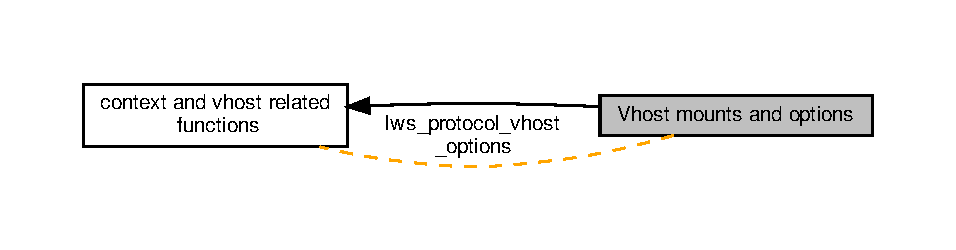
\includegraphics[width=350pt]{group__vhost-mounts}
\end{center}
\end{figure}
\subsection*{Classes}
\begin{DoxyCompactItemize}
\item 
struct \hyperlink{structlws__protocol__vhost__options}{lws\+\_\+protocol\+\_\+vhost\+\_\+options}
\item 
struct \hyperlink{structlws__http__mount}{lws\+\_\+http\+\_\+mount}
\end{DoxyCompactItemize}
\subsection*{Enumerations}
\begin{DoxyCompactItemize}
\item 
enum \hyperlink{group__vhost-mounts_ga31eca18e50cb4357480f2fcad36ff437}{lws\+\_\+mount\+\_\+protocols} \{ \newline
\hyperlink{group__vhost-mounts_gga31eca18e50cb4357480f2fcad36ff437a1e9f0842b0e85db50fe648ed4ba9a4b0}{L\+W\+S\+M\+P\+R\+O\+\_\+\+H\+T\+TP} = 0, 
\hyperlink{group__vhost-mounts_gga31eca18e50cb4357480f2fcad36ff437afbd10eb4777517ed1f6bfdcf3b9ea1d1}{L\+W\+S\+M\+P\+R\+O\+\_\+\+H\+T\+T\+PS} = 1, 
\hyperlink{group__vhost-mounts_gga31eca18e50cb4357480f2fcad36ff437a42f2361cfe76cd287fa8fcfc502357e2}{L\+W\+S\+M\+P\+R\+O\+\_\+\+F\+I\+LE} = 2, 
\hyperlink{group__vhost-mounts_gga31eca18e50cb4357480f2fcad36ff437a13ab58b01ac6e05f595977f1e0f0db69}{L\+W\+S\+M\+P\+R\+O\+\_\+\+C\+GI} = 3, 
\newline
\hyperlink{group__vhost-mounts_gga31eca18e50cb4357480f2fcad36ff437aec137a2434851bd856ceebfb697b9970}{L\+W\+S\+M\+P\+R\+O\+\_\+\+R\+E\+D\+I\+R\+\_\+\+H\+T\+TP} = 4, 
\hyperlink{group__vhost-mounts_gga31eca18e50cb4357480f2fcad36ff437a8894d16316863077dfe530963ca59f67}{L\+W\+S\+M\+P\+R\+O\+\_\+\+R\+E\+D\+I\+R\+\_\+\+H\+T\+T\+PS} = 5, 
\hyperlink{group__vhost-mounts_gga31eca18e50cb4357480f2fcad36ff437a946a88cf9c852eed2c0317f4115d19da}{L\+W\+S\+M\+P\+R\+O\+\_\+\+C\+A\+L\+L\+B\+A\+CK} = 6, 
\hyperlink{group__vhost-mounts_gga31eca18e50cb4357480f2fcad36ff437a1e9f0842b0e85db50fe648ed4ba9a4b0}{L\+W\+S\+M\+P\+R\+O\+\_\+\+H\+T\+TP} = 0, 
\newline
\hyperlink{group__vhost-mounts_gga31eca18e50cb4357480f2fcad36ff437afbd10eb4777517ed1f6bfdcf3b9ea1d1}{L\+W\+S\+M\+P\+R\+O\+\_\+\+H\+T\+T\+PS} = 1, 
\hyperlink{group__vhost-mounts_gga31eca18e50cb4357480f2fcad36ff437a42f2361cfe76cd287fa8fcfc502357e2}{L\+W\+S\+M\+P\+R\+O\+\_\+\+F\+I\+LE} = 2, 
\hyperlink{group__vhost-mounts_gga31eca18e50cb4357480f2fcad36ff437a13ab58b01ac6e05f595977f1e0f0db69}{L\+W\+S\+M\+P\+R\+O\+\_\+\+C\+GI} = 3, 
\hyperlink{group__vhost-mounts_gga31eca18e50cb4357480f2fcad36ff437aec137a2434851bd856ceebfb697b9970}{L\+W\+S\+M\+P\+R\+O\+\_\+\+R\+E\+D\+I\+R\+\_\+\+H\+T\+TP} = 4, 
\newline
\hyperlink{group__vhost-mounts_gga31eca18e50cb4357480f2fcad36ff437a8894d16316863077dfe530963ca59f67}{L\+W\+S\+M\+P\+R\+O\+\_\+\+R\+E\+D\+I\+R\+\_\+\+H\+T\+T\+PS} = 5, 
\hyperlink{group__vhost-mounts_gga31eca18e50cb4357480f2fcad36ff437a946a88cf9c852eed2c0317f4115d19da}{L\+W\+S\+M\+P\+R\+O\+\_\+\+C\+A\+L\+L\+B\+A\+CK} = 6, 
\hyperlink{group__vhost-mounts_gga31eca18e50cb4357480f2fcad36ff437a1e9f0842b0e85db50fe648ed4ba9a4b0}{L\+W\+S\+M\+P\+R\+O\+\_\+\+H\+T\+TP} = 0, 
\hyperlink{group__vhost-mounts_gga31eca18e50cb4357480f2fcad36ff437afbd10eb4777517ed1f6bfdcf3b9ea1d1}{L\+W\+S\+M\+P\+R\+O\+\_\+\+H\+T\+T\+PS} = 1, 
\newline
\hyperlink{group__vhost-mounts_gga31eca18e50cb4357480f2fcad36ff437a42f2361cfe76cd287fa8fcfc502357e2}{L\+W\+S\+M\+P\+R\+O\+\_\+\+F\+I\+LE} = 2, 
\hyperlink{group__vhost-mounts_gga31eca18e50cb4357480f2fcad36ff437a13ab58b01ac6e05f595977f1e0f0db69}{L\+W\+S\+M\+P\+R\+O\+\_\+\+C\+GI} = 3, 
\hyperlink{group__vhost-mounts_gga31eca18e50cb4357480f2fcad36ff437aec137a2434851bd856ceebfb697b9970}{L\+W\+S\+M\+P\+R\+O\+\_\+\+R\+E\+D\+I\+R\+\_\+\+H\+T\+TP} = 4, 
\hyperlink{group__vhost-mounts_gga31eca18e50cb4357480f2fcad36ff437a8894d16316863077dfe530963ca59f67}{L\+W\+S\+M\+P\+R\+O\+\_\+\+R\+E\+D\+I\+R\+\_\+\+H\+T\+T\+PS} = 5, 
\newline
\hyperlink{group__vhost-mounts_gga31eca18e50cb4357480f2fcad36ff437a946a88cf9c852eed2c0317f4115d19da}{L\+W\+S\+M\+P\+R\+O\+\_\+\+C\+A\+L\+L\+B\+A\+CK} = 6, 
\hyperlink{group__vhost-mounts_gga31eca18e50cb4357480f2fcad36ff437a1e9f0842b0e85db50fe648ed4ba9a4b0}{L\+W\+S\+M\+P\+R\+O\+\_\+\+H\+T\+TP} = 0, 
\hyperlink{group__vhost-mounts_gga31eca18e50cb4357480f2fcad36ff437afbd10eb4777517ed1f6bfdcf3b9ea1d1}{L\+W\+S\+M\+P\+R\+O\+\_\+\+H\+T\+T\+PS} = 1, 
\hyperlink{group__vhost-mounts_gga31eca18e50cb4357480f2fcad36ff437a42f2361cfe76cd287fa8fcfc502357e2}{L\+W\+S\+M\+P\+R\+O\+\_\+\+F\+I\+LE} = 2, 
\newline
\hyperlink{group__vhost-mounts_gga31eca18e50cb4357480f2fcad36ff437a13ab58b01ac6e05f595977f1e0f0db69}{L\+W\+S\+M\+P\+R\+O\+\_\+\+C\+GI} = 3, 
\hyperlink{group__vhost-mounts_gga31eca18e50cb4357480f2fcad36ff437aec137a2434851bd856ceebfb697b9970}{L\+W\+S\+M\+P\+R\+O\+\_\+\+R\+E\+D\+I\+R\+\_\+\+H\+T\+TP} = 4, 
\hyperlink{group__vhost-mounts_gga31eca18e50cb4357480f2fcad36ff437a8894d16316863077dfe530963ca59f67}{L\+W\+S\+M\+P\+R\+O\+\_\+\+R\+E\+D\+I\+R\+\_\+\+H\+T\+T\+PS} = 5, 
\hyperlink{group__vhost-mounts_gga31eca18e50cb4357480f2fcad36ff437a946a88cf9c852eed2c0317f4115d19da}{L\+W\+S\+M\+P\+R\+O\+\_\+\+C\+A\+L\+L\+B\+A\+CK} = 6, 
\newline
\hyperlink{group__vhost-mounts_gga31eca18e50cb4357480f2fcad36ff437a1e9f0842b0e85db50fe648ed4ba9a4b0}{L\+W\+S\+M\+P\+R\+O\+\_\+\+H\+T\+TP} = 0, 
\hyperlink{group__vhost-mounts_gga31eca18e50cb4357480f2fcad36ff437afbd10eb4777517ed1f6bfdcf3b9ea1d1}{L\+W\+S\+M\+P\+R\+O\+\_\+\+H\+T\+T\+PS} = 1, 
\hyperlink{group__vhost-mounts_gga31eca18e50cb4357480f2fcad36ff437a42f2361cfe76cd287fa8fcfc502357e2}{L\+W\+S\+M\+P\+R\+O\+\_\+\+F\+I\+LE} = 2, 
\hyperlink{group__vhost-mounts_gga31eca18e50cb4357480f2fcad36ff437a13ab58b01ac6e05f595977f1e0f0db69}{L\+W\+S\+M\+P\+R\+O\+\_\+\+C\+GI} = 3, 
\newline
\hyperlink{group__vhost-mounts_gga31eca18e50cb4357480f2fcad36ff437aec137a2434851bd856ceebfb697b9970}{L\+W\+S\+M\+P\+R\+O\+\_\+\+R\+E\+D\+I\+R\+\_\+\+H\+T\+TP} = 4, 
\hyperlink{group__vhost-mounts_gga31eca18e50cb4357480f2fcad36ff437a8894d16316863077dfe530963ca59f67}{L\+W\+S\+M\+P\+R\+O\+\_\+\+R\+E\+D\+I\+R\+\_\+\+H\+T\+T\+PS} = 5, 
\hyperlink{group__vhost-mounts_gga31eca18e50cb4357480f2fcad36ff437a946a88cf9c852eed2c0317f4115d19da}{L\+W\+S\+M\+P\+R\+O\+\_\+\+C\+A\+L\+L\+B\+A\+CK} = 6, 
\hyperlink{group__vhost-mounts_gga31eca18e50cb4357480f2fcad36ff437a1e9f0842b0e85db50fe648ed4ba9a4b0}{L\+W\+S\+M\+P\+R\+O\+\_\+\+H\+T\+TP} = 0, 
\newline
\hyperlink{group__vhost-mounts_gga31eca18e50cb4357480f2fcad36ff437afbd10eb4777517ed1f6bfdcf3b9ea1d1}{L\+W\+S\+M\+P\+R\+O\+\_\+\+H\+T\+T\+PS} = 1, 
\hyperlink{group__vhost-mounts_gga31eca18e50cb4357480f2fcad36ff437a42f2361cfe76cd287fa8fcfc502357e2}{L\+W\+S\+M\+P\+R\+O\+\_\+\+F\+I\+LE} = 2, 
\hyperlink{group__vhost-mounts_gga31eca18e50cb4357480f2fcad36ff437a13ab58b01ac6e05f595977f1e0f0db69}{L\+W\+S\+M\+P\+R\+O\+\_\+\+C\+GI} = 3, 
\hyperlink{group__vhost-mounts_gga31eca18e50cb4357480f2fcad36ff437aec137a2434851bd856ceebfb697b9970}{L\+W\+S\+M\+P\+R\+O\+\_\+\+R\+E\+D\+I\+R\+\_\+\+H\+T\+TP} = 4, 
\newline
\hyperlink{group__vhost-mounts_gga31eca18e50cb4357480f2fcad36ff437a8894d16316863077dfe530963ca59f67}{L\+W\+S\+M\+P\+R\+O\+\_\+\+R\+E\+D\+I\+R\+\_\+\+H\+T\+T\+PS} = 5, 
\hyperlink{group__vhost-mounts_gga31eca18e50cb4357480f2fcad36ff437a946a88cf9c852eed2c0317f4115d19da}{L\+W\+S\+M\+P\+R\+O\+\_\+\+C\+A\+L\+L\+B\+A\+CK} = 6, 
\hyperlink{group__vhost-mounts_gga31eca18e50cb4357480f2fcad36ff437a1e9f0842b0e85db50fe648ed4ba9a4b0}{L\+W\+S\+M\+P\+R\+O\+\_\+\+H\+T\+TP} = 0, 
\hyperlink{group__vhost-mounts_gga31eca18e50cb4357480f2fcad36ff437afbd10eb4777517ed1f6bfdcf3b9ea1d1}{L\+W\+S\+M\+P\+R\+O\+\_\+\+H\+T\+T\+PS} = 1, 
\newline
\hyperlink{group__vhost-mounts_gga31eca18e50cb4357480f2fcad36ff437a42f2361cfe76cd287fa8fcfc502357e2}{L\+W\+S\+M\+P\+R\+O\+\_\+\+F\+I\+LE} = 2, 
\hyperlink{group__vhost-mounts_gga31eca18e50cb4357480f2fcad36ff437a13ab58b01ac6e05f595977f1e0f0db69}{L\+W\+S\+M\+P\+R\+O\+\_\+\+C\+GI} = 3, 
\hyperlink{group__vhost-mounts_gga31eca18e50cb4357480f2fcad36ff437aec137a2434851bd856ceebfb697b9970}{L\+W\+S\+M\+P\+R\+O\+\_\+\+R\+E\+D\+I\+R\+\_\+\+H\+T\+TP} = 4, 
\hyperlink{group__vhost-mounts_gga31eca18e50cb4357480f2fcad36ff437a8894d16316863077dfe530963ca59f67}{L\+W\+S\+M\+P\+R\+O\+\_\+\+R\+E\+D\+I\+R\+\_\+\+H\+T\+T\+PS} = 5, 
\newline
\hyperlink{group__vhost-mounts_gga31eca18e50cb4357480f2fcad36ff437a946a88cf9c852eed2c0317f4115d19da}{L\+W\+S\+M\+P\+R\+O\+\_\+\+C\+A\+L\+L\+B\+A\+CK} = 6, 
\hyperlink{group__vhost-mounts_gga31eca18e50cb4357480f2fcad36ff437a1e9f0842b0e85db50fe648ed4ba9a4b0}{L\+W\+S\+M\+P\+R\+O\+\_\+\+H\+T\+TP} = 0, 
\hyperlink{group__vhost-mounts_gga31eca18e50cb4357480f2fcad36ff437afbd10eb4777517ed1f6bfdcf3b9ea1d1}{L\+W\+S\+M\+P\+R\+O\+\_\+\+H\+T\+T\+PS} = 1, 
\hyperlink{group__vhost-mounts_gga31eca18e50cb4357480f2fcad36ff437a42f2361cfe76cd287fa8fcfc502357e2}{L\+W\+S\+M\+P\+R\+O\+\_\+\+F\+I\+LE} = 2, 
\newline
\hyperlink{group__vhost-mounts_gga31eca18e50cb4357480f2fcad36ff437a13ab58b01ac6e05f595977f1e0f0db69}{L\+W\+S\+M\+P\+R\+O\+\_\+\+C\+GI} = 3, 
\hyperlink{group__vhost-mounts_gga31eca18e50cb4357480f2fcad36ff437aec137a2434851bd856ceebfb697b9970}{L\+W\+S\+M\+P\+R\+O\+\_\+\+R\+E\+D\+I\+R\+\_\+\+H\+T\+TP} = 4, 
\hyperlink{group__vhost-mounts_gga31eca18e50cb4357480f2fcad36ff437a8894d16316863077dfe530963ca59f67}{L\+W\+S\+M\+P\+R\+O\+\_\+\+R\+E\+D\+I\+R\+\_\+\+H\+T\+T\+PS} = 5, 
\hyperlink{group__vhost-mounts_gga31eca18e50cb4357480f2fcad36ff437a946a88cf9c852eed2c0317f4115d19da}{L\+W\+S\+M\+P\+R\+O\+\_\+\+C\+A\+L\+L\+B\+A\+CK} = 6
 \}
\item 
enum \hyperlink{group__vhost-mounts_ga31eca18e50cb4357480f2fcad36ff437}{lws\+\_\+mount\+\_\+protocols} \{ \newline
\hyperlink{group__vhost-mounts_gga31eca18e50cb4357480f2fcad36ff437a1e9f0842b0e85db50fe648ed4ba9a4b0}{L\+W\+S\+M\+P\+R\+O\+\_\+\+H\+T\+TP} = 0, 
\hyperlink{group__vhost-mounts_gga31eca18e50cb4357480f2fcad36ff437afbd10eb4777517ed1f6bfdcf3b9ea1d1}{L\+W\+S\+M\+P\+R\+O\+\_\+\+H\+T\+T\+PS} = 1, 
\hyperlink{group__vhost-mounts_gga31eca18e50cb4357480f2fcad36ff437a42f2361cfe76cd287fa8fcfc502357e2}{L\+W\+S\+M\+P\+R\+O\+\_\+\+F\+I\+LE} = 2, 
\hyperlink{group__vhost-mounts_gga31eca18e50cb4357480f2fcad36ff437a13ab58b01ac6e05f595977f1e0f0db69}{L\+W\+S\+M\+P\+R\+O\+\_\+\+C\+GI} = 3, 
\newline
\hyperlink{group__vhost-mounts_gga31eca18e50cb4357480f2fcad36ff437aec137a2434851bd856ceebfb697b9970}{L\+W\+S\+M\+P\+R\+O\+\_\+\+R\+E\+D\+I\+R\+\_\+\+H\+T\+TP} = 4, 
\hyperlink{group__vhost-mounts_gga31eca18e50cb4357480f2fcad36ff437a8894d16316863077dfe530963ca59f67}{L\+W\+S\+M\+P\+R\+O\+\_\+\+R\+E\+D\+I\+R\+\_\+\+H\+T\+T\+PS} = 5, 
\hyperlink{group__vhost-mounts_gga31eca18e50cb4357480f2fcad36ff437a946a88cf9c852eed2c0317f4115d19da}{L\+W\+S\+M\+P\+R\+O\+\_\+\+C\+A\+L\+L\+B\+A\+CK} = 6, 
\hyperlink{group__vhost-mounts_gga31eca18e50cb4357480f2fcad36ff437a1e9f0842b0e85db50fe648ed4ba9a4b0}{L\+W\+S\+M\+P\+R\+O\+\_\+\+H\+T\+TP} = 0, 
\newline
\hyperlink{group__vhost-mounts_gga31eca18e50cb4357480f2fcad36ff437afbd10eb4777517ed1f6bfdcf3b9ea1d1}{L\+W\+S\+M\+P\+R\+O\+\_\+\+H\+T\+T\+PS} = 1, 
\hyperlink{group__vhost-mounts_gga31eca18e50cb4357480f2fcad36ff437a42f2361cfe76cd287fa8fcfc502357e2}{L\+W\+S\+M\+P\+R\+O\+\_\+\+F\+I\+LE} = 2, 
\hyperlink{group__vhost-mounts_gga31eca18e50cb4357480f2fcad36ff437a13ab58b01ac6e05f595977f1e0f0db69}{L\+W\+S\+M\+P\+R\+O\+\_\+\+C\+GI} = 3, 
\hyperlink{group__vhost-mounts_gga31eca18e50cb4357480f2fcad36ff437aec137a2434851bd856ceebfb697b9970}{L\+W\+S\+M\+P\+R\+O\+\_\+\+R\+E\+D\+I\+R\+\_\+\+H\+T\+TP} = 4, 
\newline
\hyperlink{group__vhost-mounts_gga31eca18e50cb4357480f2fcad36ff437a8894d16316863077dfe530963ca59f67}{L\+W\+S\+M\+P\+R\+O\+\_\+\+R\+E\+D\+I\+R\+\_\+\+H\+T\+T\+PS} = 5, 
\hyperlink{group__vhost-mounts_gga31eca18e50cb4357480f2fcad36ff437a946a88cf9c852eed2c0317f4115d19da}{L\+W\+S\+M\+P\+R\+O\+\_\+\+C\+A\+L\+L\+B\+A\+CK} = 6, 
\hyperlink{group__vhost-mounts_gga31eca18e50cb4357480f2fcad36ff437a1e9f0842b0e85db50fe648ed4ba9a4b0}{L\+W\+S\+M\+P\+R\+O\+\_\+\+H\+T\+TP} = 0, 
\hyperlink{group__vhost-mounts_gga31eca18e50cb4357480f2fcad36ff437afbd10eb4777517ed1f6bfdcf3b9ea1d1}{L\+W\+S\+M\+P\+R\+O\+\_\+\+H\+T\+T\+PS} = 1, 
\newline
\hyperlink{group__vhost-mounts_gga31eca18e50cb4357480f2fcad36ff437a42f2361cfe76cd287fa8fcfc502357e2}{L\+W\+S\+M\+P\+R\+O\+\_\+\+F\+I\+LE} = 2, 
\hyperlink{group__vhost-mounts_gga31eca18e50cb4357480f2fcad36ff437a13ab58b01ac6e05f595977f1e0f0db69}{L\+W\+S\+M\+P\+R\+O\+\_\+\+C\+GI} = 3, 
\hyperlink{group__vhost-mounts_gga31eca18e50cb4357480f2fcad36ff437aec137a2434851bd856ceebfb697b9970}{L\+W\+S\+M\+P\+R\+O\+\_\+\+R\+E\+D\+I\+R\+\_\+\+H\+T\+TP} = 4, 
\hyperlink{group__vhost-mounts_gga31eca18e50cb4357480f2fcad36ff437a8894d16316863077dfe530963ca59f67}{L\+W\+S\+M\+P\+R\+O\+\_\+\+R\+E\+D\+I\+R\+\_\+\+H\+T\+T\+PS} = 5, 
\newline
\hyperlink{group__vhost-mounts_gga31eca18e50cb4357480f2fcad36ff437a946a88cf9c852eed2c0317f4115d19da}{L\+W\+S\+M\+P\+R\+O\+\_\+\+C\+A\+L\+L\+B\+A\+CK} = 6, 
\hyperlink{group__vhost-mounts_gga31eca18e50cb4357480f2fcad36ff437a1e9f0842b0e85db50fe648ed4ba9a4b0}{L\+W\+S\+M\+P\+R\+O\+\_\+\+H\+T\+TP} = 0, 
\hyperlink{group__vhost-mounts_gga31eca18e50cb4357480f2fcad36ff437afbd10eb4777517ed1f6bfdcf3b9ea1d1}{L\+W\+S\+M\+P\+R\+O\+\_\+\+H\+T\+T\+PS} = 1, 
\hyperlink{group__vhost-mounts_gga31eca18e50cb4357480f2fcad36ff437a42f2361cfe76cd287fa8fcfc502357e2}{L\+W\+S\+M\+P\+R\+O\+\_\+\+F\+I\+LE} = 2, 
\newline
\hyperlink{group__vhost-mounts_gga31eca18e50cb4357480f2fcad36ff437a13ab58b01ac6e05f595977f1e0f0db69}{L\+W\+S\+M\+P\+R\+O\+\_\+\+C\+GI} = 3, 
\hyperlink{group__vhost-mounts_gga31eca18e50cb4357480f2fcad36ff437aec137a2434851bd856ceebfb697b9970}{L\+W\+S\+M\+P\+R\+O\+\_\+\+R\+E\+D\+I\+R\+\_\+\+H\+T\+TP} = 4, 
\hyperlink{group__vhost-mounts_gga31eca18e50cb4357480f2fcad36ff437a8894d16316863077dfe530963ca59f67}{L\+W\+S\+M\+P\+R\+O\+\_\+\+R\+E\+D\+I\+R\+\_\+\+H\+T\+T\+PS} = 5, 
\hyperlink{group__vhost-mounts_gga31eca18e50cb4357480f2fcad36ff437a946a88cf9c852eed2c0317f4115d19da}{L\+W\+S\+M\+P\+R\+O\+\_\+\+C\+A\+L\+L\+B\+A\+CK} = 6, 
\newline
\hyperlink{group__vhost-mounts_gga31eca18e50cb4357480f2fcad36ff437a1e9f0842b0e85db50fe648ed4ba9a4b0}{L\+W\+S\+M\+P\+R\+O\+\_\+\+H\+T\+TP} = 0, 
\hyperlink{group__vhost-mounts_gga31eca18e50cb4357480f2fcad36ff437afbd10eb4777517ed1f6bfdcf3b9ea1d1}{L\+W\+S\+M\+P\+R\+O\+\_\+\+H\+T\+T\+PS} = 1, 
\hyperlink{group__vhost-mounts_gga31eca18e50cb4357480f2fcad36ff437a42f2361cfe76cd287fa8fcfc502357e2}{L\+W\+S\+M\+P\+R\+O\+\_\+\+F\+I\+LE} = 2, 
\hyperlink{group__vhost-mounts_gga31eca18e50cb4357480f2fcad36ff437a13ab58b01ac6e05f595977f1e0f0db69}{L\+W\+S\+M\+P\+R\+O\+\_\+\+C\+GI} = 3, 
\newline
\hyperlink{group__vhost-mounts_gga31eca18e50cb4357480f2fcad36ff437aec137a2434851bd856ceebfb697b9970}{L\+W\+S\+M\+P\+R\+O\+\_\+\+R\+E\+D\+I\+R\+\_\+\+H\+T\+TP} = 4, 
\hyperlink{group__vhost-mounts_gga31eca18e50cb4357480f2fcad36ff437a8894d16316863077dfe530963ca59f67}{L\+W\+S\+M\+P\+R\+O\+\_\+\+R\+E\+D\+I\+R\+\_\+\+H\+T\+T\+PS} = 5, 
\hyperlink{group__vhost-mounts_gga31eca18e50cb4357480f2fcad36ff437a946a88cf9c852eed2c0317f4115d19da}{L\+W\+S\+M\+P\+R\+O\+\_\+\+C\+A\+L\+L\+B\+A\+CK} = 6, 
\hyperlink{group__vhost-mounts_gga31eca18e50cb4357480f2fcad36ff437a1e9f0842b0e85db50fe648ed4ba9a4b0}{L\+W\+S\+M\+P\+R\+O\+\_\+\+H\+T\+TP} = 0, 
\newline
\hyperlink{group__vhost-mounts_gga31eca18e50cb4357480f2fcad36ff437afbd10eb4777517ed1f6bfdcf3b9ea1d1}{L\+W\+S\+M\+P\+R\+O\+\_\+\+H\+T\+T\+PS} = 1, 
\hyperlink{group__vhost-mounts_gga31eca18e50cb4357480f2fcad36ff437a42f2361cfe76cd287fa8fcfc502357e2}{L\+W\+S\+M\+P\+R\+O\+\_\+\+F\+I\+LE} = 2, 
\hyperlink{group__vhost-mounts_gga31eca18e50cb4357480f2fcad36ff437a13ab58b01ac6e05f595977f1e0f0db69}{L\+W\+S\+M\+P\+R\+O\+\_\+\+C\+GI} = 3, 
\hyperlink{group__vhost-mounts_gga31eca18e50cb4357480f2fcad36ff437aec137a2434851bd856ceebfb697b9970}{L\+W\+S\+M\+P\+R\+O\+\_\+\+R\+E\+D\+I\+R\+\_\+\+H\+T\+TP} = 4, 
\newline
\hyperlink{group__vhost-mounts_gga31eca18e50cb4357480f2fcad36ff437a8894d16316863077dfe530963ca59f67}{L\+W\+S\+M\+P\+R\+O\+\_\+\+R\+E\+D\+I\+R\+\_\+\+H\+T\+T\+PS} = 5, 
\hyperlink{group__vhost-mounts_gga31eca18e50cb4357480f2fcad36ff437a946a88cf9c852eed2c0317f4115d19da}{L\+W\+S\+M\+P\+R\+O\+\_\+\+C\+A\+L\+L\+B\+A\+CK} = 6, 
\hyperlink{group__vhost-mounts_gga31eca18e50cb4357480f2fcad36ff437a1e9f0842b0e85db50fe648ed4ba9a4b0}{L\+W\+S\+M\+P\+R\+O\+\_\+\+H\+T\+TP} = 0, 
\hyperlink{group__vhost-mounts_gga31eca18e50cb4357480f2fcad36ff437afbd10eb4777517ed1f6bfdcf3b9ea1d1}{L\+W\+S\+M\+P\+R\+O\+\_\+\+H\+T\+T\+PS} = 1, 
\newline
\hyperlink{group__vhost-mounts_gga31eca18e50cb4357480f2fcad36ff437a42f2361cfe76cd287fa8fcfc502357e2}{L\+W\+S\+M\+P\+R\+O\+\_\+\+F\+I\+LE} = 2, 
\hyperlink{group__vhost-mounts_gga31eca18e50cb4357480f2fcad36ff437a13ab58b01ac6e05f595977f1e0f0db69}{L\+W\+S\+M\+P\+R\+O\+\_\+\+C\+GI} = 3, 
\hyperlink{group__vhost-mounts_gga31eca18e50cb4357480f2fcad36ff437aec137a2434851bd856ceebfb697b9970}{L\+W\+S\+M\+P\+R\+O\+\_\+\+R\+E\+D\+I\+R\+\_\+\+H\+T\+TP} = 4, 
\hyperlink{group__vhost-mounts_gga31eca18e50cb4357480f2fcad36ff437a8894d16316863077dfe530963ca59f67}{L\+W\+S\+M\+P\+R\+O\+\_\+\+R\+E\+D\+I\+R\+\_\+\+H\+T\+T\+PS} = 5, 
\newline
\hyperlink{group__vhost-mounts_gga31eca18e50cb4357480f2fcad36ff437a946a88cf9c852eed2c0317f4115d19da}{L\+W\+S\+M\+P\+R\+O\+\_\+\+C\+A\+L\+L\+B\+A\+CK} = 6, 
\hyperlink{group__vhost-mounts_gga31eca18e50cb4357480f2fcad36ff437a1e9f0842b0e85db50fe648ed4ba9a4b0}{L\+W\+S\+M\+P\+R\+O\+\_\+\+H\+T\+TP} = 0, 
\hyperlink{group__vhost-mounts_gga31eca18e50cb4357480f2fcad36ff437afbd10eb4777517ed1f6bfdcf3b9ea1d1}{L\+W\+S\+M\+P\+R\+O\+\_\+\+H\+T\+T\+PS} = 1, 
\hyperlink{group__vhost-mounts_gga31eca18e50cb4357480f2fcad36ff437a42f2361cfe76cd287fa8fcfc502357e2}{L\+W\+S\+M\+P\+R\+O\+\_\+\+F\+I\+LE} = 2, 
\newline
\hyperlink{group__vhost-mounts_gga31eca18e50cb4357480f2fcad36ff437a13ab58b01ac6e05f595977f1e0f0db69}{L\+W\+S\+M\+P\+R\+O\+\_\+\+C\+GI} = 3, 
\hyperlink{group__vhost-mounts_gga31eca18e50cb4357480f2fcad36ff437aec137a2434851bd856ceebfb697b9970}{L\+W\+S\+M\+P\+R\+O\+\_\+\+R\+E\+D\+I\+R\+\_\+\+H\+T\+TP} = 4, 
\hyperlink{group__vhost-mounts_gga31eca18e50cb4357480f2fcad36ff437a8894d16316863077dfe530963ca59f67}{L\+W\+S\+M\+P\+R\+O\+\_\+\+R\+E\+D\+I\+R\+\_\+\+H\+T\+T\+PS} = 5, 
\hyperlink{group__vhost-mounts_gga31eca18e50cb4357480f2fcad36ff437a946a88cf9c852eed2c0317f4115d19da}{L\+W\+S\+M\+P\+R\+O\+\_\+\+C\+A\+L\+L\+B\+A\+CK} = 6
 \}
\item 
enum \hyperlink{group__vhost-mounts_ga31eca18e50cb4357480f2fcad36ff437}{lws\+\_\+mount\+\_\+protocols} \{ \newline
\hyperlink{group__vhost-mounts_gga31eca18e50cb4357480f2fcad36ff437a1e9f0842b0e85db50fe648ed4ba9a4b0}{L\+W\+S\+M\+P\+R\+O\+\_\+\+H\+T\+TP} = 0, 
\hyperlink{group__vhost-mounts_gga31eca18e50cb4357480f2fcad36ff437afbd10eb4777517ed1f6bfdcf3b9ea1d1}{L\+W\+S\+M\+P\+R\+O\+\_\+\+H\+T\+T\+PS} = 1, 
\hyperlink{group__vhost-mounts_gga31eca18e50cb4357480f2fcad36ff437a42f2361cfe76cd287fa8fcfc502357e2}{L\+W\+S\+M\+P\+R\+O\+\_\+\+F\+I\+LE} = 2, 
\hyperlink{group__vhost-mounts_gga31eca18e50cb4357480f2fcad36ff437a13ab58b01ac6e05f595977f1e0f0db69}{L\+W\+S\+M\+P\+R\+O\+\_\+\+C\+GI} = 3, 
\newline
\hyperlink{group__vhost-mounts_gga31eca18e50cb4357480f2fcad36ff437aec137a2434851bd856ceebfb697b9970}{L\+W\+S\+M\+P\+R\+O\+\_\+\+R\+E\+D\+I\+R\+\_\+\+H\+T\+TP} = 4, 
\hyperlink{group__vhost-mounts_gga31eca18e50cb4357480f2fcad36ff437a8894d16316863077dfe530963ca59f67}{L\+W\+S\+M\+P\+R\+O\+\_\+\+R\+E\+D\+I\+R\+\_\+\+H\+T\+T\+PS} = 5, 
\hyperlink{group__vhost-mounts_gga31eca18e50cb4357480f2fcad36ff437a946a88cf9c852eed2c0317f4115d19da}{L\+W\+S\+M\+P\+R\+O\+\_\+\+C\+A\+L\+L\+B\+A\+CK} = 6, 
\hyperlink{group__vhost-mounts_gga31eca18e50cb4357480f2fcad36ff437a1e9f0842b0e85db50fe648ed4ba9a4b0}{L\+W\+S\+M\+P\+R\+O\+\_\+\+H\+T\+TP} = 0, 
\newline
\hyperlink{group__vhost-mounts_gga31eca18e50cb4357480f2fcad36ff437afbd10eb4777517ed1f6bfdcf3b9ea1d1}{L\+W\+S\+M\+P\+R\+O\+\_\+\+H\+T\+T\+PS} = 1, 
\hyperlink{group__vhost-mounts_gga31eca18e50cb4357480f2fcad36ff437a42f2361cfe76cd287fa8fcfc502357e2}{L\+W\+S\+M\+P\+R\+O\+\_\+\+F\+I\+LE} = 2, 
\hyperlink{group__vhost-mounts_gga31eca18e50cb4357480f2fcad36ff437a13ab58b01ac6e05f595977f1e0f0db69}{L\+W\+S\+M\+P\+R\+O\+\_\+\+C\+GI} = 3, 
\hyperlink{group__vhost-mounts_gga31eca18e50cb4357480f2fcad36ff437aec137a2434851bd856ceebfb697b9970}{L\+W\+S\+M\+P\+R\+O\+\_\+\+R\+E\+D\+I\+R\+\_\+\+H\+T\+TP} = 4, 
\newline
\hyperlink{group__vhost-mounts_gga31eca18e50cb4357480f2fcad36ff437a8894d16316863077dfe530963ca59f67}{L\+W\+S\+M\+P\+R\+O\+\_\+\+R\+E\+D\+I\+R\+\_\+\+H\+T\+T\+PS} = 5, 
\hyperlink{group__vhost-mounts_gga31eca18e50cb4357480f2fcad36ff437a946a88cf9c852eed2c0317f4115d19da}{L\+W\+S\+M\+P\+R\+O\+\_\+\+C\+A\+L\+L\+B\+A\+CK} = 6, 
\hyperlink{group__vhost-mounts_gga31eca18e50cb4357480f2fcad36ff437a1e9f0842b0e85db50fe648ed4ba9a4b0}{L\+W\+S\+M\+P\+R\+O\+\_\+\+H\+T\+TP} = 0, 
\hyperlink{group__vhost-mounts_gga31eca18e50cb4357480f2fcad36ff437afbd10eb4777517ed1f6bfdcf3b9ea1d1}{L\+W\+S\+M\+P\+R\+O\+\_\+\+H\+T\+T\+PS} = 1, 
\newline
\hyperlink{group__vhost-mounts_gga31eca18e50cb4357480f2fcad36ff437a42f2361cfe76cd287fa8fcfc502357e2}{L\+W\+S\+M\+P\+R\+O\+\_\+\+F\+I\+LE} = 2, 
\hyperlink{group__vhost-mounts_gga31eca18e50cb4357480f2fcad36ff437a13ab58b01ac6e05f595977f1e0f0db69}{L\+W\+S\+M\+P\+R\+O\+\_\+\+C\+GI} = 3, 
\hyperlink{group__vhost-mounts_gga31eca18e50cb4357480f2fcad36ff437aec137a2434851bd856ceebfb697b9970}{L\+W\+S\+M\+P\+R\+O\+\_\+\+R\+E\+D\+I\+R\+\_\+\+H\+T\+TP} = 4, 
\hyperlink{group__vhost-mounts_gga31eca18e50cb4357480f2fcad36ff437a8894d16316863077dfe530963ca59f67}{L\+W\+S\+M\+P\+R\+O\+\_\+\+R\+E\+D\+I\+R\+\_\+\+H\+T\+T\+PS} = 5, 
\newline
\hyperlink{group__vhost-mounts_gga31eca18e50cb4357480f2fcad36ff437a946a88cf9c852eed2c0317f4115d19da}{L\+W\+S\+M\+P\+R\+O\+\_\+\+C\+A\+L\+L\+B\+A\+CK} = 6, 
\hyperlink{group__vhost-mounts_gga31eca18e50cb4357480f2fcad36ff437a1e9f0842b0e85db50fe648ed4ba9a4b0}{L\+W\+S\+M\+P\+R\+O\+\_\+\+H\+T\+TP} = 0, 
\hyperlink{group__vhost-mounts_gga31eca18e50cb4357480f2fcad36ff437afbd10eb4777517ed1f6bfdcf3b9ea1d1}{L\+W\+S\+M\+P\+R\+O\+\_\+\+H\+T\+T\+PS} = 1, 
\hyperlink{group__vhost-mounts_gga31eca18e50cb4357480f2fcad36ff437a42f2361cfe76cd287fa8fcfc502357e2}{L\+W\+S\+M\+P\+R\+O\+\_\+\+F\+I\+LE} = 2, 
\newline
\hyperlink{group__vhost-mounts_gga31eca18e50cb4357480f2fcad36ff437a13ab58b01ac6e05f595977f1e0f0db69}{L\+W\+S\+M\+P\+R\+O\+\_\+\+C\+GI} = 3, 
\hyperlink{group__vhost-mounts_gga31eca18e50cb4357480f2fcad36ff437aec137a2434851bd856ceebfb697b9970}{L\+W\+S\+M\+P\+R\+O\+\_\+\+R\+E\+D\+I\+R\+\_\+\+H\+T\+TP} = 4, 
\hyperlink{group__vhost-mounts_gga31eca18e50cb4357480f2fcad36ff437a8894d16316863077dfe530963ca59f67}{L\+W\+S\+M\+P\+R\+O\+\_\+\+R\+E\+D\+I\+R\+\_\+\+H\+T\+T\+PS} = 5, 
\hyperlink{group__vhost-mounts_gga31eca18e50cb4357480f2fcad36ff437a946a88cf9c852eed2c0317f4115d19da}{L\+W\+S\+M\+P\+R\+O\+\_\+\+C\+A\+L\+L\+B\+A\+CK} = 6, 
\newline
\hyperlink{group__vhost-mounts_gga31eca18e50cb4357480f2fcad36ff437a1e9f0842b0e85db50fe648ed4ba9a4b0}{L\+W\+S\+M\+P\+R\+O\+\_\+\+H\+T\+TP} = 0, 
\hyperlink{group__vhost-mounts_gga31eca18e50cb4357480f2fcad36ff437afbd10eb4777517ed1f6bfdcf3b9ea1d1}{L\+W\+S\+M\+P\+R\+O\+\_\+\+H\+T\+T\+PS} = 1, 
\hyperlink{group__vhost-mounts_gga31eca18e50cb4357480f2fcad36ff437a42f2361cfe76cd287fa8fcfc502357e2}{L\+W\+S\+M\+P\+R\+O\+\_\+\+F\+I\+LE} = 2, 
\hyperlink{group__vhost-mounts_gga31eca18e50cb4357480f2fcad36ff437a13ab58b01ac6e05f595977f1e0f0db69}{L\+W\+S\+M\+P\+R\+O\+\_\+\+C\+GI} = 3, 
\newline
\hyperlink{group__vhost-mounts_gga31eca18e50cb4357480f2fcad36ff437aec137a2434851bd856ceebfb697b9970}{L\+W\+S\+M\+P\+R\+O\+\_\+\+R\+E\+D\+I\+R\+\_\+\+H\+T\+TP} = 4, 
\hyperlink{group__vhost-mounts_gga31eca18e50cb4357480f2fcad36ff437a8894d16316863077dfe530963ca59f67}{L\+W\+S\+M\+P\+R\+O\+\_\+\+R\+E\+D\+I\+R\+\_\+\+H\+T\+T\+PS} = 5, 
\hyperlink{group__vhost-mounts_gga31eca18e50cb4357480f2fcad36ff437a946a88cf9c852eed2c0317f4115d19da}{L\+W\+S\+M\+P\+R\+O\+\_\+\+C\+A\+L\+L\+B\+A\+CK} = 6, 
\hyperlink{group__vhost-mounts_gga31eca18e50cb4357480f2fcad36ff437a1e9f0842b0e85db50fe648ed4ba9a4b0}{L\+W\+S\+M\+P\+R\+O\+\_\+\+H\+T\+TP} = 0, 
\newline
\hyperlink{group__vhost-mounts_gga31eca18e50cb4357480f2fcad36ff437afbd10eb4777517ed1f6bfdcf3b9ea1d1}{L\+W\+S\+M\+P\+R\+O\+\_\+\+H\+T\+T\+PS} = 1, 
\hyperlink{group__vhost-mounts_gga31eca18e50cb4357480f2fcad36ff437a42f2361cfe76cd287fa8fcfc502357e2}{L\+W\+S\+M\+P\+R\+O\+\_\+\+F\+I\+LE} = 2, 
\hyperlink{group__vhost-mounts_gga31eca18e50cb4357480f2fcad36ff437a13ab58b01ac6e05f595977f1e0f0db69}{L\+W\+S\+M\+P\+R\+O\+\_\+\+C\+GI} = 3, 
\hyperlink{group__vhost-mounts_gga31eca18e50cb4357480f2fcad36ff437aec137a2434851bd856ceebfb697b9970}{L\+W\+S\+M\+P\+R\+O\+\_\+\+R\+E\+D\+I\+R\+\_\+\+H\+T\+TP} = 4, 
\newline
\hyperlink{group__vhost-mounts_gga31eca18e50cb4357480f2fcad36ff437a8894d16316863077dfe530963ca59f67}{L\+W\+S\+M\+P\+R\+O\+\_\+\+R\+E\+D\+I\+R\+\_\+\+H\+T\+T\+PS} = 5, 
\hyperlink{group__vhost-mounts_gga31eca18e50cb4357480f2fcad36ff437a946a88cf9c852eed2c0317f4115d19da}{L\+W\+S\+M\+P\+R\+O\+\_\+\+C\+A\+L\+L\+B\+A\+CK} = 6, 
\hyperlink{group__vhost-mounts_gga31eca18e50cb4357480f2fcad36ff437a1e9f0842b0e85db50fe648ed4ba9a4b0}{L\+W\+S\+M\+P\+R\+O\+\_\+\+H\+T\+TP} = 0, 
\hyperlink{group__vhost-mounts_gga31eca18e50cb4357480f2fcad36ff437afbd10eb4777517ed1f6bfdcf3b9ea1d1}{L\+W\+S\+M\+P\+R\+O\+\_\+\+H\+T\+T\+PS} = 1, 
\newline
\hyperlink{group__vhost-mounts_gga31eca18e50cb4357480f2fcad36ff437a42f2361cfe76cd287fa8fcfc502357e2}{L\+W\+S\+M\+P\+R\+O\+\_\+\+F\+I\+LE} = 2, 
\hyperlink{group__vhost-mounts_gga31eca18e50cb4357480f2fcad36ff437a13ab58b01ac6e05f595977f1e0f0db69}{L\+W\+S\+M\+P\+R\+O\+\_\+\+C\+GI} = 3, 
\hyperlink{group__vhost-mounts_gga31eca18e50cb4357480f2fcad36ff437aec137a2434851bd856ceebfb697b9970}{L\+W\+S\+M\+P\+R\+O\+\_\+\+R\+E\+D\+I\+R\+\_\+\+H\+T\+TP} = 4, 
\hyperlink{group__vhost-mounts_gga31eca18e50cb4357480f2fcad36ff437a8894d16316863077dfe530963ca59f67}{L\+W\+S\+M\+P\+R\+O\+\_\+\+R\+E\+D\+I\+R\+\_\+\+H\+T\+T\+PS} = 5, 
\newline
\hyperlink{group__vhost-mounts_gga31eca18e50cb4357480f2fcad36ff437a946a88cf9c852eed2c0317f4115d19da}{L\+W\+S\+M\+P\+R\+O\+\_\+\+C\+A\+L\+L\+B\+A\+CK} = 6, 
\hyperlink{group__vhost-mounts_gga31eca18e50cb4357480f2fcad36ff437a1e9f0842b0e85db50fe648ed4ba9a4b0}{L\+W\+S\+M\+P\+R\+O\+\_\+\+H\+T\+TP} = 0, 
\hyperlink{group__vhost-mounts_gga31eca18e50cb4357480f2fcad36ff437afbd10eb4777517ed1f6bfdcf3b9ea1d1}{L\+W\+S\+M\+P\+R\+O\+\_\+\+H\+T\+T\+PS} = 1, 
\hyperlink{group__vhost-mounts_gga31eca18e50cb4357480f2fcad36ff437a42f2361cfe76cd287fa8fcfc502357e2}{L\+W\+S\+M\+P\+R\+O\+\_\+\+F\+I\+LE} = 2, 
\newline
\hyperlink{group__vhost-mounts_gga31eca18e50cb4357480f2fcad36ff437a13ab58b01ac6e05f595977f1e0f0db69}{L\+W\+S\+M\+P\+R\+O\+\_\+\+C\+GI} = 3, 
\hyperlink{group__vhost-mounts_gga31eca18e50cb4357480f2fcad36ff437aec137a2434851bd856ceebfb697b9970}{L\+W\+S\+M\+P\+R\+O\+\_\+\+R\+E\+D\+I\+R\+\_\+\+H\+T\+TP} = 4, 
\hyperlink{group__vhost-mounts_gga31eca18e50cb4357480f2fcad36ff437a8894d16316863077dfe530963ca59f67}{L\+W\+S\+M\+P\+R\+O\+\_\+\+R\+E\+D\+I\+R\+\_\+\+H\+T\+T\+PS} = 5, 
\hyperlink{group__vhost-mounts_gga31eca18e50cb4357480f2fcad36ff437a946a88cf9c852eed2c0317f4115d19da}{L\+W\+S\+M\+P\+R\+O\+\_\+\+C\+A\+L\+L\+B\+A\+CK} = 6
 \}
\item 
enum \hyperlink{group__vhost-mounts_ga31eca18e50cb4357480f2fcad36ff437}{lws\+\_\+mount\+\_\+protocols} \{ \newline
\hyperlink{group__vhost-mounts_gga31eca18e50cb4357480f2fcad36ff437a1e9f0842b0e85db50fe648ed4ba9a4b0}{L\+W\+S\+M\+P\+R\+O\+\_\+\+H\+T\+TP} = 0, 
\hyperlink{group__vhost-mounts_gga31eca18e50cb4357480f2fcad36ff437afbd10eb4777517ed1f6bfdcf3b9ea1d1}{L\+W\+S\+M\+P\+R\+O\+\_\+\+H\+T\+T\+PS} = 1, 
\hyperlink{group__vhost-mounts_gga31eca18e50cb4357480f2fcad36ff437a42f2361cfe76cd287fa8fcfc502357e2}{L\+W\+S\+M\+P\+R\+O\+\_\+\+F\+I\+LE} = 2, 
\hyperlink{group__vhost-mounts_gga31eca18e50cb4357480f2fcad36ff437a13ab58b01ac6e05f595977f1e0f0db69}{L\+W\+S\+M\+P\+R\+O\+\_\+\+C\+GI} = 3, 
\newline
\hyperlink{group__vhost-mounts_gga31eca18e50cb4357480f2fcad36ff437aec137a2434851bd856ceebfb697b9970}{L\+W\+S\+M\+P\+R\+O\+\_\+\+R\+E\+D\+I\+R\+\_\+\+H\+T\+TP} = 4, 
\hyperlink{group__vhost-mounts_gga31eca18e50cb4357480f2fcad36ff437a8894d16316863077dfe530963ca59f67}{L\+W\+S\+M\+P\+R\+O\+\_\+\+R\+E\+D\+I\+R\+\_\+\+H\+T\+T\+PS} = 5, 
\hyperlink{group__vhost-mounts_gga31eca18e50cb4357480f2fcad36ff437a946a88cf9c852eed2c0317f4115d19da}{L\+W\+S\+M\+P\+R\+O\+\_\+\+C\+A\+L\+L\+B\+A\+CK} = 6, 
\hyperlink{group__vhost-mounts_gga31eca18e50cb4357480f2fcad36ff437a1e9f0842b0e85db50fe648ed4ba9a4b0}{L\+W\+S\+M\+P\+R\+O\+\_\+\+H\+T\+TP} = 0, 
\newline
\hyperlink{group__vhost-mounts_gga31eca18e50cb4357480f2fcad36ff437afbd10eb4777517ed1f6bfdcf3b9ea1d1}{L\+W\+S\+M\+P\+R\+O\+\_\+\+H\+T\+T\+PS} = 1, 
\hyperlink{group__vhost-mounts_gga31eca18e50cb4357480f2fcad36ff437a42f2361cfe76cd287fa8fcfc502357e2}{L\+W\+S\+M\+P\+R\+O\+\_\+\+F\+I\+LE} = 2, 
\hyperlink{group__vhost-mounts_gga31eca18e50cb4357480f2fcad36ff437a13ab58b01ac6e05f595977f1e0f0db69}{L\+W\+S\+M\+P\+R\+O\+\_\+\+C\+GI} = 3, 
\hyperlink{group__vhost-mounts_gga31eca18e50cb4357480f2fcad36ff437aec137a2434851bd856ceebfb697b9970}{L\+W\+S\+M\+P\+R\+O\+\_\+\+R\+E\+D\+I\+R\+\_\+\+H\+T\+TP} = 4, 
\newline
\hyperlink{group__vhost-mounts_gga31eca18e50cb4357480f2fcad36ff437a8894d16316863077dfe530963ca59f67}{L\+W\+S\+M\+P\+R\+O\+\_\+\+R\+E\+D\+I\+R\+\_\+\+H\+T\+T\+PS} = 5, 
\hyperlink{group__vhost-mounts_gga31eca18e50cb4357480f2fcad36ff437a946a88cf9c852eed2c0317f4115d19da}{L\+W\+S\+M\+P\+R\+O\+\_\+\+C\+A\+L\+L\+B\+A\+CK} = 6, 
\hyperlink{group__vhost-mounts_gga31eca18e50cb4357480f2fcad36ff437a1e9f0842b0e85db50fe648ed4ba9a4b0}{L\+W\+S\+M\+P\+R\+O\+\_\+\+H\+T\+TP} = 0, 
\hyperlink{group__vhost-mounts_gga31eca18e50cb4357480f2fcad36ff437afbd10eb4777517ed1f6bfdcf3b9ea1d1}{L\+W\+S\+M\+P\+R\+O\+\_\+\+H\+T\+T\+PS} = 1, 
\newline
\hyperlink{group__vhost-mounts_gga31eca18e50cb4357480f2fcad36ff437a42f2361cfe76cd287fa8fcfc502357e2}{L\+W\+S\+M\+P\+R\+O\+\_\+\+F\+I\+LE} = 2, 
\hyperlink{group__vhost-mounts_gga31eca18e50cb4357480f2fcad36ff437a13ab58b01ac6e05f595977f1e0f0db69}{L\+W\+S\+M\+P\+R\+O\+\_\+\+C\+GI} = 3, 
\hyperlink{group__vhost-mounts_gga31eca18e50cb4357480f2fcad36ff437aec137a2434851bd856ceebfb697b9970}{L\+W\+S\+M\+P\+R\+O\+\_\+\+R\+E\+D\+I\+R\+\_\+\+H\+T\+TP} = 4, 
\hyperlink{group__vhost-mounts_gga31eca18e50cb4357480f2fcad36ff437a8894d16316863077dfe530963ca59f67}{L\+W\+S\+M\+P\+R\+O\+\_\+\+R\+E\+D\+I\+R\+\_\+\+H\+T\+T\+PS} = 5, 
\newline
\hyperlink{group__vhost-mounts_gga31eca18e50cb4357480f2fcad36ff437a946a88cf9c852eed2c0317f4115d19da}{L\+W\+S\+M\+P\+R\+O\+\_\+\+C\+A\+L\+L\+B\+A\+CK} = 6, 
\hyperlink{group__vhost-mounts_gga31eca18e50cb4357480f2fcad36ff437a1e9f0842b0e85db50fe648ed4ba9a4b0}{L\+W\+S\+M\+P\+R\+O\+\_\+\+H\+T\+TP} = 0, 
\hyperlink{group__vhost-mounts_gga31eca18e50cb4357480f2fcad36ff437afbd10eb4777517ed1f6bfdcf3b9ea1d1}{L\+W\+S\+M\+P\+R\+O\+\_\+\+H\+T\+T\+PS} = 1, 
\hyperlink{group__vhost-mounts_gga31eca18e50cb4357480f2fcad36ff437a42f2361cfe76cd287fa8fcfc502357e2}{L\+W\+S\+M\+P\+R\+O\+\_\+\+F\+I\+LE} = 2, 
\newline
\hyperlink{group__vhost-mounts_gga31eca18e50cb4357480f2fcad36ff437a13ab58b01ac6e05f595977f1e0f0db69}{L\+W\+S\+M\+P\+R\+O\+\_\+\+C\+GI} = 3, 
\hyperlink{group__vhost-mounts_gga31eca18e50cb4357480f2fcad36ff437aec137a2434851bd856ceebfb697b9970}{L\+W\+S\+M\+P\+R\+O\+\_\+\+R\+E\+D\+I\+R\+\_\+\+H\+T\+TP} = 4, 
\hyperlink{group__vhost-mounts_gga31eca18e50cb4357480f2fcad36ff437a8894d16316863077dfe530963ca59f67}{L\+W\+S\+M\+P\+R\+O\+\_\+\+R\+E\+D\+I\+R\+\_\+\+H\+T\+T\+PS} = 5, 
\hyperlink{group__vhost-mounts_gga31eca18e50cb4357480f2fcad36ff437a946a88cf9c852eed2c0317f4115d19da}{L\+W\+S\+M\+P\+R\+O\+\_\+\+C\+A\+L\+L\+B\+A\+CK} = 6, 
\newline
\hyperlink{group__vhost-mounts_gga31eca18e50cb4357480f2fcad36ff437a1e9f0842b0e85db50fe648ed4ba9a4b0}{L\+W\+S\+M\+P\+R\+O\+\_\+\+H\+T\+TP} = 0, 
\hyperlink{group__vhost-mounts_gga31eca18e50cb4357480f2fcad36ff437afbd10eb4777517ed1f6bfdcf3b9ea1d1}{L\+W\+S\+M\+P\+R\+O\+\_\+\+H\+T\+T\+PS} = 1, 
\hyperlink{group__vhost-mounts_gga31eca18e50cb4357480f2fcad36ff437a42f2361cfe76cd287fa8fcfc502357e2}{L\+W\+S\+M\+P\+R\+O\+\_\+\+F\+I\+LE} = 2, 
\hyperlink{group__vhost-mounts_gga31eca18e50cb4357480f2fcad36ff437a13ab58b01ac6e05f595977f1e0f0db69}{L\+W\+S\+M\+P\+R\+O\+\_\+\+C\+GI} = 3, 
\newline
\hyperlink{group__vhost-mounts_gga31eca18e50cb4357480f2fcad36ff437aec137a2434851bd856ceebfb697b9970}{L\+W\+S\+M\+P\+R\+O\+\_\+\+R\+E\+D\+I\+R\+\_\+\+H\+T\+TP} = 4, 
\hyperlink{group__vhost-mounts_gga31eca18e50cb4357480f2fcad36ff437a8894d16316863077dfe530963ca59f67}{L\+W\+S\+M\+P\+R\+O\+\_\+\+R\+E\+D\+I\+R\+\_\+\+H\+T\+T\+PS} = 5, 
\hyperlink{group__vhost-mounts_gga31eca18e50cb4357480f2fcad36ff437a946a88cf9c852eed2c0317f4115d19da}{L\+W\+S\+M\+P\+R\+O\+\_\+\+C\+A\+L\+L\+B\+A\+CK} = 6, 
\hyperlink{group__vhost-mounts_gga31eca18e50cb4357480f2fcad36ff437a1e9f0842b0e85db50fe648ed4ba9a4b0}{L\+W\+S\+M\+P\+R\+O\+\_\+\+H\+T\+TP} = 0, 
\newline
\hyperlink{group__vhost-mounts_gga31eca18e50cb4357480f2fcad36ff437afbd10eb4777517ed1f6bfdcf3b9ea1d1}{L\+W\+S\+M\+P\+R\+O\+\_\+\+H\+T\+T\+PS} = 1, 
\hyperlink{group__vhost-mounts_gga31eca18e50cb4357480f2fcad36ff437a42f2361cfe76cd287fa8fcfc502357e2}{L\+W\+S\+M\+P\+R\+O\+\_\+\+F\+I\+LE} = 2, 
\hyperlink{group__vhost-mounts_gga31eca18e50cb4357480f2fcad36ff437a13ab58b01ac6e05f595977f1e0f0db69}{L\+W\+S\+M\+P\+R\+O\+\_\+\+C\+GI} = 3, 
\hyperlink{group__vhost-mounts_gga31eca18e50cb4357480f2fcad36ff437aec137a2434851bd856ceebfb697b9970}{L\+W\+S\+M\+P\+R\+O\+\_\+\+R\+E\+D\+I\+R\+\_\+\+H\+T\+TP} = 4, 
\newline
\hyperlink{group__vhost-mounts_gga31eca18e50cb4357480f2fcad36ff437a8894d16316863077dfe530963ca59f67}{L\+W\+S\+M\+P\+R\+O\+\_\+\+R\+E\+D\+I\+R\+\_\+\+H\+T\+T\+PS} = 5, 
\hyperlink{group__vhost-mounts_gga31eca18e50cb4357480f2fcad36ff437a946a88cf9c852eed2c0317f4115d19da}{L\+W\+S\+M\+P\+R\+O\+\_\+\+C\+A\+L\+L\+B\+A\+CK} = 6, 
\hyperlink{group__vhost-mounts_gga31eca18e50cb4357480f2fcad36ff437a1e9f0842b0e85db50fe648ed4ba9a4b0}{L\+W\+S\+M\+P\+R\+O\+\_\+\+H\+T\+TP} = 0, 
\hyperlink{group__vhost-mounts_gga31eca18e50cb4357480f2fcad36ff437afbd10eb4777517ed1f6bfdcf3b9ea1d1}{L\+W\+S\+M\+P\+R\+O\+\_\+\+H\+T\+T\+PS} = 1, 
\newline
\hyperlink{group__vhost-mounts_gga31eca18e50cb4357480f2fcad36ff437a42f2361cfe76cd287fa8fcfc502357e2}{L\+W\+S\+M\+P\+R\+O\+\_\+\+F\+I\+LE} = 2, 
\hyperlink{group__vhost-mounts_gga31eca18e50cb4357480f2fcad36ff437a13ab58b01ac6e05f595977f1e0f0db69}{L\+W\+S\+M\+P\+R\+O\+\_\+\+C\+GI} = 3, 
\hyperlink{group__vhost-mounts_gga31eca18e50cb4357480f2fcad36ff437aec137a2434851bd856ceebfb697b9970}{L\+W\+S\+M\+P\+R\+O\+\_\+\+R\+E\+D\+I\+R\+\_\+\+H\+T\+TP} = 4, 
\hyperlink{group__vhost-mounts_gga31eca18e50cb4357480f2fcad36ff437a8894d16316863077dfe530963ca59f67}{L\+W\+S\+M\+P\+R\+O\+\_\+\+R\+E\+D\+I\+R\+\_\+\+H\+T\+T\+PS} = 5, 
\newline
\hyperlink{group__vhost-mounts_gga31eca18e50cb4357480f2fcad36ff437a946a88cf9c852eed2c0317f4115d19da}{L\+W\+S\+M\+P\+R\+O\+\_\+\+C\+A\+L\+L\+B\+A\+CK} = 6, 
\hyperlink{group__vhost-mounts_gga31eca18e50cb4357480f2fcad36ff437a1e9f0842b0e85db50fe648ed4ba9a4b0}{L\+W\+S\+M\+P\+R\+O\+\_\+\+H\+T\+TP} = 0, 
\hyperlink{group__vhost-mounts_gga31eca18e50cb4357480f2fcad36ff437afbd10eb4777517ed1f6bfdcf3b9ea1d1}{L\+W\+S\+M\+P\+R\+O\+\_\+\+H\+T\+T\+PS} = 1, 
\hyperlink{group__vhost-mounts_gga31eca18e50cb4357480f2fcad36ff437a42f2361cfe76cd287fa8fcfc502357e2}{L\+W\+S\+M\+P\+R\+O\+\_\+\+F\+I\+LE} = 2, 
\newline
\hyperlink{group__vhost-mounts_gga31eca18e50cb4357480f2fcad36ff437a13ab58b01ac6e05f595977f1e0f0db69}{L\+W\+S\+M\+P\+R\+O\+\_\+\+C\+GI} = 3, 
\hyperlink{group__vhost-mounts_gga31eca18e50cb4357480f2fcad36ff437aec137a2434851bd856ceebfb697b9970}{L\+W\+S\+M\+P\+R\+O\+\_\+\+R\+E\+D\+I\+R\+\_\+\+H\+T\+TP} = 4, 
\hyperlink{group__vhost-mounts_gga31eca18e50cb4357480f2fcad36ff437a8894d16316863077dfe530963ca59f67}{L\+W\+S\+M\+P\+R\+O\+\_\+\+R\+E\+D\+I\+R\+\_\+\+H\+T\+T\+PS} = 5, 
\hyperlink{group__vhost-mounts_gga31eca18e50cb4357480f2fcad36ff437a946a88cf9c852eed2c0317f4115d19da}{L\+W\+S\+M\+P\+R\+O\+\_\+\+C\+A\+L\+L\+B\+A\+CK} = 6
 \}
\item 
enum \hyperlink{group__vhost-mounts_ga31eca18e50cb4357480f2fcad36ff437}{lws\+\_\+mount\+\_\+protocols} \{ \newline
\hyperlink{group__vhost-mounts_gga31eca18e50cb4357480f2fcad36ff437a1e9f0842b0e85db50fe648ed4ba9a4b0}{L\+W\+S\+M\+P\+R\+O\+\_\+\+H\+T\+TP} = 0, 
\hyperlink{group__vhost-mounts_gga31eca18e50cb4357480f2fcad36ff437afbd10eb4777517ed1f6bfdcf3b9ea1d1}{L\+W\+S\+M\+P\+R\+O\+\_\+\+H\+T\+T\+PS} = 1, 
\hyperlink{group__vhost-mounts_gga31eca18e50cb4357480f2fcad36ff437a42f2361cfe76cd287fa8fcfc502357e2}{L\+W\+S\+M\+P\+R\+O\+\_\+\+F\+I\+LE} = 2, 
\hyperlink{group__vhost-mounts_gga31eca18e50cb4357480f2fcad36ff437a13ab58b01ac6e05f595977f1e0f0db69}{L\+W\+S\+M\+P\+R\+O\+\_\+\+C\+GI} = 3, 
\newline
\hyperlink{group__vhost-mounts_gga31eca18e50cb4357480f2fcad36ff437aec137a2434851bd856ceebfb697b9970}{L\+W\+S\+M\+P\+R\+O\+\_\+\+R\+E\+D\+I\+R\+\_\+\+H\+T\+TP} = 4, 
\hyperlink{group__vhost-mounts_gga31eca18e50cb4357480f2fcad36ff437a8894d16316863077dfe530963ca59f67}{L\+W\+S\+M\+P\+R\+O\+\_\+\+R\+E\+D\+I\+R\+\_\+\+H\+T\+T\+PS} = 5, 
\hyperlink{group__vhost-mounts_gga31eca18e50cb4357480f2fcad36ff437a946a88cf9c852eed2c0317f4115d19da}{L\+W\+S\+M\+P\+R\+O\+\_\+\+C\+A\+L\+L\+B\+A\+CK} = 6, 
\hyperlink{group__vhost-mounts_gga31eca18e50cb4357480f2fcad36ff437a1e9f0842b0e85db50fe648ed4ba9a4b0}{L\+W\+S\+M\+P\+R\+O\+\_\+\+H\+T\+TP} = 0, 
\newline
\hyperlink{group__vhost-mounts_gga31eca18e50cb4357480f2fcad36ff437afbd10eb4777517ed1f6bfdcf3b9ea1d1}{L\+W\+S\+M\+P\+R\+O\+\_\+\+H\+T\+T\+PS} = 1, 
\hyperlink{group__vhost-mounts_gga31eca18e50cb4357480f2fcad36ff437a42f2361cfe76cd287fa8fcfc502357e2}{L\+W\+S\+M\+P\+R\+O\+\_\+\+F\+I\+LE} = 2, 
\hyperlink{group__vhost-mounts_gga31eca18e50cb4357480f2fcad36ff437a13ab58b01ac6e05f595977f1e0f0db69}{L\+W\+S\+M\+P\+R\+O\+\_\+\+C\+GI} = 3, 
\hyperlink{group__vhost-mounts_gga31eca18e50cb4357480f2fcad36ff437aec137a2434851bd856ceebfb697b9970}{L\+W\+S\+M\+P\+R\+O\+\_\+\+R\+E\+D\+I\+R\+\_\+\+H\+T\+TP} = 4, 
\newline
\hyperlink{group__vhost-mounts_gga31eca18e50cb4357480f2fcad36ff437a8894d16316863077dfe530963ca59f67}{L\+W\+S\+M\+P\+R\+O\+\_\+\+R\+E\+D\+I\+R\+\_\+\+H\+T\+T\+PS} = 5, 
\hyperlink{group__vhost-mounts_gga31eca18e50cb4357480f2fcad36ff437a946a88cf9c852eed2c0317f4115d19da}{L\+W\+S\+M\+P\+R\+O\+\_\+\+C\+A\+L\+L\+B\+A\+CK} = 6, 
\hyperlink{group__vhost-mounts_gga31eca18e50cb4357480f2fcad36ff437a1e9f0842b0e85db50fe648ed4ba9a4b0}{L\+W\+S\+M\+P\+R\+O\+\_\+\+H\+T\+TP} = 0, 
\hyperlink{group__vhost-mounts_gga31eca18e50cb4357480f2fcad36ff437afbd10eb4777517ed1f6bfdcf3b9ea1d1}{L\+W\+S\+M\+P\+R\+O\+\_\+\+H\+T\+T\+PS} = 1, 
\newline
\hyperlink{group__vhost-mounts_gga31eca18e50cb4357480f2fcad36ff437a42f2361cfe76cd287fa8fcfc502357e2}{L\+W\+S\+M\+P\+R\+O\+\_\+\+F\+I\+LE} = 2, 
\hyperlink{group__vhost-mounts_gga31eca18e50cb4357480f2fcad36ff437a13ab58b01ac6e05f595977f1e0f0db69}{L\+W\+S\+M\+P\+R\+O\+\_\+\+C\+GI} = 3, 
\hyperlink{group__vhost-mounts_gga31eca18e50cb4357480f2fcad36ff437aec137a2434851bd856ceebfb697b9970}{L\+W\+S\+M\+P\+R\+O\+\_\+\+R\+E\+D\+I\+R\+\_\+\+H\+T\+TP} = 4, 
\hyperlink{group__vhost-mounts_gga31eca18e50cb4357480f2fcad36ff437a8894d16316863077dfe530963ca59f67}{L\+W\+S\+M\+P\+R\+O\+\_\+\+R\+E\+D\+I\+R\+\_\+\+H\+T\+T\+PS} = 5, 
\newline
\hyperlink{group__vhost-mounts_gga31eca18e50cb4357480f2fcad36ff437a946a88cf9c852eed2c0317f4115d19da}{L\+W\+S\+M\+P\+R\+O\+\_\+\+C\+A\+L\+L\+B\+A\+CK} = 6, 
\hyperlink{group__vhost-mounts_gga31eca18e50cb4357480f2fcad36ff437a1e9f0842b0e85db50fe648ed4ba9a4b0}{L\+W\+S\+M\+P\+R\+O\+\_\+\+H\+T\+TP} = 0, 
\hyperlink{group__vhost-mounts_gga31eca18e50cb4357480f2fcad36ff437afbd10eb4777517ed1f6bfdcf3b9ea1d1}{L\+W\+S\+M\+P\+R\+O\+\_\+\+H\+T\+T\+PS} = 1, 
\hyperlink{group__vhost-mounts_gga31eca18e50cb4357480f2fcad36ff437a42f2361cfe76cd287fa8fcfc502357e2}{L\+W\+S\+M\+P\+R\+O\+\_\+\+F\+I\+LE} = 2, 
\newline
\hyperlink{group__vhost-mounts_gga31eca18e50cb4357480f2fcad36ff437a13ab58b01ac6e05f595977f1e0f0db69}{L\+W\+S\+M\+P\+R\+O\+\_\+\+C\+GI} = 3, 
\hyperlink{group__vhost-mounts_gga31eca18e50cb4357480f2fcad36ff437aec137a2434851bd856ceebfb697b9970}{L\+W\+S\+M\+P\+R\+O\+\_\+\+R\+E\+D\+I\+R\+\_\+\+H\+T\+TP} = 4, 
\hyperlink{group__vhost-mounts_gga31eca18e50cb4357480f2fcad36ff437a8894d16316863077dfe530963ca59f67}{L\+W\+S\+M\+P\+R\+O\+\_\+\+R\+E\+D\+I\+R\+\_\+\+H\+T\+T\+PS} = 5, 
\hyperlink{group__vhost-mounts_gga31eca18e50cb4357480f2fcad36ff437a946a88cf9c852eed2c0317f4115d19da}{L\+W\+S\+M\+P\+R\+O\+\_\+\+C\+A\+L\+L\+B\+A\+CK} = 6, 
\newline
\hyperlink{group__vhost-mounts_gga31eca18e50cb4357480f2fcad36ff437a1e9f0842b0e85db50fe648ed4ba9a4b0}{L\+W\+S\+M\+P\+R\+O\+\_\+\+H\+T\+TP} = 0, 
\hyperlink{group__vhost-mounts_gga31eca18e50cb4357480f2fcad36ff437afbd10eb4777517ed1f6bfdcf3b9ea1d1}{L\+W\+S\+M\+P\+R\+O\+\_\+\+H\+T\+T\+PS} = 1, 
\hyperlink{group__vhost-mounts_gga31eca18e50cb4357480f2fcad36ff437a42f2361cfe76cd287fa8fcfc502357e2}{L\+W\+S\+M\+P\+R\+O\+\_\+\+F\+I\+LE} = 2, 
\hyperlink{group__vhost-mounts_gga31eca18e50cb4357480f2fcad36ff437a13ab58b01ac6e05f595977f1e0f0db69}{L\+W\+S\+M\+P\+R\+O\+\_\+\+C\+GI} = 3, 
\newline
\hyperlink{group__vhost-mounts_gga31eca18e50cb4357480f2fcad36ff437aec137a2434851bd856ceebfb697b9970}{L\+W\+S\+M\+P\+R\+O\+\_\+\+R\+E\+D\+I\+R\+\_\+\+H\+T\+TP} = 4, 
\hyperlink{group__vhost-mounts_gga31eca18e50cb4357480f2fcad36ff437a8894d16316863077dfe530963ca59f67}{L\+W\+S\+M\+P\+R\+O\+\_\+\+R\+E\+D\+I\+R\+\_\+\+H\+T\+T\+PS} = 5, 
\hyperlink{group__vhost-mounts_gga31eca18e50cb4357480f2fcad36ff437a946a88cf9c852eed2c0317f4115d19da}{L\+W\+S\+M\+P\+R\+O\+\_\+\+C\+A\+L\+L\+B\+A\+CK} = 6, 
\hyperlink{group__vhost-mounts_gga31eca18e50cb4357480f2fcad36ff437a1e9f0842b0e85db50fe648ed4ba9a4b0}{L\+W\+S\+M\+P\+R\+O\+\_\+\+H\+T\+TP} = 0, 
\newline
\hyperlink{group__vhost-mounts_gga31eca18e50cb4357480f2fcad36ff437afbd10eb4777517ed1f6bfdcf3b9ea1d1}{L\+W\+S\+M\+P\+R\+O\+\_\+\+H\+T\+T\+PS} = 1, 
\hyperlink{group__vhost-mounts_gga31eca18e50cb4357480f2fcad36ff437a42f2361cfe76cd287fa8fcfc502357e2}{L\+W\+S\+M\+P\+R\+O\+\_\+\+F\+I\+LE} = 2, 
\hyperlink{group__vhost-mounts_gga31eca18e50cb4357480f2fcad36ff437a13ab58b01ac6e05f595977f1e0f0db69}{L\+W\+S\+M\+P\+R\+O\+\_\+\+C\+GI} = 3, 
\hyperlink{group__vhost-mounts_gga31eca18e50cb4357480f2fcad36ff437aec137a2434851bd856ceebfb697b9970}{L\+W\+S\+M\+P\+R\+O\+\_\+\+R\+E\+D\+I\+R\+\_\+\+H\+T\+TP} = 4, 
\newline
\hyperlink{group__vhost-mounts_gga31eca18e50cb4357480f2fcad36ff437a8894d16316863077dfe530963ca59f67}{L\+W\+S\+M\+P\+R\+O\+\_\+\+R\+E\+D\+I\+R\+\_\+\+H\+T\+T\+PS} = 5, 
\hyperlink{group__vhost-mounts_gga31eca18e50cb4357480f2fcad36ff437a946a88cf9c852eed2c0317f4115d19da}{L\+W\+S\+M\+P\+R\+O\+\_\+\+C\+A\+L\+L\+B\+A\+CK} = 6, 
\hyperlink{group__vhost-mounts_gga31eca18e50cb4357480f2fcad36ff437a1e9f0842b0e85db50fe648ed4ba9a4b0}{L\+W\+S\+M\+P\+R\+O\+\_\+\+H\+T\+TP} = 0, 
\hyperlink{group__vhost-mounts_gga31eca18e50cb4357480f2fcad36ff437afbd10eb4777517ed1f6bfdcf3b9ea1d1}{L\+W\+S\+M\+P\+R\+O\+\_\+\+H\+T\+T\+PS} = 1, 
\newline
\hyperlink{group__vhost-mounts_gga31eca18e50cb4357480f2fcad36ff437a42f2361cfe76cd287fa8fcfc502357e2}{L\+W\+S\+M\+P\+R\+O\+\_\+\+F\+I\+LE} = 2, 
\hyperlink{group__vhost-mounts_gga31eca18e50cb4357480f2fcad36ff437a13ab58b01ac6e05f595977f1e0f0db69}{L\+W\+S\+M\+P\+R\+O\+\_\+\+C\+GI} = 3, 
\hyperlink{group__vhost-mounts_gga31eca18e50cb4357480f2fcad36ff437aec137a2434851bd856ceebfb697b9970}{L\+W\+S\+M\+P\+R\+O\+\_\+\+R\+E\+D\+I\+R\+\_\+\+H\+T\+TP} = 4, 
\hyperlink{group__vhost-mounts_gga31eca18e50cb4357480f2fcad36ff437a8894d16316863077dfe530963ca59f67}{L\+W\+S\+M\+P\+R\+O\+\_\+\+R\+E\+D\+I\+R\+\_\+\+H\+T\+T\+PS} = 5, 
\newline
\hyperlink{group__vhost-mounts_gga31eca18e50cb4357480f2fcad36ff437a946a88cf9c852eed2c0317f4115d19da}{L\+W\+S\+M\+P\+R\+O\+\_\+\+C\+A\+L\+L\+B\+A\+CK} = 6, 
\hyperlink{group__vhost-mounts_gga31eca18e50cb4357480f2fcad36ff437a1e9f0842b0e85db50fe648ed4ba9a4b0}{L\+W\+S\+M\+P\+R\+O\+\_\+\+H\+T\+TP} = 0, 
\hyperlink{group__vhost-mounts_gga31eca18e50cb4357480f2fcad36ff437afbd10eb4777517ed1f6bfdcf3b9ea1d1}{L\+W\+S\+M\+P\+R\+O\+\_\+\+H\+T\+T\+PS} = 1, 
\hyperlink{group__vhost-mounts_gga31eca18e50cb4357480f2fcad36ff437a42f2361cfe76cd287fa8fcfc502357e2}{L\+W\+S\+M\+P\+R\+O\+\_\+\+F\+I\+LE} = 2, 
\newline
\hyperlink{group__vhost-mounts_gga31eca18e50cb4357480f2fcad36ff437a13ab58b01ac6e05f595977f1e0f0db69}{L\+W\+S\+M\+P\+R\+O\+\_\+\+C\+GI} = 3, 
\hyperlink{group__vhost-mounts_gga31eca18e50cb4357480f2fcad36ff437aec137a2434851bd856ceebfb697b9970}{L\+W\+S\+M\+P\+R\+O\+\_\+\+R\+E\+D\+I\+R\+\_\+\+H\+T\+TP} = 4, 
\hyperlink{group__vhost-mounts_gga31eca18e50cb4357480f2fcad36ff437a8894d16316863077dfe530963ca59f67}{L\+W\+S\+M\+P\+R\+O\+\_\+\+R\+E\+D\+I\+R\+\_\+\+H\+T\+T\+PS} = 5, 
\hyperlink{group__vhost-mounts_gga31eca18e50cb4357480f2fcad36ff437a946a88cf9c852eed2c0317f4115d19da}{L\+W\+S\+M\+P\+R\+O\+\_\+\+C\+A\+L\+L\+B\+A\+CK} = 6
 \}
\item 
enum \hyperlink{group__vhost-mounts_ga31eca18e50cb4357480f2fcad36ff437}{lws\+\_\+mount\+\_\+protocols} \{ \newline
\hyperlink{group__vhost-mounts_gga31eca18e50cb4357480f2fcad36ff437a1e9f0842b0e85db50fe648ed4ba9a4b0}{L\+W\+S\+M\+P\+R\+O\+\_\+\+H\+T\+TP} = 0, 
\hyperlink{group__vhost-mounts_gga31eca18e50cb4357480f2fcad36ff437afbd10eb4777517ed1f6bfdcf3b9ea1d1}{L\+W\+S\+M\+P\+R\+O\+\_\+\+H\+T\+T\+PS} = 1, 
\hyperlink{group__vhost-mounts_gga31eca18e50cb4357480f2fcad36ff437a42f2361cfe76cd287fa8fcfc502357e2}{L\+W\+S\+M\+P\+R\+O\+\_\+\+F\+I\+LE} = 2, 
\hyperlink{group__vhost-mounts_gga31eca18e50cb4357480f2fcad36ff437a13ab58b01ac6e05f595977f1e0f0db69}{L\+W\+S\+M\+P\+R\+O\+\_\+\+C\+GI} = 3, 
\newline
\hyperlink{group__vhost-mounts_gga31eca18e50cb4357480f2fcad36ff437aec137a2434851bd856ceebfb697b9970}{L\+W\+S\+M\+P\+R\+O\+\_\+\+R\+E\+D\+I\+R\+\_\+\+H\+T\+TP} = 4, 
\hyperlink{group__vhost-mounts_gga31eca18e50cb4357480f2fcad36ff437a8894d16316863077dfe530963ca59f67}{L\+W\+S\+M\+P\+R\+O\+\_\+\+R\+E\+D\+I\+R\+\_\+\+H\+T\+T\+PS} = 5, 
\hyperlink{group__vhost-mounts_gga31eca18e50cb4357480f2fcad36ff437a946a88cf9c852eed2c0317f4115d19da}{L\+W\+S\+M\+P\+R\+O\+\_\+\+C\+A\+L\+L\+B\+A\+CK} = 6, 
\hyperlink{group__vhost-mounts_gga31eca18e50cb4357480f2fcad36ff437a1e9f0842b0e85db50fe648ed4ba9a4b0}{L\+W\+S\+M\+P\+R\+O\+\_\+\+H\+T\+TP} = 0, 
\newline
\hyperlink{group__vhost-mounts_gga31eca18e50cb4357480f2fcad36ff437afbd10eb4777517ed1f6bfdcf3b9ea1d1}{L\+W\+S\+M\+P\+R\+O\+\_\+\+H\+T\+T\+PS} = 1, 
\hyperlink{group__vhost-mounts_gga31eca18e50cb4357480f2fcad36ff437a42f2361cfe76cd287fa8fcfc502357e2}{L\+W\+S\+M\+P\+R\+O\+\_\+\+F\+I\+LE} = 2, 
\hyperlink{group__vhost-mounts_gga31eca18e50cb4357480f2fcad36ff437a13ab58b01ac6e05f595977f1e0f0db69}{L\+W\+S\+M\+P\+R\+O\+\_\+\+C\+GI} = 3, 
\hyperlink{group__vhost-mounts_gga31eca18e50cb4357480f2fcad36ff437aec137a2434851bd856ceebfb697b9970}{L\+W\+S\+M\+P\+R\+O\+\_\+\+R\+E\+D\+I\+R\+\_\+\+H\+T\+TP} = 4, 
\newline
\hyperlink{group__vhost-mounts_gga31eca18e50cb4357480f2fcad36ff437a8894d16316863077dfe530963ca59f67}{L\+W\+S\+M\+P\+R\+O\+\_\+\+R\+E\+D\+I\+R\+\_\+\+H\+T\+T\+PS} = 5, 
\hyperlink{group__vhost-mounts_gga31eca18e50cb4357480f2fcad36ff437a946a88cf9c852eed2c0317f4115d19da}{L\+W\+S\+M\+P\+R\+O\+\_\+\+C\+A\+L\+L\+B\+A\+CK} = 6, 
\hyperlink{group__vhost-mounts_gga31eca18e50cb4357480f2fcad36ff437a1e9f0842b0e85db50fe648ed4ba9a4b0}{L\+W\+S\+M\+P\+R\+O\+\_\+\+H\+T\+TP} = 0, 
\hyperlink{group__vhost-mounts_gga31eca18e50cb4357480f2fcad36ff437afbd10eb4777517ed1f6bfdcf3b9ea1d1}{L\+W\+S\+M\+P\+R\+O\+\_\+\+H\+T\+T\+PS} = 1, 
\newline
\hyperlink{group__vhost-mounts_gga31eca18e50cb4357480f2fcad36ff437a42f2361cfe76cd287fa8fcfc502357e2}{L\+W\+S\+M\+P\+R\+O\+\_\+\+F\+I\+LE} = 2, 
\hyperlink{group__vhost-mounts_gga31eca18e50cb4357480f2fcad36ff437a13ab58b01ac6e05f595977f1e0f0db69}{L\+W\+S\+M\+P\+R\+O\+\_\+\+C\+GI} = 3, 
\hyperlink{group__vhost-mounts_gga31eca18e50cb4357480f2fcad36ff437aec137a2434851bd856ceebfb697b9970}{L\+W\+S\+M\+P\+R\+O\+\_\+\+R\+E\+D\+I\+R\+\_\+\+H\+T\+TP} = 4, 
\hyperlink{group__vhost-mounts_gga31eca18e50cb4357480f2fcad36ff437a8894d16316863077dfe530963ca59f67}{L\+W\+S\+M\+P\+R\+O\+\_\+\+R\+E\+D\+I\+R\+\_\+\+H\+T\+T\+PS} = 5, 
\newline
\hyperlink{group__vhost-mounts_gga31eca18e50cb4357480f2fcad36ff437a946a88cf9c852eed2c0317f4115d19da}{L\+W\+S\+M\+P\+R\+O\+\_\+\+C\+A\+L\+L\+B\+A\+CK} = 6, 
\hyperlink{group__vhost-mounts_gga31eca18e50cb4357480f2fcad36ff437a1e9f0842b0e85db50fe648ed4ba9a4b0}{L\+W\+S\+M\+P\+R\+O\+\_\+\+H\+T\+TP} = 0, 
\hyperlink{group__vhost-mounts_gga31eca18e50cb4357480f2fcad36ff437afbd10eb4777517ed1f6bfdcf3b9ea1d1}{L\+W\+S\+M\+P\+R\+O\+\_\+\+H\+T\+T\+PS} = 1, 
\hyperlink{group__vhost-mounts_gga31eca18e50cb4357480f2fcad36ff437a42f2361cfe76cd287fa8fcfc502357e2}{L\+W\+S\+M\+P\+R\+O\+\_\+\+F\+I\+LE} = 2, 
\newline
\hyperlink{group__vhost-mounts_gga31eca18e50cb4357480f2fcad36ff437a13ab58b01ac6e05f595977f1e0f0db69}{L\+W\+S\+M\+P\+R\+O\+\_\+\+C\+GI} = 3, 
\hyperlink{group__vhost-mounts_gga31eca18e50cb4357480f2fcad36ff437aec137a2434851bd856ceebfb697b9970}{L\+W\+S\+M\+P\+R\+O\+\_\+\+R\+E\+D\+I\+R\+\_\+\+H\+T\+TP} = 4, 
\hyperlink{group__vhost-mounts_gga31eca18e50cb4357480f2fcad36ff437a8894d16316863077dfe530963ca59f67}{L\+W\+S\+M\+P\+R\+O\+\_\+\+R\+E\+D\+I\+R\+\_\+\+H\+T\+T\+PS} = 5, 
\hyperlink{group__vhost-mounts_gga31eca18e50cb4357480f2fcad36ff437a946a88cf9c852eed2c0317f4115d19da}{L\+W\+S\+M\+P\+R\+O\+\_\+\+C\+A\+L\+L\+B\+A\+CK} = 6, 
\newline
\hyperlink{group__vhost-mounts_gga31eca18e50cb4357480f2fcad36ff437a1e9f0842b0e85db50fe648ed4ba9a4b0}{L\+W\+S\+M\+P\+R\+O\+\_\+\+H\+T\+TP} = 0, 
\hyperlink{group__vhost-mounts_gga31eca18e50cb4357480f2fcad36ff437afbd10eb4777517ed1f6bfdcf3b9ea1d1}{L\+W\+S\+M\+P\+R\+O\+\_\+\+H\+T\+T\+PS} = 1, 
\hyperlink{group__vhost-mounts_gga31eca18e50cb4357480f2fcad36ff437a42f2361cfe76cd287fa8fcfc502357e2}{L\+W\+S\+M\+P\+R\+O\+\_\+\+F\+I\+LE} = 2, 
\hyperlink{group__vhost-mounts_gga31eca18e50cb4357480f2fcad36ff437a13ab58b01ac6e05f595977f1e0f0db69}{L\+W\+S\+M\+P\+R\+O\+\_\+\+C\+GI} = 3, 
\newline
\hyperlink{group__vhost-mounts_gga31eca18e50cb4357480f2fcad36ff437aec137a2434851bd856ceebfb697b9970}{L\+W\+S\+M\+P\+R\+O\+\_\+\+R\+E\+D\+I\+R\+\_\+\+H\+T\+TP} = 4, 
\hyperlink{group__vhost-mounts_gga31eca18e50cb4357480f2fcad36ff437a8894d16316863077dfe530963ca59f67}{L\+W\+S\+M\+P\+R\+O\+\_\+\+R\+E\+D\+I\+R\+\_\+\+H\+T\+T\+PS} = 5, 
\hyperlink{group__vhost-mounts_gga31eca18e50cb4357480f2fcad36ff437a946a88cf9c852eed2c0317f4115d19da}{L\+W\+S\+M\+P\+R\+O\+\_\+\+C\+A\+L\+L\+B\+A\+CK} = 6, 
\hyperlink{group__vhost-mounts_gga31eca18e50cb4357480f2fcad36ff437a1e9f0842b0e85db50fe648ed4ba9a4b0}{L\+W\+S\+M\+P\+R\+O\+\_\+\+H\+T\+TP} = 0, 
\newline
\hyperlink{group__vhost-mounts_gga31eca18e50cb4357480f2fcad36ff437afbd10eb4777517ed1f6bfdcf3b9ea1d1}{L\+W\+S\+M\+P\+R\+O\+\_\+\+H\+T\+T\+PS} = 1, 
\hyperlink{group__vhost-mounts_gga31eca18e50cb4357480f2fcad36ff437a42f2361cfe76cd287fa8fcfc502357e2}{L\+W\+S\+M\+P\+R\+O\+\_\+\+F\+I\+LE} = 2, 
\hyperlink{group__vhost-mounts_gga31eca18e50cb4357480f2fcad36ff437a13ab58b01ac6e05f595977f1e0f0db69}{L\+W\+S\+M\+P\+R\+O\+\_\+\+C\+GI} = 3, 
\hyperlink{group__vhost-mounts_gga31eca18e50cb4357480f2fcad36ff437aec137a2434851bd856ceebfb697b9970}{L\+W\+S\+M\+P\+R\+O\+\_\+\+R\+E\+D\+I\+R\+\_\+\+H\+T\+TP} = 4, 
\newline
\hyperlink{group__vhost-mounts_gga31eca18e50cb4357480f2fcad36ff437a8894d16316863077dfe530963ca59f67}{L\+W\+S\+M\+P\+R\+O\+\_\+\+R\+E\+D\+I\+R\+\_\+\+H\+T\+T\+PS} = 5, 
\hyperlink{group__vhost-mounts_gga31eca18e50cb4357480f2fcad36ff437a946a88cf9c852eed2c0317f4115d19da}{L\+W\+S\+M\+P\+R\+O\+\_\+\+C\+A\+L\+L\+B\+A\+CK} = 6, 
\hyperlink{group__vhost-mounts_gga31eca18e50cb4357480f2fcad36ff437a1e9f0842b0e85db50fe648ed4ba9a4b0}{L\+W\+S\+M\+P\+R\+O\+\_\+\+H\+T\+TP} = 0, 
\hyperlink{group__vhost-mounts_gga31eca18e50cb4357480f2fcad36ff437afbd10eb4777517ed1f6bfdcf3b9ea1d1}{L\+W\+S\+M\+P\+R\+O\+\_\+\+H\+T\+T\+PS} = 1, 
\newline
\hyperlink{group__vhost-mounts_gga31eca18e50cb4357480f2fcad36ff437a42f2361cfe76cd287fa8fcfc502357e2}{L\+W\+S\+M\+P\+R\+O\+\_\+\+F\+I\+LE} = 2, 
\hyperlink{group__vhost-mounts_gga31eca18e50cb4357480f2fcad36ff437a13ab58b01ac6e05f595977f1e0f0db69}{L\+W\+S\+M\+P\+R\+O\+\_\+\+C\+GI} = 3, 
\hyperlink{group__vhost-mounts_gga31eca18e50cb4357480f2fcad36ff437aec137a2434851bd856ceebfb697b9970}{L\+W\+S\+M\+P\+R\+O\+\_\+\+R\+E\+D\+I\+R\+\_\+\+H\+T\+TP} = 4, 
\hyperlink{group__vhost-mounts_gga31eca18e50cb4357480f2fcad36ff437a8894d16316863077dfe530963ca59f67}{L\+W\+S\+M\+P\+R\+O\+\_\+\+R\+E\+D\+I\+R\+\_\+\+H\+T\+T\+PS} = 5, 
\newline
\hyperlink{group__vhost-mounts_gga31eca18e50cb4357480f2fcad36ff437a946a88cf9c852eed2c0317f4115d19da}{L\+W\+S\+M\+P\+R\+O\+\_\+\+C\+A\+L\+L\+B\+A\+CK} = 6, 
\hyperlink{group__vhost-mounts_gga31eca18e50cb4357480f2fcad36ff437a1e9f0842b0e85db50fe648ed4ba9a4b0}{L\+W\+S\+M\+P\+R\+O\+\_\+\+H\+T\+TP} = 0, 
\hyperlink{group__vhost-mounts_gga31eca18e50cb4357480f2fcad36ff437afbd10eb4777517ed1f6bfdcf3b9ea1d1}{L\+W\+S\+M\+P\+R\+O\+\_\+\+H\+T\+T\+PS} = 1, 
\hyperlink{group__vhost-mounts_gga31eca18e50cb4357480f2fcad36ff437a42f2361cfe76cd287fa8fcfc502357e2}{L\+W\+S\+M\+P\+R\+O\+\_\+\+F\+I\+LE} = 2, 
\newline
\hyperlink{group__vhost-mounts_gga31eca18e50cb4357480f2fcad36ff437a13ab58b01ac6e05f595977f1e0f0db69}{L\+W\+S\+M\+P\+R\+O\+\_\+\+C\+GI} = 3, 
\hyperlink{group__vhost-mounts_gga31eca18e50cb4357480f2fcad36ff437aec137a2434851bd856ceebfb697b9970}{L\+W\+S\+M\+P\+R\+O\+\_\+\+R\+E\+D\+I\+R\+\_\+\+H\+T\+TP} = 4, 
\hyperlink{group__vhost-mounts_gga31eca18e50cb4357480f2fcad36ff437a8894d16316863077dfe530963ca59f67}{L\+W\+S\+M\+P\+R\+O\+\_\+\+R\+E\+D\+I\+R\+\_\+\+H\+T\+T\+PS} = 5, 
\hyperlink{group__vhost-mounts_gga31eca18e50cb4357480f2fcad36ff437a946a88cf9c852eed2c0317f4115d19da}{L\+W\+S\+M\+P\+R\+O\+\_\+\+C\+A\+L\+L\+B\+A\+CK} = 6
 \}
\item 
enum \hyperlink{group__vhost-mounts_ga31eca18e50cb4357480f2fcad36ff437}{lws\+\_\+mount\+\_\+protocols} \{ \newline
\hyperlink{group__vhost-mounts_gga31eca18e50cb4357480f2fcad36ff437a1e9f0842b0e85db50fe648ed4ba9a4b0}{L\+W\+S\+M\+P\+R\+O\+\_\+\+H\+T\+TP} = 0, 
\hyperlink{group__vhost-mounts_gga31eca18e50cb4357480f2fcad36ff437afbd10eb4777517ed1f6bfdcf3b9ea1d1}{L\+W\+S\+M\+P\+R\+O\+\_\+\+H\+T\+T\+PS} = 1, 
\hyperlink{group__vhost-mounts_gga31eca18e50cb4357480f2fcad36ff437a42f2361cfe76cd287fa8fcfc502357e2}{L\+W\+S\+M\+P\+R\+O\+\_\+\+F\+I\+LE} = 2, 
\hyperlink{group__vhost-mounts_gga31eca18e50cb4357480f2fcad36ff437a13ab58b01ac6e05f595977f1e0f0db69}{L\+W\+S\+M\+P\+R\+O\+\_\+\+C\+GI} = 3, 
\newline
\hyperlink{group__vhost-mounts_gga31eca18e50cb4357480f2fcad36ff437aec137a2434851bd856ceebfb697b9970}{L\+W\+S\+M\+P\+R\+O\+\_\+\+R\+E\+D\+I\+R\+\_\+\+H\+T\+TP} = 4, 
\hyperlink{group__vhost-mounts_gga31eca18e50cb4357480f2fcad36ff437a8894d16316863077dfe530963ca59f67}{L\+W\+S\+M\+P\+R\+O\+\_\+\+R\+E\+D\+I\+R\+\_\+\+H\+T\+T\+PS} = 5, 
\hyperlink{group__vhost-mounts_gga31eca18e50cb4357480f2fcad36ff437a946a88cf9c852eed2c0317f4115d19da}{L\+W\+S\+M\+P\+R\+O\+\_\+\+C\+A\+L\+L\+B\+A\+CK} = 6, 
\hyperlink{group__vhost-mounts_gga31eca18e50cb4357480f2fcad36ff437a1e9f0842b0e85db50fe648ed4ba9a4b0}{L\+W\+S\+M\+P\+R\+O\+\_\+\+H\+T\+TP} = 0, 
\newline
\hyperlink{group__vhost-mounts_gga31eca18e50cb4357480f2fcad36ff437afbd10eb4777517ed1f6bfdcf3b9ea1d1}{L\+W\+S\+M\+P\+R\+O\+\_\+\+H\+T\+T\+PS} = 1, 
\hyperlink{group__vhost-mounts_gga31eca18e50cb4357480f2fcad36ff437a42f2361cfe76cd287fa8fcfc502357e2}{L\+W\+S\+M\+P\+R\+O\+\_\+\+F\+I\+LE} = 2, 
\hyperlink{group__vhost-mounts_gga31eca18e50cb4357480f2fcad36ff437a13ab58b01ac6e05f595977f1e0f0db69}{L\+W\+S\+M\+P\+R\+O\+\_\+\+C\+GI} = 3, 
\hyperlink{group__vhost-mounts_gga31eca18e50cb4357480f2fcad36ff437aec137a2434851bd856ceebfb697b9970}{L\+W\+S\+M\+P\+R\+O\+\_\+\+R\+E\+D\+I\+R\+\_\+\+H\+T\+TP} = 4, 
\newline
\hyperlink{group__vhost-mounts_gga31eca18e50cb4357480f2fcad36ff437a8894d16316863077dfe530963ca59f67}{L\+W\+S\+M\+P\+R\+O\+\_\+\+R\+E\+D\+I\+R\+\_\+\+H\+T\+T\+PS} = 5, 
\hyperlink{group__vhost-mounts_gga31eca18e50cb4357480f2fcad36ff437a946a88cf9c852eed2c0317f4115d19da}{L\+W\+S\+M\+P\+R\+O\+\_\+\+C\+A\+L\+L\+B\+A\+CK} = 6, 
\hyperlink{group__vhost-mounts_gga31eca18e50cb4357480f2fcad36ff437a1e9f0842b0e85db50fe648ed4ba9a4b0}{L\+W\+S\+M\+P\+R\+O\+\_\+\+H\+T\+TP} = 0, 
\hyperlink{group__vhost-mounts_gga31eca18e50cb4357480f2fcad36ff437afbd10eb4777517ed1f6bfdcf3b9ea1d1}{L\+W\+S\+M\+P\+R\+O\+\_\+\+H\+T\+T\+PS} = 1, 
\newline
\hyperlink{group__vhost-mounts_gga31eca18e50cb4357480f2fcad36ff437a42f2361cfe76cd287fa8fcfc502357e2}{L\+W\+S\+M\+P\+R\+O\+\_\+\+F\+I\+LE} = 2, 
\hyperlink{group__vhost-mounts_gga31eca18e50cb4357480f2fcad36ff437a13ab58b01ac6e05f595977f1e0f0db69}{L\+W\+S\+M\+P\+R\+O\+\_\+\+C\+GI} = 3, 
\hyperlink{group__vhost-mounts_gga31eca18e50cb4357480f2fcad36ff437aec137a2434851bd856ceebfb697b9970}{L\+W\+S\+M\+P\+R\+O\+\_\+\+R\+E\+D\+I\+R\+\_\+\+H\+T\+TP} = 4, 
\hyperlink{group__vhost-mounts_gga31eca18e50cb4357480f2fcad36ff437a8894d16316863077dfe530963ca59f67}{L\+W\+S\+M\+P\+R\+O\+\_\+\+R\+E\+D\+I\+R\+\_\+\+H\+T\+T\+PS} = 5, 
\newline
\hyperlink{group__vhost-mounts_gga31eca18e50cb4357480f2fcad36ff437a946a88cf9c852eed2c0317f4115d19da}{L\+W\+S\+M\+P\+R\+O\+\_\+\+C\+A\+L\+L\+B\+A\+CK} = 6, 
\hyperlink{group__vhost-mounts_gga31eca18e50cb4357480f2fcad36ff437a1e9f0842b0e85db50fe648ed4ba9a4b0}{L\+W\+S\+M\+P\+R\+O\+\_\+\+H\+T\+TP} = 0, 
\hyperlink{group__vhost-mounts_gga31eca18e50cb4357480f2fcad36ff437afbd10eb4777517ed1f6bfdcf3b9ea1d1}{L\+W\+S\+M\+P\+R\+O\+\_\+\+H\+T\+T\+PS} = 1, 
\hyperlink{group__vhost-mounts_gga31eca18e50cb4357480f2fcad36ff437a42f2361cfe76cd287fa8fcfc502357e2}{L\+W\+S\+M\+P\+R\+O\+\_\+\+F\+I\+LE} = 2, 
\newline
\hyperlink{group__vhost-mounts_gga31eca18e50cb4357480f2fcad36ff437a13ab58b01ac6e05f595977f1e0f0db69}{L\+W\+S\+M\+P\+R\+O\+\_\+\+C\+GI} = 3, 
\hyperlink{group__vhost-mounts_gga31eca18e50cb4357480f2fcad36ff437aec137a2434851bd856ceebfb697b9970}{L\+W\+S\+M\+P\+R\+O\+\_\+\+R\+E\+D\+I\+R\+\_\+\+H\+T\+TP} = 4, 
\hyperlink{group__vhost-mounts_gga31eca18e50cb4357480f2fcad36ff437a8894d16316863077dfe530963ca59f67}{L\+W\+S\+M\+P\+R\+O\+\_\+\+R\+E\+D\+I\+R\+\_\+\+H\+T\+T\+PS} = 5, 
\hyperlink{group__vhost-mounts_gga31eca18e50cb4357480f2fcad36ff437a946a88cf9c852eed2c0317f4115d19da}{L\+W\+S\+M\+P\+R\+O\+\_\+\+C\+A\+L\+L\+B\+A\+CK} = 6, 
\newline
\hyperlink{group__vhost-mounts_gga31eca18e50cb4357480f2fcad36ff437a1e9f0842b0e85db50fe648ed4ba9a4b0}{L\+W\+S\+M\+P\+R\+O\+\_\+\+H\+T\+TP} = 0, 
\hyperlink{group__vhost-mounts_gga31eca18e50cb4357480f2fcad36ff437afbd10eb4777517ed1f6bfdcf3b9ea1d1}{L\+W\+S\+M\+P\+R\+O\+\_\+\+H\+T\+T\+PS} = 1, 
\hyperlink{group__vhost-mounts_gga31eca18e50cb4357480f2fcad36ff437a42f2361cfe76cd287fa8fcfc502357e2}{L\+W\+S\+M\+P\+R\+O\+\_\+\+F\+I\+LE} = 2, 
\hyperlink{group__vhost-mounts_gga31eca18e50cb4357480f2fcad36ff437a13ab58b01ac6e05f595977f1e0f0db69}{L\+W\+S\+M\+P\+R\+O\+\_\+\+C\+GI} = 3, 
\newline
\hyperlink{group__vhost-mounts_gga31eca18e50cb4357480f2fcad36ff437aec137a2434851bd856ceebfb697b9970}{L\+W\+S\+M\+P\+R\+O\+\_\+\+R\+E\+D\+I\+R\+\_\+\+H\+T\+TP} = 4, 
\hyperlink{group__vhost-mounts_gga31eca18e50cb4357480f2fcad36ff437a8894d16316863077dfe530963ca59f67}{L\+W\+S\+M\+P\+R\+O\+\_\+\+R\+E\+D\+I\+R\+\_\+\+H\+T\+T\+PS} = 5, 
\hyperlink{group__vhost-mounts_gga31eca18e50cb4357480f2fcad36ff437a946a88cf9c852eed2c0317f4115d19da}{L\+W\+S\+M\+P\+R\+O\+\_\+\+C\+A\+L\+L\+B\+A\+CK} = 6, 
\hyperlink{group__vhost-mounts_gga31eca18e50cb4357480f2fcad36ff437a1e9f0842b0e85db50fe648ed4ba9a4b0}{L\+W\+S\+M\+P\+R\+O\+\_\+\+H\+T\+TP} = 0, 
\newline
\hyperlink{group__vhost-mounts_gga31eca18e50cb4357480f2fcad36ff437afbd10eb4777517ed1f6bfdcf3b9ea1d1}{L\+W\+S\+M\+P\+R\+O\+\_\+\+H\+T\+T\+PS} = 1, 
\hyperlink{group__vhost-mounts_gga31eca18e50cb4357480f2fcad36ff437a42f2361cfe76cd287fa8fcfc502357e2}{L\+W\+S\+M\+P\+R\+O\+\_\+\+F\+I\+LE} = 2, 
\hyperlink{group__vhost-mounts_gga31eca18e50cb4357480f2fcad36ff437a13ab58b01ac6e05f595977f1e0f0db69}{L\+W\+S\+M\+P\+R\+O\+\_\+\+C\+GI} = 3, 
\hyperlink{group__vhost-mounts_gga31eca18e50cb4357480f2fcad36ff437aec137a2434851bd856ceebfb697b9970}{L\+W\+S\+M\+P\+R\+O\+\_\+\+R\+E\+D\+I\+R\+\_\+\+H\+T\+TP} = 4, 
\newline
\hyperlink{group__vhost-mounts_gga31eca18e50cb4357480f2fcad36ff437a8894d16316863077dfe530963ca59f67}{L\+W\+S\+M\+P\+R\+O\+\_\+\+R\+E\+D\+I\+R\+\_\+\+H\+T\+T\+PS} = 5, 
\hyperlink{group__vhost-mounts_gga31eca18e50cb4357480f2fcad36ff437a946a88cf9c852eed2c0317f4115d19da}{L\+W\+S\+M\+P\+R\+O\+\_\+\+C\+A\+L\+L\+B\+A\+CK} = 6, 
\hyperlink{group__vhost-mounts_gga31eca18e50cb4357480f2fcad36ff437a1e9f0842b0e85db50fe648ed4ba9a4b0}{L\+W\+S\+M\+P\+R\+O\+\_\+\+H\+T\+TP} = 0, 
\hyperlink{group__vhost-mounts_gga31eca18e50cb4357480f2fcad36ff437afbd10eb4777517ed1f6bfdcf3b9ea1d1}{L\+W\+S\+M\+P\+R\+O\+\_\+\+H\+T\+T\+PS} = 1, 
\newline
\hyperlink{group__vhost-mounts_gga31eca18e50cb4357480f2fcad36ff437a42f2361cfe76cd287fa8fcfc502357e2}{L\+W\+S\+M\+P\+R\+O\+\_\+\+F\+I\+LE} = 2, 
\hyperlink{group__vhost-mounts_gga31eca18e50cb4357480f2fcad36ff437a13ab58b01ac6e05f595977f1e0f0db69}{L\+W\+S\+M\+P\+R\+O\+\_\+\+C\+GI} = 3, 
\hyperlink{group__vhost-mounts_gga31eca18e50cb4357480f2fcad36ff437aec137a2434851bd856ceebfb697b9970}{L\+W\+S\+M\+P\+R\+O\+\_\+\+R\+E\+D\+I\+R\+\_\+\+H\+T\+TP} = 4, 
\hyperlink{group__vhost-mounts_gga31eca18e50cb4357480f2fcad36ff437a8894d16316863077dfe530963ca59f67}{L\+W\+S\+M\+P\+R\+O\+\_\+\+R\+E\+D\+I\+R\+\_\+\+H\+T\+T\+PS} = 5, 
\newline
\hyperlink{group__vhost-mounts_gga31eca18e50cb4357480f2fcad36ff437a946a88cf9c852eed2c0317f4115d19da}{L\+W\+S\+M\+P\+R\+O\+\_\+\+C\+A\+L\+L\+B\+A\+CK} = 6, 
\hyperlink{group__vhost-mounts_gga31eca18e50cb4357480f2fcad36ff437a1e9f0842b0e85db50fe648ed4ba9a4b0}{L\+W\+S\+M\+P\+R\+O\+\_\+\+H\+T\+TP} = 0, 
\hyperlink{group__vhost-mounts_gga31eca18e50cb4357480f2fcad36ff437afbd10eb4777517ed1f6bfdcf3b9ea1d1}{L\+W\+S\+M\+P\+R\+O\+\_\+\+H\+T\+T\+PS} = 1, 
\hyperlink{group__vhost-mounts_gga31eca18e50cb4357480f2fcad36ff437a42f2361cfe76cd287fa8fcfc502357e2}{L\+W\+S\+M\+P\+R\+O\+\_\+\+F\+I\+LE} = 2, 
\newline
\hyperlink{group__vhost-mounts_gga31eca18e50cb4357480f2fcad36ff437a13ab58b01ac6e05f595977f1e0f0db69}{L\+W\+S\+M\+P\+R\+O\+\_\+\+C\+GI} = 3, 
\hyperlink{group__vhost-mounts_gga31eca18e50cb4357480f2fcad36ff437aec137a2434851bd856ceebfb697b9970}{L\+W\+S\+M\+P\+R\+O\+\_\+\+R\+E\+D\+I\+R\+\_\+\+H\+T\+TP} = 4, 
\hyperlink{group__vhost-mounts_gga31eca18e50cb4357480f2fcad36ff437a8894d16316863077dfe530963ca59f67}{L\+W\+S\+M\+P\+R\+O\+\_\+\+R\+E\+D\+I\+R\+\_\+\+H\+T\+T\+PS} = 5, 
\hyperlink{group__vhost-mounts_gga31eca18e50cb4357480f2fcad36ff437a946a88cf9c852eed2c0317f4115d19da}{L\+W\+S\+M\+P\+R\+O\+\_\+\+C\+A\+L\+L\+B\+A\+CK} = 6
 \}
\item 
enum \hyperlink{group__vhost-mounts_ga31eca18e50cb4357480f2fcad36ff437}{lws\+\_\+mount\+\_\+protocols} \{ \newline
\hyperlink{group__vhost-mounts_gga31eca18e50cb4357480f2fcad36ff437a1e9f0842b0e85db50fe648ed4ba9a4b0}{L\+W\+S\+M\+P\+R\+O\+\_\+\+H\+T\+TP} = 0, 
\hyperlink{group__vhost-mounts_gga31eca18e50cb4357480f2fcad36ff437afbd10eb4777517ed1f6bfdcf3b9ea1d1}{L\+W\+S\+M\+P\+R\+O\+\_\+\+H\+T\+T\+PS} = 1, 
\hyperlink{group__vhost-mounts_gga31eca18e50cb4357480f2fcad36ff437a42f2361cfe76cd287fa8fcfc502357e2}{L\+W\+S\+M\+P\+R\+O\+\_\+\+F\+I\+LE} = 2, 
\hyperlink{group__vhost-mounts_gga31eca18e50cb4357480f2fcad36ff437a13ab58b01ac6e05f595977f1e0f0db69}{L\+W\+S\+M\+P\+R\+O\+\_\+\+C\+GI} = 3, 
\newline
\hyperlink{group__vhost-mounts_gga31eca18e50cb4357480f2fcad36ff437aec137a2434851bd856ceebfb697b9970}{L\+W\+S\+M\+P\+R\+O\+\_\+\+R\+E\+D\+I\+R\+\_\+\+H\+T\+TP} = 4, 
\hyperlink{group__vhost-mounts_gga31eca18e50cb4357480f2fcad36ff437a8894d16316863077dfe530963ca59f67}{L\+W\+S\+M\+P\+R\+O\+\_\+\+R\+E\+D\+I\+R\+\_\+\+H\+T\+T\+PS} = 5, 
\hyperlink{group__vhost-mounts_gga31eca18e50cb4357480f2fcad36ff437a946a88cf9c852eed2c0317f4115d19da}{L\+W\+S\+M\+P\+R\+O\+\_\+\+C\+A\+L\+L\+B\+A\+CK} = 6, 
\hyperlink{group__vhost-mounts_gga31eca18e50cb4357480f2fcad36ff437a1e9f0842b0e85db50fe648ed4ba9a4b0}{L\+W\+S\+M\+P\+R\+O\+\_\+\+H\+T\+TP} = 0, 
\newline
\hyperlink{group__vhost-mounts_gga31eca18e50cb4357480f2fcad36ff437afbd10eb4777517ed1f6bfdcf3b9ea1d1}{L\+W\+S\+M\+P\+R\+O\+\_\+\+H\+T\+T\+PS} = 1, 
\hyperlink{group__vhost-mounts_gga31eca18e50cb4357480f2fcad36ff437a42f2361cfe76cd287fa8fcfc502357e2}{L\+W\+S\+M\+P\+R\+O\+\_\+\+F\+I\+LE} = 2, 
\hyperlink{group__vhost-mounts_gga31eca18e50cb4357480f2fcad36ff437a13ab58b01ac6e05f595977f1e0f0db69}{L\+W\+S\+M\+P\+R\+O\+\_\+\+C\+GI} = 3, 
\hyperlink{group__vhost-mounts_gga31eca18e50cb4357480f2fcad36ff437aec137a2434851bd856ceebfb697b9970}{L\+W\+S\+M\+P\+R\+O\+\_\+\+R\+E\+D\+I\+R\+\_\+\+H\+T\+TP} = 4, 
\newline
\hyperlink{group__vhost-mounts_gga31eca18e50cb4357480f2fcad36ff437a8894d16316863077dfe530963ca59f67}{L\+W\+S\+M\+P\+R\+O\+\_\+\+R\+E\+D\+I\+R\+\_\+\+H\+T\+T\+PS} = 5, 
\hyperlink{group__vhost-mounts_gga31eca18e50cb4357480f2fcad36ff437a946a88cf9c852eed2c0317f4115d19da}{L\+W\+S\+M\+P\+R\+O\+\_\+\+C\+A\+L\+L\+B\+A\+CK} = 6, 
\hyperlink{group__vhost-mounts_gga31eca18e50cb4357480f2fcad36ff437a1e9f0842b0e85db50fe648ed4ba9a4b0}{L\+W\+S\+M\+P\+R\+O\+\_\+\+H\+T\+TP} = 0, 
\hyperlink{group__vhost-mounts_gga31eca18e50cb4357480f2fcad36ff437afbd10eb4777517ed1f6bfdcf3b9ea1d1}{L\+W\+S\+M\+P\+R\+O\+\_\+\+H\+T\+T\+PS} = 1, 
\newline
\hyperlink{group__vhost-mounts_gga31eca18e50cb4357480f2fcad36ff437a42f2361cfe76cd287fa8fcfc502357e2}{L\+W\+S\+M\+P\+R\+O\+\_\+\+F\+I\+LE} = 2, 
\hyperlink{group__vhost-mounts_gga31eca18e50cb4357480f2fcad36ff437a13ab58b01ac6e05f595977f1e0f0db69}{L\+W\+S\+M\+P\+R\+O\+\_\+\+C\+GI} = 3, 
\hyperlink{group__vhost-mounts_gga31eca18e50cb4357480f2fcad36ff437aec137a2434851bd856ceebfb697b9970}{L\+W\+S\+M\+P\+R\+O\+\_\+\+R\+E\+D\+I\+R\+\_\+\+H\+T\+TP} = 4, 
\hyperlink{group__vhost-mounts_gga31eca18e50cb4357480f2fcad36ff437a8894d16316863077dfe530963ca59f67}{L\+W\+S\+M\+P\+R\+O\+\_\+\+R\+E\+D\+I\+R\+\_\+\+H\+T\+T\+PS} = 5, 
\newline
\hyperlink{group__vhost-mounts_gga31eca18e50cb4357480f2fcad36ff437a946a88cf9c852eed2c0317f4115d19da}{L\+W\+S\+M\+P\+R\+O\+\_\+\+C\+A\+L\+L\+B\+A\+CK} = 6, 
\hyperlink{group__vhost-mounts_gga31eca18e50cb4357480f2fcad36ff437a1e9f0842b0e85db50fe648ed4ba9a4b0}{L\+W\+S\+M\+P\+R\+O\+\_\+\+H\+T\+TP} = 0, 
\hyperlink{group__vhost-mounts_gga31eca18e50cb4357480f2fcad36ff437afbd10eb4777517ed1f6bfdcf3b9ea1d1}{L\+W\+S\+M\+P\+R\+O\+\_\+\+H\+T\+T\+PS} = 1, 
\hyperlink{group__vhost-mounts_gga31eca18e50cb4357480f2fcad36ff437a42f2361cfe76cd287fa8fcfc502357e2}{L\+W\+S\+M\+P\+R\+O\+\_\+\+F\+I\+LE} = 2, 
\newline
\hyperlink{group__vhost-mounts_gga31eca18e50cb4357480f2fcad36ff437a13ab58b01ac6e05f595977f1e0f0db69}{L\+W\+S\+M\+P\+R\+O\+\_\+\+C\+GI} = 3, 
\hyperlink{group__vhost-mounts_gga31eca18e50cb4357480f2fcad36ff437aec137a2434851bd856ceebfb697b9970}{L\+W\+S\+M\+P\+R\+O\+\_\+\+R\+E\+D\+I\+R\+\_\+\+H\+T\+TP} = 4, 
\hyperlink{group__vhost-mounts_gga31eca18e50cb4357480f2fcad36ff437a8894d16316863077dfe530963ca59f67}{L\+W\+S\+M\+P\+R\+O\+\_\+\+R\+E\+D\+I\+R\+\_\+\+H\+T\+T\+PS} = 5, 
\hyperlink{group__vhost-mounts_gga31eca18e50cb4357480f2fcad36ff437a946a88cf9c852eed2c0317f4115d19da}{L\+W\+S\+M\+P\+R\+O\+\_\+\+C\+A\+L\+L\+B\+A\+CK} = 6, 
\newline
\hyperlink{group__vhost-mounts_gga31eca18e50cb4357480f2fcad36ff437a1e9f0842b0e85db50fe648ed4ba9a4b0}{L\+W\+S\+M\+P\+R\+O\+\_\+\+H\+T\+TP} = 0, 
\hyperlink{group__vhost-mounts_gga31eca18e50cb4357480f2fcad36ff437afbd10eb4777517ed1f6bfdcf3b9ea1d1}{L\+W\+S\+M\+P\+R\+O\+\_\+\+H\+T\+T\+PS} = 1, 
\hyperlink{group__vhost-mounts_gga31eca18e50cb4357480f2fcad36ff437a42f2361cfe76cd287fa8fcfc502357e2}{L\+W\+S\+M\+P\+R\+O\+\_\+\+F\+I\+LE} = 2, 
\hyperlink{group__vhost-mounts_gga31eca18e50cb4357480f2fcad36ff437a13ab58b01ac6e05f595977f1e0f0db69}{L\+W\+S\+M\+P\+R\+O\+\_\+\+C\+GI} = 3, 
\newline
\hyperlink{group__vhost-mounts_gga31eca18e50cb4357480f2fcad36ff437aec137a2434851bd856ceebfb697b9970}{L\+W\+S\+M\+P\+R\+O\+\_\+\+R\+E\+D\+I\+R\+\_\+\+H\+T\+TP} = 4, 
\hyperlink{group__vhost-mounts_gga31eca18e50cb4357480f2fcad36ff437a8894d16316863077dfe530963ca59f67}{L\+W\+S\+M\+P\+R\+O\+\_\+\+R\+E\+D\+I\+R\+\_\+\+H\+T\+T\+PS} = 5, 
\hyperlink{group__vhost-mounts_gga31eca18e50cb4357480f2fcad36ff437a946a88cf9c852eed2c0317f4115d19da}{L\+W\+S\+M\+P\+R\+O\+\_\+\+C\+A\+L\+L\+B\+A\+CK} = 6, 
\hyperlink{group__vhost-mounts_gga31eca18e50cb4357480f2fcad36ff437a1e9f0842b0e85db50fe648ed4ba9a4b0}{L\+W\+S\+M\+P\+R\+O\+\_\+\+H\+T\+TP} = 0, 
\newline
\hyperlink{group__vhost-mounts_gga31eca18e50cb4357480f2fcad36ff437afbd10eb4777517ed1f6bfdcf3b9ea1d1}{L\+W\+S\+M\+P\+R\+O\+\_\+\+H\+T\+T\+PS} = 1, 
\hyperlink{group__vhost-mounts_gga31eca18e50cb4357480f2fcad36ff437a42f2361cfe76cd287fa8fcfc502357e2}{L\+W\+S\+M\+P\+R\+O\+\_\+\+F\+I\+LE} = 2, 
\hyperlink{group__vhost-mounts_gga31eca18e50cb4357480f2fcad36ff437a13ab58b01ac6e05f595977f1e0f0db69}{L\+W\+S\+M\+P\+R\+O\+\_\+\+C\+GI} = 3, 
\hyperlink{group__vhost-mounts_gga31eca18e50cb4357480f2fcad36ff437aec137a2434851bd856ceebfb697b9970}{L\+W\+S\+M\+P\+R\+O\+\_\+\+R\+E\+D\+I\+R\+\_\+\+H\+T\+TP} = 4, 
\newline
\hyperlink{group__vhost-mounts_gga31eca18e50cb4357480f2fcad36ff437a8894d16316863077dfe530963ca59f67}{L\+W\+S\+M\+P\+R\+O\+\_\+\+R\+E\+D\+I\+R\+\_\+\+H\+T\+T\+PS} = 5, 
\hyperlink{group__vhost-mounts_gga31eca18e50cb4357480f2fcad36ff437a946a88cf9c852eed2c0317f4115d19da}{L\+W\+S\+M\+P\+R\+O\+\_\+\+C\+A\+L\+L\+B\+A\+CK} = 6, 
\hyperlink{group__vhost-mounts_gga31eca18e50cb4357480f2fcad36ff437a1e9f0842b0e85db50fe648ed4ba9a4b0}{L\+W\+S\+M\+P\+R\+O\+\_\+\+H\+T\+TP} = 0, 
\hyperlink{group__vhost-mounts_gga31eca18e50cb4357480f2fcad36ff437afbd10eb4777517ed1f6bfdcf3b9ea1d1}{L\+W\+S\+M\+P\+R\+O\+\_\+\+H\+T\+T\+PS} = 1, 
\newline
\hyperlink{group__vhost-mounts_gga31eca18e50cb4357480f2fcad36ff437a42f2361cfe76cd287fa8fcfc502357e2}{L\+W\+S\+M\+P\+R\+O\+\_\+\+F\+I\+LE} = 2, 
\hyperlink{group__vhost-mounts_gga31eca18e50cb4357480f2fcad36ff437a13ab58b01ac6e05f595977f1e0f0db69}{L\+W\+S\+M\+P\+R\+O\+\_\+\+C\+GI} = 3, 
\hyperlink{group__vhost-mounts_gga31eca18e50cb4357480f2fcad36ff437aec137a2434851bd856ceebfb697b9970}{L\+W\+S\+M\+P\+R\+O\+\_\+\+R\+E\+D\+I\+R\+\_\+\+H\+T\+TP} = 4, 
\hyperlink{group__vhost-mounts_gga31eca18e50cb4357480f2fcad36ff437a8894d16316863077dfe530963ca59f67}{L\+W\+S\+M\+P\+R\+O\+\_\+\+R\+E\+D\+I\+R\+\_\+\+H\+T\+T\+PS} = 5, 
\newline
\hyperlink{group__vhost-mounts_gga31eca18e50cb4357480f2fcad36ff437a946a88cf9c852eed2c0317f4115d19da}{L\+W\+S\+M\+P\+R\+O\+\_\+\+C\+A\+L\+L\+B\+A\+CK} = 6, 
\hyperlink{group__vhost-mounts_gga31eca18e50cb4357480f2fcad36ff437a1e9f0842b0e85db50fe648ed4ba9a4b0}{L\+W\+S\+M\+P\+R\+O\+\_\+\+H\+T\+TP} = 0, 
\hyperlink{group__vhost-mounts_gga31eca18e50cb4357480f2fcad36ff437afbd10eb4777517ed1f6bfdcf3b9ea1d1}{L\+W\+S\+M\+P\+R\+O\+\_\+\+H\+T\+T\+PS} = 1, 
\hyperlink{group__vhost-mounts_gga31eca18e50cb4357480f2fcad36ff437a42f2361cfe76cd287fa8fcfc502357e2}{L\+W\+S\+M\+P\+R\+O\+\_\+\+F\+I\+LE} = 2, 
\newline
\hyperlink{group__vhost-mounts_gga31eca18e50cb4357480f2fcad36ff437a13ab58b01ac6e05f595977f1e0f0db69}{L\+W\+S\+M\+P\+R\+O\+\_\+\+C\+GI} = 3, 
\hyperlink{group__vhost-mounts_gga31eca18e50cb4357480f2fcad36ff437aec137a2434851bd856ceebfb697b9970}{L\+W\+S\+M\+P\+R\+O\+\_\+\+R\+E\+D\+I\+R\+\_\+\+H\+T\+TP} = 4, 
\hyperlink{group__vhost-mounts_gga31eca18e50cb4357480f2fcad36ff437a8894d16316863077dfe530963ca59f67}{L\+W\+S\+M\+P\+R\+O\+\_\+\+R\+E\+D\+I\+R\+\_\+\+H\+T\+T\+PS} = 5, 
\hyperlink{group__vhost-mounts_gga31eca18e50cb4357480f2fcad36ff437a946a88cf9c852eed2c0317f4115d19da}{L\+W\+S\+M\+P\+R\+O\+\_\+\+C\+A\+L\+L\+B\+A\+CK} = 6
 \}
\end{DoxyCompactItemize}


\subsection{Detailed Description}
\subsubsection*{Vhost mounts and options}

\subsection{Enumeration Type Documentation}
\mbox{\Hypertarget{group__vhost-mounts_ga31eca18e50cb4357480f2fcad36ff437}\label{group__vhost-mounts_ga31eca18e50cb4357480f2fcad36ff437}} 
\index{Vhost mounts and options@{Vhost mounts and options}!lws\+\_\+mount\+\_\+protocols@{lws\+\_\+mount\+\_\+protocols}}
\index{lws\+\_\+mount\+\_\+protocols@{lws\+\_\+mount\+\_\+protocols}!Vhost mounts and options@{Vhost mounts and options}}
\subsubsection{\texorpdfstring{lws\+\_\+mount\+\_\+protocols}{lws\_mount\_protocols}\hspace{0.1cm}{\footnotesize\ttfamily [1/8]}}
{\footnotesize\ttfamily enum \hyperlink{group__vhost-mounts_ga31eca18e50cb4357480f2fcad36ff437}{lws\+\_\+mount\+\_\+protocols}}

enum lws\+\_\+mount\+\_\+protocols This specifies the mount protocol for a mountpoint, whether it is to be served from a filesystem, or it is a cgi etc. \begin{DoxyEnumFields}{Enumerator}
\raisebox{\heightof{T}}[0pt][0pt]{\index{L\+W\+S\+M\+P\+R\+O\+\_\+\+H\+T\+TP@{L\+W\+S\+M\+P\+R\+O\+\_\+\+H\+T\+TP}!Vhost mounts and options@{Vhost mounts and options}}\index{Vhost mounts and options@{Vhost mounts and options}!L\+W\+S\+M\+P\+R\+O\+\_\+\+H\+T\+TP@{L\+W\+S\+M\+P\+R\+O\+\_\+\+H\+T\+TP}}}\mbox{\Hypertarget{group__vhost-mounts_gga31eca18e50cb4357480f2fcad36ff437a1e9f0842b0e85db50fe648ed4ba9a4b0}\label{group__vhost-mounts_gga31eca18e50cb4357480f2fcad36ff437a1e9f0842b0e85db50fe648ed4ba9a4b0}} 
L\+W\+S\+M\+P\+R\+O\+\_\+\+H\+T\+TP&http reverse proxy \\
\hline

\raisebox{\heightof{T}}[0pt][0pt]{\index{L\+W\+S\+M\+P\+R\+O\+\_\+\+H\+T\+T\+PS@{L\+W\+S\+M\+P\+R\+O\+\_\+\+H\+T\+T\+PS}!Vhost mounts and options@{Vhost mounts and options}}\index{Vhost mounts and options@{Vhost mounts and options}!L\+W\+S\+M\+P\+R\+O\+\_\+\+H\+T\+T\+PS@{L\+W\+S\+M\+P\+R\+O\+\_\+\+H\+T\+T\+PS}}}\mbox{\Hypertarget{group__vhost-mounts_gga31eca18e50cb4357480f2fcad36ff437afbd10eb4777517ed1f6bfdcf3b9ea1d1}\label{group__vhost-mounts_gga31eca18e50cb4357480f2fcad36ff437afbd10eb4777517ed1f6bfdcf3b9ea1d1}} 
L\+W\+S\+M\+P\+R\+O\+\_\+\+H\+T\+T\+PS&https reverse proxy \\
\hline

\raisebox{\heightof{T}}[0pt][0pt]{\index{L\+W\+S\+M\+P\+R\+O\+\_\+\+F\+I\+LE@{L\+W\+S\+M\+P\+R\+O\+\_\+\+F\+I\+LE}!Vhost mounts and options@{Vhost mounts and options}}\index{Vhost mounts and options@{Vhost mounts and options}!L\+W\+S\+M\+P\+R\+O\+\_\+\+F\+I\+LE@{L\+W\+S\+M\+P\+R\+O\+\_\+\+F\+I\+LE}}}\mbox{\Hypertarget{group__vhost-mounts_gga31eca18e50cb4357480f2fcad36ff437a42f2361cfe76cd287fa8fcfc502357e2}\label{group__vhost-mounts_gga31eca18e50cb4357480f2fcad36ff437a42f2361cfe76cd287fa8fcfc502357e2}} 
L\+W\+S\+M\+P\+R\+O\+\_\+\+F\+I\+LE&serve from filesystem directory \\
\hline

\raisebox{\heightof{T}}[0pt][0pt]{\index{L\+W\+S\+M\+P\+R\+O\+\_\+\+C\+GI@{L\+W\+S\+M\+P\+R\+O\+\_\+\+C\+GI}!Vhost mounts and options@{Vhost mounts and options}}\index{Vhost mounts and options@{Vhost mounts and options}!L\+W\+S\+M\+P\+R\+O\+\_\+\+C\+GI@{L\+W\+S\+M\+P\+R\+O\+\_\+\+C\+GI}}}\mbox{\Hypertarget{group__vhost-mounts_gga31eca18e50cb4357480f2fcad36ff437a13ab58b01ac6e05f595977f1e0f0db69}\label{group__vhost-mounts_gga31eca18e50cb4357480f2fcad36ff437a13ab58b01ac6e05f595977f1e0f0db69}} 
L\+W\+S\+M\+P\+R\+O\+\_\+\+C\+GI&pass to C\+GI to handle \\
\hline

\raisebox{\heightof{T}}[0pt][0pt]{\index{L\+W\+S\+M\+P\+R\+O\+\_\+\+R\+E\+D\+I\+R\+\_\+\+H\+T\+TP@{L\+W\+S\+M\+P\+R\+O\+\_\+\+R\+E\+D\+I\+R\+\_\+\+H\+T\+TP}!Vhost mounts and options@{Vhost mounts and options}}\index{Vhost mounts and options@{Vhost mounts and options}!L\+W\+S\+M\+P\+R\+O\+\_\+\+R\+E\+D\+I\+R\+\_\+\+H\+T\+TP@{L\+W\+S\+M\+P\+R\+O\+\_\+\+R\+E\+D\+I\+R\+\_\+\+H\+T\+TP}}}\mbox{\Hypertarget{group__vhost-mounts_gga31eca18e50cb4357480f2fcad36ff437aec137a2434851bd856ceebfb697b9970}\label{group__vhost-mounts_gga31eca18e50cb4357480f2fcad36ff437aec137a2434851bd856ceebfb697b9970}} 
L\+W\+S\+M\+P\+R\+O\+\_\+\+R\+E\+D\+I\+R\+\_\+\+H\+T\+TP&redirect to \href{http://}{\tt http\+://} url \\
\hline

\raisebox{\heightof{T}}[0pt][0pt]{\index{L\+W\+S\+M\+P\+R\+O\+\_\+\+R\+E\+D\+I\+R\+\_\+\+H\+T\+T\+PS@{L\+W\+S\+M\+P\+R\+O\+\_\+\+R\+E\+D\+I\+R\+\_\+\+H\+T\+T\+PS}!Vhost mounts and options@{Vhost mounts and options}}\index{Vhost mounts and options@{Vhost mounts and options}!L\+W\+S\+M\+P\+R\+O\+\_\+\+R\+E\+D\+I\+R\+\_\+\+H\+T\+T\+PS@{L\+W\+S\+M\+P\+R\+O\+\_\+\+R\+E\+D\+I\+R\+\_\+\+H\+T\+T\+PS}}}\mbox{\Hypertarget{group__vhost-mounts_gga31eca18e50cb4357480f2fcad36ff437a8894d16316863077dfe530963ca59f67}\label{group__vhost-mounts_gga31eca18e50cb4357480f2fcad36ff437a8894d16316863077dfe530963ca59f67}} 
L\+W\+S\+M\+P\+R\+O\+\_\+\+R\+E\+D\+I\+R\+\_\+\+H\+T\+T\+PS&redirect to \href{https://}{\tt https\+://} url \\
\hline

\raisebox{\heightof{T}}[0pt][0pt]{\index{L\+W\+S\+M\+P\+R\+O\+\_\+\+C\+A\+L\+L\+B\+A\+CK@{L\+W\+S\+M\+P\+R\+O\+\_\+\+C\+A\+L\+L\+B\+A\+CK}!Vhost mounts and options@{Vhost mounts and options}}\index{Vhost mounts and options@{Vhost mounts and options}!L\+W\+S\+M\+P\+R\+O\+\_\+\+C\+A\+L\+L\+B\+A\+CK@{L\+W\+S\+M\+P\+R\+O\+\_\+\+C\+A\+L\+L\+B\+A\+CK}}}\mbox{\Hypertarget{group__vhost-mounts_gga31eca18e50cb4357480f2fcad36ff437a946a88cf9c852eed2c0317f4115d19da}\label{group__vhost-mounts_gga31eca18e50cb4357480f2fcad36ff437a946a88cf9c852eed2c0317f4115d19da}} 
L\+W\+S\+M\+P\+R\+O\+\_\+\+C\+A\+L\+L\+B\+A\+CK&hand by named protocol\textquotesingle{}s callback \\
\hline

\raisebox{\heightof{T}}[0pt][0pt]{\index{L\+W\+S\+M\+P\+R\+O\+\_\+\+H\+T\+TP@{L\+W\+S\+M\+P\+R\+O\+\_\+\+H\+T\+TP}!Vhost mounts and options@{Vhost mounts and options}}\index{Vhost mounts and options@{Vhost mounts and options}!L\+W\+S\+M\+P\+R\+O\+\_\+\+H\+T\+TP@{L\+W\+S\+M\+P\+R\+O\+\_\+\+H\+T\+TP}}}\mbox{\Hypertarget{group__vhost-mounts_gga31eca18e50cb4357480f2fcad36ff437a1e9f0842b0e85db50fe648ed4ba9a4b0}\label{group__vhost-mounts_gga31eca18e50cb4357480f2fcad36ff437a1e9f0842b0e85db50fe648ed4ba9a4b0}} 
L\+W\+S\+M\+P\+R\+O\+\_\+\+H\+T\+TP&http reverse proxy \\
\hline

\raisebox{\heightof{T}}[0pt][0pt]{\index{L\+W\+S\+M\+P\+R\+O\+\_\+\+H\+T\+T\+PS@{L\+W\+S\+M\+P\+R\+O\+\_\+\+H\+T\+T\+PS}!Vhost mounts and options@{Vhost mounts and options}}\index{Vhost mounts and options@{Vhost mounts and options}!L\+W\+S\+M\+P\+R\+O\+\_\+\+H\+T\+T\+PS@{L\+W\+S\+M\+P\+R\+O\+\_\+\+H\+T\+T\+PS}}}\mbox{\Hypertarget{group__vhost-mounts_gga31eca18e50cb4357480f2fcad36ff437afbd10eb4777517ed1f6bfdcf3b9ea1d1}\label{group__vhost-mounts_gga31eca18e50cb4357480f2fcad36ff437afbd10eb4777517ed1f6bfdcf3b9ea1d1}} 
L\+W\+S\+M\+P\+R\+O\+\_\+\+H\+T\+T\+PS&https reverse proxy \\
\hline

\raisebox{\heightof{T}}[0pt][0pt]{\index{L\+W\+S\+M\+P\+R\+O\+\_\+\+F\+I\+LE@{L\+W\+S\+M\+P\+R\+O\+\_\+\+F\+I\+LE}!Vhost mounts and options@{Vhost mounts and options}}\index{Vhost mounts and options@{Vhost mounts and options}!L\+W\+S\+M\+P\+R\+O\+\_\+\+F\+I\+LE@{L\+W\+S\+M\+P\+R\+O\+\_\+\+F\+I\+LE}}}\mbox{\Hypertarget{group__vhost-mounts_gga31eca18e50cb4357480f2fcad36ff437a42f2361cfe76cd287fa8fcfc502357e2}\label{group__vhost-mounts_gga31eca18e50cb4357480f2fcad36ff437a42f2361cfe76cd287fa8fcfc502357e2}} 
L\+W\+S\+M\+P\+R\+O\+\_\+\+F\+I\+LE&serve from filesystem directory \\
\hline

\raisebox{\heightof{T}}[0pt][0pt]{\index{L\+W\+S\+M\+P\+R\+O\+\_\+\+C\+GI@{L\+W\+S\+M\+P\+R\+O\+\_\+\+C\+GI}!Vhost mounts and options@{Vhost mounts and options}}\index{Vhost mounts and options@{Vhost mounts and options}!L\+W\+S\+M\+P\+R\+O\+\_\+\+C\+GI@{L\+W\+S\+M\+P\+R\+O\+\_\+\+C\+GI}}}\mbox{\Hypertarget{group__vhost-mounts_gga31eca18e50cb4357480f2fcad36ff437a13ab58b01ac6e05f595977f1e0f0db69}\label{group__vhost-mounts_gga31eca18e50cb4357480f2fcad36ff437a13ab58b01ac6e05f595977f1e0f0db69}} 
L\+W\+S\+M\+P\+R\+O\+\_\+\+C\+GI&pass to C\+GI to handle \\
\hline

\raisebox{\heightof{T}}[0pt][0pt]{\index{L\+W\+S\+M\+P\+R\+O\+\_\+\+R\+E\+D\+I\+R\+\_\+\+H\+T\+TP@{L\+W\+S\+M\+P\+R\+O\+\_\+\+R\+E\+D\+I\+R\+\_\+\+H\+T\+TP}!Vhost mounts and options@{Vhost mounts and options}}\index{Vhost mounts and options@{Vhost mounts and options}!L\+W\+S\+M\+P\+R\+O\+\_\+\+R\+E\+D\+I\+R\+\_\+\+H\+T\+TP@{L\+W\+S\+M\+P\+R\+O\+\_\+\+R\+E\+D\+I\+R\+\_\+\+H\+T\+TP}}}\mbox{\Hypertarget{group__vhost-mounts_gga31eca18e50cb4357480f2fcad36ff437aec137a2434851bd856ceebfb697b9970}\label{group__vhost-mounts_gga31eca18e50cb4357480f2fcad36ff437aec137a2434851bd856ceebfb697b9970}} 
L\+W\+S\+M\+P\+R\+O\+\_\+\+R\+E\+D\+I\+R\+\_\+\+H\+T\+TP&redirect to \href{http://}{\tt http\+://} url \\
\hline

\raisebox{\heightof{T}}[0pt][0pt]{\index{L\+W\+S\+M\+P\+R\+O\+\_\+\+R\+E\+D\+I\+R\+\_\+\+H\+T\+T\+PS@{L\+W\+S\+M\+P\+R\+O\+\_\+\+R\+E\+D\+I\+R\+\_\+\+H\+T\+T\+PS}!Vhost mounts and options@{Vhost mounts and options}}\index{Vhost mounts and options@{Vhost mounts and options}!L\+W\+S\+M\+P\+R\+O\+\_\+\+R\+E\+D\+I\+R\+\_\+\+H\+T\+T\+PS@{L\+W\+S\+M\+P\+R\+O\+\_\+\+R\+E\+D\+I\+R\+\_\+\+H\+T\+T\+PS}}}\mbox{\Hypertarget{group__vhost-mounts_gga31eca18e50cb4357480f2fcad36ff437a8894d16316863077dfe530963ca59f67}\label{group__vhost-mounts_gga31eca18e50cb4357480f2fcad36ff437a8894d16316863077dfe530963ca59f67}} 
L\+W\+S\+M\+P\+R\+O\+\_\+\+R\+E\+D\+I\+R\+\_\+\+H\+T\+T\+PS&redirect to \href{https://}{\tt https\+://} url \\
\hline

\raisebox{\heightof{T}}[0pt][0pt]{\index{L\+W\+S\+M\+P\+R\+O\+\_\+\+C\+A\+L\+L\+B\+A\+CK@{L\+W\+S\+M\+P\+R\+O\+\_\+\+C\+A\+L\+L\+B\+A\+CK}!Vhost mounts and options@{Vhost mounts and options}}\index{Vhost mounts and options@{Vhost mounts and options}!L\+W\+S\+M\+P\+R\+O\+\_\+\+C\+A\+L\+L\+B\+A\+CK@{L\+W\+S\+M\+P\+R\+O\+\_\+\+C\+A\+L\+L\+B\+A\+CK}}}\mbox{\Hypertarget{group__vhost-mounts_gga31eca18e50cb4357480f2fcad36ff437a946a88cf9c852eed2c0317f4115d19da}\label{group__vhost-mounts_gga31eca18e50cb4357480f2fcad36ff437a946a88cf9c852eed2c0317f4115d19da}} 
L\+W\+S\+M\+P\+R\+O\+\_\+\+C\+A\+L\+L\+B\+A\+CK&hand by named protocol\textquotesingle{}s callback \\
\hline

\raisebox{\heightof{T}}[0pt][0pt]{\index{L\+W\+S\+M\+P\+R\+O\+\_\+\+H\+T\+TP@{L\+W\+S\+M\+P\+R\+O\+\_\+\+H\+T\+TP}!Vhost mounts and options@{Vhost mounts and options}}\index{Vhost mounts and options@{Vhost mounts and options}!L\+W\+S\+M\+P\+R\+O\+\_\+\+H\+T\+TP@{L\+W\+S\+M\+P\+R\+O\+\_\+\+H\+T\+TP}}}\mbox{\Hypertarget{group__vhost-mounts_gga31eca18e50cb4357480f2fcad36ff437a1e9f0842b0e85db50fe648ed4ba9a4b0}\label{group__vhost-mounts_gga31eca18e50cb4357480f2fcad36ff437a1e9f0842b0e85db50fe648ed4ba9a4b0}} 
L\+W\+S\+M\+P\+R\+O\+\_\+\+H\+T\+TP&http reverse proxy \\
\hline

\raisebox{\heightof{T}}[0pt][0pt]{\index{L\+W\+S\+M\+P\+R\+O\+\_\+\+H\+T\+T\+PS@{L\+W\+S\+M\+P\+R\+O\+\_\+\+H\+T\+T\+PS}!Vhost mounts and options@{Vhost mounts and options}}\index{Vhost mounts and options@{Vhost mounts and options}!L\+W\+S\+M\+P\+R\+O\+\_\+\+H\+T\+T\+PS@{L\+W\+S\+M\+P\+R\+O\+\_\+\+H\+T\+T\+PS}}}\mbox{\Hypertarget{group__vhost-mounts_gga31eca18e50cb4357480f2fcad36ff437afbd10eb4777517ed1f6bfdcf3b9ea1d1}\label{group__vhost-mounts_gga31eca18e50cb4357480f2fcad36ff437afbd10eb4777517ed1f6bfdcf3b9ea1d1}} 
L\+W\+S\+M\+P\+R\+O\+\_\+\+H\+T\+T\+PS&https reverse proxy \\
\hline

\raisebox{\heightof{T}}[0pt][0pt]{\index{L\+W\+S\+M\+P\+R\+O\+\_\+\+F\+I\+LE@{L\+W\+S\+M\+P\+R\+O\+\_\+\+F\+I\+LE}!Vhost mounts and options@{Vhost mounts and options}}\index{Vhost mounts and options@{Vhost mounts and options}!L\+W\+S\+M\+P\+R\+O\+\_\+\+F\+I\+LE@{L\+W\+S\+M\+P\+R\+O\+\_\+\+F\+I\+LE}}}\mbox{\Hypertarget{group__vhost-mounts_gga31eca18e50cb4357480f2fcad36ff437a42f2361cfe76cd287fa8fcfc502357e2}\label{group__vhost-mounts_gga31eca18e50cb4357480f2fcad36ff437a42f2361cfe76cd287fa8fcfc502357e2}} 
L\+W\+S\+M\+P\+R\+O\+\_\+\+F\+I\+LE&serve from filesystem directory \\
\hline

\raisebox{\heightof{T}}[0pt][0pt]{\index{L\+W\+S\+M\+P\+R\+O\+\_\+\+C\+GI@{L\+W\+S\+M\+P\+R\+O\+\_\+\+C\+GI}!Vhost mounts and options@{Vhost mounts and options}}\index{Vhost mounts and options@{Vhost mounts and options}!L\+W\+S\+M\+P\+R\+O\+\_\+\+C\+GI@{L\+W\+S\+M\+P\+R\+O\+\_\+\+C\+GI}}}\mbox{\Hypertarget{group__vhost-mounts_gga31eca18e50cb4357480f2fcad36ff437a13ab58b01ac6e05f595977f1e0f0db69}\label{group__vhost-mounts_gga31eca18e50cb4357480f2fcad36ff437a13ab58b01ac6e05f595977f1e0f0db69}} 
L\+W\+S\+M\+P\+R\+O\+\_\+\+C\+GI&pass to C\+GI to handle \\
\hline

\raisebox{\heightof{T}}[0pt][0pt]{\index{L\+W\+S\+M\+P\+R\+O\+\_\+\+R\+E\+D\+I\+R\+\_\+\+H\+T\+TP@{L\+W\+S\+M\+P\+R\+O\+\_\+\+R\+E\+D\+I\+R\+\_\+\+H\+T\+TP}!Vhost mounts and options@{Vhost mounts and options}}\index{Vhost mounts and options@{Vhost mounts and options}!L\+W\+S\+M\+P\+R\+O\+\_\+\+R\+E\+D\+I\+R\+\_\+\+H\+T\+TP@{L\+W\+S\+M\+P\+R\+O\+\_\+\+R\+E\+D\+I\+R\+\_\+\+H\+T\+TP}}}\mbox{\Hypertarget{group__vhost-mounts_gga31eca18e50cb4357480f2fcad36ff437aec137a2434851bd856ceebfb697b9970}\label{group__vhost-mounts_gga31eca18e50cb4357480f2fcad36ff437aec137a2434851bd856ceebfb697b9970}} 
L\+W\+S\+M\+P\+R\+O\+\_\+\+R\+E\+D\+I\+R\+\_\+\+H\+T\+TP&redirect to \href{http://}{\tt http\+://} url \\
\hline

\raisebox{\heightof{T}}[0pt][0pt]{\index{L\+W\+S\+M\+P\+R\+O\+\_\+\+R\+E\+D\+I\+R\+\_\+\+H\+T\+T\+PS@{L\+W\+S\+M\+P\+R\+O\+\_\+\+R\+E\+D\+I\+R\+\_\+\+H\+T\+T\+PS}!Vhost mounts and options@{Vhost mounts and options}}\index{Vhost mounts and options@{Vhost mounts and options}!L\+W\+S\+M\+P\+R\+O\+\_\+\+R\+E\+D\+I\+R\+\_\+\+H\+T\+T\+PS@{L\+W\+S\+M\+P\+R\+O\+\_\+\+R\+E\+D\+I\+R\+\_\+\+H\+T\+T\+PS}}}\mbox{\Hypertarget{group__vhost-mounts_gga31eca18e50cb4357480f2fcad36ff437a8894d16316863077dfe530963ca59f67}\label{group__vhost-mounts_gga31eca18e50cb4357480f2fcad36ff437a8894d16316863077dfe530963ca59f67}} 
L\+W\+S\+M\+P\+R\+O\+\_\+\+R\+E\+D\+I\+R\+\_\+\+H\+T\+T\+PS&redirect to \href{https://}{\tt https\+://} url \\
\hline

\raisebox{\heightof{T}}[0pt][0pt]{\index{L\+W\+S\+M\+P\+R\+O\+\_\+\+C\+A\+L\+L\+B\+A\+CK@{L\+W\+S\+M\+P\+R\+O\+\_\+\+C\+A\+L\+L\+B\+A\+CK}!Vhost mounts and options@{Vhost mounts and options}}\index{Vhost mounts and options@{Vhost mounts and options}!L\+W\+S\+M\+P\+R\+O\+\_\+\+C\+A\+L\+L\+B\+A\+CK@{L\+W\+S\+M\+P\+R\+O\+\_\+\+C\+A\+L\+L\+B\+A\+CK}}}\mbox{\Hypertarget{group__vhost-mounts_gga31eca18e50cb4357480f2fcad36ff437a946a88cf9c852eed2c0317f4115d19da}\label{group__vhost-mounts_gga31eca18e50cb4357480f2fcad36ff437a946a88cf9c852eed2c0317f4115d19da}} 
L\+W\+S\+M\+P\+R\+O\+\_\+\+C\+A\+L\+L\+B\+A\+CK&hand by named protocol\textquotesingle{}s callback \\
\hline

\raisebox{\heightof{T}}[0pt][0pt]{\index{L\+W\+S\+M\+P\+R\+O\+\_\+\+H\+T\+TP@{L\+W\+S\+M\+P\+R\+O\+\_\+\+H\+T\+TP}!Vhost mounts and options@{Vhost mounts and options}}\index{Vhost mounts and options@{Vhost mounts and options}!L\+W\+S\+M\+P\+R\+O\+\_\+\+H\+T\+TP@{L\+W\+S\+M\+P\+R\+O\+\_\+\+H\+T\+TP}}}\mbox{\Hypertarget{group__vhost-mounts_gga31eca18e50cb4357480f2fcad36ff437a1e9f0842b0e85db50fe648ed4ba9a4b0}\label{group__vhost-mounts_gga31eca18e50cb4357480f2fcad36ff437a1e9f0842b0e85db50fe648ed4ba9a4b0}} 
L\+W\+S\+M\+P\+R\+O\+\_\+\+H\+T\+TP&http reverse proxy \\
\hline

\raisebox{\heightof{T}}[0pt][0pt]{\index{L\+W\+S\+M\+P\+R\+O\+\_\+\+H\+T\+T\+PS@{L\+W\+S\+M\+P\+R\+O\+\_\+\+H\+T\+T\+PS}!Vhost mounts and options@{Vhost mounts and options}}\index{Vhost mounts and options@{Vhost mounts and options}!L\+W\+S\+M\+P\+R\+O\+\_\+\+H\+T\+T\+PS@{L\+W\+S\+M\+P\+R\+O\+\_\+\+H\+T\+T\+PS}}}\mbox{\Hypertarget{group__vhost-mounts_gga31eca18e50cb4357480f2fcad36ff437afbd10eb4777517ed1f6bfdcf3b9ea1d1}\label{group__vhost-mounts_gga31eca18e50cb4357480f2fcad36ff437afbd10eb4777517ed1f6bfdcf3b9ea1d1}} 
L\+W\+S\+M\+P\+R\+O\+\_\+\+H\+T\+T\+PS&https reverse proxy \\
\hline

\raisebox{\heightof{T}}[0pt][0pt]{\index{L\+W\+S\+M\+P\+R\+O\+\_\+\+F\+I\+LE@{L\+W\+S\+M\+P\+R\+O\+\_\+\+F\+I\+LE}!Vhost mounts and options@{Vhost mounts and options}}\index{Vhost mounts and options@{Vhost mounts and options}!L\+W\+S\+M\+P\+R\+O\+\_\+\+F\+I\+LE@{L\+W\+S\+M\+P\+R\+O\+\_\+\+F\+I\+LE}}}\mbox{\Hypertarget{group__vhost-mounts_gga31eca18e50cb4357480f2fcad36ff437a42f2361cfe76cd287fa8fcfc502357e2}\label{group__vhost-mounts_gga31eca18e50cb4357480f2fcad36ff437a42f2361cfe76cd287fa8fcfc502357e2}} 
L\+W\+S\+M\+P\+R\+O\+\_\+\+F\+I\+LE&serve from filesystem directory \\
\hline

\raisebox{\heightof{T}}[0pt][0pt]{\index{L\+W\+S\+M\+P\+R\+O\+\_\+\+C\+GI@{L\+W\+S\+M\+P\+R\+O\+\_\+\+C\+GI}!Vhost mounts and options@{Vhost mounts and options}}\index{Vhost mounts and options@{Vhost mounts and options}!L\+W\+S\+M\+P\+R\+O\+\_\+\+C\+GI@{L\+W\+S\+M\+P\+R\+O\+\_\+\+C\+GI}}}\mbox{\Hypertarget{group__vhost-mounts_gga31eca18e50cb4357480f2fcad36ff437a13ab58b01ac6e05f595977f1e0f0db69}\label{group__vhost-mounts_gga31eca18e50cb4357480f2fcad36ff437a13ab58b01ac6e05f595977f1e0f0db69}} 
L\+W\+S\+M\+P\+R\+O\+\_\+\+C\+GI&pass to C\+GI to handle \\
\hline

\raisebox{\heightof{T}}[0pt][0pt]{\index{L\+W\+S\+M\+P\+R\+O\+\_\+\+R\+E\+D\+I\+R\+\_\+\+H\+T\+TP@{L\+W\+S\+M\+P\+R\+O\+\_\+\+R\+E\+D\+I\+R\+\_\+\+H\+T\+TP}!Vhost mounts and options@{Vhost mounts and options}}\index{Vhost mounts and options@{Vhost mounts and options}!L\+W\+S\+M\+P\+R\+O\+\_\+\+R\+E\+D\+I\+R\+\_\+\+H\+T\+TP@{L\+W\+S\+M\+P\+R\+O\+\_\+\+R\+E\+D\+I\+R\+\_\+\+H\+T\+TP}}}\mbox{\Hypertarget{group__vhost-mounts_gga31eca18e50cb4357480f2fcad36ff437aec137a2434851bd856ceebfb697b9970}\label{group__vhost-mounts_gga31eca18e50cb4357480f2fcad36ff437aec137a2434851bd856ceebfb697b9970}} 
L\+W\+S\+M\+P\+R\+O\+\_\+\+R\+E\+D\+I\+R\+\_\+\+H\+T\+TP&redirect to \href{http://}{\tt http\+://} url \\
\hline

\raisebox{\heightof{T}}[0pt][0pt]{\index{L\+W\+S\+M\+P\+R\+O\+\_\+\+R\+E\+D\+I\+R\+\_\+\+H\+T\+T\+PS@{L\+W\+S\+M\+P\+R\+O\+\_\+\+R\+E\+D\+I\+R\+\_\+\+H\+T\+T\+PS}!Vhost mounts and options@{Vhost mounts and options}}\index{Vhost mounts and options@{Vhost mounts and options}!L\+W\+S\+M\+P\+R\+O\+\_\+\+R\+E\+D\+I\+R\+\_\+\+H\+T\+T\+PS@{L\+W\+S\+M\+P\+R\+O\+\_\+\+R\+E\+D\+I\+R\+\_\+\+H\+T\+T\+PS}}}\mbox{\Hypertarget{group__vhost-mounts_gga31eca18e50cb4357480f2fcad36ff437a8894d16316863077dfe530963ca59f67}\label{group__vhost-mounts_gga31eca18e50cb4357480f2fcad36ff437a8894d16316863077dfe530963ca59f67}} 
L\+W\+S\+M\+P\+R\+O\+\_\+\+R\+E\+D\+I\+R\+\_\+\+H\+T\+T\+PS&redirect to \href{https://}{\tt https\+://} url \\
\hline

\raisebox{\heightof{T}}[0pt][0pt]{\index{L\+W\+S\+M\+P\+R\+O\+\_\+\+C\+A\+L\+L\+B\+A\+CK@{L\+W\+S\+M\+P\+R\+O\+\_\+\+C\+A\+L\+L\+B\+A\+CK}!Vhost mounts and options@{Vhost mounts and options}}\index{Vhost mounts and options@{Vhost mounts and options}!L\+W\+S\+M\+P\+R\+O\+\_\+\+C\+A\+L\+L\+B\+A\+CK@{L\+W\+S\+M\+P\+R\+O\+\_\+\+C\+A\+L\+L\+B\+A\+CK}}}\mbox{\Hypertarget{group__vhost-mounts_gga31eca18e50cb4357480f2fcad36ff437a946a88cf9c852eed2c0317f4115d19da}\label{group__vhost-mounts_gga31eca18e50cb4357480f2fcad36ff437a946a88cf9c852eed2c0317f4115d19da}} 
L\+W\+S\+M\+P\+R\+O\+\_\+\+C\+A\+L\+L\+B\+A\+CK&hand by named protocol\textquotesingle{}s callback \\
\hline

\raisebox{\heightof{T}}[0pt][0pt]{\index{L\+W\+S\+M\+P\+R\+O\+\_\+\+H\+T\+TP@{L\+W\+S\+M\+P\+R\+O\+\_\+\+H\+T\+TP}!Vhost mounts and options@{Vhost mounts and options}}\index{Vhost mounts and options@{Vhost mounts and options}!L\+W\+S\+M\+P\+R\+O\+\_\+\+H\+T\+TP@{L\+W\+S\+M\+P\+R\+O\+\_\+\+H\+T\+TP}}}\mbox{\Hypertarget{group__vhost-mounts_gga31eca18e50cb4357480f2fcad36ff437a1e9f0842b0e85db50fe648ed4ba9a4b0}\label{group__vhost-mounts_gga31eca18e50cb4357480f2fcad36ff437a1e9f0842b0e85db50fe648ed4ba9a4b0}} 
L\+W\+S\+M\+P\+R\+O\+\_\+\+H\+T\+TP&not supported yet \\
\hline

\raisebox{\heightof{T}}[0pt][0pt]{\index{L\+W\+S\+M\+P\+R\+O\+\_\+\+H\+T\+T\+PS@{L\+W\+S\+M\+P\+R\+O\+\_\+\+H\+T\+T\+PS}!Vhost mounts and options@{Vhost mounts and options}}\index{Vhost mounts and options@{Vhost mounts and options}!L\+W\+S\+M\+P\+R\+O\+\_\+\+H\+T\+T\+PS@{L\+W\+S\+M\+P\+R\+O\+\_\+\+H\+T\+T\+PS}}}\mbox{\Hypertarget{group__vhost-mounts_gga31eca18e50cb4357480f2fcad36ff437afbd10eb4777517ed1f6bfdcf3b9ea1d1}\label{group__vhost-mounts_gga31eca18e50cb4357480f2fcad36ff437afbd10eb4777517ed1f6bfdcf3b9ea1d1}} 
L\+W\+S\+M\+P\+R\+O\+\_\+\+H\+T\+T\+PS&not supported yet \\
\hline

\raisebox{\heightof{T}}[0pt][0pt]{\index{L\+W\+S\+M\+P\+R\+O\+\_\+\+F\+I\+LE@{L\+W\+S\+M\+P\+R\+O\+\_\+\+F\+I\+LE}!Vhost mounts and options@{Vhost mounts and options}}\index{Vhost mounts and options@{Vhost mounts and options}!L\+W\+S\+M\+P\+R\+O\+\_\+\+F\+I\+LE@{L\+W\+S\+M\+P\+R\+O\+\_\+\+F\+I\+LE}}}\mbox{\Hypertarget{group__vhost-mounts_gga31eca18e50cb4357480f2fcad36ff437a42f2361cfe76cd287fa8fcfc502357e2}\label{group__vhost-mounts_gga31eca18e50cb4357480f2fcad36ff437a42f2361cfe76cd287fa8fcfc502357e2}} 
L\+W\+S\+M\+P\+R\+O\+\_\+\+F\+I\+LE&serve from filesystem directory \\
\hline

\raisebox{\heightof{T}}[0pt][0pt]{\index{L\+W\+S\+M\+P\+R\+O\+\_\+\+C\+GI@{L\+W\+S\+M\+P\+R\+O\+\_\+\+C\+GI}!Vhost mounts and options@{Vhost mounts and options}}\index{Vhost mounts and options@{Vhost mounts and options}!L\+W\+S\+M\+P\+R\+O\+\_\+\+C\+GI@{L\+W\+S\+M\+P\+R\+O\+\_\+\+C\+GI}}}\mbox{\Hypertarget{group__vhost-mounts_gga31eca18e50cb4357480f2fcad36ff437a13ab58b01ac6e05f595977f1e0f0db69}\label{group__vhost-mounts_gga31eca18e50cb4357480f2fcad36ff437a13ab58b01ac6e05f595977f1e0f0db69}} 
L\+W\+S\+M\+P\+R\+O\+\_\+\+C\+GI&pass to C\+GI to handle \\
\hline

\raisebox{\heightof{T}}[0pt][0pt]{\index{L\+W\+S\+M\+P\+R\+O\+\_\+\+R\+E\+D\+I\+R\+\_\+\+H\+T\+TP@{L\+W\+S\+M\+P\+R\+O\+\_\+\+R\+E\+D\+I\+R\+\_\+\+H\+T\+TP}!Vhost mounts and options@{Vhost mounts and options}}\index{Vhost mounts and options@{Vhost mounts and options}!L\+W\+S\+M\+P\+R\+O\+\_\+\+R\+E\+D\+I\+R\+\_\+\+H\+T\+TP@{L\+W\+S\+M\+P\+R\+O\+\_\+\+R\+E\+D\+I\+R\+\_\+\+H\+T\+TP}}}\mbox{\Hypertarget{group__vhost-mounts_gga31eca18e50cb4357480f2fcad36ff437aec137a2434851bd856ceebfb697b9970}\label{group__vhost-mounts_gga31eca18e50cb4357480f2fcad36ff437aec137a2434851bd856ceebfb697b9970}} 
L\+W\+S\+M\+P\+R\+O\+\_\+\+R\+E\+D\+I\+R\+\_\+\+H\+T\+TP&redirect to \href{http://}{\tt http\+://} url \\
\hline

\raisebox{\heightof{T}}[0pt][0pt]{\index{L\+W\+S\+M\+P\+R\+O\+\_\+\+R\+E\+D\+I\+R\+\_\+\+H\+T\+T\+PS@{L\+W\+S\+M\+P\+R\+O\+\_\+\+R\+E\+D\+I\+R\+\_\+\+H\+T\+T\+PS}!Vhost mounts and options@{Vhost mounts and options}}\index{Vhost mounts and options@{Vhost mounts and options}!L\+W\+S\+M\+P\+R\+O\+\_\+\+R\+E\+D\+I\+R\+\_\+\+H\+T\+T\+PS@{L\+W\+S\+M\+P\+R\+O\+\_\+\+R\+E\+D\+I\+R\+\_\+\+H\+T\+T\+PS}}}\mbox{\Hypertarget{group__vhost-mounts_gga31eca18e50cb4357480f2fcad36ff437a8894d16316863077dfe530963ca59f67}\label{group__vhost-mounts_gga31eca18e50cb4357480f2fcad36ff437a8894d16316863077dfe530963ca59f67}} 
L\+W\+S\+M\+P\+R\+O\+\_\+\+R\+E\+D\+I\+R\+\_\+\+H\+T\+T\+PS&redirect to \href{https://}{\tt https\+://} url \\
\hline

\raisebox{\heightof{T}}[0pt][0pt]{\index{L\+W\+S\+M\+P\+R\+O\+\_\+\+C\+A\+L\+L\+B\+A\+CK@{L\+W\+S\+M\+P\+R\+O\+\_\+\+C\+A\+L\+L\+B\+A\+CK}!Vhost mounts and options@{Vhost mounts and options}}\index{Vhost mounts and options@{Vhost mounts and options}!L\+W\+S\+M\+P\+R\+O\+\_\+\+C\+A\+L\+L\+B\+A\+CK@{L\+W\+S\+M\+P\+R\+O\+\_\+\+C\+A\+L\+L\+B\+A\+CK}}}\mbox{\Hypertarget{group__vhost-mounts_gga31eca18e50cb4357480f2fcad36ff437a946a88cf9c852eed2c0317f4115d19da}\label{group__vhost-mounts_gga31eca18e50cb4357480f2fcad36ff437a946a88cf9c852eed2c0317f4115d19da}} 
L\+W\+S\+M\+P\+R\+O\+\_\+\+C\+A\+L\+L\+B\+A\+CK&hand by named protocol\textquotesingle{}s callback \\
\hline

\raisebox{\heightof{T}}[0pt][0pt]{\index{L\+W\+S\+M\+P\+R\+O\+\_\+\+H\+T\+TP@{L\+W\+S\+M\+P\+R\+O\+\_\+\+H\+T\+TP}!Vhost mounts and options@{Vhost mounts and options}}\index{Vhost mounts and options@{Vhost mounts and options}!L\+W\+S\+M\+P\+R\+O\+\_\+\+H\+T\+TP@{L\+W\+S\+M\+P\+R\+O\+\_\+\+H\+T\+TP}}}\mbox{\Hypertarget{group__vhost-mounts_gga31eca18e50cb4357480f2fcad36ff437a1e9f0842b0e85db50fe648ed4ba9a4b0}\label{group__vhost-mounts_gga31eca18e50cb4357480f2fcad36ff437a1e9f0842b0e85db50fe648ed4ba9a4b0}} 
L\+W\+S\+M\+P\+R\+O\+\_\+\+H\+T\+TP&not supported yet \\
\hline

\raisebox{\heightof{T}}[0pt][0pt]{\index{L\+W\+S\+M\+P\+R\+O\+\_\+\+H\+T\+T\+PS@{L\+W\+S\+M\+P\+R\+O\+\_\+\+H\+T\+T\+PS}!Vhost mounts and options@{Vhost mounts and options}}\index{Vhost mounts and options@{Vhost mounts and options}!L\+W\+S\+M\+P\+R\+O\+\_\+\+H\+T\+T\+PS@{L\+W\+S\+M\+P\+R\+O\+\_\+\+H\+T\+T\+PS}}}\mbox{\Hypertarget{group__vhost-mounts_gga31eca18e50cb4357480f2fcad36ff437afbd10eb4777517ed1f6bfdcf3b9ea1d1}\label{group__vhost-mounts_gga31eca18e50cb4357480f2fcad36ff437afbd10eb4777517ed1f6bfdcf3b9ea1d1}} 
L\+W\+S\+M\+P\+R\+O\+\_\+\+H\+T\+T\+PS&not supported yet \\
\hline

\raisebox{\heightof{T}}[0pt][0pt]{\index{L\+W\+S\+M\+P\+R\+O\+\_\+\+F\+I\+LE@{L\+W\+S\+M\+P\+R\+O\+\_\+\+F\+I\+LE}!Vhost mounts and options@{Vhost mounts and options}}\index{Vhost mounts and options@{Vhost mounts and options}!L\+W\+S\+M\+P\+R\+O\+\_\+\+F\+I\+LE@{L\+W\+S\+M\+P\+R\+O\+\_\+\+F\+I\+LE}}}\mbox{\Hypertarget{group__vhost-mounts_gga31eca18e50cb4357480f2fcad36ff437a42f2361cfe76cd287fa8fcfc502357e2}\label{group__vhost-mounts_gga31eca18e50cb4357480f2fcad36ff437a42f2361cfe76cd287fa8fcfc502357e2}} 
L\+W\+S\+M\+P\+R\+O\+\_\+\+F\+I\+LE&serve from filesystem directory \\
\hline

\raisebox{\heightof{T}}[0pt][0pt]{\index{L\+W\+S\+M\+P\+R\+O\+\_\+\+C\+GI@{L\+W\+S\+M\+P\+R\+O\+\_\+\+C\+GI}!Vhost mounts and options@{Vhost mounts and options}}\index{Vhost mounts and options@{Vhost mounts and options}!L\+W\+S\+M\+P\+R\+O\+\_\+\+C\+GI@{L\+W\+S\+M\+P\+R\+O\+\_\+\+C\+GI}}}\mbox{\Hypertarget{group__vhost-mounts_gga31eca18e50cb4357480f2fcad36ff437a13ab58b01ac6e05f595977f1e0f0db69}\label{group__vhost-mounts_gga31eca18e50cb4357480f2fcad36ff437a13ab58b01ac6e05f595977f1e0f0db69}} 
L\+W\+S\+M\+P\+R\+O\+\_\+\+C\+GI&pass to C\+GI to handle \\
\hline

\raisebox{\heightof{T}}[0pt][0pt]{\index{L\+W\+S\+M\+P\+R\+O\+\_\+\+R\+E\+D\+I\+R\+\_\+\+H\+T\+TP@{L\+W\+S\+M\+P\+R\+O\+\_\+\+R\+E\+D\+I\+R\+\_\+\+H\+T\+TP}!Vhost mounts and options@{Vhost mounts and options}}\index{Vhost mounts and options@{Vhost mounts and options}!L\+W\+S\+M\+P\+R\+O\+\_\+\+R\+E\+D\+I\+R\+\_\+\+H\+T\+TP@{L\+W\+S\+M\+P\+R\+O\+\_\+\+R\+E\+D\+I\+R\+\_\+\+H\+T\+TP}}}\mbox{\Hypertarget{group__vhost-mounts_gga31eca18e50cb4357480f2fcad36ff437aec137a2434851bd856ceebfb697b9970}\label{group__vhost-mounts_gga31eca18e50cb4357480f2fcad36ff437aec137a2434851bd856ceebfb697b9970}} 
L\+W\+S\+M\+P\+R\+O\+\_\+\+R\+E\+D\+I\+R\+\_\+\+H\+T\+TP&redirect to \href{http://}{\tt http\+://} url \\
\hline

\raisebox{\heightof{T}}[0pt][0pt]{\index{L\+W\+S\+M\+P\+R\+O\+\_\+\+R\+E\+D\+I\+R\+\_\+\+H\+T\+T\+PS@{L\+W\+S\+M\+P\+R\+O\+\_\+\+R\+E\+D\+I\+R\+\_\+\+H\+T\+T\+PS}!Vhost mounts and options@{Vhost mounts and options}}\index{Vhost mounts and options@{Vhost mounts and options}!L\+W\+S\+M\+P\+R\+O\+\_\+\+R\+E\+D\+I\+R\+\_\+\+H\+T\+T\+PS@{L\+W\+S\+M\+P\+R\+O\+\_\+\+R\+E\+D\+I\+R\+\_\+\+H\+T\+T\+PS}}}\mbox{\Hypertarget{group__vhost-mounts_gga31eca18e50cb4357480f2fcad36ff437a8894d16316863077dfe530963ca59f67}\label{group__vhost-mounts_gga31eca18e50cb4357480f2fcad36ff437a8894d16316863077dfe530963ca59f67}} 
L\+W\+S\+M\+P\+R\+O\+\_\+\+R\+E\+D\+I\+R\+\_\+\+H\+T\+T\+PS&redirect to \href{https://}{\tt https\+://} url \\
\hline

\raisebox{\heightof{T}}[0pt][0pt]{\index{L\+W\+S\+M\+P\+R\+O\+\_\+\+C\+A\+L\+L\+B\+A\+CK@{L\+W\+S\+M\+P\+R\+O\+\_\+\+C\+A\+L\+L\+B\+A\+CK}!Vhost mounts and options@{Vhost mounts and options}}\index{Vhost mounts and options@{Vhost mounts and options}!L\+W\+S\+M\+P\+R\+O\+\_\+\+C\+A\+L\+L\+B\+A\+CK@{L\+W\+S\+M\+P\+R\+O\+\_\+\+C\+A\+L\+L\+B\+A\+CK}}}\mbox{\Hypertarget{group__vhost-mounts_gga31eca18e50cb4357480f2fcad36ff437a946a88cf9c852eed2c0317f4115d19da}\label{group__vhost-mounts_gga31eca18e50cb4357480f2fcad36ff437a946a88cf9c852eed2c0317f4115d19da}} 
L\+W\+S\+M\+P\+R\+O\+\_\+\+C\+A\+L\+L\+B\+A\+CK&hand by named protocol\textquotesingle{}s callback \\
\hline

\raisebox{\heightof{T}}[0pt][0pt]{\index{L\+W\+S\+M\+P\+R\+O\+\_\+\+H\+T\+TP@{L\+W\+S\+M\+P\+R\+O\+\_\+\+H\+T\+TP}!Vhost mounts and options@{Vhost mounts and options}}\index{Vhost mounts and options@{Vhost mounts and options}!L\+W\+S\+M\+P\+R\+O\+\_\+\+H\+T\+TP@{L\+W\+S\+M\+P\+R\+O\+\_\+\+H\+T\+TP}}}\mbox{\Hypertarget{group__vhost-mounts_gga31eca18e50cb4357480f2fcad36ff437a1e9f0842b0e85db50fe648ed4ba9a4b0}\label{group__vhost-mounts_gga31eca18e50cb4357480f2fcad36ff437a1e9f0842b0e85db50fe648ed4ba9a4b0}} 
L\+W\+S\+M\+P\+R\+O\+\_\+\+H\+T\+TP&http reverse proxy \\
\hline

\raisebox{\heightof{T}}[0pt][0pt]{\index{L\+W\+S\+M\+P\+R\+O\+\_\+\+H\+T\+T\+PS@{L\+W\+S\+M\+P\+R\+O\+\_\+\+H\+T\+T\+PS}!Vhost mounts and options@{Vhost mounts and options}}\index{Vhost mounts and options@{Vhost mounts and options}!L\+W\+S\+M\+P\+R\+O\+\_\+\+H\+T\+T\+PS@{L\+W\+S\+M\+P\+R\+O\+\_\+\+H\+T\+T\+PS}}}\mbox{\Hypertarget{group__vhost-mounts_gga31eca18e50cb4357480f2fcad36ff437afbd10eb4777517ed1f6bfdcf3b9ea1d1}\label{group__vhost-mounts_gga31eca18e50cb4357480f2fcad36ff437afbd10eb4777517ed1f6bfdcf3b9ea1d1}} 
L\+W\+S\+M\+P\+R\+O\+\_\+\+H\+T\+T\+PS&https reverse proxy \\
\hline

\raisebox{\heightof{T}}[0pt][0pt]{\index{L\+W\+S\+M\+P\+R\+O\+\_\+\+F\+I\+LE@{L\+W\+S\+M\+P\+R\+O\+\_\+\+F\+I\+LE}!Vhost mounts and options@{Vhost mounts and options}}\index{Vhost mounts and options@{Vhost mounts and options}!L\+W\+S\+M\+P\+R\+O\+\_\+\+F\+I\+LE@{L\+W\+S\+M\+P\+R\+O\+\_\+\+F\+I\+LE}}}\mbox{\Hypertarget{group__vhost-mounts_gga31eca18e50cb4357480f2fcad36ff437a42f2361cfe76cd287fa8fcfc502357e2}\label{group__vhost-mounts_gga31eca18e50cb4357480f2fcad36ff437a42f2361cfe76cd287fa8fcfc502357e2}} 
L\+W\+S\+M\+P\+R\+O\+\_\+\+F\+I\+LE&serve from filesystem directory \\
\hline

\raisebox{\heightof{T}}[0pt][0pt]{\index{L\+W\+S\+M\+P\+R\+O\+\_\+\+C\+GI@{L\+W\+S\+M\+P\+R\+O\+\_\+\+C\+GI}!Vhost mounts and options@{Vhost mounts and options}}\index{Vhost mounts and options@{Vhost mounts and options}!L\+W\+S\+M\+P\+R\+O\+\_\+\+C\+GI@{L\+W\+S\+M\+P\+R\+O\+\_\+\+C\+GI}}}\mbox{\Hypertarget{group__vhost-mounts_gga31eca18e50cb4357480f2fcad36ff437a13ab58b01ac6e05f595977f1e0f0db69}\label{group__vhost-mounts_gga31eca18e50cb4357480f2fcad36ff437a13ab58b01ac6e05f595977f1e0f0db69}} 
L\+W\+S\+M\+P\+R\+O\+\_\+\+C\+GI&pass to C\+GI to handle \\
\hline

\raisebox{\heightof{T}}[0pt][0pt]{\index{L\+W\+S\+M\+P\+R\+O\+\_\+\+R\+E\+D\+I\+R\+\_\+\+H\+T\+TP@{L\+W\+S\+M\+P\+R\+O\+\_\+\+R\+E\+D\+I\+R\+\_\+\+H\+T\+TP}!Vhost mounts and options@{Vhost mounts and options}}\index{Vhost mounts and options@{Vhost mounts and options}!L\+W\+S\+M\+P\+R\+O\+\_\+\+R\+E\+D\+I\+R\+\_\+\+H\+T\+TP@{L\+W\+S\+M\+P\+R\+O\+\_\+\+R\+E\+D\+I\+R\+\_\+\+H\+T\+TP}}}\mbox{\Hypertarget{group__vhost-mounts_gga31eca18e50cb4357480f2fcad36ff437aec137a2434851bd856ceebfb697b9970}\label{group__vhost-mounts_gga31eca18e50cb4357480f2fcad36ff437aec137a2434851bd856ceebfb697b9970}} 
L\+W\+S\+M\+P\+R\+O\+\_\+\+R\+E\+D\+I\+R\+\_\+\+H\+T\+TP&redirect to \href{http://}{\tt http\+://} url \\
\hline

\raisebox{\heightof{T}}[0pt][0pt]{\index{L\+W\+S\+M\+P\+R\+O\+\_\+\+R\+E\+D\+I\+R\+\_\+\+H\+T\+T\+PS@{L\+W\+S\+M\+P\+R\+O\+\_\+\+R\+E\+D\+I\+R\+\_\+\+H\+T\+T\+PS}!Vhost mounts and options@{Vhost mounts and options}}\index{Vhost mounts and options@{Vhost mounts and options}!L\+W\+S\+M\+P\+R\+O\+\_\+\+R\+E\+D\+I\+R\+\_\+\+H\+T\+T\+PS@{L\+W\+S\+M\+P\+R\+O\+\_\+\+R\+E\+D\+I\+R\+\_\+\+H\+T\+T\+PS}}}\mbox{\Hypertarget{group__vhost-mounts_gga31eca18e50cb4357480f2fcad36ff437a8894d16316863077dfe530963ca59f67}\label{group__vhost-mounts_gga31eca18e50cb4357480f2fcad36ff437a8894d16316863077dfe530963ca59f67}} 
L\+W\+S\+M\+P\+R\+O\+\_\+\+R\+E\+D\+I\+R\+\_\+\+H\+T\+T\+PS&redirect to \href{https://}{\tt https\+://} url \\
\hline

\raisebox{\heightof{T}}[0pt][0pt]{\index{L\+W\+S\+M\+P\+R\+O\+\_\+\+C\+A\+L\+L\+B\+A\+CK@{L\+W\+S\+M\+P\+R\+O\+\_\+\+C\+A\+L\+L\+B\+A\+CK}!Vhost mounts and options@{Vhost mounts and options}}\index{Vhost mounts and options@{Vhost mounts and options}!L\+W\+S\+M\+P\+R\+O\+\_\+\+C\+A\+L\+L\+B\+A\+CK@{L\+W\+S\+M\+P\+R\+O\+\_\+\+C\+A\+L\+L\+B\+A\+CK}}}\mbox{\Hypertarget{group__vhost-mounts_gga31eca18e50cb4357480f2fcad36ff437a946a88cf9c852eed2c0317f4115d19da}\label{group__vhost-mounts_gga31eca18e50cb4357480f2fcad36ff437a946a88cf9c852eed2c0317f4115d19da}} 
L\+W\+S\+M\+P\+R\+O\+\_\+\+C\+A\+L\+L\+B\+A\+CK&hand by named protocol\textquotesingle{}s callback \\
\hline

\raisebox{\heightof{T}}[0pt][0pt]{\index{L\+W\+S\+M\+P\+R\+O\+\_\+\+H\+T\+TP@{L\+W\+S\+M\+P\+R\+O\+\_\+\+H\+T\+TP}!Vhost mounts and options@{Vhost mounts and options}}\index{Vhost mounts and options@{Vhost mounts and options}!L\+W\+S\+M\+P\+R\+O\+\_\+\+H\+T\+TP@{L\+W\+S\+M\+P\+R\+O\+\_\+\+H\+T\+TP}}}\mbox{\Hypertarget{group__vhost-mounts_gga31eca18e50cb4357480f2fcad36ff437a1e9f0842b0e85db50fe648ed4ba9a4b0}\label{group__vhost-mounts_gga31eca18e50cb4357480f2fcad36ff437a1e9f0842b0e85db50fe648ed4ba9a4b0}} 
L\+W\+S\+M\+P\+R\+O\+\_\+\+H\+T\+TP&http reverse proxy \\
\hline

\raisebox{\heightof{T}}[0pt][0pt]{\index{L\+W\+S\+M\+P\+R\+O\+\_\+\+H\+T\+T\+PS@{L\+W\+S\+M\+P\+R\+O\+\_\+\+H\+T\+T\+PS}!Vhost mounts and options@{Vhost mounts and options}}\index{Vhost mounts and options@{Vhost mounts and options}!L\+W\+S\+M\+P\+R\+O\+\_\+\+H\+T\+T\+PS@{L\+W\+S\+M\+P\+R\+O\+\_\+\+H\+T\+T\+PS}}}\mbox{\Hypertarget{group__vhost-mounts_gga31eca18e50cb4357480f2fcad36ff437afbd10eb4777517ed1f6bfdcf3b9ea1d1}\label{group__vhost-mounts_gga31eca18e50cb4357480f2fcad36ff437afbd10eb4777517ed1f6bfdcf3b9ea1d1}} 
L\+W\+S\+M\+P\+R\+O\+\_\+\+H\+T\+T\+PS&https reverse proxy \\
\hline

\raisebox{\heightof{T}}[0pt][0pt]{\index{L\+W\+S\+M\+P\+R\+O\+\_\+\+F\+I\+LE@{L\+W\+S\+M\+P\+R\+O\+\_\+\+F\+I\+LE}!Vhost mounts and options@{Vhost mounts and options}}\index{Vhost mounts and options@{Vhost mounts and options}!L\+W\+S\+M\+P\+R\+O\+\_\+\+F\+I\+LE@{L\+W\+S\+M\+P\+R\+O\+\_\+\+F\+I\+LE}}}\mbox{\Hypertarget{group__vhost-mounts_gga31eca18e50cb4357480f2fcad36ff437a42f2361cfe76cd287fa8fcfc502357e2}\label{group__vhost-mounts_gga31eca18e50cb4357480f2fcad36ff437a42f2361cfe76cd287fa8fcfc502357e2}} 
L\+W\+S\+M\+P\+R\+O\+\_\+\+F\+I\+LE&serve from filesystem directory \\
\hline

\raisebox{\heightof{T}}[0pt][0pt]{\index{L\+W\+S\+M\+P\+R\+O\+\_\+\+C\+GI@{L\+W\+S\+M\+P\+R\+O\+\_\+\+C\+GI}!Vhost mounts and options@{Vhost mounts and options}}\index{Vhost mounts and options@{Vhost mounts and options}!L\+W\+S\+M\+P\+R\+O\+\_\+\+C\+GI@{L\+W\+S\+M\+P\+R\+O\+\_\+\+C\+GI}}}\mbox{\Hypertarget{group__vhost-mounts_gga31eca18e50cb4357480f2fcad36ff437a13ab58b01ac6e05f595977f1e0f0db69}\label{group__vhost-mounts_gga31eca18e50cb4357480f2fcad36ff437a13ab58b01ac6e05f595977f1e0f0db69}} 
L\+W\+S\+M\+P\+R\+O\+\_\+\+C\+GI&pass to C\+GI to handle \\
\hline

\raisebox{\heightof{T}}[0pt][0pt]{\index{L\+W\+S\+M\+P\+R\+O\+\_\+\+R\+E\+D\+I\+R\+\_\+\+H\+T\+TP@{L\+W\+S\+M\+P\+R\+O\+\_\+\+R\+E\+D\+I\+R\+\_\+\+H\+T\+TP}!Vhost mounts and options@{Vhost mounts and options}}\index{Vhost mounts and options@{Vhost mounts and options}!L\+W\+S\+M\+P\+R\+O\+\_\+\+R\+E\+D\+I\+R\+\_\+\+H\+T\+TP@{L\+W\+S\+M\+P\+R\+O\+\_\+\+R\+E\+D\+I\+R\+\_\+\+H\+T\+TP}}}\mbox{\Hypertarget{group__vhost-mounts_gga31eca18e50cb4357480f2fcad36ff437aec137a2434851bd856ceebfb697b9970}\label{group__vhost-mounts_gga31eca18e50cb4357480f2fcad36ff437aec137a2434851bd856ceebfb697b9970}} 
L\+W\+S\+M\+P\+R\+O\+\_\+\+R\+E\+D\+I\+R\+\_\+\+H\+T\+TP&redirect to \href{http://}{\tt http\+://} url \\
\hline

\raisebox{\heightof{T}}[0pt][0pt]{\index{L\+W\+S\+M\+P\+R\+O\+\_\+\+R\+E\+D\+I\+R\+\_\+\+H\+T\+T\+PS@{L\+W\+S\+M\+P\+R\+O\+\_\+\+R\+E\+D\+I\+R\+\_\+\+H\+T\+T\+PS}!Vhost mounts and options@{Vhost mounts and options}}\index{Vhost mounts and options@{Vhost mounts and options}!L\+W\+S\+M\+P\+R\+O\+\_\+\+R\+E\+D\+I\+R\+\_\+\+H\+T\+T\+PS@{L\+W\+S\+M\+P\+R\+O\+\_\+\+R\+E\+D\+I\+R\+\_\+\+H\+T\+T\+PS}}}\mbox{\Hypertarget{group__vhost-mounts_gga31eca18e50cb4357480f2fcad36ff437a8894d16316863077dfe530963ca59f67}\label{group__vhost-mounts_gga31eca18e50cb4357480f2fcad36ff437a8894d16316863077dfe530963ca59f67}} 
L\+W\+S\+M\+P\+R\+O\+\_\+\+R\+E\+D\+I\+R\+\_\+\+H\+T\+T\+PS&redirect to \href{https://}{\tt https\+://} url \\
\hline

\raisebox{\heightof{T}}[0pt][0pt]{\index{L\+W\+S\+M\+P\+R\+O\+\_\+\+C\+A\+L\+L\+B\+A\+CK@{L\+W\+S\+M\+P\+R\+O\+\_\+\+C\+A\+L\+L\+B\+A\+CK}!Vhost mounts and options@{Vhost mounts and options}}\index{Vhost mounts and options@{Vhost mounts and options}!L\+W\+S\+M\+P\+R\+O\+\_\+\+C\+A\+L\+L\+B\+A\+CK@{L\+W\+S\+M\+P\+R\+O\+\_\+\+C\+A\+L\+L\+B\+A\+CK}}}\mbox{\Hypertarget{group__vhost-mounts_gga31eca18e50cb4357480f2fcad36ff437a946a88cf9c852eed2c0317f4115d19da}\label{group__vhost-mounts_gga31eca18e50cb4357480f2fcad36ff437a946a88cf9c852eed2c0317f4115d19da}} 
L\+W\+S\+M\+P\+R\+O\+\_\+\+C\+A\+L\+L\+B\+A\+CK&hand by named protocol\textquotesingle{}s callback \\
\hline

\end{DoxyEnumFields}
\mbox{\Hypertarget{group__vhost-mounts_ga31eca18e50cb4357480f2fcad36ff437}\label{group__vhost-mounts_ga31eca18e50cb4357480f2fcad36ff437}} 
\index{Vhost mounts and options@{Vhost mounts and options}!lws\+\_\+mount\+\_\+protocols@{lws\+\_\+mount\+\_\+protocols}}
\index{lws\+\_\+mount\+\_\+protocols@{lws\+\_\+mount\+\_\+protocols}!Vhost mounts and options@{Vhost mounts and options}}
\subsubsection{\texorpdfstring{lws\+\_\+mount\+\_\+protocols}{lws\_mount\_protocols}\hspace{0.1cm}{\footnotesize\ttfamily [2/8]}}
{\footnotesize\ttfamily enum \hyperlink{group__vhost-mounts_ga31eca18e50cb4357480f2fcad36ff437}{lws\+\_\+mount\+\_\+protocols}}

enum lws\+\_\+mount\+\_\+protocols This specifies the mount protocol for a mountpoint, whether it is to be served from a filesystem, or it is a cgi etc. \begin{DoxyEnumFields}{Enumerator}
\raisebox{\heightof{T}}[0pt][0pt]{\index{L\+W\+S\+M\+P\+R\+O\+\_\+\+H\+T\+TP@{L\+W\+S\+M\+P\+R\+O\+\_\+\+H\+T\+TP}!Vhost mounts and options@{Vhost mounts and options}}\index{Vhost mounts and options@{Vhost mounts and options}!L\+W\+S\+M\+P\+R\+O\+\_\+\+H\+T\+TP@{L\+W\+S\+M\+P\+R\+O\+\_\+\+H\+T\+TP}}}\mbox{\Hypertarget{group__vhost-mounts_gga31eca18e50cb4357480f2fcad36ff437a1e9f0842b0e85db50fe648ed4ba9a4b0}\label{group__vhost-mounts_gga31eca18e50cb4357480f2fcad36ff437a1e9f0842b0e85db50fe648ed4ba9a4b0}} 
L\+W\+S\+M\+P\+R\+O\+\_\+\+H\+T\+TP&http reverse proxy \\
\hline

\raisebox{\heightof{T}}[0pt][0pt]{\index{L\+W\+S\+M\+P\+R\+O\+\_\+\+H\+T\+T\+PS@{L\+W\+S\+M\+P\+R\+O\+\_\+\+H\+T\+T\+PS}!Vhost mounts and options@{Vhost mounts and options}}\index{Vhost mounts and options@{Vhost mounts and options}!L\+W\+S\+M\+P\+R\+O\+\_\+\+H\+T\+T\+PS@{L\+W\+S\+M\+P\+R\+O\+\_\+\+H\+T\+T\+PS}}}\mbox{\Hypertarget{group__vhost-mounts_gga31eca18e50cb4357480f2fcad36ff437afbd10eb4777517ed1f6bfdcf3b9ea1d1}\label{group__vhost-mounts_gga31eca18e50cb4357480f2fcad36ff437afbd10eb4777517ed1f6bfdcf3b9ea1d1}} 
L\+W\+S\+M\+P\+R\+O\+\_\+\+H\+T\+T\+PS&https reverse proxy \\
\hline

\raisebox{\heightof{T}}[0pt][0pt]{\index{L\+W\+S\+M\+P\+R\+O\+\_\+\+F\+I\+LE@{L\+W\+S\+M\+P\+R\+O\+\_\+\+F\+I\+LE}!Vhost mounts and options@{Vhost mounts and options}}\index{Vhost mounts and options@{Vhost mounts and options}!L\+W\+S\+M\+P\+R\+O\+\_\+\+F\+I\+LE@{L\+W\+S\+M\+P\+R\+O\+\_\+\+F\+I\+LE}}}\mbox{\Hypertarget{group__vhost-mounts_gga31eca18e50cb4357480f2fcad36ff437a42f2361cfe76cd287fa8fcfc502357e2}\label{group__vhost-mounts_gga31eca18e50cb4357480f2fcad36ff437a42f2361cfe76cd287fa8fcfc502357e2}} 
L\+W\+S\+M\+P\+R\+O\+\_\+\+F\+I\+LE&serve from filesystem directory \\
\hline

\raisebox{\heightof{T}}[0pt][0pt]{\index{L\+W\+S\+M\+P\+R\+O\+\_\+\+C\+GI@{L\+W\+S\+M\+P\+R\+O\+\_\+\+C\+GI}!Vhost mounts and options@{Vhost mounts and options}}\index{Vhost mounts and options@{Vhost mounts and options}!L\+W\+S\+M\+P\+R\+O\+\_\+\+C\+GI@{L\+W\+S\+M\+P\+R\+O\+\_\+\+C\+GI}}}\mbox{\Hypertarget{group__vhost-mounts_gga31eca18e50cb4357480f2fcad36ff437a13ab58b01ac6e05f595977f1e0f0db69}\label{group__vhost-mounts_gga31eca18e50cb4357480f2fcad36ff437a13ab58b01ac6e05f595977f1e0f0db69}} 
L\+W\+S\+M\+P\+R\+O\+\_\+\+C\+GI&pass to C\+GI to handle \\
\hline

\raisebox{\heightof{T}}[0pt][0pt]{\index{L\+W\+S\+M\+P\+R\+O\+\_\+\+R\+E\+D\+I\+R\+\_\+\+H\+T\+TP@{L\+W\+S\+M\+P\+R\+O\+\_\+\+R\+E\+D\+I\+R\+\_\+\+H\+T\+TP}!Vhost mounts and options@{Vhost mounts and options}}\index{Vhost mounts and options@{Vhost mounts and options}!L\+W\+S\+M\+P\+R\+O\+\_\+\+R\+E\+D\+I\+R\+\_\+\+H\+T\+TP@{L\+W\+S\+M\+P\+R\+O\+\_\+\+R\+E\+D\+I\+R\+\_\+\+H\+T\+TP}}}\mbox{\Hypertarget{group__vhost-mounts_gga31eca18e50cb4357480f2fcad36ff437aec137a2434851bd856ceebfb697b9970}\label{group__vhost-mounts_gga31eca18e50cb4357480f2fcad36ff437aec137a2434851bd856ceebfb697b9970}} 
L\+W\+S\+M\+P\+R\+O\+\_\+\+R\+E\+D\+I\+R\+\_\+\+H\+T\+TP&redirect to \href{http://}{\tt http\+://} url \\
\hline

\raisebox{\heightof{T}}[0pt][0pt]{\index{L\+W\+S\+M\+P\+R\+O\+\_\+\+R\+E\+D\+I\+R\+\_\+\+H\+T\+T\+PS@{L\+W\+S\+M\+P\+R\+O\+\_\+\+R\+E\+D\+I\+R\+\_\+\+H\+T\+T\+PS}!Vhost mounts and options@{Vhost mounts and options}}\index{Vhost mounts and options@{Vhost mounts and options}!L\+W\+S\+M\+P\+R\+O\+\_\+\+R\+E\+D\+I\+R\+\_\+\+H\+T\+T\+PS@{L\+W\+S\+M\+P\+R\+O\+\_\+\+R\+E\+D\+I\+R\+\_\+\+H\+T\+T\+PS}}}\mbox{\Hypertarget{group__vhost-mounts_gga31eca18e50cb4357480f2fcad36ff437a8894d16316863077dfe530963ca59f67}\label{group__vhost-mounts_gga31eca18e50cb4357480f2fcad36ff437a8894d16316863077dfe530963ca59f67}} 
L\+W\+S\+M\+P\+R\+O\+\_\+\+R\+E\+D\+I\+R\+\_\+\+H\+T\+T\+PS&redirect to \href{https://}{\tt https\+://} url \\
\hline

\raisebox{\heightof{T}}[0pt][0pt]{\index{L\+W\+S\+M\+P\+R\+O\+\_\+\+C\+A\+L\+L\+B\+A\+CK@{L\+W\+S\+M\+P\+R\+O\+\_\+\+C\+A\+L\+L\+B\+A\+CK}!Vhost mounts and options@{Vhost mounts and options}}\index{Vhost mounts and options@{Vhost mounts and options}!L\+W\+S\+M\+P\+R\+O\+\_\+\+C\+A\+L\+L\+B\+A\+CK@{L\+W\+S\+M\+P\+R\+O\+\_\+\+C\+A\+L\+L\+B\+A\+CK}}}\mbox{\Hypertarget{group__vhost-mounts_gga31eca18e50cb4357480f2fcad36ff437a946a88cf9c852eed2c0317f4115d19da}\label{group__vhost-mounts_gga31eca18e50cb4357480f2fcad36ff437a946a88cf9c852eed2c0317f4115d19da}} 
L\+W\+S\+M\+P\+R\+O\+\_\+\+C\+A\+L\+L\+B\+A\+CK&hand by named protocol\textquotesingle{}s callback \\
\hline

\raisebox{\heightof{T}}[0pt][0pt]{\index{L\+W\+S\+M\+P\+R\+O\+\_\+\+H\+T\+TP@{L\+W\+S\+M\+P\+R\+O\+\_\+\+H\+T\+TP}!Vhost mounts and options@{Vhost mounts and options}}\index{Vhost mounts and options@{Vhost mounts and options}!L\+W\+S\+M\+P\+R\+O\+\_\+\+H\+T\+TP@{L\+W\+S\+M\+P\+R\+O\+\_\+\+H\+T\+TP}}}\mbox{\Hypertarget{group__vhost-mounts_gga31eca18e50cb4357480f2fcad36ff437a1e9f0842b0e85db50fe648ed4ba9a4b0}\label{group__vhost-mounts_gga31eca18e50cb4357480f2fcad36ff437a1e9f0842b0e85db50fe648ed4ba9a4b0}} 
L\+W\+S\+M\+P\+R\+O\+\_\+\+H\+T\+TP&http reverse proxy \\
\hline

\raisebox{\heightof{T}}[0pt][0pt]{\index{L\+W\+S\+M\+P\+R\+O\+\_\+\+H\+T\+T\+PS@{L\+W\+S\+M\+P\+R\+O\+\_\+\+H\+T\+T\+PS}!Vhost mounts and options@{Vhost mounts and options}}\index{Vhost mounts and options@{Vhost mounts and options}!L\+W\+S\+M\+P\+R\+O\+\_\+\+H\+T\+T\+PS@{L\+W\+S\+M\+P\+R\+O\+\_\+\+H\+T\+T\+PS}}}\mbox{\Hypertarget{group__vhost-mounts_gga31eca18e50cb4357480f2fcad36ff437afbd10eb4777517ed1f6bfdcf3b9ea1d1}\label{group__vhost-mounts_gga31eca18e50cb4357480f2fcad36ff437afbd10eb4777517ed1f6bfdcf3b9ea1d1}} 
L\+W\+S\+M\+P\+R\+O\+\_\+\+H\+T\+T\+PS&https reverse proxy \\
\hline

\raisebox{\heightof{T}}[0pt][0pt]{\index{L\+W\+S\+M\+P\+R\+O\+\_\+\+F\+I\+LE@{L\+W\+S\+M\+P\+R\+O\+\_\+\+F\+I\+LE}!Vhost mounts and options@{Vhost mounts and options}}\index{Vhost mounts and options@{Vhost mounts and options}!L\+W\+S\+M\+P\+R\+O\+\_\+\+F\+I\+LE@{L\+W\+S\+M\+P\+R\+O\+\_\+\+F\+I\+LE}}}\mbox{\Hypertarget{group__vhost-mounts_gga31eca18e50cb4357480f2fcad36ff437a42f2361cfe76cd287fa8fcfc502357e2}\label{group__vhost-mounts_gga31eca18e50cb4357480f2fcad36ff437a42f2361cfe76cd287fa8fcfc502357e2}} 
L\+W\+S\+M\+P\+R\+O\+\_\+\+F\+I\+LE&serve from filesystem directory \\
\hline

\raisebox{\heightof{T}}[0pt][0pt]{\index{L\+W\+S\+M\+P\+R\+O\+\_\+\+C\+GI@{L\+W\+S\+M\+P\+R\+O\+\_\+\+C\+GI}!Vhost mounts and options@{Vhost mounts and options}}\index{Vhost mounts and options@{Vhost mounts and options}!L\+W\+S\+M\+P\+R\+O\+\_\+\+C\+GI@{L\+W\+S\+M\+P\+R\+O\+\_\+\+C\+GI}}}\mbox{\Hypertarget{group__vhost-mounts_gga31eca18e50cb4357480f2fcad36ff437a13ab58b01ac6e05f595977f1e0f0db69}\label{group__vhost-mounts_gga31eca18e50cb4357480f2fcad36ff437a13ab58b01ac6e05f595977f1e0f0db69}} 
L\+W\+S\+M\+P\+R\+O\+\_\+\+C\+GI&pass to C\+GI to handle \\
\hline

\raisebox{\heightof{T}}[0pt][0pt]{\index{L\+W\+S\+M\+P\+R\+O\+\_\+\+R\+E\+D\+I\+R\+\_\+\+H\+T\+TP@{L\+W\+S\+M\+P\+R\+O\+\_\+\+R\+E\+D\+I\+R\+\_\+\+H\+T\+TP}!Vhost mounts and options@{Vhost mounts and options}}\index{Vhost mounts and options@{Vhost mounts and options}!L\+W\+S\+M\+P\+R\+O\+\_\+\+R\+E\+D\+I\+R\+\_\+\+H\+T\+TP@{L\+W\+S\+M\+P\+R\+O\+\_\+\+R\+E\+D\+I\+R\+\_\+\+H\+T\+TP}}}\mbox{\Hypertarget{group__vhost-mounts_gga31eca18e50cb4357480f2fcad36ff437aec137a2434851bd856ceebfb697b9970}\label{group__vhost-mounts_gga31eca18e50cb4357480f2fcad36ff437aec137a2434851bd856ceebfb697b9970}} 
L\+W\+S\+M\+P\+R\+O\+\_\+\+R\+E\+D\+I\+R\+\_\+\+H\+T\+TP&redirect to \href{http://}{\tt http\+://} url \\
\hline

\raisebox{\heightof{T}}[0pt][0pt]{\index{L\+W\+S\+M\+P\+R\+O\+\_\+\+R\+E\+D\+I\+R\+\_\+\+H\+T\+T\+PS@{L\+W\+S\+M\+P\+R\+O\+\_\+\+R\+E\+D\+I\+R\+\_\+\+H\+T\+T\+PS}!Vhost mounts and options@{Vhost mounts and options}}\index{Vhost mounts and options@{Vhost mounts and options}!L\+W\+S\+M\+P\+R\+O\+\_\+\+R\+E\+D\+I\+R\+\_\+\+H\+T\+T\+PS@{L\+W\+S\+M\+P\+R\+O\+\_\+\+R\+E\+D\+I\+R\+\_\+\+H\+T\+T\+PS}}}\mbox{\Hypertarget{group__vhost-mounts_gga31eca18e50cb4357480f2fcad36ff437a8894d16316863077dfe530963ca59f67}\label{group__vhost-mounts_gga31eca18e50cb4357480f2fcad36ff437a8894d16316863077dfe530963ca59f67}} 
L\+W\+S\+M\+P\+R\+O\+\_\+\+R\+E\+D\+I\+R\+\_\+\+H\+T\+T\+PS&redirect to \href{https://}{\tt https\+://} url \\
\hline

\raisebox{\heightof{T}}[0pt][0pt]{\index{L\+W\+S\+M\+P\+R\+O\+\_\+\+C\+A\+L\+L\+B\+A\+CK@{L\+W\+S\+M\+P\+R\+O\+\_\+\+C\+A\+L\+L\+B\+A\+CK}!Vhost mounts and options@{Vhost mounts and options}}\index{Vhost mounts and options@{Vhost mounts and options}!L\+W\+S\+M\+P\+R\+O\+\_\+\+C\+A\+L\+L\+B\+A\+CK@{L\+W\+S\+M\+P\+R\+O\+\_\+\+C\+A\+L\+L\+B\+A\+CK}}}\mbox{\Hypertarget{group__vhost-mounts_gga31eca18e50cb4357480f2fcad36ff437a946a88cf9c852eed2c0317f4115d19da}\label{group__vhost-mounts_gga31eca18e50cb4357480f2fcad36ff437a946a88cf9c852eed2c0317f4115d19da}} 
L\+W\+S\+M\+P\+R\+O\+\_\+\+C\+A\+L\+L\+B\+A\+CK&hand by named protocol\textquotesingle{}s callback \\
\hline

\raisebox{\heightof{T}}[0pt][0pt]{\index{L\+W\+S\+M\+P\+R\+O\+\_\+\+H\+T\+TP@{L\+W\+S\+M\+P\+R\+O\+\_\+\+H\+T\+TP}!Vhost mounts and options@{Vhost mounts and options}}\index{Vhost mounts and options@{Vhost mounts and options}!L\+W\+S\+M\+P\+R\+O\+\_\+\+H\+T\+TP@{L\+W\+S\+M\+P\+R\+O\+\_\+\+H\+T\+TP}}}\mbox{\Hypertarget{group__vhost-mounts_gga31eca18e50cb4357480f2fcad36ff437a1e9f0842b0e85db50fe648ed4ba9a4b0}\label{group__vhost-mounts_gga31eca18e50cb4357480f2fcad36ff437a1e9f0842b0e85db50fe648ed4ba9a4b0}} 
L\+W\+S\+M\+P\+R\+O\+\_\+\+H\+T\+TP&http reverse proxy \\
\hline

\raisebox{\heightof{T}}[0pt][0pt]{\index{L\+W\+S\+M\+P\+R\+O\+\_\+\+H\+T\+T\+PS@{L\+W\+S\+M\+P\+R\+O\+\_\+\+H\+T\+T\+PS}!Vhost mounts and options@{Vhost mounts and options}}\index{Vhost mounts and options@{Vhost mounts and options}!L\+W\+S\+M\+P\+R\+O\+\_\+\+H\+T\+T\+PS@{L\+W\+S\+M\+P\+R\+O\+\_\+\+H\+T\+T\+PS}}}\mbox{\Hypertarget{group__vhost-mounts_gga31eca18e50cb4357480f2fcad36ff437afbd10eb4777517ed1f6bfdcf3b9ea1d1}\label{group__vhost-mounts_gga31eca18e50cb4357480f2fcad36ff437afbd10eb4777517ed1f6bfdcf3b9ea1d1}} 
L\+W\+S\+M\+P\+R\+O\+\_\+\+H\+T\+T\+PS&https reverse proxy \\
\hline

\raisebox{\heightof{T}}[0pt][0pt]{\index{L\+W\+S\+M\+P\+R\+O\+\_\+\+F\+I\+LE@{L\+W\+S\+M\+P\+R\+O\+\_\+\+F\+I\+LE}!Vhost mounts and options@{Vhost mounts and options}}\index{Vhost mounts and options@{Vhost mounts and options}!L\+W\+S\+M\+P\+R\+O\+\_\+\+F\+I\+LE@{L\+W\+S\+M\+P\+R\+O\+\_\+\+F\+I\+LE}}}\mbox{\Hypertarget{group__vhost-mounts_gga31eca18e50cb4357480f2fcad36ff437a42f2361cfe76cd287fa8fcfc502357e2}\label{group__vhost-mounts_gga31eca18e50cb4357480f2fcad36ff437a42f2361cfe76cd287fa8fcfc502357e2}} 
L\+W\+S\+M\+P\+R\+O\+\_\+\+F\+I\+LE&serve from filesystem directory \\
\hline

\raisebox{\heightof{T}}[0pt][0pt]{\index{L\+W\+S\+M\+P\+R\+O\+\_\+\+C\+GI@{L\+W\+S\+M\+P\+R\+O\+\_\+\+C\+GI}!Vhost mounts and options@{Vhost mounts and options}}\index{Vhost mounts and options@{Vhost mounts and options}!L\+W\+S\+M\+P\+R\+O\+\_\+\+C\+GI@{L\+W\+S\+M\+P\+R\+O\+\_\+\+C\+GI}}}\mbox{\Hypertarget{group__vhost-mounts_gga31eca18e50cb4357480f2fcad36ff437a13ab58b01ac6e05f595977f1e0f0db69}\label{group__vhost-mounts_gga31eca18e50cb4357480f2fcad36ff437a13ab58b01ac6e05f595977f1e0f0db69}} 
L\+W\+S\+M\+P\+R\+O\+\_\+\+C\+GI&pass to C\+GI to handle \\
\hline

\raisebox{\heightof{T}}[0pt][0pt]{\index{L\+W\+S\+M\+P\+R\+O\+\_\+\+R\+E\+D\+I\+R\+\_\+\+H\+T\+TP@{L\+W\+S\+M\+P\+R\+O\+\_\+\+R\+E\+D\+I\+R\+\_\+\+H\+T\+TP}!Vhost mounts and options@{Vhost mounts and options}}\index{Vhost mounts and options@{Vhost mounts and options}!L\+W\+S\+M\+P\+R\+O\+\_\+\+R\+E\+D\+I\+R\+\_\+\+H\+T\+TP@{L\+W\+S\+M\+P\+R\+O\+\_\+\+R\+E\+D\+I\+R\+\_\+\+H\+T\+TP}}}\mbox{\Hypertarget{group__vhost-mounts_gga31eca18e50cb4357480f2fcad36ff437aec137a2434851bd856ceebfb697b9970}\label{group__vhost-mounts_gga31eca18e50cb4357480f2fcad36ff437aec137a2434851bd856ceebfb697b9970}} 
L\+W\+S\+M\+P\+R\+O\+\_\+\+R\+E\+D\+I\+R\+\_\+\+H\+T\+TP&redirect to \href{http://}{\tt http\+://} url \\
\hline

\raisebox{\heightof{T}}[0pt][0pt]{\index{L\+W\+S\+M\+P\+R\+O\+\_\+\+R\+E\+D\+I\+R\+\_\+\+H\+T\+T\+PS@{L\+W\+S\+M\+P\+R\+O\+\_\+\+R\+E\+D\+I\+R\+\_\+\+H\+T\+T\+PS}!Vhost mounts and options@{Vhost mounts and options}}\index{Vhost mounts and options@{Vhost mounts and options}!L\+W\+S\+M\+P\+R\+O\+\_\+\+R\+E\+D\+I\+R\+\_\+\+H\+T\+T\+PS@{L\+W\+S\+M\+P\+R\+O\+\_\+\+R\+E\+D\+I\+R\+\_\+\+H\+T\+T\+PS}}}\mbox{\Hypertarget{group__vhost-mounts_gga31eca18e50cb4357480f2fcad36ff437a8894d16316863077dfe530963ca59f67}\label{group__vhost-mounts_gga31eca18e50cb4357480f2fcad36ff437a8894d16316863077dfe530963ca59f67}} 
L\+W\+S\+M\+P\+R\+O\+\_\+\+R\+E\+D\+I\+R\+\_\+\+H\+T\+T\+PS&redirect to \href{https://}{\tt https\+://} url \\
\hline

\raisebox{\heightof{T}}[0pt][0pt]{\index{L\+W\+S\+M\+P\+R\+O\+\_\+\+C\+A\+L\+L\+B\+A\+CK@{L\+W\+S\+M\+P\+R\+O\+\_\+\+C\+A\+L\+L\+B\+A\+CK}!Vhost mounts and options@{Vhost mounts and options}}\index{Vhost mounts and options@{Vhost mounts and options}!L\+W\+S\+M\+P\+R\+O\+\_\+\+C\+A\+L\+L\+B\+A\+CK@{L\+W\+S\+M\+P\+R\+O\+\_\+\+C\+A\+L\+L\+B\+A\+CK}}}\mbox{\Hypertarget{group__vhost-mounts_gga31eca18e50cb4357480f2fcad36ff437a946a88cf9c852eed2c0317f4115d19da}\label{group__vhost-mounts_gga31eca18e50cb4357480f2fcad36ff437a946a88cf9c852eed2c0317f4115d19da}} 
L\+W\+S\+M\+P\+R\+O\+\_\+\+C\+A\+L\+L\+B\+A\+CK&hand by named protocol\textquotesingle{}s callback \\
\hline

\raisebox{\heightof{T}}[0pt][0pt]{\index{L\+W\+S\+M\+P\+R\+O\+\_\+\+H\+T\+TP@{L\+W\+S\+M\+P\+R\+O\+\_\+\+H\+T\+TP}!Vhost mounts and options@{Vhost mounts and options}}\index{Vhost mounts and options@{Vhost mounts and options}!L\+W\+S\+M\+P\+R\+O\+\_\+\+H\+T\+TP@{L\+W\+S\+M\+P\+R\+O\+\_\+\+H\+T\+TP}}}\mbox{\Hypertarget{group__vhost-mounts_gga31eca18e50cb4357480f2fcad36ff437a1e9f0842b0e85db50fe648ed4ba9a4b0}\label{group__vhost-mounts_gga31eca18e50cb4357480f2fcad36ff437a1e9f0842b0e85db50fe648ed4ba9a4b0}} 
L\+W\+S\+M\+P\+R\+O\+\_\+\+H\+T\+TP&http reverse proxy \\
\hline

\raisebox{\heightof{T}}[0pt][0pt]{\index{L\+W\+S\+M\+P\+R\+O\+\_\+\+H\+T\+T\+PS@{L\+W\+S\+M\+P\+R\+O\+\_\+\+H\+T\+T\+PS}!Vhost mounts and options@{Vhost mounts and options}}\index{Vhost mounts and options@{Vhost mounts and options}!L\+W\+S\+M\+P\+R\+O\+\_\+\+H\+T\+T\+PS@{L\+W\+S\+M\+P\+R\+O\+\_\+\+H\+T\+T\+PS}}}\mbox{\Hypertarget{group__vhost-mounts_gga31eca18e50cb4357480f2fcad36ff437afbd10eb4777517ed1f6bfdcf3b9ea1d1}\label{group__vhost-mounts_gga31eca18e50cb4357480f2fcad36ff437afbd10eb4777517ed1f6bfdcf3b9ea1d1}} 
L\+W\+S\+M\+P\+R\+O\+\_\+\+H\+T\+T\+PS&https reverse proxy \\
\hline

\raisebox{\heightof{T}}[0pt][0pt]{\index{L\+W\+S\+M\+P\+R\+O\+\_\+\+F\+I\+LE@{L\+W\+S\+M\+P\+R\+O\+\_\+\+F\+I\+LE}!Vhost mounts and options@{Vhost mounts and options}}\index{Vhost mounts and options@{Vhost mounts and options}!L\+W\+S\+M\+P\+R\+O\+\_\+\+F\+I\+LE@{L\+W\+S\+M\+P\+R\+O\+\_\+\+F\+I\+LE}}}\mbox{\Hypertarget{group__vhost-mounts_gga31eca18e50cb4357480f2fcad36ff437a42f2361cfe76cd287fa8fcfc502357e2}\label{group__vhost-mounts_gga31eca18e50cb4357480f2fcad36ff437a42f2361cfe76cd287fa8fcfc502357e2}} 
L\+W\+S\+M\+P\+R\+O\+\_\+\+F\+I\+LE&serve from filesystem directory \\
\hline

\raisebox{\heightof{T}}[0pt][0pt]{\index{L\+W\+S\+M\+P\+R\+O\+\_\+\+C\+GI@{L\+W\+S\+M\+P\+R\+O\+\_\+\+C\+GI}!Vhost mounts and options@{Vhost mounts and options}}\index{Vhost mounts and options@{Vhost mounts and options}!L\+W\+S\+M\+P\+R\+O\+\_\+\+C\+GI@{L\+W\+S\+M\+P\+R\+O\+\_\+\+C\+GI}}}\mbox{\Hypertarget{group__vhost-mounts_gga31eca18e50cb4357480f2fcad36ff437a13ab58b01ac6e05f595977f1e0f0db69}\label{group__vhost-mounts_gga31eca18e50cb4357480f2fcad36ff437a13ab58b01ac6e05f595977f1e0f0db69}} 
L\+W\+S\+M\+P\+R\+O\+\_\+\+C\+GI&pass to C\+GI to handle \\
\hline

\raisebox{\heightof{T}}[0pt][0pt]{\index{L\+W\+S\+M\+P\+R\+O\+\_\+\+R\+E\+D\+I\+R\+\_\+\+H\+T\+TP@{L\+W\+S\+M\+P\+R\+O\+\_\+\+R\+E\+D\+I\+R\+\_\+\+H\+T\+TP}!Vhost mounts and options@{Vhost mounts and options}}\index{Vhost mounts and options@{Vhost mounts and options}!L\+W\+S\+M\+P\+R\+O\+\_\+\+R\+E\+D\+I\+R\+\_\+\+H\+T\+TP@{L\+W\+S\+M\+P\+R\+O\+\_\+\+R\+E\+D\+I\+R\+\_\+\+H\+T\+TP}}}\mbox{\Hypertarget{group__vhost-mounts_gga31eca18e50cb4357480f2fcad36ff437aec137a2434851bd856ceebfb697b9970}\label{group__vhost-mounts_gga31eca18e50cb4357480f2fcad36ff437aec137a2434851bd856ceebfb697b9970}} 
L\+W\+S\+M\+P\+R\+O\+\_\+\+R\+E\+D\+I\+R\+\_\+\+H\+T\+TP&redirect to \href{http://}{\tt http\+://} url \\
\hline

\raisebox{\heightof{T}}[0pt][0pt]{\index{L\+W\+S\+M\+P\+R\+O\+\_\+\+R\+E\+D\+I\+R\+\_\+\+H\+T\+T\+PS@{L\+W\+S\+M\+P\+R\+O\+\_\+\+R\+E\+D\+I\+R\+\_\+\+H\+T\+T\+PS}!Vhost mounts and options@{Vhost mounts and options}}\index{Vhost mounts and options@{Vhost mounts and options}!L\+W\+S\+M\+P\+R\+O\+\_\+\+R\+E\+D\+I\+R\+\_\+\+H\+T\+T\+PS@{L\+W\+S\+M\+P\+R\+O\+\_\+\+R\+E\+D\+I\+R\+\_\+\+H\+T\+T\+PS}}}\mbox{\Hypertarget{group__vhost-mounts_gga31eca18e50cb4357480f2fcad36ff437a8894d16316863077dfe530963ca59f67}\label{group__vhost-mounts_gga31eca18e50cb4357480f2fcad36ff437a8894d16316863077dfe530963ca59f67}} 
L\+W\+S\+M\+P\+R\+O\+\_\+\+R\+E\+D\+I\+R\+\_\+\+H\+T\+T\+PS&redirect to \href{https://}{\tt https\+://} url \\
\hline

\raisebox{\heightof{T}}[0pt][0pt]{\index{L\+W\+S\+M\+P\+R\+O\+\_\+\+C\+A\+L\+L\+B\+A\+CK@{L\+W\+S\+M\+P\+R\+O\+\_\+\+C\+A\+L\+L\+B\+A\+CK}!Vhost mounts and options@{Vhost mounts and options}}\index{Vhost mounts and options@{Vhost mounts and options}!L\+W\+S\+M\+P\+R\+O\+\_\+\+C\+A\+L\+L\+B\+A\+CK@{L\+W\+S\+M\+P\+R\+O\+\_\+\+C\+A\+L\+L\+B\+A\+CK}}}\mbox{\Hypertarget{group__vhost-mounts_gga31eca18e50cb4357480f2fcad36ff437a946a88cf9c852eed2c0317f4115d19da}\label{group__vhost-mounts_gga31eca18e50cb4357480f2fcad36ff437a946a88cf9c852eed2c0317f4115d19da}} 
L\+W\+S\+M\+P\+R\+O\+\_\+\+C\+A\+L\+L\+B\+A\+CK&hand by named protocol\textquotesingle{}s callback \\
\hline

\raisebox{\heightof{T}}[0pt][0pt]{\index{L\+W\+S\+M\+P\+R\+O\+\_\+\+H\+T\+TP@{L\+W\+S\+M\+P\+R\+O\+\_\+\+H\+T\+TP}!Vhost mounts and options@{Vhost mounts and options}}\index{Vhost mounts and options@{Vhost mounts and options}!L\+W\+S\+M\+P\+R\+O\+\_\+\+H\+T\+TP@{L\+W\+S\+M\+P\+R\+O\+\_\+\+H\+T\+TP}}}\mbox{\Hypertarget{group__vhost-mounts_gga31eca18e50cb4357480f2fcad36ff437a1e9f0842b0e85db50fe648ed4ba9a4b0}\label{group__vhost-mounts_gga31eca18e50cb4357480f2fcad36ff437a1e9f0842b0e85db50fe648ed4ba9a4b0}} 
L\+W\+S\+M\+P\+R\+O\+\_\+\+H\+T\+TP&not supported yet \\
\hline

\raisebox{\heightof{T}}[0pt][0pt]{\index{L\+W\+S\+M\+P\+R\+O\+\_\+\+H\+T\+T\+PS@{L\+W\+S\+M\+P\+R\+O\+\_\+\+H\+T\+T\+PS}!Vhost mounts and options@{Vhost mounts and options}}\index{Vhost mounts and options@{Vhost mounts and options}!L\+W\+S\+M\+P\+R\+O\+\_\+\+H\+T\+T\+PS@{L\+W\+S\+M\+P\+R\+O\+\_\+\+H\+T\+T\+PS}}}\mbox{\Hypertarget{group__vhost-mounts_gga31eca18e50cb4357480f2fcad36ff437afbd10eb4777517ed1f6bfdcf3b9ea1d1}\label{group__vhost-mounts_gga31eca18e50cb4357480f2fcad36ff437afbd10eb4777517ed1f6bfdcf3b9ea1d1}} 
L\+W\+S\+M\+P\+R\+O\+\_\+\+H\+T\+T\+PS&not supported yet \\
\hline

\raisebox{\heightof{T}}[0pt][0pt]{\index{L\+W\+S\+M\+P\+R\+O\+\_\+\+F\+I\+LE@{L\+W\+S\+M\+P\+R\+O\+\_\+\+F\+I\+LE}!Vhost mounts and options@{Vhost mounts and options}}\index{Vhost mounts and options@{Vhost mounts and options}!L\+W\+S\+M\+P\+R\+O\+\_\+\+F\+I\+LE@{L\+W\+S\+M\+P\+R\+O\+\_\+\+F\+I\+LE}}}\mbox{\Hypertarget{group__vhost-mounts_gga31eca18e50cb4357480f2fcad36ff437a42f2361cfe76cd287fa8fcfc502357e2}\label{group__vhost-mounts_gga31eca18e50cb4357480f2fcad36ff437a42f2361cfe76cd287fa8fcfc502357e2}} 
L\+W\+S\+M\+P\+R\+O\+\_\+\+F\+I\+LE&serve from filesystem directory \\
\hline

\raisebox{\heightof{T}}[0pt][0pt]{\index{L\+W\+S\+M\+P\+R\+O\+\_\+\+C\+GI@{L\+W\+S\+M\+P\+R\+O\+\_\+\+C\+GI}!Vhost mounts and options@{Vhost mounts and options}}\index{Vhost mounts and options@{Vhost mounts and options}!L\+W\+S\+M\+P\+R\+O\+\_\+\+C\+GI@{L\+W\+S\+M\+P\+R\+O\+\_\+\+C\+GI}}}\mbox{\Hypertarget{group__vhost-mounts_gga31eca18e50cb4357480f2fcad36ff437a13ab58b01ac6e05f595977f1e0f0db69}\label{group__vhost-mounts_gga31eca18e50cb4357480f2fcad36ff437a13ab58b01ac6e05f595977f1e0f0db69}} 
L\+W\+S\+M\+P\+R\+O\+\_\+\+C\+GI&pass to C\+GI to handle \\
\hline

\raisebox{\heightof{T}}[0pt][0pt]{\index{L\+W\+S\+M\+P\+R\+O\+\_\+\+R\+E\+D\+I\+R\+\_\+\+H\+T\+TP@{L\+W\+S\+M\+P\+R\+O\+\_\+\+R\+E\+D\+I\+R\+\_\+\+H\+T\+TP}!Vhost mounts and options@{Vhost mounts and options}}\index{Vhost mounts and options@{Vhost mounts and options}!L\+W\+S\+M\+P\+R\+O\+\_\+\+R\+E\+D\+I\+R\+\_\+\+H\+T\+TP@{L\+W\+S\+M\+P\+R\+O\+\_\+\+R\+E\+D\+I\+R\+\_\+\+H\+T\+TP}}}\mbox{\Hypertarget{group__vhost-mounts_gga31eca18e50cb4357480f2fcad36ff437aec137a2434851bd856ceebfb697b9970}\label{group__vhost-mounts_gga31eca18e50cb4357480f2fcad36ff437aec137a2434851bd856ceebfb697b9970}} 
L\+W\+S\+M\+P\+R\+O\+\_\+\+R\+E\+D\+I\+R\+\_\+\+H\+T\+TP&redirect to \href{http://}{\tt http\+://} url \\
\hline

\raisebox{\heightof{T}}[0pt][0pt]{\index{L\+W\+S\+M\+P\+R\+O\+\_\+\+R\+E\+D\+I\+R\+\_\+\+H\+T\+T\+PS@{L\+W\+S\+M\+P\+R\+O\+\_\+\+R\+E\+D\+I\+R\+\_\+\+H\+T\+T\+PS}!Vhost mounts and options@{Vhost mounts and options}}\index{Vhost mounts and options@{Vhost mounts and options}!L\+W\+S\+M\+P\+R\+O\+\_\+\+R\+E\+D\+I\+R\+\_\+\+H\+T\+T\+PS@{L\+W\+S\+M\+P\+R\+O\+\_\+\+R\+E\+D\+I\+R\+\_\+\+H\+T\+T\+PS}}}\mbox{\Hypertarget{group__vhost-mounts_gga31eca18e50cb4357480f2fcad36ff437a8894d16316863077dfe530963ca59f67}\label{group__vhost-mounts_gga31eca18e50cb4357480f2fcad36ff437a8894d16316863077dfe530963ca59f67}} 
L\+W\+S\+M\+P\+R\+O\+\_\+\+R\+E\+D\+I\+R\+\_\+\+H\+T\+T\+PS&redirect to \href{https://}{\tt https\+://} url \\
\hline

\raisebox{\heightof{T}}[0pt][0pt]{\index{L\+W\+S\+M\+P\+R\+O\+\_\+\+C\+A\+L\+L\+B\+A\+CK@{L\+W\+S\+M\+P\+R\+O\+\_\+\+C\+A\+L\+L\+B\+A\+CK}!Vhost mounts and options@{Vhost mounts and options}}\index{Vhost mounts and options@{Vhost mounts and options}!L\+W\+S\+M\+P\+R\+O\+\_\+\+C\+A\+L\+L\+B\+A\+CK@{L\+W\+S\+M\+P\+R\+O\+\_\+\+C\+A\+L\+L\+B\+A\+CK}}}\mbox{\Hypertarget{group__vhost-mounts_gga31eca18e50cb4357480f2fcad36ff437a946a88cf9c852eed2c0317f4115d19da}\label{group__vhost-mounts_gga31eca18e50cb4357480f2fcad36ff437a946a88cf9c852eed2c0317f4115d19da}} 
L\+W\+S\+M\+P\+R\+O\+\_\+\+C\+A\+L\+L\+B\+A\+CK&hand by named protocol\textquotesingle{}s callback \\
\hline

\raisebox{\heightof{T}}[0pt][0pt]{\index{L\+W\+S\+M\+P\+R\+O\+\_\+\+H\+T\+TP@{L\+W\+S\+M\+P\+R\+O\+\_\+\+H\+T\+TP}!Vhost mounts and options@{Vhost mounts and options}}\index{Vhost mounts and options@{Vhost mounts and options}!L\+W\+S\+M\+P\+R\+O\+\_\+\+H\+T\+TP@{L\+W\+S\+M\+P\+R\+O\+\_\+\+H\+T\+TP}}}\mbox{\Hypertarget{group__vhost-mounts_gga31eca18e50cb4357480f2fcad36ff437a1e9f0842b0e85db50fe648ed4ba9a4b0}\label{group__vhost-mounts_gga31eca18e50cb4357480f2fcad36ff437a1e9f0842b0e85db50fe648ed4ba9a4b0}} 
L\+W\+S\+M\+P\+R\+O\+\_\+\+H\+T\+TP&not supported yet \\
\hline

\raisebox{\heightof{T}}[0pt][0pt]{\index{L\+W\+S\+M\+P\+R\+O\+\_\+\+H\+T\+T\+PS@{L\+W\+S\+M\+P\+R\+O\+\_\+\+H\+T\+T\+PS}!Vhost mounts and options@{Vhost mounts and options}}\index{Vhost mounts and options@{Vhost mounts and options}!L\+W\+S\+M\+P\+R\+O\+\_\+\+H\+T\+T\+PS@{L\+W\+S\+M\+P\+R\+O\+\_\+\+H\+T\+T\+PS}}}\mbox{\Hypertarget{group__vhost-mounts_gga31eca18e50cb4357480f2fcad36ff437afbd10eb4777517ed1f6bfdcf3b9ea1d1}\label{group__vhost-mounts_gga31eca18e50cb4357480f2fcad36ff437afbd10eb4777517ed1f6bfdcf3b9ea1d1}} 
L\+W\+S\+M\+P\+R\+O\+\_\+\+H\+T\+T\+PS&not supported yet \\
\hline

\raisebox{\heightof{T}}[0pt][0pt]{\index{L\+W\+S\+M\+P\+R\+O\+\_\+\+F\+I\+LE@{L\+W\+S\+M\+P\+R\+O\+\_\+\+F\+I\+LE}!Vhost mounts and options@{Vhost mounts and options}}\index{Vhost mounts and options@{Vhost mounts and options}!L\+W\+S\+M\+P\+R\+O\+\_\+\+F\+I\+LE@{L\+W\+S\+M\+P\+R\+O\+\_\+\+F\+I\+LE}}}\mbox{\Hypertarget{group__vhost-mounts_gga31eca18e50cb4357480f2fcad36ff437a42f2361cfe76cd287fa8fcfc502357e2}\label{group__vhost-mounts_gga31eca18e50cb4357480f2fcad36ff437a42f2361cfe76cd287fa8fcfc502357e2}} 
L\+W\+S\+M\+P\+R\+O\+\_\+\+F\+I\+LE&serve from filesystem directory \\
\hline

\raisebox{\heightof{T}}[0pt][0pt]{\index{L\+W\+S\+M\+P\+R\+O\+\_\+\+C\+GI@{L\+W\+S\+M\+P\+R\+O\+\_\+\+C\+GI}!Vhost mounts and options@{Vhost mounts and options}}\index{Vhost mounts and options@{Vhost mounts and options}!L\+W\+S\+M\+P\+R\+O\+\_\+\+C\+GI@{L\+W\+S\+M\+P\+R\+O\+\_\+\+C\+GI}}}\mbox{\Hypertarget{group__vhost-mounts_gga31eca18e50cb4357480f2fcad36ff437a13ab58b01ac6e05f595977f1e0f0db69}\label{group__vhost-mounts_gga31eca18e50cb4357480f2fcad36ff437a13ab58b01ac6e05f595977f1e0f0db69}} 
L\+W\+S\+M\+P\+R\+O\+\_\+\+C\+GI&pass to C\+GI to handle \\
\hline

\raisebox{\heightof{T}}[0pt][0pt]{\index{L\+W\+S\+M\+P\+R\+O\+\_\+\+R\+E\+D\+I\+R\+\_\+\+H\+T\+TP@{L\+W\+S\+M\+P\+R\+O\+\_\+\+R\+E\+D\+I\+R\+\_\+\+H\+T\+TP}!Vhost mounts and options@{Vhost mounts and options}}\index{Vhost mounts and options@{Vhost mounts and options}!L\+W\+S\+M\+P\+R\+O\+\_\+\+R\+E\+D\+I\+R\+\_\+\+H\+T\+TP@{L\+W\+S\+M\+P\+R\+O\+\_\+\+R\+E\+D\+I\+R\+\_\+\+H\+T\+TP}}}\mbox{\Hypertarget{group__vhost-mounts_gga31eca18e50cb4357480f2fcad36ff437aec137a2434851bd856ceebfb697b9970}\label{group__vhost-mounts_gga31eca18e50cb4357480f2fcad36ff437aec137a2434851bd856ceebfb697b9970}} 
L\+W\+S\+M\+P\+R\+O\+\_\+\+R\+E\+D\+I\+R\+\_\+\+H\+T\+TP&redirect to \href{http://}{\tt http\+://} url \\
\hline

\raisebox{\heightof{T}}[0pt][0pt]{\index{L\+W\+S\+M\+P\+R\+O\+\_\+\+R\+E\+D\+I\+R\+\_\+\+H\+T\+T\+PS@{L\+W\+S\+M\+P\+R\+O\+\_\+\+R\+E\+D\+I\+R\+\_\+\+H\+T\+T\+PS}!Vhost mounts and options@{Vhost mounts and options}}\index{Vhost mounts and options@{Vhost mounts and options}!L\+W\+S\+M\+P\+R\+O\+\_\+\+R\+E\+D\+I\+R\+\_\+\+H\+T\+T\+PS@{L\+W\+S\+M\+P\+R\+O\+\_\+\+R\+E\+D\+I\+R\+\_\+\+H\+T\+T\+PS}}}\mbox{\Hypertarget{group__vhost-mounts_gga31eca18e50cb4357480f2fcad36ff437a8894d16316863077dfe530963ca59f67}\label{group__vhost-mounts_gga31eca18e50cb4357480f2fcad36ff437a8894d16316863077dfe530963ca59f67}} 
L\+W\+S\+M\+P\+R\+O\+\_\+\+R\+E\+D\+I\+R\+\_\+\+H\+T\+T\+PS&redirect to \href{https://}{\tt https\+://} url \\
\hline

\raisebox{\heightof{T}}[0pt][0pt]{\index{L\+W\+S\+M\+P\+R\+O\+\_\+\+C\+A\+L\+L\+B\+A\+CK@{L\+W\+S\+M\+P\+R\+O\+\_\+\+C\+A\+L\+L\+B\+A\+CK}!Vhost mounts and options@{Vhost mounts and options}}\index{Vhost mounts and options@{Vhost mounts and options}!L\+W\+S\+M\+P\+R\+O\+\_\+\+C\+A\+L\+L\+B\+A\+CK@{L\+W\+S\+M\+P\+R\+O\+\_\+\+C\+A\+L\+L\+B\+A\+CK}}}\mbox{\Hypertarget{group__vhost-mounts_gga31eca18e50cb4357480f2fcad36ff437a946a88cf9c852eed2c0317f4115d19da}\label{group__vhost-mounts_gga31eca18e50cb4357480f2fcad36ff437a946a88cf9c852eed2c0317f4115d19da}} 
L\+W\+S\+M\+P\+R\+O\+\_\+\+C\+A\+L\+L\+B\+A\+CK&hand by named protocol\textquotesingle{}s callback \\
\hline

\raisebox{\heightof{T}}[0pt][0pt]{\index{L\+W\+S\+M\+P\+R\+O\+\_\+\+H\+T\+TP@{L\+W\+S\+M\+P\+R\+O\+\_\+\+H\+T\+TP}!Vhost mounts and options@{Vhost mounts and options}}\index{Vhost mounts and options@{Vhost mounts and options}!L\+W\+S\+M\+P\+R\+O\+\_\+\+H\+T\+TP@{L\+W\+S\+M\+P\+R\+O\+\_\+\+H\+T\+TP}}}\mbox{\Hypertarget{group__vhost-mounts_gga31eca18e50cb4357480f2fcad36ff437a1e9f0842b0e85db50fe648ed4ba9a4b0}\label{group__vhost-mounts_gga31eca18e50cb4357480f2fcad36ff437a1e9f0842b0e85db50fe648ed4ba9a4b0}} 
L\+W\+S\+M\+P\+R\+O\+\_\+\+H\+T\+TP&http reverse proxy \\
\hline

\raisebox{\heightof{T}}[0pt][0pt]{\index{L\+W\+S\+M\+P\+R\+O\+\_\+\+H\+T\+T\+PS@{L\+W\+S\+M\+P\+R\+O\+\_\+\+H\+T\+T\+PS}!Vhost mounts and options@{Vhost mounts and options}}\index{Vhost mounts and options@{Vhost mounts and options}!L\+W\+S\+M\+P\+R\+O\+\_\+\+H\+T\+T\+PS@{L\+W\+S\+M\+P\+R\+O\+\_\+\+H\+T\+T\+PS}}}\mbox{\Hypertarget{group__vhost-mounts_gga31eca18e50cb4357480f2fcad36ff437afbd10eb4777517ed1f6bfdcf3b9ea1d1}\label{group__vhost-mounts_gga31eca18e50cb4357480f2fcad36ff437afbd10eb4777517ed1f6bfdcf3b9ea1d1}} 
L\+W\+S\+M\+P\+R\+O\+\_\+\+H\+T\+T\+PS&https reverse proxy \\
\hline

\raisebox{\heightof{T}}[0pt][0pt]{\index{L\+W\+S\+M\+P\+R\+O\+\_\+\+F\+I\+LE@{L\+W\+S\+M\+P\+R\+O\+\_\+\+F\+I\+LE}!Vhost mounts and options@{Vhost mounts and options}}\index{Vhost mounts and options@{Vhost mounts and options}!L\+W\+S\+M\+P\+R\+O\+\_\+\+F\+I\+LE@{L\+W\+S\+M\+P\+R\+O\+\_\+\+F\+I\+LE}}}\mbox{\Hypertarget{group__vhost-mounts_gga31eca18e50cb4357480f2fcad36ff437a42f2361cfe76cd287fa8fcfc502357e2}\label{group__vhost-mounts_gga31eca18e50cb4357480f2fcad36ff437a42f2361cfe76cd287fa8fcfc502357e2}} 
L\+W\+S\+M\+P\+R\+O\+\_\+\+F\+I\+LE&serve from filesystem directory \\
\hline

\raisebox{\heightof{T}}[0pt][0pt]{\index{L\+W\+S\+M\+P\+R\+O\+\_\+\+C\+GI@{L\+W\+S\+M\+P\+R\+O\+\_\+\+C\+GI}!Vhost mounts and options@{Vhost mounts and options}}\index{Vhost mounts and options@{Vhost mounts and options}!L\+W\+S\+M\+P\+R\+O\+\_\+\+C\+GI@{L\+W\+S\+M\+P\+R\+O\+\_\+\+C\+GI}}}\mbox{\Hypertarget{group__vhost-mounts_gga31eca18e50cb4357480f2fcad36ff437a13ab58b01ac6e05f595977f1e0f0db69}\label{group__vhost-mounts_gga31eca18e50cb4357480f2fcad36ff437a13ab58b01ac6e05f595977f1e0f0db69}} 
L\+W\+S\+M\+P\+R\+O\+\_\+\+C\+GI&pass to C\+GI to handle \\
\hline

\raisebox{\heightof{T}}[0pt][0pt]{\index{L\+W\+S\+M\+P\+R\+O\+\_\+\+R\+E\+D\+I\+R\+\_\+\+H\+T\+TP@{L\+W\+S\+M\+P\+R\+O\+\_\+\+R\+E\+D\+I\+R\+\_\+\+H\+T\+TP}!Vhost mounts and options@{Vhost mounts and options}}\index{Vhost mounts and options@{Vhost mounts and options}!L\+W\+S\+M\+P\+R\+O\+\_\+\+R\+E\+D\+I\+R\+\_\+\+H\+T\+TP@{L\+W\+S\+M\+P\+R\+O\+\_\+\+R\+E\+D\+I\+R\+\_\+\+H\+T\+TP}}}\mbox{\Hypertarget{group__vhost-mounts_gga31eca18e50cb4357480f2fcad36ff437aec137a2434851bd856ceebfb697b9970}\label{group__vhost-mounts_gga31eca18e50cb4357480f2fcad36ff437aec137a2434851bd856ceebfb697b9970}} 
L\+W\+S\+M\+P\+R\+O\+\_\+\+R\+E\+D\+I\+R\+\_\+\+H\+T\+TP&redirect to \href{http://}{\tt http\+://} url \\
\hline

\raisebox{\heightof{T}}[0pt][0pt]{\index{L\+W\+S\+M\+P\+R\+O\+\_\+\+R\+E\+D\+I\+R\+\_\+\+H\+T\+T\+PS@{L\+W\+S\+M\+P\+R\+O\+\_\+\+R\+E\+D\+I\+R\+\_\+\+H\+T\+T\+PS}!Vhost mounts and options@{Vhost mounts and options}}\index{Vhost mounts and options@{Vhost mounts and options}!L\+W\+S\+M\+P\+R\+O\+\_\+\+R\+E\+D\+I\+R\+\_\+\+H\+T\+T\+PS@{L\+W\+S\+M\+P\+R\+O\+\_\+\+R\+E\+D\+I\+R\+\_\+\+H\+T\+T\+PS}}}\mbox{\Hypertarget{group__vhost-mounts_gga31eca18e50cb4357480f2fcad36ff437a8894d16316863077dfe530963ca59f67}\label{group__vhost-mounts_gga31eca18e50cb4357480f2fcad36ff437a8894d16316863077dfe530963ca59f67}} 
L\+W\+S\+M\+P\+R\+O\+\_\+\+R\+E\+D\+I\+R\+\_\+\+H\+T\+T\+PS&redirect to \href{https://}{\tt https\+://} url \\
\hline

\raisebox{\heightof{T}}[0pt][0pt]{\index{L\+W\+S\+M\+P\+R\+O\+\_\+\+C\+A\+L\+L\+B\+A\+CK@{L\+W\+S\+M\+P\+R\+O\+\_\+\+C\+A\+L\+L\+B\+A\+CK}!Vhost mounts and options@{Vhost mounts and options}}\index{Vhost mounts and options@{Vhost mounts and options}!L\+W\+S\+M\+P\+R\+O\+\_\+\+C\+A\+L\+L\+B\+A\+CK@{L\+W\+S\+M\+P\+R\+O\+\_\+\+C\+A\+L\+L\+B\+A\+CK}}}\mbox{\Hypertarget{group__vhost-mounts_gga31eca18e50cb4357480f2fcad36ff437a946a88cf9c852eed2c0317f4115d19da}\label{group__vhost-mounts_gga31eca18e50cb4357480f2fcad36ff437a946a88cf9c852eed2c0317f4115d19da}} 
L\+W\+S\+M\+P\+R\+O\+\_\+\+C\+A\+L\+L\+B\+A\+CK&hand by named protocol\textquotesingle{}s callback \\
\hline

\raisebox{\heightof{T}}[0pt][0pt]{\index{L\+W\+S\+M\+P\+R\+O\+\_\+\+H\+T\+TP@{L\+W\+S\+M\+P\+R\+O\+\_\+\+H\+T\+TP}!Vhost mounts and options@{Vhost mounts and options}}\index{Vhost mounts and options@{Vhost mounts and options}!L\+W\+S\+M\+P\+R\+O\+\_\+\+H\+T\+TP@{L\+W\+S\+M\+P\+R\+O\+\_\+\+H\+T\+TP}}}\mbox{\Hypertarget{group__vhost-mounts_gga31eca18e50cb4357480f2fcad36ff437a1e9f0842b0e85db50fe648ed4ba9a4b0}\label{group__vhost-mounts_gga31eca18e50cb4357480f2fcad36ff437a1e9f0842b0e85db50fe648ed4ba9a4b0}} 
L\+W\+S\+M\+P\+R\+O\+\_\+\+H\+T\+TP&http reverse proxy \\
\hline

\raisebox{\heightof{T}}[0pt][0pt]{\index{L\+W\+S\+M\+P\+R\+O\+\_\+\+H\+T\+T\+PS@{L\+W\+S\+M\+P\+R\+O\+\_\+\+H\+T\+T\+PS}!Vhost mounts and options@{Vhost mounts and options}}\index{Vhost mounts and options@{Vhost mounts and options}!L\+W\+S\+M\+P\+R\+O\+\_\+\+H\+T\+T\+PS@{L\+W\+S\+M\+P\+R\+O\+\_\+\+H\+T\+T\+PS}}}\mbox{\Hypertarget{group__vhost-mounts_gga31eca18e50cb4357480f2fcad36ff437afbd10eb4777517ed1f6bfdcf3b9ea1d1}\label{group__vhost-mounts_gga31eca18e50cb4357480f2fcad36ff437afbd10eb4777517ed1f6bfdcf3b9ea1d1}} 
L\+W\+S\+M\+P\+R\+O\+\_\+\+H\+T\+T\+PS&https reverse proxy \\
\hline

\raisebox{\heightof{T}}[0pt][0pt]{\index{L\+W\+S\+M\+P\+R\+O\+\_\+\+F\+I\+LE@{L\+W\+S\+M\+P\+R\+O\+\_\+\+F\+I\+LE}!Vhost mounts and options@{Vhost mounts and options}}\index{Vhost mounts and options@{Vhost mounts and options}!L\+W\+S\+M\+P\+R\+O\+\_\+\+F\+I\+LE@{L\+W\+S\+M\+P\+R\+O\+\_\+\+F\+I\+LE}}}\mbox{\Hypertarget{group__vhost-mounts_gga31eca18e50cb4357480f2fcad36ff437a42f2361cfe76cd287fa8fcfc502357e2}\label{group__vhost-mounts_gga31eca18e50cb4357480f2fcad36ff437a42f2361cfe76cd287fa8fcfc502357e2}} 
L\+W\+S\+M\+P\+R\+O\+\_\+\+F\+I\+LE&serve from filesystem directory \\
\hline

\raisebox{\heightof{T}}[0pt][0pt]{\index{L\+W\+S\+M\+P\+R\+O\+\_\+\+C\+GI@{L\+W\+S\+M\+P\+R\+O\+\_\+\+C\+GI}!Vhost mounts and options@{Vhost mounts and options}}\index{Vhost mounts and options@{Vhost mounts and options}!L\+W\+S\+M\+P\+R\+O\+\_\+\+C\+GI@{L\+W\+S\+M\+P\+R\+O\+\_\+\+C\+GI}}}\mbox{\Hypertarget{group__vhost-mounts_gga31eca18e50cb4357480f2fcad36ff437a13ab58b01ac6e05f595977f1e0f0db69}\label{group__vhost-mounts_gga31eca18e50cb4357480f2fcad36ff437a13ab58b01ac6e05f595977f1e0f0db69}} 
L\+W\+S\+M\+P\+R\+O\+\_\+\+C\+GI&pass to C\+GI to handle \\
\hline

\raisebox{\heightof{T}}[0pt][0pt]{\index{L\+W\+S\+M\+P\+R\+O\+\_\+\+R\+E\+D\+I\+R\+\_\+\+H\+T\+TP@{L\+W\+S\+M\+P\+R\+O\+\_\+\+R\+E\+D\+I\+R\+\_\+\+H\+T\+TP}!Vhost mounts and options@{Vhost mounts and options}}\index{Vhost mounts and options@{Vhost mounts and options}!L\+W\+S\+M\+P\+R\+O\+\_\+\+R\+E\+D\+I\+R\+\_\+\+H\+T\+TP@{L\+W\+S\+M\+P\+R\+O\+\_\+\+R\+E\+D\+I\+R\+\_\+\+H\+T\+TP}}}\mbox{\Hypertarget{group__vhost-mounts_gga31eca18e50cb4357480f2fcad36ff437aec137a2434851bd856ceebfb697b9970}\label{group__vhost-mounts_gga31eca18e50cb4357480f2fcad36ff437aec137a2434851bd856ceebfb697b9970}} 
L\+W\+S\+M\+P\+R\+O\+\_\+\+R\+E\+D\+I\+R\+\_\+\+H\+T\+TP&redirect to \href{http://}{\tt http\+://} url \\
\hline

\raisebox{\heightof{T}}[0pt][0pt]{\index{L\+W\+S\+M\+P\+R\+O\+\_\+\+R\+E\+D\+I\+R\+\_\+\+H\+T\+T\+PS@{L\+W\+S\+M\+P\+R\+O\+\_\+\+R\+E\+D\+I\+R\+\_\+\+H\+T\+T\+PS}!Vhost mounts and options@{Vhost mounts and options}}\index{Vhost mounts and options@{Vhost mounts and options}!L\+W\+S\+M\+P\+R\+O\+\_\+\+R\+E\+D\+I\+R\+\_\+\+H\+T\+T\+PS@{L\+W\+S\+M\+P\+R\+O\+\_\+\+R\+E\+D\+I\+R\+\_\+\+H\+T\+T\+PS}}}\mbox{\Hypertarget{group__vhost-mounts_gga31eca18e50cb4357480f2fcad36ff437a8894d16316863077dfe530963ca59f67}\label{group__vhost-mounts_gga31eca18e50cb4357480f2fcad36ff437a8894d16316863077dfe530963ca59f67}} 
L\+W\+S\+M\+P\+R\+O\+\_\+\+R\+E\+D\+I\+R\+\_\+\+H\+T\+T\+PS&redirect to \href{https://}{\tt https\+://} url \\
\hline

\raisebox{\heightof{T}}[0pt][0pt]{\index{L\+W\+S\+M\+P\+R\+O\+\_\+\+C\+A\+L\+L\+B\+A\+CK@{L\+W\+S\+M\+P\+R\+O\+\_\+\+C\+A\+L\+L\+B\+A\+CK}!Vhost mounts and options@{Vhost mounts and options}}\index{Vhost mounts and options@{Vhost mounts and options}!L\+W\+S\+M\+P\+R\+O\+\_\+\+C\+A\+L\+L\+B\+A\+CK@{L\+W\+S\+M\+P\+R\+O\+\_\+\+C\+A\+L\+L\+B\+A\+CK}}}\mbox{\Hypertarget{group__vhost-mounts_gga31eca18e50cb4357480f2fcad36ff437a946a88cf9c852eed2c0317f4115d19da}\label{group__vhost-mounts_gga31eca18e50cb4357480f2fcad36ff437a946a88cf9c852eed2c0317f4115d19da}} 
L\+W\+S\+M\+P\+R\+O\+\_\+\+C\+A\+L\+L\+B\+A\+CK&hand by named protocol\textquotesingle{}s callback \\
\hline

\end{DoxyEnumFields}
\mbox{\Hypertarget{group__vhost-mounts_ga31eca18e50cb4357480f2fcad36ff437}\label{group__vhost-mounts_ga31eca18e50cb4357480f2fcad36ff437}} 
\index{Vhost mounts and options@{Vhost mounts and options}!lws\+\_\+mount\+\_\+protocols@{lws\+\_\+mount\+\_\+protocols}}
\index{lws\+\_\+mount\+\_\+protocols@{lws\+\_\+mount\+\_\+protocols}!Vhost mounts and options@{Vhost mounts and options}}
\subsubsection{\texorpdfstring{lws\+\_\+mount\+\_\+protocols}{lws\_mount\_protocols}\hspace{0.1cm}{\footnotesize\ttfamily [3/8]}}
{\footnotesize\ttfamily enum \hyperlink{group__vhost-mounts_ga31eca18e50cb4357480f2fcad36ff437}{lws\+\_\+mount\+\_\+protocols}}

enum lws\+\_\+mount\+\_\+protocols This specifies the mount protocol for a mountpoint, whether it is to be served from a filesystem, or it is a cgi etc. \begin{DoxyEnumFields}{Enumerator}
\raisebox{\heightof{T}}[0pt][0pt]{\index{L\+W\+S\+M\+P\+R\+O\+\_\+\+H\+T\+TP@{L\+W\+S\+M\+P\+R\+O\+\_\+\+H\+T\+TP}!Vhost mounts and options@{Vhost mounts and options}}\index{Vhost mounts and options@{Vhost mounts and options}!L\+W\+S\+M\+P\+R\+O\+\_\+\+H\+T\+TP@{L\+W\+S\+M\+P\+R\+O\+\_\+\+H\+T\+TP}}}\mbox{\Hypertarget{group__vhost-mounts_gga31eca18e50cb4357480f2fcad36ff437a1e9f0842b0e85db50fe648ed4ba9a4b0}\label{group__vhost-mounts_gga31eca18e50cb4357480f2fcad36ff437a1e9f0842b0e85db50fe648ed4ba9a4b0}} 
L\+W\+S\+M\+P\+R\+O\+\_\+\+H\+T\+TP&http reverse proxy \\
\hline

\raisebox{\heightof{T}}[0pt][0pt]{\index{L\+W\+S\+M\+P\+R\+O\+\_\+\+H\+T\+T\+PS@{L\+W\+S\+M\+P\+R\+O\+\_\+\+H\+T\+T\+PS}!Vhost mounts and options@{Vhost mounts and options}}\index{Vhost mounts and options@{Vhost mounts and options}!L\+W\+S\+M\+P\+R\+O\+\_\+\+H\+T\+T\+PS@{L\+W\+S\+M\+P\+R\+O\+\_\+\+H\+T\+T\+PS}}}\mbox{\Hypertarget{group__vhost-mounts_gga31eca18e50cb4357480f2fcad36ff437afbd10eb4777517ed1f6bfdcf3b9ea1d1}\label{group__vhost-mounts_gga31eca18e50cb4357480f2fcad36ff437afbd10eb4777517ed1f6bfdcf3b9ea1d1}} 
L\+W\+S\+M\+P\+R\+O\+\_\+\+H\+T\+T\+PS&https reverse proxy \\
\hline

\raisebox{\heightof{T}}[0pt][0pt]{\index{L\+W\+S\+M\+P\+R\+O\+\_\+\+F\+I\+LE@{L\+W\+S\+M\+P\+R\+O\+\_\+\+F\+I\+LE}!Vhost mounts and options@{Vhost mounts and options}}\index{Vhost mounts and options@{Vhost mounts and options}!L\+W\+S\+M\+P\+R\+O\+\_\+\+F\+I\+LE@{L\+W\+S\+M\+P\+R\+O\+\_\+\+F\+I\+LE}}}\mbox{\Hypertarget{group__vhost-mounts_gga31eca18e50cb4357480f2fcad36ff437a42f2361cfe76cd287fa8fcfc502357e2}\label{group__vhost-mounts_gga31eca18e50cb4357480f2fcad36ff437a42f2361cfe76cd287fa8fcfc502357e2}} 
L\+W\+S\+M\+P\+R\+O\+\_\+\+F\+I\+LE&serve from filesystem directory \\
\hline

\raisebox{\heightof{T}}[0pt][0pt]{\index{L\+W\+S\+M\+P\+R\+O\+\_\+\+C\+GI@{L\+W\+S\+M\+P\+R\+O\+\_\+\+C\+GI}!Vhost mounts and options@{Vhost mounts and options}}\index{Vhost mounts and options@{Vhost mounts and options}!L\+W\+S\+M\+P\+R\+O\+\_\+\+C\+GI@{L\+W\+S\+M\+P\+R\+O\+\_\+\+C\+GI}}}\mbox{\Hypertarget{group__vhost-mounts_gga31eca18e50cb4357480f2fcad36ff437a13ab58b01ac6e05f595977f1e0f0db69}\label{group__vhost-mounts_gga31eca18e50cb4357480f2fcad36ff437a13ab58b01ac6e05f595977f1e0f0db69}} 
L\+W\+S\+M\+P\+R\+O\+\_\+\+C\+GI&pass to C\+GI to handle \\
\hline

\raisebox{\heightof{T}}[0pt][0pt]{\index{L\+W\+S\+M\+P\+R\+O\+\_\+\+R\+E\+D\+I\+R\+\_\+\+H\+T\+TP@{L\+W\+S\+M\+P\+R\+O\+\_\+\+R\+E\+D\+I\+R\+\_\+\+H\+T\+TP}!Vhost mounts and options@{Vhost mounts and options}}\index{Vhost mounts and options@{Vhost mounts and options}!L\+W\+S\+M\+P\+R\+O\+\_\+\+R\+E\+D\+I\+R\+\_\+\+H\+T\+TP@{L\+W\+S\+M\+P\+R\+O\+\_\+\+R\+E\+D\+I\+R\+\_\+\+H\+T\+TP}}}\mbox{\Hypertarget{group__vhost-mounts_gga31eca18e50cb4357480f2fcad36ff437aec137a2434851bd856ceebfb697b9970}\label{group__vhost-mounts_gga31eca18e50cb4357480f2fcad36ff437aec137a2434851bd856ceebfb697b9970}} 
L\+W\+S\+M\+P\+R\+O\+\_\+\+R\+E\+D\+I\+R\+\_\+\+H\+T\+TP&redirect to \href{http://}{\tt http\+://} url \\
\hline

\raisebox{\heightof{T}}[0pt][0pt]{\index{L\+W\+S\+M\+P\+R\+O\+\_\+\+R\+E\+D\+I\+R\+\_\+\+H\+T\+T\+PS@{L\+W\+S\+M\+P\+R\+O\+\_\+\+R\+E\+D\+I\+R\+\_\+\+H\+T\+T\+PS}!Vhost mounts and options@{Vhost mounts and options}}\index{Vhost mounts and options@{Vhost mounts and options}!L\+W\+S\+M\+P\+R\+O\+\_\+\+R\+E\+D\+I\+R\+\_\+\+H\+T\+T\+PS@{L\+W\+S\+M\+P\+R\+O\+\_\+\+R\+E\+D\+I\+R\+\_\+\+H\+T\+T\+PS}}}\mbox{\Hypertarget{group__vhost-mounts_gga31eca18e50cb4357480f2fcad36ff437a8894d16316863077dfe530963ca59f67}\label{group__vhost-mounts_gga31eca18e50cb4357480f2fcad36ff437a8894d16316863077dfe530963ca59f67}} 
L\+W\+S\+M\+P\+R\+O\+\_\+\+R\+E\+D\+I\+R\+\_\+\+H\+T\+T\+PS&redirect to \href{https://}{\tt https\+://} url \\
\hline

\raisebox{\heightof{T}}[0pt][0pt]{\index{L\+W\+S\+M\+P\+R\+O\+\_\+\+C\+A\+L\+L\+B\+A\+CK@{L\+W\+S\+M\+P\+R\+O\+\_\+\+C\+A\+L\+L\+B\+A\+CK}!Vhost mounts and options@{Vhost mounts and options}}\index{Vhost mounts and options@{Vhost mounts and options}!L\+W\+S\+M\+P\+R\+O\+\_\+\+C\+A\+L\+L\+B\+A\+CK@{L\+W\+S\+M\+P\+R\+O\+\_\+\+C\+A\+L\+L\+B\+A\+CK}}}\mbox{\Hypertarget{group__vhost-mounts_gga31eca18e50cb4357480f2fcad36ff437a946a88cf9c852eed2c0317f4115d19da}\label{group__vhost-mounts_gga31eca18e50cb4357480f2fcad36ff437a946a88cf9c852eed2c0317f4115d19da}} 
L\+W\+S\+M\+P\+R\+O\+\_\+\+C\+A\+L\+L\+B\+A\+CK&hand by named protocol\textquotesingle{}s callback \\
\hline

\raisebox{\heightof{T}}[0pt][0pt]{\index{L\+W\+S\+M\+P\+R\+O\+\_\+\+H\+T\+TP@{L\+W\+S\+M\+P\+R\+O\+\_\+\+H\+T\+TP}!Vhost mounts and options@{Vhost mounts and options}}\index{Vhost mounts and options@{Vhost mounts and options}!L\+W\+S\+M\+P\+R\+O\+\_\+\+H\+T\+TP@{L\+W\+S\+M\+P\+R\+O\+\_\+\+H\+T\+TP}}}\mbox{\Hypertarget{group__vhost-mounts_gga31eca18e50cb4357480f2fcad36ff437a1e9f0842b0e85db50fe648ed4ba9a4b0}\label{group__vhost-mounts_gga31eca18e50cb4357480f2fcad36ff437a1e9f0842b0e85db50fe648ed4ba9a4b0}} 
L\+W\+S\+M\+P\+R\+O\+\_\+\+H\+T\+TP&http reverse proxy \\
\hline

\raisebox{\heightof{T}}[0pt][0pt]{\index{L\+W\+S\+M\+P\+R\+O\+\_\+\+H\+T\+T\+PS@{L\+W\+S\+M\+P\+R\+O\+\_\+\+H\+T\+T\+PS}!Vhost mounts and options@{Vhost mounts and options}}\index{Vhost mounts and options@{Vhost mounts and options}!L\+W\+S\+M\+P\+R\+O\+\_\+\+H\+T\+T\+PS@{L\+W\+S\+M\+P\+R\+O\+\_\+\+H\+T\+T\+PS}}}\mbox{\Hypertarget{group__vhost-mounts_gga31eca18e50cb4357480f2fcad36ff437afbd10eb4777517ed1f6bfdcf3b9ea1d1}\label{group__vhost-mounts_gga31eca18e50cb4357480f2fcad36ff437afbd10eb4777517ed1f6bfdcf3b9ea1d1}} 
L\+W\+S\+M\+P\+R\+O\+\_\+\+H\+T\+T\+PS&https reverse proxy \\
\hline

\raisebox{\heightof{T}}[0pt][0pt]{\index{L\+W\+S\+M\+P\+R\+O\+\_\+\+F\+I\+LE@{L\+W\+S\+M\+P\+R\+O\+\_\+\+F\+I\+LE}!Vhost mounts and options@{Vhost mounts and options}}\index{Vhost mounts and options@{Vhost mounts and options}!L\+W\+S\+M\+P\+R\+O\+\_\+\+F\+I\+LE@{L\+W\+S\+M\+P\+R\+O\+\_\+\+F\+I\+LE}}}\mbox{\Hypertarget{group__vhost-mounts_gga31eca18e50cb4357480f2fcad36ff437a42f2361cfe76cd287fa8fcfc502357e2}\label{group__vhost-mounts_gga31eca18e50cb4357480f2fcad36ff437a42f2361cfe76cd287fa8fcfc502357e2}} 
L\+W\+S\+M\+P\+R\+O\+\_\+\+F\+I\+LE&serve from filesystem directory \\
\hline

\raisebox{\heightof{T}}[0pt][0pt]{\index{L\+W\+S\+M\+P\+R\+O\+\_\+\+C\+GI@{L\+W\+S\+M\+P\+R\+O\+\_\+\+C\+GI}!Vhost mounts and options@{Vhost mounts and options}}\index{Vhost mounts and options@{Vhost mounts and options}!L\+W\+S\+M\+P\+R\+O\+\_\+\+C\+GI@{L\+W\+S\+M\+P\+R\+O\+\_\+\+C\+GI}}}\mbox{\Hypertarget{group__vhost-mounts_gga31eca18e50cb4357480f2fcad36ff437a13ab58b01ac6e05f595977f1e0f0db69}\label{group__vhost-mounts_gga31eca18e50cb4357480f2fcad36ff437a13ab58b01ac6e05f595977f1e0f0db69}} 
L\+W\+S\+M\+P\+R\+O\+\_\+\+C\+GI&pass to C\+GI to handle \\
\hline

\raisebox{\heightof{T}}[0pt][0pt]{\index{L\+W\+S\+M\+P\+R\+O\+\_\+\+R\+E\+D\+I\+R\+\_\+\+H\+T\+TP@{L\+W\+S\+M\+P\+R\+O\+\_\+\+R\+E\+D\+I\+R\+\_\+\+H\+T\+TP}!Vhost mounts and options@{Vhost mounts and options}}\index{Vhost mounts and options@{Vhost mounts and options}!L\+W\+S\+M\+P\+R\+O\+\_\+\+R\+E\+D\+I\+R\+\_\+\+H\+T\+TP@{L\+W\+S\+M\+P\+R\+O\+\_\+\+R\+E\+D\+I\+R\+\_\+\+H\+T\+TP}}}\mbox{\Hypertarget{group__vhost-mounts_gga31eca18e50cb4357480f2fcad36ff437aec137a2434851bd856ceebfb697b9970}\label{group__vhost-mounts_gga31eca18e50cb4357480f2fcad36ff437aec137a2434851bd856ceebfb697b9970}} 
L\+W\+S\+M\+P\+R\+O\+\_\+\+R\+E\+D\+I\+R\+\_\+\+H\+T\+TP&redirect to \href{http://}{\tt http\+://} url \\
\hline

\raisebox{\heightof{T}}[0pt][0pt]{\index{L\+W\+S\+M\+P\+R\+O\+\_\+\+R\+E\+D\+I\+R\+\_\+\+H\+T\+T\+PS@{L\+W\+S\+M\+P\+R\+O\+\_\+\+R\+E\+D\+I\+R\+\_\+\+H\+T\+T\+PS}!Vhost mounts and options@{Vhost mounts and options}}\index{Vhost mounts and options@{Vhost mounts and options}!L\+W\+S\+M\+P\+R\+O\+\_\+\+R\+E\+D\+I\+R\+\_\+\+H\+T\+T\+PS@{L\+W\+S\+M\+P\+R\+O\+\_\+\+R\+E\+D\+I\+R\+\_\+\+H\+T\+T\+PS}}}\mbox{\Hypertarget{group__vhost-mounts_gga31eca18e50cb4357480f2fcad36ff437a8894d16316863077dfe530963ca59f67}\label{group__vhost-mounts_gga31eca18e50cb4357480f2fcad36ff437a8894d16316863077dfe530963ca59f67}} 
L\+W\+S\+M\+P\+R\+O\+\_\+\+R\+E\+D\+I\+R\+\_\+\+H\+T\+T\+PS&redirect to \href{https://}{\tt https\+://} url \\
\hline

\raisebox{\heightof{T}}[0pt][0pt]{\index{L\+W\+S\+M\+P\+R\+O\+\_\+\+C\+A\+L\+L\+B\+A\+CK@{L\+W\+S\+M\+P\+R\+O\+\_\+\+C\+A\+L\+L\+B\+A\+CK}!Vhost mounts and options@{Vhost mounts and options}}\index{Vhost mounts and options@{Vhost mounts and options}!L\+W\+S\+M\+P\+R\+O\+\_\+\+C\+A\+L\+L\+B\+A\+CK@{L\+W\+S\+M\+P\+R\+O\+\_\+\+C\+A\+L\+L\+B\+A\+CK}}}\mbox{\Hypertarget{group__vhost-mounts_gga31eca18e50cb4357480f2fcad36ff437a946a88cf9c852eed2c0317f4115d19da}\label{group__vhost-mounts_gga31eca18e50cb4357480f2fcad36ff437a946a88cf9c852eed2c0317f4115d19da}} 
L\+W\+S\+M\+P\+R\+O\+\_\+\+C\+A\+L\+L\+B\+A\+CK&hand by named protocol\textquotesingle{}s callback \\
\hline

\raisebox{\heightof{T}}[0pt][0pt]{\index{L\+W\+S\+M\+P\+R\+O\+\_\+\+H\+T\+TP@{L\+W\+S\+M\+P\+R\+O\+\_\+\+H\+T\+TP}!Vhost mounts and options@{Vhost mounts and options}}\index{Vhost mounts and options@{Vhost mounts and options}!L\+W\+S\+M\+P\+R\+O\+\_\+\+H\+T\+TP@{L\+W\+S\+M\+P\+R\+O\+\_\+\+H\+T\+TP}}}\mbox{\Hypertarget{group__vhost-mounts_gga31eca18e50cb4357480f2fcad36ff437a1e9f0842b0e85db50fe648ed4ba9a4b0}\label{group__vhost-mounts_gga31eca18e50cb4357480f2fcad36ff437a1e9f0842b0e85db50fe648ed4ba9a4b0}} 
L\+W\+S\+M\+P\+R\+O\+\_\+\+H\+T\+TP&http reverse proxy \\
\hline

\raisebox{\heightof{T}}[0pt][0pt]{\index{L\+W\+S\+M\+P\+R\+O\+\_\+\+H\+T\+T\+PS@{L\+W\+S\+M\+P\+R\+O\+\_\+\+H\+T\+T\+PS}!Vhost mounts and options@{Vhost mounts and options}}\index{Vhost mounts and options@{Vhost mounts and options}!L\+W\+S\+M\+P\+R\+O\+\_\+\+H\+T\+T\+PS@{L\+W\+S\+M\+P\+R\+O\+\_\+\+H\+T\+T\+PS}}}\mbox{\Hypertarget{group__vhost-mounts_gga31eca18e50cb4357480f2fcad36ff437afbd10eb4777517ed1f6bfdcf3b9ea1d1}\label{group__vhost-mounts_gga31eca18e50cb4357480f2fcad36ff437afbd10eb4777517ed1f6bfdcf3b9ea1d1}} 
L\+W\+S\+M\+P\+R\+O\+\_\+\+H\+T\+T\+PS&https reverse proxy \\
\hline

\raisebox{\heightof{T}}[0pt][0pt]{\index{L\+W\+S\+M\+P\+R\+O\+\_\+\+F\+I\+LE@{L\+W\+S\+M\+P\+R\+O\+\_\+\+F\+I\+LE}!Vhost mounts and options@{Vhost mounts and options}}\index{Vhost mounts and options@{Vhost mounts and options}!L\+W\+S\+M\+P\+R\+O\+\_\+\+F\+I\+LE@{L\+W\+S\+M\+P\+R\+O\+\_\+\+F\+I\+LE}}}\mbox{\Hypertarget{group__vhost-mounts_gga31eca18e50cb4357480f2fcad36ff437a42f2361cfe76cd287fa8fcfc502357e2}\label{group__vhost-mounts_gga31eca18e50cb4357480f2fcad36ff437a42f2361cfe76cd287fa8fcfc502357e2}} 
L\+W\+S\+M\+P\+R\+O\+\_\+\+F\+I\+LE&serve from filesystem directory \\
\hline

\raisebox{\heightof{T}}[0pt][0pt]{\index{L\+W\+S\+M\+P\+R\+O\+\_\+\+C\+GI@{L\+W\+S\+M\+P\+R\+O\+\_\+\+C\+GI}!Vhost mounts and options@{Vhost mounts and options}}\index{Vhost mounts and options@{Vhost mounts and options}!L\+W\+S\+M\+P\+R\+O\+\_\+\+C\+GI@{L\+W\+S\+M\+P\+R\+O\+\_\+\+C\+GI}}}\mbox{\Hypertarget{group__vhost-mounts_gga31eca18e50cb4357480f2fcad36ff437a13ab58b01ac6e05f595977f1e0f0db69}\label{group__vhost-mounts_gga31eca18e50cb4357480f2fcad36ff437a13ab58b01ac6e05f595977f1e0f0db69}} 
L\+W\+S\+M\+P\+R\+O\+\_\+\+C\+GI&pass to C\+GI to handle \\
\hline

\raisebox{\heightof{T}}[0pt][0pt]{\index{L\+W\+S\+M\+P\+R\+O\+\_\+\+R\+E\+D\+I\+R\+\_\+\+H\+T\+TP@{L\+W\+S\+M\+P\+R\+O\+\_\+\+R\+E\+D\+I\+R\+\_\+\+H\+T\+TP}!Vhost mounts and options@{Vhost mounts and options}}\index{Vhost mounts and options@{Vhost mounts and options}!L\+W\+S\+M\+P\+R\+O\+\_\+\+R\+E\+D\+I\+R\+\_\+\+H\+T\+TP@{L\+W\+S\+M\+P\+R\+O\+\_\+\+R\+E\+D\+I\+R\+\_\+\+H\+T\+TP}}}\mbox{\Hypertarget{group__vhost-mounts_gga31eca18e50cb4357480f2fcad36ff437aec137a2434851bd856ceebfb697b9970}\label{group__vhost-mounts_gga31eca18e50cb4357480f2fcad36ff437aec137a2434851bd856ceebfb697b9970}} 
L\+W\+S\+M\+P\+R\+O\+\_\+\+R\+E\+D\+I\+R\+\_\+\+H\+T\+TP&redirect to \href{http://}{\tt http\+://} url \\
\hline

\raisebox{\heightof{T}}[0pt][0pt]{\index{L\+W\+S\+M\+P\+R\+O\+\_\+\+R\+E\+D\+I\+R\+\_\+\+H\+T\+T\+PS@{L\+W\+S\+M\+P\+R\+O\+\_\+\+R\+E\+D\+I\+R\+\_\+\+H\+T\+T\+PS}!Vhost mounts and options@{Vhost mounts and options}}\index{Vhost mounts and options@{Vhost mounts and options}!L\+W\+S\+M\+P\+R\+O\+\_\+\+R\+E\+D\+I\+R\+\_\+\+H\+T\+T\+PS@{L\+W\+S\+M\+P\+R\+O\+\_\+\+R\+E\+D\+I\+R\+\_\+\+H\+T\+T\+PS}}}\mbox{\Hypertarget{group__vhost-mounts_gga31eca18e50cb4357480f2fcad36ff437a8894d16316863077dfe530963ca59f67}\label{group__vhost-mounts_gga31eca18e50cb4357480f2fcad36ff437a8894d16316863077dfe530963ca59f67}} 
L\+W\+S\+M\+P\+R\+O\+\_\+\+R\+E\+D\+I\+R\+\_\+\+H\+T\+T\+PS&redirect to \href{https://}{\tt https\+://} url \\
\hline

\raisebox{\heightof{T}}[0pt][0pt]{\index{L\+W\+S\+M\+P\+R\+O\+\_\+\+C\+A\+L\+L\+B\+A\+CK@{L\+W\+S\+M\+P\+R\+O\+\_\+\+C\+A\+L\+L\+B\+A\+CK}!Vhost mounts and options@{Vhost mounts and options}}\index{Vhost mounts and options@{Vhost mounts and options}!L\+W\+S\+M\+P\+R\+O\+\_\+\+C\+A\+L\+L\+B\+A\+CK@{L\+W\+S\+M\+P\+R\+O\+\_\+\+C\+A\+L\+L\+B\+A\+CK}}}\mbox{\Hypertarget{group__vhost-mounts_gga31eca18e50cb4357480f2fcad36ff437a946a88cf9c852eed2c0317f4115d19da}\label{group__vhost-mounts_gga31eca18e50cb4357480f2fcad36ff437a946a88cf9c852eed2c0317f4115d19da}} 
L\+W\+S\+M\+P\+R\+O\+\_\+\+C\+A\+L\+L\+B\+A\+CK&hand by named protocol\textquotesingle{}s callback \\
\hline

\raisebox{\heightof{T}}[0pt][0pt]{\index{L\+W\+S\+M\+P\+R\+O\+\_\+\+H\+T\+TP@{L\+W\+S\+M\+P\+R\+O\+\_\+\+H\+T\+TP}!Vhost mounts and options@{Vhost mounts and options}}\index{Vhost mounts and options@{Vhost mounts and options}!L\+W\+S\+M\+P\+R\+O\+\_\+\+H\+T\+TP@{L\+W\+S\+M\+P\+R\+O\+\_\+\+H\+T\+TP}}}\mbox{\Hypertarget{group__vhost-mounts_gga31eca18e50cb4357480f2fcad36ff437a1e9f0842b0e85db50fe648ed4ba9a4b0}\label{group__vhost-mounts_gga31eca18e50cb4357480f2fcad36ff437a1e9f0842b0e85db50fe648ed4ba9a4b0}} 
L\+W\+S\+M\+P\+R\+O\+\_\+\+H\+T\+TP&http reverse proxy \\
\hline

\raisebox{\heightof{T}}[0pt][0pt]{\index{L\+W\+S\+M\+P\+R\+O\+\_\+\+H\+T\+T\+PS@{L\+W\+S\+M\+P\+R\+O\+\_\+\+H\+T\+T\+PS}!Vhost mounts and options@{Vhost mounts and options}}\index{Vhost mounts and options@{Vhost mounts and options}!L\+W\+S\+M\+P\+R\+O\+\_\+\+H\+T\+T\+PS@{L\+W\+S\+M\+P\+R\+O\+\_\+\+H\+T\+T\+PS}}}\mbox{\Hypertarget{group__vhost-mounts_gga31eca18e50cb4357480f2fcad36ff437afbd10eb4777517ed1f6bfdcf3b9ea1d1}\label{group__vhost-mounts_gga31eca18e50cb4357480f2fcad36ff437afbd10eb4777517ed1f6bfdcf3b9ea1d1}} 
L\+W\+S\+M\+P\+R\+O\+\_\+\+H\+T\+T\+PS&https reverse proxy \\
\hline

\raisebox{\heightof{T}}[0pt][0pt]{\index{L\+W\+S\+M\+P\+R\+O\+\_\+\+F\+I\+LE@{L\+W\+S\+M\+P\+R\+O\+\_\+\+F\+I\+LE}!Vhost mounts and options@{Vhost mounts and options}}\index{Vhost mounts and options@{Vhost mounts and options}!L\+W\+S\+M\+P\+R\+O\+\_\+\+F\+I\+LE@{L\+W\+S\+M\+P\+R\+O\+\_\+\+F\+I\+LE}}}\mbox{\Hypertarget{group__vhost-mounts_gga31eca18e50cb4357480f2fcad36ff437a42f2361cfe76cd287fa8fcfc502357e2}\label{group__vhost-mounts_gga31eca18e50cb4357480f2fcad36ff437a42f2361cfe76cd287fa8fcfc502357e2}} 
L\+W\+S\+M\+P\+R\+O\+\_\+\+F\+I\+LE&serve from filesystem directory \\
\hline

\raisebox{\heightof{T}}[0pt][0pt]{\index{L\+W\+S\+M\+P\+R\+O\+\_\+\+C\+GI@{L\+W\+S\+M\+P\+R\+O\+\_\+\+C\+GI}!Vhost mounts and options@{Vhost mounts and options}}\index{Vhost mounts and options@{Vhost mounts and options}!L\+W\+S\+M\+P\+R\+O\+\_\+\+C\+GI@{L\+W\+S\+M\+P\+R\+O\+\_\+\+C\+GI}}}\mbox{\Hypertarget{group__vhost-mounts_gga31eca18e50cb4357480f2fcad36ff437a13ab58b01ac6e05f595977f1e0f0db69}\label{group__vhost-mounts_gga31eca18e50cb4357480f2fcad36ff437a13ab58b01ac6e05f595977f1e0f0db69}} 
L\+W\+S\+M\+P\+R\+O\+\_\+\+C\+GI&pass to C\+GI to handle \\
\hline

\raisebox{\heightof{T}}[0pt][0pt]{\index{L\+W\+S\+M\+P\+R\+O\+\_\+\+R\+E\+D\+I\+R\+\_\+\+H\+T\+TP@{L\+W\+S\+M\+P\+R\+O\+\_\+\+R\+E\+D\+I\+R\+\_\+\+H\+T\+TP}!Vhost mounts and options@{Vhost mounts and options}}\index{Vhost mounts and options@{Vhost mounts and options}!L\+W\+S\+M\+P\+R\+O\+\_\+\+R\+E\+D\+I\+R\+\_\+\+H\+T\+TP@{L\+W\+S\+M\+P\+R\+O\+\_\+\+R\+E\+D\+I\+R\+\_\+\+H\+T\+TP}}}\mbox{\Hypertarget{group__vhost-mounts_gga31eca18e50cb4357480f2fcad36ff437aec137a2434851bd856ceebfb697b9970}\label{group__vhost-mounts_gga31eca18e50cb4357480f2fcad36ff437aec137a2434851bd856ceebfb697b9970}} 
L\+W\+S\+M\+P\+R\+O\+\_\+\+R\+E\+D\+I\+R\+\_\+\+H\+T\+TP&redirect to \href{http://}{\tt http\+://} url \\
\hline

\raisebox{\heightof{T}}[0pt][0pt]{\index{L\+W\+S\+M\+P\+R\+O\+\_\+\+R\+E\+D\+I\+R\+\_\+\+H\+T\+T\+PS@{L\+W\+S\+M\+P\+R\+O\+\_\+\+R\+E\+D\+I\+R\+\_\+\+H\+T\+T\+PS}!Vhost mounts and options@{Vhost mounts and options}}\index{Vhost mounts and options@{Vhost mounts and options}!L\+W\+S\+M\+P\+R\+O\+\_\+\+R\+E\+D\+I\+R\+\_\+\+H\+T\+T\+PS@{L\+W\+S\+M\+P\+R\+O\+\_\+\+R\+E\+D\+I\+R\+\_\+\+H\+T\+T\+PS}}}\mbox{\Hypertarget{group__vhost-mounts_gga31eca18e50cb4357480f2fcad36ff437a8894d16316863077dfe530963ca59f67}\label{group__vhost-mounts_gga31eca18e50cb4357480f2fcad36ff437a8894d16316863077dfe530963ca59f67}} 
L\+W\+S\+M\+P\+R\+O\+\_\+\+R\+E\+D\+I\+R\+\_\+\+H\+T\+T\+PS&redirect to \href{https://}{\tt https\+://} url \\
\hline

\raisebox{\heightof{T}}[0pt][0pt]{\index{L\+W\+S\+M\+P\+R\+O\+\_\+\+C\+A\+L\+L\+B\+A\+CK@{L\+W\+S\+M\+P\+R\+O\+\_\+\+C\+A\+L\+L\+B\+A\+CK}!Vhost mounts and options@{Vhost mounts and options}}\index{Vhost mounts and options@{Vhost mounts and options}!L\+W\+S\+M\+P\+R\+O\+\_\+\+C\+A\+L\+L\+B\+A\+CK@{L\+W\+S\+M\+P\+R\+O\+\_\+\+C\+A\+L\+L\+B\+A\+CK}}}\mbox{\Hypertarget{group__vhost-mounts_gga31eca18e50cb4357480f2fcad36ff437a946a88cf9c852eed2c0317f4115d19da}\label{group__vhost-mounts_gga31eca18e50cb4357480f2fcad36ff437a946a88cf9c852eed2c0317f4115d19da}} 
L\+W\+S\+M\+P\+R\+O\+\_\+\+C\+A\+L\+L\+B\+A\+CK&hand by named protocol\textquotesingle{}s callback \\
\hline

\raisebox{\heightof{T}}[0pt][0pt]{\index{L\+W\+S\+M\+P\+R\+O\+\_\+\+H\+T\+TP@{L\+W\+S\+M\+P\+R\+O\+\_\+\+H\+T\+TP}!Vhost mounts and options@{Vhost mounts and options}}\index{Vhost mounts and options@{Vhost mounts and options}!L\+W\+S\+M\+P\+R\+O\+\_\+\+H\+T\+TP@{L\+W\+S\+M\+P\+R\+O\+\_\+\+H\+T\+TP}}}\mbox{\Hypertarget{group__vhost-mounts_gga31eca18e50cb4357480f2fcad36ff437a1e9f0842b0e85db50fe648ed4ba9a4b0}\label{group__vhost-mounts_gga31eca18e50cb4357480f2fcad36ff437a1e9f0842b0e85db50fe648ed4ba9a4b0}} 
L\+W\+S\+M\+P\+R\+O\+\_\+\+H\+T\+TP&not supported yet \\
\hline

\raisebox{\heightof{T}}[0pt][0pt]{\index{L\+W\+S\+M\+P\+R\+O\+\_\+\+H\+T\+T\+PS@{L\+W\+S\+M\+P\+R\+O\+\_\+\+H\+T\+T\+PS}!Vhost mounts and options@{Vhost mounts and options}}\index{Vhost mounts and options@{Vhost mounts and options}!L\+W\+S\+M\+P\+R\+O\+\_\+\+H\+T\+T\+PS@{L\+W\+S\+M\+P\+R\+O\+\_\+\+H\+T\+T\+PS}}}\mbox{\Hypertarget{group__vhost-mounts_gga31eca18e50cb4357480f2fcad36ff437afbd10eb4777517ed1f6bfdcf3b9ea1d1}\label{group__vhost-mounts_gga31eca18e50cb4357480f2fcad36ff437afbd10eb4777517ed1f6bfdcf3b9ea1d1}} 
L\+W\+S\+M\+P\+R\+O\+\_\+\+H\+T\+T\+PS&not supported yet \\
\hline

\raisebox{\heightof{T}}[0pt][0pt]{\index{L\+W\+S\+M\+P\+R\+O\+\_\+\+F\+I\+LE@{L\+W\+S\+M\+P\+R\+O\+\_\+\+F\+I\+LE}!Vhost mounts and options@{Vhost mounts and options}}\index{Vhost mounts and options@{Vhost mounts and options}!L\+W\+S\+M\+P\+R\+O\+\_\+\+F\+I\+LE@{L\+W\+S\+M\+P\+R\+O\+\_\+\+F\+I\+LE}}}\mbox{\Hypertarget{group__vhost-mounts_gga31eca18e50cb4357480f2fcad36ff437a42f2361cfe76cd287fa8fcfc502357e2}\label{group__vhost-mounts_gga31eca18e50cb4357480f2fcad36ff437a42f2361cfe76cd287fa8fcfc502357e2}} 
L\+W\+S\+M\+P\+R\+O\+\_\+\+F\+I\+LE&serve from filesystem directory \\
\hline

\raisebox{\heightof{T}}[0pt][0pt]{\index{L\+W\+S\+M\+P\+R\+O\+\_\+\+C\+GI@{L\+W\+S\+M\+P\+R\+O\+\_\+\+C\+GI}!Vhost mounts and options@{Vhost mounts and options}}\index{Vhost mounts and options@{Vhost mounts and options}!L\+W\+S\+M\+P\+R\+O\+\_\+\+C\+GI@{L\+W\+S\+M\+P\+R\+O\+\_\+\+C\+GI}}}\mbox{\Hypertarget{group__vhost-mounts_gga31eca18e50cb4357480f2fcad36ff437a13ab58b01ac6e05f595977f1e0f0db69}\label{group__vhost-mounts_gga31eca18e50cb4357480f2fcad36ff437a13ab58b01ac6e05f595977f1e0f0db69}} 
L\+W\+S\+M\+P\+R\+O\+\_\+\+C\+GI&pass to C\+GI to handle \\
\hline

\raisebox{\heightof{T}}[0pt][0pt]{\index{L\+W\+S\+M\+P\+R\+O\+\_\+\+R\+E\+D\+I\+R\+\_\+\+H\+T\+TP@{L\+W\+S\+M\+P\+R\+O\+\_\+\+R\+E\+D\+I\+R\+\_\+\+H\+T\+TP}!Vhost mounts and options@{Vhost mounts and options}}\index{Vhost mounts and options@{Vhost mounts and options}!L\+W\+S\+M\+P\+R\+O\+\_\+\+R\+E\+D\+I\+R\+\_\+\+H\+T\+TP@{L\+W\+S\+M\+P\+R\+O\+\_\+\+R\+E\+D\+I\+R\+\_\+\+H\+T\+TP}}}\mbox{\Hypertarget{group__vhost-mounts_gga31eca18e50cb4357480f2fcad36ff437aec137a2434851bd856ceebfb697b9970}\label{group__vhost-mounts_gga31eca18e50cb4357480f2fcad36ff437aec137a2434851bd856ceebfb697b9970}} 
L\+W\+S\+M\+P\+R\+O\+\_\+\+R\+E\+D\+I\+R\+\_\+\+H\+T\+TP&redirect to \href{http://}{\tt http\+://} url \\
\hline

\raisebox{\heightof{T}}[0pt][0pt]{\index{L\+W\+S\+M\+P\+R\+O\+\_\+\+R\+E\+D\+I\+R\+\_\+\+H\+T\+T\+PS@{L\+W\+S\+M\+P\+R\+O\+\_\+\+R\+E\+D\+I\+R\+\_\+\+H\+T\+T\+PS}!Vhost mounts and options@{Vhost mounts and options}}\index{Vhost mounts and options@{Vhost mounts and options}!L\+W\+S\+M\+P\+R\+O\+\_\+\+R\+E\+D\+I\+R\+\_\+\+H\+T\+T\+PS@{L\+W\+S\+M\+P\+R\+O\+\_\+\+R\+E\+D\+I\+R\+\_\+\+H\+T\+T\+PS}}}\mbox{\Hypertarget{group__vhost-mounts_gga31eca18e50cb4357480f2fcad36ff437a8894d16316863077dfe530963ca59f67}\label{group__vhost-mounts_gga31eca18e50cb4357480f2fcad36ff437a8894d16316863077dfe530963ca59f67}} 
L\+W\+S\+M\+P\+R\+O\+\_\+\+R\+E\+D\+I\+R\+\_\+\+H\+T\+T\+PS&redirect to \href{https://}{\tt https\+://} url \\
\hline

\raisebox{\heightof{T}}[0pt][0pt]{\index{L\+W\+S\+M\+P\+R\+O\+\_\+\+C\+A\+L\+L\+B\+A\+CK@{L\+W\+S\+M\+P\+R\+O\+\_\+\+C\+A\+L\+L\+B\+A\+CK}!Vhost mounts and options@{Vhost mounts and options}}\index{Vhost mounts and options@{Vhost mounts and options}!L\+W\+S\+M\+P\+R\+O\+\_\+\+C\+A\+L\+L\+B\+A\+CK@{L\+W\+S\+M\+P\+R\+O\+\_\+\+C\+A\+L\+L\+B\+A\+CK}}}\mbox{\Hypertarget{group__vhost-mounts_gga31eca18e50cb4357480f2fcad36ff437a946a88cf9c852eed2c0317f4115d19da}\label{group__vhost-mounts_gga31eca18e50cb4357480f2fcad36ff437a946a88cf9c852eed2c0317f4115d19da}} 
L\+W\+S\+M\+P\+R\+O\+\_\+\+C\+A\+L\+L\+B\+A\+CK&hand by named protocol\textquotesingle{}s callback \\
\hline

\raisebox{\heightof{T}}[0pt][0pt]{\index{L\+W\+S\+M\+P\+R\+O\+\_\+\+H\+T\+TP@{L\+W\+S\+M\+P\+R\+O\+\_\+\+H\+T\+TP}!Vhost mounts and options@{Vhost mounts and options}}\index{Vhost mounts and options@{Vhost mounts and options}!L\+W\+S\+M\+P\+R\+O\+\_\+\+H\+T\+TP@{L\+W\+S\+M\+P\+R\+O\+\_\+\+H\+T\+TP}}}\mbox{\Hypertarget{group__vhost-mounts_gga31eca18e50cb4357480f2fcad36ff437a1e9f0842b0e85db50fe648ed4ba9a4b0}\label{group__vhost-mounts_gga31eca18e50cb4357480f2fcad36ff437a1e9f0842b0e85db50fe648ed4ba9a4b0}} 
L\+W\+S\+M\+P\+R\+O\+\_\+\+H\+T\+TP&not supported yet \\
\hline

\raisebox{\heightof{T}}[0pt][0pt]{\index{L\+W\+S\+M\+P\+R\+O\+\_\+\+H\+T\+T\+PS@{L\+W\+S\+M\+P\+R\+O\+\_\+\+H\+T\+T\+PS}!Vhost mounts and options@{Vhost mounts and options}}\index{Vhost mounts and options@{Vhost mounts and options}!L\+W\+S\+M\+P\+R\+O\+\_\+\+H\+T\+T\+PS@{L\+W\+S\+M\+P\+R\+O\+\_\+\+H\+T\+T\+PS}}}\mbox{\Hypertarget{group__vhost-mounts_gga31eca18e50cb4357480f2fcad36ff437afbd10eb4777517ed1f6bfdcf3b9ea1d1}\label{group__vhost-mounts_gga31eca18e50cb4357480f2fcad36ff437afbd10eb4777517ed1f6bfdcf3b9ea1d1}} 
L\+W\+S\+M\+P\+R\+O\+\_\+\+H\+T\+T\+PS&not supported yet \\
\hline

\raisebox{\heightof{T}}[0pt][0pt]{\index{L\+W\+S\+M\+P\+R\+O\+\_\+\+F\+I\+LE@{L\+W\+S\+M\+P\+R\+O\+\_\+\+F\+I\+LE}!Vhost mounts and options@{Vhost mounts and options}}\index{Vhost mounts and options@{Vhost mounts and options}!L\+W\+S\+M\+P\+R\+O\+\_\+\+F\+I\+LE@{L\+W\+S\+M\+P\+R\+O\+\_\+\+F\+I\+LE}}}\mbox{\Hypertarget{group__vhost-mounts_gga31eca18e50cb4357480f2fcad36ff437a42f2361cfe76cd287fa8fcfc502357e2}\label{group__vhost-mounts_gga31eca18e50cb4357480f2fcad36ff437a42f2361cfe76cd287fa8fcfc502357e2}} 
L\+W\+S\+M\+P\+R\+O\+\_\+\+F\+I\+LE&serve from filesystem directory \\
\hline

\raisebox{\heightof{T}}[0pt][0pt]{\index{L\+W\+S\+M\+P\+R\+O\+\_\+\+C\+GI@{L\+W\+S\+M\+P\+R\+O\+\_\+\+C\+GI}!Vhost mounts and options@{Vhost mounts and options}}\index{Vhost mounts and options@{Vhost mounts and options}!L\+W\+S\+M\+P\+R\+O\+\_\+\+C\+GI@{L\+W\+S\+M\+P\+R\+O\+\_\+\+C\+GI}}}\mbox{\Hypertarget{group__vhost-mounts_gga31eca18e50cb4357480f2fcad36ff437a13ab58b01ac6e05f595977f1e0f0db69}\label{group__vhost-mounts_gga31eca18e50cb4357480f2fcad36ff437a13ab58b01ac6e05f595977f1e0f0db69}} 
L\+W\+S\+M\+P\+R\+O\+\_\+\+C\+GI&pass to C\+GI to handle \\
\hline

\raisebox{\heightof{T}}[0pt][0pt]{\index{L\+W\+S\+M\+P\+R\+O\+\_\+\+R\+E\+D\+I\+R\+\_\+\+H\+T\+TP@{L\+W\+S\+M\+P\+R\+O\+\_\+\+R\+E\+D\+I\+R\+\_\+\+H\+T\+TP}!Vhost mounts and options@{Vhost mounts and options}}\index{Vhost mounts and options@{Vhost mounts and options}!L\+W\+S\+M\+P\+R\+O\+\_\+\+R\+E\+D\+I\+R\+\_\+\+H\+T\+TP@{L\+W\+S\+M\+P\+R\+O\+\_\+\+R\+E\+D\+I\+R\+\_\+\+H\+T\+TP}}}\mbox{\Hypertarget{group__vhost-mounts_gga31eca18e50cb4357480f2fcad36ff437aec137a2434851bd856ceebfb697b9970}\label{group__vhost-mounts_gga31eca18e50cb4357480f2fcad36ff437aec137a2434851bd856ceebfb697b9970}} 
L\+W\+S\+M\+P\+R\+O\+\_\+\+R\+E\+D\+I\+R\+\_\+\+H\+T\+TP&redirect to \href{http://}{\tt http\+://} url \\
\hline

\raisebox{\heightof{T}}[0pt][0pt]{\index{L\+W\+S\+M\+P\+R\+O\+\_\+\+R\+E\+D\+I\+R\+\_\+\+H\+T\+T\+PS@{L\+W\+S\+M\+P\+R\+O\+\_\+\+R\+E\+D\+I\+R\+\_\+\+H\+T\+T\+PS}!Vhost mounts and options@{Vhost mounts and options}}\index{Vhost mounts and options@{Vhost mounts and options}!L\+W\+S\+M\+P\+R\+O\+\_\+\+R\+E\+D\+I\+R\+\_\+\+H\+T\+T\+PS@{L\+W\+S\+M\+P\+R\+O\+\_\+\+R\+E\+D\+I\+R\+\_\+\+H\+T\+T\+PS}}}\mbox{\Hypertarget{group__vhost-mounts_gga31eca18e50cb4357480f2fcad36ff437a8894d16316863077dfe530963ca59f67}\label{group__vhost-mounts_gga31eca18e50cb4357480f2fcad36ff437a8894d16316863077dfe530963ca59f67}} 
L\+W\+S\+M\+P\+R\+O\+\_\+\+R\+E\+D\+I\+R\+\_\+\+H\+T\+T\+PS&redirect to \href{https://}{\tt https\+://} url \\
\hline

\raisebox{\heightof{T}}[0pt][0pt]{\index{L\+W\+S\+M\+P\+R\+O\+\_\+\+C\+A\+L\+L\+B\+A\+CK@{L\+W\+S\+M\+P\+R\+O\+\_\+\+C\+A\+L\+L\+B\+A\+CK}!Vhost mounts and options@{Vhost mounts and options}}\index{Vhost mounts and options@{Vhost mounts and options}!L\+W\+S\+M\+P\+R\+O\+\_\+\+C\+A\+L\+L\+B\+A\+CK@{L\+W\+S\+M\+P\+R\+O\+\_\+\+C\+A\+L\+L\+B\+A\+CK}}}\mbox{\Hypertarget{group__vhost-mounts_gga31eca18e50cb4357480f2fcad36ff437a946a88cf9c852eed2c0317f4115d19da}\label{group__vhost-mounts_gga31eca18e50cb4357480f2fcad36ff437a946a88cf9c852eed2c0317f4115d19da}} 
L\+W\+S\+M\+P\+R\+O\+\_\+\+C\+A\+L\+L\+B\+A\+CK&hand by named protocol\textquotesingle{}s callback \\
\hline

\raisebox{\heightof{T}}[0pt][0pt]{\index{L\+W\+S\+M\+P\+R\+O\+\_\+\+H\+T\+TP@{L\+W\+S\+M\+P\+R\+O\+\_\+\+H\+T\+TP}!Vhost mounts and options@{Vhost mounts and options}}\index{Vhost mounts and options@{Vhost mounts and options}!L\+W\+S\+M\+P\+R\+O\+\_\+\+H\+T\+TP@{L\+W\+S\+M\+P\+R\+O\+\_\+\+H\+T\+TP}}}\mbox{\Hypertarget{group__vhost-mounts_gga31eca18e50cb4357480f2fcad36ff437a1e9f0842b0e85db50fe648ed4ba9a4b0}\label{group__vhost-mounts_gga31eca18e50cb4357480f2fcad36ff437a1e9f0842b0e85db50fe648ed4ba9a4b0}} 
L\+W\+S\+M\+P\+R\+O\+\_\+\+H\+T\+TP&http reverse proxy \\
\hline

\raisebox{\heightof{T}}[0pt][0pt]{\index{L\+W\+S\+M\+P\+R\+O\+\_\+\+H\+T\+T\+PS@{L\+W\+S\+M\+P\+R\+O\+\_\+\+H\+T\+T\+PS}!Vhost mounts and options@{Vhost mounts and options}}\index{Vhost mounts and options@{Vhost mounts and options}!L\+W\+S\+M\+P\+R\+O\+\_\+\+H\+T\+T\+PS@{L\+W\+S\+M\+P\+R\+O\+\_\+\+H\+T\+T\+PS}}}\mbox{\Hypertarget{group__vhost-mounts_gga31eca18e50cb4357480f2fcad36ff437afbd10eb4777517ed1f6bfdcf3b9ea1d1}\label{group__vhost-mounts_gga31eca18e50cb4357480f2fcad36ff437afbd10eb4777517ed1f6bfdcf3b9ea1d1}} 
L\+W\+S\+M\+P\+R\+O\+\_\+\+H\+T\+T\+PS&https reverse proxy \\
\hline

\raisebox{\heightof{T}}[0pt][0pt]{\index{L\+W\+S\+M\+P\+R\+O\+\_\+\+F\+I\+LE@{L\+W\+S\+M\+P\+R\+O\+\_\+\+F\+I\+LE}!Vhost mounts and options@{Vhost mounts and options}}\index{Vhost mounts and options@{Vhost mounts and options}!L\+W\+S\+M\+P\+R\+O\+\_\+\+F\+I\+LE@{L\+W\+S\+M\+P\+R\+O\+\_\+\+F\+I\+LE}}}\mbox{\Hypertarget{group__vhost-mounts_gga31eca18e50cb4357480f2fcad36ff437a42f2361cfe76cd287fa8fcfc502357e2}\label{group__vhost-mounts_gga31eca18e50cb4357480f2fcad36ff437a42f2361cfe76cd287fa8fcfc502357e2}} 
L\+W\+S\+M\+P\+R\+O\+\_\+\+F\+I\+LE&serve from filesystem directory \\
\hline

\raisebox{\heightof{T}}[0pt][0pt]{\index{L\+W\+S\+M\+P\+R\+O\+\_\+\+C\+GI@{L\+W\+S\+M\+P\+R\+O\+\_\+\+C\+GI}!Vhost mounts and options@{Vhost mounts and options}}\index{Vhost mounts and options@{Vhost mounts and options}!L\+W\+S\+M\+P\+R\+O\+\_\+\+C\+GI@{L\+W\+S\+M\+P\+R\+O\+\_\+\+C\+GI}}}\mbox{\Hypertarget{group__vhost-mounts_gga31eca18e50cb4357480f2fcad36ff437a13ab58b01ac6e05f595977f1e0f0db69}\label{group__vhost-mounts_gga31eca18e50cb4357480f2fcad36ff437a13ab58b01ac6e05f595977f1e0f0db69}} 
L\+W\+S\+M\+P\+R\+O\+\_\+\+C\+GI&pass to C\+GI to handle \\
\hline

\raisebox{\heightof{T}}[0pt][0pt]{\index{L\+W\+S\+M\+P\+R\+O\+\_\+\+R\+E\+D\+I\+R\+\_\+\+H\+T\+TP@{L\+W\+S\+M\+P\+R\+O\+\_\+\+R\+E\+D\+I\+R\+\_\+\+H\+T\+TP}!Vhost mounts and options@{Vhost mounts and options}}\index{Vhost mounts and options@{Vhost mounts and options}!L\+W\+S\+M\+P\+R\+O\+\_\+\+R\+E\+D\+I\+R\+\_\+\+H\+T\+TP@{L\+W\+S\+M\+P\+R\+O\+\_\+\+R\+E\+D\+I\+R\+\_\+\+H\+T\+TP}}}\mbox{\Hypertarget{group__vhost-mounts_gga31eca18e50cb4357480f2fcad36ff437aec137a2434851bd856ceebfb697b9970}\label{group__vhost-mounts_gga31eca18e50cb4357480f2fcad36ff437aec137a2434851bd856ceebfb697b9970}} 
L\+W\+S\+M\+P\+R\+O\+\_\+\+R\+E\+D\+I\+R\+\_\+\+H\+T\+TP&redirect to \href{http://}{\tt http\+://} url \\
\hline

\raisebox{\heightof{T}}[0pt][0pt]{\index{L\+W\+S\+M\+P\+R\+O\+\_\+\+R\+E\+D\+I\+R\+\_\+\+H\+T\+T\+PS@{L\+W\+S\+M\+P\+R\+O\+\_\+\+R\+E\+D\+I\+R\+\_\+\+H\+T\+T\+PS}!Vhost mounts and options@{Vhost mounts and options}}\index{Vhost mounts and options@{Vhost mounts and options}!L\+W\+S\+M\+P\+R\+O\+\_\+\+R\+E\+D\+I\+R\+\_\+\+H\+T\+T\+PS@{L\+W\+S\+M\+P\+R\+O\+\_\+\+R\+E\+D\+I\+R\+\_\+\+H\+T\+T\+PS}}}\mbox{\Hypertarget{group__vhost-mounts_gga31eca18e50cb4357480f2fcad36ff437a8894d16316863077dfe530963ca59f67}\label{group__vhost-mounts_gga31eca18e50cb4357480f2fcad36ff437a8894d16316863077dfe530963ca59f67}} 
L\+W\+S\+M\+P\+R\+O\+\_\+\+R\+E\+D\+I\+R\+\_\+\+H\+T\+T\+PS&redirect to \href{https://}{\tt https\+://} url \\
\hline

\raisebox{\heightof{T}}[0pt][0pt]{\index{L\+W\+S\+M\+P\+R\+O\+\_\+\+C\+A\+L\+L\+B\+A\+CK@{L\+W\+S\+M\+P\+R\+O\+\_\+\+C\+A\+L\+L\+B\+A\+CK}!Vhost mounts and options@{Vhost mounts and options}}\index{Vhost mounts and options@{Vhost mounts and options}!L\+W\+S\+M\+P\+R\+O\+\_\+\+C\+A\+L\+L\+B\+A\+CK@{L\+W\+S\+M\+P\+R\+O\+\_\+\+C\+A\+L\+L\+B\+A\+CK}}}\mbox{\Hypertarget{group__vhost-mounts_gga31eca18e50cb4357480f2fcad36ff437a946a88cf9c852eed2c0317f4115d19da}\label{group__vhost-mounts_gga31eca18e50cb4357480f2fcad36ff437a946a88cf9c852eed2c0317f4115d19da}} 
L\+W\+S\+M\+P\+R\+O\+\_\+\+C\+A\+L\+L\+B\+A\+CK&hand by named protocol\textquotesingle{}s callback \\
\hline

\raisebox{\heightof{T}}[0pt][0pt]{\index{L\+W\+S\+M\+P\+R\+O\+\_\+\+H\+T\+TP@{L\+W\+S\+M\+P\+R\+O\+\_\+\+H\+T\+TP}!Vhost mounts and options@{Vhost mounts and options}}\index{Vhost mounts and options@{Vhost mounts and options}!L\+W\+S\+M\+P\+R\+O\+\_\+\+H\+T\+TP@{L\+W\+S\+M\+P\+R\+O\+\_\+\+H\+T\+TP}}}\mbox{\Hypertarget{group__vhost-mounts_gga31eca18e50cb4357480f2fcad36ff437a1e9f0842b0e85db50fe648ed4ba9a4b0}\label{group__vhost-mounts_gga31eca18e50cb4357480f2fcad36ff437a1e9f0842b0e85db50fe648ed4ba9a4b0}} 
L\+W\+S\+M\+P\+R\+O\+\_\+\+H\+T\+TP&http reverse proxy \\
\hline

\raisebox{\heightof{T}}[0pt][0pt]{\index{L\+W\+S\+M\+P\+R\+O\+\_\+\+H\+T\+T\+PS@{L\+W\+S\+M\+P\+R\+O\+\_\+\+H\+T\+T\+PS}!Vhost mounts and options@{Vhost mounts and options}}\index{Vhost mounts and options@{Vhost mounts and options}!L\+W\+S\+M\+P\+R\+O\+\_\+\+H\+T\+T\+PS@{L\+W\+S\+M\+P\+R\+O\+\_\+\+H\+T\+T\+PS}}}\mbox{\Hypertarget{group__vhost-mounts_gga31eca18e50cb4357480f2fcad36ff437afbd10eb4777517ed1f6bfdcf3b9ea1d1}\label{group__vhost-mounts_gga31eca18e50cb4357480f2fcad36ff437afbd10eb4777517ed1f6bfdcf3b9ea1d1}} 
L\+W\+S\+M\+P\+R\+O\+\_\+\+H\+T\+T\+PS&https reverse proxy \\
\hline

\raisebox{\heightof{T}}[0pt][0pt]{\index{L\+W\+S\+M\+P\+R\+O\+\_\+\+F\+I\+LE@{L\+W\+S\+M\+P\+R\+O\+\_\+\+F\+I\+LE}!Vhost mounts and options@{Vhost mounts and options}}\index{Vhost mounts and options@{Vhost mounts and options}!L\+W\+S\+M\+P\+R\+O\+\_\+\+F\+I\+LE@{L\+W\+S\+M\+P\+R\+O\+\_\+\+F\+I\+LE}}}\mbox{\Hypertarget{group__vhost-mounts_gga31eca18e50cb4357480f2fcad36ff437a42f2361cfe76cd287fa8fcfc502357e2}\label{group__vhost-mounts_gga31eca18e50cb4357480f2fcad36ff437a42f2361cfe76cd287fa8fcfc502357e2}} 
L\+W\+S\+M\+P\+R\+O\+\_\+\+F\+I\+LE&serve from filesystem directory \\
\hline

\raisebox{\heightof{T}}[0pt][0pt]{\index{L\+W\+S\+M\+P\+R\+O\+\_\+\+C\+GI@{L\+W\+S\+M\+P\+R\+O\+\_\+\+C\+GI}!Vhost mounts and options@{Vhost mounts and options}}\index{Vhost mounts and options@{Vhost mounts and options}!L\+W\+S\+M\+P\+R\+O\+\_\+\+C\+GI@{L\+W\+S\+M\+P\+R\+O\+\_\+\+C\+GI}}}\mbox{\Hypertarget{group__vhost-mounts_gga31eca18e50cb4357480f2fcad36ff437a13ab58b01ac6e05f595977f1e0f0db69}\label{group__vhost-mounts_gga31eca18e50cb4357480f2fcad36ff437a13ab58b01ac6e05f595977f1e0f0db69}} 
L\+W\+S\+M\+P\+R\+O\+\_\+\+C\+GI&pass to C\+GI to handle \\
\hline

\raisebox{\heightof{T}}[0pt][0pt]{\index{L\+W\+S\+M\+P\+R\+O\+\_\+\+R\+E\+D\+I\+R\+\_\+\+H\+T\+TP@{L\+W\+S\+M\+P\+R\+O\+\_\+\+R\+E\+D\+I\+R\+\_\+\+H\+T\+TP}!Vhost mounts and options@{Vhost mounts and options}}\index{Vhost mounts and options@{Vhost mounts and options}!L\+W\+S\+M\+P\+R\+O\+\_\+\+R\+E\+D\+I\+R\+\_\+\+H\+T\+TP@{L\+W\+S\+M\+P\+R\+O\+\_\+\+R\+E\+D\+I\+R\+\_\+\+H\+T\+TP}}}\mbox{\Hypertarget{group__vhost-mounts_gga31eca18e50cb4357480f2fcad36ff437aec137a2434851bd856ceebfb697b9970}\label{group__vhost-mounts_gga31eca18e50cb4357480f2fcad36ff437aec137a2434851bd856ceebfb697b9970}} 
L\+W\+S\+M\+P\+R\+O\+\_\+\+R\+E\+D\+I\+R\+\_\+\+H\+T\+TP&redirect to \href{http://}{\tt http\+://} url \\
\hline

\raisebox{\heightof{T}}[0pt][0pt]{\index{L\+W\+S\+M\+P\+R\+O\+\_\+\+R\+E\+D\+I\+R\+\_\+\+H\+T\+T\+PS@{L\+W\+S\+M\+P\+R\+O\+\_\+\+R\+E\+D\+I\+R\+\_\+\+H\+T\+T\+PS}!Vhost mounts and options@{Vhost mounts and options}}\index{Vhost mounts and options@{Vhost mounts and options}!L\+W\+S\+M\+P\+R\+O\+\_\+\+R\+E\+D\+I\+R\+\_\+\+H\+T\+T\+PS@{L\+W\+S\+M\+P\+R\+O\+\_\+\+R\+E\+D\+I\+R\+\_\+\+H\+T\+T\+PS}}}\mbox{\Hypertarget{group__vhost-mounts_gga31eca18e50cb4357480f2fcad36ff437a8894d16316863077dfe530963ca59f67}\label{group__vhost-mounts_gga31eca18e50cb4357480f2fcad36ff437a8894d16316863077dfe530963ca59f67}} 
L\+W\+S\+M\+P\+R\+O\+\_\+\+R\+E\+D\+I\+R\+\_\+\+H\+T\+T\+PS&redirect to \href{https://}{\tt https\+://} url \\
\hline

\raisebox{\heightof{T}}[0pt][0pt]{\index{L\+W\+S\+M\+P\+R\+O\+\_\+\+C\+A\+L\+L\+B\+A\+CK@{L\+W\+S\+M\+P\+R\+O\+\_\+\+C\+A\+L\+L\+B\+A\+CK}!Vhost mounts and options@{Vhost mounts and options}}\index{Vhost mounts and options@{Vhost mounts and options}!L\+W\+S\+M\+P\+R\+O\+\_\+\+C\+A\+L\+L\+B\+A\+CK@{L\+W\+S\+M\+P\+R\+O\+\_\+\+C\+A\+L\+L\+B\+A\+CK}}}\mbox{\Hypertarget{group__vhost-mounts_gga31eca18e50cb4357480f2fcad36ff437a946a88cf9c852eed2c0317f4115d19da}\label{group__vhost-mounts_gga31eca18e50cb4357480f2fcad36ff437a946a88cf9c852eed2c0317f4115d19da}} 
L\+W\+S\+M\+P\+R\+O\+\_\+\+C\+A\+L\+L\+B\+A\+CK&hand by named protocol\textquotesingle{}s callback \\
\hline

\end{DoxyEnumFields}
\mbox{\Hypertarget{group__vhost-mounts_ga31eca18e50cb4357480f2fcad36ff437}\label{group__vhost-mounts_ga31eca18e50cb4357480f2fcad36ff437}} 
\index{Vhost mounts and options@{Vhost mounts and options}!lws\+\_\+mount\+\_\+protocols@{lws\+\_\+mount\+\_\+protocols}}
\index{lws\+\_\+mount\+\_\+protocols@{lws\+\_\+mount\+\_\+protocols}!Vhost mounts and options@{Vhost mounts and options}}
\subsubsection{\texorpdfstring{lws\+\_\+mount\+\_\+protocols}{lws\_mount\_protocols}\hspace{0.1cm}{\footnotesize\ttfamily [4/8]}}
{\footnotesize\ttfamily enum \hyperlink{group__vhost-mounts_ga31eca18e50cb4357480f2fcad36ff437}{lws\+\_\+mount\+\_\+protocols}}

enum lws\+\_\+mount\+\_\+protocols This specifies the mount protocol for a mountpoint, whether it is to be served from a filesystem, or it is a cgi etc. \begin{DoxyEnumFields}{Enumerator}
\raisebox{\heightof{T}}[0pt][0pt]{\index{L\+W\+S\+M\+P\+R\+O\+\_\+\+H\+T\+TP@{L\+W\+S\+M\+P\+R\+O\+\_\+\+H\+T\+TP}!Vhost mounts and options@{Vhost mounts and options}}\index{Vhost mounts and options@{Vhost mounts and options}!L\+W\+S\+M\+P\+R\+O\+\_\+\+H\+T\+TP@{L\+W\+S\+M\+P\+R\+O\+\_\+\+H\+T\+TP}}}\mbox{\Hypertarget{group__vhost-mounts_gga31eca18e50cb4357480f2fcad36ff437a1e9f0842b0e85db50fe648ed4ba9a4b0}\label{group__vhost-mounts_gga31eca18e50cb4357480f2fcad36ff437a1e9f0842b0e85db50fe648ed4ba9a4b0}} 
L\+W\+S\+M\+P\+R\+O\+\_\+\+H\+T\+TP&http reverse proxy \\
\hline

\raisebox{\heightof{T}}[0pt][0pt]{\index{L\+W\+S\+M\+P\+R\+O\+\_\+\+H\+T\+T\+PS@{L\+W\+S\+M\+P\+R\+O\+\_\+\+H\+T\+T\+PS}!Vhost mounts and options@{Vhost mounts and options}}\index{Vhost mounts and options@{Vhost mounts and options}!L\+W\+S\+M\+P\+R\+O\+\_\+\+H\+T\+T\+PS@{L\+W\+S\+M\+P\+R\+O\+\_\+\+H\+T\+T\+PS}}}\mbox{\Hypertarget{group__vhost-mounts_gga31eca18e50cb4357480f2fcad36ff437afbd10eb4777517ed1f6bfdcf3b9ea1d1}\label{group__vhost-mounts_gga31eca18e50cb4357480f2fcad36ff437afbd10eb4777517ed1f6bfdcf3b9ea1d1}} 
L\+W\+S\+M\+P\+R\+O\+\_\+\+H\+T\+T\+PS&https reverse proxy \\
\hline

\raisebox{\heightof{T}}[0pt][0pt]{\index{L\+W\+S\+M\+P\+R\+O\+\_\+\+F\+I\+LE@{L\+W\+S\+M\+P\+R\+O\+\_\+\+F\+I\+LE}!Vhost mounts and options@{Vhost mounts and options}}\index{Vhost mounts and options@{Vhost mounts and options}!L\+W\+S\+M\+P\+R\+O\+\_\+\+F\+I\+LE@{L\+W\+S\+M\+P\+R\+O\+\_\+\+F\+I\+LE}}}\mbox{\Hypertarget{group__vhost-mounts_gga31eca18e50cb4357480f2fcad36ff437a42f2361cfe76cd287fa8fcfc502357e2}\label{group__vhost-mounts_gga31eca18e50cb4357480f2fcad36ff437a42f2361cfe76cd287fa8fcfc502357e2}} 
L\+W\+S\+M\+P\+R\+O\+\_\+\+F\+I\+LE&serve from filesystem directory \\
\hline

\raisebox{\heightof{T}}[0pt][0pt]{\index{L\+W\+S\+M\+P\+R\+O\+\_\+\+C\+GI@{L\+W\+S\+M\+P\+R\+O\+\_\+\+C\+GI}!Vhost mounts and options@{Vhost mounts and options}}\index{Vhost mounts and options@{Vhost mounts and options}!L\+W\+S\+M\+P\+R\+O\+\_\+\+C\+GI@{L\+W\+S\+M\+P\+R\+O\+\_\+\+C\+GI}}}\mbox{\Hypertarget{group__vhost-mounts_gga31eca18e50cb4357480f2fcad36ff437a13ab58b01ac6e05f595977f1e0f0db69}\label{group__vhost-mounts_gga31eca18e50cb4357480f2fcad36ff437a13ab58b01ac6e05f595977f1e0f0db69}} 
L\+W\+S\+M\+P\+R\+O\+\_\+\+C\+GI&pass to C\+GI to handle \\
\hline

\raisebox{\heightof{T}}[0pt][0pt]{\index{L\+W\+S\+M\+P\+R\+O\+\_\+\+R\+E\+D\+I\+R\+\_\+\+H\+T\+TP@{L\+W\+S\+M\+P\+R\+O\+\_\+\+R\+E\+D\+I\+R\+\_\+\+H\+T\+TP}!Vhost mounts and options@{Vhost mounts and options}}\index{Vhost mounts and options@{Vhost mounts and options}!L\+W\+S\+M\+P\+R\+O\+\_\+\+R\+E\+D\+I\+R\+\_\+\+H\+T\+TP@{L\+W\+S\+M\+P\+R\+O\+\_\+\+R\+E\+D\+I\+R\+\_\+\+H\+T\+TP}}}\mbox{\Hypertarget{group__vhost-mounts_gga31eca18e50cb4357480f2fcad36ff437aec137a2434851bd856ceebfb697b9970}\label{group__vhost-mounts_gga31eca18e50cb4357480f2fcad36ff437aec137a2434851bd856ceebfb697b9970}} 
L\+W\+S\+M\+P\+R\+O\+\_\+\+R\+E\+D\+I\+R\+\_\+\+H\+T\+TP&redirect to \href{http://}{\tt http\+://} url \\
\hline

\raisebox{\heightof{T}}[0pt][0pt]{\index{L\+W\+S\+M\+P\+R\+O\+\_\+\+R\+E\+D\+I\+R\+\_\+\+H\+T\+T\+PS@{L\+W\+S\+M\+P\+R\+O\+\_\+\+R\+E\+D\+I\+R\+\_\+\+H\+T\+T\+PS}!Vhost mounts and options@{Vhost mounts and options}}\index{Vhost mounts and options@{Vhost mounts and options}!L\+W\+S\+M\+P\+R\+O\+\_\+\+R\+E\+D\+I\+R\+\_\+\+H\+T\+T\+PS@{L\+W\+S\+M\+P\+R\+O\+\_\+\+R\+E\+D\+I\+R\+\_\+\+H\+T\+T\+PS}}}\mbox{\Hypertarget{group__vhost-mounts_gga31eca18e50cb4357480f2fcad36ff437a8894d16316863077dfe530963ca59f67}\label{group__vhost-mounts_gga31eca18e50cb4357480f2fcad36ff437a8894d16316863077dfe530963ca59f67}} 
L\+W\+S\+M\+P\+R\+O\+\_\+\+R\+E\+D\+I\+R\+\_\+\+H\+T\+T\+PS&redirect to \href{https://}{\tt https\+://} url \\
\hline

\raisebox{\heightof{T}}[0pt][0pt]{\index{L\+W\+S\+M\+P\+R\+O\+\_\+\+C\+A\+L\+L\+B\+A\+CK@{L\+W\+S\+M\+P\+R\+O\+\_\+\+C\+A\+L\+L\+B\+A\+CK}!Vhost mounts and options@{Vhost mounts and options}}\index{Vhost mounts and options@{Vhost mounts and options}!L\+W\+S\+M\+P\+R\+O\+\_\+\+C\+A\+L\+L\+B\+A\+CK@{L\+W\+S\+M\+P\+R\+O\+\_\+\+C\+A\+L\+L\+B\+A\+CK}}}\mbox{\Hypertarget{group__vhost-mounts_gga31eca18e50cb4357480f2fcad36ff437a946a88cf9c852eed2c0317f4115d19da}\label{group__vhost-mounts_gga31eca18e50cb4357480f2fcad36ff437a946a88cf9c852eed2c0317f4115d19da}} 
L\+W\+S\+M\+P\+R\+O\+\_\+\+C\+A\+L\+L\+B\+A\+CK&hand by named protocol\textquotesingle{}s callback \\
\hline

\raisebox{\heightof{T}}[0pt][0pt]{\index{L\+W\+S\+M\+P\+R\+O\+\_\+\+H\+T\+TP@{L\+W\+S\+M\+P\+R\+O\+\_\+\+H\+T\+TP}!Vhost mounts and options@{Vhost mounts and options}}\index{Vhost mounts and options@{Vhost mounts and options}!L\+W\+S\+M\+P\+R\+O\+\_\+\+H\+T\+TP@{L\+W\+S\+M\+P\+R\+O\+\_\+\+H\+T\+TP}}}\mbox{\Hypertarget{group__vhost-mounts_gga31eca18e50cb4357480f2fcad36ff437a1e9f0842b0e85db50fe648ed4ba9a4b0}\label{group__vhost-mounts_gga31eca18e50cb4357480f2fcad36ff437a1e9f0842b0e85db50fe648ed4ba9a4b0}} 
L\+W\+S\+M\+P\+R\+O\+\_\+\+H\+T\+TP&http reverse proxy \\
\hline

\raisebox{\heightof{T}}[0pt][0pt]{\index{L\+W\+S\+M\+P\+R\+O\+\_\+\+H\+T\+T\+PS@{L\+W\+S\+M\+P\+R\+O\+\_\+\+H\+T\+T\+PS}!Vhost mounts and options@{Vhost mounts and options}}\index{Vhost mounts and options@{Vhost mounts and options}!L\+W\+S\+M\+P\+R\+O\+\_\+\+H\+T\+T\+PS@{L\+W\+S\+M\+P\+R\+O\+\_\+\+H\+T\+T\+PS}}}\mbox{\Hypertarget{group__vhost-mounts_gga31eca18e50cb4357480f2fcad36ff437afbd10eb4777517ed1f6bfdcf3b9ea1d1}\label{group__vhost-mounts_gga31eca18e50cb4357480f2fcad36ff437afbd10eb4777517ed1f6bfdcf3b9ea1d1}} 
L\+W\+S\+M\+P\+R\+O\+\_\+\+H\+T\+T\+PS&https reverse proxy \\
\hline

\raisebox{\heightof{T}}[0pt][0pt]{\index{L\+W\+S\+M\+P\+R\+O\+\_\+\+F\+I\+LE@{L\+W\+S\+M\+P\+R\+O\+\_\+\+F\+I\+LE}!Vhost mounts and options@{Vhost mounts and options}}\index{Vhost mounts and options@{Vhost mounts and options}!L\+W\+S\+M\+P\+R\+O\+\_\+\+F\+I\+LE@{L\+W\+S\+M\+P\+R\+O\+\_\+\+F\+I\+LE}}}\mbox{\Hypertarget{group__vhost-mounts_gga31eca18e50cb4357480f2fcad36ff437a42f2361cfe76cd287fa8fcfc502357e2}\label{group__vhost-mounts_gga31eca18e50cb4357480f2fcad36ff437a42f2361cfe76cd287fa8fcfc502357e2}} 
L\+W\+S\+M\+P\+R\+O\+\_\+\+F\+I\+LE&serve from filesystem directory \\
\hline

\raisebox{\heightof{T}}[0pt][0pt]{\index{L\+W\+S\+M\+P\+R\+O\+\_\+\+C\+GI@{L\+W\+S\+M\+P\+R\+O\+\_\+\+C\+GI}!Vhost mounts and options@{Vhost mounts and options}}\index{Vhost mounts and options@{Vhost mounts and options}!L\+W\+S\+M\+P\+R\+O\+\_\+\+C\+GI@{L\+W\+S\+M\+P\+R\+O\+\_\+\+C\+GI}}}\mbox{\Hypertarget{group__vhost-mounts_gga31eca18e50cb4357480f2fcad36ff437a13ab58b01ac6e05f595977f1e0f0db69}\label{group__vhost-mounts_gga31eca18e50cb4357480f2fcad36ff437a13ab58b01ac6e05f595977f1e0f0db69}} 
L\+W\+S\+M\+P\+R\+O\+\_\+\+C\+GI&pass to C\+GI to handle \\
\hline

\raisebox{\heightof{T}}[0pt][0pt]{\index{L\+W\+S\+M\+P\+R\+O\+\_\+\+R\+E\+D\+I\+R\+\_\+\+H\+T\+TP@{L\+W\+S\+M\+P\+R\+O\+\_\+\+R\+E\+D\+I\+R\+\_\+\+H\+T\+TP}!Vhost mounts and options@{Vhost mounts and options}}\index{Vhost mounts and options@{Vhost mounts and options}!L\+W\+S\+M\+P\+R\+O\+\_\+\+R\+E\+D\+I\+R\+\_\+\+H\+T\+TP@{L\+W\+S\+M\+P\+R\+O\+\_\+\+R\+E\+D\+I\+R\+\_\+\+H\+T\+TP}}}\mbox{\Hypertarget{group__vhost-mounts_gga31eca18e50cb4357480f2fcad36ff437aec137a2434851bd856ceebfb697b9970}\label{group__vhost-mounts_gga31eca18e50cb4357480f2fcad36ff437aec137a2434851bd856ceebfb697b9970}} 
L\+W\+S\+M\+P\+R\+O\+\_\+\+R\+E\+D\+I\+R\+\_\+\+H\+T\+TP&redirect to \href{http://}{\tt http\+://} url \\
\hline

\raisebox{\heightof{T}}[0pt][0pt]{\index{L\+W\+S\+M\+P\+R\+O\+\_\+\+R\+E\+D\+I\+R\+\_\+\+H\+T\+T\+PS@{L\+W\+S\+M\+P\+R\+O\+\_\+\+R\+E\+D\+I\+R\+\_\+\+H\+T\+T\+PS}!Vhost mounts and options@{Vhost mounts and options}}\index{Vhost mounts and options@{Vhost mounts and options}!L\+W\+S\+M\+P\+R\+O\+\_\+\+R\+E\+D\+I\+R\+\_\+\+H\+T\+T\+PS@{L\+W\+S\+M\+P\+R\+O\+\_\+\+R\+E\+D\+I\+R\+\_\+\+H\+T\+T\+PS}}}\mbox{\Hypertarget{group__vhost-mounts_gga31eca18e50cb4357480f2fcad36ff437a8894d16316863077dfe530963ca59f67}\label{group__vhost-mounts_gga31eca18e50cb4357480f2fcad36ff437a8894d16316863077dfe530963ca59f67}} 
L\+W\+S\+M\+P\+R\+O\+\_\+\+R\+E\+D\+I\+R\+\_\+\+H\+T\+T\+PS&redirect to \href{https://}{\tt https\+://} url \\
\hline

\raisebox{\heightof{T}}[0pt][0pt]{\index{L\+W\+S\+M\+P\+R\+O\+\_\+\+C\+A\+L\+L\+B\+A\+CK@{L\+W\+S\+M\+P\+R\+O\+\_\+\+C\+A\+L\+L\+B\+A\+CK}!Vhost mounts and options@{Vhost mounts and options}}\index{Vhost mounts and options@{Vhost mounts and options}!L\+W\+S\+M\+P\+R\+O\+\_\+\+C\+A\+L\+L\+B\+A\+CK@{L\+W\+S\+M\+P\+R\+O\+\_\+\+C\+A\+L\+L\+B\+A\+CK}}}\mbox{\Hypertarget{group__vhost-mounts_gga31eca18e50cb4357480f2fcad36ff437a946a88cf9c852eed2c0317f4115d19da}\label{group__vhost-mounts_gga31eca18e50cb4357480f2fcad36ff437a946a88cf9c852eed2c0317f4115d19da}} 
L\+W\+S\+M\+P\+R\+O\+\_\+\+C\+A\+L\+L\+B\+A\+CK&hand by named protocol\textquotesingle{}s callback \\
\hline

\raisebox{\heightof{T}}[0pt][0pt]{\index{L\+W\+S\+M\+P\+R\+O\+\_\+\+H\+T\+TP@{L\+W\+S\+M\+P\+R\+O\+\_\+\+H\+T\+TP}!Vhost mounts and options@{Vhost mounts and options}}\index{Vhost mounts and options@{Vhost mounts and options}!L\+W\+S\+M\+P\+R\+O\+\_\+\+H\+T\+TP@{L\+W\+S\+M\+P\+R\+O\+\_\+\+H\+T\+TP}}}\mbox{\Hypertarget{group__vhost-mounts_gga31eca18e50cb4357480f2fcad36ff437a1e9f0842b0e85db50fe648ed4ba9a4b0}\label{group__vhost-mounts_gga31eca18e50cb4357480f2fcad36ff437a1e9f0842b0e85db50fe648ed4ba9a4b0}} 
L\+W\+S\+M\+P\+R\+O\+\_\+\+H\+T\+TP&http reverse proxy \\
\hline

\raisebox{\heightof{T}}[0pt][0pt]{\index{L\+W\+S\+M\+P\+R\+O\+\_\+\+H\+T\+T\+PS@{L\+W\+S\+M\+P\+R\+O\+\_\+\+H\+T\+T\+PS}!Vhost mounts and options@{Vhost mounts and options}}\index{Vhost mounts and options@{Vhost mounts and options}!L\+W\+S\+M\+P\+R\+O\+\_\+\+H\+T\+T\+PS@{L\+W\+S\+M\+P\+R\+O\+\_\+\+H\+T\+T\+PS}}}\mbox{\Hypertarget{group__vhost-mounts_gga31eca18e50cb4357480f2fcad36ff437afbd10eb4777517ed1f6bfdcf3b9ea1d1}\label{group__vhost-mounts_gga31eca18e50cb4357480f2fcad36ff437afbd10eb4777517ed1f6bfdcf3b9ea1d1}} 
L\+W\+S\+M\+P\+R\+O\+\_\+\+H\+T\+T\+PS&https reverse proxy \\
\hline

\raisebox{\heightof{T}}[0pt][0pt]{\index{L\+W\+S\+M\+P\+R\+O\+\_\+\+F\+I\+LE@{L\+W\+S\+M\+P\+R\+O\+\_\+\+F\+I\+LE}!Vhost mounts and options@{Vhost mounts and options}}\index{Vhost mounts and options@{Vhost mounts and options}!L\+W\+S\+M\+P\+R\+O\+\_\+\+F\+I\+LE@{L\+W\+S\+M\+P\+R\+O\+\_\+\+F\+I\+LE}}}\mbox{\Hypertarget{group__vhost-mounts_gga31eca18e50cb4357480f2fcad36ff437a42f2361cfe76cd287fa8fcfc502357e2}\label{group__vhost-mounts_gga31eca18e50cb4357480f2fcad36ff437a42f2361cfe76cd287fa8fcfc502357e2}} 
L\+W\+S\+M\+P\+R\+O\+\_\+\+F\+I\+LE&serve from filesystem directory \\
\hline

\raisebox{\heightof{T}}[0pt][0pt]{\index{L\+W\+S\+M\+P\+R\+O\+\_\+\+C\+GI@{L\+W\+S\+M\+P\+R\+O\+\_\+\+C\+GI}!Vhost mounts and options@{Vhost mounts and options}}\index{Vhost mounts and options@{Vhost mounts and options}!L\+W\+S\+M\+P\+R\+O\+\_\+\+C\+GI@{L\+W\+S\+M\+P\+R\+O\+\_\+\+C\+GI}}}\mbox{\Hypertarget{group__vhost-mounts_gga31eca18e50cb4357480f2fcad36ff437a13ab58b01ac6e05f595977f1e0f0db69}\label{group__vhost-mounts_gga31eca18e50cb4357480f2fcad36ff437a13ab58b01ac6e05f595977f1e0f0db69}} 
L\+W\+S\+M\+P\+R\+O\+\_\+\+C\+GI&pass to C\+GI to handle \\
\hline

\raisebox{\heightof{T}}[0pt][0pt]{\index{L\+W\+S\+M\+P\+R\+O\+\_\+\+R\+E\+D\+I\+R\+\_\+\+H\+T\+TP@{L\+W\+S\+M\+P\+R\+O\+\_\+\+R\+E\+D\+I\+R\+\_\+\+H\+T\+TP}!Vhost mounts and options@{Vhost mounts and options}}\index{Vhost mounts and options@{Vhost mounts and options}!L\+W\+S\+M\+P\+R\+O\+\_\+\+R\+E\+D\+I\+R\+\_\+\+H\+T\+TP@{L\+W\+S\+M\+P\+R\+O\+\_\+\+R\+E\+D\+I\+R\+\_\+\+H\+T\+TP}}}\mbox{\Hypertarget{group__vhost-mounts_gga31eca18e50cb4357480f2fcad36ff437aec137a2434851bd856ceebfb697b9970}\label{group__vhost-mounts_gga31eca18e50cb4357480f2fcad36ff437aec137a2434851bd856ceebfb697b9970}} 
L\+W\+S\+M\+P\+R\+O\+\_\+\+R\+E\+D\+I\+R\+\_\+\+H\+T\+TP&redirect to \href{http://}{\tt http\+://} url \\
\hline

\raisebox{\heightof{T}}[0pt][0pt]{\index{L\+W\+S\+M\+P\+R\+O\+\_\+\+R\+E\+D\+I\+R\+\_\+\+H\+T\+T\+PS@{L\+W\+S\+M\+P\+R\+O\+\_\+\+R\+E\+D\+I\+R\+\_\+\+H\+T\+T\+PS}!Vhost mounts and options@{Vhost mounts and options}}\index{Vhost mounts and options@{Vhost mounts and options}!L\+W\+S\+M\+P\+R\+O\+\_\+\+R\+E\+D\+I\+R\+\_\+\+H\+T\+T\+PS@{L\+W\+S\+M\+P\+R\+O\+\_\+\+R\+E\+D\+I\+R\+\_\+\+H\+T\+T\+PS}}}\mbox{\Hypertarget{group__vhost-mounts_gga31eca18e50cb4357480f2fcad36ff437a8894d16316863077dfe530963ca59f67}\label{group__vhost-mounts_gga31eca18e50cb4357480f2fcad36ff437a8894d16316863077dfe530963ca59f67}} 
L\+W\+S\+M\+P\+R\+O\+\_\+\+R\+E\+D\+I\+R\+\_\+\+H\+T\+T\+PS&redirect to \href{https://}{\tt https\+://} url \\
\hline

\raisebox{\heightof{T}}[0pt][0pt]{\index{L\+W\+S\+M\+P\+R\+O\+\_\+\+C\+A\+L\+L\+B\+A\+CK@{L\+W\+S\+M\+P\+R\+O\+\_\+\+C\+A\+L\+L\+B\+A\+CK}!Vhost mounts and options@{Vhost mounts and options}}\index{Vhost mounts and options@{Vhost mounts and options}!L\+W\+S\+M\+P\+R\+O\+\_\+\+C\+A\+L\+L\+B\+A\+CK@{L\+W\+S\+M\+P\+R\+O\+\_\+\+C\+A\+L\+L\+B\+A\+CK}}}\mbox{\Hypertarget{group__vhost-mounts_gga31eca18e50cb4357480f2fcad36ff437a946a88cf9c852eed2c0317f4115d19da}\label{group__vhost-mounts_gga31eca18e50cb4357480f2fcad36ff437a946a88cf9c852eed2c0317f4115d19da}} 
L\+W\+S\+M\+P\+R\+O\+\_\+\+C\+A\+L\+L\+B\+A\+CK&hand by named protocol\textquotesingle{}s callback \\
\hline

\raisebox{\heightof{T}}[0pt][0pt]{\index{L\+W\+S\+M\+P\+R\+O\+\_\+\+H\+T\+TP@{L\+W\+S\+M\+P\+R\+O\+\_\+\+H\+T\+TP}!Vhost mounts and options@{Vhost mounts and options}}\index{Vhost mounts and options@{Vhost mounts and options}!L\+W\+S\+M\+P\+R\+O\+\_\+\+H\+T\+TP@{L\+W\+S\+M\+P\+R\+O\+\_\+\+H\+T\+TP}}}\mbox{\Hypertarget{group__vhost-mounts_gga31eca18e50cb4357480f2fcad36ff437a1e9f0842b0e85db50fe648ed4ba9a4b0}\label{group__vhost-mounts_gga31eca18e50cb4357480f2fcad36ff437a1e9f0842b0e85db50fe648ed4ba9a4b0}} 
L\+W\+S\+M\+P\+R\+O\+\_\+\+H\+T\+TP&http reverse proxy \\
\hline

\raisebox{\heightof{T}}[0pt][0pt]{\index{L\+W\+S\+M\+P\+R\+O\+\_\+\+H\+T\+T\+PS@{L\+W\+S\+M\+P\+R\+O\+\_\+\+H\+T\+T\+PS}!Vhost mounts and options@{Vhost mounts and options}}\index{Vhost mounts and options@{Vhost mounts and options}!L\+W\+S\+M\+P\+R\+O\+\_\+\+H\+T\+T\+PS@{L\+W\+S\+M\+P\+R\+O\+\_\+\+H\+T\+T\+PS}}}\mbox{\Hypertarget{group__vhost-mounts_gga31eca18e50cb4357480f2fcad36ff437afbd10eb4777517ed1f6bfdcf3b9ea1d1}\label{group__vhost-mounts_gga31eca18e50cb4357480f2fcad36ff437afbd10eb4777517ed1f6bfdcf3b9ea1d1}} 
L\+W\+S\+M\+P\+R\+O\+\_\+\+H\+T\+T\+PS&https reverse proxy \\
\hline

\raisebox{\heightof{T}}[0pt][0pt]{\index{L\+W\+S\+M\+P\+R\+O\+\_\+\+F\+I\+LE@{L\+W\+S\+M\+P\+R\+O\+\_\+\+F\+I\+LE}!Vhost mounts and options@{Vhost mounts and options}}\index{Vhost mounts and options@{Vhost mounts and options}!L\+W\+S\+M\+P\+R\+O\+\_\+\+F\+I\+LE@{L\+W\+S\+M\+P\+R\+O\+\_\+\+F\+I\+LE}}}\mbox{\Hypertarget{group__vhost-mounts_gga31eca18e50cb4357480f2fcad36ff437a42f2361cfe76cd287fa8fcfc502357e2}\label{group__vhost-mounts_gga31eca18e50cb4357480f2fcad36ff437a42f2361cfe76cd287fa8fcfc502357e2}} 
L\+W\+S\+M\+P\+R\+O\+\_\+\+F\+I\+LE&serve from filesystem directory \\
\hline

\raisebox{\heightof{T}}[0pt][0pt]{\index{L\+W\+S\+M\+P\+R\+O\+\_\+\+C\+GI@{L\+W\+S\+M\+P\+R\+O\+\_\+\+C\+GI}!Vhost mounts and options@{Vhost mounts and options}}\index{Vhost mounts and options@{Vhost mounts and options}!L\+W\+S\+M\+P\+R\+O\+\_\+\+C\+GI@{L\+W\+S\+M\+P\+R\+O\+\_\+\+C\+GI}}}\mbox{\Hypertarget{group__vhost-mounts_gga31eca18e50cb4357480f2fcad36ff437a13ab58b01ac6e05f595977f1e0f0db69}\label{group__vhost-mounts_gga31eca18e50cb4357480f2fcad36ff437a13ab58b01ac6e05f595977f1e0f0db69}} 
L\+W\+S\+M\+P\+R\+O\+\_\+\+C\+GI&pass to C\+GI to handle \\
\hline

\raisebox{\heightof{T}}[0pt][0pt]{\index{L\+W\+S\+M\+P\+R\+O\+\_\+\+R\+E\+D\+I\+R\+\_\+\+H\+T\+TP@{L\+W\+S\+M\+P\+R\+O\+\_\+\+R\+E\+D\+I\+R\+\_\+\+H\+T\+TP}!Vhost mounts and options@{Vhost mounts and options}}\index{Vhost mounts and options@{Vhost mounts and options}!L\+W\+S\+M\+P\+R\+O\+\_\+\+R\+E\+D\+I\+R\+\_\+\+H\+T\+TP@{L\+W\+S\+M\+P\+R\+O\+\_\+\+R\+E\+D\+I\+R\+\_\+\+H\+T\+TP}}}\mbox{\Hypertarget{group__vhost-mounts_gga31eca18e50cb4357480f2fcad36ff437aec137a2434851bd856ceebfb697b9970}\label{group__vhost-mounts_gga31eca18e50cb4357480f2fcad36ff437aec137a2434851bd856ceebfb697b9970}} 
L\+W\+S\+M\+P\+R\+O\+\_\+\+R\+E\+D\+I\+R\+\_\+\+H\+T\+TP&redirect to \href{http://}{\tt http\+://} url \\
\hline

\raisebox{\heightof{T}}[0pt][0pt]{\index{L\+W\+S\+M\+P\+R\+O\+\_\+\+R\+E\+D\+I\+R\+\_\+\+H\+T\+T\+PS@{L\+W\+S\+M\+P\+R\+O\+\_\+\+R\+E\+D\+I\+R\+\_\+\+H\+T\+T\+PS}!Vhost mounts and options@{Vhost mounts and options}}\index{Vhost mounts and options@{Vhost mounts and options}!L\+W\+S\+M\+P\+R\+O\+\_\+\+R\+E\+D\+I\+R\+\_\+\+H\+T\+T\+PS@{L\+W\+S\+M\+P\+R\+O\+\_\+\+R\+E\+D\+I\+R\+\_\+\+H\+T\+T\+PS}}}\mbox{\Hypertarget{group__vhost-mounts_gga31eca18e50cb4357480f2fcad36ff437a8894d16316863077dfe530963ca59f67}\label{group__vhost-mounts_gga31eca18e50cb4357480f2fcad36ff437a8894d16316863077dfe530963ca59f67}} 
L\+W\+S\+M\+P\+R\+O\+\_\+\+R\+E\+D\+I\+R\+\_\+\+H\+T\+T\+PS&redirect to \href{https://}{\tt https\+://} url \\
\hline

\raisebox{\heightof{T}}[0pt][0pt]{\index{L\+W\+S\+M\+P\+R\+O\+\_\+\+C\+A\+L\+L\+B\+A\+CK@{L\+W\+S\+M\+P\+R\+O\+\_\+\+C\+A\+L\+L\+B\+A\+CK}!Vhost mounts and options@{Vhost mounts and options}}\index{Vhost mounts and options@{Vhost mounts and options}!L\+W\+S\+M\+P\+R\+O\+\_\+\+C\+A\+L\+L\+B\+A\+CK@{L\+W\+S\+M\+P\+R\+O\+\_\+\+C\+A\+L\+L\+B\+A\+CK}}}\mbox{\Hypertarget{group__vhost-mounts_gga31eca18e50cb4357480f2fcad36ff437a946a88cf9c852eed2c0317f4115d19da}\label{group__vhost-mounts_gga31eca18e50cb4357480f2fcad36ff437a946a88cf9c852eed2c0317f4115d19da}} 
L\+W\+S\+M\+P\+R\+O\+\_\+\+C\+A\+L\+L\+B\+A\+CK&hand by named protocol\textquotesingle{}s callback \\
\hline

\raisebox{\heightof{T}}[0pt][0pt]{\index{L\+W\+S\+M\+P\+R\+O\+\_\+\+H\+T\+TP@{L\+W\+S\+M\+P\+R\+O\+\_\+\+H\+T\+TP}!Vhost mounts and options@{Vhost mounts and options}}\index{Vhost mounts and options@{Vhost mounts and options}!L\+W\+S\+M\+P\+R\+O\+\_\+\+H\+T\+TP@{L\+W\+S\+M\+P\+R\+O\+\_\+\+H\+T\+TP}}}\mbox{\Hypertarget{group__vhost-mounts_gga31eca18e50cb4357480f2fcad36ff437a1e9f0842b0e85db50fe648ed4ba9a4b0}\label{group__vhost-mounts_gga31eca18e50cb4357480f2fcad36ff437a1e9f0842b0e85db50fe648ed4ba9a4b0}} 
L\+W\+S\+M\+P\+R\+O\+\_\+\+H\+T\+TP&not supported yet \\
\hline

\raisebox{\heightof{T}}[0pt][0pt]{\index{L\+W\+S\+M\+P\+R\+O\+\_\+\+H\+T\+T\+PS@{L\+W\+S\+M\+P\+R\+O\+\_\+\+H\+T\+T\+PS}!Vhost mounts and options@{Vhost mounts and options}}\index{Vhost mounts and options@{Vhost mounts and options}!L\+W\+S\+M\+P\+R\+O\+\_\+\+H\+T\+T\+PS@{L\+W\+S\+M\+P\+R\+O\+\_\+\+H\+T\+T\+PS}}}\mbox{\Hypertarget{group__vhost-mounts_gga31eca18e50cb4357480f2fcad36ff437afbd10eb4777517ed1f6bfdcf3b9ea1d1}\label{group__vhost-mounts_gga31eca18e50cb4357480f2fcad36ff437afbd10eb4777517ed1f6bfdcf3b9ea1d1}} 
L\+W\+S\+M\+P\+R\+O\+\_\+\+H\+T\+T\+PS&not supported yet \\
\hline

\raisebox{\heightof{T}}[0pt][0pt]{\index{L\+W\+S\+M\+P\+R\+O\+\_\+\+F\+I\+LE@{L\+W\+S\+M\+P\+R\+O\+\_\+\+F\+I\+LE}!Vhost mounts and options@{Vhost mounts and options}}\index{Vhost mounts and options@{Vhost mounts and options}!L\+W\+S\+M\+P\+R\+O\+\_\+\+F\+I\+LE@{L\+W\+S\+M\+P\+R\+O\+\_\+\+F\+I\+LE}}}\mbox{\Hypertarget{group__vhost-mounts_gga31eca18e50cb4357480f2fcad36ff437a42f2361cfe76cd287fa8fcfc502357e2}\label{group__vhost-mounts_gga31eca18e50cb4357480f2fcad36ff437a42f2361cfe76cd287fa8fcfc502357e2}} 
L\+W\+S\+M\+P\+R\+O\+\_\+\+F\+I\+LE&serve from filesystem directory \\
\hline

\raisebox{\heightof{T}}[0pt][0pt]{\index{L\+W\+S\+M\+P\+R\+O\+\_\+\+C\+GI@{L\+W\+S\+M\+P\+R\+O\+\_\+\+C\+GI}!Vhost mounts and options@{Vhost mounts and options}}\index{Vhost mounts and options@{Vhost mounts and options}!L\+W\+S\+M\+P\+R\+O\+\_\+\+C\+GI@{L\+W\+S\+M\+P\+R\+O\+\_\+\+C\+GI}}}\mbox{\Hypertarget{group__vhost-mounts_gga31eca18e50cb4357480f2fcad36ff437a13ab58b01ac6e05f595977f1e0f0db69}\label{group__vhost-mounts_gga31eca18e50cb4357480f2fcad36ff437a13ab58b01ac6e05f595977f1e0f0db69}} 
L\+W\+S\+M\+P\+R\+O\+\_\+\+C\+GI&pass to C\+GI to handle \\
\hline

\raisebox{\heightof{T}}[0pt][0pt]{\index{L\+W\+S\+M\+P\+R\+O\+\_\+\+R\+E\+D\+I\+R\+\_\+\+H\+T\+TP@{L\+W\+S\+M\+P\+R\+O\+\_\+\+R\+E\+D\+I\+R\+\_\+\+H\+T\+TP}!Vhost mounts and options@{Vhost mounts and options}}\index{Vhost mounts and options@{Vhost mounts and options}!L\+W\+S\+M\+P\+R\+O\+\_\+\+R\+E\+D\+I\+R\+\_\+\+H\+T\+TP@{L\+W\+S\+M\+P\+R\+O\+\_\+\+R\+E\+D\+I\+R\+\_\+\+H\+T\+TP}}}\mbox{\Hypertarget{group__vhost-mounts_gga31eca18e50cb4357480f2fcad36ff437aec137a2434851bd856ceebfb697b9970}\label{group__vhost-mounts_gga31eca18e50cb4357480f2fcad36ff437aec137a2434851bd856ceebfb697b9970}} 
L\+W\+S\+M\+P\+R\+O\+\_\+\+R\+E\+D\+I\+R\+\_\+\+H\+T\+TP&redirect to \href{http://}{\tt http\+://} url \\
\hline

\raisebox{\heightof{T}}[0pt][0pt]{\index{L\+W\+S\+M\+P\+R\+O\+\_\+\+R\+E\+D\+I\+R\+\_\+\+H\+T\+T\+PS@{L\+W\+S\+M\+P\+R\+O\+\_\+\+R\+E\+D\+I\+R\+\_\+\+H\+T\+T\+PS}!Vhost mounts and options@{Vhost mounts and options}}\index{Vhost mounts and options@{Vhost mounts and options}!L\+W\+S\+M\+P\+R\+O\+\_\+\+R\+E\+D\+I\+R\+\_\+\+H\+T\+T\+PS@{L\+W\+S\+M\+P\+R\+O\+\_\+\+R\+E\+D\+I\+R\+\_\+\+H\+T\+T\+PS}}}\mbox{\Hypertarget{group__vhost-mounts_gga31eca18e50cb4357480f2fcad36ff437a8894d16316863077dfe530963ca59f67}\label{group__vhost-mounts_gga31eca18e50cb4357480f2fcad36ff437a8894d16316863077dfe530963ca59f67}} 
L\+W\+S\+M\+P\+R\+O\+\_\+\+R\+E\+D\+I\+R\+\_\+\+H\+T\+T\+PS&redirect to \href{https://}{\tt https\+://} url \\
\hline

\raisebox{\heightof{T}}[0pt][0pt]{\index{L\+W\+S\+M\+P\+R\+O\+\_\+\+C\+A\+L\+L\+B\+A\+CK@{L\+W\+S\+M\+P\+R\+O\+\_\+\+C\+A\+L\+L\+B\+A\+CK}!Vhost mounts and options@{Vhost mounts and options}}\index{Vhost mounts and options@{Vhost mounts and options}!L\+W\+S\+M\+P\+R\+O\+\_\+\+C\+A\+L\+L\+B\+A\+CK@{L\+W\+S\+M\+P\+R\+O\+\_\+\+C\+A\+L\+L\+B\+A\+CK}}}\mbox{\Hypertarget{group__vhost-mounts_gga31eca18e50cb4357480f2fcad36ff437a946a88cf9c852eed2c0317f4115d19da}\label{group__vhost-mounts_gga31eca18e50cb4357480f2fcad36ff437a946a88cf9c852eed2c0317f4115d19da}} 
L\+W\+S\+M\+P\+R\+O\+\_\+\+C\+A\+L\+L\+B\+A\+CK&hand by named protocol\textquotesingle{}s callback \\
\hline

\raisebox{\heightof{T}}[0pt][0pt]{\index{L\+W\+S\+M\+P\+R\+O\+\_\+\+H\+T\+TP@{L\+W\+S\+M\+P\+R\+O\+\_\+\+H\+T\+TP}!Vhost mounts and options@{Vhost mounts and options}}\index{Vhost mounts and options@{Vhost mounts and options}!L\+W\+S\+M\+P\+R\+O\+\_\+\+H\+T\+TP@{L\+W\+S\+M\+P\+R\+O\+\_\+\+H\+T\+TP}}}\mbox{\Hypertarget{group__vhost-mounts_gga31eca18e50cb4357480f2fcad36ff437a1e9f0842b0e85db50fe648ed4ba9a4b0}\label{group__vhost-mounts_gga31eca18e50cb4357480f2fcad36ff437a1e9f0842b0e85db50fe648ed4ba9a4b0}} 
L\+W\+S\+M\+P\+R\+O\+\_\+\+H\+T\+TP&not supported yet \\
\hline

\raisebox{\heightof{T}}[0pt][0pt]{\index{L\+W\+S\+M\+P\+R\+O\+\_\+\+H\+T\+T\+PS@{L\+W\+S\+M\+P\+R\+O\+\_\+\+H\+T\+T\+PS}!Vhost mounts and options@{Vhost mounts and options}}\index{Vhost mounts and options@{Vhost mounts and options}!L\+W\+S\+M\+P\+R\+O\+\_\+\+H\+T\+T\+PS@{L\+W\+S\+M\+P\+R\+O\+\_\+\+H\+T\+T\+PS}}}\mbox{\Hypertarget{group__vhost-mounts_gga31eca18e50cb4357480f2fcad36ff437afbd10eb4777517ed1f6bfdcf3b9ea1d1}\label{group__vhost-mounts_gga31eca18e50cb4357480f2fcad36ff437afbd10eb4777517ed1f6bfdcf3b9ea1d1}} 
L\+W\+S\+M\+P\+R\+O\+\_\+\+H\+T\+T\+PS&not supported yet \\
\hline

\raisebox{\heightof{T}}[0pt][0pt]{\index{L\+W\+S\+M\+P\+R\+O\+\_\+\+F\+I\+LE@{L\+W\+S\+M\+P\+R\+O\+\_\+\+F\+I\+LE}!Vhost mounts and options@{Vhost mounts and options}}\index{Vhost mounts and options@{Vhost mounts and options}!L\+W\+S\+M\+P\+R\+O\+\_\+\+F\+I\+LE@{L\+W\+S\+M\+P\+R\+O\+\_\+\+F\+I\+LE}}}\mbox{\Hypertarget{group__vhost-mounts_gga31eca18e50cb4357480f2fcad36ff437a42f2361cfe76cd287fa8fcfc502357e2}\label{group__vhost-mounts_gga31eca18e50cb4357480f2fcad36ff437a42f2361cfe76cd287fa8fcfc502357e2}} 
L\+W\+S\+M\+P\+R\+O\+\_\+\+F\+I\+LE&serve from filesystem directory \\
\hline

\raisebox{\heightof{T}}[0pt][0pt]{\index{L\+W\+S\+M\+P\+R\+O\+\_\+\+C\+GI@{L\+W\+S\+M\+P\+R\+O\+\_\+\+C\+GI}!Vhost mounts and options@{Vhost mounts and options}}\index{Vhost mounts and options@{Vhost mounts and options}!L\+W\+S\+M\+P\+R\+O\+\_\+\+C\+GI@{L\+W\+S\+M\+P\+R\+O\+\_\+\+C\+GI}}}\mbox{\Hypertarget{group__vhost-mounts_gga31eca18e50cb4357480f2fcad36ff437a13ab58b01ac6e05f595977f1e0f0db69}\label{group__vhost-mounts_gga31eca18e50cb4357480f2fcad36ff437a13ab58b01ac6e05f595977f1e0f0db69}} 
L\+W\+S\+M\+P\+R\+O\+\_\+\+C\+GI&pass to C\+GI to handle \\
\hline

\raisebox{\heightof{T}}[0pt][0pt]{\index{L\+W\+S\+M\+P\+R\+O\+\_\+\+R\+E\+D\+I\+R\+\_\+\+H\+T\+TP@{L\+W\+S\+M\+P\+R\+O\+\_\+\+R\+E\+D\+I\+R\+\_\+\+H\+T\+TP}!Vhost mounts and options@{Vhost mounts and options}}\index{Vhost mounts and options@{Vhost mounts and options}!L\+W\+S\+M\+P\+R\+O\+\_\+\+R\+E\+D\+I\+R\+\_\+\+H\+T\+TP@{L\+W\+S\+M\+P\+R\+O\+\_\+\+R\+E\+D\+I\+R\+\_\+\+H\+T\+TP}}}\mbox{\Hypertarget{group__vhost-mounts_gga31eca18e50cb4357480f2fcad36ff437aec137a2434851bd856ceebfb697b9970}\label{group__vhost-mounts_gga31eca18e50cb4357480f2fcad36ff437aec137a2434851bd856ceebfb697b9970}} 
L\+W\+S\+M\+P\+R\+O\+\_\+\+R\+E\+D\+I\+R\+\_\+\+H\+T\+TP&redirect to \href{http://}{\tt http\+://} url \\
\hline

\raisebox{\heightof{T}}[0pt][0pt]{\index{L\+W\+S\+M\+P\+R\+O\+\_\+\+R\+E\+D\+I\+R\+\_\+\+H\+T\+T\+PS@{L\+W\+S\+M\+P\+R\+O\+\_\+\+R\+E\+D\+I\+R\+\_\+\+H\+T\+T\+PS}!Vhost mounts and options@{Vhost mounts and options}}\index{Vhost mounts and options@{Vhost mounts and options}!L\+W\+S\+M\+P\+R\+O\+\_\+\+R\+E\+D\+I\+R\+\_\+\+H\+T\+T\+PS@{L\+W\+S\+M\+P\+R\+O\+\_\+\+R\+E\+D\+I\+R\+\_\+\+H\+T\+T\+PS}}}\mbox{\Hypertarget{group__vhost-mounts_gga31eca18e50cb4357480f2fcad36ff437a8894d16316863077dfe530963ca59f67}\label{group__vhost-mounts_gga31eca18e50cb4357480f2fcad36ff437a8894d16316863077dfe530963ca59f67}} 
L\+W\+S\+M\+P\+R\+O\+\_\+\+R\+E\+D\+I\+R\+\_\+\+H\+T\+T\+PS&redirect to \href{https://}{\tt https\+://} url \\
\hline

\raisebox{\heightof{T}}[0pt][0pt]{\index{L\+W\+S\+M\+P\+R\+O\+\_\+\+C\+A\+L\+L\+B\+A\+CK@{L\+W\+S\+M\+P\+R\+O\+\_\+\+C\+A\+L\+L\+B\+A\+CK}!Vhost mounts and options@{Vhost mounts and options}}\index{Vhost mounts and options@{Vhost mounts and options}!L\+W\+S\+M\+P\+R\+O\+\_\+\+C\+A\+L\+L\+B\+A\+CK@{L\+W\+S\+M\+P\+R\+O\+\_\+\+C\+A\+L\+L\+B\+A\+CK}}}\mbox{\Hypertarget{group__vhost-mounts_gga31eca18e50cb4357480f2fcad36ff437a946a88cf9c852eed2c0317f4115d19da}\label{group__vhost-mounts_gga31eca18e50cb4357480f2fcad36ff437a946a88cf9c852eed2c0317f4115d19da}} 
L\+W\+S\+M\+P\+R\+O\+\_\+\+C\+A\+L\+L\+B\+A\+CK&hand by named protocol\textquotesingle{}s callback \\
\hline

\raisebox{\heightof{T}}[0pt][0pt]{\index{L\+W\+S\+M\+P\+R\+O\+\_\+\+H\+T\+TP@{L\+W\+S\+M\+P\+R\+O\+\_\+\+H\+T\+TP}!Vhost mounts and options@{Vhost mounts and options}}\index{Vhost mounts and options@{Vhost mounts and options}!L\+W\+S\+M\+P\+R\+O\+\_\+\+H\+T\+TP@{L\+W\+S\+M\+P\+R\+O\+\_\+\+H\+T\+TP}}}\mbox{\Hypertarget{group__vhost-mounts_gga31eca18e50cb4357480f2fcad36ff437a1e9f0842b0e85db50fe648ed4ba9a4b0}\label{group__vhost-mounts_gga31eca18e50cb4357480f2fcad36ff437a1e9f0842b0e85db50fe648ed4ba9a4b0}} 
L\+W\+S\+M\+P\+R\+O\+\_\+\+H\+T\+TP&http reverse proxy \\
\hline

\raisebox{\heightof{T}}[0pt][0pt]{\index{L\+W\+S\+M\+P\+R\+O\+\_\+\+H\+T\+T\+PS@{L\+W\+S\+M\+P\+R\+O\+\_\+\+H\+T\+T\+PS}!Vhost mounts and options@{Vhost mounts and options}}\index{Vhost mounts and options@{Vhost mounts and options}!L\+W\+S\+M\+P\+R\+O\+\_\+\+H\+T\+T\+PS@{L\+W\+S\+M\+P\+R\+O\+\_\+\+H\+T\+T\+PS}}}\mbox{\Hypertarget{group__vhost-mounts_gga31eca18e50cb4357480f2fcad36ff437afbd10eb4777517ed1f6bfdcf3b9ea1d1}\label{group__vhost-mounts_gga31eca18e50cb4357480f2fcad36ff437afbd10eb4777517ed1f6bfdcf3b9ea1d1}} 
L\+W\+S\+M\+P\+R\+O\+\_\+\+H\+T\+T\+PS&https reverse proxy \\
\hline

\raisebox{\heightof{T}}[0pt][0pt]{\index{L\+W\+S\+M\+P\+R\+O\+\_\+\+F\+I\+LE@{L\+W\+S\+M\+P\+R\+O\+\_\+\+F\+I\+LE}!Vhost mounts and options@{Vhost mounts and options}}\index{Vhost mounts and options@{Vhost mounts and options}!L\+W\+S\+M\+P\+R\+O\+\_\+\+F\+I\+LE@{L\+W\+S\+M\+P\+R\+O\+\_\+\+F\+I\+LE}}}\mbox{\Hypertarget{group__vhost-mounts_gga31eca18e50cb4357480f2fcad36ff437a42f2361cfe76cd287fa8fcfc502357e2}\label{group__vhost-mounts_gga31eca18e50cb4357480f2fcad36ff437a42f2361cfe76cd287fa8fcfc502357e2}} 
L\+W\+S\+M\+P\+R\+O\+\_\+\+F\+I\+LE&serve from filesystem directory \\
\hline

\raisebox{\heightof{T}}[0pt][0pt]{\index{L\+W\+S\+M\+P\+R\+O\+\_\+\+C\+GI@{L\+W\+S\+M\+P\+R\+O\+\_\+\+C\+GI}!Vhost mounts and options@{Vhost mounts and options}}\index{Vhost mounts and options@{Vhost mounts and options}!L\+W\+S\+M\+P\+R\+O\+\_\+\+C\+GI@{L\+W\+S\+M\+P\+R\+O\+\_\+\+C\+GI}}}\mbox{\Hypertarget{group__vhost-mounts_gga31eca18e50cb4357480f2fcad36ff437a13ab58b01ac6e05f595977f1e0f0db69}\label{group__vhost-mounts_gga31eca18e50cb4357480f2fcad36ff437a13ab58b01ac6e05f595977f1e0f0db69}} 
L\+W\+S\+M\+P\+R\+O\+\_\+\+C\+GI&pass to C\+GI to handle \\
\hline

\raisebox{\heightof{T}}[0pt][0pt]{\index{L\+W\+S\+M\+P\+R\+O\+\_\+\+R\+E\+D\+I\+R\+\_\+\+H\+T\+TP@{L\+W\+S\+M\+P\+R\+O\+\_\+\+R\+E\+D\+I\+R\+\_\+\+H\+T\+TP}!Vhost mounts and options@{Vhost mounts and options}}\index{Vhost mounts and options@{Vhost mounts and options}!L\+W\+S\+M\+P\+R\+O\+\_\+\+R\+E\+D\+I\+R\+\_\+\+H\+T\+TP@{L\+W\+S\+M\+P\+R\+O\+\_\+\+R\+E\+D\+I\+R\+\_\+\+H\+T\+TP}}}\mbox{\Hypertarget{group__vhost-mounts_gga31eca18e50cb4357480f2fcad36ff437aec137a2434851bd856ceebfb697b9970}\label{group__vhost-mounts_gga31eca18e50cb4357480f2fcad36ff437aec137a2434851bd856ceebfb697b9970}} 
L\+W\+S\+M\+P\+R\+O\+\_\+\+R\+E\+D\+I\+R\+\_\+\+H\+T\+TP&redirect to \href{http://}{\tt http\+://} url \\
\hline

\raisebox{\heightof{T}}[0pt][0pt]{\index{L\+W\+S\+M\+P\+R\+O\+\_\+\+R\+E\+D\+I\+R\+\_\+\+H\+T\+T\+PS@{L\+W\+S\+M\+P\+R\+O\+\_\+\+R\+E\+D\+I\+R\+\_\+\+H\+T\+T\+PS}!Vhost mounts and options@{Vhost mounts and options}}\index{Vhost mounts and options@{Vhost mounts and options}!L\+W\+S\+M\+P\+R\+O\+\_\+\+R\+E\+D\+I\+R\+\_\+\+H\+T\+T\+PS@{L\+W\+S\+M\+P\+R\+O\+\_\+\+R\+E\+D\+I\+R\+\_\+\+H\+T\+T\+PS}}}\mbox{\Hypertarget{group__vhost-mounts_gga31eca18e50cb4357480f2fcad36ff437a8894d16316863077dfe530963ca59f67}\label{group__vhost-mounts_gga31eca18e50cb4357480f2fcad36ff437a8894d16316863077dfe530963ca59f67}} 
L\+W\+S\+M\+P\+R\+O\+\_\+\+R\+E\+D\+I\+R\+\_\+\+H\+T\+T\+PS&redirect to \href{https://}{\tt https\+://} url \\
\hline

\raisebox{\heightof{T}}[0pt][0pt]{\index{L\+W\+S\+M\+P\+R\+O\+\_\+\+C\+A\+L\+L\+B\+A\+CK@{L\+W\+S\+M\+P\+R\+O\+\_\+\+C\+A\+L\+L\+B\+A\+CK}!Vhost mounts and options@{Vhost mounts and options}}\index{Vhost mounts and options@{Vhost mounts and options}!L\+W\+S\+M\+P\+R\+O\+\_\+\+C\+A\+L\+L\+B\+A\+CK@{L\+W\+S\+M\+P\+R\+O\+\_\+\+C\+A\+L\+L\+B\+A\+CK}}}\mbox{\Hypertarget{group__vhost-mounts_gga31eca18e50cb4357480f2fcad36ff437a946a88cf9c852eed2c0317f4115d19da}\label{group__vhost-mounts_gga31eca18e50cb4357480f2fcad36ff437a946a88cf9c852eed2c0317f4115d19da}} 
L\+W\+S\+M\+P\+R\+O\+\_\+\+C\+A\+L\+L\+B\+A\+CK&hand by named protocol\textquotesingle{}s callback \\
\hline

\raisebox{\heightof{T}}[0pt][0pt]{\index{L\+W\+S\+M\+P\+R\+O\+\_\+\+H\+T\+TP@{L\+W\+S\+M\+P\+R\+O\+\_\+\+H\+T\+TP}!Vhost mounts and options@{Vhost mounts and options}}\index{Vhost mounts and options@{Vhost mounts and options}!L\+W\+S\+M\+P\+R\+O\+\_\+\+H\+T\+TP@{L\+W\+S\+M\+P\+R\+O\+\_\+\+H\+T\+TP}}}\mbox{\Hypertarget{group__vhost-mounts_gga31eca18e50cb4357480f2fcad36ff437a1e9f0842b0e85db50fe648ed4ba9a4b0}\label{group__vhost-mounts_gga31eca18e50cb4357480f2fcad36ff437a1e9f0842b0e85db50fe648ed4ba9a4b0}} 
L\+W\+S\+M\+P\+R\+O\+\_\+\+H\+T\+TP&http reverse proxy \\
\hline

\raisebox{\heightof{T}}[0pt][0pt]{\index{L\+W\+S\+M\+P\+R\+O\+\_\+\+H\+T\+T\+PS@{L\+W\+S\+M\+P\+R\+O\+\_\+\+H\+T\+T\+PS}!Vhost mounts and options@{Vhost mounts and options}}\index{Vhost mounts and options@{Vhost mounts and options}!L\+W\+S\+M\+P\+R\+O\+\_\+\+H\+T\+T\+PS@{L\+W\+S\+M\+P\+R\+O\+\_\+\+H\+T\+T\+PS}}}\mbox{\Hypertarget{group__vhost-mounts_gga31eca18e50cb4357480f2fcad36ff437afbd10eb4777517ed1f6bfdcf3b9ea1d1}\label{group__vhost-mounts_gga31eca18e50cb4357480f2fcad36ff437afbd10eb4777517ed1f6bfdcf3b9ea1d1}} 
L\+W\+S\+M\+P\+R\+O\+\_\+\+H\+T\+T\+PS&https reverse proxy \\
\hline

\raisebox{\heightof{T}}[0pt][0pt]{\index{L\+W\+S\+M\+P\+R\+O\+\_\+\+F\+I\+LE@{L\+W\+S\+M\+P\+R\+O\+\_\+\+F\+I\+LE}!Vhost mounts and options@{Vhost mounts and options}}\index{Vhost mounts and options@{Vhost mounts and options}!L\+W\+S\+M\+P\+R\+O\+\_\+\+F\+I\+LE@{L\+W\+S\+M\+P\+R\+O\+\_\+\+F\+I\+LE}}}\mbox{\Hypertarget{group__vhost-mounts_gga31eca18e50cb4357480f2fcad36ff437a42f2361cfe76cd287fa8fcfc502357e2}\label{group__vhost-mounts_gga31eca18e50cb4357480f2fcad36ff437a42f2361cfe76cd287fa8fcfc502357e2}} 
L\+W\+S\+M\+P\+R\+O\+\_\+\+F\+I\+LE&serve from filesystem directory \\
\hline

\raisebox{\heightof{T}}[0pt][0pt]{\index{L\+W\+S\+M\+P\+R\+O\+\_\+\+C\+GI@{L\+W\+S\+M\+P\+R\+O\+\_\+\+C\+GI}!Vhost mounts and options@{Vhost mounts and options}}\index{Vhost mounts and options@{Vhost mounts and options}!L\+W\+S\+M\+P\+R\+O\+\_\+\+C\+GI@{L\+W\+S\+M\+P\+R\+O\+\_\+\+C\+GI}}}\mbox{\Hypertarget{group__vhost-mounts_gga31eca18e50cb4357480f2fcad36ff437a13ab58b01ac6e05f595977f1e0f0db69}\label{group__vhost-mounts_gga31eca18e50cb4357480f2fcad36ff437a13ab58b01ac6e05f595977f1e0f0db69}} 
L\+W\+S\+M\+P\+R\+O\+\_\+\+C\+GI&pass to C\+GI to handle \\
\hline

\raisebox{\heightof{T}}[0pt][0pt]{\index{L\+W\+S\+M\+P\+R\+O\+\_\+\+R\+E\+D\+I\+R\+\_\+\+H\+T\+TP@{L\+W\+S\+M\+P\+R\+O\+\_\+\+R\+E\+D\+I\+R\+\_\+\+H\+T\+TP}!Vhost mounts and options@{Vhost mounts and options}}\index{Vhost mounts and options@{Vhost mounts and options}!L\+W\+S\+M\+P\+R\+O\+\_\+\+R\+E\+D\+I\+R\+\_\+\+H\+T\+TP@{L\+W\+S\+M\+P\+R\+O\+\_\+\+R\+E\+D\+I\+R\+\_\+\+H\+T\+TP}}}\mbox{\Hypertarget{group__vhost-mounts_gga31eca18e50cb4357480f2fcad36ff437aec137a2434851bd856ceebfb697b9970}\label{group__vhost-mounts_gga31eca18e50cb4357480f2fcad36ff437aec137a2434851bd856ceebfb697b9970}} 
L\+W\+S\+M\+P\+R\+O\+\_\+\+R\+E\+D\+I\+R\+\_\+\+H\+T\+TP&redirect to \href{http://}{\tt http\+://} url \\
\hline

\raisebox{\heightof{T}}[0pt][0pt]{\index{L\+W\+S\+M\+P\+R\+O\+\_\+\+R\+E\+D\+I\+R\+\_\+\+H\+T\+T\+PS@{L\+W\+S\+M\+P\+R\+O\+\_\+\+R\+E\+D\+I\+R\+\_\+\+H\+T\+T\+PS}!Vhost mounts and options@{Vhost mounts and options}}\index{Vhost mounts and options@{Vhost mounts and options}!L\+W\+S\+M\+P\+R\+O\+\_\+\+R\+E\+D\+I\+R\+\_\+\+H\+T\+T\+PS@{L\+W\+S\+M\+P\+R\+O\+\_\+\+R\+E\+D\+I\+R\+\_\+\+H\+T\+T\+PS}}}\mbox{\Hypertarget{group__vhost-mounts_gga31eca18e50cb4357480f2fcad36ff437a8894d16316863077dfe530963ca59f67}\label{group__vhost-mounts_gga31eca18e50cb4357480f2fcad36ff437a8894d16316863077dfe530963ca59f67}} 
L\+W\+S\+M\+P\+R\+O\+\_\+\+R\+E\+D\+I\+R\+\_\+\+H\+T\+T\+PS&redirect to \href{https://}{\tt https\+://} url \\
\hline

\raisebox{\heightof{T}}[0pt][0pt]{\index{L\+W\+S\+M\+P\+R\+O\+\_\+\+C\+A\+L\+L\+B\+A\+CK@{L\+W\+S\+M\+P\+R\+O\+\_\+\+C\+A\+L\+L\+B\+A\+CK}!Vhost mounts and options@{Vhost mounts and options}}\index{Vhost mounts and options@{Vhost mounts and options}!L\+W\+S\+M\+P\+R\+O\+\_\+\+C\+A\+L\+L\+B\+A\+CK@{L\+W\+S\+M\+P\+R\+O\+\_\+\+C\+A\+L\+L\+B\+A\+CK}}}\mbox{\Hypertarget{group__vhost-mounts_gga31eca18e50cb4357480f2fcad36ff437a946a88cf9c852eed2c0317f4115d19da}\label{group__vhost-mounts_gga31eca18e50cb4357480f2fcad36ff437a946a88cf9c852eed2c0317f4115d19da}} 
L\+W\+S\+M\+P\+R\+O\+\_\+\+C\+A\+L\+L\+B\+A\+CK&hand by named protocol\textquotesingle{}s callback \\
\hline

\end{DoxyEnumFields}
\mbox{\Hypertarget{group__vhost-mounts_ga31eca18e50cb4357480f2fcad36ff437}\label{group__vhost-mounts_ga31eca18e50cb4357480f2fcad36ff437}} 
\index{Vhost mounts and options@{Vhost mounts and options}!lws\+\_\+mount\+\_\+protocols@{lws\+\_\+mount\+\_\+protocols}}
\index{lws\+\_\+mount\+\_\+protocols@{lws\+\_\+mount\+\_\+protocols}!Vhost mounts and options@{Vhost mounts and options}}
\subsubsection{\texorpdfstring{lws\+\_\+mount\+\_\+protocols}{lws\_mount\_protocols}\hspace{0.1cm}{\footnotesize\ttfamily [5/8]}}
{\footnotesize\ttfamily enum \hyperlink{group__vhost-mounts_ga31eca18e50cb4357480f2fcad36ff437}{lws\+\_\+mount\+\_\+protocols}}

enum lws\+\_\+mount\+\_\+protocols This specifies the mount protocol for a mountpoint, whether it is to be served from a filesystem, or it is a cgi etc. \begin{DoxyEnumFields}{Enumerator}
\raisebox{\heightof{T}}[0pt][0pt]{\index{L\+W\+S\+M\+P\+R\+O\+\_\+\+H\+T\+TP@{L\+W\+S\+M\+P\+R\+O\+\_\+\+H\+T\+TP}!Vhost mounts and options@{Vhost mounts and options}}\index{Vhost mounts and options@{Vhost mounts and options}!L\+W\+S\+M\+P\+R\+O\+\_\+\+H\+T\+TP@{L\+W\+S\+M\+P\+R\+O\+\_\+\+H\+T\+TP}}}\mbox{\Hypertarget{group__vhost-mounts_gga31eca18e50cb4357480f2fcad36ff437a1e9f0842b0e85db50fe648ed4ba9a4b0}\label{group__vhost-mounts_gga31eca18e50cb4357480f2fcad36ff437a1e9f0842b0e85db50fe648ed4ba9a4b0}} 
L\+W\+S\+M\+P\+R\+O\+\_\+\+H\+T\+TP&http reverse proxy \\
\hline

\raisebox{\heightof{T}}[0pt][0pt]{\index{L\+W\+S\+M\+P\+R\+O\+\_\+\+H\+T\+T\+PS@{L\+W\+S\+M\+P\+R\+O\+\_\+\+H\+T\+T\+PS}!Vhost mounts and options@{Vhost mounts and options}}\index{Vhost mounts and options@{Vhost mounts and options}!L\+W\+S\+M\+P\+R\+O\+\_\+\+H\+T\+T\+PS@{L\+W\+S\+M\+P\+R\+O\+\_\+\+H\+T\+T\+PS}}}\mbox{\Hypertarget{group__vhost-mounts_gga31eca18e50cb4357480f2fcad36ff437afbd10eb4777517ed1f6bfdcf3b9ea1d1}\label{group__vhost-mounts_gga31eca18e50cb4357480f2fcad36ff437afbd10eb4777517ed1f6bfdcf3b9ea1d1}} 
L\+W\+S\+M\+P\+R\+O\+\_\+\+H\+T\+T\+PS&https reverse proxy \\
\hline

\raisebox{\heightof{T}}[0pt][0pt]{\index{L\+W\+S\+M\+P\+R\+O\+\_\+\+F\+I\+LE@{L\+W\+S\+M\+P\+R\+O\+\_\+\+F\+I\+LE}!Vhost mounts and options@{Vhost mounts and options}}\index{Vhost mounts and options@{Vhost mounts and options}!L\+W\+S\+M\+P\+R\+O\+\_\+\+F\+I\+LE@{L\+W\+S\+M\+P\+R\+O\+\_\+\+F\+I\+LE}}}\mbox{\Hypertarget{group__vhost-mounts_gga31eca18e50cb4357480f2fcad36ff437a42f2361cfe76cd287fa8fcfc502357e2}\label{group__vhost-mounts_gga31eca18e50cb4357480f2fcad36ff437a42f2361cfe76cd287fa8fcfc502357e2}} 
L\+W\+S\+M\+P\+R\+O\+\_\+\+F\+I\+LE&serve from filesystem directory \\
\hline

\raisebox{\heightof{T}}[0pt][0pt]{\index{L\+W\+S\+M\+P\+R\+O\+\_\+\+C\+GI@{L\+W\+S\+M\+P\+R\+O\+\_\+\+C\+GI}!Vhost mounts and options@{Vhost mounts and options}}\index{Vhost mounts and options@{Vhost mounts and options}!L\+W\+S\+M\+P\+R\+O\+\_\+\+C\+GI@{L\+W\+S\+M\+P\+R\+O\+\_\+\+C\+GI}}}\mbox{\Hypertarget{group__vhost-mounts_gga31eca18e50cb4357480f2fcad36ff437a13ab58b01ac6e05f595977f1e0f0db69}\label{group__vhost-mounts_gga31eca18e50cb4357480f2fcad36ff437a13ab58b01ac6e05f595977f1e0f0db69}} 
L\+W\+S\+M\+P\+R\+O\+\_\+\+C\+GI&pass to C\+GI to handle \\
\hline

\raisebox{\heightof{T}}[0pt][0pt]{\index{L\+W\+S\+M\+P\+R\+O\+\_\+\+R\+E\+D\+I\+R\+\_\+\+H\+T\+TP@{L\+W\+S\+M\+P\+R\+O\+\_\+\+R\+E\+D\+I\+R\+\_\+\+H\+T\+TP}!Vhost mounts and options@{Vhost mounts and options}}\index{Vhost mounts and options@{Vhost mounts and options}!L\+W\+S\+M\+P\+R\+O\+\_\+\+R\+E\+D\+I\+R\+\_\+\+H\+T\+TP@{L\+W\+S\+M\+P\+R\+O\+\_\+\+R\+E\+D\+I\+R\+\_\+\+H\+T\+TP}}}\mbox{\Hypertarget{group__vhost-mounts_gga31eca18e50cb4357480f2fcad36ff437aec137a2434851bd856ceebfb697b9970}\label{group__vhost-mounts_gga31eca18e50cb4357480f2fcad36ff437aec137a2434851bd856ceebfb697b9970}} 
L\+W\+S\+M\+P\+R\+O\+\_\+\+R\+E\+D\+I\+R\+\_\+\+H\+T\+TP&redirect to \href{http://}{\tt http\+://} url \\
\hline

\raisebox{\heightof{T}}[0pt][0pt]{\index{L\+W\+S\+M\+P\+R\+O\+\_\+\+R\+E\+D\+I\+R\+\_\+\+H\+T\+T\+PS@{L\+W\+S\+M\+P\+R\+O\+\_\+\+R\+E\+D\+I\+R\+\_\+\+H\+T\+T\+PS}!Vhost mounts and options@{Vhost mounts and options}}\index{Vhost mounts and options@{Vhost mounts and options}!L\+W\+S\+M\+P\+R\+O\+\_\+\+R\+E\+D\+I\+R\+\_\+\+H\+T\+T\+PS@{L\+W\+S\+M\+P\+R\+O\+\_\+\+R\+E\+D\+I\+R\+\_\+\+H\+T\+T\+PS}}}\mbox{\Hypertarget{group__vhost-mounts_gga31eca18e50cb4357480f2fcad36ff437a8894d16316863077dfe530963ca59f67}\label{group__vhost-mounts_gga31eca18e50cb4357480f2fcad36ff437a8894d16316863077dfe530963ca59f67}} 
L\+W\+S\+M\+P\+R\+O\+\_\+\+R\+E\+D\+I\+R\+\_\+\+H\+T\+T\+PS&redirect to \href{https://}{\tt https\+://} url \\
\hline

\raisebox{\heightof{T}}[0pt][0pt]{\index{L\+W\+S\+M\+P\+R\+O\+\_\+\+C\+A\+L\+L\+B\+A\+CK@{L\+W\+S\+M\+P\+R\+O\+\_\+\+C\+A\+L\+L\+B\+A\+CK}!Vhost mounts and options@{Vhost mounts and options}}\index{Vhost mounts and options@{Vhost mounts and options}!L\+W\+S\+M\+P\+R\+O\+\_\+\+C\+A\+L\+L\+B\+A\+CK@{L\+W\+S\+M\+P\+R\+O\+\_\+\+C\+A\+L\+L\+B\+A\+CK}}}\mbox{\Hypertarget{group__vhost-mounts_gga31eca18e50cb4357480f2fcad36ff437a946a88cf9c852eed2c0317f4115d19da}\label{group__vhost-mounts_gga31eca18e50cb4357480f2fcad36ff437a946a88cf9c852eed2c0317f4115d19da}} 
L\+W\+S\+M\+P\+R\+O\+\_\+\+C\+A\+L\+L\+B\+A\+CK&hand by named protocol\textquotesingle{}s callback \\
\hline

\raisebox{\heightof{T}}[0pt][0pt]{\index{L\+W\+S\+M\+P\+R\+O\+\_\+\+H\+T\+TP@{L\+W\+S\+M\+P\+R\+O\+\_\+\+H\+T\+TP}!Vhost mounts and options@{Vhost mounts and options}}\index{Vhost mounts and options@{Vhost mounts and options}!L\+W\+S\+M\+P\+R\+O\+\_\+\+H\+T\+TP@{L\+W\+S\+M\+P\+R\+O\+\_\+\+H\+T\+TP}}}\mbox{\Hypertarget{group__vhost-mounts_gga31eca18e50cb4357480f2fcad36ff437a1e9f0842b0e85db50fe648ed4ba9a4b0}\label{group__vhost-mounts_gga31eca18e50cb4357480f2fcad36ff437a1e9f0842b0e85db50fe648ed4ba9a4b0}} 
L\+W\+S\+M\+P\+R\+O\+\_\+\+H\+T\+TP&http reverse proxy \\
\hline

\raisebox{\heightof{T}}[0pt][0pt]{\index{L\+W\+S\+M\+P\+R\+O\+\_\+\+H\+T\+T\+PS@{L\+W\+S\+M\+P\+R\+O\+\_\+\+H\+T\+T\+PS}!Vhost mounts and options@{Vhost mounts and options}}\index{Vhost mounts and options@{Vhost mounts and options}!L\+W\+S\+M\+P\+R\+O\+\_\+\+H\+T\+T\+PS@{L\+W\+S\+M\+P\+R\+O\+\_\+\+H\+T\+T\+PS}}}\mbox{\Hypertarget{group__vhost-mounts_gga31eca18e50cb4357480f2fcad36ff437afbd10eb4777517ed1f6bfdcf3b9ea1d1}\label{group__vhost-mounts_gga31eca18e50cb4357480f2fcad36ff437afbd10eb4777517ed1f6bfdcf3b9ea1d1}} 
L\+W\+S\+M\+P\+R\+O\+\_\+\+H\+T\+T\+PS&https reverse proxy \\
\hline

\raisebox{\heightof{T}}[0pt][0pt]{\index{L\+W\+S\+M\+P\+R\+O\+\_\+\+F\+I\+LE@{L\+W\+S\+M\+P\+R\+O\+\_\+\+F\+I\+LE}!Vhost mounts and options@{Vhost mounts and options}}\index{Vhost mounts and options@{Vhost mounts and options}!L\+W\+S\+M\+P\+R\+O\+\_\+\+F\+I\+LE@{L\+W\+S\+M\+P\+R\+O\+\_\+\+F\+I\+LE}}}\mbox{\Hypertarget{group__vhost-mounts_gga31eca18e50cb4357480f2fcad36ff437a42f2361cfe76cd287fa8fcfc502357e2}\label{group__vhost-mounts_gga31eca18e50cb4357480f2fcad36ff437a42f2361cfe76cd287fa8fcfc502357e2}} 
L\+W\+S\+M\+P\+R\+O\+\_\+\+F\+I\+LE&serve from filesystem directory \\
\hline

\raisebox{\heightof{T}}[0pt][0pt]{\index{L\+W\+S\+M\+P\+R\+O\+\_\+\+C\+GI@{L\+W\+S\+M\+P\+R\+O\+\_\+\+C\+GI}!Vhost mounts and options@{Vhost mounts and options}}\index{Vhost mounts and options@{Vhost mounts and options}!L\+W\+S\+M\+P\+R\+O\+\_\+\+C\+GI@{L\+W\+S\+M\+P\+R\+O\+\_\+\+C\+GI}}}\mbox{\Hypertarget{group__vhost-mounts_gga31eca18e50cb4357480f2fcad36ff437a13ab58b01ac6e05f595977f1e0f0db69}\label{group__vhost-mounts_gga31eca18e50cb4357480f2fcad36ff437a13ab58b01ac6e05f595977f1e0f0db69}} 
L\+W\+S\+M\+P\+R\+O\+\_\+\+C\+GI&pass to C\+GI to handle \\
\hline

\raisebox{\heightof{T}}[0pt][0pt]{\index{L\+W\+S\+M\+P\+R\+O\+\_\+\+R\+E\+D\+I\+R\+\_\+\+H\+T\+TP@{L\+W\+S\+M\+P\+R\+O\+\_\+\+R\+E\+D\+I\+R\+\_\+\+H\+T\+TP}!Vhost mounts and options@{Vhost mounts and options}}\index{Vhost mounts and options@{Vhost mounts and options}!L\+W\+S\+M\+P\+R\+O\+\_\+\+R\+E\+D\+I\+R\+\_\+\+H\+T\+TP@{L\+W\+S\+M\+P\+R\+O\+\_\+\+R\+E\+D\+I\+R\+\_\+\+H\+T\+TP}}}\mbox{\Hypertarget{group__vhost-mounts_gga31eca18e50cb4357480f2fcad36ff437aec137a2434851bd856ceebfb697b9970}\label{group__vhost-mounts_gga31eca18e50cb4357480f2fcad36ff437aec137a2434851bd856ceebfb697b9970}} 
L\+W\+S\+M\+P\+R\+O\+\_\+\+R\+E\+D\+I\+R\+\_\+\+H\+T\+TP&redirect to \href{http://}{\tt http\+://} url \\
\hline

\raisebox{\heightof{T}}[0pt][0pt]{\index{L\+W\+S\+M\+P\+R\+O\+\_\+\+R\+E\+D\+I\+R\+\_\+\+H\+T\+T\+PS@{L\+W\+S\+M\+P\+R\+O\+\_\+\+R\+E\+D\+I\+R\+\_\+\+H\+T\+T\+PS}!Vhost mounts and options@{Vhost mounts and options}}\index{Vhost mounts and options@{Vhost mounts and options}!L\+W\+S\+M\+P\+R\+O\+\_\+\+R\+E\+D\+I\+R\+\_\+\+H\+T\+T\+PS@{L\+W\+S\+M\+P\+R\+O\+\_\+\+R\+E\+D\+I\+R\+\_\+\+H\+T\+T\+PS}}}\mbox{\Hypertarget{group__vhost-mounts_gga31eca18e50cb4357480f2fcad36ff437a8894d16316863077dfe530963ca59f67}\label{group__vhost-mounts_gga31eca18e50cb4357480f2fcad36ff437a8894d16316863077dfe530963ca59f67}} 
L\+W\+S\+M\+P\+R\+O\+\_\+\+R\+E\+D\+I\+R\+\_\+\+H\+T\+T\+PS&redirect to \href{https://}{\tt https\+://} url \\
\hline

\raisebox{\heightof{T}}[0pt][0pt]{\index{L\+W\+S\+M\+P\+R\+O\+\_\+\+C\+A\+L\+L\+B\+A\+CK@{L\+W\+S\+M\+P\+R\+O\+\_\+\+C\+A\+L\+L\+B\+A\+CK}!Vhost mounts and options@{Vhost mounts and options}}\index{Vhost mounts and options@{Vhost mounts and options}!L\+W\+S\+M\+P\+R\+O\+\_\+\+C\+A\+L\+L\+B\+A\+CK@{L\+W\+S\+M\+P\+R\+O\+\_\+\+C\+A\+L\+L\+B\+A\+CK}}}\mbox{\Hypertarget{group__vhost-mounts_gga31eca18e50cb4357480f2fcad36ff437a946a88cf9c852eed2c0317f4115d19da}\label{group__vhost-mounts_gga31eca18e50cb4357480f2fcad36ff437a946a88cf9c852eed2c0317f4115d19da}} 
L\+W\+S\+M\+P\+R\+O\+\_\+\+C\+A\+L\+L\+B\+A\+CK&hand by named protocol\textquotesingle{}s callback \\
\hline

\raisebox{\heightof{T}}[0pt][0pt]{\index{L\+W\+S\+M\+P\+R\+O\+\_\+\+H\+T\+TP@{L\+W\+S\+M\+P\+R\+O\+\_\+\+H\+T\+TP}!Vhost mounts and options@{Vhost mounts and options}}\index{Vhost mounts and options@{Vhost mounts and options}!L\+W\+S\+M\+P\+R\+O\+\_\+\+H\+T\+TP@{L\+W\+S\+M\+P\+R\+O\+\_\+\+H\+T\+TP}}}\mbox{\Hypertarget{group__vhost-mounts_gga31eca18e50cb4357480f2fcad36ff437a1e9f0842b0e85db50fe648ed4ba9a4b0}\label{group__vhost-mounts_gga31eca18e50cb4357480f2fcad36ff437a1e9f0842b0e85db50fe648ed4ba9a4b0}} 
L\+W\+S\+M\+P\+R\+O\+\_\+\+H\+T\+TP&http reverse proxy \\
\hline

\raisebox{\heightof{T}}[0pt][0pt]{\index{L\+W\+S\+M\+P\+R\+O\+\_\+\+H\+T\+T\+PS@{L\+W\+S\+M\+P\+R\+O\+\_\+\+H\+T\+T\+PS}!Vhost mounts and options@{Vhost mounts and options}}\index{Vhost mounts and options@{Vhost mounts and options}!L\+W\+S\+M\+P\+R\+O\+\_\+\+H\+T\+T\+PS@{L\+W\+S\+M\+P\+R\+O\+\_\+\+H\+T\+T\+PS}}}\mbox{\Hypertarget{group__vhost-mounts_gga31eca18e50cb4357480f2fcad36ff437afbd10eb4777517ed1f6bfdcf3b9ea1d1}\label{group__vhost-mounts_gga31eca18e50cb4357480f2fcad36ff437afbd10eb4777517ed1f6bfdcf3b9ea1d1}} 
L\+W\+S\+M\+P\+R\+O\+\_\+\+H\+T\+T\+PS&https reverse proxy \\
\hline

\raisebox{\heightof{T}}[0pt][0pt]{\index{L\+W\+S\+M\+P\+R\+O\+\_\+\+F\+I\+LE@{L\+W\+S\+M\+P\+R\+O\+\_\+\+F\+I\+LE}!Vhost mounts and options@{Vhost mounts and options}}\index{Vhost mounts and options@{Vhost mounts and options}!L\+W\+S\+M\+P\+R\+O\+\_\+\+F\+I\+LE@{L\+W\+S\+M\+P\+R\+O\+\_\+\+F\+I\+LE}}}\mbox{\Hypertarget{group__vhost-mounts_gga31eca18e50cb4357480f2fcad36ff437a42f2361cfe76cd287fa8fcfc502357e2}\label{group__vhost-mounts_gga31eca18e50cb4357480f2fcad36ff437a42f2361cfe76cd287fa8fcfc502357e2}} 
L\+W\+S\+M\+P\+R\+O\+\_\+\+F\+I\+LE&serve from filesystem directory \\
\hline

\raisebox{\heightof{T}}[0pt][0pt]{\index{L\+W\+S\+M\+P\+R\+O\+\_\+\+C\+GI@{L\+W\+S\+M\+P\+R\+O\+\_\+\+C\+GI}!Vhost mounts and options@{Vhost mounts and options}}\index{Vhost mounts and options@{Vhost mounts and options}!L\+W\+S\+M\+P\+R\+O\+\_\+\+C\+GI@{L\+W\+S\+M\+P\+R\+O\+\_\+\+C\+GI}}}\mbox{\Hypertarget{group__vhost-mounts_gga31eca18e50cb4357480f2fcad36ff437a13ab58b01ac6e05f595977f1e0f0db69}\label{group__vhost-mounts_gga31eca18e50cb4357480f2fcad36ff437a13ab58b01ac6e05f595977f1e0f0db69}} 
L\+W\+S\+M\+P\+R\+O\+\_\+\+C\+GI&pass to C\+GI to handle \\
\hline

\raisebox{\heightof{T}}[0pt][0pt]{\index{L\+W\+S\+M\+P\+R\+O\+\_\+\+R\+E\+D\+I\+R\+\_\+\+H\+T\+TP@{L\+W\+S\+M\+P\+R\+O\+\_\+\+R\+E\+D\+I\+R\+\_\+\+H\+T\+TP}!Vhost mounts and options@{Vhost mounts and options}}\index{Vhost mounts and options@{Vhost mounts and options}!L\+W\+S\+M\+P\+R\+O\+\_\+\+R\+E\+D\+I\+R\+\_\+\+H\+T\+TP@{L\+W\+S\+M\+P\+R\+O\+\_\+\+R\+E\+D\+I\+R\+\_\+\+H\+T\+TP}}}\mbox{\Hypertarget{group__vhost-mounts_gga31eca18e50cb4357480f2fcad36ff437aec137a2434851bd856ceebfb697b9970}\label{group__vhost-mounts_gga31eca18e50cb4357480f2fcad36ff437aec137a2434851bd856ceebfb697b9970}} 
L\+W\+S\+M\+P\+R\+O\+\_\+\+R\+E\+D\+I\+R\+\_\+\+H\+T\+TP&redirect to \href{http://}{\tt http\+://} url \\
\hline

\raisebox{\heightof{T}}[0pt][0pt]{\index{L\+W\+S\+M\+P\+R\+O\+\_\+\+R\+E\+D\+I\+R\+\_\+\+H\+T\+T\+PS@{L\+W\+S\+M\+P\+R\+O\+\_\+\+R\+E\+D\+I\+R\+\_\+\+H\+T\+T\+PS}!Vhost mounts and options@{Vhost mounts and options}}\index{Vhost mounts and options@{Vhost mounts and options}!L\+W\+S\+M\+P\+R\+O\+\_\+\+R\+E\+D\+I\+R\+\_\+\+H\+T\+T\+PS@{L\+W\+S\+M\+P\+R\+O\+\_\+\+R\+E\+D\+I\+R\+\_\+\+H\+T\+T\+PS}}}\mbox{\Hypertarget{group__vhost-mounts_gga31eca18e50cb4357480f2fcad36ff437a8894d16316863077dfe530963ca59f67}\label{group__vhost-mounts_gga31eca18e50cb4357480f2fcad36ff437a8894d16316863077dfe530963ca59f67}} 
L\+W\+S\+M\+P\+R\+O\+\_\+\+R\+E\+D\+I\+R\+\_\+\+H\+T\+T\+PS&redirect to \href{https://}{\tt https\+://} url \\
\hline

\raisebox{\heightof{T}}[0pt][0pt]{\index{L\+W\+S\+M\+P\+R\+O\+\_\+\+C\+A\+L\+L\+B\+A\+CK@{L\+W\+S\+M\+P\+R\+O\+\_\+\+C\+A\+L\+L\+B\+A\+CK}!Vhost mounts and options@{Vhost mounts and options}}\index{Vhost mounts and options@{Vhost mounts and options}!L\+W\+S\+M\+P\+R\+O\+\_\+\+C\+A\+L\+L\+B\+A\+CK@{L\+W\+S\+M\+P\+R\+O\+\_\+\+C\+A\+L\+L\+B\+A\+CK}}}\mbox{\Hypertarget{group__vhost-mounts_gga31eca18e50cb4357480f2fcad36ff437a946a88cf9c852eed2c0317f4115d19da}\label{group__vhost-mounts_gga31eca18e50cb4357480f2fcad36ff437a946a88cf9c852eed2c0317f4115d19da}} 
L\+W\+S\+M\+P\+R\+O\+\_\+\+C\+A\+L\+L\+B\+A\+CK&hand by named protocol\textquotesingle{}s callback \\
\hline

\raisebox{\heightof{T}}[0pt][0pt]{\index{L\+W\+S\+M\+P\+R\+O\+\_\+\+H\+T\+TP@{L\+W\+S\+M\+P\+R\+O\+\_\+\+H\+T\+TP}!Vhost mounts and options@{Vhost mounts and options}}\index{Vhost mounts and options@{Vhost mounts and options}!L\+W\+S\+M\+P\+R\+O\+\_\+\+H\+T\+TP@{L\+W\+S\+M\+P\+R\+O\+\_\+\+H\+T\+TP}}}\mbox{\Hypertarget{group__vhost-mounts_gga31eca18e50cb4357480f2fcad36ff437a1e9f0842b0e85db50fe648ed4ba9a4b0}\label{group__vhost-mounts_gga31eca18e50cb4357480f2fcad36ff437a1e9f0842b0e85db50fe648ed4ba9a4b0}} 
L\+W\+S\+M\+P\+R\+O\+\_\+\+H\+T\+TP&http reverse proxy \\
\hline

\raisebox{\heightof{T}}[0pt][0pt]{\index{L\+W\+S\+M\+P\+R\+O\+\_\+\+H\+T\+T\+PS@{L\+W\+S\+M\+P\+R\+O\+\_\+\+H\+T\+T\+PS}!Vhost mounts and options@{Vhost mounts and options}}\index{Vhost mounts and options@{Vhost mounts and options}!L\+W\+S\+M\+P\+R\+O\+\_\+\+H\+T\+T\+PS@{L\+W\+S\+M\+P\+R\+O\+\_\+\+H\+T\+T\+PS}}}\mbox{\Hypertarget{group__vhost-mounts_gga31eca18e50cb4357480f2fcad36ff437afbd10eb4777517ed1f6bfdcf3b9ea1d1}\label{group__vhost-mounts_gga31eca18e50cb4357480f2fcad36ff437afbd10eb4777517ed1f6bfdcf3b9ea1d1}} 
L\+W\+S\+M\+P\+R\+O\+\_\+\+H\+T\+T\+PS&https reverse proxy \\
\hline

\raisebox{\heightof{T}}[0pt][0pt]{\index{L\+W\+S\+M\+P\+R\+O\+\_\+\+F\+I\+LE@{L\+W\+S\+M\+P\+R\+O\+\_\+\+F\+I\+LE}!Vhost mounts and options@{Vhost mounts and options}}\index{Vhost mounts and options@{Vhost mounts and options}!L\+W\+S\+M\+P\+R\+O\+\_\+\+F\+I\+LE@{L\+W\+S\+M\+P\+R\+O\+\_\+\+F\+I\+LE}}}\mbox{\Hypertarget{group__vhost-mounts_gga31eca18e50cb4357480f2fcad36ff437a42f2361cfe76cd287fa8fcfc502357e2}\label{group__vhost-mounts_gga31eca18e50cb4357480f2fcad36ff437a42f2361cfe76cd287fa8fcfc502357e2}} 
L\+W\+S\+M\+P\+R\+O\+\_\+\+F\+I\+LE&serve from filesystem directory \\
\hline

\raisebox{\heightof{T}}[0pt][0pt]{\index{L\+W\+S\+M\+P\+R\+O\+\_\+\+C\+GI@{L\+W\+S\+M\+P\+R\+O\+\_\+\+C\+GI}!Vhost mounts and options@{Vhost mounts and options}}\index{Vhost mounts and options@{Vhost mounts and options}!L\+W\+S\+M\+P\+R\+O\+\_\+\+C\+GI@{L\+W\+S\+M\+P\+R\+O\+\_\+\+C\+GI}}}\mbox{\Hypertarget{group__vhost-mounts_gga31eca18e50cb4357480f2fcad36ff437a13ab58b01ac6e05f595977f1e0f0db69}\label{group__vhost-mounts_gga31eca18e50cb4357480f2fcad36ff437a13ab58b01ac6e05f595977f1e0f0db69}} 
L\+W\+S\+M\+P\+R\+O\+\_\+\+C\+GI&pass to C\+GI to handle \\
\hline

\raisebox{\heightof{T}}[0pt][0pt]{\index{L\+W\+S\+M\+P\+R\+O\+\_\+\+R\+E\+D\+I\+R\+\_\+\+H\+T\+TP@{L\+W\+S\+M\+P\+R\+O\+\_\+\+R\+E\+D\+I\+R\+\_\+\+H\+T\+TP}!Vhost mounts and options@{Vhost mounts and options}}\index{Vhost mounts and options@{Vhost mounts and options}!L\+W\+S\+M\+P\+R\+O\+\_\+\+R\+E\+D\+I\+R\+\_\+\+H\+T\+TP@{L\+W\+S\+M\+P\+R\+O\+\_\+\+R\+E\+D\+I\+R\+\_\+\+H\+T\+TP}}}\mbox{\Hypertarget{group__vhost-mounts_gga31eca18e50cb4357480f2fcad36ff437aec137a2434851bd856ceebfb697b9970}\label{group__vhost-mounts_gga31eca18e50cb4357480f2fcad36ff437aec137a2434851bd856ceebfb697b9970}} 
L\+W\+S\+M\+P\+R\+O\+\_\+\+R\+E\+D\+I\+R\+\_\+\+H\+T\+TP&redirect to \href{http://}{\tt http\+://} url \\
\hline

\raisebox{\heightof{T}}[0pt][0pt]{\index{L\+W\+S\+M\+P\+R\+O\+\_\+\+R\+E\+D\+I\+R\+\_\+\+H\+T\+T\+PS@{L\+W\+S\+M\+P\+R\+O\+\_\+\+R\+E\+D\+I\+R\+\_\+\+H\+T\+T\+PS}!Vhost mounts and options@{Vhost mounts and options}}\index{Vhost mounts and options@{Vhost mounts and options}!L\+W\+S\+M\+P\+R\+O\+\_\+\+R\+E\+D\+I\+R\+\_\+\+H\+T\+T\+PS@{L\+W\+S\+M\+P\+R\+O\+\_\+\+R\+E\+D\+I\+R\+\_\+\+H\+T\+T\+PS}}}\mbox{\Hypertarget{group__vhost-mounts_gga31eca18e50cb4357480f2fcad36ff437a8894d16316863077dfe530963ca59f67}\label{group__vhost-mounts_gga31eca18e50cb4357480f2fcad36ff437a8894d16316863077dfe530963ca59f67}} 
L\+W\+S\+M\+P\+R\+O\+\_\+\+R\+E\+D\+I\+R\+\_\+\+H\+T\+T\+PS&redirect to \href{https://}{\tt https\+://} url \\
\hline

\raisebox{\heightof{T}}[0pt][0pt]{\index{L\+W\+S\+M\+P\+R\+O\+\_\+\+C\+A\+L\+L\+B\+A\+CK@{L\+W\+S\+M\+P\+R\+O\+\_\+\+C\+A\+L\+L\+B\+A\+CK}!Vhost mounts and options@{Vhost mounts and options}}\index{Vhost mounts and options@{Vhost mounts and options}!L\+W\+S\+M\+P\+R\+O\+\_\+\+C\+A\+L\+L\+B\+A\+CK@{L\+W\+S\+M\+P\+R\+O\+\_\+\+C\+A\+L\+L\+B\+A\+CK}}}\mbox{\Hypertarget{group__vhost-mounts_gga31eca18e50cb4357480f2fcad36ff437a946a88cf9c852eed2c0317f4115d19da}\label{group__vhost-mounts_gga31eca18e50cb4357480f2fcad36ff437a946a88cf9c852eed2c0317f4115d19da}} 
L\+W\+S\+M\+P\+R\+O\+\_\+\+C\+A\+L\+L\+B\+A\+CK&hand by named protocol\textquotesingle{}s callback \\
\hline

\raisebox{\heightof{T}}[0pt][0pt]{\index{L\+W\+S\+M\+P\+R\+O\+\_\+\+H\+T\+TP@{L\+W\+S\+M\+P\+R\+O\+\_\+\+H\+T\+TP}!Vhost mounts and options@{Vhost mounts and options}}\index{Vhost mounts and options@{Vhost mounts and options}!L\+W\+S\+M\+P\+R\+O\+\_\+\+H\+T\+TP@{L\+W\+S\+M\+P\+R\+O\+\_\+\+H\+T\+TP}}}\mbox{\Hypertarget{group__vhost-mounts_gga31eca18e50cb4357480f2fcad36ff437a1e9f0842b0e85db50fe648ed4ba9a4b0}\label{group__vhost-mounts_gga31eca18e50cb4357480f2fcad36ff437a1e9f0842b0e85db50fe648ed4ba9a4b0}} 
L\+W\+S\+M\+P\+R\+O\+\_\+\+H\+T\+TP&not supported yet \\
\hline

\raisebox{\heightof{T}}[0pt][0pt]{\index{L\+W\+S\+M\+P\+R\+O\+\_\+\+H\+T\+T\+PS@{L\+W\+S\+M\+P\+R\+O\+\_\+\+H\+T\+T\+PS}!Vhost mounts and options@{Vhost mounts and options}}\index{Vhost mounts and options@{Vhost mounts and options}!L\+W\+S\+M\+P\+R\+O\+\_\+\+H\+T\+T\+PS@{L\+W\+S\+M\+P\+R\+O\+\_\+\+H\+T\+T\+PS}}}\mbox{\Hypertarget{group__vhost-mounts_gga31eca18e50cb4357480f2fcad36ff437afbd10eb4777517ed1f6bfdcf3b9ea1d1}\label{group__vhost-mounts_gga31eca18e50cb4357480f2fcad36ff437afbd10eb4777517ed1f6bfdcf3b9ea1d1}} 
L\+W\+S\+M\+P\+R\+O\+\_\+\+H\+T\+T\+PS&not supported yet \\
\hline

\raisebox{\heightof{T}}[0pt][0pt]{\index{L\+W\+S\+M\+P\+R\+O\+\_\+\+F\+I\+LE@{L\+W\+S\+M\+P\+R\+O\+\_\+\+F\+I\+LE}!Vhost mounts and options@{Vhost mounts and options}}\index{Vhost mounts and options@{Vhost mounts and options}!L\+W\+S\+M\+P\+R\+O\+\_\+\+F\+I\+LE@{L\+W\+S\+M\+P\+R\+O\+\_\+\+F\+I\+LE}}}\mbox{\Hypertarget{group__vhost-mounts_gga31eca18e50cb4357480f2fcad36ff437a42f2361cfe76cd287fa8fcfc502357e2}\label{group__vhost-mounts_gga31eca18e50cb4357480f2fcad36ff437a42f2361cfe76cd287fa8fcfc502357e2}} 
L\+W\+S\+M\+P\+R\+O\+\_\+\+F\+I\+LE&serve from filesystem directory \\
\hline

\raisebox{\heightof{T}}[0pt][0pt]{\index{L\+W\+S\+M\+P\+R\+O\+\_\+\+C\+GI@{L\+W\+S\+M\+P\+R\+O\+\_\+\+C\+GI}!Vhost mounts and options@{Vhost mounts and options}}\index{Vhost mounts and options@{Vhost mounts and options}!L\+W\+S\+M\+P\+R\+O\+\_\+\+C\+GI@{L\+W\+S\+M\+P\+R\+O\+\_\+\+C\+GI}}}\mbox{\Hypertarget{group__vhost-mounts_gga31eca18e50cb4357480f2fcad36ff437a13ab58b01ac6e05f595977f1e0f0db69}\label{group__vhost-mounts_gga31eca18e50cb4357480f2fcad36ff437a13ab58b01ac6e05f595977f1e0f0db69}} 
L\+W\+S\+M\+P\+R\+O\+\_\+\+C\+GI&pass to C\+GI to handle \\
\hline

\raisebox{\heightof{T}}[0pt][0pt]{\index{L\+W\+S\+M\+P\+R\+O\+\_\+\+R\+E\+D\+I\+R\+\_\+\+H\+T\+TP@{L\+W\+S\+M\+P\+R\+O\+\_\+\+R\+E\+D\+I\+R\+\_\+\+H\+T\+TP}!Vhost mounts and options@{Vhost mounts and options}}\index{Vhost mounts and options@{Vhost mounts and options}!L\+W\+S\+M\+P\+R\+O\+\_\+\+R\+E\+D\+I\+R\+\_\+\+H\+T\+TP@{L\+W\+S\+M\+P\+R\+O\+\_\+\+R\+E\+D\+I\+R\+\_\+\+H\+T\+TP}}}\mbox{\Hypertarget{group__vhost-mounts_gga31eca18e50cb4357480f2fcad36ff437aec137a2434851bd856ceebfb697b9970}\label{group__vhost-mounts_gga31eca18e50cb4357480f2fcad36ff437aec137a2434851bd856ceebfb697b9970}} 
L\+W\+S\+M\+P\+R\+O\+\_\+\+R\+E\+D\+I\+R\+\_\+\+H\+T\+TP&redirect to \href{http://}{\tt http\+://} url \\
\hline

\raisebox{\heightof{T}}[0pt][0pt]{\index{L\+W\+S\+M\+P\+R\+O\+\_\+\+R\+E\+D\+I\+R\+\_\+\+H\+T\+T\+PS@{L\+W\+S\+M\+P\+R\+O\+\_\+\+R\+E\+D\+I\+R\+\_\+\+H\+T\+T\+PS}!Vhost mounts and options@{Vhost mounts and options}}\index{Vhost mounts and options@{Vhost mounts and options}!L\+W\+S\+M\+P\+R\+O\+\_\+\+R\+E\+D\+I\+R\+\_\+\+H\+T\+T\+PS@{L\+W\+S\+M\+P\+R\+O\+\_\+\+R\+E\+D\+I\+R\+\_\+\+H\+T\+T\+PS}}}\mbox{\Hypertarget{group__vhost-mounts_gga31eca18e50cb4357480f2fcad36ff437a8894d16316863077dfe530963ca59f67}\label{group__vhost-mounts_gga31eca18e50cb4357480f2fcad36ff437a8894d16316863077dfe530963ca59f67}} 
L\+W\+S\+M\+P\+R\+O\+\_\+\+R\+E\+D\+I\+R\+\_\+\+H\+T\+T\+PS&redirect to \href{https://}{\tt https\+://} url \\
\hline

\raisebox{\heightof{T}}[0pt][0pt]{\index{L\+W\+S\+M\+P\+R\+O\+\_\+\+C\+A\+L\+L\+B\+A\+CK@{L\+W\+S\+M\+P\+R\+O\+\_\+\+C\+A\+L\+L\+B\+A\+CK}!Vhost mounts and options@{Vhost mounts and options}}\index{Vhost mounts and options@{Vhost mounts and options}!L\+W\+S\+M\+P\+R\+O\+\_\+\+C\+A\+L\+L\+B\+A\+CK@{L\+W\+S\+M\+P\+R\+O\+\_\+\+C\+A\+L\+L\+B\+A\+CK}}}\mbox{\Hypertarget{group__vhost-mounts_gga31eca18e50cb4357480f2fcad36ff437a946a88cf9c852eed2c0317f4115d19da}\label{group__vhost-mounts_gga31eca18e50cb4357480f2fcad36ff437a946a88cf9c852eed2c0317f4115d19da}} 
L\+W\+S\+M\+P\+R\+O\+\_\+\+C\+A\+L\+L\+B\+A\+CK&hand by named protocol\textquotesingle{}s callback \\
\hline

\raisebox{\heightof{T}}[0pt][0pt]{\index{L\+W\+S\+M\+P\+R\+O\+\_\+\+H\+T\+TP@{L\+W\+S\+M\+P\+R\+O\+\_\+\+H\+T\+TP}!Vhost mounts and options@{Vhost mounts and options}}\index{Vhost mounts and options@{Vhost mounts and options}!L\+W\+S\+M\+P\+R\+O\+\_\+\+H\+T\+TP@{L\+W\+S\+M\+P\+R\+O\+\_\+\+H\+T\+TP}}}\mbox{\Hypertarget{group__vhost-mounts_gga31eca18e50cb4357480f2fcad36ff437a1e9f0842b0e85db50fe648ed4ba9a4b0}\label{group__vhost-mounts_gga31eca18e50cb4357480f2fcad36ff437a1e9f0842b0e85db50fe648ed4ba9a4b0}} 
L\+W\+S\+M\+P\+R\+O\+\_\+\+H\+T\+TP&not supported yet \\
\hline

\raisebox{\heightof{T}}[0pt][0pt]{\index{L\+W\+S\+M\+P\+R\+O\+\_\+\+H\+T\+T\+PS@{L\+W\+S\+M\+P\+R\+O\+\_\+\+H\+T\+T\+PS}!Vhost mounts and options@{Vhost mounts and options}}\index{Vhost mounts and options@{Vhost mounts and options}!L\+W\+S\+M\+P\+R\+O\+\_\+\+H\+T\+T\+PS@{L\+W\+S\+M\+P\+R\+O\+\_\+\+H\+T\+T\+PS}}}\mbox{\Hypertarget{group__vhost-mounts_gga31eca18e50cb4357480f2fcad36ff437afbd10eb4777517ed1f6bfdcf3b9ea1d1}\label{group__vhost-mounts_gga31eca18e50cb4357480f2fcad36ff437afbd10eb4777517ed1f6bfdcf3b9ea1d1}} 
L\+W\+S\+M\+P\+R\+O\+\_\+\+H\+T\+T\+PS&not supported yet \\
\hline

\raisebox{\heightof{T}}[0pt][0pt]{\index{L\+W\+S\+M\+P\+R\+O\+\_\+\+F\+I\+LE@{L\+W\+S\+M\+P\+R\+O\+\_\+\+F\+I\+LE}!Vhost mounts and options@{Vhost mounts and options}}\index{Vhost mounts and options@{Vhost mounts and options}!L\+W\+S\+M\+P\+R\+O\+\_\+\+F\+I\+LE@{L\+W\+S\+M\+P\+R\+O\+\_\+\+F\+I\+LE}}}\mbox{\Hypertarget{group__vhost-mounts_gga31eca18e50cb4357480f2fcad36ff437a42f2361cfe76cd287fa8fcfc502357e2}\label{group__vhost-mounts_gga31eca18e50cb4357480f2fcad36ff437a42f2361cfe76cd287fa8fcfc502357e2}} 
L\+W\+S\+M\+P\+R\+O\+\_\+\+F\+I\+LE&serve from filesystem directory \\
\hline

\raisebox{\heightof{T}}[0pt][0pt]{\index{L\+W\+S\+M\+P\+R\+O\+\_\+\+C\+GI@{L\+W\+S\+M\+P\+R\+O\+\_\+\+C\+GI}!Vhost mounts and options@{Vhost mounts and options}}\index{Vhost mounts and options@{Vhost mounts and options}!L\+W\+S\+M\+P\+R\+O\+\_\+\+C\+GI@{L\+W\+S\+M\+P\+R\+O\+\_\+\+C\+GI}}}\mbox{\Hypertarget{group__vhost-mounts_gga31eca18e50cb4357480f2fcad36ff437a13ab58b01ac6e05f595977f1e0f0db69}\label{group__vhost-mounts_gga31eca18e50cb4357480f2fcad36ff437a13ab58b01ac6e05f595977f1e0f0db69}} 
L\+W\+S\+M\+P\+R\+O\+\_\+\+C\+GI&pass to C\+GI to handle \\
\hline

\raisebox{\heightof{T}}[0pt][0pt]{\index{L\+W\+S\+M\+P\+R\+O\+\_\+\+R\+E\+D\+I\+R\+\_\+\+H\+T\+TP@{L\+W\+S\+M\+P\+R\+O\+\_\+\+R\+E\+D\+I\+R\+\_\+\+H\+T\+TP}!Vhost mounts and options@{Vhost mounts and options}}\index{Vhost mounts and options@{Vhost mounts and options}!L\+W\+S\+M\+P\+R\+O\+\_\+\+R\+E\+D\+I\+R\+\_\+\+H\+T\+TP@{L\+W\+S\+M\+P\+R\+O\+\_\+\+R\+E\+D\+I\+R\+\_\+\+H\+T\+TP}}}\mbox{\Hypertarget{group__vhost-mounts_gga31eca18e50cb4357480f2fcad36ff437aec137a2434851bd856ceebfb697b9970}\label{group__vhost-mounts_gga31eca18e50cb4357480f2fcad36ff437aec137a2434851bd856ceebfb697b9970}} 
L\+W\+S\+M\+P\+R\+O\+\_\+\+R\+E\+D\+I\+R\+\_\+\+H\+T\+TP&redirect to \href{http://}{\tt http\+://} url \\
\hline

\raisebox{\heightof{T}}[0pt][0pt]{\index{L\+W\+S\+M\+P\+R\+O\+\_\+\+R\+E\+D\+I\+R\+\_\+\+H\+T\+T\+PS@{L\+W\+S\+M\+P\+R\+O\+\_\+\+R\+E\+D\+I\+R\+\_\+\+H\+T\+T\+PS}!Vhost mounts and options@{Vhost mounts and options}}\index{Vhost mounts and options@{Vhost mounts and options}!L\+W\+S\+M\+P\+R\+O\+\_\+\+R\+E\+D\+I\+R\+\_\+\+H\+T\+T\+PS@{L\+W\+S\+M\+P\+R\+O\+\_\+\+R\+E\+D\+I\+R\+\_\+\+H\+T\+T\+PS}}}\mbox{\Hypertarget{group__vhost-mounts_gga31eca18e50cb4357480f2fcad36ff437a8894d16316863077dfe530963ca59f67}\label{group__vhost-mounts_gga31eca18e50cb4357480f2fcad36ff437a8894d16316863077dfe530963ca59f67}} 
L\+W\+S\+M\+P\+R\+O\+\_\+\+R\+E\+D\+I\+R\+\_\+\+H\+T\+T\+PS&redirect to \href{https://}{\tt https\+://} url \\
\hline

\raisebox{\heightof{T}}[0pt][0pt]{\index{L\+W\+S\+M\+P\+R\+O\+\_\+\+C\+A\+L\+L\+B\+A\+CK@{L\+W\+S\+M\+P\+R\+O\+\_\+\+C\+A\+L\+L\+B\+A\+CK}!Vhost mounts and options@{Vhost mounts and options}}\index{Vhost mounts and options@{Vhost mounts and options}!L\+W\+S\+M\+P\+R\+O\+\_\+\+C\+A\+L\+L\+B\+A\+CK@{L\+W\+S\+M\+P\+R\+O\+\_\+\+C\+A\+L\+L\+B\+A\+CK}}}\mbox{\Hypertarget{group__vhost-mounts_gga31eca18e50cb4357480f2fcad36ff437a946a88cf9c852eed2c0317f4115d19da}\label{group__vhost-mounts_gga31eca18e50cb4357480f2fcad36ff437a946a88cf9c852eed2c0317f4115d19da}} 
L\+W\+S\+M\+P\+R\+O\+\_\+\+C\+A\+L\+L\+B\+A\+CK&hand by named protocol\textquotesingle{}s callback \\
\hline

\raisebox{\heightof{T}}[0pt][0pt]{\index{L\+W\+S\+M\+P\+R\+O\+\_\+\+H\+T\+TP@{L\+W\+S\+M\+P\+R\+O\+\_\+\+H\+T\+TP}!Vhost mounts and options@{Vhost mounts and options}}\index{Vhost mounts and options@{Vhost mounts and options}!L\+W\+S\+M\+P\+R\+O\+\_\+\+H\+T\+TP@{L\+W\+S\+M\+P\+R\+O\+\_\+\+H\+T\+TP}}}\mbox{\Hypertarget{group__vhost-mounts_gga31eca18e50cb4357480f2fcad36ff437a1e9f0842b0e85db50fe648ed4ba9a4b0}\label{group__vhost-mounts_gga31eca18e50cb4357480f2fcad36ff437a1e9f0842b0e85db50fe648ed4ba9a4b0}} 
L\+W\+S\+M\+P\+R\+O\+\_\+\+H\+T\+TP&http reverse proxy \\
\hline

\raisebox{\heightof{T}}[0pt][0pt]{\index{L\+W\+S\+M\+P\+R\+O\+\_\+\+H\+T\+T\+PS@{L\+W\+S\+M\+P\+R\+O\+\_\+\+H\+T\+T\+PS}!Vhost mounts and options@{Vhost mounts and options}}\index{Vhost mounts and options@{Vhost mounts and options}!L\+W\+S\+M\+P\+R\+O\+\_\+\+H\+T\+T\+PS@{L\+W\+S\+M\+P\+R\+O\+\_\+\+H\+T\+T\+PS}}}\mbox{\Hypertarget{group__vhost-mounts_gga31eca18e50cb4357480f2fcad36ff437afbd10eb4777517ed1f6bfdcf3b9ea1d1}\label{group__vhost-mounts_gga31eca18e50cb4357480f2fcad36ff437afbd10eb4777517ed1f6bfdcf3b9ea1d1}} 
L\+W\+S\+M\+P\+R\+O\+\_\+\+H\+T\+T\+PS&https reverse proxy \\
\hline

\raisebox{\heightof{T}}[0pt][0pt]{\index{L\+W\+S\+M\+P\+R\+O\+\_\+\+F\+I\+LE@{L\+W\+S\+M\+P\+R\+O\+\_\+\+F\+I\+LE}!Vhost mounts and options@{Vhost mounts and options}}\index{Vhost mounts and options@{Vhost mounts and options}!L\+W\+S\+M\+P\+R\+O\+\_\+\+F\+I\+LE@{L\+W\+S\+M\+P\+R\+O\+\_\+\+F\+I\+LE}}}\mbox{\Hypertarget{group__vhost-mounts_gga31eca18e50cb4357480f2fcad36ff437a42f2361cfe76cd287fa8fcfc502357e2}\label{group__vhost-mounts_gga31eca18e50cb4357480f2fcad36ff437a42f2361cfe76cd287fa8fcfc502357e2}} 
L\+W\+S\+M\+P\+R\+O\+\_\+\+F\+I\+LE&serve from filesystem directory \\
\hline

\raisebox{\heightof{T}}[0pt][0pt]{\index{L\+W\+S\+M\+P\+R\+O\+\_\+\+C\+GI@{L\+W\+S\+M\+P\+R\+O\+\_\+\+C\+GI}!Vhost mounts and options@{Vhost mounts and options}}\index{Vhost mounts and options@{Vhost mounts and options}!L\+W\+S\+M\+P\+R\+O\+\_\+\+C\+GI@{L\+W\+S\+M\+P\+R\+O\+\_\+\+C\+GI}}}\mbox{\Hypertarget{group__vhost-mounts_gga31eca18e50cb4357480f2fcad36ff437a13ab58b01ac6e05f595977f1e0f0db69}\label{group__vhost-mounts_gga31eca18e50cb4357480f2fcad36ff437a13ab58b01ac6e05f595977f1e0f0db69}} 
L\+W\+S\+M\+P\+R\+O\+\_\+\+C\+GI&pass to C\+GI to handle \\
\hline

\raisebox{\heightof{T}}[0pt][0pt]{\index{L\+W\+S\+M\+P\+R\+O\+\_\+\+R\+E\+D\+I\+R\+\_\+\+H\+T\+TP@{L\+W\+S\+M\+P\+R\+O\+\_\+\+R\+E\+D\+I\+R\+\_\+\+H\+T\+TP}!Vhost mounts and options@{Vhost mounts and options}}\index{Vhost mounts and options@{Vhost mounts and options}!L\+W\+S\+M\+P\+R\+O\+\_\+\+R\+E\+D\+I\+R\+\_\+\+H\+T\+TP@{L\+W\+S\+M\+P\+R\+O\+\_\+\+R\+E\+D\+I\+R\+\_\+\+H\+T\+TP}}}\mbox{\Hypertarget{group__vhost-mounts_gga31eca18e50cb4357480f2fcad36ff437aec137a2434851bd856ceebfb697b9970}\label{group__vhost-mounts_gga31eca18e50cb4357480f2fcad36ff437aec137a2434851bd856ceebfb697b9970}} 
L\+W\+S\+M\+P\+R\+O\+\_\+\+R\+E\+D\+I\+R\+\_\+\+H\+T\+TP&redirect to \href{http://}{\tt http\+://} url \\
\hline

\raisebox{\heightof{T}}[0pt][0pt]{\index{L\+W\+S\+M\+P\+R\+O\+\_\+\+R\+E\+D\+I\+R\+\_\+\+H\+T\+T\+PS@{L\+W\+S\+M\+P\+R\+O\+\_\+\+R\+E\+D\+I\+R\+\_\+\+H\+T\+T\+PS}!Vhost mounts and options@{Vhost mounts and options}}\index{Vhost mounts and options@{Vhost mounts and options}!L\+W\+S\+M\+P\+R\+O\+\_\+\+R\+E\+D\+I\+R\+\_\+\+H\+T\+T\+PS@{L\+W\+S\+M\+P\+R\+O\+\_\+\+R\+E\+D\+I\+R\+\_\+\+H\+T\+T\+PS}}}\mbox{\Hypertarget{group__vhost-mounts_gga31eca18e50cb4357480f2fcad36ff437a8894d16316863077dfe530963ca59f67}\label{group__vhost-mounts_gga31eca18e50cb4357480f2fcad36ff437a8894d16316863077dfe530963ca59f67}} 
L\+W\+S\+M\+P\+R\+O\+\_\+\+R\+E\+D\+I\+R\+\_\+\+H\+T\+T\+PS&redirect to \href{https://}{\tt https\+://} url \\
\hline

\raisebox{\heightof{T}}[0pt][0pt]{\index{L\+W\+S\+M\+P\+R\+O\+\_\+\+C\+A\+L\+L\+B\+A\+CK@{L\+W\+S\+M\+P\+R\+O\+\_\+\+C\+A\+L\+L\+B\+A\+CK}!Vhost mounts and options@{Vhost mounts and options}}\index{Vhost mounts and options@{Vhost mounts and options}!L\+W\+S\+M\+P\+R\+O\+\_\+\+C\+A\+L\+L\+B\+A\+CK@{L\+W\+S\+M\+P\+R\+O\+\_\+\+C\+A\+L\+L\+B\+A\+CK}}}\mbox{\Hypertarget{group__vhost-mounts_gga31eca18e50cb4357480f2fcad36ff437a946a88cf9c852eed2c0317f4115d19da}\label{group__vhost-mounts_gga31eca18e50cb4357480f2fcad36ff437a946a88cf9c852eed2c0317f4115d19da}} 
L\+W\+S\+M\+P\+R\+O\+\_\+\+C\+A\+L\+L\+B\+A\+CK&hand by named protocol\textquotesingle{}s callback \\
\hline

\raisebox{\heightof{T}}[0pt][0pt]{\index{L\+W\+S\+M\+P\+R\+O\+\_\+\+H\+T\+TP@{L\+W\+S\+M\+P\+R\+O\+\_\+\+H\+T\+TP}!Vhost mounts and options@{Vhost mounts and options}}\index{Vhost mounts and options@{Vhost mounts and options}!L\+W\+S\+M\+P\+R\+O\+\_\+\+H\+T\+TP@{L\+W\+S\+M\+P\+R\+O\+\_\+\+H\+T\+TP}}}\mbox{\Hypertarget{group__vhost-mounts_gga31eca18e50cb4357480f2fcad36ff437a1e9f0842b0e85db50fe648ed4ba9a4b0}\label{group__vhost-mounts_gga31eca18e50cb4357480f2fcad36ff437a1e9f0842b0e85db50fe648ed4ba9a4b0}} 
L\+W\+S\+M\+P\+R\+O\+\_\+\+H\+T\+TP&http reverse proxy \\
\hline

\raisebox{\heightof{T}}[0pt][0pt]{\index{L\+W\+S\+M\+P\+R\+O\+\_\+\+H\+T\+T\+PS@{L\+W\+S\+M\+P\+R\+O\+\_\+\+H\+T\+T\+PS}!Vhost mounts and options@{Vhost mounts and options}}\index{Vhost mounts and options@{Vhost mounts and options}!L\+W\+S\+M\+P\+R\+O\+\_\+\+H\+T\+T\+PS@{L\+W\+S\+M\+P\+R\+O\+\_\+\+H\+T\+T\+PS}}}\mbox{\Hypertarget{group__vhost-mounts_gga31eca18e50cb4357480f2fcad36ff437afbd10eb4777517ed1f6bfdcf3b9ea1d1}\label{group__vhost-mounts_gga31eca18e50cb4357480f2fcad36ff437afbd10eb4777517ed1f6bfdcf3b9ea1d1}} 
L\+W\+S\+M\+P\+R\+O\+\_\+\+H\+T\+T\+PS&https reverse proxy \\
\hline

\raisebox{\heightof{T}}[0pt][0pt]{\index{L\+W\+S\+M\+P\+R\+O\+\_\+\+F\+I\+LE@{L\+W\+S\+M\+P\+R\+O\+\_\+\+F\+I\+LE}!Vhost mounts and options@{Vhost mounts and options}}\index{Vhost mounts and options@{Vhost mounts and options}!L\+W\+S\+M\+P\+R\+O\+\_\+\+F\+I\+LE@{L\+W\+S\+M\+P\+R\+O\+\_\+\+F\+I\+LE}}}\mbox{\Hypertarget{group__vhost-mounts_gga31eca18e50cb4357480f2fcad36ff437a42f2361cfe76cd287fa8fcfc502357e2}\label{group__vhost-mounts_gga31eca18e50cb4357480f2fcad36ff437a42f2361cfe76cd287fa8fcfc502357e2}} 
L\+W\+S\+M\+P\+R\+O\+\_\+\+F\+I\+LE&serve from filesystem directory \\
\hline

\raisebox{\heightof{T}}[0pt][0pt]{\index{L\+W\+S\+M\+P\+R\+O\+\_\+\+C\+GI@{L\+W\+S\+M\+P\+R\+O\+\_\+\+C\+GI}!Vhost mounts and options@{Vhost mounts and options}}\index{Vhost mounts and options@{Vhost mounts and options}!L\+W\+S\+M\+P\+R\+O\+\_\+\+C\+GI@{L\+W\+S\+M\+P\+R\+O\+\_\+\+C\+GI}}}\mbox{\Hypertarget{group__vhost-mounts_gga31eca18e50cb4357480f2fcad36ff437a13ab58b01ac6e05f595977f1e0f0db69}\label{group__vhost-mounts_gga31eca18e50cb4357480f2fcad36ff437a13ab58b01ac6e05f595977f1e0f0db69}} 
L\+W\+S\+M\+P\+R\+O\+\_\+\+C\+GI&pass to C\+GI to handle \\
\hline

\raisebox{\heightof{T}}[0pt][0pt]{\index{L\+W\+S\+M\+P\+R\+O\+\_\+\+R\+E\+D\+I\+R\+\_\+\+H\+T\+TP@{L\+W\+S\+M\+P\+R\+O\+\_\+\+R\+E\+D\+I\+R\+\_\+\+H\+T\+TP}!Vhost mounts and options@{Vhost mounts and options}}\index{Vhost mounts and options@{Vhost mounts and options}!L\+W\+S\+M\+P\+R\+O\+\_\+\+R\+E\+D\+I\+R\+\_\+\+H\+T\+TP@{L\+W\+S\+M\+P\+R\+O\+\_\+\+R\+E\+D\+I\+R\+\_\+\+H\+T\+TP}}}\mbox{\Hypertarget{group__vhost-mounts_gga31eca18e50cb4357480f2fcad36ff437aec137a2434851bd856ceebfb697b9970}\label{group__vhost-mounts_gga31eca18e50cb4357480f2fcad36ff437aec137a2434851bd856ceebfb697b9970}} 
L\+W\+S\+M\+P\+R\+O\+\_\+\+R\+E\+D\+I\+R\+\_\+\+H\+T\+TP&redirect to \href{http://}{\tt http\+://} url \\
\hline

\raisebox{\heightof{T}}[0pt][0pt]{\index{L\+W\+S\+M\+P\+R\+O\+\_\+\+R\+E\+D\+I\+R\+\_\+\+H\+T\+T\+PS@{L\+W\+S\+M\+P\+R\+O\+\_\+\+R\+E\+D\+I\+R\+\_\+\+H\+T\+T\+PS}!Vhost mounts and options@{Vhost mounts and options}}\index{Vhost mounts and options@{Vhost mounts and options}!L\+W\+S\+M\+P\+R\+O\+\_\+\+R\+E\+D\+I\+R\+\_\+\+H\+T\+T\+PS@{L\+W\+S\+M\+P\+R\+O\+\_\+\+R\+E\+D\+I\+R\+\_\+\+H\+T\+T\+PS}}}\mbox{\Hypertarget{group__vhost-mounts_gga31eca18e50cb4357480f2fcad36ff437a8894d16316863077dfe530963ca59f67}\label{group__vhost-mounts_gga31eca18e50cb4357480f2fcad36ff437a8894d16316863077dfe530963ca59f67}} 
L\+W\+S\+M\+P\+R\+O\+\_\+\+R\+E\+D\+I\+R\+\_\+\+H\+T\+T\+PS&redirect to \href{https://}{\tt https\+://} url \\
\hline

\raisebox{\heightof{T}}[0pt][0pt]{\index{L\+W\+S\+M\+P\+R\+O\+\_\+\+C\+A\+L\+L\+B\+A\+CK@{L\+W\+S\+M\+P\+R\+O\+\_\+\+C\+A\+L\+L\+B\+A\+CK}!Vhost mounts and options@{Vhost mounts and options}}\index{Vhost mounts and options@{Vhost mounts and options}!L\+W\+S\+M\+P\+R\+O\+\_\+\+C\+A\+L\+L\+B\+A\+CK@{L\+W\+S\+M\+P\+R\+O\+\_\+\+C\+A\+L\+L\+B\+A\+CK}}}\mbox{\Hypertarget{group__vhost-mounts_gga31eca18e50cb4357480f2fcad36ff437a946a88cf9c852eed2c0317f4115d19da}\label{group__vhost-mounts_gga31eca18e50cb4357480f2fcad36ff437a946a88cf9c852eed2c0317f4115d19da}} 
L\+W\+S\+M\+P\+R\+O\+\_\+\+C\+A\+L\+L\+B\+A\+CK&hand by named protocol\textquotesingle{}s callback \\
\hline

\end{DoxyEnumFields}
\mbox{\Hypertarget{group__vhost-mounts_ga31eca18e50cb4357480f2fcad36ff437}\label{group__vhost-mounts_ga31eca18e50cb4357480f2fcad36ff437}} 
\index{Vhost mounts and options@{Vhost mounts and options}!lws\+\_\+mount\+\_\+protocols@{lws\+\_\+mount\+\_\+protocols}}
\index{lws\+\_\+mount\+\_\+protocols@{lws\+\_\+mount\+\_\+protocols}!Vhost mounts and options@{Vhost mounts and options}}
\subsubsection{\texorpdfstring{lws\+\_\+mount\+\_\+protocols}{lws\_mount\_protocols}\hspace{0.1cm}{\footnotesize\ttfamily [6/8]}}
{\footnotesize\ttfamily enum \hyperlink{group__vhost-mounts_ga31eca18e50cb4357480f2fcad36ff437}{lws\+\_\+mount\+\_\+protocols}}

enum lws\+\_\+mount\+\_\+protocols This specifies the mount protocol for a mountpoint, whether it is to be served from a filesystem, or it is a cgi etc. \begin{DoxyEnumFields}{Enumerator}
\raisebox{\heightof{T}}[0pt][0pt]{\index{L\+W\+S\+M\+P\+R\+O\+\_\+\+H\+T\+TP@{L\+W\+S\+M\+P\+R\+O\+\_\+\+H\+T\+TP}!Vhost mounts and options@{Vhost mounts and options}}\index{Vhost mounts and options@{Vhost mounts and options}!L\+W\+S\+M\+P\+R\+O\+\_\+\+H\+T\+TP@{L\+W\+S\+M\+P\+R\+O\+\_\+\+H\+T\+TP}}}\mbox{\Hypertarget{group__vhost-mounts_gga31eca18e50cb4357480f2fcad36ff437a1e9f0842b0e85db50fe648ed4ba9a4b0}\label{group__vhost-mounts_gga31eca18e50cb4357480f2fcad36ff437a1e9f0842b0e85db50fe648ed4ba9a4b0}} 
L\+W\+S\+M\+P\+R\+O\+\_\+\+H\+T\+TP&http reverse proxy \\
\hline

\raisebox{\heightof{T}}[0pt][0pt]{\index{L\+W\+S\+M\+P\+R\+O\+\_\+\+H\+T\+T\+PS@{L\+W\+S\+M\+P\+R\+O\+\_\+\+H\+T\+T\+PS}!Vhost mounts and options@{Vhost mounts and options}}\index{Vhost mounts and options@{Vhost mounts and options}!L\+W\+S\+M\+P\+R\+O\+\_\+\+H\+T\+T\+PS@{L\+W\+S\+M\+P\+R\+O\+\_\+\+H\+T\+T\+PS}}}\mbox{\Hypertarget{group__vhost-mounts_gga31eca18e50cb4357480f2fcad36ff437afbd10eb4777517ed1f6bfdcf3b9ea1d1}\label{group__vhost-mounts_gga31eca18e50cb4357480f2fcad36ff437afbd10eb4777517ed1f6bfdcf3b9ea1d1}} 
L\+W\+S\+M\+P\+R\+O\+\_\+\+H\+T\+T\+PS&https reverse proxy \\
\hline

\raisebox{\heightof{T}}[0pt][0pt]{\index{L\+W\+S\+M\+P\+R\+O\+\_\+\+F\+I\+LE@{L\+W\+S\+M\+P\+R\+O\+\_\+\+F\+I\+LE}!Vhost mounts and options@{Vhost mounts and options}}\index{Vhost mounts and options@{Vhost mounts and options}!L\+W\+S\+M\+P\+R\+O\+\_\+\+F\+I\+LE@{L\+W\+S\+M\+P\+R\+O\+\_\+\+F\+I\+LE}}}\mbox{\Hypertarget{group__vhost-mounts_gga31eca18e50cb4357480f2fcad36ff437a42f2361cfe76cd287fa8fcfc502357e2}\label{group__vhost-mounts_gga31eca18e50cb4357480f2fcad36ff437a42f2361cfe76cd287fa8fcfc502357e2}} 
L\+W\+S\+M\+P\+R\+O\+\_\+\+F\+I\+LE&serve from filesystem directory \\
\hline

\raisebox{\heightof{T}}[0pt][0pt]{\index{L\+W\+S\+M\+P\+R\+O\+\_\+\+C\+GI@{L\+W\+S\+M\+P\+R\+O\+\_\+\+C\+GI}!Vhost mounts and options@{Vhost mounts and options}}\index{Vhost mounts and options@{Vhost mounts and options}!L\+W\+S\+M\+P\+R\+O\+\_\+\+C\+GI@{L\+W\+S\+M\+P\+R\+O\+\_\+\+C\+GI}}}\mbox{\Hypertarget{group__vhost-mounts_gga31eca18e50cb4357480f2fcad36ff437a13ab58b01ac6e05f595977f1e0f0db69}\label{group__vhost-mounts_gga31eca18e50cb4357480f2fcad36ff437a13ab58b01ac6e05f595977f1e0f0db69}} 
L\+W\+S\+M\+P\+R\+O\+\_\+\+C\+GI&pass to C\+GI to handle \\
\hline

\raisebox{\heightof{T}}[0pt][0pt]{\index{L\+W\+S\+M\+P\+R\+O\+\_\+\+R\+E\+D\+I\+R\+\_\+\+H\+T\+TP@{L\+W\+S\+M\+P\+R\+O\+\_\+\+R\+E\+D\+I\+R\+\_\+\+H\+T\+TP}!Vhost mounts and options@{Vhost mounts and options}}\index{Vhost mounts and options@{Vhost mounts and options}!L\+W\+S\+M\+P\+R\+O\+\_\+\+R\+E\+D\+I\+R\+\_\+\+H\+T\+TP@{L\+W\+S\+M\+P\+R\+O\+\_\+\+R\+E\+D\+I\+R\+\_\+\+H\+T\+TP}}}\mbox{\Hypertarget{group__vhost-mounts_gga31eca18e50cb4357480f2fcad36ff437aec137a2434851bd856ceebfb697b9970}\label{group__vhost-mounts_gga31eca18e50cb4357480f2fcad36ff437aec137a2434851bd856ceebfb697b9970}} 
L\+W\+S\+M\+P\+R\+O\+\_\+\+R\+E\+D\+I\+R\+\_\+\+H\+T\+TP&redirect to \href{http://}{\tt http\+://} url \\
\hline

\raisebox{\heightof{T}}[0pt][0pt]{\index{L\+W\+S\+M\+P\+R\+O\+\_\+\+R\+E\+D\+I\+R\+\_\+\+H\+T\+T\+PS@{L\+W\+S\+M\+P\+R\+O\+\_\+\+R\+E\+D\+I\+R\+\_\+\+H\+T\+T\+PS}!Vhost mounts and options@{Vhost mounts and options}}\index{Vhost mounts and options@{Vhost mounts and options}!L\+W\+S\+M\+P\+R\+O\+\_\+\+R\+E\+D\+I\+R\+\_\+\+H\+T\+T\+PS@{L\+W\+S\+M\+P\+R\+O\+\_\+\+R\+E\+D\+I\+R\+\_\+\+H\+T\+T\+PS}}}\mbox{\Hypertarget{group__vhost-mounts_gga31eca18e50cb4357480f2fcad36ff437a8894d16316863077dfe530963ca59f67}\label{group__vhost-mounts_gga31eca18e50cb4357480f2fcad36ff437a8894d16316863077dfe530963ca59f67}} 
L\+W\+S\+M\+P\+R\+O\+\_\+\+R\+E\+D\+I\+R\+\_\+\+H\+T\+T\+PS&redirect to \href{https://}{\tt https\+://} url \\
\hline

\raisebox{\heightof{T}}[0pt][0pt]{\index{L\+W\+S\+M\+P\+R\+O\+\_\+\+C\+A\+L\+L\+B\+A\+CK@{L\+W\+S\+M\+P\+R\+O\+\_\+\+C\+A\+L\+L\+B\+A\+CK}!Vhost mounts and options@{Vhost mounts and options}}\index{Vhost mounts and options@{Vhost mounts and options}!L\+W\+S\+M\+P\+R\+O\+\_\+\+C\+A\+L\+L\+B\+A\+CK@{L\+W\+S\+M\+P\+R\+O\+\_\+\+C\+A\+L\+L\+B\+A\+CK}}}\mbox{\Hypertarget{group__vhost-mounts_gga31eca18e50cb4357480f2fcad36ff437a946a88cf9c852eed2c0317f4115d19da}\label{group__vhost-mounts_gga31eca18e50cb4357480f2fcad36ff437a946a88cf9c852eed2c0317f4115d19da}} 
L\+W\+S\+M\+P\+R\+O\+\_\+\+C\+A\+L\+L\+B\+A\+CK&hand by named protocol\textquotesingle{}s callback \\
\hline

\raisebox{\heightof{T}}[0pt][0pt]{\index{L\+W\+S\+M\+P\+R\+O\+\_\+\+H\+T\+TP@{L\+W\+S\+M\+P\+R\+O\+\_\+\+H\+T\+TP}!Vhost mounts and options@{Vhost mounts and options}}\index{Vhost mounts and options@{Vhost mounts and options}!L\+W\+S\+M\+P\+R\+O\+\_\+\+H\+T\+TP@{L\+W\+S\+M\+P\+R\+O\+\_\+\+H\+T\+TP}}}\mbox{\Hypertarget{group__vhost-mounts_gga31eca18e50cb4357480f2fcad36ff437a1e9f0842b0e85db50fe648ed4ba9a4b0}\label{group__vhost-mounts_gga31eca18e50cb4357480f2fcad36ff437a1e9f0842b0e85db50fe648ed4ba9a4b0}} 
L\+W\+S\+M\+P\+R\+O\+\_\+\+H\+T\+TP&http reverse proxy \\
\hline

\raisebox{\heightof{T}}[0pt][0pt]{\index{L\+W\+S\+M\+P\+R\+O\+\_\+\+H\+T\+T\+PS@{L\+W\+S\+M\+P\+R\+O\+\_\+\+H\+T\+T\+PS}!Vhost mounts and options@{Vhost mounts and options}}\index{Vhost mounts and options@{Vhost mounts and options}!L\+W\+S\+M\+P\+R\+O\+\_\+\+H\+T\+T\+PS@{L\+W\+S\+M\+P\+R\+O\+\_\+\+H\+T\+T\+PS}}}\mbox{\Hypertarget{group__vhost-mounts_gga31eca18e50cb4357480f2fcad36ff437afbd10eb4777517ed1f6bfdcf3b9ea1d1}\label{group__vhost-mounts_gga31eca18e50cb4357480f2fcad36ff437afbd10eb4777517ed1f6bfdcf3b9ea1d1}} 
L\+W\+S\+M\+P\+R\+O\+\_\+\+H\+T\+T\+PS&https reverse proxy \\
\hline

\raisebox{\heightof{T}}[0pt][0pt]{\index{L\+W\+S\+M\+P\+R\+O\+\_\+\+F\+I\+LE@{L\+W\+S\+M\+P\+R\+O\+\_\+\+F\+I\+LE}!Vhost mounts and options@{Vhost mounts and options}}\index{Vhost mounts and options@{Vhost mounts and options}!L\+W\+S\+M\+P\+R\+O\+\_\+\+F\+I\+LE@{L\+W\+S\+M\+P\+R\+O\+\_\+\+F\+I\+LE}}}\mbox{\Hypertarget{group__vhost-mounts_gga31eca18e50cb4357480f2fcad36ff437a42f2361cfe76cd287fa8fcfc502357e2}\label{group__vhost-mounts_gga31eca18e50cb4357480f2fcad36ff437a42f2361cfe76cd287fa8fcfc502357e2}} 
L\+W\+S\+M\+P\+R\+O\+\_\+\+F\+I\+LE&serve from filesystem directory \\
\hline

\raisebox{\heightof{T}}[0pt][0pt]{\index{L\+W\+S\+M\+P\+R\+O\+\_\+\+C\+GI@{L\+W\+S\+M\+P\+R\+O\+\_\+\+C\+GI}!Vhost mounts and options@{Vhost mounts and options}}\index{Vhost mounts and options@{Vhost mounts and options}!L\+W\+S\+M\+P\+R\+O\+\_\+\+C\+GI@{L\+W\+S\+M\+P\+R\+O\+\_\+\+C\+GI}}}\mbox{\Hypertarget{group__vhost-mounts_gga31eca18e50cb4357480f2fcad36ff437a13ab58b01ac6e05f595977f1e0f0db69}\label{group__vhost-mounts_gga31eca18e50cb4357480f2fcad36ff437a13ab58b01ac6e05f595977f1e0f0db69}} 
L\+W\+S\+M\+P\+R\+O\+\_\+\+C\+GI&pass to C\+GI to handle \\
\hline

\raisebox{\heightof{T}}[0pt][0pt]{\index{L\+W\+S\+M\+P\+R\+O\+\_\+\+R\+E\+D\+I\+R\+\_\+\+H\+T\+TP@{L\+W\+S\+M\+P\+R\+O\+\_\+\+R\+E\+D\+I\+R\+\_\+\+H\+T\+TP}!Vhost mounts and options@{Vhost mounts and options}}\index{Vhost mounts and options@{Vhost mounts and options}!L\+W\+S\+M\+P\+R\+O\+\_\+\+R\+E\+D\+I\+R\+\_\+\+H\+T\+TP@{L\+W\+S\+M\+P\+R\+O\+\_\+\+R\+E\+D\+I\+R\+\_\+\+H\+T\+TP}}}\mbox{\Hypertarget{group__vhost-mounts_gga31eca18e50cb4357480f2fcad36ff437aec137a2434851bd856ceebfb697b9970}\label{group__vhost-mounts_gga31eca18e50cb4357480f2fcad36ff437aec137a2434851bd856ceebfb697b9970}} 
L\+W\+S\+M\+P\+R\+O\+\_\+\+R\+E\+D\+I\+R\+\_\+\+H\+T\+TP&redirect to \href{http://}{\tt http\+://} url \\
\hline

\raisebox{\heightof{T}}[0pt][0pt]{\index{L\+W\+S\+M\+P\+R\+O\+\_\+\+R\+E\+D\+I\+R\+\_\+\+H\+T\+T\+PS@{L\+W\+S\+M\+P\+R\+O\+\_\+\+R\+E\+D\+I\+R\+\_\+\+H\+T\+T\+PS}!Vhost mounts and options@{Vhost mounts and options}}\index{Vhost mounts and options@{Vhost mounts and options}!L\+W\+S\+M\+P\+R\+O\+\_\+\+R\+E\+D\+I\+R\+\_\+\+H\+T\+T\+PS@{L\+W\+S\+M\+P\+R\+O\+\_\+\+R\+E\+D\+I\+R\+\_\+\+H\+T\+T\+PS}}}\mbox{\Hypertarget{group__vhost-mounts_gga31eca18e50cb4357480f2fcad36ff437a8894d16316863077dfe530963ca59f67}\label{group__vhost-mounts_gga31eca18e50cb4357480f2fcad36ff437a8894d16316863077dfe530963ca59f67}} 
L\+W\+S\+M\+P\+R\+O\+\_\+\+R\+E\+D\+I\+R\+\_\+\+H\+T\+T\+PS&redirect to \href{https://}{\tt https\+://} url \\
\hline

\raisebox{\heightof{T}}[0pt][0pt]{\index{L\+W\+S\+M\+P\+R\+O\+\_\+\+C\+A\+L\+L\+B\+A\+CK@{L\+W\+S\+M\+P\+R\+O\+\_\+\+C\+A\+L\+L\+B\+A\+CK}!Vhost mounts and options@{Vhost mounts and options}}\index{Vhost mounts and options@{Vhost mounts and options}!L\+W\+S\+M\+P\+R\+O\+\_\+\+C\+A\+L\+L\+B\+A\+CK@{L\+W\+S\+M\+P\+R\+O\+\_\+\+C\+A\+L\+L\+B\+A\+CK}}}\mbox{\Hypertarget{group__vhost-mounts_gga31eca18e50cb4357480f2fcad36ff437a946a88cf9c852eed2c0317f4115d19da}\label{group__vhost-mounts_gga31eca18e50cb4357480f2fcad36ff437a946a88cf9c852eed2c0317f4115d19da}} 
L\+W\+S\+M\+P\+R\+O\+\_\+\+C\+A\+L\+L\+B\+A\+CK&hand by named protocol\textquotesingle{}s callback \\
\hline

\raisebox{\heightof{T}}[0pt][0pt]{\index{L\+W\+S\+M\+P\+R\+O\+\_\+\+H\+T\+TP@{L\+W\+S\+M\+P\+R\+O\+\_\+\+H\+T\+TP}!Vhost mounts and options@{Vhost mounts and options}}\index{Vhost mounts and options@{Vhost mounts and options}!L\+W\+S\+M\+P\+R\+O\+\_\+\+H\+T\+TP@{L\+W\+S\+M\+P\+R\+O\+\_\+\+H\+T\+TP}}}\mbox{\Hypertarget{group__vhost-mounts_gga31eca18e50cb4357480f2fcad36ff437a1e9f0842b0e85db50fe648ed4ba9a4b0}\label{group__vhost-mounts_gga31eca18e50cb4357480f2fcad36ff437a1e9f0842b0e85db50fe648ed4ba9a4b0}} 
L\+W\+S\+M\+P\+R\+O\+\_\+\+H\+T\+TP&http reverse proxy \\
\hline

\raisebox{\heightof{T}}[0pt][0pt]{\index{L\+W\+S\+M\+P\+R\+O\+\_\+\+H\+T\+T\+PS@{L\+W\+S\+M\+P\+R\+O\+\_\+\+H\+T\+T\+PS}!Vhost mounts and options@{Vhost mounts and options}}\index{Vhost mounts and options@{Vhost mounts and options}!L\+W\+S\+M\+P\+R\+O\+\_\+\+H\+T\+T\+PS@{L\+W\+S\+M\+P\+R\+O\+\_\+\+H\+T\+T\+PS}}}\mbox{\Hypertarget{group__vhost-mounts_gga31eca18e50cb4357480f2fcad36ff437afbd10eb4777517ed1f6bfdcf3b9ea1d1}\label{group__vhost-mounts_gga31eca18e50cb4357480f2fcad36ff437afbd10eb4777517ed1f6bfdcf3b9ea1d1}} 
L\+W\+S\+M\+P\+R\+O\+\_\+\+H\+T\+T\+PS&https reverse proxy \\
\hline

\raisebox{\heightof{T}}[0pt][0pt]{\index{L\+W\+S\+M\+P\+R\+O\+\_\+\+F\+I\+LE@{L\+W\+S\+M\+P\+R\+O\+\_\+\+F\+I\+LE}!Vhost mounts and options@{Vhost mounts and options}}\index{Vhost mounts and options@{Vhost mounts and options}!L\+W\+S\+M\+P\+R\+O\+\_\+\+F\+I\+LE@{L\+W\+S\+M\+P\+R\+O\+\_\+\+F\+I\+LE}}}\mbox{\Hypertarget{group__vhost-mounts_gga31eca18e50cb4357480f2fcad36ff437a42f2361cfe76cd287fa8fcfc502357e2}\label{group__vhost-mounts_gga31eca18e50cb4357480f2fcad36ff437a42f2361cfe76cd287fa8fcfc502357e2}} 
L\+W\+S\+M\+P\+R\+O\+\_\+\+F\+I\+LE&serve from filesystem directory \\
\hline

\raisebox{\heightof{T}}[0pt][0pt]{\index{L\+W\+S\+M\+P\+R\+O\+\_\+\+C\+GI@{L\+W\+S\+M\+P\+R\+O\+\_\+\+C\+GI}!Vhost mounts and options@{Vhost mounts and options}}\index{Vhost mounts and options@{Vhost mounts and options}!L\+W\+S\+M\+P\+R\+O\+\_\+\+C\+GI@{L\+W\+S\+M\+P\+R\+O\+\_\+\+C\+GI}}}\mbox{\Hypertarget{group__vhost-mounts_gga31eca18e50cb4357480f2fcad36ff437a13ab58b01ac6e05f595977f1e0f0db69}\label{group__vhost-mounts_gga31eca18e50cb4357480f2fcad36ff437a13ab58b01ac6e05f595977f1e0f0db69}} 
L\+W\+S\+M\+P\+R\+O\+\_\+\+C\+GI&pass to C\+GI to handle \\
\hline

\raisebox{\heightof{T}}[0pt][0pt]{\index{L\+W\+S\+M\+P\+R\+O\+\_\+\+R\+E\+D\+I\+R\+\_\+\+H\+T\+TP@{L\+W\+S\+M\+P\+R\+O\+\_\+\+R\+E\+D\+I\+R\+\_\+\+H\+T\+TP}!Vhost mounts and options@{Vhost mounts and options}}\index{Vhost mounts and options@{Vhost mounts and options}!L\+W\+S\+M\+P\+R\+O\+\_\+\+R\+E\+D\+I\+R\+\_\+\+H\+T\+TP@{L\+W\+S\+M\+P\+R\+O\+\_\+\+R\+E\+D\+I\+R\+\_\+\+H\+T\+TP}}}\mbox{\Hypertarget{group__vhost-mounts_gga31eca18e50cb4357480f2fcad36ff437aec137a2434851bd856ceebfb697b9970}\label{group__vhost-mounts_gga31eca18e50cb4357480f2fcad36ff437aec137a2434851bd856ceebfb697b9970}} 
L\+W\+S\+M\+P\+R\+O\+\_\+\+R\+E\+D\+I\+R\+\_\+\+H\+T\+TP&redirect to \href{http://}{\tt http\+://} url \\
\hline

\raisebox{\heightof{T}}[0pt][0pt]{\index{L\+W\+S\+M\+P\+R\+O\+\_\+\+R\+E\+D\+I\+R\+\_\+\+H\+T\+T\+PS@{L\+W\+S\+M\+P\+R\+O\+\_\+\+R\+E\+D\+I\+R\+\_\+\+H\+T\+T\+PS}!Vhost mounts and options@{Vhost mounts and options}}\index{Vhost mounts and options@{Vhost mounts and options}!L\+W\+S\+M\+P\+R\+O\+\_\+\+R\+E\+D\+I\+R\+\_\+\+H\+T\+T\+PS@{L\+W\+S\+M\+P\+R\+O\+\_\+\+R\+E\+D\+I\+R\+\_\+\+H\+T\+T\+PS}}}\mbox{\Hypertarget{group__vhost-mounts_gga31eca18e50cb4357480f2fcad36ff437a8894d16316863077dfe530963ca59f67}\label{group__vhost-mounts_gga31eca18e50cb4357480f2fcad36ff437a8894d16316863077dfe530963ca59f67}} 
L\+W\+S\+M\+P\+R\+O\+\_\+\+R\+E\+D\+I\+R\+\_\+\+H\+T\+T\+PS&redirect to \href{https://}{\tt https\+://} url \\
\hline

\raisebox{\heightof{T}}[0pt][0pt]{\index{L\+W\+S\+M\+P\+R\+O\+\_\+\+C\+A\+L\+L\+B\+A\+CK@{L\+W\+S\+M\+P\+R\+O\+\_\+\+C\+A\+L\+L\+B\+A\+CK}!Vhost mounts and options@{Vhost mounts and options}}\index{Vhost mounts and options@{Vhost mounts and options}!L\+W\+S\+M\+P\+R\+O\+\_\+\+C\+A\+L\+L\+B\+A\+CK@{L\+W\+S\+M\+P\+R\+O\+\_\+\+C\+A\+L\+L\+B\+A\+CK}}}\mbox{\Hypertarget{group__vhost-mounts_gga31eca18e50cb4357480f2fcad36ff437a946a88cf9c852eed2c0317f4115d19da}\label{group__vhost-mounts_gga31eca18e50cb4357480f2fcad36ff437a946a88cf9c852eed2c0317f4115d19da}} 
L\+W\+S\+M\+P\+R\+O\+\_\+\+C\+A\+L\+L\+B\+A\+CK&hand by named protocol\textquotesingle{}s callback \\
\hline

\raisebox{\heightof{T}}[0pt][0pt]{\index{L\+W\+S\+M\+P\+R\+O\+\_\+\+H\+T\+TP@{L\+W\+S\+M\+P\+R\+O\+\_\+\+H\+T\+TP}!Vhost mounts and options@{Vhost mounts and options}}\index{Vhost mounts and options@{Vhost mounts and options}!L\+W\+S\+M\+P\+R\+O\+\_\+\+H\+T\+TP@{L\+W\+S\+M\+P\+R\+O\+\_\+\+H\+T\+TP}}}\mbox{\Hypertarget{group__vhost-mounts_gga31eca18e50cb4357480f2fcad36ff437a1e9f0842b0e85db50fe648ed4ba9a4b0}\label{group__vhost-mounts_gga31eca18e50cb4357480f2fcad36ff437a1e9f0842b0e85db50fe648ed4ba9a4b0}} 
L\+W\+S\+M\+P\+R\+O\+\_\+\+H\+T\+TP&http reverse proxy \\
\hline

\raisebox{\heightof{T}}[0pt][0pt]{\index{L\+W\+S\+M\+P\+R\+O\+\_\+\+H\+T\+T\+PS@{L\+W\+S\+M\+P\+R\+O\+\_\+\+H\+T\+T\+PS}!Vhost mounts and options@{Vhost mounts and options}}\index{Vhost mounts and options@{Vhost mounts and options}!L\+W\+S\+M\+P\+R\+O\+\_\+\+H\+T\+T\+PS@{L\+W\+S\+M\+P\+R\+O\+\_\+\+H\+T\+T\+PS}}}\mbox{\Hypertarget{group__vhost-mounts_gga31eca18e50cb4357480f2fcad36ff437afbd10eb4777517ed1f6bfdcf3b9ea1d1}\label{group__vhost-mounts_gga31eca18e50cb4357480f2fcad36ff437afbd10eb4777517ed1f6bfdcf3b9ea1d1}} 
L\+W\+S\+M\+P\+R\+O\+\_\+\+H\+T\+T\+PS&https reverse proxy \\
\hline

\raisebox{\heightof{T}}[0pt][0pt]{\index{L\+W\+S\+M\+P\+R\+O\+\_\+\+F\+I\+LE@{L\+W\+S\+M\+P\+R\+O\+\_\+\+F\+I\+LE}!Vhost mounts and options@{Vhost mounts and options}}\index{Vhost mounts and options@{Vhost mounts and options}!L\+W\+S\+M\+P\+R\+O\+\_\+\+F\+I\+LE@{L\+W\+S\+M\+P\+R\+O\+\_\+\+F\+I\+LE}}}\mbox{\Hypertarget{group__vhost-mounts_gga31eca18e50cb4357480f2fcad36ff437a42f2361cfe76cd287fa8fcfc502357e2}\label{group__vhost-mounts_gga31eca18e50cb4357480f2fcad36ff437a42f2361cfe76cd287fa8fcfc502357e2}} 
L\+W\+S\+M\+P\+R\+O\+\_\+\+F\+I\+LE&serve from filesystem directory \\
\hline

\raisebox{\heightof{T}}[0pt][0pt]{\index{L\+W\+S\+M\+P\+R\+O\+\_\+\+C\+GI@{L\+W\+S\+M\+P\+R\+O\+\_\+\+C\+GI}!Vhost mounts and options@{Vhost mounts and options}}\index{Vhost mounts and options@{Vhost mounts and options}!L\+W\+S\+M\+P\+R\+O\+\_\+\+C\+GI@{L\+W\+S\+M\+P\+R\+O\+\_\+\+C\+GI}}}\mbox{\Hypertarget{group__vhost-mounts_gga31eca18e50cb4357480f2fcad36ff437a13ab58b01ac6e05f595977f1e0f0db69}\label{group__vhost-mounts_gga31eca18e50cb4357480f2fcad36ff437a13ab58b01ac6e05f595977f1e0f0db69}} 
L\+W\+S\+M\+P\+R\+O\+\_\+\+C\+GI&pass to C\+GI to handle \\
\hline

\raisebox{\heightof{T}}[0pt][0pt]{\index{L\+W\+S\+M\+P\+R\+O\+\_\+\+R\+E\+D\+I\+R\+\_\+\+H\+T\+TP@{L\+W\+S\+M\+P\+R\+O\+\_\+\+R\+E\+D\+I\+R\+\_\+\+H\+T\+TP}!Vhost mounts and options@{Vhost mounts and options}}\index{Vhost mounts and options@{Vhost mounts and options}!L\+W\+S\+M\+P\+R\+O\+\_\+\+R\+E\+D\+I\+R\+\_\+\+H\+T\+TP@{L\+W\+S\+M\+P\+R\+O\+\_\+\+R\+E\+D\+I\+R\+\_\+\+H\+T\+TP}}}\mbox{\Hypertarget{group__vhost-mounts_gga31eca18e50cb4357480f2fcad36ff437aec137a2434851bd856ceebfb697b9970}\label{group__vhost-mounts_gga31eca18e50cb4357480f2fcad36ff437aec137a2434851bd856ceebfb697b9970}} 
L\+W\+S\+M\+P\+R\+O\+\_\+\+R\+E\+D\+I\+R\+\_\+\+H\+T\+TP&redirect to \href{http://}{\tt http\+://} url \\
\hline

\raisebox{\heightof{T}}[0pt][0pt]{\index{L\+W\+S\+M\+P\+R\+O\+\_\+\+R\+E\+D\+I\+R\+\_\+\+H\+T\+T\+PS@{L\+W\+S\+M\+P\+R\+O\+\_\+\+R\+E\+D\+I\+R\+\_\+\+H\+T\+T\+PS}!Vhost mounts and options@{Vhost mounts and options}}\index{Vhost mounts and options@{Vhost mounts and options}!L\+W\+S\+M\+P\+R\+O\+\_\+\+R\+E\+D\+I\+R\+\_\+\+H\+T\+T\+PS@{L\+W\+S\+M\+P\+R\+O\+\_\+\+R\+E\+D\+I\+R\+\_\+\+H\+T\+T\+PS}}}\mbox{\Hypertarget{group__vhost-mounts_gga31eca18e50cb4357480f2fcad36ff437a8894d16316863077dfe530963ca59f67}\label{group__vhost-mounts_gga31eca18e50cb4357480f2fcad36ff437a8894d16316863077dfe530963ca59f67}} 
L\+W\+S\+M\+P\+R\+O\+\_\+\+R\+E\+D\+I\+R\+\_\+\+H\+T\+T\+PS&redirect to \href{https://}{\tt https\+://} url \\
\hline

\raisebox{\heightof{T}}[0pt][0pt]{\index{L\+W\+S\+M\+P\+R\+O\+\_\+\+C\+A\+L\+L\+B\+A\+CK@{L\+W\+S\+M\+P\+R\+O\+\_\+\+C\+A\+L\+L\+B\+A\+CK}!Vhost mounts and options@{Vhost mounts and options}}\index{Vhost mounts and options@{Vhost mounts and options}!L\+W\+S\+M\+P\+R\+O\+\_\+\+C\+A\+L\+L\+B\+A\+CK@{L\+W\+S\+M\+P\+R\+O\+\_\+\+C\+A\+L\+L\+B\+A\+CK}}}\mbox{\Hypertarget{group__vhost-mounts_gga31eca18e50cb4357480f2fcad36ff437a946a88cf9c852eed2c0317f4115d19da}\label{group__vhost-mounts_gga31eca18e50cb4357480f2fcad36ff437a946a88cf9c852eed2c0317f4115d19da}} 
L\+W\+S\+M\+P\+R\+O\+\_\+\+C\+A\+L\+L\+B\+A\+CK&hand by named protocol\textquotesingle{}s callback \\
\hline

\raisebox{\heightof{T}}[0pt][0pt]{\index{L\+W\+S\+M\+P\+R\+O\+\_\+\+H\+T\+TP@{L\+W\+S\+M\+P\+R\+O\+\_\+\+H\+T\+TP}!Vhost mounts and options@{Vhost mounts and options}}\index{Vhost mounts and options@{Vhost mounts and options}!L\+W\+S\+M\+P\+R\+O\+\_\+\+H\+T\+TP@{L\+W\+S\+M\+P\+R\+O\+\_\+\+H\+T\+TP}}}\mbox{\Hypertarget{group__vhost-mounts_gga31eca18e50cb4357480f2fcad36ff437a1e9f0842b0e85db50fe648ed4ba9a4b0}\label{group__vhost-mounts_gga31eca18e50cb4357480f2fcad36ff437a1e9f0842b0e85db50fe648ed4ba9a4b0}} 
L\+W\+S\+M\+P\+R\+O\+\_\+\+H\+T\+TP&not supported yet \\
\hline

\raisebox{\heightof{T}}[0pt][0pt]{\index{L\+W\+S\+M\+P\+R\+O\+\_\+\+H\+T\+T\+PS@{L\+W\+S\+M\+P\+R\+O\+\_\+\+H\+T\+T\+PS}!Vhost mounts and options@{Vhost mounts and options}}\index{Vhost mounts and options@{Vhost mounts and options}!L\+W\+S\+M\+P\+R\+O\+\_\+\+H\+T\+T\+PS@{L\+W\+S\+M\+P\+R\+O\+\_\+\+H\+T\+T\+PS}}}\mbox{\Hypertarget{group__vhost-mounts_gga31eca18e50cb4357480f2fcad36ff437afbd10eb4777517ed1f6bfdcf3b9ea1d1}\label{group__vhost-mounts_gga31eca18e50cb4357480f2fcad36ff437afbd10eb4777517ed1f6bfdcf3b9ea1d1}} 
L\+W\+S\+M\+P\+R\+O\+\_\+\+H\+T\+T\+PS&not supported yet \\
\hline

\raisebox{\heightof{T}}[0pt][0pt]{\index{L\+W\+S\+M\+P\+R\+O\+\_\+\+F\+I\+LE@{L\+W\+S\+M\+P\+R\+O\+\_\+\+F\+I\+LE}!Vhost mounts and options@{Vhost mounts and options}}\index{Vhost mounts and options@{Vhost mounts and options}!L\+W\+S\+M\+P\+R\+O\+\_\+\+F\+I\+LE@{L\+W\+S\+M\+P\+R\+O\+\_\+\+F\+I\+LE}}}\mbox{\Hypertarget{group__vhost-mounts_gga31eca18e50cb4357480f2fcad36ff437a42f2361cfe76cd287fa8fcfc502357e2}\label{group__vhost-mounts_gga31eca18e50cb4357480f2fcad36ff437a42f2361cfe76cd287fa8fcfc502357e2}} 
L\+W\+S\+M\+P\+R\+O\+\_\+\+F\+I\+LE&serve from filesystem directory \\
\hline

\raisebox{\heightof{T}}[0pt][0pt]{\index{L\+W\+S\+M\+P\+R\+O\+\_\+\+C\+GI@{L\+W\+S\+M\+P\+R\+O\+\_\+\+C\+GI}!Vhost mounts and options@{Vhost mounts and options}}\index{Vhost mounts and options@{Vhost mounts and options}!L\+W\+S\+M\+P\+R\+O\+\_\+\+C\+GI@{L\+W\+S\+M\+P\+R\+O\+\_\+\+C\+GI}}}\mbox{\Hypertarget{group__vhost-mounts_gga31eca18e50cb4357480f2fcad36ff437a13ab58b01ac6e05f595977f1e0f0db69}\label{group__vhost-mounts_gga31eca18e50cb4357480f2fcad36ff437a13ab58b01ac6e05f595977f1e0f0db69}} 
L\+W\+S\+M\+P\+R\+O\+\_\+\+C\+GI&pass to C\+GI to handle \\
\hline

\raisebox{\heightof{T}}[0pt][0pt]{\index{L\+W\+S\+M\+P\+R\+O\+\_\+\+R\+E\+D\+I\+R\+\_\+\+H\+T\+TP@{L\+W\+S\+M\+P\+R\+O\+\_\+\+R\+E\+D\+I\+R\+\_\+\+H\+T\+TP}!Vhost mounts and options@{Vhost mounts and options}}\index{Vhost mounts and options@{Vhost mounts and options}!L\+W\+S\+M\+P\+R\+O\+\_\+\+R\+E\+D\+I\+R\+\_\+\+H\+T\+TP@{L\+W\+S\+M\+P\+R\+O\+\_\+\+R\+E\+D\+I\+R\+\_\+\+H\+T\+TP}}}\mbox{\Hypertarget{group__vhost-mounts_gga31eca18e50cb4357480f2fcad36ff437aec137a2434851bd856ceebfb697b9970}\label{group__vhost-mounts_gga31eca18e50cb4357480f2fcad36ff437aec137a2434851bd856ceebfb697b9970}} 
L\+W\+S\+M\+P\+R\+O\+\_\+\+R\+E\+D\+I\+R\+\_\+\+H\+T\+TP&redirect to \href{http://}{\tt http\+://} url \\
\hline

\raisebox{\heightof{T}}[0pt][0pt]{\index{L\+W\+S\+M\+P\+R\+O\+\_\+\+R\+E\+D\+I\+R\+\_\+\+H\+T\+T\+PS@{L\+W\+S\+M\+P\+R\+O\+\_\+\+R\+E\+D\+I\+R\+\_\+\+H\+T\+T\+PS}!Vhost mounts and options@{Vhost mounts and options}}\index{Vhost mounts and options@{Vhost mounts and options}!L\+W\+S\+M\+P\+R\+O\+\_\+\+R\+E\+D\+I\+R\+\_\+\+H\+T\+T\+PS@{L\+W\+S\+M\+P\+R\+O\+\_\+\+R\+E\+D\+I\+R\+\_\+\+H\+T\+T\+PS}}}\mbox{\Hypertarget{group__vhost-mounts_gga31eca18e50cb4357480f2fcad36ff437a8894d16316863077dfe530963ca59f67}\label{group__vhost-mounts_gga31eca18e50cb4357480f2fcad36ff437a8894d16316863077dfe530963ca59f67}} 
L\+W\+S\+M\+P\+R\+O\+\_\+\+R\+E\+D\+I\+R\+\_\+\+H\+T\+T\+PS&redirect to \href{https://}{\tt https\+://} url \\
\hline

\raisebox{\heightof{T}}[0pt][0pt]{\index{L\+W\+S\+M\+P\+R\+O\+\_\+\+C\+A\+L\+L\+B\+A\+CK@{L\+W\+S\+M\+P\+R\+O\+\_\+\+C\+A\+L\+L\+B\+A\+CK}!Vhost mounts and options@{Vhost mounts and options}}\index{Vhost mounts and options@{Vhost mounts and options}!L\+W\+S\+M\+P\+R\+O\+\_\+\+C\+A\+L\+L\+B\+A\+CK@{L\+W\+S\+M\+P\+R\+O\+\_\+\+C\+A\+L\+L\+B\+A\+CK}}}\mbox{\Hypertarget{group__vhost-mounts_gga31eca18e50cb4357480f2fcad36ff437a946a88cf9c852eed2c0317f4115d19da}\label{group__vhost-mounts_gga31eca18e50cb4357480f2fcad36ff437a946a88cf9c852eed2c0317f4115d19da}} 
L\+W\+S\+M\+P\+R\+O\+\_\+\+C\+A\+L\+L\+B\+A\+CK&hand by named protocol\textquotesingle{}s callback \\
\hline

\raisebox{\heightof{T}}[0pt][0pt]{\index{L\+W\+S\+M\+P\+R\+O\+\_\+\+H\+T\+TP@{L\+W\+S\+M\+P\+R\+O\+\_\+\+H\+T\+TP}!Vhost mounts and options@{Vhost mounts and options}}\index{Vhost mounts and options@{Vhost mounts and options}!L\+W\+S\+M\+P\+R\+O\+\_\+\+H\+T\+TP@{L\+W\+S\+M\+P\+R\+O\+\_\+\+H\+T\+TP}}}\mbox{\Hypertarget{group__vhost-mounts_gga31eca18e50cb4357480f2fcad36ff437a1e9f0842b0e85db50fe648ed4ba9a4b0}\label{group__vhost-mounts_gga31eca18e50cb4357480f2fcad36ff437a1e9f0842b0e85db50fe648ed4ba9a4b0}} 
L\+W\+S\+M\+P\+R\+O\+\_\+\+H\+T\+TP&not supported yet \\
\hline

\raisebox{\heightof{T}}[0pt][0pt]{\index{L\+W\+S\+M\+P\+R\+O\+\_\+\+H\+T\+T\+PS@{L\+W\+S\+M\+P\+R\+O\+\_\+\+H\+T\+T\+PS}!Vhost mounts and options@{Vhost mounts and options}}\index{Vhost mounts and options@{Vhost mounts and options}!L\+W\+S\+M\+P\+R\+O\+\_\+\+H\+T\+T\+PS@{L\+W\+S\+M\+P\+R\+O\+\_\+\+H\+T\+T\+PS}}}\mbox{\Hypertarget{group__vhost-mounts_gga31eca18e50cb4357480f2fcad36ff437afbd10eb4777517ed1f6bfdcf3b9ea1d1}\label{group__vhost-mounts_gga31eca18e50cb4357480f2fcad36ff437afbd10eb4777517ed1f6bfdcf3b9ea1d1}} 
L\+W\+S\+M\+P\+R\+O\+\_\+\+H\+T\+T\+PS&not supported yet \\
\hline

\raisebox{\heightof{T}}[0pt][0pt]{\index{L\+W\+S\+M\+P\+R\+O\+\_\+\+F\+I\+LE@{L\+W\+S\+M\+P\+R\+O\+\_\+\+F\+I\+LE}!Vhost mounts and options@{Vhost mounts and options}}\index{Vhost mounts and options@{Vhost mounts and options}!L\+W\+S\+M\+P\+R\+O\+\_\+\+F\+I\+LE@{L\+W\+S\+M\+P\+R\+O\+\_\+\+F\+I\+LE}}}\mbox{\Hypertarget{group__vhost-mounts_gga31eca18e50cb4357480f2fcad36ff437a42f2361cfe76cd287fa8fcfc502357e2}\label{group__vhost-mounts_gga31eca18e50cb4357480f2fcad36ff437a42f2361cfe76cd287fa8fcfc502357e2}} 
L\+W\+S\+M\+P\+R\+O\+\_\+\+F\+I\+LE&serve from filesystem directory \\
\hline

\raisebox{\heightof{T}}[0pt][0pt]{\index{L\+W\+S\+M\+P\+R\+O\+\_\+\+C\+GI@{L\+W\+S\+M\+P\+R\+O\+\_\+\+C\+GI}!Vhost mounts and options@{Vhost mounts and options}}\index{Vhost mounts and options@{Vhost mounts and options}!L\+W\+S\+M\+P\+R\+O\+\_\+\+C\+GI@{L\+W\+S\+M\+P\+R\+O\+\_\+\+C\+GI}}}\mbox{\Hypertarget{group__vhost-mounts_gga31eca18e50cb4357480f2fcad36ff437a13ab58b01ac6e05f595977f1e0f0db69}\label{group__vhost-mounts_gga31eca18e50cb4357480f2fcad36ff437a13ab58b01ac6e05f595977f1e0f0db69}} 
L\+W\+S\+M\+P\+R\+O\+\_\+\+C\+GI&pass to C\+GI to handle \\
\hline

\raisebox{\heightof{T}}[0pt][0pt]{\index{L\+W\+S\+M\+P\+R\+O\+\_\+\+R\+E\+D\+I\+R\+\_\+\+H\+T\+TP@{L\+W\+S\+M\+P\+R\+O\+\_\+\+R\+E\+D\+I\+R\+\_\+\+H\+T\+TP}!Vhost mounts and options@{Vhost mounts and options}}\index{Vhost mounts and options@{Vhost mounts and options}!L\+W\+S\+M\+P\+R\+O\+\_\+\+R\+E\+D\+I\+R\+\_\+\+H\+T\+TP@{L\+W\+S\+M\+P\+R\+O\+\_\+\+R\+E\+D\+I\+R\+\_\+\+H\+T\+TP}}}\mbox{\Hypertarget{group__vhost-mounts_gga31eca18e50cb4357480f2fcad36ff437aec137a2434851bd856ceebfb697b9970}\label{group__vhost-mounts_gga31eca18e50cb4357480f2fcad36ff437aec137a2434851bd856ceebfb697b9970}} 
L\+W\+S\+M\+P\+R\+O\+\_\+\+R\+E\+D\+I\+R\+\_\+\+H\+T\+TP&redirect to \href{http://}{\tt http\+://} url \\
\hline

\raisebox{\heightof{T}}[0pt][0pt]{\index{L\+W\+S\+M\+P\+R\+O\+\_\+\+R\+E\+D\+I\+R\+\_\+\+H\+T\+T\+PS@{L\+W\+S\+M\+P\+R\+O\+\_\+\+R\+E\+D\+I\+R\+\_\+\+H\+T\+T\+PS}!Vhost mounts and options@{Vhost mounts and options}}\index{Vhost mounts and options@{Vhost mounts and options}!L\+W\+S\+M\+P\+R\+O\+\_\+\+R\+E\+D\+I\+R\+\_\+\+H\+T\+T\+PS@{L\+W\+S\+M\+P\+R\+O\+\_\+\+R\+E\+D\+I\+R\+\_\+\+H\+T\+T\+PS}}}\mbox{\Hypertarget{group__vhost-mounts_gga31eca18e50cb4357480f2fcad36ff437a8894d16316863077dfe530963ca59f67}\label{group__vhost-mounts_gga31eca18e50cb4357480f2fcad36ff437a8894d16316863077dfe530963ca59f67}} 
L\+W\+S\+M\+P\+R\+O\+\_\+\+R\+E\+D\+I\+R\+\_\+\+H\+T\+T\+PS&redirect to \href{https://}{\tt https\+://} url \\
\hline

\raisebox{\heightof{T}}[0pt][0pt]{\index{L\+W\+S\+M\+P\+R\+O\+\_\+\+C\+A\+L\+L\+B\+A\+CK@{L\+W\+S\+M\+P\+R\+O\+\_\+\+C\+A\+L\+L\+B\+A\+CK}!Vhost mounts and options@{Vhost mounts and options}}\index{Vhost mounts and options@{Vhost mounts and options}!L\+W\+S\+M\+P\+R\+O\+\_\+\+C\+A\+L\+L\+B\+A\+CK@{L\+W\+S\+M\+P\+R\+O\+\_\+\+C\+A\+L\+L\+B\+A\+CK}}}\mbox{\Hypertarget{group__vhost-mounts_gga31eca18e50cb4357480f2fcad36ff437a946a88cf9c852eed2c0317f4115d19da}\label{group__vhost-mounts_gga31eca18e50cb4357480f2fcad36ff437a946a88cf9c852eed2c0317f4115d19da}} 
L\+W\+S\+M\+P\+R\+O\+\_\+\+C\+A\+L\+L\+B\+A\+CK&hand by named protocol\textquotesingle{}s callback \\
\hline

\raisebox{\heightof{T}}[0pt][0pt]{\index{L\+W\+S\+M\+P\+R\+O\+\_\+\+H\+T\+TP@{L\+W\+S\+M\+P\+R\+O\+\_\+\+H\+T\+TP}!Vhost mounts and options@{Vhost mounts and options}}\index{Vhost mounts and options@{Vhost mounts and options}!L\+W\+S\+M\+P\+R\+O\+\_\+\+H\+T\+TP@{L\+W\+S\+M\+P\+R\+O\+\_\+\+H\+T\+TP}}}\mbox{\Hypertarget{group__vhost-mounts_gga31eca18e50cb4357480f2fcad36ff437a1e9f0842b0e85db50fe648ed4ba9a4b0}\label{group__vhost-mounts_gga31eca18e50cb4357480f2fcad36ff437a1e9f0842b0e85db50fe648ed4ba9a4b0}} 
L\+W\+S\+M\+P\+R\+O\+\_\+\+H\+T\+TP&http reverse proxy \\
\hline

\raisebox{\heightof{T}}[0pt][0pt]{\index{L\+W\+S\+M\+P\+R\+O\+\_\+\+H\+T\+T\+PS@{L\+W\+S\+M\+P\+R\+O\+\_\+\+H\+T\+T\+PS}!Vhost mounts and options@{Vhost mounts and options}}\index{Vhost mounts and options@{Vhost mounts and options}!L\+W\+S\+M\+P\+R\+O\+\_\+\+H\+T\+T\+PS@{L\+W\+S\+M\+P\+R\+O\+\_\+\+H\+T\+T\+PS}}}\mbox{\Hypertarget{group__vhost-mounts_gga31eca18e50cb4357480f2fcad36ff437afbd10eb4777517ed1f6bfdcf3b9ea1d1}\label{group__vhost-mounts_gga31eca18e50cb4357480f2fcad36ff437afbd10eb4777517ed1f6bfdcf3b9ea1d1}} 
L\+W\+S\+M\+P\+R\+O\+\_\+\+H\+T\+T\+PS&https reverse proxy \\
\hline

\raisebox{\heightof{T}}[0pt][0pt]{\index{L\+W\+S\+M\+P\+R\+O\+\_\+\+F\+I\+LE@{L\+W\+S\+M\+P\+R\+O\+\_\+\+F\+I\+LE}!Vhost mounts and options@{Vhost mounts and options}}\index{Vhost mounts and options@{Vhost mounts and options}!L\+W\+S\+M\+P\+R\+O\+\_\+\+F\+I\+LE@{L\+W\+S\+M\+P\+R\+O\+\_\+\+F\+I\+LE}}}\mbox{\Hypertarget{group__vhost-mounts_gga31eca18e50cb4357480f2fcad36ff437a42f2361cfe76cd287fa8fcfc502357e2}\label{group__vhost-mounts_gga31eca18e50cb4357480f2fcad36ff437a42f2361cfe76cd287fa8fcfc502357e2}} 
L\+W\+S\+M\+P\+R\+O\+\_\+\+F\+I\+LE&serve from filesystem directory \\
\hline

\raisebox{\heightof{T}}[0pt][0pt]{\index{L\+W\+S\+M\+P\+R\+O\+\_\+\+C\+GI@{L\+W\+S\+M\+P\+R\+O\+\_\+\+C\+GI}!Vhost mounts and options@{Vhost mounts and options}}\index{Vhost mounts and options@{Vhost mounts and options}!L\+W\+S\+M\+P\+R\+O\+\_\+\+C\+GI@{L\+W\+S\+M\+P\+R\+O\+\_\+\+C\+GI}}}\mbox{\Hypertarget{group__vhost-mounts_gga31eca18e50cb4357480f2fcad36ff437a13ab58b01ac6e05f595977f1e0f0db69}\label{group__vhost-mounts_gga31eca18e50cb4357480f2fcad36ff437a13ab58b01ac6e05f595977f1e0f0db69}} 
L\+W\+S\+M\+P\+R\+O\+\_\+\+C\+GI&pass to C\+GI to handle \\
\hline

\raisebox{\heightof{T}}[0pt][0pt]{\index{L\+W\+S\+M\+P\+R\+O\+\_\+\+R\+E\+D\+I\+R\+\_\+\+H\+T\+TP@{L\+W\+S\+M\+P\+R\+O\+\_\+\+R\+E\+D\+I\+R\+\_\+\+H\+T\+TP}!Vhost mounts and options@{Vhost mounts and options}}\index{Vhost mounts and options@{Vhost mounts and options}!L\+W\+S\+M\+P\+R\+O\+\_\+\+R\+E\+D\+I\+R\+\_\+\+H\+T\+TP@{L\+W\+S\+M\+P\+R\+O\+\_\+\+R\+E\+D\+I\+R\+\_\+\+H\+T\+TP}}}\mbox{\Hypertarget{group__vhost-mounts_gga31eca18e50cb4357480f2fcad36ff437aec137a2434851bd856ceebfb697b9970}\label{group__vhost-mounts_gga31eca18e50cb4357480f2fcad36ff437aec137a2434851bd856ceebfb697b9970}} 
L\+W\+S\+M\+P\+R\+O\+\_\+\+R\+E\+D\+I\+R\+\_\+\+H\+T\+TP&redirect to \href{http://}{\tt http\+://} url \\
\hline

\raisebox{\heightof{T}}[0pt][0pt]{\index{L\+W\+S\+M\+P\+R\+O\+\_\+\+R\+E\+D\+I\+R\+\_\+\+H\+T\+T\+PS@{L\+W\+S\+M\+P\+R\+O\+\_\+\+R\+E\+D\+I\+R\+\_\+\+H\+T\+T\+PS}!Vhost mounts and options@{Vhost mounts and options}}\index{Vhost mounts and options@{Vhost mounts and options}!L\+W\+S\+M\+P\+R\+O\+\_\+\+R\+E\+D\+I\+R\+\_\+\+H\+T\+T\+PS@{L\+W\+S\+M\+P\+R\+O\+\_\+\+R\+E\+D\+I\+R\+\_\+\+H\+T\+T\+PS}}}\mbox{\Hypertarget{group__vhost-mounts_gga31eca18e50cb4357480f2fcad36ff437a8894d16316863077dfe530963ca59f67}\label{group__vhost-mounts_gga31eca18e50cb4357480f2fcad36ff437a8894d16316863077dfe530963ca59f67}} 
L\+W\+S\+M\+P\+R\+O\+\_\+\+R\+E\+D\+I\+R\+\_\+\+H\+T\+T\+PS&redirect to \href{https://}{\tt https\+://} url \\
\hline

\raisebox{\heightof{T}}[0pt][0pt]{\index{L\+W\+S\+M\+P\+R\+O\+\_\+\+C\+A\+L\+L\+B\+A\+CK@{L\+W\+S\+M\+P\+R\+O\+\_\+\+C\+A\+L\+L\+B\+A\+CK}!Vhost mounts and options@{Vhost mounts and options}}\index{Vhost mounts and options@{Vhost mounts and options}!L\+W\+S\+M\+P\+R\+O\+\_\+\+C\+A\+L\+L\+B\+A\+CK@{L\+W\+S\+M\+P\+R\+O\+\_\+\+C\+A\+L\+L\+B\+A\+CK}}}\mbox{\Hypertarget{group__vhost-mounts_gga31eca18e50cb4357480f2fcad36ff437a946a88cf9c852eed2c0317f4115d19da}\label{group__vhost-mounts_gga31eca18e50cb4357480f2fcad36ff437a946a88cf9c852eed2c0317f4115d19da}} 
L\+W\+S\+M\+P\+R\+O\+\_\+\+C\+A\+L\+L\+B\+A\+CK&hand by named protocol\textquotesingle{}s callback \\
\hline

\raisebox{\heightof{T}}[0pt][0pt]{\index{L\+W\+S\+M\+P\+R\+O\+\_\+\+H\+T\+TP@{L\+W\+S\+M\+P\+R\+O\+\_\+\+H\+T\+TP}!Vhost mounts and options@{Vhost mounts and options}}\index{Vhost mounts and options@{Vhost mounts and options}!L\+W\+S\+M\+P\+R\+O\+\_\+\+H\+T\+TP@{L\+W\+S\+M\+P\+R\+O\+\_\+\+H\+T\+TP}}}\mbox{\Hypertarget{group__vhost-mounts_gga31eca18e50cb4357480f2fcad36ff437a1e9f0842b0e85db50fe648ed4ba9a4b0}\label{group__vhost-mounts_gga31eca18e50cb4357480f2fcad36ff437a1e9f0842b0e85db50fe648ed4ba9a4b0}} 
L\+W\+S\+M\+P\+R\+O\+\_\+\+H\+T\+TP&http reverse proxy \\
\hline

\raisebox{\heightof{T}}[0pt][0pt]{\index{L\+W\+S\+M\+P\+R\+O\+\_\+\+H\+T\+T\+PS@{L\+W\+S\+M\+P\+R\+O\+\_\+\+H\+T\+T\+PS}!Vhost mounts and options@{Vhost mounts and options}}\index{Vhost mounts and options@{Vhost mounts and options}!L\+W\+S\+M\+P\+R\+O\+\_\+\+H\+T\+T\+PS@{L\+W\+S\+M\+P\+R\+O\+\_\+\+H\+T\+T\+PS}}}\mbox{\Hypertarget{group__vhost-mounts_gga31eca18e50cb4357480f2fcad36ff437afbd10eb4777517ed1f6bfdcf3b9ea1d1}\label{group__vhost-mounts_gga31eca18e50cb4357480f2fcad36ff437afbd10eb4777517ed1f6bfdcf3b9ea1d1}} 
L\+W\+S\+M\+P\+R\+O\+\_\+\+H\+T\+T\+PS&https reverse proxy \\
\hline

\raisebox{\heightof{T}}[0pt][0pt]{\index{L\+W\+S\+M\+P\+R\+O\+\_\+\+F\+I\+LE@{L\+W\+S\+M\+P\+R\+O\+\_\+\+F\+I\+LE}!Vhost mounts and options@{Vhost mounts and options}}\index{Vhost mounts and options@{Vhost mounts and options}!L\+W\+S\+M\+P\+R\+O\+\_\+\+F\+I\+LE@{L\+W\+S\+M\+P\+R\+O\+\_\+\+F\+I\+LE}}}\mbox{\Hypertarget{group__vhost-mounts_gga31eca18e50cb4357480f2fcad36ff437a42f2361cfe76cd287fa8fcfc502357e2}\label{group__vhost-mounts_gga31eca18e50cb4357480f2fcad36ff437a42f2361cfe76cd287fa8fcfc502357e2}} 
L\+W\+S\+M\+P\+R\+O\+\_\+\+F\+I\+LE&serve from filesystem directory \\
\hline

\raisebox{\heightof{T}}[0pt][0pt]{\index{L\+W\+S\+M\+P\+R\+O\+\_\+\+C\+GI@{L\+W\+S\+M\+P\+R\+O\+\_\+\+C\+GI}!Vhost mounts and options@{Vhost mounts and options}}\index{Vhost mounts and options@{Vhost mounts and options}!L\+W\+S\+M\+P\+R\+O\+\_\+\+C\+GI@{L\+W\+S\+M\+P\+R\+O\+\_\+\+C\+GI}}}\mbox{\Hypertarget{group__vhost-mounts_gga31eca18e50cb4357480f2fcad36ff437a13ab58b01ac6e05f595977f1e0f0db69}\label{group__vhost-mounts_gga31eca18e50cb4357480f2fcad36ff437a13ab58b01ac6e05f595977f1e0f0db69}} 
L\+W\+S\+M\+P\+R\+O\+\_\+\+C\+GI&pass to C\+GI to handle \\
\hline

\raisebox{\heightof{T}}[0pt][0pt]{\index{L\+W\+S\+M\+P\+R\+O\+\_\+\+R\+E\+D\+I\+R\+\_\+\+H\+T\+TP@{L\+W\+S\+M\+P\+R\+O\+\_\+\+R\+E\+D\+I\+R\+\_\+\+H\+T\+TP}!Vhost mounts and options@{Vhost mounts and options}}\index{Vhost mounts and options@{Vhost mounts and options}!L\+W\+S\+M\+P\+R\+O\+\_\+\+R\+E\+D\+I\+R\+\_\+\+H\+T\+TP@{L\+W\+S\+M\+P\+R\+O\+\_\+\+R\+E\+D\+I\+R\+\_\+\+H\+T\+TP}}}\mbox{\Hypertarget{group__vhost-mounts_gga31eca18e50cb4357480f2fcad36ff437aec137a2434851bd856ceebfb697b9970}\label{group__vhost-mounts_gga31eca18e50cb4357480f2fcad36ff437aec137a2434851bd856ceebfb697b9970}} 
L\+W\+S\+M\+P\+R\+O\+\_\+\+R\+E\+D\+I\+R\+\_\+\+H\+T\+TP&redirect to \href{http://}{\tt http\+://} url \\
\hline

\raisebox{\heightof{T}}[0pt][0pt]{\index{L\+W\+S\+M\+P\+R\+O\+\_\+\+R\+E\+D\+I\+R\+\_\+\+H\+T\+T\+PS@{L\+W\+S\+M\+P\+R\+O\+\_\+\+R\+E\+D\+I\+R\+\_\+\+H\+T\+T\+PS}!Vhost mounts and options@{Vhost mounts and options}}\index{Vhost mounts and options@{Vhost mounts and options}!L\+W\+S\+M\+P\+R\+O\+\_\+\+R\+E\+D\+I\+R\+\_\+\+H\+T\+T\+PS@{L\+W\+S\+M\+P\+R\+O\+\_\+\+R\+E\+D\+I\+R\+\_\+\+H\+T\+T\+PS}}}\mbox{\Hypertarget{group__vhost-mounts_gga31eca18e50cb4357480f2fcad36ff437a8894d16316863077dfe530963ca59f67}\label{group__vhost-mounts_gga31eca18e50cb4357480f2fcad36ff437a8894d16316863077dfe530963ca59f67}} 
L\+W\+S\+M\+P\+R\+O\+\_\+\+R\+E\+D\+I\+R\+\_\+\+H\+T\+T\+PS&redirect to \href{https://}{\tt https\+://} url \\
\hline

\raisebox{\heightof{T}}[0pt][0pt]{\index{L\+W\+S\+M\+P\+R\+O\+\_\+\+C\+A\+L\+L\+B\+A\+CK@{L\+W\+S\+M\+P\+R\+O\+\_\+\+C\+A\+L\+L\+B\+A\+CK}!Vhost mounts and options@{Vhost mounts and options}}\index{Vhost mounts and options@{Vhost mounts and options}!L\+W\+S\+M\+P\+R\+O\+\_\+\+C\+A\+L\+L\+B\+A\+CK@{L\+W\+S\+M\+P\+R\+O\+\_\+\+C\+A\+L\+L\+B\+A\+CK}}}\mbox{\Hypertarget{group__vhost-mounts_gga31eca18e50cb4357480f2fcad36ff437a946a88cf9c852eed2c0317f4115d19da}\label{group__vhost-mounts_gga31eca18e50cb4357480f2fcad36ff437a946a88cf9c852eed2c0317f4115d19da}} 
L\+W\+S\+M\+P\+R\+O\+\_\+\+C\+A\+L\+L\+B\+A\+CK&hand by named protocol\textquotesingle{}s callback \\
\hline

\end{DoxyEnumFields}
\mbox{\Hypertarget{group__vhost-mounts_ga31eca18e50cb4357480f2fcad36ff437}\label{group__vhost-mounts_ga31eca18e50cb4357480f2fcad36ff437}} 
\index{Vhost mounts and options@{Vhost mounts and options}!lws\+\_\+mount\+\_\+protocols@{lws\+\_\+mount\+\_\+protocols}}
\index{lws\+\_\+mount\+\_\+protocols@{lws\+\_\+mount\+\_\+protocols}!Vhost mounts and options@{Vhost mounts and options}}
\subsubsection{\texorpdfstring{lws\+\_\+mount\+\_\+protocols}{lws\_mount\_protocols}\hspace{0.1cm}{\footnotesize\ttfamily [7/8]}}
{\footnotesize\ttfamily enum \hyperlink{group__vhost-mounts_ga31eca18e50cb4357480f2fcad36ff437}{lws\+\_\+mount\+\_\+protocols}}

enum lws\+\_\+mount\+\_\+protocols This specifies the mount protocol for a mountpoint, whether it is to be served from a filesystem, or it is a cgi etc. \begin{DoxyEnumFields}{Enumerator}
\raisebox{\heightof{T}}[0pt][0pt]{\index{L\+W\+S\+M\+P\+R\+O\+\_\+\+H\+T\+TP@{L\+W\+S\+M\+P\+R\+O\+\_\+\+H\+T\+TP}!Vhost mounts and options@{Vhost mounts and options}}\index{Vhost mounts and options@{Vhost mounts and options}!L\+W\+S\+M\+P\+R\+O\+\_\+\+H\+T\+TP@{L\+W\+S\+M\+P\+R\+O\+\_\+\+H\+T\+TP}}}\mbox{\Hypertarget{group__vhost-mounts_gga31eca18e50cb4357480f2fcad36ff437a1e9f0842b0e85db50fe648ed4ba9a4b0}\label{group__vhost-mounts_gga31eca18e50cb4357480f2fcad36ff437a1e9f0842b0e85db50fe648ed4ba9a4b0}} 
L\+W\+S\+M\+P\+R\+O\+\_\+\+H\+T\+TP&http reverse proxy \\
\hline

\raisebox{\heightof{T}}[0pt][0pt]{\index{L\+W\+S\+M\+P\+R\+O\+\_\+\+H\+T\+T\+PS@{L\+W\+S\+M\+P\+R\+O\+\_\+\+H\+T\+T\+PS}!Vhost mounts and options@{Vhost mounts and options}}\index{Vhost mounts and options@{Vhost mounts and options}!L\+W\+S\+M\+P\+R\+O\+\_\+\+H\+T\+T\+PS@{L\+W\+S\+M\+P\+R\+O\+\_\+\+H\+T\+T\+PS}}}\mbox{\Hypertarget{group__vhost-mounts_gga31eca18e50cb4357480f2fcad36ff437afbd10eb4777517ed1f6bfdcf3b9ea1d1}\label{group__vhost-mounts_gga31eca18e50cb4357480f2fcad36ff437afbd10eb4777517ed1f6bfdcf3b9ea1d1}} 
L\+W\+S\+M\+P\+R\+O\+\_\+\+H\+T\+T\+PS&https reverse proxy \\
\hline

\raisebox{\heightof{T}}[0pt][0pt]{\index{L\+W\+S\+M\+P\+R\+O\+\_\+\+F\+I\+LE@{L\+W\+S\+M\+P\+R\+O\+\_\+\+F\+I\+LE}!Vhost mounts and options@{Vhost mounts and options}}\index{Vhost mounts and options@{Vhost mounts and options}!L\+W\+S\+M\+P\+R\+O\+\_\+\+F\+I\+LE@{L\+W\+S\+M\+P\+R\+O\+\_\+\+F\+I\+LE}}}\mbox{\Hypertarget{group__vhost-mounts_gga31eca18e50cb4357480f2fcad36ff437a42f2361cfe76cd287fa8fcfc502357e2}\label{group__vhost-mounts_gga31eca18e50cb4357480f2fcad36ff437a42f2361cfe76cd287fa8fcfc502357e2}} 
L\+W\+S\+M\+P\+R\+O\+\_\+\+F\+I\+LE&serve from filesystem directory \\
\hline

\raisebox{\heightof{T}}[0pt][0pt]{\index{L\+W\+S\+M\+P\+R\+O\+\_\+\+C\+GI@{L\+W\+S\+M\+P\+R\+O\+\_\+\+C\+GI}!Vhost mounts and options@{Vhost mounts and options}}\index{Vhost mounts and options@{Vhost mounts and options}!L\+W\+S\+M\+P\+R\+O\+\_\+\+C\+GI@{L\+W\+S\+M\+P\+R\+O\+\_\+\+C\+GI}}}\mbox{\Hypertarget{group__vhost-mounts_gga31eca18e50cb4357480f2fcad36ff437a13ab58b01ac6e05f595977f1e0f0db69}\label{group__vhost-mounts_gga31eca18e50cb4357480f2fcad36ff437a13ab58b01ac6e05f595977f1e0f0db69}} 
L\+W\+S\+M\+P\+R\+O\+\_\+\+C\+GI&pass to C\+GI to handle \\
\hline

\raisebox{\heightof{T}}[0pt][0pt]{\index{L\+W\+S\+M\+P\+R\+O\+\_\+\+R\+E\+D\+I\+R\+\_\+\+H\+T\+TP@{L\+W\+S\+M\+P\+R\+O\+\_\+\+R\+E\+D\+I\+R\+\_\+\+H\+T\+TP}!Vhost mounts and options@{Vhost mounts and options}}\index{Vhost mounts and options@{Vhost mounts and options}!L\+W\+S\+M\+P\+R\+O\+\_\+\+R\+E\+D\+I\+R\+\_\+\+H\+T\+TP@{L\+W\+S\+M\+P\+R\+O\+\_\+\+R\+E\+D\+I\+R\+\_\+\+H\+T\+TP}}}\mbox{\Hypertarget{group__vhost-mounts_gga31eca18e50cb4357480f2fcad36ff437aec137a2434851bd856ceebfb697b9970}\label{group__vhost-mounts_gga31eca18e50cb4357480f2fcad36ff437aec137a2434851bd856ceebfb697b9970}} 
L\+W\+S\+M\+P\+R\+O\+\_\+\+R\+E\+D\+I\+R\+\_\+\+H\+T\+TP&redirect to \href{http://}{\tt http\+://} url \\
\hline

\raisebox{\heightof{T}}[0pt][0pt]{\index{L\+W\+S\+M\+P\+R\+O\+\_\+\+R\+E\+D\+I\+R\+\_\+\+H\+T\+T\+PS@{L\+W\+S\+M\+P\+R\+O\+\_\+\+R\+E\+D\+I\+R\+\_\+\+H\+T\+T\+PS}!Vhost mounts and options@{Vhost mounts and options}}\index{Vhost mounts and options@{Vhost mounts and options}!L\+W\+S\+M\+P\+R\+O\+\_\+\+R\+E\+D\+I\+R\+\_\+\+H\+T\+T\+PS@{L\+W\+S\+M\+P\+R\+O\+\_\+\+R\+E\+D\+I\+R\+\_\+\+H\+T\+T\+PS}}}\mbox{\Hypertarget{group__vhost-mounts_gga31eca18e50cb4357480f2fcad36ff437a8894d16316863077dfe530963ca59f67}\label{group__vhost-mounts_gga31eca18e50cb4357480f2fcad36ff437a8894d16316863077dfe530963ca59f67}} 
L\+W\+S\+M\+P\+R\+O\+\_\+\+R\+E\+D\+I\+R\+\_\+\+H\+T\+T\+PS&redirect to \href{https://}{\tt https\+://} url \\
\hline

\raisebox{\heightof{T}}[0pt][0pt]{\index{L\+W\+S\+M\+P\+R\+O\+\_\+\+C\+A\+L\+L\+B\+A\+CK@{L\+W\+S\+M\+P\+R\+O\+\_\+\+C\+A\+L\+L\+B\+A\+CK}!Vhost mounts and options@{Vhost mounts and options}}\index{Vhost mounts and options@{Vhost mounts and options}!L\+W\+S\+M\+P\+R\+O\+\_\+\+C\+A\+L\+L\+B\+A\+CK@{L\+W\+S\+M\+P\+R\+O\+\_\+\+C\+A\+L\+L\+B\+A\+CK}}}\mbox{\Hypertarget{group__vhost-mounts_gga31eca18e50cb4357480f2fcad36ff437a946a88cf9c852eed2c0317f4115d19da}\label{group__vhost-mounts_gga31eca18e50cb4357480f2fcad36ff437a946a88cf9c852eed2c0317f4115d19da}} 
L\+W\+S\+M\+P\+R\+O\+\_\+\+C\+A\+L\+L\+B\+A\+CK&hand by named protocol\textquotesingle{}s callback \\
\hline

\raisebox{\heightof{T}}[0pt][0pt]{\index{L\+W\+S\+M\+P\+R\+O\+\_\+\+H\+T\+TP@{L\+W\+S\+M\+P\+R\+O\+\_\+\+H\+T\+TP}!Vhost mounts and options@{Vhost mounts and options}}\index{Vhost mounts and options@{Vhost mounts and options}!L\+W\+S\+M\+P\+R\+O\+\_\+\+H\+T\+TP@{L\+W\+S\+M\+P\+R\+O\+\_\+\+H\+T\+TP}}}\mbox{\Hypertarget{group__vhost-mounts_gga31eca18e50cb4357480f2fcad36ff437a1e9f0842b0e85db50fe648ed4ba9a4b0}\label{group__vhost-mounts_gga31eca18e50cb4357480f2fcad36ff437a1e9f0842b0e85db50fe648ed4ba9a4b0}} 
L\+W\+S\+M\+P\+R\+O\+\_\+\+H\+T\+TP&http reverse proxy \\
\hline

\raisebox{\heightof{T}}[0pt][0pt]{\index{L\+W\+S\+M\+P\+R\+O\+\_\+\+H\+T\+T\+PS@{L\+W\+S\+M\+P\+R\+O\+\_\+\+H\+T\+T\+PS}!Vhost mounts and options@{Vhost mounts and options}}\index{Vhost mounts and options@{Vhost mounts and options}!L\+W\+S\+M\+P\+R\+O\+\_\+\+H\+T\+T\+PS@{L\+W\+S\+M\+P\+R\+O\+\_\+\+H\+T\+T\+PS}}}\mbox{\Hypertarget{group__vhost-mounts_gga31eca18e50cb4357480f2fcad36ff437afbd10eb4777517ed1f6bfdcf3b9ea1d1}\label{group__vhost-mounts_gga31eca18e50cb4357480f2fcad36ff437afbd10eb4777517ed1f6bfdcf3b9ea1d1}} 
L\+W\+S\+M\+P\+R\+O\+\_\+\+H\+T\+T\+PS&https reverse proxy \\
\hline

\raisebox{\heightof{T}}[0pt][0pt]{\index{L\+W\+S\+M\+P\+R\+O\+\_\+\+F\+I\+LE@{L\+W\+S\+M\+P\+R\+O\+\_\+\+F\+I\+LE}!Vhost mounts and options@{Vhost mounts and options}}\index{Vhost mounts and options@{Vhost mounts and options}!L\+W\+S\+M\+P\+R\+O\+\_\+\+F\+I\+LE@{L\+W\+S\+M\+P\+R\+O\+\_\+\+F\+I\+LE}}}\mbox{\Hypertarget{group__vhost-mounts_gga31eca18e50cb4357480f2fcad36ff437a42f2361cfe76cd287fa8fcfc502357e2}\label{group__vhost-mounts_gga31eca18e50cb4357480f2fcad36ff437a42f2361cfe76cd287fa8fcfc502357e2}} 
L\+W\+S\+M\+P\+R\+O\+\_\+\+F\+I\+LE&serve from filesystem directory \\
\hline

\raisebox{\heightof{T}}[0pt][0pt]{\index{L\+W\+S\+M\+P\+R\+O\+\_\+\+C\+GI@{L\+W\+S\+M\+P\+R\+O\+\_\+\+C\+GI}!Vhost mounts and options@{Vhost mounts and options}}\index{Vhost mounts and options@{Vhost mounts and options}!L\+W\+S\+M\+P\+R\+O\+\_\+\+C\+GI@{L\+W\+S\+M\+P\+R\+O\+\_\+\+C\+GI}}}\mbox{\Hypertarget{group__vhost-mounts_gga31eca18e50cb4357480f2fcad36ff437a13ab58b01ac6e05f595977f1e0f0db69}\label{group__vhost-mounts_gga31eca18e50cb4357480f2fcad36ff437a13ab58b01ac6e05f595977f1e0f0db69}} 
L\+W\+S\+M\+P\+R\+O\+\_\+\+C\+GI&pass to C\+GI to handle \\
\hline

\raisebox{\heightof{T}}[0pt][0pt]{\index{L\+W\+S\+M\+P\+R\+O\+\_\+\+R\+E\+D\+I\+R\+\_\+\+H\+T\+TP@{L\+W\+S\+M\+P\+R\+O\+\_\+\+R\+E\+D\+I\+R\+\_\+\+H\+T\+TP}!Vhost mounts and options@{Vhost mounts and options}}\index{Vhost mounts and options@{Vhost mounts and options}!L\+W\+S\+M\+P\+R\+O\+\_\+\+R\+E\+D\+I\+R\+\_\+\+H\+T\+TP@{L\+W\+S\+M\+P\+R\+O\+\_\+\+R\+E\+D\+I\+R\+\_\+\+H\+T\+TP}}}\mbox{\Hypertarget{group__vhost-mounts_gga31eca18e50cb4357480f2fcad36ff437aec137a2434851bd856ceebfb697b9970}\label{group__vhost-mounts_gga31eca18e50cb4357480f2fcad36ff437aec137a2434851bd856ceebfb697b9970}} 
L\+W\+S\+M\+P\+R\+O\+\_\+\+R\+E\+D\+I\+R\+\_\+\+H\+T\+TP&redirect to \href{http://}{\tt http\+://} url \\
\hline

\raisebox{\heightof{T}}[0pt][0pt]{\index{L\+W\+S\+M\+P\+R\+O\+\_\+\+R\+E\+D\+I\+R\+\_\+\+H\+T\+T\+PS@{L\+W\+S\+M\+P\+R\+O\+\_\+\+R\+E\+D\+I\+R\+\_\+\+H\+T\+T\+PS}!Vhost mounts and options@{Vhost mounts and options}}\index{Vhost mounts and options@{Vhost mounts and options}!L\+W\+S\+M\+P\+R\+O\+\_\+\+R\+E\+D\+I\+R\+\_\+\+H\+T\+T\+PS@{L\+W\+S\+M\+P\+R\+O\+\_\+\+R\+E\+D\+I\+R\+\_\+\+H\+T\+T\+PS}}}\mbox{\Hypertarget{group__vhost-mounts_gga31eca18e50cb4357480f2fcad36ff437a8894d16316863077dfe530963ca59f67}\label{group__vhost-mounts_gga31eca18e50cb4357480f2fcad36ff437a8894d16316863077dfe530963ca59f67}} 
L\+W\+S\+M\+P\+R\+O\+\_\+\+R\+E\+D\+I\+R\+\_\+\+H\+T\+T\+PS&redirect to \href{https://}{\tt https\+://} url \\
\hline

\raisebox{\heightof{T}}[0pt][0pt]{\index{L\+W\+S\+M\+P\+R\+O\+\_\+\+C\+A\+L\+L\+B\+A\+CK@{L\+W\+S\+M\+P\+R\+O\+\_\+\+C\+A\+L\+L\+B\+A\+CK}!Vhost mounts and options@{Vhost mounts and options}}\index{Vhost mounts and options@{Vhost mounts and options}!L\+W\+S\+M\+P\+R\+O\+\_\+\+C\+A\+L\+L\+B\+A\+CK@{L\+W\+S\+M\+P\+R\+O\+\_\+\+C\+A\+L\+L\+B\+A\+CK}}}\mbox{\Hypertarget{group__vhost-mounts_gga31eca18e50cb4357480f2fcad36ff437a946a88cf9c852eed2c0317f4115d19da}\label{group__vhost-mounts_gga31eca18e50cb4357480f2fcad36ff437a946a88cf9c852eed2c0317f4115d19da}} 
L\+W\+S\+M\+P\+R\+O\+\_\+\+C\+A\+L\+L\+B\+A\+CK&hand by named protocol\textquotesingle{}s callback \\
\hline

\raisebox{\heightof{T}}[0pt][0pt]{\index{L\+W\+S\+M\+P\+R\+O\+\_\+\+H\+T\+TP@{L\+W\+S\+M\+P\+R\+O\+\_\+\+H\+T\+TP}!Vhost mounts and options@{Vhost mounts and options}}\index{Vhost mounts and options@{Vhost mounts and options}!L\+W\+S\+M\+P\+R\+O\+\_\+\+H\+T\+TP@{L\+W\+S\+M\+P\+R\+O\+\_\+\+H\+T\+TP}}}\mbox{\Hypertarget{group__vhost-mounts_gga31eca18e50cb4357480f2fcad36ff437a1e9f0842b0e85db50fe648ed4ba9a4b0}\label{group__vhost-mounts_gga31eca18e50cb4357480f2fcad36ff437a1e9f0842b0e85db50fe648ed4ba9a4b0}} 
L\+W\+S\+M\+P\+R\+O\+\_\+\+H\+T\+TP&http reverse proxy \\
\hline

\raisebox{\heightof{T}}[0pt][0pt]{\index{L\+W\+S\+M\+P\+R\+O\+\_\+\+H\+T\+T\+PS@{L\+W\+S\+M\+P\+R\+O\+\_\+\+H\+T\+T\+PS}!Vhost mounts and options@{Vhost mounts and options}}\index{Vhost mounts and options@{Vhost mounts and options}!L\+W\+S\+M\+P\+R\+O\+\_\+\+H\+T\+T\+PS@{L\+W\+S\+M\+P\+R\+O\+\_\+\+H\+T\+T\+PS}}}\mbox{\Hypertarget{group__vhost-mounts_gga31eca18e50cb4357480f2fcad36ff437afbd10eb4777517ed1f6bfdcf3b9ea1d1}\label{group__vhost-mounts_gga31eca18e50cb4357480f2fcad36ff437afbd10eb4777517ed1f6bfdcf3b9ea1d1}} 
L\+W\+S\+M\+P\+R\+O\+\_\+\+H\+T\+T\+PS&https reverse proxy \\
\hline

\raisebox{\heightof{T}}[0pt][0pt]{\index{L\+W\+S\+M\+P\+R\+O\+\_\+\+F\+I\+LE@{L\+W\+S\+M\+P\+R\+O\+\_\+\+F\+I\+LE}!Vhost mounts and options@{Vhost mounts and options}}\index{Vhost mounts and options@{Vhost mounts and options}!L\+W\+S\+M\+P\+R\+O\+\_\+\+F\+I\+LE@{L\+W\+S\+M\+P\+R\+O\+\_\+\+F\+I\+LE}}}\mbox{\Hypertarget{group__vhost-mounts_gga31eca18e50cb4357480f2fcad36ff437a42f2361cfe76cd287fa8fcfc502357e2}\label{group__vhost-mounts_gga31eca18e50cb4357480f2fcad36ff437a42f2361cfe76cd287fa8fcfc502357e2}} 
L\+W\+S\+M\+P\+R\+O\+\_\+\+F\+I\+LE&serve from filesystem directory \\
\hline

\raisebox{\heightof{T}}[0pt][0pt]{\index{L\+W\+S\+M\+P\+R\+O\+\_\+\+C\+GI@{L\+W\+S\+M\+P\+R\+O\+\_\+\+C\+GI}!Vhost mounts and options@{Vhost mounts and options}}\index{Vhost mounts and options@{Vhost mounts and options}!L\+W\+S\+M\+P\+R\+O\+\_\+\+C\+GI@{L\+W\+S\+M\+P\+R\+O\+\_\+\+C\+GI}}}\mbox{\Hypertarget{group__vhost-mounts_gga31eca18e50cb4357480f2fcad36ff437a13ab58b01ac6e05f595977f1e0f0db69}\label{group__vhost-mounts_gga31eca18e50cb4357480f2fcad36ff437a13ab58b01ac6e05f595977f1e0f0db69}} 
L\+W\+S\+M\+P\+R\+O\+\_\+\+C\+GI&pass to C\+GI to handle \\
\hline

\raisebox{\heightof{T}}[0pt][0pt]{\index{L\+W\+S\+M\+P\+R\+O\+\_\+\+R\+E\+D\+I\+R\+\_\+\+H\+T\+TP@{L\+W\+S\+M\+P\+R\+O\+\_\+\+R\+E\+D\+I\+R\+\_\+\+H\+T\+TP}!Vhost mounts and options@{Vhost mounts and options}}\index{Vhost mounts and options@{Vhost mounts and options}!L\+W\+S\+M\+P\+R\+O\+\_\+\+R\+E\+D\+I\+R\+\_\+\+H\+T\+TP@{L\+W\+S\+M\+P\+R\+O\+\_\+\+R\+E\+D\+I\+R\+\_\+\+H\+T\+TP}}}\mbox{\Hypertarget{group__vhost-mounts_gga31eca18e50cb4357480f2fcad36ff437aec137a2434851bd856ceebfb697b9970}\label{group__vhost-mounts_gga31eca18e50cb4357480f2fcad36ff437aec137a2434851bd856ceebfb697b9970}} 
L\+W\+S\+M\+P\+R\+O\+\_\+\+R\+E\+D\+I\+R\+\_\+\+H\+T\+TP&redirect to \href{http://}{\tt http\+://} url \\
\hline

\raisebox{\heightof{T}}[0pt][0pt]{\index{L\+W\+S\+M\+P\+R\+O\+\_\+\+R\+E\+D\+I\+R\+\_\+\+H\+T\+T\+PS@{L\+W\+S\+M\+P\+R\+O\+\_\+\+R\+E\+D\+I\+R\+\_\+\+H\+T\+T\+PS}!Vhost mounts and options@{Vhost mounts and options}}\index{Vhost mounts and options@{Vhost mounts and options}!L\+W\+S\+M\+P\+R\+O\+\_\+\+R\+E\+D\+I\+R\+\_\+\+H\+T\+T\+PS@{L\+W\+S\+M\+P\+R\+O\+\_\+\+R\+E\+D\+I\+R\+\_\+\+H\+T\+T\+PS}}}\mbox{\Hypertarget{group__vhost-mounts_gga31eca18e50cb4357480f2fcad36ff437a8894d16316863077dfe530963ca59f67}\label{group__vhost-mounts_gga31eca18e50cb4357480f2fcad36ff437a8894d16316863077dfe530963ca59f67}} 
L\+W\+S\+M\+P\+R\+O\+\_\+\+R\+E\+D\+I\+R\+\_\+\+H\+T\+T\+PS&redirect to \href{https://}{\tt https\+://} url \\
\hline

\raisebox{\heightof{T}}[0pt][0pt]{\index{L\+W\+S\+M\+P\+R\+O\+\_\+\+C\+A\+L\+L\+B\+A\+CK@{L\+W\+S\+M\+P\+R\+O\+\_\+\+C\+A\+L\+L\+B\+A\+CK}!Vhost mounts and options@{Vhost mounts and options}}\index{Vhost mounts and options@{Vhost mounts and options}!L\+W\+S\+M\+P\+R\+O\+\_\+\+C\+A\+L\+L\+B\+A\+CK@{L\+W\+S\+M\+P\+R\+O\+\_\+\+C\+A\+L\+L\+B\+A\+CK}}}\mbox{\Hypertarget{group__vhost-mounts_gga31eca18e50cb4357480f2fcad36ff437a946a88cf9c852eed2c0317f4115d19da}\label{group__vhost-mounts_gga31eca18e50cb4357480f2fcad36ff437a946a88cf9c852eed2c0317f4115d19da}} 
L\+W\+S\+M\+P\+R\+O\+\_\+\+C\+A\+L\+L\+B\+A\+CK&hand by named protocol\textquotesingle{}s callback \\
\hline

\raisebox{\heightof{T}}[0pt][0pt]{\index{L\+W\+S\+M\+P\+R\+O\+\_\+\+H\+T\+TP@{L\+W\+S\+M\+P\+R\+O\+\_\+\+H\+T\+TP}!Vhost mounts and options@{Vhost mounts and options}}\index{Vhost mounts and options@{Vhost mounts and options}!L\+W\+S\+M\+P\+R\+O\+\_\+\+H\+T\+TP@{L\+W\+S\+M\+P\+R\+O\+\_\+\+H\+T\+TP}}}\mbox{\Hypertarget{group__vhost-mounts_gga31eca18e50cb4357480f2fcad36ff437a1e9f0842b0e85db50fe648ed4ba9a4b0}\label{group__vhost-mounts_gga31eca18e50cb4357480f2fcad36ff437a1e9f0842b0e85db50fe648ed4ba9a4b0}} 
L\+W\+S\+M\+P\+R\+O\+\_\+\+H\+T\+TP&http reverse proxy \\
\hline

\raisebox{\heightof{T}}[0pt][0pt]{\index{L\+W\+S\+M\+P\+R\+O\+\_\+\+H\+T\+T\+PS@{L\+W\+S\+M\+P\+R\+O\+\_\+\+H\+T\+T\+PS}!Vhost mounts and options@{Vhost mounts and options}}\index{Vhost mounts and options@{Vhost mounts and options}!L\+W\+S\+M\+P\+R\+O\+\_\+\+H\+T\+T\+PS@{L\+W\+S\+M\+P\+R\+O\+\_\+\+H\+T\+T\+PS}}}\mbox{\Hypertarget{group__vhost-mounts_gga31eca18e50cb4357480f2fcad36ff437afbd10eb4777517ed1f6bfdcf3b9ea1d1}\label{group__vhost-mounts_gga31eca18e50cb4357480f2fcad36ff437afbd10eb4777517ed1f6bfdcf3b9ea1d1}} 
L\+W\+S\+M\+P\+R\+O\+\_\+\+H\+T\+T\+PS&https reverse proxy \\
\hline

\raisebox{\heightof{T}}[0pt][0pt]{\index{L\+W\+S\+M\+P\+R\+O\+\_\+\+F\+I\+LE@{L\+W\+S\+M\+P\+R\+O\+\_\+\+F\+I\+LE}!Vhost mounts and options@{Vhost mounts and options}}\index{Vhost mounts and options@{Vhost mounts and options}!L\+W\+S\+M\+P\+R\+O\+\_\+\+F\+I\+LE@{L\+W\+S\+M\+P\+R\+O\+\_\+\+F\+I\+LE}}}\mbox{\Hypertarget{group__vhost-mounts_gga31eca18e50cb4357480f2fcad36ff437a42f2361cfe76cd287fa8fcfc502357e2}\label{group__vhost-mounts_gga31eca18e50cb4357480f2fcad36ff437a42f2361cfe76cd287fa8fcfc502357e2}} 
L\+W\+S\+M\+P\+R\+O\+\_\+\+F\+I\+LE&serve from filesystem directory \\
\hline

\raisebox{\heightof{T}}[0pt][0pt]{\index{L\+W\+S\+M\+P\+R\+O\+\_\+\+C\+GI@{L\+W\+S\+M\+P\+R\+O\+\_\+\+C\+GI}!Vhost mounts and options@{Vhost mounts and options}}\index{Vhost mounts and options@{Vhost mounts and options}!L\+W\+S\+M\+P\+R\+O\+\_\+\+C\+GI@{L\+W\+S\+M\+P\+R\+O\+\_\+\+C\+GI}}}\mbox{\Hypertarget{group__vhost-mounts_gga31eca18e50cb4357480f2fcad36ff437a13ab58b01ac6e05f595977f1e0f0db69}\label{group__vhost-mounts_gga31eca18e50cb4357480f2fcad36ff437a13ab58b01ac6e05f595977f1e0f0db69}} 
L\+W\+S\+M\+P\+R\+O\+\_\+\+C\+GI&pass to C\+GI to handle \\
\hline

\raisebox{\heightof{T}}[0pt][0pt]{\index{L\+W\+S\+M\+P\+R\+O\+\_\+\+R\+E\+D\+I\+R\+\_\+\+H\+T\+TP@{L\+W\+S\+M\+P\+R\+O\+\_\+\+R\+E\+D\+I\+R\+\_\+\+H\+T\+TP}!Vhost mounts and options@{Vhost mounts and options}}\index{Vhost mounts and options@{Vhost mounts and options}!L\+W\+S\+M\+P\+R\+O\+\_\+\+R\+E\+D\+I\+R\+\_\+\+H\+T\+TP@{L\+W\+S\+M\+P\+R\+O\+\_\+\+R\+E\+D\+I\+R\+\_\+\+H\+T\+TP}}}\mbox{\Hypertarget{group__vhost-mounts_gga31eca18e50cb4357480f2fcad36ff437aec137a2434851bd856ceebfb697b9970}\label{group__vhost-mounts_gga31eca18e50cb4357480f2fcad36ff437aec137a2434851bd856ceebfb697b9970}} 
L\+W\+S\+M\+P\+R\+O\+\_\+\+R\+E\+D\+I\+R\+\_\+\+H\+T\+TP&redirect to \href{http://}{\tt http\+://} url \\
\hline

\raisebox{\heightof{T}}[0pt][0pt]{\index{L\+W\+S\+M\+P\+R\+O\+\_\+\+R\+E\+D\+I\+R\+\_\+\+H\+T\+T\+PS@{L\+W\+S\+M\+P\+R\+O\+\_\+\+R\+E\+D\+I\+R\+\_\+\+H\+T\+T\+PS}!Vhost mounts and options@{Vhost mounts and options}}\index{Vhost mounts and options@{Vhost mounts and options}!L\+W\+S\+M\+P\+R\+O\+\_\+\+R\+E\+D\+I\+R\+\_\+\+H\+T\+T\+PS@{L\+W\+S\+M\+P\+R\+O\+\_\+\+R\+E\+D\+I\+R\+\_\+\+H\+T\+T\+PS}}}\mbox{\Hypertarget{group__vhost-mounts_gga31eca18e50cb4357480f2fcad36ff437a8894d16316863077dfe530963ca59f67}\label{group__vhost-mounts_gga31eca18e50cb4357480f2fcad36ff437a8894d16316863077dfe530963ca59f67}} 
L\+W\+S\+M\+P\+R\+O\+\_\+\+R\+E\+D\+I\+R\+\_\+\+H\+T\+T\+PS&redirect to \href{https://}{\tt https\+://} url \\
\hline

\raisebox{\heightof{T}}[0pt][0pt]{\index{L\+W\+S\+M\+P\+R\+O\+\_\+\+C\+A\+L\+L\+B\+A\+CK@{L\+W\+S\+M\+P\+R\+O\+\_\+\+C\+A\+L\+L\+B\+A\+CK}!Vhost mounts and options@{Vhost mounts and options}}\index{Vhost mounts and options@{Vhost mounts and options}!L\+W\+S\+M\+P\+R\+O\+\_\+\+C\+A\+L\+L\+B\+A\+CK@{L\+W\+S\+M\+P\+R\+O\+\_\+\+C\+A\+L\+L\+B\+A\+CK}}}\mbox{\Hypertarget{group__vhost-mounts_gga31eca18e50cb4357480f2fcad36ff437a946a88cf9c852eed2c0317f4115d19da}\label{group__vhost-mounts_gga31eca18e50cb4357480f2fcad36ff437a946a88cf9c852eed2c0317f4115d19da}} 
L\+W\+S\+M\+P\+R\+O\+\_\+\+C\+A\+L\+L\+B\+A\+CK&hand by named protocol\textquotesingle{}s callback \\
\hline

\raisebox{\heightof{T}}[0pt][0pt]{\index{L\+W\+S\+M\+P\+R\+O\+\_\+\+H\+T\+TP@{L\+W\+S\+M\+P\+R\+O\+\_\+\+H\+T\+TP}!Vhost mounts and options@{Vhost mounts and options}}\index{Vhost mounts and options@{Vhost mounts and options}!L\+W\+S\+M\+P\+R\+O\+\_\+\+H\+T\+TP@{L\+W\+S\+M\+P\+R\+O\+\_\+\+H\+T\+TP}}}\mbox{\Hypertarget{group__vhost-mounts_gga31eca18e50cb4357480f2fcad36ff437a1e9f0842b0e85db50fe648ed4ba9a4b0}\label{group__vhost-mounts_gga31eca18e50cb4357480f2fcad36ff437a1e9f0842b0e85db50fe648ed4ba9a4b0}} 
L\+W\+S\+M\+P\+R\+O\+\_\+\+H\+T\+TP&not supported yet \\
\hline

\raisebox{\heightof{T}}[0pt][0pt]{\index{L\+W\+S\+M\+P\+R\+O\+\_\+\+H\+T\+T\+PS@{L\+W\+S\+M\+P\+R\+O\+\_\+\+H\+T\+T\+PS}!Vhost mounts and options@{Vhost mounts and options}}\index{Vhost mounts and options@{Vhost mounts and options}!L\+W\+S\+M\+P\+R\+O\+\_\+\+H\+T\+T\+PS@{L\+W\+S\+M\+P\+R\+O\+\_\+\+H\+T\+T\+PS}}}\mbox{\Hypertarget{group__vhost-mounts_gga31eca18e50cb4357480f2fcad36ff437afbd10eb4777517ed1f6bfdcf3b9ea1d1}\label{group__vhost-mounts_gga31eca18e50cb4357480f2fcad36ff437afbd10eb4777517ed1f6bfdcf3b9ea1d1}} 
L\+W\+S\+M\+P\+R\+O\+\_\+\+H\+T\+T\+PS&not supported yet \\
\hline

\raisebox{\heightof{T}}[0pt][0pt]{\index{L\+W\+S\+M\+P\+R\+O\+\_\+\+F\+I\+LE@{L\+W\+S\+M\+P\+R\+O\+\_\+\+F\+I\+LE}!Vhost mounts and options@{Vhost mounts and options}}\index{Vhost mounts and options@{Vhost mounts and options}!L\+W\+S\+M\+P\+R\+O\+\_\+\+F\+I\+LE@{L\+W\+S\+M\+P\+R\+O\+\_\+\+F\+I\+LE}}}\mbox{\Hypertarget{group__vhost-mounts_gga31eca18e50cb4357480f2fcad36ff437a42f2361cfe76cd287fa8fcfc502357e2}\label{group__vhost-mounts_gga31eca18e50cb4357480f2fcad36ff437a42f2361cfe76cd287fa8fcfc502357e2}} 
L\+W\+S\+M\+P\+R\+O\+\_\+\+F\+I\+LE&serve from filesystem directory \\
\hline

\raisebox{\heightof{T}}[0pt][0pt]{\index{L\+W\+S\+M\+P\+R\+O\+\_\+\+C\+GI@{L\+W\+S\+M\+P\+R\+O\+\_\+\+C\+GI}!Vhost mounts and options@{Vhost mounts and options}}\index{Vhost mounts and options@{Vhost mounts and options}!L\+W\+S\+M\+P\+R\+O\+\_\+\+C\+GI@{L\+W\+S\+M\+P\+R\+O\+\_\+\+C\+GI}}}\mbox{\Hypertarget{group__vhost-mounts_gga31eca18e50cb4357480f2fcad36ff437a13ab58b01ac6e05f595977f1e0f0db69}\label{group__vhost-mounts_gga31eca18e50cb4357480f2fcad36ff437a13ab58b01ac6e05f595977f1e0f0db69}} 
L\+W\+S\+M\+P\+R\+O\+\_\+\+C\+GI&pass to C\+GI to handle \\
\hline

\raisebox{\heightof{T}}[0pt][0pt]{\index{L\+W\+S\+M\+P\+R\+O\+\_\+\+R\+E\+D\+I\+R\+\_\+\+H\+T\+TP@{L\+W\+S\+M\+P\+R\+O\+\_\+\+R\+E\+D\+I\+R\+\_\+\+H\+T\+TP}!Vhost mounts and options@{Vhost mounts and options}}\index{Vhost mounts and options@{Vhost mounts and options}!L\+W\+S\+M\+P\+R\+O\+\_\+\+R\+E\+D\+I\+R\+\_\+\+H\+T\+TP@{L\+W\+S\+M\+P\+R\+O\+\_\+\+R\+E\+D\+I\+R\+\_\+\+H\+T\+TP}}}\mbox{\Hypertarget{group__vhost-mounts_gga31eca18e50cb4357480f2fcad36ff437aec137a2434851bd856ceebfb697b9970}\label{group__vhost-mounts_gga31eca18e50cb4357480f2fcad36ff437aec137a2434851bd856ceebfb697b9970}} 
L\+W\+S\+M\+P\+R\+O\+\_\+\+R\+E\+D\+I\+R\+\_\+\+H\+T\+TP&redirect to \href{http://}{\tt http\+://} url \\
\hline

\raisebox{\heightof{T}}[0pt][0pt]{\index{L\+W\+S\+M\+P\+R\+O\+\_\+\+R\+E\+D\+I\+R\+\_\+\+H\+T\+T\+PS@{L\+W\+S\+M\+P\+R\+O\+\_\+\+R\+E\+D\+I\+R\+\_\+\+H\+T\+T\+PS}!Vhost mounts and options@{Vhost mounts and options}}\index{Vhost mounts and options@{Vhost mounts and options}!L\+W\+S\+M\+P\+R\+O\+\_\+\+R\+E\+D\+I\+R\+\_\+\+H\+T\+T\+PS@{L\+W\+S\+M\+P\+R\+O\+\_\+\+R\+E\+D\+I\+R\+\_\+\+H\+T\+T\+PS}}}\mbox{\Hypertarget{group__vhost-mounts_gga31eca18e50cb4357480f2fcad36ff437a8894d16316863077dfe530963ca59f67}\label{group__vhost-mounts_gga31eca18e50cb4357480f2fcad36ff437a8894d16316863077dfe530963ca59f67}} 
L\+W\+S\+M\+P\+R\+O\+\_\+\+R\+E\+D\+I\+R\+\_\+\+H\+T\+T\+PS&redirect to \href{https://}{\tt https\+://} url \\
\hline

\raisebox{\heightof{T}}[0pt][0pt]{\index{L\+W\+S\+M\+P\+R\+O\+\_\+\+C\+A\+L\+L\+B\+A\+CK@{L\+W\+S\+M\+P\+R\+O\+\_\+\+C\+A\+L\+L\+B\+A\+CK}!Vhost mounts and options@{Vhost mounts and options}}\index{Vhost mounts and options@{Vhost mounts and options}!L\+W\+S\+M\+P\+R\+O\+\_\+\+C\+A\+L\+L\+B\+A\+CK@{L\+W\+S\+M\+P\+R\+O\+\_\+\+C\+A\+L\+L\+B\+A\+CK}}}\mbox{\Hypertarget{group__vhost-mounts_gga31eca18e50cb4357480f2fcad36ff437a946a88cf9c852eed2c0317f4115d19da}\label{group__vhost-mounts_gga31eca18e50cb4357480f2fcad36ff437a946a88cf9c852eed2c0317f4115d19da}} 
L\+W\+S\+M\+P\+R\+O\+\_\+\+C\+A\+L\+L\+B\+A\+CK&hand by named protocol\textquotesingle{}s callback \\
\hline

\raisebox{\heightof{T}}[0pt][0pt]{\index{L\+W\+S\+M\+P\+R\+O\+\_\+\+H\+T\+TP@{L\+W\+S\+M\+P\+R\+O\+\_\+\+H\+T\+TP}!Vhost mounts and options@{Vhost mounts and options}}\index{Vhost mounts and options@{Vhost mounts and options}!L\+W\+S\+M\+P\+R\+O\+\_\+\+H\+T\+TP@{L\+W\+S\+M\+P\+R\+O\+\_\+\+H\+T\+TP}}}\mbox{\Hypertarget{group__vhost-mounts_gga31eca18e50cb4357480f2fcad36ff437a1e9f0842b0e85db50fe648ed4ba9a4b0}\label{group__vhost-mounts_gga31eca18e50cb4357480f2fcad36ff437a1e9f0842b0e85db50fe648ed4ba9a4b0}} 
L\+W\+S\+M\+P\+R\+O\+\_\+\+H\+T\+TP&not supported yet \\
\hline

\raisebox{\heightof{T}}[0pt][0pt]{\index{L\+W\+S\+M\+P\+R\+O\+\_\+\+H\+T\+T\+PS@{L\+W\+S\+M\+P\+R\+O\+\_\+\+H\+T\+T\+PS}!Vhost mounts and options@{Vhost mounts and options}}\index{Vhost mounts and options@{Vhost mounts and options}!L\+W\+S\+M\+P\+R\+O\+\_\+\+H\+T\+T\+PS@{L\+W\+S\+M\+P\+R\+O\+\_\+\+H\+T\+T\+PS}}}\mbox{\Hypertarget{group__vhost-mounts_gga31eca18e50cb4357480f2fcad36ff437afbd10eb4777517ed1f6bfdcf3b9ea1d1}\label{group__vhost-mounts_gga31eca18e50cb4357480f2fcad36ff437afbd10eb4777517ed1f6bfdcf3b9ea1d1}} 
L\+W\+S\+M\+P\+R\+O\+\_\+\+H\+T\+T\+PS&not supported yet \\
\hline

\raisebox{\heightof{T}}[0pt][0pt]{\index{L\+W\+S\+M\+P\+R\+O\+\_\+\+F\+I\+LE@{L\+W\+S\+M\+P\+R\+O\+\_\+\+F\+I\+LE}!Vhost mounts and options@{Vhost mounts and options}}\index{Vhost mounts and options@{Vhost mounts and options}!L\+W\+S\+M\+P\+R\+O\+\_\+\+F\+I\+LE@{L\+W\+S\+M\+P\+R\+O\+\_\+\+F\+I\+LE}}}\mbox{\Hypertarget{group__vhost-mounts_gga31eca18e50cb4357480f2fcad36ff437a42f2361cfe76cd287fa8fcfc502357e2}\label{group__vhost-mounts_gga31eca18e50cb4357480f2fcad36ff437a42f2361cfe76cd287fa8fcfc502357e2}} 
L\+W\+S\+M\+P\+R\+O\+\_\+\+F\+I\+LE&serve from filesystem directory \\
\hline

\raisebox{\heightof{T}}[0pt][0pt]{\index{L\+W\+S\+M\+P\+R\+O\+\_\+\+C\+GI@{L\+W\+S\+M\+P\+R\+O\+\_\+\+C\+GI}!Vhost mounts and options@{Vhost mounts and options}}\index{Vhost mounts and options@{Vhost mounts and options}!L\+W\+S\+M\+P\+R\+O\+\_\+\+C\+GI@{L\+W\+S\+M\+P\+R\+O\+\_\+\+C\+GI}}}\mbox{\Hypertarget{group__vhost-mounts_gga31eca18e50cb4357480f2fcad36ff437a13ab58b01ac6e05f595977f1e0f0db69}\label{group__vhost-mounts_gga31eca18e50cb4357480f2fcad36ff437a13ab58b01ac6e05f595977f1e0f0db69}} 
L\+W\+S\+M\+P\+R\+O\+\_\+\+C\+GI&pass to C\+GI to handle \\
\hline

\raisebox{\heightof{T}}[0pt][0pt]{\index{L\+W\+S\+M\+P\+R\+O\+\_\+\+R\+E\+D\+I\+R\+\_\+\+H\+T\+TP@{L\+W\+S\+M\+P\+R\+O\+\_\+\+R\+E\+D\+I\+R\+\_\+\+H\+T\+TP}!Vhost mounts and options@{Vhost mounts and options}}\index{Vhost mounts and options@{Vhost mounts and options}!L\+W\+S\+M\+P\+R\+O\+\_\+\+R\+E\+D\+I\+R\+\_\+\+H\+T\+TP@{L\+W\+S\+M\+P\+R\+O\+\_\+\+R\+E\+D\+I\+R\+\_\+\+H\+T\+TP}}}\mbox{\Hypertarget{group__vhost-mounts_gga31eca18e50cb4357480f2fcad36ff437aec137a2434851bd856ceebfb697b9970}\label{group__vhost-mounts_gga31eca18e50cb4357480f2fcad36ff437aec137a2434851bd856ceebfb697b9970}} 
L\+W\+S\+M\+P\+R\+O\+\_\+\+R\+E\+D\+I\+R\+\_\+\+H\+T\+TP&redirect to \href{http://}{\tt http\+://} url \\
\hline

\raisebox{\heightof{T}}[0pt][0pt]{\index{L\+W\+S\+M\+P\+R\+O\+\_\+\+R\+E\+D\+I\+R\+\_\+\+H\+T\+T\+PS@{L\+W\+S\+M\+P\+R\+O\+\_\+\+R\+E\+D\+I\+R\+\_\+\+H\+T\+T\+PS}!Vhost mounts and options@{Vhost mounts and options}}\index{Vhost mounts and options@{Vhost mounts and options}!L\+W\+S\+M\+P\+R\+O\+\_\+\+R\+E\+D\+I\+R\+\_\+\+H\+T\+T\+PS@{L\+W\+S\+M\+P\+R\+O\+\_\+\+R\+E\+D\+I\+R\+\_\+\+H\+T\+T\+PS}}}\mbox{\Hypertarget{group__vhost-mounts_gga31eca18e50cb4357480f2fcad36ff437a8894d16316863077dfe530963ca59f67}\label{group__vhost-mounts_gga31eca18e50cb4357480f2fcad36ff437a8894d16316863077dfe530963ca59f67}} 
L\+W\+S\+M\+P\+R\+O\+\_\+\+R\+E\+D\+I\+R\+\_\+\+H\+T\+T\+PS&redirect to \href{https://}{\tt https\+://} url \\
\hline

\raisebox{\heightof{T}}[0pt][0pt]{\index{L\+W\+S\+M\+P\+R\+O\+\_\+\+C\+A\+L\+L\+B\+A\+CK@{L\+W\+S\+M\+P\+R\+O\+\_\+\+C\+A\+L\+L\+B\+A\+CK}!Vhost mounts and options@{Vhost mounts and options}}\index{Vhost mounts and options@{Vhost mounts and options}!L\+W\+S\+M\+P\+R\+O\+\_\+\+C\+A\+L\+L\+B\+A\+CK@{L\+W\+S\+M\+P\+R\+O\+\_\+\+C\+A\+L\+L\+B\+A\+CK}}}\mbox{\Hypertarget{group__vhost-mounts_gga31eca18e50cb4357480f2fcad36ff437a946a88cf9c852eed2c0317f4115d19da}\label{group__vhost-mounts_gga31eca18e50cb4357480f2fcad36ff437a946a88cf9c852eed2c0317f4115d19da}} 
L\+W\+S\+M\+P\+R\+O\+\_\+\+C\+A\+L\+L\+B\+A\+CK&hand by named protocol\textquotesingle{}s callback \\
\hline

\raisebox{\heightof{T}}[0pt][0pt]{\index{L\+W\+S\+M\+P\+R\+O\+\_\+\+H\+T\+TP@{L\+W\+S\+M\+P\+R\+O\+\_\+\+H\+T\+TP}!Vhost mounts and options@{Vhost mounts and options}}\index{Vhost mounts and options@{Vhost mounts and options}!L\+W\+S\+M\+P\+R\+O\+\_\+\+H\+T\+TP@{L\+W\+S\+M\+P\+R\+O\+\_\+\+H\+T\+TP}}}\mbox{\Hypertarget{group__vhost-mounts_gga31eca18e50cb4357480f2fcad36ff437a1e9f0842b0e85db50fe648ed4ba9a4b0}\label{group__vhost-mounts_gga31eca18e50cb4357480f2fcad36ff437a1e9f0842b0e85db50fe648ed4ba9a4b0}} 
L\+W\+S\+M\+P\+R\+O\+\_\+\+H\+T\+TP&http reverse proxy \\
\hline

\raisebox{\heightof{T}}[0pt][0pt]{\index{L\+W\+S\+M\+P\+R\+O\+\_\+\+H\+T\+T\+PS@{L\+W\+S\+M\+P\+R\+O\+\_\+\+H\+T\+T\+PS}!Vhost mounts and options@{Vhost mounts and options}}\index{Vhost mounts and options@{Vhost mounts and options}!L\+W\+S\+M\+P\+R\+O\+\_\+\+H\+T\+T\+PS@{L\+W\+S\+M\+P\+R\+O\+\_\+\+H\+T\+T\+PS}}}\mbox{\Hypertarget{group__vhost-mounts_gga31eca18e50cb4357480f2fcad36ff437afbd10eb4777517ed1f6bfdcf3b9ea1d1}\label{group__vhost-mounts_gga31eca18e50cb4357480f2fcad36ff437afbd10eb4777517ed1f6bfdcf3b9ea1d1}} 
L\+W\+S\+M\+P\+R\+O\+\_\+\+H\+T\+T\+PS&https reverse proxy \\
\hline

\raisebox{\heightof{T}}[0pt][0pt]{\index{L\+W\+S\+M\+P\+R\+O\+\_\+\+F\+I\+LE@{L\+W\+S\+M\+P\+R\+O\+\_\+\+F\+I\+LE}!Vhost mounts and options@{Vhost mounts and options}}\index{Vhost mounts and options@{Vhost mounts and options}!L\+W\+S\+M\+P\+R\+O\+\_\+\+F\+I\+LE@{L\+W\+S\+M\+P\+R\+O\+\_\+\+F\+I\+LE}}}\mbox{\Hypertarget{group__vhost-mounts_gga31eca18e50cb4357480f2fcad36ff437a42f2361cfe76cd287fa8fcfc502357e2}\label{group__vhost-mounts_gga31eca18e50cb4357480f2fcad36ff437a42f2361cfe76cd287fa8fcfc502357e2}} 
L\+W\+S\+M\+P\+R\+O\+\_\+\+F\+I\+LE&serve from filesystem directory \\
\hline

\raisebox{\heightof{T}}[0pt][0pt]{\index{L\+W\+S\+M\+P\+R\+O\+\_\+\+C\+GI@{L\+W\+S\+M\+P\+R\+O\+\_\+\+C\+GI}!Vhost mounts and options@{Vhost mounts and options}}\index{Vhost mounts and options@{Vhost mounts and options}!L\+W\+S\+M\+P\+R\+O\+\_\+\+C\+GI@{L\+W\+S\+M\+P\+R\+O\+\_\+\+C\+GI}}}\mbox{\Hypertarget{group__vhost-mounts_gga31eca18e50cb4357480f2fcad36ff437a13ab58b01ac6e05f595977f1e0f0db69}\label{group__vhost-mounts_gga31eca18e50cb4357480f2fcad36ff437a13ab58b01ac6e05f595977f1e0f0db69}} 
L\+W\+S\+M\+P\+R\+O\+\_\+\+C\+GI&pass to C\+GI to handle \\
\hline

\raisebox{\heightof{T}}[0pt][0pt]{\index{L\+W\+S\+M\+P\+R\+O\+\_\+\+R\+E\+D\+I\+R\+\_\+\+H\+T\+TP@{L\+W\+S\+M\+P\+R\+O\+\_\+\+R\+E\+D\+I\+R\+\_\+\+H\+T\+TP}!Vhost mounts and options@{Vhost mounts and options}}\index{Vhost mounts and options@{Vhost mounts and options}!L\+W\+S\+M\+P\+R\+O\+\_\+\+R\+E\+D\+I\+R\+\_\+\+H\+T\+TP@{L\+W\+S\+M\+P\+R\+O\+\_\+\+R\+E\+D\+I\+R\+\_\+\+H\+T\+TP}}}\mbox{\Hypertarget{group__vhost-mounts_gga31eca18e50cb4357480f2fcad36ff437aec137a2434851bd856ceebfb697b9970}\label{group__vhost-mounts_gga31eca18e50cb4357480f2fcad36ff437aec137a2434851bd856ceebfb697b9970}} 
L\+W\+S\+M\+P\+R\+O\+\_\+\+R\+E\+D\+I\+R\+\_\+\+H\+T\+TP&redirect to \href{http://}{\tt http\+://} url \\
\hline

\raisebox{\heightof{T}}[0pt][0pt]{\index{L\+W\+S\+M\+P\+R\+O\+\_\+\+R\+E\+D\+I\+R\+\_\+\+H\+T\+T\+PS@{L\+W\+S\+M\+P\+R\+O\+\_\+\+R\+E\+D\+I\+R\+\_\+\+H\+T\+T\+PS}!Vhost mounts and options@{Vhost mounts and options}}\index{Vhost mounts and options@{Vhost mounts and options}!L\+W\+S\+M\+P\+R\+O\+\_\+\+R\+E\+D\+I\+R\+\_\+\+H\+T\+T\+PS@{L\+W\+S\+M\+P\+R\+O\+\_\+\+R\+E\+D\+I\+R\+\_\+\+H\+T\+T\+PS}}}\mbox{\Hypertarget{group__vhost-mounts_gga31eca18e50cb4357480f2fcad36ff437a8894d16316863077dfe530963ca59f67}\label{group__vhost-mounts_gga31eca18e50cb4357480f2fcad36ff437a8894d16316863077dfe530963ca59f67}} 
L\+W\+S\+M\+P\+R\+O\+\_\+\+R\+E\+D\+I\+R\+\_\+\+H\+T\+T\+PS&redirect to \href{https://}{\tt https\+://} url \\
\hline

\raisebox{\heightof{T}}[0pt][0pt]{\index{L\+W\+S\+M\+P\+R\+O\+\_\+\+C\+A\+L\+L\+B\+A\+CK@{L\+W\+S\+M\+P\+R\+O\+\_\+\+C\+A\+L\+L\+B\+A\+CK}!Vhost mounts and options@{Vhost mounts and options}}\index{Vhost mounts and options@{Vhost mounts and options}!L\+W\+S\+M\+P\+R\+O\+\_\+\+C\+A\+L\+L\+B\+A\+CK@{L\+W\+S\+M\+P\+R\+O\+\_\+\+C\+A\+L\+L\+B\+A\+CK}}}\mbox{\Hypertarget{group__vhost-mounts_gga31eca18e50cb4357480f2fcad36ff437a946a88cf9c852eed2c0317f4115d19da}\label{group__vhost-mounts_gga31eca18e50cb4357480f2fcad36ff437a946a88cf9c852eed2c0317f4115d19da}} 
L\+W\+S\+M\+P\+R\+O\+\_\+\+C\+A\+L\+L\+B\+A\+CK&hand by named protocol\textquotesingle{}s callback \\
\hline

\raisebox{\heightof{T}}[0pt][0pt]{\index{L\+W\+S\+M\+P\+R\+O\+\_\+\+H\+T\+TP@{L\+W\+S\+M\+P\+R\+O\+\_\+\+H\+T\+TP}!Vhost mounts and options@{Vhost mounts and options}}\index{Vhost mounts and options@{Vhost mounts and options}!L\+W\+S\+M\+P\+R\+O\+\_\+\+H\+T\+TP@{L\+W\+S\+M\+P\+R\+O\+\_\+\+H\+T\+TP}}}\mbox{\Hypertarget{group__vhost-mounts_gga31eca18e50cb4357480f2fcad36ff437a1e9f0842b0e85db50fe648ed4ba9a4b0}\label{group__vhost-mounts_gga31eca18e50cb4357480f2fcad36ff437a1e9f0842b0e85db50fe648ed4ba9a4b0}} 
L\+W\+S\+M\+P\+R\+O\+\_\+\+H\+T\+TP&http reverse proxy \\
\hline

\raisebox{\heightof{T}}[0pt][0pt]{\index{L\+W\+S\+M\+P\+R\+O\+\_\+\+H\+T\+T\+PS@{L\+W\+S\+M\+P\+R\+O\+\_\+\+H\+T\+T\+PS}!Vhost mounts and options@{Vhost mounts and options}}\index{Vhost mounts and options@{Vhost mounts and options}!L\+W\+S\+M\+P\+R\+O\+\_\+\+H\+T\+T\+PS@{L\+W\+S\+M\+P\+R\+O\+\_\+\+H\+T\+T\+PS}}}\mbox{\Hypertarget{group__vhost-mounts_gga31eca18e50cb4357480f2fcad36ff437afbd10eb4777517ed1f6bfdcf3b9ea1d1}\label{group__vhost-mounts_gga31eca18e50cb4357480f2fcad36ff437afbd10eb4777517ed1f6bfdcf3b9ea1d1}} 
L\+W\+S\+M\+P\+R\+O\+\_\+\+H\+T\+T\+PS&https reverse proxy \\
\hline

\raisebox{\heightof{T}}[0pt][0pt]{\index{L\+W\+S\+M\+P\+R\+O\+\_\+\+F\+I\+LE@{L\+W\+S\+M\+P\+R\+O\+\_\+\+F\+I\+LE}!Vhost mounts and options@{Vhost mounts and options}}\index{Vhost mounts and options@{Vhost mounts and options}!L\+W\+S\+M\+P\+R\+O\+\_\+\+F\+I\+LE@{L\+W\+S\+M\+P\+R\+O\+\_\+\+F\+I\+LE}}}\mbox{\Hypertarget{group__vhost-mounts_gga31eca18e50cb4357480f2fcad36ff437a42f2361cfe76cd287fa8fcfc502357e2}\label{group__vhost-mounts_gga31eca18e50cb4357480f2fcad36ff437a42f2361cfe76cd287fa8fcfc502357e2}} 
L\+W\+S\+M\+P\+R\+O\+\_\+\+F\+I\+LE&serve from filesystem directory \\
\hline

\raisebox{\heightof{T}}[0pt][0pt]{\index{L\+W\+S\+M\+P\+R\+O\+\_\+\+C\+GI@{L\+W\+S\+M\+P\+R\+O\+\_\+\+C\+GI}!Vhost mounts and options@{Vhost mounts and options}}\index{Vhost mounts and options@{Vhost mounts and options}!L\+W\+S\+M\+P\+R\+O\+\_\+\+C\+GI@{L\+W\+S\+M\+P\+R\+O\+\_\+\+C\+GI}}}\mbox{\Hypertarget{group__vhost-mounts_gga31eca18e50cb4357480f2fcad36ff437a13ab58b01ac6e05f595977f1e0f0db69}\label{group__vhost-mounts_gga31eca18e50cb4357480f2fcad36ff437a13ab58b01ac6e05f595977f1e0f0db69}} 
L\+W\+S\+M\+P\+R\+O\+\_\+\+C\+GI&pass to C\+GI to handle \\
\hline

\raisebox{\heightof{T}}[0pt][0pt]{\index{L\+W\+S\+M\+P\+R\+O\+\_\+\+R\+E\+D\+I\+R\+\_\+\+H\+T\+TP@{L\+W\+S\+M\+P\+R\+O\+\_\+\+R\+E\+D\+I\+R\+\_\+\+H\+T\+TP}!Vhost mounts and options@{Vhost mounts and options}}\index{Vhost mounts and options@{Vhost mounts and options}!L\+W\+S\+M\+P\+R\+O\+\_\+\+R\+E\+D\+I\+R\+\_\+\+H\+T\+TP@{L\+W\+S\+M\+P\+R\+O\+\_\+\+R\+E\+D\+I\+R\+\_\+\+H\+T\+TP}}}\mbox{\Hypertarget{group__vhost-mounts_gga31eca18e50cb4357480f2fcad36ff437aec137a2434851bd856ceebfb697b9970}\label{group__vhost-mounts_gga31eca18e50cb4357480f2fcad36ff437aec137a2434851bd856ceebfb697b9970}} 
L\+W\+S\+M\+P\+R\+O\+\_\+\+R\+E\+D\+I\+R\+\_\+\+H\+T\+TP&redirect to \href{http://}{\tt http\+://} url \\
\hline

\raisebox{\heightof{T}}[0pt][0pt]{\index{L\+W\+S\+M\+P\+R\+O\+\_\+\+R\+E\+D\+I\+R\+\_\+\+H\+T\+T\+PS@{L\+W\+S\+M\+P\+R\+O\+\_\+\+R\+E\+D\+I\+R\+\_\+\+H\+T\+T\+PS}!Vhost mounts and options@{Vhost mounts and options}}\index{Vhost mounts and options@{Vhost mounts and options}!L\+W\+S\+M\+P\+R\+O\+\_\+\+R\+E\+D\+I\+R\+\_\+\+H\+T\+T\+PS@{L\+W\+S\+M\+P\+R\+O\+\_\+\+R\+E\+D\+I\+R\+\_\+\+H\+T\+T\+PS}}}\mbox{\Hypertarget{group__vhost-mounts_gga31eca18e50cb4357480f2fcad36ff437a8894d16316863077dfe530963ca59f67}\label{group__vhost-mounts_gga31eca18e50cb4357480f2fcad36ff437a8894d16316863077dfe530963ca59f67}} 
L\+W\+S\+M\+P\+R\+O\+\_\+\+R\+E\+D\+I\+R\+\_\+\+H\+T\+T\+PS&redirect to \href{https://}{\tt https\+://} url \\
\hline

\raisebox{\heightof{T}}[0pt][0pt]{\index{L\+W\+S\+M\+P\+R\+O\+\_\+\+C\+A\+L\+L\+B\+A\+CK@{L\+W\+S\+M\+P\+R\+O\+\_\+\+C\+A\+L\+L\+B\+A\+CK}!Vhost mounts and options@{Vhost mounts and options}}\index{Vhost mounts and options@{Vhost mounts and options}!L\+W\+S\+M\+P\+R\+O\+\_\+\+C\+A\+L\+L\+B\+A\+CK@{L\+W\+S\+M\+P\+R\+O\+\_\+\+C\+A\+L\+L\+B\+A\+CK}}}\mbox{\Hypertarget{group__vhost-mounts_gga31eca18e50cb4357480f2fcad36ff437a946a88cf9c852eed2c0317f4115d19da}\label{group__vhost-mounts_gga31eca18e50cb4357480f2fcad36ff437a946a88cf9c852eed2c0317f4115d19da}} 
L\+W\+S\+M\+P\+R\+O\+\_\+\+C\+A\+L\+L\+B\+A\+CK&hand by named protocol\textquotesingle{}s callback \\
\hline

\end{DoxyEnumFields}
\mbox{\Hypertarget{group__vhost-mounts_ga31eca18e50cb4357480f2fcad36ff437}\label{group__vhost-mounts_ga31eca18e50cb4357480f2fcad36ff437}} 
\index{Vhost mounts and options@{Vhost mounts and options}!lws\+\_\+mount\+\_\+protocols@{lws\+\_\+mount\+\_\+protocols}}
\index{lws\+\_\+mount\+\_\+protocols@{lws\+\_\+mount\+\_\+protocols}!Vhost mounts and options@{Vhost mounts and options}}
\subsubsection{\texorpdfstring{lws\+\_\+mount\+\_\+protocols}{lws\_mount\_protocols}\hspace{0.1cm}{\footnotesize\ttfamily [8/8]}}
{\footnotesize\ttfamily enum \hyperlink{group__vhost-mounts_ga31eca18e50cb4357480f2fcad36ff437}{lws\+\_\+mount\+\_\+protocols}}

enum lws\+\_\+mount\+\_\+protocols This specifies the mount protocol for a mountpoint, whether it is to be served from a filesystem, or it is a cgi etc. \begin{DoxyEnumFields}{Enumerator}
\raisebox{\heightof{T}}[0pt][0pt]{\index{L\+W\+S\+M\+P\+R\+O\+\_\+\+H\+T\+TP@{L\+W\+S\+M\+P\+R\+O\+\_\+\+H\+T\+TP}!Vhost mounts and options@{Vhost mounts and options}}\index{Vhost mounts and options@{Vhost mounts and options}!L\+W\+S\+M\+P\+R\+O\+\_\+\+H\+T\+TP@{L\+W\+S\+M\+P\+R\+O\+\_\+\+H\+T\+TP}}}\mbox{\Hypertarget{group__vhost-mounts_gga31eca18e50cb4357480f2fcad36ff437a1e9f0842b0e85db50fe648ed4ba9a4b0}\label{group__vhost-mounts_gga31eca18e50cb4357480f2fcad36ff437a1e9f0842b0e85db50fe648ed4ba9a4b0}} 
L\+W\+S\+M\+P\+R\+O\+\_\+\+H\+T\+TP&http reverse proxy \\
\hline

\raisebox{\heightof{T}}[0pt][0pt]{\index{L\+W\+S\+M\+P\+R\+O\+\_\+\+H\+T\+T\+PS@{L\+W\+S\+M\+P\+R\+O\+\_\+\+H\+T\+T\+PS}!Vhost mounts and options@{Vhost mounts and options}}\index{Vhost mounts and options@{Vhost mounts and options}!L\+W\+S\+M\+P\+R\+O\+\_\+\+H\+T\+T\+PS@{L\+W\+S\+M\+P\+R\+O\+\_\+\+H\+T\+T\+PS}}}\mbox{\Hypertarget{group__vhost-mounts_gga31eca18e50cb4357480f2fcad36ff437afbd10eb4777517ed1f6bfdcf3b9ea1d1}\label{group__vhost-mounts_gga31eca18e50cb4357480f2fcad36ff437afbd10eb4777517ed1f6bfdcf3b9ea1d1}} 
L\+W\+S\+M\+P\+R\+O\+\_\+\+H\+T\+T\+PS&https reverse proxy \\
\hline

\raisebox{\heightof{T}}[0pt][0pt]{\index{L\+W\+S\+M\+P\+R\+O\+\_\+\+F\+I\+LE@{L\+W\+S\+M\+P\+R\+O\+\_\+\+F\+I\+LE}!Vhost mounts and options@{Vhost mounts and options}}\index{Vhost mounts and options@{Vhost mounts and options}!L\+W\+S\+M\+P\+R\+O\+\_\+\+F\+I\+LE@{L\+W\+S\+M\+P\+R\+O\+\_\+\+F\+I\+LE}}}\mbox{\Hypertarget{group__vhost-mounts_gga31eca18e50cb4357480f2fcad36ff437a42f2361cfe76cd287fa8fcfc502357e2}\label{group__vhost-mounts_gga31eca18e50cb4357480f2fcad36ff437a42f2361cfe76cd287fa8fcfc502357e2}} 
L\+W\+S\+M\+P\+R\+O\+\_\+\+F\+I\+LE&serve from filesystem directory \\
\hline

\raisebox{\heightof{T}}[0pt][0pt]{\index{L\+W\+S\+M\+P\+R\+O\+\_\+\+C\+GI@{L\+W\+S\+M\+P\+R\+O\+\_\+\+C\+GI}!Vhost mounts and options@{Vhost mounts and options}}\index{Vhost mounts and options@{Vhost mounts and options}!L\+W\+S\+M\+P\+R\+O\+\_\+\+C\+GI@{L\+W\+S\+M\+P\+R\+O\+\_\+\+C\+GI}}}\mbox{\Hypertarget{group__vhost-mounts_gga31eca18e50cb4357480f2fcad36ff437a13ab58b01ac6e05f595977f1e0f0db69}\label{group__vhost-mounts_gga31eca18e50cb4357480f2fcad36ff437a13ab58b01ac6e05f595977f1e0f0db69}} 
L\+W\+S\+M\+P\+R\+O\+\_\+\+C\+GI&pass to C\+GI to handle \\
\hline

\raisebox{\heightof{T}}[0pt][0pt]{\index{L\+W\+S\+M\+P\+R\+O\+\_\+\+R\+E\+D\+I\+R\+\_\+\+H\+T\+TP@{L\+W\+S\+M\+P\+R\+O\+\_\+\+R\+E\+D\+I\+R\+\_\+\+H\+T\+TP}!Vhost mounts and options@{Vhost mounts and options}}\index{Vhost mounts and options@{Vhost mounts and options}!L\+W\+S\+M\+P\+R\+O\+\_\+\+R\+E\+D\+I\+R\+\_\+\+H\+T\+TP@{L\+W\+S\+M\+P\+R\+O\+\_\+\+R\+E\+D\+I\+R\+\_\+\+H\+T\+TP}}}\mbox{\Hypertarget{group__vhost-mounts_gga31eca18e50cb4357480f2fcad36ff437aec137a2434851bd856ceebfb697b9970}\label{group__vhost-mounts_gga31eca18e50cb4357480f2fcad36ff437aec137a2434851bd856ceebfb697b9970}} 
L\+W\+S\+M\+P\+R\+O\+\_\+\+R\+E\+D\+I\+R\+\_\+\+H\+T\+TP&redirect to \href{http://}{\tt http\+://} url \\
\hline

\raisebox{\heightof{T}}[0pt][0pt]{\index{L\+W\+S\+M\+P\+R\+O\+\_\+\+R\+E\+D\+I\+R\+\_\+\+H\+T\+T\+PS@{L\+W\+S\+M\+P\+R\+O\+\_\+\+R\+E\+D\+I\+R\+\_\+\+H\+T\+T\+PS}!Vhost mounts and options@{Vhost mounts and options}}\index{Vhost mounts and options@{Vhost mounts and options}!L\+W\+S\+M\+P\+R\+O\+\_\+\+R\+E\+D\+I\+R\+\_\+\+H\+T\+T\+PS@{L\+W\+S\+M\+P\+R\+O\+\_\+\+R\+E\+D\+I\+R\+\_\+\+H\+T\+T\+PS}}}\mbox{\Hypertarget{group__vhost-mounts_gga31eca18e50cb4357480f2fcad36ff437a8894d16316863077dfe530963ca59f67}\label{group__vhost-mounts_gga31eca18e50cb4357480f2fcad36ff437a8894d16316863077dfe530963ca59f67}} 
L\+W\+S\+M\+P\+R\+O\+\_\+\+R\+E\+D\+I\+R\+\_\+\+H\+T\+T\+PS&redirect to \href{https://}{\tt https\+://} url \\
\hline

\raisebox{\heightof{T}}[0pt][0pt]{\index{L\+W\+S\+M\+P\+R\+O\+\_\+\+C\+A\+L\+L\+B\+A\+CK@{L\+W\+S\+M\+P\+R\+O\+\_\+\+C\+A\+L\+L\+B\+A\+CK}!Vhost mounts and options@{Vhost mounts and options}}\index{Vhost mounts and options@{Vhost mounts and options}!L\+W\+S\+M\+P\+R\+O\+\_\+\+C\+A\+L\+L\+B\+A\+CK@{L\+W\+S\+M\+P\+R\+O\+\_\+\+C\+A\+L\+L\+B\+A\+CK}}}\mbox{\Hypertarget{group__vhost-mounts_gga31eca18e50cb4357480f2fcad36ff437a946a88cf9c852eed2c0317f4115d19da}\label{group__vhost-mounts_gga31eca18e50cb4357480f2fcad36ff437a946a88cf9c852eed2c0317f4115d19da}} 
L\+W\+S\+M\+P\+R\+O\+\_\+\+C\+A\+L\+L\+B\+A\+CK&hand by named protocol\textquotesingle{}s callback \\
\hline

\raisebox{\heightof{T}}[0pt][0pt]{\index{L\+W\+S\+M\+P\+R\+O\+\_\+\+H\+T\+TP@{L\+W\+S\+M\+P\+R\+O\+\_\+\+H\+T\+TP}!Vhost mounts and options@{Vhost mounts and options}}\index{Vhost mounts and options@{Vhost mounts and options}!L\+W\+S\+M\+P\+R\+O\+\_\+\+H\+T\+TP@{L\+W\+S\+M\+P\+R\+O\+\_\+\+H\+T\+TP}}}\mbox{\Hypertarget{group__vhost-mounts_gga31eca18e50cb4357480f2fcad36ff437a1e9f0842b0e85db50fe648ed4ba9a4b0}\label{group__vhost-mounts_gga31eca18e50cb4357480f2fcad36ff437a1e9f0842b0e85db50fe648ed4ba9a4b0}} 
L\+W\+S\+M\+P\+R\+O\+\_\+\+H\+T\+TP&http reverse proxy \\
\hline

\raisebox{\heightof{T}}[0pt][0pt]{\index{L\+W\+S\+M\+P\+R\+O\+\_\+\+H\+T\+T\+PS@{L\+W\+S\+M\+P\+R\+O\+\_\+\+H\+T\+T\+PS}!Vhost mounts and options@{Vhost mounts and options}}\index{Vhost mounts and options@{Vhost mounts and options}!L\+W\+S\+M\+P\+R\+O\+\_\+\+H\+T\+T\+PS@{L\+W\+S\+M\+P\+R\+O\+\_\+\+H\+T\+T\+PS}}}\mbox{\Hypertarget{group__vhost-mounts_gga31eca18e50cb4357480f2fcad36ff437afbd10eb4777517ed1f6bfdcf3b9ea1d1}\label{group__vhost-mounts_gga31eca18e50cb4357480f2fcad36ff437afbd10eb4777517ed1f6bfdcf3b9ea1d1}} 
L\+W\+S\+M\+P\+R\+O\+\_\+\+H\+T\+T\+PS&https reverse proxy \\
\hline

\raisebox{\heightof{T}}[0pt][0pt]{\index{L\+W\+S\+M\+P\+R\+O\+\_\+\+F\+I\+LE@{L\+W\+S\+M\+P\+R\+O\+\_\+\+F\+I\+LE}!Vhost mounts and options@{Vhost mounts and options}}\index{Vhost mounts and options@{Vhost mounts and options}!L\+W\+S\+M\+P\+R\+O\+\_\+\+F\+I\+LE@{L\+W\+S\+M\+P\+R\+O\+\_\+\+F\+I\+LE}}}\mbox{\Hypertarget{group__vhost-mounts_gga31eca18e50cb4357480f2fcad36ff437a42f2361cfe76cd287fa8fcfc502357e2}\label{group__vhost-mounts_gga31eca18e50cb4357480f2fcad36ff437a42f2361cfe76cd287fa8fcfc502357e2}} 
L\+W\+S\+M\+P\+R\+O\+\_\+\+F\+I\+LE&serve from filesystem directory \\
\hline

\raisebox{\heightof{T}}[0pt][0pt]{\index{L\+W\+S\+M\+P\+R\+O\+\_\+\+C\+GI@{L\+W\+S\+M\+P\+R\+O\+\_\+\+C\+GI}!Vhost mounts and options@{Vhost mounts and options}}\index{Vhost mounts and options@{Vhost mounts and options}!L\+W\+S\+M\+P\+R\+O\+\_\+\+C\+GI@{L\+W\+S\+M\+P\+R\+O\+\_\+\+C\+GI}}}\mbox{\Hypertarget{group__vhost-mounts_gga31eca18e50cb4357480f2fcad36ff437a13ab58b01ac6e05f595977f1e0f0db69}\label{group__vhost-mounts_gga31eca18e50cb4357480f2fcad36ff437a13ab58b01ac6e05f595977f1e0f0db69}} 
L\+W\+S\+M\+P\+R\+O\+\_\+\+C\+GI&pass to C\+GI to handle \\
\hline

\raisebox{\heightof{T}}[0pt][0pt]{\index{L\+W\+S\+M\+P\+R\+O\+\_\+\+R\+E\+D\+I\+R\+\_\+\+H\+T\+TP@{L\+W\+S\+M\+P\+R\+O\+\_\+\+R\+E\+D\+I\+R\+\_\+\+H\+T\+TP}!Vhost mounts and options@{Vhost mounts and options}}\index{Vhost mounts and options@{Vhost mounts and options}!L\+W\+S\+M\+P\+R\+O\+\_\+\+R\+E\+D\+I\+R\+\_\+\+H\+T\+TP@{L\+W\+S\+M\+P\+R\+O\+\_\+\+R\+E\+D\+I\+R\+\_\+\+H\+T\+TP}}}\mbox{\Hypertarget{group__vhost-mounts_gga31eca18e50cb4357480f2fcad36ff437aec137a2434851bd856ceebfb697b9970}\label{group__vhost-mounts_gga31eca18e50cb4357480f2fcad36ff437aec137a2434851bd856ceebfb697b9970}} 
L\+W\+S\+M\+P\+R\+O\+\_\+\+R\+E\+D\+I\+R\+\_\+\+H\+T\+TP&redirect to \href{http://}{\tt http\+://} url \\
\hline

\raisebox{\heightof{T}}[0pt][0pt]{\index{L\+W\+S\+M\+P\+R\+O\+\_\+\+R\+E\+D\+I\+R\+\_\+\+H\+T\+T\+PS@{L\+W\+S\+M\+P\+R\+O\+\_\+\+R\+E\+D\+I\+R\+\_\+\+H\+T\+T\+PS}!Vhost mounts and options@{Vhost mounts and options}}\index{Vhost mounts and options@{Vhost mounts and options}!L\+W\+S\+M\+P\+R\+O\+\_\+\+R\+E\+D\+I\+R\+\_\+\+H\+T\+T\+PS@{L\+W\+S\+M\+P\+R\+O\+\_\+\+R\+E\+D\+I\+R\+\_\+\+H\+T\+T\+PS}}}\mbox{\Hypertarget{group__vhost-mounts_gga31eca18e50cb4357480f2fcad36ff437a8894d16316863077dfe530963ca59f67}\label{group__vhost-mounts_gga31eca18e50cb4357480f2fcad36ff437a8894d16316863077dfe530963ca59f67}} 
L\+W\+S\+M\+P\+R\+O\+\_\+\+R\+E\+D\+I\+R\+\_\+\+H\+T\+T\+PS&redirect to \href{https://}{\tt https\+://} url \\
\hline

\raisebox{\heightof{T}}[0pt][0pt]{\index{L\+W\+S\+M\+P\+R\+O\+\_\+\+C\+A\+L\+L\+B\+A\+CK@{L\+W\+S\+M\+P\+R\+O\+\_\+\+C\+A\+L\+L\+B\+A\+CK}!Vhost mounts and options@{Vhost mounts and options}}\index{Vhost mounts and options@{Vhost mounts and options}!L\+W\+S\+M\+P\+R\+O\+\_\+\+C\+A\+L\+L\+B\+A\+CK@{L\+W\+S\+M\+P\+R\+O\+\_\+\+C\+A\+L\+L\+B\+A\+CK}}}\mbox{\Hypertarget{group__vhost-mounts_gga31eca18e50cb4357480f2fcad36ff437a946a88cf9c852eed2c0317f4115d19da}\label{group__vhost-mounts_gga31eca18e50cb4357480f2fcad36ff437a946a88cf9c852eed2c0317f4115d19da}} 
L\+W\+S\+M\+P\+R\+O\+\_\+\+C\+A\+L\+L\+B\+A\+CK&hand by named protocol\textquotesingle{}s callback \\
\hline

\raisebox{\heightof{T}}[0pt][0pt]{\index{L\+W\+S\+M\+P\+R\+O\+\_\+\+H\+T\+TP@{L\+W\+S\+M\+P\+R\+O\+\_\+\+H\+T\+TP}!Vhost mounts and options@{Vhost mounts and options}}\index{Vhost mounts and options@{Vhost mounts and options}!L\+W\+S\+M\+P\+R\+O\+\_\+\+H\+T\+TP@{L\+W\+S\+M\+P\+R\+O\+\_\+\+H\+T\+TP}}}\mbox{\Hypertarget{group__vhost-mounts_gga31eca18e50cb4357480f2fcad36ff437a1e9f0842b0e85db50fe648ed4ba9a4b0}\label{group__vhost-mounts_gga31eca18e50cb4357480f2fcad36ff437a1e9f0842b0e85db50fe648ed4ba9a4b0}} 
L\+W\+S\+M\+P\+R\+O\+\_\+\+H\+T\+TP&http reverse proxy \\
\hline

\raisebox{\heightof{T}}[0pt][0pt]{\index{L\+W\+S\+M\+P\+R\+O\+\_\+\+H\+T\+T\+PS@{L\+W\+S\+M\+P\+R\+O\+\_\+\+H\+T\+T\+PS}!Vhost mounts and options@{Vhost mounts and options}}\index{Vhost mounts and options@{Vhost mounts and options}!L\+W\+S\+M\+P\+R\+O\+\_\+\+H\+T\+T\+PS@{L\+W\+S\+M\+P\+R\+O\+\_\+\+H\+T\+T\+PS}}}\mbox{\Hypertarget{group__vhost-mounts_gga31eca18e50cb4357480f2fcad36ff437afbd10eb4777517ed1f6bfdcf3b9ea1d1}\label{group__vhost-mounts_gga31eca18e50cb4357480f2fcad36ff437afbd10eb4777517ed1f6bfdcf3b9ea1d1}} 
L\+W\+S\+M\+P\+R\+O\+\_\+\+H\+T\+T\+PS&https reverse proxy \\
\hline

\raisebox{\heightof{T}}[0pt][0pt]{\index{L\+W\+S\+M\+P\+R\+O\+\_\+\+F\+I\+LE@{L\+W\+S\+M\+P\+R\+O\+\_\+\+F\+I\+LE}!Vhost mounts and options@{Vhost mounts and options}}\index{Vhost mounts and options@{Vhost mounts and options}!L\+W\+S\+M\+P\+R\+O\+\_\+\+F\+I\+LE@{L\+W\+S\+M\+P\+R\+O\+\_\+\+F\+I\+LE}}}\mbox{\Hypertarget{group__vhost-mounts_gga31eca18e50cb4357480f2fcad36ff437a42f2361cfe76cd287fa8fcfc502357e2}\label{group__vhost-mounts_gga31eca18e50cb4357480f2fcad36ff437a42f2361cfe76cd287fa8fcfc502357e2}} 
L\+W\+S\+M\+P\+R\+O\+\_\+\+F\+I\+LE&serve from filesystem directory \\
\hline

\raisebox{\heightof{T}}[0pt][0pt]{\index{L\+W\+S\+M\+P\+R\+O\+\_\+\+C\+GI@{L\+W\+S\+M\+P\+R\+O\+\_\+\+C\+GI}!Vhost mounts and options@{Vhost mounts and options}}\index{Vhost mounts and options@{Vhost mounts and options}!L\+W\+S\+M\+P\+R\+O\+\_\+\+C\+GI@{L\+W\+S\+M\+P\+R\+O\+\_\+\+C\+GI}}}\mbox{\Hypertarget{group__vhost-mounts_gga31eca18e50cb4357480f2fcad36ff437a13ab58b01ac6e05f595977f1e0f0db69}\label{group__vhost-mounts_gga31eca18e50cb4357480f2fcad36ff437a13ab58b01ac6e05f595977f1e0f0db69}} 
L\+W\+S\+M\+P\+R\+O\+\_\+\+C\+GI&pass to C\+GI to handle \\
\hline

\raisebox{\heightof{T}}[0pt][0pt]{\index{L\+W\+S\+M\+P\+R\+O\+\_\+\+R\+E\+D\+I\+R\+\_\+\+H\+T\+TP@{L\+W\+S\+M\+P\+R\+O\+\_\+\+R\+E\+D\+I\+R\+\_\+\+H\+T\+TP}!Vhost mounts and options@{Vhost mounts and options}}\index{Vhost mounts and options@{Vhost mounts and options}!L\+W\+S\+M\+P\+R\+O\+\_\+\+R\+E\+D\+I\+R\+\_\+\+H\+T\+TP@{L\+W\+S\+M\+P\+R\+O\+\_\+\+R\+E\+D\+I\+R\+\_\+\+H\+T\+TP}}}\mbox{\Hypertarget{group__vhost-mounts_gga31eca18e50cb4357480f2fcad36ff437aec137a2434851bd856ceebfb697b9970}\label{group__vhost-mounts_gga31eca18e50cb4357480f2fcad36ff437aec137a2434851bd856ceebfb697b9970}} 
L\+W\+S\+M\+P\+R\+O\+\_\+\+R\+E\+D\+I\+R\+\_\+\+H\+T\+TP&redirect to \href{http://}{\tt http\+://} url \\
\hline

\raisebox{\heightof{T}}[0pt][0pt]{\index{L\+W\+S\+M\+P\+R\+O\+\_\+\+R\+E\+D\+I\+R\+\_\+\+H\+T\+T\+PS@{L\+W\+S\+M\+P\+R\+O\+\_\+\+R\+E\+D\+I\+R\+\_\+\+H\+T\+T\+PS}!Vhost mounts and options@{Vhost mounts and options}}\index{Vhost mounts and options@{Vhost mounts and options}!L\+W\+S\+M\+P\+R\+O\+\_\+\+R\+E\+D\+I\+R\+\_\+\+H\+T\+T\+PS@{L\+W\+S\+M\+P\+R\+O\+\_\+\+R\+E\+D\+I\+R\+\_\+\+H\+T\+T\+PS}}}\mbox{\Hypertarget{group__vhost-mounts_gga31eca18e50cb4357480f2fcad36ff437a8894d16316863077dfe530963ca59f67}\label{group__vhost-mounts_gga31eca18e50cb4357480f2fcad36ff437a8894d16316863077dfe530963ca59f67}} 
L\+W\+S\+M\+P\+R\+O\+\_\+\+R\+E\+D\+I\+R\+\_\+\+H\+T\+T\+PS&redirect to \href{https://}{\tt https\+://} url \\
\hline

\raisebox{\heightof{T}}[0pt][0pt]{\index{L\+W\+S\+M\+P\+R\+O\+\_\+\+C\+A\+L\+L\+B\+A\+CK@{L\+W\+S\+M\+P\+R\+O\+\_\+\+C\+A\+L\+L\+B\+A\+CK}!Vhost mounts and options@{Vhost mounts and options}}\index{Vhost mounts and options@{Vhost mounts and options}!L\+W\+S\+M\+P\+R\+O\+\_\+\+C\+A\+L\+L\+B\+A\+CK@{L\+W\+S\+M\+P\+R\+O\+\_\+\+C\+A\+L\+L\+B\+A\+CK}}}\mbox{\Hypertarget{group__vhost-mounts_gga31eca18e50cb4357480f2fcad36ff437a946a88cf9c852eed2c0317f4115d19da}\label{group__vhost-mounts_gga31eca18e50cb4357480f2fcad36ff437a946a88cf9c852eed2c0317f4115d19da}} 
L\+W\+S\+M\+P\+R\+O\+\_\+\+C\+A\+L\+L\+B\+A\+CK&hand by named protocol\textquotesingle{}s callback \\
\hline

\raisebox{\heightof{T}}[0pt][0pt]{\index{L\+W\+S\+M\+P\+R\+O\+\_\+\+H\+T\+TP@{L\+W\+S\+M\+P\+R\+O\+\_\+\+H\+T\+TP}!Vhost mounts and options@{Vhost mounts and options}}\index{Vhost mounts and options@{Vhost mounts and options}!L\+W\+S\+M\+P\+R\+O\+\_\+\+H\+T\+TP@{L\+W\+S\+M\+P\+R\+O\+\_\+\+H\+T\+TP}}}\mbox{\Hypertarget{group__vhost-mounts_gga31eca18e50cb4357480f2fcad36ff437a1e9f0842b0e85db50fe648ed4ba9a4b0}\label{group__vhost-mounts_gga31eca18e50cb4357480f2fcad36ff437a1e9f0842b0e85db50fe648ed4ba9a4b0}} 
L\+W\+S\+M\+P\+R\+O\+\_\+\+H\+T\+TP&http reverse proxy \\
\hline

\raisebox{\heightof{T}}[0pt][0pt]{\index{L\+W\+S\+M\+P\+R\+O\+\_\+\+H\+T\+T\+PS@{L\+W\+S\+M\+P\+R\+O\+\_\+\+H\+T\+T\+PS}!Vhost mounts and options@{Vhost mounts and options}}\index{Vhost mounts and options@{Vhost mounts and options}!L\+W\+S\+M\+P\+R\+O\+\_\+\+H\+T\+T\+PS@{L\+W\+S\+M\+P\+R\+O\+\_\+\+H\+T\+T\+PS}}}\mbox{\Hypertarget{group__vhost-mounts_gga31eca18e50cb4357480f2fcad36ff437afbd10eb4777517ed1f6bfdcf3b9ea1d1}\label{group__vhost-mounts_gga31eca18e50cb4357480f2fcad36ff437afbd10eb4777517ed1f6bfdcf3b9ea1d1}} 
L\+W\+S\+M\+P\+R\+O\+\_\+\+H\+T\+T\+PS&https reverse proxy \\
\hline

\raisebox{\heightof{T}}[0pt][0pt]{\index{L\+W\+S\+M\+P\+R\+O\+\_\+\+F\+I\+LE@{L\+W\+S\+M\+P\+R\+O\+\_\+\+F\+I\+LE}!Vhost mounts and options@{Vhost mounts and options}}\index{Vhost mounts and options@{Vhost mounts and options}!L\+W\+S\+M\+P\+R\+O\+\_\+\+F\+I\+LE@{L\+W\+S\+M\+P\+R\+O\+\_\+\+F\+I\+LE}}}\mbox{\Hypertarget{group__vhost-mounts_gga31eca18e50cb4357480f2fcad36ff437a42f2361cfe76cd287fa8fcfc502357e2}\label{group__vhost-mounts_gga31eca18e50cb4357480f2fcad36ff437a42f2361cfe76cd287fa8fcfc502357e2}} 
L\+W\+S\+M\+P\+R\+O\+\_\+\+F\+I\+LE&serve from filesystem directory \\
\hline

\raisebox{\heightof{T}}[0pt][0pt]{\index{L\+W\+S\+M\+P\+R\+O\+\_\+\+C\+GI@{L\+W\+S\+M\+P\+R\+O\+\_\+\+C\+GI}!Vhost mounts and options@{Vhost mounts and options}}\index{Vhost mounts and options@{Vhost mounts and options}!L\+W\+S\+M\+P\+R\+O\+\_\+\+C\+GI@{L\+W\+S\+M\+P\+R\+O\+\_\+\+C\+GI}}}\mbox{\Hypertarget{group__vhost-mounts_gga31eca18e50cb4357480f2fcad36ff437a13ab58b01ac6e05f595977f1e0f0db69}\label{group__vhost-mounts_gga31eca18e50cb4357480f2fcad36ff437a13ab58b01ac6e05f595977f1e0f0db69}} 
L\+W\+S\+M\+P\+R\+O\+\_\+\+C\+GI&pass to C\+GI to handle \\
\hline

\raisebox{\heightof{T}}[0pt][0pt]{\index{L\+W\+S\+M\+P\+R\+O\+\_\+\+R\+E\+D\+I\+R\+\_\+\+H\+T\+TP@{L\+W\+S\+M\+P\+R\+O\+\_\+\+R\+E\+D\+I\+R\+\_\+\+H\+T\+TP}!Vhost mounts and options@{Vhost mounts and options}}\index{Vhost mounts and options@{Vhost mounts and options}!L\+W\+S\+M\+P\+R\+O\+\_\+\+R\+E\+D\+I\+R\+\_\+\+H\+T\+TP@{L\+W\+S\+M\+P\+R\+O\+\_\+\+R\+E\+D\+I\+R\+\_\+\+H\+T\+TP}}}\mbox{\Hypertarget{group__vhost-mounts_gga31eca18e50cb4357480f2fcad36ff437aec137a2434851bd856ceebfb697b9970}\label{group__vhost-mounts_gga31eca18e50cb4357480f2fcad36ff437aec137a2434851bd856ceebfb697b9970}} 
L\+W\+S\+M\+P\+R\+O\+\_\+\+R\+E\+D\+I\+R\+\_\+\+H\+T\+TP&redirect to \href{http://}{\tt http\+://} url \\
\hline

\raisebox{\heightof{T}}[0pt][0pt]{\index{L\+W\+S\+M\+P\+R\+O\+\_\+\+R\+E\+D\+I\+R\+\_\+\+H\+T\+T\+PS@{L\+W\+S\+M\+P\+R\+O\+\_\+\+R\+E\+D\+I\+R\+\_\+\+H\+T\+T\+PS}!Vhost mounts and options@{Vhost mounts and options}}\index{Vhost mounts and options@{Vhost mounts and options}!L\+W\+S\+M\+P\+R\+O\+\_\+\+R\+E\+D\+I\+R\+\_\+\+H\+T\+T\+PS@{L\+W\+S\+M\+P\+R\+O\+\_\+\+R\+E\+D\+I\+R\+\_\+\+H\+T\+T\+PS}}}\mbox{\Hypertarget{group__vhost-mounts_gga31eca18e50cb4357480f2fcad36ff437a8894d16316863077dfe530963ca59f67}\label{group__vhost-mounts_gga31eca18e50cb4357480f2fcad36ff437a8894d16316863077dfe530963ca59f67}} 
L\+W\+S\+M\+P\+R\+O\+\_\+\+R\+E\+D\+I\+R\+\_\+\+H\+T\+T\+PS&redirect to \href{https://}{\tt https\+://} url \\
\hline

\raisebox{\heightof{T}}[0pt][0pt]{\index{L\+W\+S\+M\+P\+R\+O\+\_\+\+C\+A\+L\+L\+B\+A\+CK@{L\+W\+S\+M\+P\+R\+O\+\_\+\+C\+A\+L\+L\+B\+A\+CK}!Vhost mounts and options@{Vhost mounts and options}}\index{Vhost mounts and options@{Vhost mounts and options}!L\+W\+S\+M\+P\+R\+O\+\_\+\+C\+A\+L\+L\+B\+A\+CK@{L\+W\+S\+M\+P\+R\+O\+\_\+\+C\+A\+L\+L\+B\+A\+CK}}}\mbox{\Hypertarget{group__vhost-mounts_gga31eca18e50cb4357480f2fcad36ff437a946a88cf9c852eed2c0317f4115d19da}\label{group__vhost-mounts_gga31eca18e50cb4357480f2fcad36ff437a946a88cf9c852eed2c0317f4115d19da}} 
L\+W\+S\+M\+P\+R\+O\+\_\+\+C\+A\+L\+L\+B\+A\+CK&hand by named protocol\textquotesingle{}s callback \\
\hline

\raisebox{\heightof{T}}[0pt][0pt]{\index{L\+W\+S\+M\+P\+R\+O\+\_\+\+H\+T\+TP@{L\+W\+S\+M\+P\+R\+O\+\_\+\+H\+T\+TP}!Vhost mounts and options@{Vhost mounts and options}}\index{Vhost mounts and options@{Vhost mounts and options}!L\+W\+S\+M\+P\+R\+O\+\_\+\+H\+T\+TP@{L\+W\+S\+M\+P\+R\+O\+\_\+\+H\+T\+TP}}}\mbox{\Hypertarget{group__vhost-mounts_gga31eca18e50cb4357480f2fcad36ff437a1e9f0842b0e85db50fe648ed4ba9a4b0}\label{group__vhost-mounts_gga31eca18e50cb4357480f2fcad36ff437a1e9f0842b0e85db50fe648ed4ba9a4b0}} 
L\+W\+S\+M\+P\+R\+O\+\_\+\+H\+T\+TP&not supported yet \\
\hline

\raisebox{\heightof{T}}[0pt][0pt]{\index{L\+W\+S\+M\+P\+R\+O\+\_\+\+H\+T\+T\+PS@{L\+W\+S\+M\+P\+R\+O\+\_\+\+H\+T\+T\+PS}!Vhost mounts and options@{Vhost mounts and options}}\index{Vhost mounts and options@{Vhost mounts and options}!L\+W\+S\+M\+P\+R\+O\+\_\+\+H\+T\+T\+PS@{L\+W\+S\+M\+P\+R\+O\+\_\+\+H\+T\+T\+PS}}}\mbox{\Hypertarget{group__vhost-mounts_gga31eca18e50cb4357480f2fcad36ff437afbd10eb4777517ed1f6bfdcf3b9ea1d1}\label{group__vhost-mounts_gga31eca18e50cb4357480f2fcad36ff437afbd10eb4777517ed1f6bfdcf3b9ea1d1}} 
L\+W\+S\+M\+P\+R\+O\+\_\+\+H\+T\+T\+PS&not supported yet \\
\hline

\raisebox{\heightof{T}}[0pt][0pt]{\index{L\+W\+S\+M\+P\+R\+O\+\_\+\+F\+I\+LE@{L\+W\+S\+M\+P\+R\+O\+\_\+\+F\+I\+LE}!Vhost mounts and options@{Vhost mounts and options}}\index{Vhost mounts and options@{Vhost mounts and options}!L\+W\+S\+M\+P\+R\+O\+\_\+\+F\+I\+LE@{L\+W\+S\+M\+P\+R\+O\+\_\+\+F\+I\+LE}}}\mbox{\Hypertarget{group__vhost-mounts_gga31eca18e50cb4357480f2fcad36ff437a42f2361cfe76cd287fa8fcfc502357e2}\label{group__vhost-mounts_gga31eca18e50cb4357480f2fcad36ff437a42f2361cfe76cd287fa8fcfc502357e2}} 
L\+W\+S\+M\+P\+R\+O\+\_\+\+F\+I\+LE&serve from filesystem directory \\
\hline

\raisebox{\heightof{T}}[0pt][0pt]{\index{L\+W\+S\+M\+P\+R\+O\+\_\+\+C\+GI@{L\+W\+S\+M\+P\+R\+O\+\_\+\+C\+GI}!Vhost mounts and options@{Vhost mounts and options}}\index{Vhost mounts and options@{Vhost mounts and options}!L\+W\+S\+M\+P\+R\+O\+\_\+\+C\+GI@{L\+W\+S\+M\+P\+R\+O\+\_\+\+C\+GI}}}\mbox{\Hypertarget{group__vhost-mounts_gga31eca18e50cb4357480f2fcad36ff437a13ab58b01ac6e05f595977f1e0f0db69}\label{group__vhost-mounts_gga31eca18e50cb4357480f2fcad36ff437a13ab58b01ac6e05f595977f1e0f0db69}} 
L\+W\+S\+M\+P\+R\+O\+\_\+\+C\+GI&pass to C\+GI to handle \\
\hline

\raisebox{\heightof{T}}[0pt][0pt]{\index{L\+W\+S\+M\+P\+R\+O\+\_\+\+R\+E\+D\+I\+R\+\_\+\+H\+T\+TP@{L\+W\+S\+M\+P\+R\+O\+\_\+\+R\+E\+D\+I\+R\+\_\+\+H\+T\+TP}!Vhost mounts and options@{Vhost mounts and options}}\index{Vhost mounts and options@{Vhost mounts and options}!L\+W\+S\+M\+P\+R\+O\+\_\+\+R\+E\+D\+I\+R\+\_\+\+H\+T\+TP@{L\+W\+S\+M\+P\+R\+O\+\_\+\+R\+E\+D\+I\+R\+\_\+\+H\+T\+TP}}}\mbox{\Hypertarget{group__vhost-mounts_gga31eca18e50cb4357480f2fcad36ff437aec137a2434851bd856ceebfb697b9970}\label{group__vhost-mounts_gga31eca18e50cb4357480f2fcad36ff437aec137a2434851bd856ceebfb697b9970}} 
L\+W\+S\+M\+P\+R\+O\+\_\+\+R\+E\+D\+I\+R\+\_\+\+H\+T\+TP&redirect to \href{http://}{\tt http\+://} url \\
\hline

\raisebox{\heightof{T}}[0pt][0pt]{\index{L\+W\+S\+M\+P\+R\+O\+\_\+\+R\+E\+D\+I\+R\+\_\+\+H\+T\+T\+PS@{L\+W\+S\+M\+P\+R\+O\+\_\+\+R\+E\+D\+I\+R\+\_\+\+H\+T\+T\+PS}!Vhost mounts and options@{Vhost mounts and options}}\index{Vhost mounts and options@{Vhost mounts and options}!L\+W\+S\+M\+P\+R\+O\+\_\+\+R\+E\+D\+I\+R\+\_\+\+H\+T\+T\+PS@{L\+W\+S\+M\+P\+R\+O\+\_\+\+R\+E\+D\+I\+R\+\_\+\+H\+T\+T\+PS}}}\mbox{\Hypertarget{group__vhost-mounts_gga31eca18e50cb4357480f2fcad36ff437a8894d16316863077dfe530963ca59f67}\label{group__vhost-mounts_gga31eca18e50cb4357480f2fcad36ff437a8894d16316863077dfe530963ca59f67}} 
L\+W\+S\+M\+P\+R\+O\+\_\+\+R\+E\+D\+I\+R\+\_\+\+H\+T\+T\+PS&redirect to \href{https://}{\tt https\+://} url \\
\hline

\raisebox{\heightof{T}}[0pt][0pt]{\index{L\+W\+S\+M\+P\+R\+O\+\_\+\+C\+A\+L\+L\+B\+A\+CK@{L\+W\+S\+M\+P\+R\+O\+\_\+\+C\+A\+L\+L\+B\+A\+CK}!Vhost mounts and options@{Vhost mounts and options}}\index{Vhost mounts and options@{Vhost mounts and options}!L\+W\+S\+M\+P\+R\+O\+\_\+\+C\+A\+L\+L\+B\+A\+CK@{L\+W\+S\+M\+P\+R\+O\+\_\+\+C\+A\+L\+L\+B\+A\+CK}}}\mbox{\Hypertarget{group__vhost-mounts_gga31eca18e50cb4357480f2fcad36ff437a946a88cf9c852eed2c0317f4115d19da}\label{group__vhost-mounts_gga31eca18e50cb4357480f2fcad36ff437a946a88cf9c852eed2c0317f4115d19da}} 
L\+W\+S\+M\+P\+R\+O\+\_\+\+C\+A\+L\+L\+B\+A\+CK&hand by named protocol\textquotesingle{}s callback \\
\hline

\raisebox{\heightof{T}}[0pt][0pt]{\index{L\+W\+S\+M\+P\+R\+O\+\_\+\+H\+T\+TP@{L\+W\+S\+M\+P\+R\+O\+\_\+\+H\+T\+TP}!Vhost mounts and options@{Vhost mounts and options}}\index{Vhost mounts and options@{Vhost mounts and options}!L\+W\+S\+M\+P\+R\+O\+\_\+\+H\+T\+TP@{L\+W\+S\+M\+P\+R\+O\+\_\+\+H\+T\+TP}}}\mbox{\Hypertarget{group__vhost-mounts_gga31eca18e50cb4357480f2fcad36ff437a1e9f0842b0e85db50fe648ed4ba9a4b0}\label{group__vhost-mounts_gga31eca18e50cb4357480f2fcad36ff437a1e9f0842b0e85db50fe648ed4ba9a4b0}} 
L\+W\+S\+M\+P\+R\+O\+\_\+\+H\+T\+TP&not supported yet \\
\hline

\raisebox{\heightof{T}}[0pt][0pt]{\index{L\+W\+S\+M\+P\+R\+O\+\_\+\+H\+T\+T\+PS@{L\+W\+S\+M\+P\+R\+O\+\_\+\+H\+T\+T\+PS}!Vhost mounts and options@{Vhost mounts and options}}\index{Vhost mounts and options@{Vhost mounts and options}!L\+W\+S\+M\+P\+R\+O\+\_\+\+H\+T\+T\+PS@{L\+W\+S\+M\+P\+R\+O\+\_\+\+H\+T\+T\+PS}}}\mbox{\Hypertarget{group__vhost-mounts_gga31eca18e50cb4357480f2fcad36ff437afbd10eb4777517ed1f6bfdcf3b9ea1d1}\label{group__vhost-mounts_gga31eca18e50cb4357480f2fcad36ff437afbd10eb4777517ed1f6bfdcf3b9ea1d1}} 
L\+W\+S\+M\+P\+R\+O\+\_\+\+H\+T\+T\+PS&not supported yet \\
\hline

\raisebox{\heightof{T}}[0pt][0pt]{\index{L\+W\+S\+M\+P\+R\+O\+\_\+\+F\+I\+LE@{L\+W\+S\+M\+P\+R\+O\+\_\+\+F\+I\+LE}!Vhost mounts and options@{Vhost mounts and options}}\index{Vhost mounts and options@{Vhost mounts and options}!L\+W\+S\+M\+P\+R\+O\+\_\+\+F\+I\+LE@{L\+W\+S\+M\+P\+R\+O\+\_\+\+F\+I\+LE}}}\mbox{\Hypertarget{group__vhost-mounts_gga31eca18e50cb4357480f2fcad36ff437a42f2361cfe76cd287fa8fcfc502357e2}\label{group__vhost-mounts_gga31eca18e50cb4357480f2fcad36ff437a42f2361cfe76cd287fa8fcfc502357e2}} 
L\+W\+S\+M\+P\+R\+O\+\_\+\+F\+I\+LE&serve from filesystem directory \\
\hline

\raisebox{\heightof{T}}[0pt][0pt]{\index{L\+W\+S\+M\+P\+R\+O\+\_\+\+C\+GI@{L\+W\+S\+M\+P\+R\+O\+\_\+\+C\+GI}!Vhost mounts and options@{Vhost mounts and options}}\index{Vhost mounts and options@{Vhost mounts and options}!L\+W\+S\+M\+P\+R\+O\+\_\+\+C\+GI@{L\+W\+S\+M\+P\+R\+O\+\_\+\+C\+GI}}}\mbox{\Hypertarget{group__vhost-mounts_gga31eca18e50cb4357480f2fcad36ff437a13ab58b01ac6e05f595977f1e0f0db69}\label{group__vhost-mounts_gga31eca18e50cb4357480f2fcad36ff437a13ab58b01ac6e05f595977f1e0f0db69}} 
L\+W\+S\+M\+P\+R\+O\+\_\+\+C\+GI&pass to C\+GI to handle \\
\hline

\raisebox{\heightof{T}}[0pt][0pt]{\index{L\+W\+S\+M\+P\+R\+O\+\_\+\+R\+E\+D\+I\+R\+\_\+\+H\+T\+TP@{L\+W\+S\+M\+P\+R\+O\+\_\+\+R\+E\+D\+I\+R\+\_\+\+H\+T\+TP}!Vhost mounts and options@{Vhost mounts and options}}\index{Vhost mounts and options@{Vhost mounts and options}!L\+W\+S\+M\+P\+R\+O\+\_\+\+R\+E\+D\+I\+R\+\_\+\+H\+T\+TP@{L\+W\+S\+M\+P\+R\+O\+\_\+\+R\+E\+D\+I\+R\+\_\+\+H\+T\+TP}}}\mbox{\Hypertarget{group__vhost-mounts_gga31eca18e50cb4357480f2fcad36ff437aec137a2434851bd856ceebfb697b9970}\label{group__vhost-mounts_gga31eca18e50cb4357480f2fcad36ff437aec137a2434851bd856ceebfb697b9970}} 
L\+W\+S\+M\+P\+R\+O\+\_\+\+R\+E\+D\+I\+R\+\_\+\+H\+T\+TP&redirect to \href{http://}{\tt http\+://} url \\
\hline

\raisebox{\heightof{T}}[0pt][0pt]{\index{L\+W\+S\+M\+P\+R\+O\+\_\+\+R\+E\+D\+I\+R\+\_\+\+H\+T\+T\+PS@{L\+W\+S\+M\+P\+R\+O\+\_\+\+R\+E\+D\+I\+R\+\_\+\+H\+T\+T\+PS}!Vhost mounts and options@{Vhost mounts and options}}\index{Vhost mounts and options@{Vhost mounts and options}!L\+W\+S\+M\+P\+R\+O\+\_\+\+R\+E\+D\+I\+R\+\_\+\+H\+T\+T\+PS@{L\+W\+S\+M\+P\+R\+O\+\_\+\+R\+E\+D\+I\+R\+\_\+\+H\+T\+T\+PS}}}\mbox{\Hypertarget{group__vhost-mounts_gga31eca18e50cb4357480f2fcad36ff437a8894d16316863077dfe530963ca59f67}\label{group__vhost-mounts_gga31eca18e50cb4357480f2fcad36ff437a8894d16316863077dfe530963ca59f67}} 
L\+W\+S\+M\+P\+R\+O\+\_\+\+R\+E\+D\+I\+R\+\_\+\+H\+T\+T\+PS&redirect to \href{https://}{\tt https\+://} url \\
\hline

\raisebox{\heightof{T}}[0pt][0pt]{\index{L\+W\+S\+M\+P\+R\+O\+\_\+\+C\+A\+L\+L\+B\+A\+CK@{L\+W\+S\+M\+P\+R\+O\+\_\+\+C\+A\+L\+L\+B\+A\+CK}!Vhost mounts and options@{Vhost mounts and options}}\index{Vhost mounts and options@{Vhost mounts and options}!L\+W\+S\+M\+P\+R\+O\+\_\+\+C\+A\+L\+L\+B\+A\+CK@{L\+W\+S\+M\+P\+R\+O\+\_\+\+C\+A\+L\+L\+B\+A\+CK}}}\mbox{\Hypertarget{group__vhost-mounts_gga31eca18e50cb4357480f2fcad36ff437a946a88cf9c852eed2c0317f4115d19da}\label{group__vhost-mounts_gga31eca18e50cb4357480f2fcad36ff437a946a88cf9c852eed2c0317f4115d19da}} 
L\+W\+S\+M\+P\+R\+O\+\_\+\+C\+A\+L\+L\+B\+A\+CK&hand by named protocol\textquotesingle{}s callback \\
\hline

\raisebox{\heightof{T}}[0pt][0pt]{\index{L\+W\+S\+M\+P\+R\+O\+\_\+\+H\+T\+TP@{L\+W\+S\+M\+P\+R\+O\+\_\+\+H\+T\+TP}!Vhost mounts and options@{Vhost mounts and options}}\index{Vhost mounts and options@{Vhost mounts and options}!L\+W\+S\+M\+P\+R\+O\+\_\+\+H\+T\+TP@{L\+W\+S\+M\+P\+R\+O\+\_\+\+H\+T\+TP}}}\mbox{\Hypertarget{group__vhost-mounts_gga31eca18e50cb4357480f2fcad36ff437a1e9f0842b0e85db50fe648ed4ba9a4b0}\label{group__vhost-mounts_gga31eca18e50cb4357480f2fcad36ff437a1e9f0842b0e85db50fe648ed4ba9a4b0}} 
L\+W\+S\+M\+P\+R\+O\+\_\+\+H\+T\+TP&http reverse proxy \\
\hline

\raisebox{\heightof{T}}[0pt][0pt]{\index{L\+W\+S\+M\+P\+R\+O\+\_\+\+H\+T\+T\+PS@{L\+W\+S\+M\+P\+R\+O\+\_\+\+H\+T\+T\+PS}!Vhost mounts and options@{Vhost mounts and options}}\index{Vhost mounts and options@{Vhost mounts and options}!L\+W\+S\+M\+P\+R\+O\+\_\+\+H\+T\+T\+PS@{L\+W\+S\+M\+P\+R\+O\+\_\+\+H\+T\+T\+PS}}}\mbox{\Hypertarget{group__vhost-mounts_gga31eca18e50cb4357480f2fcad36ff437afbd10eb4777517ed1f6bfdcf3b9ea1d1}\label{group__vhost-mounts_gga31eca18e50cb4357480f2fcad36ff437afbd10eb4777517ed1f6bfdcf3b9ea1d1}} 
L\+W\+S\+M\+P\+R\+O\+\_\+\+H\+T\+T\+PS&https reverse proxy \\
\hline

\raisebox{\heightof{T}}[0pt][0pt]{\index{L\+W\+S\+M\+P\+R\+O\+\_\+\+F\+I\+LE@{L\+W\+S\+M\+P\+R\+O\+\_\+\+F\+I\+LE}!Vhost mounts and options@{Vhost mounts and options}}\index{Vhost mounts and options@{Vhost mounts and options}!L\+W\+S\+M\+P\+R\+O\+\_\+\+F\+I\+LE@{L\+W\+S\+M\+P\+R\+O\+\_\+\+F\+I\+LE}}}\mbox{\Hypertarget{group__vhost-mounts_gga31eca18e50cb4357480f2fcad36ff437a42f2361cfe76cd287fa8fcfc502357e2}\label{group__vhost-mounts_gga31eca18e50cb4357480f2fcad36ff437a42f2361cfe76cd287fa8fcfc502357e2}} 
L\+W\+S\+M\+P\+R\+O\+\_\+\+F\+I\+LE&serve from filesystem directory \\
\hline

\raisebox{\heightof{T}}[0pt][0pt]{\index{L\+W\+S\+M\+P\+R\+O\+\_\+\+C\+GI@{L\+W\+S\+M\+P\+R\+O\+\_\+\+C\+GI}!Vhost mounts and options@{Vhost mounts and options}}\index{Vhost mounts and options@{Vhost mounts and options}!L\+W\+S\+M\+P\+R\+O\+\_\+\+C\+GI@{L\+W\+S\+M\+P\+R\+O\+\_\+\+C\+GI}}}\mbox{\Hypertarget{group__vhost-mounts_gga31eca18e50cb4357480f2fcad36ff437a13ab58b01ac6e05f595977f1e0f0db69}\label{group__vhost-mounts_gga31eca18e50cb4357480f2fcad36ff437a13ab58b01ac6e05f595977f1e0f0db69}} 
L\+W\+S\+M\+P\+R\+O\+\_\+\+C\+GI&pass to C\+GI to handle \\
\hline

\raisebox{\heightof{T}}[0pt][0pt]{\index{L\+W\+S\+M\+P\+R\+O\+\_\+\+R\+E\+D\+I\+R\+\_\+\+H\+T\+TP@{L\+W\+S\+M\+P\+R\+O\+\_\+\+R\+E\+D\+I\+R\+\_\+\+H\+T\+TP}!Vhost mounts and options@{Vhost mounts and options}}\index{Vhost mounts and options@{Vhost mounts and options}!L\+W\+S\+M\+P\+R\+O\+\_\+\+R\+E\+D\+I\+R\+\_\+\+H\+T\+TP@{L\+W\+S\+M\+P\+R\+O\+\_\+\+R\+E\+D\+I\+R\+\_\+\+H\+T\+TP}}}\mbox{\Hypertarget{group__vhost-mounts_gga31eca18e50cb4357480f2fcad36ff437aec137a2434851bd856ceebfb697b9970}\label{group__vhost-mounts_gga31eca18e50cb4357480f2fcad36ff437aec137a2434851bd856ceebfb697b9970}} 
L\+W\+S\+M\+P\+R\+O\+\_\+\+R\+E\+D\+I\+R\+\_\+\+H\+T\+TP&redirect to \href{http://}{\tt http\+://} url \\
\hline

\raisebox{\heightof{T}}[0pt][0pt]{\index{L\+W\+S\+M\+P\+R\+O\+\_\+\+R\+E\+D\+I\+R\+\_\+\+H\+T\+T\+PS@{L\+W\+S\+M\+P\+R\+O\+\_\+\+R\+E\+D\+I\+R\+\_\+\+H\+T\+T\+PS}!Vhost mounts and options@{Vhost mounts and options}}\index{Vhost mounts and options@{Vhost mounts and options}!L\+W\+S\+M\+P\+R\+O\+\_\+\+R\+E\+D\+I\+R\+\_\+\+H\+T\+T\+PS@{L\+W\+S\+M\+P\+R\+O\+\_\+\+R\+E\+D\+I\+R\+\_\+\+H\+T\+T\+PS}}}\mbox{\Hypertarget{group__vhost-mounts_gga31eca18e50cb4357480f2fcad36ff437a8894d16316863077dfe530963ca59f67}\label{group__vhost-mounts_gga31eca18e50cb4357480f2fcad36ff437a8894d16316863077dfe530963ca59f67}} 
L\+W\+S\+M\+P\+R\+O\+\_\+\+R\+E\+D\+I\+R\+\_\+\+H\+T\+T\+PS&redirect to \href{https://}{\tt https\+://} url \\
\hline

\raisebox{\heightof{T}}[0pt][0pt]{\index{L\+W\+S\+M\+P\+R\+O\+\_\+\+C\+A\+L\+L\+B\+A\+CK@{L\+W\+S\+M\+P\+R\+O\+\_\+\+C\+A\+L\+L\+B\+A\+CK}!Vhost mounts and options@{Vhost mounts and options}}\index{Vhost mounts and options@{Vhost mounts and options}!L\+W\+S\+M\+P\+R\+O\+\_\+\+C\+A\+L\+L\+B\+A\+CK@{L\+W\+S\+M\+P\+R\+O\+\_\+\+C\+A\+L\+L\+B\+A\+CK}}}\mbox{\Hypertarget{group__vhost-mounts_gga31eca18e50cb4357480f2fcad36ff437a946a88cf9c852eed2c0317f4115d19da}\label{group__vhost-mounts_gga31eca18e50cb4357480f2fcad36ff437a946a88cf9c852eed2c0317f4115d19da}} 
L\+W\+S\+M\+P\+R\+O\+\_\+\+C\+A\+L\+L\+B\+A\+CK&hand by named protocol\textquotesingle{}s callback \\
\hline

\raisebox{\heightof{T}}[0pt][0pt]{\index{L\+W\+S\+M\+P\+R\+O\+\_\+\+H\+T\+TP@{L\+W\+S\+M\+P\+R\+O\+\_\+\+H\+T\+TP}!Vhost mounts and options@{Vhost mounts and options}}\index{Vhost mounts and options@{Vhost mounts and options}!L\+W\+S\+M\+P\+R\+O\+\_\+\+H\+T\+TP@{L\+W\+S\+M\+P\+R\+O\+\_\+\+H\+T\+TP}}}\mbox{\Hypertarget{group__vhost-mounts_gga31eca18e50cb4357480f2fcad36ff437a1e9f0842b0e85db50fe648ed4ba9a4b0}\label{group__vhost-mounts_gga31eca18e50cb4357480f2fcad36ff437a1e9f0842b0e85db50fe648ed4ba9a4b0}} 
L\+W\+S\+M\+P\+R\+O\+\_\+\+H\+T\+TP&http reverse proxy \\
\hline

\raisebox{\heightof{T}}[0pt][0pt]{\index{L\+W\+S\+M\+P\+R\+O\+\_\+\+H\+T\+T\+PS@{L\+W\+S\+M\+P\+R\+O\+\_\+\+H\+T\+T\+PS}!Vhost mounts and options@{Vhost mounts and options}}\index{Vhost mounts and options@{Vhost mounts and options}!L\+W\+S\+M\+P\+R\+O\+\_\+\+H\+T\+T\+PS@{L\+W\+S\+M\+P\+R\+O\+\_\+\+H\+T\+T\+PS}}}\mbox{\Hypertarget{group__vhost-mounts_gga31eca18e50cb4357480f2fcad36ff437afbd10eb4777517ed1f6bfdcf3b9ea1d1}\label{group__vhost-mounts_gga31eca18e50cb4357480f2fcad36ff437afbd10eb4777517ed1f6bfdcf3b9ea1d1}} 
L\+W\+S\+M\+P\+R\+O\+\_\+\+H\+T\+T\+PS&https reverse proxy \\
\hline

\raisebox{\heightof{T}}[0pt][0pt]{\index{L\+W\+S\+M\+P\+R\+O\+\_\+\+F\+I\+LE@{L\+W\+S\+M\+P\+R\+O\+\_\+\+F\+I\+LE}!Vhost mounts and options@{Vhost mounts and options}}\index{Vhost mounts and options@{Vhost mounts and options}!L\+W\+S\+M\+P\+R\+O\+\_\+\+F\+I\+LE@{L\+W\+S\+M\+P\+R\+O\+\_\+\+F\+I\+LE}}}\mbox{\Hypertarget{group__vhost-mounts_gga31eca18e50cb4357480f2fcad36ff437a42f2361cfe76cd287fa8fcfc502357e2}\label{group__vhost-mounts_gga31eca18e50cb4357480f2fcad36ff437a42f2361cfe76cd287fa8fcfc502357e2}} 
L\+W\+S\+M\+P\+R\+O\+\_\+\+F\+I\+LE&serve from filesystem directory \\
\hline

\raisebox{\heightof{T}}[0pt][0pt]{\index{L\+W\+S\+M\+P\+R\+O\+\_\+\+C\+GI@{L\+W\+S\+M\+P\+R\+O\+\_\+\+C\+GI}!Vhost mounts and options@{Vhost mounts and options}}\index{Vhost mounts and options@{Vhost mounts and options}!L\+W\+S\+M\+P\+R\+O\+\_\+\+C\+GI@{L\+W\+S\+M\+P\+R\+O\+\_\+\+C\+GI}}}\mbox{\Hypertarget{group__vhost-mounts_gga31eca18e50cb4357480f2fcad36ff437a13ab58b01ac6e05f595977f1e0f0db69}\label{group__vhost-mounts_gga31eca18e50cb4357480f2fcad36ff437a13ab58b01ac6e05f595977f1e0f0db69}} 
L\+W\+S\+M\+P\+R\+O\+\_\+\+C\+GI&pass to C\+GI to handle \\
\hline

\raisebox{\heightof{T}}[0pt][0pt]{\index{L\+W\+S\+M\+P\+R\+O\+\_\+\+R\+E\+D\+I\+R\+\_\+\+H\+T\+TP@{L\+W\+S\+M\+P\+R\+O\+\_\+\+R\+E\+D\+I\+R\+\_\+\+H\+T\+TP}!Vhost mounts and options@{Vhost mounts and options}}\index{Vhost mounts and options@{Vhost mounts and options}!L\+W\+S\+M\+P\+R\+O\+\_\+\+R\+E\+D\+I\+R\+\_\+\+H\+T\+TP@{L\+W\+S\+M\+P\+R\+O\+\_\+\+R\+E\+D\+I\+R\+\_\+\+H\+T\+TP}}}\mbox{\Hypertarget{group__vhost-mounts_gga31eca18e50cb4357480f2fcad36ff437aec137a2434851bd856ceebfb697b9970}\label{group__vhost-mounts_gga31eca18e50cb4357480f2fcad36ff437aec137a2434851bd856ceebfb697b9970}} 
L\+W\+S\+M\+P\+R\+O\+\_\+\+R\+E\+D\+I\+R\+\_\+\+H\+T\+TP&redirect to \href{http://}{\tt http\+://} url \\
\hline

\raisebox{\heightof{T}}[0pt][0pt]{\index{L\+W\+S\+M\+P\+R\+O\+\_\+\+R\+E\+D\+I\+R\+\_\+\+H\+T\+T\+PS@{L\+W\+S\+M\+P\+R\+O\+\_\+\+R\+E\+D\+I\+R\+\_\+\+H\+T\+T\+PS}!Vhost mounts and options@{Vhost mounts and options}}\index{Vhost mounts and options@{Vhost mounts and options}!L\+W\+S\+M\+P\+R\+O\+\_\+\+R\+E\+D\+I\+R\+\_\+\+H\+T\+T\+PS@{L\+W\+S\+M\+P\+R\+O\+\_\+\+R\+E\+D\+I\+R\+\_\+\+H\+T\+T\+PS}}}\mbox{\Hypertarget{group__vhost-mounts_gga31eca18e50cb4357480f2fcad36ff437a8894d16316863077dfe530963ca59f67}\label{group__vhost-mounts_gga31eca18e50cb4357480f2fcad36ff437a8894d16316863077dfe530963ca59f67}} 
L\+W\+S\+M\+P\+R\+O\+\_\+\+R\+E\+D\+I\+R\+\_\+\+H\+T\+T\+PS&redirect to \href{https://}{\tt https\+://} url \\
\hline

\raisebox{\heightof{T}}[0pt][0pt]{\index{L\+W\+S\+M\+P\+R\+O\+\_\+\+C\+A\+L\+L\+B\+A\+CK@{L\+W\+S\+M\+P\+R\+O\+\_\+\+C\+A\+L\+L\+B\+A\+CK}!Vhost mounts and options@{Vhost mounts and options}}\index{Vhost mounts and options@{Vhost mounts and options}!L\+W\+S\+M\+P\+R\+O\+\_\+\+C\+A\+L\+L\+B\+A\+CK@{L\+W\+S\+M\+P\+R\+O\+\_\+\+C\+A\+L\+L\+B\+A\+CK}}}\mbox{\Hypertarget{group__vhost-mounts_gga31eca18e50cb4357480f2fcad36ff437a946a88cf9c852eed2c0317f4115d19da}\label{group__vhost-mounts_gga31eca18e50cb4357480f2fcad36ff437a946a88cf9c852eed2c0317f4115d19da}} 
L\+W\+S\+M\+P\+R\+O\+\_\+\+C\+A\+L\+L\+B\+A\+CK&hand by named protocol\textquotesingle{}s callback \\
\hline

\end{DoxyEnumFields}

\hypertarget{group__client}{}\section{Client related functions}
\label{group__client}\index{Client related functions@{Client related functions}}
\subsection*{Classes}
\begin{DoxyCompactItemize}
\item 
struct \hyperlink{structlws__client__connect__info}{lws\+\_\+client\+\_\+connect\+\_\+info}
\end{DoxyCompactItemize}
\subsection*{Enumerations}
\begin{DoxyCompactItemize}
\item 
enum \hyperlink{group__client_ga96f3dbad54b2853969cfa933d66871ce}{lws\+\_\+client\+\_\+connect\+\_\+ssl\+\_\+connection\+\_\+flags} \{ \newline
{\bfseries L\+C\+C\+S\+C\+F\+\_\+\+U\+S\+E\+\_\+\+S\+SL} = (1 $<$$<$ 0), 
{\bfseries L\+C\+C\+S\+C\+F\+\_\+\+A\+L\+L\+O\+W\+\_\+\+S\+E\+L\+F\+S\+I\+G\+N\+ED} = (1 $<$$<$ 1), 
{\bfseries L\+C\+C\+S\+C\+F\+\_\+\+S\+K\+I\+P\+\_\+\+S\+E\+R\+V\+E\+R\+\_\+\+C\+E\+R\+T\+\_\+\+H\+O\+S\+T\+N\+A\+M\+E\+\_\+\+C\+H\+E\+CK} = (1 $<$$<$ 2), 
{\bfseries L\+C\+C\+S\+C\+F\+\_\+\+A\+L\+L\+O\+W\+\_\+\+E\+X\+P\+I\+R\+ED} = (1 $<$$<$ 3), 
\newline
{\bfseries L\+C\+C\+S\+C\+F\+\_\+\+U\+S\+E\+\_\+\+S\+SL} = (1 $<$$<$ 0), 
{\bfseries L\+C\+C\+S\+C\+F\+\_\+\+A\+L\+L\+O\+W\+\_\+\+S\+E\+L\+F\+S\+I\+G\+N\+ED} = (1 $<$$<$ 1), 
{\bfseries L\+C\+C\+S\+C\+F\+\_\+\+S\+K\+I\+P\+\_\+\+S\+E\+R\+V\+E\+R\+\_\+\+C\+E\+R\+T\+\_\+\+H\+O\+S\+T\+N\+A\+M\+E\+\_\+\+C\+H\+E\+CK} = (1 $<$$<$ 2), 
{\bfseries L\+C\+C\+S\+C\+F\+\_\+\+A\+L\+L\+O\+W\+\_\+\+E\+X\+P\+I\+R\+ED} = (1 $<$$<$ 3), 
\newline
{\bfseries L\+C\+C\+S\+C\+F\+\_\+\+U\+S\+E\+\_\+\+S\+SL} = (1 $<$$<$ 0), 
{\bfseries L\+C\+C\+S\+C\+F\+\_\+\+A\+L\+L\+O\+W\+\_\+\+S\+E\+L\+F\+S\+I\+G\+N\+ED} = (1 $<$$<$ 1), 
{\bfseries L\+C\+C\+S\+C\+F\+\_\+\+S\+K\+I\+P\+\_\+\+S\+E\+R\+V\+E\+R\+\_\+\+C\+E\+R\+T\+\_\+\+H\+O\+S\+T\+N\+A\+M\+E\+\_\+\+C\+H\+E\+CK} = (1 $<$$<$ 2), 
{\bfseries L\+C\+C\+S\+C\+F\+\_\+\+A\+L\+L\+O\+W\+\_\+\+E\+X\+P\+I\+R\+ED} = (1 $<$$<$ 3), 
\newline
{\bfseries L\+C\+C\+S\+C\+F\+\_\+\+U\+S\+E\+\_\+\+S\+SL} = (1 $<$$<$ 0), 
{\bfseries L\+C\+C\+S\+C\+F\+\_\+\+A\+L\+L\+O\+W\+\_\+\+S\+E\+L\+F\+S\+I\+G\+N\+ED} = (1 $<$$<$ 1), 
{\bfseries L\+C\+C\+S\+C\+F\+\_\+\+S\+K\+I\+P\+\_\+\+S\+E\+R\+V\+E\+R\+\_\+\+C\+E\+R\+T\+\_\+\+H\+O\+S\+T\+N\+A\+M\+E\+\_\+\+C\+H\+E\+CK} = (1 $<$$<$ 2), 
{\bfseries L\+C\+C\+S\+C\+F\+\_\+\+A\+L\+L\+O\+W\+\_\+\+E\+X\+P\+I\+R\+ED} = (1 $<$$<$ 3), 
\newline
{\bfseries L\+C\+C\+S\+C\+F\+\_\+\+U\+S\+E\+\_\+\+S\+SL} = (1 $<$$<$ 0), 
{\bfseries L\+C\+C\+S\+C\+F\+\_\+\+A\+L\+L\+O\+W\+\_\+\+S\+E\+L\+F\+S\+I\+G\+N\+ED} = (1 $<$$<$ 1), 
{\bfseries L\+C\+C\+S\+C\+F\+\_\+\+S\+K\+I\+P\+\_\+\+S\+E\+R\+V\+E\+R\+\_\+\+C\+E\+R\+T\+\_\+\+H\+O\+S\+T\+N\+A\+M\+E\+\_\+\+C\+H\+E\+CK} = (1 $<$$<$ 2), 
{\bfseries L\+C\+C\+S\+C\+F\+\_\+\+U\+S\+E\+\_\+\+S\+SL} = (1 $<$$<$ 0), 
\newline
{\bfseries L\+C\+C\+S\+C\+F\+\_\+\+A\+L\+L\+O\+W\+\_\+\+S\+E\+L\+F\+S\+I\+G\+N\+ED} = (1 $<$$<$ 1), 
{\bfseries L\+C\+C\+S\+C\+F\+\_\+\+S\+K\+I\+P\+\_\+\+S\+E\+R\+V\+E\+R\+\_\+\+C\+E\+R\+T\+\_\+\+H\+O\+S\+T\+N\+A\+M\+E\+\_\+\+C\+H\+E\+CK} = (1 $<$$<$ 2), 
{\bfseries L\+C\+C\+S\+C\+F\+\_\+\+U\+S\+E\+\_\+\+S\+SL} = (1 $<$$<$ 0), 
{\bfseries L\+C\+C\+S\+C\+F\+\_\+\+A\+L\+L\+O\+W\+\_\+\+S\+E\+L\+F\+S\+I\+G\+N\+ED} = (1 $<$$<$ 1), 
\newline
{\bfseries L\+C\+C\+S\+C\+F\+\_\+\+S\+K\+I\+P\+\_\+\+S\+E\+R\+V\+E\+R\+\_\+\+C\+E\+R\+T\+\_\+\+H\+O\+S\+T\+N\+A\+M\+E\+\_\+\+C\+H\+E\+CK} = (1 $<$$<$ 2), 
{\bfseries L\+C\+C\+S\+C\+F\+\_\+\+A\+L\+L\+O\+W\+\_\+\+E\+X\+P\+I\+R\+ED} = (1 $<$$<$ 3), 
{\bfseries L\+C\+C\+S\+C\+F\+\_\+\+U\+S\+E\+\_\+\+S\+SL} = (1 $<$$<$ 0), 
{\bfseries L\+C\+C\+S\+C\+F\+\_\+\+A\+L\+L\+O\+W\+\_\+\+S\+E\+L\+F\+S\+I\+G\+N\+ED} = (1 $<$$<$ 1), 
\newline
{\bfseries L\+C\+C\+S\+C\+F\+\_\+\+S\+K\+I\+P\+\_\+\+S\+E\+R\+V\+E\+R\+\_\+\+C\+E\+R\+T\+\_\+\+H\+O\+S\+T\+N\+A\+M\+E\+\_\+\+C\+H\+E\+CK} = (1 $<$$<$ 2), 
{\bfseries L\+C\+C\+S\+C\+F\+\_\+\+A\+L\+L\+O\+W\+\_\+\+E\+X\+P\+I\+R\+ED} = (1 $<$$<$ 3)
 \}
\item 
enum \hyperlink{group__client_ga96f3dbad54b2853969cfa933d66871ce}{lws\+\_\+client\+\_\+connect\+\_\+ssl\+\_\+connection\+\_\+flags} \{ \newline
{\bfseries L\+C\+C\+S\+C\+F\+\_\+\+U\+S\+E\+\_\+\+S\+SL} = (1 $<$$<$ 0), 
{\bfseries L\+C\+C\+S\+C\+F\+\_\+\+A\+L\+L\+O\+W\+\_\+\+S\+E\+L\+F\+S\+I\+G\+N\+ED} = (1 $<$$<$ 1), 
{\bfseries L\+C\+C\+S\+C\+F\+\_\+\+S\+K\+I\+P\+\_\+\+S\+E\+R\+V\+E\+R\+\_\+\+C\+E\+R\+T\+\_\+\+H\+O\+S\+T\+N\+A\+M\+E\+\_\+\+C\+H\+E\+CK} = (1 $<$$<$ 2), 
{\bfseries L\+C\+C\+S\+C\+F\+\_\+\+A\+L\+L\+O\+W\+\_\+\+E\+X\+P\+I\+R\+ED} = (1 $<$$<$ 3), 
\newline
{\bfseries L\+C\+C\+S\+C\+F\+\_\+\+U\+S\+E\+\_\+\+S\+SL} = (1 $<$$<$ 0), 
{\bfseries L\+C\+C\+S\+C\+F\+\_\+\+A\+L\+L\+O\+W\+\_\+\+S\+E\+L\+F\+S\+I\+G\+N\+ED} = (1 $<$$<$ 1), 
{\bfseries L\+C\+C\+S\+C\+F\+\_\+\+S\+K\+I\+P\+\_\+\+S\+E\+R\+V\+E\+R\+\_\+\+C\+E\+R\+T\+\_\+\+H\+O\+S\+T\+N\+A\+M\+E\+\_\+\+C\+H\+E\+CK} = (1 $<$$<$ 2), 
{\bfseries L\+C\+C\+S\+C\+F\+\_\+\+A\+L\+L\+O\+W\+\_\+\+E\+X\+P\+I\+R\+ED} = (1 $<$$<$ 3), 
\newline
{\bfseries L\+C\+C\+S\+C\+F\+\_\+\+U\+S\+E\+\_\+\+S\+SL} = (1 $<$$<$ 0), 
{\bfseries L\+C\+C\+S\+C\+F\+\_\+\+A\+L\+L\+O\+W\+\_\+\+S\+E\+L\+F\+S\+I\+G\+N\+ED} = (1 $<$$<$ 1), 
{\bfseries L\+C\+C\+S\+C\+F\+\_\+\+S\+K\+I\+P\+\_\+\+S\+E\+R\+V\+E\+R\+\_\+\+C\+E\+R\+T\+\_\+\+H\+O\+S\+T\+N\+A\+M\+E\+\_\+\+C\+H\+E\+CK} = (1 $<$$<$ 2), 
{\bfseries L\+C\+C\+S\+C\+F\+\_\+\+A\+L\+L\+O\+W\+\_\+\+E\+X\+P\+I\+R\+ED} = (1 $<$$<$ 3), 
\newline
{\bfseries L\+C\+C\+S\+C\+F\+\_\+\+U\+S\+E\+\_\+\+S\+SL} = (1 $<$$<$ 0), 
{\bfseries L\+C\+C\+S\+C\+F\+\_\+\+A\+L\+L\+O\+W\+\_\+\+S\+E\+L\+F\+S\+I\+G\+N\+ED} = (1 $<$$<$ 1), 
{\bfseries L\+C\+C\+S\+C\+F\+\_\+\+S\+K\+I\+P\+\_\+\+S\+E\+R\+V\+E\+R\+\_\+\+C\+E\+R\+T\+\_\+\+H\+O\+S\+T\+N\+A\+M\+E\+\_\+\+C\+H\+E\+CK} = (1 $<$$<$ 2), 
{\bfseries L\+C\+C\+S\+C\+F\+\_\+\+A\+L\+L\+O\+W\+\_\+\+E\+X\+P\+I\+R\+ED} = (1 $<$$<$ 3), 
\newline
{\bfseries L\+C\+C\+S\+C\+F\+\_\+\+U\+S\+E\+\_\+\+S\+SL} = (1 $<$$<$ 0), 
{\bfseries L\+C\+C\+S\+C\+F\+\_\+\+A\+L\+L\+O\+W\+\_\+\+S\+E\+L\+F\+S\+I\+G\+N\+ED} = (1 $<$$<$ 1), 
{\bfseries L\+C\+C\+S\+C\+F\+\_\+\+S\+K\+I\+P\+\_\+\+S\+E\+R\+V\+E\+R\+\_\+\+C\+E\+R\+T\+\_\+\+H\+O\+S\+T\+N\+A\+M\+E\+\_\+\+C\+H\+E\+CK} = (1 $<$$<$ 2), 
{\bfseries L\+C\+C\+S\+C\+F\+\_\+\+U\+S\+E\+\_\+\+S\+SL} = (1 $<$$<$ 0), 
\newline
{\bfseries L\+C\+C\+S\+C\+F\+\_\+\+A\+L\+L\+O\+W\+\_\+\+S\+E\+L\+F\+S\+I\+G\+N\+ED} = (1 $<$$<$ 1), 
{\bfseries L\+C\+C\+S\+C\+F\+\_\+\+S\+K\+I\+P\+\_\+\+S\+E\+R\+V\+E\+R\+\_\+\+C\+E\+R\+T\+\_\+\+H\+O\+S\+T\+N\+A\+M\+E\+\_\+\+C\+H\+E\+CK} = (1 $<$$<$ 2), 
{\bfseries L\+C\+C\+S\+C\+F\+\_\+\+U\+S\+E\+\_\+\+S\+SL} = (1 $<$$<$ 0), 
{\bfseries L\+C\+C\+S\+C\+F\+\_\+\+A\+L\+L\+O\+W\+\_\+\+S\+E\+L\+F\+S\+I\+G\+N\+ED} = (1 $<$$<$ 1), 
\newline
{\bfseries L\+C\+C\+S\+C\+F\+\_\+\+S\+K\+I\+P\+\_\+\+S\+E\+R\+V\+E\+R\+\_\+\+C\+E\+R\+T\+\_\+\+H\+O\+S\+T\+N\+A\+M\+E\+\_\+\+C\+H\+E\+CK} = (1 $<$$<$ 2), 
{\bfseries L\+C\+C\+S\+C\+F\+\_\+\+A\+L\+L\+O\+W\+\_\+\+E\+X\+P\+I\+R\+ED} = (1 $<$$<$ 3), 
{\bfseries L\+C\+C\+S\+C\+F\+\_\+\+U\+S\+E\+\_\+\+S\+SL} = (1 $<$$<$ 0), 
{\bfseries L\+C\+C\+S\+C\+F\+\_\+\+A\+L\+L\+O\+W\+\_\+\+S\+E\+L\+F\+S\+I\+G\+N\+ED} = (1 $<$$<$ 1), 
\newline
{\bfseries L\+C\+C\+S\+C\+F\+\_\+\+S\+K\+I\+P\+\_\+\+S\+E\+R\+V\+E\+R\+\_\+\+C\+E\+R\+T\+\_\+\+H\+O\+S\+T\+N\+A\+M\+E\+\_\+\+C\+H\+E\+CK} = (1 $<$$<$ 2), 
{\bfseries L\+C\+C\+S\+C\+F\+\_\+\+A\+L\+L\+O\+W\+\_\+\+E\+X\+P\+I\+R\+ED} = (1 $<$$<$ 3)
 \}
\item 
enum \hyperlink{group__client_ga96f3dbad54b2853969cfa933d66871ce}{lws\+\_\+client\+\_\+connect\+\_\+ssl\+\_\+connection\+\_\+flags} \{ \newline
{\bfseries L\+C\+C\+S\+C\+F\+\_\+\+U\+S\+E\+\_\+\+S\+SL} = (1 $<$$<$ 0), 
{\bfseries L\+C\+C\+S\+C\+F\+\_\+\+A\+L\+L\+O\+W\+\_\+\+S\+E\+L\+F\+S\+I\+G\+N\+ED} = (1 $<$$<$ 1), 
{\bfseries L\+C\+C\+S\+C\+F\+\_\+\+S\+K\+I\+P\+\_\+\+S\+E\+R\+V\+E\+R\+\_\+\+C\+E\+R\+T\+\_\+\+H\+O\+S\+T\+N\+A\+M\+E\+\_\+\+C\+H\+E\+CK} = (1 $<$$<$ 2), 
{\bfseries L\+C\+C\+S\+C\+F\+\_\+\+A\+L\+L\+O\+W\+\_\+\+E\+X\+P\+I\+R\+ED} = (1 $<$$<$ 3), 
\newline
{\bfseries L\+C\+C\+S\+C\+F\+\_\+\+U\+S\+E\+\_\+\+S\+SL} = (1 $<$$<$ 0), 
{\bfseries L\+C\+C\+S\+C\+F\+\_\+\+A\+L\+L\+O\+W\+\_\+\+S\+E\+L\+F\+S\+I\+G\+N\+ED} = (1 $<$$<$ 1), 
{\bfseries L\+C\+C\+S\+C\+F\+\_\+\+S\+K\+I\+P\+\_\+\+S\+E\+R\+V\+E\+R\+\_\+\+C\+E\+R\+T\+\_\+\+H\+O\+S\+T\+N\+A\+M\+E\+\_\+\+C\+H\+E\+CK} = (1 $<$$<$ 2), 
{\bfseries L\+C\+C\+S\+C\+F\+\_\+\+A\+L\+L\+O\+W\+\_\+\+E\+X\+P\+I\+R\+ED} = (1 $<$$<$ 3), 
\newline
{\bfseries L\+C\+C\+S\+C\+F\+\_\+\+U\+S\+E\+\_\+\+S\+SL} = (1 $<$$<$ 0), 
{\bfseries L\+C\+C\+S\+C\+F\+\_\+\+A\+L\+L\+O\+W\+\_\+\+S\+E\+L\+F\+S\+I\+G\+N\+ED} = (1 $<$$<$ 1), 
{\bfseries L\+C\+C\+S\+C\+F\+\_\+\+S\+K\+I\+P\+\_\+\+S\+E\+R\+V\+E\+R\+\_\+\+C\+E\+R\+T\+\_\+\+H\+O\+S\+T\+N\+A\+M\+E\+\_\+\+C\+H\+E\+CK} = (1 $<$$<$ 2), 
{\bfseries L\+C\+C\+S\+C\+F\+\_\+\+A\+L\+L\+O\+W\+\_\+\+E\+X\+P\+I\+R\+ED} = (1 $<$$<$ 3), 
\newline
{\bfseries L\+C\+C\+S\+C\+F\+\_\+\+U\+S\+E\+\_\+\+S\+SL} = (1 $<$$<$ 0), 
{\bfseries L\+C\+C\+S\+C\+F\+\_\+\+A\+L\+L\+O\+W\+\_\+\+S\+E\+L\+F\+S\+I\+G\+N\+ED} = (1 $<$$<$ 1), 
{\bfseries L\+C\+C\+S\+C\+F\+\_\+\+S\+K\+I\+P\+\_\+\+S\+E\+R\+V\+E\+R\+\_\+\+C\+E\+R\+T\+\_\+\+H\+O\+S\+T\+N\+A\+M\+E\+\_\+\+C\+H\+E\+CK} = (1 $<$$<$ 2), 
{\bfseries L\+C\+C\+S\+C\+F\+\_\+\+A\+L\+L\+O\+W\+\_\+\+E\+X\+P\+I\+R\+ED} = (1 $<$$<$ 3), 
\newline
{\bfseries L\+C\+C\+S\+C\+F\+\_\+\+U\+S\+E\+\_\+\+S\+SL} = (1 $<$$<$ 0), 
{\bfseries L\+C\+C\+S\+C\+F\+\_\+\+A\+L\+L\+O\+W\+\_\+\+S\+E\+L\+F\+S\+I\+G\+N\+ED} = (1 $<$$<$ 1), 
{\bfseries L\+C\+C\+S\+C\+F\+\_\+\+S\+K\+I\+P\+\_\+\+S\+E\+R\+V\+E\+R\+\_\+\+C\+E\+R\+T\+\_\+\+H\+O\+S\+T\+N\+A\+M\+E\+\_\+\+C\+H\+E\+CK} = (1 $<$$<$ 2), 
{\bfseries L\+C\+C\+S\+C\+F\+\_\+\+U\+S\+E\+\_\+\+S\+SL} = (1 $<$$<$ 0), 
\newline
{\bfseries L\+C\+C\+S\+C\+F\+\_\+\+A\+L\+L\+O\+W\+\_\+\+S\+E\+L\+F\+S\+I\+G\+N\+ED} = (1 $<$$<$ 1), 
{\bfseries L\+C\+C\+S\+C\+F\+\_\+\+S\+K\+I\+P\+\_\+\+S\+E\+R\+V\+E\+R\+\_\+\+C\+E\+R\+T\+\_\+\+H\+O\+S\+T\+N\+A\+M\+E\+\_\+\+C\+H\+E\+CK} = (1 $<$$<$ 2), 
{\bfseries L\+C\+C\+S\+C\+F\+\_\+\+U\+S\+E\+\_\+\+S\+SL} = (1 $<$$<$ 0), 
{\bfseries L\+C\+C\+S\+C\+F\+\_\+\+A\+L\+L\+O\+W\+\_\+\+S\+E\+L\+F\+S\+I\+G\+N\+ED} = (1 $<$$<$ 1), 
\newline
{\bfseries L\+C\+C\+S\+C\+F\+\_\+\+S\+K\+I\+P\+\_\+\+S\+E\+R\+V\+E\+R\+\_\+\+C\+E\+R\+T\+\_\+\+H\+O\+S\+T\+N\+A\+M\+E\+\_\+\+C\+H\+E\+CK} = (1 $<$$<$ 2), 
{\bfseries L\+C\+C\+S\+C\+F\+\_\+\+A\+L\+L\+O\+W\+\_\+\+E\+X\+P\+I\+R\+ED} = (1 $<$$<$ 3), 
{\bfseries L\+C\+C\+S\+C\+F\+\_\+\+U\+S\+E\+\_\+\+S\+SL} = (1 $<$$<$ 0), 
{\bfseries L\+C\+C\+S\+C\+F\+\_\+\+A\+L\+L\+O\+W\+\_\+\+S\+E\+L\+F\+S\+I\+G\+N\+ED} = (1 $<$$<$ 1), 
\newline
{\bfseries L\+C\+C\+S\+C\+F\+\_\+\+S\+K\+I\+P\+\_\+\+S\+E\+R\+V\+E\+R\+\_\+\+C\+E\+R\+T\+\_\+\+H\+O\+S\+T\+N\+A\+M\+E\+\_\+\+C\+H\+E\+CK} = (1 $<$$<$ 2), 
{\bfseries L\+C\+C\+S\+C\+F\+\_\+\+A\+L\+L\+O\+W\+\_\+\+E\+X\+P\+I\+R\+ED} = (1 $<$$<$ 3)
 \}
\item 
enum \hyperlink{group__client_ga96f3dbad54b2853969cfa933d66871ce}{lws\+\_\+client\+\_\+connect\+\_\+ssl\+\_\+connection\+\_\+flags} \{ \newline
{\bfseries L\+C\+C\+S\+C\+F\+\_\+\+U\+S\+E\+\_\+\+S\+SL} = (1 $<$$<$ 0), 
{\bfseries L\+C\+C\+S\+C\+F\+\_\+\+A\+L\+L\+O\+W\+\_\+\+S\+E\+L\+F\+S\+I\+G\+N\+ED} = (1 $<$$<$ 1), 
{\bfseries L\+C\+C\+S\+C\+F\+\_\+\+S\+K\+I\+P\+\_\+\+S\+E\+R\+V\+E\+R\+\_\+\+C\+E\+R\+T\+\_\+\+H\+O\+S\+T\+N\+A\+M\+E\+\_\+\+C\+H\+E\+CK} = (1 $<$$<$ 2), 
{\bfseries L\+C\+C\+S\+C\+F\+\_\+\+A\+L\+L\+O\+W\+\_\+\+E\+X\+P\+I\+R\+ED} = (1 $<$$<$ 3), 
\newline
{\bfseries L\+C\+C\+S\+C\+F\+\_\+\+U\+S\+E\+\_\+\+S\+SL} = (1 $<$$<$ 0), 
{\bfseries L\+C\+C\+S\+C\+F\+\_\+\+A\+L\+L\+O\+W\+\_\+\+S\+E\+L\+F\+S\+I\+G\+N\+ED} = (1 $<$$<$ 1), 
{\bfseries L\+C\+C\+S\+C\+F\+\_\+\+S\+K\+I\+P\+\_\+\+S\+E\+R\+V\+E\+R\+\_\+\+C\+E\+R\+T\+\_\+\+H\+O\+S\+T\+N\+A\+M\+E\+\_\+\+C\+H\+E\+CK} = (1 $<$$<$ 2), 
{\bfseries L\+C\+C\+S\+C\+F\+\_\+\+A\+L\+L\+O\+W\+\_\+\+E\+X\+P\+I\+R\+ED} = (1 $<$$<$ 3), 
\newline
{\bfseries L\+C\+C\+S\+C\+F\+\_\+\+U\+S\+E\+\_\+\+S\+SL} = (1 $<$$<$ 0), 
{\bfseries L\+C\+C\+S\+C\+F\+\_\+\+A\+L\+L\+O\+W\+\_\+\+S\+E\+L\+F\+S\+I\+G\+N\+ED} = (1 $<$$<$ 1), 
{\bfseries L\+C\+C\+S\+C\+F\+\_\+\+S\+K\+I\+P\+\_\+\+S\+E\+R\+V\+E\+R\+\_\+\+C\+E\+R\+T\+\_\+\+H\+O\+S\+T\+N\+A\+M\+E\+\_\+\+C\+H\+E\+CK} = (1 $<$$<$ 2), 
{\bfseries L\+C\+C\+S\+C\+F\+\_\+\+A\+L\+L\+O\+W\+\_\+\+E\+X\+P\+I\+R\+ED} = (1 $<$$<$ 3), 
\newline
{\bfseries L\+C\+C\+S\+C\+F\+\_\+\+U\+S\+E\+\_\+\+S\+SL} = (1 $<$$<$ 0), 
{\bfseries L\+C\+C\+S\+C\+F\+\_\+\+A\+L\+L\+O\+W\+\_\+\+S\+E\+L\+F\+S\+I\+G\+N\+ED} = (1 $<$$<$ 1), 
{\bfseries L\+C\+C\+S\+C\+F\+\_\+\+S\+K\+I\+P\+\_\+\+S\+E\+R\+V\+E\+R\+\_\+\+C\+E\+R\+T\+\_\+\+H\+O\+S\+T\+N\+A\+M\+E\+\_\+\+C\+H\+E\+CK} = (1 $<$$<$ 2), 
{\bfseries L\+C\+C\+S\+C\+F\+\_\+\+A\+L\+L\+O\+W\+\_\+\+E\+X\+P\+I\+R\+ED} = (1 $<$$<$ 3), 
\newline
{\bfseries L\+C\+C\+S\+C\+F\+\_\+\+U\+S\+E\+\_\+\+S\+SL} = (1 $<$$<$ 0), 
{\bfseries L\+C\+C\+S\+C\+F\+\_\+\+A\+L\+L\+O\+W\+\_\+\+S\+E\+L\+F\+S\+I\+G\+N\+ED} = (1 $<$$<$ 1), 
{\bfseries L\+C\+C\+S\+C\+F\+\_\+\+S\+K\+I\+P\+\_\+\+S\+E\+R\+V\+E\+R\+\_\+\+C\+E\+R\+T\+\_\+\+H\+O\+S\+T\+N\+A\+M\+E\+\_\+\+C\+H\+E\+CK} = (1 $<$$<$ 2), 
{\bfseries L\+C\+C\+S\+C\+F\+\_\+\+U\+S\+E\+\_\+\+S\+SL} = (1 $<$$<$ 0), 
\newline
{\bfseries L\+C\+C\+S\+C\+F\+\_\+\+A\+L\+L\+O\+W\+\_\+\+S\+E\+L\+F\+S\+I\+G\+N\+ED} = (1 $<$$<$ 1), 
{\bfseries L\+C\+C\+S\+C\+F\+\_\+\+S\+K\+I\+P\+\_\+\+S\+E\+R\+V\+E\+R\+\_\+\+C\+E\+R\+T\+\_\+\+H\+O\+S\+T\+N\+A\+M\+E\+\_\+\+C\+H\+E\+CK} = (1 $<$$<$ 2), 
{\bfseries L\+C\+C\+S\+C\+F\+\_\+\+U\+S\+E\+\_\+\+S\+SL} = (1 $<$$<$ 0), 
{\bfseries L\+C\+C\+S\+C\+F\+\_\+\+A\+L\+L\+O\+W\+\_\+\+S\+E\+L\+F\+S\+I\+G\+N\+ED} = (1 $<$$<$ 1), 
\newline
{\bfseries L\+C\+C\+S\+C\+F\+\_\+\+S\+K\+I\+P\+\_\+\+S\+E\+R\+V\+E\+R\+\_\+\+C\+E\+R\+T\+\_\+\+H\+O\+S\+T\+N\+A\+M\+E\+\_\+\+C\+H\+E\+CK} = (1 $<$$<$ 2), 
{\bfseries L\+C\+C\+S\+C\+F\+\_\+\+A\+L\+L\+O\+W\+\_\+\+E\+X\+P\+I\+R\+ED} = (1 $<$$<$ 3), 
{\bfseries L\+C\+C\+S\+C\+F\+\_\+\+U\+S\+E\+\_\+\+S\+SL} = (1 $<$$<$ 0), 
{\bfseries L\+C\+C\+S\+C\+F\+\_\+\+A\+L\+L\+O\+W\+\_\+\+S\+E\+L\+F\+S\+I\+G\+N\+ED} = (1 $<$$<$ 1), 
\newline
{\bfseries L\+C\+C\+S\+C\+F\+\_\+\+S\+K\+I\+P\+\_\+\+S\+E\+R\+V\+E\+R\+\_\+\+C\+E\+R\+T\+\_\+\+H\+O\+S\+T\+N\+A\+M\+E\+\_\+\+C\+H\+E\+CK} = (1 $<$$<$ 2), 
{\bfseries L\+C\+C\+S\+C\+F\+\_\+\+A\+L\+L\+O\+W\+\_\+\+E\+X\+P\+I\+R\+ED} = (1 $<$$<$ 3)
 \}
\item 
enum \hyperlink{group__client_ga96f3dbad54b2853969cfa933d66871ce}{lws\+\_\+client\+\_\+connect\+\_\+ssl\+\_\+connection\+\_\+flags} \{ \newline
{\bfseries L\+C\+C\+S\+C\+F\+\_\+\+U\+S\+E\+\_\+\+S\+SL} = (1 $<$$<$ 0), 
{\bfseries L\+C\+C\+S\+C\+F\+\_\+\+A\+L\+L\+O\+W\+\_\+\+S\+E\+L\+F\+S\+I\+G\+N\+ED} = (1 $<$$<$ 1), 
{\bfseries L\+C\+C\+S\+C\+F\+\_\+\+S\+K\+I\+P\+\_\+\+S\+E\+R\+V\+E\+R\+\_\+\+C\+E\+R\+T\+\_\+\+H\+O\+S\+T\+N\+A\+M\+E\+\_\+\+C\+H\+E\+CK} = (1 $<$$<$ 2), 
{\bfseries L\+C\+C\+S\+C\+F\+\_\+\+A\+L\+L\+O\+W\+\_\+\+E\+X\+P\+I\+R\+ED} = (1 $<$$<$ 3), 
\newline
{\bfseries L\+C\+C\+S\+C\+F\+\_\+\+U\+S\+E\+\_\+\+S\+SL} = (1 $<$$<$ 0), 
{\bfseries L\+C\+C\+S\+C\+F\+\_\+\+A\+L\+L\+O\+W\+\_\+\+S\+E\+L\+F\+S\+I\+G\+N\+ED} = (1 $<$$<$ 1), 
{\bfseries L\+C\+C\+S\+C\+F\+\_\+\+S\+K\+I\+P\+\_\+\+S\+E\+R\+V\+E\+R\+\_\+\+C\+E\+R\+T\+\_\+\+H\+O\+S\+T\+N\+A\+M\+E\+\_\+\+C\+H\+E\+CK} = (1 $<$$<$ 2), 
{\bfseries L\+C\+C\+S\+C\+F\+\_\+\+A\+L\+L\+O\+W\+\_\+\+E\+X\+P\+I\+R\+ED} = (1 $<$$<$ 3), 
\newline
{\bfseries L\+C\+C\+S\+C\+F\+\_\+\+U\+S\+E\+\_\+\+S\+SL} = (1 $<$$<$ 0), 
{\bfseries L\+C\+C\+S\+C\+F\+\_\+\+A\+L\+L\+O\+W\+\_\+\+S\+E\+L\+F\+S\+I\+G\+N\+ED} = (1 $<$$<$ 1), 
{\bfseries L\+C\+C\+S\+C\+F\+\_\+\+S\+K\+I\+P\+\_\+\+S\+E\+R\+V\+E\+R\+\_\+\+C\+E\+R\+T\+\_\+\+H\+O\+S\+T\+N\+A\+M\+E\+\_\+\+C\+H\+E\+CK} = (1 $<$$<$ 2), 
{\bfseries L\+C\+C\+S\+C\+F\+\_\+\+A\+L\+L\+O\+W\+\_\+\+E\+X\+P\+I\+R\+ED} = (1 $<$$<$ 3), 
\newline
{\bfseries L\+C\+C\+S\+C\+F\+\_\+\+U\+S\+E\+\_\+\+S\+SL} = (1 $<$$<$ 0), 
{\bfseries L\+C\+C\+S\+C\+F\+\_\+\+A\+L\+L\+O\+W\+\_\+\+S\+E\+L\+F\+S\+I\+G\+N\+ED} = (1 $<$$<$ 1), 
{\bfseries L\+C\+C\+S\+C\+F\+\_\+\+S\+K\+I\+P\+\_\+\+S\+E\+R\+V\+E\+R\+\_\+\+C\+E\+R\+T\+\_\+\+H\+O\+S\+T\+N\+A\+M\+E\+\_\+\+C\+H\+E\+CK} = (1 $<$$<$ 2), 
{\bfseries L\+C\+C\+S\+C\+F\+\_\+\+A\+L\+L\+O\+W\+\_\+\+E\+X\+P\+I\+R\+ED} = (1 $<$$<$ 3), 
\newline
{\bfseries L\+C\+C\+S\+C\+F\+\_\+\+U\+S\+E\+\_\+\+S\+SL} = (1 $<$$<$ 0), 
{\bfseries L\+C\+C\+S\+C\+F\+\_\+\+A\+L\+L\+O\+W\+\_\+\+S\+E\+L\+F\+S\+I\+G\+N\+ED} = (1 $<$$<$ 1), 
{\bfseries L\+C\+C\+S\+C\+F\+\_\+\+S\+K\+I\+P\+\_\+\+S\+E\+R\+V\+E\+R\+\_\+\+C\+E\+R\+T\+\_\+\+H\+O\+S\+T\+N\+A\+M\+E\+\_\+\+C\+H\+E\+CK} = (1 $<$$<$ 2), 
{\bfseries L\+C\+C\+S\+C\+F\+\_\+\+U\+S\+E\+\_\+\+S\+SL} = (1 $<$$<$ 0), 
\newline
{\bfseries L\+C\+C\+S\+C\+F\+\_\+\+A\+L\+L\+O\+W\+\_\+\+S\+E\+L\+F\+S\+I\+G\+N\+ED} = (1 $<$$<$ 1), 
{\bfseries L\+C\+C\+S\+C\+F\+\_\+\+S\+K\+I\+P\+\_\+\+S\+E\+R\+V\+E\+R\+\_\+\+C\+E\+R\+T\+\_\+\+H\+O\+S\+T\+N\+A\+M\+E\+\_\+\+C\+H\+E\+CK} = (1 $<$$<$ 2), 
{\bfseries L\+C\+C\+S\+C\+F\+\_\+\+U\+S\+E\+\_\+\+S\+SL} = (1 $<$$<$ 0), 
{\bfseries L\+C\+C\+S\+C\+F\+\_\+\+A\+L\+L\+O\+W\+\_\+\+S\+E\+L\+F\+S\+I\+G\+N\+ED} = (1 $<$$<$ 1), 
\newline
{\bfseries L\+C\+C\+S\+C\+F\+\_\+\+S\+K\+I\+P\+\_\+\+S\+E\+R\+V\+E\+R\+\_\+\+C\+E\+R\+T\+\_\+\+H\+O\+S\+T\+N\+A\+M\+E\+\_\+\+C\+H\+E\+CK} = (1 $<$$<$ 2), 
{\bfseries L\+C\+C\+S\+C\+F\+\_\+\+A\+L\+L\+O\+W\+\_\+\+E\+X\+P\+I\+R\+ED} = (1 $<$$<$ 3), 
{\bfseries L\+C\+C\+S\+C\+F\+\_\+\+U\+S\+E\+\_\+\+S\+SL} = (1 $<$$<$ 0), 
{\bfseries L\+C\+C\+S\+C\+F\+\_\+\+A\+L\+L\+O\+W\+\_\+\+S\+E\+L\+F\+S\+I\+G\+N\+ED} = (1 $<$$<$ 1), 
\newline
{\bfseries L\+C\+C\+S\+C\+F\+\_\+\+S\+K\+I\+P\+\_\+\+S\+E\+R\+V\+E\+R\+\_\+\+C\+E\+R\+T\+\_\+\+H\+O\+S\+T\+N\+A\+M\+E\+\_\+\+C\+H\+E\+CK} = (1 $<$$<$ 2), 
{\bfseries L\+C\+C\+S\+C\+F\+\_\+\+A\+L\+L\+O\+W\+\_\+\+E\+X\+P\+I\+R\+ED} = (1 $<$$<$ 3)
 \}
\item 
enum \hyperlink{group__client_ga96f3dbad54b2853969cfa933d66871ce}{lws\+\_\+client\+\_\+connect\+\_\+ssl\+\_\+connection\+\_\+flags} \{ \newline
{\bfseries L\+C\+C\+S\+C\+F\+\_\+\+U\+S\+E\+\_\+\+S\+SL} = (1 $<$$<$ 0), 
{\bfseries L\+C\+C\+S\+C\+F\+\_\+\+A\+L\+L\+O\+W\+\_\+\+S\+E\+L\+F\+S\+I\+G\+N\+ED} = (1 $<$$<$ 1), 
{\bfseries L\+C\+C\+S\+C\+F\+\_\+\+S\+K\+I\+P\+\_\+\+S\+E\+R\+V\+E\+R\+\_\+\+C\+E\+R\+T\+\_\+\+H\+O\+S\+T\+N\+A\+M\+E\+\_\+\+C\+H\+E\+CK} = (1 $<$$<$ 2), 
{\bfseries L\+C\+C\+S\+C\+F\+\_\+\+A\+L\+L\+O\+W\+\_\+\+E\+X\+P\+I\+R\+ED} = (1 $<$$<$ 3), 
\newline
{\bfseries L\+C\+C\+S\+C\+F\+\_\+\+U\+S\+E\+\_\+\+S\+SL} = (1 $<$$<$ 0), 
{\bfseries L\+C\+C\+S\+C\+F\+\_\+\+A\+L\+L\+O\+W\+\_\+\+S\+E\+L\+F\+S\+I\+G\+N\+ED} = (1 $<$$<$ 1), 
{\bfseries L\+C\+C\+S\+C\+F\+\_\+\+S\+K\+I\+P\+\_\+\+S\+E\+R\+V\+E\+R\+\_\+\+C\+E\+R\+T\+\_\+\+H\+O\+S\+T\+N\+A\+M\+E\+\_\+\+C\+H\+E\+CK} = (1 $<$$<$ 2), 
{\bfseries L\+C\+C\+S\+C\+F\+\_\+\+A\+L\+L\+O\+W\+\_\+\+E\+X\+P\+I\+R\+ED} = (1 $<$$<$ 3), 
\newline
{\bfseries L\+C\+C\+S\+C\+F\+\_\+\+U\+S\+E\+\_\+\+S\+SL} = (1 $<$$<$ 0), 
{\bfseries L\+C\+C\+S\+C\+F\+\_\+\+A\+L\+L\+O\+W\+\_\+\+S\+E\+L\+F\+S\+I\+G\+N\+ED} = (1 $<$$<$ 1), 
{\bfseries L\+C\+C\+S\+C\+F\+\_\+\+S\+K\+I\+P\+\_\+\+S\+E\+R\+V\+E\+R\+\_\+\+C\+E\+R\+T\+\_\+\+H\+O\+S\+T\+N\+A\+M\+E\+\_\+\+C\+H\+E\+CK} = (1 $<$$<$ 2), 
{\bfseries L\+C\+C\+S\+C\+F\+\_\+\+A\+L\+L\+O\+W\+\_\+\+E\+X\+P\+I\+R\+ED} = (1 $<$$<$ 3), 
\newline
{\bfseries L\+C\+C\+S\+C\+F\+\_\+\+U\+S\+E\+\_\+\+S\+SL} = (1 $<$$<$ 0), 
{\bfseries L\+C\+C\+S\+C\+F\+\_\+\+A\+L\+L\+O\+W\+\_\+\+S\+E\+L\+F\+S\+I\+G\+N\+ED} = (1 $<$$<$ 1), 
{\bfseries L\+C\+C\+S\+C\+F\+\_\+\+S\+K\+I\+P\+\_\+\+S\+E\+R\+V\+E\+R\+\_\+\+C\+E\+R\+T\+\_\+\+H\+O\+S\+T\+N\+A\+M\+E\+\_\+\+C\+H\+E\+CK} = (1 $<$$<$ 2), 
{\bfseries L\+C\+C\+S\+C\+F\+\_\+\+A\+L\+L\+O\+W\+\_\+\+E\+X\+P\+I\+R\+ED} = (1 $<$$<$ 3), 
\newline
{\bfseries L\+C\+C\+S\+C\+F\+\_\+\+U\+S\+E\+\_\+\+S\+SL} = (1 $<$$<$ 0), 
{\bfseries L\+C\+C\+S\+C\+F\+\_\+\+A\+L\+L\+O\+W\+\_\+\+S\+E\+L\+F\+S\+I\+G\+N\+ED} = (1 $<$$<$ 1), 
{\bfseries L\+C\+C\+S\+C\+F\+\_\+\+S\+K\+I\+P\+\_\+\+S\+E\+R\+V\+E\+R\+\_\+\+C\+E\+R\+T\+\_\+\+H\+O\+S\+T\+N\+A\+M\+E\+\_\+\+C\+H\+E\+CK} = (1 $<$$<$ 2), 
{\bfseries L\+C\+C\+S\+C\+F\+\_\+\+U\+S\+E\+\_\+\+S\+SL} = (1 $<$$<$ 0), 
\newline
{\bfseries L\+C\+C\+S\+C\+F\+\_\+\+A\+L\+L\+O\+W\+\_\+\+S\+E\+L\+F\+S\+I\+G\+N\+ED} = (1 $<$$<$ 1), 
{\bfseries L\+C\+C\+S\+C\+F\+\_\+\+S\+K\+I\+P\+\_\+\+S\+E\+R\+V\+E\+R\+\_\+\+C\+E\+R\+T\+\_\+\+H\+O\+S\+T\+N\+A\+M\+E\+\_\+\+C\+H\+E\+CK} = (1 $<$$<$ 2), 
{\bfseries L\+C\+C\+S\+C\+F\+\_\+\+U\+S\+E\+\_\+\+S\+SL} = (1 $<$$<$ 0), 
{\bfseries L\+C\+C\+S\+C\+F\+\_\+\+A\+L\+L\+O\+W\+\_\+\+S\+E\+L\+F\+S\+I\+G\+N\+ED} = (1 $<$$<$ 1), 
\newline
{\bfseries L\+C\+C\+S\+C\+F\+\_\+\+S\+K\+I\+P\+\_\+\+S\+E\+R\+V\+E\+R\+\_\+\+C\+E\+R\+T\+\_\+\+H\+O\+S\+T\+N\+A\+M\+E\+\_\+\+C\+H\+E\+CK} = (1 $<$$<$ 2), 
{\bfseries L\+C\+C\+S\+C\+F\+\_\+\+A\+L\+L\+O\+W\+\_\+\+E\+X\+P\+I\+R\+ED} = (1 $<$$<$ 3), 
{\bfseries L\+C\+C\+S\+C\+F\+\_\+\+U\+S\+E\+\_\+\+S\+SL} = (1 $<$$<$ 0), 
{\bfseries L\+C\+C\+S\+C\+F\+\_\+\+A\+L\+L\+O\+W\+\_\+\+S\+E\+L\+F\+S\+I\+G\+N\+ED} = (1 $<$$<$ 1), 
\newline
{\bfseries L\+C\+C\+S\+C\+F\+\_\+\+S\+K\+I\+P\+\_\+\+S\+E\+R\+V\+E\+R\+\_\+\+C\+E\+R\+T\+\_\+\+H\+O\+S\+T\+N\+A\+M\+E\+\_\+\+C\+H\+E\+CK} = (1 $<$$<$ 2), 
{\bfseries L\+C\+C\+S\+C\+F\+\_\+\+A\+L\+L\+O\+W\+\_\+\+E\+X\+P\+I\+R\+ED} = (1 $<$$<$ 3)
 \}
\item 
enum \hyperlink{group__client_ga96f3dbad54b2853969cfa933d66871ce}{lws\+\_\+client\+\_\+connect\+\_\+ssl\+\_\+connection\+\_\+flags} \{ \newline
{\bfseries L\+C\+C\+S\+C\+F\+\_\+\+U\+S\+E\+\_\+\+S\+SL} = (1 $<$$<$ 0), 
{\bfseries L\+C\+C\+S\+C\+F\+\_\+\+A\+L\+L\+O\+W\+\_\+\+S\+E\+L\+F\+S\+I\+G\+N\+ED} = (1 $<$$<$ 1), 
{\bfseries L\+C\+C\+S\+C\+F\+\_\+\+S\+K\+I\+P\+\_\+\+S\+E\+R\+V\+E\+R\+\_\+\+C\+E\+R\+T\+\_\+\+H\+O\+S\+T\+N\+A\+M\+E\+\_\+\+C\+H\+E\+CK} = (1 $<$$<$ 2), 
{\bfseries L\+C\+C\+S\+C\+F\+\_\+\+A\+L\+L\+O\+W\+\_\+\+E\+X\+P\+I\+R\+ED} = (1 $<$$<$ 3), 
\newline
{\bfseries L\+C\+C\+S\+C\+F\+\_\+\+U\+S\+E\+\_\+\+S\+SL} = (1 $<$$<$ 0), 
{\bfseries L\+C\+C\+S\+C\+F\+\_\+\+A\+L\+L\+O\+W\+\_\+\+S\+E\+L\+F\+S\+I\+G\+N\+ED} = (1 $<$$<$ 1), 
{\bfseries L\+C\+C\+S\+C\+F\+\_\+\+S\+K\+I\+P\+\_\+\+S\+E\+R\+V\+E\+R\+\_\+\+C\+E\+R\+T\+\_\+\+H\+O\+S\+T\+N\+A\+M\+E\+\_\+\+C\+H\+E\+CK} = (1 $<$$<$ 2), 
{\bfseries L\+C\+C\+S\+C\+F\+\_\+\+A\+L\+L\+O\+W\+\_\+\+E\+X\+P\+I\+R\+ED} = (1 $<$$<$ 3), 
\newline
{\bfseries L\+C\+C\+S\+C\+F\+\_\+\+U\+S\+E\+\_\+\+S\+SL} = (1 $<$$<$ 0), 
{\bfseries L\+C\+C\+S\+C\+F\+\_\+\+A\+L\+L\+O\+W\+\_\+\+S\+E\+L\+F\+S\+I\+G\+N\+ED} = (1 $<$$<$ 1), 
{\bfseries L\+C\+C\+S\+C\+F\+\_\+\+S\+K\+I\+P\+\_\+\+S\+E\+R\+V\+E\+R\+\_\+\+C\+E\+R\+T\+\_\+\+H\+O\+S\+T\+N\+A\+M\+E\+\_\+\+C\+H\+E\+CK} = (1 $<$$<$ 2), 
{\bfseries L\+C\+C\+S\+C\+F\+\_\+\+A\+L\+L\+O\+W\+\_\+\+E\+X\+P\+I\+R\+ED} = (1 $<$$<$ 3), 
\newline
{\bfseries L\+C\+C\+S\+C\+F\+\_\+\+U\+S\+E\+\_\+\+S\+SL} = (1 $<$$<$ 0), 
{\bfseries L\+C\+C\+S\+C\+F\+\_\+\+A\+L\+L\+O\+W\+\_\+\+S\+E\+L\+F\+S\+I\+G\+N\+ED} = (1 $<$$<$ 1), 
{\bfseries L\+C\+C\+S\+C\+F\+\_\+\+S\+K\+I\+P\+\_\+\+S\+E\+R\+V\+E\+R\+\_\+\+C\+E\+R\+T\+\_\+\+H\+O\+S\+T\+N\+A\+M\+E\+\_\+\+C\+H\+E\+CK} = (1 $<$$<$ 2), 
{\bfseries L\+C\+C\+S\+C\+F\+\_\+\+A\+L\+L\+O\+W\+\_\+\+E\+X\+P\+I\+R\+ED} = (1 $<$$<$ 3), 
\newline
{\bfseries L\+C\+C\+S\+C\+F\+\_\+\+U\+S\+E\+\_\+\+S\+SL} = (1 $<$$<$ 0), 
{\bfseries L\+C\+C\+S\+C\+F\+\_\+\+A\+L\+L\+O\+W\+\_\+\+S\+E\+L\+F\+S\+I\+G\+N\+ED} = (1 $<$$<$ 1), 
{\bfseries L\+C\+C\+S\+C\+F\+\_\+\+S\+K\+I\+P\+\_\+\+S\+E\+R\+V\+E\+R\+\_\+\+C\+E\+R\+T\+\_\+\+H\+O\+S\+T\+N\+A\+M\+E\+\_\+\+C\+H\+E\+CK} = (1 $<$$<$ 2), 
{\bfseries L\+C\+C\+S\+C\+F\+\_\+\+U\+S\+E\+\_\+\+S\+SL} = (1 $<$$<$ 0), 
\newline
{\bfseries L\+C\+C\+S\+C\+F\+\_\+\+A\+L\+L\+O\+W\+\_\+\+S\+E\+L\+F\+S\+I\+G\+N\+ED} = (1 $<$$<$ 1), 
{\bfseries L\+C\+C\+S\+C\+F\+\_\+\+S\+K\+I\+P\+\_\+\+S\+E\+R\+V\+E\+R\+\_\+\+C\+E\+R\+T\+\_\+\+H\+O\+S\+T\+N\+A\+M\+E\+\_\+\+C\+H\+E\+CK} = (1 $<$$<$ 2), 
{\bfseries L\+C\+C\+S\+C\+F\+\_\+\+U\+S\+E\+\_\+\+S\+SL} = (1 $<$$<$ 0), 
{\bfseries L\+C\+C\+S\+C\+F\+\_\+\+A\+L\+L\+O\+W\+\_\+\+S\+E\+L\+F\+S\+I\+G\+N\+ED} = (1 $<$$<$ 1), 
\newline
{\bfseries L\+C\+C\+S\+C\+F\+\_\+\+S\+K\+I\+P\+\_\+\+S\+E\+R\+V\+E\+R\+\_\+\+C\+E\+R\+T\+\_\+\+H\+O\+S\+T\+N\+A\+M\+E\+\_\+\+C\+H\+E\+CK} = (1 $<$$<$ 2), 
{\bfseries L\+C\+C\+S\+C\+F\+\_\+\+A\+L\+L\+O\+W\+\_\+\+E\+X\+P\+I\+R\+ED} = (1 $<$$<$ 3), 
{\bfseries L\+C\+C\+S\+C\+F\+\_\+\+U\+S\+E\+\_\+\+S\+SL} = (1 $<$$<$ 0), 
{\bfseries L\+C\+C\+S\+C\+F\+\_\+\+A\+L\+L\+O\+W\+\_\+\+S\+E\+L\+F\+S\+I\+G\+N\+ED} = (1 $<$$<$ 1), 
\newline
{\bfseries L\+C\+C\+S\+C\+F\+\_\+\+S\+K\+I\+P\+\_\+\+S\+E\+R\+V\+E\+R\+\_\+\+C\+E\+R\+T\+\_\+\+H\+O\+S\+T\+N\+A\+M\+E\+\_\+\+C\+H\+E\+CK} = (1 $<$$<$ 2), 
{\bfseries L\+C\+C\+S\+C\+F\+\_\+\+A\+L\+L\+O\+W\+\_\+\+E\+X\+P\+I\+R\+ED} = (1 $<$$<$ 3)
 \}
\item 
enum \hyperlink{group__client_ga96f3dbad54b2853969cfa933d66871ce}{lws\+\_\+client\+\_\+connect\+\_\+ssl\+\_\+connection\+\_\+flags} \{ \newline
{\bfseries L\+C\+C\+S\+C\+F\+\_\+\+U\+S\+E\+\_\+\+S\+SL} = (1 $<$$<$ 0), 
{\bfseries L\+C\+C\+S\+C\+F\+\_\+\+A\+L\+L\+O\+W\+\_\+\+S\+E\+L\+F\+S\+I\+G\+N\+ED} = (1 $<$$<$ 1), 
{\bfseries L\+C\+C\+S\+C\+F\+\_\+\+S\+K\+I\+P\+\_\+\+S\+E\+R\+V\+E\+R\+\_\+\+C\+E\+R\+T\+\_\+\+H\+O\+S\+T\+N\+A\+M\+E\+\_\+\+C\+H\+E\+CK} = (1 $<$$<$ 2), 
{\bfseries L\+C\+C\+S\+C\+F\+\_\+\+A\+L\+L\+O\+W\+\_\+\+E\+X\+P\+I\+R\+ED} = (1 $<$$<$ 3), 
\newline
{\bfseries L\+C\+C\+S\+C\+F\+\_\+\+U\+S\+E\+\_\+\+S\+SL} = (1 $<$$<$ 0), 
{\bfseries L\+C\+C\+S\+C\+F\+\_\+\+A\+L\+L\+O\+W\+\_\+\+S\+E\+L\+F\+S\+I\+G\+N\+ED} = (1 $<$$<$ 1), 
{\bfseries L\+C\+C\+S\+C\+F\+\_\+\+S\+K\+I\+P\+\_\+\+S\+E\+R\+V\+E\+R\+\_\+\+C\+E\+R\+T\+\_\+\+H\+O\+S\+T\+N\+A\+M\+E\+\_\+\+C\+H\+E\+CK} = (1 $<$$<$ 2), 
{\bfseries L\+C\+C\+S\+C\+F\+\_\+\+A\+L\+L\+O\+W\+\_\+\+E\+X\+P\+I\+R\+ED} = (1 $<$$<$ 3), 
\newline
{\bfseries L\+C\+C\+S\+C\+F\+\_\+\+U\+S\+E\+\_\+\+S\+SL} = (1 $<$$<$ 0), 
{\bfseries L\+C\+C\+S\+C\+F\+\_\+\+A\+L\+L\+O\+W\+\_\+\+S\+E\+L\+F\+S\+I\+G\+N\+ED} = (1 $<$$<$ 1), 
{\bfseries L\+C\+C\+S\+C\+F\+\_\+\+S\+K\+I\+P\+\_\+\+S\+E\+R\+V\+E\+R\+\_\+\+C\+E\+R\+T\+\_\+\+H\+O\+S\+T\+N\+A\+M\+E\+\_\+\+C\+H\+E\+CK} = (1 $<$$<$ 2), 
{\bfseries L\+C\+C\+S\+C\+F\+\_\+\+A\+L\+L\+O\+W\+\_\+\+E\+X\+P\+I\+R\+ED} = (1 $<$$<$ 3), 
\newline
{\bfseries L\+C\+C\+S\+C\+F\+\_\+\+U\+S\+E\+\_\+\+S\+SL} = (1 $<$$<$ 0), 
{\bfseries L\+C\+C\+S\+C\+F\+\_\+\+A\+L\+L\+O\+W\+\_\+\+S\+E\+L\+F\+S\+I\+G\+N\+ED} = (1 $<$$<$ 1), 
{\bfseries L\+C\+C\+S\+C\+F\+\_\+\+S\+K\+I\+P\+\_\+\+S\+E\+R\+V\+E\+R\+\_\+\+C\+E\+R\+T\+\_\+\+H\+O\+S\+T\+N\+A\+M\+E\+\_\+\+C\+H\+E\+CK} = (1 $<$$<$ 2), 
{\bfseries L\+C\+C\+S\+C\+F\+\_\+\+A\+L\+L\+O\+W\+\_\+\+E\+X\+P\+I\+R\+ED} = (1 $<$$<$ 3), 
\newline
{\bfseries L\+C\+C\+S\+C\+F\+\_\+\+U\+S\+E\+\_\+\+S\+SL} = (1 $<$$<$ 0), 
{\bfseries L\+C\+C\+S\+C\+F\+\_\+\+A\+L\+L\+O\+W\+\_\+\+S\+E\+L\+F\+S\+I\+G\+N\+ED} = (1 $<$$<$ 1), 
{\bfseries L\+C\+C\+S\+C\+F\+\_\+\+S\+K\+I\+P\+\_\+\+S\+E\+R\+V\+E\+R\+\_\+\+C\+E\+R\+T\+\_\+\+H\+O\+S\+T\+N\+A\+M\+E\+\_\+\+C\+H\+E\+CK} = (1 $<$$<$ 2), 
{\bfseries L\+C\+C\+S\+C\+F\+\_\+\+U\+S\+E\+\_\+\+S\+SL} = (1 $<$$<$ 0), 
\newline
{\bfseries L\+C\+C\+S\+C\+F\+\_\+\+A\+L\+L\+O\+W\+\_\+\+S\+E\+L\+F\+S\+I\+G\+N\+ED} = (1 $<$$<$ 1), 
{\bfseries L\+C\+C\+S\+C\+F\+\_\+\+S\+K\+I\+P\+\_\+\+S\+E\+R\+V\+E\+R\+\_\+\+C\+E\+R\+T\+\_\+\+H\+O\+S\+T\+N\+A\+M\+E\+\_\+\+C\+H\+E\+CK} = (1 $<$$<$ 2), 
{\bfseries L\+C\+C\+S\+C\+F\+\_\+\+U\+S\+E\+\_\+\+S\+SL} = (1 $<$$<$ 0), 
{\bfseries L\+C\+C\+S\+C\+F\+\_\+\+A\+L\+L\+O\+W\+\_\+\+S\+E\+L\+F\+S\+I\+G\+N\+ED} = (1 $<$$<$ 1), 
\newline
{\bfseries L\+C\+C\+S\+C\+F\+\_\+\+S\+K\+I\+P\+\_\+\+S\+E\+R\+V\+E\+R\+\_\+\+C\+E\+R\+T\+\_\+\+H\+O\+S\+T\+N\+A\+M\+E\+\_\+\+C\+H\+E\+CK} = (1 $<$$<$ 2), 
{\bfseries L\+C\+C\+S\+C\+F\+\_\+\+A\+L\+L\+O\+W\+\_\+\+E\+X\+P\+I\+R\+ED} = (1 $<$$<$ 3), 
{\bfseries L\+C\+C\+S\+C\+F\+\_\+\+U\+S\+E\+\_\+\+S\+SL} = (1 $<$$<$ 0), 
{\bfseries L\+C\+C\+S\+C\+F\+\_\+\+A\+L\+L\+O\+W\+\_\+\+S\+E\+L\+F\+S\+I\+G\+N\+ED} = (1 $<$$<$ 1), 
\newline
{\bfseries L\+C\+C\+S\+C\+F\+\_\+\+S\+K\+I\+P\+\_\+\+S\+E\+R\+V\+E\+R\+\_\+\+C\+E\+R\+T\+\_\+\+H\+O\+S\+T\+N\+A\+M\+E\+\_\+\+C\+H\+E\+CK} = (1 $<$$<$ 2), 
{\bfseries L\+C\+C\+S\+C\+F\+\_\+\+A\+L\+L\+O\+W\+\_\+\+E\+X\+P\+I\+R\+ED} = (1 $<$$<$ 3)
 \}
\end{DoxyCompactItemize}
\subsection*{Functions}
\begin{DoxyCompactItemize}
\item 
L\+W\+S\+\_\+\+V\+I\+S\+I\+B\+LE L\+W\+S\+\_\+\+E\+X\+T\+E\+RN struct \hyperlink{structlws}{lws} $\ast$ \hyperlink{group__client_ga0c966136905f467816307cfba6deb5fd}{lws\+\_\+client\+\_\+connect\+\_\+via\+\_\+info} (struct \hyperlink{structlws__client__connect__info}{lws\+\_\+client\+\_\+connect\+\_\+info} $\ast$ccinfo)
\item 
L\+W\+S\+\_\+\+V\+I\+S\+I\+B\+LE L\+W\+S\+\_\+\+E\+X\+T\+E\+RN struct \hyperlink{structlws}{lws} $\ast$L\+W\+S\+\_\+\+W\+A\+R\+N\+\_\+\+U\+N\+U\+S\+E\+D\+\_\+\+R\+E\+S\+U\+LT \hyperlink{group__client_ga4af0a20108a95e8b6d94dd4d80055ff3}{lws\+\_\+client\+\_\+connect} (struct \hyperlink{structlws__context}{lws\+\_\+context} $\ast$clients, const char $\ast$address, int port, int ssl\+\_\+connection, const char $\ast$path, const char $\ast$host, const char $\ast$origin, const char $\ast$protocol, int ietf\+\_\+version\+\_\+or\+\_\+minus\+\_\+one) L\+W\+S\+\_\+\+W\+A\+R\+N\+\_\+\+D\+E\+P\+R\+E\+C\+A\+T\+ED
\item 
L\+W\+S\+\_\+\+V\+I\+S\+I\+B\+LE L\+W\+S\+\_\+\+E\+X\+T\+E\+RN struct \hyperlink{structlws}{lws} $\ast$L\+W\+S\+\_\+\+W\+A\+R\+N\+\_\+\+U\+N\+U\+S\+E\+D\+\_\+\+R\+E\+S\+U\+LT \hyperlink{group__client_gac6a8558b4410961a880241c2ac1271e2}{lws\+\_\+client\+\_\+connect\+\_\+extended} (struct \hyperlink{structlws__context}{lws\+\_\+context} $\ast$clients, const char $\ast$address, int port, int ssl\+\_\+connection, const char $\ast$path, const char $\ast$host, const char $\ast$origin, const char $\ast$protocol, int ietf\+\_\+version\+\_\+or\+\_\+minus\+\_\+one, void $\ast$userdata) L\+W\+S\+\_\+\+W\+A\+R\+N\+\_\+\+D\+E\+P\+R\+E\+C\+A\+T\+ED
\item 
L\+W\+S\+\_\+\+V\+I\+S\+I\+B\+LE L\+W\+S\+\_\+\+E\+X\+T\+E\+RN int \hyperlink{group__client_ga4f44b8230e6732816ca5cd8d1aaaf340}{lws\+\_\+init\+\_\+vhost\+\_\+client\+\_\+ssl} (const struct \hyperlink{structlws__context__creation__info}{lws\+\_\+context\+\_\+creation\+\_\+info} $\ast$info, struct lws\+\_\+vhost $\ast$vhost)
\item 
L\+W\+S\+\_\+\+V\+I\+S\+I\+B\+LE L\+W\+S\+\_\+\+E\+X\+T\+E\+RN int \hyperlink{group__client_ga4450c34200bf9dab3beb90ef23221870}{lws\+\_\+http\+\_\+client\+\_\+read} (struct \hyperlink{structlws}{lws} $\ast$wsi, char $\ast$$\ast$buf, int $\ast$len)
\item 
L\+W\+S\+\_\+\+V\+I\+S\+I\+B\+LE L\+W\+S\+\_\+\+E\+X\+T\+E\+RN unsigned int \hyperlink{group__client_ga715efffc0c4e8fbf72a4293008eb2187}{lws\+\_\+http\+\_\+client\+\_\+http\+\_\+response} (struct \hyperlink{structlws}{lws} $\ast$wsi)
\item 
\mbox{\Hypertarget{group__client_ga26588fb345083076c14169dd5859f57a}\label{group__client_ga26588fb345083076c14169dd5859f57a}} 
L\+W\+S\+\_\+\+V\+I\+S\+I\+B\+LE L\+W\+S\+\_\+\+E\+X\+T\+E\+RN void {\bfseries lws\+\_\+client\+\_\+http\+\_\+body\+\_\+pending} (struct \hyperlink{structlws}{lws} $\ast$wsi, int something\+\_\+left\+\_\+to\+\_\+send)
\end{DoxyCompactItemize}


\subsection{Detailed Description}
\subsubsection*{Client releated functions}

\subsection{Enumeration Type Documentation}
\mbox{\Hypertarget{group__client_ga96f3dbad54b2853969cfa933d66871ce}\label{group__client_ga96f3dbad54b2853969cfa933d66871ce}} 
\index{Client related functions@{Client related functions}!lws\+\_\+client\+\_\+connect\+\_\+ssl\+\_\+connection\+\_\+flags@{lws\+\_\+client\+\_\+connect\+\_\+ssl\+\_\+connection\+\_\+flags}}
\index{lws\+\_\+client\+\_\+connect\+\_\+ssl\+\_\+connection\+\_\+flags@{lws\+\_\+client\+\_\+connect\+\_\+ssl\+\_\+connection\+\_\+flags}!Client related functions@{Client related functions}}
\subsubsection{\texorpdfstring{lws\+\_\+client\+\_\+connect\+\_\+ssl\+\_\+connection\+\_\+flags}{lws\_client\_connect\_ssl\_connection\_flags}\hspace{0.1cm}{\footnotesize\ttfamily [1/8]}}
{\footnotesize\ttfamily enum \hyperlink{group__client_ga96f3dbad54b2853969cfa933d66871ce}{lws\+\_\+client\+\_\+connect\+\_\+ssl\+\_\+connection\+\_\+flags}}

enum lws\+\_\+client\+\_\+connect\+\_\+ssl\+\_\+connection\+\_\+flags -\/ flags that may be used with struct \hyperlink{structlws__client__connect__info}{lws\+\_\+client\+\_\+connect\+\_\+info} ssl\+\_\+connection member to control if and how S\+SL checks apply to the client connection being created \mbox{\Hypertarget{group__client_ga96f3dbad54b2853969cfa933d66871ce}\label{group__client_ga96f3dbad54b2853969cfa933d66871ce}} 
\index{Client related functions@{Client related functions}!lws\+\_\+client\+\_\+connect\+\_\+ssl\+\_\+connection\+\_\+flags@{lws\+\_\+client\+\_\+connect\+\_\+ssl\+\_\+connection\+\_\+flags}}
\index{lws\+\_\+client\+\_\+connect\+\_\+ssl\+\_\+connection\+\_\+flags@{lws\+\_\+client\+\_\+connect\+\_\+ssl\+\_\+connection\+\_\+flags}!Client related functions@{Client related functions}}
\subsubsection{\texorpdfstring{lws\+\_\+client\+\_\+connect\+\_\+ssl\+\_\+connection\+\_\+flags}{lws\_client\_connect\_ssl\_connection\_flags}\hspace{0.1cm}{\footnotesize\ttfamily [2/8]}}
{\footnotesize\ttfamily enum \hyperlink{group__client_ga96f3dbad54b2853969cfa933d66871ce}{lws\+\_\+client\+\_\+connect\+\_\+ssl\+\_\+connection\+\_\+flags}}

enum lws\+\_\+client\+\_\+connect\+\_\+ssl\+\_\+connection\+\_\+flags -\/ flags that may be used with struct \hyperlink{structlws__client__connect__info}{lws\+\_\+client\+\_\+connect\+\_\+info} ssl\+\_\+connection member to control if and how S\+SL checks apply to the client connection being created \mbox{\Hypertarget{group__client_ga96f3dbad54b2853969cfa933d66871ce}\label{group__client_ga96f3dbad54b2853969cfa933d66871ce}} 
\index{Client related functions@{Client related functions}!lws\+\_\+client\+\_\+connect\+\_\+ssl\+\_\+connection\+\_\+flags@{lws\+\_\+client\+\_\+connect\+\_\+ssl\+\_\+connection\+\_\+flags}}
\index{lws\+\_\+client\+\_\+connect\+\_\+ssl\+\_\+connection\+\_\+flags@{lws\+\_\+client\+\_\+connect\+\_\+ssl\+\_\+connection\+\_\+flags}!Client related functions@{Client related functions}}
\subsubsection{\texorpdfstring{lws\+\_\+client\+\_\+connect\+\_\+ssl\+\_\+connection\+\_\+flags}{lws\_client\_connect\_ssl\_connection\_flags}\hspace{0.1cm}{\footnotesize\ttfamily [3/8]}}
{\footnotesize\ttfamily enum \hyperlink{group__client_ga96f3dbad54b2853969cfa933d66871ce}{lws\+\_\+client\+\_\+connect\+\_\+ssl\+\_\+connection\+\_\+flags}}

enum lws\+\_\+client\+\_\+connect\+\_\+ssl\+\_\+connection\+\_\+flags -\/ flags that may be used with struct \hyperlink{structlws__client__connect__info}{lws\+\_\+client\+\_\+connect\+\_\+info} ssl\+\_\+connection member to control if and how S\+SL checks apply to the client connection being created \mbox{\Hypertarget{group__client_ga96f3dbad54b2853969cfa933d66871ce}\label{group__client_ga96f3dbad54b2853969cfa933d66871ce}} 
\index{Client related functions@{Client related functions}!lws\+\_\+client\+\_\+connect\+\_\+ssl\+\_\+connection\+\_\+flags@{lws\+\_\+client\+\_\+connect\+\_\+ssl\+\_\+connection\+\_\+flags}}
\index{lws\+\_\+client\+\_\+connect\+\_\+ssl\+\_\+connection\+\_\+flags@{lws\+\_\+client\+\_\+connect\+\_\+ssl\+\_\+connection\+\_\+flags}!Client related functions@{Client related functions}}
\subsubsection{\texorpdfstring{lws\+\_\+client\+\_\+connect\+\_\+ssl\+\_\+connection\+\_\+flags}{lws\_client\_connect\_ssl\_connection\_flags}\hspace{0.1cm}{\footnotesize\ttfamily [4/8]}}
{\footnotesize\ttfamily enum \hyperlink{group__client_ga96f3dbad54b2853969cfa933d66871ce}{lws\+\_\+client\+\_\+connect\+\_\+ssl\+\_\+connection\+\_\+flags}}

enum lws\+\_\+client\+\_\+connect\+\_\+ssl\+\_\+connection\+\_\+flags -\/ flags that may be used with struct \hyperlink{structlws__client__connect__info}{lws\+\_\+client\+\_\+connect\+\_\+info} ssl\+\_\+connection member to control if and how S\+SL checks apply to the client connection being created \mbox{\Hypertarget{group__client_ga96f3dbad54b2853969cfa933d66871ce}\label{group__client_ga96f3dbad54b2853969cfa933d66871ce}} 
\index{Client related functions@{Client related functions}!lws\+\_\+client\+\_\+connect\+\_\+ssl\+\_\+connection\+\_\+flags@{lws\+\_\+client\+\_\+connect\+\_\+ssl\+\_\+connection\+\_\+flags}}
\index{lws\+\_\+client\+\_\+connect\+\_\+ssl\+\_\+connection\+\_\+flags@{lws\+\_\+client\+\_\+connect\+\_\+ssl\+\_\+connection\+\_\+flags}!Client related functions@{Client related functions}}
\subsubsection{\texorpdfstring{lws\+\_\+client\+\_\+connect\+\_\+ssl\+\_\+connection\+\_\+flags}{lws\_client\_connect\_ssl\_connection\_flags}\hspace{0.1cm}{\footnotesize\ttfamily [5/8]}}
{\footnotesize\ttfamily enum \hyperlink{group__client_ga96f3dbad54b2853969cfa933d66871ce}{lws\+\_\+client\+\_\+connect\+\_\+ssl\+\_\+connection\+\_\+flags}}

enum lws\+\_\+client\+\_\+connect\+\_\+ssl\+\_\+connection\+\_\+flags -\/ flags that may be used with struct \hyperlink{structlws__client__connect__info}{lws\+\_\+client\+\_\+connect\+\_\+info} ssl\+\_\+connection member to control if and how S\+SL checks apply to the client connection being created \mbox{\Hypertarget{group__client_ga96f3dbad54b2853969cfa933d66871ce}\label{group__client_ga96f3dbad54b2853969cfa933d66871ce}} 
\index{Client related functions@{Client related functions}!lws\+\_\+client\+\_\+connect\+\_\+ssl\+\_\+connection\+\_\+flags@{lws\+\_\+client\+\_\+connect\+\_\+ssl\+\_\+connection\+\_\+flags}}
\index{lws\+\_\+client\+\_\+connect\+\_\+ssl\+\_\+connection\+\_\+flags@{lws\+\_\+client\+\_\+connect\+\_\+ssl\+\_\+connection\+\_\+flags}!Client related functions@{Client related functions}}
\subsubsection{\texorpdfstring{lws\+\_\+client\+\_\+connect\+\_\+ssl\+\_\+connection\+\_\+flags}{lws\_client\_connect\_ssl\_connection\_flags}\hspace{0.1cm}{\footnotesize\ttfamily [6/8]}}
{\footnotesize\ttfamily enum \hyperlink{group__client_ga96f3dbad54b2853969cfa933d66871ce}{lws\+\_\+client\+\_\+connect\+\_\+ssl\+\_\+connection\+\_\+flags}}

enum lws\+\_\+client\+\_\+connect\+\_\+ssl\+\_\+connection\+\_\+flags -\/ flags that may be used with struct \hyperlink{structlws__client__connect__info}{lws\+\_\+client\+\_\+connect\+\_\+info} ssl\+\_\+connection member to control if and how S\+SL checks apply to the client connection being created \mbox{\Hypertarget{group__client_ga96f3dbad54b2853969cfa933d66871ce}\label{group__client_ga96f3dbad54b2853969cfa933d66871ce}} 
\index{Client related functions@{Client related functions}!lws\+\_\+client\+\_\+connect\+\_\+ssl\+\_\+connection\+\_\+flags@{lws\+\_\+client\+\_\+connect\+\_\+ssl\+\_\+connection\+\_\+flags}}
\index{lws\+\_\+client\+\_\+connect\+\_\+ssl\+\_\+connection\+\_\+flags@{lws\+\_\+client\+\_\+connect\+\_\+ssl\+\_\+connection\+\_\+flags}!Client related functions@{Client related functions}}
\subsubsection{\texorpdfstring{lws\+\_\+client\+\_\+connect\+\_\+ssl\+\_\+connection\+\_\+flags}{lws\_client\_connect\_ssl\_connection\_flags}\hspace{0.1cm}{\footnotesize\ttfamily [7/8]}}
{\footnotesize\ttfamily enum \hyperlink{group__client_ga96f3dbad54b2853969cfa933d66871ce}{lws\+\_\+client\+\_\+connect\+\_\+ssl\+\_\+connection\+\_\+flags}}

enum lws\+\_\+client\+\_\+connect\+\_\+ssl\+\_\+connection\+\_\+flags -\/ flags that may be used with struct \hyperlink{structlws__client__connect__info}{lws\+\_\+client\+\_\+connect\+\_\+info} ssl\+\_\+connection member to control if and how S\+SL checks apply to the client connection being created \mbox{\Hypertarget{group__client_ga96f3dbad54b2853969cfa933d66871ce}\label{group__client_ga96f3dbad54b2853969cfa933d66871ce}} 
\index{Client related functions@{Client related functions}!lws\+\_\+client\+\_\+connect\+\_\+ssl\+\_\+connection\+\_\+flags@{lws\+\_\+client\+\_\+connect\+\_\+ssl\+\_\+connection\+\_\+flags}}
\index{lws\+\_\+client\+\_\+connect\+\_\+ssl\+\_\+connection\+\_\+flags@{lws\+\_\+client\+\_\+connect\+\_\+ssl\+\_\+connection\+\_\+flags}!Client related functions@{Client related functions}}
\subsubsection{\texorpdfstring{lws\+\_\+client\+\_\+connect\+\_\+ssl\+\_\+connection\+\_\+flags}{lws\_client\_connect\_ssl\_connection\_flags}\hspace{0.1cm}{\footnotesize\ttfamily [8/8]}}
{\footnotesize\ttfamily enum \hyperlink{group__client_ga96f3dbad54b2853969cfa933d66871ce}{lws\+\_\+client\+\_\+connect\+\_\+ssl\+\_\+connection\+\_\+flags}}

enum lws\+\_\+client\+\_\+connect\+\_\+ssl\+\_\+connection\+\_\+flags -\/ flags that may be used with struct \hyperlink{structlws__client__connect__info}{lws\+\_\+client\+\_\+connect\+\_\+info} ssl\+\_\+connection member to control if and how S\+SL checks apply to the client connection being created 

\subsection{Function Documentation}
\mbox{\Hypertarget{group__client_ga4af0a20108a95e8b6d94dd4d80055ff3}\label{group__client_ga4af0a20108a95e8b6d94dd4d80055ff3}} 
\index{Client related functions@{Client related functions}!lws\+\_\+client\+\_\+connect@{lws\+\_\+client\+\_\+connect}}
\index{lws\+\_\+client\+\_\+connect@{lws\+\_\+client\+\_\+connect}!Client related functions@{Client related functions}}
\subsubsection{\texorpdfstring{lws\+\_\+client\+\_\+connect()}{lws\_client\_connect()}}
{\footnotesize\ttfamily L\+W\+S\+\_\+\+V\+I\+S\+I\+B\+LE L\+W\+S\+\_\+\+E\+X\+T\+E\+RN struct \hyperlink{structlws}{lws}$\ast$ L\+W\+S\+\_\+\+W\+A\+R\+N\+\_\+\+U\+N\+U\+S\+E\+D\+\_\+\+R\+E\+S\+U\+LT lws\+\_\+client\+\_\+connect (\begin{DoxyParamCaption}\item[{struct \hyperlink{structlws__context}{lws\+\_\+context} $\ast$}]{clients,  }\item[{const char $\ast$}]{address,  }\item[{int}]{port,  }\item[{int}]{ssl\+\_\+connection,  }\item[{const char $\ast$}]{path,  }\item[{const char $\ast$}]{host,  }\item[{const char $\ast$}]{origin,  }\item[{const char $\ast$}]{protocol,  }\item[{int}]{ietf\+\_\+version\+\_\+or\+\_\+minus\+\_\+one }\end{DoxyParamCaption})}

\hyperlink{group__client_ga4af0a20108a95e8b6d94dd4d80055ff3}{lws\+\_\+client\+\_\+connect()} -\/ Connect to another websocket server \begin{DoxyRefDesc}{Deprecated}
\item[\hyperlink{deprecated__deprecated000418}{Deprecated}]D\+E\+P\+R\+E\+C\+A\+T\+ED use lws\+\_\+client\+\_\+connect\+\_\+via\+\_\+info \end{DoxyRefDesc}

\begin{DoxyParams}{Parameters}
{\em clients} & Websocket context \\
\hline
{\em address} & Remote server address, eg, \char`\"{}myserver.\+com\char`\"{} \\
\hline
{\em port} & Port to connect to on the remote server, eg, 80 \\
\hline
{\em ssl\+\_\+connection} & 0 = ws\+://, 1 = wss\+:// encrypted, 2 = wss\+:// allow self signed certs \\
\hline
{\em path} & Websocket path on server \\
\hline
{\em host} & Hostname on server \\
\hline
{\em origin} & Socket origin name \\
\hline
{\em protocol} & Comma-\/separated \hyperlink{protocollist-p}{list} of protocols being asked for from the server, or just one. The server will pick the one it likes best. If you don\textquotesingle{}t want to specify a protocol, which is legal, use N\+U\+LL here. \\
\hline
{\em ietf\+\_\+version\+\_\+or\+\_\+minus\+\_\+one} & -\/1 to ask to connect using the default, latest protocol supported, or the specific protocol ordinal\\
\hline
\end{DoxyParams}
This function creates a connection to a remote server

\hyperlink{group__client_ga4af0a20108a95e8b6d94dd4d80055ff3}{lws\+\_\+client\+\_\+connect()} -\/ Connect to another websocket server \begin{DoxyRefDesc}{Deprecated}
\item[\hyperlink{deprecated__deprecated000421}{Deprecated}]D\+E\+P\+R\+E\+C\+A\+T\+ED use lws\+\_\+client\+\_\+connect\+\_\+via\+\_\+info \end{DoxyRefDesc}

\begin{DoxyParams}{Parameters}
{\em clients} & Websocket context \\
\hline
{\em address} & Remote server address, eg, \char`\"{}myserver.\+com\char`\"{} \\
\hline
{\em port} & Port to connect to on the remote server, eg, 80 \\
\hline
{\em ssl\+\_\+connection} & 0 = ws\+://, 1 = wss\+:// encrypted, 2 = wss\+:// allow self signed certs \\
\hline
{\em path} & Websocket path on server \\
\hline
{\em host} & Hostname on server \\
\hline
{\em origin} & Socket origin name \\
\hline
{\em protocol} & Comma-\/separated \hyperlink{protocollist-p}{list} of protocols being asked for from the server, or just one. The server will pick the one it likes best. If you don\textquotesingle{}t want to specify a protocol, which is legal, use N\+U\+LL here. \\
\hline
{\em ietf\+\_\+version\+\_\+or\+\_\+minus\+\_\+one} & -\/1 to ask to connect using the default, latest protocol supported, or the specific protocol ordinal\\
\hline
\end{DoxyParams}
This function creates a connection to a remote server

\hyperlink{group__client_ga4af0a20108a95e8b6d94dd4d80055ff3}{lws\+\_\+client\+\_\+connect()} -\/ Connect to another websocket server \begin{DoxyRefDesc}{Deprecated}
\item[\hyperlink{deprecated__deprecated000424}{Deprecated}]D\+E\+P\+R\+E\+C\+A\+T\+ED use lws\+\_\+client\+\_\+connect\+\_\+via\+\_\+info \end{DoxyRefDesc}

\begin{DoxyParams}{Parameters}
{\em clients} & Websocket context \\
\hline
{\em address} & Remote server address, eg, \char`\"{}myserver.\+com\char`\"{} \\
\hline
{\em port} & Port to connect to on the remote server, eg, 80 \\
\hline
{\em ssl\+\_\+connection} & 0 = ws\+://, 1 = wss\+:// encrypted, 2 = wss\+:// allow self signed certs \\
\hline
{\em path} & Websocket path on server \\
\hline
{\em host} & Hostname on server \\
\hline
{\em origin} & Socket origin name \\
\hline
{\em protocol} & Comma-\/separated \hyperlink{protocollist-p}{list} of protocols being asked for from the server, or just one. The server will pick the one it likes best. If you don\textquotesingle{}t want to specify a protocol, which is legal, use N\+U\+LL here. \\
\hline
{\em ietf\+\_\+version\+\_\+or\+\_\+minus\+\_\+one} & -\/1 to ask to connect using the default, latest protocol supported, or the specific protocol ordinal\\
\hline
\end{DoxyParams}
This function creates a connection to a remote server

\hyperlink{group__client_ga4af0a20108a95e8b6d94dd4d80055ff3}{lws\+\_\+client\+\_\+connect()} -\/ Connect to another websocket server \begin{DoxyRefDesc}{Deprecated}
\item[\hyperlink{deprecated__deprecated000427}{Deprecated}]D\+E\+P\+R\+E\+C\+A\+T\+ED use lws\+\_\+client\+\_\+connect\+\_\+via\+\_\+info \end{DoxyRefDesc}

\begin{DoxyParams}{Parameters}
{\em clients} & Websocket context \\
\hline
{\em address} & Remote server address, eg, \char`\"{}myserver.\+com\char`\"{} \\
\hline
{\em port} & Port to connect to on the remote server, eg, 80 \\
\hline
{\em ssl\+\_\+connection} & 0 = ws\+://, 1 = wss\+:// encrypted, 2 = wss\+:// allow self signed certs \\
\hline
{\em path} & Websocket path on server \\
\hline
{\em host} & Hostname on server \\
\hline
{\em origin} & Socket origin name \\
\hline
{\em protocol} & Comma-\/separated \hyperlink{protocollist-p}{list} of protocols being asked for from the server, or just one. The server will pick the one it likes best. If you don\textquotesingle{}t want to specify a protocol, which is legal, use N\+U\+LL here. \\
\hline
{\em ietf\+\_\+version\+\_\+or\+\_\+minus\+\_\+one} & -\/1 to ask to connect using the default, latest protocol supported, or the specific protocol ordinal\\
\hline
\end{DoxyParams}
This function creates a connection to a remote server

\hyperlink{group__client_ga4af0a20108a95e8b6d94dd4d80055ff3}{lws\+\_\+client\+\_\+connect()} -\/ Connect to another websocket server \begin{DoxyRefDesc}{Deprecated}
\item[\hyperlink{deprecated__deprecated000430}{Deprecated}]D\+E\+P\+R\+E\+C\+A\+T\+ED use lws\+\_\+client\+\_\+connect\+\_\+via\+\_\+info \end{DoxyRefDesc}

\begin{DoxyParams}{Parameters}
{\em clients} & Websocket context \\
\hline
{\em address} & Remote server address, eg, \char`\"{}myserver.\+com\char`\"{} \\
\hline
{\em port} & Port to connect to on the remote server, eg, 80 \\
\hline
{\em ssl\+\_\+connection} & 0 = ws\+://, 1 = wss\+:// encrypted, 2 = wss\+:// allow self signed certs \\
\hline
{\em path} & Websocket path on server \\
\hline
{\em host} & Hostname on server \\
\hline
{\em origin} & Socket origin name \\
\hline
{\em protocol} & Comma-\/separated \hyperlink{protocollist-p}{list} of protocols being asked for from the server, or just one. The server will pick the one it likes best. If you don\textquotesingle{}t want to specify a protocol, which is legal, use N\+U\+LL here. \\
\hline
{\em ietf\+\_\+version\+\_\+or\+\_\+minus\+\_\+one} & -\/1 to ask to connect using the default, latest protocol supported, or the specific protocol ordinal\\
\hline
\end{DoxyParams}
This function creates a connection to a remote server

\hyperlink{group__client_ga4af0a20108a95e8b6d94dd4d80055ff3}{lws\+\_\+client\+\_\+connect()} -\/ Connect to another websocket server \begin{DoxyRefDesc}{Deprecated}
\item[\hyperlink{deprecated__deprecated000433}{Deprecated}]D\+E\+P\+R\+E\+C\+A\+T\+ED use lws\+\_\+client\+\_\+connect\+\_\+via\+\_\+info \end{DoxyRefDesc}

\begin{DoxyParams}{Parameters}
{\em clients} & Websocket context \\
\hline
{\em address} & Remote server address, eg, \char`\"{}myserver.\+com\char`\"{} \\
\hline
{\em port} & Port to connect to on the remote server, eg, 80 \\
\hline
{\em ssl\+\_\+connection} & 0 = ws\+://, 1 = wss\+:// encrypted, 2 = wss\+:// allow self signed certs \\
\hline
{\em path} & Websocket path on server \\
\hline
{\em host} & Hostname on server \\
\hline
{\em origin} & Socket origin name \\
\hline
{\em protocol} & Comma-\/separated \hyperlink{protocollist-p}{list} of protocols being asked for from the server, or just one. The server will pick the one it likes best. If you don\textquotesingle{}t want to specify a protocol, which is legal, use N\+U\+LL here. \\
\hline
{\em ietf\+\_\+version\+\_\+or\+\_\+minus\+\_\+one} & -\/1 to ask to connect using the default, latest protocol supported, or the specific protocol ordinal\\
\hline
\end{DoxyParams}
This function creates a connection to a remote server

\hyperlink{group__client_ga4af0a20108a95e8b6d94dd4d80055ff3}{lws\+\_\+client\+\_\+connect()} -\/ Connect to another websocket server \begin{DoxyRefDesc}{Deprecated}
\item[\hyperlink{deprecated__deprecated000436}{Deprecated}]D\+E\+P\+R\+E\+C\+A\+T\+ED use lws\+\_\+client\+\_\+connect\+\_\+via\+\_\+info \end{DoxyRefDesc}

\begin{DoxyParams}{Parameters}
{\em clients} & Websocket context \\
\hline
{\em address} & Remote server address, eg, \char`\"{}myserver.\+com\char`\"{} \\
\hline
{\em port} & Port to connect to on the remote server, eg, 80 \\
\hline
{\em ssl\+\_\+connection} & 0 = ws\+://, 1 = wss\+:// encrypted, 2 = wss\+:// allow self signed certs \\
\hline
{\em path} & Websocket path on server \\
\hline
{\em host} & Hostname on server \\
\hline
{\em origin} & Socket origin name \\
\hline
{\em protocol} & Comma-\/separated \hyperlink{protocollist-p}{list} of protocols being asked for from the server, or just one. The server will pick the one it likes best. If you don\textquotesingle{}t want to specify a protocol, which is legal, use N\+U\+LL here. \\
\hline
{\em ietf\+\_\+version\+\_\+or\+\_\+minus\+\_\+one} & -\/1 to ask to connect using the default, latest protocol supported, or the specific protocol ordinal\\
\hline
\end{DoxyParams}
This function creates a connection to a remote server

\hyperlink{group__client_ga4af0a20108a95e8b6d94dd4d80055ff3}{lws\+\_\+client\+\_\+connect()} -\/ Connect to another websocket server \begin{DoxyRefDesc}{Deprecated}
\item[\hyperlink{deprecated__deprecated000439}{Deprecated}]D\+E\+P\+R\+E\+C\+A\+T\+ED use lws\+\_\+client\+\_\+connect\+\_\+via\+\_\+info \end{DoxyRefDesc}

\begin{DoxyParams}{Parameters}
{\em clients} & Websocket context \\
\hline
{\em address} & Remote server address, eg, \char`\"{}myserver.\+com\char`\"{} \\
\hline
{\em port} & Port to connect to on the remote server, eg, 80 \\
\hline
{\em ssl\+\_\+connection} & 0 = ws\+://, 1 = wss\+:// encrypted, 2 = wss\+:// allow self signed certs \\
\hline
{\em path} & Websocket path on server \\
\hline
{\em host} & Hostname on server \\
\hline
{\em origin} & Socket origin name \\
\hline
{\em protocol} & Comma-\/separated \hyperlink{protocollist-p}{list} of protocols being asked for from the server, or just one. The server will pick the one it likes best. If you don\textquotesingle{}t want to specify a protocol, which is legal, use N\+U\+LL here. \\
\hline
{\em ietf\+\_\+version\+\_\+or\+\_\+minus\+\_\+one} & -\/1 to ask to connect using the default, latest protocol supported, or the specific protocol ordinal\\
\hline
\end{DoxyParams}
This function creates a connection to a remote server \mbox{\Hypertarget{group__client_gac6a8558b4410961a880241c2ac1271e2}\label{group__client_gac6a8558b4410961a880241c2ac1271e2}} 
\index{Client related functions@{Client related functions}!lws\+\_\+client\+\_\+connect\+\_\+extended@{lws\+\_\+client\+\_\+connect\+\_\+extended}}
\index{lws\+\_\+client\+\_\+connect\+\_\+extended@{lws\+\_\+client\+\_\+connect\+\_\+extended}!Client related functions@{Client related functions}}
\subsubsection{\texorpdfstring{lws\+\_\+client\+\_\+connect\+\_\+extended()}{lws\_client\_connect\_extended()}}
{\footnotesize\ttfamily L\+W\+S\+\_\+\+V\+I\+S\+I\+B\+LE L\+W\+S\+\_\+\+E\+X\+T\+E\+RN struct \hyperlink{structlws}{lws}$\ast$ L\+W\+S\+\_\+\+W\+A\+R\+N\+\_\+\+U\+N\+U\+S\+E\+D\+\_\+\+R\+E\+S\+U\+LT lws\+\_\+client\+\_\+connect\+\_\+extended (\begin{DoxyParamCaption}\item[{struct \hyperlink{structlws__context}{lws\+\_\+context} $\ast$}]{clients,  }\item[{const char $\ast$}]{address,  }\item[{int}]{port,  }\item[{int}]{ssl\+\_\+connection,  }\item[{const char $\ast$}]{path,  }\item[{const char $\ast$}]{host,  }\item[{const char $\ast$}]{origin,  }\item[{const char $\ast$}]{protocol,  }\item[{int}]{ietf\+\_\+version\+\_\+or\+\_\+minus\+\_\+one,  }\item[{void $\ast$}]{userdata }\end{DoxyParamCaption})}

\hyperlink{group__client_gac6a8558b4410961a880241c2ac1271e2}{lws\+\_\+client\+\_\+connect\+\_\+extended()} -\/ Connect to another websocket server \begin{DoxyRefDesc}{Deprecated}
\item[\hyperlink{deprecated__deprecated000419}{Deprecated}]D\+E\+P\+R\+E\+C\+A\+T\+ED use lws\+\_\+client\+\_\+connect\+\_\+via\+\_\+info \end{DoxyRefDesc}

\begin{DoxyParams}{Parameters}
{\em clients} & Websocket context \\
\hline
{\em address} & Remote server address, eg, \char`\"{}myserver.\+com\char`\"{} \\
\hline
{\em port} & Port to connect to on the remote server, eg, 80 \\
\hline
{\em ssl\+\_\+connection} & 0 = ws\+://, 1 = wss\+:// encrypted, 2 = wss\+:// allow self signed certs \\
\hline
{\em path} & Websocket path on server \\
\hline
{\em host} & Hostname on server \\
\hline
{\em origin} & Socket origin name \\
\hline
{\em protocol} & Comma-\/separated \hyperlink{protocollist-p}{list} of protocols being asked for from the server, or just one. The server will pick the one it likes best. \\
\hline
{\em ietf\+\_\+version\+\_\+or\+\_\+minus\+\_\+one} & -\/1 to ask to connect using the default, latest protocol supported, or the specific protocol ordinal \\
\hline
{\em userdata} & Pre-\/allocated user data\\
\hline
\end{DoxyParams}
This function creates a connection to a remote server

\hyperlink{group__client_gac6a8558b4410961a880241c2ac1271e2}{lws\+\_\+client\+\_\+connect\+\_\+extended()} -\/ Connect to another websocket server \begin{DoxyRefDesc}{Deprecated}
\item[\hyperlink{deprecated__deprecated000422}{Deprecated}]D\+E\+P\+R\+E\+C\+A\+T\+ED use lws\+\_\+client\+\_\+connect\+\_\+via\+\_\+info \end{DoxyRefDesc}

\begin{DoxyParams}{Parameters}
{\em clients} & Websocket context \\
\hline
{\em address} & Remote server address, eg, \char`\"{}myserver.\+com\char`\"{} \\
\hline
{\em port} & Port to connect to on the remote server, eg, 80 \\
\hline
{\em ssl\+\_\+connection} & 0 = ws\+://, 1 = wss\+:// encrypted, 2 = wss\+:// allow self signed certs \\
\hline
{\em path} & Websocket path on server \\
\hline
{\em host} & Hostname on server \\
\hline
{\em origin} & Socket origin name \\
\hline
{\em protocol} & Comma-\/separated \hyperlink{protocollist-p}{list} of protocols being asked for from the server, or just one. The server will pick the one it likes best. \\
\hline
{\em ietf\+\_\+version\+\_\+or\+\_\+minus\+\_\+one} & -\/1 to ask to connect using the default, latest protocol supported, or the specific protocol ordinal \\
\hline
{\em userdata} & Pre-\/allocated user data\\
\hline
\end{DoxyParams}
This function creates a connection to a remote server

\hyperlink{group__client_gac6a8558b4410961a880241c2ac1271e2}{lws\+\_\+client\+\_\+connect\+\_\+extended()} -\/ Connect to another websocket server \begin{DoxyRefDesc}{Deprecated}
\item[\hyperlink{deprecated__deprecated000425}{Deprecated}]D\+E\+P\+R\+E\+C\+A\+T\+ED use lws\+\_\+client\+\_\+connect\+\_\+via\+\_\+info \end{DoxyRefDesc}

\begin{DoxyParams}{Parameters}
{\em clients} & Websocket context \\
\hline
{\em address} & Remote server address, eg, \char`\"{}myserver.\+com\char`\"{} \\
\hline
{\em port} & Port to connect to on the remote server, eg, 80 \\
\hline
{\em ssl\+\_\+connection} & 0 = ws\+://, 1 = wss\+:// encrypted, 2 = wss\+:// allow self signed certs \\
\hline
{\em path} & Websocket path on server \\
\hline
{\em host} & Hostname on server \\
\hline
{\em origin} & Socket origin name \\
\hline
{\em protocol} & Comma-\/separated \hyperlink{protocollist-p}{list} of protocols being asked for from the server, or just one. The server will pick the one it likes best. \\
\hline
{\em ietf\+\_\+version\+\_\+or\+\_\+minus\+\_\+one} & -\/1 to ask to connect using the default, latest protocol supported, or the specific protocol ordinal \\
\hline
{\em userdata} & Pre-\/allocated user data\\
\hline
\end{DoxyParams}
This function creates a connection to a remote server

\hyperlink{group__client_gac6a8558b4410961a880241c2ac1271e2}{lws\+\_\+client\+\_\+connect\+\_\+extended()} -\/ Connect to another websocket server \begin{DoxyRefDesc}{Deprecated}
\item[\hyperlink{deprecated__deprecated000428}{Deprecated}]D\+E\+P\+R\+E\+C\+A\+T\+ED use lws\+\_\+client\+\_\+connect\+\_\+via\+\_\+info \end{DoxyRefDesc}

\begin{DoxyParams}{Parameters}
{\em clients} & Websocket context \\
\hline
{\em address} & Remote server address, eg, \char`\"{}myserver.\+com\char`\"{} \\
\hline
{\em port} & Port to connect to on the remote server, eg, 80 \\
\hline
{\em ssl\+\_\+connection} & 0 = ws\+://, 1 = wss\+:// encrypted, 2 = wss\+:// allow self signed certs \\
\hline
{\em path} & Websocket path on server \\
\hline
{\em host} & Hostname on server \\
\hline
{\em origin} & Socket origin name \\
\hline
{\em protocol} & Comma-\/separated \hyperlink{protocollist-p}{list} of protocols being asked for from the server, or just one. The server will pick the one it likes best. \\
\hline
{\em ietf\+\_\+version\+\_\+or\+\_\+minus\+\_\+one} & -\/1 to ask to connect using the default, latest protocol supported, or the specific protocol ordinal \\
\hline
{\em userdata} & Pre-\/allocated user data\\
\hline
\end{DoxyParams}
This function creates a connection to a remote server

\hyperlink{group__client_gac6a8558b4410961a880241c2ac1271e2}{lws\+\_\+client\+\_\+connect\+\_\+extended()} -\/ Connect to another websocket server \begin{DoxyRefDesc}{Deprecated}
\item[\hyperlink{deprecated__deprecated000431}{Deprecated}]D\+E\+P\+R\+E\+C\+A\+T\+ED use lws\+\_\+client\+\_\+connect\+\_\+via\+\_\+info \end{DoxyRefDesc}

\begin{DoxyParams}{Parameters}
{\em clients} & Websocket context \\
\hline
{\em address} & Remote server address, eg, \char`\"{}myserver.\+com\char`\"{} \\
\hline
{\em port} & Port to connect to on the remote server, eg, 80 \\
\hline
{\em ssl\+\_\+connection} & 0 = ws\+://, 1 = wss\+:// encrypted, 2 = wss\+:// allow self signed certs \\
\hline
{\em path} & Websocket path on server \\
\hline
{\em host} & Hostname on server \\
\hline
{\em origin} & Socket origin name \\
\hline
{\em protocol} & Comma-\/separated \hyperlink{protocollist-p}{list} of protocols being asked for from the server, or just one. The server will pick the one it likes best. \\
\hline
{\em ietf\+\_\+version\+\_\+or\+\_\+minus\+\_\+one} & -\/1 to ask to connect using the default, latest protocol supported, or the specific protocol ordinal \\
\hline
{\em userdata} & Pre-\/allocated user data\\
\hline
\end{DoxyParams}
This function creates a connection to a remote server

\hyperlink{group__client_gac6a8558b4410961a880241c2ac1271e2}{lws\+\_\+client\+\_\+connect\+\_\+extended()} -\/ Connect to another websocket server \begin{DoxyRefDesc}{Deprecated}
\item[\hyperlink{deprecated__deprecated000434}{Deprecated}]D\+E\+P\+R\+E\+C\+A\+T\+ED use lws\+\_\+client\+\_\+connect\+\_\+via\+\_\+info \end{DoxyRefDesc}

\begin{DoxyParams}{Parameters}
{\em clients} & Websocket context \\
\hline
{\em address} & Remote server address, eg, \char`\"{}myserver.\+com\char`\"{} \\
\hline
{\em port} & Port to connect to on the remote server, eg, 80 \\
\hline
{\em ssl\+\_\+connection} & 0 = ws\+://, 1 = wss\+:// encrypted, 2 = wss\+:// allow self signed certs \\
\hline
{\em path} & Websocket path on server \\
\hline
{\em host} & Hostname on server \\
\hline
{\em origin} & Socket origin name \\
\hline
{\em protocol} & Comma-\/separated \hyperlink{protocollist-p}{list} of protocols being asked for from the server, or just one. The server will pick the one it likes best. \\
\hline
{\em ietf\+\_\+version\+\_\+or\+\_\+minus\+\_\+one} & -\/1 to ask to connect using the default, latest protocol supported, or the specific protocol ordinal \\
\hline
{\em userdata} & Pre-\/allocated user data\\
\hline
\end{DoxyParams}
This function creates a connection to a remote server

\hyperlink{group__client_gac6a8558b4410961a880241c2ac1271e2}{lws\+\_\+client\+\_\+connect\+\_\+extended()} -\/ Connect to another websocket server \begin{DoxyRefDesc}{Deprecated}
\item[\hyperlink{deprecated__deprecated000437}{Deprecated}]D\+E\+P\+R\+E\+C\+A\+T\+ED use lws\+\_\+client\+\_\+connect\+\_\+via\+\_\+info \end{DoxyRefDesc}

\begin{DoxyParams}{Parameters}
{\em clients} & Websocket context \\
\hline
{\em address} & Remote server address, eg, \char`\"{}myserver.\+com\char`\"{} \\
\hline
{\em port} & Port to connect to on the remote server, eg, 80 \\
\hline
{\em ssl\+\_\+connection} & 0 = ws\+://, 1 = wss\+:// encrypted, 2 = wss\+:// allow self signed certs \\
\hline
{\em path} & Websocket path on server \\
\hline
{\em host} & Hostname on server \\
\hline
{\em origin} & Socket origin name \\
\hline
{\em protocol} & Comma-\/separated \hyperlink{protocollist-p}{list} of protocols being asked for from the server, or just one. The server will pick the one it likes best. \\
\hline
{\em ietf\+\_\+version\+\_\+or\+\_\+minus\+\_\+one} & -\/1 to ask to connect using the default, latest protocol supported, or the specific protocol ordinal \\
\hline
{\em userdata} & Pre-\/allocated user data\\
\hline
\end{DoxyParams}
This function creates a connection to a remote server

\hyperlink{group__client_gac6a8558b4410961a880241c2ac1271e2}{lws\+\_\+client\+\_\+connect\+\_\+extended()} -\/ Connect to another websocket server \begin{DoxyRefDesc}{Deprecated}
\item[\hyperlink{deprecated__deprecated000440}{Deprecated}]D\+E\+P\+R\+E\+C\+A\+T\+ED use lws\+\_\+client\+\_\+connect\+\_\+via\+\_\+info \end{DoxyRefDesc}

\begin{DoxyParams}{Parameters}
{\em clients} & Websocket context \\
\hline
{\em address} & Remote server address, eg, \char`\"{}myserver.\+com\char`\"{} \\
\hline
{\em port} & Port to connect to on the remote server, eg, 80 \\
\hline
{\em ssl\+\_\+connection} & 0 = ws\+://, 1 = wss\+:// encrypted, 2 = wss\+:// allow self signed certs \\
\hline
{\em path} & Websocket path on server \\
\hline
{\em host} & Hostname on server \\
\hline
{\em origin} & Socket origin name \\
\hline
{\em protocol} & Comma-\/separated \hyperlink{protocollist-p}{list} of protocols being asked for from the server, or just one. The server will pick the one it likes best. \\
\hline
{\em ietf\+\_\+version\+\_\+or\+\_\+minus\+\_\+one} & -\/1 to ask to connect using the default, latest protocol supported, or the specific protocol ordinal \\
\hline
{\em userdata} & Pre-\/allocated user data\\
\hline
\end{DoxyParams}
This function creates a connection to a remote server \mbox{\Hypertarget{group__client_ga0c966136905f467816307cfba6deb5fd}\label{group__client_ga0c966136905f467816307cfba6deb5fd}} 
\index{Client related functions@{Client related functions}!lws\+\_\+client\+\_\+connect\+\_\+via\+\_\+info@{lws\+\_\+client\+\_\+connect\+\_\+via\+\_\+info}}
\index{lws\+\_\+client\+\_\+connect\+\_\+via\+\_\+info@{lws\+\_\+client\+\_\+connect\+\_\+via\+\_\+info}!Client related functions@{Client related functions}}
\subsubsection{\texorpdfstring{lws\+\_\+client\+\_\+connect\+\_\+via\+\_\+info()}{lws\_client\_connect\_via\_info()}}
{\footnotesize\ttfamily L\+W\+S\+\_\+\+V\+I\+S\+I\+B\+LE L\+W\+S\+\_\+\+E\+X\+T\+E\+RN struct \hyperlink{structlws}{lws}$\ast$ lws\+\_\+client\+\_\+connect\+\_\+via\+\_\+info (\begin{DoxyParamCaption}\item[{struct \hyperlink{structlws__client__connect__info}{lws\+\_\+client\+\_\+connect\+\_\+info} $\ast$}]{ccinfo }\end{DoxyParamCaption})}

\hyperlink{group__client_ga0c966136905f467816307cfba6deb5fd}{lws\+\_\+client\+\_\+connect\+\_\+via\+\_\+info()} -\/ Connect to another websocket server 
\begin{DoxyParams}{Parameters}
{\em ccinfo} & pointer to \hyperlink{structlws__client__connect__info}{lws\+\_\+client\+\_\+connect\+\_\+info} struct\\
\hline
\end{DoxyParams}
This function creates a connection to a remote server using the information provided in ccinfo. \mbox{\Hypertarget{group__client_ga715efffc0c4e8fbf72a4293008eb2187}\label{group__client_ga715efffc0c4e8fbf72a4293008eb2187}} 
\index{Client related functions@{Client related functions}!lws\+\_\+http\+\_\+client\+\_\+http\+\_\+response@{lws\+\_\+http\+\_\+client\+\_\+http\+\_\+response}}
\index{lws\+\_\+http\+\_\+client\+\_\+http\+\_\+response@{lws\+\_\+http\+\_\+client\+\_\+http\+\_\+response}!Client related functions@{Client related functions}}
\subsubsection{\texorpdfstring{lws\+\_\+http\+\_\+client\+\_\+http\+\_\+response()}{lws\_http\_client\_http\_response()}}
{\footnotesize\ttfamily L\+W\+S\+\_\+\+V\+I\+S\+I\+B\+LE L\+W\+S\+\_\+\+E\+X\+T\+E\+RN unsigned int lws\+\_\+http\+\_\+client\+\_\+http\+\_\+response (\begin{DoxyParamCaption}\item[{struct \hyperlink{structlws}{lws} $\ast$}]{wsi }\end{DoxyParamCaption})}

\hyperlink{group__client_ga715efffc0c4e8fbf72a4293008eb2187}{lws\+\_\+http\+\_\+client\+\_\+http\+\_\+response()} -\/ get last H\+T\+TP response code


\begin{DoxyParams}{Parameters}
{\em wsi} & client connection\\
\hline
\end{DoxyParams}
Returns the last server response code, eg, 200 for client http connections. \mbox{\Hypertarget{group__client_ga4450c34200bf9dab3beb90ef23221870}\label{group__client_ga4450c34200bf9dab3beb90ef23221870}} 
\index{Client related functions@{Client related functions}!lws\+\_\+http\+\_\+client\+\_\+read@{lws\+\_\+http\+\_\+client\+\_\+read}}
\index{lws\+\_\+http\+\_\+client\+\_\+read@{lws\+\_\+http\+\_\+client\+\_\+read}!Client related functions@{Client related functions}}
\subsubsection{\texorpdfstring{lws\+\_\+http\+\_\+client\+\_\+read()}{lws\_http\_client\_read()}}
{\footnotesize\ttfamily L\+W\+S\+\_\+\+V\+I\+S\+I\+B\+LE L\+W\+S\+\_\+\+E\+X\+T\+E\+RN int lws\+\_\+http\+\_\+client\+\_\+read (\begin{DoxyParamCaption}\item[{struct \hyperlink{structlws}{lws} $\ast$}]{wsi,  }\item[{char $\ast$$\ast$}]{buf,  }\item[{int $\ast$}]{len }\end{DoxyParamCaption})}

\hyperlink{group__client_ga4450c34200bf9dab3beb90ef23221870}{lws\+\_\+http\+\_\+client\+\_\+read()} -\/ consume waiting received http client data


\begin{DoxyParams}{Parameters}
{\em wsi} & client connection \\
\hline
{\em buf} & pointer to buffer pointer -\/ fill with pointer to your buffer \\
\hline
{\em len} & pointer to chunk length -\/ fill with max length of buffer\\
\hline
\end{DoxyParams}
This is called when the user code is notified client http data has arrived. The user code may choose to delay calling it to consume the data, for example waiting until an onward connection is writeable.

For non-\/chunked connections, up to len bytes of buf are filled with the received content. len is set to the actual amount filled before return.

For chunked connections, the linear buffer content contains the chunking headers and it cannot be passed in one lump. Instead, this function will call back L\+W\+S\+\_\+\+C\+A\+L\+L\+B\+A\+C\+K\+\_\+\+R\+E\+C\+E\+I\+V\+E\+\_\+\+C\+L\+I\+E\+N\+T\+\_\+\+H\+T\+T\+P\+\_\+\+R\+E\+AD with in pointing to the chunk start and len set to the chunk length. There will be as many calls as there are chunks or partial chunks in the buffer. \mbox{\Hypertarget{group__client_ga4f44b8230e6732816ca5cd8d1aaaf340}\label{group__client_ga4f44b8230e6732816ca5cd8d1aaaf340}} 
\index{Client related functions@{Client related functions}!lws\+\_\+init\+\_\+vhost\+\_\+client\+\_\+ssl@{lws\+\_\+init\+\_\+vhost\+\_\+client\+\_\+ssl}}
\index{lws\+\_\+init\+\_\+vhost\+\_\+client\+\_\+ssl@{lws\+\_\+init\+\_\+vhost\+\_\+client\+\_\+ssl}!Client related functions@{Client related functions}}
\subsubsection{\texorpdfstring{lws\+\_\+init\+\_\+vhost\+\_\+client\+\_\+ssl()}{lws\_init\_vhost\_client\_ssl()}}
{\footnotesize\ttfamily L\+W\+S\+\_\+\+V\+I\+S\+I\+B\+LE L\+W\+S\+\_\+\+E\+X\+T\+E\+RN int lws\+\_\+init\+\_\+vhost\+\_\+client\+\_\+ssl (\begin{DoxyParamCaption}\item[{const struct \hyperlink{structlws__context__creation__info}{lws\+\_\+context\+\_\+creation\+\_\+info} $\ast$}]{info,  }\item[{struct lws\+\_\+vhost $\ast$}]{vhost }\end{DoxyParamCaption})}

\hyperlink{group__client_ga4f44b8230e6732816ca5cd8d1aaaf340}{lws\+\_\+init\+\_\+vhost\+\_\+client\+\_\+ssl()} -\/ also enable client S\+SL on an existing vhost


\begin{DoxyParams}{Parameters}
{\em info} & client ssl related info \\
\hline
{\em vhost} & which vhost to initialize client ssl operations on\\
\hline
\end{DoxyParams}
You only need to call this if you plan on using S\+SL client connections on the vhost. For non-\/\+S\+SL client connections, it\textquotesingle{}s not necessary to call this.

The following members of info are used during the call


\begin{DoxyItemize}
\item options must have L\+W\+S\+\_\+\+S\+E\+R\+V\+E\+R\+\_\+\+O\+P\+T\+I\+O\+N\+\_\+\+D\+O\+\_\+\+S\+S\+L\+\_\+\+G\+L\+O\+B\+A\+L\+\_\+\+I\+N\+IT set, otherwise the call does nothing
\item provided\+\_\+client\+\_\+ssl\+\_\+ctx must be N\+U\+LL to get a generated client ssl context, otherwise you can pass a prepared one in by setting it
\item ssl\+\_\+cipher\+\_\+list may be N\+U\+LL or set to the client valid cipher \hyperlink{protocollist-p}{list}
\item ssl\+\_\+ca\+\_\+filepath may be N\+U\+LL or client cert filepath
\item ssl\+\_\+cert\+\_\+filepath may be N\+U\+LL or client cert filepath
\item ssl\+\_\+private\+\_\+key\+\_\+filepath may be N\+U\+LL or client cert private key
\end{DoxyItemize}

You must create your vhost explicitly if you want to use this, so you have a pointer to the vhost. Create the context first with the option flag L\+W\+S\+\_\+\+S\+E\+R\+V\+E\+R\+\_\+\+O\+P\+T\+I\+O\+N\+\_\+\+E\+X\+P\+L\+I\+C\+I\+T\+\_\+\+V\+H\+O\+S\+TS and then call \hyperlink{group__context-and-vhost_ga23a77adebff95ab8341a7143654b35c7}{lws\+\_\+create\+\_\+vhost()} with the same info struct. 
\hypertarget{group__service}{}\section{Built-\/in service loop entry}
\label{group__service}\index{Built-\/in service loop entry@{Built-\/in service loop entry}}
\subsection*{Macros}
\begin{DoxyCompactItemize}
\item 
\mbox{\Hypertarget{group__service_ga6ea5876f3c73bf201b250d041805b706}\label{group__service_ga6ea5876f3c73bf201b250d041805b706}} 
\#define {\bfseries lws\+\_\+plat\+\_\+service\+\_\+tsi}~\hyperlink{group__service_ga9b3cc4473fd8848e5bbee7f310712939}{lws\+\_\+service\+\_\+tsi}
\item 
\mbox{\Hypertarget{group__service_ga6ea5876f3c73bf201b250d041805b706}\label{group__service_ga6ea5876f3c73bf201b250d041805b706}} 
\#define {\bfseries lws\+\_\+plat\+\_\+service\+\_\+tsi}~\hyperlink{group__service_ga9b3cc4473fd8848e5bbee7f310712939}{lws\+\_\+service\+\_\+tsi}
\item 
\mbox{\Hypertarget{group__service_ga6ea5876f3c73bf201b250d041805b706}\label{group__service_ga6ea5876f3c73bf201b250d041805b706}} 
\#define {\bfseries lws\+\_\+plat\+\_\+service\+\_\+tsi}~\hyperlink{group__service_ga9b3cc4473fd8848e5bbee7f310712939}{lws\+\_\+service\+\_\+tsi}
\item 
\mbox{\Hypertarget{group__service_ga6ea5876f3c73bf201b250d041805b706}\label{group__service_ga6ea5876f3c73bf201b250d041805b706}} 
\#define {\bfseries lws\+\_\+plat\+\_\+service\+\_\+tsi}~\hyperlink{group__service_ga9b3cc4473fd8848e5bbee7f310712939}{lws\+\_\+service\+\_\+tsi}
\item 
\mbox{\Hypertarget{group__service_ga6ea5876f3c73bf201b250d041805b706}\label{group__service_ga6ea5876f3c73bf201b250d041805b706}} 
\#define {\bfseries lws\+\_\+plat\+\_\+service\+\_\+tsi}~\hyperlink{group__service_ga9b3cc4473fd8848e5bbee7f310712939}{lws\+\_\+service\+\_\+tsi}
\item 
\mbox{\Hypertarget{group__service_ga6ea5876f3c73bf201b250d041805b706}\label{group__service_ga6ea5876f3c73bf201b250d041805b706}} 
\#define {\bfseries lws\+\_\+plat\+\_\+service\+\_\+tsi}~\hyperlink{group__service_ga9b3cc4473fd8848e5bbee7f310712939}{lws\+\_\+service\+\_\+tsi}
\end{DoxyCompactItemize}
\subsection*{Functions}
\begin{DoxyCompactItemize}
\item 
L\+W\+S\+\_\+\+V\+I\+S\+I\+B\+LE L\+W\+S\+\_\+\+E\+X\+T\+E\+RN int \hyperlink{group__service_gaf95bd0c663d6516a0c80047d9b1167a8}{lws\+\_\+service} (struct \hyperlink{structlws__context}{lws\+\_\+context} $\ast$context, int timeout\+\_\+ms)
\item 
L\+W\+S\+\_\+\+V\+I\+S\+I\+B\+LE L\+W\+S\+\_\+\+E\+X\+T\+E\+RN int \hyperlink{group__service_ga9b3cc4473fd8848e5bbee7f310712939}{lws\+\_\+service\+\_\+tsi} (struct \hyperlink{structlws__context}{lws\+\_\+context} $\ast$context, int timeout\+\_\+ms, int tsi)
\item 
L\+W\+S\+\_\+\+V\+I\+S\+I\+B\+LE L\+W\+S\+\_\+\+E\+X\+T\+E\+RN void \hyperlink{group__service_ga29c246707997ab7a466aa709aecd2d7b}{lws\+\_\+cancel\+\_\+service\+\_\+pt} (struct \hyperlink{structlws}{lws} $\ast$wsi)
\item 
L\+W\+S\+\_\+\+V\+I\+S\+I\+B\+LE L\+W\+S\+\_\+\+E\+X\+T\+E\+RN void \hyperlink{group__service_ga53e3d0801dfda7960a7249dd559e68a2}{lws\+\_\+cancel\+\_\+service} (struct \hyperlink{structlws__context}{lws\+\_\+context} $\ast$context)
\item 
L\+W\+S\+\_\+\+V\+I\+S\+I\+B\+LE L\+W\+S\+\_\+\+E\+X\+T\+E\+RN int \hyperlink{group__service_gad82efa5466d14a9f05aa06416375b28d}{lws\+\_\+service\+\_\+fd} (struct \hyperlink{structlws__context}{lws\+\_\+context} $\ast$context, struct lws\+\_\+pollfd $\ast$pollfd)
\item 
L\+W\+S\+\_\+\+V\+I\+S\+I\+B\+LE L\+W\+S\+\_\+\+E\+X\+T\+E\+RN int \hyperlink{group__service_gaebf426eda371ba23642fc11d8e0ace6b}{lws\+\_\+service\+\_\+fd\+\_\+tsi} (struct \hyperlink{structlws__context}{lws\+\_\+context} $\ast$context, struct lws\+\_\+pollfd $\ast$pollfd, int tsi)
\item 
L\+W\+S\+\_\+\+V\+I\+S\+I\+B\+LE L\+W\+S\+\_\+\+E\+X\+T\+E\+RN int \hyperlink{group__service_ga4fd9d714434ca499e2b3f7dbba86f241}{lws\+\_\+service\+\_\+adjust\+\_\+timeout} (struct \hyperlink{structlws__context}{lws\+\_\+context} $\ast$context, int timeout\+\_\+ms, int tsi)
\item 
\mbox{\Hypertarget{group__service_ga14937ff6dd3e2b0104c2fe60c0a41e46}\label{group__service_ga14937ff6dd3e2b0104c2fe60c0a41e46}} 
L\+W\+S\+\_\+\+V\+I\+S\+I\+B\+LE L\+W\+S\+\_\+\+E\+X\+T\+E\+RN int {\bfseries lws\+\_\+handle\+\_\+\+P\+O\+L\+L\+O\+U\+T\+\_\+event} (struct \hyperlink{structlws}{lws} $\ast$wsi, struct lws\+\_\+pollfd $\ast$pollfd)
\item 
L\+W\+S\+\_\+\+E\+X\+T\+E\+RN L\+W\+S\+\_\+\+V\+I\+S\+I\+B\+LE int \hyperlink{group__service_gab1ff2c19455268fa0d5b617d8057fbfc}{lws\+\_\+plat\+\_\+service\+\_\+tsi} (struct \hyperlink{structlws__context}{lws\+\_\+context} $\ast$context, int timeout\+\_\+ms, int tsi)
\end{DoxyCompactItemize}


\subsection{Detailed Description}
lws\+\_\+client\+\_\+http\+\_\+body\+\_\+pending() -\/ control if client connection neeeds to send body


\begin{DoxyParams}{Parameters}
{\em wsi} & client connection \\
\hline
{\em something\+\_\+left\+\_\+to\+\_\+send} & nonzero if need to send more body, 0 (default) if nothing more to send\\
\hline
\end{DoxyParams}
If you will send payload data with your H\+T\+TP client connection, eg, for P\+O\+ST, when you set the related http headers in L\+W\+S\+\_\+\+C\+A\+L\+L\+B\+A\+C\+K\+\_\+\+C\+L\+I\+E\+N\+T\+\_\+\+A\+P\+P\+E\+N\+D\+\_\+\+H\+A\+N\+D\+S\+H\+A\+K\+E\+\_\+\+H\+E\+A\+D\+ER callback you should also call this A\+PI with something\+\_\+left\+\_\+to\+\_\+send nonzero, and call lws\+\_\+callback\+\_\+on\+\_\+writable(wsi);

After sending the headers, lws will call your callback with L\+W\+S\+\_\+\+C\+A\+L\+L\+B\+A\+C\+K\+\_\+\+C\+L\+I\+E\+N\+T\+\_\+\+H\+T\+T\+P\+\_\+\+W\+R\+I\+T\+E\+A\+B\+LE reason when writable. You can send the next part of the http body payload, calling lws\+\_\+callback\+\_\+on\+\_\+writable(wsi); if there is more to come, or lws\+\_\+client\+\_\+http\+\_\+body\+\_\+pending(wsi, 0); to let lws know the last part is sent and the connection can move on.

\subsubsection*{Built-\/in service loop entry}

If you\textquotesingle{}re not using libev / libuv, these apis are needed to enter the poll() wait in lws and service any connections with pending events. 

\subsection{Function Documentation}
\mbox{\Hypertarget{group__service_ga53e3d0801dfda7960a7249dd559e68a2}\label{group__service_ga53e3d0801dfda7960a7249dd559e68a2}} 
\index{Built-\/in service loop entry@{Built-\/in service loop entry}!lws\+\_\+cancel\+\_\+service@{lws\+\_\+cancel\+\_\+service}}
\index{lws\+\_\+cancel\+\_\+service@{lws\+\_\+cancel\+\_\+service}!Built-\/in service loop entry@{Built-\/in service loop entry}}
\subsubsection{\texorpdfstring{lws\+\_\+cancel\+\_\+service()}{lws\_cancel\_service()}}
{\footnotesize\ttfamily L\+W\+S\+\_\+\+V\+I\+S\+I\+B\+LE L\+W\+S\+\_\+\+E\+X\+T\+E\+RN void lws\+\_\+cancel\+\_\+service (\begin{DoxyParamCaption}\item[{struct \hyperlink{structlws__context}{lws\+\_\+context} $\ast$}]{context }\end{DoxyParamCaption})}

\hyperlink{group__service_ga53e3d0801dfda7960a7249dd559e68a2}{lws\+\_\+cancel\+\_\+service()} -\/ Cancel wait for new pending socket activity 
\begin{DoxyParams}{Parameters}
{\em context} & Websocket context\\
\hline
\end{DoxyParams}
This function let a call to \hyperlink{group__service_gaf95bd0c663d6516a0c80047d9b1167a8}{lws\+\_\+service()} waiting for a timeout immediately return.

What it basically does is provide a fake event that will be swallowed, so the wait in poll() is ended. That\textquotesingle{}s useful because poll() doesn\textquotesingle{}t attend to changes in P\+O\+L\+L\+I\+N/\+O\+U\+T/\+E\+RR until it re-\/enters the wait. \mbox{\Hypertarget{group__service_ga29c246707997ab7a466aa709aecd2d7b}\label{group__service_ga29c246707997ab7a466aa709aecd2d7b}} 
\index{Built-\/in service loop entry@{Built-\/in service loop entry}!lws\+\_\+cancel\+\_\+service\+\_\+pt@{lws\+\_\+cancel\+\_\+service\+\_\+pt}}
\index{lws\+\_\+cancel\+\_\+service\+\_\+pt@{lws\+\_\+cancel\+\_\+service\+\_\+pt}!Built-\/in service loop entry@{Built-\/in service loop entry}}
\subsubsection{\texorpdfstring{lws\+\_\+cancel\+\_\+service\+\_\+pt()}{lws\_cancel\_service\_pt()}}
{\footnotesize\ttfamily L\+W\+S\+\_\+\+V\+I\+S\+I\+B\+LE L\+W\+S\+\_\+\+E\+X\+T\+E\+RN void lws\+\_\+cancel\+\_\+service\+\_\+pt (\begin{DoxyParamCaption}\item[{struct \hyperlink{structlws}{lws} $\ast$}]{wsi }\end{DoxyParamCaption})}

\hyperlink{group__service_ga29c246707997ab7a466aa709aecd2d7b}{lws\+\_\+cancel\+\_\+service\+\_\+pt()} -\/ Cancel servicing of pending socket activity on one thread 
\begin{DoxyParams}{Parameters}
{\em wsi} & Cancel service on the thread this wsi is serviced by\\
\hline
\end{DoxyParams}
This function lets a call to \hyperlink{group__service_gaf95bd0c663d6516a0c80047d9b1167a8}{lws\+\_\+service()} waiting for a timeout immediately return.

It works by creating a phony event and then swallowing it silently.

The reason it may be needed is when waiting in poll(), changes to the event masks are ignored by the OS until poll() is reentered. This lets you halt the poll() wait and make the reentry happen immediately instead of having the wait out the rest of the poll timeout. \mbox{\Hypertarget{group__service_gab1ff2c19455268fa0d5b617d8057fbfc}\label{group__service_gab1ff2c19455268fa0d5b617d8057fbfc}} 
\index{Built-\/in service loop entry@{Built-\/in service loop entry}!lws\+\_\+plat\+\_\+service\+\_\+tsi@{lws\+\_\+plat\+\_\+service\+\_\+tsi}}
\index{lws\+\_\+plat\+\_\+service\+\_\+tsi@{lws\+\_\+plat\+\_\+service\+\_\+tsi}!Built-\/in service loop entry@{Built-\/in service loop entry}}
\subsubsection{\texorpdfstring{lws\+\_\+plat\+\_\+service\+\_\+tsi()}{lws\_plat\_service\_tsi()}}
{\footnotesize\ttfamily L\+W\+S\+\_\+\+E\+X\+T\+E\+RN L\+W\+S\+\_\+\+V\+I\+S\+I\+B\+LE int lws\+\_\+plat\+\_\+service\+\_\+tsi (\begin{DoxyParamCaption}\item[{struct \hyperlink{structlws__context}{lws\+\_\+context} $\ast$}]{context,  }\item[{int}]{timeout\+\_\+ms,  }\item[{int}]{tsi }\end{DoxyParamCaption})}

\hyperlink{group__service_gab1ff2c19455268fa0d5b617d8057fbfc}{lws\+\_\+plat\+\_\+service\+\_\+tsi()} -\/ Lowlevel platform-\/specific service api 
\begin{DoxyParams}{Parameters}
{\em context} & Websocket context \\
\hline
{\em timeout\+\_\+ms} & The original poll timeout value. You can just set this to 1 if you don\textquotesingle{}t really have a poll timeout. \\
\hline
{\em tsi} & thread service index\\
\hline
\end{DoxyParams}
For default poll() and libuv/ev, lws takes care of using this for you. and you can ignore it.

But for external poll() integration, you need access to this api to service connections that need to be serviced but have no pending network activity.

See \hyperlink{group__service_ga4fd9d714434ca499e2b3f7dbba86f241}{lws\+\_\+service\+\_\+adjust\+\_\+timeout()} for more info. \mbox{\Hypertarget{group__service_gaf95bd0c663d6516a0c80047d9b1167a8}\label{group__service_gaf95bd0c663d6516a0c80047d9b1167a8}} 
\index{Built-\/in service loop entry@{Built-\/in service loop entry}!lws\+\_\+service@{lws\+\_\+service}}
\index{lws\+\_\+service@{lws\+\_\+service}!Built-\/in service loop entry@{Built-\/in service loop entry}}
\subsubsection{\texorpdfstring{lws\+\_\+service()}{lws\_service()}}
{\footnotesize\ttfamily L\+W\+S\+\_\+\+V\+I\+S\+I\+B\+LE L\+W\+S\+\_\+\+E\+X\+T\+E\+RN int lws\+\_\+service (\begin{DoxyParamCaption}\item[{struct \hyperlink{structlws__context}{lws\+\_\+context} $\ast$}]{context,  }\item[{int}]{timeout\+\_\+ms }\end{DoxyParamCaption})}

\hyperlink{group__service_gaf95bd0c663d6516a0c80047d9b1167a8}{lws\+\_\+service()} -\/ Service any pending websocket activity 
\begin{DoxyParams}{Parameters}
{\em context} & Websocket context \\
\hline
{\em timeout\+\_\+ms} & Timeout for poll; 0 means return immediately if nothing needed service otherwise block and service immediately, returning after the timeout if nothing needed service.\\
\hline
\end{DoxyParams}
This function deals with any pending websocket traffic, for three kinds of event. It handles these events on both server and client types of connection the same.

1) Accept new connections to our context\textquotesingle{}s server

2) Call the receive callback for incoming frame data received by server or client connections.

You need to call this service function periodically to all the above functions to happen; if your application is single-\/threaded you can just call it in your main event loop.

Alternatively you can fork a new process that asynchronously handles calling this service in a loop. In that case you are happy if this call blocks your thread until it needs to take care of something and would call it with a large nonzero timeout. Your loop then takes no C\+PU while there is nothing happening.

If you are calling it in a single-\/threaded app, you don\textquotesingle{}t want it to wait around blocking other things in your loop from happening, so you would call it with a timeout\+\_\+ms of 0, so it returns immediately if nothing is pending, or as soon as it services whatever was pending. \mbox{\Hypertarget{group__service_ga4fd9d714434ca499e2b3f7dbba86f241}\label{group__service_ga4fd9d714434ca499e2b3f7dbba86f241}} 
\index{Built-\/in service loop entry@{Built-\/in service loop entry}!lws\+\_\+service\+\_\+adjust\+\_\+timeout@{lws\+\_\+service\+\_\+adjust\+\_\+timeout}}
\index{lws\+\_\+service\+\_\+adjust\+\_\+timeout@{lws\+\_\+service\+\_\+adjust\+\_\+timeout}!Built-\/in service loop entry@{Built-\/in service loop entry}}
\subsubsection{\texorpdfstring{lws\+\_\+service\+\_\+adjust\+\_\+timeout()}{lws\_service\_adjust\_timeout()}}
{\footnotesize\ttfamily L\+W\+S\+\_\+\+V\+I\+S\+I\+B\+LE L\+W\+S\+\_\+\+E\+X\+T\+E\+RN int lws\+\_\+service\+\_\+adjust\+\_\+timeout (\begin{DoxyParamCaption}\item[{struct \hyperlink{structlws__context}{lws\+\_\+context} $\ast$}]{context,  }\item[{int}]{timeout\+\_\+ms,  }\item[{int}]{tsi }\end{DoxyParamCaption})}

\hyperlink{group__service_ga4fd9d714434ca499e2b3f7dbba86f241}{lws\+\_\+service\+\_\+adjust\+\_\+timeout()} -\/ Check for any connection needing forced service 
\begin{DoxyParams}{Parameters}
{\em context} & Websocket context \\
\hline
{\em timeout\+\_\+ms} & The original poll timeout value. You can just set this to 1 if you don\textquotesingle{}t really have a poll timeout. \\
\hline
{\em tsi} & thread service index\\
\hline
\end{DoxyParams}
Under some conditions connections may need service even though there is no pending network action on them, this is \char`\"{}forced service\char`\"{}. For default poll() and libuv / libev, the library takes care of calling this and dealing with it for you. But for external poll() integration, you need access to the apis.

If anybody needs \char`\"{}forced service\char`\"{}, returned timeout is zero. In that case, you can call \hyperlink{group__service_ga9b3cc4473fd8848e5bbee7f310712939}{lws\+\_\+service\+\_\+tsi()} with a timeout of -\/1 to only service guys who need forced service.

\hyperlink{group__service_ga4fd9d714434ca499e2b3f7dbba86f241}{lws\+\_\+service\+\_\+adjust\+\_\+timeout()} -\/ Check for any connection needing forced service 
\begin{DoxyParams}{Parameters}
{\em context} & Websocket context \\
\hline
{\em timeout\+\_\+ms} & The original poll timeout value. You can just set this to 1 if you don\textquotesingle{}t really have a poll timeout. \\
\hline
{\em tsi} & thread service index\\
\hline
\end{DoxyParams}
Under some conditions connections may need service even though there is no pending network action on them, this is \char`\"{}forced service\char`\"{}. For default poll() and libuv / libev, the library takes care of calling this and dealing with it for you. But for external poll() integration, you need access to the apis.

If anybody needs \char`\"{}forced service\char`\"{}, returned timeout is zero. In that case, you can call \hyperlink{group__service_gab1ff2c19455268fa0d5b617d8057fbfc}{lws\+\_\+plat\+\_\+service\+\_\+tsi()} with a timeout of -\/1 to only service guys who need forced service. \mbox{\Hypertarget{group__service_gad82efa5466d14a9f05aa06416375b28d}\label{group__service_gad82efa5466d14a9f05aa06416375b28d}} 
\index{Built-\/in service loop entry@{Built-\/in service loop entry}!lws\+\_\+service\+\_\+fd@{lws\+\_\+service\+\_\+fd}}
\index{lws\+\_\+service\+\_\+fd@{lws\+\_\+service\+\_\+fd}!Built-\/in service loop entry@{Built-\/in service loop entry}}
\subsubsection{\texorpdfstring{lws\+\_\+service\+\_\+fd()}{lws\_service\_fd()}}
{\footnotesize\ttfamily L\+W\+S\+\_\+\+V\+I\+S\+I\+B\+LE L\+W\+S\+\_\+\+E\+X\+T\+E\+RN int lws\+\_\+service\+\_\+fd (\begin{DoxyParamCaption}\item[{struct \hyperlink{structlws__context}{lws\+\_\+context} $\ast$}]{context,  }\item[{struct lws\+\_\+pollfd $\ast$}]{pollfd }\end{DoxyParamCaption})}

\hyperlink{group__service_gad82efa5466d14a9f05aa06416375b28d}{lws\+\_\+service\+\_\+fd()} -\/ Service polled socket with something waiting 
\begin{DoxyParams}{Parameters}
{\em context} & Websocket context \\
\hline
{\em pollfd} & The pollfd entry describing the socket fd and which events happened, or N\+U\+LL to tell lws to do only timeout servicing.\\
\hline
\end{DoxyParams}
This function takes a pollfd that has P\+O\+L\+L\+IN or P\+O\+L\+L\+O\+UT activity and services it according to the state of the associated struct lws.

The one call deals with all \char`\"{}service\char`\"{} that might happen on a socket including listen accepts, http files as well as websocket protocol.

If a pollfd says it has something, you can just pass it to \hyperlink{group__service_gad82efa5466d14a9f05aa06416375b28d}{lws\+\_\+service\+\_\+fd()} whether it is a socket handled by lws or not. If it sees it is a lws socket, the traffic will be handled and pollfd-\/$>$revents will be zeroed now.

If the socket is foreign to lws, it leaves revents alone. So you can see if you should service yourself by checking the pollfd revents after letting lws try to service it.

You should also call this with pollfd = N\+U\+LL to just allow the once-\/per-\/second global timeout checks; if less than a second since the last check it returns immediately then.

\hyperlink{group__service_gad82efa5466d14a9f05aa06416375b28d}{lws\+\_\+service\+\_\+fd()} -\/ Service polled socket with something waiting 
\begin{DoxyParams}{Parameters}
{\em context} & Websocket context \\
\hline
{\em pollfd} & The pollfd entry describing the socket fd and which events happened.\\
\hline
\end{DoxyParams}
This function takes a pollfd that has P\+O\+L\+L\+IN or P\+O\+L\+L\+O\+UT activity and services it according to the state of the associated struct lws.

The one call deals with all \char`\"{}service\char`\"{} that might happen on a socket including listen accepts, http files as well as websocket protocol.

If a pollfd says it has something, you can just pass it to \hyperlink{group__service_gad82efa5466d14a9f05aa06416375b28d}{lws\+\_\+service\+\_\+fd()} whether it is a socket handled by lws or not. If it sees it is a lws socket, the traffic will be handled and pollfd-\/$>$revents will be zeroed now.

If the socket is foreign to lws, it leaves revents alone. So you can see if you should service yourself by checking the pollfd revents after letting lws try to service it. \mbox{\Hypertarget{group__service_gaebf426eda371ba23642fc11d8e0ace6b}\label{group__service_gaebf426eda371ba23642fc11d8e0ace6b}} 
\index{Built-\/in service loop entry@{Built-\/in service loop entry}!lws\+\_\+service\+\_\+fd\+\_\+tsi@{lws\+\_\+service\+\_\+fd\+\_\+tsi}}
\index{lws\+\_\+service\+\_\+fd\+\_\+tsi@{lws\+\_\+service\+\_\+fd\+\_\+tsi}!Built-\/in service loop entry@{Built-\/in service loop entry}}
\subsubsection{\texorpdfstring{lws\+\_\+service\+\_\+fd\+\_\+tsi()}{lws\_service\_fd\_tsi()}}
{\footnotesize\ttfamily L\+W\+S\+\_\+\+V\+I\+S\+I\+B\+LE L\+W\+S\+\_\+\+E\+X\+T\+E\+RN int lws\+\_\+service\+\_\+fd\+\_\+tsi (\begin{DoxyParamCaption}\item[{struct \hyperlink{structlws__context}{lws\+\_\+context} $\ast$}]{context,  }\item[{struct lws\+\_\+pollfd $\ast$}]{pollfd,  }\item[{int}]{tsi }\end{DoxyParamCaption})}

\hyperlink{group__service_gaebf426eda371ba23642fc11d8e0ace6b}{lws\+\_\+service\+\_\+fd\+\_\+tsi()} -\/ Service polled socket in specific service thread 
\begin{DoxyParams}{Parameters}
{\em context} & Websocket context \\
\hline
{\em pollfd} & The pollfd entry describing the socket fd and which events happened. \\
\hline
{\em tsi} & thread service index\\
\hline
\end{DoxyParams}
Same as \hyperlink{group__service_gad82efa5466d14a9f05aa06416375b28d}{lws\+\_\+service\+\_\+fd()} but used with multiple service threads \mbox{\Hypertarget{group__service_ga9b3cc4473fd8848e5bbee7f310712939}\label{group__service_ga9b3cc4473fd8848e5bbee7f310712939}} 
\index{Built-\/in service loop entry@{Built-\/in service loop entry}!lws\+\_\+service\+\_\+tsi@{lws\+\_\+service\+\_\+tsi}}
\index{lws\+\_\+service\+\_\+tsi@{lws\+\_\+service\+\_\+tsi}!Built-\/in service loop entry@{Built-\/in service loop entry}}
\subsubsection{\texorpdfstring{lws\+\_\+service\+\_\+tsi()}{lws\_service\_tsi()}}
{\footnotesize\ttfamily L\+W\+S\+\_\+\+V\+I\+S\+I\+B\+LE L\+W\+S\+\_\+\+E\+X\+T\+E\+RN int lws\+\_\+service\+\_\+tsi (\begin{DoxyParamCaption}\item[{struct \hyperlink{structlws__context}{lws\+\_\+context} $\ast$}]{context,  }\item[{int}]{timeout\+\_\+ms,  }\item[{int}]{tsi }\end{DoxyParamCaption})}

\hyperlink{group__service_ga9b3cc4473fd8848e5bbee7f310712939}{lws\+\_\+service\+\_\+tsi()} -\/ Service any pending websocket activity


\begin{DoxyParams}{Parameters}
{\em context} & Websocket context \\
\hline
{\em timeout\+\_\+ms} & Timeout for poll; 0 means return immediately if nothing needed service otherwise block and service immediately, returning after the timeout if nothing needed service. \\
\hline
{\em tsi} & Thread service index, starting at 0\\
\hline
\end{DoxyParams}
Same as \hyperlink{group__service_gaf95bd0c663d6516a0c80047d9b1167a8}{lws\+\_\+service()}, but for a specific thread service index. Only needed if you are spawning multiple service threads.

\hyperlink{group__service_gaf95bd0c663d6516a0c80047d9b1167a8}{lws\+\_\+service()} -\/ Service any pending websocket activity


\begin{DoxyParams}{Parameters}
{\em context} & Websocket context \\
\hline
{\em timeout\+\_\+ms} & Timeout for poll; 0 means return immediately if nothing needed service otherwise block and service immediately, returning after the timeout if nothing needed service.\\
\hline
\end{DoxyParams}
Same as \hyperlink{group__service_gaf95bd0c663d6516a0c80047d9b1167a8}{lws\+\_\+service()}, but for a specific thread service index. Only needed if you are spawning multiple service threads. 
\hypertarget{group__http}{}\section{H\+T\+TP}
\label{group__http}\index{H\+T\+TP@{H\+T\+TP}}
Collaboration diagram for H\+T\+TP\+:
\nopagebreak
\begin{figure}[H]
\begin{center}
\leavevmode
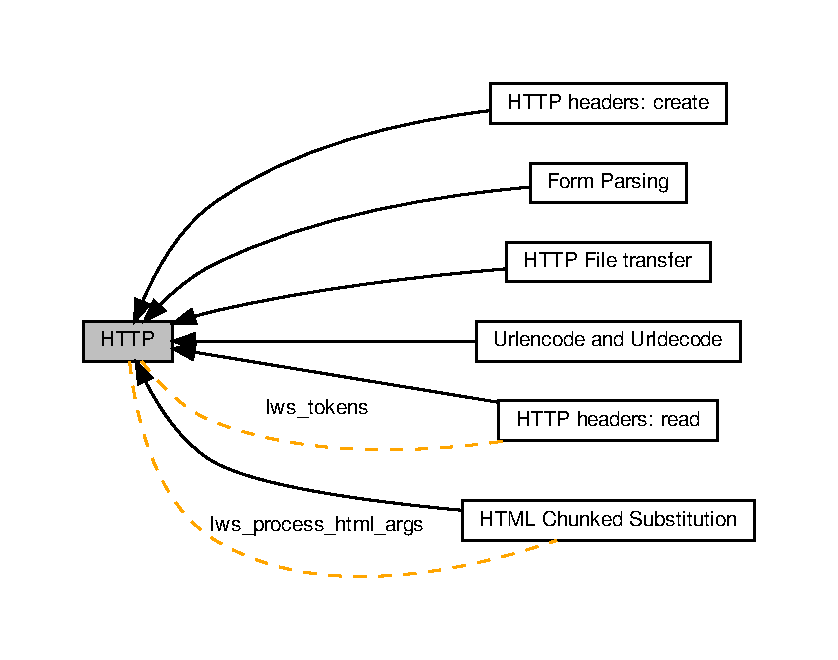
\includegraphics[width=350pt]{group__http}
\end{center}
\end{figure}
\subsection*{Modules}
\begin{DoxyCompactItemize}
\item 
\hyperlink{group__httpft}{H\+T\+T\+P File transfer}
\item 
\hyperlink{group__html-chunked-substitution}{H\+T\+M\+L Chunked Substitution}
\item 
\hyperlink{group__HTTP-headers-read}{H\+T\+T\+P headers\+: read}
\item 
\hyperlink{group__HTTP-headers-create}{H\+T\+T\+P headers\+: create}
\item 
\hyperlink{group__form-parsing}{Form Parsing}
\item 
\hyperlink{group__urlendec}{Urlencode and Urldecode}
\end{DoxyCompactItemize}
\subsection*{Classes}
\begin{DoxyCompactItemize}
\item 
struct \hyperlink{structlws__process__html__args}{lws\+\_\+process\+\_\+html\+\_\+args}
\item 
struct \hyperlink{structlws__tokens}{lws\+\_\+tokens}
\end{DoxyCompactItemize}
\subsection*{Enumerations}
\begin{DoxyCompactItemize}
\item 
\mbox{\Hypertarget{group__http_gabc3b93f68c8bdd857ad32913628dfa8d}\label{group__http_gabc3b93f68c8bdd857ad32913628dfa8d}} 
enum {\bfseries http\+\_\+status} \{ \newline
{\bfseries H\+T\+T\+P\+\_\+\+S\+T\+A\+T\+U\+S\+\_\+\+OK} = 200, 
{\bfseries H\+T\+T\+P\+\_\+\+S\+T\+A\+T\+U\+S\+\_\+\+N\+O\+\_\+\+C\+O\+N\+T\+E\+NT} = 204, 
{\bfseries H\+T\+T\+P\+\_\+\+S\+T\+A\+T\+U\+S\+\_\+\+B\+A\+D\+\_\+\+R\+E\+Q\+U\+E\+ST} = 400, 
{\bfseries H\+T\+T\+P\+\_\+\+S\+T\+A\+T\+U\+S\+\_\+\+U\+N\+A\+U\+T\+H\+O\+R\+I\+Z\+ED}, 
\newline
{\bfseries H\+T\+T\+P\+\_\+\+S\+T\+A\+T\+U\+S\+\_\+\+P\+A\+Y\+M\+E\+N\+T\+\_\+\+R\+E\+Q\+U\+I\+R\+ED}, 
{\bfseries H\+T\+T\+P\+\_\+\+S\+T\+A\+T\+U\+S\+\_\+\+F\+O\+R\+B\+I\+D\+D\+EN}, 
{\bfseries H\+T\+T\+P\+\_\+\+S\+T\+A\+T\+U\+S\+\_\+\+N\+O\+T\+\_\+\+F\+O\+U\+ND}, 
{\bfseries H\+T\+T\+P\+\_\+\+S\+T\+A\+T\+U\+S\+\_\+\+M\+E\+T\+H\+O\+D\+\_\+\+N\+O\+T\+\_\+\+A\+L\+L\+O\+W\+ED}, 
\newline
{\bfseries H\+T\+T\+P\+\_\+\+S\+T\+A\+T\+U\+S\+\_\+\+N\+O\+T\+\_\+\+A\+C\+C\+E\+P\+T\+A\+B\+LE}, 
{\bfseries H\+T\+T\+P\+\_\+\+S\+T\+A\+T\+U\+S\+\_\+\+P\+R\+O\+X\+Y\+\_\+\+A\+U\+T\+H\+\_\+\+R\+E\+Q\+U\+I\+R\+ED}, 
{\bfseries H\+T\+T\+P\+\_\+\+S\+T\+A\+T\+U\+S\+\_\+\+R\+E\+Q\+U\+E\+S\+T\+\_\+\+T\+I\+M\+E\+O\+UT}, 
{\bfseries H\+T\+T\+P\+\_\+\+S\+T\+A\+T\+U\+S\+\_\+\+C\+O\+N\+F\+L\+I\+CT}, 
\newline
{\bfseries H\+T\+T\+P\+\_\+\+S\+T\+A\+T\+U\+S\+\_\+\+G\+O\+NE}, 
{\bfseries H\+T\+T\+P\+\_\+\+S\+T\+A\+T\+U\+S\+\_\+\+L\+E\+N\+G\+T\+H\+\_\+\+R\+E\+Q\+U\+I\+R\+ED}, 
{\bfseries H\+T\+T\+P\+\_\+\+S\+T\+A\+T\+U\+S\+\_\+\+P\+R\+E\+C\+O\+N\+D\+I\+T\+I\+O\+N\+\_\+\+F\+A\+I\+L\+ED}, 
{\bfseries H\+T\+T\+P\+\_\+\+S\+T\+A\+T\+U\+S\+\_\+\+R\+E\+Q\+\_\+\+E\+N\+T\+I\+T\+Y\+\_\+\+T\+O\+O\+\_\+\+L\+A\+R\+GE}, 
\newline
{\bfseries H\+T\+T\+P\+\_\+\+S\+T\+A\+T\+U\+S\+\_\+\+R\+E\+Q\+\_\+\+U\+R\+I\+\_\+\+T\+O\+O\+\_\+\+L\+O\+NG}, 
{\bfseries H\+T\+T\+P\+\_\+\+S\+T\+A\+T\+U\+S\+\_\+\+U\+N\+S\+U\+P\+P\+O\+R\+T\+E\+D\+\_\+\+M\+E\+D\+I\+A\+\_\+\+T\+Y\+PE}, 
{\bfseries H\+T\+T\+P\+\_\+\+S\+T\+A\+T\+U\+S\+\_\+\+R\+E\+Q\+\_\+\+R\+A\+N\+G\+E\+\_\+\+N\+O\+T\+\_\+\+S\+A\+T\+I\+S\+F\+I\+A\+B\+LE}, 
{\bfseries H\+T\+T\+P\+\_\+\+S\+T\+A\+T\+U\+S\+\_\+\+E\+X\+P\+E\+C\+T\+A\+T\+I\+O\+N\+\_\+\+F\+A\+I\+L\+ED}, 
\newline
{\bfseries H\+T\+T\+P\+\_\+\+S\+T\+A\+T\+U\+S\+\_\+\+I\+N\+T\+E\+R\+N\+A\+L\+\_\+\+S\+E\+R\+V\+E\+R\+\_\+\+E\+R\+R\+OR} = 500, 
{\bfseries H\+T\+T\+P\+\_\+\+S\+T\+A\+T\+U\+S\+\_\+\+N\+O\+T\+\_\+\+I\+M\+P\+L\+E\+M\+E\+N\+T\+ED}, 
{\bfseries H\+T\+T\+P\+\_\+\+S\+T\+A\+T\+U\+S\+\_\+\+B\+A\+D\+\_\+\+G\+A\+T\+E\+W\+AY}, 
{\bfseries H\+T\+T\+P\+\_\+\+S\+T\+A\+T\+U\+S\+\_\+\+S\+E\+R\+V\+I\+C\+E\+\_\+\+U\+N\+A\+V\+A\+I\+L\+A\+B\+LE}, 
\newline
{\bfseries H\+T\+T\+P\+\_\+\+S\+T\+A\+T\+U\+S\+\_\+\+G\+A\+T\+E\+W\+A\+Y\+\_\+\+T\+I\+M\+E\+O\+UT}, 
{\bfseries H\+T\+T\+P\+\_\+\+S\+T\+A\+T\+U\+S\+\_\+\+H\+T\+T\+P\+\_\+\+V\+E\+R\+S\+I\+O\+N\+\_\+\+N\+O\+T\+\_\+\+S\+U\+P\+P\+O\+R\+T\+ED}, 
{\bfseries H\+T\+T\+P\+\_\+\+S\+T\+A\+T\+U\+S\+\_\+\+OK} = 200, 
{\bfseries H\+T\+T\+P\+\_\+\+S\+T\+A\+T\+U\+S\+\_\+\+N\+O\+\_\+\+C\+O\+N\+T\+E\+NT} = 204, 
\newline
{\bfseries H\+T\+T\+P\+\_\+\+S\+T\+A\+T\+U\+S\+\_\+\+B\+A\+D\+\_\+\+R\+E\+Q\+U\+E\+ST} = 400, 
{\bfseries H\+T\+T\+P\+\_\+\+S\+T\+A\+T\+U\+S\+\_\+\+U\+N\+A\+U\+T\+H\+O\+R\+I\+Z\+ED}, 
{\bfseries H\+T\+T\+P\+\_\+\+S\+T\+A\+T\+U\+S\+\_\+\+P\+A\+Y\+M\+E\+N\+T\+\_\+\+R\+E\+Q\+U\+I\+R\+ED}, 
{\bfseries H\+T\+T\+P\+\_\+\+S\+T\+A\+T\+U\+S\+\_\+\+F\+O\+R\+B\+I\+D\+D\+EN}, 
\newline
{\bfseries H\+T\+T\+P\+\_\+\+S\+T\+A\+T\+U\+S\+\_\+\+N\+O\+T\+\_\+\+F\+O\+U\+ND}, 
{\bfseries H\+T\+T\+P\+\_\+\+S\+T\+A\+T\+U\+S\+\_\+\+M\+E\+T\+H\+O\+D\+\_\+\+N\+O\+T\+\_\+\+A\+L\+L\+O\+W\+ED}, 
{\bfseries H\+T\+T\+P\+\_\+\+S\+T\+A\+T\+U\+S\+\_\+\+N\+O\+T\+\_\+\+A\+C\+C\+E\+P\+T\+A\+B\+LE}, 
{\bfseries H\+T\+T\+P\+\_\+\+S\+T\+A\+T\+U\+S\+\_\+\+P\+R\+O\+X\+Y\+\_\+\+A\+U\+T\+H\+\_\+\+R\+E\+Q\+U\+I\+R\+ED}, 
\newline
{\bfseries H\+T\+T\+P\+\_\+\+S\+T\+A\+T\+U\+S\+\_\+\+R\+E\+Q\+U\+E\+S\+T\+\_\+\+T\+I\+M\+E\+O\+UT}, 
{\bfseries H\+T\+T\+P\+\_\+\+S\+T\+A\+T\+U\+S\+\_\+\+C\+O\+N\+F\+L\+I\+CT}, 
{\bfseries H\+T\+T\+P\+\_\+\+S\+T\+A\+T\+U\+S\+\_\+\+G\+O\+NE}, 
{\bfseries H\+T\+T\+P\+\_\+\+S\+T\+A\+T\+U\+S\+\_\+\+L\+E\+N\+G\+T\+H\+\_\+\+R\+E\+Q\+U\+I\+R\+ED}, 
\newline
{\bfseries H\+T\+T\+P\+\_\+\+S\+T\+A\+T\+U\+S\+\_\+\+P\+R\+E\+C\+O\+N\+D\+I\+T\+I\+O\+N\+\_\+\+F\+A\+I\+L\+ED}, 
{\bfseries H\+T\+T\+P\+\_\+\+S\+T\+A\+T\+U\+S\+\_\+\+R\+E\+Q\+\_\+\+E\+N\+T\+I\+T\+Y\+\_\+\+T\+O\+O\+\_\+\+L\+A\+R\+GE}, 
{\bfseries H\+T\+T\+P\+\_\+\+S\+T\+A\+T\+U\+S\+\_\+\+R\+E\+Q\+\_\+\+U\+R\+I\+\_\+\+T\+O\+O\+\_\+\+L\+O\+NG}, 
{\bfseries H\+T\+T\+P\+\_\+\+S\+T\+A\+T\+U\+S\+\_\+\+U\+N\+S\+U\+P\+P\+O\+R\+T\+E\+D\+\_\+\+M\+E\+D\+I\+A\+\_\+\+T\+Y\+PE}, 
\newline
{\bfseries H\+T\+T\+P\+\_\+\+S\+T\+A\+T\+U\+S\+\_\+\+R\+E\+Q\+\_\+\+R\+A\+N\+G\+E\+\_\+\+N\+O\+T\+\_\+\+S\+A\+T\+I\+S\+F\+I\+A\+B\+LE}, 
{\bfseries H\+T\+T\+P\+\_\+\+S\+T\+A\+T\+U\+S\+\_\+\+E\+X\+P\+E\+C\+T\+A\+T\+I\+O\+N\+\_\+\+F\+A\+I\+L\+ED}, 
{\bfseries H\+T\+T\+P\+\_\+\+S\+T\+A\+T\+U\+S\+\_\+\+I\+N\+T\+E\+R\+N\+A\+L\+\_\+\+S\+E\+R\+V\+E\+R\+\_\+\+E\+R\+R\+OR} = 500, 
{\bfseries H\+T\+T\+P\+\_\+\+S\+T\+A\+T\+U\+S\+\_\+\+N\+O\+T\+\_\+\+I\+M\+P\+L\+E\+M\+E\+N\+T\+ED}, 
\newline
{\bfseries H\+T\+T\+P\+\_\+\+S\+T\+A\+T\+U\+S\+\_\+\+B\+A\+D\+\_\+\+G\+A\+T\+E\+W\+AY}, 
{\bfseries H\+T\+T\+P\+\_\+\+S\+T\+A\+T\+U\+S\+\_\+\+S\+E\+R\+V\+I\+C\+E\+\_\+\+U\+N\+A\+V\+A\+I\+L\+A\+B\+LE}, 
{\bfseries H\+T\+T\+P\+\_\+\+S\+T\+A\+T\+U\+S\+\_\+\+G\+A\+T\+E\+W\+A\+Y\+\_\+\+T\+I\+M\+E\+O\+UT}, 
{\bfseries H\+T\+T\+P\+\_\+\+S\+T\+A\+T\+U\+S\+\_\+\+H\+T\+T\+P\+\_\+\+V\+E\+R\+S\+I\+O\+N\+\_\+\+N\+O\+T\+\_\+\+S\+U\+P\+P\+O\+R\+T\+ED}, 
\newline
{\bfseries H\+T\+T\+P\+\_\+\+S\+T\+A\+T\+U\+S\+\_\+\+OK} = 200, 
{\bfseries H\+T\+T\+P\+\_\+\+S\+T\+A\+T\+U\+S\+\_\+\+N\+O\+\_\+\+C\+O\+N\+T\+E\+NT} = 204, 
{\bfseries H\+T\+T\+P\+\_\+\+S\+T\+A\+T\+U\+S\+\_\+\+B\+A\+D\+\_\+\+R\+E\+Q\+U\+E\+ST} = 400, 
{\bfseries H\+T\+T\+P\+\_\+\+S\+T\+A\+T\+U\+S\+\_\+\+U\+N\+A\+U\+T\+H\+O\+R\+I\+Z\+ED}, 
\newline
{\bfseries H\+T\+T\+P\+\_\+\+S\+T\+A\+T\+U\+S\+\_\+\+P\+A\+Y\+M\+E\+N\+T\+\_\+\+R\+E\+Q\+U\+I\+R\+ED}, 
{\bfseries H\+T\+T\+P\+\_\+\+S\+T\+A\+T\+U\+S\+\_\+\+F\+O\+R\+B\+I\+D\+D\+EN}, 
{\bfseries H\+T\+T\+P\+\_\+\+S\+T\+A\+T\+U\+S\+\_\+\+N\+O\+T\+\_\+\+F\+O\+U\+ND}, 
{\bfseries H\+T\+T\+P\+\_\+\+S\+T\+A\+T\+U\+S\+\_\+\+M\+E\+T\+H\+O\+D\+\_\+\+N\+O\+T\+\_\+\+A\+L\+L\+O\+W\+ED}, 
\newline
{\bfseries H\+T\+T\+P\+\_\+\+S\+T\+A\+T\+U\+S\+\_\+\+N\+O\+T\+\_\+\+A\+C\+C\+E\+P\+T\+A\+B\+LE}, 
{\bfseries H\+T\+T\+P\+\_\+\+S\+T\+A\+T\+U\+S\+\_\+\+P\+R\+O\+X\+Y\+\_\+\+A\+U\+T\+H\+\_\+\+R\+E\+Q\+U\+I\+R\+ED}, 
{\bfseries H\+T\+T\+P\+\_\+\+S\+T\+A\+T\+U\+S\+\_\+\+R\+E\+Q\+U\+E\+S\+T\+\_\+\+T\+I\+M\+E\+O\+UT}, 
{\bfseries H\+T\+T\+P\+\_\+\+S\+T\+A\+T\+U\+S\+\_\+\+C\+O\+N\+F\+L\+I\+CT}, 
\newline
{\bfseries H\+T\+T\+P\+\_\+\+S\+T\+A\+T\+U\+S\+\_\+\+G\+O\+NE}, 
{\bfseries H\+T\+T\+P\+\_\+\+S\+T\+A\+T\+U\+S\+\_\+\+L\+E\+N\+G\+T\+H\+\_\+\+R\+E\+Q\+U\+I\+R\+ED}, 
{\bfseries H\+T\+T\+P\+\_\+\+S\+T\+A\+T\+U\+S\+\_\+\+P\+R\+E\+C\+O\+N\+D\+I\+T\+I\+O\+N\+\_\+\+F\+A\+I\+L\+ED}, 
{\bfseries H\+T\+T\+P\+\_\+\+S\+T\+A\+T\+U\+S\+\_\+\+R\+E\+Q\+\_\+\+E\+N\+T\+I\+T\+Y\+\_\+\+T\+O\+O\+\_\+\+L\+A\+R\+GE}, 
\newline
{\bfseries H\+T\+T\+P\+\_\+\+S\+T\+A\+T\+U\+S\+\_\+\+R\+E\+Q\+\_\+\+U\+R\+I\+\_\+\+T\+O\+O\+\_\+\+L\+O\+NG}, 
{\bfseries H\+T\+T\+P\+\_\+\+S\+T\+A\+T\+U\+S\+\_\+\+U\+N\+S\+U\+P\+P\+O\+R\+T\+E\+D\+\_\+\+M\+E\+D\+I\+A\+\_\+\+T\+Y\+PE}, 
{\bfseries H\+T\+T\+P\+\_\+\+S\+T\+A\+T\+U\+S\+\_\+\+R\+E\+Q\+\_\+\+R\+A\+N\+G\+E\+\_\+\+N\+O\+T\+\_\+\+S\+A\+T\+I\+S\+F\+I\+A\+B\+LE}, 
{\bfseries H\+T\+T\+P\+\_\+\+S\+T\+A\+T\+U\+S\+\_\+\+E\+X\+P\+E\+C\+T\+A\+T\+I\+O\+N\+\_\+\+F\+A\+I\+L\+ED}, 
\newline
{\bfseries H\+T\+T\+P\+\_\+\+S\+T\+A\+T\+U\+S\+\_\+\+I\+N\+T\+E\+R\+N\+A\+L\+\_\+\+S\+E\+R\+V\+E\+R\+\_\+\+E\+R\+R\+OR} = 500, 
{\bfseries H\+T\+T\+P\+\_\+\+S\+T\+A\+T\+U\+S\+\_\+\+N\+O\+T\+\_\+\+I\+M\+P\+L\+E\+M\+E\+N\+T\+ED}, 
{\bfseries H\+T\+T\+P\+\_\+\+S\+T\+A\+T\+U\+S\+\_\+\+B\+A\+D\+\_\+\+G\+A\+T\+E\+W\+AY}, 
{\bfseries H\+T\+T\+P\+\_\+\+S\+T\+A\+T\+U\+S\+\_\+\+S\+E\+R\+V\+I\+C\+E\+\_\+\+U\+N\+A\+V\+A\+I\+L\+A\+B\+LE}, 
\newline
{\bfseries H\+T\+T\+P\+\_\+\+S\+T\+A\+T\+U\+S\+\_\+\+G\+A\+T\+E\+W\+A\+Y\+\_\+\+T\+I\+M\+E\+O\+UT}, 
{\bfseries H\+T\+T\+P\+\_\+\+S\+T\+A\+T\+U\+S\+\_\+\+H\+T\+T\+P\+\_\+\+V\+E\+R\+S\+I\+O\+N\+\_\+\+N\+O\+T\+\_\+\+S\+U\+P\+P\+O\+R\+T\+ED}, 
{\bfseries H\+T\+T\+P\+\_\+\+S\+T\+A\+T\+U\+S\+\_\+\+OK} = 200, 
{\bfseries H\+T\+T\+P\+\_\+\+S\+T\+A\+T\+U\+S\+\_\+\+N\+O\+\_\+\+C\+O\+N\+T\+E\+NT} = 204, 
\newline
{\bfseries H\+T\+T\+P\+\_\+\+S\+T\+A\+T\+U\+S\+\_\+\+B\+A\+D\+\_\+\+R\+E\+Q\+U\+E\+ST} = 400, 
{\bfseries H\+T\+T\+P\+\_\+\+S\+T\+A\+T\+U\+S\+\_\+\+U\+N\+A\+U\+T\+H\+O\+R\+I\+Z\+ED}, 
{\bfseries H\+T\+T\+P\+\_\+\+S\+T\+A\+T\+U\+S\+\_\+\+P\+A\+Y\+M\+E\+N\+T\+\_\+\+R\+E\+Q\+U\+I\+R\+ED}, 
{\bfseries H\+T\+T\+P\+\_\+\+S\+T\+A\+T\+U\+S\+\_\+\+F\+O\+R\+B\+I\+D\+D\+EN}, 
\newline
{\bfseries H\+T\+T\+P\+\_\+\+S\+T\+A\+T\+U\+S\+\_\+\+N\+O\+T\+\_\+\+F\+O\+U\+ND}, 
{\bfseries H\+T\+T\+P\+\_\+\+S\+T\+A\+T\+U\+S\+\_\+\+M\+E\+T\+H\+O\+D\+\_\+\+N\+O\+T\+\_\+\+A\+L\+L\+O\+W\+ED}, 
{\bfseries H\+T\+T\+P\+\_\+\+S\+T\+A\+T\+U\+S\+\_\+\+N\+O\+T\+\_\+\+A\+C\+C\+E\+P\+T\+A\+B\+LE}, 
{\bfseries H\+T\+T\+P\+\_\+\+S\+T\+A\+T\+U\+S\+\_\+\+P\+R\+O\+X\+Y\+\_\+\+A\+U\+T\+H\+\_\+\+R\+E\+Q\+U\+I\+R\+ED}, 
\newline
{\bfseries H\+T\+T\+P\+\_\+\+S\+T\+A\+T\+U\+S\+\_\+\+R\+E\+Q\+U\+E\+S\+T\+\_\+\+T\+I\+M\+E\+O\+UT}, 
{\bfseries H\+T\+T\+P\+\_\+\+S\+T\+A\+T\+U\+S\+\_\+\+C\+O\+N\+F\+L\+I\+CT}, 
{\bfseries H\+T\+T\+P\+\_\+\+S\+T\+A\+T\+U\+S\+\_\+\+G\+O\+NE}, 
{\bfseries H\+T\+T\+P\+\_\+\+S\+T\+A\+T\+U\+S\+\_\+\+L\+E\+N\+G\+T\+H\+\_\+\+R\+E\+Q\+U\+I\+R\+ED}, 
\newline
{\bfseries H\+T\+T\+P\+\_\+\+S\+T\+A\+T\+U\+S\+\_\+\+P\+R\+E\+C\+O\+N\+D\+I\+T\+I\+O\+N\+\_\+\+F\+A\+I\+L\+ED}, 
{\bfseries H\+T\+T\+P\+\_\+\+S\+T\+A\+T\+U\+S\+\_\+\+R\+E\+Q\+\_\+\+E\+N\+T\+I\+T\+Y\+\_\+\+T\+O\+O\+\_\+\+L\+A\+R\+GE}, 
{\bfseries H\+T\+T\+P\+\_\+\+S\+T\+A\+T\+U\+S\+\_\+\+R\+E\+Q\+\_\+\+U\+R\+I\+\_\+\+T\+O\+O\+\_\+\+L\+O\+NG}, 
{\bfseries H\+T\+T\+P\+\_\+\+S\+T\+A\+T\+U\+S\+\_\+\+U\+N\+S\+U\+P\+P\+O\+R\+T\+E\+D\+\_\+\+M\+E\+D\+I\+A\+\_\+\+T\+Y\+PE}, 
\newline
{\bfseries H\+T\+T\+P\+\_\+\+S\+T\+A\+T\+U\+S\+\_\+\+R\+E\+Q\+\_\+\+R\+A\+N\+G\+E\+\_\+\+N\+O\+T\+\_\+\+S\+A\+T\+I\+S\+F\+I\+A\+B\+LE}, 
{\bfseries H\+T\+T\+P\+\_\+\+S\+T\+A\+T\+U\+S\+\_\+\+E\+X\+P\+E\+C\+T\+A\+T\+I\+O\+N\+\_\+\+F\+A\+I\+L\+ED}, 
{\bfseries H\+T\+T\+P\+\_\+\+S\+T\+A\+T\+U\+S\+\_\+\+I\+N\+T\+E\+R\+N\+A\+L\+\_\+\+S\+E\+R\+V\+E\+R\+\_\+\+E\+R\+R\+OR} = 500, 
{\bfseries H\+T\+T\+P\+\_\+\+S\+T\+A\+T\+U\+S\+\_\+\+N\+O\+T\+\_\+\+I\+M\+P\+L\+E\+M\+E\+N\+T\+ED}, 
\newline
{\bfseries H\+T\+T\+P\+\_\+\+S\+T\+A\+T\+U\+S\+\_\+\+B\+A\+D\+\_\+\+G\+A\+T\+E\+W\+AY}, 
{\bfseries H\+T\+T\+P\+\_\+\+S\+T\+A\+T\+U\+S\+\_\+\+S\+E\+R\+V\+I\+C\+E\+\_\+\+U\+N\+A\+V\+A\+I\+L\+A\+B\+LE}, 
{\bfseries H\+T\+T\+P\+\_\+\+S\+T\+A\+T\+U\+S\+\_\+\+G\+A\+T\+E\+W\+A\+Y\+\_\+\+T\+I\+M\+E\+O\+UT}, 
{\bfseries H\+T\+T\+P\+\_\+\+S\+T\+A\+T\+U\+S\+\_\+\+H\+T\+T\+P\+\_\+\+V\+E\+R\+S\+I\+O\+N\+\_\+\+N\+O\+T\+\_\+\+S\+U\+P\+P\+O\+R\+T\+ED}, 
\newline
{\bfseries H\+T\+T\+P\+\_\+\+S\+T\+A\+T\+U\+S\+\_\+\+OK} = 200, 
{\bfseries H\+T\+T\+P\+\_\+\+S\+T\+A\+T\+U\+S\+\_\+\+N\+O\+\_\+\+C\+O\+N\+T\+E\+NT} = 204, 
{\bfseries H\+T\+T\+P\+\_\+\+S\+T\+A\+T\+U\+S\+\_\+\+B\+A\+D\+\_\+\+R\+E\+Q\+U\+E\+ST} = 400, 
{\bfseries H\+T\+T\+P\+\_\+\+S\+T\+A\+T\+U\+S\+\_\+\+U\+N\+A\+U\+T\+H\+O\+R\+I\+Z\+ED}, 
\newline
{\bfseries H\+T\+T\+P\+\_\+\+S\+T\+A\+T\+U\+S\+\_\+\+P\+A\+Y\+M\+E\+N\+T\+\_\+\+R\+E\+Q\+U\+I\+R\+ED}, 
{\bfseries H\+T\+T\+P\+\_\+\+S\+T\+A\+T\+U\+S\+\_\+\+F\+O\+R\+B\+I\+D\+D\+EN}, 
{\bfseries H\+T\+T\+P\+\_\+\+S\+T\+A\+T\+U\+S\+\_\+\+N\+O\+T\+\_\+\+F\+O\+U\+ND}, 
{\bfseries H\+T\+T\+P\+\_\+\+S\+T\+A\+T\+U\+S\+\_\+\+M\+E\+T\+H\+O\+D\+\_\+\+N\+O\+T\+\_\+\+A\+L\+L\+O\+W\+ED}, 
\newline
{\bfseries H\+T\+T\+P\+\_\+\+S\+T\+A\+T\+U\+S\+\_\+\+N\+O\+T\+\_\+\+A\+C\+C\+E\+P\+T\+A\+B\+LE}, 
{\bfseries H\+T\+T\+P\+\_\+\+S\+T\+A\+T\+U\+S\+\_\+\+P\+R\+O\+X\+Y\+\_\+\+A\+U\+T\+H\+\_\+\+R\+E\+Q\+U\+I\+R\+ED}, 
{\bfseries H\+T\+T\+P\+\_\+\+S\+T\+A\+T\+U\+S\+\_\+\+R\+E\+Q\+U\+E\+S\+T\+\_\+\+T\+I\+M\+E\+O\+UT}, 
{\bfseries H\+T\+T\+P\+\_\+\+S\+T\+A\+T\+U\+S\+\_\+\+C\+O\+N\+F\+L\+I\+CT}, 
\newline
{\bfseries H\+T\+T\+P\+\_\+\+S\+T\+A\+T\+U\+S\+\_\+\+G\+O\+NE}, 
{\bfseries H\+T\+T\+P\+\_\+\+S\+T\+A\+T\+U\+S\+\_\+\+L\+E\+N\+G\+T\+H\+\_\+\+R\+E\+Q\+U\+I\+R\+ED}, 
{\bfseries H\+T\+T\+P\+\_\+\+S\+T\+A\+T\+U\+S\+\_\+\+P\+R\+E\+C\+O\+N\+D\+I\+T\+I\+O\+N\+\_\+\+F\+A\+I\+L\+ED}, 
{\bfseries H\+T\+T\+P\+\_\+\+S\+T\+A\+T\+U\+S\+\_\+\+R\+E\+Q\+\_\+\+E\+N\+T\+I\+T\+Y\+\_\+\+T\+O\+O\+\_\+\+L\+A\+R\+GE}, 
\newline
{\bfseries H\+T\+T\+P\+\_\+\+S\+T\+A\+T\+U\+S\+\_\+\+R\+E\+Q\+\_\+\+U\+R\+I\+\_\+\+T\+O\+O\+\_\+\+L\+O\+NG}, 
{\bfseries H\+T\+T\+P\+\_\+\+S\+T\+A\+T\+U\+S\+\_\+\+U\+N\+S\+U\+P\+P\+O\+R\+T\+E\+D\+\_\+\+M\+E\+D\+I\+A\+\_\+\+T\+Y\+PE}, 
{\bfseries H\+T\+T\+P\+\_\+\+S\+T\+A\+T\+U\+S\+\_\+\+R\+E\+Q\+\_\+\+R\+A\+N\+G\+E\+\_\+\+N\+O\+T\+\_\+\+S\+A\+T\+I\+S\+F\+I\+A\+B\+LE}, 
{\bfseries H\+T\+T\+P\+\_\+\+S\+T\+A\+T\+U\+S\+\_\+\+E\+X\+P\+E\+C\+T\+A\+T\+I\+O\+N\+\_\+\+F\+A\+I\+L\+ED}, 
\newline
{\bfseries H\+T\+T\+P\+\_\+\+S\+T\+A\+T\+U\+S\+\_\+\+I\+N\+T\+E\+R\+N\+A\+L\+\_\+\+S\+E\+R\+V\+E\+R\+\_\+\+E\+R\+R\+OR} = 500, 
{\bfseries H\+T\+T\+P\+\_\+\+S\+T\+A\+T\+U\+S\+\_\+\+N\+O\+T\+\_\+\+I\+M\+P\+L\+E\+M\+E\+N\+T\+ED}, 
{\bfseries H\+T\+T\+P\+\_\+\+S\+T\+A\+T\+U\+S\+\_\+\+B\+A\+D\+\_\+\+G\+A\+T\+E\+W\+AY}, 
{\bfseries H\+T\+T\+P\+\_\+\+S\+T\+A\+T\+U\+S\+\_\+\+S\+E\+R\+V\+I\+C\+E\+\_\+\+U\+N\+A\+V\+A\+I\+L\+A\+B\+LE}, 
\newline
{\bfseries H\+T\+T\+P\+\_\+\+S\+T\+A\+T\+U\+S\+\_\+\+G\+A\+T\+E\+W\+A\+Y\+\_\+\+T\+I\+M\+E\+O\+UT}, 
{\bfseries H\+T\+T\+P\+\_\+\+S\+T\+A\+T\+U\+S\+\_\+\+H\+T\+T\+P\+\_\+\+V\+E\+R\+S\+I\+O\+N\+\_\+\+N\+O\+T\+\_\+\+S\+U\+P\+P\+O\+R\+T\+ED}, 
{\bfseries H\+T\+T\+P\+\_\+\+S\+T\+A\+T\+U\+S\+\_\+\+OK} = 200, 
{\bfseries H\+T\+T\+P\+\_\+\+S\+T\+A\+T\+U\+S\+\_\+\+N\+O\+\_\+\+C\+O\+N\+T\+E\+NT} = 204, 
\newline
{\bfseries H\+T\+T\+P\+\_\+\+S\+T\+A\+T\+U\+S\+\_\+\+B\+A\+D\+\_\+\+R\+E\+Q\+U\+E\+ST} = 400, 
{\bfseries H\+T\+T\+P\+\_\+\+S\+T\+A\+T\+U\+S\+\_\+\+U\+N\+A\+U\+T\+H\+O\+R\+I\+Z\+ED}, 
{\bfseries H\+T\+T\+P\+\_\+\+S\+T\+A\+T\+U\+S\+\_\+\+P\+A\+Y\+M\+E\+N\+T\+\_\+\+R\+E\+Q\+U\+I\+R\+ED}, 
{\bfseries H\+T\+T\+P\+\_\+\+S\+T\+A\+T\+U\+S\+\_\+\+F\+O\+R\+B\+I\+D\+D\+EN}, 
\newline
{\bfseries H\+T\+T\+P\+\_\+\+S\+T\+A\+T\+U\+S\+\_\+\+N\+O\+T\+\_\+\+F\+O\+U\+ND}, 
{\bfseries H\+T\+T\+P\+\_\+\+S\+T\+A\+T\+U\+S\+\_\+\+M\+E\+T\+H\+O\+D\+\_\+\+N\+O\+T\+\_\+\+A\+L\+L\+O\+W\+ED}, 
{\bfseries H\+T\+T\+P\+\_\+\+S\+T\+A\+T\+U\+S\+\_\+\+N\+O\+T\+\_\+\+A\+C\+C\+E\+P\+T\+A\+B\+LE}, 
{\bfseries H\+T\+T\+P\+\_\+\+S\+T\+A\+T\+U\+S\+\_\+\+P\+R\+O\+X\+Y\+\_\+\+A\+U\+T\+H\+\_\+\+R\+E\+Q\+U\+I\+R\+ED}, 
\newline
{\bfseries H\+T\+T\+P\+\_\+\+S\+T\+A\+T\+U\+S\+\_\+\+R\+E\+Q\+U\+E\+S\+T\+\_\+\+T\+I\+M\+E\+O\+UT}, 
{\bfseries H\+T\+T\+P\+\_\+\+S\+T\+A\+T\+U\+S\+\_\+\+C\+O\+N\+F\+L\+I\+CT}, 
{\bfseries H\+T\+T\+P\+\_\+\+S\+T\+A\+T\+U\+S\+\_\+\+G\+O\+NE}, 
{\bfseries H\+T\+T\+P\+\_\+\+S\+T\+A\+T\+U\+S\+\_\+\+L\+E\+N\+G\+T\+H\+\_\+\+R\+E\+Q\+U\+I\+R\+ED}, 
\newline
{\bfseries H\+T\+T\+P\+\_\+\+S\+T\+A\+T\+U\+S\+\_\+\+P\+R\+E\+C\+O\+N\+D\+I\+T\+I\+O\+N\+\_\+\+F\+A\+I\+L\+ED}, 
{\bfseries H\+T\+T\+P\+\_\+\+S\+T\+A\+T\+U\+S\+\_\+\+R\+E\+Q\+\_\+\+E\+N\+T\+I\+T\+Y\+\_\+\+T\+O\+O\+\_\+\+L\+A\+R\+GE}, 
{\bfseries H\+T\+T\+P\+\_\+\+S\+T\+A\+T\+U\+S\+\_\+\+R\+E\+Q\+\_\+\+U\+R\+I\+\_\+\+T\+O\+O\+\_\+\+L\+O\+NG}, 
{\bfseries H\+T\+T\+P\+\_\+\+S\+T\+A\+T\+U\+S\+\_\+\+U\+N\+S\+U\+P\+P\+O\+R\+T\+E\+D\+\_\+\+M\+E\+D\+I\+A\+\_\+\+T\+Y\+PE}, 
\newline
{\bfseries H\+T\+T\+P\+\_\+\+S\+T\+A\+T\+U\+S\+\_\+\+R\+E\+Q\+\_\+\+R\+A\+N\+G\+E\+\_\+\+N\+O\+T\+\_\+\+S\+A\+T\+I\+S\+F\+I\+A\+B\+LE}, 
{\bfseries H\+T\+T\+P\+\_\+\+S\+T\+A\+T\+U\+S\+\_\+\+E\+X\+P\+E\+C\+T\+A\+T\+I\+O\+N\+\_\+\+F\+A\+I\+L\+ED}, 
{\bfseries H\+T\+T\+P\+\_\+\+S\+T\+A\+T\+U\+S\+\_\+\+I\+N\+T\+E\+R\+N\+A\+L\+\_\+\+S\+E\+R\+V\+E\+R\+\_\+\+E\+R\+R\+OR} = 500, 
{\bfseries H\+T\+T\+P\+\_\+\+S\+T\+A\+T\+U\+S\+\_\+\+N\+O\+T\+\_\+\+I\+M\+P\+L\+E\+M\+E\+N\+T\+ED}, 
\newline
{\bfseries H\+T\+T\+P\+\_\+\+S\+T\+A\+T\+U\+S\+\_\+\+B\+A\+D\+\_\+\+G\+A\+T\+E\+W\+AY}, 
{\bfseries H\+T\+T\+P\+\_\+\+S\+T\+A\+T\+U\+S\+\_\+\+S\+E\+R\+V\+I\+C\+E\+\_\+\+U\+N\+A\+V\+A\+I\+L\+A\+B\+LE}, 
{\bfseries H\+T\+T\+P\+\_\+\+S\+T\+A\+T\+U\+S\+\_\+\+G\+A\+T\+E\+W\+A\+Y\+\_\+\+T\+I\+M\+E\+O\+UT}, 
{\bfseries H\+T\+T\+P\+\_\+\+S\+T\+A\+T\+U\+S\+\_\+\+H\+T\+T\+P\+\_\+\+V\+E\+R\+S\+I\+O\+N\+\_\+\+N\+O\+T\+\_\+\+S\+U\+P\+P\+O\+R\+T\+ED}, 
\newline
{\bfseries H\+T\+T\+P\+\_\+\+S\+T\+A\+T\+U\+S\+\_\+\+OK} = 200, 
{\bfseries H\+T\+T\+P\+\_\+\+S\+T\+A\+T\+U\+S\+\_\+\+N\+O\+\_\+\+C\+O\+N\+T\+E\+NT} = 204, 
{\bfseries H\+T\+T\+P\+\_\+\+S\+T\+A\+T\+U\+S\+\_\+\+B\+A\+D\+\_\+\+R\+E\+Q\+U\+E\+ST} = 400, 
{\bfseries H\+T\+T\+P\+\_\+\+S\+T\+A\+T\+U\+S\+\_\+\+U\+N\+A\+U\+T\+H\+O\+R\+I\+Z\+ED}, 
\newline
{\bfseries H\+T\+T\+P\+\_\+\+S\+T\+A\+T\+U\+S\+\_\+\+P\+A\+Y\+M\+E\+N\+T\+\_\+\+R\+E\+Q\+U\+I\+R\+ED}, 
{\bfseries H\+T\+T\+P\+\_\+\+S\+T\+A\+T\+U\+S\+\_\+\+F\+O\+R\+B\+I\+D\+D\+EN}, 
{\bfseries H\+T\+T\+P\+\_\+\+S\+T\+A\+T\+U\+S\+\_\+\+N\+O\+T\+\_\+\+F\+O\+U\+ND}, 
{\bfseries H\+T\+T\+P\+\_\+\+S\+T\+A\+T\+U\+S\+\_\+\+M\+E\+T\+H\+O\+D\+\_\+\+N\+O\+T\+\_\+\+A\+L\+L\+O\+W\+ED}, 
\newline
{\bfseries H\+T\+T\+P\+\_\+\+S\+T\+A\+T\+U\+S\+\_\+\+N\+O\+T\+\_\+\+A\+C\+C\+E\+P\+T\+A\+B\+LE}, 
{\bfseries H\+T\+T\+P\+\_\+\+S\+T\+A\+T\+U\+S\+\_\+\+P\+R\+O\+X\+Y\+\_\+\+A\+U\+T\+H\+\_\+\+R\+E\+Q\+U\+I\+R\+ED}, 
{\bfseries H\+T\+T\+P\+\_\+\+S\+T\+A\+T\+U\+S\+\_\+\+R\+E\+Q\+U\+E\+S\+T\+\_\+\+T\+I\+M\+E\+O\+UT}, 
{\bfseries H\+T\+T\+P\+\_\+\+S\+T\+A\+T\+U\+S\+\_\+\+C\+O\+N\+F\+L\+I\+CT}, 
\newline
{\bfseries H\+T\+T\+P\+\_\+\+S\+T\+A\+T\+U\+S\+\_\+\+G\+O\+NE}, 
{\bfseries H\+T\+T\+P\+\_\+\+S\+T\+A\+T\+U\+S\+\_\+\+L\+E\+N\+G\+T\+H\+\_\+\+R\+E\+Q\+U\+I\+R\+ED}, 
{\bfseries H\+T\+T\+P\+\_\+\+S\+T\+A\+T\+U\+S\+\_\+\+P\+R\+E\+C\+O\+N\+D\+I\+T\+I\+O\+N\+\_\+\+F\+A\+I\+L\+ED}, 
{\bfseries H\+T\+T\+P\+\_\+\+S\+T\+A\+T\+U\+S\+\_\+\+R\+E\+Q\+\_\+\+E\+N\+T\+I\+T\+Y\+\_\+\+T\+O\+O\+\_\+\+L\+A\+R\+GE}, 
\newline
{\bfseries H\+T\+T\+P\+\_\+\+S\+T\+A\+T\+U\+S\+\_\+\+R\+E\+Q\+\_\+\+U\+R\+I\+\_\+\+T\+O\+O\+\_\+\+L\+O\+NG}, 
{\bfseries H\+T\+T\+P\+\_\+\+S\+T\+A\+T\+U\+S\+\_\+\+U\+N\+S\+U\+P\+P\+O\+R\+T\+E\+D\+\_\+\+M\+E\+D\+I\+A\+\_\+\+T\+Y\+PE}, 
{\bfseries H\+T\+T\+P\+\_\+\+S\+T\+A\+T\+U\+S\+\_\+\+R\+E\+Q\+\_\+\+R\+A\+N\+G\+E\+\_\+\+N\+O\+T\+\_\+\+S\+A\+T\+I\+S\+F\+I\+A\+B\+LE}, 
{\bfseries H\+T\+T\+P\+\_\+\+S\+T\+A\+T\+U\+S\+\_\+\+E\+X\+P\+E\+C\+T\+A\+T\+I\+O\+N\+\_\+\+F\+A\+I\+L\+ED}, 
\newline
{\bfseries H\+T\+T\+P\+\_\+\+S\+T\+A\+T\+U\+S\+\_\+\+I\+N\+T\+E\+R\+N\+A\+L\+\_\+\+S\+E\+R\+V\+E\+R\+\_\+\+E\+R\+R\+OR} = 500, 
{\bfseries H\+T\+T\+P\+\_\+\+S\+T\+A\+T\+U\+S\+\_\+\+N\+O\+T\+\_\+\+I\+M\+P\+L\+E\+M\+E\+N\+T\+ED}, 
{\bfseries H\+T\+T\+P\+\_\+\+S\+T\+A\+T\+U\+S\+\_\+\+B\+A\+D\+\_\+\+G\+A\+T\+E\+W\+AY}, 
{\bfseries H\+T\+T\+P\+\_\+\+S\+T\+A\+T\+U\+S\+\_\+\+S\+E\+R\+V\+I\+C\+E\+\_\+\+U\+N\+A\+V\+A\+I\+L\+A\+B\+LE}, 
\newline
{\bfseries H\+T\+T\+P\+\_\+\+S\+T\+A\+T\+U\+S\+\_\+\+G\+A\+T\+E\+W\+A\+Y\+\_\+\+T\+I\+M\+E\+O\+UT}, 
{\bfseries H\+T\+T\+P\+\_\+\+S\+T\+A\+T\+U\+S\+\_\+\+H\+T\+T\+P\+\_\+\+V\+E\+R\+S\+I\+O\+N\+\_\+\+N\+O\+T\+\_\+\+S\+U\+P\+P\+O\+R\+T\+ED}, 
{\bfseries H\+T\+T\+P\+\_\+\+S\+T\+A\+T\+U\+S\+\_\+\+OK} = 200, 
{\bfseries H\+T\+T\+P\+\_\+\+S\+T\+A\+T\+U\+S\+\_\+\+N\+O\+\_\+\+C\+O\+N\+T\+E\+NT} = 204, 
\newline
{\bfseries H\+T\+T\+P\+\_\+\+S\+T\+A\+T\+U\+S\+\_\+\+B\+A\+D\+\_\+\+R\+E\+Q\+U\+E\+ST} = 400, 
{\bfseries H\+T\+T\+P\+\_\+\+S\+T\+A\+T\+U\+S\+\_\+\+U\+N\+A\+U\+T\+H\+O\+R\+I\+Z\+ED}, 
{\bfseries H\+T\+T\+P\+\_\+\+S\+T\+A\+T\+U\+S\+\_\+\+P\+A\+Y\+M\+E\+N\+T\+\_\+\+R\+E\+Q\+U\+I\+R\+ED}, 
{\bfseries H\+T\+T\+P\+\_\+\+S\+T\+A\+T\+U\+S\+\_\+\+F\+O\+R\+B\+I\+D\+D\+EN}, 
\newline
{\bfseries H\+T\+T\+P\+\_\+\+S\+T\+A\+T\+U\+S\+\_\+\+N\+O\+T\+\_\+\+F\+O\+U\+ND}, 
{\bfseries H\+T\+T\+P\+\_\+\+S\+T\+A\+T\+U\+S\+\_\+\+M\+E\+T\+H\+O\+D\+\_\+\+N\+O\+T\+\_\+\+A\+L\+L\+O\+W\+ED}, 
{\bfseries H\+T\+T\+P\+\_\+\+S\+T\+A\+T\+U\+S\+\_\+\+N\+O\+T\+\_\+\+A\+C\+C\+E\+P\+T\+A\+B\+LE}, 
{\bfseries H\+T\+T\+P\+\_\+\+S\+T\+A\+T\+U\+S\+\_\+\+P\+R\+O\+X\+Y\+\_\+\+A\+U\+T\+H\+\_\+\+R\+E\+Q\+U\+I\+R\+ED}, 
\newline
{\bfseries H\+T\+T\+P\+\_\+\+S\+T\+A\+T\+U\+S\+\_\+\+R\+E\+Q\+U\+E\+S\+T\+\_\+\+T\+I\+M\+E\+O\+UT}, 
{\bfseries H\+T\+T\+P\+\_\+\+S\+T\+A\+T\+U\+S\+\_\+\+C\+O\+N\+F\+L\+I\+CT}, 
{\bfseries H\+T\+T\+P\+\_\+\+S\+T\+A\+T\+U\+S\+\_\+\+G\+O\+NE}, 
{\bfseries H\+T\+T\+P\+\_\+\+S\+T\+A\+T\+U\+S\+\_\+\+L\+E\+N\+G\+T\+H\+\_\+\+R\+E\+Q\+U\+I\+R\+ED}, 
\newline
{\bfseries H\+T\+T\+P\+\_\+\+S\+T\+A\+T\+U\+S\+\_\+\+P\+R\+E\+C\+O\+N\+D\+I\+T\+I\+O\+N\+\_\+\+F\+A\+I\+L\+ED}, 
{\bfseries H\+T\+T\+P\+\_\+\+S\+T\+A\+T\+U\+S\+\_\+\+R\+E\+Q\+\_\+\+E\+N\+T\+I\+T\+Y\+\_\+\+T\+O\+O\+\_\+\+L\+A\+R\+GE}, 
{\bfseries H\+T\+T\+P\+\_\+\+S\+T\+A\+T\+U\+S\+\_\+\+R\+E\+Q\+\_\+\+U\+R\+I\+\_\+\+T\+O\+O\+\_\+\+L\+O\+NG}, 
{\bfseries H\+T\+T\+P\+\_\+\+S\+T\+A\+T\+U\+S\+\_\+\+U\+N\+S\+U\+P\+P\+O\+R\+T\+E\+D\+\_\+\+M\+E\+D\+I\+A\+\_\+\+T\+Y\+PE}, 
\newline
{\bfseries H\+T\+T\+P\+\_\+\+S\+T\+A\+T\+U\+S\+\_\+\+R\+E\+Q\+\_\+\+R\+A\+N\+G\+E\+\_\+\+N\+O\+T\+\_\+\+S\+A\+T\+I\+S\+F\+I\+A\+B\+LE}, 
{\bfseries H\+T\+T\+P\+\_\+\+S\+T\+A\+T\+U\+S\+\_\+\+E\+X\+P\+E\+C\+T\+A\+T\+I\+O\+N\+\_\+\+F\+A\+I\+L\+ED}, 
{\bfseries H\+T\+T\+P\+\_\+\+S\+T\+A\+T\+U\+S\+\_\+\+I\+N\+T\+E\+R\+N\+A\+L\+\_\+\+S\+E\+R\+V\+E\+R\+\_\+\+E\+R\+R\+OR} = 500, 
{\bfseries H\+T\+T\+P\+\_\+\+S\+T\+A\+T\+U\+S\+\_\+\+N\+O\+T\+\_\+\+I\+M\+P\+L\+E\+M\+E\+N\+T\+ED}, 
\newline
{\bfseries H\+T\+T\+P\+\_\+\+S\+T\+A\+T\+U\+S\+\_\+\+B\+A\+D\+\_\+\+G\+A\+T\+E\+W\+AY}, 
{\bfseries H\+T\+T\+P\+\_\+\+S\+T\+A\+T\+U\+S\+\_\+\+S\+E\+R\+V\+I\+C\+E\+\_\+\+U\+N\+A\+V\+A\+I\+L\+A\+B\+LE}, 
{\bfseries H\+T\+T\+P\+\_\+\+S\+T\+A\+T\+U\+S\+\_\+\+G\+A\+T\+E\+W\+A\+Y\+\_\+\+T\+I\+M\+E\+O\+UT}, 
{\bfseries H\+T\+T\+P\+\_\+\+S\+T\+A\+T\+U\+S\+\_\+\+H\+T\+T\+P\+\_\+\+V\+E\+R\+S\+I\+O\+N\+\_\+\+N\+O\+T\+\_\+\+S\+U\+P\+P\+O\+R\+T\+ED}, 
\newline
{\bfseries H\+T\+T\+P\+\_\+\+S\+T\+A\+T\+U\+S\+\_\+\+OK} = 200, 
{\bfseries H\+T\+T\+P\+\_\+\+S\+T\+A\+T\+U\+S\+\_\+\+N\+O\+\_\+\+C\+O\+N\+T\+E\+NT} = 204, 
{\bfseries H\+T\+T\+P\+\_\+\+S\+T\+A\+T\+U\+S\+\_\+\+B\+A\+D\+\_\+\+R\+E\+Q\+U\+E\+ST} = 400, 
{\bfseries H\+T\+T\+P\+\_\+\+S\+T\+A\+T\+U\+S\+\_\+\+U\+N\+A\+U\+T\+H\+O\+R\+I\+Z\+ED}, 
\newline
{\bfseries H\+T\+T\+P\+\_\+\+S\+T\+A\+T\+U\+S\+\_\+\+P\+A\+Y\+M\+E\+N\+T\+\_\+\+R\+E\+Q\+U\+I\+R\+ED}, 
{\bfseries H\+T\+T\+P\+\_\+\+S\+T\+A\+T\+U\+S\+\_\+\+F\+O\+R\+B\+I\+D\+D\+EN}, 
{\bfseries H\+T\+T\+P\+\_\+\+S\+T\+A\+T\+U\+S\+\_\+\+N\+O\+T\+\_\+\+F\+O\+U\+ND}, 
{\bfseries H\+T\+T\+P\+\_\+\+S\+T\+A\+T\+U\+S\+\_\+\+M\+E\+T\+H\+O\+D\+\_\+\+N\+O\+T\+\_\+\+A\+L\+L\+O\+W\+ED}, 
\newline
{\bfseries H\+T\+T\+P\+\_\+\+S\+T\+A\+T\+U\+S\+\_\+\+N\+O\+T\+\_\+\+A\+C\+C\+E\+P\+T\+A\+B\+LE}, 
{\bfseries H\+T\+T\+P\+\_\+\+S\+T\+A\+T\+U\+S\+\_\+\+P\+R\+O\+X\+Y\+\_\+\+A\+U\+T\+H\+\_\+\+R\+E\+Q\+U\+I\+R\+ED}, 
{\bfseries H\+T\+T\+P\+\_\+\+S\+T\+A\+T\+U\+S\+\_\+\+R\+E\+Q\+U\+E\+S\+T\+\_\+\+T\+I\+M\+E\+O\+UT}, 
{\bfseries H\+T\+T\+P\+\_\+\+S\+T\+A\+T\+U\+S\+\_\+\+C\+O\+N\+F\+L\+I\+CT}, 
\newline
{\bfseries H\+T\+T\+P\+\_\+\+S\+T\+A\+T\+U\+S\+\_\+\+G\+O\+NE}, 
{\bfseries H\+T\+T\+P\+\_\+\+S\+T\+A\+T\+U\+S\+\_\+\+L\+E\+N\+G\+T\+H\+\_\+\+R\+E\+Q\+U\+I\+R\+ED}, 
{\bfseries H\+T\+T\+P\+\_\+\+S\+T\+A\+T\+U\+S\+\_\+\+P\+R\+E\+C\+O\+N\+D\+I\+T\+I\+O\+N\+\_\+\+F\+A\+I\+L\+ED}, 
{\bfseries H\+T\+T\+P\+\_\+\+S\+T\+A\+T\+U\+S\+\_\+\+R\+E\+Q\+\_\+\+E\+N\+T\+I\+T\+Y\+\_\+\+T\+O\+O\+\_\+\+L\+A\+R\+GE}, 
\newline
{\bfseries H\+T\+T\+P\+\_\+\+S\+T\+A\+T\+U\+S\+\_\+\+R\+E\+Q\+\_\+\+U\+R\+I\+\_\+\+T\+O\+O\+\_\+\+L\+O\+NG}, 
{\bfseries H\+T\+T\+P\+\_\+\+S\+T\+A\+T\+U\+S\+\_\+\+U\+N\+S\+U\+P\+P\+O\+R\+T\+E\+D\+\_\+\+M\+E\+D\+I\+A\+\_\+\+T\+Y\+PE}, 
{\bfseries H\+T\+T\+P\+\_\+\+S\+T\+A\+T\+U\+S\+\_\+\+R\+E\+Q\+\_\+\+R\+A\+N\+G\+E\+\_\+\+N\+O\+T\+\_\+\+S\+A\+T\+I\+S\+F\+I\+A\+B\+LE}, 
{\bfseries H\+T\+T\+P\+\_\+\+S\+T\+A\+T\+U\+S\+\_\+\+E\+X\+P\+E\+C\+T\+A\+T\+I\+O\+N\+\_\+\+F\+A\+I\+L\+ED}, 
\newline
{\bfseries H\+T\+T\+P\+\_\+\+S\+T\+A\+T\+U\+S\+\_\+\+I\+N\+T\+E\+R\+N\+A\+L\+\_\+\+S\+E\+R\+V\+E\+R\+\_\+\+E\+R\+R\+OR} = 500, 
{\bfseries H\+T\+T\+P\+\_\+\+S\+T\+A\+T\+U\+S\+\_\+\+N\+O\+T\+\_\+\+I\+M\+P\+L\+E\+M\+E\+N\+T\+ED}, 
{\bfseries H\+T\+T\+P\+\_\+\+S\+T\+A\+T\+U\+S\+\_\+\+B\+A\+D\+\_\+\+G\+A\+T\+E\+W\+AY}, 
{\bfseries H\+T\+T\+P\+\_\+\+S\+T\+A\+T\+U\+S\+\_\+\+S\+E\+R\+V\+I\+C\+E\+\_\+\+U\+N\+A\+V\+A\+I\+L\+A\+B\+LE}, 
\newline
{\bfseries H\+T\+T\+P\+\_\+\+S\+T\+A\+T\+U\+S\+\_\+\+G\+A\+T\+E\+W\+A\+Y\+\_\+\+T\+I\+M\+E\+O\+UT}, 
{\bfseries H\+T\+T\+P\+\_\+\+S\+T\+A\+T\+U\+S\+\_\+\+H\+T\+T\+P\+\_\+\+V\+E\+R\+S\+I\+O\+N\+\_\+\+N\+O\+T\+\_\+\+S\+U\+P\+P\+O\+R\+T\+ED}, 
{\bfseries H\+T\+T\+P\+\_\+\+S\+T\+A\+T\+U\+S\+\_\+\+C\+O\+N\+T\+I\+N\+UE} = 100, 
{\bfseries H\+T\+T\+P\+\_\+\+S\+T\+A\+T\+U\+S\+\_\+\+OK} = 200, 
\newline
{\bfseries H\+T\+T\+P\+\_\+\+S\+T\+A\+T\+U\+S\+\_\+\+N\+O\+\_\+\+C\+O\+N\+T\+E\+NT} = 204, 
{\bfseries H\+T\+T\+P\+\_\+\+S\+T\+A\+T\+U\+S\+\_\+\+P\+A\+R\+T\+I\+A\+L\+\_\+\+C\+O\+N\+T\+E\+NT} = 206, 
{\bfseries H\+T\+T\+P\+\_\+\+S\+T\+A\+T\+U\+S\+\_\+\+M\+O\+V\+E\+D\+\_\+\+P\+E\+R\+M\+A\+N\+E\+N\+T\+LY} = 301, 
{\bfseries H\+T\+T\+P\+\_\+\+S\+T\+A\+T\+U\+S\+\_\+\+F\+O\+U\+ND} = 302, 
\newline
{\bfseries H\+T\+T\+P\+\_\+\+S\+T\+A\+T\+U\+S\+\_\+\+S\+E\+E\+\_\+\+O\+T\+H\+ER} = 303, 
{\bfseries H\+T\+T\+P\+\_\+\+S\+T\+A\+T\+U\+S\+\_\+\+N\+O\+T\+\_\+\+M\+O\+D\+I\+F\+I\+ED} = 304, 
{\bfseries H\+T\+T\+P\+\_\+\+S\+T\+A\+T\+U\+S\+\_\+\+B\+A\+D\+\_\+\+R\+E\+Q\+U\+E\+ST} = 400, 
{\bfseries H\+T\+T\+P\+\_\+\+S\+T\+A\+T\+U\+S\+\_\+\+U\+N\+A\+U\+T\+H\+O\+R\+I\+Z\+ED}, 
\newline
{\bfseries H\+T\+T\+P\+\_\+\+S\+T\+A\+T\+U\+S\+\_\+\+P\+A\+Y\+M\+E\+N\+T\+\_\+\+R\+E\+Q\+U\+I\+R\+ED}, 
{\bfseries H\+T\+T\+P\+\_\+\+S\+T\+A\+T\+U\+S\+\_\+\+F\+O\+R\+B\+I\+D\+D\+EN}, 
{\bfseries H\+T\+T\+P\+\_\+\+S\+T\+A\+T\+U\+S\+\_\+\+N\+O\+T\+\_\+\+F\+O\+U\+ND}, 
{\bfseries H\+T\+T\+P\+\_\+\+S\+T\+A\+T\+U\+S\+\_\+\+M\+E\+T\+H\+O\+D\+\_\+\+N\+O\+T\+\_\+\+A\+L\+L\+O\+W\+ED}, 
\newline
{\bfseries H\+T\+T\+P\+\_\+\+S\+T\+A\+T\+U\+S\+\_\+\+N\+O\+T\+\_\+\+A\+C\+C\+E\+P\+T\+A\+B\+LE}, 
{\bfseries H\+T\+T\+P\+\_\+\+S\+T\+A\+T\+U\+S\+\_\+\+P\+R\+O\+X\+Y\+\_\+\+A\+U\+T\+H\+\_\+\+R\+E\+Q\+U\+I\+R\+ED}, 
{\bfseries H\+T\+T\+P\+\_\+\+S\+T\+A\+T\+U\+S\+\_\+\+R\+E\+Q\+U\+E\+S\+T\+\_\+\+T\+I\+M\+E\+O\+UT}, 
{\bfseries H\+T\+T\+P\+\_\+\+S\+T\+A\+T\+U\+S\+\_\+\+C\+O\+N\+F\+L\+I\+CT}, 
\newline
{\bfseries H\+T\+T\+P\+\_\+\+S\+T\+A\+T\+U\+S\+\_\+\+G\+O\+NE}, 
{\bfseries H\+T\+T\+P\+\_\+\+S\+T\+A\+T\+U\+S\+\_\+\+L\+E\+N\+G\+T\+H\+\_\+\+R\+E\+Q\+U\+I\+R\+ED}, 
{\bfseries H\+T\+T\+P\+\_\+\+S\+T\+A\+T\+U\+S\+\_\+\+P\+R\+E\+C\+O\+N\+D\+I\+T\+I\+O\+N\+\_\+\+F\+A\+I\+L\+ED}, 
{\bfseries H\+T\+T\+P\+\_\+\+S\+T\+A\+T\+U\+S\+\_\+\+R\+E\+Q\+\_\+\+E\+N\+T\+I\+T\+Y\+\_\+\+T\+O\+O\+\_\+\+L\+A\+R\+GE}, 
\newline
{\bfseries H\+T\+T\+P\+\_\+\+S\+T\+A\+T\+U\+S\+\_\+\+R\+E\+Q\+\_\+\+U\+R\+I\+\_\+\+T\+O\+O\+\_\+\+L\+O\+NG}, 
{\bfseries H\+T\+T\+P\+\_\+\+S\+T\+A\+T\+U\+S\+\_\+\+U\+N\+S\+U\+P\+P\+O\+R\+T\+E\+D\+\_\+\+M\+E\+D\+I\+A\+\_\+\+T\+Y\+PE}, 
{\bfseries H\+T\+T\+P\+\_\+\+S\+T\+A\+T\+U\+S\+\_\+\+R\+E\+Q\+\_\+\+R\+A\+N\+G\+E\+\_\+\+N\+O\+T\+\_\+\+S\+A\+T\+I\+S\+F\+I\+A\+B\+LE}, 
{\bfseries H\+T\+T\+P\+\_\+\+S\+T\+A\+T\+U\+S\+\_\+\+E\+X\+P\+E\+C\+T\+A\+T\+I\+O\+N\+\_\+\+F\+A\+I\+L\+ED}, 
\newline
{\bfseries H\+T\+T\+P\+\_\+\+S\+T\+A\+T\+U\+S\+\_\+\+I\+N\+T\+E\+R\+N\+A\+L\+\_\+\+S\+E\+R\+V\+E\+R\+\_\+\+E\+R\+R\+OR} = 500, 
{\bfseries H\+T\+T\+P\+\_\+\+S\+T\+A\+T\+U\+S\+\_\+\+N\+O\+T\+\_\+\+I\+M\+P\+L\+E\+M\+E\+N\+T\+ED}, 
{\bfseries H\+T\+T\+P\+\_\+\+S\+T\+A\+T\+U\+S\+\_\+\+B\+A\+D\+\_\+\+G\+A\+T\+E\+W\+AY}, 
{\bfseries H\+T\+T\+P\+\_\+\+S\+T\+A\+T\+U\+S\+\_\+\+S\+E\+R\+V\+I\+C\+E\+\_\+\+U\+N\+A\+V\+A\+I\+L\+A\+B\+LE}, 
\newline
{\bfseries H\+T\+T\+P\+\_\+\+S\+T\+A\+T\+U\+S\+\_\+\+G\+A\+T\+E\+W\+A\+Y\+\_\+\+T\+I\+M\+E\+O\+UT}, 
{\bfseries H\+T\+T\+P\+\_\+\+S\+T\+A\+T\+U\+S\+\_\+\+H\+T\+T\+P\+\_\+\+V\+E\+R\+S\+I\+O\+N\+\_\+\+N\+O\+T\+\_\+\+S\+U\+P\+P\+O\+R\+T\+ED}, 
{\bfseries H\+T\+T\+P\+\_\+\+S\+T\+A\+T\+U\+S\+\_\+\+C\+O\+N\+T\+I\+N\+UE} = 100, 
{\bfseries H\+T\+T\+P\+\_\+\+S\+T\+A\+T\+U\+S\+\_\+\+OK} = 200, 
\newline
{\bfseries H\+T\+T\+P\+\_\+\+S\+T\+A\+T\+U\+S\+\_\+\+N\+O\+\_\+\+C\+O\+N\+T\+E\+NT} = 204, 
{\bfseries H\+T\+T\+P\+\_\+\+S\+T\+A\+T\+U\+S\+\_\+\+P\+A\+R\+T\+I\+A\+L\+\_\+\+C\+O\+N\+T\+E\+NT} = 206, 
{\bfseries H\+T\+T\+P\+\_\+\+S\+T\+A\+T\+U\+S\+\_\+\+M\+O\+V\+E\+D\+\_\+\+P\+E\+R\+M\+A\+N\+E\+N\+T\+LY} = 301, 
{\bfseries H\+T\+T\+P\+\_\+\+S\+T\+A\+T\+U\+S\+\_\+\+F\+O\+U\+ND} = 302, 
\newline
{\bfseries H\+T\+T\+P\+\_\+\+S\+T\+A\+T\+U\+S\+\_\+\+S\+E\+E\+\_\+\+O\+T\+H\+ER} = 303, 
{\bfseries H\+T\+T\+P\+\_\+\+S\+T\+A\+T\+U\+S\+\_\+\+N\+O\+T\+\_\+\+M\+O\+D\+I\+F\+I\+ED} = 304, 
{\bfseries H\+T\+T\+P\+\_\+\+S\+T\+A\+T\+U\+S\+\_\+\+B\+A\+D\+\_\+\+R\+E\+Q\+U\+E\+ST} = 400, 
{\bfseries H\+T\+T\+P\+\_\+\+S\+T\+A\+T\+U\+S\+\_\+\+U\+N\+A\+U\+T\+H\+O\+R\+I\+Z\+ED}, 
\newline
{\bfseries H\+T\+T\+P\+\_\+\+S\+T\+A\+T\+U\+S\+\_\+\+P\+A\+Y\+M\+E\+N\+T\+\_\+\+R\+E\+Q\+U\+I\+R\+ED}, 
{\bfseries H\+T\+T\+P\+\_\+\+S\+T\+A\+T\+U\+S\+\_\+\+F\+O\+R\+B\+I\+D\+D\+EN}, 
{\bfseries H\+T\+T\+P\+\_\+\+S\+T\+A\+T\+U\+S\+\_\+\+N\+O\+T\+\_\+\+F\+O\+U\+ND}, 
{\bfseries H\+T\+T\+P\+\_\+\+S\+T\+A\+T\+U\+S\+\_\+\+M\+E\+T\+H\+O\+D\+\_\+\+N\+O\+T\+\_\+\+A\+L\+L\+O\+W\+ED}, 
\newline
{\bfseries H\+T\+T\+P\+\_\+\+S\+T\+A\+T\+U\+S\+\_\+\+N\+O\+T\+\_\+\+A\+C\+C\+E\+P\+T\+A\+B\+LE}, 
{\bfseries H\+T\+T\+P\+\_\+\+S\+T\+A\+T\+U\+S\+\_\+\+P\+R\+O\+X\+Y\+\_\+\+A\+U\+T\+H\+\_\+\+R\+E\+Q\+U\+I\+R\+ED}, 
{\bfseries H\+T\+T\+P\+\_\+\+S\+T\+A\+T\+U\+S\+\_\+\+R\+E\+Q\+U\+E\+S\+T\+\_\+\+T\+I\+M\+E\+O\+UT}, 
{\bfseries H\+T\+T\+P\+\_\+\+S\+T\+A\+T\+U\+S\+\_\+\+C\+O\+N\+F\+L\+I\+CT}, 
\newline
{\bfseries H\+T\+T\+P\+\_\+\+S\+T\+A\+T\+U\+S\+\_\+\+G\+O\+NE}, 
{\bfseries H\+T\+T\+P\+\_\+\+S\+T\+A\+T\+U\+S\+\_\+\+L\+E\+N\+G\+T\+H\+\_\+\+R\+E\+Q\+U\+I\+R\+ED}, 
{\bfseries H\+T\+T\+P\+\_\+\+S\+T\+A\+T\+U\+S\+\_\+\+P\+R\+E\+C\+O\+N\+D\+I\+T\+I\+O\+N\+\_\+\+F\+A\+I\+L\+ED}, 
{\bfseries H\+T\+T\+P\+\_\+\+S\+T\+A\+T\+U\+S\+\_\+\+R\+E\+Q\+\_\+\+E\+N\+T\+I\+T\+Y\+\_\+\+T\+O\+O\+\_\+\+L\+A\+R\+GE}, 
\newline
{\bfseries H\+T\+T\+P\+\_\+\+S\+T\+A\+T\+U\+S\+\_\+\+R\+E\+Q\+\_\+\+U\+R\+I\+\_\+\+T\+O\+O\+\_\+\+L\+O\+NG}, 
{\bfseries H\+T\+T\+P\+\_\+\+S\+T\+A\+T\+U\+S\+\_\+\+U\+N\+S\+U\+P\+P\+O\+R\+T\+E\+D\+\_\+\+M\+E\+D\+I\+A\+\_\+\+T\+Y\+PE}, 
{\bfseries H\+T\+T\+P\+\_\+\+S\+T\+A\+T\+U\+S\+\_\+\+R\+E\+Q\+\_\+\+R\+A\+N\+G\+E\+\_\+\+N\+O\+T\+\_\+\+S\+A\+T\+I\+S\+F\+I\+A\+B\+LE}, 
{\bfseries H\+T\+T\+P\+\_\+\+S\+T\+A\+T\+U\+S\+\_\+\+E\+X\+P\+E\+C\+T\+A\+T\+I\+O\+N\+\_\+\+F\+A\+I\+L\+ED}, 
\newline
{\bfseries H\+T\+T\+P\+\_\+\+S\+T\+A\+T\+U\+S\+\_\+\+I\+N\+T\+E\+R\+N\+A\+L\+\_\+\+S\+E\+R\+V\+E\+R\+\_\+\+E\+R\+R\+OR} = 500, 
{\bfseries H\+T\+T\+P\+\_\+\+S\+T\+A\+T\+U\+S\+\_\+\+N\+O\+T\+\_\+\+I\+M\+P\+L\+E\+M\+E\+N\+T\+ED}, 
{\bfseries H\+T\+T\+P\+\_\+\+S\+T\+A\+T\+U\+S\+\_\+\+B\+A\+D\+\_\+\+G\+A\+T\+E\+W\+AY}, 
{\bfseries H\+T\+T\+P\+\_\+\+S\+T\+A\+T\+U\+S\+\_\+\+S\+E\+R\+V\+I\+C\+E\+\_\+\+U\+N\+A\+V\+A\+I\+L\+A\+B\+LE}, 
\newline
{\bfseries H\+T\+T\+P\+\_\+\+S\+T\+A\+T\+U\+S\+\_\+\+G\+A\+T\+E\+W\+A\+Y\+\_\+\+T\+I\+M\+E\+O\+UT}, 
{\bfseries H\+T\+T\+P\+\_\+\+S\+T\+A\+T\+U\+S\+\_\+\+H\+T\+T\+P\+\_\+\+V\+E\+R\+S\+I\+O\+N\+\_\+\+N\+O\+T\+\_\+\+S\+U\+P\+P\+O\+R\+T\+ED}, 
{\bfseries H\+T\+T\+P\+\_\+\+S\+T\+A\+T\+U\+S\+\_\+\+C\+O\+N\+T\+I\+N\+UE} = 100, 
{\bfseries H\+T\+T\+P\+\_\+\+S\+T\+A\+T\+U\+S\+\_\+\+OK} = 200, 
\newline
{\bfseries H\+T\+T\+P\+\_\+\+S\+T\+A\+T\+U\+S\+\_\+\+N\+O\+\_\+\+C\+O\+N\+T\+E\+NT} = 204, 
{\bfseries H\+T\+T\+P\+\_\+\+S\+T\+A\+T\+U\+S\+\_\+\+P\+A\+R\+T\+I\+A\+L\+\_\+\+C\+O\+N\+T\+E\+NT} = 206, 
{\bfseries H\+T\+T\+P\+\_\+\+S\+T\+A\+T\+U\+S\+\_\+\+M\+O\+V\+E\+D\+\_\+\+P\+E\+R\+M\+A\+N\+E\+N\+T\+LY} = 301, 
{\bfseries H\+T\+T\+P\+\_\+\+S\+T\+A\+T\+U\+S\+\_\+\+F\+O\+U\+ND} = 302, 
\newline
{\bfseries H\+T\+T\+P\+\_\+\+S\+T\+A\+T\+U\+S\+\_\+\+S\+E\+E\+\_\+\+O\+T\+H\+ER} = 303, 
{\bfseries H\+T\+T\+P\+\_\+\+S\+T\+A\+T\+U\+S\+\_\+\+N\+O\+T\+\_\+\+M\+O\+D\+I\+F\+I\+ED} = 304, 
{\bfseries H\+T\+T\+P\+\_\+\+S\+T\+A\+T\+U\+S\+\_\+\+B\+A\+D\+\_\+\+R\+E\+Q\+U\+E\+ST} = 400, 
{\bfseries H\+T\+T\+P\+\_\+\+S\+T\+A\+T\+U\+S\+\_\+\+U\+N\+A\+U\+T\+H\+O\+R\+I\+Z\+ED}, 
\newline
{\bfseries H\+T\+T\+P\+\_\+\+S\+T\+A\+T\+U\+S\+\_\+\+P\+A\+Y\+M\+E\+N\+T\+\_\+\+R\+E\+Q\+U\+I\+R\+ED}, 
{\bfseries H\+T\+T\+P\+\_\+\+S\+T\+A\+T\+U\+S\+\_\+\+F\+O\+R\+B\+I\+D\+D\+EN}, 
{\bfseries H\+T\+T\+P\+\_\+\+S\+T\+A\+T\+U\+S\+\_\+\+N\+O\+T\+\_\+\+F\+O\+U\+ND}, 
{\bfseries H\+T\+T\+P\+\_\+\+S\+T\+A\+T\+U\+S\+\_\+\+M\+E\+T\+H\+O\+D\+\_\+\+N\+O\+T\+\_\+\+A\+L\+L\+O\+W\+ED}, 
\newline
{\bfseries H\+T\+T\+P\+\_\+\+S\+T\+A\+T\+U\+S\+\_\+\+N\+O\+T\+\_\+\+A\+C\+C\+E\+P\+T\+A\+B\+LE}, 
{\bfseries H\+T\+T\+P\+\_\+\+S\+T\+A\+T\+U\+S\+\_\+\+P\+R\+O\+X\+Y\+\_\+\+A\+U\+T\+H\+\_\+\+R\+E\+Q\+U\+I\+R\+ED}, 
{\bfseries H\+T\+T\+P\+\_\+\+S\+T\+A\+T\+U\+S\+\_\+\+R\+E\+Q\+U\+E\+S\+T\+\_\+\+T\+I\+M\+E\+O\+UT}, 
{\bfseries H\+T\+T\+P\+\_\+\+S\+T\+A\+T\+U\+S\+\_\+\+C\+O\+N\+F\+L\+I\+CT}, 
\newline
{\bfseries H\+T\+T\+P\+\_\+\+S\+T\+A\+T\+U\+S\+\_\+\+G\+O\+NE}, 
{\bfseries H\+T\+T\+P\+\_\+\+S\+T\+A\+T\+U\+S\+\_\+\+L\+E\+N\+G\+T\+H\+\_\+\+R\+E\+Q\+U\+I\+R\+ED}, 
{\bfseries H\+T\+T\+P\+\_\+\+S\+T\+A\+T\+U\+S\+\_\+\+P\+R\+E\+C\+O\+N\+D\+I\+T\+I\+O\+N\+\_\+\+F\+A\+I\+L\+ED}, 
{\bfseries H\+T\+T\+P\+\_\+\+S\+T\+A\+T\+U\+S\+\_\+\+R\+E\+Q\+\_\+\+E\+N\+T\+I\+T\+Y\+\_\+\+T\+O\+O\+\_\+\+L\+A\+R\+GE}, 
\newline
{\bfseries H\+T\+T\+P\+\_\+\+S\+T\+A\+T\+U\+S\+\_\+\+R\+E\+Q\+\_\+\+U\+R\+I\+\_\+\+T\+O\+O\+\_\+\+L\+O\+NG}, 
{\bfseries H\+T\+T\+P\+\_\+\+S\+T\+A\+T\+U\+S\+\_\+\+U\+N\+S\+U\+P\+P\+O\+R\+T\+E\+D\+\_\+\+M\+E\+D\+I\+A\+\_\+\+T\+Y\+PE}, 
{\bfseries H\+T\+T\+P\+\_\+\+S\+T\+A\+T\+U\+S\+\_\+\+R\+E\+Q\+\_\+\+R\+A\+N\+G\+E\+\_\+\+N\+O\+T\+\_\+\+S\+A\+T\+I\+S\+F\+I\+A\+B\+LE}, 
{\bfseries H\+T\+T\+P\+\_\+\+S\+T\+A\+T\+U\+S\+\_\+\+E\+X\+P\+E\+C\+T\+A\+T\+I\+O\+N\+\_\+\+F\+A\+I\+L\+ED}, 
\newline
{\bfseries H\+T\+T\+P\+\_\+\+S\+T\+A\+T\+U\+S\+\_\+\+I\+N\+T\+E\+R\+N\+A\+L\+\_\+\+S\+E\+R\+V\+E\+R\+\_\+\+E\+R\+R\+OR} = 500, 
{\bfseries H\+T\+T\+P\+\_\+\+S\+T\+A\+T\+U\+S\+\_\+\+N\+O\+T\+\_\+\+I\+M\+P\+L\+E\+M\+E\+N\+T\+ED}, 
{\bfseries H\+T\+T\+P\+\_\+\+S\+T\+A\+T\+U\+S\+\_\+\+B\+A\+D\+\_\+\+G\+A\+T\+E\+W\+AY}, 
{\bfseries H\+T\+T\+P\+\_\+\+S\+T\+A\+T\+U\+S\+\_\+\+S\+E\+R\+V\+I\+C\+E\+\_\+\+U\+N\+A\+V\+A\+I\+L\+A\+B\+LE}, 
\newline
{\bfseries H\+T\+T\+P\+\_\+\+S\+T\+A\+T\+U\+S\+\_\+\+G\+A\+T\+E\+W\+A\+Y\+\_\+\+T\+I\+M\+E\+O\+UT}, 
{\bfseries H\+T\+T\+P\+\_\+\+S\+T\+A\+T\+U\+S\+\_\+\+H\+T\+T\+P\+\_\+\+V\+E\+R\+S\+I\+O\+N\+\_\+\+N\+O\+T\+\_\+\+S\+U\+P\+P\+O\+R\+T\+ED}, 
{\bfseries H\+T\+T\+P\+\_\+\+S\+T\+A\+T\+U\+S\+\_\+\+C\+O\+N\+T\+I\+N\+UE} = 100, 
{\bfseries H\+T\+T\+P\+\_\+\+S\+T\+A\+T\+U\+S\+\_\+\+OK} = 200, 
\newline
{\bfseries H\+T\+T\+P\+\_\+\+S\+T\+A\+T\+U\+S\+\_\+\+N\+O\+\_\+\+C\+O\+N\+T\+E\+NT} = 204, 
{\bfseries H\+T\+T\+P\+\_\+\+S\+T\+A\+T\+U\+S\+\_\+\+P\+A\+R\+T\+I\+A\+L\+\_\+\+C\+O\+N\+T\+E\+NT} = 206, 
{\bfseries H\+T\+T\+P\+\_\+\+S\+T\+A\+T\+U\+S\+\_\+\+M\+O\+V\+E\+D\+\_\+\+P\+E\+R\+M\+A\+N\+E\+N\+T\+LY} = 301, 
{\bfseries H\+T\+T\+P\+\_\+\+S\+T\+A\+T\+U\+S\+\_\+\+F\+O\+U\+ND} = 302, 
\newline
{\bfseries H\+T\+T\+P\+\_\+\+S\+T\+A\+T\+U\+S\+\_\+\+S\+E\+E\+\_\+\+O\+T\+H\+ER} = 303, 
{\bfseries H\+T\+T\+P\+\_\+\+S\+T\+A\+T\+U\+S\+\_\+\+N\+O\+T\+\_\+\+M\+O\+D\+I\+F\+I\+ED} = 304, 
{\bfseries H\+T\+T\+P\+\_\+\+S\+T\+A\+T\+U\+S\+\_\+\+B\+A\+D\+\_\+\+R\+E\+Q\+U\+E\+ST} = 400, 
{\bfseries H\+T\+T\+P\+\_\+\+S\+T\+A\+T\+U\+S\+\_\+\+U\+N\+A\+U\+T\+H\+O\+R\+I\+Z\+ED}, 
\newline
{\bfseries H\+T\+T\+P\+\_\+\+S\+T\+A\+T\+U\+S\+\_\+\+P\+A\+Y\+M\+E\+N\+T\+\_\+\+R\+E\+Q\+U\+I\+R\+ED}, 
{\bfseries H\+T\+T\+P\+\_\+\+S\+T\+A\+T\+U\+S\+\_\+\+F\+O\+R\+B\+I\+D\+D\+EN}, 
{\bfseries H\+T\+T\+P\+\_\+\+S\+T\+A\+T\+U\+S\+\_\+\+N\+O\+T\+\_\+\+F\+O\+U\+ND}, 
{\bfseries H\+T\+T\+P\+\_\+\+S\+T\+A\+T\+U\+S\+\_\+\+M\+E\+T\+H\+O\+D\+\_\+\+N\+O\+T\+\_\+\+A\+L\+L\+O\+W\+ED}, 
\newline
{\bfseries H\+T\+T\+P\+\_\+\+S\+T\+A\+T\+U\+S\+\_\+\+N\+O\+T\+\_\+\+A\+C\+C\+E\+P\+T\+A\+B\+LE}, 
{\bfseries H\+T\+T\+P\+\_\+\+S\+T\+A\+T\+U\+S\+\_\+\+P\+R\+O\+X\+Y\+\_\+\+A\+U\+T\+H\+\_\+\+R\+E\+Q\+U\+I\+R\+ED}, 
{\bfseries H\+T\+T\+P\+\_\+\+S\+T\+A\+T\+U\+S\+\_\+\+R\+E\+Q\+U\+E\+S\+T\+\_\+\+T\+I\+M\+E\+O\+UT}, 
{\bfseries H\+T\+T\+P\+\_\+\+S\+T\+A\+T\+U\+S\+\_\+\+C\+O\+N\+F\+L\+I\+CT}, 
\newline
{\bfseries H\+T\+T\+P\+\_\+\+S\+T\+A\+T\+U\+S\+\_\+\+G\+O\+NE}, 
{\bfseries H\+T\+T\+P\+\_\+\+S\+T\+A\+T\+U\+S\+\_\+\+L\+E\+N\+G\+T\+H\+\_\+\+R\+E\+Q\+U\+I\+R\+ED}, 
{\bfseries H\+T\+T\+P\+\_\+\+S\+T\+A\+T\+U\+S\+\_\+\+P\+R\+E\+C\+O\+N\+D\+I\+T\+I\+O\+N\+\_\+\+F\+A\+I\+L\+ED}, 
{\bfseries H\+T\+T\+P\+\_\+\+S\+T\+A\+T\+U\+S\+\_\+\+R\+E\+Q\+\_\+\+E\+N\+T\+I\+T\+Y\+\_\+\+T\+O\+O\+\_\+\+L\+A\+R\+GE}, 
\newline
{\bfseries H\+T\+T\+P\+\_\+\+S\+T\+A\+T\+U\+S\+\_\+\+R\+E\+Q\+\_\+\+U\+R\+I\+\_\+\+T\+O\+O\+\_\+\+L\+O\+NG}, 
{\bfseries H\+T\+T\+P\+\_\+\+S\+T\+A\+T\+U\+S\+\_\+\+U\+N\+S\+U\+P\+P\+O\+R\+T\+E\+D\+\_\+\+M\+E\+D\+I\+A\+\_\+\+T\+Y\+PE}, 
{\bfseries H\+T\+T\+P\+\_\+\+S\+T\+A\+T\+U\+S\+\_\+\+R\+E\+Q\+\_\+\+R\+A\+N\+G\+E\+\_\+\+N\+O\+T\+\_\+\+S\+A\+T\+I\+S\+F\+I\+A\+B\+LE}, 
{\bfseries H\+T\+T\+P\+\_\+\+S\+T\+A\+T\+U\+S\+\_\+\+E\+X\+P\+E\+C\+T\+A\+T\+I\+O\+N\+\_\+\+F\+A\+I\+L\+ED}, 
\newline
{\bfseries H\+T\+T\+P\+\_\+\+S\+T\+A\+T\+U\+S\+\_\+\+I\+N\+T\+E\+R\+N\+A\+L\+\_\+\+S\+E\+R\+V\+E\+R\+\_\+\+E\+R\+R\+OR} = 500, 
{\bfseries H\+T\+T\+P\+\_\+\+S\+T\+A\+T\+U\+S\+\_\+\+N\+O\+T\+\_\+\+I\+M\+P\+L\+E\+M\+E\+N\+T\+ED}, 
{\bfseries H\+T\+T\+P\+\_\+\+S\+T\+A\+T\+U\+S\+\_\+\+B\+A\+D\+\_\+\+G\+A\+T\+E\+W\+AY}, 
{\bfseries H\+T\+T\+P\+\_\+\+S\+T\+A\+T\+U\+S\+\_\+\+S\+E\+R\+V\+I\+C\+E\+\_\+\+U\+N\+A\+V\+A\+I\+L\+A\+B\+LE}, 
\newline
{\bfseries H\+T\+T\+P\+\_\+\+S\+T\+A\+T\+U\+S\+\_\+\+G\+A\+T\+E\+W\+A\+Y\+\_\+\+T\+I\+M\+E\+O\+UT}, 
{\bfseries H\+T\+T\+P\+\_\+\+S\+T\+A\+T\+U\+S\+\_\+\+H\+T\+T\+P\+\_\+\+V\+E\+R\+S\+I\+O\+N\+\_\+\+N\+O\+T\+\_\+\+S\+U\+P\+P\+O\+R\+T\+ED}, 
{\bfseries H\+T\+T\+P\+\_\+\+S\+T\+A\+T\+U\+S\+\_\+\+OK} = 200, 
{\bfseries H\+T\+T\+P\+\_\+\+S\+T\+A\+T\+U\+S\+\_\+\+N\+O\+\_\+\+C\+O\+N\+T\+E\+NT} = 204, 
\newline
{\bfseries H\+T\+T\+P\+\_\+\+S\+T\+A\+T\+U\+S\+\_\+\+M\+O\+V\+E\+D\+\_\+\+P\+E\+R\+M\+A\+N\+E\+N\+T\+LY} = 301, 
{\bfseries H\+T\+T\+P\+\_\+\+S\+T\+A\+T\+U\+S\+\_\+\+F\+O\+U\+ND} = 302, 
{\bfseries H\+T\+T\+P\+\_\+\+S\+T\+A\+T\+U\+S\+\_\+\+S\+E\+E\+\_\+\+O\+T\+H\+ER} = 303, 
{\bfseries H\+T\+T\+P\+\_\+\+S\+T\+A\+T\+U\+S\+\_\+\+B\+A\+D\+\_\+\+R\+E\+Q\+U\+E\+ST} = 400, 
\newline
{\bfseries H\+T\+T\+P\+\_\+\+S\+T\+A\+T\+U\+S\+\_\+\+U\+N\+A\+U\+T\+H\+O\+R\+I\+Z\+ED}, 
{\bfseries H\+T\+T\+P\+\_\+\+S\+T\+A\+T\+U\+S\+\_\+\+P\+A\+Y\+M\+E\+N\+T\+\_\+\+R\+E\+Q\+U\+I\+R\+ED}, 
{\bfseries H\+T\+T\+P\+\_\+\+S\+T\+A\+T\+U\+S\+\_\+\+F\+O\+R\+B\+I\+D\+D\+EN}, 
{\bfseries H\+T\+T\+P\+\_\+\+S\+T\+A\+T\+U\+S\+\_\+\+N\+O\+T\+\_\+\+F\+O\+U\+ND}, 
\newline
{\bfseries H\+T\+T\+P\+\_\+\+S\+T\+A\+T\+U\+S\+\_\+\+M\+E\+T\+H\+O\+D\+\_\+\+N\+O\+T\+\_\+\+A\+L\+L\+O\+W\+ED}, 
{\bfseries H\+T\+T\+P\+\_\+\+S\+T\+A\+T\+U\+S\+\_\+\+N\+O\+T\+\_\+\+A\+C\+C\+E\+P\+T\+A\+B\+LE}, 
{\bfseries H\+T\+T\+P\+\_\+\+S\+T\+A\+T\+U\+S\+\_\+\+P\+R\+O\+X\+Y\+\_\+\+A\+U\+T\+H\+\_\+\+R\+E\+Q\+U\+I\+R\+ED}, 
{\bfseries H\+T\+T\+P\+\_\+\+S\+T\+A\+T\+U\+S\+\_\+\+R\+E\+Q\+U\+E\+S\+T\+\_\+\+T\+I\+M\+E\+O\+UT}, 
\newline
{\bfseries H\+T\+T\+P\+\_\+\+S\+T\+A\+T\+U\+S\+\_\+\+C\+O\+N\+F\+L\+I\+CT}, 
{\bfseries H\+T\+T\+P\+\_\+\+S\+T\+A\+T\+U\+S\+\_\+\+G\+O\+NE}, 
{\bfseries H\+T\+T\+P\+\_\+\+S\+T\+A\+T\+U\+S\+\_\+\+L\+E\+N\+G\+T\+H\+\_\+\+R\+E\+Q\+U\+I\+R\+ED}, 
{\bfseries H\+T\+T\+P\+\_\+\+S\+T\+A\+T\+U\+S\+\_\+\+P\+R\+E\+C\+O\+N\+D\+I\+T\+I\+O\+N\+\_\+\+F\+A\+I\+L\+ED}, 
\newline
{\bfseries H\+T\+T\+P\+\_\+\+S\+T\+A\+T\+U\+S\+\_\+\+R\+E\+Q\+\_\+\+E\+N\+T\+I\+T\+Y\+\_\+\+T\+O\+O\+\_\+\+L\+A\+R\+GE}, 
{\bfseries H\+T\+T\+P\+\_\+\+S\+T\+A\+T\+U\+S\+\_\+\+R\+E\+Q\+\_\+\+U\+R\+I\+\_\+\+T\+O\+O\+\_\+\+L\+O\+NG}, 
{\bfseries H\+T\+T\+P\+\_\+\+S\+T\+A\+T\+U\+S\+\_\+\+U\+N\+S\+U\+P\+P\+O\+R\+T\+E\+D\+\_\+\+M\+E\+D\+I\+A\+\_\+\+T\+Y\+PE}, 
{\bfseries H\+T\+T\+P\+\_\+\+S\+T\+A\+T\+U\+S\+\_\+\+R\+E\+Q\+\_\+\+R\+A\+N\+G\+E\+\_\+\+N\+O\+T\+\_\+\+S\+A\+T\+I\+S\+F\+I\+A\+B\+LE}, 
\newline
{\bfseries H\+T\+T\+P\+\_\+\+S\+T\+A\+T\+U\+S\+\_\+\+E\+X\+P\+E\+C\+T\+A\+T\+I\+O\+N\+\_\+\+F\+A\+I\+L\+ED}, 
{\bfseries H\+T\+T\+P\+\_\+\+S\+T\+A\+T\+U\+S\+\_\+\+I\+N\+T\+E\+R\+N\+A\+L\+\_\+\+S\+E\+R\+V\+E\+R\+\_\+\+E\+R\+R\+OR} = 500, 
{\bfseries H\+T\+T\+P\+\_\+\+S\+T\+A\+T\+U\+S\+\_\+\+N\+O\+T\+\_\+\+I\+M\+P\+L\+E\+M\+E\+N\+T\+ED}, 
{\bfseries H\+T\+T\+P\+\_\+\+S\+T\+A\+T\+U\+S\+\_\+\+B\+A\+D\+\_\+\+G\+A\+T\+E\+W\+AY}, 
\newline
{\bfseries H\+T\+T\+P\+\_\+\+S\+T\+A\+T\+U\+S\+\_\+\+S\+E\+R\+V\+I\+C\+E\+\_\+\+U\+N\+A\+V\+A\+I\+L\+A\+B\+LE}, 
{\bfseries H\+T\+T\+P\+\_\+\+S\+T\+A\+T\+U\+S\+\_\+\+G\+A\+T\+E\+W\+A\+Y\+\_\+\+T\+I\+M\+E\+O\+UT}, 
{\bfseries H\+T\+T\+P\+\_\+\+S\+T\+A\+T\+U\+S\+\_\+\+H\+T\+T\+P\+\_\+\+V\+E\+R\+S\+I\+O\+N\+\_\+\+N\+O\+T\+\_\+\+S\+U\+P\+P\+O\+R\+T\+ED}, 
{\bfseries H\+T\+T\+P\+\_\+\+S\+T\+A\+T\+U\+S\+\_\+\+OK} = 200, 
\newline
{\bfseries H\+T\+T\+P\+\_\+\+S\+T\+A\+T\+U\+S\+\_\+\+N\+O\+\_\+\+C\+O\+N\+T\+E\+NT} = 204, 
{\bfseries H\+T\+T\+P\+\_\+\+S\+T\+A\+T\+U\+S\+\_\+\+M\+O\+V\+E\+D\+\_\+\+P\+E\+R\+M\+A\+N\+E\+N\+T\+LY} = 301, 
{\bfseries H\+T\+T\+P\+\_\+\+S\+T\+A\+T\+U\+S\+\_\+\+F\+O\+U\+ND} = 302, 
{\bfseries H\+T\+T\+P\+\_\+\+S\+T\+A\+T\+U\+S\+\_\+\+S\+E\+E\+\_\+\+O\+T\+H\+ER} = 303, 
\newline
{\bfseries H\+T\+T\+P\+\_\+\+S\+T\+A\+T\+U\+S\+\_\+\+B\+A\+D\+\_\+\+R\+E\+Q\+U\+E\+ST} = 400, 
{\bfseries H\+T\+T\+P\+\_\+\+S\+T\+A\+T\+U\+S\+\_\+\+U\+N\+A\+U\+T\+H\+O\+R\+I\+Z\+ED}, 
{\bfseries H\+T\+T\+P\+\_\+\+S\+T\+A\+T\+U\+S\+\_\+\+P\+A\+Y\+M\+E\+N\+T\+\_\+\+R\+E\+Q\+U\+I\+R\+ED}, 
{\bfseries H\+T\+T\+P\+\_\+\+S\+T\+A\+T\+U\+S\+\_\+\+F\+O\+R\+B\+I\+D\+D\+EN}, 
\newline
{\bfseries H\+T\+T\+P\+\_\+\+S\+T\+A\+T\+U\+S\+\_\+\+N\+O\+T\+\_\+\+F\+O\+U\+ND}, 
{\bfseries H\+T\+T\+P\+\_\+\+S\+T\+A\+T\+U\+S\+\_\+\+M\+E\+T\+H\+O\+D\+\_\+\+N\+O\+T\+\_\+\+A\+L\+L\+O\+W\+ED}, 
{\bfseries H\+T\+T\+P\+\_\+\+S\+T\+A\+T\+U\+S\+\_\+\+N\+O\+T\+\_\+\+A\+C\+C\+E\+P\+T\+A\+B\+LE}, 
{\bfseries H\+T\+T\+P\+\_\+\+S\+T\+A\+T\+U\+S\+\_\+\+P\+R\+O\+X\+Y\+\_\+\+A\+U\+T\+H\+\_\+\+R\+E\+Q\+U\+I\+R\+ED}, 
\newline
{\bfseries H\+T\+T\+P\+\_\+\+S\+T\+A\+T\+U\+S\+\_\+\+R\+E\+Q\+U\+E\+S\+T\+\_\+\+T\+I\+M\+E\+O\+UT}, 
{\bfseries H\+T\+T\+P\+\_\+\+S\+T\+A\+T\+U\+S\+\_\+\+C\+O\+N\+F\+L\+I\+CT}, 
{\bfseries H\+T\+T\+P\+\_\+\+S\+T\+A\+T\+U\+S\+\_\+\+G\+O\+NE}, 
{\bfseries H\+T\+T\+P\+\_\+\+S\+T\+A\+T\+U\+S\+\_\+\+L\+E\+N\+G\+T\+H\+\_\+\+R\+E\+Q\+U\+I\+R\+ED}, 
\newline
{\bfseries H\+T\+T\+P\+\_\+\+S\+T\+A\+T\+U\+S\+\_\+\+P\+R\+E\+C\+O\+N\+D\+I\+T\+I\+O\+N\+\_\+\+F\+A\+I\+L\+ED}, 
{\bfseries H\+T\+T\+P\+\_\+\+S\+T\+A\+T\+U\+S\+\_\+\+R\+E\+Q\+\_\+\+E\+N\+T\+I\+T\+Y\+\_\+\+T\+O\+O\+\_\+\+L\+A\+R\+GE}, 
{\bfseries H\+T\+T\+P\+\_\+\+S\+T\+A\+T\+U\+S\+\_\+\+R\+E\+Q\+\_\+\+U\+R\+I\+\_\+\+T\+O\+O\+\_\+\+L\+O\+NG}, 
{\bfseries H\+T\+T\+P\+\_\+\+S\+T\+A\+T\+U\+S\+\_\+\+U\+N\+S\+U\+P\+P\+O\+R\+T\+E\+D\+\_\+\+M\+E\+D\+I\+A\+\_\+\+T\+Y\+PE}, 
\newline
{\bfseries H\+T\+T\+P\+\_\+\+S\+T\+A\+T\+U\+S\+\_\+\+R\+E\+Q\+\_\+\+R\+A\+N\+G\+E\+\_\+\+N\+O\+T\+\_\+\+S\+A\+T\+I\+S\+F\+I\+A\+B\+LE}, 
{\bfseries H\+T\+T\+P\+\_\+\+S\+T\+A\+T\+U\+S\+\_\+\+E\+X\+P\+E\+C\+T\+A\+T\+I\+O\+N\+\_\+\+F\+A\+I\+L\+ED}, 
{\bfseries H\+T\+T\+P\+\_\+\+S\+T\+A\+T\+U\+S\+\_\+\+I\+N\+T\+E\+R\+N\+A\+L\+\_\+\+S\+E\+R\+V\+E\+R\+\_\+\+E\+R\+R\+OR} = 500, 
{\bfseries H\+T\+T\+P\+\_\+\+S\+T\+A\+T\+U\+S\+\_\+\+N\+O\+T\+\_\+\+I\+M\+P\+L\+E\+M\+E\+N\+T\+ED}, 
\newline
{\bfseries H\+T\+T\+P\+\_\+\+S\+T\+A\+T\+U\+S\+\_\+\+B\+A\+D\+\_\+\+G\+A\+T\+E\+W\+AY}, 
{\bfseries H\+T\+T\+P\+\_\+\+S\+T\+A\+T\+U\+S\+\_\+\+S\+E\+R\+V\+I\+C\+E\+\_\+\+U\+N\+A\+V\+A\+I\+L\+A\+B\+LE}, 
{\bfseries H\+T\+T\+P\+\_\+\+S\+T\+A\+T\+U\+S\+\_\+\+G\+A\+T\+E\+W\+A\+Y\+\_\+\+T\+I\+M\+E\+O\+UT}, 
{\bfseries H\+T\+T\+P\+\_\+\+S\+T\+A\+T\+U\+S\+\_\+\+H\+T\+T\+P\+\_\+\+V\+E\+R\+S\+I\+O\+N\+\_\+\+N\+O\+T\+\_\+\+S\+U\+P\+P\+O\+R\+T\+ED}, 
\newline
{\bfseries H\+T\+T\+P\+\_\+\+S\+T\+A\+T\+U\+S\+\_\+\+C\+O\+N\+T\+I\+N\+UE} = 100, 
{\bfseries H\+T\+T\+P\+\_\+\+S\+T\+A\+T\+U\+S\+\_\+\+OK} = 200, 
{\bfseries H\+T\+T\+P\+\_\+\+S\+T\+A\+T\+U\+S\+\_\+\+N\+O\+\_\+\+C\+O\+N\+T\+E\+NT} = 204, 
{\bfseries H\+T\+T\+P\+\_\+\+S\+T\+A\+T\+U\+S\+\_\+\+P\+A\+R\+T\+I\+A\+L\+\_\+\+C\+O\+N\+T\+E\+NT} = 206, 
\newline
{\bfseries H\+T\+T\+P\+\_\+\+S\+T\+A\+T\+U\+S\+\_\+\+M\+O\+V\+E\+D\+\_\+\+P\+E\+R\+M\+A\+N\+E\+N\+T\+LY} = 301, 
{\bfseries H\+T\+T\+P\+\_\+\+S\+T\+A\+T\+U\+S\+\_\+\+F\+O\+U\+ND} = 302, 
{\bfseries H\+T\+T\+P\+\_\+\+S\+T\+A\+T\+U\+S\+\_\+\+S\+E\+E\+\_\+\+O\+T\+H\+ER} = 303, 
{\bfseries H\+T\+T\+P\+\_\+\+S\+T\+A\+T\+U\+S\+\_\+\+N\+O\+T\+\_\+\+M\+O\+D\+I\+F\+I\+ED} = 304, 
\newline
{\bfseries H\+T\+T\+P\+\_\+\+S\+T\+A\+T\+U\+S\+\_\+\+B\+A\+D\+\_\+\+R\+E\+Q\+U\+E\+ST} = 400, 
{\bfseries H\+T\+T\+P\+\_\+\+S\+T\+A\+T\+U\+S\+\_\+\+U\+N\+A\+U\+T\+H\+O\+R\+I\+Z\+ED}, 
{\bfseries H\+T\+T\+P\+\_\+\+S\+T\+A\+T\+U\+S\+\_\+\+P\+A\+Y\+M\+E\+N\+T\+\_\+\+R\+E\+Q\+U\+I\+R\+ED}, 
{\bfseries H\+T\+T\+P\+\_\+\+S\+T\+A\+T\+U\+S\+\_\+\+F\+O\+R\+B\+I\+D\+D\+EN}, 
\newline
{\bfseries H\+T\+T\+P\+\_\+\+S\+T\+A\+T\+U\+S\+\_\+\+N\+O\+T\+\_\+\+F\+O\+U\+ND}, 
{\bfseries H\+T\+T\+P\+\_\+\+S\+T\+A\+T\+U\+S\+\_\+\+M\+E\+T\+H\+O\+D\+\_\+\+N\+O\+T\+\_\+\+A\+L\+L\+O\+W\+ED}, 
{\bfseries H\+T\+T\+P\+\_\+\+S\+T\+A\+T\+U\+S\+\_\+\+N\+O\+T\+\_\+\+A\+C\+C\+E\+P\+T\+A\+B\+LE}, 
{\bfseries H\+T\+T\+P\+\_\+\+S\+T\+A\+T\+U\+S\+\_\+\+P\+R\+O\+X\+Y\+\_\+\+A\+U\+T\+H\+\_\+\+R\+E\+Q\+U\+I\+R\+ED}, 
\newline
{\bfseries H\+T\+T\+P\+\_\+\+S\+T\+A\+T\+U\+S\+\_\+\+R\+E\+Q\+U\+E\+S\+T\+\_\+\+T\+I\+M\+E\+O\+UT}, 
{\bfseries H\+T\+T\+P\+\_\+\+S\+T\+A\+T\+U\+S\+\_\+\+C\+O\+N\+F\+L\+I\+CT}, 
{\bfseries H\+T\+T\+P\+\_\+\+S\+T\+A\+T\+U\+S\+\_\+\+G\+O\+NE}, 
{\bfseries H\+T\+T\+P\+\_\+\+S\+T\+A\+T\+U\+S\+\_\+\+L\+E\+N\+G\+T\+H\+\_\+\+R\+E\+Q\+U\+I\+R\+ED}, 
\newline
{\bfseries H\+T\+T\+P\+\_\+\+S\+T\+A\+T\+U\+S\+\_\+\+P\+R\+E\+C\+O\+N\+D\+I\+T\+I\+O\+N\+\_\+\+F\+A\+I\+L\+ED}, 
{\bfseries H\+T\+T\+P\+\_\+\+S\+T\+A\+T\+U\+S\+\_\+\+R\+E\+Q\+\_\+\+E\+N\+T\+I\+T\+Y\+\_\+\+T\+O\+O\+\_\+\+L\+A\+R\+GE}, 
{\bfseries H\+T\+T\+P\+\_\+\+S\+T\+A\+T\+U\+S\+\_\+\+R\+E\+Q\+\_\+\+U\+R\+I\+\_\+\+T\+O\+O\+\_\+\+L\+O\+NG}, 
{\bfseries H\+T\+T\+P\+\_\+\+S\+T\+A\+T\+U\+S\+\_\+\+U\+N\+S\+U\+P\+P\+O\+R\+T\+E\+D\+\_\+\+M\+E\+D\+I\+A\+\_\+\+T\+Y\+PE}, 
\newline
{\bfseries H\+T\+T\+P\+\_\+\+S\+T\+A\+T\+U\+S\+\_\+\+R\+E\+Q\+\_\+\+R\+A\+N\+G\+E\+\_\+\+N\+O\+T\+\_\+\+S\+A\+T\+I\+S\+F\+I\+A\+B\+LE}, 
{\bfseries H\+T\+T\+P\+\_\+\+S\+T\+A\+T\+U\+S\+\_\+\+E\+X\+P\+E\+C\+T\+A\+T\+I\+O\+N\+\_\+\+F\+A\+I\+L\+ED}, 
{\bfseries H\+T\+T\+P\+\_\+\+S\+T\+A\+T\+U\+S\+\_\+\+I\+N\+T\+E\+R\+N\+A\+L\+\_\+\+S\+E\+R\+V\+E\+R\+\_\+\+E\+R\+R\+OR} = 500, 
{\bfseries H\+T\+T\+P\+\_\+\+S\+T\+A\+T\+U\+S\+\_\+\+N\+O\+T\+\_\+\+I\+M\+P\+L\+E\+M\+E\+N\+T\+ED}, 
\newline
{\bfseries H\+T\+T\+P\+\_\+\+S\+T\+A\+T\+U\+S\+\_\+\+B\+A\+D\+\_\+\+G\+A\+T\+E\+W\+AY}, 
{\bfseries H\+T\+T\+P\+\_\+\+S\+T\+A\+T\+U\+S\+\_\+\+S\+E\+R\+V\+I\+C\+E\+\_\+\+U\+N\+A\+V\+A\+I\+L\+A\+B\+LE}, 
{\bfseries H\+T\+T\+P\+\_\+\+S\+T\+A\+T\+U\+S\+\_\+\+G\+A\+T\+E\+W\+A\+Y\+\_\+\+T\+I\+M\+E\+O\+UT}, 
{\bfseries H\+T\+T\+P\+\_\+\+S\+T\+A\+T\+U\+S\+\_\+\+H\+T\+T\+P\+\_\+\+V\+E\+R\+S\+I\+O\+N\+\_\+\+N\+O\+T\+\_\+\+S\+U\+P\+P\+O\+R\+T\+ED}, 
\newline
{\bfseries H\+T\+T\+P\+\_\+\+S\+T\+A\+T\+U\+S\+\_\+\+C\+O\+N\+T\+I\+N\+UE} = 100, 
{\bfseries H\+T\+T\+P\+\_\+\+S\+T\+A\+T\+U\+S\+\_\+\+OK} = 200, 
{\bfseries H\+T\+T\+P\+\_\+\+S\+T\+A\+T\+U\+S\+\_\+\+N\+O\+\_\+\+C\+O\+N\+T\+E\+NT} = 204, 
{\bfseries H\+T\+T\+P\+\_\+\+S\+T\+A\+T\+U\+S\+\_\+\+P\+A\+R\+T\+I\+A\+L\+\_\+\+C\+O\+N\+T\+E\+NT} = 206, 
\newline
{\bfseries H\+T\+T\+P\+\_\+\+S\+T\+A\+T\+U\+S\+\_\+\+M\+O\+V\+E\+D\+\_\+\+P\+E\+R\+M\+A\+N\+E\+N\+T\+LY} = 301, 
{\bfseries H\+T\+T\+P\+\_\+\+S\+T\+A\+T\+U\+S\+\_\+\+F\+O\+U\+ND} = 302, 
{\bfseries H\+T\+T\+P\+\_\+\+S\+T\+A\+T\+U\+S\+\_\+\+S\+E\+E\+\_\+\+O\+T\+H\+ER} = 303, 
{\bfseries H\+T\+T\+P\+\_\+\+S\+T\+A\+T\+U\+S\+\_\+\+N\+O\+T\+\_\+\+M\+O\+D\+I\+F\+I\+ED} = 304, 
\newline
{\bfseries H\+T\+T\+P\+\_\+\+S\+T\+A\+T\+U\+S\+\_\+\+B\+A\+D\+\_\+\+R\+E\+Q\+U\+E\+ST} = 400, 
{\bfseries H\+T\+T\+P\+\_\+\+S\+T\+A\+T\+U\+S\+\_\+\+U\+N\+A\+U\+T\+H\+O\+R\+I\+Z\+ED}, 
{\bfseries H\+T\+T\+P\+\_\+\+S\+T\+A\+T\+U\+S\+\_\+\+P\+A\+Y\+M\+E\+N\+T\+\_\+\+R\+E\+Q\+U\+I\+R\+ED}, 
{\bfseries H\+T\+T\+P\+\_\+\+S\+T\+A\+T\+U\+S\+\_\+\+F\+O\+R\+B\+I\+D\+D\+EN}, 
\newline
{\bfseries H\+T\+T\+P\+\_\+\+S\+T\+A\+T\+U\+S\+\_\+\+N\+O\+T\+\_\+\+F\+O\+U\+ND}, 
{\bfseries H\+T\+T\+P\+\_\+\+S\+T\+A\+T\+U\+S\+\_\+\+M\+E\+T\+H\+O\+D\+\_\+\+N\+O\+T\+\_\+\+A\+L\+L\+O\+W\+ED}, 
{\bfseries H\+T\+T\+P\+\_\+\+S\+T\+A\+T\+U\+S\+\_\+\+N\+O\+T\+\_\+\+A\+C\+C\+E\+P\+T\+A\+B\+LE}, 
{\bfseries H\+T\+T\+P\+\_\+\+S\+T\+A\+T\+U\+S\+\_\+\+P\+R\+O\+X\+Y\+\_\+\+A\+U\+T\+H\+\_\+\+R\+E\+Q\+U\+I\+R\+ED}, 
\newline
{\bfseries H\+T\+T\+P\+\_\+\+S\+T\+A\+T\+U\+S\+\_\+\+R\+E\+Q\+U\+E\+S\+T\+\_\+\+T\+I\+M\+E\+O\+UT}, 
{\bfseries H\+T\+T\+P\+\_\+\+S\+T\+A\+T\+U\+S\+\_\+\+C\+O\+N\+F\+L\+I\+CT}, 
{\bfseries H\+T\+T\+P\+\_\+\+S\+T\+A\+T\+U\+S\+\_\+\+G\+O\+NE}, 
{\bfseries H\+T\+T\+P\+\_\+\+S\+T\+A\+T\+U\+S\+\_\+\+L\+E\+N\+G\+T\+H\+\_\+\+R\+E\+Q\+U\+I\+R\+ED}, 
\newline
{\bfseries H\+T\+T\+P\+\_\+\+S\+T\+A\+T\+U\+S\+\_\+\+P\+R\+E\+C\+O\+N\+D\+I\+T\+I\+O\+N\+\_\+\+F\+A\+I\+L\+ED}, 
{\bfseries H\+T\+T\+P\+\_\+\+S\+T\+A\+T\+U\+S\+\_\+\+R\+E\+Q\+\_\+\+E\+N\+T\+I\+T\+Y\+\_\+\+T\+O\+O\+\_\+\+L\+A\+R\+GE}, 
{\bfseries H\+T\+T\+P\+\_\+\+S\+T\+A\+T\+U\+S\+\_\+\+R\+E\+Q\+\_\+\+U\+R\+I\+\_\+\+T\+O\+O\+\_\+\+L\+O\+NG}, 
{\bfseries H\+T\+T\+P\+\_\+\+S\+T\+A\+T\+U\+S\+\_\+\+U\+N\+S\+U\+P\+P\+O\+R\+T\+E\+D\+\_\+\+M\+E\+D\+I\+A\+\_\+\+T\+Y\+PE}, 
\newline
{\bfseries H\+T\+T\+P\+\_\+\+S\+T\+A\+T\+U\+S\+\_\+\+R\+E\+Q\+\_\+\+R\+A\+N\+G\+E\+\_\+\+N\+O\+T\+\_\+\+S\+A\+T\+I\+S\+F\+I\+A\+B\+LE}, 
{\bfseries H\+T\+T\+P\+\_\+\+S\+T\+A\+T\+U\+S\+\_\+\+E\+X\+P\+E\+C\+T\+A\+T\+I\+O\+N\+\_\+\+F\+A\+I\+L\+ED}, 
{\bfseries H\+T\+T\+P\+\_\+\+S\+T\+A\+T\+U\+S\+\_\+\+I\+N\+T\+E\+R\+N\+A\+L\+\_\+\+S\+E\+R\+V\+E\+R\+\_\+\+E\+R\+R\+OR} = 500, 
{\bfseries H\+T\+T\+P\+\_\+\+S\+T\+A\+T\+U\+S\+\_\+\+N\+O\+T\+\_\+\+I\+M\+P\+L\+E\+M\+E\+N\+T\+ED}, 
\newline
{\bfseries H\+T\+T\+P\+\_\+\+S\+T\+A\+T\+U\+S\+\_\+\+B\+A\+D\+\_\+\+G\+A\+T\+E\+W\+AY}, 
{\bfseries H\+T\+T\+P\+\_\+\+S\+T\+A\+T\+U\+S\+\_\+\+S\+E\+R\+V\+I\+C\+E\+\_\+\+U\+N\+A\+V\+A\+I\+L\+A\+B\+LE}, 
{\bfseries H\+T\+T\+P\+\_\+\+S\+T\+A\+T\+U\+S\+\_\+\+G\+A\+T\+E\+W\+A\+Y\+\_\+\+T\+I\+M\+E\+O\+UT}, 
{\bfseries H\+T\+T\+P\+\_\+\+S\+T\+A\+T\+U\+S\+\_\+\+H\+T\+T\+P\+\_\+\+V\+E\+R\+S\+I\+O\+N\+\_\+\+N\+O\+T\+\_\+\+S\+U\+P\+P\+O\+R\+T\+ED}
 \}
\item 
\mbox{\Hypertarget{group__http_gabc3b93f68c8bdd857ad32913628dfa8d}\label{group__http_gabc3b93f68c8bdd857ad32913628dfa8d}} 
enum {\bfseries http\+\_\+status} \{ \newline
{\bfseries H\+T\+T\+P\+\_\+\+S\+T\+A\+T\+U\+S\+\_\+\+OK} = 200, 
{\bfseries H\+T\+T\+P\+\_\+\+S\+T\+A\+T\+U\+S\+\_\+\+N\+O\+\_\+\+C\+O\+N\+T\+E\+NT} = 204, 
{\bfseries H\+T\+T\+P\+\_\+\+S\+T\+A\+T\+U\+S\+\_\+\+B\+A\+D\+\_\+\+R\+E\+Q\+U\+E\+ST} = 400, 
{\bfseries H\+T\+T\+P\+\_\+\+S\+T\+A\+T\+U\+S\+\_\+\+U\+N\+A\+U\+T\+H\+O\+R\+I\+Z\+ED}, 
\newline
{\bfseries H\+T\+T\+P\+\_\+\+S\+T\+A\+T\+U\+S\+\_\+\+P\+A\+Y\+M\+E\+N\+T\+\_\+\+R\+E\+Q\+U\+I\+R\+ED}, 
{\bfseries H\+T\+T\+P\+\_\+\+S\+T\+A\+T\+U\+S\+\_\+\+F\+O\+R\+B\+I\+D\+D\+EN}, 
{\bfseries H\+T\+T\+P\+\_\+\+S\+T\+A\+T\+U\+S\+\_\+\+N\+O\+T\+\_\+\+F\+O\+U\+ND}, 
{\bfseries H\+T\+T\+P\+\_\+\+S\+T\+A\+T\+U\+S\+\_\+\+M\+E\+T\+H\+O\+D\+\_\+\+N\+O\+T\+\_\+\+A\+L\+L\+O\+W\+ED}, 
\newline
{\bfseries H\+T\+T\+P\+\_\+\+S\+T\+A\+T\+U\+S\+\_\+\+N\+O\+T\+\_\+\+A\+C\+C\+E\+P\+T\+A\+B\+LE}, 
{\bfseries H\+T\+T\+P\+\_\+\+S\+T\+A\+T\+U\+S\+\_\+\+P\+R\+O\+X\+Y\+\_\+\+A\+U\+T\+H\+\_\+\+R\+E\+Q\+U\+I\+R\+ED}, 
{\bfseries H\+T\+T\+P\+\_\+\+S\+T\+A\+T\+U\+S\+\_\+\+R\+E\+Q\+U\+E\+S\+T\+\_\+\+T\+I\+M\+E\+O\+UT}, 
{\bfseries H\+T\+T\+P\+\_\+\+S\+T\+A\+T\+U\+S\+\_\+\+C\+O\+N\+F\+L\+I\+CT}, 
\newline
{\bfseries H\+T\+T\+P\+\_\+\+S\+T\+A\+T\+U\+S\+\_\+\+G\+O\+NE}, 
{\bfseries H\+T\+T\+P\+\_\+\+S\+T\+A\+T\+U\+S\+\_\+\+L\+E\+N\+G\+T\+H\+\_\+\+R\+E\+Q\+U\+I\+R\+ED}, 
{\bfseries H\+T\+T\+P\+\_\+\+S\+T\+A\+T\+U\+S\+\_\+\+P\+R\+E\+C\+O\+N\+D\+I\+T\+I\+O\+N\+\_\+\+F\+A\+I\+L\+ED}, 
{\bfseries H\+T\+T\+P\+\_\+\+S\+T\+A\+T\+U\+S\+\_\+\+R\+E\+Q\+\_\+\+E\+N\+T\+I\+T\+Y\+\_\+\+T\+O\+O\+\_\+\+L\+A\+R\+GE}, 
\newline
{\bfseries H\+T\+T\+P\+\_\+\+S\+T\+A\+T\+U\+S\+\_\+\+R\+E\+Q\+\_\+\+U\+R\+I\+\_\+\+T\+O\+O\+\_\+\+L\+O\+NG}, 
{\bfseries H\+T\+T\+P\+\_\+\+S\+T\+A\+T\+U\+S\+\_\+\+U\+N\+S\+U\+P\+P\+O\+R\+T\+E\+D\+\_\+\+M\+E\+D\+I\+A\+\_\+\+T\+Y\+PE}, 
{\bfseries H\+T\+T\+P\+\_\+\+S\+T\+A\+T\+U\+S\+\_\+\+R\+E\+Q\+\_\+\+R\+A\+N\+G\+E\+\_\+\+N\+O\+T\+\_\+\+S\+A\+T\+I\+S\+F\+I\+A\+B\+LE}, 
{\bfseries H\+T\+T\+P\+\_\+\+S\+T\+A\+T\+U\+S\+\_\+\+E\+X\+P\+E\+C\+T\+A\+T\+I\+O\+N\+\_\+\+F\+A\+I\+L\+ED}, 
\newline
{\bfseries H\+T\+T\+P\+\_\+\+S\+T\+A\+T\+U\+S\+\_\+\+I\+N\+T\+E\+R\+N\+A\+L\+\_\+\+S\+E\+R\+V\+E\+R\+\_\+\+E\+R\+R\+OR} = 500, 
{\bfseries H\+T\+T\+P\+\_\+\+S\+T\+A\+T\+U\+S\+\_\+\+N\+O\+T\+\_\+\+I\+M\+P\+L\+E\+M\+E\+N\+T\+ED}, 
{\bfseries H\+T\+T\+P\+\_\+\+S\+T\+A\+T\+U\+S\+\_\+\+B\+A\+D\+\_\+\+G\+A\+T\+E\+W\+AY}, 
{\bfseries H\+T\+T\+P\+\_\+\+S\+T\+A\+T\+U\+S\+\_\+\+S\+E\+R\+V\+I\+C\+E\+\_\+\+U\+N\+A\+V\+A\+I\+L\+A\+B\+LE}, 
\newline
{\bfseries H\+T\+T\+P\+\_\+\+S\+T\+A\+T\+U\+S\+\_\+\+G\+A\+T\+E\+W\+A\+Y\+\_\+\+T\+I\+M\+E\+O\+UT}, 
{\bfseries H\+T\+T\+P\+\_\+\+S\+T\+A\+T\+U\+S\+\_\+\+H\+T\+T\+P\+\_\+\+V\+E\+R\+S\+I\+O\+N\+\_\+\+N\+O\+T\+\_\+\+S\+U\+P\+P\+O\+R\+T\+ED}, 
{\bfseries H\+T\+T\+P\+\_\+\+S\+T\+A\+T\+U\+S\+\_\+\+OK} = 200, 
{\bfseries H\+T\+T\+P\+\_\+\+S\+T\+A\+T\+U\+S\+\_\+\+N\+O\+\_\+\+C\+O\+N\+T\+E\+NT} = 204, 
\newline
{\bfseries H\+T\+T\+P\+\_\+\+S\+T\+A\+T\+U\+S\+\_\+\+B\+A\+D\+\_\+\+R\+E\+Q\+U\+E\+ST} = 400, 
{\bfseries H\+T\+T\+P\+\_\+\+S\+T\+A\+T\+U\+S\+\_\+\+U\+N\+A\+U\+T\+H\+O\+R\+I\+Z\+ED}, 
{\bfseries H\+T\+T\+P\+\_\+\+S\+T\+A\+T\+U\+S\+\_\+\+P\+A\+Y\+M\+E\+N\+T\+\_\+\+R\+E\+Q\+U\+I\+R\+ED}, 
{\bfseries H\+T\+T\+P\+\_\+\+S\+T\+A\+T\+U\+S\+\_\+\+F\+O\+R\+B\+I\+D\+D\+EN}, 
\newline
{\bfseries H\+T\+T\+P\+\_\+\+S\+T\+A\+T\+U\+S\+\_\+\+N\+O\+T\+\_\+\+F\+O\+U\+ND}, 
{\bfseries H\+T\+T\+P\+\_\+\+S\+T\+A\+T\+U\+S\+\_\+\+M\+E\+T\+H\+O\+D\+\_\+\+N\+O\+T\+\_\+\+A\+L\+L\+O\+W\+ED}, 
{\bfseries H\+T\+T\+P\+\_\+\+S\+T\+A\+T\+U\+S\+\_\+\+N\+O\+T\+\_\+\+A\+C\+C\+E\+P\+T\+A\+B\+LE}, 
{\bfseries H\+T\+T\+P\+\_\+\+S\+T\+A\+T\+U\+S\+\_\+\+P\+R\+O\+X\+Y\+\_\+\+A\+U\+T\+H\+\_\+\+R\+E\+Q\+U\+I\+R\+ED}, 
\newline
{\bfseries H\+T\+T\+P\+\_\+\+S\+T\+A\+T\+U\+S\+\_\+\+R\+E\+Q\+U\+E\+S\+T\+\_\+\+T\+I\+M\+E\+O\+UT}, 
{\bfseries H\+T\+T\+P\+\_\+\+S\+T\+A\+T\+U\+S\+\_\+\+C\+O\+N\+F\+L\+I\+CT}, 
{\bfseries H\+T\+T\+P\+\_\+\+S\+T\+A\+T\+U\+S\+\_\+\+G\+O\+NE}, 
{\bfseries H\+T\+T\+P\+\_\+\+S\+T\+A\+T\+U\+S\+\_\+\+L\+E\+N\+G\+T\+H\+\_\+\+R\+E\+Q\+U\+I\+R\+ED}, 
\newline
{\bfseries H\+T\+T\+P\+\_\+\+S\+T\+A\+T\+U\+S\+\_\+\+P\+R\+E\+C\+O\+N\+D\+I\+T\+I\+O\+N\+\_\+\+F\+A\+I\+L\+ED}, 
{\bfseries H\+T\+T\+P\+\_\+\+S\+T\+A\+T\+U\+S\+\_\+\+R\+E\+Q\+\_\+\+E\+N\+T\+I\+T\+Y\+\_\+\+T\+O\+O\+\_\+\+L\+A\+R\+GE}, 
{\bfseries H\+T\+T\+P\+\_\+\+S\+T\+A\+T\+U\+S\+\_\+\+R\+E\+Q\+\_\+\+U\+R\+I\+\_\+\+T\+O\+O\+\_\+\+L\+O\+NG}, 
{\bfseries H\+T\+T\+P\+\_\+\+S\+T\+A\+T\+U\+S\+\_\+\+U\+N\+S\+U\+P\+P\+O\+R\+T\+E\+D\+\_\+\+M\+E\+D\+I\+A\+\_\+\+T\+Y\+PE}, 
\newline
{\bfseries H\+T\+T\+P\+\_\+\+S\+T\+A\+T\+U\+S\+\_\+\+R\+E\+Q\+\_\+\+R\+A\+N\+G\+E\+\_\+\+N\+O\+T\+\_\+\+S\+A\+T\+I\+S\+F\+I\+A\+B\+LE}, 
{\bfseries H\+T\+T\+P\+\_\+\+S\+T\+A\+T\+U\+S\+\_\+\+E\+X\+P\+E\+C\+T\+A\+T\+I\+O\+N\+\_\+\+F\+A\+I\+L\+ED}, 
{\bfseries H\+T\+T\+P\+\_\+\+S\+T\+A\+T\+U\+S\+\_\+\+I\+N\+T\+E\+R\+N\+A\+L\+\_\+\+S\+E\+R\+V\+E\+R\+\_\+\+E\+R\+R\+OR} = 500, 
{\bfseries H\+T\+T\+P\+\_\+\+S\+T\+A\+T\+U\+S\+\_\+\+N\+O\+T\+\_\+\+I\+M\+P\+L\+E\+M\+E\+N\+T\+ED}, 
\newline
{\bfseries H\+T\+T\+P\+\_\+\+S\+T\+A\+T\+U\+S\+\_\+\+B\+A\+D\+\_\+\+G\+A\+T\+E\+W\+AY}, 
{\bfseries H\+T\+T\+P\+\_\+\+S\+T\+A\+T\+U\+S\+\_\+\+S\+E\+R\+V\+I\+C\+E\+\_\+\+U\+N\+A\+V\+A\+I\+L\+A\+B\+LE}, 
{\bfseries H\+T\+T\+P\+\_\+\+S\+T\+A\+T\+U\+S\+\_\+\+G\+A\+T\+E\+W\+A\+Y\+\_\+\+T\+I\+M\+E\+O\+UT}, 
{\bfseries H\+T\+T\+P\+\_\+\+S\+T\+A\+T\+U\+S\+\_\+\+H\+T\+T\+P\+\_\+\+V\+E\+R\+S\+I\+O\+N\+\_\+\+N\+O\+T\+\_\+\+S\+U\+P\+P\+O\+R\+T\+ED}, 
\newline
{\bfseries H\+T\+T\+P\+\_\+\+S\+T\+A\+T\+U\+S\+\_\+\+OK} = 200, 
{\bfseries H\+T\+T\+P\+\_\+\+S\+T\+A\+T\+U\+S\+\_\+\+N\+O\+\_\+\+C\+O\+N\+T\+E\+NT} = 204, 
{\bfseries H\+T\+T\+P\+\_\+\+S\+T\+A\+T\+U\+S\+\_\+\+B\+A\+D\+\_\+\+R\+E\+Q\+U\+E\+ST} = 400, 
{\bfseries H\+T\+T\+P\+\_\+\+S\+T\+A\+T\+U\+S\+\_\+\+U\+N\+A\+U\+T\+H\+O\+R\+I\+Z\+ED}, 
\newline
{\bfseries H\+T\+T\+P\+\_\+\+S\+T\+A\+T\+U\+S\+\_\+\+P\+A\+Y\+M\+E\+N\+T\+\_\+\+R\+E\+Q\+U\+I\+R\+ED}, 
{\bfseries H\+T\+T\+P\+\_\+\+S\+T\+A\+T\+U\+S\+\_\+\+F\+O\+R\+B\+I\+D\+D\+EN}, 
{\bfseries H\+T\+T\+P\+\_\+\+S\+T\+A\+T\+U\+S\+\_\+\+N\+O\+T\+\_\+\+F\+O\+U\+ND}, 
{\bfseries H\+T\+T\+P\+\_\+\+S\+T\+A\+T\+U\+S\+\_\+\+M\+E\+T\+H\+O\+D\+\_\+\+N\+O\+T\+\_\+\+A\+L\+L\+O\+W\+ED}, 
\newline
{\bfseries H\+T\+T\+P\+\_\+\+S\+T\+A\+T\+U\+S\+\_\+\+N\+O\+T\+\_\+\+A\+C\+C\+E\+P\+T\+A\+B\+LE}, 
{\bfseries H\+T\+T\+P\+\_\+\+S\+T\+A\+T\+U\+S\+\_\+\+P\+R\+O\+X\+Y\+\_\+\+A\+U\+T\+H\+\_\+\+R\+E\+Q\+U\+I\+R\+ED}, 
{\bfseries H\+T\+T\+P\+\_\+\+S\+T\+A\+T\+U\+S\+\_\+\+R\+E\+Q\+U\+E\+S\+T\+\_\+\+T\+I\+M\+E\+O\+UT}, 
{\bfseries H\+T\+T\+P\+\_\+\+S\+T\+A\+T\+U\+S\+\_\+\+C\+O\+N\+F\+L\+I\+CT}, 
\newline
{\bfseries H\+T\+T\+P\+\_\+\+S\+T\+A\+T\+U\+S\+\_\+\+G\+O\+NE}, 
{\bfseries H\+T\+T\+P\+\_\+\+S\+T\+A\+T\+U\+S\+\_\+\+L\+E\+N\+G\+T\+H\+\_\+\+R\+E\+Q\+U\+I\+R\+ED}, 
{\bfseries H\+T\+T\+P\+\_\+\+S\+T\+A\+T\+U\+S\+\_\+\+P\+R\+E\+C\+O\+N\+D\+I\+T\+I\+O\+N\+\_\+\+F\+A\+I\+L\+ED}, 
{\bfseries H\+T\+T\+P\+\_\+\+S\+T\+A\+T\+U\+S\+\_\+\+R\+E\+Q\+\_\+\+E\+N\+T\+I\+T\+Y\+\_\+\+T\+O\+O\+\_\+\+L\+A\+R\+GE}, 
\newline
{\bfseries H\+T\+T\+P\+\_\+\+S\+T\+A\+T\+U\+S\+\_\+\+R\+E\+Q\+\_\+\+U\+R\+I\+\_\+\+T\+O\+O\+\_\+\+L\+O\+NG}, 
{\bfseries H\+T\+T\+P\+\_\+\+S\+T\+A\+T\+U\+S\+\_\+\+U\+N\+S\+U\+P\+P\+O\+R\+T\+E\+D\+\_\+\+M\+E\+D\+I\+A\+\_\+\+T\+Y\+PE}, 
{\bfseries H\+T\+T\+P\+\_\+\+S\+T\+A\+T\+U\+S\+\_\+\+R\+E\+Q\+\_\+\+R\+A\+N\+G\+E\+\_\+\+N\+O\+T\+\_\+\+S\+A\+T\+I\+S\+F\+I\+A\+B\+LE}, 
{\bfseries H\+T\+T\+P\+\_\+\+S\+T\+A\+T\+U\+S\+\_\+\+E\+X\+P\+E\+C\+T\+A\+T\+I\+O\+N\+\_\+\+F\+A\+I\+L\+ED}, 
\newline
{\bfseries H\+T\+T\+P\+\_\+\+S\+T\+A\+T\+U\+S\+\_\+\+I\+N\+T\+E\+R\+N\+A\+L\+\_\+\+S\+E\+R\+V\+E\+R\+\_\+\+E\+R\+R\+OR} = 500, 
{\bfseries H\+T\+T\+P\+\_\+\+S\+T\+A\+T\+U\+S\+\_\+\+N\+O\+T\+\_\+\+I\+M\+P\+L\+E\+M\+E\+N\+T\+ED}, 
{\bfseries H\+T\+T\+P\+\_\+\+S\+T\+A\+T\+U\+S\+\_\+\+B\+A\+D\+\_\+\+G\+A\+T\+E\+W\+AY}, 
{\bfseries H\+T\+T\+P\+\_\+\+S\+T\+A\+T\+U\+S\+\_\+\+S\+E\+R\+V\+I\+C\+E\+\_\+\+U\+N\+A\+V\+A\+I\+L\+A\+B\+LE}, 
\newline
{\bfseries H\+T\+T\+P\+\_\+\+S\+T\+A\+T\+U\+S\+\_\+\+G\+A\+T\+E\+W\+A\+Y\+\_\+\+T\+I\+M\+E\+O\+UT}, 
{\bfseries H\+T\+T\+P\+\_\+\+S\+T\+A\+T\+U\+S\+\_\+\+H\+T\+T\+P\+\_\+\+V\+E\+R\+S\+I\+O\+N\+\_\+\+N\+O\+T\+\_\+\+S\+U\+P\+P\+O\+R\+T\+ED}, 
{\bfseries H\+T\+T\+P\+\_\+\+S\+T\+A\+T\+U\+S\+\_\+\+OK} = 200, 
{\bfseries H\+T\+T\+P\+\_\+\+S\+T\+A\+T\+U\+S\+\_\+\+N\+O\+\_\+\+C\+O\+N\+T\+E\+NT} = 204, 
\newline
{\bfseries H\+T\+T\+P\+\_\+\+S\+T\+A\+T\+U\+S\+\_\+\+B\+A\+D\+\_\+\+R\+E\+Q\+U\+E\+ST} = 400, 
{\bfseries H\+T\+T\+P\+\_\+\+S\+T\+A\+T\+U\+S\+\_\+\+U\+N\+A\+U\+T\+H\+O\+R\+I\+Z\+ED}, 
{\bfseries H\+T\+T\+P\+\_\+\+S\+T\+A\+T\+U\+S\+\_\+\+P\+A\+Y\+M\+E\+N\+T\+\_\+\+R\+E\+Q\+U\+I\+R\+ED}, 
{\bfseries H\+T\+T\+P\+\_\+\+S\+T\+A\+T\+U\+S\+\_\+\+F\+O\+R\+B\+I\+D\+D\+EN}, 
\newline
{\bfseries H\+T\+T\+P\+\_\+\+S\+T\+A\+T\+U\+S\+\_\+\+N\+O\+T\+\_\+\+F\+O\+U\+ND}, 
{\bfseries H\+T\+T\+P\+\_\+\+S\+T\+A\+T\+U\+S\+\_\+\+M\+E\+T\+H\+O\+D\+\_\+\+N\+O\+T\+\_\+\+A\+L\+L\+O\+W\+ED}, 
{\bfseries H\+T\+T\+P\+\_\+\+S\+T\+A\+T\+U\+S\+\_\+\+N\+O\+T\+\_\+\+A\+C\+C\+E\+P\+T\+A\+B\+LE}, 
{\bfseries H\+T\+T\+P\+\_\+\+S\+T\+A\+T\+U\+S\+\_\+\+P\+R\+O\+X\+Y\+\_\+\+A\+U\+T\+H\+\_\+\+R\+E\+Q\+U\+I\+R\+ED}, 
\newline
{\bfseries H\+T\+T\+P\+\_\+\+S\+T\+A\+T\+U\+S\+\_\+\+R\+E\+Q\+U\+E\+S\+T\+\_\+\+T\+I\+M\+E\+O\+UT}, 
{\bfseries H\+T\+T\+P\+\_\+\+S\+T\+A\+T\+U\+S\+\_\+\+C\+O\+N\+F\+L\+I\+CT}, 
{\bfseries H\+T\+T\+P\+\_\+\+S\+T\+A\+T\+U\+S\+\_\+\+G\+O\+NE}, 
{\bfseries H\+T\+T\+P\+\_\+\+S\+T\+A\+T\+U\+S\+\_\+\+L\+E\+N\+G\+T\+H\+\_\+\+R\+E\+Q\+U\+I\+R\+ED}, 
\newline
{\bfseries H\+T\+T\+P\+\_\+\+S\+T\+A\+T\+U\+S\+\_\+\+P\+R\+E\+C\+O\+N\+D\+I\+T\+I\+O\+N\+\_\+\+F\+A\+I\+L\+ED}, 
{\bfseries H\+T\+T\+P\+\_\+\+S\+T\+A\+T\+U\+S\+\_\+\+R\+E\+Q\+\_\+\+E\+N\+T\+I\+T\+Y\+\_\+\+T\+O\+O\+\_\+\+L\+A\+R\+GE}, 
{\bfseries H\+T\+T\+P\+\_\+\+S\+T\+A\+T\+U\+S\+\_\+\+R\+E\+Q\+\_\+\+U\+R\+I\+\_\+\+T\+O\+O\+\_\+\+L\+O\+NG}, 
{\bfseries H\+T\+T\+P\+\_\+\+S\+T\+A\+T\+U\+S\+\_\+\+U\+N\+S\+U\+P\+P\+O\+R\+T\+E\+D\+\_\+\+M\+E\+D\+I\+A\+\_\+\+T\+Y\+PE}, 
\newline
{\bfseries H\+T\+T\+P\+\_\+\+S\+T\+A\+T\+U\+S\+\_\+\+R\+E\+Q\+\_\+\+R\+A\+N\+G\+E\+\_\+\+N\+O\+T\+\_\+\+S\+A\+T\+I\+S\+F\+I\+A\+B\+LE}, 
{\bfseries H\+T\+T\+P\+\_\+\+S\+T\+A\+T\+U\+S\+\_\+\+E\+X\+P\+E\+C\+T\+A\+T\+I\+O\+N\+\_\+\+F\+A\+I\+L\+ED}, 
{\bfseries H\+T\+T\+P\+\_\+\+S\+T\+A\+T\+U\+S\+\_\+\+I\+N\+T\+E\+R\+N\+A\+L\+\_\+\+S\+E\+R\+V\+E\+R\+\_\+\+E\+R\+R\+OR} = 500, 
{\bfseries H\+T\+T\+P\+\_\+\+S\+T\+A\+T\+U\+S\+\_\+\+N\+O\+T\+\_\+\+I\+M\+P\+L\+E\+M\+E\+N\+T\+ED}, 
\newline
{\bfseries H\+T\+T\+P\+\_\+\+S\+T\+A\+T\+U\+S\+\_\+\+B\+A\+D\+\_\+\+G\+A\+T\+E\+W\+AY}, 
{\bfseries H\+T\+T\+P\+\_\+\+S\+T\+A\+T\+U\+S\+\_\+\+S\+E\+R\+V\+I\+C\+E\+\_\+\+U\+N\+A\+V\+A\+I\+L\+A\+B\+LE}, 
{\bfseries H\+T\+T\+P\+\_\+\+S\+T\+A\+T\+U\+S\+\_\+\+G\+A\+T\+E\+W\+A\+Y\+\_\+\+T\+I\+M\+E\+O\+UT}, 
{\bfseries H\+T\+T\+P\+\_\+\+S\+T\+A\+T\+U\+S\+\_\+\+H\+T\+T\+P\+\_\+\+V\+E\+R\+S\+I\+O\+N\+\_\+\+N\+O\+T\+\_\+\+S\+U\+P\+P\+O\+R\+T\+ED}, 
\newline
{\bfseries H\+T\+T\+P\+\_\+\+S\+T\+A\+T\+U\+S\+\_\+\+OK} = 200, 
{\bfseries H\+T\+T\+P\+\_\+\+S\+T\+A\+T\+U\+S\+\_\+\+N\+O\+\_\+\+C\+O\+N\+T\+E\+NT} = 204, 
{\bfseries H\+T\+T\+P\+\_\+\+S\+T\+A\+T\+U\+S\+\_\+\+B\+A\+D\+\_\+\+R\+E\+Q\+U\+E\+ST} = 400, 
{\bfseries H\+T\+T\+P\+\_\+\+S\+T\+A\+T\+U\+S\+\_\+\+U\+N\+A\+U\+T\+H\+O\+R\+I\+Z\+ED}, 
\newline
{\bfseries H\+T\+T\+P\+\_\+\+S\+T\+A\+T\+U\+S\+\_\+\+P\+A\+Y\+M\+E\+N\+T\+\_\+\+R\+E\+Q\+U\+I\+R\+ED}, 
{\bfseries H\+T\+T\+P\+\_\+\+S\+T\+A\+T\+U\+S\+\_\+\+F\+O\+R\+B\+I\+D\+D\+EN}, 
{\bfseries H\+T\+T\+P\+\_\+\+S\+T\+A\+T\+U\+S\+\_\+\+N\+O\+T\+\_\+\+F\+O\+U\+ND}, 
{\bfseries H\+T\+T\+P\+\_\+\+S\+T\+A\+T\+U\+S\+\_\+\+M\+E\+T\+H\+O\+D\+\_\+\+N\+O\+T\+\_\+\+A\+L\+L\+O\+W\+ED}, 
\newline
{\bfseries H\+T\+T\+P\+\_\+\+S\+T\+A\+T\+U\+S\+\_\+\+N\+O\+T\+\_\+\+A\+C\+C\+E\+P\+T\+A\+B\+LE}, 
{\bfseries H\+T\+T\+P\+\_\+\+S\+T\+A\+T\+U\+S\+\_\+\+P\+R\+O\+X\+Y\+\_\+\+A\+U\+T\+H\+\_\+\+R\+E\+Q\+U\+I\+R\+ED}, 
{\bfseries H\+T\+T\+P\+\_\+\+S\+T\+A\+T\+U\+S\+\_\+\+R\+E\+Q\+U\+E\+S\+T\+\_\+\+T\+I\+M\+E\+O\+UT}, 
{\bfseries H\+T\+T\+P\+\_\+\+S\+T\+A\+T\+U\+S\+\_\+\+C\+O\+N\+F\+L\+I\+CT}, 
\newline
{\bfseries H\+T\+T\+P\+\_\+\+S\+T\+A\+T\+U\+S\+\_\+\+G\+O\+NE}, 
{\bfseries H\+T\+T\+P\+\_\+\+S\+T\+A\+T\+U\+S\+\_\+\+L\+E\+N\+G\+T\+H\+\_\+\+R\+E\+Q\+U\+I\+R\+ED}, 
{\bfseries H\+T\+T\+P\+\_\+\+S\+T\+A\+T\+U\+S\+\_\+\+P\+R\+E\+C\+O\+N\+D\+I\+T\+I\+O\+N\+\_\+\+F\+A\+I\+L\+ED}, 
{\bfseries H\+T\+T\+P\+\_\+\+S\+T\+A\+T\+U\+S\+\_\+\+R\+E\+Q\+\_\+\+E\+N\+T\+I\+T\+Y\+\_\+\+T\+O\+O\+\_\+\+L\+A\+R\+GE}, 
\newline
{\bfseries H\+T\+T\+P\+\_\+\+S\+T\+A\+T\+U\+S\+\_\+\+R\+E\+Q\+\_\+\+U\+R\+I\+\_\+\+T\+O\+O\+\_\+\+L\+O\+NG}, 
{\bfseries H\+T\+T\+P\+\_\+\+S\+T\+A\+T\+U\+S\+\_\+\+U\+N\+S\+U\+P\+P\+O\+R\+T\+E\+D\+\_\+\+M\+E\+D\+I\+A\+\_\+\+T\+Y\+PE}, 
{\bfseries H\+T\+T\+P\+\_\+\+S\+T\+A\+T\+U\+S\+\_\+\+R\+E\+Q\+\_\+\+R\+A\+N\+G\+E\+\_\+\+N\+O\+T\+\_\+\+S\+A\+T\+I\+S\+F\+I\+A\+B\+LE}, 
{\bfseries H\+T\+T\+P\+\_\+\+S\+T\+A\+T\+U\+S\+\_\+\+E\+X\+P\+E\+C\+T\+A\+T\+I\+O\+N\+\_\+\+F\+A\+I\+L\+ED}, 
\newline
{\bfseries H\+T\+T\+P\+\_\+\+S\+T\+A\+T\+U\+S\+\_\+\+I\+N\+T\+E\+R\+N\+A\+L\+\_\+\+S\+E\+R\+V\+E\+R\+\_\+\+E\+R\+R\+OR} = 500, 
{\bfseries H\+T\+T\+P\+\_\+\+S\+T\+A\+T\+U\+S\+\_\+\+N\+O\+T\+\_\+\+I\+M\+P\+L\+E\+M\+E\+N\+T\+ED}, 
{\bfseries H\+T\+T\+P\+\_\+\+S\+T\+A\+T\+U\+S\+\_\+\+B\+A\+D\+\_\+\+G\+A\+T\+E\+W\+AY}, 
{\bfseries H\+T\+T\+P\+\_\+\+S\+T\+A\+T\+U\+S\+\_\+\+S\+E\+R\+V\+I\+C\+E\+\_\+\+U\+N\+A\+V\+A\+I\+L\+A\+B\+LE}, 
\newline
{\bfseries H\+T\+T\+P\+\_\+\+S\+T\+A\+T\+U\+S\+\_\+\+G\+A\+T\+E\+W\+A\+Y\+\_\+\+T\+I\+M\+E\+O\+UT}, 
{\bfseries H\+T\+T\+P\+\_\+\+S\+T\+A\+T\+U\+S\+\_\+\+H\+T\+T\+P\+\_\+\+V\+E\+R\+S\+I\+O\+N\+\_\+\+N\+O\+T\+\_\+\+S\+U\+P\+P\+O\+R\+T\+ED}, 
{\bfseries H\+T\+T\+P\+\_\+\+S\+T\+A\+T\+U\+S\+\_\+\+OK} = 200, 
{\bfseries H\+T\+T\+P\+\_\+\+S\+T\+A\+T\+U\+S\+\_\+\+N\+O\+\_\+\+C\+O\+N\+T\+E\+NT} = 204, 
\newline
{\bfseries H\+T\+T\+P\+\_\+\+S\+T\+A\+T\+U\+S\+\_\+\+B\+A\+D\+\_\+\+R\+E\+Q\+U\+E\+ST} = 400, 
{\bfseries H\+T\+T\+P\+\_\+\+S\+T\+A\+T\+U\+S\+\_\+\+U\+N\+A\+U\+T\+H\+O\+R\+I\+Z\+ED}, 
{\bfseries H\+T\+T\+P\+\_\+\+S\+T\+A\+T\+U\+S\+\_\+\+P\+A\+Y\+M\+E\+N\+T\+\_\+\+R\+E\+Q\+U\+I\+R\+ED}, 
{\bfseries H\+T\+T\+P\+\_\+\+S\+T\+A\+T\+U\+S\+\_\+\+F\+O\+R\+B\+I\+D\+D\+EN}, 
\newline
{\bfseries H\+T\+T\+P\+\_\+\+S\+T\+A\+T\+U\+S\+\_\+\+N\+O\+T\+\_\+\+F\+O\+U\+ND}, 
{\bfseries H\+T\+T\+P\+\_\+\+S\+T\+A\+T\+U\+S\+\_\+\+M\+E\+T\+H\+O\+D\+\_\+\+N\+O\+T\+\_\+\+A\+L\+L\+O\+W\+ED}, 
{\bfseries H\+T\+T\+P\+\_\+\+S\+T\+A\+T\+U\+S\+\_\+\+N\+O\+T\+\_\+\+A\+C\+C\+E\+P\+T\+A\+B\+LE}, 
{\bfseries H\+T\+T\+P\+\_\+\+S\+T\+A\+T\+U\+S\+\_\+\+P\+R\+O\+X\+Y\+\_\+\+A\+U\+T\+H\+\_\+\+R\+E\+Q\+U\+I\+R\+ED}, 
\newline
{\bfseries H\+T\+T\+P\+\_\+\+S\+T\+A\+T\+U\+S\+\_\+\+R\+E\+Q\+U\+E\+S\+T\+\_\+\+T\+I\+M\+E\+O\+UT}, 
{\bfseries H\+T\+T\+P\+\_\+\+S\+T\+A\+T\+U\+S\+\_\+\+C\+O\+N\+F\+L\+I\+CT}, 
{\bfseries H\+T\+T\+P\+\_\+\+S\+T\+A\+T\+U\+S\+\_\+\+G\+O\+NE}, 
{\bfseries H\+T\+T\+P\+\_\+\+S\+T\+A\+T\+U\+S\+\_\+\+L\+E\+N\+G\+T\+H\+\_\+\+R\+E\+Q\+U\+I\+R\+ED}, 
\newline
{\bfseries H\+T\+T\+P\+\_\+\+S\+T\+A\+T\+U\+S\+\_\+\+P\+R\+E\+C\+O\+N\+D\+I\+T\+I\+O\+N\+\_\+\+F\+A\+I\+L\+ED}, 
{\bfseries H\+T\+T\+P\+\_\+\+S\+T\+A\+T\+U\+S\+\_\+\+R\+E\+Q\+\_\+\+E\+N\+T\+I\+T\+Y\+\_\+\+T\+O\+O\+\_\+\+L\+A\+R\+GE}, 
{\bfseries H\+T\+T\+P\+\_\+\+S\+T\+A\+T\+U\+S\+\_\+\+R\+E\+Q\+\_\+\+U\+R\+I\+\_\+\+T\+O\+O\+\_\+\+L\+O\+NG}, 
{\bfseries H\+T\+T\+P\+\_\+\+S\+T\+A\+T\+U\+S\+\_\+\+U\+N\+S\+U\+P\+P\+O\+R\+T\+E\+D\+\_\+\+M\+E\+D\+I\+A\+\_\+\+T\+Y\+PE}, 
\newline
{\bfseries H\+T\+T\+P\+\_\+\+S\+T\+A\+T\+U\+S\+\_\+\+R\+E\+Q\+\_\+\+R\+A\+N\+G\+E\+\_\+\+N\+O\+T\+\_\+\+S\+A\+T\+I\+S\+F\+I\+A\+B\+LE}, 
{\bfseries H\+T\+T\+P\+\_\+\+S\+T\+A\+T\+U\+S\+\_\+\+E\+X\+P\+E\+C\+T\+A\+T\+I\+O\+N\+\_\+\+F\+A\+I\+L\+ED}, 
{\bfseries H\+T\+T\+P\+\_\+\+S\+T\+A\+T\+U\+S\+\_\+\+I\+N\+T\+E\+R\+N\+A\+L\+\_\+\+S\+E\+R\+V\+E\+R\+\_\+\+E\+R\+R\+OR} = 500, 
{\bfseries H\+T\+T\+P\+\_\+\+S\+T\+A\+T\+U\+S\+\_\+\+N\+O\+T\+\_\+\+I\+M\+P\+L\+E\+M\+E\+N\+T\+ED}, 
\newline
{\bfseries H\+T\+T\+P\+\_\+\+S\+T\+A\+T\+U\+S\+\_\+\+B\+A\+D\+\_\+\+G\+A\+T\+E\+W\+AY}, 
{\bfseries H\+T\+T\+P\+\_\+\+S\+T\+A\+T\+U\+S\+\_\+\+S\+E\+R\+V\+I\+C\+E\+\_\+\+U\+N\+A\+V\+A\+I\+L\+A\+B\+LE}, 
{\bfseries H\+T\+T\+P\+\_\+\+S\+T\+A\+T\+U\+S\+\_\+\+G\+A\+T\+E\+W\+A\+Y\+\_\+\+T\+I\+M\+E\+O\+UT}, 
{\bfseries H\+T\+T\+P\+\_\+\+S\+T\+A\+T\+U\+S\+\_\+\+H\+T\+T\+P\+\_\+\+V\+E\+R\+S\+I\+O\+N\+\_\+\+N\+O\+T\+\_\+\+S\+U\+P\+P\+O\+R\+T\+ED}, 
\newline
{\bfseries H\+T\+T\+P\+\_\+\+S\+T\+A\+T\+U\+S\+\_\+\+OK} = 200, 
{\bfseries H\+T\+T\+P\+\_\+\+S\+T\+A\+T\+U\+S\+\_\+\+N\+O\+\_\+\+C\+O\+N\+T\+E\+NT} = 204, 
{\bfseries H\+T\+T\+P\+\_\+\+S\+T\+A\+T\+U\+S\+\_\+\+B\+A\+D\+\_\+\+R\+E\+Q\+U\+E\+ST} = 400, 
{\bfseries H\+T\+T\+P\+\_\+\+S\+T\+A\+T\+U\+S\+\_\+\+U\+N\+A\+U\+T\+H\+O\+R\+I\+Z\+ED}, 
\newline
{\bfseries H\+T\+T\+P\+\_\+\+S\+T\+A\+T\+U\+S\+\_\+\+P\+A\+Y\+M\+E\+N\+T\+\_\+\+R\+E\+Q\+U\+I\+R\+ED}, 
{\bfseries H\+T\+T\+P\+\_\+\+S\+T\+A\+T\+U\+S\+\_\+\+F\+O\+R\+B\+I\+D\+D\+EN}, 
{\bfseries H\+T\+T\+P\+\_\+\+S\+T\+A\+T\+U\+S\+\_\+\+N\+O\+T\+\_\+\+F\+O\+U\+ND}, 
{\bfseries H\+T\+T\+P\+\_\+\+S\+T\+A\+T\+U\+S\+\_\+\+M\+E\+T\+H\+O\+D\+\_\+\+N\+O\+T\+\_\+\+A\+L\+L\+O\+W\+ED}, 
\newline
{\bfseries H\+T\+T\+P\+\_\+\+S\+T\+A\+T\+U\+S\+\_\+\+N\+O\+T\+\_\+\+A\+C\+C\+E\+P\+T\+A\+B\+LE}, 
{\bfseries H\+T\+T\+P\+\_\+\+S\+T\+A\+T\+U\+S\+\_\+\+P\+R\+O\+X\+Y\+\_\+\+A\+U\+T\+H\+\_\+\+R\+E\+Q\+U\+I\+R\+ED}, 
{\bfseries H\+T\+T\+P\+\_\+\+S\+T\+A\+T\+U\+S\+\_\+\+R\+E\+Q\+U\+E\+S\+T\+\_\+\+T\+I\+M\+E\+O\+UT}, 
{\bfseries H\+T\+T\+P\+\_\+\+S\+T\+A\+T\+U\+S\+\_\+\+C\+O\+N\+F\+L\+I\+CT}, 
\newline
{\bfseries H\+T\+T\+P\+\_\+\+S\+T\+A\+T\+U\+S\+\_\+\+G\+O\+NE}, 
{\bfseries H\+T\+T\+P\+\_\+\+S\+T\+A\+T\+U\+S\+\_\+\+L\+E\+N\+G\+T\+H\+\_\+\+R\+E\+Q\+U\+I\+R\+ED}, 
{\bfseries H\+T\+T\+P\+\_\+\+S\+T\+A\+T\+U\+S\+\_\+\+P\+R\+E\+C\+O\+N\+D\+I\+T\+I\+O\+N\+\_\+\+F\+A\+I\+L\+ED}, 
{\bfseries H\+T\+T\+P\+\_\+\+S\+T\+A\+T\+U\+S\+\_\+\+R\+E\+Q\+\_\+\+E\+N\+T\+I\+T\+Y\+\_\+\+T\+O\+O\+\_\+\+L\+A\+R\+GE}, 
\newline
{\bfseries H\+T\+T\+P\+\_\+\+S\+T\+A\+T\+U\+S\+\_\+\+R\+E\+Q\+\_\+\+U\+R\+I\+\_\+\+T\+O\+O\+\_\+\+L\+O\+NG}, 
{\bfseries H\+T\+T\+P\+\_\+\+S\+T\+A\+T\+U\+S\+\_\+\+U\+N\+S\+U\+P\+P\+O\+R\+T\+E\+D\+\_\+\+M\+E\+D\+I\+A\+\_\+\+T\+Y\+PE}, 
{\bfseries H\+T\+T\+P\+\_\+\+S\+T\+A\+T\+U\+S\+\_\+\+R\+E\+Q\+\_\+\+R\+A\+N\+G\+E\+\_\+\+N\+O\+T\+\_\+\+S\+A\+T\+I\+S\+F\+I\+A\+B\+LE}, 
{\bfseries H\+T\+T\+P\+\_\+\+S\+T\+A\+T\+U\+S\+\_\+\+E\+X\+P\+E\+C\+T\+A\+T\+I\+O\+N\+\_\+\+F\+A\+I\+L\+ED}, 
\newline
{\bfseries H\+T\+T\+P\+\_\+\+S\+T\+A\+T\+U\+S\+\_\+\+I\+N\+T\+E\+R\+N\+A\+L\+\_\+\+S\+E\+R\+V\+E\+R\+\_\+\+E\+R\+R\+OR} = 500, 
{\bfseries H\+T\+T\+P\+\_\+\+S\+T\+A\+T\+U\+S\+\_\+\+N\+O\+T\+\_\+\+I\+M\+P\+L\+E\+M\+E\+N\+T\+ED}, 
{\bfseries H\+T\+T\+P\+\_\+\+S\+T\+A\+T\+U\+S\+\_\+\+B\+A\+D\+\_\+\+G\+A\+T\+E\+W\+AY}, 
{\bfseries H\+T\+T\+P\+\_\+\+S\+T\+A\+T\+U\+S\+\_\+\+S\+E\+R\+V\+I\+C\+E\+\_\+\+U\+N\+A\+V\+A\+I\+L\+A\+B\+LE}, 
\newline
{\bfseries H\+T\+T\+P\+\_\+\+S\+T\+A\+T\+U\+S\+\_\+\+G\+A\+T\+E\+W\+A\+Y\+\_\+\+T\+I\+M\+E\+O\+UT}, 
{\bfseries H\+T\+T\+P\+\_\+\+S\+T\+A\+T\+U\+S\+\_\+\+H\+T\+T\+P\+\_\+\+V\+E\+R\+S\+I\+O\+N\+\_\+\+N\+O\+T\+\_\+\+S\+U\+P\+P\+O\+R\+T\+ED}, 
{\bfseries H\+T\+T\+P\+\_\+\+S\+T\+A\+T\+U\+S\+\_\+\+OK} = 200, 
{\bfseries H\+T\+T\+P\+\_\+\+S\+T\+A\+T\+U\+S\+\_\+\+N\+O\+\_\+\+C\+O\+N\+T\+E\+NT} = 204, 
\newline
{\bfseries H\+T\+T\+P\+\_\+\+S\+T\+A\+T\+U\+S\+\_\+\+B\+A\+D\+\_\+\+R\+E\+Q\+U\+E\+ST} = 400, 
{\bfseries H\+T\+T\+P\+\_\+\+S\+T\+A\+T\+U\+S\+\_\+\+U\+N\+A\+U\+T\+H\+O\+R\+I\+Z\+ED}, 
{\bfseries H\+T\+T\+P\+\_\+\+S\+T\+A\+T\+U\+S\+\_\+\+P\+A\+Y\+M\+E\+N\+T\+\_\+\+R\+E\+Q\+U\+I\+R\+ED}, 
{\bfseries H\+T\+T\+P\+\_\+\+S\+T\+A\+T\+U\+S\+\_\+\+F\+O\+R\+B\+I\+D\+D\+EN}, 
\newline
{\bfseries H\+T\+T\+P\+\_\+\+S\+T\+A\+T\+U\+S\+\_\+\+N\+O\+T\+\_\+\+F\+O\+U\+ND}, 
{\bfseries H\+T\+T\+P\+\_\+\+S\+T\+A\+T\+U\+S\+\_\+\+M\+E\+T\+H\+O\+D\+\_\+\+N\+O\+T\+\_\+\+A\+L\+L\+O\+W\+ED}, 
{\bfseries H\+T\+T\+P\+\_\+\+S\+T\+A\+T\+U\+S\+\_\+\+N\+O\+T\+\_\+\+A\+C\+C\+E\+P\+T\+A\+B\+LE}, 
{\bfseries H\+T\+T\+P\+\_\+\+S\+T\+A\+T\+U\+S\+\_\+\+P\+R\+O\+X\+Y\+\_\+\+A\+U\+T\+H\+\_\+\+R\+E\+Q\+U\+I\+R\+ED}, 
\newline
{\bfseries H\+T\+T\+P\+\_\+\+S\+T\+A\+T\+U\+S\+\_\+\+R\+E\+Q\+U\+E\+S\+T\+\_\+\+T\+I\+M\+E\+O\+UT}, 
{\bfseries H\+T\+T\+P\+\_\+\+S\+T\+A\+T\+U\+S\+\_\+\+C\+O\+N\+F\+L\+I\+CT}, 
{\bfseries H\+T\+T\+P\+\_\+\+S\+T\+A\+T\+U\+S\+\_\+\+G\+O\+NE}, 
{\bfseries H\+T\+T\+P\+\_\+\+S\+T\+A\+T\+U\+S\+\_\+\+L\+E\+N\+G\+T\+H\+\_\+\+R\+E\+Q\+U\+I\+R\+ED}, 
\newline
{\bfseries H\+T\+T\+P\+\_\+\+S\+T\+A\+T\+U\+S\+\_\+\+P\+R\+E\+C\+O\+N\+D\+I\+T\+I\+O\+N\+\_\+\+F\+A\+I\+L\+ED}, 
{\bfseries H\+T\+T\+P\+\_\+\+S\+T\+A\+T\+U\+S\+\_\+\+R\+E\+Q\+\_\+\+E\+N\+T\+I\+T\+Y\+\_\+\+T\+O\+O\+\_\+\+L\+A\+R\+GE}, 
{\bfseries H\+T\+T\+P\+\_\+\+S\+T\+A\+T\+U\+S\+\_\+\+R\+E\+Q\+\_\+\+U\+R\+I\+\_\+\+T\+O\+O\+\_\+\+L\+O\+NG}, 
{\bfseries H\+T\+T\+P\+\_\+\+S\+T\+A\+T\+U\+S\+\_\+\+U\+N\+S\+U\+P\+P\+O\+R\+T\+E\+D\+\_\+\+M\+E\+D\+I\+A\+\_\+\+T\+Y\+PE}, 
\newline
{\bfseries H\+T\+T\+P\+\_\+\+S\+T\+A\+T\+U\+S\+\_\+\+R\+E\+Q\+\_\+\+R\+A\+N\+G\+E\+\_\+\+N\+O\+T\+\_\+\+S\+A\+T\+I\+S\+F\+I\+A\+B\+LE}, 
{\bfseries H\+T\+T\+P\+\_\+\+S\+T\+A\+T\+U\+S\+\_\+\+E\+X\+P\+E\+C\+T\+A\+T\+I\+O\+N\+\_\+\+F\+A\+I\+L\+ED}, 
{\bfseries H\+T\+T\+P\+\_\+\+S\+T\+A\+T\+U\+S\+\_\+\+I\+N\+T\+E\+R\+N\+A\+L\+\_\+\+S\+E\+R\+V\+E\+R\+\_\+\+E\+R\+R\+OR} = 500, 
{\bfseries H\+T\+T\+P\+\_\+\+S\+T\+A\+T\+U\+S\+\_\+\+N\+O\+T\+\_\+\+I\+M\+P\+L\+E\+M\+E\+N\+T\+ED}, 
\newline
{\bfseries H\+T\+T\+P\+\_\+\+S\+T\+A\+T\+U\+S\+\_\+\+B\+A\+D\+\_\+\+G\+A\+T\+E\+W\+AY}, 
{\bfseries H\+T\+T\+P\+\_\+\+S\+T\+A\+T\+U\+S\+\_\+\+S\+E\+R\+V\+I\+C\+E\+\_\+\+U\+N\+A\+V\+A\+I\+L\+A\+B\+LE}, 
{\bfseries H\+T\+T\+P\+\_\+\+S\+T\+A\+T\+U\+S\+\_\+\+G\+A\+T\+E\+W\+A\+Y\+\_\+\+T\+I\+M\+E\+O\+UT}, 
{\bfseries H\+T\+T\+P\+\_\+\+S\+T\+A\+T\+U\+S\+\_\+\+H\+T\+T\+P\+\_\+\+V\+E\+R\+S\+I\+O\+N\+\_\+\+N\+O\+T\+\_\+\+S\+U\+P\+P\+O\+R\+T\+ED}, 
\newline
{\bfseries H\+T\+T\+P\+\_\+\+S\+T\+A\+T\+U\+S\+\_\+\+OK} = 200, 
{\bfseries H\+T\+T\+P\+\_\+\+S\+T\+A\+T\+U\+S\+\_\+\+N\+O\+\_\+\+C\+O\+N\+T\+E\+NT} = 204, 
{\bfseries H\+T\+T\+P\+\_\+\+S\+T\+A\+T\+U\+S\+\_\+\+B\+A\+D\+\_\+\+R\+E\+Q\+U\+E\+ST} = 400, 
{\bfseries H\+T\+T\+P\+\_\+\+S\+T\+A\+T\+U\+S\+\_\+\+U\+N\+A\+U\+T\+H\+O\+R\+I\+Z\+ED}, 
\newline
{\bfseries H\+T\+T\+P\+\_\+\+S\+T\+A\+T\+U\+S\+\_\+\+P\+A\+Y\+M\+E\+N\+T\+\_\+\+R\+E\+Q\+U\+I\+R\+ED}, 
{\bfseries H\+T\+T\+P\+\_\+\+S\+T\+A\+T\+U\+S\+\_\+\+F\+O\+R\+B\+I\+D\+D\+EN}, 
{\bfseries H\+T\+T\+P\+\_\+\+S\+T\+A\+T\+U\+S\+\_\+\+N\+O\+T\+\_\+\+F\+O\+U\+ND}, 
{\bfseries H\+T\+T\+P\+\_\+\+S\+T\+A\+T\+U\+S\+\_\+\+M\+E\+T\+H\+O\+D\+\_\+\+N\+O\+T\+\_\+\+A\+L\+L\+O\+W\+ED}, 
\newline
{\bfseries H\+T\+T\+P\+\_\+\+S\+T\+A\+T\+U\+S\+\_\+\+N\+O\+T\+\_\+\+A\+C\+C\+E\+P\+T\+A\+B\+LE}, 
{\bfseries H\+T\+T\+P\+\_\+\+S\+T\+A\+T\+U\+S\+\_\+\+P\+R\+O\+X\+Y\+\_\+\+A\+U\+T\+H\+\_\+\+R\+E\+Q\+U\+I\+R\+ED}, 
{\bfseries H\+T\+T\+P\+\_\+\+S\+T\+A\+T\+U\+S\+\_\+\+R\+E\+Q\+U\+E\+S\+T\+\_\+\+T\+I\+M\+E\+O\+UT}, 
{\bfseries H\+T\+T\+P\+\_\+\+S\+T\+A\+T\+U\+S\+\_\+\+C\+O\+N\+F\+L\+I\+CT}, 
\newline
{\bfseries H\+T\+T\+P\+\_\+\+S\+T\+A\+T\+U\+S\+\_\+\+G\+O\+NE}, 
{\bfseries H\+T\+T\+P\+\_\+\+S\+T\+A\+T\+U\+S\+\_\+\+L\+E\+N\+G\+T\+H\+\_\+\+R\+E\+Q\+U\+I\+R\+ED}, 
{\bfseries H\+T\+T\+P\+\_\+\+S\+T\+A\+T\+U\+S\+\_\+\+P\+R\+E\+C\+O\+N\+D\+I\+T\+I\+O\+N\+\_\+\+F\+A\+I\+L\+ED}, 
{\bfseries H\+T\+T\+P\+\_\+\+S\+T\+A\+T\+U\+S\+\_\+\+R\+E\+Q\+\_\+\+E\+N\+T\+I\+T\+Y\+\_\+\+T\+O\+O\+\_\+\+L\+A\+R\+GE}, 
\newline
{\bfseries H\+T\+T\+P\+\_\+\+S\+T\+A\+T\+U\+S\+\_\+\+R\+E\+Q\+\_\+\+U\+R\+I\+\_\+\+T\+O\+O\+\_\+\+L\+O\+NG}, 
{\bfseries H\+T\+T\+P\+\_\+\+S\+T\+A\+T\+U\+S\+\_\+\+U\+N\+S\+U\+P\+P\+O\+R\+T\+E\+D\+\_\+\+M\+E\+D\+I\+A\+\_\+\+T\+Y\+PE}, 
{\bfseries H\+T\+T\+P\+\_\+\+S\+T\+A\+T\+U\+S\+\_\+\+R\+E\+Q\+\_\+\+R\+A\+N\+G\+E\+\_\+\+N\+O\+T\+\_\+\+S\+A\+T\+I\+S\+F\+I\+A\+B\+LE}, 
{\bfseries H\+T\+T\+P\+\_\+\+S\+T\+A\+T\+U\+S\+\_\+\+E\+X\+P\+E\+C\+T\+A\+T\+I\+O\+N\+\_\+\+F\+A\+I\+L\+ED}, 
\newline
{\bfseries H\+T\+T\+P\+\_\+\+S\+T\+A\+T\+U\+S\+\_\+\+I\+N\+T\+E\+R\+N\+A\+L\+\_\+\+S\+E\+R\+V\+E\+R\+\_\+\+E\+R\+R\+OR} = 500, 
{\bfseries H\+T\+T\+P\+\_\+\+S\+T\+A\+T\+U\+S\+\_\+\+N\+O\+T\+\_\+\+I\+M\+P\+L\+E\+M\+E\+N\+T\+ED}, 
{\bfseries H\+T\+T\+P\+\_\+\+S\+T\+A\+T\+U\+S\+\_\+\+B\+A\+D\+\_\+\+G\+A\+T\+E\+W\+AY}, 
{\bfseries H\+T\+T\+P\+\_\+\+S\+T\+A\+T\+U\+S\+\_\+\+S\+E\+R\+V\+I\+C\+E\+\_\+\+U\+N\+A\+V\+A\+I\+L\+A\+B\+LE}, 
\newline
{\bfseries H\+T\+T\+P\+\_\+\+S\+T\+A\+T\+U\+S\+\_\+\+G\+A\+T\+E\+W\+A\+Y\+\_\+\+T\+I\+M\+E\+O\+UT}, 
{\bfseries H\+T\+T\+P\+\_\+\+S\+T\+A\+T\+U\+S\+\_\+\+H\+T\+T\+P\+\_\+\+V\+E\+R\+S\+I\+O\+N\+\_\+\+N\+O\+T\+\_\+\+S\+U\+P\+P\+O\+R\+T\+ED}, 
{\bfseries H\+T\+T\+P\+\_\+\+S\+T\+A\+T\+U\+S\+\_\+\+C\+O\+N\+T\+I\+N\+UE} = 100, 
{\bfseries H\+T\+T\+P\+\_\+\+S\+T\+A\+T\+U\+S\+\_\+\+OK} = 200, 
\newline
{\bfseries H\+T\+T\+P\+\_\+\+S\+T\+A\+T\+U\+S\+\_\+\+N\+O\+\_\+\+C\+O\+N\+T\+E\+NT} = 204, 
{\bfseries H\+T\+T\+P\+\_\+\+S\+T\+A\+T\+U\+S\+\_\+\+P\+A\+R\+T\+I\+A\+L\+\_\+\+C\+O\+N\+T\+E\+NT} = 206, 
{\bfseries H\+T\+T\+P\+\_\+\+S\+T\+A\+T\+U\+S\+\_\+\+M\+O\+V\+E\+D\+\_\+\+P\+E\+R\+M\+A\+N\+E\+N\+T\+LY} = 301, 
{\bfseries H\+T\+T\+P\+\_\+\+S\+T\+A\+T\+U\+S\+\_\+\+F\+O\+U\+ND} = 302, 
\newline
{\bfseries H\+T\+T\+P\+\_\+\+S\+T\+A\+T\+U\+S\+\_\+\+S\+E\+E\+\_\+\+O\+T\+H\+ER} = 303, 
{\bfseries H\+T\+T\+P\+\_\+\+S\+T\+A\+T\+U\+S\+\_\+\+N\+O\+T\+\_\+\+M\+O\+D\+I\+F\+I\+ED} = 304, 
{\bfseries H\+T\+T\+P\+\_\+\+S\+T\+A\+T\+U\+S\+\_\+\+B\+A\+D\+\_\+\+R\+E\+Q\+U\+E\+ST} = 400, 
{\bfseries H\+T\+T\+P\+\_\+\+S\+T\+A\+T\+U\+S\+\_\+\+U\+N\+A\+U\+T\+H\+O\+R\+I\+Z\+ED}, 
\newline
{\bfseries H\+T\+T\+P\+\_\+\+S\+T\+A\+T\+U\+S\+\_\+\+P\+A\+Y\+M\+E\+N\+T\+\_\+\+R\+E\+Q\+U\+I\+R\+ED}, 
{\bfseries H\+T\+T\+P\+\_\+\+S\+T\+A\+T\+U\+S\+\_\+\+F\+O\+R\+B\+I\+D\+D\+EN}, 
{\bfseries H\+T\+T\+P\+\_\+\+S\+T\+A\+T\+U\+S\+\_\+\+N\+O\+T\+\_\+\+F\+O\+U\+ND}, 
{\bfseries H\+T\+T\+P\+\_\+\+S\+T\+A\+T\+U\+S\+\_\+\+M\+E\+T\+H\+O\+D\+\_\+\+N\+O\+T\+\_\+\+A\+L\+L\+O\+W\+ED}, 
\newline
{\bfseries H\+T\+T\+P\+\_\+\+S\+T\+A\+T\+U\+S\+\_\+\+N\+O\+T\+\_\+\+A\+C\+C\+E\+P\+T\+A\+B\+LE}, 
{\bfseries H\+T\+T\+P\+\_\+\+S\+T\+A\+T\+U\+S\+\_\+\+P\+R\+O\+X\+Y\+\_\+\+A\+U\+T\+H\+\_\+\+R\+E\+Q\+U\+I\+R\+ED}, 
{\bfseries H\+T\+T\+P\+\_\+\+S\+T\+A\+T\+U\+S\+\_\+\+R\+E\+Q\+U\+E\+S\+T\+\_\+\+T\+I\+M\+E\+O\+UT}, 
{\bfseries H\+T\+T\+P\+\_\+\+S\+T\+A\+T\+U\+S\+\_\+\+C\+O\+N\+F\+L\+I\+CT}, 
\newline
{\bfseries H\+T\+T\+P\+\_\+\+S\+T\+A\+T\+U\+S\+\_\+\+G\+O\+NE}, 
{\bfseries H\+T\+T\+P\+\_\+\+S\+T\+A\+T\+U\+S\+\_\+\+L\+E\+N\+G\+T\+H\+\_\+\+R\+E\+Q\+U\+I\+R\+ED}, 
{\bfseries H\+T\+T\+P\+\_\+\+S\+T\+A\+T\+U\+S\+\_\+\+P\+R\+E\+C\+O\+N\+D\+I\+T\+I\+O\+N\+\_\+\+F\+A\+I\+L\+ED}, 
{\bfseries H\+T\+T\+P\+\_\+\+S\+T\+A\+T\+U\+S\+\_\+\+R\+E\+Q\+\_\+\+E\+N\+T\+I\+T\+Y\+\_\+\+T\+O\+O\+\_\+\+L\+A\+R\+GE}, 
\newline
{\bfseries H\+T\+T\+P\+\_\+\+S\+T\+A\+T\+U\+S\+\_\+\+R\+E\+Q\+\_\+\+U\+R\+I\+\_\+\+T\+O\+O\+\_\+\+L\+O\+NG}, 
{\bfseries H\+T\+T\+P\+\_\+\+S\+T\+A\+T\+U\+S\+\_\+\+U\+N\+S\+U\+P\+P\+O\+R\+T\+E\+D\+\_\+\+M\+E\+D\+I\+A\+\_\+\+T\+Y\+PE}, 
{\bfseries H\+T\+T\+P\+\_\+\+S\+T\+A\+T\+U\+S\+\_\+\+R\+E\+Q\+\_\+\+R\+A\+N\+G\+E\+\_\+\+N\+O\+T\+\_\+\+S\+A\+T\+I\+S\+F\+I\+A\+B\+LE}, 
{\bfseries H\+T\+T\+P\+\_\+\+S\+T\+A\+T\+U\+S\+\_\+\+E\+X\+P\+E\+C\+T\+A\+T\+I\+O\+N\+\_\+\+F\+A\+I\+L\+ED}, 
\newline
{\bfseries H\+T\+T\+P\+\_\+\+S\+T\+A\+T\+U\+S\+\_\+\+I\+N\+T\+E\+R\+N\+A\+L\+\_\+\+S\+E\+R\+V\+E\+R\+\_\+\+E\+R\+R\+OR} = 500, 
{\bfseries H\+T\+T\+P\+\_\+\+S\+T\+A\+T\+U\+S\+\_\+\+N\+O\+T\+\_\+\+I\+M\+P\+L\+E\+M\+E\+N\+T\+ED}, 
{\bfseries H\+T\+T\+P\+\_\+\+S\+T\+A\+T\+U\+S\+\_\+\+B\+A\+D\+\_\+\+G\+A\+T\+E\+W\+AY}, 
{\bfseries H\+T\+T\+P\+\_\+\+S\+T\+A\+T\+U\+S\+\_\+\+S\+E\+R\+V\+I\+C\+E\+\_\+\+U\+N\+A\+V\+A\+I\+L\+A\+B\+LE}, 
\newline
{\bfseries H\+T\+T\+P\+\_\+\+S\+T\+A\+T\+U\+S\+\_\+\+G\+A\+T\+E\+W\+A\+Y\+\_\+\+T\+I\+M\+E\+O\+UT}, 
{\bfseries H\+T\+T\+P\+\_\+\+S\+T\+A\+T\+U\+S\+\_\+\+H\+T\+T\+P\+\_\+\+V\+E\+R\+S\+I\+O\+N\+\_\+\+N\+O\+T\+\_\+\+S\+U\+P\+P\+O\+R\+T\+ED}, 
{\bfseries H\+T\+T\+P\+\_\+\+S\+T\+A\+T\+U\+S\+\_\+\+C\+O\+N\+T\+I\+N\+UE} = 100, 
{\bfseries H\+T\+T\+P\+\_\+\+S\+T\+A\+T\+U\+S\+\_\+\+OK} = 200, 
\newline
{\bfseries H\+T\+T\+P\+\_\+\+S\+T\+A\+T\+U\+S\+\_\+\+N\+O\+\_\+\+C\+O\+N\+T\+E\+NT} = 204, 
{\bfseries H\+T\+T\+P\+\_\+\+S\+T\+A\+T\+U\+S\+\_\+\+P\+A\+R\+T\+I\+A\+L\+\_\+\+C\+O\+N\+T\+E\+NT} = 206, 
{\bfseries H\+T\+T\+P\+\_\+\+S\+T\+A\+T\+U\+S\+\_\+\+M\+O\+V\+E\+D\+\_\+\+P\+E\+R\+M\+A\+N\+E\+N\+T\+LY} = 301, 
{\bfseries H\+T\+T\+P\+\_\+\+S\+T\+A\+T\+U\+S\+\_\+\+F\+O\+U\+ND} = 302, 
\newline
{\bfseries H\+T\+T\+P\+\_\+\+S\+T\+A\+T\+U\+S\+\_\+\+S\+E\+E\+\_\+\+O\+T\+H\+ER} = 303, 
{\bfseries H\+T\+T\+P\+\_\+\+S\+T\+A\+T\+U\+S\+\_\+\+N\+O\+T\+\_\+\+M\+O\+D\+I\+F\+I\+ED} = 304, 
{\bfseries H\+T\+T\+P\+\_\+\+S\+T\+A\+T\+U\+S\+\_\+\+B\+A\+D\+\_\+\+R\+E\+Q\+U\+E\+ST} = 400, 
{\bfseries H\+T\+T\+P\+\_\+\+S\+T\+A\+T\+U\+S\+\_\+\+U\+N\+A\+U\+T\+H\+O\+R\+I\+Z\+ED}, 
\newline
{\bfseries H\+T\+T\+P\+\_\+\+S\+T\+A\+T\+U\+S\+\_\+\+P\+A\+Y\+M\+E\+N\+T\+\_\+\+R\+E\+Q\+U\+I\+R\+ED}, 
{\bfseries H\+T\+T\+P\+\_\+\+S\+T\+A\+T\+U\+S\+\_\+\+F\+O\+R\+B\+I\+D\+D\+EN}, 
{\bfseries H\+T\+T\+P\+\_\+\+S\+T\+A\+T\+U\+S\+\_\+\+N\+O\+T\+\_\+\+F\+O\+U\+ND}, 
{\bfseries H\+T\+T\+P\+\_\+\+S\+T\+A\+T\+U\+S\+\_\+\+M\+E\+T\+H\+O\+D\+\_\+\+N\+O\+T\+\_\+\+A\+L\+L\+O\+W\+ED}, 
\newline
{\bfseries H\+T\+T\+P\+\_\+\+S\+T\+A\+T\+U\+S\+\_\+\+N\+O\+T\+\_\+\+A\+C\+C\+E\+P\+T\+A\+B\+LE}, 
{\bfseries H\+T\+T\+P\+\_\+\+S\+T\+A\+T\+U\+S\+\_\+\+P\+R\+O\+X\+Y\+\_\+\+A\+U\+T\+H\+\_\+\+R\+E\+Q\+U\+I\+R\+ED}, 
{\bfseries H\+T\+T\+P\+\_\+\+S\+T\+A\+T\+U\+S\+\_\+\+R\+E\+Q\+U\+E\+S\+T\+\_\+\+T\+I\+M\+E\+O\+UT}, 
{\bfseries H\+T\+T\+P\+\_\+\+S\+T\+A\+T\+U\+S\+\_\+\+C\+O\+N\+F\+L\+I\+CT}, 
\newline
{\bfseries H\+T\+T\+P\+\_\+\+S\+T\+A\+T\+U\+S\+\_\+\+G\+O\+NE}, 
{\bfseries H\+T\+T\+P\+\_\+\+S\+T\+A\+T\+U\+S\+\_\+\+L\+E\+N\+G\+T\+H\+\_\+\+R\+E\+Q\+U\+I\+R\+ED}, 
{\bfseries H\+T\+T\+P\+\_\+\+S\+T\+A\+T\+U\+S\+\_\+\+P\+R\+E\+C\+O\+N\+D\+I\+T\+I\+O\+N\+\_\+\+F\+A\+I\+L\+ED}, 
{\bfseries H\+T\+T\+P\+\_\+\+S\+T\+A\+T\+U\+S\+\_\+\+R\+E\+Q\+\_\+\+E\+N\+T\+I\+T\+Y\+\_\+\+T\+O\+O\+\_\+\+L\+A\+R\+GE}, 
\newline
{\bfseries H\+T\+T\+P\+\_\+\+S\+T\+A\+T\+U\+S\+\_\+\+R\+E\+Q\+\_\+\+U\+R\+I\+\_\+\+T\+O\+O\+\_\+\+L\+O\+NG}, 
{\bfseries H\+T\+T\+P\+\_\+\+S\+T\+A\+T\+U\+S\+\_\+\+U\+N\+S\+U\+P\+P\+O\+R\+T\+E\+D\+\_\+\+M\+E\+D\+I\+A\+\_\+\+T\+Y\+PE}, 
{\bfseries H\+T\+T\+P\+\_\+\+S\+T\+A\+T\+U\+S\+\_\+\+R\+E\+Q\+\_\+\+R\+A\+N\+G\+E\+\_\+\+N\+O\+T\+\_\+\+S\+A\+T\+I\+S\+F\+I\+A\+B\+LE}, 
{\bfseries H\+T\+T\+P\+\_\+\+S\+T\+A\+T\+U\+S\+\_\+\+E\+X\+P\+E\+C\+T\+A\+T\+I\+O\+N\+\_\+\+F\+A\+I\+L\+ED}, 
\newline
{\bfseries H\+T\+T\+P\+\_\+\+S\+T\+A\+T\+U\+S\+\_\+\+I\+N\+T\+E\+R\+N\+A\+L\+\_\+\+S\+E\+R\+V\+E\+R\+\_\+\+E\+R\+R\+OR} = 500, 
{\bfseries H\+T\+T\+P\+\_\+\+S\+T\+A\+T\+U\+S\+\_\+\+N\+O\+T\+\_\+\+I\+M\+P\+L\+E\+M\+E\+N\+T\+ED}, 
{\bfseries H\+T\+T\+P\+\_\+\+S\+T\+A\+T\+U\+S\+\_\+\+B\+A\+D\+\_\+\+G\+A\+T\+E\+W\+AY}, 
{\bfseries H\+T\+T\+P\+\_\+\+S\+T\+A\+T\+U\+S\+\_\+\+S\+E\+R\+V\+I\+C\+E\+\_\+\+U\+N\+A\+V\+A\+I\+L\+A\+B\+LE}, 
\newline
{\bfseries H\+T\+T\+P\+\_\+\+S\+T\+A\+T\+U\+S\+\_\+\+G\+A\+T\+E\+W\+A\+Y\+\_\+\+T\+I\+M\+E\+O\+UT}, 
{\bfseries H\+T\+T\+P\+\_\+\+S\+T\+A\+T\+U\+S\+\_\+\+H\+T\+T\+P\+\_\+\+V\+E\+R\+S\+I\+O\+N\+\_\+\+N\+O\+T\+\_\+\+S\+U\+P\+P\+O\+R\+T\+ED}, 
{\bfseries H\+T\+T\+P\+\_\+\+S\+T\+A\+T\+U\+S\+\_\+\+C\+O\+N\+T\+I\+N\+UE} = 100, 
{\bfseries H\+T\+T\+P\+\_\+\+S\+T\+A\+T\+U\+S\+\_\+\+OK} = 200, 
\newline
{\bfseries H\+T\+T\+P\+\_\+\+S\+T\+A\+T\+U\+S\+\_\+\+N\+O\+\_\+\+C\+O\+N\+T\+E\+NT} = 204, 
{\bfseries H\+T\+T\+P\+\_\+\+S\+T\+A\+T\+U\+S\+\_\+\+P\+A\+R\+T\+I\+A\+L\+\_\+\+C\+O\+N\+T\+E\+NT} = 206, 
{\bfseries H\+T\+T\+P\+\_\+\+S\+T\+A\+T\+U\+S\+\_\+\+M\+O\+V\+E\+D\+\_\+\+P\+E\+R\+M\+A\+N\+E\+N\+T\+LY} = 301, 
{\bfseries H\+T\+T\+P\+\_\+\+S\+T\+A\+T\+U\+S\+\_\+\+F\+O\+U\+ND} = 302, 
\newline
{\bfseries H\+T\+T\+P\+\_\+\+S\+T\+A\+T\+U\+S\+\_\+\+S\+E\+E\+\_\+\+O\+T\+H\+ER} = 303, 
{\bfseries H\+T\+T\+P\+\_\+\+S\+T\+A\+T\+U\+S\+\_\+\+N\+O\+T\+\_\+\+M\+O\+D\+I\+F\+I\+ED} = 304, 
{\bfseries H\+T\+T\+P\+\_\+\+S\+T\+A\+T\+U\+S\+\_\+\+B\+A\+D\+\_\+\+R\+E\+Q\+U\+E\+ST} = 400, 
{\bfseries H\+T\+T\+P\+\_\+\+S\+T\+A\+T\+U\+S\+\_\+\+U\+N\+A\+U\+T\+H\+O\+R\+I\+Z\+ED}, 
\newline
{\bfseries H\+T\+T\+P\+\_\+\+S\+T\+A\+T\+U\+S\+\_\+\+P\+A\+Y\+M\+E\+N\+T\+\_\+\+R\+E\+Q\+U\+I\+R\+ED}, 
{\bfseries H\+T\+T\+P\+\_\+\+S\+T\+A\+T\+U\+S\+\_\+\+F\+O\+R\+B\+I\+D\+D\+EN}, 
{\bfseries H\+T\+T\+P\+\_\+\+S\+T\+A\+T\+U\+S\+\_\+\+N\+O\+T\+\_\+\+F\+O\+U\+ND}, 
{\bfseries H\+T\+T\+P\+\_\+\+S\+T\+A\+T\+U\+S\+\_\+\+M\+E\+T\+H\+O\+D\+\_\+\+N\+O\+T\+\_\+\+A\+L\+L\+O\+W\+ED}, 
\newline
{\bfseries H\+T\+T\+P\+\_\+\+S\+T\+A\+T\+U\+S\+\_\+\+N\+O\+T\+\_\+\+A\+C\+C\+E\+P\+T\+A\+B\+LE}, 
{\bfseries H\+T\+T\+P\+\_\+\+S\+T\+A\+T\+U\+S\+\_\+\+P\+R\+O\+X\+Y\+\_\+\+A\+U\+T\+H\+\_\+\+R\+E\+Q\+U\+I\+R\+ED}, 
{\bfseries H\+T\+T\+P\+\_\+\+S\+T\+A\+T\+U\+S\+\_\+\+R\+E\+Q\+U\+E\+S\+T\+\_\+\+T\+I\+M\+E\+O\+UT}, 
{\bfseries H\+T\+T\+P\+\_\+\+S\+T\+A\+T\+U\+S\+\_\+\+C\+O\+N\+F\+L\+I\+CT}, 
\newline
{\bfseries H\+T\+T\+P\+\_\+\+S\+T\+A\+T\+U\+S\+\_\+\+G\+O\+NE}, 
{\bfseries H\+T\+T\+P\+\_\+\+S\+T\+A\+T\+U\+S\+\_\+\+L\+E\+N\+G\+T\+H\+\_\+\+R\+E\+Q\+U\+I\+R\+ED}, 
{\bfseries H\+T\+T\+P\+\_\+\+S\+T\+A\+T\+U\+S\+\_\+\+P\+R\+E\+C\+O\+N\+D\+I\+T\+I\+O\+N\+\_\+\+F\+A\+I\+L\+ED}, 
{\bfseries H\+T\+T\+P\+\_\+\+S\+T\+A\+T\+U\+S\+\_\+\+R\+E\+Q\+\_\+\+E\+N\+T\+I\+T\+Y\+\_\+\+T\+O\+O\+\_\+\+L\+A\+R\+GE}, 
\newline
{\bfseries H\+T\+T\+P\+\_\+\+S\+T\+A\+T\+U\+S\+\_\+\+R\+E\+Q\+\_\+\+U\+R\+I\+\_\+\+T\+O\+O\+\_\+\+L\+O\+NG}, 
{\bfseries H\+T\+T\+P\+\_\+\+S\+T\+A\+T\+U\+S\+\_\+\+U\+N\+S\+U\+P\+P\+O\+R\+T\+E\+D\+\_\+\+M\+E\+D\+I\+A\+\_\+\+T\+Y\+PE}, 
{\bfseries H\+T\+T\+P\+\_\+\+S\+T\+A\+T\+U\+S\+\_\+\+R\+E\+Q\+\_\+\+R\+A\+N\+G\+E\+\_\+\+N\+O\+T\+\_\+\+S\+A\+T\+I\+S\+F\+I\+A\+B\+LE}, 
{\bfseries H\+T\+T\+P\+\_\+\+S\+T\+A\+T\+U\+S\+\_\+\+E\+X\+P\+E\+C\+T\+A\+T\+I\+O\+N\+\_\+\+F\+A\+I\+L\+ED}, 
\newline
{\bfseries H\+T\+T\+P\+\_\+\+S\+T\+A\+T\+U\+S\+\_\+\+I\+N\+T\+E\+R\+N\+A\+L\+\_\+\+S\+E\+R\+V\+E\+R\+\_\+\+E\+R\+R\+OR} = 500, 
{\bfseries H\+T\+T\+P\+\_\+\+S\+T\+A\+T\+U\+S\+\_\+\+N\+O\+T\+\_\+\+I\+M\+P\+L\+E\+M\+E\+N\+T\+ED}, 
{\bfseries H\+T\+T\+P\+\_\+\+S\+T\+A\+T\+U\+S\+\_\+\+B\+A\+D\+\_\+\+G\+A\+T\+E\+W\+AY}, 
{\bfseries H\+T\+T\+P\+\_\+\+S\+T\+A\+T\+U\+S\+\_\+\+S\+E\+R\+V\+I\+C\+E\+\_\+\+U\+N\+A\+V\+A\+I\+L\+A\+B\+LE}, 
\newline
{\bfseries H\+T\+T\+P\+\_\+\+S\+T\+A\+T\+U\+S\+\_\+\+G\+A\+T\+E\+W\+A\+Y\+\_\+\+T\+I\+M\+E\+O\+UT}, 
{\bfseries H\+T\+T\+P\+\_\+\+S\+T\+A\+T\+U\+S\+\_\+\+H\+T\+T\+P\+\_\+\+V\+E\+R\+S\+I\+O\+N\+\_\+\+N\+O\+T\+\_\+\+S\+U\+P\+P\+O\+R\+T\+ED}, 
{\bfseries H\+T\+T\+P\+\_\+\+S\+T\+A\+T\+U\+S\+\_\+\+C\+O\+N\+T\+I\+N\+UE} = 100, 
{\bfseries H\+T\+T\+P\+\_\+\+S\+T\+A\+T\+U\+S\+\_\+\+OK} = 200, 
\newline
{\bfseries H\+T\+T\+P\+\_\+\+S\+T\+A\+T\+U\+S\+\_\+\+N\+O\+\_\+\+C\+O\+N\+T\+E\+NT} = 204, 
{\bfseries H\+T\+T\+P\+\_\+\+S\+T\+A\+T\+U\+S\+\_\+\+P\+A\+R\+T\+I\+A\+L\+\_\+\+C\+O\+N\+T\+E\+NT} = 206, 
{\bfseries H\+T\+T\+P\+\_\+\+S\+T\+A\+T\+U\+S\+\_\+\+M\+O\+V\+E\+D\+\_\+\+P\+E\+R\+M\+A\+N\+E\+N\+T\+LY} = 301, 
{\bfseries H\+T\+T\+P\+\_\+\+S\+T\+A\+T\+U\+S\+\_\+\+F\+O\+U\+ND} = 302, 
\newline
{\bfseries H\+T\+T\+P\+\_\+\+S\+T\+A\+T\+U\+S\+\_\+\+S\+E\+E\+\_\+\+O\+T\+H\+ER} = 303, 
{\bfseries H\+T\+T\+P\+\_\+\+S\+T\+A\+T\+U\+S\+\_\+\+N\+O\+T\+\_\+\+M\+O\+D\+I\+F\+I\+ED} = 304, 
{\bfseries H\+T\+T\+P\+\_\+\+S\+T\+A\+T\+U\+S\+\_\+\+B\+A\+D\+\_\+\+R\+E\+Q\+U\+E\+ST} = 400, 
{\bfseries H\+T\+T\+P\+\_\+\+S\+T\+A\+T\+U\+S\+\_\+\+U\+N\+A\+U\+T\+H\+O\+R\+I\+Z\+ED}, 
\newline
{\bfseries H\+T\+T\+P\+\_\+\+S\+T\+A\+T\+U\+S\+\_\+\+P\+A\+Y\+M\+E\+N\+T\+\_\+\+R\+E\+Q\+U\+I\+R\+ED}, 
{\bfseries H\+T\+T\+P\+\_\+\+S\+T\+A\+T\+U\+S\+\_\+\+F\+O\+R\+B\+I\+D\+D\+EN}, 
{\bfseries H\+T\+T\+P\+\_\+\+S\+T\+A\+T\+U\+S\+\_\+\+N\+O\+T\+\_\+\+F\+O\+U\+ND}, 
{\bfseries H\+T\+T\+P\+\_\+\+S\+T\+A\+T\+U\+S\+\_\+\+M\+E\+T\+H\+O\+D\+\_\+\+N\+O\+T\+\_\+\+A\+L\+L\+O\+W\+ED}, 
\newline
{\bfseries H\+T\+T\+P\+\_\+\+S\+T\+A\+T\+U\+S\+\_\+\+N\+O\+T\+\_\+\+A\+C\+C\+E\+P\+T\+A\+B\+LE}, 
{\bfseries H\+T\+T\+P\+\_\+\+S\+T\+A\+T\+U\+S\+\_\+\+P\+R\+O\+X\+Y\+\_\+\+A\+U\+T\+H\+\_\+\+R\+E\+Q\+U\+I\+R\+ED}, 
{\bfseries H\+T\+T\+P\+\_\+\+S\+T\+A\+T\+U\+S\+\_\+\+R\+E\+Q\+U\+E\+S\+T\+\_\+\+T\+I\+M\+E\+O\+UT}, 
{\bfseries H\+T\+T\+P\+\_\+\+S\+T\+A\+T\+U\+S\+\_\+\+C\+O\+N\+F\+L\+I\+CT}, 
\newline
{\bfseries H\+T\+T\+P\+\_\+\+S\+T\+A\+T\+U\+S\+\_\+\+G\+O\+NE}, 
{\bfseries H\+T\+T\+P\+\_\+\+S\+T\+A\+T\+U\+S\+\_\+\+L\+E\+N\+G\+T\+H\+\_\+\+R\+E\+Q\+U\+I\+R\+ED}, 
{\bfseries H\+T\+T\+P\+\_\+\+S\+T\+A\+T\+U\+S\+\_\+\+P\+R\+E\+C\+O\+N\+D\+I\+T\+I\+O\+N\+\_\+\+F\+A\+I\+L\+ED}, 
{\bfseries H\+T\+T\+P\+\_\+\+S\+T\+A\+T\+U\+S\+\_\+\+R\+E\+Q\+\_\+\+E\+N\+T\+I\+T\+Y\+\_\+\+T\+O\+O\+\_\+\+L\+A\+R\+GE}, 
\newline
{\bfseries H\+T\+T\+P\+\_\+\+S\+T\+A\+T\+U\+S\+\_\+\+R\+E\+Q\+\_\+\+U\+R\+I\+\_\+\+T\+O\+O\+\_\+\+L\+O\+NG}, 
{\bfseries H\+T\+T\+P\+\_\+\+S\+T\+A\+T\+U\+S\+\_\+\+U\+N\+S\+U\+P\+P\+O\+R\+T\+E\+D\+\_\+\+M\+E\+D\+I\+A\+\_\+\+T\+Y\+PE}, 
{\bfseries H\+T\+T\+P\+\_\+\+S\+T\+A\+T\+U\+S\+\_\+\+R\+E\+Q\+\_\+\+R\+A\+N\+G\+E\+\_\+\+N\+O\+T\+\_\+\+S\+A\+T\+I\+S\+F\+I\+A\+B\+LE}, 
{\bfseries H\+T\+T\+P\+\_\+\+S\+T\+A\+T\+U\+S\+\_\+\+E\+X\+P\+E\+C\+T\+A\+T\+I\+O\+N\+\_\+\+F\+A\+I\+L\+ED}, 
\newline
{\bfseries H\+T\+T\+P\+\_\+\+S\+T\+A\+T\+U\+S\+\_\+\+I\+N\+T\+E\+R\+N\+A\+L\+\_\+\+S\+E\+R\+V\+E\+R\+\_\+\+E\+R\+R\+OR} = 500, 
{\bfseries H\+T\+T\+P\+\_\+\+S\+T\+A\+T\+U\+S\+\_\+\+N\+O\+T\+\_\+\+I\+M\+P\+L\+E\+M\+E\+N\+T\+ED}, 
{\bfseries H\+T\+T\+P\+\_\+\+S\+T\+A\+T\+U\+S\+\_\+\+B\+A\+D\+\_\+\+G\+A\+T\+E\+W\+AY}, 
{\bfseries H\+T\+T\+P\+\_\+\+S\+T\+A\+T\+U\+S\+\_\+\+S\+E\+R\+V\+I\+C\+E\+\_\+\+U\+N\+A\+V\+A\+I\+L\+A\+B\+LE}, 
\newline
{\bfseries H\+T\+T\+P\+\_\+\+S\+T\+A\+T\+U\+S\+\_\+\+G\+A\+T\+E\+W\+A\+Y\+\_\+\+T\+I\+M\+E\+O\+UT}, 
{\bfseries H\+T\+T\+P\+\_\+\+S\+T\+A\+T\+U\+S\+\_\+\+H\+T\+T\+P\+\_\+\+V\+E\+R\+S\+I\+O\+N\+\_\+\+N\+O\+T\+\_\+\+S\+U\+P\+P\+O\+R\+T\+ED}, 
{\bfseries H\+T\+T\+P\+\_\+\+S\+T\+A\+T\+U\+S\+\_\+\+OK} = 200, 
{\bfseries H\+T\+T\+P\+\_\+\+S\+T\+A\+T\+U\+S\+\_\+\+N\+O\+\_\+\+C\+O\+N\+T\+E\+NT} = 204, 
\newline
{\bfseries H\+T\+T\+P\+\_\+\+S\+T\+A\+T\+U\+S\+\_\+\+M\+O\+V\+E\+D\+\_\+\+P\+E\+R\+M\+A\+N\+E\+N\+T\+LY} = 301, 
{\bfseries H\+T\+T\+P\+\_\+\+S\+T\+A\+T\+U\+S\+\_\+\+F\+O\+U\+ND} = 302, 
{\bfseries H\+T\+T\+P\+\_\+\+S\+T\+A\+T\+U\+S\+\_\+\+S\+E\+E\+\_\+\+O\+T\+H\+ER} = 303, 
{\bfseries H\+T\+T\+P\+\_\+\+S\+T\+A\+T\+U\+S\+\_\+\+B\+A\+D\+\_\+\+R\+E\+Q\+U\+E\+ST} = 400, 
\newline
{\bfseries H\+T\+T\+P\+\_\+\+S\+T\+A\+T\+U\+S\+\_\+\+U\+N\+A\+U\+T\+H\+O\+R\+I\+Z\+ED}, 
{\bfseries H\+T\+T\+P\+\_\+\+S\+T\+A\+T\+U\+S\+\_\+\+P\+A\+Y\+M\+E\+N\+T\+\_\+\+R\+E\+Q\+U\+I\+R\+ED}, 
{\bfseries H\+T\+T\+P\+\_\+\+S\+T\+A\+T\+U\+S\+\_\+\+F\+O\+R\+B\+I\+D\+D\+EN}, 
{\bfseries H\+T\+T\+P\+\_\+\+S\+T\+A\+T\+U\+S\+\_\+\+N\+O\+T\+\_\+\+F\+O\+U\+ND}, 
\newline
{\bfseries H\+T\+T\+P\+\_\+\+S\+T\+A\+T\+U\+S\+\_\+\+M\+E\+T\+H\+O\+D\+\_\+\+N\+O\+T\+\_\+\+A\+L\+L\+O\+W\+ED}, 
{\bfseries H\+T\+T\+P\+\_\+\+S\+T\+A\+T\+U\+S\+\_\+\+N\+O\+T\+\_\+\+A\+C\+C\+E\+P\+T\+A\+B\+LE}, 
{\bfseries H\+T\+T\+P\+\_\+\+S\+T\+A\+T\+U\+S\+\_\+\+P\+R\+O\+X\+Y\+\_\+\+A\+U\+T\+H\+\_\+\+R\+E\+Q\+U\+I\+R\+ED}, 
{\bfseries H\+T\+T\+P\+\_\+\+S\+T\+A\+T\+U\+S\+\_\+\+R\+E\+Q\+U\+E\+S\+T\+\_\+\+T\+I\+M\+E\+O\+UT}, 
\newline
{\bfseries H\+T\+T\+P\+\_\+\+S\+T\+A\+T\+U\+S\+\_\+\+C\+O\+N\+F\+L\+I\+CT}, 
{\bfseries H\+T\+T\+P\+\_\+\+S\+T\+A\+T\+U\+S\+\_\+\+G\+O\+NE}, 
{\bfseries H\+T\+T\+P\+\_\+\+S\+T\+A\+T\+U\+S\+\_\+\+L\+E\+N\+G\+T\+H\+\_\+\+R\+E\+Q\+U\+I\+R\+ED}, 
{\bfseries H\+T\+T\+P\+\_\+\+S\+T\+A\+T\+U\+S\+\_\+\+P\+R\+E\+C\+O\+N\+D\+I\+T\+I\+O\+N\+\_\+\+F\+A\+I\+L\+ED}, 
\newline
{\bfseries H\+T\+T\+P\+\_\+\+S\+T\+A\+T\+U\+S\+\_\+\+R\+E\+Q\+\_\+\+E\+N\+T\+I\+T\+Y\+\_\+\+T\+O\+O\+\_\+\+L\+A\+R\+GE}, 
{\bfseries H\+T\+T\+P\+\_\+\+S\+T\+A\+T\+U\+S\+\_\+\+R\+E\+Q\+\_\+\+U\+R\+I\+\_\+\+T\+O\+O\+\_\+\+L\+O\+NG}, 
{\bfseries H\+T\+T\+P\+\_\+\+S\+T\+A\+T\+U\+S\+\_\+\+U\+N\+S\+U\+P\+P\+O\+R\+T\+E\+D\+\_\+\+M\+E\+D\+I\+A\+\_\+\+T\+Y\+PE}, 
{\bfseries H\+T\+T\+P\+\_\+\+S\+T\+A\+T\+U\+S\+\_\+\+R\+E\+Q\+\_\+\+R\+A\+N\+G\+E\+\_\+\+N\+O\+T\+\_\+\+S\+A\+T\+I\+S\+F\+I\+A\+B\+LE}, 
\newline
{\bfseries H\+T\+T\+P\+\_\+\+S\+T\+A\+T\+U\+S\+\_\+\+E\+X\+P\+E\+C\+T\+A\+T\+I\+O\+N\+\_\+\+F\+A\+I\+L\+ED}, 
{\bfseries H\+T\+T\+P\+\_\+\+S\+T\+A\+T\+U\+S\+\_\+\+I\+N\+T\+E\+R\+N\+A\+L\+\_\+\+S\+E\+R\+V\+E\+R\+\_\+\+E\+R\+R\+OR} = 500, 
{\bfseries H\+T\+T\+P\+\_\+\+S\+T\+A\+T\+U\+S\+\_\+\+N\+O\+T\+\_\+\+I\+M\+P\+L\+E\+M\+E\+N\+T\+ED}, 
{\bfseries H\+T\+T\+P\+\_\+\+S\+T\+A\+T\+U\+S\+\_\+\+B\+A\+D\+\_\+\+G\+A\+T\+E\+W\+AY}, 
\newline
{\bfseries H\+T\+T\+P\+\_\+\+S\+T\+A\+T\+U\+S\+\_\+\+S\+E\+R\+V\+I\+C\+E\+\_\+\+U\+N\+A\+V\+A\+I\+L\+A\+B\+LE}, 
{\bfseries H\+T\+T\+P\+\_\+\+S\+T\+A\+T\+U\+S\+\_\+\+G\+A\+T\+E\+W\+A\+Y\+\_\+\+T\+I\+M\+E\+O\+UT}, 
{\bfseries H\+T\+T\+P\+\_\+\+S\+T\+A\+T\+U\+S\+\_\+\+H\+T\+T\+P\+\_\+\+V\+E\+R\+S\+I\+O\+N\+\_\+\+N\+O\+T\+\_\+\+S\+U\+P\+P\+O\+R\+T\+ED}, 
{\bfseries H\+T\+T\+P\+\_\+\+S\+T\+A\+T\+U\+S\+\_\+\+OK} = 200, 
\newline
{\bfseries H\+T\+T\+P\+\_\+\+S\+T\+A\+T\+U\+S\+\_\+\+N\+O\+\_\+\+C\+O\+N\+T\+E\+NT} = 204, 
{\bfseries H\+T\+T\+P\+\_\+\+S\+T\+A\+T\+U\+S\+\_\+\+M\+O\+V\+E\+D\+\_\+\+P\+E\+R\+M\+A\+N\+E\+N\+T\+LY} = 301, 
{\bfseries H\+T\+T\+P\+\_\+\+S\+T\+A\+T\+U\+S\+\_\+\+F\+O\+U\+ND} = 302, 
{\bfseries H\+T\+T\+P\+\_\+\+S\+T\+A\+T\+U\+S\+\_\+\+S\+E\+E\+\_\+\+O\+T\+H\+ER} = 303, 
\newline
{\bfseries H\+T\+T\+P\+\_\+\+S\+T\+A\+T\+U\+S\+\_\+\+B\+A\+D\+\_\+\+R\+E\+Q\+U\+E\+ST} = 400, 
{\bfseries H\+T\+T\+P\+\_\+\+S\+T\+A\+T\+U\+S\+\_\+\+U\+N\+A\+U\+T\+H\+O\+R\+I\+Z\+ED}, 
{\bfseries H\+T\+T\+P\+\_\+\+S\+T\+A\+T\+U\+S\+\_\+\+P\+A\+Y\+M\+E\+N\+T\+\_\+\+R\+E\+Q\+U\+I\+R\+ED}, 
{\bfseries H\+T\+T\+P\+\_\+\+S\+T\+A\+T\+U\+S\+\_\+\+F\+O\+R\+B\+I\+D\+D\+EN}, 
\newline
{\bfseries H\+T\+T\+P\+\_\+\+S\+T\+A\+T\+U\+S\+\_\+\+N\+O\+T\+\_\+\+F\+O\+U\+ND}, 
{\bfseries H\+T\+T\+P\+\_\+\+S\+T\+A\+T\+U\+S\+\_\+\+M\+E\+T\+H\+O\+D\+\_\+\+N\+O\+T\+\_\+\+A\+L\+L\+O\+W\+ED}, 
{\bfseries H\+T\+T\+P\+\_\+\+S\+T\+A\+T\+U\+S\+\_\+\+N\+O\+T\+\_\+\+A\+C\+C\+E\+P\+T\+A\+B\+LE}, 
{\bfseries H\+T\+T\+P\+\_\+\+S\+T\+A\+T\+U\+S\+\_\+\+P\+R\+O\+X\+Y\+\_\+\+A\+U\+T\+H\+\_\+\+R\+E\+Q\+U\+I\+R\+ED}, 
\newline
{\bfseries H\+T\+T\+P\+\_\+\+S\+T\+A\+T\+U\+S\+\_\+\+R\+E\+Q\+U\+E\+S\+T\+\_\+\+T\+I\+M\+E\+O\+UT}, 
{\bfseries H\+T\+T\+P\+\_\+\+S\+T\+A\+T\+U\+S\+\_\+\+C\+O\+N\+F\+L\+I\+CT}, 
{\bfseries H\+T\+T\+P\+\_\+\+S\+T\+A\+T\+U\+S\+\_\+\+G\+O\+NE}, 
{\bfseries H\+T\+T\+P\+\_\+\+S\+T\+A\+T\+U\+S\+\_\+\+L\+E\+N\+G\+T\+H\+\_\+\+R\+E\+Q\+U\+I\+R\+ED}, 
\newline
{\bfseries H\+T\+T\+P\+\_\+\+S\+T\+A\+T\+U\+S\+\_\+\+P\+R\+E\+C\+O\+N\+D\+I\+T\+I\+O\+N\+\_\+\+F\+A\+I\+L\+ED}, 
{\bfseries H\+T\+T\+P\+\_\+\+S\+T\+A\+T\+U\+S\+\_\+\+R\+E\+Q\+\_\+\+E\+N\+T\+I\+T\+Y\+\_\+\+T\+O\+O\+\_\+\+L\+A\+R\+GE}, 
{\bfseries H\+T\+T\+P\+\_\+\+S\+T\+A\+T\+U\+S\+\_\+\+R\+E\+Q\+\_\+\+U\+R\+I\+\_\+\+T\+O\+O\+\_\+\+L\+O\+NG}, 
{\bfseries H\+T\+T\+P\+\_\+\+S\+T\+A\+T\+U\+S\+\_\+\+U\+N\+S\+U\+P\+P\+O\+R\+T\+E\+D\+\_\+\+M\+E\+D\+I\+A\+\_\+\+T\+Y\+PE}, 
\newline
{\bfseries H\+T\+T\+P\+\_\+\+S\+T\+A\+T\+U\+S\+\_\+\+R\+E\+Q\+\_\+\+R\+A\+N\+G\+E\+\_\+\+N\+O\+T\+\_\+\+S\+A\+T\+I\+S\+F\+I\+A\+B\+LE}, 
{\bfseries H\+T\+T\+P\+\_\+\+S\+T\+A\+T\+U\+S\+\_\+\+E\+X\+P\+E\+C\+T\+A\+T\+I\+O\+N\+\_\+\+F\+A\+I\+L\+ED}, 
{\bfseries H\+T\+T\+P\+\_\+\+S\+T\+A\+T\+U\+S\+\_\+\+I\+N\+T\+E\+R\+N\+A\+L\+\_\+\+S\+E\+R\+V\+E\+R\+\_\+\+E\+R\+R\+OR} = 500, 
{\bfseries H\+T\+T\+P\+\_\+\+S\+T\+A\+T\+U\+S\+\_\+\+N\+O\+T\+\_\+\+I\+M\+P\+L\+E\+M\+E\+N\+T\+ED}, 
\newline
{\bfseries H\+T\+T\+P\+\_\+\+S\+T\+A\+T\+U\+S\+\_\+\+B\+A\+D\+\_\+\+G\+A\+T\+E\+W\+AY}, 
{\bfseries H\+T\+T\+P\+\_\+\+S\+T\+A\+T\+U\+S\+\_\+\+S\+E\+R\+V\+I\+C\+E\+\_\+\+U\+N\+A\+V\+A\+I\+L\+A\+B\+LE}, 
{\bfseries H\+T\+T\+P\+\_\+\+S\+T\+A\+T\+U\+S\+\_\+\+G\+A\+T\+E\+W\+A\+Y\+\_\+\+T\+I\+M\+E\+O\+UT}, 
{\bfseries H\+T\+T\+P\+\_\+\+S\+T\+A\+T\+U\+S\+\_\+\+H\+T\+T\+P\+\_\+\+V\+E\+R\+S\+I\+O\+N\+\_\+\+N\+O\+T\+\_\+\+S\+U\+P\+P\+O\+R\+T\+ED}, 
\newline
{\bfseries H\+T\+T\+P\+\_\+\+S\+T\+A\+T\+U\+S\+\_\+\+C\+O\+N\+T\+I\+N\+UE} = 100, 
{\bfseries H\+T\+T\+P\+\_\+\+S\+T\+A\+T\+U\+S\+\_\+\+OK} = 200, 
{\bfseries H\+T\+T\+P\+\_\+\+S\+T\+A\+T\+U\+S\+\_\+\+N\+O\+\_\+\+C\+O\+N\+T\+E\+NT} = 204, 
{\bfseries H\+T\+T\+P\+\_\+\+S\+T\+A\+T\+U\+S\+\_\+\+P\+A\+R\+T\+I\+A\+L\+\_\+\+C\+O\+N\+T\+E\+NT} = 206, 
\newline
{\bfseries H\+T\+T\+P\+\_\+\+S\+T\+A\+T\+U\+S\+\_\+\+M\+O\+V\+E\+D\+\_\+\+P\+E\+R\+M\+A\+N\+E\+N\+T\+LY} = 301, 
{\bfseries H\+T\+T\+P\+\_\+\+S\+T\+A\+T\+U\+S\+\_\+\+F\+O\+U\+ND} = 302, 
{\bfseries H\+T\+T\+P\+\_\+\+S\+T\+A\+T\+U\+S\+\_\+\+S\+E\+E\+\_\+\+O\+T\+H\+ER} = 303, 
{\bfseries H\+T\+T\+P\+\_\+\+S\+T\+A\+T\+U\+S\+\_\+\+N\+O\+T\+\_\+\+M\+O\+D\+I\+F\+I\+ED} = 304, 
\newline
{\bfseries H\+T\+T\+P\+\_\+\+S\+T\+A\+T\+U\+S\+\_\+\+B\+A\+D\+\_\+\+R\+E\+Q\+U\+E\+ST} = 400, 
{\bfseries H\+T\+T\+P\+\_\+\+S\+T\+A\+T\+U\+S\+\_\+\+U\+N\+A\+U\+T\+H\+O\+R\+I\+Z\+ED}, 
{\bfseries H\+T\+T\+P\+\_\+\+S\+T\+A\+T\+U\+S\+\_\+\+P\+A\+Y\+M\+E\+N\+T\+\_\+\+R\+E\+Q\+U\+I\+R\+ED}, 
{\bfseries H\+T\+T\+P\+\_\+\+S\+T\+A\+T\+U\+S\+\_\+\+F\+O\+R\+B\+I\+D\+D\+EN}, 
\newline
{\bfseries H\+T\+T\+P\+\_\+\+S\+T\+A\+T\+U\+S\+\_\+\+N\+O\+T\+\_\+\+F\+O\+U\+ND}, 
{\bfseries H\+T\+T\+P\+\_\+\+S\+T\+A\+T\+U\+S\+\_\+\+M\+E\+T\+H\+O\+D\+\_\+\+N\+O\+T\+\_\+\+A\+L\+L\+O\+W\+ED}, 
{\bfseries H\+T\+T\+P\+\_\+\+S\+T\+A\+T\+U\+S\+\_\+\+N\+O\+T\+\_\+\+A\+C\+C\+E\+P\+T\+A\+B\+LE}, 
{\bfseries H\+T\+T\+P\+\_\+\+S\+T\+A\+T\+U\+S\+\_\+\+P\+R\+O\+X\+Y\+\_\+\+A\+U\+T\+H\+\_\+\+R\+E\+Q\+U\+I\+R\+ED}, 
\newline
{\bfseries H\+T\+T\+P\+\_\+\+S\+T\+A\+T\+U\+S\+\_\+\+R\+E\+Q\+U\+E\+S\+T\+\_\+\+T\+I\+M\+E\+O\+UT}, 
{\bfseries H\+T\+T\+P\+\_\+\+S\+T\+A\+T\+U\+S\+\_\+\+C\+O\+N\+F\+L\+I\+CT}, 
{\bfseries H\+T\+T\+P\+\_\+\+S\+T\+A\+T\+U\+S\+\_\+\+G\+O\+NE}, 
{\bfseries H\+T\+T\+P\+\_\+\+S\+T\+A\+T\+U\+S\+\_\+\+L\+E\+N\+G\+T\+H\+\_\+\+R\+E\+Q\+U\+I\+R\+ED}, 
\newline
{\bfseries H\+T\+T\+P\+\_\+\+S\+T\+A\+T\+U\+S\+\_\+\+P\+R\+E\+C\+O\+N\+D\+I\+T\+I\+O\+N\+\_\+\+F\+A\+I\+L\+ED}, 
{\bfseries H\+T\+T\+P\+\_\+\+S\+T\+A\+T\+U\+S\+\_\+\+R\+E\+Q\+\_\+\+E\+N\+T\+I\+T\+Y\+\_\+\+T\+O\+O\+\_\+\+L\+A\+R\+GE}, 
{\bfseries H\+T\+T\+P\+\_\+\+S\+T\+A\+T\+U\+S\+\_\+\+R\+E\+Q\+\_\+\+U\+R\+I\+\_\+\+T\+O\+O\+\_\+\+L\+O\+NG}, 
{\bfseries H\+T\+T\+P\+\_\+\+S\+T\+A\+T\+U\+S\+\_\+\+U\+N\+S\+U\+P\+P\+O\+R\+T\+E\+D\+\_\+\+M\+E\+D\+I\+A\+\_\+\+T\+Y\+PE}, 
\newline
{\bfseries H\+T\+T\+P\+\_\+\+S\+T\+A\+T\+U\+S\+\_\+\+R\+E\+Q\+\_\+\+R\+A\+N\+G\+E\+\_\+\+N\+O\+T\+\_\+\+S\+A\+T\+I\+S\+F\+I\+A\+B\+LE}, 
{\bfseries H\+T\+T\+P\+\_\+\+S\+T\+A\+T\+U\+S\+\_\+\+E\+X\+P\+E\+C\+T\+A\+T\+I\+O\+N\+\_\+\+F\+A\+I\+L\+ED}, 
{\bfseries H\+T\+T\+P\+\_\+\+S\+T\+A\+T\+U\+S\+\_\+\+I\+N\+T\+E\+R\+N\+A\+L\+\_\+\+S\+E\+R\+V\+E\+R\+\_\+\+E\+R\+R\+OR} = 500, 
{\bfseries H\+T\+T\+P\+\_\+\+S\+T\+A\+T\+U\+S\+\_\+\+N\+O\+T\+\_\+\+I\+M\+P\+L\+E\+M\+E\+N\+T\+ED}, 
\newline
{\bfseries H\+T\+T\+P\+\_\+\+S\+T\+A\+T\+U\+S\+\_\+\+B\+A\+D\+\_\+\+G\+A\+T\+E\+W\+AY}, 
{\bfseries H\+T\+T\+P\+\_\+\+S\+T\+A\+T\+U\+S\+\_\+\+S\+E\+R\+V\+I\+C\+E\+\_\+\+U\+N\+A\+V\+A\+I\+L\+A\+B\+LE}, 
{\bfseries H\+T\+T\+P\+\_\+\+S\+T\+A\+T\+U\+S\+\_\+\+G\+A\+T\+E\+W\+A\+Y\+\_\+\+T\+I\+M\+E\+O\+UT}, 
{\bfseries H\+T\+T\+P\+\_\+\+S\+T\+A\+T\+U\+S\+\_\+\+H\+T\+T\+P\+\_\+\+V\+E\+R\+S\+I\+O\+N\+\_\+\+N\+O\+T\+\_\+\+S\+U\+P\+P\+O\+R\+T\+ED}, 
\newline
{\bfseries H\+T\+T\+P\+\_\+\+S\+T\+A\+T\+U\+S\+\_\+\+C\+O\+N\+T\+I\+N\+UE} = 100, 
{\bfseries H\+T\+T\+P\+\_\+\+S\+T\+A\+T\+U\+S\+\_\+\+OK} = 200, 
{\bfseries H\+T\+T\+P\+\_\+\+S\+T\+A\+T\+U\+S\+\_\+\+N\+O\+\_\+\+C\+O\+N\+T\+E\+NT} = 204, 
{\bfseries H\+T\+T\+P\+\_\+\+S\+T\+A\+T\+U\+S\+\_\+\+P\+A\+R\+T\+I\+A\+L\+\_\+\+C\+O\+N\+T\+E\+NT} = 206, 
\newline
{\bfseries H\+T\+T\+P\+\_\+\+S\+T\+A\+T\+U\+S\+\_\+\+M\+O\+V\+E\+D\+\_\+\+P\+E\+R\+M\+A\+N\+E\+N\+T\+LY} = 301, 
{\bfseries H\+T\+T\+P\+\_\+\+S\+T\+A\+T\+U\+S\+\_\+\+F\+O\+U\+ND} = 302, 
{\bfseries H\+T\+T\+P\+\_\+\+S\+T\+A\+T\+U\+S\+\_\+\+S\+E\+E\+\_\+\+O\+T\+H\+ER} = 303, 
{\bfseries H\+T\+T\+P\+\_\+\+S\+T\+A\+T\+U\+S\+\_\+\+N\+O\+T\+\_\+\+M\+O\+D\+I\+F\+I\+ED} = 304, 
\newline
{\bfseries H\+T\+T\+P\+\_\+\+S\+T\+A\+T\+U\+S\+\_\+\+B\+A\+D\+\_\+\+R\+E\+Q\+U\+E\+ST} = 400, 
{\bfseries H\+T\+T\+P\+\_\+\+S\+T\+A\+T\+U\+S\+\_\+\+U\+N\+A\+U\+T\+H\+O\+R\+I\+Z\+ED}, 
{\bfseries H\+T\+T\+P\+\_\+\+S\+T\+A\+T\+U\+S\+\_\+\+P\+A\+Y\+M\+E\+N\+T\+\_\+\+R\+E\+Q\+U\+I\+R\+ED}, 
{\bfseries H\+T\+T\+P\+\_\+\+S\+T\+A\+T\+U\+S\+\_\+\+F\+O\+R\+B\+I\+D\+D\+EN}, 
\newline
{\bfseries H\+T\+T\+P\+\_\+\+S\+T\+A\+T\+U\+S\+\_\+\+N\+O\+T\+\_\+\+F\+O\+U\+ND}, 
{\bfseries H\+T\+T\+P\+\_\+\+S\+T\+A\+T\+U\+S\+\_\+\+M\+E\+T\+H\+O\+D\+\_\+\+N\+O\+T\+\_\+\+A\+L\+L\+O\+W\+ED}, 
{\bfseries H\+T\+T\+P\+\_\+\+S\+T\+A\+T\+U\+S\+\_\+\+N\+O\+T\+\_\+\+A\+C\+C\+E\+P\+T\+A\+B\+LE}, 
{\bfseries H\+T\+T\+P\+\_\+\+S\+T\+A\+T\+U\+S\+\_\+\+P\+R\+O\+X\+Y\+\_\+\+A\+U\+T\+H\+\_\+\+R\+E\+Q\+U\+I\+R\+ED}, 
\newline
{\bfseries H\+T\+T\+P\+\_\+\+S\+T\+A\+T\+U\+S\+\_\+\+R\+E\+Q\+U\+E\+S\+T\+\_\+\+T\+I\+M\+E\+O\+UT}, 
{\bfseries H\+T\+T\+P\+\_\+\+S\+T\+A\+T\+U\+S\+\_\+\+C\+O\+N\+F\+L\+I\+CT}, 
{\bfseries H\+T\+T\+P\+\_\+\+S\+T\+A\+T\+U\+S\+\_\+\+G\+O\+NE}, 
{\bfseries H\+T\+T\+P\+\_\+\+S\+T\+A\+T\+U\+S\+\_\+\+L\+E\+N\+G\+T\+H\+\_\+\+R\+E\+Q\+U\+I\+R\+ED}, 
\newline
{\bfseries H\+T\+T\+P\+\_\+\+S\+T\+A\+T\+U\+S\+\_\+\+P\+R\+E\+C\+O\+N\+D\+I\+T\+I\+O\+N\+\_\+\+F\+A\+I\+L\+ED}, 
{\bfseries H\+T\+T\+P\+\_\+\+S\+T\+A\+T\+U\+S\+\_\+\+R\+E\+Q\+\_\+\+E\+N\+T\+I\+T\+Y\+\_\+\+T\+O\+O\+\_\+\+L\+A\+R\+GE}, 
{\bfseries H\+T\+T\+P\+\_\+\+S\+T\+A\+T\+U\+S\+\_\+\+R\+E\+Q\+\_\+\+U\+R\+I\+\_\+\+T\+O\+O\+\_\+\+L\+O\+NG}, 
{\bfseries H\+T\+T\+P\+\_\+\+S\+T\+A\+T\+U\+S\+\_\+\+U\+N\+S\+U\+P\+P\+O\+R\+T\+E\+D\+\_\+\+M\+E\+D\+I\+A\+\_\+\+T\+Y\+PE}, 
\newline
{\bfseries H\+T\+T\+P\+\_\+\+S\+T\+A\+T\+U\+S\+\_\+\+R\+E\+Q\+\_\+\+R\+A\+N\+G\+E\+\_\+\+N\+O\+T\+\_\+\+S\+A\+T\+I\+S\+F\+I\+A\+B\+LE}, 
{\bfseries H\+T\+T\+P\+\_\+\+S\+T\+A\+T\+U\+S\+\_\+\+E\+X\+P\+E\+C\+T\+A\+T\+I\+O\+N\+\_\+\+F\+A\+I\+L\+ED}, 
{\bfseries H\+T\+T\+P\+\_\+\+S\+T\+A\+T\+U\+S\+\_\+\+I\+N\+T\+E\+R\+N\+A\+L\+\_\+\+S\+E\+R\+V\+E\+R\+\_\+\+E\+R\+R\+OR} = 500, 
{\bfseries H\+T\+T\+P\+\_\+\+S\+T\+A\+T\+U\+S\+\_\+\+N\+O\+T\+\_\+\+I\+M\+P\+L\+E\+M\+E\+N\+T\+ED}, 
\newline
{\bfseries H\+T\+T\+P\+\_\+\+S\+T\+A\+T\+U\+S\+\_\+\+B\+A\+D\+\_\+\+G\+A\+T\+E\+W\+AY}, 
{\bfseries H\+T\+T\+P\+\_\+\+S\+T\+A\+T\+U\+S\+\_\+\+S\+E\+R\+V\+I\+C\+E\+\_\+\+U\+N\+A\+V\+A\+I\+L\+A\+B\+LE}, 
{\bfseries H\+T\+T\+P\+\_\+\+S\+T\+A\+T\+U\+S\+\_\+\+G\+A\+T\+E\+W\+A\+Y\+\_\+\+T\+I\+M\+E\+O\+UT}, 
{\bfseries H\+T\+T\+P\+\_\+\+S\+T\+A\+T\+U\+S\+\_\+\+H\+T\+T\+P\+\_\+\+V\+E\+R\+S\+I\+O\+N\+\_\+\+N\+O\+T\+\_\+\+S\+U\+P\+P\+O\+R\+T\+ED}
 \}
\item 
\mbox{\Hypertarget{group__http_gabc3b93f68c8bdd857ad32913628dfa8d}\label{group__http_gabc3b93f68c8bdd857ad32913628dfa8d}} 
enum {\bfseries http\+\_\+status} \{ \newline
{\bfseries H\+T\+T\+P\+\_\+\+S\+T\+A\+T\+U\+S\+\_\+\+OK} = 200, 
{\bfseries H\+T\+T\+P\+\_\+\+S\+T\+A\+T\+U\+S\+\_\+\+N\+O\+\_\+\+C\+O\+N\+T\+E\+NT} = 204, 
{\bfseries H\+T\+T\+P\+\_\+\+S\+T\+A\+T\+U\+S\+\_\+\+B\+A\+D\+\_\+\+R\+E\+Q\+U\+E\+ST} = 400, 
{\bfseries H\+T\+T\+P\+\_\+\+S\+T\+A\+T\+U\+S\+\_\+\+U\+N\+A\+U\+T\+H\+O\+R\+I\+Z\+ED}, 
\newline
{\bfseries H\+T\+T\+P\+\_\+\+S\+T\+A\+T\+U\+S\+\_\+\+P\+A\+Y\+M\+E\+N\+T\+\_\+\+R\+E\+Q\+U\+I\+R\+ED}, 
{\bfseries H\+T\+T\+P\+\_\+\+S\+T\+A\+T\+U\+S\+\_\+\+F\+O\+R\+B\+I\+D\+D\+EN}, 
{\bfseries H\+T\+T\+P\+\_\+\+S\+T\+A\+T\+U\+S\+\_\+\+N\+O\+T\+\_\+\+F\+O\+U\+ND}, 
{\bfseries H\+T\+T\+P\+\_\+\+S\+T\+A\+T\+U\+S\+\_\+\+M\+E\+T\+H\+O\+D\+\_\+\+N\+O\+T\+\_\+\+A\+L\+L\+O\+W\+ED}, 
\newline
{\bfseries H\+T\+T\+P\+\_\+\+S\+T\+A\+T\+U\+S\+\_\+\+N\+O\+T\+\_\+\+A\+C\+C\+E\+P\+T\+A\+B\+LE}, 
{\bfseries H\+T\+T\+P\+\_\+\+S\+T\+A\+T\+U\+S\+\_\+\+P\+R\+O\+X\+Y\+\_\+\+A\+U\+T\+H\+\_\+\+R\+E\+Q\+U\+I\+R\+ED}, 
{\bfseries H\+T\+T\+P\+\_\+\+S\+T\+A\+T\+U\+S\+\_\+\+R\+E\+Q\+U\+E\+S\+T\+\_\+\+T\+I\+M\+E\+O\+UT}, 
{\bfseries H\+T\+T\+P\+\_\+\+S\+T\+A\+T\+U\+S\+\_\+\+C\+O\+N\+F\+L\+I\+CT}, 
\newline
{\bfseries H\+T\+T\+P\+\_\+\+S\+T\+A\+T\+U\+S\+\_\+\+G\+O\+NE}, 
{\bfseries H\+T\+T\+P\+\_\+\+S\+T\+A\+T\+U\+S\+\_\+\+L\+E\+N\+G\+T\+H\+\_\+\+R\+E\+Q\+U\+I\+R\+ED}, 
{\bfseries H\+T\+T\+P\+\_\+\+S\+T\+A\+T\+U\+S\+\_\+\+P\+R\+E\+C\+O\+N\+D\+I\+T\+I\+O\+N\+\_\+\+F\+A\+I\+L\+ED}, 
{\bfseries H\+T\+T\+P\+\_\+\+S\+T\+A\+T\+U\+S\+\_\+\+R\+E\+Q\+\_\+\+E\+N\+T\+I\+T\+Y\+\_\+\+T\+O\+O\+\_\+\+L\+A\+R\+GE}, 
\newline
{\bfseries H\+T\+T\+P\+\_\+\+S\+T\+A\+T\+U\+S\+\_\+\+R\+E\+Q\+\_\+\+U\+R\+I\+\_\+\+T\+O\+O\+\_\+\+L\+O\+NG}, 
{\bfseries H\+T\+T\+P\+\_\+\+S\+T\+A\+T\+U\+S\+\_\+\+U\+N\+S\+U\+P\+P\+O\+R\+T\+E\+D\+\_\+\+M\+E\+D\+I\+A\+\_\+\+T\+Y\+PE}, 
{\bfseries H\+T\+T\+P\+\_\+\+S\+T\+A\+T\+U\+S\+\_\+\+R\+E\+Q\+\_\+\+R\+A\+N\+G\+E\+\_\+\+N\+O\+T\+\_\+\+S\+A\+T\+I\+S\+F\+I\+A\+B\+LE}, 
{\bfseries H\+T\+T\+P\+\_\+\+S\+T\+A\+T\+U\+S\+\_\+\+E\+X\+P\+E\+C\+T\+A\+T\+I\+O\+N\+\_\+\+F\+A\+I\+L\+ED}, 
\newline
{\bfseries H\+T\+T\+P\+\_\+\+S\+T\+A\+T\+U\+S\+\_\+\+I\+N\+T\+E\+R\+N\+A\+L\+\_\+\+S\+E\+R\+V\+E\+R\+\_\+\+E\+R\+R\+OR} = 500, 
{\bfseries H\+T\+T\+P\+\_\+\+S\+T\+A\+T\+U\+S\+\_\+\+N\+O\+T\+\_\+\+I\+M\+P\+L\+E\+M\+E\+N\+T\+ED}, 
{\bfseries H\+T\+T\+P\+\_\+\+S\+T\+A\+T\+U\+S\+\_\+\+B\+A\+D\+\_\+\+G\+A\+T\+E\+W\+AY}, 
{\bfseries H\+T\+T\+P\+\_\+\+S\+T\+A\+T\+U\+S\+\_\+\+S\+E\+R\+V\+I\+C\+E\+\_\+\+U\+N\+A\+V\+A\+I\+L\+A\+B\+LE}, 
\newline
{\bfseries H\+T\+T\+P\+\_\+\+S\+T\+A\+T\+U\+S\+\_\+\+G\+A\+T\+E\+W\+A\+Y\+\_\+\+T\+I\+M\+E\+O\+UT}, 
{\bfseries H\+T\+T\+P\+\_\+\+S\+T\+A\+T\+U\+S\+\_\+\+H\+T\+T\+P\+\_\+\+V\+E\+R\+S\+I\+O\+N\+\_\+\+N\+O\+T\+\_\+\+S\+U\+P\+P\+O\+R\+T\+ED}, 
{\bfseries H\+T\+T\+P\+\_\+\+S\+T\+A\+T\+U\+S\+\_\+\+OK} = 200, 
{\bfseries H\+T\+T\+P\+\_\+\+S\+T\+A\+T\+U\+S\+\_\+\+N\+O\+\_\+\+C\+O\+N\+T\+E\+NT} = 204, 
\newline
{\bfseries H\+T\+T\+P\+\_\+\+S\+T\+A\+T\+U\+S\+\_\+\+B\+A\+D\+\_\+\+R\+E\+Q\+U\+E\+ST} = 400, 
{\bfseries H\+T\+T\+P\+\_\+\+S\+T\+A\+T\+U\+S\+\_\+\+U\+N\+A\+U\+T\+H\+O\+R\+I\+Z\+ED}, 
{\bfseries H\+T\+T\+P\+\_\+\+S\+T\+A\+T\+U\+S\+\_\+\+P\+A\+Y\+M\+E\+N\+T\+\_\+\+R\+E\+Q\+U\+I\+R\+ED}, 
{\bfseries H\+T\+T\+P\+\_\+\+S\+T\+A\+T\+U\+S\+\_\+\+F\+O\+R\+B\+I\+D\+D\+EN}, 
\newline
{\bfseries H\+T\+T\+P\+\_\+\+S\+T\+A\+T\+U\+S\+\_\+\+N\+O\+T\+\_\+\+F\+O\+U\+ND}, 
{\bfseries H\+T\+T\+P\+\_\+\+S\+T\+A\+T\+U\+S\+\_\+\+M\+E\+T\+H\+O\+D\+\_\+\+N\+O\+T\+\_\+\+A\+L\+L\+O\+W\+ED}, 
{\bfseries H\+T\+T\+P\+\_\+\+S\+T\+A\+T\+U\+S\+\_\+\+N\+O\+T\+\_\+\+A\+C\+C\+E\+P\+T\+A\+B\+LE}, 
{\bfseries H\+T\+T\+P\+\_\+\+S\+T\+A\+T\+U\+S\+\_\+\+P\+R\+O\+X\+Y\+\_\+\+A\+U\+T\+H\+\_\+\+R\+E\+Q\+U\+I\+R\+ED}, 
\newline
{\bfseries H\+T\+T\+P\+\_\+\+S\+T\+A\+T\+U\+S\+\_\+\+R\+E\+Q\+U\+E\+S\+T\+\_\+\+T\+I\+M\+E\+O\+UT}, 
{\bfseries H\+T\+T\+P\+\_\+\+S\+T\+A\+T\+U\+S\+\_\+\+C\+O\+N\+F\+L\+I\+CT}, 
{\bfseries H\+T\+T\+P\+\_\+\+S\+T\+A\+T\+U\+S\+\_\+\+G\+O\+NE}, 
{\bfseries H\+T\+T\+P\+\_\+\+S\+T\+A\+T\+U\+S\+\_\+\+L\+E\+N\+G\+T\+H\+\_\+\+R\+E\+Q\+U\+I\+R\+ED}, 
\newline
{\bfseries H\+T\+T\+P\+\_\+\+S\+T\+A\+T\+U\+S\+\_\+\+P\+R\+E\+C\+O\+N\+D\+I\+T\+I\+O\+N\+\_\+\+F\+A\+I\+L\+ED}, 
{\bfseries H\+T\+T\+P\+\_\+\+S\+T\+A\+T\+U\+S\+\_\+\+R\+E\+Q\+\_\+\+E\+N\+T\+I\+T\+Y\+\_\+\+T\+O\+O\+\_\+\+L\+A\+R\+GE}, 
{\bfseries H\+T\+T\+P\+\_\+\+S\+T\+A\+T\+U\+S\+\_\+\+R\+E\+Q\+\_\+\+U\+R\+I\+\_\+\+T\+O\+O\+\_\+\+L\+O\+NG}, 
{\bfseries H\+T\+T\+P\+\_\+\+S\+T\+A\+T\+U\+S\+\_\+\+U\+N\+S\+U\+P\+P\+O\+R\+T\+E\+D\+\_\+\+M\+E\+D\+I\+A\+\_\+\+T\+Y\+PE}, 
\newline
{\bfseries H\+T\+T\+P\+\_\+\+S\+T\+A\+T\+U\+S\+\_\+\+R\+E\+Q\+\_\+\+R\+A\+N\+G\+E\+\_\+\+N\+O\+T\+\_\+\+S\+A\+T\+I\+S\+F\+I\+A\+B\+LE}, 
{\bfseries H\+T\+T\+P\+\_\+\+S\+T\+A\+T\+U\+S\+\_\+\+E\+X\+P\+E\+C\+T\+A\+T\+I\+O\+N\+\_\+\+F\+A\+I\+L\+ED}, 
{\bfseries H\+T\+T\+P\+\_\+\+S\+T\+A\+T\+U\+S\+\_\+\+I\+N\+T\+E\+R\+N\+A\+L\+\_\+\+S\+E\+R\+V\+E\+R\+\_\+\+E\+R\+R\+OR} = 500, 
{\bfseries H\+T\+T\+P\+\_\+\+S\+T\+A\+T\+U\+S\+\_\+\+N\+O\+T\+\_\+\+I\+M\+P\+L\+E\+M\+E\+N\+T\+ED}, 
\newline
{\bfseries H\+T\+T\+P\+\_\+\+S\+T\+A\+T\+U\+S\+\_\+\+B\+A\+D\+\_\+\+G\+A\+T\+E\+W\+AY}, 
{\bfseries H\+T\+T\+P\+\_\+\+S\+T\+A\+T\+U\+S\+\_\+\+S\+E\+R\+V\+I\+C\+E\+\_\+\+U\+N\+A\+V\+A\+I\+L\+A\+B\+LE}, 
{\bfseries H\+T\+T\+P\+\_\+\+S\+T\+A\+T\+U\+S\+\_\+\+G\+A\+T\+E\+W\+A\+Y\+\_\+\+T\+I\+M\+E\+O\+UT}, 
{\bfseries H\+T\+T\+P\+\_\+\+S\+T\+A\+T\+U\+S\+\_\+\+H\+T\+T\+P\+\_\+\+V\+E\+R\+S\+I\+O\+N\+\_\+\+N\+O\+T\+\_\+\+S\+U\+P\+P\+O\+R\+T\+ED}, 
\newline
{\bfseries H\+T\+T\+P\+\_\+\+S\+T\+A\+T\+U\+S\+\_\+\+OK} = 200, 
{\bfseries H\+T\+T\+P\+\_\+\+S\+T\+A\+T\+U\+S\+\_\+\+N\+O\+\_\+\+C\+O\+N\+T\+E\+NT} = 204, 
{\bfseries H\+T\+T\+P\+\_\+\+S\+T\+A\+T\+U\+S\+\_\+\+B\+A\+D\+\_\+\+R\+E\+Q\+U\+E\+ST} = 400, 
{\bfseries H\+T\+T\+P\+\_\+\+S\+T\+A\+T\+U\+S\+\_\+\+U\+N\+A\+U\+T\+H\+O\+R\+I\+Z\+ED}, 
\newline
{\bfseries H\+T\+T\+P\+\_\+\+S\+T\+A\+T\+U\+S\+\_\+\+P\+A\+Y\+M\+E\+N\+T\+\_\+\+R\+E\+Q\+U\+I\+R\+ED}, 
{\bfseries H\+T\+T\+P\+\_\+\+S\+T\+A\+T\+U\+S\+\_\+\+F\+O\+R\+B\+I\+D\+D\+EN}, 
{\bfseries H\+T\+T\+P\+\_\+\+S\+T\+A\+T\+U\+S\+\_\+\+N\+O\+T\+\_\+\+F\+O\+U\+ND}, 
{\bfseries H\+T\+T\+P\+\_\+\+S\+T\+A\+T\+U\+S\+\_\+\+M\+E\+T\+H\+O\+D\+\_\+\+N\+O\+T\+\_\+\+A\+L\+L\+O\+W\+ED}, 
\newline
{\bfseries H\+T\+T\+P\+\_\+\+S\+T\+A\+T\+U\+S\+\_\+\+N\+O\+T\+\_\+\+A\+C\+C\+E\+P\+T\+A\+B\+LE}, 
{\bfseries H\+T\+T\+P\+\_\+\+S\+T\+A\+T\+U\+S\+\_\+\+P\+R\+O\+X\+Y\+\_\+\+A\+U\+T\+H\+\_\+\+R\+E\+Q\+U\+I\+R\+ED}, 
{\bfseries H\+T\+T\+P\+\_\+\+S\+T\+A\+T\+U\+S\+\_\+\+R\+E\+Q\+U\+E\+S\+T\+\_\+\+T\+I\+M\+E\+O\+UT}, 
{\bfseries H\+T\+T\+P\+\_\+\+S\+T\+A\+T\+U\+S\+\_\+\+C\+O\+N\+F\+L\+I\+CT}, 
\newline
{\bfseries H\+T\+T\+P\+\_\+\+S\+T\+A\+T\+U\+S\+\_\+\+G\+O\+NE}, 
{\bfseries H\+T\+T\+P\+\_\+\+S\+T\+A\+T\+U\+S\+\_\+\+L\+E\+N\+G\+T\+H\+\_\+\+R\+E\+Q\+U\+I\+R\+ED}, 
{\bfseries H\+T\+T\+P\+\_\+\+S\+T\+A\+T\+U\+S\+\_\+\+P\+R\+E\+C\+O\+N\+D\+I\+T\+I\+O\+N\+\_\+\+F\+A\+I\+L\+ED}, 
{\bfseries H\+T\+T\+P\+\_\+\+S\+T\+A\+T\+U\+S\+\_\+\+R\+E\+Q\+\_\+\+E\+N\+T\+I\+T\+Y\+\_\+\+T\+O\+O\+\_\+\+L\+A\+R\+GE}, 
\newline
{\bfseries H\+T\+T\+P\+\_\+\+S\+T\+A\+T\+U\+S\+\_\+\+R\+E\+Q\+\_\+\+U\+R\+I\+\_\+\+T\+O\+O\+\_\+\+L\+O\+NG}, 
{\bfseries H\+T\+T\+P\+\_\+\+S\+T\+A\+T\+U\+S\+\_\+\+U\+N\+S\+U\+P\+P\+O\+R\+T\+E\+D\+\_\+\+M\+E\+D\+I\+A\+\_\+\+T\+Y\+PE}, 
{\bfseries H\+T\+T\+P\+\_\+\+S\+T\+A\+T\+U\+S\+\_\+\+R\+E\+Q\+\_\+\+R\+A\+N\+G\+E\+\_\+\+N\+O\+T\+\_\+\+S\+A\+T\+I\+S\+F\+I\+A\+B\+LE}, 
{\bfseries H\+T\+T\+P\+\_\+\+S\+T\+A\+T\+U\+S\+\_\+\+E\+X\+P\+E\+C\+T\+A\+T\+I\+O\+N\+\_\+\+F\+A\+I\+L\+ED}, 
\newline
{\bfseries H\+T\+T\+P\+\_\+\+S\+T\+A\+T\+U\+S\+\_\+\+I\+N\+T\+E\+R\+N\+A\+L\+\_\+\+S\+E\+R\+V\+E\+R\+\_\+\+E\+R\+R\+OR} = 500, 
{\bfseries H\+T\+T\+P\+\_\+\+S\+T\+A\+T\+U\+S\+\_\+\+N\+O\+T\+\_\+\+I\+M\+P\+L\+E\+M\+E\+N\+T\+ED}, 
{\bfseries H\+T\+T\+P\+\_\+\+S\+T\+A\+T\+U\+S\+\_\+\+B\+A\+D\+\_\+\+G\+A\+T\+E\+W\+AY}, 
{\bfseries H\+T\+T\+P\+\_\+\+S\+T\+A\+T\+U\+S\+\_\+\+S\+E\+R\+V\+I\+C\+E\+\_\+\+U\+N\+A\+V\+A\+I\+L\+A\+B\+LE}, 
\newline
{\bfseries H\+T\+T\+P\+\_\+\+S\+T\+A\+T\+U\+S\+\_\+\+G\+A\+T\+E\+W\+A\+Y\+\_\+\+T\+I\+M\+E\+O\+UT}, 
{\bfseries H\+T\+T\+P\+\_\+\+S\+T\+A\+T\+U\+S\+\_\+\+H\+T\+T\+P\+\_\+\+V\+E\+R\+S\+I\+O\+N\+\_\+\+N\+O\+T\+\_\+\+S\+U\+P\+P\+O\+R\+T\+ED}, 
{\bfseries H\+T\+T\+P\+\_\+\+S\+T\+A\+T\+U\+S\+\_\+\+OK} = 200, 
{\bfseries H\+T\+T\+P\+\_\+\+S\+T\+A\+T\+U\+S\+\_\+\+N\+O\+\_\+\+C\+O\+N\+T\+E\+NT} = 204, 
\newline
{\bfseries H\+T\+T\+P\+\_\+\+S\+T\+A\+T\+U\+S\+\_\+\+B\+A\+D\+\_\+\+R\+E\+Q\+U\+E\+ST} = 400, 
{\bfseries H\+T\+T\+P\+\_\+\+S\+T\+A\+T\+U\+S\+\_\+\+U\+N\+A\+U\+T\+H\+O\+R\+I\+Z\+ED}, 
{\bfseries H\+T\+T\+P\+\_\+\+S\+T\+A\+T\+U\+S\+\_\+\+P\+A\+Y\+M\+E\+N\+T\+\_\+\+R\+E\+Q\+U\+I\+R\+ED}, 
{\bfseries H\+T\+T\+P\+\_\+\+S\+T\+A\+T\+U\+S\+\_\+\+F\+O\+R\+B\+I\+D\+D\+EN}, 
\newline
{\bfseries H\+T\+T\+P\+\_\+\+S\+T\+A\+T\+U\+S\+\_\+\+N\+O\+T\+\_\+\+F\+O\+U\+ND}, 
{\bfseries H\+T\+T\+P\+\_\+\+S\+T\+A\+T\+U\+S\+\_\+\+M\+E\+T\+H\+O\+D\+\_\+\+N\+O\+T\+\_\+\+A\+L\+L\+O\+W\+ED}, 
{\bfseries H\+T\+T\+P\+\_\+\+S\+T\+A\+T\+U\+S\+\_\+\+N\+O\+T\+\_\+\+A\+C\+C\+E\+P\+T\+A\+B\+LE}, 
{\bfseries H\+T\+T\+P\+\_\+\+S\+T\+A\+T\+U\+S\+\_\+\+P\+R\+O\+X\+Y\+\_\+\+A\+U\+T\+H\+\_\+\+R\+E\+Q\+U\+I\+R\+ED}, 
\newline
{\bfseries H\+T\+T\+P\+\_\+\+S\+T\+A\+T\+U\+S\+\_\+\+R\+E\+Q\+U\+E\+S\+T\+\_\+\+T\+I\+M\+E\+O\+UT}, 
{\bfseries H\+T\+T\+P\+\_\+\+S\+T\+A\+T\+U\+S\+\_\+\+C\+O\+N\+F\+L\+I\+CT}, 
{\bfseries H\+T\+T\+P\+\_\+\+S\+T\+A\+T\+U\+S\+\_\+\+G\+O\+NE}, 
{\bfseries H\+T\+T\+P\+\_\+\+S\+T\+A\+T\+U\+S\+\_\+\+L\+E\+N\+G\+T\+H\+\_\+\+R\+E\+Q\+U\+I\+R\+ED}, 
\newline
{\bfseries H\+T\+T\+P\+\_\+\+S\+T\+A\+T\+U\+S\+\_\+\+P\+R\+E\+C\+O\+N\+D\+I\+T\+I\+O\+N\+\_\+\+F\+A\+I\+L\+ED}, 
{\bfseries H\+T\+T\+P\+\_\+\+S\+T\+A\+T\+U\+S\+\_\+\+R\+E\+Q\+\_\+\+E\+N\+T\+I\+T\+Y\+\_\+\+T\+O\+O\+\_\+\+L\+A\+R\+GE}, 
{\bfseries H\+T\+T\+P\+\_\+\+S\+T\+A\+T\+U\+S\+\_\+\+R\+E\+Q\+\_\+\+U\+R\+I\+\_\+\+T\+O\+O\+\_\+\+L\+O\+NG}, 
{\bfseries H\+T\+T\+P\+\_\+\+S\+T\+A\+T\+U\+S\+\_\+\+U\+N\+S\+U\+P\+P\+O\+R\+T\+E\+D\+\_\+\+M\+E\+D\+I\+A\+\_\+\+T\+Y\+PE}, 
\newline
{\bfseries H\+T\+T\+P\+\_\+\+S\+T\+A\+T\+U\+S\+\_\+\+R\+E\+Q\+\_\+\+R\+A\+N\+G\+E\+\_\+\+N\+O\+T\+\_\+\+S\+A\+T\+I\+S\+F\+I\+A\+B\+LE}, 
{\bfseries H\+T\+T\+P\+\_\+\+S\+T\+A\+T\+U\+S\+\_\+\+E\+X\+P\+E\+C\+T\+A\+T\+I\+O\+N\+\_\+\+F\+A\+I\+L\+ED}, 
{\bfseries H\+T\+T\+P\+\_\+\+S\+T\+A\+T\+U\+S\+\_\+\+I\+N\+T\+E\+R\+N\+A\+L\+\_\+\+S\+E\+R\+V\+E\+R\+\_\+\+E\+R\+R\+OR} = 500, 
{\bfseries H\+T\+T\+P\+\_\+\+S\+T\+A\+T\+U\+S\+\_\+\+N\+O\+T\+\_\+\+I\+M\+P\+L\+E\+M\+E\+N\+T\+ED}, 
\newline
{\bfseries H\+T\+T\+P\+\_\+\+S\+T\+A\+T\+U\+S\+\_\+\+B\+A\+D\+\_\+\+G\+A\+T\+E\+W\+AY}, 
{\bfseries H\+T\+T\+P\+\_\+\+S\+T\+A\+T\+U\+S\+\_\+\+S\+E\+R\+V\+I\+C\+E\+\_\+\+U\+N\+A\+V\+A\+I\+L\+A\+B\+LE}, 
{\bfseries H\+T\+T\+P\+\_\+\+S\+T\+A\+T\+U\+S\+\_\+\+G\+A\+T\+E\+W\+A\+Y\+\_\+\+T\+I\+M\+E\+O\+UT}, 
{\bfseries H\+T\+T\+P\+\_\+\+S\+T\+A\+T\+U\+S\+\_\+\+H\+T\+T\+P\+\_\+\+V\+E\+R\+S\+I\+O\+N\+\_\+\+N\+O\+T\+\_\+\+S\+U\+P\+P\+O\+R\+T\+ED}, 
\newline
{\bfseries H\+T\+T\+P\+\_\+\+S\+T\+A\+T\+U\+S\+\_\+\+OK} = 200, 
{\bfseries H\+T\+T\+P\+\_\+\+S\+T\+A\+T\+U\+S\+\_\+\+N\+O\+\_\+\+C\+O\+N\+T\+E\+NT} = 204, 
{\bfseries H\+T\+T\+P\+\_\+\+S\+T\+A\+T\+U\+S\+\_\+\+B\+A\+D\+\_\+\+R\+E\+Q\+U\+E\+ST} = 400, 
{\bfseries H\+T\+T\+P\+\_\+\+S\+T\+A\+T\+U\+S\+\_\+\+U\+N\+A\+U\+T\+H\+O\+R\+I\+Z\+ED}, 
\newline
{\bfseries H\+T\+T\+P\+\_\+\+S\+T\+A\+T\+U\+S\+\_\+\+P\+A\+Y\+M\+E\+N\+T\+\_\+\+R\+E\+Q\+U\+I\+R\+ED}, 
{\bfseries H\+T\+T\+P\+\_\+\+S\+T\+A\+T\+U\+S\+\_\+\+F\+O\+R\+B\+I\+D\+D\+EN}, 
{\bfseries H\+T\+T\+P\+\_\+\+S\+T\+A\+T\+U\+S\+\_\+\+N\+O\+T\+\_\+\+F\+O\+U\+ND}, 
{\bfseries H\+T\+T\+P\+\_\+\+S\+T\+A\+T\+U\+S\+\_\+\+M\+E\+T\+H\+O\+D\+\_\+\+N\+O\+T\+\_\+\+A\+L\+L\+O\+W\+ED}, 
\newline
{\bfseries H\+T\+T\+P\+\_\+\+S\+T\+A\+T\+U\+S\+\_\+\+N\+O\+T\+\_\+\+A\+C\+C\+E\+P\+T\+A\+B\+LE}, 
{\bfseries H\+T\+T\+P\+\_\+\+S\+T\+A\+T\+U\+S\+\_\+\+P\+R\+O\+X\+Y\+\_\+\+A\+U\+T\+H\+\_\+\+R\+E\+Q\+U\+I\+R\+ED}, 
{\bfseries H\+T\+T\+P\+\_\+\+S\+T\+A\+T\+U\+S\+\_\+\+R\+E\+Q\+U\+E\+S\+T\+\_\+\+T\+I\+M\+E\+O\+UT}, 
{\bfseries H\+T\+T\+P\+\_\+\+S\+T\+A\+T\+U\+S\+\_\+\+C\+O\+N\+F\+L\+I\+CT}, 
\newline
{\bfseries H\+T\+T\+P\+\_\+\+S\+T\+A\+T\+U\+S\+\_\+\+G\+O\+NE}, 
{\bfseries H\+T\+T\+P\+\_\+\+S\+T\+A\+T\+U\+S\+\_\+\+L\+E\+N\+G\+T\+H\+\_\+\+R\+E\+Q\+U\+I\+R\+ED}, 
{\bfseries H\+T\+T\+P\+\_\+\+S\+T\+A\+T\+U\+S\+\_\+\+P\+R\+E\+C\+O\+N\+D\+I\+T\+I\+O\+N\+\_\+\+F\+A\+I\+L\+ED}, 
{\bfseries H\+T\+T\+P\+\_\+\+S\+T\+A\+T\+U\+S\+\_\+\+R\+E\+Q\+\_\+\+E\+N\+T\+I\+T\+Y\+\_\+\+T\+O\+O\+\_\+\+L\+A\+R\+GE}, 
\newline
{\bfseries H\+T\+T\+P\+\_\+\+S\+T\+A\+T\+U\+S\+\_\+\+R\+E\+Q\+\_\+\+U\+R\+I\+\_\+\+T\+O\+O\+\_\+\+L\+O\+NG}, 
{\bfseries H\+T\+T\+P\+\_\+\+S\+T\+A\+T\+U\+S\+\_\+\+U\+N\+S\+U\+P\+P\+O\+R\+T\+E\+D\+\_\+\+M\+E\+D\+I\+A\+\_\+\+T\+Y\+PE}, 
{\bfseries H\+T\+T\+P\+\_\+\+S\+T\+A\+T\+U\+S\+\_\+\+R\+E\+Q\+\_\+\+R\+A\+N\+G\+E\+\_\+\+N\+O\+T\+\_\+\+S\+A\+T\+I\+S\+F\+I\+A\+B\+LE}, 
{\bfseries H\+T\+T\+P\+\_\+\+S\+T\+A\+T\+U\+S\+\_\+\+E\+X\+P\+E\+C\+T\+A\+T\+I\+O\+N\+\_\+\+F\+A\+I\+L\+ED}, 
\newline
{\bfseries H\+T\+T\+P\+\_\+\+S\+T\+A\+T\+U\+S\+\_\+\+I\+N\+T\+E\+R\+N\+A\+L\+\_\+\+S\+E\+R\+V\+E\+R\+\_\+\+E\+R\+R\+OR} = 500, 
{\bfseries H\+T\+T\+P\+\_\+\+S\+T\+A\+T\+U\+S\+\_\+\+N\+O\+T\+\_\+\+I\+M\+P\+L\+E\+M\+E\+N\+T\+ED}, 
{\bfseries H\+T\+T\+P\+\_\+\+S\+T\+A\+T\+U\+S\+\_\+\+B\+A\+D\+\_\+\+G\+A\+T\+E\+W\+AY}, 
{\bfseries H\+T\+T\+P\+\_\+\+S\+T\+A\+T\+U\+S\+\_\+\+S\+E\+R\+V\+I\+C\+E\+\_\+\+U\+N\+A\+V\+A\+I\+L\+A\+B\+LE}, 
\newline
{\bfseries H\+T\+T\+P\+\_\+\+S\+T\+A\+T\+U\+S\+\_\+\+G\+A\+T\+E\+W\+A\+Y\+\_\+\+T\+I\+M\+E\+O\+UT}, 
{\bfseries H\+T\+T\+P\+\_\+\+S\+T\+A\+T\+U\+S\+\_\+\+H\+T\+T\+P\+\_\+\+V\+E\+R\+S\+I\+O\+N\+\_\+\+N\+O\+T\+\_\+\+S\+U\+P\+P\+O\+R\+T\+ED}, 
{\bfseries H\+T\+T\+P\+\_\+\+S\+T\+A\+T\+U\+S\+\_\+\+OK} = 200, 
{\bfseries H\+T\+T\+P\+\_\+\+S\+T\+A\+T\+U\+S\+\_\+\+N\+O\+\_\+\+C\+O\+N\+T\+E\+NT} = 204, 
\newline
{\bfseries H\+T\+T\+P\+\_\+\+S\+T\+A\+T\+U\+S\+\_\+\+B\+A\+D\+\_\+\+R\+E\+Q\+U\+E\+ST} = 400, 
{\bfseries H\+T\+T\+P\+\_\+\+S\+T\+A\+T\+U\+S\+\_\+\+U\+N\+A\+U\+T\+H\+O\+R\+I\+Z\+ED}, 
{\bfseries H\+T\+T\+P\+\_\+\+S\+T\+A\+T\+U\+S\+\_\+\+P\+A\+Y\+M\+E\+N\+T\+\_\+\+R\+E\+Q\+U\+I\+R\+ED}, 
{\bfseries H\+T\+T\+P\+\_\+\+S\+T\+A\+T\+U\+S\+\_\+\+F\+O\+R\+B\+I\+D\+D\+EN}, 
\newline
{\bfseries H\+T\+T\+P\+\_\+\+S\+T\+A\+T\+U\+S\+\_\+\+N\+O\+T\+\_\+\+F\+O\+U\+ND}, 
{\bfseries H\+T\+T\+P\+\_\+\+S\+T\+A\+T\+U\+S\+\_\+\+M\+E\+T\+H\+O\+D\+\_\+\+N\+O\+T\+\_\+\+A\+L\+L\+O\+W\+ED}, 
{\bfseries H\+T\+T\+P\+\_\+\+S\+T\+A\+T\+U\+S\+\_\+\+N\+O\+T\+\_\+\+A\+C\+C\+E\+P\+T\+A\+B\+LE}, 
{\bfseries H\+T\+T\+P\+\_\+\+S\+T\+A\+T\+U\+S\+\_\+\+P\+R\+O\+X\+Y\+\_\+\+A\+U\+T\+H\+\_\+\+R\+E\+Q\+U\+I\+R\+ED}, 
\newline
{\bfseries H\+T\+T\+P\+\_\+\+S\+T\+A\+T\+U\+S\+\_\+\+R\+E\+Q\+U\+E\+S\+T\+\_\+\+T\+I\+M\+E\+O\+UT}, 
{\bfseries H\+T\+T\+P\+\_\+\+S\+T\+A\+T\+U\+S\+\_\+\+C\+O\+N\+F\+L\+I\+CT}, 
{\bfseries H\+T\+T\+P\+\_\+\+S\+T\+A\+T\+U\+S\+\_\+\+G\+O\+NE}, 
{\bfseries H\+T\+T\+P\+\_\+\+S\+T\+A\+T\+U\+S\+\_\+\+L\+E\+N\+G\+T\+H\+\_\+\+R\+E\+Q\+U\+I\+R\+ED}, 
\newline
{\bfseries H\+T\+T\+P\+\_\+\+S\+T\+A\+T\+U\+S\+\_\+\+P\+R\+E\+C\+O\+N\+D\+I\+T\+I\+O\+N\+\_\+\+F\+A\+I\+L\+ED}, 
{\bfseries H\+T\+T\+P\+\_\+\+S\+T\+A\+T\+U\+S\+\_\+\+R\+E\+Q\+\_\+\+E\+N\+T\+I\+T\+Y\+\_\+\+T\+O\+O\+\_\+\+L\+A\+R\+GE}, 
{\bfseries H\+T\+T\+P\+\_\+\+S\+T\+A\+T\+U\+S\+\_\+\+R\+E\+Q\+\_\+\+U\+R\+I\+\_\+\+T\+O\+O\+\_\+\+L\+O\+NG}, 
{\bfseries H\+T\+T\+P\+\_\+\+S\+T\+A\+T\+U\+S\+\_\+\+U\+N\+S\+U\+P\+P\+O\+R\+T\+E\+D\+\_\+\+M\+E\+D\+I\+A\+\_\+\+T\+Y\+PE}, 
\newline
{\bfseries H\+T\+T\+P\+\_\+\+S\+T\+A\+T\+U\+S\+\_\+\+R\+E\+Q\+\_\+\+R\+A\+N\+G\+E\+\_\+\+N\+O\+T\+\_\+\+S\+A\+T\+I\+S\+F\+I\+A\+B\+LE}, 
{\bfseries H\+T\+T\+P\+\_\+\+S\+T\+A\+T\+U\+S\+\_\+\+E\+X\+P\+E\+C\+T\+A\+T\+I\+O\+N\+\_\+\+F\+A\+I\+L\+ED}, 
{\bfseries H\+T\+T\+P\+\_\+\+S\+T\+A\+T\+U\+S\+\_\+\+I\+N\+T\+E\+R\+N\+A\+L\+\_\+\+S\+E\+R\+V\+E\+R\+\_\+\+E\+R\+R\+OR} = 500, 
{\bfseries H\+T\+T\+P\+\_\+\+S\+T\+A\+T\+U\+S\+\_\+\+N\+O\+T\+\_\+\+I\+M\+P\+L\+E\+M\+E\+N\+T\+ED}, 
\newline
{\bfseries H\+T\+T\+P\+\_\+\+S\+T\+A\+T\+U\+S\+\_\+\+B\+A\+D\+\_\+\+G\+A\+T\+E\+W\+AY}, 
{\bfseries H\+T\+T\+P\+\_\+\+S\+T\+A\+T\+U\+S\+\_\+\+S\+E\+R\+V\+I\+C\+E\+\_\+\+U\+N\+A\+V\+A\+I\+L\+A\+B\+LE}, 
{\bfseries H\+T\+T\+P\+\_\+\+S\+T\+A\+T\+U\+S\+\_\+\+G\+A\+T\+E\+W\+A\+Y\+\_\+\+T\+I\+M\+E\+O\+UT}, 
{\bfseries H\+T\+T\+P\+\_\+\+S\+T\+A\+T\+U\+S\+\_\+\+H\+T\+T\+P\+\_\+\+V\+E\+R\+S\+I\+O\+N\+\_\+\+N\+O\+T\+\_\+\+S\+U\+P\+P\+O\+R\+T\+ED}, 
\newline
{\bfseries H\+T\+T\+P\+\_\+\+S\+T\+A\+T\+U\+S\+\_\+\+OK} = 200, 
{\bfseries H\+T\+T\+P\+\_\+\+S\+T\+A\+T\+U\+S\+\_\+\+N\+O\+\_\+\+C\+O\+N\+T\+E\+NT} = 204, 
{\bfseries H\+T\+T\+P\+\_\+\+S\+T\+A\+T\+U\+S\+\_\+\+B\+A\+D\+\_\+\+R\+E\+Q\+U\+E\+ST} = 400, 
{\bfseries H\+T\+T\+P\+\_\+\+S\+T\+A\+T\+U\+S\+\_\+\+U\+N\+A\+U\+T\+H\+O\+R\+I\+Z\+ED}, 
\newline
{\bfseries H\+T\+T\+P\+\_\+\+S\+T\+A\+T\+U\+S\+\_\+\+P\+A\+Y\+M\+E\+N\+T\+\_\+\+R\+E\+Q\+U\+I\+R\+ED}, 
{\bfseries H\+T\+T\+P\+\_\+\+S\+T\+A\+T\+U\+S\+\_\+\+F\+O\+R\+B\+I\+D\+D\+EN}, 
{\bfseries H\+T\+T\+P\+\_\+\+S\+T\+A\+T\+U\+S\+\_\+\+N\+O\+T\+\_\+\+F\+O\+U\+ND}, 
{\bfseries H\+T\+T\+P\+\_\+\+S\+T\+A\+T\+U\+S\+\_\+\+M\+E\+T\+H\+O\+D\+\_\+\+N\+O\+T\+\_\+\+A\+L\+L\+O\+W\+ED}, 
\newline
{\bfseries H\+T\+T\+P\+\_\+\+S\+T\+A\+T\+U\+S\+\_\+\+N\+O\+T\+\_\+\+A\+C\+C\+E\+P\+T\+A\+B\+LE}, 
{\bfseries H\+T\+T\+P\+\_\+\+S\+T\+A\+T\+U\+S\+\_\+\+P\+R\+O\+X\+Y\+\_\+\+A\+U\+T\+H\+\_\+\+R\+E\+Q\+U\+I\+R\+ED}, 
{\bfseries H\+T\+T\+P\+\_\+\+S\+T\+A\+T\+U\+S\+\_\+\+R\+E\+Q\+U\+E\+S\+T\+\_\+\+T\+I\+M\+E\+O\+UT}, 
{\bfseries H\+T\+T\+P\+\_\+\+S\+T\+A\+T\+U\+S\+\_\+\+C\+O\+N\+F\+L\+I\+CT}, 
\newline
{\bfseries H\+T\+T\+P\+\_\+\+S\+T\+A\+T\+U\+S\+\_\+\+G\+O\+NE}, 
{\bfseries H\+T\+T\+P\+\_\+\+S\+T\+A\+T\+U\+S\+\_\+\+L\+E\+N\+G\+T\+H\+\_\+\+R\+E\+Q\+U\+I\+R\+ED}, 
{\bfseries H\+T\+T\+P\+\_\+\+S\+T\+A\+T\+U\+S\+\_\+\+P\+R\+E\+C\+O\+N\+D\+I\+T\+I\+O\+N\+\_\+\+F\+A\+I\+L\+ED}, 
{\bfseries H\+T\+T\+P\+\_\+\+S\+T\+A\+T\+U\+S\+\_\+\+R\+E\+Q\+\_\+\+E\+N\+T\+I\+T\+Y\+\_\+\+T\+O\+O\+\_\+\+L\+A\+R\+GE}, 
\newline
{\bfseries H\+T\+T\+P\+\_\+\+S\+T\+A\+T\+U\+S\+\_\+\+R\+E\+Q\+\_\+\+U\+R\+I\+\_\+\+T\+O\+O\+\_\+\+L\+O\+NG}, 
{\bfseries H\+T\+T\+P\+\_\+\+S\+T\+A\+T\+U\+S\+\_\+\+U\+N\+S\+U\+P\+P\+O\+R\+T\+E\+D\+\_\+\+M\+E\+D\+I\+A\+\_\+\+T\+Y\+PE}, 
{\bfseries H\+T\+T\+P\+\_\+\+S\+T\+A\+T\+U\+S\+\_\+\+R\+E\+Q\+\_\+\+R\+A\+N\+G\+E\+\_\+\+N\+O\+T\+\_\+\+S\+A\+T\+I\+S\+F\+I\+A\+B\+LE}, 
{\bfseries H\+T\+T\+P\+\_\+\+S\+T\+A\+T\+U\+S\+\_\+\+E\+X\+P\+E\+C\+T\+A\+T\+I\+O\+N\+\_\+\+F\+A\+I\+L\+ED}, 
\newline
{\bfseries H\+T\+T\+P\+\_\+\+S\+T\+A\+T\+U\+S\+\_\+\+I\+N\+T\+E\+R\+N\+A\+L\+\_\+\+S\+E\+R\+V\+E\+R\+\_\+\+E\+R\+R\+OR} = 500, 
{\bfseries H\+T\+T\+P\+\_\+\+S\+T\+A\+T\+U\+S\+\_\+\+N\+O\+T\+\_\+\+I\+M\+P\+L\+E\+M\+E\+N\+T\+ED}, 
{\bfseries H\+T\+T\+P\+\_\+\+S\+T\+A\+T\+U\+S\+\_\+\+B\+A\+D\+\_\+\+G\+A\+T\+E\+W\+AY}, 
{\bfseries H\+T\+T\+P\+\_\+\+S\+T\+A\+T\+U\+S\+\_\+\+S\+E\+R\+V\+I\+C\+E\+\_\+\+U\+N\+A\+V\+A\+I\+L\+A\+B\+LE}, 
\newline
{\bfseries H\+T\+T\+P\+\_\+\+S\+T\+A\+T\+U\+S\+\_\+\+G\+A\+T\+E\+W\+A\+Y\+\_\+\+T\+I\+M\+E\+O\+UT}, 
{\bfseries H\+T\+T\+P\+\_\+\+S\+T\+A\+T\+U\+S\+\_\+\+H\+T\+T\+P\+\_\+\+V\+E\+R\+S\+I\+O\+N\+\_\+\+N\+O\+T\+\_\+\+S\+U\+P\+P\+O\+R\+T\+ED}, 
{\bfseries H\+T\+T\+P\+\_\+\+S\+T\+A\+T\+U\+S\+\_\+\+OK} = 200, 
{\bfseries H\+T\+T\+P\+\_\+\+S\+T\+A\+T\+U\+S\+\_\+\+N\+O\+\_\+\+C\+O\+N\+T\+E\+NT} = 204, 
\newline
{\bfseries H\+T\+T\+P\+\_\+\+S\+T\+A\+T\+U\+S\+\_\+\+B\+A\+D\+\_\+\+R\+E\+Q\+U\+E\+ST} = 400, 
{\bfseries H\+T\+T\+P\+\_\+\+S\+T\+A\+T\+U\+S\+\_\+\+U\+N\+A\+U\+T\+H\+O\+R\+I\+Z\+ED}, 
{\bfseries H\+T\+T\+P\+\_\+\+S\+T\+A\+T\+U\+S\+\_\+\+P\+A\+Y\+M\+E\+N\+T\+\_\+\+R\+E\+Q\+U\+I\+R\+ED}, 
{\bfseries H\+T\+T\+P\+\_\+\+S\+T\+A\+T\+U\+S\+\_\+\+F\+O\+R\+B\+I\+D\+D\+EN}, 
\newline
{\bfseries H\+T\+T\+P\+\_\+\+S\+T\+A\+T\+U\+S\+\_\+\+N\+O\+T\+\_\+\+F\+O\+U\+ND}, 
{\bfseries H\+T\+T\+P\+\_\+\+S\+T\+A\+T\+U\+S\+\_\+\+M\+E\+T\+H\+O\+D\+\_\+\+N\+O\+T\+\_\+\+A\+L\+L\+O\+W\+ED}, 
{\bfseries H\+T\+T\+P\+\_\+\+S\+T\+A\+T\+U\+S\+\_\+\+N\+O\+T\+\_\+\+A\+C\+C\+E\+P\+T\+A\+B\+LE}, 
{\bfseries H\+T\+T\+P\+\_\+\+S\+T\+A\+T\+U\+S\+\_\+\+P\+R\+O\+X\+Y\+\_\+\+A\+U\+T\+H\+\_\+\+R\+E\+Q\+U\+I\+R\+ED}, 
\newline
{\bfseries H\+T\+T\+P\+\_\+\+S\+T\+A\+T\+U\+S\+\_\+\+R\+E\+Q\+U\+E\+S\+T\+\_\+\+T\+I\+M\+E\+O\+UT}, 
{\bfseries H\+T\+T\+P\+\_\+\+S\+T\+A\+T\+U\+S\+\_\+\+C\+O\+N\+F\+L\+I\+CT}, 
{\bfseries H\+T\+T\+P\+\_\+\+S\+T\+A\+T\+U\+S\+\_\+\+G\+O\+NE}, 
{\bfseries H\+T\+T\+P\+\_\+\+S\+T\+A\+T\+U\+S\+\_\+\+L\+E\+N\+G\+T\+H\+\_\+\+R\+E\+Q\+U\+I\+R\+ED}, 
\newline
{\bfseries H\+T\+T\+P\+\_\+\+S\+T\+A\+T\+U\+S\+\_\+\+P\+R\+E\+C\+O\+N\+D\+I\+T\+I\+O\+N\+\_\+\+F\+A\+I\+L\+ED}, 
{\bfseries H\+T\+T\+P\+\_\+\+S\+T\+A\+T\+U\+S\+\_\+\+R\+E\+Q\+\_\+\+E\+N\+T\+I\+T\+Y\+\_\+\+T\+O\+O\+\_\+\+L\+A\+R\+GE}, 
{\bfseries H\+T\+T\+P\+\_\+\+S\+T\+A\+T\+U\+S\+\_\+\+R\+E\+Q\+\_\+\+U\+R\+I\+\_\+\+T\+O\+O\+\_\+\+L\+O\+NG}, 
{\bfseries H\+T\+T\+P\+\_\+\+S\+T\+A\+T\+U\+S\+\_\+\+U\+N\+S\+U\+P\+P\+O\+R\+T\+E\+D\+\_\+\+M\+E\+D\+I\+A\+\_\+\+T\+Y\+PE}, 
\newline
{\bfseries H\+T\+T\+P\+\_\+\+S\+T\+A\+T\+U\+S\+\_\+\+R\+E\+Q\+\_\+\+R\+A\+N\+G\+E\+\_\+\+N\+O\+T\+\_\+\+S\+A\+T\+I\+S\+F\+I\+A\+B\+LE}, 
{\bfseries H\+T\+T\+P\+\_\+\+S\+T\+A\+T\+U\+S\+\_\+\+E\+X\+P\+E\+C\+T\+A\+T\+I\+O\+N\+\_\+\+F\+A\+I\+L\+ED}, 
{\bfseries H\+T\+T\+P\+\_\+\+S\+T\+A\+T\+U\+S\+\_\+\+I\+N\+T\+E\+R\+N\+A\+L\+\_\+\+S\+E\+R\+V\+E\+R\+\_\+\+E\+R\+R\+OR} = 500, 
{\bfseries H\+T\+T\+P\+\_\+\+S\+T\+A\+T\+U\+S\+\_\+\+N\+O\+T\+\_\+\+I\+M\+P\+L\+E\+M\+E\+N\+T\+ED}, 
\newline
{\bfseries H\+T\+T\+P\+\_\+\+S\+T\+A\+T\+U\+S\+\_\+\+B\+A\+D\+\_\+\+G\+A\+T\+E\+W\+AY}, 
{\bfseries H\+T\+T\+P\+\_\+\+S\+T\+A\+T\+U\+S\+\_\+\+S\+E\+R\+V\+I\+C\+E\+\_\+\+U\+N\+A\+V\+A\+I\+L\+A\+B\+LE}, 
{\bfseries H\+T\+T\+P\+\_\+\+S\+T\+A\+T\+U\+S\+\_\+\+G\+A\+T\+E\+W\+A\+Y\+\_\+\+T\+I\+M\+E\+O\+UT}, 
{\bfseries H\+T\+T\+P\+\_\+\+S\+T\+A\+T\+U\+S\+\_\+\+H\+T\+T\+P\+\_\+\+V\+E\+R\+S\+I\+O\+N\+\_\+\+N\+O\+T\+\_\+\+S\+U\+P\+P\+O\+R\+T\+ED}, 
\newline
{\bfseries H\+T\+T\+P\+\_\+\+S\+T\+A\+T\+U\+S\+\_\+\+OK} = 200, 
{\bfseries H\+T\+T\+P\+\_\+\+S\+T\+A\+T\+U\+S\+\_\+\+N\+O\+\_\+\+C\+O\+N\+T\+E\+NT} = 204, 
{\bfseries H\+T\+T\+P\+\_\+\+S\+T\+A\+T\+U\+S\+\_\+\+B\+A\+D\+\_\+\+R\+E\+Q\+U\+E\+ST} = 400, 
{\bfseries H\+T\+T\+P\+\_\+\+S\+T\+A\+T\+U\+S\+\_\+\+U\+N\+A\+U\+T\+H\+O\+R\+I\+Z\+ED}, 
\newline
{\bfseries H\+T\+T\+P\+\_\+\+S\+T\+A\+T\+U\+S\+\_\+\+P\+A\+Y\+M\+E\+N\+T\+\_\+\+R\+E\+Q\+U\+I\+R\+ED}, 
{\bfseries H\+T\+T\+P\+\_\+\+S\+T\+A\+T\+U\+S\+\_\+\+F\+O\+R\+B\+I\+D\+D\+EN}, 
{\bfseries H\+T\+T\+P\+\_\+\+S\+T\+A\+T\+U\+S\+\_\+\+N\+O\+T\+\_\+\+F\+O\+U\+ND}, 
{\bfseries H\+T\+T\+P\+\_\+\+S\+T\+A\+T\+U\+S\+\_\+\+M\+E\+T\+H\+O\+D\+\_\+\+N\+O\+T\+\_\+\+A\+L\+L\+O\+W\+ED}, 
\newline
{\bfseries H\+T\+T\+P\+\_\+\+S\+T\+A\+T\+U\+S\+\_\+\+N\+O\+T\+\_\+\+A\+C\+C\+E\+P\+T\+A\+B\+LE}, 
{\bfseries H\+T\+T\+P\+\_\+\+S\+T\+A\+T\+U\+S\+\_\+\+P\+R\+O\+X\+Y\+\_\+\+A\+U\+T\+H\+\_\+\+R\+E\+Q\+U\+I\+R\+ED}, 
{\bfseries H\+T\+T\+P\+\_\+\+S\+T\+A\+T\+U\+S\+\_\+\+R\+E\+Q\+U\+E\+S\+T\+\_\+\+T\+I\+M\+E\+O\+UT}, 
{\bfseries H\+T\+T\+P\+\_\+\+S\+T\+A\+T\+U\+S\+\_\+\+C\+O\+N\+F\+L\+I\+CT}, 
\newline
{\bfseries H\+T\+T\+P\+\_\+\+S\+T\+A\+T\+U\+S\+\_\+\+G\+O\+NE}, 
{\bfseries H\+T\+T\+P\+\_\+\+S\+T\+A\+T\+U\+S\+\_\+\+L\+E\+N\+G\+T\+H\+\_\+\+R\+E\+Q\+U\+I\+R\+ED}, 
{\bfseries H\+T\+T\+P\+\_\+\+S\+T\+A\+T\+U\+S\+\_\+\+P\+R\+E\+C\+O\+N\+D\+I\+T\+I\+O\+N\+\_\+\+F\+A\+I\+L\+ED}, 
{\bfseries H\+T\+T\+P\+\_\+\+S\+T\+A\+T\+U\+S\+\_\+\+R\+E\+Q\+\_\+\+E\+N\+T\+I\+T\+Y\+\_\+\+T\+O\+O\+\_\+\+L\+A\+R\+GE}, 
\newline
{\bfseries H\+T\+T\+P\+\_\+\+S\+T\+A\+T\+U\+S\+\_\+\+R\+E\+Q\+\_\+\+U\+R\+I\+\_\+\+T\+O\+O\+\_\+\+L\+O\+NG}, 
{\bfseries H\+T\+T\+P\+\_\+\+S\+T\+A\+T\+U\+S\+\_\+\+U\+N\+S\+U\+P\+P\+O\+R\+T\+E\+D\+\_\+\+M\+E\+D\+I\+A\+\_\+\+T\+Y\+PE}, 
{\bfseries H\+T\+T\+P\+\_\+\+S\+T\+A\+T\+U\+S\+\_\+\+R\+E\+Q\+\_\+\+R\+A\+N\+G\+E\+\_\+\+N\+O\+T\+\_\+\+S\+A\+T\+I\+S\+F\+I\+A\+B\+LE}, 
{\bfseries H\+T\+T\+P\+\_\+\+S\+T\+A\+T\+U\+S\+\_\+\+E\+X\+P\+E\+C\+T\+A\+T\+I\+O\+N\+\_\+\+F\+A\+I\+L\+ED}, 
\newline
{\bfseries H\+T\+T\+P\+\_\+\+S\+T\+A\+T\+U\+S\+\_\+\+I\+N\+T\+E\+R\+N\+A\+L\+\_\+\+S\+E\+R\+V\+E\+R\+\_\+\+E\+R\+R\+OR} = 500, 
{\bfseries H\+T\+T\+P\+\_\+\+S\+T\+A\+T\+U\+S\+\_\+\+N\+O\+T\+\_\+\+I\+M\+P\+L\+E\+M\+E\+N\+T\+ED}, 
{\bfseries H\+T\+T\+P\+\_\+\+S\+T\+A\+T\+U\+S\+\_\+\+B\+A\+D\+\_\+\+G\+A\+T\+E\+W\+AY}, 
{\bfseries H\+T\+T\+P\+\_\+\+S\+T\+A\+T\+U\+S\+\_\+\+S\+E\+R\+V\+I\+C\+E\+\_\+\+U\+N\+A\+V\+A\+I\+L\+A\+B\+LE}, 
\newline
{\bfseries H\+T\+T\+P\+\_\+\+S\+T\+A\+T\+U\+S\+\_\+\+G\+A\+T\+E\+W\+A\+Y\+\_\+\+T\+I\+M\+E\+O\+UT}, 
{\bfseries H\+T\+T\+P\+\_\+\+S\+T\+A\+T\+U\+S\+\_\+\+H\+T\+T\+P\+\_\+\+V\+E\+R\+S\+I\+O\+N\+\_\+\+N\+O\+T\+\_\+\+S\+U\+P\+P\+O\+R\+T\+ED}, 
{\bfseries H\+T\+T\+P\+\_\+\+S\+T\+A\+T\+U\+S\+\_\+\+C\+O\+N\+T\+I\+N\+UE} = 100, 
{\bfseries H\+T\+T\+P\+\_\+\+S\+T\+A\+T\+U\+S\+\_\+\+OK} = 200, 
\newline
{\bfseries H\+T\+T\+P\+\_\+\+S\+T\+A\+T\+U\+S\+\_\+\+N\+O\+\_\+\+C\+O\+N\+T\+E\+NT} = 204, 
{\bfseries H\+T\+T\+P\+\_\+\+S\+T\+A\+T\+U\+S\+\_\+\+P\+A\+R\+T\+I\+A\+L\+\_\+\+C\+O\+N\+T\+E\+NT} = 206, 
{\bfseries H\+T\+T\+P\+\_\+\+S\+T\+A\+T\+U\+S\+\_\+\+M\+O\+V\+E\+D\+\_\+\+P\+E\+R\+M\+A\+N\+E\+N\+T\+LY} = 301, 
{\bfseries H\+T\+T\+P\+\_\+\+S\+T\+A\+T\+U\+S\+\_\+\+F\+O\+U\+ND} = 302, 
\newline
{\bfseries H\+T\+T\+P\+\_\+\+S\+T\+A\+T\+U\+S\+\_\+\+S\+E\+E\+\_\+\+O\+T\+H\+ER} = 303, 
{\bfseries H\+T\+T\+P\+\_\+\+S\+T\+A\+T\+U\+S\+\_\+\+N\+O\+T\+\_\+\+M\+O\+D\+I\+F\+I\+ED} = 304, 
{\bfseries H\+T\+T\+P\+\_\+\+S\+T\+A\+T\+U\+S\+\_\+\+B\+A\+D\+\_\+\+R\+E\+Q\+U\+E\+ST} = 400, 
{\bfseries H\+T\+T\+P\+\_\+\+S\+T\+A\+T\+U\+S\+\_\+\+U\+N\+A\+U\+T\+H\+O\+R\+I\+Z\+ED}, 
\newline
{\bfseries H\+T\+T\+P\+\_\+\+S\+T\+A\+T\+U\+S\+\_\+\+P\+A\+Y\+M\+E\+N\+T\+\_\+\+R\+E\+Q\+U\+I\+R\+ED}, 
{\bfseries H\+T\+T\+P\+\_\+\+S\+T\+A\+T\+U\+S\+\_\+\+F\+O\+R\+B\+I\+D\+D\+EN}, 
{\bfseries H\+T\+T\+P\+\_\+\+S\+T\+A\+T\+U\+S\+\_\+\+N\+O\+T\+\_\+\+F\+O\+U\+ND}, 
{\bfseries H\+T\+T\+P\+\_\+\+S\+T\+A\+T\+U\+S\+\_\+\+M\+E\+T\+H\+O\+D\+\_\+\+N\+O\+T\+\_\+\+A\+L\+L\+O\+W\+ED}, 
\newline
{\bfseries H\+T\+T\+P\+\_\+\+S\+T\+A\+T\+U\+S\+\_\+\+N\+O\+T\+\_\+\+A\+C\+C\+E\+P\+T\+A\+B\+LE}, 
{\bfseries H\+T\+T\+P\+\_\+\+S\+T\+A\+T\+U\+S\+\_\+\+P\+R\+O\+X\+Y\+\_\+\+A\+U\+T\+H\+\_\+\+R\+E\+Q\+U\+I\+R\+ED}, 
{\bfseries H\+T\+T\+P\+\_\+\+S\+T\+A\+T\+U\+S\+\_\+\+R\+E\+Q\+U\+E\+S\+T\+\_\+\+T\+I\+M\+E\+O\+UT}, 
{\bfseries H\+T\+T\+P\+\_\+\+S\+T\+A\+T\+U\+S\+\_\+\+C\+O\+N\+F\+L\+I\+CT}, 
\newline
{\bfseries H\+T\+T\+P\+\_\+\+S\+T\+A\+T\+U\+S\+\_\+\+G\+O\+NE}, 
{\bfseries H\+T\+T\+P\+\_\+\+S\+T\+A\+T\+U\+S\+\_\+\+L\+E\+N\+G\+T\+H\+\_\+\+R\+E\+Q\+U\+I\+R\+ED}, 
{\bfseries H\+T\+T\+P\+\_\+\+S\+T\+A\+T\+U\+S\+\_\+\+P\+R\+E\+C\+O\+N\+D\+I\+T\+I\+O\+N\+\_\+\+F\+A\+I\+L\+ED}, 
{\bfseries H\+T\+T\+P\+\_\+\+S\+T\+A\+T\+U\+S\+\_\+\+R\+E\+Q\+\_\+\+E\+N\+T\+I\+T\+Y\+\_\+\+T\+O\+O\+\_\+\+L\+A\+R\+GE}, 
\newline
{\bfseries H\+T\+T\+P\+\_\+\+S\+T\+A\+T\+U\+S\+\_\+\+R\+E\+Q\+\_\+\+U\+R\+I\+\_\+\+T\+O\+O\+\_\+\+L\+O\+NG}, 
{\bfseries H\+T\+T\+P\+\_\+\+S\+T\+A\+T\+U\+S\+\_\+\+U\+N\+S\+U\+P\+P\+O\+R\+T\+E\+D\+\_\+\+M\+E\+D\+I\+A\+\_\+\+T\+Y\+PE}, 
{\bfseries H\+T\+T\+P\+\_\+\+S\+T\+A\+T\+U\+S\+\_\+\+R\+E\+Q\+\_\+\+R\+A\+N\+G\+E\+\_\+\+N\+O\+T\+\_\+\+S\+A\+T\+I\+S\+F\+I\+A\+B\+LE}, 
{\bfseries H\+T\+T\+P\+\_\+\+S\+T\+A\+T\+U\+S\+\_\+\+E\+X\+P\+E\+C\+T\+A\+T\+I\+O\+N\+\_\+\+F\+A\+I\+L\+ED}, 
\newline
{\bfseries H\+T\+T\+P\+\_\+\+S\+T\+A\+T\+U\+S\+\_\+\+I\+N\+T\+E\+R\+N\+A\+L\+\_\+\+S\+E\+R\+V\+E\+R\+\_\+\+E\+R\+R\+OR} = 500, 
{\bfseries H\+T\+T\+P\+\_\+\+S\+T\+A\+T\+U\+S\+\_\+\+N\+O\+T\+\_\+\+I\+M\+P\+L\+E\+M\+E\+N\+T\+ED}, 
{\bfseries H\+T\+T\+P\+\_\+\+S\+T\+A\+T\+U\+S\+\_\+\+B\+A\+D\+\_\+\+G\+A\+T\+E\+W\+AY}, 
{\bfseries H\+T\+T\+P\+\_\+\+S\+T\+A\+T\+U\+S\+\_\+\+S\+E\+R\+V\+I\+C\+E\+\_\+\+U\+N\+A\+V\+A\+I\+L\+A\+B\+LE}, 
\newline
{\bfseries H\+T\+T\+P\+\_\+\+S\+T\+A\+T\+U\+S\+\_\+\+G\+A\+T\+E\+W\+A\+Y\+\_\+\+T\+I\+M\+E\+O\+UT}, 
{\bfseries H\+T\+T\+P\+\_\+\+S\+T\+A\+T\+U\+S\+\_\+\+H\+T\+T\+P\+\_\+\+V\+E\+R\+S\+I\+O\+N\+\_\+\+N\+O\+T\+\_\+\+S\+U\+P\+P\+O\+R\+T\+ED}, 
{\bfseries H\+T\+T\+P\+\_\+\+S\+T\+A\+T\+U\+S\+\_\+\+C\+O\+N\+T\+I\+N\+UE} = 100, 
{\bfseries H\+T\+T\+P\+\_\+\+S\+T\+A\+T\+U\+S\+\_\+\+OK} = 200, 
\newline
{\bfseries H\+T\+T\+P\+\_\+\+S\+T\+A\+T\+U\+S\+\_\+\+N\+O\+\_\+\+C\+O\+N\+T\+E\+NT} = 204, 
{\bfseries H\+T\+T\+P\+\_\+\+S\+T\+A\+T\+U\+S\+\_\+\+P\+A\+R\+T\+I\+A\+L\+\_\+\+C\+O\+N\+T\+E\+NT} = 206, 
{\bfseries H\+T\+T\+P\+\_\+\+S\+T\+A\+T\+U\+S\+\_\+\+M\+O\+V\+E\+D\+\_\+\+P\+E\+R\+M\+A\+N\+E\+N\+T\+LY} = 301, 
{\bfseries H\+T\+T\+P\+\_\+\+S\+T\+A\+T\+U\+S\+\_\+\+F\+O\+U\+ND} = 302, 
\newline
{\bfseries H\+T\+T\+P\+\_\+\+S\+T\+A\+T\+U\+S\+\_\+\+S\+E\+E\+\_\+\+O\+T\+H\+ER} = 303, 
{\bfseries H\+T\+T\+P\+\_\+\+S\+T\+A\+T\+U\+S\+\_\+\+N\+O\+T\+\_\+\+M\+O\+D\+I\+F\+I\+ED} = 304, 
{\bfseries H\+T\+T\+P\+\_\+\+S\+T\+A\+T\+U\+S\+\_\+\+B\+A\+D\+\_\+\+R\+E\+Q\+U\+E\+ST} = 400, 
{\bfseries H\+T\+T\+P\+\_\+\+S\+T\+A\+T\+U\+S\+\_\+\+U\+N\+A\+U\+T\+H\+O\+R\+I\+Z\+ED}, 
\newline
{\bfseries H\+T\+T\+P\+\_\+\+S\+T\+A\+T\+U\+S\+\_\+\+P\+A\+Y\+M\+E\+N\+T\+\_\+\+R\+E\+Q\+U\+I\+R\+ED}, 
{\bfseries H\+T\+T\+P\+\_\+\+S\+T\+A\+T\+U\+S\+\_\+\+F\+O\+R\+B\+I\+D\+D\+EN}, 
{\bfseries H\+T\+T\+P\+\_\+\+S\+T\+A\+T\+U\+S\+\_\+\+N\+O\+T\+\_\+\+F\+O\+U\+ND}, 
{\bfseries H\+T\+T\+P\+\_\+\+S\+T\+A\+T\+U\+S\+\_\+\+M\+E\+T\+H\+O\+D\+\_\+\+N\+O\+T\+\_\+\+A\+L\+L\+O\+W\+ED}, 
\newline
{\bfseries H\+T\+T\+P\+\_\+\+S\+T\+A\+T\+U\+S\+\_\+\+N\+O\+T\+\_\+\+A\+C\+C\+E\+P\+T\+A\+B\+LE}, 
{\bfseries H\+T\+T\+P\+\_\+\+S\+T\+A\+T\+U\+S\+\_\+\+P\+R\+O\+X\+Y\+\_\+\+A\+U\+T\+H\+\_\+\+R\+E\+Q\+U\+I\+R\+ED}, 
{\bfseries H\+T\+T\+P\+\_\+\+S\+T\+A\+T\+U\+S\+\_\+\+R\+E\+Q\+U\+E\+S\+T\+\_\+\+T\+I\+M\+E\+O\+UT}, 
{\bfseries H\+T\+T\+P\+\_\+\+S\+T\+A\+T\+U\+S\+\_\+\+C\+O\+N\+F\+L\+I\+CT}, 
\newline
{\bfseries H\+T\+T\+P\+\_\+\+S\+T\+A\+T\+U\+S\+\_\+\+G\+O\+NE}, 
{\bfseries H\+T\+T\+P\+\_\+\+S\+T\+A\+T\+U\+S\+\_\+\+L\+E\+N\+G\+T\+H\+\_\+\+R\+E\+Q\+U\+I\+R\+ED}, 
{\bfseries H\+T\+T\+P\+\_\+\+S\+T\+A\+T\+U\+S\+\_\+\+P\+R\+E\+C\+O\+N\+D\+I\+T\+I\+O\+N\+\_\+\+F\+A\+I\+L\+ED}, 
{\bfseries H\+T\+T\+P\+\_\+\+S\+T\+A\+T\+U\+S\+\_\+\+R\+E\+Q\+\_\+\+E\+N\+T\+I\+T\+Y\+\_\+\+T\+O\+O\+\_\+\+L\+A\+R\+GE}, 
\newline
{\bfseries H\+T\+T\+P\+\_\+\+S\+T\+A\+T\+U\+S\+\_\+\+R\+E\+Q\+\_\+\+U\+R\+I\+\_\+\+T\+O\+O\+\_\+\+L\+O\+NG}, 
{\bfseries H\+T\+T\+P\+\_\+\+S\+T\+A\+T\+U\+S\+\_\+\+U\+N\+S\+U\+P\+P\+O\+R\+T\+E\+D\+\_\+\+M\+E\+D\+I\+A\+\_\+\+T\+Y\+PE}, 
{\bfseries H\+T\+T\+P\+\_\+\+S\+T\+A\+T\+U\+S\+\_\+\+R\+E\+Q\+\_\+\+R\+A\+N\+G\+E\+\_\+\+N\+O\+T\+\_\+\+S\+A\+T\+I\+S\+F\+I\+A\+B\+LE}, 
{\bfseries H\+T\+T\+P\+\_\+\+S\+T\+A\+T\+U\+S\+\_\+\+E\+X\+P\+E\+C\+T\+A\+T\+I\+O\+N\+\_\+\+F\+A\+I\+L\+ED}, 
\newline
{\bfseries H\+T\+T\+P\+\_\+\+S\+T\+A\+T\+U\+S\+\_\+\+I\+N\+T\+E\+R\+N\+A\+L\+\_\+\+S\+E\+R\+V\+E\+R\+\_\+\+E\+R\+R\+OR} = 500, 
{\bfseries H\+T\+T\+P\+\_\+\+S\+T\+A\+T\+U\+S\+\_\+\+N\+O\+T\+\_\+\+I\+M\+P\+L\+E\+M\+E\+N\+T\+ED}, 
{\bfseries H\+T\+T\+P\+\_\+\+S\+T\+A\+T\+U\+S\+\_\+\+B\+A\+D\+\_\+\+G\+A\+T\+E\+W\+AY}, 
{\bfseries H\+T\+T\+P\+\_\+\+S\+T\+A\+T\+U\+S\+\_\+\+S\+E\+R\+V\+I\+C\+E\+\_\+\+U\+N\+A\+V\+A\+I\+L\+A\+B\+LE}, 
\newline
{\bfseries H\+T\+T\+P\+\_\+\+S\+T\+A\+T\+U\+S\+\_\+\+G\+A\+T\+E\+W\+A\+Y\+\_\+\+T\+I\+M\+E\+O\+UT}, 
{\bfseries H\+T\+T\+P\+\_\+\+S\+T\+A\+T\+U\+S\+\_\+\+H\+T\+T\+P\+\_\+\+V\+E\+R\+S\+I\+O\+N\+\_\+\+N\+O\+T\+\_\+\+S\+U\+P\+P\+O\+R\+T\+ED}, 
{\bfseries H\+T\+T\+P\+\_\+\+S\+T\+A\+T\+U\+S\+\_\+\+C\+O\+N\+T\+I\+N\+UE} = 100, 
{\bfseries H\+T\+T\+P\+\_\+\+S\+T\+A\+T\+U\+S\+\_\+\+OK} = 200, 
\newline
{\bfseries H\+T\+T\+P\+\_\+\+S\+T\+A\+T\+U\+S\+\_\+\+N\+O\+\_\+\+C\+O\+N\+T\+E\+NT} = 204, 
{\bfseries H\+T\+T\+P\+\_\+\+S\+T\+A\+T\+U\+S\+\_\+\+P\+A\+R\+T\+I\+A\+L\+\_\+\+C\+O\+N\+T\+E\+NT} = 206, 
{\bfseries H\+T\+T\+P\+\_\+\+S\+T\+A\+T\+U\+S\+\_\+\+M\+O\+V\+E\+D\+\_\+\+P\+E\+R\+M\+A\+N\+E\+N\+T\+LY} = 301, 
{\bfseries H\+T\+T\+P\+\_\+\+S\+T\+A\+T\+U\+S\+\_\+\+F\+O\+U\+ND} = 302, 
\newline
{\bfseries H\+T\+T\+P\+\_\+\+S\+T\+A\+T\+U\+S\+\_\+\+S\+E\+E\+\_\+\+O\+T\+H\+ER} = 303, 
{\bfseries H\+T\+T\+P\+\_\+\+S\+T\+A\+T\+U\+S\+\_\+\+N\+O\+T\+\_\+\+M\+O\+D\+I\+F\+I\+ED} = 304, 
{\bfseries H\+T\+T\+P\+\_\+\+S\+T\+A\+T\+U\+S\+\_\+\+B\+A\+D\+\_\+\+R\+E\+Q\+U\+E\+ST} = 400, 
{\bfseries H\+T\+T\+P\+\_\+\+S\+T\+A\+T\+U\+S\+\_\+\+U\+N\+A\+U\+T\+H\+O\+R\+I\+Z\+ED}, 
\newline
{\bfseries H\+T\+T\+P\+\_\+\+S\+T\+A\+T\+U\+S\+\_\+\+P\+A\+Y\+M\+E\+N\+T\+\_\+\+R\+E\+Q\+U\+I\+R\+ED}, 
{\bfseries H\+T\+T\+P\+\_\+\+S\+T\+A\+T\+U\+S\+\_\+\+F\+O\+R\+B\+I\+D\+D\+EN}, 
{\bfseries H\+T\+T\+P\+\_\+\+S\+T\+A\+T\+U\+S\+\_\+\+N\+O\+T\+\_\+\+F\+O\+U\+ND}, 
{\bfseries H\+T\+T\+P\+\_\+\+S\+T\+A\+T\+U\+S\+\_\+\+M\+E\+T\+H\+O\+D\+\_\+\+N\+O\+T\+\_\+\+A\+L\+L\+O\+W\+ED}, 
\newline
{\bfseries H\+T\+T\+P\+\_\+\+S\+T\+A\+T\+U\+S\+\_\+\+N\+O\+T\+\_\+\+A\+C\+C\+E\+P\+T\+A\+B\+LE}, 
{\bfseries H\+T\+T\+P\+\_\+\+S\+T\+A\+T\+U\+S\+\_\+\+P\+R\+O\+X\+Y\+\_\+\+A\+U\+T\+H\+\_\+\+R\+E\+Q\+U\+I\+R\+ED}, 
{\bfseries H\+T\+T\+P\+\_\+\+S\+T\+A\+T\+U\+S\+\_\+\+R\+E\+Q\+U\+E\+S\+T\+\_\+\+T\+I\+M\+E\+O\+UT}, 
{\bfseries H\+T\+T\+P\+\_\+\+S\+T\+A\+T\+U\+S\+\_\+\+C\+O\+N\+F\+L\+I\+CT}, 
\newline
{\bfseries H\+T\+T\+P\+\_\+\+S\+T\+A\+T\+U\+S\+\_\+\+G\+O\+NE}, 
{\bfseries H\+T\+T\+P\+\_\+\+S\+T\+A\+T\+U\+S\+\_\+\+L\+E\+N\+G\+T\+H\+\_\+\+R\+E\+Q\+U\+I\+R\+ED}, 
{\bfseries H\+T\+T\+P\+\_\+\+S\+T\+A\+T\+U\+S\+\_\+\+P\+R\+E\+C\+O\+N\+D\+I\+T\+I\+O\+N\+\_\+\+F\+A\+I\+L\+ED}, 
{\bfseries H\+T\+T\+P\+\_\+\+S\+T\+A\+T\+U\+S\+\_\+\+R\+E\+Q\+\_\+\+E\+N\+T\+I\+T\+Y\+\_\+\+T\+O\+O\+\_\+\+L\+A\+R\+GE}, 
\newline
{\bfseries H\+T\+T\+P\+\_\+\+S\+T\+A\+T\+U\+S\+\_\+\+R\+E\+Q\+\_\+\+U\+R\+I\+\_\+\+T\+O\+O\+\_\+\+L\+O\+NG}, 
{\bfseries H\+T\+T\+P\+\_\+\+S\+T\+A\+T\+U\+S\+\_\+\+U\+N\+S\+U\+P\+P\+O\+R\+T\+E\+D\+\_\+\+M\+E\+D\+I\+A\+\_\+\+T\+Y\+PE}, 
{\bfseries H\+T\+T\+P\+\_\+\+S\+T\+A\+T\+U\+S\+\_\+\+R\+E\+Q\+\_\+\+R\+A\+N\+G\+E\+\_\+\+N\+O\+T\+\_\+\+S\+A\+T\+I\+S\+F\+I\+A\+B\+LE}, 
{\bfseries H\+T\+T\+P\+\_\+\+S\+T\+A\+T\+U\+S\+\_\+\+E\+X\+P\+E\+C\+T\+A\+T\+I\+O\+N\+\_\+\+F\+A\+I\+L\+ED}, 
\newline
{\bfseries H\+T\+T\+P\+\_\+\+S\+T\+A\+T\+U\+S\+\_\+\+I\+N\+T\+E\+R\+N\+A\+L\+\_\+\+S\+E\+R\+V\+E\+R\+\_\+\+E\+R\+R\+OR} = 500, 
{\bfseries H\+T\+T\+P\+\_\+\+S\+T\+A\+T\+U\+S\+\_\+\+N\+O\+T\+\_\+\+I\+M\+P\+L\+E\+M\+E\+N\+T\+ED}, 
{\bfseries H\+T\+T\+P\+\_\+\+S\+T\+A\+T\+U\+S\+\_\+\+B\+A\+D\+\_\+\+G\+A\+T\+E\+W\+AY}, 
{\bfseries H\+T\+T\+P\+\_\+\+S\+T\+A\+T\+U\+S\+\_\+\+S\+E\+R\+V\+I\+C\+E\+\_\+\+U\+N\+A\+V\+A\+I\+L\+A\+B\+LE}, 
\newline
{\bfseries H\+T\+T\+P\+\_\+\+S\+T\+A\+T\+U\+S\+\_\+\+G\+A\+T\+E\+W\+A\+Y\+\_\+\+T\+I\+M\+E\+O\+UT}, 
{\bfseries H\+T\+T\+P\+\_\+\+S\+T\+A\+T\+U\+S\+\_\+\+H\+T\+T\+P\+\_\+\+V\+E\+R\+S\+I\+O\+N\+\_\+\+N\+O\+T\+\_\+\+S\+U\+P\+P\+O\+R\+T\+ED}, 
{\bfseries H\+T\+T\+P\+\_\+\+S\+T\+A\+T\+U\+S\+\_\+\+C\+O\+N\+T\+I\+N\+UE} = 100, 
{\bfseries H\+T\+T\+P\+\_\+\+S\+T\+A\+T\+U\+S\+\_\+\+OK} = 200, 
\newline
{\bfseries H\+T\+T\+P\+\_\+\+S\+T\+A\+T\+U\+S\+\_\+\+N\+O\+\_\+\+C\+O\+N\+T\+E\+NT} = 204, 
{\bfseries H\+T\+T\+P\+\_\+\+S\+T\+A\+T\+U\+S\+\_\+\+P\+A\+R\+T\+I\+A\+L\+\_\+\+C\+O\+N\+T\+E\+NT} = 206, 
{\bfseries H\+T\+T\+P\+\_\+\+S\+T\+A\+T\+U\+S\+\_\+\+M\+O\+V\+E\+D\+\_\+\+P\+E\+R\+M\+A\+N\+E\+N\+T\+LY} = 301, 
{\bfseries H\+T\+T\+P\+\_\+\+S\+T\+A\+T\+U\+S\+\_\+\+F\+O\+U\+ND} = 302, 
\newline
{\bfseries H\+T\+T\+P\+\_\+\+S\+T\+A\+T\+U\+S\+\_\+\+S\+E\+E\+\_\+\+O\+T\+H\+ER} = 303, 
{\bfseries H\+T\+T\+P\+\_\+\+S\+T\+A\+T\+U\+S\+\_\+\+N\+O\+T\+\_\+\+M\+O\+D\+I\+F\+I\+ED} = 304, 
{\bfseries H\+T\+T\+P\+\_\+\+S\+T\+A\+T\+U\+S\+\_\+\+B\+A\+D\+\_\+\+R\+E\+Q\+U\+E\+ST} = 400, 
{\bfseries H\+T\+T\+P\+\_\+\+S\+T\+A\+T\+U\+S\+\_\+\+U\+N\+A\+U\+T\+H\+O\+R\+I\+Z\+ED}, 
\newline
{\bfseries H\+T\+T\+P\+\_\+\+S\+T\+A\+T\+U\+S\+\_\+\+P\+A\+Y\+M\+E\+N\+T\+\_\+\+R\+E\+Q\+U\+I\+R\+ED}, 
{\bfseries H\+T\+T\+P\+\_\+\+S\+T\+A\+T\+U\+S\+\_\+\+F\+O\+R\+B\+I\+D\+D\+EN}, 
{\bfseries H\+T\+T\+P\+\_\+\+S\+T\+A\+T\+U\+S\+\_\+\+N\+O\+T\+\_\+\+F\+O\+U\+ND}, 
{\bfseries H\+T\+T\+P\+\_\+\+S\+T\+A\+T\+U\+S\+\_\+\+M\+E\+T\+H\+O\+D\+\_\+\+N\+O\+T\+\_\+\+A\+L\+L\+O\+W\+ED}, 
\newline
{\bfseries H\+T\+T\+P\+\_\+\+S\+T\+A\+T\+U\+S\+\_\+\+N\+O\+T\+\_\+\+A\+C\+C\+E\+P\+T\+A\+B\+LE}, 
{\bfseries H\+T\+T\+P\+\_\+\+S\+T\+A\+T\+U\+S\+\_\+\+P\+R\+O\+X\+Y\+\_\+\+A\+U\+T\+H\+\_\+\+R\+E\+Q\+U\+I\+R\+ED}, 
{\bfseries H\+T\+T\+P\+\_\+\+S\+T\+A\+T\+U\+S\+\_\+\+R\+E\+Q\+U\+E\+S\+T\+\_\+\+T\+I\+M\+E\+O\+UT}, 
{\bfseries H\+T\+T\+P\+\_\+\+S\+T\+A\+T\+U\+S\+\_\+\+C\+O\+N\+F\+L\+I\+CT}, 
\newline
{\bfseries H\+T\+T\+P\+\_\+\+S\+T\+A\+T\+U\+S\+\_\+\+G\+O\+NE}, 
{\bfseries H\+T\+T\+P\+\_\+\+S\+T\+A\+T\+U\+S\+\_\+\+L\+E\+N\+G\+T\+H\+\_\+\+R\+E\+Q\+U\+I\+R\+ED}, 
{\bfseries H\+T\+T\+P\+\_\+\+S\+T\+A\+T\+U\+S\+\_\+\+P\+R\+E\+C\+O\+N\+D\+I\+T\+I\+O\+N\+\_\+\+F\+A\+I\+L\+ED}, 
{\bfseries H\+T\+T\+P\+\_\+\+S\+T\+A\+T\+U\+S\+\_\+\+R\+E\+Q\+\_\+\+E\+N\+T\+I\+T\+Y\+\_\+\+T\+O\+O\+\_\+\+L\+A\+R\+GE}, 
\newline
{\bfseries H\+T\+T\+P\+\_\+\+S\+T\+A\+T\+U\+S\+\_\+\+R\+E\+Q\+\_\+\+U\+R\+I\+\_\+\+T\+O\+O\+\_\+\+L\+O\+NG}, 
{\bfseries H\+T\+T\+P\+\_\+\+S\+T\+A\+T\+U\+S\+\_\+\+U\+N\+S\+U\+P\+P\+O\+R\+T\+E\+D\+\_\+\+M\+E\+D\+I\+A\+\_\+\+T\+Y\+PE}, 
{\bfseries H\+T\+T\+P\+\_\+\+S\+T\+A\+T\+U\+S\+\_\+\+R\+E\+Q\+\_\+\+R\+A\+N\+G\+E\+\_\+\+N\+O\+T\+\_\+\+S\+A\+T\+I\+S\+F\+I\+A\+B\+LE}, 
{\bfseries H\+T\+T\+P\+\_\+\+S\+T\+A\+T\+U\+S\+\_\+\+E\+X\+P\+E\+C\+T\+A\+T\+I\+O\+N\+\_\+\+F\+A\+I\+L\+ED}, 
\newline
{\bfseries H\+T\+T\+P\+\_\+\+S\+T\+A\+T\+U\+S\+\_\+\+I\+N\+T\+E\+R\+N\+A\+L\+\_\+\+S\+E\+R\+V\+E\+R\+\_\+\+E\+R\+R\+OR} = 500, 
{\bfseries H\+T\+T\+P\+\_\+\+S\+T\+A\+T\+U\+S\+\_\+\+N\+O\+T\+\_\+\+I\+M\+P\+L\+E\+M\+E\+N\+T\+ED}, 
{\bfseries H\+T\+T\+P\+\_\+\+S\+T\+A\+T\+U\+S\+\_\+\+B\+A\+D\+\_\+\+G\+A\+T\+E\+W\+AY}, 
{\bfseries H\+T\+T\+P\+\_\+\+S\+T\+A\+T\+U\+S\+\_\+\+S\+E\+R\+V\+I\+C\+E\+\_\+\+U\+N\+A\+V\+A\+I\+L\+A\+B\+LE}, 
\newline
{\bfseries H\+T\+T\+P\+\_\+\+S\+T\+A\+T\+U\+S\+\_\+\+G\+A\+T\+E\+W\+A\+Y\+\_\+\+T\+I\+M\+E\+O\+UT}, 
{\bfseries H\+T\+T\+P\+\_\+\+S\+T\+A\+T\+U\+S\+\_\+\+H\+T\+T\+P\+\_\+\+V\+E\+R\+S\+I\+O\+N\+\_\+\+N\+O\+T\+\_\+\+S\+U\+P\+P\+O\+R\+T\+ED}, 
{\bfseries H\+T\+T\+P\+\_\+\+S\+T\+A\+T\+U\+S\+\_\+\+OK} = 200, 
{\bfseries H\+T\+T\+P\+\_\+\+S\+T\+A\+T\+U\+S\+\_\+\+N\+O\+\_\+\+C\+O\+N\+T\+E\+NT} = 204, 
\newline
{\bfseries H\+T\+T\+P\+\_\+\+S\+T\+A\+T\+U\+S\+\_\+\+M\+O\+V\+E\+D\+\_\+\+P\+E\+R\+M\+A\+N\+E\+N\+T\+LY} = 301, 
{\bfseries H\+T\+T\+P\+\_\+\+S\+T\+A\+T\+U\+S\+\_\+\+F\+O\+U\+ND} = 302, 
{\bfseries H\+T\+T\+P\+\_\+\+S\+T\+A\+T\+U\+S\+\_\+\+S\+E\+E\+\_\+\+O\+T\+H\+ER} = 303, 
{\bfseries H\+T\+T\+P\+\_\+\+S\+T\+A\+T\+U\+S\+\_\+\+B\+A\+D\+\_\+\+R\+E\+Q\+U\+E\+ST} = 400, 
\newline
{\bfseries H\+T\+T\+P\+\_\+\+S\+T\+A\+T\+U\+S\+\_\+\+U\+N\+A\+U\+T\+H\+O\+R\+I\+Z\+ED}, 
{\bfseries H\+T\+T\+P\+\_\+\+S\+T\+A\+T\+U\+S\+\_\+\+P\+A\+Y\+M\+E\+N\+T\+\_\+\+R\+E\+Q\+U\+I\+R\+ED}, 
{\bfseries H\+T\+T\+P\+\_\+\+S\+T\+A\+T\+U\+S\+\_\+\+F\+O\+R\+B\+I\+D\+D\+EN}, 
{\bfseries H\+T\+T\+P\+\_\+\+S\+T\+A\+T\+U\+S\+\_\+\+N\+O\+T\+\_\+\+F\+O\+U\+ND}, 
\newline
{\bfseries H\+T\+T\+P\+\_\+\+S\+T\+A\+T\+U\+S\+\_\+\+M\+E\+T\+H\+O\+D\+\_\+\+N\+O\+T\+\_\+\+A\+L\+L\+O\+W\+ED}, 
{\bfseries H\+T\+T\+P\+\_\+\+S\+T\+A\+T\+U\+S\+\_\+\+N\+O\+T\+\_\+\+A\+C\+C\+E\+P\+T\+A\+B\+LE}, 
{\bfseries H\+T\+T\+P\+\_\+\+S\+T\+A\+T\+U\+S\+\_\+\+P\+R\+O\+X\+Y\+\_\+\+A\+U\+T\+H\+\_\+\+R\+E\+Q\+U\+I\+R\+ED}, 
{\bfseries H\+T\+T\+P\+\_\+\+S\+T\+A\+T\+U\+S\+\_\+\+R\+E\+Q\+U\+E\+S\+T\+\_\+\+T\+I\+M\+E\+O\+UT}, 
\newline
{\bfseries H\+T\+T\+P\+\_\+\+S\+T\+A\+T\+U\+S\+\_\+\+C\+O\+N\+F\+L\+I\+CT}, 
{\bfseries H\+T\+T\+P\+\_\+\+S\+T\+A\+T\+U\+S\+\_\+\+G\+O\+NE}, 
{\bfseries H\+T\+T\+P\+\_\+\+S\+T\+A\+T\+U\+S\+\_\+\+L\+E\+N\+G\+T\+H\+\_\+\+R\+E\+Q\+U\+I\+R\+ED}, 
{\bfseries H\+T\+T\+P\+\_\+\+S\+T\+A\+T\+U\+S\+\_\+\+P\+R\+E\+C\+O\+N\+D\+I\+T\+I\+O\+N\+\_\+\+F\+A\+I\+L\+ED}, 
\newline
{\bfseries H\+T\+T\+P\+\_\+\+S\+T\+A\+T\+U\+S\+\_\+\+R\+E\+Q\+\_\+\+E\+N\+T\+I\+T\+Y\+\_\+\+T\+O\+O\+\_\+\+L\+A\+R\+GE}, 
{\bfseries H\+T\+T\+P\+\_\+\+S\+T\+A\+T\+U\+S\+\_\+\+R\+E\+Q\+\_\+\+U\+R\+I\+\_\+\+T\+O\+O\+\_\+\+L\+O\+NG}, 
{\bfseries H\+T\+T\+P\+\_\+\+S\+T\+A\+T\+U\+S\+\_\+\+U\+N\+S\+U\+P\+P\+O\+R\+T\+E\+D\+\_\+\+M\+E\+D\+I\+A\+\_\+\+T\+Y\+PE}, 
{\bfseries H\+T\+T\+P\+\_\+\+S\+T\+A\+T\+U\+S\+\_\+\+R\+E\+Q\+\_\+\+R\+A\+N\+G\+E\+\_\+\+N\+O\+T\+\_\+\+S\+A\+T\+I\+S\+F\+I\+A\+B\+LE}, 
\newline
{\bfseries H\+T\+T\+P\+\_\+\+S\+T\+A\+T\+U\+S\+\_\+\+E\+X\+P\+E\+C\+T\+A\+T\+I\+O\+N\+\_\+\+F\+A\+I\+L\+ED}, 
{\bfseries H\+T\+T\+P\+\_\+\+S\+T\+A\+T\+U\+S\+\_\+\+I\+N\+T\+E\+R\+N\+A\+L\+\_\+\+S\+E\+R\+V\+E\+R\+\_\+\+E\+R\+R\+OR} = 500, 
{\bfseries H\+T\+T\+P\+\_\+\+S\+T\+A\+T\+U\+S\+\_\+\+N\+O\+T\+\_\+\+I\+M\+P\+L\+E\+M\+E\+N\+T\+ED}, 
{\bfseries H\+T\+T\+P\+\_\+\+S\+T\+A\+T\+U\+S\+\_\+\+B\+A\+D\+\_\+\+G\+A\+T\+E\+W\+AY}, 
\newline
{\bfseries H\+T\+T\+P\+\_\+\+S\+T\+A\+T\+U\+S\+\_\+\+S\+E\+R\+V\+I\+C\+E\+\_\+\+U\+N\+A\+V\+A\+I\+L\+A\+B\+LE}, 
{\bfseries H\+T\+T\+P\+\_\+\+S\+T\+A\+T\+U\+S\+\_\+\+G\+A\+T\+E\+W\+A\+Y\+\_\+\+T\+I\+M\+E\+O\+UT}, 
{\bfseries H\+T\+T\+P\+\_\+\+S\+T\+A\+T\+U\+S\+\_\+\+H\+T\+T\+P\+\_\+\+V\+E\+R\+S\+I\+O\+N\+\_\+\+N\+O\+T\+\_\+\+S\+U\+P\+P\+O\+R\+T\+ED}, 
{\bfseries H\+T\+T\+P\+\_\+\+S\+T\+A\+T\+U\+S\+\_\+\+OK} = 200, 
\newline
{\bfseries H\+T\+T\+P\+\_\+\+S\+T\+A\+T\+U\+S\+\_\+\+N\+O\+\_\+\+C\+O\+N\+T\+E\+NT} = 204, 
{\bfseries H\+T\+T\+P\+\_\+\+S\+T\+A\+T\+U\+S\+\_\+\+M\+O\+V\+E\+D\+\_\+\+P\+E\+R\+M\+A\+N\+E\+N\+T\+LY} = 301, 
{\bfseries H\+T\+T\+P\+\_\+\+S\+T\+A\+T\+U\+S\+\_\+\+F\+O\+U\+ND} = 302, 
{\bfseries H\+T\+T\+P\+\_\+\+S\+T\+A\+T\+U\+S\+\_\+\+S\+E\+E\+\_\+\+O\+T\+H\+ER} = 303, 
\newline
{\bfseries H\+T\+T\+P\+\_\+\+S\+T\+A\+T\+U\+S\+\_\+\+B\+A\+D\+\_\+\+R\+E\+Q\+U\+E\+ST} = 400, 
{\bfseries H\+T\+T\+P\+\_\+\+S\+T\+A\+T\+U\+S\+\_\+\+U\+N\+A\+U\+T\+H\+O\+R\+I\+Z\+ED}, 
{\bfseries H\+T\+T\+P\+\_\+\+S\+T\+A\+T\+U\+S\+\_\+\+P\+A\+Y\+M\+E\+N\+T\+\_\+\+R\+E\+Q\+U\+I\+R\+ED}, 
{\bfseries H\+T\+T\+P\+\_\+\+S\+T\+A\+T\+U\+S\+\_\+\+F\+O\+R\+B\+I\+D\+D\+EN}, 
\newline
{\bfseries H\+T\+T\+P\+\_\+\+S\+T\+A\+T\+U\+S\+\_\+\+N\+O\+T\+\_\+\+F\+O\+U\+ND}, 
{\bfseries H\+T\+T\+P\+\_\+\+S\+T\+A\+T\+U\+S\+\_\+\+M\+E\+T\+H\+O\+D\+\_\+\+N\+O\+T\+\_\+\+A\+L\+L\+O\+W\+ED}, 
{\bfseries H\+T\+T\+P\+\_\+\+S\+T\+A\+T\+U\+S\+\_\+\+N\+O\+T\+\_\+\+A\+C\+C\+E\+P\+T\+A\+B\+LE}, 
{\bfseries H\+T\+T\+P\+\_\+\+S\+T\+A\+T\+U\+S\+\_\+\+P\+R\+O\+X\+Y\+\_\+\+A\+U\+T\+H\+\_\+\+R\+E\+Q\+U\+I\+R\+ED}, 
\newline
{\bfseries H\+T\+T\+P\+\_\+\+S\+T\+A\+T\+U\+S\+\_\+\+R\+E\+Q\+U\+E\+S\+T\+\_\+\+T\+I\+M\+E\+O\+UT}, 
{\bfseries H\+T\+T\+P\+\_\+\+S\+T\+A\+T\+U\+S\+\_\+\+C\+O\+N\+F\+L\+I\+CT}, 
{\bfseries H\+T\+T\+P\+\_\+\+S\+T\+A\+T\+U\+S\+\_\+\+G\+O\+NE}, 
{\bfseries H\+T\+T\+P\+\_\+\+S\+T\+A\+T\+U\+S\+\_\+\+L\+E\+N\+G\+T\+H\+\_\+\+R\+E\+Q\+U\+I\+R\+ED}, 
\newline
{\bfseries H\+T\+T\+P\+\_\+\+S\+T\+A\+T\+U\+S\+\_\+\+P\+R\+E\+C\+O\+N\+D\+I\+T\+I\+O\+N\+\_\+\+F\+A\+I\+L\+ED}, 
{\bfseries H\+T\+T\+P\+\_\+\+S\+T\+A\+T\+U\+S\+\_\+\+R\+E\+Q\+\_\+\+E\+N\+T\+I\+T\+Y\+\_\+\+T\+O\+O\+\_\+\+L\+A\+R\+GE}, 
{\bfseries H\+T\+T\+P\+\_\+\+S\+T\+A\+T\+U\+S\+\_\+\+R\+E\+Q\+\_\+\+U\+R\+I\+\_\+\+T\+O\+O\+\_\+\+L\+O\+NG}, 
{\bfseries H\+T\+T\+P\+\_\+\+S\+T\+A\+T\+U\+S\+\_\+\+U\+N\+S\+U\+P\+P\+O\+R\+T\+E\+D\+\_\+\+M\+E\+D\+I\+A\+\_\+\+T\+Y\+PE}, 
\newline
{\bfseries H\+T\+T\+P\+\_\+\+S\+T\+A\+T\+U\+S\+\_\+\+R\+E\+Q\+\_\+\+R\+A\+N\+G\+E\+\_\+\+N\+O\+T\+\_\+\+S\+A\+T\+I\+S\+F\+I\+A\+B\+LE}, 
{\bfseries H\+T\+T\+P\+\_\+\+S\+T\+A\+T\+U\+S\+\_\+\+E\+X\+P\+E\+C\+T\+A\+T\+I\+O\+N\+\_\+\+F\+A\+I\+L\+ED}, 
{\bfseries H\+T\+T\+P\+\_\+\+S\+T\+A\+T\+U\+S\+\_\+\+I\+N\+T\+E\+R\+N\+A\+L\+\_\+\+S\+E\+R\+V\+E\+R\+\_\+\+E\+R\+R\+OR} = 500, 
{\bfseries H\+T\+T\+P\+\_\+\+S\+T\+A\+T\+U\+S\+\_\+\+N\+O\+T\+\_\+\+I\+M\+P\+L\+E\+M\+E\+N\+T\+ED}, 
\newline
{\bfseries H\+T\+T\+P\+\_\+\+S\+T\+A\+T\+U\+S\+\_\+\+B\+A\+D\+\_\+\+G\+A\+T\+E\+W\+AY}, 
{\bfseries H\+T\+T\+P\+\_\+\+S\+T\+A\+T\+U\+S\+\_\+\+S\+E\+R\+V\+I\+C\+E\+\_\+\+U\+N\+A\+V\+A\+I\+L\+A\+B\+LE}, 
{\bfseries H\+T\+T\+P\+\_\+\+S\+T\+A\+T\+U\+S\+\_\+\+G\+A\+T\+E\+W\+A\+Y\+\_\+\+T\+I\+M\+E\+O\+UT}, 
{\bfseries H\+T\+T\+P\+\_\+\+S\+T\+A\+T\+U\+S\+\_\+\+H\+T\+T\+P\+\_\+\+V\+E\+R\+S\+I\+O\+N\+\_\+\+N\+O\+T\+\_\+\+S\+U\+P\+P\+O\+R\+T\+ED}, 
\newline
{\bfseries H\+T\+T\+P\+\_\+\+S\+T\+A\+T\+U\+S\+\_\+\+C\+O\+N\+T\+I\+N\+UE} = 100, 
{\bfseries H\+T\+T\+P\+\_\+\+S\+T\+A\+T\+U\+S\+\_\+\+OK} = 200, 
{\bfseries H\+T\+T\+P\+\_\+\+S\+T\+A\+T\+U\+S\+\_\+\+N\+O\+\_\+\+C\+O\+N\+T\+E\+NT} = 204, 
{\bfseries H\+T\+T\+P\+\_\+\+S\+T\+A\+T\+U\+S\+\_\+\+P\+A\+R\+T\+I\+A\+L\+\_\+\+C\+O\+N\+T\+E\+NT} = 206, 
\newline
{\bfseries H\+T\+T\+P\+\_\+\+S\+T\+A\+T\+U\+S\+\_\+\+M\+O\+V\+E\+D\+\_\+\+P\+E\+R\+M\+A\+N\+E\+N\+T\+LY} = 301, 
{\bfseries H\+T\+T\+P\+\_\+\+S\+T\+A\+T\+U\+S\+\_\+\+F\+O\+U\+ND} = 302, 
{\bfseries H\+T\+T\+P\+\_\+\+S\+T\+A\+T\+U\+S\+\_\+\+S\+E\+E\+\_\+\+O\+T\+H\+ER} = 303, 
{\bfseries H\+T\+T\+P\+\_\+\+S\+T\+A\+T\+U\+S\+\_\+\+N\+O\+T\+\_\+\+M\+O\+D\+I\+F\+I\+ED} = 304, 
\newline
{\bfseries H\+T\+T\+P\+\_\+\+S\+T\+A\+T\+U\+S\+\_\+\+B\+A\+D\+\_\+\+R\+E\+Q\+U\+E\+ST} = 400, 
{\bfseries H\+T\+T\+P\+\_\+\+S\+T\+A\+T\+U\+S\+\_\+\+U\+N\+A\+U\+T\+H\+O\+R\+I\+Z\+ED}, 
{\bfseries H\+T\+T\+P\+\_\+\+S\+T\+A\+T\+U\+S\+\_\+\+P\+A\+Y\+M\+E\+N\+T\+\_\+\+R\+E\+Q\+U\+I\+R\+ED}, 
{\bfseries H\+T\+T\+P\+\_\+\+S\+T\+A\+T\+U\+S\+\_\+\+F\+O\+R\+B\+I\+D\+D\+EN}, 
\newline
{\bfseries H\+T\+T\+P\+\_\+\+S\+T\+A\+T\+U\+S\+\_\+\+N\+O\+T\+\_\+\+F\+O\+U\+ND}, 
{\bfseries H\+T\+T\+P\+\_\+\+S\+T\+A\+T\+U\+S\+\_\+\+M\+E\+T\+H\+O\+D\+\_\+\+N\+O\+T\+\_\+\+A\+L\+L\+O\+W\+ED}, 
{\bfseries H\+T\+T\+P\+\_\+\+S\+T\+A\+T\+U\+S\+\_\+\+N\+O\+T\+\_\+\+A\+C\+C\+E\+P\+T\+A\+B\+LE}, 
{\bfseries H\+T\+T\+P\+\_\+\+S\+T\+A\+T\+U\+S\+\_\+\+P\+R\+O\+X\+Y\+\_\+\+A\+U\+T\+H\+\_\+\+R\+E\+Q\+U\+I\+R\+ED}, 
\newline
{\bfseries H\+T\+T\+P\+\_\+\+S\+T\+A\+T\+U\+S\+\_\+\+R\+E\+Q\+U\+E\+S\+T\+\_\+\+T\+I\+M\+E\+O\+UT}, 
{\bfseries H\+T\+T\+P\+\_\+\+S\+T\+A\+T\+U\+S\+\_\+\+C\+O\+N\+F\+L\+I\+CT}, 
{\bfseries H\+T\+T\+P\+\_\+\+S\+T\+A\+T\+U\+S\+\_\+\+G\+O\+NE}, 
{\bfseries H\+T\+T\+P\+\_\+\+S\+T\+A\+T\+U\+S\+\_\+\+L\+E\+N\+G\+T\+H\+\_\+\+R\+E\+Q\+U\+I\+R\+ED}, 
\newline
{\bfseries H\+T\+T\+P\+\_\+\+S\+T\+A\+T\+U\+S\+\_\+\+P\+R\+E\+C\+O\+N\+D\+I\+T\+I\+O\+N\+\_\+\+F\+A\+I\+L\+ED}, 
{\bfseries H\+T\+T\+P\+\_\+\+S\+T\+A\+T\+U\+S\+\_\+\+R\+E\+Q\+\_\+\+E\+N\+T\+I\+T\+Y\+\_\+\+T\+O\+O\+\_\+\+L\+A\+R\+GE}, 
{\bfseries H\+T\+T\+P\+\_\+\+S\+T\+A\+T\+U\+S\+\_\+\+R\+E\+Q\+\_\+\+U\+R\+I\+\_\+\+T\+O\+O\+\_\+\+L\+O\+NG}, 
{\bfseries H\+T\+T\+P\+\_\+\+S\+T\+A\+T\+U\+S\+\_\+\+U\+N\+S\+U\+P\+P\+O\+R\+T\+E\+D\+\_\+\+M\+E\+D\+I\+A\+\_\+\+T\+Y\+PE}, 
\newline
{\bfseries H\+T\+T\+P\+\_\+\+S\+T\+A\+T\+U\+S\+\_\+\+R\+E\+Q\+\_\+\+R\+A\+N\+G\+E\+\_\+\+N\+O\+T\+\_\+\+S\+A\+T\+I\+S\+F\+I\+A\+B\+LE}, 
{\bfseries H\+T\+T\+P\+\_\+\+S\+T\+A\+T\+U\+S\+\_\+\+E\+X\+P\+E\+C\+T\+A\+T\+I\+O\+N\+\_\+\+F\+A\+I\+L\+ED}, 
{\bfseries H\+T\+T\+P\+\_\+\+S\+T\+A\+T\+U\+S\+\_\+\+I\+N\+T\+E\+R\+N\+A\+L\+\_\+\+S\+E\+R\+V\+E\+R\+\_\+\+E\+R\+R\+OR} = 500, 
{\bfseries H\+T\+T\+P\+\_\+\+S\+T\+A\+T\+U\+S\+\_\+\+N\+O\+T\+\_\+\+I\+M\+P\+L\+E\+M\+E\+N\+T\+ED}, 
\newline
{\bfseries H\+T\+T\+P\+\_\+\+S\+T\+A\+T\+U\+S\+\_\+\+B\+A\+D\+\_\+\+G\+A\+T\+E\+W\+AY}, 
{\bfseries H\+T\+T\+P\+\_\+\+S\+T\+A\+T\+U\+S\+\_\+\+S\+E\+R\+V\+I\+C\+E\+\_\+\+U\+N\+A\+V\+A\+I\+L\+A\+B\+LE}, 
{\bfseries H\+T\+T\+P\+\_\+\+S\+T\+A\+T\+U\+S\+\_\+\+G\+A\+T\+E\+W\+A\+Y\+\_\+\+T\+I\+M\+E\+O\+UT}, 
{\bfseries H\+T\+T\+P\+\_\+\+S\+T\+A\+T\+U\+S\+\_\+\+H\+T\+T\+P\+\_\+\+V\+E\+R\+S\+I\+O\+N\+\_\+\+N\+O\+T\+\_\+\+S\+U\+P\+P\+O\+R\+T\+ED}, 
\newline
{\bfseries H\+T\+T\+P\+\_\+\+S\+T\+A\+T\+U\+S\+\_\+\+C\+O\+N\+T\+I\+N\+UE} = 100, 
{\bfseries H\+T\+T\+P\+\_\+\+S\+T\+A\+T\+U\+S\+\_\+\+OK} = 200, 
{\bfseries H\+T\+T\+P\+\_\+\+S\+T\+A\+T\+U\+S\+\_\+\+N\+O\+\_\+\+C\+O\+N\+T\+E\+NT} = 204, 
{\bfseries H\+T\+T\+P\+\_\+\+S\+T\+A\+T\+U\+S\+\_\+\+P\+A\+R\+T\+I\+A\+L\+\_\+\+C\+O\+N\+T\+E\+NT} = 206, 
\newline
{\bfseries H\+T\+T\+P\+\_\+\+S\+T\+A\+T\+U\+S\+\_\+\+M\+O\+V\+E\+D\+\_\+\+P\+E\+R\+M\+A\+N\+E\+N\+T\+LY} = 301, 
{\bfseries H\+T\+T\+P\+\_\+\+S\+T\+A\+T\+U\+S\+\_\+\+F\+O\+U\+ND} = 302, 
{\bfseries H\+T\+T\+P\+\_\+\+S\+T\+A\+T\+U\+S\+\_\+\+S\+E\+E\+\_\+\+O\+T\+H\+ER} = 303, 
{\bfseries H\+T\+T\+P\+\_\+\+S\+T\+A\+T\+U\+S\+\_\+\+N\+O\+T\+\_\+\+M\+O\+D\+I\+F\+I\+ED} = 304, 
\newline
{\bfseries H\+T\+T\+P\+\_\+\+S\+T\+A\+T\+U\+S\+\_\+\+B\+A\+D\+\_\+\+R\+E\+Q\+U\+E\+ST} = 400, 
{\bfseries H\+T\+T\+P\+\_\+\+S\+T\+A\+T\+U\+S\+\_\+\+U\+N\+A\+U\+T\+H\+O\+R\+I\+Z\+ED}, 
{\bfseries H\+T\+T\+P\+\_\+\+S\+T\+A\+T\+U\+S\+\_\+\+P\+A\+Y\+M\+E\+N\+T\+\_\+\+R\+E\+Q\+U\+I\+R\+ED}, 
{\bfseries H\+T\+T\+P\+\_\+\+S\+T\+A\+T\+U\+S\+\_\+\+F\+O\+R\+B\+I\+D\+D\+EN}, 
\newline
{\bfseries H\+T\+T\+P\+\_\+\+S\+T\+A\+T\+U\+S\+\_\+\+N\+O\+T\+\_\+\+F\+O\+U\+ND}, 
{\bfseries H\+T\+T\+P\+\_\+\+S\+T\+A\+T\+U\+S\+\_\+\+M\+E\+T\+H\+O\+D\+\_\+\+N\+O\+T\+\_\+\+A\+L\+L\+O\+W\+ED}, 
{\bfseries H\+T\+T\+P\+\_\+\+S\+T\+A\+T\+U\+S\+\_\+\+N\+O\+T\+\_\+\+A\+C\+C\+E\+P\+T\+A\+B\+LE}, 
{\bfseries H\+T\+T\+P\+\_\+\+S\+T\+A\+T\+U\+S\+\_\+\+P\+R\+O\+X\+Y\+\_\+\+A\+U\+T\+H\+\_\+\+R\+E\+Q\+U\+I\+R\+ED}, 
\newline
{\bfseries H\+T\+T\+P\+\_\+\+S\+T\+A\+T\+U\+S\+\_\+\+R\+E\+Q\+U\+E\+S\+T\+\_\+\+T\+I\+M\+E\+O\+UT}, 
{\bfseries H\+T\+T\+P\+\_\+\+S\+T\+A\+T\+U\+S\+\_\+\+C\+O\+N\+F\+L\+I\+CT}, 
{\bfseries H\+T\+T\+P\+\_\+\+S\+T\+A\+T\+U\+S\+\_\+\+G\+O\+NE}, 
{\bfseries H\+T\+T\+P\+\_\+\+S\+T\+A\+T\+U\+S\+\_\+\+L\+E\+N\+G\+T\+H\+\_\+\+R\+E\+Q\+U\+I\+R\+ED}, 
\newline
{\bfseries H\+T\+T\+P\+\_\+\+S\+T\+A\+T\+U\+S\+\_\+\+P\+R\+E\+C\+O\+N\+D\+I\+T\+I\+O\+N\+\_\+\+F\+A\+I\+L\+ED}, 
{\bfseries H\+T\+T\+P\+\_\+\+S\+T\+A\+T\+U\+S\+\_\+\+R\+E\+Q\+\_\+\+E\+N\+T\+I\+T\+Y\+\_\+\+T\+O\+O\+\_\+\+L\+A\+R\+GE}, 
{\bfseries H\+T\+T\+P\+\_\+\+S\+T\+A\+T\+U\+S\+\_\+\+R\+E\+Q\+\_\+\+U\+R\+I\+\_\+\+T\+O\+O\+\_\+\+L\+O\+NG}, 
{\bfseries H\+T\+T\+P\+\_\+\+S\+T\+A\+T\+U\+S\+\_\+\+U\+N\+S\+U\+P\+P\+O\+R\+T\+E\+D\+\_\+\+M\+E\+D\+I\+A\+\_\+\+T\+Y\+PE}, 
\newline
{\bfseries H\+T\+T\+P\+\_\+\+S\+T\+A\+T\+U\+S\+\_\+\+R\+E\+Q\+\_\+\+R\+A\+N\+G\+E\+\_\+\+N\+O\+T\+\_\+\+S\+A\+T\+I\+S\+F\+I\+A\+B\+LE}, 
{\bfseries H\+T\+T\+P\+\_\+\+S\+T\+A\+T\+U\+S\+\_\+\+E\+X\+P\+E\+C\+T\+A\+T\+I\+O\+N\+\_\+\+F\+A\+I\+L\+ED}, 
{\bfseries H\+T\+T\+P\+\_\+\+S\+T\+A\+T\+U\+S\+\_\+\+I\+N\+T\+E\+R\+N\+A\+L\+\_\+\+S\+E\+R\+V\+E\+R\+\_\+\+E\+R\+R\+OR} = 500, 
{\bfseries H\+T\+T\+P\+\_\+\+S\+T\+A\+T\+U\+S\+\_\+\+N\+O\+T\+\_\+\+I\+M\+P\+L\+E\+M\+E\+N\+T\+ED}, 
\newline
{\bfseries H\+T\+T\+P\+\_\+\+S\+T\+A\+T\+U\+S\+\_\+\+B\+A\+D\+\_\+\+G\+A\+T\+E\+W\+AY}, 
{\bfseries H\+T\+T\+P\+\_\+\+S\+T\+A\+T\+U\+S\+\_\+\+S\+E\+R\+V\+I\+C\+E\+\_\+\+U\+N\+A\+V\+A\+I\+L\+A\+B\+LE}, 
{\bfseries H\+T\+T\+P\+\_\+\+S\+T\+A\+T\+U\+S\+\_\+\+G\+A\+T\+E\+W\+A\+Y\+\_\+\+T\+I\+M\+E\+O\+UT}, 
{\bfseries H\+T\+T\+P\+\_\+\+S\+T\+A\+T\+U\+S\+\_\+\+H\+T\+T\+P\+\_\+\+V\+E\+R\+S\+I\+O\+N\+\_\+\+N\+O\+T\+\_\+\+S\+U\+P\+P\+O\+R\+T\+ED}
 \}
\item 
\mbox{\Hypertarget{group__http_gabc3b93f68c8bdd857ad32913628dfa8d}\label{group__http_gabc3b93f68c8bdd857ad32913628dfa8d}} 
enum {\bfseries http\+\_\+status} \{ \newline
{\bfseries H\+T\+T\+P\+\_\+\+S\+T\+A\+T\+U\+S\+\_\+\+OK} = 200, 
{\bfseries H\+T\+T\+P\+\_\+\+S\+T\+A\+T\+U\+S\+\_\+\+N\+O\+\_\+\+C\+O\+N\+T\+E\+NT} = 204, 
{\bfseries H\+T\+T\+P\+\_\+\+S\+T\+A\+T\+U\+S\+\_\+\+B\+A\+D\+\_\+\+R\+E\+Q\+U\+E\+ST} = 400, 
{\bfseries H\+T\+T\+P\+\_\+\+S\+T\+A\+T\+U\+S\+\_\+\+U\+N\+A\+U\+T\+H\+O\+R\+I\+Z\+ED}, 
\newline
{\bfseries H\+T\+T\+P\+\_\+\+S\+T\+A\+T\+U\+S\+\_\+\+P\+A\+Y\+M\+E\+N\+T\+\_\+\+R\+E\+Q\+U\+I\+R\+ED}, 
{\bfseries H\+T\+T\+P\+\_\+\+S\+T\+A\+T\+U\+S\+\_\+\+F\+O\+R\+B\+I\+D\+D\+EN}, 
{\bfseries H\+T\+T\+P\+\_\+\+S\+T\+A\+T\+U\+S\+\_\+\+N\+O\+T\+\_\+\+F\+O\+U\+ND}, 
{\bfseries H\+T\+T\+P\+\_\+\+S\+T\+A\+T\+U\+S\+\_\+\+M\+E\+T\+H\+O\+D\+\_\+\+N\+O\+T\+\_\+\+A\+L\+L\+O\+W\+ED}, 
\newline
{\bfseries H\+T\+T\+P\+\_\+\+S\+T\+A\+T\+U\+S\+\_\+\+N\+O\+T\+\_\+\+A\+C\+C\+E\+P\+T\+A\+B\+LE}, 
{\bfseries H\+T\+T\+P\+\_\+\+S\+T\+A\+T\+U\+S\+\_\+\+P\+R\+O\+X\+Y\+\_\+\+A\+U\+T\+H\+\_\+\+R\+E\+Q\+U\+I\+R\+ED}, 
{\bfseries H\+T\+T\+P\+\_\+\+S\+T\+A\+T\+U\+S\+\_\+\+R\+E\+Q\+U\+E\+S\+T\+\_\+\+T\+I\+M\+E\+O\+UT}, 
{\bfseries H\+T\+T\+P\+\_\+\+S\+T\+A\+T\+U\+S\+\_\+\+C\+O\+N\+F\+L\+I\+CT}, 
\newline
{\bfseries H\+T\+T\+P\+\_\+\+S\+T\+A\+T\+U\+S\+\_\+\+G\+O\+NE}, 
{\bfseries H\+T\+T\+P\+\_\+\+S\+T\+A\+T\+U\+S\+\_\+\+L\+E\+N\+G\+T\+H\+\_\+\+R\+E\+Q\+U\+I\+R\+ED}, 
{\bfseries H\+T\+T\+P\+\_\+\+S\+T\+A\+T\+U\+S\+\_\+\+P\+R\+E\+C\+O\+N\+D\+I\+T\+I\+O\+N\+\_\+\+F\+A\+I\+L\+ED}, 
{\bfseries H\+T\+T\+P\+\_\+\+S\+T\+A\+T\+U\+S\+\_\+\+R\+E\+Q\+\_\+\+E\+N\+T\+I\+T\+Y\+\_\+\+T\+O\+O\+\_\+\+L\+A\+R\+GE}, 
\newline
{\bfseries H\+T\+T\+P\+\_\+\+S\+T\+A\+T\+U\+S\+\_\+\+R\+E\+Q\+\_\+\+U\+R\+I\+\_\+\+T\+O\+O\+\_\+\+L\+O\+NG}, 
{\bfseries H\+T\+T\+P\+\_\+\+S\+T\+A\+T\+U\+S\+\_\+\+U\+N\+S\+U\+P\+P\+O\+R\+T\+E\+D\+\_\+\+M\+E\+D\+I\+A\+\_\+\+T\+Y\+PE}, 
{\bfseries H\+T\+T\+P\+\_\+\+S\+T\+A\+T\+U\+S\+\_\+\+R\+E\+Q\+\_\+\+R\+A\+N\+G\+E\+\_\+\+N\+O\+T\+\_\+\+S\+A\+T\+I\+S\+F\+I\+A\+B\+LE}, 
{\bfseries H\+T\+T\+P\+\_\+\+S\+T\+A\+T\+U\+S\+\_\+\+E\+X\+P\+E\+C\+T\+A\+T\+I\+O\+N\+\_\+\+F\+A\+I\+L\+ED}, 
\newline
{\bfseries H\+T\+T\+P\+\_\+\+S\+T\+A\+T\+U\+S\+\_\+\+I\+N\+T\+E\+R\+N\+A\+L\+\_\+\+S\+E\+R\+V\+E\+R\+\_\+\+E\+R\+R\+OR} = 500, 
{\bfseries H\+T\+T\+P\+\_\+\+S\+T\+A\+T\+U\+S\+\_\+\+N\+O\+T\+\_\+\+I\+M\+P\+L\+E\+M\+E\+N\+T\+ED}, 
{\bfseries H\+T\+T\+P\+\_\+\+S\+T\+A\+T\+U\+S\+\_\+\+B\+A\+D\+\_\+\+G\+A\+T\+E\+W\+AY}, 
{\bfseries H\+T\+T\+P\+\_\+\+S\+T\+A\+T\+U\+S\+\_\+\+S\+E\+R\+V\+I\+C\+E\+\_\+\+U\+N\+A\+V\+A\+I\+L\+A\+B\+LE}, 
\newline
{\bfseries H\+T\+T\+P\+\_\+\+S\+T\+A\+T\+U\+S\+\_\+\+G\+A\+T\+E\+W\+A\+Y\+\_\+\+T\+I\+M\+E\+O\+UT}, 
{\bfseries H\+T\+T\+P\+\_\+\+S\+T\+A\+T\+U\+S\+\_\+\+H\+T\+T\+P\+\_\+\+V\+E\+R\+S\+I\+O\+N\+\_\+\+N\+O\+T\+\_\+\+S\+U\+P\+P\+O\+R\+T\+ED}, 
{\bfseries H\+T\+T\+P\+\_\+\+S\+T\+A\+T\+U\+S\+\_\+\+OK} = 200, 
{\bfseries H\+T\+T\+P\+\_\+\+S\+T\+A\+T\+U\+S\+\_\+\+N\+O\+\_\+\+C\+O\+N\+T\+E\+NT} = 204, 
\newline
{\bfseries H\+T\+T\+P\+\_\+\+S\+T\+A\+T\+U\+S\+\_\+\+B\+A\+D\+\_\+\+R\+E\+Q\+U\+E\+ST} = 400, 
{\bfseries H\+T\+T\+P\+\_\+\+S\+T\+A\+T\+U\+S\+\_\+\+U\+N\+A\+U\+T\+H\+O\+R\+I\+Z\+ED}, 
{\bfseries H\+T\+T\+P\+\_\+\+S\+T\+A\+T\+U\+S\+\_\+\+P\+A\+Y\+M\+E\+N\+T\+\_\+\+R\+E\+Q\+U\+I\+R\+ED}, 
{\bfseries H\+T\+T\+P\+\_\+\+S\+T\+A\+T\+U\+S\+\_\+\+F\+O\+R\+B\+I\+D\+D\+EN}, 
\newline
{\bfseries H\+T\+T\+P\+\_\+\+S\+T\+A\+T\+U\+S\+\_\+\+N\+O\+T\+\_\+\+F\+O\+U\+ND}, 
{\bfseries H\+T\+T\+P\+\_\+\+S\+T\+A\+T\+U\+S\+\_\+\+M\+E\+T\+H\+O\+D\+\_\+\+N\+O\+T\+\_\+\+A\+L\+L\+O\+W\+ED}, 
{\bfseries H\+T\+T\+P\+\_\+\+S\+T\+A\+T\+U\+S\+\_\+\+N\+O\+T\+\_\+\+A\+C\+C\+E\+P\+T\+A\+B\+LE}, 
{\bfseries H\+T\+T\+P\+\_\+\+S\+T\+A\+T\+U\+S\+\_\+\+P\+R\+O\+X\+Y\+\_\+\+A\+U\+T\+H\+\_\+\+R\+E\+Q\+U\+I\+R\+ED}, 
\newline
{\bfseries H\+T\+T\+P\+\_\+\+S\+T\+A\+T\+U\+S\+\_\+\+R\+E\+Q\+U\+E\+S\+T\+\_\+\+T\+I\+M\+E\+O\+UT}, 
{\bfseries H\+T\+T\+P\+\_\+\+S\+T\+A\+T\+U\+S\+\_\+\+C\+O\+N\+F\+L\+I\+CT}, 
{\bfseries H\+T\+T\+P\+\_\+\+S\+T\+A\+T\+U\+S\+\_\+\+G\+O\+NE}, 
{\bfseries H\+T\+T\+P\+\_\+\+S\+T\+A\+T\+U\+S\+\_\+\+L\+E\+N\+G\+T\+H\+\_\+\+R\+E\+Q\+U\+I\+R\+ED}, 
\newline
{\bfseries H\+T\+T\+P\+\_\+\+S\+T\+A\+T\+U\+S\+\_\+\+P\+R\+E\+C\+O\+N\+D\+I\+T\+I\+O\+N\+\_\+\+F\+A\+I\+L\+ED}, 
{\bfseries H\+T\+T\+P\+\_\+\+S\+T\+A\+T\+U\+S\+\_\+\+R\+E\+Q\+\_\+\+E\+N\+T\+I\+T\+Y\+\_\+\+T\+O\+O\+\_\+\+L\+A\+R\+GE}, 
{\bfseries H\+T\+T\+P\+\_\+\+S\+T\+A\+T\+U\+S\+\_\+\+R\+E\+Q\+\_\+\+U\+R\+I\+\_\+\+T\+O\+O\+\_\+\+L\+O\+NG}, 
{\bfseries H\+T\+T\+P\+\_\+\+S\+T\+A\+T\+U\+S\+\_\+\+U\+N\+S\+U\+P\+P\+O\+R\+T\+E\+D\+\_\+\+M\+E\+D\+I\+A\+\_\+\+T\+Y\+PE}, 
\newline
{\bfseries H\+T\+T\+P\+\_\+\+S\+T\+A\+T\+U\+S\+\_\+\+R\+E\+Q\+\_\+\+R\+A\+N\+G\+E\+\_\+\+N\+O\+T\+\_\+\+S\+A\+T\+I\+S\+F\+I\+A\+B\+LE}, 
{\bfseries H\+T\+T\+P\+\_\+\+S\+T\+A\+T\+U\+S\+\_\+\+E\+X\+P\+E\+C\+T\+A\+T\+I\+O\+N\+\_\+\+F\+A\+I\+L\+ED}, 
{\bfseries H\+T\+T\+P\+\_\+\+S\+T\+A\+T\+U\+S\+\_\+\+I\+N\+T\+E\+R\+N\+A\+L\+\_\+\+S\+E\+R\+V\+E\+R\+\_\+\+E\+R\+R\+OR} = 500, 
{\bfseries H\+T\+T\+P\+\_\+\+S\+T\+A\+T\+U\+S\+\_\+\+N\+O\+T\+\_\+\+I\+M\+P\+L\+E\+M\+E\+N\+T\+ED}, 
\newline
{\bfseries H\+T\+T\+P\+\_\+\+S\+T\+A\+T\+U\+S\+\_\+\+B\+A\+D\+\_\+\+G\+A\+T\+E\+W\+AY}, 
{\bfseries H\+T\+T\+P\+\_\+\+S\+T\+A\+T\+U\+S\+\_\+\+S\+E\+R\+V\+I\+C\+E\+\_\+\+U\+N\+A\+V\+A\+I\+L\+A\+B\+LE}, 
{\bfseries H\+T\+T\+P\+\_\+\+S\+T\+A\+T\+U\+S\+\_\+\+G\+A\+T\+E\+W\+A\+Y\+\_\+\+T\+I\+M\+E\+O\+UT}, 
{\bfseries H\+T\+T\+P\+\_\+\+S\+T\+A\+T\+U\+S\+\_\+\+H\+T\+T\+P\+\_\+\+V\+E\+R\+S\+I\+O\+N\+\_\+\+N\+O\+T\+\_\+\+S\+U\+P\+P\+O\+R\+T\+ED}, 
\newline
{\bfseries H\+T\+T\+P\+\_\+\+S\+T\+A\+T\+U\+S\+\_\+\+OK} = 200, 
{\bfseries H\+T\+T\+P\+\_\+\+S\+T\+A\+T\+U\+S\+\_\+\+N\+O\+\_\+\+C\+O\+N\+T\+E\+NT} = 204, 
{\bfseries H\+T\+T\+P\+\_\+\+S\+T\+A\+T\+U\+S\+\_\+\+B\+A\+D\+\_\+\+R\+E\+Q\+U\+E\+ST} = 400, 
{\bfseries H\+T\+T\+P\+\_\+\+S\+T\+A\+T\+U\+S\+\_\+\+U\+N\+A\+U\+T\+H\+O\+R\+I\+Z\+ED}, 
\newline
{\bfseries H\+T\+T\+P\+\_\+\+S\+T\+A\+T\+U\+S\+\_\+\+P\+A\+Y\+M\+E\+N\+T\+\_\+\+R\+E\+Q\+U\+I\+R\+ED}, 
{\bfseries H\+T\+T\+P\+\_\+\+S\+T\+A\+T\+U\+S\+\_\+\+F\+O\+R\+B\+I\+D\+D\+EN}, 
{\bfseries H\+T\+T\+P\+\_\+\+S\+T\+A\+T\+U\+S\+\_\+\+N\+O\+T\+\_\+\+F\+O\+U\+ND}, 
{\bfseries H\+T\+T\+P\+\_\+\+S\+T\+A\+T\+U\+S\+\_\+\+M\+E\+T\+H\+O\+D\+\_\+\+N\+O\+T\+\_\+\+A\+L\+L\+O\+W\+ED}, 
\newline
{\bfseries H\+T\+T\+P\+\_\+\+S\+T\+A\+T\+U\+S\+\_\+\+N\+O\+T\+\_\+\+A\+C\+C\+E\+P\+T\+A\+B\+LE}, 
{\bfseries H\+T\+T\+P\+\_\+\+S\+T\+A\+T\+U\+S\+\_\+\+P\+R\+O\+X\+Y\+\_\+\+A\+U\+T\+H\+\_\+\+R\+E\+Q\+U\+I\+R\+ED}, 
{\bfseries H\+T\+T\+P\+\_\+\+S\+T\+A\+T\+U\+S\+\_\+\+R\+E\+Q\+U\+E\+S\+T\+\_\+\+T\+I\+M\+E\+O\+UT}, 
{\bfseries H\+T\+T\+P\+\_\+\+S\+T\+A\+T\+U\+S\+\_\+\+C\+O\+N\+F\+L\+I\+CT}, 
\newline
{\bfseries H\+T\+T\+P\+\_\+\+S\+T\+A\+T\+U\+S\+\_\+\+G\+O\+NE}, 
{\bfseries H\+T\+T\+P\+\_\+\+S\+T\+A\+T\+U\+S\+\_\+\+L\+E\+N\+G\+T\+H\+\_\+\+R\+E\+Q\+U\+I\+R\+ED}, 
{\bfseries H\+T\+T\+P\+\_\+\+S\+T\+A\+T\+U\+S\+\_\+\+P\+R\+E\+C\+O\+N\+D\+I\+T\+I\+O\+N\+\_\+\+F\+A\+I\+L\+ED}, 
{\bfseries H\+T\+T\+P\+\_\+\+S\+T\+A\+T\+U\+S\+\_\+\+R\+E\+Q\+\_\+\+E\+N\+T\+I\+T\+Y\+\_\+\+T\+O\+O\+\_\+\+L\+A\+R\+GE}, 
\newline
{\bfseries H\+T\+T\+P\+\_\+\+S\+T\+A\+T\+U\+S\+\_\+\+R\+E\+Q\+\_\+\+U\+R\+I\+\_\+\+T\+O\+O\+\_\+\+L\+O\+NG}, 
{\bfseries H\+T\+T\+P\+\_\+\+S\+T\+A\+T\+U\+S\+\_\+\+U\+N\+S\+U\+P\+P\+O\+R\+T\+E\+D\+\_\+\+M\+E\+D\+I\+A\+\_\+\+T\+Y\+PE}, 
{\bfseries H\+T\+T\+P\+\_\+\+S\+T\+A\+T\+U\+S\+\_\+\+R\+E\+Q\+\_\+\+R\+A\+N\+G\+E\+\_\+\+N\+O\+T\+\_\+\+S\+A\+T\+I\+S\+F\+I\+A\+B\+LE}, 
{\bfseries H\+T\+T\+P\+\_\+\+S\+T\+A\+T\+U\+S\+\_\+\+E\+X\+P\+E\+C\+T\+A\+T\+I\+O\+N\+\_\+\+F\+A\+I\+L\+ED}, 
\newline
{\bfseries H\+T\+T\+P\+\_\+\+S\+T\+A\+T\+U\+S\+\_\+\+I\+N\+T\+E\+R\+N\+A\+L\+\_\+\+S\+E\+R\+V\+E\+R\+\_\+\+E\+R\+R\+OR} = 500, 
{\bfseries H\+T\+T\+P\+\_\+\+S\+T\+A\+T\+U\+S\+\_\+\+N\+O\+T\+\_\+\+I\+M\+P\+L\+E\+M\+E\+N\+T\+ED}, 
{\bfseries H\+T\+T\+P\+\_\+\+S\+T\+A\+T\+U\+S\+\_\+\+B\+A\+D\+\_\+\+G\+A\+T\+E\+W\+AY}, 
{\bfseries H\+T\+T\+P\+\_\+\+S\+T\+A\+T\+U\+S\+\_\+\+S\+E\+R\+V\+I\+C\+E\+\_\+\+U\+N\+A\+V\+A\+I\+L\+A\+B\+LE}, 
\newline
{\bfseries H\+T\+T\+P\+\_\+\+S\+T\+A\+T\+U\+S\+\_\+\+G\+A\+T\+E\+W\+A\+Y\+\_\+\+T\+I\+M\+E\+O\+UT}, 
{\bfseries H\+T\+T\+P\+\_\+\+S\+T\+A\+T\+U\+S\+\_\+\+H\+T\+T\+P\+\_\+\+V\+E\+R\+S\+I\+O\+N\+\_\+\+N\+O\+T\+\_\+\+S\+U\+P\+P\+O\+R\+T\+ED}, 
{\bfseries H\+T\+T\+P\+\_\+\+S\+T\+A\+T\+U\+S\+\_\+\+OK} = 200, 
{\bfseries H\+T\+T\+P\+\_\+\+S\+T\+A\+T\+U\+S\+\_\+\+N\+O\+\_\+\+C\+O\+N\+T\+E\+NT} = 204, 
\newline
{\bfseries H\+T\+T\+P\+\_\+\+S\+T\+A\+T\+U\+S\+\_\+\+B\+A\+D\+\_\+\+R\+E\+Q\+U\+E\+ST} = 400, 
{\bfseries H\+T\+T\+P\+\_\+\+S\+T\+A\+T\+U\+S\+\_\+\+U\+N\+A\+U\+T\+H\+O\+R\+I\+Z\+ED}, 
{\bfseries H\+T\+T\+P\+\_\+\+S\+T\+A\+T\+U\+S\+\_\+\+P\+A\+Y\+M\+E\+N\+T\+\_\+\+R\+E\+Q\+U\+I\+R\+ED}, 
{\bfseries H\+T\+T\+P\+\_\+\+S\+T\+A\+T\+U\+S\+\_\+\+F\+O\+R\+B\+I\+D\+D\+EN}, 
\newline
{\bfseries H\+T\+T\+P\+\_\+\+S\+T\+A\+T\+U\+S\+\_\+\+N\+O\+T\+\_\+\+F\+O\+U\+ND}, 
{\bfseries H\+T\+T\+P\+\_\+\+S\+T\+A\+T\+U\+S\+\_\+\+M\+E\+T\+H\+O\+D\+\_\+\+N\+O\+T\+\_\+\+A\+L\+L\+O\+W\+ED}, 
{\bfseries H\+T\+T\+P\+\_\+\+S\+T\+A\+T\+U\+S\+\_\+\+N\+O\+T\+\_\+\+A\+C\+C\+E\+P\+T\+A\+B\+LE}, 
{\bfseries H\+T\+T\+P\+\_\+\+S\+T\+A\+T\+U\+S\+\_\+\+P\+R\+O\+X\+Y\+\_\+\+A\+U\+T\+H\+\_\+\+R\+E\+Q\+U\+I\+R\+ED}, 
\newline
{\bfseries H\+T\+T\+P\+\_\+\+S\+T\+A\+T\+U\+S\+\_\+\+R\+E\+Q\+U\+E\+S\+T\+\_\+\+T\+I\+M\+E\+O\+UT}, 
{\bfseries H\+T\+T\+P\+\_\+\+S\+T\+A\+T\+U\+S\+\_\+\+C\+O\+N\+F\+L\+I\+CT}, 
{\bfseries H\+T\+T\+P\+\_\+\+S\+T\+A\+T\+U\+S\+\_\+\+G\+O\+NE}, 
{\bfseries H\+T\+T\+P\+\_\+\+S\+T\+A\+T\+U\+S\+\_\+\+L\+E\+N\+G\+T\+H\+\_\+\+R\+E\+Q\+U\+I\+R\+ED}, 
\newline
{\bfseries H\+T\+T\+P\+\_\+\+S\+T\+A\+T\+U\+S\+\_\+\+P\+R\+E\+C\+O\+N\+D\+I\+T\+I\+O\+N\+\_\+\+F\+A\+I\+L\+ED}, 
{\bfseries H\+T\+T\+P\+\_\+\+S\+T\+A\+T\+U\+S\+\_\+\+R\+E\+Q\+\_\+\+E\+N\+T\+I\+T\+Y\+\_\+\+T\+O\+O\+\_\+\+L\+A\+R\+GE}, 
{\bfseries H\+T\+T\+P\+\_\+\+S\+T\+A\+T\+U\+S\+\_\+\+R\+E\+Q\+\_\+\+U\+R\+I\+\_\+\+T\+O\+O\+\_\+\+L\+O\+NG}, 
{\bfseries H\+T\+T\+P\+\_\+\+S\+T\+A\+T\+U\+S\+\_\+\+U\+N\+S\+U\+P\+P\+O\+R\+T\+E\+D\+\_\+\+M\+E\+D\+I\+A\+\_\+\+T\+Y\+PE}, 
\newline
{\bfseries H\+T\+T\+P\+\_\+\+S\+T\+A\+T\+U\+S\+\_\+\+R\+E\+Q\+\_\+\+R\+A\+N\+G\+E\+\_\+\+N\+O\+T\+\_\+\+S\+A\+T\+I\+S\+F\+I\+A\+B\+LE}, 
{\bfseries H\+T\+T\+P\+\_\+\+S\+T\+A\+T\+U\+S\+\_\+\+E\+X\+P\+E\+C\+T\+A\+T\+I\+O\+N\+\_\+\+F\+A\+I\+L\+ED}, 
{\bfseries H\+T\+T\+P\+\_\+\+S\+T\+A\+T\+U\+S\+\_\+\+I\+N\+T\+E\+R\+N\+A\+L\+\_\+\+S\+E\+R\+V\+E\+R\+\_\+\+E\+R\+R\+OR} = 500, 
{\bfseries H\+T\+T\+P\+\_\+\+S\+T\+A\+T\+U\+S\+\_\+\+N\+O\+T\+\_\+\+I\+M\+P\+L\+E\+M\+E\+N\+T\+ED}, 
\newline
{\bfseries H\+T\+T\+P\+\_\+\+S\+T\+A\+T\+U\+S\+\_\+\+B\+A\+D\+\_\+\+G\+A\+T\+E\+W\+AY}, 
{\bfseries H\+T\+T\+P\+\_\+\+S\+T\+A\+T\+U\+S\+\_\+\+S\+E\+R\+V\+I\+C\+E\+\_\+\+U\+N\+A\+V\+A\+I\+L\+A\+B\+LE}, 
{\bfseries H\+T\+T\+P\+\_\+\+S\+T\+A\+T\+U\+S\+\_\+\+G\+A\+T\+E\+W\+A\+Y\+\_\+\+T\+I\+M\+E\+O\+UT}, 
{\bfseries H\+T\+T\+P\+\_\+\+S\+T\+A\+T\+U\+S\+\_\+\+H\+T\+T\+P\+\_\+\+V\+E\+R\+S\+I\+O\+N\+\_\+\+N\+O\+T\+\_\+\+S\+U\+P\+P\+O\+R\+T\+ED}, 
\newline
{\bfseries H\+T\+T\+P\+\_\+\+S\+T\+A\+T\+U\+S\+\_\+\+OK} = 200, 
{\bfseries H\+T\+T\+P\+\_\+\+S\+T\+A\+T\+U\+S\+\_\+\+N\+O\+\_\+\+C\+O\+N\+T\+E\+NT} = 204, 
{\bfseries H\+T\+T\+P\+\_\+\+S\+T\+A\+T\+U\+S\+\_\+\+B\+A\+D\+\_\+\+R\+E\+Q\+U\+E\+ST} = 400, 
{\bfseries H\+T\+T\+P\+\_\+\+S\+T\+A\+T\+U\+S\+\_\+\+U\+N\+A\+U\+T\+H\+O\+R\+I\+Z\+ED}, 
\newline
{\bfseries H\+T\+T\+P\+\_\+\+S\+T\+A\+T\+U\+S\+\_\+\+P\+A\+Y\+M\+E\+N\+T\+\_\+\+R\+E\+Q\+U\+I\+R\+ED}, 
{\bfseries H\+T\+T\+P\+\_\+\+S\+T\+A\+T\+U\+S\+\_\+\+F\+O\+R\+B\+I\+D\+D\+EN}, 
{\bfseries H\+T\+T\+P\+\_\+\+S\+T\+A\+T\+U\+S\+\_\+\+N\+O\+T\+\_\+\+F\+O\+U\+ND}, 
{\bfseries H\+T\+T\+P\+\_\+\+S\+T\+A\+T\+U\+S\+\_\+\+M\+E\+T\+H\+O\+D\+\_\+\+N\+O\+T\+\_\+\+A\+L\+L\+O\+W\+ED}, 
\newline
{\bfseries H\+T\+T\+P\+\_\+\+S\+T\+A\+T\+U\+S\+\_\+\+N\+O\+T\+\_\+\+A\+C\+C\+E\+P\+T\+A\+B\+LE}, 
{\bfseries H\+T\+T\+P\+\_\+\+S\+T\+A\+T\+U\+S\+\_\+\+P\+R\+O\+X\+Y\+\_\+\+A\+U\+T\+H\+\_\+\+R\+E\+Q\+U\+I\+R\+ED}, 
{\bfseries H\+T\+T\+P\+\_\+\+S\+T\+A\+T\+U\+S\+\_\+\+R\+E\+Q\+U\+E\+S\+T\+\_\+\+T\+I\+M\+E\+O\+UT}, 
{\bfseries H\+T\+T\+P\+\_\+\+S\+T\+A\+T\+U\+S\+\_\+\+C\+O\+N\+F\+L\+I\+CT}, 
\newline
{\bfseries H\+T\+T\+P\+\_\+\+S\+T\+A\+T\+U\+S\+\_\+\+G\+O\+NE}, 
{\bfseries H\+T\+T\+P\+\_\+\+S\+T\+A\+T\+U\+S\+\_\+\+L\+E\+N\+G\+T\+H\+\_\+\+R\+E\+Q\+U\+I\+R\+ED}, 
{\bfseries H\+T\+T\+P\+\_\+\+S\+T\+A\+T\+U\+S\+\_\+\+P\+R\+E\+C\+O\+N\+D\+I\+T\+I\+O\+N\+\_\+\+F\+A\+I\+L\+ED}, 
{\bfseries H\+T\+T\+P\+\_\+\+S\+T\+A\+T\+U\+S\+\_\+\+R\+E\+Q\+\_\+\+E\+N\+T\+I\+T\+Y\+\_\+\+T\+O\+O\+\_\+\+L\+A\+R\+GE}, 
\newline
{\bfseries H\+T\+T\+P\+\_\+\+S\+T\+A\+T\+U\+S\+\_\+\+R\+E\+Q\+\_\+\+U\+R\+I\+\_\+\+T\+O\+O\+\_\+\+L\+O\+NG}, 
{\bfseries H\+T\+T\+P\+\_\+\+S\+T\+A\+T\+U\+S\+\_\+\+U\+N\+S\+U\+P\+P\+O\+R\+T\+E\+D\+\_\+\+M\+E\+D\+I\+A\+\_\+\+T\+Y\+PE}, 
{\bfseries H\+T\+T\+P\+\_\+\+S\+T\+A\+T\+U\+S\+\_\+\+R\+E\+Q\+\_\+\+R\+A\+N\+G\+E\+\_\+\+N\+O\+T\+\_\+\+S\+A\+T\+I\+S\+F\+I\+A\+B\+LE}, 
{\bfseries H\+T\+T\+P\+\_\+\+S\+T\+A\+T\+U\+S\+\_\+\+E\+X\+P\+E\+C\+T\+A\+T\+I\+O\+N\+\_\+\+F\+A\+I\+L\+ED}, 
\newline
{\bfseries H\+T\+T\+P\+\_\+\+S\+T\+A\+T\+U\+S\+\_\+\+I\+N\+T\+E\+R\+N\+A\+L\+\_\+\+S\+E\+R\+V\+E\+R\+\_\+\+E\+R\+R\+OR} = 500, 
{\bfseries H\+T\+T\+P\+\_\+\+S\+T\+A\+T\+U\+S\+\_\+\+N\+O\+T\+\_\+\+I\+M\+P\+L\+E\+M\+E\+N\+T\+ED}, 
{\bfseries H\+T\+T\+P\+\_\+\+S\+T\+A\+T\+U\+S\+\_\+\+B\+A\+D\+\_\+\+G\+A\+T\+E\+W\+AY}, 
{\bfseries H\+T\+T\+P\+\_\+\+S\+T\+A\+T\+U\+S\+\_\+\+S\+E\+R\+V\+I\+C\+E\+\_\+\+U\+N\+A\+V\+A\+I\+L\+A\+B\+LE}, 
\newline
{\bfseries H\+T\+T\+P\+\_\+\+S\+T\+A\+T\+U\+S\+\_\+\+G\+A\+T\+E\+W\+A\+Y\+\_\+\+T\+I\+M\+E\+O\+UT}, 
{\bfseries H\+T\+T\+P\+\_\+\+S\+T\+A\+T\+U\+S\+\_\+\+H\+T\+T\+P\+\_\+\+V\+E\+R\+S\+I\+O\+N\+\_\+\+N\+O\+T\+\_\+\+S\+U\+P\+P\+O\+R\+T\+ED}, 
{\bfseries H\+T\+T\+P\+\_\+\+S\+T\+A\+T\+U\+S\+\_\+\+OK} = 200, 
{\bfseries H\+T\+T\+P\+\_\+\+S\+T\+A\+T\+U\+S\+\_\+\+N\+O\+\_\+\+C\+O\+N\+T\+E\+NT} = 204, 
\newline
{\bfseries H\+T\+T\+P\+\_\+\+S\+T\+A\+T\+U\+S\+\_\+\+B\+A\+D\+\_\+\+R\+E\+Q\+U\+E\+ST} = 400, 
{\bfseries H\+T\+T\+P\+\_\+\+S\+T\+A\+T\+U\+S\+\_\+\+U\+N\+A\+U\+T\+H\+O\+R\+I\+Z\+ED}, 
{\bfseries H\+T\+T\+P\+\_\+\+S\+T\+A\+T\+U\+S\+\_\+\+P\+A\+Y\+M\+E\+N\+T\+\_\+\+R\+E\+Q\+U\+I\+R\+ED}, 
{\bfseries H\+T\+T\+P\+\_\+\+S\+T\+A\+T\+U\+S\+\_\+\+F\+O\+R\+B\+I\+D\+D\+EN}, 
\newline
{\bfseries H\+T\+T\+P\+\_\+\+S\+T\+A\+T\+U\+S\+\_\+\+N\+O\+T\+\_\+\+F\+O\+U\+ND}, 
{\bfseries H\+T\+T\+P\+\_\+\+S\+T\+A\+T\+U\+S\+\_\+\+M\+E\+T\+H\+O\+D\+\_\+\+N\+O\+T\+\_\+\+A\+L\+L\+O\+W\+ED}, 
{\bfseries H\+T\+T\+P\+\_\+\+S\+T\+A\+T\+U\+S\+\_\+\+N\+O\+T\+\_\+\+A\+C\+C\+E\+P\+T\+A\+B\+LE}, 
{\bfseries H\+T\+T\+P\+\_\+\+S\+T\+A\+T\+U\+S\+\_\+\+P\+R\+O\+X\+Y\+\_\+\+A\+U\+T\+H\+\_\+\+R\+E\+Q\+U\+I\+R\+ED}, 
\newline
{\bfseries H\+T\+T\+P\+\_\+\+S\+T\+A\+T\+U\+S\+\_\+\+R\+E\+Q\+U\+E\+S\+T\+\_\+\+T\+I\+M\+E\+O\+UT}, 
{\bfseries H\+T\+T\+P\+\_\+\+S\+T\+A\+T\+U\+S\+\_\+\+C\+O\+N\+F\+L\+I\+CT}, 
{\bfseries H\+T\+T\+P\+\_\+\+S\+T\+A\+T\+U\+S\+\_\+\+G\+O\+NE}, 
{\bfseries H\+T\+T\+P\+\_\+\+S\+T\+A\+T\+U\+S\+\_\+\+L\+E\+N\+G\+T\+H\+\_\+\+R\+E\+Q\+U\+I\+R\+ED}, 
\newline
{\bfseries H\+T\+T\+P\+\_\+\+S\+T\+A\+T\+U\+S\+\_\+\+P\+R\+E\+C\+O\+N\+D\+I\+T\+I\+O\+N\+\_\+\+F\+A\+I\+L\+ED}, 
{\bfseries H\+T\+T\+P\+\_\+\+S\+T\+A\+T\+U\+S\+\_\+\+R\+E\+Q\+\_\+\+E\+N\+T\+I\+T\+Y\+\_\+\+T\+O\+O\+\_\+\+L\+A\+R\+GE}, 
{\bfseries H\+T\+T\+P\+\_\+\+S\+T\+A\+T\+U\+S\+\_\+\+R\+E\+Q\+\_\+\+U\+R\+I\+\_\+\+T\+O\+O\+\_\+\+L\+O\+NG}, 
{\bfseries H\+T\+T\+P\+\_\+\+S\+T\+A\+T\+U\+S\+\_\+\+U\+N\+S\+U\+P\+P\+O\+R\+T\+E\+D\+\_\+\+M\+E\+D\+I\+A\+\_\+\+T\+Y\+PE}, 
\newline
{\bfseries H\+T\+T\+P\+\_\+\+S\+T\+A\+T\+U\+S\+\_\+\+R\+E\+Q\+\_\+\+R\+A\+N\+G\+E\+\_\+\+N\+O\+T\+\_\+\+S\+A\+T\+I\+S\+F\+I\+A\+B\+LE}, 
{\bfseries H\+T\+T\+P\+\_\+\+S\+T\+A\+T\+U\+S\+\_\+\+E\+X\+P\+E\+C\+T\+A\+T\+I\+O\+N\+\_\+\+F\+A\+I\+L\+ED}, 
{\bfseries H\+T\+T\+P\+\_\+\+S\+T\+A\+T\+U\+S\+\_\+\+I\+N\+T\+E\+R\+N\+A\+L\+\_\+\+S\+E\+R\+V\+E\+R\+\_\+\+E\+R\+R\+OR} = 500, 
{\bfseries H\+T\+T\+P\+\_\+\+S\+T\+A\+T\+U\+S\+\_\+\+N\+O\+T\+\_\+\+I\+M\+P\+L\+E\+M\+E\+N\+T\+ED}, 
\newline
{\bfseries H\+T\+T\+P\+\_\+\+S\+T\+A\+T\+U\+S\+\_\+\+B\+A\+D\+\_\+\+G\+A\+T\+E\+W\+AY}, 
{\bfseries H\+T\+T\+P\+\_\+\+S\+T\+A\+T\+U\+S\+\_\+\+S\+E\+R\+V\+I\+C\+E\+\_\+\+U\+N\+A\+V\+A\+I\+L\+A\+B\+LE}, 
{\bfseries H\+T\+T\+P\+\_\+\+S\+T\+A\+T\+U\+S\+\_\+\+G\+A\+T\+E\+W\+A\+Y\+\_\+\+T\+I\+M\+E\+O\+UT}, 
{\bfseries H\+T\+T\+P\+\_\+\+S\+T\+A\+T\+U\+S\+\_\+\+H\+T\+T\+P\+\_\+\+V\+E\+R\+S\+I\+O\+N\+\_\+\+N\+O\+T\+\_\+\+S\+U\+P\+P\+O\+R\+T\+ED}, 
\newline
{\bfseries H\+T\+T\+P\+\_\+\+S\+T\+A\+T\+U\+S\+\_\+\+OK} = 200, 
{\bfseries H\+T\+T\+P\+\_\+\+S\+T\+A\+T\+U\+S\+\_\+\+N\+O\+\_\+\+C\+O\+N\+T\+E\+NT} = 204, 
{\bfseries H\+T\+T\+P\+\_\+\+S\+T\+A\+T\+U\+S\+\_\+\+B\+A\+D\+\_\+\+R\+E\+Q\+U\+E\+ST} = 400, 
{\bfseries H\+T\+T\+P\+\_\+\+S\+T\+A\+T\+U\+S\+\_\+\+U\+N\+A\+U\+T\+H\+O\+R\+I\+Z\+ED}, 
\newline
{\bfseries H\+T\+T\+P\+\_\+\+S\+T\+A\+T\+U\+S\+\_\+\+P\+A\+Y\+M\+E\+N\+T\+\_\+\+R\+E\+Q\+U\+I\+R\+ED}, 
{\bfseries H\+T\+T\+P\+\_\+\+S\+T\+A\+T\+U\+S\+\_\+\+F\+O\+R\+B\+I\+D\+D\+EN}, 
{\bfseries H\+T\+T\+P\+\_\+\+S\+T\+A\+T\+U\+S\+\_\+\+N\+O\+T\+\_\+\+F\+O\+U\+ND}, 
{\bfseries H\+T\+T\+P\+\_\+\+S\+T\+A\+T\+U\+S\+\_\+\+M\+E\+T\+H\+O\+D\+\_\+\+N\+O\+T\+\_\+\+A\+L\+L\+O\+W\+ED}, 
\newline
{\bfseries H\+T\+T\+P\+\_\+\+S\+T\+A\+T\+U\+S\+\_\+\+N\+O\+T\+\_\+\+A\+C\+C\+E\+P\+T\+A\+B\+LE}, 
{\bfseries H\+T\+T\+P\+\_\+\+S\+T\+A\+T\+U\+S\+\_\+\+P\+R\+O\+X\+Y\+\_\+\+A\+U\+T\+H\+\_\+\+R\+E\+Q\+U\+I\+R\+ED}, 
{\bfseries H\+T\+T\+P\+\_\+\+S\+T\+A\+T\+U\+S\+\_\+\+R\+E\+Q\+U\+E\+S\+T\+\_\+\+T\+I\+M\+E\+O\+UT}, 
{\bfseries H\+T\+T\+P\+\_\+\+S\+T\+A\+T\+U\+S\+\_\+\+C\+O\+N\+F\+L\+I\+CT}, 
\newline
{\bfseries H\+T\+T\+P\+\_\+\+S\+T\+A\+T\+U\+S\+\_\+\+G\+O\+NE}, 
{\bfseries H\+T\+T\+P\+\_\+\+S\+T\+A\+T\+U\+S\+\_\+\+L\+E\+N\+G\+T\+H\+\_\+\+R\+E\+Q\+U\+I\+R\+ED}, 
{\bfseries H\+T\+T\+P\+\_\+\+S\+T\+A\+T\+U\+S\+\_\+\+P\+R\+E\+C\+O\+N\+D\+I\+T\+I\+O\+N\+\_\+\+F\+A\+I\+L\+ED}, 
{\bfseries H\+T\+T\+P\+\_\+\+S\+T\+A\+T\+U\+S\+\_\+\+R\+E\+Q\+\_\+\+E\+N\+T\+I\+T\+Y\+\_\+\+T\+O\+O\+\_\+\+L\+A\+R\+GE}, 
\newline
{\bfseries H\+T\+T\+P\+\_\+\+S\+T\+A\+T\+U\+S\+\_\+\+R\+E\+Q\+\_\+\+U\+R\+I\+\_\+\+T\+O\+O\+\_\+\+L\+O\+NG}, 
{\bfseries H\+T\+T\+P\+\_\+\+S\+T\+A\+T\+U\+S\+\_\+\+U\+N\+S\+U\+P\+P\+O\+R\+T\+E\+D\+\_\+\+M\+E\+D\+I\+A\+\_\+\+T\+Y\+PE}, 
{\bfseries H\+T\+T\+P\+\_\+\+S\+T\+A\+T\+U\+S\+\_\+\+R\+E\+Q\+\_\+\+R\+A\+N\+G\+E\+\_\+\+N\+O\+T\+\_\+\+S\+A\+T\+I\+S\+F\+I\+A\+B\+LE}, 
{\bfseries H\+T\+T\+P\+\_\+\+S\+T\+A\+T\+U\+S\+\_\+\+E\+X\+P\+E\+C\+T\+A\+T\+I\+O\+N\+\_\+\+F\+A\+I\+L\+ED}, 
\newline
{\bfseries H\+T\+T\+P\+\_\+\+S\+T\+A\+T\+U\+S\+\_\+\+I\+N\+T\+E\+R\+N\+A\+L\+\_\+\+S\+E\+R\+V\+E\+R\+\_\+\+E\+R\+R\+OR} = 500, 
{\bfseries H\+T\+T\+P\+\_\+\+S\+T\+A\+T\+U\+S\+\_\+\+N\+O\+T\+\_\+\+I\+M\+P\+L\+E\+M\+E\+N\+T\+ED}, 
{\bfseries H\+T\+T\+P\+\_\+\+S\+T\+A\+T\+U\+S\+\_\+\+B\+A\+D\+\_\+\+G\+A\+T\+E\+W\+AY}, 
{\bfseries H\+T\+T\+P\+\_\+\+S\+T\+A\+T\+U\+S\+\_\+\+S\+E\+R\+V\+I\+C\+E\+\_\+\+U\+N\+A\+V\+A\+I\+L\+A\+B\+LE}, 
\newline
{\bfseries H\+T\+T\+P\+\_\+\+S\+T\+A\+T\+U\+S\+\_\+\+G\+A\+T\+E\+W\+A\+Y\+\_\+\+T\+I\+M\+E\+O\+UT}, 
{\bfseries H\+T\+T\+P\+\_\+\+S\+T\+A\+T\+U\+S\+\_\+\+H\+T\+T\+P\+\_\+\+V\+E\+R\+S\+I\+O\+N\+\_\+\+N\+O\+T\+\_\+\+S\+U\+P\+P\+O\+R\+T\+ED}, 
{\bfseries H\+T\+T\+P\+\_\+\+S\+T\+A\+T\+U\+S\+\_\+\+OK} = 200, 
{\bfseries H\+T\+T\+P\+\_\+\+S\+T\+A\+T\+U\+S\+\_\+\+N\+O\+\_\+\+C\+O\+N\+T\+E\+NT} = 204, 
\newline
{\bfseries H\+T\+T\+P\+\_\+\+S\+T\+A\+T\+U\+S\+\_\+\+B\+A\+D\+\_\+\+R\+E\+Q\+U\+E\+ST} = 400, 
{\bfseries H\+T\+T\+P\+\_\+\+S\+T\+A\+T\+U\+S\+\_\+\+U\+N\+A\+U\+T\+H\+O\+R\+I\+Z\+ED}, 
{\bfseries H\+T\+T\+P\+\_\+\+S\+T\+A\+T\+U\+S\+\_\+\+P\+A\+Y\+M\+E\+N\+T\+\_\+\+R\+E\+Q\+U\+I\+R\+ED}, 
{\bfseries H\+T\+T\+P\+\_\+\+S\+T\+A\+T\+U\+S\+\_\+\+F\+O\+R\+B\+I\+D\+D\+EN}, 
\newline
{\bfseries H\+T\+T\+P\+\_\+\+S\+T\+A\+T\+U\+S\+\_\+\+N\+O\+T\+\_\+\+F\+O\+U\+ND}, 
{\bfseries H\+T\+T\+P\+\_\+\+S\+T\+A\+T\+U\+S\+\_\+\+M\+E\+T\+H\+O\+D\+\_\+\+N\+O\+T\+\_\+\+A\+L\+L\+O\+W\+ED}, 
{\bfseries H\+T\+T\+P\+\_\+\+S\+T\+A\+T\+U\+S\+\_\+\+N\+O\+T\+\_\+\+A\+C\+C\+E\+P\+T\+A\+B\+LE}, 
{\bfseries H\+T\+T\+P\+\_\+\+S\+T\+A\+T\+U\+S\+\_\+\+P\+R\+O\+X\+Y\+\_\+\+A\+U\+T\+H\+\_\+\+R\+E\+Q\+U\+I\+R\+ED}, 
\newline
{\bfseries H\+T\+T\+P\+\_\+\+S\+T\+A\+T\+U\+S\+\_\+\+R\+E\+Q\+U\+E\+S\+T\+\_\+\+T\+I\+M\+E\+O\+UT}, 
{\bfseries H\+T\+T\+P\+\_\+\+S\+T\+A\+T\+U\+S\+\_\+\+C\+O\+N\+F\+L\+I\+CT}, 
{\bfseries H\+T\+T\+P\+\_\+\+S\+T\+A\+T\+U\+S\+\_\+\+G\+O\+NE}, 
{\bfseries H\+T\+T\+P\+\_\+\+S\+T\+A\+T\+U\+S\+\_\+\+L\+E\+N\+G\+T\+H\+\_\+\+R\+E\+Q\+U\+I\+R\+ED}, 
\newline
{\bfseries H\+T\+T\+P\+\_\+\+S\+T\+A\+T\+U\+S\+\_\+\+P\+R\+E\+C\+O\+N\+D\+I\+T\+I\+O\+N\+\_\+\+F\+A\+I\+L\+ED}, 
{\bfseries H\+T\+T\+P\+\_\+\+S\+T\+A\+T\+U\+S\+\_\+\+R\+E\+Q\+\_\+\+E\+N\+T\+I\+T\+Y\+\_\+\+T\+O\+O\+\_\+\+L\+A\+R\+GE}, 
{\bfseries H\+T\+T\+P\+\_\+\+S\+T\+A\+T\+U\+S\+\_\+\+R\+E\+Q\+\_\+\+U\+R\+I\+\_\+\+T\+O\+O\+\_\+\+L\+O\+NG}, 
{\bfseries H\+T\+T\+P\+\_\+\+S\+T\+A\+T\+U\+S\+\_\+\+U\+N\+S\+U\+P\+P\+O\+R\+T\+E\+D\+\_\+\+M\+E\+D\+I\+A\+\_\+\+T\+Y\+PE}, 
\newline
{\bfseries H\+T\+T\+P\+\_\+\+S\+T\+A\+T\+U\+S\+\_\+\+R\+E\+Q\+\_\+\+R\+A\+N\+G\+E\+\_\+\+N\+O\+T\+\_\+\+S\+A\+T\+I\+S\+F\+I\+A\+B\+LE}, 
{\bfseries H\+T\+T\+P\+\_\+\+S\+T\+A\+T\+U\+S\+\_\+\+E\+X\+P\+E\+C\+T\+A\+T\+I\+O\+N\+\_\+\+F\+A\+I\+L\+ED}, 
{\bfseries H\+T\+T\+P\+\_\+\+S\+T\+A\+T\+U\+S\+\_\+\+I\+N\+T\+E\+R\+N\+A\+L\+\_\+\+S\+E\+R\+V\+E\+R\+\_\+\+E\+R\+R\+OR} = 500, 
{\bfseries H\+T\+T\+P\+\_\+\+S\+T\+A\+T\+U\+S\+\_\+\+N\+O\+T\+\_\+\+I\+M\+P\+L\+E\+M\+E\+N\+T\+ED}, 
\newline
{\bfseries H\+T\+T\+P\+\_\+\+S\+T\+A\+T\+U\+S\+\_\+\+B\+A\+D\+\_\+\+G\+A\+T\+E\+W\+AY}, 
{\bfseries H\+T\+T\+P\+\_\+\+S\+T\+A\+T\+U\+S\+\_\+\+S\+E\+R\+V\+I\+C\+E\+\_\+\+U\+N\+A\+V\+A\+I\+L\+A\+B\+LE}, 
{\bfseries H\+T\+T\+P\+\_\+\+S\+T\+A\+T\+U\+S\+\_\+\+G\+A\+T\+E\+W\+A\+Y\+\_\+\+T\+I\+M\+E\+O\+UT}, 
{\bfseries H\+T\+T\+P\+\_\+\+S\+T\+A\+T\+U\+S\+\_\+\+H\+T\+T\+P\+\_\+\+V\+E\+R\+S\+I\+O\+N\+\_\+\+N\+O\+T\+\_\+\+S\+U\+P\+P\+O\+R\+T\+ED}, 
\newline
{\bfseries H\+T\+T\+P\+\_\+\+S\+T\+A\+T\+U\+S\+\_\+\+OK} = 200, 
{\bfseries H\+T\+T\+P\+\_\+\+S\+T\+A\+T\+U\+S\+\_\+\+N\+O\+\_\+\+C\+O\+N\+T\+E\+NT} = 204, 
{\bfseries H\+T\+T\+P\+\_\+\+S\+T\+A\+T\+U\+S\+\_\+\+B\+A\+D\+\_\+\+R\+E\+Q\+U\+E\+ST} = 400, 
{\bfseries H\+T\+T\+P\+\_\+\+S\+T\+A\+T\+U\+S\+\_\+\+U\+N\+A\+U\+T\+H\+O\+R\+I\+Z\+ED}, 
\newline
{\bfseries H\+T\+T\+P\+\_\+\+S\+T\+A\+T\+U\+S\+\_\+\+P\+A\+Y\+M\+E\+N\+T\+\_\+\+R\+E\+Q\+U\+I\+R\+ED}, 
{\bfseries H\+T\+T\+P\+\_\+\+S\+T\+A\+T\+U\+S\+\_\+\+F\+O\+R\+B\+I\+D\+D\+EN}, 
{\bfseries H\+T\+T\+P\+\_\+\+S\+T\+A\+T\+U\+S\+\_\+\+N\+O\+T\+\_\+\+F\+O\+U\+ND}, 
{\bfseries H\+T\+T\+P\+\_\+\+S\+T\+A\+T\+U\+S\+\_\+\+M\+E\+T\+H\+O\+D\+\_\+\+N\+O\+T\+\_\+\+A\+L\+L\+O\+W\+ED}, 
\newline
{\bfseries H\+T\+T\+P\+\_\+\+S\+T\+A\+T\+U\+S\+\_\+\+N\+O\+T\+\_\+\+A\+C\+C\+E\+P\+T\+A\+B\+LE}, 
{\bfseries H\+T\+T\+P\+\_\+\+S\+T\+A\+T\+U\+S\+\_\+\+P\+R\+O\+X\+Y\+\_\+\+A\+U\+T\+H\+\_\+\+R\+E\+Q\+U\+I\+R\+ED}, 
{\bfseries H\+T\+T\+P\+\_\+\+S\+T\+A\+T\+U\+S\+\_\+\+R\+E\+Q\+U\+E\+S\+T\+\_\+\+T\+I\+M\+E\+O\+UT}, 
{\bfseries H\+T\+T\+P\+\_\+\+S\+T\+A\+T\+U\+S\+\_\+\+C\+O\+N\+F\+L\+I\+CT}, 
\newline
{\bfseries H\+T\+T\+P\+\_\+\+S\+T\+A\+T\+U\+S\+\_\+\+G\+O\+NE}, 
{\bfseries H\+T\+T\+P\+\_\+\+S\+T\+A\+T\+U\+S\+\_\+\+L\+E\+N\+G\+T\+H\+\_\+\+R\+E\+Q\+U\+I\+R\+ED}, 
{\bfseries H\+T\+T\+P\+\_\+\+S\+T\+A\+T\+U\+S\+\_\+\+P\+R\+E\+C\+O\+N\+D\+I\+T\+I\+O\+N\+\_\+\+F\+A\+I\+L\+ED}, 
{\bfseries H\+T\+T\+P\+\_\+\+S\+T\+A\+T\+U\+S\+\_\+\+R\+E\+Q\+\_\+\+E\+N\+T\+I\+T\+Y\+\_\+\+T\+O\+O\+\_\+\+L\+A\+R\+GE}, 
\newline
{\bfseries H\+T\+T\+P\+\_\+\+S\+T\+A\+T\+U\+S\+\_\+\+R\+E\+Q\+\_\+\+U\+R\+I\+\_\+\+T\+O\+O\+\_\+\+L\+O\+NG}, 
{\bfseries H\+T\+T\+P\+\_\+\+S\+T\+A\+T\+U\+S\+\_\+\+U\+N\+S\+U\+P\+P\+O\+R\+T\+E\+D\+\_\+\+M\+E\+D\+I\+A\+\_\+\+T\+Y\+PE}, 
{\bfseries H\+T\+T\+P\+\_\+\+S\+T\+A\+T\+U\+S\+\_\+\+R\+E\+Q\+\_\+\+R\+A\+N\+G\+E\+\_\+\+N\+O\+T\+\_\+\+S\+A\+T\+I\+S\+F\+I\+A\+B\+LE}, 
{\bfseries H\+T\+T\+P\+\_\+\+S\+T\+A\+T\+U\+S\+\_\+\+E\+X\+P\+E\+C\+T\+A\+T\+I\+O\+N\+\_\+\+F\+A\+I\+L\+ED}, 
\newline
{\bfseries H\+T\+T\+P\+\_\+\+S\+T\+A\+T\+U\+S\+\_\+\+I\+N\+T\+E\+R\+N\+A\+L\+\_\+\+S\+E\+R\+V\+E\+R\+\_\+\+E\+R\+R\+OR} = 500, 
{\bfseries H\+T\+T\+P\+\_\+\+S\+T\+A\+T\+U\+S\+\_\+\+N\+O\+T\+\_\+\+I\+M\+P\+L\+E\+M\+E\+N\+T\+ED}, 
{\bfseries H\+T\+T\+P\+\_\+\+S\+T\+A\+T\+U\+S\+\_\+\+B\+A\+D\+\_\+\+G\+A\+T\+E\+W\+AY}, 
{\bfseries H\+T\+T\+P\+\_\+\+S\+T\+A\+T\+U\+S\+\_\+\+S\+E\+R\+V\+I\+C\+E\+\_\+\+U\+N\+A\+V\+A\+I\+L\+A\+B\+LE}, 
\newline
{\bfseries H\+T\+T\+P\+\_\+\+S\+T\+A\+T\+U\+S\+\_\+\+G\+A\+T\+E\+W\+A\+Y\+\_\+\+T\+I\+M\+E\+O\+UT}, 
{\bfseries H\+T\+T\+P\+\_\+\+S\+T\+A\+T\+U\+S\+\_\+\+H\+T\+T\+P\+\_\+\+V\+E\+R\+S\+I\+O\+N\+\_\+\+N\+O\+T\+\_\+\+S\+U\+P\+P\+O\+R\+T\+ED}, 
{\bfseries H\+T\+T\+P\+\_\+\+S\+T\+A\+T\+U\+S\+\_\+\+C\+O\+N\+T\+I\+N\+UE} = 100, 
{\bfseries H\+T\+T\+P\+\_\+\+S\+T\+A\+T\+U\+S\+\_\+\+OK} = 200, 
\newline
{\bfseries H\+T\+T\+P\+\_\+\+S\+T\+A\+T\+U\+S\+\_\+\+N\+O\+\_\+\+C\+O\+N\+T\+E\+NT} = 204, 
{\bfseries H\+T\+T\+P\+\_\+\+S\+T\+A\+T\+U\+S\+\_\+\+P\+A\+R\+T\+I\+A\+L\+\_\+\+C\+O\+N\+T\+E\+NT} = 206, 
{\bfseries H\+T\+T\+P\+\_\+\+S\+T\+A\+T\+U\+S\+\_\+\+M\+O\+V\+E\+D\+\_\+\+P\+E\+R\+M\+A\+N\+E\+N\+T\+LY} = 301, 
{\bfseries H\+T\+T\+P\+\_\+\+S\+T\+A\+T\+U\+S\+\_\+\+F\+O\+U\+ND} = 302, 
\newline
{\bfseries H\+T\+T\+P\+\_\+\+S\+T\+A\+T\+U\+S\+\_\+\+S\+E\+E\+\_\+\+O\+T\+H\+ER} = 303, 
{\bfseries H\+T\+T\+P\+\_\+\+S\+T\+A\+T\+U\+S\+\_\+\+N\+O\+T\+\_\+\+M\+O\+D\+I\+F\+I\+ED} = 304, 
{\bfseries H\+T\+T\+P\+\_\+\+S\+T\+A\+T\+U\+S\+\_\+\+B\+A\+D\+\_\+\+R\+E\+Q\+U\+E\+ST} = 400, 
{\bfseries H\+T\+T\+P\+\_\+\+S\+T\+A\+T\+U\+S\+\_\+\+U\+N\+A\+U\+T\+H\+O\+R\+I\+Z\+ED}, 
\newline
{\bfseries H\+T\+T\+P\+\_\+\+S\+T\+A\+T\+U\+S\+\_\+\+P\+A\+Y\+M\+E\+N\+T\+\_\+\+R\+E\+Q\+U\+I\+R\+ED}, 
{\bfseries H\+T\+T\+P\+\_\+\+S\+T\+A\+T\+U\+S\+\_\+\+F\+O\+R\+B\+I\+D\+D\+EN}, 
{\bfseries H\+T\+T\+P\+\_\+\+S\+T\+A\+T\+U\+S\+\_\+\+N\+O\+T\+\_\+\+F\+O\+U\+ND}, 
{\bfseries H\+T\+T\+P\+\_\+\+S\+T\+A\+T\+U\+S\+\_\+\+M\+E\+T\+H\+O\+D\+\_\+\+N\+O\+T\+\_\+\+A\+L\+L\+O\+W\+ED}, 
\newline
{\bfseries H\+T\+T\+P\+\_\+\+S\+T\+A\+T\+U\+S\+\_\+\+N\+O\+T\+\_\+\+A\+C\+C\+E\+P\+T\+A\+B\+LE}, 
{\bfseries H\+T\+T\+P\+\_\+\+S\+T\+A\+T\+U\+S\+\_\+\+P\+R\+O\+X\+Y\+\_\+\+A\+U\+T\+H\+\_\+\+R\+E\+Q\+U\+I\+R\+ED}, 
{\bfseries H\+T\+T\+P\+\_\+\+S\+T\+A\+T\+U\+S\+\_\+\+R\+E\+Q\+U\+E\+S\+T\+\_\+\+T\+I\+M\+E\+O\+UT}, 
{\bfseries H\+T\+T\+P\+\_\+\+S\+T\+A\+T\+U\+S\+\_\+\+C\+O\+N\+F\+L\+I\+CT}, 
\newline
{\bfseries H\+T\+T\+P\+\_\+\+S\+T\+A\+T\+U\+S\+\_\+\+G\+O\+NE}, 
{\bfseries H\+T\+T\+P\+\_\+\+S\+T\+A\+T\+U\+S\+\_\+\+L\+E\+N\+G\+T\+H\+\_\+\+R\+E\+Q\+U\+I\+R\+ED}, 
{\bfseries H\+T\+T\+P\+\_\+\+S\+T\+A\+T\+U\+S\+\_\+\+P\+R\+E\+C\+O\+N\+D\+I\+T\+I\+O\+N\+\_\+\+F\+A\+I\+L\+ED}, 
{\bfseries H\+T\+T\+P\+\_\+\+S\+T\+A\+T\+U\+S\+\_\+\+R\+E\+Q\+\_\+\+E\+N\+T\+I\+T\+Y\+\_\+\+T\+O\+O\+\_\+\+L\+A\+R\+GE}, 
\newline
{\bfseries H\+T\+T\+P\+\_\+\+S\+T\+A\+T\+U\+S\+\_\+\+R\+E\+Q\+\_\+\+U\+R\+I\+\_\+\+T\+O\+O\+\_\+\+L\+O\+NG}, 
{\bfseries H\+T\+T\+P\+\_\+\+S\+T\+A\+T\+U\+S\+\_\+\+U\+N\+S\+U\+P\+P\+O\+R\+T\+E\+D\+\_\+\+M\+E\+D\+I\+A\+\_\+\+T\+Y\+PE}, 
{\bfseries H\+T\+T\+P\+\_\+\+S\+T\+A\+T\+U\+S\+\_\+\+R\+E\+Q\+\_\+\+R\+A\+N\+G\+E\+\_\+\+N\+O\+T\+\_\+\+S\+A\+T\+I\+S\+F\+I\+A\+B\+LE}, 
{\bfseries H\+T\+T\+P\+\_\+\+S\+T\+A\+T\+U\+S\+\_\+\+E\+X\+P\+E\+C\+T\+A\+T\+I\+O\+N\+\_\+\+F\+A\+I\+L\+ED}, 
\newline
{\bfseries H\+T\+T\+P\+\_\+\+S\+T\+A\+T\+U\+S\+\_\+\+I\+N\+T\+E\+R\+N\+A\+L\+\_\+\+S\+E\+R\+V\+E\+R\+\_\+\+E\+R\+R\+OR} = 500, 
{\bfseries H\+T\+T\+P\+\_\+\+S\+T\+A\+T\+U\+S\+\_\+\+N\+O\+T\+\_\+\+I\+M\+P\+L\+E\+M\+E\+N\+T\+ED}, 
{\bfseries H\+T\+T\+P\+\_\+\+S\+T\+A\+T\+U\+S\+\_\+\+B\+A\+D\+\_\+\+G\+A\+T\+E\+W\+AY}, 
{\bfseries H\+T\+T\+P\+\_\+\+S\+T\+A\+T\+U\+S\+\_\+\+S\+E\+R\+V\+I\+C\+E\+\_\+\+U\+N\+A\+V\+A\+I\+L\+A\+B\+LE}, 
\newline
{\bfseries H\+T\+T\+P\+\_\+\+S\+T\+A\+T\+U\+S\+\_\+\+G\+A\+T\+E\+W\+A\+Y\+\_\+\+T\+I\+M\+E\+O\+UT}, 
{\bfseries H\+T\+T\+P\+\_\+\+S\+T\+A\+T\+U\+S\+\_\+\+H\+T\+T\+P\+\_\+\+V\+E\+R\+S\+I\+O\+N\+\_\+\+N\+O\+T\+\_\+\+S\+U\+P\+P\+O\+R\+T\+ED}, 
{\bfseries H\+T\+T\+P\+\_\+\+S\+T\+A\+T\+U\+S\+\_\+\+C\+O\+N\+T\+I\+N\+UE} = 100, 
{\bfseries H\+T\+T\+P\+\_\+\+S\+T\+A\+T\+U\+S\+\_\+\+OK} = 200, 
\newline
{\bfseries H\+T\+T\+P\+\_\+\+S\+T\+A\+T\+U\+S\+\_\+\+N\+O\+\_\+\+C\+O\+N\+T\+E\+NT} = 204, 
{\bfseries H\+T\+T\+P\+\_\+\+S\+T\+A\+T\+U\+S\+\_\+\+P\+A\+R\+T\+I\+A\+L\+\_\+\+C\+O\+N\+T\+E\+NT} = 206, 
{\bfseries H\+T\+T\+P\+\_\+\+S\+T\+A\+T\+U\+S\+\_\+\+M\+O\+V\+E\+D\+\_\+\+P\+E\+R\+M\+A\+N\+E\+N\+T\+LY} = 301, 
{\bfseries H\+T\+T\+P\+\_\+\+S\+T\+A\+T\+U\+S\+\_\+\+F\+O\+U\+ND} = 302, 
\newline
{\bfseries H\+T\+T\+P\+\_\+\+S\+T\+A\+T\+U\+S\+\_\+\+S\+E\+E\+\_\+\+O\+T\+H\+ER} = 303, 
{\bfseries H\+T\+T\+P\+\_\+\+S\+T\+A\+T\+U\+S\+\_\+\+N\+O\+T\+\_\+\+M\+O\+D\+I\+F\+I\+ED} = 304, 
{\bfseries H\+T\+T\+P\+\_\+\+S\+T\+A\+T\+U\+S\+\_\+\+B\+A\+D\+\_\+\+R\+E\+Q\+U\+E\+ST} = 400, 
{\bfseries H\+T\+T\+P\+\_\+\+S\+T\+A\+T\+U\+S\+\_\+\+U\+N\+A\+U\+T\+H\+O\+R\+I\+Z\+ED}, 
\newline
{\bfseries H\+T\+T\+P\+\_\+\+S\+T\+A\+T\+U\+S\+\_\+\+P\+A\+Y\+M\+E\+N\+T\+\_\+\+R\+E\+Q\+U\+I\+R\+ED}, 
{\bfseries H\+T\+T\+P\+\_\+\+S\+T\+A\+T\+U\+S\+\_\+\+F\+O\+R\+B\+I\+D\+D\+EN}, 
{\bfseries H\+T\+T\+P\+\_\+\+S\+T\+A\+T\+U\+S\+\_\+\+N\+O\+T\+\_\+\+F\+O\+U\+ND}, 
{\bfseries H\+T\+T\+P\+\_\+\+S\+T\+A\+T\+U\+S\+\_\+\+M\+E\+T\+H\+O\+D\+\_\+\+N\+O\+T\+\_\+\+A\+L\+L\+O\+W\+ED}, 
\newline
{\bfseries H\+T\+T\+P\+\_\+\+S\+T\+A\+T\+U\+S\+\_\+\+N\+O\+T\+\_\+\+A\+C\+C\+E\+P\+T\+A\+B\+LE}, 
{\bfseries H\+T\+T\+P\+\_\+\+S\+T\+A\+T\+U\+S\+\_\+\+P\+R\+O\+X\+Y\+\_\+\+A\+U\+T\+H\+\_\+\+R\+E\+Q\+U\+I\+R\+ED}, 
{\bfseries H\+T\+T\+P\+\_\+\+S\+T\+A\+T\+U\+S\+\_\+\+R\+E\+Q\+U\+E\+S\+T\+\_\+\+T\+I\+M\+E\+O\+UT}, 
{\bfseries H\+T\+T\+P\+\_\+\+S\+T\+A\+T\+U\+S\+\_\+\+C\+O\+N\+F\+L\+I\+CT}, 
\newline
{\bfseries H\+T\+T\+P\+\_\+\+S\+T\+A\+T\+U\+S\+\_\+\+G\+O\+NE}, 
{\bfseries H\+T\+T\+P\+\_\+\+S\+T\+A\+T\+U\+S\+\_\+\+L\+E\+N\+G\+T\+H\+\_\+\+R\+E\+Q\+U\+I\+R\+ED}, 
{\bfseries H\+T\+T\+P\+\_\+\+S\+T\+A\+T\+U\+S\+\_\+\+P\+R\+E\+C\+O\+N\+D\+I\+T\+I\+O\+N\+\_\+\+F\+A\+I\+L\+ED}, 
{\bfseries H\+T\+T\+P\+\_\+\+S\+T\+A\+T\+U\+S\+\_\+\+R\+E\+Q\+\_\+\+E\+N\+T\+I\+T\+Y\+\_\+\+T\+O\+O\+\_\+\+L\+A\+R\+GE}, 
\newline
{\bfseries H\+T\+T\+P\+\_\+\+S\+T\+A\+T\+U\+S\+\_\+\+R\+E\+Q\+\_\+\+U\+R\+I\+\_\+\+T\+O\+O\+\_\+\+L\+O\+NG}, 
{\bfseries H\+T\+T\+P\+\_\+\+S\+T\+A\+T\+U\+S\+\_\+\+U\+N\+S\+U\+P\+P\+O\+R\+T\+E\+D\+\_\+\+M\+E\+D\+I\+A\+\_\+\+T\+Y\+PE}, 
{\bfseries H\+T\+T\+P\+\_\+\+S\+T\+A\+T\+U\+S\+\_\+\+R\+E\+Q\+\_\+\+R\+A\+N\+G\+E\+\_\+\+N\+O\+T\+\_\+\+S\+A\+T\+I\+S\+F\+I\+A\+B\+LE}, 
{\bfseries H\+T\+T\+P\+\_\+\+S\+T\+A\+T\+U\+S\+\_\+\+E\+X\+P\+E\+C\+T\+A\+T\+I\+O\+N\+\_\+\+F\+A\+I\+L\+ED}, 
\newline
{\bfseries H\+T\+T\+P\+\_\+\+S\+T\+A\+T\+U\+S\+\_\+\+I\+N\+T\+E\+R\+N\+A\+L\+\_\+\+S\+E\+R\+V\+E\+R\+\_\+\+E\+R\+R\+OR} = 500, 
{\bfseries H\+T\+T\+P\+\_\+\+S\+T\+A\+T\+U\+S\+\_\+\+N\+O\+T\+\_\+\+I\+M\+P\+L\+E\+M\+E\+N\+T\+ED}, 
{\bfseries H\+T\+T\+P\+\_\+\+S\+T\+A\+T\+U\+S\+\_\+\+B\+A\+D\+\_\+\+G\+A\+T\+E\+W\+AY}, 
{\bfseries H\+T\+T\+P\+\_\+\+S\+T\+A\+T\+U\+S\+\_\+\+S\+E\+R\+V\+I\+C\+E\+\_\+\+U\+N\+A\+V\+A\+I\+L\+A\+B\+LE}, 
\newline
{\bfseries H\+T\+T\+P\+\_\+\+S\+T\+A\+T\+U\+S\+\_\+\+G\+A\+T\+E\+W\+A\+Y\+\_\+\+T\+I\+M\+E\+O\+UT}, 
{\bfseries H\+T\+T\+P\+\_\+\+S\+T\+A\+T\+U\+S\+\_\+\+H\+T\+T\+P\+\_\+\+V\+E\+R\+S\+I\+O\+N\+\_\+\+N\+O\+T\+\_\+\+S\+U\+P\+P\+O\+R\+T\+ED}, 
{\bfseries H\+T\+T\+P\+\_\+\+S\+T\+A\+T\+U\+S\+\_\+\+C\+O\+N\+T\+I\+N\+UE} = 100, 
{\bfseries H\+T\+T\+P\+\_\+\+S\+T\+A\+T\+U\+S\+\_\+\+OK} = 200, 
\newline
{\bfseries H\+T\+T\+P\+\_\+\+S\+T\+A\+T\+U\+S\+\_\+\+N\+O\+\_\+\+C\+O\+N\+T\+E\+NT} = 204, 
{\bfseries H\+T\+T\+P\+\_\+\+S\+T\+A\+T\+U\+S\+\_\+\+P\+A\+R\+T\+I\+A\+L\+\_\+\+C\+O\+N\+T\+E\+NT} = 206, 
{\bfseries H\+T\+T\+P\+\_\+\+S\+T\+A\+T\+U\+S\+\_\+\+M\+O\+V\+E\+D\+\_\+\+P\+E\+R\+M\+A\+N\+E\+N\+T\+LY} = 301, 
{\bfseries H\+T\+T\+P\+\_\+\+S\+T\+A\+T\+U\+S\+\_\+\+F\+O\+U\+ND} = 302, 
\newline
{\bfseries H\+T\+T\+P\+\_\+\+S\+T\+A\+T\+U\+S\+\_\+\+S\+E\+E\+\_\+\+O\+T\+H\+ER} = 303, 
{\bfseries H\+T\+T\+P\+\_\+\+S\+T\+A\+T\+U\+S\+\_\+\+N\+O\+T\+\_\+\+M\+O\+D\+I\+F\+I\+ED} = 304, 
{\bfseries H\+T\+T\+P\+\_\+\+S\+T\+A\+T\+U\+S\+\_\+\+B\+A\+D\+\_\+\+R\+E\+Q\+U\+E\+ST} = 400, 
{\bfseries H\+T\+T\+P\+\_\+\+S\+T\+A\+T\+U\+S\+\_\+\+U\+N\+A\+U\+T\+H\+O\+R\+I\+Z\+ED}, 
\newline
{\bfseries H\+T\+T\+P\+\_\+\+S\+T\+A\+T\+U\+S\+\_\+\+P\+A\+Y\+M\+E\+N\+T\+\_\+\+R\+E\+Q\+U\+I\+R\+ED}, 
{\bfseries H\+T\+T\+P\+\_\+\+S\+T\+A\+T\+U\+S\+\_\+\+F\+O\+R\+B\+I\+D\+D\+EN}, 
{\bfseries H\+T\+T\+P\+\_\+\+S\+T\+A\+T\+U\+S\+\_\+\+N\+O\+T\+\_\+\+F\+O\+U\+ND}, 
{\bfseries H\+T\+T\+P\+\_\+\+S\+T\+A\+T\+U\+S\+\_\+\+M\+E\+T\+H\+O\+D\+\_\+\+N\+O\+T\+\_\+\+A\+L\+L\+O\+W\+ED}, 
\newline
{\bfseries H\+T\+T\+P\+\_\+\+S\+T\+A\+T\+U\+S\+\_\+\+N\+O\+T\+\_\+\+A\+C\+C\+E\+P\+T\+A\+B\+LE}, 
{\bfseries H\+T\+T\+P\+\_\+\+S\+T\+A\+T\+U\+S\+\_\+\+P\+R\+O\+X\+Y\+\_\+\+A\+U\+T\+H\+\_\+\+R\+E\+Q\+U\+I\+R\+ED}, 
{\bfseries H\+T\+T\+P\+\_\+\+S\+T\+A\+T\+U\+S\+\_\+\+R\+E\+Q\+U\+E\+S\+T\+\_\+\+T\+I\+M\+E\+O\+UT}, 
{\bfseries H\+T\+T\+P\+\_\+\+S\+T\+A\+T\+U\+S\+\_\+\+C\+O\+N\+F\+L\+I\+CT}, 
\newline
{\bfseries H\+T\+T\+P\+\_\+\+S\+T\+A\+T\+U\+S\+\_\+\+G\+O\+NE}, 
{\bfseries H\+T\+T\+P\+\_\+\+S\+T\+A\+T\+U\+S\+\_\+\+L\+E\+N\+G\+T\+H\+\_\+\+R\+E\+Q\+U\+I\+R\+ED}, 
{\bfseries H\+T\+T\+P\+\_\+\+S\+T\+A\+T\+U\+S\+\_\+\+P\+R\+E\+C\+O\+N\+D\+I\+T\+I\+O\+N\+\_\+\+F\+A\+I\+L\+ED}, 
{\bfseries H\+T\+T\+P\+\_\+\+S\+T\+A\+T\+U\+S\+\_\+\+R\+E\+Q\+\_\+\+E\+N\+T\+I\+T\+Y\+\_\+\+T\+O\+O\+\_\+\+L\+A\+R\+GE}, 
\newline
{\bfseries H\+T\+T\+P\+\_\+\+S\+T\+A\+T\+U\+S\+\_\+\+R\+E\+Q\+\_\+\+U\+R\+I\+\_\+\+T\+O\+O\+\_\+\+L\+O\+NG}, 
{\bfseries H\+T\+T\+P\+\_\+\+S\+T\+A\+T\+U\+S\+\_\+\+U\+N\+S\+U\+P\+P\+O\+R\+T\+E\+D\+\_\+\+M\+E\+D\+I\+A\+\_\+\+T\+Y\+PE}, 
{\bfseries H\+T\+T\+P\+\_\+\+S\+T\+A\+T\+U\+S\+\_\+\+R\+E\+Q\+\_\+\+R\+A\+N\+G\+E\+\_\+\+N\+O\+T\+\_\+\+S\+A\+T\+I\+S\+F\+I\+A\+B\+LE}, 
{\bfseries H\+T\+T\+P\+\_\+\+S\+T\+A\+T\+U\+S\+\_\+\+E\+X\+P\+E\+C\+T\+A\+T\+I\+O\+N\+\_\+\+F\+A\+I\+L\+ED}, 
\newline
{\bfseries H\+T\+T\+P\+\_\+\+S\+T\+A\+T\+U\+S\+\_\+\+I\+N\+T\+E\+R\+N\+A\+L\+\_\+\+S\+E\+R\+V\+E\+R\+\_\+\+E\+R\+R\+OR} = 500, 
{\bfseries H\+T\+T\+P\+\_\+\+S\+T\+A\+T\+U\+S\+\_\+\+N\+O\+T\+\_\+\+I\+M\+P\+L\+E\+M\+E\+N\+T\+ED}, 
{\bfseries H\+T\+T\+P\+\_\+\+S\+T\+A\+T\+U\+S\+\_\+\+B\+A\+D\+\_\+\+G\+A\+T\+E\+W\+AY}, 
{\bfseries H\+T\+T\+P\+\_\+\+S\+T\+A\+T\+U\+S\+\_\+\+S\+E\+R\+V\+I\+C\+E\+\_\+\+U\+N\+A\+V\+A\+I\+L\+A\+B\+LE}, 
\newline
{\bfseries H\+T\+T\+P\+\_\+\+S\+T\+A\+T\+U\+S\+\_\+\+G\+A\+T\+E\+W\+A\+Y\+\_\+\+T\+I\+M\+E\+O\+UT}, 
{\bfseries H\+T\+T\+P\+\_\+\+S\+T\+A\+T\+U\+S\+\_\+\+H\+T\+T\+P\+\_\+\+V\+E\+R\+S\+I\+O\+N\+\_\+\+N\+O\+T\+\_\+\+S\+U\+P\+P\+O\+R\+T\+ED}, 
{\bfseries H\+T\+T\+P\+\_\+\+S\+T\+A\+T\+U\+S\+\_\+\+C\+O\+N\+T\+I\+N\+UE} = 100, 
{\bfseries H\+T\+T\+P\+\_\+\+S\+T\+A\+T\+U\+S\+\_\+\+OK} = 200, 
\newline
{\bfseries H\+T\+T\+P\+\_\+\+S\+T\+A\+T\+U\+S\+\_\+\+N\+O\+\_\+\+C\+O\+N\+T\+E\+NT} = 204, 
{\bfseries H\+T\+T\+P\+\_\+\+S\+T\+A\+T\+U\+S\+\_\+\+P\+A\+R\+T\+I\+A\+L\+\_\+\+C\+O\+N\+T\+E\+NT} = 206, 
{\bfseries H\+T\+T\+P\+\_\+\+S\+T\+A\+T\+U\+S\+\_\+\+M\+O\+V\+E\+D\+\_\+\+P\+E\+R\+M\+A\+N\+E\+N\+T\+LY} = 301, 
{\bfseries H\+T\+T\+P\+\_\+\+S\+T\+A\+T\+U\+S\+\_\+\+F\+O\+U\+ND} = 302, 
\newline
{\bfseries H\+T\+T\+P\+\_\+\+S\+T\+A\+T\+U\+S\+\_\+\+S\+E\+E\+\_\+\+O\+T\+H\+ER} = 303, 
{\bfseries H\+T\+T\+P\+\_\+\+S\+T\+A\+T\+U\+S\+\_\+\+N\+O\+T\+\_\+\+M\+O\+D\+I\+F\+I\+ED} = 304, 
{\bfseries H\+T\+T\+P\+\_\+\+S\+T\+A\+T\+U\+S\+\_\+\+B\+A\+D\+\_\+\+R\+E\+Q\+U\+E\+ST} = 400, 
{\bfseries H\+T\+T\+P\+\_\+\+S\+T\+A\+T\+U\+S\+\_\+\+U\+N\+A\+U\+T\+H\+O\+R\+I\+Z\+ED}, 
\newline
{\bfseries H\+T\+T\+P\+\_\+\+S\+T\+A\+T\+U\+S\+\_\+\+P\+A\+Y\+M\+E\+N\+T\+\_\+\+R\+E\+Q\+U\+I\+R\+ED}, 
{\bfseries H\+T\+T\+P\+\_\+\+S\+T\+A\+T\+U\+S\+\_\+\+F\+O\+R\+B\+I\+D\+D\+EN}, 
{\bfseries H\+T\+T\+P\+\_\+\+S\+T\+A\+T\+U\+S\+\_\+\+N\+O\+T\+\_\+\+F\+O\+U\+ND}, 
{\bfseries H\+T\+T\+P\+\_\+\+S\+T\+A\+T\+U\+S\+\_\+\+M\+E\+T\+H\+O\+D\+\_\+\+N\+O\+T\+\_\+\+A\+L\+L\+O\+W\+ED}, 
\newline
{\bfseries H\+T\+T\+P\+\_\+\+S\+T\+A\+T\+U\+S\+\_\+\+N\+O\+T\+\_\+\+A\+C\+C\+E\+P\+T\+A\+B\+LE}, 
{\bfseries H\+T\+T\+P\+\_\+\+S\+T\+A\+T\+U\+S\+\_\+\+P\+R\+O\+X\+Y\+\_\+\+A\+U\+T\+H\+\_\+\+R\+E\+Q\+U\+I\+R\+ED}, 
{\bfseries H\+T\+T\+P\+\_\+\+S\+T\+A\+T\+U\+S\+\_\+\+R\+E\+Q\+U\+E\+S\+T\+\_\+\+T\+I\+M\+E\+O\+UT}, 
{\bfseries H\+T\+T\+P\+\_\+\+S\+T\+A\+T\+U\+S\+\_\+\+C\+O\+N\+F\+L\+I\+CT}, 
\newline
{\bfseries H\+T\+T\+P\+\_\+\+S\+T\+A\+T\+U\+S\+\_\+\+G\+O\+NE}, 
{\bfseries H\+T\+T\+P\+\_\+\+S\+T\+A\+T\+U\+S\+\_\+\+L\+E\+N\+G\+T\+H\+\_\+\+R\+E\+Q\+U\+I\+R\+ED}, 
{\bfseries H\+T\+T\+P\+\_\+\+S\+T\+A\+T\+U\+S\+\_\+\+P\+R\+E\+C\+O\+N\+D\+I\+T\+I\+O\+N\+\_\+\+F\+A\+I\+L\+ED}, 
{\bfseries H\+T\+T\+P\+\_\+\+S\+T\+A\+T\+U\+S\+\_\+\+R\+E\+Q\+\_\+\+E\+N\+T\+I\+T\+Y\+\_\+\+T\+O\+O\+\_\+\+L\+A\+R\+GE}, 
\newline
{\bfseries H\+T\+T\+P\+\_\+\+S\+T\+A\+T\+U\+S\+\_\+\+R\+E\+Q\+\_\+\+U\+R\+I\+\_\+\+T\+O\+O\+\_\+\+L\+O\+NG}, 
{\bfseries H\+T\+T\+P\+\_\+\+S\+T\+A\+T\+U\+S\+\_\+\+U\+N\+S\+U\+P\+P\+O\+R\+T\+E\+D\+\_\+\+M\+E\+D\+I\+A\+\_\+\+T\+Y\+PE}, 
{\bfseries H\+T\+T\+P\+\_\+\+S\+T\+A\+T\+U\+S\+\_\+\+R\+E\+Q\+\_\+\+R\+A\+N\+G\+E\+\_\+\+N\+O\+T\+\_\+\+S\+A\+T\+I\+S\+F\+I\+A\+B\+LE}, 
{\bfseries H\+T\+T\+P\+\_\+\+S\+T\+A\+T\+U\+S\+\_\+\+E\+X\+P\+E\+C\+T\+A\+T\+I\+O\+N\+\_\+\+F\+A\+I\+L\+ED}, 
\newline
{\bfseries H\+T\+T\+P\+\_\+\+S\+T\+A\+T\+U\+S\+\_\+\+I\+N\+T\+E\+R\+N\+A\+L\+\_\+\+S\+E\+R\+V\+E\+R\+\_\+\+E\+R\+R\+OR} = 500, 
{\bfseries H\+T\+T\+P\+\_\+\+S\+T\+A\+T\+U\+S\+\_\+\+N\+O\+T\+\_\+\+I\+M\+P\+L\+E\+M\+E\+N\+T\+ED}, 
{\bfseries H\+T\+T\+P\+\_\+\+S\+T\+A\+T\+U\+S\+\_\+\+B\+A\+D\+\_\+\+G\+A\+T\+E\+W\+AY}, 
{\bfseries H\+T\+T\+P\+\_\+\+S\+T\+A\+T\+U\+S\+\_\+\+S\+E\+R\+V\+I\+C\+E\+\_\+\+U\+N\+A\+V\+A\+I\+L\+A\+B\+LE}, 
\newline
{\bfseries H\+T\+T\+P\+\_\+\+S\+T\+A\+T\+U\+S\+\_\+\+G\+A\+T\+E\+W\+A\+Y\+\_\+\+T\+I\+M\+E\+O\+UT}, 
{\bfseries H\+T\+T\+P\+\_\+\+S\+T\+A\+T\+U\+S\+\_\+\+H\+T\+T\+P\+\_\+\+V\+E\+R\+S\+I\+O\+N\+\_\+\+N\+O\+T\+\_\+\+S\+U\+P\+P\+O\+R\+T\+ED}, 
{\bfseries H\+T\+T\+P\+\_\+\+S\+T\+A\+T\+U\+S\+\_\+\+OK} = 200, 
{\bfseries H\+T\+T\+P\+\_\+\+S\+T\+A\+T\+U\+S\+\_\+\+N\+O\+\_\+\+C\+O\+N\+T\+E\+NT} = 204, 
\newline
{\bfseries H\+T\+T\+P\+\_\+\+S\+T\+A\+T\+U\+S\+\_\+\+M\+O\+V\+E\+D\+\_\+\+P\+E\+R\+M\+A\+N\+E\+N\+T\+LY} = 301, 
{\bfseries H\+T\+T\+P\+\_\+\+S\+T\+A\+T\+U\+S\+\_\+\+F\+O\+U\+ND} = 302, 
{\bfseries H\+T\+T\+P\+\_\+\+S\+T\+A\+T\+U\+S\+\_\+\+S\+E\+E\+\_\+\+O\+T\+H\+ER} = 303, 
{\bfseries H\+T\+T\+P\+\_\+\+S\+T\+A\+T\+U\+S\+\_\+\+B\+A\+D\+\_\+\+R\+E\+Q\+U\+E\+ST} = 400, 
\newline
{\bfseries H\+T\+T\+P\+\_\+\+S\+T\+A\+T\+U\+S\+\_\+\+U\+N\+A\+U\+T\+H\+O\+R\+I\+Z\+ED}, 
{\bfseries H\+T\+T\+P\+\_\+\+S\+T\+A\+T\+U\+S\+\_\+\+P\+A\+Y\+M\+E\+N\+T\+\_\+\+R\+E\+Q\+U\+I\+R\+ED}, 
{\bfseries H\+T\+T\+P\+\_\+\+S\+T\+A\+T\+U\+S\+\_\+\+F\+O\+R\+B\+I\+D\+D\+EN}, 
{\bfseries H\+T\+T\+P\+\_\+\+S\+T\+A\+T\+U\+S\+\_\+\+N\+O\+T\+\_\+\+F\+O\+U\+ND}, 
\newline
{\bfseries H\+T\+T\+P\+\_\+\+S\+T\+A\+T\+U\+S\+\_\+\+M\+E\+T\+H\+O\+D\+\_\+\+N\+O\+T\+\_\+\+A\+L\+L\+O\+W\+ED}, 
{\bfseries H\+T\+T\+P\+\_\+\+S\+T\+A\+T\+U\+S\+\_\+\+N\+O\+T\+\_\+\+A\+C\+C\+E\+P\+T\+A\+B\+LE}, 
{\bfseries H\+T\+T\+P\+\_\+\+S\+T\+A\+T\+U\+S\+\_\+\+P\+R\+O\+X\+Y\+\_\+\+A\+U\+T\+H\+\_\+\+R\+E\+Q\+U\+I\+R\+ED}, 
{\bfseries H\+T\+T\+P\+\_\+\+S\+T\+A\+T\+U\+S\+\_\+\+R\+E\+Q\+U\+E\+S\+T\+\_\+\+T\+I\+M\+E\+O\+UT}, 
\newline
{\bfseries H\+T\+T\+P\+\_\+\+S\+T\+A\+T\+U\+S\+\_\+\+C\+O\+N\+F\+L\+I\+CT}, 
{\bfseries H\+T\+T\+P\+\_\+\+S\+T\+A\+T\+U\+S\+\_\+\+G\+O\+NE}, 
{\bfseries H\+T\+T\+P\+\_\+\+S\+T\+A\+T\+U\+S\+\_\+\+L\+E\+N\+G\+T\+H\+\_\+\+R\+E\+Q\+U\+I\+R\+ED}, 
{\bfseries H\+T\+T\+P\+\_\+\+S\+T\+A\+T\+U\+S\+\_\+\+P\+R\+E\+C\+O\+N\+D\+I\+T\+I\+O\+N\+\_\+\+F\+A\+I\+L\+ED}, 
\newline
{\bfseries H\+T\+T\+P\+\_\+\+S\+T\+A\+T\+U\+S\+\_\+\+R\+E\+Q\+\_\+\+E\+N\+T\+I\+T\+Y\+\_\+\+T\+O\+O\+\_\+\+L\+A\+R\+GE}, 
{\bfseries H\+T\+T\+P\+\_\+\+S\+T\+A\+T\+U\+S\+\_\+\+R\+E\+Q\+\_\+\+U\+R\+I\+\_\+\+T\+O\+O\+\_\+\+L\+O\+NG}, 
{\bfseries H\+T\+T\+P\+\_\+\+S\+T\+A\+T\+U\+S\+\_\+\+U\+N\+S\+U\+P\+P\+O\+R\+T\+E\+D\+\_\+\+M\+E\+D\+I\+A\+\_\+\+T\+Y\+PE}, 
{\bfseries H\+T\+T\+P\+\_\+\+S\+T\+A\+T\+U\+S\+\_\+\+R\+E\+Q\+\_\+\+R\+A\+N\+G\+E\+\_\+\+N\+O\+T\+\_\+\+S\+A\+T\+I\+S\+F\+I\+A\+B\+LE}, 
\newline
{\bfseries H\+T\+T\+P\+\_\+\+S\+T\+A\+T\+U\+S\+\_\+\+E\+X\+P\+E\+C\+T\+A\+T\+I\+O\+N\+\_\+\+F\+A\+I\+L\+ED}, 
{\bfseries H\+T\+T\+P\+\_\+\+S\+T\+A\+T\+U\+S\+\_\+\+I\+N\+T\+E\+R\+N\+A\+L\+\_\+\+S\+E\+R\+V\+E\+R\+\_\+\+E\+R\+R\+OR} = 500, 
{\bfseries H\+T\+T\+P\+\_\+\+S\+T\+A\+T\+U\+S\+\_\+\+N\+O\+T\+\_\+\+I\+M\+P\+L\+E\+M\+E\+N\+T\+ED}, 
{\bfseries H\+T\+T\+P\+\_\+\+S\+T\+A\+T\+U\+S\+\_\+\+B\+A\+D\+\_\+\+G\+A\+T\+E\+W\+AY}, 
\newline
{\bfseries H\+T\+T\+P\+\_\+\+S\+T\+A\+T\+U\+S\+\_\+\+S\+E\+R\+V\+I\+C\+E\+\_\+\+U\+N\+A\+V\+A\+I\+L\+A\+B\+LE}, 
{\bfseries H\+T\+T\+P\+\_\+\+S\+T\+A\+T\+U\+S\+\_\+\+G\+A\+T\+E\+W\+A\+Y\+\_\+\+T\+I\+M\+E\+O\+UT}, 
{\bfseries H\+T\+T\+P\+\_\+\+S\+T\+A\+T\+U\+S\+\_\+\+H\+T\+T\+P\+\_\+\+V\+E\+R\+S\+I\+O\+N\+\_\+\+N\+O\+T\+\_\+\+S\+U\+P\+P\+O\+R\+T\+ED}, 
{\bfseries H\+T\+T\+P\+\_\+\+S\+T\+A\+T\+U\+S\+\_\+\+OK} = 200, 
\newline
{\bfseries H\+T\+T\+P\+\_\+\+S\+T\+A\+T\+U\+S\+\_\+\+N\+O\+\_\+\+C\+O\+N\+T\+E\+NT} = 204, 
{\bfseries H\+T\+T\+P\+\_\+\+S\+T\+A\+T\+U\+S\+\_\+\+M\+O\+V\+E\+D\+\_\+\+P\+E\+R\+M\+A\+N\+E\+N\+T\+LY} = 301, 
{\bfseries H\+T\+T\+P\+\_\+\+S\+T\+A\+T\+U\+S\+\_\+\+F\+O\+U\+ND} = 302, 
{\bfseries H\+T\+T\+P\+\_\+\+S\+T\+A\+T\+U\+S\+\_\+\+S\+E\+E\+\_\+\+O\+T\+H\+ER} = 303, 
\newline
{\bfseries H\+T\+T\+P\+\_\+\+S\+T\+A\+T\+U\+S\+\_\+\+B\+A\+D\+\_\+\+R\+E\+Q\+U\+E\+ST} = 400, 
{\bfseries H\+T\+T\+P\+\_\+\+S\+T\+A\+T\+U\+S\+\_\+\+U\+N\+A\+U\+T\+H\+O\+R\+I\+Z\+ED}, 
{\bfseries H\+T\+T\+P\+\_\+\+S\+T\+A\+T\+U\+S\+\_\+\+P\+A\+Y\+M\+E\+N\+T\+\_\+\+R\+E\+Q\+U\+I\+R\+ED}, 
{\bfseries H\+T\+T\+P\+\_\+\+S\+T\+A\+T\+U\+S\+\_\+\+F\+O\+R\+B\+I\+D\+D\+EN}, 
\newline
{\bfseries H\+T\+T\+P\+\_\+\+S\+T\+A\+T\+U\+S\+\_\+\+N\+O\+T\+\_\+\+F\+O\+U\+ND}, 
{\bfseries H\+T\+T\+P\+\_\+\+S\+T\+A\+T\+U\+S\+\_\+\+M\+E\+T\+H\+O\+D\+\_\+\+N\+O\+T\+\_\+\+A\+L\+L\+O\+W\+ED}, 
{\bfseries H\+T\+T\+P\+\_\+\+S\+T\+A\+T\+U\+S\+\_\+\+N\+O\+T\+\_\+\+A\+C\+C\+E\+P\+T\+A\+B\+LE}, 
{\bfseries H\+T\+T\+P\+\_\+\+S\+T\+A\+T\+U\+S\+\_\+\+P\+R\+O\+X\+Y\+\_\+\+A\+U\+T\+H\+\_\+\+R\+E\+Q\+U\+I\+R\+ED}, 
\newline
{\bfseries H\+T\+T\+P\+\_\+\+S\+T\+A\+T\+U\+S\+\_\+\+R\+E\+Q\+U\+E\+S\+T\+\_\+\+T\+I\+M\+E\+O\+UT}, 
{\bfseries H\+T\+T\+P\+\_\+\+S\+T\+A\+T\+U\+S\+\_\+\+C\+O\+N\+F\+L\+I\+CT}, 
{\bfseries H\+T\+T\+P\+\_\+\+S\+T\+A\+T\+U\+S\+\_\+\+G\+O\+NE}, 
{\bfseries H\+T\+T\+P\+\_\+\+S\+T\+A\+T\+U\+S\+\_\+\+L\+E\+N\+G\+T\+H\+\_\+\+R\+E\+Q\+U\+I\+R\+ED}, 
\newline
{\bfseries H\+T\+T\+P\+\_\+\+S\+T\+A\+T\+U\+S\+\_\+\+P\+R\+E\+C\+O\+N\+D\+I\+T\+I\+O\+N\+\_\+\+F\+A\+I\+L\+ED}, 
{\bfseries H\+T\+T\+P\+\_\+\+S\+T\+A\+T\+U\+S\+\_\+\+R\+E\+Q\+\_\+\+E\+N\+T\+I\+T\+Y\+\_\+\+T\+O\+O\+\_\+\+L\+A\+R\+GE}, 
{\bfseries H\+T\+T\+P\+\_\+\+S\+T\+A\+T\+U\+S\+\_\+\+R\+E\+Q\+\_\+\+U\+R\+I\+\_\+\+T\+O\+O\+\_\+\+L\+O\+NG}, 
{\bfseries H\+T\+T\+P\+\_\+\+S\+T\+A\+T\+U\+S\+\_\+\+U\+N\+S\+U\+P\+P\+O\+R\+T\+E\+D\+\_\+\+M\+E\+D\+I\+A\+\_\+\+T\+Y\+PE}, 
\newline
{\bfseries H\+T\+T\+P\+\_\+\+S\+T\+A\+T\+U\+S\+\_\+\+R\+E\+Q\+\_\+\+R\+A\+N\+G\+E\+\_\+\+N\+O\+T\+\_\+\+S\+A\+T\+I\+S\+F\+I\+A\+B\+LE}, 
{\bfseries H\+T\+T\+P\+\_\+\+S\+T\+A\+T\+U\+S\+\_\+\+E\+X\+P\+E\+C\+T\+A\+T\+I\+O\+N\+\_\+\+F\+A\+I\+L\+ED}, 
{\bfseries H\+T\+T\+P\+\_\+\+S\+T\+A\+T\+U\+S\+\_\+\+I\+N\+T\+E\+R\+N\+A\+L\+\_\+\+S\+E\+R\+V\+E\+R\+\_\+\+E\+R\+R\+OR} = 500, 
{\bfseries H\+T\+T\+P\+\_\+\+S\+T\+A\+T\+U\+S\+\_\+\+N\+O\+T\+\_\+\+I\+M\+P\+L\+E\+M\+E\+N\+T\+ED}, 
\newline
{\bfseries H\+T\+T\+P\+\_\+\+S\+T\+A\+T\+U\+S\+\_\+\+B\+A\+D\+\_\+\+G\+A\+T\+E\+W\+AY}, 
{\bfseries H\+T\+T\+P\+\_\+\+S\+T\+A\+T\+U\+S\+\_\+\+S\+E\+R\+V\+I\+C\+E\+\_\+\+U\+N\+A\+V\+A\+I\+L\+A\+B\+LE}, 
{\bfseries H\+T\+T\+P\+\_\+\+S\+T\+A\+T\+U\+S\+\_\+\+G\+A\+T\+E\+W\+A\+Y\+\_\+\+T\+I\+M\+E\+O\+UT}, 
{\bfseries H\+T\+T\+P\+\_\+\+S\+T\+A\+T\+U\+S\+\_\+\+H\+T\+T\+P\+\_\+\+V\+E\+R\+S\+I\+O\+N\+\_\+\+N\+O\+T\+\_\+\+S\+U\+P\+P\+O\+R\+T\+ED}, 
\newline
{\bfseries H\+T\+T\+P\+\_\+\+S\+T\+A\+T\+U\+S\+\_\+\+C\+O\+N\+T\+I\+N\+UE} = 100, 
{\bfseries H\+T\+T\+P\+\_\+\+S\+T\+A\+T\+U\+S\+\_\+\+OK} = 200, 
{\bfseries H\+T\+T\+P\+\_\+\+S\+T\+A\+T\+U\+S\+\_\+\+N\+O\+\_\+\+C\+O\+N\+T\+E\+NT} = 204, 
{\bfseries H\+T\+T\+P\+\_\+\+S\+T\+A\+T\+U\+S\+\_\+\+P\+A\+R\+T\+I\+A\+L\+\_\+\+C\+O\+N\+T\+E\+NT} = 206, 
\newline
{\bfseries H\+T\+T\+P\+\_\+\+S\+T\+A\+T\+U\+S\+\_\+\+M\+O\+V\+E\+D\+\_\+\+P\+E\+R\+M\+A\+N\+E\+N\+T\+LY} = 301, 
{\bfseries H\+T\+T\+P\+\_\+\+S\+T\+A\+T\+U\+S\+\_\+\+F\+O\+U\+ND} = 302, 
{\bfseries H\+T\+T\+P\+\_\+\+S\+T\+A\+T\+U\+S\+\_\+\+S\+E\+E\+\_\+\+O\+T\+H\+ER} = 303, 
{\bfseries H\+T\+T\+P\+\_\+\+S\+T\+A\+T\+U\+S\+\_\+\+N\+O\+T\+\_\+\+M\+O\+D\+I\+F\+I\+ED} = 304, 
\newline
{\bfseries H\+T\+T\+P\+\_\+\+S\+T\+A\+T\+U\+S\+\_\+\+B\+A\+D\+\_\+\+R\+E\+Q\+U\+E\+ST} = 400, 
{\bfseries H\+T\+T\+P\+\_\+\+S\+T\+A\+T\+U\+S\+\_\+\+U\+N\+A\+U\+T\+H\+O\+R\+I\+Z\+ED}, 
{\bfseries H\+T\+T\+P\+\_\+\+S\+T\+A\+T\+U\+S\+\_\+\+P\+A\+Y\+M\+E\+N\+T\+\_\+\+R\+E\+Q\+U\+I\+R\+ED}, 
{\bfseries H\+T\+T\+P\+\_\+\+S\+T\+A\+T\+U\+S\+\_\+\+F\+O\+R\+B\+I\+D\+D\+EN}, 
\newline
{\bfseries H\+T\+T\+P\+\_\+\+S\+T\+A\+T\+U\+S\+\_\+\+N\+O\+T\+\_\+\+F\+O\+U\+ND}, 
{\bfseries H\+T\+T\+P\+\_\+\+S\+T\+A\+T\+U\+S\+\_\+\+M\+E\+T\+H\+O\+D\+\_\+\+N\+O\+T\+\_\+\+A\+L\+L\+O\+W\+ED}, 
{\bfseries H\+T\+T\+P\+\_\+\+S\+T\+A\+T\+U\+S\+\_\+\+N\+O\+T\+\_\+\+A\+C\+C\+E\+P\+T\+A\+B\+LE}, 
{\bfseries H\+T\+T\+P\+\_\+\+S\+T\+A\+T\+U\+S\+\_\+\+P\+R\+O\+X\+Y\+\_\+\+A\+U\+T\+H\+\_\+\+R\+E\+Q\+U\+I\+R\+ED}, 
\newline
{\bfseries H\+T\+T\+P\+\_\+\+S\+T\+A\+T\+U\+S\+\_\+\+R\+E\+Q\+U\+E\+S\+T\+\_\+\+T\+I\+M\+E\+O\+UT}, 
{\bfseries H\+T\+T\+P\+\_\+\+S\+T\+A\+T\+U\+S\+\_\+\+C\+O\+N\+F\+L\+I\+CT}, 
{\bfseries H\+T\+T\+P\+\_\+\+S\+T\+A\+T\+U\+S\+\_\+\+G\+O\+NE}, 
{\bfseries H\+T\+T\+P\+\_\+\+S\+T\+A\+T\+U\+S\+\_\+\+L\+E\+N\+G\+T\+H\+\_\+\+R\+E\+Q\+U\+I\+R\+ED}, 
\newline
{\bfseries H\+T\+T\+P\+\_\+\+S\+T\+A\+T\+U\+S\+\_\+\+P\+R\+E\+C\+O\+N\+D\+I\+T\+I\+O\+N\+\_\+\+F\+A\+I\+L\+ED}, 
{\bfseries H\+T\+T\+P\+\_\+\+S\+T\+A\+T\+U\+S\+\_\+\+R\+E\+Q\+\_\+\+E\+N\+T\+I\+T\+Y\+\_\+\+T\+O\+O\+\_\+\+L\+A\+R\+GE}, 
{\bfseries H\+T\+T\+P\+\_\+\+S\+T\+A\+T\+U\+S\+\_\+\+R\+E\+Q\+\_\+\+U\+R\+I\+\_\+\+T\+O\+O\+\_\+\+L\+O\+NG}, 
{\bfseries H\+T\+T\+P\+\_\+\+S\+T\+A\+T\+U\+S\+\_\+\+U\+N\+S\+U\+P\+P\+O\+R\+T\+E\+D\+\_\+\+M\+E\+D\+I\+A\+\_\+\+T\+Y\+PE}, 
\newline
{\bfseries H\+T\+T\+P\+\_\+\+S\+T\+A\+T\+U\+S\+\_\+\+R\+E\+Q\+\_\+\+R\+A\+N\+G\+E\+\_\+\+N\+O\+T\+\_\+\+S\+A\+T\+I\+S\+F\+I\+A\+B\+LE}, 
{\bfseries H\+T\+T\+P\+\_\+\+S\+T\+A\+T\+U\+S\+\_\+\+E\+X\+P\+E\+C\+T\+A\+T\+I\+O\+N\+\_\+\+F\+A\+I\+L\+ED}, 
{\bfseries H\+T\+T\+P\+\_\+\+S\+T\+A\+T\+U\+S\+\_\+\+I\+N\+T\+E\+R\+N\+A\+L\+\_\+\+S\+E\+R\+V\+E\+R\+\_\+\+E\+R\+R\+OR} = 500, 
{\bfseries H\+T\+T\+P\+\_\+\+S\+T\+A\+T\+U\+S\+\_\+\+N\+O\+T\+\_\+\+I\+M\+P\+L\+E\+M\+E\+N\+T\+ED}, 
\newline
{\bfseries H\+T\+T\+P\+\_\+\+S\+T\+A\+T\+U\+S\+\_\+\+B\+A\+D\+\_\+\+G\+A\+T\+E\+W\+AY}, 
{\bfseries H\+T\+T\+P\+\_\+\+S\+T\+A\+T\+U\+S\+\_\+\+S\+E\+R\+V\+I\+C\+E\+\_\+\+U\+N\+A\+V\+A\+I\+L\+A\+B\+LE}, 
{\bfseries H\+T\+T\+P\+\_\+\+S\+T\+A\+T\+U\+S\+\_\+\+G\+A\+T\+E\+W\+A\+Y\+\_\+\+T\+I\+M\+E\+O\+UT}, 
{\bfseries H\+T\+T\+P\+\_\+\+S\+T\+A\+T\+U\+S\+\_\+\+H\+T\+T\+P\+\_\+\+V\+E\+R\+S\+I\+O\+N\+\_\+\+N\+O\+T\+\_\+\+S\+U\+P\+P\+O\+R\+T\+ED}, 
\newline
{\bfseries H\+T\+T\+P\+\_\+\+S\+T\+A\+T\+U\+S\+\_\+\+C\+O\+N\+T\+I\+N\+UE} = 100, 
{\bfseries H\+T\+T\+P\+\_\+\+S\+T\+A\+T\+U\+S\+\_\+\+OK} = 200, 
{\bfseries H\+T\+T\+P\+\_\+\+S\+T\+A\+T\+U\+S\+\_\+\+N\+O\+\_\+\+C\+O\+N\+T\+E\+NT} = 204, 
{\bfseries H\+T\+T\+P\+\_\+\+S\+T\+A\+T\+U\+S\+\_\+\+P\+A\+R\+T\+I\+A\+L\+\_\+\+C\+O\+N\+T\+E\+NT} = 206, 
\newline
{\bfseries H\+T\+T\+P\+\_\+\+S\+T\+A\+T\+U\+S\+\_\+\+M\+O\+V\+E\+D\+\_\+\+P\+E\+R\+M\+A\+N\+E\+N\+T\+LY} = 301, 
{\bfseries H\+T\+T\+P\+\_\+\+S\+T\+A\+T\+U\+S\+\_\+\+F\+O\+U\+ND} = 302, 
{\bfseries H\+T\+T\+P\+\_\+\+S\+T\+A\+T\+U\+S\+\_\+\+S\+E\+E\+\_\+\+O\+T\+H\+ER} = 303, 
{\bfseries H\+T\+T\+P\+\_\+\+S\+T\+A\+T\+U\+S\+\_\+\+N\+O\+T\+\_\+\+M\+O\+D\+I\+F\+I\+ED} = 304, 
\newline
{\bfseries H\+T\+T\+P\+\_\+\+S\+T\+A\+T\+U\+S\+\_\+\+B\+A\+D\+\_\+\+R\+E\+Q\+U\+E\+ST} = 400, 
{\bfseries H\+T\+T\+P\+\_\+\+S\+T\+A\+T\+U\+S\+\_\+\+U\+N\+A\+U\+T\+H\+O\+R\+I\+Z\+ED}, 
{\bfseries H\+T\+T\+P\+\_\+\+S\+T\+A\+T\+U\+S\+\_\+\+P\+A\+Y\+M\+E\+N\+T\+\_\+\+R\+E\+Q\+U\+I\+R\+ED}, 
{\bfseries H\+T\+T\+P\+\_\+\+S\+T\+A\+T\+U\+S\+\_\+\+F\+O\+R\+B\+I\+D\+D\+EN}, 
\newline
{\bfseries H\+T\+T\+P\+\_\+\+S\+T\+A\+T\+U\+S\+\_\+\+N\+O\+T\+\_\+\+F\+O\+U\+ND}, 
{\bfseries H\+T\+T\+P\+\_\+\+S\+T\+A\+T\+U\+S\+\_\+\+M\+E\+T\+H\+O\+D\+\_\+\+N\+O\+T\+\_\+\+A\+L\+L\+O\+W\+ED}, 
{\bfseries H\+T\+T\+P\+\_\+\+S\+T\+A\+T\+U\+S\+\_\+\+N\+O\+T\+\_\+\+A\+C\+C\+E\+P\+T\+A\+B\+LE}, 
{\bfseries H\+T\+T\+P\+\_\+\+S\+T\+A\+T\+U\+S\+\_\+\+P\+R\+O\+X\+Y\+\_\+\+A\+U\+T\+H\+\_\+\+R\+E\+Q\+U\+I\+R\+ED}, 
\newline
{\bfseries H\+T\+T\+P\+\_\+\+S\+T\+A\+T\+U\+S\+\_\+\+R\+E\+Q\+U\+E\+S\+T\+\_\+\+T\+I\+M\+E\+O\+UT}, 
{\bfseries H\+T\+T\+P\+\_\+\+S\+T\+A\+T\+U\+S\+\_\+\+C\+O\+N\+F\+L\+I\+CT}, 
{\bfseries H\+T\+T\+P\+\_\+\+S\+T\+A\+T\+U\+S\+\_\+\+G\+O\+NE}, 
{\bfseries H\+T\+T\+P\+\_\+\+S\+T\+A\+T\+U\+S\+\_\+\+L\+E\+N\+G\+T\+H\+\_\+\+R\+E\+Q\+U\+I\+R\+ED}, 
\newline
{\bfseries H\+T\+T\+P\+\_\+\+S\+T\+A\+T\+U\+S\+\_\+\+P\+R\+E\+C\+O\+N\+D\+I\+T\+I\+O\+N\+\_\+\+F\+A\+I\+L\+ED}, 
{\bfseries H\+T\+T\+P\+\_\+\+S\+T\+A\+T\+U\+S\+\_\+\+R\+E\+Q\+\_\+\+E\+N\+T\+I\+T\+Y\+\_\+\+T\+O\+O\+\_\+\+L\+A\+R\+GE}, 
{\bfseries H\+T\+T\+P\+\_\+\+S\+T\+A\+T\+U\+S\+\_\+\+R\+E\+Q\+\_\+\+U\+R\+I\+\_\+\+T\+O\+O\+\_\+\+L\+O\+NG}, 
{\bfseries H\+T\+T\+P\+\_\+\+S\+T\+A\+T\+U\+S\+\_\+\+U\+N\+S\+U\+P\+P\+O\+R\+T\+E\+D\+\_\+\+M\+E\+D\+I\+A\+\_\+\+T\+Y\+PE}, 
\newline
{\bfseries H\+T\+T\+P\+\_\+\+S\+T\+A\+T\+U\+S\+\_\+\+R\+E\+Q\+\_\+\+R\+A\+N\+G\+E\+\_\+\+N\+O\+T\+\_\+\+S\+A\+T\+I\+S\+F\+I\+A\+B\+LE}, 
{\bfseries H\+T\+T\+P\+\_\+\+S\+T\+A\+T\+U\+S\+\_\+\+E\+X\+P\+E\+C\+T\+A\+T\+I\+O\+N\+\_\+\+F\+A\+I\+L\+ED}, 
{\bfseries H\+T\+T\+P\+\_\+\+S\+T\+A\+T\+U\+S\+\_\+\+I\+N\+T\+E\+R\+N\+A\+L\+\_\+\+S\+E\+R\+V\+E\+R\+\_\+\+E\+R\+R\+OR} = 500, 
{\bfseries H\+T\+T\+P\+\_\+\+S\+T\+A\+T\+U\+S\+\_\+\+N\+O\+T\+\_\+\+I\+M\+P\+L\+E\+M\+E\+N\+T\+ED}, 
\newline
{\bfseries H\+T\+T\+P\+\_\+\+S\+T\+A\+T\+U\+S\+\_\+\+B\+A\+D\+\_\+\+G\+A\+T\+E\+W\+AY}, 
{\bfseries H\+T\+T\+P\+\_\+\+S\+T\+A\+T\+U\+S\+\_\+\+S\+E\+R\+V\+I\+C\+E\+\_\+\+U\+N\+A\+V\+A\+I\+L\+A\+B\+LE}, 
{\bfseries H\+T\+T\+P\+\_\+\+S\+T\+A\+T\+U\+S\+\_\+\+G\+A\+T\+E\+W\+A\+Y\+\_\+\+T\+I\+M\+E\+O\+UT}, 
{\bfseries H\+T\+T\+P\+\_\+\+S\+T\+A\+T\+U\+S\+\_\+\+H\+T\+T\+P\+\_\+\+V\+E\+R\+S\+I\+O\+N\+\_\+\+N\+O\+T\+\_\+\+S\+U\+P\+P\+O\+R\+T\+ED}
 \}
\item 
\mbox{\Hypertarget{group__http_gabc3b93f68c8bdd857ad32913628dfa8d}\label{group__http_gabc3b93f68c8bdd857ad32913628dfa8d}} 
enum {\bfseries http\+\_\+status} \{ \newline
{\bfseries H\+T\+T\+P\+\_\+\+S\+T\+A\+T\+U\+S\+\_\+\+OK} = 200, 
{\bfseries H\+T\+T\+P\+\_\+\+S\+T\+A\+T\+U\+S\+\_\+\+N\+O\+\_\+\+C\+O\+N\+T\+E\+NT} = 204, 
{\bfseries H\+T\+T\+P\+\_\+\+S\+T\+A\+T\+U\+S\+\_\+\+B\+A\+D\+\_\+\+R\+E\+Q\+U\+E\+ST} = 400, 
{\bfseries H\+T\+T\+P\+\_\+\+S\+T\+A\+T\+U\+S\+\_\+\+U\+N\+A\+U\+T\+H\+O\+R\+I\+Z\+ED}, 
\newline
{\bfseries H\+T\+T\+P\+\_\+\+S\+T\+A\+T\+U\+S\+\_\+\+P\+A\+Y\+M\+E\+N\+T\+\_\+\+R\+E\+Q\+U\+I\+R\+ED}, 
{\bfseries H\+T\+T\+P\+\_\+\+S\+T\+A\+T\+U\+S\+\_\+\+F\+O\+R\+B\+I\+D\+D\+EN}, 
{\bfseries H\+T\+T\+P\+\_\+\+S\+T\+A\+T\+U\+S\+\_\+\+N\+O\+T\+\_\+\+F\+O\+U\+ND}, 
{\bfseries H\+T\+T\+P\+\_\+\+S\+T\+A\+T\+U\+S\+\_\+\+M\+E\+T\+H\+O\+D\+\_\+\+N\+O\+T\+\_\+\+A\+L\+L\+O\+W\+ED}, 
\newline
{\bfseries H\+T\+T\+P\+\_\+\+S\+T\+A\+T\+U\+S\+\_\+\+N\+O\+T\+\_\+\+A\+C\+C\+E\+P\+T\+A\+B\+LE}, 
{\bfseries H\+T\+T\+P\+\_\+\+S\+T\+A\+T\+U\+S\+\_\+\+P\+R\+O\+X\+Y\+\_\+\+A\+U\+T\+H\+\_\+\+R\+E\+Q\+U\+I\+R\+ED}, 
{\bfseries H\+T\+T\+P\+\_\+\+S\+T\+A\+T\+U\+S\+\_\+\+R\+E\+Q\+U\+E\+S\+T\+\_\+\+T\+I\+M\+E\+O\+UT}, 
{\bfseries H\+T\+T\+P\+\_\+\+S\+T\+A\+T\+U\+S\+\_\+\+C\+O\+N\+F\+L\+I\+CT}, 
\newline
{\bfseries H\+T\+T\+P\+\_\+\+S\+T\+A\+T\+U\+S\+\_\+\+G\+O\+NE}, 
{\bfseries H\+T\+T\+P\+\_\+\+S\+T\+A\+T\+U\+S\+\_\+\+L\+E\+N\+G\+T\+H\+\_\+\+R\+E\+Q\+U\+I\+R\+ED}, 
{\bfseries H\+T\+T\+P\+\_\+\+S\+T\+A\+T\+U\+S\+\_\+\+P\+R\+E\+C\+O\+N\+D\+I\+T\+I\+O\+N\+\_\+\+F\+A\+I\+L\+ED}, 
{\bfseries H\+T\+T\+P\+\_\+\+S\+T\+A\+T\+U\+S\+\_\+\+R\+E\+Q\+\_\+\+E\+N\+T\+I\+T\+Y\+\_\+\+T\+O\+O\+\_\+\+L\+A\+R\+GE}, 
\newline
{\bfseries H\+T\+T\+P\+\_\+\+S\+T\+A\+T\+U\+S\+\_\+\+R\+E\+Q\+\_\+\+U\+R\+I\+\_\+\+T\+O\+O\+\_\+\+L\+O\+NG}, 
{\bfseries H\+T\+T\+P\+\_\+\+S\+T\+A\+T\+U\+S\+\_\+\+U\+N\+S\+U\+P\+P\+O\+R\+T\+E\+D\+\_\+\+M\+E\+D\+I\+A\+\_\+\+T\+Y\+PE}, 
{\bfseries H\+T\+T\+P\+\_\+\+S\+T\+A\+T\+U\+S\+\_\+\+R\+E\+Q\+\_\+\+R\+A\+N\+G\+E\+\_\+\+N\+O\+T\+\_\+\+S\+A\+T\+I\+S\+F\+I\+A\+B\+LE}, 
{\bfseries H\+T\+T\+P\+\_\+\+S\+T\+A\+T\+U\+S\+\_\+\+E\+X\+P\+E\+C\+T\+A\+T\+I\+O\+N\+\_\+\+F\+A\+I\+L\+ED}, 
\newline
{\bfseries H\+T\+T\+P\+\_\+\+S\+T\+A\+T\+U\+S\+\_\+\+I\+N\+T\+E\+R\+N\+A\+L\+\_\+\+S\+E\+R\+V\+E\+R\+\_\+\+E\+R\+R\+OR} = 500, 
{\bfseries H\+T\+T\+P\+\_\+\+S\+T\+A\+T\+U\+S\+\_\+\+N\+O\+T\+\_\+\+I\+M\+P\+L\+E\+M\+E\+N\+T\+ED}, 
{\bfseries H\+T\+T\+P\+\_\+\+S\+T\+A\+T\+U\+S\+\_\+\+B\+A\+D\+\_\+\+G\+A\+T\+E\+W\+AY}, 
{\bfseries H\+T\+T\+P\+\_\+\+S\+T\+A\+T\+U\+S\+\_\+\+S\+E\+R\+V\+I\+C\+E\+\_\+\+U\+N\+A\+V\+A\+I\+L\+A\+B\+LE}, 
\newline
{\bfseries H\+T\+T\+P\+\_\+\+S\+T\+A\+T\+U\+S\+\_\+\+G\+A\+T\+E\+W\+A\+Y\+\_\+\+T\+I\+M\+E\+O\+UT}, 
{\bfseries H\+T\+T\+P\+\_\+\+S\+T\+A\+T\+U\+S\+\_\+\+H\+T\+T\+P\+\_\+\+V\+E\+R\+S\+I\+O\+N\+\_\+\+N\+O\+T\+\_\+\+S\+U\+P\+P\+O\+R\+T\+ED}, 
{\bfseries H\+T\+T\+P\+\_\+\+S\+T\+A\+T\+U\+S\+\_\+\+OK} = 200, 
{\bfseries H\+T\+T\+P\+\_\+\+S\+T\+A\+T\+U\+S\+\_\+\+N\+O\+\_\+\+C\+O\+N\+T\+E\+NT} = 204, 
\newline
{\bfseries H\+T\+T\+P\+\_\+\+S\+T\+A\+T\+U\+S\+\_\+\+B\+A\+D\+\_\+\+R\+E\+Q\+U\+E\+ST} = 400, 
{\bfseries H\+T\+T\+P\+\_\+\+S\+T\+A\+T\+U\+S\+\_\+\+U\+N\+A\+U\+T\+H\+O\+R\+I\+Z\+ED}, 
{\bfseries H\+T\+T\+P\+\_\+\+S\+T\+A\+T\+U\+S\+\_\+\+P\+A\+Y\+M\+E\+N\+T\+\_\+\+R\+E\+Q\+U\+I\+R\+ED}, 
{\bfseries H\+T\+T\+P\+\_\+\+S\+T\+A\+T\+U\+S\+\_\+\+F\+O\+R\+B\+I\+D\+D\+EN}, 
\newline
{\bfseries H\+T\+T\+P\+\_\+\+S\+T\+A\+T\+U\+S\+\_\+\+N\+O\+T\+\_\+\+F\+O\+U\+ND}, 
{\bfseries H\+T\+T\+P\+\_\+\+S\+T\+A\+T\+U\+S\+\_\+\+M\+E\+T\+H\+O\+D\+\_\+\+N\+O\+T\+\_\+\+A\+L\+L\+O\+W\+ED}, 
{\bfseries H\+T\+T\+P\+\_\+\+S\+T\+A\+T\+U\+S\+\_\+\+N\+O\+T\+\_\+\+A\+C\+C\+E\+P\+T\+A\+B\+LE}, 
{\bfseries H\+T\+T\+P\+\_\+\+S\+T\+A\+T\+U\+S\+\_\+\+P\+R\+O\+X\+Y\+\_\+\+A\+U\+T\+H\+\_\+\+R\+E\+Q\+U\+I\+R\+ED}, 
\newline
{\bfseries H\+T\+T\+P\+\_\+\+S\+T\+A\+T\+U\+S\+\_\+\+R\+E\+Q\+U\+E\+S\+T\+\_\+\+T\+I\+M\+E\+O\+UT}, 
{\bfseries H\+T\+T\+P\+\_\+\+S\+T\+A\+T\+U\+S\+\_\+\+C\+O\+N\+F\+L\+I\+CT}, 
{\bfseries H\+T\+T\+P\+\_\+\+S\+T\+A\+T\+U\+S\+\_\+\+G\+O\+NE}, 
{\bfseries H\+T\+T\+P\+\_\+\+S\+T\+A\+T\+U\+S\+\_\+\+L\+E\+N\+G\+T\+H\+\_\+\+R\+E\+Q\+U\+I\+R\+ED}, 
\newline
{\bfseries H\+T\+T\+P\+\_\+\+S\+T\+A\+T\+U\+S\+\_\+\+P\+R\+E\+C\+O\+N\+D\+I\+T\+I\+O\+N\+\_\+\+F\+A\+I\+L\+ED}, 
{\bfseries H\+T\+T\+P\+\_\+\+S\+T\+A\+T\+U\+S\+\_\+\+R\+E\+Q\+\_\+\+E\+N\+T\+I\+T\+Y\+\_\+\+T\+O\+O\+\_\+\+L\+A\+R\+GE}, 
{\bfseries H\+T\+T\+P\+\_\+\+S\+T\+A\+T\+U\+S\+\_\+\+R\+E\+Q\+\_\+\+U\+R\+I\+\_\+\+T\+O\+O\+\_\+\+L\+O\+NG}, 
{\bfseries H\+T\+T\+P\+\_\+\+S\+T\+A\+T\+U\+S\+\_\+\+U\+N\+S\+U\+P\+P\+O\+R\+T\+E\+D\+\_\+\+M\+E\+D\+I\+A\+\_\+\+T\+Y\+PE}, 
\newline
{\bfseries H\+T\+T\+P\+\_\+\+S\+T\+A\+T\+U\+S\+\_\+\+R\+E\+Q\+\_\+\+R\+A\+N\+G\+E\+\_\+\+N\+O\+T\+\_\+\+S\+A\+T\+I\+S\+F\+I\+A\+B\+LE}, 
{\bfseries H\+T\+T\+P\+\_\+\+S\+T\+A\+T\+U\+S\+\_\+\+E\+X\+P\+E\+C\+T\+A\+T\+I\+O\+N\+\_\+\+F\+A\+I\+L\+ED}, 
{\bfseries H\+T\+T\+P\+\_\+\+S\+T\+A\+T\+U\+S\+\_\+\+I\+N\+T\+E\+R\+N\+A\+L\+\_\+\+S\+E\+R\+V\+E\+R\+\_\+\+E\+R\+R\+OR} = 500, 
{\bfseries H\+T\+T\+P\+\_\+\+S\+T\+A\+T\+U\+S\+\_\+\+N\+O\+T\+\_\+\+I\+M\+P\+L\+E\+M\+E\+N\+T\+ED}, 
\newline
{\bfseries H\+T\+T\+P\+\_\+\+S\+T\+A\+T\+U\+S\+\_\+\+B\+A\+D\+\_\+\+G\+A\+T\+E\+W\+AY}, 
{\bfseries H\+T\+T\+P\+\_\+\+S\+T\+A\+T\+U\+S\+\_\+\+S\+E\+R\+V\+I\+C\+E\+\_\+\+U\+N\+A\+V\+A\+I\+L\+A\+B\+LE}, 
{\bfseries H\+T\+T\+P\+\_\+\+S\+T\+A\+T\+U\+S\+\_\+\+G\+A\+T\+E\+W\+A\+Y\+\_\+\+T\+I\+M\+E\+O\+UT}, 
{\bfseries H\+T\+T\+P\+\_\+\+S\+T\+A\+T\+U\+S\+\_\+\+H\+T\+T\+P\+\_\+\+V\+E\+R\+S\+I\+O\+N\+\_\+\+N\+O\+T\+\_\+\+S\+U\+P\+P\+O\+R\+T\+ED}, 
\newline
{\bfseries H\+T\+T\+P\+\_\+\+S\+T\+A\+T\+U\+S\+\_\+\+OK} = 200, 
{\bfseries H\+T\+T\+P\+\_\+\+S\+T\+A\+T\+U\+S\+\_\+\+N\+O\+\_\+\+C\+O\+N\+T\+E\+NT} = 204, 
{\bfseries H\+T\+T\+P\+\_\+\+S\+T\+A\+T\+U\+S\+\_\+\+B\+A\+D\+\_\+\+R\+E\+Q\+U\+E\+ST} = 400, 
{\bfseries H\+T\+T\+P\+\_\+\+S\+T\+A\+T\+U\+S\+\_\+\+U\+N\+A\+U\+T\+H\+O\+R\+I\+Z\+ED}, 
\newline
{\bfseries H\+T\+T\+P\+\_\+\+S\+T\+A\+T\+U\+S\+\_\+\+P\+A\+Y\+M\+E\+N\+T\+\_\+\+R\+E\+Q\+U\+I\+R\+ED}, 
{\bfseries H\+T\+T\+P\+\_\+\+S\+T\+A\+T\+U\+S\+\_\+\+F\+O\+R\+B\+I\+D\+D\+EN}, 
{\bfseries H\+T\+T\+P\+\_\+\+S\+T\+A\+T\+U\+S\+\_\+\+N\+O\+T\+\_\+\+F\+O\+U\+ND}, 
{\bfseries H\+T\+T\+P\+\_\+\+S\+T\+A\+T\+U\+S\+\_\+\+M\+E\+T\+H\+O\+D\+\_\+\+N\+O\+T\+\_\+\+A\+L\+L\+O\+W\+ED}, 
\newline
{\bfseries H\+T\+T\+P\+\_\+\+S\+T\+A\+T\+U\+S\+\_\+\+N\+O\+T\+\_\+\+A\+C\+C\+E\+P\+T\+A\+B\+LE}, 
{\bfseries H\+T\+T\+P\+\_\+\+S\+T\+A\+T\+U\+S\+\_\+\+P\+R\+O\+X\+Y\+\_\+\+A\+U\+T\+H\+\_\+\+R\+E\+Q\+U\+I\+R\+ED}, 
{\bfseries H\+T\+T\+P\+\_\+\+S\+T\+A\+T\+U\+S\+\_\+\+R\+E\+Q\+U\+E\+S\+T\+\_\+\+T\+I\+M\+E\+O\+UT}, 
{\bfseries H\+T\+T\+P\+\_\+\+S\+T\+A\+T\+U\+S\+\_\+\+C\+O\+N\+F\+L\+I\+CT}, 
\newline
{\bfseries H\+T\+T\+P\+\_\+\+S\+T\+A\+T\+U\+S\+\_\+\+G\+O\+NE}, 
{\bfseries H\+T\+T\+P\+\_\+\+S\+T\+A\+T\+U\+S\+\_\+\+L\+E\+N\+G\+T\+H\+\_\+\+R\+E\+Q\+U\+I\+R\+ED}, 
{\bfseries H\+T\+T\+P\+\_\+\+S\+T\+A\+T\+U\+S\+\_\+\+P\+R\+E\+C\+O\+N\+D\+I\+T\+I\+O\+N\+\_\+\+F\+A\+I\+L\+ED}, 
{\bfseries H\+T\+T\+P\+\_\+\+S\+T\+A\+T\+U\+S\+\_\+\+R\+E\+Q\+\_\+\+E\+N\+T\+I\+T\+Y\+\_\+\+T\+O\+O\+\_\+\+L\+A\+R\+GE}, 
\newline
{\bfseries H\+T\+T\+P\+\_\+\+S\+T\+A\+T\+U\+S\+\_\+\+R\+E\+Q\+\_\+\+U\+R\+I\+\_\+\+T\+O\+O\+\_\+\+L\+O\+NG}, 
{\bfseries H\+T\+T\+P\+\_\+\+S\+T\+A\+T\+U\+S\+\_\+\+U\+N\+S\+U\+P\+P\+O\+R\+T\+E\+D\+\_\+\+M\+E\+D\+I\+A\+\_\+\+T\+Y\+PE}, 
{\bfseries H\+T\+T\+P\+\_\+\+S\+T\+A\+T\+U\+S\+\_\+\+R\+E\+Q\+\_\+\+R\+A\+N\+G\+E\+\_\+\+N\+O\+T\+\_\+\+S\+A\+T\+I\+S\+F\+I\+A\+B\+LE}, 
{\bfseries H\+T\+T\+P\+\_\+\+S\+T\+A\+T\+U\+S\+\_\+\+E\+X\+P\+E\+C\+T\+A\+T\+I\+O\+N\+\_\+\+F\+A\+I\+L\+ED}, 
\newline
{\bfseries H\+T\+T\+P\+\_\+\+S\+T\+A\+T\+U\+S\+\_\+\+I\+N\+T\+E\+R\+N\+A\+L\+\_\+\+S\+E\+R\+V\+E\+R\+\_\+\+E\+R\+R\+OR} = 500, 
{\bfseries H\+T\+T\+P\+\_\+\+S\+T\+A\+T\+U\+S\+\_\+\+N\+O\+T\+\_\+\+I\+M\+P\+L\+E\+M\+E\+N\+T\+ED}, 
{\bfseries H\+T\+T\+P\+\_\+\+S\+T\+A\+T\+U\+S\+\_\+\+B\+A\+D\+\_\+\+G\+A\+T\+E\+W\+AY}, 
{\bfseries H\+T\+T\+P\+\_\+\+S\+T\+A\+T\+U\+S\+\_\+\+S\+E\+R\+V\+I\+C\+E\+\_\+\+U\+N\+A\+V\+A\+I\+L\+A\+B\+LE}, 
\newline
{\bfseries H\+T\+T\+P\+\_\+\+S\+T\+A\+T\+U\+S\+\_\+\+G\+A\+T\+E\+W\+A\+Y\+\_\+\+T\+I\+M\+E\+O\+UT}, 
{\bfseries H\+T\+T\+P\+\_\+\+S\+T\+A\+T\+U\+S\+\_\+\+H\+T\+T\+P\+\_\+\+V\+E\+R\+S\+I\+O\+N\+\_\+\+N\+O\+T\+\_\+\+S\+U\+P\+P\+O\+R\+T\+ED}, 
{\bfseries H\+T\+T\+P\+\_\+\+S\+T\+A\+T\+U\+S\+\_\+\+OK} = 200, 
{\bfseries H\+T\+T\+P\+\_\+\+S\+T\+A\+T\+U\+S\+\_\+\+N\+O\+\_\+\+C\+O\+N\+T\+E\+NT} = 204, 
\newline
{\bfseries H\+T\+T\+P\+\_\+\+S\+T\+A\+T\+U\+S\+\_\+\+B\+A\+D\+\_\+\+R\+E\+Q\+U\+E\+ST} = 400, 
{\bfseries H\+T\+T\+P\+\_\+\+S\+T\+A\+T\+U\+S\+\_\+\+U\+N\+A\+U\+T\+H\+O\+R\+I\+Z\+ED}, 
{\bfseries H\+T\+T\+P\+\_\+\+S\+T\+A\+T\+U\+S\+\_\+\+P\+A\+Y\+M\+E\+N\+T\+\_\+\+R\+E\+Q\+U\+I\+R\+ED}, 
{\bfseries H\+T\+T\+P\+\_\+\+S\+T\+A\+T\+U\+S\+\_\+\+F\+O\+R\+B\+I\+D\+D\+EN}, 
\newline
{\bfseries H\+T\+T\+P\+\_\+\+S\+T\+A\+T\+U\+S\+\_\+\+N\+O\+T\+\_\+\+F\+O\+U\+ND}, 
{\bfseries H\+T\+T\+P\+\_\+\+S\+T\+A\+T\+U\+S\+\_\+\+M\+E\+T\+H\+O\+D\+\_\+\+N\+O\+T\+\_\+\+A\+L\+L\+O\+W\+ED}, 
{\bfseries H\+T\+T\+P\+\_\+\+S\+T\+A\+T\+U\+S\+\_\+\+N\+O\+T\+\_\+\+A\+C\+C\+E\+P\+T\+A\+B\+LE}, 
{\bfseries H\+T\+T\+P\+\_\+\+S\+T\+A\+T\+U\+S\+\_\+\+P\+R\+O\+X\+Y\+\_\+\+A\+U\+T\+H\+\_\+\+R\+E\+Q\+U\+I\+R\+ED}, 
\newline
{\bfseries H\+T\+T\+P\+\_\+\+S\+T\+A\+T\+U\+S\+\_\+\+R\+E\+Q\+U\+E\+S\+T\+\_\+\+T\+I\+M\+E\+O\+UT}, 
{\bfseries H\+T\+T\+P\+\_\+\+S\+T\+A\+T\+U\+S\+\_\+\+C\+O\+N\+F\+L\+I\+CT}, 
{\bfseries H\+T\+T\+P\+\_\+\+S\+T\+A\+T\+U\+S\+\_\+\+G\+O\+NE}, 
{\bfseries H\+T\+T\+P\+\_\+\+S\+T\+A\+T\+U\+S\+\_\+\+L\+E\+N\+G\+T\+H\+\_\+\+R\+E\+Q\+U\+I\+R\+ED}, 
\newline
{\bfseries H\+T\+T\+P\+\_\+\+S\+T\+A\+T\+U\+S\+\_\+\+P\+R\+E\+C\+O\+N\+D\+I\+T\+I\+O\+N\+\_\+\+F\+A\+I\+L\+ED}, 
{\bfseries H\+T\+T\+P\+\_\+\+S\+T\+A\+T\+U\+S\+\_\+\+R\+E\+Q\+\_\+\+E\+N\+T\+I\+T\+Y\+\_\+\+T\+O\+O\+\_\+\+L\+A\+R\+GE}, 
{\bfseries H\+T\+T\+P\+\_\+\+S\+T\+A\+T\+U\+S\+\_\+\+R\+E\+Q\+\_\+\+U\+R\+I\+\_\+\+T\+O\+O\+\_\+\+L\+O\+NG}, 
{\bfseries H\+T\+T\+P\+\_\+\+S\+T\+A\+T\+U\+S\+\_\+\+U\+N\+S\+U\+P\+P\+O\+R\+T\+E\+D\+\_\+\+M\+E\+D\+I\+A\+\_\+\+T\+Y\+PE}, 
\newline
{\bfseries H\+T\+T\+P\+\_\+\+S\+T\+A\+T\+U\+S\+\_\+\+R\+E\+Q\+\_\+\+R\+A\+N\+G\+E\+\_\+\+N\+O\+T\+\_\+\+S\+A\+T\+I\+S\+F\+I\+A\+B\+LE}, 
{\bfseries H\+T\+T\+P\+\_\+\+S\+T\+A\+T\+U\+S\+\_\+\+E\+X\+P\+E\+C\+T\+A\+T\+I\+O\+N\+\_\+\+F\+A\+I\+L\+ED}, 
{\bfseries H\+T\+T\+P\+\_\+\+S\+T\+A\+T\+U\+S\+\_\+\+I\+N\+T\+E\+R\+N\+A\+L\+\_\+\+S\+E\+R\+V\+E\+R\+\_\+\+E\+R\+R\+OR} = 500, 
{\bfseries H\+T\+T\+P\+\_\+\+S\+T\+A\+T\+U\+S\+\_\+\+N\+O\+T\+\_\+\+I\+M\+P\+L\+E\+M\+E\+N\+T\+ED}, 
\newline
{\bfseries H\+T\+T\+P\+\_\+\+S\+T\+A\+T\+U\+S\+\_\+\+B\+A\+D\+\_\+\+G\+A\+T\+E\+W\+AY}, 
{\bfseries H\+T\+T\+P\+\_\+\+S\+T\+A\+T\+U\+S\+\_\+\+S\+E\+R\+V\+I\+C\+E\+\_\+\+U\+N\+A\+V\+A\+I\+L\+A\+B\+LE}, 
{\bfseries H\+T\+T\+P\+\_\+\+S\+T\+A\+T\+U\+S\+\_\+\+G\+A\+T\+E\+W\+A\+Y\+\_\+\+T\+I\+M\+E\+O\+UT}, 
{\bfseries H\+T\+T\+P\+\_\+\+S\+T\+A\+T\+U\+S\+\_\+\+H\+T\+T\+P\+\_\+\+V\+E\+R\+S\+I\+O\+N\+\_\+\+N\+O\+T\+\_\+\+S\+U\+P\+P\+O\+R\+T\+ED}, 
\newline
{\bfseries H\+T\+T\+P\+\_\+\+S\+T\+A\+T\+U\+S\+\_\+\+OK} = 200, 
{\bfseries H\+T\+T\+P\+\_\+\+S\+T\+A\+T\+U\+S\+\_\+\+N\+O\+\_\+\+C\+O\+N\+T\+E\+NT} = 204, 
{\bfseries H\+T\+T\+P\+\_\+\+S\+T\+A\+T\+U\+S\+\_\+\+B\+A\+D\+\_\+\+R\+E\+Q\+U\+E\+ST} = 400, 
{\bfseries H\+T\+T\+P\+\_\+\+S\+T\+A\+T\+U\+S\+\_\+\+U\+N\+A\+U\+T\+H\+O\+R\+I\+Z\+ED}, 
\newline
{\bfseries H\+T\+T\+P\+\_\+\+S\+T\+A\+T\+U\+S\+\_\+\+P\+A\+Y\+M\+E\+N\+T\+\_\+\+R\+E\+Q\+U\+I\+R\+ED}, 
{\bfseries H\+T\+T\+P\+\_\+\+S\+T\+A\+T\+U\+S\+\_\+\+F\+O\+R\+B\+I\+D\+D\+EN}, 
{\bfseries H\+T\+T\+P\+\_\+\+S\+T\+A\+T\+U\+S\+\_\+\+N\+O\+T\+\_\+\+F\+O\+U\+ND}, 
{\bfseries H\+T\+T\+P\+\_\+\+S\+T\+A\+T\+U\+S\+\_\+\+M\+E\+T\+H\+O\+D\+\_\+\+N\+O\+T\+\_\+\+A\+L\+L\+O\+W\+ED}, 
\newline
{\bfseries H\+T\+T\+P\+\_\+\+S\+T\+A\+T\+U\+S\+\_\+\+N\+O\+T\+\_\+\+A\+C\+C\+E\+P\+T\+A\+B\+LE}, 
{\bfseries H\+T\+T\+P\+\_\+\+S\+T\+A\+T\+U\+S\+\_\+\+P\+R\+O\+X\+Y\+\_\+\+A\+U\+T\+H\+\_\+\+R\+E\+Q\+U\+I\+R\+ED}, 
{\bfseries H\+T\+T\+P\+\_\+\+S\+T\+A\+T\+U\+S\+\_\+\+R\+E\+Q\+U\+E\+S\+T\+\_\+\+T\+I\+M\+E\+O\+UT}, 
{\bfseries H\+T\+T\+P\+\_\+\+S\+T\+A\+T\+U\+S\+\_\+\+C\+O\+N\+F\+L\+I\+CT}, 
\newline
{\bfseries H\+T\+T\+P\+\_\+\+S\+T\+A\+T\+U\+S\+\_\+\+G\+O\+NE}, 
{\bfseries H\+T\+T\+P\+\_\+\+S\+T\+A\+T\+U\+S\+\_\+\+L\+E\+N\+G\+T\+H\+\_\+\+R\+E\+Q\+U\+I\+R\+ED}, 
{\bfseries H\+T\+T\+P\+\_\+\+S\+T\+A\+T\+U\+S\+\_\+\+P\+R\+E\+C\+O\+N\+D\+I\+T\+I\+O\+N\+\_\+\+F\+A\+I\+L\+ED}, 
{\bfseries H\+T\+T\+P\+\_\+\+S\+T\+A\+T\+U\+S\+\_\+\+R\+E\+Q\+\_\+\+E\+N\+T\+I\+T\+Y\+\_\+\+T\+O\+O\+\_\+\+L\+A\+R\+GE}, 
\newline
{\bfseries H\+T\+T\+P\+\_\+\+S\+T\+A\+T\+U\+S\+\_\+\+R\+E\+Q\+\_\+\+U\+R\+I\+\_\+\+T\+O\+O\+\_\+\+L\+O\+NG}, 
{\bfseries H\+T\+T\+P\+\_\+\+S\+T\+A\+T\+U\+S\+\_\+\+U\+N\+S\+U\+P\+P\+O\+R\+T\+E\+D\+\_\+\+M\+E\+D\+I\+A\+\_\+\+T\+Y\+PE}, 
{\bfseries H\+T\+T\+P\+\_\+\+S\+T\+A\+T\+U\+S\+\_\+\+R\+E\+Q\+\_\+\+R\+A\+N\+G\+E\+\_\+\+N\+O\+T\+\_\+\+S\+A\+T\+I\+S\+F\+I\+A\+B\+LE}, 
{\bfseries H\+T\+T\+P\+\_\+\+S\+T\+A\+T\+U\+S\+\_\+\+E\+X\+P\+E\+C\+T\+A\+T\+I\+O\+N\+\_\+\+F\+A\+I\+L\+ED}, 
\newline
{\bfseries H\+T\+T\+P\+\_\+\+S\+T\+A\+T\+U\+S\+\_\+\+I\+N\+T\+E\+R\+N\+A\+L\+\_\+\+S\+E\+R\+V\+E\+R\+\_\+\+E\+R\+R\+OR} = 500, 
{\bfseries H\+T\+T\+P\+\_\+\+S\+T\+A\+T\+U\+S\+\_\+\+N\+O\+T\+\_\+\+I\+M\+P\+L\+E\+M\+E\+N\+T\+ED}, 
{\bfseries H\+T\+T\+P\+\_\+\+S\+T\+A\+T\+U\+S\+\_\+\+B\+A\+D\+\_\+\+G\+A\+T\+E\+W\+AY}, 
{\bfseries H\+T\+T\+P\+\_\+\+S\+T\+A\+T\+U\+S\+\_\+\+S\+E\+R\+V\+I\+C\+E\+\_\+\+U\+N\+A\+V\+A\+I\+L\+A\+B\+LE}, 
\newline
{\bfseries H\+T\+T\+P\+\_\+\+S\+T\+A\+T\+U\+S\+\_\+\+G\+A\+T\+E\+W\+A\+Y\+\_\+\+T\+I\+M\+E\+O\+UT}, 
{\bfseries H\+T\+T\+P\+\_\+\+S\+T\+A\+T\+U\+S\+\_\+\+H\+T\+T\+P\+\_\+\+V\+E\+R\+S\+I\+O\+N\+\_\+\+N\+O\+T\+\_\+\+S\+U\+P\+P\+O\+R\+T\+ED}, 
{\bfseries H\+T\+T\+P\+\_\+\+S\+T\+A\+T\+U\+S\+\_\+\+OK} = 200, 
{\bfseries H\+T\+T\+P\+\_\+\+S\+T\+A\+T\+U\+S\+\_\+\+N\+O\+\_\+\+C\+O\+N\+T\+E\+NT} = 204, 
\newline
{\bfseries H\+T\+T\+P\+\_\+\+S\+T\+A\+T\+U\+S\+\_\+\+B\+A\+D\+\_\+\+R\+E\+Q\+U\+E\+ST} = 400, 
{\bfseries H\+T\+T\+P\+\_\+\+S\+T\+A\+T\+U\+S\+\_\+\+U\+N\+A\+U\+T\+H\+O\+R\+I\+Z\+ED}, 
{\bfseries H\+T\+T\+P\+\_\+\+S\+T\+A\+T\+U\+S\+\_\+\+P\+A\+Y\+M\+E\+N\+T\+\_\+\+R\+E\+Q\+U\+I\+R\+ED}, 
{\bfseries H\+T\+T\+P\+\_\+\+S\+T\+A\+T\+U\+S\+\_\+\+F\+O\+R\+B\+I\+D\+D\+EN}, 
\newline
{\bfseries H\+T\+T\+P\+\_\+\+S\+T\+A\+T\+U\+S\+\_\+\+N\+O\+T\+\_\+\+F\+O\+U\+ND}, 
{\bfseries H\+T\+T\+P\+\_\+\+S\+T\+A\+T\+U\+S\+\_\+\+M\+E\+T\+H\+O\+D\+\_\+\+N\+O\+T\+\_\+\+A\+L\+L\+O\+W\+ED}, 
{\bfseries H\+T\+T\+P\+\_\+\+S\+T\+A\+T\+U\+S\+\_\+\+N\+O\+T\+\_\+\+A\+C\+C\+E\+P\+T\+A\+B\+LE}, 
{\bfseries H\+T\+T\+P\+\_\+\+S\+T\+A\+T\+U\+S\+\_\+\+P\+R\+O\+X\+Y\+\_\+\+A\+U\+T\+H\+\_\+\+R\+E\+Q\+U\+I\+R\+ED}, 
\newline
{\bfseries H\+T\+T\+P\+\_\+\+S\+T\+A\+T\+U\+S\+\_\+\+R\+E\+Q\+U\+E\+S\+T\+\_\+\+T\+I\+M\+E\+O\+UT}, 
{\bfseries H\+T\+T\+P\+\_\+\+S\+T\+A\+T\+U\+S\+\_\+\+C\+O\+N\+F\+L\+I\+CT}, 
{\bfseries H\+T\+T\+P\+\_\+\+S\+T\+A\+T\+U\+S\+\_\+\+G\+O\+NE}, 
{\bfseries H\+T\+T\+P\+\_\+\+S\+T\+A\+T\+U\+S\+\_\+\+L\+E\+N\+G\+T\+H\+\_\+\+R\+E\+Q\+U\+I\+R\+ED}, 
\newline
{\bfseries H\+T\+T\+P\+\_\+\+S\+T\+A\+T\+U\+S\+\_\+\+P\+R\+E\+C\+O\+N\+D\+I\+T\+I\+O\+N\+\_\+\+F\+A\+I\+L\+ED}, 
{\bfseries H\+T\+T\+P\+\_\+\+S\+T\+A\+T\+U\+S\+\_\+\+R\+E\+Q\+\_\+\+E\+N\+T\+I\+T\+Y\+\_\+\+T\+O\+O\+\_\+\+L\+A\+R\+GE}, 
{\bfseries H\+T\+T\+P\+\_\+\+S\+T\+A\+T\+U\+S\+\_\+\+R\+E\+Q\+\_\+\+U\+R\+I\+\_\+\+T\+O\+O\+\_\+\+L\+O\+NG}, 
{\bfseries H\+T\+T\+P\+\_\+\+S\+T\+A\+T\+U\+S\+\_\+\+U\+N\+S\+U\+P\+P\+O\+R\+T\+E\+D\+\_\+\+M\+E\+D\+I\+A\+\_\+\+T\+Y\+PE}, 
\newline
{\bfseries H\+T\+T\+P\+\_\+\+S\+T\+A\+T\+U\+S\+\_\+\+R\+E\+Q\+\_\+\+R\+A\+N\+G\+E\+\_\+\+N\+O\+T\+\_\+\+S\+A\+T\+I\+S\+F\+I\+A\+B\+LE}, 
{\bfseries H\+T\+T\+P\+\_\+\+S\+T\+A\+T\+U\+S\+\_\+\+E\+X\+P\+E\+C\+T\+A\+T\+I\+O\+N\+\_\+\+F\+A\+I\+L\+ED}, 
{\bfseries H\+T\+T\+P\+\_\+\+S\+T\+A\+T\+U\+S\+\_\+\+I\+N\+T\+E\+R\+N\+A\+L\+\_\+\+S\+E\+R\+V\+E\+R\+\_\+\+E\+R\+R\+OR} = 500, 
{\bfseries H\+T\+T\+P\+\_\+\+S\+T\+A\+T\+U\+S\+\_\+\+N\+O\+T\+\_\+\+I\+M\+P\+L\+E\+M\+E\+N\+T\+ED}, 
\newline
{\bfseries H\+T\+T\+P\+\_\+\+S\+T\+A\+T\+U\+S\+\_\+\+B\+A\+D\+\_\+\+G\+A\+T\+E\+W\+AY}, 
{\bfseries H\+T\+T\+P\+\_\+\+S\+T\+A\+T\+U\+S\+\_\+\+S\+E\+R\+V\+I\+C\+E\+\_\+\+U\+N\+A\+V\+A\+I\+L\+A\+B\+LE}, 
{\bfseries H\+T\+T\+P\+\_\+\+S\+T\+A\+T\+U\+S\+\_\+\+G\+A\+T\+E\+W\+A\+Y\+\_\+\+T\+I\+M\+E\+O\+UT}, 
{\bfseries H\+T\+T\+P\+\_\+\+S\+T\+A\+T\+U\+S\+\_\+\+H\+T\+T\+P\+\_\+\+V\+E\+R\+S\+I\+O\+N\+\_\+\+N\+O\+T\+\_\+\+S\+U\+P\+P\+O\+R\+T\+ED}, 
\newline
{\bfseries H\+T\+T\+P\+\_\+\+S\+T\+A\+T\+U\+S\+\_\+\+OK} = 200, 
{\bfseries H\+T\+T\+P\+\_\+\+S\+T\+A\+T\+U\+S\+\_\+\+N\+O\+\_\+\+C\+O\+N\+T\+E\+NT} = 204, 
{\bfseries H\+T\+T\+P\+\_\+\+S\+T\+A\+T\+U\+S\+\_\+\+B\+A\+D\+\_\+\+R\+E\+Q\+U\+E\+ST} = 400, 
{\bfseries H\+T\+T\+P\+\_\+\+S\+T\+A\+T\+U\+S\+\_\+\+U\+N\+A\+U\+T\+H\+O\+R\+I\+Z\+ED}, 
\newline
{\bfseries H\+T\+T\+P\+\_\+\+S\+T\+A\+T\+U\+S\+\_\+\+P\+A\+Y\+M\+E\+N\+T\+\_\+\+R\+E\+Q\+U\+I\+R\+ED}, 
{\bfseries H\+T\+T\+P\+\_\+\+S\+T\+A\+T\+U\+S\+\_\+\+F\+O\+R\+B\+I\+D\+D\+EN}, 
{\bfseries H\+T\+T\+P\+\_\+\+S\+T\+A\+T\+U\+S\+\_\+\+N\+O\+T\+\_\+\+F\+O\+U\+ND}, 
{\bfseries H\+T\+T\+P\+\_\+\+S\+T\+A\+T\+U\+S\+\_\+\+M\+E\+T\+H\+O\+D\+\_\+\+N\+O\+T\+\_\+\+A\+L\+L\+O\+W\+ED}, 
\newline
{\bfseries H\+T\+T\+P\+\_\+\+S\+T\+A\+T\+U\+S\+\_\+\+N\+O\+T\+\_\+\+A\+C\+C\+E\+P\+T\+A\+B\+LE}, 
{\bfseries H\+T\+T\+P\+\_\+\+S\+T\+A\+T\+U\+S\+\_\+\+P\+R\+O\+X\+Y\+\_\+\+A\+U\+T\+H\+\_\+\+R\+E\+Q\+U\+I\+R\+ED}, 
{\bfseries H\+T\+T\+P\+\_\+\+S\+T\+A\+T\+U\+S\+\_\+\+R\+E\+Q\+U\+E\+S\+T\+\_\+\+T\+I\+M\+E\+O\+UT}, 
{\bfseries H\+T\+T\+P\+\_\+\+S\+T\+A\+T\+U\+S\+\_\+\+C\+O\+N\+F\+L\+I\+CT}, 
\newline
{\bfseries H\+T\+T\+P\+\_\+\+S\+T\+A\+T\+U\+S\+\_\+\+G\+O\+NE}, 
{\bfseries H\+T\+T\+P\+\_\+\+S\+T\+A\+T\+U\+S\+\_\+\+L\+E\+N\+G\+T\+H\+\_\+\+R\+E\+Q\+U\+I\+R\+ED}, 
{\bfseries H\+T\+T\+P\+\_\+\+S\+T\+A\+T\+U\+S\+\_\+\+P\+R\+E\+C\+O\+N\+D\+I\+T\+I\+O\+N\+\_\+\+F\+A\+I\+L\+ED}, 
{\bfseries H\+T\+T\+P\+\_\+\+S\+T\+A\+T\+U\+S\+\_\+\+R\+E\+Q\+\_\+\+E\+N\+T\+I\+T\+Y\+\_\+\+T\+O\+O\+\_\+\+L\+A\+R\+GE}, 
\newline
{\bfseries H\+T\+T\+P\+\_\+\+S\+T\+A\+T\+U\+S\+\_\+\+R\+E\+Q\+\_\+\+U\+R\+I\+\_\+\+T\+O\+O\+\_\+\+L\+O\+NG}, 
{\bfseries H\+T\+T\+P\+\_\+\+S\+T\+A\+T\+U\+S\+\_\+\+U\+N\+S\+U\+P\+P\+O\+R\+T\+E\+D\+\_\+\+M\+E\+D\+I\+A\+\_\+\+T\+Y\+PE}, 
{\bfseries H\+T\+T\+P\+\_\+\+S\+T\+A\+T\+U\+S\+\_\+\+R\+E\+Q\+\_\+\+R\+A\+N\+G\+E\+\_\+\+N\+O\+T\+\_\+\+S\+A\+T\+I\+S\+F\+I\+A\+B\+LE}, 
{\bfseries H\+T\+T\+P\+\_\+\+S\+T\+A\+T\+U\+S\+\_\+\+E\+X\+P\+E\+C\+T\+A\+T\+I\+O\+N\+\_\+\+F\+A\+I\+L\+ED}, 
\newline
{\bfseries H\+T\+T\+P\+\_\+\+S\+T\+A\+T\+U\+S\+\_\+\+I\+N\+T\+E\+R\+N\+A\+L\+\_\+\+S\+E\+R\+V\+E\+R\+\_\+\+E\+R\+R\+OR} = 500, 
{\bfseries H\+T\+T\+P\+\_\+\+S\+T\+A\+T\+U\+S\+\_\+\+N\+O\+T\+\_\+\+I\+M\+P\+L\+E\+M\+E\+N\+T\+ED}, 
{\bfseries H\+T\+T\+P\+\_\+\+S\+T\+A\+T\+U\+S\+\_\+\+B\+A\+D\+\_\+\+G\+A\+T\+E\+W\+AY}, 
{\bfseries H\+T\+T\+P\+\_\+\+S\+T\+A\+T\+U\+S\+\_\+\+S\+E\+R\+V\+I\+C\+E\+\_\+\+U\+N\+A\+V\+A\+I\+L\+A\+B\+LE}, 
\newline
{\bfseries H\+T\+T\+P\+\_\+\+S\+T\+A\+T\+U\+S\+\_\+\+G\+A\+T\+E\+W\+A\+Y\+\_\+\+T\+I\+M\+E\+O\+UT}, 
{\bfseries H\+T\+T\+P\+\_\+\+S\+T\+A\+T\+U\+S\+\_\+\+H\+T\+T\+P\+\_\+\+V\+E\+R\+S\+I\+O\+N\+\_\+\+N\+O\+T\+\_\+\+S\+U\+P\+P\+O\+R\+T\+ED}, 
{\bfseries H\+T\+T\+P\+\_\+\+S\+T\+A\+T\+U\+S\+\_\+\+OK} = 200, 
{\bfseries H\+T\+T\+P\+\_\+\+S\+T\+A\+T\+U\+S\+\_\+\+N\+O\+\_\+\+C\+O\+N\+T\+E\+NT} = 204, 
\newline
{\bfseries H\+T\+T\+P\+\_\+\+S\+T\+A\+T\+U\+S\+\_\+\+B\+A\+D\+\_\+\+R\+E\+Q\+U\+E\+ST} = 400, 
{\bfseries H\+T\+T\+P\+\_\+\+S\+T\+A\+T\+U\+S\+\_\+\+U\+N\+A\+U\+T\+H\+O\+R\+I\+Z\+ED}, 
{\bfseries H\+T\+T\+P\+\_\+\+S\+T\+A\+T\+U\+S\+\_\+\+P\+A\+Y\+M\+E\+N\+T\+\_\+\+R\+E\+Q\+U\+I\+R\+ED}, 
{\bfseries H\+T\+T\+P\+\_\+\+S\+T\+A\+T\+U\+S\+\_\+\+F\+O\+R\+B\+I\+D\+D\+EN}, 
\newline
{\bfseries H\+T\+T\+P\+\_\+\+S\+T\+A\+T\+U\+S\+\_\+\+N\+O\+T\+\_\+\+F\+O\+U\+ND}, 
{\bfseries H\+T\+T\+P\+\_\+\+S\+T\+A\+T\+U\+S\+\_\+\+M\+E\+T\+H\+O\+D\+\_\+\+N\+O\+T\+\_\+\+A\+L\+L\+O\+W\+ED}, 
{\bfseries H\+T\+T\+P\+\_\+\+S\+T\+A\+T\+U\+S\+\_\+\+N\+O\+T\+\_\+\+A\+C\+C\+E\+P\+T\+A\+B\+LE}, 
{\bfseries H\+T\+T\+P\+\_\+\+S\+T\+A\+T\+U\+S\+\_\+\+P\+R\+O\+X\+Y\+\_\+\+A\+U\+T\+H\+\_\+\+R\+E\+Q\+U\+I\+R\+ED}, 
\newline
{\bfseries H\+T\+T\+P\+\_\+\+S\+T\+A\+T\+U\+S\+\_\+\+R\+E\+Q\+U\+E\+S\+T\+\_\+\+T\+I\+M\+E\+O\+UT}, 
{\bfseries H\+T\+T\+P\+\_\+\+S\+T\+A\+T\+U\+S\+\_\+\+C\+O\+N\+F\+L\+I\+CT}, 
{\bfseries H\+T\+T\+P\+\_\+\+S\+T\+A\+T\+U\+S\+\_\+\+G\+O\+NE}, 
{\bfseries H\+T\+T\+P\+\_\+\+S\+T\+A\+T\+U\+S\+\_\+\+L\+E\+N\+G\+T\+H\+\_\+\+R\+E\+Q\+U\+I\+R\+ED}, 
\newline
{\bfseries H\+T\+T\+P\+\_\+\+S\+T\+A\+T\+U\+S\+\_\+\+P\+R\+E\+C\+O\+N\+D\+I\+T\+I\+O\+N\+\_\+\+F\+A\+I\+L\+ED}, 
{\bfseries H\+T\+T\+P\+\_\+\+S\+T\+A\+T\+U\+S\+\_\+\+R\+E\+Q\+\_\+\+E\+N\+T\+I\+T\+Y\+\_\+\+T\+O\+O\+\_\+\+L\+A\+R\+GE}, 
{\bfseries H\+T\+T\+P\+\_\+\+S\+T\+A\+T\+U\+S\+\_\+\+R\+E\+Q\+\_\+\+U\+R\+I\+\_\+\+T\+O\+O\+\_\+\+L\+O\+NG}, 
{\bfseries H\+T\+T\+P\+\_\+\+S\+T\+A\+T\+U\+S\+\_\+\+U\+N\+S\+U\+P\+P\+O\+R\+T\+E\+D\+\_\+\+M\+E\+D\+I\+A\+\_\+\+T\+Y\+PE}, 
\newline
{\bfseries H\+T\+T\+P\+\_\+\+S\+T\+A\+T\+U\+S\+\_\+\+R\+E\+Q\+\_\+\+R\+A\+N\+G\+E\+\_\+\+N\+O\+T\+\_\+\+S\+A\+T\+I\+S\+F\+I\+A\+B\+LE}, 
{\bfseries H\+T\+T\+P\+\_\+\+S\+T\+A\+T\+U\+S\+\_\+\+E\+X\+P\+E\+C\+T\+A\+T\+I\+O\+N\+\_\+\+F\+A\+I\+L\+ED}, 
{\bfseries H\+T\+T\+P\+\_\+\+S\+T\+A\+T\+U\+S\+\_\+\+I\+N\+T\+E\+R\+N\+A\+L\+\_\+\+S\+E\+R\+V\+E\+R\+\_\+\+E\+R\+R\+OR} = 500, 
{\bfseries H\+T\+T\+P\+\_\+\+S\+T\+A\+T\+U\+S\+\_\+\+N\+O\+T\+\_\+\+I\+M\+P\+L\+E\+M\+E\+N\+T\+ED}, 
\newline
{\bfseries H\+T\+T\+P\+\_\+\+S\+T\+A\+T\+U\+S\+\_\+\+B\+A\+D\+\_\+\+G\+A\+T\+E\+W\+AY}, 
{\bfseries H\+T\+T\+P\+\_\+\+S\+T\+A\+T\+U\+S\+\_\+\+S\+E\+R\+V\+I\+C\+E\+\_\+\+U\+N\+A\+V\+A\+I\+L\+A\+B\+LE}, 
{\bfseries H\+T\+T\+P\+\_\+\+S\+T\+A\+T\+U\+S\+\_\+\+G\+A\+T\+E\+W\+A\+Y\+\_\+\+T\+I\+M\+E\+O\+UT}, 
{\bfseries H\+T\+T\+P\+\_\+\+S\+T\+A\+T\+U\+S\+\_\+\+H\+T\+T\+P\+\_\+\+V\+E\+R\+S\+I\+O\+N\+\_\+\+N\+O\+T\+\_\+\+S\+U\+P\+P\+O\+R\+T\+ED}, 
\newline
{\bfseries H\+T\+T\+P\+\_\+\+S\+T\+A\+T\+U\+S\+\_\+\+OK} = 200, 
{\bfseries H\+T\+T\+P\+\_\+\+S\+T\+A\+T\+U\+S\+\_\+\+N\+O\+\_\+\+C\+O\+N\+T\+E\+NT} = 204, 
{\bfseries H\+T\+T\+P\+\_\+\+S\+T\+A\+T\+U\+S\+\_\+\+B\+A\+D\+\_\+\+R\+E\+Q\+U\+E\+ST} = 400, 
{\bfseries H\+T\+T\+P\+\_\+\+S\+T\+A\+T\+U\+S\+\_\+\+U\+N\+A\+U\+T\+H\+O\+R\+I\+Z\+ED}, 
\newline
{\bfseries H\+T\+T\+P\+\_\+\+S\+T\+A\+T\+U\+S\+\_\+\+P\+A\+Y\+M\+E\+N\+T\+\_\+\+R\+E\+Q\+U\+I\+R\+ED}, 
{\bfseries H\+T\+T\+P\+\_\+\+S\+T\+A\+T\+U\+S\+\_\+\+F\+O\+R\+B\+I\+D\+D\+EN}, 
{\bfseries H\+T\+T\+P\+\_\+\+S\+T\+A\+T\+U\+S\+\_\+\+N\+O\+T\+\_\+\+F\+O\+U\+ND}, 
{\bfseries H\+T\+T\+P\+\_\+\+S\+T\+A\+T\+U\+S\+\_\+\+M\+E\+T\+H\+O\+D\+\_\+\+N\+O\+T\+\_\+\+A\+L\+L\+O\+W\+ED}, 
\newline
{\bfseries H\+T\+T\+P\+\_\+\+S\+T\+A\+T\+U\+S\+\_\+\+N\+O\+T\+\_\+\+A\+C\+C\+E\+P\+T\+A\+B\+LE}, 
{\bfseries H\+T\+T\+P\+\_\+\+S\+T\+A\+T\+U\+S\+\_\+\+P\+R\+O\+X\+Y\+\_\+\+A\+U\+T\+H\+\_\+\+R\+E\+Q\+U\+I\+R\+ED}, 
{\bfseries H\+T\+T\+P\+\_\+\+S\+T\+A\+T\+U\+S\+\_\+\+R\+E\+Q\+U\+E\+S\+T\+\_\+\+T\+I\+M\+E\+O\+UT}, 
{\bfseries H\+T\+T\+P\+\_\+\+S\+T\+A\+T\+U\+S\+\_\+\+C\+O\+N\+F\+L\+I\+CT}, 
\newline
{\bfseries H\+T\+T\+P\+\_\+\+S\+T\+A\+T\+U\+S\+\_\+\+G\+O\+NE}, 
{\bfseries H\+T\+T\+P\+\_\+\+S\+T\+A\+T\+U\+S\+\_\+\+L\+E\+N\+G\+T\+H\+\_\+\+R\+E\+Q\+U\+I\+R\+ED}, 
{\bfseries H\+T\+T\+P\+\_\+\+S\+T\+A\+T\+U\+S\+\_\+\+P\+R\+E\+C\+O\+N\+D\+I\+T\+I\+O\+N\+\_\+\+F\+A\+I\+L\+ED}, 
{\bfseries H\+T\+T\+P\+\_\+\+S\+T\+A\+T\+U\+S\+\_\+\+R\+E\+Q\+\_\+\+E\+N\+T\+I\+T\+Y\+\_\+\+T\+O\+O\+\_\+\+L\+A\+R\+GE}, 
\newline
{\bfseries H\+T\+T\+P\+\_\+\+S\+T\+A\+T\+U\+S\+\_\+\+R\+E\+Q\+\_\+\+U\+R\+I\+\_\+\+T\+O\+O\+\_\+\+L\+O\+NG}, 
{\bfseries H\+T\+T\+P\+\_\+\+S\+T\+A\+T\+U\+S\+\_\+\+U\+N\+S\+U\+P\+P\+O\+R\+T\+E\+D\+\_\+\+M\+E\+D\+I\+A\+\_\+\+T\+Y\+PE}, 
{\bfseries H\+T\+T\+P\+\_\+\+S\+T\+A\+T\+U\+S\+\_\+\+R\+E\+Q\+\_\+\+R\+A\+N\+G\+E\+\_\+\+N\+O\+T\+\_\+\+S\+A\+T\+I\+S\+F\+I\+A\+B\+LE}, 
{\bfseries H\+T\+T\+P\+\_\+\+S\+T\+A\+T\+U\+S\+\_\+\+E\+X\+P\+E\+C\+T\+A\+T\+I\+O\+N\+\_\+\+F\+A\+I\+L\+ED}, 
\newline
{\bfseries H\+T\+T\+P\+\_\+\+S\+T\+A\+T\+U\+S\+\_\+\+I\+N\+T\+E\+R\+N\+A\+L\+\_\+\+S\+E\+R\+V\+E\+R\+\_\+\+E\+R\+R\+OR} = 500, 
{\bfseries H\+T\+T\+P\+\_\+\+S\+T\+A\+T\+U\+S\+\_\+\+N\+O\+T\+\_\+\+I\+M\+P\+L\+E\+M\+E\+N\+T\+ED}, 
{\bfseries H\+T\+T\+P\+\_\+\+S\+T\+A\+T\+U\+S\+\_\+\+B\+A\+D\+\_\+\+G\+A\+T\+E\+W\+AY}, 
{\bfseries H\+T\+T\+P\+\_\+\+S\+T\+A\+T\+U\+S\+\_\+\+S\+E\+R\+V\+I\+C\+E\+\_\+\+U\+N\+A\+V\+A\+I\+L\+A\+B\+LE}, 
\newline
{\bfseries H\+T\+T\+P\+\_\+\+S\+T\+A\+T\+U\+S\+\_\+\+G\+A\+T\+E\+W\+A\+Y\+\_\+\+T\+I\+M\+E\+O\+UT}, 
{\bfseries H\+T\+T\+P\+\_\+\+S\+T\+A\+T\+U\+S\+\_\+\+H\+T\+T\+P\+\_\+\+V\+E\+R\+S\+I\+O\+N\+\_\+\+N\+O\+T\+\_\+\+S\+U\+P\+P\+O\+R\+T\+ED}, 
{\bfseries H\+T\+T\+P\+\_\+\+S\+T\+A\+T\+U\+S\+\_\+\+C\+O\+N\+T\+I\+N\+UE} = 100, 
{\bfseries H\+T\+T\+P\+\_\+\+S\+T\+A\+T\+U\+S\+\_\+\+OK} = 200, 
\newline
{\bfseries H\+T\+T\+P\+\_\+\+S\+T\+A\+T\+U\+S\+\_\+\+N\+O\+\_\+\+C\+O\+N\+T\+E\+NT} = 204, 
{\bfseries H\+T\+T\+P\+\_\+\+S\+T\+A\+T\+U\+S\+\_\+\+P\+A\+R\+T\+I\+A\+L\+\_\+\+C\+O\+N\+T\+E\+NT} = 206, 
{\bfseries H\+T\+T\+P\+\_\+\+S\+T\+A\+T\+U\+S\+\_\+\+M\+O\+V\+E\+D\+\_\+\+P\+E\+R\+M\+A\+N\+E\+N\+T\+LY} = 301, 
{\bfseries H\+T\+T\+P\+\_\+\+S\+T\+A\+T\+U\+S\+\_\+\+F\+O\+U\+ND} = 302, 
\newline
{\bfseries H\+T\+T\+P\+\_\+\+S\+T\+A\+T\+U\+S\+\_\+\+S\+E\+E\+\_\+\+O\+T\+H\+ER} = 303, 
{\bfseries H\+T\+T\+P\+\_\+\+S\+T\+A\+T\+U\+S\+\_\+\+N\+O\+T\+\_\+\+M\+O\+D\+I\+F\+I\+ED} = 304, 
{\bfseries H\+T\+T\+P\+\_\+\+S\+T\+A\+T\+U\+S\+\_\+\+B\+A\+D\+\_\+\+R\+E\+Q\+U\+E\+ST} = 400, 
{\bfseries H\+T\+T\+P\+\_\+\+S\+T\+A\+T\+U\+S\+\_\+\+U\+N\+A\+U\+T\+H\+O\+R\+I\+Z\+ED}, 
\newline
{\bfseries H\+T\+T\+P\+\_\+\+S\+T\+A\+T\+U\+S\+\_\+\+P\+A\+Y\+M\+E\+N\+T\+\_\+\+R\+E\+Q\+U\+I\+R\+ED}, 
{\bfseries H\+T\+T\+P\+\_\+\+S\+T\+A\+T\+U\+S\+\_\+\+F\+O\+R\+B\+I\+D\+D\+EN}, 
{\bfseries H\+T\+T\+P\+\_\+\+S\+T\+A\+T\+U\+S\+\_\+\+N\+O\+T\+\_\+\+F\+O\+U\+ND}, 
{\bfseries H\+T\+T\+P\+\_\+\+S\+T\+A\+T\+U\+S\+\_\+\+M\+E\+T\+H\+O\+D\+\_\+\+N\+O\+T\+\_\+\+A\+L\+L\+O\+W\+ED}, 
\newline
{\bfseries H\+T\+T\+P\+\_\+\+S\+T\+A\+T\+U\+S\+\_\+\+N\+O\+T\+\_\+\+A\+C\+C\+E\+P\+T\+A\+B\+LE}, 
{\bfseries H\+T\+T\+P\+\_\+\+S\+T\+A\+T\+U\+S\+\_\+\+P\+R\+O\+X\+Y\+\_\+\+A\+U\+T\+H\+\_\+\+R\+E\+Q\+U\+I\+R\+ED}, 
{\bfseries H\+T\+T\+P\+\_\+\+S\+T\+A\+T\+U\+S\+\_\+\+R\+E\+Q\+U\+E\+S\+T\+\_\+\+T\+I\+M\+E\+O\+UT}, 
{\bfseries H\+T\+T\+P\+\_\+\+S\+T\+A\+T\+U\+S\+\_\+\+C\+O\+N\+F\+L\+I\+CT}, 
\newline
{\bfseries H\+T\+T\+P\+\_\+\+S\+T\+A\+T\+U\+S\+\_\+\+G\+O\+NE}, 
{\bfseries H\+T\+T\+P\+\_\+\+S\+T\+A\+T\+U\+S\+\_\+\+L\+E\+N\+G\+T\+H\+\_\+\+R\+E\+Q\+U\+I\+R\+ED}, 
{\bfseries H\+T\+T\+P\+\_\+\+S\+T\+A\+T\+U\+S\+\_\+\+P\+R\+E\+C\+O\+N\+D\+I\+T\+I\+O\+N\+\_\+\+F\+A\+I\+L\+ED}, 
{\bfseries H\+T\+T\+P\+\_\+\+S\+T\+A\+T\+U\+S\+\_\+\+R\+E\+Q\+\_\+\+E\+N\+T\+I\+T\+Y\+\_\+\+T\+O\+O\+\_\+\+L\+A\+R\+GE}, 
\newline
{\bfseries H\+T\+T\+P\+\_\+\+S\+T\+A\+T\+U\+S\+\_\+\+R\+E\+Q\+\_\+\+U\+R\+I\+\_\+\+T\+O\+O\+\_\+\+L\+O\+NG}, 
{\bfseries H\+T\+T\+P\+\_\+\+S\+T\+A\+T\+U\+S\+\_\+\+U\+N\+S\+U\+P\+P\+O\+R\+T\+E\+D\+\_\+\+M\+E\+D\+I\+A\+\_\+\+T\+Y\+PE}, 
{\bfseries H\+T\+T\+P\+\_\+\+S\+T\+A\+T\+U\+S\+\_\+\+R\+E\+Q\+\_\+\+R\+A\+N\+G\+E\+\_\+\+N\+O\+T\+\_\+\+S\+A\+T\+I\+S\+F\+I\+A\+B\+LE}, 
{\bfseries H\+T\+T\+P\+\_\+\+S\+T\+A\+T\+U\+S\+\_\+\+E\+X\+P\+E\+C\+T\+A\+T\+I\+O\+N\+\_\+\+F\+A\+I\+L\+ED}, 
\newline
{\bfseries H\+T\+T\+P\+\_\+\+S\+T\+A\+T\+U\+S\+\_\+\+I\+N\+T\+E\+R\+N\+A\+L\+\_\+\+S\+E\+R\+V\+E\+R\+\_\+\+E\+R\+R\+OR} = 500, 
{\bfseries H\+T\+T\+P\+\_\+\+S\+T\+A\+T\+U\+S\+\_\+\+N\+O\+T\+\_\+\+I\+M\+P\+L\+E\+M\+E\+N\+T\+ED}, 
{\bfseries H\+T\+T\+P\+\_\+\+S\+T\+A\+T\+U\+S\+\_\+\+B\+A\+D\+\_\+\+G\+A\+T\+E\+W\+AY}, 
{\bfseries H\+T\+T\+P\+\_\+\+S\+T\+A\+T\+U\+S\+\_\+\+S\+E\+R\+V\+I\+C\+E\+\_\+\+U\+N\+A\+V\+A\+I\+L\+A\+B\+LE}, 
\newline
{\bfseries H\+T\+T\+P\+\_\+\+S\+T\+A\+T\+U\+S\+\_\+\+G\+A\+T\+E\+W\+A\+Y\+\_\+\+T\+I\+M\+E\+O\+UT}, 
{\bfseries H\+T\+T\+P\+\_\+\+S\+T\+A\+T\+U\+S\+\_\+\+H\+T\+T\+P\+\_\+\+V\+E\+R\+S\+I\+O\+N\+\_\+\+N\+O\+T\+\_\+\+S\+U\+P\+P\+O\+R\+T\+ED}, 
{\bfseries H\+T\+T\+P\+\_\+\+S\+T\+A\+T\+U\+S\+\_\+\+C\+O\+N\+T\+I\+N\+UE} = 100, 
{\bfseries H\+T\+T\+P\+\_\+\+S\+T\+A\+T\+U\+S\+\_\+\+OK} = 200, 
\newline
{\bfseries H\+T\+T\+P\+\_\+\+S\+T\+A\+T\+U\+S\+\_\+\+N\+O\+\_\+\+C\+O\+N\+T\+E\+NT} = 204, 
{\bfseries H\+T\+T\+P\+\_\+\+S\+T\+A\+T\+U\+S\+\_\+\+P\+A\+R\+T\+I\+A\+L\+\_\+\+C\+O\+N\+T\+E\+NT} = 206, 
{\bfseries H\+T\+T\+P\+\_\+\+S\+T\+A\+T\+U\+S\+\_\+\+M\+O\+V\+E\+D\+\_\+\+P\+E\+R\+M\+A\+N\+E\+N\+T\+LY} = 301, 
{\bfseries H\+T\+T\+P\+\_\+\+S\+T\+A\+T\+U\+S\+\_\+\+F\+O\+U\+ND} = 302, 
\newline
{\bfseries H\+T\+T\+P\+\_\+\+S\+T\+A\+T\+U\+S\+\_\+\+S\+E\+E\+\_\+\+O\+T\+H\+ER} = 303, 
{\bfseries H\+T\+T\+P\+\_\+\+S\+T\+A\+T\+U\+S\+\_\+\+N\+O\+T\+\_\+\+M\+O\+D\+I\+F\+I\+ED} = 304, 
{\bfseries H\+T\+T\+P\+\_\+\+S\+T\+A\+T\+U\+S\+\_\+\+B\+A\+D\+\_\+\+R\+E\+Q\+U\+E\+ST} = 400, 
{\bfseries H\+T\+T\+P\+\_\+\+S\+T\+A\+T\+U\+S\+\_\+\+U\+N\+A\+U\+T\+H\+O\+R\+I\+Z\+ED}, 
\newline
{\bfseries H\+T\+T\+P\+\_\+\+S\+T\+A\+T\+U\+S\+\_\+\+P\+A\+Y\+M\+E\+N\+T\+\_\+\+R\+E\+Q\+U\+I\+R\+ED}, 
{\bfseries H\+T\+T\+P\+\_\+\+S\+T\+A\+T\+U\+S\+\_\+\+F\+O\+R\+B\+I\+D\+D\+EN}, 
{\bfseries H\+T\+T\+P\+\_\+\+S\+T\+A\+T\+U\+S\+\_\+\+N\+O\+T\+\_\+\+F\+O\+U\+ND}, 
{\bfseries H\+T\+T\+P\+\_\+\+S\+T\+A\+T\+U\+S\+\_\+\+M\+E\+T\+H\+O\+D\+\_\+\+N\+O\+T\+\_\+\+A\+L\+L\+O\+W\+ED}, 
\newline
{\bfseries H\+T\+T\+P\+\_\+\+S\+T\+A\+T\+U\+S\+\_\+\+N\+O\+T\+\_\+\+A\+C\+C\+E\+P\+T\+A\+B\+LE}, 
{\bfseries H\+T\+T\+P\+\_\+\+S\+T\+A\+T\+U\+S\+\_\+\+P\+R\+O\+X\+Y\+\_\+\+A\+U\+T\+H\+\_\+\+R\+E\+Q\+U\+I\+R\+ED}, 
{\bfseries H\+T\+T\+P\+\_\+\+S\+T\+A\+T\+U\+S\+\_\+\+R\+E\+Q\+U\+E\+S\+T\+\_\+\+T\+I\+M\+E\+O\+UT}, 
{\bfseries H\+T\+T\+P\+\_\+\+S\+T\+A\+T\+U\+S\+\_\+\+C\+O\+N\+F\+L\+I\+CT}, 
\newline
{\bfseries H\+T\+T\+P\+\_\+\+S\+T\+A\+T\+U\+S\+\_\+\+G\+O\+NE}, 
{\bfseries H\+T\+T\+P\+\_\+\+S\+T\+A\+T\+U\+S\+\_\+\+L\+E\+N\+G\+T\+H\+\_\+\+R\+E\+Q\+U\+I\+R\+ED}, 
{\bfseries H\+T\+T\+P\+\_\+\+S\+T\+A\+T\+U\+S\+\_\+\+P\+R\+E\+C\+O\+N\+D\+I\+T\+I\+O\+N\+\_\+\+F\+A\+I\+L\+ED}, 
{\bfseries H\+T\+T\+P\+\_\+\+S\+T\+A\+T\+U\+S\+\_\+\+R\+E\+Q\+\_\+\+E\+N\+T\+I\+T\+Y\+\_\+\+T\+O\+O\+\_\+\+L\+A\+R\+GE}, 
\newline
{\bfseries H\+T\+T\+P\+\_\+\+S\+T\+A\+T\+U\+S\+\_\+\+R\+E\+Q\+\_\+\+U\+R\+I\+\_\+\+T\+O\+O\+\_\+\+L\+O\+NG}, 
{\bfseries H\+T\+T\+P\+\_\+\+S\+T\+A\+T\+U\+S\+\_\+\+U\+N\+S\+U\+P\+P\+O\+R\+T\+E\+D\+\_\+\+M\+E\+D\+I\+A\+\_\+\+T\+Y\+PE}, 
{\bfseries H\+T\+T\+P\+\_\+\+S\+T\+A\+T\+U\+S\+\_\+\+R\+E\+Q\+\_\+\+R\+A\+N\+G\+E\+\_\+\+N\+O\+T\+\_\+\+S\+A\+T\+I\+S\+F\+I\+A\+B\+LE}, 
{\bfseries H\+T\+T\+P\+\_\+\+S\+T\+A\+T\+U\+S\+\_\+\+E\+X\+P\+E\+C\+T\+A\+T\+I\+O\+N\+\_\+\+F\+A\+I\+L\+ED}, 
\newline
{\bfseries H\+T\+T\+P\+\_\+\+S\+T\+A\+T\+U\+S\+\_\+\+I\+N\+T\+E\+R\+N\+A\+L\+\_\+\+S\+E\+R\+V\+E\+R\+\_\+\+E\+R\+R\+OR} = 500, 
{\bfseries H\+T\+T\+P\+\_\+\+S\+T\+A\+T\+U\+S\+\_\+\+N\+O\+T\+\_\+\+I\+M\+P\+L\+E\+M\+E\+N\+T\+ED}, 
{\bfseries H\+T\+T\+P\+\_\+\+S\+T\+A\+T\+U\+S\+\_\+\+B\+A\+D\+\_\+\+G\+A\+T\+E\+W\+AY}, 
{\bfseries H\+T\+T\+P\+\_\+\+S\+T\+A\+T\+U\+S\+\_\+\+S\+E\+R\+V\+I\+C\+E\+\_\+\+U\+N\+A\+V\+A\+I\+L\+A\+B\+LE}, 
\newline
{\bfseries H\+T\+T\+P\+\_\+\+S\+T\+A\+T\+U\+S\+\_\+\+G\+A\+T\+E\+W\+A\+Y\+\_\+\+T\+I\+M\+E\+O\+UT}, 
{\bfseries H\+T\+T\+P\+\_\+\+S\+T\+A\+T\+U\+S\+\_\+\+H\+T\+T\+P\+\_\+\+V\+E\+R\+S\+I\+O\+N\+\_\+\+N\+O\+T\+\_\+\+S\+U\+P\+P\+O\+R\+T\+ED}, 
{\bfseries H\+T\+T\+P\+\_\+\+S\+T\+A\+T\+U\+S\+\_\+\+C\+O\+N\+T\+I\+N\+UE} = 100, 
{\bfseries H\+T\+T\+P\+\_\+\+S\+T\+A\+T\+U\+S\+\_\+\+OK} = 200, 
\newline
{\bfseries H\+T\+T\+P\+\_\+\+S\+T\+A\+T\+U\+S\+\_\+\+N\+O\+\_\+\+C\+O\+N\+T\+E\+NT} = 204, 
{\bfseries H\+T\+T\+P\+\_\+\+S\+T\+A\+T\+U\+S\+\_\+\+P\+A\+R\+T\+I\+A\+L\+\_\+\+C\+O\+N\+T\+E\+NT} = 206, 
{\bfseries H\+T\+T\+P\+\_\+\+S\+T\+A\+T\+U\+S\+\_\+\+M\+O\+V\+E\+D\+\_\+\+P\+E\+R\+M\+A\+N\+E\+N\+T\+LY} = 301, 
{\bfseries H\+T\+T\+P\+\_\+\+S\+T\+A\+T\+U\+S\+\_\+\+F\+O\+U\+ND} = 302, 
\newline
{\bfseries H\+T\+T\+P\+\_\+\+S\+T\+A\+T\+U\+S\+\_\+\+S\+E\+E\+\_\+\+O\+T\+H\+ER} = 303, 
{\bfseries H\+T\+T\+P\+\_\+\+S\+T\+A\+T\+U\+S\+\_\+\+N\+O\+T\+\_\+\+M\+O\+D\+I\+F\+I\+ED} = 304, 
{\bfseries H\+T\+T\+P\+\_\+\+S\+T\+A\+T\+U\+S\+\_\+\+B\+A\+D\+\_\+\+R\+E\+Q\+U\+E\+ST} = 400, 
{\bfseries H\+T\+T\+P\+\_\+\+S\+T\+A\+T\+U\+S\+\_\+\+U\+N\+A\+U\+T\+H\+O\+R\+I\+Z\+ED}, 
\newline
{\bfseries H\+T\+T\+P\+\_\+\+S\+T\+A\+T\+U\+S\+\_\+\+P\+A\+Y\+M\+E\+N\+T\+\_\+\+R\+E\+Q\+U\+I\+R\+ED}, 
{\bfseries H\+T\+T\+P\+\_\+\+S\+T\+A\+T\+U\+S\+\_\+\+F\+O\+R\+B\+I\+D\+D\+EN}, 
{\bfseries H\+T\+T\+P\+\_\+\+S\+T\+A\+T\+U\+S\+\_\+\+N\+O\+T\+\_\+\+F\+O\+U\+ND}, 
{\bfseries H\+T\+T\+P\+\_\+\+S\+T\+A\+T\+U\+S\+\_\+\+M\+E\+T\+H\+O\+D\+\_\+\+N\+O\+T\+\_\+\+A\+L\+L\+O\+W\+ED}, 
\newline
{\bfseries H\+T\+T\+P\+\_\+\+S\+T\+A\+T\+U\+S\+\_\+\+N\+O\+T\+\_\+\+A\+C\+C\+E\+P\+T\+A\+B\+LE}, 
{\bfseries H\+T\+T\+P\+\_\+\+S\+T\+A\+T\+U\+S\+\_\+\+P\+R\+O\+X\+Y\+\_\+\+A\+U\+T\+H\+\_\+\+R\+E\+Q\+U\+I\+R\+ED}, 
{\bfseries H\+T\+T\+P\+\_\+\+S\+T\+A\+T\+U\+S\+\_\+\+R\+E\+Q\+U\+E\+S\+T\+\_\+\+T\+I\+M\+E\+O\+UT}, 
{\bfseries H\+T\+T\+P\+\_\+\+S\+T\+A\+T\+U\+S\+\_\+\+C\+O\+N\+F\+L\+I\+CT}, 
\newline
{\bfseries H\+T\+T\+P\+\_\+\+S\+T\+A\+T\+U\+S\+\_\+\+G\+O\+NE}, 
{\bfseries H\+T\+T\+P\+\_\+\+S\+T\+A\+T\+U\+S\+\_\+\+L\+E\+N\+G\+T\+H\+\_\+\+R\+E\+Q\+U\+I\+R\+ED}, 
{\bfseries H\+T\+T\+P\+\_\+\+S\+T\+A\+T\+U\+S\+\_\+\+P\+R\+E\+C\+O\+N\+D\+I\+T\+I\+O\+N\+\_\+\+F\+A\+I\+L\+ED}, 
{\bfseries H\+T\+T\+P\+\_\+\+S\+T\+A\+T\+U\+S\+\_\+\+R\+E\+Q\+\_\+\+E\+N\+T\+I\+T\+Y\+\_\+\+T\+O\+O\+\_\+\+L\+A\+R\+GE}, 
\newline
{\bfseries H\+T\+T\+P\+\_\+\+S\+T\+A\+T\+U\+S\+\_\+\+R\+E\+Q\+\_\+\+U\+R\+I\+\_\+\+T\+O\+O\+\_\+\+L\+O\+NG}, 
{\bfseries H\+T\+T\+P\+\_\+\+S\+T\+A\+T\+U\+S\+\_\+\+U\+N\+S\+U\+P\+P\+O\+R\+T\+E\+D\+\_\+\+M\+E\+D\+I\+A\+\_\+\+T\+Y\+PE}, 
{\bfseries H\+T\+T\+P\+\_\+\+S\+T\+A\+T\+U\+S\+\_\+\+R\+E\+Q\+\_\+\+R\+A\+N\+G\+E\+\_\+\+N\+O\+T\+\_\+\+S\+A\+T\+I\+S\+F\+I\+A\+B\+LE}, 
{\bfseries H\+T\+T\+P\+\_\+\+S\+T\+A\+T\+U\+S\+\_\+\+E\+X\+P\+E\+C\+T\+A\+T\+I\+O\+N\+\_\+\+F\+A\+I\+L\+ED}, 
\newline
{\bfseries H\+T\+T\+P\+\_\+\+S\+T\+A\+T\+U\+S\+\_\+\+I\+N\+T\+E\+R\+N\+A\+L\+\_\+\+S\+E\+R\+V\+E\+R\+\_\+\+E\+R\+R\+OR} = 500, 
{\bfseries H\+T\+T\+P\+\_\+\+S\+T\+A\+T\+U\+S\+\_\+\+N\+O\+T\+\_\+\+I\+M\+P\+L\+E\+M\+E\+N\+T\+ED}, 
{\bfseries H\+T\+T\+P\+\_\+\+S\+T\+A\+T\+U\+S\+\_\+\+B\+A\+D\+\_\+\+G\+A\+T\+E\+W\+AY}, 
{\bfseries H\+T\+T\+P\+\_\+\+S\+T\+A\+T\+U\+S\+\_\+\+S\+E\+R\+V\+I\+C\+E\+\_\+\+U\+N\+A\+V\+A\+I\+L\+A\+B\+LE}, 
\newline
{\bfseries H\+T\+T\+P\+\_\+\+S\+T\+A\+T\+U\+S\+\_\+\+G\+A\+T\+E\+W\+A\+Y\+\_\+\+T\+I\+M\+E\+O\+UT}, 
{\bfseries H\+T\+T\+P\+\_\+\+S\+T\+A\+T\+U\+S\+\_\+\+H\+T\+T\+P\+\_\+\+V\+E\+R\+S\+I\+O\+N\+\_\+\+N\+O\+T\+\_\+\+S\+U\+P\+P\+O\+R\+T\+ED}, 
{\bfseries H\+T\+T\+P\+\_\+\+S\+T\+A\+T\+U\+S\+\_\+\+C\+O\+N\+T\+I\+N\+UE} = 100, 
{\bfseries H\+T\+T\+P\+\_\+\+S\+T\+A\+T\+U\+S\+\_\+\+OK} = 200, 
\newline
{\bfseries H\+T\+T\+P\+\_\+\+S\+T\+A\+T\+U\+S\+\_\+\+N\+O\+\_\+\+C\+O\+N\+T\+E\+NT} = 204, 
{\bfseries H\+T\+T\+P\+\_\+\+S\+T\+A\+T\+U\+S\+\_\+\+P\+A\+R\+T\+I\+A\+L\+\_\+\+C\+O\+N\+T\+E\+NT} = 206, 
{\bfseries H\+T\+T\+P\+\_\+\+S\+T\+A\+T\+U\+S\+\_\+\+M\+O\+V\+E\+D\+\_\+\+P\+E\+R\+M\+A\+N\+E\+N\+T\+LY} = 301, 
{\bfseries H\+T\+T\+P\+\_\+\+S\+T\+A\+T\+U\+S\+\_\+\+F\+O\+U\+ND} = 302, 
\newline
{\bfseries H\+T\+T\+P\+\_\+\+S\+T\+A\+T\+U\+S\+\_\+\+S\+E\+E\+\_\+\+O\+T\+H\+ER} = 303, 
{\bfseries H\+T\+T\+P\+\_\+\+S\+T\+A\+T\+U\+S\+\_\+\+N\+O\+T\+\_\+\+M\+O\+D\+I\+F\+I\+ED} = 304, 
{\bfseries H\+T\+T\+P\+\_\+\+S\+T\+A\+T\+U\+S\+\_\+\+B\+A\+D\+\_\+\+R\+E\+Q\+U\+E\+ST} = 400, 
{\bfseries H\+T\+T\+P\+\_\+\+S\+T\+A\+T\+U\+S\+\_\+\+U\+N\+A\+U\+T\+H\+O\+R\+I\+Z\+ED}, 
\newline
{\bfseries H\+T\+T\+P\+\_\+\+S\+T\+A\+T\+U\+S\+\_\+\+P\+A\+Y\+M\+E\+N\+T\+\_\+\+R\+E\+Q\+U\+I\+R\+ED}, 
{\bfseries H\+T\+T\+P\+\_\+\+S\+T\+A\+T\+U\+S\+\_\+\+F\+O\+R\+B\+I\+D\+D\+EN}, 
{\bfseries H\+T\+T\+P\+\_\+\+S\+T\+A\+T\+U\+S\+\_\+\+N\+O\+T\+\_\+\+F\+O\+U\+ND}, 
{\bfseries H\+T\+T\+P\+\_\+\+S\+T\+A\+T\+U\+S\+\_\+\+M\+E\+T\+H\+O\+D\+\_\+\+N\+O\+T\+\_\+\+A\+L\+L\+O\+W\+ED}, 
\newline
{\bfseries H\+T\+T\+P\+\_\+\+S\+T\+A\+T\+U\+S\+\_\+\+N\+O\+T\+\_\+\+A\+C\+C\+E\+P\+T\+A\+B\+LE}, 
{\bfseries H\+T\+T\+P\+\_\+\+S\+T\+A\+T\+U\+S\+\_\+\+P\+R\+O\+X\+Y\+\_\+\+A\+U\+T\+H\+\_\+\+R\+E\+Q\+U\+I\+R\+ED}, 
{\bfseries H\+T\+T\+P\+\_\+\+S\+T\+A\+T\+U\+S\+\_\+\+R\+E\+Q\+U\+E\+S\+T\+\_\+\+T\+I\+M\+E\+O\+UT}, 
{\bfseries H\+T\+T\+P\+\_\+\+S\+T\+A\+T\+U\+S\+\_\+\+C\+O\+N\+F\+L\+I\+CT}, 
\newline
{\bfseries H\+T\+T\+P\+\_\+\+S\+T\+A\+T\+U\+S\+\_\+\+G\+O\+NE}, 
{\bfseries H\+T\+T\+P\+\_\+\+S\+T\+A\+T\+U\+S\+\_\+\+L\+E\+N\+G\+T\+H\+\_\+\+R\+E\+Q\+U\+I\+R\+ED}, 
{\bfseries H\+T\+T\+P\+\_\+\+S\+T\+A\+T\+U\+S\+\_\+\+P\+R\+E\+C\+O\+N\+D\+I\+T\+I\+O\+N\+\_\+\+F\+A\+I\+L\+ED}, 
{\bfseries H\+T\+T\+P\+\_\+\+S\+T\+A\+T\+U\+S\+\_\+\+R\+E\+Q\+\_\+\+E\+N\+T\+I\+T\+Y\+\_\+\+T\+O\+O\+\_\+\+L\+A\+R\+GE}, 
\newline
{\bfseries H\+T\+T\+P\+\_\+\+S\+T\+A\+T\+U\+S\+\_\+\+R\+E\+Q\+\_\+\+U\+R\+I\+\_\+\+T\+O\+O\+\_\+\+L\+O\+NG}, 
{\bfseries H\+T\+T\+P\+\_\+\+S\+T\+A\+T\+U\+S\+\_\+\+U\+N\+S\+U\+P\+P\+O\+R\+T\+E\+D\+\_\+\+M\+E\+D\+I\+A\+\_\+\+T\+Y\+PE}, 
{\bfseries H\+T\+T\+P\+\_\+\+S\+T\+A\+T\+U\+S\+\_\+\+R\+E\+Q\+\_\+\+R\+A\+N\+G\+E\+\_\+\+N\+O\+T\+\_\+\+S\+A\+T\+I\+S\+F\+I\+A\+B\+LE}, 
{\bfseries H\+T\+T\+P\+\_\+\+S\+T\+A\+T\+U\+S\+\_\+\+E\+X\+P\+E\+C\+T\+A\+T\+I\+O\+N\+\_\+\+F\+A\+I\+L\+ED}, 
\newline
{\bfseries H\+T\+T\+P\+\_\+\+S\+T\+A\+T\+U\+S\+\_\+\+I\+N\+T\+E\+R\+N\+A\+L\+\_\+\+S\+E\+R\+V\+E\+R\+\_\+\+E\+R\+R\+OR} = 500, 
{\bfseries H\+T\+T\+P\+\_\+\+S\+T\+A\+T\+U\+S\+\_\+\+N\+O\+T\+\_\+\+I\+M\+P\+L\+E\+M\+E\+N\+T\+ED}, 
{\bfseries H\+T\+T\+P\+\_\+\+S\+T\+A\+T\+U\+S\+\_\+\+B\+A\+D\+\_\+\+G\+A\+T\+E\+W\+AY}, 
{\bfseries H\+T\+T\+P\+\_\+\+S\+T\+A\+T\+U\+S\+\_\+\+S\+E\+R\+V\+I\+C\+E\+\_\+\+U\+N\+A\+V\+A\+I\+L\+A\+B\+LE}, 
\newline
{\bfseries H\+T\+T\+P\+\_\+\+S\+T\+A\+T\+U\+S\+\_\+\+G\+A\+T\+E\+W\+A\+Y\+\_\+\+T\+I\+M\+E\+O\+UT}, 
{\bfseries H\+T\+T\+P\+\_\+\+S\+T\+A\+T\+U\+S\+\_\+\+H\+T\+T\+P\+\_\+\+V\+E\+R\+S\+I\+O\+N\+\_\+\+N\+O\+T\+\_\+\+S\+U\+P\+P\+O\+R\+T\+ED}, 
{\bfseries H\+T\+T\+P\+\_\+\+S\+T\+A\+T\+U\+S\+\_\+\+OK} = 200, 
{\bfseries H\+T\+T\+P\+\_\+\+S\+T\+A\+T\+U\+S\+\_\+\+N\+O\+\_\+\+C\+O\+N\+T\+E\+NT} = 204, 
\newline
{\bfseries H\+T\+T\+P\+\_\+\+S\+T\+A\+T\+U\+S\+\_\+\+M\+O\+V\+E\+D\+\_\+\+P\+E\+R\+M\+A\+N\+E\+N\+T\+LY} = 301, 
{\bfseries H\+T\+T\+P\+\_\+\+S\+T\+A\+T\+U\+S\+\_\+\+F\+O\+U\+ND} = 302, 
{\bfseries H\+T\+T\+P\+\_\+\+S\+T\+A\+T\+U\+S\+\_\+\+S\+E\+E\+\_\+\+O\+T\+H\+ER} = 303, 
{\bfseries H\+T\+T\+P\+\_\+\+S\+T\+A\+T\+U\+S\+\_\+\+B\+A\+D\+\_\+\+R\+E\+Q\+U\+E\+ST} = 400, 
\newline
{\bfseries H\+T\+T\+P\+\_\+\+S\+T\+A\+T\+U\+S\+\_\+\+U\+N\+A\+U\+T\+H\+O\+R\+I\+Z\+ED}, 
{\bfseries H\+T\+T\+P\+\_\+\+S\+T\+A\+T\+U\+S\+\_\+\+P\+A\+Y\+M\+E\+N\+T\+\_\+\+R\+E\+Q\+U\+I\+R\+ED}, 
{\bfseries H\+T\+T\+P\+\_\+\+S\+T\+A\+T\+U\+S\+\_\+\+F\+O\+R\+B\+I\+D\+D\+EN}, 
{\bfseries H\+T\+T\+P\+\_\+\+S\+T\+A\+T\+U\+S\+\_\+\+N\+O\+T\+\_\+\+F\+O\+U\+ND}, 
\newline
{\bfseries H\+T\+T\+P\+\_\+\+S\+T\+A\+T\+U\+S\+\_\+\+M\+E\+T\+H\+O\+D\+\_\+\+N\+O\+T\+\_\+\+A\+L\+L\+O\+W\+ED}, 
{\bfseries H\+T\+T\+P\+\_\+\+S\+T\+A\+T\+U\+S\+\_\+\+N\+O\+T\+\_\+\+A\+C\+C\+E\+P\+T\+A\+B\+LE}, 
{\bfseries H\+T\+T\+P\+\_\+\+S\+T\+A\+T\+U\+S\+\_\+\+P\+R\+O\+X\+Y\+\_\+\+A\+U\+T\+H\+\_\+\+R\+E\+Q\+U\+I\+R\+ED}, 
{\bfseries H\+T\+T\+P\+\_\+\+S\+T\+A\+T\+U\+S\+\_\+\+R\+E\+Q\+U\+E\+S\+T\+\_\+\+T\+I\+M\+E\+O\+UT}, 
\newline
{\bfseries H\+T\+T\+P\+\_\+\+S\+T\+A\+T\+U\+S\+\_\+\+C\+O\+N\+F\+L\+I\+CT}, 
{\bfseries H\+T\+T\+P\+\_\+\+S\+T\+A\+T\+U\+S\+\_\+\+G\+O\+NE}, 
{\bfseries H\+T\+T\+P\+\_\+\+S\+T\+A\+T\+U\+S\+\_\+\+L\+E\+N\+G\+T\+H\+\_\+\+R\+E\+Q\+U\+I\+R\+ED}, 
{\bfseries H\+T\+T\+P\+\_\+\+S\+T\+A\+T\+U\+S\+\_\+\+P\+R\+E\+C\+O\+N\+D\+I\+T\+I\+O\+N\+\_\+\+F\+A\+I\+L\+ED}, 
\newline
{\bfseries H\+T\+T\+P\+\_\+\+S\+T\+A\+T\+U\+S\+\_\+\+R\+E\+Q\+\_\+\+E\+N\+T\+I\+T\+Y\+\_\+\+T\+O\+O\+\_\+\+L\+A\+R\+GE}, 
{\bfseries H\+T\+T\+P\+\_\+\+S\+T\+A\+T\+U\+S\+\_\+\+R\+E\+Q\+\_\+\+U\+R\+I\+\_\+\+T\+O\+O\+\_\+\+L\+O\+NG}, 
{\bfseries H\+T\+T\+P\+\_\+\+S\+T\+A\+T\+U\+S\+\_\+\+U\+N\+S\+U\+P\+P\+O\+R\+T\+E\+D\+\_\+\+M\+E\+D\+I\+A\+\_\+\+T\+Y\+PE}, 
{\bfseries H\+T\+T\+P\+\_\+\+S\+T\+A\+T\+U\+S\+\_\+\+R\+E\+Q\+\_\+\+R\+A\+N\+G\+E\+\_\+\+N\+O\+T\+\_\+\+S\+A\+T\+I\+S\+F\+I\+A\+B\+LE}, 
\newline
{\bfseries H\+T\+T\+P\+\_\+\+S\+T\+A\+T\+U\+S\+\_\+\+E\+X\+P\+E\+C\+T\+A\+T\+I\+O\+N\+\_\+\+F\+A\+I\+L\+ED}, 
{\bfseries H\+T\+T\+P\+\_\+\+S\+T\+A\+T\+U\+S\+\_\+\+I\+N\+T\+E\+R\+N\+A\+L\+\_\+\+S\+E\+R\+V\+E\+R\+\_\+\+E\+R\+R\+OR} = 500, 
{\bfseries H\+T\+T\+P\+\_\+\+S\+T\+A\+T\+U\+S\+\_\+\+N\+O\+T\+\_\+\+I\+M\+P\+L\+E\+M\+E\+N\+T\+ED}, 
{\bfseries H\+T\+T\+P\+\_\+\+S\+T\+A\+T\+U\+S\+\_\+\+B\+A\+D\+\_\+\+G\+A\+T\+E\+W\+AY}, 
\newline
{\bfseries H\+T\+T\+P\+\_\+\+S\+T\+A\+T\+U\+S\+\_\+\+S\+E\+R\+V\+I\+C\+E\+\_\+\+U\+N\+A\+V\+A\+I\+L\+A\+B\+LE}, 
{\bfseries H\+T\+T\+P\+\_\+\+S\+T\+A\+T\+U\+S\+\_\+\+G\+A\+T\+E\+W\+A\+Y\+\_\+\+T\+I\+M\+E\+O\+UT}, 
{\bfseries H\+T\+T\+P\+\_\+\+S\+T\+A\+T\+U\+S\+\_\+\+H\+T\+T\+P\+\_\+\+V\+E\+R\+S\+I\+O\+N\+\_\+\+N\+O\+T\+\_\+\+S\+U\+P\+P\+O\+R\+T\+ED}, 
{\bfseries H\+T\+T\+P\+\_\+\+S\+T\+A\+T\+U\+S\+\_\+\+OK} = 200, 
\newline
{\bfseries H\+T\+T\+P\+\_\+\+S\+T\+A\+T\+U\+S\+\_\+\+N\+O\+\_\+\+C\+O\+N\+T\+E\+NT} = 204, 
{\bfseries H\+T\+T\+P\+\_\+\+S\+T\+A\+T\+U\+S\+\_\+\+M\+O\+V\+E\+D\+\_\+\+P\+E\+R\+M\+A\+N\+E\+N\+T\+LY} = 301, 
{\bfseries H\+T\+T\+P\+\_\+\+S\+T\+A\+T\+U\+S\+\_\+\+F\+O\+U\+ND} = 302, 
{\bfseries H\+T\+T\+P\+\_\+\+S\+T\+A\+T\+U\+S\+\_\+\+S\+E\+E\+\_\+\+O\+T\+H\+ER} = 303, 
\newline
{\bfseries H\+T\+T\+P\+\_\+\+S\+T\+A\+T\+U\+S\+\_\+\+B\+A\+D\+\_\+\+R\+E\+Q\+U\+E\+ST} = 400, 
{\bfseries H\+T\+T\+P\+\_\+\+S\+T\+A\+T\+U\+S\+\_\+\+U\+N\+A\+U\+T\+H\+O\+R\+I\+Z\+ED}, 
{\bfseries H\+T\+T\+P\+\_\+\+S\+T\+A\+T\+U\+S\+\_\+\+P\+A\+Y\+M\+E\+N\+T\+\_\+\+R\+E\+Q\+U\+I\+R\+ED}, 
{\bfseries H\+T\+T\+P\+\_\+\+S\+T\+A\+T\+U\+S\+\_\+\+F\+O\+R\+B\+I\+D\+D\+EN}, 
\newline
{\bfseries H\+T\+T\+P\+\_\+\+S\+T\+A\+T\+U\+S\+\_\+\+N\+O\+T\+\_\+\+F\+O\+U\+ND}, 
{\bfseries H\+T\+T\+P\+\_\+\+S\+T\+A\+T\+U\+S\+\_\+\+M\+E\+T\+H\+O\+D\+\_\+\+N\+O\+T\+\_\+\+A\+L\+L\+O\+W\+ED}, 
{\bfseries H\+T\+T\+P\+\_\+\+S\+T\+A\+T\+U\+S\+\_\+\+N\+O\+T\+\_\+\+A\+C\+C\+E\+P\+T\+A\+B\+LE}, 
{\bfseries H\+T\+T\+P\+\_\+\+S\+T\+A\+T\+U\+S\+\_\+\+P\+R\+O\+X\+Y\+\_\+\+A\+U\+T\+H\+\_\+\+R\+E\+Q\+U\+I\+R\+ED}, 
\newline
{\bfseries H\+T\+T\+P\+\_\+\+S\+T\+A\+T\+U\+S\+\_\+\+R\+E\+Q\+U\+E\+S\+T\+\_\+\+T\+I\+M\+E\+O\+UT}, 
{\bfseries H\+T\+T\+P\+\_\+\+S\+T\+A\+T\+U\+S\+\_\+\+C\+O\+N\+F\+L\+I\+CT}, 
{\bfseries H\+T\+T\+P\+\_\+\+S\+T\+A\+T\+U\+S\+\_\+\+G\+O\+NE}, 
{\bfseries H\+T\+T\+P\+\_\+\+S\+T\+A\+T\+U\+S\+\_\+\+L\+E\+N\+G\+T\+H\+\_\+\+R\+E\+Q\+U\+I\+R\+ED}, 
\newline
{\bfseries H\+T\+T\+P\+\_\+\+S\+T\+A\+T\+U\+S\+\_\+\+P\+R\+E\+C\+O\+N\+D\+I\+T\+I\+O\+N\+\_\+\+F\+A\+I\+L\+ED}, 
{\bfseries H\+T\+T\+P\+\_\+\+S\+T\+A\+T\+U\+S\+\_\+\+R\+E\+Q\+\_\+\+E\+N\+T\+I\+T\+Y\+\_\+\+T\+O\+O\+\_\+\+L\+A\+R\+GE}, 
{\bfseries H\+T\+T\+P\+\_\+\+S\+T\+A\+T\+U\+S\+\_\+\+R\+E\+Q\+\_\+\+U\+R\+I\+\_\+\+T\+O\+O\+\_\+\+L\+O\+NG}, 
{\bfseries H\+T\+T\+P\+\_\+\+S\+T\+A\+T\+U\+S\+\_\+\+U\+N\+S\+U\+P\+P\+O\+R\+T\+E\+D\+\_\+\+M\+E\+D\+I\+A\+\_\+\+T\+Y\+PE}, 
\newline
{\bfseries H\+T\+T\+P\+\_\+\+S\+T\+A\+T\+U\+S\+\_\+\+R\+E\+Q\+\_\+\+R\+A\+N\+G\+E\+\_\+\+N\+O\+T\+\_\+\+S\+A\+T\+I\+S\+F\+I\+A\+B\+LE}, 
{\bfseries H\+T\+T\+P\+\_\+\+S\+T\+A\+T\+U\+S\+\_\+\+E\+X\+P\+E\+C\+T\+A\+T\+I\+O\+N\+\_\+\+F\+A\+I\+L\+ED}, 
{\bfseries H\+T\+T\+P\+\_\+\+S\+T\+A\+T\+U\+S\+\_\+\+I\+N\+T\+E\+R\+N\+A\+L\+\_\+\+S\+E\+R\+V\+E\+R\+\_\+\+E\+R\+R\+OR} = 500, 
{\bfseries H\+T\+T\+P\+\_\+\+S\+T\+A\+T\+U\+S\+\_\+\+N\+O\+T\+\_\+\+I\+M\+P\+L\+E\+M\+E\+N\+T\+ED}, 
\newline
{\bfseries H\+T\+T\+P\+\_\+\+S\+T\+A\+T\+U\+S\+\_\+\+B\+A\+D\+\_\+\+G\+A\+T\+E\+W\+AY}, 
{\bfseries H\+T\+T\+P\+\_\+\+S\+T\+A\+T\+U\+S\+\_\+\+S\+E\+R\+V\+I\+C\+E\+\_\+\+U\+N\+A\+V\+A\+I\+L\+A\+B\+LE}, 
{\bfseries H\+T\+T\+P\+\_\+\+S\+T\+A\+T\+U\+S\+\_\+\+G\+A\+T\+E\+W\+A\+Y\+\_\+\+T\+I\+M\+E\+O\+UT}, 
{\bfseries H\+T\+T\+P\+\_\+\+S\+T\+A\+T\+U\+S\+\_\+\+H\+T\+T\+P\+\_\+\+V\+E\+R\+S\+I\+O\+N\+\_\+\+N\+O\+T\+\_\+\+S\+U\+P\+P\+O\+R\+T\+ED}, 
\newline
{\bfseries H\+T\+T\+P\+\_\+\+S\+T\+A\+T\+U\+S\+\_\+\+C\+O\+N\+T\+I\+N\+UE} = 100, 
{\bfseries H\+T\+T\+P\+\_\+\+S\+T\+A\+T\+U\+S\+\_\+\+OK} = 200, 
{\bfseries H\+T\+T\+P\+\_\+\+S\+T\+A\+T\+U\+S\+\_\+\+N\+O\+\_\+\+C\+O\+N\+T\+E\+NT} = 204, 
{\bfseries H\+T\+T\+P\+\_\+\+S\+T\+A\+T\+U\+S\+\_\+\+P\+A\+R\+T\+I\+A\+L\+\_\+\+C\+O\+N\+T\+E\+NT} = 206, 
\newline
{\bfseries H\+T\+T\+P\+\_\+\+S\+T\+A\+T\+U\+S\+\_\+\+M\+O\+V\+E\+D\+\_\+\+P\+E\+R\+M\+A\+N\+E\+N\+T\+LY} = 301, 
{\bfseries H\+T\+T\+P\+\_\+\+S\+T\+A\+T\+U\+S\+\_\+\+F\+O\+U\+ND} = 302, 
{\bfseries H\+T\+T\+P\+\_\+\+S\+T\+A\+T\+U\+S\+\_\+\+S\+E\+E\+\_\+\+O\+T\+H\+ER} = 303, 
{\bfseries H\+T\+T\+P\+\_\+\+S\+T\+A\+T\+U\+S\+\_\+\+N\+O\+T\+\_\+\+M\+O\+D\+I\+F\+I\+ED} = 304, 
\newline
{\bfseries H\+T\+T\+P\+\_\+\+S\+T\+A\+T\+U\+S\+\_\+\+B\+A\+D\+\_\+\+R\+E\+Q\+U\+E\+ST} = 400, 
{\bfseries H\+T\+T\+P\+\_\+\+S\+T\+A\+T\+U\+S\+\_\+\+U\+N\+A\+U\+T\+H\+O\+R\+I\+Z\+ED}, 
{\bfseries H\+T\+T\+P\+\_\+\+S\+T\+A\+T\+U\+S\+\_\+\+P\+A\+Y\+M\+E\+N\+T\+\_\+\+R\+E\+Q\+U\+I\+R\+ED}, 
{\bfseries H\+T\+T\+P\+\_\+\+S\+T\+A\+T\+U\+S\+\_\+\+F\+O\+R\+B\+I\+D\+D\+EN}, 
\newline
{\bfseries H\+T\+T\+P\+\_\+\+S\+T\+A\+T\+U\+S\+\_\+\+N\+O\+T\+\_\+\+F\+O\+U\+ND}, 
{\bfseries H\+T\+T\+P\+\_\+\+S\+T\+A\+T\+U\+S\+\_\+\+M\+E\+T\+H\+O\+D\+\_\+\+N\+O\+T\+\_\+\+A\+L\+L\+O\+W\+ED}, 
{\bfseries H\+T\+T\+P\+\_\+\+S\+T\+A\+T\+U\+S\+\_\+\+N\+O\+T\+\_\+\+A\+C\+C\+E\+P\+T\+A\+B\+LE}, 
{\bfseries H\+T\+T\+P\+\_\+\+S\+T\+A\+T\+U\+S\+\_\+\+P\+R\+O\+X\+Y\+\_\+\+A\+U\+T\+H\+\_\+\+R\+E\+Q\+U\+I\+R\+ED}, 
\newline
{\bfseries H\+T\+T\+P\+\_\+\+S\+T\+A\+T\+U\+S\+\_\+\+R\+E\+Q\+U\+E\+S\+T\+\_\+\+T\+I\+M\+E\+O\+UT}, 
{\bfseries H\+T\+T\+P\+\_\+\+S\+T\+A\+T\+U\+S\+\_\+\+C\+O\+N\+F\+L\+I\+CT}, 
{\bfseries H\+T\+T\+P\+\_\+\+S\+T\+A\+T\+U\+S\+\_\+\+G\+O\+NE}, 
{\bfseries H\+T\+T\+P\+\_\+\+S\+T\+A\+T\+U\+S\+\_\+\+L\+E\+N\+G\+T\+H\+\_\+\+R\+E\+Q\+U\+I\+R\+ED}, 
\newline
{\bfseries H\+T\+T\+P\+\_\+\+S\+T\+A\+T\+U\+S\+\_\+\+P\+R\+E\+C\+O\+N\+D\+I\+T\+I\+O\+N\+\_\+\+F\+A\+I\+L\+ED}, 
{\bfseries H\+T\+T\+P\+\_\+\+S\+T\+A\+T\+U\+S\+\_\+\+R\+E\+Q\+\_\+\+E\+N\+T\+I\+T\+Y\+\_\+\+T\+O\+O\+\_\+\+L\+A\+R\+GE}, 
{\bfseries H\+T\+T\+P\+\_\+\+S\+T\+A\+T\+U\+S\+\_\+\+R\+E\+Q\+\_\+\+U\+R\+I\+\_\+\+T\+O\+O\+\_\+\+L\+O\+NG}, 
{\bfseries H\+T\+T\+P\+\_\+\+S\+T\+A\+T\+U\+S\+\_\+\+U\+N\+S\+U\+P\+P\+O\+R\+T\+E\+D\+\_\+\+M\+E\+D\+I\+A\+\_\+\+T\+Y\+PE}, 
\newline
{\bfseries H\+T\+T\+P\+\_\+\+S\+T\+A\+T\+U\+S\+\_\+\+R\+E\+Q\+\_\+\+R\+A\+N\+G\+E\+\_\+\+N\+O\+T\+\_\+\+S\+A\+T\+I\+S\+F\+I\+A\+B\+LE}, 
{\bfseries H\+T\+T\+P\+\_\+\+S\+T\+A\+T\+U\+S\+\_\+\+E\+X\+P\+E\+C\+T\+A\+T\+I\+O\+N\+\_\+\+F\+A\+I\+L\+ED}, 
{\bfseries H\+T\+T\+P\+\_\+\+S\+T\+A\+T\+U\+S\+\_\+\+I\+N\+T\+E\+R\+N\+A\+L\+\_\+\+S\+E\+R\+V\+E\+R\+\_\+\+E\+R\+R\+OR} = 500, 
{\bfseries H\+T\+T\+P\+\_\+\+S\+T\+A\+T\+U\+S\+\_\+\+N\+O\+T\+\_\+\+I\+M\+P\+L\+E\+M\+E\+N\+T\+ED}, 
\newline
{\bfseries H\+T\+T\+P\+\_\+\+S\+T\+A\+T\+U\+S\+\_\+\+B\+A\+D\+\_\+\+G\+A\+T\+E\+W\+AY}, 
{\bfseries H\+T\+T\+P\+\_\+\+S\+T\+A\+T\+U\+S\+\_\+\+S\+E\+R\+V\+I\+C\+E\+\_\+\+U\+N\+A\+V\+A\+I\+L\+A\+B\+LE}, 
{\bfseries H\+T\+T\+P\+\_\+\+S\+T\+A\+T\+U\+S\+\_\+\+G\+A\+T\+E\+W\+A\+Y\+\_\+\+T\+I\+M\+E\+O\+UT}, 
{\bfseries H\+T\+T\+P\+\_\+\+S\+T\+A\+T\+U\+S\+\_\+\+H\+T\+T\+P\+\_\+\+V\+E\+R\+S\+I\+O\+N\+\_\+\+N\+O\+T\+\_\+\+S\+U\+P\+P\+O\+R\+T\+ED}, 
\newline
{\bfseries H\+T\+T\+P\+\_\+\+S\+T\+A\+T\+U\+S\+\_\+\+C\+O\+N\+T\+I\+N\+UE} = 100, 
{\bfseries H\+T\+T\+P\+\_\+\+S\+T\+A\+T\+U\+S\+\_\+\+OK} = 200, 
{\bfseries H\+T\+T\+P\+\_\+\+S\+T\+A\+T\+U\+S\+\_\+\+N\+O\+\_\+\+C\+O\+N\+T\+E\+NT} = 204, 
{\bfseries H\+T\+T\+P\+\_\+\+S\+T\+A\+T\+U\+S\+\_\+\+P\+A\+R\+T\+I\+A\+L\+\_\+\+C\+O\+N\+T\+E\+NT} = 206, 
\newline
{\bfseries H\+T\+T\+P\+\_\+\+S\+T\+A\+T\+U\+S\+\_\+\+M\+O\+V\+E\+D\+\_\+\+P\+E\+R\+M\+A\+N\+E\+N\+T\+LY} = 301, 
{\bfseries H\+T\+T\+P\+\_\+\+S\+T\+A\+T\+U\+S\+\_\+\+F\+O\+U\+ND} = 302, 
{\bfseries H\+T\+T\+P\+\_\+\+S\+T\+A\+T\+U\+S\+\_\+\+S\+E\+E\+\_\+\+O\+T\+H\+ER} = 303, 
{\bfseries H\+T\+T\+P\+\_\+\+S\+T\+A\+T\+U\+S\+\_\+\+N\+O\+T\+\_\+\+M\+O\+D\+I\+F\+I\+ED} = 304, 
\newline
{\bfseries H\+T\+T\+P\+\_\+\+S\+T\+A\+T\+U\+S\+\_\+\+B\+A\+D\+\_\+\+R\+E\+Q\+U\+E\+ST} = 400, 
{\bfseries H\+T\+T\+P\+\_\+\+S\+T\+A\+T\+U\+S\+\_\+\+U\+N\+A\+U\+T\+H\+O\+R\+I\+Z\+ED}, 
{\bfseries H\+T\+T\+P\+\_\+\+S\+T\+A\+T\+U\+S\+\_\+\+P\+A\+Y\+M\+E\+N\+T\+\_\+\+R\+E\+Q\+U\+I\+R\+ED}, 
{\bfseries H\+T\+T\+P\+\_\+\+S\+T\+A\+T\+U\+S\+\_\+\+F\+O\+R\+B\+I\+D\+D\+EN}, 
\newline
{\bfseries H\+T\+T\+P\+\_\+\+S\+T\+A\+T\+U\+S\+\_\+\+N\+O\+T\+\_\+\+F\+O\+U\+ND}, 
{\bfseries H\+T\+T\+P\+\_\+\+S\+T\+A\+T\+U\+S\+\_\+\+M\+E\+T\+H\+O\+D\+\_\+\+N\+O\+T\+\_\+\+A\+L\+L\+O\+W\+ED}, 
{\bfseries H\+T\+T\+P\+\_\+\+S\+T\+A\+T\+U\+S\+\_\+\+N\+O\+T\+\_\+\+A\+C\+C\+E\+P\+T\+A\+B\+LE}, 
{\bfseries H\+T\+T\+P\+\_\+\+S\+T\+A\+T\+U\+S\+\_\+\+P\+R\+O\+X\+Y\+\_\+\+A\+U\+T\+H\+\_\+\+R\+E\+Q\+U\+I\+R\+ED}, 
\newline
{\bfseries H\+T\+T\+P\+\_\+\+S\+T\+A\+T\+U\+S\+\_\+\+R\+E\+Q\+U\+E\+S\+T\+\_\+\+T\+I\+M\+E\+O\+UT}, 
{\bfseries H\+T\+T\+P\+\_\+\+S\+T\+A\+T\+U\+S\+\_\+\+C\+O\+N\+F\+L\+I\+CT}, 
{\bfseries H\+T\+T\+P\+\_\+\+S\+T\+A\+T\+U\+S\+\_\+\+G\+O\+NE}, 
{\bfseries H\+T\+T\+P\+\_\+\+S\+T\+A\+T\+U\+S\+\_\+\+L\+E\+N\+G\+T\+H\+\_\+\+R\+E\+Q\+U\+I\+R\+ED}, 
\newline
{\bfseries H\+T\+T\+P\+\_\+\+S\+T\+A\+T\+U\+S\+\_\+\+P\+R\+E\+C\+O\+N\+D\+I\+T\+I\+O\+N\+\_\+\+F\+A\+I\+L\+ED}, 
{\bfseries H\+T\+T\+P\+\_\+\+S\+T\+A\+T\+U\+S\+\_\+\+R\+E\+Q\+\_\+\+E\+N\+T\+I\+T\+Y\+\_\+\+T\+O\+O\+\_\+\+L\+A\+R\+GE}, 
{\bfseries H\+T\+T\+P\+\_\+\+S\+T\+A\+T\+U\+S\+\_\+\+R\+E\+Q\+\_\+\+U\+R\+I\+\_\+\+T\+O\+O\+\_\+\+L\+O\+NG}, 
{\bfseries H\+T\+T\+P\+\_\+\+S\+T\+A\+T\+U\+S\+\_\+\+U\+N\+S\+U\+P\+P\+O\+R\+T\+E\+D\+\_\+\+M\+E\+D\+I\+A\+\_\+\+T\+Y\+PE}, 
\newline
{\bfseries H\+T\+T\+P\+\_\+\+S\+T\+A\+T\+U\+S\+\_\+\+R\+E\+Q\+\_\+\+R\+A\+N\+G\+E\+\_\+\+N\+O\+T\+\_\+\+S\+A\+T\+I\+S\+F\+I\+A\+B\+LE}, 
{\bfseries H\+T\+T\+P\+\_\+\+S\+T\+A\+T\+U\+S\+\_\+\+E\+X\+P\+E\+C\+T\+A\+T\+I\+O\+N\+\_\+\+F\+A\+I\+L\+ED}, 
{\bfseries H\+T\+T\+P\+\_\+\+S\+T\+A\+T\+U\+S\+\_\+\+I\+N\+T\+E\+R\+N\+A\+L\+\_\+\+S\+E\+R\+V\+E\+R\+\_\+\+E\+R\+R\+OR} = 500, 
{\bfseries H\+T\+T\+P\+\_\+\+S\+T\+A\+T\+U\+S\+\_\+\+N\+O\+T\+\_\+\+I\+M\+P\+L\+E\+M\+E\+N\+T\+ED}, 
\newline
{\bfseries H\+T\+T\+P\+\_\+\+S\+T\+A\+T\+U\+S\+\_\+\+B\+A\+D\+\_\+\+G\+A\+T\+E\+W\+AY}, 
{\bfseries H\+T\+T\+P\+\_\+\+S\+T\+A\+T\+U\+S\+\_\+\+S\+E\+R\+V\+I\+C\+E\+\_\+\+U\+N\+A\+V\+A\+I\+L\+A\+B\+LE}, 
{\bfseries H\+T\+T\+P\+\_\+\+S\+T\+A\+T\+U\+S\+\_\+\+G\+A\+T\+E\+W\+A\+Y\+\_\+\+T\+I\+M\+E\+O\+UT}, 
{\bfseries H\+T\+T\+P\+\_\+\+S\+T\+A\+T\+U\+S\+\_\+\+H\+T\+T\+P\+\_\+\+V\+E\+R\+S\+I\+O\+N\+\_\+\+N\+O\+T\+\_\+\+S\+U\+P\+P\+O\+R\+T\+ED}
 \}
\item 
\mbox{\Hypertarget{group__http_gabc3b93f68c8bdd857ad32913628dfa8d}\label{group__http_gabc3b93f68c8bdd857ad32913628dfa8d}} 
enum {\bfseries http\+\_\+status} \{ \newline
{\bfseries H\+T\+T\+P\+\_\+\+S\+T\+A\+T\+U\+S\+\_\+\+OK} = 200, 
{\bfseries H\+T\+T\+P\+\_\+\+S\+T\+A\+T\+U\+S\+\_\+\+N\+O\+\_\+\+C\+O\+N\+T\+E\+NT} = 204, 
{\bfseries H\+T\+T\+P\+\_\+\+S\+T\+A\+T\+U\+S\+\_\+\+B\+A\+D\+\_\+\+R\+E\+Q\+U\+E\+ST} = 400, 
{\bfseries H\+T\+T\+P\+\_\+\+S\+T\+A\+T\+U\+S\+\_\+\+U\+N\+A\+U\+T\+H\+O\+R\+I\+Z\+ED}, 
\newline
{\bfseries H\+T\+T\+P\+\_\+\+S\+T\+A\+T\+U\+S\+\_\+\+P\+A\+Y\+M\+E\+N\+T\+\_\+\+R\+E\+Q\+U\+I\+R\+ED}, 
{\bfseries H\+T\+T\+P\+\_\+\+S\+T\+A\+T\+U\+S\+\_\+\+F\+O\+R\+B\+I\+D\+D\+EN}, 
{\bfseries H\+T\+T\+P\+\_\+\+S\+T\+A\+T\+U\+S\+\_\+\+N\+O\+T\+\_\+\+F\+O\+U\+ND}, 
{\bfseries H\+T\+T\+P\+\_\+\+S\+T\+A\+T\+U\+S\+\_\+\+M\+E\+T\+H\+O\+D\+\_\+\+N\+O\+T\+\_\+\+A\+L\+L\+O\+W\+ED}, 
\newline
{\bfseries H\+T\+T\+P\+\_\+\+S\+T\+A\+T\+U\+S\+\_\+\+N\+O\+T\+\_\+\+A\+C\+C\+E\+P\+T\+A\+B\+LE}, 
{\bfseries H\+T\+T\+P\+\_\+\+S\+T\+A\+T\+U\+S\+\_\+\+P\+R\+O\+X\+Y\+\_\+\+A\+U\+T\+H\+\_\+\+R\+E\+Q\+U\+I\+R\+ED}, 
{\bfseries H\+T\+T\+P\+\_\+\+S\+T\+A\+T\+U\+S\+\_\+\+R\+E\+Q\+U\+E\+S\+T\+\_\+\+T\+I\+M\+E\+O\+UT}, 
{\bfseries H\+T\+T\+P\+\_\+\+S\+T\+A\+T\+U\+S\+\_\+\+C\+O\+N\+F\+L\+I\+CT}, 
\newline
{\bfseries H\+T\+T\+P\+\_\+\+S\+T\+A\+T\+U\+S\+\_\+\+G\+O\+NE}, 
{\bfseries H\+T\+T\+P\+\_\+\+S\+T\+A\+T\+U\+S\+\_\+\+L\+E\+N\+G\+T\+H\+\_\+\+R\+E\+Q\+U\+I\+R\+ED}, 
{\bfseries H\+T\+T\+P\+\_\+\+S\+T\+A\+T\+U\+S\+\_\+\+P\+R\+E\+C\+O\+N\+D\+I\+T\+I\+O\+N\+\_\+\+F\+A\+I\+L\+ED}, 
{\bfseries H\+T\+T\+P\+\_\+\+S\+T\+A\+T\+U\+S\+\_\+\+R\+E\+Q\+\_\+\+E\+N\+T\+I\+T\+Y\+\_\+\+T\+O\+O\+\_\+\+L\+A\+R\+GE}, 
\newline
{\bfseries H\+T\+T\+P\+\_\+\+S\+T\+A\+T\+U\+S\+\_\+\+R\+E\+Q\+\_\+\+U\+R\+I\+\_\+\+T\+O\+O\+\_\+\+L\+O\+NG}, 
{\bfseries H\+T\+T\+P\+\_\+\+S\+T\+A\+T\+U\+S\+\_\+\+U\+N\+S\+U\+P\+P\+O\+R\+T\+E\+D\+\_\+\+M\+E\+D\+I\+A\+\_\+\+T\+Y\+PE}, 
{\bfseries H\+T\+T\+P\+\_\+\+S\+T\+A\+T\+U\+S\+\_\+\+R\+E\+Q\+\_\+\+R\+A\+N\+G\+E\+\_\+\+N\+O\+T\+\_\+\+S\+A\+T\+I\+S\+F\+I\+A\+B\+LE}, 
{\bfseries H\+T\+T\+P\+\_\+\+S\+T\+A\+T\+U\+S\+\_\+\+E\+X\+P\+E\+C\+T\+A\+T\+I\+O\+N\+\_\+\+F\+A\+I\+L\+ED}, 
\newline
{\bfseries H\+T\+T\+P\+\_\+\+S\+T\+A\+T\+U\+S\+\_\+\+I\+N\+T\+E\+R\+N\+A\+L\+\_\+\+S\+E\+R\+V\+E\+R\+\_\+\+E\+R\+R\+OR} = 500, 
{\bfseries H\+T\+T\+P\+\_\+\+S\+T\+A\+T\+U\+S\+\_\+\+N\+O\+T\+\_\+\+I\+M\+P\+L\+E\+M\+E\+N\+T\+ED}, 
{\bfseries H\+T\+T\+P\+\_\+\+S\+T\+A\+T\+U\+S\+\_\+\+B\+A\+D\+\_\+\+G\+A\+T\+E\+W\+AY}, 
{\bfseries H\+T\+T\+P\+\_\+\+S\+T\+A\+T\+U\+S\+\_\+\+S\+E\+R\+V\+I\+C\+E\+\_\+\+U\+N\+A\+V\+A\+I\+L\+A\+B\+LE}, 
\newline
{\bfseries H\+T\+T\+P\+\_\+\+S\+T\+A\+T\+U\+S\+\_\+\+G\+A\+T\+E\+W\+A\+Y\+\_\+\+T\+I\+M\+E\+O\+UT}, 
{\bfseries H\+T\+T\+P\+\_\+\+S\+T\+A\+T\+U\+S\+\_\+\+H\+T\+T\+P\+\_\+\+V\+E\+R\+S\+I\+O\+N\+\_\+\+N\+O\+T\+\_\+\+S\+U\+P\+P\+O\+R\+T\+ED}, 
{\bfseries H\+T\+T\+P\+\_\+\+S\+T\+A\+T\+U\+S\+\_\+\+OK} = 200, 
{\bfseries H\+T\+T\+P\+\_\+\+S\+T\+A\+T\+U\+S\+\_\+\+N\+O\+\_\+\+C\+O\+N\+T\+E\+NT} = 204, 
\newline
{\bfseries H\+T\+T\+P\+\_\+\+S\+T\+A\+T\+U\+S\+\_\+\+B\+A\+D\+\_\+\+R\+E\+Q\+U\+E\+ST} = 400, 
{\bfseries H\+T\+T\+P\+\_\+\+S\+T\+A\+T\+U\+S\+\_\+\+U\+N\+A\+U\+T\+H\+O\+R\+I\+Z\+ED}, 
{\bfseries H\+T\+T\+P\+\_\+\+S\+T\+A\+T\+U\+S\+\_\+\+P\+A\+Y\+M\+E\+N\+T\+\_\+\+R\+E\+Q\+U\+I\+R\+ED}, 
{\bfseries H\+T\+T\+P\+\_\+\+S\+T\+A\+T\+U\+S\+\_\+\+F\+O\+R\+B\+I\+D\+D\+EN}, 
\newline
{\bfseries H\+T\+T\+P\+\_\+\+S\+T\+A\+T\+U\+S\+\_\+\+N\+O\+T\+\_\+\+F\+O\+U\+ND}, 
{\bfseries H\+T\+T\+P\+\_\+\+S\+T\+A\+T\+U\+S\+\_\+\+M\+E\+T\+H\+O\+D\+\_\+\+N\+O\+T\+\_\+\+A\+L\+L\+O\+W\+ED}, 
{\bfseries H\+T\+T\+P\+\_\+\+S\+T\+A\+T\+U\+S\+\_\+\+N\+O\+T\+\_\+\+A\+C\+C\+E\+P\+T\+A\+B\+LE}, 
{\bfseries H\+T\+T\+P\+\_\+\+S\+T\+A\+T\+U\+S\+\_\+\+P\+R\+O\+X\+Y\+\_\+\+A\+U\+T\+H\+\_\+\+R\+E\+Q\+U\+I\+R\+ED}, 
\newline
{\bfseries H\+T\+T\+P\+\_\+\+S\+T\+A\+T\+U\+S\+\_\+\+R\+E\+Q\+U\+E\+S\+T\+\_\+\+T\+I\+M\+E\+O\+UT}, 
{\bfseries H\+T\+T\+P\+\_\+\+S\+T\+A\+T\+U\+S\+\_\+\+C\+O\+N\+F\+L\+I\+CT}, 
{\bfseries H\+T\+T\+P\+\_\+\+S\+T\+A\+T\+U\+S\+\_\+\+G\+O\+NE}, 
{\bfseries H\+T\+T\+P\+\_\+\+S\+T\+A\+T\+U\+S\+\_\+\+L\+E\+N\+G\+T\+H\+\_\+\+R\+E\+Q\+U\+I\+R\+ED}, 
\newline
{\bfseries H\+T\+T\+P\+\_\+\+S\+T\+A\+T\+U\+S\+\_\+\+P\+R\+E\+C\+O\+N\+D\+I\+T\+I\+O\+N\+\_\+\+F\+A\+I\+L\+ED}, 
{\bfseries H\+T\+T\+P\+\_\+\+S\+T\+A\+T\+U\+S\+\_\+\+R\+E\+Q\+\_\+\+E\+N\+T\+I\+T\+Y\+\_\+\+T\+O\+O\+\_\+\+L\+A\+R\+GE}, 
{\bfseries H\+T\+T\+P\+\_\+\+S\+T\+A\+T\+U\+S\+\_\+\+R\+E\+Q\+\_\+\+U\+R\+I\+\_\+\+T\+O\+O\+\_\+\+L\+O\+NG}, 
{\bfseries H\+T\+T\+P\+\_\+\+S\+T\+A\+T\+U\+S\+\_\+\+U\+N\+S\+U\+P\+P\+O\+R\+T\+E\+D\+\_\+\+M\+E\+D\+I\+A\+\_\+\+T\+Y\+PE}, 
\newline
{\bfseries H\+T\+T\+P\+\_\+\+S\+T\+A\+T\+U\+S\+\_\+\+R\+E\+Q\+\_\+\+R\+A\+N\+G\+E\+\_\+\+N\+O\+T\+\_\+\+S\+A\+T\+I\+S\+F\+I\+A\+B\+LE}, 
{\bfseries H\+T\+T\+P\+\_\+\+S\+T\+A\+T\+U\+S\+\_\+\+E\+X\+P\+E\+C\+T\+A\+T\+I\+O\+N\+\_\+\+F\+A\+I\+L\+ED}, 
{\bfseries H\+T\+T\+P\+\_\+\+S\+T\+A\+T\+U\+S\+\_\+\+I\+N\+T\+E\+R\+N\+A\+L\+\_\+\+S\+E\+R\+V\+E\+R\+\_\+\+E\+R\+R\+OR} = 500, 
{\bfseries H\+T\+T\+P\+\_\+\+S\+T\+A\+T\+U\+S\+\_\+\+N\+O\+T\+\_\+\+I\+M\+P\+L\+E\+M\+E\+N\+T\+ED}, 
\newline
{\bfseries H\+T\+T\+P\+\_\+\+S\+T\+A\+T\+U\+S\+\_\+\+B\+A\+D\+\_\+\+G\+A\+T\+E\+W\+AY}, 
{\bfseries H\+T\+T\+P\+\_\+\+S\+T\+A\+T\+U\+S\+\_\+\+S\+E\+R\+V\+I\+C\+E\+\_\+\+U\+N\+A\+V\+A\+I\+L\+A\+B\+LE}, 
{\bfseries H\+T\+T\+P\+\_\+\+S\+T\+A\+T\+U\+S\+\_\+\+G\+A\+T\+E\+W\+A\+Y\+\_\+\+T\+I\+M\+E\+O\+UT}, 
{\bfseries H\+T\+T\+P\+\_\+\+S\+T\+A\+T\+U\+S\+\_\+\+H\+T\+T\+P\+\_\+\+V\+E\+R\+S\+I\+O\+N\+\_\+\+N\+O\+T\+\_\+\+S\+U\+P\+P\+O\+R\+T\+ED}, 
\newline
{\bfseries H\+T\+T\+P\+\_\+\+S\+T\+A\+T\+U\+S\+\_\+\+OK} = 200, 
{\bfseries H\+T\+T\+P\+\_\+\+S\+T\+A\+T\+U\+S\+\_\+\+N\+O\+\_\+\+C\+O\+N\+T\+E\+NT} = 204, 
{\bfseries H\+T\+T\+P\+\_\+\+S\+T\+A\+T\+U\+S\+\_\+\+B\+A\+D\+\_\+\+R\+E\+Q\+U\+E\+ST} = 400, 
{\bfseries H\+T\+T\+P\+\_\+\+S\+T\+A\+T\+U\+S\+\_\+\+U\+N\+A\+U\+T\+H\+O\+R\+I\+Z\+ED}, 
\newline
{\bfseries H\+T\+T\+P\+\_\+\+S\+T\+A\+T\+U\+S\+\_\+\+P\+A\+Y\+M\+E\+N\+T\+\_\+\+R\+E\+Q\+U\+I\+R\+ED}, 
{\bfseries H\+T\+T\+P\+\_\+\+S\+T\+A\+T\+U\+S\+\_\+\+F\+O\+R\+B\+I\+D\+D\+EN}, 
{\bfseries H\+T\+T\+P\+\_\+\+S\+T\+A\+T\+U\+S\+\_\+\+N\+O\+T\+\_\+\+F\+O\+U\+ND}, 
{\bfseries H\+T\+T\+P\+\_\+\+S\+T\+A\+T\+U\+S\+\_\+\+M\+E\+T\+H\+O\+D\+\_\+\+N\+O\+T\+\_\+\+A\+L\+L\+O\+W\+ED}, 
\newline
{\bfseries H\+T\+T\+P\+\_\+\+S\+T\+A\+T\+U\+S\+\_\+\+N\+O\+T\+\_\+\+A\+C\+C\+E\+P\+T\+A\+B\+LE}, 
{\bfseries H\+T\+T\+P\+\_\+\+S\+T\+A\+T\+U\+S\+\_\+\+P\+R\+O\+X\+Y\+\_\+\+A\+U\+T\+H\+\_\+\+R\+E\+Q\+U\+I\+R\+ED}, 
{\bfseries H\+T\+T\+P\+\_\+\+S\+T\+A\+T\+U\+S\+\_\+\+R\+E\+Q\+U\+E\+S\+T\+\_\+\+T\+I\+M\+E\+O\+UT}, 
{\bfseries H\+T\+T\+P\+\_\+\+S\+T\+A\+T\+U\+S\+\_\+\+C\+O\+N\+F\+L\+I\+CT}, 
\newline
{\bfseries H\+T\+T\+P\+\_\+\+S\+T\+A\+T\+U\+S\+\_\+\+G\+O\+NE}, 
{\bfseries H\+T\+T\+P\+\_\+\+S\+T\+A\+T\+U\+S\+\_\+\+L\+E\+N\+G\+T\+H\+\_\+\+R\+E\+Q\+U\+I\+R\+ED}, 
{\bfseries H\+T\+T\+P\+\_\+\+S\+T\+A\+T\+U\+S\+\_\+\+P\+R\+E\+C\+O\+N\+D\+I\+T\+I\+O\+N\+\_\+\+F\+A\+I\+L\+ED}, 
{\bfseries H\+T\+T\+P\+\_\+\+S\+T\+A\+T\+U\+S\+\_\+\+R\+E\+Q\+\_\+\+E\+N\+T\+I\+T\+Y\+\_\+\+T\+O\+O\+\_\+\+L\+A\+R\+GE}, 
\newline
{\bfseries H\+T\+T\+P\+\_\+\+S\+T\+A\+T\+U\+S\+\_\+\+R\+E\+Q\+\_\+\+U\+R\+I\+\_\+\+T\+O\+O\+\_\+\+L\+O\+NG}, 
{\bfseries H\+T\+T\+P\+\_\+\+S\+T\+A\+T\+U\+S\+\_\+\+U\+N\+S\+U\+P\+P\+O\+R\+T\+E\+D\+\_\+\+M\+E\+D\+I\+A\+\_\+\+T\+Y\+PE}, 
{\bfseries H\+T\+T\+P\+\_\+\+S\+T\+A\+T\+U\+S\+\_\+\+R\+E\+Q\+\_\+\+R\+A\+N\+G\+E\+\_\+\+N\+O\+T\+\_\+\+S\+A\+T\+I\+S\+F\+I\+A\+B\+LE}, 
{\bfseries H\+T\+T\+P\+\_\+\+S\+T\+A\+T\+U\+S\+\_\+\+E\+X\+P\+E\+C\+T\+A\+T\+I\+O\+N\+\_\+\+F\+A\+I\+L\+ED}, 
\newline
{\bfseries H\+T\+T\+P\+\_\+\+S\+T\+A\+T\+U\+S\+\_\+\+I\+N\+T\+E\+R\+N\+A\+L\+\_\+\+S\+E\+R\+V\+E\+R\+\_\+\+E\+R\+R\+OR} = 500, 
{\bfseries H\+T\+T\+P\+\_\+\+S\+T\+A\+T\+U\+S\+\_\+\+N\+O\+T\+\_\+\+I\+M\+P\+L\+E\+M\+E\+N\+T\+ED}, 
{\bfseries H\+T\+T\+P\+\_\+\+S\+T\+A\+T\+U\+S\+\_\+\+B\+A\+D\+\_\+\+G\+A\+T\+E\+W\+AY}, 
{\bfseries H\+T\+T\+P\+\_\+\+S\+T\+A\+T\+U\+S\+\_\+\+S\+E\+R\+V\+I\+C\+E\+\_\+\+U\+N\+A\+V\+A\+I\+L\+A\+B\+LE}, 
\newline
{\bfseries H\+T\+T\+P\+\_\+\+S\+T\+A\+T\+U\+S\+\_\+\+G\+A\+T\+E\+W\+A\+Y\+\_\+\+T\+I\+M\+E\+O\+UT}, 
{\bfseries H\+T\+T\+P\+\_\+\+S\+T\+A\+T\+U\+S\+\_\+\+H\+T\+T\+P\+\_\+\+V\+E\+R\+S\+I\+O\+N\+\_\+\+N\+O\+T\+\_\+\+S\+U\+P\+P\+O\+R\+T\+ED}, 
{\bfseries H\+T\+T\+P\+\_\+\+S\+T\+A\+T\+U\+S\+\_\+\+OK} = 200, 
{\bfseries H\+T\+T\+P\+\_\+\+S\+T\+A\+T\+U\+S\+\_\+\+N\+O\+\_\+\+C\+O\+N\+T\+E\+NT} = 204, 
\newline
{\bfseries H\+T\+T\+P\+\_\+\+S\+T\+A\+T\+U\+S\+\_\+\+B\+A\+D\+\_\+\+R\+E\+Q\+U\+E\+ST} = 400, 
{\bfseries H\+T\+T\+P\+\_\+\+S\+T\+A\+T\+U\+S\+\_\+\+U\+N\+A\+U\+T\+H\+O\+R\+I\+Z\+ED}, 
{\bfseries H\+T\+T\+P\+\_\+\+S\+T\+A\+T\+U\+S\+\_\+\+P\+A\+Y\+M\+E\+N\+T\+\_\+\+R\+E\+Q\+U\+I\+R\+ED}, 
{\bfseries H\+T\+T\+P\+\_\+\+S\+T\+A\+T\+U\+S\+\_\+\+F\+O\+R\+B\+I\+D\+D\+EN}, 
\newline
{\bfseries H\+T\+T\+P\+\_\+\+S\+T\+A\+T\+U\+S\+\_\+\+N\+O\+T\+\_\+\+F\+O\+U\+ND}, 
{\bfseries H\+T\+T\+P\+\_\+\+S\+T\+A\+T\+U\+S\+\_\+\+M\+E\+T\+H\+O\+D\+\_\+\+N\+O\+T\+\_\+\+A\+L\+L\+O\+W\+ED}, 
{\bfseries H\+T\+T\+P\+\_\+\+S\+T\+A\+T\+U\+S\+\_\+\+N\+O\+T\+\_\+\+A\+C\+C\+E\+P\+T\+A\+B\+LE}, 
{\bfseries H\+T\+T\+P\+\_\+\+S\+T\+A\+T\+U\+S\+\_\+\+P\+R\+O\+X\+Y\+\_\+\+A\+U\+T\+H\+\_\+\+R\+E\+Q\+U\+I\+R\+ED}, 
\newline
{\bfseries H\+T\+T\+P\+\_\+\+S\+T\+A\+T\+U\+S\+\_\+\+R\+E\+Q\+U\+E\+S\+T\+\_\+\+T\+I\+M\+E\+O\+UT}, 
{\bfseries H\+T\+T\+P\+\_\+\+S\+T\+A\+T\+U\+S\+\_\+\+C\+O\+N\+F\+L\+I\+CT}, 
{\bfseries H\+T\+T\+P\+\_\+\+S\+T\+A\+T\+U\+S\+\_\+\+G\+O\+NE}, 
{\bfseries H\+T\+T\+P\+\_\+\+S\+T\+A\+T\+U\+S\+\_\+\+L\+E\+N\+G\+T\+H\+\_\+\+R\+E\+Q\+U\+I\+R\+ED}, 
\newline
{\bfseries H\+T\+T\+P\+\_\+\+S\+T\+A\+T\+U\+S\+\_\+\+P\+R\+E\+C\+O\+N\+D\+I\+T\+I\+O\+N\+\_\+\+F\+A\+I\+L\+ED}, 
{\bfseries H\+T\+T\+P\+\_\+\+S\+T\+A\+T\+U\+S\+\_\+\+R\+E\+Q\+\_\+\+E\+N\+T\+I\+T\+Y\+\_\+\+T\+O\+O\+\_\+\+L\+A\+R\+GE}, 
{\bfseries H\+T\+T\+P\+\_\+\+S\+T\+A\+T\+U\+S\+\_\+\+R\+E\+Q\+\_\+\+U\+R\+I\+\_\+\+T\+O\+O\+\_\+\+L\+O\+NG}, 
{\bfseries H\+T\+T\+P\+\_\+\+S\+T\+A\+T\+U\+S\+\_\+\+U\+N\+S\+U\+P\+P\+O\+R\+T\+E\+D\+\_\+\+M\+E\+D\+I\+A\+\_\+\+T\+Y\+PE}, 
\newline
{\bfseries H\+T\+T\+P\+\_\+\+S\+T\+A\+T\+U\+S\+\_\+\+R\+E\+Q\+\_\+\+R\+A\+N\+G\+E\+\_\+\+N\+O\+T\+\_\+\+S\+A\+T\+I\+S\+F\+I\+A\+B\+LE}, 
{\bfseries H\+T\+T\+P\+\_\+\+S\+T\+A\+T\+U\+S\+\_\+\+E\+X\+P\+E\+C\+T\+A\+T\+I\+O\+N\+\_\+\+F\+A\+I\+L\+ED}, 
{\bfseries H\+T\+T\+P\+\_\+\+S\+T\+A\+T\+U\+S\+\_\+\+I\+N\+T\+E\+R\+N\+A\+L\+\_\+\+S\+E\+R\+V\+E\+R\+\_\+\+E\+R\+R\+OR} = 500, 
{\bfseries H\+T\+T\+P\+\_\+\+S\+T\+A\+T\+U\+S\+\_\+\+N\+O\+T\+\_\+\+I\+M\+P\+L\+E\+M\+E\+N\+T\+ED}, 
\newline
{\bfseries H\+T\+T\+P\+\_\+\+S\+T\+A\+T\+U\+S\+\_\+\+B\+A\+D\+\_\+\+G\+A\+T\+E\+W\+AY}, 
{\bfseries H\+T\+T\+P\+\_\+\+S\+T\+A\+T\+U\+S\+\_\+\+S\+E\+R\+V\+I\+C\+E\+\_\+\+U\+N\+A\+V\+A\+I\+L\+A\+B\+LE}, 
{\bfseries H\+T\+T\+P\+\_\+\+S\+T\+A\+T\+U\+S\+\_\+\+G\+A\+T\+E\+W\+A\+Y\+\_\+\+T\+I\+M\+E\+O\+UT}, 
{\bfseries H\+T\+T\+P\+\_\+\+S\+T\+A\+T\+U\+S\+\_\+\+H\+T\+T\+P\+\_\+\+V\+E\+R\+S\+I\+O\+N\+\_\+\+N\+O\+T\+\_\+\+S\+U\+P\+P\+O\+R\+T\+ED}, 
\newline
{\bfseries H\+T\+T\+P\+\_\+\+S\+T\+A\+T\+U\+S\+\_\+\+OK} = 200, 
{\bfseries H\+T\+T\+P\+\_\+\+S\+T\+A\+T\+U\+S\+\_\+\+N\+O\+\_\+\+C\+O\+N\+T\+E\+NT} = 204, 
{\bfseries H\+T\+T\+P\+\_\+\+S\+T\+A\+T\+U\+S\+\_\+\+B\+A\+D\+\_\+\+R\+E\+Q\+U\+E\+ST} = 400, 
{\bfseries H\+T\+T\+P\+\_\+\+S\+T\+A\+T\+U\+S\+\_\+\+U\+N\+A\+U\+T\+H\+O\+R\+I\+Z\+ED}, 
\newline
{\bfseries H\+T\+T\+P\+\_\+\+S\+T\+A\+T\+U\+S\+\_\+\+P\+A\+Y\+M\+E\+N\+T\+\_\+\+R\+E\+Q\+U\+I\+R\+ED}, 
{\bfseries H\+T\+T\+P\+\_\+\+S\+T\+A\+T\+U\+S\+\_\+\+F\+O\+R\+B\+I\+D\+D\+EN}, 
{\bfseries H\+T\+T\+P\+\_\+\+S\+T\+A\+T\+U\+S\+\_\+\+N\+O\+T\+\_\+\+F\+O\+U\+ND}, 
{\bfseries H\+T\+T\+P\+\_\+\+S\+T\+A\+T\+U\+S\+\_\+\+M\+E\+T\+H\+O\+D\+\_\+\+N\+O\+T\+\_\+\+A\+L\+L\+O\+W\+ED}, 
\newline
{\bfseries H\+T\+T\+P\+\_\+\+S\+T\+A\+T\+U\+S\+\_\+\+N\+O\+T\+\_\+\+A\+C\+C\+E\+P\+T\+A\+B\+LE}, 
{\bfseries H\+T\+T\+P\+\_\+\+S\+T\+A\+T\+U\+S\+\_\+\+P\+R\+O\+X\+Y\+\_\+\+A\+U\+T\+H\+\_\+\+R\+E\+Q\+U\+I\+R\+ED}, 
{\bfseries H\+T\+T\+P\+\_\+\+S\+T\+A\+T\+U\+S\+\_\+\+R\+E\+Q\+U\+E\+S\+T\+\_\+\+T\+I\+M\+E\+O\+UT}, 
{\bfseries H\+T\+T\+P\+\_\+\+S\+T\+A\+T\+U\+S\+\_\+\+C\+O\+N\+F\+L\+I\+CT}, 
\newline
{\bfseries H\+T\+T\+P\+\_\+\+S\+T\+A\+T\+U\+S\+\_\+\+G\+O\+NE}, 
{\bfseries H\+T\+T\+P\+\_\+\+S\+T\+A\+T\+U\+S\+\_\+\+L\+E\+N\+G\+T\+H\+\_\+\+R\+E\+Q\+U\+I\+R\+ED}, 
{\bfseries H\+T\+T\+P\+\_\+\+S\+T\+A\+T\+U\+S\+\_\+\+P\+R\+E\+C\+O\+N\+D\+I\+T\+I\+O\+N\+\_\+\+F\+A\+I\+L\+ED}, 
{\bfseries H\+T\+T\+P\+\_\+\+S\+T\+A\+T\+U\+S\+\_\+\+R\+E\+Q\+\_\+\+E\+N\+T\+I\+T\+Y\+\_\+\+T\+O\+O\+\_\+\+L\+A\+R\+GE}, 
\newline
{\bfseries H\+T\+T\+P\+\_\+\+S\+T\+A\+T\+U\+S\+\_\+\+R\+E\+Q\+\_\+\+U\+R\+I\+\_\+\+T\+O\+O\+\_\+\+L\+O\+NG}, 
{\bfseries H\+T\+T\+P\+\_\+\+S\+T\+A\+T\+U\+S\+\_\+\+U\+N\+S\+U\+P\+P\+O\+R\+T\+E\+D\+\_\+\+M\+E\+D\+I\+A\+\_\+\+T\+Y\+PE}, 
{\bfseries H\+T\+T\+P\+\_\+\+S\+T\+A\+T\+U\+S\+\_\+\+R\+E\+Q\+\_\+\+R\+A\+N\+G\+E\+\_\+\+N\+O\+T\+\_\+\+S\+A\+T\+I\+S\+F\+I\+A\+B\+LE}, 
{\bfseries H\+T\+T\+P\+\_\+\+S\+T\+A\+T\+U\+S\+\_\+\+E\+X\+P\+E\+C\+T\+A\+T\+I\+O\+N\+\_\+\+F\+A\+I\+L\+ED}, 
\newline
{\bfseries H\+T\+T\+P\+\_\+\+S\+T\+A\+T\+U\+S\+\_\+\+I\+N\+T\+E\+R\+N\+A\+L\+\_\+\+S\+E\+R\+V\+E\+R\+\_\+\+E\+R\+R\+OR} = 500, 
{\bfseries H\+T\+T\+P\+\_\+\+S\+T\+A\+T\+U\+S\+\_\+\+N\+O\+T\+\_\+\+I\+M\+P\+L\+E\+M\+E\+N\+T\+ED}, 
{\bfseries H\+T\+T\+P\+\_\+\+S\+T\+A\+T\+U\+S\+\_\+\+B\+A\+D\+\_\+\+G\+A\+T\+E\+W\+AY}, 
{\bfseries H\+T\+T\+P\+\_\+\+S\+T\+A\+T\+U\+S\+\_\+\+S\+E\+R\+V\+I\+C\+E\+\_\+\+U\+N\+A\+V\+A\+I\+L\+A\+B\+LE}, 
\newline
{\bfseries H\+T\+T\+P\+\_\+\+S\+T\+A\+T\+U\+S\+\_\+\+G\+A\+T\+E\+W\+A\+Y\+\_\+\+T\+I\+M\+E\+O\+UT}, 
{\bfseries H\+T\+T\+P\+\_\+\+S\+T\+A\+T\+U\+S\+\_\+\+H\+T\+T\+P\+\_\+\+V\+E\+R\+S\+I\+O\+N\+\_\+\+N\+O\+T\+\_\+\+S\+U\+P\+P\+O\+R\+T\+ED}, 
{\bfseries H\+T\+T\+P\+\_\+\+S\+T\+A\+T\+U\+S\+\_\+\+OK} = 200, 
{\bfseries H\+T\+T\+P\+\_\+\+S\+T\+A\+T\+U\+S\+\_\+\+N\+O\+\_\+\+C\+O\+N\+T\+E\+NT} = 204, 
\newline
{\bfseries H\+T\+T\+P\+\_\+\+S\+T\+A\+T\+U\+S\+\_\+\+B\+A\+D\+\_\+\+R\+E\+Q\+U\+E\+ST} = 400, 
{\bfseries H\+T\+T\+P\+\_\+\+S\+T\+A\+T\+U\+S\+\_\+\+U\+N\+A\+U\+T\+H\+O\+R\+I\+Z\+ED}, 
{\bfseries H\+T\+T\+P\+\_\+\+S\+T\+A\+T\+U\+S\+\_\+\+P\+A\+Y\+M\+E\+N\+T\+\_\+\+R\+E\+Q\+U\+I\+R\+ED}, 
{\bfseries H\+T\+T\+P\+\_\+\+S\+T\+A\+T\+U\+S\+\_\+\+F\+O\+R\+B\+I\+D\+D\+EN}, 
\newline
{\bfseries H\+T\+T\+P\+\_\+\+S\+T\+A\+T\+U\+S\+\_\+\+N\+O\+T\+\_\+\+F\+O\+U\+ND}, 
{\bfseries H\+T\+T\+P\+\_\+\+S\+T\+A\+T\+U\+S\+\_\+\+M\+E\+T\+H\+O\+D\+\_\+\+N\+O\+T\+\_\+\+A\+L\+L\+O\+W\+ED}, 
{\bfseries H\+T\+T\+P\+\_\+\+S\+T\+A\+T\+U\+S\+\_\+\+N\+O\+T\+\_\+\+A\+C\+C\+E\+P\+T\+A\+B\+LE}, 
{\bfseries H\+T\+T\+P\+\_\+\+S\+T\+A\+T\+U\+S\+\_\+\+P\+R\+O\+X\+Y\+\_\+\+A\+U\+T\+H\+\_\+\+R\+E\+Q\+U\+I\+R\+ED}, 
\newline
{\bfseries H\+T\+T\+P\+\_\+\+S\+T\+A\+T\+U\+S\+\_\+\+R\+E\+Q\+U\+E\+S\+T\+\_\+\+T\+I\+M\+E\+O\+UT}, 
{\bfseries H\+T\+T\+P\+\_\+\+S\+T\+A\+T\+U\+S\+\_\+\+C\+O\+N\+F\+L\+I\+CT}, 
{\bfseries H\+T\+T\+P\+\_\+\+S\+T\+A\+T\+U\+S\+\_\+\+G\+O\+NE}, 
{\bfseries H\+T\+T\+P\+\_\+\+S\+T\+A\+T\+U\+S\+\_\+\+L\+E\+N\+G\+T\+H\+\_\+\+R\+E\+Q\+U\+I\+R\+ED}, 
\newline
{\bfseries H\+T\+T\+P\+\_\+\+S\+T\+A\+T\+U\+S\+\_\+\+P\+R\+E\+C\+O\+N\+D\+I\+T\+I\+O\+N\+\_\+\+F\+A\+I\+L\+ED}, 
{\bfseries H\+T\+T\+P\+\_\+\+S\+T\+A\+T\+U\+S\+\_\+\+R\+E\+Q\+\_\+\+E\+N\+T\+I\+T\+Y\+\_\+\+T\+O\+O\+\_\+\+L\+A\+R\+GE}, 
{\bfseries H\+T\+T\+P\+\_\+\+S\+T\+A\+T\+U\+S\+\_\+\+R\+E\+Q\+\_\+\+U\+R\+I\+\_\+\+T\+O\+O\+\_\+\+L\+O\+NG}, 
{\bfseries H\+T\+T\+P\+\_\+\+S\+T\+A\+T\+U\+S\+\_\+\+U\+N\+S\+U\+P\+P\+O\+R\+T\+E\+D\+\_\+\+M\+E\+D\+I\+A\+\_\+\+T\+Y\+PE}, 
\newline
{\bfseries H\+T\+T\+P\+\_\+\+S\+T\+A\+T\+U\+S\+\_\+\+R\+E\+Q\+\_\+\+R\+A\+N\+G\+E\+\_\+\+N\+O\+T\+\_\+\+S\+A\+T\+I\+S\+F\+I\+A\+B\+LE}, 
{\bfseries H\+T\+T\+P\+\_\+\+S\+T\+A\+T\+U\+S\+\_\+\+E\+X\+P\+E\+C\+T\+A\+T\+I\+O\+N\+\_\+\+F\+A\+I\+L\+ED}, 
{\bfseries H\+T\+T\+P\+\_\+\+S\+T\+A\+T\+U\+S\+\_\+\+I\+N\+T\+E\+R\+N\+A\+L\+\_\+\+S\+E\+R\+V\+E\+R\+\_\+\+E\+R\+R\+OR} = 500, 
{\bfseries H\+T\+T\+P\+\_\+\+S\+T\+A\+T\+U\+S\+\_\+\+N\+O\+T\+\_\+\+I\+M\+P\+L\+E\+M\+E\+N\+T\+ED}, 
\newline
{\bfseries H\+T\+T\+P\+\_\+\+S\+T\+A\+T\+U\+S\+\_\+\+B\+A\+D\+\_\+\+G\+A\+T\+E\+W\+AY}, 
{\bfseries H\+T\+T\+P\+\_\+\+S\+T\+A\+T\+U\+S\+\_\+\+S\+E\+R\+V\+I\+C\+E\+\_\+\+U\+N\+A\+V\+A\+I\+L\+A\+B\+LE}, 
{\bfseries H\+T\+T\+P\+\_\+\+S\+T\+A\+T\+U\+S\+\_\+\+G\+A\+T\+E\+W\+A\+Y\+\_\+\+T\+I\+M\+E\+O\+UT}, 
{\bfseries H\+T\+T\+P\+\_\+\+S\+T\+A\+T\+U\+S\+\_\+\+H\+T\+T\+P\+\_\+\+V\+E\+R\+S\+I\+O\+N\+\_\+\+N\+O\+T\+\_\+\+S\+U\+P\+P\+O\+R\+T\+ED}, 
\newline
{\bfseries H\+T\+T\+P\+\_\+\+S\+T\+A\+T\+U\+S\+\_\+\+OK} = 200, 
{\bfseries H\+T\+T\+P\+\_\+\+S\+T\+A\+T\+U\+S\+\_\+\+N\+O\+\_\+\+C\+O\+N\+T\+E\+NT} = 204, 
{\bfseries H\+T\+T\+P\+\_\+\+S\+T\+A\+T\+U\+S\+\_\+\+B\+A\+D\+\_\+\+R\+E\+Q\+U\+E\+ST} = 400, 
{\bfseries H\+T\+T\+P\+\_\+\+S\+T\+A\+T\+U\+S\+\_\+\+U\+N\+A\+U\+T\+H\+O\+R\+I\+Z\+ED}, 
\newline
{\bfseries H\+T\+T\+P\+\_\+\+S\+T\+A\+T\+U\+S\+\_\+\+P\+A\+Y\+M\+E\+N\+T\+\_\+\+R\+E\+Q\+U\+I\+R\+ED}, 
{\bfseries H\+T\+T\+P\+\_\+\+S\+T\+A\+T\+U\+S\+\_\+\+F\+O\+R\+B\+I\+D\+D\+EN}, 
{\bfseries H\+T\+T\+P\+\_\+\+S\+T\+A\+T\+U\+S\+\_\+\+N\+O\+T\+\_\+\+F\+O\+U\+ND}, 
{\bfseries H\+T\+T\+P\+\_\+\+S\+T\+A\+T\+U\+S\+\_\+\+M\+E\+T\+H\+O\+D\+\_\+\+N\+O\+T\+\_\+\+A\+L\+L\+O\+W\+ED}, 
\newline
{\bfseries H\+T\+T\+P\+\_\+\+S\+T\+A\+T\+U\+S\+\_\+\+N\+O\+T\+\_\+\+A\+C\+C\+E\+P\+T\+A\+B\+LE}, 
{\bfseries H\+T\+T\+P\+\_\+\+S\+T\+A\+T\+U\+S\+\_\+\+P\+R\+O\+X\+Y\+\_\+\+A\+U\+T\+H\+\_\+\+R\+E\+Q\+U\+I\+R\+ED}, 
{\bfseries H\+T\+T\+P\+\_\+\+S\+T\+A\+T\+U\+S\+\_\+\+R\+E\+Q\+U\+E\+S\+T\+\_\+\+T\+I\+M\+E\+O\+UT}, 
{\bfseries H\+T\+T\+P\+\_\+\+S\+T\+A\+T\+U\+S\+\_\+\+C\+O\+N\+F\+L\+I\+CT}, 
\newline
{\bfseries H\+T\+T\+P\+\_\+\+S\+T\+A\+T\+U\+S\+\_\+\+G\+O\+NE}, 
{\bfseries H\+T\+T\+P\+\_\+\+S\+T\+A\+T\+U\+S\+\_\+\+L\+E\+N\+G\+T\+H\+\_\+\+R\+E\+Q\+U\+I\+R\+ED}, 
{\bfseries H\+T\+T\+P\+\_\+\+S\+T\+A\+T\+U\+S\+\_\+\+P\+R\+E\+C\+O\+N\+D\+I\+T\+I\+O\+N\+\_\+\+F\+A\+I\+L\+ED}, 
{\bfseries H\+T\+T\+P\+\_\+\+S\+T\+A\+T\+U\+S\+\_\+\+R\+E\+Q\+\_\+\+E\+N\+T\+I\+T\+Y\+\_\+\+T\+O\+O\+\_\+\+L\+A\+R\+GE}, 
\newline
{\bfseries H\+T\+T\+P\+\_\+\+S\+T\+A\+T\+U\+S\+\_\+\+R\+E\+Q\+\_\+\+U\+R\+I\+\_\+\+T\+O\+O\+\_\+\+L\+O\+NG}, 
{\bfseries H\+T\+T\+P\+\_\+\+S\+T\+A\+T\+U\+S\+\_\+\+U\+N\+S\+U\+P\+P\+O\+R\+T\+E\+D\+\_\+\+M\+E\+D\+I\+A\+\_\+\+T\+Y\+PE}, 
{\bfseries H\+T\+T\+P\+\_\+\+S\+T\+A\+T\+U\+S\+\_\+\+R\+E\+Q\+\_\+\+R\+A\+N\+G\+E\+\_\+\+N\+O\+T\+\_\+\+S\+A\+T\+I\+S\+F\+I\+A\+B\+LE}, 
{\bfseries H\+T\+T\+P\+\_\+\+S\+T\+A\+T\+U\+S\+\_\+\+E\+X\+P\+E\+C\+T\+A\+T\+I\+O\+N\+\_\+\+F\+A\+I\+L\+ED}, 
\newline
{\bfseries H\+T\+T\+P\+\_\+\+S\+T\+A\+T\+U\+S\+\_\+\+I\+N\+T\+E\+R\+N\+A\+L\+\_\+\+S\+E\+R\+V\+E\+R\+\_\+\+E\+R\+R\+OR} = 500, 
{\bfseries H\+T\+T\+P\+\_\+\+S\+T\+A\+T\+U\+S\+\_\+\+N\+O\+T\+\_\+\+I\+M\+P\+L\+E\+M\+E\+N\+T\+ED}, 
{\bfseries H\+T\+T\+P\+\_\+\+S\+T\+A\+T\+U\+S\+\_\+\+B\+A\+D\+\_\+\+G\+A\+T\+E\+W\+AY}, 
{\bfseries H\+T\+T\+P\+\_\+\+S\+T\+A\+T\+U\+S\+\_\+\+S\+E\+R\+V\+I\+C\+E\+\_\+\+U\+N\+A\+V\+A\+I\+L\+A\+B\+LE}, 
\newline
{\bfseries H\+T\+T\+P\+\_\+\+S\+T\+A\+T\+U\+S\+\_\+\+G\+A\+T\+E\+W\+A\+Y\+\_\+\+T\+I\+M\+E\+O\+UT}, 
{\bfseries H\+T\+T\+P\+\_\+\+S\+T\+A\+T\+U\+S\+\_\+\+H\+T\+T\+P\+\_\+\+V\+E\+R\+S\+I\+O\+N\+\_\+\+N\+O\+T\+\_\+\+S\+U\+P\+P\+O\+R\+T\+ED}, 
{\bfseries H\+T\+T\+P\+\_\+\+S\+T\+A\+T\+U\+S\+\_\+\+OK} = 200, 
{\bfseries H\+T\+T\+P\+\_\+\+S\+T\+A\+T\+U\+S\+\_\+\+N\+O\+\_\+\+C\+O\+N\+T\+E\+NT} = 204, 
\newline
{\bfseries H\+T\+T\+P\+\_\+\+S\+T\+A\+T\+U\+S\+\_\+\+B\+A\+D\+\_\+\+R\+E\+Q\+U\+E\+ST} = 400, 
{\bfseries H\+T\+T\+P\+\_\+\+S\+T\+A\+T\+U\+S\+\_\+\+U\+N\+A\+U\+T\+H\+O\+R\+I\+Z\+ED}, 
{\bfseries H\+T\+T\+P\+\_\+\+S\+T\+A\+T\+U\+S\+\_\+\+P\+A\+Y\+M\+E\+N\+T\+\_\+\+R\+E\+Q\+U\+I\+R\+ED}, 
{\bfseries H\+T\+T\+P\+\_\+\+S\+T\+A\+T\+U\+S\+\_\+\+F\+O\+R\+B\+I\+D\+D\+EN}, 
\newline
{\bfseries H\+T\+T\+P\+\_\+\+S\+T\+A\+T\+U\+S\+\_\+\+N\+O\+T\+\_\+\+F\+O\+U\+ND}, 
{\bfseries H\+T\+T\+P\+\_\+\+S\+T\+A\+T\+U\+S\+\_\+\+M\+E\+T\+H\+O\+D\+\_\+\+N\+O\+T\+\_\+\+A\+L\+L\+O\+W\+ED}, 
{\bfseries H\+T\+T\+P\+\_\+\+S\+T\+A\+T\+U\+S\+\_\+\+N\+O\+T\+\_\+\+A\+C\+C\+E\+P\+T\+A\+B\+LE}, 
{\bfseries H\+T\+T\+P\+\_\+\+S\+T\+A\+T\+U\+S\+\_\+\+P\+R\+O\+X\+Y\+\_\+\+A\+U\+T\+H\+\_\+\+R\+E\+Q\+U\+I\+R\+ED}, 
\newline
{\bfseries H\+T\+T\+P\+\_\+\+S\+T\+A\+T\+U\+S\+\_\+\+R\+E\+Q\+U\+E\+S\+T\+\_\+\+T\+I\+M\+E\+O\+UT}, 
{\bfseries H\+T\+T\+P\+\_\+\+S\+T\+A\+T\+U\+S\+\_\+\+C\+O\+N\+F\+L\+I\+CT}, 
{\bfseries H\+T\+T\+P\+\_\+\+S\+T\+A\+T\+U\+S\+\_\+\+G\+O\+NE}, 
{\bfseries H\+T\+T\+P\+\_\+\+S\+T\+A\+T\+U\+S\+\_\+\+L\+E\+N\+G\+T\+H\+\_\+\+R\+E\+Q\+U\+I\+R\+ED}, 
\newline
{\bfseries H\+T\+T\+P\+\_\+\+S\+T\+A\+T\+U\+S\+\_\+\+P\+R\+E\+C\+O\+N\+D\+I\+T\+I\+O\+N\+\_\+\+F\+A\+I\+L\+ED}, 
{\bfseries H\+T\+T\+P\+\_\+\+S\+T\+A\+T\+U\+S\+\_\+\+R\+E\+Q\+\_\+\+E\+N\+T\+I\+T\+Y\+\_\+\+T\+O\+O\+\_\+\+L\+A\+R\+GE}, 
{\bfseries H\+T\+T\+P\+\_\+\+S\+T\+A\+T\+U\+S\+\_\+\+R\+E\+Q\+\_\+\+U\+R\+I\+\_\+\+T\+O\+O\+\_\+\+L\+O\+NG}, 
{\bfseries H\+T\+T\+P\+\_\+\+S\+T\+A\+T\+U\+S\+\_\+\+U\+N\+S\+U\+P\+P\+O\+R\+T\+E\+D\+\_\+\+M\+E\+D\+I\+A\+\_\+\+T\+Y\+PE}, 
\newline
{\bfseries H\+T\+T\+P\+\_\+\+S\+T\+A\+T\+U\+S\+\_\+\+R\+E\+Q\+\_\+\+R\+A\+N\+G\+E\+\_\+\+N\+O\+T\+\_\+\+S\+A\+T\+I\+S\+F\+I\+A\+B\+LE}, 
{\bfseries H\+T\+T\+P\+\_\+\+S\+T\+A\+T\+U\+S\+\_\+\+E\+X\+P\+E\+C\+T\+A\+T\+I\+O\+N\+\_\+\+F\+A\+I\+L\+ED}, 
{\bfseries H\+T\+T\+P\+\_\+\+S\+T\+A\+T\+U\+S\+\_\+\+I\+N\+T\+E\+R\+N\+A\+L\+\_\+\+S\+E\+R\+V\+E\+R\+\_\+\+E\+R\+R\+OR} = 500, 
{\bfseries H\+T\+T\+P\+\_\+\+S\+T\+A\+T\+U\+S\+\_\+\+N\+O\+T\+\_\+\+I\+M\+P\+L\+E\+M\+E\+N\+T\+ED}, 
\newline
{\bfseries H\+T\+T\+P\+\_\+\+S\+T\+A\+T\+U\+S\+\_\+\+B\+A\+D\+\_\+\+G\+A\+T\+E\+W\+AY}, 
{\bfseries H\+T\+T\+P\+\_\+\+S\+T\+A\+T\+U\+S\+\_\+\+S\+E\+R\+V\+I\+C\+E\+\_\+\+U\+N\+A\+V\+A\+I\+L\+A\+B\+LE}, 
{\bfseries H\+T\+T\+P\+\_\+\+S\+T\+A\+T\+U\+S\+\_\+\+G\+A\+T\+E\+W\+A\+Y\+\_\+\+T\+I\+M\+E\+O\+UT}, 
{\bfseries H\+T\+T\+P\+\_\+\+S\+T\+A\+T\+U\+S\+\_\+\+H\+T\+T\+P\+\_\+\+V\+E\+R\+S\+I\+O\+N\+\_\+\+N\+O\+T\+\_\+\+S\+U\+P\+P\+O\+R\+T\+ED}, 
\newline
{\bfseries H\+T\+T\+P\+\_\+\+S\+T\+A\+T\+U\+S\+\_\+\+OK} = 200, 
{\bfseries H\+T\+T\+P\+\_\+\+S\+T\+A\+T\+U\+S\+\_\+\+N\+O\+\_\+\+C\+O\+N\+T\+E\+NT} = 204, 
{\bfseries H\+T\+T\+P\+\_\+\+S\+T\+A\+T\+U\+S\+\_\+\+B\+A\+D\+\_\+\+R\+E\+Q\+U\+E\+ST} = 400, 
{\bfseries H\+T\+T\+P\+\_\+\+S\+T\+A\+T\+U\+S\+\_\+\+U\+N\+A\+U\+T\+H\+O\+R\+I\+Z\+ED}, 
\newline
{\bfseries H\+T\+T\+P\+\_\+\+S\+T\+A\+T\+U\+S\+\_\+\+P\+A\+Y\+M\+E\+N\+T\+\_\+\+R\+E\+Q\+U\+I\+R\+ED}, 
{\bfseries H\+T\+T\+P\+\_\+\+S\+T\+A\+T\+U\+S\+\_\+\+F\+O\+R\+B\+I\+D\+D\+EN}, 
{\bfseries H\+T\+T\+P\+\_\+\+S\+T\+A\+T\+U\+S\+\_\+\+N\+O\+T\+\_\+\+F\+O\+U\+ND}, 
{\bfseries H\+T\+T\+P\+\_\+\+S\+T\+A\+T\+U\+S\+\_\+\+M\+E\+T\+H\+O\+D\+\_\+\+N\+O\+T\+\_\+\+A\+L\+L\+O\+W\+ED}, 
\newline
{\bfseries H\+T\+T\+P\+\_\+\+S\+T\+A\+T\+U\+S\+\_\+\+N\+O\+T\+\_\+\+A\+C\+C\+E\+P\+T\+A\+B\+LE}, 
{\bfseries H\+T\+T\+P\+\_\+\+S\+T\+A\+T\+U\+S\+\_\+\+P\+R\+O\+X\+Y\+\_\+\+A\+U\+T\+H\+\_\+\+R\+E\+Q\+U\+I\+R\+ED}, 
{\bfseries H\+T\+T\+P\+\_\+\+S\+T\+A\+T\+U\+S\+\_\+\+R\+E\+Q\+U\+E\+S\+T\+\_\+\+T\+I\+M\+E\+O\+UT}, 
{\bfseries H\+T\+T\+P\+\_\+\+S\+T\+A\+T\+U\+S\+\_\+\+C\+O\+N\+F\+L\+I\+CT}, 
\newline
{\bfseries H\+T\+T\+P\+\_\+\+S\+T\+A\+T\+U\+S\+\_\+\+G\+O\+NE}, 
{\bfseries H\+T\+T\+P\+\_\+\+S\+T\+A\+T\+U\+S\+\_\+\+L\+E\+N\+G\+T\+H\+\_\+\+R\+E\+Q\+U\+I\+R\+ED}, 
{\bfseries H\+T\+T\+P\+\_\+\+S\+T\+A\+T\+U\+S\+\_\+\+P\+R\+E\+C\+O\+N\+D\+I\+T\+I\+O\+N\+\_\+\+F\+A\+I\+L\+ED}, 
{\bfseries H\+T\+T\+P\+\_\+\+S\+T\+A\+T\+U\+S\+\_\+\+R\+E\+Q\+\_\+\+E\+N\+T\+I\+T\+Y\+\_\+\+T\+O\+O\+\_\+\+L\+A\+R\+GE}, 
\newline
{\bfseries H\+T\+T\+P\+\_\+\+S\+T\+A\+T\+U\+S\+\_\+\+R\+E\+Q\+\_\+\+U\+R\+I\+\_\+\+T\+O\+O\+\_\+\+L\+O\+NG}, 
{\bfseries H\+T\+T\+P\+\_\+\+S\+T\+A\+T\+U\+S\+\_\+\+U\+N\+S\+U\+P\+P\+O\+R\+T\+E\+D\+\_\+\+M\+E\+D\+I\+A\+\_\+\+T\+Y\+PE}, 
{\bfseries H\+T\+T\+P\+\_\+\+S\+T\+A\+T\+U\+S\+\_\+\+R\+E\+Q\+\_\+\+R\+A\+N\+G\+E\+\_\+\+N\+O\+T\+\_\+\+S\+A\+T\+I\+S\+F\+I\+A\+B\+LE}, 
{\bfseries H\+T\+T\+P\+\_\+\+S\+T\+A\+T\+U\+S\+\_\+\+E\+X\+P\+E\+C\+T\+A\+T\+I\+O\+N\+\_\+\+F\+A\+I\+L\+ED}, 
\newline
{\bfseries H\+T\+T\+P\+\_\+\+S\+T\+A\+T\+U\+S\+\_\+\+I\+N\+T\+E\+R\+N\+A\+L\+\_\+\+S\+E\+R\+V\+E\+R\+\_\+\+E\+R\+R\+OR} = 500, 
{\bfseries H\+T\+T\+P\+\_\+\+S\+T\+A\+T\+U\+S\+\_\+\+N\+O\+T\+\_\+\+I\+M\+P\+L\+E\+M\+E\+N\+T\+ED}, 
{\bfseries H\+T\+T\+P\+\_\+\+S\+T\+A\+T\+U\+S\+\_\+\+B\+A\+D\+\_\+\+G\+A\+T\+E\+W\+AY}, 
{\bfseries H\+T\+T\+P\+\_\+\+S\+T\+A\+T\+U\+S\+\_\+\+S\+E\+R\+V\+I\+C\+E\+\_\+\+U\+N\+A\+V\+A\+I\+L\+A\+B\+LE}, 
\newline
{\bfseries H\+T\+T\+P\+\_\+\+S\+T\+A\+T\+U\+S\+\_\+\+G\+A\+T\+E\+W\+A\+Y\+\_\+\+T\+I\+M\+E\+O\+UT}, 
{\bfseries H\+T\+T\+P\+\_\+\+S\+T\+A\+T\+U\+S\+\_\+\+H\+T\+T\+P\+\_\+\+V\+E\+R\+S\+I\+O\+N\+\_\+\+N\+O\+T\+\_\+\+S\+U\+P\+P\+O\+R\+T\+ED}, 
{\bfseries H\+T\+T\+P\+\_\+\+S\+T\+A\+T\+U\+S\+\_\+\+C\+O\+N\+T\+I\+N\+UE} = 100, 
{\bfseries H\+T\+T\+P\+\_\+\+S\+T\+A\+T\+U\+S\+\_\+\+OK} = 200, 
\newline
{\bfseries H\+T\+T\+P\+\_\+\+S\+T\+A\+T\+U\+S\+\_\+\+N\+O\+\_\+\+C\+O\+N\+T\+E\+NT} = 204, 
{\bfseries H\+T\+T\+P\+\_\+\+S\+T\+A\+T\+U\+S\+\_\+\+P\+A\+R\+T\+I\+A\+L\+\_\+\+C\+O\+N\+T\+E\+NT} = 206, 
{\bfseries H\+T\+T\+P\+\_\+\+S\+T\+A\+T\+U\+S\+\_\+\+M\+O\+V\+E\+D\+\_\+\+P\+E\+R\+M\+A\+N\+E\+N\+T\+LY} = 301, 
{\bfseries H\+T\+T\+P\+\_\+\+S\+T\+A\+T\+U\+S\+\_\+\+F\+O\+U\+ND} = 302, 
\newline
{\bfseries H\+T\+T\+P\+\_\+\+S\+T\+A\+T\+U\+S\+\_\+\+S\+E\+E\+\_\+\+O\+T\+H\+ER} = 303, 
{\bfseries H\+T\+T\+P\+\_\+\+S\+T\+A\+T\+U\+S\+\_\+\+N\+O\+T\+\_\+\+M\+O\+D\+I\+F\+I\+ED} = 304, 
{\bfseries H\+T\+T\+P\+\_\+\+S\+T\+A\+T\+U\+S\+\_\+\+B\+A\+D\+\_\+\+R\+E\+Q\+U\+E\+ST} = 400, 
{\bfseries H\+T\+T\+P\+\_\+\+S\+T\+A\+T\+U\+S\+\_\+\+U\+N\+A\+U\+T\+H\+O\+R\+I\+Z\+ED}, 
\newline
{\bfseries H\+T\+T\+P\+\_\+\+S\+T\+A\+T\+U\+S\+\_\+\+P\+A\+Y\+M\+E\+N\+T\+\_\+\+R\+E\+Q\+U\+I\+R\+ED}, 
{\bfseries H\+T\+T\+P\+\_\+\+S\+T\+A\+T\+U\+S\+\_\+\+F\+O\+R\+B\+I\+D\+D\+EN}, 
{\bfseries H\+T\+T\+P\+\_\+\+S\+T\+A\+T\+U\+S\+\_\+\+N\+O\+T\+\_\+\+F\+O\+U\+ND}, 
{\bfseries H\+T\+T\+P\+\_\+\+S\+T\+A\+T\+U\+S\+\_\+\+M\+E\+T\+H\+O\+D\+\_\+\+N\+O\+T\+\_\+\+A\+L\+L\+O\+W\+ED}, 
\newline
{\bfseries H\+T\+T\+P\+\_\+\+S\+T\+A\+T\+U\+S\+\_\+\+N\+O\+T\+\_\+\+A\+C\+C\+E\+P\+T\+A\+B\+LE}, 
{\bfseries H\+T\+T\+P\+\_\+\+S\+T\+A\+T\+U\+S\+\_\+\+P\+R\+O\+X\+Y\+\_\+\+A\+U\+T\+H\+\_\+\+R\+E\+Q\+U\+I\+R\+ED}, 
{\bfseries H\+T\+T\+P\+\_\+\+S\+T\+A\+T\+U\+S\+\_\+\+R\+E\+Q\+U\+E\+S\+T\+\_\+\+T\+I\+M\+E\+O\+UT}, 
{\bfseries H\+T\+T\+P\+\_\+\+S\+T\+A\+T\+U\+S\+\_\+\+C\+O\+N\+F\+L\+I\+CT}, 
\newline
{\bfseries H\+T\+T\+P\+\_\+\+S\+T\+A\+T\+U\+S\+\_\+\+G\+O\+NE}, 
{\bfseries H\+T\+T\+P\+\_\+\+S\+T\+A\+T\+U\+S\+\_\+\+L\+E\+N\+G\+T\+H\+\_\+\+R\+E\+Q\+U\+I\+R\+ED}, 
{\bfseries H\+T\+T\+P\+\_\+\+S\+T\+A\+T\+U\+S\+\_\+\+P\+R\+E\+C\+O\+N\+D\+I\+T\+I\+O\+N\+\_\+\+F\+A\+I\+L\+ED}, 
{\bfseries H\+T\+T\+P\+\_\+\+S\+T\+A\+T\+U\+S\+\_\+\+R\+E\+Q\+\_\+\+E\+N\+T\+I\+T\+Y\+\_\+\+T\+O\+O\+\_\+\+L\+A\+R\+GE}, 
\newline
{\bfseries H\+T\+T\+P\+\_\+\+S\+T\+A\+T\+U\+S\+\_\+\+R\+E\+Q\+\_\+\+U\+R\+I\+\_\+\+T\+O\+O\+\_\+\+L\+O\+NG}, 
{\bfseries H\+T\+T\+P\+\_\+\+S\+T\+A\+T\+U\+S\+\_\+\+U\+N\+S\+U\+P\+P\+O\+R\+T\+E\+D\+\_\+\+M\+E\+D\+I\+A\+\_\+\+T\+Y\+PE}, 
{\bfseries H\+T\+T\+P\+\_\+\+S\+T\+A\+T\+U\+S\+\_\+\+R\+E\+Q\+\_\+\+R\+A\+N\+G\+E\+\_\+\+N\+O\+T\+\_\+\+S\+A\+T\+I\+S\+F\+I\+A\+B\+LE}, 
{\bfseries H\+T\+T\+P\+\_\+\+S\+T\+A\+T\+U\+S\+\_\+\+E\+X\+P\+E\+C\+T\+A\+T\+I\+O\+N\+\_\+\+F\+A\+I\+L\+ED}, 
\newline
{\bfseries H\+T\+T\+P\+\_\+\+S\+T\+A\+T\+U\+S\+\_\+\+I\+N\+T\+E\+R\+N\+A\+L\+\_\+\+S\+E\+R\+V\+E\+R\+\_\+\+E\+R\+R\+OR} = 500, 
{\bfseries H\+T\+T\+P\+\_\+\+S\+T\+A\+T\+U\+S\+\_\+\+N\+O\+T\+\_\+\+I\+M\+P\+L\+E\+M\+E\+N\+T\+ED}, 
{\bfseries H\+T\+T\+P\+\_\+\+S\+T\+A\+T\+U\+S\+\_\+\+B\+A\+D\+\_\+\+G\+A\+T\+E\+W\+AY}, 
{\bfseries H\+T\+T\+P\+\_\+\+S\+T\+A\+T\+U\+S\+\_\+\+S\+E\+R\+V\+I\+C\+E\+\_\+\+U\+N\+A\+V\+A\+I\+L\+A\+B\+LE}, 
\newline
{\bfseries H\+T\+T\+P\+\_\+\+S\+T\+A\+T\+U\+S\+\_\+\+G\+A\+T\+E\+W\+A\+Y\+\_\+\+T\+I\+M\+E\+O\+UT}, 
{\bfseries H\+T\+T\+P\+\_\+\+S\+T\+A\+T\+U\+S\+\_\+\+H\+T\+T\+P\+\_\+\+V\+E\+R\+S\+I\+O\+N\+\_\+\+N\+O\+T\+\_\+\+S\+U\+P\+P\+O\+R\+T\+ED}, 
{\bfseries H\+T\+T\+P\+\_\+\+S\+T\+A\+T\+U\+S\+\_\+\+C\+O\+N\+T\+I\+N\+UE} = 100, 
{\bfseries H\+T\+T\+P\+\_\+\+S\+T\+A\+T\+U\+S\+\_\+\+OK} = 200, 
\newline
{\bfseries H\+T\+T\+P\+\_\+\+S\+T\+A\+T\+U\+S\+\_\+\+N\+O\+\_\+\+C\+O\+N\+T\+E\+NT} = 204, 
{\bfseries H\+T\+T\+P\+\_\+\+S\+T\+A\+T\+U\+S\+\_\+\+P\+A\+R\+T\+I\+A\+L\+\_\+\+C\+O\+N\+T\+E\+NT} = 206, 
{\bfseries H\+T\+T\+P\+\_\+\+S\+T\+A\+T\+U\+S\+\_\+\+M\+O\+V\+E\+D\+\_\+\+P\+E\+R\+M\+A\+N\+E\+N\+T\+LY} = 301, 
{\bfseries H\+T\+T\+P\+\_\+\+S\+T\+A\+T\+U\+S\+\_\+\+F\+O\+U\+ND} = 302, 
\newline
{\bfseries H\+T\+T\+P\+\_\+\+S\+T\+A\+T\+U\+S\+\_\+\+S\+E\+E\+\_\+\+O\+T\+H\+ER} = 303, 
{\bfseries H\+T\+T\+P\+\_\+\+S\+T\+A\+T\+U\+S\+\_\+\+N\+O\+T\+\_\+\+M\+O\+D\+I\+F\+I\+ED} = 304, 
{\bfseries H\+T\+T\+P\+\_\+\+S\+T\+A\+T\+U\+S\+\_\+\+B\+A\+D\+\_\+\+R\+E\+Q\+U\+E\+ST} = 400, 
{\bfseries H\+T\+T\+P\+\_\+\+S\+T\+A\+T\+U\+S\+\_\+\+U\+N\+A\+U\+T\+H\+O\+R\+I\+Z\+ED}, 
\newline
{\bfseries H\+T\+T\+P\+\_\+\+S\+T\+A\+T\+U\+S\+\_\+\+P\+A\+Y\+M\+E\+N\+T\+\_\+\+R\+E\+Q\+U\+I\+R\+ED}, 
{\bfseries H\+T\+T\+P\+\_\+\+S\+T\+A\+T\+U\+S\+\_\+\+F\+O\+R\+B\+I\+D\+D\+EN}, 
{\bfseries H\+T\+T\+P\+\_\+\+S\+T\+A\+T\+U\+S\+\_\+\+N\+O\+T\+\_\+\+F\+O\+U\+ND}, 
{\bfseries H\+T\+T\+P\+\_\+\+S\+T\+A\+T\+U\+S\+\_\+\+M\+E\+T\+H\+O\+D\+\_\+\+N\+O\+T\+\_\+\+A\+L\+L\+O\+W\+ED}, 
\newline
{\bfseries H\+T\+T\+P\+\_\+\+S\+T\+A\+T\+U\+S\+\_\+\+N\+O\+T\+\_\+\+A\+C\+C\+E\+P\+T\+A\+B\+LE}, 
{\bfseries H\+T\+T\+P\+\_\+\+S\+T\+A\+T\+U\+S\+\_\+\+P\+R\+O\+X\+Y\+\_\+\+A\+U\+T\+H\+\_\+\+R\+E\+Q\+U\+I\+R\+ED}, 
{\bfseries H\+T\+T\+P\+\_\+\+S\+T\+A\+T\+U\+S\+\_\+\+R\+E\+Q\+U\+E\+S\+T\+\_\+\+T\+I\+M\+E\+O\+UT}, 
{\bfseries H\+T\+T\+P\+\_\+\+S\+T\+A\+T\+U\+S\+\_\+\+C\+O\+N\+F\+L\+I\+CT}, 
\newline
{\bfseries H\+T\+T\+P\+\_\+\+S\+T\+A\+T\+U\+S\+\_\+\+G\+O\+NE}, 
{\bfseries H\+T\+T\+P\+\_\+\+S\+T\+A\+T\+U\+S\+\_\+\+L\+E\+N\+G\+T\+H\+\_\+\+R\+E\+Q\+U\+I\+R\+ED}, 
{\bfseries H\+T\+T\+P\+\_\+\+S\+T\+A\+T\+U\+S\+\_\+\+P\+R\+E\+C\+O\+N\+D\+I\+T\+I\+O\+N\+\_\+\+F\+A\+I\+L\+ED}, 
{\bfseries H\+T\+T\+P\+\_\+\+S\+T\+A\+T\+U\+S\+\_\+\+R\+E\+Q\+\_\+\+E\+N\+T\+I\+T\+Y\+\_\+\+T\+O\+O\+\_\+\+L\+A\+R\+GE}, 
\newline
{\bfseries H\+T\+T\+P\+\_\+\+S\+T\+A\+T\+U\+S\+\_\+\+R\+E\+Q\+\_\+\+U\+R\+I\+\_\+\+T\+O\+O\+\_\+\+L\+O\+NG}, 
{\bfseries H\+T\+T\+P\+\_\+\+S\+T\+A\+T\+U\+S\+\_\+\+U\+N\+S\+U\+P\+P\+O\+R\+T\+E\+D\+\_\+\+M\+E\+D\+I\+A\+\_\+\+T\+Y\+PE}, 
{\bfseries H\+T\+T\+P\+\_\+\+S\+T\+A\+T\+U\+S\+\_\+\+R\+E\+Q\+\_\+\+R\+A\+N\+G\+E\+\_\+\+N\+O\+T\+\_\+\+S\+A\+T\+I\+S\+F\+I\+A\+B\+LE}, 
{\bfseries H\+T\+T\+P\+\_\+\+S\+T\+A\+T\+U\+S\+\_\+\+E\+X\+P\+E\+C\+T\+A\+T\+I\+O\+N\+\_\+\+F\+A\+I\+L\+ED}, 
\newline
{\bfseries H\+T\+T\+P\+\_\+\+S\+T\+A\+T\+U\+S\+\_\+\+I\+N\+T\+E\+R\+N\+A\+L\+\_\+\+S\+E\+R\+V\+E\+R\+\_\+\+E\+R\+R\+OR} = 500, 
{\bfseries H\+T\+T\+P\+\_\+\+S\+T\+A\+T\+U\+S\+\_\+\+N\+O\+T\+\_\+\+I\+M\+P\+L\+E\+M\+E\+N\+T\+ED}, 
{\bfseries H\+T\+T\+P\+\_\+\+S\+T\+A\+T\+U\+S\+\_\+\+B\+A\+D\+\_\+\+G\+A\+T\+E\+W\+AY}, 
{\bfseries H\+T\+T\+P\+\_\+\+S\+T\+A\+T\+U\+S\+\_\+\+S\+E\+R\+V\+I\+C\+E\+\_\+\+U\+N\+A\+V\+A\+I\+L\+A\+B\+LE}, 
\newline
{\bfseries H\+T\+T\+P\+\_\+\+S\+T\+A\+T\+U\+S\+\_\+\+G\+A\+T\+E\+W\+A\+Y\+\_\+\+T\+I\+M\+E\+O\+UT}, 
{\bfseries H\+T\+T\+P\+\_\+\+S\+T\+A\+T\+U\+S\+\_\+\+H\+T\+T\+P\+\_\+\+V\+E\+R\+S\+I\+O\+N\+\_\+\+N\+O\+T\+\_\+\+S\+U\+P\+P\+O\+R\+T\+ED}, 
{\bfseries H\+T\+T\+P\+\_\+\+S\+T\+A\+T\+U\+S\+\_\+\+C\+O\+N\+T\+I\+N\+UE} = 100, 
{\bfseries H\+T\+T\+P\+\_\+\+S\+T\+A\+T\+U\+S\+\_\+\+OK} = 200, 
\newline
{\bfseries H\+T\+T\+P\+\_\+\+S\+T\+A\+T\+U\+S\+\_\+\+N\+O\+\_\+\+C\+O\+N\+T\+E\+NT} = 204, 
{\bfseries H\+T\+T\+P\+\_\+\+S\+T\+A\+T\+U\+S\+\_\+\+P\+A\+R\+T\+I\+A\+L\+\_\+\+C\+O\+N\+T\+E\+NT} = 206, 
{\bfseries H\+T\+T\+P\+\_\+\+S\+T\+A\+T\+U\+S\+\_\+\+M\+O\+V\+E\+D\+\_\+\+P\+E\+R\+M\+A\+N\+E\+N\+T\+LY} = 301, 
{\bfseries H\+T\+T\+P\+\_\+\+S\+T\+A\+T\+U\+S\+\_\+\+F\+O\+U\+ND} = 302, 
\newline
{\bfseries H\+T\+T\+P\+\_\+\+S\+T\+A\+T\+U\+S\+\_\+\+S\+E\+E\+\_\+\+O\+T\+H\+ER} = 303, 
{\bfseries H\+T\+T\+P\+\_\+\+S\+T\+A\+T\+U\+S\+\_\+\+N\+O\+T\+\_\+\+M\+O\+D\+I\+F\+I\+ED} = 304, 
{\bfseries H\+T\+T\+P\+\_\+\+S\+T\+A\+T\+U\+S\+\_\+\+B\+A\+D\+\_\+\+R\+E\+Q\+U\+E\+ST} = 400, 
{\bfseries H\+T\+T\+P\+\_\+\+S\+T\+A\+T\+U\+S\+\_\+\+U\+N\+A\+U\+T\+H\+O\+R\+I\+Z\+ED}, 
\newline
{\bfseries H\+T\+T\+P\+\_\+\+S\+T\+A\+T\+U\+S\+\_\+\+P\+A\+Y\+M\+E\+N\+T\+\_\+\+R\+E\+Q\+U\+I\+R\+ED}, 
{\bfseries H\+T\+T\+P\+\_\+\+S\+T\+A\+T\+U\+S\+\_\+\+F\+O\+R\+B\+I\+D\+D\+EN}, 
{\bfseries H\+T\+T\+P\+\_\+\+S\+T\+A\+T\+U\+S\+\_\+\+N\+O\+T\+\_\+\+F\+O\+U\+ND}, 
{\bfseries H\+T\+T\+P\+\_\+\+S\+T\+A\+T\+U\+S\+\_\+\+M\+E\+T\+H\+O\+D\+\_\+\+N\+O\+T\+\_\+\+A\+L\+L\+O\+W\+ED}, 
\newline
{\bfseries H\+T\+T\+P\+\_\+\+S\+T\+A\+T\+U\+S\+\_\+\+N\+O\+T\+\_\+\+A\+C\+C\+E\+P\+T\+A\+B\+LE}, 
{\bfseries H\+T\+T\+P\+\_\+\+S\+T\+A\+T\+U\+S\+\_\+\+P\+R\+O\+X\+Y\+\_\+\+A\+U\+T\+H\+\_\+\+R\+E\+Q\+U\+I\+R\+ED}, 
{\bfseries H\+T\+T\+P\+\_\+\+S\+T\+A\+T\+U\+S\+\_\+\+R\+E\+Q\+U\+E\+S\+T\+\_\+\+T\+I\+M\+E\+O\+UT}, 
{\bfseries H\+T\+T\+P\+\_\+\+S\+T\+A\+T\+U\+S\+\_\+\+C\+O\+N\+F\+L\+I\+CT}, 
\newline
{\bfseries H\+T\+T\+P\+\_\+\+S\+T\+A\+T\+U\+S\+\_\+\+G\+O\+NE}, 
{\bfseries H\+T\+T\+P\+\_\+\+S\+T\+A\+T\+U\+S\+\_\+\+L\+E\+N\+G\+T\+H\+\_\+\+R\+E\+Q\+U\+I\+R\+ED}, 
{\bfseries H\+T\+T\+P\+\_\+\+S\+T\+A\+T\+U\+S\+\_\+\+P\+R\+E\+C\+O\+N\+D\+I\+T\+I\+O\+N\+\_\+\+F\+A\+I\+L\+ED}, 
{\bfseries H\+T\+T\+P\+\_\+\+S\+T\+A\+T\+U\+S\+\_\+\+R\+E\+Q\+\_\+\+E\+N\+T\+I\+T\+Y\+\_\+\+T\+O\+O\+\_\+\+L\+A\+R\+GE}, 
\newline
{\bfseries H\+T\+T\+P\+\_\+\+S\+T\+A\+T\+U\+S\+\_\+\+R\+E\+Q\+\_\+\+U\+R\+I\+\_\+\+T\+O\+O\+\_\+\+L\+O\+NG}, 
{\bfseries H\+T\+T\+P\+\_\+\+S\+T\+A\+T\+U\+S\+\_\+\+U\+N\+S\+U\+P\+P\+O\+R\+T\+E\+D\+\_\+\+M\+E\+D\+I\+A\+\_\+\+T\+Y\+PE}, 
{\bfseries H\+T\+T\+P\+\_\+\+S\+T\+A\+T\+U\+S\+\_\+\+R\+E\+Q\+\_\+\+R\+A\+N\+G\+E\+\_\+\+N\+O\+T\+\_\+\+S\+A\+T\+I\+S\+F\+I\+A\+B\+LE}, 
{\bfseries H\+T\+T\+P\+\_\+\+S\+T\+A\+T\+U\+S\+\_\+\+E\+X\+P\+E\+C\+T\+A\+T\+I\+O\+N\+\_\+\+F\+A\+I\+L\+ED}, 
\newline
{\bfseries H\+T\+T\+P\+\_\+\+S\+T\+A\+T\+U\+S\+\_\+\+I\+N\+T\+E\+R\+N\+A\+L\+\_\+\+S\+E\+R\+V\+E\+R\+\_\+\+E\+R\+R\+OR} = 500, 
{\bfseries H\+T\+T\+P\+\_\+\+S\+T\+A\+T\+U\+S\+\_\+\+N\+O\+T\+\_\+\+I\+M\+P\+L\+E\+M\+E\+N\+T\+ED}, 
{\bfseries H\+T\+T\+P\+\_\+\+S\+T\+A\+T\+U\+S\+\_\+\+B\+A\+D\+\_\+\+G\+A\+T\+E\+W\+AY}, 
{\bfseries H\+T\+T\+P\+\_\+\+S\+T\+A\+T\+U\+S\+\_\+\+S\+E\+R\+V\+I\+C\+E\+\_\+\+U\+N\+A\+V\+A\+I\+L\+A\+B\+LE}, 
\newline
{\bfseries H\+T\+T\+P\+\_\+\+S\+T\+A\+T\+U\+S\+\_\+\+G\+A\+T\+E\+W\+A\+Y\+\_\+\+T\+I\+M\+E\+O\+UT}, 
{\bfseries H\+T\+T\+P\+\_\+\+S\+T\+A\+T\+U\+S\+\_\+\+H\+T\+T\+P\+\_\+\+V\+E\+R\+S\+I\+O\+N\+\_\+\+N\+O\+T\+\_\+\+S\+U\+P\+P\+O\+R\+T\+ED}, 
{\bfseries H\+T\+T\+P\+\_\+\+S\+T\+A\+T\+U\+S\+\_\+\+C\+O\+N\+T\+I\+N\+UE} = 100, 
{\bfseries H\+T\+T\+P\+\_\+\+S\+T\+A\+T\+U\+S\+\_\+\+OK} = 200, 
\newline
{\bfseries H\+T\+T\+P\+\_\+\+S\+T\+A\+T\+U\+S\+\_\+\+N\+O\+\_\+\+C\+O\+N\+T\+E\+NT} = 204, 
{\bfseries H\+T\+T\+P\+\_\+\+S\+T\+A\+T\+U\+S\+\_\+\+P\+A\+R\+T\+I\+A\+L\+\_\+\+C\+O\+N\+T\+E\+NT} = 206, 
{\bfseries H\+T\+T\+P\+\_\+\+S\+T\+A\+T\+U\+S\+\_\+\+M\+O\+V\+E\+D\+\_\+\+P\+E\+R\+M\+A\+N\+E\+N\+T\+LY} = 301, 
{\bfseries H\+T\+T\+P\+\_\+\+S\+T\+A\+T\+U\+S\+\_\+\+F\+O\+U\+ND} = 302, 
\newline
{\bfseries H\+T\+T\+P\+\_\+\+S\+T\+A\+T\+U\+S\+\_\+\+S\+E\+E\+\_\+\+O\+T\+H\+ER} = 303, 
{\bfseries H\+T\+T\+P\+\_\+\+S\+T\+A\+T\+U\+S\+\_\+\+N\+O\+T\+\_\+\+M\+O\+D\+I\+F\+I\+ED} = 304, 
{\bfseries H\+T\+T\+P\+\_\+\+S\+T\+A\+T\+U\+S\+\_\+\+B\+A\+D\+\_\+\+R\+E\+Q\+U\+E\+ST} = 400, 
{\bfseries H\+T\+T\+P\+\_\+\+S\+T\+A\+T\+U\+S\+\_\+\+U\+N\+A\+U\+T\+H\+O\+R\+I\+Z\+ED}, 
\newline
{\bfseries H\+T\+T\+P\+\_\+\+S\+T\+A\+T\+U\+S\+\_\+\+P\+A\+Y\+M\+E\+N\+T\+\_\+\+R\+E\+Q\+U\+I\+R\+ED}, 
{\bfseries H\+T\+T\+P\+\_\+\+S\+T\+A\+T\+U\+S\+\_\+\+F\+O\+R\+B\+I\+D\+D\+EN}, 
{\bfseries H\+T\+T\+P\+\_\+\+S\+T\+A\+T\+U\+S\+\_\+\+N\+O\+T\+\_\+\+F\+O\+U\+ND}, 
{\bfseries H\+T\+T\+P\+\_\+\+S\+T\+A\+T\+U\+S\+\_\+\+M\+E\+T\+H\+O\+D\+\_\+\+N\+O\+T\+\_\+\+A\+L\+L\+O\+W\+ED}, 
\newline
{\bfseries H\+T\+T\+P\+\_\+\+S\+T\+A\+T\+U\+S\+\_\+\+N\+O\+T\+\_\+\+A\+C\+C\+E\+P\+T\+A\+B\+LE}, 
{\bfseries H\+T\+T\+P\+\_\+\+S\+T\+A\+T\+U\+S\+\_\+\+P\+R\+O\+X\+Y\+\_\+\+A\+U\+T\+H\+\_\+\+R\+E\+Q\+U\+I\+R\+ED}, 
{\bfseries H\+T\+T\+P\+\_\+\+S\+T\+A\+T\+U\+S\+\_\+\+R\+E\+Q\+U\+E\+S\+T\+\_\+\+T\+I\+M\+E\+O\+UT}, 
{\bfseries H\+T\+T\+P\+\_\+\+S\+T\+A\+T\+U\+S\+\_\+\+C\+O\+N\+F\+L\+I\+CT}, 
\newline
{\bfseries H\+T\+T\+P\+\_\+\+S\+T\+A\+T\+U\+S\+\_\+\+G\+O\+NE}, 
{\bfseries H\+T\+T\+P\+\_\+\+S\+T\+A\+T\+U\+S\+\_\+\+L\+E\+N\+G\+T\+H\+\_\+\+R\+E\+Q\+U\+I\+R\+ED}, 
{\bfseries H\+T\+T\+P\+\_\+\+S\+T\+A\+T\+U\+S\+\_\+\+P\+R\+E\+C\+O\+N\+D\+I\+T\+I\+O\+N\+\_\+\+F\+A\+I\+L\+ED}, 
{\bfseries H\+T\+T\+P\+\_\+\+S\+T\+A\+T\+U\+S\+\_\+\+R\+E\+Q\+\_\+\+E\+N\+T\+I\+T\+Y\+\_\+\+T\+O\+O\+\_\+\+L\+A\+R\+GE}, 
\newline
{\bfseries H\+T\+T\+P\+\_\+\+S\+T\+A\+T\+U\+S\+\_\+\+R\+E\+Q\+\_\+\+U\+R\+I\+\_\+\+T\+O\+O\+\_\+\+L\+O\+NG}, 
{\bfseries H\+T\+T\+P\+\_\+\+S\+T\+A\+T\+U\+S\+\_\+\+U\+N\+S\+U\+P\+P\+O\+R\+T\+E\+D\+\_\+\+M\+E\+D\+I\+A\+\_\+\+T\+Y\+PE}, 
{\bfseries H\+T\+T\+P\+\_\+\+S\+T\+A\+T\+U\+S\+\_\+\+R\+E\+Q\+\_\+\+R\+A\+N\+G\+E\+\_\+\+N\+O\+T\+\_\+\+S\+A\+T\+I\+S\+F\+I\+A\+B\+LE}, 
{\bfseries H\+T\+T\+P\+\_\+\+S\+T\+A\+T\+U\+S\+\_\+\+E\+X\+P\+E\+C\+T\+A\+T\+I\+O\+N\+\_\+\+F\+A\+I\+L\+ED}, 
\newline
{\bfseries H\+T\+T\+P\+\_\+\+S\+T\+A\+T\+U\+S\+\_\+\+I\+N\+T\+E\+R\+N\+A\+L\+\_\+\+S\+E\+R\+V\+E\+R\+\_\+\+E\+R\+R\+OR} = 500, 
{\bfseries H\+T\+T\+P\+\_\+\+S\+T\+A\+T\+U\+S\+\_\+\+N\+O\+T\+\_\+\+I\+M\+P\+L\+E\+M\+E\+N\+T\+ED}, 
{\bfseries H\+T\+T\+P\+\_\+\+S\+T\+A\+T\+U\+S\+\_\+\+B\+A\+D\+\_\+\+G\+A\+T\+E\+W\+AY}, 
{\bfseries H\+T\+T\+P\+\_\+\+S\+T\+A\+T\+U\+S\+\_\+\+S\+E\+R\+V\+I\+C\+E\+\_\+\+U\+N\+A\+V\+A\+I\+L\+A\+B\+LE}, 
\newline
{\bfseries H\+T\+T\+P\+\_\+\+S\+T\+A\+T\+U\+S\+\_\+\+G\+A\+T\+E\+W\+A\+Y\+\_\+\+T\+I\+M\+E\+O\+UT}, 
{\bfseries H\+T\+T\+P\+\_\+\+S\+T\+A\+T\+U\+S\+\_\+\+H\+T\+T\+P\+\_\+\+V\+E\+R\+S\+I\+O\+N\+\_\+\+N\+O\+T\+\_\+\+S\+U\+P\+P\+O\+R\+T\+ED}, 
{\bfseries H\+T\+T\+P\+\_\+\+S\+T\+A\+T\+U\+S\+\_\+\+OK} = 200, 
{\bfseries H\+T\+T\+P\+\_\+\+S\+T\+A\+T\+U\+S\+\_\+\+N\+O\+\_\+\+C\+O\+N\+T\+E\+NT} = 204, 
\newline
{\bfseries H\+T\+T\+P\+\_\+\+S\+T\+A\+T\+U\+S\+\_\+\+M\+O\+V\+E\+D\+\_\+\+P\+E\+R\+M\+A\+N\+E\+N\+T\+LY} = 301, 
{\bfseries H\+T\+T\+P\+\_\+\+S\+T\+A\+T\+U\+S\+\_\+\+F\+O\+U\+ND} = 302, 
{\bfseries H\+T\+T\+P\+\_\+\+S\+T\+A\+T\+U\+S\+\_\+\+S\+E\+E\+\_\+\+O\+T\+H\+ER} = 303, 
{\bfseries H\+T\+T\+P\+\_\+\+S\+T\+A\+T\+U\+S\+\_\+\+B\+A\+D\+\_\+\+R\+E\+Q\+U\+E\+ST} = 400, 
\newline
{\bfseries H\+T\+T\+P\+\_\+\+S\+T\+A\+T\+U\+S\+\_\+\+U\+N\+A\+U\+T\+H\+O\+R\+I\+Z\+ED}, 
{\bfseries H\+T\+T\+P\+\_\+\+S\+T\+A\+T\+U\+S\+\_\+\+P\+A\+Y\+M\+E\+N\+T\+\_\+\+R\+E\+Q\+U\+I\+R\+ED}, 
{\bfseries H\+T\+T\+P\+\_\+\+S\+T\+A\+T\+U\+S\+\_\+\+F\+O\+R\+B\+I\+D\+D\+EN}, 
{\bfseries H\+T\+T\+P\+\_\+\+S\+T\+A\+T\+U\+S\+\_\+\+N\+O\+T\+\_\+\+F\+O\+U\+ND}, 
\newline
{\bfseries H\+T\+T\+P\+\_\+\+S\+T\+A\+T\+U\+S\+\_\+\+M\+E\+T\+H\+O\+D\+\_\+\+N\+O\+T\+\_\+\+A\+L\+L\+O\+W\+ED}, 
{\bfseries H\+T\+T\+P\+\_\+\+S\+T\+A\+T\+U\+S\+\_\+\+N\+O\+T\+\_\+\+A\+C\+C\+E\+P\+T\+A\+B\+LE}, 
{\bfseries H\+T\+T\+P\+\_\+\+S\+T\+A\+T\+U\+S\+\_\+\+P\+R\+O\+X\+Y\+\_\+\+A\+U\+T\+H\+\_\+\+R\+E\+Q\+U\+I\+R\+ED}, 
{\bfseries H\+T\+T\+P\+\_\+\+S\+T\+A\+T\+U\+S\+\_\+\+R\+E\+Q\+U\+E\+S\+T\+\_\+\+T\+I\+M\+E\+O\+UT}, 
\newline
{\bfseries H\+T\+T\+P\+\_\+\+S\+T\+A\+T\+U\+S\+\_\+\+C\+O\+N\+F\+L\+I\+CT}, 
{\bfseries H\+T\+T\+P\+\_\+\+S\+T\+A\+T\+U\+S\+\_\+\+G\+O\+NE}, 
{\bfseries H\+T\+T\+P\+\_\+\+S\+T\+A\+T\+U\+S\+\_\+\+L\+E\+N\+G\+T\+H\+\_\+\+R\+E\+Q\+U\+I\+R\+ED}, 
{\bfseries H\+T\+T\+P\+\_\+\+S\+T\+A\+T\+U\+S\+\_\+\+P\+R\+E\+C\+O\+N\+D\+I\+T\+I\+O\+N\+\_\+\+F\+A\+I\+L\+ED}, 
\newline
{\bfseries H\+T\+T\+P\+\_\+\+S\+T\+A\+T\+U\+S\+\_\+\+R\+E\+Q\+\_\+\+E\+N\+T\+I\+T\+Y\+\_\+\+T\+O\+O\+\_\+\+L\+A\+R\+GE}, 
{\bfseries H\+T\+T\+P\+\_\+\+S\+T\+A\+T\+U\+S\+\_\+\+R\+E\+Q\+\_\+\+U\+R\+I\+\_\+\+T\+O\+O\+\_\+\+L\+O\+NG}, 
{\bfseries H\+T\+T\+P\+\_\+\+S\+T\+A\+T\+U\+S\+\_\+\+U\+N\+S\+U\+P\+P\+O\+R\+T\+E\+D\+\_\+\+M\+E\+D\+I\+A\+\_\+\+T\+Y\+PE}, 
{\bfseries H\+T\+T\+P\+\_\+\+S\+T\+A\+T\+U\+S\+\_\+\+R\+E\+Q\+\_\+\+R\+A\+N\+G\+E\+\_\+\+N\+O\+T\+\_\+\+S\+A\+T\+I\+S\+F\+I\+A\+B\+LE}, 
\newline
{\bfseries H\+T\+T\+P\+\_\+\+S\+T\+A\+T\+U\+S\+\_\+\+E\+X\+P\+E\+C\+T\+A\+T\+I\+O\+N\+\_\+\+F\+A\+I\+L\+ED}, 
{\bfseries H\+T\+T\+P\+\_\+\+S\+T\+A\+T\+U\+S\+\_\+\+I\+N\+T\+E\+R\+N\+A\+L\+\_\+\+S\+E\+R\+V\+E\+R\+\_\+\+E\+R\+R\+OR} = 500, 
{\bfseries H\+T\+T\+P\+\_\+\+S\+T\+A\+T\+U\+S\+\_\+\+N\+O\+T\+\_\+\+I\+M\+P\+L\+E\+M\+E\+N\+T\+ED}, 
{\bfseries H\+T\+T\+P\+\_\+\+S\+T\+A\+T\+U\+S\+\_\+\+B\+A\+D\+\_\+\+G\+A\+T\+E\+W\+AY}, 
\newline
{\bfseries H\+T\+T\+P\+\_\+\+S\+T\+A\+T\+U\+S\+\_\+\+S\+E\+R\+V\+I\+C\+E\+\_\+\+U\+N\+A\+V\+A\+I\+L\+A\+B\+LE}, 
{\bfseries H\+T\+T\+P\+\_\+\+S\+T\+A\+T\+U\+S\+\_\+\+G\+A\+T\+E\+W\+A\+Y\+\_\+\+T\+I\+M\+E\+O\+UT}, 
{\bfseries H\+T\+T\+P\+\_\+\+S\+T\+A\+T\+U\+S\+\_\+\+H\+T\+T\+P\+\_\+\+V\+E\+R\+S\+I\+O\+N\+\_\+\+N\+O\+T\+\_\+\+S\+U\+P\+P\+O\+R\+T\+ED}, 
{\bfseries H\+T\+T\+P\+\_\+\+S\+T\+A\+T\+U\+S\+\_\+\+OK} = 200, 
\newline
{\bfseries H\+T\+T\+P\+\_\+\+S\+T\+A\+T\+U\+S\+\_\+\+N\+O\+\_\+\+C\+O\+N\+T\+E\+NT} = 204, 
{\bfseries H\+T\+T\+P\+\_\+\+S\+T\+A\+T\+U\+S\+\_\+\+M\+O\+V\+E\+D\+\_\+\+P\+E\+R\+M\+A\+N\+E\+N\+T\+LY} = 301, 
{\bfseries H\+T\+T\+P\+\_\+\+S\+T\+A\+T\+U\+S\+\_\+\+F\+O\+U\+ND} = 302, 
{\bfseries H\+T\+T\+P\+\_\+\+S\+T\+A\+T\+U\+S\+\_\+\+S\+E\+E\+\_\+\+O\+T\+H\+ER} = 303, 
\newline
{\bfseries H\+T\+T\+P\+\_\+\+S\+T\+A\+T\+U\+S\+\_\+\+B\+A\+D\+\_\+\+R\+E\+Q\+U\+E\+ST} = 400, 
{\bfseries H\+T\+T\+P\+\_\+\+S\+T\+A\+T\+U\+S\+\_\+\+U\+N\+A\+U\+T\+H\+O\+R\+I\+Z\+ED}, 
{\bfseries H\+T\+T\+P\+\_\+\+S\+T\+A\+T\+U\+S\+\_\+\+P\+A\+Y\+M\+E\+N\+T\+\_\+\+R\+E\+Q\+U\+I\+R\+ED}, 
{\bfseries H\+T\+T\+P\+\_\+\+S\+T\+A\+T\+U\+S\+\_\+\+F\+O\+R\+B\+I\+D\+D\+EN}, 
\newline
{\bfseries H\+T\+T\+P\+\_\+\+S\+T\+A\+T\+U\+S\+\_\+\+N\+O\+T\+\_\+\+F\+O\+U\+ND}, 
{\bfseries H\+T\+T\+P\+\_\+\+S\+T\+A\+T\+U\+S\+\_\+\+M\+E\+T\+H\+O\+D\+\_\+\+N\+O\+T\+\_\+\+A\+L\+L\+O\+W\+ED}, 
{\bfseries H\+T\+T\+P\+\_\+\+S\+T\+A\+T\+U\+S\+\_\+\+N\+O\+T\+\_\+\+A\+C\+C\+E\+P\+T\+A\+B\+LE}, 
{\bfseries H\+T\+T\+P\+\_\+\+S\+T\+A\+T\+U\+S\+\_\+\+P\+R\+O\+X\+Y\+\_\+\+A\+U\+T\+H\+\_\+\+R\+E\+Q\+U\+I\+R\+ED}, 
\newline
{\bfseries H\+T\+T\+P\+\_\+\+S\+T\+A\+T\+U\+S\+\_\+\+R\+E\+Q\+U\+E\+S\+T\+\_\+\+T\+I\+M\+E\+O\+UT}, 
{\bfseries H\+T\+T\+P\+\_\+\+S\+T\+A\+T\+U\+S\+\_\+\+C\+O\+N\+F\+L\+I\+CT}, 
{\bfseries H\+T\+T\+P\+\_\+\+S\+T\+A\+T\+U\+S\+\_\+\+G\+O\+NE}, 
{\bfseries H\+T\+T\+P\+\_\+\+S\+T\+A\+T\+U\+S\+\_\+\+L\+E\+N\+G\+T\+H\+\_\+\+R\+E\+Q\+U\+I\+R\+ED}, 
\newline
{\bfseries H\+T\+T\+P\+\_\+\+S\+T\+A\+T\+U\+S\+\_\+\+P\+R\+E\+C\+O\+N\+D\+I\+T\+I\+O\+N\+\_\+\+F\+A\+I\+L\+ED}, 
{\bfseries H\+T\+T\+P\+\_\+\+S\+T\+A\+T\+U\+S\+\_\+\+R\+E\+Q\+\_\+\+E\+N\+T\+I\+T\+Y\+\_\+\+T\+O\+O\+\_\+\+L\+A\+R\+GE}, 
{\bfseries H\+T\+T\+P\+\_\+\+S\+T\+A\+T\+U\+S\+\_\+\+R\+E\+Q\+\_\+\+U\+R\+I\+\_\+\+T\+O\+O\+\_\+\+L\+O\+NG}, 
{\bfseries H\+T\+T\+P\+\_\+\+S\+T\+A\+T\+U\+S\+\_\+\+U\+N\+S\+U\+P\+P\+O\+R\+T\+E\+D\+\_\+\+M\+E\+D\+I\+A\+\_\+\+T\+Y\+PE}, 
\newline
{\bfseries H\+T\+T\+P\+\_\+\+S\+T\+A\+T\+U\+S\+\_\+\+R\+E\+Q\+\_\+\+R\+A\+N\+G\+E\+\_\+\+N\+O\+T\+\_\+\+S\+A\+T\+I\+S\+F\+I\+A\+B\+LE}, 
{\bfseries H\+T\+T\+P\+\_\+\+S\+T\+A\+T\+U\+S\+\_\+\+E\+X\+P\+E\+C\+T\+A\+T\+I\+O\+N\+\_\+\+F\+A\+I\+L\+ED}, 
{\bfseries H\+T\+T\+P\+\_\+\+S\+T\+A\+T\+U\+S\+\_\+\+I\+N\+T\+E\+R\+N\+A\+L\+\_\+\+S\+E\+R\+V\+E\+R\+\_\+\+E\+R\+R\+OR} = 500, 
{\bfseries H\+T\+T\+P\+\_\+\+S\+T\+A\+T\+U\+S\+\_\+\+N\+O\+T\+\_\+\+I\+M\+P\+L\+E\+M\+E\+N\+T\+ED}, 
\newline
{\bfseries H\+T\+T\+P\+\_\+\+S\+T\+A\+T\+U\+S\+\_\+\+B\+A\+D\+\_\+\+G\+A\+T\+E\+W\+AY}, 
{\bfseries H\+T\+T\+P\+\_\+\+S\+T\+A\+T\+U\+S\+\_\+\+S\+E\+R\+V\+I\+C\+E\+\_\+\+U\+N\+A\+V\+A\+I\+L\+A\+B\+LE}, 
{\bfseries H\+T\+T\+P\+\_\+\+S\+T\+A\+T\+U\+S\+\_\+\+G\+A\+T\+E\+W\+A\+Y\+\_\+\+T\+I\+M\+E\+O\+UT}, 
{\bfseries H\+T\+T\+P\+\_\+\+S\+T\+A\+T\+U\+S\+\_\+\+H\+T\+T\+P\+\_\+\+V\+E\+R\+S\+I\+O\+N\+\_\+\+N\+O\+T\+\_\+\+S\+U\+P\+P\+O\+R\+T\+ED}, 
\newline
{\bfseries H\+T\+T\+P\+\_\+\+S\+T\+A\+T\+U\+S\+\_\+\+C\+O\+N\+T\+I\+N\+UE} = 100, 
{\bfseries H\+T\+T\+P\+\_\+\+S\+T\+A\+T\+U\+S\+\_\+\+OK} = 200, 
{\bfseries H\+T\+T\+P\+\_\+\+S\+T\+A\+T\+U\+S\+\_\+\+N\+O\+\_\+\+C\+O\+N\+T\+E\+NT} = 204, 
{\bfseries H\+T\+T\+P\+\_\+\+S\+T\+A\+T\+U\+S\+\_\+\+P\+A\+R\+T\+I\+A\+L\+\_\+\+C\+O\+N\+T\+E\+NT} = 206, 
\newline
{\bfseries H\+T\+T\+P\+\_\+\+S\+T\+A\+T\+U\+S\+\_\+\+M\+O\+V\+E\+D\+\_\+\+P\+E\+R\+M\+A\+N\+E\+N\+T\+LY} = 301, 
{\bfseries H\+T\+T\+P\+\_\+\+S\+T\+A\+T\+U\+S\+\_\+\+F\+O\+U\+ND} = 302, 
{\bfseries H\+T\+T\+P\+\_\+\+S\+T\+A\+T\+U\+S\+\_\+\+S\+E\+E\+\_\+\+O\+T\+H\+ER} = 303, 
{\bfseries H\+T\+T\+P\+\_\+\+S\+T\+A\+T\+U\+S\+\_\+\+N\+O\+T\+\_\+\+M\+O\+D\+I\+F\+I\+ED} = 304, 
\newline
{\bfseries H\+T\+T\+P\+\_\+\+S\+T\+A\+T\+U\+S\+\_\+\+B\+A\+D\+\_\+\+R\+E\+Q\+U\+E\+ST} = 400, 
{\bfseries H\+T\+T\+P\+\_\+\+S\+T\+A\+T\+U\+S\+\_\+\+U\+N\+A\+U\+T\+H\+O\+R\+I\+Z\+ED}, 
{\bfseries H\+T\+T\+P\+\_\+\+S\+T\+A\+T\+U\+S\+\_\+\+P\+A\+Y\+M\+E\+N\+T\+\_\+\+R\+E\+Q\+U\+I\+R\+ED}, 
{\bfseries H\+T\+T\+P\+\_\+\+S\+T\+A\+T\+U\+S\+\_\+\+F\+O\+R\+B\+I\+D\+D\+EN}, 
\newline
{\bfseries H\+T\+T\+P\+\_\+\+S\+T\+A\+T\+U\+S\+\_\+\+N\+O\+T\+\_\+\+F\+O\+U\+ND}, 
{\bfseries H\+T\+T\+P\+\_\+\+S\+T\+A\+T\+U\+S\+\_\+\+M\+E\+T\+H\+O\+D\+\_\+\+N\+O\+T\+\_\+\+A\+L\+L\+O\+W\+ED}, 
{\bfseries H\+T\+T\+P\+\_\+\+S\+T\+A\+T\+U\+S\+\_\+\+N\+O\+T\+\_\+\+A\+C\+C\+E\+P\+T\+A\+B\+LE}, 
{\bfseries H\+T\+T\+P\+\_\+\+S\+T\+A\+T\+U\+S\+\_\+\+P\+R\+O\+X\+Y\+\_\+\+A\+U\+T\+H\+\_\+\+R\+E\+Q\+U\+I\+R\+ED}, 
\newline
{\bfseries H\+T\+T\+P\+\_\+\+S\+T\+A\+T\+U\+S\+\_\+\+R\+E\+Q\+U\+E\+S\+T\+\_\+\+T\+I\+M\+E\+O\+UT}, 
{\bfseries H\+T\+T\+P\+\_\+\+S\+T\+A\+T\+U\+S\+\_\+\+C\+O\+N\+F\+L\+I\+CT}, 
{\bfseries H\+T\+T\+P\+\_\+\+S\+T\+A\+T\+U\+S\+\_\+\+G\+O\+NE}, 
{\bfseries H\+T\+T\+P\+\_\+\+S\+T\+A\+T\+U\+S\+\_\+\+L\+E\+N\+G\+T\+H\+\_\+\+R\+E\+Q\+U\+I\+R\+ED}, 
\newline
{\bfseries H\+T\+T\+P\+\_\+\+S\+T\+A\+T\+U\+S\+\_\+\+P\+R\+E\+C\+O\+N\+D\+I\+T\+I\+O\+N\+\_\+\+F\+A\+I\+L\+ED}, 
{\bfseries H\+T\+T\+P\+\_\+\+S\+T\+A\+T\+U\+S\+\_\+\+R\+E\+Q\+\_\+\+E\+N\+T\+I\+T\+Y\+\_\+\+T\+O\+O\+\_\+\+L\+A\+R\+GE}, 
{\bfseries H\+T\+T\+P\+\_\+\+S\+T\+A\+T\+U\+S\+\_\+\+R\+E\+Q\+\_\+\+U\+R\+I\+\_\+\+T\+O\+O\+\_\+\+L\+O\+NG}, 
{\bfseries H\+T\+T\+P\+\_\+\+S\+T\+A\+T\+U\+S\+\_\+\+U\+N\+S\+U\+P\+P\+O\+R\+T\+E\+D\+\_\+\+M\+E\+D\+I\+A\+\_\+\+T\+Y\+PE}, 
\newline
{\bfseries H\+T\+T\+P\+\_\+\+S\+T\+A\+T\+U\+S\+\_\+\+R\+E\+Q\+\_\+\+R\+A\+N\+G\+E\+\_\+\+N\+O\+T\+\_\+\+S\+A\+T\+I\+S\+F\+I\+A\+B\+LE}, 
{\bfseries H\+T\+T\+P\+\_\+\+S\+T\+A\+T\+U\+S\+\_\+\+E\+X\+P\+E\+C\+T\+A\+T\+I\+O\+N\+\_\+\+F\+A\+I\+L\+ED}, 
{\bfseries H\+T\+T\+P\+\_\+\+S\+T\+A\+T\+U\+S\+\_\+\+I\+N\+T\+E\+R\+N\+A\+L\+\_\+\+S\+E\+R\+V\+E\+R\+\_\+\+E\+R\+R\+OR} = 500, 
{\bfseries H\+T\+T\+P\+\_\+\+S\+T\+A\+T\+U\+S\+\_\+\+N\+O\+T\+\_\+\+I\+M\+P\+L\+E\+M\+E\+N\+T\+ED}, 
\newline
{\bfseries H\+T\+T\+P\+\_\+\+S\+T\+A\+T\+U\+S\+\_\+\+B\+A\+D\+\_\+\+G\+A\+T\+E\+W\+AY}, 
{\bfseries H\+T\+T\+P\+\_\+\+S\+T\+A\+T\+U\+S\+\_\+\+S\+E\+R\+V\+I\+C\+E\+\_\+\+U\+N\+A\+V\+A\+I\+L\+A\+B\+LE}, 
{\bfseries H\+T\+T\+P\+\_\+\+S\+T\+A\+T\+U\+S\+\_\+\+G\+A\+T\+E\+W\+A\+Y\+\_\+\+T\+I\+M\+E\+O\+UT}, 
{\bfseries H\+T\+T\+P\+\_\+\+S\+T\+A\+T\+U\+S\+\_\+\+H\+T\+T\+P\+\_\+\+V\+E\+R\+S\+I\+O\+N\+\_\+\+N\+O\+T\+\_\+\+S\+U\+P\+P\+O\+R\+T\+ED}, 
\newline
{\bfseries H\+T\+T\+P\+\_\+\+S\+T\+A\+T\+U\+S\+\_\+\+C\+O\+N\+T\+I\+N\+UE} = 100, 
{\bfseries H\+T\+T\+P\+\_\+\+S\+T\+A\+T\+U\+S\+\_\+\+OK} = 200, 
{\bfseries H\+T\+T\+P\+\_\+\+S\+T\+A\+T\+U\+S\+\_\+\+N\+O\+\_\+\+C\+O\+N\+T\+E\+NT} = 204, 
{\bfseries H\+T\+T\+P\+\_\+\+S\+T\+A\+T\+U\+S\+\_\+\+P\+A\+R\+T\+I\+A\+L\+\_\+\+C\+O\+N\+T\+E\+NT} = 206, 
\newline
{\bfseries H\+T\+T\+P\+\_\+\+S\+T\+A\+T\+U\+S\+\_\+\+M\+O\+V\+E\+D\+\_\+\+P\+E\+R\+M\+A\+N\+E\+N\+T\+LY} = 301, 
{\bfseries H\+T\+T\+P\+\_\+\+S\+T\+A\+T\+U\+S\+\_\+\+F\+O\+U\+ND} = 302, 
{\bfseries H\+T\+T\+P\+\_\+\+S\+T\+A\+T\+U\+S\+\_\+\+S\+E\+E\+\_\+\+O\+T\+H\+ER} = 303, 
{\bfseries H\+T\+T\+P\+\_\+\+S\+T\+A\+T\+U\+S\+\_\+\+N\+O\+T\+\_\+\+M\+O\+D\+I\+F\+I\+ED} = 304, 
\newline
{\bfseries H\+T\+T\+P\+\_\+\+S\+T\+A\+T\+U\+S\+\_\+\+B\+A\+D\+\_\+\+R\+E\+Q\+U\+E\+ST} = 400, 
{\bfseries H\+T\+T\+P\+\_\+\+S\+T\+A\+T\+U\+S\+\_\+\+U\+N\+A\+U\+T\+H\+O\+R\+I\+Z\+ED}, 
{\bfseries H\+T\+T\+P\+\_\+\+S\+T\+A\+T\+U\+S\+\_\+\+P\+A\+Y\+M\+E\+N\+T\+\_\+\+R\+E\+Q\+U\+I\+R\+ED}, 
{\bfseries H\+T\+T\+P\+\_\+\+S\+T\+A\+T\+U\+S\+\_\+\+F\+O\+R\+B\+I\+D\+D\+EN}, 
\newline
{\bfseries H\+T\+T\+P\+\_\+\+S\+T\+A\+T\+U\+S\+\_\+\+N\+O\+T\+\_\+\+F\+O\+U\+ND}, 
{\bfseries H\+T\+T\+P\+\_\+\+S\+T\+A\+T\+U\+S\+\_\+\+M\+E\+T\+H\+O\+D\+\_\+\+N\+O\+T\+\_\+\+A\+L\+L\+O\+W\+ED}, 
{\bfseries H\+T\+T\+P\+\_\+\+S\+T\+A\+T\+U\+S\+\_\+\+N\+O\+T\+\_\+\+A\+C\+C\+E\+P\+T\+A\+B\+LE}, 
{\bfseries H\+T\+T\+P\+\_\+\+S\+T\+A\+T\+U\+S\+\_\+\+P\+R\+O\+X\+Y\+\_\+\+A\+U\+T\+H\+\_\+\+R\+E\+Q\+U\+I\+R\+ED}, 
\newline
{\bfseries H\+T\+T\+P\+\_\+\+S\+T\+A\+T\+U\+S\+\_\+\+R\+E\+Q\+U\+E\+S\+T\+\_\+\+T\+I\+M\+E\+O\+UT}, 
{\bfseries H\+T\+T\+P\+\_\+\+S\+T\+A\+T\+U\+S\+\_\+\+C\+O\+N\+F\+L\+I\+CT}, 
{\bfseries H\+T\+T\+P\+\_\+\+S\+T\+A\+T\+U\+S\+\_\+\+G\+O\+NE}, 
{\bfseries H\+T\+T\+P\+\_\+\+S\+T\+A\+T\+U\+S\+\_\+\+L\+E\+N\+G\+T\+H\+\_\+\+R\+E\+Q\+U\+I\+R\+ED}, 
\newline
{\bfseries H\+T\+T\+P\+\_\+\+S\+T\+A\+T\+U\+S\+\_\+\+P\+R\+E\+C\+O\+N\+D\+I\+T\+I\+O\+N\+\_\+\+F\+A\+I\+L\+ED}, 
{\bfseries H\+T\+T\+P\+\_\+\+S\+T\+A\+T\+U\+S\+\_\+\+R\+E\+Q\+\_\+\+E\+N\+T\+I\+T\+Y\+\_\+\+T\+O\+O\+\_\+\+L\+A\+R\+GE}, 
{\bfseries H\+T\+T\+P\+\_\+\+S\+T\+A\+T\+U\+S\+\_\+\+R\+E\+Q\+\_\+\+U\+R\+I\+\_\+\+T\+O\+O\+\_\+\+L\+O\+NG}, 
{\bfseries H\+T\+T\+P\+\_\+\+S\+T\+A\+T\+U\+S\+\_\+\+U\+N\+S\+U\+P\+P\+O\+R\+T\+E\+D\+\_\+\+M\+E\+D\+I\+A\+\_\+\+T\+Y\+PE}, 
\newline
{\bfseries H\+T\+T\+P\+\_\+\+S\+T\+A\+T\+U\+S\+\_\+\+R\+E\+Q\+\_\+\+R\+A\+N\+G\+E\+\_\+\+N\+O\+T\+\_\+\+S\+A\+T\+I\+S\+F\+I\+A\+B\+LE}, 
{\bfseries H\+T\+T\+P\+\_\+\+S\+T\+A\+T\+U\+S\+\_\+\+E\+X\+P\+E\+C\+T\+A\+T\+I\+O\+N\+\_\+\+F\+A\+I\+L\+ED}, 
{\bfseries H\+T\+T\+P\+\_\+\+S\+T\+A\+T\+U\+S\+\_\+\+I\+N\+T\+E\+R\+N\+A\+L\+\_\+\+S\+E\+R\+V\+E\+R\+\_\+\+E\+R\+R\+OR} = 500, 
{\bfseries H\+T\+T\+P\+\_\+\+S\+T\+A\+T\+U\+S\+\_\+\+N\+O\+T\+\_\+\+I\+M\+P\+L\+E\+M\+E\+N\+T\+ED}, 
\newline
{\bfseries H\+T\+T\+P\+\_\+\+S\+T\+A\+T\+U\+S\+\_\+\+B\+A\+D\+\_\+\+G\+A\+T\+E\+W\+AY}, 
{\bfseries H\+T\+T\+P\+\_\+\+S\+T\+A\+T\+U\+S\+\_\+\+S\+E\+R\+V\+I\+C\+E\+\_\+\+U\+N\+A\+V\+A\+I\+L\+A\+B\+LE}, 
{\bfseries H\+T\+T\+P\+\_\+\+S\+T\+A\+T\+U\+S\+\_\+\+G\+A\+T\+E\+W\+A\+Y\+\_\+\+T\+I\+M\+E\+O\+UT}, 
{\bfseries H\+T\+T\+P\+\_\+\+S\+T\+A\+T\+U\+S\+\_\+\+H\+T\+T\+P\+\_\+\+V\+E\+R\+S\+I\+O\+N\+\_\+\+N\+O\+T\+\_\+\+S\+U\+P\+P\+O\+R\+T\+ED}
 \}
\end{DoxyCompactItemize}
\subsection*{Functions}
\begin{DoxyCompactItemize}
\item 
L\+W\+S\+\_\+\+V\+I\+S\+I\+B\+LE L\+W\+S\+\_\+\+E\+X\+T\+E\+RN int \hyperlink{group__http_gac8a4a71240857dc6b2ed70456b6923f4}{lws\+\_\+return\+\_\+http\+\_\+status} (struct \hyperlink{structlws}{lws} $\ast$wsi, unsigned int code, const char $\ast$html\+\_\+body)
\item 
L\+W\+S\+\_\+\+V\+I\+S\+I\+B\+LE L\+W\+S\+\_\+\+E\+X\+T\+E\+RN int L\+W\+S\+\_\+\+W\+A\+R\+N\+\_\+\+U\+N\+U\+S\+E\+D\+\_\+\+R\+E\+S\+U\+LT \hyperlink{group__http_ga8fbf01e473ac421fc33ad9f8da8b8a25}{lws\+\_\+http\+\_\+redirect} (struct \hyperlink{structlws}{lws} $\ast$wsi, int code, const unsigned char $\ast$loc, int len, unsigned char $\ast$$\ast$p, unsigned char $\ast$end)
\item 
L\+W\+S\+\_\+\+V\+I\+S\+I\+B\+LE L\+W\+S\+\_\+\+E\+X\+T\+E\+RN int L\+W\+S\+\_\+\+W\+A\+R\+N\+\_\+\+U\+N\+U\+S\+E\+D\+\_\+\+R\+E\+S\+U\+LT \hyperlink{group__http_gad27aed6c66a41b2b89ffe4da2a309e8a}{lws\+\_\+http\+\_\+transaction\+\_\+completed} (struct \hyperlink{structlws}{lws} $\ast$wsi)
\end{DoxyCompactItemize}


\subsection{Detailed Description}
Modules related to handling H\+T\+TP 

\subsection{Function Documentation}
\mbox{\Hypertarget{group__http_ga8fbf01e473ac421fc33ad9f8da8b8a25}\label{group__http_ga8fbf01e473ac421fc33ad9f8da8b8a25}} 
\index{H\+T\+TP@{H\+T\+TP}!lws\+\_\+http\+\_\+redirect@{lws\+\_\+http\+\_\+redirect}}
\index{lws\+\_\+http\+\_\+redirect@{lws\+\_\+http\+\_\+redirect}!H\+T\+TP@{H\+T\+TP}}
\subsubsection{\texorpdfstring{lws\+\_\+http\+\_\+redirect()}{lws\_http\_redirect()}}
{\footnotesize\ttfamily L\+W\+S\+\_\+\+V\+I\+S\+I\+B\+LE L\+W\+S\+\_\+\+E\+X\+T\+E\+RN int L\+W\+S\+\_\+\+W\+A\+R\+N\+\_\+\+U\+N\+U\+S\+E\+D\+\_\+\+R\+E\+S\+U\+LT lws\+\_\+http\+\_\+redirect (\begin{DoxyParamCaption}\item[{struct \hyperlink{structlws}{lws} $\ast$}]{wsi,  }\item[{int}]{code,  }\item[{const unsigned char $\ast$}]{loc,  }\item[{int}]{len,  }\item[{unsigned char $\ast$$\ast$}]{p,  }\item[{unsigned char $\ast$}]{end }\end{DoxyParamCaption})}

\hyperlink{group__http_ga8fbf01e473ac421fc33ad9f8da8b8a25}{lws\+\_\+http\+\_\+redirect()} -\/ write http redirect into buffer


\begin{DoxyParams}{Parameters}
{\em wsi} & websocket connection \\
\hline
{\em code} & H\+T\+TP response code (eg, 301) \\
\hline
{\em loc} & where to redirect to \\
\hline
{\em len} & length of loc \\
\hline
{\em p} & pointer current position in buffer (updated as we write) \\
\hline
{\em end} & pointer to end of buffer \\
\hline
\end{DoxyParams}
\mbox{\Hypertarget{group__http_gad27aed6c66a41b2b89ffe4da2a309e8a}\label{group__http_gad27aed6c66a41b2b89ffe4da2a309e8a}} 
\index{H\+T\+TP@{H\+T\+TP}!lws\+\_\+http\+\_\+transaction\+\_\+completed@{lws\+\_\+http\+\_\+transaction\+\_\+completed}}
\index{lws\+\_\+http\+\_\+transaction\+\_\+completed@{lws\+\_\+http\+\_\+transaction\+\_\+completed}!H\+T\+TP@{H\+T\+TP}}
\subsubsection{\texorpdfstring{lws\+\_\+http\+\_\+transaction\+\_\+completed()}{lws\_http\_transaction\_completed()}}
{\footnotesize\ttfamily L\+W\+S\+\_\+\+V\+I\+S\+I\+B\+LE L\+W\+S\+\_\+\+E\+X\+T\+E\+RN int L\+W\+S\+\_\+\+W\+A\+R\+N\+\_\+\+U\+N\+U\+S\+E\+D\+\_\+\+R\+E\+S\+U\+LT lws\+\_\+http\+\_\+transaction\+\_\+completed (\begin{DoxyParamCaption}\item[{struct \hyperlink{structlws}{lws} $\ast$}]{wsi }\end{DoxyParamCaption})}

\hyperlink{group__http_gad27aed6c66a41b2b89ffe4da2a309e8a}{lws\+\_\+http\+\_\+transaction\+\_\+completed()} -\/ wait for new http transaction or close 
\begin{DoxyParams}{Parameters}
{\em wsi} & websocket connection\\
\hline
\end{DoxyParams}
Returns 1 if the H\+T\+TP connection must close now Returns 0 and resets connection to wait for new H\+T\+TP header / transaction if possible \mbox{\Hypertarget{group__http_gac8a4a71240857dc6b2ed70456b6923f4}\label{group__http_gac8a4a71240857dc6b2ed70456b6923f4}} 
\index{H\+T\+TP@{H\+T\+TP}!lws\+\_\+return\+\_\+http\+\_\+status@{lws\+\_\+return\+\_\+http\+\_\+status}}
\index{lws\+\_\+return\+\_\+http\+\_\+status@{lws\+\_\+return\+\_\+http\+\_\+status}!H\+T\+TP@{H\+T\+TP}}
\subsubsection{\texorpdfstring{lws\+\_\+return\+\_\+http\+\_\+status()}{lws\_return\_http\_status()}}
{\footnotesize\ttfamily L\+W\+S\+\_\+\+V\+I\+S\+I\+B\+LE L\+W\+S\+\_\+\+E\+X\+T\+E\+RN int lws\+\_\+return\+\_\+http\+\_\+status (\begin{DoxyParamCaption}\item[{struct \hyperlink{structlws}{lws} $\ast$}]{wsi,  }\item[{unsigned int}]{code,  }\item[{const char $\ast$}]{html\+\_\+body }\end{DoxyParamCaption})}

\hyperlink{group__http_gac8a4a71240857dc6b2ed70456b6923f4}{lws\+\_\+return\+\_\+http\+\_\+status()} -\/ Return simple http status 
\begin{DoxyParams}{Parameters}
{\em wsi} & Websocket instance (available from user callback) \\
\hline
{\em code} & Status index, eg, 404 \\
\hline
{\em html\+\_\+body} & User-\/readable H\+T\+ML description $<$ 1\+KB, or N\+U\+LL\\
\hline
\end{DoxyParams}
Helper to report H\+T\+TP errors back to the client cleanly and consistently 
\hypertarget{group__httpft}{}\section{H\+T\+TP File transfer}
\label{group__httpft}\index{H\+T\+T\+P File transfer@{H\+T\+T\+P File transfer}}
Collaboration diagram for H\+T\+TP File transfer\+:
\nopagebreak
\begin{figure}[H]
\begin{center}
\leavevmode
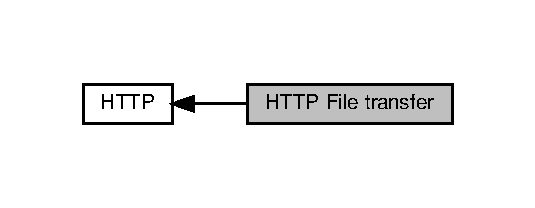
\includegraphics[width=257pt]{group__httpft}
\end{center}
\end{figure}
\subsection*{Functions}
\begin{DoxyCompactItemize}
\item 
L\+W\+S\+\_\+\+V\+I\+S\+I\+B\+LE L\+W\+S\+\_\+\+E\+X\+T\+E\+RN const char $\ast$ \hyperlink{group__httpft_gab4da87a4800413f15e7aba649fb1d77c}{lws\+\_\+get\+\_\+mimetype} (const char $\ast$file, const struct \hyperlink{structlws__http__mount}{lws\+\_\+http\+\_\+mount} $\ast$m)
\item 
L\+W\+S\+\_\+\+V\+I\+S\+I\+B\+LE L\+W\+S\+\_\+\+E\+X\+T\+E\+RN int \hyperlink{group__httpft_gab393a06d3d2722af4c3f8b06842c80d7}{lws\+\_\+serve\+\_\+http\+\_\+file} (struct \hyperlink{structlws}{lws} $\ast$wsi, const char $\ast$file, const char $\ast$content\+\_\+type, const char $\ast$other\+\_\+headers, int other\+\_\+headers\+\_\+len)
\item 
\mbox{\Hypertarget{group__httpft_ga29e1123f6d56cd777b3e5bf9ca40f9e5}\label{group__httpft_ga29e1123f6d56cd777b3e5bf9ca40f9e5}} 
L\+W\+S\+\_\+\+V\+I\+S\+I\+B\+LE L\+W\+S\+\_\+\+E\+X\+T\+E\+RN int {\bfseries lws\+\_\+serve\+\_\+http\+\_\+file\+\_\+fragment} (struct \hyperlink{structlws}{lws} $\ast$wsi)
\end{DoxyCompactItemize}


\subsection{Detailed Description}
A\+P\+Is for sending local files in response to H\+T\+TP requests 

\subsection{Function Documentation}
\mbox{\Hypertarget{group__httpft_gab4da87a4800413f15e7aba649fb1d77c}\label{group__httpft_gab4da87a4800413f15e7aba649fb1d77c}} 
\index{H\+T\+T\+P File transfer@{H\+T\+T\+P File transfer}!lws\+\_\+get\+\_\+mimetype@{lws\+\_\+get\+\_\+mimetype}}
\index{lws\+\_\+get\+\_\+mimetype@{lws\+\_\+get\+\_\+mimetype}!H\+T\+T\+P File transfer@{H\+T\+T\+P File transfer}}
\subsubsection{\texorpdfstring{lws\+\_\+get\+\_\+mimetype()}{lws\_get\_mimetype()}}
{\footnotesize\ttfamily L\+W\+S\+\_\+\+V\+I\+S\+I\+B\+LE L\+W\+S\+\_\+\+E\+X\+T\+E\+RN const char$\ast$ lws\+\_\+get\+\_\+mimetype (\begin{DoxyParamCaption}\item[{const char $\ast$}]{file,  }\item[{const struct \hyperlink{structlws__http__mount}{lws\+\_\+http\+\_\+mount} $\ast$}]{m }\end{DoxyParamCaption})}

\hyperlink{group__httpft_gab4da87a4800413f15e7aba649fb1d77c}{lws\+\_\+get\+\_\+mimetype()} -\/ Determine mimetype to use from filename


\begin{DoxyParams}{Parameters}
{\em file} & filename \\
\hline
{\em m} & N\+U\+LL, or mount context\\
\hline
\end{DoxyParams}
This uses a canned \hyperlink{protocollist-p}{list} of known filetypes first, if no match and m is non-\/\+N\+U\+LL, then tries a \hyperlink{protocollist-p}{list} of per-\/mount file suffix to mimtype mappings.

Returns either N\+U\+LL or a pointer to the mimetype matching the file. \mbox{\Hypertarget{group__httpft_gab393a06d3d2722af4c3f8b06842c80d7}\label{group__httpft_gab393a06d3d2722af4c3f8b06842c80d7}} 
\index{H\+T\+T\+P File transfer@{H\+T\+T\+P File transfer}!lws\+\_\+serve\+\_\+http\+\_\+file@{lws\+\_\+serve\+\_\+http\+\_\+file}}
\index{lws\+\_\+serve\+\_\+http\+\_\+file@{lws\+\_\+serve\+\_\+http\+\_\+file}!H\+T\+T\+P File transfer@{H\+T\+T\+P File transfer}}
\subsubsection{\texorpdfstring{lws\+\_\+serve\+\_\+http\+\_\+file()}{lws\_serve\_http\_file()}}
{\footnotesize\ttfamily L\+W\+S\+\_\+\+V\+I\+S\+I\+B\+LE L\+W\+S\+\_\+\+E\+X\+T\+E\+RN int lws\+\_\+serve\+\_\+http\+\_\+file (\begin{DoxyParamCaption}\item[{struct \hyperlink{structlws}{lws} $\ast$}]{wsi,  }\item[{const char $\ast$}]{file,  }\item[{const char $\ast$}]{content\+\_\+type,  }\item[{const char $\ast$}]{other\+\_\+headers,  }\item[{int}]{other\+\_\+headers\+\_\+len }\end{DoxyParamCaption})}

\hyperlink{group__httpft_gab393a06d3d2722af4c3f8b06842c80d7}{lws\+\_\+serve\+\_\+http\+\_\+file()} -\/ Send a file back to the client using http 
\begin{DoxyParams}{Parameters}
{\em wsi} & Websocket instance (available from user callback) \\
\hline
{\em file} & The file to issue over http \\
\hline
{\em content\+\_\+type} & The http content type, eg, text/html \\
\hline
{\em other\+\_\+headers} & N\+U\+LL or pointer to header string \\
\hline
{\em other\+\_\+headers\+\_\+len} & length of the other headers if non-\/\+N\+U\+LL\\
\hline
\end{DoxyParams}
This function is intended to be called from the callback in response to http requests from the client. It allows the callback to issue local files down the http link in a single step.

Returning $<$0 indicates error and the wsi should be closed. Returning $>$0 indicates the file was completely sent and \hyperlink{group__http_gad27aed6c66a41b2b89ffe4da2a309e8a}{lws\+\_\+http\+\_\+transaction\+\_\+completed()} called on the wsi (and close if != 0) ==0 indicates the file transfer is started and needs more service later, the wsi should be left alone. 
\hypertarget{group__html-chunked-substitution}{}\section{H\+T\+ML Chunked Substitution}
\label{group__html-chunked-substitution}\index{H\+T\+M\+L Chunked Substitution@{H\+T\+M\+L Chunked Substitution}}
Collaboration diagram for H\+T\+ML Chunked Substitution\+:
\nopagebreak
\begin{figure}[H]
\begin{center}
\leavevmode
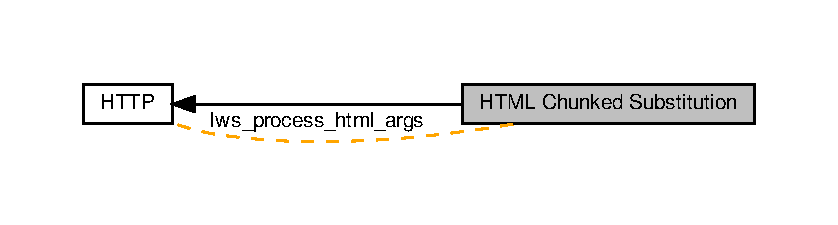
\includegraphics[width=350pt]{group__html-chunked-substitution}
\end{center}
\end{figure}
\subsection*{Classes}
\begin{DoxyCompactItemize}
\item 
struct \hyperlink{structlws__process__html__args}{lws\+\_\+process\+\_\+html\+\_\+args}
\item 
struct \hyperlink{structlws__process__html__state}{lws\+\_\+process\+\_\+html\+\_\+state}
\end{DoxyCompactItemize}
\subsection*{Typedefs}
\begin{DoxyCompactItemize}
\item 
\mbox{\Hypertarget{group__html-chunked-substitution_ga669d3d7ce2d5f193473f649a89b3e7ac}\label{group__html-chunked-substitution_ga669d3d7ce2d5f193473f649a89b3e7ac}} 
typedef const char $\ast$($\ast$ {\bfseries lws\+\_\+process\+\_\+html\+\_\+state\+\_\+cb}) (void $\ast$data, int index)
\item 
\mbox{\Hypertarget{group__html-chunked-substitution_ga669d3d7ce2d5f193473f649a89b3e7ac}\label{group__html-chunked-substitution_ga669d3d7ce2d5f193473f649a89b3e7ac}} 
typedef const char $\ast$($\ast$ {\bfseries lws\+\_\+process\+\_\+html\+\_\+state\+\_\+cb}) (void $\ast$data, int index)
\item 
\mbox{\Hypertarget{group__html-chunked-substitution_ga669d3d7ce2d5f193473f649a89b3e7ac}\label{group__html-chunked-substitution_ga669d3d7ce2d5f193473f649a89b3e7ac}} 
typedef const char $\ast$($\ast$ {\bfseries lws\+\_\+process\+\_\+html\+\_\+state\+\_\+cb}) (void $\ast$data, int index)
\item 
\mbox{\Hypertarget{group__html-chunked-substitution_ga669d3d7ce2d5f193473f649a89b3e7ac}\label{group__html-chunked-substitution_ga669d3d7ce2d5f193473f649a89b3e7ac}} 
typedef const char $\ast$($\ast$ {\bfseries lws\+\_\+process\+\_\+html\+\_\+state\+\_\+cb}) (void $\ast$data, int index)
\item 
\mbox{\Hypertarget{group__html-chunked-substitution_ga669d3d7ce2d5f193473f649a89b3e7ac}\label{group__html-chunked-substitution_ga669d3d7ce2d5f193473f649a89b3e7ac}} 
typedef const char $\ast$($\ast$ {\bfseries lws\+\_\+process\+\_\+html\+\_\+state\+\_\+cb}) (void $\ast$data, int index)
\item 
\mbox{\Hypertarget{group__html-chunked-substitution_ga669d3d7ce2d5f193473f649a89b3e7ac}\label{group__html-chunked-substitution_ga669d3d7ce2d5f193473f649a89b3e7ac}} 
typedef const char $\ast$($\ast$ {\bfseries lws\+\_\+process\+\_\+html\+\_\+state\+\_\+cb}) (void $\ast$data, int index)
\item 
\mbox{\Hypertarget{group__html-chunked-substitution_ga669d3d7ce2d5f193473f649a89b3e7ac}\label{group__html-chunked-substitution_ga669d3d7ce2d5f193473f649a89b3e7ac}} 
typedef const char $\ast$($\ast$ {\bfseries lws\+\_\+process\+\_\+html\+\_\+state\+\_\+cb}) (void $\ast$data, int index)
\item 
\mbox{\Hypertarget{group__html-chunked-substitution_ga669d3d7ce2d5f193473f649a89b3e7ac}\label{group__html-chunked-substitution_ga669d3d7ce2d5f193473f649a89b3e7ac}} 
typedef const char $\ast$($\ast$ {\bfseries lws\+\_\+process\+\_\+html\+\_\+state\+\_\+cb}) (void $\ast$data, int index)
\end{DoxyCompactItemize}
\subsection*{Enumerations}
\begin{DoxyCompactItemize}
\item 
\mbox{\Hypertarget{group__html-chunked-substitution_gabc3b93f68c8bdd857ad32913628dfa8d}\label{group__html-chunked-substitution_gabc3b93f68c8bdd857ad32913628dfa8d}} 
enum {\bfseries http\+\_\+status} \{ \newline
{\bfseries H\+T\+T\+P\+\_\+\+S\+T\+A\+T\+U\+S\+\_\+\+OK} = 200, 
{\bfseries H\+T\+T\+P\+\_\+\+S\+T\+A\+T\+U\+S\+\_\+\+N\+O\+\_\+\+C\+O\+N\+T\+E\+NT} = 204, 
{\bfseries H\+T\+T\+P\+\_\+\+S\+T\+A\+T\+U\+S\+\_\+\+B\+A\+D\+\_\+\+R\+E\+Q\+U\+E\+ST} = 400, 
{\bfseries H\+T\+T\+P\+\_\+\+S\+T\+A\+T\+U\+S\+\_\+\+U\+N\+A\+U\+T\+H\+O\+R\+I\+Z\+ED}, 
\newline
{\bfseries H\+T\+T\+P\+\_\+\+S\+T\+A\+T\+U\+S\+\_\+\+P\+A\+Y\+M\+E\+N\+T\+\_\+\+R\+E\+Q\+U\+I\+R\+ED}, 
{\bfseries H\+T\+T\+P\+\_\+\+S\+T\+A\+T\+U\+S\+\_\+\+F\+O\+R\+B\+I\+D\+D\+EN}, 
{\bfseries H\+T\+T\+P\+\_\+\+S\+T\+A\+T\+U\+S\+\_\+\+N\+O\+T\+\_\+\+F\+O\+U\+ND}, 
{\bfseries H\+T\+T\+P\+\_\+\+S\+T\+A\+T\+U\+S\+\_\+\+M\+E\+T\+H\+O\+D\+\_\+\+N\+O\+T\+\_\+\+A\+L\+L\+O\+W\+ED}, 
\newline
{\bfseries H\+T\+T\+P\+\_\+\+S\+T\+A\+T\+U\+S\+\_\+\+N\+O\+T\+\_\+\+A\+C\+C\+E\+P\+T\+A\+B\+LE}, 
{\bfseries H\+T\+T\+P\+\_\+\+S\+T\+A\+T\+U\+S\+\_\+\+P\+R\+O\+X\+Y\+\_\+\+A\+U\+T\+H\+\_\+\+R\+E\+Q\+U\+I\+R\+ED}, 
{\bfseries H\+T\+T\+P\+\_\+\+S\+T\+A\+T\+U\+S\+\_\+\+R\+E\+Q\+U\+E\+S\+T\+\_\+\+T\+I\+M\+E\+O\+UT}, 
{\bfseries H\+T\+T\+P\+\_\+\+S\+T\+A\+T\+U\+S\+\_\+\+C\+O\+N\+F\+L\+I\+CT}, 
\newline
{\bfseries H\+T\+T\+P\+\_\+\+S\+T\+A\+T\+U\+S\+\_\+\+G\+O\+NE}, 
{\bfseries H\+T\+T\+P\+\_\+\+S\+T\+A\+T\+U\+S\+\_\+\+L\+E\+N\+G\+T\+H\+\_\+\+R\+E\+Q\+U\+I\+R\+ED}, 
{\bfseries H\+T\+T\+P\+\_\+\+S\+T\+A\+T\+U\+S\+\_\+\+P\+R\+E\+C\+O\+N\+D\+I\+T\+I\+O\+N\+\_\+\+F\+A\+I\+L\+ED}, 
{\bfseries H\+T\+T\+P\+\_\+\+S\+T\+A\+T\+U\+S\+\_\+\+R\+E\+Q\+\_\+\+E\+N\+T\+I\+T\+Y\+\_\+\+T\+O\+O\+\_\+\+L\+A\+R\+GE}, 
\newline
{\bfseries H\+T\+T\+P\+\_\+\+S\+T\+A\+T\+U\+S\+\_\+\+R\+E\+Q\+\_\+\+U\+R\+I\+\_\+\+T\+O\+O\+\_\+\+L\+O\+NG}, 
{\bfseries H\+T\+T\+P\+\_\+\+S\+T\+A\+T\+U\+S\+\_\+\+U\+N\+S\+U\+P\+P\+O\+R\+T\+E\+D\+\_\+\+M\+E\+D\+I\+A\+\_\+\+T\+Y\+PE}, 
{\bfseries H\+T\+T\+P\+\_\+\+S\+T\+A\+T\+U\+S\+\_\+\+R\+E\+Q\+\_\+\+R\+A\+N\+G\+E\+\_\+\+N\+O\+T\+\_\+\+S\+A\+T\+I\+S\+F\+I\+A\+B\+LE}, 
{\bfseries H\+T\+T\+P\+\_\+\+S\+T\+A\+T\+U\+S\+\_\+\+E\+X\+P\+E\+C\+T\+A\+T\+I\+O\+N\+\_\+\+F\+A\+I\+L\+ED}, 
\newline
{\bfseries H\+T\+T\+P\+\_\+\+S\+T\+A\+T\+U\+S\+\_\+\+I\+N\+T\+E\+R\+N\+A\+L\+\_\+\+S\+E\+R\+V\+E\+R\+\_\+\+E\+R\+R\+OR} = 500, 
{\bfseries H\+T\+T\+P\+\_\+\+S\+T\+A\+T\+U\+S\+\_\+\+N\+O\+T\+\_\+\+I\+M\+P\+L\+E\+M\+E\+N\+T\+ED}, 
{\bfseries H\+T\+T\+P\+\_\+\+S\+T\+A\+T\+U\+S\+\_\+\+B\+A\+D\+\_\+\+G\+A\+T\+E\+W\+AY}, 
{\bfseries H\+T\+T\+P\+\_\+\+S\+T\+A\+T\+U\+S\+\_\+\+S\+E\+R\+V\+I\+C\+E\+\_\+\+U\+N\+A\+V\+A\+I\+L\+A\+B\+LE}, 
\newline
{\bfseries H\+T\+T\+P\+\_\+\+S\+T\+A\+T\+U\+S\+\_\+\+G\+A\+T\+E\+W\+A\+Y\+\_\+\+T\+I\+M\+E\+O\+UT}, 
{\bfseries H\+T\+T\+P\+\_\+\+S\+T\+A\+T\+U\+S\+\_\+\+H\+T\+T\+P\+\_\+\+V\+E\+R\+S\+I\+O\+N\+\_\+\+N\+O\+T\+\_\+\+S\+U\+P\+P\+O\+R\+T\+ED}, 
{\bfseries H\+T\+T\+P\+\_\+\+S\+T\+A\+T\+U\+S\+\_\+\+OK} = 200, 
{\bfseries H\+T\+T\+P\+\_\+\+S\+T\+A\+T\+U\+S\+\_\+\+N\+O\+\_\+\+C\+O\+N\+T\+E\+NT} = 204, 
\newline
{\bfseries H\+T\+T\+P\+\_\+\+S\+T\+A\+T\+U\+S\+\_\+\+B\+A\+D\+\_\+\+R\+E\+Q\+U\+E\+ST} = 400, 
{\bfseries H\+T\+T\+P\+\_\+\+S\+T\+A\+T\+U\+S\+\_\+\+U\+N\+A\+U\+T\+H\+O\+R\+I\+Z\+ED}, 
{\bfseries H\+T\+T\+P\+\_\+\+S\+T\+A\+T\+U\+S\+\_\+\+P\+A\+Y\+M\+E\+N\+T\+\_\+\+R\+E\+Q\+U\+I\+R\+ED}, 
{\bfseries H\+T\+T\+P\+\_\+\+S\+T\+A\+T\+U\+S\+\_\+\+F\+O\+R\+B\+I\+D\+D\+EN}, 
\newline
{\bfseries H\+T\+T\+P\+\_\+\+S\+T\+A\+T\+U\+S\+\_\+\+N\+O\+T\+\_\+\+F\+O\+U\+ND}, 
{\bfseries H\+T\+T\+P\+\_\+\+S\+T\+A\+T\+U\+S\+\_\+\+M\+E\+T\+H\+O\+D\+\_\+\+N\+O\+T\+\_\+\+A\+L\+L\+O\+W\+ED}, 
{\bfseries H\+T\+T\+P\+\_\+\+S\+T\+A\+T\+U\+S\+\_\+\+N\+O\+T\+\_\+\+A\+C\+C\+E\+P\+T\+A\+B\+LE}, 
{\bfseries H\+T\+T\+P\+\_\+\+S\+T\+A\+T\+U\+S\+\_\+\+P\+R\+O\+X\+Y\+\_\+\+A\+U\+T\+H\+\_\+\+R\+E\+Q\+U\+I\+R\+ED}, 
\newline
{\bfseries H\+T\+T\+P\+\_\+\+S\+T\+A\+T\+U\+S\+\_\+\+R\+E\+Q\+U\+E\+S\+T\+\_\+\+T\+I\+M\+E\+O\+UT}, 
{\bfseries H\+T\+T\+P\+\_\+\+S\+T\+A\+T\+U\+S\+\_\+\+C\+O\+N\+F\+L\+I\+CT}, 
{\bfseries H\+T\+T\+P\+\_\+\+S\+T\+A\+T\+U\+S\+\_\+\+G\+O\+NE}, 
{\bfseries H\+T\+T\+P\+\_\+\+S\+T\+A\+T\+U\+S\+\_\+\+L\+E\+N\+G\+T\+H\+\_\+\+R\+E\+Q\+U\+I\+R\+ED}, 
\newline
{\bfseries H\+T\+T\+P\+\_\+\+S\+T\+A\+T\+U\+S\+\_\+\+P\+R\+E\+C\+O\+N\+D\+I\+T\+I\+O\+N\+\_\+\+F\+A\+I\+L\+ED}, 
{\bfseries H\+T\+T\+P\+\_\+\+S\+T\+A\+T\+U\+S\+\_\+\+R\+E\+Q\+\_\+\+E\+N\+T\+I\+T\+Y\+\_\+\+T\+O\+O\+\_\+\+L\+A\+R\+GE}, 
{\bfseries H\+T\+T\+P\+\_\+\+S\+T\+A\+T\+U\+S\+\_\+\+R\+E\+Q\+\_\+\+U\+R\+I\+\_\+\+T\+O\+O\+\_\+\+L\+O\+NG}, 
{\bfseries H\+T\+T\+P\+\_\+\+S\+T\+A\+T\+U\+S\+\_\+\+U\+N\+S\+U\+P\+P\+O\+R\+T\+E\+D\+\_\+\+M\+E\+D\+I\+A\+\_\+\+T\+Y\+PE}, 
\newline
{\bfseries H\+T\+T\+P\+\_\+\+S\+T\+A\+T\+U\+S\+\_\+\+R\+E\+Q\+\_\+\+R\+A\+N\+G\+E\+\_\+\+N\+O\+T\+\_\+\+S\+A\+T\+I\+S\+F\+I\+A\+B\+LE}, 
{\bfseries H\+T\+T\+P\+\_\+\+S\+T\+A\+T\+U\+S\+\_\+\+E\+X\+P\+E\+C\+T\+A\+T\+I\+O\+N\+\_\+\+F\+A\+I\+L\+ED}, 
{\bfseries H\+T\+T\+P\+\_\+\+S\+T\+A\+T\+U\+S\+\_\+\+I\+N\+T\+E\+R\+N\+A\+L\+\_\+\+S\+E\+R\+V\+E\+R\+\_\+\+E\+R\+R\+OR} = 500, 
{\bfseries H\+T\+T\+P\+\_\+\+S\+T\+A\+T\+U\+S\+\_\+\+N\+O\+T\+\_\+\+I\+M\+P\+L\+E\+M\+E\+N\+T\+ED}, 
\newline
{\bfseries H\+T\+T\+P\+\_\+\+S\+T\+A\+T\+U\+S\+\_\+\+B\+A\+D\+\_\+\+G\+A\+T\+E\+W\+AY}, 
{\bfseries H\+T\+T\+P\+\_\+\+S\+T\+A\+T\+U\+S\+\_\+\+S\+E\+R\+V\+I\+C\+E\+\_\+\+U\+N\+A\+V\+A\+I\+L\+A\+B\+LE}, 
{\bfseries H\+T\+T\+P\+\_\+\+S\+T\+A\+T\+U\+S\+\_\+\+G\+A\+T\+E\+W\+A\+Y\+\_\+\+T\+I\+M\+E\+O\+UT}, 
{\bfseries H\+T\+T\+P\+\_\+\+S\+T\+A\+T\+U\+S\+\_\+\+H\+T\+T\+P\+\_\+\+V\+E\+R\+S\+I\+O\+N\+\_\+\+N\+O\+T\+\_\+\+S\+U\+P\+P\+O\+R\+T\+ED}, 
\newline
{\bfseries H\+T\+T\+P\+\_\+\+S\+T\+A\+T\+U\+S\+\_\+\+OK} = 200, 
{\bfseries H\+T\+T\+P\+\_\+\+S\+T\+A\+T\+U\+S\+\_\+\+N\+O\+\_\+\+C\+O\+N\+T\+E\+NT} = 204, 
{\bfseries H\+T\+T\+P\+\_\+\+S\+T\+A\+T\+U\+S\+\_\+\+B\+A\+D\+\_\+\+R\+E\+Q\+U\+E\+ST} = 400, 
{\bfseries H\+T\+T\+P\+\_\+\+S\+T\+A\+T\+U\+S\+\_\+\+U\+N\+A\+U\+T\+H\+O\+R\+I\+Z\+ED}, 
\newline
{\bfseries H\+T\+T\+P\+\_\+\+S\+T\+A\+T\+U\+S\+\_\+\+P\+A\+Y\+M\+E\+N\+T\+\_\+\+R\+E\+Q\+U\+I\+R\+ED}, 
{\bfseries H\+T\+T\+P\+\_\+\+S\+T\+A\+T\+U\+S\+\_\+\+F\+O\+R\+B\+I\+D\+D\+EN}, 
{\bfseries H\+T\+T\+P\+\_\+\+S\+T\+A\+T\+U\+S\+\_\+\+N\+O\+T\+\_\+\+F\+O\+U\+ND}, 
{\bfseries H\+T\+T\+P\+\_\+\+S\+T\+A\+T\+U\+S\+\_\+\+M\+E\+T\+H\+O\+D\+\_\+\+N\+O\+T\+\_\+\+A\+L\+L\+O\+W\+ED}, 
\newline
{\bfseries H\+T\+T\+P\+\_\+\+S\+T\+A\+T\+U\+S\+\_\+\+N\+O\+T\+\_\+\+A\+C\+C\+E\+P\+T\+A\+B\+LE}, 
{\bfseries H\+T\+T\+P\+\_\+\+S\+T\+A\+T\+U\+S\+\_\+\+P\+R\+O\+X\+Y\+\_\+\+A\+U\+T\+H\+\_\+\+R\+E\+Q\+U\+I\+R\+ED}, 
{\bfseries H\+T\+T\+P\+\_\+\+S\+T\+A\+T\+U\+S\+\_\+\+R\+E\+Q\+U\+E\+S\+T\+\_\+\+T\+I\+M\+E\+O\+UT}, 
{\bfseries H\+T\+T\+P\+\_\+\+S\+T\+A\+T\+U\+S\+\_\+\+C\+O\+N\+F\+L\+I\+CT}, 
\newline
{\bfseries H\+T\+T\+P\+\_\+\+S\+T\+A\+T\+U\+S\+\_\+\+G\+O\+NE}, 
{\bfseries H\+T\+T\+P\+\_\+\+S\+T\+A\+T\+U\+S\+\_\+\+L\+E\+N\+G\+T\+H\+\_\+\+R\+E\+Q\+U\+I\+R\+ED}, 
{\bfseries H\+T\+T\+P\+\_\+\+S\+T\+A\+T\+U\+S\+\_\+\+P\+R\+E\+C\+O\+N\+D\+I\+T\+I\+O\+N\+\_\+\+F\+A\+I\+L\+ED}, 
{\bfseries H\+T\+T\+P\+\_\+\+S\+T\+A\+T\+U\+S\+\_\+\+R\+E\+Q\+\_\+\+E\+N\+T\+I\+T\+Y\+\_\+\+T\+O\+O\+\_\+\+L\+A\+R\+GE}, 
\newline
{\bfseries H\+T\+T\+P\+\_\+\+S\+T\+A\+T\+U\+S\+\_\+\+R\+E\+Q\+\_\+\+U\+R\+I\+\_\+\+T\+O\+O\+\_\+\+L\+O\+NG}, 
{\bfseries H\+T\+T\+P\+\_\+\+S\+T\+A\+T\+U\+S\+\_\+\+U\+N\+S\+U\+P\+P\+O\+R\+T\+E\+D\+\_\+\+M\+E\+D\+I\+A\+\_\+\+T\+Y\+PE}, 
{\bfseries H\+T\+T\+P\+\_\+\+S\+T\+A\+T\+U\+S\+\_\+\+R\+E\+Q\+\_\+\+R\+A\+N\+G\+E\+\_\+\+N\+O\+T\+\_\+\+S\+A\+T\+I\+S\+F\+I\+A\+B\+LE}, 
{\bfseries H\+T\+T\+P\+\_\+\+S\+T\+A\+T\+U\+S\+\_\+\+E\+X\+P\+E\+C\+T\+A\+T\+I\+O\+N\+\_\+\+F\+A\+I\+L\+ED}, 
\newline
{\bfseries H\+T\+T\+P\+\_\+\+S\+T\+A\+T\+U\+S\+\_\+\+I\+N\+T\+E\+R\+N\+A\+L\+\_\+\+S\+E\+R\+V\+E\+R\+\_\+\+E\+R\+R\+OR} = 500, 
{\bfseries H\+T\+T\+P\+\_\+\+S\+T\+A\+T\+U\+S\+\_\+\+N\+O\+T\+\_\+\+I\+M\+P\+L\+E\+M\+E\+N\+T\+ED}, 
{\bfseries H\+T\+T\+P\+\_\+\+S\+T\+A\+T\+U\+S\+\_\+\+B\+A\+D\+\_\+\+G\+A\+T\+E\+W\+AY}, 
{\bfseries H\+T\+T\+P\+\_\+\+S\+T\+A\+T\+U\+S\+\_\+\+S\+E\+R\+V\+I\+C\+E\+\_\+\+U\+N\+A\+V\+A\+I\+L\+A\+B\+LE}, 
\newline
{\bfseries H\+T\+T\+P\+\_\+\+S\+T\+A\+T\+U\+S\+\_\+\+G\+A\+T\+E\+W\+A\+Y\+\_\+\+T\+I\+M\+E\+O\+UT}, 
{\bfseries H\+T\+T\+P\+\_\+\+S\+T\+A\+T\+U\+S\+\_\+\+H\+T\+T\+P\+\_\+\+V\+E\+R\+S\+I\+O\+N\+\_\+\+N\+O\+T\+\_\+\+S\+U\+P\+P\+O\+R\+T\+ED}, 
{\bfseries H\+T\+T\+P\+\_\+\+S\+T\+A\+T\+U\+S\+\_\+\+OK} = 200, 
{\bfseries H\+T\+T\+P\+\_\+\+S\+T\+A\+T\+U\+S\+\_\+\+N\+O\+\_\+\+C\+O\+N\+T\+E\+NT} = 204, 
\newline
{\bfseries H\+T\+T\+P\+\_\+\+S\+T\+A\+T\+U\+S\+\_\+\+B\+A\+D\+\_\+\+R\+E\+Q\+U\+E\+ST} = 400, 
{\bfseries H\+T\+T\+P\+\_\+\+S\+T\+A\+T\+U\+S\+\_\+\+U\+N\+A\+U\+T\+H\+O\+R\+I\+Z\+ED}, 
{\bfseries H\+T\+T\+P\+\_\+\+S\+T\+A\+T\+U\+S\+\_\+\+P\+A\+Y\+M\+E\+N\+T\+\_\+\+R\+E\+Q\+U\+I\+R\+ED}, 
{\bfseries H\+T\+T\+P\+\_\+\+S\+T\+A\+T\+U\+S\+\_\+\+F\+O\+R\+B\+I\+D\+D\+EN}, 
\newline
{\bfseries H\+T\+T\+P\+\_\+\+S\+T\+A\+T\+U\+S\+\_\+\+N\+O\+T\+\_\+\+F\+O\+U\+ND}, 
{\bfseries H\+T\+T\+P\+\_\+\+S\+T\+A\+T\+U\+S\+\_\+\+M\+E\+T\+H\+O\+D\+\_\+\+N\+O\+T\+\_\+\+A\+L\+L\+O\+W\+ED}, 
{\bfseries H\+T\+T\+P\+\_\+\+S\+T\+A\+T\+U\+S\+\_\+\+N\+O\+T\+\_\+\+A\+C\+C\+E\+P\+T\+A\+B\+LE}, 
{\bfseries H\+T\+T\+P\+\_\+\+S\+T\+A\+T\+U\+S\+\_\+\+P\+R\+O\+X\+Y\+\_\+\+A\+U\+T\+H\+\_\+\+R\+E\+Q\+U\+I\+R\+ED}, 
\newline
{\bfseries H\+T\+T\+P\+\_\+\+S\+T\+A\+T\+U\+S\+\_\+\+R\+E\+Q\+U\+E\+S\+T\+\_\+\+T\+I\+M\+E\+O\+UT}, 
{\bfseries H\+T\+T\+P\+\_\+\+S\+T\+A\+T\+U\+S\+\_\+\+C\+O\+N\+F\+L\+I\+CT}, 
{\bfseries H\+T\+T\+P\+\_\+\+S\+T\+A\+T\+U\+S\+\_\+\+G\+O\+NE}, 
{\bfseries H\+T\+T\+P\+\_\+\+S\+T\+A\+T\+U\+S\+\_\+\+L\+E\+N\+G\+T\+H\+\_\+\+R\+E\+Q\+U\+I\+R\+ED}, 
\newline
{\bfseries H\+T\+T\+P\+\_\+\+S\+T\+A\+T\+U\+S\+\_\+\+P\+R\+E\+C\+O\+N\+D\+I\+T\+I\+O\+N\+\_\+\+F\+A\+I\+L\+ED}, 
{\bfseries H\+T\+T\+P\+\_\+\+S\+T\+A\+T\+U\+S\+\_\+\+R\+E\+Q\+\_\+\+E\+N\+T\+I\+T\+Y\+\_\+\+T\+O\+O\+\_\+\+L\+A\+R\+GE}, 
{\bfseries H\+T\+T\+P\+\_\+\+S\+T\+A\+T\+U\+S\+\_\+\+R\+E\+Q\+\_\+\+U\+R\+I\+\_\+\+T\+O\+O\+\_\+\+L\+O\+NG}, 
{\bfseries H\+T\+T\+P\+\_\+\+S\+T\+A\+T\+U\+S\+\_\+\+U\+N\+S\+U\+P\+P\+O\+R\+T\+E\+D\+\_\+\+M\+E\+D\+I\+A\+\_\+\+T\+Y\+PE}, 
\newline
{\bfseries H\+T\+T\+P\+\_\+\+S\+T\+A\+T\+U\+S\+\_\+\+R\+E\+Q\+\_\+\+R\+A\+N\+G\+E\+\_\+\+N\+O\+T\+\_\+\+S\+A\+T\+I\+S\+F\+I\+A\+B\+LE}, 
{\bfseries H\+T\+T\+P\+\_\+\+S\+T\+A\+T\+U\+S\+\_\+\+E\+X\+P\+E\+C\+T\+A\+T\+I\+O\+N\+\_\+\+F\+A\+I\+L\+ED}, 
{\bfseries H\+T\+T\+P\+\_\+\+S\+T\+A\+T\+U\+S\+\_\+\+I\+N\+T\+E\+R\+N\+A\+L\+\_\+\+S\+E\+R\+V\+E\+R\+\_\+\+E\+R\+R\+OR} = 500, 
{\bfseries H\+T\+T\+P\+\_\+\+S\+T\+A\+T\+U\+S\+\_\+\+N\+O\+T\+\_\+\+I\+M\+P\+L\+E\+M\+E\+N\+T\+ED}, 
\newline
{\bfseries H\+T\+T\+P\+\_\+\+S\+T\+A\+T\+U\+S\+\_\+\+B\+A\+D\+\_\+\+G\+A\+T\+E\+W\+AY}, 
{\bfseries H\+T\+T\+P\+\_\+\+S\+T\+A\+T\+U\+S\+\_\+\+S\+E\+R\+V\+I\+C\+E\+\_\+\+U\+N\+A\+V\+A\+I\+L\+A\+B\+LE}, 
{\bfseries H\+T\+T\+P\+\_\+\+S\+T\+A\+T\+U\+S\+\_\+\+G\+A\+T\+E\+W\+A\+Y\+\_\+\+T\+I\+M\+E\+O\+UT}, 
{\bfseries H\+T\+T\+P\+\_\+\+S\+T\+A\+T\+U\+S\+\_\+\+H\+T\+T\+P\+\_\+\+V\+E\+R\+S\+I\+O\+N\+\_\+\+N\+O\+T\+\_\+\+S\+U\+P\+P\+O\+R\+T\+ED}, 
\newline
{\bfseries H\+T\+T\+P\+\_\+\+S\+T\+A\+T\+U\+S\+\_\+\+OK} = 200, 
{\bfseries H\+T\+T\+P\+\_\+\+S\+T\+A\+T\+U\+S\+\_\+\+N\+O\+\_\+\+C\+O\+N\+T\+E\+NT} = 204, 
{\bfseries H\+T\+T\+P\+\_\+\+S\+T\+A\+T\+U\+S\+\_\+\+B\+A\+D\+\_\+\+R\+E\+Q\+U\+E\+ST} = 400, 
{\bfseries H\+T\+T\+P\+\_\+\+S\+T\+A\+T\+U\+S\+\_\+\+U\+N\+A\+U\+T\+H\+O\+R\+I\+Z\+ED}, 
\newline
{\bfseries H\+T\+T\+P\+\_\+\+S\+T\+A\+T\+U\+S\+\_\+\+P\+A\+Y\+M\+E\+N\+T\+\_\+\+R\+E\+Q\+U\+I\+R\+ED}, 
{\bfseries H\+T\+T\+P\+\_\+\+S\+T\+A\+T\+U\+S\+\_\+\+F\+O\+R\+B\+I\+D\+D\+EN}, 
{\bfseries H\+T\+T\+P\+\_\+\+S\+T\+A\+T\+U\+S\+\_\+\+N\+O\+T\+\_\+\+F\+O\+U\+ND}, 
{\bfseries H\+T\+T\+P\+\_\+\+S\+T\+A\+T\+U\+S\+\_\+\+M\+E\+T\+H\+O\+D\+\_\+\+N\+O\+T\+\_\+\+A\+L\+L\+O\+W\+ED}, 
\newline
{\bfseries H\+T\+T\+P\+\_\+\+S\+T\+A\+T\+U\+S\+\_\+\+N\+O\+T\+\_\+\+A\+C\+C\+E\+P\+T\+A\+B\+LE}, 
{\bfseries H\+T\+T\+P\+\_\+\+S\+T\+A\+T\+U\+S\+\_\+\+P\+R\+O\+X\+Y\+\_\+\+A\+U\+T\+H\+\_\+\+R\+E\+Q\+U\+I\+R\+ED}, 
{\bfseries H\+T\+T\+P\+\_\+\+S\+T\+A\+T\+U\+S\+\_\+\+R\+E\+Q\+U\+E\+S\+T\+\_\+\+T\+I\+M\+E\+O\+UT}, 
{\bfseries H\+T\+T\+P\+\_\+\+S\+T\+A\+T\+U\+S\+\_\+\+C\+O\+N\+F\+L\+I\+CT}, 
\newline
{\bfseries H\+T\+T\+P\+\_\+\+S\+T\+A\+T\+U\+S\+\_\+\+G\+O\+NE}, 
{\bfseries H\+T\+T\+P\+\_\+\+S\+T\+A\+T\+U\+S\+\_\+\+L\+E\+N\+G\+T\+H\+\_\+\+R\+E\+Q\+U\+I\+R\+ED}, 
{\bfseries H\+T\+T\+P\+\_\+\+S\+T\+A\+T\+U\+S\+\_\+\+P\+R\+E\+C\+O\+N\+D\+I\+T\+I\+O\+N\+\_\+\+F\+A\+I\+L\+ED}, 
{\bfseries H\+T\+T\+P\+\_\+\+S\+T\+A\+T\+U\+S\+\_\+\+R\+E\+Q\+\_\+\+E\+N\+T\+I\+T\+Y\+\_\+\+T\+O\+O\+\_\+\+L\+A\+R\+GE}, 
\newline
{\bfseries H\+T\+T\+P\+\_\+\+S\+T\+A\+T\+U\+S\+\_\+\+R\+E\+Q\+\_\+\+U\+R\+I\+\_\+\+T\+O\+O\+\_\+\+L\+O\+NG}, 
{\bfseries H\+T\+T\+P\+\_\+\+S\+T\+A\+T\+U\+S\+\_\+\+U\+N\+S\+U\+P\+P\+O\+R\+T\+E\+D\+\_\+\+M\+E\+D\+I\+A\+\_\+\+T\+Y\+PE}, 
{\bfseries H\+T\+T\+P\+\_\+\+S\+T\+A\+T\+U\+S\+\_\+\+R\+E\+Q\+\_\+\+R\+A\+N\+G\+E\+\_\+\+N\+O\+T\+\_\+\+S\+A\+T\+I\+S\+F\+I\+A\+B\+LE}, 
{\bfseries H\+T\+T\+P\+\_\+\+S\+T\+A\+T\+U\+S\+\_\+\+E\+X\+P\+E\+C\+T\+A\+T\+I\+O\+N\+\_\+\+F\+A\+I\+L\+ED}, 
\newline
{\bfseries H\+T\+T\+P\+\_\+\+S\+T\+A\+T\+U\+S\+\_\+\+I\+N\+T\+E\+R\+N\+A\+L\+\_\+\+S\+E\+R\+V\+E\+R\+\_\+\+E\+R\+R\+OR} = 500, 
{\bfseries H\+T\+T\+P\+\_\+\+S\+T\+A\+T\+U\+S\+\_\+\+N\+O\+T\+\_\+\+I\+M\+P\+L\+E\+M\+E\+N\+T\+ED}, 
{\bfseries H\+T\+T\+P\+\_\+\+S\+T\+A\+T\+U\+S\+\_\+\+B\+A\+D\+\_\+\+G\+A\+T\+E\+W\+AY}, 
{\bfseries H\+T\+T\+P\+\_\+\+S\+T\+A\+T\+U\+S\+\_\+\+S\+E\+R\+V\+I\+C\+E\+\_\+\+U\+N\+A\+V\+A\+I\+L\+A\+B\+LE}, 
\newline
{\bfseries H\+T\+T\+P\+\_\+\+S\+T\+A\+T\+U\+S\+\_\+\+G\+A\+T\+E\+W\+A\+Y\+\_\+\+T\+I\+M\+E\+O\+UT}, 
{\bfseries H\+T\+T\+P\+\_\+\+S\+T\+A\+T\+U\+S\+\_\+\+H\+T\+T\+P\+\_\+\+V\+E\+R\+S\+I\+O\+N\+\_\+\+N\+O\+T\+\_\+\+S\+U\+P\+P\+O\+R\+T\+ED}, 
{\bfseries H\+T\+T\+P\+\_\+\+S\+T\+A\+T\+U\+S\+\_\+\+OK} = 200, 
{\bfseries H\+T\+T\+P\+\_\+\+S\+T\+A\+T\+U\+S\+\_\+\+N\+O\+\_\+\+C\+O\+N\+T\+E\+NT} = 204, 
\newline
{\bfseries H\+T\+T\+P\+\_\+\+S\+T\+A\+T\+U\+S\+\_\+\+B\+A\+D\+\_\+\+R\+E\+Q\+U\+E\+ST} = 400, 
{\bfseries H\+T\+T\+P\+\_\+\+S\+T\+A\+T\+U\+S\+\_\+\+U\+N\+A\+U\+T\+H\+O\+R\+I\+Z\+ED}, 
{\bfseries H\+T\+T\+P\+\_\+\+S\+T\+A\+T\+U\+S\+\_\+\+P\+A\+Y\+M\+E\+N\+T\+\_\+\+R\+E\+Q\+U\+I\+R\+ED}, 
{\bfseries H\+T\+T\+P\+\_\+\+S\+T\+A\+T\+U\+S\+\_\+\+F\+O\+R\+B\+I\+D\+D\+EN}, 
\newline
{\bfseries H\+T\+T\+P\+\_\+\+S\+T\+A\+T\+U\+S\+\_\+\+N\+O\+T\+\_\+\+F\+O\+U\+ND}, 
{\bfseries H\+T\+T\+P\+\_\+\+S\+T\+A\+T\+U\+S\+\_\+\+M\+E\+T\+H\+O\+D\+\_\+\+N\+O\+T\+\_\+\+A\+L\+L\+O\+W\+ED}, 
{\bfseries H\+T\+T\+P\+\_\+\+S\+T\+A\+T\+U\+S\+\_\+\+N\+O\+T\+\_\+\+A\+C\+C\+E\+P\+T\+A\+B\+LE}, 
{\bfseries H\+T\+T\+P\+\_\+\+S\+T\+A\+T\+U\+S\+\_\+\+P\+R\+O\+X\+Y\+\_\+\+A\+U\+T\+H\+\_\+\+R\+E\+Q\+U\+I\+R\+ED}, 
\newline
{\bfseries H\+T\+T\+P\+\_\+\+S\+T\+A\+T\+U\+S\+\_\+\+R\+E\+Q\+U\+E\+S\+T\+\_\+\+T\+I\+M\+E\+O\+UT}, 
{\bfseries H\+T\+T\+P\+\_\+\+S\+T\+A\+T\+U\+S\+\_\+\+C\+O\+N\+F\+L\+I\+CT}, 
{\bfseries H\+T\+T\+P\+\_\+\+S\+T\+A\+T\+U\+S\+\_\+\+G\+O\+NE}, 
{\bfseries H\+T\+T\+P\+\_\+\+S\+T\+A\+T\+U\+S\+\_\+\+L\+E\+N\+G\+T\+H\+\_\+\+R\+E\+Q\+U\+I\+R\+ED}, 
\newline
{\bfseries H\+T\+T\+P\+\_\+\+S\+T\+A\+T\+U\+S\+\_\+\+P\+R\+E\+C\+O\+N\+D\+I\+T\+I\+O\+N\+\_\+\+F\+A\+I\+L\+ED}, 
{\bfseries H\+T\+T\+P\+\_\+\+S\+T\+A\+T\+U\+S\+\_\+\+R\+E\+Q\+\_\+\+E\+N\+T\+I\+T\+Y\+\_\+\+T\+O\+O\+\_\+\+L\+A\+R\+GE}, 
{\bfseries H\+T\+T\+P\+\_\+\+S\+T\+A\+T\+U\+S\+\_\+\+R\+E\+Q\+\_\+\+U\+R\+I\+\_\+\+T\+O\+O\+\_\+\+L\+O\+NG}, 
{\bfseries H\+T\+T\+P\+\_\+\+S\+T\+A\+T\+U\+S\+\_\+\+U\+N\+S\+U\+P\+P\+O\+R\+T\+E\+D\+\_\+\+M\+E\+D\+I\+A\+\_\+\+T\+Y\+PE}, 
\newline
{\bfseries H\+T\+T\+P\+\_\+\+S\+T\+A\+T\+U\+S\+\_\+\+R\+E\+Q\+\_\+\+R\+A\+N\+G\+E\+\_\+\+N\+O\+T\+\_\+\+S\+A\+T\+I\+S\+F\+I\+A\+B\+LE}, 
{\bfseries H\+T\+T\+P\+\_\+\+S\+T\+A\+T\+U\+S\+\_\+\+E\+X\+P\+E\+C\+T\+A\+T\+I\+O\+N\+\_\+\+F\+A\+I\+L\+ED}, 
{\bfseries H\+T\+T\+P\+\_\+\+S\+T\+A\+T\+U\+S\+\_\+\+I\+N\+T\+E\+R\+N\+A\+L\+\_\+\+S\+E\+R\+V\+E\+R\+\_\+\+E\+R\+R\+OR} = 500, 
{\bfseries H\+T\+T\+P\+\_\+\+S\+T\+A\+T\+U\+S\+\_\+\+N\+O\+T\+\_\+\+I\+M\+P\+L\+E\+M\+E\+N\+T\+ED}, 
\newline
{\bfseries H\+T\+T\+P\+\_\+\+S\+T\+A\+T\+U\+S\+\_\+\+B\+A\+D\+\_\+\+G\+A\+T\+E\+W\+AY}, 
{\bfseries H\+T\+T\+P\+\_\+\+S\+T\+A\+T\+U\+S\+\_\+\+S\+E\+R\+V\+I\+C\+E\+\_\+\+U\+N\+A\+V\+A\+I\+L\+A\+B\+LE}, 
{\bfseries H\+T\+T\+P\+\_\+\+S\+T\+A\+T\+U\+S\+\_\+\+G\+A\+T\+E\+W\+A\+Y\+\_\+\+T\+I\+M\+E\+O\+UT}, 
{\bfseries H\+T\+T\+P\+\_\+\+S\+T\+A\+T\+U\+S\+\_\+\+H\+T\+T\+P\+\_\+\+V\+E\+R\+S\+I\+O\+N\+\_\+\+N\+O\+T\+\_\+\+S\+U\+P\+P\+O\+R\+T\+ED}, 
\newline
{\bfseries H\+T\+T\+P\+\_\+\+S\+T\+A\+T\+U\+S\+\_\+\+OK} = 200, 
{\bfseries H\+T\+T\+P\+\_\+\+S\+T\+A\+T\+U\+S\+\_\+\+N\+O\+\_\+\+C\+O\+N\+T\+E\+NT} = 204, 
{\bfseries H\+T\+T\+P\+\_\+\+S\+T\+A\+T\+U\+S\+\_\+\+B\+A\+D\+\_\+\+R\+E\+Q\+U\+E\+ST} = 400, 
{\bfseries H\+T\+T\+P\+\_\+\+S\+T\+A\+T\+U\+S\+\_\+\+U\+N\+A\+U\+T\+H\+O\+R\+I\+Z\+ED}, 
\newline
{\bfseries H\+T\+T\+P\+\_\+\+S\+T\+A\+T\+U\+S\+\_\+\+P\+A\+Y\+M\+E\+N\+T\+\_\+\+R\+E\+Q\+U\+I\+R\+ED}, 
{\bfseries H\+T\+T\+P\+\_\+\+S\+T\+A\+T\+U\+S\+\_\+\+F\+O\+R\+B\+I\+D\+D\+EN}, 
{\bfseries H\+T\+T\+P\+\_\+\+S\+T\+A\+T\+U\+S\+\_\+\+N\+O\+T\+\_\+\+F\+O\+U\+ND}, 
{\bfseries H\+T\+T\+P\+\_\+\+S\+T\+A\+T\+U\+S\+\_\+\+M\+E\+T\+H\+O\+D\+\_\+\+N\+O\+T\+\_\+\+A\+L\+L\+O\+W\+ED}, 
\newline
{\bfseries H\+T\+T\+P\+\_\+\+S\+T\+A\+T\+U\+S\+\_\+\+N\+O\+T\+\_\+\+A\+C\+C\+E\+P\+T\+A\+B\+LE}, 
{\bfseries H\+T\+T\+P\+\_\+\+S\+T\+A\+T\+U\+S\+\_\+\+P\+R\+O\+X\+Y\+\_\+\+A\+U\+T\+H\+\_\+\+R\+E\+Q\+U\+I\+R\+ED}, 
{\bfseries H\+T\+T\+P\+\_\+\+S\+T\+A\+T\+U\+S\+\_\+\+R\+E\+Q\+U\+E\+S\+T\+\_\+\+T\+I\+M\+E\+O\+UT}, 
{\bfseries H\+T\+T\+P\+\_\+\+S\+T\+A\+T\+U\+S\+\_\+\+C\+O\+N\+F\+L\+I\+CT}, 
\newline
{\bfseries H\+T\+T\+P\+\_\+\+S\+T\+A\+T\+U\+S\+\_\+\+G\+O\+NE}, 
{\bfseries H\+T\+T\+P\+\_\+\+S\+T\+A\+T\+U\+S\+\_\+\+L\+E\+N\+G\+T\+H\+\_\+\+R\+E\+Q\+U\+I\+R\+ED}, 
{\bfseries H\+T\+T\+P\+\_\+\+S\+T\+A\+T\+U\+S\+\_\+\+P\+R\+E\+C\+O\+N\+D\+I\+T\+I\+O\+N\+\_\+\+F\+A\+I\+L\+ED}, 
{\bfseries H\+T\+T\+P\+\_\+\+S\+T\+A\+T\+U\+S\+\_\+\+R\+E\+Q\+\_\+\+E\+N\+T\+I\+T\+Y\+\_\+\+T\+O\+O\+\_\+\+L\+A\+R\+GE}, 
\newline
{\bfseries H\+T\+T\+P\+\_\+\+S\+T\+A\+T\+U\+S\+\_\+\+R\+E\+Q\+\_\+\+U\+R\+I\+\_\+\+T\+O\+O\+\_\+\+L\+O\+NG}, 
{\bfseries H\+T\+T\+P\+\_\+\+S\+T\+A\+T\+U\+S\+\_\+\+U\+N\+S\+U\+P\+P\+O\+R\+T\+E\+D\+\_\+\+M\+E\+D\+I\+A\+\_\+\+T\+Y\+PE}, 
{\bfseries H\+T\+T\+P\+\_\+\+S\+T\+A\+T\+U\+S\+\_\+\+R\+E\+Q\+\_\+\+R\+A\+N\+G\+E\+\_\+\+N\+O\+T\+\_\+\+S\+A\+T\+I\+S\+F\+I\+A\+B\+LE}, 
{\bfseries H\+T\+T\+P\+\_\+\+S\+T\+A\+T\+U\+S\+\_\+\+E\+X\+P\+E\+C\+T\+A\+T\+I\+O\+N\+\_\+\+F\+A\+I\+L\+ED}, 
\newline
{\bfseries H\+T\+T\+P\+\_\+\+S\+T\+A\+T\+U\+S\+\_\+\+I\+N\+T\+E\+R\+N\+A\+L\+\_\+\+S\+E\+R\+V\+E\+R\+\_\+\+E\+R\+R\+OR} = 500, 
{\bfseries H\+T\+T\+P\+\_\+\+S\+T\+A\+T\+U\+S\+\_\+\+N\+O\+T\+\_\+\+I\+M\+P\+L\+E\+M\+E\+N\+T\+ED}, 
{\bfseries H\+T\+T\+P\+\_\+\+S\+T\+A\+T\+U\+S\+\_\+\+B\+A\+D\+\_\+\+G\+A\+T\+E\+W\+AY}, 
{\bfseries H\+T\+T\+P\+\_\+\+S\+T\+A\+T\+U\+S\+\_\+\+S\+E\+R\+V\+I\+C\+E\+\_\+\+U\+N\+A\+V\+A\+I\+L\+A\+B\+LE}, 
\newline
{\bfseries H\+T\+T\+P\+\_\+\+S\+T\+A\+T\+U\+S\+\_\+\+G\+A\+T\+E\+W\+A\+Y\+\_\+\+T\+I\+M\+E\+O\+UT}, 
{\bfseries H\+T\+T\+P\+\_\+\+S\+T\+A\+T\+U\+S\+\_\+\+H\+T\+T\+P\+\_\+\+V\+E\+R\+S\+I\+O\+N\+\_\+\+N\+O\+T\+\_\+\+S\+U\+P\+P\+O\+R\+T\+ED}, 
{\bfseries H\+T\+T\+P\+\_\+\+S\+T\+A\+T\+U\+S\+\_\+\+OK} = 200, 
{\bfseries H\+T\+T\+P\+\_\+\+S\+T\+A\+T\+U\+S\+\_\+\+N\+O\+\_\+\+C\+O\+N\+T\+E\+NT} = 204, 
\newline
{\bfseries H\+T\+T\+P\+\_\+\+S\+T\+A\+T\+U\+S\+\_\+\+B\+A\+D\+\_\+\+R\+E\+Q\+U\+E\+ST} = 400, 
{\bfseries H\+T\+T\+P\+\_\+\+S\+T\+A\+T\+U\+S\+\_\+\+U\+N\+A\+U\+T\+H\+O\+R\+I\+Z\+ED}, 
{\bfseries H\+T\+T\+P\+\_\+\+S\+T\+A\+T\+U\+S\+\_\+\+P\+A\+Y\+M\+E\+N\+T\+\_\+\+R\+E\+Q\+U\+I\+R\+ED}, 
{\bfseries H\+T\+T\+P\+\_\+\+S\+T\+A\+T\+U\+S\+\_\+\+F\+O\+R\+B\+I\+D\+D\+EN}, 
\newline
{\bfseries H\+T\+T\+P\+\_\+\+S\+T\+A\+T\+U\+S\+\_\+\+N\+O\+T\+\_\+\+F\+O\+U\+ND}, 
{\bfseries H\+T\+T\+P\+\_\+\+S\+T\+A\+T\+U\+S\+\_\+\+M\+E\+T\+H\+O\+D\+\_\+\+N\+O\+T\+\_\+\+A\+L\+L\+O\+W\+ED}, 
{\bfseries H\+T\+T\+P\+\_\+\+S\+T\+A\+T\+U\+S\+\_\+\+N\+O\+T\+\_\+\+A\+C\+C\+E\+P\+T\+A\+B\+LE}, 
{\bfseries H\+T\+T\+P\+\_\+\+S\+T\+A\+T\+U\+S\+\_\+\+P\+R\+O\+X\+Y\+\_\+\+A\+U\+T\+H\+\_\+\+R\+E\+Q\+U\+I\+R\+ED}, 
\newline
{\bfseries H\+T\+T\+P\+\_\+\+S\+T\+A\+T\+U\+S\+\_\+\+R\+E\+Q\+U\+E\+S\+T\+\_\+\+T\+I\+M\+E\+O\+UT}, 
{\bfseries H\+T\+T\+P\+\_\+\+S\+T\+A\+T\+U\+S\+\_\+\+C\+O\+N\+F\+L\+I\+CT}, 
{\bfseries H\+T\+T\+P\+\_\+\+S\+T\+A\+T\+U\+S\+\_\+\+G\+O\+NE}, 
{\bfseries H\+T\+T\+P\+\_\+\+S\+T\+A\+T\+U\+S\+\_\+\+L\+E\+N\+G\+T\+H\+\_\+\+R\+E\+Q\+U\+I\+R\+ED}, 
\newline
{\bfseries H\+T\+T\+P\+\_\+\+S\+T\+A\+T\+U\+S\+\_\+\+P\+R\+E\+C\+O\+N\+D\+I\+T\+I\+O\+N\+\_\+\+F\+A\+I\+L\+ED}, 
{\bfseries H\+T\+T\+P\+\_\+\+S\+T\+A\+T\+U\+S\+\_\+\+R\+E\+Q\+\_\+\+E\+N\+T\+I\+T\+Y\+\_\+\+T\+O\+O\+\_\+\+L\+A\+R\+GE}, 
{\bfseries H\+T\+T\+P\+\_\+\+S\+T\+A\+T\+U\+S\+\_\+\+R\+E\+Q\+\_\+\+U\+R\+I\+\_\+\+T\+O\+O\+\_\+\+L\+O\+NG}, 
{\bfseries H\+T\+T\+P\+\_\+\+S\+T\+A\+T\+U\+S\+\_\+\+U\+N\+S\+U\+P\+P\+O\+R\+T\+E\+D\+\_\+\+M\+E\+D\+I\+A\+\_\+\+T\+Y\+PE}, 
\newline
{\bfseries H\+T\+T\+P\+\_\+\+S\+T\+A\+T\+U\+S\+\_\+\+R\+E\+Q\+\_\+\+R\+A\+N\+G\+E\+\_\+\+N\+O\+T\+\_\+\+S\+A\+T\+I\+S\+F\+I\+A\+B\+LE}, 
{\bfseries H\+T\+T\+P\+\_\+\+S\+T\+A\+T\+U\+S\+\_\+\+E\+X\+P\+E\+C\+T\+A\+T\+I\+O\+N\+\_\+\+F\+A\+I\+L\+ED}, 
{\bfseries H\+T\+T\+P\+\_\+\+S\+T\+A\+T\+U\+S\+\_\+\+I\+N\+T\+E\+R\+N\+A\+L\+\_\+\+S\+E\+R\+V\+E\+R\+\_\+\+E\+R\+R\+OR} = 500, 
{\bfseries H\+T\+T\+P\+\_\+\+S\+T\+A\+T\+U\+S\+\_\+\+N\+O\+T\+\_\+\+I\+M\+P\+L\+E\+M\+E\+N\+T\+ED}, 
\newline
{\bfseries H\+T\+T\+P\+\_\+\+S\+T\+A\+T\+U\+S\+\_\+\+B\+A\+D\+\_\+\+G\+A\+T\+E\+W\+AY}, 
{\bfseries H\+T\+T\+P\+\_\+\+S\+T\+A\+T\+U\+S\+\_\+\+S\+E\+R\+V\+I\+C\+E\+\_\+\+U\+N\+A\+V\+A\+I\+L\+A\+B\+LE}, 
{\bfseries H\+T\+T\+P\+\_\+\+S\+T\+A\+T\+U\+S\+\_\+\+G\+A\+T\+E\+W\+A\+Y\+\_\+\+T\+I\+M\+E\+O\+UT}, 
{\bfseries H\+T\+T\+P\+\_\+\+S\+T\+A\+T\+U\+S\+\_\+\+H\+T\+T\+P\+\_\+\+V\+E\+R\+S\+I\+O\+N\+\_\+\+N\+O\+T\+\_\+\+S\+U\+P\+P\+O\+R\+T\+ED}, 
\newline
{\bfseries H\+T\+T\+P\+\_\+\+S\+T\+A\+T\+U\+S\+\_\+\+OK} = 200, 
{\bfseries H\+T\+T\+P\+\_\+\+S\+T\+A\+T\+U\+S\+\_\+\+N\+O\+\_\+\+C\+O\+N\+T\+E\+NT} = 204, 
{\bfseries H\+T\+T\+P\+\_\+\+S\+T\+A\+T\+U\+S\+\_\+\+B\+A\+D\+\_\+\+R\+E\+Q\+U\+E\+ST} = 400, 
{\bfseries H\+T\+T\+P\+\_\+\+S\+T\+A\+T\+U\+S\+\_\+\+U\+N\+A\+U\+T\+H\+O\+R\+I\+Z\+ED}, 
\newline
{\bfseries H\+T\+T\+P\+\_\+\+S\+T\+A\+T\+U\+S\+\_\+\+P\+A\+Y\+M\+E\+N\+T\+\_\+\+R\+E\+Q\+U\+I\+R\+ED}, 
{\bfseries H\+T\+T\+P\+\_\+\+S\+T\+A\+T\+U\+S\+\_\+\+F\+O\+R\+B\+I\+D\+D\+EN}, 
{\bfseries H\+T\+T\+P\+\_\+\+S\+T\+A\+T\+U\+S\+\_\+\+N\+O\+T\+\_\+\+F\+O\+U\+ND}, 
{\bfseries H\+T\+T\+P\+\_\+\+S\+T\+A\+T\+U\+S\+\_\+\+M\+E\+T\+H\+O\+D\+\_\+\+N\+O\+T\+\_\+\+A\+L\+L\+O\+W\+ED}, 
\newline
{\bfseries H\+T\+T\+P\+\_\+\+S\+T\+A\+T\+U\+S\+\_\+\+N\+O\+T\+\_\+\+A\+C\+C\+E\+P\+T\+A\+B\+LE}, 
{\bfseries H\+T\+T\+P\+\_\+\+S\+T\+A\+T\+U\+S\+\_\+\+P\+R\+O\+X\+Y\+\_\+\+A\+U\+T\+H\+\_\+\+R\+E\+Q\+U\+I\+R\+ED}, 
{\bfseries H\+T\+T\+P\+\_\+\+S\+T\+A\+T\+U\+S\+\_\+\+R\+E\+Q\+U\+E\+S\+T\+\_\+\+T\+I\+M\+E\+O\+UT}, 
{\bfseries H\+T\+T\+P\+\_\+\+S\+T\+A\+T\+U\+S\+\_\+\+C\+O\+N\+F\+L\+I\+CT}, 
\newline
{\bfseries H\+T\+T\+P\+\_\+\+S\+T\+A\+T\+U\+S\+\_\+\+G\+O\+NE}, 
{\bfseries H\+T\+T\+P\+\_\+\+S\+T\+A\+T\+U\+S\+\_\+\+L\+E\+N\+G\+T\+H\+\_\+\+R\+E\+Q\+U\+I\+R\+ED}, 
{\bfseries H\+T\+T\+P\+\_\+\+S\+T\+A\+T\+U\+S\+\_\+\+P\+R\+E\+C\+O\+N\+D\+I\+T\+I\+O\+N\+\_\+\+F\+A\+I\+L\+ED}, 
{\bfseries H\+T\+T\+P\+\_\+\+S\+T\+A\+T\+U\+S\+\_\+\+R\+E\+Q\+\_\+\+E\+N\+T\+I\+T\+Y\+\_\+\+T\+O\+O\+\_\+\+L\+A\+R\+GE}, 
\newline
{\bfseries H\+T\+T\+P\+\_\+\+S\+T\+A\+T\+U\+S\+\_\+\+R\+E\+Q\+\_\+\+U\+R\+I\+\_\+\+T\+O\+O\+\_\+\+L\+O\+NG}, 
{\bfseries H\+T\+T\+P\+\_\+\+S\+T\+A\+T\+U\+S\+\_\+\+U\+N\+S\+U\+P\+P\+O\+R\+T\+E\+D\+\_\+\+M\+E\+D\+I\+A\+\_\+\+T\+Y\+PE}, 
{\bfseries H\+T\+T\+P\+\_\+\+S\+T\+A\+T\+U\+S\+\_\+\+R\+E\+Q\+\_\+\+R\+A\+N\+G\+E\+\_\+\+N\+O\+T\+\_\+\+S\+A\+T\+I\+S\+F\+I\+A\+B\+LE}, 
{\bfseries H\+T\+T\+P\+\_\+\+S\+T\+A\+T\+U\+S\+\_\+\+E\+X\+P\+E\+C\+T\+A\+T\+I\+O\+N\+\_\+\+F\+A\+I\+L\+ED}, 
\newline
{\bfseries H\+T\+T\+P\+\_\+\+S\+T\+A\+T\+U\+S\+\_\+\+I\+N\+T\+E\+R\+N\+A\+L\+\_\+\+S\+E\+R\+V\+E\+R\+\_\+\+E\+R\+R\+OR} = 500, 
{\bfseries H\+T\+T\+P\+\_\+\+S\+T\+A\+T\+U\+S\+\_\+\+N\+O\+T\+\_\+\+I\+M\+P\+L\+E\+M\+E\+N\+T\+ED}, 
{\bfseries H\+T\+T\+P\+\_\+\+S\+T\+A\+T\+U\+S\+\_\+\+B\+A\+D\+\_\+\+G\+A\+T\+E\+W\+AY}, 
{\bfseries H\+T\+T\+P\+\_\+\+S\+T\+A\+T\+U\+S\+\_\+\+S\+E\+R\+V\+I\+C\+E\+\_\+\+U\+N\+A\+V\+A\+I\+L\+A\+B\+LE}, 
\newline
{\bfseries H\+T\+T\+P\+\_\+\+S\+T\+A\+T\+U\+S\+\_\+\+G\+A\+T\+E\+W\+A\+Y\+\_\+\+T\+I\+M\+E\+O\+UT}, 
{\bfseries H\+T\+T\+P\+\_\+\+S\+T\+A\+T\+U\+S\+\_\+\+H\+T\+T\+P\+\_\+\+V\+E\+R\+S\+I\+O\+N\+\_\+\+N\+O\+T\+\_\+\+S\+U\+P\+P\+O\+R\+T\+ED}, 
{\bfseries H\+T\+T\+P\+\_\+\+S\+T\+A\+T\+U\+S\+\_\+\+C\+O\+N\+T\+I\+N\+UE} = 100, 
{\bfseries H\+T\+T\+P\+\_\+\+S\+T\+A\+T\+U\+S\+\_\+\+OK} = 200, 
\newline
{\bfseries H\+T\+T\+P\+\_\+\+S\+T\+A\+T\+U\+S\+\_\+\+N\+O\+\_\+\+C\+O\+N\+T\+E\+NT} = 204, 
{\bfseries H\+T\+T\+P\+\_\+\+S\+T\+A\+T\+U\+S\+\_\+\+P\+A\+R\+T\+I\+A\+L\+\_\+\+C\+O\+N\+T\+E\+NT} = 206, 
{\bfseries H\+T\+T\+P\+\_\+\+S\+T\+A\+T\+U\+S\+\_\+\+M\+O\+V\+E\+D\+\_\+\+P\+E\+R\+M\+A\+N\+E\+N\+T\+LY} = 301, 
{\bfseries H\+T\+T\+P\+\_\+\+S\+T\+A\+T\+U\+S\+\_\+\+F\+O\+U\+ND} = 302, 
\newline
{\bfseries H\+T\+T\+P\+\_\+\+S\+T\+A\+T\+U\+S\+\_\+\+S\+E\+E\+\_\+\+O\+T\+H\+ER} = 303, 
{\bfseries H\+T\+T\+P\+\_\+\+S\+T\+A\+T\+U\+S\+\_\+\+N\+O\+T\+\_\+\+M\+O\+D\+I\+F\+I\+ED} = 304, 
{\bfseries H\+T\+T\+P\+\_\+\+S\+T\+A\+T\+U\+S\+\_\+\+B\+A\+D\+\_\+\+R\+E\+Q\+U\+E\+ST} = 400, 
{\bfseries H\+T\+T\+P\+\_\+\+S\+T\+A\+T\+U\+S\+\_\+\+U\+N\+A\+U\+T\+H\+O\+R\+I\+Z\+ED}, 
\newline
{\bfseries H\+T\+T\+P\+\_\+\+S\+T\+A\+T\+U\+S\+\_\+\+P\+A\+Y\+M\+E\+N\+T\+\_\+\+R\+E\+Q\+U\+I\+R\+ED}, 
{\bfseries H\+T\+T\+P\+\_\+\+S\+T\+A\+T\+U\+S\+\_\+\+F\+O\+R\+B\+I\+D\+D\+EN}, 
{\bfseries H\+T\+T\+P\+\_\+\+S\+T\+A\+T\+U\+S\+\_\+\+N\+O\+T\+\_\+\+F\+O\+U\+ND}, 
{\bfseries H\+T\+T\+P\+\_\+\+S\+T\+A\+T\+U\+S\+\_\+\+M\+E\+T\+H\+O\+D\+\_\+\+N\+O\+T\+\_\+\+A\+L\+L\+O\+W\+ED}, 
\newline
{\bfseries H\+T\+T\+P\+\_\+\+S\+T\+A\+T\+U\+S\+\_\+\+N\+O\+T\+\_\+\+A\+C\+C\+E\+P\+T\+A\+B\+LE}, 
{\bfseries H\+T\+T\+P\+\_\+\+S\+T\+A\+T\+U\+S\+\_\+\+P\+R\+O\+X\+Y\+\_\+\+A\+U\+T\+H\+\_\+\+R\+E\+Q\+U\+I\+R\+ED}, 
{\bfseries H\+T\+T\+P\+\_\+\+S\+T\+A\+T\+U\+S\+\_\+\+R\+E\+Q\+U\+E\+S\+T\+\_\+\+T\+I\+M\+E\+O\+UT}, 
{\bfseries H\+T\+T\+P\+\_\+\+S\+T\+A\+T\+U\+S\+\_\+\+C\+O\+N\+F\+L\+I\+CT}, 
\newline
{\bfseries H\+T\+T\+P\+\_\+\+S\+T\+A\+T\+U\+S\+\_\+\+G\+O\+NE}, 
{\bfseries H\+T\+T\+P\+\_\+\+S\+T\+A\+T\+U\+S\+\_\+\+L\+E\+N\+G\+T\+H\+\_\+\+R\+E\+Q\+U\+I\+R\+ED}, 
{\bfseries H\+T\+T\+P\+\_\+\+S\+T\+A\+T\+U\+S\+\_\+\+P\+R\+E\+C\+O\+N\+D\+I\+T\+I\+O\+N\+\_\+\+F\+A\+I\+L\+ED}, 
{\bfseries H\+T\+T\+P\+\_\+\+S\+T\+A\+T\+U\+S\+\_\+\+R\+E\+Q\+\_\+\+E\+N\+T\+I\+T\+Y\+\_\+\+T\+O\+O\+\_\+\+L\+A\+R\+GE}, 
\newline
{\bfseries H\+T\+T\+P\+\_\+\+S\+T\+A\+T\+U\+S\+\_\+\+R\+E\+Q\+\_\+\+U\+R\+I\+\_\+\+T\+O\+O\+\_\+\+L\+O\+NG}, 
{\bfseries H\+T\+T\+P\+\_\+\+S\+T\+A\+T\+U\+S\+\_\+\+U\+N\+S\+U\+P\+P\+O\+R\+T\+E\+D\+\_\+\+M\+E\+D\+I\+A\+\_\+\+T\+Y\+PE}, 
{\bfseries H\+T\+T\+P\+\_\+\+S\+T\+A\+T\+U\+S\+\_\+\+R\+E\+Q\+\_\+\+R\+A\+N\+G\+E\+\_\+\+N\+O\+T\+\_\+\+S\+A\+T\+I\+S\+F\+I\+A\+B\+LE}, 
{\bfseries H\+T\+T\+P\+\_\+\+S\+T\+A\+T\+U\+S\+\_\+\+E\+X\+P\+E\+C\+T\+A\+T\+I\+O\+N\+\_\+\+F\+A\+I\+L\+ED}, 
\newline
{\bfseries H\+T\+T\+P\+\_\+\+S\+T\+A\+T\+U\+S\+\_\+\+I\+N\+T\+E\+R\+N\+A\+L\+\_\+\+S\+E\+R\+V\+E\+R\+\_\+\+E\+R\+R\+OR} = 500, 
{\bfseries H\+T\+T\+P\+\_\+\+S\+T\+A\+T\+U\+S\+\_\+\+N\+O\+T\+\_\+\+I\+M\+P\+L\+E\+M\+E\+N\+T\+ED}, 
{\bfseries H\+T\+T\+P\+\_\+\+S\+T\+A\+T\+U\+S\+\_\+\+B\+A\+D\+\_\+\+G\+A\+T\+E\+W\+AY}, 
{\bfseries H\+T\+T\+P\+\_\+\+S\+T\+A\+T\+U\+S\+\_\+\+S\+E\+R\+V\+I\+C\+E\+\_\+\+U\+N\+A\+V\+A\+I\+L\+A\+B\+LE}, 
\newline
{\bfseries H\+T\+T\+P\+\_\+\+S\+T\+A\+T\+U\+S\+\_\+\+G\+A\+T\+E\+W\+A\+Y\+\_\+\+T\+I\+M\+E\+O\+UT}, 
{\bfseries H\+T\+T\+P\+\_\+\+S\+T\+A\+T\+U\+S\+\_\+\+H\+T\+T\+P\+\_\+\+V\+E\+R\+S\+I\+O\+N\+\_\+\+N\+O\+T\+\_\+\+S\+U\+P\+P\+O\+R\+T\+ED}, 
{\bfseries H\+T\+T\+P\+\_\+\+S\+T\+A\+T\+U\+S\+\_\+\+C\+O\+N\+T\+I\+N\+UE} = 100, 
{\bfseries H\+T\+T\+P\+\_\+\+S\+T\+A\+T\+U\+S\+\_\+\+OK} = 200, 
\newline
{\bfseries H\+T\+T\+P\+\_\+\+S\+T\+A\+T\+U\+S\+\_\+\+N\+O\+\_\+\+C\+O\+N\+T\+E\+NT} = 204, 
{\bfseries H\+T\+T\+P\+\_\+\+S\+T\+A\+T\+U\+S\+\_\+\+P\+A\+R\+T\+I\+A\+L\+\_\+\+C\+O\+N\+T\+E\+NT} = 206, 
{\bfseries H\+T\+T\+P\+\_\+\+S\+T\+A\+T\+U\+S\+\_\+\+M\+O\+V\+E\+D\+\_\+\+P\+E\+R\+M\+A\+N\+E\+N\+T\+LY} = 301, 
{\bfseries H\+T\+T\+P\+\_\+\+S\+T\+A\+T\+U\+S\+\_\+\+F\+O\+U\+ND} = 302, 
\newline
{\bfseries H\+T\+T\+P\+\_\+\+S\+T\+A\+T\+U\+S\+\_\+\+S\+E\+E\+\_\+\+O\+T\+H\+ER} = 303, 
{\bfseries H\+T\+T\+P\+\_\+\+S\+T\+A\+T\+U\+S\+\_\+\+N\+O\+T\+\_\+\+M\+O\+D\+I\+F\+I\+ED} = 304, 
{\bfseries H\+T\+T\+P\+\_\+\+S\+T\+A\+T\+U\+S\+\_\+\+B\+A\+D\+\_\+\+R\+E\+Q\+U\+E\+ST} = 400, 
{\bfseries H\+T\+T\+P\+\_\+\+S\+T\+A\+T\+U\+S\+\_\+\+U\+N\+A\+U\+T\+H\+O\+R\+I\+Z\+ED}, 
\newline
{\bfseries H\+T\+T\+P\+\_\+\+S\+T\+A\+T\+U\+S\+\_\+\+P\+A\+Y\+M\+E\+N\+T\+\_\+\+R\+E\+Q\+U\+I\+R\+ED}, 
{\bfseries H\+T\+T\+P\+\_\+\+S\+T\+A\+T\+U\+S\+\_\+\+F\+O\+R\+B\+I\+D\+D\+EN}, 
{\bfseries H\+T\+T\+P\+\_\+\+S\+T\+A\+T\+U\+S\+\_\+\+N\+O\+T\+\_\+\+F\+O\+U\+ND}, 
{\bfseries H\+T\+T\+P\+\_\+\+S\+T\+A\+T\+U\+S\+\_\+\+M\+E\+T\+H\+O\+D\+\_\+\+N\+O\+T\+\_\+\+A\+L\+L\+O\+W\+ED}, 
\newline
{\bfseries H\+T\+T\+P\+\_\+\+S\+T\+A\+T\+U\+S\+\_\+\+N\+O\+T\+\_\+\+A\+C\+C\+E\+P\+T\+A\+B\+LE}, 
{\bfseries H\+T\+T\+P\+\_\+\+S\+T\+A\+T\+U\+S\+\_\+\+P\+R\+O\+X\+Y\+\_\+\+A\+U\+T\+H\+\_\+\+R\+E\+Q\+U\+I\+R\+ED}, 
{\bfseries H\+T\+T\+P\+\_\+\+S\+T\+A\+T\+U\+S\+\_\+\+R\+E\+Q\+U\+E\+S\+T\+\_\+\+T\+I\+M\+E\+O\+UT}, 
{\bfseries H\+T\+T\+P\+\_\+\+S\+T\+A\+T\+U\+S\+\_\+\+C\+O\+N\+F\+L\+I\+CT}, 
\newline
{\bfseries H\+T\+T\+P\+\_\+\+S\+T\+A\+T\+U\+S\+\_\+\+G\+O\+NE}, 
{\bfseries H\+T\+T\+P\+\_\+\+S\+T\+A\+T\+U\+S\+\_\+\+L\+E\+N\+G\+T\+H\+\_\+\+R\+E\+Q\+U\+I\+R\+ED}, 
{\bfseries H\+T\+T\+P\+\_\+\+S\+T\+A\+T\+U\+S\+\_\+\+P\+R\+E\+C\+O\+N\+D\+I\+T\+I\+O\+N\+\_\+\+F\+A\+I\+L\+ED}, 
{\bfseries H\+T\+T\+P\+\_\+\+S\+T\+A\+T\+U\+S\+\_\+\+R\+E\+Q\+\_\+\+E\+N\+T\+I\+T\+Y\+\_\+\+T\+O\+O\+\_\+\+L\+A\+R\+GE}, 
\newline
{\bfseries H\+T\+T\+P\+\_\+\+S\+T\+A\+T\+U\+S\+\_\+\+R\+E\+Q\+\_\+\+U\+R\+I\+\_\+\+T\+O\+O\+\_\+\+L\+O\+NG}, 
{\bfseries H\+T\+T\+P\+\_\+\+S\+T\+A\+T\+U\+S\+\_\+\+U\+N\+S\+U\+P\+P\+O\+R\+T\+E\+D\+\_\+\+M\+E\+D\+I\+A\+\_\+\+T\+Y\+PE}, 
{\bfseries H\+T\+T\+P\+\_\+\+S\+T\+A\+T\+U\+S\+\_\+\+R\+E\+Q\+\_\+\+R\+A\+N\+G\+E\+\_\+\+N\+O\+T\+\_\+\+S\+A\+T\+I\+S\+F\+I\+A\+B\+LE}, 
{\bfseries H\+T\+T\+P\+\_\+\+S\+T\+A\+T\+U\+S\+\_\+\+E\+X\+P\+E\+C\+T\+A\+T\+I\+O\+N\+\_\+\+F\+A\+I\+L\+ED}, 
\newline
{\bfseries H\+T\+T\+P\+\_\+\+S\+T\+A\+T\+U\+S\+\_\+\+I\+N\+T\+E\+R\+N\+A\+L\+\_\+\+S\+E\+R\+V\+E\+R\+\_\+\+E\+R\+R\+OR} = 500, 
{\bfseries H\+T\+T\+P\+\_\+\+S\+T\+A\+T\+U\+S\+\_\+\+N\+O\+T\+\_\+\+I\+M\+P\+L\+E\+M\+E\+N\+T\+ED}, 
{\bfseries H\+T\+T\+P\+\_\+\+S\+T\+A\+T\+U\+S\+\_\+\+B\+A\+D\+\_\+\+G\+A\+T\+E\+W\+AY}, 
{\bfseries H\+T\+T\+P\+\_\+\+S\+T\+A\+T\+U\+S\+\_\+\+S\+E\+R\+V\+I\+C\+E\+\_\+\+U\+N\+A\+V\+A\+I\+L\+A\+B\+LE}, 
\newline
{\bfseries H\+T\+T\+P\+\_\+\+S\+T\+A\+T\+U\+S\+\_\+\+G\+A\+T\+E\+W\+A\+Y\+\_\+\+T\+I\+M\+E\+O\+UT}, 
{\bfseries H\+T\+T\+P\+\_\+\+S\+T\+A\+T\+U\+S\+\_\+\+H\+T\+T\+P\+\_\+\+V\+E\+R\+S\+I\+O\+N\+\_\+\+N\+O\+T\+\_\+\+S\+U\+P\+P\+O\+R\+T\+ED}, 
{\bfseries H\+T\+T\+P\+\_\+\+S\+T\+A\+T\+U\+S\+\_\+\+C\+O\+N\+T\+I\+N\+UE} = 100, 
{\bfseries H\+T\+T\+P\+\_\+\+S\+T\+A\+T\+U\+S\+\_\+\+OK} = 200, 
\newline
{\bfseries H\+T\+T\+P\+\_\+\+S\+T\+A\+T\+U\+S\+\_\+\+N\+O\+\_\+\+C\+O\+N\+T\+E\+NT} = 204, 
{\bfseries H\+T\+T\+P\+\_\+\+S\+T\+A\+T\+U\+S\+\_\+\+P\+A\+R\+T\+I\+A\+L\+\_\+\+C\+O\+N\+T\+E\+NT} = 206, 
{\bfseries H\+T\+T\+P\+\_\+\+S\+T\+A\+T\+U\+S\+\_\+\+M\+O\+V\+E\+D\+\_\+\+P\+E\+R\+M\+A\+N\+E\+N\+T\+LY} = 301, 
{\bfseries H\+T\+T\+P\+\_\+\+S\+T\+A\+T\+U\+S\+\_\+\+F\+O\+U\+ND} = 302, 
\newline
{\bfseries H\+T\+T\+P\+\_\+\+S\+T\+A\+T\+U\+S\+\_\+\+S\+E\+E\+\_\+\+O\+T\+H\+ER} = 303, 
{\bfseries H\+T\+T\+P\+\_\+\+S\+T\+A\+T\+U\+S\+\_\+\+N\+O\+T\+\_\+\+M\+O\+D\+I\+F\+I\+ED} = 304, 
{\bfseries H\+T\+T\+P\+\_\+\+S\+T\+A\+T\+U\+S\+\_\+\+B\+A\+D\+\_\+\+R\+E\+Q\+U\+E\+ST} = 400, 
{\bfseries H\+T\+T\+P\+\_\+\+S\+T\+A\+T\+U\+S\+\_\+\+U\+N\+A\+U\+T\+H\+O\+R\+I\+Z\+ED}, 
\newline
{\bfseries H\+T\+T\+P\+\_\+\+S\+T\+A\+T\+U\+S\+\_\+\+P\+A\+Y\+M\+E\+N\+T\+\_\+\+R\+E\+Q\+U\+I\+R\+ED}, 
{\bfseries H\+T\+T\+P\+\_\+\+S\+T\+A\+T\+U\+S\+\_\+\+F\+O\+R\+B\+I\+D\+D\+EN}, 
{\bfseries H\+T\+T\+P\+\_\+\+S\+T\+A\+T\+U\+S\+\_\+\+N\+O\+T\+\_\+\+F\+O\+U\+ND}, 
{\bfseries H\+T\+T\+P\+\_\+\+S\+T\+A\+T\+U\+S\+\_\+\+M\+E\+T\+H\+O\+D\+\_\+\+N\+O\+T\+\_\+\+A\+L\+L\+O\+W\+ED}, 
\newline
{\bfseries H\+T\+T\+P\+\_\+\+S\+T\+A\+T\+U\+S\+\_\+\+N\+O\+T\+\_\+\+A\+C\+C\+E\+P\+T\+A\+B\+LE}, 
{\bfseries H\+T\+T\+P\+\_\+\+S\+T\+A\+T\+U\+S\+\_\+\+P\+R\+O\+X\+Y\+\_\+\+A\+U\+T\+H\+\_\+\+R\+E\+Q\+U\+I\+R\+ED}, 
{\bfseries H\+T\+T\+P\+\_\+\+S\+T\+A\+T\+U\+S\+\_\+\+R\+E\+Q\+U\+E\+S\+T\+\_\+\+T\+I\+M\+E\+O\+UT}, 
{\bfseries H\+T\+T\+P\+\_\+\+S\+T\+A\+T\+U\+S\+\_\+\+C\+O\+N\+F\+L\+I\+CT}, 
\newline
{\bfseries H\+T\+T\+P\+\_\+\+S\+T\+A\+T\+U\+S\+\_\+\+G\+O\+NE}, 
{\bfseries H\+T\+T\+P\+\_\+\+S\+T\+A\+T\+U\+S\+\_\+\+L\+E\+N\+G\+T\+H\+\_\+\+R\+E\+Q\+U\+I\+R\+ED}, 
{\bfseries H\+T\+T\+P\+\_\+\+S\+T\+A\+T\+U\+S\+\_\+\+P\+R\+E\+C\+O\+N\+D\+I\+T\+I\+O\+N\+\_\+\+F\+A\+I\+L\+ED}, 
{\bfseries H\+T\+T\+P\+\_\+\+S\+T\+A\+T\+U\+S\+\_\+\+R\+E\+Q\+\_\+\+E\+N\+T\+I\+T\+Y\+\_\+\+T\+O\+O\+\_\+\+L\+A\+R\+GE}, 
\newline
{\bfseries H\+T\+T\+P\+\_\+\+S\+T\+A\+T\+U\+S\+\_\+\+R\+E\+Q\+\_\+\+U\+R\+I\+\_\+\+T\+O\+O\+\_\+\+L\+O\+NG}, 
{\bfseries H\+T\+T\+P\+\_\+\+S\+T\+A\+T\+U\+S\+\_\+\+U\+N\+S\+U\+P\+P\+O\+R\+T\+E\+D\+\_\+\+M\+E\+D\+I\+A\+\_\+\+T\+Y\+PE}, 
{\bfseries H\+T\+T\+P\+\_\+\+S\+T\+A\+T\+U\+S\+\_\+\+R\+E\+Q\+\_\+\+R\+A\+N\+G\+E\+\_\+\+N\+O\+T\+\_\+\+S\+A\+T\+I\+S\+F\+I\+A\+B\+LE}, 
{\bfseries H\+T\+T\+P\+\_\+\+S\+T\+A\+T\+U\+S\+\_\+\+E\+X\+P\+E\+C\+T\+A\+T\+I\+O\+N\+\_\+\+F\+A\+I\+L\+ED}, 
\newline
{\bfseries H\+T\+T\+P\+\_\+\+S\+T\+A\+T\+U\+S\+\_\+\+I\+N\+T\+E\+R\+N\+A\+L\+\_\+\+S\+E\+R\+V\+E\+R\+\_\+\+E\+R\+R\+OR} = 500, 
{\bfseries H\+T\+T\+P\+\_\+\+S\+T\+A\+T\+U\+S\+\_\+\+N\+O\+T\+\_\+\+I\+M\+P\+L\+E\+M\+E\+N\+T\+ED}, 
{\bfseries H\+T\+T\+P\+\_\+\+S\+T\+A\+T\+U\+S\+\_\+\+B\+A\+D\+\_\+\+G\+A\+T\+E\+W\+AY}, 
{\bfseries H\+T\+T\+P\+\_\+\+S\+T\+A\+T\+U\+S\+\_\+\+S\+E\+R\+V\+I\+C\+E\+\_\+\+U\+N\+A\+V\+A\+I\+L\+A\+B\+LE}, 
\newline
{\bfseries H\+T\+T\+P\+\_\+\+S\+T\+A\+T\+U\+S\+\_\+\+G\+A\+T\+E\+W\+A\+Y\+\_\+\+T\+I\+M\+E\+O\+UT}, 
{\bfseries H\+T\+T\+P\+\_\+\+S\+T\+A\+T\+U\+S\+\_\+\+H\+T\+T\+P\+\_\+\+V\+E\+R\+S\+I\+O\+N\+\_\+\+N\+O\+T\+\_\+\+S\+U\+P\+P\+O\+R\+T\+ED}, 
{\bfseries H\+T\+T\+P\+\_\+\+S\+T\+A\+T\+U\+S\+\_\+\+C\+O\+N\+T\+I\+N\+UE} = 100, 
{\bfseries H\+T\+T\+P\+\_\+\+S\+T\+A\+T\+U\+S\+\_\+\+OK} = 200, 
\newline
{\bfseries H\+T\+T\+P\+\_\+\+S\+T\+A\+T\+U\+S\+\_\+\+N\+O\+\_\+\+C\+O\+N\+T\+E\+NT} = 204, 
{\bfseries H\+T\+T\+P\+\_\+\+S\+T\+A\+T\+U\+S\+\_\+\+P\+A\+R\+T\+I\+A\+L\+\_\+\+C\+O\+N\+T\+E\+NT} = 206, 
{\bfseries H\+T\+T\+P\+\_\+\+S\+T\+A\+T\+U\+S\+\_\+\+M\+O\+V\+E\+D\+\_\+\+P\+E\+R\+M\+A\+N\+E\+N\+T\+LY} = 301, 
{\bfseries H\+T\+T\+P\+\_\+\+S\+T\+A\+T\+U\+S\+\_\+\+F\+O\+U\+ND} = 302, 
\newline
{\bfseries H\+T\+T\+P\+\_\+\+S\+T\+A\+T\+U\+S\+\_\+\+S\+E\+E\+\_\+\+O\+T\+H\+ER} = 303, 
{\bfseries H\+T\+T\+P\+\_\+\+S\+T\+A\+T\+U\+S\+\_\+\+N\+O\+T\+\_\+\+M\+O\+D\+I\+F\+I\+ED} = 304, 
{\bfseries H\+T\+T\+P\+\_\+\+S\+T\+A\+T\+U\+S\+\_\+\+B\+A\+D\+\_\+\+R\+E\+Q\+U\+E\+ST} = 400, 
{\bfseries H\+T\+T\+P\+\_\+\+S\+T\+A\+T\+U\+S\+\_\+\+U\+N\+A\+U\+T\+H\+O\+R\+I\+Z\+ED}, 
\newline
{\bfseries H\+T\+T\+P\+\_\+\+S\+T\+A\+T\+U\+S\+\_\+\+P\+A\+Y\+M\+E\+N\+T\+\_\+\+R\+E\+Q\+U\+I\+R\+ED}, 
{\bfseries H\+T\+T\+P\+\_\+\+S\+T\+A\+T\+U\+S\+\_\+\+F\+O\+R\+B\+I\+D\+D\+EN}, 
{\bfseries H\+T\+T\+P\+\_\+\+S\+T\+A\+T\+U\+S\+\_\+\+N\+O\+T\+\_\+\+F\+O\+U\+ND}, 
{\bfseries H\+T\+T\+P\+\_\+\+S\+T\+A\+T\+U\+S\+\_\+\+M\+E\+T\+H\+O\+D\+\_\+\+N\+O\+T\+\_\+\+A\+L\+L\+O\+W\+ED}, 
\newline
{\bfseries H\+T\+T\+P\+\_\+\+S\+T\+A\+T\+U\+S\+\_\+\+N\+O\+T\+\_\+\+A\+C\+C\+E\+P\+T\+A\+B\+LE}, 
{\bfseries H\+T\+T\+P\+\_\+\+S\+T\+A\+T\+U\+S\+\_\+\+P\+R\+O\+X\+Y\+\_\+\+A\+U\+T\+H\+\_\+\+R\+E\+Q\+U\+I\+R\+ED}, 
{\bfseries H\+T\+T\+P\+\_\+\+S\+T\+A\+T\+U\+S\+\_\+\+R\+E\+Q\+U\+E\+S\+T\+\_\+\+T\+I\+M\+E\+O\+UT}, 
{\bfseries H\+T\+T\+P\+\_\+\+S\+T\+A\+T\+U\+S\+\_\+\+C\+O\+N\+F\+L\+I\+CT}, 
\newline
{\bfseries H\+T\+T\+P\+\_\+\+S\+T\+A\+T\+U\+S\+\_\+\+G\+O\+NE}, 
{\bfseries H\+T\+T\+P\+\_\+\+S\+T\+A\+T\+U\+S\+\_\+\+L\+E\+N\+G\+T\+H\+\_\+\+R\+E\+Q\+U\+I\+R\+ED}, 
{\bfseries H\+T\+T\+P\+\_\+\+S\+T\+A\+T\+U\+S\+\_\+\+P\+R\+E\+C\+O\+N\+D\+I\+T\+I\+O\+N\+\_\+\+F\+A\+I\+L\+ED}, 
{\bfseries H\+T\+T\+P\+\_\+\+S\+T\+A\+T\+U\+S\+\_\+\+R\+E\+Q\+\_\+\+E\+N\+T\+I\+T\+Y\+\_\+\+T\+O\+O\+\_\+\+L\+A\+R\+GE}, 
\newline
{\bfseries H\+T\+T\+P\+\_\+\+S\+T\+A\+T\+U\+S\+\_\+\+R\+E\+Q\+\_\+\+U\+R\+I\+\_\+\+T\+O\+O\+\_\+\+L\+O\+NG}, 
{\bfseries H\+T\+T\+P\+\_\+\+S\+T\+A\+T\+U\+S\+\_\+\+U\+N\+S\+U\+P\+P\+O\+R\+T\+E\+D\+\_\+\+M\+E\+D\+I\+A\+\_\+\+T\+Y\+PE}, 
{\bfseries H\+T\+T\+P\+\_\+\+S\+T\+A\+T\+U\+S\+\_\+\+R\+E\+Q\+\_\+\+R\+A\+N\+G\+E\+\_\+\+N\+O\+T\+\_\+\+S\+A\+T\+I\+S\+F\+I\+A\+B\+LE}, 
{\bfseries H\+T\+T\+P\+\_\+\+S\+T\+A\+T\+U\+S\+\_\+\+E\+X\+P\+E\+C\+T\+A\+T\+I\+O\+N\+\_\+\+F\+A\+I\+L\+ED}, 
\newline
{\bfseries H\+T\+T\+P\+\_\+\+S\+T\+A\+T\+U\+S\+\_\+\+I\+N\+T\+E\+R\+N\+A\+L\+\_\+\+S\+E\+R\+V\+E\+R\+\_\+\+E\+R\+R\+OR} = 500, 
{\bfseries H\+T\+T\+P\+\_\+\+S\+T\+A\+T\+U\+S\+\_\+\+N\+O\+T\+\_\+\+I\+M\+P\+L\+E\+M\+E\+N\+T\+ED}, 
{\bfseries H\+T\+T\+P\+\_\+\+S\+T\+A\+T\+U\+S\+\_\+\+B\+A\+D\+\_\+\+G\+A\+T\+E\+W\+AY}, 
{\bfseries H\+T\+T\+P\+\_\+\+S\+T\+A\+T\+U\+S\+\_\+\+S\+E\+R\+V\+I\+C\+E\+\_\+\+U\+N\+A\+V\+A\+I\+L\+A\+B\+LE}, 
\newline
{\bfseries H\+T\+T\+P\+\_\+\+S\+T\+A\+T\+U\+S\+\_\+\+G\+A\+T\+E\+W\+A\+Y\+\_\+\+T\+I\+M\+E\+O\+UT}, 
{\bfseries H\+T\+T\+P\+\_\+\+S\+T\+A\+T\+U\+S\+\_\+\+H\+T\+T\+P\+\_\+\+V\+E\+R\+S\+I\+O\+N\+\_\+\+N\+O\+T\+\_\+\+S\+U\+P\+P\+O\+R\+T\+ED}, 
{\bfseries H\+T\+T\+P\+\_\+\+S\+T\+A\+T\+U\+S\+\_\+\+OK} = 200, 
{\bfseries H\+T\+T\+P\+\_\+\+S\+T\+A\+T\+U\+S\+\_\+\+N\+O\+\_\+\+C\+O\+N\+T\+E\+NT} = 204, 
\newline
{\bfseries H\+T\+T\+P\+\_\+\+S\+T\+A\+T\+U\+S\+\_\+\+M\+O\+V\+E\+D\+\_\+\+P\+E\+R\+M\+A\+N\+E\+N\+T\+LY} = 301, 
{\bfseries H\+T\+T\+P\+\_\+\+S\+T\+A\+T\+U\+S\+\_\+\+F\+O\+U\+ND} = 302, 
{\bfseries H\+T\+T\+P\+\_\+\+S\+T\+A\+T\+U\+S\+\_\+\+S\+E\+E\+\_\+\+O\+T\+H\+ER} = 303, 
{\bfseries H\+T\+T\+P\+\_\+\+S\+T\+A\+T\+U\+S\+\_\+\+B\+A\+D\+\_\+\+R\+E\+Q\+U\+E\+ST} = 400, 
\newline
{\bfseries H\+T\+T\+P\+\_\+\+S\+T\+A\+T\+U\+S\+\_\+\+U\+N\+A\+U\+T\+H\+O\+R\+I\+Z\+ED}, 
{\bfseries H\+T\+T\+P\+\_\+\+S\+T\+A\+T\+U\+S\+\_\+\+P\+A\+Y\+M\+E\+N\+T\+\_\+\+R\+E\+Q\+U\+I\+R\+ED}, 
{\bfseries H\+T\+T\+P\+\_\+\+S\+T\+A\+T\+U\+S\+\_\+\+F\+O\+R\+B\+I\+D\+D\+EN}, 
{\bfseries H\+T\+T\+P\+\_\+\+S\+T\+A\+T\+U\+S\+\_\+\+N\+O\+T\+\_\+\+F\+O\+U\+ND}, 
\newline
{\bfseries H\+T\+T\+P\+\_\+\+S\+T\+A\+T\+U\+S\+\_\+\+M\+E\+T\+H\+O\+D\+\_\+\+N\+O\+T\+\_\+\+A\+L\+L\+O\+W\+ED}, 
{\bfseries H\+T\+T\+P\+\_\+\+S\+T\+A\+T\+U\+S\+\_\+\+N\+O\+T\+\_\+\+A\+C\+C\+E\+P\+T\+A\+B\+LE}, 
{\bfseries H\+T\+T\+P\+\_\+\+S\+T\+A\+T\+U\+S\+\_\+\+P\+R\+O\+X\+Y\+\_\+\+A\+U\+T\+H\+\_\+\+R\+E\+Q\+U\+I\+R\+ED}, 
{\bfseries H\+T\+T\+P\+\_\+\+S\+T\+A\+T\+U\+S\+\_\+\+R\+E\+Q\+U\+E\+S\+T\+\_\+\+T\+I\+M\+E\+O\+UT}, 
\newline
{\bfseries H\+T\+T\+P\+\_\+\+S\+T\+A\+T\+U\+S\+\_\+\+C\+O\+N\+F\+L\+I\+CT}, 
{\bfseries H\+T\+T\+P\+\_\+\+S\+T\+A\+T\+U\+S\+\_\+\+G\+O\+NE}, 
{\bfseries H\+T\+T\+P\+\_\+\+S\+T\+A\+T\+U\+S\+\_\+\+L\+E\+N\+G\+T\+H\+\_\+\+R\+E\+Q\+U\+I\+R\+ED}, 
{\bfseries H\+T\+T\+P\+\_\+\+S\+T\+A\+T\+U\+S\+\_\+\+P\+R\+E\+C\+O\+N\+D\+I\+T\+I\+O\+N\+\_\+\+F\+A\+I\+L\+ED}, 
\newline
{\bfseries H\+T\+T\+P\+\_\+\+S\+T\+A\+T\+U\+S\+\_\+\+R\+E\+Q\+\_\+\+E\+N\+T\+I\+T\+Y\+\_\+\+T\+O\+O\+\_\+\+L\+A\+R\+GE}, 
{\bfseries H\+T\+T\+P\+\_\+\+S\+T\+A\+T\+U\+S\+\_\+\+R\+E\+Q\+\_\+\+U\+R\+I\+\_\+\+T\+O\+O\+\_\+\+L\+O\+NG}, 
{\bfseries H\+T\+T\+P\+\_\+\+S\+T\+A\+T\+U\+S\+\_\+\+U\+N\+S\+U\+P\+P\+O\+R\+T\+E\+D\+\_\+\+M\+E\+D\+I\+A\+\_\+\+T\+Y\+PE}, 
{\bfseries H\+T\+T\+P\+\_\+\+S\+T\+A\+T\+U\+S\+\_\+\+R\+E\+Q\+\_\+\+R\+A\+N\+G\+E\+\_\+\+N\+O\+T\+\_\+\+S\+A\+T\+I\+S\+F\+I\+A\+B\+LE}, 
\newline
{\bfseries H\+T\+T\+P\+\_\+\+S\+T\+A\+T\+U\+S\+\_\+\+E\+X\+P\+E\+C\+T\+A\+T\+I\+O\+N\+\_\+\+F\+A\+I\+L\+ED}, 
{\bfseries H\+T\+T\+P\+\_\+\+S\+T\+A\+T\+U\+S\+\_\+\+I\+N\+T\+E\+R\+N\+A\+L\+\_\+\+S\+E\+R\+V\+E\+R\+\_\+\+E\+R\+R\+OR} = 500, 
{\bfseries H\+T\+T\+P\+\_\+\+S\+T\+A\+T\+U\+S\+\_\+\+N\+O\+T\+\_\+\+I\+M\+P\+L\+E\+M\+E\+N\+T\+ED}, 
{\bfseries H\+T\+T\+P\+\_\+\+S\+T\+A\+T\+U\+S\+\_\+\+B\+A\+D\+\_\+\+G\+A\+T\+E\+W\+AY}, 
\newline
{\bfseries H\+T\+T\+P\+\_\+\+S\+T\+A\+T\+U\+S\+\_\+\+S\+E\+R\+V\+I\+C\+E\+\_\+\+U\+N\+A\+V\+A\+I\+L\+A\+B\+LE}, 
{\bfseries H\+T\+T\+P\+\_\+\+S\+T\+A\+T\+U\+S\+\_\+\+G\+A\+T\+E\+W\+A\+Y\+\_\+\+T\+I\+M\+E\+O\+UT}, 
{\bfseries H\+T\+T\+P\+\_\+\+S\+T\+A\+T\+U\+S\+\_\+\+H\+T\+T\+P\+\_\+\+V\+E\+R\+S\+I\+O\+N\+\_\+\+N\+O\+T\+\_\+\+S\+U\+P\+P\+O\+R\+T\+ED}, 
{\bfseries H\+T\+T\+P\+\_\+\+S\+T\+A\+T\+U\+S\+\_\+\+OK} = 200, 
\newline
{\bfseries H\+T\+T\+P\+\_\+\+S\+T\+A\+T\+U\+S\+\_\+\+N\+O\+\_\+\+C\+O\+N\+T\+E\+NT} = 204, 
{\bfseries H\+T\+T\+P\+\_\+\+S\+T\+A\+T\+U\+S\+\_\+\+M\+O\+V\+E\+D\+\_\+\+P\+E\+R\+M\+A\+N\+E\+N\+T\+LY} = 301, 
{\bfseries H\+T\+T\+P\+\_\+\+S\+T\+A\+T\+U\+S\+\_\+\+F\+O\+U\+ND} = 302, 
{\bfseries H\+T\+T\+P\+\_\+\+S\+T\+A\+T\+U\+S\+\_\+\+S\+E\+E\+\_\+\+O\+T\+H\+ER} = 303, 
\newline
{\bfseries H\+T\+T\+P\+\_\+\+S\+T\+A\+T\+U\+S\+\_\+\+B\+A\+D\+\_\+\+R\+E\+Q\+U\+E\+ST} = 400, 
{\bfseries H\+T\+T\+P\+\_\+\+S\+T\+A\+T\+U\+S\+\_\+\+U\+N\+A\+U\+T\+H\+O\+R\+I\+Z\+ED}, 
{\bfseries H\+T\+T\+P\+\_\+\+S\+T\+A\+T\+U\+S\+\_\+\+P\+A\+Y\+M\+E\+N\+T\+\_\+\+R\+E\+Q\+U\+I\+R\+ED}, 
{\bfseries H\+T\+T\+P\+\_\+\+S\+T\+A\+T\+U\+S\+\_\+\+F\+O\+R\+B\+I\+D\+D\+EN}, 
\newline
{\bfseries H\+T\+T\+P\+\_\+\+S\+T\+A\+T\+U\+S\+\_\+\+N\+O\+T\+\_\+\+F\+O\+U\+ND}, 
{\bfseries H\+T\+T\+P\+\_\+\+S\+T\+A\+T\+U\+S\+\_\+\+M\+E\+T\+H\+O\+D\+\_\+\+N\+O\+T\+\_\+\+A\+L\+L\+O\+W\+ED}, 
{\bfseries H\+T\+T\+P\+\_\+\+S\+T\+A\+T\+U\+S\+\_\+\+N\+O\+T\+\_\+\+A\+C\+C\+E\+P\+T\+A\+B\+LE}, 
{\bfseries H\+T\+T\+P\+\_\+\+S\+T\+A\+T\+U\+S\+\_\+\+P\+R\+O\+X\+Y\+\_\+\+A\+U\+T\+H\+\_\+\+R\+E\+Q\+U\+I\+R\+ED}, 
\newline
{\bfseries H\+T\+T\+P\+\_\+\+S\+T\+A\+T\+U\+S\+\_\+\+R\+E\+Q\+U\+E\+S\+T\+\_\+\+T\+I\+M\+E\+O\+UT}, 
{\bfseries H\+T\+T\+P\+\_\+\+S\+T\+A\+T\+U\+S\+\_\+\+C\+O\+N\+F\+L\+I\+CT}, 
{\bfseries H\+T\+T\+P\+\_\+\+S\+T\+A\+T\+U\+S\+\_\+\+G\+O\+NE}, 
{\bfseries H\+T\+T\+P\+\_\+\+S\+T\+A\+T\+U\+S\+\_\+\+L\+E\+N\+G\+T\+H\+\_\+\+R\+E\+Q\+U\+I\+R\+ED}, 
\newline
{\bfseries H\+T\+T\+P\+\_\+\+S\+T\+A\+T\+U\+S\+\_\+\+P\+R\+E\+C\+O\+N\+D\+I\+T\+I\+O\+N\+\_\+\+F\+A\+I\+L\+ED}, 
{\bfseries H\+T\+T\+P\+\_\+\+S\+T\+A\+T\+U\+S\+\_\+\+R\+E\+Q\+\_\+\+E\+N\+T\+I\+T\+Y\+\_\+\+T\+O\+O\+\_\+\+L\+A\+R\+GE}, 
{\bfseries H\+T\+T\+P\+\_\+\+S\+T\+A\+T\+U\+S\+\_\+\+R\+E\+Q\+\_\+\+U\+R\+I\+\_\+\+T\+O\+O\+\_\+\+L\+O\+NG}, 
{\bfseries H\+T\+T\+P\+\_\+\+S\+T\+A\+T\+U\+S\+\_\+\+U\+N\+S\+U\+P\+P\+O\+R\+T\+E\+D\+\_\+\+M\+E\+D\+I\+A\+\_\+\+T\+Y\+PE}, 
\newline
{\bfseries H\+T\+T\+P\+\_\+\+S\+T\+A\+T\+U\+S\+\_\+\+R\+E\+Q\+\_\+\+R\+A\+N\+G\+E\+\_\+\+N\+O\+T\+\_\+\+S\+A\+T\+I\+S\+F\+I\+A\+B\+LE}, 
{\bfseries H\+T\+T\+P\+\_\+\+S\+T\+A\+T\+U\+S\+\_\+\+E\+X\+P\+E\+C\+T\+A\+T\+I\+O\+N\+\_\+\+F\+A\+I\+L\+ED}, 
{\bfseries H\+T\+T\+P\+\_\+\+S\+T\+A\+T\+U\+S\+\_\+\+I\+N\+T\+E\+R\+N\+A\+L\+\_\+\+S\+E\+R\+V\+E\+R\+\_\+\+E\+R\+R\+OR} = 500, 
{\bfseries H\+T\+T\+P\+\_\+\+S\+T\+A\+T\+U\+S\+\_\+\+N\+O\+T\+\_\+\+I\+M\+P\+L\+E\+M\+E\+N\+T\+ED}, 
\newline
{\bfseries H\+T\+T\+P\+\_\+\+S\+T\+A\+T\+U\+S\+\_\+\+B\+A\+D\+\_\+\+G\+A\+T\+E\+W\+AY}, 
{\bfseries H\+T\+T\+P\+\_\+\+S\+T\+A\+T\+U\+S\+\_\+\+S\+E\+R\+V\+I\+C\+E\+\_\+\+U\+N\+A\+V\+A\+I\+L\+A\+B\+LE}, 
{\bfseries H\+T\+T\+P\+\_\+\+S\+T\+A\+T\+U\+S\+\_\+\+G\+A\+T\+E\+W\+A\+Y\+\_\+\+T\+I\+M\+E\+O\+UT}, 
{\bfseries H\+T\+T\+P\+\_\+\+S\+T\+A\+T\+U\+S\+\_\+\+H\+T\+T\+P\+\_\+\+V\+E\+R\+S\+I\+O\+N\+\_\+\+N\+O\+T\+\_\+\+S\+U\+P\+P\+O\+R\+T\+ED}, 
\newline
{\bfseries H\+T\+T\+P\+\_\+\+S\+T\+A\+T\+U\+S\+\_\+\+C\+O\+N\+T\+I\+N\+UE} = 100, 
{\bfseries H\+T\+T\+P\+\_\+\+S\+T\+A\+T\+U\+S\+\_\+\+OK} = 200, 
{\bfseries H\+T\+T\+P\+\_\+\+S\+T\+A\+T\+U\+S\+\_\+\+N\+O\+\_\+\+C\+O\+N\+T\+E\+NT} = 204, 
{\bfseries H\+T\+T\+P\+\_\+\+S\+T\+A\+T\+U\+S\+\_\+\+P\+A\+R\+T\+I\+A\+L\+\_\+\+C\+O\+N\+T\+E\+NT} = 206, 
\newline
{\bfseries H\+T\+T\+P\+\_\+\+S\+T\+A\+T\+U\+S\+\_\+\+M\+O\+V\+E\+D\+\_\+\+P\+E\+R\+M\+A\+N\+E\+N\+T\+LY} = 301, 
{\bfseries H\+T\+T\+P\+\_\+\+S\+T\+A\+T\+U\+S\+\_\+\+F\+O\+U\+ND} = 302, 
{\bfseries H\+T\+T\+P\+\_\+\+S\+T\+A\+T\+U\+S\+\_\+\+S\+E\+E\+\_\+\+O\+T\+H\+ER} = 303, 
{\bfseries H\+T\+T\+P\+\_\+\+S\+T\+A\+T\+U\+S\+\_\+\+N\+O\+T\+\_\+\+M\+O\+D\+I\+F\+I\+ED} = 304, 
\newline
{\bfseries H\+T\+T\+P\+\_\+\+S\+T\+A\+T\+U\+S\+\_\+\+B\+A\+D\+\_\+\+R\+E\+Q\+U\+E\+ST} = 400, 
{\bfseries H\+T\+T\+P\+\_\+\+S\+T\+A\+T\+U\+S\+\_\+\+U\+N\+A\+U\+T\+H\+O\+R\+I\+Z\+ED}, 
{\bfseries H\+T\+T\+P\+\_\+\+S\+T\+A\+T\+U\+S\+\_\+\+P\+A\+Y\+M\+E\+N\+T\+\_\+\+R\+E\+Q\+U\+I\+R\+ED}, 
{\bfseries H\+T\+T\+P\+\_\+\+S\+T\+A\+T\+U\+S\+\_\+\+F\+O\+R\+B\+I\+D\+D\+EN}, 
\newline
{\bfseries H\+T\+T\+P\+\_\+\+S\+T\+A\+T\+U\+S\+\_\+\+N\+O\+T\+\_\+\+F\+O\+U\+ND}, 
{\bfseries H\+T\+T\+P\+\_\+\+S\+T\+A\+T\+U\+S\+\_\+\+M\+E\+T\+H\+O\+D\+\_\+\+N\+O\+T\+\_\+\+A\+L\+L\+O\+W\+ED}, 
{\bfseries H\+T\+T\+P\+\_\+\+S\+T\+A\+T\+U\+S\+\_\+\+N\+O\+T\+\_\+\+A\+C\+C\+E\+P\+T\+A\+B\+LE}, 
{\bfseries H\+T\+T\+P\+\_\+\+S\+T\+A\+T\+U\+S\+\_\+\+P\+R\+O\+X\+Y\+\_\+\+A\+U\+T\+H\+\_\+\+R\+E\+Q\+U\+I\+R\+ED}, 
\newline
{\bfseries H\+T\+T\+P\+\_\+\+S\+T\+A\+T\+U\+S\+\_\+\+R\+E\+Q\+U\+E\+S\+T\+\_\+\+T\+I\+M\+E\+O\+UT}, 
{\bfseries H\+T\+T\+P\+\_\+\+S\+T\+A\+T\+U\+S\+\_\+\+C\+O\+N\+F\+L\+I\+CT}, 
{\bfseries H\+T\+T\+P\+\_\+\+S\+T\+A\+T\+U\+S\+\_\+\+G\+O\+NE}, 
{\bfseries H\+T\+T\+P\+\_\+\+S\+T\+A\+T\+U\+S\+\_\+\+L\+E\+N\+G\+T\+H\+\_\+\+R\+E\+Q\+U\+I\+R\+ED}, 
\newline
{\bfseries H\+T\+T\+P\+\_\+\+S\+T\+A\+T\+U\+S\+\_\+\+P\+R\+E\+C\+O\+N\+D\+I\+T\+I\+O\+N\+\_\+\+F\+A\+I\+L\+ED}, 
{\bfseries H\+T\+T\+P\+\_\+\+S\+T\+A\+T\+U\+S\+\_\+\+R\+E\+Q\+\_\+\+E\+N\+T\+I\+T\+Y\+\_\+\+T\+O\+O\+\_\+\+L\+A\+R\+GE}, 
{\bfseries H\+T\+T\+P\+\_\+\+S\+T\+A\+T\+U\+S\+\_\+\+R\+E\+Q\+\_\+\+U\+R\+I\+\_\+\+T\+O\+O\+\_\+\+L\+O\+NG}, 
{\bfseries H\+T\+T\+P\+\_\+\+S\+T\+A\+T\+U\+S\+\_\+\+U\+N\+S\+U\+P\+P\+O\+R\+T\+E\+D\+\_\+\+M\+E\+D\+I\+A\+\_\+\+T\+Y\+PE}, 
\newline
{\bfseries H\+T\+T\+P\+\_\+\+S\+T\+A\+T\+U\+S\+\_\+\+R\+E\+Q\+\_\+\+R\+A\+N\+G\+E\+\_\+\+N\+O\+T\+\_\+\+S\+A\+T\+I\+S\+F\+I\+A\+B\+LE}, 
{\bfseries H\+T\+T\+P\+\_\+\+S\+T\+A\+T\+U\+S\+\_\+\+E\+X\+P\+E\+C\+T\+A\+T\+I\+O\+N\+\_\+\+F\+A\+I\+L\+ED}, 
{\bfseries H\+T\+T\+P\+\_\+\+S\+T\+A\+T\+U\+S\+\_\+\+I\+N\+T\+E\+R\+N\+A\+L\+\_\+\+S\+E\+R\+V\+E\+R\+\_\+\+E\+R\+R\+OR} = 500, 
{\bfseries H\+T\+T\+P\+\_\+\+S\+T\+A\+T\+U\+S\+\_\+\+N\+O\+T\+\_\+\+I\+M\+P\+L\+E\+M\+E\+N\+T\+ED}, 
\newline
{\bfseries H\+T\+T\+P\+\_\+\+S\+T\+A\+T\+U\+S\+\_\+\+B\+A\+D\+\_\+\+G\+A\+T\+E\+W\+AY}, 
{\bfseries H\+T\+T\+P\+\_\+\+S\+T\+A\+T\+U\+S\+\_\+\+S\+E\+R\+V\+I\+C\+E\+\_\+\+U\+N\+A\+V\+A\+I\+L\+A\+B\+LE}, 
{\bfseries H\+T\+T\+P\+\_\+\+S\+T\+A\+T\+U\+S\+\_\+\+G\+A\+T\+E\+W\+A\+Y\+\_\+\+T\+I\+M\+E\+O\+UT}, 
{\bfseries H\+T\+T\+P\+\_\+\+S\+T\+A\+T\+U\+S\+\_\+\+H\+T\+T\+P\+\_\+\+V\+E\+R\+S\+I\+O\+N\+\_\+\+N\+O\+T\+\_\+\+S\+U\+P\+P\+O\+R\+T\+ED}, 
\newline
{\bfseries H\+T\+T\+P\+\_\+\+S\+T\+A\+T\+U\+S\+\_\+\+C\+O\+N\+T\+I\+N\+UE} = 100, 
{\bfseries H\+T\+T\+P\+\_\+\+S\+T\+A\+T\+U\+S\+\_\+\+OK} = 200, 
{\bfseries H\+T\+T\+P\+\_\+\+S\+T\+A\+T\+U\+S\+\_\+\+N\+O\+\_\+\+C\+O\+N\+T\+E\+NT} = 204, 
{\bfseries H\+T\+T\+P\+\_\+\+S\+T\+A\+T\+U\+S\+\_\+\+P\+A\+R\+T\+I\+A\+L\+\_\+\+C\+O\+N\+T\+E\+NT} = 206, 
\newline
{\bfseries H\+T\+T\+P\+\_\+\+S\+T\+A\+T\+U\+S\+\_\+\+M\+O\+V\+E\+D\+\_\+\+P\+E\+R\+M\+A\+N\+E\+N\+T\+LY} = 301, 
{\bfseries H\+T\+T\+P\+\_\+\+S\+T\+A\+T\+U\+S\+\_\+\+F\+O\+U\+ND} = 302, 
{\bfseries H\+T\+T\+P\+\_\+\+S\+T\+A\+T\+U\+S\+\_\+\+S\+E\+E\+\_\+\+O\+T\+H\+ER} = 303, 
{\bfseries H\+T\+T\+P\+\_\+\+S\+T\+A\+T\+U\+S\+\_\+\+N\+O\+T\+\_\+\+M\+O\+D\+I\+F\+I\+ED} = 304, 
\newline
{\bfseries H\+T\+T\+P\+\_\+\+S\+T\+A\+T\+U\+S\+\_\+\+B\+A\+D\+\_\+\+R\+E\+Q\+U\+E\+ST} = 400, 
{\bfseries H\+T\+T\+P\+\_\+\+S\+T\+A\+T\+U\+S\+\_\+\+U\+N\+A\+U\+T\+H\+O\+R\+I\+Z\+ED}, 
{\bfseries H\+T\+T\+P\+\_\+\+S\+T\+A\+T\+U\+S\+\_\+\+P\+A\+Y\+M\+E\+N\+T\+\_\+\+R\+E\+Q\+U\+I\+R\+ED}, 
{\bfseries H\+T\+T\+P\+\_\+\+S\+T\+A\+T\+U\+S\+\_\+\+F\+O\+R\+B\+I\+D\+D\+EN}, 
\newline
{\bfseries H\+T\+T\+P\+\_\+\+S\+T\+A\+T\+U\+S\+\_\+\+N\+O\+T\+\_\+\+F\+O\+U\+ND}, 
{\bfseries H\+T\+T\+P\+\_\+\+S\+T\+A\+T\+U\+S\+\_\+\+M\+E\+T\+H\+O\+D\+\_\+\+N\+O\+T\+\_\+\+A\+L\+L\+O\+W\+ED}, 
{\bfseries H\+T\+T\+P\+\_\+\+S\+T\+A\+T\+U\+S\+\_\+\+N\+O\+T\+\_\+\+A\+C\+C\+E\+P\+T\+A\+B\+LE}, 
{\bfseries H\+T\+T\+P\+\_\+\+S\+T\+A\+T\+U\+S\+\_\+\+P\+R\+O\+X\+Y\+\_\+\+A\+U\+T\+H\+\_\+\+R\+E\+Q\+U\+I\+R\+ED}, 
\newline
{\bfseries H\+T\+T\+P\+\_\+\+S\+T\+A\+T\+U\+S\+\_\+\+R\+E\+Q\+U\+E\+S\+T\+\_\+\+T\+I\+M\+E\+O\+UT}, 
{\bfseries H\+T\+T\+P\+\_\+\+S\+T\+A\+T\+U\+S\+\_\+\+C\+O\+N\+F\+L\+I\+CT}, 
{\bfseries H\+T\+T\+P\+\_\+\+S\+T\+A\+T\+U\+S\+\_\+\+G\+O\+NE}, 
{\bfseries H\+T\+T\+P\+\_\+\+S\+T\+A\+T\+U\+S\+\_\+\+L\+E\+N\+G\+T\+H\+\_\+\+R\+E\+Q\+U\+I\+R\+ED}, 
\newline
{\bfseries H\+T\+T\+P\+\_\+\+S\+T\+A\+T\+U\+S\+\_\+\+P\+R\+E\+C\+O\+N\+D\+I\+T\+I\+O\+N\+\_\+\+F\+A\+I\+L\+ED}, 
{\bfseries H\+T\+T\+P\+\_\+\+S\+T\+A\+T\+U\+S\+\_\+\+R\+E\+Q\+\_\+\+E\+N\+T\+I\+T\+Y\+\_\+\+T\+O\+O\+\_\+\+L\+A\+R\+GE}, 
{\bfseries H\+T\+T\+P\+\_\+\+S\+T\+A\+T\+U\+S\+\_\+\+R\+E\+Q\+\_\+\+U\+R\+I\+\_\+\+T\+O\+O\+\_\+\+L\+O\+NG}, 
{\bfseries H\+T\+T\+P\+\_\+\+S\+T\+A\+T\+U\+S\+\_\+\+U\+N\+S\+U\+P\+P\+O\+R\+T\+E\+D\+\_\+\+M\+E\+D\+I\+A\+\_\+\+T\+Y\+PE}, 
\newline
{\bfseries H\+T\+T\+P\+\_\+\+S\+T\+A\+T\+U\+S\+\_\+\+R\+E\+Q\+\_\+\+R\+A\+N\+G\+E\+\_\+\+N\+O\+T\+\_\+\+S\+A\+T\+I\+S\+F\+I\+A\+B\+LE}, 
{\bfseries H\+T\+T\+P\+\_\+\+S\+T\+A\+T\+U\+S\+\_\+\+E\+X\+P\+E\+C\+T\+A\+T\+I\+O\+N\+\_\+\+F\+A\+I\+L\+ED}, 
{\bfseries H\+T\+T\+P\+\_\+\+S\+T\+A\+T\+U\+S\+\_\+\+I\+N\+T\+E\+R\+N\+A\+L\+\_\+\+S\+E\+R\+V\+E\+R\+\_\+\+E\+R\+R\+OR} = 500, 
{\bfseries H\+T\+T\+P\+\_\+\+S\+T\+A\+T\+U\+S\+\_\+\+N\+O\+T\+\_\+\+I\+M\+P\+L\+E\+M\+E\+N\+T\+ED}, 
\newline
{\bfseries H\+T\+T\+P\+\_\+\+S\+T\+A\+T\+U\+S\+\_\+\+B\+A\+D\+\_\+\+G\+A\+T\+E\+W\+AY}, 
{\bfseries H\+T\+T\+P\+\_\+\+S\+T\+A\+T\+U\+S\+\_\+\+S\+E\+R\+V\+I\+C\+E\+\_\+\+U\+N\+A\+V\+A\+I\+L\+A\+B\+LE}, 
{\bfseries H\+T\+T\+P\+\_\+\+S\+T\+A\+T\+U\+S\+\_\+\+G\+A\+T\+E\+W\+A\+Y\+\_\+\+T\+I\+M\+E\+O\+UT}, 
{\bfseries H\+T\+T\+P\+\_\+\+S\+T\+A\+T\+U\+S\+\_\+\+H\+T\+T\+P\+\_\+\+V\+E\+R\+S\+I\+O\+N\+\_\+\+N\+O\+T\+\_\+\+S\+U\+P\+P\+O\+R\+T\+ED}
 \}
\item 
\mbox{\Hypertarget{group__html-chunked-substitution_gabc3b93f68c8bdd857ad32913628dfa8d}\label{group__html-chunked-substitution_gabc3b93f68c8bdd857ad32913628dfa8d}} 
enum {\bfseries http\+\_\+status} \{ \newline
{\bfseries H\+T\+T\+P\+\_\+\+S\+T\+A\+T\+U\+S\+\_\+\+OK} = 200, 
{\bfseries H\+T\+T\+P\+\_\+\+S\+T\+A\+T\+U\+S\+\_\+\+N\+O\+\_\+\+C\+O\+N\+T\+E\+NT} = 204, 
{\bfseries H\+T\+T\+P\+\_\+\+S\+T\+A\+T\+U\+S\+\_\+\+B\+A\+D\+\_\+\+R\+E\+Q\+U\+E\+ST} = 400, 
{\bfseries H\+T\+T\+P\+\_\+\+S\+T\+A\+T\+U\+S\+\_\+\+U\+N\+A\+U\+T\+H\+O\+R\+I\+Z\+ED}, 
\newline
{\bfseries H\+T\+T\+P\+\_\+\+S\+T\+A\+T\+U\+S\+\_\+\+P\+A\+Y\+M\+E\+N\+T\+\_\+\+R\+E\+Q\+U\+I\+R\+ED}, 
{\bfseries H\+T\+T\+P\+\_\+\+S\+T\+A\+T\+U\+S\+\_\+\+F\+O\+R\+B\+I\+D\+D\+EN}, 
{\bfseries H\+T\+T\+P\+\_\+\+S\+T\+A\+T\+U\+S\+\_\+\+N\+O\+T\+\_\+\+F\+O\+U\+ND}, 
{\bfseries H\+T\+T\+P\+\_\+\+S\+T\+A\+T\+U\+S\+\_\+\+M\+E\+T\+H\+O\+D\+\_\+\+N\+O\+T\+\_\+\+A\+L\+L\+O\+W\+ED}, 
\newline
{\bfseries H\+T\+T\+P\+\_\+\+S\+T\+A\+T\+U\+S\+\_\+\+N\+O\+T\+\_\+\+A\+C\+C\+E\+P\+T\+A\+B\+LE}, 
{\bfseries H\+T\+T\+P\+\_\+\+S\+T\+A\+T\+U\+S\+\_\+\+P\+R\+O\+X\+Y\+\_\+\+A\+U\+T\+H\+\_\+\+R\+E\+Q\+U\+I\+R\+ED}, 
{\bfseries H\+T\+T\+P\+\_\+\+S\+T\+A\+T\+U\+S\+\_\+\+R\+E\+Q\+U\+E\+S\+T\+\_\+\+T\+I\+M\+E\+O\+UT}, 
{\bfseries H\+T\+T\+P\+\_\+\+S\+T\+A\+T\+U\+S\+\_\+\+C\+O\+N\+F\+L\+I\+CT}, 
\newline
{\bfseries H\+T\+T\+P\+\_\+\+S\+T\+A\+T\+U\+S\+\_\+\+G\+O\+NE}, 
{\bfseries H\+T\+T\+P\+\_\+\+S\+T\+A\+T\+U\+S\+\_\+\+L\+E\+N\+G\+T\+H\+\_\+\+R\+E\+Q\+U\+I\+R\+ED}, 
{\bfseries H\+T\+T\+P\+\_\+\+S\+T\+A\+T\+U\+S\+\_\+\+P\+R\+E\+C\+O\+N\+D\+I\+T\+I\+O\+N\+\_\+\+F\+A\+I\+L\+ED}, 
{\bfseries H\+T\+T\+P\+\_\+\+S\+T\+A\+T\+U\+S\+\_\+\+R\+E\+Q\+\_\+\+E\+N\+T\+I\+T\+Y\+\_\+\+T\+O\+O\+\_\+\+L\+A\+R\+GE}, 
\newline
{\bfseries H\+T\+T\+P\+\_\+\+S\+T\+A\+T\+U\+S\+\_\+\+R\+E\+Q\+\_\+\+U\+R\+I\+\_\+\+T\+O\+O\+\_\+\+L\+O\+NG}, 
{\bfseries H\+T\+T\+P\+\_\+\+S\+T\+A\+T\+U\+S\+\_\+\+U\+N\+S\+U\+P\+P\+O\+R\+T\+E\+D\+\_\+\+M\+E\+D\+I\+A\+\_\+\+T\+Y\+PE}, 
{\bfseries H\+T\+T\+P\+\_\+\+S\+T\+A\+T\+U\+S\+\_\+\+R\+E\+Q\+\_\+\+R\+A\+N\+G\+E\+\_\+\+N\+O\+T\+\_\+\+S\+A\+T\+I\+S\+F\+I\+A\+B\+LE}, 
{\bfseries H\+T\+T\+P\+\_\+\+S\+T\+A\+T\+U\+S\+\_\+\+E\+X\+P\+E\+C\+T\+A\+T\+I\+O\+N\+\_\+\+F\+A\+I\+L\+ED}, 
\newline
{\bfseries H\+T\+T\+P\+\_\+\+S\+T\+A\+T\+U\+S\+\_\+\+I\+N\+T\+E\+R\+N\+A\+L\+\_\+\+S\+E\+R\+V\+E\+R\+\_\+\+E\+R\+R\+OR} = 500, 
{\bfseries H\+T\+T\+P\+\_\+\+S\+T\+A\+T\+U\+S\+\_\+\+N\+O\+T\+\_\+\+I\+M\+P\+L\+E\+M\+E\+N\+T\+ED}, 
{\bfseries H\+T\+T\+P\+\_\+\+S\+T\+A\+T\+U\+S\+\_\+\+B\+A\+D\+\_\+\+G\+A\+T\+E\+W\+AY}, 
{\bfseries H\+T\+T\+P\+\_\+\+S\+T\+A\+T\+U\+S\+\_\+\+S\+E\+R\+V\+I\+C\+E\+\_\+\+U\+N\+A\+V\+A\+I\+L\+A\+B\+LE}, 
\newline
{\bfseries H\+T\+T\+P\+\_\+\+S\+T\+A\+T\+U\+S\+\_\+\+G\+A\+T\+E\+W\+A\+Y\+\_\+\+T\+I\+M\+E\+O\+UT}, 
{\bfseries H\+T\+T\+P\+\_\+\+S\+T\+A\+T\+U\+S\+\_\+\+H\+T\+T\+P\+\_\+\+V\+E\+R\+S\+I\+O\+N\+\_\+\+N\+O\+T\+\_\+\+S\+U\+P\+P\+O\+R\+T\+ED}, 
{\bfseries H\+T\+T\+P\+\_\+\+S\+T\+A\+T\+U\+S\+\_\+\+OK} = 200, 
{\bfseries H\+T\+T\+P\+\_\+\+S\+T\+A\+T\+U\+S\+\_\+\+N\+O\+\_\+\+C\+O\+N\+T\+E\+NT} = 204, 
\newline
{\bfseries H\+T\+T\+P\+\_\+\+S\+T\+A\+T\+U\+S\+\_\+\+B\+A\+D\+\_\+\+R\+E\+Q\+U\+E\+ST} = 400, 
{\bfseries H\+T\+T\+P\+\_\+\+S\+T\+A\+T\+U\+S\+\_\+\+U\+N\+A\+U\+T\+H\+O\+R\+I\+Z\+ED}, 
{\bfseries H\+T\+T\+P\+\_\+\+S\+T\+A\+T\+U\+S\+\_\+\+P\+A\+Y\+M\+E\+N\+T\+\_\+\+R\+E\+Q\+U\+I\+R\+ED}, 
{\bfseries H\+T\+T\+P\+\_\+\+S\+T\+A\+T\+U\+S\+\_\+\+F\+O\+R\+B\+I\+D\+D\+EN}, 
\newline
{\bfseries H\+T\+T\+P\+\_\+\+S\+T\+A\+T\+U\+S\+\_\+\+N\+O\+T\+\_\+\+F\+O\+U\+ND}, 
{\bfseries H\+T\+T\+P\+\_\+\+S\+T\+A\+T\+U\+S\+\_\+\+M\+E\+T\+H\+O\+D\+\_\+\+N\+O\+T\+\_\+\+A\+L\+L\+O\+W\+ED}, 
{\bfseries H\+T\+T\+P\+\_\+\+S\+T\+A\+T\+U\+S\+\_\+\+N\+O\+T\+\_\+\+A\+C\+C\+E\+P\+T\+A\+B\+LE}, 
{\bfseries H\+T\+T\+P\+\_\+\+S\+T\+A\+T\+U\+S\+\_\+\+P\+R\+O\+X\+Y\+\_\+\+A\+U\+T\+H\+\_\+\+R\+E\+Q\+U\+I\+R\+ED}, 
\newline
{\bfseries H\+T\+T\+P\+\_\+\+S\+T\+A\+T\+U\+S\+\_\+\+R\+E\+Q\+U\+E\+S\+T\+\_\+\+T\+I\+M\+E\+O\+UT}, 
{\bfseries H\+T\+T\+P\+\_\+\+S\+T\+A\+T\+U\+S\+\_\+\+C\+O\+N\+F\+L\+I\+CT}, 
{\bfseries H\+T\+T\+P\+\_\+\+S\+T\+A\+T\+U\+S\+\_\+\+G\+O\+NE}, 
{\bfseries H\+T\+T\+P\+\_\+\+S\+T\+A\+T\+U\+S\+\_\+\+L\+E\+N\+G\+T\+H\+\_\+\+R\+E\+Q\+U\+I\+R\+ED}, 
\newline
{\bfseries H\+T\+T\+P\+\_\+\+S\+T\+A\+T\+U\+S\+\_\+\+P\+R\+E\+C\+O\+N\+D\+I\+T\+I\+O\+N\+\_\+\+F\+A\+I\+L\+ED}, 
{\bfseries H\+T\+T\+P\+\_\+\+S\+T\+A\+T\+U\+S\+\_\+\+R\+E\+Q\+\_\+\+E\+N\+T\+I\+T\+Y\+\_\+\+T\+O\+O\+\_\+\+L\+A\+R\+GE}, 
{\bfseries H\+T\+T\+P\+\_\+\+S\+T\+A\+T\+U\+S\+\_\+\+R\+E\+Q\+\_\+\+U\+R\+I\+\_\+\+T\+O\+O\+\_\+\+L\+O\+NG}, 
{\bfseries H\+T\+T\+P\+\_\+\+S\+T\+A\+T\+U\+S\+\_\+\+U\+N\+S\+U\+P\+P\+O\+R\+T\+E\+D\+\_\+\+M\+E\+D\+I\+A\+\_\+\+T\+Y\+PE}, 
\newline
{\bfseries H\+T\+T\+P\+\_\+\+S\+T\+A\+T\+U\+S\+\_\+\+R\+E\+Q\+\_\+\+R\+A\+N\+G\+E\+\_\+\+N\+O\+T\+\_\+\+S\+A\+T\+I\+S\+F\+I\+A\+B\+LE}, 
{\bfseries H\+T\+T\+P\+\_\+\+S\+T\+A\+T\+U\+S\+\_\+\+E\+X\+P\+E\+C\+T\+A\+T\+I\+O\+N\+\_\+\+F\+A\+I\+L\+ED}, 
{\bfseries H\+T\+T\+P\+\_\+\+S\+T\+A\+T\+U\+S\+\_\+\+I\+N\+T\+E\+R\+N\+A\+L\+\_\+\+S\+E\+R\+V\+E\+R\+\_\+\+E\+R\+R\+OR} = 500, 
{\bfseries H\+T\+T\+P\+\_\+\+S\+T\+A\+T\+U\+S\+\_\+\+N\+O\+T\+\_\+\+I\+M\+P\+L\+E\+M\+E\+N\+T\+ED}, 
\newline
{\bfseries H\+T\+T\+P\+\_\+\+S\+T\+A\+T\+U\+S\+\_\+\+B\+A\+D\+\_\+\+G\+A\+T\+E\+W\+AY}, 
{\bfseries H\+T\+T\+P\+\_\+\+S\+T\+A\+T\+U\+S\+\_\+\+S\+E\+R\+V\+I\+C\+E\+\_\+\+U\+N\+A\+V\+A\+I\+L\+A\+B\+LE}, 
{\bfseries H\+T\+T\+P\+\_\+\+S\+T\+A\+T\+U\+S\+\_\+\+G\+A\+T\+E\+W\+A\+Y\+\_\+\+T\+I\+M\+E\+O\+UT}, 
{\bfseries H\+T\+T\+P\+\_\+\+S\+T\+A\+T\+U\+S\+\_\+\+H\+T\+T\+P\+\_\+\+V\+E\+R\+S\+I\+O\+N\+\_\+\+N\+O\+T\+\_\+\+S\+U\+P\+P\+O\+R\+T\+ED}, 
\newline
{\bfseries H\+T\+T\+P\+\_\+\+S\+T\+A\+T\+U\+S\+\_\+\+OK} = 200, 
{\bfseries H\+T\+T\+P\+\_\+\+S\+T\+A\+T\+U\+S\+\_\+\+N\+O\+\_\+\+C\+O\+N\+T\+E\+NT} = 204, 
{\bfseries H\+T\+T\+P\+\_\+\+S\+T\+A\+T\+U\+S\+\_\+\+B\+A\+D\+\_\+\+R\+E\+Q\+U\+E\+ST} = 400, 
{\bfseries H\+T\+T\+P\+\_\+\+S\+T\+A\+T\+U\+S\+\_\+\+U\+N\+A\+U\+T\+H\+O\+R\+I\+Z\+ED}, 
\newline
{\bfseries H\+T\+T\+P\+\_\+\+S\+T\+A\+T\+U\+S\+\_\+\+P\+A\+Y\+M\+E\+N\+T\+\_\+\+R\+E\+Q\+U\+I\+R\+ED}, 
{\bfseries H\+T\+T\+P\+\_\+\+S\+T\+A\+T\+U\+S\+\_\+\+F\+O\+R\+B\+I\+D\+D\+EN}, 
{\bfseries H\+T\+T\+P\+\_\+\+S\+T\+A\+T\+U\+S\+\_\+\+N\+O\+T\+\_\+\+F\+O\+U\+ND}, 
{\bfseries H\+T\+T\+P\+\_\+\+S\+T\+A\+T\+U\+S\+\_\+\+M\+E\+T\+H\+O\+D\+\_\+\+N\+O\+T\+\_\+\+A\+L\+L\+O\+W\+ED}, 
\newline
{\bfseries H\+T\+T\+P\+\_\+\+S\+T\+A\+T\+U\+S\+\_\+\+N\+O\+T\+\_\+\+A\+C\+C\+E\+P\+T\+A\+B\+LE}, 
{\bfseries H\+T\+T\+P\+\_\+\+S\+T\+A\+T\+U\+S\+\_\+\+P\+R\+O\+X\+Y\+\_\+\+A\+U\+T\+H\+\_\+\+R\+E\+Q\+U\+I\+R\+ED}, 
{\bfseries H\+T\+T\+P\+\_\+\+S\+T\+A\+T\+U\+S\+\_\+\+R\+E\+Q\+U\+E\+S\+T\+\_\+\+T\+I\+M\+E\+O\+UT}, 
{\bfseries H\+T\+T\+P\+\_\+\+S\+T\+A\+T\+U\+S\+\_\+\+C\+O\+N\+F\+L\+I\+CT}, 
\newline
{\bfseries H\+T\+T\+P\+\_\+\+S\+T\+A\+T\+U\+S\+\_\+\+G\+O\+NE}, 
{\bfseries H\+T\+T\+P\+\_\+\+S\+T\+A\+T\+U\+S\+\_\+\+L\+E\+N\+G\+T\+H\+\_\+\+R\+E\+Q\+U\+I\+R\+ED}, 
{\bfseries H\+T\+T\+P\+\_\+\+S\+T\+A\+T\+U\+S\+\_\+\+P\+R\+E\+C\+O\+N\+D\+I\+T\+I\+O\+N\+\_\+\+F\+A\+I\+L\+ED}, 
{\bfseries H\+T\+T\+P\+\_\+\+S\+T\+A\+T\+U\+S\+\_\+\+R\+E\+Q\+\_\+\+E\+N\+T\+I\+T\+Y\+\_\+\+T\+O\+O\+\_\+\+L\+A\+R\+GE}, 
\newline
{\bfseries H\+T\+T\+P\+\_\+\+S\+T\+A\+T\+U\+S\+\_\+\+R\+E\+Q\+\_\+\+U\+R\+I\+\_\+\+T\+O\+O\+\_\+\+L\+O\+NG}, 
{\bfseries H\+T\+T\+P\+\_\+\+S\+T\+A\+T\+U\+S\+\_\+\+U\+N\+S\+U\+P\+P\+O\+R\+T\+E\+D\+\_\+\+M\+E\+D\+I\+A\+\_\+\+T\+Y\+PE}, 
{\bfseries H\+T\+T\+P\+\_\+\+S\+T\+A\+T\+U\+S\+\_\+\+R\+E\+Q\+\_\+\+R\+A\+N\+G\+E\+\_\+\+N\+O\+T\+\_\+\+S\+A\+T\+I\+S\+F\+I\+A\+B\+LE}, 
{\bfseries H\+T\+T\+P\+\_\+\+S\+T\+A\+T\+U\+S\+\_\+\+E\+X\+P\+E\+C\+T\+A\+T\+I\+O\+N\+\_\+\+F\+A\+I\+L\+ED}, 
\newline
{\bfseries H\+T\+T\+P\+\_\+\+S\+T\+A\+T\+U\+S\+\_\+\+I\+N\+T\+E\+R\+N\+A\+L\+\_\+\+S\+E\+R\+V\+E\+R\+\_\+\+E\+R\+R\+OR} = 500, 
{\bfseries H\+T\+T\+P\+\_\+\+S\+T\+A\+T\+U\+S\+\_\+\+N\+O\+T\+\_\+\+I\+M\+P\+L\+E\+M\+E\+N\+T\+ED}, 
{\bfseries H\+T\+T\+P\+\_\+\+S\+T\+A\+T\+U\+S\+\_\+\+B\+A\+D\+\_\+\+G\+A\+T\+E\+W\+AY}, 
{\bfseries H\+T\+T\+P\+\_\+\+S\+T\+A\+T\+U\+S\+\_\+\+S\+E\+R\+V\+I\+C\+E\+\_\+\+U\+N\+A\+V\+A\+I\+L\+A\+B\+LE}, 
\newline
{\bfseries H\+T\+T\+P\+\_\+\+S\+T\+A\+T\+U\+S\+\_\+\+G\+A\+T\+E\+W\+A\+Y\+\_\+\+T\+I\+M\+E\+O\+UT}, 
{\bfseries H\+T\+T\+P\+\_\+\+S\+T\+A\+T\+U\+S\+\_\+\+H\+T\+T\+P\+\_\+\+V\+E\+R\+S\+I\+O\+N\+\_\+\+N\+O\+T\+\_\+\+S\+U\+P\+P\+O\+R\+T\+ED}, 
{\bfseries H\+T\+T\+P\+\_\+\+S\+T\+A\+T\+U\+S\+\_\+\+OK} = 200, 
{\bfseries H\+T\+T\+P\+\_\+\+S\+T\+A\+T\+U\+S\+\_\+\+N\+O\+\_\+\+C\+O\+N\+T\+E\+NT} = 204, 
\newline
{\bfseries H\+T\+T\+P\+\_\+\+S\+T\+A\+T\+U\+S\+\_\+\+B\+A\+D\+\_\+\+R\+E\+Q\+U\+E\+ST} = 400, 
{\bfseries H\+T\+T\+P\+\_\+\+S\+T\+A\+T\+U\+S\+\_\+\+U\+N\+A\+U\+T\+H\+O\+R\+I\+Z\+ED}, 
{\bfseries H\+T\+T\+P\+\_\+\+S\+T\+A\+T\+U\+S\+\_\+\+P\+A\+Y\+M\+E\+N\+T\+\_\+\+R\+E\+Q\+U\+I\+R\+ED}, 
{\bfseries H\+T\+T\+P\+\_\+\+S\+T\+A\+T\+U\+S\+\_\+\+F\+O\+R\+B\+I\+D\+D\+EN}, 
\newline
{\bfseries H\+T\+T\+P\+\_\+\+S\+T\+A\+T\+U\+S\+\_\+\+N\+O\+T\+\_\+\+F\+O\+U\+ND}, 
{\bfseries H\+T\+T\+P\+\_\+\+S\+T\+A\+T\+U\+S\+\_\+\+M\+E\+T\+H\+O\+D\+\_\+\+N\+O\+T\+\_\+\+A\+L\+L\+O\+W\+ED}, 
{\bfseries H\+T\+T\+P\+\_\+\+S\+T\+A\+T\+U\+S\+\_\+\+N\+O\+T\+\_\+\+A\+C\+C\+E\+P\+T\+A\+B\+LE}, 
{\bfseries H\+T\+T\+P\+\_\+\+S\+T\+A\+T\+U\+S\+\_\+\+P\+R\+O\+X\+Y\+\_\+\+A\+U\+T\+H\+\_\+\+R\+E\+Q\+U\+I\+R\+ED}, 
\newline
{\bfseries H\+T\+T\+P\+\_\+\+S\+T\+A\+T\+U\+S\+\_\+\+R\+E\+Q\+U\+E\+S\+T\+\_\+\+T\+I\+M\+E\+O\+UT}, 
{\bfseries H\+T\+T\+P\+\_\+\+S\+T\+A\+T\+U\+S\+\_\+\+C\+O\+N\+F\+L\+I\+CT}, 
{\bfseries H\+T\+T\+P\+\_\+\+S\+T\+A\+T\+U\+S\+\_\+\+G\+O\+NE}, 
{\bfseries H\+T\+T\+P\+\_\+\+S\+T\+A\+T\+U\+S\+\_\+\+L\+E\+N\+G\+T\+H\+\_\+\+R\+E\+Q\+U\+I\+R\+ED}, 
\newline
{\bfseries H\+T\+T\+P\+\_\+\+S\+T\+A\+T\+U\+S\+\_\+\+P\+R\+E\+C\+O\+N\+D\+I\+T\+I\+O\+N\+\_\+\+F\+A\+I\+L\+ED}, 
{\bfseries H\+T\+T\+P\+\_\+\+S\+T\+A\+T\+U\+S\+\_\+\+R\+E\+Q\+\_\+\+E\+N\+T\+I\+T\+Y\+\_\+\+T\+O\+O\+\_\+\+L\+A\+R\+GE}, 
{\bfseries H\+T\+T\+P\+\_\+\+S\+T\+A\+T\+U\+S\+\_\+\+R\+E\+Q\+\_\+\+U\+R\+I\+\_\+\+T\+O\+O\+\_\+\+L\+O\+NG}, 
{\bfseries H\+T\+T\+P\+\_\+\+S\+T\+A\+T\+U\+S\+\_\+\+U\+N\+S\+U\+P\+P\+O\+R\+T\+E\+D\+\_\+\+M\+E\+D\+I\+A\+\_\+\+T\+Y\+PE}, 
\newline
{\bfseries H\+T\+T\+P\+\_\+\+S\+T\+A\+T\+U\+S\+\_\+\+R\+E\+Q\+\_\+\+R\+A\+N\+G\+E\+\_\+\+N\+O\+T\+\_\+\+S\+A\+T\+I\+S\+F\+I\+A\+B\+LE}, 
{\bfseries H\+T\+T\+P\+\_\+\+S\+T\+A\+T\+U\+S\+\_\+\+E\+X\+P\+E\+C\+T\+A\+T\+I\+O\+N\+\_\+\+F\+A\+I\+L\+ED}, 
{\bfseries H\+T\+T\+P\+\_\+\+S\+T\+A\+T\+U\+S\+\_\+\+I\+N\+T\+E\+R\+N\+A\+L\+\_\+\+S\+E\+R\+V\+E\+R\+\_\+\+E\+R\+R\+OR} = 500, 
{\bfseries H\+T\+T\+P\+\_\+\+S\+T\+A\+T\+U\+S\+\_\+\+N\+O\+T\+\_\+\+I\+M\+P\+L\+E\+M\+E\+N\+T\+ED}, 
\newline
{\bfseries H\+T\+T\+P\+\_\+\+S\+T\+A\+T\+U\+S\+\_\+\+B\+A\+D\+\_\+\+G\+A\+T\+E\+W\+AY}, 
{\bfseries H\+T\+T\+P\+\_\+\+S\+T\+A\+T\+U\+S\+\_\+\+S\+E\+R\+V\+I\+C\+E\+\_\+\+U\+N\+A\+V\+A\+I\+L\+A\+B\+LE}, 
{\bfseries H\+T\+T\+P\+\_\+\+S\+T\+A\+T\+U\+S\+\_\+\+G\+A\+T\+E\+W\+A\+Y\+\_\+\+T\+I\+M\+E\+O\+UT}, 
{\bfseries H\+T\+T\+P\+\_\+\+S\+T\+A\+T\+U\+S\+\_\+\+H\+T\+T\+P\+\_\+\+V\+E\+R\+S\+I\+O\+N\+\_\+\+N\+O\+T\+\_\+\+S\+U\+P\+P\+O\+R\+T\+ED}, 
\newline
{\bfseries H\+T\+T\+P\+\_\+\+S\+T\+A\+T\+U\+S\+\_\+\+OK} = 200, 
{\bfseries H\+T\+T\+P\+\_\+\+S\+T\+A\+T\+U\+S\+\_\+\+N\+O\+\_\+\+C\+O\+N\+T\+E\+NT} = 204, 
{\bfseries H\+T\+T\+P\+\_\+\+S\+T\+A\+T\+U\+S\+\_\+\+B\+A\+D\+\_\+\+R\+E\+Q\+U\+E\+ST} = 400, 
{\bfseries H\+T\+T\+P\+\_\+\+S\+T\+A\+T\+U\+S\+\_\+\+U\+N\+A\+U\+T\+H\+O\+R\+I\+Z\+ED}, 
\newline
{\bfseries H\+T\+T\+P\+\_\+\+S\+T\+A\+T\+U\+S\+\_\+\+P\+A\+Y\+M\+E\+N\+T\+\_\+\+R\+E\+Q\+U\+I\+R\+ED}, 
{\bfseries H\+T\+T\+P\+\_\+\+S\+T\+A\+T\+U\+S\+\_\+\+F\+O\+R\+B\+I\+D\+D\+EN}, 
{\bfseries H\+T\+T\+P\+\_\+\+S\+T\+A\+T\+U\+S\+\_\+\+N\+O\+T\+\_\+\+F\+O\+U\+ND}, 
{\bfseries H\+T\+T\+P\+\_\+\+S\+T\+A\+T\+U\+S\+\_\+\+M\+E\+T\+H\+O\+D\+\_\+\+N\+O\+T\+\_\+\+A\+L\+L\+O\+W\+ED}, 
\newline
{\bfseries H\+T\+T\+P\+\_\+\+S\+T\+A\+T\+U\+S\+\_\+\+N\+O\+T\+\_\+\+A\+C\+C\+E\+P\+T\+A\+B\+LE}, 
{\bfseries H\+T\+T\+P\+\_\+\+S\+T\+A\+T\+U\+S\+\_\+\+P\+R\+O\+X\+Y\+\_\+\+A\+U\+T\+H\+\_\+\+R\+E\+Q\+U\+I\+R\+ED}, 
{\bfseries H\+T\+T\+P\+\_\+\+S\+T\+A\+T\+U\+S\+\_\+\+R\+E\+Q\+U\+E\+S\+T\+\_\+\+T\+I\+M\+E\+O\+UT}, 
{\bfseries H\+T\+T\+P\+\_\+\+S\+T\+A\+T\+U\+S\+\_\+\+C\+O\+N\+F\+L\+I\+CT}, 
\newline
{\bfseries H\+T\+T\+P\+\_\+\+S\+T\+A\+T\+U\+S\+\_\+\+G\+O\+NE}, 
{\bfseries H\+T\+T\+P\+\_\+\+S\+T\+A\+T\+U\+S\+\_\+\+L\+E\+N\+G\+T\+H\+\_\+\+R\+E\+Q\+U\+I\+R\+ED}, 
{\bfseries H\+T\+T\+P\+\_\+\+S\+T\+A\+T\+U\+S\+\_\+\+P\+R\+E\+C\+O\+N\+D\+I\+T\+I\+O\+N\+\_\+\+F\+A\+I\+L\+ED}, 
{\bfseries H\+T\+T\+P\+\_\+\+S\+T\+A\+T\+U\+S\+\_\+\+R\+E\+Q\+\_\+\+E\+N\+T\+I\+T\+Y\+\_\+\+T\+O\+O\+\_\+\+L\+A\+R\+GE}, 
\newline
{\bfseries H\+T\+T\+P\+\_\+\+S\+T\+A\+T\+U\+S\+\_\+\+R\+E\+Q\+\_\+\+U\+R\+I\+\_\+\+T\+O\+O\+\_\+\+L\+O\+NG}, 
{\bfseries H\+T\+T\+P\+\_\+\+S\+T\+A\+T\+U\+S\+\_\+\+U\+N\+S\+U\+P\+P\+O\+R\+T\+E\+D\+\_\+\+M\+E\+D\+I\+A\+\_\+\+T\+Y\+PE}, 
{\bfseries H\+T\+T\+P\+\_\+\+S\+T\+A\+T\+U\+S\+\_\+\+R\+E\+Q\+\_\+\+R\+A\+N\+G\+E\+\_\+\+N\+O\+T\+\_\+\+S\+A\+T\+I\+S\+F\+I\+A\+B\+LE}, 
{\bfseries H\+T\+T\+P\+\_\+\+S\+T\+A\+T\+U\+S\+\_\+\+E\+X\+P\+E\+C\+T\+A\+T\+I\+O\+N\+\_\+\+F\+A\+I\+L\+ED}, 
\newline
{\bfseries H\+T\+T\+P\+\_\+\+S\+T\+A\+T\+U\+S\+\_\+\+I\+N\+T\+E\+R\+N\+A\+L\+\_\+\+S\+E\+R\+V\+E\+R\+\_\+\+E\+R\+R\+OR} = 500, 
{\bfseries H\+T\+T\+P\+\_\+\+S\+T\+A\+T\+U\+S\+\_\+\+N\+O\+T\+\_\+\+I\+M\+P\+L\+E\+M\+E\+N\+T\+ED}, 
{\bfseries H\+T\+T\+P\+\_\+\+S\+T\+A\+T\+U\+S\+\_\+\+B\+A\+D\+\_\+\+G\+A\+T\+E\+W\+AY}, 
{\bfseries H\+T\+T\+P\+\_\+\+S\+T\+A\+T\+U\+S\+\_\+\+S\+E\+R\+V\+I\+C\+E\+\_\+\+U\+N\+A\+V\+A\+I\+L\+A\+B\+LE}, 
\newline
{\bfseries H\+T\+T\+P\+\_\+\+S\+T\+A\+T\+U\+S\+\_\+\+G\+A\+T\+E\+W\+A\+Y\+\_\+\+T\+I\+M\+E\+O\+UT}, 
{\bfseries H\+T\+T\+P\+\_\+\+S\+T\+A\+T\+U\+S\+\_\+\+H\+T\+T\+P\+\_\+\+V\+E\+R\+S\+I\+O\+N\+\_\+\+N\+O\+T\+\_\+\+S\+U\+P\+P\+O\+R\+T\+ED}, 
{\bfseries H\+T\+T\+P\+\_\+\+S\+T\+A\+T\+U\+S\+\_\+\+OK} = 200, 
{\bfseries H\+T\+T\+P\+\_\+\+S\+T\+A\+T\+U\+S\+\_\+\+N\+O\+\_\+\+C\+O\+N\+T\+E\+NT} = 204, 
\newline
{\bfseries H\+T\+T\+P\+\_\+\+S\+T\+A\+T\+U\+S\+\_\+\+B\+A\+D\+\_\+\+R\+E\+Q\+U\+E\+ST} = 400, 
{\bfseries H\+T\+T\+P\+\_\+\+S\+T\+A\+T\+U\+S\+\_\+\+U\+N\+A\+U\+T\+H\+O\+R\+I\+Z\+ED}, 
{\bfseries H\+T\+T\+P\+\_\+\+S\+T\+A\+T\+U\+S\+\_\+\+P\+A\+Y\+M\+E\+N\+T\+\_\+\+R\+E\+Q\+U\+I\+R\+ED}, 
{\bfseries H\+T\+T\+P\+\_\+\+S\+T\+A\+T\+U\+S\+\_\+\+F\+O\+R\+B\+I\+D\+D\+EN}, 
\newline
{\bfseries H\+T\+T\+P\+\_\+\+S\+T\+A\+T\+U\+S\+\_\+\+N\+O\+T\+\_\+\+F\+O\+U\+ND}, 
{\bfseries H\+T\+T\+P\+\_\+\+S\+T\+A\+T\+U\+S\+\_\+\+M\+E\+T\+H\+O\+D\+\_\+\+N\+O\+T\+\_\+\+A\+L\+L\+O\+W\+ED}, 
{\bfseries H\+T\+T\+P\+\_\+\+S\+T\+A\+T\+U\+S\+\_\+\+N\+O\+T\+\_\+\+A\+C\+C\+E\+P\+T\+A\+B\+LE}, 
{\bfseries H\+T\+T\+P\+\_\+\+S\+T\+A\+T\+U\+S\+\_\+\+P\+R\+O\+X\+Y\+\_\+\+A\+U\+T\+H\+\_\+\+R\+E\+Q\+U\+I\+R\+ED}, 
\newline
{\bfseries H\+T\+T\+P\+\_\+\+S\+T\+A\+T\+U\+S\+\_\+\+R\+E\+Q\+U\+E\+S\+T\+\_\+\+T\+I\+M\+E\+O\+UT}, 
{\bfseries H\+T\+T\+P\+\_\+\+S\+T\+A\+T\+U\+S\+\_\+\+C\+O\+N\+F\+L\+I\+CT}, 
{\bfseries H\+T\+T\+P\+\_\+\+S\+T\+A\+T\+U\+S\+\_\+\+G\+O\+NE}, 
{\bfseries H\+T\+T\+P\+\_\+\+S\+T\+A\+T\+U\+S\+\_\+\+L\+E\+N\+G\+T\+H\+\_\+\+R\+E\+Q\+U\+I\+R\+ED}, 
\newline
{\bfseries H\+T\+T\+P\+\_\+\+S\+T\+A\+T\+U\+S\+\_\+\+P\+R\+E\+C\+O\+N\+D\+I\+T\+I\+O\+N\+\_\+\+F\+A\+I\+L\+ED}, 
{\bfseries H\+T\+T\+P\+\_\+\+S\+T\+A\+T\+U\+S\+\_\+\+R\+E\+Q\+\_\+\+E\+N\+T\+I\+T\+Y\+\_\+\+T\+O\+O\+\_\+\+L\+A\+R\+GE}, 
{\bfseries H\+T\+T\+P\+\_\+\+S\+T\+A\+T\+U\+S\+\_\+\+R\+E\+Q\+\_\+\+U\+R\+I\+\_\+\+T\+O\+O\+\_\+\+L\+O\+NG}, 
{\bfseries H\+T\+T\+P\+\_\+\+S\+T\+A\+T\+U\+S\+\_\+\+U\+N\+S\+U\+P\+P\+O\+R\+T\+E\+D\+\_\+\+M\+E\+D\+I\+A\+\_\+\+T\+Y\+PE}, 
\newline
{\bfseries H\+T\+T\+P\+\_\+\+S\+T\+A\+T\+U\+S\+\_\+\+R\+E\+Q\+\_\+\+R\+A\+N\+G\+E\+\_\+\+N\+O\+T\+\_\+\+S\+A\+T\+I\+S\+F\+I\+A\+B\+LE}, 
{\bfseries H\+T\+T\+P\+\_\+\+S\+T\+A\+T\+U\+S\+\_\+\+E\+X\+P\+E\+C\+T\+A\+T\+I\+O\+N\+\_\+\+F\+A\+I\+L\+ED}, 
{\bfseries H\+T\+T\+P\+\_\+\+S\+T\+A\+T\+U\+S\+\_\+\+I\+N\+T\+E\+R\+N\+A\+L\+\_\+\+S\+E\+R\+V\+E\+R\+\_\+\+E\+R\+R\+OR} = 500, 
{\bfseries H\+T\+T\+P\+\_\+\+S\+T\+A\+T\+U\+S\+\_\+\+N\+O\+T\+\_\+\+I\+M\+P\+L\+E\+M\+E\+N\+T\+ED}, 
\newline
{\bfseries H\+T\+T\+P\+\_\+\+S\+T\+A\+T\+U\+S\+\_\+\+B\+A\+D\+\_\+\+G\+A\+T\+E\+W\+AY}, 
{\bfseries H\+T\+T\+P\+\_\+\+S\+T\+A\+T\+U\+S\+\_\+\+S\+E\+R\+V\+I\+C\+E\+\_\+\+U\+N\+A\+V\+A\+I\+L\+A\+B\+LE}, 
{\bfseries H\+T\+T\+P\+\_\+\+S\+T\+A\+T\+U\+S\+\_\+\+G\+A\+T\+E\+W\+A\+Y\+\_\+\+T\+I\+M\+E\+O\+UT}, 
{\bfseries H\+T\+T\+P\+\_\+\+S\+T\+A\+T\+U\+S\+\_\+\+H\+T\+T\+P\+\_\+\+V\+E\+R\+S\+I\+O\+N\+\_\+\+N\+O\+T\+\_\+\+S\+U\+P\+P\+O\+R\+T\+ED}, 
\newline
{\bfseries H\+T\+T\+P\+\_\+\+S\+T\+A\+T\+U\+S\+\_\+\+OK} = 200, 
{\bfseries H\+T\+T\+P\+\_\+\+S\+T\+A\+T\+U\+S\+\_\+\+N\+O\+\_\+\+C\+O\+N\+T\+E\+NT} = 204, 
{\bfseries H\+T\+T\+P\+\_\+\+S\+T\+A\+T\+U\+S\+\_\+\+B\+A\+D\+\_\+\+R\+E\+Q\+U\+E\+ST} = 400, 
{\bfseries H\+T\+T\+P\+\_\+\+S\+T\+A\+T\+U\+S\+\_\+\+U\+N\+A\+U\+T\+H\+O\+R\+I\+Z\+ED}, 
\newline
{\bfseries H\+T\+T\+P\+\_\+\+S\+T\+A\+T\+U\+S\+\_\+\+P\+A\+Y\+M\+E\+N\+T\+\_\+\+R\+E\+Q\+U\+I\+R\+ED}, 
{\bfseries H\+T\+T\+P\+\_\+\+S\+T\+A\+T\+U\+S\+\_\+\+F\+O\+R\+B\+I\+D\+D\+EN}, 
{\bfseries H\+T\+T\+P\+\_\+\+S\+T\+A\+T\+U\+S\+\_\+\+N\+O\+T\+\_\+\+F\+O\+U\+ND}, 
{\bfseries H\+T\+T\+P\+\_\+\+S\+T\+A\+T\+U\+S\+\_\+\+M\+E\+T\+H\+O\+D\+\_\+\+N\+O\+T\+\_\+\+A\+L\+L\+O\+W\+ED}, 
\newline
{\bfseries H\+T\+T\+P\+\_\+\+S\+T\+A\+T\+U\+S\+\_\+\+N\+O\+T\+\_\+\+A\+C\+C\+E\+P\+T\+A\+B\+LE}, 
{\bfseries H\+T\+T\+P\+\_\+\+S\+T\+A\+T\+U\+S\+\_\+\+P\+R\+O\+X\+Y\+\_\+\+A\+U\+T\+H\+\_\+\+R\+E\+Q\+U\+I\+R\+ED}, 
{\bfseries H\+T\+T\+P\+\_\+\+S\+T\+A\+T\+U\+S\+\_\+\+R\+E\+Q\+U\+E\+S\+T\+\_\+\+T\+I\+M\+E\+O\+UT}, 
{\bfseries H\+T\+T\+P\+\_\+\+S\+T\+A\+T\+U\+S\+\_\+\+C\+O\+N\+F\+L\+I\+CT}, 
\newline
{\bfseries H\+T\+T\+P\+\_\+\+S\+T\+A\+T\+U\+S\+\_\+\+G\+O\+NE}, 
{\bfseries H\+T\+T\+P\+\_\+\+S\+T\+A\+T\+U\+S\+\_\+\+L\+E\+N\+G\+T\+H\+\_\+\+R\+E\+Q\+U\+I\+R\+ED}, 
{\bfseries H\+T\+T\+P\+\_\+\+S\+T\+A\+T\+U\+S\+\_\+\+P\+R\+E\+C\+O\+N\+D\+I\+T\+I\+O\+N\+\_\+\+F\+A\+I\+L\+ED}, 
{\bfseries H\+T\+T\+P\+\_\+\+S\+T\+A\+T\+U\+S\+\_\+\+R\+E\+Q\+\_\+\+E\+N\+T\+I\+T\+Y\+\_\+\+T\+O\+O\+\_\+\+L\+A\+R\+GE}, 
\newline
{\bfseries H\+T\+T\+P\+\_\+\+S\+T\+A\+T\+U\+S\+\_\+\+R\+E\+Q\+\_\+\+U\+R\+I\+\_\+\+T\+O\+O\+\_\+\+L\+O\+NG}, 
{\bfseries H\+T\+T\+P\+\_\+\+S\+T\+A\+T\+U\+S\+\_\+\+U\+N\+S\+U\+P\+P\+O\+R\+T\+E\+D\+\_\+\+M\+E\+D\+I\+A\+\_\+\+T\+Y\+PE}, 
{\bfseries H\+T\+T\+P\+\_\+\+S\+T\+A\+T\+U\+S\+\_\+\+R\+E\+Q\+\_\+\+R\+A\+N\+G\+E\+\_\+\+N\+O\+T\+\_\+\+S\+A\+T\+I\+S\+F\+I\+A\+B\+LE}, 
{\bfseries H\+T\+T\+P\+\_\+\+S\+T\+A\+T\+U\+S\+\_\+\+E\+X\+P\+E\+C\+T\+A\+T\+I\+O\+N\+\_\+\+F\+A\+I\+L\+ED}, 
\newline
{\bfseries H\+T\+T\+P\+\_\+\+S\+T\+A\+T\+U\+S\+\_\+\+I\+N\+T\+E\+R\+N\+A\+L\+\_\+\+S\+E\+R\+V\+E\+R\+\_\+\+E\+R\+R\+OR} = 500, 
{\bfseries H\+T\+T\+P\+\_\+\+S\+T\+A\+T\+U\+S\+\_\+\+N\+O\+T\+\_\+\+I\+M\+P\+L\+E\+M\+E\+N\+T\+ED}, 
{\bfseries H\+T\+T\+P\+\_\+\+S\+T\+A\+T\+U\+S\+\_\+\+B\+A\+D\+\_\+\+G\+A\+T\+E\+W\+AY}, 
{\bfseries H\+T\+T\+P\+\_\+\+S\+T\+A\+T\+U\+S\+\_\+\+S\+E\+R\+V\+I\+C\+E\+\_\+\+U\+N\+A\+V\+A\+I\+L\+A\+B\+LE}, 
\newline
{\bfseries H\+T\+T\+P\+\_\+\+S\+T\+A\+T\+U\+S\+\_\+\+G\+A\+T\+E\+W\+A\+Y\+\_\+\+T\+I\+M\+E\+O\+UT}, 
{\bfseries H\+T\+T\+P\+\_\+\+S\+T\+A\+T\+U\+S\+\_\+\+H\+T\+T\+P\+\_\+\+V\+E\+R\+S\+I\+O\+N\+\_\+\+N\+O\+T\+\_\+\+S\+U\+P\+P\+O\+R\+T\+ED}, 
{\bfseries H\+T\+T\+P\+\_\+\+S\+T\+A\+T\+U\+S\+\_\+\+OK} = 200, 
{\bfseries H\+T\+T\+P\+\_\+\+S\+T\+A\+T\+U\+S\+\_\+\+N\+O\+\_\+\+C\+O\+N\+T\+E\+NT} = 204, 
\newline
{\bfseries H\+T\+T\+P\+\_\+\+S\+T\+A\+T\+U\+S\+\_\+\+B\+A\+D\+\_\+\+R\+E\+Q\+U\+E\+ST} = 400, 
{\bfseries H\+T\+T\+P\+\_\+\+S\+T\+A\+T\+U\+S\+\_\+\+U\+N\+A\+U\+T\+H\+O\+R\+I\+Z\+ED}, 
{\bfseries H\+T\+T\+P\+\_\+\+S\+T\+A\+T\+U\+S\+\_\+\+P\+A\+Y\+M\+E\+N\+T\+\_\+\+R\+E\+Q\+U\+I\+R\+ED}, 
{\bfseries H\+T\+T\+P\+\_\+\+S\+T\+A\+T\+U\+S\+\_\+\+F\+O\+R\+B\+I\+D\+D\+EN}, 
\newline
{\bfseries H\+T\+T\+P\+\_\+\+S\+T\+A\+T\+U\+S\+\_\+\+N\+O\+T\+\_\+\+F\+O\+U\+ND}, 
{\bfseries H\+T\+T\+P\+\_\+\+S\+T\+A\+T\+U\+S\+\_\+\+M\+E\+T\+H\+O\+D\+\_\+\+N\+O\+T\+\_\+\+A\+L\+L\+O\+W\+ED}, 
{\bfseries H\+T\+T\+P\+\_\+\+S\+T\+A\+T\+U\+S\+\_\+\+N\+O\+T\+\_\+\+A\+C\+C\+E\+P\+T\+A\+B\+LE}, 
{\bfseries H\+T\+T\+P\+\_\+\+S\+T\+A\+T\+U\+S\+\_\+\+P\+R\+O\+X\+Y\+\_\+\+A\+U\+T\+H\+\_\+\+R\+E\+Q\+U\+I\+R\+ED}, 
\newline
{\bfseries H\+T\+T\+P\+\_\+\+S\+T\+A\+T\+U\+S\+\_\+\+R\+E\+Q\+U\+E\+S\+T\+\_\+\+T\+I\+M\+E\+O\+UT}, 
{\bfseries H\+T\+T\+P\+\_\+\+S\+T\+A\+T\+U\+S\+\_\+\+C\+O\+N\+F\+L\+I\+CT}, 
{\bfseries H\+T\+T\+P\+\_\+\+S\+T\+A\+T\+U\+S\+\_\+\+G\+O\+NE}, 
{\bfseries H\+T\+T\+P\+\_\+\+S\+T\+A\+T\+U\+S\+\_\+\+L\+E\+N\+G\+T\+H\+\_\+\+R\+E\+Q\+U\+I\+R\+ED}, 
\newline
{\bfseries H\+T\+T\+P\+\_\+\+S\+T\+A\+T\+U\+S\+\_\+\+P\+R\+E\+C\+O\+N\+D\+I\+T\+I\+O\+N\+\_\+\+F\+A\+I\+L\+ED}, 
{\bfseries H\+T\+T\+P\+\_\+\+S\+T\+A\+T\+U\+S\+\_\+\+R\+E\+Q\+\_\+\+E\+N\+T\+I\+T\+Y\+\_\+\+T\+O\+O\+\_\+\+L\+A\+R\+GE}, 
{\bfseries H\+T\+T\+P\+\_\+\+S\+T\+A\+T\+U\+S\+\_\+\+R\+E\+Q\+\_\+\+U\+R\+I\+\_\+\+T\+O\+O\+\_\+\+L\+O\+NG}, 
{\bfseries H\+T\+T\+P\+\_\+\+S\+T\+A\+T\+U\+S\+\_\+\+U\+N\+S\+U\+P\+P\+O\+R\+T\+E\+D\+\_\+\+M\+E\+D\+I\+A\+\_\+\+T\+Y\+PE}, 
\newline
{\bfseries H\+T\+T\+P\+\_\+\+S\+T\+A\+T\+U\+S\+\_\+\+R\+E\+Q\+\_\+\+R\+A\+N\+G\+E\+\_\+\+N\+O\+T\+\_\+\+S\+A\+T\+I\+S\+F\+I\+A\+B\+LE}, 
{\bfseries H\+T\+T\+P\+\_\+\+S\+T\+A\+T\+U\+S\+\_\+\+E\+X\+P\+E\+C\+T\+A\+T\+I\+O\+N\+\_\+\+F\+A\+I\+L\+ED}, 
{\bfseries H\+T\+T\+P\+\_\+\+S\+T\+A\+T\+U\+S\+\_\+\+I\+N\+T\+E\+R\+N\+A\+L\+\_\+\+S\+E\+R\+V\+E\+R\+\_\+\+E\+R\+R\+OR} = 500, 
{\bfseries H\+T\+T\+P\+\_\+\+S\+T\+A\+T\+U\+S\+\_\+\+N\+O\+T\+\_\+\+I\+M\+P\+L\+E\+M\+E\+N\+T\+ED}, 
\newline
{\bfseries H\+T\+T\+P\+\_\+\+S\+T\+A\+T\+U\+S\+\_\+\+B\+A\+D\+\_\+\+G\+A\+T\+E\+W\+AY}, 
{\bfseries H\+T\+T\+P\+\_\+\+S\+T\+A\+T\+U\+S\+\_\+\+S\+E\+R\+V\+I\+C\+E\+\_\+\+U\+N\+A\+V\+A\+I\+L\+A\+B\+LE}, 
{\bfseries H\+T\+T\+P\+\_\+\+S\+T\+A\+T\+U\+S\+\_\+\+G\+A\+T\+E\+W\+A\+Y\+\_\+\+T\+I\+M\+E\+O\+UT}, 
{\bfseries H\+T\+T\+P\+\_\+\+S\+T\+A\+T\+U\+S\+\_\+\+H\+T\+T\+P\+\_\+\+V\+E\+R\+S\+I\+O\+N\+\_\+\+N\+O\+T\+\_\+\+S\+U\+P\+P\+O\+R\+T\+ED}, 
\newline
{\bfseries H\+T\+T\+P\+\_\+\+S\+T\+A\+T\+U\+S\+\_\+\+OK} = 200, 
{\bfseries H\+T\+T\+P\+\_\+\+S\+T\+A\+T\+U\+S\+\_\+\+N\+O\+\_\+\+C\+O\+N\+T\+E\+NT} = 204, 
{\bfseries H\+T\+T\+P\+\_\+\+S\+T\+A\+T\+U\+S\+\_\+\+B\+A\+D\+\_\+\+R\+E\+Q\+U\+E\+ST} = 400, 
{\bfseries H\+T\+T\+P\+\_\+\+S\+T\+A\+T\+U\+S\+\_\+\+U\+N\+A\+U\+T\+H\+O\+R\+I\+Z\+ED}, 
\newline
{\bfseries H\+T\+T\+P\+\_\+\+S\+T\+A\+T\+U\+S\+\_\+\+P\+A\+Y\+M\+E\+N\+T\+\_\+\+R\+E\+Q\+U\+I\+R\+ED}, 
{\bfseries H\+T\+T\+P\+\_\+\+S\+T\+A\+T\+U\+S\+\_\+\+F\+O\+R\+B\+I\+D\+D\+EN}, 
{\bfseries H\+T\+T\+P\+\_\+\+S\+T\+A\+T\+U\+S\+\_\+\+N\+O\+T\+\_\+\+F\+O\+U\+ND}, 
{\bfseries H\+T\+T\+P\+\_\+\+S\+T\+A\+T\+U\+S\+\_\+\+M\+E\+T\+H\+O\+D\+\_\+\+N\+O\+T\+\_\+\+A\+L\+L\+O\+W\+ED}, 
\newline
{\bfseries H\+T\+T\+P\+\_\+\+S\+T\+A\+T\+U\+S\+\_\+\+N\+O\+T\+\_\+\+A\+C\+C\+E\+P\+T\+A\+B\+LE}, 
{\bfseries H\+T\+T\+P\+\_\+\+S\+T\+A\+T\+U\+S\+\_\+\+P\+R\+O\+X\+Y\+\_\+\+A\+U\+T\+H\+\_\+\+R\+E\+Q\+U\+I\+R\+ED}, 
{\bfseries H\+T\+T\+P\+\_\+\+S\+T\+A\+T\+U\+S\+\_\+\+R\+E\+Q\+U\+E\+S\+T\+\_\+\+T\+I\+M\+E\+O\+UT}, 
{\bfseries H\+T\+T\+P\+\_\+\+S\+T\+A\+T\+U\+S\+\_\+\+C\+O\+N\+F\+L\+I\+CT}, 
\newline
{\bfseries H\+T\+T\+P\+\_\+\+S\+T\+A\+T\+U\+S\+\_\+\+G\+O\+NE}, 
{\bfseries H\+T\+T\+P\+\_\+\+S\+T\+A\+T\+U\+S\+\_\+\+L\+E\+N\+G\+T\+H\+\_\+\+R\+E\+Q\+U\+I\+R\+ED}, 
{\bfseries H\+T\+T\+P\+\_\+\+S\+T\+A\+T\+U\+S\+\_\+\+P\+R\+E\+C\+O\+N\+D\+I\+T\+I\+O\+N\+\_\+\+F\+A\+I\+L\+ED}, 
{\bfseries H\+T\+T\+P\+\_\+\+S\+T\+A\+T\+U\+S\+\_\+\+R\+E\+Q\+\_\+\+E\+N\+T\+I\+T\+Y\+\_\+\+T\+O\+O\+\_\+\+L\+A\+R\+GE}, 
\newline
{\bfseries H\+T\+T\+P\+\_\+\+S\+T\+A\+T\+U\+S\+\_\+\+R\+E\+Q\+\_\+\+U\+R\+I\+\_\+\+T\+O\+O\+\_\+\+L\+O\+NG}, 
{\bfseries H\+T\+T\+P\+\_\+\+S\+T\+A\+T\+U\+S\+\_\+\+U\+N\+S\+U\+P\+P\+O\+R\+T\+E\+D\+\_\+\+M\+E\+D\+I\+A\+\_\+\+T\+Y\+PE}, 
{\bfseries H\+T\+T\+P\+\_\+\+S\+T\+A\+T\+U\+S\+\_\+\+R\+E\+Q\+\_\+\+R\+A\+N\+G\+E\+\_\+\+N\+O\+T\+\_\+\+S\+A\+T\+I\+S\+F\+I\+A\+B\+LE}, 
{\bfseries H\+T\+T\+P\+\_\+\+S\+T\+A\+T\+U\+S\+\_\+\+E\+X\+P\+E\+C\+T\+A\+T\+I\+O\+N\+\_\+\+F\+A\+I\+L\+ED}, 
\newline
{\bfseries H\+T\+T\+P\+\_\+\+S\+T\+A\+T\+U\+S\+\_\+\+I\+N\+T\+E\+R\+N\+A\+L\+\_\+\+S\+E\+R\+V\+E\+R\+\_\+\+E\+R\+R\+OR} = 500, 
{\bfseries H\+T\+T\+P\+\_\+\+S\+T\+A\+T\+U\+S\+\_\+\+N\+O\+T\+\_\+\+I\+M\+P\+L\+E\+M\+E\+N\+T\+ED}, 
{\bfseries H\+T\+T\+P\+\_\+\+S\+T\+A\+T\+U\+S\+\_\+\+B\+A\+D\+\_\+\+G\+A\+T\+E\+W\+AY}, 
{\bfseries H\+T\+T\+P\+\_\+\+S\+T\+A\+T\+U\+S\+\_\+\+S\+E\+R\+V\+I\+C\+E\+\_\+\+U\+N\+A\+V\+A\+I\+L\+A\+B\+LE}, 
\newline
{\bfseries H\+T\+T\+P\+\_\+\+S\+T\+A\+T\+U\+S\+\_\+\+G\+A\+T\+E\+W\+A\+Y\+\_\+\+T\+I\+M\+E\+O\+UT}, 
{\bfseries H\+T\+T\+P\+\_\+\+S\+T\+A\+T\+U\+S\+\_\+\+H\+T\+T\+P\+\_\+\+V\+E\+R\+S\+I\+O\+N\+\_\+\+N\+O\+T\+\_\+\+S\+U\+P\+P\+O\+R\+T\+ED}, 
{\bfseries H\+T\+T\+P\+\_\+\+S\+T\+A\+T\+U\+S\+\_\+\+C\+O\+N\+T\+I\+N\+UE} = 100, 
{\bfseries H\+T\+T\+P\+\_\+\+S\+T\+A\+T\+U\+S\+\_\+\+OK} = 200, 
\newline
{\bfseries H\+T\+T\+P\+\_\+\+S\+T\+A\+T\+U\+S\+\_\+\+N\+O\+\_\+\+C\+O\+N\+T\+E\+NT} = 204, 
{\bfseries H\+T\+T\+P\+\_\+\+S\+T\+A\+T\+U\+S\+\_\+\+P\+A\+R\+T\+I\+A\+L\+\_\+\+C\+O\+N\+T\+E\+NT} = 206, 
{\bfseries H\+T\+T\+P\+\_\+\+S\+T\+A\+T\+U\+S\+\_\+\+M\+O\+V\+E\+D\+\_\+\+P\+E\+R\+M\+A\+N\+E\+N\+T\+LY} = 301, 
{\bfseries H\+T\+T\+P\+\_\+\+S\+T\+A\+T\+U\+S\+\_\+\+F\+O\+U\+ND} = 302, 
\newline
{\bfseries H\+T\+T\+P\+\_\+\+S\+T\+A\+T\+U\+S\+\_\+\+S\+E\+E\+\_\+\+O\+T\+H\+ER} = 303, 
{\bfseries H\+T\+T\+P\+\_\+\+S\+T\+A\+T\+U\+S\+\_\+\+N\+O\+T\+\_\+\+M\+O\+D\+I\+F\+I\+ED} = 304, 
{\bfseries H\+T\+T\+P\+\_\+\+S\+T\+A\+T\+U\+S\+\_\+\+B\+A\+D\+\_\+\+R\+E\+Q\+U\+E\+ST} = 400, 
{\bfseries H\+T\+T\+P\+\_\+\+S\+T\+A\+T\+U\+S\+\_\+\+U\+N\+A\+U\+T\+H\+O\+R\+I\+Z\+ED}, 
\newline
{\bfseries H\+T\+T\+P\+\_\+\+S\+T\+A\+T\+U\+S\+\_\+\+P\+A\+Y\+M\+E\+N\+T\+\_\+\+R\+E\+Q\+U\+I\+R\+ED}, 
{\bfseries H\+T\+T\+P\+\_\+\+S\+T\+A\+T\+U\+S\+\_\+\+F\+O\+R\+B\+I\+D\+D\+EN}, 
{\bfseries H\+T\+T\+P\+\_\+\+S\+T\+A\+T\+U\+S\+\_\+\+N\+O\+T\+\_\+\+F\+O\+U\+ND}, 
{\bfseries H\+T\+T\+P\+\_\+\+S\+T\+A\+T\+U\+S\+\_\+\+M\+E\+T\+H\+O\+D\+\_\+\+N\+O\+T\+\_\+\+A\+L\+L\+O\+W\+ED}, 
\newline
{\bfseries H\+T\+T\+P\+\_\+\+S\+T\+A\+T\+U\+S\+\_\+\+N\+O\+T\+\_\+\+A\+C\+C\+E\+P\+T\+A\+B\+LE}, 
{\bfseries H\+T\+T\+P\+\_\+\+S\+T\+A\+T\+U\+S\+\_\+\+P\+R\+O\+X\+Y\+\_\+\+A\+U\+T\+H\+\_\+\+R\+E\+Q\+U\+I\+R\+ED}, 
{\bfseries H\+T\+T\+P\+\_\+\+S\+T\+A\+T\+U\+S\+\_\+\+R\+E\+Q\+U\+E\+S\+T\+\_\+\+T\+I\+M\+E\+O\+UT}, 
{\bfseries H\+T\+T\+P\+\_\+\+S\+T\+A\+T\+U\+S\+\_\+\+C\+O\+N\+F\+L\+I\+CT}, 
\newline
{\bfseries H\+T\+T\+P\+\_\+\+S\+T\+A\+T\+U\+S\+\_\+\+G\+O\+NE}, 
{\bfseries H\+T\+T\+P\+\_\+\+S\+T\+A\+T\+U\+S\+\_\+\+L\+E\+N\+G\+T\+H\+\_\+\+R\+E\+Q\+U\+I\+R\+ED}, 
{\bfseries H\+T\+T\+P\+\_\+\+S\+T\+A\+T\+U\+S\+\_\+\+P\+R\+E\+C\+O\+N\+D\+I\+T\+I\+O\+N\+\_\+\+F\+A\+I\+L\+ED}, 
{\bfseries H\+T\+T\+P\+\_\+\+S\+T\+A\+T\+U\+S\+\_\+\+R\+E\+Q\+\_\+\+E\+N\+T\+I\+T\+Y\+\_\+\+T\+O\+O\+\_\+\+L\+A\+R\+GE}, 
\newline
{\bfseries H\+T\+T\+P\+\_\+\+S\+T\+A\+T\+U\+S\+\_\+\+R\+E\+Q\+\_\+\+U\+R\+I\+\_\+\+T\+O\+O\+\_\+\+L\+O\+NG}, 
{\bfseries H\+T\+T\+P\+\_\+\+S\+T\+A\+T\+U\+S\+\_\+\+U\+N\+S\+U\+P\+P\+O\+R\+T\+E\+D\+\_\+\+M\+E\+D\+I\+A\+\_\+\+T\+Y\+PE}, 
{\bfseries H\+T\+T\+P\+\_\+\+S\+T\+A\+T\+U\+S\+\_\+\+R\+E\+Q\+\_\+\+R\+A\+N\+G\+E\+\_\+\+N\+O\+T\+\_\+\+S\+A\+T\+I\+S\+F\+I\+A\+B\+LE}, 
{\bfseries H\+T\+T\+P\+\_\+\+S\+T\+A\+T\+U\+S\+\_\+\+E\+X\+P\+E\+C\+T\+A\+T\+I\+O\+N\+\_\+\+F\+A\+I\+L\+ED}, 
\newline
{\bfseries H\+T\+T\+P\+\_\+\+S\+T\+A\+T\+U\+S\+\_\+\+I\+N\+T\+E\+R\+N\+A\+L\+\_\+\+S\+E\+R\+V\+E\+R\+\_\+\+E\+R\+R\+OR} = 500, 
{\bfseries H\+T\+T\+P\+\_\+\+S\+T\+A\+T\+U\+S\+\_\+\+N\+O\+T\+\_\+\+I\+M\+P\+L\+E\+M\+E\+N\+T\+ED}, 
{\bfseries H\+T\+T\+P\+\_\+\+S\+T\+A\+T\+U\+S\+\_\+\+B\+A\+D\+\_\+\+G\+A\+T\+E\+W\+AY}, 
{\bfseries H\+T\+T\+P\+\_\+\+S\+T\+A\+T\+U\+S\+\_\+\+S\+E\+R\+V\+I\+C\+E\+\_\+\+U\+N\+A\+V\+A\+I\+L\+A\+B\+LE}, 
\newline
{\bfseries H\+T\+T\+P\+\_\+\+S\+T\+A\+T\+U\+S\+\_\+\+G\+A\+T\+E\+W\+A\+Y\+\_\+\+T\+I\+M\+E\+O\+UT}, 
{\bfseries H\+T\+T\+P\+\_\+\+S\+T\+A\+T\+U\+S\+\_\+\+H\+T\+T\+P\+\_\+\+V\+E\+R\+S\+I\+O\+N\+\_\+\+N\+O\+T\+\_\+\+S\+U\+P\+P\+O\+R\+T\+ED}, 
{\bfseries H\+T\+T\+P\+\_\+\+S\+T\+A\+T\+U\+S\+\_\+\+C\+O\+N\+T\+I\+N\+UE} = 100, 
{\bfseries H\+T\+T\+P\+\_\+\+S\+T\+A\+T\+U\+S\+\_\+\+OK} = 200, 
\newline
{\bfseries H\+T\+T\+P\+\_\+\+S\+T\+A\+T\+U\+S\+\_\+\+N\+O\+\_\+\+C\+O\+N\+T\+E\+NT} = 204, 
{\bfseries H\+T\+T\+P\+\_\+\+S\+T\+A\+T\+U\+S\+\_\+\+P\+A\+R\+T\+I\+A\+L\+\_\+\+C\+O\+N\+T\+E\+NT} = 206, 
{\bfseries H\+T\+T\+P\+\_\+\+S\+T\+A\+T\+U\+S\+\_\+\+M\+O\+V\+E\+D\+\_\+\+P\+E\+R\+M\+A\+N\+E\+N\+T\+LY} = 301, 
{\bfseries H\+T\+T\+P\+\_\+\+S\+T\+A\+T\+U\+S\+\_\+\+F\+O\+U\+ND} = 302, 
\newline
{\bfseries H\+T\+T\+P\+\_\+\+S\+T\+A\+T\+U\+S\+\_\+\+S\+E\+E\+\_\+\+O\+T\+H\+ER} = 303, 
{\bfseries H\+T\+T\+P\+\_\+\+S\+T\+A\+T\+U\+S\+\_\+\+N\+O\+T\+\_\+\+M\+O\+D\+I\+F\+I\+ED} = 304, 
{\bfseries H\+T\+T\+P\+\_\+\+S\+T\+A\+T\+U\+S\+\_\+\+B\+A\+D\+\_\+\+R\+E\+Q\+U\+E\+ST} = 400, 
{\bfseries H\+T\+T\+P\+\_\+\+S\+T\+A\+T\+U\+S\+\_\+\+U\+N\+A\+U\+T\+H\+O\+R\+I\+Z\+ED}, 
\newline
{\bfseries H\+T\+T\+P\+\_\+\+S\+T\+A\+T\+U\+S\+\_\+\+P\+A\+Y\+M\+E\+N\+T\+\_\+\+R\+E\+Q\+U\+I\+R\+ED}, 
{\bfseries H\+T\+T\+P\+\_\+\+S\+T\+A\+T\+U\+S\+\_\+\+F\+O\+R\+B\+I\+D\+D\+EN}, 
{\bfseries H\+T\+T\+P\+\_\+\+S\+T\+A\+T\+U\+S\+\_\+\+N\+O\+T\+\_\+\+F\+O\+U\+ND}, 
{\bfseries H\+T\+T\+P\+\_\+\+S\+T\+A\+T\+U\+S\+\_\+\+M\+E\+T\+H\+O\+D\+\_\+\+N\+O\+T\+\_\+\+A\+L\+L\+O\+W\+ED}, 
\newline
{\bfseries H\+T\+T\+P\+\_\+\+S\+T\+A\+T\+U\+S\+\_\+\+N\+O\+T\+\_\+\+A\+C\+C\+E\+P\+T\+A\+B\+LE}, 
{\bfseries H\+T\+T\+P\+\_\+\+S\+T\+A\+T\+U\+S\+\_\+\+P\+R\+O\+X\+Y\+\_\+\+A\+U\+T\+H\+\_\+\+R\+E\+Q\+U\+I\+R\+ED}, 
{\bfseries H\+T\+T\+P\+\_\+\+S\+T\+A\+T\+U\+S\+\_\+\+R\+E\+Q\+U\+E\+S\+T\+\_\+\+T\+I\+M\+E\+O\+UT}, 
{\bfseries H\+T\+T\+P\+\_\+\+S\+T\+A\+T\+U\+S\+\_\+\+C\+O\+N\+F\+L\+I\+CT}, 
\newline
{\bfseries H\+T\+T\+P\+\_\+\+S\+T\+A\+T\+U\+S\+\_\+\+G\+O\+NE}, 
{\bfseries H\+T\+T\+P\+\_\+\+S\+T\+A\+T\+U\+S\+\_\+\+L\+E\+N\+G\+T\+H\+\_\+\+R\+E\+Q\+U\+I\+R\+ED}, 
{\bfseries H\+T\+T\+P\+\_\+\+S\+T\+A\+T\+U\+S\+\_\+\+P\+R\+E\+C\+O\+N\+D\+I\+T\+I\+O\+N\+\_\+\+F\+A\+I\+L\+ED}, 
{\bfseries H\+T\+T\+P\+\_\+\+S\+T\+A\+T\+U\+S\+\_\+\+R\+E\+Q\+\_\+\+E\+N\+T\+I\+T\+Y\+\_\+\+T\+O\+O\+\_\+\+L\+A\+R\+GE}, 
\newline
{\bfseries H\+T\+T\+P\+\_\+\+S\+T\+A\+T\+U\+S\+\_\+\+R\+E\+Q\+\_\+\+U\+R\+I\+\_\+\+T\+O\+O\+\_\+\+L\+O\+NG}, 
{\bfseries H\+T\+T\+P\+\_\+\+S\+T\+A\+T\+U\+S\+\_\+\+U\+N\+S\+U\+P\+P\+O\+R\+T\+E\+D\+\_\+\+M\+E\+D\+I\+A\+\_\+\+T\+Y\+PE}, 
{\bfseries H\+T\+T\+P\+\_\+\+S\+T\+A\+T\+U\+S\+\_\+\+R\+E\+Q\+\_\+\+R\+A\+N\+G\+E\+\_\+\+N\+O\+T\+\_\+\+S\+A\+T\+I\+S\+F\+I\+A\+B\+LE}, 
{\bfseries H\+T\+T\+P\+\_\+\+S\+T\+A\+T\+U\+S\+\_\+\+E\+X\+P\+E\+C\+T\+A\+T\+I\+O\+N\+\_\+\+F\+A\+I\+L\+ED}, 
\newline
{\bfseries H\+T\+T\+P\+\_\+\+S\+T\+A\+T\+U\+S\+\_\+\+I\+N\+T\+E\+R\+N\+A\+L\+\_\+\+S\+E\+R\+V\+E\+R\+\_\+\+E\+R\+R\+OR} = 500, 
{\bfseries H\+T\+T\+P\+\_\+\+S\+T\+A\+T\+U\+S\+\_\+\+N\+O\+T\+\_\+\+I\+M\+P\+L\+E\+M\+E\+N\+T\+ED}, 
{\bfseries H\+T\+T\+P\+\_\+\+S\+T\+A\+T\+U\+S\+\_\+\+B\+A\+D\+\_\+\+G\+A\+T\+E\+W\+AY}, 
{\bfseries H\+T\+T\+P\+\_\+\+S\+T\+A\+T\+U\+S\+\_\+\+S\+E\+R\+V\+I\+C\+E\+\_\+\+U\+N\+A\+V\+A\+I\+L\+A\+B\+LE}, 
\newline
{\bfseries H\+T\+T\+P\+\_\+\+S\+T\+A\+T\+U\+S\+\_\+\+G\+A\+T\+E\+W\+A\+Y\+\_\+\+T\+I\+M\+E\+O\+UT}, 
{\bfseries H\+T\+T\+P\+\_\+\+S\+T\+A\+T\+U\+S\+\_\+\+H\+T\+T\+P\+\_\+\+V\+E\+R\+S\+I\+O\+N\+\_\+\+N\+O\+T\+\_\+\+S\+U\+P\+P\+O\+R\+T\+ED}, 
{\bfseries H\+T\+T\+P\+\_\+\+S\+T\+A\+T\+U\+S\+\_\+\+C\+O\+N\+T\+I\+N\+UE} = 100, 
{\bfseries H\+T\+T\+P\+\_\+\+S\+T\+A\+T\+U\+S\+\_\+\+OK} = 200, 
\newline
{\bfseries H\+T\+T\+P\+\_\+\+S\+T\+A\+T\+U\+S\+\_\+\+N\+O\+\_\+\+C\+O\+N\+T\+E\+NT} = 204, 
{\bfseries H\+T\+T\+P\+\_\+\+S\+T\+A\+T\+U\+S\+\_\+\+P\+A\+R\+T\+I\+A\+L\+\_\+\+C\+O\+N\+T\+E\+NT} = 206, 
{\bfseries H\+T\+T\+P\+\_\+\+S\+T\+A\+T\+U\+S\+\_\+\+M\+O\+V\+E\+D\+\_\+\+P\+E\+R\+M\+A\+N\+E\+N\+T\+LY} = 301, 
{\bfseries H\+T\+T\+P\+\_\+\+S\+T\+A\+T\+U\+S\+\_\+\+F\+O\+U\+ND} = 302, 
\newline
{\bfseries H\+T\+T\+P\+\_\+\+S\+T\+A\+T\+U\+S\+\_\+\+S\+E\+E\+\_\+\+O\+T\+H\+ER} = 303, 
{\bfseries H\+T\+T\+P\+\_\+\+S\+T\+A\+T\+U\+S\+\_\+\+N\+O\+T\+\_\+\+M\+O\+D\+I\+F\+I\+ED} = 304, 
{\bfseries H\+T\+T\+P\+\_\+\+S\+T\+A\+T\+U\+S\+\_\+\+B\+A\+D\+\_\+\+R\+E\+Q\+U\+E\+ST} = 400, 
{\bfseries H\+T\+T\+P\+\_\+\+S\+T\+A\+T\+U\+S\+\_\+\+U\+N\+A\+U\+T\+H\+O\+R\+I\+Z\+ED}, 
\newline
{\bfseries H\+T\+T\+P\+\_\+\+S\+T\+A\+T\+U\+S\+\_\+\+P\+A\+Y\+M\+E\+N\+T\+\_\+\+R\+E\+Q\+U\+I\+R\+ED}, 
{\bfseries H\+T\+T\+P\+\_\+\+S\+T\+A\+T\+U\+S\+\_\+\+F\+O\+R\+B\+I\+D\+D\+EN}, 
{\bfseries H\+T\+T\+P\+\_\+\+S\+T\+A\+T\+U\+S\+\_\+\+N\+O\+T\+\_\+\+F\+O\+U\+ND}, 
{\bfseries H\+T\+T\+P\+\_\+\+S\+T\+A\+T\+U\+S\+\_\+\+M\+E\+T\+H\+O\+D\+\_\+\+N\+O\+T\+\_\+\+A\+L\+L\+O\+W\+ED}, 
\newline
{\bfseries H\+T\+T\+P\+\_\+\+S\+T\+A\+T\+U\+S\+\_\+\+N\+O\+T\+\_\+\+A\+C\+C\+E\+P\+T\+A\+B\+LE}, 
{\bfseries H\+T\+T\+P\+\_\+\+S\+T\+A\+T\+U\+S\+\_\+\+P\+R\+O\+X\+Y\+\_\+\+A\+U\+T\+H\+\_\+\+R\+E\+Q\+U\+I\+R\+ED}, 
{\bfseries H\+T\+T\+P\+\_\+\+S\+T\+A\+T\+U\+S\+\_\+\+R\+E\+Q\+U\+E\+S\+T\+\_\+\+T\+I\+M\+E\+O\+UT}, 
{\bfseries H\+T\+T\+P\+\_\+\+S\+T\+A\+T\+U\+S\+\_\+\+C\+O\+N\+F\+L\+I\+CT}, 
\newline
{\bfseries H\+T\+T\+P\+\_\+\+S\+T\+A\+T\+U\+S\+\_\+\+G\+O\+NE}, 
{\bfseries H\+T\+T\+P\+\_\+\+S\+T\+A\+T\+U\+S\+\_\+\+L\+E\+N\+G\+T\+H\+\_\+\+R\+E\+Q\+U\+I\+R\+ED}, 
{\bfseries H\+T\+T\+P\+\_\+\+S\+T\+A\+T\+U\+S\+\_\+\+P\+R\+E\+C\+O\+N\+D\+I\+T\+I\+O\+N\+\_\+\+F\+A\+I\+L\+ED}, 
{\bfseries H\+T\+T\+P\+\_\+\+S\+T\+A\+T\+U\+S\+\_\+\+R\+E\+Q\+\_\+\+E\+N\+T\+I\+T\+Y\+\_\+\+T\+O\+O\+\_\+\+L\+A\+R\+GE}, 
\newline
{\bfseries H\+T\+T\+P\+\_\+\+S\+T\+A\+T\+U\+S\+\_\+\+R\+E\+Q\+\_\+\+U\+R\+I\+\_\+\+T\+O\+O\+\_\+\+L\+O\+NG}, 
{\bfseries H\+T\+T\+P\+\_\+\+S\+T\+A\+T\+U\+S\+\_\+\+U\+N\+S\+U\+P\+P\+O\+R\+T\+E\+D\+\_\+\+M\+E\+D\+I\+A\+\_\+\+T\+Y\+PE}, 
{\bfseries H\+T\+T\+P\+\_\+\+S\+T\+A\+T\+U\+S\+\_\+\+R\+E\+Q\+\_\+\+R\+A\+N\+G\+E\+\_\+\+N\+O\+T\+\_\+\+S\+A\+T\+I\+S\+F\+I\+A\+B\+LE}, 
{\bfseries H\+T\+T\+P\+\_\+\+S\+T\+A\+T\+U\+S\+\_\+\+E\+X\+P\+E\+C\+T\+A\+T\+I\+O\+N\+\_\+\+F\+A\+I\+L\+ED}, 
\newline
{\bfseries H\+T\+T\+P\+\_\+\+S\+T\+A\+T\+U\+S\+\_\+\+I\+N\+T\+E\+R\+N\+A\+L\+\_\+\+S\+E\+R\+V\+E\+R\+\_\+\+E\+R\+R\+OR} = 500, 
{\bfseries H\+T\+T\+P\+\_\+\+S\+T\+A\+T\+U\+S\+\_\+\+N\+O\+T\+\_\+\+I\+M\+P\+L\+E\+M\+E\+N\+T\+ED}, 
{\bfseries H\+T\+T\+P\+\_\+\+S\+T\+A\+T\+U\+S\+\_\+\+B\+A\+D\+\_\+\+G\+A\+T\+E\+W\+AY}, 
{\bfseries H\+T\+T\+P\+\_\+\+S\+T\+A\+T\+U\+S\+\_\+\+S\+E\+R\+V\+I\+C\+E\+\_\+\+U\+N\+A\+V\+A\+I\+L\+A\+B\+LE}, 
\newline
{\bfseries H\+T\+T\+P\+\_\+\+S\+T\+A\+T\+U\+S\+\_\+\+G\+A\+T\+E\+W\+A\+Y\+\_\+\+T\+I\+M\+E\+O\+UT}, 
{\bfseries H\+T\+T\+P\+\_\+\+S\+T\+A\+T\+U\+S\+\_\+\+H\+T\+T\+P\+\_\+\+V\+E\+R\+S\+I\+O\+N\+\_\+\+N\+O\+T\+\_\+\+S\+U\+P\+P\+O\+R\+T\+ED}, 
{\bfseries H\+T\+T\+P\+\_\+\+S\+T\+A\+T\+U\+S\+\_\+\+C\+O\+N\+T\+I\+N\+UE} = 100, 
{\bfseries H\+T\+T\+P\+\_\+\+S\+T\+A\+T\+U\+S\+\_\+\+OK} = 200, 
\newline
{\bfseries H\+T\+T\+P\+\_\+\+S\+T\+A\+T\+U\+S\+\_\+\+N\+O\+\_\+\+C\+O\+N\+T\+E\+NT} = 204, 
{\bfseries H\+T\+T\+P\+\_\+\+S\+T\+A\+T\+U\+S\+\_\+\+P\+A\+R\+T\+I\+A\+L\+\_\+\+C\+O\+N\+T\+E\+NT} = 206, 
{\bfseries H\+T\+T\+P\+\_\+\+S\+T\+A\+T\+U\+S\+\_\+\+M\+O\+V\+E\+D\+\_\+\+P\+E\+R\+M\+A\+N\+E\+N\+T\+LY} = 301, 
{\bfseries H\+T\+T\+P\+\_\+\+S\+T\+A\+T\+U\+S\+\_\+\+F\+O\+U\+ND} = 302, 
\newline
{\bfseries H\+T\+T\+P\+\_\+\+S\+T\+A\+T\+U\+S\+\_\+\+S\+E\+E\+\_\+\+O\+T\+H\+ER} = 303, 
{\bfseries H\+T\+T\+P\+\_\+\+S\+T\+A\+T\+U\+S\+\_\+\+N\+O\+T\+\_\+\+M\+O\+D\+I\+F\+I\+ED} = 304, 
{\bfseries H\+T\+T\+P\+\_\+\+S\+T\+A\+T\+U\+S\+\_\+\+B\+A\+D\+\_\+\+R\+E\+Q\+U\+E\+ST} = 400, 
{\bfseries H\+T\+T\+P\+\_\+\+S\+T\+A\+T\+U\+S\+\_\+\+U\+N\+A\+U\+T\+H\+O\+R\+I\+Z\+ED}, 
\newline
{\bfseries H\+T\+T\+P\+\_\+\+S\+T\+A\+T\+U\+S\+\_\+\+P\+A\+Y\+M\+E\+N\+T\+\_\+\+R\+E\+Q\+U\+I\+R\+ED}, 
{\bfseries H\+T\+T\+P\+\_\+\+S\+T\+A\+T\+U\+S\+\_\+\+F\+O\+R\+B\+I\+D\+D\+EN}, 
{\bfseries H\+T\+T\+P\+\_\+\+S\+T\+A\+T\+U\+S\+\_\+\+N\+O\+T\+\_\+\+F\+O\+U\+ND}, 
{\bfseries H\+T\+T\+P\+\_\+\+S\+T\+A\+T\+U\+S\+\_\+\+M\+E\+T\+H\+O\+D\+\_\+\+N\+O\+T\+\_\+\+A\+L\+L\+O\+W\+ED}, 
\newline
{\bfseries H\+T\+T\+P\+\_\+\+S\+T\+A\+T\+U\+S\+\_\+\+N\+O\+T\+\_\+\+A\+C\+C\+E\+P\+T\+A\+B\+LE}, 
{\bfseries H\+T\+T\+P\+\_\+\+S\+T\+A\+T\+U\+S\+\_\+\+P\+R\+O\+X\+Y\+\_\+\+A\+U\+T\+H\+\_\+\+R\+E\+Q\+U\+I\+R\+ED}, 
{\bfseries H\+T\+T\+P\+\_\+\+S\+T\+A\+T\+U\+S\+\_\+\+R\+E\+Q\+U\+E\+S\+T\+\_\+\+T\+I\+M\+E\+O\+UT}, 
{\bfseries H\+T\+T\+P\+\_\+\+S\+T\+A\+T\+U\+S\+\_\+\+C\+O\+N\+F\+L\+I\+CT}, 
\newline
{\bfseries H\+T\+T\+P\+\_\+\+S\+T\+A\+T\+U\+S\+\_\+\+G\+O\+NE}, 
{\bfseries H\+T\+T\+P\+\_\+\+S\+T\+A\+T\+U\+S\+\_\+\+L\+E\+N\+G\+T\+H\+\_\+\+R\+E\+Q\+U\+I\+R\+ED}, 
{\bfseries H\+T\+T\+P\+\_\+\+S\+T\+A\+T\+U\+S\+\_\+\+P\+R\+E\+C\+O\+N\+D\+I\+T\+I\+O\+N\+\_\+\+F\+A\+I\+L\+ED}, 
{\bfseries H\+T\+T\+P\+\_\+\+S\+T\+A\+T\+U\+S\+\_\+\+R\+E\+Q\+\_\+\+E\+N\+T\+I\+T\+Y\+\_\+\+T\+O\+O\+\_\+\+L\+A\+R\+GE}, 
\newline
{\bfseries H\+T\+T\+P\+\_\+\+S\+T\+A\+T\+U\+S\+\_\+\+R\+E\+Q\+\_\+\+U\+R\+I\+\_\+\+T\+O\+O\+\_\+\+L\+O\+NG}, 
{\bfseries H\+T\+T\+P\+\_\+\+S\+T\+A\+T\+U\+S\+\_\+\+U\+N\+S\+U\+P\+P\+O\+R\+T\+E\+D\+\_\+\+M\+E\+D\+I\+A\+\_\+\+T\+Y\+PE}, 
{\bfseries H\+T\+T\+P\+\_\+\+S\+T\+A\+T\+U\+S\+\_\+\+R\+E\+Q\+\_\+\+R\+A\+N\+G\+E\+\_\+\+N\+O\+T\+\_\+\+S\+A\+T\+I\+S\+F\+I\+A\+B\+LE}, 
{\bfseries H\+T\+T\+P\+\_\+\+S\+T\+A\+T\+U\+S\+\_\+\+E\+X\+P\+E\+C\+T\+A\+T\+I\+O\+N\+\_\+\+F\+A\+I\+L\+ED}, 
\newline
{\bfseries H\+T\+T\+P\+\_\+\+S\+T\+A\+T\+U\+S\+\_\+\+I\+N\+T\+E\+R\+N\+A\+L\+\_\+\+S\+E\+R\+V\+E\+R\+\_\+\+E\+R\+R\+OR} = 500, 
{\bfseries H\+T\+T\+P\+\_\+\+S\+T\+A\+T\+U\+S\+\_\+\+N\+O\+T\+\_\+\+I\+M\+P\+L\+E\+M\+E\+N\+T\+ED}, 
{\bfseries H\+T\+T\+P\+\_\+\+S\+T\+A\+T\+U\+S\+\_\+\+B\+A\+D\+\_\+\+G\+A\+T\+E\+W\+AY}, 
{\bfseries H\+T\+T\+P\+\_\+\+S\+T\+A\+T\+U\+S\+\_\+\+S\+E\+R\+V\+I\+C\+E\+\_\+\+U\+N\+A\+V\+A\+I\+L\+A\+B\+LE}, 
\newline
{\bfseries H\+T\+T\+P\+\_\+\+S\+T\+A\+T\+U\+S\+\_\+\+G\+A\+T\+E\+W\+A\+Y\+\_\+\+T\+I\+M\+E\+O\+UT}, 
{\bfseries H\+T\+T\+P\+\_\+\+S\+T\+A\+T\+U\+S\+\_\+\+H\+T\+T\+P\+\_\+\+V\+E\+R\+S\+I\+O\+N\+\_\+\+N\+O\+T\+\_\+\+S\+U\+P\+P\+O\+R\+T\+ED}, 
{\bfseries H\+T\+T\+P\+\_\+\+S\+T\+A\+T\+U\+S\+\_\+\+OK} = 200, 
{\bfseries H\+T\+T\+P\+\_\+\+S\+T\+A\+T\+U\+S\+\_\+\+N\+O\+\_\+\+C\+O\+N\+T\+E\+NT} = 204, 
\newline
{\bfseries H\+T\+T\+P\+\_\+\+S\+T\+A\+T\+U\+S\+\_\+\+M\+O\+V\+E\+D\+\_\+\+P\+E\+R\+M\+A\+N\+E\+N\+T\+LY} = 301, 
{\bfseries H\+T\+T\+P\+\_\+\+S\+T\+A\+T\+U\+S\+\_\+\+F\+O\+U\+ND} = 302, 
{\bfseries H\+T\+T\+P\+\_\+\+S\+T\+A\+T\+U\+S\+\_\+\+S\+E\+E\+\_\+\+O\+T\+H\+ER} = 303, 
{\bfseries H\+T\+T\+P\+\_\+\+S\+T\+A\+T\+U\+S\+\_\+\+B\+A\+D\+\_\+\+R\+E\+Q\+U\+E\+ST} = 400, 
\newline
{\bfseries H\+T\+T\+P\+\_\+\+S\+T\+A\+T\+U\+S\+\_\+\+U\+N\+A\+U\+T\+H\+O\+R\+I\+Z\+ED}, 
{\bfseries H\+T\+T\+P\+\_\+\+S\+T\+A\+T\+U\+S\+\_\+\+P\+A\+Y\+M\+E\+N\+T\+\_\+\+R\+E\+Q\+U\+I\+R\+ED}, 
{\bfseries H\+T\+T\+P\+\_\+\+S\+T\+A\+T\+U\+S\+\_\+\+F\+O\+R\+B\+I\+D\+D\+EN}, 
{\bfseries H\+T\+T\+P\+\_\+\+S\+T\+A\+T\+U\+S\+\_\+\+N\+O\+T\+\_\+\+F\+O\+U\+ND}, 
\newline
{\bfseries H\+T\+T\+P\+\_\+\+S\+T\+A\+T\+U\+S\+\_\+\+M\+E\+T\+H\+O\+D\+\_\+\+N\+O\+T\+\_\+\+A\+L\+L\+O\+W\+ED}, 
{\bfseries H\+T\+T\+P\+\_\+\+S\+T\+A\+T\+U\+S\+\_\+\+N\+O\+T\+\_\+\+A\+C\+C\+E\+P\+T\+A\+B\+LE}, 
{\bfseries H\+T\+T\+P\+\_\+\+S\+T\+A\+T\+U\+S\+\_\+\+P\+R\+O\+X\+Y\+\_\+\+A\+U\+T\+H\+\_\+\+R\+E\+Q\+U\+I\+R\+ED}, 
{\bfseries H\+T\+T\+P\+\_\+\+S\+T\+A\+T\+U\+S\+\_\+\+R\+E\+Q\+U\+E\+S\+T\+\_\+\+T\+I\+M\+E\+O\+UT}, 
\newline
{\bfseries H\+T\+T\+P\+\_\+\+S\+T\+A\+T\+U\+S\+\_\+\+C\+O\+N\+F\+L\+I\+CT}, 
{\bfseries H\+T\+T\+P\+\_\+\+S\+T\+A\+T\+U\+S\+\_\+\+G\+O\+NE}, 
{\bfseries H\+T\+T\+P\+\_\+\+S\+T\+A\+T\+U\+S\+\_\+\+L\+E\+N\+G\+T\+H\+\_\+\+R\+E\+Q\+U\+I\+R\+ED}, 
{\bfseries H\+T\+T\+P\+\_\+\+S\+T\+A\+T\+U\+S\+\_\+\+P\+R\+E\+C\+O\+N\+D\+I\+T\+I\+O\+N\+\_\+\+F\+A\+I\+L\+ED}, 
\newline
{\bfseries H\+T\+T\+P\+\_\+\+S\+T\+A\+T\+U\+S\+\_\+\+R\+E\+Q\+\_\+\+E\+N\+T\+I\+T\+Y\+\_\+\+T\+O\+O\+\_\+\+L\+A\+R\+GE}, 
{\bfseries H\+T\+T\+P\+\_\+\+S\+T\+A\+T\+U\+S\+\_\+\+R\+E\+Q\+\_\+\+U\+R\+I\+\_\+\+T\+O\+O\+\_\+\+L\+O\+NG}, 
{\bfseries H\+T\+T\+P\+\_\+\+S\+T\+A\+T\+U\+S\+\_\+\+U\+N\+S\+U\+P\+P\+O\+R\+T\+E\+D\+\_\+\+M\+E\+D\+I\+A\+\_\+\+T\+Y\+PE}, 
{\bfseries H\+T\+T\+P\+\_\+\+S\+T\+A\+T\+U\+S\+\_\+\+R\+E\+Q\+\_\+\+R\+A\+N\+G\+E\+\_\+\+N\+O\+T\+\_\+\+S\+A\+T\+I\+S\+F\+I\+A\+B\+LE}, 
\newline
{\bfseries H\+T\+T\+P\+\_\+\+S\+T\+A\+T\+U\+S\+\_\+\+E\+X\+P\+E\+C\+T\+A\+T\+I\+O\+N\+\_\+\+F\+A\+I\+L\+ED}, 
{\bfseries H\+T\+T\+P\+\_\+\+S\+T\+A\+T\+U\+S\+\_\+\+I\+N\+T\+E\+R\+N\+A\+L\+\_\+\+S\+E\+R\+V\+E\+R\+\_\+\+E\+R\+R\+OR} = 500, 
{\bfseries H\+T\+T\+P\+\_\+\+S\+T\+A\+T\+U\+S\+\_\+\+N\+O\+T\+\_\+\+I\+M\+P\+L\+E\+M\+E\+N\+T\+ED}, 
{\bfseries H\+T\+T\+P\+\_\+\+S\+T\+A\+T\+U\+S\+\_\+\+B\+A\+D\+\_\+\+G\+A\+T\+E\+W\+AY}, 
\newline
{\bfseries H\+T\+T\+P\+\_\+\+S\+T\+A\+T\+U\+S\+\_\+\+S\+E\+R\+V\+I\+C\+E\+\_\+\+U\+N\+A\+V\+A\+I\+L\+A\+B\+LE}, 
{\bfseries H\+T\+T\+P\+\_\+\+S\+T\+A\+T\+U\+S\+\_\+\+G\+A\+T\+E\+W\+A\+Y\+\_\+\+T\+I\+M\+E\+O\+UT}, 
{\bfseries H\+T\+T\+P\+\_\+\+S\+T\+A\+T\+U\+S\+\_\+\+H\+T\+T\+P\+\_\+\+V\+E\+R\+S\+I\+O\+N\+\_\+\+N\+O\+T\+\_\+\+S\+U\+P\+P\+O\+R\+T\+ED}, 
{\bfseries H\+T\+T\+P\+\_\+\+S\+T\+A\+T\+U\+S\+\_\+\+OK} = 200, 
\newline
{\bfseries H\+T\+T\+P\+\_\+\+S\+T\+A\+T\+U\+S\+\_\+\+N\+O\+\_\+\+C\+O\+N\+T\+E\+NT} = 204, 
{\bfseries H\+T\+T\+P\+\_\+\+S\+T\+A\+T\+U\+S\+\_\+\+M\+O\+V\+E\+D\+\_\+\+P\+E\+R\+M\+A\+N\+E\+N\+T\+LY} = 301, 
{\bfseries H\+T\+T\+P\+\_\+\+S\+T\+A\+T\+U\+S\+\_\+\+F\+O\+U\+ND} = 302, 
{\bfseries H\+T\+T\+P\+\_\+\+S\+T\+A\+T\+U\+S\+\_\+\+S\+E\+E\+\_\+\+O\+T\+H\+ER} = 303, 
\newline
{\bfseries H\+T\+T\+P\+\_\+\+S\+T\+A\+T\+U\+S\+\_\+\+B\+A\+D\+\_\+\+R\+E\+Q\+U\+E\+ST} = 400, 
{\bfseries H\+T\+T\+P\+\_\+\+S\+T\+A\+T\+U\+S\+\_\+\+U\+N\+A\+U\+T\+H\+O\+R\+I\+Z\+ED}, 
{\bfseries H\+T\+T\+P\+\_\+\+S\+T\+A\+T\+U\+S\+\_\+\+P\+A\+Y\+M\+E\+N\+T\+\_\+\+R\+E\+Q\+U\+I\+R\+ED}, 
{\bfseries H\+T\+T\+P\+\_\+\+S\+T\+A\+T\+U\+S\+\_\+\+F\+O\+R\+B\+I\+D\+D\+EN}, 
\newline
{\bfseries H\+T\+T\+P\+\_\+\+S\+T\+A\+T\+U\+S\+\_\+\+N\+O\+T\+\_\+\+F\+O\+U\+ND}, 
{\bfseries H\+T\+T\+P\+\_\+\+S\+T\+A\+T\+U\+S\+\_\+\+M\+E\+T\+H\+O\+D\+\_\+\+N\+O\+T\+\_\+\+A\+L\+L\+O\+W\+ED}, 
{\bfseries H\+T\+T\+P\+\_\+\+S\+T\+A\+T\+U\+S\+\_\+\+N\+O\+T\+\_\+\+A\+C\+C\+E\+P\+T\+A\+B\+LE}, 
{\bfseries H\+T\+T\+P\+\_\+\+S\+T\+A\+T\+U\+S\+\_\+\+P\+R\+O\+X\+Y\+\_\+\+A\+U\+T\+H\+\_\+\+R\+E\+Q\+U\+I\+R\+ED}, 
\newline
{\bfseries H\+T\+T\+P\+\_\+\+S\+T\+A\+T\+U\+S\+\_\+\+R\+E\+Q\+U\+E\+S\+T\+\_\+\+T\+I\+M\+E\+O\+UT}, 
{\bfseries H\+T\+T\+P\+\_\+\+S\+T\+A\+T\+U\+S\+\_\+\+C\+O\+N\+F\+L\+I\+CT}, 
{\bfseries H\+T\+T\+P\+\_\+\+S\+T\+A\+T\+U\+S\+\_\+\+G\+O\+NE}, 
{\bfseries H\+T\+T\+P\+\_\+\+S\+T\+A\+T\+U\+S\+\_\+\+L\+E\+N\+G\+T\+H\+\_\+\+R\+E\+Q\+U\+I\+R\+ED}, 
\newline
{\bfseries H\+T\+T\+P\+\_\+\+S\+T\+A\+T\+U\+S\+\_\+\+P\+R\+E\+C\+O\+N\+D\+I\+T\+I\+O\+N\+\_\+\+F\+A\+I\+L\+ED}, 
{\bfseries H\+T\+T\+P\+\_\+\+S\+T\+A\+T\+U\+S\+\_\+\+R\+E\+Q\+\_\+\+E\+N\+T\+I\+T\+Y\+\_\+\+T\+O\+O\+\_\+\+L\+A\+R\+GE}, 
{\bfseries H\+T\+T\+P\+\_\+\+S\+T\+A\+T\+U\+S\+\_\+\+R\+E\+Q\+\_\+\+U\+R\+I\+\_\+\+T\+O\+O\+\_\+\+L\+O\+NG}, 
{\bfseries H\+T\+T\+P\+\_\+\+S\+T\+A\+T\+U\+S\+\_\+\+U\+N\+S\+U\+P\+P\+O\+R\+T\+E\+D\+\_\+\+M\+E\+D\+I\+A\+\_\+\+T\+Y\+PE}, 
\newline
{\bfseries H\+T\+T\+P\+\_\+\+S\+T\+A\+T\+U\+S\+\_\+\+R\+E\+Q\+\_\+\+R\+A\+N\+G\+E\+\_\+\+N\+O\+T\+\_\+\+S\+A\+T\+I\+S\+F\+I\+A\+B\+LE}, 
{\bfseries H\+T\+T\+P\+\_\+\+S\+T\+A\+T\+U\+S\+\_\+\+E\+X\+P\+E\+C\+T\+A\+T\+I\+O\+N\+\_\+\+F\+A\+I\+L\+ED}, 
{\bfseries H\+T\+T\+P\+\_\+\+S\+T\+A\+T\+U\+S\+\_\+\+I\+N\+T\+E\+R\+N\+A\+L\+\_\+\+S\+E\+R\+V\+E\+R\+\_\+\+E\+R\+R\+OR} = 500, 
{\bfseries H\+T\+T\+P\+\_\+\+S\+T\+A\+T\+U\+S\+\_\+\+N\+O\+T\+\_\+\+I\+M\+P\+L\+E\+M\+E\+N\+T\+ED}, 
\newline
{\bfseries H\+T\+T\+P\+\_\+\+S\+T\+A\+T\+U\+S\+\_\+\+B\+A\+D\+\_\+\+G\+A\+T\+E\+W\+AY}, 
{\bfseries H\+T\+T\+P\+\_\+\+S\+T\+A\+T\+U\+S\+\_\+\+S\+E\+R\+V\+I\+C\+E\+\_\+\+U\+N\+A\+V\+A\+I\+L\+A\+B\+LE}, 
{\bfseries H\+T\+T\+P\+\_\+\+S\+T\+A\+T\+U\+S\+\_\+\+G\+A\+T\+E\+W\+A\+Y\+\_\+\+T\+I\+M\+E\+O\+UT}, 
{\bfseries H\+T\+T\+P\+\_\+\+S\+T\+A\+T\+U\+S\+\_\+\+H\+T\+T\+P\+\_\+\+V\+E\+R\+S\+I\+O\+N\+\_\+\+N\+O\+T\+\_\+\+S\+U\+P\+P\+O\+R\+T\+ED}, 
\newline
{\bfseries H\+T\+T\+P\+\_\+\+S\+T\+A\+T\+U\+S\+\_\+\+C\+O\+N\+T\+I\+N\+UE} = 100, 
{\bfseries H\+T\+T\+P\+\_\+\+S\+T\+A\+T\+U\+S\+\_\+\+OK} = 200, 
{\bfseries H\+T\+T\+P\+\_\+\+S\+T\+A\+T\+U\+S\+\_\+\+N\+O\+\_\+\+C\+O\+N\+T\+E\+NT} = 204, 
{\bfseries H\+T\+T\+P\+\_\+\+S\+T\+A\+T\+U\+S\+\_\+\+P\+A\+R\+T\+I\+A\+L\+\_\+\+C\+O\+N\+T\+E\+NT} = 206, 
\newline
{\bfseries H\+T\+T\+P\+\_\+\+S\+T\+A\+T\+U\+S\+\_\+\+M\+O\+V\+E\+D\+\_\+\+P\+E\+R\+M\+A\+N\+E\+N\+T\+LY} = 301, 
{\bfseries H\+T\+T\+P\+\_\+\+S\+T\+A\+T\+U\+S\+\_\+\+F\+O\+U\+ND} = 302, 
{\bfseries H\+T\+T\+P\+\_\+\+S\+T\+A\+T\+U\+S\+\_\+\+S\+E\+E\+\_\+\+O\+T\+H\+ER} = 303, 
{\bfseries H\+T\+T\+P\+\_\+\+S\+T\+A\+T\+U\+S\+\_\+\+N\+O\+T\+\_\+\+M\+O\+D\+I\+F\+I\+ED} = 304, 
\newline
{\bfseries H\+T\+T\+P\+\_\+\+S\+T\+A\+T\+U\+S\+\_\+\+B\+A\+D\+\_\+\+R\+E\+Q\+U\+E\+ST} = 400, 
{\bfseries H\+T\+T\+P\+\_\+\+S\+T\+A\+T\+U\+S\+\_\+\+U\+N\+A\+U\+T\+H\+O\+R\+I\+Z\+ED}, 
{\bfseries H\+T\+T\+P\+\_\+\+S\+T\+A\+T\+U\+S\+\_\+\+P\+A\+Y\+M\+E\+N\+T\+\_\+\+R\+E\+Q\+U\+I\+R\+ED}, 
{\bfseries H\+T\+T\+P\+\_\+\+S\+T\+A\+T\+U\+S\+\_\+\+F\+O\+R\+B\+I\+D\+D\+EN}, 
\newline
{\bfseries H\+T\+T\+P\+\_\+\+S\+T\+A\+T\+U\+S\+\_\+\+N\+O\+T\+\_\+\+F\+O\+U\+ND}, 
{\bfseries H\+T\+T\+P\+\_\+\+S\+T\+A\+T\+U\+S\+\_\+\+M\+E\+T\+H\+O\+D\+\_\+\+N\+O\+T\+\_\+\+A\+L\+L\+O\+W\+ED}, 
{\bfseries H\+T\+T\+P\+\_\+\+S\+T\+A\+T\+U\+S\+\_\+\+N\+O\+T\+\_\+\+A\+C\+C\+E\+P\+T\+A\+B\+LE}, 
{\bfseries H\+T\+T\+P\+\_\+\+S\+T\+A\+T\+U\+S\+\_\+\+P\+R\+O\+X\+Y\+\_\+\+A\+U\+T\+H\+\_\+\+R\+E\+Q\+U\+I\+R\+ED}, 
\newline
{\bfseries H\+T\+T\+P\+\_\+\+S\+T\+A\+T\+U\+S\+\_\+\+R\+E\+Q\+U\+E\+S\+T\+\_\+\+T\+I\+M\+E\+O\+UT}, 
{\bfseries H\+T\+T\+P\+\_\+\+S\+T\+A\+T\+U\+S\+\_\+\+C\+O\+N\+F\+L\+I\+CT}, 
{\bfseries H\+T\+T\+P\+\_\+\+S\+T\+A\+T\+U\+S\+\_\+\+G\+O\+NE}, 
{\bfseries H\+T\+T\+P\+\_\+\+S\+T\+A\+T\+U\+S\+\_\+\+L\+E\+N\+G\+T\+H\+\_\+\+R\+E\+Q\+U\+I\+R\+ED}, 
\newline
{\bfseries H\+T\+T\+P\+\_\+\+S\+T\+A\+T\+U\+S\+\_\+\+P\+R\+E\+C\+O\+N\+D\+I\+T\+I\+O\+N\+\_\+\+F\+A\+I\+L\+ED}, 
{\bfseries H\+T\+T\+P\+\_\+\+S\+T\+A\+T\+U\+S\+\_\+\+R\+E\+Q\+\_\+\+E\+N\+T\+I\+T\+Y\+\_\+\+T\+O\+O\+\_\+\+L\+A\+R\+GE}, 
{\bfseries H\+T\+T\+P\+\_\+\+S\+T\+A\+T\+U\+S\+\_\+\+R\+E\+Q\+\_\+\+U\+R\+I\+\_\+\+T\+O\+O\+\_\+\+L\+O\+NG}, 
{\bfseries H\+T\+T\+P\+\_\+\+S\+T\+A\+T\+U\+S\+\_\+\+U\+N\+S\+U\+P\+P\+O\+R\+T\+E\+D\+\_\+\+M\+E\+D\+I\+A\+\_\+\+T\+Y\+PE}, 
\newline
{\bfseries H\+T\+T\+P\+\_\+\+S\+T\+A\+T\+U\+S\+\_\+\+R\+E\+Q\+\_\+\+R\+A\+N\+G\+E\+\_\+\+N\+O\+T\+\_\+\+S\+A\+T\+I\+S\+F\+I\+A\+B\+LE}, 
{\bfseries H\+T\+T\+P\+\_\+\+S\+T\+A\+T\+U\+S\+\_\+\+E\+X\+P\+E\+C\+T\+A\+T\+I\+O\+N\+\_\+\+F\+A\+I\+L\+ED}, 
{\bfseries H\+T\+T\+P\+\_\+\+S\+T\+A\+T\+U\+S\+\_\+\+I\+N\+T\+E\+R\+N\+A\+L\+\_\+\+S\+E\+R\+V\+E\+R\+\_\+\+E\+R\+R\+OR} = 500, 
{\bfseries H\+T\+T\+P\+\_\+\+S\+T\+A\+T\+U\+S\+\_\+\+N\+O\+T\+\_\+\+I\+M\+P\+L\+E\+M\+E\+N\+T\+ED}, 
\newline
{\bfseries H\+T\+T\+P\+\_\+\+S\+T\+A\+T\+U\+S\+\_\+\+B\+A\+D\+\_\+\+G\+A\+T\+E\+W\+AY}, 
{\bfseries H\+T\+T\+P\+\_\+\+S\+T\+A\+T\+U\+S\+\_\+\+S\+E\+R\+V\+I\+C\+E\+\_\+\+U\+N\+A\+V\+A\+I\+L\+A\+B\+LE}, 
{\bfseries H\+T\+T\+P\+\_\+\+S\+T\+A\+T\+U\+S\+\_\+\+G\+A\+T\+E\+W\+A\+Y\+\_\+\+T\+I\+M\+E\+O\+UT}, 
{\bfseries H\+T\+T\+P\+\_\+\+S\+T\+A\+T\+U\+S\+\_\+\+H\+T\+T\+P\+\_\+\+V\+E\+R\+S\+I\+O\+N\+\_\+\+N\+O\+T\+\_\+\+S\+U\+P\+P\+O\+R\+T\+ED}, 
\newline
{\bfseries H\+T\+T\+P\+\_\+\+S\+T\+A\+T\+U\+S\+\_\+\+C\+O\+N\+T\+I\+N\+UE} = 100, 
{\bfseries H\+T\+T\+P\+\_\+\+S\+T\+A\+T\+U\+S\+\_\+\+OK} = 200, 
{\bfseries H\+T\+T\+P\+\_\+\+S\+T\+A\+T\+U\+S\+\_\+\+N\+O\+\_\+\+C\+O\+N\+T\+E\+NT} = 204, 
{\bfseries H\+T\+T\+P\+\_\+\+S\+T\+A\+T\+U\+S\+\_\+\+P\+A\+R\+T\+I\+A\+L\+\_\+\+C\+O\+N\+T\+E\+NT} = 206, 
\newline
{\bfseries H\+T\+T\+P\+\_\+\+S\+T\+A\+T\+U\+S\+\_\+\+M\+O\+V\+E\+D\+\_\+\+P\+E\+R\+M\+A\+N\+E\+N\+T\+LY} = 301, 
{\bfseries H\+T\+T\+P\+\_\+\+S\+T\+A\+T\+U\+S\+\_\+\+F\+O\+U\+ND} = 302, 
{\bfseries H\+T\+T\+P\+\_\+\+S\+T\+A\+T\+U\+S\+\_\+\+S\+E\+E\+\_\+\+O\+T\+H\+ER} = 303, 
{\bfseries H\+T\+T\+P\+\_\+\+S\+T\+A\+T\+U\+S\+\_\+\+N\+O\+T\+\_\+\+M\+O\+D\+I\+F\+I\+ED} = 304, 
\newline
{\bfseries H\+T\+T\+P\+\_\+\+S\+T\+A\+T\+U\+S\+\_\+\+B\+A\+D\+\_\+\+R\+E\+Q\+U\+E\+ST} = 400, 
{\bfseries H\+T\+T\+P\+\_\+\+S\+T\+A\+T\+U\+S\+\_\+\+U\+N\+A\+U\+T\+H\+O\+R\+I\+Z\+ED}, 
{\bfseries H\+T\+T\+P\+\_\+\+S\+T\+A\+T\+U\+S\+\_\+\+P\+A\+Y\+M\+E\+N\+T\+\_\+\+R\+E\+Q\+U\+I\+R\+ED}, 
{\bfseries H\+T\+T\+P\+\_\+\+S\+T\+A\+T\+U\+S\+\_\+\+F\+O\+R\+B\+I\+D\+D\+EN}, 
\newline
{\bfseries H\+T\+T\+P\+\_\+\+S\+T\+A\+T\+U\+S\+\_\+\+N\+O\+T\+\_\+\+F\+O\+U\+ND}, 
{\bfseries H\+T\+T\+P\+\_\+\+S\+T\+A\+T\+U\+S\+\_\+\+M\+E\+T\+H\+O\+D\+\_\+\+N\+O\+T\+\_\+\+A\+L\+L\+O\+W\+ED}, 
{\bfseries H\+T\+T\+P\+\_\+\+S\+T\+A\+T\+U\+S\+\_\+\+N\+O\+T\+\_\+\+A\+C\+C\+E\+P\+T\+A\+B\+LE}, 
{\bfseries H\+T\+T\+P\+\_\+\+S\+T\+A\+T\+U\+S\+\_\+\+P\+R\+O\+X\+Y\+\_\+\+A\+U\+T\+H\+\_\+\+R\+E\+Q\+U\+I\+R\+ED}, 
\newline
{\bfseries H\+T\+T\+P\+\_\+\+S\+T\+A\+T\+U\+S\+\_\+\+R\+E\+Q\+U\+E\+S\+T\+\_\+\+T\+I\+M\+E\+O\+UT}, 
{\bfseries H\+T\+T\+P\+\_\+\+S\+T\+A\+T\+U\+S\+\_\+\+C\+O\+N\+F\+L\+I\+CT}, 
{\bfseries H\+T\+T\+P\+\_\+\+S\+T\+A\+T\+U\+S\+\_\+\+G\+O\+NE}, 
{\bfseries H\+T\+T\+P\+\_\+\+S\+T\+A\+T\+U\+S\+\_\+\+L\+E\+N\+G\+T\+H\+\_\+\+R\+E\+Q\+U\+I\+R\+ED}, 
\newline
{\bfseries H\+T\+T\+P\+\_\+\+S\+T\+A\+T\+U\+S\+\_\+\+P\+R\+E\+C\+O\+N\+D\+I\+T\+I\+O\+N\+\_\+\+F\+A\+I\+L\+ED}, 
{\bfseries H\+T\+T\+P\+\_\+\+S\+T\+A\+T\+U\+S\+\_\+\+R\+E\+Q\+\_\+\+E\+N\+T\+I\+T\+Y\+\_\+\+T\+O\+O\+\_\+\+L\+A\+R\+GE}, 
{\bfseries H\+T\+T\+P\+\_\+\+S\+T\+A\+T\+U\+S\+\_\+\+R\+E\+Q\+\_\+\+U\+R\+I\+\_\+\+T\+O\+O\+\_\+\+L\+O\+NG}, 
{\bfseries H\+T\+T\+P\+\_\+\+S\+T\+A\+T\+U\+S\+\_\+\+U\+N\+S\+U\+P\+P\+O\+R\+T\+E\+D\+\_\+\+M\+E\+D\+I\+A\+\_\+\+T\+Y\+PE}, 
\newline
{\bfseries H\+T\+T\+P\+\_\+\+S\+T\+A\+T\+U\+S\+\_\+\+R\+E\+Q\+\_\+\+R\+A\+N\+G\+E\+\_\+\+N\+O\+T\+\_\+\+S\+A\+T\+I\+S\+F\+I\+A\+B\+LE}, 
{\bfseries H\+T\+T\+P\+\_\+\+S\+T\+A\+T\+U\+S\+\_\+\+E\+X\+P\+E\+C\+T\+A\+T\+I\+O\+N\+\_\+\+F\+A\+I\+L\+ED}, 
{\bfseries H\+T\+T\+P\+\_\+\+S\+T\+A\+T\+U\+S\+\_\+\+I\+N\+T\+E\+R\+N\+A\+L\+\_\+\+S\+E\+R\+V\+E\+R\+\_\+\+E\+R\+R\+OR} = 500, 
{\bfseries H\+T\+T\+P\+\_\+\+S\+T\+A\+T\+U\+S\+\_\+\+N\+O\+T\+\_\+\+I\+M\+P\+L\+E\+M\+E\+N\+T\+ED}, 
\newline
{\bfseries H\+T\+T\+P\+\_\+\+S\+T\+A\+T\+U\+S\+\_\+\+B\+A\+D\+\_\+\+G\+A\+T\+E\+W\+AY}, 
{\bfseries H\+T\+T\+P\+\_\+\+S\+T\+A\+T\+U\+S\+\_\+\+S\+E\+R\+V\+I\+C\+E\+\_\+\+U\+N\+A\+V\+A\+I\+L\+A\+B\+LE}, 
{\bfseries H\+T\+T\+P\+\_\+\+S\+T\+A\+T\+U\+S\+\_\+\+G\+A\+T\+E\+W\+A\+Y\+\_\+\+T\+I\+M\+E\+O\+UT}, 
{\bfseries H\+T\+T\+P\+\_\+\+S\+T\+A\+T\+U\+S\+\_\+\+H\+T\+T\+P\+\_\+\+V\+E\+R\+S\+I\+O\+N\+\_\+\+N\+O\+T\+\_\+\+S\+U\+P\+P\+O\+R\+T\+ED}
 \}
\end{DoxyCompactItemize}
\subsection*{Functions}
\begin{DoxyCompactItemize}
\item 
L\+W\+S\+\_\+\+V\+I\+S\+I\+B\+LE L\+W\+S\+\_\+\+E\+X\+T\+E\+RN int \hyperlink{group__html-chunked-substitution_ga643073f918c0a7016b690aae9793fd60}{lws\+\_\+chunked\+\_\+html\+\_\+process} (struct \hyperlink{structlws__process__html__args}{lws\+\_\+process\+\_\+html\+\_\+args} $\ast$args, struct \hyperlink{structlws__process__html__state}{lws\+\_\+process\+\_\+html\+\_\+state} $\ast$s)
\end{DoxyCompactItemize}


\subsection{Detailed Description}
\subsubsection*{H\+T\+ML chunked Substitution}

A\+P\+Is for receiving chunks of text, replacing a set of variable names via a callback, and then prepending and appending H\+T\+ML chunked encoding headers. 

\subsection{Function Documentation}
\mbox{\Hypertarget{group__html-chunked-substitution_ga643073f918c0a7016b690aae9793fd60}\label{group__html-chunked-substitution_ga643073f918c0a7016b690aae9793fd60}} 
\index{H\+T\+M\+L Chunked Substitution@{H\+T\+M\+L Chunked Substitution}!lws\+\_\+chunked\+\_\+html\+\_\+process@{lws\+\_\+chunked\+\_\+html\+\_\+process}}
\index{lws\+\_\+chunked\+\_\+html\+\_\+process@{lws\+\_\+chunked\+\_\+html\+\_\+process}!H\+T\+M\+L Chunked Substitution@{H\+T\+M\+L Chunked Substitution}}
\subsubsection{\texorpdfstring{lws\+\_\+chunked\+\_\+html\+\_\+process()}{lws\_chunked\_html\_process()}}
{\footnotesize\ttfamily L\+W\+S\+\_\+\+V\+I\+S\+I\+B\+LE L\+W\+S\+\_\+\+E\+X\+T\+E\+RN int lws\+\_\+chunked\+\_\+html\+\_\+process (\begin{DoxyParamCaption}\item[{struct \hyperlink{structlws__process__html__args}{lws\+\_\+process\+\_\+html\+\_\+args} $\ast$}]{args,  }\item[{struct \hyperlink{structlws__process__html__state}{lws\+\_\+process\+\_\+html\+\_\+state} $\ast$}]{s }\end{DoxyParamCaption})}

\hyperlink{group__html-chunked-substitution_ga643073f918c0a7016b690aae9793fd60}{lws\+\_\+chunked\+\_\+html\+\_\+process()} -\/ generic chunked substitution 
\begin{DoxyParams}{Parameters}
{\em args} & buffer to process using chunked encoding \\
\hline
{\em s} & current processing state \\
\hline
\end{DoxyParams}

\hypertarget{group__HTTP-headers-read}{}\section{H\+T\+TP headers\+: read}
\label{group__HTTP-headers-read}\index{H\+T\+T\+P headers\+: read@{H\+T\+T\+P headers\+: read}}
Collaboration diagram for H\+T\+TP headers\+: read\+:
\nopagebreak
\begin{figure}[H]
\begin{center}
\leavevmode
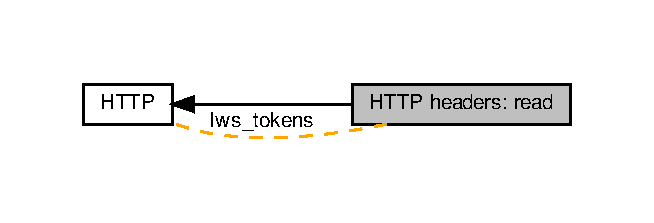
\includegraphics[width=314pt]{group__HTTP-headers-read}
\end{center}
\end{figure}
\subsection*{Classes}
\begin{DoxyCompactItemize}
\item 
struct \hyperlink{structlws__tokens}{lws\+\_\+tokens}
\item 
struct \hyperlink{structlws__token__limits}{lws\+\_\+token\+\_\+limits}
\end{DoxyCompactItemize}
\subsection*{Enumerations}
\begin{DoxyCompactItemize}
\item 
\mbox{\Hypertarget{group__HTTP-headers-read_ga6e747906f9d76532ec118d6ef418b82e}\label{group__HTTP-headers-read_ga6e747906f9d76532ec118d6ef418b82e}} 
enum {\bfseries lws\+\_\+token\+\_\+indexes} \{ \newline
{\bfseries W\+S\+I\+\_\+\+T\+O\+K\+E\+N\+\_\+\+G\+E\+T\+\_\+\+U\+RI} = 0, 
{\bfseries W\+S\+I\+\_\+\+T\+O\+K\+E\+N\+\_\+\+P\+O\+S\+T\+\_\+\+U\+RI} = 1, 
{\bfseries W\+S\+I\+\_\+\+T\+O\+K\+E\+N\+\_\+\+O\+P\+T\+I\+O\+N\+S\+\_\+\+U\+RI} = 2, 
{\bfseries W\+S\+I\+\_\+\+T\+O\+K\+E\+N\+\_\+\+H\+O\+ST} = 3, 
\newline
{\bfseries W\+S\+I\+\_\+\+T\+O\+K\+E\+N\+\_\+\+C\+O\+N\+N\+E\+C\+T\+I\+ON} = 4, 
{\bfseries W\+S\+I\+\_\+\+T\+O\+K\+E\+N\+\_\+\+U\+P\+G\+R\+A\+DE} = 5, 
{\bfseries W\+S\+I\+\_\+\+T\+O\+K\+E\+N\+\_\+\+O\+R\+I\+G\+IN} = 6, 
{\bfseries W\+S\+I\+\_\+\+T\+O\+K\+E\+N\+\_\+\+D\+R\+A\+FT} = 7, 
\newline
{\bfseries W\+S\+I\+\_\+\+T\+O\+K\+E\+N\+\_\+\+C\+H\+A\+L\+L\+E\+N\+GE} = 8, 
{\bfseries W\+S\+I\+\_\+\+T\+O\+K\+E\+N\+\_\+\+E\+X\+T\+E\+N\+S\+I\+O\+NS} = 9, 
{\bfseries W\+S\+I\+\_\+\+T\+O\+K\+E\+N\+\_\+\+K\+E\+Y1} = 10, 
{\bfseries W\+S\+I\+\_\+\+T\+O\+K\+E\+N\+\_\+\+K\+E\+Y2} = 11, 
\newline
{\bfseries W\+S\+I\+\_\+\+T\+O\+K\+E\+N\+\_\+\+P\+R\+O\+T\+O\+C\+OL} = 12, 
{\bfseries W\+S\+I\+\_\+\+T\+O\+K\+E\+N\+\_\+\+A\+C\+C\+E\+PT} = 13, 
{\bfseries W\+S\+I\+\_\+\+T\+O\+K\+E\+N\+\_\+\+N\+O\+N\+CE} = 14, 
{\bfseries W\+S\+I\+\_\+\+T\+O\+K\+E\+N\+\_\+\+H\+T\+TP} = 15, 
\newline
{\bfseries W\+S\+I\+\_\+\+T\+O\+K\+E\+N\+\_\+\+H\+T\+T\+P2\+\_\+\+S\+E\+T\+T\+I\+N\+GS} = 16, 
{\bfseries W\+S\+I\+\_\+\+T\+O\+K\+E\+N\+\_\+\+H\+T\+T\+P\+\_\+\+A\+C\+C\+E\+PT} = 17, 
{\bfseries W\+S\+I\+\_\+\+T\+O\+K\+E\+N\+\_\+\+H\+T\+T\+P\+\_\+\+A\+C\+\_\+\+R\+E\+Q\+U\+E\+S\+T\+\_\+\+H\+E\+A\+D\+E\+RS} = 18, 
{\bfseries W\+S\+I\+\_\+\+T\+O\+K\+E\+N\+\_\+\+H\+T\+T\+P\+\_\+\+I\+F\+\_\+\+M\+O\+D\+I\+F\+I\+E\+D\+\_\+\+S\+I\+N\+CE} = 19, 
\newline
{\bfseries W\+S\+I\+\_\+\+T\+O\+K\+E\+N\+\_\+\+H\+T\+T\+P\+\_\+\+I\+F\+\_\+\+N\+O\+N\+E\+\_\+\+M\+A\+T\+CH} = 20, 
{\bfseries W\+S\+I\+\_\+\+T\+O\+K\+E\+N\+\_\+\+H\+T\+T\+P\+\_\+\+A\+C\+C\+E\+P\+T\+\_\+\+E\+N\+C\+O\+D\+I\+NG} = 21, 
{\bfseries W\+S\+I\+\_\+\+T\+O\+K\+E\+N\+\_\+\+H\+T\+T\+P\+\_\+\+A\+C\+C\+E\+P\+T\+\_\+\+L\+A\+N\+G\+U\+A\+GE} = 22, 
{\bfseries W\+S\+I\+\_\+\+T\+O\+K\+E\+N\+\_\+\+H\+T\+T\+P\+\_\+\+P\+R\+A\+G\+MA} = 23, 
\newline
{\bfseries W\+S\+I\+\_\+\+T\+O\+K\+E\+N\+\_\+\+H\+T\+T\+P\+\_\+\+C\+A\+C\+H\+E\+\_\+\+C\+O\+N\+T\+R\+OL} = 24, 
{\bfseries W\+S\+I\+\_\+\+T\+O\+K\+E\+N\+\_\+\+H\+T\+T\+P\+\_\+\+A\+U\+T\+H\+O\+R\+I\+Z\+A\+T\+I\+ON} = 25, 
{\bfseries W\+S\+I\+\_\+\+T\+O\+K\+E\+N\+\_\+\+H\+T\+T\+P\+\_\+\+C\+O\+O\+K\+IE} = 26, 
{\bfseries W\+S\+I\+\_\+\+T\+O\+K\+E\+N\+\_\+\+H\+T\+T\+P\+\_\+\+C\+O\+N\+T\+E\+N\+T\+\_\+\+L\+E\+N\+G\+TH} = 27, 
\newline
{\bfseries W\+S\+I\+\_\+\+T\+O\+K\+E\+N\+\_\+\+H\+T\+T\+P\+\_\+\+C\+O\+N\+T\+E\+N\+T\+\_\+\+T\+Y\+PE} = 28, 
{\bfseries W\+S\+I\+\_\+\+T\+O\+K\+E\+N\+\_\+\+H\+T\+T\+P\+\_\+\+D\+A\+TE} = 29, 
{\bfseries W\+S\+I\+\_\+\+T\+O\+K\+E\+N\+\_\+\+H\+T\+T\+P\+\_\+\+R\+A\+N\+GE} = 30, 
{\bfseries W\+S\+I\+\_\+\+T\+O\+K\+E\+N\+\_\+\+H\+T\+T\+P\+\_\+\+R\+E\+F\+E\+R\+ER} = 31, 
\newline
{\bfseries W\+S\+I\+\_\+\+T\+O\+K\+E\+N\+\_\+\+K\+EY} = 32, 
{\bfseries W\+S\+I\+\_\+\+T\+O\+K\+E\+N\+\_\+\+V\+E\+R\+S\+I\+ON} = 33, 
{\bfseries W\+S\+I\+\_\+\+T\+O\+K\+E\+N\+\_\+\+S\+W\+O\+R\+I\+G\+IN} = 34, 
{\bfseries W\+S\+I\+\_\+\+T\+O\+K\+E\+N\+\_\+\+H\+T\+T\+P\+\_\+\+C\+O\+L\+O\+N\+\_\+\+A\+U\+T\+H\+O\+R\+I\+TY} = 35, 
\newline
{\bfseries W\+S\+I\+\_\+\+T\+O\+K\+E\+N\+\_\+\+H\+T\+T\+P\+\_\+\+C\+O\+L\+O\+N\+\_\+\+M\+E\+T\+H\+OD} = 36, 
{\bfseries W\+S\+I\+\_\+\+T\+O\+K\+E\+N\+\_\+\+H\+T\+T\+P\+\_\+\+C\+O\+L\+O\+N\+\_\+\+P\+A\+TH} = 37, 
{\bfseries W\+S\+I\+\_\+\+T\+O\+K\+E\+N\+\_\+\+H\+T\+T\+P\+\_\+\+C\+O\+L\+O\+N\+\_\+\+S\+C\+H\+E\+ME} = 38, 
{\bfseries W\+S\+I\+\_\+\+T\+O\+K\+E\+N\+\_\+\+H\+T\+T\+P\+\_\+\+C\+O\+L\+O\+N\+\_\+\+S\+T\+A\+T\+US} = 39, 
\newline
{\bfseries W\+S\+I\+\_\+\+T\+O\+K\+E\+N\+\_\+\+H\+T\+T\+P\+\_\+\+A\+C\+C\+E\+P\+T\+\_\+\+C\+H\+A\+R\+S\+ET} = 40, 
{\bfseries W\+S\+I\+\_\+\+T\+O\+K\+E\+N\+\_\+\+H\+T\+T\+P\+\_\+\+A\+C\+C\+E\+P\+T\+\_\+\+R\+A\+N\+G\+ES} = 41, 
{\bfseries W\+S\+I\+\_\+\+T\+O\+K\+E\+N\+\_\+\+H\+T\+T\+P\+\_\+\+A\+C\+C\+E\+S\+S\+\_\+\+C\+O\+N\+T\+R\+O\+L\+\_\+\+A\+L\+L\+O\+W\+\_\+\+O\+R\+I\+G\+IN} = 42, 
{\bfseries W\+S\+I\+\_\+\+T\+O\+K\+E\+N\+\_\+\+H\+T\+T\+P\+\_\+\+A\+GE} = 43, 
\newline
{\bfseries W\+S\+I\+\_\+\+T\+O\+K\+E\+N\+\_\+\+H\+T\+T\+P\+\_\+\+A\+L\+L\+OW} = 44, 
{\bfseries W\+S\+I\+\_\+\+T\+O\+K\+E\+N\+\_\+\+H\+T\+T\+P\+\_\+\+C\+O\+N\+T\+E\+N\+T\+\_\+\+D\+I\+S\+P\+O\+S\+I\+T\+I\+ON} = 45, 
{\bfseries W\+S\+I\+\_\+\+T\+O\+K\+E\+N\+\_\+\+H\+T\+T\+P\+\_\+\+C\+O\+N\+T\+E\+N\+T\+\_\+\+E\+N\+C\+O\+D\+I\+NG} = 46, 
{\bfseries W\+S\+I\+\_\+\+T\+O\+K\+E\+N\+\_\+\+H\+T\+T\+P\+\_\+\+C\+O\+N\+T\+E\+N\+T\+\_\+\+L\+A\+N\+G\+U\+A\+GE} = 47, 
\newline
{\bfseries W\+S\+I\+\_\+\+T\+O\+K\+E\+N\+\_\+\+H\+T\+T\+P\+\_\+\+C\+O\+N\+T\+E\+N\+T\+\_\+\+L\+O\+C\+A\+T\+I\+ON} = 48, 
{\bfseries W\+S\+I\+\_\+\+T\+O\+K\+E\+N\+\_\+\+H\+T\+T\+P\+\_\+\+C\+O\+N\+T\+E\+N\+T\+\_\+\+R\+A\+N\+GE} = 49, 
{\bfseries W\+S\+I\+\_\+\+T\+O\+K\+E\+N\+\_\+\+H\+T\+T\+P\+\_\+\+E\+T\+AG} = 50, 
{\bfseries W\+S\+I\+\_\+\+T\+O\+K\+E\+N\+\_\+\+H\+T\+T\+P\+\_\+\+E\+X\+P\+E\+CT} = 51, 
\newline
{\bfseries W\+S\+I\+\_\+\+T\+O\+K\+E\+N\+\_\+\+H\+T\+T\+P\+\_\+\+E\+X\+P\+I\+R\+ES} = 52, 
{\bfseries W\+S\+I\+\_\+\+T\+O\+K\+E\+N\+\_\+\+H\+T\+T\+P\+\_\+\+F\+R\+OM} = 53, 
{\bfseries W\+S\+I\+\_\+\+T\+O\+K\+E\+N\+\_\+\+H\+T\+T\+P\+\_\+\+I\+F\+\_\+\+M\+A\+T\+CH} = 54, 
{\bfseries W\+S\+I\+\_\+\+T\+O\+K\+E\+N\+\_\+\+H\+T\+T\+P\+\_\+\+I\+F\+\_\+\+R\+A\+N\+GE} = 55, 
\newline
{\bfseries W\+S\+I\+\_\+\+T\+O\+K\+E\+N\+\_\+\+H\+T\+T\+P\+\_\+\+I\+F\+\_\+\+U\+N\+M\+O\+D\+I\+F\+I\+E\+D\+\_\+\+S\+I\+N\+CE} = 56, 
{\bfseries W\+S\+I\+\_\+\+T\+O\+K\+E\+N\+\_\+\+H\+T\+T\+P\+\_\+\+L\+A\+S\+T\+\_\+\+M\+O\+D\+I\+F\+I\+ED} = 57, 
{\bfseries W\+S\+I\+\_\+\+T\+O\+K\+E\+N\+\_\+\+H\+T\+T\+P\+\_\+\+L\+I\+NK} = 58, 
{\bfseries W\+S\+I\+\_\+\+T\+O\+K\+E\+N\+\_\+\+H\+T\+T\+P\+\_\+\+L\+O\+C\+A\+T\+I\+ON} = 59, 
\newline
{\bfseries W\+S\+I\+\_\+\+T\+O\+K\+E\+N\+\_\+\+H\+T\+T\+P\+\_\+\+M\+A\+X\+\_\+\+F\+O\+R\+W\+A\+R\+DS} = 60, 
{\bfseries W\+S\+I\+\_\+\+T\+O\+K\+E\+N\+\_\+\+H\+T\+T\+P\+\_\+\+P\+R\+O\+X\+Y\+\_\+\+A\+U\+T\+H\+E\+N\+T\+I\+C\+A\+TE} = 61, 
{\bfseries W\+S\+I\+\_\+\+T\+O\+K\+E\+N\+\_\+\+H\+T\+T\+P\+\_\+\+P\+R\+O\+X\+Y\+\_\+\+A\+U\+T\+H\+O\+R\+I\+Z\+A\+T\+I\+ON} = 62, 
{\bfseries W\+S\+I\+\_\+\+T\+O\+K\+E\+N\+\_\+\+H\+T\+T\+P\+\_\+\+R\+E\+F\+R\+E\+SH} = 63, 
\newline
{\bfseries W\+S\+I\+\_\+\+T\+O\+K\+E\+N\+\_\+\+H\+T\+T\+P\+\_\+\+R\+E\+T\+R\+Y\+\_\+\+A\+F\+T\+ER} = 64, 
{\bfseries W\+S\+I\+\_\+\+T\+O\+K\+E\+N\+\_\+\+H\+T\+T\+P\+\_\+\+S\+E\+R\+V\+ER} = 65, 
{\bfseries W\+S\+I\+\_\+\+T\+O\+K\+E\+N\+\_\+\+H\+T\+T\+P\+\_\+\+S\+E\+T\+\_\+\+C\+O\+O\+K\+IE} = 66, 
{\bfseries W\+S\+I\+\_\+\+T\+O\+K\+E\+N\+\_\+\+H\+T\+T\+P\+\_\+\+S\+T\+R\+I\+C\+T\+\_\+\+T\+R\+A\+N\+S\+P\+O\+R\+T\+\_\+\+S\+E\+C\+U\+R\+I\+TY} = 67, 
\newline
{\bfseries W\+S\+I\+\_\+\+T\+O\+K\+E\+N\+\_\+\+H\+T\+T\+P\+\_\+\+T\+R\+A\+N\+S\+F\+E\+R\+\_\+\+E\+N\+C\+O\+D\+I\+NG} = 68, 
{\bfseries W\+S\+I\+\_\+\+T\+O\+K\+E\+N\+\_\+\+H\+T\+T\+P\+\_\+\+U\+S\+E\+R\+\_\+\+A\+G\+E\+NT} = 69, 
{\bfseries W\+S\+I\+\_\+\+T\+O\+K\+E\+N\+\_\+\+H\+T\+T\+P\+\_\+\+V\+A\+RY} = 70, 
{\bfseries W\+S\+I\+\_\+\+T\+O\+K\+E\+N\+\_\+\+H\+T\+T\+P\+\_\+\+V\+IA} = 71, 
\newline
{\bfseries W\+S\+I\+\_\+\+T\+O\+K\+E\+N\+\_\+\+H\+T\+T\+P\+\_\+\+W\+W\+W\+\_\+\+A\+U\+T\+H\+E\+N\+T\+I\+C\+A\+TE} = 72, 
{\bfseries W\+S\+I\+\_\+\+T\+O\+K\+E\+N\+\_\+\+P\+R\+O\+XY}, 
{\bfseries W\+S\+I\+\_\+\+T\+O\+K\+E\+N\+\_\+\+P\+A\+T\+C\+H\+\_\+\+U\+RI} = 73, 
{\bfseries W\+S\+I\+\_\+\+T\+O\+K\+E\+N\+\_\+\+P\+U\+T\+\_\+\+U\+RI} = 74, 
\newline
{\bfseries W\+S\+I\+\_\+\+T\+O\+K\+E\+N\+\_\+\+D\+E\+L\+E\+T\+E\+\_\+\+U\+RI} = 75, 
{\bfseries W\+S\+I\+\_\+\+T\+O\+K\+E\+N\+\_\+\+H\+T\+T\+P\+\_\+\+U\+R\+I\+\_\+\+A\+R\+GS} = 76, 
{\bfseries \+\_\+\+W\+S\+I\+\_\+\+T\+O\+K\+E\+N\+\_\+\+C\+L\+I\+E\+N\+T\+\_\+\+S\+E\+N\+T\+\_\+\+P\+R\+O\+T\+O\+C\+O\+LS} = 77, 
{\bfseries \+\_\+\+W\+S\+I\+\_\+\+T\+O\+K\+E\+N\+\_\+\+C\+L\+I\+E\+N\+T\+\_\+\+P\+E\+E\+R\+\_\+\+A\+D\+D\+R\+E\+SS} = 78, 
\newline
{\bfseries \+\_\+\+W\+S\+I\+\_\+\+T\+O\+K\+E\+N\+\_\+\+C\+L\+I\+E\+N\+T\+\_\+\+U\+RI} = 79, 
{\bfseries \+\_\+\+W\+S\+I\+\_\+\+T\+O\+K\+E\+N\+\_\+\+C\+L\+I\+E\+N\+T\+\_\+\+H\+O\+ST} = 80, 
{\bfseries \+\_\+\+W\+S\+I\+\_\+\+T\+O\+K\+E\+N\+\_\+\+C\+L\+I\+E\+N\+T\+\_\+\+O\+R\+I\+G\+IN} = 81, 
{\bfseries W\+S\+I\+\_\+\+T\+O\+K\+E\+N\+\_\+\+C\+O\+U\+NT}, 
\newline
{\bfseries W\+S\+I\+\_\+\+T\+O\+K\+E\+N\+\_\+\+N\+A\+M\+E\+\_\+\+P\+A\+RT}, 
{\bfseries W\+S\+I\+\_\+\+T\+O\+K\+E\+N\+\_\+\+S\+K\+I\+P\+P\+I\+NG}, 
{\bfseries W\+S\+I\+\_\+\+T\+O\+K\+E\+N\+\_\+\+S\+K\+I\+P\+P\+I\+N\+G\+\_\+\+S\+A\+W\+\_\+\+CR}, 
{\bfseries W\+S\+I\+\_\+\+P\+A\+R\+S\+I\+N\+G\+\_\+\+C\+O\+M\+P\+L\+E\+TE}, 
\newline
{\bfseries W\+S\+I\+\_\+\+I\+N\+I\+T\+\_\+\+T\+O\+K\+E\+N\+\_\+\+M\+U\+X\+U\+RL}, 
{\bfseries W\+S\+I\+\_\+\+T\+O\+K\+E\+N\+\_\+\+G\+E\+T\+\_\+\+U\+RI} = 0, 
{\bfseries W\+S\+I\+\_\+\+T\+O\+K\+E\+N\+\_\+\+P\+O\+S\+T\+\_\+\+U\+RI} = 1, 
{\bfseries W\+S\+I\+\_\+\+T\+O\+K\+E\+N\+\_\+\+O\+P\+T\+I\+O\+N\+S\+\_\+\+U\+RI} = 2, 
\newline
{\bfseries W\+S\+I\+\_\+\+T\+O\+K\+E\+N\+\_\+\+H\+O\+ST} = 3, 
{\bfseries W\+S\+I\+\_\+\+T\+O\+K\+E\+N\+\_\+\+C\+O\+N\+N\+E\+C\+T\+I\+ON} = 4, 
{\bfseries W\+S\+I\+\_\+\+T\+O\+K\+E\+N\+\_\+\+U\+P\+G\+R\+A\+DE} = 5, 
{\bfseries W\+S\+I\+\_\+\+T\+O\+K\+E\+N\+\_\+\+O\+R\+I\+G\+IN} = 6, 
\newline
{\bfseries W\+S\+I\+\_\+\+T\+O\+K\+E\+N\+\_\+\+D\+R\+A\+FT} = 7, 
{\bfseries W\+S\+I\+\_\+\+T\+O\+K\+E\+N\+\_\+\+C\+H\+A\+L\+L\+E\+N\+GE} = 8, 
{\bfseries W\+S\+I\+\_\+\+T\+O\+K\+E\+N\+\_\+\+E\+X\+T\+E\+N\+S\+I\+O\+NS} = 9, 
{\bfseries W\+S\+I\+\_\+\+T\+O\+K\+E\+N\+\_\+\+K\+E\+Y1} = 10, 
\newline
{\bfseries W\+S\+I\+\_\+\+T\+O\+K\+E\+N\+\_\+\+K\+E\+Y2} = 11, 
{\bfseries W\+S\+I\+\_\+\+T\+O\+K\+E\+N\+\_\+\+P\+R\+O\+T\+O\+C\+OL} = 12, 
{\bfseries W\+S\+I\+\_\+\+T\+O\+K\+E\+N\+\_\+\+A\+C\+C\+E\+PT} = 13, 
{\bfseries W\+S\+I\+\_\+\+T\+O\+K\+E\+N\+\_\+\+N\+O\+N\+CE} = 14, 
\newline
{\bfseries W\+S\+I\+\_\+\+T\+O\+K\+E\+N\+\_\+\+H\+T\+TP} = 15, 
{\bfseries W\+S\+I\+\_\+\+T\+O\+K\+E\+N\+\_\+\+H\+T\+T\+P2\+\_\+\+S\+E\+T\+T\+I\+N\+GS} = 16, 
{\bfseries W\+S\+I\+\_\+\+T\+O\+K\+E\+N\+\_\+\+H\+T\+T\+P\+\_\+\+A\+C\+C\+E\+PT} = 17, 
{\bfseries W\+S\+I\+\_\+\+T\+O\+K\+E\+N\+\_\+\+H\+T\+T\+P\+\_\+\+A\+C\+\_\+\+R\+E\+Q\+U\+E\+S\+T\+\_\+\+H\+E\+A\+D\+E\+RS} = 18, 
\newline
{\bfseries W\+S\+I\+\_\+\+T\+O\+K\+E\+N\+\_\+\+H\+T\+T\+P\+\_\+\+I\+F\+\_\+\+M\+O\+D\+I\+F\+I\+E\+D\+\_\+\+S\+I\+N\+CE} = 19, 
{\bfseries W\+S\+I\+\_\+\+T\+O\+K\+E\+N\+\_\+\+H\+T\+T\+P\+\_\+\+I\+F\+\_\+\+N\+O\+N\+E\+\_\+\+M\+A\+T\+CH} = 20, 
{\bfseries W\+S\+I\+\_\+\+T\+O\+K\+E\+N\+\_\+\+H\+T\+T\+P\+\_\+\+A\+C\+C\+E\+P\+T\+\_\+\+E\+N\+C\+O\+D\+I\+NG} = 21, 
{\bfseries W\+S\+I\+\_\+\+T\+O\+K\+E\+N\+\_\+\+H\+T\+T\+P\+\_\+\+A\+C\+C\+E\+P\+T\+\_\+\+L\+A\+N\+G\+U\+A\+GE} = 22, 
\newline
{\bfseries W\+S\+I\+\_\+\+T\+O\+K\+E\+N\+\_\+\+H\+T\+T\+P\+\_\+\+P\+R\+A\+G\+MA} = 23, 
{\bfseries W\+S\+I\+\_\+\+T\+O\+K\+E\+N\+\_\+\+H\+T\+T\+P\+\_\+\+C\+A\+C\+H\+E\+\_\+\+C\+O\+N\+T\+R\+OL} = 24, 
{\bfseries W\+S\+I\+\_\+\+T\+O\+K\+E\+N\+\_\+\+H\+T\+T\+P\+\_\+\+A\+U\+T\+H\+O\+R\+I\+Z\+A\+T\+I\+ON} = 25, 
{\bfseries W\+S\+I\+\_\+\+T\+O\+K\+E\+N\+\_\+\+H\+T\+T\+P\+\_\+\+C\+O\+O\+K\+IE} = 26, 
\newline
{\bfseries W\+S\+I\+\_\+\+T\+O\+K\+E\+N\+\_\+\+H\+T\+T\+P\+\_\+\+C\+O\+N\+T\+E\+N\+T\+\_\+\+L\+E\+N\+G\+TH} = 27, 
{\bfseries W\+S\+I\+\_\+\+T\+O\+K\+E\+N\+\_\+\+H\+T\+T\+P\+\_\+\+C\+O\+N\+T\+E\+N\+T\+\_\+\+T\+Y\+PE} = 28, 
{\bfseries W\+S\+I\+\_\+\+T\+O\+K\+E\+N\+\_\+\+H\+T\+T\+P\+\_\+\+D\+A\+TE} = 29, 
{\bfseries W\+S\+I\+\_\+\+T\+O\+K\+E\+N\+\_\+\+H\+T\+T\+P\+\_\+\+R\+A\+N\+GE} = 30, 
\newline
{\bfseries W\+S\+I\+\_\+\+T\+O\+K\+E\+N\+\_\+\+H\+T\+T\+P\+\_\+\+R\+E\+F\+E\+R\+ER} = 31, 
{\bfseries W\+S\+I\+\_\+\+T\+O\+K\+E\+N\+\_\+\+K\+EY} = 32, 
{\bfseries W\+S\+I\+\_\+\+T\+O\+K\+E\+N\+\_\+\+V\+E\+R\+S\+I\+ON} = 33, 
{\bfseries W\+S\+I\+\_\+\+T\+O\+K\+E\+N\+\_\+\+S\+W\+O\+R\+I\+G\+IN} = 34, 
\newline
{\bfseries W\+S\+I\+\_\+\+T\+O\+K\+E\+N\+\_\+\+H\+T\+T\+P\+\_\+\+C\+O\+L\+O\+N\+\_\+\+A\+U\+T\+H\+O\+R\+I\+TY} = 35, 
{\bfseries W\+S\+I\+\_\+\+T\+O\+K\+E\+N\+\_\+\+H\+T\+T\+P\+\_\+\+C\+O\+L\+O\+N\+\_\+\+M\+E\+T\+H\+OD} = 36, 
{\bfseries W\+S\+I\+\_\+\+T\+O\+K\+E\+N\+\_\+\+H\+T\+T\+P\+\_\+\+C\+O\+L\+O\+N\+\_\+\+P\+A\+TH} = 37, 
{\bfseries W\+S\+I\+\_\+\+T\+O\+K\+E\+N\+\_\+\+H\+T\+T\+P\+\_\+\+C\+O\+L\+O\+N\+\_\+\+S\+C\+H\+E\+ME} = 38, 
\newline
{\bfseries W\+S\+I\+\_\+\+T\+O\+K\+E\+N\+\_\+\+H\+T\+T\+P\+\_\+\+C\+O\+L\+O\+N\+\_\+\+S\+T\+A\+T\+US} = 39, 
{\bfseries W\+S\+I\+\_\+\+T\+O\+K\+E\+N\+\_\+\+H\+T\+T\+P\+\_\+\+A\+C\+C\+E\+P\+T\+\_\+\+C\+H\+A\+R\+S\+ET} = 40, 
{\bfseries W\+S\+I\+\_\+\+T\+O\+K\+E\+N\+\_\+\+H\+T\+T\+P\+\_\+\+A\+C\+C\+E\+P\+T\+\_\+\+R\+A\+N\+G\+ES} = 41, 
{\bfseries W\+S\+I\+\_\+\+T\+O\+K\+E\+N\+\_\+\+H\+T\+T\+P\+\_\+\+A\+C\+C\+E\+S\+S\+\_\+\+C\+O\+N\+T\+R\+O\+L\+\_\+\+A\+L\+L\+O\+W\+\_\+\+O\+R\+I\+G\+IN} = 42, 
\newline
{\bfseries W\+S\+I\+\_\+\+T\+O\+K\+E\+N\+\_\+\+H\+T\+T\+P\+\_\+\+A\+GE} = 43, 
{\bfseries W\+S\+I\+\_\+\+T\+O\+K\+E\+N\+\_\+\+H\+T\+T\+P\+\_\+\+A\+L\+L\+OW} = 44, 
{\bfseries W\+S\+I\+\_\+\+T\+O\+K\+E\+N\+\_\+\+H\+T\+T\+P\+\_\+\+C\+O\+N\+T\+E\+N\+T\+\_\+\+D\+I\+S\+P\+O\+S\+I\+T\+I\+ON} = 45, 
{\bfseries W\+S\+I\+\_\+\+T\+O\+K\+E\+N\+\_\+\+H\+T\+T\+P\+\_\+\+C\+O\+N\+T\+E\+N\+T\+\_\+\+E\+N\+C\+O\+D\+I\+NG} = 46, 
\newline
{\bfseries W\+S\+I\+\_\+\+T\+O\+K\+E\+N\+\_\+\+H\+T\+T\+P\+\_\+\+C\+O\+N\+T\+E\+N\+T\+\_\+\+L\+A\+N\+G\+U\+A\+GE} = 47, 
{\bfseries W\+S\+I\+\_\+\+T\+O\+K\+E\+N\+\_\+\+H\+T\+T\+P\+\_\+\+C\+O\+N\+T\+E\+N\+T\+\_\+\+L\+O\+C\+A\+T\+I\+ON} = 48, 
{\bfseries W\+S\+I\+\_\+\+T\+O\+K\+E\+N\+\_\+\+H\+T\+T\+P\+\_\+\+C\+O\+N\+T\+E\+N\+T\+\_\+\+R\+A\+N\+GE} = 49, 
{\bfseries W\+S\+I\+\_\+\+T\+O\+K\+E\+N\+\_\+\+H\+T\+T\+P\+\_\+\+E\+T\+AG} = 50, 
\newline
{\bfseries W\+S\+I\+\_\+\+T\+O\+K\+E\+N\+\_\+\+H\+T\+T\+P\+\_\+\+E\+X\+P\+E\+CT} = 51, 
{\bfseries W\+S\+I\+\_\+\+T\+O\+K\+E\+N\+\_\+\+H\+T\+T\+P\+\_\+\+E\+X\+P\+I\+R\+ES} = 52, 
{\bfseries W\+S\+I\+\_\+\+T\+O\+K\+E\+N\+\_\+\+H\+T\+T\+P\+\_\+\+F\+R\+OM} = 53, 
{\bfseries W\+S\+I\+\_\+\+T\+O\+K\+E\+N\+\_\+\+H\+T\+T\+P\+\_\+\+I\+F\+\_\+\+M\+A\+T\+CH} = 54, 
\newline
{\bfseries W\+S\+I\+\_\+\+T\+O\+K\+E\+N\+\_\+\+H\+T\+T\+P\+\_\+\+I\+F\+\_\+\+R\+A\+N\+GE} = 55, 
{\bfseries W\+S\+I\+\_\+\+T\+O\+K\+E\+N\+\_\+\+H\+T\+T\+P\+\_\+\+I\+F\+\_\+\+U\+N\+M\+O\+D\+I\+F\+I\+E\+D\+\_\+\+S\+I\+N\+CE} = 56, 
{\bfseries W\+S\+I\+\_\+\+T\+O\+K\+E\+N\+\_\+\+H\+T\+T\+P\+\_\+\+L\+A\+S\+T\+\_\+\+M\+O\+D\+I\+F\+I\+ED} = 57, 
{\bfseries W\+S\+I\+\_\+\+T\+O\+K\+E\+N\+\_\+\+H\+T\+T\+P\+\_\+\+L\+I\+NK} = 58, 
\newline
{\bfseries W\+S\+I\+\_\+\+T\+O\+K\+E\+N\+\_\+\+H\+T\+T\+P\+\_\+\+L\+O\+C\+A\+T\+I\+ON} = 59, 
{\bfseries W\+S\+I\+\_\+\+T\+O\+K\+E\+N\+\_\+\+H\+T\+T\+P\+\_\+\+M\+A\+X\+\_\+\+F\+O\+R\+W\+A\+R\+DS} = 60, 
{\bfseries W\+S\+I\+\_\+\+T\+O\+K\+E\+N\+\_\+\+H\+T\+T\+P\+\_\+\+P\+R\+O\+X\+Y\+\_\+\+A\+U\+T\+H\+E\+N\+T\+I\+C\+A\+TE} = 61, 
{\bfseries W\+S\+I\+\_\+\+T\+O\+K\+E\+N\+\_\+\+H\+T\+T\+P\+\_\+\+P\+R\+O\+X\+Y\+\_\+\+A\+U\+T\+H\+O\+R\+I\+Z\+A\+T\+I\+ON} = 62, 
\newline
{\bfseries W\+S\+I\+\_\+\+T\+O\+K\+E\+N\+\_\+\+H\+T\+T\+P\+\_\+\+R\+E\+F\+R\+E\+SH} = 63, 
{\bfseries W\+S\+I\+\_\+\+T\+O\+K\+E\+N\+\_\+\+H\+T\+T\+P\+\_\+\+R\+E\+T\+R\+Y\+\_\+\+A\+F\+T\+ER} = 64, 
{\bfseries W\+S\+I\+\_\+\+T\+O\+K\+E\+N\+\_\+\+H\+T\+T\+P\+\_\+\+S\+E\+R\+V\+ER} = 65, 
{\bfseries W\+S\+I\+\_\+\+T\+O\+K\+E\+N\+\_\+\+H\+T\+T\+P\+\_\+\+S\+E\+T\+\_\+\+C\+O\+O\+K\+IE} = 66, 
\newline
{\bfseries W\+S\+I\+\_\+\+T\+O\+K\+E\+N\+\_\+\+H\+T\+T\+P\+\_\+\+S\+T\+R\+I\+C\+T\+\_\+\+T\+R\+A\+N\+S\+P\+O\+R\+T\+\_\+\+S\+E\+C\+U\+R\+I\+TY} = 67, 
{\bfseries W\+S\+I\+\_\+\+T\+O\+K\+E\+N\+\_\+\+H\+T\+T\+P\+\_\+\+T\+R\+A\+N\+S\+F\+E\+R\+\_\+\+E\+N\+C\+O\+D\+I\+NG} = 68, 
{\bfseries W\+S\+I\+\_\+\+T\+O\+K\+E\+N\+\_\+\+H\+T\+T\+P\+\_\+\+U\+S\+E\+R\+\_\+\+A\+G\+E\+NT} = 69, 
{\bfseries W\+S\+I\+\_\+\+T\+O\+K\+E\+N\+\_\+\+H\+T\+T\+P\+\_\+\+V\+A\+RY} = 70, 
\newline
{\bfseries W\+S\+I\+\_\+\+T\+O\+K\+E\+N\+\_\+\+H\+T\+T\+P\+\_\+\+V\+IA} = 71, 
{\bfseries W\+S\+I\+\_\+\+T\+O\+K\+E\+N\+\_\+\+H\+T\+T\+P\+\_\+\+W\+W\+W\+\_\+\+A\+U\+T\+H\+E\+N\+T\+I\+C\+A\+TE} = 72, 
{\bfseries W\+S\+I\+\_\+\+T\+O\+K\+E\+N\+\_\+\+P\+R\+O\+XY}, 
{\bfseries W\+S\+I\+\_\+\+T\+O\+K\+E\+N\+\_\+\+P\+A\+T\+C\+H\+\_\+\+U\+RI} = 73, 
\newline
{\bfseries W\+S\+I\+\_\+\+T\+O\+K\+E\+N\+\_\+\+P\+U\+T\+\_\+\+U\+RI} = 74, 
{\bfseries W\+S\+I\+\_\+\+T\+O\+K\+E\+N\+\_\+\+D\+E\+L\+E\+T\+E\+\_\+\+U\+RI} = 75, 
{\bfseries W\+S\+I\+\_\+\+T\+O\+K\+E\+N\+\_\+\+H\+T\+T\+P\+\_\+\+U\+R\+I\+\_\+\+A\+R\+GS} = 76, 
{\bfseries \+\_\+\+W\+S\+I\+\_\+\+T\+O\+K\+E\+N\+\_\+\+C\+L\+I\+E\+N\+T\+\_\+\+S\+E\+N\+T\+\_\+\+P\+R\+O\+T\+O\+C\+O\+LS} = 77, 
\newline
{\bfseries \+\_\+\+W\+S\+I\+\_\+\+T\+O\+K\+E\+N\+\_\+\+C\+L\+I\+E\+N\+T\+\_\+\+P\+E\+E\+R\+\_\+\+A\+D\+D\+R\+E\+SS} = 78, 
{\bfseries \+\_\+\+W\+S\+I\+\_\+\+T\+O\+K\+E\+N\+\_\+\+C\+L\+I\+E\+N\+T\+\_\+\+U\+RI} = 79, 
{\bfseries \+\_\+\+W\+S\+I\+\_\+\+T\+O\+K\+E\+N\+\_\+\+C\+L\+I\+E\+N\+T\+\_\+\+H\+O\+ST} = 80, 
{\bfseries \+\_\+\+W\+S\+I\+\_\+\+T\+O\+K\+E\+N\+\_\+\+C\+L\+I\+E\+N\+T\+\_\+\+O\+R\+I\+G\+IN} = 81, 
\newline
{\bfseries W\+S\+I\+\_\+\+T\+O\+K\+E\+N\+\_\+\+C\+O\+U\+NT}, 
{\bfseries W\+S\+I\+\_\+\+T\+O\+K\+E\+N\+\_\+\+N\+A\+M\+E\+\_\+\+P\+A\+RT}, 
{\bfseries W\+S\+I\+\_\+\+T\+O\+K\+E\+N\+\_\+\+S\+K\+I\+P\+P\+I\+NG}, 
{\bfseries W\+S\+I\+\_\+\+T\+O\+K\+E\+N\+\_\+\+S\+K\+I\+P\+P\+I\+N\+G\+\_\+\+S\+A\+W\+\_\+\+CR}, 
\newline
{\bfseries W\+S\+I\+\_\+\+P\+A\+R\+S\+I\+N\+G\+\_\+\+C\+O\+M\+P\+L\+E\+TE}, 
{\bfseries W\+S\+I\+\_\+\+I\+N\+I\+T\+\_\+\+T\+O\+K\+E\+N\+\_\+\+M\+U\+X\+U\+RL}, 
{\bfseries W\+S\+I\+\_\+\+T\+O\+K\+E\+N\+\_\+\+G\+E\+T\+\_\+\+U\+RI} = 0, 
{\bfseries W\+S\+I\+\_\+\+T\+O\+K\+E\+N\+\_\+\+P\+O\+S\+T\+\_\+\+U\+RI} = 1, 
\newline
{\bfseries W\+S\+I\+\_\+\+T\+O\+K\+E\+N\+\_\+\+O\+P\+T\+I\+O\+N\+S\+\_\+\+U\+RI} = 2, 
{\bfseries W\+S\+I\+\_\+\+T\+O\+K\+E\+N\+\_\+\+H\+O\+ST} = 3, 
{\bfseries W\+S\+I\+\_\+\+T\+O\+K\+E\+N\+\_\+\+C\+O\+N\+N\+E\+C\+T\+I\+ON} = 4, 
{\bfseries W\+S\+I\+\_\+\+T\+O\+K\+E\+N\+\_\+\+U\+P\+G\+R\+A\+DE} = 5, 
\newline
{\bfseries W\+S\+I\+\_\+\+T\+O\+K\+E\+N\+\_\+\+O\+R\+I\+G\+IN} = 6, 
{\bfseries W\+S\+I\+\_\+\+T\+O\+K\+E\+N\+\_\+\+D\+R\+A\+FT} = 7, 
{\bfseries W\+S\+I\+\_\+\+T\+O\+K\+E\+N\+\_\+\+C\+H\+A\+L\+L\+E\+N\+GE} = 8, 
{\bfseries W\+S\+I\+\_\+\+T\+O\+K\+E\+N\+\_\+\+E\+X\+T\+E\+N\+S\+I\+O\+NS} = 9, 
\newline
{\bfseries W\+S\+I\+\_\+\+T\+O\+K\+E\+N\+\_\+\+K\+E\+Y1} = 10, 
{\bfseries W\+S\+I\+\_\+\+T\+O\+K\+E\+N\+\_\+\+K\+E\+Y2} = 11, 
{\bfseries W\+S\+I\+\_\+\+T\+O\+K\+E\+N\+\_\+\+P\+R\+O\+T\+O\+C\+OL} = 12, 
{\bfseries W\+S\+I\+\_\+\+T\+O\+K\+E\+N\+\_\+\+A\+C\+C\+E\+PT} = 13, 
\newline
{\bfseries W\+S\+I\+\_\+\+T\+O\+K\+E\+N\+\_\+\+N\+O\+N\+CE} = 14, 
{\bfseries W\+S\+I\+\_\+\+T\+O\+K\+E\+N\+\_\+\+H\+T\+TP} = 15, 
{\bfseries W\+S\+I\+\_\+\+T\+O\+K\+E\+N\+\_\+\+H\+T\+T\+P2\+\_\+\+S\+E\+T\+T\+I\+N\+GS} = 16, 
{\bfseries W\+S\+I\+\_\+\+T\+O\+K\+E\+N\+\_\+\+H\+T\+T\+P\+\_\+\+A\+C\+C\+E\+PT} = 17, 
\newline
{\bfseries W\+S\+I\+\_\+\+T\+O\+K\+E\+N\+\_\+\+H\+T\+T\+P\+\_\+\+A\+C\+\_\+\+R\+E\+Q\+U\+E\+S\+T\+\_\+\+H\+E\+A\+D\+E\+RS} = 18, 
{\bfseries W\+S\+I\+\_\+\+T\+O\+K\+E\+N\+\_\+\+H\+T\+T\+P\+\_\+\+I\+F\+\_\+\+M\+O\+D\+I\+F\+I\+E\+D\+\_\+\+S\+I\+N\+CE} = 19, 
{\bfseries W\+S\+I\+\_\+\+T\+O\+K\+E\+N\+\_\+\+H\+T\+T\+P\+\_\+\+I\+F\+\_\+\+N\+O\+N\+E\+\_\+\+M\+A\+T\+CH} = 20, 
{\bfseries W\+S\+I\+\_\+\+T\+O\+K\+E\+N\+\_\+\+H\+T\+T\+P\+\_\+\+A\+C\+C\+E\+P\+T\+\_\+\+E\+N\+C\+O\+D\+I\+NG} = 21, 
\newline
{\bfseries W\+S\+I\+\_\+\+T\+O\+K\+E\+N\+\_\+\+H\+T\+T\+P\+\_\+\+A\+C\+C\+E\+P\+T\+\_\+\+L\+A\+N\+G\+U\+A\+GE} = 22, 
{\bfseries W\+S\+I\+\_\+\+T\+O\+K\+E\+N\+\_\+\+H\+T\+T\+P\+\_\+\+P\+R\+A\+G\+MA} = 23, 
{\bfseries W\+S\+I\+\_\+\+T\+O\+K\+E\+N\+\_\+\+H\+T\+T\+P\+\_\+\+C\+A\+C\+H\+E\+\_\+\+C\+O\+N\+T\+R\+OL} = 24, 
{\bfseries W\+S\+I\+\_\+\+T\+O\+K\+E\+N\+\_\+\+H\+T\+T\+P\+\_\+\+A\+U\+T\+H\+O\+R\+I\+Z\+A\+T\+I\+ON} = 25, 
\newline
{\bfseries W\+S\+I\+\_\+\+T\+O\+K\+E\+N\+\_\+\+H\+T\+T\+P\+\_\+\+C\+O\+O\+K\+IE} = 26, 
{\bfseries W\+S\+I\+\_\+\+T\+O\+K\+E\+N\+\_\+\+H\+T\+T\+P\+\_\+\+C\+O\+N\+T\+E\+N\+T\+\_\+\+L\+E\+N\+G\+TH} = 27, 
{\bfseries W\+S\+I\+\_\+\+T\+O\+K\+E\+N\+\_\+\+H\+T\+T\+P\+\_\+\+C\+O\+N\+T\+E\+N\+T\+\_\+\+T\+Y\+PE} = 28, 
{\bfseries W\+S\+I\+\_\+\+T\+O\+K\+E\+N\+\_\+\+H\+T\+T\+P\+\_\+\+D\+A\+TE} = 29, 
\newline
{\bfseries W\+S\+I\+\_\+\+T\+O\+K\+E\+N\+\_\+\+H\+T\+T\+P\+\_\+\+R\+A\+N\+GE} = 30, 
{\bfseries W\+S\+I\+\_\+\+T\+O\+K\+E\+N\+\_\+\+H\+T\+T\+P\+\_\+\+R\+E\+F\+E\+R\+ER} = 31, 
{\bfseries W\+S\+I\+\_\+\+T\+O\+K\+E\+N\+\_\+\+K\+EY} = 32, 
{\bfseries W\+S\+I\+\_\+\+T\+O\+K\+E\+N\+\_\+\+V\+E\+R\+S\+I\+ON} = 33, 
\newline
{\bfseries W\+S\+I\+\_\+\+T\+O\+K\+E\+N\+\_\+\+S\+W\+O\+R\+I\+G\+IN} = 34, 
{\bfseries W\+S\+I\+\_\+\+T\+O\+K\+E\+N\+\_\+\+H\+T\+T\+P\+\_\+\+C\+O\+L\+O\+N\+\_\+\+A\+U\+T\+H\+O\+R\+I\+TY} = 35, 
{\bfseries W\+S\+I\+\_\+\+T\+O\+K\+E\+N\+\_\+\+H\+T\+T\+P\+\_\+\+C\+O\+L\+O\+N\+\_\+\+M\+E\+T\+H\+OD} = 36, 
{\bfseries W\+S\+I\+\_\+\+T\+O\+K\+E\+N\+\_\+\+H\+T\+T\+P\+\_\+\+C\+O\+L\+O\+N\+\_\+\+P\+A\+TH} = 37, 
\newline
{\bfseries W\+S\+I\+\_\+\+T\+O\+K\+E\+N\+\_\+\+H\+T\+T\+P\+\_\+\+C\+O\+L\+O\+N\+\_\+\+S\+C\+H\+E\+ME} = 38, 
{\bfseries W\+S\+I\+\_\+\+T\+O\+K\+E\+N\+\_\+\+H\+T\+T\+P\+\_\+\+C\+O\+L\+O\+N\+\_\+\+S\+T\+A\+T\+US} = 39, 
{\bfseries W\+S\+I\+\_\+\+T\+O\+K\+E\+N\+\_\+\+H\+T\+T\+P\+\_\+\+A\+C\+C\+E\+P\+T\+\_\+\+C\+H\+A\+R\+S\+ET} = 40, 
{\bfseries W\+S\+I\+\_\+\+T\+O\+K\+E\+N\+\_\+\+H\+T\+T\+P\+\_\+\+A\+C\+C\+E\+P\+T\+\_\+\+R\+A\+N\+G\+ES} = 41, 
\newline
{\bfseries W\+S\+I\+\_\+\+T\+O\+K\+E\+N\+\_\+\+H\+T\+T\+P\+\_\+\+A\+C\+C\+E\+S\+S\+\_\+\+C\+O\+N\+T\+R\+O\+L\+\_\+\+A\+L\+L\+O\+W\+\_\+\+O\+R\+I\+G\+IN} = 42, 
{\bfseries W\+S\+I\+\_\+\+T\+O\+K\+E\+N\+\_\+\+H\+T\+T\+P\+\_\+\+A\+GE} = 43, 
{\bfseries W\+S\+I\+\_\+\+T\+O\+K\+E\+N\+\_\+\+H\+T\+T\+P\+\_\+\+A\+L\+L\+OW} = 44, 
{\bfseries W\+S\+I\+\_\+\+T\+O\+K\+E\+N\+\_\+\+H\+T\+T\+P\+\_\+\+C\+O\+N\+T\+E\+N\+T\+\_\+\+D\+I\+S\+P\+O\+S\+I\+T\+I\+ON} = 45, 
\newline
{\bfseries W\+S\+I\+\_\+\+T\+O\+K\+E\+N\+\_\+\+H\+T\+T\+P\+\_\+\+C\+O\+N\+T\+E\+N\+T\+\_\+\+E\+N\+C\+O\+D\+I\+NG} = 46, 
{\bfseries W\+S\+I\+\_\+\+T\+O\+K\+E\+N\+\_\+\+H\+T\+T\+P\+\_\+\+C\+O\+N\+T\+E\+N\+T\+\_\+\+L\+A\+N\+G\+U\+A\+GE} = 47, 
{\bfseries W\+S\+I\+\_\+\+T\+O\+K\+E\+N\+\_\+\+H\+T\+T\+P\+\_\+\+C\+O\+N\+T\+E\+N\+T\+\_\+\+L\+O\+C\+A\+T\+I\+ON} = 48, 
{\bfseries W\+S\+I\+\_\+\+T\+O\+K\+E\+N\+\_\+\+H\+T\+T\+P\+\_\+\+C\+O\+N\+T\+E\+N\+T\+\_\+\+R\+A\+N\+GE} = 49, 
\newline
{\bfseries W\+S\+I\+\_\+\+T\+O\+K\+E\+N\+\_\+\+H\+T\+T\+P\+\_\+\+E\+T\+AG} = 50, 
{\bfseries W\+S\+I\+\_\+\+T\+O\+K\+E\+N\+\_\+\+H\+T\+T\+P\+\_\+\+E\+X\+P\+E\+CT} = 51, 
{\bfseries W\+S\+I\+\_\+\+T\+O\+K\+E\+N\+\_\+\+H\+T\+T\+P\+\_\+\+E\+X\+P\+I\+R\+ES} = 52, 
{\bfseries W\+S\+I\+\_\+\+T\+O\+K\+E\+N\+\_\+\+H\+T\+T\+P\+\_\+\+F\+R\+OM} = 53, 
\newline
{\bfseries W\+S\+I\+\_\+\+T\+O\+K\+E\+N\+\_\+\+H\+T\+T\+P\+\_\+\+I\+F\+\_\+\+M\+A\+T\+CH} = 54, 
{\bfseries W\+S\+I\+\_\+\+T\+O\+K\+E\+N\+\_\+\+H\+T\+T\+P\+\_\+\+I\+F\+\_\+\+R\+A\+N\+GE} = 55, 
{\bfseries W\+S\+I\+\_\+\+T\+O\+K\+E\+N\+\_\+\+H\+T\+T\+P\+\_\+\+I\+F\+\_\+\+U\+N\+M\+O\+D\+I\+F\+I\+E\+D\+\_\+\+S\+I\+N\+CE} = 56, 
{\bfseries W\+S\+I\+\_\+\+T\+O\+K\+E\+N\+\_\+\+H\+T\+T\+P\+\_\+\+L\+A\+S\+T\+\_\+\+M\+O\+D\+I\+F\+I\+ED} = 57, 
\newline
{\bfseries W\+S\+I\+\_\+\+T\+O\+K\+E\+N\+\_\+\+H\+T\+T\+P\+\_\+\+L\+I\+NK} = 58, 
{\bfseries W\+S\+I\+\_\+\+T\+O\+K\+E\+N\+\_\+\+H\+T\+T\+P\+\_\+\+L\+O\+C\+A\+T\+I\+ON} = 59, 
{\bfseries W\+S\+I\+\_\+\+T\+O\+K\+E\+N\+\_\+\+H\+T\+T\+P\+\_\+\+M\+A\+X\+\_\+\+F\+O\+R\+W\+A\+R\+DS} = 60, 
{\bfseries W\+S\+I\+\_\+\+T\+O\+K\+E\+N\+\_\+\+H\+T\+T\+P\+\_\+\+P\+R\+O\+X\+Y\+\_\+\+A\+U\+T\+H\+E\+N\+T\+I\+C\+A\+TE} = 61, 
\newline
{\bfseries W\+S\+I\+\_\+\+T\+O\+K\+E\+N\+\_\+\+H\+T\+T\+P\+\_\+\+P\+R\+O\+X\+Y\+\_\+\+A\+U\+T\+H\+O\+R\+I\+Z\+A\+T\+I\+ON} = 62, 
{\bfseries W\+S\+I\+\_\+\+T\+O\+K\+E\+N\+\_\+\+H\+T\+T\+P\+\_\+\+R\+E\+F\+R\+E\+SH} = 63, 
{\bfseries W\+S\+I\+\_\+\+T\+O\+K\+E\+N\+\_\+\+H\+T\+T\+P\+\_\+\+R\+E\+T\+R\+Y\+\_\+\+A\+F\+T\+ER} = 64, 
{\bfseries W\+S\+I\+\_\+\+T\+O\+K\+E\+N\+\_\+\+H\+T\+T\+P\+\_\+\+S\+E\+R\+V\+ER} = 65, 
\newline
{\bfseries W\+S\+I\+\_\+\+T\+O\+K\+E\+N\+\_\+\+H\+T\+T\+P\+\_\+\+S\+E\+T\+\_\+\+C\+O\+O\+K\+IE} = 66, 
{\bfseries W\+S\+I\+\_\+\+T\+O\+K\+E\+N\+\_\+\+H\+T\+T\+P\+\_\+\+S\+T\+R\+I\+C\+T\+\_\+\+T\+R\+A\+N\+S\+P\+O\+R\+T\+\_\+\+S\+E\+C\+U\+R\+I\+TY} = 67, 
{\bfseries W\+S\+I\+\_\+\+T\+O\+K\+E\+N\+\_\+\+H\+T\+T\+P\+\_\+\+T\+R\+A\+N\+S\+F\+E\+R\+\_\+\+E\+N\+C\+O\+D\+I\+NG} = 68, 
{\bfseries W\+S\+I\+\_\+\+T\+O\+K\+E\+N\+\_\+\+H\+T\+T\+P\+\_\+\+U\+S\+E\+R\+\_\+\+A\+G\+E\+NT} = 69, 
\newline
{\bfseries W\+S\+I\+\_\+\+T\+O\+K\+E\+N\+\_\+\+H\+T\+T\+P\+\_\+\+V\+A\+RY} = 70, 
{\bfseries W\+S\+I\+\_\+\+T\+O\+K\+E\+N\+\_\+\+H\+T\+T\+P\+\_\+\+V\+IA} = 71, 
{\bfseries W\+S\+I\+\_\+\+T\+O\+K\+E\+N\+\_\+\+H\+T\+T\+P\+\_\+\+W\+W\+W\+\_\+\+A\+U\+T\+H\+E\+N\+T\+I\+C\+A\+TE} = 72, 
{\bfseries W\+S\+I\+\_\+\+T\+O\+K\+E\+N\+\_\+\+P\+R\+O\+XY}, 
\newline
{\bfseries W\+S\+I\+\_\+\+T\+O\+K\+E\+N\+\_\+\+P\+A\+T\+C\+H\+\_\+\+U\+RI} = 73, 
{\bfseries W\+S\+I\+\_\+\+T\+O\+K\+E\+N\+\_\+\+P\+U\+T\+\_\+\+U\+RI} = 74, 
{\bfseries W\+S\+I\+\_\+\+T\+O\+K\+E\+N\+\_\+\+D\+E\+L\+E\+T\+E\+\_\+\+U\+RI} = 75, 
{\bfseries W\+S\+I\+\_\+\+T\+O\+K\+E\+N\+\_\+\+H\+T\+T\+P\+\_\+\+U\+R\+I\+\_\+\+A\+R\+GS} = 76, 
\newline
{\bfseries \+\_\+\+W\+S\+I\+\_\+\+T\+O\+K\+E\+N\+\_\+\+C\+L\+I\+E\+N\+T\+\_\+\+S\+E\+N\+T\+\_\+\+P\+R\+O\+T\+O\+C\+O\+LS} = 77, 
{\bfseries \+\_\+\+W\+S\+I\+\_\+\+T\+O\+K\+E\+N\+\_\+\+C\+L\+I\+E\+N\+T\+\_\+\+P\+E\+E\+R\+\_\+\+A\+D\+D\+R\+E\+SS} = 78, 
{\bfseries \+\_\+\+W\+S\+I\+\_\+\+T\+O\+K\+E\+N\+\_\+\+C\+L\+I\+E\+N\+T\+\_\+\+U\+RI} = 79, 
{\bfseries \+\_\+\+W\+S\+I\+\_\+\+T\+O\+K\+E\+N\+\_\+\+C\+L\+I\+E\+N\+T\+\_\+\+H\+O\+ST} = 80, 
\newline
{\bfseries \+\_\+\+W\+S\+I\+\_\+\+T\+O\+K\+E\+N\+\_\+\+C\+L\+I\+E\+N\+T\+\_\+\+O\+R\+I\+G\+IN} = 81, 
{\bfseries W\+S\+I\+\_\+\+T\+O\+K\+E\+N\+\_\+\+C\+O\+U\+NT}, 
{\bfseries W\+S\+I\+\_\+\+T\+O\+K\+E\+N\+\_\+\+N\+A\+M\+E\+\_\+\+P\+A\+RT}, 
{\bfseries W\+S\+I\+\_\+\+T\+O\+K\+E\+N\+\_\+\+S\+K\+I\+P\+P\+I\+NG}, 
\newline
{\bfseries W\+S\+I\+\_\+\+T\+O\+K\+E\+N\+\_\+\+S\+K\+I\+P\+P\+I\+N\+G\+\_\+\+S\+A\+W\+\_\+\+CR}, 
{\bfseries W\+S\+I\+\_\+\+P\+A\+R\+S\+I\+N\+G\+\_\+\+C\+O\+M\+P\+L\+E\+TE}, 
{\bfseries W\+S\+I\+\_\+\+I\+N\+I\+T\+\_\+\+T\+O\+K\+E\+N\+\_\+\+M\+U\+X\+U\+RL}, 
{\bfseries W\+S\+I\+\_\+\+T\+O\+K\+E\+N\+\_\+\+G\+E\+T\+\_\+\+U\+RI} = 0, 
\newline
{\bfseries W\+S\+I\+\_\+\+T\+O\+K\+E\+N\+\_\+\+P\+O\+S\+T\+\_\+\+U\+RI} = 1, 
{\bfseries W\+S\+I\+\_\+\+T\+O\+K\+E\+N\+\_\+\+O\+P\+T\+I\+O\+N\+S\+\_\+\+U\+RI} = 2, 
{\bfseries W\+S\+I\+\_\+\+T\+O\+K\+E\+N\+\_\+\+H\+O\+ST} = 3, 
{\bfseries W\+S\+I\+\_\+\+T\+O\+K\+E\+N\+\_\+\+C\+O\+N\+N\+E\+C\+T\+I\+ON} = 4, 
\newline
{\bfseries W\+S\+I\+\_\+\+T\+O\+K\+E\+N\+\_\+\+U\+P\+G\+R\+A\+DE} = 5, 
{\bfseries W\+S\+I\+\_\+\+T\+O\+K\+E\+N\+\_\+\+O\+R\+I\+G\+IN} = 6, 
{\bfseries W\+S\+I\+\_\+\+T\+O\+K\+E\+N\+\_\+\+D\+R\+A\+FT} = 7, 
{\bfseries W\+S\+I\+\_\+\+T\+O\+K\+E\+N\+\_\+\+C\+H\+A\+L\+L\+E\+N\+GE} = 8, 
\newline
{\bfseries W\+S\+I\+\_\+\+T\+O\+K\+E\+N\+\_\+\+E\+X\+T\+E\+N\+S\+I\+O\+NS} = 9, 
{\bfseries W\+S\+I\+\_\+\+T\+O\+K\+E\+N\+\_\+\+K\+E\+Y1} = 10, 
{\bfseries W\+S\+I\+\_\+\+T\+O\+K\+E\+N\+\_\+\+K\+E\+Y2} = 11, 
{\bfseries W\+S\+I\+\_\+\+T\+O\+K\+E\+N\+\_\+\+P\+R\+O\+T\+O\+C\+OL} = 12, 
\newline
{\bfseries W\+S\+I\+\_\+\+T\+O\+K\+E\+N\+\_\+\+A\+C\+C\+E\+PT} = 13, 
{\bfseries W\+S\+I\+\_\+\+T\+O\+K\+E\+N\+\_\+\+N\+O\+N\+CE} = 14, 
{\bfseries W\+S\+I\+\_\+\+T\+O\+K\+E\+N\+\_\+\+H\+T\+TP} = 15, 
{\bfseries W\+S\+I\+\_\+\+T\+O\+K\+E\+N\+\_\+\+H\+T\+T\+P2\+\_\+\+S\+E\+T\+T\+I\+N\+GS} = 16, 
\newline
{\bfseries W\+S\+I\+\_\+\+T\+O\+K\+E\+N\+\_\+\+H\+T\+T\+P\+\_\+\+A\+C\+C\+E\+PT} = 17, 
{\bfseries W\+S\+I\+\_\+\+T\+O\+K\+E\+N\+\_\+\+H\+T\+T\+P\+\_\+\+A\+C\+\_\+\+R\+E\+Q\+U\+E\+S\+T\+\_\+\+H\+E\+A\+D\+E\+RS} = 18, 
{\bfseries W\+S\+I\+\_\+\+T\+O\+K\+E\+N\+\_\+\+H\+T\+T\+P\+\_\+\+I\+F\+\_\+\+M\+O\+D\+I\+F\+I\+E\+D\+\_\+\+S\+I\+N\+CE} = 19, 
{\bfseries W\+S\+I\+\_\+\+T\+O\+K\+E\+N\+\_\+\+H\+T\+T\+P\+\_\+\+I\+F\+\_\+\+N\+O\+N\+E\+\_\+\+M\+A\+T\+CH} = 20, 
\newline
{\bfseries W\+S\+I\+\_\+\+T\+O\+K\+E\+N\+\_\+\+H\+T\+T\+P\+\_\+\+A\+C\+C\+E\+P\+T\+\_\+\+E\+N\+C\+O\+D\+I\+NG} = 21, 
{\bfseries W\+S\+I\+\_\+\+T\+O\+K\+E\+N\+\_\+\+H\+T\+T\+P\+\_\+\+A\+C\+C\+E\+P\+T\+\_\+\+L\+A\+N\+G\+U\+A\+GE} = 22, 
{\bfseries W\+S\+I\+\_\+\+T\+O\+K\+E\+N\+\_\+\+H\+T\+T\+P\+\_\+\+P\+R\+A\+G\+MA} = 23, 
{\bfseries W\+S\+I\+\_\+\+T\+O\+K\+E\+N\+\_\+\+H\+T\+T\+P\+\_\+\+C\+A\+C\+H\+E\+\_\+\+C\+O\+N\+T\+R\+OL} = 24, 
\newline
{\bfseries W\+S\+I\+\_\+\+T\+O\+K\+E\+N\+\_\+\+H\+T\+T\+P\+\_\+\+A\+U\+T\+H\+O\+R\+I\+Z\+A\+T\+I\+ON} = 25, 
{\bfseries W\+S\+I\+\_\+\+T\+O\+K\+E\+N\+\_\+\+H\+T\+T\+P\+\_\+\+C\+O\+O\+K\+IE} = 26, 
{\bfseries W\+S\+I\+\_\+\+T\+O\+K\+E\+N\+\_\+\+H\+T\+T\+P\+\_\+\+C\+O\+N\+T\+E\+N\+T\+\_\+\+L\+E\+N\+G\+TH} = 27, 
{\bfseries W\+S\+I\+\_\+\+T\+O\+K\+E\+N\+\_\+\+H\+T\+T\+P\+\_\+\+C\+O\+N\+T\+E\+N\+T\+\_\+\+T\+Y\+PE} = 28, 
\newline
{\bfseries W\+S\+I\+\_\+\+T\+O\+K\+E\+N\+\_\+\+H\+T\+T\+P\+\_\+\+D\+A\+TE} = 29, 
{\bfseries W\+S\+I\+\_\+\+T\+O\+K\+E\+N\+\_\+\+H\+T\+T\+P\+\_\+\+R\+A\+N\+GE} = 30, 
{\bfseries W\+S\+I\+\_\+\+T\+O\+K\+E\+N\+\_\+\+H\+T\+T\+P\+\_\+\+R\+E\+F\+E\+R\+ER} = 31, 
{\bfseries W\+S\+I\+\_\+\+T\+O\+K\+E\+N\+\_\+\+K\+EY} = 32, 
\newline
{\bfseries W\+S\+I\+\_\+\+T\+O\+K\+E\+N\+\_\+\+V\+E\+R\+S\+I\+ON} = 33, 
{\bfseries W\+S\+I\+\_\+\+T\+O\+K\+E\+N\+\_\+\+S\+W\+O\+R\+I\+G\+IN} = 34, 
{\bfseries W\+S\+I\+\_\+\+T\+O\+K\+E\+N\+\_\+\+H\+T\+T\+P\+\_\+\+C\+O\+L\+O\+N\+\_\+\+A\+U\+T\+H\+O\+R\+I\+TY} = 35, 
{\bfseries W\+S\+I\+\_\+\+T\+O\+K\+E\+N\+\_\+\+H\+T\+T\+P\+\_\+\+C\+O\+L\+O\+N\+\_\+\+M\+E\+T\+H\+OD} = 36, 
\newline
{\bfseries W\+S\+I\+\_\+\+T\+O\+K\+E\+N\+\_\+\+H\+T\+T\+P\+\_\+\+C\+O\+L\+O\+N\+\_\+\+P\+A\+TH} = 37, 
{\bfseries W\+S\+I\+\_\+\+T\+O\+K\+E\+N\+\_\+\+H\+T\+T\+P\+\_\+\+C\+O\+L\+O\+N\+\_\+\+S\+C\+H\+E\+ME} = 38, 
{\bfseries W\+S\+I\+\_\+\+T\+O\+K\+E\+N\+\_\+\+H\+T\+T\+P\+\_\+\+C\+O\+L\+O\+N\+\_\+\+S\+T\+A\+T\+US} = 39, 
{\bfseries W\+S\+I\+\_\+\+T\+O\+K\+E\+N\+\_\+\+H\+T\+T\+P\+\_\+\+A\+C\+C\+E\+P\+T\+\_\+\+C\+H\+A\+R\+S\+ET} = 40, 
\newline
{\bfseries W\+S\+I\+\_\+\+T\+O\+K\+E\+N\+\_\+\+H\+T\+T\+P\+\_\+\+A\+C\+C\+E\+P\+T\+\_\+\+R\+A\+N\+G\+ES} = 41, 
{\bfseries W\+S\+I\+\_\+\+T\+O\+K\+E\+N\+\_\+\+H\+T\+T\+P\+\_\+\+A\+C\+C\+E\+S\+S\+\_\+\+C\+O\+N\+T\+R\+O\+L\+\_\+\+A\+L\+L\+O\+W\+\_\+\+O\+R\+I\+G\+IN} = 42, 
{\bfseries W\+S\+I\+\_\+\+T\+O\+K\+E\+N\+\_\+\+H\+T\+T\+P\+\_\+\+A\+GE} = 43, 
{\bfseries W\+S\+I\+\_\+\+T\+O\+K\+E\+N\+\_\+\+H\+T\+T\+P\+\_\+\+A\+L\+L\+OW} = 44, 
\newline
{\bfseries W\+S\+I\+\_\+\+T\+O\+K\+E\+N\+\_\+\+H\+T\+T\+P\+\_\+\+C\+O\+N\+T\+E\+N\+T\+\_\+\+D\+I\+S\+P\+O\+S\+I\+T\+I\+ON} = 45, 
{\bfseries W\+S\+I\+\_\+\+T\+O\+K\+E\+N\+\_\+\+H\+T\+T\+P\+\_\+\+C\+O\+N\+T\+E\+N\+T\+\_\+\+E\+N\+C\+O\+D\+I\+NG} = 46, 
{\bfseries W\+S\+I\+\_\+\+T\+O\+K\+E\+N\+\_\+\+H\+T\+T\+P\+\_\+\+C\+O\+N\+T\+E\+N\+T\+\_\+\+L\+A\+N\+G\+U\+A\+GE} = 47, 
{\bfseries W\+S\+I\+\_\+\+T\+O\+K\+E\+N\+\_\+\+H\+T\+T\+P\+\_\+\+C\+O\+N\+T\+E\+N\+T\+\_\+\+L\+O\+C\+A\+T\+I\+ON} = 48, 
\newline
{\bfseries W\+S\+I\+\_\+\+T\+O\+K\+E\+N\+\_\+\+H\+T\+T\+P\+\_\+\+C\+O\+N\+T\+E\+N\+T\+\_\+\+R\+A\+N\+GE} = 49, 
{\bfseries W\+S\+I\+\_\+\+T\+O\+K\+E\+N\+\_\+\+H\+T\+T\+P\+\_\+\+E\+T\+AG} = 50, 
{\bfseries W\+S\+I\+\_\+\+T\+O\+K\+E\+N\+\_\+\+H\+T\+T\+P\+\_\+\+E\+X\+P\+E\+CT} = 51, 
{\bfseries W\+S\+I\+\_\+\+T\+O\+K\+E\+N\+\_\+\+H\+T\+T\+P\+\_\+\+E\+X\+P\+I\+R\+ES} = 52, 
\newline
{\bfseries W\+S\+I\+\_\+\+T\+O\+K\+E\+N\+\_\+\+H\+T\+T\+P\+\_\+\+F\+R\+OM} = 53, 
{\bfseries W\+S\+I\+\_\+\+T\+O\+K\+E\+N\+\_\+\+H\+T\+T\+P\+\_\+\+I\+F\+\_\+\+M\+A\+T\+CH} = 54, 
{\bfseries W\+S\+I\+\_\+\+T\+O\+K\+E\+N\+\_\+\+H\+T\+T\+P\+\_\+\+I\+F\+\_\+\+R\+A\+N\+GE} = 55, 
{\bfseries W\+S\+I\+\_\+\+T\+O\+K\+E\+N\+\_\+\+H\+T\+T\+P\+\_\+\+I\+F\+\_\+\+U\+N\+M\+O\+D\+I\+F\+I\+E\+D\+\_\+\+S\+I\+N\+CE} = 56, 
\newline
{\bfseries W\+S\+I\+\_\+\+T\+O\+K\+E\+N\+\_\+\+H\+T\+T\+P\+\_\+\+L\+A\+S\+T\+\_\+\+M\+O\+D\+I\+F\+I\+ED} = 57, 
{\bfseries W\+S\+I\+\_\+\+T\+O\+K\+E\+N\+\_\+\+H\+T\+T\+P\+\_\+\+L\+I\+NK} = 58, 
{\bfseries W\+S\+I\+\_\+\+T\+O\+K\+E\+N\+\_\+\+H\+T\+T\+P\+\_\+\+L\+O\+C\+A\+T\+I\+ON} = 59, 
{\bfseries W\+S\+I\+\_\+\+T\+O\+K\+E\+N\+\_\+\+H\+T\+T\+P\+\_\+\+M\+A\+X\+\_\+\+F\+O\+R\+W\+A\+R\+DS} = 60, 
\newline
{\bfseries W\+S\+I\+\_\+\+T\+O\+K\+E\+N\+\_\+\+H\+T\+T\+P\+\_\+\+P\+R\+O\+X\+Y\+\_\+\+A\+U\+T\+H\+E\+N\+T\+I\+C\+A\+TE} = 61, 
{\bfseries W\+S\+I\+\_\+\+T\+O\+K\+E\+N\+\_\+\+H\+T\+T\+P\+\_\+\+P\+R\+O\+X\+Y\+\_\+\+A\+U\+T\+H\+O\+R\+I\+Z\+A\+T\+I\+ON} = 62, 
{\bfseries W\+S\+I\+\_\+\+T\+O\+K\+E\+N\+\_\+\+H\+T\+T\+P\+\_\+\+R\+E\+F\+R\+E\+SH} = 63, 
{\bfseries W\+S\+I\+\_\+\+T\+O\+K\+E\+N\+\_\+\+H\+T\+T\+P\+\_\+\+R\+E\+T\+R\+Y\+\_\+\+A\+F\+T\+ER} = 64, 
\newline
{\bfseries W\+S\+I\+\_\+\+T\+O\+K\+E\+N\+\_\+\+H\+T\+T\+P\+\_\+\+S\+E\+R\+V\+ER} = 65, 
{\bfseries W\+S\+I\+\_\+\+T\+O\+K\+E\+N\+\_\+\+H\+T\+T\+P\+\_\+\+S\+E\+T\+\_\+\+C\+O\+O\+K\+IE} = 66, 
{\bfseries W\+S\+I\+\_\+\+T\+O\+K\+E\+N\+\_\+\+H\+T\+T\+P\+\_\+\+S\+T\+R\+I\+C\+T\+\_\+\+T\+R\+A\+N\+S\+P\+O\+R\+T\+\_\+\+S\+E\+C\+U\+R\+I\+TY} = 67, 
{\bfseries W\+S\+I\+\_\+\+T\+O\+K\+E\+N\+\_\+\+H\+T\+T\+P\+\_\+\+T\+R\+A\+N\+S\+F\+E\+R\+\_\+\+E\+N\+C\+O\+D\+I\+NG} = 68, 
\newline
{\bfseries W\+S\+I\+\_\+\+T\+O\+K\+E\+N\+\_\+\+H\+T\+T\+P\+\_\+\+U\+S\+E\+R\+\_\+\+A\+G\+E\+NT} = 69, 
{\bfseries W\+S\+I\+\_\+\+T\+O\+K\+E\+N\+\_\+\+H\+T\+T\+P\+\_\+\+V\+A\+RY} = 70, 
{\bfseries W\+S\+I\+\_\+\+T\+O\+K\+E\+N\+\_\+\+H\+T\+T\+P\+\_\+\+V\+IA} = 71, 
{\bfseries W\+S\+I\+\_\+\+T\+O\+K\+E\+N\+\_\+\+H\+T\+T\+P\+\_\+\+W\+W\+W\+\_\+\+A\+U\+T\+H\+E\+N\+T\+I\+C\+A\+TE} = 72, 
\newline
{\bfseries W\+S\+I\+\_\+\+T\+O\+K\+E\+N\+\_\+\+P\+R\+O\+XY}, 
{\bfseries W\+S\+I\+\_\+\+T\+O\+K\+E\+N\+\_\+\+P\+A\+T\+C\+H\+\_\+\+U\+RI} = 73, 
{\bfseries W\+S\+I\+\_\+\+T\+O\+K\+E\+N\+\_\+\+P\+U\+T\+\_\+\+U\+RI} = 74, 
{\bfseries W\+S\+I\+\_\+\+T\+O\+K\+E\+N\+\_\+\+D\+E\+L\+E\+T\+E\+\_\+\+U\+RI} = 75, 
\newline
{\bfseries W\+S\+I\+\_\+\+T\+O\+K\+E\+N\+\_\+\+H\+T\+T\+P\+\_\+\+U\+R\+I\+\_\+\+A\+R\+GS} = 76, 
{\bfseries \+\_\+\+W\+S\+I\+\_\+\+T\+O\+K\+E\+N\+\_\+\+C\+L\+I\+E\+N\+T\+\_\+\+S\+E\+N\+T\+\_\+\+P\+R\+O\+T\+O\+C\+O\+LS} = 77, 
{\bfseries \+\_\+\+W\+S\+I\+\_\+\+T\+O\+K\+E\+N\+\_\+\+C\+L\+I\+E\+N\+T\+\_\+\+P\+E\+E\+R\+\_\+\+A\+D\+D\+R\+E\+SS} = 78, 
{\bfseries \+\_\+\+W\+S\+I\+\_\+\+T\+O\+K\+E\+N\+\_\+\+C\+L\+I\+E\+N\+T\+\_\+\+U\+RI} = 79, 
\newline
{\bfseries \+\_\+\+W\+S\+I\+\_\+\+T\+O\+K\+E\+N\+\_\+\+C\+L\+I\+E\+N\+T\+\_\+\+H\+O\+ST} = 80, 
{\bfseries \+\_\+\+W\+S\+I\+\_\+\+T\+O\+K\+E\+N\+\_\+\+C\+L\+I\+E\+N\+T\+\_\+\+O\+R\+I\+G\+IN} = 81, 
{\bfseries W\+S\+I\+\_\+\+T\+O\+K\+E\+N\+\_\+\+C\+O\+U\+NT}, 
{\bfseries W\+S\+I\+\_\+\+T\+O\+K\+E\+N\+\_\+\+N\+A\+M\+E\+\_\+\+P\+A\+RT}, 
\newline
{\bfseries W\+S\+I\+\_\+\+T\+O\+K\+E\+N\+\_\+\+S\+K\+I\+P\+P\+I\+NG}, 
{\bfseries W\+S\+I\+\_\+\+T\+O\+K\+E\+N\+\_\+\+S\+K\+I\+P\+P\+I\+N\+G\+\_\+\+S\+A\+W\+\_\+\+CR}, 
{\bfseries W\+S\+I\+\_\+\+P\+A\+R\+S\+I\+N\+G\+\_\+\+C\+O\+M\+P\+L\+E\+TE}, 
{\bfseries W\+S\+I\+\_\+\+I\+N\+I\+T\+\_\+\+T\+O\+K\+E\+N\+\_\+\+M\+U\+X\+U\+RL}, 
\newline
{\bfseries W\+S\+I\+\_\+\+T\+O\+K\+E\+N\+\_\+\+G\+E\+T\+\_\+\+U\+RI} = 0, 
{\bfseries W\+S\+I\+\_\+\+T\+O\+K\+E\+N\+\_\+\+P\+O\+S\+T\+\_\+\+U\+RI} = 1, 
{\bfseries W\+S\+I\+\_\+\+T\+O\+K\+E\+N\+\_\+\+O\+P\+T\+I\+O\+N\+S\+\_\+\+U\+RI} = 2, 
{\bfseries W\+S\+I\+\_\+\+T\+O\+K\+E\+N\+\_\+\+H\+O\+ST} = 3, 
\newline
{\bfseries W\+S\+I\+\_\+\+T\+O\+K\+E\+N\+\_\+\+C\+O\+N\+N\+E\+C\+T\+I\+ON} = 4, 
{\bfseries W\+S\+I\+\_\+\+T\+O\+K\+E\+N\+\_\+\+U\+P\+G\+R\+A\+DE} = 5, 
{\bfseries W\+S\+I\+\_\+\+T\+O\+K\+E\+N\+\_\+\+O\+R\+I\+G\+IN} = 6, 
{\bfseries W\+S\+I\+\_\+\+T\+O\+K\+E\+N\+\_\+\+D\+R\+A\+FT} = 7, 
\newline
{\bfseries W\+S\+I\+\_\+\+T\+O\+K\+E\+N\+\_\+\+C\+H\+A\+L\+L\+E\+N\+GE} = 8, 
{\bfseries W\+S\+I\+\_\+\+T\+O\+K\+E\+N\+\_\+\+E\+X\+T\+E\+N\+S\+I\+O\+NS} = 9, 
{\bfseries W\+S\+I\+\_\+\+T\+O\+K\+E\+N\+\_\+\+K\+E\+Y1} = 10, 
{\bfseries W\+S\+I\+\_\+\+T\+O\+K\+E\+N\+\_\+\+K\+E\+Y2} = 11, 
\newline
{\bfseries W\+S\+I\+\_\+\+T\+O\+K\+E\+N\+\_\+\+P\+R\+O\+T\+O\+C\+OL} = 12, 
{\bfseries W\+S\+I\+\_\+\+T\+O\+K\+E\+N\+\_\+\+A\+C\+C\+E\+PT} = 13, 
{\bfseries W\+S\+I\+\_\+\+T\+O\+K\+E\+N\+\_\+\+N\+O\+N\+CE} = 14, 
{\bfseries W\+S\+I\+\_\+\+T\+O\+K\+E\+N\+\_\+\+H\+T\+TP} = 15, 
\newline
{\bfseries W\+S\+I\+\_\+\+T\+O\+K\+E\+N\+\_\+\+H\+T\+T\+P2\+\_\+\+S\+E\+T\+T\+I\+N\+GS} = 16, 
{\bfseries W\+S\+I\+\_\+\+T\+O\+K\+E\+N\+\_\+\+H\+T\+T\+P\+\_\+\+A\+C\+C\+E\+PT} = 17, 
{\bfseries W\+S\+I\+\_\+\+T\+O\+K\+E\+N\+\_\+\+H\+T\+T\+P\+\_\+\+A\+C\+\_\+\+R\+E\+Q\+U\+E\+S\+T\+\_\+\+H\+E\+A\+D\+E\+RS} = 18, 
{\bfseries W\+S\+I\+\_\+\+T\+O\+K\+E\+N\+\_\+\+H\+T\+T\+P\+\_\+\+I\+F\+\_\+\+M\+O\+D\+I\+F\+I\+E\+D\+\_\+\+S\+I\+N\+CE} = 19, 
\newline
{\bfseries W\+S\+I\+\_\+\+T\+O\+K\+E\+N\+\_\+\+H\+T\+T\+P\+\_\+\+I\+F\+\_\+\+N\+O\+N\+E\+\_\+\+M\+A\+T\+CH} = 20, 
{\bfseries W\+S\+I\+\_\+\+T\+O\+K\+E\+N\+\_\+\+H\+T\+T\+P\+\_\+\+A\+C\+C\+E\+P\+T\+\_\+\+E\+N\+C\+O\+D\+I\+NG} = 21, 
{\bfseries W\+S\+I\+\_\+\+T\+O\+K\+E\+N\+\_\+\+H\+T\+T\+P\+\_\+\+A\+C\+C\+E\+P\+T\+\_\+\+L\+A\+N\+G\+U\+A\+GE} = 22, 
{\bfseries W\+S\+I\+\_\+\+T\+O\+K\+E\+N\+\_\+\+H\+T\+T\+P\+\_\+\+P\+R\+A\+G\+MA} = 23, 
\newline
{\bfseries W\+S\+I\+\_\+\+T\+O\+K\+E\+N\+\_\+\+H\+T\+T\+P\+\_\+\+C\+A\+C\+H\+E\+\_\+\+C\+O\+N\+T\+R\+OL} = 24, 
{\bfseries W\+S\+I\+\_\+\+T\+O\+K\+E\+N\+\_\+\+H\+T\+T\+P\+\_\+\+A\+U\+T\+H\+O\+R\+I\+Z\+A\+T\+I\+ON} = 25, 
{\bfseries W\+S\+I\+\_\+\+T\+O\+K\+E\+N\+\_\+\+H\+T\+T\+P\+\_\+\+C\+O\+O\+K\+IE} = 26, 
{\bfseries W\+S\+I\+\_\+\+T\+O\+K\+E\+N\+\_\+\+H\+T\+T\+P\+\_\+\+C\+O\+N\+T\+E\+N\+T\+\_\+\+L\+E\+N\+G\+TH} = 27, 
\newline
{\bfseries W\+S\+I\+\_\+\+T\+O\+K\+E\+N\+\_\+\+H\+T\+T\+P\+\_\+\+C\+O\+N\+T\+E\+N\+T\+\_\+\+T\+Y\+PE} = 28, 
{\bfseries W\+S\+I\+\_\+\+T\+O\+K\+E\+N\+\_\+\+H\+T\+T\+P\+\_\+\+D\+A\+TE} = 29, 
{\bfseries W\+S\+I\+\_\+\+T\+O\+K\+E\+N\+\_\+\+H\+T\+T\+P\+\_\+\+R\+A\+N\+GE} = 30, 
{\bfseries W\+S\+I\+\_\+\+T\+O\+K\+E\+N\+\_\+\+H\+T\+T\+P\+\_\+\+R\+E\+F\+E\+R\+ER} = 31, 
\newline
{\bfseries W\+S\+I\+\_\+\+T\+O\+K\+E\+N\+\_\+\+K\+EY} = 32, 
{\bfseries W\+S\+I\+\_\+\+T\+O\+K\+E\+N\+\_\+\+V\+E\+R\+S\+I\+ON} = 33, 
{\bfseries W\+S\+I\+\_\+\+T\+O\+K\+E\+N\+\_\+\+S\+W\+O\+R\+I\+G\+IN} = 34, 
{\bfseries W\+S\+I\+\_\+\+T\+O\+K\+E\+N\+\_\+\+H\+T\+T\+P\+\_\+\+C\+O\+L\+O\+N\+\_\+\+A\+U\+T\+H\+O\+R\+I\+TY} = 35, 
\newline
{\bfseries W\+S\+I\+\_\+\+T\+O\+K\+E\+N\+\_\+\+H\+T\+T\+P\+\_\+\+C\+O\+L\+O\+N\+\_\+\+M\+E\+T\+H\+OD} = 36, 
{\bfseries W\+S\+I\+\_\+\+T\+O\+K\+E\+N\+\_\+\+H\+T\+T\+P\+\_\+\+C\+O\+L\+O\+N\+\_\+\+P\+A\+TH} = 37, 
{\bfseries W\+S\+I\+\_\+\+T\+O\+K\+E\+N\+\_\+\+H\+T\+T\+P\+\_\+\+C\+O\+L\+O\+N\+\_\+\+S\+C\+H\+E\+ME} = 38, 
{\bfseries W\+S\+I\+\_\+\+T\+O\+K\+E\+N\+\_\+\+H\+T\+T\+P\+\_\+\+C\+O\+L\+O\+N\+\_\+\+S\+T\+A\+T\+US} = 39, 
\newline
{\bfseries W\+S\+I\+\_\+\+T\+O\+K\+E\+N\+\_\+\+H\+T\+T\+P\+\_\+\+A\+C\+C\+E\+P\+T\+\_\+\+C\+H\+A\+R\+S\+ET} = 40, 
{\bfseries W\+S\+I\+\_\+\+T\+O\+K\+E\+N\+\_\+\+H\+T\+T\+P\+\_\+\+A\+C\+C\+E\+P\+T\+\_\+\+R\+A\+N\+G\+ES} = 41, 
{\bfseries W\+S\+I\+\_\+\+T\+O\+K\+E\+N\+\_\+\+H\+T\+T\+P\+\_\+\+A\+C\+C\+E\+S\+S\+\_\+\+C\+O\+N\+T\+R\+O\+L\+\_\+\+A\+L\+L\+O\+W\+\_\+\+O\+R\+I\+G\+IN} = 42, 
{\bfseries W\+S\+I\+\_\+\+T\+O\+K\+E\+N\+\_\+\+H\+T\+T\+P\+\_\+\+A\+GE} = 43, 
\newline
{\bfseries W\+S\+I\+\_\+\+T\+O\+K\+E\+N\+\_\+\+H\+T\+T\+P\+\_\+\+A\+L\+L\+OW} = 44, 
{\bfseries W\+S\+I\+\_\+\+T\+O\+K\+E\+N\+\_\+\+H\+T\+T\+P\+\_\+\+C\+O\+N\+T\+E\+N\+T\+\_\+\+D\+I\+S\+P\+O\+S\+I\+T\+I\+ON} = 45, 
{\bfseries W\+S\+I\+\_\+\+T\+O\+K\+E\+N\+\_\+\+H\+T\+T\+P\+\_\+\+C\+O\+N\+T\+E\+N\+T\+\_\+\+E\+N\+C\+O\+D\+I\+NG} = 46, 
{\bfseries W\+S\+I\+\_\+\+T\+O\+K\+E\+N\+\_\+\+H\+T\+T\+P\+\_\+\+C\+O\+N\+T\+E\+N\+T\+\_\+\+L\+A\+N\+G\+U\+A\+GE} = 47, 
\newline
{\bfseries W\+S\+I\+\_\+\+T\+O\+K\+E\+N\+\_\+\+H\+T\+T\+P\+\_\+\+C\+O\+N\+T\+E\+N\+T\+\_\+\+L\+O\+C\+A\+T\+I\+ON} = 48, 
{\bfseries W\+S\+I\+\_\+\+T\+O\+K\+E\+N\+\_\+\+H\+T\+T\+P\+\_\+\+C\+O\+N\+T\+E\+N\+T\+\_\+\+R\+A\+N\+GE} = 49, 
{\bfseries W\+S\+I\+\_\+\+T\+O\+K\+E\+N\+\_\+\+H\+T\+T\+P\+\_\+\+E\+T\+AG} = 50, 
{\bfseries W\+S\+I\+\_\+\+T\+O\+K\+E\+N\+\_\+\+H\+T\+T\+P\+\_\+\+E\+X\+P\+E\+CT} = 51, 
\newline
{\bfseries W\+S\+I\+\_\+\+T\+O\+K\+E\+N\+\_\+\+H\+T\+T\+P\+\_\+\+E\+X\+P\+I\+R\+ES} = 52, 
{\bfseries W\+S\+I\+\_\+\+T\+O\+K\+E\+N\+\_\+\+H\+T\+T\+P\+\_\+\+F\+R\+OM} = 53, 
{\bfseries W\+S\+I\+\_\+\+T\+O\+K\+E\+N\+\_\+\+H\+T\+T\+P\+\_\+\+I\+F\+\_\+\+M\+A\+T\+CH} = 54, 
{\bfseries W\+S\+I\+\_\+\+T\+O\+K\+E\+N\+\_\+\+H\+T\+T\+P\+\_\+\+I\+F\+\_\+\+R\+A\+N\+GE} = 55, 
\newline
{\bfseries W\+S\+I\+\_\+\+T\+O\+K\+E\+N\+\_\+\+H\+T\+T\+P\+\_\+\+I\+F\+\_\+\+U\+N\+M\+O\+D\+I\+F\+I\+E\+D\+\_\+\+S\+I\+N\+CE} = 56, 
{\bfseries W\+S\+I\+\_\+\+T\+O\+K\+E\+N\+\_\+\+H\+T\+T\+P\+\_\+\+L\+A\+S\+T\+\_\+\+M\+O\+D\+I\+F\+I\+ED} = 57, 
{\bfseries W\+S\+I\+\_\+\+T\+O\+K\+E\+N\+\_\+\+H\+T\+T\+P\+\_\+\+L\+I\+NK} = 58, 
{\bfseries W\+S\+I\+\_\+\+T\+O\+K\+E\+N\+\_\+\+H\+T\+T\+P\+\_\+\+L\+O\+C\+A\+T\+I\+ON} = 59, 
\newline
{\bfseries W\+S\+I\+\_\+\+T\+O\+K\+E\+N\+\_\+\+H\+T\+T\+P\+\_\+\+M\+A\+X\+\_\+\+F\+O\+R\+W\+A\+R\+DS} = 60, 
{\bfseries W\+S\+I\+\_\+\+T\+O\+K\+E\+N\+\_\+\+H\+T\+T\+P\+\_\+\+P\+R\+O\+X\+Y\+\_\+\+A\+U\+T\+H\+E\+N\+T\+I\+C\+A\+TE} = 61, 
{\bfseries W\+S\+I\+\_\+\+T\+O\+K\+E\+N\+\_\+\+H\+T\+T\+P\+\_\+\+P\+R\+O\+X\+Y\+\_\+\+A\+U\+T\+H\+O\+R\+I\+Z\+A\+T\+I\+ON} = 62, 
{\bfseries W\+S\+I\+\_\+\+T\+O\+K\+E\+N\+\_\+\+H\+T\+T\+P\+\_\+\+R\+E\+F\+R\+E\+SH} = 63, 
\newline
{\bfseries W\+S\+I\+\_\+\+T\+O\+K\+E\+N\+\_\+\+H\+T\+T\+P\+\_\+\+R\+E\+T\+R\+Y\+\_\+\+A\+F\+T\+ER} = 64, 
{\bfseries W\+S\+I\+\_\+\+T\+O\+K\+E\+N\+\_\+\+H\+T\+T\+P\+\_\+\+S\+E\+R\+V\+ER} = 65, 
{\bfseries W\+S\+I\+\_\+\+T\+O\+K\+E\+N\+\_\+\+H\+T\+T\+P\+\_\+\+S\+E\+T\+\_\+\+C\+O\+O\+K\+IE} = 66, 
{\bfseries W\+S\+I\+\_\+\+T\+O\+K\+E\+N\+\_\+\+H\+T\+T\+P\+\_\+\+S\+T\+R\+I\+C\+T\+\_\+\+T\+R\+A\+N\+S\+P\+O\+R\+T\+\_\+\+S\+E\+C\+U\+R\+I\+TY} = 67, 
\newline
{\bfseries W\+S\+I\+\_\+\+T\+O\+K\+E\+N\+\_\+\+H\+T\+T\+P\+\_\+\+T\+R\+A\+N\+S\+F\+E\+R\+\_\+\+E\+N\+C\+O\+D\+I\+NG} = 68, 
{\bfseries W\+S\+I\+\_\+\+T\+O\+K\+E\+N\+\_\+\+H\+T\+T\+P\+\_\+\+U\+S\+E\+R\+\_\+\+A\+G\+E\+NT} = 69, 
{\bfseries W\+S\+I\+\_\+\+T\+O\+K\+E\+N\+\_\+\+H\+T\+T\+P\+\_\+\+V\+A\+RY} = 70, 
{\bfseries W\+S\+I\+\_\+\+T\+O\+K\+E\+N\+\_\+\+H\+T\+T\+P\+\_\+\+V\+IA} = 71, 
\newline
{\bfseries W\+S\+I\+\_\+\+T\+O\+K\+E\+N\+\_\+\+H\+T\+T\+P\+\_\+\+W\+W\+W\+\_\+\+A\+U\+T\+H\+E\+N\+T\+I\+C\+A\+TE} = 72, 
{\bfseries W\+S\+I\+\_\+\+T\+O\+K\+E\+N\+\_\+\+P\+R\+O\+XY}, 
{\bfseries W\+S\+I\+\_\+\+T\+O\+K\+E\+N\+\_\+\+P\+A\+T\+C\+H\+\_\+\+U\+RI} = 73, 
{\bfseries W\+S\+I\+\_\+\+T\+O\+K\+E\+N\+\_\+\+P\+U\+T\+\_\+\+U\+RI} = 74, 
\newline
{\bfseries W\+S\+I\+\_\+\+T\+O\+K\+E\+N\+\_\+\+D\+E\+L\+E\+T\+E\+\_\+\+U\+RI} = 75, 
{\bfseries W\+S\+I\+\_\+\+T\+O\+K\+E\+N\+\_\+\+H\+T\+T\+P\+\_\+\+U\+R\+I\+\_\+\+A\+R\+GS} = 76, 
{\bfseries \+\_\+\+W\+S\+I\+\_\+\+T\+O\+K\+E\+N\+\_\+\+C\+L\+I\+E\+N\+T\+\_\+\+S\+E\+N\+T\+\_\+\+P\+R\+O\+T\+O\+C\+O\+LS} = 77, 
{\bfseries \+\_\+\+W\+S\+I\+\_\+\+T\+O\+K\+E\+N\+\_\+\+C\+L\+I\+E\+N\+T\+\_\+\+P\+E\+E\+R\+\_\+\+A\+D\+D\+R\+E\+SS} = 78, 
\newline
{\bfseries \+\_\+\+W\+S\+I\+\_\+\+T\+O\+K\+E\+N\+\_\+\+C\+L\+I\+E\+N\+T\+\_\+\+U\+RI} = 79, 
{\bfseries \+\_\+\+W\+S\+I\+\_\+\+T\+O\+K\+E\+N\+\_\+\+C\+L\+I\+E\+N\+T\+\_\+\+H\+O\+ST} = 80, 
{\bfseries \+\_\+\+W\+S\+I\+\_\+\+T\+O\+K\+E\+N\+\_\+\+C\+L\+I\+E\+N\+T\+\_\+\+O\+R\+I\+G\+IN} = 81, 
{\bfseries W\+S\+I\+\_\+\+T\+O\+K\+E\+N\+\_\+\+C\+O\+U\+NT}, 
\newline
{\bfseries W\+S\+I\+\_\+\+T\+O\+K\+E\+N\+\_\+\+N\+A\+M\+E\+\_\+\+P\+A\+RT}, 
{\bfseries W\+S\+I\+\_\+\+T\+O\+K\+E\+N\+\_\+\+S\+K\+I\+P\+P\+I\+NG}, 
{\bfseries W\+S\+I\+\_\+\+T\+O\+K\+E\+N\+\_\+\+S\+K\+I\+P\+P\+I\+N\+G\+\_\+\+S\+A\+W\+\_\+\+CR}, 
{\bfseries W\+S\+I\+\_\+\+P\+A\+R\+S\+I\+N\+G\+\_\+\+C\+O\+M\+P\+L\+E\+TE}, 
\newline
{\bfseries W\+S\+I\+\_\+\+I\+N\+I\+T\+\_\+\+T\+O\+K\+E\+N\+\_\+\+M\+U\+X\+U\+RL}, 
{\bfseries W\+S\+I\+\_\+\+T\+O\+K\+E\+N\+\_\+\+G\+E\+T\+\_\+\+U\+RI} = 0, 
{\bfseries W\+S\+I\+\_\+\+T\+O\+K\+E\+N\+\_\+\+P\+O\+S\+T\+\_\+\+U\+RI} = 1, 
{\bfseries W\+S\+I\+\_\+\+T\+O\+K\+E\+N\+\_\+\+O\+P\+T\+I\+O\+N\+S\+\_\+\+U\+RI} = 2, 
\newline
{\bfseries W\+S\+I\+\_\+\+T\+O\+K\+E\+N\+\_\+\+H\+O\+ST} = 3, 
{\bfseries W\+S\+I\+\_\+\+T\+O\+K\+E\+N\+\_\+\+C\+O\+N\+N\+E\+C\+T\+I\+ON} = 4, 
{\bfseries W\+S\+I\+\_\+\+T\+O\+K\+E\+N\+\_\+\+U\+P\+G\+R\+A\+DE} = 5, 
{\bfseries W\+S\+I\+\_\+\+T\+O\+K\+E\+N\+\_\+\+O\+R\+I\+G\+IN} = 6, 
\newline
{\bfseries W\+S\+I\+\_\+\+T\+O\+K\+E\+N\+\_\+\+D\+R\+A\+FT} = 7, 
{\bfseries W\+S\+I\+\_\+\+T\+O\+K\+E\+N\+\_\+\+C\+H\+A\+L\+L\+E\+N\+GE} = 8, 
{\bfseries W\+S\+I\+\_\+\+T\+O\+K\+E\+N\+\_\+\+E\+X\+T\+E\+N\+S\+I\+O\+NS} = 9, 
{\bfseries W\+S\+I\+\_\+\+T\+O\+K\+E\+N\+\_\+\+K\+E\+Y1} = 10, 
\newline
{\bfseries W\+S\+I\+\_\+\+T\+O\+K\+E\+N\+\_\+\+K\+E\+Y2} = 11, 
{\bfseries W\+S\+I\+\_\+\+T\+O\+K\+E\+N\+\_\+\+P\+R\+O\+T\+O\+C\+OL} = 12, 
{\bfseries W\+S\+I\+\_\+\+T\+O\+K\+E\+N\+\_\+\+A\+C\+C\+E\+PT} = 13, 
{\bfseries W\+S\+I\+\_\+\+T\+O\+K\+E\+N\+\_\+\+N\+O\+N\+CE} = 14, 
\newline
{\bfseries W\+S\+I\+\_\+\+T\+O\+K\+E\+N\+\_\+\+H\+T\+TP} = 15, 
{\bfseries W\+S\+I\+\_\+\+T\+O\+K\+E\+N\+\_\+\+H\+T\+T\+P2\+\_\+\+S\+E\+T\+T\+I\+N\+GS} = 16, 
{\bfseries W\+S\+I\+\_\+\+T\+O\+K\+E\+N\+\_\+\+H\+T\+T\+P\+\_\+\+A\+C\+C\+E\+PT} = 17, 
{\bfseries W\+S\+I\+\_\+\+T\+O\+K\+E\+N\+\_\+\+H\+T\+T\+P\+\_\+\+A\+C\+\_\+\+R\+E\+Q\+U\+E\+S\+T\+\_\+\+H\+E\+A\+D\+E\+RS} = 18, 
\newline
{\bfseries W\+S\+I\+\_\+\+T\+O\+K\+E\+N\+\_\+\+H\+T\+T\+P\+\_\+\+I\+F\+\_\+\+M\+O\+D\+I\+F\+I\+E\+D\+\_\+\+S\+I\+N\+CE} = 19, 
{\bfseries W\+S\+I\+\_\+\+T\+O\+K\+E\+N\+\_\+\+H\+T\+T\+P\+\_\+\+I\+F\+\_\+\+N\+O\+N\+E\+\_\+\+M\+A\+T\+CH} = 20, 
{\bfseries W\+S\+I\+\_\+\+T\+O\+K\+E\+N\+\_\+\+H\+T\+T\+P\+\_\+\+A\+C\+C\+E\+P\+T\+\_\+\+E\+N\+C\+O\+D\+I\+NG} = 21, 
{\bfseries W\+S\+I\+\_\+\+T\+O\+K\+E\+N\+\_\+\+H\+T\+T\+P\+\_\+\+A\+C\+C\+E\+P\+T\+\_\+\+L\+A\+N\+G\+U\+A\+GE} = 22, 
\newline
{\bfseries W\+S\+I\+\_\+\+T\+O\+K\+E\+N\+\_\+\+H\+T\+T\+P\+\_\+\+P\+R\+A\+G\+MA} = 23, 
{\bfseries W\+S\+I\+\_\+\+T\+O\+K\+E\+N\+\_\+\+H\+T\+T\+P\+\_\+\+C\+A\+C\+H\+E\+\_\+\+C\+O\+N\+T\+R\+OL} = 24, 
{\bfseries W\+S\+I\+\_\+\+T\+O\+K\+E\+N\+\_\+\+H\+T\+T\+P\+\_\+\+A\+U\+T\+H\+O\+R\+I\+Z\+A\+T\+I\+ON} = 25, 
{\bfseries W\+S\+I\+\_\+\+T\+O\+K\+E\+N\+\_\+\+H\+T\+T\+P\+\_\+\+C\+O\+O\+K\+IE} = 26, 
\newline
{\bfseries W\+S\+I\+\_\+\+T\+O\+K\+E\+N\+\_\+\+H\+T\+T\+P\+\_\+\+C\+O\+N\+T\+E\+N\+T\+\_\+\+L\+E\+N\+G\+TH} = 27, 
{\bfseries W\+S\+I\+\_\+\+T\+O\+K\+E\+N\+\_\+\+H\+T\+T\+P\+\_\+\+C\+O\+N\+T\+E\+N\+T\+\_\+\+T\+Y\+PE} = 28, 
{\bfseries W\+S\+I\+\_\+\+T\+O\+K\+E\+N\+\_\+\+H\+T\+T\+P\+\_\+\+D\+A\+TE} = 29, 
{\bfseries W\+S\+I\+\_\+\+T\+O\+K\+E\+N\+\_\+\+H\+T\+T\+P\+\_\+\+R\+A\+N\+GE} = 30, 
\newline
{\bfseries W\+S\+I\+\_\+\+T\+O\+K\+E\+N\+\_\+\+H\+T\+T\+P\+\_\+\+R\+E\+F\+E\+R\+ER} = 31, 
{\bfseries W\+S\+I\+\_\+\+T\+O\+K\+E\+N\+\_\+\+K\+EY} = 32, 
{\bfseries W\+S\+I\+\_\+\+T\+O\+K\+E\+N\+\_\+\+V\+E\+R\+S\+I\+ON} = 33, 
{\bfseries W\+S\+I\+\_\+\+T\+O\+K\+E\+N\+\_\+\+S\+W\+O\+R\+I\+G\+IN} = 34, 
\newline
{\bfseries W\+S\+I\+\_\+\+T\+O\+K\+E\+N\+\_\+\+H\+T\+T\+P\+\_\+\+C\+O\+L\+O\+N\+\_\+\+A\+U\+T\+H\+O\+R\+I\+TY} = 35, 
{\bfseries W\+S\+I\+\_\+\+T\+O\+K\+E\+N\+\_\+\+H\+T\+T\+P\+\_\+\+C\+O\+L\+O\+N\+\_\+\+M\+E\+T\+H\+OD} = 36, 
{\bfseries W\+S\+I\+\_\+\+T\+O\+K\+E\+N\+\_\+\+H\+T\+T\+P\+\_\+\+C\+O\+L\+O\+N\+\_\+\+P\+A\+TH} = 37, 
{\bfseries W\+S\+I\+\_\+\+T\+O\+K\+E\+N\+\_\+\+H\+T\+T\+P\+\_\+\+C\+O\+L\+O\+N\+\_\+\+S\+C\+H\+E\+ME} = 38, 
\newline
{\bfseries W\+S\+I\+\_\+\+T\+O\+K\+E\+N\+\_\+\+H\+T\+T\+P\+\_\+\+C\+O\+L\+O\+N\+\_\+\+S\+T\+A\+T\+US} = 39, 
{\bfseries W\+S\+I\+\_\+\+T\+O\+K\+E\+N\+\_\+\+H\+T\+T\+P\+\_\+\+A\+C\+C\+E\+P\+T\+\_\+\+C\+H\+A\+R\+S\+ET} = 40, 
{\bfseries W\+S\+I\+\_\+\+T\+O\+K\+E\+N\+\_\+\+H\+T\+T\+P\+\_\+\+A\+C\+C\+E\+P\+T\+\_\+\+R\+A\+N\+G\+ES} = 41, 
{\bfseries W\+S\+I\+\_\+\+T\+O\+K\+E\+N\+\_\+\+H\+T\+T\+P\+\_\+\+A\+C\+C\+E\+S\+S\+\_\+\+C\+O\+N\+T\+R\+O\+L\+\_\+\+A\+L\+L\+O\+W\+\_\+\+O\+R\+I\+G\+IN} = 42, 
\newline
{\bfseries W\+S\+I\+\_\+\+T\+O\+K\+E\+N\+\_\+\+H\+T\+T\+P\+\_\+\+A\+GE} = 43, 
{\bfseries W\+S\+I\+\_\+\+T\+O\+K\+E\+N\+\_\+\+H\+T\+T\+P\+\_\+\+A\+L\+L\+OW} = 44, 
{\bfseries W\+S\+I\+\_\+\+T\+O\+K\+E\+N\+\_\+\+H\+T\+T\+P\+\_\+\+C\+O\+N\+T\+E\+N\+T\+\_\+\+D\+I\+S\+P\+O\+S\+I\+T\+I\+ON} = 45, 
{\bfseries W\+S\+I\+\_\+\+T\+O\+K\+E\+N\+\_\+\+H\+T\+T\+P\+\_\+\+C\+O\+N\+T\+E\+N\+T\+\_\+\+E\+N\+C\+O\+D\+I\+NG} = 46, 
\newline
{\bfseries W\+S\+I\+\_\+\+T\+O\+K\+E\+N\+\_\+\+H\+T\+T\+P\+\_\+\+C\+O\+N\+T\+E\+N\+T\+\_\+\+L\+A\+N\+G\+U\+A\+GE} = 47, 
{\bfseries W\+S\+I\+\_\+\+T\+O\+K\+E\+N\+\_\+\+H\+T\+T\+P\+\_\+\+C\+O\+N\+T\+E\+N\+T\+\_\+\+L\+O\+C\+A\+T\+I\+ON} = 48, 
{\bfseries W\+S\+I\+\_\+\+T\+O\+K\+E\+N\+\_\+\+H\+T\+T\+P\+\_\+\+C\+O\+N\+T\+E\+N\+T\+\_\+\+R\+A\+N\+GE} = 49, 
{\bfseries W\+S\+I\+\_\+\+T\+O\+K\+E\+N\+\_\+\+H\+T\+T\+P\+\_\+\+E\+T\+AG} = 50, 
\newline
{\bfseries W\+S\+I\+\_\+\+T\+O\+K\+E\+N\+\_\+\+H\+T\+T\+P\+\_\+\+E\+X\+P\+E\+CT} = 51, 
{\bfseries W\+S\+I\+\_\+\+T\+O\+K\+E\+N\+\_\+\+H\+T\+T\+P\+\_\+\+E\+X\+P\+I\+R\+ES} = 52, 
{\bfseries W\+S\+I\+\_\+\+T\+O\+K\+E\+N\+\_\+\+H\+T\+T\+P\+\_\+\+F\+R\+OM} = 53, 
{\bfseries W\+S\+I\+\_\+\+T\+O\+K\+E\+N\+\_\+\+H\+T\+T\+P\+\_\+\+I\+F\+\_\+\+M\+A\+T\+CH} = 54, 
\newline
{\bfseries W\+S\+I\+\_\+\+T\+O\+K\+E\+N\+\_\+\+H\+T\+T\+P\+\_\+\+I\+F\+\_\+\+R\+A\+N\+GE} = 55, 
{\bfseries W\+S\+I\+\_\+\+T\+O\+K\+E\+N\+\_\+\+H\+T\+T\+P\+\_\+\+I\+F\+\_\+\+U\+N\+M\+O\+D\+I\+F\+I\+E\+D\+\_\+\+S\+I\+N\+CE} = 56, 
{\bfseries W\+S\+I\+\_\+\+T\+O\+K\+E\+N\+\_\+\+H\+T\+T\+P\+\_\+\+L\+A\+S\+T\+\_\+\+M\+O\+D\+I\+F\+I\+ED} = 57, 
{\bfseries W\+S\+I\+\_\+\+T\+O\+K\+E\+N\+\_\+\+H\+T\+T\+P\+\_\+\+L\+I\+NK} = 58, 
\newline
{\bfseries W\+S\+I\+\_\+\+T\+O\+K\+E\+N\+\_\+\+H\+T\+T\+P\+\_\+\+L\+O\+C\+A\+T\+I\+ON} = 59, 
{\bfseries W\+S\+I\+\_\+\+T\+O\+K\+E\+N\+\_\+\+H\+T\+T\+P\+\_\+\+M\+A\+X\+\_\+\+F\+O\+R\+W\+A\+R\+DS} = 60, 
{\bfseries W\+S\+I\+\_\+\+T\+O\+K\+E\+N\+\_\+\+H\+T\+T\+P\+\_\+\+P\+R\+O\+X\+Y\+\_\+\+A\+U\+T\+H\+E\+N\+T\+I\+C\+A\+TE} = 61, 
{\bfseries W\+S\+I\+\_\+\+T\+O\+K\+E\+N\+\_\+\+H\+T\+T\+P\+\_\+\+P\+R\+O\+X\+Y\+\_\+\+A\+U\+T\+H\+O\+R\+I\+Z\+A\+T\+I\+ON} = 62, 
\newline
{\bfseries W\+S\+I\+\_\+\+T\+O\+K\+E\+N\+\_\+\+H\+T\+T\+P\+\_\+\+R\+E\+F\+R\+E\+SH} = 63, 
{\bfseries W\+S\+I\+\_\+\+T\+O\+K\+E\+N\+\_\+\+H\+T\+T\+P\+\_\+\+R\+E\+T\+R\+Y\+\_\+\+A\+F\+T\+ER} = 64, 
{\bfseries W\+S\+I\+\_\+\+T\+O\+K\+E\+N\+\_\+\+H\+T\+T\+P\+\_\+\+S\+E\+R\+V\+ER} = 65, 
{\bfseries W\+S\+I\+\_\+\+T\+O\+K\+E\+N\+\_\+\+H\+T\+T\+P\+\_\+\+S\+E\+T\+\_\+\+C\+O\+O\+K\+IE} = 66, 
\newline
{\bfseries W\+S\+I\+\_\+\+T\+O\+K\+E\+N\+\_\+\+H\+T\+T\+P\+\_\+\+S\+T\+R\+I\+C\+T\+\_\+\+T\+R\+A\+N\+S\+P\+O\+R\+T\+\_\+\+S\+E\+C\+U\+R\+I\+TY} = 67, 
{\bfseries W\+S\+I\+\_\+\+T\+O\+K\+E\+N\+\_\+\+H\+T\+T\+P\+\_\+\+T\+R\+A\+N\+S\+F\+E\+R\+\_\+\+E\+N\+C\+O\+D\+I\+NG} = 68, 
{\bfseries W\+S\+I\+\_\+\+T\+O\+K\+E\+N\+\_\+\+H\+T\+T\+P\+\_\+\+U\+S\+E\+R\+\_\+\+A\+G\+E\+NT} = 69, 
{\bfseries W\+S\+I\+\_\+\+T\+O\+K\+E\+N\+\_\+\+H\+T\+T\+P\+\_\+\+V\+A\+RY} = 70, 
\newline
{\bfseries W\+S\+I\+\_\+\+T\+O\+K\+E\+N\+\_\+\+H\+T\+T\+P\+\_\+\+V\+IA} = 71, 
{\bfseries W\+S\+I\+\_\+\+T\+O\+K\+E\+N\+\_\+\+H\+T\+T\+P\+\_\+\+W\+W\+W\+\_\+\+A\+U\+T\+H\+E\+N\+T\+I\+C\+A\+TE} = 72, 
{\bfseries W\+S\+I\+\_\+\+T\+O\+K\+E\+N\+\_\+\+P\+R\+O\+XY}, 
{\bfseries W\+S\+I\+\_\+\+T\+O\+K\+E\+N\+\_\+\+P\+A\+T\+C\+H\+\_\+\+U\+RI} = 73, 
\newline
{\bfseries W\+S\+I\+\_\+\+T\+O\+K\+E\+N\+\_\+\+P\+U\+T\+\_\+\+U\+RI} = 74, 
{\bfseries W\+S\+I\+\_\+\+T\+O\+K\+E\+N\+\_\+\+D\+E\+L\+E\+T\+E\+\_\+\+U\+RI} = 75, 
{\bfseries W\+S\+I\+\_\+\+T\+O\+K\+E\+N\+\_\+\+H\+T\+T\+P\+\_\+\+U\+R\+I\+\_\+\+A\+R\+GS} = 76, 
{\bfseries \+\_\+\+W\+S\+I\+\_\+\+T\+O\+K\+E\+N\+\_\+\+C\+L\+I\+E\+N\+T\+\_\+\+S\+E\+N\+T\+\_\+\+P\+R\+O\+T\+O\+C\+O\+LS} = 77, 
\newline
{\bfseries \+\_\+\+W\+S\+I\+\_\+\+T\+O\+K\+E\+N\+\_\+\+C\+L\+I\+E\+N\+T\+\_\+\+P\+E\+E\+R\+\_\+\+A\+D\+D\+R\+E\+SS} = 78, 
{\bfseries \+\_\+\+W\+S\+I\+\_\+\+T\+O\+K\+E\+N\+\_\+\+C\+L\+I\+E\+N\+T\+\_\+\+U\+RI} = 79, 
{\bfseries \+\_\+\+W\+S\+I\+\_\+\+T\+O\+K\+E\+N\+\_\+\+C\+L\+I\+E\+N\+T\+\_\+\+H\+O\+ST} = 80, 
{\bfseries \+\_\+\+W\+S\+I\+\_\+\+T\+O\+K\+E\+N\+\_\+\+C\+L\+I\+E\+N\+T\+\_\+\+O\+R\+I\+G\+IN} = 81, 
\newline
{\bfseries W\+S\+I\+\_\+\+T\+O\+K\+E\+N\+\_\+\+C\+O\+U\+NT}, 
{\bfseries W\+S\+I\+\_\+\+T\+O\+K\+E\+N\+\_\+\+N\+A\+M\+E\+\_\+\+P\+A\+RT}, 
{\bfseries W\+S\+I\+\_\+\+T\+O\+K\+E\+N\+\_\+\+S\+K\+I\+P\+P\+I\+NG}, 
{\bfseries W\+S\+I\+\_\+\+T\+O\+K\+E\+N\+\_\+\+S\+K\+I\+P\+P\+I\+N\+G\+\_\+\+S\+A\+W\+\_\+\+CR}, 
\newline
{\bfseries W\+S\+I\+\_\+\+P\+A\+R\+S\+I\+N\+G\+\_\+\+C\+O\+M\+P\+L\+E\+TE}, 
{\bfseries W\+S\+I\+\_\+\+I\+N\+I\+T\+\_\+\+T\+O\+K\+E\+N\+\_\+\+M\+U\+X\+U\+RL}, 
{\bfseries W\+S\+I\+\_\+\+T\+O\+K\+E\+N\+\_\+\+G\+E\+T\+\_\+\+U\+RI} = 0, 
{\bfseries W\+S\+I\+\_\+\+T\+O\+K\+E\+N\+\_\+\+P\+O\+S\+T\+\_\+\+U\+RI} = 1, 
\newline
{\bfseries W\+S\+I\+\_\+\+T\+O\+K\+E\+N\+\_\+\+O\+P\+T\+I\+O\+N\+S\+\_\+\+U\+RI} = 2, 
{\bfseries W\+S\+I\+\_\+\+T\+O\+K\+E\+N\+\_\+\+H\+O\+ST} = 3, 
{\bfseries W\+S\+I\+\_\+\+T\+O\+K\+E\+N\+\_\+\+C\+O\+N\+N\+E\+C\+T\+I\+ON} = 4, 
{\bfseries W\+S\+I\+\_\+\+T\+O\+K\+E\+N\+\_\+\+U\+P\+G\+R\+A\+DE} = 5, 
\newline
{\bfseries W\+S\+I\+\_\+\+T\+O\+K\+E\+N\+\_\+\+O\+R\+I\+G\+IN} = 6, 
{\bfseries W\+S\+I\+\_\+\+T\+O\+K\+E\+N\+\_\+\+D\+R\+A\+FT} = 7, 
{\bfseries W\+S\+I\+\_\+\+T\+O\+K\+E\+N\+\_\+\+C\+H\+A\+L\+L\+E\+N\+GE} = 8, 
{\bfseries W\+S\+I\+\_\+\+T\+O\+K\+E\+N\+\_\+\+E\+X\+T\+E\+N\+S\+I\+O\+NS} = 9, 
\newline
{\bfseries W\+S\+I\+\_\+\+T\+O\+K\+E\+N\+\_\+\+K\+E\+Y1} = 10, 
{\bfseries W\+S\+I\+\_\+\+T\+O\+K\+E\+N\+\_\+\+K\+E\+Y2} = 11, 
{\bfseries W\+S\+I\+\_\+\+T\+O\+K\+E\+N\+\_\+\+P\+R\+O\+T\+O\+C\+OL} = 12, 
{\bfseries W\+S\+I\+\_\+\+T\+O\+K\+E\+N\+\_\+\+A\+C\+C\+E\+PT} = 13, 
\newline
{\bfseries W\+S\+I\+\_\+\+T\+O\+K\+E\+N\+\_\+\+N\+O\+N\+CE} = 14, 
{\bfseries W\+S\+I\+\_\+\+T\+O\+K\+E\+N\+\_\+\+H\+T\+TP} = 15, 
{\bfseries W\+S\+I\+\_\+\+T\+O\+K\+E\+N\+\_\+\+H\+T\+T\+P2\+\_\+\+S\+E\+T\+T\+I\+N\+GS} = 16, 
{\bfseries W\+S\+I\+\_\+\+T\+O\+K\+E\+N\+\_\+\+H\+T\+T\+P\+\_\+\+A\+C\+C\+E\+PT} = 17, 
\newline
{\bfseries W\+S\+I\+\_\+\+T\+O\+K\+E\+N\+\_\+\+H\+T\+T\+P\+\_\+\+A\+C\+\_\+\+R\+E\+Q\+U\+E\+S\+T\+\_\+\+H\+E\+A\+D\+E\+RS} = 18, 
{\bfseries W\+S\+I\+\_\+\+T\+O\+K\+E\+N\+\_\+\+H\+T\+T\+P\+\_\+\+I\+F\+\_\+\+M\+O\+D\+I\+F\+I\+E\+D\+\_\+\+S\+I\+N\+CE} = 19, 
{\bfseries W\+S\+I\+\_\+\+T\+O\+K\+E\+N\+\_\+\+H\+T\+T\+P\+\_\+\+I\+F\+\_\+\+N\+O\+N\+E\+\_\+\+M\+A\+T\+CH} = 20, 
{\bfseries W\+S\+I\+\_\+\+T\+O\+K\+E\+N\+\_\+\+H\+T\+T\+P\+\_\+\+A\+C\+C\+E\+P\+T\+\_\+\+E\+N\+C\+O\+D\+I\+NG} = 21, 
\newline
{\bfseries W\+S\+I\+\_\+\+T\+O\+K\+E\+N\+\_\+\+H\+T\+T\+P\+\_\+\+A\+C\+C\+E\+P\+T\+\_\+\+L\+A\+N\+G\+U\+A\+GE} = 22, 
{\bfseries W\+S\+I\+\_\+\+T\+O\+K\+E\+N\+\_\+\+H\+T\+T\+P\+\_\+\+P\+R\+A\+G\+MA} = 23, 
{\bfseries W\+S\+I\+\_\+\+T\+O\+K\+E\+N\+\_\+\+H\+T\+T\+P\+\_\+\+C\+A\+C\+H\+E\+\_\+\+C\+O\+N\+T\+R\+OL} = 24, 
{\bfseries W\+S\+I\+\_\+\+T\+O\+K\+E\+N\+\_\+\+H\+T\+T\+P\+\_\+\+A\+U\+T\+H\+O\+R\+I\+Z\+A\+T\+I\+ON} = 25, 
\newline
{\bfseries W\+S\+I\+\_\+\+T\+O\+K\+E\+N\+\_\+\+H\+T\+T\+P\+\_\+\+C\+O\+O\+K\+IE} = 26, 
{\bfseries W\+S\+I\+\_\+\+T\+O\+K\+E\+N\+\_\+\+H\+T\+T\+P\+\_\+\+C\+O\+N\+T\+E\+N\+T\+\_\+\+L\+E\+N\+G\+TH} = 27, 
{\bfseries W\+S\+I\+\_\+\+T\+O\+K\+E\+N\+\_\+\+H\+T\+T\+P\+\_\+\+C\+O\+N\+T\+E\+N\+T\+\_\+\+T\+Y\+PE} = 28, 
{\bfseries W\+S\+I\+\_\+\+T\+O\+K\+E\+N\+\_\+\+H\+T\+T\+P\+\_\+\+D\+A\+TE} = 29, 
\newline
{\bfseries W\+S\+I\+\_\+\+T\+O\+K\+E\+N\+\_\+\+H\+T\+T\+P\+\_\+\+R\+A\+N\+GE} = 30, 
{\bfseries W\+S\+I\+\_\+\+T\+O\+K\+E\+N\+\_\+\+H\+T\+T\+P\+\_\+\+R\+E\+F\+E\+R\+ER} = 31, 
{\bfseries W\+S\+I\+\_\+\+T\+O\+K\+E\+N\+\_\+\+K\+EY} = 32, 
{\bfseries W\+S\+I\+\_\+\+T\+O\+K\+E\+N\+\_\+\+V\+E\+R\+S\+I\+ON} = 33, 
\newline
{\bfseries W\+S\+I\+\_\+\+T\+O\+K\+E\+N\+\_\+\+S\+W\+O\+R\+I\+G\+IN} = 34, 
{\bfseries W\+S\+I\+\_\+\+T\+O\+K\+E\+N\+\_\+\+H\+T\+T\+P\+\_\+\+C\+O\+L\+O\+N\+\_\+\+A\+U\+T\+H\+O\+R\+I\+TY} = 35, 
{\bfseries W\+S\+I\+\_\+\+T\+O\+K\+E\+N\+\_\+\+H\+T\+T\+P\+\_\+\+C\+O\+L\+O\+N\+\_\+\+M\+E\+T\+H\+OD} = 36, 
{\bfseries W\+S\+I\+\_\+\+T\+O\+K\+E\+N\+\_\+\+H\+T\+T\+P\+\_\+\+C\+O\+L\+O\+N\+\_\+\+P\+A\+TH} = 37, 
\newline
{\bfseries W\+S\+I\+\_\+\+T\+O\+K\+E\+N\+\_\+\+H\+T\+T\+P\+\_\+\+C\+O\+L\+O\+N\+\_\+\+S\+C\+H\+E\+ME} = 38, 
{\bfseries W\+S\+I\+\_\+\+T\+O\+K\+E\+N\+\_\+\+H\+T\+T\+P\+\_\+\+C\+O\+L\+O\+N\+\_\+\+S\+T\+A\+T\+US} = 39, 
{\bfseries W\+S\+I\+\_\+\+T\+O\+K\+E\+N\+\_\+\+H\+T\+T\+P\+\_\+\+A\+C\+C\+E\+P\+T\+\_\+\+C\+H\+A\+R\+S\+ET} = 40, 
{\bfseries W\+S\+I\+\_\+\+T\+O\+K\+E\+N\+\_\+\+H\+T\+T\+P\+\_\+\+A\+C\+C\+E\+P\+T\+\_\+\+R\+A\+N\+G\+ES} = 41, 
\newline
{\bfseries W\+S\+I\+\_\+\+T\+O\+K\+E\+N\+\_\+\+H\+T\+T\+P\+\_\+\+A\+C\+C\+E\+S\+S\+\_\+\+C\+O\+N\+T\+R\+O\+L\+\_\+\+A\+L\+L\+O\+W\+\_\+\+O\+R\+I\+G\+IN} = 42, 
{\bfseries W\+S\+I\+\_\+\+T\+O\+K\+E\+N\+\_\+\+H\+T\+T\+P\+\_\+\+A\+GE} = 43, 
{\bfseries W\+S\+I\+\_\+\+T\+O\+K\+E\+N\+\_\+\+H\+T\+T\+P\+\_\+\+A\+L\+L\+OW} = 44, 
{\bfseries W\+S\+I\+\_\+\+T\+O\+K\+E\+N\+\_\+\+H\+T\+T\+P\+\_\+\+C\+O\+N\+T\+E\+N\+T\+\_\+\+D\+I\+S\+P\+O\+S\+I\+T\+I\+ON} = 45, 
\newline
{\bfseries W\+S\+I\+\_\+\+T\+O\+K\+E\+N\+\_\+\+H\+T\+T\+P\+\_\+\+C\+O\+N\+T\+E\+N\+T\+\_\+\+E\+N\+C\+O\+D\+I\+NG} = 46, 
{\bfseries W\+S\+I\+\_\+\+T\+O\+K\+E\+N\+\_\+\+H\+T\+T\+P\+\_\+\+C\+O\+N\+T\+E\+N\+T\+\_\+\+L\+A\+N\+G\+U\+A\+GE} = 47, 
{\bfseries W\+S\+I\+\_\+\+T\+O\+K\+E\+N\+\_\+\+H\+T\+T\+P\+\_\+\+C\+O\+N\+T\+E\+N\+T\+\_\+\+L\+O\+C\+A\+T\+I\+ON} = 48, 
{\bfseries W\+S\+I\+\_\+\+T\+O\+K\+E\+N\+\_\+\+H\+T\+T\+P\+\_\+\+C\+O\+N\+T\+E\+N\+T\+\_\+\+R\+A\+N\+GE} = 49, 
\newline
{\bfseries W\+S\+I\+\_\+\+T\+O\+K\+E\+N\+\_\+\+H\+T\+T\+P\+\_\+\+E\+T\+AG} = 50, 
{\bfseries W\+S\+I\+\_\+\+T\+O\+K\+E\+N\+\_\+\+H\+T\+T\+P\+\_\+\+E\+X\+P\+E\+CT} = 51, 
{\bfseries W\+S\+I\+\_\+\+T\+O\+K\+E\+N\+\_\+\+H\+T\+T\+P\+\_\+\+E\+X\+P\+I\+R\+ES} = 52, 
{\bfseries W\+S\+I\+\_\+\+T\+O\+K\+E\+N\+\_\+\+H\+T\+T\+P\+\_\+\+F\+R\+OM} = 53, 
\newline
{\bfseries W\+S\+I\+\_\+\+T\+O\+K\+E\+N\+\_\+\+H\+T\+T\+P\+\_\+\+I\+F\+\_\+\+M\+A\+T\+CH} = 54, 
{\bfseries W\+S\+I\+\_\+\+T\+O\+K\+E\+N\+\_\+\+H\+T\+T\+P\+\_\+\+I\+F\+\_\+\+R\+A\+N\+GE} = 55, 
{\bfseries W\+S\+I\+\_\+\+T\+O\+K\+E\+N\+\_\+\+H\+T\+T\+P\+\_\+\+I\+F\+\_\+\+U\+N\+M\+O\+D\+I\+F\+I\+E\+D\+\_\+\+S\+I\+N\+CE} = 56, 
{\bfseries W\+S\+I\+\_\+\+T\+O\+K\+E\+N\+\_\+\+H\+T\+T\+P\+\_\+\+L\+A\+S\+T\+\_\+\+M\+O\+D\+I\+F\+I\+ED} = 57, 
\newline
{\bfseries W\+S\+I\+\_\+\+T\+O\+K\+E\+N\+\_\+\+H\+T\+T\+P\+\_\+\+L\+I\+NK} = 58, 
{\bfseries W\+S\+I\+\_\+\+T\+O\+K\+E\+N\+\_\+\+H\+T\+T\+P\+\_\+\+L\+O\+C\+A\+T\+I\+ON} = 59, 
{\bfseries W\+S\+I\+\_\+\+T\+O\+K\+E\+N\+\_\+\+H\+T\+T\+P\+\_\+\+M\+A\+X\+\_\+\+F\+O\+R\+W\+A\+R\+DS} = 60, 
{\bfseries W\+S\+I\+\_\+\+T\+O\+K\+E\+N\+\_\+\+H\+T\+T\+P\+\_\+\+P\+R\+O\+X\+Y\+\_\+\+A\+U\+T\+H\+E\+N\+T\+I\+C\+A\+TE} = 61, 
\newline
{\bfseries W\+S\+I\+\_\+\+T\+O\+K\+E\+N\+\_\+\+H\+T\+T\+P\+\_\+\+P\+R\+O\+X\+Y\+\_\+\+A\+U\+T\+H\+O\+R\+I\+Z\+A\+T\+I\+ON} = 62, 
{\bfseries W\+S\+I\+\_\+\+T\+O\+K\+E\+N\+\_\+\+H\+T\+T\+P\+\_\+\+R\+E\+F\+R\+E\+SH} = 63, 
{\bfseries W\+S\+I\+\_\+\+T\+O\+K\+E\+N\+\_\+\+H\+T\+T\+P\+\_\+\+R\+E\+T\+R\+Y\+\_\+\+A\+F\+T\+ER} = 64, 
{\bfseries W\+S\+I\+\_\+\+T\+O\+K\+E\+N\+\_\+\+H\+T\+T\+P\+\_\+\+S\+E\+R\+V\+ER} = 65, 
\newline
{\bfseries W\+S\+I\+\_\+\+T\+O\+K\+E\+N\+\_\+\+H\+T\+T\+P\+\_\+\+S\+E\+T\+\_\+\+C\+O\+O\+K\+IE} = 66, 
{\bfseries W\+S\+I\+\_\+\+T\+O\+K\+E\+N\+\_\+\+H\+T\+T\+P\+\_\+\+S\+T\+R\+I\+C\+T\+\_\+\+T\+R\+A\+N\+S\+P\+O\+R\+T\+\_\+\+S\+E\+C\+U\+R\+I\+TY} = 67, 
{\bfseries W\+S\+I\+\_\+\+T\+O\+K\+E\+N\+\_\+\+H\+T\+T\+P\+\_\+\+T\+R\+A\+N\+S\+F\+E\+R\+\_\+\+E\+N\+C\+O\+D\+I\+NG} = 68, 
{\bfseries W\+S\+I\+\_\+\+T\+O\+K\+E\+N\+\_\+\+H\+T\+T\+P\+\_\+\+U\+S\+E\+R\+\_\+\+A\+G\+E\+NT} = 69, 
\newline
{\bfseries W\+S\+I\+\_\+\+T\+O\+K\+E\+N\+\_\+\+H\+T\+T\+P\+\_\+\+V\+A\+RY} = 70, 
{\bfseries W\+S\+I\+\_\+\+T\+O\+K\+E\+N\+\_\+\+H\+T\+T\+P\+\_\+\+V\+IA} = 71, 
{\bfseries W\+S\+I\+\_\+\+T\+O\+K\+E\+N\+\_\+\+H\+T\+T\+P\+\_\+\+W\+W\+W\+\_\+\+A\+U\+T\+H\+E\+N\+T\+I\+C\+A\+TE} = 72, 
{\bfseries W\+S\+I\+\_\+\+T\+O\+K\+E\+N\+\_\+\+P\+R\+O\+XY}, 
\newline
{\bfseries W\+S\+I\+\_\+\+T\+O\+K\+E\+N\+\_\+\+P\+A\+T\+C\+H\+\_\+\+U\+RI} = 73, 
{\bfseries W\+S\+I\+\_\+\+T\+O\+K\+E\+N\+\_\+\+P\+U\+T\+\_\+\+U\+RI} = 74, 
{\bfseries W\+S\+I\+\_\+\+T\+O\+K\+E\+N\+\_\+\+D\+E\+L\+E\+T\+E\+\_\+\+U\+RI} = 75, 
{\bfseries W\+S\+I\+\_\+\+T\+O\+K\+E\+N\+\_\+\+H\+T\+T\+P\+\_\+\+U\+R\+I\+\_\+\+A\+R\+GS} = 76, 
\newline
{\bfseries \+\_\+\+W\+S\+I\+\_\+\+T\+O\+K\+E\+N\+\_\+\+C\+L\+I\+E\+N\+T\+\_\+\+S\+E\+N\+T\+\_\+\+P\+R\+O\+T\+O\+C\+O\+LS} = 77, 
{\bfseries \+\_\+\+W\+S\+I\+\_\+\+T\+O\+K\+E\+N\+\_\+\+C\+L\+I\+E\+N\+T\+\_\+\+P\+E\+E\+R\+\_\+\+A\+D\+D\+R\+E\+SS} = 78, 
{\bfseries \+\_\+\+W\+S\+I\+\_\+\+T\+O\+K\+E\+N\+\_\+\+C\+L\+I\+E\+N\+T\+\_\+\+U\+RI} = 79, 
{\bfseries \+\_\+\+W\+S\+I\+\_\+\+T\+O\+K\+E\+N\+\_\+\+C\+L\+I\+E\+N\+T\+\_\+\+H\+O\+ST} = 80, 
\newline
{\bfseries \+\_\+\+W\+S\+I\+\_\+\+T\+O\+K\+E\+N\+\_\+\+C\+L\+I\+E\+N\+T\+\_\+\+O\+R\+I\+G\+IN} = 81, 
{\bfseries W\+S\+I\+\_\+\+T\+O\+K\+E\+N\+\_\+\+C\+O\+U\+NT}, 
{\bfseries W\+S\+I\+\_\+\+T\+O\+K\+E\+N\+\_\+\+N\+A\+M\+E\+\_\+\+P\+A\+RT}, 
{\bfseries W\+S\+I\+\_\+\+T\+O\+K\+E\+N\+\_\+\+S\+K\+I\+P\+P\+I\+NG}, 
\newline
{\bfseries W\+S\+I\+\_\+\+T\+O\+K\+E\+N\+\_\+\+S\+K\+I\+P\+P\+I\+N\+G\+\_\+\+S\+A\+W\+\_\+\+CR}, 
{\bfseries W\+S\+I\+\_\+\+P\+A\+R\+S\+I\+N\+G\+\_\+\+C\+O\+M\+P\+L\+E\+TE}, 
{\bfseries W\+S\+I\+\_\+\+I\+N\+I\+T\+\_\+\+T\+O\+K\+E\+N\+\_\+\+M\+U\+X\+U\+RL}, 
{\bfseries W\+S\+I\+\_\+\+T\+O\+K\+E\+N\+\_\+\+G\+E\+T\+\_\+\+U\+RI} = 0, 
\newline
{\bfseries W\+S\+I\+\_\+\+T\+O\+K\+E\+N\+\_\+\+P\+O\+S\+T\+\_\+\+U\+RI} = 1, 
{\bfseries W\+S\+I\+\_\+\+T\+O\+K\+E\+N\+\_\+\+O\+P\+T\+I\+O\+N\+S\+\_\+\+U\+RI} = 2, 
{\bfseries W\+S\+I\+\_\+\+T\+O\+K\+E\+N\+\_\+\+H\+O\+ST} = 3, 
{\bfseries W\+S\+I\+\_\+\+T\+O\+K\+E\+N\+\_\+\+C\+O\+N\+N\+E\+C\+T\+I\+ON} = 4, 
\newline
{\bfseries W\+S\+I\+\_\+\+T\+O\+K\+E\+N\+\_\+\+U\+P\+G\+R\+A\+DE} = 5, 
{\bfseries W\+S\+I\+\_\+\+T\+O\+K\+E\+N\+\_\+\+O\+R\+I\+G\+IN} = 6, 
{\bfseries W\+S\+I\+\_\+\+T\+O\+K\+E\+N\+\_\+\+D\+R\+A\+FT} = 7, 
{\bfseries W\+S\+I\+\_\+\+T\+O\+K\+E\+N\+\_\+\+C\+H\+A\+L\+L\+E\+N\+GE} = 8, 
\newline
{\bfseries W\+S\+I\+\_\+\+T\+O\+K\+E\+N\+\_\+\+E\+X\+T\+E\+N\+S\+I\+O\+NS} = 9, 
{\bfseries W\+S\+I\+\_\+\+T\+O\+K\+E\+N\+\_\+\+K\+E\+Y1} = 10, 
{\bfseries W\+S\+I\+\_\+\+T\+O\+K\+E\+N\+\_\+\+K\+E\+Y2} = 11, 
{\bfseries W\+S\+I\+\_\+\+T\+O\+K\+E\+N\+\_\+\+P\+R\+O\+T\+O\+C\+OL} = 12, 
\newline
{\bfseries W\+S\+I\+\_\+\+T\+O\+K\+E\+N\+\_\+\+A\+C\+C\+E\+PT} = 13, 
{\bfseries W\+S\+I\+\_\+\+T\+O\+K\+E\+N\+\_\+\+N\+O\+N\+CE} = 14, 
{\bfseries W\+S\+I\+\_\+\+T\+O\+K\+E\+N\+\_\+\+H\+T\+TP} = 15, 
{\bfseries W\+S\+I\+\_\+\+T\+O\+K\+E\+N\+\_\+\+H\+T\+T\+P2\+\_\+\+S\+E\+T\+T\+I\+N\+GS} = 16, 
\newline
{\bfseries W\+S\+I\+\_\+\+T\+O\+K\+E\+N\+\_\+\+H\+T\+T\+P\+\_\+\+A\+C\+C\+E\+PT} = 17, 
{\bfseries W\+S\+I\+\_\+\+T\+O\+K\+E\+N\+\_\+\+H\+T\+T\+P\+\_\+\+A\+C\+\_\+\+R\+E\+Q\+U\+E\+S\+T\+\_\+\+H\+E\+A\+D\+E\+RS} = 18, 
{\bfseries W\+S\+I\+\_\+\+T\+O\+K\+E\+N\+\_\+\+H\+T\+T\+P\+\_\+\+I\+F\+\_\+\+M\+O\+D\+I\+F\+I\+E\+D\+\_\+\+S\+I\+N\+CE} = 19, 
{\bfseries W\+S\+I\+\_\+\+T\+O\+K\+E\+N\+\_\+\+H\+T\+T\+P\+\_\+\+I\+F\+\_\+\+N\+O\+N\+E\+\_\+\+M\+A\+T\+CH} = 20, 
\newline
{\bfseries W\+S\+I\+\_\+\+T\+O\+K\+E\+N\+\_\+\+H\+T\+T\+P\+\_\+\+A\+C\+C\+E\+P\+T\+\_\+\+E\+N\+C\+O\+D\+I\+NG} = 21, 
{\bfseries W\+S\+I\+\_\+\+T\+O\+K\+E\+N\+\_\+\+H\+T\+T\+P\+\_\+\+A\+C\+C\+E\+P\+T\+\_\+\+L\+A\+N\+G\+U\+A\+GE} = 22, 
{\bfseries W\+S\+I\+\_\+\+T\+O\+K\+E\+N\+\_\+\+H\+T\+T\+P\+\_\+\+P\+R\+A\+G\+MA} = 23, 
{\bfseries W\+S\+I\+\_\+\+T\+O\+K\+E\+N\+\_\+\+H\+T\+T\+P\+\_\+\+C\+A\+C\+H\+E\+\_\+\+C\+O\+N\+T\+R\+OL} = 24, 
\newline
{\bfseries W\+S\+I\+\_\+\+T\+O\+K\+E\+N\+\_\+\+H\+T\+T\+P\+\_\+\+A\+U\+T\+H\+O\+R\+I\+Z\+A\+T\+I\+ON} = 25, 
{\bfseries W\+S\+I\+\_\+\+T\+O\+K\+E\+N\+\_\+\+H\+T\+T\+P\+\_\+\+C\+O\+O\+K\+IE} = 26, 
{\bfseries W\+S\+I\+\_\+\+T\+O\+K\+E\+N\+\_\+\+H\+T\+T\+P\+\_\+\+C\+O\+N\+T\+E\+N\+T\+\_\+\+L\+E\+N\+G\+TH} = 27, 
{\bfseries W\+S\+I\+\_\+\+T\+O\+K\+E\+N\+\_\+\+H\+T\+T\+P\+\_\+\+C\+O\+N\+T\+E\+N\+T\+\_\+\+T\+Y\+PE} = 28, 
\newline
{\bfseries W\+S\+I\+\_\+\+T\+O\+K\+E\+N\+\_\+\+H\+T\+T\+P\+\_\+\+D\+A\+TE} = 29, 
{\bfseries W\+S\+I\+\_\+\+T\+O\+K\+E\+N\+\_\+\+H\+T\+T\+P\+\_\+\+R\+A\+N\+GE} = 30, 
{\bfseries W\+S\+I\+\_\+\+T\+O\+K\+E\+N\+\_\+\+H\+T\+T\+P\+\_\+\+R\+E\+F\+E\+R\+ER} = 31, 
{\bfseries W\+S\+I\+\_\+\+T\+O\+K\+E\+N\+\_\+\+K\+EY} = 32, 
\newline
{\bfseries W\+S\+I\+\_\+\+T\+O\+K\+E\+N\+\_\+\+V\+E\+R\+S\+I\+ON} = 33, 
{\bfseries W\+S\+I\+\_\+\+T\+O\+K\+E\+N\+\_\+\+S\+W\+O\+R\+I\+G\+IN} = 34, 
{\bfseries W\+S\+I\+\_\+\+T\+O\+K\+E\+N\+\_\+\+H\+T\+T\+P\+\_\+\+C\+O\+L\+O\+N\+\_\+\+A\+U\+T\+H\+O\+R\+I\+TY} = 35, 
{\bfseries W\+S\+I\+\_\+\+T\+O\+K\+E\+N\+\_\+\+H\+T\+T\+P\+\_\+\+C\+O\+L\+O\+N\+\_\+\+M\+E\+T\+H\+OD} = 36, 
\newline
{\bfseries W\+S\+I\+\_\+\+T\+O\+K\+E\+N\+\_\+\+H\+T\+T\+P\+\_\+\+C\+O\+L\+O\+N\+\_\+\+P\+A\+TH} = 37, 
{\bfseries W\+S\+I\+\_\+\+T\+O\+K\+E\+N\+\_\+\+H\+T\+T\+P\+\_\+\+C\+O\+L\+O\+N\+\_\+\+S\+C\+H\+E\+ME} = 38, 
{\bfseries W\+S\+I\+\_\+\+T\+O\+K\+E\+N\+\_\+\+H\+T\+T\+P\+\_\+\+C\+O\+L\+O\+N\+\_\+\+S\+T\+A\+T\+US} = 39, 
{\bfseries W\+S\+I\+\_\+\+T\+O\+K\+E\+N\+\_\+\+H\+T\+T\+P\+\_\+\+A\+C\+C\+E\+P\+T\+\_\+\+C\+H\+A\+R\+S\+ET} = 40, 
\newline
{\bfseries W\+S\+I\+\_\+\+T\+O\+K\+E\+N\+\_\+\+H\+T\+T\+P\+\_\+\+A\+C\+C\+E\+P\+T\+\_\+\+R\+A\+N\+G\+ES} = 41, 
{\bfseries W\+S\+I\+\_\+\+T\+O\+K\+E\+N\+\_\+\+H\+T\+T\+P\+\_\+\+A\+C\+C\+E\+S\+S\+\_\+\+C\+O\+N\+T\+R\+O\+L\+\_\+\+A\+L\+L\+O\+W\+\_\+\+O\+R\+I\+G\+IN} = 42, 
{\bfseries W\+S\+I\+\_\+\+T\+O\+K\+E\+N\+\_\+\+H\+T\+T\+P\+\_\+\+A\+GE} = 43, 
{\bfseries W\+S\+I\+\_\+\+T\+O\+K\+E\+N\+\_\+\+H\+T\+T\+P\+\_\+\+A\+L\+L\+OW} = 44, 
\newline
{\bfseries W\+S\+I\+\_\+\+T\+O\+K\+E\+N\+\_\+\+H\+T\+T\+P\+\_\+\+C\+O\+N\+T\+E\+N\+T\+\_\+\+D\+I\+S\+P\+O\+S\+I\+T\+I\+ON} = 45, 
{\bfseries W\+S\+I\+\_\+\+T\+O\+K\+E\+N\+\_\+\+H\+T\+T\+P\+\_\+\+C\+O\+N\+T\+E\+N\+T\+\_\+\+E\+N\+C\+O\+D\+I\+NG} = 46, 
{\bfseries W\+S\+I\+\_\+\+T\+O\+K\+E\+N\+\_\+\+H\+T\+T\+P\+\_\+\+C\+O\+N\+T\+E\+N\+T\+\_\+\+L\+A\+N\+G\+U\+A\+GE} = 47, 
{\bfseries W\+S\+I\+\_\+\+T\+O\+K\+E\+N\+\_\+\+H\+T\+T\+P\+\_\+\+C\+O\+N\+T\+E\+N\+T\+\_\+\+L\+O\+C\+A\+T\+I\+ON} = 48, 
\newline
{\bfseries W\+S\+I\+\_\+\+T\+O\+K\+E\+N\+\_\+\+H\+T\+T\+P\+\_\+\+C\+O\+N\+T\+E\+N\+T\+\_\+\+R\+A\+N\+GE} = 49, 
{\bfseries W\+S\+I\+\_\+\+T\+O\+K\+E\+N\+\_\+\+H\+T\+T\+P\+\_\+\+E\+T\+AG} = 50, 
{\bfseries W\+S\+I\+\_\+\+T\+O\+K\+E\+N\+\_\+\+H\+T\+T\+P\+\_\+\+E\+X\+P\+E\+CT} = 51, 
{\bfseries W\+S\+I\+\_\+\+T\+O\+K\+E\+N\+\_\+\+H\+T\+T\+P\+\_\+\+E\+X\+P\+I\+R\+ES} = 52, 
\newline
{\bfseries W\+S\+I\+\_\+\+T\+O\+K\+E\+N\+\_\+\+H\+T\+T\+P\+\_\+\+F\+R\+OM} = 53, 
{\bfseries W\+S\+I\+\_\+\+T\+O\+K\+E\+N\+\_\+\+H\+T\+T\+P\+\_\+\+I\+F\+\_\+\+M\+A\+T\+CH} = 54, 
{\bfseries W\+S\+I\+\_\+\+T\+O\+K\+E\+N\+\_\+\+H\+T\+T\+P\+\_\+\+I\+F\+\_\+\+R\+A\+N\+GE} = 55, 
{\bfseries W\+S\+I\+\_\+\+T\+O\+K\+E\+N\+\_\+\+H\+T\+T\+P\+\_\+\+I\+F\+\_\+\+U\+N\+M\+O\+D\+I\+F\+I\+E\+D\+\_\+\+S\+I\+N\+CE} = 56, 
\newline
{\bfseries W\+S\+I\+\_\+\+T\+O\+K\+E\+N\+\_\+\+H\+T\+T\+P\+\_\+\+L\+A\+S\+T\+\_\+\+M\+O\+D\+I\+F\+I\+ED} = 57, 
{\bfseries W\+S\+I\+\_\+\+T\+O\+K\+E\+N\+\_\+\+H\+T\+T\+P\+\_\+\+L\+I\+NK} = 58, 
{\bfseries W\+S\+I\+\_\+\+T\+O\+K\+E\+N\+\_\+\+H\+T\+T\+P\+\_\+\+L\+O\+C\+A\+T\+I\+ON} = 59, 
{\bfseries W\+S\+I\+\_\+\+T\+O\+K\+E\+N\+\_\+\+H\+T\+T\+P\+\_\+\+M\+A\+X\+\_\+\+F\+O\+R\+W\+A\+R\+DS} = 60, 
\newline
{\bfseries W\+S\+I\+\_\+\+T\+O\+K\+E\+N\+\_\+\+H\+T\+T\+P\+\_\+\+P\+R\+O\+X\+Y\+\_\+\+A\+U\+T\+H\+E\+N\+T\+I\+C\+A\+TE} = 61, 
{\bfseries W\+S\+I\+\_\+\+T\+O\+K\+E\+N\+\_\+\+H\+T\+T\+P\+\_\+\+P\+R\+O\+X\+Y\+\_\+\+A\+U\+T\+H\+O\+R\+I\+Z\+A\+T\+I\+ON} = 62, 
{\bfseries W\+S\+I\+\_\+\+T\+O\+K\+E\+N\+\_\+\+H\+T\+T\+P\+\_\+\+R\+E\+F\+R\+E\+SH} = 63, 
{\bfseries W\+S\+I\+\_\+\+T\+O\+K\+E\+N\+\_\+\+H\+T\+T\+P\+\_\+\+R\+E\+T\+R\+Y\+\_\+\+A\+F\+T\+ER} = 64, 
\newline
{\bfseries W\+S\+I\+\_\+\+T\+O\+K\+E\+N\+\_\+\+H\+T\+T\+P\+\_\+\+S\+E\+R\+V\+ER} = 65, 
{\bfseries W\+S\+I\+\_\+\+T\+O\+K\+E\+N\+\_\+\+H\+T\+T\+P\+\_\+\+S\+E\+T\+\_\+\+C\+O\+O\+K\+IE} = 66, 
{\bfseries W\+S\+I\+\_\+\+T\+O\+K\+E\+N\+\_\+\+H\+T\+T\+P\+\_\+\+S\+T\+R\+I\+C\+T\+\_\+\+T\+R\+A\+N\+S\+P\+O\+R\+T\+\_\+\+S\+E\+C\+U\+R\+I\+TY} = 67, 
{\bfseries W\+S\+I\+\_\+\+T\+O\+K\+E\+N\+\_\+\+H\+T\+T\+P\+\_\+\+T\+R\+A\+N\+S\+F\+E\+R\+\_\+\+E\+N\+C\+O\+D\+I\+NG} = 68, 
\newline
{\bfseries W\+S\+I\+\_\+\+T\+O\+K\+E\+N\+\_\+\+H\+T\+T\+P\+\_\+\+U\+S\+E\+R\+\_\+\+A\+G\+E\+NT} = 69, 
{\bfseries W\+S\+I\+\_\+\+T\+O\+K\+E\+N\+\_\+\+H\+T\+T\+P\+\_\+\+V\+A\+RY} = 70, 
{\bfseries W\+S\+I\+\_\+\+T\+O\+K\+E\+N\+\_\+\+H\+T\+T\+P\+\_\+\+V\+IA} = 71, 
{\bfseries W\+S\+I\+\_\+\+T\+O\+K\+E\+N\+\_\+\+H\+T\+T\+P\+\_\+\+W\+W\+W\+\_\+\+A\+U\+T\+H\+E\+N\+T\+I\+C\+A\+TE} = 72, 
\newline
{\bfseries W\+S\+I\+\_\+\+T\+O\+K\+E\+N\+\_\+\+P\+R\+O\+XY}, 
{\bfseries W\+S\+I\+\_\+\+T\+O\+K\+E\+N\+\_\+\+P\+A\+T\+C\+H\+\_\+\+U\+RI} = 73, 
{\bfseries W\+S\+I\+\_\+\+T\+O\+K\+E\+N\+\_\+\+P\+U\+T\+\_\+\+U\+RI} = 74, 
{\bfseries W\+S\+I\+\_\+\+T\+O\+K\+E\+N\+\_\+\+D\+E\+L\+E\+T\+E\+\_\+\+U\+RI} = 75, 
\newline
{\bfseries W\+S\+I\+\_\+\+T\+O\+K\+E\+N\+\_\+\+H\+T\+T\+P\+\_\+\+U\+R\+I\+\_\+\+A\+R\+GS} = 76, 
{\bfseries \+\_\+\+W\+S\+I\+\_\+\+T\+O\+K\+E\+N\+\_\+\+C\+L\+I\+E\+N\+T\+\_\+\+S\+E\+N\+T\+\_\+\+P\+R\+O\+T\+O\+C\+O\+LS} = 77, 
{\bfseries \+\_\+\+W\+S\+I\+\_\+\+T\+O\+K\+E\+N\+\_\+\+C\+L\+I\+E\+N\+T\+\_\+\+P\+E\+E\+R\+\_\+\+A\+D\+D\+R\+E\+SS} = 78, 
{\bfseries \+\_\+\+W\+S\+I\+\_\+\+T\+O\+K\+E\+N\+\_\+\+C\+L\+I\+E\+N\+T\+\_\+\+U\+RI} = 79, 
\newline
{\bfseries \+\_\+\+W\+S\+I\+\_\+\+T\+O\+K\+E\+N\+\_\+\+C\+L\+I\+E\+N\+T\+\_\+\+H\+O\+ST} = 80, 
{\bfseries \+\_\+\+W\+S\+I\+\_\+\+T\+O\+K\+E\+N\+\_\+\+C\+L\+I\+E\+N\+T\+\_\+\+O\+R\+I\+G\+IN} = 81, 
{\bfseries W\+S\+I\+\_\+\+T\+O\+K\+E\+N\+\_\+\+C\+O\+U\+NT}, 
{\bfseries W\+S\+I\+\_\+\+T\+O\+K\+E\+N\+\_\+\+N\+A\+M\+E\+\_\+\+P\+A\+RT}, 
\newline
{\bfseries W\+S\+I\+\_\+\+T\+O\+K\+E\+N\+\_\+\+S\+K\+I\+P\+P\+I\+NG}, 
{\bfseries W\+S\+I\+\_\+\+T\+O\+K\+E\+N\+\_\+\+S\+K\+I\+P\+P\+I\+N\+G\+\_\+\+S\+A\+W\+\_\+\+CR}, 
{\bfseries W\+S\+I\+\_\+\+P\+A\+R\+S\+I\+N\+G\+\_\+\+C\+O\+M\+P\+L\+E\+TE}, 
{\bfseries W\+S\+I\+\_\+\+I\+N\+I\+T\+\_\+\+T\+O\+K\+E\+N\+\_\+\+M\+U\+X\+U\+RL}, 
\newline
{\bfseries W\+S\+I\+\_\+\+T\+O\+K\+E\+N\+\_\+\+G\+E\+T\+\_\+\+U\+RI} = 0, 
{\bfseries W\+S\+I\+\_\+\+T\+O\+K\+E\+N\+\_\+\+P\+O\+S\+T\+\_\+\+U\+RI} = 1, 
{\bfseries W\+S\+I\+\_\+\+T\+O\+K\+E\+N\+\_\+\+O\+P\+T\+I\+O\+N\+S\+\_\+\+U\+RI} = 2, 
{\bfseries W\+S\+I\+\_\+\+T\+O\+K\+E\+N\+\_\+\+H\+O\+ST} = 3, 
\newline
{\bfseries W\+S\+I\+\_\+\+T\+O\+K\+E\+N\+\_\+\+C\+O\+N\+N\+E\+C\+T\+I\+ON} = 4, 
{\bfseries W\+S\+I\+\_\+\+T\+O\+K\+E\+N\+\_\+\+U\+P\+G\+R\+A\+DE} = 5, 
{\bfseries W\+S\+I\+\_\+\+T\+O\+K\+E\+N\+\_\+\+O\+R\+I\+G\+IN} = 6, 
{\bfseries W\+S\+I\+\_\+\+T\+O\+K\+E\+N\+\_\+\+D\+R\+A\+FT} = 7, 
\newline
{\bfseries W\+S\+I\+\_\+\+T\+O\+K\+E\+N\+\_\+\+C\+H\+A\+L\+L\+E\+N\+GE} = 8, 
{\bfseries W\+S\+I\+\_\+\+T\+O\+K\+E\+N\+\_\+\+E\+X\+T\+E\+N\+S\+I\+O\+NS} = 9, 
{\bfseries W\+S\+I\+\_\+\+T\+O\+K\+E\+N\+\_\+\+K\+E\+Y1} = 10, 
{\bfseries W\+S\+I\+\_\+\+T\+O\+K\+E\+N\+\_\+\+K\+E\+Y2} = 11, 
\newline
{\bfseries W\+S\+I\+\_\+\+T\+O\+K\+E\+N\+\_\+\+P\+R\+O\+T\+O\+C\+OL} = 12, 
{\bfseries W\+S\+I\+\_\+\+T\+O\+K\+E\+N\+\_\+\+A\+C\+C\+E\+PT} = 13, 
{\bfseries W\+S\+I\+\_\+\+T\+O\+K\+E\+N\+\_\+\+N\+O\+N\+CE} = 14, 
{\bfseries W\+S\+I\+\_\+\+T\+O\+K\+E\+N\+\_\+\+H\+T\+TP} = 15, 
\newline
{\bfseries W\+S\+I\+\_\+\+T\+O\+K\+E\+N\+\_\+\+H\+T\+T\+P2\+\_\+\+S\+E\+T\+T\+I\+N\+GS} = 16, 
{\bfseries W\+S\+I\+\_\+\+T\+O\+K\+E\+N\+\_\+\+H\+T\+T\+P\+\_\+\+A\+C\+C\+E\+PT} = 17, 
{\bfseries W\+S\+I\+\_\+\+T\+O\+K\+E\+N\+\_\+\+H\+T\+T\+P\+\_\+\+A\+C\+\_\+\+R\+E\+Q\+U\+E\+S\+T\+\_\+\+H\+E\+A\+D\+E\+RS} = 18, 
{\bfseries W\+S\+I\+\_\+\+T\+O\+K\+E\+N\+\_\+\+H\+T\+T\+P\+\_\+\+I\+F\+\_\+\+M\+O\+D\+I\+F\+I\+E\+D\+\_\+\+S\+I\+N\+CE} = 19, 
\newline
{\bfseries W\+S\+I\+\_\+\+T\+O\+K\+E\+N\+\_\+\+H\+T\+T\+P\+\_\+\+I\+F\+\_\+\+N\+O\+N\+E\+\_\+\+M\+A\+T\+CH} = 20, 
{\bfseries W\+S\+I\+\_\+\+T\+O\+K\+E\+N\+\_\+\+H\+T\+T\+P\+\_\+\+A\+C\+C\+E\+P\+T\+\_\+\+E\+N\+C\+O\+D\+I\+NG} = 21, 
{\bfseries W\+S\+I\+\_\+\+T\+O\+K\+E\+N\+\_\+\+H\+T\+T\+P\+\_\+\+A\+C\+C\+E\+P\+T\+\_\+\+L\+A\+N\+G\+U\+A\+GE} = 22, 
{\bfseries W\+S\+I\+\_\+\+T\+O\+K\+E\+N\+\_\+\+H\+T\+T\+P\+\_\+\+P\+R\+A\+G\+MA} = 23, 
\newline
{\bfseries W\+S\+I\+\_\+\+T\+O\+K\+E\+N\+\_\+\+H\+T\+T\+P\+\_\+\+C\+A\+C\+H\+E\+\_\+\+C\+O\+N\+T\+R\+OL} = 24, 
{\bfseries W\+S\+I\+\_\+\+T\+O\+K\+E\+N\+\_\+\+H\+T\+T\+P\+\_\+\+A\+U\+T\+H\+O\+R\+I\+Z\+A\+T\+I\+ON} = 25, 
{\bfseries W\+S\+I\+\_\+\+T\+O\+K\+E\+N\+\_\+\+H\+T\+T\+P\+\_\+\+C\+O\+O\+K\+IE} = 26, 
{\bfseries W\+S\+I\+\_\+\+T\+O\+K\+E\+N\+\_\+\+H\+T\+T\+P\+\_\+\+C\+O\+N\+T\+E\+N\+T\+\_\+\+L\+E\+N\+G\+TH} = 27, 
\newline
{\bfseries W\+S\+I\+\_\+\+T\+O\+K\+E\+N\+\_\+\+H\+T\+T\+P\+\_\+\+C\+O\+N\+T\+E\+N\+T\+\_\+\+T\+Y\+PE} = 28, 
{\bfseries W\+S\+I\+\_\+\+T\+O\+K\+E\+N\+\_\+\+H\+T\+T\+P\+\_\+\+D\+A\+TE} = 29, 
{\bfseries W\+S\+I\+\_\+\+T\+O\+K\+E\+N\+\_\+\+H\+T\+T\+P\+\_\+\+R\+A\+N\+GE} = 30, 
{\bfseries W\+S\+I\+\_\+\+T\+O\+K\+E\+N\+\_\+\+H\+T\+T\+P\+\_\+\+R\+E\+F\+E\+R\+ER} = 31, 
\newline
{\bfseries W\+S\+I\+\_\+\+T\+O\+K\+E\+N\+\_\+\+K\+EY} = 32, 
{\bfseries W\+S\+I\+\_\+\+T\+O\+K\+E\+N\+\_\+\+V\+E\+R\+S\+I\+ON} = 33, 
{\bfseries W\+S\+I\+\_\+\+T\+O\+K\+E\+N\+\_\+\+S\+W\+O\+R\+I\+G\+IN} = 34, 
{\bfseries W\+S\+I\+\_\+\+T\+O\+K\+E\+N\+\_\+\+H\+T\+T\+P\+\_\+\+C\+O\+L\+O\+N\+\_\+\+A\+U\+T\+H\+O\+R\+I\+TY} = 35, 
\newline
{\bfseries W\+S\+I\+\_\+\+T\+O\+K\+E\+N\+\_\+\+H\+T\+T\+P\+\_\+\+C\+O\+L\+O\+N\+\_\+\+M\+E\+T\+H\+OD} = 36, 
{\bfseries W\+S\+I\+\_\+\+T\+O\+K\+E\+N\+\_\+\+H\+T\+T\+P\+\_\+\+C\+O\+L\+O\+N\+\_\+\+P\+A\+TH} = 37, 
{\bfseries W\+S\+I\+\_\+\+T\+O\+K\+E\+N\+\_\+\+H\+T\+T\+P\+\_\+\+C\+O\+L\+O\+N\+\_\+\+S\+C\+H\+E\+ME} = 38, 
{\bfseries W\+S\+I\+\_\+\+T\+O\+K\+E\+N\+\_\+\+H\+T\+T\+P\+\_\+\+C\+O\+L\+O\+N\+\_\+\+S\+T\+A\+T\+US} = 39, 
\newline
{\bfseries W\+S\+I\+\_\+\+T\+O\+K\+E\+N\+\_\+\+H\+T\+T\+P\+\_\+\+A\+C\+C\+E\+P\+T\+\_\+\+C\+H\+A\+R\+S\+ET} = 40, 
{\bfseries W\+S\+I\+\_\+\+T\+O\+K\+E\+N\+\_\+\+H\+T\+T\+P\+\_\+\+A\+C\+C\+E\+P\+T\+\_\+\+R\+A\+N\+G\+ES} = 41, 
{\bfseries W\+S\+I\+\_\+\+T\+O\+K\+E\+N\+\_\+\+H\+T\+T\+P\+\_\+\+A\+C\+C\+E\+S\+S\+\_\+\+C\+O\+N\+T\+R\+O\+L\+\_\+\+A\+L\+L\+O\+W\+\_\+\+O\+R\+I\+G\+IN} = 42, 
{\bfseries W\+S\+I\+\_\+\+T\+O\+K\+E\+N\+\_\+\+H\+T\+T\+P\+\_\+\+A\+GE} = 43, 
\newline
{\bfseries W\+S\+I\+\_\+\+T\+O\+K\+E\+N\+\_\+\+H\+T\+T\+P\+\_\+\+A\+L\+L\+OW} = 44, 
{\bfseries W\+S\+I\+\_\+\+T\+O\+K\+E\+N\+\_\+\+H\+T\+T\+P\+\_\+\+C\+O\+N\+T\+E\+N\+T\+\_\+\+D\+I\+S\+P\+O\+S\+I\+T\+I\+ON} = 45, 
{\bfseries W\+S\+I\+\_\+\+T\+O\+K\+E\+N\+\_\+\+H\+T\+T\+P\+\_\+\+C\+O\+N\+T\+E\+N\+T\+\_\+\+E\+N\+C\+O\+D\+I\+NG} = 46, 
{\bfseries W\+S\+I\+\_\+\+T\+O\+K\+E\+N\+\_\+\+H\+T\+T\+P\+\_\+\+C\+O\+N\+T\+E\+N\+T\+\_\+\+L\+A\+N\+G\+U\+A\+GE} = 47, 
\newline
{\bfseries W\+S\+I\+\_\+\+T\+O\+K\+E\+N\+\_\+\+H\+T\+T\+P\+\_\+\+C\+O\+N\+T\+E\+N\+T\+\_\+\+L\+O\+C\+A\+T\+I\+ON} = 48, 
{\bfseries W\+S\+I\+\_\+\+T\+O\+K\+E\+N\+\_\+\+H\+T\+T\+P\+\_\+\+C\+O\+N\+T\+E\+N\+T\+\_\+\+R\+A\+N\+GE} = 49, 
{\bfseries W\+S\+I\+\_\+\+T\+O\+K\+E\+N\+\_\+\+H\+T\+T\+P\+\_\+\+E\+T\+AG} = 50, 
{\bfseries W\+S\+I\+\_\+\+T\+O\+K\+E\+N\+\_\+\+H\+T\+T\+P\+\_\+\+E\+X\+P\+E\+CT} = 51, 
\newline
{\bfseries W\+S\+I\+\_\+\+T\+O\+K\+E\+N\+\_\+\+H\+T\+T\+P\+\_\+\+E\+X\+P\+I\+R\+ES} = 52, 
{\bfseries W\+S\+I\+\_\+\+T\+O\+K\+E\+N\+\_\+\+H\+T\+T\+P\+\_\+\+F\+R\+OM} = 53, 
{\bfseries W\+S\+I\+\_\+\+T\+O\+K\+E\+N\+\_\+\+H\+T\+T\+P\+\_\+\+I\+F\+\_\+\+M\+A\+T\+CH} = 54, 
{\bfseries W\+S\+I\+\_\+\+T\+O\+K\+E\+N\+\_\+\+H\+T\+T\+P\+\_\+\+I\+F\+\_\+\+R\+A\+N\+GE} = 55, 
\newline
{\bfseries W\+S\+I\+\_\+\+T\+O\+K\+E\+N\+\_\+\+H\+T\+T\+P\+\_\+\+I\+F\+\_\+\+U\+N\+M\+O\+D\+I\+F\+I\+E\+D\+\_\+\+S\+I\+N\+CE} = 56, 
{\bfseries W\+S\+I\+\_\+\+T\+O\+K\+E\+N\+\_\+\+H\+T\+T\+P\+\_\+\+L\+A\+S\+T\+\_\+\+M\+O\+D\+I\+F\+I\+ED} = 57, 
{\bfseries W\+S\+I\+\_\+\+T\+O\+K\+E\+N\+\_\+\+H\+T\+T\+P\+\_\+\+L\+I\+NK} = 58, 
{\bfseries W\+S\+I\+\_\+\+T\+O\+K\+E\+N\+\_\+\+H\+T\+T\+P\+\_\+\+L\+O\+C\+A\+T\+I\+ON} = 59, 
\newline
{\bfseries W\+S\+I\+\_\+\+T\+O\+K\+E\+N\+\_\+\+H\+T\+T\+P\+\_\+\+M\+A\+X\+\_\+\+F\+O\+R\+W\+A\+R\+DS} = 60, 
{\bfseries W\+S\+I\+\_\+\+T\+O\+K\+E\+N\+\_\+\+H\+T\+T\+P\+\_\+\+P\+R\+O\+X\+Y\+\_\+\+A\+U\+T\+H\+E\+N\+T\+I\+C\+A\+TE} = 61, 
{\bfseries W\+S\+I\+\_\+\+T\+O\+K\+E\+N\+\_\+\+H\+T\+T\+P\+\_\+\+P\+R\+O\+X\+Y\+\_\+\+A\+U\+T\+H\+O\+R\+I\+Z\+A\+T\+I\+ON} = 62, 
{\bfseries W\+S\+I\+\_\+\+T\+O\+K\+E\+N\+\_\+\+H\+T\+T\+P\+\_\+\+R\+E\+F\+R\+E\+SH} = 63, 
\newline
{\bfseries W\+S\+I\+\_\+\+T\+O\+K\+E\+N\+\_\+\+H\+T\+T\+P\+\_\+\+R\+E\+T\+R\+Y\+\_\+\+A\+F\+T\+ER} = 64, 
{\bfseries W\+S\+I\+\_\+\+T\+O\+K\+E\+N\+\_\+\+H\+T\+T\+P\+\_\+\+S\+E\+R\+V\+ER} = 65, 
{\bfseries W\+S\+I\+\_\+\+T\+O\+K\+E\+N\+\_\+\+H\+T\+T\+P\+\_\+\+S\+E\+T\+\_\+\+C\+O\+O\+K\+IE} = 66, 
{\bfseries W\+S\+I\+\_\+\+T\+O\+K\+E\+N\+\_\+\+H\+T\+T\+P\+\_\+\+S\+T\+R\+I\+C\+T\+\_\+\+T\+R\+A\+N\+S\+P\+O\+R\+T\+\_\+\+S\+E\+C\+U\+R\+I\+TY} = 67, 
\newline
{\bfseries W\+S\+I\+\_\+\+T\+O\+K\+E\+N\+\_\+\+H\+T\+T\+P\+\_\+\+T\+R\+A\+N\+S\+F\+E\+R\+\_\+\+E\+N\+C\+O\+D\+I\+NG} = 68, 
{\bfseries W\+S\+I\+\_\+\+T\+O\+K\+E\+N\+\_\+\+H\+T\+T\+P\+\_\+\+U\+S\+E\+R\+\_\+\+A\+G\+E\+NT} = 69, 
{\bfseries W\+S\+I\+\_\+\+T\+O\+K\+E\+N\+\_\+\+H\+T\+T\+P\+\_\+\+V\+A\+RY} = 70, 
{\bfseries W\+S\+I\+\_\+\+T\+O\+K\+E\+N\+\_\+\+H\+T\+T\+P\+\_\+\+V\+IA} = 71, 
\newline
{\bfseries W\+S\+I\+\_\+\+T\+O\+K\+E\+N\+\_\+\+H\+T\+T\+P\+\_\+\+W\+W\+W\+\_\+\+A\+U\+T\+H\+E\+N\+T\+I\+C\+A\+TE} = 72, 
{\bfseries W\+S\+I\+\_\+\+T\+O\+K\+E\+N\+\_\+\+P\+R\+O\+XY}, 
{\bfseries W\+S\+I\+\_\+\+T\+O\+K\+E\+N\+\_\+\+P\+A\+T\+C\+H\+\_\+\+U\+RI} = 73, 
{\bfseries W\+S\+I\+\_\+\+T\+O\+K\+E\+N\+\_\+\+P\+U\+T\+\_\+\+U\+RI} = 74, 
\newline
{\bfseries W\+S\+I\+\_\+\+T\+O\+K\+E\+N\+\_\+\+D\+E\+L\+E\+T\+E\+\_\+\+U\+RI} = 75, 
{\bfseries W\+S\+I\+\_\+\+T\+O\+K\+E\+N\+\_\+\+H\+T\+T\+P\+\_\+\+U\+R\+I\+\_\+\+A\+R\+GS} = 76, 
{\bfseries \+\_\+\+W\+S\+I\+\_\+\+T\+O\+K\+E\+N\+\_\+\+C\+L\+I\+E\+N\+T\+\_\+\+S\+E\+N\+T\+\_\+\+P\+R\+O\+T\+O\+C\+O\+LS} = 77, 
{\bfseries \+\_\+\+W\+S\+I\+\_\+\+T\+O\+K\+E\+N\+\_\+\+C\+L\+I\+E\+N\+T\+\_\+\+P\+E\+E\+R\+\_\+\+A\+D\+D\+R\+E\+SS} = 78, 
\newline
{\bfseries \+\_\+\+W\+S\+I\+\_\+\+T\+O\+K\+E\+N\+\_\+\+C\+L\+I\+E\+N\+T\+\_\+\+U\+RI} = 79, 
{\bfseries \+\_\+\+W\+S\+I\+\_\+\+T\+O\+K\+E\+N\+\_\+\+C\+L\+I\+E\+N\+T\+\_\+\+H\+O\+ST} = 80, 
{\bfseries \+\_\+\+W\+S\+I\+\_\+\+T\+O\+K\+E\+N\+\_\+\+C\+L\+I\+E\+N\+T\+\_\+\+O\+R\+I\+G\+IN} = 81, 
{\bfseries W\+S\+I\+\_\+\+T\+O\+K\+E\+N\+\_\+\+C\+O\+U\+NT}, 
\newline
{\bfseries W\+S\+I\+\_\+\+T\+O\+K\+E\+N\+\_\+\+N\+A\+M\+E\+\_\+\+P\+A\+RT}, 
{\bfseries W\+S\+I\+\_\+\+T\+O\+K\+E\+N\+\_\+\+S\+K\+I\+P\+P\+I\+NG}, 
{\bfseries W\+S\+I\+\_\+\+T\+O\+K\+E\+N\+\_\+\+S\+K\+I\+P\+P\+I\+N\+G\+\_\+\+S\+A\+W\+\_\+\+CR}, 
{\bfseries W\+S\+I\+\_\+\+P\+A\+R\+S\+I\+N\+G\+\_\+\+C\+O\+M\+P\+L\+E\+TE}, 
\newline
{\bfseries W\+S\+I\+\_\+\+I\+N\+I\+T\+\_\+\+T\+O\+K\+E\+N\+\_\+\+M\+U\+X\+U\+RL}, 
{\bfseries W\+S\+I\+\_\+\+T\+O\+K\+E\+N\+\_\+\+G\+E\+T\+\_\+\+U\+RI} = 0, 
{\bfseries W\+S\+I\+\_\+\+T\+O\+K\+E\+N\+\_\+\+P\+O\+S\+T\+\_\+\+U\+RI} = 1, 
{\bfseries W\+S\+I\+\_\+\+T\+O\+K\+E\+N\+\_\+\+O\+P\+T\+I\+O\+N\+S\+\_\+\+U\+RI} = 2, 
\newline
{\bfseries W\+S\+I\+\_\+\+T\+O\+K\+E\+N\+\_\+\+H\+O\+ST} = 3, 
{\bfseries W\+S\+I\+\_\+\+T\+O\+K\+E\+N\+\_\+\+C\+O\+N\+N\+E\+C\+T\+I\+ON} = 4, 
{\bfseries W\+S\+I\+\_\+\+T\+O\+K\+E\+N\+\_\+\+U\+P\+G\+R\+A\+DE} = 5, 
{\bfseries W\+S\+I\+\_\+\+T\+O\+K\+E\+N\+\_\+\+O\+R\+I\+G\+IN} = 6, 
\newline
{\bfseries W\+S\+I\+\_\+\+T\+O\+K\+E\+N\+\_\+\+D\+R\+A\+FT} = 7, 
{\bfseries W\+S\+I\+\_\+\+T\+O\+K\+E\+N\+\_\+\+C\+H\+A\+L\+L\+E\+N\+GE} = 8, 
{\bfseries W\+S\+I\+\_\+\+T\+O\+K\+E\+N\+\_\+\+E\+X\+T\+E\+N\+S\+I\+O\+NS} = 9, 
{\bfseries W\+S\+I\+\_\+\+T\+O\+K\+E\+N\+\_\+\+K\+E\+Y1} = 10, 
\newline
{\bfseries W\+S\+I\+\_\+\+T\+O\+K\+E\+N\+\_\+\+K\+E\+Y2} = 11, 
{\bfseries W\+S\+I\+\_\+\+T\+O\+K\+E\+N\+\_\+\+P\+R\+O\+T\+O\+C\+OL} = 12, 
{\bfseries W\+S\+I\+\_\+\+T\+O\+K\+E\+N\+\_\+\+A\+C\+C\+E\+PT} = 13, 
{\bfseries W\+S\+I\+\_\+\+T\+O\+K\+E\+N\+\_\+\+N\+O\+N\+CE} = 14, 
\newline
{\bfseries W\+S\+I\+\_\+\+T\+O\+K\+E\+N\+\_\+\+H\+T\+TP} = 15, 
{\bfseries W\+S\+I\+\_\+\+T\+O\+K\+E\+N\+\_\+\+H\+T\+T\+P2\+\_\+\+S\+E\+T\+T\+I\+N\+GS} = 16, 
{\bfseries W\+S\+I\+\_\+\+T\+O\+K\+E\+N\+\_\+\+H\+T\+T\+P\+\_\+\+A\+C\+C\+E\+PT} = 17, 
{\bfseries W\+S\+I\+\_\+\+T\+O\+K\+E\+N\+\_\+\+H\+T\+T\+P\+\_\+\+A\+C\+\_\+\+R\+E\+Q\+U\+E\+S\+T\+\_\+\+H\+E\+A\+D\+E\+RS} = 18, 
\newline
{\bfseries W\+S\+I\+\_\+\+T\+O\+K\+E\+N\+\_\+\+H\+T\+T\+P\+\_\+\+I\+F\+\_\+\+M\+O\+D\+I\+F\+I\+E\+D\+\_\+\+S\+I\+N\+CE} = 19, 
{\bfseries W\+S\+I\+\_\+\+T\+O\+K\+E\+N\+\_\+\+H\+T\+T\+P\+\_\+\+I\+F\+\_\+\+N\+O\+N\+E\+\_\+\+M\+A\+T\+CH} = 20, 
{\bfseries W\+S\+I\+\_\+\+T\+O\+K\+E\+N\+\_\+\+H\+T\+T\+P\+\_\+\+A\+C\+C\+E\+P\+T\+\_\+\+E\+N\+C\+O\+D\+I\+NG} = 21, 
{\bfseries W\+S\+I\+\_\+\+T\+O\+K\+E\+N\+\_\+\+H\+T\+T\+P\+\_\+\+A\+C\+C\+E\+P\+T\+\_\+\+L\+A\+N\+G\+U\+A\+GE} = 22, 
\newline
{\bfseries W\+S\+I\+\_\+\+T\+O\+K\+E\+N\+\_\+\+H\+T\+T\+P\+\_\+\+P\+R\+A\+G\+MA} = 23, 
{\bfseries W\+S\+I\+\_\+\+T\+O\+K\+E\+N\+\_\+\+H\+T\+T\+P\+\_\+\+C\+A\+C\+H\+E\+\_\+\+C\+O\+N\+T\+R\+OL} = 24, 
{\bfseries W\+S\+I\+\_\+\+T\+O\+K\+E\+N\+\_\+\+H\+T\+T\+P\+\_\+\+A\+U\+T\+H\+O\+R\+I\+Z\+A\+T\+I\+ON} = 25, 
{\bfseries W\+S\+I\+\_\+\+T\+O\+K\+E\+N\+\_\+\+H\+T\+T\+P\+\_\+\+C\+O\+O\+K\+IE} = 26, 
\newline
{\bfseries W\+S\+I\+\_\+\+T\+O\+K\+E\+N\+\_\+\+H\+T\+T\+P\+\_\+\+C\+O\+N\+T\+E\+N\+T\+\_\+\+L\+E\+N\+G\+TH} = 27, 
{\bfseries W\+S\+I\+\_\+\+T\+O\+K\+E\+N\+\_\+\+H\+T\+T\+P\+\_\+\+C\+O\+N\+T\+E\+N\+T\+\_\+\+T\+Y\+PE} = 28, 
{\bfseries W\+S\+I\+\_\+\+T\+O\+K\+E\+N\+\_\+\+H\+T\+T\+P\+\_\+\+D\+A\+TE} = 29, 
{\bfseries W\+S\+I\+\_\+\+T\+O\+K\+E\+N\+\_\+\+H\+T\+T\+P\+\_\+\+R\+A\+N\+GE} = 30, 
\newline
{\bfseries W\+S\+I\+\_\+\+T\+O\+K\+E\+N\+\_\+\+H\+T\+T\+P\+\_\+\+R\+E\+F\+E\+R\+ER} = 31, 
{\bfseries W\+S\+I\+\_\+\+T\+O\+K\+E\+N\+\_\+\+K\+EY} = 32, 
{\bfseries W\+S\+I\+\_\+\+T\+O\+K\+E\+N\+\_\+\+V\+E\+R\+S\+I\+ON} = 33, 
{\bfseries W\+S\+I\+\_\+\+T\+O\+K\+E\+N\+\_\+\+S\+W\+O\+R\+I\+G\+IN} = 34, 
\newline
{\bfseries W\+S\+I\+\_\+\+T\+O\+K\+E\+N\+\_\+\+H\+T\+T\+P\+\_\+\+C\+O\+L\+O\+N\+\_\+\+A\+U\+T\+H\+O\+R\+I\+TY} = 35, 
{\bfseries W\+S\+I\+\_\+\+T\+O\+K\+E\+N\+\_\+\+H\+T\+T\+P\+\_\+\+C\+O\+L\+O\+N\+\_\+\+M\+E\+T\+H\+OD} = 36, 
{\bfseries W\+S\+I\+\_\+\+T\+O\+K\+E\+N\+\_\+\+H\+T\+T\+P\+\_\+\+C\+O\+L\+O\+N\+\_\+\+P\+A\+TH} = 37, 
{\bfseries W\+S\+I\+\_\+\+T\+O\+K\+E\+N\+\_\+\+H\+T\+T\+P\+\_\+\+C\+O\+L\+O\+N\+\_\+\+S\+C\+H\+E\+ME} = 38, 
\newline
{\bfseries W\+S\+I\+\_\+\+T\+O\+K\+E\+N\+\_\+\+H\+T\+T\+P\+\_\+\+C\+O\+L\+O\+N\+\_\+\+S\+T\+A\+T\+US} = 39, 
{\bfseries W\+S\+I\+\_\+\+T\+O\+K\+E\+N\+\_\+\+H\+T\+T\+P\+\_\+\+A\+C\+C\+E\+P\+T\+\_\+\+C\+H\+A\+R\+S\+ET} = 40, 
{\bfseries W\+S\+I\+\_\+\+T\+O\+K\+E\+N\+\_\+\+H\+T\+T\+P\+\_\+\+A\+C\+C\+E\+P\+T\+\_\+\+R\+A\+N\+G\+ES} = 41, 
{\bfseries W\+S\+I\+\_\+\+T\+O\+K\+E\+N\+\_\+\+H\+T\+T\+P\+\_\+\+A\+C\+C\+E\+S\+S\+\_\+\+C\+O\+N\+T\+R\+O\+L\+\_\+\+A\+L\+L\+O\+W\+\_\+\+O\+R\+I\+G\+IN} = 42, 
\newline
{\bfseries W\+S\+I\+\_\+\+T\+O\+K\+E\+N\+\_\+\+H\+T\+T\+P\+\_\+\+A\+GE} = 43, 
{\bfseries W\+S\+I\+\_\+\+T\+O\+K\+E\+N\+\_\+\+H\+T\+T\+P\+\_\+\+A\+L\+L\+OW} = 44, 
{\bfseries W\+S\+I\+\_\+\+T\+O\+K\+E\+N\+\_\+\+H\+T\+T\+P\+\_\+\+C\+O\+N\+T\+E\+N\+T\+\_\+\+D\+I\+S\+P\+O\+S\+I\+T\+I\+ON} = 45, 
{\bfseries W\+S\+I\+\_\+\+T\+O\+K\+E\+N\+\_\+\+H\+T\+T\+P\+\_\+\+C\+O\+N\+T\+E\+N\+T\+\_\+\+E\+N\+C\+O\+D\+I\+NG} = 46, 
\newline
{\bfseries W\+S\+I\+\_\+\+T\+O\+K\+E\+N\+\_\+\+H\+T\+T\+P\+\_\+\+C\+O\+N\+T\+E\+N\+T\+\_\+\+L\+A\+N\+G\+U\+A\+GE} = 47, 
{\bfseries W\+S\+I\+\_\+\+T\+O\+K\+E\+N\+\_\+\+H\+T\+T\+P\+\_\+\+C\+O\+N\+T\+E\+N\+T\+\_\+\+L\+O\+C\+A\+T\+I\+ON} = 48, 
{\bfseries W\+S\+I\+\_\+\+T\+O\+K\+E\+N\+\_\+\+H\+T\+T\+P\+\_\+\+C\+O\+N\+T\+E\+N\+T\+\_\+\+R\+A\+N\+GE} = 49, 
{\bfseries W\+S\+I\+\_\+\+T\+O\+K\+E\+N\+\_\+\+H\+T\+T\+P\+\_\+\+E\+T\+AG} = 50, 
\newline
{\bfseries W\+S\+I\+\_\+\+T\+O\+K\+E\+N\+\_\+\+H\+T\+T\+P\+\_\+\+E\+X\+P\+E\+CT} = 51, 
{\bfseries W\+S\+I\+\_\+\+T\+O\+K\+E\+N\+\_\+\+H\+T\+T\+P\+\_\+\+E\+X\+P\+I\+R\+ES} = 52, 
{\bfseries W\+S\+I\+\_\+\+T\+O\+K\+E\+N\+\_\+\+H\+T\+T\+P\+\_\+\+F\+R\+OM} = 53, 
{\bfseries W\+S\+I\+\_\+\+T\+O\+K\+E\+N\+\_\+\+H\+T\+T\+P\+\_\+\+I\+F\+\_\+\+M\+A\+T\+CH} = 54, 
\newline
{\bfseries W\+S\+I\+\_\+\+T\+O\+K\+E\+N\+\_\+\+H\+T\+T\+P\+\_\+\+I\+F\+\_\+\+R\+A\+N\+GE} = 55, 
{\bfseries W\+S\+I\+\_\+\+T\+O\+K\+E\+N\+\_\+\+H\+T\+T\+P\+\_\+\+I\+F\+\_\+\+U\+N\+M\+O\+D\+I\+F\+I\+E\+D\+\_\+\+S\+I\+N\+CE} = 56, 
{\bfseries W\+S\+I\+\_\+\+T\+O\+K\+E\+N\+\_\+\+H\+T\+T\+P\+\_\+\+L\+A\+S\+T\+\_\+\+M\+O\+D\+I\+F\+I\+ED} = 57, 
{\bfseries W\+S\+I\+\_\+\+T\+O\+K\+E\+N\+\_\+\+H\+T\+T\+P\+\_\+\+L\+I\+NK} = 58, 
\newline
{\bfseries W\+S\+I\+\_\+\+T\+O\+K\+E\+N\+\_\+\+H\+T\+T\+P\+\_\+\+L\+O\+C\+A\+T\+I\+ON} = 59, 
{\bfseries W\+S\+I\+\_\+\+T\+O\+K\+E\+N\+\_\+\+H\+T\+T\+P\+\_\+\+M\+A\+X\+\_\+\+F\+O\+R\+W\+A\+R\+DS} = 60, 
{\bfseries W\+S\+I\+\_\+\+T\+O\+K\+E\+N\+\_\+\+H\+T\+T\+P\+\_\+\+P\+R\+O\+X\+Y\+\_\+\+A\+U\+T\+H\+E\+N\+T\+I\+C\+A\+TE} = 61, 
{\bfseries W\+S\+I\+\_\+\+T\+O\+K\+E\+N\+\_\+\+H\+T\+T\+P\+\_\+\+P\+R\+O\+X\+Y\+\_\+\+A\+U\+T\+H\+O\+R\+I\+Z\+A\+T\+I\+ON} = 62, 
\newline
{\bfseries W\+S\+I\+\_\+\+T\+O\+K\+E\+N\+\_\+\+H\+T\+T\+P\+\_\+\+R\+E\+F\+R\+E\+SH} = 63, 
{\bfseries W\+S\+I\+\_\+\+T\+O\+K\+E\+N\+\_\+\+H\+T\+T\+P\+\_\+\+R\+E\+T\+R\+Y\+\_\+\+A\+F\+T\+ER} = 64, 
{\bfseries W\+S\+I\+\_\+\+T\+O\+K\+E\+N\+\_\+\+H\+T\+T\+P\+\_\+\+S\+E\+R\+V\+ER} = 65, 
{\bfseries W\+S\+I\+\_\+\+T\+O\+K\+E\+N\+\_\+\+H\+T\+T\+P\+\_\+\+S\+E\+T\+\_\+\+C\+O\+O\+K\+IE} = 66, 
\newline
{\bfseries W\+S\+I\+\_\+\+T\+O\+K\+E\+N\+\_\+\+H\+T\+T\+P\+\_\+\+S\+T\+R\+I\+C\+T\+\_\+\+T\+R\+A\+N\+S\+P\+O\+R\+T\+\_\+\+S\+E\+C\+U\+R\+I\+TY} = 67, 
{\bfseries W\+S\+I\+\_\+\+T\+O\+K\+E\+N\+\_\+\+H\+T\+T\+P\+\_\+\+T\+R\+A\+N\+S\+F\+E\+R\+\_\+\+E\+N\+C\+O\+D\+I\+NG} = 68, 
{\bfseries W\+S\+I\+\_\+\+T\+O\+K\+E\+N\+\_\+\+H\+T\+T\+P\+\_\+\+U\+S\+E\+R\+\_\+\+A\+G\+E\+NT} = 69, 
{\bfseries W\+S\+I\+\_\+\+T\+O\+K\+E\+N\+\_\+\+H\+T\+T\+P\+\_\+\+V\+A\+RY} = 70, 
\newline
{\bfseries W\+S\+I\+\_\+\+T\+O\+K\+E\+N\+\_\+\+H\+T\+T\+P\+\_\+\+V\+IA} = 71, 
{\bfseries W\+S\+I\+\_\+\+T\+O\+K\+E\+N\+\_\+\+H\+T\+T\+P\+\_\+\+W\+W\+W\+\_\+\+A\+U\+T\+H\+E\+N\+T\+I\+C\+A\+TE} = 72, 
{\bfseries W\+S\+I\+\_\+\+T\+O\+K\+E\+N\+\_\+\+P\+A\+T\+C\+H\+\_\+\+U\+RI} = 73, 
{\bfseries W\+S\+I\+\_\+\+T\+O\+K\+E\+N\+\_\+\+P\+U\+T\+\_\+\+U\+RI} = 74, 
\newline
{\bfseries W\+S\+I\+\_\+\+T\+O\+K\+E\+N\+\_\+\+D\+E\+L\+E\+T\+E\+\_\+\+U\+RI} = 75, 
{\bfseries W\+S\+I\+\_\+\+T\+O\+K\+E\+N\+\_\+\+H\+T\+T\+P\+\_\+\+U\+R\+I\+\_\+\+A\+R\+GS} = 76, 
{\bfseries W\+S\+I\+\_\+\+T\+O\+K\+E\+N\+\_\+\+P\+R\+O\+XY} = 77, 
{\bfseries W\+S\+I\+\_\+\+T\+O\+K\+E\+N\+\_\+\+H\+T\+T\+P\+\_\+\+X\+\_\+\+R\+E\+A\+L\+\_\+\+IP} = 78, 
\newline
{\bfseries W\+S\+I\+\_\+\+T\+O\+K\+E\+N\+\_\+\+H\+T\+T\+P1\+\_\+0} = 79, 
{\bfseries W\+S\+I\+\_\+\+T\+O\+K\+E\+N\+\_\+\+X\+\_\+\+F\+O\+R\+W\+A\+R\+D\+E\+D\+\_\+\+F\+OR} = 80, 
{\bfseries W\+S\+I\+\_\+\+T\+O\+K\+E\+N\+\_\+\+C\+O\+N\+N\+E\+CT} = 81, 
{\bfseries W\+S\+I\+\_\+\+T\+O\+K\+E\+N\+\_\+\+H\+E\+A\+D\+\_\+\+U\+RI} = 82, 
\newline
{\bfseries W\+S\+I\+\_\+\+T\+O\+K\+E\+N\+\_\+\+TE} = 83, 
{\bfseries \+\_\+\+W\+S\+I\+\_\+\+T\+O\+K\+E\+N\+\_\+\+C\+L\+I\+E\+N\+T\+\_\+\+S\+E\+N\+T\+\_\+\+P\+R\+O\+T\+O\+C\+O\+LS}, 
{\bfseries \+\_\+\+W\+S\+I\+\_\+\+T\+O\+K\+E\+N\+\_\+\+C\+L\+I\+E\+N\+T\+\_\+\+P\+E\+E\+R\+\_\+\+A\+D\+D\+R\+E\+SS}, 
{\bfseries \+\_\+\+W\+S\+I\+\_\+\+T\+O\+K\+E\+N\+\_\+\+C\+L\+I\+E\+N\+T\+\_\+\+U\+RI}, 
\newline
{\bfseries \+\_\+\+W\+S\+I\+\_\+\+T\+O\+K\+E\+N\+\_\+\+C\+L\+I\+E\+N\+T\+\_\+\+H\+O\+ST}, 
{\bfseries \+\_\+\+W\+S\+I\+\_\+\+T\+O\+K\+E\+N\+\_\+\+C\+L\+I\+E\+N\+T\+\_\+\+O\+R\+I\+G\+IN}, 
{\bfseries \+\_\+\+W\+S\+I\+\_\+\+T\+O\+K\+E\+N\+\_\+\+C\+L\+I\+E\+N\+T\+\_\+\+M\+E\+T\+H\+OD}, 
{\bfseries \+\_\+\+W\+S\+I\+\_\+\+T\+O\+K\+E\+N\+\_\+\+C\+L\+I\+E\+N\+T\+\_\+\+I\+F\+A\+CE}, 
\newline
{\bfseries W\+S\+I\+\_\+\+T\+O\+K\+E\+N\+\_\+\+C\+O\+U\+NT}, 
{\bfseries W\+S\+I\+\_\+\+T\+O\+K\+E\+N\+\_\+\+N\+A\+M\+E\+\_\+\+P\+A\+RT}, 
{\bfseries W\+S\+I\+\_\+\+T\+O\+K\+E\+N\+\_\+\+S\+K\+I\+P\+P\+I\+NG}, 
{\bfseries W\+S\+I\+\_\+\+T\+O\+K\+E\+N\+\_\+\+S\+K\+I\+P\+P\+I\+N\+G\+\_\+\+S\+A\+W\+\_\+\+CR}, 
\newline
{\bfseries W\+S\+I\+\_\+\+P\+A\+R\+S\+I\+N\+G\+\_\+\+C\+O\+M\+P\+L\+E\+TE}, 
{\bfseries W\+S\+I\+\_\+\+I\+N\+I\+T\+\_\+\+T\+O\+K\+E\+N\+\_\+\+M\+U\+X\+U\+RL}, 
{\bfseries W\+S\+I\+\_\+\+T\+O\+K\+E\+N\+\_\+\+G\+E\+T\+\_\+\+U\+RI} = 0, 
{\bfseries W\+S\+I\+\_\+\+T\+O\+K\+E\+N\+\_\+\+P\+O\+S\+T\+\_\+\+U\+RI} = 1, 
\newline
{\bfseries W\+S\+I\+\_\+\+T\+O\+K\+E\+N\+\_\+\+O\+P\+T\+I\+O\+N\+S\+\_\+\+U\+RI} = 2, 
{\bfseries W\+S\+I\+\_\+\+T\+O\+K\+E\+N\+\_\+\+H\+O\+ST} = 3, 
{\bfseries W\+S\+I\+\_\+\+T\+O\+K\+E\+N\+\_\+\+C\+O\+N\+N\+E\+C\+T\+I\+ON} = 4, 
{\bfseries W\+S\+I\+\_\+\+T\+O\+K\+E\+N\+\_\+\+U\+P\+G\+R\+A\+DE} = 5, 
\newline
{\bfseries W\+S\+I\+\_\+\+T\+O\+K\+E\+N\+\_\+\+O\+R\+I\+G\+IN} = 6, 
{\bfseries W\+S\+I\+\_\+\+T\+O\+K\+E\+N\+\_\+\+D\+R\+A\+FT} = 7, 
{\bfseries W\+S\+I\+\_\+\+T\+O\+K\+E\+N\+\_\+\+C\+H\+A\+L\+L\+E\+N\+GE} = 8, 
{\bfseries W\+S\+I\+\_\+\+T\+O\+K\+E\+N\+\_\+\+E\+X\+T\+E\+N\+S\+I\+O\+NS} = 9, 
\newline
{\bfseries W\+S\+I\+\_\+\+T\+O\+K\+E\+N\+\_\+\+K\+E\+Y1} = 10, 
{\bfseries W\+S\+I\+\_\+\+T\+O\+K\+E\+N\+\_\+\+K\+E\+Y2} = 11, 
{\bfseries W\+S\+I\+\_\+\+T\+O\+K\+E\+N\+\_\+\+P\+R\+O\+T\+O\+C\+OL} = 12, 
{\bfseries W\+S\+I\+\_\+\+T\+O\+K\+E\+N\+\_\+\+A\+C\+C\+E\+PT} = 13, 
\newline
{\bfseries W\+S\+I\+\_\+\+T\+O\+K\+E\+N\+\_\+\+N\+O\+N\+CE} = 14, 
{\bfseries W\+S\+I\+\_\+\+T\+O\+K\+E\+N\+\_\+\+H\+T\+TP} = 15, 
{\bfseries W\+S\+I\+\_\+\+T\+O\+K\+E\+N\+\_\+\+H\+T\+T\+P2\+\_\+\+S\+E\+T\+T\+I\+N\+GS} = 16, 
{\bfseries W\+S\+I\+\_\+\+T\+O\+K\+E\+N\+\_\+\+H\+T\+T\+P\+\_\+\+A\+C\+C\+E\+PT} = 17, 
\newline
{\bfseries W\+S\+I\+\_\+\+T\+O\+K\+E\+N\+\_\+\+H\+T\+T\+P\+\_\+\+A\+C\+\_\+\+R\+E\+Q\+U\+E\+S\+T\+\_\+\+H\+E\+A\+D\+E\+RS} = 18, 
{\bfseries W\+S\+I\+\_\+\+T\+O\+K\+E\+N\+\_\+\+H\+T\+T\+P\+\_\+\+I\+F\+\_\+\+M\+O\+D\+I\+F\+I\+E\+D\+\_\+\+S\+I\+N\+CE} = 19, 
{\bfseries W\+S\+I\+\_\+\+T\+O\+K\+E\+N\+\_\+\+H\+T\+T\+P\+\_\+\+I\+F\+\_\+\+N\+O\+N\+E\+\_\+\+M\+A\+T\+CH} = 20, 
{\bfseries W\+S\+I\+\_\+\+T\+O\+K\+E\+N\+\_\+\+H\+T\+T\+P\+\_\+\+A\+C\+C\+E\+P\+T\+\_\+\+E\+N\+C\+O\+D\+I\+NG} = 21, 
\newline
{\bfseries W\+S\+I\+\_\+\+T\+O\+K\+E\+N\+\_\+\+H\+T\+T\+P\+\_\+\+A\+C\+C\+E\+P\+T\+\_\+\+L\+A\+N\+G\+U\+A\+GE} = 22, 
{\bfseries W\+S\+I\+\_\+\+T\+O\+K\+E\+N\+\_\+\+H\+T\+T\+P\+\_\+\+P\+R\+A\+G\+MA} = 23, 
{\bfseries W\+S\+I\+\_\+\+T\+O\+K\+E\+N\+\_\+\+H\+T\+T\+P\+\_\+\+C\+A\+C\+H\+E\+\_\+\+C\+O\+N\+T\+R\+OL} = 24, 
{\bfseries W\+S\+I\+\_\+\+T\+O\+K\+E\+N\+\_\+\+H\+T\+T\+P\+\_\+\+A\+U\+T\+H\+O\+R\+I\+Z\+A\+T\+I\+ON} = 25, 
\newline
{\bfseries W\+S\+I\+\_\+\+T\+O\+K\+E\+N\+\_\+\+H\+T\+T\+P\+\_\+\+C\+O\+O\+K\+IE} = 26, 
{\bfseries W\+S\+I\+\_\+\+T\+O\+K\+E\+N\+\_\+\+H\+T\+T\+P\+\_\+\+C\+O\+N\+T\+E\+N\+T\+\_\+\+L\+E\+N\+G\+TH} = 27, 
{\bfseries W\+S\+I\+\_\+\+T\+O\+K\+E\+N\+\_\+\+H\+T\+T\+P\+\_\+\+C\+O\+N\+T\+E\+N\+T\+\_\+\+T\+Y\+PE} = 28, 
{\bfseries W\+S\+I\+\_\+\+T\+O\+K\+E\+N\+\_\+\+H\+T\+T\+P\+\_\+\+D\+A\+TE} = 29, 
\newline
{\bfseries W\+S\+I\+\_\+\+T\+O\+K\+E\+N\+\_\+\+H\+T\+T\+P\+\_\+\+R\+A\+N\+GE} = 30, 
{\bfseries W\+S\+I\+\_\+\+T\+O\+K\+E\+N\+\_\+\+H\+T\+T\+P\+\_\+\+R\+E\+F\+E\+R\+ER} = 31, 
{\bfseries W\+S\+I\+\_\+\+T\+O\+K\+E\+N\+\_\+\+K\+EY} = 32, 
{\bfseries W\+S\+I\+\_\+\+T\+O\+K\+E\+N\+\_\+\+V\+E\+R\+S\+I\+ON} = 33, 
\newline
{\bfseries W\+S\+I\+\_\+\+T\+O\+K\+E\+N\+\_\+\+S\+W\+O\+R\+I\+G\+IN} = 34, 
{\bfseries W\+S\+I\+\_\+\+T\+O\+K\+E\+N\+\_\+\+H\+T\+T\+P\+\_\+\+C\+O\+L\+O\+N\+\_\+\+A\+U\+T\+H\+O\+R\+I\+TY} = 35, 
{\bfseries W\+S\+I\+\_\+\+T\+O\+K\+E\+N\+\_\+\+H\+T\+T\+P\+\_\+\+C\+O\+L\+O\+N\+\_\+\+M\+E\+T\+H\+OD} = 36, 
{\bfseries W\+S\+I\+\_\+\+T\+O\+K\+E\+N\+\_\+\+H\+T\+T\+P\+\_\+\+C\+O\+L\+O\+N\+\_\+\+P\+A\+TH} = 37, 
\newline
{\bfseries W\+S\+I\+\_\+\+T\+O\+K\+E\+N\+\_\+\+H\+T\+T\+P\+\_\+\+C\+O\+L\+O\+N\+\_\+\+S\+C\+H\+E\+ME} = 38, 
{\bfseries W\+S\+I\+\_\+\+T\+O\+K\+E\+N\+\_\+\+H\+T\+T\+P\+\_\+\+C\+O\+L\+O\+N\+\_\+\+S\+T\+A\+T\+US} = 39, 
{\bfseries W\+S\+I\+\_\+\+T\+O\+K\+E\+N\+\_\+\+H\+T\+T\+P\+\_\+\+A\+C\+C\+E\+P\+T\+\_\+\+C\+H\+A\+R\+S\+ET} = 40, 
{\bfseries W\+S\+I\+\_\+\+T\+O\+K\+E\+N\+\_\+\+H\+T\+T\+P\+\_\+\+A\+C\+C\+E\+P\+T\+\_\+\+R\+A\+N\+G\+ES} = 41, 
\newline
{\bfseries W\+S\+I\+\_\+\+T\+O\+K\+E\+N\+\_\+\+H\+T\+T\+P\+\_\+\+A\+C\+C\+E\+S\+S\+\_\+\+C\+O\+N\+T\+R\+O\+L\+\_\+\+A\+L\+L\+O\+W\+\_\+\+O\+R\+I\+G\+IN} = 42, 
{\bfseries W\+S\+I\+\_\+\+T\+O\+K\+E\+N\+\_\+\+H\+T\+T\+P\+\_\+\+A\+GE} = 43, 
{\bfseries W\+S\+I\+\_\+\+T\+O\+K\+E\+N\+\_\+\+H\+T\+T\+P\+\_\+\+A\+L\+L\+OW} = 44, 
{\bfseries W\+S\+I\+\_\+\+T\+O\+K\+E\+N\+\_\+\+H\+T\+T\+P\+\_\+\+C\+O\+N\+T\+E\+N\+T\+\_\+\+D\+I\+S\+P\+O\+S\+I\+T\+I\+ON} = 45, 
\newline
{\bfseries W\+S\+I\+\_\+\+T\+O\+K\+E\+N\+\_\+\+H\+T\+T\+P\+\_\+\+C\+O\+N\+T\+E\+N\+T\+\_\+\+E\+N\+C\+O\+D\+I\+NG} = 46, 
{\bfseries W\+S\+I\+\_\+\+T\+O\+K\+E\+N\+\_\+\+H\+T\+T\+P\+\_\+\+C\+O\+N\+T\+E\+N\+T\+\_\+\+L\+A\+N\+G\+U\+A\+GE} = 47, 
{\bfseries W\+S\+I\+\_\+\+T\+O\+K\+E\+N\+\_\+\+H\+T\+T\+P\+\_\+\+C\+O\+N\+T\+E\+N\+T\+\_\+\+L\+O\+C\+A\+T\+I\+ON} = 48, 
{\bfseries W\+S\+I\+\_\+\+T\+O\+K\+E\+N\+\_\+\+H\+T\+T\+P\+\_\+\+C\+O\+N\+T\+E\+N\+T\+\_\+\+R\+A\+N\+GE} = 49, 
\newline
{\bfseries W\+S\+I\+\_\+\+T\+O\+K\+E\+N\+\_\+\+H\+T\+T\+P\+\_\+\+E\+T\+AG} = 50, 
{\bfseries W\+S\+I\+\_\+\+T\+O\+K\+E\+N\+\_\+\+H\+T\+T\+P\+\_\+\+E\+X\+P\+E\+CT} = 51, 
{\bfseries W\+S\+I\+\_\+\+T\+O\+K\+E\+N\+\_\+\+H\+T\+T\+P\+\_\+\+E\+X\+P\+I\+R\+ES} = 52, 
{\bfseries W\+S\+I\+\_\+\+T\+O\+K\+E\+N\+\_\+\+H\+T\+T\+P\+\_\+\+F\+R\+OM} = 53, 
\newline
{\bfseries W\+S\+I\+\_\+\+T\+O\+K\+E\+N\+\_\+\+H\+T\+T\+P\+\_\+\+I\+F\+\_\+\+M\+A\+T\+CH} = 54, 
{\bfseries W\+S\+I\+\_\+\+T\+O\+K\+E\+N\+\_\+\+H\+T\+T\+P\+\_\+\+I\+F\+\_\+\+R\+A\+N\+GE} = 55, 
{\bfseries W\+S\+I\+\_\+\+T\+O\+K\+E\+N\+\_\+\+H\+T\+T\+P\+\_\+\+I\+F\+\_\+\+U\+N\+M\+O\+D\+I\+F\+I\+E\+D\+\_\+\+S\+I\+N\+CE} = 56, 
{\bfseries W\+S\+I\+\_\+\+T\+O\+K\+E\+N\+\_\+\+H\+T\+T\+P\+\_\+\+L\+A\+S\+T\+\_\+\+M\+O\+D\+I\+F\+I\+ED} = 57, 
\newline
{\bfseries W\+S\+I\+\_\+\+T\+O\+K\+E\+N\+\_\+\+H\+T\+T\+P\+\_\+\+L\+I\+NK} = 58, 
{\bfseries W\+S\+I\+\_\+\+T\+O\+K\+E\+N\+\_\+\+H\+T\+T\+P\+\_\+\+L\+O\+C\+A\+T\+I\+ON} = 59, 
{\bfseries W\+S\+I\+\_\+\+T\+O\+K\+E\+N\+\_\+\+H\+T\+T\+P\+\_\+\+M\+A\+X\+\_\+\+F\+O\+R\+W\+A\+R\+DS} = 60, 
{\bfseries W\+S\+I\+\_\+\+T\+O\+K\+E\+N\+\_\+\+H\+T\+T\+P\+\_\+\+P\+R\+O\+X\+Y\+\_\+\+A\+U\+T\+H\+E\+N\+T\+I\+C\+A\+TE} = 61, 
\newline
{\bfseries W\+S\+I\+\_\+\+T\+O\+K\+E\+N\+\_\+\+H\+T\+T\+P\+\_\+\+P\+R\+O\+X\+Y\+\_\+\+A\+U\+T\+H\+O\+R\+I\+Z\+A\+T\+I\+ON} = 62, 
{\bfseries W\+S\+I\+\_\+\+T\+O\+K\+E\+N\+\_\+\+H\+T\+T\+P\+\_\+\+R\+E\+F\+R\+E\+SH} = 63, 
{\bfseries W\+S\+I\+\_\+\+T\+O\+K\+E\+N\+\_\+\+H\+T\+T\+P\+\_\+\+R\+E\+T\+R\+Y\+\_\+\+A\+F\+T\+ER} = 64, 
{\bfseries W\+S\+I\+\_\+\+T\+O\+K\+E\+N\+\_\+\+H\+T\+T\+P\+\_\+\+S\+E\+R\+V\+ER} = 65, 
\newline
{\bfseries W\+S\+I\+\_\+\+T\+O\+K\+E\+N\+\_\+\+H\+T\+T\+P\+\_\+\+S\+E\+T\+\_\+\+C\+O\+O\+K\+IE} = 66, 
{\bfseries W\+S\+I\+\_\+\+T\+O\+K\+E\+N\+\_\+\+H\+T\+T\+P\+\_\+\+S\+T\+R\+I\+C\+T\+\_\+\+T\+R\+A\+N\+S\+P\+O\+R\+T\+\_\+\+S\+E\+C\+U\+R\+I\+TY} = 67, 
{\bfseries W\+S\+I\+\_\+\+T\+O\+K\+E\+N\+\_\+\+H\+T\+T\+P\+\_\+\+T\+R\+A\+N\+S\+F\+E\+R\+\_\+\+E\+N\+C\+O\+D\+I\+NG} = 68, 
{\bfseries W\+S\+I\+\_\+\+T\+O\+K\+E\+N\+\_\+\+H\+T\+T\+P\+\_\+\+U\+S\+E\+R\+\_\+\+A\+G\+E\+NT} = 69, 
\newline
{\bfseries W\+S\+I\+\_\+\+T\+O\+K\+E\+N\+\_\+\+H\+T\+T\+P\+\_\+\+V\+A\+RY} = 70, 
{\bfseries W\+S\+I\+\_\+\+T\+O\+K\+E\+N\+\_\+\+H\+T\+T\+P\+\_\+\+V\+IA} = 71, 
{\bfseries W\+S\+I\+\_\+\+T\+O\+K\+E\+N\+\_\+\+H\+T\+T\+P\+\_\+\+W\+W\+W\+\_\+\+A\+U\+T\+H\+E\+N\+T\+I\+C\+A\+TE} = 72, 
{\bfseries W\+S\+I\+\_\+\+T\+O\+K\+E\+N\+\_\+\+P\+A\+T\+C\+H\+\_\+\+U\+RI} = 73, 
\newline
{\bfseries W\+S\+I\+\_\+\+T\+O\+K\+E\+N\+\_\+\+P\+U\+T\+\_\+\+U\+RI} = 74, 
{\bfseries W\+S\+I\+\_\+\+T\+O\+K\+E\+N\+\_\+\+D\+E\+L\+E\+T\+E\+\_\+\+U\+RI} = 75, 
{\bfseries W\+S\+I\+\_\+\+T\+O\+K\+E\+N\+\_\+\+H\+T\+T\+P\+\_\+\+U\+R\+I\+\_\+\+A\+R\+GS} = 76, 
{\bfseries W\+S\+I\+\_\+\+T\+O\+K\+E\+N\+\_\+\+P\+R\+O\+XY} = 77, 
\newline
{\bfseries W\+S\+I\+\_\+\+T\+O\+K\+E\+N\+\_\+\+H\+T\+T\+P\+\_\+\+X\+\_\+\+R\+E\+A\+L\+\_\+\+IP} = 78, 
{\bfseries W\+S\+I\+\_\+\+T\+O\+K\+E\+N\+\_\+\+H\+T\+T\+P1\+\_\+0} = 79, 
{\bfseries W\+S\+I\+\_\+\+T\+O\+K\+E\+N\+\_\+\+X\+\_\+\+F\+O\+R\+W\+A\+R\+D\+E\+D\+\_\+\+F\+OR} = 80, 
{\bfseries W\+S\+I\+\_\+\+T\+O\+K\+E\+N\+\_\+\+C\+O\+N\+N\+E\+CT} = 81, 
\newline
{\bfseries W\+S\+I\+\_\+\+T\+O\+K\+E\+N\+\_\+\+H\+E\+A\+D\+\_\+\+U\+RI} = 82, 
{\bfseries W\+S\+I\+\_\+\+T\+O\+K\+E\+N\+\_\+\+TE} = 83, 
{\bfseries \+\_\+\+W\+S\+I\+\_\+\+T\+O\+K\+E\+N\+\_\+\+C\+L\+I\+E\+N\+T\+\_\+\+S\+E\+N\+T\+\_\+\+P\+R\+O\+T\+O\+C\+O\+LS}, 
{\bfseries \+\_\+\+W\+S\+I\+\_\+\+T\+O\+K\+E\+N\+\_\+\+C\+L\+I\+E\+N\+T\+\_\+\+P\+E\+E\+R\+\_\+\+A\+D\+D\+R\+E\+SS}, 
\newline
{\bfseries \+\_\+\+W\+S\+I\+\_\+\+T\+O\+K\+E\+N\+\_\+\+C\+L\+I\+E\+N\+T\+\_\+\+U\+RI}, 
{\bfseries \+\_\+\+W\+S\+I\+\_\+\+T\+O\+K\+E\+N\+\_\+\+C\+L\+I\+E\+N\+T\+\_\+\+H\+O\+ST}, 
{\bfseries \+\_\+\+W\+S\+I\+\_\+\+T\+O\+K\+E\+N\+\_\+\+C\+L\+I\+E\+N\+T\+\_\+\+O\+R\+I\+G\+IN}, 
{\bfseries \+\_\+\+W\+S\+I\+\_\+\+T\+O\+K\+E\+N\+\_\+\+C\+L\+I\+E\+N\+T\+\_\+\+M\+E\+T\+H\+OD}, 
\newline
{\bfseries \+\_\+\+W\+S\+I\+\_\+\+T\+O\+K\+E\+N\+\_\+\+C\+L\+I\+E\+N\+T\+\_\+\+I\+F\+A\+CE}, 
{\bfseries W\+S\+I\+\_\+\+T\+O\+K\+E\+N\+\_\+\+C\+O\+U\+NT}, 
{\bfseries W\+S\+I\+\_\+\+T\+O\+K\+E\+N\+\_\+\+N\+A\+M\+E\+\_\+\+P\+A\+RT}, 
{\bfseries W\+S\+I\+\_\+\+T\+O\+K\+E\+N\+\_\+\+S\+K\+I\+P\+P\+I\+NG}, 
\newline
{\bfseries W\+S\+I\+\_\+\+T\+O\+K\+E\+N\+\_\+\+S\+K\+I\+P\+P\+I\+N\+G\+\_\+\+S\+A\+W\+\_\+\+CR}, 
{\bfseries W\+S\+I\+\_\+\+P\+A\+R\+S\+I\+N\+G\+\_\+\+C\+O\+M\+P\+L\+E\+TE}, 
{\bfseries W\+S\+I\+\_\+\+I\+N\+I\+T\+\_\+\+T\+O\+K\+E\+N\+\_\+\+M\+U\+X\+U\+RL}, 
{\bfseries W\+S\+I\+\_\+\+T\+O\+K\+E\+N\+\_\+\+G\+E\+T\+\_\+\+U\+RI} = 0, 
\newline
{\bfseries W\+S\+I\+\_\+\+T\+O\+K\+E\+N\+\_\+\+P\+O\+S\+T\+\_\+\+U\+RI} = 1, 
{\bfseries W\+S\+I\+\_\+\+T\+O\+K\+E\+N\+\_\+\+O\+P\+T\+I\+O\+N\+S\+\_\+\+U\+RI} = 2, 
{\bfseries W\+S\+I\+\_\+\+T\+O\+K\+E\+N\+\_\+\+H\+O\+ST} = 3, 
{\bfseries W\+S\+I\+\_\+\+T\+O\+K\+E\+N\+\_\+\+C\+O\+N\+N\+E\+C\+T\+I\+ON} = 4, 
\newline
{\bfseries W\+S\+I\+\_\+\+T\+O\+K\+E\+N\+\_\+\+U\+P\+G\+R\+A\+DE} = 5, 
{\bfseries W\+S\+I\+\_\+\+T\+O\+K\+E\+N\+\_\+\+O\+R\+I\+G\+IN} = 6, 
{\bfseries W\+S\+I\+\_\+\+T\+O\+K\+E\+N\+\_\+\+D\+R\+A\+FT} = 7, 
{\bfseries W\+S\+I\+\_\+\+T\+O\+K\+E\+N\+\_\+\+C\+H\+A\+L\+L\+E\+N\+GE} = 8, 
\newline
{\bfseries W\+S\+I\+\_\+\+T\+O\+K\+E\+N\+\_\+\+E\+X\+T\+E\+N\+S\+I\+O\+NS} = 9, 
{\bfseries W\+S\+I\+\_\+\+T\+O\+K\+E\+N\+\_\+\+K\+E\+Y1} = 10, 
{\bfseries W\+S\+I\+\_\+\+T\+O\+K\+E\+N\+\_\+\+K\+E\+Y2} = 11, 
{\bfseries W\+S\+I\+\_\+\+T\+O\+K\+E\+N\+\_\+\+P\+R\+O\+T\+O\+C\+OL} = 12, 
\newline
{\bfseries W\+S\+I\+\_\+\+T\+O\+K\+E\+N\+\_\+\+A\+C\+C\+E\+PT} = 13, 
{\bfseries W\+S\+I\+\_\+\+T\+O\+K\+E\+N\+\_\+\+N\+O\+N\+CE} = 14, 
{\bfseries W\+S\+I\+\_\+\+T\+O\+K\+E\+N\+\_\+\+H\+T\+TP} = 15, 
{\bfseries W\+S\+I\+\_\+\+T\+O\+K\+E\+N\+\_\+\+H\+T\+T\+P2\+\_\+\+S\+E\+T\+T\+I\+N\+GS} = 16, 
\newline
{\bfseries W\+S\+I\+\_\+\+T\+O\+K\+E\+N\+\_\+\+H\+T\+T\+P\+\_\+\+A\+C\+C\+E\+PT} = 17, 
{\bfseries W\+S\+I\+\_\+\+T\+O\+K\+E\+N\+\_\+\+H\+T\+T\+P\+\_\+\+A\+C\+\_\+\+R\+E\+Q\+U\+E\+S\+T\+\_\+\+H\+E\+A\+D\+E\+RS} = 18, 
{\bfseries W\+S\+I\+\_\+\+T\+O\+K\+E\+N\+\_\+\+H\+T\+T\+P\+\_\+\+I\+F\+\_\+\+M\+O\+D\+I\+F\+I\+E\+D\+\_\+\+S\+I\+N\+CE} = 19, 
{\bfseries W\+S\+I\+\_\+\+T\+O\+K\+E\+N\+\_\+\+H\+T\+T\+P\+\_\+\+I\+F\+\_\+\+N\+O\+N\+E\+\_\+\+M\+A\+T\+CH} = 20, 
\newline
{\bfseries W\+S\+I\+\_\+\+T\+O\+K\+E\+N\+\_\+\+H\+T\+T\+P\+\_\+\+A\+C\+C\+E\+P\+T\+\_\+\+E\+N\+C\+O\+D\+I\+NG} = 21, 
{\bfseries W\+S\+I\+\_\+\+T\+O\+K\+E\+N\+\_\+\+H\+T\+T\+P\+\_\+\+A\+C\+C\+E\+P\+T\+\_\+\+L\+A\+N\+G\+U\+A\+GE} = 22, 
{\bfseries W\+S\+I\+\_\+\+T\+O\+K\+E\+N\+\_\+\+H\+T\+T\+P\+\_\+\+P\+R\+A\+G\+MA} = 23, 
{\bfseries W\+S\+I\+\_\+\+T\+O\+K\+E\+N\+\_\+\+H\+T\+T\+P\+\_\+\+C\+A\+C\+H\+E\+\_\+\+C\+O\+N\+T\+R\+OL} = 24, 
\newline
{\bfseries W\+S\+I\+\_\+\+T\+O\+K\+E\+N\+\_\+\+H\+T\+T\+P\+\_\+\+A\+U\+T\+H\+O\+R\+I\+Z\+A\+T\+I\+ON} = 25, 
{\bfseries W\+S\+I\+\_\+\+T\+O\+K\+E\+N\+\_\+\+H\+T\+T\+P\+\_\+\+C\+O\+O\+K\+IE} = 26, 
{\bfseries W\+S\+I\+\_\+\+T\+O\+K\+E\+N\+\_\+\+H\+T\+T\+P\+\_\+\+C\+O\+N\+T\+E\+N\+T\+\_\+\+L\+E\+N\+G\+TH} = 27, 
{\bfseries W\+S\+I\+\_\+\+T\+O\+K\+E\+N\+\_\+\+H\+T\+T\+P\+\_\+\+C\+O\+N\+T\+E\+N\+T\+\_\+\+T\+Y\+PE} = 28, 
\newline
{\bfseries W\+S\+I\+\_\+\+T\+O\+K\+E\+N\+\_\+\+H\+T\+T\+P\+\_\+\+D\+A\+TE} = 29, 
{\bfseries W\+S\+I\+\_\+\+T\+O\+K\+E\+N\+\_\+\+H\+T\+T\+P\+\_\+\+R\+A\+N\+GE} = 30, 
{\bfseries W\+S\+I\+\_\+\+T\+O\+K\+E\+N\+\_\+\+H\+T\+T\+P\+\_\+\+R\+E\+F\+E\+R\+ER} = 31, 
{\bfseries W\+S\+I\+\_\+\+T\+O\+K\+E\+N\+\_\+\+K\+EY} = 32, 
\newline
{\bfseries W\+S\+I\+\_\+\+T\+O\+K\+E\+N\+\_\+\+V\+E\+R\+S\+I\+ON} = 33, 
{\bfseries W\+S\+I\+\_\+\+T\+O\+K\+E\+N\+\_\+\+S\+W\+O\+R\+I\+G\+IN} = 34, 
{\bfseries W\+S\+I\+\_\+\+T\+O\+K\+E\+N\+\_\+\+H\+T\+T\+P\+\_\+\+C\+O\+L\+O\+N\+\_\+\+A\+U\+T\+H\+O\+R\+I\+TY} = 35, 
{\bfseries W\+S\+I\+\_\+\+T\+O\+K\+E\+N\+\_\+\+H\+T\+T\+P\+\_\+\+C\+O\+L\+O\+N\+\_\+\+M\+E\+T\+H\+OD} = 36, 
\newline
{\bfseries W\+S\+I\+\_\+\+T\+O\+K\+E\+N\+\_\+\+H\+T\+T\+P\+\_\+\+C\+O\+L\+O\+N\+\_\+\+P\+A\+TH} = 37, 
{\bfseries W\+S\+I\+\_\+\+T\+O\+K\+E\+N\+\_\+\+H\+T\+T\+P\+\_\+\+C\+O\+L\+O\+N\+\_\+\+S\+C\+H\+E\+ME} = 38, 
{\bfseries W\+S\+I\+\_\+\+T\+O\+K\+E\+N\+\_\+\+H\+T\+T\+P\+\_\+\+C\+O\+L\+O\+N\+\_\+\+S\+T\+A\+T\+US} = 39, 
{\bfseries W\+S\+I\+\_\+\+T\+O\+K\+E\+N\+\_\+\+H\+T\+T\+P\+\_\+\+A\+C\+C\+E\+P\+T\+\_\+\+C\+H\+A\+R\+S\+ET} = 40, 
\newline
{\bfseries W\+S\+I\+\_\+\+T\+O\+K\+E\+N\+\_\+\+H\+T\+T\+P\+\_\+\+A\+C\+C\+E\+P\+T\+\_\+\+R\+A\+N\+G\+ES} = 41, 
{\bfseries W\+S\+I\+\_\+\+T\+O\+K\+E\+N\+\_\+\+H\+T\+T\+P\+\_\+\+A\+C\+C\+E\+S\+S\+\_\+\+C\+O\+N\+T\+R\+O\+L\+\_\+\+A\+L\+L\+O\+W\+\_\+\+O\+R\+I\+G\+IN} = 42, 
{\bfseries W\+S\+I\+\_\+\+T\+O\+K\+E\+N\+\_\+\+H\+T\+T\+P\+\_\+\+A\+GE} = 43, 
{\bfseries W\+S\+I\+\_\+\+T\+O\+K\+E\+N\+\_\+\+H\+T\+T\+P\+\_\+\+A\+L\+L\+OW} = 44, 
\newline
{\bfseries W\+S\+I\+\_\+\+T\+O\+K\+E\+N\+\_\+\+H\+T\+T\+P\+\_\+\+C\+O\+N\+T\+E\+N\+T\+\_\+\+D\+I\+S\+P\+O\+S\+I\+T\+I\+ON} = 45, 
{\bfseries W\+S\+I\+\_\+\+T\+O\+K\+E\+N\+\_\+\+H\+T\+T\+P\+\_\+\+C\+O\+N\+T\+E\+N\+T\+\_\+\+E\+N\+C\+O\+D\+I\+NG} = 46, 
{\bfseries W\+S\+I\+\_\+\+T\+O\+K\+E\+N\+\_\+\+H\+T\+T\+P\+\_\+\+C\+O\+N\+T\+E\+N\+T\+\_\+\+L\+A\+N\+G\+U\+A\+GE} = 47, 
{\bfseries W\+S\+I\+\_\+\+T\+O\+K\+E\+N\+\_\+\+H\+T\+T\+P\+\_\+\+C\+O\+N\+T\+E\+N\+T\+\_\+\+L\+O\+C\+A\+T\+I\+ON} = 48, 
\newline
{\bfseries W\+S\+I\+\_\+\+T\+O\+K\+E\+N\+\_\+\+H\+T\+T\+P\+\_\+\+C\+O\+N\+T\+E\+N\+T\+\_\+\+R\+A\+N\+GE} = 49, 
{\bfseries W\+S\+I\+\_\+\+T\+O\+K\+E\+N\+\_\+\+H\+T\+T\+P\+\_\+\+E\+T\+AG} = 50, 
{\bfseries W\+S\+I\+\_\+\+T\+O\+K\+E\+N\+\_\+\+H\+T\+T\+P\+\_\+\+E\+X\+P\+E\+CT} = 51, 
{\bfseries W\+S\+I\+\_\+\+T\+O\+K\+E\+N\+\_\+\+H\+T\+T\+P\+\_\+\+E\+X\+P\+I\+R\+ES} = 52, 
\newline
{\bfseries W\+S\+I\+\_\+\+T\+O\+K\+E\+N\+\_\+\+H\+T\+T\+P\+\_\+\+F\+R\+OM} = 53, 
{\bfseries W\+S\+I\+\_\+\+T\+O\+K\+E\+N\+\_\+\+H\+T\+T\+P\+\_\+\+I\+F\+\_\+\+M\+A\+T\+CH} = 54, 
{\bfseries W\+S\+I\+\_\+\+T\+O\+K\+E\+N\+\_\+\+H\+T\+T\+P\+\_\+\+I\+F\+\_\+\+R\+A\+N\+GE} = 55, 
{\bfseries W\+S\+I\+\_\+\+T\+O\+K\+E\+N\+\_\+\+H\+T\+T\+P\+\_\+\+I\+F\+\_\+\+U\+N\+M\+O\+D\+I\+F\+I\+E\+D\+\_\+\+S\+I\+N\+CE} = 56, 
\newline
{\bfseries W\+S\+I\+\_\+\+T\+O\+K\+E\+N\+\_\+\+H\+T\+T\+P\+\_\+\+L\+A\+S\+T\+\_\+\+M\+O\+D\+I\+F\+I\+ED} = 57, 
{\bfseries W\+S\+I\+\_\+\+T\+O\+K\+E\+N\+\_\+\+H\+T\+T\+P\+\_\+\+L\+I\+NK} = 58, 
{\bfseries W\+S\+I\+\_\+\+T\+O\+K\+E\+N\+\_\+\+H\+T\+T\+P\+\_\+\+L\+O\+C\+A\+T\+I\+ON} = 59, 
{\bfseries W\+S\+I\+\_\+\+T\+O\+K\+E\+N\+\_\+\+H\+T\+T\+P\+\_\+\+M\+A\+X\+\_\+\+F\+O\+R\+W\+A\+R\+DS} = 60, 
\newline
{\bfseries W\+S\+I\+\_\+\+T\+O\+K\+E\+N\+\_\+\+H\+T\+T\+P\+\_\+\+P\+R\+O\+X\+Y\+\_\+\+A\+U\+T\+H\+E\+N\+T\+I\+C\+A\+TE} = 61, 
{\bfseries W\+S\+I\+\_\+\+T\+O\+K\+E\+N\+\_\+\+H\+T\+T\+P\+\_\+\+P\+R\+O\+X\+Y\+\_\+\+A\+U\+T\+H\+O\+R\+I\+Z\+A\+T\+I\+ON} = 62, 
{\bfseries W\+S\+I\+\_\+\+T\+O\+K\+E\+N\+\_\+\+H\+T\+T\+P\+\_\+\+R\+E\+F\+R\+E\+SH} = 63, 
{\bfseries W\+S\+I\+\_\+\+T\+O\+K\+E\+N\+\_\+\+H\+T\+T\+P\+\_\+\+R\+E\+T\+R\+Y\+\_\+\+A\+F\+T\+ER} = 64, 
\newline
{\bfseries W\+S\+I\+\_\+\+T\+O\+K\+E\+N\+\_\+\+H\+T\+T\+P\+\_\+\+S\+E\+R\+V\+ER} = 65, 
{\bfseries W\+S\+I\+\_\+\+T\+O\+K\+E\+N\+\_\+\+H\+T\+T\+P\+\_\+\+S\+E\+T\+\_\+\+C\+O\+O\+K\+IE} = 66, 
{\bfseries W\+S\+I\+\_\+\+T\+O\+K\+E\+N\+\_\+\+H\+T\+T\+P\+\_\+\+S\+T\+R\+I\+C\+T\+\_\+\+T\+R\+A\+N\+S\+P\+O\+R\+T\+\_\+\+S\+E\+C\+U\+R\+I\+TY} = 67, 
{\bfseries W\+S\+I\+\_\+\+T\+O\+K\+E\+N\+\_\+\+H\+T\+T\+P\+\_\+\+T\+R\+A\+N\+S\+F\+E\+R\+\_\+\+E\+N\+C\+O\+D\+I\+NG} = 68, 
\newline
{\bfseries W\+S\+I\+\_\+\+T\+O\+K\+E\+N\+\_\+\+H\+T\+T\+P\+\_\+\+U\+S\+E\+R\+\_\+\+A\+G\+E\+NT} = 69, 
{\bfseries W\+S\+I\+\_\+\+T\+O\+K\+E\+N\+\_\+\+H\+T\+T\+P\+\_\+\+V\+A\+RY} = 70, 
{\bfseries W\+S\+I\+\_\+\+T\+O\+K\+E\+N\+\_\+\+H\+T\+T\+P\+\_\+\+V\+IA} = 71, 
{\bfseries W\+S\+I\+\_\+\+T\+O\+K\+E\+N\+\_\+\+H\+T\+T\+P\+\_\+\+W\+W\+W\+\_\+\+A\+U\+T\+H\+E\+N\+T\+I\+C\+A\+TE} = 72, 
\newline
{\bfseries W\+S\+I\+\_\+\+T\+O\+K\+E\+N\+\_\+\+P\+A\+T\+C\+H\+\_\+\+U\+RI} = 73, 
{\bfseries W\+S\+I\+\_\+\+T\+O\+K\+E\+N\+\_\+\+P\+U\+T\+\_\+\+U\+RI} = 74, 
{\bfseries W\+S\+I\+\_\+\+T\+O\+K\+E\+N\+\_\+\+D\+E\+L\+E\+T\+E\+\_\+\+U\+RI} = 75, 
{\bfseries W\+S\+I\+\_\+\+T\+O\+K\+E\+N\+\_\+\+H\+T\+T\+P\+\_\+\+U\+R\+I\+\_\+\+A\+R\+GS} = 76, 
\newline
{\bfseries W\+S\+I\+\_\+\+T\+O\+K\+E\+N\+\_\+\+P\+R\+O\+XY} = 77, 
{\bfseries W\+S\+I\+\_\+\+T\+O\+K\+E\+N\+\_\+\+H\+T\+T\+P\+\_\+\+X\+\_\+\+R\+E\+A\+L\+\_\+\+IP} = 78, 
{\bfseries W\+S\+I\+\_\+\+T\+O\+K\+E\+N\+\_\+\+H\+T\+T\+P1\+\_\+0} = 79, 
{\bfseries W\+S\+I\+\_\+\+T\+O\+K\+E\+N\+\_\+\+X\+\_\+\+F\+O\+R\+W\+A\+R\+D\+E\+D\+\_\+\+F\+OR} = 80, 
\newline
{\bfseries W\+S\+I\+\_\+\+T\+O\+K\+E\+N\+\_\+\+C\+O\+N\+N\+E\+CT} = 81, 
{\bfseries W\+S\+I\+\_\+\+T\+O\+K\+E\+N\+\_\+\+H\+E\+A\+D\+\_\+\+U\+RI} = 82, 
{\bfseries W\+S\+I\+\_\+\+T\+O\+K\+E\+N\+\_\+\+TE} = 83, 
{\bfseries \+\_\+\+W\+S\+I\+\_\+\+T\+O\+K\+E\+N\+\_\+\+C\+L\+I\+E\+N\+T\+\_\+\+S\+E\+N\+T\+\_\+\+P\+R\+O\+T\+O\+C\+O\+LS}, 
\newline
{\bfseries \+\_\+\+W\+S\+I\+\_\+\+T\+O\+K\+E\+N\+\_\+\+C\+L\+I\+E\+N\+T\+\_\+\+P\+E\+E\+R\+\_\+\+A\+D\+D\+R\+E\+SS}, 
{\bfseries \+\_\+\+W\+S\+I\+\_\+\+T\+O\+K\+E\+N\+\_\+\+C\+L\+I\+E\+N\+T\+\_\+\+U\+RI}, 
{\bfseries \+\_\+\+W\+S\+I\+\_\+\+T\+O\+K\+E\+N\+\_\+\+C\+L\+I\+E\+N\+T\+\_\+\+H\+O\+ST}, 
{\bfseries \+\_\+\+W\+S\+I\+\_\+\+T\+O\+K\+E\+N\+\_\+\+C\+L\+I\+E\+N\+T\+\_\+\+O\+R\+I\+G\+IN}, 
\newline
{\bfseries \+\_\+\+W\+S\+I\+\_\+\+T\+O\+K\+E\+N\+\_\+\+C\+L\+I\+E\+N\+T\+\_\+\+M\+E\+T\+H\+OD}, 
{\bfseries \+\_\+\+W\+S\+I\+\_\+\+T\+O\+K\+E\+N\+\_\+\+C\+L\+I\+E\+N\+T\+\_\+\+I\+F\+A\+CE}, 
{\bfseries W\+S\+I\+\_\+\+T\+O\+K\+E\+N\+\_\+\+C\+O\+U\+NT}, 
{\bfseries W\+S\+I\+\_\+\+T\+O\+K\+E\+N\+\_\+\+N\+A\+M\+E\+\_\+\+P\+A\+RT}, 
\newline
{\bfseries W\+S\+I\+\_\+\+T\+O\+K\+E\+N\+\_\+\+S\+K\+I\+P\+P\+I\+NG}, 
{\bfseries W\+S\+I\+\_\+\+T\+O\+K\+E\+N\+\_\+\+S\+K\+I\+P\+P\+I\+N\+G\+\_\+\+S\+A\+W\+\_\+\+CR}, 
{\bfseries W\+S\+I\+\_\+\+P\+A\+R\+S\+I\+N\+G\+\_\+\+C\+O\+M\+P\+L\+E\+TE}, 
{\bfseries W\+S\+I\+\_\+\+I\+N\+I\+T\+\_\+\+T\+O\+K\+E\+N\+\_\+\+M\+U\+X\+U\+RL}, 
\newline
{\bfseries W\+S\+I\+\_\+\+T\+O\+K\+E\+N\+\_\+\+G\+E\+T\+\_\+\+U\+RI} = 0, 
{\bfseries W\+S\+I\+\_\+\+T\+O\+K\+E\+N\+\_\+\+P\+O\+S\+T\+\_\+\+U\+RI} = 1, 
{\bfseries W\+S\+I\+\_\+\+T\+O\+K\+E\+N\+\_\+\+O\+P\+T\+I\+O\+N\+S\+\_\+\+U\+RI} = 2, 
{\bfseries W\+S\+I\+\_\+\+T\+O\+K\+E\+N\+\_\+\+H\+O\+ST} = 3, 
\newline
{\bfseries W\+S\+I\+\_\+\+T\+O\+K\+E\+N\+\_\+\+C\+O\+N\+N\+E\+C\+T\+I\+ON} = 4, 
{\bfseries W\+S\+I\+\_\+\+T\+O\+K\+E\+N\+\_\+\+U\+P\+G\+R\+A\+DE} = 5, 
{\bfseries W\+S\+I\+\_\+\+T\+O\+K\+E\+N\+\_\+\+O\+R\+I\+G\+IN} = 6, 
{\bfseries W\+S\+I\+\_\+\+T\+O\+K\+E\+N\+\_\+\+D\+R\+A\+FT} = 7, 
\newline
{\bfseries W\+S\+I\+\_\+\+T\+O\+K\+E\+N\+\_\+\+C\+H\+A\+L\+L\+E\+N\+GE} = 8, 
{\bfseries W\+S\+I\+\_\+\+T\+O\+K\+E\+N\+\_\+\+E\+X\+T\+E\+N\+S\+I\+O\+NS} = 9, 
{\bfseries W\+S\+I\+\_\+\+T\+O\+K\+E\+N\+\_\+\+K\+E\+Y1} = 10, 
{\bfseries W\+S\+I\+\_\+\+T\+O\+K\+E\+N\+\_\+\+K\+E\+Y2} = 11, 
\newline
{\bfseries W\+S\+I\+\_\+\+T\+O\+K\+E\+N\+\_\+\+P\+R\+O\+T\+O\+C\+OL} = 12, 
{\bfseries W\+S\+I\+\_\+\+T\+O\+K\+E\+N\+\_\+\+A\+C\+C\+E\+PT} = 13, 
{\bfseries W\+S\+I\+\_\+\+T\+O\+K\+E\+N\+\_\+\+N\+O\+N\+CE} = 14, 
{\bfseries W\+S\+I\+\_\+\+T\+O\+K\+E\+N\+\_\+\+H\+T\+TP} = 15, 
\newline
{\bfseries W\+S\+I\+\_\+\+T\+O\+K\+E\+N\+\_\+\+H\+T\+T\+P2\+\_\+\+S\+E\+T\+T\+I\+N\+GS} = 16, 
{\bfseries W\+S\+I\+\_\+\+T\+O\+K\+E\+N\+\_\+\+H\+T\+T\+P\+\_\+\+A\+C\+C\+E\+PT} = 17, 
{\bfseries W\+S\+I\+\_\+\+T\+O\+K\+E\+N\+\_\+\+H\+T\+T\+P\+\_\+\+A\+C\+\_\+\+R\+E\+Q\+U\+E\+S\+T\+\_\+\+H\+E\+A\+D\+E\+RS} = 18, 
{\bfseries W\+S\+I\+\_\+\+T\+O\+K\+E\+N\+\_\+\+H\+T\+T\+P\+\_\+\+I\+F\+\_\+\+M\+O\+D\+I\+F\+I\+E\+D\+\_\+\+S\+I\+N\+CE} = 19, 
\newline
{\bfseries W\+S\+I\+\_\+\+T\+O\+K\+E\+N\+\_\+\+H\+T\+T\+P\+\_\+\+I\+F\+\_\+\+N\+O\+N\+E\+\_\+\+M\+A\+T\+CH} = 20, 
{\bfseries W\+S\+I\+\_\+\+T\+O\+K\+E\+N\+\_\+\+H\+T\+T\+P\+\_\+\+A\+C\+C\+E\+P\+T\+\_\+\+E\+N\+C\+O\+D\+I\+NG} = 21, 
{\bfseries W\+S\+I\+\_\+\+T\+O\+K\+E\+N\+\_\+\+H\+T\+T\+P\+\_\+\+A\+C\+C\+E\+P\+T\+\_\+\+L\+A\+N\+G\+U\+A\+GE} = 22, 
{\bfseries W\+S\+I\+\_\+\+T\+O\+K\+E\+N\+\_\+\+H\+T\+T\+P\+\_\+\+P\+R\+A\+G\+MA} = 23, 
\newline
{\bfseries W\+S\+I\+\_\+\+T\+O\+K\+E\+N\+\_\+\+H\+T\+T\+P\+\_\+\+C\+A\+C\+H\+E\+\_\+\+C\+O\+N\+T\+R\+OL} = 24, 
{\bfseries W\+S\+I\+\_\+\+T\+O\+K\+E\+N\+\_\+\+H\+T\+T\+P\+\_\+\+A\+U\+T\+H\+O\+R\+I\+Z\+A\+T\+I\+ON} = 25, 
{\bfseries W\+S\+I\+\_\+\+T\+O\+K\+E\+N\+\_\+\+H\+T\+T\+P\+\_\+\+C\+O\+O\+K\+IE} = 26, 
{\bfseries W\+S\+I\+\_\+\+T\+O\+K\+E\+N\+\_\+\+H\+T\+T\+P\+\_\+\+C\+O\+N\+T\+E\+N\+T\+\_\+\+L\+E\+N\+G\+TH} = 27, 
\newline
{\bfseries W\+S\+I\+\_\+\+T\+O\+K\+E\+N\+\_\+\+H\+T\+T\+P\+\_\+\+C\+O\+N\+T\+E\+N\+T\+\_\+\+T\+Y\+PE} = 28, 
{\bfseries W\+S\+I\+\_\+\+T\+O\+K\+E\+N\+\_\+\+H\+T\+T\+P\+\_\+\+D\+A\+TE} = 29, 
{\bfseries W\+S\+I\+\_\+\+T\+O\+K\+E\+N\+\_\+\+H\+T\+T\+P\+\_\+\+R\+A\+N\+GE} = 30, 
{\bfseries W\+S\+I\+\_\+\+T\+O\+K\+E\+N\+\_\+\+H\+T\+T\+P\+\_\+\+R\+E\+F\+E\+R\+ER} = 31, 
\newline
{\bfseries W\+S\+I\+\_\+\+T\+O\+K\+E\+N\+\_\+\+K\+EY} = 32, 
{\bfseries W\+S\+I\+\_\+\+T\+O\+K\+E\+N\+\_\+\+V\+E\+R\+S\+I\+ON} = 33, 
{\bfseries W\+S\+I\+\_\+\+T\+O\+K\+E\+N\+\_\+\+S\+W\+O\+R\+I\+G\+IN} = 34, 
{\bfseries W\+S\+I\+\_\+\+T\+O\+K\+E\+N\+\_\+\+H\+T\+T\+P\+\_\+\+C\+O\+L\+O\+N\+\_\+\+A\+U\+T\+H\+O\+R\+I\+TY} = 35, 
\newline
{\bfseries W\+S\+I\+\_\+\+T\+O\+K\+E\+N\+\_\+\+H\+T\+T\+P\+\_\+\+C\+O\+L\+O\+N\+\_\+\+M\+E\+T\+H\+OD} = 36, 
{\bfseries W\+S\+I\+\_\+\+T\+O\+K\+E\+N\+\_\+\+H\+T\+T\+P\+\_\+\+C\+O\+L\+O\+N\+\_\+\+P\+A\+TH} = 37, 
{\bfseries W\+S\+I\+\_\+\+T\+O\+K\+E\+N\+\_\+\+H\+T\+T\+P\+\_\+\+C\+O\+L\+O\+N\+\_\+\+S\+C\+H\+E\+ME} = 38, 
{\bfseries W\+S\+I\+\_\+\+T\+O\+K\+E\+N\+\_\+\+H\+T\+T\+P\+\_\+\+C\+O\+L\+O\+N\+\_\+\+S\+T\+A\+T\+US} = 39, 
\newline
{\bfseries W\+S\+I\+\_\+\+T\+O\+K\+E\+N\+\_\+\+H\+T\+T\+P\+\_\+\+A\+C\+C\+E\+P\+T\+\_\+\+C\+H\+A\+R\+S\+ET} = 40, 
{\bfseries W\+S\+I\+\_\+\+T\+O\+K\+E\+N\+\_\+\+H\+T\+T\+P\+\_\+\+A\+C\+C\+E\+P\+T\+\_\+\+R\+A\+N\+G\+ES} = 41, 
{\bfseries W\+S\+I\+\_\+\+T\+O\+K\+E\+N\+\_\+\+H\+T\+T\+P\+\_\+\+A\+C\+C\+E\+S\+S\+\_\+\+C\+O\+N\+T\+R\+O\+L\+\_\+\+A\+L\+L\+O\+W\+\_\+\+O\+R\+I\+G\+IN} = 42, 
{\bfseries W\+S\+I\+\_\+\+T\+O\+K\+E\+N\+\_\+\+H\+T\+T\+P\+\_\+\+A\+GE} = 43, 
\newline
{\bfseries W\+S\+I\+\_\+\+T\+O\+K\+E\+N\+\_\+\+H\+T\+T\+P\+\_\+\+A\+L\+L\+OW} = 44, 
{\bfseries W\+S\+I\+\_\+\+T\+O\+K\+E\+N\+\_\+\+H\+T\+T\+P\+\_\+\+C\+O\+N\+T\+E\+N\+T\+\_\+\+D\+I\+S\+P\+O\+S\+I\+T\+I\+ON} = 45, 
{\bfseries W\+S\+I\+\_\+\+T\+O\+K\+E\+N\+\_\+\+H\+T\+T\+P\+\_\+\+C\+O\+N\+T\+E\+N\+T\+\_\+\+E\+N\+C\+O\+D\+I\+NG} = 46, 
{\bfseries W\+S\+I\+\_\+\+T\+O\+K\+E\+N\+\_\+\+H\+T\+T\+P\+\_\+\+C\+O\+N\+T\+E\+N\+T\+\_\+\+L\+A\+N\+G\+U\+A\+GE} = 47, 
\newline
{\bfseries W\+S\+I\+\_\+\+T\+O\+K\+E\+N\+\_\+\+H\+T\+T\+P\+\_\+\+C\+O\+N\+T\+E\+N\+T\+\_\+\+L\+O\+C\+A\+T\+I\+ON} = 48, 
{\bfseries W\+S\+I\+\_\+\+T\+O\+K\+E\+N\+\_\+\+H\+T\+T\+P\+\_\+\+C\+O\+N\+T\+E\+N\+T\+\_\+\+R\+A\+N\+GE} = 49, 
{\bfseries W\+S\+I\+\_\+\+T\+O\+K\+E\+N\+\_\+\+H\+T\+T\+P\+\_\+\+E\+T\+AG} = 50, 
{\bfseries W\+S\+I\+\_\+\+T\+O\+K\+E\+N\+\_\+\+H\+T\+T\+P\+\_\+\+E\+X\+P\+E\+CT} = 51, 
\newline
{\bfseries W\+S\+I\+\_\+\+T\+O\+K\+E\+N\+\_\+\+H\+T\+T\+P\+\_\+\+E\+X\+P\+I\+R\+ES} = 52, 
{\bfseries W\+S\+I\+\_\+\+T\+O\+K\+E\+N\+\_\+\+H\+T\+T\+P\+\_\+\+F\+R\+OM} = 53, 
{\bfseries W\+S\+I\+\_\+\+T\+O\+K\+E\+N\+\_\+\+H\+T\+T\+P\+\_\+\+I\+F\+\_\+\+M\+A\+T\+CH} = 54, 
{\bfseries W\+S\+I\+\_\+\+T\+O\+K\+E\+N\+\_\+\+H\+T\+T\+P\+\_\+\+I\+F\+\_\+\+R\+A\+N\+GE} = 55, 
\newline
{\bfseries W\+S\+I\+\_\+\+T\+O\+K\+E\+N\+\_\+\+H\+T\+T\+P\+\_\+\+I\+F\+\_\+\+U\+N\+M\+O\+D\+I\+F\+I\+E\+D\+\_\+\+S\+I\+N\+CE} = 56, 
{\bfseries W\+S\+I\+\_\+\+T\+O\+K\+E\+N\+\_\+\+H\+T\+T\+P\+\_\+\+L\+A\+S\+T\+\_\+\+M\+O\+D\+I\+F\+I\+ED} = 57, 
{\bfseries W\+S\+I\+\_\+\+T\+O\+K\+E\+N\+\_\+\+H\+T\+T\+P\+\_\+\+L\+I\+NK} = 58, 
{\bfseries W\+S\+I\+\_\+\+T\+O\+K\+E\+N\+\_\+\+H\+T\+T\+P\+\_\+\+L\+O\+C\+A\+T\+I\+ON} = 59, 
\newline
{\bfseries W\+S\+I\+\_\+\+T\+O\+K\+E\+N\+\_\+\+H\+T\+T\+P\+\_\+\+M\+A\+X\+\_\+\+F\+O\+R\+W\+A\+R\+DS} = 60, 
{\bfseries W\+S\+I\+\_\+\+T\+O\+K\+E\+N\+\_\+\+H\+T\+T\+P\+\_\+\+P\+R\+O\+X\+Y\+\_\+\+A\+U\+T\+H\+E\+N\+T\+I\+C\+A\+TE} = 61, 
{\bfseries W\+S\+I\+\_\+\+T\+O\+K\+E\+N\+\_\+\+H\+T\+T\+P\+\_\+\+P\+R\+O\+X\+Y\+\_\+\+A\+U\+T\+H\+O\+R\+I\+Z\+A\+T\+I\+ON} = 62, 
{\bfseries W\+S\+I\+\_\+\+T\+O\+K\+E\+N\+\_\+\+H\+T\+T\+P\+\_\+\+R\+E\+F\+R\+E\+SH} = 63, 
\newline
{\bfseries W\+S\+I\+\_\+\+T\+O\+K\+E\+N\+\_\+\+H\+T\+T\+P\+\_\+\+R\+E\+T\+R\+Y\+\_\+\+A\+F\+T\+ER} = 64, 
{\bfseries W\+S\+I\+\_\+\+T\+O\+K\+E\+N\+\_\+\+H\+T\+T\+P\+\_\+\+S\+E\+R\+V\+ER} = 65, 
{\bfseries W\+S\+I\+\_\+\+T\+O\+K\+E\+N\+\_\+\+H\+T\+T\+P\+\_\+\+S\+E\+T\+\_\+\+C\+O\+O\+K\+IE} = 66, 
{\bfseries W\+S\+I\+\_\+\+T\+O\+K\+E\+N\+\_\+\+H\+T\+T\+P\+\_\+\+S\+T\+R\+I\+C\+T\+\_\+\+T\+R\+A\+N\+S\+P\+O\+R\+T\+\_\+\+S\+E\+C\+U\+R\+I\+TY} = 67, 
\newline
{\bfseries W\+S\+I\+\_\+\+T\+O\+K\+E\+N\+\_\+\+H\+T\+T\+P\+\_\+\+T\+R\+A\+N\+S\+F\+E\+R\+\_\+\+E\+N\+C\+O\+D\+I\+NG} = 68, 
{\bfseries W\+S\+I\+\_\+\+T\+O\+K\+E\+N\+\_\+\+H\+T\+T\+P\+\_\+\+U\+S\+E\+R\+\_\+\+A\+G\+E\+NT} = 69, 
{\bfseries W\+S\+I\+\_\+\+T\+O\+K\+E\+N\+\_\+\+H\+T\+T\+P\+\_\+\+V\+A\+RY} = 70, 
{\bfseries W\+S\+I\+\_\+\+T\+O\+K\+E\+N\+\_\+\+H\+T\+T\+P\+\_\+\+V\+IA} = 71, 
\newline
{\bfseries W\+S\+I\+\_\+\+T\+O\+K\+E\+N\+\_\+\+H\+T\+T\+P\+\_\+\+W\+W\+W\+\_\+\+A\+U\+T\+H\+E\+N\+T\+I\+C\+A\+TE} = 72, 
{\bfseries W\+S\+I\+\_\+\+T\+O\+K\+E\+N\+\_\+\+P\+A\+T\+C\+H\+\_\+\+U\+RI} = 73, 
{\bfseries W\+S\+I\+\_\+\+T\+O\+K\+E\+N\+\_\+\+P\+U\+T\+\_\+\+U\+RI} = 74, 
{\bfseries W\+S\+I\+\_\+\+T\+O\+K\+E\+N\+\_\+\+D\+E\+L\+E\+T\+E\+\_\+\+U\+RI} = 75, 
\newline
{\bfseries W\+S\+I\+\_\+\+T\+O\+K\+E\+N\+\_\+\+H\+T\+T\+P\+\_\+\+U\+R\+I\+\_\+\+A\+R\+GS} = 76, 
{\bfseries W\+S\+I\+\_\+\+T\+O\+K\+E\+N\+\_\+\+P\+R\+O\+XY} = 77, 
{\bfseries W\+S\+I\+\_\+\+T\+O\+K\+E\+N\+\_\+\+H\+T\+T\+P\+\_\+\+X\+\_\+\+R\+E\+A\+L\+\_\+\+IP} = 78, 
{\bfseries W\+S\+I\+\_\+\+T\+O\+K\+E\+N\+\_\+\+H\+T\+T\+P1\+\_\+0} = 79, 
\newline
{\bfseries W\+S\+I\+\_\+\+T\+O\+K\+E\+N\+\_\+\+X\+\_\+\+F\+O\+R\+W\+A\+R\+D\+E\+D\+\_\+\+F\+OR} = 80, 
{\bfseries W\+S\+I\+\_\+\+T\+O\+K\+E\+N\+\_\+\+C\+O\+N\+N\+E\+CT} = 81, 
{\bfseries W\+S\+I\+\_\+\+T\+O\+K\+E\+N\+\_\+\+H\+E\+A\+D\+\_\+\+U\+RI} = 82, 
{\bfseries W\+S\+I\+\_\+\+T\+O\+K\+E\+N\+\_\+\+TE} = 83, 
\newline
{\bfseries \+\_\+\+W\+S\+I\+\_\+\+T\+O\+K\+E\+N\+\_\+\+C\+L\+I\+E\+N\+T\+\_\+\+S\+E\+N\+T\+\_\+\+P\+R\+O\+T\+O\+C\+O\+LS}, 
{\bfseries \+\_\+\+W\+S\+I\+\_\+\+T\+O\+K\+E\+N\+\_\+\+C\+L\+I\+E\+N\+T\+\_\+\+P\+E\+E\+R\+\_\+\+A\+D\+D\+R\+E\+SS}, 
{\bfseries \+\_\+\+W\+S\+I\+\_\+\+T\+O\+K\+E\+N\+\_\+\+C\+L\+I\+E\+N\+T\+\_\+\+U\+RI}, 
{\bfseries \+\_\+\+W\+S\+I\+\_\+\+T\+O\+K\+E\+N\+\_\+\+C\+L\+I\+E\+N\+T\+\_\+\+H\+O\+ST}, 
\newline
{\bfseries \+\_\+\+W\+S\+I\+\_\+\+T\+O\+K\+E\+N\+\_\+\+C\+L\+I\+E\+N\+T\+\_\+\+O\+R\+I\+G\+IN}, 
{\bfseries \+\_\+\+W\+S\+I\+\_\+\+T\+O\+K\+E\+N\+\_\+\+C\+L\+I\+E\+N\+T\+\_\+\+M\+E\+T\+H\+OD}, 
{\bfseries \+\_\+\+W\+S\+I\+\_\+\+T\+O\+K\+E\+N\+\_\+\+C\+L\+I\+E\+N\+T\+\_\+\+I\+F\+A\+CE}, 
{\bfseries W\+S\+I\+\_\+\+T\+O\+K\+E\+N\+\_\+\+C\+O\+U\+NT}, 
\newline
{\bfseries W\+S\+I\+\_\+\+T\+O\+K\+E\+N\+\_\+\+N\+A\+M\+E\+\_\+\+P\+A\+RT}, 
{\bfseries W\+S\+I\+\_\+\+T\+O\+K\+E\+N\+\_\+\+S\+K\+I\+P\+P\+I\+NG}, 
{\bfseries W\+S\+I\+\_\+\+T\+O\+K\+E\+N\+\_\+\+S\+K\+I\+P\+P\+I\+N\+G\+\_\+\+S\+A\+W\+\_\+\+CR}, 
{\bfseries W\+S\+I\+\_\+\+P\+A\+R\+S\+I\+N\+G\+\_\+\+C\+O\+M\+P\+L\+E\+TE}, 
\newline
{\bfseries W\+S\+I\+\_\+\+I\+N\+I\+T\+\_\+\+T\+O\+K\+E\+N\+\_\+\+M\+U\+X\+U\+RL}, 
{\bfseries W\+S\+I\+\_\+\+T\+O\+K\+E\+N\+\_\+\+G\+E\+T\+\_\+\+U\+RI} = 0, 
{\bfseries W\+S\+I\+\_\+\+T\+O\+K\+E\+N\+\_\+\+P\+O\+S\+T\+\_\+\+U\+RI} = 1, 
{\bfseries W\+S\+I\+\_\+\+T\+O\+K\+E\+N\+\_\+\+O\+P\+T\+I\+O\+N\+S\+\_\+\+U\+RI} = 2, 
\newline
{\bfseries W\+S\+I\+\_\+\+T\+O\+K\+E\+N\+\_\+\+H\+O\+ST} = 3, 
{\bfseries W\+S\+I\+\_\+\+T\+O\+K\+E\+N\+\_\+\+C\+O\+N\+N\+E\+C\+T\+I\+ON} = 4, 
{\bfseries W\+S\+I\+\_\+\+T\+O\+K\+E\+N\+\_\+\+U\+P\+G\+R\+A\+DE} = 5, 
{\bfseries W\+S\+I\+\_\+\+T\+O\+K\+E\+N\+\_\+\+O\+R\+I\+G\+IN} = 6, 
\newline
{\bfseries W\+S\+I\+\_\+\+T\+O\+K\+E\+N\+\_\+\+D\+R\+A\+FT} = 7, 
{\bfseries W\+S\+I\+\_\+\+T\+O\+K\+E\+N\+\_\+\+C\+H\+A\+L\+L\+E\+N\+GE} = 8, 
{\bfseries W\+S\+I\+\_\+\+T\+O\+K\+E\+N\+\_\+\+E\+X\+T\+E\+N\+S\+I\+O\+NS} = 9, 
{\bfseries W\+S\+I\+\_\+\+T\+O\+K\+E\+N\+\_\+\+K\+E\+Y1} = 10, 
\newline
{\bfseries W\+S\+I\+\_\+\+T\+O\+K\+E\+N\+\_\+\+K\+E\+Y2} = 11, 
{\bfseries W\+S\+I\+\_\+\+T\+O\+K\+E\+N\+\_\+\+P\+R\+O\+T\+O\+C\+OL} = 12, 
{\bfseries W\+S\+I\+\_\+\+T\+O\+K\+E\+N\+\_\+\+A\+C\+C\+E\+PT} = 13, 
{\bfseries W\+S\+I\+\_\+\+T\+O\+K\+E\+N\+\_\+\+N\+O\+N\+CE} = 14, 
\newline
{\bfseries W\+S\+I\+\_\+\+T\+O\+K\+E\+N\+\_\+\+H\+T\+TP} = 15, 
{\bfseries W\+S\+I\+\_\+\+T\+O\+K\+E\+N\+\_\+\+H\+T\+T\+P2\+\_\+\+S\+E\+T\+T\+I\+N\+GS} = 16, 
{\bfseries W\+S\+I\+\_\+\+T\+O\+K\+E\+N\+\_\+\+H\+T\+T\+P\+\_\+\+A\+C\+C\+E\+PT} = 17, 
{\bfseries W\+S\+I\+\_\+\+T\+O\+K\+E\+N\+\_\+\+H\+T\+T\+P\+\_\+\+A\+C\+\_\+\+R\+E\+Q\+U\+E\+S\+T\+\_\+\+H\+E\+A\+D\+E\+RS} = 18, 
\newline
{\bfseries W\+S\+I\+\_\+\+T\+O\+K\+E\+N\+\_\+\+H\+T\+T\+P\+\_\+\+I\+F\+\_\+\+M\+O\+D\+I\+F\+I\+E\+D\+\_\+\+S\+I\+N\+CE} = 19, 
{\bfseries W\+S\+I\+\_\+\+T\+O\+K\+E\+N\+\_\+\+H\+T\+T\+P\+\_\+\+I\+F\+\_\+\+N\+O\+N\+E\+\_\+\+M\+A\+T\+CH} = 20, 
{\bfseries W\+S\+I\+\_\+\+T\+O\+K\+E\+N\+\_\+\+H\+T\+T\+P\+\_\+\+A\+C\+C\+E\+P\+T\+\_\+\+E\+N\+C\+O\+D\+I\+NG} = 21, 
{\bfseries W\+S\+I\+\_\+\+T\+O\+K\+E\+N\+\_\+\+H\+T\+T\+P\+\_\+\+A\+C\+C\+E\+P\+T\+\_\+\+L\+A\+N\+G\+U\+A\+GE} = 22, 
\newline
{\bfseries W\+S\+I\+\_\+\+T\+O\+K\+E\+N\+\_\+\+H\+T\+T\+P\+\_\+\+P\+R\+A\+G\+MA} = 23, 
{\bfseries W\+S\+I\+\_\+\+T\+O\+K\+E\+N\+\_\+\+H\+T\+T\+P\+\_\+\+C\+A\+C\+H\+E\+\_\+\+C\+O\+N\+T\+R\+OL} = 24, 
{\bfseries W\+S\+I\+\_\+\+T\+O\+K\+E\+N\+\_\+\+H\+T\+T\+P\+\_\+\+A\+U\+T\+H\+O\+R\+I\+Z\+A\+T\+I\+ON} = 25, 
{\bfseries W\+S\+I\+\_\+\+T\+O\+K\+E\+N\+\_\+\+H\+T\+T\+P\+\_\+\+C\+O\+O\+K\+IE} = 26, 
\newline
{\bfseries W\+S\+I\+\_\+\+T\+O\+K\+E\+N\+\_\+\+H\+T\+T\+P\+\_\+\+C\+O\+N\+T\+E\+N\+T\+\_\+\+L\+E\+N\+G\+TH} = 27, 
{\bfseries W\+S\+I\+\_\+\+T\+O\+K\+E\+N\+\_\+\+H\+T\+T\+P\+\_\+\+C\+O\+N\+T\+E\+N\+T\+\_\+\+T\+Y\+PE} = 28, 
{\bfseries W\+S\+I\+\_\+\+T\+O\+K\+E\+N\+\_\+\+H\+T\+T\+P\+\_\+\+D\+A\+TE} = 29, 
{\bfseries W\+S\+I\+\_\+\+T\+O\+K\+E\+N\+\_\+\+H\+T\+T\+P\+\_\+\+R\+A\+N\+GE} = 30, 
\newline
{\bfseries W\+S\+I\+\_\+\+T\+O\+K\+E\+N\+\_\+\+H\+T\+T\+P\+\_\+\+R\+E\+F\+E\+R\+ER} = 31, 
{\bfseries W\+S\+I\+\_\+\+T\+O\+K\+E\+N\+\_\+\+K\+EY} = 32, 
{\bfseries W\+S\+I\+\_\+\+T\+O\+K\+E\+N\+\_\+\+V\+E\+R\+S\+I\+ON} = 33, 
{\bfseries W\+S\+I\+\_\+\+T\+O\+K\+E\+N\+\_\+\+S\+W\+O\+R\+I\+G\+IN} = 34, 
\newline
{\bfseries W\+S\+I\+\_\+\+T\+O\+K\+E\+N\+\_\+\+H\+T\+T\+P\+\_\+\+C\+O\+L\+O\+N\+\_\+\+A\+U\+T\+H\+O\+R\+I\+TY} = 35, 
{\bfseries W\+S\+I\+\_\+\+T\+O\+K\+E\+N\+\_\+\+H\+T\+T\+P\+\_\+\+C\+O\+L\+O\+N\+\_\+\+M\+E\+T\+H\+OD} = 36, 
{\bfseries W\+S\+I\+\_\+\+T\+O\+K\+E\+N\+\_\+\+H\+T\+T\+P\+\_\+\+C\+O\+L\+O\+N\+\_\+\+P\+A\+TH} = 37, 
{\bfseries W\+S\+I\+\_\+\+T\+O\+K\+E\+N\+\_\+\+H\+T\+T\+P\+\_\+\+C\+O\+L\+O\+N\+\_\+\+S\+C\+H\+E\+ME} = 38, 
\newline
{\bfseries W\+S\+I\+\_\+\+T\+O\+K\+E\+N\+\_\+\+H\+T\+T\+P\+\_\+\+C\+O\+L\+O\+N\+\_\+\+S\+T\+A\+T\+US} = 39, 
{\bfseries W\+S\+I\+\_\+\+T\+O\+K\+E\+N\+\_\+\+H\+T\+T\+P\+\_\+\+A\+C\+C\+E\+P\+T\+\_\+\+C\+H\+A\+R\+S\+ET} = 40, 
{\bfseries W\+S\+I\+\_\+\+T\+O\+K\+E\+N\+\_\+\+H\+T\+T\+P\+\_\+\+A\+C\+C\+E\+P\+T\+\_\+\+R\+A\+N\+G\+ES} = 41, 
{\bfseries W\+S\+I\+\_\+\+T\+O\+K\+E\+N\+\_\+\+H\+T\+T\+P\+\_\+\+A\+C\+C\+E\+S\+S\+\_\+\+C\+O\+N\+T\+R\+O\+L\+\_\+\+A\+L\+L\+O\+W\+\_\+\+O\+R\+I\+G\+IN} = 42, 
\newline
{\bfseries W\+S\+I\+\_\+\+T\+O\+K\+E\+N\+\_\+\+H\+T\+T\+P\+\_\+\+A\+GE} = 43, 
{\bfseries W\+S\+I\+\_\+\+T\+O\+K\+E\+N\+\_\+\+H\+T\+T\+P\+\_\+\+A\+L\+L\+OW} = 44, 
{\bfseries W\+S\+I\+\_\+\+T\+O\+K\+E\+N\+\_\+\+H\+T\+T\+P\+\_\+\+C\+O\+N\+T\+E\+N\+T\+\_\+\+D\+I\+S\+P\+O\+S\+I\+T\+I\+ON} = 45, 
{\bfseries W\+S\+I\+\_\+\+T\+O\+K\+E\+N\+\_\+\+H\+T\+T\+P\+\_\+\+C\+O\+N\+T\+E\+N\+T\+\_\+\+E\+N\+C\+O\+D\+I\+NG} = 46, 
\newline
{\bfseries W\+S\+I\+\_\+\+T\+O\+K\+E\+N\+\_\+\+H\+T\+T\+P\+\_\+\+C\+O\+N\+T\+E\+N\+T\+\_\+\+L\+A\+N\+G\+U\+A\+GE} = 47, 
{\bfseries W\+S\+I\+\_\+\+T\+O\+K\+E\+N\+\_\+\+H\+T\+T\+P\+\_\+\+C\+O\+N\+T\+E\+N\+T\+\_\+\+L\+O\+C\+A\+T\+I\+ON} = 48, 
{\bfseries W\+S\+I\+\_\+\+T\+O\+K\+E\+N\+\_\+\+H\+T\+T\+P\+\_\+\+C\+O\+N\+T\+E\+N\+T\+\_\+\+R\+A\+N\+GE} = 49, 
{\bfseries W\+S\+I\+\_\+\+T\+O\+K\+E\+N\+\_\+\+H\+T\+T\+P\+\_\+\+E\+T\+AG} = 50, 
\newline
{\bfseries W\+S\+I\+\_\+\+T\+O\+K\+E\+N\+\_\+\+H\+T\+T\+P\+\_\+\+E\+X\+P\+E\+CT} = 51, 
{\bfseries W\+S\+I\+\_\+\+T\+O\+K\+E\+N\+\_\+\+H\+T\+T\+P\+\_\+\+E\+X\+P\+I\+R\+ES} = 52, 
{\bfseries W\+S\+I\+\_\+\+T\+O\+K\+E\+N\+\_\+\+H\+T\+T\+P\+\_\+\+F\+R\+OM} = 53, 
{\bfseries W\+S\+I\+\_\+\+T\+O\+K\+E\+N\+\_\+\+H\+T\+T\+P\+\_\+\+I\+F\+\_\+\+M\+A\+T\+CH} = 54, 
\newline
{\bfseries W\+S\+I\+\_\+\+T\+O\+K\+E\+N\+\_\+\+H\+T\+T\+P\+\_\+\+I\+F\+\_\+\+R\+A\+N\+GE} = 55, 
{\bfseries W\+S\+I\+\_\+\+T\+O\+K\+E\+N\+\_\+\+H\+T\+T\+P\+\_\+\+I\+F\+\_\+\+U\+N\+M\+O\+D\+I\+F\+I\+E\+D\+\_\+\+S\+I\+N\+CE} = 56, 
{\bfseries W\+S\+I\+\_\+\+T\+O\+K\+E\+N\+\_\+\+H\+T\+T\+P\+\_\+\+L\+A\+S\+T\+\_\+\+M\+O\+D\+I\+F\+I\+ED} = 57, 
{\bfseries W\+S\+I\+\_\+\+T\+O\+K\+E\+N\+\_\+\+H\+T\+T\+P\+\_\+\+L\+I\+NK} = 58, 
\newline
{\bfseries W\+S\+I\+\_\+\+T\+O\+K\+E\+N\+\_\+\+H\+T\+T\+P\+\_\+\+L\+O\+C\+A\+T\+I\+ON} = 59, 
{\bfseries W\+S\+I\+\_\+\+T\+O\+K\+E\+N\+\_\+\+H\+T\+T\+P\+\_\+\+M\+A\+X\+\_\+\+F\+O\+R\+W\+A\+R\+DS} = 60, 
{\bfseries W\+S\+I\+\_\+\+T\+O\+K\+E\+N\+\_\+\+H\+T\+T\+P\+\_\+\+P\+R\+O\+X\+Y\+\_\+\+A\+U\+T\+H\+E\+N\+T\+I\+C\+A\+TE} = 61, 
{\bfseries W\+S\+I\+\_\+\+T\+O\+K\+E\+N\+\_\+\+H\+T\+T\+P\+\_\+\+P\+R\+O\+X\+Y\+\_\+\+A\+U\+T\+H\+O\+R\+I\+Z\+A\+T\+I\+ON} = 62, 
\newline
{\bfseries W\+S\+I\+\_\+\+T\+O\+K\+E\+N\+\_\+\+H\+T\+T\+P\+\_\+\+R\+E\+F\+R\+E\+SH} = 63, 
{\bfseries W\+S\+I\+\_\+\+T\+O\+K\+E\+N\+\_\+\+H\+T\+T\+P\+\_\+\+R\+E\+T\+R\+Y\+\_\+\+A\+F\+T\+ER} = 64, 
{\bfseries W\+S\+I\+\_\+\+T\+O\+K\+E\+N\+\_\+\+H\+T\+T\+P\+\_\+\+S\+E\+R\+V\+ER} = 65, 
{\bfseries W\+S\+I\+\_\+\+T\+O\+K\+E\+N\+\_\+\+H\+T\+T\+P\+\_\+\+S\+E\+T\+\_\+\+C\+O\+O\+K\+IE} = 66, 
\newline
{\bfseries W\+S\+I\+\_\+\+T\+O\+K\+E\+N\+\_\+\+H\+T\+T\+P\+\_\+\+S\+T\+R\+I\+C\+T\+\_\+\+T\+R\+A\+N\+S\+P\+O\+R\+T\+\_\+\+S\+E\+C\+U\+R\+I\+TY} = 67, 
{\bfseries W\+S\+I\+\_\+\+T\+O\+K\+E\+N\+\_\+\+H\+T\+T\+P\+\_\+\+T\+R\+A\+N\+S\+F\+E\+R\+\_\+\+E\+N\+C\+O\+D\+I\+NG} = 68, 
{\bfseries W\+S\+I\+\_\+\+T\+O\+K\+E\+N\+\_\+\+H\+T\+T\+P\+\_\+\+U\+S\+E\+R\+\_\+\+A\+G\+E\+NT} = 69, 
{\bfseries W\+S\+I\+\_\+\+T\+O\+K\+E\+N\+\_\+\+H\+T\+T\+P\+\_\+\+V\+A\+RY} = 70, 
\newline
{\bfseries W\+S\+I\+\_\+\+T\+O\+K\+E\+N\+\_\+\+H\+T\+T\+P\+\_\+\+V\+IA} = 71, 
{\bfseries W\+S\+I\+\_\+\+T\+O\+K\+E\+N\+\_\+\+H\+T\+T\+P\+\_\+\+W\+W\+W\+\_\+\+A\+U\+T\+H\+E\+N\+T\+I\+C\+A\+TE} = 72, 
{\bfseries W\+S\+I\+\_\+\+T\+O\+K\+E\+N\+\_\+\+P\+A\+T\+C\+H\+\_\+\+U\+RI} = 73, 
{\bfseries W\+S\+I\+\_\+\+T\+O\+K\+E\+N\+\_\+\+P\+U\+T\+\_\+\+U\+RI} = 74, 
\newline
{\bfseries W\+S\+I\+\_\+\+T\+O\+K\+E\+N\+\_\+\+D\+E\+L\+E\+T\+E\+\_\+\+U\+RI} = 75, 
{\bfseries W\+S\+I\+\_\+\+T\+O\+K\+E\+N\+\_\+\+H\+T\+T\+P\+\_\+\+U\+R\+I\+\_\+\+A\+R\+GS} = 76, 
{\bfseries W\+S\+I\+\_\+\+T\+O\+K\+E\+N\+\_\+\+P\+R\+O\+XY} = 77, 
{\bfseries W\+S\+I\+\_\+\+T\+O\+K\+E\+N\+\_\+\+H\+T\+T\+P\+\_\+\+X\+\_\+\+R\+E\+A\+L\+\_\+\+IP} = 78, 
\newline
{\bfseries W\+S\+I\+\_\+\+T\+O\+K\+E\+N\+\_\+\+H\+T\+T\+P1\+\_\+0} = 79, 
{\bfseries \+\_\+\+W\+S\+I\+\_\+\+T\+O\+K\+E\+N\+\_\+\+C\+L\+I\+E\+N\+T\+\_\+\+S\+E\+N\+T\+\_\+\+P\+R\+O\+T\+O\+C\+O\+LS}, 
{\bfseries \+\_\+\+W\+S\+I\+\_\+\+T\+O\+K\+E\+N\+\_\+\+C\+L\+I\+E\+N\+T\+\_\+\+P\+E\+E\+R\+\_\+\+A\+D\+D\+R\+E\+SS}, 
{\bfseries \+\_\+\+W\+S\+I\+\_\+\+T\+O\+K\+E\+N\+\_\+\+C\+L\+I\+E\+N\+T\+\_\+\+U\+RI}, 
\newline
{\bfseries \+\_\+\+W\+S\+I\+\_\+\+T\+O\+K\+E\+N\+\_\+\+C\+L\+I\+E\+N\+T\+\_\+\+H\+O\+ST}, 
{\bfseries \+\_\+\+W\+S\+I\+\_\+\+T\+O\+K\+E\+N\+\_\+\+C\+L\+I\+E\+N\+T\+\_\+\+O\+R\+I\+G\+IN}, 
{\bfseries \+\_\+\+W\+S\+I\+\_\+\+T\+O\+K\+E\+N\+\_\+\+C\+L\+I\+E\+N\+T\+\_\+\+M\+E\+T\+H\+OD}, 
{\bfseries W\+S\+I\+\_\+\+T\+O\+K\+E\+N\+\_\+\+C\+O\+U\+NT}, 
\newline
{\bfseries W\+S\+I\+\_\+\+T\+O\+K\+E\+N\+\_\+\+N\+A\+M\+E\+\_\+\+P\+A\+RT}, 
{\bfseries W\+S\+I\+\_\+\+T\+O\+K\+E\+N\+\_\+\+S\+K\+I\+P\+P\+I\+NG}, 
{\bfseries W\+S\+I\+\_\+\+T\+O\+K\+E\+N\+\_\+\+S\+K\+I\+P\+P\+I\+N\+G\+\_\+\+S\+A\+W\+\_\+\+CR}, 
{\bfseries W\+S\+I\+\_\+\+P\+A\+R\+S\+I\+N\+G\+\_\+\+C\+O\+M\+P\+L\+E\+TE}, 
\newline
{\bfseries W\+S\+I\+\_\+\+I\+N\+I\+T\+\_\+\+T\+O\+K\+E\+N\+\_\+\+M\+U\+X\+U\+RL}, 
{\bfseries W\+S\+I\+\_\+\+T\+O\+K\+E\+N\+\_\+\+G\+E\+T\+\_\+\+U\+RI} = 0, 
{\bfseries W\+S\+I\+\_\+\+T\+O\+K\+E\+N\+\_\+\+P\+O\+S\+T\+\_\+\+U\+RI} = 1, 
{\bfseries W\+S\+I\+\_\+\+T\+O\+K\+E\+N\+\_\+\+O\+P\+T\+I\+O\+N\+S\+\_\+\+U\+RI} = 2, 
\newline
{\bfseries W\+S\+I\+\_\+\+T\+O\+K\+E\+N\+\_\+\+H\+O\+ST} = 3, 
{\bfseries W\+S\+I\+\_\+\+T\+O\+K\+E\+N\+\_\+\+C\+O\+N\+N\+E\+C\+T\+I\+ON} = 4, 
{\bfseries W\+S\+I\+\_\+\+T\+O\+K\+E\+N\+\_\+\+U\+P\+G\+R\+A\+DE} = 5, 
{\bfseries W\+S\+I\+\_\+\+T\+O\+K\+E\+N\+\_\+\+O\+R\+I\+G\+IN} = 6, 
\newline
{\bfseries W\+S\+I\+\_\+\+T\+O\+K\+E\+N\+\_\+\+D\+R\+A\+FT} = 7, 
{\bfseries W\+S\+I\+\_\+\+T\+O\+K\+E\+N\+\_\+\+C\+H\+A\+L\+L\+E\+N\+GE} = 8, 
{\bfseries W\+S\+I\+\_\+\+T\+O\+K\+E\+N\+\_\+\+E\+X\+T\+E\+N\+S\+I\+O\+NS} = 9, 
{\bfseries W\+S\+I\+\_\+\+T\+O\+K\+E\+N\+\_\+\+K\+E\+Y1} = 10, 
\newline
{\bfseries W\+S\+I\+\_\+\+T\+O\+K\+E\+N\+\_\+\+K\+E\+Y2} = 11, 
{\bfseries W\+S\+I\+\_\+\+T\+O\+K\+E\+N\+\_\+\+P\+R\+O\+T\+O\+C\+OL} = 12, 
{\bfseries W\+S\+I\+\_\+\+T\+O\+K\+E\+N\+\_\+\+A\+C\+C\+E\+PT} = 13, 
{\bfseries W\+S\+I\+\_\+\+T\+O\+K\+E\+N\+\_\+\+N\+O\+N\+CE} = 14, 
\newline
{\bfseries W\+S\+I\+\_\+\+T\+O\+K\+E\+N\+\_\+\+H\+T\+TP} = 15, 
{\bfseries W\+S\+I\+\_\+\+T\+O\+K\+E\+N\+\_\+\+H\+T\+T\+P2\+\_\+\+S\+E\+T\+T\+I\+N\+GS} = 16, 
{\bfseries W\+S\+I\+\_\+\+T\+O\+K\+E\+N\+\_\+\+H\+T\+T\+P\+\_\+\+A\+C\+C\+E\+PT} = 17, 
{\bfseries W\+S\+I\+\_\+\+T\+O\+K\+E\+N\+\_\+\+H\+T\+T\+P\+\_\+\+A\+C\+\_\+\+R\+E\+Q\+U\+E\+S\+T\+\_\+\+H\+E\+A\+D\+E\+RS} = 18, 
\newline
{\bfseries W\+S\+I\+\_\+\+T\+O\+K\+E\+N\+\_\+\+H\+T\+T\+P\+\_\+\+I\+F\+\_\+\+M\+O\+D\+I\+F\+I\+E\+D\+\_\+\+S\+I\+N\+CE} = 19, 
{\bfseries W\+S\+I\+\_\+\+T\+O\+K\+E\+N\+\_\+\+H\+T\+T\+P\+\_\+\+I\+F\+\_\+\+N\+O\+N\+E\+\_\+\+M\+A\+T\+CH} = 20, 
{\bfseries W\+S\+I\+\_\+\+T\+O\+K\+E\+N\+\_\+\+H\+T\+T\+P\+\_\+\+A\+C\+C\+E\+P\+T\+\_\+\+E\+N\+C\+O\+D\+I\+NG} = 21, 
{\bfseries W\+S\+I\+\_\+\+T\+O\+K\+E\+N\+\_\+\+H\+T\+T\+P\+\_\+\+A\+C\+C\+E\+P\+T\+\_\+\+L\+A\+N\+G\+U\+A\+GE} = 22, 
\newline
{\bfseries W\+S\+I\+\_\+\+T\+O\+K\+E\+N\+\_\+\+H\+T\+T\+P\+\_\+\+P\+R\+A\+G\+MA} = 23, 
{\bfseries W\+S\+I\+\_\+\+T\+O\+K\+E\+N\+\_\+\+H\+T\+T\+P\+\_\+\+C\+A\+C\+H\+E\+\_\+\+C\+O\+N\+T\+R\+OL} = 24, 
{\bfseries W\+S\+I\+\_\+\+T\+O\+K\+E\+N\+\_\+\+H\+T\+T\+P\+\_\+\+A\+U\+T\+H\+O\+R\+I\+Z\+A\+T\+I\+ON} = 25, 
{\bfseries W\+S\+I\+\_\+\+T\+O\+K\+E\+N\+\_\+\+H\+T\+T\+P\+\_\+\+C\+O\+O\+K\+IE} = 26, 
\newline
{\bfseries W\+S\+I\+\_\+\+T\+O\+K\+E\+N\+\_\+\+H\+T\+T\+P\+\_\+\+C\+O\+N\+T\+E\+N\+T\+\_\+\+L\+E\+N\+G\+TH} = 27, 
{\bfseries W\+S\+I\+\_\+\+T\+O\+K\+E\+N\+\_\+\+H\+T\+T\+P\+\_\+\+C\+O\+N\+T\+E\+N\+T\+\_\+\+T\+Y\+PE} = 28, 
{\bfseries W\+S\+I\+\_\+\+T\+O\+K\+E\+N\+\_\+\+H\+T\+T\+P\+\_\+\+D\+A\+TE} = 29, 
{\bfseries W\+S\+I\+\_\+\+T\+O\+K\+E\+N\+\_\+\+H\+T\+T\+P\+\_\+\+R\+A\+N\+GE} = 30, 
\newline
{\bfseries W\+S\+I\+\_\+\+T\+O\+K\+E\+N\+\_\+\+H\+T\+T\+P\+\_\+\+R\+E\+F\+E\+R\+ER} = 31, 
{\bfseries W\+S\+I\+\_\+\+T\+O\+K\+E\+N\+\_\+\+K\+EY} = 32, 
{\bfseries W\+S\+I\+\_\+\+T\+O\+K\+E\+N\+\_\+\+V\+E\+R\+S\+I\+ON} = 33, 
{\bfseries W\+S\+I\+\_\+\+T\+O\+K\+E\+N\+\_\+\+S\+W\+O\+R\+I\+G\+IN} = 34, 
\newline
{\bfseries W\+S\+I\+\_\+\+T\+O\+K\+E\+N\+\_\+\+H\+T\+T\+P\+\_\+\+C\+O\+L\+O\+N\+\_\+\+A\+U\+T\+H\+O\+R\+I\+TY} = 35, 
{\bfseries W\+S\+I\+\_\+\+T\+O\+K\+E\+N\+\_\+\+H\+T\+T\+P\+\_\+\+C\+O\+L\+O\+N\+\_\+\+M\+E\+T\+H\+OD} = 36, 
{\bfseries W\+S\+I\+\_\+\+T\+O\+K\+E\+N\+\_\+\+H\+T\+T\+P\+\_\+\+C\+O\+L\+O\+N\+\_\+\+P\+A\+TH} = 37, 
{\bfseries W\+S\+I\+\_\+\+T\+O\+K\+E\+N\+\_\+\+H\+T\+T\+P\+\_\+\+C\+O\+L\+O\+N\+\_\+\+S\+C\+H\+E\+ME} = 38, 
\newline
{\bfseries W\+S\+I\+\_\+\+T\+O\+K\+E\+N\+\_\+\+H\+T\+T\+P\+\_\+\+C\+O\+L\+O\+N\+\_\+\+S\+T\+A\+T\+US} = 39, 
{\bfseries W\+S\+I\+\_\+\+T\+O\+K\+E\+N\+\_\+\+H\+T\+T\+P\+\_\+\+A\+C\+C\+E\+P\+T\+\_\+\+C\+H\+A\+R\+S\+ET} = 40, 
{\bfseries W\+S\+I\+\_\+\+T\+O\+K\+E\+N\+\_\+\+H\+T\+T\+P\+\_\+\+A\+C\+C\+E\+P\+T\+\_\+\+R\+A\+N\+G\+ES} = 41, 
{\bfseries W\+S\+I\+\_\+\+T\+O\+K\+E\+N\+\_\+\+H\+T\+T\+P\+\_\+\+A\+C\+C\+E\+S\+S\+\_\+\+C\+O\+N\+T\+R\+O\+L\+\_\+\+A\+L\+L\+O\+W\+\_\+\+O\+R\+I\+G\+IN} = 42, 
\newline
{\bfseries W\+S\+I\+\_\+\+T\+O\+K\+E\+N\+\_\+\+H\+T\+T\+P\+\_\+\+A\+GE} = 43, 
{\bfseries W\+S\+I\+\_\+\+T\+O\+K\+E\+N\+\_\+\+H\+T\+T\+P\+\_\+\+A\+L\+L\+OW} = 44, 
{\bfseries W\+S\+I\+\_\+\+T\+O\+K\+E\+N\+\_\+\+H\+T\+T\+P\+\_\+\+C\+O\+N\+T\+E\+N\+T\+\_\+\+D\+I\+S\+P\+O\+S\+I\+T\+I\+ON} = 45, 
{\bfseries W\+S\+I\+\_\+\+T\+O\+K\+E\+N\+\_\+\+H\+T\+T\+P\+\_\+\+C\+O\+N\+T\+E\+N\+T\+\_\+\+E\+N\+C\+O\+D\+I\+NG} = 46, 
\newline
{\bfseries W\+S\+I\+\_\+\+T\+O\+K\+E\+N\+\_\+\+H\+T\+T\+P\+\_\+\+C\+O\+N\+T\+E\+N\+T\+\_\+\+L\+A\+N\+G\+U\+A\+GE} = 47, 
{\bfseries W\+S\+I\+\_\+\+T\+O\+K\+E\+N\+\_\+\+H\+T\+T\+P\+\_\+\+C\+O\+N\+T\+E\+N\+T\+\_\+\+L\+O\+C\+A\+T\+I\+ON} = 48, 
{\bfseries W\+S\+I\+\_\+\+T\+O\+K\+E\+N\+\_\+\+H\+T\+T\+P\+\_\+\+C\+O\+N\+T\+E\+N\+T\+\_\+\+R\+A\+N\+GE} = 49, 
{\bfseries W\+S\+I\+\_\+\+T\+O\+K\+E\+N\+\_\+\+H\+T\+T\+P\+\_\+\+E\+T\+AG} = 50, 
\newline
{\bfseries W\+S\+I\+\_\+\+T\+O\+K\+E\+N\+\_\+\+H\+T\+T\+P\+\_\+\+E\+X\+P\+E\+CT} = 51, 
{\bfseries W\+S\+I\+\_\+\+T\+O\+K\+E\+N\+\_\+\+H\+T\+T\+P\+\_\+\+E\+X\+P\+I\+R\+ES} = 52, 
{\bfseries W\+S\+I\+\_\+\+T\+O\+K\+E\+N\+\_\+\+H\+T\+T\+P\+\_\+\+F\+R\+OM} = 53, 
{\bfseries W\+S\+I\+\_\+\+T\+O\+K\+E\+N\+\_\+\+H\+T\+T\+P\+\_\+\+I\+F\+\_\+\+M\+A\+T\+CH} = 54, 
\newline
{\bfseries W\+S\+I\+\_\+\+T\+O\+K\+E\+N\+\_\+\+H\+T\+T\+P\+\_\+\+I\+F\+\_\+\+R\+A\+N\+GE} = 55, 
{\bfseries W\+S\+I\+\_\+\+T\+O\+K\+E\+N\+\_\+\+H\+T\+T\+P\+\_\+\+I\+F\+\_\+\+U\+N\+M\+O\+D\+I\+F\+I\+E\+D\+\_\+\+S\+I\+N\+CE} = 56, 
{\bfseries W\+S\+I\+\_\+\+T\+O\+K\+E\+N\+\_\+\+H\+T\+T\+P\+\_\+\+L\+A\+S\+T\+\_\+\+M\+O\+D\+I\+F\+I\+ED} = 57, 
{\bfseries W\+S\+I\+\_\+\+T\+O\+K\+E\+N\+\_\+\+H\+T\+T\+P\+\_\+\+L\+I\+NK} = 58, 
\newline
{\bfseries W\+S\+I\+\_\+\+T\+O\+K\+E\+N\+\_\+\+H\+T\+T\+P\+\_\+\+L\+O\+C\+A\+T\+I\+ON} = 59, 
{\bfseries W\+S\+I\+\_\+\+T\+O\+K\+E\+N\+\_\+\+H\+T\+T\+P\+\_\+\+M\+A\+X\+\_\+\+F\+O\+R\+W\+A\+R\+DS} = 60, 
{\bfseries W\+S\+I\+\_\+\+T\+O\+K\+E\+N\+\_\+\+H\+T\+T\+P\+\_\+\+P\+R\+O\+X\+Y\+\_\+\+A\+U\+T\+H\+E\+N\+T\+I\+C\+A\+TE} = 61, 
{\bfseries W\+S\+I\+\_\+\+T\+O\+K\+E\+N\+\_\+\+H\+T\+T\+P\+\_\+\+P\+R\+O\+X\+Y\+\_\+\+A\+U\+T\+H\+O\+R\+I\+Z\+A\+T\+I\+ON} = 62, 
\newline
{\bfseries W\+S\+I\+\_\+\+T\+O\+K\+E\+N\+\_\+\+H\+T\+T\+P\+\_\+\+R\+E\+F\+R\+E\+SH} = 63, 
{\bfseries W\+S\+I\+\_\+\+T\+O\+K\+E\+N\+\_\+\+H\+T\+T\+P\+\_\+\+R\+E\+T\+R\+Y\+\_\+\+A\+F\+T\+ER} = 64, 
{\bfseries W\+S\+I\+\_\+\+T\+O\+K\+E\+N\+\_\+\+H\+T\+T\+P\+\_\+\+S\+E\+R\+V\+ER} = 65, 
{\bfseries W\+S\+I\+\_\+\+T\+O\+K\+E\+N\+\_\+\+H\+T\+T\+P\+\_\+\+S\+E\+T\+\_\+\+C\+O\+O\+K\+IE} = 66, 
\newline
{\bfseries W\+S\+I\+\_\+\+T\+O\+K\+E\+N\+\_\+\+H\+T\+T\+P\+\_\+\+S\+T\+R\+I\+C\+T\+\_\+\+T\+R\+A\+N\+S\+P\+O\+R\+T\+\_\+\+S\+E\+C\+U\+R\+I\+TY} = 67, 
{\bfseries W\+S\+I\+\_\+\+T\+O\+K\+E\+N\+\_\+\+H\+T\+T\+P\+\_\+\+T\+R\+A\+N\+S\+F\+E\+R\+\_\+\+E\+N\+C\+O\+D\+I\+NG} = 68, 
{\bfseries W\+S\+I\+\_\+\+T\+O\+K\+E\+N\+\_\+\+H\+T\+T\+P\+\_\+\+U\+S\+E\+R\+\_\+\+A\+G\+E\+NT} = 69, 
{\bfseries W\+S\+I\+\_\+\+T\+O\+K\+E\+N\+\_\+\+H\+T\+T\+P\+\_\+\+V\+A\+RY} = 70, 
\newline
{\bfseries W\+S\+I\+\_\+\+T\+O\+K\+E\+N\+\_\+\+H\+T\+T\+P\+\_\+\+V\+IA} = 71, 
{\bfseries W\+S\+I\+\_\+\+T\+O\+K\+E\+N\+\_\+\+H\+T\+T\+P\+\_\+\+W\+W\+W\+\_\+\+A\+U\+T\+H\+E\+N\+T\+I\+C\+A\+TE} = 72, 
{\bfseries W\+S\+I\+\_\+\+T\+O\+K\+E\+N\+\_\+\+P\+A\+T\+C\+H\+\_\+\+U\+RI} = 73, 
{\bfseries W\+S\+I\+\_\+\+T\+O\+K\+E\+N\+\_\+\+P\+U\+T\+\_\+\+U\+RI} = 74, 
\newline
{\bfseries W\+S\+I\+\_\+\+T\+O\+K\+E\+N\+\_\+\+D\+E\+L\+E\+T\+E\+\_\+\+U\+RI} = 75, 
{\bfseries W\+S\+I\+\_\+\+T\+O\+K\+E\+N\+\_\+\+H\+T\+T\+P\+\_\+\+U\+R\+I\+\_\+\+A\+R\+GS} = 76, 
{\bfseries W\+S\+I\+\_\+\+T\+O\+K\+E\+N\+\_\+\+P\+R\+O\+XY} = 77, 
{\bfseries W\+S\+I\+\_\+\+T\+O\+K\+E\+N\+\_\+\+H\+T\+T\+P\+\_\+\+X\+\_\+\+R\+E\+A\+L\+\_\+\+IP} = 78, 
\newline
{\bfseries W\+S\+I\+\_\+\+T\+O\+K\+E\+N\+\_\+\+H\+T\+T\+P1\+\_\+0} = 79, 
{\bfseries \+\_\+\+W\+S\+I\+\_\+\+T\+O\+K\+E\+N\+\_\+\+C\+L\+I\+E\+N\+T\+\_\+\+S\+E\+N\+T\+\_\+\+P\+R\+O\+T\+O\+C\+O\+LS}, 
{\bfseries \+\_\+\+W\+S\+I\+\_\+\+T\+O\+K\+E\+N\+\_\+\+C\+L\+I\+E\+N\+T\+\_\+\+P\+E\+E\+R\+\_\+\+A\+D\+D\+R\+E\+SS}, 
{\bfseries \+\_\+\+W\+S\+I\+\_\+\+T\+O\+K\+E\+N\+\_\+\+C\+L\+I\+E\+N\+T\+\_\+\+U\+RI}, 
\newline
{\bfseries \+\_\+\+W\+S\+I\+\_\+\+T\+O\+K\+E\+N\+\_\+\+C\+L\+I\+E\+N\+T\+\_\+\+H\+O\+ST}, 
{\bfseries \+\_\+\+W\+S\+I\+\_\+\+T\+O\+K\+E\+N\+\_\+\+C\+L\+I\+E\+N\+T\+\_\+\+O\+R\+I\+G\+IN}, 
{\bfseries \+\_\+\+W\+S\+I\+\_\+\+T\+O\+K\+E\+N\+\_\+\+C\+L\+I\+E\+N\+T\+\_\+\+M\+E\+T\+H\+OD}, 
{\bfseries W\+S\+I\+\_\+\+T\+O\+K\+E\+N\+\_\+\+C\+O\+U\+NT}, 
\newline
{\bfseries W\+S\+I\+\_\+\+T\+O\+K\+E\+N\+\_\+\+N\+A\+M\+E\+\_\+\+P\+A\+RT}, 
{\bfseries W\+S\+I\+\_\+\+T\+O\+K\+E\+N\+\_\+\+S\+K\+I\+P\+P\+I\+NG}, 
{\bfseries W\+S\+I\+\_\+\+T\+O\+K\+E\+N\+\_\+\+S\+K\+I\+P\+P\+I\+N\+G\+\_\+\+S\+A\+W\+\_\+\+CR}, 
{\bfseries W\+S\+I\+\_\+\+P\+A\+R\+S\+I\+N\+G\+\_\+\+C\+O\+M\+P\+L\+E\+TE}, 
\newline
{\bfseries W\+S\+I\+\_\+\+I\+N\+I\+T\+\_\+\+T\+O\+K\+E\+N\+\_\+\+M\+U\+X\+U\+RL}, 
{\bfseries W\+S\+I\+\_\+\+T\+O\+K\+E\+N\+\_\+\+G\+E\+T\+\_\+\+U\+RI} = 0, 
{\bfseries W\+S\+I\+\_\+\+T\+O\+K\+E\+N\+\_\+\+P\+O\+S\+T\+\_\+\+U\+RI} = 1, 
{\bfseries W\+S\+I\+\_\+\+T\+O\+K\+E\+N\+\_\+\+O\+P\+T\+I\+O\+N\+S\+\_\+\+U\+RI} = 2, 
\newline
{\bfseries W\+S\+I\+\_\+\+T\+O\+K\+E\+N\+\_\+\+H\+O\+ST} = 3, 
{\bfseries W\+S\+I\+\_\+\+T\+O\+K\+E\+N\+\_\+\+C\+O\+N\+N\+E\+C\+T\+I\+ON} = 4, 
{\bfseries W\+S\+I\+\_\+\+T\+O\+K\+E\+N\+\_\+\+U\+P\+G\+R\+A\+DE} = 5, 
{\bfseries W\+S\+I\+\_\+\+T\+O\+K\+E\+N\+\_\+\+O\+R\+I\+G\+IN} = 6, 
\newline
{\bfseries W\+S\+I\+\_\+\+T\+O\+K\+E\+N\+\_\+\+D\+R\+A\+FT} = 7, 
{\bfseries W\+S\+I\+\_\+\+T\+O\+K\+E\+N\+\_\+\+C\+H\+A\+L\+L\+E\+N\+GE} = 8, 
{\bfseries W\+S\+I\+\_\+\+T\+O\+K\+E\+N\+\_\+\+E\+X\+T\+E\+N\+S\+I\+O\+NS} = 9, 
{\bfseries W\+S\+I\+\_\+\+T\+O\+K\+E\+N\+\_\+\+K\+E\+Y1} = 10, 
\newline
{\bfseries W\+S\+I\+\_\+\+T\+O\+K\+E\+N\+\_\+\+K\+E\+Y2} = 11, 
{\bfseries W\+S\+I\+\_\+\+T\+O\+K\+E\+N\+\_\+\+P\+R\+O\+T\+O\+C\+OL} = 12, 
{\bfseries W\+S\+I\+\_\+\+T\+O\+K\+E\+N\+\_\+\+A\+C\+C\+E\+PT} = 13, 
{\bfseries W\+S\+I\+\_\+\+T\+O\+K\+E\+N\+\_\+\+N\+O\+N\+CE} = 14, 
\newline
{\bfseries W\+S\+I\+\_\+\+T\+O\+K\+E\+N\+\_\+\+H\+T\+TP} = 15, 
{\bfseries W\+S\+I\+\_\+\+T\+O\+K\+E\+N\+\_\+\+H\+T\+T\+P2\+\_\+\+S\+E\+T\+T\+I\+N\+GS} = 16, 
{\bfseries W\+S\+I\+\_\+\+T\+O\+K\+E\+N\+\_\+\+H\+T\+T\+P\+\_\+\+A\+C\+C\+E\+PT} = 17, 
{\bfseries W\+S\+I\+\_\+\+T\+O\+K\+E\+N\+\_\+\+H\+T\+T\+P\+\_\+\+A\+C\+\_\+\+R\+E\+Q\+U\+E\+S\+T\+\_\+\+H\+E\+A\+D\+E\+RS} = 18, 
\newline
{\bfseries W\+S\+I\+\_\+\+T\+O\+K\+E\+N\+\_\+\+H\+T\+T\+P\+\_\+\+I\+F\+\_\+\+M\+O\+D\+I\+F\+I\+E\+D\+\_\+\+S\+I\+N\+CE} = 19, 
{\bfseries W\+S\+I\+\_\+\+T\+O\+K\+E\+N\+\_\+\+H\+T\+T\+P\+\_\+\+I\+F\+\_\+\+N\+O\+N\+E\+\_\+\+M\+A\+T\+CH} = 20, 
{\bfseries W\+S\+I\+\_\+\+T\+O\+K\+E\+N\+\_\+\+H\+T\+T\+P\+\_\+\+A\+C\+C\+E\+P\+T\+\_\+\+E\+N\+C\+O\+D\+I\+NG} = 21, 
{\bfseries W\+S\+I\+\_\+\+T\+O\+K\+E\+N\+\_\+\+H\+T\+T\+P\+\_\+\+A\+C\+C\+E\+P\+T\+\_\+\+L\+A\+N\+G\+U\+A\+GE} = 22, 
\newline
{\bfseries W\+S\+I\+\_\+\+T\+O\+K\+E\+N\+\_\+\+H\+T\+T\+P\+\_\+\+P\+R\+A\+G\+MA} = 23, 
{\bfseries W\+S\+I\+\_\+\+T\+O\+K\+E\+N\+\_\+\+H\+T\+T\+P\+\_\+\+C\+A\+C\+H\+E\+\_\+\+C\+O\+N\+T\+R\+OL} = 24, 
{\bfseries W\+S\+I\+\_\+\+T\+O\+K\+E\+N\+\_\+\+H\+T\+T\+P\+\_\+\+A\+U\+T\+H\+O\+R\+I\+Z\+A\+T\+I\+ON} = 25, 
{\bfseries W\+S\+I\+\_\+\+T\+O\+K\+E\+N\+\_\+\+H\+T\+T\+P\+\_\+\+C\+O\+O\+K\+IE} = 26, 
\newline
{\bfseries W\+S\+I\+\_\+\+T\+O\+K\+E\+N\+\_\+\+H\+T\+T\+P\+\_\+\+C\+O\+N\+T\+E\+N\+T\+\_\+\+L\+E\+N\+G\+TH} = 27, 
{\bfseries W\+S\+I\+\_\+\+T\+O\+K\+E\+N\+\_\+\+H\+T\+T\+P\+\_\+\+C\+O\+N\+T\+E\+N\+T\+\_\+\+T\+Y\+PE} = 28, 
{\bfseries W\+S\+I\+\_\+\+T\+O\+K\+E\+N\+\_\+\+H\+T\+T\+P\+\_\+\+D\+A\+TE} = 29, 
{\bfseries W\+S\+I\+\_\+\+T\+O\+K\+E\+N\+\_\+\+H\+T\+T\+P\+\_\+\+R\+A\+N\+GE} = 30, 
\newline
{\bfseries W\+S\+I\+\_\+\+T\+O\+K\+E\+N\+\_\+\+H\+T\+T\+P\+\_\+\+R\+E\+F\+E\+R\+ER} = 31, 
{\bfseries W\+S\+I\+\_\+\+T\+O\+K\+E\+N\+\_\+\+K\+EY} = 32, 
{\bfseries W\+S\+I\+\_\+\+T\+O\+K\+E\+N\+\_\+\+V\+E\+R\+S\+I\+ON} = 33, 
{\bfseries W\+S\+I\+\_\+\+T\+O\+K\+E\+N\+\_\+\+S\+W\+O\+R\+I\+G\+IN} = 34, 
\newline
{\bfseries W\+S\+I\+\_\+\+T\+O\+K\+E\+N\+\_\+\+H\+T\+T\+P\+\_\+\+C\+O\+L\+O\+N\+\_\+\+A\+U\+T\+H\+O\+R\+I\+TY} = 35, 
{\bfseries W\+S\+I\+\_\+\+T\+O\+K\+E\+N\+\_\+\+H\+T\+T\+P\+\_\+\+C\+O\+L\+O\+N\+\_\+\+M\+E\+T\+H\+OD} = 36, 
{\bfseries W\+S\+I\+\_\+\+T\+O\+K\+E\+N\+\_\+\+H\+T\+T\+P\+\_\+\+C\+O\+L\+O\+N\+\_\+\+P\+A\+TH} = 37, 
{\bfseries W\+S\+I\+\_\+\+T\+O\+K\+E\+N\+\_\+\+H\+T\+T\+P\+\_\+\+C\+O\+L\+O\+N\+\_\+\+S\+C\+H\+E\+ME} = 38, 
\newline
{\bfseries W\+S\+I\+\_\+\+T\+O\+K\+E\+N\+\_\+\+H\+T\+T\+P\+\_\+\+C\+O\+L\+O\+N\+\_\+\+S\+T\+A\+T\+US} = 39, 
{\bfseries W\+S\+I\+\_\+\+T\+O\+K\+E\+N\+\_\+\+H\+T\+T\+P\+\_\+\+A\+C\+C\+E\+P\+T\+\_\+\+C\+H\+A\+R\+S\+ET} = 40, 
{\bfseries W\+S\+I\+\_\+\+T\+O\+K\+E\+N\+\_\+\+H\+T\+T\+P\+\_\+\+A\+C\+C\+E\+P\+T\+\_\+\+R\+A\+N\+G\+ES} = 41, 
{\bfseries W\+S\+I\+\_\+\+T\+O\+K\+E\+N\+\_\+\+H\+T\+T\+P\+\_\+\+A\+C\+C\+E\+S\+S\+\_\+\+C\+O\+N\+T\+R\+O\+L\+\_\+\+A\+L\+L\+O\+W\+\_\+\+O\+R\+I\+G\+IN} = 42, 
\newline
{\bfseries W\+S\+I\+\_\+\+T\+O\+K\+E\+N\+\_\+\+H\+T\+T\+P\+\_\+\+A\+GE} = 43, 
{\bfseries W\+S\+I\+\_\+\+T\+O\+K\+E\+N\+\_\+\+H\+T\+T\+P\+\_\+\+A\+L\+L\+OW} = 44, 
{\bfseries W\+S\+I\+\_\+\+T\+O\+K\+E\+N\+\_\+\+H\+T\+T\+P\+\_\+\+C\+O\+N\+T\+E\+N\+T\+\_\+\+D\+I\+S\+P\+O\+S\+I\+T\+I\+ON} = 45, 
{\bfseries W\+S\+I\+\_\+\+T\+O\+K\+E\+N\+\_\+\+H\+T\+T\+P\+\_\+\+C\+O\+N\+T\+E\+N\+T\+\_\+\+E\+N\+C\+O\+D\+I\+NG} = 46, 
\newline
{\bfseries W\+S\+I\+\_\+\+T\+O\+K\+E\+N\+\_\+\+H\+T\+T\+P\+\_\+\+C\+O\+N\+T\+E\+N\+T\+\_\+\+L\+A\+N\+G\+U\+A\+GE} = 47, 
{\bfseries W\+S\+I\+\_\+\+T\+O\+K\+E\+N\+\_\+\+H\+T\+T\+P\+\_\+\+C\+O\+N\+T\+E\+N\+T\+\_\+\+L\+O\+C\+A\+T\+I\+ON} = 48, 
{\bfseries W\+S\+I\+\_\+\+T\+O\+K\+E\+N\+\_\+\+H\+T\+T\+P\+\_\+\+C\+O\+N\+T\+E\+N\+T\+\_\+\+R\+A\+N\+GE} = 49, 
{\bfseries W\+S\+I\+\_\+\+T\+O\+K\+E\+N\+\_\+\+H\+T\+T\+P\+\_\+\+E\+T\+AG} = 50, 
\newline
{\bfseries W\+S\+I\+\_\+\+T\+O\+K\+E\+N\+\_\+\+H\+T\+T\+P\+\_\+\+E\+X\+P\+E\+CT} = 51, 
{\bfseries W\+S\+I\+\_\+\+T\+O\+K\+E\+N\+\_\+\+H\+T\+T\+P\+\_\+\+E\+X\+P\+I\+R\+ES} = 52, 
{\bfseries W\+S\+I\+\_\+\+T\+O\+K\+E\+N\+\_\+\+H\+T\+T\+P\+\_\+\+F\+R\+OM} = 53, 
{\bfseries W\+S\+I\+\_\+\+T\+O\+K\+E\+N\+\_\+\+H\+T\+T\+P\+\_\+\+I\+F\+\_\+\+M\+A\+T\+CH} = 54, 
\newline
{\bfseries W\+S\+I\+\_\+\+T\+O\+K\+E\+N\+\_\+\+H\+T\+T\+P\+\_\+\+I\+F\+\_\+\+R\+A\+N\+GE} = 55, 
{\bfseries W\+S\+I\+\_\+\+T\+O\+K\+E\+N\+\_\+\+H\+T\+T\+P\+\_\+\+I\+F\+\_\+\+U\+N\+M\+O\+D\+I\+F\+I\+E\+D\+\_\+\+S\+I\+N\+CE} = 56, 
{\bfseries W\+S\+I\+\_\+\+T\+O\+K\+E\+N\+\_\+\+H\+T\+T\+P\+\_\+\+L\+A\+S\+T\+\_\+\+M\+O\+D\+I\+F\+I\+ED} = 57, 
{\bfseries W\+S\+I\+\_\+\+T\+O\+K\+E\+N\+\_\+\+H\+T\+T\+P\+\_\+\+L\+I\+NK} = 58, 
\newline
{\bfseries W\+S\+I\+\_\+\+T\+O\+K\+E\+N\+\_\+\+H\+T\+T\+P\+\_\+\+L\+O\+C\+A\+T\+I\+ON} = 59, 
{\bfseries W\+S\+I\+\_\+\+T\+O\+K\+E\+N\+\_\+\+H\+T\+T\+P\+\_\+\+M\+A\+X\+\_\+\+F\+O\+R\+W\+A\+R\+DS} = 60, 
{\bfseries W\+S\+I\+\_\+\+T\+O\+K\+E\+N\+\_\+\+H\+T\+T\+P\+\_\+\+P\+R\+O\+X\+Y\+\_\+\+A\+U\+T\+H\+E\+N\+T\+I\+C\+A\+TE} = 61, 
{\bfseries W\+S\+I\+\_\+\+T\+O\+K\+E\+N\+\_\+\+H\+T\+T\+P\+\_\+\+P\+R\+O\+X\+Y\+\_\+\+A\+U\+T\+H\+O\+R\+I\+Z\+A\+T\+I\+ON} = 62, 
\newline
{\bfseries W\+S\+I\+\_\+\+T\+O\+K\+E\+N\+\_\+\+H\+T\+T\+P\+\_\+\+R\+E\+F\+R\+E\+SH} = 63, 
{\bfseries W\+S\+I\+\_\+\+T\+O\+K\+E\+N\+\_\+\+H\+T\+T\+P\+\_\+\+R\+E\+T\+R\+Y\+\_\+\+A\+F\+T\+ER} = 64, 
{\bfseries W\+S\+I\+\_\+\+T\+O\+K\+E\+N\+\_\+\+H\+T\+T\+P\+\_\+\+S\+E\+R\+V\+ER} = 65, 
{\bfseries W\+S\+I\+\_\+\+T\+O\+K\+E\+N\+\_\+\+H\+T\+T\+P\+\_\+\+S\+E\+T\+\_\+\+C\+O\+O\+K\+IE} = 66, 
\newline
{\bfseries W\+S\+I\+\_\+\+T\+O\+K\+E\+N\+\_\+\+H\+T\+T\+P\+\_\+\+S\+T\+R\+I\+C\+T\+\_\+\+T\+R\+A\+N\+S\+P\+O\+R\+T\+\_\+\+S\+E\+C\+U\+R\+I\+TY} = 67, 
{\bfseries W\+S\+I\+\_\+\+T\+O\+K\+E\+N\+\_\+\+H\+T\+T\+P\+\_\+\+T\+R\+A\+N\+S\+F\+E\+R\+\_\+\+E\+N\+C\+O\+D\+I\+NG} = 68, 
{\bfseries W\+S\+I\+\_\+\+T\+O\+K\+E\+N\+\_\+\+H\+T\+T\+P\+\_\+\+U\+S\+E\+R\+\_\+\+A\+G\+E\+NT} = 69, 
{\bfseries W\+S\+I\+\_\+\+T\+O\+K\+E\+N\+\_\+\+H\+T\+T\+P\+\_\+\+V\+A\+RY} = 70, 
\newline
{\bfseries W\+S\+I\+\_\+\+T\+O\+K\+E\+N\+\_\+\+H\+T\+T\+P\+\_\+\+V\+IA} = 71, 
{\bfseries W\+S\+I\+\_\+\+T\+O\+K\+E\+N\+\_\+\+H\+T\+T\+P\+\_\+\+W\+W\+W\+\_\+\+A\+U\+T\+H\+E\+N\+T\+I\+C\+A\+TE} = 72, 
{\bfseries W\+S\+I\+\_\+\+T\+O\+K\+E\+N\+\_\+\+P\+A\+T\+C\+H\+\_\+\+U\+RI} = 73, 
{\bfseries W\+S\+I\+\_\+\+T\+O\+K\+E\+N\+\_\+\+P\+U\+T\+\_\+\+U\+RI} = 74, 
\newline
{\bfseries W\+S\+I\+\_\+\+T\+O\+K\+E\+N\+\_\+\+D\+E\+L\+E\+T\+E\+\_\+\+U\+RI} = 75, 
{\bfseries W\+S\+I\+\_\+\+T\+O\+K\+E\+N\+\_\+\+H\+T\+T\+P\+\_\+\+U\+R\+I\+\_\+\+A\+R\+GS} = 76, 
{\bfseries W\+S\+I\+\_\+\+T\+O\+K\+E\+N\+\_\+\+P\+R\+O\+XY} = 77, 
{\bfseries W\+S\+I\+\_\+\+T\+O\+K\+E\+N\+\_\+\+H\+T\+T\+P\+\_\+\+X\+\_\+\+R\+E\+A\+L\+\_\+\+IP} = 78, 
\newline
{\bfseries W\+S\+I\+\_\+\+T\+O\+K\+E\+N\+\_\+\+H\+T\+T\+P1\+\_\+0} = 79, 
{\bfseries W\+S\+I\+\_\+\+T\+O\+K\+E\+N\+\_\+\+X\+\_\+\+F\+O\+R\+W\+A\+R\+D\+E\+D\+\_\+\+F\+OR} = 80, 
{\bfseries W\+S\+I\+\_\+\+T\+O\+K\+E\+N\+\_\+\+C\+O\+N\+N\+E\+CT} = 81, 
{\bfseries W\+S\+I\+\_\+\+T\+O\+K\+E\+N\+\_\+\+H\+E\+A\+D\+\_\+\+U\+RI} = 82, 
\newline
{\bfseries W\+S\+I\+\_\+\+T\+O\+K\+E\+N\+\_\+\+TE} = 83, 
{\bfseries \+\_\+\+W\+S\+I\+\_\+\+T\+O\+K\+E\+N\+\_\+\+C\+L\+I\+E\+N\+T\+\_\+\+S\+E\+N\+T\+\_\+\+P\+R\+O\+T\+O\+C\+O\+LS}, 
{\bfseries \+\_\+\+W\+S\+I\+\_\+\+T\+O\+K\+E\+N\+\_\+\+C\+L\+I\+E\+N\+T\+\_\+\+P\+E\+E\+R\+\_\+\+A\+D\+D\+R\+E\+SS}, 
{\bfseries \+\_\+\+W\+S\+I\+\_\+\+T\+O\+K\+E\+N\+\_\+\+C\+L\+I\+E\+N\+T\+\_\+\+U\+RI}, 
\newline
{\bfseries \+\_\+\+W\+S\+I\+\_\+\+T\+O\+K\+E\+N\+\_\+\+C\+L\+I\+E\+N\+T\+\_\+\+H\+O\+ST}, 
{\bfseries \+\_\+\+W\+S\+I\+\_\+\+T\+O\+K\+E\+N\+\_\+\+C\+L\+I\+E\+N\+T\+\_\+\+O\+R\+I\+G\+IN}, 
{\bfseries \+\_\+\+W\+S\+I\+\_\+\+T\+O\+K\+E\+N\+\_\+\+C\+L\+I\+E\+N\+T\+\_\+\+M\+E\+T\+H\+OD}, 
{\bfseries \+\_\+\+W\+S\+I\+\_\+\+T\+O\+K\+E\+N\+\_\+\+C\+L\+I\+E\+N\+T\+\_\+\+I\+F\+A\+CE}, 
\newline
{\bfseries W\+S\+I\+\_\+\+T\+O\+K\+E\+N\+\_\+\+C\+O\+U\+NT}, 
{\bfseries W\+S\+I\+\_\+\+T\+O\+K\+E\+N\+\_\+\+N\+A\+M\+E\+\_\+\+P\+A\+RT}, 
{\bfseries W\+S\+I\+\_\+\+T\+O\+K\+E\+N\+\_\+\+S\+K\+I\+P\+P\+I\+NG}, 
{\bfseries W\+S\+I\+\_\+\+T\+O\+K\+E\+N\+\_\+\+S\+K\+I\+P\+P\+I\+N\+G\+\_\+\+S\+A\+W\+\_\+\+CR}, 
\newline
{\bfseries W\+S\+I\+\_\+\+P\+A\+R\+S\+I\+N\+G\+\_\+\+C\+O\+M\+P\+L\+E\+TE}, 
{\bfseries W\+S\+I\+\_\+\+I\+N\+I\+T\+\_\+\+T\+O\+K\+E\+N\+\_\+\+M\+U\+X\+U\+RL}, 
{\bfseries W\+S\+I\+\_\+\+T\+O\+K\+E\+N\+\_\+\+G\+E\+T\+\_\+\+U\+RI} = 0, 
{\bfseries W\+S\+I\+\_\+\+T\+O\+K\+E\+N\+\_\+\+P\+O\+S\+T\+\_\+\+U\+RI} = 1, 
\newline
{\bfseries W\+S\+I\+\_\+\+T\+O\+K\+E\+N\+\_\+\+O\+P\+T\+I\+O\+N\+S\+\_\+\+U\+RI} = 2, 
{\bfseries W\+S\+I\+\_\+\+T\+O\+K\+E\+N\+\_\+\+H\+O\+ST} = 3, 
{\bfseries W\+S\+I\+\_\+\+T\+O\+K\+E\+N\+\_\+\+C\+O\+N\+N\+E\+C\+T\+I\+ON} = 4, 
{\bfseries W\+S\+I\+\_\+\+T\+O\+K\+E\+N\+\_\+\+U\+P\+G\+R\+A\+DE} = 5, 
\newline
{\bfseries W\+S\+I\+\_\+\+T\+O\+K\+E\+N\+\_\+\+O\+R\+I\+G\+IN} = 6, 
{\bfseries W\+S\+I\+\_\+\+T\+O\+K\+E\+N\+\_\+\+D\+R\+A\+FT} = 7, 
{\bfseries W\+S\+I\+\_\+\+T\+O\+K\+E\+N\+\_\+\+C\+H\+A\+L\+L\+E\+N\+GE} = 8, 
{\bfseries W\+S\+I\+\_\+\+T\+O\+K\+E\+N\+\_\+\+E\+X\+T\+E\+N\+S\+I\+O\+NS} = 9, 
\newline
{\bfseries W\+S\+I\+\_\+\+T\+O\+K\+E\+N\+\_\+\+K\+E\+Y1} = 10, 
{\bfseries W\+S\+I\+\_\+\+T\+O\+K\+E\+N\+\_\+\+K\+E\+Y2} = 11, 
{\bfseries W\+S\+I\+\_\+\+T\+O\+K\+E\+N\+\_\+\+P\+R\+O\+T\+O\+C\+OL} = 12, 
{\bfseries W\+S\+I\+\_\+\+T\+O\+K\+E\+N\+\_\+\+A\+C\+C\+E\+PT} = 13, 
\newline
{\bfseries W\+S\+I\+\_\+\+T\+O\+K\+E\+N\+\_\+\+N\+O\+N\+CE} = 14, 
{\bfseries W\+S\+I\+\_\+\+T\+O\+K\+E\+N\+\_\+\+H\+T\+TP} = 15, 
{\bfseries W\+S\+I\+\_\+\+T\+O\+K\+E\+N\+\_\+\+H\+T\+T\+P2\+\_\+\+S\+E\+T\+T\+I\+N\+GS} = 16, 
{\bfseries W\+S\+I\+\_\+\+T\+O\+K\+E\+N\+\_\+\+H\+T\+T\+P\+\_\+\+A\+C\+C\+E\+PT} = 17, 
\newline
{\bfseries W\+S\+I\+\_\+\+T\+O\+K\+E\+N\+\_\+\+H\+T\+T\+P\+\_\+\+A\+C\+\_\+\+R\+E\+Q\+U\+E\+S\+T\+\_\+\+H\+E\+A\+D\+E\+RS} = 18, 
{\bfseries W\+S\+I\+\_\+\+T\+O\+K\+E\+N\+\_\+\+H\+T\+T\+P\+\_\+\+I\+F\+\_\+\+M\+O\+D\+I\+F\+I\+E\+D\+\_\+\+S\+I\+N\+CE} = 19, 
{\bfseries W\+S\+I\+\_\+\+T\+O\+K\+E\+N\+\_\+\+H\+T\+T\+P\+\_\+\+I\+F\+\_\+\+N\+O\+N\+E\+\_\+\+M\+A\+T\+CH} = 20, 
{\bfseries W\+S\+I\+\_\+\+T\+O\+K\+E\+N\+\_\+\+H\+T\+T\+P\+\_\+\+A\+C\+C\+E\+P\+T\+\_\+\+E\+N\+C\+O\+D\+I\+NG} = 21, 
\newline
{\bfseries W\+S\+I\+\_\+\+T\+O\+K\+E\+N\+\_\+\+H\+T\+T\+P\+\_\+\+A\+C\+C\+E\+P\+T\+\_\+\+L\+A\+N\+G\+U\+A\+GE} = 22, 
{\bfseries W\+S\+I\+\_\+\+T\+O\+K\+E\+N\+\_\+\+H\+T\+T\+P\+\_\+\+P\+R\+A\+G\+MA} = 23, 
{\bfseries W\+S\+I\+\_\+\+T\+O\+K\+E\+N\+\_\+\+H\+T\+T\+P\+\_\+\+C\+A\+C\+H\+E\+\_\+\+C\+O\+N\+T\+R\+OL} = 24, 
{\bfseries W\+S\+I\+\_\+\+T\+O\+K\+E\+N\+\_\+\+H\+T\+T\+P\+\_\+\+A\+U\+T\+H\+O\+R\+I\+Z\+A\+T\+I\+ON} = 25, 
\newline
{\bfseries W\+S\+I\+\_\+\+T\+O\+K\+E\+N\+\_\+\+H\+T\+T\+P\+\_\+\+C\+O\+O\+K\+IE} = 26, 
{\bfseries W\+S\+I\+\_\+\+T\+O\+K\+E\+N\+\_\+\+H\+T\+T\+P\+\_\+\+C\+O\+N\+T\+E\+N\+T\+\_\+\+L\+E\+N\+G\+TH} = 27, 
{\bfseries W\+S\+I\+\_\+\+T\+O\+K\+E\+N\+\_\+\+H\+T\+T\+P\+\_\+\+C\+O\+N\+T\+E\+N\+T\+\_\+\+T\+Y\+PE} = 28, 
{\bfseries W\+S\+I\+\_\+\+T\+O\+K\+E\+N\+\_\+\+H\+T\+T\+P\+\_\+\+D\+A\+TE} = 29, 
\newline
{\bfseries W\+S\+I\+\_\+\+T\+O\+K\+E\+N\+\_\+\+H\+T\+T\+P\+\_\+\+R\+A\+N\+GE} = 30, 
{\bfseries W\+S\+I\+\_\+\+T\+O\+K\+E\+N\+\_\+\+H\+T\+T\+P\+\_\+\+R\+E\+F\+E\+R\+ER} = 31, 
{\bfseries W\+S\+I\+\_\+\+T\+O\+K\+E\+N\+\_\+\+K\+EY} = 32, 
{\bfseries W\+S\+I\+\_\+\+T\+O\+K\+E\+N\+\_\+\+V\+E\+R\+S\+I\+ON} = 33, 
\newline
{\bfseries W\+S\+I\+\_\+\+T\+O\+K\+E\+N\+\_\+\+S\+W\+O\+R\+I\+G\+IN} = 34, 
{\bfseries W\+S\+I\+\_\+\+T\+O\+K\+E\+N\+\_\+\+H\+T\+T\+P\+\_\+\+C\+O\+L\+O\+N\+\_\+\+A\+U\+T\+H\+O\+R\+I\+TY} = 35, 
{\bfseries W\+S\+I\+\_\+\+T\+O\+K\+E\+N\+\_\+\+H\+T\+T\+P\+\_\+\+C\+O\+L\+O\+N\+\_\+\+M\+E\+T\+H\+OD} = 36, 
{\bfseries W\+S\+I\+\_\+\+T\+O\+K\+E\+N\+\_\+\+H\+T\+T\+P\+\_\+\+C\+O\+L\+O\+N\+\_\+\+P\+A\+TH} = 37, 
\newline
{\bfseries W\+S\+I\+\_\+\+T\+O\+K\+E\+N\+\_\+\+H\+T\+T\+P\+\_\+\+C\+O\+L\+O\+N\+\_\+\+S\+C\+H\+E\+ME} = 38, 
{\bfseries W\+S\+I\+\_\+\+T\+O\+K\+E\+N\+\_\+\+H\+T\+T\+P\+\_\+\+C\+O\+L\+O\+N\+\_\+\+S\+T\+A\+T\+US} = 39, 
{\bfseries W\+S\+I\+\_\+\+T\+O\+K\+E\+N\+\_\+\+H\+T\+T\+P\+\_\+\+A\+C\+C\+E\+P\+T\+\_\+\+C\+H\+A\+R\+S\+ET} = 40, 
{\bfseries W\+S\+I\+\_\+\+T\+O\+K\+E\+N\+\_\+\+H\+T\+T\+P\+\_\+\+A\+C\+C\+E\+P\+T\+\_\+\+R\+A\+N\+G\+ES} = 41, 
\newline
{\bfseries W\+S\+I\+\_\+\+T\+O\+K\+E\+N\+\_\+\+H\+T\+T\+P\+\_\+\+A\+C\+C\+E\+S\+S\+\_\+\+C\+O\+N\+T\+R\+O\+L\+\_\+\+A\+L\+L\+O\+W\+\_\+\+O\+R\+I\+G\+IN} = 42, 
{\bfseries W\+S\+I\+\_\+\+T\+O\+K\+E\+N\+\_\+\+H\+T\+T\+P\+\_\+\+A\+GE} = 43, 
{\bfseries W\+S\+I\+\_\+\+T\+O\+K\+E\+N\+\_\+\+H\+T\+T\+P\+\_\+\+A\+L\+L\+OW} = 44, 
{\bfseries W\+S\+I\+\_\+\+T\+O\+K\+E\+N\+\_\+\+H\+T\+T\+P\+\_\+\+C\+O\+N\+T\+E\+N\+T\+\_\+\+D\+I\+S\+P\+O\+S\+I\+T\+I\+ON} = 45, 
\newline
{\bfseries W\+S\+I\+\_\+\+T\+O\+K\+E\+N\+\_\+\+H\+T\+T\+P\+\_\+\+C\+O\+N\+T\+E\+N\+T\+\_\+\+E\+N\+C\+O\+D\+I\+NG} = 46, 
{\bfseries W\+S\+I\+\_\+\+T\+O\+K\+E\+N\+\_\+\+H\+T\+T\+P\+\_\+\+C\+O\+N\+T\+E\+N\+T\+\_\+\+L\+A\+N\+G\+U\+A\+GE} = 47, 
{\bfseries W\+S\+I\+\_\+\+T\+O\+K\+E\+N\+\_\+\+H\+T\+T\+P\+\_\+\+C\+O\+N\+T\+E\+N\+T\+\_\+\+L\+O\+C\+A\+T\+I\+ON} = 48, 
{\bfseries W\+S\+I\+\_\+\+T\+O\+K\+E\+N\+\_\+\+H\+T\+T\+P\+\_\+\+C\+O\+N\+T\+E\+N\+T\+\_\+\+R\+A\+N\+GE} = 49, 
\newline
{\bfseries W\+S\+I\+\_\+\+T\+O\+K\+E\+N\+\_\+\+H\+T\+T\+P\+\_\+\+E\+T\+AG} = 50, 
{\bfseries W\+S\+I\+\_\+\+T\+O\+K\+E\+N\+\_\+\+H\+T\+T\+P\+\_\+\+E\+X\+P\+E\+CT} = 51, 
{\bfseries W\+S\+I\+\_\+\+T\+O\+K\+E\+N\+\_\+\+H\+T\+T\+P\+\_\+\+E\+X\+P\+I\+R\+ES} = 52, 
{\bfseries W\+S\+I\+\_\+\+T\+O\+K\+E\+N\+\_\+\+H\+T\+T\+P\+\_\+\+F\+R\+OM} = 53, 
\newline
{\bfseries W\+S\+I\+\_\+\+T\+O\+K\+E\+N\+\_\+\+H\+T\+T\+P\+\_\+\+I\+F\+\_\+\+M\+A\+T\+CH} = 54, 
{\bfseries W\+S\+I\+\_\+\+T\+O\+K\+E\+N\+\_\+\+H\+T\+T\+P\+\_\+\+I\+F\+\_\+\+R\+A\+N\+GE} = 55, 
{\bfseries W\+S\+I\+\_\+\+T\+O\+K\+E\+N\+\_\+\+H\+T\+T\+P\+\_\+\+I\+F\+\_\+\+U\+N\+M\+O\+D\+I\+F\+I\+E\+D\+\_\+\+S\+I\+N\+CE} = 56, 
{\bfseries W\+S\+I\+\_\+\+T\+O\+K\+E\+N\+\_\+\+H\+T\+T\+P\+\_\+\+L\+A\+S\+T\+\_\+\+M\+O\+D\+I\+F\+I\+ED} = 57, 
\newline
{\bfseries W\+S\+I\+\_\+\+T\+O\+K\+E\+N\+\_\+\+H\+T\+T\+P\+\_\+\+L\+I\+NK} = 58, 
{\bfseries W\+S\+I\+\_\+\+T\+O\+K\+E\+N\+\_\+\+H\+T\+T\+P\+\_\+\+L\+O\+C\+A\+T\+I\+ON} = 59, 
{\bfseries W\+S\+I\+\_\+\+T\+O\+K\+E\+N\+\_\+\+H\+T\+T\+P\+\_\+\+M\+A\+X\+\_\+\+F\+O\+R\+W\+A\+R\+DS} = 60, 
{\bfseries W\+S\+I\+\_\+\+T\+O\+K\+E\+N\+\_\+\+H\+T\+T\+P\+\_\+\+P\+R\+O\+X\+Y\+\_\+\+A\+U\+T\+H\+E\+N\+T\+I\+C\+A\+TE} = 61, 
\newline
{\bfseries W\+S\+I\+\_\+\+T\+O\+K\+E\+N\+\_\+\+H\+T\+T\+P\+\_\+\+P\+R\+O\+X\+Y\+\_\+\+A\+U\+T\+H\+O\+R\+I\+Z\+A\+T\+I\+ON} = 62, 
{\bfseries W\+S\+I\+\_\+\+T\+O\+K\+E\+N\+\_\+\+H\+T\+T\+P\+\_\+\+R\+E\+F\+R\+E\+SH} = 63, 
{\bfseries W\+S\+I\+\_\+\+T\+O\+K\+E\+N\+\_\+\+H\+T\+T\+P\+\_\+\+R\+E\+T\+R\+Y\+\_\+\+A\+F\+T\+ER} = 64, 
{\bfseries W\+S\+I\+\_\+\+T\+O\+K\+E\+N\+\_\+\+H\+T\+T\+P\+\_\+\+S\+E\+R\+V\+ER} = 65, 
\newline
{\bfseries W\+S\+I\+\_\+\+T\+O\+K\+E\+N\+\_\+\+H\+T\+T\+P\+\_\+\+S\+E\+T\+\_\+\+C\+O\+O\+K\+IE} = 66, 
{\bfseries W\+S\+I\+\_\+\+T\+O\+K\+E\+N\+\_\+\+H\+T\+T\+P\+\_\+\+S\+T\+R\+I\+C\+T\+\_\+\+T\+R\+A\+N\+S\+P\+O\+R\+T\+\_\+\+S\+E\+C\+U\+R\+I\+TY} = 67, 
{\bfseries W\+S\+I\+\_\+\+T\+O\+K\+E\+N\+\_\+\+H\+T\+T\+P\+\_\+\+T\+R\+A\+N\+S\+F\+E\+R\+\_\+\+E\+N\+C\+O\+D\+I\+NG} = 68, 
{\bfseries W\+S\+I\+\_\+\+T\+O\+K\+E\+N\+\_\+\+H\+T\+T\+P\+\_\+\+U\+S\+E\+R\+\_\+\+A\+G\+E\+NT} = 69, 
\newline
{\bfseries W\+S\+I\+\_\+\+T\+O\+K\+E\+N\+\_\+\+H\+T\+T\+P\+\_\+\+V\+A\+RY} = 70, 
{\bfseries W\+S\+I\+\_\+\+T\+O\+K\+E\+N\+\_\+\+H\+T\+T\+P\+\_\+\+V\+IA} = 71, 
{\bfseries W\+S\+I\+\_\+\+T\+O\+K\+E\+N\+\_\+\+H\+T\+T\+P\+\_\+\+W\+W\+W\+\_\+\+A\+U\+T\+H\+E\+N\+T\+I\+C\+A\+TE} = 72, 
{\bfseries W\+S\+I\+\_\+\+T\+O\+K\+E\+N\+\_\+\+P\+A\+T\+C\+H\+\_\+\+U\+RI} = 73, 
\newline
{\bfseries W\+S\+I\+\_\+\+T\+O\+K\+E\+N\+\_\+\+P\+U\+T\+\_\+\+U\+RI} = 74, 
{\bfseries W\+S\+I\+\_\+\+T\+O\+K\+E\+N\+\_\+\+D\+E\+L\+E\+T\+E\+\_\+\+U\+RI} = 75, 
{\bfseries W\+S\+I\+\_\+\+T\+O\+K\+E\+N\+\_\+\+H\+T\+T\+P\+\_\+\+U\+R\+I\+\_\+\+A\+R\+GS} = 76, 
{\bfseries W\+S\+I\+\_\+\+T\+O\+K\+E\+N\+\_\+\+P\+R\+O\+XY} = 77, 
\newline
{\bfseries W\+S\+I\+\_\+\+T\+O\+K\+E\+N\+\_\+\+H\+T\+T\+P\+\_\+\+X\+\_\+\+R\+E\+A\+L\+\_\+\+IP} = 78, 
{\bfseries W\+S\+I\+\_\+\+T\+O\+K\+E\+N\+\_\+\+H\+T\+T\+P1\+\_\+0} = 79, 
{\bfseries W\+S\+I\+\_\+\+T\+O\+K\+E\+N\+\_\+\+X\+\_\+\+F\+O\+R\+W\+A\+R\+D\+E\+D\+\_\+\+F\+OR} = 80, 
{\bfseries W\+S\+I\+\_\+\+T\+O\+K\+E\+N\+\_\+\+C\+O\+N\+N\+E\+CT} = 81, 
\newline
{\bfseries W\+S\+I\+\_\+\+T\+O\+K\+E\+N\+\_\+\+H\+E\+A\+D\+\_\+\+U\+RI} = 82, 
{\bfseries W\+S\+I\+\_\+\+T\+O\+K\+E\+N\+\_\+\+TE} = 83, 
{\bfseries \+\_\+\+W\+S\+I\+\_\+\+T\+O\+K\+E\+N\+\_\+\+C\+L\+I\+E\+N\+T\+\_\+\+S\+E\+N\+T\+\_\+\+P\+R\+O\+T\+O\+C\+O\+LS}, 
{\bfseries \+\_\+\+W\+S\+I\+\_\+\+T\+O\+K\+E\+N\+\_\+\+C\+L\+I\+E\+N\+T\+\_\+\+P\+E\+E\+R\+\_\+\+A\+D\+D\+R\+E\+SS}, 
\newline
{\bfseries \+\_\+\+W\+S\+I\+\_\+\+T\+O\+K\+E\+N\+\_\+\+C\+L\+I\+E\+N\+T\+\_\+\+U\+RI}, 
{\bfseries \+\_\+\+W\+S\+I\+\_\+\+T\+O\+K\+E\+N\+\_\+\+C\+L\+I\+E\+N\+T\+\_\+\+H\+O\+ST}, 
{\bfseries \+\_\+\+W\+S\+I\+\_\+\+T\+O\+K\+E\+N\+\_\+\+C\+L\+I\+E\+N\+T\+\_\+\+O\+R\+I\+G\+IN}, 
{\bfseries \+\_\+\+W\+S\+I\+\_\+\+T\+O\+K\+E\+N\+\_\+\+C\+L\+I\+E\+N\+T\+\_\+\+M\+E\+T\+H\+OD}, 
\newline
{\bfseries \+\_\+\+W\+S\+I\+\_\+\+T\+O\+K\+E\+N\+\_\+\+C\+L\+I\+E\+N\+T\+\_\+\+I\+F\+A\+CE}, 
{\bfseries W\+S\+I\+\_\+\+T\+O\+K\+E\+N\+\_\+\+C\+O\+U\+NT}, 
{\bfseries W\+S\+I\+\_\+\+T\+O\+K\+E\+N\+\_\+\+N\+A\+M\+E\+\_\+\+P\+A\+RT}, 
{\bfseries W\+S\+I\+\_\+\+T\+O\+K\+E\+N\+\_\+\+S\+K\+I\+P\+P\+I\+NG}, 
\newline
{\bfseries W\+S\+I\+\_\+\+T\+O\+K\+E\+N\+\_\+\+S\+K\+I\+P\+P\+I\+N\+G\+\_\+\+S\+A\+W\+\_\+\+CR}, 
{\bfseries W\+S\+I\+\_\+\+P\+A\+R\+S\+I\+N\+G\+\_\+\+C\+O\+M\+P\+L\+E\+TE}, 
{\bfseries W\+S\+I\+\_\+\+I\+N\+I\+T\+\_\+\+T\+O\+K\+E\+N\+\_\+\+M\+U\+X\+U\+RL}
 \}
\item 
\mbox{\Hypertarget{group__HTTP-headers-read_ga6e747906f9d76532ec118d6ef418b82e}\label{group__HTTP-headers-read_ga6e747906f9d76532ec118d6ef418b82e}} 
enum {\bfseries lws\+\_\+token\+\_\+indexes} \{ \newline
{\bfseries W\+S\+I\+\_\+\+T\+O\+K\+E\+N\+\_\+\+G\+E\+T\+\_\+\+U\+RI} = 0, 
{\bfseries W\+S\+I\+\_\+\+T\+O\+K\+E\+N\+\_\+\+P\+O\+S\+T\+\_\+\+U\+RI} = 1, 
{\bfseries W\+S\+I\+\_\+\+T\+O\+K\+E\+N\+\_\+\+O\+P\+T\+I\+O\+N\+S\+\_\+\+U\+RI} = 2, 
{\bfseries W\+S\+I\+\_\+\+T\+O\+K\+E\+N\+\_\+\+H\+O\+ST} = 3, 
\newline
{\bfseries W\+S\+I\+\_\+\+T\+O\+K\+E\+N\+\_\+\+C\+O\+N\+N\+E\+C\+T\+I\+ON} = 4, 
{\bfseries W\+S\+I\+\_\+\+T\+O\+K\+E\+N\+\_\+\+U\+P\+G\+R\+A\+DE} = 5, 
{\bfseries W\+S\+I\+\_\+\+T\+O\+K\+E\+N\+\_\+\+O\+R\+I\+G\+IN} = 6, 
{\bfseries W\+S\+I\+\_\+\+T\+O\+K\+E\+N\+\_\+\+D\+R\+A\+FT} = 7, 
\newline
{\bfseries W\+S\+I\+\_\+\+T\+O\+K\+E\+N\+\_\+\+C\+H\+A\+L\+L\+E\+N\+GE} = 8, 
{\bfseries W\+S\+I\+\_\+\+T\+O\+K\+E\+N\+\_\+\+E\+X\+T\+E\+N\+S\+I\+O\+NS} = 9, 
{\bfseries W\+S\+I\+\_\+\+T\+O\+K\+E\+N\+\_\+\+K\+E\+Y1} = 10, 
{\bfseries W\+S\+I\+\_\+\+T\+O\+K\+E\+N\+\_\+\+K\+E\+Y2} = 11, 
\newline
{\bfseries W\+S\+I\+\_\+\+T\+O\+K\+E\+N\+\_\+\+P\+R\+O\+T\+O\+C\+OL} = 12, 
{\bfseries W\+S\+I\+\_\+\+T\+O\+K\+E\+N\+\_\+\+A\+C\+C\+E\+PT} = 13, 
{\bfseries W\+S\+I\+\_\+\+T\+O\+K\+E\+N\+\_\+\+N\+O\+N\+CE} = 14, 
{\bfseries W\+S\+I\+\_\+\+T\+O\+K\+E\+N\+\_\+\+H\+T\+TP} = 15, 
\newline
{\bfseries W\+S\+I\+\_\+\+T\+O\+K\+E\+N\+\_\+\+H\+T\+T\+P2\+\_\+\+S\+E\+T\+T\+I\+N\+GS} = 16, 
{\bfseries W\+S\+I\+\_\+\+T\+O\+K\+E\+N\+\_\+\+H\+T\+T\+P\+\_\+\+A\+C\+C\+E\+PT} = 17, 
{\bfseries W\+S\+I\+\_\+\+T\+O\+K\+E\+N\+\_\+\+H\+T\+T\+P\+\_\+\+A\+C\+\_\+\+R\+E\+Q\+U\+E\+S\+T\+\_\+\+H\+E\+A\+D\+E\+RS} = 18, 
{\bfseries W\+S\+I\+\_\+\+T\+O\+K\+E\+N\+\_\+\+H\+T\+T\+P\+\_\+\+I\+F\+\_\+\+M\+O\+D\+I\+F\+I\+E\+D\+\_\+\+S\+I\+N\+CE} = 19, 
\newline
{\bfseries W\+S\+I\+\_\+\+T\+O\+K\+E\+N\+\_\+\+H\+T\+T\+P\+\_\+\+I\+F\+\_\+\+N\+O\+N\+E\+\_\+\+M\+A\+T\+CH} = 20, 
{\bfseries W\+S\+I\+\_\+\+T\+O\+K\+E\+N\+\_\+\+H\+T\+T\+P\+\_\+\+A\+C\+C\+E\+P\+T\+\_\+\+E\+N\+C\+O\+D\+I\+NG} = 21, 
{\bfseries W\+S\+I\+\_\+\+T\+O\+K\+E\+N\+\_\+\+H\+T\+T\+P\+\_\+\+A\+C\+C\+E\+P\+T\+\_\+\+L\+A\+N\+G\+U\+A\+GE} = 22, 
{\bfseries W\+S\+I\+\_\+\+T\+O\+K\+E\+N\+\_\+\+H\+T\+T\+P\+\_\+\+P\+R\+A\+G\+MA} = 23, 
\newline
{\bfseries W\+S\+I\+\_\+\+T\+O\+K\+E\+N\+\_\+\+H\+T\+T\+P\+\_\+\+C\+A\+C\+H\+E\+\_\+\+C\+O\+N\+T\+R\+OL} = 24, 
{\bfseries W\+S\+I\+\_\+\+T\+O\+K\+E\+N\+\_\+\+H\+T\+T\+P\+\_\+\+A\+U\+T\+H\+O\+R\+I\+Z\+A\+T\+I\+ON} = 25, 
{\bfseries W\+S\+I\+\_\+\+T\+O\+K\+E\+N\+\_\+\+H\+T\+T\+P\+\_\+\+C\+O\+O\+K\+IE} = 26, 
{\bfseries W\+S\+I\+\_\+\+T\+O\+K\+E\+N\+\_\+\+H\+T\+T\+P\+\_\+\+C\+O\+N\+T\+E\+N\+T\+\_\+\+L\+E\+N\+G\+TH} = 27, 
\newline
{\bfseries W\+S\+I\+\_\+\+T\+O\+K\+E\+N\+\_\+\+H\+T\+T\+P\+\_\+\+C\+O\+N\+T\+E\+N\+T\+\_\+\+T\+Y\+PE} = 28, 
{\bfseries W\+S\+I\+\_\+\+T\+O\+K\+E\+N\+\_\+\+H\+T\+T\+P\+\_\+\+D\+A\+TE} = 29, 
{\bfseries W\+S\+I\+\_\+\+T\+O\+K\+E\+N\+\_\+\+H\+T\+T\+P\+\_\+\+R\+A\+N\+GE} = 30, 
{\bfseries W\+S\+I\+\_\+\+T\+O\+K\+E\+N\+\_\+\+H\+T\+T\+P\+\_\+\+R\+E\+F\+E\+R\+ER} = 31, 
\newline
{\bfseries W\+S\+I\+\_\+\+T\+O\+K\+E\+N\+\_\+\+K\+EY} = 32, 
{\bfseries W\+S\+I\+\_\+\+T\+O\+K\+E\+N\+\_\+\+V\+E\+R\+S\+I\+ON} = 33, 
{\bfseries W\+S\+I\+\_\+\+T\+O\+K\+E\+N\+\_\+\+S\+W\+O\+R\+I\+G\+IN} = 34, 
{\bfseries W\+S\+I\+\_\+\+T\+O\+K\+E\+N\+\_\+\+H\+T\+T\+P\+\_\+\+C\+O\+L\+O\+N\+\_\+\+A\+U\+T\+H\+O\+R\+I\+TY} = 35, 
\newline
{\bfseries W\+S\+I\+\_\+\+T\+O\+K\+E\+N\+\_\+\+H\+T\+T\+P\+\_\+\+C\+O\+L\+O\+N\+\_\+\+M\+E\+T\+H\+OD} = 36, 
{\bfseries W\+S\+I\+\_\+\+T\+O\+K\+E\+N\+\_\+\+H\+T\+T\+P\+\_\+\+C\+O\+L\+O\+N\+\_\+\+P\+A\+TH} = 37, 
{\bfseries W\+S\+I\+\_\+\+T\+O\+K\+E\+N\+\_\+\+H\+T\+T\+P\+\_\+\+C\+O\+L\+O\+N\+\_\+\+S\+C\+H\+E\+ME} = 38, 
{\bfseries W\+S\+I\+\_\+\+T\+O\+K\+E\+N\+\_\+\+H\+T\+T\+P\+\_\+\+C\+O\+L\+O\+N\+\_\+\+S\+T\+A\+T\+US} = 39, 
\newline
{\bfseries W\+S\+I\+\_\+\+T\+O\+K\+E\+N\+\_\+\+H\+T\+T\+P\+\_\+\+A\+C\+C\+E\+P\+T\+\_\+\+C\+H\+A\+R\+S\+ET} = 40, 
{\bfseries W\+S\+I\+\_\+\+T\+O\+K\+E\+N\+\_\+\+H\+T\+T\+P\+\_\+\+A\+C\+C\+E\+P\+T\+\_\+\+R\+A\+N\+G\+ES} = 41, 
{\bfseries W\+S\+I\+\_\+\+T\+O\+K\+E\+N\+\_\+\+H\+T\+T\+P\+\_\+\+A\+C\+C\+E\+S\+S\+\_\+\+C\+O\+N\+T\+R\+O\+L\+\_\+\+A\+L\+L\+O\+W\+\_\+\+O\+R\+I\+G\+IN} = 42, 
{\bfseries W\+S\+I\+\_\+\+T\+O\+K\+E\+N\+\_\+\+H\+T\+T\+P\+\_\+\+A\+GE} = 43, 
\newline
{\bfseries W\+S\+I\+\_\+\+T\+O\+K\+E\+N\+\_\+\+H\+T\+T\+P\+\_\+\+A\+L\+L\+OW} = 44, 
{\bfseries W\+S\+I\+\_\+\+T\+O\+K\+E\+N\+\_\+\+H\+T\+T\+P\+\_\+\+C\+O\+N\+T\+E\+N\+T\+\_\+\+D\+I\+S\+P\+O\+S\+I\+T\+I\+ON} = 45, 
{\bfseries W\+S\+I\+\_\+\+T\+O\+K\+E\+N\+\_\+\+H\+T\+T\+P\+\_\+\+C\+O\+N\+T\+E\+N\+T\+\_\+\+E\+N\+C\+O\+D\+I\+NG} = 46, 
{\bfseries W\+S\+I\+\_\+\+T\+O\+K\+E\+N\+\_\+\+H\+T\+T\+P\+\_\+\+C\+O\+N\+T\+E\+N\+T\+\_\+\+L\+A\+N\+G\+U\+A\+GE} = 47, 
\newline
{\bfseries W\+S\+I\+\_\+\+T\+O\+K\+E\+N\+\_\+\+H\+T\+T\+P\+\_\+\+C\+O\+N\+T\+E\+N\+T\+\_\+\+L\+O\+C\+A\+T\+I\+ON} = 48, 
{\bfseries W\+S\+I\+\_\+\+T\+O\+K\+E\+N\+\_\+\+H\+T\+T\+P\+\_\+\+C\+O\+N\+T\+E\+N\+T\+\_\+\+R\+A\+N\+GE} = 49, 
{\bfseries W\+S\+I\+\_\+\+T\+O\+K\+E\+N\+\_\+\+H\+T\+T\+P\+\_\+\+E\+T\+AG} = 50, 
{\bfseries W\+S\+I\+\_\+\+T\+O\+K\+E\+N\+\_\+\+H\+T\+T\+P\+\_\+\+E\+X\+P\+E\+CT} = 51, 
\newline
{\bfseries W\+S\+I\+\_\+\+T\+O\+K\+E\+N\+\_\+\+H\+T\+T\+P\+\_\+\+E\+X\+P\+I\+R\+ES} = 52, 
{\bfseries W\+S\+I\+\_\+\+T\+O\+K\+E\+N\+\_\+\+H\+T\+T\+P\+\_\+\+F\+R\+OM} = 53, 
{\bfseries W\+S\+I\+\_\+\+T\+O\+K\+E\+N\+\_\+\+H\+T\+T\+P\+\_\+\+I\+F\+\_\+\+M\+A\+T\+CH} = 54, 
{\bfseries W\+S\+I\+\_\+\+T\+O\+K\+E\+N\+\_\+\+H\+T\+T\+P\+\_\+\+I\+F\+\_\+\+R\+A\+N\+GE} = 55, 
\newline
{\bfseries W\+S\+I\+\_\+\+T\+O\+K\+E\+N\+\_\+\+H\+T\+T\+P\+\_\+\+I\+F\+\_\+\+U\+N\+M\+O\+D\+I\+F\+I\+E\+D\+\_\+\+S\+I\+N\+CE} = 56, 
{\bfseries W\+S\+I\+\_\+\+T\+O\+K\+E\+N\+\_\+\+H\+T\+T\+P\+\_\+\+L\+A\+S\+T\+\_\+\+M\+O\+D\+I\+F\+I\+ED} = 57, 
{\bfseries W\+S\+I\+\_\+\+T\+O\+K\+E\+N\+\_\+\+H\+T\+T\+P\+\_\+\+L\+I\+NK} = 58, 
{\bfseries W\+S\+I\+\_\+\+T\+O\+K\+E\+N\+\_\+\+H\+T\+T\+P\+\_\+\+L\+O\+C\+A\+T\+I\+ON} = 59, 
\newline
{\bfseries W\+S\+I\+\_\+\+T\+O\+K\+E\+N\+\_\+\+H\+T\+T\+P\+\_\+\+M\+A\+X\+\_\+\+F\+O\+R\+W\+A\+R\+DS} = 60, 
{\bfseries W\+S\+I\+\_\+\+T\+O\+K\+E\+N\+\_\+\+H\+T\+T\+P\+\_\+\+P\+R\+O\+X\+Y\+\_\+\+A\+U\+T\+H\+E\+N\+T\+I\+C\+A\+TE} = 61, 
{\bfseries W\+S\+I\+\_\+\+T\+O\+K\+E\+N\+\_\+\+H\+T\+T\+P\+\_\+\+P\+R\+O\+X\+Y\+\_\+\+A\+U\+T\+H\+O\+R\+I\+Z\+A\+T\+I\+ON} = 62, 
{\bfseries W\+S\+I\+\_\+\+T\+O\+K\+E\+N\+\_\+\+H\+T\+T\+P\+\_\+\+R\+E\+F\+R\+E\+SH} = 63, 
\newline
{\bfseries W\+S\+I\+\_\+\+T\+O\+K\+E\+N\+\_\+\+H\+T\+T\+P\+\_\+\+R\+E\+T\+R\+Y\+\_\+\+A\+F\+T\+ER} = 64, 
{\bfseries W\+S\+I\+\_\+\+T\+O\+K\+E\+N\+\_\+\+H\+T\+T\+P\+\_\+\+S\+E\+R\+V\+ER} = 65, 
{\bfseries W\+S\+I\+\_\+\+T\+O\+K\+E\+N\+\_\+\+H\+T\+T\+P\+\_\+\+S\+E\+T\+\_\+\+C\+O\+O\+K\+IE} = 66, 
{\bfseries W\+S\+I\+\_\+\+T\+O\+K\+E\+N\+\_\+\+H\+T\+T\+P\+\_\+\+S\+T\+R\+I\+C\+T\+\_\+\+T\+R\+A\+N\+S\+P\+O\+R\+T\+\_\+\+S\+E\+C\+U\+R\+I\+TY} = 67, 
\newline
{\bfseries W\+S\+I\+\_\+\+T\+O\+K\+E\+N\+\_\+\+H\+T\+T\+P\+\_\+\+T\+R\+A\+N\+S\+F\+E\+R\+\_\+\+E\+N\+C\+O\+D\+I\+NG} = 68, 
{\bfseries W\+S\+I\+\_\+\+T\+O\+K\+E\+N\+\_\+\+H\+T\+T\+P\+\_\+\+U\+S\+E\+R\+\_\+\+A\+G\+E\+NT} = 69, 
{\bfseries W\+S\+I\+\_\+\+T\+O\+K\+E\+N\+\_\+\+H\+T\+T\+P\+\_\+\+V\+A\+RY} = 70, 
{\bfseries W\+S\+I\+\_\+\+T\+O\+K\+E\+N\+\_\+\+H\+T\+T\+P\+\_\+\+V\+IA} = 71, 
\newline
{\bfseries W\+S\+I\+\_\+\+T\+O\+K\+E\+N\+\_\+\+H\+T\+T\+P\+\_\+\+W\+W\+W\+\_\+\+A\+U\+T\+H\+E\+N\+T\+I\+C\+A\+TE} = 72, 
{\bfseries W\+S\+I\+\_\+\+T\+O\+K\+E\+N\+\_\+\+P\+R\+O\+XY}, 
{\bfseries W\+S\+I\+\_\+\+T\+O\+K\+E\+N\+\_\+\+P\+A\+T\+C\+H\+\_\+\+U\+RI} = 73, 
{\bfseries W\+S\+I\+\_\+\+T\+O\+K\+E\+N\+\_\+\+P\+U\+T\+\_\+\+U\+RI} = 74, 
\newline
{\bfseries W\+S\+I\+\_\+\+T\+O\+K\+E\+N\+\_\+\+D\+E\+L\+E\+T\+E\+\_\+\+U\+RI} = 75, 
{\bfseries W\+S\+I\+\_\+\+T\+O\+K\+E\+N\+\_\+\+H\+T\+T\+P\+\_\+\+U\+R\+I\+\_\+\+A\+R\+GS} = 76, 
{\bfseries \+\_\+\+W\+S\+I\+\_\+\+T\+O\+K\+E\+N\+\_\+\+C\+L\+I\+E\+N\+T\+\_\+\+S\+E\+N\+T\+\_\+\+P\+R\+O\+T\+O\+C\+O\+LS} = 77, 
{\bfseries \+\_\+\+W\+S\+I\+\_\+\+T\+O\+K\+E\+N\+\_\+\+C\+L\+I\+E\+N\+T\+\_\+\+P\+E\+E\+R\+\_\+\+A\+D\+D\+R\+E\+SS} = 78, 
\newline
{\bfseries \+\_\+\+W\+S\+I\+\_\+\+T\+O\+K\+E\+N\+\_\+\+C\+L\+I\+E\+N\+T\+\_\+\+U\+RI} = 79, 
{\bfseries \+\_\+\+W\+S\+I\+\_\+\+T\+O\+K\+E\+N\+\_\+\+C\+L\+I\+E\+N\+T\+\_\+\+H\+O\+ST} = 80, 
{\bfseries \+\_\+\+W\+S\+I\+\_\+\+T\+O\+K\+E\+N\+\_\+\+C\+L\+I\+E\+N\+T\+\_\+\+O\+R\+I\+G\+IN} = 81, 
{\bfseries W\+S\+I\+\_\+\+T\+O\+K\+E\+N\+\_\+\+C\+O\+U\+NT}, 
\newline
{\bfseries W\+S\+I\+\_\+\+T\+O\+K\+E\+N\+\_\+\+N\+A\+M\+E\+\_\+\+P\+A\+RT}, 
{\bfseries W\+S\+I\+\_\+\+T\+O\+K\+E\+N\+\_\+\+S\+K\+I\+P\+P\+I\+NG}, 
{\bfseries W\+S\+I\+\_\+\+T\+O\+K\+E\+N\+\_\+\+S\+K\+I\+P\+P\+I\+N\+G\+\_\+\+S\+A\+W\+\_\+\+CR}, 
{\bfseries W\+S\+I\+\_\+\+P\+A\+R\+S\+I\+N\+G\+\_\+\+C\+O\+M\+P\+L\+E\+TE}, 
\newline
{\bfseries W\+S\+I\+\_\+\+I\+N\+I\+T\+\_\+\+T\+O\+K\+E\+N\+\_\+\+M\+U\+X\+U\+RL}, 
{\bfseries W\+S\+I\+\_\+\+T\+O\+K\+E\+N\+\_\+\+G\+E\+T\+\_\+\+U\+RI} = 0, 
{\bfseries W\+S\+I\+\_\+\+T\+O\+K\+E\+N\+\_\+\+P\+O\+S\+T\+\_\+\+U\+RI} = 1, 
{\bfseries W\+S\+I\+\_\+\+T\+O\+K\+E\+N\+\_\+\+O\+P\+T\+I\+O\+N\+S\+\_\+\+U\+RI} = 2, 
\newline
{\bfseries W\+S\+I\+\_\+\+T\+O\+K\+E\+N\+\_\+\+H\+O\+ST} = 3, 
{\bfseries W\+S\+I\+\_\+\+T\+O\+K\+E\+N\+\_\+\+C\+O\+N\+N\+E\+C\+T\+I\+ON} = 4, 
{\bfseries W\+S\+I\+\_\+\+T\+O\+K\+E\+N\+\_\+\+U\+P\+G\+R\+A\+DE} = 5, 
{\bfseries W\+S\+I\+\_\+\+T\+O\+K\+E\+N\+\_\+\+O\+R\+I\+G\+IN} = 6, 
\newline
{\bfseries W\+S\+I\+\_\+\+T\+O\+K\+E\+N\+\_\+\+D\+R\+A\+FT} = 7, 
{\bfseries W\+S\+I\+\_\+\+T\+O\+K\+E\+N\+\_\+\+C\+H\+A\+L\+L\+E\+N\+GE} = 8, 
{\bfseries W\+S\+I\+\_\+\+T\+O\+K\+E\+N\+\_\+\+E\+X\+T\+E\+N\+S\+I\+O\+NS} = 9, 
{\bfseries W\+S\+I\+\_\+\+T\+O\+K\+E\+N\+\_\+\+K\+E\+Y1} = 10, 
\newline
{\bfseries W\+S\+I\+\_\+\+T\+O\+K\+E\+N\+\_\+\+K\+E\+Y2} = 11, 
{\bfseries W\+S\+I\+\_\+\+T\+O\+K\+E\+N\+\_\+\+P\+R\+O\+T\+O\+C\+OL} = 12, 
{\bfseries W\+S\+I\+\_\+\+T\+O\+K\+E\+N\+\_\+\+A\+C\+C\+E\+PT} = 13, 
{\bfseries W\+S\+I\+\_\+\+T\+O\+K\+E\+N\+\_\+\+N\+O\+N\+CE} = 14, 
\newline
{\bfseries W\+S\+I\+\_\+\+T\+O\+K\+E\+N\+\_\+\+H\+T\+TP} = 15, 
{\bfseries W\+S\+I\+\_\+\+T\+O\+K\+E\+N\+\_\+\+H\+T\+T\+P2\+\_\+\+S\+E\+T\+T\+I\+N\+GS} = 16, 
{\bfseries W\+S\+I\+\_\+\+T\+O\+K\+E\+N\+\_\+\+H\+T\+T\+P\+\_\+\+A\+C\+C\+E\+PT} = 17, 
{\bfseries W\+S\+I\+\_\+\+T\+O\+K\+E\+N\+\_\+\+H\+T\+T\+P\+\_\+\+A\+C\+\_\+\+R\+E\+Q\+U\+E\+S\+T\+\_\+\+H\+E\+A\+D\+E\+RS} = 18, 
\newline
{\bfseries W\+S\+I\+\_\+\+T\+O\+K\+E\+N\+\_\+\+H\+T\+T\+P\+\_\+\+I\+F\+\_\+\+M\+O\+D\+I\+F\+I\+E\+D\+\_\+\+S\+I\+N\+CE} = 19, 
{\bfseries W\+S\+I\+\_\+\+T\+O\+K\+E\+N\+\_\+\+H\+T\+T\+P\+\_\+\+I\+F\+\_\+\+N\+O\+N\+E\+\_\+\+M\+A\+T\+CH} = 20, 
{\bfseries W\+S\+I\+\_\+\+T\+O\+K\+E\+N\+\_\+\+H\+T\+T\+P\+\_\+\+A\+C\+C\+E\+P\+T\+\_\+\+E\+N\+C\+O\+D\+I\+NG} = 21, 
{\bfseries W\+S\+I\+\_\+\+T\+O\+K\+E\+N\+\_\+\+H\+T\+T\+P\+\_\+\+A\+C\+C\+E\+P\+T\+\_\+\+L\+A\+N\+G\+U\+A\+GE} = 22, 
\newline
{\bfseries W\+S\+I\+\_\+\+T\+O\+K\+E\+N\+\_\+\+H\+T\+T\+P\+\_\+\+P\+R\+A\+G\+MA} = 23, 
{\bfseries W\+S\+I\+\_\+\+T\+O\+K\+E\+N\+\_\+\+H\+T\+T\+P\+\_\+\+C\+A\+C\+H\+E\+\_\+\+C\+O\+N\+T\+R\+OL} = 24, 
{\bfseries W\+S\+I\+\_\+\+T\+O\+K\+E\+N\+\_\+\+H\+T\+T\+P\+\_\+\+A\+U\+T\+H\+O\+R\+I\+Z\+A\+T\+I\+ON} = 25, 
{\bfseries W\+S\+I\+\_\+\+T\+O\+K\+E\+N\+\_\+\+H\+T\+T\+P\+\_\+\+C\+O\+O\+K\+IE} = 26, 
\newline
{\bfseries W\+S\+I\+\_\+\+T\+O\+K\+E\+N\+\_\+\+H\+T\+T\+P\+\_\+\+C\+O\+N\+T\+E\+N\+T\+\_\+\+L\+E\+N\+G\+TH} = 27, 
{\bfseries W\+S\+I\+\_\+\+T\+O\+K\+E\+N\+\_\+\+H\+T\+T\+P\+\_\+\+C\+O\+N\+T\+E\+N\+T\+\_\+\+T\+Y\+PE} = 28, 
{\bfseries W\+S\+I\+\_\+\+T\+O\+K\+E\+N\+\_\+\+H\+T\+T\+P\+\_\+\+D\+A\+TE} = 29, 
{\bfseries W\+S\+I\+\_\+\+T\+O\+K\+E\+N\+\_\+\+H\+T\+T\+P\+\_\+\+R\+A\+N\+GE} = 30, 
\newline
{\bfseries W\+S\+I\+\_\+\+T\+O\+K\+E\+N\+\_\+\+H\+T\+T\+P\+\_\+\+R\+E\+F\+E\+R\+ER} = 31, 
{\bfseries W\+S\+I\+\_\+\+T\+O\+K\+E\+N\+\_\+\+K\+EY} = 32, 
{\bfseries W\+S\+I\+\_\+\+T\+O\+K\+E\+N\+\_\+\+V\+E\+R\+S\+I\+ON} = 33, 
{\bfseries W\+S\+I\+\_\+\+T\+O\+K\+E\+N\+\_\+\+S\+W\+O\+R\+I\+G\+IN} = 34, 
\newline
{\bfseries W\+S\+I\+\_\+\+T\+O\+K\+E\+N\+\_\+\+H\+T\+T\+P\+\_\+\+C\+O\+L\+O\+N\+\_\+\+A\+U\+T\+H\+O\+R\+I\+TY} = 35, 
{\bfseries W\+S\+I\+\_\+\+T\+O\+K\+E\+N\+\_\+\+H\+T\+T\+P\+\_\+\+C\+O\+L\+O\+N\+\_\+\+M\+E\+T\+H\+OD} = 36, 
{\bfseries W\+S\+I\+\_\+\+T\+O\+K\+E\+N\+\_\+\+H\+T\+T\+P\+\_\+\+C\+O\+L\+O\+N\+\_\+\+P\+A\+TH} = 37, 
{\bfseries W\+S\+I\+\_\+\+T\+O\+K\+E\+N\+\_\+\+H\+T\+T\+P\+\_\+\+C\+O\+L\+O\+N\+\_\+\+S\+C\+H\+E\+ME} = 38, 
\newline
{\bfseries W\+S\+I\+\_\+\+T\+O\+K\+E\+N\+\_\+\+H\+T\+T\+P\+\_\+\+C\+O\+L\+O\+N\+\_\+\+S\+T\+A\+T\+US} = 39, 
{\bfseries W\+S\+I\+\_\+\+T\+O\+K\+E\+N\+\_\+\+H\+T\+T\+P\+\_\+\+A\+C\+C\+E\+P\+T\+\_\+\+C\+H\+A\+R\+S\+ET} = 40, 
{\bfseries W\+S\+I\+\_\+\+T\+O\+K\+E\+N\+\_\+\+H\+T\+T\+P\+\_\+\+A\+C\+C\+E\+P\+T\+\_\+\+R\+A\+N\+G\+ES} = 41, 
{\bfseries W\+S\+I\+\_\+\+T\+O\+K\+E\+N\+\_\+\+H\+T\+T\+P\+\_\+\+A\+C\+C\+E\+S\+S\+\_\+\+C\+O\+N\+T\+R\+O\+L\+\_\+\+A\+L\+L\+O\+W\+\_\+\+O\+R\+I\+G\+IN} = 42, 
\newline
{\bfseries W\+S\+I\+\_\+\+T\+O\+K\+E\+N\+\_\+\+H\+T\+T\+P\+\_\+\+A\+GE} = 43, 
{\bfseries W\+S\+I\+\_\+\+T\+O\+K\+E\+N\+\_\+\+H\+T\+T\+P\+\_\+\+A\+L\+L\+OW} = 44, 
{\bfseries W\+S\+I\+\_\+\+T\+O\+K\+E\+N\+\_\+\+H\+T\+T\+P\+\_\+\+C\+O\+N\+T\+E\+N\+T\+\_\+\+D\+I\+S\+P\+O\+S\+I\+T\+I\+ON} = 45, 
{\bfseries W\+S\+I\+\_\+\+T\+O\+K\+E\+N\+\_\+\+H\+T\+T\+P\+\_\+\+C\+O\+N\+T\+E\+N\+T\+\_\+\+E\+N\+C\+O\+D\+I\+NG} = 46, 
\newline
{\bfseries W\+S\+I\+\_\+\+T\+O\+K\+E\+N\+\_\+\+H\+T\+T\+P\+\_\+\+C\+O\+N\+T\+E\+N\+T\+\_\+\+L\+A\+N\+G\+U\+A\+GE} = 47, 
{\bfseries W\+S\+I\+\_\+\+T\+O\+K\+E\+N\+\_\+\+H\+T\+T\+P\+\_\+\+C\+O\+N\+T\+E\+N\+T\+\_\+\+L\+O\+C\+A\+T\+I\+ON} = 48, 
{\bfseries W\+S\+I\+\_\+\+T\+O\+K\+E\+N\+\_\+\+H\+T\+T\+P\+\_\+\+C\+O\+N\+T\+E\+N\+T\+\_\+\+R\+A\+N\+GE} = 49, 
{\bfseries W\+S\+I\+\_\+\+T\+O\+K\+E\+N\+\_\+\+H\+T\+T\+P\+\_\+\+E\+T\+AG} = 50, 
\newline
{\bfseries W\+S\+I\+\_\+\+T\+O\+K\+E\+N\+\_\+\+H\+T\+T\+P\+\_\+\+E\+X\+P\+E\+CT} = 51, 
{\bfseries W\+S\+I\+\_\+\+T\+O\+K\+E\+N\+\_\+\+H\+T\+T\+P\+\_\+\+E\+X\+P\+I\+R\+ES} = 52, 
{\bfseries W\+S\+I\+\_\+\+T\+O\+K\+E\+N\+\_\+\+H\+T\+T\+P\+\_\+\+F\+R\+OM} = 53, 
{\bfseries W\+S\+I\+\_\+\+T\+O\+K\+E\+N\+\_\+\+H\+T\+T\+P\+\_\+\+I\+F\+\_\+\+M\+A\+T\+CH} = 54, 
\newline
{\bfseries W\+S\+I\+\_\+\+T\+O\+K\+E\+N\+\_\+\+H\+T\+T\+P\+\_\+\+I\+F\+\_\+\+R\+A\+N\+GE} = 55, 
{\bfseries W\+S\+I\+\_\+\+T\+O\+K\+E\+N\+\_\+\+H\+T\+T\+P\+\_\+\+I\+F\+\_\+\+U\+N\+M\+O\+D\+I\+F\+I\+E\+D\+\_\+\+S\+I\+N\+CE} = 56, 
{\bfseries W\+S\+I\+\_\+\+T\+O\+K\+E\+N\+\_\+\+H\+T\+T\+P\+\_\+\+L\+A\+S\+T\+\_\+\+M\+O\+D\+I\+F\+I\+ED} = 57, 
{\bfseries W\+S\+I\+\_\+\+T\+O\+K\+E\+N\+\_\+\+H\+T\+T\+P\+\_\+\+L\+I\+NK} = 58, 
\newline
{\bfseries W\+S\+I\+\_\+\+T\+O\+K\+E\+N\+\_\+\+H\+T\+T\+P\+\_\+\+L\+O\+C\+A\+T\+I\+ON} = 59, 
{\bfseries W\+S\+I\+\_\+\+T\+O\+K\+E\+N\+\_\+\+H\+T\+T\+P\+\_\+\+M\+A\+X\+\_\+\+F\+O\+R\+W\+A\+R\+DS} = 60, 
{\bfseries W\+S\+I\+\_\+\+T\+O\+K\+E\+N\+\_\+\+H\+T\+T\+P\+\_\+\+P\+R\+O\+X\+Y\+\_\+\+A\+U\+T\+H\+E\+N\+T\+I\+C\+A\+TE} = 61, 
{\bfseries W\+S\+I\+\_\+\+T\+O\+K\+E\+N\+\_\+\+H\+T\+T\+P\+\_\+\+P\+R\+O\+X\+Y\+\_\+\+A\+U\+T\+H\+O\+R\+I\+Z\+A\+T\+I\+ON} = 62, 
\newline
{\bfseries W\+S\+I\+\_\+\+T\+O\+K\+E\+N\+\_\+\+H\+T\+T\+P\+\_\+\+R\+E\+F\+R\+E\+SH} = 63, 
{\bfseries W\+S\+I\+\_\+\+T\+O\+K\+E\+N\+\_\+\+H\+T\+T\+P\+\_\+\+R\+E\+T\+R\+Y\+\_\+\+A\+F\+T\+ER} = 64, 
{\bfseries W\+S\+I\+\_\+\+T\+O\+K\+E\+N\+\_\+\+H\+T\+T\+P\+\_\+\+S\+E\+R\+V\+ER} = 65, 
{\bfseries W\+S\+I\+\_\+\+T\+O\+K\+E\+N\+\_\+\+H\+T\+T\+P\+\_\+\+S\+E\+T\+\_\+\+C\+O\+O\+K\+IE} = 66, 
\newline
{\bfseries W\+S\+I\+\_\+\+T\+O\+K\+E\+N\+\_\+\+H\+T\+T\+P\+\_\+\+S\+T\+R\+I\+C\+T\+\_\+\+T\+R\+A\+N\+S\+P\+O\+R\+T\+\_\+\+S\+E\+C\+U\+R\+I\+TY} = 67, 
{\bfseries W\+S\+I\+\_\+\+T\+O\+K\+E\+N\+\_\+\+H\+T\+T\+P\+\_\+\+T\+R\+A\+N\+S\+F\+E\+R\+\_\+\+E\+N\+C\+O\+D\+I\+NG} = 68, 
{\bfseries W\+S\+I\+\_\+\+T\+O\+K\+E\+N\+\_\+\+H\+T\+T\+P\+\_\+\+U\+S\+E\+R\+\_\+\+A\+G\+E\+NT} = 69, 
{\bfseries W\+S\+I\+\_\+\+T\+O\+K\+E\+N\+\_\+\+H\+T\+T\+P\+\_\+\+V\+A\+RY} = 70, 
\newline
{\bfseries W\+S\+I\+\_\+\+T\+O\+K\+E\+N\+\_\+\+H\+T\+T\+P\+\_\+\+V\+IA} = 71, 
{\bfseries W\+S\+I\+\_\+\+T\+O\+K\+E\+N\+\_\+\+H\+T\+T\+P\+\_\+\+W\+W\+W\+\_\+\+A\+U\+T\+H\+E\+N\+T\+I\+C\+A\+TE} = 72, 
{\bfseries W\+S\+I\+\_\+\+T\+O\+K\+E\+N\+\_\+\+P\+R\+O\+XY}, 
{\bfseries W\+S\+I\+\_\+\+T\+O\+K\+E\+N\+\_\+\+P\+A\+T\+C\+H\+\_\+\+U\+RI} = 73, 
\newline
{\bfseries W\+S\+I\+\_\+\+T\+O\+K\+E\+N\+\_\+\+P\+U\+T\+\_\+\+U\+RI} = 74, 
{\bfseries W\+S\+I\+\_\+\+T\+O\+K\+E\+N\+\_\+\+D\+E\+L\+E\+T\+E\+\_\+\+U\+RI} = 75, 
{\bfseries W\+S\+I\+\_\+\+T\+O\+K\+E\+N\+\_\+\+H\+T\+T\+P\+\_\+\+U\+R\+I\+\_\+\+A\+R\+GS} = 76, 
{\bfseries \+\_\+\+W\+S\+I\+\_\+\+T\+O\+K\+E\+N\+\_\+\+C\+L\+I\+E\+N\+T\+\_\+\+S\+E\+N\+T\+\_\+\+P\+R\+O\+T\+O\+C\+O\+LS} = 77, 
\newline
{\bfseries \+\_\+\+W\+S\+I\+\_\+\+T\+O\+K\+E\+N\+\_\+\+C\+L\+I\+E\+N\+T\+\_\+\+P\+E\+E\+R\+\_\+\+A\+D\+D\+R\+E\+SS} = 78, 
{\bfseries \+\_\+\+W\+S\+I\+\_\+\+T\+O\+K\+E\+N\+\_\+\+C\+L\+I\+E\+N\+T\+\_\+\+U\+RI} = 79, 
{\bfseries \+\_\+\+W\+S\+I\+\_\+\+T\+O\+K\+E\+N\+\_\+\+C\+L\+I\+E\+N\+T\+\_\+\+H\+O\+ST} = 80, 
{\bfseries \+\_\+\+W\+S\+I\+\_\+\+T\+O\+K\+E\+N\+\_\+\+C\+L\+I\+E\+N\+T\+\_\+\+O\+R\+I\+G\+IN} = 81, 
\newline
{\bfseries W\+S\+I\+\_\+\+T\+O\+K\+E\+N\+\_\+\+C\+O\+U\+NT}, 
{\bfseries W\+S\+I\+\_\+\+T\+O\+K\+E\+N\+\_\+\+N\+A\+M\+E\+\_\+\+P\+A\+RT}, 
{\bfseries W\+S\+I\+\_\+\+T\+O\+K\+E\+N\+\_\+\+S\+K\+I\+P\+P\+I\+NG}, 
{\bfseries W\+S\+I\+\_\+\+T\+O\+K\+E\+N\+\_\+\+S\+K\+I\+P\+P\+I\+N\+G\+\_\+\+S\+A\+W\+\_\+\+CR}, 
\newline
{\bfseries W\+S\+I\+\_\+\+P\+A\+R\+S\+I\+N\+G\+\_\+\+C\+O\+M\+P\+L\+E\+TE}, 
{\bfseries W\+S\+I\+\_\+\+I\+N\+I\+T\+\_\+\+T\+O\+K\+E\+N\+\_\+\+M\+U\+X\+U\+RL}, 
{\bfseries W\+S\+I\+\_\+\+T\+O\+K\+E\+N\+\_\+\+G\+E\+T\+\_\+\+U\+RI} = 0, 
{\bfseries W\+S\+I\+\_\+\+T\+O\+K\+E\+N\+\_\+\+P\+O\+S\+T\+\_\+\+U\+RI} = 1, 
\newline
{\bfseries W\+S\+I\+\_\+\+T\+O\+K\+E\+N\+\_\+\+O\+P\+T\+I\+O\+N\+S\+\_\+\+U\+RI} = 2, 
{\bfseries W\+S\+I\+\_\+\+T\+O\+K\+E\+N\+\_\+\+H\+O\+ST} = 3, 
{\bfseries W\+S\+I\+\_\+\+T\+O\+K\+E\+N\+\_\+\+C\+O\+N\+N\+E\+C\+T\+I\+ON} = 4, 
{\bfseries W\+S\+I\+\_\+\+T\+O\+K\+E\+N\+\_\+\+U\+P\+G\+R\+A\+DE} = 5, 
\newline
{\bfseries W\+S\+I\+\_\+\+T\+O\+K\+E\+N\+\_\+\+O\+R\+I\+G\+IN} = 6, 
{\bfseries W\+S\+I\+\_\+\+T\+O\+K\+E\+N\+\_\+\+D\+R\+A\+FT} = 7, 
{\bfseries W\+S\+I\+\_\+\+T\+O\+K\+E\+N\+\_\+\+C\+H\+A\+L\+L\+E\+N\+GE} = 8, 
{\bfseries W\+S\+I\+\_\+\+T\+O\+K\+E\+N\+\_\+\+E\+X\+T\+E\+N\+S\+I\+O\+NS} = 9, 
\newline
{\bfseries W\+S\+I\+\_\+\+T\+O\+K\+E\+N\+\_\+\+K\+E\+Y1} = 10, 
{\bfseries W\+S\+I\+\_\+\+T\+O\+K\+E\+N\+\_\+\+K\+E\+Y2} = 11, 
{\bfseries W\+S\+I\+\_\+\+T\+O\+K\+E\+N\+\_\+\+P\+R\+O\+T\+O\+C\+OL} = 12, 
{\bfseries W\+S\+I\+\_\+\+T\+O\+K\+E\+N\+\_\+\+A\+C\+C\+E\+PT} = 13, 
\newline
{\bfseries W\+S\+I\+\_\+\+T\+O\+K\+E\+N\+\_\+\+N\+O\+N\+CE} = 14, 
{\bfseries W\+S\+I\+\_\+\+T\+O\+K\+E\+N\+\_\+\+H\+T\+TP} = 15, 
{\bfseries W\+S\+I\+\_\+\+T\+O\+K\+E\+N\+\_\+\+H\+T\+T\+P2\+\_\+\+S\+E\+T\+T\+I\+N\+GS} = 16, 
{\bfseries W\+S\+I\+\_\+\+T\+O\+K\+E\+N\+\_\+\+H\+T\+T\+P\+\_\+\+A\+C\+C\+E\+PT} = 17, 
\newline
{\bfseries W\+S\+I\+\_\+\+T\+O\+K\+E\+N\+\_\+\+H\+T\+T\+P\+\_\+\+A\+C\+\_\+\+R\+E\+Q\+U\+E\+S\+T\+\_\+\+H\+E\+A\+D\+E\+RS} = 18, 
{\bfseries W\+S\+I\+\_\+\+T\+O\+K\+E\+N\+\_\+\+H\+T\+T\+P\+\_\+\+I\+F\+\_\+\+M\+O\+D\+I\+F\+I\+E\+D\+\_\+\+S\+I\+N\+CE} = 19, 
{\bfseries W\+S\+I\+\_\+\+T\+O\+K\+E\+N\+\_\+\+H\+T\+T\+P\+\_\+\+I\+F\+\_\+\+N\+O\+N\+E\+\_\+\+M\+A\+T\+CH} = 20, 
{\bfseries W\+S\+I\+\_\+\+T\+O\+K\+E\+N\+\_\+\+H\+T\+T\+P\+\_\+\+A\+C\+C\+E\+P\+T\+\_\+\+E\+N\+C\+O\+D\+I\+NG} = 21, 
\newline
{\bfseries W\+S\+I\+\_\+\+T\+O\+K\+E\+N\+\_\+\+H\+T\+T\+P\+\_\+\+A\+C\+C\+E\+P\+T\+\_\+\+L\+A\+N\+G\+U\+A\+GE} = 22, 
{\bfseries W\+S\+I\+\_\+\+T\+O\+K\+E\+N\+\_\+\+H\+T\+T\+P\+\_\+\+P\+R\+A\+G\+MA} = 23, 
{\bfseries W\+S\+I\+\_\+\+T\+O\+K\+E\+N\+\_\+\+H\+T\+T\+P\+\_\+\+C\+A\+C\+H\+E\+\_\+\+C\+O\+N\+T\+R\+OL} = 24, 
{\bfseries W\+S\+I\+\_\+\+T\+O\+K\+E\+N\+\_\+\+H\+T\+T\+P\+\_\+\+A\+U\+T\+H\+O\+R\+I\+Z\+A\+T\+I\+ON} = 25, 
\newline
{\bfseries W\+S\+I\+\_\+\+T\+O\+K\+E\+N\+\_\+\+H\+T\+T\+P\+\_\+\+C\+O\+O\+K\+IE} = 26, 
{\bfseries W\+S\+I\+\_\+\+T\+O\+K\+E\+N\+\_\+\+H\+T\+T\+P\+\_\+\+C\+O\+N\+T\+E\+N\+T\+\_\+\+L\+E\+N\+G\+TH} = 27, 
{\bfseries W\+S\+I\+\_\+\+T\+O\+K\+E\+N\+\_\+\+H\+T\+T\+P\+\_\+\+C\+O\+N\+T\+E\+N\+T\+\_\+\+T\+Y\+PE} = 28, 
{\bfseries W\+S\+I\+\_\+\+T\+O\+K\+E\+N\+\_\+\+H\+T\+T\+P\+\_\+\+D\+A\+TE} = 29, 
\newline
{\bfseries W\+S\+I\+\_\+\+T\+O\+K\+E\+N\+\_\+\+H\+T\+T\+P\+\_\+\+R\+A\+N\+GE} = 30, 
{\bfseries W\+S\+I\+\_\+\+T\+O\+K\+E\+N\+\_\+\+H\+T\+T\+P\+\_\+\+R\+E\+F\+E\+R\+ER} = 31, 
{\bfseries W\+S\+I\+\_\+\+T\+O\+K\+E\+N\+\_\+\+K\+EY} = 32, 
{\bfseries W\+S\+I\+\_\+\+T\+O\+K\+E\+N\+\_\+\+V\+E\+R\+S\+I\+ON} = 33, 
\newline
{\bfseries W\+S\+I\+\_\+\+T\+O\+K\+E\+N\+\_\+\+S\+W\+O\+R\+I\+G\+IN} = 34, 
{\bfseries W\+S\+I\+\_\+\+T\+O\+K\+E\+N\+\_\+\+H\+T\+T\+P\+\_\+\+C\+O\+L\+O\+N\+\_\+\+A\+U\+T\+H\+O\+R\+I\+TY} = 35, 
{\bfseries W\+S\+I\+\_\+\+T\+O\+K\+E\+N\+\_\+\+H\+T\+T\+P\+\_\+\+C\+O\+L\+O\+N\+\_\+\+M\+E\+T\+H\+OD} = 36, 
{\bfseries W\+S\+I\+\_\+\+T\+O\+K\+E\+N\+\_\+\+H\+T\+T\+P\+\_\+\+C\+O\+L\+O\+N\+\_\+\+P\+A\+TH} = 37, 
\newline
{\bfseries W\+S\+I\+\_\+\+T\+O\+K\+E\+N\+\_\+\+H\+T\+T\+P\+\_\+\+C\+O\+L\+O\+N\+\_\+\+S\+C\+H\+E\+ME} = 38, 
{\bfseries W\+S\+I\+\_\+\+T\+O\+K\+E\+N\+\_\+\+H\+T\+T\+P\+\_\+\+C\+O\+L\+O\+N\+\_\+\+S\+T\+A\+T\+US} = 39, 
{\bfseries W\+S\+I\+\_\+\+T\+O\+K\+E\+N\+\_\+\+H\+T\+T\+P\+\_\+\+A\+C\+C\+E\+P\+T\+\_\+\+C\+H\+A\+R\+S\+ET} = 40, 
{\bfseries W\+S\+I\+\_\+\+T\+O\+K\+E\+N\+\_\+\+H\+T\+T\+P\+\_\+\+A\+C\+C\+E\+P\+T\+\_\+\+R\+A\+N\+G\+ES} = 41, 
\newline
{\bfseries W\+S\+I\+\_\+\+T\+O\+K\+E\+N\+\_\+\+H\+T\+T\+P\+\_\+\+A\+C\+C\+E\+S\+S\+\_\+\+C\+O\+N\+T\+R\+O\+L\+\_\+\+A\+L\+L\+O\+W\+\_\+\+O\+R\+I\+G\+IN} = 42, 
{\bfseries W\+S\+I\+\_\+\+T\+O\+K\+E\+N\+\_\+\+H\+T\+T\+P\+\_\+\+A\+GE} = 43, 
{\bfseries W\+S\+I\+\_\+\+T\+O\+K\+E\+N\+\_\+\+H\+T\+T\+P\+\_\+\+A\+L\+L\+OW} = 44, 
{\bfseries W\+S\+I\+\_\+\+T\+O\+K\+E\+N\+\_\+\+H\+T\+T\+P\+\_\+\+C\+O\+N\+T\+E\+N\+T\+\_\+\+D\+I\+S\+P\+O\+S\+I\+T\+I\+ON} = 45, 
\newline
{\bfseries W\+S\+I\+\_\+\+T\+O\+K\+E\+N\+\_\+\+H\+T\+T\+P\+\_\+\+C\+O\+N\+T\+E\+N\+T\+\_\+\+E\+N\+C\+O\+D\+I\+NG} = 46, 
{\bfseries W\+S\+I\+\_\+\+T\+O\+K\+E\+N\+\_\+\+H\+T\+T\+P\+\_\+\+C\+O\+N\+T\+E\+N\+T\+\_\+\+L\+A\+N\+G\+U\+A\+GE} = 47, 
{\bfseries W\+S\+I\+\_\+\+T\+O\+K\+E\+N\+\_\+\+H\+T\+T\+P\+\_\+\+C\+O\+N\+T\+E\+N\+T\+\_\+\+L\+O\+C\+A\+T\+I\+ON} = 48, 
{\bfseries W\+S\+I\+\_\+\+T\+O\+K\+E\+N\+\_\+\+H\+T\+T\+P\+\_\+\+C\+O\+N\+T\+E\+N\+T\+\_\+\+R\+A\+N\+GE} = 49, 
\newline
{\bfseries W\+S\+I\+\_\+\+T\+O\+K\+E\+N\+\_\+\+H\+T\+T\+P\+\_\+\+E\+T\+AG} = 50, 
{\bfseries W\+S\+I\+\_\+\+T\+O\+K\+E\+N\+\_\+\+H\+T\+T\+P\+\_\+\+E\+X\+P\+E\+CT} = 51, 
{\bfseries W\+S\+I\+\_\+\+T\+O\+K\+E\+N\+\_\+\+H\+T\+T\+P\+\_\+\+E\+X\+P\+I\+R\+ES} = 52, 
{\bfseries W\+S\+I\+\_\+\+T\+O\+K\+E\+N\+\_\+\+H\+T\+T\+P\+\_\+\+F\+R\+OM} = 53, 
\newline
{\bfseries W\+S\+I\+\_\+\+T\+O\+K\+E\+N\+\_\+\+H\+T\+T\+P\+\_\+\+I\+F\+\_\+\+M\+A\+T\+CH} = 54, 
{\bfseries W\+S\+I\+\_\+\+T\+O\+K\+E\+N\+\_\+\+H\+T\+T\+P\+\_\+\+I\+F\+\_\+\+R\+A\+N\+GE} = 55, 
{\bfseries W\+S\+I\+\_\+\+T\+O\+K\+E\+N\+\_\+\+H\+T\+T\+P\+\_\+\+I\+F\+\_\+\+U\+N\+M\+O\+D\+I\+F\+I\+E\+D\+\_\+\+S\+I\+N\+CE} = 56, 
{\bfseries W\+S\+I\+\_\+\+T\+O\+K\+E\+N\+\_\+\+H\+T\+T\+P\+\_\+\+L\+A\+S\+T\+\_\+\+M\+O\+D\+I\+F\+I\+ED} = 57, 
\newline
{\bfseries W\+S\+I\+\_\+\+T\+O\+K\+E\+N\+\_\+\+H\+T\+T\+P\+\_\+\+L\+I\+NK} = 58, 
{\bfseries W\+S\+I\+\_\+\+T\+O\+K\+E\+N\+\_\+\+H\+T\+T\+P\+\_\+\+L\+O\+C\+A\+T\+I\+ON} = 59, 
{\bfseries W\+S\+I\+\_\+\+T\+O\+K\+E\+N\+\_\+\+H\+T\+T\+P\+\_\+\+M\+A\+X\+\_\+\+F\+O\+R\+W\+A\+R\+DS} = 60, 
{\bfseries W\+S\+I\+\_\+\+T\+O\+K\+E\+N\+\_\+\+H\+T\+T\+P\+\_\+\+P\+R\+O\+X\+Y\+\_\+\+A\+U\+T\+H\+E\+N\+T\+I\+C\+A\+TE} = 61, 
\newline
{\bfseries W\+S\+I\+\_\+\+T\+O\+K\+E\+N\+\_\+\+H\+T\+T\+P\+\_\+\+P\+R\+O\+X\+Y\+\_\+\+A\+U\+T\+H\+O\+R\+I\+Z\+A\+T\+I\+ON} = 62, 
{\bfseries W\+S\+I\+\_\+\+T\+O\+K\+E\+N\+\_\+\+H\+T\+T\+P\+\_\+\+R\+E\+F\+R\+E\+SH} = 63, 
{\bfseries W\+S\+I\+\_\+\+T\+O\+K\+E\+N\+\_\+\+H\+T\+T\+P\+\_\+\+R\+E\+T\+R\+Y\+\_\+\+A\+F\+T\+ER} = 64, 
{\bfseries W\+S\+I\+\_\+\+T\+O\+K\+E\+N\+\_\+\+H\+T\+T\+P\+\_\+\+S\+E\+R\+V\+ER} = 65, 
\newline
{\bfseries W\+S\+I\+\_\+\+T\+O\+K\+E\+N\+\_\+\+H\+T\+T\+P\+\_\+\+S\+E\+T\+\_\+\+C\+O\+O\+K\+IE} = 66, 
{\bfseries W\+S\+I\+\_\+\+T\+O\+K\+E\+N\+\_\+\+H\+T\+T\+P\+\_\+\+S\+T\+R\+I\+C\+T\+\_\+\+T\+R\+A\+N\+S\+P\+O\+R\+T\+\_\+\+S\+E\+C\+U\+R\+I\+TY} = 67, 
{\bfseries W\+S\+I\+\_\+\+T\+O\+K\+E\+N\+\_\+\+H\+T\+T\+P\+\_\+\+T\+R\+A\+N\+S\+F\+E\+R\+\_\+\+E\+N\+C\+O\+D\+I\+NG} = 68, 
{\bfseries W\+S\+I\+\_\+\+T\+O\+K\+E\+N\+\_\+\+H\+T\+T\+P\+\_\+\+U\+S\+E\+R\+\_\+\+A\+G\+E\+NT} = 69, 
\newline
{\bfseries W\+S\+I\+\_\+\+T\+O\+K\+E\+N\+\_\+\+H\+T\+T\+P\+\_\+\+V\+A\+RY} = 70, 
{\bfseries W\+S\+I\+\_\+\+T\+O\+K\+E\+N\+\_\+\+H\+T\+T\+P\+\_\+\+V\+IA} = 71, 
{\bfseries W\+S\+I\+\_\+\+T\+O\+K\+E\+N\+\_\+\+H\+T\+T\+P\+\_\+\+W\+W\+W\+\_\+\+A\+U\+T\+H\+E\+N\+T\+I\+C\+A\+TE} = 72, 
{\bfseries W\+S\+I\+\_\+\+T\+O\+K\+E\+N\+\_\+\+P\+R\+O\+XY}, 
\newline
{\bfseries W\+S\+I\+\_\+\+T\+O\+K\+E\+N\+\_\+\+P\+A\+T\+C\+H\+\_\+\+U\+RI} = 73, 
{\bfseries W\+S\+I\+\_\+\+T\+O\+K\+E\+N\+\_\+\+P\+U\+T\+\_\+\+U\+RI} = 74, 
{\bfseries W\+S\+I\+\_\+\+T\+O\+K\+E\+N\+\_\+\+D\+E\+L\+E\+T\+E\+\_\+\+U\+RI} = 75, 
{\bfseries W\+S\+I\+\_\+\+T\+O\+K\+E\+N\+\_\+\+H\+T\+T\+P\+\_\+\+U\+R\+I\+\_\+\+A\+R\+GS} = 76, 
\newline
{\bfseries \+\_\+\+W\+S\+I\+\_\+\+T\+O\+K\+E\+N\+\_\+\+C\+L\+I\+E\+N\+T\+\_\+\+S\+E\+N\+T\+\_\+\+P\+R\+O\+T\+O\+C\+O\+LS} = 77, 
{\bfseries \+\_\+\+W\+S\+I\+\_\+\+T\+O\+K\+E\+N\+\_\+\+C\+L\+I\+E\+N\+T\+\_\+\+P\+E\+E\+R\+\_\+\+A\+D\+D\+R\+E\+SS} = 78, 
{\bfseries \+\_\+\+W\+S\+I\+\_\+\+T\+O\+K\+E\+N\+\_\+\+C\+L\+I\+E\+N\+T\+\_\+\+U\+RI} = 79, 
{\bfseries \+\_\+\+W\+S\+I\+\_\+\+T\+O\+K\+E\+N\+\_\+\+C\+L\+I\+E\+N\+T\+\_\+\+H\+O\+ST} = 80, 
\newline
{\bfseries \+\_\+\+W\+S\+I\+\_\+\+T\+O\+K\+E\+N\+\_\+\+C\+L\+I\+E\+N\+T\+\_\+\+O\+R\+I\+G\+IN} = 81, 
{\bfseries W\+S\+I\+\_\+\+T\+O\+K\+E\+N\+\_\+\+C\+O\+U\+NT}, 
{\bfseries W\+S\+I\+\_\+\+T\+O\+K\+E\+N\+\_\+\+N\+A\+M\+E\+\_\+\+P\+A\+RT}, 
{\bfseries W\+S\+I\+\_\+\+T\+O\+K\+E\+N\+\_\+\+S\+K\+I\+P\+P\+I\+NG}, 
\newline
{\bfseries W\+S\+I\+\_\+\+T\+O\+K\+E\+N\+\_\+\+S\+K\+I\+P\+P\+I\+N\+G\+\_\+\+S\+A\+W\+\_\+\+CR}, 
{\bfseries W\+S\+I\+\_\+\+P\+A\+R\+S\+I\+N\+G\+\_\+\+C\+O\+M\+P\+L\+E\+TE}, 
{\bfseries W\+S\+I\+\_\+\+I\+N\+I\+T\+\_\+\+T\+O\+K\+E\+N\+\_\+\+M\+U\+X\+U\+RL}, 
{\bfseries W\+S\+I\+\_\+\+T\+O\+K\+E\+N\+\_\+\+G\+E\+T\+\_\+\+U\+RI} = 0, 
\newline
{\bfseries W\+S\+I\+\_\+\+T\+O\+K\+E\+N\+\_\+\+P\+O\+S\+T\+\_\+\+U\+RI} = 1, 
{\bfseries W\+S\+I\+\_\+\+T\+O\+K\+E\+N\+\_\+\+O\+P\+T\+I\+O\+N\+S\+\_\+\+U\+RI} = 2, 
{\bfseries W\+S\+I\+\_\+\+T\+O\+K\+E\+N\+\_\+\+H\+O\+ST} = 3, 
{\bfseries W\+S\+I\+\_\+\+T\+O\+K\+E\+N\+\_\+\+C\+O\+N\+N\+E\+C\+T\+I\+ON} = 4, 
\newline
{\bfseries W\+S\+I\+\_\+\+T\+O\+K\+E\+N\+\_\+\+U\+P\+G\+R\+A\+DE} = 5, 
{\bfseries W\+S\+I\+\_\+\+T\+O\+K\+E\+N\+\_\+\+O\+R\+I\+G\+IN} = 6, 
{\bfseries W\+S\+I\+\_\+\+T\+O\+K\+E\+N\+\_\+\+D\+R\+A\+FT} = 7, 
{\bfseries W\+S\+I\+\_\+\+T\+O\+K\+E\+N\+\_\+\+C\+H\+A\+L\+L\+E\+N\+GE} = 8, 
\newline
{\bfseries W\+S\+I\+\_\+\+T\+O\+K\+E\+N\+\_\+\+E\+X\+T\+E\+N\+S\+I\+O\+NS} = 9, 
{\bfseries W\+S\+I\+\_\+\+T\+O\+K\+E\+N\+\_\+\+K\+E\+Y1} = 10, 
{\bfseries W\+S\+I\+\_\+\+T\+O\+K\+E\+N\+\_\+\+K\+E\+Y2} = 11, 
{\bfseries W\+S\+I\+\_\+\+T\+O\+K\+E\+N\+\_\+\+P\+R\+O\+T\+O\+C\+OL} = 12, 
\newline
{\bfseries W\+S\+I\+\_\+\+T\+O\+K\+E\+N\+\_\+\+A\+C\+C\+E\+PT} = 13, 
{\bfseries W\+S\+I\+\_\+\+T\+O\+K\+E\+N\+\_\+\+N\+O\+N\+CE} = 14, 
{\bfseries W\+S\+I\+\_\+\+T\+O\+K\+E\+N\+\_\+\+H\+T\+TP} = 15, 
{\bfseries W\+S\+I\+\_\+\+T\+O\+K\+E\+N\+\_\+\+H\+T\+T\+P2\+\_\+\+S\+E\+T\+T\+I\+N\+GS} = 16, 
\newline
{\bfseries W\+S\+I\+\_\+\+T\+O\+K\+E\+N\+\_\+\+H\+T\+T\+P\+\_\+\+A\+C\+C\+E\+PT} = 17, 
{\bfseries W\+S\+I\+\_\+\+T\+O\+K\+E\+N\+\_\+\+H\+T\+T\+P\+\_\+\+A\+C\+\_\+\+R\+E\+Q\+U\+E\+S\+T\+\_\+\+H\+E\+A\+D\+E\+RS} = 18, 
{\bfseries W\+S\+I\+\_\+\+T\+O\+K\+E\+N\+\_\+\+H\+T\+T\+P\+\_\+\+I\+F\+\_\+\+M\+O\+D\+I\+F\+I\+E\+D\+\_\+\+S\+I\+N\+CE} = 19, 
{\bfseries W\+S\+I\+\_\+\+T\+O\+K\+E\+N\+\_\+\+H\+T\+T\+P\+\_\+\+I\+F\+\_\+\+N\+O\+N\+E\+\_\+\+M\+A\+T\+CH} = 20, 
\newline
{\bfseries W\+S\+I\+\_\+\+T\+O\+K\+E\+N\+\_\+\+H\+T\+T\+P\+\_\+\+A\+C\+C\+E\+P\+T\+\_\+\+E\+N\+C\+O\+D\+I\+NG} = 21, 
{\bfseries W\+S\+I\+\_\+\+T\+O\+K\+E\+N\+\_\+\+H\+T\+T\+P\+\_\+\+A\+C\+C\+E\+P\+T\+\_\+\+L\+A\+N\+G\+U\+A\+GE} = 22, 
{\bfseries W\+S\+I\+\_\+\+T\+O\+K\+E\+N\+\_\+\+H\+T\+T\+P\+\_\+\+P\+R\+A\+G\+MA} = 23, 
{\bfseries W\+S\+I\+\_\+\+T\+O\+K\+E\+N\+\_\+\+H\+T\+T\+P\+\_\+\+C\+A\+C\+H\+E\+\_\+\+C\+O\+N\+T\+R\+OL} = 24, 
\newline
{\bfseries W\+S\+I\+\_\+\+T\+O\+K\+E\+N\+\_\+\+H\+T\+T\+P\+\_\+\+A\+U\+T\+H\+O\+R\+I\+Z\+A\+T\+I\+ON} = 25, 
{\bfseries W\+S\+I\+\_\+\+T\+O\+K\+E\+N\+\_\+\+H\+T\+T\+P\+\_\+\+C\+O\+O\+K\+IE} = 26, 
{\bfseries W\+S\+I\+\_\+\+T\+O\+K\+E\+N\+\_\+\+H\+T\+T\+P\+\_\+\+C\+O\+N\+T\+E\+N\+T\+\_\+\+L\+E\+N\+G\+TH} = 27, 
{\bfseries W\+S\+I\+\_\+\+T\+O\+K\+E\+N\+\_\+\+H\+T\+T\+P\+\_\+\+C\+O\+N\+T\+E\+N\+T\+\_\+\+T\+Y\+PE} = 28, 
\newline
{\bfseries W\+S\+I\+\_\+\+T\+O\+K\+E\+N\+\_\+\+H\+T\+T\+P\+\_\+\+D\+A\+TE} = 29, 
{\bfseries W\+S\+I\+\_\+\+T\+O\+K\+E\+N\+\_\+\+H\+T\+T\+P\+\_\+\+R\+A\+N\+GE} = 30, 
{\bfseries W\+S\+I\+\_\+\+T\+O\+K\+E\+N\+\_\+\+H\+T\+T\+P\+\_\+\+R\+E\+F\+E\+R\+ER} = 31, 
{\bfseries W\+S\+I\+\_\+\+T\+O\+K\+E\+N\+\_\+\+K\+EY} = 32, 
\newline
{\bfseries W\+S\+I\+\_\+\+T\+O\+K\+E\+N\+\_\+\+V\+E\+R\+S\+I\+ON} = 33, 
{\bfseries W\+S\+I\+\_\+\+T\+O\+K\+E\+N\+\_\+\+S\+W\+O\+R\+I\+G\+IN} = 34, 
{\bfseries W\+S\+I\+\_\+\+T\+O\+K\+E\+N\+\_\+\+H\+T\+T\+P\+\_\+\+C\+O\+L\+O\+N\+\_\+\+A\+U\+T\+H\+O\+R\+I\+TY} = 35, 
{\bfseries W\+S\+I\+\_\+\+T\+O\+K\+E\+N\+\_\+\+H\+T\+T\+P\+\_\+\+C\+O\+L\+O\+N\+\_\+\+M\+E\+T\+H\+OD} = 36, 
\newline
{\bfseries W\+S\+I\+\_\+\+T\+O\+K\+E\+N\+\_\+\+H\+T\+T\+P\+\_\+\+C\+O\+L\+O\+N\+\_\+\+P\+A\+TH} = 37, 
{\bfseries W\+S\+I\+\_\+\+T\+O\+K\+E\+N\+\_\+\+H\+T\+T\+P\+\_\+\+C\+O\+L\+O\+N\+\_\+\+S\+C\+H\+E\+ME} = 38, 
{\bfseries W\+S\+I\+\_\+\+T\+O\+K\+E\+N\+\_\+\+H\+T\+T\+P\+\_\+\+C\+O\+L\+O\+N\+\_\+\+S\+T\+A\+T\+US} = 39, 
{\bfseries W\+S\+I\+\_\+\+T\+O\+K\+E\+N\+\_\+\+H\+T\+T\+P\+\_\+\+A\+C\+C\+E\+P\+T\+\_\+\+C\+H\+A\+R\+S\+ET} = 40, 
\newline
{\bfseries W\+S\+I\+\_\+\+T\+O\+K\+E\+N\+\_\+\+H\+T\+T\+P\+\_\+\+A\+C\+C\+E\+P\+T\+\_\+\+R\+A\+N\+G\+ES} = 41, 
{\bfseries W\+S\+I\+\_\+\+T\+O\+K\+E\+N\+\_\+\+H\+T\+T\+P\+\_\+\+A\+C\+C\+E\+S\+S\+\_\+\+C\+O\+N\+T\+R\+O\+L\+\_\+\+A\+L\+L\+O\+W\+\_\+\+O\+R\+I\+G\+IN} = 42, 
{\bfseries W\+S\+I\+\_\+\+T\+O\+K\+E\+N\+\_\+\+H\+T\+T\+P\+\_\+\+A\+GE} = 43, 
{\bfseries W\+S\+I\+\_\+\+T\+O\+K\+E\+N\+\_\+\+H\+T\+T\+P\+\_\+\+A\+L\+L\+OW} = 44, 
\newline
{\bfseries W\+S\+I\+\_\+\+T\+O\+K\+E\+N\+\_\+\+H\+T\+T\+P\+\_\+\+C\+O\+N\+T\+E\+N\+T\+\_\+\+D\+I\+S\+P\+O\+S\+I\+T\+I\+ON} = 45, 
{\bfseries W\+S\+I\+\_\+\+T\+O\+K\+E\+N\+\_\+\+H\+T\+T\+P\+\_\+\+C\+O\+N\+T\+E\+N\+T\+\_\+\+E\+N\+C\+O\+D\+I\+NG} = 46, 
{\bfseries W\+S\+I\+\_\+\+T\+O\+K\+E\+N\+\_\+\+H\+T\+T\+P\+\_\+\+C\+O\+N\+T\+E\+N\+T\+\_\+\+L\+A\+N\+G\+U\+A\+GE} = 47, 
{\bfseries W\+S\+I\+\_\+\+T\+O\+K\+E\+N\+\_\+\+H\+T\+T\+P\+\_\+\+C\+O\+N\+T\+E\+N\+T\+\_\+\+L\+O\+C\+A\+T\+I\+ON} = 48, 
\newline
{\bfseries W\+S\+I\+\_\+\+T\+O\+K\+E\+N\+\_\+\+H\+T\+T\+P\+\_\+\+C\+O\+N\+T\+E\+N\+T\+\_\+\+R\+A\+N\+GE} = 49, 
{\bfseries W\+S\+I\+\_\+\+T\+O\+K\+E\+N\+\_\+\+H\+T\+T\+P\+\_\+\+E\+T\+AG} = 50, 
{\bfseries W\+S\+I\+\_\+\+T\+O\+K\+E\+N\+\_\+\+H\+T\+T\+P\+\_\+\+E\+X\+P\+E\+CT} = 51, 
{\bfseries W\+S\+I\+\_\+\+T\+O\+K\+E\+N\+\_\+\+H\+T\+T\+P\+\_\+\+E\+X\+P\+I\+R\+ES} = 52, 
\newline
{\bfseries W\+S\+I\+\_\+\+T\+O\+K\+E\+N\+\_\+\+H\+T\+T\+P\+\_\+\+F\+R\+OM} = 53, 
{\bfseries W\+S\+I\+\_\+\+T\+O\+K\+E\+N\+\_\+\+H\+T\+T\+P\+\_\+\+I\+F\+\_\+\+M\+A\+T\+CH} = 54, 
{\bfseries W\+S\+I\+\_\+\+T\+O\+K\+E\+N\+\_\+\+H\+T\+T\+P\+\_\+\+I\+F\+\_\+\+R\+A\+N\+GE} = 55, 
{\bfseries W\+S\+I\+\_\+\+T\+O\+K\+E\+N\+\_\+\+H\+T\+T\+P\+\_\+\+I\+F\+\_\+\+U\+N\+M\+O\+D\+I\+F\+I\+E\+D\+\_\+\+S\+I\+N\+CE} = 56, 
\newline
{\bfseries W\+S\+I\+\_\+\+T\+O\+K\+E\+N\+\_\+\+H\+T\+T\+P\+\_\+\+L\+A\+S\+T\+\_\+\+M\+O\+D\+I\+F\+I\+ED} = 57, 
{\bfseries W\+S\+I\+\_\+\+T\+O\+K\+E\+N\+\_\+\+H\+T\+T\+P\+\_\+\+L\+I\+NK} = 58, 
{\bfseries W\+S\+I\+\_\+\+T\+O\+K\+E\+N\+\_\+\+H\+T\+T\+P\+\_\+\+L\+O\+C\+A\+T\+I\+ON} = 59, 
{\bfseries W\+S\+I\+\_\+\+T\+O\+K\+E\+N\+\_\+\+H\+T\+T\+P\+\_\+\+M\+A\+X\+\_\+\+F\+O\+R\+W\+A\+R\+DS} = 60, 
\newline
{\bfseries W\+S\+I\+\_\+\+T\+O\+K\+E\+N\+\_\+\+H\+T\+T\+P\+\_\+\+P\+R\+O\+X\+Y\+\_\+\+A\+U\+T\+H\+E\+N\+T\+I\+C\+A\+TE} = 61, 
{\bfseries W\+S\+I\+\_\+\+T\+O\+K\+E\+N\+\_\+\+H\+T\+T\+P\+\_\+\+P\+R\+O\+X\+Y\+\_\+\+A\+U\+T\+H\+O\+R\+I\+Z\+A\+T\+I\+ON} = 62, 
{\bfseries W\+S\+I\+\_\+\+T\+O\+K\+E\+N\+\_\+\+H\+T\+T\+P\+\_\+\+R\+E\+F\+R\+E\+SH} = 63, 
{\bfseries W\+S\+I\+\_\+\+T\+O\+K\+E\+N\+\_\+\+H\+T\+T\+P\+\_\+\+R\+E\+T\+R\+Y\+\_\+\+A\+F\+T\+ER} = 64, 
\newline
{\bfseries W\+S\+I\+\_\+\+T\+O\+K\+E\+N\+\_\+\+H\+T\+T\+P\+\_\+\+S\+E\+R\+V\+ER} = 65, 
{\bfseries W\+S\+I\+\_\+\+T\+O\+K\+E\+N\+\_\+\+H\+T\+T\+P\+\_\+\+S\+E\+T\+\_\+\+C\+O\+O\+K\+IE} = 66, 
{\bfseries W\+S\+I\+\_\+\+T\+O\+K\+E\+N\+\_\+\+H\+T\+T\+P\+\_\+\+S\+T\+R\+I\+C\+T\+\_\+\+T\+R\+A\+N\+S\+P\+O\+R\+T\+\_\+\+S\+E\+C\+U\+R\+I\+TY} = 67, 
{\bfseries W\+S\+I\+\_\+\+T\+O\+K\+E\+N\+\_\+\+H\+T\+T\+P\+\_\+\+T\+R\+A\+N\+S\+F\+E\+R\+\_\+\+E\+N\+C\+O\+D\+I\+NG} = 68, 
\newline
{\bfseries W\+S\+I\+\_\+\+T\+O\+K\+E\+N\+\_\+\+H\+T\+T\+P\+\_\+\+U\+S\+E\+R\+\_\+\+A\+G\+E\+NT} = 69, 
{\bfseries W\+S\+I\+\_\+\+T\+O\+K\+E\+N\+\_\+\+H\+T\+T\+P\+\_\+\+V\+A\+RY} = 70, 
{\bfseries W\+S\+I\+\_\+\+T\+O\+K\+E\+N\+\_\+\+H\+T\+T\+P\+\_\+\+V\+IA} = 71, 
{\bfseries W\+S\+I\+\_\+\+T\+O\+K\+E\+N\+\_\+\+H\+T\+T\+P\+\_\+\+W\+W\+W\+\_\+\+A\+U\+T\+H\+E\+N\+T\+I\+C\+A\+TE} = 72, 
\newline
{\bfseries W\+S\+I\+\_\+\+T\+O\+K\+E\+N\+\_\+\+P\+R\+O\+XY}, 
{\bfseries W\+S\+I\+\_\+\+T\+O\+K\+E\+N\+\_\+\+P\+A\+T\+C\+H\+\_\+\+U\+RI} = 73, 
{\bfseries W\+S\+I\+\_\+\+T\+O\+K\+E\+N\+\_\+\+P\+U\+T\+\_\+\+U\+RI} = 74, 
{\bfseries W\+S\+I\+\_\+\+T\+O\+K\+E\+N\+\_\+\+D\+E\+L\+E\+T\+E\+\_\+\+U\+RI} = 75, 
\newline
{\bfseries W\+S\+I\+\_\+\+T\+O\+K\+E\+N\+\_\+\+H\+T\+T\+P\+\_\+\+U\+R\+I\+\_\+\+A\+R\+GS} = 76, 
{\bfseries \+\_\+\+W\+S\+I\+\_\+\+T\+O\+K\+E\+N\+\_\+\+C\+L\+I\+E\+N\+T\+\_\+\+S\+E\+N\+T\+\_\+\+P\+R\+O\+T\+O\+C\+O\+LS} = 77, 
{\bfseries \+\_\+\+W\+S\+I\+\_\+\+T\+O\+K\+E\+N\+\_\+\+C\+L\+I\+E\+N\+T\+\_\+\+P\+E\+E\+R\+\_\+\+A\+D\+D\+R\+E\+SS} = 78, 
{\bfseries \+\_\+\+W\+S\+I\+\_\+\+T\+O\+K\+E\+N\+\_\+\+C\+L\+I\+E\+N\+T\+\_\+\+U\+RI} = 79, 
\newline
{\bfseries \+\_\+\+W\+S\+I\+\_\+\+T\+O\+K\+E\+N\+\_\+\+C\+L\+I\+E\+N\+T\+\_\+\+H\+O\+ST} = 80, 
{\bfseries \+\_\+\+W\+S\+I\+\_\+\+T\+O\+K\+E\+N\+\_\+\+C\+L\+I\+E\+N\+T\+\_\+\+O\+R\+I\+G\+IN} = 81, 
{\bfseries W\+S\+I\+\_\+\+T\+O\+K\+E\+N\+\_\+\+C\+O\+U\+NT}, 
{\bfseries W\+S\+I\+\_\+\+T\+O\+K\+E\+N\+\_\+\+N\+A\+M\+E\+\_\+\+P\+A\+RT}, 
\newline
{\bfseries W\+S\+I\+\_\+\+T\+O\+K\+E\+N\+\_\+\+S\+K\+I\+P\+P\+I\+NG}, 
{\bfseries W\+S\+I\+\_\+\+T\+O\+K\+E\+N\+\_\+\+S\+K\+I\+P\+P\+I\+N\+G\+\_\+\+S\+A\+W\+\_\+\+CR}, 
{\bfseries W\+S\+I\+\_\+\+P\+A\+R\+S\+I\+N\+G\+\_\+\+C\+O\+M\+P\+L\+E\+TE}, 
{\bfseries W\+S\+I\+\_\+\+I\+N\+I\+T\+\_\+\+T\+O\+K\+E\+N\+\_\+\+M\+U\+X\+U\+RL}, 
\newline
{\bfseries W\+S\+I\+\_\+\+T\+O\+K\+E\+N\+\_\+\+G\+E\+T\+\_\+\+U\+RI} = 0, 
{\bfseries W\+S\+I\+\_\+\+T\+O\+K\+E\+N\+\_\+\+P\+O\+S\+T\+\_\+\+U\+RI} = 1, 
{\bfseries W\+S\+I\+\_\+\+T\+O\+K\+E\+N\+\_\+\+O\+P\+T\+I\+O\+N\+S\+\_\+\+U\+RI} = 2, 
{\bfseries W\+S\+I\+\_\+\+T\+O\+K\+E\+N\+\_\+\+H\+O\+ST} = 3, 
\newline
{\bfseries W\+S\+I\+\_\+\+T\+O\+K\+E\+N\+\_\+\+C\+O\+N\+N\+E\+C\+T\+I\+ON} = 4, 
{\bfseries W\+S\+I\+\_\+\+T\+O\+K\+E\+N\+\_\+\+U\+P\+G\+R\+A\+DE} = 5, 
{\bfseries W\+S\+I\+\_\+\+T\+O\+K\+E\+N\+\_\+\+O\+R\+I\+G\+IN} = 6, 
{\bfseries W\+S\+I\+\_\+\+T\+O\+K\+E\+N\+\_\+\+D\+R\+A\+FT} = 7, 
\newline
{\bfseries W\+S\+I\+\_\+\+T\+O\+K\+E\+N\+\_\+\+C\+H\+A\+L\+L\+E\+N\+GE} = 8, 
{\bfseries W\+S\+I\+\_\+\+T\+O\+K\+E\+N\+\_\+\+E\+X\+T\+E\+N\+S\+I\+O\+NS} = 9, 
{\bfseries W\+S\+I\+\_\+\+T\+O\+K\+E\+N\+\_\+\+K\+E\+Y1} = 10, 
{\bfseries W\+S\+I\+\_\+\+T\+O\+K\+E\+N\+\_\+\+K\+E\+Y2} = 11, 
\newline
{\bfseries W\+S\+I\+\_\+\+T\+O\+K\+E\+N\+\_\+\+P\+R\+O\+T\+O\+C\+OL} = 12, 
{\bfseries W\+S\+I\+\_\+\+T\+O\+K\+E\+N\+\_\+\+A\+C\+C\+E\+PT} = 13, 
{\bfseries W\+S\+I\+\_\+\+T\+O\+K\+E\+N\+\_\+\+N\+O\+N\+CE} = 14, 
{\bfseries W\+S\+I\+\_\+\+T\+O\+K\+E\+N\+\_\+\+H\+T\+TP} = 15, 
\newline
{\bfseries W\+S\+I\+\_\+\+T\+O\+K\+E\+N\+\_\+\+H\+T\+T\+P2\+\_\+\+S\+E\+T\+T\+I\+N\+GS} = 16, 
{\bfseries W\+S\+I\+\_\+\+T\+O\+K\+E\+N\+\_\+\+H\+T\+T\+P\+\_\+\+A\+C\+C\+E\+PT} = 17, 
{\bfseries W\+S\+I\+\_\+\+T\+O\+K\+E\+N\+\_\+\+H\+T\+T\+P\+\_\+\+A\+C\+\_\+\+R\+E\+Q\+U\+E\+S\+T\+\_\+\+H\+E\+A\+D\+E\+RS} = 18, 
{\bfseries W\+S\+I\+\_\+\+T\+O\+K\+E\+N\+\_\+\+H\+T\+T\+P\+\_\+\+I\+F\+\_\+\+M\+O\+D\+I\+F\+I\+E\+D\+\_\+\+S\+I\+N\+CE} = 19, 
\newline
{\bfseries W\+S\+I\+\_\+\+T\+O\+K\+E\+N\+\_\+\+H\+T\+T\+P\+\_\+\+I\+F\+\_\+\+N\+O\+N\+E\+\_\+\+M\+A\+T\+CH} = 20, 
{\bfseries W\+S\+I\+\_\+\+T\+O\+K\+E\+N\+\_\+\+H\+T\+T\+P\+\_\+\+A\+C\+C\+E\+P\+T\+\_\+\+E\+N\+C\+O\+D\+I\+NG} = 21, 
{\bfseries W\+S\+I\+\_\+\+T\+O\+K\+E\+N\+\_\+\+H\+T\+T\+P\+\_\+\+A\+C\+C\+E\+P\+T\+\_\+\+L\+A\+N\+G\+U\+A\+GE} = 22, 
{\bfseries W\+S\+I\+\_\+\+T\+O\+K\+E\+N\+\_\+\+H\+T\+T\+P\+\_\+\+P\+R\+A\+G\+MA} = 23, 
\newline
{\bfseries W\+S\+I\+\_\+\+T\+O\+K\+E\+N\+\_\+\+H\+T\+T\+P\+\_\+\+C\+A\+C\+H\+E\+\_\+\+C\+O\+N\+T\+R\+OL} = 24, 
{\bfseries W\+S\+I\+\_\+\+T\+O\+K\+E\+N\+\_\+\+H\+T\+T\+P\+\_\+\+A\+U\+T\+H\+O\+R\+I\+Z\+A\+T\+I\+ON} = 25, 
{\bfseries W\+S\+I\+\_\+\+T\+O\+K\+E\+N\+\_\+\+H\+T\+T\+P\+\_\+\+C\+O\+O\+K\+IE} = 26, 
{\bfseries W\+S\+I\+\_\+\+T\+O\+K\+E\+N\+\_\+\+H\+T\+T\+P\+\_\+\+C\+O\+N\+T\+E\+N\+T\+\_\+\+L\+E\+N\+G\+TH} = 27, 
\newline
{\bfseries W\+S\+I\+\_\+\+T\+O\+K\+E\+N\+\_\+\+H\+T\+T\+P\+\_\+\+C\+O\+N\+T\+E\+N\+T\+\_\+\+T\+Y\+PE} = 28, 
{\bfseries W\+S\+I\+\_\+\+T\+O\+K\+E\+N\+\_\+\+H\+T\+T\+P\+\_\+\+D\+A\+TE} = 29, 
{\bfseries W\+S\+I\+\_\+\+T\+O\+K\+E\+N\+\_\+\+H\+T\+T\+P\+\_\+\+R\+A\+N\+GE} = 30, 
{\bfseries W\+S\+I\+\_\+\+T\+O\+K\+E\+N\+\_\+\+H\+T\+T\+P\+\_\+\+R\+E\+F\+E\+R\+ER} = 31, 
\newline
{\bfseries W\+S\+I\+\_\+\+T\+O\+K\+E\+N\+\_\+\+K\+EY} = 32, 
{\bfseries W\+S\+I\+\_\+\+T\+O\+K\+E\+N\+\_\+\+V\+E\+R\+S\+I\+ON} = 33, 
{\bfseries W\+S\+I\+\_\+\+T\+O\+K\+E\+N\+\_\+\+S\+W\+O\+R\+I\+G\+IN} = 34, 
{\bfseries W\+S\+I\+\_\+\+T\+O\+K\+E\+N\+\_\+\+H\+T\+T\+P\+\_\+\+C\+O\+L\+O\+N\+\_\+\+A\+U\+T\+H\+O\+R\+I\+TY} = 35, 
\newline
{\bfseries W\+S\+I\+\_\+\+T\+O\+K\+E\+N\+\_\+\+H\+T\+T\+P\+\_\+\+C\+O\+L\+O\+N\+\_\+\+M\+E\+T\+H\+OD} = 36, 
{\bfseries W\+S\+I\+\_\+\+T\+O\+K\+E\+N\+\_\+\+H\+T\+T\+P\+\_\+\+C\+O\+L\+O\+N\+\_\+\+P\+A\+TH} = 37, 
{\bfseries W\+S\+I\+\_\+\+T\+O\+K\+E\+N\+\_\+\+H\+T\+T\+P\+\_\+\+C\+O\+L\+O\+N\+\_\+\+S\+C\+H\+E\+ME} = 38, 
{\bfseries W\+S\+I\+\_\+\+T\+O\+K\+E\+N\+\_\+\+H\+T\+T\+P\+\_\+\+C\+O\+L\+O\+N\+\_\+\+S\+T\+A\+T\+US} = 39, 
\newline
{\bfseries W\+S\+I\+\_\+\+T\+O\+K\+E\+N\+\_\+\+H\+T\+T\+P\+\_\+\+A\+C\+C\+E\+P\+T\+\_\+\+C\+H\+A\+R\+S\+ET} = 40, 
{\bfseries W\+S\+I\+\_\+\+T\+O\+K\+E\+N\+\_\+\+H\+T\+T\+P\+\_\+\+A\+C\+C\+E\+P\+T\+\_\+\+R\+A\+N\+G\+ES} = 41, 
{\bfseries W\+S\+I\+\_\+\+T\+O\+K\+E\+N\+\_\+\+H\+T\+T\+P\+\_\+\+A\+C\+C\+E\+S\+S\+\_\+\+C\+O\+N\+T\+R\+O\+L\+\_\+\+A\+L\+L\+O\+W\+\_\+\+O\+R\+I\+G\+IN} = 42, 
{\bfseries W\+S\+I\+\_\+\+T\+O\+K\+E\+N\+\_\+\+H\+T\+T\+P\+\_\+\+A\+GE} = 43, 
\newline
{\bfseries W\+S\+I\+\_\+\+T\+O\+K\+E\+N\+\_\+\+H\+T\+T\+P\+\_\+\+A\+L\+L\+OW} = 44, 
{\bfseries W\+S\+I\+\_\+\+T\+O\+K\+E\+N\+\_\+\+H\+T\+T\+P\+\_\+\+C\+O\+N\+T\+E\+N\+T\+\_\+\+D\+I\+S\+P\+O\+S\+I\+T\+I\+ON} = 45, 
{\bfseries W\+S\+I\+\_\+\+T\+O\+K\+E\+N\+\_\+\+H\+T\+T\+P\+\_\+\+C\+O\+N\+T\+E\+N\+T\+\_\+\+E\+N\+C\+O\+D\+I\+NG} = 46, 
{\bfseries W\+S\+I\+\_\+\+T\+O\+K\+E\+N\+\_\+\+H\+T\+T\+P\+\_\+\+C\+O\+N\+T\+E\+N\+T\+\_\+\+L\+A\+N\+G\+U\+A\+GE} = 47, 
\newline
{\bfseries W\+S\+I\+\_\+\+T\+O\+K\+E\+N\+\_\+\+H\+T\+T\+P\+\_\+\+C\+O\+N\+T\+E\+N\+T\+\_\+\+L\+O\+C\+A\+T\+I\+ON} = 48, 
{\bfseries W\+S\+I\+\_\+\+T\+O\+K\+E\+N\+\_\+\+H\+T\+T\+P\+\_\+\+C\+O\+N\+T\+E\+N\+T\+\_\+\+R\+A\+N\+GE} = 49, 
{\bfseries W\+S\+I\+\_\+\+T\+O\+K\+E\+N\+\_\+\+H\+T\+T\+P\+\_\+\+E\+T\+AG} = 50, 
{\bfseries W\+S\+I\+\_\+\+T\+O\+K\+E\+N\+\_\+\+H\+T\+T\+P\+\_\+\+E\+X\+P\+E\+CT} = 51, 
\newline
{\bfseries W\+S\+I\+\_\+\+T\+O\+K\+E\+N\+\_\+\+H\+T\+T\+P\+\_\+\+E\+X\+P\+I\+R\+ES} = 52, 
{\bfseries W\+S\+I\+\_\+\+T\+O\+K\+E\+N\+\_\+\+H\+T\+T\+P\+\_\+\+F\+R\+OM} = 53, 
{\bfseries W\+S\+I\+\_\+\+T\+O\+K\+E\+N\+\_\+\+H\+T\+T\+P\+\_\+\+I\+F\+\_\+\+M\+A\+T\+CH} = 54, 
{\bfseries W\+S\+I\+\_\+\+T\+O\+K\+E\+N\+\_\+\+H\+T\+T\+P\+\_\+\+I\+F\+\_\+\+R\+A\+N\+GE} = 55, 
\newline
{\bfseries W\+S\+I\+\_\+\+T\+O\+K\+E\+N\+\_\+\+H\+T\+T\+P\+\_\+\+I\+F\+\_\+\+U\+N\+M\+O\+D\+I\+F\+I\+E\+D\+\_\+\+S\+I\+N\+CE} = 56, 
{\bfseries W\+S\+I\+\_\+\+T\+O\+K\+E\+N\+\_\+\+H\+T\+T\+P\+\_\+\+L\+A\+S\+T\+\_\+\+M\+O\+D\+I\+F\+I\+ED} = 57, 
{\bfseries W\+S\+I\+\_\+\+T\+O\+K\+E\+N\+\_\+\+H\+T\+T\+P\+\_\+\+L\+I\+NK} = 58, 
{\bfseries W\+S\+I\+\_\+\+T\+O\+K\+E\+N\+\_\+\+H\+T\+T\+P\+\_\+\+L\+O\+C\+A\+T\+I\+ON} = 59, 
\newline
{\bfseries W\+S\+I\+\_\+\+T\+O\+K\+E\+N\+\_\+\+H\+T\+T\+P\+\_\+\+M\+A\+X\+\_\+\+F\+O\+R\+W\+A\+R\+DS} = 60, 
{\bfseries W\+S\+I\+\_\+\+T\+O\+K\+E\+N\+\_\+\+H\+T\+T\+P\+\_\+\+P\+R\+O\+X\+Y\+\_\+\+A\+U\+T\+H\+E\+N\+T\+I\+C\+A\+TE} = 61, 
{\bfseries W\+S\+I\+\_\+\+T\+O\+K\+E\+N\+\_\+\+H\+T\+T\+P\+\_\+\+P\+R\+O\+X\+Y\+\_\+\+A\+U\+T\+H\+O\+R\+I\+Z\+A\+T\+I\+ON} = 62, 
{\bfseries W\+S\+I\+\_\+\+T\+O\+K\+E\+N\+\_\+\+H\+T\+T\+P\+\_\+\+R\+E\+F\+R\+E\+SH} = 63, 
\newline
{\bfseries W\+S\+I\+\_\+\+T\+O\+K\+E\+N\+\_\+\+H\+T\+T\+P\+\_\+\+R\+E\+T\+R\+Y\+\_\+\+A\+F\+T\+ER} = 64, 
{\bfseries W\+S\+I\+\_\+\+T\+O\+K\+E\+N\+\_\+\+H\+T\+T\+P\+\_\+\+S\+E\+R\+V\+ER} = 65, 
{\bfseries W\+S\+I\+\_\+\+T\+O\+K\+E\+N\+\_\+\+H\+T\+T\+P\+\_\+\+S\+E\+T\+\_\+\+C\+O\+O\+K\+IE} = 66, 
{\bfseries W\+S\+I\+\_\+\+T\+O\+K\+E\+N\+\_\+\+H\+T\+T\+P\+\_\+\+S\+T\+R\+I\+C\+T\+\_\+\+T\+R\+A\+N\+S\+P\+O\+R\+T\+\_\+\+S\+E\+C\+U\+R\+I\+TY} = 67, 
\newline
{\bfseries W\+S\+I\+\_\+\+T\+O\+K\+E\+N\+\_\+\+H\+T\+T\+P\+\_\+\+T\+R\+A\+N\+S\+F\+E\+R\+\_\+\+E\+N\+C\+O\+D\+I\+NG} = 68, 
{\bfseries W\+S\+I\+\_\+\+T\+O\+K\+E\+N\+\_\+\+H\+T\+T\+P\+\_\+\+U\+S\+E\+R\+\_\+\+A\+G\+E\+NT} = 69, 
{\bfseries W\+S\+I\+\_\+\+T\+O\+K\+E\+N\+\_\+\+H\+T\+T\+P\+\_\+\+V\+A\+RY} = 70, 
{\bfseries W\+S\+I\+\_\+\+T\+O\+K\+E\+N\+\_\+\+H\+T\+T\+P\+\_\+\+V\+IA} = 71, 
\newline
{\bfseries W\+S\+I\+\_\+\+T\+O\+K\+E\+N\+\_\+\+H\+T\+T\+P\+\_\+\+W\+W\+W\+\_\+\+A\+U\+T\+H\+E\+N\+T\+I\+C\+A\+TE} = 72, 
{\bfseries W\+S\+I\+\_\+\+T\+O\+K\+E\+N\+\_\+\+P\+R\+O\+XY}, 
{\bfseries W\+S\+I\+\_\+\+T\+O\+K\+E\+N\+\_\+\+P\+A\+T\+C\+H\+\_\+\+U\+RI} = 73, 
{\bfseries W\+S\+I\+\_\+\+T\+O\+K\+E\+N\+\_\+\+P\+U\+T\+\_\+\+U\+RI} = 74, 
\newline
{\bfseries W\+S\+I\+\_\+\+T\+O\+K\+E\+N\+\_\+\+D\+E\+L\+E\+T\+E\+\_\+\+U\+RI} = 75, 
{\bfseries W\+S\+I\+\_\+\+T\+O\+K\+E\+N\+\_\+\+H\+T\+T\+P\+\_\+\+U\+R\+I\+\_\+\+A\+R\+GS} = 76, 
{\bfseries \+\_\+\+W\+S\+I\+\_\+\+T\+O\+K\+E\+N\+\_\+\+C\+L\+I\+E\+N\+T\+\_\+\+S\+E\+N\+T\+\_\+\+P\+R\+O\+T\+O\+C\+O\+LS} = 77, 
{\bfseries \+\_\+\+W\+S\+I\+\_\+\+T\+O\+K\+E\+N\+\_\+\+C\+L\+I\+E\+N\+T\+\_\+\+P\+E\+E\+R\+\_\+\+A\+D\+D\+R\+E\+SS} = 78, 
\newline
{\bfseries \+\_\+\+W\+S\+I\+\_\+\+T\+O\+K\+E\+N\+\_\+\+C\+L\+I\+E\+N\+T\+\_\+\+U\+RI} = 79, 
{\bfseries \+\_\+\+W\+S\+I\+\_\+\+T\+O\+K\+E\+N\+\_\+\+C\+L\+I\+E\+N\+T\+\_\+\+H\+O\+ST} = 80, 
{\bfseries \+\_\+\+W\+S\+I\+\_\+\+T\+O\+K\+E\+N\+\_\+\+C\+L\+I\+E\+N\+T\+\_\+\+O\+R\+I\+G\+IN} = 81, 
{\bfseries W\+S\+I\+\_\+\+T\+O\+K\+E\+N\+\_\+\+C\+O\+U\+NT}, 
\newline
{\bfseries W\+S\+I\+\_\+\+T\+O\+K\+E\+N\+\_\+\+N\+A\+M\+E\+\_\+\+P\+A\+RT}, 
{\bfseries W\+S\+I\+\_\+\+T\+O\+K\+E\+N\+\_\+\+S\+K\+I\+P\+P\+I\+NG}, 
{\bfseries W\+S\+I\+\_\+\+T\+O\+K\+E\+N\+\_\+\+S\+K\+I\+P\+P\+I\+N\+G\+\_\+\+S\+A\+W\+\_\+\+CR}, 
{\bfseries W\+S\+I\+\_\+\+P\+A\+R\+S\+I\+N\+G\+\_\+\+C\+O\+M\+P\+L\+E\+TE}, 
\newline
{\bfseries W\+S\+I\+\_\+\+I\+N\+I\+T\+\_\+\+T\+O\+K\+E\+N\+\_\+\+M\+U\+X\+U\+RL}, 
{\bfseries W\+S\+I\+\_\+\+T\+O\+K\+E\+N\+\_\+\+G\+E\+T\+\_\+\+U\+RI} = 0, 
{\bfseries W\+S\+I\+\_\+\+T\+O\+K\+E\+N\+\_\+\+P\+O\+S\+T\+\_\+\+U\+RI} = 1, 
{\bfseries W\+S\+I\+\_\+\+T\+O\+K\+E\+N\+\_\+\+O\+P\+T\+I\+O\+N\+S\+\_\+\+U\+RI} = 2, 
\newline
{\bfseries W\+S\+I\+\_\+\+T\+O\+K\+E\+N\+\_\+\+H\+O\+ST} = 3, 
{\bfseries W\+S\+I\+\_\+\+T\+O\+K\+E\+N\+\_\+\+C\+O\+N\+N\+E\+C\+T\+I\+ON} = 4, 
{\bfseries W\+S\+I\+\_\+\+T\+O\+K\+E\+N\+\_\+\+U\+P\+G\+R\+A\+DE} = 5, 
{\bfseries W\+S\+I\+\_\+\+T\+O\+K\+E\+N\+\_\+\+O\+R\+I\+G\+IN} = 6, 
\newline
{\bfseries W\+S\+I\+\_\+\+T\+O\+K\+E\+N\+\_\+\+D\+R\+A\+FT} = 7, 
{\bfseries W\+S\+I\+\_\+\+T\+O\+K\+E\+N\+\_\+\+C\+H\+A\+L\+L\+E\+N\+GE} = 8, 
{\bfseries W\+S\+I\+\_\+\+T\+O\+K\+E\+N\+\_\+\+E\+X\+T\+E\+N\+S\+I\+O\+NS} = 9, 
{\bfseries W\+S\+I\+\_\+\+T\+O\+K\+E\+N\+\_\+\+K\+E\+Y1} = 10, 
\newline
{\bfseries W\+S\+I\+\_\+\+T\+O\+K\+E\+N\+\_\+\+K\+E\+Y2} = 11, 
{\bfseries W\+S\+I\+\_\+\+T\+O\+K\+E\+N\+\_\+\+P\+R\+O\+T\+O\+C\+OL} = 12, 
{\bfseries W\+S\+I\+\_\+\+T\+O\+K\+E\+N\+\_\+\+A\+C\+C\+E\+PT} = 13, 
{\bfseries W\+S\+I\+\_\+\+T\+O\+K\+E\+N\+\_\+\+N\+O\+N\+CE} = 14, 
\newline
{\bfseries W\+S\+I\+\_\+\+T\+O\+K\+E\+N\+\_\+\+H\+T\+TP} = 15, 
{\bfseries W\+S\+I\+\_\+\+T\+O\+K\+E\+N\+\_\+\+H\+T\+T\+P2\+\_\+\+S\+E\+T\+T\+I\+N\+GS} = 16, 
{\bfseries W\+S\+I\+\_\+\+T\+O\+K\+E\+N\+\_\+\+H\+T\+T\+P\+\_\+\+A\+C\+C\+E\+PT} = 17, 
{\bfseries W\+S\+I\+\_\+\+T\+O\+K\+E\+N\+\_\+\+H\+T\+T\+P\+\_\+\+A\+C\+\_\+\+R\+E\+Q\+U\+E\+S\+T\+\_\+\+H\+E\+A\+D\+E\+RS} = 18, 
\newline
{\bfseries W\+S\+I\+\_\+\+T\+O\+K\+E\+N\+\_\+\+H\+T\+T\+P\+\_\+\+I\+F\+\_\+\+M\+O\+D\+I\+F\+I\+E\+D\+\_\+\+S\+I\+N\+CE} = 19, 
{\bfseries W\+S\+I\+\_\+\+T\+O\+K\+E\+N\+\_\+\+H\+T\+T\+P\+\_\+\+I\+F\+\_\+\+N\+O\+N\+E\+\_\+\+M\+A\+T\+CH} = 20, 
{\bfseries W\+S\+I\+\_\+\+T\+O\+K\+E\+N\+\_\+\+H\+T\+T\+P\+\_\+\+A\+C\+C\+E\+P\+T\+\_\+\+E\+N\+C\+O\+D\+I\+NG} = 21, 
{\bfseries W\+S\+I\+\_\+\+T\+O\+K\+E\+N\+\_\+\+H\+T\+T\+P\+\_\+\+A\+C\+C\+E\+P\+T\+\_\+\+L\+A\+N\+G\+U\+A\+GE} = 22, 
\newline
{\bfseries W\+S\+I\+\_\+\+T\+O\+K\+E\+N\+\_\+\+H\+T\+T\+P\+\_\+\+P\+R\+A\+G\+MA} = 23, 
{\bfseries W\+S\+I\+\_\+\+T\+O\+K\+E\+N\+\_\+\+H\+T\+T\+P\+\_\+\+C\+A\+C\+H\+E\+\_\+\+C\+O\+N\+T\+R\+OL} = 24, 
{\bfseries W\+S\+I\+\_\+\+T\+O\+K\+E\+N\+\_\+\+H\+T\+T\+P\+\_\+\+A\+U\+T\+H\+O\+R\+I\+Z\+A\+T\+I\+ON} = 25, 
{\bfseries W\+S\+I\+\_\+\+T\+O\+K\+E\+N\+\_\+\+H\+T\+T\+P\+\_\+\+C\+O\+O\+K\+IE} = 26, 
\newline
{\bfseries W\+S\+I\+\_\+\+T\+O\+K\+E\+N\+\_\+\+H\+T\+T\+P\+\_\+\+C\+O\+N\+T\+E\+N\+T\+\_\+\+L\+E\+N\+G\+TH} = 27, 
{\bfseries W\+S\+I\+\_\+\+T\+O\+K\+E\+N\+\_\+\+H\+T\+T\+P\+\_\+\+C\+O\+N\+T\+E\+N\+T\+\_\+\+T\+Y\+PE} = 28, 
{\bfseries W\+S\+I\+\_\+\+T\+O\+K\+E\+N\+\_\+\+H\+T\+T\+P\+\_\+\+D\+A\+TE} = 29, 
{\bfseries W\+S\+I\+\_\+\+T\+O\+K\+E\+N\+\_\+\+H\+T\+T\+P\+\_\+\+R\+A\+N\+GE} = 30, 
\newline
{\bfseries W\+S\+I\+\_\+\+T\+O\+K\+E\+N\+\_\+\+H\+T\+T\+P\+\_\+\+R\+E\+F\+E\+R\+ER} = 31, 
{\bfseries W\+S\+I\+\_\+\+T\+O\+K\+E\+N\+\_\+\+K\+EY} = 32, 
{\bfseries W\+S\+I\+\_\+\+T\+O\+K\+E\+N\+\_\+\+V\+E\+R\+S\+I\+ON} = 33, 
{\bfseries W\+S\+I\+\_\+\+T\+O\+K\+E\+N\+\_\+\+S\+W\+O\+R\+I\+G\+IN} = 34, 
\newline
{\bfseries W\+S\+I\+\_\+\+T\+O\+K\+E\+N\+\_\+\+H\+T\+T\+P\+\_\+\+C\+O\+L\+O\+N\+\_\+\+A\+U\+T\+H\+O\+R\+I\+TY} = 35, 
{\bfseries W\+S\+I\+\_\+\+T\+O\+K\+E\+N\+\_\+\+H\+T\+T\+P\+\_\+\+C\+O\+L\+O\+N\+\_\+\+M\+E\+T\+H\+OD} = 36, 
{\bfseries W\+S\+I\+\_\+\+T\+O\+K\+E\+N\+\_\+\+H\+T\+T\+P\+\_\+\+C\+O\+L\+O\+N\+\_\+\+P\+A\+TH} = 37, 
{\bfseries W\+S\+I\+\_\+\+T\+O\+K\+E\+N\+\_\+\+H\+T\+T\+P\+\_\+\+C\+O\+L\+O\+N\+\_\+\+S\+C\+H\+E\+ME} = 38, 
\newline
{\bfseries W\+S\+I\+\_\+\+T\+O\+K\+E\+N\+\_\+\+H\+T\+T\+P\+\_\+\+C\+O\+L\+O\+N\+\_\+\+S\+T\+A\+T\+US} = 39, 
{\bfseries W\+S\+I\+\_\+\+T\+O\+K\+E\+N\+\_\+\+H\+T\+T\+P\+\_\+\+A\+C\+C\+E\+P\+T\+\_\+\+C\+H\+A\+R\+S\+ET} = 40, 
{\bfseries W\+S\+I\+\_\+\+T\+O\+K\+E\+N\+\_\+\+H\+T\+T\+P\+\_\+\+A\+C\+C\+E\+P\+T\+\_\+\+R\+A\+N\+G\+ES} = 41, 
{\bfseries W\+S\+I\+\_\+\+T\+O\+K\+E\+N\+\_\+\+H\+T\+T\+P\+\_\+\+A\+C\+C\+E\+S\+S\+\_\+\+C\+O\+N\+T\+R\+O\+L\+\_\+\+A\+L\+L\+O\+W\+\_\+\+O\+R\+I\+G\+IN} = 42, 
\newline
{\bfseries W\+S\+I\+\_\+\+T\+O\+K\+E\+N\+\_\+\+H\+T\+T\+P\+\_\+\+A\+GE} = 43, 
{\bfseries W\+S\+I\+\_\+\+T\+O\+K\+E\+N\+\_\+\+H\+T\+T\+P\+\_\+\+A\+L\+L\+OW} = 44, 
{\bfseries W\+S\+I\+\_\+\+T\+O\+K\+E\+N\+\_\+\+H\+T\+T\+P\+\_\+\+C\+O\+N\+T\+E\+N\+T\+\_\+\+D\+I\+S\+P\+O\+S\+I\+T\+I\+ON} = 45, 
{\bfseries W\+S\+I\+\_\+\+T\+O\+K\+E\+N\+\_\+\+H\+T\+T\+P\+\_\+\+C\+O\+N\+T\+E\+N\+T\+\_\+\+E\+N\+C\+O\+D\+I\+NG} = 46, 
\newline
{\bfseries W\+S\+I\+\_\+\+T\+O\+K\+E\+N\+\_\+\+H\+T\+T\+P\+\_\+\+C\+O\+N\+T\+E\+N\+T\+\_\+\+L\+A\+N\+G\+U\+A\+GE} = 47, 
{\bfseries W\+S\+I\+\_\+\+T\+O\+K\+E\+N\+\_\+\+H\+T\+T\+P\+\_\+\+C\+O\+N\+T\+E\+N\+T\+\_\+\+L\+O\+C\+A\+T\+I\+ON} = 48, 
{\bfseries W\+S\+I\+\_\+\+T\+O\+K\+E\+N\+\_\+\+H\+T\+T\+P\+\_\+\+C\+O\+N\+T\+E\+N\+T\+\_\+\+R\+A\+N\+GE} = 49, 
{\bfseries W\+S\+I\+\_\+\+T\+O\+K\+E\+N\+\_\+\+H\+T\+T\+P\+\_\+\+E\+T\+AG} = 50, 
\newline
{\bfseries W\+S\+I\+\_\+\+T\+O\+K\+E\+N\+\_\+\+H\+T\+T\+P\+\_\+\+E\+X\+P\+E\+CT} = 51, 
{\bfseries W\+S\+I\+\_\+\+T\+O\+K\+E\+N\+\_\+\+H\+T\+T\+P\+\_\+\+E\+X\+P\+I\+R\+ES} = 52, 
{\bfseries W\+S\+I\+\_\+\+T\+O\+K\+E\+N\+\_\+\+H\+T\+T\+P\+\_\+\+F\+R\+OM} = 53, 
{\bfseries W\+S\+I\+\_\+\+T\+O\+K\+E\+N\+\_\+\+H\+T\+T\+P\+\_\+\+I\+F\+\_\+\+M\+A\+T\+CH} = 54, 
\newline
{\bfseries W\+S\+I\+\_\+\+T\+O\+K\+E\+N\+\_\+\+H\+T\+T\+P\+\_\+\+I\+F\+\_\+\+R\+A\+N\+GE} = 55, 
{\bfseries W\+S\+I\+\_\+\+T\+O\+K\+E\+N\+\_\+\+H\+T\+T\+P\+\_\+\+I\+F\+\_\+\+U\+N\+M\+O\+D\+I\+F\+I\+E\+D\+\_\+\+S\+I\+N\+CE} = 56, 
{\bfseries W\+S\+I\+\_\+\+T\+O\+K\+E\+N\+\_\+\+H\+T\+T\+P\+\_\+\+L\+A\+S\+T\+\_\+\+M\+O\+D\+I\+F\+I\+ED} = 57, 
{\bfseries W\+S\+I\+\_\+\+T\+O\+K\+E\+N\+\_\+\+H\+T\+T\+P\+\_\+\+L\+I\+NK} = 58, 
\newline
{\bfseries W\+S\+I\+\_\+\+T\+O\+K\+E\+N\+\_\+\+H\+T\+T\+P\+\_\+\+L\+O\+C\+A\+T\+I\+ON} = 59, 
{\bfseries W\+S\+I\+\_\+\+T\+O\+K\+E\+N\+\_\+\+H\+T\+T\+P\+\_\+\+M\+A\+X\+\_\+\+F\+O\+R\+W\+A\+R\+DS} = 60, 
{\bfseries W\+S\+I\+\_\+\+T\+O\+K\+E\+N\+\_\+\+H\+T\+T\+P\+\_\+\+P\+R\+O\+X\+Y\+\_\+\+A\+U\+T\+H\+E\+N\+T\+I\+C\+A\+TE} = 61, 
{\bfseries W\+S\+I\+\_\+\+T\+O\+K\+E\+N\+\_\+\+H\+T\+T\+P\+\_\+\+P\+R\+O\+X\+Y\+\_\+\+A\+U\+T\+H\+O\+R\+I\+Z\+A\+T\+I\+ON} = 62, 
\newline
{\bfseries W\+S\+I\+\_\+\+T\+O\+K\+E\+N\+\_\+\+H\+T\+T\+P\+\_\+\+R\+E\+F\+R\+E\+SH} = 63, 
{\bfseries W\+S\+I\+\_\+\+T\+O\+K\+E\+N\+\_\+\+H\+T\+T\+P\+\_\+\+R\+E\+T\+R\+Y\+\_\+\+A\+F\+T\+ER} = 64, 
{\bfseries W\+S\+I\+\_\+\+T\+O\+K\+E\+N\+\_\+\+H\+T\+T\+P\+\_\+\+S\+E\+R\+V\+ER} = 65, 
{\bfseries W\+S\+I\+\_\+\+T\+O\+K\+E\+N\+\_\+\+H\+T\+T\+P\+\_\+\+S\+E\+T\+\_\+\+C\+O\+O\+K\+IE} = 66, 
\newline
{\bfseries W\+S\+I\+\_\+\+T\+O\+K\+E\+N\+\_\+\+H\+T\+T\+P\+\_\+\+S\+T\+R\+I\+C\+T\+\_\+\+T\+R\+A\+N\+S\+P\+O\+R\+T\+\_\+\+S\+E\+C\+U\+R\+I\+TY} = 67, 
{\bfseries W\+S\+I\+\_\+\+T\+O\+K\+E\+N\+\_\+\+H\+T\+T\+P\+\_\+\+T\+R\+A\+N\+S\+F\+E\+R\+\_\+\+E\+N\+C\+O\+D\+I\+NG} = 68, 
{\bfseries W\+S\+I\+\_\+\+T\+O\+K\+E\+N\+\_\+\+H\+T\+T\+P\+\_\+\+U\+S\+E\+R\+\_\+\+A\+G\+E\+NT} = 69, 
{\bfseries W\+S\+I\+\_\+\+T\+O\+K\+E\+N\+\_\+\+H\+T\+T\+P\+\_\+\+V\+A\+RY} = 70, 
\newline
{\bfseries W\+S\+I\+\_\+\+T\+O\+K\+E\+N\+\_\+\+H\+T\+T\+P\+\_\+\+V\+IA} = 71, 
{\bfseries W\+S\+I\+\_\+\+T\+O\+K\+E\+N\+\_\+\+H\+T\+T\+P\+\_\+\+W\+W\+W\+\_\+\+A\+U\+T\+H\+E\+N\+T\+I\+C\+A\+TE} = 72, 
{\bfseries W\+S\+I\+\_\+\+T\+O\+K\+E\+N\+\_\+\+P\+R\+O\+XY}, 
{\bfseries W\+S\+I\+\_\+\+T\+O\+K\+E\+N\+\_\+\+P\+A\+T\+C\+H\+\_\+\+U\+RI} = 73, 
\newline
{\bfseries W\+S\+I\+\_\+\+T\+O\+K\+E\+N\+\_\+\+P\+U\+T\+\_\+\+U\+RI} = 74, 
{\bfseries W\+S\+I\+\_\+\+T\+O\+K\+E\+N\+\_\+\+D\+E\+L\+E\+T\+E\+\_\+\+U\+RI} = 75, 
{\bfseries W\+S\+I\+\_\+\+T\+O\+K\+E\+N\+\_\+\+H\+T\+T\+P\+\_\+\+U\+R\+I\+\_\+\+A\+R\+GS} = 76, 
{\bfseries \+\_\+\+W\+S\+I\+\_\+\+T\+O\+K\+E\+N\+\_\+\+C\+L\+I\+E\+N\+T\+\_\+\+S\+E\+N\+T\+\_\+\+P\+R\+O\+T\+O\+C\+O\+LS} = 77, 
\newline
{\bfseries \+\_\+\+W\+S\+I\+\_\+\+T\+O\+K\+E\+N\+\_\+\+C\+L\+I\+E\+N\+T\+\_\+\+P\+E\+E\+R\+\_\+\+A\+D\+D\+R\+E\+SS} = 78, 
{\bfseries \+\_\+\+W\+S\+I\+\_\+\+T\+O\+K\+E\+N\+\_\+\+C\+L\+I\+E\+N\+T\+\_\+\+U\+RI} = 79, 
{\bfseries \+\_\+\+W\+S\+I\+\_\+\+T\+O\+K\+E\+N\+\_\+\+C\+L\+I\+E\+N\+T\+\_\+\+H\+O\+ST} = 80, 
{\bfseries \+\_\+\+W\+S\+I\+\_\+\+T\+O\+K\+E\+N\+\_\+\+C\+L\+I\+E\+N\+T\+\_\+\+O\+R\+I\+G\+IN} = 81, 
\newline
{\bfseries W\+S\+I\+\_\+\+T\+O\+K\+E\+N\+\_\+\+C\+O\+U\+NT}, 
{\bfseries W\+S\+I\+\_\+\+T\+O\+K\+E\+N\+\_\+\+N\+A\+M\+E\+\_\+\+P\+A\+RT}, 
{\bfseries W\+S\+I\+\_\+\+T\+O\+K\+E\+N\+\_\+\+S\+K\+I\+P\+P\+I\+NG}, 
{\bfseries W\+S\+I\+\_\+\+T\+O\+K\+E\+N\+\_\+\+S\+K\+I\+P\+P\+I\+N\+G\+\_\+\+S\+A\+W\+\_\+\+CR}, 
\newline
{\bfseries W\+S\+I\+\_\+\+P\+A\+R\+S\+I\+N\+G\+\_\+\+C\+O\+M\+P\+L\+E\+TE}, 
{\bfseries W\+S\+I\+\_\+\+I\+N\+I\+T\+\_\+\+T\+O\+K\+E\+N\+\_\+\+M\+U\+X\+U\+RL}, 
{\bfseries W\+S\+I\+\_\+\+T\+O\+K\+E\+N\+\_\+\+G\+E\+T\+\_\+\+U\+RI} = 0, 
{\bfseries W\+S\+I\+\_\+\+T\+O\+K\+E\+N\+\_\+\+P\+O\+S\+T\+\_\+\+U\+RI} = 1, 
\newline
{\bfseries W\+S\+I\+\_\+\+T\+O\+K\+E\+N\+\_\+\+O\+P\+T\+I\+O\+N\+S\+\_\+\+U\+RI} = 2, 
{\bfseries W\+S\+I\+\_\+\+T\+O\+K\+E\+N\+\_\+\+H\+O\+ST} = 3, 
{\bfseries W\+S\+I\+\_\+\+T\+O\+K\+E\+N\+\_\+\+C\+O\+N\+N\+E\+C\+T\+I\+ON} = 4, 
{\bfseries W\+S\+I\+\_\+\+T\+O\+K\+E\+N\+\_\+\+U\+P\+G\+R\+A\+DE} = 5, 
\newline
{\bfseries W\+S\+I\+\_\+\+T\+O\+K\+E\+N\+\_\+\+O\+R\+I\+G\+IN} = 6, 
{\bfseries W\+S\+I\+\_\+\+T\+O\+K\+E\+N\+\_\+\+D\+R\+A\+FT} = 7, 
{\bfseries W\+S\+I\+\_\+\+T\+O\+K\+E\+N\+\_\+\+C\+H\+A\+L\+L\+E\+N\+GE} = 8, 
{\bfseries W\+S\+I\+\_\+\+T\+O\+K\+E\+N\+\_\+\+E\+X\+T\+E\+N\+S\+I\+O\+NS} = 9, 
\newline
{\bfseries W\+S\+I\+\_\+\+T\+O\+K\+E\+N\+\_\+\+K\+E\+Y1} = 10, 
{\bfseries W\+S\+I\+\_\+\+T\+O\+K\+E\+N\+\_\+\+K\+E\+Y2} = 11, 
{\bfseries W\+S\+I\+\_\+\+T\+O\+K\+E\+N\+\_\+\+P\+R\+O\+T\+O\+C\+OL} = 12, 
{\bfseries W\+S\+I\+\_\+\+T\+O\+K\+E\+N\+\_\+\+A\+C\+C\+E\+PT} = 13, 
\newline
{\bfseries W\+S\+I\+\_\+\+T\+O\+K\+E\+N\+\_\+\+N\+O\+N\+CE} = 14, 
{\bfseries W\+S\+I\+\_\+\+T\+O\+K\+E\+N\+\_\+\+H\+T\+TP} = 15, 
{\bfseries W\+S\+I\+\_\+\+T\+O\+K\+E\+N\+\_\+\+H\+T\+T\+P2\+\_\+\+S\+E\+T\+T\+I\+N\+GS} = 16, 
{\bfseries W\+S\+I\+\_\+\+T\+O\+K\+E\+N\+\_\+\+H\+T\+T\+P\+\_\+\+A\+C\+C\+E\+PT} = 17, 
\newline
{\bfseries W\+S\+I\+\_\+\+T\+O\+K\+E\+N\+\_\+\+H\+T\+T\+P\+\_\+\+A\+C\+\_\+\+R\+E\+Q\+U\+E\+S\+T\+\_\+\+H\+E\+A\+D\+E\+RS} = 18, 
{\bfseries W\+S\+I\+\_\+\+T\+O\+K\+E\+N\+\_\+\+H\+T\+T\+P\+\_\+\+I\+F\+\_\+\+M\+O\+D\+I\+F\+I\+E\+D\+\_\+\+S\+I\+N\+CE} = 19, 
{\bfseries W\+S\+I\+\_\+\+T\+O\+K\+E\+N\+\_\+\+H\+T\+T\+P\+\_\+\+I\+F\+\_\+\+N\+O\+N\+E\+\_\+\+M\+A\+T\+CH} = 20, 
{\bfseries W\+S\+I\+\_\+\+T\+O\+K\+E\+N\+\_\+\+H\+T\+T\+P\+\_\+\+A\+C\+C\+E\+P\+T\+\_\+\+E\+N\+C\+O\+D\+I\+NG} = 21, 
\newline
{\bfseries W\+S\+I\+\_\+\+T\+O\+K\+E\+N\+\_\+\+H\+T\+T\+P\+\_\+\+A\+C\+C\+E\+P\+T\+\_\+\+L\+A\+N\+G\+U\+A\+GE} = 22, 
{\bfseries W\+S\+I\+\_\+\+T\+O\+K\+E\+N\+\_\+\+H\+T\+T\+P\+\_\+\+P\+R\+A\+G\+MA} = 23, 
{\bfseries W\+S\+I\+\_\+\+T\+O\+K\+E\+N\+\_\+\+H\+T\+T\+P\+\_\+\+C\+A\+C\+H\+E\+\_\+\+C\+O\+N\+T\+R\+OL} = 24, 
{\bfseries W\+S\+I\+\_\+\+T\+O\+K\+E\+N\+\_\+\+H\+T\+T\+P\+\_\+\+A\+U\+T\+H\+O\+R\+I\+Z\+A\+T\+I\+ON} = 25, 
\newline
{\bfseries W\+S\+I\+\_\+\+T\+O\+K\+E\+N\+\_\+\+H\+T\+T\+P\+\_\+\+C\+O\+O\+K\+IE} = 26, 
{\bfseries W\+S\+I\+\_\+\+T\+O\+K\+E\+N\+\_\+\+H\+T\+T\+P\+\_\+\+C\+O\+N\+T\+E\+N\+T\+\_\+\+L\+E\+N\+G\+TH} = 27, 
{\bfseries W\+S\+I\+\_\+\+T\+O\+K\+E\+N\+\_\+\+H\+T\+T\+P\+\_\+\+C\+O\+N\+T\+E\+N\+T\+\_\+\+T\+Y\+PE} = 28, 
{\bfseries W\+S\+I\+\_\+\+T\+O\+K\+E\+N\+\_\+\+H\+T\+T\+P\+\_\+\+D\+A\+TE} = 29, 
\newline
{\bfseries W\+S\+I\+\_\+\+T\+O\+K\+E\+N\+\_\+\+H\+T\+T\+P\+\_\+\+R\+A\+N\+GE} = 30, 
{\bfseries W\+S\+I\+\_\+\+T\+O\+K\+E\+N\+\_\+\+H\+T\+T\+P\+\_\+\+R\+E\+F\+E\+R\+ER} = 31, 
{\bfseries W\+S\+I\+\_\+\+T\+O\+K\+E\+N\+\_\+\+K\+EY} = 32, 
{\bfseries W\+S\+I\+\_\+\+T\+O\+K\+E\+N\+\_\+\+V\+E\+R\+S\+I\+ON} = 33, 
\newline
{\bfseries W\+S\+I\+\_\+\+T\+O\+K\+E\+N\+\_\+\+S\+W\+O\+R\+I\+G\+IN} = 34, 
{\bfseries W\+S\+I\+\_\+\+T\+O\+K\+E\+N\+\_\+\+H\+T\+T\+P\+\_\+\+C\+O\+L\+O\+N\+\_\+\+A\+U\+T\+H\+O\+R\+I\+TY} = 35, 
{\bfseries W\+S\+I\+\_\+\+T\+O\+K\+E\+N\+\_\+\+H\+T\+T\+P\+\_\+\+C\+O\+L\+O\+N\+\_\+\+M\+E\+T\+H\+OD} = 36, 
{\bfseries W\+S\+I\+\_\+\+T\+O\+K\+E\+N\+\_\+\+H\+T\+T\+P\+\_\+\+C\+O\+L\+O\+N\+\_\+\+P\+A\+TH} = 37, 
\newline
{\bfseries W\+S\+I\+\_\+\+T\+O\+K\+E\+N\+\_\+\+H\+T\+T\+P\+\_\+\+C\+O\+L\+O\+N\+\_\+\+S\+C\+H\+E\+ME} = 38, 
{\bfseries W\+S\+I\+\_\+\+T\+O\+K\+E\+N\+\_\+\+H\+T\+T\+P\+\_\+\+C\+O\+L\+O\+N\+\_\+\+S\+T\+A\+T\+US} = 39, 
{\bfseries W\+S\+I\+\_\+\+T\+O\+K\+E\+N\+\_\+\+H\+T\+T\+P\+\_\+\+A\+C\+C\+E\+P\+T\+\_\+\+C\+H\+A\+R\+S\+ET} = 40, 
{\bfseries W\+S\+I\+\_\+\+T\+O\+K\+E\+N\+\_\+\+H\+T\+T\+P\+\_\+\+A\+C\+C\+E\+P\+T\+\_\+\+R\+A\+N\+G\+ES} = 41, 
\newline
{\bfseries W\+S\+I\+\_\+\+T\+O\+K\+E\+N\+\_\+\+H\+T\+T\+P\+\_\+\+A\+C\+C\+E\+S\+S\+\_\+\+C\+O\+N\+T\+R\+O\+L\+\_\+\+A\+L\+L\+O\+W\+\_\+\+O\+R\+I\+G\+IN} = 42, 
{\bfseries W\+S\+I\+\_\+\+T\+O\+K\+E\+N\+\_\+\+H\+T\+T\+P\+\_\+\+A\+GE} = 43, 
{\bfseries W\+S\+I\+\_\+\+T\+O\+K\+E\+N\+\_\+\+H\+T\+T\+P\+\_\+\+A\+L\+L\+OW} = 44, 
{\bfseries W\+S\+I\+\_\+\+T\+O\+K\+E\+N\+\_\+\+H\+T\+T\+P\+\_\+\+C\+O\+N\+T\+E\+N\+T\+\_\+\+D\+I\+S\+P\+O\+S\+I\+T\+I\+ON} = 45, 
\newline
{\bfseries W\+S\+I\+\_\+\+T\+O\+K\+E\+N\+\_\+\+H\+T\+T\+P\+\_\+\+C\+O\+N\+T\+E\+N\+T\+\_\+\+E\+N\+C\+O\+D\+I\+NG} = 46, 
{\bfseries W\+S\+I\+\_\+\+T\+O\+K\+E\+N\+\_\+\+H\+T\+T\+P\+\_\+\+C\+O\+N\+T\+E\+N\+T\+\_\+\+L\+A\+N\+G\+U\+A\+GE} = 47, 
{\bfseries W\+S\+I\+\_\+\+T\+O\+K\+E\+N\+\_\+\+H\+T\+T\+P\+\_\+\+C\+O\+N\+T\+E\+N\+T\+\_\+\+L\+O\+C\+A\+T\+I\+ON} = 48, 
{\bfseries W\+S\+I\+\_\+\+T\+O\+K\+E\+N\+\_\+\+H\+T\+T\+P\+\_\+\+C\+O\+N\+T\+E\+N\+T\+\_\+\+R\+A\+N\+GE} = 49, 
\newline
{\bfseries W\+S\+I\+\_\+\+T\+O\+K\+E\+N\+\_\+\+H\+T\+T\+P\+\_\+\+E\+T\+AG} = 50, 
{\bfseries W\+S\+I\+\_\+\+T\+O\+K\+E\+N\+\_\+\+H\+T\+T\+P\+\_\+\+E\+X\+P\+E\+CT} = 51, 
{\bfseries W\+S\+I\+\_\+\+T\+O\+K\+E\+N\+\_\+\+H\+T\+T\+P\+\_\+\+E\+X\+P\+I\+R\+ES} = 52, 
{\bfseries W\+S\+I\+\_\+\+T\+O\+K\+E\+N\+\_\+\+H\+T\+T\+P\+\_\+\+F\+R\+OM} = 53, 
\newline
{\bfseries W\+S\+I\+\_\+\+T\+O\+K\+E\+N\+\_\+\+H\+T\+T\+P\+\_\+\+I\+F\+\_\+\+M\+A\+T\+CH} = 54, 
{\bfseries W\+S\+I\+\_\+\+T\+O\+K\+E\+N\+\_\+\+H\+T\+T\+P\+\_\+\+I\+F\+\_\+\+R\+A\+N\+GE} = 55, 
{\bfseries W\+S\+I\+\_\+\+T\+O\+K\+E\+N\+\_\+\+H\+T\+T\+P\+\_\+\+I\+F\+\_\+\+U\+N\+M\+O\+D\+I\+F\+I\+E\+D\+\_\+\+S\+I\+N\+CE} = 56, 
{\bfseries W\+S\+I\+\_\+\+T\+O\+K\+E\+N\+\_\+\+H\+T\+T\+P\+\_\+\+L\+A\+S\+T\+\_\+\+M\+O\+D\+I\+F\+I\+ED} = 57, 
\newline
{\bfseries W\+S\+I\+\_\+\+T\+O\+K\+E\+N\+\_\+\+H\+T\+T\+P\+\_\+\+L\+I\+NK} = 58, 
{\bfseries W\+S\+I\+\_\+\+T\+O\+K\+E\+N\+\_\+\+H\+T\+T\+P\+\_\+\+L\+O\+C\+A\+T\+I\+ON} = 59, 
{\bfseries W\+S\+I\+\_\+\+T\+O\+K\+E\+N\+\_\+\+H\+T\+T\+P\+\_\+\+M\+A\+X\+\_\+\+F\+O\+R\+W\+A\+R\+DS} = 60, 
{\bfseries W\+S\+I\+\_\+\+T\+O\+K\+E\+N\+\_\+\+H\+T\+T\+P\+\_\+\+P\+R\+O\+X\+Y\+\_\+\+A\+U\+T\+H\+E\+N\+T\+I\+C\+A\+TE} = 61, 
\newline
{\bfseries W\+S\+I\+\_\+\+T\+O\+K\+E\+N\+\_\+\+H\+T\+T\+P\+\_\+\+P\+R\+O\+X\+Y\+\_\+\+A\+U\+T\+H\+O\+R\+I\+Z\+A\+T\+I\+ON} = 62, 
{\bfseries W\+S\+I\+\_\+\+T\+O\+K\+E\+N\+\_\+\+H\+T\+T\+P\+\_\+\+R\+E\+F\+R\+E\+SH} = 63, 
{\bfseries W\+S\+I\+\_\+\+T\+O\+K\+E\+N\+\_\+\+H\+T\+T\+P\+\_\+\+R\+E\+T\+R\+Y\+\_\+\+A\+F\+T\+ER} = 64, 
{\bfseries W\+S\+I\+\_\+\+T\+O\+K\+E\+N\+\_\+\+H\+T\+T\+P\+\_\+\+S\+E\+R\+V\+ER} = 65, 
\newline
{\bfseries W\+S\+I\+\_\+\+T\+O\+K\+E\+N\+\_\+\+H\+T\+T\+P\+\_\+\+S\+E\+T\+\_\+\+C\+O\+O\+K\+IE} = 66, 
{\bfseries W\+S\+I\+\_\+\+T\+O\+K\+E\+N\+\_\+\+H\+T\+T\+P\+\_\+\+S\+T\+R\+I\+C\+T\+\_\+\+T\+R\+A\+N\+S\+P\+O\+R\+T\+\_\+\+S\+E\+C\+U\+R\+I\+TY} = 67, 
{\bfseries W\+S\+I\+\_\+\+T\+O\+K\+E\+N\+\_\+\+H\+T\+T\+P\+\_\+\+T\+R\+A\+N\+S\+F\+E\+R\+\_\+\+E\+N\+C\+O\+D\+I\+NG} = 68, 
{\bfseries W\+S\+I\+\_\+\+T\+O\+K\+E\+N\+\_\+\+H\+T\+T\+P\+\_\+\+U\+S\+E\+R\+\_\+\+A\+G\+E\+NT} = 69, 
\newline
{\bfseries W\+S\+I\+\_\+\+T\+O\+K\+E\+N\+\_\+\+H\+T\+T\+P\+\_\+\+V\+A\+RY} = 70, 
{\bfseries W\+S\+I\+\_\+\+T\+O\+K\+E\+N\+\_\+\+H\+T\+T\+P\+\_\+\+V\+IA} = 71, 
{\bfseries W\+S\+I\+\_\+\+T\+O\+K\+E\+N\+\_\+\+H\+T\+T\+P\+\_\+\+W\+W\+W\+\_\+\+A\+U\+T\+H\+E\+N\+T\+I\+C\+A\+TE} = 72, 
{\bfseries W\+S\+I\+\_\+\+T\+O\+K\+E\+N\+\_\+\+P\+R\+O\+XY}, 
\newline
{\bfseries W\+S\+I\+\_\+\+T\+O\+K\+E\+N\+\_\+\+P\+A\+T\+C\+H\+\_\+\+U\+RI} = 73, 
{\bfseries W\+S\+I\+\_\+\+T\+O\+K\+E\+N\+\_\+\+P\+U\+T\+\_\+\+U\+RI} = 74, 
{\bfseries W\+S\+I\+\_\+\+T\+O\+K\+E\+N\+\_\+\+D\+E\+L\+E\+T\+E\+\_\+\+U\+RI} = 75, 
{\bfseries W\+S\+I\+\_\+\+T\+O\+K\+E\+N\+\_\+\+H\+T\+T\+P\+\_\+\+U\+R\+I\+\_\+\+A\+R\+GS} = 76, 
\newline
{\bfseries \+\_\+\+W\+S\+I\+\_\+\+T\+O\+K\+E\+N\+\_\+\+C\+L\+I\+E\+N\+T\+\_\+\+S\+E\+N\+T\+\_\+\+P\+R\+O\+T\+O\+C\+O\+LS} = 77, 
{\bfseries \+\_\+\+W\+S\+I\+\_\+\+T\+O\+K\+E\+N\+\_\+\+C\+L\+I\+E\+N\+T\+\_\+\+P\+E\+E\+R\+\_\+\+A\+D\+D\+R\+E\+SS} = 78, 
{\bfseries \+\_\+\+W\+S\+I\+\_\+\+T\+O\+K\+E\+N\+\_\+\+C\+L\+I\+E\+N\+T\+\_\+\+U\+RI} = 79, 
{\bfseries \+\_\+\+W\+S\+I\+\_\+\+T\+O\+K\+E\+N\+\_\+\+C\+L\+I\+E\+N\+T\+\_\+\+H\+O\+ST} = 80, 
\newline
{\bfseries \+\_\+\+W\+S\+I\+\_\+\+T\+O\+K\+E\+N\+\_\+\+C\+L\+I\+E\+N\+T\+\_\+\+O\+R\+I\+G\+IN} = 81, 
{\bfseries W\+S\+I\+\_\+\+T\+O\+K\+E\+N\+\_\+\+C\+O\+U\+NT}, 
{\bfseries W\+S\+I\+\_\+\+T\+O\+K\+E\+N\+\_\+\+N\+A\+M\+E\+\_\+\+P\+A\+RT}, 
{\bfseries W\+S\+I\+\_\+\+T\+O\+K\+E\+N\+\_\+\+S\+K\+I\+P\+P\+I\+NG}, 
\newline
{\bfseries W\+S\+I\+\_\+\+T\+O\+K\+E\+N\+\_\+\+S\+K\+I\+P\+P\+I\+N\+G\+\_\+\+S\+A\+W\+\_\+\+CR}, 
{\bfseries W\+S\+I\+\_\+\+P\+A\+R\+S\+I\+N\+G\+\_\+\+C\+O\+M\+P\+L\+E\+TE}, 
{\bfseries W\+S\+I\+\_\+\+I\+N\+I\+T\+\_\+\+T\+O\+K\+E\+N\+\_\+\+M\+U\+X\+U\+RL}, 
{\bfseries W\+S\+I\+\_\+\+T\+O\+K\+E\+N\+\_\+\+G\+E\+T\+\_\+\+U\+RI} = 0, 
\newline
{\bfseries W\+S\+I\+\_\+\+T\+O\+K\+E\+N\+\_\+\+P\+O\+S\+T\+\_\+\+U\+RI} = 1, 
{\bfseries W\+S\+I\+\_\+\+T\+O\+K\+E\+N\+\_\+\+O\+P\+T\+I\+O\+N\+S\+\_\+\+U\+RI} = 2, 
{\bfseries W\+S\+I\+\_\+\+T\+O\+K\+E\+N\+\_\+\+H\+O\+ST} = 3, 
{\bfseries W\+S\+I\+\_\+\+T\+O\+K\+E\+N\+\_\+\+C\+O\+N\+N\+E\+C\+T\+I\+ON} = 4, 
\newline
{\bfseries W\+S\+I\+\_\+\+T\+O\+K\+E\+N\+\_\+\+U\+P\+G\+R\+A\+DE} = 5, 
{\bfseries W\+S\+I\+\_\+\+T\+O\+K\+E\+N\+\_\+\+O\+R\+I\+G\+IN} = 6, 
{\bfseries W\+S\+I\+\_\+\+T\+O\+K\+E\+N\+\_\+\+D\+R\+A\+FT} = 7, 
{\bfseries W\+S\+I\+\_\+\+T\+O\+K\+E\+N\+\_\+\+C\+H\+A\+L\+L\+E\+N\+GE} = 8, 
\newline
{\bfseries W\+S\+I\+\_\+\+T\+O\+K\+E\+N\+\_\+\+E\+X\+T\+E\+N\+S\+I\+O\+NS} = 9, 
{\bfseries W\+S\+I\+\_\+\+T\+O\+K\+E\+N\+\_\+\+K\+E\+Y1} = 10, 
{\bfseries W\+S\+I\+\_\+\+T\+O\+K\+E\+N\+\_\+\+K\+E\+Y2} = 11, 
{\bfseries W\+S\+I\+\_\+\+T\+O\+K\+E\+N\+\_\+\+P\+R\+O\+T\+O\+C\+OL} = 12, 
\newline
{\bfseries W\+S\+I\+\_\+\+T\+O\+K\+E\+N\+\_\+\+A\+C\+C\+E\+PT} = 13, 
{\bfseries W\+S\+I\+\_\+\+T\+O\+K\+E\+N\+\_\+\+N\+O\+N\+CE} = 14, 
{\bfseries W\+S\+I\+\_\+\+T\+O\+K\+E\+N\+\_\+\+H\+T\+TP} = 15, 
{\bfseries W\+S\+I\+\_\+\+T\+O\+K\+E\+N\+\_\+\+H\+T\+T\+P2\+\_\+\+S\+E\+T\+T\+I\+N\+GS} = 16, 
\newline
{\bfseries W\+S\+I\+\_\+\+T\+O\+K\+E\+N\+\_\+\+H\+T\+T\+P\+\_\+\+A\+C\+C\+E\+PT} = 17, 
{\bfseries W\+S\+I\+\_\+\+T\+O\+K\+E\+N\+\_\+\+H\+T\+T\+P\+\_\+\+A\+C\+\_\+\+R\+E\+Q\+U\+E\+S\+T\+\_\+\+H\+E\+A\+D\+E\+RS} = 18, 
{\bfseries W\+S\+I\+\_\+\+T\+O\+K\+E\+N\+\_\+\+H\+T\+T\+P\+\_\+\+I\+F\+\_\+\+M\+O\+D\+I\+F\+I\+E\+D\+\_\+\+S\+I\+N\+CE} = 19, 
{\bfseries W\+S\+I\+\_\+\+T\+O\+K\+E\+N\+\_\+\+H\+T\+T\+P\+\_\+\+I\+F\+\_\+\+N\+O\+N\+E\+\_\+\+M\+A\+T\+CH} = 20, 
\newline
{\bfseries W\+S\+I\+\_\+\+T\+O\+K\+E\+N\+\_\+\+H\+T\+T\+P\+\_\+\+A\+C\+C\+E\+P\+T\+\_\+\+E\+N\+C\+O\+D\+I\+NG} = 21, 
{\bfseries W\+S\+I\+\_\+\+T\+O\+K\+E\+N\+\_\+\+H\+T\+T\+P\+\_\+\+A\+C\+C\+E\+P\+T\+\_\+\+L\+A\+N\+G\+U\+A\+GE} = 22, 
{\bfseries W\+S\+I\+\_\+\+T\+O\+K\+E\+N\+\_\+\+H\+T\+T\+P\+\_\+\+P\+R\+A\+G\+MA} = 23, 
{\bfseries W\+S\+I\+\_\+\+T\+O\+K\+E\+N\+\_\+\+H\+T\+T\+P\+\_\+\+C\+A\+C\+H\+E\+\_\+\+C\+O\+N\+T\+R\+OL} = 24, 
\newline
{\bfseries W\+S\+I\+\_\+\+T\+O\+K\+E\+N\+\_\+\+H\+T\+T\+P\+\_\+\+A\+U\+T\+H\+O\+R\+I\+Z\+A\+T\+I\+ON} = 25, 
{\bfseries W\+S\+I\+\_\+\+T\+O\+K\+E\+N\+\_\+\+H\+T\+T\+P\+\_\+\+C\+O\+O\+K\+IE} = 26, 
{\bfseries W\+S\+I\+\_\+\+T\+O\+K\+E\+N\+\_\+\+H\+T\+T\+P\+\_\+\+C\+O\+N\+T\+E\+N\+T\+\_\+\+L\+E\+N\+G\+TH} = 27, 
{\bfseries W\+S\+I\+\_\+\+T\+O\+K\+E\+N\+\_\+\+H\+T\+T\+P\+\_\+\+C\+O\+N\+T\+E\+N\+T\+\_\+\+T\+Y\+PE} = 28, 
\newline
{\bfseries W\+S\+I\+\_\+\+T\+O\+K\+E\+N\+\_\+\+H\+T\+T\+P\+\_\+\+D\+A\+TE} = 29, 
{\bfseries W\+S\+I\+\_\+\+T\+O\+K\+E\+N\+\_\+\+H\+T\+T\+P\+\_\+\+R\+A\+N\+GE} = 30, 
{\bfseries W\+S\+I\+\_\+\+T\+O\+K\+E\+N\+\_\+\+H\+T\+T\+P\+\_\+\+R\+E\+F\+E\+R\+ER} = 31, 
{\bfseries W\+S\+I\+\_\+\+T\+O\+K\+E\+N\+\_\+\+K\+EY} = 32, 
\newline
{\bfseries W\+S\+I\+\_\+\+T\+O\+K\+E\+N\+\_\+\+V\+E\+R\+S\+I\+ON} = 33, 
{\bfseries W\+S\+I\+\_\+\+T\+O\+K\+E\+N\+\_\+\+S\+W\+O\+R\+I\+G\+IN} = 34, 
{\bfseries W\+S\+I\+\_\+\+T\+O\+K\+E\+N\+\_\+\+H\+T\+T\+P\+\_\+\+C\+O\+L\+O\+N\+\_\+\+A\+U\+T\+H\+O\+R\+I\+TY} = 35, 
{\bfseries W\+S\+I\+\_\+\+T\+O\+K\+E\+N\+\_\+\+H\+T\+T\+P\+\_\+\+C\+O\+L\+O\+N\+\_\+\+M\+E\+T\+H\+OD} = 36, 
\newline
{\bfseries W\+S\+I\+\_\+\+T\+O\+K\+E\+N\+\_\+\+H\+T\+T\+P\+\_\+\+C\+O\+L\+O\+N\+\_\+\+P\+A\+TH} = 37, 
{\bfseries W\+S\+I\+\_\+\+T\+O\+K\+E\+N\+\_\+\+H\+T\+T\+P\+\_\+\+C\+O\+L\+O\+N\+\_\+\+S\+C\+H\+E\+ME} = 38, 
{\bfseries W\+S\+I\+\_\+\+T\+O\+K\+E\+N\+\_\+\+H\+T\+T\+P\+\_\+\+C\+O\+L\+O\+N\+\_\+\+S\+T\+A\+T\+US} = 39, 
{\bfseries W\+S\+I\+\_\+\+T\+O\+K\+E\+N\+\_\+\+H\+T\+T\+P\+\_\+\+A\+C\+C\+E\+P\+T\+\_\+\+C\+H\+A\+R\+S\+ET} = 40, 
\newline
{\bfseries W\+S\+I\+\_\+\+T\+O\+K\+E\+N\+\_\+\+H\+T\+T\+P\+\_\+\+A\+C\+C\+E\+P\+T\+\_\+\+R\+A\+N\+G\+ES} = 41, 
{\bfseries W\+S\+I\+\_\+\+T\+O\+K\+E\+N\+\_\+\+H\+T\+T\+P\+\_\+\+A\+C\+C\+E\+S\+S\+\_\+\+C\+O\+N\+T\+R\+O\+L\+\_\+\+A\+L\+L\+O\+W\+\_\+\+O\+R\+I\+G\+IN} = 42, 
{\bfseries W\+S\+I\+\_\+\+T\+O\+K\+E\+N\+\_\+\+H\+T\+T\+P\+\_\+\+A\+GE} = 43, 
{\bfseries W\+S\+I\+\_\+\+T\+O\+K\+E\+N\+\_\+\+H\+T\+T\+P\+\_\+\+A\+L\+L\+OW} = 44, 
\newline
{\bfseries W\+S\+I\+\_\+\+T\+O\+K\+E\+N\+\_\+\+H\+T\+T\+P\+\_\+\+C\+O\+N\+T\+E\+N\+T\+\_\+\+D\+I\+S\+P\+O\+S\+I\+T\+I\+ON} = 45, 
{\bfseries W\+S\+I\+\_\+\+T\+O\+K\+E\+N\+\_\+\+H\+T\+T\+P\+\_\+\+C\+O\+N\+T\+E\+N\+T\+\_\+\+E\+N\+C\+O\+D\+I\+NG} = 46, 
{\bfseries W\+S\+I\+\_\+\+T\+O\+K\+E\+N\+\_\+\+H\+T\+T\+P\+\_\+\+C\+O\+N\+T\+E\+N\+T\+\_\+\+L\+A\+N\+G\+U\+A\+GE} = 47, 
{\bfseries W\+S\+I\+\_\+\+T\+O\+K\+E\+N\+\_\+\+H\+T\+T\+P\+\_\+\+C\+O\+N\+T\+E\+N\+T\+\_\+\+L\+O\+C\+A\+T\+I\+ON} = 48, 
\newline
{\bfseries W\+S\+I\+\_\+\+T\+O\+K\+E\+N\+\_\+\+H\+T\+T\+P\+\_\+\+C\+O\+N\+T\+E\+N\+T\+\_\+\+R\+A\+N\+GE} = 49, 
{\bfseries W\+S\+I\+\_\+\+T\+O\+K\+E\+N\+\_\+\+H\+T\+T\+P\+\_\+\+E\+T\+AG} = 50, 
{\bfseries W\+S\+I\+\_\+\+T\+O\+K\+E\+N\+\_\+\+H\+T\+T\+P\+\_\+\+E\+X\+P\+E\+CT} = 51, 
{\bfseries W\+S\+I\+\_\+\+T\+O\+K\+E\+N\+\_\+\+H\+T\+T\+P\+\_\+\+E\+X\+P\+I\+R\+ES} = 52, 
\newline
{\bfseries W\+S\+I\+\_\+\+T\+O\+K\+E\+N\+\_\+\+H\+T\+T\+P\+\_\+\+F\+R\+OM} = 53, 
{\bfseries W\+S\+I\+\_\+\+T\+O\+K\+E\+N\+\_\+\+H\+T\+T\+P\+\_\+\+I\+F\+\_\+\+M\+A\+T\+CH} = 54, 
{\bfseries W\+S\+I\+\_\+\+T\+O\+K\+E\+N\+\_\+\+H\+T\+T\+P\+\_\+\+I\+F\+\_\+\+R\+A\+N\+GE} = 55, 
{\bfseries W\+S\+I\+\_\+\+T\+O\+K\+E\+N\+\_\+\+H\+T\+T\+P\+\_\+\+I\+F\+\_\+\+U\+N\+M\+O\+D\+I\+F\+I\+E\+D\+\_\+\+S\+I\+N\+CE} = 56, 
\newline
{\bfseries W\+S\+I\+\_\+\+T\+O\+K\+E\+N\+\_\+\+H\+T\+T\+P\+\_\+\+L\+A\+S\+T\+\_\+\+M\+O\+D\+I\+F\+I\+ED} = 57, 
{\bfseries W\+S\+I\+\_\+\+T\+O\+K\+E\+N\+\_\+\+H\+T\+T\+P\+\_\+\+L\+I\+NK} = 58, 
{\bfseries W\+S\+I\+\_\+\+T\+O\+K\+E\+N\+\_\+\+H\+T\+T\+P\+\_\+\+L\+O\+C\+A\+T\+I\+ON} = 59, 
{\bfseries W\+S\+I\+\_\+\+T\+O\+K\+E\+N\+\_\+\+H\+T\+T\+P\+\_\+\+M\+A\+X\+\_\+\+F\+O\+R\+W\+A\+R\+DS} = 60, 
\newline
{\bfseries W\+S\+I\+\_\+\+T\+O\+K\+E\+N\+\_\+\+H\+T\+T\+P\+\_\+\+P\+R\+O\+X\+Y\+\_\+\+A\+U\+T\+H\+E\+N\+T\+I\+C\+A\+TE} = 61, 
{\bfseries W\+S\+I\+\_\+\+T\+O\+K\+E\+N\+\_\+\+H\+T\+T\+P\+\_\+\+P\+R\+O\+X\+Y\+\_\+\+A\+U\+T\+H\+O\+R\+I\+Z\+A\+T\+I\+ON} = 62, 
{\bfseries W\+S\+I\+\_\+\+T\+O\+K\+E\+N\+\_\+\+H\+T\+T\+P\+\_\+\+R\+E\+F\+R\+E\+SH} = 63, 
{\bfseries W\+S\+I\+\_\+\+T\+O\+K\+E\+N\+\_\+\+H\+T\+T\+P\+\_\+\+R\+E\+T\+R\+Y\+\_\+\+A\+F\+T\+ER} = 64, 
\newline
{\bfseries W\+S\+I\+\_\+\+T\+O\+K\+E\+N\+\_\+\+H\+T\+T\+P\+\_\+\+S\+E\+R\+V\+ER} = 65, 
{\bfseries W\+S\+I\+\_\+\+T\+O\+K\+E\+N\+\_\+\+H\+T\+T\+P\+\_\+\+S\+E\+T\+\_\+\+C\+O\+O\+K\+IE} = 66, 
{\bfseries W\+S\+I\+\_\+\+T\+O\+K\+E\+N\+\_\+\+H\+T\+T\+P\+\_\+\+S\+T\+R\+I\+C\+T\+\_\+\+T\+R\+A\+N\+S\+P\+O\+R\+T\+\_\+\+S\+E\+C\+U\+R\+I\+TY} = 67, 
{\bfseries W\+S\+I\+\_\+\+T\+O\+K\+E\+N\+\_\+\+H\+T\+T\+P\+\_\+\+T\+R\+A\+N\+S\+F\+E\+R\+\_\+\+E\+N\+C\+O\+D\+I\+NG} = 68, 
\newline
{\bfseries W\+S\+I\+\_\+\+T\+O\+K\+E\+N\+\_\+\+H\+T\+T\+P\+\_\+\+U\+S\+E\+R\+\_\+\+A\+G\+E\+NT} = 69, 
{\bfseries W\+S\+I\+\_\+\+T\+O\+K\+E\+N\+\_\+\+H\+T\+T\+P\+\_\+\+V\+A\+RY} = 70, 
{\bfseries W\+S\+I\+\_\+\+T\+O\+K\+E\+N\+\_\+\+H\+T\+T\+P\+\_\+\+V\+IA} = 71, 
{\bfseries W\+S\+I\+\_\+\+T\+O\+K\+E\+N\+\_\+\+H\+T\+T\+P\+\_\+\+W\+W\+W\+\_\+\+A\+U\+T\+H\+E\+N\+T\+I\+C\+A\+TE} = 72, 
\newline
{\bfseries W\+S\+I\+\_\+\+T\+O\+K\+E\+N\+\_\+\+P\+R\+O\+XY}, 
{\bfseries W\+S\+I\+\_\+\+T\+O\+K\+E\+N\+\_\+\+P\+A\+T\+C\+H\+\_\+\+U\+RI} = 73, 
{\bfseries W\+S\+I\+\_\+\+T\+O\+K\+E\+N\+\_\+\+P\+U\+T\+\_\+\+U\+RI} = 74, 
{\bfseries W\+S\+I\+\_\+\+T\+O\+K\+E\+N\+\_\+\+D\+E\+L\+E\+T\+E\+\_\+\+U\+RI} = 75, 
\newline
{\bfseries W\+S\+I\+\_\+\+T\+O\+K\+E\+N\+\_\+\+H\+T\+T\+P\+\_\+\+U\+R\+I\+\_\+\+A\+R\+GS} = 76, 
{\bfseries \+\_\+\+W\+S\+I\+\_\+\+T\+O\+K\+E\+N\+\_\+\+C\+L\+I\+E\+N\+T\+\_\+\+S\+E\+N\+T\+\_\+\+P\+R\+O\+T\+O\+C\+O\+LS} = 77, 
{\bfseries \+\_\+\+W\+S\+I\+\_\+\+T\+O\+K\+E\+N\+\_\+\+C\+L\+I\+E\+N\+T\+\_\+\+P\+E\+E\+R\+\_\+\+A\+D\+D\+R\+E\+SS} = 78, 
{\bfseries \+\_\+\+W\+S\+I\+\_\+\+T\+O\+K\+E\+N\+\_\+\+C\+L\+I\+E\+N\+T\+\_\+\+U\+RI} = 79, 
\newline
{\bfseries \+\_\+\+W\+S\+I\+\_\+\+T\+O\+K\+E\+N\+\_\+\+C\+L\+I\+E\+N\+T\+\_\+\+H\+O\+ST} = 80, 
{\bfseries \+\_\+\+W\+S\+I\+\_\+\+T\+O\+K\+E\+N\+\_\+\+C\+L\+I\+E\+N\+T\+\_\+\+O\+R\+I\+G\+IN} = 81, 
{\bfseries W\+S\+I\+\_\+\+T\+O\+K\+E\+N\+\_\+\+C\+O\+U\+NT}, 
{\bfseries W\+S\+I\+\_\+\+T\+O\+K\+E\+N\+\_\+\+N\+A\+M\+E\+\_\+\+P\+A\+RT}, 
\newline
{\bfseries W\+S\+I\+\_\+\+T\+O\+K\+E\+N\+\_\+\+S\+K\+I\+P\+P\+I\+NG}, 
{\bfseries W\+S\+I\+\_\+\+T\+O\+K\+E\+N\+\_\+\+S\+K\+I\+P\+P\+I\+N\+G\+\_\+\+S\+A\+W\+\_\+\+CR}, 
{\bfseries W\+S\+I\+\_\+\+P\+A\+R\+S\+I\+N\+G\+\_\+\+C\+O\+M\+P\+L\+E\+TE}, 
{\bfseries W\+S\+I\+\_\+\+I\+N\+I\+T\+\_\+\+T\+O\+K\+E\+N\+\_\+\+M\+U\+X\+U\+RL}, 
\newline
{\bfseries W\+S\+I\+\_\+\+T\+O\+K\+E\+N\+\_\+\+G\+E\+T\+\_\+\+U\+RI} = 0, 
{\bfseries W\+S\+I\+\_\+\+T\+O\+K\+E\+N\+\_\+\+P\+O\+S\+T\+\_\+\+U\+RI} = 1, 
{\bfseries W\+S\+I\+\_\+\+T\+O\+K\+E\+N\+\_\+\+O\+P\+T\+I\+O\+N\+S\+\_\+\+U\+RI} = 2, 
{\bfseries W\+S\+I\+\_\+\+T\+O\+K\+E\+N\+\_\+\+H\+O\+ST} = 3, 
\newline
{\bfseries W\+S\+I\+\_\+\+T\+O\+K\+E\+N\+\_\+\+C\+O\+N\+N\+E\+C\+T\+I\+ON} = 4, 
{\bfseries W\+S\+I\+\_\+\+T\+O\+K\+E\+N\+\_\+\+U\+P\+G\+R\+A\+DE} = 5, 
{\bfseries W\+S\+I\+\_\+\+T\+O\+K\+E\+N\+\_\+\+O\+R\+I\+G\+IN} = 6, 
{\bfseries W\+S\+I\+\_\+\+T\+O\+K\+E\+N\+\_\+\+D\+R\+A\+FT} = 7, 
\newline
{\bfseries W\+S\+I\+\_\+\+T\+O\+K\+E\+N\+\_\+\+C\+H\+A\+L\+L\+E\+N\+GE} = 8, 
{\bfseries W\+S\+I\+\_\+\+T\+O\+K\+E\+N\+\_\+\+E\+X\+T\+E\+N\+S\+I\+O\+NS} = 9, 
{\bfseries W\+S\+I\+\_\+\+T\+O\+K\+E\+N\+\_\+\+K\+E\+Y1} = 10, 
{\bfseries W\+S\+I\+\_\+\+T\+O\+K\+E\+N\+\_\+\+K\+E\+Y2} = 11, 
\newline
{\bfseries W\+S\+I\+\_\+\+T\+O\+K\+E\+N\+\_\+\+P\+R\+O\+T\+O\+C\+OL} = 12, 
{\bfseries W\+S\+I\+\_\+\+T\+O\+K\+E\+N\+\_\+\+A\+C\+C\+E\+PT} = 13, 
{\bfseries W\+S\+I\+\_\+\+T\+O\+K\+E\+N\+\_\+\+N\+O\+N\+CE} = 14, 
{\bfseries W\+S\+I\+\_\+\+T\+O\+K\+E\+N\+\_\+\+H\+T\+TP} = 15, 
\newline
{\bfseries W\+S\+I\+\_\+\+T\+O\+K\+E\+N\+\_\+\+H\+T\+T\+P2\+\_\+\+S\+E\+T\+T\+I\+N\+GS} = 16, 
{\bfseries W\+S\+I\+\_\+\+T\+O\+K\+E\+N\+\_\+\+H\+T\+T\+P\+\_\+\+A\+C\+C\+E\+PT} = 17, 
{\bfseries W\+S\+I\+\_\+\+T\+O\+K\+E\+N\+\_\+\+H\+T\+T\+P\+\_\+\+A\+C\+\_\+\+R\+E\+Q\+U\+E\+S\+T\+\_\+\+H\+E\+A\+D\+E\+RS} = 18, 
{\bfseries W\+S\+I\+\_\+\+T\+O\+K\+E\+N\+\_\+\+H\+T\+T\+P\+\_\+\+I\+F\+\_\+\+M\+O\+D\+I\+F\+I\+E\+D\+\_\+\+S\+I\+N\+CE} = 19, 
\newline
{\bfseries W\+S\+I\+\_\+\+T\+O\+K\+E\+N\+\_\+\+H\+T\+T\+P\+\_\+\+I\+F\+\_\+\+N\+O\+N\+E\+\_\+\+M\+A\+T\+CH} = 20, 
{\bfseries W\+S\+I\+\_\+\+T\+O\+K\+E\+N\+\_\+\+H\+T\+T\+P\+\_\+\+A\+C\+C\+E\+P\+T\+\_\+\+E\+N\+C\+O\+D\+I\+NG} = 21, 
{\bfseries W\+S\+I\+\_\+\+T\+O\+K\+E\+N\+\_\+\+H\+T\+T\+P\+\_\+\+A\+C\+C\+E\+P\+T\+\_\+\+L\+A\+N\+G\+U\+A\+GE} = 22, 
{\bfseries W\+S\+I\+\_\+\+T\+O\+K\+E\+N\+\_\+\+H\+T\+T\+P\+\_\+\+P\+R\+A\+G\+MA} = 23, 
\newline
{\bfseries W\+S\+I\+\_\+\+T\+O\+K\+E\+N\+\_\+\+H\+T\+T\+P\+\_\+\+C\+A\+C\+H\+E\+\_\+\+C\+O\+N\+T\+R\+OL} = 24, 
{\bfseries W\+S\+I\+\_\+\+T\+O\+K\+E\+N\+\_\+\+H\+T\+T\+P\+\_\+\+A\+U\+T\+H\+O\+R\+I\+Z\+A\+T\+I\+ON} = 25, 
{\bfseries W\+S\+I\+\_\+\+T\+O\+K\+E\+N\+\_\+\+H\+T\+T\+P\+\_\+\+C\+O\+O\+K\+IE} = 26, 
{\bfseries W\+S\+I\+\_\+\+T\+O\+K\+E\+N\+\_\+\+H\+T\+T\+P\+\_\+\+C\+O\+N\+T\+E\+N\+T\+\_\+\+L\+E\+N\+G\+TH} = 27, 
\newline
{\bfseries W\+S\+I\+\_\+\+T\+O\+K\+E\+N\+\_\+\+H\+T\+T\+P\+\_\+\+C\+O\+N\+T\+E\+N\+T\+\_\+\+T\+Y\+PE} = 28, 
{\bfseries W\+S\+I\+\_\+\+T\+O\+K\+E\+N\+\_\+\+H\+T\+T\+P\+\_\+\+D\+A\+TE} = 29, 
{\bfseries W\+S\+I\+\_\+\+T\+O\+K\+E\+N\+\_\+\+H\+T\+T\+P\+\_\+\+R\+A\+N\+GE} = 30, 
{\bfseries W\+S\+I\+\_\+\+T\+O\+K\+E\+N\+\_\+\+H\+T\+T\+P\+\_\+\+R\+E\+F\+E\+R\+ER} = 31, 
\newline
{\bfseries W\+S\+I\+\_\+\+T\+O\+K\+E\+N\+\_\+\+K\+EY} = 32, 
{\bfseries W\+S\+I\+\_\+\+T\+O\+K\+E\+N\+\_\+\+V\+E\+R\+S\+I\+ON} = 33, 
{\bfseries W\+S\+I\+\_\+\+T\+O\+K\+E\+N\+\_\+\+S\+W\+O\+R\+I\+G\+IN} = 34, 
{\bfseries W\+S\+I\+\_\+\+T\+O\+K\+E\+N\+\_\+\+H\+T\+T\+P\+\_\+\+C\+O\+L\+O\+N\+\_\+\+A\+U\+T\+H\+O\+R\+I\+TY} = 35, 
\newline
{\bfseries W\+S\+I\+\_\+\+T\+O\+K\+E\+N\+\_\+\+H\+T\+T\+P\+\_\+\+C\+O\+L\+O\+N\+\_\+\+M\+E\+T\+H\+OD} = 36, 
{\bfseries W\+S\+I\+\_\+\+T\+O\+K\+E\+N\+\_\+\+H\+T\+T\+P\+\_\+\+C\+O\+L\+O\+N\+\_\+\+P\+A\+TH} = 37, 
{\bfseries W\+S\+I\+\_\+\+T\+O\+K\+E\+N\+\_\+\+H\+T\+T\+P\+\_\+\+C\+O\+L\+O\+N\+\_\+\+S\+C\+H\+E\+ME} = 38, 
{\bfseries W\+S\+I\+\_\+\+T\+O\+K\+E\+N\+\_\+\+H\+T\+T\+P\+\_\+\+C\+O\+L\+O\+N\+\_\+\+S\+T\+A\+T\+US} = 39, 
\newline
{\bfseries W\+S\+I\+\_\+\+T\+O\+K\+E\+N\+\_\+\+H\+T\+T\+P\+\_\+\+A\+C\+C\+E\+P\+T\+\_\+\+C\+H\+A\+R\+S\+ET} = 40, 
{\bfseries W\+S\+I\+\_\+\+T\+O\+K\+E\+N\+\_\+\+H\+T\+T\+P\+\_\+\+A\+C\+C\+E\+P\+T\+\_\+\+R\+A\+N\+G\+ES} = 41, 
{\bfseries W\+S\+I\+\_\+\+T\+O\+K\+E\+N\+\_\+\+H\+T\+T\+P\+\_\+\+A\+C\+C\+E\+S\+S\+\_\+\+C\+O\+N\+T\+R\+O\+L\+\_\+\+A\+L\+L\+O\+W\+\_\+\+O\+R\+I\+G\+IN} = 42, 
{\bfseries W\+S\+I\+\_\+\+T\+O\+K\+E\+N\+\_\+\+H\+T\+T\+P\+\_\+\+A\+GE} = 43, 
\newline
{\bfseries W\+S\+I\+\_\+\+T\+O\+K\+E\+N\+\_\+\+H\+T\+T\+P\+\_\+\+A\+L\+L\+OW} = 44, 
{\bfseries W\+S\+I\+\_\+\+T\+O\+K\+E\+N\+\_\+\+H\+T\+T\+P\+\_\+\+C\+O\+N\+T\+E\+N\+T\+\_\+\+D\+I\+S\+P\+O\+S\+I\+T\+I\+ON} = 45, 
{\bfseries W\+S\+I\+\_\+\+T\+O\+K\+E\+N\+\_\+\+H\+T\+T\+P\+\_\+\+C\+O\+N\+T\+E\+N\+T\+\_\+\+E\+N\+C\+O\+D\+I\+NG} = 46, 
{\bfseries W\+S\+I\+\_\+\+T\+O\+K\+E\+N\+\_\+\+H\+T\+T\+P\+\_\+\+C\+O\+N\+T\+E\+N\+T\+\_\+\+L\+A\+N\+G\+U\+A\+GE} = 47, 
\newline
{\bfseries W\+S\+I\+\_\+\+T\+O\+K\+E\+N\+\_\+\+H\+T\+T\+P\+\_\+\+C\+O\+N\+T\+E\+N\+T\+\_\+\+L\+O\+C\+A\+T\+I\+ON} = 48, 
{\bfseries W\+S\+I\+\_\+\+T\+O\+K\+E\+N\+\_\+\+H\+T\+T\+P\+\_\+\+C\+O\+N\+T\+E\+N\+T\+\_\+\+R\+A\+N\+GE} = 49, 
{\bfseries W\+S\+I\+\_\+\+T\+O\+K\+E\+N\+\_\+\+H\+T\+T\+P\+\_\+\+E\+T\+AG} = 50, 
{\bfseries W\+S\+I\+\_\+\+T\+O\+K\+E\+N\+\_\+\+H\+T\+T\+P\+\_\+\+E\+X\+P\+E\+CT} = 51, 
\newline
{\bfseries W\+S\+I\+\_\+\+T\+O\+K\+E\+N\+\_\+\+H\+T\+T\+P\+\_\+\+E\+X\+P\+I\+R\+ES} = 52, 
{\bfseries W\+S\+I\+\_\+\+T\+O\+K\+E\+N\+\_\+\+H\+T\+T\+P\+\_\+\+F\+R\+OM} = 53, 
{\bfseries W\+S\+I\+\_\+\+T\+O\+K\+E\+N\+\_\+\+H\+T\+T\+P\+\_\+\+I\+F\+\_\+\+M\+A\+T\+CH} = 54, 
{\bfseries W\+S\+I\+\_\+\+T\+O\+K\+E\+N\+\_\+\+H\+T\+T\+P\+\_\+\+I\+F\+\_\+\+R\+A\+N\+GE} = 55, 
\newline
{\bfseries W\+S\+I\+\_\+\+T\+O\+K\+E\+N\+\_\+\+H\+T\+T\+P\+\_\+\+I\+F\+\_\+\+U\+N\+M\+O\+D\+I\+F\+I\+E\+D\+\_\+\+S\+I\+N\+CE} = 56, 
{\bfseries W\+S\+I\+\_\+\+T\+O\+K\+E\+N\+\_\+\+H\+T\+T\+P\+\_\+\+L\+A\+S\+T\+\_\+\+M\+O\+D\+I\+F\+I\+ED} = 57, 
{\bfseries W\+S\+I\+\_\+\+T\+O\+K\+E\+N\+\_\+\+H\+T\+T\+P\+\_\+\+L\+I\+NK} = 58, 
{\bfseries W\+S\+I\+\_\+\+T\+O\+K\+E\+N\+\_\+\+H\+T\+T\+P\+\_\+\+L\+O\+C\+A\+T\+I\+ON} = 59, 
\newline
{\bfseries W\+S\+I\+\_\+\+T\+O\+K\+E\+N\+\_\+\+H\+T\+T\+P\+\_\+\+M\+A\+X\+\_\+\+F\+O\+R\+W\+A\+R\+DS} = 60, 
{\bfseries W\+S\+I\+\_\+\+T\+O\+K\+E\+N\+\_\+\+H\+T\+T\+P\+\_\+\+P\+R\+O\+X\+Y\+\_\+\+A\+U\+T\+H\+E\+N\+T\+I\+C\+A\+TE} = 61, 
{\bfseries W\+S\+I\+\_\+\+T\+O\+K\+E\+N\+\_\+\+H\+T\+T\+P\+\_\+\+P\+R\+O\+X\+Y\+\_\+\+A\+U\+T\+H\+O\+R\+I\+Z\+A\+T\+I\+ON} = 62, 
{\bfseries W\+S\+I\+\_\+\+T\+O\+K\+E\+N\+\_\+\+H\+T\+T\+P\+\_\+\+R\+E\+F\+R\+E\+SH} = 63, 
\newline
{\bfseries W\+S\+I\+\_\+\+T\+O\+K\+E\+N\+\_\+\+H\+T\+T\+P\+\_\+\+R\+E\+T\+R\+Y\+\_\+\+A\+F\+T\+ER} = 64, 
{\bfseries W\+S\+I\+\_\+\+T\+O\+K\+E\+N\+\_\+\+H\+T\+T\+P\+\_\+\+S\+E\+R\+V\+ER} = 65, 
{\bfseries W\+S\+I\+\_\+\+T\+O\+K\+E\+N\+\_\+\+H\+T\+T\+P\+\_\+\+S\+E\+T\+\_\+\+C\+O\+O\+K\+IE} = 66, 
{\bfseries W\+S\+I\+\_\+\+T\+O\+K\+E\+N\+\_\+\+H\+T\+T\+P\+\_\+\+S\+T\+R\+I\+C\+T\+\_\+\+T\+R\+A\+N\+S\+P\+O\+R\+T\+\_\+\+S\+E\+C\+U\+R\+I\+TY} = 67, 
\newline
{\bfseries W\+S\+I\+\_\+\+T\+O\+K\+E\+N\+\_\+\+H\+T\+T\+P\+\_\+\+T\+R\+A\+N\+S\+F\+E\+R\+\_\+\+E\+N\+C\+O\+D\+I\+NG} = 68, 
{\bfseries W\+S\+I\+\_\+\+T\+O\+K\+E\+N\+\_\+\+H\+T\+T\+P\+\_\+\+U\+S\+E\+R\+\_\+\+A\+G\+E\+NT} = 69, 
{\bfseries W\+S\+I\+\_\+\+T\+O\+K\+E\+N\+\_\+\+H\+T\+T\+P\+\_\+\+V\+A\+RY} = 70, 
{\bfseries W\+S\+I\+\_\+\+T\+O\+K\+E\+N\+\_\+\+H\+T\+T\+P\+\_\+\+V\+IA} = 71, 
\newline
{\bfseries W\+S\+I\+\_\+\+T\+O\+K\+E\+N\+\_\+\+H\+T\+T\+P\+\_\+\+W\+W\+W\+\_\+\+A\+U\+T\+H\+E\+N\+T\+I\+C\+A\+TE} = 72, 
{\bfseries W\+S\+I\+\_\+\+T\+O\+K\+E\+N\+\_\+\+P\+R\+O\+XY}, 
{\bfseries W\+S\+I\+\_\+\+T\+O\+K\+E\+N\+\_\+\+P\+A\+T\+C\+H\+\_\+\+U\+RI} = 73, 
{\bfseries W\+S\+I\+\_\+\+T\+O\+K\+E\+N\+\_\+\+P\+U\+T\+\_\+\+U\+RI} = 74, 
\newline
{\bfseries W\+S\+I\+\_\+\+T\+O\+K\+E\+N\+\_\+\+D\+E\+L\+E\+T\+E\+\_\+\+U\+RI} = 75, 
{\bfseries W\+S\+I\+\_\+\+T\+O\+K\+E\+N\+\_\+\+H\+T\+T\+P\+\_\+\+U\+R\+I\+\_\+\+A\+R\+GS} = 76, 
{\bfseries \+\_\+\+W\+S\+I\+\_\+\+T\+O\+K\+E\+N\+\_\+\+C\+L\+I\+E\+N\+T\+\_\+\+S\+E\+N\+T\+\_\+\+P\+R\+O\+T\+O\+C\+O\+LS} = 77, 
{\bfseries \+\_\+\+W\+S\+I\+\_\+\+T\+O\+K\+E\+N\+\_\+\+C\+L\+I\+E\+N\+T\+\_\+\+P\+E\+E\+R\+\_\+\+A\+D\+D\+R\+E\+SS} = 78, 
\newline
{\bfseries \+\_\+\+W\+S\+I\+\_\+\+T\+O\+K\+E\+N\+\_\+\+C\+L\+I\+E\+N\+T\+\_\+\+U\+RI} = 79, 
{\bfseries \+\_\+\+W\+S\+I\+\_\+\+T\+O\+K\+E\+N\+\_\+\+C\+L\+I\+E\+N\+T\+\_\+\+H\+O\+ST} = 80, 
{\bfseries \+\_\+\+W\+S\+I\+\_\+\+T\+O\+K\+E\+N\+\_\+\+C\+L\+I\+E\+N\+T\+\_\+\+O\+R\+I\+G\+IN} = 81, 
{\bfseries W\+S\+I\+\_\+\+T\+O\+K\+E\+N\+\_\+\+C\+O\+U\+NT}, 
\newline
{\bfseries W\+S\+I\+\_\+\+T\+O\+K\+E\+N\+\_\+\+N\+A\+M\+E\+\_\+\+P\+A\+RT}, 
{\bfseries W\+S\+I\+\_\+\+T\+O\+K\+E\+N\+\_\+\+S\+K\+I\+P\+P\+I\+NG}, 
{\bfseries W\+S\+I\+\_\+\+T\+O\+K\+E\+N\+\_\+\+S\+K\+I\+P\+P\+I\+N\+G\+\_\+\+S\+A\+W\+\_\+\+CR}, 
{\bfseries W\+S\+I\+\_\+\+P\+A\+R\+S\+I\+N\+G\+\_\+\+C\+O\+M\+P\+L\+E\+TE}, 
\newline
{\bfseries W\+S\+I\+\_\+\+I\+N\+I\+T\+\_\+\+T\+O\+K\+E\+N\+\_\+\+M\+U\+X\+U\+RL}, 
{\bfseries W\+S\+I\+\_\+\+T\+O\+K\+E\+N\+\_\+\+G\+E\+T\+\_\+\+U\+RI} = 0, 
{\bfseries W\+S\+I\+\_\+\+T\+O\+K\+E\+N\+\_\+\+P\+O\+S\+T\+\_\+\+U\+RI} = 1, 
{\bfseries W\+S\+I\+\_\+\+T\+O\+K\+E\+N\+\_\+\+O\+P\+T\+I\+O\+N\+S\+\_\+\+U\+RI} = 2, 
\newline
{\bfseries W\+S\+I\+\_\+\+T\+O\+K\+E\+N\+\_\+\+H\+O\+ST} = 3, 
{\bfseries W\+S\+I\+\_\+\+T\+O\+K\+E\+N\+\_\+\+C\+O\+N\+N\+E\+C\+T\+I\+ON} = 4, 
{\bfseries W\+S\+I\+\_\+\+T\+O\+K\+E\+N\+\_\+\+U\+P\+G\+R\+A\+DE} = 5, 
{\bfseries W\+S\+I\+\_\+\+T\+O\+K\+E\+N\+\_\+\+O\+R\+I\+G\+IN} = 6, 
\newline
{\bfseries W\+S\+I\+\_\+\+T\+O\+K\+E\+N\+\_\+\+D\+R\+A\+FT} = 7, 
{\bfseries W\+S\+I\+\_\+\+T\+O\+K\+E\+N\+\_\+\+C\+H\+A\+L\+L\+E\+N\+GE} = 8, 
{\bfseries W\+S\+I\+\_\+\+T\+O\+K\+E\+N\+\_\+\+E\+X\+T\+E\+N\+S\+I\+O\+NS} = 9, 
{\bfseries W\+S\+I\+\_\+\+T\+O\+K\+E\+N\+\_\+\+K\+E\+Y1} = 10, 
\newline
{\bfseries W\+S\+I\+\_\+\+T\+O\+K\+E\+N\+\_\+\+K\+E\+Y2} = 11, 
{\bfseries W\+S\+I\+\_\+\+T\+O\+K\+E\+N\+\_\+\+P\+R\+O\+T\+O\+C\+OL} = 12, 
{\bfseries W\+S\+I\+\_\+\+T\+O\+K\+E\+N\+\_\+\+A\+C\+C\+E\+PT} = 13, 
{\bfseries W\+S\+I\+\_\+\+T\+O\+K\+E\+N\+\_\+\+N\+O\+N\+CE} = 14, 
\newline
{\bfseries W\+S\+I\+\_\+\+T\+O\+K\+E\+N\+\_\+\+H\+T\+TP} = 15, 
{\bfseries W\+S\+I\+\_\+\+T\+O\+K\+E\+N\+\_\+\+H\+T\+T\+P2\+\_\+\+S\+E\+T\+T\+I\+N\+GS} = 16, 
{\bfseries W\+S\+I\+\_\+\+T\+O\+K\+E\+N\+\_\+\+H\+T\+T\+P\+\_\+\+A\+C\+C\+E\+PT} = 17, 
{\bfseries W\+S\+I\+\_\+\+T\+O\+K\+E\+N\+\_\+\+H\+T\+T\+P\+\_\+\+A\+C\+\_\+\+R\+E\+Q\+U\+E\+S\+T\+\_\+\+H\+E\+A\+D\+E\+RS} = 18, 
\newline
{\bfseries W\+S\+I\+\_\+\+T\+O\+K\+E\+N\+\_\+\+H\+T\+T\+P\+\_\+\+I\+F\+\_\+\+M\+O\+D\+I\+F\+I\+E\+D\+\_\+\+S\+I\+N\+CE} = 19, 
{\bfseries W\+S\+I\+\_\+\+T\+O\+K\+E\+N\+\_\+\+H\+T\+T\+P\+\_\+\+I\+F\+\_\+\+N\+O\+N\+E\+\_\+\+M\+A\+T\+CH} = 20, 
{\bfseries W\+S\+I\+\_\+\+T\+O\+K\+E\+N\+\_\+\+H\+T\+T\+P\+\_\+\+A\+C\+C\+E\+P\+T\+\_\+\+E\+N\+C\+O\+D\+I\+NG} = 21, 
{\bfseries W\+S\+I\+\_\+\+T\+O\+K\+E\+N\+\_\+\+H\+T\+T\+P\+\_\+\+A\+C\+C\+E\+P\+T\+\_\+\+L\+A\+N\+G\+U\+A\+GE} = 22, 
\newline
{\bfseries W\+S\+I\+\_\+\+T\+O\+K\+E\+N\+\_\+\+H\+T\+T\+P\+\_\+\+P\+R\+A\+G\+MA} = 23, 
{\bfseries W\+S\+I\+\_\+\+T\+O\+K\+E\+N\+\_\+\+H\+T\+T\+P\+\_\+\+C\+A\+C\+H\+E\+\_\+\+C\+O\+N\+T\+R\+OL} = 24, 
{\bfseries W\+S\+I\+\_\+\+T\+O\+K\+E\+N\+\_\+\+H\+T\+T\+P\+\_\+\+A\+U\+T\+H\+O\+R\+I\+Z\+A\+T\+I\+ON} = 25, 
{\bfseries W\+S\+I\+\_\+\+T\+O\+K\+E\+N\+\_\+\+H\+T\+T\+P\+\_\+\+C\+O\+O\+K\+IE} = 26, 
\newline
{\bfseries W\+S\+I\+\_\+\+T\+O\+K\+E\+N\+\_\+\+H\+T\+T\+P\+\_\+\+C\+O\+N\+T\+E\+N\+T\+\_\+\+L\+E\+N\+G\+TH} = 27, 
{\bfseries W\+S\+I\+\_\+\+T\+O\+K\+E\+N\+\_\+\+H\+T\+T\+P\+\_\+\+C\+O\+N\+T\+E\+N\+T\+\_\+\+T\+Y\+PE} = 28, 
{\bfseries W\+S\+I\+\_\+\+T\+O\+K\+E\+N\+\_\+\+H\+T\+T\+P\+\_\+\+D\+A\+TE} = 29, 
{\bfseries W\+S\+I\+\_\+\+T\+O\+K\+E\+N\+\_\+\+H\+T\+T\+P\+\_\+\+R\+A\+N\+GE} = 30, 
\newline
{\bfseries W\+S\+I\+\_\+\+T\+O\+K\+E\+N\+\_\+\+H\+T\+T\+P\+\_\+\+R\+E\+F\+E\+R\+ER} = 31, 
{\bfseries W\+S\+I\+\_\+\+T\+O\+K\+E\+N\+\_\+\+K\+EY} = 32, 
{\bfseries W\+S\+I\+\_\+\+T\+O\+K\+E\+N\+\_\+\+V\+E\+R\+S\+I\+ON} = 33, 
{\bfseries W\+S\+I\+\_\+\+T\+O\+K\+E\+N\+\_\+\+S\+W\+O\+R\+I\+G\+IN} = 34, 
\newline
{\bfseries W\+S\+I\+\_\+\+T\+O\+K\+E\+N\+\_\+\+H\+T\+T\+P\+\_\+\+C\+O\+L\+O\+N\+\_\+\+A\+U\+T\+H\+O\+R\+I\+TY} = 35, 
{\bfseries W\+S\+I\+\_\+\+T\+O\+K\+E\+N\+\_\+\+H\+T\+T\+P\+\_\+\+C\+O\+L\+O\+N\+\_\+\+M\+E\+T\+H\+OD} = 36, 
{\bfseries W\+S\+I\+\_\+\+T\+O\+K\+E\+N\+\_\+\+H\+T\+T\+P\+\_\+\+C\+O\+L\+O\+N\+\_\+\+P\+A\+TH} = 37, 
{\bfseries W\+S\+I\+\_\+\+T\+O\+K\+E\+N\+\_\+\+H\+T\+T\+P\+\_\+\+C\+O\+L\+O\+N\+\_\+\+S\+C\+H\+E\+ME} = 38, 
\newline
{\bfseries W\+S\+I\+\_\+\+T\+O\+K\+E\+N\+\_\+\+H\+T\+T\+P\+\_\+\+C\+O\+L\+O\+N\+\_\+\+S\+T\+A\+T\+US} = 39, 
{\bfseries W\+S\+I\+\_\+\+T\+O\+K\+E\+N\+\_\+\+H\+T\+T\+P\+\_\+\+A\+C\+C\+E\+P\+T\+\_\+\+C\+H\+A\+R\+S\+ET} = 40, 
{\bfseries W\+S\+I\+\_\+\+T\+O\+K\+E\+N\+\_\+\+H\+T\+T\+P\+\_\+\+A\+C\+C\+E\+P\+T\+\_\+\+R\+A\+N\+G\+ES} = 41, 
{\bfseries W\+S\+I\+\_\+\+T\+O\+K\+E\+N\+\_\+\+H\+T\+T\+P\+\_\+\+A\+C\+C\+E\+S\+S\+\_\+\+C\+O\+N\+T\+R\+O\+L\+\_\+\+A\+L\+L\+O\+W\+\_\+\+O\+R\+I\+G\+IN} = 42, 
\newline
{\bfseries W\+S\+I\+\_\+\+T\+O\+K\+E\+N\+\_\+\+H\+T\+T\+P\+\_\+\+A\+GE} = 43, 
{\bfseries W\+S\+I\+\_\+\+T\+O\+K\+E\+N\+\_\+\+H\+T\+T\+P\+\_\+\+A\+L\+L\+OW} = 44, 
{\bfseries W\+S\+I\+\_\+\+T\+O\+K\+E\+N\+\_\+\+H\+T\+T\+P\+\_\+\+C\+O\+N\+T\+E\+N\+T\+\_\+\+D\+I\+S\+P\+O\+S\+I\+T\+I\+ON} = 45, 
{\bfseries W\+S\+I\+\_\+\+T\+O\+K\+E\+N\+\_\+\+H\+T\+T\+P\+\_\+\+C\+O\+N\+T\+E\+N\+T\+\_\+\+E\+N\+C\+O\+D\+I\+NG} = 46, 
\newline
{\bfseries W\+S\+I\+\_\+\+T\+O\+K\+E\+N\+\_\+\+H\+T\+T\+P\+\_\+\+C\+O\+N\+T\+E\+N\+T\+\_\+\+L\+A\+N\+G\+U\+A\+GE} = 47, 
{\bfseries W\+S\+I\+\_\+\+T\+O\+K\+E\+N\+\_\+\+H\+T\+T\+P\+\_\+\+C\+O\+N\+T\+E\+N\+T\+\_\+\+L\+O\+C\+A\+T\+I\+ON} = 48, 
{\bfseries W\+S\+I\+\_\+\+T\+O\+K\+E\+N\+\_\+\+H\+T\+T\+P\+\_\+\+C\+O\+N\+T\+E\+N\+T\+\_\+\+R\+A\+N\+GE} = 49, 
{\bfseries W\+S\+I\+\_\+\+T\+O\+K\+E\+N\+\_\+\+H\+T\+T\+P\+\_\+\+E\+T\+AG} = 50, 
\newline
{\bfseries W\+S\+I\+\_\+\+T\+O\+K\+E\+N\+\_\+\+H\+T\+T\+P\+\_\+\+E\+X\+P\+E\+CT} = 51, 
{\bfseries W\+S\+I\+\_\+\+T\+O\+K\+E\+N\+\_\+\+H\+T\+T\+P\+\_\+\+E\+X\+P\+I\+R\+ES} = 52, 
{\bfseries W\+S\+I\+\_\+\+T\+O\+K\+E\+N\+\_\+\+H\+T\+T\+P\+\_\+\+F\+R\+OM} = 53, 
{\bfseries W\+S\+I\+\_\+\+T\+O\+K\+E\+N\+\_\+\+H\+T\+T\+P\+\_\+\+I\+F\+\_\+\+M\+A\+T\+CH} = 54, 
\newline
{\bfseries W\+S\+I\+\_\+\+T\+O\+K\+E\+N\+\_\+\+H\+T\+T\+P\+\_\+\+I\+F\+\_\+\+R\+A\+N\+GE} = 55, 
{\bfseries W\+S\+I\+\_\+\+T\+O\+K\+E\+N\+\_\+\+H\+T\+T\+P\+\_\+\+I\+F\+\_\+\+U\+N\+M\+O\+D\+I\+F\+I\+E\+D\+\_\+\+S\+I\+N\+CE} = 56, 
{\bfseries W\+S\+I\+\_\+\+T\+O\+K\+E\+N\+\_\+\+H\+T\+T\+P\+\_\+\+L\+A\+S\+T\+\_\+\+M\+O\+D\+I\+F\+I\+ED} = 57, 
{\bfseries W\+S\+I\+\_\+\+T\+O\+K\+E\+N\+\_\+\+H\+T\+T\+P\+\_\+\+L\+I\+NK} = 58, 
\newline
{\bfseries W\+S\+I\+\_\+\+T\+O\+K\+E\+N\+\_\+\+H\+T\+T\+P\+\_\+\+L\+O\+C\+A\+T\+I\+ON} = 59, 
{\bfseries W\+S\+I\+\_\+\+T\+O\+K\+E\+N\+\_\+\+H\+T\+T\+P\+\_\+\+M\+A\+X\+\_\+\+F\+O\+R\+W\+A\+R\+DS} = 60, 
{\bfseries W\+S\+I\+\_\+\+T\+O\+K\+E\+N\+\_\+\+H\+T\+T\+P\+\_\+\+P\+R\+O\+X\+Y\+\_\+\+A\+U\+T\+H\+E\+N\+T\+I\+C\+A\+TE} = 61, 
{\bfseries W\+S\+I\+\_\+\+T\+O\+K\+E\+N\+\_\+\+H\+T\+T\+P\+\_\+\+P\+R\+O\+X\+Y\+\_\+\+A\+U\+T\+H\+O\+R\+I\+Z\+A\+T\+I\+ON} = 62, 
\newline
{\bfseries W\+S\+I\+\_\+\+T\+O\+K\+E\+N\+\_\+\+H\+T\+T\+P\+\_\+\+R\+E\+F\+R\+E\+SH} = 63, 
{\bfseries W\+S\+I\+\_\+\+T\+O\+K\+E\+N\+\_\+\+H\+T\+T\+P\+\_\+\+R\+E\+T\+R\+Y\+\_\+\+A\+F\+T\+ER} = 64, 
{\bfseries W\+S\+I\+\_\+\+T\+O\+K\+E\+N\+\_\+\+H\+T\+T\+P\+\_\+\+S\+E\+R\+V\+ER} = 65, 
{\bfseries W\+S\+I\+\_\+\+T\+O\+K\+E\+N\+\_\+\+H\+T\+T\+P\+\_\+\+S\+E\+T\+\_\+\+C\+O\+O\+K\+IE} = 66, 
\newline
{\bfseries W\+S\+I\+\_\+\+T\+O\+K\+E\+N\+\_\+\+H\+T\+T\+P\+\_\+\+S\+T\+R\+I\+C\+T\+\_\+\+T\+R\+A\+N\+S\+P\+O\+R\+T\+\_\+\+S\+E\+C\+U\+R\+I\+TY} = 67, 
{\bfseries W\+S\+I\+\_\+\+T\+O\+K\+E\+N\+\_\+\+H\+T\+T\+P\+\_\+\+T\+R\+A\+N\+S\+F\+E\+R\+\_\+\+E\+N\+C\+O\+D\+I\+NG} = 68, 
{\bfseries W\+S\+I\+\_\+\+T\+O\+K\+E\+N\+\_\+\+H\+T\+T\+P\+\_\+\+U\+S\+E\+R\+\_\+\+A\+G\+E\+NT} = 69, 
{\bfseries W\+S\+I\+\_\+\+T\+O\+K\+E\+N\+\_\+\+H\+T\+T\+P\+\_\+\+V\+A\+RY} = 70, 
\newline
{\bfseries W\+S\+I\+\_\+\+T\+O\+K\+E\+N\+\_\+\+H\+T\+T\+P\+\_\+\+V\+IA} = 71, 
{\bfseries W\+S\+I\+\_\+\+T\+O\+K\+E\+N\+\_\+\+H\+T\+T\+P\+\_\+\+W\+W\+W\+\_\+\+A\+U\+T\+H\+E\+N\+T\+I\+C\+A\+TE} = 72, 
{\bfseries W\+S\+I\+\_\+\+T\+O\+K\+E\+N\+\_\+\+P\+A\+T\+C\+H\+\_\+\+U\+RI} = 73, 
{\bfseries W\+S\+I\+\_\+\+T\+O\+K\+E\+N\+\_\+\+P\+U\+T\+\_\+\+U\+RI} = 74, 
\newline
{\bfseries W\+S\+I\+\_\+\+T\+O\+K\+E\+N\+\_\+\+D\+E\+L\+E\+T\+E\+\_\+\+U\+RI} = 75, 
{\bfseries W\+S\+I\+\_\+\+T\+O\+K\+E\+N\+\_\+\+H\+T\+T\+P\+\_\+\+U\+R\+I\+\_\+\+A\+R\+GS} = 76, 
{\bfseries W\+S\+I\+\_\+\+T\+O\+K\+E\+N\+\_\+\+P\+R\+O\+XY} = 77, 
{\bfseries W\+S\+I\+\_\+\+T\+O\+K\+E\+N\+\_\+\+H\+T\+T\+P\+\_\+\+X\+\_\+\+R\+E\+A\+L\+\_\+\+IP} = 78, 
\newline
{\bfseries W\+S\+I\+\_\+\+T\+O\+K\+E\+N\+\_\+\+H\+T\+T\+P1\+\_\+0} = 79, 
{\bfseries W\+S\+I\+\_\+\+T\+O\+K\+E\+N\+\_\+\+X\+\_\+\+F\+O\+R\+W\+A\+R\+D\+E\+D\+\_\+\+F\+OR} = 80, 
{\bfseries W\+S\+I\+\_\+\+T\+O\+K\+E\+N\+\_\+\+C\+O\+N\+N\+E\+CT} = 81, 
{\bfseries W\+S\+I\+\_\+\+T\+O\+K\+E\+N\+\_\+\+H\+E\+A\+D\+\_\+\+U\+RI} = 82, 
\newline
{\bfseries W\+S\+I\+\_\+\+T\+O\+K\+E\+N\+\_\+\+TE} = 83, 
{\bfseries \+\_\+\+W\+S\+I\+\_\+\+T\+O\+K\+E\+N\+\_\+\+C\+L\+I\+E\+N\+T\+\_\+\+S\+E\+N\+T\+\_\+\+P\+R\+O\+T\+O\+C\+O\+LS}, 
{\bfseries \+\_\+\+W\+S\+I\+\_\+\+T\+O\+K\+E\+N\+\_\+\+C\+L\+I\+E\+N\+T\+\_\+\+P\+E\+E\+R\+\_\+\+A\+D\+D\+R\+E\+SS}, 
{\bfseries \+\_\+\+W\+S\+I\+\_\+\+T\+O\+K\+E\+N\+\_\+\+C\+L\+I\+E\+N\+T\+\_\+\+U\+RI}, 
\newline
{\bfseries \+\_\+\+W\+S\+I\+\_\+\+T\+O\+K\+E\+N\+\_\+\+C\+L\+I\+E\+N\+T\+\_\+\+H\+O\+ST}, 
{\bfseries \+\_\+\+W\+S\+I\+\_\+\+T\+O\+K\+E\+N\+\_\+\+C\+L\+I\+E\+N\+T\+\_\+\+O\+R\+I\+G\+IN}, 
{\bfseries \+\_\+\+W\+S\+I\+\_\+\+T\+O\+K\+E\+N\+\_\+\+C\+L\+I\+E\+N\+T\+\_\+\+M\+E\+T\+H\+OD}, 
{\bfseries \+\_\+\+W\+S\+I\+\_\+\+T\+O\+K\+E\+N\+\_\+\+C\+L\+I\+E\+N\+T\+\_\+\+I\+F\+A\+CE}, 
\newline
{\bfseries W\+S\+I\+\_\+\+T\+O\+K\+E\+N\+\_\+\+C\+O\+U\+NT}, 
{\bfseries W\+S\+I\+\_\+\+T\+O\+K\+E\+N\+\_\+\+N\+A\+M\+E\+\_\+\+P\+A\+RT}, 
{\bfseries W\+S\+I\+\_\+\+T\+O\+K\+E\+N\+\_\+\+S\+K\+I\+P\+P\+I\+NG}, 
{\bfseries W\+S\+I\+\_\+\+T\+O\+K\+E\+N\+\_\+\+S\+K\+I\+P\+P\+I\+N\+G\+\_\+\+S\+A\+W\+\_\+\+CR}, 
\newline
{\bfseries W\+S\+I\+\_\+\+P\+A\+R\+S\+I\+N\+G\+\_\+\+C\+O\+M\+P\+L\+E\+TE}, 
{\bfseries W\+S\+I\+\_\+\+I\+N\+I\+T\+\_\+\+T\+O\+K\+E\+N\+\_\+\+M\+U\+X\+U\+RL}, 
{\bfseries W\+S\+I\+\_\+\+T\+O\+K\+E\+N\+\_\+\+G\+E\+T\+\_\+\+U\+RI} = 0, 
{\bfseries W\+S\+I\+\_\+\+T\+O\+K\+E\+N\+\_\+\+P\+O\+S\+T\+\_\+\+U\+RI} = 1, 
\newline
{\bfseries W\+S\+I\+\_\+\+T\+O\+K\+E\+N\+\_\+\+O\+P\+T\+I\+O\+N\+S\+\_\+\+U\+RI} = 2, 
{\bfseries W\+S\+I\+\_\+\+T\+O\+K\+E\+N\+\_\+\+H\+O\+ST} = 3, 
{\bfseries W\+S\+I\+\_\+\+T\+O\+K\+E\+N\+\_\+\+C\+O\+N\+N\+E\+C\+T\+I\+ON} = 4, 
{\bfseries W\+S\+I\+\_\+\+T\+O\+K\+E\+N\+\_\+\+U\+P\+G\+R\+A\+DE} = 5, 
\newline
{\bfseries W\+S\+I\+\_\+\+T\+O\+K\+E\+N\+\_\+\+O\+R\+I\+G\+IN} = 6, 
{\bfseries W\+S\+I\+\_\+\+T\+O\+K\+E\+N\+\_\+\+D\+R\+A\+FT} = 7, 
{\bfseries W\+S\+I\+\_\+\+T\+O\+K\+E\+N\+\_\+\+C\+H\+A\+L\+L\+E\+N\+GE} = 8, 
{\bfseries W\+S\+I\+\_\+\+T\+O\+K\+E\+N\+\_\+\+E\+X\+T\+E\+N\+S\+I\+O\+NS} = 9, 
\newline
{\bfseries W\+S\+I\+\_\+\+T\+O\+K\+E\+N\+\_\+\+K\+E\+Y1} = 10, 
{\bfseries W\+S\+I\+\_\+\+T\+O\+K\+E\+N\+\_\+\+K\+E\+Y2} = 11, 
{\bfseries W\+S\+I\+\_\+\+T\+O\+K\+E\+N\+\_\+\+P\+R\+O\+T\+O\+C\+OL} = 12, 
{\bfseries W\+S\+I\+\_\+\+T\+O\+K\+E\+N\+\_\+\+A\+C\+C\+E\+PT} = 13, 
\newline
{\bfseries W\+S\+I\+\_\+\+T\+O\+K\+E\+N\+\_\+\+N\+O\+N\+CE} = 14, 
{\bfseries W\+S\+I\+\_\+\+T\+O\+K\+E\+N\+\_\+\+H\+T\+TP} = 15, 
{\bfseries W\+S\+I\+\_\+\+T\+O\+K\+E\+N\+\_\+\+H\+T\+T\+P2\+\_\+\+S\+E\+T\+T\+I\+N\+GS} = 16, 
{\bfseries W\+S\+I\+\_\+\+T\+O\+K\+E\+N\+\_\+\+H\+T\+T\+P\+\_\+\+A\+C\+C\+E\+PT} = 17, 
\newline
{\bfseries W\+S\+I\+\_\+\+T\+O\+K\+E\+N\+\_\+\+H\+T\+T\+P\+\_\+\+A\+C\+\_\+\+R\+E\+Q\+U\+E\+S\+T\+\_\+\+H\+E\+A\+D\+E\+RS} = 18, 
{\bfseries W\+S\+I\+\_\+\+T\+O\+K\+E\+N\+\_\+\+H\+T\+T\+P\+\_\+\+I\+F\+\_\+\+M\+O\+D\+I\+F\+I\+E\+D\+\_\+\+S\+I\+N\+CE} = 19, 
{\bfseries W\+S\+I\+\_\+\+T\+O\+K\+E\+N\+\_\+\+H\+T\+T\+P\+\_\+\+I\+F\+\_\+\+N\+O\+N\+E\+\_\+\+M\+A\+T\+CH} = 20, 
{\bfseries W\+S\+I\+\_\+\+T\+O\+K\+E\+N\+\_\+\+H\+T\+T\+P\+\_\+\+A\+C\+C\+E\+P\+T\+\_\+\+E\+N\+C\+O\+D\+I\+NG} = 21, 
\newline
{\bfseries W\+S\+I\+\_\+\+T\+O\+K\+E\+N\+\_\+\+H\+T\+T\+P\+\_\+\+A\+C\+C\+E\+P\+T\+\_\+\+L\+A\+N\+G\+U\+A\+GE} = 22, 
{\bfseries W\+S\+I\+\_\+\+T\+O\+K\+E\+N\+\_\+\+H\+T\+T\+P\+\_\+\+P\+R\+A\+G\+MA} = 23, 
{\bfseries W\+S\+I\+\_\+\+T\+O\+K\+E\+N\+\_\+\+H\+T\+T\+P\+\_\+\+C\+A\+C\+H\+E\+\_\+\+C\+O\+N\+T\+R\+OL} = 24, 
{\bfseries W\+S\+I\+\_\+\+T\+O\+K\+E\+N\+\_\+\+H\+T\+T\+P\+\_\+\+A\+U\+T\+H\+O\+R\+I\+Z\+A\+T\+I\+ON} = 25, 
\newline
{\bfseries W\+S\+I\+\_\+\+T\+O\+K\+E\+N\+\_\+\+H\+T\+T\+P\+\_\+\+C\+O\+O\+K\+IE} = 26, 
{\bfseries W\+S\+I\+\_\+\+T\+O\+K\+E\+N\+\_\+\+H\+T\+T\+P\+\_\+\+C\+O\+N\+T\+E\+N\+T\+\_\+\+L\+E\+N\+G\+TH} = 27, 
{\bfseries W\+S\+I\+\_\+\+T\+O\+K\+E\+N\+\_\+\+H\+T\+T\+P\+\_\+\+C\+O\+N\+T\+E\+N\+T\+\_\+\+T\+Y\+PE} = 28, 
{\bfseries W\+S\+I\+\_\+\+T\+O\+K\+E\+N\+\_\+\+H\+T\+T\+P\+\_\+\+D\+A\+TE} = 29, 
\newline
{\bfseries W\+S\+I\+\_\+\+T\+O\+K\+E\+N\+\_\+\+H\+T\+T\+P\+\_\+\+R\+A\+N\+GE} = 30, 
{\bfseries W\+S\+I\+\_\+\+T\+O\+K\+E\+N\+\_\+\+H\+T\+T\+P\+\_\+\+R\+E\+F\+E\+R\+ER} = 31, 
{\bfseries W\+S\+I\+\_\+\+T\+O\+K\+E\+N\+\_\+\+K\+EY} = 32, 
{\bfseries W\+S\+I\+\_\+\+T\+O\+K\+E\+N\+\_\+\+V\+E\+R\+S\+I\+ON} = 33, 
\newline
{\bfseries W\+S\+I\+\_\+\+T\+O\+K\+E\+N\+\_\+\+S\+W\+O\+R\+I\+G\+IN} = 34, 
{\bfseries W\+S\+I\+\_\+\+T\+O\+K\+E\+N\+\_\+\+H\+T\+T\+P\+\_\+\+C\+O\+L\+O\+N\+\_\+\+A\+U\+T\+H\+O\+R\+I\+TY} = 35, 
{\bfseries W\+S\+I\+\_\+\+T\+O\+K\+E\+N\+\_\+\+H\+T\+T\+P\+\_\+\+C\+O\+L\+O\+N\+\_\+\+M\+E\+T\+H\+OD} = 36, 
{\bfseries W\+S\+I\+\_\+\+T\+O\+K\+E\+N\+\_\+\+H\+T\+T\+P\+\_\+\+C\+O\+L\+O\+N\+\_\+\+P\+A\+TH} = 37, 
\newline
{\bfseries W\+S\+I\+\_\+\+T\+O\+K\+E\+N\+\_\+\+H\+T\+T\+P\+\_\+\+C\+O\+L\+O\+N\+\_\+\+S\+C\+H\+E\+ME} = 38, 
{\bfseries W\+S\+I\+\_\+\+T\+O\+K\+E\+N\+\_\+\+H\+T\+T\+P\+\_\+\+C\+O\+L\+O\+N\+\_\+\+S\+T\+A\+T\+US} = 39, 
{\bfseries W\+S\+I\+\_\+\+T\+O\+K\+E\+N\+\_\+\+H\+T\+T\+P\+\_\+\+A\+C\+C\+E\+P\+T\+\_\+\+C\+H\+A\+R\+S\+ET} = 40, 
{\bfseries W\+S\+I\+\_\+\+T\+O\+K\+E\+N\+\_\+\+H\+T\+T\+P\+\_\+\+A\+C\+C\+E\+P\+T\+\_\+\+R\+A\+N\+G\+ES} = 41, 
\newline
{\bfseries W\+S\+I\+\_\+\+T\+O\+K\+E\+N\+\_\+\+H\+T\+T\+P\+\_\+\+A\+C\+C\+E\+S\+S\+\_\+\+C\+O\+N\+T\+R\+O\+L\+\_\+\+A\+L\+L\+O\+W\+\_\+\+O\+R\+I\+G\+IN} = 42, 
{\bfseries W\+S\+I\+\_\+\+T\+O\+K\+E\+N\+\_\+\+H\+T\+T\+P\+\_\+\+A\+GE} = 43, 
{\bfseries W\+S\+I\+\_\+\+T\+O\+K\+E\+N\+\_\+\+H\+T\+T\+P\+\_\+\+A\+L\+L\+OW} = 44, 
{\bfseries W\+S\+I\+\_\+\+T\+O\+K\+E\+N\+\_\+\+H\+T\+T\+P\+\_\+\+C\+O\+N\+T\+E\+N\+T\+\_\+\+D\+I\+S\+P\+O\+S\+I\+T\+I\+ON} = 45, 
\newline
{\bfseries W\+S\+I\+\_\+\+T\+O\+K\+E\+N\+\_\+\+H\+T\+T\+P\+\_\+\+C\+O\+N\+T\+E\+N\+T\+\_\+\+E\+N\+C\+O\+D\+I\+NG} = 46, 
{\bfseries W\+S\+I\+\_\+\+T\+O\+K\+E\+N\+\_\+\+H\+T\+T\+P\+\_\+\+C\+O\+N\+T\+E\+N\+T\+\_\+\+L\+A\+N\+G\+U\+A\+GE} = 47, 
{\bfseries W\+S\+I\+\_\+\+T\+O\+K\+E\+N\+\_\+\+H\+T\+T\+P\+\_\+\+C\+O\+N\+T\+E\+N\+T\+\_\+\+L\+O\+C\+A\+T\+I\+ON} = 48, 
{\bfseries W\+S\+I\+\_\+\+T\+O\+K\+E\+N\+\_\+\+H\+T\+T\+P\+\_\+\+C\+O\+N\+T\+E\+N\+T\+\_\+\+R\+A\+N\+GE} = 49, 
\newline
{\bfseries W\+S\+I\+\_\+\+T\+O\+K\+E\+N\+\_\+\+H\+T\+T\+P\+\_\+\+E\+T\+AG} = 50, 
{\bfseries W\+S\+I\+\_\+\+T\+O\+K\+E\+N\+\_\+\+H\+T\+T\+P\+\_\+\+E\+X\+P\+E\+CT} = 51, 
{\bfseries W\+S\+I\+\_\+\+T\+O\+K\+E\+N\+\_\+\+H\+T\+T\+P\+\_\+\+E\+X\+P\+I\+R\+ES} = 52, 
{\bfseries W\+S\+I\+\_\+\+T\+O\+K\+E\+N\+\_\+\+H\+T\+T\+P\+\_\+\+F\+R\+OM} = 53, 
\newline
{\bfseries W\+S\+I\+\_\+\+T\+O\+K\+E\+N\+\_\+\+H\+T\+T\+P\+\_\+\+I\+F\+\_\+\+M\+A\+T\+CH} = 54, 
{\bfseries W\+S\+I\+\_\+\+T\+O\+K\+E\+N\+\_\+\+H\+T\+T\+P\+\_\+\+I\+F\+\_\+\+R\+A\+N\+GE} = 55, 
{\bfseries W\+S\+I\+\_\+\+T\+O\+K\+E\+N\+\_\+\+H\+T\+T\+P\+\_\+\+I\+F\+\_\+\+U\+N\+M\+O\+D\+I\+F\+I\+E\+D\+\_\+\+S\+I\+N\+CE} = 56, 
{\bfseries W\+S\+I\+\_\+\+T\+O\+K\+E\+N\+\_\+\+H\+T\+T\+P\+\_\+\+L\+A\+S\+T\+\_\+\+M\+O\+D\+I\+F\+I\+ED} = 57, 
\newline
{\bfseries W\+S\+I\+\_\+\+T\+O\+K\+E\+N\+\_\+\+H\+T\+T\+P\+\_\+\+L\+I\+NK} = 58, 
{\bfseries W\+S\+I\+\_\+\+T\+O\+K\+E\+N\+\_\+\+H\+T\+T\+P\+\_\+\+L\+O\+C\+A\+T\+I\+ON} = 59, 
{\bfseries W\+S\+I\+\_\+\+T\+O\+K\+E\+N\+\_\+\+H\+T\+T\+P\+\_\+\+M\+A\+X\+\_\+\+F\+O\+R\+W\+A\+R\+DS} = 60, 
{\bfseries W\+S\+I\+\_\+\+T\+O\+K\+E\+N\+\_\+\+H\+T\+T\+P\+\_\+\+P\+R\+O\+X\+Y\+\_\+\+A\+U\+T\+H\+E\+N\+T\+I\+C\+A\+TE} = 61, 
\newline
{\bfseries W\+S\+I\+\_\+\+T\+O\+K\+E\+N\+\_\+\+H\+T\+T\+P\+\_\+\+P\+R\+O\+X\+Y\+\_\+\+A\+U\+T\+H\+O\+R\+I\+Z\+A\+T\+I\+ON} = 62, 
{\bfseries W\+S\+I\+\_\+\+T\+O\+K\+E\+N\+\_\+\+H\+T\+T\+P\+\_\+\+R\+E\+F\+R\+E\+SH} = 63, 
{\bfseries W\+S\+I\+\_\+\+T\+O\+K\+E\+N\+\_\+\+H\+T\+T\+P\+\_\+\+R\+E\+T\+R\+Y\+\_\+\+A\+F\+T\+ER} = 64, 
{\bfseries W\+S\+I\+\_\+\+T\+O\+K\+E\+N\+\_\+\+H\+T\+T\+P\+\_\+\+S\+E\+R\+V\+ER} = 65, 
\newline
{\bfseries W\+S\+I\+\_\+\+T\+O\+K\+E\+N\+\_\+\+H\+T\+T\+P\+\_\+\+S\+E\+T\+\_\+\+C\+O\+O\+K\+IE} = 66, 
{\bfseries W\+S\+I\+\_\+\+T\+O\+K\+E\+N\+\_\+\+H\+T\+T\+P\+\_\+\+S\+T\+R\+I\+C\+T\+\_\+\+T\+R\+A\+N\+S\+P\+O\+R\+T\+\_\+\+S\+E\+C\+U\+R\+I\+TY} = 67, 
{\bfseries W\+S\+I\+\_\+\+T\+O\+K\+E\+N\+\_\+\+H\+T\+T\+P\+\_\+\+T\+R\+A\+N\+S\+F\+E\+R\+\_\+\+E\+N\+C\+O\+D\+I\+NG} = 68, 
{\bfseries W\+S\+I\+\_\+\+T\+O\+K\+E\+N\+\_\+\+H\+T\+T\+P\+\_\+\+U\+S\+E\+R\+\_\+\+A\+G\+E\+NT} = 69, 
\newline
{\bfseries W\+S\+I\+\_\+\+T\+O\+K\+E\+N\+\_\+\+H\+T\+T\+P\+\_\+\+V\+A\+RY} = 70, 
{\bfseries W\+S\+I\+\_\+\+T\+O\+K\+E\+N\+\_\+\+H\+T\+T\+P\+\_\+\+V\+IA} = 71, 
{\bfseries W\+S\+I\+\_\+\+T\+O\+K\+E\+N\+\_\+\+H\+T\+T\+P\+\_\+\+W\+W\+W\+\_\+\+A\+U\+T\+H\+E\+N\+T\+I\+C\+A\+TE} = 72, 
{\bfseries W\+S\+I\+\_\+\+T\+O\+K\+E\+N\+\_\+\+P\+A\+T\+C\+H\+\_\+\+U\+RI} = 73, 
\newline
{\bfseries W\+S\+I\+\_\+\+T\+O\+K\+E\+N\+\_\+\+P\+U\+T\+\_\+\+U\+RI} = 74, 
{\bfseries W\+S\+I\+\_\+\+T\+O\+K\+E\+N\+\_\+\+D\+E\+L\+E\+T\+E\+\_\+\+U\+RI} = 75, 
{\bfseries W\+S\+I\+\_\+\+T\+O\+K\+E\+N\+\_\+\+H\+T\+T\+P\+\_\+\+U\+R\+I\+\_\+\+A\+R\+GS} = 76, 
{\bfseries W\+S\+I\+\_\+\+T\+O\+K\+E\+N\+\_\+\+P\+R\+O\+XY} = 77, 
\newline
{\bfseries W\+S\+I\+\_\+\+T\+O\+K\+E\+N\+\_\+\+H\+T\+T\+P\+\_\+\+X\+\_\+\+R\+E\+A\+L\+\_\+\+IP} = 78, 
{\bfseries W\+S\+I\+\_\+\+T\+O\+K\+E\+N\+\_\+\+H\+T\+T\+P1\+\_\+0} = 79, 
{\bfseries W\+S\+I\+\_\+\+T\+O\+K\+E\+N\+\_\+\+X\+\_\+\+F\+O\+R\+W\+A\+R\+D\+E\+D\+\_\+\+F\+OR} = 80, 
{\bfseries W\+S\+I\+\_\+\+T\+O\+K\+E\+N\+\_\+\+C\+O\+N\+N\+E\+CT} = 81, 
\newline
{\bfseries W\+S\+I\+\_\+\+T\+O\+K\+E\+N\+\_\+\+H\+E\+A\+D\+\_\+\+U\+RI} = 82, 
{\bfseries W\+S\+I\+\_\+\+T\+O\+K\+E\+N\+\_\+\+TE} = 83, 
{\bfseries \+\_\+\+W\+S\+I\+\_\+\+T\+O\+K\+E\+N\+\_\+\+C\+L\+I\+E\+N\+T\+\_\+\+S\+E\+N\+T\+\_\+\+P\+R\+O\+T\+O\+C\+O\+LS}, 
{\bfseries \+\_\+\+W\+S\+I\+\_\+\+T\+O\+K\+E\+N\+\_\+\+C\+L\+I\+E\+N\+T\+\_\+\+P\+E\+E\+R\+\_\+\+A\+D\+D\+R\+E\+SS}, 
\newline
{\bfseries \+\_\+\+W\+S\+I\+\_\+\+T\+O\+K\+E\+N\+\_\+\+C\+L\+I\+E\+N\+T\+\_\+\+U\+RI}, 
{\bfseries \+\_\+\+W\+S\+I\+\_\+\+T\+O\+K\+E\+N\+\_\+\+C\+L\+I\+E\+N\+T\+\_\+\+H\+O\+ST}, 
{\bfseries \+\_\+\+W\+S\+I\+\_\+\+T\+O\+K\+E\+N\+\_\+\+C\+L\+I\+E\+N\+T\+\_\+\+O\+R\+I\+G\+IN}, 
{\bfseries \+\_\+\+W\+S\+I\+\_\+\+T\+O\+K\+E\+N\+\_\+\+C\+L\+I\+E\+N\+T\+\_\+\+M\+E\+T\+H\+OD}, 
\newline
{\bfseries \+\_\+\+W\+S\+I\+\_\+\+T\+O\+K\+E\+N\+\_\+\+C\+L\+I\+E\+N\+T\+\_\+\+I\+F\+A\+CE}, 
{\bfseries W\+S\+I\+\_\+\+T\+O\+K\+E\+N\+\_\+\+C\+O\+U\+NT}, 
{\bfseries W\+S\+I\+\_\+\+T\+O\+K\+E\+N\+\_\+\+N\+A\+M\+E\+\_\+\+P\+A\+RT}, 
{\bfseries W\+S\+I\+\_\+\+T\+O\+K\+E\+N\+\_\+\+S\+K\+I\+P\+P\+I\+NG}, 
\newline
{\bfseries W\+S\+I\+\_\+\+T\+O\+K\+E\+N\+\_\+\+S\+K\+I\+P\+P\+I\+N\+G\+\_\+\+S\+A\+W\+\_\+\+CR}, 
{\bfseries W\+S\+I\+\_\+\+P\+A\+R\+S\+I\+N\+G\+\_\+\+C\+O\+M\+P\+L\+E\+TE}, 
{\bfseries W\+S\+I\+\_\+\+I\+N\+I\+T\+\_\+\+T\+O\+K\+E\+N\+\_\+\+M\+U\+X\+U\+RL}, 
{\bfseries W\+S\+I\+\_\+\+T\+O\+K\+E\+N\+\_\+\+G\+E\+T\+\_\+\+U\+RI} = 0, 
\newline
{\bfseries W\+S\+I\+\_\+\+T\+O\+K\+E\+N\+\_\+\+P\+O\+S\+T\+\_\+\+U\+RI} = 1, 
{\bfseries W\+S\+I\+\_\+\+T\+O\+K\+E\+N\+\_\+\+O\+P\+T\+I\+O\+N\+S\+\_\+\+U\+RI} = 2, 
{\bfseries W\+S\+I\+\_\+\+T\+O\+K\+E\+N\+\_\+\+H\+O\+ST} = 3, 
{\bfseries W\+S\+I\+\_\+\+T\+O\+K\+E\+N\+\_\+\+C\+O\+N\+N\+E\+C\+T\+I\+ON} = 4, 
\newline
{\bfseries W\+S\+I\+\_\+\+T\+O\+K\+E\+N\+\_\+\+U\+P\+G\+R\+A\+DE} = 5, 
{\bfseries W\+S\+I\+\_\+\+T\+O\+K\+E\+N\+\_\+\+O\+R\+I\+G\+IN} = 6, 
{\bfseries W\+S\+I\+\_\+\+T\+O\+K\+E\+N\+\_\+\+D\+R\+A\+FT} = 7, 
{\bfseries W\+S\+I\+\_\+\+T\+O\+K\+E\+N\+\_\+\+C\+H\+A\+L\+L\+E\+N\+GE} = 8, 
\newline
{\bfseries W\+S\+I\+\_\+\+T\+O\+K\+E\+N\+\_\+\+E\+X\+T\+E\+N\+S\+I\+O\+NS} = 9, 
{\bfseries W\+S\+I\+\_\+\+T\+O\+K\+E\+N\+\_\+\+K\+E\+Y1} = 10, 
{\bfseries W\+S\+I\+\_\+\+T\+O\+K\+E\+N\+\_\+\+K\+E\+Y2} = 11, 
{\bfseries W\+S\+I\+\_\+\+T\+O\+K\+E\+N\+\_\+\+P\+R\+O\+T\+O\+C\+OL} = 12, 
\newline
{\bfseries W\+S\+I\+\_\+\+T\+O\+K\+E\+N\+\_\+\+A\+C\+C\+E\+PT} = 13, 
{\bfseries W\+S\+I\+\_\+\+T\+O\+K\+E\+N\+\_\+\+N\+O\+N\+CE} = 14, 
{\bfseries W\+S\+I\+\_\+\+T\+O\+K\+E\+N\+\_\+\+H\+T\+TP} = 15, 
{\bfseries W\+S\+I\+\_\+\+T\+O\+K\+E\+N\+\_\+\+H\+T\+T\+P2\+\_\+\+S\+E\+T\+T\+I\+N\+GS} = 16, 
\newline
{\bfseries W\+S\+I\+\_\+\+T\+O\+K\+E\+N\+\_\+\+H\+T\+T\+P\+\_\+\+A\+C\+C\+E\+PT} = 17, 
{\bfseries W\+S\+I\+\_\+\+T\+O\+K\+E\+N\+\_\+\+H\+T\+T\+P\+\_\+\+A\+C\+\_\+\+R\+E\+Q\+U\+E\+S\+T\+\_\+\+H\+E\+A\+D\+E\+RS} = 18, 
{\bfseries W\+S\+I\+\_\+\+T\+O\+K\+E\+N\+\_\+\+H\+T\+T\+P\+\_\+\+I\+F\+\_\+\+M\+O\+D\+I\+F\+I\+E\+D\+\_\+\+S\+I\+N\+CE} = 19, 
{\bfseries W\+S\+I\+\_\+\+T\+O\+K\+E\+N\+\_\+\+H\+T\+T\+P\+\_\+\+I\+F\+\_\+\+N\+O\+N\+E\+\_\+\+M\+A\+T\+CH} = 20, 
\newline
{\bfseries W\+S\+I\+\_\+\+T\+O\+K\+E\+N\+\_\+\+H\+T\+T\+P\+\_\+\+A\+C\+C\+E\+P\+T\+\_\+\+E\+N\+C\+O\+D\+I\+NG} = 21, 
{\bfseries W\+S\+I\+\_\+\+T\+O\+K\+E\+N\+\_\+\+H\+T\+T\+P\+\_\+\+A\+C\+C\+E\+P\+T\+\_\+\+L\+A\+N\+G\+U\+A\+GE} = 22, 
{\bfseries W\+S\+I\+\_\+\+T\+O\+K\+E\+N\+\_\+\+H\+T\+T\+P\+\_\+\+P\+R\+A\+G\+MA} = 23, 
{\bfseries W\+S\+I\+\_\+\+T\+O\+K\+E\+N\+\_\+\+H\+T\+T\+P\+\_\+\+C\+A\+C\+H\+E\+\_\+\+C\+O\+N\+T\+R\+OL} = 24, 
\newline
{\bfseries W\+S\+I\+\_\+\+T\+O\+K\+E\+N\+\_\+\+H\+T\+T\+P\+\_\+\+A\+U\+T\+H\+O\+R\+I\+Z\+A\+T\+I\+ON} = 25, 
{\bfseries W\+S\+I\+\_\+\+T\+O\+K\+E\+N\+\_\+\+H\+T\+T\+P\+\_\+\+C\+O\+O\+K\+IE} = 26, 
{\bfseries W\+S\+I\+\_\+\+T\+O\+K\+E\+N\+\_\+\+H\+T\+T\+P\+\_\+\+C\+O\+N\+T\+E\+N\+T\+\_\+\+L\+E\+N\+G\+TH} = 27, 
{\bfseries W\+S\+I\+\_\+\+T\+O\+K\+E\+N\+\_\+\+H\+T\+T\+P\+\_\+\+C\+O\+N\+T\+E\+N\+T\+\_\+\+T\+Y\+PE} = 28, 
\newline
{\bfseries W\+S\+I\+\_\+\+T\+O\+K\+E\+N\+\_\+\+H\+T\+T\+P\+\_\+\+D\+A\+TE} = 29, 
{\bfseries W\+S\+I\+\_\+\+T\+O\+K\+E\+N\+\_\+\+H\+T\+T\+P\+\_\+\+R\+A\+N\+GE} = 30, 
{\bfseries W\+S\+I\+\_\+\+T\+O\+K\+E\+N\+\_\+\+H\+T\+T\+P\+\_\+\+R\+E\+F\+E\+R\+ER} = 31, 
{\bfseries W\+S\+I\+\_\+\+T\+O\+K\+E\+N\+\_\+\+K\+EY} = 32, 
\newline
{\bfseries W\+S\+I\+\_\+\+T\+O\+K\+E\+N\+\_\+\+V\+E\+R\+S\+I\+ON} = 33, 
{\bfseries W\+S\+I\+\_\+\+T\+O\+K\+E\+N\+\_\+\+S\+W\+O\+R\+I\+G\+IN} = 34, 
{\bfseries W\+S\+I\+\_\+\+T\+O\+K\+E\+N\+\_\+\+H\+T\+T\+P\+\_\+\+C\+O\+L\+O\+N\+\_\+\+A\+U\+T\+H\+O\+R\+I\+TY} = 35, 
{\bfseries W\+S\+I\+\_\+\+T\+O\+K\+E\+N\+\_\+\+H\+T\+T\+P\+\_\+\+C\+O\+L\+O\+N\+\_\+\+M\+E\+T\+H\+OD} = 36, 
\newline
{\bfseries W\+S\+I\+\_\+\+T\+O\+K\+E\+N\+\_\+\+H\+T\+T\+P\+\_\+\+C\+O\+L\+O\+N\+\_\+\+P\+A\+TH} = 37, 
{\bfseries W\+S\+I\+\_\+\+T\+O\+K\+E\+N\+\_\+\+H\+T\+T\+P\+\_\+\+C\+O\+L\+O\+N\+\_\+\+S\+C\+H\+E\+ME} = 38, 
{\bfseries W\+S\+I\+\_\+\+T\+O\+K\+E\+N\+\_\+\+H\+T\+T\+P\+\_\+\+C\+O\+L\+O\+N\+\_\+\+S\+T\+A\+T\+US} = 39, 
{\bfseries W\+S\+I\+\_\+\+T\+O\+K\+E\+N\+\_\+\+H\+T\+T\+P\+\_\+\+A\+C\+C\+E\+P\+T\+\_\+\+C\+H\+A\+R\+S\+ET} = 40, 
\newline
{\bfseries W\+S\+I\+\_\+\+T\+O\+K\+E\+N\+\_\+\+H\+T\+T\+P\+\_\+\+A\+C\+C\+E\+P\+T\+\_\+\+R\+A\+N\+G\+ES} = 41, 
{\bfseries W\+S\+I\+\_\+\+T\+O\+K\+E\+N\+\_\+\+H\+T\+T\+P\+\_\+\+A\+C\+C\+E\+S\+S\+\_\+\+C\+O\+N\+T\+R\+O\+L\+\_\+\+A\+L\+L\+O\+W\+\_\+\+O\+R\+I\+G\+IN} = 42, 
{\bfseries W\+S\+I\+\_\+\+T\+O\+K\+E\+N\+\_\+\+H\+T\+T\+P\+\_\+\+A\+GE} = 43, 
{\bfseries W\+S\+I\+\_\+\+T\+O\+K\+E\+N\+\_\+\+H\+T\+T\+P\+\_\+\+A\+L\+L\+OW} = 44, 
\newline
{\bfseries W\+S\+I\+\_\+\+T\+O\+K\+E\+N\+\_\+\+H\+T\+T\+P\+\_\+\+C\+O\+N\+T\+E\+N\+T\+\_\+\+D\+I\+S\+P\+O\+S\+I\+T\+I\+ON} = 45, 
{\bfseries W\+S\+I\+\_\+\+T\+O\+K\+E\+N\+\_\+\+H\+T\+T\+P\+\_\+\+C\+O\+N\+T\+E\+N\+T\+\_\+\+E\+N\+C\+O\+D\+I\+NG} = 46, 
{\bfseries W\+S\+I\+\_\+\+T\+O\+K\+E\+N\+\_\+\+H\+T\+T\+P\+\_\+\+C\+O\+N\+T\+E\+N\+T\+\_\+\+L\+A\+N\+G\+U\+A\+GE} = 47, 
{\bfseries W\+S\+I\+\_\+\+T\+O\+K\+E\+N\+\_\+\+H\+T\+T\+P\+\_\+\+C\+O\+N\+T\+E\+N\+T\+\_\+\+L\+O\+C\+A\+T\+I\+ON} = 48, 
\newline
{\bfseries W\+S\+I\+\_\+\+T\+O\+K\+E\+N\+\_\+\+H\+T\+T\+P\+\_\+\+C\+O\+N\+T\+E\+N\+T\+\_\+\+R\+A\+N\+GE} = 49, 
{\bfseries W\+S\+I\+\_\+\+T\+O\+K\+E\+N\+\_\+\+H\+T\+T\+P\+\_\+\+E\+T\+AG} = 50, 
{\bfseries W\+S\+I\+\_\+\+T\+O\+K\+E\+N\+\_\+\+H\+T\+T\+P\+\_\+\+E\+X\+P\+E\+CT} = 51, 
{\bfseries W\+S\+I\+\_\+\+T\+O\+K\+E\+N\+\_\+\+H\+T\+T\+P\+\_\+\+E\+X\+P\+I\+R\+ES} = 52, 
\newline
{\bfseries W\+S\+I\+\_\+\+T\+O\+K\+E\+N\+\_\+\+H\+T\+T\+P\+\_\+\+F\+R\+OM} = 53, 
{\bfseries W\+S\+I\+\_\+\+T\+O\+K\+E\+N\+\_\+\+H\+T\+T\+P\+\_\+\+I\+F\+\_\+\+M\+A\+T\+CH} = 54, 
{\bfseries W\+S\+I\+\_\+\+T\+O\+K\+E\+N\+\_\+\+H\+T\+T\+P\+\_\+\+I\+F\+\_\+\+R\+A\+N\+GE} = 55, 
{\bfseries W\+S\+I\+\_\+\+T\+O\+K\+E\+N\+\_\+\+H\+T\+T\+P\+\_\+\+I\+F\+\_\+\+U\+N\+M\+O\+D\+I\+F\+I\+E\+D\+\_\+\+S\+I\+N\+CE} = 56, 
\newline
{\bfseries W\+S\+I\+\_\+\+T\+O\+K\+E\+N\+\_\+\+H\+T\+T\+P\+\_\+\+L\+A\+S\+T\+\_\+\+M\+O\+D\+I\+F\+I\+ED} = 57, 
{\bfseries W\+S\+I\+\_\+\+T\+O\+K\+E\+N\+\_\+\+H\+T\+T\+P\+\_\+\+L\+I\+NK} = 58, 
{\bfseries W\+S\+I\+\_\+\+T\+O\+K\+E\+N\+\_\+\+H\+T\+T\+P\+\_\+\+L\+O\+C\+A\+T\+I\+ON} = 59, 
{\bfseries W\+S\+I\+\_\+\+T\+O\+K\+E\+N\+\_\+\+H\+T\+T\+P\+\_\+\+M\+A\+X\+\_\+\+F\+O\+R\+W\+A\+R\+DS} = 60, 
\newline
{\bfseries W\+S\+I\+\_\+\+T\+O\+K\+E\+N\+\_\+\+H\+T\+T\+P\+\_\+\+P\+R\+O\+X\+Y\+\_\+\+A\+U\+T\+H\+E\+N\+T\+I\+C\+A\+TE} = 61, 
{\bfseries W\+S\+I\+\_\+\+T\+O\+K\+E\+N\+\_\+\+H\+T\+T\+P\+\_\+\+P\+R\+O\+X\+Y\+\_\+\+A\+U\+T\+H\+O\+R\+I\+Z\+A\+T\+I\+ON} = 62, 
{\bfseries W\+S\+I\+\_\+\+T\+O\+K\+E\+N\+\_\+\+H\+T\+T\+P\+\_\+\+R\+E\+F\+R\+E\+SH} = 63, 
{\bfseries W\+S\+I\+\_\+\+T\+O\+K\+E\+N\+\_\+\+H\+T\+T\+P\+\_\+\+R\+E\+T\+R\+Y\+\_\+\+A\+F\+T\+ER} = 64, 
\newline
{\bfseries W\+S\+I\+\_\+\+T\+O\+K\+E\+N\+\_\+\+H\+T\+T\+P\+\_\+\+S\+E\+R\+V\+ER} = 65, 
{\bfseries W\+S\+I\+\_\+\+T\+O\+K\+E\+N\+\_\+\+H\+T\+T\+P\+\_\+\+S\+E\+T\+\_\+\+C\+O\+O\+K\+IE} = 66, 
{\bfseries W\+S\+I\+\_\+\+T\+O\+K\+E\+N\+\_\+\+H\+T\+T\+P\+\_\+\+S\+T\+R\+I\+C\+T\+\_\+\+T\+R\+A\+N\+S\+P\+O\+R\+T\+\_\+\+S\+E\+C\+U\+R\+I\+TY} = 67, 
{\bfseries W\+S\+I\+\_\+\+T\+O\+K\+E\+N\+\_\+\+H\+T\+T\+P\+\_\+\+T\+R\+A\+N\+S\+F\+E\+R\+\_\+\+E\+N\+C\+O\+D\+I\+NG} = 68, 
\newline
{\bfseries W\+S\+I\+\_\+\+T\+O\+K\+E\+N\+\_\+\+H\+T\+T\+P\+\_\+\+U\+S\+E\+R\+\_\+\+A\+G\+E\+NT} = 69, 
{\bfseries W\+S\+I\+\_\+\+T\+O\+K\+E\+N\+\_\+\+H\+T\+T\+P\+\_\+\+V\+A\+RY} = 70, 
{\bfseries W\+S\+I\+\_\+\+T\+O\+K\+E\+N\+\_\+\+H\+T\+T\+P\+\_\+\+V\+IA} = 71, 
{\bfseries W\+S\+I\+\_\+\+T\+O\+K\+E\+N\+\_\+\+H\+T\+T\+P\+\_\+\+W\+W\+W\+\_\+\+A\+U\+T\+H\+E\+N\+T\+I\+C\+A\+TE} = 72, 
\newline
{\bfseries W\+S\+I\+\_\+\+T\+O\+K\+E\+N\+\_\+\+P\+A\+T\+C\+H\+\_\+\+U\+RI} = 73, 
{\bfseries W\+S\+I\+\_\+\+T\+O\+K\+E\+N\+\_\+\+P\+U\+T\+\_\+\+U\+RI} = 74, 
{\bfseries W\+S\+I\+\_\+\+T\+O\+K\+E\+N\+\_\+\+D\+E\+L\+E\+T\+E\+\_\+\+U\+RI} = 75, 
{\bfseries W\+S\+I\+\_\+\+T\+O\+K\+E\+N\+\_\+\+H\+T\+T\+P\+\_\+\+U\+R\+I\+\_\+\+A\+R\+GS} = 76, 
\newline
{\bfseries W\+S\+I\+\_\+\+T\+O\+K\+E\+N\+\_\+\+P\+R\+O\+XY} = 77, 
{\bfseries W\+S\+I\+\_\+\+T\+O\+K\+E\+N\+\_\+\+H\+T\+T\+P\+\_\+\+X\+\_\+\+R\+E\+A\+L\+\_\+\+IP} = 78, 
{\bfseries W\+S\+I\+\_\+\+T\+O\+K\+E\+N\+\_\+\+H\+T\+T\+P1\+\_\+0} = 79, 
{\bfseries W\+S\+I\+\_\+\+T\+O\+K\+E\+N\+\_\+\+X\+\_\+\+F\+O\+R\+W\+A\+R\+D\+E\+D\+\_\+\+F\+OR} = 80, 
\newline
{\bfseries W\+S\+I\+\_\+\+T\+O\+K\+E\+N\+\_\+\+C\+O\+N\+N\+E\+CT} = 81, 
{\bfseries W\+S\+I\+\_\+\+T\+O\+K\+E\+N\+\_\+\+H\+E\+A\+D\+\_\+\+U\+RI} = 82, 
{\bfseries W\+S\+I\+\_\+\+T\+O\+K\+E\+N\+\_\+\+TE} = 83, 
{\bfseries \+\_\+\+W\+S\+I\+\_\+\+T\+O\+K\+E\+N\+\_\+\+C\+L\+I\+E\+N\+T\+\_\+\+S\+E\+N\+T\+\_\+\+P\+R\+O\+T\+O\+C\+O\+LS}, 
\newline
{\bfseries \+\_\+\+W\+S\+I\+\_\+\+T\+O\+K\+E\+N\+\_\+\+C\+L\+I\+E\+N\+T\+\_\+\+P\+E\+E\+R\+\_\+\+A\+D\+D\+R\+E\+SS}, 
{\bfseries \+\_\+\+W\+S\+I\+\_\+\+T\+O\+K\+E\+N\+\_\+\+C\+L\+I\+E\+N\+T\+\_\+\+U\+RI}, 
{\bfseries \+\_\+\+W\+S\+I\+\_\+\+T\+O\+K\+E\+N\+\_\+\+C\+L\+I\+E\+N\+T\+\_\+\+H\+O\+ST}, 
{\bfseries \+\_\+\+W\+S\+I\+\_\+\+T\+O\+K\+E\+N\+\_\+\+C\+L\+I\+E\+N\+T\+\_\+\+O\+R\+I\+G\+IN}, 
\newline
{\bfseries \+\_\+\+W\+S\+I\+\_\+\+T\+O\+K\+E\+N\+\_\+\+C\+L\+I\+E\+N\+T\+\_\+\+M\+E\+T\+H\+OD}, 
{\bfseries \+\_\+\+W\+S\+I\+\_\+\+T\+O\+K\+E\+N\+\_\+\+C\+L\+I\+E\+N\+T\+\_\+\+I\+F\+A\+CE}, 
{\bfseries W\+S\+I\+\_\+\+T\+O\+K\+E\+N\+\_\+\+C\+O\+U\+NT}, 
{\bfseries W\+S\+I\+\_\+\+T\+O\+K\+E\+N\+\_\+\+N\+A\+M\+E\+\_\+\+P\+A\+RT}, 
\newline
{\bfseries W\+S\+I\+\_\+\+T\+O\+K\+E\+N\+\_\+\+S\+K\+I\+P\+P\+I\+NG}, 
{\bfseries W\+S\+I\+\_\+\+T\+O\+K\+E\+N\+\_\+\+S\+K\+I\+P\+P\+I\+N\+G\+\_\+\+S\+A\+W\+\_\+\+CR}, 
{\bfseries W\+S\+I\+\_\+\+P\+A\+R\+S\+I\+N\+G\+\_\+\+C\+O\+M\+P\+L\+E\+TE}, 
{\bfseries W\+S\+I\+\_\+\+I\+N\+I\+T\+\_\+\+T\+O\+K\+E\+N\+\_\+\+M\+U\+X\+U\+RL}, 
\newline
{\bfseries W\+S\+I\+\_\+\+T\+O\+K\+E\+N\+\_\+\+G\+E\+T\+\_\+\+U\+RI} = 0, 
{\bfseries W\+S\+I\+\_\+\+T\+O\+K\+E\+N\+\_\+\+P\+O\+S\+T\+\_\+\+U\+RI} = 1, 
{\bfseries W\+S\+I\+\_\+\+T\+O\+K\+E\+N\+\_\+\+O\+P\+T\+I\+O\+N\+S\+\_\+\+U\+RI} = 2, 
{\bfseries W\+S\+I\+\_\+\+T\+O\+K\+E\+N\+\_\+\+H\+O\+ST} = 3, 
\newline
{\bfseries W\+S\+I\+\_\+\+T\+O\+K\+E\+N\+\_\+\+C\+O\+N\+N\+E\+C\+T\+I\+ON} = 4, 
{\bfseries W\+S\+I\+\_\+\+T\+O\+K\+E\+N\+\_\+\+U\+P\+G\+R\+A\+DE} = 5, 
{\bfseries W\+S\+I\+\_\+\+T\+O\+K\+E\+N\+\_\+\+O\+R\+I\+G\+IN} = 6, 
{\bfseries W\+S\+I\+\_\+\+T\+O\+K\+E\+N\+\_\+\+D\+R\+A\+FT} = 7, 
\newline
{\bfseries W\+S\+I\+\_\+\+T\+O\+K\+E\+N\+\_\+\+C\+H\+A\+L\+L\+E\+N\+GE} = 8, 
{\bfseries W\+S\+I\+\_\+\+T\+O\+K\+E\+N\+\_\+\+E\+X\+T\+E\+N\+S\+I\+O\+NS} = 9, 
{\bfseries W\+S\+I\+\_\+\+T\+O\+K\+E\+N\+\_\+\+K\+E\+Y1} = 10, 
{\bfseries W\+S\+I\+\_\+\+T\+O\+K\+E\+N\+\_\+\+K\+E\+Y2} = 11, 
\newline
{\bfseries W\+S\+I\+\_\+\+T\+O\+K\+E\+N\+\_\+\+P\+R\+O\+T\+O\+C\+OL} = 12, 
{\bfseries W\+S\+I\+\_\+\+T\+O\+K\+E\+N\+\_\+\+A\+C\+C\+E\+PT} = 13, 
{\bfseries W\+S\+I\+\_\+\+T\+O\+K\+E\+N\+\_\+\+N\+O\+N\+CE} = 14, 
{\bfseries W\+S\+I\+\_\+\+T\+O\+K\+E\+N\+\_\+\+H\+T\+TP} = 15, 
\newline
{\bfseries W\+S\+I\+\_\+\+T\+O\+K\+E\+N\+\_\+\+H\+T\+T\+P2\+\_\+\+S\+E\+T\+T\+I\+N\+GS} = 16, 
{\bfseries W\+S\+I\+\_\+\+T\+O\+K\+E\+N\+\_\+\+H\+T\+T\+P\+\_\+\+A\+C\+C\+E\+PT} = 17, 
{\bfseries W\+S\+I\+\_\+\+T\+O\+K\+E\+N\+\_\+\+H\+T\+T\+P\+\_\+\+A\+C\+\_\+\+R\+E\+Q\+U\+E\+S\+T\+\_\+\+H\+E\+A\+D\+E\+RS} = 18, 
{\bfseries W\+S\+I\+\_\+\+T\+O\+K\+E\+N\+\_\+\+H\+T\+T\+P\+\_\+\+I\+F\+\_\+\+M\+O\+D\+I\+F\+I\+E\+D\+\_\+\+S\+I\+N\+CE} = 19, 
\newline
{\bfseries W\+S\+I\+\_\+\+T\+O\+K\+E\+N\+\_\+\+H\+T\+T\+P\+\_\+\+I\+F\+\_\+\+N\+O\+N\+E\+\_\+\+M\+A\+T\+CH} = 20, 
{\bfseries W\+S\+I\+\_\+\+T\+O\+K\+E\+N\+\_\+\+H\+T\+T\+P\+\_\+\+A\+C\+C\+E\+P\+T\+\_\+\+E\+N\+C\+O\+D\+I\+NG} = 21, 
{\bfseries W\+S\+I\+\_\+\+T\+O\+K\+E\+N\+\_\+\+H\+T\+T\+P\+\_\+\+A\+C\+C\+E\+P\+T\+\_\+\+L\+A\+N\+G\+U\+A\+GE} = 22, 
{\bfseries W\+S\+I\+\_\+\+T\+O\+K\+E\+N\+\_\+\+H\+T\+T\+P\+\_\+\+P\+R\+A\+G\+MA} = 23, 
\newline
{\bfseries W\+S\+I\+\_\+\+T\+O\+K\+E\+N\+\_\+\+H\+T\+T\+P\+\_\+\+C\+A\+C\+H\+E\+\_\+\+C\+O\+N\+T\+R\+OL} = 24, 
{\bfseries W\+S\+I\+\_\+\+T\+O\+K\+E\+N\+\_\+\+H\+T\+T\+P\+\_\+\+A\+U\+T\+H\+O\+R\+I\+Z\+A\+T\+I\+ON} = 25, 
{\bfseries W\+S\+I\+\_\+\+T\+O\+K\+E\+N\+\_\+\+H\+T\+T\+P\+\_\+\+C\+O\+O\+K\+IE} = 26, 
{\bfseries W\+S\+I\+\_\+\+T\+O\+K\+E\+N\+\_\+\+H\+T\+T\+P\+\_\+\+C\+O\+N\+T\+E\+N\+T\+\_\+\+L\+E\+N\+G\+TH} = 27, 
\newline
{\bfseries W\+S\+I\+\_\+\+T\+O\+K\+E\+N\+\_\+\+H\+T\+T\+P\+\_\+\+C\+O\+N\+T\+E\+N\+T\+\_\+\+T\+Y\+PE} = 28, 
{\bfseries W\+S\+I\+\_\+\+T\+O\+K\+E\+N\+\_\+\+H\+T\+T\+P\+\_\+\+D\+A\+TE} = 29, 
{\bfseries W\+S\+I\+\_\+\+T\+O\+K\+E\+N\+\_\+\+H\+T\+T\+P\+\_\+\+R\+A\+N\+GE} = 30, 
{\bfseries W\+S\+I\+\_\+\+T\+O\+K\+E\+N\+\_\+\+H\+T\+T\+P\+\_\+\+R\+E\+F\+E\+R\+ER} = 31, 
\newline
{\bfseries W\+S\+I\+\_\+\+T\+O\+K\+E\+N\+\_\+\+K\+EY} = 32, 
{\bfseries W\+S\+I\+\_\+\+T\+O\+K\+E\+N\+\_\+\+V\+E\+R\+S\+I\+ON} = 33, 
{\bfseries W\+S\+I\+\_\+\+T\+O\+K\+E\+N\+\_\+\+S\+W\+O\+R\+I\+G\+IN} = 34, 
{\bfseries W\+S\+I\+\_\+\+T\+O\+K\+E\+N\+\_\+\+H\+T\+T\+P\+\_\+\+C\+O\+L\+O\+N\+\_\+\+A\+U\+T\+H\+O\+R\+I\+TY} = 35, 
\newline
{\bfseries W\+S\+I\+\_\+\+T\+O\+K\+E\+N\+\_\+\+H\+T\+T\+P\+\_\+\+C\+O\+L\+O\+N\+\_\+\+M\+E\+T\+H\+OD} = 36, 
{\bfseries W\+S\+I\+\_\+\+T\+O\+K\+E\+N\+\_\+\+H\+T\+T\+P\+\_\+\+C\+O\+L\+O\+N\+\_\+\+P\+A\+TH} = 37, 
{\bfseries W\+S\+I\+\_\+\+T\+O\+K\+E\+N\+\_\+\+H\+T\+T\+P\+\_\+\+C\+O\+L\+O\+N\+\_\+\+S\+C\+H\+E\+ME} = 38, 
{\bfseries W\+S\+I\+\_\+\+T\+O\+K\+E\+N\+\_\+\+H\+T\+T\+P\+\_\+\+C\+O\+L\+O\+N\+\_\+\+S\+T\+A\+T\+US} = 39, 
\newline
{\bfseries W\+S\+I\+\_\+\+T\+O\+K\+E\+N\+\_\+\+H\+T\+T\+P\+\_\+\+A\+C\+C\+E\+P\+T\+\_\+\+C\+H\+A\+R\+S\+ET} = 40, 
{\bfseries W\+S\+I\+\_\+\+T\+O\+K\+E\+N\+\_\+\+H\+T\+T\+P\+\_\+\+A\+C\+C\+E\+P\+T\+\_\+\+R\+A\+N\+G\+ES} = 41, 
{\bfseries W\+S\+I\+\_\+\+T\+O\+K\+E\+N\+\_\+\+H\+T\+T\+P\+\_\+\+A\+C\+C\+E\+S\+S\+\_\+\+C\+O\+N\+T\+R\+O\+L\+\_\+\+A\+L\+L\+O\+W\+\_\+\+O\+R\+I\+G\+IN} = 42, 
{\bfseries W\+S\+I\+\_\+\+T\+O\+K\+E\+N\+\_\+\+H\+T\+T\+P\+\_\+\+A\+GE} = 43, 
\newline
{\bfseries W\+S\+I\+\_\+\+T\+O\+K\+E\+N\+\_\+\+H\+T\+T\+P\+\_\+\+A\+L\+L\+OW} = 44, 
{\bfseries W\+S\+I\+\_\+\+T\+O\+K\+E\+N\+\_\+\+H\+T\+T\+P\+\_\+\+C\+O\+N\+T\+E\+N\+T\+\_\+\+D\+I\+S\+P\+O\+S\+I\+T\+I\+ON} = 45, 
{\bfseries W\+S\+I\+\_\+\+T\+O\+K\+E\+N\+\_\+\+H\+T\+T\+P\+\_\+\+C\+O\+N\+T\+E\+N\+T\+\_\+\+E\+N\+C\+O\+D\+I\+NG} = 46, 
{\bfseries W\+S\+I\+\_\+\+T\+O\+K\+E\+N\+\_\+\+H\+T\+T\+P\+\_\+\+C\+O\+N\+T\+E\+N\+T\+\_\+\+L\+A\+N\+G\+U\+A\+GE} = 47, 
\newline
{\bfseries W\+S\+I\+\_\+\+T\+O\+K\+E\+N\+\_\+\+H\+T\+T\+P\+\_\+\+C\+O\+N\+T\+E\+N\+T\+\_\+\+L\+O\+C\+A\+T\+I\+ON} = 48, 
{\bfseries W\+S\+I\+\_\+\+T\+O\+K\+E\+N\+\_\+\+H\+T\+T\+P\+\_\+\+C\+O\+N\+T\+E\+N\+T\+\_\+\+R\+A\+N\+GE} = 49, 
{\bfseries W\+S\+I\+\_\+\+T\+O\+K\+E\+N\+\_\+\+H\+T\+T\+P\+\_\+\+E\+T\+AG} = 50, 
{\bfseries W\+S\+I\+\_\+\+T\+O\+K\+E\+N\+\_\+\+H\+T\+T\+P\+\_\+\+E\+X\+P\+E\+CT} = 51, 
\newline
{\bfseries W\+S\+I\+\_\+\+T\+O\+K\+E\+N\+\_\+\+H\+T\+T\+P\+\_\+\+E\+X\+P\+I\+R\+ES} = 52, 
{\bfseries W\+S\+I\+\_\+\+T\+O\+K\+E\+N\+\_\+\+H\+T\+T\+P\+\_\+\+F\+R\+OM} = 53, 
{\bfseries W\+S\+I\+\_\+\+T\+O\+K\+E\+N\+\_\+\+H\+T\+T\+P\+\_\+\+I\+F\+\_\+\+M\+A\+T\+CH} = 54, 
{\bfseries W\+S\+I\+\_\+\+T\+O\+K\+E\+N\+\_\+\+H\+T\+T\+P\+\_\+\+I\+F\+\_\+\+R\+A\+N\+GE} = 55, 
\newline
{\bfseries W\+S\+I\+\_\+\+T\+O\+K\+E\+N\+\_\+\+H\+T\+T\+P\+\_\+\+I\+F\+\_\+\+U\+N\+M\+O\+D\+I\+F\+I\+E\+D\+\_\+\+S\+I\+N\+CE} = 56, 
{\bfseries W\+S\+I\+\_\+\+T\+O\+K\+E\+N\+\_\+\+H\+T\+T\+P\+\_\+\+L\+A\+S\+T\+\_\+\+M\+O\+D\+I\+F\+I\+ED} = 57, 
{\bfseries W\+S\+I\+\_\+\+T\+O\+K\+E\+N\+\_\+\+H\+T\+T\+P\+\_\+\+L\+I\+NK} = 58, 
{\bfseries W\+S\+I\+\_\+\+T\+O\+K\+E\+N\+\_\+\+H\+T\+T\+P\+\_\+\+L\+O\+C\+A\+T\+I\+ON} = 59, 
\newline
{\bfseries W\+S\+I\+\_\+\+T\+O\+K\+E\+N\+\_\+\+H\+T\+T\+P\+\_\+\+M\+A\+X\+\_\+\+F\+O\+R\+W\+A\+R\+DS} = 60, 
{\bfseries W\+S\+I\+\_\+\+T\+O\+K\+E\+N\+\_\+\+H\+T\+T\+P\+\_\+\+P\+R\+O\+X\+Y\+\_\+\+A\+U\+T\+H\+E\+N\+T\+I\+C\+A\+TE} = 61, 
{\bfseries W\+S\+I\+\_\+\+T\+O\+K\+E\+N\+\_\+\+H\+T\+T\+P\+\_\+\+P\+R\+O\+X\+Y\+\_\+\+A\+U\+T\+H\+O\+R\+I\+Z\+A\+T\+I\+ON} = 62, 
{\bfseries W\+S\+I\+\_\+\+T\+O\+K\+E\+N\+\_\+\+H\+T\+T\+P\+\_\+\+R\+E\+F\+R\+E\+SH} = 63, 
\newline
{\bfseries W\+S\+I\+\_\+\+T\+O\+K\+E\+N\+\_\+\+H\+T\+T\+P\+\_\+\+R\+E\+T\+R\+Y\+\_\+\+A\+F\+T\+ER} = 64, 
{\bfseries W\+S\+I\+\_\+\+T\+O\+K\+E\+N\+\_\+\+H\+T\+T\+P\+\_\+\+S\+E\+R\+V\+ER} = 65, 
{\bfseries W\+S\+I\+\_\+\+T\+O\+K\+E\+N\+\_\+\+H\+T\+T\+P\+\_\+\+S\+E\+T\+\_\+\+C\+O\+O\+K\+IE} = 66, 
{\bfseries W\+S\+I\+\_\+\+T\+O\+K\+E\+N\+\_\+\+H\+T\+T\+P\+\_\+\+S\+T\+R\+I\+C\+T\+\_\+\+T\+R\+A\+N\+S\+P\+O\+R\+T\+\_\+\+S\+E\+C\+U\+R\+I\+TY} = 67, 
\newline
{\bfseries W\+S\+I\+\_\+\+T\+O\+K\+E\+N\+\_\+\+H\+T\+T\+P\+\_\+\+T\+R\+A\+N\+S\+F\+E\+R\+\_\+\+E\+N\+C\+O\+D\+I\+NG} = 68, 
{\bfseries W\+S\+I\+\_\+\+T\+O\+K\+E\+N\+\_\+\+H\+T\+T\+P\+\_\+\+U\+S\+E\+R\+\_\+\+A\+G\+E\+NT} = 69, 
{\bfseries W\+S\+I\+\_\+\+T\+O\+K\+E\+N\+\_\+\+H\+T\+T\+P\+\_\+\+V\+A\+RY} = 70, 
{\bfseries W\+S\+I\+\_\+\+T\+O\+K\+E\+N\+\_\+\+H\+T\+T\+P\+\_\+\+V\+IA} = 71, 
\newline
{\bfseries W\+S\+I\+\_\+\+T\+O\+K\+E\+N\+\_\+\+H\+T\+T\+P\+\_\+\+W\+W\+W\+\_\+\+A\+U\+T\+H\+E\+N\+T\+I\+C\+A\+TE} = 72, 
{\bfseries W\+S\+I\+\_\+\+T\+O\+K\+E\+N\+\_\+\+P\+A\+T\+C\+H\+\_\+\+U\+RI} = 73, 
{\bfseries W\+S\+I\+\_\+\+T\+O\+K\+E\+N\+\_\+\+P\+U\+T\+\_\+\+U\+RI} = 74, 
{\bfseries W\+S\+I\+\_\+\+T\+O\+K\+E\+N\+\_\+\+D\+E\+L\+E\+T\+E\+\_\+\+U\+RI} = 75, 
\newline
{\bfseries W\+S\+I\+\_\+\+T\+O\+K\+E\+N\+\_\+\+H\+T\+T\+P\+\_\+\+U\+R\+I\+\_\+\+A\+R\+GS} = 76, 
{\bfseries W\+S\+I\+\_\+\+T\+O\+K\+E\+N\+\_\+\+P\+R\+O\+XY} = 77, 
{\bfseries W\+S\+I\+\_\+\+T\+O\+K\+E\+N\+\_\+\+H\+T\+T\+P\+\_\+\+X\+\_\+\+R\+E\+A\+L\+\_\+\+IP} = 78, 
{\bfseries W\+S\+I\+\_\+\+T\+O\+K\+E\+N\+\_\+\+H\+T\+T\+P1\+\_\+0} = 79, 
\newline
{\bfseries W\+S\+I\+\_\+\+T\+O\+K\+E\+N\+\_\+\+X\+\_\+\+F\+O\+R\+W\+A\+R\+D\+E\+D\+\_\+\+F\+OR} = 80, 
{\bfseries W\+S\+I\+\_\+\+T\+O\+K\+E\+N\+\_\+\+C\+O\+N\+N\+E\+CT} = 81, 
{\bfseries W\+S\+I\+\_\+\+T\+O\+K\+E\+N\+\_\+\+H\+E\+A\+D\+\_\+\+U\+RI} = 82, 
{\bfseries W\+S\+I\+\_\+\+T\+O\+K\+E\+N\+\_\+\+TE} = 83, 
\newline
{\bfseries \+\_\+\+W\+S\+I\+\_\+\+T\+O\+K\+E\+N\+\_\+\+C\+L\+I\+E\+N\+T\+\_\+\+S\+E\+N\+T\+\_\+\+P\+R\+O\+T\+O\+C\+O\+LS}, 
{\bfseries \+\_\+\+W\+S\+I\+\_\+\+T\+O\+K\+E\+N\+\_\+\+C\+L\+I\+E\+N\+T\+\_\+\+P\+E\+E\+R\+\_\+\+A\+D\+D\+R\+E\+SS}, 
{\bfseries \+\_\+\+W\+S\+I\+\_\+\+T\+O\+K\+E\+N\+\_\+\+C\+L\+I\+E\+N\+T\+\_\+\+U\+RI}, 
{\bfseries \+\_\+\+W\+S\+I\+\_\+\+T\+O\+K\+E\+N\+\_\+\+C\+L\+I\+E\+N\+T\+\_\+\+H\+O\+ST}, 
\newline
{\bfseries \+\_\+\+W\+S\+I\+\_\+\+T\+O\+K\+E\+N\+\_\+\+C\+L\+I\+E\+N\+T\+\_\+\+O\+R\+I\+G\+IN}, 
{\bfseries \+\_\+\+W\+S\+I\+\_\+\+T\+O\+K\+E\+N\+\_\+\+C\+L\+I\+E\+N\+T\+\_\+\+M\+E\+T\+H\+OD}, 
{\bfseries \+\_\+\+W\+S\+I\+\_\+\+T\+O\+K\+E\+N\+\_\+\+C\+L\+I\+E\+N\+T\+\_\+\+I\+F\+A\+CE}, 
{\bfseries W\+S\+I\+\_\+\+T\+O\+K\+E\+N\+\_\+\+C\+O\+U\+NT}, 
\newline
{\bfseries W\+S\+I\+\_\+\+T\+O\+K\+E\+N\+\_\+\+N\+A\+M\+E\+\_\+\+P\+A\+RT}, 
{\bfseries W\+S\+I\+\_\+\+T\+O\+K\+E\+N\+\_\+\+S\+K\+I\+P\+P\+I\+NG}, 
{\bfseries W\+S\+I\+\_\+\+T\+O\+K\+E\+N\+\_\+\+S\+K\+I\+P\+P\+I\+N\+G\+\_\+\+S\+A\+W\+\_\+\+CR}, 
{\bfseries W\+S\+I\+\_\+\+P\+A\+R\+S\+I\+N\+G\+\_\+\+C\+O\+M\+P\+L\+E\+TE}, 
\newline
{\bfseries W\+S\+I\+\_\+\+I\+N\+I\+T\+\_\+\+T\+O\+K\+E\+N\+\_\+\+M\+U\+X\+U\+RL}, 
{\bfseries W\+S\+I\+\_\+\+T\+O\+K\+E\+N\+\_\+\+G\+E\+T\+\_\+\+U\+RI} = 0, 
{\bfseries W\+S\+I\+\_\+\+T\+O\+K\+E\+N\+\_\+\+P\+O\+S\+T\+\_\+\+U\+RI} = 1, 
{\bfseries W\+S\+I\+\_\+\+T\+O\+K\+E\+N\+\_\+\+O\+P\+T\+I\+O\+N\+S\+\_\+\+U\+RI} = 2, 
\newline
{\bfseries W\+S\+I\+\_\+\+T\+O\+K\+E\+N\+\_\+\+H\+O\+ST} = 3, 
{\bfseries W\+S\+I\+\_\+\+T\+O\+K\+E\+N\+\_\+\+C\+O\+N\+N\+E\+C\+T\+I\+ON} = 4, 
{\bfseries W\+S\+I\+\_\+\+T\+O\+K\+E\+N\+\_\+\+U\+P\+G\+R\+A\+DE} = 5, 
{\bfseries W\+S\+I\+\_\+\+T\+O\+K\+E\+N\+\_\+\+O\+R\+I\+G\+IN} = 6, 
\newline
{\bfseries W\+S\+I\+\_\+\+T\+O\+K\+E\+N\+\_\+\+D\+R\+A\+FT} = 7, 
{\bfseries W\+S\+I\+\_\+\+T\+O\+K\+E\+N\+\_\+\+C\+H\+A\+L\+L\+E\+N\+GE} = 8, 
{\bfseries W\+S\+I\+\_\+\+T\+O\+K\+E\+N\+\_\+\+E\+X\+T\+E\+N\+S\+I\+O\+NS} = 9, 
{\bfseries W\+S\+I\+\_\+\+T\+O\+K\+E\+N\+\_\+\+K\+E\+Y1} = 10, 
\newline
{\bfseries W\+S\+I\+\_\+\+T\+O\+K\+E\+N\+\_\+\+K\+E\+Y2} = 11, 
{\bfseries W\+S\+I\+\_\+\+T\+O\+K\+E\+N\+\_\+\+P\+R\+O\+T\+O\+C\+OL} = 12, 
{\bfseries W\+S\+I\+\_\+\+T\+O\+K\+E\+N\+\_\+\+A\+C\+C\+E\+PT} = 13, 
{\bfseries W\+S\+I\+\_\+\+T\+O\+K\+E\+N\+\_\+\+N\+O\+N\+CE} = 14, 
\newline
{\bfseries W\+S\+I\+\_\+\+T\+O\+K\+E\+N\+\_\+\+H\+T\+TP} = 15, 
{\bfseries W\+S\+I\+\_\+\+T\+O\+K\+E\+N\+\_\+\+H\+T\+T\+P2\+\_\+\+S\+E\+T\+T\+I\+N\+GS} = 16, 
{\bfseries W\+S\+I\+\_\+\+T\+O\+K\+E\+N\+\_\+\+H\+T\+T\+P\+\_\+\+A\+C\+C\+E\+PT} = 17, 
{\bfseries W\+S\+I\+\_\+\+T\+O\+K\+E\+N\+\_\+\+H\+T\+T\+P\+\_\+\+A\+C\+\_\+\+R\+E\+Q\+U\+E\+S\+T\+\_\+\+H\+E\+A\+D\+E\+RS} = 18, 
\newline
{\bfseries W\+S\+I\+\_\+\+T\+O\+K\+E\+N\+\_\+\+H\+T\+T\+P\+\_\+\+I\+F\+\_\+\+M\+O\+D\+I\+F\+I\+E\+D\+\_\+\+S\+I\+N\+CE} = 19, 
{\bfseries W\+S\+I\+\_\+\+T\+O\+K\+E\+N\+\_\+\+H\+T\+T\+P\+\_\+\+I\+F\+\_\+\+N\+O\+N\+E\+\_\+\+M\+A\+T\+CH} = 20, 
{\bfseries W\+S\+I\+\_\+\+T\+O\+K\+E\+N\+\_\+\+H\+T\+T\+P\+\_\+\+A\+C\+C\+E\+P\+T\+\_\+\+E\+N\+C\+O\+D\+I\+NG} = 21, 
{\bfseries W\+S\+I\+\_\+\+T\+O\+K\+E\+N\+\_\+\+H\+T\+T\+P\+\_\+\+A\+C\+C\+E\+P\+T\+\_\+\+L\+A\+N\+G\+U\+A\+GE} = 22, 
\newline
{\bfseries W\+S\+I\+\_\+\+T\+O\+K\+E\+N\+\_\+\+H\+T\+T\+P\+\_\+\+P\+R\+A\+G\+MA} = 23, 
{\bfseries W\+S\+I\+\_\+\+T\+O\+K\+E\+N\+\_\+\+H\+T\+T\+P\+\_\+\+C\+A\+C\+H\+E\+\_\+\+C\+O\+N\+T\+R\+OL} = 24, 
{\bfseries W\+S\+I\+\_\+\+T\+O\+K\+E\+N\+\_\+\+H\+T\+T\+P\+\_\+\+A\+U\+T\+H\+O\+R\+I\+Z\+A\+T\+I\+ON} = 25, 
{\bfseries W\+S\+I\+\_\+\+T\+O\+K\+E\+N\+\_\+\+H\+T\+T\+P\+\_\+\+C\+O\+O\+K\+IE} = 26, 
\newline
{\bfseries W\+S\+I\+\_\+\+T\+O\+K\+E\+N\+\_\+\+H\+T\+T\+P\+\_\+\+C\+O\+N\+T\+E\+N\+T\+\_\+\+L\+E\+N\+G\+TH} = 27, 
{\bfseries W\+S\+I\+\_\+\+T\+O\+K\+E\+N\+\_\+\+H\+T\+T\+P\+\_\+\+C\+O\+N\+T\+E\+N\+T\+\_\+\+T\+Y\+PE} = 28, 
{\bfseries W\+S\+I\+\_\+\+T\+O\+K\+E\+N\+\_\+\+H\+T\+T\+P\+\_\+\+D\+A\+TE} = 29, 
{\bfseries W\+S\+I\+\_\+\+T\+O\+K\+E\+N\+\_\+\+H\+T\+T\+P\+\_\+\+R\+A\+N\+GE} = 30, 
\newline
{\bfseries W\+S\+I\+\_\+\+T\+O\+K\+E\+N\+\_\+\+H\+T\+T\+P\+\_\+\+R\+E\+F\+E\+R\+ER} = 31, 
{\bfseries W\+S\+I\+\_\+\+T\+O\+K\+E\+N\+\_\+\+K\+EY} = 32, 
{\bfseries W\+S\+I\+\_\+\+T\+O\+K\+E\+N\+\_\+\+V\+E\+R\+S\+I\+ON} = 33, 
{\bfseries W\+S\+I\+\_\+\+T\+O\+K\+E\+N\+\_\+\+S\+W\+O\+R\+I\+G\+IN} = 34, 
\newline
{\bfseries W\+S\+I\+\_\+\+T\+O\+K\+E\+N\+\_\+\+H\+T\+T\+P\+\_\+\+C\+O\+L\+O\+N\+\_\+\+A\+U\+T\+H\+O\+R\+I\+TY} = 35, 
{\bfseries W\+S\+I\+\_\+\+T\+O\+K\+E\+N\+\_\+\+H\+T\+T\+P\+\_\+\+C\+O\+L\+O\+N\+\_\+\+M\+E\+T\+H\+OD} = 36, 
{\bfseries W\+S\+I\+\_\+\+T\+O\+K\+E\+N\+\_\+\+H\+T\+T\+P\+\_\+\+C\+O\+L\+O\+N\+\_\+\+P\+A\+TH} = 37, 
{\bfseries W\+S\+I\+\_\+\+T\+O\+K\+E\+N\+\_\+\+H\+T\+T\+P\+\_\+\+C\+O\+L\+O\+N\+\_\+\+S\+C\+H\+E\+ME} = 38, 
\newline
{\bfseries W\+S\+I\+\_\+\+T\+O\+K\+E\+N\+\_\+\+H\+T\+T\+P\+\_\+\+C\+O\+L\+O\+N\+\_\+\+S\+T\+A\+T\+US} = 39, 
{\bfseries W\+S\+I\+\_\+\+T\+O\+K\+E\+N\+\_\+\+H\+T\+T\+P\+\_\+\+A\+C\+C\+E\+P\+T\+\_\+\+C\+H\+A\+R\+S\+ET} = 40, 
{\bfseries W\+S\+I\+\_\+\+T\+O\+K\+E\+N\+\_\+\+H\+T\+T\+P\+\_\+\+A\+C\+C\+E\+P\+T\+\_\+\+R\+A\+N\+G\+ES} = 41, 
{\bfseries W\+S\+I\+\_\+\+T\+O\+K\+E\+N\+\_\+\+H\+T\+T\+P\+\_\+\+A\+C\+C\+E\+S\+S\+\_\+\+C\+O\+N\+T\+R\+O\+L\+\_\+\+A\+L\+L\+O\+W\+\_\+\+O\+R\+I\+G\+IN} = 42, 
\newline
{\bfseries W\+S\+I\+\_\+\+T\+O\+K\+E\+N\+\_\+\+H\+T\+T\+P\+\_\+\+A\+GE} = 43, 
{\bfseries W\+S\+I\+\_\+\+T\+O\+K\+E\+N\+\_\+\+H\+T\+T\+P\+\_\+\+A\+L\+L\+OW} = 44, 
{\bfseries W\+S\+I\+\_\+\+T\+O\+K\+E\+N\+\_\+\+H\+T\+T\+P\+\_\+\+C\+O\+N\+T\+E\+N\+T\+\_\+\+D\+I\+S\+P\+O\+S\+I\+T\+I\+ON} = 45, 
{\bfseries W\+S\+I\+\_\+\+T\+O\+K\+E\+N\+\_\+\+H\+T\+T\+P\+\_\+\+C\+O\+N\+T\+E\+N\+T\+\_\+\+E\+N\+C\+O\+D\+I\+NG} = 46, 
\newline
{\bfseries W\+S\+I\+\_\+\+T\+O\+K\+E\+N\+\_\+\+H\+T\+T\+P\+\_\+\+C\+O\+N\+T\+E\+N\+T\+\_\+\+L\+A\+N\+G\+U\+A\+GE} = 47, 
{\bfseries W\+S\+I\+\_\+\+T\+O\+K\+E\+N\+\_\+\+H\+T\+T\+P\+\_\+\+C\+O\+N\+T\+E\+N\+T\+\_\+\+L\+O\+C\+A\+T\+I\+ON} = 48, 
{\bfseries W\+S\+I\+\_\+\+T\+O\+K\+E\+N\+\_\+\+H\+T\+T\+P\+\_\+\+C\+O\+N\+T\+E\+N\+T\+\_\+\+R\+A\+N\+GE} = 49, 
{\bfseries W\+S\+I\+\_\+\+T\+O\+K\+E\+N\+\_\+\+H\+T\+T\+P\+\_\+\+E\+T\+AG} = 50, 
\newline
{\bfseries W\+S\+I\+\_\+\+T\+O\+K\+E\+N\+\_\+\+H\+T\+T\+P\+\_\+\+E\+X\+P\+E\+CT} = 51, 
{\bfseries W\+S\+I\+\_\+\+T\+O\+K\+E\+N\+\_\+\+H\+T\+T\+P\+\_\+\+E\+X\+P\+I\+R\+ES} = 52, 
{\bfseries W\+S\+I\+\_\+\+T\+O\+K\+E\+N\+\_\+\+H\+T\+T\+P\+\_\+\+F\+R\+OM} = 53, 
{\bfseries W\+S\+I\+\_\+\+T\+O\+K\+E\+N\+\_\+\+H\+T\+T\+P\+\_\+\+I\+F\+\_\+\+M\+A\+T\+CH} = 54, 
\newline
{\bfseries W\+S\+I\+\_\+\+T\+O\+K\+E\+N\+\_\+\+H\+T\+T\+P\+\_\+\+I\+F\+\_\+\+R\+A\+N\+GE} = 55, 
{\bfseries W\+S\+I\+\_\+\+T\+O\+K\+E\+N\+\_\+\+H\+T\+T\+P\+\_\+\+I\+F\+\_\+\+U\+N\+M\+O\+D\+I\+F\+I\+E\+D\+\_\+\+S\+I\+N\+CE} = 56, 
{\bfseries W\+S\+I\+\_\+\+T\+O\+K\+E\+N\+\_\+\+H\+T\+T\+P\+\_\+\+L\+A\+S\+T\+\_\+\+M\+O\+D\+I\+F\+I\+ED} = 57, 
{\bfseries W\+S\+I\+\_\+\+T\+O\+K\+E\+N\+\_\+\+H\+T\+T\+P\+\_\+\+L\+I\+NK} = 58, 
\newline
{\bfseries W\+S\+I\+\_\+\+T\+O\+K\+E\+N\+\_\+\+H\+T\+T\+P\+\_\+\+L\+O\+C\+A\+T\+I\+ON} = 59, 
{\bfseries W\+S\+I\+\_\+\+T\+O\+K\+E\+N\+\_\+\+H\+T\+T\+P\+\_\+\+M\+A\+X\+\_\+\+F\+O\+R\+W\+A\+R\+DS} = 60, 
{\bfseries W\+S\+I\+\_\+\+T\+O\+K\+E\+N\+\_\+\+H\+T\+T\+P\+\_\+\+P\+R\+O\+X\+Y\+\_\+\+A\+U\+T\+H\+E\+N\+T\+I\+C\+A\+TE} = 61, 
{\bfseries W\+S\+I\+\_\+\+T\+O\+K\+E\+N\+\_\+\+H\+T\+T\+P\+\_\+\+P\+R\+O\+X\+Y\+\_\+\+A\+U\+T\+H\+O\+R\+I\+Z\+A\+T\+I\+ON} = 62, 
\newline
{\bfseries W\+S\+I\+\_\+\+T\+O\+K\+E\+N\+\_\+\+H\+T\+T\+P\+\_\+\+R\+E\+F\+R\+E\+SH} = 63, 
{\bfseries W\+S\+I\+\_\+\+T\+O\+K\+E\+N\+\_\+\+H\+T\+T\+P\+\_\+\+R\+E\+T\+R\+Y\+\_\+\+A\+F\+T\+ER} = 64, 
{\bfseries W\+S\+I\+\_\+\+T\+O\+K\+E\+N\+\_\+\+H\+T\+T\+P\+\_\+\+S\+E\+R\+V\+ER} = 65, 
{\bfseries W\+S\+I\+\_\+\+T\+O\+K\+E\+N\+\_\+\+H\+T\+T\+P\+\_\+\+S\+E\+T\+\_\+\+C\+O\+O\+K\+IE} = 66, 
\newline
{\bfseries W\+S\+I\+\_\+\+T\+O\+K\+E\+N\+\_\+\+H\+T\+T\+P\+\_\+\+S\+T\+R\+I\+C\+T\+\_\+\+T\+R\+A\+N\+S\+P\+O\+R\+T\+\_\+\+S\+E\+C\+U\+R\+I\+TY} = 67, 
{\bfseries W\+S\+I\+\_\+\+T\+O\+K\+E\+N\+\_\+\+H\+T\+T\+P\+\_\+\+T\+R\+A\+N\+S\+F\+E\+R\+\_\+\+E\+N\+C\+O\+D\+I\+NG} = 68, 
{\bfseries W\+S\+I\+\_\+\+T\+O\+K\+E\+N\+\_\+\+H\+T\+T\+P\+\_\+\+U\+S\+E\+R\+\_\+\+A\+G\+E\+NT} = 69, 
{\bfseries W\+S\+I\+\_\+\+T\+O\+K\+E\+N\+\_\+\+H\+T\+T\+P\+\_\+\+V\+A\+RY} = 70, 
\newline
{\bfseries W\+S\+I\+\_\+\+T\+O\+K\+E\+N\+\_\+\+H\+T\+T\+P\+\_\+\+V\+IA} = 71, 
{\bfseries W\+S\+I\+\_\+\+T\+O\+K\+E\+N\+\_\+\+H\+T\+T\+P\+\_\+\+W\+W\+W\+\_\+\+A\+U\+T\+H\+E\+N\+T\+I\+C\+A\+TE} = 72, 
{\bfseries W\+S\+I\+\_\+\+T\+O\+K\+E\+N\+\_\+\+P\+A\+T\+C\+H\+\_\+\+U\+RI} = 73, 
{\bfseries W\+S\+I\+\_\+\+T\+O\+K\+E\+N\+\_\+\+P\+U\+T\+\_\+\+U\+RI} = 74, 
\newline
{\bfseries W\+S\+I\+\_\+\+T\+O\+K\+E\+N\+\_\+\+D\+E\+L\+E\+T\+E\+\_\+\+U\+RI} = 75, 
{\bfseries W\+S\+I\+\_\+\+T\+O\+K\+E\+N\+\_\+\+H\+T\+T\+P\+\_\+\+U\+R\+I\+\_\+\+A\+R\+GS} = 76, 
{\bfseries W\+S\+I\+\_\+\+T\+O\+K\+E\+N\+\_\+\+P\+R\+O\+XY} = 77, 
{\bfseries W\+S\+I\+\_\+\+T\+O\+K\+E\+N\+\_\+\+H\+T\+T\+P\+\_\+\+X\+\_\+\+R\+E\+A\+L\+\_\+\+IP} = 78, 
\newline
{\bfseries W\+S\+I\+\_\+\+T\+O\+K\+E\+N\+\_\+\+H\+T\+T\+P1\+\_\+0} = 79, 
{\bfseries \+\_\+\+W\+S\+I\+\_\+\+T\+O\+K\+E\+N\+\_\+\+C\+L\+I\+E\+N\+T\+\_\+\+S\+E\+N\+T\+\_\+\+P\+R\+O\+T\+O\+C\+O\+LS}, 
{\bfseries \+\_\+\+W\+S\+I\+\_\+\+T\+O\+K\+E\+N\+\_\+\+C\+L\+I\+E\+N\+T\+\_\+\+P\+E\+E\+R\+\_\+\+A\+D\+D\+R\+E\+SS}, 
{\bfseries \+\_\+\+W\+S\+I\+\_\+\+T\+O\+K\+E\+N\+\_\+\+C\+L\+I\+E\+N\+T\+\_\+\+U\+RI}, 
\newline
{\bfseries \+\_\+\+W\+S\+I\+\_\+\+T\+O\+K\+E\+N\+\_\+\+C\+L\+I\+E\+N\+T\+\_\+\+H\+O\+ST}, 
{\bfseries \+\_\+\+W\+S\+I\+\_\+\+T\+O\+K\+E\+N\+\_\+\+C\+L\+I\+E\+N\+T\+\_\+\+O\+R\+I\+G\+IN}, 
{\bfseries \+\_\+\+W\+S\+I\+\_\+\+T\+O\+K\+E\+N\+\_\+\+C\+L\+I\+E\+N\+T\+\_\+\+M\+E\+T\+H\+OD}, 
{\bfseries W\+S\+I\+\_\+\+T\+O\+K\+E\+N\+\_\+\+C\+O\+U\+NT}, 
\newline
{\bfseries W\+S\+I\+\_\+\+T\+O\+K\+E\+N\+\_\+\+N\+A\+M\+E\+\_\+\+P\+A\+RT}, 
{\bfseries W\+S\+I\+\_\+\+T\+O\+K\+E\+N\+\_\+\+S\+K\+I\+P\+P\+I\+NG}, 
{\bfseries W\+S\+I\+\_\+\+T\+O\+K\+E\+N\+\_\+\+S\+K\+I\+P\+P\+I\+N\+G\+\_\+\+S\+A\+W\+\_\+\+CR}, 
{\bfseries W\+S\+I\+\_\+\+P\+A\+R\+S\+I\+N\+G\+\_\+\+C\+O\+M\+P\+L\+E\+TE}, 
\newline
{\bfseries W\+S\+I\+\_\+\+I\+N\+I\+T\+\_\+\+T\+O\+K\+E\+N\+\_\+\+M\+U\+X\+U\+RL}, 
{\bfseries W\+S\+I\+\_\+\+T\+O\+K\+E\+N\+\_\+\+G\+E\+T\+\_\+\+U\+RI} = 0, 
{\bfseries W\+S\+I\+\_\+\+T\+O\+K\+E\+N\+\_\+\+P\+O\+S\+T\+\_\+\+U\+RI} = 1, 
{\bfseries W\+S\+I\+\_\+\+T\+O\+K\+E\+N\+\_\+\+O\+P\+T\+I\+O\+N\+S\+\_\+\+U\+RI} = 2, 
\newline
{\bfseries W\+S\+I\+\_\+\+T\+O\+K\+E\+N\+\_\+\+H\+O\+ST} = 3, 
{\bfseries W\+S\+I\+\_\+\+T\+O\+K\+E\+N\+\_\+\+C\+O\+N\+N\+E\+C\+T\+I\+ON} = 4, 
{\bfseries W\+S\+I\+\_\+\+T\+O\+K\+E\+N\+\_\+\+U\+P\+G\+R\+A\+DE} = 5, 
{\bfseries W\+S\+I\+\_\+\+T\+O\+K\+E\+N\+\_\+\+O\+R\+I\+G\+IN} = 6, 
\newline
{\bfseries W\+S\+I\+\_\+\+T\+O\+K\+E\+N\+\_\+\+D\+R\+A\+FT} = 7, 
{\bfseries W\+S\+I\+\_\+\+T\+O\+K\+E\+N\+\_\+\+C\+H\+A\+L\+L\+E\+N\+GE} = 8, 
{\bfseries W\+S\+I\+\_\+\+T\+O\+K\+E\+N\+\_\+\+E\+X\+T\+E\+N\+S\+I\+O\+NS} = 9, 
{\bfseries W\+S\+I\+\_\+\+T\+O\+K\+E\+N\+\_\+\+K\+E\+Y1} = 10, 
\newline
{\bfseries W\+S\+I\+\_\+\+T\+O\+K\+E\+N\+\_\+\+K\+E\+Y2} = 11, 
{\bfseries W\+S\+I\+\_\+\+T\+O\+K\+E\+N\+\_\+\+P\+R\+O\+T\+O\+C\+OL} = 12, 
{\bfseries W\+S\+I\+\_\+\+T\+O\+K\+E\+N\+\_\+\+A\+C\+C\+E\+PT} = 13, 
{\bfseries W\+S\+I\+\_\+\+T\+O\+K\+E\+N\+\_\+\+N\+O\+N\+CE} = 14, 
\newline
{\bfseries W\+S\+I\+\_\+\+T\+O\+K\+E\+N\+\_\+\+H\+T\+TP} = 15, 
{\bfseries W\+S\+I\+\_\+\+T\+O\+K\+E\+N\+\_\+\+H\+T\+T\+P2\+\_\+\+S\+E\+T\+T\+I\+N\+GS} = 16, 
{\bfseries W\+S\+I\+\_\+\+T\+O\+K\+E\+N\+\_\+\+H\+T\+T\+P\+\_\+\+A\+C\+C\+E\+PT} = 17, 
{\bfseries W\+S\+I\+\_\+\+T\+O\+K\+E\+N\+\_\+\+H\+T\+T\+P\+\_\+\+A\+C\+\_\+\+R\+E\+Q\+U\+E\+S\+T\+\_\+\+H\+E\+A\+D\+E\+RS} = 18, 
\newline
{\bfseries W\+S\+I\+\_\+\+T\+O\+K\+E\+N\+\_\+\+H\+T\+T\+P\+\_\+\+I\+F\+\_\+\+M\+O\+D\+I\+F\+I\+E\+D\+\_\+\+S\+I\+N\+CE} = 19, 
{\bfseries W\+S\+I\+\_\+\+T\+O\+K\+E\+N\+\_\+\+H\+T\+T\+P\+\_\+\+I\+F\+\_\+\+N\+O\+N\+E\+\_\+\+M\+A\+T\+CH} = 20, 
{\bfseries W\+S\+I\+\_\+\+T\+O\+K\+E\+N\+\_\+\+H\+T\+T\+P\+\_\+\+A\+C\+C\+E\+P\+T\+\_\+\+E\+N\+C\+O\+D\+I\+NG} = 21, 
{\bfseries W\+S\+I\+\_\+\+T\+O\+K\+E\+N\+\_\+\+H\+T\+T\+P\+\_\+\+A\+C\+C\+E\+P\+T\+\_\+\+L\+A\+N\+G\+U\+A\+GE} = 22, 
\newline
{\bfseries W\+S\+I\+\_\+\+T\+O\+K\+E\+N\+\_\+\+H\+T\+T\+P\+\_\+\+P\+R\+A\+G\+MA} = 23, 
{\bfseries W\+S\+I\+\_\+\+T\+O\+K\+E\+N\+\_\+\+H\+T\+T\+P\+\_\+\+C\+A\+C\+H\+E\+\_\+\+C\+O\+N\+T\+R\+OL} = 24, 
{\bfseries W\+S\+I\+\_\+\+T\+O\+K\+E\+N\+\_\+\+H\+T\+T\+P\+\_\+\+A\+U\+T\+H\+O\+R\+I\+Z\+A\+T\+I\+ON} = 25, 
{\bfseries W\+S\+I\+\_\+\+T\+O\+K\+E\+N\+\_\+\+H\+T\+T\+P\+\_\+\+C\+O\+O\+K\+IE} = 26, 
\newline
{\bfseries W\+S\+I\+\_\+\+T\+O\+K\+E\+N\+\_\+\+H\+T\+T\+P\+\_\+\+C\+O\+N\+T\+E\+N\+T\+\_\+\+L\+E\+N\+G\+TH} = 27, 
{\bfseries W\+S\+I\+\_\+\+T\+O\+K\+E\+N\+\_\+\+H\+T\+T\+P\+\_\+\+C\+O\+N\+T\+E\+N\+T\+\_\+\+T\+Y\+PE} = 28, 
{\bfseries W\+S\+I\+\_\+\+T\+O\+K\+E\+N\+\_\+\+H\+T\+T\+P\+\_\+\+D\+A\+TE} = 29, 
{\bfseries W\+S\+I\+\_\+\+T\+O\+K\+E\+N\+\_\+\+H\+T\+T\+P\+\_\+\+R\+A\+N\+GE} = 30, 
\newline
{\bfseries W\+S\+I\+\_\+\+T\+O\+K\+E\+N\+\_\+\+H\+T\+T\+P\+\_\+\+R\+E\+F\+E\+R\+ER} = 31, 
{\bfseries W\+S\+I\+\_\+\+T\+O\+K\+E\+N\+\_\+\+K\+EY} = 32, 
{\bfseries W\+S\+I\+\_\+\+T\+O\+K\+E\+N\+\_\+\+V\+E\+R\+S\+I\+ON} = 33, 
{\bfseries W\+S\+I\+\_\+\+T\+O\+K\+E\+N\+\_\+\+S\+W\+O\+R\+I\+G\+IN} = 34, 
\newline
{\bfseries W\+S\+I\+\_\+\+T\+O\+K\+E\+N\+\_\+\+H\+T\+T\+P\+\_\+\+C\+O\+L\+O\+N\+\_\+\+A\+U\+T\+H\+O\+R\+I\+TY} = 35, 
{\bfseries W\+S\+I\+\_\+\+T\+O\+K\+E\+N\+\_\+\+H\+T\+T\+P\+\_\+\+C\+O\+L\+O\+N\+\_\+\+M\+E\+T\+H\+OD} = 36, 
{\bfseries W\+S\+I\+\_\+\+T\+O\+K\+E\+N\+\_\+\+H\+T\+T\+P\+\_\+\+C\+O\+L\+O\+N\+\_\+\+P\+A\+TH} = 37, 
{\bfseries W\+S\+I\+\_\+\+T\+O\+K\+E\+N\+\_\+\+H\+T\+T\+P\+\_\+\+C\+O\+L\+O\+N\+\_\+\+S\+C\+H\+E\+ME} = 38, 
\newline
{\bfseries W\+S\+I\+\_\+\+T\+O\+K\+E\+N\+\_\+\+H\+T\+T\+P\+\_\+\+C\+O\+L\+O\+N\+\_\+\+S\+T\+A\+T\+US} = 39, 
{\bfseries W\+S\+I\+\_\+\+T\+O\+K\+E\+N\+\_\+\+H\+T\+T\+P\+\_\+\+A\+C\+C\+E\+P\+T\+\_\+\+C\+H\+A\+R\+S\+ET} = 40, 
{\bfseries W\+S\+I\+\_\+\+T\+O\+K\+E\+N\+\_\+\+H\+T\+T\+P\+\_\+\+A\+C\+C\+E\+P\+T\+\_\+\+R\+A\+N\+G\+ES} = 41, 
{\bfseries W\+S\+I\+\_\+\+T\+O\+K\+E\+N\+\_\+\+H\+T\+T\+P\+\_\+\+A\+C\+C\+E\+S\+S\+\_\+\+C\+O\+N\+T\+R\+O\+L\+\_\+\+A\+L\+L\+O\+W\+\_\+\+O\+R\+I\+G\+IN} = 42, 
\newline
{\bfseries W\+S\+I\+\_\+\+T\+O\+K\+E\+N\+\_\+\+H\+T\+T\+P\+\_\+\+A\+GE} = 43, 
{\bfseries W\+S\+I\+\_\+\+T\+O\+K\+E\+N\+\_\+\+H\+T\+T\+P\+\_\+\+A\+L\+L\+OW} = 44, 
{\bfseries W\+S\+I\+\_\+\+T\+O\+K\+E\+N\+\_\+\+H\+T\+T\+P\+\_\+\+C\+O\+N\+T\+E\+N\+T\+\_\+\+D\+I\+S\+P\+O\+S\+I\+T\+I\+ON} = 45, 
{\bfseries W\+S\+I\+\_\+\+T\+O\+K\+E\+N\+\_\+\+H\+T\+T\+P\+\_\+\+C\+O\+N\+T\+E\+N\+T\+\_\+\+E\+N\+C\+O\+D\+I\+NG} = 46, 
\newline
{\bfseries W\+S\+I\+\_\+\+T\+O\+K\+E\+N\+\_\+\+H\+T\+T\+P\+\_\+\+C\+O\+N\+T\+E\+N\+T\+\_\+\+L\+A\+N\+G\+U\+A\+GE} = 47, 
{\bfseries W\+S\+I\+\_\+\+T\+O\+K\+E\+N\+\_\+\+H\+T\+T\+P\+\_\+\+C\+O\+N\+T\+E\+N\+T\+\_\+\+L\+O\+C\+A\+T\+I\+ON} = 48, 
{\bfseries W\+S\+I\+\_\+\+T\+O\+K\+E\+N\+\_\+\+H\+T\+T\+P\+\_\+\+C\+O\+N\+T\+E\+N\+T\+\_\+\+R\+A\+N\+GE} = 49, 
{\bfseries W\+S\+I\+\_\+\+T\+O\+K\+E\+N\+\_\+\+H\+T\+T\+P\+\_\+\+E\+T\+AG} = 50, 
\newline
{\bfseries W\+S\+I\+\_\+\+T\+O\+K\+E\+N\+\_\+\+H\+T\+T\+P\+\_\+\+E\+X\+P\+E\+CT} = 51, 
{\bfseries W\+S\+I\+\_\+\+T\+O\+K\+E\+N\+\_\+\+H\+T\+T\+P\+\_\+\+E\+X\+P\+I\+R\+ES} = 52, 
{\bfseries W\+S\+I\+\_\+\+T\+O\+K\+E\+N\+\_\+\+H\+T\+T\+P\+\_\+\+F\+R\+OM} = 53, 
{\bfseries W\+S\+I\+\_\+\+T\+O\+K\+E\+N\+\_\+\+H\+T\+T\+P\+\_\+\+I\+F\+\_\+\+M\+A\+T\+CH} = 54, 
\newline
{\bfseries W\+S\+I\+\_\+\+T\+O\+K\+E\+N\+\_\+\+H\+T\+T\+P\+\_\+\+I\+F\+\_\+\+R\+A\+N\+GE} = 55, 
{\bfseries W\+S\+I\+\_\+\+T\+O\+K\+E\+N\+\_\+\+H\+T\+T\+P\+\_\+\+I\+F\+\_\+\+U\+N\+M\+O\+D\+I\+F\+I\+E\+D\+\_\+\+S\+I\+N\+CE} = 56, 
{\bfseries W\+S\+I\+\_\+\+T\+O\+K\+E\+N\+\_\+\+H\+T\+T\+P\+\_\+\+L\+A\+S\+T\+\_\+\+M\+O\+D\+I\+F\+I\+ED} = 57, 
{\bfseries W\+S\+I\+\_\+\+T\+O\+K\+E\+N\+\_\+\+H\+T\+T\+P\+\_\+\+L\+I\+NK} = 58, 
\newline
{\bfseries W\+S\+I\+\_\+\+T\+O\+K\+E\+N\+\_\+\+H\+T\+T\+P\+\_\+\+L\+O\+C\+A\+T\+I\+ON} = 59, 
{\bfseries W\+S\+I\+\_\+\+T\+O\+K\+E\+N\+\_\+\+H\+T\+T\+P\+\_\+\+M\+A\+X\+\_\+\+F\+O\+R\+W\+A\+R\+DS} = 60, 
{\bfseries W\+S\+I\+\_\+\+T\+O\+K\+E\+N\+\_\+\+H\+T\+T\+P\+\_\+\+P\+R\+O\+X\+Y\+\_\+\+A\+U\+T\+H\+E\+N\+T\+I\+C\+A\+TE} = 61, 
{\bfseries W\+S\+I\+\_\+\+T\+O\+K\+E\+N\+\_\+\+H\+T\+T\+P\+\_\+\+P\+R\+O\+X\+Y\+\_\+\+A\+U\+T\+H\+O\+R\+I\+Z\+A\+T\+I\+ON} = 62, 
\newline
{\bfseries W\+S\+I\+\_\+\+T\+O\+K\+E\+N\+\_\+\+H\+T\+T\+P\+\_\+\+R\+E\+F\+R\+E\+SH} = 63, 
{\bfseries W\+S\+I\+\_\+\+T\+O\+K\+E\+N\+\_\+\+H\+T\+T\+P\+\_\+\+R\+E\+T\+R\+Y\+\_\+\+A\+F\+T\+ER} = 64, 
{\bfseries W\+S\+I\+\_\+\+T\+O\+K\+E\+N\+\_\+\+H\+T\+T\+P\+\_\+\+S\+E\+R\+V\+ER} = 65, 
{\bfseries W\+S\+I\+\_\+\+T\+O\+K\+E\+N\+\_\+\+H\+T\+T\+P\+\_\+\+S\+E\+T\+\_\+\+C\+O\+O\+K\+IE} = 66, 
\newline
{\bfseries W\+S\+I\+\_\+\+T\+O\+K\+E\+N\+\_\+\+H\+T\+T\+P\+\_\+\+S\+T\+R\+I\+C\+T\+\_\+\+T\+R\+A\+N\+S\+P\+O\+R\+T\+\_\+\+S\+E\+C\+U\+R\+I\+TY} = 67, 
{\bfseries W\+S\+I\+\_\+\+T\+O\+K\+E\+N\+\_\+\+H\+T\+T\+P\+\_\+\+T\+R\+A\+N\+S\+F\+E\+R\+\_\+\+E\+N\+C\+O\+D\+I\+NG} = 68, 
{\bfseries W\+S\+I\+\_\+\+T\+O\+K\+E\+N\+\_\+\+H\+T\+T\+P\+\_\+\+U\+S\+E\+R\+\_\+\+A\+G\+E\+NT} = 69, 
{\bfseries W\+S\+I\+\_\+\+T\+O\+K\+E\+N\+\_\+\+H\+T\+T\+P\+\_\+\+V\+A\+RY} = 70, 
\newline
{\bfseries W\+S\+I\+\_\+\+T\+O\+K\+E\+N\+\_\+\+H\+T\+T\+P\+\_\+\+V\+IA} = 71, 
{\bfseries W\+S\+I\+\_\+\+T\+O\+K\+E\+N\+\_\+\+H\+T\+T\+P\+\_\+\+W\+W\+W\+\_\+\+A\+U\+T\+H\+E\+N\+T\+I\+C\+A\+TE} = 72, 
{\bfseries W\+S\+I\+\_\+\+T\+O\+K\+E\+N\+\_\+\+P\+A\+T\+C\+H\+\_\+\+U\+RI} = 73, 
{\bfseries W\+S\+I\+\_\+\+T\+O\+K\+E\+N\+\_\+\+P\+U\+T\+\_\+\+U\+RI} = 74, 
\newline
{\bfseries W\+S\+I\+\_\+\+T\+O\+K\+E\+N\+\_\+\+D\+E\+L\+E\+T\+E\+\_\+\+U\+RI} = 75, 
{\bfseries W\+S\+I\+\_\+\+T\+O\+K\+E\+N\+\_\+\+H\+T\+T\+P\+\_\+\+U\+R\+I\+\_\+\+A\+R\+GS} = 76, 
{\bfseries W\+S\+I\+\_\+\+T\+O\+K\+E\+N\+\_\+\+P\+R\+O\+XY} = 77, 
{\bfseries W\+S\+I\+\_\+\+T\+O\+K\+E\+N\+\_\+\+H\+T\+T\+P\+\_\+\+X\+\_\+\+R\+E\+A\+L\+\_\+\+IP} = 78, 
\newline
{\bfseries W\+S\+I\+\_\+\+T\+O\+K\+E\+N\+\_\+\+H\+T\+T\+P1\+\_\+0} = 79, 
{\bfseries \+\_\+\+W\+S\+I\+\_\+\+T\+O\+K\+E\+N\+\_\+\+C\+L\+I\+E\+N\+T\+\_\+\+S\+E\+N\+T\+\_\+\+P\+R\+O\+T\+O\+C\+O\+LS}, 
{\bfseries \+\_\+\+W\+S\+I\+\_\+\+T\+O\+K\+E\+N\+\_\+\+C\+L\+I\+E\+N\+T\+\_\+\+P\+E\+E\+R\+\_\+\+A\+D\+D\+R\+E\+SS}, 
{\bfseries \+\_\+\+W\+S\+I\+\_\+\+T\+O\+K\+E\+N\+\_\+\+C\+L\+I\+E\+N\+T\+\_\+\+U\+RI}, 
\newline
{\bfseries \+\_\+\+W\+S\+I\+\_\+\+T\+O\+K\+E\+N\+\_\+\+C\+L\+I\+E\+N\+T\+\_\+\+H\+O\+ST}, 
{\bfseries \+\_\+\+W\+S\+I\+\_\+\+T\+O\+K\+E\+N\+\_\+\+C\+L\+I\+E\+N\+T\+\_\+\+O\+R\+I\+G\+IN}, 
{\bfseries \+\_\+\+W\+S\+I\+\_\+\+T\+O\+K\+E\+N\+\_\+\+C\+L\+I\+E\+N\+T\+\_\+\+M\+E\+T\+H\+OD}, 
{\bfseries W\+S\+I\+\_\+\+T\+O\+K\+E\+N\+\_\+\+C\+O\+U\+NT}, 
\newline
{\bfseries W\+S\+I\+\_\+\+T\+O\+K\+E\+N\+\_\+\+N\+A\+M\+E\+\_\+\+P\+A\+RT}, 
{\bfseries W\+S\+I\+\_\+\+T\+O\+K\+E\+N\+\_\+\+S\+K\+I\+P\+P\+I\+NG}, 
{\bfseries W\+S\+I\+\_\+\+T\+O\+K\+E\+N\+\_\+\+S\+K\+I\+P\+P\+I\+N\+G\+\_\+\+S\+A\+W\+\_\+\+CR}, 
{\bfseries W\+S\+I\+\_\+\+P\+A\+R\+S\+I\+N\+G\+\_\+\+C\+O\+M\+P\+L\+E\+TE}, 
\newline
{\bfseries W\+S\+I\+\_\+\+I\+N\+I\+T\+\_\+\+T\+O\+K\+E\+N\+\_\+\+M\+U\+X\+U\+RL}, 
{\bfseries W\+S\+I\+\_\+\+T\+O\+K\+E\+N\+\_\+\+G\+E\+T\+\_\+\+U\+RI} = 0, 
{\bfseries W\+S\+I\+\_\+\+T\+O\+K\+E\+N\+\_\+\+P\+O\+S\+T\+\_\+\+U\+RI} = 1, 
{\bfseries W\+S\+I\+\_\+\+T\+O\+K\+E\+N\+\_\+\+O\+P\+T\+I\+O\+N\+S\+\_\+\+U\+RI} = 2, 
\newline
{\bfseries W\+S\+I\+\_\+\+T\+O\+K\+E\+N\+\_\+\+H\+O\+ST} = 3, 
{\bfseries W\+S\+I\+\_\+\+T\+O\+K\+E\+N\+\_\+\+C\+O\+N\+N\+E\+C\+T\+I\+ON} = 4, 
{\bfseries W\+S\+I\+\_\+\+T\+O\+K\+E\+N\+\_\+\+U\+P\+G\+R\+A\+DE} = 5, 
{\bfseries W\+S\+I\+\_\+\+T\+O\+K\+E\+N\+\_\+\+O\+R\+I\+G\+IN} = 6, 
\newline
{\bfseries W\+S\+I\+\_\+\+T\+O\+K\+E\+N\+\_\+\+D\+R\+A\+FT} = 7, 
{\bfseries W\+S\+I\+\_\+\+T\+O\+K\+E\+N\+\_\+\+C\+H\+A\+L\+L\+E\+N\+GE} = 8, 
{\bfseries W\+S\+I\+\_\+\+T\+O\+K\+E\+N\+\_\+\+E\+X\+T\+E\+N\+S\+I\+O\+NS} = 9, 
{\bfseries W\+S\+I\+\_\+\+T\+O\+K\+E\+N\+\_\+\+K\+E\+Y1} = 10, 
\newline
{\bfseries W\+S\+I\+\_\+\+T\+O\+K\+E\+N\+\_\+\+K\+E\+Y2} = 11, 
{\bfseries W\+S\+I\+\_\+\+T\+O\+K\+E\+N\+\_\+\+P\+R\+O\+T\+O\+C\+OL} = 12, 
{\bfseries W\+S\+I\+\_\+\+T\+O\+K\+E\+N\+\_\+\+A\+C\+C\+E\+PT} = 13, 
{\bfseries W\+S\+I\+\_\+\+T\+O\+K\+E\+N\+\_\+\+N\+O\+N\+CE} = 14, 
\newline
{\bfseries W\+S\+I\+\_\+\+T\+O\+K\+E\+N\+\_\+\+H\+T\+TP} = 15, 
{\bfseries W\+S\+I\+\_\+\+T\+O\+K\+E\+N\+\_\+\+H\+T\+T\+P2\+\_\+\+S\+E\+T\+T\+I\+N\+GS} = 16, 
{\bfseries W\+S\+I\+\_\+\+T\+O\+K\+E\+N\+\_\+\+H\+T\+T\+P\+\_\+\+A\+C\+C\+E\+PT} = 17, 
{\bfseries W\+S\+I\+\_\+\+T\+O\+K\+E\+N\+\_\+\+H\+T\+T\+P\+\_\+\+A\+C\+\_\+\+R\+E\+Q\+U\+E\+S\+T\+\_\+\+H\+E\+A\+D\+E\+RS} = 18, 
\newline
{\bfseries W\+S\+I\+\_\+\+T\+O\+K\+E\+N\+\_\+\+H\+T\+T\+P\+\_\+\+I\+F\+\_\+\+M\+O\+D\+I\+F\+I\+E\+D\+\_\+\+S\+I\+N\+CE} = 19, 
{\bfseries W\+S\+I\+\_\+\+T\+O\+K\+E\+N\+\_\+\+H\+T\+T\+P\+\_\+\+I\+F\+\_\+\+N\+O\+N\+E\+\_\+\+M\+A\+T\+CH} = 20, 
{\bfseries W\+S\+I\+\_\+\+T\+O\+K\+E\+N\+\_\+\+H\+T\+T\+P\+\_\+\+A\+C\+C\+E\+P\+T\+\_\+\+E\+N\+C\+O\+D\+I\+NG} = 21, 
{\bfseries W\+S\+I\+\_\+\+T\+O\+K\+E\+N\+\_\+\+H\+T\+T\+P\+\_\+\+A\+C\+C\+E\+P\+T\+\_\+\+L\+A\+N\+G\+U\+A\+GE} = 22, 
\newline
{\bfseries W\+S\+I\+\_\+\+T\+O\+K\+E\+N\+\_\+\+H\+T\+T\+P\+\_\+\+P\+R\+A\+G\+MA} = 23, 
{\bfseries W\+S\+I\+\_\+\+T\+O\+K\+E\+N\+\_\+\+H\+T\+T\+P\+\_\+\+C\+A\+C\+H\+E\+\_\+\+C\+O\+N\+T\+R\+OL} = 24, 
{\bfseries W\+S\+I\+\_\+\+T\+O\+K\+E\+N\+\_\+\+H\+T\+T\+P\+\_\+\+A\+U\+T\+H\+O\+R\+I\+Z\+A\+T\+I\+ON} = 25, 
{\bfseries W\+S\+I\+\_\+\+T\+O\+K\+E\+N\+\_\+\+H\+T\+T\+P\+\_\+\+C\+O\+O\+K\+IE} = 26, 
\newline
{\bfseries W\+S\+I\+\_\+\+T\+O\+K\+E\+N\+\_\+\+H\+T\+T\+P\+\_\+\+C\+O\+N\+T\+E\+N\+T\+\_\+\+L\+E\+N\+G\+TH} = 27, 
{\bfseries W\+S\+I\+\_\+\+T\+O\+K\+E\+N\+\_\+\+H\+T\+T\+P\+\_\+\+C\+O\+N\+T\+E\+N\+T\+\_\+\+T\+Y\+PE} = 28, 
{\bfseries W\+S\+I\+\_\+\+T\+O\+K\+E\+N\+\_\+\+H\+T\+T\+P\+\_\+\+D\+A\+TE} = 29, 
{\bfseries W\+S\+I\+\_\+\+T\+O\+K\+E\+N\+\_\+\+H\+T\+T\+P\+\_\+\+R\+A\+N\+GE} = 30, 
\newline
{\bfseries W\+S\+I\+\_\+\+T\+O\+K\+E\+N\+\_\+\+H\+T\+T\+P\+\_\+\+R\+E\+F\+E\+R\+ER} = 31, 
{\bfseries W\+S\+I\+\_\+\+T\+O\+K\+E\+N\+\_\+\+K\+EY} = 32, 
{\bfseries W\+S\+I\+\_\+\+T\+O\+K\+E\+N\+\_\+\+V\+E\+R\+S\+I\+ON} = 33, 
{\bfseries W\+S\+I\+\_\+\+T\+O\+K\+E\+N\+\_\+\+S\+W\+O\+R\+I\+G\+IN} = 34, 
\newline
{\bfseries W\+S\+I\+\_\+\+T\+O\+K\+E\+N\+\_\+\+H\+T\+T\+P\+\_\+\+C\+O\+L\+O\+N\+\_\+\+A\+U\+T\+H\+O\+R\+I\+TY} = 35, 
{\bfseries W\+S\+I\+\_\+\+T\+O\+K\+E\+N\+\_\+\+H\+T\+T\+P\+\_\+\+C\+O\+L\+O\+N\+\_\+\+M\+E\+T\+H\+OD} = 36, 
{\bfseries W\+S\+I\+\_\+\+T\+O\+K\+E\+N\+\_\+\+H\+T\+T\+P\+\_\+\+C\+O\+L\+O\+N\+\_\+\+P\+A\+TH} = 37, 
{\bfseries W\+S\+I\+\_\+\+T\+O\+K\+E\+N\+\_\+\+H\+T\+T\+P\+\_\+\+C\+O\+L\+O\+N\+\_\+\+S\+C\+H\+E\+ME} = 38, 
\newline
{\bfseries W\+S\+I\+\_\+\+T\+O\+K\+E\+N\+\_\+\+H\+T\+T\+P\+\_\+\+C\+O\+L\+O\+N\+\_\+\+S\+T\+A\+T\+US} = 39, 
{\bfseries W\+S\+I\+\_\+\+T\+O\+K\+E\+N\+\_\+\+H\+T\+T\+P\+\_\+\+A\+C\+C\+E\+P\+T\+\_\+\+C\+H\+A\+R\+S\+ET} = 40, 
{\bfseries W\+S\+I\+\_\+\+T\+O\+K\+E\+N\+\_\+\+H\+T\+T\+P\+\_\+\+A\+C\+C\+E\+P\+T\+\_\+\+R\+A\+N\+G\+ES} = 41, 
{\bfseries W\+S\+I\+\_\+\+T\+O\+K\+E\+N\+\_\+\+H\+T\+T\+P\+\_\+\+A\+C\+C\+E\+S\+S\+\_\+\+C\+O\+N\+T\+R\+O\+L\+\_\+\+A\+L\+L\+O\+W\+\_\+\+O\+R\+I\+G\+IN} = 42, 
\newline
{\bfseries W\+S\+I\+\_\+\+T\+O\+K\+E\+N\+\_\+\+H\+T\+T\+P\+\_\+\+A\+GE} = 43, 
{\bfseries W\+S\+I\+\_\+\+T\+O\+K\+E\+N\+\_\+\+H\+T\+T\+P\+\_\+\+A\+L\+L\+OW} = 44, 
{\bfseries W\+S\+I\+\_\+\+T\+O\+K\+E\+N\+\_\+\+H\+T\+T\+P\+\_\+\+C\+O\+N\+T\+E\+N\+T\+\_\+\+D\+I\+S\+P\+O\+S\+I\+T\+I\+ON} = 45, 
{\bfseries W\+S\+I\+\_\+\+T\+O\+K\+E\+N\+\_\+\+H\+T\+T\+P\+\_\+\+C\+O\+N\+T\+E\+N\+T\+\_\+\+E\+N\+C\+O\+D\+I\+NG} = 46, 
\newline
{\bfseries W\+S\+I\+\_\+\+T\+O\+K\+E\+N\+\_\+\+H\+T\+T\+P\+\_\+\+C\+O\+N\+T\+E\+N\+T\+\_\+\+L\+A\+N\+G\+U\+A\+GE} = 47, 
{\bfseries W\+S\+I\+\_\+\+T\+O\+K\+E\+N\+\_\+\+H\+T\+T\+P\+\_\+\+C\+O\+N\+T\+E\+N\+T\+\_\+\+L\+O\+C\+A\+T\+I\+ON} = 48, 
{\bfseries W\+S\+I\+\_\+\+T\+O\+K\+E\+N\+\_\+\+H\+T\+T\+P\+\_\+\+C\+O\+N\+T\+E\+N\+T\+\_\+\+R\+A\+N\+GE} = 49, 
{\bfseries W\+S\+I\+\_\+\+T\+O\+K\+E\+N\+\_\+\+H\+T\+T\+P\+\_\+\+E\+T\+AG} = 50, 
\newline
{\bfseries W\+S\+I\+\_\+\+T\+O\+K\+E\+N\+\_\+\+H\+T\+T\+P\+\_\+\+E\+X\+P\+E\+CT} = 51, 
{\bfseries W\+S\+I\+\_\+\+T\+O\+K\+E\+N\+\_\+\+H\+T\+T\+P\+\_\+\+E\+X\+P\+I\+R\+ES} = 52, 
{\bfseries W\+S\+I\+\_\+\+T\+O\+K\+E\+N\+\_\+\+H\+T\+T\+P\+\_\+\+F\+R\+OM} = 53, 
{\bfseries W\+S\+I\+\_\+\+T\+O\+K\+E\+N\+\_\+\+H\+T\+T\+P\+\_\+\+I\+F\+\_\+\+M\+A\+T\+CH} = 54, 
\newline
{\bfseries W\+S\+I\+\_\+\+T\+O\+K\+E\+N\+\_\+\+H\+T\+T\+P\+\_\+\+I\+F\+\_\+\+R\+A\+N\+GE} = 55, 
{\bfseries W\+S\+I\+\_\+\+T\+O\+K\+E\+N\+\_\+\+H\+T\+T\+P\+\_\+\+I\+F\+\_\+\+U\+N\+M\+O\+D\+I\+F\+I\+E\+D\+\_\+\+S\+I\+N\+CE} = 56, 
{\bfseries W\+S\+I\+\_\+\+T\+O\+K\+E\+N\+\_\+\+H\+T\+T\+P\+\_\+\+L\+A\+S\+T\+\_\+\+M\+O\+D\+I\+F\+I\+ED} = 57, 
{\bfseries W\+S\+I\+\_\+\+T\+O\+K\+E\+N\+\_\+\+H\+T\+T\+P\+\_\+\+L\+I\+NK} = 58, 
\newline
{\bfseries W\+S\+I\+\_\+\+T\+O\+K\+E\+N\+\_\+\+H\+T\+T\+P\+\_\+\+L\+O\+C\+A\+T\+I\+ON} = 59, 
{\bfseries W\+S\+I\+\_\+\+T\+O\+K\+E\+N\+\_\+\+H\+T\+T\+P\+\_\+\+M\+A\+X\+\_\+\+F\+O\+R\+W\+A\+R\+DS} = 60, 
{\bfseries W\+S\+I\+\_\+\+T\+O\+K\+E\+N\+\_\+\+H\+T\+T\+P\+\_\+\+P\+R\+O\+X\+Y\+\_\+\+A\+U\+T\+H\+E\+N\+T\+I\+C\+A\+TE} = 61, 
{\bfseries W\+S\+I\+\_\+\+T\+O\+K\+E\+N\+\_\+\+H\+T\+T\+P\+\_\+\+P\+R\+O\+X\+Y\+\_\+\+A\+U\+T\+H\+O\+R\+I\+Z\+A\+T\+I\+ON} = 62, 
\newline
{\bfseries W\+S\+I\+\_\+\+T\+O\+K\+E\+N\+\_\+\+H\+T\+T\+P\+\_\+\+R\+E\+F\+R\+E\+SH} = 63, 
{\bfseries W\+S\+I\+\_\+\+T\+O\+K\+E\+N\+\_\+\+H\+T\+T\+P\+\_\+\+R\+E\+T\+R\+Y\+\_\+\+A\+F\+T\+ER} = 64, 
{\bfseries W\+S\+I\+\_\+\+T\+O\+K\+E\+N\+\_\+\+H\+T\+T\+P\+\_\+\+S\+E\+R\+V\+ER} = 65, 
{\bfseries W\+S\+I\+\_\+\+T\+O\+K\+E\+N\+\_\+\+H\+T\+T\+P\+\_\+\+S\+E\+T\+\_\+\+C\+O\+O\+K\+IE} = 66, 
\newline
{\bfseries W\+S\+I\+\_\+\+T\+O\+K\+E\+N\+\_\+\+H\+T\+T\+P\+\_\+\+S\+T\+R\+I\+C\+T\+\_\+\+T\+R\+A\+N\+S\+P\+O\+R\+T\+\_\+\+S\+E\+C\+U\+R\+I\+TY} = 67, 
{\bfseries W\+S\+I\+\_\+\+T\+O\+K\+E\+N\+\_\+\+H\+T\+T\+P\+\_\+\+T\+R\+A\+N\+S\+F\+E\+R\+\_\+\+E\+N\+C\+O\+D\+I\+NG} = 68, 
{\bfseries W\+S\+I\+\_\+\+T\+O\+K\+E\+N\+\_\+\+H\+T\+T\+P\+\_\+\+U\+S\+E\+R\+\_\+\+A\+G\+E\+NT} = 69, 
{\bfseries W\+S\+I\+\_\+\+T\+O\+K\+E\+N\+\_\+\+H\+T\+T\+P\+\_\+\+V\+A\+RY} = 70, 
\newline
{\bfseries W\+S\+I\+\_\+\+T\+O\+K\+E\+N\+\_\+\+H\+T\+T\+P\+\_\+\+V\+IA} = 71, 
{\bfseries W\+S\+I\+\_\+\+T\+O\+K\+E\+N\+\_\+\+H\+T\+T\+P\+\_\+\+W\+W\+W\+\_\+\+A\+U\+T\+H\+E\+N\+T\+I\+C\+A\+TE} = 72, 
{\bfseries W\+S\+I\+\_\+\+T\+O\+K\+E\+N\+\_\+\+P\+A\+T\+C\+H\+\_\+\+U\+RI} = 73, 
{\bfseries W\+S\+I\+\_\+\+T\+O\+K\+E\+N\+\_\+\+P\+U\+T\+\_\+\+U\+RI} = 74, 
\newline
{\bfseries W\+S\+I\+\_\+\+T\+O\+K\+E\+N\+\_\+\+D\+E\+L\+E\+T\+E\+\_\+\+U\+RI} = 75, 
{\bfseries W\+S\+I\+\_\+\+T\+O\+K\+E\+N\+\_\+\+H\+T\+T\+P\+\_\+\+U\+R\+I\+\_\+\+A\+R\+GS} = 76, 
{\bfseries W\+S\+I\+\_\+\+T\+O\+K\+E\+N\+\_\+\+P\+R\+O\+XY} = 77, 
{\bfseries W\+S\+I\+\_\+\+T\+O\+K\+E\+N\+\_\+\+H\+T\+T\+P\+\_\+\+X\+\_\+\+R\+E\+A\+L\+\_\+\+IP} = 78, 
\newline
{\bfseries W\+S\+I\+\_\+\+T\+O\+K\+E\+N\+\_\+\+H\+T\+T\+P1\+\_\+0} = 79, 
{\bfseries W\+S\+I\+\_\+\+T\+O\+K\+E\+N\+\_\+\+X\+\_\+\+F\+O\+R\+W\+A\+R\+D\+E\+D\+\_\+\+F\+OR} = 80, 
{\bfseries W\+S\+I\+\_\+\+T\+O\+K\+E\+N\+\_\+\+C\+O\+N\+N\+E\+CT} = 81, 
{\bfseries W\+S\+I\+\_\+\+T\+O\+K\+E\+N\+\_\+\+H\+E\+A\+D\+\_\+\+U\+RI} = 82, 
\newline
{\bfseries W\+S\+I\+\_\+\+T\+O\+K\+E\+N\+\_\+\+TE} = 83, 
{\bfseries \+\_\+\+W\+S\+I\+\_\+\+T\+O\+K\+E\+N\+\_\+\+C\+L\+I\+E\+N\+T\+\_\+\+S\+E\+N\+T\+\_\+\+P\+R\+O\+T\+O\+C\+O\+LS}, 
{\bfseries \+\_\+\+W\+S\+I\+\_\+\+T\+O\+K\+E\+N\+\_\+\+C\+L\+I\+E\+N\+T\+\_\+\+P\+E\+E\+R\+\_\+\+A\+D\+D\+R\+E\+SS}, 
{\bfseries \+\_\+\+W\+S\+I\+\_\+\+T\+O\+K\+E\+N\+\_\+\+C\+L\+I\+E\+N\+T\+\_\+\+U\+RI}, 
\newline
{\bfseries \+\_\+\+W\+S\+I\+\_\+\+T\+O\+K\+E\+N\+\_\+\+C\+L\+I\+E\+N\+T\+\_\+\+H\+O\+ST}, 
{\bfseries \+\_\+\+W\+S\+I\+\_\+\+T\+O\+K\+E\+N\+\_\+\+C\+L\+I\+E\+N\+T\+\_\+\+O\+R\+I\+G\+IN}, 
{\bfseries \+\_\+\+W\+S\+I\+\_\+\+T\+O\+K\+E\+N\+\_\+\+C\+L\+I\+E\+N\+T\+\_\+\+M\+E\+T\+H\+OD}, 
{\bfseries \+\_\+\+W\+S\+I\+\_\+\+T\+O\+K\+E\+N\+\_\+\+C\+L\+I\+E\+N\+T\+\_\+\+I\+F\+A\+CE}, 
\newline
{\bfseries W\+S\+I\+\_\+\+T\+O\+K\+E\+N\+\_\+\+C\+O\+U\+NT}, 
{\bfseries W\+S\+I\+\_\+\+T\+O\+K\+E\+N\+\_\+\+N\+A\+M\+E\+\_\+\+P\+A\+RT}, 
{\bfseries W\+S\+I\+\_\+\+T\+O\+K\+E\+N\+\_\+\+S\+K\+I\+P\+P\+I\+NG}, 
{\bfseries W\+S\+I\+\_\+\+T\+O\+K\+E\+N\+\_\+\+S\+K\+I\+P\+P\+I\+N\+G\+\_\+\+S\+A\+W\+\_\+\+CR}, 
\newline
{\bfseries W\+S\+I\+\_\+\+P\+A\+R\+S\+I\+N\+G\+\_\+\+C\+O\+M\+P\+L\+E\+TE}, 
{\bfseries W\+S\+I\+\_\+\+I\+N\+I\+T\+\_\+\+T\+O\+K\+E\+N\+\_\+\+M\+U\+X\+U\+RL}, 
{\bfseries W\+S\+I\+\_\+\+T\+O\+K\+E\+N\+\_\+\+G\+E\+T\+\_\+\+U\+RI} = 0, 
{\bfseries W\+S\+I\+\_\+\+T\+O\+K\+E\+N\+\_\+\+P\+O\+S\+T\+\_\+\+U\+RI} = 1, 
\newline
{\bfseries W\+S\+I\+\_\+\+T\+O\+K\+E\+N\+\_\+\+O\+P\+T\+I\+O\+N\+S\+\_\+\+U\+RI} = 2, 
{\bfseries W\+S\+I\+\_\+\+T\+O\+K\+E\+N\+\_\+\+H\+O\+ST} = 3, 
{\bfseries W\+S\+I\+\_\+\+T\+O\+K\+E\+N\+\_\+\+C\+O\+N\+N\+E\+C\+T\+I\+ON} = 4, 
{\bfseries W\+S\+I\+\_\+\+T\+O\+K\+E\+N\+\_\+\+U\+P\+G\+R\+A\+DE} = 5, 
\newline
{\bfseries W\+S\+I\+\_\+\+T\+O\+K\+E\+N\+\_\+\+O\+R\+I\+G\+IN} = 6, 
{\bfseries W\+S\+I\+\_\+\+T\+O\+K\+E\+N\+\_\+\+D\+R\+A\+FT} = 7, 
{\bfseries W\+S\+I\+\_\+\+T\+O\+K\+E\+N\+\_\+\+C\+H\+A\+L\+L\+E\+N\+GE} = 8, 
{\bfseries W\+S\+I\+\_\+\+T\+O\+K\+E\+N\+\_\+\+E\+X\+T\+E\+N\+S\+I\+O\+NS} = 9, 
\newline
{\bfseries W\+S\+I\+\_\+\+T\+O\+K\+E\+N\+\_\+\+K\+E\+Y1} = 10, 
{\bfseries W\+S\+I\+\_\+\+T\+O\+K\+E\+N\+\_\+\+K\+E\+Y2} = 11, 
{\bfseries W\+S\+I\+\_\+\+T\+O\+K\+E\+N\+\_\+\+P\+R\+O\+T\+O\+C\+OL} = 12, 
{\bfseries W\+S\+I\+\_\+\+T\+O\+K\+E\+N\+\_\+\+A\+C\+C\+E\+PT} = 13, 
\newline
{\bfseries W\+S\+I\+\_\+\+T\+O\+K\+E\+N\+\_\+\+N\+O\+N\+CE} = 14, 
{\bfseries W\+S\+I\+\_\+\+T\+O\+K\+E\+N\+\_\+\+H\+T\+TP} = 15, 
{\bfseries W\+S\+I\+\_\+\+T\+O\+K\+E\+N\+\_\+\+H\+T\+T\+P2\+\_\+\+S\+E\+T\+T\+I\+N\+GS} = 16, 
{\bfseries W\+S\+I\+\_\+\+T\+O\+K\+E\+N\+\_\+\+H\+T\+T\+P\+\_\+\+A\+C\+C\+E\+PT} = 17, 
\newline
{\bfseries W\+S\+I\+\_\+\+T\+O\+K\+E\+N\+\_\+\+H\+T\+T\+P\+\_\+\+A\+C\+\_\+\+R\+E\+Q\+U\+E\+S\+T\+\_\+\+H\+E\+A\+D\+E\+RS} = 18, 
{\bfseries W\+S\+I\+\_\+\+T\+O\+K\+E\+N\+\_\+\+H\+T\+T\+P\+\_\+\+I\+F\+\_\+\+M\+O\+D\+I\+F\+I\+E\+D\+\_\+\+S\+I\+N\+CE} = 19, 
{\bfseries W\+S\+I\+\_\+\+T\+O\+K\+E\+N\+\_\+\+H\+T\+T\+P\+\_\+\+I\+F\+\_\+\+N\+O\+N\+E\+\_\+\+M\+A\+T\+CH} = 20, 
{\bfseries W\+S\+I\+\_\+\+T\+O\+K\+E\+N\+\_\+\+H\+T\+T\+P\+\_\+\+A\+C\+C\+E\+P\+T\+\_\+\+E\+N\+C\+O\+D\+I\+NG} = 21, 
\newline
{\bfseries W\+S\+I\+\_\+\+T\+O\+K\+E\+N\+\_\+\+H\+T\+T\+P\+\_\+\+A\+C\+C\+E\+P\+T\+\_\+\+L\+A\+N\+G\+U\+A\+GE} = 22, 
{\bfseries W\+S\+I\+\_\+\+T\+O\+K\+E\+N\+\_\+\+H\+T\+T\+P\+\_\+\+P\+R\+A\+G\+MA} = 23, 
{\bfseries W\+S\+I\+\_\+\+T\+O\+K\+E\+N\+\_\+\+H\+T\+T\+P\+\_\+\+C\+A\+C\+H\+E\+\_\+\+C\+O\+N\+T\+R\+OL} = 24, 
{\bfseries W\+S\+I\+\_\+\+T\+O\+K\+E\+N\+\_\+\+H\+T\+T\+P\+\_\+\+A\+U\+T\+H\+O\+R\+I\+Z\+A\+T\+I\+ON} = 25, 
\newline
{\bfseries W\+S\+I\+\_\+\+T\+O\+K\+E\+N\+\_\+\+H\+T\+T\+P\+\_\+\+C\+O\+O\+K\+IE} = 26, 
{\bfseries W\+S\+I\+\_\+\+T\+O\+K\+E\+N\+\_\+\+H\+T\+T\+P\+\_\+\+C\+O\+N\+T\+E\+N\+T\+\_\+\+L\+E\+N\+G\+TH} = 27, 
{\bfseries W\+S\+I\+\_\+\+T\+O\+K\+E\+N\+\_\+\+H\+T\+T\+P\+\_\+\+C\+O\+N\+T\+E\+N\+T\+\_\+\+T\+Y\+PE} = 28, 
{\bfseries W\+S\+I\+\_\+\+T\+O\+K\+E\+N\+\_\+\+H\+T\+T\+P\+\_\+\+D\+A\+TE} = 29, 
\newline
{\bfseries W\+S\+I\+\_\+\+T\+O\+K\+E\+N\+\_\+\+H\+T\+T\+P\+\_\+\+R\+A\+N\+GE} = 30, 
{\bfseries W\+S\+I\+\_\+\+T\+O\+K\+E\+N\+\_\+\+H\+T\+T\+P\+\_\+\+R\+E\+F\+E\+R\+ER} = 31, 
{\bfseries W\+S\+I\+\_\+\+T\+O\+K\+E\+N\+\_\+\+K\+EY} = 32, 
{\bfseries W\+S\+I\+\_\+\+T\+O\+K\+E\+N\+\_\+\+V\+E\+R\+S\+I\+ON} = 33, 
\newline
{\bfseries W\+S\+I\+\_\+\+T\+O\+K\+E\+N\+\_\+\+S\+W\+O\+R\+I\+G\+IN} = 34, 
{\bfseries W\+S\+I\+\_\+\+T\+O\+K\+E\+N\+\_\+\+H\+T\+T\+P\+\_\+\+C\+O\+L\+O\+N\+\_\+\+A\+U\+T\+H\+O\+R\+I\+TY} = 35, 
{\bfseries W\+S\+I\+\_\+\+T\+O\+K\+E\+N\+\_\+\+H\+T\+T\+P\+\_\+\+C\+O\+L\+O\+N\+\_\+\+M\+E\+T\+H\+OD} = 36, 
{\bfseries W\+S\+I\+\_\+\+T\+O\+K\+E\+N\+\_\+\+H\+T\+T\+P\+\_\+\+C\+O\+L\+O\+N\+\_\+\+P\+A\+TH} = 37, 
\newline
{\bfseries W\+S\+I\+\_\+\+T\+O\+K\+E\+N\+\_\+\+H\+T\+T\+P\+\_\+\+C\+O\+L\+O\+N\+\_\+\+S\+C\+H\+E\+ME} = 38, 
{\bfseries W\+S\+I\+\_\+\+T\+O\+K\+E\+N\+\_\+\+H\+T\+T\+P\+\_\+\+C\+O\+L\+O\+N\+\_\+\+S\+T\+A\+T\+US} = 39, 
{\bfseries W\+S\+I\+\_\+\+T\+O\+K\+E\+N\+\_\+\+H\+T\+T\+P\+\_\+\+A\+C\+C\+E\+P\+T\+\_\+\+C\+H\+A\+R\+S\+ET} = 40, 
{\bfseries W\+S\+I\+\_\+\+T\+O\+K\+E\+N\+\_\+\+H\+T\+T\+P\+\_\+\+A\+C\+C\+E\+P\+T\+\_\+\+R\+A\+N\+G\+ES} = 41, 
\newline
{\bfseries W\+S\+I\+\_\+\+T\+O\+K\+E\+N\+\_\+\+H\+T\+T\+P\+\_\+\+A\+C\+C\+E\+S\+S\+\_\+\+C\+O\+N\+T\+R\+O\+L\+\_\+\+A\+L\+L\+O\+W\+\_\+\+O\+R\+I\+G\+IN} = 42, 
{\bfseries W\+S\+I\+\_\+\+T\+O\+K\+E\+N\+\_\+\+H\+T\+T\+P\+\_\+\+A\+GE} = 43, 
{\bfseries W\+S\+I\+\_\+\+T\+O\+K\+E\+N\+\_\+\+H\+T\+T\+P\+\_\+\+A\+L\+L\+OW} = 44, 
{\bfseries W\+S\+I\+\_\+\+T\+O\+K\+E\+N\+\_\+\+H\+T\+T\+P\+\_\+\+C\+O\+N\+T\+E\+N\+T\+\_\+\+D\+I\+S\+P\+O\+S\+I\+T\+I\+ON} = 45, 
\newline
{\bfseries W\+S\+I\+\_\+\+T\+O\+K\+E\+N\+\_\+\+H\+T\+T\+P\+\_\+\+C\+O\+N\+T\+E\+N\+T\+\_\+\+E\+N\+C\+O\+D\+I\+NG} = 46, 
{\bfseries W\+S\+I\+\_\+\+T\+O\+K\+E\+N\+\_\+\+H\+T\+T\+P\+\_\+\+C\+O\+N\+T\+E\+N\+T\+\_\+\+L\+A\+N\+G\+U\+A\+GE} = 47, 
{\bfseries W\+S\+I\+\_\+\+T\+O\+K\+E\+N\+\_\+\+H\+T\+T\+P\+\_\+\+C\+O\+N\+T\+E\+N\+T\+\_\+\+L\+O\+C\+A\+T\+I\+ON} = 48, 
{\bfseries W\+S\+I\+\_\+\+T\+O\+K\+E\+N\+\_\+\+H\+T\+T\+P\+\_\+\+C\+O\+N\+T\+E\+N\+T\+\_\+\+R\+A\+N\+GE} = 49, 
\newline
{\bfseries W\+S\+I\+\_\+\+T\+O\+K\+E\+N\+\_\+\+H\+T\+T\+P\+\_\+\+E\+T\+AG} = 50, 
{\bfseries W\+S\+I\+\_\+\+T\+O\+K\+E\+N\+\_\+\+H\+T\+T\+P\+\_\+\+E\+X\+P\+E\+CT} = 51, 
{\bfseries W\+S\+I\+\_\+\+T\+O\+K\+E\+N\+\_\+\+H\+T\+T\+P\+\_\+\+E\+X\+P\+I\+R\+ES} = 52, 
{\bfseries W\+S\+I\+\_\+\+T\+O\+K\+E\+N\+\_\+\+H\+T\+T\+P\+\_\+\+F\+R\+OM} = 53, 
\newline
{\bfseries W\+S\+I\+\_\+\+T\+O\+K\+E\+N\+\_\+\+H\+T\+T\+P\+\_\+\+I\+F\+\_\+\+M\+A\+T\+CH} = 54, 
{\bfseries W\+S\+I\+\_\+\+T\+O\+K\+E\+N\+\_\+\+H\+T\+T\+P\+\_\+\+I\+F\+\_\+\+R\+A\+N\+GE} = 55, 
{\bfseries W\+S\+I\+\_\+\+T\+O\+K\+E\+N\+\_\+\+H\+T\+T\+P\+\_\+\+I\+F\+\_\+\+U\+N\+M\+O\+D\+I\+F\+I\+E\+D\+\_\+\+S\+I\+N\+CE} = 56, 
{\bfseries W\+S\+I\+\_\+\+T\+O\+K\+E\+N\+\_\+\+H\+T\+T\+P\+\_\+\+L\+A\+S\+T\+\_\+\+M\+O\+D\+I\+F\+I\+ED} = 57, 
\newline
{\bfseries W\+S\+I\+\_\+\+T\+O\+K\+E\+N\+\_\+\+H\+T\+T\+P\+\_\+\+L\+I\+NK} = 58, 
{\bfseries W\+S\+I\+\_\+\+T\+O\+K\+E\+N\+\_\+\+H\+T\+T\+P\+\_\+\+L\+O\+C\+A\+T\+I\+ON} = 59, 
{\bfseries W\+S\+I\+\_\+\+T\+O\+K\+E\+N\+\_\+\+H\+T\+T\+P\+\_\+\+M\+A\+X\+\_\+\+F\+O\+R\+W\+A\+R\+DS} = 60, 
{\bfseries W\+S\+I\+\_\+\+T\+O\+K\+E\+N\+\_\+\+H\+T\+T\+P\+\_\+\+P\+R\+O\+X\+Y\+\_\+\+A\+U\+T\+H\+E\+N\+T\+I\+C\+A\+TE} = 61, 
\newline
{\bfseries W\+S\+I\+\_\+\+T\+O\+K\+E\+N\+\_\+\+H\+T\+T\+P\+\_\+\+P\+R\+O\+X\+Y\+\_\+\+A\+U\+T\+H\+O\+R\+I\+Z\+A\+T\+I\+ON} = 62, 
{\bfseries W\+S\+I\+\_\+\+T\+O\+K\+E\+N\+\_\+\+H\+T\+T\+P\+\_\+\+R\+E\+F\+R\+E\+SH} = 63, 
{\bfseries W\+S\+I\+\_\+\+T\+O\+K\+E\+N\+\_\+\+H\+T\+T\+P\+\_\+\+R\+E\+T\+R\+Y\+\_\+\+A\+F\+T\+ER} = 64, 
{\bfseries W\+S\+I\+\_\+\+T\+O\+K\+E\+N\+\_\+\+H\+T\+T\+P\+\_\+\+S\+E\+R\+V\+ER} = 65, 
\newline
{\bfseries W\+S\+I\+\_\+\+T\+O\+K\+E\+N\+\_\+\+H\+T\+T\+P\+\_\+\+S\+E\+T\+\_\+\+C\+O\+O\+K\+IE} = 66, 
{\bfseries W\+S\+I\+\_\+\+T\+O\+K\+E\+N\+\_\+\+H\+T\+T\+P\+\_\+\+S\+T\+R\+I\+C\+T\+\_\+\+T\+R\+A\+N\+S\+P\+O\+R\+T\+\_\+\+S\+E\+C\+U\+R\+I\+TY} = 67, 
{\bfseries W\+S\+I\+\_\+\+T\+O\+K\+E\+N\+\_\+\+H\+T\+T\+P\+\_\+\+T\+R\+A\+N\+S\+F\+E\+R\+\_\+\+E\+N\+C\+O\+D\+I\+NG} = 68, 
{\bfseries W\+S\+I\+\_\+\+T\+O\+K\+E\+N\+\_\+\+H\+T\+T\+P\+\_\+\+U\+S\+E\+R\+\_\+\+A\+G\+E\+NT} = 69, 
\newline
{\bfseries W\+S\+I\+\_\+\+T\+O\+K\+E\+N\+\_\+\+H\+T\+T\+P\+\_\+\+V\+A\+RY} = 70, 
{\bfseries W\+S\+I\+\_\+\+T\+O\+K\+E\+N\+\_\+\+H\+T\+T\+P\+\_\+\+V\+IA} = 71, 
{\bfseries W\+S\+I\+\_\+\+T\+O\+K\+E\+N\+\_\+\+H\+T\+T\+P\+\_\+\+W\+W\+W\+\_\+\+A\+U\+T\+H\+E\+N\+T\+I\+C\+A\+TE} = 72, 
{\bfseries W\+S\+I\+\_\+\+T\+O\+K\+E\+N\+\_\+\+P\+A\+T\+C\+H\+\_\+\+U\+RI} = 73, 
\newline
{\bfseries W\+S\+I\+\_\+\+T\+O\+K\+E\+N\+\_\+\+P\+U\+T\+\_\+\+U\+RI} = 74, 
{\bfseries W\+S\+I\+\_\+\+T\+O\+K\+E\+N\+\_\+\+D\+E\+L\+E\+T\+E\+\_\+\+U\+RI} = 75, 
{\bfseries W\+S\+I\+\_\+\+T\+O\+K\+E\+N\+\_\+\+H\+T\+T\+P\+\_\+\+U\+R\+I\+\_\+\+A\+R\+GS} = 76, 
{\bfseries W\+S\+I\+\_\+\+T\+O\+K\+E\+N\+\_\+\+P\+R\+O\+XY} = 77, 
\newline
{\bfseries W\+S\+I\+\_\+\+T\+O\+K\+E\+N\+\_\+\+H\+T\+T\+P\+\_\+\+X\+\_\+\+R\+E\+A\+L\+\_\+\+IP} = 78, 
{\bfseries W\+S\+I\+\_\+\+T\+O\+K\+E\+N\+\_\+\+H\+T\+T\+P1\+\_\+0} = 79, 
{\bfseries W\+S\+I\+\_\+\+T\+O\+K\+E\+N\+\_\+\+X\+\_\+\+F\+O\+R\+W\+A\+R\+D\+E\+D\+\_\+\+F\+OR} = 80, 
{\bfseries W\+S\+I\+\_\+\+T\+O\+K\+E\+N\+\_\+\+C\+O\+N\+N\+E\+CT} = 81, 
\newline
{\bfseries W\+S\+I\+\_\+\+T\+O\+K\+E\+N\+\_\+\+H\+E\+A\+D\+\_\+\+U\+RI} = 82, 
{\bfseries W\+S\+I\+\_\+\+T\+O\+K\+E\+N\+\_\+\+TE} = 83, 
{\bfseries \+\_\+\+W\+S\+I\+\_\+\+T\+O\+K\+E\+N\+\_\+\+C\+L\+I\+E\+N\+T\+\_\+\+S\+E\+N\+T\+\_\+\+P\+R\+O\+T\+O\+C\+O\+LS}, 
{\bfseries \+\_\+\+W\+S\+I\+\_\+\+T\+O\+K\+E\+N\+\_\+\+C\+L\+I\+E\+N\+T\+\_\+\+P\+E\+E\+R\+\_\+\+A\+D\+D\+R\+E\+SS}, 
\newline
{\bfseries \+\_\+\+W\+S\+I\+\_\+\+T\+O\+K\+E\+N\+\_\+\+C\+L\+I\+E\+N\+T\+\_\+\+U\+RI}, 
{\bfseries \+\_\+\+W\+S\+I\+\_\+\+T\+O\+K\+E\+N\+\_\+\+C\+L\+I\+E\+N\+T\+\_\+\+H\+O\+ST}, 
{\bfseries \+\_\+\+W\+S\+I\+\_\+\+T\+O\+K\+E\+N\+\_\+\+C\+L\+I\+E\+N\+T\+\_\+\+O\+R\+I\+G\+IN}, 
{\bfseries \+\_\+\+W\+S\+I\+\_\+\+T\+O\+K\+E\+N\+\_\+\+C\+L\+I\+E\+N\+T\+\_\+\+M\+E\+T\+H\+OD}, 
\newline
{\bfseries \+\_\+\+W\+S\+I\+\_\+\+T\+O\+K\+E\+N\+\_\+\+C\+L\+I\+E\+N\+T\+\_\+\+I\+F\+A\+CE}, 
{\bfseries W\+S\+I\+\_\+\+T\+O\+K\+E\+N\+\_\+\+C\+O\+U\+NT}, 
{\bfseries W\+S\+I\+\_\+\+T\+O\+K\+E\+N\+\_\+\+N\+A\+M\+E\+\_\+\+P\+A\+RT}, 
{\bfseries W\+S\+I\+\_\+\+T\+O\+K\+E\+N\+\_\+\+S\+K\+I\+P\+P\+I\+NG}, 
\newline
{\bfseries W\+S\+I\+\_\+\+T\+O\+K\+E\+N\+\_\+\+S\+K\+I\+P\+P\+I\+N\+G\+\_\+\+S\+A\+W\+\_\+\+CR}, 
{\bfseries W\+S\+I\+\_\+\+P\+A\+R\+S\+I\+N\+G\+\_\+\+C\+O\+M\+P\+L\+E\+TE}, 
{\bfseries W\+S\+I\+\_\+\+I\+N\+I\+T\+\_\+\+T\+O\+K\+E\+N\+\_\+\+M\+U\+X\+U\+RL}
 \}
\item 
\mbox{\Hypertarget{group__HTTP-headers-read_ga6e747906f9d76532ec118d6ef418b82e}\label{group__HTTP-headers-read_ga6e747906f9d76532ec118d6ef418b82e}} 
enum {\bfseries lws\+\_\+token\+\_\+indexes} \{ \newline
{\bfseries W\+S\+I\+\_\+\+T\+O\+K\+E\+N\+\_\+\+G\+E\+T\+\_\+\+U\+RI} = 0, 
{\bfseries W\+S\+I\+\_\+\+T\+O\+K\+E\+N\+\_\+\+P\+O\+S\+T\+\_\+\+U\+RI} = 1, 
{\bfseries W\+S\+I\+\_\+\+T\+O\+K\+E\+N\+\_\+\+O\+P\+T\+I\+O\+N\+S\+\_\+\+U\+RI} = 2, 
{\bfseries W\+S\+I\+\_\+\+T\+O\+K\+E\+N\+\_\+\+H\+O\+ST} = 3, 
\newline
{\bfseries W\+S\+I\+\_\+\+T\+O\+K\+E\+N\+\_\+\+C\+O\+N\+N\+E\+C\+T\+I\+ON} = 4, 
{\bfseries W\+S\+I\+\_\+\+T\+O\+K\+E\+N\+\_\+\+U\+P\+G\+R\+A\+DE} = 5, 
{\bfseries W\+S\+I\+\_\+\+T\+O\+K\+E\+N\+\_\+\+O\+R\+I\+G\+IN} = 6, 
{\bfseries W\+S\+I\+\_\+\+T\+O\+K\+E\+N\+\_\+\+D\+R\+A\+FT} = 7, 
\newline
{\bfseries W\+S\+I\+\_\+\+T\+O\+K\+E\+N\+\_\+\+C\+H\+A\+L\+L\+E\+N\+GE} = 8, 
{\bfseries W\+S\+I\+\_\+\+T\+O\+K\+E\+N\+\_\+\+E\+X\+T\+E\+N\+S\+I\+O\+NS} = 9, 
{\bfseries W\+S\+I\+\_\+\+T\+O\+K\+E\+N\+\_\+\+K\+E\+Y1} = 10, 
{\bfseries W\+S\+I\+\_\+\+T\+O\+K\+E\+N\+\_\+\+K\+E\+Y2} = 11, 
\newline
{\bfseries W\+S\+I\+\_\+\+T\+O\+K\+E\+N\+\_\+\+P\+R\+O\+T\+O\+C\+OL} = 12, 
{\bfseries W\+S\+I\+\_\+\+T\+O\+K\+E\+N\+\_\+\+A\+C\+C\+E\+PT} = 13, 
{\bfseries W\+S\+I\+\_\+\+T\+O\+K\+E\+N\+\_\+\+N\+O\+N\+CE} = 14, 
{\bfseries W\+S\+I\+\_\+\+T\+O\+K\+E\+N\+\_\+\+H\+T\+TP} = 15, 
\newline
{\bfseries W\+S\+I\+\_\+\+T\+O\+K\+E\+N\+\_\+\+H\+T\+T\+P2\+\_\+\+S\+E\+T\+T\+I\+N\+GS} = 16, 
{\bfseries W\+S\+I\+\_\+\+T\+O\+K\+E\+N\+\_\+\+H\+T\+T\+P\+\_\+\+A\+C\+C\+E\+PT} = 17, 
{\bfseries W\+S\+I\+\_\+\+T\+O\+K\+E\+N\+\_\+\+H\+T\+T\+P\+\_\+\+A\+C\+\_\+\+R\+E\+Q\+U\+E\+S\+T\+\_\+\+H\+E\+A\+D\+E\+RS} = 18, 
{\bfseries W\+S\+I\+\_\+\+T\+O\+K\+E\+N\+\_\+\+H\+T\+T\+P\+\_\+\+I\+F\+\_\+\+M\+O\+D\+I\+F\+I\+E\+D\+\_\+\+S\+I\+N\+CE} = 19, 
\newline
{\bfseries W\+S\+I\+\_\+\+T\+O\+K\+E\+N\+\_\+\+H\+T\+T\+P\+\_\+\+I\+F\+\_\+\+N\+O\+N\+E\+\_\+\+M\+A\+T\+CH} = 20, 
{\bfseries W\+S\+I\+\_\+\+T\+O\+K\+E\+N\+\_\+\+H\+T\+T\+P\+\_\+\+A\+C\+C\+E\+P\+T\+\_\+\+E\+N\+C\+O\+D\+I\+NG} = 21, 
{\bfseries W\+S\+I\+\_\+\+T\+O\+K\+E\+N\+\_\+\+H\+T\+T\+P\+\_\+\+A\+C\+C\+E\+P\+T\+\_\+\+L\+A\+N\+G\+U\+A\+GE} = 22, 
{\bfseries W\+S\+I\+\_\+\+T\+O\+K\+E\+N\+\_\+\+H\+T\+T\+P\+\_\+\+P\+R\+A\+G\+MA} = 23, 
\newline
{\bfseries W\+S\+I\+\_\+\+T\+O\+K\+E\+N\+\_\+\+H\+T\+T\+P\+\_\+\+C\+A\+C\+H\+E\+\_\+\+C\+O\+N\+T\+R\+OL} = 24, 
{\bfseries W\+S\+I\+\_\+\+T\+O\+K\+E\+N\+\_\+\+H\+T\+T\+P\+\_\+\+A\+U\+T\+H\+O\+R\+I\+Z\+A\+T\+I\+ON} = 25, 
{\bfseries W\+S\+I\+\_\+\+T\+O\+K\+E\+N\+\_\+\+H\+T\+T\+P\+\_\+\+C\+O\+O\+K\+IE} = 26, 
{\bfseries W\+S\+I\+\_\+\+T\+O\+K\+E\+N\+\_\+\+H\+T\+T\+P\+\_\+\+C\+O\+N\+T\+E\+N\+T\+\_\+\+L\+E\+N\+G\+TH} = 27, 
\newline
{\bfseries W\+S\+I\+\_\+\+T\+O\+K\+E\+N\+\_\+\+H\+T\+T\+P\+\_\+\+C\+O\+N\+T\+E\+N\+T\+\_\+\+T\+Y\+PE} = 28, 
{\bfseries W\+S\+I\+\_\+\+T\+O\+K\+E\+N\+\_\+\+H\+T\+T\+P\+\_\+\+D\+A\+TE} = 29, 
{\bfseries W\+S\+I\+\_\+\+T\+O\+K\+E\+N\+\_\+\+H\+T\+T\+P\+\_\+\+R\+A\+N\+GE} = 30, 
{\bfseries W\+S\+I\+\_\+\+T\+O\+K\+E\+N\+\_\+\+H\+T\+T\+P\+\_\+\+R\+E\+F\+E\+R\+ER} = 31, 
\newline
{\bfseries W\+S\+I\+\_\+\+T\+O\+K\+E\+N\+\_\+\+K\+EY} = 32, 
{\bfseries W\+S\+I\+\_\+\+T\+O\+K\+E\+N\+\_\+\+V\+E\+R\+S\+I\+ON} = 33, 
{\bfseries W\+S\+I\+\_\+\+T\+O\+K\+E\+N\+\_\+\+S\+W\+O\+R\+I\+G\+IN} = 34, 
{\bfseries W\+S\+I\+\_\+\+T\+O\+K\+E\+N\+\_\+\+H\+T\+T\+P\+\_\+\+C\+O\+L\+O\+N\+\_\+\+A\+U\+T\+H\+O\+R\+I\+TY} = 35, 
\newline
{\bfseries W\+S\+I\+\_\+\+T\+O\+K\+E\+N\+\_\+\+H\+T\+T\+P\+\_\+\+C\+O\+L\+O\+N\+\_\+\+M\+E\+T\+H\+OD} = 36, 
{\bfseries W\+S\+I\+\_\+\+T\+O\+K\+E\+N\+\_\+\+H\+T\+T\+P\+\_\+\+C\+O\+L\+O\+N\+\_\+\+P\+A\+TH} = 37, 
{\bfseries W\+S\+I\+\_\+\+T\+O\+K\+E\+N\+\_\+\+H\+T\+T\+P\+\_\+\+C\+O\+L\+O\+N\+\_\+\+S\+C\+H\+E\+ME} = 38, 
{\bfseries W\+S\+I\+\_\+\+T\+O\+K\+E\+N\+\_\+\+H\+T\+T\+P\+\_\+\+C\+O\+L\+O\+N\+\_\+\+S\+T\+A\+T\+US} = 39, 
\newline
{\bfseries W\+S\+I\+\_\+\+T\+O\+K\+E\+N\+\_\+\+H\+T\+T\+P\+\_\+\+A\+C\+C\+E\+P\+T\+\_\+\+C\+H\+A\+R\+S\+ET} = 40, 
{\bfseries W\+S\+I\+\_\+\+T\+O\+K\+E\+N\+\_\+\+H\+T\+T\+P\+\_\+\+A\+C\+C\+E\+P\+T\+\_\+\+R\+A\+N\+G\+ES} = 41, 
{\bfseries W\+S\+I\+\_\+\+T\+O\+K\+E\+N\+\_\+\+H\+T\+T\+P\+\_\+\+A\+C\+C\+E\+S\+S\+\_\+\+C\+O\+N\+T\+R\+O\+L\+\_\+\+A\+L\+L\+O\+W\+\_\+\+O\+R\+I\+G\+IN} = 42, 
{\bfseries W\+S\+I\+\_\+\+T\+O\+K\+E\+N\+\_\+\+H\+T\+T\+P\+\_\+\+A\+GE} = 43, 
\newline
{\bfseries W\+S\+I\+\_\+\+T\+O\+K\+E\+N\+\_\+\+H\+T\+T\+P\+\_\+\+A\+L\+L\+OW} = 44, 
{\bfseries W\+S\+I\+\_\+\+T\+O\+K\+E\+N\+\_\+\+H\+T\+T\+P\+\_\+\+C\+O\+N\+T\+E\+N\+T\+\_\+\+D\+I\+S\+P\+O\+S\+I\+T\+I\+ON} = 45, 
{\bfseries W\+S\+I\+\_\+\+T\+O\+K\+E\+N\+\_\+\+H\+T\+T\+P\+\_\+\+C\+O\+N\+T\+E\+N\+T\+\_\+\+E\+N\+C\+O\+D\+I\+NG} = 46, 
{\bfseries W\+S\+I\+\_\+\+T\+O\+K\+E\+N\+\_\+\+H\+T\+T\+P\+\_\+\+C\+O\+N\+T\+E\+N\+T\+\_\+\+L\+A\+N\+G\+U\+A\+GE} = 47, 
\newline
{\bfseries W\+S\+I\+\_\+\+T\+O\+K\+E\+N\+\_\+\+H\+T\+T\+P\+\_\+\+C\+O\+N\+T\+E\+N\+T\+\_\+\+L\+O\+C\+A\+T\+I\+ON} = 48, 
{\bfseries W\+S\+I\+\_\+\+T\+O\+K\+E\+N\+\_\+\+H\+T\+T\+P\+\_\+\+C\+O\+N\+T\+E\+N\+T\+\_\+\+R\+A\+N\+GE} = 49, 
{\bfseries W\+S\+I\+\_\+\+T\+O\+K\+E\+N\+\_\+\+H\+T\+T\+P\+\_\+\+E\+T\+AG} = 50, 
{\bfseries W\+S\+I\+\_\+\+T\+O\+K\+E\+N\+\_\+\+H\+T\+T\+P\+\_\+\+E\+X\+P\+E\+CT} = 51, 
\newline
{\bfseries W\+S\+I\+\_\+\+T\+O\+K\+E\+N\+\_\+\+H\+T\+T\+P\+\_\+\+E\+X\+P\+I\+R\+ES} = 52, 
{\bfseries W\+S\+I\+\_\+\+T\+O\+K\+E\+N\+\_\+\+H\+T\+T\+P\+\_\+\+F\+R\+OM} = 53, 
{\bfseries W\+S\+I\+\_\+\+T\+O\+K\+E\+N\+\_\+\+H\+T\+T\+P\+\_\+\+I\+F\+\_\+\+M\+A\+T\+CH} = 54, 
{\bfseries W\+S\+I\+\_\+\+T\+O\+K\+E\+N\+\_\+\+H\+T\+T\+P\+\_\+\+I\+F\+\_\+\+R\+A\+N\+GE} = 55, 
\newline
{\bfseries W\+S\+I\+\_\+\+T\+O\+K\+E\+N\+\_\+\+H\+T\+T\+P\+\_\+\+I\+F\+\_\+\+U\+N\+M\+O\+D\+I\+F\+I\+E\+D\+\_\+\+S\+I\+N\+CE} = 56, 
{\bfseries W\+S\+I\+\_\+\+T\+O\+K\+E\+N\+\_\+\+H\+T\+T\+P\+\_\+\+L\+A\+S\+T\+\_\+\+M\+O\+D\+I\+F\+I\+ED} = 57, 
{\bfseries W\+S\+I\+\_\+\+T\+O\+K\+E\+N\+\_\+\+H\+T\+T\+P\+\_\+\+L\+I\+NK} = 58, 
{\bfseries W\+S\+I\+\_\+\+T\+O\+K\+E\+N\+\_\+\+H\+T\+T\+P\+\_\+\+L\+O\+C\+A\+T\+I\+ON} = 59, 
\newline
{\bfseries W\+S\+I\+\_\+\+T\+O\+K\+E\+N\+\_\+\+H\+T\+T\+P\+\_\+\+M\+A\+X\+\_\+\+F\+O\+R\+W\+A\+R\+DS} = 60, 
{\bfseries W\+S\+I\+\_\+\+T\+O\+K\+E\+N\+\_\+\+H\+T\+T\+P\+\_\+\+P\+R\+O\+X\+Y\+\_\+\+A\+U\+T\+H\+E\+N\+T\+I\+C\+A\+TE} = 61, 
{\bfseries W\+S\+I\+\_\+\+T\+O\+K\+E\+N\+\_\+\+H\+T\+T\+P\+\_\+\+P\+R\+O\+X\+Y\+\_\+\+A\+U\+T\+H\+O\+R\+I\+Z\+A\+T\+I\+ON} = 62, 
{\bfseries W\+S\+I\+\_\+\+T\+O\+K\+E\+N\+\_\+\+H\+T\+T\+P\+\_\+\+R\+E\+F\+R\+E\+SH} = 63, 
\newline
{\bfseries W\+S\+I\+\_\+\+T\+O\+K\+E\+N\+\_\+\+H\+T\+T\+P\+\_\+\+R\+E\+T\+R\+Y\+\_\+\+A\+F\+T\+ER} = 64, 
{\bfseries W\+S\+I\+\_\+\+T\+O\+K\+E\+N\+\_\+\+H\+T\+T\+P\+\_\+\+S\+E\+R\+V\+ER} = 65, 
{\bfseries W\+S\+I\+\_\+\+T\+O\+K\+E\+N\+\_\+\+H\+T\+T\+P\+\_\+\+S\+E\+T\+\_\+\+C\+O\+O\+K\+IE} = 66, 
{\bfseries W\+S\+I\+\_\+\+T\+O\+K\+E\+N\+\_\+\+H\+T\+T\+P\+\_\+\+S\+T\+R\+I\+C\+T\+\_\+\+T\+R\+A\+N\+S\+P\+O\+R\+T\+\_\+\+S\+E\+C\+U\+R\+I\+TY} = 67, 
\newline
{\bfseries W\+S\+I\+\_\+\+T\+O\+K\+E\+N\+\_\+\+H\+T\+T\+P\+\_\+\+T\+R\+A\+N\+S\+F\+E\+R\+\_\+\+E\+N\+C\+O\+D\+I\+NG} = 68, 
{\bfseries W\+S\+I\+\_\+\+T\+O\+K\+E\+N\+\_\+\+H\+T\+T\+P\+\_\+\+U\+S\+E\+R\+\_\+\+A\+G\+E\+NT} = 69, 
{\bfseries W\+S\+I\+\_\+\+T\+O\+K\+E\+N\+\_\+\+H\+T\+T\+P\+\_\+\+V\+A\+RY} = 70, 
{\bfseries W\+S\+I\+\_\+\+T\+O\+K\+E\+N\+\_\+\+H\+T\+T\+P\+\_\+\+V\+IA} = 71, 
\newline
{\bfseries W\+S\+I\+\_\+\+T\+O\+K\+E\+N\+\_\+\+H\+T\+T\+P\+\_\+\+W\+W\+W\+\_\+\+A\+U\+T\+H\+E\+N\+T\+I\+C\+A\+TE} = 72, 
{\bfseries W\+S\+I\+\_\+\+T\+O\+K\+E\+N\+\_\+\+P\+R\+O\+XY}, 
{\bfseries W\+S\+I\+\_\+\+T\+O\+K\+E\+N\+\_\+\+P\+A\+T\+C\+H\+\_\+\+U\+RI} = 73, 
{\bfseries W\+S\+I\+\_\+\+T\+O\+K\+E\+N\+\_\+\+P\+U\+T\+\_\+\+U\+RI} = 74, 
\newline
{\bfseries W\+S\+I\+\_\+\+T\+O\+K\+E\+N\+\_\+\+D\+E\+L\+E\+T\+E\+\_\+\+U\+RI} = 75, 
{\bfseries W\+S\+I\+\_\+\+T\+O\+K\+E\+N\+\_\+\+H\+T\+T\+P\+\_\+\+U\+R\+I\+\_\+\+A\+R\+GS} = 76, 
{\bfseries \+\_\+\+W\+S\+I\+\_\+\+T\+O\+K\+E\+N\+\_\+\+C\+L\+I\+E\+N\+T\+\_\+\+S\+E\+N\+T\+\_\+\+P\+R\+O\+T\+O\+C\+O\+LS} = 77, 
{\bfseries \+\_\+\+W\+S\+I\+\_\+\+T\+O\+K\+E\+N\+\_\+\+C\+L\+I\+E\+N\+T\+\_\+\+P\+E\+E\+R\+\_\+\+A\+D\+D\+R\+E\+SS} = 78, 
\newline
{\bfseries \+\_\+\+W\+S\+I\+\_\+\+T\+O\+K\+E\+N\+\_\+\+C\+L\+I\+E\+N\+T\+\_\+\+U\+RI} = 79, 
{\bfseries \+\_\+\+W\+S\+I\+\_\+\+T\+O\+K\+E\+N\+\_\+\+C\+L\+I\+E\+N\+T\+\_\+\+H\+O\+ST} = 80, 
{\bfseries \+\_\+\+W\+S\+I\+\_\+\+T\+O\+K\+E\+N\+\_\+\+C\+L\+I\+E\+N\+T\+\_\+\+O\+R\+I\+G\+IN} = 81, 
{\bfseries W\+S\+I\+\_\+\+T\+O\+K\+E\+N\+\_\+\+C\+O\+U\+NT}, 
\newline
{\bfseries W\+S\+I\+\_\+\+T\+O\+K\+E\+N\+\_\+\+N\+A\+M\+E\+\_\+\+P\+A\+RT}, 
{\bfseries W\+S\+I\+\_\+\+T\+O\+K\+E\+N\+\_\+\+S\+K\+I\+P\+P\+I\+NG}, 
{\bfseries W\+S\+I\+\_\+\+T\+O\+K\+E\+N\+\_\+\+S\+K\+I\+P\+P\+I\+N\+G\+\_\+\+S\+A\+W\+\_\+\+CR}, 
{\bfseries W\+S\+I\+\_\+\+P\+A\+R\+S\+I\+N\+G\+\_\+\+C\+O\+M\+P\+L\+E\+TE}, 
\newline
{\bfseries W\+S\+I\+\_\+\+I\+N\+I\+T\+\_\+\+T\+O\+K\+E\+N\+\_\+\+M\+U\+X\+U\+RL}, 
{\bfseries W\+S\+I\+\_\+\+T\+O\+K\+E\+N\+\_\+\+G\+E\+T\+\_\+\+U\+RI} = 0, 
{\bfseries W\+S\+I\+\_\+\+T\+O\+K\+E\+N\+\_\+\+P\+O\+S\+T\+\_\+\+U\+RI} = 1, 
{\bfseries W\+S\+I\+\_\+\+T\+O\+K\+E\+N\+\_\+\+O\+P\+T\+I\+O\+N\+S\+\_\+\+U\+RI} = 2, 
\newline
{\bfseries W\+S\+I\+\_\+\+T\+O\+K\+E\+N\+\_\+\+H\+O\+ST} = 3, 
{\bfseries W\+S\+I\+\_\+\+T\+O\+K\+E\+N\+\_\+\+C\+O\+N\+N\+E\+C\+T\+I\+ON} = 4, 
{\bfseries W\+S\+I\+\_\+\+T\+O\+K\+E\+N\+\_\+\+U\+P\+G\+R\+A\+DE} = 5, 
{\bfseries W\+S\+I\+\_\+\+T\+O\+K\+E\+N\+\_\+\+O\+R\+I\+G\+IN} = 6, 
\newline
{\bfseries W\+S\+I\+\_\+\+T\+O\+K\+E\+N\+\_\+\+D\+R\+A\+FT} = 7, 
{\bfseries W\+S\+I\+\_\+\+T\+O\+K\+E\+N\+\_\+\+C\+H\+A\+L\+L\+E\+N\+GE} = 8, 
{\bfseries W\+S\+I\+\_\+\+T\+O\+K\+E\+N\+\_\+\+E\+X\+T\+E\+N\+S\+I\+O\+NS} = 9, 
{\bfseries W\+S\+I\+\_\+\+T\+O\+K\+E\+N\+\_\+\+K\+E\+Y1} = 10, 
\newline
{\bfseries W\+S\+I\+\_\+\+T\+O\+K\+E\+N\+\_\+\+K\+E\+Y2} = 11, 
{\bfseries W\+S\+I\+\_\+\+T\+O\+K\+E\+N\+\_\+\+P\+R\+O\+T\+O\+C\+OL} = 12, 
{\bfseries W\+S\+I\+\_\+\+T\+O\+K\+E\+N\+\_\+\+A\+C\+C\+E\+PT} = 13, 
{\bfseries W\+S\+I\+\_\+\+T\+O\+K\+E\+N\+\_\+\+N\+O\+N\+CE} = 14, 
\newline
{\bfseries W\+S\+I\+\_\+\+T\+O\+K\+E\+N\+\_\+\+H\+T\+TP} = 15, 
{\bfseries W\+S\+I\+\_\+\+T\+O\+K\+E\+N\+\_\+\+H\+T\+T\+P2\+\_\+\+S\+E\+T\+T\+I\+N\+GS} = 16, 
{\bfseries W\+S\+I\+\_\+\+T\+O\+K\+E\+N\+\_\+\+H\+T\+T\+P\+\_\+\+A\+C\+C\+E\+PT} = 17, 
{\bfseries W\+S\+I\+\_\+\+T\+O\+K\+E\+N\+\_\+\+H\+T\+T\+P\+\_\+\+A\+C\+\_\+\+R\+E\+Q\+U\+E\+S\+T\+\_\+\+H\+E\+A\+D\+E\+RS} = 18, 
\newline
{\bfseries W\+S\+I\+\_\+\+T\+O\+K\+E\+N\+\_\+\+H\+T\+T\+P\+\_\+\+I\+F\+\_\+\+M\+O\+D\+I\+F\+I\+E\+D\+\_\+\+S\+I\+N\+CE} = 19, 
{\bfseries W\+S\+I\+\_\+\+T\+O\+K\+E\+N\+\_\+\+H\+T\+T\+P\+\_\+\+I\+F\+\_\+\+N\+O\+N\+E\+\_\+\+M\+A\+T\+CH} = 20, 
{\bfseries W\+S\+I\+\_\+\+T\+O\+K\+E\+N\+\_\+\+H\+T\+T\+P\+\_\+\+A\+C\+C\+E\+P\+T\+\_\+\+E\+N\+C\+O\+D\+I\+NG} = 21, 
{\bfseries W\+S\+I\+\_\+\+T\+O\+K\+E\+N\+\_\+\+H\+T\+T\+P\+\_\+\+A\+C\+C\+E\+P\+T\+\_\+\+L\+A\+N\+G\+U\+A\+GE} = 22, 
\newline
{\bfseries W\+S\+I\+\_\+\+T\+O\+K\+E\+N\+\_\+\+H\+T\+T\+P\+\_\+\+P\+R\+A\+G\+MA} = 23, 
{\bfseries W\+S\+I\+\_\+\+T\+O\+K\+E\+N\+\_\+\+H\+T\+T\+P\+\_\+\+C\+A\+C\+H\+E\+\_\+\+C\+O\+N\+T\+R\+OL} = 24, 
{\bfseries W\+S\+I\+\_\+\+T\+O\+K\+E\+N\+\_\+\+H\+T\+T\+P\+\_\+\+A\+U\+T\+H\+O\+R\+I\+Z\+A\+T\+I\+ON} = 25, 
{\bfseries W\+S\+I\+\_\+\+T\+O\+K\+E\+N\+\_\+\+H\+T\+T\+P\+\_\+\+C\+O\+O\+K\+IE} = 26, 
\newline
{\bfseries W\+S\+I\+\_\+\+T\+O\+K\+E\+N\+\_\+\+H\+T\+T\+P\+\_\+\+C\+O\+N\+T\+E\+N\+T\+\_\+\+L\+E\+N\+G\+TH} = 27, 
{\bfseries W\+S\+I\+\_\+\+T\+O\+K\+E\+N\+\_\+\+H\+T\+T\+P\+\_\+\+C\+O\+N\+T\+E\+N\+T\+\_\+\+T\+Y\+PE} = 28, 
{\bfseries W\+S\+I\+\_\+\+T\+O\+K\+E\+N\+\_\+\+H\+T\+T\+P\+\_\+\+D\+A\+TE} = 29, 
{\bfseries W\+S\+I\+\_\+\+T\+O\+K\+E\+N\+\_\+\+H\+T\+T\+P\+\_\+\+R\+A\+N\+GE} = 30, 
\newline
{\bfseries W\+S\+I\+\_\+\+T\+O\+K\+E\+N\+\_\+\+H\+T\+T\+P\+\_\+\+R\+E\+F\+E\+R\+ER} = 31, 
{\bfseries W\+S\+I\+\_\+\+T\+O\+K\+E\+N\+\_\+\+K\+EY} = 32, 
{\bfseries W\+S\+I\+\_\+\+T\+O\+K\+E\+N\+\_\+\+V\+E\+R\+S\+I\+ON} = 33, 
{\bfseries W\+S\+I\+\_\+\+T\+O\+K\+E\+N\+\_\+\+S\+W\+O\+R\+I\+G\+IN} = 34, 
\newline
{\bfseries W\+S\+I\+\_\+\+T\+O\+K\+E\+N\+\_\+\+H\+T\+T\+P\+\_\+\+C\+O\+L\+O\+N\+\_\+\+A\+U\+T\+H\+O\+R\+I\+TY} = 35, 
{\bfseries W\+S\+I\+\_\+\+T\+O\+K\+E\+N\+\_\+\+H\+T\+T\+P\+\_\+\+C\+O\+L\+O\+N\+\_\+\+M\+E\+T\+H\+OD} = 36, 
{\bfseries W\+S\+I\+\_\+\+T\+O\+K\+E\+N\+\_\+\+H\+T\+T\+P\+\_\+\+C\+O\+L\+O\+N\+\_\+\+P\+A\+TH} = 37, 
{\bfseries W\+S\+I\+\_\+\+T\+O\+K\+E\+N\+\_\+\+H\+T\+T\+P\+\_\+\+C\+O\+L\+O\+N\+\_\+\+S\+C\+H\+E\+ME} = 38, 
\newline
{\bfseries W\+S\+I\+\_\+\+T\+O\+K\+E\+N\+\_\+\+H\+T\+T\+P\+\_\+\+C\+O\+L\+O\+N\+\_\+\+S\+T\+A\+T\+US} = 39, 
{\bfseries W\+S\+I\+\_\+\+T\+O\+K\+E\+N\+\_\+\+H\+T\+T\+P\+\_\+\+A\+C\+C\+E\+P\+T\+\_\+\+C\+H\+A\+R\+S\+ET} = 40, 
{\bfseries W\+S\+I\+\_\+\+T\+O\+K\+E\+N\+\_\+\+H\+T\+T\+P\+\_\+\+A\+C\+C\+E\+P\+T\+\_\+\+R\+A\+N\+G\+ES} = 41, 
{\bfseries W\+S\+I\+\_\+\+T\+O\+K\+E\+N\+\_\+\+H\+T\+T\+P\+\_\+\+A\+C\+C\+E\+S\+S\+\_\+\+C\+O\+N\+T\+R\+O\+L\+\_\+\+A\+L\+L\+O\+W\+\_\+\+O\+R\+I\+G\+IN} = 42, 
\newline
{\bfseries W\+S\+I\+\_\+\+T\+O\+K\+E\+N\+\_\+\+H\+T\+T\+P\+\_\+\+A\+GE} = 43, 
{\bfseries W\+S\+I\+\_\+\+T\+O\+K\+E\+N\+\_\+\+H\+T\+T\+P\+\_\+\+A\+L\+L\+OW} = 44, 
{\bfseries W\+S\+I\+\_\+\+T\+O\+K\+E\+N\+\_\+\+H\+T\+T\+P\+\_\+\+C\+O\+N\+T\+E\+N\+T\+\_\+\+D\+I\+S\+P\+O\+S\+I\+T\+I\+ON} = 45, 
{\bfseries W\+S\+I\+\_\+\+T\+O\+K\+E\+N\+\_\+\+H\+T\+T\+P\+\_\+\+C\+O\+N\+T\+E\+N\+T\+\_\+\+E\+N\+C\+O\+D\+I\+NG} = 46, 
\newline
{\bfseries W\+S\+I\+\_\+\+T\+O\+K\+E\+N\+\_\+\+H\+T\+T\+P\+\_\+\+C\+O\+N\+T\+E\+N\+T\+\_\+\+L\+A\+N\+G\+U\+A\+GE} = 47, 
{\bfseries W\+S\+I\+\_\+\+T\+O\+K\+E\+N\+\_\+\+H\+T\+T\+P\+\_\+\+C\+O\+N\+T\+E\+N\+T\+\_\+\+L\+O\+C\+A\+T\+I\+ON} = 48, 
{\bfseries W\+S\+I\+\_\+\+T\+O\+K\+E\+N\+\_\+\+H\+T\+T\+P\+\_\+\+C\+O\+N\+T\+E\+N\+T\+\_\+\+R\+A\+N\+GE} = 49, 
{\bfseries W\+S\+I\+\_\+\+T\+O\+K\+E\+N\+\_\+\+H\+T\+T\+P\+\_\+\+E\+T\+AG} = 50, 
\newline
{\bfseries W\+S\+I\+\_\+\+T\+O\+K\+E\+N\+\_\+\+H\+T\+T\+P\+\_\+\+E\+X\+P\+E\+CT} = 51, 
{\bfseries W\+S\+I\+\_\+\+T\+O\+K\+E\+N\+\_\+\+H\+T\+T\+P\+\_\+\+E\+X\+P\+I\+R\+ES} = 52, 
{\bfseries W\+S\+I\+\_\+\+T\+O\+K\+E\+N\+\_\+\+H\+T\+T\+P\+\_\+\+F\+R\+OM} = 53, 
{\bfseries W\+S\+I\+\_\+\+T\+O\+K\+E\+N\+\_\+\+H\+T\+T\+P\+\_\+\+I\+F\+\_\+\+M\+A\+T\+CH} = 54, 
\newline
{\bfseries W\+S\+I\+\_\+\+T\+O\+K\+E\+N\+\_\+\+H\+T\+T\+P\+\_\+\+I\+F\+\_\+\+R\+A\+N\+GE} = 55, 
{\bfseries W\+S\+I\+\_\+\+T\+O\+K\+E\+N\+\_\+\+H\+T\+T\+P\+\_\+\+I\+F\+\_\+\+U\+N\+M\+O\+D\+I\+F\+I\+E\+D\+\_\+\+S\+I\+N\+CE} = 56, 
{\bfseries W\+S\+I\+\_\+\+T\+O\+K\+E\+N\+\_\+\+H\+T\+T\+P\+\_\+\+L\+A\+S\+T\+\_\+\+M\+O\+D\+I\+F\+I\+ED} = 57, 
{\bfseries W\+S\+I\+\_\+\+T\+O\+K\+E\+N\+\_\+\+H\+T\+T\+P\+\_\+\+L\+I\+NK} = 58, 
\newline
{\bfseries W\+S\+I\+\_\+\+T\+O\+K\+E\+N\+\_\+\+H\+T\+T\+P\+\_\+\+L\+O\+C\+A\+T\+I\+ON} = 59, 
{\bfseries W\+S\+I\+\_\+\+T\+O\+K\+E\+N\+\_\+\+H\+T\+T\+P\+\_\+\+M\+A\+X\+\_\+\+F\+O\+R\+W\+A\+R\+DS} = 60, 
{\bfseries W\+S\+I\+\_\+\+T\+O\+K\+E\+N\+\_\+\+H\+T\+T\+P\+\_\+\+P\+R\+O\+X\+Y\+\_\+\+A\+U\+T\+H\+E\+N\+T\+I\+C\+A\+TE} = 61, 
{\bfseries W\+S\+I\+\_\+\+T\+O\+K\+E\+N\+\_\+\+H\+T\+T\+P\+\_\+\+P\+R\+O\+X\+Y\+\_\+\+A\+U\+T\+H\+O\+R\+I\+Z\+A\+T\+I\+ON} = 62, 
\newline
{\bfseries W\+S\+I\+\_\+\+T\+O\+K\+E\+N\+\_\+\+H\+T\+T\+P\+\_\+\+R\+E\+F\+R\+E\+SH} = 63, 
{\bfseries W\+S\+I\+\_\+\+T\+O\+K\+E\+N\+\_\+\+H\+T\+T\+P\+\_\+\+R\+E\+T\+R\+Y\+\_\+\+A\+F\+T\+ER} = 64, 
{\bfseries W\+S\+I\+\_\+\+T\+O\+K\+E\+N\+\_\+\+H\+T\+T\+P\+\_\+\+S\+E\+R\+V\+ER} = 65, 
{\bfseries W\+S\+I\+\_\+\+T\+O\+K\+E\+N\+\_\+\+H\+T\+T\+P\+\_\+\+S\+E\+T\+\_\+\+C\+O\+O\+K\+IE} = 66, 
\newline
{\bfseries W\+S\+I\+\_\+\+T\+O\+K\+E\+N\+\_\+\+H\+T\+T\+P\+\_\+\+S\+T\+R\+I\+C\+T\+\_\+\+T\+R\+A\+N\+S\+P\+O\+R\+T\+\_\+\+S\+E\+C\+U\+R\+I\+TY} = 67, 
{\bfseries W\+S\+I\+\_\+\+T\+O\+K\+E\+N\+\_\+\+H\+T\+T\+P\+\_\+\+T\+R\+A\+N\+S\+F\+E\+R\+\_\+\+E\+N\+C\+O\+D\+I\+NG} = 68, 
{\bfseries W\+S\+I\+\_\+\+T\+O\+K\+E\+N\+\_\+\+H\+T\+T\+P\+\_\+\+U\+S\+E\+R\+\_\+\+A\+G\+E\+NT} = 69, 
{\bfseries W\+S\+I\+\_\+\+T\+O\+K\+E\+N\+\_\+\+H\+T\+T\+P\+\_\+\+V\+A\+RY} = 70, 
\newline
{\bfseries W\+S\+I\+\_\+\+T\+O\+K\+E\+N\+\_\+\+H\+T\+T\+P\+\_\+\+V\+IA} = 71, 
{\bfseries W\+S\+I\+\_\+\+T\+O\+K\+E\+N\+\_\+\+H\+T\+T\+P\+\_\+\+W\+W\+W\+\_\+\+A\+U\+T\+H\+E\+N\+T\+I\+C\+A\+TE} = 72, 
{\bfseries W\+S\+I\+\_\+\+T\+O\+K\+E\+N\+\_\+\+P\+R\+O\+XY}, 
{\bfseries W\+S\+I\+\_\+\+T\+O\+K\+E\+N\+\_\+\+P\+A\+T\+C\+H\+\_\+\+U\+RI} = 73, 
\newline
{\bfseries W\+S\+I\+\_\+\+T\+O\+K\+E\+N\+\_\+\+P\+U\+T\+\_\+\+U\+RI} = 74, 
{\bfseries W\+S\+I\+\_\+\+T\+O\+K\+E\+N\+\_\+\+D\+E\+L\+E\+T\+E\+\_\+\+U\+RI} = 75, 
{\bfseries W\+S\+I\+\_\+\+T\+O\+K\+E\+N\+\_\+\+H\+T\+T\+P\+\_\+\+U\+R\+I\+\_\+\+A\+R\+GS} = 76, 
{\bfseries \+\_\+\+W\+S\+I\+\_\+\+T\+O\+K\+E\+N\+\_\+\+C\+L\+I\+E\+N\+T\+\_\+\+S\+E\+N\+T\+\_\+\+P\+R\+O\+T\+O\+C\+O\+LS} = 77, 
\newline
{\bfseries \+\_\+\+W\+S\+I\+\_\+\+T\+O\+K\+E\+N\+\_\+\+C\+L\+I\+E\+N\+T\+\_\+\+P\+E\+E\+R\+\_\+\+A\+D\+D\+R\+E\+SS} = 78, 
{\bfseries \+\_\+\+W\+S\+I\+\_\+\+T\+O\+K\+E\+N\+\_\+\+C\+L\+I\+E\+N\+T\+\_\+\+U\+RI} = 79, 
{\bfseries \+\_\+\+W\+S\+I\+\_\+\+T\+O\+K\+E\+N\+\_\+\+C\+L\+I\+E\+N\+T\+\_\+\+H\+O\+ST} = 80, 
{\bfseries \+\_\+\+W\+S\+I\+\_\+\+T\+O\+K\+E\+N\+\_\+\+C\+L\+I\+E\+N\+T\+\_\+\+O\+R\+I\+G\+IN} = 81, 
\newline
{\bfseries W\+S\+I\+\_\+\+T\+O\+K\+E\+N\+\_\+\+C\+O\+U\+NT}, 
{\bfseries W\+S\+I\+\_\+\+T\+O\+K\+E\+N\+\_\+\+N\+A\+M\+E\+\_\+\+P\+A\+RT}, 
{\bfseries W\+S\+I\+\_\+\+T\+O\+K\+E\+N\+\_\+\+S\+K\+I\+P\+P\+I\+NG}, 
{\bfseries W\+S\+I\+\_\+\+T\+O\+K\+E\+N\+\_\+\+S\+K\+I\+P\+P\+I\+N\+G\+\_\+\+S\+A\+W\+\_\+\+CR}, 
\newline
{\bfseries W\+S\+I\+\_\+\+P\+A\+R\+S\+I\+N\+G\+\_\+\+C\+O\+M\+P\+L\+E\+TE}, 
{\bfseries W\+S\+I\+\_\+\+I\+N\+I\+T\+\_\+\+T\+O\+K\+E\+N\+\_\+\+M\+U\+X\+U\+RL}, 
{\bfseries W\+S\+I\+\_\+\+T\+O\+K\+E\+N\+\_\+\+G\+E\+T\+\_\+\+U\+RI} = 0, 
{\bfseries W\+S\+I\+\_\+\+T\+O\+K\+E\+N\+\_\+\+P\+O\+S\+T\+\_\+\+U\+RI} = 1, 
\newline
{\bfseries W\+S\+I\+\_\+\+T\+O\+K\+E\+N\+\_\+\+O\+P\+T\+I\+O\+N\+S\+\_\+\+U\+RI} = 2, 
{\bfseries W\+S\+I\+\_\+\+T\+O\+K\+E\+N\+\_\+\+H\+O\+ST} = 3, 
{\bfseries W\+S\+I\+\_\+\+T\+O\+K\+E\+N\+\_\+\+C\+O\+N\+N\+E\+C\+T\+I\+ON} = 4, 
{\bfseries W\+S\+I\+\_\+\+T\+O\+K\+E\+N\+\_\+\+U\+P\+G\+R\+A\+DE} = 5, 
\newline
{\bfseries W\+S\+I\+\_\+\+T\+O\+K\+E\+N\+\_\+\+O\+R\+I\+G\+IN} = 6, 
{\bfseries W\+S\+I\+\_\+\+T\+O\+K\+E\+N\+\_\+\+D\+R\+A\+FT} = 7, 
{\bfseries W\+S\+I\+\_\+\+T\+O\+K\+E\+N\+\_\+\+C\+H\+A\+L\+L\+E\+N\+GE} = 8, 
{\bfseries W\+S\+I\+\_\+\+T\+O\+K\+E\+N\+\_\+\+E\+X\+T\+E\+N\+S\+I\+O\+NS} = 9, 
\newline
{\bfseries W\+S\+I\+\_\+\+T\+O\+K\+E\+N\+\_\+\+K\+E\+Y1} = 10, 
{\bfseries W\+S\+I\+\_\+\+T\+O\+K\+E\+N\+\_\+\+K\+E\+Y2} = 11, 
{\bfseries W\+S\+I\+\_\+\+T\+O\+K\+E\+N\+\_\+\+P\+R\+O\+T\+O\+C\+OL} = 12, 
{\bfseries W\+S\+I\+\_\+\+T\+O\+K\+E\+N\+\_\+\+A\+C\+C\+E\+PT} = 13, 
\newline
{\bfseries W\+S\+I\+\_\+\+T\+O\+K\+E\+N\+\_\+\+N\+O\+N\+CE} = 14, 
{\bfseries W\+S\+I\+\_\+\+T\+O\+K\+E\+N\+\_\+\+H\+T\+TP} = 15, 
{\bfseries W\+S\+I\+\_\+\+T\+O\+K\+E\+N\+\_\+\+H\+T\+T\+P2\+\_\+\+S\+E\+T\+T\+I\+N\+GS} = 16, 
{\bfseries W\+S\+I\+\_\+\+T\+O\+K\+E\+N\+\_\+\+H\+T\+T\+P\+\_\+\+A\+C\+C\+E\+PT} = 17, 
\newline
{\bfseries W\+S\+I\+\_\+\+T\+O\+K\+E\+N\+\_\+\+H\+T\+T\+P\+\_\+\+A\+C\+\_\+\+R\+E\+Q\+U\+E\+S\+T\+\_\+\+H\+E\+A\+D\+E\+RS} = 18, 
{\bfseries W\+S\+I\+\_\+\+T\+O\+K\+E\+N\+\_\+\+H\+T\+T\+P\+\_\+\+I\+F\+\_\+\+M\+O\+D\+I\+F\+I\+E\+D\+\_\+\+S\+I\+N\+CE} = 19, 
{\bfseries W\+S\+I\+\_\+\+T\+O\+K\+E\+N\+\_\+\+H\+T\+T\+P\+\_\+\+I\+F\+\_\+\+N\+O\+N\+E\+\_\+\+M\+A\+T\+CH} = 20, 
{\bfseries W\+S\+I\+\_\+\+T\+O\+K\+E\+N\+\_\+\+H\+T\+T\+P\+\_\+\+A\+C\+C\+E\+P\+T\+\_\+\+E\+N\+C\+O\+D\+I\+NG} = 21, 
\newline
{\bfseries W\+S\+I\+\_\+\+T\+O\+K\+E\+N\+\_\+\+H\+T\+T\+P\+\_\+\+A\+C\+C\+E\+P\+T\+\_\+\+L\+A\+N\+G\+U\+A\+GE} = 22, 
{\bfseries W\+S\+I\+\_\+\+T\+O\+K\+E\+N\+\_\+\+H\+T\+T\+P\+\_\+\+P\+R\+A\+G\+MA} = 23, 
{\bfseries W\+S\+I\+\_\+\+T\+O\+K\+E\+N\+\_\+\+H\+T\+T\+P\+\_\+\+C\+A\+C\+H\+E\+\_\+\+C\+O\+N\+T\+R\+OL} = 24, 
{\bfseries W\+S\+I\+\_\+\+T\+O\+K\+E\+N\+\_\+\+H\+T\+T\+P\+\_\+\+A\+U\+T\+H\+O\+R\+I\+Z\+A\+T\+I\+ON} = 25, 
\newline
{\bfseries W\+S\+I\+\_\+\+T\+O\+K\+E\+N\+\_\+\+H\+T\+T\+P\+\_\+\+C\+O\+O\+K\+IE} = 26, 
{\bfseries W\+S\+I\+\_\+\+T\+O\+K\+E\+N\+\_\+\+H\+T\+T\+P\+\_\+\+C\+O\+N\+T\+E\+N\+T\+\_\+\+L\+E\+N\+G\+TH} = 27, 
{\bfseries W\+S\+I\+\_\+\+T\+O\+K\+E\+N\+\_\+\+H\+T\+T\+P\+\_\+\+C\+O\+N\+T\+E\+N\+T\+\_\+\+T\+Y\+PE} = 28, 
{\bfseries W\+S\+I\+\_\+\+T\+O\+K\+E\+N\+\_\+\+H\+T\+T\+P\+\_\+\+D\+A\+TE} = 29, 
\newline
{\bfseries W\+S\+I\+\_\+\+T\+O\+K\+E\+N\+\_\+\+H\+T\+T\+P\+\_\+\+R\+A\+N\+GE} = 30, 
{\bfseries W\+S\+I\+\_\+\+T\+O\+K\+E\+N\+\_\+\+H\+T\+T\+P\+\_\+\+R\+E\+F\+E\+R\+ER} = 31, 
{\bfseries W\+S\+I\+\_\+\+T\+O\+K\+E\+N\+\_\+\+K\+EY} = 32, 
{\bfseries W\+S\+I\+\_\+\+T\+O\+K\+E\+N\+\_\+\+V\+E\+R\+S\+I\+ON} = 33, 
\newline
{\bfseries W\+S\+I\+\_\+\+T\+O\+K\+E\+N\+\_\+\+S\+W\+O\+R\+I\+G\+IN} = 34, 
{\bfseries W\+S\+I\+\_\+\+T\+O\+K\+E\+N\+\_\+\+H\+T\+T\+P\+\_\+\+C\+O\+L\+O\+N\+\_\+\+A\+U\+T\+H\+O\+R\+I\+TY} = 35, 
{\bfseries W\+S\+I\+\_\+\+T\+O\+K\+E\+N\+\_\+\+H\+T\+T\+P\+\_\+\+C\+O\+L\+O\+N\+\_\+\+M\+E\+T\+H\+OD} = 36, 
{\bfseries W\+S\+I\+\_\+\+T\+O\+K\+E\+N\+\_\+\+H\+T\+T\+P\+\_\+\+C\+O\+L\+O\+N\+\_\+\+P\+A\+TH} = 37, 
\newline
{\bfseries W\+S\+I\+\_\+\+T\+O\+K\+E\+N\+\_\+\+H\+T\+T\+P\+\_\+\+C\+O\+L\+O\+N\+\_\+\+S\+C\+H\+E\+ME} = 38, 
{\bfseries W\+S\+I\+\_\+\+T\+O\+K\+E\+N\+\_\+\+H\+T\+T\+P\+\_\+\+C\+O\+L\+O\+N\+\_\+\+S\+T\+A\+T\+US} = 39, 
{\bfseries W\+S\+I\+\_\+\+T\+O\+K\+E\+N\+\_\+\+H\+T\+T\+P\+\_\+\+A\+C\+C\+E\+P\+T\+\_\+\+C\+H\+A\+R\+S\+ET} = 40, 
{\bfseries W\+S\+I\+\_\+\+T\+O\+K\+E\+N\+\_\+\+H\+T\+T\+P\+\_\+\+A\+C\+C\+E\+P\+T\+\_\+\+R\+A\+N\+G\+ES} = 41, 
\newline
{\bfseries W\+S\+I\+\_\+\+T\+O\+K\+E\+N\+\_\+\+H\+T\+T\+P\+\_\+\+A\+C\+C\+E\+S\+S\+\_\+\+C\+O\+N\+T\+R\+O\+L\+\_\+\+A\+L\+L\+O\+W\+\_\+\+O\+R\+I\+G\+IN} = 42, 
{\bfseries W\+S\+I\+\_\+\+T\+O\+K\+E\+N\+\_\+\+H\+T\+T\+P\+\_\+\+A\+GE} = 43, 
{\bfseries W\+S\+I\+\_\+\+T\+O\+K\+E\+N\+\_\+\+H\+T\+T\+P\+\_\+\+A\+L\+L\+OW} = 44, 
{\bfseries W\+S\+I\+\_\+\+T\+O\+K\+E\+N\+\_\+\+H\+T\+T\+P\+\_\+\+C\+O\+N\+T\+E\+N\+T\+\_\+\+D\+I\+S\+P\+O\+S\+I\+T\+I\+ON} = 45, 
\newline
{\bfseries W\+S\+I\+\_\+\+T\+O\+K\+E\+N\+\_\+\+H\+T\+T\+P\+\_\+\+C\+O\+N\+T\+E\+N\+T\+\_\+\+E\+N\+C\+O\+D\+I\+NG} = 46, 
{\bfseries W\+S\+I\+\_\+\+T\+O\+K\+E\+N\+\_\+\+H\+T\+T\+P\+\_\+\+C\+O\+N\+T\+E\+N\+T\+\_\+\+L\+A\+N\+G\+U\+A\+GE} = 47, 
{\bfseries W\+S\+I\+\_\+\+T\+O\+K\+E\+N\+\_\+\+H\+T\+T\+P\+\_\+\+C\+O\+N\+T\+E\+N\+T\+\_\+\+L\+O\+C\+A\+T\+I\+ON} = 48, 
{\bfseries W\+S\+I\+\_\+\+T\+O\+K\+E\+N\+\_\+\+H\+T\+T\+P\+\_\+\+C\+O\+N\+T\+E\+N\+T\+\_\+\+R\+A\+N\+GE} = 49, 
\newline
{\bfseries W\+S\+I\+\_\+\+T\+O\+K\+E\+N\+\_\+\+H\+T\+T\+P\+\_\+\+E\+T\+AG} = 50, 
{\bfseries W\+S\+I\+\_\+\+T\+O\+K\+E\+N\+\_\+\+H\+T\+T\+P\+\_\+\+E\+X\+P\+E\+CT} = 51, 
{\bfseries W\+S\+I\+\_\+\+T\+O\+K\+E\+N\+\_\+\+H\+T\+T\+P\+\_\+\+E\+X\+P\+I\+R\+ES} = 52, 
{\bfseries W\+S\+I\+\_\+\+T\+O\+K\+E\+N\+\_\+\+H\+T\+T\+P\+\_\+\+F\+R\+OM} = 53, 
\newline
{\bfseries W\+S\+I\+\_\+\+T\+O\+K\+E\+N\+\_\+\+H\+T\+T\+P\+\_\+\+I\+F\+\_\+\+M\+A\+T\+CH} = 54, 
{\bfseries W\+S\+I\+\_\+\+T\+O\+K\+E\+N\+\_\+\+H\+T\+T\+P\+\_\+\+I\+F\+\_\+\+R\+A\+N\+GE} = 55, 
{\bfseries W\+S\+I\+\_\+\+T\+O\+K\+E\+N\+\_\+\+H\+T\+T\+P\+\_\+\+I\+F\+\_\+\+U\+N\+M\+O\+D\+I\+F\+I\+E\+D\+\_\+\+S\+I\+N\+CE} = 56, 
{\bfseries W\+S\+I\+\_\+\+T\+O\+K\+E\+N\+\_\+\+H\+T\+T\+P\+\_\+\+L\+A\+S\+T\+\_\+\+M\+O\+D\+I\+F\+I\+ED} = 57, 
\newline
{\bfseries W\+S\+I\+\_\+\+T\+O\+K\+E\+N\+\_\+\+H\+T\+T\+P\+\_\+\+L\+I\+NK} = 58, 
{\bfseries W\+S\+I\+\_\+\+T\+O\+K\+E\+N\+\_\+\+H\+T\+T\+P\+\_\+\+L\+O\+C\+A\+T\+I\+ON} = 59, 
{\bfseries W\+S\+I\+\_\+\+T\+O\+K\+E\+N\+\_\+\+H\+T\+T\+P\+\_\+\+M\+A\+X\+\_\+\+F\+O\+R\+W\+A\+R\+DS} = 60, 
{\bfseries W\+S\+I\+\_\+\+T\+O\+K\+E\+N\+\_\+\+H\+T\+T\+P\+\_\+\+P\+R\+O\+X\+Y\+\_\+\+A\+U\+T\+H\+E\+N\+T\+I\+C\+A\+TE} = 61, 
\newline
{\bfseries W\+S\+I\+\_\+\+T\+O\+K\+E\+N\+\_\+\+H\+T\+T\+P\+\_\+\+P\+R\+O\+X\+Y\+\_\+\+A\+U\+T\+H\+O\+R\+I\+Z\+A\+T\+I\+ON} = 62, 
{\bfseries W\+S\+I\+\_\+\+T\+O\+K\+E\+N\+\_\+\+H\+T\+T\+P\+\_\+\+R\+E\+F\+R\+E\+SH} = 63, 
{\bfseries W\+S\+I\+\_\+\+T\+O\+K\+E\+N\+\_\+\+H\+T\+T\+P\+\_\+\+R\+E\+T\+R\+Y\+\_\+\+A\+F\+T\+ER} = 64, 
{\bfseries W\+S\+I\+\_\+\+T\+O\+K\+E\+N\+\_\+\+H\+T\+T\+P\+\_\+\+S\+E\+R\+V\+ER} = 65, 
\newline
{\bfseries W\+S\+I\+\_\+\+T\+O\+K\+E\+N\+\_\+\+H\+T\+T\+P\+\_\+\+S\+E\+T\+\_\+\+C\+O\+O\+K\+IE} = 66, 
{\bfseries W\+S\+I\+\_\+\+T\+O\+K\+E\+N\+\_\+\+H\+T\+T\+P\+\_\+\+S\+T\+R\+I\+C\+T\+\_\+\+T\+R\+A\+N\+S\+P\+O\+R\+T\+\_\+\+S\+E\+C\+U\+R\+I\+TY} = 67, 
{\bfseries W\+S\+I\+\_\+\+T\+O\+K\+E\+N\+\_\+\+H\+T\+T\+P\+\_\+\+T\+R\+A\+N\+S\+F\+E\+R\+\_\+\+E\+N\+C\+O\+D\+I\+NG} = 68, 
{\bfseries W\+S\+I\+\_\+\+T\+O\+K\+E\+N\+\_\+\+H\+T\+T\+P\+\_\+\+U\+S\+E\+R\+\_\+\+A\+G\+E\+NT} = 69, 
\newline
{\bfseries W\+S\+I\+\_\+\+T\+O\+K\+E\+N\+\_\+\+H\+T\+T\+P\+\_\+\+V\+A\+RY} = 70, 
{\bfseries W\+S\+I\+\_\+\+T\+O\+K\+E\+N\+\_\+\+H\+T\+T\+P\+\_\+\+V\+IA} = 71, 
{\bfseries W\+S\+I\+\_\+\+T\+O\+K\+E\+N\+\_\+\+H\+T\+T\+P\+\_\+\+W\+W\+W\+\_\+\+A\+U\+T\+H\+E\+N\+T\+I\+C\+A\+TE} = 72, 
{\bfseries W\+S\+I\+\_\+\+T\+O\+K\+E\+N\+\_\+\+P\+R\+O\+XY}, 
\newline
{\bfseries W\+S\+I\+\_\+\+T\+O\+K\+E\+N\+\_\+\+P\+A\+T\+C\+H\+\_\+\+U\+RI} = 73, 
{\bfseries W\+S\+I\+\_\+\+T\+O\+K\+E\+N\+\_\+\+P\+U\+T\+\_\+\+U\+RI} = 74, 
{\bfseries W\+S\+I\+\_\+\+T\+O\+K\+E\+N\+\_\+\+D\+E\+L\+E\+T\+E\+\_\+\+U\+RI} = 75, 
{\bfseries W\+S\+I\+\_\+\+T\+O\+K\+E\+N\+\_\+\+H\+T\+T\+P\+\_\+\+U\+R\+I\+\_\+\+A\+R\+GS} = 76, 
\newline
{\bfseries \+\_\+\+W\+S\+I\+\_\+\+T\+O\+K\+E\+N\+\_\+\+C\+L\+I\+E\+N\+T\+\_\+\+S\+E\+N\+T\+\_\+\+P\+R\+O\+T\+O\+C\+O\+LS} = 77, 
{\bfseries \+\_\+\+W\+S\+I\+\_\+\+T\+O\+K\+E\+N\+\_\+\+C\+L\+I\+E\+N\+T\+\_\+\+P\+E\+E\+R\+\_\+\+A\+D\+D\+R\+E\+SS} = 78, 
{\bfseries \+\_\+\+W\+S\+I\+\_\+\+T\+O\+K\+E\+N\+\_\+\+C\+L\+I\+E\+N\+T\+\_\+\+U\+RI} = 79, 
{\bfseries \+\_\+\+W\+S\+I\+\_\+\+T\+O\+K\+E\+N\+\_\+\+C\+L\+I\+E\+N\+T\+\_\+\+H\+O\+ST} = 80, 
\newline
{\bfseries \+\_\+\+W\+S\+I\+\_\+\+T\+O\+K\+E\+N\+\_\+\+C\+L\+I\+E\+N\+T\+\_\+\+O\+R\+I\+G\+IN} = 81, 
{\bfseries W\+S\+I\+\_\+\+T\+O\+K\+E\+N\+\_\+\+C\+O\+U\+NT}, 
{\bfseries W\+S\+I\+\_\+\+T\+O\+K\+E\+N\+\_\+\+N\+A\+M\+E\+\_\+\+P\+A\+RT}, 
{\bfseries W\+S\+I\+\_\+\+T\+O\+K\+E\+N\+\_\+\+S\+K\+I\+P\+P\+I\+NG}, 
\newline
{\bfseries W\+S\+I\+\_\+\+T\+O\+K\+E\+N\+\_\+\+S\+K\+I\+P\+P\+I\+N\+G\+\_\+\+S\+A\+W\+\_\+\+CR}, 
{\bfseries W\+S\+I\+\_\+\+P\+A\+R\+S\+I\+N\+G\+\_\+\+C\+O\+M\+P\+L\+E\+TE}, 
{\bfseries W\+S\+I\+\_\+\+I\+N\+I\+T\+\_\+\+T\+O\+K\+E\+N\+\_\+\+M\+U\+X\+U\+RL}, 
{\bfseries W\+S\+I\+\_\+\+T\+O\+K\+E\+N\+\_\+\+G\+E\+T\+\_\+\+U\+RI} = 0, 
\newline
{\bfseries W\+S\+I\+\_\+\+T\+O\+K\+E\+N\+\_\+\+P\+O\+S\+T\+\_\+\+U\+RI} = 1, 
{\bfseries W\+S\+I\+\_\+\+T\+O\+K\+E\+N\+\_\+\+O\+P\+T\+I\+O\+N\+S\+\_\+\+U\+RI} = 2, 
{\bfseries W\+S\+I\+\_\+\+T\+O\+K\+E\+N\+\_\+\+H\+O\+ST} = 3, 
{\bfseries W\+S\+I\+\_\+\+T\+O\+K\+E\+N\+\_\+\+C\+O\+N\+N\+E\+C\+T\+I\+ON} = 4, 
\newline
{\bfseries W\+S\+I\+\_\+\+T\+O\+K\+E\+N\+\_\+\+U\+P\+G\+R\+A\+DE} = 5, 
{\bfseries W\+S\+I\+\_\+\+T\+O\+K\+E\+N\+\_\+\+O\+R\+I\+G\+IN} = 6, 
{\bfseries W\+S\+I\+\_\+\+T\+O\+K\+E\+N\+\_\+\+D\+R\+A\+FT} = 7, 
{\bfseries W\+S\+I\+\_\+\+T\+O\+K\+E\+N\+\_\+\+C\+H\+A\+L\+L\+E\+N\+GE} = 8, 
\newline
{\bfseries W\+S\+I\+\_\+\+T\+O\+K\+E\+N\+\_\+\+E\+X\+T\+E\+N\+S\+I\+O\+NS} = 9, 
{\bfseries W\+S\+I\+\_\+\+T\+O\+K\+E\+N\+\_\+\+K\+E\+Y1} = 10, 
{\bfseries W\+S\+I\+\_\+\+T\+O\+K\+E\+N\+\_\+\+K\+E\+Y2} = 11, 
{\bfseries W\+S\+I\+\_\+\+T\+O\+K\+E\+N\+\_\+\+P\+R\+O\+T\+O\+C\+OL} = 12, 
\newline
{\bfseries W\+S\+I\+\_\+\+T\+O\+K\+E\+N\+\_\+\+A\+C\+C\+E\+PT} = 13, 
{\bfseries W\+S\+I\+\_\+\+T\+O\+K\+E\+N\+\_\+\+N\+O\+N\+CE} = 14, 
{\bfseries W\+S\+I\+\_\+\+T\+O\+K\+E\+N\+\_\+\+H\+T\+TP} = 15, 
{\bfseries W\+S\+I\+\_\+\+T\+O\+K\+E\+N\+\_\+\+H\+T\+T\+P2\+\_\+\+S\+E\+T\+T\+I\+N\+GS} = 16, 
\newline
{\bfseries W\+S\+I\+\_\+\+T\+O\+K\+E\+N\+\_\+\+H\+T\+T\+P\+\_\+\+A\+C\+C\+E\+PT} = 17, 
{\bfseries W\+S\+I\+\_\+\+T\+O\+K\+E\+N\+\_\+\+H\+T\+T\+P\+\_\+\+A\+C\+\_\+\+R\+E\+Q\+U\+E\+S\+T\+\_\+\+H\+E\+A\+D\+E\+RS} = 18, 
{\bfseries W\+S\+I\+\_\+\+T\+O\+K\+E\+N\+\_\+\+H\+T\+T\+P\+\_\+\+I\+F\+\_\+\+M\+O\+D\+I\+F\+I\+E\+D\+\_\+\+S\+I\+N\+CE} = 19, 
{\bfseries W\+S\+I\+\_\+\+T\+O\+K\+E\+N\+\_\+\+H\+T\+T\+P\+\_\+\+I\+F\+\_\+\+N\+O\+N\+E\+\_\+\+M\+A\+T\+CH} = 20, 
\newline
{\bfseries W\+S\+I\+\_\+\+T\+O\+K\+E\+N\+\_\+\+H\+T\+T\+P\+\_\+\+A\+C\+C\+E\+P\+T\+\_\+\+E\+N\+C\+O\+D\+I\+NG} = 21, 
{\bfseries W\+S\+I\+\_\+\+T\+O\+K\+E\+N\+\_\+\+H\+T\+T\+P\+\_\+\+A\+C\+C\+E\+P\+T\+\_\+\+L\+A\+N\+G\+U\+A\+GE} = 22, 
{\bfseries W\+S\+I\+\_\+\+T\+O\+K\+E\+N\+\_\+\+H\+T\+T\+P\+\_\+\+P\+R\+A\+G\+MA} = 23, 
{\bfseries W\+S\+I\+\_\+\+T\+O\+K\+E\+N\+\_\+\+H\+T\+T\+P\+\_\+\+C\+A\+C\+H\+E\+\_\+\+C\+O\+N\+T\+R\+OL} = 24, 
\newline
{\bfseries W\+S\+I\+\_\+\+T\+O\+K\+E\+N\+\_\+\+H\+T\+T\+P\+\_\+\+A\+U\+T\+H\+O\+R\+I\+Z\+A\+T\+I\+ON} = 25, 
{\bfseries W\+S\+I\+\_\+\+T\+O\+K\+E\+N\+\_\+\+H\+T\+T\+P\+\_\+\+C\+O\+O\+K\+IE} = 26, 
{\bfseries W\+S\+I\+\_\+\+T\+O\+K\+E\+N\+\_\+\+H\+T\+T\+P\+\_\+\+C\+O\+N\+T\+E\+N\+T\+\_\+\+L\+E\+N\+G\+TH} = 27, 
{\bfseries W\+S\+I\+\_\+\+T\+O\+K\+E\+N\+\_\+\+H\+T\+T\+P\+\_\+\+C\+O\+N\+T\+E\+N\+T\+\_\+\+T\+Y\+PE} = 28, 
\newline
{\bfseries W\+S\+I\+\_\+\+T\+O\+K\+E\+N\+\_\+\+H\+T\+T\+P\+\_\+\+D\+A\+TE} = 29, 
{\bfseries W\+S\+I\+\_\+\+T\+O\+K\+E\+N\+\_\+\+H\+T\+T\+P\+\_\+\+R\+A\+N\+GE} = 30, 
{\bfseries W\+S\+I\+\_\+\+T\+O\+K\+E\+N\+\_\+\+H\+T\+T\+P\+\_\+\+R\+E\+F\+E\+R\+ER} = 31, 
{\bfseries W\+S\+I\+\_\+\+T\+O\+K\+E\+N\+\_\+\+K\+EY} = 32, 
\newline
{\bfseries W\+S\+I\+\_\+\+T\+O\+K\+E\+N\+\_\+\+V\+E\+R\+S\+I\+ON} = 33, 
{\bfseries W\+S\+I\+\_\+\+T\+O\+K\+E\+N\+\_\+\+S\+W\+O\+R\+I\+G\+IN} = 34, 
{\bfseries W\+S\+I\+\_\+\+T\+O\+K\+E\+N\+\_\+\+H\+T\+T\+P\+\_\+\+C\+O\+L\+O\+N\+\_\+\+A\+U\+T\+H\+O\+R\+I\+TY} = 35, 
{\bfseries W\+S\+I\+\_\+\+T\+O\+K\+E\+N\+\_\+\+H\+T\+T\+P\+\_\+\+C\+O\+L\+O\+N\+\_\+\+M\+E\+T\+H\+OD} = 36, 
\newline
{\bfseries W\+S\+I\+\_\+\+T\+O\+K\+E\+N\+\_\+\+H\+T\+T\+P\+\_\+\+C\+O\+L\+O\+N\+\_\+\+P\+A\+TH} = 37, 
{\bfseries W\+S\+I\+\_\+\+T\+O\+K\+E\+N\+\_\+\+H\+T\+T\+P\+\_\+\+C\+O\+L\+O\+N\+\_\+\+S\+C\+H\+E\+ME} = 38, 
{\bfseries W\+S\+I\+\_\+\+T\+O\+K\+E\+N\+\_\+\+H\+T\+T\+P\+\_\+\+C\+O\+L\+O\+N\+\_\+\+S\+T\+A\+T\+US} = 39, 
{\bfseries W\+S\+I\+\_\+\+T\+O\+K\+E\+N\+\_\+\+H\+T\+T\+P\+\_\+\+A\+C\+C\+E\+P\+T\+\_\+\+C\+H\+A\+R\+S\+ET} = 40, 
\newline
{\bfseries W\+S\+I\+\_\+\+T\+O\+K\+E\+N\+\_\+\+H\+T\+T\+P\+\_\+\+A\+C\+C\+E\+P\+T\+\_\+\+R\+A\+N\+G\+ES} = 41, 
{\bfseries W\+S\+I\+\_\+\+T\+O\+K\+E\+N\+\_\+\+H\+T\+T\+P\+\_\+\+A\+C\+C\+E\+S\+S\+\_\+\+C\+O\+N\+T\+R\+O\+L\+\_\+\+A\+L\+L\+O\+W\+\_\+\+O\+R\+I\+G\+IN} = 42, 
{\bfseries W\+S\+I\+\_\+\+T\+O\+K\+E\+N\+\_\+\+H\+T\+T\+P\+\_\+\+A\+GE} = 43, 
{\bfseries W\+S\+I\+\_\+\+T\+O\+K\+E\+N\+\_\+\+H\+T\+T\+P\+\_\+\+A\+L\+L\+OW} = 44, 
\newline
{\bfseries W\+S\+I\+\_\+\+T\+O\+K\+E\+N\+\_\+\+H\+T\+T\+P\+\_\+\+C\+O\+N\+T\+E\+N\+T\+\_\+\+D\+I\+S\+P\+O\+S\+I\+T\+I\+ON} = 45, 
{\bfseries W\+S\+I\+\_\+\+T\+O\+K\+E\+N\+\_\+\+H\+T\+T\+P\+\_\+\+C\+O\+N\+T\+E\+N\+T\+\_\+\+E\+N\+C\+O\+D\+I\+NG} = 46, 
{\bfseries W\+S\+I\+\_\+\+T\+O\+K\+E\+N\+\_\+\+H\+T\+T\+P\+\_\+\+C\+O\+N\+T\+E\+N\+T\+\_\+\+L\+A\+N\+G\+U\+A\+GE} = 47, 
{\bfseries W\+S\+I\+\_\+\+T\+O\+K\+E\+N\+\_\+\+H\+T\+T\+P\+\_\+\+C\+O\+N\+T\+E\+N\+T\+\_\+\+L\+O\+C\+A\+T\+I\+ON} = 48, 
\newline
{\bfseries W\+S\+I\+\_\+\+T\+O\+K\+E\+N\+\_\+\+H\+T\+T\+P\+\_\+\+C\+O\+N\+T\+E\+N\+T\+\_\+\+R\+A\+N\+GE} = 49, 
{\bfseries W\+S\+I\+\_\+\+T\+O\+K\+E\+N\+\_\+\+H\+T\+T\+P\+\_\+\+E\+T\+AG} = 50, 
{\bfseries W\+S\+I\+\_\+\+T\+O\+K\+E\+N\+\_\+\+H\+T\+T\+P\+\_\+\+E\+X\+P\+E\+CT} = 51, 
{\bfseries W\+S\+I\+\_\+\+T\+O\+K\+E\+N\+\_\+\+H\+T\+T\+P\+\_\+\+E\+X\+P\+I\+R\+ES} = 52, 
\newline
{\bfseries W\+S\+I\+\_\+\+T\+O\+K\+E\+N\+\_\+\+H\+T\+T\+P\+\_\+\+F\+R\+OM} = 53, 
{\bfseries W\+S\+I\+\_\+\+T\+O\+K\+E\+N\+\_\+\+H\+T\+T\+P\+\_\+\+I\+F\+\_\+\+M\+A\+T\+CH} = 54, 
{\bfseries W\+S\+I\+\_\+\+T\+O\+K\+E\+N\+\_\+\+H\+T\+T\+P\+\_\+\+I\+F\+\_\+\+R\+A\+N\+GE} = 55, 
{\bfseries W\+S\+I\+\_\+\+T\+O\+K\+E\+N\+\_\+\+H\+T\+T\+P\+\_\+\+I\+F\+\_\+\+U\+N\+M\+O\+D\+I\+F\+I\+E\+D\+\_\+\+S\+I\+N\+CE} = 56, 
\newline
{\bfseries W\+S\+I\+\_\+\+T\+O\+K\+E\+N\+\_\+\+H\+T\+T\+P\+\_\+\+L\+A\+S\+T\+\_\+\+M\+O\+D\+I\+F\+I\+ED} = 57, 
{\bfseries W\+S\+I\+\_\+\+T\+O\+K\+E\+N\+\_\+\+H\+T\+T\+P\+\_\+\+L\+I\+NK} = 58, 
{\bfseries W\+S\+I\+\_\+\+T\+O\+K\+E\+N\+\_\+\+H\+T\+T\+P\+\_\+\+L\+O\+C\+A\+T\+I\+ON} = 59, 
{\bfseries W\+S\+I\+\_\+\+T\+O\+K\+E\+N\+\_\+\+H\+T\+T\+P\+\_\+\+M\+A\+X\+\_\+\+F\+O\+R\+W\+A\+R\+DS} = 60, 
\newline
{\bfseries W\+S\+I\+\_\+\+T\+O\+K\+E\+N\+\_\+\+H\+T\+T\+P\+\_\+\+P\+R\+O\+X\+Y\+\_\+\+A\+U\+T\+H\+E\+N\+T\+I\+C\+A\+TE} = 61, 
{\bfseries W\+S\+I\+\_\+\+T\+O\+K\+E\+N\+\_\+\+H\+T\+T\+P\+\_\+\+P\+R\+O\+X\+Y\+\_\+\+A\+U\+T\+H\+O\+R\+I\+Z\+A\+T\+I\+ON} = 62, 
{\bfseries W\+S\+I\+\_\+\+T\+O\+K\+E\+N\+\_\+\+H\+T\+T\+P\+\_\+\+R\+E\+F\+R\+E\+SH} = 63, 
{\bfseries W\+S\+I\+\_\+\+T\+O\+K\+E\+N\+\_\+\+H\+T\+T\+P\+\_\+\+R\+E\+T\+R\+Y\+\_\+\+A\+F\+T\+ER} = 64, 
\newline
{\bfseries W\+S\+I\+\_\+\+T\+O\+K\+E\+N\+\_\+\+H\+T\+T\+P\+\_\+\+S\+E\+R\+V\+ER} = 65, 
{\bfseries W\+S\+I\+\_\+\+T\+O\+K\+E\+N\+\_\+\+H\+T\+T\+P\+\_\+\+S\+E\+T\+\_\+\+C\+O\+O\+K\+IE} = 66, 
{\bfseries W\+S\+I\+\_\+\+T\+O\+K\+E\+N\+\_\+\+H\+T\+T\+P\+\_\+\+S\+T\+R\+I\+C\+T\+\_\+\+T\+R\+A\+N\+S\+P\+O\+R\+T\+\_\+\+S\+E\+C\+U\+R\+I\+TY} = 67, 
{\bfseries W\+S\+I\+\_\+\+T\+O\+K\+E\+N\+\_\+\+H\+T\+T\+P\+\_\+\+T\+R\+A\+N\+S\+F\+E\+R\+\_\+\+E\+N\+C\+O\+D\+I\+NG} = 68, 
\newline
{\bfseries W\+S\+I\+\_\+\+T\+O\+K\+E\+N\+\_\+\+H\+T\+T\+P\+\_\+\+U\+S\+E\+R\+\_\+\+A\+G\+E\+NT} = 69, 
{\bfseries W\+S\+I\+\_\+\+T\+O\+K\+E\+N\+\_\+\+H\+T\+T\+P\+\_\+\+V\+A\+RY} = 70, 
{\bfseries W\+S\+I\+\_\+\+T\+O\+K\+E\+N\+\_\+\+H\+T\+T\+P\+\_\+\+V\+IA} = 71, 
{\bfseries W\+S\+I\+\_\+\+T\+O\+K\+E\+N\+\_\+\+H\+T\+T\+P\+\_\+\+W\+W\+W\+\_\+\+A\+U\+T\+H\+E\+N\+T\+I\+C\+A\+TE} = 72, 
\newline
{\bfseries W\+S\+I\+\_\+\+T\+O\+K\+E\+N\+\_\+\+P\+R\+O\+XY}, 
{\bfseries W\+S\+I\+\_\+\+T\+O\+K\+E\+N\+\_\+\+P\+A\+T\+C\+H\+\_\+\+U\+RI} = 73, 
{\bfseries W\+S\+I\+\_\+\+T\+O\+K\+E\+N\+\_\+\+P\+U\+T\+\_\+\+U\+RI} = 74, 
{\bfseries W\+S\+I\+\_\+\+T\+O\+K\+E\+N\+\_\+\+D\+E\+L\+E\+T\+E\+\_\+\+U\+RI} = 75, 
\newline
{\bfseries W\+S\+I\+\_\+\+T\+O\+K\+E\+N\+\_\+\+H\+T\+T\+P\+\_\+\+U\+R\+I\+\_\+\+A\+R\+GS} = 76, 
{\bfseries \+\_\+\+W\+S\+I\+\_\+\+T\+O\+K\+E\+N\+\_\+\+C\+L\+I\+E\+N\+T\+\_\+\+S\+E\+N\+T\+\_\+\+P\+R\+O\+T\+O\+C\+O\+LS} = 77, 
{\bfseries \+\_\+\+W\+S\+I\+\_\+\+T\+O\+K\+E\+N\+\_\+\+C\+L\+I\+E\+N\+T\+\_\+\+P\+E\+E\+R\+\_\+\+A\+D\+D\+R\+E\+SS} = 78, 
{\bfseries \+\_\+\+W\+S\+I\+\_\+\+T\+O\+K\+E\+N\+\_\+\+C\+L\+I\+E\+N\+T\+\_\+\+U\+RI} = 79, 
\newline
{\bfseries \+\_\+\+W\+S\+I\+\_\+\+T\+O\+K\+E\+N\+\_\+\+C\+L\+I\+E\+N\+T\+\_\+\+H\+O\+ST} = 80, 
{\bfseries \+\_\+\+W\+S\+I\+\_\+\+T\+O\+K\+E\+N\+\_\+\+C\+L\+I\+E\+N\+T\+\_\+\+O\+R\+I\+G\+IN} = 81, 
{\bfseries W\+S\+I\+\_\+\+T\+O\+K\+E\+N\+\_\+\+C\+O\+U\+NT}, 
{\bfseries W\+S\+I\+\_\+\+T\+O\+K\+E\+N\+\_\+\+N\+A\+M\+E\+\_\+\+P\+A\+RT}, 
\newline
{\bfseries W\+S\+I\+\_\+\+T\+O\+K\+E\+N\+\_\+\+S\+K\+I\+P\+P\+I\+NG}, 
{\bfseries W\+S\+I\+\_\+\+T\+O\+K\+E\+N\+\_\+\+S\+K\+I\+P\+P\+I\+N\+G\+\_\+\+S\+A\+W\+\_\+\+CR}, 
{\bfseries W\+S\+I\+\_\+\+P\+A\+R\+S\+I\+N\+G\+\_\+\+C\+O\+M\+P\+L\+E\+TE}, 
{\bfseries W\+S\+I\+\_\+\+I\+N\+I\+T\+\_\+\+T\+O\+K\+E\+N\+\_\+\+M\+U\+X\+U\+RL}, 
\newline
{\bfseries W\+S\+I\+\_\+\+T\+O\+K\+E\+N\+\_\+\+G\+E\+T\+\_\+\+U\+RI} = 0, 
{\bfseries W\+S\+I\+\_\+\+T\+O\+K\+E\+N\+\_\+\+P\+O\+S\+T\+\_\+\+U\+RI} = 1, 
{\bfseries W\+S\+I\+\_\+\+T\+O\+K\+E\+N\+\_\+\+O\+P\+T\+I\+O\+N\+S\+\_\+\+U\+RI} = 2, 
{\bfseries W\+S\+I\+\_\+\+T\+O\+K\+E\+N\+\_\+\+H\+O\+ST} = 3, 
\newline
{\bfseries W\+S\+I\+\_\+\+T\+O\+K\+E\+N\+\_\+\+C\+O\+N\+N\+E\+C\+T\+I\+ON} = 4, 
{\bfseries W\+S\+I\+\_\+\+T\+O\+K\+E\+N\+\_\+\+U\+P\+G\+R\+A\+DE} = 5, 
{\bfseries W\+S\+I\+\_\+\+T\+O\+K\+E\+N\+\_\+\+O\+R\+I\+G\+IN} = 6, 
{\bfseries W\+S\+I\+\_\+\+T\+O\+K\+E\+N\+\_\+\+D\+R\+A\+FT} = 7, 
\newline
{\bfseries W\+S\+I\+\_\+\+T\+O\+K\+E\+N\+\_\+\+C\+H\+A\+L\+L\+E\+N\+GE} = 8, 
{\bfseries W\+S\+I\+\_\+\+T\+O\+K\+E\+N\+\_\+\+E\+X\+T\+E\+N\+S\+I\+O\+NS} = 9, 
{\bfseries W\+S\+I\+\_\+\+T\+O\+K\+E\+N\+\_\+\+K\+E\+Y1} = 10, 
{\bfseries W\+S\+I\+\_\+\+T\+O\+K\+E\+N\+\_\+\+K\+E\+Y2} = 11, 
\newline
{\bfseries W\+S\+I\+\_\+\+T\+O\+K\+E\+N\+\_\+\+P\+R\+O\+T\+O\+C\+OL} = 12, 
{\bfseries W\+S\+I\+\_\+\+T\+O\+K\+E\+N\+\_\+\+A\+C\+C\+E\+PT} = 13, 
{\bfseries W\+S\+I\+\_\+\+T\+O\+K\+E\+N\+\_\+\+N\+O\+N\+CE} = 14, 
{\bfseries W\+S\+I\+\_\+\+T\+O\+K\+E\+N\+\_\+\+H\+T\+TP} = 15, 
\newline
{\bfseries W\+S\+I\+\_\+\+T\+O\+K\+E\+N\+\_\+\+H\+T\+T\+P2\+\_\+\+S\+E\+T\+T\+I\+N\+GS} = 16, 
{\bfseries W\+S\+I\+\_\+\+T\+O\+K\+E\+N\+\_\+\+H\+T\+T\+P\+\_\+\+A\+C\+C\+E\+PT} = 17, 
{\bfseries W\+S\+I\+\_\+\+T\+O\+K\+E\+N\+\_\+\+H\+T\+T\+P\+\_\+\+A\+C\+\_\+\+R\+E\+Q\+U\+E\+S\+T\+\_\+\+H\+E\+A\+D\+E\+RS} = 18, 
{\bfseries W\+S\+I\+\_\+\+T\+O\+K\+E\+N\+\_\+\+H\+T\+T\+P\+\_\+\+I\+F\+\_\+\+M\+O\+D\+I\+F\+I\+E\+D\+\_\+\+S\+I\+N\+CE} = 19, 
\newline
{\bfseries W\+S\+I\+\_\+\+T\+O\+K\+E\+N\+\_\+\+H\+T\+T\+P\+\_\+\+I\+F\+\_\+\+N\+O\+N\+E\+\_\+\+M\+A\+T\+CH} = 20, 
{\bfseries W\+S\+I\+\_\+\+T\+O\+K\+E\+N\+\_\+\+H\+T\+T\+P\+\_\+\+A\+C\+C\+E\+P\+T\+\_\+\+E\+N\+C\+O\+D\+I\+NG} = 21, 
{\bfseries W\+S\+I\+\_\+\+T\+O\+K\+E\+N\+\_\+\+H\+T\+T\+P\+\_\+\+A\+C\+C\+E\+P\+T\+\_\+\+L\+A\+N\+G\+U\+A\+GE} = 22, 
{\bfseries W\+S\+I\+\_\+\+T\+O\+K\+E\+N\+\_\+\+H\+T\+T\+P\+\_\+\+P\+R\+A\+G\+MA} = 23, 
\newline
{\bfseries W\+S\+I\+\_\+\+T\+O\+K\+E\+N\+\_\+\+H\+T\+T\+P\+\_\+\+C\+A\+C\+H\+E\+\_\+\+C\+O\+N\+T\+R\+OL} = 24, 
{\bfseries W\+S\+I\+\_\+\+T\+O\+K\+E\+N\+\_\+\+H\+T\+T\+P\+\_\+\+A\+U\+T\+H\+O\+R\+I\+Z\+A\+T\+I\+ON} = 25, 
{\bfseries W\+S\+I\+\_\+\+T\+O\+K\+E\+N\+\_\+\+H\+T\+T\+P\+\_\+\+C\+O\+O\+K\+IE} = 26, 
{\bfseries W\+S\+I\+\_\+\+T\+O\+K\+E\+N\+\_\+\+H\+T\+T\+P\+\_\+\+C\+O\+N\+T\+E\+N\+T\+\_\+\+L\+E\+N\+G\+TH} = 27, 
\newline
{\bfseries W\+S\+I\+\_\+\+T\+O\+K\+E\+N\+\_\+\+H\+T\+T\+P\+\_\+\+C\+O\+N\+T\+E\+N\+T\+\_\+\+T\+Y\+PE} = 28, 
{\bfseries W\+S\+I\+\_\+\+T\+O\+K\+E\+N\+\_\+\+H\+T\+T\+P\+\_\+\+D\+A\+TE} = 29, 
{\bfseries W\+S\+I\+\_\+\+T\+O\+K\+E\+N\+\_\+\+H\+T\+T\+P\+\_\+\+R\+A\+N\+GE} = 30, 
{\bfseries W\+S\+I\+\_\+\+T\+O\+K\+E\+N\+\_\+\+H\+T\+T\+P\+\_\+\+R\+E\+F\+E\+R\+ER} = 31, 
\newline
{\bfseries W\+S\+I\+\_\+\+T\+O\+K\+E\+N\+\_\+\+K\+EY} = 32, 
{\bfseries W\+S\+I\+\_\+\+T\+O\+K\+E\+N\+\_\+\+V\+E\+R\+S\+I\+ON} = 33, 
{\bfseries W\+S\+I\+\_\+\+T\+O\+K\+E\+N\+\_\+\+S\+W\+O\+R\+I\+G\+IN} = 34, 
{\bfseries W\+S\+I\+\_\+\+T\+O\+K\+E\+N\+\_\+\+H\+T\+T\+P\+\_\+\+C\+O\+L\+O\+N\+\_\+\+A\+U\+T\+H\+O\+R\+I\+TY} = 35, 
\newline
{\bfseries W\+S\+I\+\_\+\+T\+O\+K\+E\+N\+\_\+\+H\+T\+T\+P\+\_\+\+C\+O\+L\+O\+N\+\_\+\+M\+E\+T\+H\+OD} = 36, 
{\bfseries W\+S\+I\+\_\+\+T\+O\+K\+E\+N\+\_\+\+H\+T\+T\+P\+\_\+\+C\+O\+L\+O\+N\+\_\+\+P\+A\+TH} = 37, 
{\bfseries W\+S\+I\+\_\+\+T\+O\+K\+E\+N\+\_\+\+H\+T\+T\+P\+\_\+\+C\+O\+L\+O\+N\+\_\+\+S\+C\+H\+E\+ME} = 38, 
{\bfseries W\+S\+I\+\_\+\+T\+O\+K\+E\+N\+\_\+\+H\+T\+T\+P\+\_\+\+C\+O\+L\+O\+N\+\_\+\+S\+T\+A\+T\+US} = 39, 
\newline
{\bfseries W\+S\+I\+\_\+\+T\+O\+K\+E\+N\+\_\+\+H\+T\+T\+P\+\_\+\+A\+C\+C\+E\+P\+T\+\_\+\+C\+H\+A\+R\+S\+ET} = 40, 
{\bfseries W\+S\+I\+\_\+\+T\+O\+K\+E\+N\+\_\+\+H\+T\+T\+P\+\_\+\+A\+C\+C\+E\+P\+T\+\_\+\+R\+A\+N\+G\+ES} = 41, 
{\bfseries W\+S\+I\+\_\+\+T\+O\+K\+E\+N\+\_\+\+H\+T\+T\+P\+\_\+\+A\+C\+C\+E\+S\+S\+\_\+\+C\+O\+N\+T\+R\+O\+L\+\_\+\+A\+L\+L\+O\+W\+\_\+\+O\+R\+I\+G\+IN} = 42, 
{\bfseries W\+S\+I\+\_\+\+T\+O\+K\+E\+N\+\_\+\+H\+T\+T\+P\+\_\+\+A\+GE} = 43, 
\newline
{\bfseries W\+S\+I\+\_\+\+T\+O\+K\+E\+N\+\_\+\+H\+T\+T\+P\+\_\+\+A\+L\+L\+OW} = 44, 
{\bfseries W\+S\+I\+\_\+\+T\+O\+K\+E\+N\+\_\+\+H\+T\+T\+P\+\_\+\+C\+O\+N\+T\+E\+N\+T\+\_\+\+D\+I\+S\+P\+O\+S\+I\+T\+I\+ON} = 45, 
{\bfseries W\+S\+I\+\_\+\+T\+O\+K\+E\+N\+\_\+\+H\+T\+T\+P\+\_\+\+C\+O\+N\+T\+E\+N\+T\+\_\+\+E\+N\+C\+O\+D\+I\+NG} = 46, 
{\bfseries W\+S\+I\+\_\+\+T\+O\+K\+E\+N\+\_\+\+H\+T\+T\+P\+\_\+\+C\+O\+N\+T\+E\+N\+T\+\_\+\+L\+A\+N\+G\+U\+A\+GE} = 47, 
\newline
{\bfseries W\+S\+I\+\_\+\+T\+O\+K\+E\+N\+\_\+\+H\+T\+T\+P\+\_\+\+C\+O\+N\+T\+E\+N\+T\+\_\+\+L\+O\+C\+A\+T\+I\+ON} = 48, 
{\bfseries W\+S\+I\+\_\+\+T\+O\+K\+E\+N\+\_\+\+H\+T\+T\+P\+\_\+\+C\+O\+N\+T\+E\+N\+T\+\_\+\+R\+A\+N\+GE} = 49, 
{\bfseries W\+S\+I\+\_\+\+T\+O\+K\+E\+N\+\_\+\+H\+T\+T\+P\+\_\+\+E\+T\+AG} = 50, 
{\bfseries W\+S\+I\+\_\+\+T\+O\+K\+E\+N\+\_\+\+H\+T\+T\+P\+\_\+\+E\+X\+P\+E\+CT} = 51, 
\newline
{\bfseries W\+S\+I\+\_\+\+T\+O\+K\+E\+N\+\_\+\+H\+T\+T\+P\+\_\+\+E\+X\+P\+I\+R\+ES} = 52, 
{\bfseries W\+S\+I\+\_\+\+T\+O\+K\+E\+N\+\_\+\+H\+T\+T\+P\+\_\+\+F\+R\+OM} = 53, 
{\bfseries W\+S\+I\+\_\+\+T\+O\+K\+E\+N\+\_\+\+H\+T\+T\+P\+\_\+\+I\+F\+\_\+\+M\+A\+T\+CH} = 54, 
{\bfseries W\+S\+I\+\_\+\+T\+O\+K\+E\+N\+\_\+\+H\+T\+T\+P\+\_\+\+I\+F\+\_\+\+R\+A\+N\+GE} = 55, 
\newline
{\bfseries W\+S\+I\+\_\+\+T\+O\+K\+E\+N\+\_\+\+H\+T\+T\+P\+\_\+\+I\+F\+\_\+\+U\+N\+M\+O\+D\+I\+F\+I\+E\+D\+\_\+\+S\+I\+N\+CE} = 56, 
{\bfseries W\+S\+I\+\_\+\+T\+O\+K\+E\+N\+\_\+\+H\+T\+T\+P\+\_\+\+L\+A\+S\+T\+\_\+\+M\+O\+D\+I\+F\+I\+ED} = 57, 
{\bfseries W\+S\+I\+\_\+\+T\+O\+K\+E\+N\+\_\+\+H\+T\+T\+P\+\_\+\+L\+I\+NK} = 58, 
{\bfseries W\+S\+I\+\_\+\+T\+O\+K\+E\+N\+\_\+\+H\+T\+T\+P\+\_\+\+L\+O\+C\+A\+T\+I\+ON} = 59, 
\newline
{\bfseries W\+S\+I\+\_\+\+T\+O\+K\+E\+N\+\_\+\+H\+T\+T\+P\+\_\+\+M\+A\+X\+\_\+\+F\+O\+R\+W\+A\+R\+DS} = 60, 
{\bfseries W\+S\+I\+\_\+\+T\+O\+K\+E\+N\+\_\+\+H\+T\+T\+P\+\_\+\+P\+R\+O\+X\+Y\+\_\+\+A\+U\+T\+H\+E\+N\+T\+I\+C\+A\+TE} = 61, 
{\bfseries W\+S\+I\+\_\+\+T\+O\+K\+E\+N\+\_\+\+H\+T\+T\+P\+\_\+\+P\+R\+O\+X\+Y\+\_\+\+A\+U\+T\+H\+O\+R\+I\+Z\+A\+T\+I\+ON} = 62, 
{\bfseries W\+S\+I\+\_\+\+T\+O\+K\+E\+N\+\_\+\+H\+T\+T\+P\+\_\+\+R\+E\+F\+R\+E\+SH} = 63, 
\newline
{\bfseries W\+S\+I\+\_\+\+T\+O\+K\+E\+N\+\_\+\+H\+T\+T\+P\+\_\+\+R\+E\+T\+R\+Y\+\_\+\+A\+F\+T\+ER} = 64, 
{\bfseries W\+S\+I\+\_\+\+T\+O\+K\+E\+N\+\_\+\+H\+T\+T\+P\+\_\+\+S\+E\+R\+V\+ER} = 65, 
{\bfseries W\+S\+I\+\_\+\+T\+O\+K\+E\+N\+\_\+\+H\+T\+T\+P\+\_\+\+S\+E\+T\+\_\+\+C\+O\+O\+K\+IE} = 66, 
{\bfseries W\+S\+I\+\_\+\+T\+O\+K\+E\+N\+\_\+\+H\+T\+T\+P\+\_\+\+S\+T\+R\+I\+C\+T\+\_\+\+T\+R\+A\+N\+S\+P\+O\+R\+T\+\_\+\+S\+E\+C\+U\+R\+I\+TY} = 67, 
\newline
{\bfseries W\+S\+I\+\_\+\+T\+O\+K\+E\+N\+\_\+\+H\+T\+T\+P\+\_\+\+T\+R\+A\+N\+S\+F\+E\+R\+\_\+\+E\+N\+C\+O\+D\+I\+NG} = 68, 
{\bfseries W\+S\+I\+\_\+\+T\+O\+K\+E\+N\+\_\+\+H\+T\+T\+P\+\_\+\+U\+S\+E\+R\+\_\+\+A\+G\+E\+NT} = 69, 
{\bfseries W\+S\+I\+\_\+\+T\+O\+K\+E\+N\+\_\+\+H\+T\+T\+P\+\_\+\+V\+A\+RY} = 70, 
{\bfseries W\+S\+I\+\_\+\+T\+O\+K\+E\+N\+\_\+\+H\+T\+T\+P\+\_\+\+V\+IA} = 71, 
\newline
{\bfseries W\+S\+I\+\_\+\+T\+O\+K\+E\+N\+\_\+\+H\+T\+T\+P\+\_\+\+W\+W\+W\+\_\+\+A\+U\+T\+H\+E\+N\+T\+I\+C\+A\+TE} = 72, 
{\bfseries W\+S\+I\+\_\+\+T\+O\+K\+E\+N\+\_\+\+P\+R\+O\+XY}, 
{\bfseries W\+S\+I\+\_\+\+T\+O\+K\+E\+N\+\_\+\+P\+A\+T\+C\+H\+\_\+\+U\+RI} = 73, 
{\bfseries W\+S\+I\+\_\+\+T\+O\+K\+E\+N\+\_\+\+P\+U\+T\+\_\+\+U\+RI} = 74, 
\newline
{\bfseries W\+S\+I\+\_\+\+T\+O\+K\+E\+N\+\_\+\+D\+E\+L\+E\+T\+E\+\_\+\+U\+RI} = 75, 
{\bfseries W\+S\+I\+\_\+\+T\+O\+K\+E\+N\+\_\+\+H\+T\+T\+P\+\_\+\+U\+R\+I\+\_\+\+A\+R\+GS} = 76, 
{\bfseries \+\_\+\+W\+S\+I\+\_\+\+T\+O\+K\+E\+N\+\_\+\+C\+L\+I\+E\+N\+T\+\_\+\+S\+E\+N\+T\+\_\+\+P\+R\+O\+T\+O\+C\+O\+LS} = 77, 
{\bfseries \+\_\+\+W\+S\+I\+\_\+\+T\+O\+K\+E\+N\+\_\+\+C\+L\+I\+E\+N\+T\+\_\+\+P\+E\+E\+R\+\_\+\+A\+D\+D\+R\+E\+SS} = 78, 
\newline
{\bfseries \+\_\+\+W\+S\+I\+\_\+\+T\+O\+K\+E\+N\+\_\+\+C\+L\+I\+E\+N\+T\+\_\+\+U\+RI} = 79, 
{\bfseries \+\_\+\+W\+S\+I\+\_\+\+T\+O\+K\+E\+N\+\_\+\+C\+L\+I\+E\+N\+T\+\_\+\+H\+O\+ST} = 80, 
{\bfseries \+\_\+\+W\+S\+I\+\_\+\+T\+O\+K\+E\+N\+\_\+\+C\+L\+I\+E\+N\+T\+\_\+\+O\+R\+I\+G\+IN} = 81, 
{\bfseries W\+S\+I\+\_\+\+T\+O\+K\+E\+N\+\_\+\+C\+O\+U\+NT}, 
\newline
{\bfseries W\+S\+I\+\_\+\+T\+O\+K\+E\+N\+\_\+\+N\+A\+M\+E\+\_\+\+P\+A\+RT}, 
{\bfseries W\+S\+I\+\_\+\+T\+O\+K\+E\+N\+\_\+\+S\+K\+I\+P\+P\+I\+NG}, 
{\bfseries W\+S\+I\+\_\+\+T\+O\+K\+E\+N\+\_\+\+S\+K\+I\+P\+P\+I\+N\+G\+\_\+\+S\+A\+W\+\_\+\+CR}, 
{\bfseries W\+S\+I\+\_\+\+P\+A\+R\+S\+I\+N\+G\+\_\+\+C\+O\+M\+P\+L\+E\+TE}, 
\newline
{\bfseries W\+S\+I\+\_\+\+I\+N\+I\+T\+\_\+\+T\+O\+K\+E\+N\+\_\+\+M\+U\+X\+U\+RL}, 
{\bfseries W\+S\+I\+\_\+\+T\+O\+K\+E\+N\+\_\+\+G\+E\+T\+\_\+\+U\+RI} = 0, 
{\bfseries W\+S\+I\+\_\+\+T\+O\+K\+E\+N\+\_\+\+P\+O\+S\+T\+\_\+\+U\+RI} = 1, 
{\bfseries W\+S\+I\+\_\+\+T\+O\+K\+E\+N\+\_\+\+O\+P\+T\+I\+O\+N\+S\+\_\+\+U\+RI} = 2, 
\newline
{\bfseries W\+S\+I\+\_\+\+T\+O\+K\+E\+N\+\_\+\+H\+O\+ST} = 3, 
{\bfseries W\+S\+I\+\_\+\+T\+O\+K\+E\+N\+\_\+\+C\+O\+N\+N\+E\+C\+T\+I\+ON} = 4, 
{\bfseries W\+S\+I\+\_\+\+T\+O\+K\+E\+N\+\_\+\+U\+P\+G\+R\+A\+DE} = 5, 
{\bfseries W\+S\+I\+\_\+\+T\+O\+K\+E\+N\+\_\+\+O\+R\+I\+G\+IN} = 6, 
\newline
{\bfseries W\+S\+I\+\_\+\+T\+O\+K\+E\+N\+\_\+\+D\+R\+A\+FT} = 7, 
{\bfseries W\+S\+I\+\_\+\+T\+O\+K\+E\+N\+\_\+\+C\+H\+A\+L\+L\+E\+N\+GE} = 8, 
{\bfseries W\+S\+I\+\_\+\+T\+O\+K\+E\+N\+\_\+\+E\+X\+T\+E\+N\+S\+I\+O\+NS} = 9, 
{\bfseries W\+S\+I\+\_\+\+T\+O\+K\+E\+N\+\_\+\+K\+E\+Y1} = 10, 
\newline
{\bfseries W\+S\+I\+\_\+\+T\+O\+K\+E\+N\+\_\+\+K\+E\+Y2} = 11, 
{\bfseries W\+S\+I\+\_\+\+T\+O\+K\+E\+N\+\_\+\+P\+R\+O\+T\+O\+C\+OL} = 12, 
{\bfseries W\+S\+I\+\_\+\+T\+O\+K\+E\+N\+\_\+\+A\+C\+C\+E\+PT} = 13, 
{\bfseries W\+S\+I\+\_\+\+T\+O\+K\+E\+N\+\_\+\+N\+O\+N\+CE} = 14, 
\newline
{\bfseries W\+S\+I\+\_\+\+T\+O\+K\+E\+N\+\_\+\+H\+T\+TP} = 15, 
{\bfseries W\+S\+I\+\_\+\+T\+O\+K\+E\+N\+\_\+\+H\+T\+T\+P2\+\_\+\+S\+E\+T\+T\+I\+N\+GS} = 16, 
{\bfseries W\+S\+I\+\_\+\+T\+O\+K\+E\+N\+\_\+\+H\+T\+T\+P\+\_\+\+A\+C\+C\+E\+PT} = 17, 
{\bfseries W\+S\+I\+\_\+\+T\+O\+K\+E\+N\+\_\+\+H\+T\+T\+P\+\_\+\+A\+C\+\_\+\+R\+E\+Q\+U\+E\+S\+T\+\_\+\+H\+E\+A\+D\+E\+RS} = 18, 
\newline
{\bfseries W\+S\+I\+\_\+\+T\+O\+K\+E\+N\+\_\+\+H\+T\+T\+P\+\_\+\+I\+F\+\_\+\+M\+O\+D\+I\+F\+I\+E\+D\+\_\+\+S\+I\+N\+CE} = 19, 
{\bfseries W\+S\+I\+\_\+\+T\+O\+K\+E\+N\+\_\+\+H\+T\+T\+P\+\_\+\+I\+F\+\_\+\+N\+O\+N\+E\+\_\+\+M\+A\+T\+CH} = 20, 
{\bfseries W\+S\+I\+\_\+\+T\+O\+K\+E\+N\+\_\+\+H\+T\+T\+P\+\_\+\+A\+C\+C\+E\+P\+T\+\_\+\+E\+N\+C\+O\+D\+I\+NG} = 21, 
{\bfseries W\+S\+I\+\_\+\+T\+O\+K\+E\+N\+\_\+\+H\+T\+T\+P\+\_\+\+A\+C\+C\+E\+P\+T\+\_\+\+L\+A\+N\+G\+U\+A\+GE} = 22, 
\newline
{\bfseries W\+S\+I\+\_\+\+T\+O\+K\+E\+N\+\_\+\+H\+T\+T\+P\+\_\+\+P\+R\+A\+G\+MA} = 23, 
{\bfseries W\+S\+I\+\_\+\+T\+O\+K\+E\+N\+\_\+\+H\+T\+T\+P\+\_\+\+C\+A\+C\+H\+E\+\_\+\+C\+O\+N\+T\+R\+OL} = 24, 
{\bfseries W\+S\+I\+\_\+\+T\+O\+K\+E\+N\+\_\+\+H\+T\+T\+P\+\_\+\+A\+U\+T\+H\+O\+R\+I\+Z\+A\+T\+I\+ON} = 25, 
{\bfseries W\+S\+I\+\_\+\+T\+O\+K\+E\+N\+\_\+\+H\+T\+T\+P\+\_\+\+C\+O\+O\+K\+IE} = 26, 
\newline
{\bfseries W\+S\+I\+\_\+\+T\+O\+K\+E\+N\+\_\+\+H\+T\+T\+P\+\_\+\+C\+O\+N\+T\+E\+N\+T\+\_\+\+L\+E\+N\+G\+TH} = 27, 
{\bfseries W\+S\+I\+\_\+\+T\+O\+K\+E\+N\+\_\+\+H\+T\+T\+P\+\_\+\+C\+O\+N\+T\+E\+N\+T\+\_\+\+T\+Y\+PE} = 28, 
{\bfseries W\+S\+I\+\_\+\+T\+O\+K\+E\+N\+\_\+\+H\+T\+T\+P\+\_\+\+D\+A\+TE} = 29, 
{\bfseries W\+S\+I\+\_\+\+T\+O\+K\+E\+N\+\_\+\+H\+T\+T\+P\+\_\+\+R\+A\+N\+GE} = 30, 
\newline
{\bfseries W\+S\+I\+\_\+\+T\+O\+K\+E\+N\+\_\+\+H\+T\+T\+P\+\_\+\+R\+E\+F\+E\+R\+ER} = 31, 
{\bfseries W\+S\+I\+\_\+\+T\+O\+K\+E\+N\+\_\+\+K\+EY} = 32, 
{\bfseries W\+S\+I\+\_\+\+T\+O\+K\+E\+N\+\_\+\+V\+E\+R\+S\+I\+ON} = 33, 
{\bfseries W\+S\+I\+\_\+\+T\+O\+K\+E\+N\+\_\+\+S\+W\+O\+R\+I\+G\+IN} = 34, 
\newline
{\bfseries W\+S\+I\+\_\+\+T\+O\+K\+E\+N\+\_\+\+H\+T\+T\+P\+\_\+\+C\+O\+L\+O\+N\+\_\+\+A\+U\+T\+H\+O\+R\+I\+TY} = 35, 
{\bfseries W\+S\+I\+\_\+\+T\+O\+K\+E\+N\+\_\+\+H\+T\+T\+P\+\_\+\+C\+O\+L\+O\+N\+\_\+\+M\+E\+T\+H\+OD} = 36, 
{\bfseries W\+S\+I\+\_\+\+T\+O\+K\+E\+N\+\_\+\+H\+T\+T\+P\+\_\+\+C\+O\+L\+O\+N\+\_\+\+P\+A\+TH} = 37, 
{\bfseries W\+S\+I\+\_\+\+T\+O\+K\+E\+N\+\_\+\+H\+T\+T\+P\+\_\+\+C\+O\+L\+O\+N\+\_\+\+S\+C\+H\+E\+ME} = 38, 
\newline
{\bfseries W\+S\+I\+\_\+\+T\+O\+K\+E\+N\+\_\+\+H\+T\+T\+P\+\_\+\+C\+O\+L\+O\+N\+\_\+\+S\+T\+A\+T\+US} = 39, 
{\bfseries W\+S\+I\+\_\+\+T\+O\+K\+E\+N\+\_\+\+H\+T\+T\+P\+\_\+\+A\+C\+C\+E\+P\+T\+\_\+\+C\+H\+A\+R\+S\+ET} = 40, 
{\bfseries W\+S\+I\+\_\+\+T\+O\+K\+E\+N\+\_\+\+H\+T\+T\+P\+\_\+\+A\+C\+C\+E\+P\+T\+\_\+\+R\+A\+N\+G\+ES} = 41, 
{\bfseries W\+S\+I\+\_\+\+T\+O\+K\+E\+N\+\_\+\+H\+T\+T\+P\+\_\+\+A\+C\+C\+E\+S\+S\+\_\+\+C\+O\+N\+T\+R\+O\+L\+\_\+\+A\+L\+L\+O\+W\+\_\+\+O\+R\+I\+G\+IN} = 42, 
\newline
{\bfseries W\+S\+I\+\_\+\+T\+O\+K\+E\+N\+\_\+\+H\+T\+T\+P\+\_\+\+A\+GE} = 43, 
{\bfseries W\+S\+I\+\_\+\+T\+O\+K\+E\+N\+\_\+\+H\+T\+T\+P\+\_\+\+A\+L\+L\+OW} = 44, 
{\bfseries W\+S\+I\+\_\+\+T\+O\+K\+E\+N\+\_\+\+H\+T\+T\+P\+\_\+\+C\+O\+N\+T\+E\+N\+T\+\_\+\+D\+I\+S\+P\+O\+S\+I\+T\+I\+ON} = 45, 
{\bfseries W\+S\+I\+\_\+\+T\+O\+K\+E\+N\+\_\+\+H\+T\+T\+P\+\_\+\+C\+O\+N\+T\+E\+N\+T\+\_\+\+E\+N\+C\+O\+D\+I\+NG} = 46, 
\newline
{\bfseries W\+S\+I\+\_\+\+T\+O\+K\+E\+N\+\_\+\+H\+T\+T\+P\+\_\+\+C\+O\+N\+T\+E\+N\+T\+\_\+\+L\+A\+N\+G\+U\+A\+GE} = 47, 
{\bfseries W\+S\+I\+\_\+\+T\+O\+K\+E\+N\+\_\+\+H\+T\+T\+P\+\_\+\+C\+O\+N\+T\+E\+N\+T\+\_\+\+L\+O\+C\+A\+T\+I\+ON} = 48, 
{\bfseries W\+S\+I\+\_\+\+T\+O\+K\+E\+N\+\_\+\+H\+T\+T\+P\+\_\+\+C\+O\+N\+T\+E\+N\+T\+\_\+\+R\+A\+N\+GE} = 49, 
{\bfseries W\+S\+I\+\_\+\+T\+O\+K\+E\+N\+\_\+\+H\+T\+T\+P\+\_\+\+E\+T\+AG} = 50, 
\newline
{\bfseries W\+S\+I\+\_\+\+T\+O\+K\+E\+N\+\_\+\+H\+T\+T\+P\+\_\+\+E\+X\+P\+E\+CT} = 51, 
{\bfseries W\+S\+I\+\_\+\+T\+O\+K\+E\+N\+\_\+\+H\+T\+T\+P\+\_\+\+E\+X\+P\+I\+R\+ES} = 52, 
{\bfseries W\+S\+I\+\_\+\+T\+O\+K\+E\+N\+\_\+\+H\+T\+T\+P\+\_\+\+F\+R\+OM} = 53, 
{\bfseries W\+S\+I\+\_\+\+T\+O\+K\+E\+N\+\_\+\+H\+T\+T\+P\+\_\+\+I\+F\+\_\+\+M\+A\+T\+CH} = 54, 
\newline
{\bfseries W\+S\+I\+\_\+\+T\+O\+K\+E\+N\+\_\+\+H\+T\+T\+P\+\_\+\+I\+F\+\_\+\+R\+A\+N\+GE} = 55, 
{\bfseries W\+S\+I\+\_\+\+T\+O\+K\+E\+N\+\_\+\+H\+T\+T\+P\+\_\+\+I\+F\+\_\+\+U\+N\+M\+O\+D\+I\+F\+I\+E\+D\+\_\+\+S\+I\+N\+CE} = 56, 
{\bfseries W\+S\+I\+\_\+\+T\+O\+K\+E\+N\+\_\+\+H\+T\+T\+P\+\_\+\+L\+A\+S\+T\+\_\+\+M\+O\+D\+I\+F\+I\+ED} = 57, 
{\bfseries W\+S\+I\+\_\+\+T\+O\+K\+E\+N\+\_\+\+H\+T\+T\+P\+\_\+\+L\+I\+NK} = 58, 
\newline
{\bfseries W\+S\+I\+\_\+\+T\+O\+K\+E\+N\+\_\+\+H\+T\+T\+P\+\_\+\+L\+O\+C\+A\+T\+I\+ON} = 59, 
{\bfseries W\+S\+I\+\_\+\+T\+O\+K\+E\+N\+\_\+\+H\+T\+T\+P\+\_\+\+M\+A\+X\+\_\+\+F\+O\+R\+W\+A\+R\+DS} = 60, 
{\bfseries W\+S\+I\+\_\+\+T\+O\+K\+E\+N\+\_\+\+H\+T\+T\+P\+\_\+\+P\+R\+O\+X\+Y\+\_\+\+A\+U\+T\+H\+E\+N\+T\+I\+C\+A\+TE} = 61, 
{\bfseries W\+S\+I\+\_\+\+T\+O\+K\+E\+N\+\_\+\+H\+T\+T\+P\+\_\+\+P\+R\+O\+X\+Y\+\_\+\+A\+U\+T\+H\+O\+R\+I\+Z\+A\+T\+I\+ON} = 62, 
\newline
{\bfseries W\+S\+I\+\_\+\+T\+O\+K\+E\+N\+\_\+\+H\+T\+T\+P\+\_\+\+R\+E\+F\+R\+E\+SH} = 63, 
{\bfseries W\+S\+I\+\_\+\+T\+O\+K\+E\+N\+\_\+\+H\+T\+T\+P\+\_\+\+R\+E\+T\+R\+Y\+\_\+\+A\+F\+T\+ER} = 64, 
{\bfseries W\+S\+I\+\_\+\+T\+O\+K\+E\+N\+\_\+\+H\+T\+T\+P\+\_\+\+S\+E\+R\+V\+ER} = 65, 
{\bfseries W\+S\+I\+\_\+\+T\+O\+K\+E\+N\+\_\+\+H\+T\+T\+P\+\_\+\+S\+E\+T\+\_\+\+C\+O\+O\+K\+IE} = 66, 
\newline
{\bfseries W\+S\+I\+\_\+\+T\+O\+K\+E\+N\+\_\+\+H\+T\+T\+P\+\_\+\+S\+T\+R\+I\+C\+T\+\_\+\+T\+R\+A\+N\+S\+P\+O\+R\+T\+\_\+\+S\+E\+C\+U\+R\+I\+TY} = 67, 
{\bfseries W\+S\+I\+\_\+\+T\+O\+K\+E\+N\+\_\+\+H\+T\+T\+P\+\_\+\+T\+R\+A\+N\+S\+F\+E\+R\+\_\+\+E\+N\+C\+O\+D\+I\+NG} = 68, 
{\bfseries W\+S\+I\+\_\+\+T\+O\+K\+E\+N\+\_\+\+H\+T\+T\+P\+\_\+\+U\+S\+E\+R\+\_\+\+A\+G\+E\+NT} = 69, 
{\bfseries W\+S\+I\+\_\+\+T\+O\+K\+E\+N\+\_\+\+H\+T\+T\+P\+\_\+\+V\+A\+RY} = 70, 
\newline
{\bfseries W\+S\+I\+\_\+\+T\+O\+K\+E\+N\+\_\+\+H\+T\+T\+P\+\_\+\+V\+IA} = 71, 
{\bfseries W\+S\+I\+\_\+\+T\+O\+K\+E\+N\+\_\+\+H\+T\+T\+P\+\_\+\+W\+W\+W\+\_\+\+A\+U\+T\+H\+E\+N\+T\+I\+C\+A\+TE} = 72, 
{\bfseries W\+S\+I\+\_\+\+T\+O\+K\+E\+N\+\_\+\+P\+R\+O\+XY}, 
{\bfseries W\+S\+I\+\_\+\+T\+O\+K\+E\+N\+\_\+\+P\+A\+T\+C\+H\+\_\+\+U\+RI} = 73, 
\newline
{\bfseries W\+S\+I\+\_\+\+T\+O\+K\+E\+N\+\_\+\+P\+U\+T\+\_\+\+U\+RI} = 74, 
{\bfseries W\+S\+I\+\_\+\+T\+O\+K\+E\+N\+\_\+\+D\+E\+L\+E\+T\+E\+\_\+\+U\+RI} = 75, 
{\bfseries W\+S\+I\+\_\+\+T\+O\+K\+E\+N\+\_\+\+H\+T\+T\+P\+\_\+\+U\+R\+I\+\_\+\+A\+R\+GS} = 76, 
{\bfseries \+\_\+\+W\+S\+I\+\_\+\+T\+O\+K\+E\+N\+\_\+\+C\+L\+I\+E\+N\+T\+\_\+\+S\+E\+N\+T\+\_\+\+P\+R\+O\+T\+O\+C\+O\+LS} = 77, 
\newline
{\bfseries \+\_\+\+W\+S\+I\+\_\+\+T\+O\+K\+E\+N\+\_\+\+C\+L\+I\+E\+N\+T\+\_\+\+P\+E\+E\+R\+\_\+\+A\+D\+D\+R\+E\+SS} = 78, 
{\bfseries \+\_\+\+W\+S\+I\+\_\+\+T\+O\+K\+E\+N\+\_\+\+C\+L\+I\+E\+N\+T\+\_\+\+U\+RI} = 79, 
{\bfseries \+\_\+\+W\+S\+I\+\_\+\+T\+O\+K\+E\+N\+\_\+\+C\+L\+I\+E\+N\+T\+\_\+\+H\+O\+ST} = 80, 
{\bfseries \+\_\+\+W\+S\+I\+\_\+\+T\+O\+K\+E\+N\+\_\+\+C\+L\+I\+E\+N\+T\+\_\+\+O\+R\+I\+G\+IN} = 81, 
\newline
{\bfseries W\+S\+I\+\_\+\+T\+O\+K\+E\+N\+\_\+\+C\+O\+U\+NT}, 
{\bfseries W\+S\+I\+\_\+\+T\+O\+K\+E\+N\+\_\+\+N\+A\+M\+E\+\_\+\+P\+A\+RT}, 
{\bfseries W\+S\+I\+\_\+\+T\+O\+K\+E\+N\+\_\+\+S\+K\+I\+P\+P\+I\+NG}, 
{\bfseries W\+S\+I\+\_\+\+T\+O\+K\+E\+N\+\_\+\+S\+K\+I\+P\+P\+I\+N\+G\+\_\+\+S\+A\+W\+\_\+\+CR}, 
\newline
{\bfseries W\+S\+I\+\_\+\+P\+A\+R\+S\+I\+N\+G\+\_\+\+C\+O\+M\+P\+L\+E\+TE}, 
{\bfseries W\+S\+I\+\_\+\+I\+N\+I\+T\+\_\+\+T\+O\+K\+E\+N\+\_\+\+M\+U\+X\+U\+RL}, 
{\bfseries W\+S\+I\+\_\+\+T\+O\+K\+E\+N\+\_\+\+G\+E\+T\+\_\+\+U\+RI} = 0, 
{\bfseries W\+S\+I\+\_\+\+T\+O\+K\+E\+N\+\_\+\+P\+O\+S\+T\+\_\+\+U\+RI} = 1, 
\newline
{\bfseries W\+S\+I\+\_\+\+T\+O\+K\+E\+N\+\_\+\+O\+P\+T\+I\+O\+N\+S\+\_\+\+U\+RI} = 2, 
{\bfseries W\+S\+I\+\_\+\+T\+O\+K\+E\+N\+\_\+\+H\+O\+ST} = 3, 
{\bfseries W\+S\+I\+\_\+\+T\+O\+K\+E\+N\+\_\+\+C\+O\+N\+N\+E\+C\+T\+I\+ON} = 4, 
{\bfseries W\+S\+I\+\_\+\+T\+O\+K\+E\+N\+\_\+\+U\+P\+G\+R\+A\+DE} = 5, 
\newline
{\bfseries W\+S\+I\+\_\+\+T\+O\+K\+E\+N\+\_\+\+O\+R\+I\+G\+IN} = 6, 
{\bfseries W\+S\+I\+\_\+\+T\+O\+K\+E\+N\+\_\+\+D\+R\+A\+FT} = 7, 
{\bfseries W\+S\+I\+\_\+\+T\+O\+K\+E\+N\+\_\+\+C\+H\+A\+L\+L\+E\+N\+GE} = 8, 
{\bfseries W\+S\+I\+\_\+\+T\+O\+K\+E\+N\+\_\+\+E\+X\+T\+E\+N\+S\+I\+O\+NS} = 9, 
\newline
{\bfseries W\+S\+I\+\_\+\+T\+O\+K\+E\+N\+\_\+\+K\+E\+Y1} = 10, 
{\bfseries W\+S\+I\+\_\+\+T\+O\+K\+E\+N\+\_\+\+K\+E\+Y2} = 11, 
{\bfseries W\+S\+I\+\_\+\+T\+O\+K\+E\+N\+\_\+\+P\+R\+O\+T\+O\+C\+OL} = 12, 
{\bfseries W\+S\+I\+\_\+\+T\+O\+K\+E\+N\+\_\+\+A\+C\+C\+E\+PT} = 13, 
\newline
{\bfseries W\+S\+I\+\_\+\+T\+O\+K\+E\+N\+\_\+\+N\+O\+N\+CE} = 14, 
{\bfseries W\+S\+I\+\_\+\+T\+O\+K\+E\+N\+\_\+\+H\+T\+TP} = 15, 
{\bfseries W\+S\+I\+\_\+\+T\+O\+K\+E\+N\+\_\+\+H\+T\+T\+P2\+\_\+\+S\+E\+T\+T\+I\+N\+GS} = 16, 
{\bfseries W\+S\+I\+\_\+\+T\+O\+K\+E\+N\+\_\+\+H\+T\+T\+P\+\_\+\+A\+C\+C\+E\+PT} = 17, 
\newline
{\bfseries W\+S\+I\+\_\+\+T\+O\+K\+E\+N\+\_\+\+H\+T\+T\+P\+\_\+\+A\+C\+\_\+\+R\+E\+Q\+U\+E\+S\+T\+\_\+\+H\+E\+A\+D\+E\+RS} = 18, 
{\bfseries W\+S\+I\+\_\+\+T\+O\+K\+E\+N\+\_\+\+H\+T\+T\+P\+\_\+\+I\+F\+\_\+\+M\+O\+D\+I\+F\+I\+E\+D\+\_\+\+S\+I\+N\+CE} = 19, 
{\bfseries W\+S\+I\+\_\+\+T\+O\+K\+E\+N\+\_\+\+H\+T\+T\+P\+\_\+\+I\+F\+\_\+\+N\+O\+N\+E\+\_\+\+M\+A\+T\+CH} = 20, 
{\bfseries W\+S\+I\+\_\+\+T\+O\+K\+E\+N\+\_\+\+H\+T\+T\+P\+\_\+\+A\+C\+C\+E\+P\+T\+\_\+\+E\+N\+C\+O\+D\+I\+NG} = 21, 
\newline
{\bfseries W\+S\+I\+\_\+\+T\+O\+K\+E\+N\+\_\+\+H\+T\+T\+P\+\_\+\+A\+C\+C\+E\+P\+T\+\_\+\+L\+A\+N\+G\+U\+A\+GE} = 22, 
{\bfseries W\+S\+I\+\_\+\+T\+O\+K\+E\+N\+\_\+\+H\+T\+T\+P\+\_\+\+P\+R\+A\+G\+MA} = 23, 
{\bfseries W\+S\+I\+\_\+\+T\+O\+K\+E\+N\+\_\+\+H\+T\+T\+P\+\_\+\+C\+A\+C\+H\+E\+\_\+\+C\+O\+N\+T\+R\+OL} = 24, 
{\bfseries W\+S\+I\+\_\+\+T\+O\+K\+E\+N\+\_\+\+H\+T\+T\+P\+\_\+\+A\+U\+T\+H\+O\+R\+I\+Z\+A\+T\+I\+ON} = 25, 
\newline
{\bfseries W\+S\+I\+\_\+\+T\+O\+K\+E\+N\+\_\+\+H\+T\+T\+P\+\_\+\+C\+O\+O\+K\+IE} = 26, 
{\bfseries W\+S\+I\+\_\+\+T\+O\+K\+E\+N\+\_\+\+H\+T\+T\+P\+\_\+\+C\+O\+N\+T\+E\+N\+T\+\_\+\+L\+E\+N\+G\+TH} = 27, 
{\bfseries W\+S\+I\+\_\+\+T\+O\+K\+E\+N\+\_\+\+H\+T\+T\+P\+\_\+\+C\+O\+N\+T\+E\+N\+T\+\_\+\+T\+Y\+PE} = 28, 
{\bfseries W\+S\+I\+\_\+\+T\+O\+K\+E\+N\+\_\+\+H\+T\+T\+P\+\_\+\+D\+A\+TE} = 29, 
\newline
{\bfseries W\+S\+I\+\_\+\+T\+O\+K\+E\+N\+\_\+\+H\+T\+T\+P\+\_\+\+R\+A\+N\+GE} = 30, 
{\bfseries W\+S\+I\+\_\+\+T\+O\+K\+E\+N\+\_\+\+H\+T\+T\+P\+\_\+\+R\+E\+F\+E\+R\+ER} = 31, 
{\bfseries W\+S\+I\+\_\+\+T\+O\+K\+E\+N\+\_\+\+K\+EY} = 32, 
{\bfseries W\+S\+I\+\_\+\+T\+O\+K\+E\+N\+\_\+\+V\+E\+R\+S\+I\+ON} = 33, 
\newline
{\bfseries W\+S\+I\+\_\+\+T\+O\+K\+E\+N\+\_\+\+S\+W\+O\+R\+I\+G\+IN} = 34, 
{\bfseries W\+S\+I\+\_\+\+T\+O\+K\+E\+N\+\_\+\+H\+T\+T\+P\+\_\+\+C\+O\+L\+O\+N\+\_\+\+A\+U\+T\+H\+O\+R\+I\+TY} = 35, 
{\bfseries W\+S\+I\+\_\+\+T\+O\+K\+E\+N\+\_\+\+H\+T\+T\+P\+\_\+\+C\+O\+L\+O\+N\+\_\+\+M\+E\+T\+H\+OD} = 36, 
{\bfseries W\+S\+I\+\_\+\+T\+O\+K\+E\+N\+\_\+\+H\+T\+T\+P\+\_\+\+C\+O\+L\+O\+N\+\_\+\+P\+A\+TH} = 37, 
\newline
{\bfseries W\+S\+I\+\_\+\+T\+O\+K\+E\+N\+\_\+\+H\+T\+T\+P\+\_\+\+C\+O\+L\+O\+N\+\_\+\+S\+C\+H\+E\+ME} = 38, 
{\bfseries W\+S\+I\+\_\+\+T\+O\+K\+E\+N\+\_\+\+H\+T\+T\+P\+\_\+\+C\+O\+L\+O\+N\+\_\+\+S\+T\+A\+T\+US} = 39, 
{\bfseries W\+S\+I\+\_\+\+T\+O\+K\+E\+N\+\_\+\+H\+T\+T\+P\+\_\+\+A\+C\+C\+E\+P\+T\+\_\+\+C\+H\+A\+R\+S\+ET} = 40, 
{\bfseries W\+S\+I\+\_\+\+T\+O\+K\+E\+N\+\_\+\+H\+T\+T\+P\+\_\+\+A\+C\+C\+E\+P\+T\+\_\+\+R\+A\+N\+G\+ES} = 41, 
\newline
{\bfseries W\+S\+I\+\_\+\+T\+O\+K\+E\+N\+\_\+\+H\+T\+T\+P\+\_\+\+A\+C\+C\+E\+S\+S\+\_\+\+C\+O\+N\+T\+R\+O\+L\+\_\+\+A\+L\+L\+O\+W\+\_\+\+O\+R\+I\+G\+IN} = 42, 
{\bfseries W\+S\+I\+\_\+\+T\+O\+K\+E\+N\+\_\+\+H\+T\+T\+P\+\_\+\+A\+GE} = 43, 
{\bfseries W\+S\+I\+\_\+\+T\+O\+K\+E\+N\+\_\+\+H\+T\+T\+P\+\_\+\+A\+L\+L\+OW} = 44, 
{\bfseries W\+S\+I\+\_\+\+T\+O\+K\+E\+N\+\_\+\+H\+T\+T\+P\+\_\+\+C\+O\+N\+T\+E\+N\+T\+\_\+\+D\+I\+S\+P\+O\+S\+I\+T\+I\+ON} = 45, 
\newline
{\bfseries W\+S\+I\+\_\+\+T\+O\+K\+E\+N\+\_\+\+H\+T\+T\+P\+\_\+\+C\+O\+N\+T\+E\+N\+T\+\_\+\+E\+N\+C\+O\+D\+I\+NG} = 46, 
{\bfseries W\+S\+I\+\_\+\+T\+O\+K\+E\+N\+\_\+\+H\+T\+T\+P\+\_\+\+C\+O\+N\+T\+E\+N\+T\+\_\+\+L\+A\+N\+G\+U\+A\+GE} = 47, 
{\bfseries W\+S\+I\+\_\+\+T\+O\+K\+E\+N\+\_\+\+H\+T\+T\+P\+\_\+\+C\+O\+N\+T\+E\+N\+T\+\_\+\+L\+O\+C\+A\+T\+I\+ON} = 48, 
{\bfseries W\+S\+I\+\_\+\+T\+O\+K\+E\+N\+\_\+\+H\+T\+T\+P\+\_\+\+C\+O\+N\+T\+E\+N\+T\+\_\+\+R\+A\+N\+GE} = 49, 
\newline
{\bfseries W\+S\+I\+\_\+\+T\+O\+K\+E\+N\+\_\+\+H\+T\+T\+P\+\_\+\+E\+T\+AG} = 50, 
{\bfseries W\+S\+I\+\_\+\+T\+O\+K\+E\+N\+\_\+\+H\+T\+T\+P\+\_\+\+E\+X\+P\+E\+CT} = 51, 
{\bfseries W\+S\+I\+\_\+\+T\+O\+K\+E\+N\+\_\+\+H\+T\+T\+P\+\_\+\+E\+X\+P\+I\+R\+ES} = 52, 
{\bfseries W\+S\+I\+\_\+\+T\+O\+K\+E\+N\+\_\+\+H\+T\+T\+P\+\_\+\+F\+R\+OM} = 53, 
\newline
{\bfseries W\+S\+I\+\_\+\+T\+O\+K\+E\+N\+\_\+\+H\+T\+T\+P\+\_\+\+I\+F\+\_\+\+M\+A\+T\+CH} = 54, 
{\bfseries W\+S\+I\+\_\+\+T\+O\+K\+E\+N\+\_\+\+H\+T\+T\+P\+\_\+\+I\+F\+\_\+\+R\+A\+N\+GE} = 55, 
{\bfseries W\+S\+I\+\_\+\+T\+O\+K\+E\+N\+\_\+\+H\+T\+T\+P\+\_\+\+I\+F\+\_\+\+U\+N\+M\+O\+D\+I\+F\+I\+E\+D\+\_\+\+S\+I\+N\+CE} = 56, 
{\bfseries W\+S\+I\+\_\+\+T\+O\+K\+E\+N\+\_\+\+H\+T\+T\+P\+\_\+\+L\+A\+S\+T\+\_\+\+M\+O\+D\+I\+F\+I\+ED} = 57, 
\newline
{\bfseries W\+S\+I\+\_\+\+T\+O\+K\+E\+N\+\_\+\+H\+T\+T\+P\+\_\+\+L\+I\+NK} = 58, 
{\bfseries W\+S\+I\+\_\+\+T\+O\+K\+E\+N\+\_\+\+H\+T\+T\+P\+\_\+\+L\+O\+C\+A\+T\+I\+ON} = 59, 
{\bfseries W\+S\+I\+\_\+\+T\+O\+K\+E\+N\+\_\+\+H\+T\+T\+P\+\_\+\+M\+A\+X\+\_\+\+F\+O\+R\+W\+A\+R\+DS} = 60, 
{\bfseries W\+S\+I\+\_\+\+T\+O\+K\+E\+N\+\_\+\+H\+T\+T\+P\+\_\+\+P\+R\+O\+X\+Y\+\_\+\+A\+U\+T\+H\+E\+N\+T\+I\+C\+A\+TE} = 61, 
\newline
{\bfseries W\+S\+I\+\_\+\+T\+O\+K\+E\+N\+\_\+\+H\+T\+T\+P\+\_\+\+P\+R\+O\+X\+Y\+\_\+\+A\+U\+T\+H\+O\+R\+I\+Z\+A\+T\+I\+ON} = 62, 
{\bfseries W\+S\+I\+\_\+\+T\+O\+K\+E\+N\+\_\+\+H\+T\+T\+P\+\_\+\+R\+E\+F\+R\+E\+SH} = 63, 
{\bfseries W\+S\+I\+\_\+\+T\+O\+K\+E\+N\+\_\+\+H\+T\+T\+P\+\_\+\+R\+E\+T\+R\+Y\+\_\+\+A\+F\+T\+ER} = 64, 
{\bfseries W\+S\+I\+\_\+\+T\+O\+K\+E\+N\+\_\+\+H\+T\+T\+P\+\_\+\+S\+E\+R\+V\+ER} = 65, 
\newline
{\bfseries W\+S\+I\+\_\+\+T\+O\+K\+E\+N\+\_\+\+H\+T\+T\+P\+\_\+\+S\+E\+T\+\_\+\+C\+O\+O\+K\+IE} = 66, 
{\bfseries W\+S\+I\+\_\+\+T\+O\+K\+E\+N\+\_\+\+H\+T\+T\+P\+\_\+\+S\+T\+R\+I\+C\+T\+\_\+\+T\+R\+A\+N\+S\+P\+O\+R\+T\+\_\+\+S\+E\+C\+U\+R\+I\+TY} = 67, 
{\bfseries W\+S\+I\+\_\+\+T\+O\+K\+E\+N\+\_\+\+H\+T\+T\+P\+\_\+\+T\+R\+A\+N\+S\+F\+E\+R\+\_\+\+E\+N\+C\+O\+D\+I\+NG} = 68, 
{\bfseries W\+S\+I\+\_\+\+T\+O\+K\+E\+N\+\_\+\+H\+T\+T\+P\+\_\+\+U\+S\+E\+R\+\_\+\+A\+G\+E\+NT} = 69, 
\newline
{\bfseries W\+S\+I\+\_\+\+T\+O\+K\+E\+N\+\_\+\+H\+T\+T\+P\+\_\+\+V\+A\+RY} = 70, 
{\bfseries W\+S\+I\+\_\+\+T\+O\+K\+E\+N\+\_\+\+H\+T\+T\+P\+\_\+\+V\+IA} = 71, 
{\bfseries W\+S\+I\+\_\+\+T\+O\+K\+E\+N\+\_\+\+H\+T\+T\+P\+\_\+\+W\+W\+W\+\_\+\+A\+U\+T\+H\+E\+N\+T\+I\+C\+A\+TE} = 72, 
{\bfseries W\+S\+I\+\_\+\+T\+O\+K\+E\+N\+\_\+\+P\+R\+O\+XY}, 
\newline
{\bfseries W\+S\+I\+\_\+\+T\+O\+K\+E\+N\+\_\+\+P\+A\+T\+C\+H\+\_\+\+U\+RI} = 73, 
{\bfseries W\+S\+I\+\_\+\+T\+O\+K\+E\+N\+\_\+\+P\+U\+T\+\_\+\+U\+RI} = 74, 
{\bfseries W\+S\+I\+\_\+\+T\+O\+K\+E\+N\+\_\+\+D\+E\+L\+E\+T\+E\+\_\+\+U\+RI} = 75, 
{\bfseries W\+S\+I\+\_\+\+T\+O\+K\+E\+N\+\_\+\+H\+T\+T\+P\+\_\+\+U\+R\+I\+\_\+\+A\+R\+GS} = 76, 
\newline
{\bfseries \+\_\+\+W\+S\+I\+\_\+\+T\+O\+K\+E\+N\+\_\+\+C\+L\+I\+E\+N\+T\+\_\+\+S\+E\+N\+T\+\_\+\+P\+R\+O\+T\+O\+C\+O\+LS} = 77, 
{\bfseries \+\_\+\+W\+S\+I\+\_\+\+T\+O\+K\+E\+N\+\_\+\+C\+L\+I\+E\+N\+T\+\_\+\+P\+E\+E\+R\+\_\+\+A\+D\+D\+R\+E\+SS} = 78, 
{\bfseries \+\_\+\+W\+S\+I\+\_\+\+T\+O\+K\+E\+N\+\_\+\+C\+L\+I\+E\+N\+T\+\_\+\+U\+RI} = 79, 
{\bfseries \+\_\+\+W\+S\+I\+\_\+\+T\+O\+K\+E\+N\+\_\+\+C\+L\+I\+E\+N\+T\+\_\+\+H\+O\+ST} = 80, 
\newline
{\bfseries \+\_\+\+W\+S\+I\+\_\+\+T\+O\+K\+E\+N\+\_\+\+C\+L\+I\+E\+N\+T\+\_\+\+O\+R\+I\+G\+IN} = 81, 
{\bfseries W\+S\+I\+\_\+\+T\+O\+K\+E\+N\+\_\+\+C\+O\+U\+NT}, 
{\bfseries W\+S\+I\+\_\+\+T\+O\+K\+E\+N\+\_\+\+N\+A\+M\+E\+\_\+\+P\+A\+RT}, 
{\bfseries W\+S\+I\+\_\+\+T\+O\+K\+E\+N\+\_\+\+S\+K\+I\+P\+P\+I\+NG}, 
\newline
{\bfseries W\+S\+I\+\_\+\+T\+O\+K\+E\+N\+\_\+\+S\+K\+I\+P\+P\+I\+N\+G\+\_\+\+S\+A\+W\+\_\+\+CR}, 
{\bfseries W\+S\+I\+\_\+\+P\+A\+R\+S\+I\+N\+G\+\_\+\+C\+O\+M\+P\+L\+E\+TE}, 
{\bfseries W\+S\+I\+\_\+\+I\+N\+I\+T\+\_\+\+T\+O\+K\+E\+N\+\_\+\+M\+U\+X\+U\+RL}, 
{\bfseries W\+S\+I\+\_\+\+T\+O\+K\+E\+N\+\_\+\+G\+E\+T\+\_\+\+U\+RI} = 0, 
\newline
{\bfseries W\+S\+I\+\_\+\+T\+O\+K\+E\+N\+\_\+\+P\+O\+S\+T\+\_\+\+U\+RI} = 1, 
{\bfseries W\+S\+I\+\_\+\+T\+O\+K\+E\+N\+\_\+\+O\+P\+T\+I\+O\+N\+S\+\_\+\+U\+RI} = 2, 
{\bfseries W\+S\+I\+\_\+\+T\+O\+K\+E\+N\+\_\+\+H\+O\+ST} = 3, 
{\bfseries W\+S\+I\+\_\+\+T\+O\+K\+E\+N\+\_\+\+C\+O\+N\+N\+E\+C\+T\+I\+ON} = 4, 
\newline
{\bfseries W\+S\+I\+\_\+\+T\+O\+K\+E\+N\+\_\+\+U\+P\+G\+R\+A\+DE} = 5, 
{\bfseries W\+S\+I\+\_\+\+T\+O\+K\+E\+N\+\_\+\+O\+R\+I\+G\+IN} = 6, 
{\bfseries W\+S\+I\+\_\+\+T\+O\+K\+E\+N\+\_\+\+D\+R\+A\+FT} = 7, 
{\bfseries W\+S\+I\+\_\+\+T\+O\+K\+E\+N\+\_\+\+C\+H\+A\+L\+L\+E\+N\+GE} = 8, 
\newline
{\bfseries W\+S\+I\+\_\+\+T\+O\+K\+E\+N\+\_\+\+E\+X\+T\+E\+N\+S\+I\+O\+NS} = 9, 
{\bfseries W\+S\+I\+\_\+\+T\+O\+K\+E\+N\+\_\+\+K\+E\+Y1} = 10, 
{\bfseries W\+S\+I\+\_\+\+T\+O\+K\+E\+N\+\_\+\+K\+E\+Y2} = 11, 
{\bfseries W\+S\+I\+\_\+\+T\+O\+K\+E\+N\+\_\+\+P\+R\+O\+T\+O\+C\+OL} = 12, 
\newline
{\bfseries W\+S\+I\+\_\+\+T\+O\+K\+E\+N\+\_\+\+A\+C\+C\+E\+PT} = 13, 
{\bfseries W\+S\+I\+\_\+\+T\+O\+K\+E\+N\+\_\+\+N\+O\+N\+CE} = 14, 
{\bfseries W\+S\+I\+\_\+\+T\+O\+K\+E\+N\+\_\+\+H\+T\+TP} = 15, 
{\bfseries W\+S\+I\+\_\+\+T\+O\+K\+E\+N\+\_\+\+H\+T\+T\+P2\+\_\+\+S\+E\+T\+T\+I\+N\+GS} = 16, 
\newline
{\bfseries W\+S\+I\+\_\+\+T\+O\+K\+E\+N\+\_\+\+H\+T\+T\+P\+\_\+\+A\+C\+C\+E\+PT} = 17, 
{\bfseries W\+S\+I\+\_\+\+T\+O\+K\+E\+N\+\_\+\+H\+T\+T\+P\+\_\+\+A\+C\+\_\+\+R\+E\+Q\+U\+E\+S\+T\+\_\+\+H\+E\+A\+D\+E\+RS} = 18, 
{\bfseries W\+S\+I\+\_\+\+T\+O\+K\+E\+N\+\_\+\+H\+T\+T\+P\+\_\+\+I\+F\+\_\+\+M\+O\+D\+I\+F\+I\+E\+D\+\_\+\+S\+I\+N\+CE} = 19, 
{\bfseries W\+S\+I\+\_\+\+T\+O\+K\+E\+N\+\_\+\+H\+T\+T\+P\+\_\+\+I\+F\+\_\+\+N\+O\+N\+E\+\_\+\+M\+A\+T\+CH} = 20, 
\newline
{\bfseries W\+S\+I\+\_\+\+T\+O\+K\+E\+N\+\_\+\+H\+T\+T\+P\+\_\+\+A\+C\+C\+E\+P\+T\+\_\+\+E\+N\+C\+O\+D\+I\+NG} = 21, 
{\bfseries W\+S\+I\+\_\+\+T\+O\+K\+E\+N\+\_\+\+H\+T\+T\+P\+\_\+\+A\+C\+C\+E\+P\+T\+\_\+\+L\+A\+N\+G\+U\+A\+GE} = 22, 
{\bfseries W\+S\+I\+\_\+\+T\+O\+K\+E\+N\+\_\+\+H\+T\+T\+P\+\_\+\+P\+R\+A\+G\+MA} = 23, 
{\bfseries W\+S\+I\+\_\+\+T\+O\+K\+E\+N\+\_\+\+H\+T\+T\+P\+\_\+\+C\+A\+C\+H\+E\+\_\+\+C\+O\+N\+T\+R\+OL} = 24, 
\newline
{\bfseries W\+S\+I\+\_\+\+T\+O\+K\+E\+N\+\_\+\+H\+T\+T\+P\+\_\+\+A\+U\+T\+H\+O\+R\+I\+Z\+A\+T\+I\+ON} = 25, 
{\bfseries W\+S\+I\+\_\+\+T\+O\+K\+E\+N\+\_\+\+H\+T\+T\+P\+\_\+\+C\+O\+O\+K\+IE} = 26, 
{\bfseries W\+S\+I\+\_\+\+T\+O\+K\+E\+N\+\_\+\+H\+T\+T\+P\+\_\+\+C\+O\+N\+T\+E\+N\+T\+\_\+\+L\+E\+N\+G\+TH} = 27, 
{\bfseries W\+S\+I\+\_\+\+T\+O\+K\+E\+N\+\_\+\+H\+T\+T\+P\+\_\+\+C\+O\+N\+T\+E\+N\+T\+\_\+\+T\+Y\+PE} = 28, 
\newline
{\bfseries W\+S\+I\+\_\+\+T\+O\+K\+E\+N\+\_\+\+H\+T\+T\+P\+\_\+\+D\+A\+TE} = 29, 
{\bfseries W\+S\+I\+\_\+\+T\+O\+K\+E\+N\+\_\+\+H\+T\+T\+P\+\_\+\+R\+A\+N\+GE} = 30, 
{\bfseries W\+S\+I\+\_\+\+T\+O\+K\+E\+N\+\_\+\+H\+T\+T\+P\+\_\+\+R\+E\+F\+E\+R\+ER} = 31, 
{\bfseries W\+S\+I\+\_\+\+T\+O\+K\+E\+N\+\_\+\+K\+EY} = 32, 
\newline
{\bfseries W\+S\+I\+\_\+\+T\+O\+K\+E\+N\+\_\+\+V\+E\+R\+S\+I\+ON} = 33, 
{\bfseries W\+S\+I\+\_\+\+T\+O\+K\+E\+N\+\_\+\+S\+W\+O\+R\+I\+G\+IN} = 34, 
{\bfseries W\+S\+I\+\_\+\+T\+O\+K\+E\+N\+\_\+\+H\+T\+T\+P\+\_\+\+C\+O\+L\+O\+N\+\_\+\+A\+U\+T\+H\+O\+R\+I\+TY} = 35, 
{\bfseries W\+S\+I\+\_\+\+T\+O\+K\+E\+N\+\_\+\+H\+T\+T\+P\+\_\+\+C\+O\+L\+O\+N\+\_\+\+M\+E\+T\+H\+OD} = 36, 
\newline
{\bfseries W\+S\+I\+\_\+\+T\+O\+K\+E\+N\+\_\+\+H\+T\+T\+P\+\_\+\+C\+O\+L\+O\+N\+\_\+\+P\+A\+TH} = 37, 
{\bfseries W\+S\+I\+\_\+\+T\+O\+K\+E\+N\+\_\+\+H\+T\+T\+P\+\_\+\+C\+O\+L\+O\+N\+\_\+\+S\+C\+H\+E\+ME} = 38, 
{\bfseries W\+S\+I\+\_\+\+T\+O\+K\+E\+N\+\_\+\+H\+T\+T\+P\+\_\+\+C\+O\+L\+O\+N\+\_\+\+S\+T\+A\+T\+US} = 39, 
{\bfseries W\+S\+I\+\_\+\+T\+O\+K\+E\+N\+\_\+\+H\+T\+T\+P\+\_\+\+A\+C\+C\+E\+P\+T\+\_\+\+C\+H\+A\+R\+S\+ET} = 40, 
\newline
{\bfseries W\+S\+I\+\_\+\+T\+O\+K\+E\+N\+\_\+\+H\+T\+T\+P\+\_\+\+A\+C\+C\+E\+P\+T\+\_\+\+R\+A\+N\+G\+ES} = 41, 
{\bfseries W\+S\+I\+\_\+\+T\+O\+K\+E\+N\+\_\+\+H\+T\+T\+P\+\_\+\+A\+C\+C\+E\+S\+S\+\_\+\+C\+O\+N\+T\+R\+O\+L\+\_\+\+A\+L\+L\+O\+W\+\_\+\+O\+R\+I\+G\+IN} = 42, 
{\bfseries W\+S\+I\+\_\+\+T\+O\+K\+E\+N\+\_\+\+H\+T\+T\+P\+\_\+\+A\+GE} = 43, 
{\bfseries W\+S\+I\+\_\+\+T\+O\+K\+E\+N\+\_\+\+H\+T\+T\+P\+\_\+\+A\+L\+L\+OW} = 44, 
\newline
{\bfseries W\+S\+I\+\_\+\+T\+O\+K\+E\+N\+\_\+\+H\+T\+T\+P\+\_\+\+C\+O\+N\+T\+E\+N\+T\+\_\+\+D\+I\+S\+P\+O\+S\+I\+T\+I\+ON} = 45, 
{\bfseries W\+S\+I\+\_\+\+T\+O\+K\+E\+N\+\_\+\+H\+T\+T\+P\+\_\+\+C\+O\+N\+T\+E\+N\+T\+\_\+\+E\+N\+C\+O\+D\+I\+NG} = 46, 
{\bfseries W\+S\+I\+\_\+\+T\+O\+K\+E\+N\+\_\+\+H\+T\+T\+P\+\_\+\+C\+O\+N\+T\+E\+N\+T\+\_\+\+L\+A\+N\+G\+U\+A\+GE} = 47, 
{\bfseries W\+S\+I\+\_\+\+T\+O\+K\+E\+N\+\_\+\+H\+T\+T\+P\+\_\+\+C\+O\+N\+T\+E\+N\+T\+\_\+\+L\+O\+C\+A\+T\+I\+ON} = 48, 
\newline
{\bfseries W\+S\+I\+\_\+\+T\+O\+K\+E\+N\+\_\+\+H\+T\+T\+P\+\_\+\+C\+O\+N\+T\+E\+N\+T\+\_\+\+R\+A\+N\+GE} = 49, 
{\bfseries W\+S\+I\+\_\+\+T\+O\+K\+E\+N\+\_\+\+H\+T\+T\+P\+\_\+\+E\+T\+AG} = 50, 
{\bfseries W\+S\+I\+\_\+\+T\+O\+K\+E\+N\+\_\+\+H\+T\+T\+P\+\_\+\+E\+X\+P\+E\+CT} = 51, 
{\bfseries W\+S\+I\+\_\+\+T\+O\+K\+E\+N\+\_\+\+H\+T\+T\+P\+\_\+\+E\+X\+P\+I\+R\+ES} = 52, 
\newline
{\bfseries W\+S\+I\+\_\+\+T\+O\+K\+E\+N\+\_\+\+H\+T\+T\+P\+\_\+\+F\+R\+OM} = 53, 
{\bfseries W\+S\+I\+\_\+\+T\+O\+K\+E\+N\+\_\+\+H\+T\+T\+P\+\_\+\+I\+F\+\_\+\+M\+A\+T\+CH} = 54, 
{\bfseries W\+S\+I\+\_\+\+T\+O\+K\+E\+N\+\_\+\+H\+T\+T\+P\+\_\+\+I\+F\+\_\+\+R\+A\+N\+GE} = 55, 
{\bfseries W\+S\+I\+\_\+\+T\+O\+K\+E\+N\+\_\+\+H\+T\+T\+P\+\_\+\+I\+F\+\_\+\+U\+N\+M\+O\+D\+I\+F\+I\+E\+D\+\_\+\+S\+I\+N\+CE} = 56, 
\newline
{\bfseries W\+S\+I\+\_\+\+T\+O\+K\+E\+N\+\_\+\+H\+T\+T\+P\+\_\+\+L\+A\+S\+T\+\_\+\+M\+O\+D\+I\+F\+I\+ED} = 57, 
{\bfseries W\+S\+I\+\_\+\+T\+O\+K\+E\+N\+\_\+\+H\+T\+T\+P\+\_\+\+L\+I\+NK} = 58, 
{\bfseries W\+S\+I\+\_\+\+T\+O\+K\+E\+N\+\_\+\+H\+T\+T\+P\+\_\+\+L\+O\+C\+A\+T\+I\+ON} = 59, 
{\bfseries W\+S\+I\+\_\+\+T\+O\+K\+E\+N\+\_\+\+H\+T\+T\+P\+\_\+\+M\+A\+X\+\_\+\+F\+O\+R\+W\+A\+R\+DS} = 60, 
\newline
{\bfseries W\+S\+I\+\_\+\+T\+O\+K\+E\+N\+\_\+\+H\+T\+T\+P\+\_\+\+P\+R\+O\+X\+Y\+\_\+\+A\+U\+T\+H\+E\+N\+T\+I\+C\+A\+TE} = 61, 
{\bfseries W\+S\+I\+\_\+\+T\+O\+K\+E\+N\+\_\+\+H\+T\+T\+P\+\_\+\+P\+R\+O\+X\+Y\+\_\+\+A\+U\+T\+H\+O\+R\+I\+Z\+A\+T\+I\+ON} = 62, 
{\bfseries W\+S\+I\+\_\+\+T\+O\+K\+E\+N\+\_\+\+H\+T\+T\+P\+\_\+\+R\+E\+F\+R\+E\+SH} = 63, 
{\bfseries W\+S\+I\+\_\+\+T\+O\+K\+E\+N\+\_\+\+H\+T\+T\+P\+\_\+\+R\+E\+T\+R\+Y\+\_\+\+A\+F\+T\+ER} = 64, 
\newline
{\bfseries W\+S\+I\+\_\+\+T\+O\+K\+E\+N\+\_\+\+H\+T\+T\+P\+\_\+\+S\+E\+R\+V\+ER} = 65, 
{\bfseries W\+S\+I\+\_\+\+T\+O\+K\+E\+N\+\_\+\+H\+T\+T\+P\+\_\+\+S\+E\+T\+\_\+\+C\+O\+O\+K\+IE} = 66, 
{\bfseries W\+S\+I\+\_\+\+T\+O\+K\+E\+N\+\_\+\+H\+T\+T\+P\+\_\+\+S\+T\+R\+I\+C\+T\+\_\+\+T\+R\+A\+N\+S\+P\+O\+R\+T\+\_\+\+S\+E\+C\+U\+R\+I\+TY} = 67, 
{\bfseries W\+S\+I\+\_\+\+T\+O\+K\+E\+N\+\_\+\+H\+T\+T\+P\+\_\+\+T\+R\+A\+N\+S\+F\+E\+R\+\_\+\+E\+N\+C\+O\+D\+I\+NG} = 68, 
\newline
{\bfseries W\+S\+I\+\_\+\+T\+O\+K\+E\+N\+\_\+\+H\+T\+T\+P\+\_\+\+U\+S\+E\+R\+\_\+\+A\+G\+E\+NT} = 69, 
{\bfseries W\+S\+I\+\_\+\+T\+O\+K\+E\+N\+\_\+\+H\+T\+T\+P\+\_\+\+V\+A\+RY} = 70, 
{\bfseries W\+S\+I\+\_\+\+T\+O\+K\+E\+N\+\_\+\+H\+T\+T\+P\+\_\+\+V\+IA} = 71, 
{\bfseries W\+S\+I\+\_\+\+T\+O\+K\+E\+N\+\_\+\+H\+T\+T\+P\+\_\+\+W\+W\+W\+\_\+\+A\+U\+T\+H\+E\+N\+T\+I\+C\+A\+TE} = 72, 
\newline
{\bfseries W\+S\+I\+\_\+\+T\+O\+K\+E\+N\+\_\+\+P\+R\+O\+XY}, 
{\bfseries W\+S\+I\+\_\+\+T\+O\+K\+E\+N\+\_\+\+P\+A\+T\+C\+H\+\_\+\+U\+RI} = 73, 
{\bfseries W\+S\+I\+\_\+\+T\+O\+K\+E\+N\+\_\+\+P\+U\+T\+\_\+\+U\+RI} = 74, 
{\bfseries W\+S\+I\+\_\+\+T\+O\+K\+E\+N\+\_\+\+D\+E\+L\+E\+T\+E\+\_\+\+U\+RI} = 75, 
\newline
{\bfseries W\+S\+I\+\_\+\+T\+O\+K\+E\+N\+\_\+\+H\+T\+T\+P\+\_\+\+U\+R\+I\+\_\+\+A\+R\+GS} = 76, 
{\bfseries \+\_\+\+W\+S\+I\+\_\+\+T\+O\+K\+E\+N\+\_\+\+C\+L\+I\+E\+N\+T\+\_\+\+S\+E\+N\+T\+\_\+\+P\+R\+O\+T\+O\+C\+O\+LS} = 77, 
{\bfseries \+\_\+\+W\+S\+I\+\_\+\+T\+O\+K\+E\+N\+\_\+\+C\+L\+I\+E\+N\+T\+\_\+\+P\+E\+E\+R\+\_\+\+A\+D\+D\+R\+E\+SS} = 78, 
{\bfseries \+\_\+\+W\+S\+I\+\_\+\+T\+O\+K\+E\+N\+\_\+\+C\+L\+I\+E\+N\+T\+\_\+\+U\+RI} = 79, 
\newline
{\bfseries \+\_\+\+W\+S\+I\+\_\+\+T\+O\+K\+E\+N\+\_\+\+C\+L\+I\+E\+N\+T\+\_\+\+H\+O\+ST} = 80, 
{\bfseries \+\_\+\+W\+S\+I\+\_\+\+T\+O\+K\+E\+N\+\_\+\+C\+L\+I\+E\+N\+T\+\_\+\+O\+R\+I\+G\+IN} = 81, 
{\bfseries W\+S\+I\+\_\+\+T\+O\+K\+E\+N\+\_\+\+C\+O\+U\+NT}, 
{\bfseries W\+S\+I\+\_\+\+T\+O\+K\+E\+N\+\_\+\+N\+A\+M\+E\+\_\+\+P\+A\+RT}, 
\newline
{\bfseries W\+S\+I\+\_\+\+T\+O\+K\+E\+N\+\_\+\+S\+K\+I\+P\+P\+I\+NG}, 
{\bfseries W\+S\+I\+\_\+\+T\+O\+K\+E\+N\+\_\+\+S\+K\+I\+P\+P\+I\+N\+G\+\_\+\+S\+A\+W\+\_\+\+CR}, 
{\bfseries W\+S\+I\+\_\+\+P\+A\+R\+S\+I\+N\+G\+\_\+\+C\+O\+M\+P\+L\+E\+TE}, 
{\bfseries W\+S\+I\+\_\+\+I\+N\+I\+T\+\_\+\+T\+O\+K\+E\+N\+\_\+\+M\+U\+X\+U\+RL}, 
\newline
{\bfseries W\+S\+I\+\_\+\+T\+O\+K\+E\+N\+\_\+\+G\+E\+T\+\_\+\+U\+RI} = 0, 
{\bfseries W\+S\+I\+\_\+\+T\+O\+K\+E\+N\+\_\+\+P\+O\+S\+T\+\_\+\+U\+RI} = 1, 
{\bfseries W\+S\+I\+\_\+\+T\+O\+K\+E\+N\+\_\+\+O\+P\+T\+I\+O\+N\+S\+\_\+\+U\+RI} = 2, 
{\bfseries W\+S\+I\+\_\+\+T\+O\+K\+E\+N\+\_\+\+H\+O\+ST} = 3, 
\newline
{\bfseries W\+S\+I\+\_\+\+T\+O\+K\+E\+N\+\_\+\+C\+O\+N\+N\+E\+C\+T\+I\+ON} = 4, 
{\bfseries W\+S\+I\+\_\+\+T\+O\+K\+E\+N\+\_\+\+U\+P\+G\+R\+A\+DE} = 5, 
{\bfseries W\+S\+I\+\_\+\+T\+O\+K\+E\+N\+\_\+\+O\+R\+I\+G\+IN} = 6, 
{\bfseries W\+S\+I\+\_\+\+T\+O\+K\+E\+N\+\_\+\+D\+R\+A\+FT} = 7, 
\newline
{\bfseries W\+S\+I\+\_\+\+T\+O\+K\+E\+N\+\_\+\+C\+H\+A\+L\+L\+E\+N\+GE} = 8, 
{\bfseries W\+S\+I\+\_\+\+T\+O\+K\+E\+N\+\_\+\+E\+X\+T\+E\+N\+S\+I\+O\+NS} = 9, 
{\bfseries W\+S\+I\+\_\+\+T\+O\+K\+E\+N\+\_\+\+K\+E\+Y1} = 10, 
{\bfseries W\+S\+I\+\_\+\+T\+O\+K\+E\+N\+\_\+\+K\+E\+Y2} = 11, 
\newline
{\bfseries W\+S\+I\+\_\+\+T\+O\+K\+E\+N\+\_\+\+P\+R\+O\+T\+O\+C\+OL} = 12, 
{\bfseries W\+S\+I\+\_\+\+T\+O\+K\+E\+N\+\_\+\+A\+C\+C\+E\+PT} = 13, 
{\bfseries W\+S\+I\+\_\+\+T\+O\+K\+E\+N\+\_\+\+N\+O\+N\+CE} = 14, 
{\bfseries W\+S\+I\+\_\+\+T\+O\+K\+E\+N\+\_\+\+H\+T\+TP} = 15, 
\newline
{\bfseries W\+S\+I\+\_\+\+T\+O\+K\+E\+N\+\_\+\+H\+T\+T\+P2\+\_\+\+S\+E\+T\+T\+I\+N\+GS} = 16, 
{\bfseries W\+S\+I\+\_\+\+T\+O\+K\+E\+N\+\_\+\+H\+T\+T\+P\+\_\+\+A\+C\+C\+E\+PT} = 17, 
{\bfseries W\+S\+I\+\_\+\+T\+O\+K\+E\+N\+\_\+\+H\+T\+T\+P\+\_\+\+A\+C\+\_\+\+R\+E\+Q\+U\+E\+S\+T\+\_\+\+H\+E\+A\+D\+E\+RS} = 18, 
{\bfseries W\+S\+I\+\_\+\+T\+O\+K\+E\+N\+\_\+\+H\+T\+T\+P\+\_\+\+I\+F\+\_\+\+M\+O\+D\+I\+F\+I\+E\+D\+\_\+\+S\+I\+N\+CE} = 19, 
\newline
{\bfseries W\+S\+I\+\_\+\+T\+O\+K\+E\+N\+\_\+\+H\+T\+T\+P\+\_\+\+I\+F\+\_\+\+N\+O\+N\+E\+\_\+\+M\+A\+T\+CH} = 20, 
{\bfseries W\+S\+I\+\_\+\+T\+O\+K\+E\+N\+\_\+\+H\+T\+T\+P\+\_\+\+A\+C\+C\+E\+P\+T\+\_\+\+E\+N\+C\+O\+D\+I\+NG} = 21, 
{\bfseries W\+S\+I\+\_\+\+T\+O\+K\+E\+N\+\_\+\+H\+T\+T\+P\+\_\+\+A\+C\+C\+E\+P\+T\+\_\+\+L\+A\+N\+G\+U\+A\+GE} = 22, 
{\bfseries W\+S\+I\+\_\+\+T\+O\+K\+E\+N\+\_\+\+H\+T\+T\+P\+\_\+\+P\+R\+A\+G\+MA} = 23, 
\newline
{\bfseries W\+S\+I\+\_\+\+T\+O\+K\+E\+N\+\_\+\+H\+T\+T\+P\+\_\+\+C\+A\+C\+H\+E\+\_\+\+C\+O\+N\+T\+R\+OL} = 24, 
{\bfseries W\+S\+I\+\_\+\+T\+O\+K\+E\+N\+\_\+\+H\+T\+T\+P\+\_\+\+A\+U\+T\+H\+O\+R\+I\+Z\+A\+T\+I\+ON} = 25, 
{\bfseries W\+S\+I\+\_\+\+T\+O\+K\+E\+N\+\_\+\+H\+T\+T\+P\+\_\+\+C\+O\+O\+K\+IE} = 26, 
{\bfseries W\+S\+I\+\_\+\+T\+O\+K\+E\+N\+\_\+\+H\+T\+T\+P\+\_\+\+C\+O\+N\+T\+E\+N\+T\+\_\+\+L\+E\+N\+G\+TH} = 27, 
\newline
{\bfseries W\+S\+I\+\_\+\+T\+O\+K\+E\+N\+\_\+\+H\+T\+T\+P\+\_\+\+C\+O\+N\+T\+E\+N\+T\+\_\+\+T\+Y\+PE} = 28, 
{\bfseries W\+S\+I\+\_\+\+T\+O\+K\+E\+N\+\_\+\+H\+T\+T\+P\+\_\+\+D\+A\+TE} = 29, 
{\bfseries W\+S\+I\+\_\+\+T\+O\+K\+E\+N\+\_\+\+H\+T\+T\+P\+\_\+\+R\+A\+N\+GE} = 30, 
{\bfseries W\+S\+I\+\_\+\+T\+O\+K\+E\+N\+\_\+\+H\+T\+T\+P\+\_\+\+R\+E\+F\+E\+R\+ER} = 31, 
\newline
{\bfseries W\+S\+I\+\_\+\+T\+O\+K\+E\+N\+\_\+\+K\+EY} = 32, 
{\bfseries W\+S\+I\+\_\+\+T\+O\+K\+E\+N\+\_\+\+V\+E\+R\+S\+I\+ON} = 33, 
{\bfseries W\+S\+I\+\_\+\+T\+O\+K\+E\+N\+\_\+\+S\+W\+O\+R\+I\+G\+IN} = 34, 
{\bfseries W\+S\+I\+\_\+\+T\+O\+K\+E\+N\+\_\+\+H\+T\+T\+P\+\_\+\+C\+O\+L\+O\+N\+\_\+\+A\+U\+T\+H\+O\+R\+I\+TY} = 35, 
\newline
{\bfseries W\+S\+I\+\_\+\+T\+O\+K\+E\+N\+\_\+\+H\+T\+T\+P\+\_\+\+C\+O\+L\+O\+N\+\_\+\+M\+E\+T\+H\+OD} = 36, 
{\bfseries W\+S\+I\+\_\+\+T\+O\+K\+E\+N\+\_\+\+H\+T\+T\+P\+\_\+\+C\+O\+L\+O\+N\+\_\+\+P\+A\+TH} = 37, 
{\bfseries W\+S\+I\+\_\+\+T\+O\+K\+E\+N\+\_\+\+H\+T\+T\+P\+\_\+\+C\+O\+L\+O\+N\+\_\+\+S\+C\+H\+E\+ME} = 38, 
{\bfseries W\+S\+I\+\_\+\+T\+O\+K\+E\+N\+\_\+\+H\+T\+T\+P\+\_\+\+C\+O\+L\+O\+N\+\_\+\+S\+T\+A\+T\+US} = 39, 
\newline
{\bfseries W\+S\+I\+\_\+\+T\+O\+K\+E\+N\+\_\+\+H\+T\+T\+P\+\_\+\+A\+C\+C\+E\+P\+T\+\_\+\+C\+H\+A\+R\+S\+ET} = 40, 
{\bfseries W\+S\+I\+\_\+\+T\+O\+K\+E\+N\+\_\+\+H\+T\+T\+P\+\_\+\+A\+C\+C\+E\+P\+T\+\_\+\+R\+A\+N\+G\+ES} = 41, 
{\bfseries W\+S\+I\+\_\+\+T\+O\+K\+E\+N\+\_\+\+H\+T\+T\+P\+\_\+\+A\+C\+C\+E\+S\+S\+\_\+\+C\+O\+N\+T\+R\+O\+L\+\_\+\+A\+L\+L\+O\+W\+\_\+\+O\+R\+I\+G\+IN} = 42, 
{\bfseries W\+S\+I\+\_\+\+T\+O\+K\+E\+N\+\_\+\+H\+T\+T\+P\+\_\+\+A\+GE} = 43, 
\newline
{\bfseries W\+S\+I\+\_\+\+T\+O\+K\+E\+N\+\_\+\+H\+T\+T\+P\+\_\+\+A\+L\+L\+OW} = 44, 
{\bfseries W\+S\+I\+\_\+\+T\+O\+K\+E\+N\+\_\+\+H\+T\+T\+P\+\_\+\+C\+O\+N\+T\+E\+N\+T\+\_\+\+D\+I\+S\+P\+O\+S\+I\+T\+I\+ON} = 45, 
{\bfseries W\+S\+I\+\_\+\+T\+O\+K\+E\+N\+\_\+\+H\+T\+T\+P\+\_\+\+C\+O\+N\+T\+E\+N\+T\+\_\+\+E\+N\+C\+O\+D\+I\+NG} = 46, 
{\bfseries W\+S\+I\+\_\+\+T\+O\+K\+E\+N\+\_\+\+H\+T\+T\+P\+\_\+\+C\+O\+N\+T\+E\+N\+T\+\_\+\+L\+A\+N\+G\+U\+A\+GE} = 47, 
\newline
{\bfseries W\+S\+I\+\_\+\+T\+O\+K\+E\+N\+\_\+\+H\+T\+T\+P\+\_\+\+C\+O\+N\+T\+E\+N\+T\+\_\+\+L\+O\+C\+A\+T\+I\+ON} = 48, 
{\bfseries W\+S\+I\+\_\+\+T\+O\+K\+E\+N\+\_\+\+H\+T\+T\+P\+\_\+\+C\+O\+N\+T\+E\+N\+T\+\_\+\+R\+A\+N\+GE} = 49, 
{\bfseries W\+S\+I\+\_\+\+T\+O\+K\+E\+N\+\_\+\+H\+T\+T\+P\+\_\+\+E\+T\+AG} = 50, 
{\bfseries W\+S\+I\+\_\+\+T\+O\+K\+E\+N\+\_\+\+H\+T\+T\+P\+\_\+\+E\+X\+P\+E\+CT} = 51, 
\newline
{\bfseries W\+S\+I\+\_\+\+T\+O\+K\+E\+N\+\_\+\+H\+T\+T\+P\+\_\+\+E\+X\+P\+I\+R\+ES} = 52, 
{\bfseries W\+S\+I\+\_\+\+T\+O\+K\+E\+N\+\_\+\+H\+T\+T\+P\+\_\+\+F\+R\+OM} = 53, 
{\bfseries W\+S\+I\+\_\+\+T\+O\+K\+E\+N\+\_\+\+H\+T\+T\+P\+\_\+\+I\+F\+\_\+\+M\+A\+T\+CH} = 54, 
{\bfseries W\+S\+I\+\_\+\+T\+O\+K\+E\+N\+\_\+\+H\+T\+T\+P\+\_\+\+I\+F\+\_\+\+R\+A\+N\+GE} = 55, 
\newline
{\bfseries W\+S\+I\+\_\+\+T\+O\+K\+E\+N\+\_\+\+H\+T\+T\+P\+\_\+\+I\+F\+\_\+\+U\+N\+M\+O\+D\+I\+F\+I\+E\+D\+\_\+\+S\+I\+N\+CE} = 56, 
{\bfseries W\+S\+I\+\_\+\+T\+O\+K\+E\+N\+\_\+\+H\+T\+T\+P\+\_\+\+L\+A\+S\+T\+\_\+\+M\+O\+D\+I\+F\+I\+ED} = 57, 
{\bfseries W\+S\+I\+\_\+\+T\+O\+K\+E\+N\+\_\+\+H\+T\+T\+P\+\_\+\+L\+I\+NK} = 58, 
{\bfseries W\+S\+I\+\_\+\+T\+O\+K\+E\+N\+\_\+\+H\+T\+T\+P\+\_\+\+L\+O\+C\+A\+T\+I\+ON} = 59, 
\newline
{\bfseries W\+S\+I\+\_\+\+T\+O\+K\+E\+N\+\_\+\+H\+T\+T\+P\+\_\+\+M\+A\+X\+\_\+\+F\+O\+R\+W\+A\+R\+DS} = 60, 
{\bfseries W\+S\+I\+\_\+\+T\+O\+K\+E\+N\+\_\+\+H\+T\+T\+P\+\_\+\+P\+R\+O\+X\+Y\+\_\+\+A\+U\+T\+H\+E\+N\+T\+I\+C\+A\+TE} = 61, 
{\bfseries W\+S\+I\+\_\+\+T\+O\+K\+E\+N\+\_\+\+H\+T\+T\+P\+\_\+\+P\+R\+O\+X\+Y\+\_\+\+A\+U\+T\+H\+O\+R\+I\+Z\+A\+T\+I\+ON} = 62, 
{\bfseries W\+S\+I\+\_\+\+T\+O\+K\+E\+N\+\_\+\+H\+T\+T\+P\+\_\+\+R\+E\+F\+R\+E\+SH} = 63, 
\newline
{\bfseries W\+S\+I\+\_\+\+T\+O\+K\+E\+N\+\_\+\+H\+T\+T\+P\+\_\+\+R\+E\+T\+R\+Y\+\_\+\+A\+F\+T\+ER} = 64, 
{\bfseries W\+S\+I\+\_\+\+T\+O\+K\+E\+N\+\_\+\+H\+T\+T\+P\+\_\+\+S\+E\+R\+V\+ER} = 65, 
{\bfseries W\+S\+I\+\_\+\+T\+O\+K\+E\+N\+\_\+\+H\+T\+T\+P\+\_\+\+S\+E\+T\+\_\+\+C\+O\+O\+K\+IE} = 66, 
{\bfseries W\+S\+I\+\_\+\+T\+O\+K\+E\+N\+\_\+\+H\+T\+T\+P\+\_\+\+S\+T\+R\+I\+C\+T\+\_\+\+T\+R\+A\+N\+S\+P\+O\+R\+T\+\_\+\+S\+E\+C\+U\+R\+I\+TY} = 67, 
\newline
{\bfseries W\+S\+I\+\_\+\+T\+O\+K\+E\+N\+\_\+\+H\+T\+T\+P\+\_\+\+T\+R\+A\+N\+S\+F\+E\+R\+\_\+\+E\+N\+C\+O\+D\+I\+NG} = 68, 
{\bfseries W\+S\+I\+\_\+\+T\+O\+K\+E\+N\+\_\+\+H\+T\+T\+P\+\_\+\+U\+S\+E\+R\+\_\+\+A\+G\+E\+NT} = 69, 
{\bfseries W\+S\+I\+\_\+\+T\+O\+K\+E\+N\+\_\+\+H\+T\+T\+P\+\_\+\+V\+A\+RY} = 70, 
{\bfseries W\+S\+I\+\_\+\+T\+O\+K\+E\+N\+\_\+\+H\+T\+T\+P\+\_\+\+V\+IA} = 71, 
\newline
{\bfseries W\+S\+I\+\_\+\+T\+O\+K\+E\+N\+\_\+\+H\+T\+T\+P\+\_\+\+W\+W\+W\+\_\+\+A\+U\+T\+H\+E\+N\+T\+I\+C\+A\+TE} = 72, 
{\bfseries W\+S\+I\+\_\+\+T\+O\+K\+E\+N\+\_\+\+P\+R\+O\+XY}, 
{\bfseries W\+S\+I\+\_\+\+T\+O\+K\+E\+N\+\_\+\+P\+A\+T\+C\+H\+\_\+\+U\+RI} = 73, 
{\bfseries W\+S\+I\+\_\+\+T\+O\+K\+E\+N\+\_\+\+P\+U\+T\+\_\+\+U\+RI} = 74, 
\newline
{\bfseries W\+S\+I\+\_\+\+T\+O\+K\+E\+N\+\_\+\+D\+E\+L\+E\+T\+E\+\_\+\+U\+RI} = 75, 
{\bfseries W\+S\+I\+\_\+\+T\+O\+K\+E\+N\+\_\+\+H\+T\+T\+P\+\_\+\+U\+R\+I\+\_\+\+A\+R\+GS} = 76, 
{\bfseries \+\_\+\+W\+S\+I\+\_\+\+T\+O\+K\+E\+N\+\_\+\+C\+L\+I\+E\+N\+T\+\_\+\+S\+E\+N\+T\+\_\+\+P\+R\+O\+T\+O\+C\+O\+LS} = 77, 
{\bfseries \+\_\+\+W\+S\+I\+\_\+\+T\+O\+K\+E\+N\+\_\+\+C\+L\+I\+E\+N\+T\+\_\+\+P\+E\+E\+R\+\_\+\+A\+D\+D\+R\+E\+SS} = 78, 
\newline
{\bfseries \+\_\+\+W\+S\+I\+\_\+\+T\+O\+K\+E\+N\+\_\+\+C\+L\+I\+E\+N\+T\+\_\+\+U\+RI} = 79, 
{\bfseries \+\_\+\+W\+S\+I\+\_\+\+T\+O\+K\+E\+N\+\_\+\+C\+L\+I\+E\+N\+T\+\_\+\+H\+O\+ST} = 80, 
{\bfseries \+\_\+\+W\+S\+I\+\_\+\+T\+O\+K\+E\+N\+\_\+\+C\+L\+I\+E\+N\+T\+\_\+\+O\+R\+I\+G\+IN} = 81, 
{\bfseries W\+S\+I\+\_\+\+T\+O\+K\+E\+N\+\_\+\+C\+O\+U\+NT}, 
\newline
{\bfseries W\+S\+I\+\_\+\+T\+O\+K\+E\+N\+\_\+\+N\+A\+M\+E\+\_\+\+P\+A\+RT}, 
{\bfseries W\+S\+I\+\_\+\+T\+O\+K\+E\+N\+\_\+\+S\+K\+I\+P\+P\+I\+NG}, 
{\bfseries W\+S\+I\+\_\+\+T\+O\+K\+E\+N\+\_\+\+S\+K\+I\+P\+P\+I\+N\+G\+\_\+\+S\+A\+W\+\_\+\+CR}, 
{\bfseries W\+S\+I\+\_\+\+P\+A\+R\+S\+I\+N\+G\+\_\+\+C\+O\+M\+P\+L\+E\+TE}, 
\newline
{\bfseries W\+S\+I\+\_\+\+I\+N\+I\+T\+\_\+\+T\+O\+K\+E\+N\+\_\+\+M\+U\+X\+U\+RL}, 
{\bfseries W\+S\+I\+\_\+\+T\+O\+K\+E\+N\+\_\+\+G\+E\+T\+\_\+\+U\+RI} = 0, 
{\bfseries W\+S\+I\+\_\+\+T\+O\+K\+E\+N\+\_\+\+P\+O\+S\+T\+\_\+\+U\+RI} = 1, 
{\bfseries W\+S\+I\+\_\+\+T\+O\+K\+E\+N\+\_\+\+O\+P\+T\+I\+O\+N\+S\+\_\+\+U\+RI} = 2, 
\newline
{\bfseries W\+S\+I\+\_\+\+T\+O\+K\+E\+N\+\_\+\+H\+O\+ST} = 3, 
{\bfseries W\+S\+I\+\_\+\+T\+O\+K\+E\+N\+\_\+\+C\+O\+N\+N\+E\+C\+T\+I\+ON} = 4, 
{\bfseries W\+S\+I\+\_\+\+T\+O\+K\+E\+N\+\_\+\+U\+P\+G\+R\+A\+DE} = 5, 
{\bfseries W\+S\+I\+\_\+\+T\+O\+K\+E\+N\+\_\+\+O\+R\+I\+G\+IN} = 6, 
\newline
{\bfseries W\+S\+I\+\_\+\+T\+O\+K\+E\+N\+\_\+\+D\+R\+A\+FT} = 7, 
{\bfseries W\+S\+I\+\_\+\+T\+O\+K\+E\+N\+\_\+\+C\+H\+A\+L\+L\+E\+N\+GE} = 8, 
{\bfseries W\+S\+I\+\_\+\+T\+O\+K\+E\+N\+\_\+\+E\+X\+T\+E\+N\+S\+I\+O\+NS} = 9, 
{\bfseries W\+S\+I\+\_\+\+T\+O\+K\+E\+N\+\_\+\+K\+E\+Y1} = 10, 
\newline
{\bfseries W\+S\+I\+\_\+\+T\+O\+K\+E\+N\+\_\+\+K\+E\+Y2} = 11, 
{\bfseries W\+S\+I\+\_\+\+T\+O\+K\+E\+N\+\_\+\+P\+R\+O\+T\+O\+C\+OL} = 12, 
{\bfseries W\+S\+I\+\_\+\+T\+O\+K\+E\+N\+\_\+\+A\+C\+C\+E\+PT} = 13, 
{\bfseries W\+S\+I\+\_\+\+T\+O\+K\+E\+N\+\_\+\+N\+O\+N\+CE} = 14, 
\newline
{\bfseries W\+S\+I\+\_\+\+T\+O\+K\+E\+N\+\_\+\+H\+T\+TP} = 15, 
{\bfseries W\+S\+I\+\_\+\+T\+O\+K\+E\+N\+\_\+\+H\+T\+T\+P2\+\_\+\+S\+E\+T\+T\+I\+N\+GS} = 16, 
{\bfseries W\+S\+I\+\_\+\+T\+O\+K\+E\+N\+\_\+\+H\+T\+T\+P\+\_\+\+A\+C\+C\+E\+PT} = 17, 
{\bfseries W\+S\+I\+\_\+\+T\+O\+K\+E\+N\+\_\+\+H\+T\+T\+P\+\_\+\+A\+C\+\_\+\+R\+E\+Q\+U\+E\+S\+T\+\_\+\+H\+E\+A\+D\+E\+RS} = 18, 
\newline
{\bfseries W\+S\+I\+\_\+\+T\+O\+K\+E\+N\+\_\+\+H\+T\+T\+P\+\_\+\+I\+F\+\_\+\+M\+O\+D\+I\+F\+I\+E\+D\+\_\+\+S\+I\+N\+CE} = 19, 
{\bfseries W\+S\+I\+\_\+\+T\+O\+K\+E\+N\+\_\+\+H\+T\+T\+P\+\_\+\+I\+F\+\_\+\+N\+O\+N\+E\+\_\+\+M\+A\+T\+CH} = 20, 
{\bfseries W\+S\+I\+\_\+\+T\+O\+K\+E\+N\+\_\+\+H\+T\+T\+P\+\_\+\+A\+C\+C\+E\+P\+T\+\_\+\+E\+N\+C\+O\+D\+I\+NG} = 21, 
{\bfseries W\+S\+I\+\_\+\+T\+O\+K\+E\+N\+\_\+\+H\+T\+T\+P\+\_\+\+A\+C\+C\+E\+P\+T\+\_\+\+L\+A\+N\+G\+U\+A\+GE} = 22, 
\newline
{\bfseries W\+S\+I\+\_\+\+T\+O\+K\+E\+N\+\_\+\+H\+T\+T\+P\+\_\+\+P\+R\+A\+G\+MA} = 23, 
{\bfseries W\+S\+I\+\_\+\+T\+O\+K\+E\+N\+\_\+\+H\+T\+T\+P\+\_\+\+C\+A\+C\+H\+E\+\_\+\+C\+O\+N\+T\+R\+OL} = 24, 
{\bfseries W\+S\+I\+\_\+\+T\+O\+K\+E\+N\+\_\+\+H\+T\+T\+P\+\_\+\+A\+U\+T\+H\+O\+R\+I\+Z\+A\+T\+I\+ON} = 25, 
{\bfseries W\+S\+I\+\_\+\+T\+O\+K\+E\+N\+\_\+\+H\+T\+T\+P\+\_\+\+C\+O\+O\+K\+IE} = 26, 
\newline
{\bfseries W\+S\+I\+\_\+\+T\+O\+K\+E\+N\+\_\+\+H\+T\+T\+P\+\_\+\+C\+O\+N\+T\+E\+N\+T\+\_\+\+L\+E\+N\+G\+TH} = 27, 
{\bfseries W\+S\+I\+\_\+\+T\+O\+K\+E\+N\+\_\+\+H\+T\+T\+P\+\_\+\+C\+O\+N\+T\+E\+N\+T\+\_\+\+T\+Y\+PE} = 28, 
{\bfseries W\+S\+I\+\_\+\+T\+O\+K\+E\+N\+\_\+\+H\+T\+T\+P\+\_\+\+D\+A\+TE} = 29, 
{\bfseries W\+S\+I\+\_\+\+T\+O\+K\+E\+N\+\_\+\+H\+T\+T\+P\+\_\+\+R\+A\+N\+GE} = 30, 
\newline
{\bfseries W\+S\+I\+\_\+\+T\+O\+K\+E\+N\+\_\+\+H\+T\+T\+P\+\_\+\+R\+E\+F\+E\+R\+ER} = 31, 
{\bfseries W\+S\+I\+\_\+\+T\+O\+K\+E\+N\+\_\+\+K\+EY} = 32, 
{\bfseries W\+S\+I\+\_\+\+T\+O\+K\+E\+N\+\_\+\+V\+E\+R\+S\+I\+ON} = 33, 
{\bfseries W\+S\+I\+\_\+\+T\+O\+K\+E\+N\+\_\+\+S\+W\+O\+R\+I\+G\+IN} = 34, 
\newline
{\bfseries W\+S\+I\+\_\+\+T\+O\+K\+E\+N\+\_\+\+H\+T\+T\+P\+\_\+\+C\+O\+L\+O\+N\+\_\+\+A\+U\+T\+H\+O\+R\+I\+TY} = 35, 
{\bfseries W\+S\+I\+\_\+\+T\+O\+K\+E\+N\+\_\+\+H\+T\+T\+P\+\_\+\+C\+O\+L\+O\+N\+\_\+\+M\+E\+T\+H\+OD} = 36, 
{\bfseries W\+S\+I\+\_\+\+T\+O\+K\+E\+N\+\_\+\+H\+T\+T\+P\+\_\+\+C\+O\+L\+O\+N\+\_\+\+P\+A\+TH} = 37, 
{\bfseries W\+S\+I\+\_\+\+T\+O\+K\+E\+N\+\_\+\+H\+T\+T\+P\+\_\+\+C\+O\+L\+O\+N\+\_\+\+S\+C\+H\+E\+ME} = 38, 
\newline
{\bfseries W\+S\+I\+\_\+\+T\+O\+K\+E\+N\+\_\+\+H\+T\+T\+P\+\_\+\+C\+O\+L\+O\+N\+\_\+\+S\+T\+A\+T\+US} = 39, 
{\bfseries W\+S\+I\+\_\+\+T\+O\+K\+E\+N\+\_\+\+H\+T\+T\+P\+\_\+\+A\+C\+C\+E\+P\+T\+\_\+\+C\+H\+A\+R\+S\+ET} = 40, 
{\bfseries W\+S\+I\+\_\+\+T\+O\+K\+E\+N\+\_\+\+H\+T\+T\+P\+\_\+\+A\+C\+C\+E\+P\+T\+\_\+\+R\+A\+N\+G\+ES} = 41, 
{\bfseries W\+S\+I\+\_\+\+T\+O\+K\+E\+N\+\_\+\+H\+T\+T\+P\+\_\+\+A\+C\+C\+E\+S\+S\+\_\+\+C\+O\+N\+T\+R\+O\+L\+\_\+\+A\+L\+L\+O\+W\+\_\+\+O\+R\+I\+G\+IN} = 42, 
\newline
{\bfseries W\+S\+I\+\_\+\+T\+O\+K\+E\+N\+\_\+\+H\+T\+T\+P\+\_\+\+A\+GE} = 43, 
{\bfseries W\+S\+I\+\_\+\+T\+O\+K\+E\+N\+\_\+\+H\+T\+T\+P\+\_\+\+A\+L\+L\+OW} = 44, 
{\bfseries W\+S\+I\+\_\+\+T\+O\+K\+E\+N\+\_\+\+H\+T\+T\+P\+\_\+\+C\+O\+N\+T\+E\+N\+T\+\_\+\+D\+I\+S\+P\+O\+S\+I\+T\+I\+ON} = 45, 
{\bfseries W\+S\+I\+\_\+\+T\+O\+K\+E\+N\+\_\+\+H\+T\+T\+P\+\_\+\+C\+O\+N\+T\+E\+N\+T\+\_\+\+E\+N\+C\+O\+D\+I\+NG} = 46, 
\newline
{\bfseries W\+S\+I\+\_\+\+T\+O\+K\+E\+N\+\_\+\+H\+T\+T\+P\+\_\+\+C\+O\+N\+T\+E\+N\+T\+\_\+\+L\+A\+N\+G\+U\+A\+GE} = 47, 
{\bfseries W\+S\+I\+\_\+\+T\+O\+K\+E\+N\+\_\+\+H\+T\+T\+P\+\_\+\+C\+O\+N\+T\+E\+N\+T\+\_\+\+L\+O\+C\+A\+T\+I\+ON} = 48, 
{\bfseries W\+S\+I\+\_\+\+T\+O\+K\+E\+N\+\_\+\+H\+T\+T\+P\+\_\+\+C\+O\+N\+T\+E\+N\+T\+\_\+\+R\+A\+N\+GE} = 49, 
{\bfseries W\+S\+I\+\_\+\+T\+O\+K\+E\+N\+\_\+\+H\+T\+T\+P\+\_\+\+E\+T\+AG} = 50, 
\newline
{\bfseries W\+S\+I\+\_\+\+T\+O\+K\+E\+N\+\_\+\+H\+T\+T\+P\+\_\+\+E\+X\+P\+E\+CT} = 51, 
{\bfseries W\+S\+I\+\_\+\+T\+O\+K\+E\+N\+\_\+\+H\+T\+T\+P\+\_\+\+E\+X\+P\+I\+R\+ES} = 52, 
{\bfseries W\+S\+I\+\_\+\+T\+O\+K\+E\+N\+\_\+\+H\+T\+T\+P\+\_\+\+F\+R\+OM} = 53, 
{\bfseries W\+S\+I\+\_\+\+T\+O\+K\+E\+N\+\_\+\+H\+T\+T\+P\+\_\+\+I\+F\+\_\+\+M\+A\+T\+CH} = 54, 
\newline
{\bfseries W\+S\+I\+\_\+\+T\+O\+K\+E\+N\+\_\+\+H\+T\+T\+P\+\_\+\+I\+F\+\_\+\+R\+A\+N\+GE} = 55, 
{\bfseries W\+S\+I\+\_\+\+T\+O\+K\+E\+N\+\_\+\+H\+T\+T\+P\+\_\+\+I\+F\+\_\+\+U\+N\+M\+O\+D\+I\+F\+I\+E\+D\+\_\+\+S\+I\+N\+CE} = 56, 
{\bfseries W\+S\+I\+\_\+\+T\+O\+K\+E\+N\+\_\+\+H\+T\+T\+P\+\_\+\+L\+A\+S\+T\+\_\+\+M\+O\+D\+I\+F\+I\+ED} = 57, 
{\bfseries W\+S\+I\+\_\+\+T\+O\+K\+E\+N\+\_\+\+H\+T\+T\+P\+\_\+\+L\+I\+NK} = 58, 
\newline
{\bfseries W\+S\+I\+\_\+\+T\+O\+K\+E\+N\+\_\+\+H\+T\+T\+P\+\_\+\+L\+O\+C\+A\+T\+I\+ON} = 59, 
{\bfseries W\+S\+I\+\_\+\+T\+O\+K\+E\+N\+\_\+\+H\+T\+T\+P\+\_\+\+M\+A\+X\+\_\+\+F\+O\+R\+W\+A\+R\+DS} = 60, 
{\bfseries W\+S\+I\+\_\+\+T\+O\+K\+E\+N\+\_\+\+H\+T\+T\+P\+\_\+\+P\+R\+O\+X\+Y\+\_\+\+A\+U\+T\+H\+E\+N\+T\+I\+C\+A\+TE} = 61, 
{\bfseries W\+S\+I\+\_\+\+T\+O\+K\+E\+N\+\_\+\+H\+T\+T\+P\+\_\+\+P\+R\+O\+X\+Y\+\_\+\+A\+U\+T\+H\+O\+R\+I\+Z\+A\+T\+I\+ON} = 62, 
\newline
{\bfseries W\+S\+I\+\_\+\+T\+O\+K\+E\+N\+\_\+\+H\+T\+T\+P\+\_\+\+R\+E\+F\+R\+E\+SH} = 63, 
{\bfseries W\+S\+I\+\_\+\+T\+O\+K\+E\+N\+\_\+\+H\+T\+T\+P\+\_\+\+R\+E\+T\+R\+Y\+\_\+\+A\+F\+T\+ER} = 64, 
{\bfseries W\+S\+I\+\_\+\+T\+O\+K\+E\+N\+\_\+\+H\+T\+T\+P\+\_\+\+S\+E\+R\+V\+ER} = 65, 
{\bfseries W\+S\+I\+\_\+\+T\+O\+K\+E\+N\+\_\+\+H\+T\+T\+P\+\_\+\+S\+E\+T\+\_\+\+C\+O\+O\+K\+IE} = 66, 
\newline
{\bfseries W\+S\+I\+\_\+\+T\+O\+K\+E\+N\+\_\+\+H\+T\+T\+P\+\_\+\+S\+T\+R\+I\+C\+T\+\_\+\+T\+R\+A\+N\+S\+P\+O\+R\+T\+\_\+\+S\+E\+C\+U\+R\+I\+TY} = 67, 
{\bfseries W\+S\+I\+\_\+\+T\+O\+K\+E\+N\+\_\+\+H\+T\+T\+P\+\_\+\+T\+R\+A\+N\+S\+F\+E\+R\+\_\+\+E\+N\+C\+O\+D\+I\+NG} = 68, 
{\bfseries W\+S\+I\+\_\+\+T\+O\+K\+E\+N\+\_\+\+H\+T\+T\+P\+\_\+\+U\+S\+E\+R\+\_\+\+A\+G\+E\+NT} = 69, 
{\bfseries W\+S\+I\+\_\+\+T\+O\+K\+E\+N\+\_\+\+H\+T\+T\+P\+\_\+\+V\+A\+RY} = 70, 
\newline
{\bfseries W\+S\+I\+\_\+\+T\+O\+K\+E\+N\+\_\+\+H\+T\+T\+P\+\_\+\+V\+IA} = 71, 
{\bfseries W\+S\+I\+\_\+\+T\+O\+K\+E\+N\+\_\+\+H\+T\+T\+P\+\_\+\+W\+W\+W\+\_\+\+A\+U\+T\+H\+E\+N\+T\+I\+C\+A\+TE} = 72, 
{\bfseries W\+S\+I\+\_\+\+T\+O\+K\+E\+N\+\_\+\+P\+A\+T\+C\+H\+\_\+\+U\+RI} = 73, 
{\bfseries W\+S\+I\+\_\+\+T\+O\+K\+E\+N\+\_\+\+P\+U\+T\+\_\+\+U\+RI} = 74, 
\newline
{\bfseries W\+S\+I\+\_\+\+T\+O\+K\+E\+N\+\_\+\+D\+E\+L\+E\+T\+E\+\_\+\+U\+RI} = 75, 
{\bfseries W\+S\+I\+\_\+\+T\+O\+K\+E\+N\+\_\+\+H\+T\+T\+P\+\_\+\+U\+R\+I\+\_\+\+A\+R\+GS} = 76, 
{\bfseries W\+S\+I\+\_\+\+T\+O\+K\+E\+N\+\_\+\+P\+R\+O\+XY} = 77, 
{\bfseries W\+S\+I\+\_\+\+T\+O\+K\+E\+N\+\_\+\+H\+T\+T\+P\+\_\+\+X\+\_\+\+R\+E\+A\+L\+\_\+\+IP} = 78, 
\newline
{\bfseries W\+S\+I\+\_\+\+T\+O\+K\+E\+N\+\_\+\+H\+T\+T\+P1\+\_\+0} = 79, 
{\bfseries W\+S\+I\+\_\+\+T\+O\+K\+E\+N\+\_\+\+X\+\_\+\+F\+O\+R\+W\+A\+R\+D\+E\+D\+\_\+\+F\+OR} = 80, 
{\bfseries W\+S\+I\+\_\+\+T\+O\+K\+E\+N\+\_\+\+C\+O\+N\+N\+E\+CT} = 81, 
{\bfseries W\+S\+I\+\_\+\+T\+O\+K\+E\+N\+\_\+\+H\+E\+A\+D\+\_\+\+U\+RI} = 82, 
\newline
{\bfseries W\+S\+I\+\_\+\+T\+O\+K\+E\+N\+\_\+\+TE} = 83, 
{\bfseries \+\_\+\+W\+S\+I\+\_\+\+T\+O\+K\+E\+N\+\_\+\+C\+L\+I\+E\+N\+T\+\_\+\+S\+E\+N\+T\+\_\+\+P\+R\+O\+T\+O\+C\+O\+LS}, 
{\bfseries \+\_\+\+W\+S\+I\+\_\+\+T\+O\+K\+E\+N\+\_\+\+C\+L\+I\+E\+N\+T\+\_\+\+P\+E\+E\+R\+\_\+\+A\+D\+D\+R\+E\+SS}, 
{\bfseries \+\_\+\+W\+S\+I\+\_\+\+T\+O\+K\+E\+N\+\_\+\+C\+L\+I\+E\+N\+T\+\_\+\+U\+RI}, 
\newline
{\bfseries \+\_\+\+W\+S\+I\+\_\+\+T\+O\+K\+E\+N\+\_\+\+C\+L\+I\+E\+N\+T\+\_\+\+H\+O\+ST}, 
{\bfseries \+\_\+\+W\+S\+I\+\_\+\+T\+O\+K\+E\+N\+\_\+\+C\+L\+I\+E\+N\+T\+\_\+\+O\+R\+I\+G\+IN}, 
{\bfseries \+\_\+\+W\+S\+I\+\_\+\+T\+O\+K\+E\+N\+\_\+\+C\+L\+I\+E\+N\+T\+\_\+\+M\+E\+T\+H\+OD}, 
{\bfseries \+\_\+\+W\+S\+I\+\_\+\+T\+O\+K\+E\+N\+\_\+\+C\+L\+I\+E\+N\+T\+\_\+\+I\+F\+A\+CE}, 
\newline
{\bfseries W\+S\+I\+\_\+\+T\+O\+K\+E\+N\+\_\+\+C\+O\+U\+NT}, 
{\bfseries W\+S\+I\+\_\+\+T\+O\+K\+E\+N\+\_\+\+N\+A\+M\+E\+\_\+\+P\+A\+RT}, 
{\bfseries W\+S\+I\+\_\+\+T\+O\+K\+E\+N\+\_\+\+S\+K\+I\+P\+P\+I\+NG}, 
{\bfseries W\+S\+I\+\_\+\+T\+O\+K\+E\+N\+\_\+\+S\+K\+I\+P\+P\+I\+N\+G\+\_\+\+S\+A\+W\+\_\+\+CR}, 
\newline
{\bfseries W\+S\+I\+\_\+\+P\+A\+R\+S\+I\+N\+G\+\_\+\+C\+O\+M\+P\+L\+E\+TE}, 
{\bfseries W\+S\+I\+\_\+\+I\+N\+I\+T\+\_\+\+T\+O\+K\+E\+N\+\_\+\+M\+U\+X\+U\+RL}, 
{\bfseries W\+S\+I\+\_\+\+T\+O\+K\+E\+N\+\_\+\+G\+E\+T\+\_\+\+U\+RI} = 0, 
{\bfseries W\+S\+I\+\_\+\+T\+O\+K\+E\+N\+\_\+\+P\+O\+S\+T\+\_\+\+U\+RI} = 1, 
\newline
{\bfseries W\+S\+I\+\_\+\+T\+O\+K\+E\+N\+\_\+\+O\+P\+T\+I\+O\+N\+S\+\_\+\+U\+RI} = 2, 
{\bfseries W\+S\+I\+\_\+\+T\+O\+K\+E\+N\+\_\+\+H\+O\+ST} = 3, 
{\bfseries W\+S\+I\+\_\+\+T\+O\+K\+E\+N\+\_\+\+C\+O\+N\+N\+E\+C\+T\+I\+ON} = 4, 
{\bfseries W\+S\+I\+\_\+\+T\+O\+K\+E\+N\+\_\+\+U\+P\+G\+R\+A\+DE} = 5, 
\newline
{\bfseries W\+S\+I\+\_\+\+T\+O\+K\+E\+N\+\_\+\+O\+R\+I\+G\+IN} = 6, 
{\bfseries W\+S\+I\+\_\+\+T\+O\+K\+E\+N\+\_\+\+D\+R\+A\+FT} = 7, 
{\bfseries W\+S\+I\+\_\+\+T\+O\+K\+E\+N\+\_\+\+C\+H\+A\+L\+L\+E\+N\+GE} = 8, 
{\bfseries W\+S\+I\+\_\+\+T\+O\+K\+E\+N\+\_\+\+E\+X\+T\+E\+N\+S\+I\+O\+NS} = 9, 
\newline
{\bfseries W\+S\+I\+\_\+\+T\+O\+K\+E\+N\+\_\+\+K\+E\+Y1} = 10, 
{\bfseries W\+S\+I\+\_\+\+T\+O\+K\+E\+N\+\_\+\+K\+E\+Y2} = 11, 
{\bfseries W\+S\+I\+\_\+\+T\+O\+K\+E\+N\+\_\+\+P\+R\+O\+T\+O\+C\+OL} = 12, 
{\bfseries W\+S\+I\+\_\+\+T\+O\+K\+E\+N\+\_\+\+A\+C\+C\+E\+PT} = 13, 
\newline
{\bfseries W\+S\+I\+\_\+\+T\+O\+K\+E\+N\+\_\+\+N\+O\+N\+CE} = 14, 
{\bfseries W\+S\+I\+\_\+\+T\+O\+K\+E\+N\+\_\+\+H\+T\+TP} = 15, 
{\bfseries W\+S\+I\+\_\+\+T\+O\+K\+E\+N\+\_\+\+H\+T\+T\+P2\+\_\+\+S\+E\+T\+T\+I\+N\+GS} = 16, 
{\bfseries W\+S\+I\+\_\+\+T\+O\+K\+E\+N\+\_\+\+H\+T\+T\+P\+\_\+\+A\+C\+C\+E\+PT} = 17, 
\newline
{\bfseries W\+S\+I\+\_\+\+T\+O\+K\+E\+N\+\_\+\+H\+T\+T\+P\+\_\+\+A\+C\+\_\+\+R\+E\+Q\+U\+E\+S\+T\+\_\+\+H\+E\+A\+D\+E\+RS} = 18, 
{\bfseries W\+S\+I\+\_\+\+T\+O\+K\+E\+N\+\_\+\+H\+T\+T\+P\+\_\+\+I\+F\+\_\+\+M\+O\+D\+I\+F\+I\+E\+D\+\_\+\+S\+I\+N\+CE} = 19, 
{\bfseries W\+S\+I\+\_\+\+T\+O\+K\+E\+N\+\_\+\+H\+T\+T\+P\+\_\+\+I\+F\+\_\+\+N\+O\+N\+E\+\_\+\+M\+A\+T\+CH} = 20, 
{\bfseries W\+S\+I\+\_\+\+T\+O\+K\+E\+N\+\_\+\+H\+T\+T\+P\+\_\+\+A\+C\+C\+E\+P\+T\+\_\+\+E\+N\+C\+O\+D\+I\+NG} = 21, 
\newline
{\bfseries W\+S\+I\+\_\+\+T\+O\+K\+E\+N\+\_\+\+H\+T\+T\+P\+\_\+\+A\+C\+C\+E\+P\+T\+\_\+\+L\+A\+N\+G\+U\+A\+GE} = 22, 
{\bfseries W\+S\+I\+\_\+\+T\+O\+K\+E\+N\+\_\+\+H\+T\+T\+P\+\_\+\+P\+R\+A\+G\+MA} = 23, 
{\bfseries W\+S\+I\+\_\+\+T\+O\+K\+E\+N\+\_\+\+H\+T\+T\+P\+\_\+\+C\+A\+C\+H\+E\+\_\+\+C\+O\+N\+T\+R\+OL} = 24, 
{\bfseries W\+S\+I\+\_\+\+T\+O\+K\+E\+N\+\_\+\+H\+T\+T\+P\+\_\+\+A\+U\+T\+H\+O\+R\+I\+Z\+A\+T\+I\+ON} = 25, 
\newline
{\bfseries W\+S\+I\+\_\+\+T\+O\+K\+E\+N\+\_\+\+H\+T\+T\+P\+\_\+\+C\+O\+O\+K\+IE} = 26, 
{\bfseries W\+S\+I\+\_\+\+T\+O\+K\+E\+N\+\_\+\+H\+T\+T\+P\+\_\+\+C\+O\+N\+T\+E\+N\+T\+\_\+\+L\+E\+N\+G\+TH} = 27, 
{\bfseries W\+S\+I\+\_\+\+T\+O\+K\+E\+N\+\_\+\+H\+T\+T\+P\+\_\+\+C\+O\+N\+T\+E\+N\+T\+\_\+\+T\+Y\+PE} = 28, 
{\bfseries W\+S\+I\+\_\+\+T\+O\+K\+E\+N\+\_\+\+H\+T\+T\+P\+\_\+\+D\+A\+TE} = 29, 
\newline
{\bfseries W\+S\+I\+\_\+\+T\+O\+K\+E\+N\+\_\+\+H\+T\+T\+P\+\_\+\+R\+A\+N\+GE} = 30, 
{\bfseries W\+S\+I\+\_\+\+T\+O\+K\+E\+N\+\_\+\+H\+T\+T\+P\+\_\+\+R\+E\+F\+E\+R\+ER} = 31, 
{\bfseries W\+S\+I\+\_\+\+T\+O\+K\+E\+N\+\_\+\+K\+EY} = 32, 
{\bfseries W\+S\+I\+\_\+\+T\+O\+K\+E\+N\+\_\+\+V\+E\+R\+S\+I\+ON} = 33, 
\newline
{\bfseries W\+S\+I\+\_\+\+T\+O\+K\+E\+N\+\_\+\+S\+W\+O\+R\+I\+G\+IN} = 34, 
{\bfseries W\+S\+I\+\_\+\+T\+O\+K\+E\+N\+\_\+\+H\+T\+T\+P\+\_\+\+C\+O\+L\+O\+N\+\_\+\+A\+U\+T\+H\+O\+R\+I\+TY} = 35, 
{\bfseries W\+S\+I\+\_\+\+T\+O\+K\+E\+N\+\_\+\+H\+T\+T\+P\+\_\+\+C\+O\+L\+O\+N\+\_\+\+M\+E\+T\+H\+OD} = 36, 
{\bfseries W\+S\+I\+\_\+\+T\+O\+K\+E\+N\+\_\+\+H\+T\+T\+P\+\_\+\+C\+O\+L\+O\+N\+\_\+\+P\+A\+TH} = 37, 
\newline
{\bfseries W\+S\+I\+\_\+\+T\+O\+K\+E\+N\+\_\+\+H\+T\+T\+P\+\_\+\+C\+O\+L\+O\+N\+\_\+\+S\+C\+H\+E\+ME} = 38, 
{\bfseries W\+S\+I\+\_\+\+T\+O\+K\+E\+N\+\_\+\+H\+T\+T\+P\+\_\+\+C\+O\+L\+O\+N\+\_\+\+S\+T\+A\+T\+US} = 39, 
{\bfseries W\+S\+I\+\_\+\+T\+O\+K\+E\+N\+\_\+\+H\+T\+T\+P\+\_\+\+A\+C\+C\+E\+P\+T\+\_\+\+C\+H\+A\+R\+S\+ET} = 40, 
{\bfseries W\+S\+I\+\_\+\+T\+O\+K\+E\+N\+\_\+\+H\+T\+T\+P\+\_\+\+A\+C\+C\+E\+P\+T\+\_\+\+R\+A\+N\+G\+ES} = 41, 
\newline
{\bfseries W\+S\+I\+\_\+\+T\+O\+K\+E\+N\+\_\+\+H\+T\+T\+P\+\_\+\+A\+C\+C\+E\+S\+S\+\_\+\+C\+O\+N\+T\+R\+O\+L\+\_\+\+A\+L\+L\+O\+W\+\_\+\+O\+R\+I\+G\+IN} = 42, 
{\bfseries W\+S\+I\+\_\+\+T\+O\+K\+E\+N\+\_\+\+H\+T\+T\+P\+\_\+\+A\+GE} = 43, 
{\bfseries W\+S\+I\+\_\+\+T\+O\+K\+E\+N\+\_\+\+H\+T\+T\+P\+\_\+\+A\+L\+L\+OW} = 44, 
{\bfseries W\+S\+I\+\_\+\+T\+O\+K\+E\+N\+\_\+\+H\+T\+T\+P\+\_\+\+C\+O\+N\+T\+E\+N\+T\+\_\+\+D\+I\+S\+P\+O\+S\+I\+T\+I\+ON} = 45, 
\newline
{\bfseries W\+S\+I\+\_\+\+T\+O\+K\+E\+N\+\_\+\+H\+T\+T\+P\+\_\+\+C\+O\+N\+T\+E\+N\+T\+\_\+\+E\+N\+C\+O\+D\+I\+NG} = 46, 
{\bfseries W\+S\+I\+\_\+\+T\+O\+K\+E\+N\+\_\+\+H\+T\+T\+P\+\_\+\+C\+O\+N\+T\+E\+N\+T\+\_\+\+L\+A\+N\+G\+U\+A\+GE} = 47, 
{\bfseries W\+S\+I\+\_\+\+T\+O\+K\+E\+N\+\_\+\+H\+T\+T\+P\+\_\+\+C\+O\+N\+T\+E\+N\+T\+\_\+\+L\+O\+C\+A\+T\+I\+ON} = 48, 
{\bfseries W\+S\+I\+\_\+\+T\+O\+K\+E\+N\+\_\+\+H\+T\+T\+P\+\_\+\+C\+O\+N\+T\+E\+N\+T\+\_\+\+R\+A\+N\+GE} = 49, 
\newline
{\bfseries W\+S\+I\+\_\+\+T\+O\+K\+E\+N\+\_\+\+H\+T\+T\+P\+\_\+\+E\+T\+AG} = 50, 
{\bfseries W\+S\+I\+\_\+\+T\+O\+K\+E\+N\+\_\+\+H\+T\+T\+P\+\_\+\+E\+X\+P\+E\+CT} = 51, 
{\bfseries W\+S\+I\+\_\+\+T\+O\+K\+E\+N\+\_\+\+H\+T\+T\+P\+\_\+\+E\+X\+P\+I\+R\+ES} = 52, 
{\bfseries W\+S\+I\+\_\+\+T\+O\+K\+E\+N\+\_\+\+H\+T\+T\+P\+\_\+\+F\+R\+OM} = 53, 
\newline
{\bfseries W\+S\+I\+\_\+\+T\+O\+K\+E\+N\+\_\+\+H\+T\+T\+P\+\_\+\+I\+F\+\_\+\+M\+A\+T\+CH} = 54, 
{\bfseries W\+S\+I\+\_\+\+T\+O\+K\+E\+N\+\_\+\+H\+T\+T\+P\+\_\+\+I\+F\+\_\+\+R\+A\+N\+GE} = 55, 
{\bfseries W\+S\+I\+\_\+\+T\+O\+K\+E\+N\+\_\+\+H\+T\+T\+P\+\_\+\+I\+F\+\_\+\+U\+N\+M\+O\+D\+I\+F\+I\+E\+D\+\_\+\+S\+I\+N\+CE} = 56, 
{\bfseries W\+S\+I\+\_\+\+T\+O\+K\+E\+N\+\_\+\+H\+T\+T\+P\+\_\+\+L\+A\+S\+T\+\_\+\+M\+O\+D\+I\+F\+I\+ED} = 57, 
\newline
{\bfseries W\+S\+I\+\_\+\+T\+O\+K\+E\+N\+\_\+\+H\+T\+T\+P\+\_\+\+L\+I\+NK} = 58, 
{\bfseries W\+S\+I\+\_\+\+T\+O\+K\+E\+N\+\_\+\+H\+T\+T\+P\+\_\+\+L\+O\+C\+A\+T\+I\+ON} = 59, 
{\bfseries W\+S\+I\+\_\+\+T\+O\+K\+E\+N\+\_\+\+H\+T\+T\+P\+\_\+\+M\+A\+X\+\_\+\+F\+O\+R\+W\+A\+R\+DS} = 60, 
{\bfseries W\+S\+I\+\_\+\+T\+O\+K\+E\+N\+\_\+\+H\+T\+T\+P\+\_\+\+P\+R\+O\+X\+Y\+\_\+\+A\+U\+T\+H\+E\+N\+T\+I\+C\+A\+TE} = 61, 
\newline
{\bfseries W\+S\+I\+\_\+\+T\+O\+K\+E\+N\+\_\+\+H\+T\+T\+P\+\_\+\+P\+R\+O\+X\+Y\+\_\+\+A\+U\+T\+H\+O\+R\+I\+Z\+A\+T\+I\+ON} = 62, 
{\bfseries W\+S\+I\+\_\+\+T\+O\+K\+E\+N\+\_\+\+H\+T\+T\+P\+\_\+\+R\+E\+F\+R\+E\+SH} = 63, 
{\bfseries W\+S\+I\+\_\+\+T\+O\+K\+E\+N\+\_\+\+H\+T\+T\+P\+\_\+\+R\+E\+T\+R\+Y\+\_\+\+A\+F\+T\+ER} = 64, 
{\bfseries W\+S\+I\+\_\+\+T\+O\+K\+E\+N\+\_\+\+H\+T\+T\+P\+\_\+\+S\+E\+R\+V\+ER} = 65, 
\newline
{\bfseries W\+S\+I\+\_\+\+T\+O\+K\+E\+N\+\_\+\+H\+T\+T\+P\+\_\+\+S\+E\+T\+\_\+\+C\+O\+O\+K\+IE} = 66, 
{\bfseries W\+S\+I\+\_\+\+T\+O\+K\+E\+N\+\_\+\+H\+T\+T\+P\+\_\+\+S\+T\+R\+I\+C\+T\+\_\+\+T\+R\+A\+N\+S\+P\+O\+R\+T\+\_\+\+S\+E\+C\+U\+R\+I\+TY} = 67, 
{\bfseries W\+S\+I\+\_\+\+T\+O\+K\+E\+N\+\_\+\+H\+T\+T\+P\+\_\+\+T\+R\+A\+N\+S\+F\+E\+R\+\_\+\+E\+N\+C\+O\+D\+I\+NG} = 68, 
{\bfseries W\+S\+I\+\_\+\+T\+O\+K\+E\+N\+\_\+\+H\+T\+T\+P\+\_\+\+U\+S\+E\+R\+\_\+\+A\+G\+E\+NT} = 69, 
\newline
{\bfseries W\+S\+I\+\_\+\+T\+O\+K\+E\+N\+\_\+\+H\+T\+T\+P\+\_\+\+V\+A\+RY} = 70, 
{\bfseries W\+S\+I\+\_\+\+T\+O\+K\+E\+N\+\_\+\+H\+T\+T\+P\+\_\+\+V\+IA} = 71, 
{\bfseries W\+S\+I\+\_\+\+T\+O\+K\+E\+N\+\_\+\+H\+T\+T\+P\+\_\+\+W\+W\+W\+\_\+\+A\+U\+T\+H\+E\+N\+T\+I\+C\+A\+TE} = 72, 
{\bfseries W\+S\+I\+\_\+\+T\+O\+K\+E\+N\+\_\+\+P\+A\+T\+C\+H\+\_\+\+U\+RI} = 73, 
\newline
{\bfseries W\+S\+I\+\_\+\+T\+O\+K\+E\+N\+\_\+\+P\+U\+T\+\_\+\+U\+RI} = 74, 
{\bfseries W\+S\+I\+\_\+\+T\+O\+K\+E\+N\+\_\+\+D\+E\+L\+E\+T\+E\+\_\+\+U\+RI} = 75, 
{\bfseries W\+S\+I\+\_\+\+T\+O\+K\+E\+N\+\_\+\+H\+T\+T\+P\+\_\+\+U\+R\+I\+\_\+\+A\+R\+GS} = 76, 
{\bfseries W\+S\+I\+\_\+\+T\+O\+K\+E\+N\+\_\+\+P\+R\+O\+XY} = 77, 
\newline
{\bfseries W\+S\+I\+\_\+\+T\+O\+K\+E\+N\+\_\+\+H\+T\+T\+P\+\_\+\+X\+\_\+\+R\+E\+A\+L\+\_\+\+IP} = 78, 
{\bfseries W\+S\+I\+\_\+\+T\+O\+K\+E\+N\+\_\+\+H\+T\+T\+P1\+\_\+0} = 79, 
{\bfseries W\+S\+I\+\_\+\+T\+O\+K\+E\+N\+\_\+\+X\+\_\+\+F\+O\+R\+W\+A\+R\+D\+E\+D\+\_\+\+F\+OR} = 80, 
{\bfseries W\+S\+I\+\_\+\+T\+O\+K\+E\+N\+\_\+\+C\+O\+N\+N\+E\+CT} = 81, 
\newline
{\bfseries W\+S\+I\+\_\+\+T\+O\+K\+E\+N\+\_\+\+H\+E\+A\+D\+\_\+\+U\+RI} = 82, 
{\bfseries W\+S\+I\+\_\+\+T\+O\+K\+E\+N\+\_\+\+TE} = 83, 
{\bfseries \+\_\+\+W\+S\+I\+\_\+\+T\+O\+K\+E\+N\+\_\+\+C\+L\+I\+E\+N\+T\+\_\+\+S\+E\+N\+T\+\_\+\+P\+R\+O\+T\+O\+C\+O\+LS}, 
{\bfseries \+\_\+\+W\+S\+I\+\_\+\+T\+O\+K\+E\+N\+\_\+\+C\+L\+I\+E\+N\+T\+\_\+\+P\+E\+E\+R\+\_\+\+A\+D\+D\+R\+E\+SS}, 
\newline
{\bfseries \+\_\+\+W\+S\+I\+\_\+\+T\+O\+K\+E\+N\+\_\+\+C\+L\+I\+E\+N\+T\+\_\+\+U\+RI}, 
{\bfseries \+\_\+\+W\+S\+I\+\_\+\+T\+O\+K\+E\+N\+\_\+\+C\+L\+I\+E\+N\+T\+\_\+\+H\+O\+ST}, 
{\bfseries \+\_\+\+W\+S\+I\+\_\+\+T\+O\+K\+E\+N\+\_\+\+C\+L\+I\+E\+N\+T\+\_\+\+O\+R\+I\+G\+IN}, 
{\bfseries \+\_\+\+W\+S\+I\+\_\+\+T\+O\+K\+E\+N\+\_\+\+C\+L\+I\+E\+N\+T\+\_\+\+M\+E\+T\+H\+OD}, 
\newline
{\bfseries \+\_\+\+W\+S\+I\+\_\+\+T\+O\+K\+E\+N\+\_\+\+C\+L\+I\+E\+N\+T\+\_\+\+I\+F\+A\+CE}, 
{\bfseries W\+S\+I\+\_\+\+T\+O\+K\+E\+N\+\_\+\+C\+O\+U\+NT}, 
{\bfseries W\+S\+I\+\_\+\+T\+O\+K\+E\+N\+\_\+\+N\+A\+M\+E\+\_\+\+P\+A\+RT}, 
{\bfseries W\+S\+I\+\_\+\+T\+O\+K\+E\+N\+\_\+\+S\+K\+I\+P\+P\+I\+NG}, 
\newline
{\bfseries W\+S\+I\+\_\+\+T\+O\+K\+E\+N\+\_\+\+S\+K\+I\+P\+P\+I\+N\+G\+\_\+\+S\+A\+W\+\_\+\+CR}, 
{\bfseries W\+S\+I\+\_\+\+P\+A\+R\+S\+I\+N\+G\+\_\+\+C\+O\+M\+P\+L\+E\+TE}, 
{\bfseries W\+S\+I\+\_\+\+I\+N\+I\+T\+\_\+\+T\+O\+K\+E\+N\+\_\+\+M\+U\+X\+U\+RL}, 
{\bfseries W\+S\+I\+\_\+\+T\+O\+K\+E\+N\+\_\+\+G\+E\+T\+\_\+\+U\+RI} = 0, 
\newline
{\bfseries W\+S\+I\+\_\+\+T\+O\+K\+E\+N\+\_\+\+P\+O\+S\+T\+\_\+\+U\+RI} = 1, 
{\bfseries W\+S\+I\+\_\+\+T\+O\+K\+E\+N\+\_\+\+O\+P\+T\+I\+O\+N\+S\+\_\+\+U\+RI} = 2, 
{\bfseries W\+S\+I\+\_\+\+T\+O\+K\+E\+N\+\_\+\+H\+O\+ST} = 3, 
{\bfseries W\+S\+I\+\_\+\+T\+O\+K\+E\+N\+\_\+\+C\+O\+N\+N\+E\+C\+T\+I\+ON} = 4, 
\newline
{\bfseries W\+S\+I\+\_\+\+T\+O\+K\+E\+N\+\_\+\+U\+P\+G\+R\+A\+DE} = 5, 
{\bfseries W\+S\+I\+\_\+\+T\+O\+K\+E\+N\+\_\+\+O\+R\+I\+G\+IN} = 6, 
{\bfseries W\+S\+I\+\_\+\+T\+O\+K\+E\+N\+\_\+\+D\+R\+A\+FT} = 7, 
{\bfseries W\+S\+I\+\_\+\+T\+O\+K\+E\+N\+\_\+\+C\+H\+A\+L\+L\+E\+N\+GE} = 8, 
\newline
{\bfseries W\+S\+I\+\_\+\+T\+O\+K\+E\+N\+\_\+\+E\+X\+T\+E\+N\+S\+I\+O\+NS} = 9, 
{\bfseries W\+S\+I\+\_\+\+T\+O\+K\+E\+N\+\_\+\+K\+E\+Y1} = 10, 
{\bfseries W\+S\+I\+\_\+\+T\+O\+K\+E\+N\+\_\+\+K\+E\+Y2} = 11, 
{\bfseries W\+S\+I\+\_\+\+T\+O\+K\+E\+N\+\_\+\+P\+R\+O\+T\+O\+C\+OL} = 12, 
\newline
{\bfseries W\+S\+I\+\_\+\+T\+O\+K\+E\+N\+\_\+\+A\+C\+C\+E\+PT} = 13, 
{\bfseries W\+S\+I\+\_\+\+T\+O\+K\+E\+N\+\_\+\+N\+O\+N\+CE} = 14, 
{\bfseries W\+S\+I\+\_\+\+T\+O\+K\+E\+N\+\_\+\+H\+T\+TP} = 15, 
{\bfseries W\+S\+I\+\_\+\+T\+O\+K\+E\+N\+\_\+\+H\+T\+T\+P2\+\_\+\+S\+E\+T\+T\+I\+N\+GS} = 16, 
\newline
{\bfseries W\+S\+I\+\_\+\+T\+O\+K\+E\+N\+\_\+\+H\+T\+T\+P\+\_\+\+A\+C\+C\+E\+PT} = 17, 
{\bfseries W\+S\+I\+\_\+\+T\+O\+K\+E\+N\+\_\+\+H\+T\+T\+P\+\_\+\+A\+C\+\_\+\+R\+E\+Q\+U\+E\+S\+T\+\_\+\+H\+E\+A\+D\+E\+RS} = 18, 
{\bfseries W\+S\+I\+\_\+\+T\+O\+K\+E\+N\+\_\+\+H\+T\+T\+P\+\_\+\+I\+F\+\_\+\+M\+O\+D\+I\+F\+I\+E\+D\+\_\+\+S\+I\+N\+CE} = 19, 
{\bfseries W\+S\+I\+\_\+\+T\+O\+K\+E\+N\+\_\+\+H\+T\+T\+P\+\_\+\+I\+F\+\_\+\+N\+O\+N\+E\+\_\+\+M\+A\+T\+CH} = 20, 
\newline
{\bfseries W\+S\+I\+\_\+\+T\+O\+K\+E\+N\+\_\+\+H\+T\+T\+P\+\_\+\+A\+C\+C\+E\+P\+T\+\_\+\+E\+N\+C\+O\+D\+I\+NG} = 21, 
{\bfseries W\+S\+I\+\_\+\+T\+O\+K\+E\+N\+\_\+\+H\+T\+T\+P\+\_\+\+A\+C\+C\+E\+P\+T\+\_\+\+L\+A\+N\+G\+U\+A\+GE} = 22, 
{\bfseries W\+S\+I\+\_\+\+T\+O\+K\+E\+N\+\_\+\+H\+T\+T\+P\+\_\+\+P\+R\+A\+G\+MA} = 23, 
{\bfseries W\+S\+I\+\_\+\+T\+O\+K\+E\+N\+\_\+\+H\+T\+T\+P\+\_\+\+C\+A\+C\+H\+E\+\_\+\+C\+O\+N\+T\+R\+OL} = 24, 
\newline
{\bfseries W\+S\+I\+\_\+\+T\+O\+K\+E\+N\+\_\+\+H\+T\+T\+P\+\_\+\+A\+U\+T\+H\+O\+R\+I\+Z\+A\+T\+I\+ON} = 25, 
{\bfseries W\+S\+I\+\_\+\+T\+O\+K\+E\+N\+\_\+\+H\+T\+T\+P\+\_\+\+C\+O\+O\+K\+IE} = 26, 
{\bfseries W\+S\+I\+\_\+\+T\+O\+K\+E\+N\+\_\+\+H\+T\+T\+P\+\_\+\+C\+O\+N\+T\+E\+N\+T\+\_\+\+L\+E\+N\+G\+TH} = 27, 
{\bfseries W\+S\+I\+\_\+\+T\+O\+K\+E\+N\+\_\+\+H\+T\+T\+P\+\_\+\+C\+O\+N\+T\+E\+N\+T\+\_\+\+T\+Y\+PE} = 28, 
\newline
{\bfseries W\+S\+I\+\_\+\+T\+O\+K\+E\+N\+\_\+\+H\+T\+T\+P\+\_\+\+D\+A\+TE} = 29, 
{\bfseries W\+S\+I\+\_\+\+T\+O\+K\+E\+N\+\_\+\+H\+T\+T\+P\+\_\+\+R\+A\+N\+GE} = 30, 
{\bfseries W\+S\+I\+\_\+\+T\+O\+K\+E\+N\+\_\+\+H\+T\+T\+P\+\_\+\+R\+E\+F\+E\+R\+ER} = 31, 
{\bfseries W\+S\+I\+\_\+\+T\+O\+K\+E\+N\+\_\+\+K\+EY} = 32, 
\newline
{\bfseries W\+S\+I\+\_\+\+T\+O\+K\+E\+N\+\_\+\+V\+E\+R\+S\+I\+ON} = 33, 
{\bfseries W\+S\+I\+\_\+\+T\+O\+K\+E\+N\+\_\+\+S\+W\+O\+R\+I\+G\+IN} = 34, 
{\bfseries W\+S\+I\+\_\+\+T\+O\+K\+E\+N\+\_\+\+H\+T\+T\+P\+\_\+\+C\+O\+L\+O\+N\+\_\+\+A\+U\+T\+H\+O\+R\+I\+TY} = 35, 
{\bfseries W\+S\+I\+\_\+\+T\+O\+K\+E\+N\+\_\+\+H\+T\+T\+P\+\_\+\+C\+O\+L\+O\+N\+\_\+\+M\+E\+T\+H\+OD} = 36, 
\newline
{\bfseries W\+S\+I\+\_\+\+T\+O\+K\+E\+N\+\_\+\+H\+T\+T\+P\+\_\+\+C\+O\+L\+O\+N\+\_\+\+P\+A\+TH} = 37, 
{\bfseries W\+S\+I\+\_\+\+T\+O\+K\+E\+N\+\_\+\+H\+T\+T\+P\+\_\+\+C\+O\+L\+O\+N\+\_\+\+S\+C\+H\+E\+ME} = 38, 
{\bfseries W\+S\+I\+\_\+\+T\+O\+K\+E\+N\+\_\+\+H\+T\+T\+P\+\_\+\+C\+O\+L\+O\+N\+\_\+\+S\+T\+A\+T\+US} = 39, 
{\bfseries W\+S\+I\+\_\+\+T\+O\+K\+E\+N\+\_\+\+H\+T\+T\+P\+\_\+\+A\+C\+C\+E\+P\+T\+\_\+\+C\+H\+A\+R\+S\+ET} = 40, 
\newline
{\bfseries W\+S\+I\+\_\+\+T\+O\+K\+E\+N\+\_\+\+H\+T\+T\+P\+\_\+\+A\+C\+C\+E\+P\+T\+\_\+\+R\+A\+N\+G\+ES} = 41, 
{\bfseries W\+S\+I\+\_\+\+T\+O\+K\+E\+N\+\_\+\+H\+T\+T\+P\+\_\+\+A\+C\+C\+E\+S\+S\+\_\+\+C\+O\+N\+T\+R\+O\+L\+\_\+\+A\+L\+L\+O\+W\+\_\+\+O\+R\+I\+G\+IN} = 42, 
{\bfseries W\+S\+I\+\_\+\+T\+O\+K\+E\+N\+\_\+\+H\+T\+T\+P\+\_\+\+A\+GE} = 43, 
{\bfseries W\+S\+I\+\_\+\+T\+O\+K\+E\+N\+\_\+\+H\+T\+T\+P\+\_\+\+A\+L\+L\+OW} = 44, 
\newline
{\bfseries W\+S\+I\+\_\+\+T\+O\+K\+E\+N\+\_\+\+H\+T\+T\+P\+\_\+\+C\+O\+N\+T\+E\+N\+T\+\_\+\+D\+I\+S\+P\+O\+S\+I\+T\+I\+ON} = 45, 
{\bfseries W\+S\+I\+\_\+\+T\+O\+K\+E\+N\+\_\+\+H\+T\+T\+P\+\_\+\+C\+O\+N\+T\+E\+N\+T\+\_\+\+E\+N\+C\+O\+D\+I\+NG} = 46, 
{\bfseries W\+S\+I\+\_\+\+T\+O\+K\+E\+N\+\_\+\+H\+T\+T\+P\+\_\+\+C\+O\+N\+T\+E\+N\+T\+\_\+\+L\+A\+N\+G\+U\+A\+GE} = 47, 
{\bfseries W\+S\+I\+\_\+\+T\+O\+K\+E\+N\+\_\+\+H\+T\+T\+P\+\_\+\+C\+O\+N\+T\+E\+N\+T\+\_\+\+L\+O\+C\+A\+T\+I\+ON} = 48, 
\newline
{\bfseries W\+S\+I\+\_\+\+T\+O\+K\+E\+N\+\_\+\+H\+T\+T\+P\+\_\+\+C\+O\+N\+T\+E\+N\+T\+\_\+\+R\+A\+N\+GE} = 49, 
{\bfseries W\+S\+I\+\_\+\+T\+O\+K\+E\+N\+\_\+\+H\+T\+T\+P\+\_\+\+E\+T\+AG} = 50, 
{\bfseries W\+S\+I\+\_\+\+T\+O\+K\+E\+N\+\_\+\+H\+T\+T\+P\+\_\+\+E\+X\+P\+E\+CT} = 51, 
{\bfseries W\+S\+I\+\_\+\+T\+O\+K\+E\+N\+\_\+\+H\+T\+T\+P\+\_\+\+E\+X\+P\+I\+R\+ES} = 52, 
\newline
{\bfseries W\+S\+I\+\_\+\+T\+O\+K\+E\+N\+\_\+\+H\+T\+T\+P\+\_\+\+F\+R\+OM} = 53, 
{\bfseries W\+S\+I\+\_\+\+T\+O\+K\+E\+N\+\_\+\+H\+T\+T\+P\+\_\+\+I\+F\+\_\+\+M\+A\+T\+CH} = 54, 
{\bfseries W\+S\+I\+\_\+\+T\+O\+K\+E\+N\+\_\+\+H\+T\+T\+P\+\_\+\+I\+F\+\_\+\+R\+A\+N\+GE} = 55, 
{\bfseries W\+S\+I\+\_\+\+T\+O\+K\+E\+N\+\_\+\+H\+T\+T\+P\+\_\+\+I\+F\+\_\+\+U\+N\+M\+O\+D\+I\+F\+I\+E\+D\+\_\+\+S\+I\+N\+CE} = 56, 
\newline
{\bfseries W\+S\+I\+\_\+\+T\+O\+K\+E\+N\+\_\+\+H\+T\+T\+P\+\_\+\+L\+A\+S\+T\+\_\+\+M\+O\+D\+I\+F\+I\+ED} = 57, 
{\bfseries W\+S\+I\+\_\+\+T\+O\+K\+E\+N\+\_\+\+H\+T\+T\+P\+\_\+\+L\+I\+NK} = 58, 
{\bfseries W\+S\+I\+\_\+\+T\+O\+K\+E\+N\+\_\+\+H\+T\+T\+P\+\_\+\+L\+O\+C\+A\+T\+I\+ON} = 59, 
{\bfseries W\+S\+I\+\_\+\+T\+O\+K\+E\+N\+\_\+\+H\+T\+T\+P\+\_\+\+M\+A\+X\+\_\+\+F\+O\+R\+W\+A\+R\+DS} = 60, 
\newline
{\bfseries W\+S\+I\+\_\+\+T\+O\+K\+E\+N\+\_\+\+H\+T\+T\+P\+\_\+\+P\+R\+O\+X\+Y\+\_\+\+A\+U\+T\+H\+E\+N\+T\+I\+C\+A\+TE} = 61, 
{\bfseries W\+S\+I\+\_\+\+T\+O\+K\+E\+N\+\_\+\+H\+T\+T\+P\+\_\+\+P\+R\+O\+X\+Y\+\_\+\+A\+U\+T\+H\+O\+R\+I\+Z\+A\+T\+I\+ON} = 62, 
{\bfseries W\+S\+I\+\_\+\+T\+O\+K\+E\+N\+\_\+\+H\+T\+T\+P\+\_\+\+R\+E\+F\+R\+E\+SH} = 63, 
{\bfseries W\+S\+I\+\_\+\+T\+O\+K\+E\+N\+\_\+\+H\+T\+T\+P\+\_\+\+R\+E\+T\+R\+Y\+\_\+\+A\+F\+T\+ER} = 64, 
\newline
{\bfseries W\+S\+I\+\_\+\+T\+O\+K\+E\+N\+\_\+\+H\+T\+T\+P\+\_\+\+S\+E\+R\+V\+ER} = 65, 
{\bfseries W\+S\+I\+\_\+\+T\+O\+K\+E\+N\+\_\+\+H\+T\+T\+P\+\_\+\+S\+E\+T\+\_\+\+C\+O\+O\+K\+IE} = 66, 
{\bfseries W\+S\+I\+\_\+\+T\+O\+K\+E\+N\+\_\+\+H\+T\+T\+P\+\_\+\+S\+T\+R\+I\+C\+T\+\_\+\+T\+R\+A\+N\+S\+P\+O\+R\+T\+\_\+\+S\+E\+C\+U\+R\+I\+TY} = 67, 
{\bfseries W\+S\+I\+\_\+\+T\+O\+K\+E\+N\+\_\+\+H\+T\+T\+P\+\_\+\+T\+R\+A\+N\+S\+F\+E\+R\+\_\+\+E\+N\+C\+O\+D\+I\+NG} = 68, 
\newline
{\bfseries W\+S\+I\+\_\+\+T\+O\+K\+E\+N\+\_\+\+H\+T\+T\+P\+\_\+\+U\+S\+E\+R\+\_\+\+A\+G\+E\+NT} = 69, 
{\bfseries W\+S\+I\+\_\+\+T\+O\+K\+E\+N\+\_\+\+H\+T\+T\+P\+\_\+\+V\+A\+RY} = 70, 
{\bfseries W\+S\+I\+\_\+\+T\+O\+K\+E\+N\+\_\+\+H\+T\+T\+P\+\_\+\+V\+IA} = 71, 
{\bfseries W\+S\+I\+\_\+\+T\+O\+K\+E\+N\+\_\+\+H\+T\+T\+P\+\_\+\+W\+W\+W\+\_\+\+A\+U\+T\+H\+E\+N\+T\+I\+C\+A\+TE} = 72, 
\newline
{\bfseries W\+S\+I\+\_\+\+T\+O\+K\+E\+N\+\_\+\+P\+A\+T\+C\+H\+\_\+\+U\+RI} = 73, 
{\bfseries W\+S\+I\+\_\+\+T\+O\+K\+E\+N\+\_\+\+P\+U\+T\+\_\+\+U\+RI} = 74, 
{\bfseries W\+S\+I\+\_\+\+T\+O\+K\+E\+N\+\_\+\+D\+E\+L\+E\+T\+E\+\_\+\+U\+RI} = 75, 
{\bfseries W\+S\+I\+\_\+\+T\+O\+K\+E\+N\+\_\+\+H\+T\+T\+P\+\_\+\+U\+R\+I\+\_\+\+A\+R\+GS} = 76, 
\newline
{\bfseries W\+S\+I\+\_\+\+T\+O\+K\+E\+N\+\_\+\+P\+R\+O\+XY} = 77, 
{\bfseries W\+S\+I\+\_\+\+T\+O\+K\+E\+N\+\_\+\+H\+T\+T\+P\+\_\+\+X\+\_\+\+R\+E\+A\+L\+\_\+\+IP} = 78, 
{\bfseries W\+S\+I\+\_\+\+T\+O\+K\+E\+N\+\_\+\+H\+T\+T\+P1\+\_\+0} = 79, 
{\bfseries W\+S\+I\+\_\+\+T\+O\+K\+E\+N\+\_\+\+X\+\_\+\+F\+O\+R\+W\+A\+R\+D\+E\+D\+\_\+\+F\+OR} = 80, 
\newline
{\bfseries W\+S\+I\+\_\+\+T\+O\+K\+E\+N\+\_\+\+C\+O\+N\+N\+E\+CT} = 81, 
{\bfseries W\+S\+I\+\_\+\+T\+O\+K\+E\+N\+\_\+\+H\+E\+A\+D\+\_\+\+U\+RI} = 82, 
{\bfseries W\+S\+I\+\_\+\+T\+O\+K\+E\+N\+\_\+\+TE} = 83, 
{\bfseries \+\_\+\+W\+S\+I\+\_\+\+T\+O\+K\+E\+N\+\_\+\+C\+L\+I\+E\+N\+T\+\_\+\+S\+E\+N\+T\+\_\+\+P\+R\+O\+T\+O\+C\+O\+LS}, 
\newline
{\bfseries \+\_\+\+W\+S\+I\+\_\+\+T\+O\+K\+E\+N\+\_\+\+C\+L\+I\+E\+N\+T\+\_\+\+P\+E\+E\+R\+\_\+\+A\+D\+D\+R\+E\+SS}, 
{\bfseries \+\_\+\+W\+S\+I\+\_\+\+T\+O\+K\+E\+N\+\_\+\+C\+L\+I\+E\+N\+T\+\_\+\+U\+RI}, 
{\bfseries \+\_\+\+W\+S\+I\+\_\+\+T\+O\+K\+E\+N\+\_\+\+C\+L\+I\+E\+N\+T\+\_\+\+H\+O\+ST}, 
{\bfseries \+\_\+\+W\+S\+I\+\_\+\+T\+O\+K\+E\+N\+\_\+\+C\+L\+I\+E\+N\+T\+\_\+\+O\+R\+I\+G\+IN}, 
\newline
{\bfseries \+\_\+\+W\+S\+I\+\_\+\+T\+O\+K\+E\+N\+\_\+\+C\+L\+I\+E\+N\+T\+\_\+\+M\+E\+T\+H\+OD}, 
{\bfseries \+\_\+\+W\+S\+I\+\_\+\+T\+O\+K\+E\+N\+\_\+\+C\+L\+I\+E\+N\+T\+\_\+\+I\+F\+A\+CE}, 
{\bfseries W\+S\+I\+\_\+\+T\+O\+K\+E\+N\+\_\+\+C\+O\+U\+NT}, 
{\bfseries W\+S\+I\+\_\+\+T\+O\+K\+E\+N\+\_\+\+N\+A\+M\+E\+\_\+\+P\+A\+RT}, 
\newline
{\bfseries W\+S\+I\+\_\+\+T\+O\+K\+E\+N\+\_\+\+S\+K\+I\+P\+P\+I\+NG}, 
{\bfseries W\+S\+I\+\_\+\+T\+O\+K\+E\+N\+\_\+\+S\+K\+I\+P\+P\+I\+N\+G\+\_\+\+S\+A\+W\+\_\+\+CR}, 
{\bfseries W\+S\+I\+\_\+\+P\+A\+R\+S\+I\+N\+G\+\_\+\+C\+O\+M\+P\+L\+E\+TE}, 
{\bfseries W\+S\+I\+\_\+\+I\+N\+I\+T\+\_\+\+T\+O\+K\+E\+N\+\_\+\+M\+U\+X\+U\+RL}, 
\newline
{\bfseries W\+S\+I\+\_\+\+T\+O\+K\+E\+N\+\_\+\+G\+E\+T\+\_\+\+U\+RI} = 0, 
{\bfseries W\+S\+I\+\_\+\+T\+O\+K\+E\+N\+\_\+\+P\+O\+S\+T\+\_\+\+U\+RI} = 1, 
{\bfseries W\+S\+I\+\_\+\+T\+O\+K\+E\+N\+\_\+\+O\+P\+T\+I\+O\+N\+S\+\_\+\+U\+RI} = 2, 
{\bfseries W\+S\+I\+\_\+\+T\+O\+K\+E\+N\+\_\+\+H\+O\+ST} = 3, 
\newline
{\bfseries W\+S\+I\+\_\+\+T\+O\+K\+E\+N\+\_\+\+C\+O\+N\+N\+E\+C\+T\+I\+ON} = 4, 
{\bfseries W\+S\+I\+\_\+\+T\+O\+K\+E\+N\+\_\+\+U\+P\+G\+R\+A\+DE} = 5, 
{\bfseries W\+S\+I\+\_\+\+T\+O\+K\+E\+N\+\_\+\+O\+R\+I\+G\+IN} = 6, 
{\bfseries W\+S\+I\+\_\+\+T\+O\+K\+E\+N\+\_\+\+D\+R\+A\+FT} = 7, 
\newline
{\bfseries W\+S\+I\+\_\+\+T\+O\+K\+E\+N\+\_\+\+C\+H\+A\+L\+L\+E\+N\+GE} = 8, 
{\bfseries W\+S\+I\+\_\+\+T\+O\+K\+E\+N\+\_\+\+E\+X\+T\+E\+N\+S\+I\+O\+NS} = 9, 
{\bfseries W\+S\+I\+\_\+\+T\+O\+K\+E\+N\+\_\+\+K\+E\+Y1} = 10, 
{\bfseries W\+S\+I\+\_\+\+T\+O\+K\+E\+N\+\_\+\+K\+E\+Y2} = 11, 
\newline
{\bfseries W\+S\+I\+\_\+\+T\+O\+K\+E\+N\+\_\+\+P\+R\+O\+T\+O\+C\+OL} = 12, 
{\bfseries W\+S\+I\+\_\+\+T\+O\+K\+E\+N\+\_\+\+A\+C\+C\+E\+PT} = 13, 
{\bfseries W\+S\+I\+\_\+\+T\+O\+K\+E\+N\+\_\+\+N\+O\+N\+CE} = 14, 
{\bfseries W\+S\+I\+\_\+\+T\+O\+K\+E\+N\+\_\+\+H\+T\+TP} = 15, 
\newline
{\bfseries W\+S\+I\+\_\+\+T\+O\+K\+E\+N\+\_\+\+H\+T\+T\+P2\+\_\+\+S\+E\+T\+T\+I\+N\+GS} = 16, 
{\bfseries W\+S\+I\+\_\+\+T\+O\+K\+E\+N\+\_\+\+H\+T\+T\+P\+\_\+\+A\+C\+C\+E\+PT} = 17, 
{\bfseries W\+S\+I\+\_\+\+T\+O\+K\+E\+N\+\_\+\+H\+T\+T\+P\+\_\+\+A\+C\+\_\+\+R\+E\+Q\+U\+E\+S\+T\+\_\+\+H\+E\+A\+D\+E\+RS} = 18, 
{\bfseries W\+S\+I\+\_\+\+T\+O\+K\+E\+N\+\_\+\+H\+T\+T\+P\+\_\+\+I\+F\+\_\+\+M\+O\+D\+I\+F\+I\+E\+D\+\_\+\+S\+I\+N\+CE} = 19, 
\newline
{\bfseries W\+S\+I\+\_\+\+T\+O\+K\+E\+N\+\_\+\+H\+T\+T\+P\+\_\+\+I\+F\+\_\+\+N\+O\+N\+E\+\_\+\+M\+A\+T\+CH} = 20, 
{\bfseries W\+S\+I\+\_\+\+T\+O\+K\+E\+N\+\_\+\+H\+T\+T\+P\+\_\+\+A\+C\+C\+E\+P\+T\+\_\+\+E\+N\+C\+O\+D\+I\+NG} = 21, 
{\bfseries W\+S\+I\+\_\+\+T\+O\+K\+E\+N\+\_\+\+H\+T\+T\+P\+\_\+\+A\+C\+C\+E\+P\+T\+\_\+\+L\+A\+N\+G\+U\+A\+GE} = 22, 
{\bfseries W\+S\+I\+\_\+\+T\+O\+K\+E\+N\+\_\+\+H\+T\+T\+P\+\_\+\+P\+R\+A\+G\+MA} = 23, 
\newline
{\bfseries W\+S\+I\+\_\+\+T\+O\+K\+E\+N\+\_\+\+H\+T\+T\+P\+\_\+\+C\+A\+C\+H\+E\+\_\+\+C\+O\+N\+T\+R\+OL} = 24, 
{\bfseries W\+S\+I\+\_\+\+T\+O\+K\+E\+N\+\_\+\+H\+T\+T\+P\+\_\+\+A\+U\+T\+H\+O\+R\+I\+Z\+A\+T\+I\+ON} = 25, 
{\bfseries W\+S\+I\+\_\+\+T\+O\+K\+E\+N\+\_\+\+H\+T\+T\+P\+\_\+\+C\+O\+O\+K\+IE} = 26, 
{\bfseries W\+S\+I\+\_\+\+T\+O\+K\+E\+N\+\_\+\+H\+T\+T\+P\+\_\+\+C\+O\+N\+T\+E\+N\+T\+\_\+\+L\+E\+N\+G\+TH} = 27, 
\newline
{\bfseries W\+S\+I\+\_\+\+T\+O\+K\+E\+N\+\_\+\+H\+T\+T\+P\+\_\+\+C\+O\+N\+T\+E\+N\+T\+\_\+\+T\+Y\+PE} = 28, 
{\bfseries W\+S\+I\+\_\+\+T\+O\+K\+E\+N\+\_\+\+H\+T\+T\+P\+\_\+\+D\+A\+TE} = 29, 
{\bfseries W\+S\+I\+\_\+\+T\+O\+K\+E\+N\+\_\+\+H\+T\+T\+P\+\_\+\+R\+A\+N\+GE} = 30, 
{\bfseries W\+S\+I\+\_\+\+T\+O\+K\+E\+N\+\_\+\+H\+T\+T\+P\+\_\+\+R\+E\+F\+E\+R\+ER} = 31, 
\newline
{\bfseries W\+S\+I\+\_\+\+T\+O\+K\+E\+N\+\_\+\+K\+EY} = 32, 
{\bfseries W\+S\+I\+\_\+\+T\+O\+K\+E\+N\+\_\+\+V\+E\+R\+S\+I\+ON} = 33, 
{\bfseries W\+S\+I\+\_\+\+T\+O\+K\+E\+N\+\_\+\+S\+W\+O\+R\+I\+G\+IN} = 34, 
{\bfseries W\+S\+I\+\_\+\+T\+O\+K\+E\+N\+\_\+\+H\+T\+T\+P\+\_\+\+C\+O\+L\+O\+N\+\_\+\+A\+U\+T\+H\+O\+R\+I\+TY} = 35, 
\newline
{\bfseries W\+S\+I\+\_\+\+T\+O\+K\+E\+N\+\_\+\+H\+T\+T\+P\+\_\+\+C\+O\+L\+O\+N\+\_\+\+M\+E\+T\+H\+OD} = 36, 
{\bfseries W\+S\+I\+\_\+\+T\+O\+K\+E\+N\+\_\+\+H\+T\+T\+P\+\_\+\+C\+O\+L\+O\+N\+\_\+\+P\+A\+TH} = 37, 
{\bfseries W\+S\+I\+\_\+\+T\+O\+K\+E\+N\+\_\+\+H\+T\+T\+P\+\_\+\+C\+O\+L\+O\+N\+\_\+\+S\+C\+H\+E\+ME} = 38, 
{\bfseries W\+S\+I\+\_\+\+T\+O\+K\+E\+N\+\_\+\+H\+T\+T\+P\+\_\+\+C\+O\+L\+O\+N\+\_\+\+S\+T\+A\+T\+US} = 39, 
\newline
{\bfseries W\+S\+I\+\_\+\+T\+O\+K\+E\+N\+\_\+\+H\+T\+T\+P\+\_\+\+A\+C\+C\+E\+P\+T\+\_\+\+C\+H\+A\+R\+S\+ET} = 40, 
{\bfseries W\+S\+I\+\_\+\+T\+O\+K\+E\+N\+\_\+\+H\+T\+T\+P\+\_\+\+A\+C\+C\+E\+P\+T\+\_\+\+R\+A\+N\+G\+ES} = 41, 
{\bfseries W\+S\+I\+\_\+\+T\+O\+K\+E\+N\+\_\+\+H\+T\+T\+P\+\_\+\+A\+C\+C\+E\+S\+S\+\_\+\+C\+O\+N\+T\+R\+O\+L\+\_\+\+A\+L\+L\+O\+W\+\_\+\+O\+R\+I\+G\+IN} = 42, 
{\bfseries W\+S\+I\+\_\+\+T\+O\+K\+E\+N\+\_\+\+H\+T\+T\+P\+\_\+\+A\+GE} = 43, 
\newline
{\bfseries W\+S\+I\+\_\+\+T\+O\+K\+E\+N\+\_\+\+H\+T\+T\+P\+\_\+\+A\+L\+L\+OW} = 44, 
{\bfseries W\+S\+I\+\_\+\+T\+O\+K\+E\+N\+\_\+\+H\+T\+T\+P\+\_\+\+C\+O\+N\+T\+E\+N\+T\+\_\+\+D\+I\+S\+P\+O\+S\+I\+T\+I\+ON} = 45, 
{\bfseries W\+S\+I\+\_\+\+T\+O\+K\+E\+N\+\_\+\+H\+T\+T\+P\+\_\+\+C\+O\+N\+T\+E\+N\+T\+\_\+\+E\+N\+C\+O\+D\+I\+NG} = 46, 
{\bfseries W\+S\+I\+\_\+\+T\+O\+K\+E\+N\+\_\+\+H\+T\+T\+P\+\_\+\+C\+O\+N\+T\+E\+N\+T\+\_\+\+L\+A\+N\+G\+U\+A\+GE} = 47, 
\newline
{\bfseries W\+S\+I\+\_\+\+T\+O\+K\+E\+N\+\_\+\+H\+T\+T\+P\+\_\+\+C\+O\+N\+T\+E\+N\+T\+\_\+\+L\+O\+C\+A\+T\+I\+ON} = 48, 
{\bfseries W\+S\+I\+\_\+\+T\+O\+K\+E\+N\+\_\+\+H\+T\+T\+P\+\_\+\+C\+O\+N\+T\+E\+N\+T\+\_\+\+R\+A\+N\+GE} = 49, 
{\bfseries W\+S\+I\+\_\+\+T\+O\+K\+E\+N\+\_\+\+H\+T\+T\+P\+\_\+\+E\+T\+AG} = 50, 
{\bfseries W\+S\+I\+\_\+\+T\+O\+K\+E\+N\+\_\+\+H\+T\+T\+P\+\_\+\+E\+X\+P\+E\+CT} = 51, 
\newline
{\bfseries W\+S\+I\+\_\+\+T\+O\+K\+E\+N\+\_\+\+H\+T\+T\+P\+\_\+\+E\+X\+P\+I\+R\+ES} = 52, 
{\bfseries W\+S\+I\+\_\+\+T\+O\+K\+E\+N\+\_\+\+H\+T\+T\+P\+\_\+\+F\+R\+OM} = 53, 
{\bfseries W\+S\+I\+\_\+\+T\+O\+K\+E\+N\+\_\+\+H\+T\+T\+P\+\_\+\+I\+F\+\_\+\+M\+A\+T\+CH} = 54, 
{\bfseries W\+S\+I\+\_\+\+T\+O\+K\+E\+N\+\_\+\+H\+T\+T\+P\+\_\+\+I\+F\+\_\+\+R\+A\+N\+GE} = 55, 
\newline
{\bfseries W\+S\+I\+\_\+\+T\+O\+K\+E\+N\+\_\+\+H\+T\+T\+P\+\_\+\+I\+F\+\_\+\+U\+N\+M\+O\+D\+I\+F\+I\+E\+D\+\_\+\+S\+I\+N\+CE} = 56, 
{\bfseries W\+S\+I\+\_\+\+T\+O\+K\+E\+N\+\_\+\+H\+T\+T\+P\+\_\+\+L\+A\+S\+T\+\_\+\+M\+O\+D\+I\+F\+I\+ED} = 57, 
{\bfseries W\+S\+I\+\_\+\+T\+O\+K\+E\+N\+\_\+\+H\+T\+T\+P\+\_\+\+L\+I\+NK} = 58, 
{\bfseries W\+S\+I\+\_\+\+T\+O\+K\+E\+N\+\_\+\+H\+T\+T\+P\+\_\+\+L\+O\+C\+A\+T\+I\+ON} = 59, 
\newline
{\bfseries W\+S\+I\+\_\+\+T\+O\+K\+E\+N\+\_\+\+H\+T\+T\+P\+\_\+\+M\+A\+X\+\_\+\+F\+O\+R\+W\+A\+R\+DS} = 60, 
{\bfseries W\+S\+I\+\_\+\+T\+O\+K\+E\+N\+\_\+\+H\+T\+T\+P\+\_\+\+P\+R\+O\+X\+Y\+\_\+\+A\+U\+T\+H\+E\+N\+T\+I\+C\+A\+TE} = 61, 
{\bfseries W\+S\+I\+\_\+\+T\+O\+K\+E\+N\+\_\+\+H\+T\+T\+P\+\_\+\+P\+R\+O\+X\+Y\+\_\+\+A\+U\+T\+H\+O\+R\+I\+Z\+A\+T\+I\+ON} = 62, 
{\bfseries W\+S\+I\+\_\+\+T\+O\+K\+E\+N\+\_\+\+H\+T\+T\+P\+\_\+\+R\+E\+F\+R\+E\+SH} = 63, 
\newline
{\bfseries W\+S\+I\+\_\+\+T\+O\+K\+E\+N\+\_\+\+H\+T\+T\+P\+\_\+\+R\+E\+T\+R\+Y\+\_\+\+A\+F\+T\+ER} = 64, 
{\bfseries W\+S\+I\+\_\+\+T\+O\+K\+E\+N\+\_\+\+H\+T\+T\+P\+\_\+\+S\+E\+R\+V\+ER} = 65, 
{\bfseries W\+S\+I\+\_\+\+T\+O\+K\+E\+N\+\_\+\+H\+T\+T\+P\+\_\+\+S\+E\+T\+\_\+\+C\+O\+O\+K\+IE} = 66, 
{\bfseries W\+S\+I\+\_\+\+T\+O\+K\+E\+N\+\_\+\+H\+T\+T\+P\+\_\+\+S\+T\+R\+I\+C\+T\+\_\+\+T\+R\+A\+N\+S\+P\+O\+R\+T\+\_\+\+S\+E\+C\+U\+R\+I\+TY} = 67, 
\newline
{\bfseries W\+S\+I\+\_\+\+T\+O\+K\+E\+N\+\_\+\+H\+T\+T\+P\+\_\+\+T\+R\+A\+N\+S\+F\+E\+R\+\_\+\+E\+N\+C\+O\+D\+I\+NG} = 68, 
{\bfseries W\+S\+I\+\_\+\+T\+O\+K\+E\+N\+\_\+\+H\+T\+T\+P\+\_\+\+U\+S\+E\+R\+\_\+\+A\+G\+E\+NT} = 69, 
{\bfseries W\+S\+I\+\_\+\+T\+O\+K\+E\+N\+\_\+\+H\+T\+T\+P\+\_\+\+V\+A\+RY} = 70, 
{\bfseries W\+S\+I\+\_\+\+T\+O\+K\+E\+N\+\_\+\+H\+T\+T\+P\+\_\+\+V\+IA} = 71, 
\newline
{\bfseries W\+S\+I\+\_\+\+T\+O\+K\+E\+N\+\_\+\+H\+T\+T\+P\+\_\+\+W\+W\+W\+\_\+\+A\+U\+T\+H\+E\+N\+T\+I\+C\+A\+TE} = 72, 
{\bfseries W\+S\+I\+\_\+\+T\+O\+K\+E\+N\+\_\+\+P\+A\+T\+C\+H\+\_\+\+U\+RI} = 73, 
{\bfseries W\+S\+I\+\_\+\+T\+O\+K\+E\+N\+\_\+\+P\+U\+T\+\_\+\+U\+RI} = 74, 
{\bfseries W\+S\+I\+\_\+\+T\+O\+K\+E\+N\+\_\+\+D\+E\+L\+E\+T\+E\+\_\+\+U\+RI} = 75, 
\newline
{\bfseries W\+S\+I\+\_\+\+T\+O\+K\+E\+N\+\_\+\+H\+T\+T\+P\+\_\+\+U\+R\+I\+\_\+\+A\+R\+GS} = 76, 
{\bfseries W\+S\+I\+\_\+\+T\+O\+K\+E\+N\+\_\+\+P\+R\+O\+XY} = 77, 
{\bfseries W\+S\+I\+\_\+\+T\+O\+K\+E\+N\+\_\+\+H\+T\+T\+P\+\_\+\+X\+\_\+\+R\+E\+A\+L\+\_\+\+IP} = 78, 
{\bfseries W\+S\+I\+\_\+\+T\+O\+K\+E\+N\+\_\+\+H\+T\+T\+P1\+\_\+0} = 79, 
\newline
{\bfseries W\+S\+I\+\_\+\+T\+O\+K\+E\+N\+\_\+\+X\+\_\+\+F\+O\+R\+W\+A\+R\+D\+E\+D\+\_\+\+F\+OR} = 80, 
{\bfseries W\+S\+I\+\_\+\+T\+O\+K\+E\+N\+\_\+\+C\+O\+N\+N\+E\+CT} = 81, 
{\bfseries W\+S\+I\+\_\+\+T\+O\+K\+E\+N\+\_\+\+H\+E\+A\+D\+\_\+\+U\+RI} = 82, 
{\bfseries W\+S\+I\+\_\+\+T\+O\+K\+E\+N\+\_\+\+TE} = 83, 
\newline
{\bfseries \+\_\+\+W\+S\+I\+\_\+\+T\+O\+K\+E\+N\+\_\+\+C\+L\+I\+E\+N\+T\+\_\+\+S\+E\+N\+T\+\_\+\+P\+R\+O\+T\+O\+C\+O\+LS}, 
{\bfseries \+\_\+\+W\+S\+I\+\_\+\+T\+O\+K\+E\+N\+\_\+\+C\+L\+I\+E\+N\+T\+\_\+\+P\+E\+E\+R\+\_\+\+A\+D\+D\+R\+E\+SS}, 
{\bfseries \+\_\+\+W\+S\+I\+\_\+\+T\+O\+K\+E\+N\+\_\+\+C\+L\+I\+E\+N\+T\+\_\+\+U\+RI}, 
{\bfseries \+\_\+\+W\+S\+I\+\_\+\+T\+O\+K\+E\+N\+\_\+\+C\+L\+I\+E\+N\+T\+\_\+\+H\+O\+ST}, 
\newline
{\bfseries \+\_\+\+W\+S\+I\+\_\+\+T\+O\+K\+E\+N\+\_\+\+C\+L\+I\+E\+N\+T\+\_\+\+O\+R\+I\+G\+IN}, 
{\bfseries \+\_\+\+W\+S\+I\+\_\+\+T\+O\+K\+E\+N\+\_\+\+C\+L\+I\+E\+N\+T\+\_\+\+M\+E\+T\+H\+OD}, 
{\bfseries \+\_\+\+W\+S\+I\+\_\+\+T\+O\+K\+E\+N\+\_\+\+C\+L\+I\+E\+N\+T\+\_\+\+I\+F\+A\+CE}, 
{\bfseries W\+S\+I\+\_\+\+T\+O\+K\+E\+N\+\_\+\+C\+O\+U\+NT}, 
\newline
{\bfseries W\+S\+I\+\_\+\+T\+O\+K\+E\+N\+\_\+\+N\+A\+M\+E\+\_\+\+P\+A\+RT}, 
{\bfseries W\+S\+I\+\_\+\+T\+O\+K\+E\+N\+\_\+\+S\+K\+I\+P\+P\+I\+NG}, 
{\bfseries W\+S\+I\+\_\+\+T\+O\+K\+E\+N\+\_\+\+S\+K\+I\+P\+P\+I\+N\+G\+\_\+\+S\+A\+W\+\_\+\+CR}, 
{\bfseries W\+S\+I\+\_\+\+P\+A\+R\+S\+I\+N\+G\+\_\+\+C\+O\+M\+P\+L\+E\+TE}, 
\newline
{\bfseries W\+S\+I\+\_\+\+I\+N\+I\+T\+\_\+\+T\+O\+K\+E\+N\+\_\+\+M\+U\+X\+U\+RL}, 
{\bfseries W\+S\+I\+\_\+\+T\+O\+K\+E\+N\+\_\+\+G\+E\+T\+\_\+\+U\+RI} = 0, 
{\bfseries W\+S\+I\+\_\+\+T\+O\+K\+E\+N\+\_\+\+P\+O\+S\+T\+\_\+\+U\+RI} = 1, 
{\bfseries W\+S\+I\+\_\+\+T\+O\+K\+E\+N\+\_\+\+O\+P\+T\+I\+O\+N\+S\+\_\+\+U\+RI} = 2, 
\newline
{\bfseries W\+S\+I\+\_\+\+T\+O\+K\+E\+N\+\_\+\+H\+O\+ST} = 3, 
{\bfseries W\+S\+I\+\_\+\+T\+O\+K\+E\+N\+\_\+\+C\+O\+N\+N\+E\+C\+T\+I\+ON} = 4, 
{\bfseries W\+S\+I\+\_\+\+T\+O\+K\+E\+N\+\_\+\+U\+P\+G\+R\+A\+DE} = 5, 
{\bfseries W\+S\+I\+\_\+\+T\+O\+K\+E\+N\+\_\+\+O\+R\+I\+G\+IN} = 6, 
\newline
{\bfseries W\+S\+I\+\_\+\+T\+O\+K\+E\+N\+\_\+\+D\+R\+A\+FT} = 7, 
{\bfseries W\+S\+I\+\_\+\+T\+O\+K\+E\+N\+\_\+\+C\+H\+A\+L\+L\+E\+N\+GE} = 8, 
{\bfseries W\+S\+I\+\_\+\+T\+O\+K\+E\+N\+\_\+\+E\+X\+T\+E\+N\+S\+I\+O\+NS} = 9, 
{\bfseries W\+S\+I\+\_\+\+T\+O\+K\+E\+N\+\_\+\+K\+E\+Y1} = 10, 
\newline
{\bfseries W\+S\+I\+\_\+\+T\+O\+K\+E\+N\+\_\+\+K\+E\+Y2} = 11, 
{\bfseries W\+S\+I\+\_\+\+T\+O\+K\+E\+N\+\_\+\+P\+R\+O\+T\+O\+C\+OL} = 12, 
{\bfseries W\+S\+I\+\_\+\+T\+O\+K\+E\+N\+\_\+\+A\+C\+C\+E\+PT} = 13, 
{\bfseries W\+S\+I\+\_\+\+T\+O\+K\+E\+N\+\_\+\+N\+O\+N\+CE} = 14, 
\newline
{\bfseries W\+S\+I\+\_\+\+T\+O\+K\+E\+N\+\_\+\+H\+T\+TP} = 15, 
{\bfseries W\+S\+I\+\_\+\+T\+O\+K\+E\+N\+\_\+\+H\+T\+T\+P2\+\_\+\+S\+E\+T\+T\+I\+N\+GS} = 16, 
{\bfseries W\+S\+I\+\_\+\+T\+O\+K\+E\+N\+\_\+\+H\+T\+T\+P\+\_\+\+A\+C\+C\+E\+PT} = 17, 
{\bfseries W\+S\+I\+\_\+\+T\+O\+K\+E\+N\+\_\+\+H\+T\+T\+P\+\_\+\+A\+C\+\_\+\+R\+E\+Q\+U\+E\+S\+T\+\_\+\+H\+E\+A\+D\+E\+RS} = 18, 
\newline
{\bfseries W\+S\+I\+\_\+\+T\+O\+K\+E\+N\+\_\+\+H\+T\+T\+P\+\_\+\+I\+F\+\_\+\+M\+O\+D\+I\+F\+I\+E\+D\+\_\+\+S\+I\+N\+CE} = 19, 
{\bfseries W\+S\+I\+\_\+\+T\+O\+K\+E\+N\+\_\+\+H\+T\+T\+P\+\_\+\+I\+F\+\_\+\+N\+O\+N\+E\+\_\+\+M\+A\+T\+CH} = 20, 
{\bfseries W\+S\+I\+\_\+\+T\+O\+K\+E\+N\+\_\+\+H\+T\+T\+P\+\_\+\+A\+C\+C\+E\+P\+T\+\_\+\+E\+N\+C\+O\+D\+I\+NG} = 21, 
{\bfseries W\+S\+I\+\_\+\+T\+O\+K\+E\+N\+\_\+\+H\+T\+T\+P\+\_\+\+A\+C\+C\+E\+P\+T\+\_\+\+L\+A\+N\+G\+U\+A\+GE} = 22, 
\newline
{\bfseries W\+S\+I\+\_\+\+T\+O\+K\+E\+N\+\_\+\+H\+T\+T\+P\+\_\+\+P\+R\+A\+G\+MA} = 23, 
{\bfseries W\+S\+I\+\_\+\+T\+O\+K\+E\+N\+\_\+\+H\+T\+T\+P\+\_\+\+C\+A\+C\+H\+E\+\_\+\+C\+O\+N\+T\+R\+OL} = 24, 
{\bfseries W\+S\+I\+\_\+\+T\+O\+K\+E\+N\+\_\+\+H\+T\+T\+P\+\_\+\+A\+U\+T\+H\+O\+R\+I\+Z\+A\+T\+I\+ON} = 25, 
{\bfseries W\+S\+I\+\_\+\+T\+O\+K\+E\+N\+\_\+\+H\+T\+T\+P\+\_\+\+C\+O\+O\+K\+IE} = 26, 
\newline
{\bfseries W\+S\+I\+\_\+\+T\+O\+K\+E\+N\+\_\+\+H\+T\+T\+P\+\_\+\+C\+O\+N\+T\+E\+N\+T\+\_\+\+L\+E\+N\+G\+TH} = 27, 
{\bfseries W\+S\+I\+\_\+\+T\+O\+K\+E\+N\+\_\+\+H\+T\+T\+P\+\_\+\+C\+O\+N\+T\+E\+N\+T\+\_\+\+T\+Y\+PE} = 28, 
{\bfseries W\+S\+I\+\_\+\+T\+O\+K\+E\+N\+\_\+\+H\+T\+T\+P\+\_\+\+D\+A\+TE} = 29, 
{\bfseries W\+S\+I\+\_\+\+T\+O\+K\+E\+N\+\_\+\+H\+T\+T\+P\+\_\+\+R\+A\+N\+GE} = 30, 
\newline
{\bfseries W\+S\+I\+\_\+\+T\+O\+K\+E\+N\+\_\+\+H\+T\+T\+P\+\_\+\+R\+E\+F\+E\+R\+ER} = 31, 
{\bfseries W\+S\+I\+\_\+\+T\+O\+K\+E\+N\+\_\+\+K\+EY} = 32, 
{\bfseries W\+S\+I\+\_\+\+T\+O\+K\+E\+N\+\_\+\+V\+E\+R\+S\+I\+ON} = 33, 
{\bfseries W\+S\+I\+\_\+\+T\+O\+K\+E\+N\+\_\+\+S\+W\+O\+R\+I\+G\+IN} = 34, 
\newline
{\bfseries W\+S\+I\+\_\+\+T\+O\+K\+E\+N\+\_\+\+H\+T\+T\+P\+\_\+\+C\+O\+L\+O\+N\+\_\+\+A\+U\+T\+H\+O\+R\+I\+TY} = 35, 
{\bfseries W\+S\+I\+\_\+\+T\+O\+K\+E\+N\+\_\+\+H\+T\+T\+P\+\_\+\+C\+O\+L\+O\+N\+\_\+\+M\+E\+T\+H\+OD} = 36, 
{\bfseries W\+S\+I\+\_\+\+T\+O\+K\+E\+N\+\_\+\+H\+T\+T\+P\+\_\+\+C\+O\+L\+O\+N\+\_\+\+P\+A\+TH} = 37, 
{\bfseries W\+S\+I\+\_\+\+T\+O\+K\+E\+N\+\_\+\+H\+T\+T\+P\+\_\+\+C\+O\+L\+O\+N\+\_\+\+S\+C\+H\+E\+ME} = 38, 
\newline
{\bfseries W\+S\+I\+\_\+\+T\+O\+K\+E\+N\+\_\+\+H\+T\+T\+P\+\_\+\+C\+O\+L\+O\+N\+\_\+\+S\+T\+A\+T\+US} = 39, 
{\bfseries W\+S\+I\+\_\+\+T\+O\+K\+E\+N\+\_\+\+H\+T\+T\+P\+\_\+\+A\+C\+C\+E\+P\+T\+\_\+\+C\+H\+A\+R\+S\+ET} = 40, 
{\bfseries W\+S\+I\+\_\+\+T\+O\+K\+E\+N\+\_\+\+H\+T\+T\+P\+\_\+\+A\+C\+C\+E\+P\+T\+\_\+\+R\+A\+N\+G\+ES} = 41, 
{\bfseries W\+S\+I\+\_\+\+T\+O\+K\+E\+N\+\_\+\+H\+T\+T\+P\+\_\+\+A\+C\+C\+E\+S\+S\+\_\+\+C\+O\+N\+T\+R\+O\+L\+\_\+\+A\+L\+L\+O\+W\+\_\+\+O\+R\+I\+G\+IN} = 42, 
\newline
{\bfseries W\+S\+I\+\_\+\+T\+O\+K\+E\+N\+\_\+\+H\+T\+T\+P\+\_\+\+A\+GE} = 43, 
{\bfseries W\+S\+I\+\_\+\+T\+O\+K\+E\+N\+\_\+\+H\+T\+T\+P\+\_\+\+A\+L\+L\+OW} = 44, 
{\bfseries W\+S\+I\+\_\+\+T\+O\+K\+E\+N\+\_\+\+H\+T\+T\+P\+\_\+\+C\+O\+N\+T\+E\+N\+T\+\_\+\+D\+I\+S\+P\+O\+S\+I\+T\+I\+ON} = 45, 
{\bfseries W\+S\+I\+\_\+\+T\+O\+K\+E\+N\+\_\+\+H\+T\+T\+P\+\_\+\+C\+O\+N\+T\+E\+N\+T\+\_\+\+E\+N\+C\+O\+D\+I\+NG} = 46, 
\newline
{\bfseries W\+S\+I\+\_\+\+T\+O\+K\+E\+N\+\_\+\+H\+T\+T\+P\+\_\+\+C\+O\+N\+T\+E\+N\+T\+\_\+\+L\+A\+N\+G\+U\+A\+GE} = 47, 
{\bfseries W\+S\+I\+\_\+\+T\+O\+K\+E\+N\+\_\+\+H\+T\+T\+P\+\_\+\+C\+O\+N\+T\+E\+N\+T\+\_\+\+L\+O\+C\+A\+T\+I\+ON} = 48, 
{\bfseries W\+S\+I\+\_\+\+T\+O\+K\+E\+N\+\_\+\+H\+T\+T\+P\+\_\+\+C\+O\+N\+T\+E\+N\+T\+\_\+\+R\+A\+N\+GE} = 49, 
{\bfseries W\+S\+I\+\_\+\+T\+O\+K\+E\+N\+\_\+\+H\+T\+T\+P\+\_\+\+E\+T\+AG} = 50, 
\newline
{\bfseries W\+S\+I\+\_\+\+T\+O\+K\+E\+N\+\_\+\+H\+T\+T\+P\+\_\+\+E\+X\+P\+E\+CT} = 51, 
{\bfseries W\+S\+I\+\_\+\+T\+O\+K\+E\+N\+\_\+\+H\+T\+T\+P\+\_\+\+E\+X\+P\+I\+R\+ES} = 52, 
{\bfseries W\+S\+I\+\_\+\+T\+O\+K\+E\+N\+\_\+\+H\+T\+T\+P\+\_\+\+F\+R\+OM} = 53, 
{\bfseries W\+S\+I\+\_\+\+T\+O\+K\+E\+N\+\_\+\+H\+T\+T\+P\+\_\+\+I\+F\+\_\+\+M\+A\+T\+CH} = 54, 
\newline
{\bfseries W\+S\+I\+\_\+\+T\+O\+K\+E\+N\+\_\+\+H\+T\+T\+P\+\_\+\+I\+F\+\_\+\+R\+A\+N\+GE} = 55, 
{\bfseries W\+S\+I\+\_\+\+T\+O\+K\+E\+N\+\_\+\+H\+T\+T\+P\+\_\+\+I\+F\+\_\+\+U\+N\+M\+O\+D\+I\+F\+I\+E\+D\+\_\+\+S\+I\+N\+CE} = 56, 
{\bfseries W\+S\+I\+\_\+\+T\+O\+K\+E\+N\+\_\+\+H\+T\+T\+P\+\_\+\+L\+A\+S\+T\+\_\+\+M\+O\+D\+I\+F\+I\+ED} = 57, 
{\bfseries W\+S\+I\+\_\+\+T\+O\+K\+E\+N\+\_\+\+H\+T\+T\+P\+\_\+\+L\+I\+NK} = 58, 
\newline
{\bfseries W\+S\+I\+\_\+\+T\+O\+K\+E\+N\+\_\+\+H\+T\+T\+P\+\_\+\+L\+O\+C\+A\+T\+I\+ON} = 59, 
{\bfseries W\+S\+I\+\_\+\+T\+O\+K\+E\+N\+\_\+\+H\+T\+T\+P\+\_\+\+M\+A\+X\+\_\+\+F\+O\+R\+W\+A\+R\+DS} = 60, 
{\bfseries W\+S\+I\+\_\+\+T\+O\+K\+E\+N\+\_\+\+H\+T\+T\+P\+\_\+\+P\+R\+O\+X\+Y\+\_\+\+A\+U\+T\+H\+E\+N\+T\+I\+C\+A\+TE} = 61, 
{\bfseries W\+S\+I\+\_\+\+T\+O\+K\+E\+N\+\_\+\+H\+T\+T\+P\+\_\+\+P\+R\+O\+X\+Y\+\_\+\+A\+U\+T\+H\+O\+R\+I\+Z\+A\+T\+I\+ON} = 62, 
\newline
{\bfseries W\+S\+I\+\_\+\+T\+O\+K\+E\+N\+\_\+\+H\+T\+T\+P\+\_\+\+R\+E\+F\+R\+E\+SH} = 63, 
{\bfseries W\+S\+I\+\_\+\+T\+O\+K\+E\+N\+\_\+\+H\+T\+T\+P\+\_\+\+R\+E\+T\+R\+Y\+\_\+\+A\+F\+T\+ER} = 64, 
{\bfseries W\+S\+I\+\_\+\+T\+O\+K\+E\+N\+\_\+\+H\+T\+T\+P\+\_\+\+S\+E\+R\+V\+ER} = 65, 
{\bfseries W\+S\+I\+\_\+\+T\+O\+K\+E\+N\+\_\+\+H\+T\+T\+P\+\_\+\+S\+E\+T\+\_\+\+C\+O\+O\+K\+IE} = 66, 
\newline
{\bfseries W\+S\+I\+\_\+\+T\+O\+K\+E\+N\+\_\+\+H\+T\+T\+P\+\_\+\+S\+T\+R\+I\+C\+T\+\_\+\+T\+R\+A\+N\+S\+P\+O\+R\+T\+\_\+\+S\+E\+C\+U\+R\+I\+TY} = 67, 
{\bfseries W\+S\+I\+\_\+\+T\+O\+K\+E\+N\+\_\+\+H\+T\+T\+P\+\_\+\+T\+R\+A\+N\+S\+F\+E\+R\+\_\+\+E\+N\+C\+O\+D\+I\+NG} = 68, 
{\bfseries W\+S\+I\+\_\+\+T\+O\+K\+E\+N\+\_\+\+H\+T\+T\+P\+\_\+\+U\+S\+E\+R\+\_\+\+A\+G\+E\+NT} = 69, 
{\bfseries W\+S\+I\+\_\+\+T\+O\+K\+E\+N\+\_\+\+H\+T\+T\+P\+\_\+\+V\+A\+RY} = 70, 
\newline
{\bfseries W\+S\+I\+\_\+\+T\+O\+K\+E\+N\+\_\+\+H\+T\+T\+P\+\_\+\+V\+IA} = 71, 
{\bfseries W\+S\+I\+\_\+\+T\+O\+K\+E\+N\+\_\+\+H\+T\+T\+P\+\_\+\+W\+W\+W\+\_\+\+A\+U\+T\+H\+E\+N\+T\+I\+C\+A\+TE} = 72, 
{\bfseries W\+S\+I\+\_\+\+T\+O\+K\+E\+N\+\_\+\+P\+A\+T\+C\+H\+\_\+\+U\+RI} = 73, 
{\bfseries W\+S\+I\+\_\+\+T\+O\+K\+E\+N\+\_\+\+P\+U\+T\+\_\+\+U\+RI} = 74, 
\newline
{\bfseries W\+S\+I\+\_\+\+T\+O\+K\+E\+N\+\_\+\+D\+E\+L\+E\+T\+E\+\_\+\+U\+RI} = 75, 
{\bfseries W\+S\+I\+\_\+\+T\+O\+K\+E\+N\+\_\+\+H\+T\+T\+P\+\_\+\+U\+R\+I\+\_\+\+A\+R\+GS} = 76, 
{\bfseries W\+S\+I\+\_\+\+T\+O\+K\+E\+N\+\_\+\+P\+R\+O\+XY} = 77, 
{\bfseries W\+S\+I\+\_\+\+T\+O\+K\+E\+N\+\_\+\+H\+T\+T\+P\+\_\+\+X\+\_\+\+R\+E\+A\+L\+\_\+\+IP} = 78, 
\newline
{\bfseries W\+S\+I\+\_\+\+T\+O\+K\+E\+N\+\_\+\+H\+T\+T\+P1\+\_\+0} = 79, 
{\bfseries \+\_\+\+W\+S\+I\+\_\+\+T\+O\+K\+E\+N\+\_\+\+C\+L\+I\+E\+N\+T\+\_\+\+S\+E\+N\+T\+\_\+\+P\+R\+O\+T\+O\+C\+O\+LS}, 
{\bfseries \+\_\+\+W\+S\+I\+\_\+\+T\+O\+K\+E\+N\+\_\+\+C\+L\+I\+E\+N\+T\+\_\+\+P\+E\+E\+R\+\_\+\+A\+D\+D\+R\+E\+SS}, 
{\bfseries \+\_\+\+W\+S\+I\+\_\+\+T\+O\+K\+E\+N\+\_\+\+C\+L\+I\+E\+N\+T\+\_\+\+U\+RI}, 
\newline
{\bfseries \+\_\+\+W\+S\+I\+\_\+\+T\+O\+K\+E\+N\+\_\+\+C\+L\+I\+E\+N\+T\+\_\+\+H\+O\+ST}, 
{\bfseries \+\_\+\+W\+S\+I\+\_\+\+T\+O\+K\+E\+N\+\_\+\+C\+L\+I\+E\+N\+T\+\_\+\+O\+R\+I\+G\+IN}, 
{\bfseries \+\_\+\+W\+S\+I\+\_\+\+T\+O\+K\+E\+N\+\_\+\+C\+L\+I\+E\+N\+T\+\_\+\+M\+E\+T\+H\+OD}, 
{\bfseries W\+S\+I\+\_\+\+T\+O\+K\+E\+N\+\_\+\+C\+O\+U\+NT}, 
\newline
{\bfseries W\+S\+I\+\_\+\+T\+O\+K\+E\+N\+\_\+\+N\+A\+M\+E\+\_\+\+P\+A\+RT}, 
{\bfseries W\+S\+I\+\_\+\+T\+O\+K\+E\+N\+\_\+\+S\+K\+I\+P\+P\+I\+NG}, 
{\bfseries W\+S\+I\+\_\+\+T\+O\+K\+E\+N\+\_\+\+S\+K\+I\+P\+P\+I\+N\+G\+\_\+\+S\+A\+W\+\_\+\+CR}, 
{\bfseries W\+S\+I\+\_\+\+P\+A\+R\+S\+I\+N\+G\+\_\+\+C\+O\+M\+P\+L\+E\+TE}, 
\newline
{\bfseries W\+S\+I\+\_\+\+I\+N\+I\+T\+\_\+\+T\+O\+K\+E\+N\+\_\+\+M\+U\+X\+U\+RL}, 
{\bfseries W\+S\+I\+\_\+\+T\+O\+K\+E\+N\+\_\+\+G\+E\+T\+\_\+\+U\+RI} = 0, 
{\bfseries W\+S\+I\+\_\+\+T\+O\+K\+E\+N\+\_\+\+P\+O\+S\+T\+\_\+\+U\+RI} = 1, 
{\bfseries W\+S\+I\+\_\+\+T\+O\+K\+E\+N\+\_\+\+O\+P\+T\+I\+O\+N\+S\+\_\+\+U\+RI} = 2, 
\newline
{\bfseries W\+S\+I\+\_\+\+T\+O\+K\+E\+N\+\_\+\+H\+O\+ST} = 3, 
{\bfseries W\+S\+I\+\_\+\+T\+O\+K\+E\+N\+\_\+\+C\+O\+N\+N\+E\+C\+T\+I\+ON} = 4, 
{\bfseries W\+S\+I\+\_\+\+T\+O\+K\+E\+N\+\_\+\+U\+P\+G\+R\+A\+DE} = 5, 
{\bfseries W\+S\+I\+\_\+\+T\+O\+K\+E\+N\+\_\+\+O\+R\+I\+G\+IN} = 6, 
\newline
{\bfseries W\+S\+I\+\_\+\+T\+O\+K\+E\+N\+\_\+\+D\+R\+A\+FT} = 7, 
{\bfseries W\+S\+I\+\_\+\+T\+O\+K\+E\+N\+\_\+\+C\+H\+A\+L\+L\+E\+N\+GE} = 8, 
{\bfseries W\+S\+I\+\_\+\+T\+O\+K\+E\+N\+\_\+\+E\+X\+T\+E\+N\+S\+I\+O\+NS} = 9, 
{\bfseries W\+S\+I\+\_\+\+T\+O\+K\+E\+N\+\_\+\+K\+E\+Y1} = 10, 
\newline
{\bfseries W\+S\+I\+\_\+\+T\+O\+K\+E\+N\+\_\+\+K\+E\+Y2} = 11, 
{\bfseries W\+S\+I\+\_\+\+T\+O\+K\+E\+N\+\_\+\+P\+R\+O\+T\+O\+C\+OL} = 12, 
{\bfseries W\+S\+I\+\_\+\+T\+O\+K\+E\+N\+\_\+\+A\+C\+C\+E\+PT} = 13, 
{\bfseries W\+S\+I\+\_\+\+T\+O\+K\+E\+N\+\_\+\+N\+O\+N\+CE} = 14, 
\newline
{\bfseries W\+S\+I\+\_\+\+T\+O\+K\+E\+N\+\_\+\+H\+T\+TP} = 15, 
{\bfseries W\+S\+I\+\_\+\+T\+O\+K\+E\+N\+\_\+\+H\+T\+T\+P2\+\_\+\+S\+E\+T\+T\+I\+N\+GS} = 16, 
{\bfseries W\+S\+I\+\_\+\+T\+O\+K\+E\+N\+\_\+\+H\+T\+T\+P\+\_\+\+A\+C\+C\+E\+PT} = 17, 
{\bfseries W\+S\+I\+\_\+\+T\+O\+K\+E\+N\+\_\+\+H\+T\+T\+P\+\_\+\+A\+C\+\_\+\+R\+E\+Q\+U\+E\+S\+T\+\_\+\+H\+E\+A\+D\+E\+RS} = 18, 
\newline
{\bfseries W\+S\+I\+\_\+\+T\+O\+K\+E\+N\+\_\+\+H\+T\+T\+P\+\_\+\+I\+F\+\_\+\+M\+O\+D\+I\+F\+I\+E\+D\+\_\+\+S\+I\+N\+CE} = 19, 
{\bfseries W\+S\+I\+\_\+\+T\+O\+K\+E\+N\+\_\+\+H\+T\+T\+P\+\_\+\+I\+F\+\_\+\+N\+O\+N\+E\+\_\+\+M\+A\+T\+CH} = 20, 
{\bfseries W\+S\+I\+\_\+\+T\+O\+K\+E\+N\+\_\+\+H\+T\+T\+P\+\_\+\+A\+C\+C\+E\+P\+T\+\_\+\+E\+N\+C\+O\+D\+I\+NG} = 21, 
{\bfseries W\+S\+I\+\_\+\+T\+O\+K\+E\+N\+\_\+\+H\+T\+T\+P\+\_\+\+A\+C\+C\+E\+P\+T\+\_\+\+L\+A\+N\+G\+U\+A\+GE} = 22, 
\newline
{\bfseries W\+S\+I\+\_\+\+T\+O\+K\+E\+N\+\_\+\+H\+T\+T\+P\+\_\+\+P\+R\+A\+G\+MA} = 23, 
{\bfseries W\+S\+I\+\_\+\+T\+O\+K\+E\+N\+\_\+\+H\+T\+T\+P\+\_\+\+C\+A\+C\+H\+E\+\_\+\+C\+O\+N\+T\+R\+OL} = 24, 
{\bfseries W\+S\+I\+\_\+\+T\+O\+K\+E\+N\+\_\+\+H\+T\+T\+P\+\_\+\+A\+U\+T\+H\+O\+R\+I\+Z\+A\+T\+I\+ON} = 25, 
{\bfseries W\+S\+I\+\_\+\+T\+O\+K\+E\+N\+\_\+\+H\+T\+T\+P\+\_\+\+C\+O\+O\+K\+IE} = 26, 
\newline
{\bfseries W\+S\+I\+\_\+\+T\+O\+K\+E\+N\+\_\+\+H\+T\+T\+P\+\_\+\+C\+O\+N\+T\+E\+N\+T\+\_\+\+L\+E\+N\+G\+TH} = 27, 
{\bfseries W\+S\+I\+\_\+\+T\+O\+K\+E\+N\+\_\+\+H\+T\+T\+P\+\_\+\+C\+O\+N\+T\+E\+N\+T\+\_\+\+T\+Y\+PE} = 28, 
{\bfseries W\+S\+I\+\_\+\+T\+O\+K\+E\+N\+\_\+\+H\+T\+T\+P\+\_\+\+D\+A\+TE} = 29, 
{\bfseries W\+S\+I\+\_\+\+T\+O\+K\+E\+N\+\_\+\+H\+T\+T\+P\+\_\+\+R\+A\+N\+GE} = 30, 
\newline
{\bfseries W\+S\+I\+\_\+\+T\+O\+K\+E\+N\+\_\+\+H\+T\+T\+P\+\_\+\+R\+E\+F\+E\+R\+ER} = 31, 
{\bfseries W\+S\+I\+\_\+\+T\+O\+K\+E\+N\+\_\+\+K\+EY} = 32, 
{\bfseries W\+S\+I\+\_\+\+T\+O\+K\+E\+N\+\_\+\+V\+E\+R\+S\+I\+ON} = 33, 
{\bfseries W\+S\+I\+\_\+\+T\+O\+K\+E\+N\+\_\+\+S\+W\+O\+R\+I\+G\+IN} = 34, 
\newline
{\bfseries W\+S\+I\+\_\+\+T\+O\+K\+E\+N\+\_\+\+H\+T\+T\+P\+\_\+\+C\+O\+L\+O\+N\+\_\+\+A\+U\+T\+H\+O\+R\+I\+TY} = 35, 
{\bfseries W\+S\+I\+\_\+\+T\+O\+K\+E\+N\+\_\+\+H\+T\+T\+P\+\_\+\+C\+O\+L\+O\+N\+\_\+\+M\+E\+T\+H\+OD} = 36, 
{\bfseries W\+S\+I\+\_\+\+T\+O\+K\+E\+N\+\_\+\+H\+T\+T\+P\+\_\+\+C\+O\+L\+O\+N\+\_\+\+P\+A\+TH} = 37, 
{\bfseries W\+S\+I\+\_\+\+T\+O\+K\+E\+N\+\_\+\+H\+T\+T\+P\+\_\+\+C\+O\+L\+O\+N\+\_\+\+S\+C\+H\+E\+ME} = 38, 
\newline
{\bfseries W\+S\+I\+\_\+\+T\+O\+K\+E\+N\+\_\+\+H\+T\+T\+P\+\_\+\+C\+O\+L\+O\+N\+\_\+\+S\+T\+A\+T\+US} = 39, 
{\bfseries W\+S\+I\+\_\+\+T\+O\+K\+E\+N\+\_\+\+H\+T\+T\+P\+\_\+\+A\+C\+C\+E\+P\+T\+\_\+\+C\+H\+A\+R\+S\+ET} = 40, 
{\bfseries W\+S\+I\+\_\+\+T\+O\+K\+E\+N\+\_\+\+H\+T\+T\+P\+\_\+\+A\+C\+C\+E\+P\+T\+\_\+\+R\+A\+N\+G\+ES} = 41, 
{\bfseries W\+S\+I\+\_\+\+T\+O\+K\+E\+N\+\_\+\+H\+T\+T\+P\+\_\+\+A\+C\+C\+E\+S\+S\+\_\+\+C\+O\+N\+T\+R\+O\+L\+\_\+\+A\+L\+L\+O\+W\+\_\+\+O\+R\+I\+G\+IN} = 42, 
\newline
{\bfseries W\+S\+I\+\_\+\+T\+O\+K\+E\+N\+\_\+\+H\+T\+T\+P\+\_\+\+A\+GE} = 43, 
{\bfseries W\+S\+I\+\_\+\+T\+O\+K\+E\+N\+\_\+\+H\+T\+T\+P\+\_\+\+A\+L\+L\+OW} = 44, 
{\bfseries W\+S\+I\+\_\+\+T\+O\+K\+E\+N\+\_\+\+H\+T\+T\+P\+\_\+\+C\+O\+N\+T\+E\+N\+T\+\_\+\+D\+I\+S\+P\+O\+S\+I\+T\+I\+ON} = 45, 
{\bfseries W\+S\+I\+\_\+\+T\+O\+K\+E\+N\+\_\+\+H\+T\+T\+P\+\_\+\+C\+O\+N\+T\+E\+N\+T\+\_\+\+E\+N\+C\+O\+D\+I\+NG} = 46, 
\newline
{\bfseries W\+S\+I\+\_\+\+T\+O\+K\+E\+N\+\_\+\+H\+T\+T\+P\+\_\+\+C\+O\+N\+T\+E\+N\+T\+\_\+\+L\+A\+N\+G\+U\+A\+GE} = 47, 
{\bfseries W\+S\+I\+\_\+\+T\+O\+K\+E\+N\+\_\+\+H\+T\+T\+P\+\_\+\+C\+O\+N\+T\+E\+N\+T\+\_\+\+L\+O\+C\+A\+T\+I\+ON} = 48, 
{\bfseries W\+S\+I\+\_\+\+T\+O\+K\+E\+N\+\_\+\+H\+T\+T\+P\+\_\+\+C\+O\+N\+T\+E\+N\+T\+\_\+\+R\+A\+N\+GE} = 49, 
{\bfseries W\+S\+I\+\_\+\+T\+O\+K\+E\+N\+\_\+\+H\+T\+T\+P\+\_\+\+E\+T\+AG} = 50, 
\newline
{\bfseries W\+S\+I\+\_\+\+T\+O\+K\+E\+N\+\_\+\+H\+T\+T\+P\+\_\+\+E\+X\+P\+E\+CT} = 51, 
{\bfseries W\+S\+I\+\_\+\+T\+O\+K\+E\+N\+\_\+\+H\+T\+T\+P\+\_\+\+E\+X\+P\+I\+R\+ES} = 52, 
{\bfseries W\+S\+I\+\_\+\+T\+O\+K\+E\+N\+\_\+\+H\+T\+T\+P\+\_\+\+F\+R\+OM} = 53, 
{\bfseries W\+S\+I\+\_\+\+T\+O\+K\+E\+N\+\_\+\+H\+T\+T\+P\+\_\+\+I\+F\+\_\+\+M\+A\+T\+CH} = 54, 
\newline
{\bfseries W\+S\+I\+\_\+\+T\+O\+K\+E\+N\+\_\+\+H\+T\+T\+P\+\_\+\+I\+F\+\_\+\+R\+A\+N\+GE} = 55, 
{\bfseries W\+S\+I\+\_\+\+T\+O\+K\+E\+N\+\_\+\+H\+T\+T\+P\+\_\+\+I\+F\+\_\+\+U\+N\+M\+O\+D\+I\+F\+I\+E\+D\+\_\+\+S\+I\+N\+CE} = 56, 
{\bfseries W\+S\+I\+\_\+\+T\+O\+K\+E\+N\+\_\+\+H\+T\+T\+P\+\_\+\+L\+A\+S\+T\+\_\+\+M\+O\+D\+I\+F\+I\+ED} = 57, 
{\bfseries W\+S\+I\+\_\+\+T\+O\+K\+E\+N\+\_\+\+H\+T\+T\+P\+\_\+\+L\+I\+NK} = 58, 
\newline
{\bfseries W\+S\+I\+\_\+\+T\+O\+K\+E\+N\+\_\+\+H\+T\+T\+P\+\_\+\+L\+O\+C\+A\+T\+I\+ON} = 59, 
{\bfseries W\+S\+I\+\_\+\+T\+O\+K\+E\+N\+\_\+\+H\+T\+T\+P\+\_\+\+M\+A\+X\+\_\+\+F\+O\+R\+W\+A\+R\+DS} = 60, 
{\bfseries W\+S\+I\+\_\+\+T\+O\+K\+E\+N\+\_\+\+H\+T\+T\+P\+\_\+\+P\+R\+O\+X\+Y\+\_\+\+A\+U\+T\+H\+E\+N\+T\+I\+C\+A\+TE} = 61, 
{\bfseries W\+S\+I\+\_\+\+T\+O\+K\+E\+N\+\_\+\+H\+T\+T\+P\+\_\+\+P\+R\+O\+X\+Y\+\_\+\+A\+U\+T\+H\+O\+R\+I\+Z\+A\+T\+I\+ON} = 62, 
\newline
{\bfseries W\+S\+I\+\_\+\+T\+O\+K\+E\+N\+\_\+\+H\+T\+T\+P\+\_\+\+R\+E\+F\+R\+E\+SH} = 63, 
{\bfseries W\+S\+I\+\_\+\+T\+O\+K\+E\+N\+\_\+\+H\+T\+T\+P\+\_\+\+R\+E\+T\+R\+Y\+\_\+\+A\+F\+T\+ER} = 64, 
{\bfseries W\+S\+I\+\_\+\+T\+O\+K\+E\+N\+\_\+\+H\+T\+T\+P\+\_\+\+S\+E\+R\+V\+ER} = 65, 
{\bfseries W\+S\+I\+\_\+\+T\+O\+K\+E\+N\+\_\+\+H\+T\+T\+P\+\_\+\+S\+E\+T\+\_\+\+C\+O\+O\+K\+IE} = 66, 
\newline
{\bfseries W\+S\+I\+\_\+\+T\+O\+K\+E\+N\+\_\+\+H\+T\+T\+P\+\_\+\+S\+T\+R\+I\+C\+T\+\_\+\+T\+R\+A\+N\+S\+P\+O\+R\+T\+\_\+\+S\+E\+C\+U\+R\+I\+TY} = 67, 
{\bfseries W\+S\+I\+\_\+\+T\+O\+K\+E\+N\+\_\+\+H\+T\+T\+P\+\_\+\+T\+R\+A\+N\+S\+F\+E\+R\+\_\+\+E\+N\+C\+O\+D\+I\+NG} = 68, 
{\bfseries W\+S\+I\+\_\+\+T\+O\+K\+E\+N\+\_\+\+H\+T\+T\+P\+\_\+\+U\+S\+E\+R\+\_\+\+A\+G\+E\+NT} = 69, 
{\bfseries W\+S\+I\+\_\+\+T\+O\+K\+E\+N\+\_\+\+H\+T\+T\+P\+\_\+\+V\+A\+RY} = 70, 
\newline
{\bfseries W\+S\+I\+\_\+\+T\+O\+K\+E\+N\+\_\+\+H\+T\+T\+P\+\_\+\+V\+IA} = 71, 
{\bfseries W\+S\+I\+\_\+\+T\+O\+K\+E\+N\+\_\+\+H\+T\+T\+P\+\_\+\+W\+W\+W\+\_\+\+A\+U\+T\+H\+E\+N\+T\+I\+C\+A\+TE} = 72, 
{\bfseries W\+S\+I\+\_\+\+T\+O\+K\+E\+N\+\_\+\+P\+A\+T\+C\+H\+\_\+\+U\+RI} = 73, 
{\bfseries W\+S\+I\+\_\+\+T\+O\+K\+E\+N\+\_\+\+P\+U\+T\+\_\+\+U\+RI} = 74, 
\newline
{\bfseries W\+S\+I\+\_\+\+T\+O\+K\+E\+N\+\_\+\+D\+E\+L\+E\+T\+E\+\_\+\+U\+RI} = 75, 
{\bfseries W\+S\+I\+\_\+\+T\+O\+K\+E\+N\+\_\+\+H\+T\+T\+P\+\_\+\+U\+R\+I\+\_\+\+A\+R\+GS} = 76, 
{\bfseries W\+S\+I\+\_\+\+T\+O\+K\+E\+N\+\_\+\+P\+R\+O\+XY} = 77, 
{\bfseries W\+S\+I\+\_\+\+T\+O\+K\+E\+N\+\_\+\+H\+T\+T\+P\+\_\+\+X\+\_\+\+R\+E\+A\+L\+\_\+\+IP} = 78, 
\newline
{\bfseries W\+S\+I\+\_\+\+T\+O\+K\+E\+N\+\_\+\+H\+T\+T\+P1\+\_\+0} = 79, 
{\bfseries \+\_\+\+W\+S\+I\+\_\+\+T\+O\+K\+E\+N\+\_\+\+C\+L\+I\+E\+N\+T\+\_\+\+S\+E\+N\+T\+\_\+\+P\+R\+O\+T\+O\+C\+O\+LS}, 
{\bfseries \+\_\+\+W\+S\+I\+\_\+\+T\+O\+K\+E\+N\+\_\+\+C\+L\+I\+E\+N\+T\+\_\+\+P\+E\+E\+R\+\_\+\+A\+D\+D\+R\+E\+SS}, 
{\bfseries \+\_\+\+W\+S\+I\+\_\+\+T\+O\+K\+E\+N\+\_\+\+C\+L\+I\+E\+N\+T\+\_\+\+U\+RI}, 
\newline
{\bfseries \+\_\+\+W\+S\+I\+\_\+\+T\+O\+K\+E\+N\+\_\+\+C\+L\+I\+E\+N\+T\+\_\+\+H\+O\+ST}, 
{\bfseries \+\_\+\+W\+S\+I\+\_\+\+T\+O\+K\+E\+N\+\_\+\+C\+L\+I\+E\+N\+T\+\_\+\+O\+R\+I\+G\+IN}, 
{\bfseries \+\_\+\+W\+S\+I\+\_\+\+T\+O\+K\+E\+N\+\_\+\+C\+L\+I\+E\+N\+T\+\_\+\+M\+E\+T\+H\+OD}, 
{\bfseries W\+S\+I\+\_\+\+T\+O\+K\+E\+N\+\_\+\+C\+O\+U\+NT}, 
\newline
{\bfseries W\+S\+I\+\_\+\+T\+O\+K\+E\+N\+\_\+\+N\+A\+M\+E\+\_\+\+P\+A\+RT}, 
{\bfseries W\+S\+I\+\_\+\+T\+O\+K\+E\+N\+\_\+\+S\+K\+I\+P\+P\+I\+NG}, 
{\bfseries W\+S\+I\+\_\+\+T\+O\+K\+E\+N\+\_\+\+S\+K\+I\+P\+P\+I\+N\+G\+\_\+\+S\+A\+W\+\_\+\+CR}, 
{\bfseries W\+S\+I\+\_\+\+P\+A\+R\+S\+I\+N\+G\+\_\+\+C\+O\+M\+P\+L\+E\+TE}, 
\newline
{\bfseries W\+S\+I\+\_\+\+I\+N\+I\+T\+\_\+\+T\+O\+K\+E\+N\+\_\+\+M\+U\+X\+U\+RL}, 
{\bfseries W\+S\+I\+\_\+\+T\+O\+K\+E\+N\+\_\+\+G\+E\+T\+\_\+\+U\+RI} = 0, 
{\bfseries W\+S\+I\+\_\+\+T\+O\+K\+E\+N\+\_\+\+P\+O\+S\+T\+\_\+\+U\+RI} = 1, 
{\bfseries W\+S\+I\+\_\+\+T\+O\+K\+E\+N\+\_\+\+O\+P\+T\+I\+O\+N\+S\+\_\+\+U\+RI} = 2, 
\newline
{\bfseries W\+S\+I\+\_\+\+T\+O\+K\+E\+N\+\_\+\+H\+O\+ST} = 3, 
{\bfseries W\+S\+I\+\_\+\+T\+O\+K\+E\+N\+\_\+\+C\+O\+N\+N\+E\+C\+T\+I\+ON} = 4, 
{\bfseries W\+S\+I\+\_\+\+T\+O\+K\+E\+N\+\_\+\+U\+P\+G\+R\+A\+DE} = 5, 
{\bfseries W\+S\+I\+\_\+\+T\+O\+K\+E\+N\+\_\+\+O\+R\+I\+G\+IN} = 6, 
\newline
{\bfseries W\+S\+I\+\_\+\+T\+O\+K\+E\+N\+\_\+\+D\+R\+A\+FT} = 7, 
{\bfseries W\+S\+I\+\_\+\+T\+O\+K\+E\+N\+\_\+\+C\+H\+A\+L\+L\+E\+N\+GE} = 8, 
{\bfseries W\+S\+I\+\_\+\+T\+O\+K\+E\+N\+\_\+\+E\+X\+T\+E\+N\+S\+I\+O\+NS} = 9, 
{\bfseries W\+S\+I\+\_\+\+T\+O\+K\+E\+N\+\_\+\+K\+E\+Y1} = 10, 
\newline
{\bfseries W\+S\+I\+\_\+\+T\+O\+K\+E\+N\+\_\+\+K\+E\+Y2} = 11, 
{\bfseries W\+S\+I\+\_\+\+T\+O\+K\+E\+N\+\_\+\+P\+R\+O\+T\+O\+C\+OL} = 12, 
{\bfseries W\+S\+I\+\_\+\+T\+O\+K\+E\+N\+\_\+\+A\+C\+C\+E\+PT} = 13, 
{\bfseries W\+S\+I\+\_\+\+T\+O\+K\+E\+N\+\_\+\+N\+O\+N\+CE} = 14, 
\newline
{\bfseries W\+S\+I\+\_\+\+T\+O\+K\+E\+N\+\_\+\+H\+T\+TP} = 15, 
{\bfseries W\+S\+I\+\_\+\+T\+O\+K\+E\+N\+\_\+\+H\+T\+T\+P2\+\_\+\+S\+E\+T\+T\+I\+N\+GS} = 16, 
{\bfseries W\+S\+I\+\_\+\+T\+O\+K\+E\+N\+\_\+\+H\+T\+T\+P\+\_\+\+A\+C\+C\+E\+PT} = 17, 
{\bfseries W\+S\+I\+\_\+\+T\+O\+K\+E\+N\+\_\+\+H\+T\+T\+P\+\_\+\+A\+C\+\_\+\+R\+E\+Q\+U\+E\+S\+T\+\_\+\+H\+E\+A\+D\+E\+RS} = 18, 
\newline
{\bfseries W\+S\+I\+\_\+\+T\+O\+K\+E\+N\+\_\+\+H\+T\+T\+P\+\_\+\+I\+F\+\_\+\+M\+O\+D\+I\+F\+I\+E\+D\+\_\+\+S\+I\+N\+CE} = 19, 
{\bfseries W\+S\+I\+\_\+\+T\+O\+K\+E\+N\+\_\+\+H\+T\+T\+P\+\_\+\+I\+F\+\_\+\+N\+O\+N\+E\+\_\+\+M\+A\+T\+CH} = 20, 
{\bfseries W\+S\+I\+\_\+\+T\+O\+K\+E\+N\+\_\+\+H\+T\+T\+P\+\_\+\+A\+C\+C\+E\+P\+T\+\_\+\+E\+N\+C\+O\+D\+I\+NG} = 21, 
{\bfseries W\+S\+I\+\_\+\+T\+O\+K\+E\+N\+\_\+\+H\+T\+T\+P\+\_\+\+A\+C\+C\+E\+P\+T\+\_\+\+L\+A\+N\+G\+U\+A\+GE} = 22, 
\newline
{\bfseries W\+S\+I\+\_\+\+T\+O\+K\+E\+N\+\_\+\+H\+T\+T\+P\+\_\+\+P\+R\+A\+G\+MA} = 23, 
{\bfseries W\+S\+I\+\_\+\+T\+O\+K\+E\+N\+\_\+\+H\+T\+T\+P\+\_\+\+C\+A\+C\+H\+E\+\_\+\+C\+O\+N\+T\+R\+OL} = 24, 
{\bfseries W\+S\+I\+\_\+\+T\+O\+K\+E\+N\+\_\+\+H\+T\+T\+P\+\_\+\+A\+U\+T\+H\+O\+R\+I\+Z\+A\+T\+I\+ON} = 25, 
{\bfseries W\+S\+I\+\_\+\+T\+O\+K\+E\+N\+\_\+\+H\+T\+T\+P\+\_\+\+C\+O\+O\+K\+IE} = 26, 
\newline
{\bfseries W\+S\+I\+\_\+\+T\+O\+K\+E\+N\+\_\+\+H\+T\+T\+P\+\_\+\+C\+O\+N\+T\+E\+N\+T\+\_\+\+L\+E\+N\+G\+TH} = 27, 
{\bfseries W\+S\+I\+\_\+\+T\+O\+K\+E\+N\+\_\+\+H\+T\+T\+P\+\_\+\+C\+O\+N\+T\+E\+N\+T\+\_\+\+T\+Y\+PE} = 28, 
{\bfseries W\+S\+I\+\_\+\+T\+O\+K\+E\+N\+\_\+\+H\+T\+T\+P\+\_\+\+D\+A\+TE} = 29, 
{\bfseries W\+S\+I\+\_\+\+T\+O\+K\+E\+N\+\_\+\+H\+T\+T\+P\+\_\+\+R\+A\+N\+GE} = 30, 
\newline
{\bfseries W\+S\+I\+\_\+\+T\+O\+K\+E\+N\+\_\+\+H\+T\+T\+P\+\_\+\+R\+E\+F\+E\+R\+ER} = 31, 
{\bfseries W\+S\+I\+\_\+\+T\+O\+K\+E\+N\+\_\+\+K\+EY} = 32, 
{\bfseries W\+S\+I\+\_\+\+T\+O\+K\+E\+N\+\_\+\+V\+E\+R\+S\+I\+ON} = 33, 
{\bfseries W\+S\+I\+\_\+\+T\+O\+K\+E\+N\+\_\+\+S\+W\+O\+R\+I\+G\+IN} = 34, 
\newline
{\bfseries W\+S\+I\+\_\+\+T\+O\+K\+E\+N\+\_\+\+H\+T\+T\+P\+\_\+\+C\+O\+L\+O\+N\+\_\+\+A\+U\+T\+H\+O\+R\+I\+TY} = 35, 
{\bfseries W\+S\+I\+\_\+\+T\+O\+K\+E\+N\+\_\+\+H\+T\+T\+P\+\_\+\+C\+O\+L\+O\+N\+\_\+\+M\+E\+T\+H\+OD} = 36, 
{\bfseries W\+S\+I\+\_\+\+T\+O\+K\+E\+N\+\_\+\+H\+T\+T\+P\+\_\+\+C\+O\+L\+O\+N\+\_\+\+P\+A\+TH} = 37, 
{\bfseries W\+S\+I\+\_\+\+T\+O\+K\+E\+N\+\_\+\+H\+T\+T\+P\+\_\+\+C\+O\+L\+O\+N\+\_\+\+S\+C\+H\+E\+ME} = 38, 
\newline
{\bfseries W\+S\+I\+\_\+\+T\+O\+K\+E\+N\+\_\+\+H\+T\+T\+P\+\_\+\+C\+O\+L\+O\+N\+\_\+\+S\+T\+A\+T\+US} = 39, 
{\bfseries W\+S\+I\+\_\+\+T\+O\+K\+E\+N\+\_\+\+H\+T\+T\+P\+\_\+\+A\+C\+C\+E\+P\+T\+\_\+\+C\+H\+A\+R\+S\+ET} = 40, 
{\bfseries W\+S\+I\+\_\+\+T\+O\+K\+E\+N\+\_\+\+H\+T\+T\+P\+\_\+\+A\+C\+C\+E\+P\+T\+\_\+\+R\+A\+N\+G\+ES} = 41, 
{\bfseries W\+S\+I\+\_\+\+T\+O\+K\+E\+N\+\_\+\+H\+T\+T\+P\+\_\+\+A\+C\+C\+E\+S\+S\+\_\+\+C\+O\+N\+T\+R\+O\+L\+\_\+\+A\+L\+L\+O\+W\+\_\+\+O\+R\+I\+G\+IN} = 42, 
\newline
{\bfseries W\+S\+I\+\_\+\+T\+O\+K\+E\+N\+\_\+\+H\+T\+T\+P\+\_\+\+A\+GE} = 43, 
{\bfseries W\+S\+I\+\_\+\+T\+O\+K\+E\+N\+\_\+\+H\+T\+T\+P\+\_\+\+A\+L\+L\+OW} = 44, 
{\bfseries W\+S\+I\+\_\+\+T\+O\+K\+E\+N\+\_\+\+H\+T\+T\+P\+\_\+\+C\+O\+N\+T\+E\+N\+T\+\_\+\+D\+I\+S\+P\+O\+S\+I\+T\+I\+ON} = 45, 
{\bfseries W\+S\+I\+\_\+\+T\+O\+K\+E\+N\+\_\+\+H\+T\+T\+P\+\_\+\+C\+O\+N\+T\+E\+N\+T\+\_\+\+E\+N\+C\+O\+D\+I\+NG} = 46, 
\newline
{\bfseries W\+S\+I\+\_\+\+T\+O\+K\+E\+N\+\_\+\+H\+T\+T\+P\+\_\+\+C\+O\+N\+T\+E\+N\+T\+\_\+\+L\+A\+N\+G\+U\+A\+GE} = 47, 
{\bfseries W\+S\+I\+\_\+\+T\+O\+K\+E\+N\+\_\+\+H\+T\+T\+P\+\_\+\+C\+O\+N\+T\+E\+N\+T\+\_\+\+L\+O\+C\+A\+T\+I\+ON} = 48, 
{\bfseries W\+S\+I\+\_\+\+T\+O\+K\+E\+N\+\_\+\+H\+T\+T\+P\+\_\+\+C\+O\+N\+T\+E\+N\+T\+\_\+\+R\+A\+N\+GE} = 49, 
{\bfseries W\+S\+I\+\_\+\+T\+O\+K\+E\+N\+\_\+\+H\+T\+T\+P\+\_\+\+E\+T\+AG} = 50, 
\newline
{\bfseries W\+S\+I\+\_\+\+T\+O\+K\+E\+N\+\_\+\+H\+T\+T\+P\+\_\+\+E\+X\+P\+E\+CT} = 51, 
{\bfseries W\+S\+I\+\_\+\+T\+O\+K\+E\+N\+\_\+\+H\+T\+T\+P\+\_\+\+E\+X\+P\+I\+R\+ES} = 52, 
{\bfseries W\+S\+I\+\_\+\+T\+O\+K\+E\+N\+\_\+\+H\+T\+T\+P\+\_\+\+F\+R\+OM} = 53, 
{\bfseries W\+S\+I\+\_\+\+T\+O\+K\+E\+N\+\_\+\+H\+T\+T\+P\+\_\+\+I\+F\+\_\+\+M\+A\+T\+CH} = 54, 
\newline
{\bfseries W\+S\+I\+\_\+\+T\+O\+K\+E\+N\+\_\+\+H\+T\+T\+P\+\_\+\+I\+F\+\_\+\+R\+A\+N\+GE} = 55, 
{\bfseries W\+S\+I\+\_\+\+T\+O\+K\+E\+N\+\_\+\+H\+T\+T\+P\+\_\+\+I\+F\+\_\+\+U\+N\+M\+O\+D\+I\+F\+I\+E\+D\+\_\+\+S\+I\+N\+CE} = 56, 
{\bfseries W\+S\+I\+\_\+\+T\+O\+K\+E\+N\+\_\+\+H\+T\+T\+P\+\_\+\+L\+A\+S\+T\+\_\+\+M\+O\+D\+I\+F\+I\+ED} = 57, 
{\bfseries W\+S\+I\+\_\+\+T\+O\+K\+E\+N\+\_\+\+H\+T\+T\+P\+\_\+\+L\+I\+NK} = 58, 
\newline
{\bfseries W\+S\+I\+\_\+\+T\+O\+K\+E\+N\+\_\+\+H\+T\+T\+P\+\_\+\+L\+O\+C\+A\+T\+I\+ON} = 59, 
{\bfseries W\+S\+I\+\_\+\+T\+O\+K\+E\+N\+\_\+\+H\+T\+T\+P\+\_\+\+M\+A\+X\+\_\+\+F\+O\+R\+W\+A\+R\+DS} = 60, 
{\bfseries W\+S\+I\+\_\+\+T\+O\+K\+E\+N\+\_\+\+H\+T\+T\+P\+\_\+\+P\+R\+O\+X\+Y\+\_\+\+A\+U\+T\+H\+E\+N\+T\+I\+C\+A\+TE} = 61, 
{\bfseries W\+S\+I\+\_\+\+T\+O\+K\+E\+N\+\_\+\+H\+T\+T\+P\+\_\+\+P\+R\+O\+X\+Y\+\_\+\+A\+U\+T\+H\+O\+R\+I\+Z\+A\+T\+I\+ON} = 62, 
\newline
{\bfseries W\+S\+I\+\_\+\+T\+O\+K\+E\+N\+\_\+\+H\+T\+T\+P\+\_\+\+R\+E\+F\+R\+E\+SH} = 63, 
{\bfseries W\+S\+I\+\_\+\+T\+O\+K\+E\+N\+\_\+\+H\+T\+T\+P\+\_\+\+R\+E\+T\+R\+Y\+\_\+\+A\+F\+T\+ER} = 64, 
{\bfseries W\+S\+I\+\_\+\+T\+O\+K\+E\+N\+\_\+\+H\+T\+T\+P\+\_\+\+S\+E\+R\+V\+ER} = 65, 
{\bfseries W\+S\+I\+\_\+\+T\+O\+K\+E\+N\+\_\+\+H\+T\+T\+P\+\_\+\+S\+E\+T\+\_\+\+C\+O\+O\+K\+IE} = 66, 
\newline
{\bfseries W\+S\+I\+\_\+\+T\+O\+K\+E\+N\+\_\+\+H\+T\+T\+P\+\_\+\+S\+T\+R\+I\+C\+T\+\_\+\+T\+R\+A\+N\+S\+P\+O\+R\+T\+\_\+\+S\+E\+C\+U\+R\+I\+TY} = 67, 
{\bfseries W\+S\+I\+\_\+\+T\+O\+K\+E\+N\+\_\+\+H\+T\+T\+P\+\_\+\+T\+R\+A\+N\+S\+F\+E\+R\+\_\+\+E\+N\+C\+O\+D\+I\+NG} = 68, 
{\bfseries W\+S\+I\+\_\+\+T\+O\+K\+E\+N\+\_\+\+H\+T\+T\+P\+\_\+\+U\+S\+E\+R\+\_\+\+A\+G\+E\+NT} = 69, 
{\bfseries W\+S\+I\+\_\+\+T\+O\+K\+E\+N\+\_\+\+H\+T\+T\+P\+\_\+\+V\+A\+RY} = 70, 
\newline
{\bfseries W\+S\+I\+\_\+\+T\+O\+K\+E\+N\+\_\+\+H\+T\+T\+P\+\_\+\+V\+IA} = 71, 
{\bfseries W\+S\+I\+\_\+\+T\+O\+K\+E\+N\+\_\+\+H\+T\+T\+P\+\_\+\+W\+W\+W\+\_\+\+A\+U\+T\+H\+E\+N\+T\+I\+C\+A\+TE} = 72, 
{\bfseries W\+S\+I\+\_\+\+T\+O\+K\+E\+N\+\_\+\+P\+A\+T\+C\+H\+\_\+\+U\+RI} = 73, 
{\bfseries W\+S\+I\+\_\+\+T\+O\+K\+E\+N\+\_\+\+P\+U\+T\+\_\+\+U\+RI} = 74, 
\newline
{\bfseries W\+S\+I\+\_\+\+T\+O\+K\+E\+N\+\_\+\+D\+E\+L\+E\+T\+E\+\_\+\+U\+RI} = 75, 
{\bfseries W\+S\+I\+\_\+\+T\+O\+K\+E\+N\+\_\+\+H\+T\+T\+P\+\_\+\+U\+R\+I\+\_\+\+A\+R\+GS} = 76, 
{\bfseries W\+S\+I\+\_\+\+T\+O\+K\+E\+N\+\_\+\+P\+R\+O\+XY} = 77, 
{\bfseries W\+S\+I\+\_\+\+T\+O\+K\+E\+N\+\_\+\+H\+T\+T\+P\+\_\+\+X\+\_\+\+R\+E\+A\+L\+\_\+\+IP} = 78, 
\newline
{\bfseries W\+S\+I\+\_\+\+T\+O\+K\+E\+N\+\_\+\+H\+T\+T\+P1\+\_\+0} = 79, 
{\bfseries W\+S\+I\+\_\+\+T\+O\+K\+E\+N\+\_\+\+X\+\_\+\+F\+O\+R\+W\+A\+R\+D\+E\+D\+\_\+\+F\+OR} = 80, 
{\bfseries W\+S\+I\+\_\+\+T\+O\+K\+E\+N\+\_\+\+C\+O\+N\+N\+E\+CT} = 81, 
{\bfseries W\+S\+I\+\_\+\+T\+O\+K\+E\+N\+\_\+\+H\+E\+A\+D\+\_\+\+U\+RI} = 82, 
\newline
{\bfseries W\+S\+I\+\_\+\+T\+O\+K\+E\+N\+\_\+\+TE} = 83, 
{\bfseries \+\_\+\+W\+S\+I\+\_\+\+T\+O\+K\+E\+N\+\_\+\+C\+L\+I\+E\+N\+T\+\_\+\+S\+E\+N\+T\+\_\+\+P\+R\+O\+T\+O\+C\+O\+LS}, 
{\bfseries \+\_\+\+W\+S\+I\+\_\+\+T\+O\+K\+E\+N\+\_\+\+C\+L\+I\+E\+N\+T\+\_\+\+P\+E\+E\+R\+\_\+\+A\+D\+D\+R\+E\+SS}, 
{\bfseries \+\_\+\+W\+S\+I\+\_\+\+T\+O\+K\+E\+N\+\_\+\+C\+L\+I\+E\+N\+T\+\_\+\+U\+RI}, 
\newline
{\bfseries \+\_\+\+W\+S\+I\+\_\+\+T\+O\+K\+E\+N\+\_\+\+C\+L\+I\+E\+N\+T\+\_\+\+H\+O\+ST}, 
{\bfseries \+\_\+\+W\+S\+I\+\_\+\+T\+O\+K\+E\+N\+\_\+\+C\+L\+I\+E\+N\+T\+\_\+\+O\+R\+I\+G\+IN}, 
{\bfseries \+\_\+\+W\+S\+I\+\_\+\+T\+O\+K\+E\+N\+\_\+\+C\+L\+I\+E\+N\+T\+\_\+\+M\+E\+T\+H\+OD}, 
{\bfseries \+\_\+\+W\+S\+I\+\_\+\+T\+O\+K\+E\+N\+\_\+\+C\+L\+I\+E\+N\+T\+\_\+\+I\+F\+A\+CE}, 
\newline
{\bfseries W\+S\+I\+\_\+\+T\+O\+K\+E\+N\+\_\+\+C\+O\+U\+NT}, 
{\bfseries W\+S\+I\+\_\+\+T\+O\+K\+E\+N\+\_\+\+N\+A\+M\+E\+\_\+\+P\+A\+RT}, 
{\bfseries W\+S\+I\+\_\+\+T\+O\+K\+E\+N\+\_\+\+S\+K\+I\+P\+P\+I\+NG}, 
{\bfseries W\+S\+I\+\_\+\+T\+O\+K\+E\+N\+\_\+\+S\+K\+I\+P\+P\+I\+N\+G\+\_\+\+S\+A\+W\+\_\+\+CR}, 
\newline
{\bfseries W\+S\+I\+\_\+\+P\+A\+R\+S\+I\+N\+G\+\_\+\+C\+O\+M\+P\+L\+E\+TE}, 
{\bfseries W\+S\+I\+\_\+\+I\+N\+I\+T\+\_\+\+T\+O\+K\+E\+N\+\_\+\+M\+U\+X\+U\+RL}, 
{\bfseries W\+S\+I\+\_\+\+T\+O\+K\+E\+N\+\_\+\+G\+E\+T\+\_\+\+U\+RI} = 0, 
{\bfseries W\+S\+I\+\_\+\+T\+O\+K\+E\+N\+\_\+\+P\+O\+S\+T\+\_\+\+U\+RI} = 1, 
\newline
{\bfseries W\+S\+I\+\_\+\+T\+O\+K\+E\+N\+\_\+\+O\+P\+T\+I\+O\+N\+S\+\_\+\+U\+RI} = 2, 
{\bfseries W\+S\+I\+\_\+\+T\+O\+K\+E\+N\+\_\+\+H\+O\+ST} = 3, 
{\bfseries W\+S\+I\+\_\+\+T\+O\+K\+E\+N\+\_\+\+C\+O\+N\+N\+E\+C\+T\+I\+ON} = 4, 
{\bfseries W\+S\+I\+\_\+\+T\+O\+K\+E\+N\+\_\+\+U\+P\+G\+R\+A\+DE} = 5, 
\newline
{\bfseries W\+S\+I\+\_\+\+T\+O\+K\+E\+N\+\_\+\+O\+R\+I\+G\+IN} = 6, 
{\bfseries W\+S\+I\+\_\+\+T\+O\+K\+E\+N\+\_\+\+D\+R\+A\+FT} = 7, 
{\bfseries W\+S\+I\+\_\+\+T\+O\+K\+E\+N\+\_\+\+C\+H\+A\+L\+L\+E\+N\+GE} = 8, 
{\bfseries W\+S\+I\+\_\+\+T\+O\+K\+E\+N\+\_\+\+E\+X\+T\+E\+N\+S\+I\+O\+NS} = 9, 
\newline
{\bfseries W\+S\+I\+\_\+\+T\+O\+K\+E\+N\+\_\+\+K\+E\+Y1} = 10, 
{\bfseries W\+S\+I\+\_\+\+T\+O\+K\+E\+N\+\_\+\+K\+E\+Y2} = 11, 
{\bfseries W\+S\+I\+\_\+\+T\+O\+K\+E\+N\+\_\+\+P\+R\+O\+T\+O\+C\+OL} = 12, 
{\bfseries W\+S\+I\+\_\+\+T\+O\+K\+E\+N\+\_\+\+A\+C\+C\+E\+PT} = 13, 
\newline
{\bfseries W\+S\+I\+\_\+\+T\+O\+K\+E\+N\+\_\+\+N\+O\+N\+CE} = 14, 
{\bfseries W\+S\+I\+\_\+\+T\+O\+K\+E\+N\+\_\+\+H\+T\+TP} = 15, 
{\bfseries W\+S\+I\+\_\+\+T\+O\+K\+E\+N\+\_\+\+H\+T\+T\+P2\+\_\+\+S\+E\+T\+T\+I\+N\+GS} = 16, 
{\bfseries W\+S\+I\+\_\+\+T\+O\+K\+E\+N\+\_\+\+H\+T\+T\+P\+\_\+\+A\+C\+C\+E\+PT} = 17, 
\newline
{\bfseries W\+S\+I\+\_\+\+T\+O\+K\+E\+N\+\_\+\+H\+T\+T\+P\+\_\+\+A\+C\+\_\+\+R\+E\+Q\+U\+E\+S\+T\+\_\+\+H\+E\+A\+D\+E\+RS} = 18, 
{\bfseries W\+S\+I\+\_\+\+T\+O\+K\+E\+N\+\_\+\+H\+T\+T\+P\+\_\+\+I\+F\+\_\+\+M\+O\+D\+I\+F\+I\+E\+D\+\_\+\+S\+I\+N\+CE} = 19, 
{\bfseries W\+S\+I\+\_\+\+T\+O\+K\+E\+N\+\_\+\+H\+T\+T\+P\+\_\+\+I\+F\+\_\+\+N\+O\+N\+E\+\_\+\+M\+A\+T\+CH} = 20, 
{\bfseries W\+S\+I\+\_\+\+T\+O\+K\+E\+N\+\_\+\+H\+T\+T\+P\+\_\+\+A\+C\+C\+E\+P\+T\+\_\+\+E\+N\+C\+O\+D\+I\+NG} = 21, 
\newline
{\bfseries W\+S\+I\+\_\+\+T\+O\+K\+E\+N\+\_\+\+H\+T\+T\+P\+\_\+\+A\+C\+C\+E\+P\+T\+\_\+\+L\+A\+N\+G\+U\+A\+GE} = 22, 
{\bfseries W\+S\+I\+\_\+\+T\+O\+K\+E\+N\+\_\+\+H\+T\+T\+P\+\_\+\+P\+R\+A\+G\+MA} = 23, 
{\bfseries W\+S\+I\+\_\+\+T\+O\+K\+E\+N\+\_\+\+H\+T\+T\+P\+\_\+\+C\+A\+C\+H\+E\+\_\+\+C\+O\+N\+T\+R\+OL} = 24, 
{\bfseries W\+S\+I\+\_\+\+T\+O\+K\+E\+N\+\_\+\+H\+T\+T\+P\+\_\+\+A\+U\+T\+H\+O\+R\+I\+Z\+A\+T\+I\+ON} = 25, 
\newline
{\bfseries W\+S\+I\+\_\+\+T\+O\+K\+E\+N\+\_\+\+H\+T\+T\+P\+\_\+\+C\+O\+O\+K\+IE} = 26, 
{\bfseries W\+S\+I\+\_\+\+T\+O\+K\+E\+N\+\_\+\+H\+T\+T\+P\+\_\+\+C\+O\+N\+T\+E\+N\+T\+\_\+\+L\+E\+N\+G\+TH} = 27, 
{\bfseries W\+S\+I\+\_\+\+T\+O\+K\+E\+N\+\_\+\+H\+T\+T\+P\+\_\+\+C\+O\+N\+T\+E\+N\+T\+\_\+\+T\+Y\+PE} = 28, 
{\bfseries W\+S\+I\+\_\+\+T\+O\+K\+E\+N\+\_\+\+H\+T\+T\+P\+\_\+\+D\+A\+TE} = 29, 
\newline
{\bfseries W\+S\+I\+\_\+\+T\+O\+K\+E\+N\+\_\+\+H\+T\+T\+P\+\_\+\+R\+A\+N\+GE} = 30, 
{\bfseries W\+S\+I\+\_\+\+T\+O\+K\+E\+N\+\_\+\+H\+T\+T\+P\+\_\+\+R\+E\+F\+E\+R\+ER} = 31, 
{\bfseries W\+S\+I\+\_\+\+T\+O\+K\+E\+N\+\_\+\+K\+EY} = 32, 
{\bfseries W\+S\+I\+\_\+\+T\+O\+K\+E\+N\+\_\+\+V\+E\+R\+S\+I\+ON} = 33, 
\newline
{\bfseries W\+S\+I\+\_\+\+T\+O\+K\+E\+N\+\_\+\+S\+W\+O\+R\+I\+G\+IN} = 34, 
{\bfseries W\+S\+I\+\_\+\+T\+O\+K\+E\+N\+\_\+\+H\+T\+T\+P\+\_\+\+C\+O\+L\+O\+N\+\_\+\+A\+U\+T\+H\+O\+R\+I\+TY} = 35, 
{\bfseries W\+S\+I\+\_\+\+T\+O\+K\+E\+N\+\_\+\+H\+T\+T\+P\+\_\+\+C\+O\+L\+O\+N\+\_\+\+M\+E\+T\+H\+OD} = 36, 
{\bfseries W\+S\+I\+\_\+\+T\+O\+K\+E\+N\+\_\+\+H\+T\+T\+P\+\_\+\+C\+O\+L\+O\+N\+\_\+\+P\+A\+TH} = 37, 
\newline
{\bfseries W\+S\+I\+\_\+\+T\+O\+K\+E\+N\+\_\+\+H\+T\+T\+P\+\_\+\+C\+O\+L\+O\+N\+\_\+\+S\+C\+H\+E\+ME} = 38, 
{\bfseries W\+S\+I\+\_\+\+T\+O\+K\+E\+N\+\_\+\+H\+T\+T\+P\+\_\+\+C\+O\+L\+O\+N\+\_\+\+S\+T\+A\+T\+US} = 39, 
{\bfseries W\+S\+I\+\_\+\+T\+O\+K\+E\+N\+\_\+\+H\+T\+T\+P\+\_\+\+A\+C\+C\+E\+P\+T\+\_\+\+C\+H\+A\+R\+S\+ET} = 40, 
{\bfseries W\+S\+I\+\_\+\+T\+O\+K\+E\+N\+\_\+\+H\+T\+T\+P\+\_\+\+A\+C\+C\+E\+P\+T\+\_\+\+R\+A\+N\+G\+ES} = 41, 
\newline
{\bfseries W\+S\+I\+\_\+\+T\+O\+K\+E\+N\+\_\+\+H\+T\+T\+P\+\_\+\+A\+C\+C\+E\+S\+S\+\_\+\+C\+O\+N\+T\+R\+O\+L\+\_\+\+A\+L\+L\+O\+W\+\_\+\+O\+R\+I\+G\+IN} = 42, 
{\bfseries W\+S\+I\+\_\+\+T\+O\+K\+E\+N\+\_\+\+H\+T\+T\+P\+\_\+\+A\+GE} = 43, 
{\bfseries W\+S\+I\+\_\+\+T\+O\+K\+E\+N\+\_\+\+H\+T\+T\+P\+\_\+\+A\+L\+L\+OW} = 44, 
{\bfseries W\+S\+I\+\_\+\+T\+O\+K\+E\+N\+\_\+\+H\+T\+T\+P\+\_\+\+C\+O\+N\+T\+E\+N\+T\+\_\+\+D\+I\+S\+P\+O\+S\+I\+T\+I\+ON} = 45, 
\newline
{\bfseries W\+S\+I\+\_\+\+T\+O\+K\+E\+N\+\_\+\+H\+T\+T\+P\+\_\+\+C\+O\+N\+T\+E\+N\+T\+\_\+\+E\+N\+C\+O\+D\+I\+NG} = 46, 
{\bfseries W\+S\+I\+\_\+\+T\+O\+K\+E\+N\+\_\+\+H\+T\+T\+P\+\_\+\+C\+O\+N\+T\+E\+N\+T\+\_\+\+L\+A\+N\+G\+U\+A\+GE} = 47, 
{\bfseries W\+S\+I\+\_\+\+T\+O\+K\+E\+N\+\_\+\+H\+T\+T\+P\+\_\+\+C\+O\+N\+T\+E\+N\+T\+\_\+\+L\+O\+C\+A\+T\+I\+ON} = 48, 
{\bfseries W\+S\+I\+\_\+\+T\+O\+K\+E\+N\+\_\+\+H\+T\+T\+P\+\_\+\+C\+O\+N\+T\+E\+N\+T\+\_\+\+R\+A\+N\+GE} = 49, 
\newline
{\bfseries W\+S\+I\+\_\+\+T\+O\+K\+E\+N\+\_\+\+H\+T\+T\+P\+\_\+\+E\+T\+AG} = 50, 
{\bfseries W\+S\+I\+\_\+\+T\+O\+K\+E\+N\+\_\+\+H\+T\+T\+P\+\_\+\+E\+X\+P\+E\+CT} = 51, 
{\bfseries W\+S\+I\+\_\+\+T\+O\+K\+E\+N\+\_\+\+H\+T\+T\+P\+\_\+\+E\+X\+P\+I\+R\+ES} = 52, 
{\bfseries W\+S\+I\+\_\+\+T\+O\+K\+E\+N\+\_\+\+H\+T\+T\+P\+\_\+\+F\+R\+OM} = 53, 
\newline
{\bfseries W\+S\+I\+\_\+\+T\+O\+K\+E\+N\+\_\+\+H\+T\+T\+P\+\_\+\+I\+F\+\_\+\+M\+A\+T\+CH} = 54, 
{\bfseries W\+S\+I\+\_\+\+T\+O\+K\+E\+N\+\_\+\+H\+T\+T\+P\+\_\+\+I\+F\+\_\+\+R\+A\+N\+GE} = 55, 
{\bfseries W\+S\+I\+\_\+\+T\+O\+K\+E\+N\+\_\+\+H\+T\+T\+P\+\_\+\+I\+F\+\_\+\+U\+N\+M\+O\+D\+I\+F\+I\+E\+D\+\_\+\+S\+I\+N\+CE} = 56, 
{\bfseries W\+S\+I\+\_\+\+T\+O\+K\+E\+N\+\_\+\+H\+T\+T\+P\+\_\+\+L\+A\+S\+T\+\_\+\+M\+O\+D\+I\+F\+I\+ED} = 57, 
\newline
{\bfseries W\+S\+I\+\_\+\+T\+O\+K\+E\+N\+\_\+\+H\+T\+T\+P\+\_\+\+L\+I\+NK} = 58, 
{\bfseries W\+S\+I\+\_\+\+T\+O\+K\+E\+N\+\_\+\+H\+T\+T\+P\+\_\+\+L\+O\+C\+A\+T\+I\+ON} = 59, 
{\bfseries W\+S\+I\+\_\+\+T\+O\+K\+E\+N\+\_\+\+H\+T\+T\+P\+\_\+\+M\+A\+X\+\_\+\+F\+O\+R\+W\+A\+R\+DS} = 60, 
{\bfseries W\+S\+I\+\_\+\+T\+O\+K\+E\+N\+\_\+\+H\+T\+T\+P\+\_\+\+P\+R\+O\+X\+Y\+\_\+\+A\+U\+T\+H\+E\+N\+T\+I\+C\+A\+TE} = 61, 
\newline
{\bfseries W\+S\+I\+\_\+\+T\+O\+K\+E\+N\+\_\+\+H\+T\+T\+P\+\_\+\+P\+R\+O\+X\+Y\+\_\+\+A\+U\+T\+H\+O\+R\+I\+Z\+A\+T\+I\+ON} = 62, 
{\bfseries W\+S\+I\+\_\+\+T\+O\+K\+E\+N\+\_\+\+H\+T\+T\+P\+\_\+\+R\+E\+F\+R\+E\+SH} = 63, 
{\bfseries W\+S\+I\+\_\+\+T\+O\+K\+E\+N\+\_\+\+H\+T\+T\+P\+\_\+\+R\+E\+T\+R\+Y\+\_\+\+A\+F\+T\+ER} = 64, 
{\bfseries W\+S\+I\+\_\+\+T\+O\+K\+E\+N\+\_\+\+H\+T\+T\+P\+\_\+\+S\+E\+R\+V\+ER} = 65, 
\newline
{\bfseries W\+S\+I\+\_\+\+T\+O\+K\+E\+N\+\_\+\+H\+T\+T\+P\+\_\+\+S\+E\+T\+\_\+\+C\+O\+O\+K\+IE} = 66, 
{\bfseries W\+S\+I\+\_\+\+T\+O\+K\+E\+N\+\_\+\+H\+T\+T\+P\+\_\+\+S\+T\+R\+I\+C\+T\+\_\+\+T\+R\+A\+N\+S\+P\+O\+R\+T\+\_\+\+S\+E\+C\+U\+R\+I\+TY} = 67, 
{\bfseries W\+S\+I\+\_\+\+T\+O\+K\+E\+N\+\_\+\+H\+T\+T\+P\+\_\+\+T\+R\+A\+N\+S\+F\+E\+R\+\_\+\+E\+N\+C\+O\+D\+I\+NG} = 68, 
{\bfseries W\+S\+I\+\_\+\+T\+O\+K\+E\+N\+\_\+\+H\+T\+T\+P\+\_\+\+U\+S\+E\+R\+\_\+\+A\+G\+E\+NT} = 69, 
\newline
{\bfseries W\+S\+I\+\_\+\+T\+O\+K\+E\+N\+\_\+\+H\+T\+T\+P\+\_\+\+V\+A\+RY} = 70, 
{\bfseries W\+S\+I\+\_\+\+T\+O\+K\+E\+N\+\_\+\+H\+T\+T\+P\+\_\+\+V\+IA} = 71, 
{\bfseries W\+S\+I\+\_\+\+T\+O\+K\+E\+N\+\_\+\+H\+T\+T\+P\+\_\+\+W\+W\+W\+\_\+\+A\+U\+T\+H\+E\+N\+T\+I\+C\+A\+TE} = 72, 
{\bfseries W\+S\+I\+\_\+\+T\+O\+K\+E\+N\+\_\+\+P\+A\+T\+C\+H\+\_\+\+U\+RI} = 73, 
\newline
{\bfseries W\+S\+I\+\_\+\+T\+O\+K\+E\+N\+\_\+\+P\+U\+T\+\_\+\+U\+RI} = 74, 
{\bfseries W\+S\+I\+\_\+\+T\+O\+K\+E\+N\+\_\+\+D\+E\+L\+E\+T\+E\+\_\+\+U\+RI} = 75, 
{\bfseries W\+S\+I\+\_\+\+T\+O\+K\+E\+N\+\_\+\+H\+T\+T\+P\+\_\+\+U\+R\+I\+\_\+\+A\+R\+GS} = 76, 
{\bfseries W\+S\+I\+\_\+\+T\+O\+K\+E\+N\+\_\+\+P\+R\+O\+XY} = 77, 
\newline
{\bfseries W\+S\+I\+\_\+\+T\+O\+K\+E\+N\+\_\+\+H\+T\+T\+P\+\_\+\+X\+\_\+\+R\+E\+A\+L\+\_\+\+IP} = 78, 
{\bfseries W\+S\+I\+\_\+\+T\+O\+K\+E\+N\+\_\+\+H\+T\+T\+P1\+\_\+0} = 79, 
{\bfseries W\+S\+I\+\_\+\+T\+O\+K\+E\+N\+\_\+\+X\+\_\+\+F\+O\+R\+W\+A\+R\+D\+E\+D\+\_\+\+F\+OR} = 80, 
{\bfseries W\+S\+I\+\_\+\+T\+O\+K\+E\+N\+\_\+\+C\+O\+N\+N\+E\+CT} = 81, 
\newline
{\bfseries W\+S\+I\+\_\+\+T\+O\+K\+E\+N\+\_\+\+H\+E\+A\+D\+\_\+\+U\+RI} = 82, 
{\bfseries W\+S\+I\+\_\+\+T\+O\+K\+E\+N\+\_\+\+TE} = 83, 
{\bfseries \+\_\+\+W\+S\+I\+\_\+\+T\+O\+K\+E\+N\+\_\+\+C\+L\+I\+E\+N\+T\+\_\+\+S\+E\+N\+T\+\_\+\+P\+R\+O\+T\+O\+C\+O\+LS}, 
{\bfseries \+\_\+\+W\+S\+I\+\_\+\+T\+O\+K\+E\+N\+\_\+\+C\+L\+I\+E\+N\+T\+\_\+\+P\+E\+E\+R\+\_\+\+A\+D\+D\+R\+E\+SS}, 
\newline
{\bfseries \+\_\+\+W\+S\+I\+\_\+\+T\+O\+K\+E\+N\+\_\+\+C\+L\+I\+E\+N\+T\+\_\+\+U\+RI}, 
{\bfseries \+\_\+\+W\+S\+I\+\_\+\+T\+O\+K\+E\+N\+\_\+\+C\+L\+I\+E\+N\+T\+\_\+\+H\+O\+ST}, 
{\bfseries \+\_\+\+W\+S\+I\+\_\+\+T\+O\+K\+E\+N\+\_\+\+C\+L\+I\+E\+N\+T\+\_\+\+O\+R\+I\+G\+IN}, 
{\bfseries \+\_\+\+W\+S\+I\+\_\+\+T\+O\+K\+E\+N\+\_\+\+C\+L\+I\+E\+N\+T\+\_\+\+M\+E\+T\+H\+OD}, 
\newline
{\bfseries \+\_\+\+W\+S\+I\+\_\+\+T\+O\+K\+E\+N\+\_\+\+C\+L\+I\+E\+N\+T\+\_\+\+I\+F\+A\+CE}, 
{\bfseries W\+S\+I\+\_\+\+T\+O\+K\+E\+N\+\_\+\+C\+O\+U\+NT}, 
{\bfseries W\+S\+I\+\_\+\+T\+O\+K\+E\+N\+\_\+\+N\+A\+M\+E\+\_\+\+P\+A\+RT}, 
{\bfseries W\+S\+I\+\_\+\+T\+O\+K\+E\+N\+\_\+\+S\+K\+I\+P\+P\+I\+NG}, 
\newline
{\bfseries W\+S\+I\+\_\+\+T\+O\+K\+E\+N\+\_\+\+S\+K\+I\+P\+P\+I\+N\+G\+\_\+\+S\+A\+W\+\_\+\+CR}, 
{\bfseries W\+S\+I\+\_\+\+P\+A\+R\+S\+I\+N\+G\+\_\+\+C\+O\+M\+P\+L\+E\+TE}, 
{\bfseries W\+S\+I\+\_\+\+I\+N\+I\+T\+\_\+\+T\+O\+K\+E\+N\+\_\+\+M\+U\+X\+U\+RL}
 \}
\item 
\mbox{\Hypertarget{group__HTTP-headers-read_ga6e747906f9d76532ec118d6ef418b82e}\label{group__HTTP-headers-read_ga6e747906f9d76532ec118d6ef418b82e}} 
enum {\bfseries lws\+\_\+token\+\_\+indexes} \{ \newline
{\bfseries W\+S\+I\+\_\+\+T\+O\+K\+E\+N\+\_\+\+G\+E\+T\+\_\+\+U\+RI} = 0, 
{\bfseries W\+S\+I\+\_\+\+T\+O\+K\+E\+N\+\_\+\+P\+O\+S\+T\+\_\+\+U\+RI} = 1, 
{\bfseries W\+S\+I\+\_\+\+T\+O\+K\+E\+N\+\_\+\+O\+P\+T\+I\+O\+N\+S\+\_\+\+U\+RI} = 2, 
{\bfseries W\+S\+I\+\_\+\+T\+O\+K\+E\+N\+\_\+\+H\+O\+ST} = 3, 
\newline
{\bfseries W\+S\+I\+\_\+\+T\+O\+K\+E\+N\+\_\+\+C\+O\+N\+N\+E\+C\+T\+I\+ON} = 4, 
{\bfseries W\+S\+I\+\_\+\+T\+O\+K\+E\+N\+\_\+\+U\+P\+G\+R\+A\+DE} = 5, 
{\bfseries W\+S\+I\+\_\+\+T\+O\+K\+E\+N\+\_\+\+O\+R\+I\+G\+IN} = 6, 
{\bfseries W\+S\+I\+\_\+\+T\+O\+K\+E\+N\+\_\+\+D\+R\+A\+FT} = 7, 
\newline
{\bfseries W\+S\+I\+\_\+\+T\+O\+K\+E\+N\+\_\+\+C\+H\+A\+L\+L\+E\+N\+GE} = 8, 
{\bfseries W\+S\+I\+\_\+\+T\+O\+K\+E\+N\+\_\+\+E\+X\+T\+E\+N\+S\+I\+O\+NS} = 9, 
{\bfseries W\+S\+I\+\_\+\+T\+O\+K\+E\+N\+\_\+\+K\+E\+Y1} = 10, 
{\bfseries W\+S\+I\+\_\+\+T\+O\+K\+E\+N\+\_\+\+K\+E\+Y2} = 11, 
\newline
{\bfseries W\+S\+I\+\_\+\+T\+O\+K\+E\+N\+\_\+\+P\+R\+O\+T\+O\+C\+OL} = 12, 
{\bfseries W\+S\+I\+\_\+\+T\+O\+K\+E\+N\+\_\+\+A\+C\+C\+E\+PT} = 13, 
{\bfseries W\+S\+I\+\_\+\+T\+O\+K\+E\+N\+\_\+\+N\+O\+N\+CE} = 14, 
{\bfseries W\+S\+I\+\_\+\+T\+O\+K\+E\+N\+\_\+\+H\+T\+TP} = 15, 
\newline
{\bfseries W\+S\+I\+\_\+\+T\+O\+K\+E\+N\+\_\+\+H\+T\+T\+P2\+\_\+\+S\+E\+T\+T\+I\+N\+GS} = 16, 
{\bfseries W\+S\+I\+\_\+\+T\+O\+K\+E\+N\+\_\+\+H\+T\+T\+P\+\_\+\+A\+C\+C\+E\+PT} = 17, 
{\bfseries W\+S\+I\+\_\+\+T\+O\+K\+E\+N\+\_\+\+H\+T\+T\+P\+\_\+\+A\+C\+\_\+\+R\+E\+Q\+U\+E\+S\+T\+\_\+\+H\+E\+A\+D\+E\+RS} = 18, 
{\bfseries W\+S\+I\+\_\+\+T\+O\+K\+E\+N\+\_\+\+H\+T\+T\+P\+\_\+\+I\+F\+\_\+\+M\+O\+D\+I\+F\+I\+E\+D\+\_\+\+S\+I\+N\+CE} = 19, 
\newline
{\bfseries W\+S\+I\+\_\+\+T\+O\+K\+E\+N\+\_\+\+H\+T\+T\+P\+\_\+\+I\+F\+\_\+\+N\+O\+N\+E\+\_\+\+M\+A\+T\+CH} = 20, 
{\bfseries W\+S\+I\+\_\+\+T\+O\+K\+E\+N\+\_\+\+H\+T\+T\+P\+\_\+\+A\+C\+C\+E\+P\+T\+\_\+\+E\+N\+C\+O\+D\+I\+NG} = 21, 
{\bfseries W\+S\+I\+\_\+\+T\+O\+K\+E\+N\+\_\+\+H\+T\+T\+P\+\_\+\+A\+C\+C\+E\+P\+T\+\_\+\+L\+A\+N\+G\+U\+A\+GE} = 22, 
{\bfseries W\+S\+I\+\_\+\+T\+O\+K\+E\+N\+\_\+\+H\+T\+T\+P\+\_\+\+P\+R\+A\+G\+MA} = 23, 
\newline
{\bfseries W\+S\+I\+\_\+\+T\+O\+K\+E\+N\+\_\+\+H\+T\+T\+P\+\_\+\+C\+A\+C\+H\+E\+\_\+\+C\+O\+N\+T\+R\+OL} = 24, 
{\bfseries W\+S\+I\+\_\+\+T\+O\+K\+E\+N\+\_\+\+H\+T\+T\+P\+\_\+\+A\+U\+T\+H\+O\+R\+I\+Z\+A\+T\+I\+ON} = 25, 
{\bfseries W\+S\+I\+\_\+\+T\+O\+K\+E\+N\+\_\+\+H\+T\+T\+P\+\_\+\+C\+O\+O\+K\+IE} = 26, 
{\bfseries W\+S\+I\+\_\+\+T\+O\+K\+E\+N\+\_\+\+H\+T\+T\+P\+\_\+\+C\+O\+N\+T\+E\+N\+T\+\_\+\+L\+E\+N\+G\+TH} = 27, 
\newline
{\bfseries W\+S\+I\+\_\+\+T\+O\+K\+E\+N\+\_\+\+H\+T\+T\+P\+\_\+\+C\+O\+N\+T\+E\+N\+T\+\_\+\+T\+Y\+PE} = 28, 
{\bfseries W\+S\+I\+\_\+\+T\+O\+K\+E\+N\+\_\+\+H\+T\+T\+P\+\_\+\+D\+A\+TE} = 29, 
{\bfseries W\+S\+I\+\_\+\+T\+O\+K\+E\+N\+\_\+\+H\+T\+T\+P\+\_\+\+R\+A\+N\+GE} = 30, 
{\bfseries W\+S\+I\+\_\+\+T\+O\+K\+E\+N\+\_\+\+H\+T\+T\+P\+\_\+\+R\+E\+F\+E\+R\+ER} = 31, 
\newline
{\bfseries W\+S\+I\+\_\+\+T\+O\+K\+E\+N\+\_\+\+K\+EY} = 32, 
{\bfseries W\+S\+I\+\_\+\+T\+O\+K\+E\+N\+\_\+\+V\+E\+R\+S\+I\+ON} = 33, 
{\bfseries W\+S\+I\+\_\+\+T\+O\+K\+E\+N\+\_\+\+S\+W\+O\+R\+I\+G\+IN} = 34, 
{\bfseries W\+S\+I\+\_\+\+T\+O\+K\+E\+N\+\_\+\+H\+T\+T\+P\+\_\+\+C\+O\+L\+O\+N\+\_\+\+A\+U\+T\+H\+O\+R\+I\+TY} = 35, 
\newline
{\bfseries W\+S\+I\+\_\+\+T\+O\+K\+E\+N\+\_\+\+H\+T\+T\+P\+\_\+\+C\+O\+L\+O\+N\+\_\+\+M\+E\+T\+H\+OD} = 36, 
{\bfseries W\+S\+I\+\_\+\+T\+O\+K\+E\+N\+\_\+\+H\+T\+T\+P\+\_\+\+C\+O\+L\+O\+N\+\_\+\+P\+A\+TH} = 37, 
{\bfseries W\+S\+I\+\_\+\+T\+O\+K\+E\+N\+\_\+\+H\+T\+T\+P\+\_\+\+C\+O\+L\+O\+N\+\_\+\+S\+C\+H\+E\+ME} = 38, 
{\bfseries W\+S\+I\+\_\+\+T\+O\+K\+E\+N\+\_\+\+H\+T\+T\+P\+\_\+\+C\+O\+L\+O\+N\+\_\+\+S\+T\+A\+T\+US} = 39, 
\newline
{\bfseries W\+S\+I\+\_\+\+T\+O\+K\+E\+N\+\_\+\+H\+T\+T\+P\+\_\+\+A\+C\+C\+E\+P\+T\+\_\+\+C\+H\+A\+R\+S\+ET} = 40, 
{\bfseries W\+S\+I\+\_\+\+T\+O\+K\+E\+N\+\_\+\+H\+T\+T\+P\+\_\+\+A\+C\+C\+E\+P\+T\+\_\+\+R\+A\+N\+G\+ES} = 41, 
{\bfseries W\+S\+I\+\_\+\+T\+O\+K\+E\+N\+\_\+\+H\+T\+T\+P\+\_\+\+A\+C\+C\+E\+S\+S\+\_\+\+C\+O\+N\+T\+R\+O\+L\+\_\+\+A\+L\+L\+O\+W\+\_\+\+O\+R\+I\+G\+IN} = 42, 
{\bfseries W\+S\+I\+\_\+\+T\+O\+K\+E\+N\+\_\+\+H\+T\+T\+P\+\_\+\+A\+GE} = 43, 
\newline
{\bfseries W\+S\+I\+\_\+\+T\+O\+K\+E\+N\+\_\+\+H\+T\+T\+P\+\_\+\+A\+L\+L\+OW} = 44, 
{\bfseries W\+S\+I\+\_\+\+T\+O\+K\+E\+N\+\_\+\+H\+T\+T\+P\+\_\+\+C\+O\+N\+T\+E\+N\+T\+\_\+\+D\+I\+S\+P\+O\+S\+I\+T\+I\+ON} = 45, 
{\bfseries W\+S\+I\+\_\+\+T\+O\+K\+E\+N\+\_\+\+H\+T\+T\+P\+\_\+\+C\+O\+N\+T\+E\+N\+T\+\_\+\+E\+N\+C\+O\+D\+I\+NG} = 46, 
{\bfseries W\+S\+I\+\_\+\+T\+O\+K\+E\+N\+\_\+\+H\+T\+T\+P\+\_\+\+C\+O\+N\+T\+E\+N\+T\+\_\+\+L\+A\+N\+G\+U\+A\+GE} = 47, 
\newline
{\bfseries W\+S\+I\+\_\+\+T\+O\+K\+E\+N\+\_\+\+H\+T\+T\+P\+\_\+\+C\+O\+N\+T\+E\+N\+T\+\_\+\+L\+O\+C\+A\+T\+I\+ON} = 48, 
{\bfseries W\+S\+I\+\_\+\+T\+O\+K\+E\+N\+\_\+\+H\+T\+T\+P\+\_\+\+C\+O\+N\+T\+E\+N\+T\+\_\+\+R\+A\+N\+GE} = 49, 
{\bfseries W\+S\+I\+\_\+\+T\+O\+K\+E\+N\+\_\+\+H\+T\+T\+P\+\_\+\+E\+T\+AG} = 50, 
{\bfseries W\+S\+I\+\_\+\+T\+O\+K\+E\+N\+\_\+\+H\+T\+T\+P\+\_\+\+E\+X\+P\+E\+CT} = 51, 
\newline
{\bfseries W\+S\+I\+\_\+\+T\+O\+K\+E\+N\+\_\+\+H\+T\+T\+P\+\_\+\+E\+X\+P\+I\+R\+ES} = 52, 
{\bfseries W\+S\+I\+\_\+\+T\+O\+K\+E\+N\+\_\+\+H\+T\+T\+P\+\_\+\+F\+R\+OM} = 53, 
{\bfseries W\+S\+I\+\_\+\+T\+O\+K\+E\+N\+\_\+\+H\+T\+T\+P\+\_\+\+I\+F\+\_\+\+M\+A\+T\+CH} = 54, 
{\bfseries W\+S\+I\+\_\+\+T\+O\+K\+E\+N\+\_\+\+H\+T\+T\+P\+\_\+\+I\+F\+\_\+\+R\+A\+N\+GE} = 55, 
\newline
{\bfseries W\+S\+I\+\_\+\+T\+O\+K\+E\+N\+\_\+\+H\+T\+T\+P\+\_\+\+I\+F\+\_\+\+U\+N\+M\+O\+D\+I\+F\+I\+E\+D\+\_\+\+S\+I\+N\+CE} = 56, 
{\bfseries W\+S\+I\+\_\+\+T\+O\+K\+E\+N\+\_\+\+H\+T\+T\+P\+\_\+\+L\+A\+S\+T\+\_\+\+M\+O\+D\+I\+F\+I\+ED} = 57, 
{\bfseries W\+S\+I\+\_\+\+T\+O\+K\+E\+N\+\_\+\+H\+T\+T\+P\+\_\+\+L\+I\+NK} = 58, 
{\bfseries W\+S\+I\+\_\+\+T\+O\+K\+E\+N\+\_\+\+H\+T\+T\+P\+\_\+\+L\+O\+C\+A\+T\+I\+ON} = 59, 
\newline
{\bfseries W\+S\+I\+\_\+\+T\+O\+K\+E\+N\+\_\+\+H\+T\+T\+P\+\_\+\+M\+A\+X\+\_\+\+F\+O\+R\+W\+A\+R\+DS} = 60, 
{\bfseries W\+S\+I\+\_\+\+T\+O\+K\+E\+N\+\_\+\+H\+T\+T\+P\+\_\+\+P\+R\+O\+X\+Y\+\_\+\+A\+U\+T\+H\+E\+N\+T\+I\+C\+A\+TE} = 61, 
{\bfseries W\+S\+I\+\_\+\+T\+O\+K\+E\+N\+\_\+\+H\+T\+T\+P\+\_\+\+P\+R\+O\+X\+Y\+\_\+\+A\+U\+T\+H\+O\+R\+I\+Z\+A\+T\+I\+ON} = 62, 
{\bfseries W\+S\+I\+\_\+\+T\+O\+K\+E\+N\+\_\+\+H\+T\+T\+P\+\_\+\+R\+E\+F\+R\+E\+SH} = 63, 
\newline
{\bfseries W\+S\+I\+\_\+\+T\+O\+K\+E\+N\+\_\+\+H\+T\+T\+P\+\_\+\+R\+E\+T\+R\+Y\+\_\+\+A\+F\+T\+ER} = 64, 
{\bfseries W\+S\+I\+\_\+\+T\+O\+K\+E\+N\+\_\+\+H\+T\+T\+P\+\_\+\+S\+E\+R\+V\+ER} = 65, 
{\bfseries W\+S\+I\+\_\+\+T\+O\+K\+E\+N\+\_\+\+H\+T\+T\+P\+\_\+\+S\+E\+T\+\_\+\+C\+O\+O\+K\+IE} = 66, 
{\bfseries W\+S\+I\+\_\+\+T\+O\+K\+E\+N\+\_\+\+H\+T\+T\+P\+\_\+\+S\+T\+R\+I\+C\+T\+\_\+\+T\+R\+A\+N\+S\+P\+O\+R\+T\+\_\+\+S\+E\+C\+U\+R\+I\+TY} = 67, 
\newline
{\bfseries W\+S\+I\+\_\+\+T\+O\+K\+E\+N\+\_\+\+H\+T\+T\+P\+\_\+\+T\+R\+A\+N\+S\+F\+E\+R\+\_\+\+E\+N\+C\+O\+D\+I\+NG} = 68, 
{\bfseries W\+S\+I\+\_\+\+T\+O\+K\+E\+N\+\_\+\+H\+T\+T\+P\+\_\+\+U\+S\+E\+R\+\_\+\+A\+G\+E\+NT} = 69, 
{\bfseries W\+S\+I\+\_\+\+T\+O\+K\+E\+N\+\_\+\+H\+T\+T\+P\+\_\+\+V\+A\+RY} = 70, 
{\bfseries W\+S\+I\+\_\+\+T\+O\+K\+E\+N\+\_\+\+H\+T\+T\+P\+\_\+\+V\+IA} = 71, 
\newline
{\bfseries W\+S\+I\+\_\+\+T\+O\+K\+E\+N\+\_\+\+H\+T\+T\+P\+\_\+\+W\+W\+W\+\_\+\+A\+U\+T\+H\+E\+N\+T\+I\+C\+A\+TE} = 72, 
{\bfseries W\+S\+I\+\_\+\+T\+O\+K\+E\+N\+\_\+\+P\+R\+O\+XY}, 
{\bfseries W\+S\+I\+\_\+\+T\+O\+K\+E\+N\+\_\+\+P\+A\+T\+C\+H\+\_\+\+U\+RI} = 73, 
{\bfseries W\+S\+I\+\_\+\+T\+O\+K\+E\+N\+\_\+\+P\+U\+T\+\_\+\+U\+RI} = 74, 
\newline
{\bfseries W\+S\+I\+\_\+\+T\+O\+K\+E\+N\+\_\+\+D\+E\+L\+E\+T\+E\+\_\+\+U\+RI} = 75, 
{\bfseries W\+S\+I\+\_\+\+T\+O\+K\+E\+N\+\_\+\+H\+T\+T\+P\+\_\+\+U\+R\+I\+\_\+\+A\+R\+GS} = 76, 
{\bfseries \+\_\+\+W\+S\+I\+\_\+\+T\+O\+K\+E\+N\+\_\+\+C\+L\+I\+E\+N\+T\+\_\+\+S\+E\+N\+T\+\_\+\+P\+R\+O\+T\+O\+C\+O\+LS} = 77, 
{\bfseries \+\_\+\+W\+S\+I\+\_\+\+T\+O\+K\+E\+N\+\_\+\+C\+L\+I\+E\+N\+T\+\_\+\+P\+E\+E\+R\+\_\+\+A\+D\+D\+R\+E\+SS} = 78, 
\newline
{\bfseries \+\_\+\+W\+S\+I\+\_\+\+T\+O\+K\+E\+N\+\_\+\+C\+L\+I\+E\+N\+T\+\_\+\+U\+RI} = 79, 
{\bfseries \+\_\+\+W\+S\+I\+\_\+\+T\+O\+K\+E\+N\+\_\+\+C\+L\+I\+E\+N\+T\+\_\+\+H\+O\+ST} = 80, 
{\bfseries \+\_\+\+W\+S\+I\+\_\+\+T\+O\+K\+E\+N\+\_\+\+C\+L\+I\+E\+N\+T\+\_\+\+O\+R\+I\+G\+IN} = 81, 
{\bfseries W\+S\+I\+\_\+\+T\+O\+K\+E\+N\+\_\+\+C\+O\+U\+NT}, 
\newline
{\bfseries W\+S\+I\+\_\+\+T\+O\+K\+E\+N\+\_\+\+N\+A\+M\+E\+\_\+\+P\+A\+RT}, 
{\bfseries W\+S\+I\+\_\+\+T\+O\+K\+E\+N\+\_\+\+S\+K\+I\+P\+P\+I\+NG}, 
{\bfseries W\+S\+I\+\_\+\+T\+O\+K\+E\+N\+\_\+\+S\+K\+I\+P\+P\+I\+N\+G\+\_\+\+S\+A\+W\+\_\+\+CR}, 
{\bfseries W\+S\+I\+\_\+\+P\+A\+R\+S\+I\+N\+G\+\_\+\+C\+O\+M\+P\+L\+E\+TE}, 
\newline
{\bfseries W\+S\+I\+\_\+\+I\+N\+I\+T\+\_\+\+T\+O\+K\+E\+N\+\_\+\+M\+U\+X\+U\+RL}, 
{\bfseries W\+S\+I\+\_\+\+T\+O\+K\+E\+N\+\_\+\+G\+E\+T\+\_\+\+U\+RI} = 0, 
{\bfseries W\+S\+I\+\_\+\+T\+O\+K\+E\+N\+\_\+\+P\+O\+S\+T\+\_\+\+U\+RI} = 1, 
{\bfseries W\+S\+I\+\_\+\+T\+O\+K\+E\+N\+\_\+\+O\+P\+T\+I\+O\+N\+S\+\_\+\+U\+RI} = 2, 
\newline
{\bfseries W\+S\+I\+\_\+\+T\+O\+K\+E\+N\+\_\+\+H\+O\+ST} = 3, 
{\bfseries W\+S\+I\+\_\+\+T\+O\+K\+E\+N\+\_\+\+C\+O\+N\+N\+E\+C\+T\+I\+ON} = 4, 
{\bfseries W\+S\+I\+\_\+\+T\+O\+K\+E\+N\+\_\+\+U\+P\+G\+R\+A\+DE} = 5, 
{\bfseries W\+S\+I\+\_\+\+T\+O\+K\+E\+N\+\_\+\+O\+R\+I\+G\+IN} = 6, 
\newline
{\bfseries W\+S\+I\+\_\+\+T\+O\+K\+E\+N\+\_\+\+D\+R\+A\+FT} = 7, 
{\bfseries W\+S\+I\+\_\+\+T\+O\+K\+E\+N\+\_\+\+C\+H\+A\+L\+L\+E\+N\+GE} = 8, 
{\bfseries W\+S\+I\+\_\+\+T\+O\+K\+E\+N\+\_\+\+E\+X\+T\+E\+N\+S\+I\+O\+NS} = 9, 
{\bfseries W\+S\+I\+\_\+\+T\+O\+K\+E\+N\+\_\+\+K\+E\+Y1} = 10, 
\newline
{\bfseries W\+S\+I\+\_\+\+T\+O\+K\+E\+N\+\_\+\+K\+E\+Y2} = 11, 
{\bfseries W\+S\+I\+\_\+\+T\+O\+K\+E\+N\+\_\+\+P\+R\+O\+T\+O\+C\+OL} = 12, 
{\bfseries W\+S\+I\+\_\+\+T\+O\+K\+E\+N\+\_\+\+A\+C\+C\+E\+PT} = 13, 
{\bfseries W\+S\+I\+\_\+\+T\+O\+K\+E\+N\+\_\+\+N\+O\+N\+CE} = 14, 
\newline
{\bfseries W\+S\+I\+\_\+\+T\+O\+K\+E\+N\+\_\+\+H\+T\+TP} = 15, 
{\bfseries W\+S\+I\+\_\+\+T\+O\+K\+E\+N\+\_\+\+H\+T\+T\+P2\+\_\+\+S\+E\+T\+T\+I\+N\+GS} = 16, 
{\bfseries W\+S\+I\+\_\+\+T\+O\+K\+E\+N\+\_\+\+H\+T\+T\+P\+\_\+\+A\+C\+C\+E\+PT} = 17, 
{\bfseries W\+S\+I\+\_\+\+T\+O\+K\+E\+N\+\_\+\+H\+T\+T\+P\+\_\+\+A\+C\+\_\+\+R\+E\+Q\+U\+E\+S\+T\+\_\+\+H\+E\+A\+D\+E\+RS} = 18, 
\newline
{\bfseries W\+S\+I\+\_\+\+T\+O\+K\+E\+N\+\_\+\+H\+T\+T\+P\+\_\+\+I\+F\+\_\+\+M\+O\+D\+I\+F\+I\+E\+D\+\_\+\+S\+I\+N\+CE} = 19, 
{\bfseries W\+S\+I\+\_\+\+T\+O\+K\+E\+N\+\_\+\+H\+T\+T\+P\+\_\+\+I\+F\+\_\+\+N\+O\+N\+E\+\_\+\+M\+A\+T\+CH} = 20, 
{\bfseries W\+S\+I\+\_\+\+T\+O\+K\+E\+N\+\_\+\+H\+T\+T\+P\+\_\+\+A\+C\+C\+E\+P\+T\+\_\+\+E\+N\+C\+O\+D\+I\+NG} = 21, 
{\bfseries W\+S\+I\+\_\+\+T\+O\+K\+E\+N\+\_\+\+H\+T\+T\+P\+\_\+\+A\+C\+C\+E\+P\+T\+\_\+\+L\+A\+N\+G\+U\+A\+GE} = 22, 
\newline
{\bfseries W\+S\+I\+\_\+\+T\+O\+K\+E\+N\+\_\+\+H\+T\+T\+P\+\_\+\+P\+R\+A\+G\+MA} = 23, 
{\bfseries W\+S\+I\+\_\+\+T\+O\+K\+E\+N\+\_\+\+H\+T\+T\+P\+\_\+\+C\+A\+C\+H\+E\+\_\+\+C\+O\+N\+T\+R\+OL} = 24, 
{\bfseries W\+S\+I\+\_\+\+T\+O\+K\+E\+N\+\_\+\+H\+T\+T\+P\+\_\+\+A\+U\+T\+H\+O\+R\+I\+Z\+A\+T\+I\+ON} = 25, 
{\bfseries W\+S\+I\+\_\+\+T\+O\+K\+E\+N\+\_\+\+H\+T\+T\+P\+\_\+\+C\+O\+O\+K\+IE} = 26, 
\newline
{\bfseries W\+S\+I\+\_\+\+T\+O\+K\+E\+N\+\_\+\+H\+T\+T\+P\+\_\+\+C\+O\+N\+T\+E\+N\+T\+\_\+\+L\+E\+N\+G\+TH} = 27, 
{\bfseries W\+S\+I\+\_\+\+T\+O\+K\+E\+N\+\_\+\+H\+T\+T\+P\+\_\+\+C\+O\+N\+T\+E\+N\+T\+\_\+\+T\+Y\+PE} = 28, 
{\bfseries W\+S\+I\+\_\+\+T\+O\+K\+E\+N\+\_\+\+H\+T\+T\+P\+\_\+\+D\+A\+TE} = 29, 
{\bfseries W\+S\+I\+\_\+\+T\+O\+K\+E\+N\+\_\+\+H\+T\+T\+P\+\_\+\+R\+A\+N\+GE} = 30, 
\newline
{\bfseries W\+S\+I\+\_\+\+T\+O\+K\+E\+N\+\_\+\+H\+T\+T\+P\+\_\+\+R\+E\+F\+E\+R\+ER} = 31, 
{\bfseries W\+S\+I\+\_\+\+T\+O\+K\+E\+N\+\_\+\+K\+EY} = 32, 
{\bfseries W\+S\+I\+\_\+\+T\+O\+K\+E\+N\+\_\+\+V\+E\+R\+S\+I\+ON} = 33, 
{\bfseries W\+S\+I\+\_\+\+T\+O\+K\+E\+N\+\_\+\+S\+W\+O\+R\+I\+G\+IN} = 34, 
\newline
{\bfseries W\+S\+I\+\_\+\+T\+O\+K\+E\+N\+\_\+\+H\+T\+T\+P\+\_\+\+C\+O\+L\+O\+N\+\_\+\+A\+U\+T\+H\+O\+R\+I\+TY} = 35, 
{\bfseries W\+S\+I\+\_\+\+T\+O\+K\+E\+N\+\_\+\+H\+T\+T\+P\+\_\+\+C\+O\+L\+O\+N\+\_\+\+M\+E\+T\+H\+OD} = 36, 
{\bfseries W\+S\+I\+\_\+\+T\+O\+K\+E\+N\+\_\+\+H\+T\+T\+P\+\_\+\+C\+O\+L\+O\+N\+\_\+\+P\+A\+TH} = 37, 
{\bfseries W\+S\+I\+\_\+\+T\+O\+K\+E\+N\+\_\+\+H\+T\+T\+P\+\_\+\+C\+O\+L\+O\+N\+\_\+\+S\+C\+H\+E\+ME} = 38, 
\newline
{\bfseries W\+S\+I\+\_\+\+T\+O\+K\+E\+N\+\_\+\+H\+T\+T\+P\+\_\+\+C\+O\+L\+O\+N\+\_\+\+S\+T\+A\+T\+US} = 39, 
{\bfseries W\+S\+I\+\_\+\+T\+O\+K\+E\+N\+\_\+\+H\+T\+T\+P\+\_\+\+A\+C\+C\+E\+P\+T\+\_\+\+C\+H\+A\+R\+S\+ET} = 40, 
{\bfseries W\+S\+I\+\_\+\+T\+O\+K\+E\+N\+\_\+\+H\+T\+T\+P\+\_\+\+A\+C\+C\+E\+P\+T\+\_\+\+R\+A\+N\+G\+ES} = 41, 
{\bfseries W\+S\+I\+\_\+\+T\+O\+K\+E\+N\+\_\+\+H\+T\+T\+P\+\_\+\+A\+C\+C\+E\+S\+S\+\_\+\+C\+O\+N\+T\+R\+O\+L\+\_\+\+A\+L\+L\+O\+W\+\_\+\+O\+R\+I\+G\+IN} = 42, 
\newline
{\bfseries W\+S\+I\+\_\+\+T\+O\+K\+E\+N\+\_\+\+H\+T\+T\+P\+\_\+\+A\+GE} = 43, 
{\bfseries W\+S\+I\+\_\+\+T\+O\+K\+E\+N\+\_\+\+H\+T\+T\+P\+\_\+\+A\+L\+L\+OW} = 44, 
{\bfseries W\+S\+I\+\_\+\+T\+O\+K\+E\+N\+\_\+\+H\+T\+T\+P\+\_\+\+C\+O\+N\+T\+E\+N\+T\+\_\+\+D\+I\+S\+P\+O\+S\+I\+T\+I\+ON} = 45, 
{\bfseries W\+S\+I\+\_\+\+T\+O\+K\+E\+N\+\_\+\+H\+T\+T\+P\+\_\+\+C\+O\+N\+T\+E\+N\+T\+\_\+\+E\+N\+C\+O\+D\+I\+NG} = 46, 
\newline
{\bfseries W\+S\+I\+\_\+\+T\+O\+K\+E\+N\+\_\+\+H\+T\+T\+P\+\_\+\+C\+O\+N\+T\+E\+N\+T\+\_\+\+L\+A\+N\+G\+U\+A\+GE} = 47, 
{\bfseries W\+S\+I\+\_\+\+T\+O\+K\+E\+N\+\_\+\+H\+T\+T\+P\+\_\+\+C\+O\+N\+T\+E\+N\+T\+\_\+\+L\+O\+C\+A\+T\+I\+ON} = 48, 
{\bfseries W\+S\+I\+\_\+\+T\+O\+K\+E\+N\+\_\+\+H\+T\+T\+P\+\_\+\+C\+O\+N\+T\+E\+N\+T\+\_\+\+R\+A\+N\+GE} = 49, 
{\bfseries W\+S\+I\+\_\+\+T\+O\+K\+E\+N\+\_\+\+H\+T\+T\+P\+\_\+\+E\+T\+AG} = 50, 
\newline
{\bfseries W\+S\+I\+\_\+\+T\+O\+K\+E\+N\+\_\+\+H\+T\+T\+P\+\_\+\+E\+X\+P\+E\+CT} = 51, 
{\bfseries W\+S\+I\+\_\+\+T\+O\+K\+E\+N\+\_\+\+H\+T\+T\+P\+\_\+\+E\+X\+P\+I\+R\+ES} = 52, 
{\bfseries W\+S\+I\+\_\+\+T\+O\+K\+E\+N\+\_\+\+H\+T\+T\+P\+\_\+\+F\+R\+OM} = 53, 
{\bfseries W\+S\+I\+\_\+\+T\+O\+K\+E\+N\+\_\+\+H\+T\+T\+P\+\_\+\+I\+F\+\_\+\+M\+A\+T\+CH} = 54, 
\newline
{\bfseries W\+S\+I\+\_\+\+T\+O\+K\+E\+N\+\_\+\+H\+T\+T\+P\+\_\+\+I\+F\+\_\+\+R\+A\+N\+GE} = 55, 
{\bfseries W\+S\+I\+\_\+\+T\+O\+K\+E\+N\+\_\+\+H\+T\+T\+P\+\_\+\+I\+F\+\_\+\+U\+N\+M\+O\+D\+I\+F\+I\+E\+D\+\_\+\+S\+I\+N\+CE} = 56, 
{\bfseries W\+S\+I\+\_\+\+T\+O\+K\+E\+N\+\_\+\+H\+T\+T\+P\+\_\+\+L\+A\+S\+T\+\_\+\+M\+O\+D\+I\+F\+I\+ED} = 57, 
{\bfseries W\+S\+I\+\_\+\+T\+O\+K\+E\+N\+\_\+\+H\+T\+T\+P\+\_\+\+L\+I\+NK} = 58, 
\newline
{\bfseries W\+S\+I\+\_\+\+T\+O\+K\+E\+N\+\_\+\+H\+T\+T\+P\+\_\+\+L\+O\+C\+A\+T\+I\+ON} = 59, 
{\bfseries W\+S\+I\+\_\+\+T\+O\+K\+E\+N\+\_\+\+H\+T\+T\+P\+\_\+\+M\+A\+X\+\_\+\+F\+O\+R\+W\+A\+R\+DS} = 60, 
{\bfseries W\+S\+I\+\_\+\+T\+O\+K\+E\+N\+\_\+\+H\+T\+T\+P\+\_\+\+P\+R\+O\+X\+Y\+\_\+\+A\+U\+T\+H\+E\+N\+T\+I\+C\+A\+TE} = 61, 
{\bfseries W\+S\+I\+\_\+\+T\+O\+K\+E\+N\+\_\+\+H\+T\+T\+P\+\_\+\+P\+R\+O\+X\+Y\+\_\+\+A\+U\+T\+H\+O\+R\+I\+Z\+A\+T\+I\+ON} = 62, 
\newline
{\bfseries W\+S\+I\+\_\+\+T\+O\+K\+E\+N\+\_\+\+H\+T\+T\+P\+\_\+\+R\+E\+F\+R\+E\+SH} = 63, 
{\bfseries W\+S\+I\+\_\+\+T\+O\+K\+E\+N\+\_\+\+H\+T\+T\+P\+\_\+\+R\+E\+T\+R\+Y\+\_\+\+A\+F\+T\+ER} = 64, 
{\bfseries W\+S\+I\+\_\+\+T\+O\+K\+E\+N\+\_\+\+H\+T\+T\+P\+\_\+\+S\+E\+R\+V\+ER} = 65, 
{\bfseries W\+S\+I\+\_\+\+T\+O\+K\+E\+N\+\_\+\+H\+T\+T\+P\+\_\+\+S\+E\+T\+\_\+\+C\+O\+O\+K\+IE} = 66, 
\newline
{\bfseries W\+S\+I\+\_\+\+T\+O\+K\+E\+N\+\_\+\+H\+T\+T\+P\+\_\+\+S\+T\+R\+I\+C\+T\+\_\+\+T\+R\+A\+N\+S\+P\+O\+R\+T\+\_\+\+S\+E\+C\+U\+R\+I\+TY} = 67, 
{\bfseries W\+S\+I\+\_\+\+T\+O\+K\+E\+N\+\_\+\+H\+T\+T\+P\+\_\+\+T\+R\+A\+N\+S\+F\+E\+R\+\_\+\+E\+N\+C\+O\+D\+I\+NG} = 68, 
{\bfseries W\+S\+I\+\_\+\+T\+O\+K\+E\+N\+\_\+\+H\+T\+T\+P\+\_\+\+U\+S\+E\+R\+\_\+\+A\+G\+E\+NT} = 69, 
{\bfseries W\+S\+I\+\_\+\+T\+O\+K\+E\+N\+\_\+\+H\+T\+T\+P\+\_\+\+V\+A\+RY} = 70, 
\newline
{\bfseries W\+S\+I\+\_\+\+T\+O\+K\+E\+N\+\_\+\+H\+T\+T\+P\+\_\+\+V\+IA} = 71, 
{\bfseries W\+S\+I\+\_\+\+T\+O\+K\+E\+N\+\_\+\+H\+T\+T\+P\+\_\+\+W\+W\+W\+\_\+\+A\+U\+T\+H\+E\+N\+T\+I\+C\+A\+TE} = 72, 
{\bfseries W\+S\+I\+\_\+\+T\+O\+K\+E\+N\+\_\+\+P\+R\+O\+XY}, 
{\bfseries W\+S\+I\+\_\+\+T\+O\+K\+E\+N\+\_\+\+P\+A\+T\+C\+H\+\_\+\+U\+RI} = 73, 
\newline
{\bfseries W\+S\+I\+\_\+\+T\+O\+K\+E\+N\+\_\+\+P\+U\+T\+\_\+\+U\+RI} = 74, 
{\bfseries W\+S\+I\+\_\+\+T\+O\+K\+E\+N\+\_\+\+D\+E\+L\+E\+T\+E\+\_\+\+U\+RI} = 75, 
{\bfseries W\+S\+I\+\_\+\+T\+O\+K\+E\+N\+\_\+\+H\+T\+T\+P\+\_\+\+U\+R\+I\+\_\+\+A\+R\+GS} = 76, 
{\bfseries \+\_\+\+W\+S\+I\+\_\+\+T\+O\+K\+E\+N\+\_\+\+C\+L\+I\+E\+N\+T\+\_\+\+S\+E\+N\+T\+\_\+\+P\+R\+O\+T\+O\+C\+O\+LS} = 77, 
\newline
{\bfseries \+\_\+\+W\+S\+I\+\_\+\+T\+O\+K\+E\+N\+\_\+\+C\+L\+I\+E\+N\+T\+\_\+\+P\+E\+E\+R\+\_\+\+A\+D\+D\+R\+E\+SS} = 78, 
{\bfseries \+\_\+\+W\+S\+I\+\_\+\+T\+O\+K\+E\+N\+\_\+\+C\+L\+I\+E\+N\+T\+\_\+\+U\+RI} = 79, 
{\bfseries \+\_\+\+W\+S\+I\+\_\+\+T\+O\+K\+E\+N\+\_\+\+C\+L\+I\+E\+N\+T\+\_\+\+H\+O\+ST} = 80, 
{\bfseries \+\_\+\+W\+S\+I\+\_\+\+T\+O\+K\+E\+N\+\_\+\+C\+L\+I\+E\+N\+T\+\_\+\+O\+R\+I\+G\+IN} = 81, 
\newline
{\bfseries W\+S\+I\+\_\+\+T\+O\+K\+E\+N\+\_\+\+C\+O\+U\+NT}, 
{\bfseries W\+S\+I\+\_\+\+T\+O\+K\+E\+N\+\_\+\+N\+A\+M\+E\+\_\+\+P\+A\+RT}, 
{\bfseries W\+S\+I\+\_\+\+T\+O\+K\+E\+N\+\_\+\+S\+K\+I\+P\+P\+I\+NG}, 
{\bfseries W\+S\+I\+\_\+\+T\+O\+K\+E\+N\+\_\+\+S\+K\+I\+P\+P\+I\+N\+G\+\_\+\+S\+A\+W\+\_\+\+CR}, 
\newline
{\bfseries W\+S\+I\+\_\+\+P\+A\+R\+S\+I\+N\+G\+\_\+\+C\+O\+M\+P\+L\+E\+TE}, 
{\bfseries W\+S\+I\+\_\+\+I\+N\+I\+T\+\_\+\+T\+O\+K\+E\+N\+\_\+\+M\+U\+X\+U\+RL}, 
{\bfseries W\+S\+I\+\_\+\+T\+O\+K\+E\+N\+\_\+\+G\+E\+T\+\_\+\+U\+RI} = 0, 
{\bfseries W\+S\+I\+\_\+\+T\+O\+K\+E\+N\+\_\+\+P\+O\+S\+T\+\_\+\+U\+RI} = 1, 
\newline
{\bfseries W\+S\+I\+\_\+\+T\+O\+K\+E\+N\+\_\+\+O\+P\+T\+I\+O\+N\+S\+\_\+\+U\+RI} = 2, 
{\bfseries W\+S\+I\+\_\+\+T\+O\+K\+E\+N\+\_\+\+H\+O\+ST} = 3, 
{\bfseries W\+S\+I\+\_\+\+T\+O\+K\+E\+N\+\_\+\+C\+O\+N\+N\+E\+C\+T\+I\+ON} = 4, 
{\bfseries W\+S\+I\+\_\+\+T\+O\+K\+E\+N\+\_\+\+U\+P\+G\+R\+A\+DE} = 5, 
\newline
{\bfseries W\+S\+I\+\_\+\+T\+O\+K\+E\+N\+\_\+\+O\+R\+I\+G\+IN} = 6, 
{\bfseries W\+S\+I\+\_\+\+T\+O\+K\+E\+N\+\_\+\+D\+R\+A\+FT} = 7, 
{\bfseries W\+S\+I\+\_\+\+T\+O\+K\+E\+N\+\_\+\+C\+H\+A\+L\+L\+E\+N\+GE} = 8, 
{\bfseries W\+S\+I\+\_\+\+T\+O\+K\+E\+N\+\_\+\+E\+X\+T\+E\+N\+S\+I\+O\+NS} = 9, 
\newline
{\bfseries W\+S\+I\+\_\+\+T\+O\+K\+E\+N\+\_\+\+K\+E\+Y1} = 10, 
{\bfseries W\+S\+I\+\_\+\+T\+O\+K\+E\+N\+\_\+\+K\+E\+Y2} = 11, 
{\bfseries W\+S\+I\+\_\+\+T\+O\+K\+E\+N\+\_\+\+P\+R\+O\+T\+O\+C\+OL} = 12, 
{\bfseries W\+S\+I\+\_\+\+T\+O\+K\+E\+N\+\_\+\+A\+C\+C\+E\+PT} = 13, 
\newline
{\bfseries W\+S\+I\+\_\+\+T\+O\+K\+E\+N\+\_\+\+N\+O\+N\+CE} = 14, 
{\bfseries W\+S\+I\+\_\+\+T\+O\+K\+E\+N\+\_\+\+H\+T\+TP} = 15, 
{\bfseries W\+S\+I\+\_\+\+T\+O\+K\+E\+N\+\_\+\+H\+T\+T\+P2\+\_\+\+S\+E\+T\+T\+I\+N\+GS} = 16, 
{\bfseries W\+S\+I\+\_\+\+T\+O\+K\+E\+N\+\_\+\+H\+T\+T\+P\+\_\+\+A\+C\+C\+E\+PT} = 17, 
\newline
{\bfseries W\+S\+I\+\_\+\+T\+O\+K\+E\+N\+\_\+\+H\+T\+T\+P\+\_\+\+A\+C\+\_\+\+R\+E\+Q\+U\+E\+S\+T\+\_\+\+H\+E\+A\+D\+E\+RS} = 18, 
{\bfseries W\+S\+I\+\_\+\+T\+O\+K\+E\+N\+\_\+\+H\+T\+T\+P\+\_\+\+I\+F\+\_\+\+M\+O\+D\+I\+F\+I\+E\+D\+\_\+\+S\+I\+N\+CE} = 19, 
{\bfseries W\+S\+I\+\_\+\+T\+O\+K\+E\+N\+\_\+\+H\+T\+T\+P\+\_\+\+I\+F\+\_\+\+N\+O\+N\+E\+\_\+\+M\+A\+T\+CH} = 20, 
{\bfseries W\+S\+I\+\_\+\+T\+O\+K\+E\+N\+\_\+\+H\+T\+T\+P\+\_\+\+A\+C\+C\+E\+P\+T\+\_\+\+E\+N\+C\+O\+D\+I\+NG} = 21, 
\newline
{\bfseries W\+S\+I\+\_\+\+T\+O\+K\+E\+N\+\_\+\+H\+T\+T\+P\+\_\+\+A\+C\+C\+E\+P\+T\+\_\+\+L\+A\+N\+G\+U\+A\+GE} = 22, 
{\bfseries W\+S\+I\+\_\+\+T\+O\+K\+E\+N\+\_\+\+H\+T\+T\+P\+\_\+\+P\+R\+A\+G\+MA} = 23, 
{\bfseries W\+S\+I\+\_\+\+T\+O\+K\+E\+N\+\_\+\+H\+T\+T\+P\+\_\+\+C\+A\+C\+H\+E\+\_\+\+C\+O\+N\+T\+R\+OL} = 24, 
{\bfseries W\+S\+I\+\_\+\+T\+O\+K\+E\+N\+\_\+\+H\+T\+T\+P\+\_\+\+A\+U\+T\+H\+O\+R\+I\+Z\+A\+T\+I\+ON} = 25, 
\newline
{\bfseries W\+S\+I\+\_\+\+T\+O\+K\+E\+N\+\_\+\+H\+T\+T\+P\+\_\+\+C\+O\+O\+K\+IE} = 26, 
{\bfseries W\+S\+I\+\_\+\+T\+O\+K\+E\+N\+\_\+\+H\+T\+T\+P\+\_\+\+C\+O\+N\+T\+E\+N\+T\+\_\+\+L\+E\+N\+G\+TH} = 27, 
{\bfseries W\+S\+I\+\_\+\+T\+O\+K\+E\+N\+\_\+\+H\+T\+T\+P\+\_\+\+C\+O\+N\+T\+E\+N\+T\+\_\+\+T\+Y\+PE} = 28, 
{\bfseries W\+S\+I\+\_\+\+T\+O\+K\+E\+N\+\_\+\+H\+T\+T\+P\+\_\+\+D\+A\+TE} = 29, 
\newline
{\bfseries W\+S\+I\+\_\+\+T\+O\+K\+E\+N\+\_\+\+H\+T\+T\+P\+\_\+\+R\+A\+N\+GE} = 30, 
{\bfseries W\+S\+I\+\_\+\+T\+O\+K\+E\+N\+\_\+\+H\+T\+T\+P\+\_\+\+R\+E\+F\+E\+R\+ER} = 31, 
{\bfseries W\+S\+I\+\_\+\+T\+O\+K\+E\+N\+\_\+\+K\+EY} = 32, 
{\bfseries W\+S\+I\+\_\+\+T\+O\+K\+E\+N\+\_\+\+V\+E\+R\+S\+I\+ON} = 33, 
\newline
{\bfseries W\+S\+I\+\_\+\+T\+O\+K\+E\+N\+\_\+\+S\+W\+O\+R\+I\+G\+IN} = 34, 
{\bfseries W\+S\+I\+\_\+\+T\+O\+K\+E\+N\+\_\+\+H\+T\+T\+P\+\_\+\+C\+O\+L\+O\+N\+\_\+\+A\+U\+T\+H\+O\+R\+I\+TY} = 35, 
{\bfseries W\+S\+I\+\_\+\+T\+O\+K\+E\+N\+\_\+\+H\+T\+T\+P\+\_\+\+C\+O\+L\+O\+N\+\_\+\+M\+E\+T\+H\+OD} = 36, 
{\bfseries W\+S\+I\+\_\+\+T\+O\+K\+E\+N\+\_\+\+H\+T\+T\+P\+\_\+\+C\+O\+L\+O\+N\+\_\+\+P\+A\+TH} = 37, 
\newline
{\bfseries W\+S\+I\+\_\+\+T\+O\+K\+E\+N\+\_\+\+H\+T\+T\+P\+\_\+\+C\+O\+L\+O\+N\+\_\+\+S\+C\+H\+E\+ME} = 38, 
{\bfseries W\+S\+I\+\_\+\+T\+O\+K\+E\+N\+\_\+\+H\+T\+T\+P\+\_\+\+C\+O\+L\+O\+N\+\_\+\+S\+T\+A\+T\+US} = 39, 
{\bfseries W\+S\+I\+\_\+\+T\+O\+K\+E\+N\+\_\+\+H\+T\+T\+P\+\_\+\+A\+C\+C\+E\+P\+T\+\_\+\+C\+H\+A\+R\+S\+ET} = 40, 
{\bfseries W\+S\+I\+\_\+\+T\+O\+K\+E\+N\+\_\+\+H\+T\+T\+P\+\_\+\+A\+C\+C\+E\+P\+T\+\_\+\+R\+A\+N\+G\+ES} = 41, 
\newline
{\bfseries W\+S\+I\+\_\+\+T\+O\+K\+E\+N\+\_\+\+H\+T\+T\+P\+\_\+\+A\+C\+C\+E\+S\+S\+\_\+\+C\+O\+N\+T\+R\+O\+L\+\_\+\+A\+L\+L\+O\+W\+\_\+\+O\+R\+I\+G\+IN} = 42, 
{\bfseries W\+S\+I\+\_\+\+T\+O\+K\+E\+N\+\_\+\+H\+T\+T\+P\+\_\+\+A\+GE} = 43, 
{\bfseries W\+S\+I\+\_\+\+T\+O\+K\+E\+N\+\_\+\+H\+T\+T\+P\+\_\+\+A\+L\+L\+OW} = 44, 
{\bfseries W\+S\+I\+\_\+\+T\+O\+K\+E\+N\+\_\+\+H\+T\+T\+P\+\_\+\+C\+O\+N\+T\+E\+N\+T\+\_\+\+D\+I\+S\+P\+O\+S\+I\+T\+I\+ON} = 45, 
\newline
{\bfseries W\+S\+I\+\_\+\+T\+O\+K\+E\+N\+\_\+\+H\+T\+T\+P\+\_\+\+C\+O\+N\+T\+E\+N\+T\+\_\+\+E\+N\+C\+O\+D\+I\+NG} = 46, 
{\bfseries W\+S\+I\+\_\+\+T\+O\+K\+E\+N\+\_\+\+H\+T\+T\+P\+\_\+\+C\+O\+N\+T\+E\+N\+T\+\_\+\+L\+A\+N\+G\+U\+A\+GE} = 47, 
{\bfseries W\+S\+I\+\_\+\+T\+O\+K\+E\+N\+\_\+\+H\+T\+T\+P\+\_\+\+C\+O\+N\+T\+E\+N\+T\+\_\+\+L\+O\+C\+A\+T\+I\+ON} = 48, 
{\bfseries W\+S\+I\+\_\+\+T\+O\+K\+E\+N\+\_\+\+H\+T\+T\+P\+\_\+\+C\+O\+N\+T\+E\+N\+T\+\_\+\+R\+A\+N\+GE} = 49, 
\newline
{\bfseries W\+S\+I\+\_\+\+T\+O\+K\+E\+N\+\_\+\+H\+T\+T\+P\+\_\+\+E\+T\+AG} = 50, 
{\bfseries W\+S\+I\+\_\+\+T\+O\+K\+E\+N\+\_\+\+H\+T\+T\+P\+\_\+\+E\+X\+P\+E\+CT} = 51, 
{\bfseries W\+S\+I\+\_\+\+T\+O\+K\+E\+N\+\_\+\+H\+T\+T\+P\+\_\+\+E\+X\+P\+I\+R\+ES} = 52, 
{\bfseries W\+S\+I\+\_\+\+T\+O\+K\+E\+N\+\_\+\+H\+T\+T\+P\+\_\+\+F\+R\+OM} = 53, 
\newline
{\bfseries W\+S\+I\+\_\+\+T\+O\+K\+E\+N\+\_\+\+H\+T\+T\+P\+\_\+\+I\+F\+\_\+\+M\+A\+T\+CH} = 54, 
{\bfseries W\+S\+I\+\_\+\+T\+O\+K\+E\+N\+\_\+\+H\+T\+T\+P\+\_\+\+I\+F\+\_\+\+R\+A\+N\+GE} = 55, 
{\bfseries W\+S\+I\+\_\+\+T\+O\+K\+E\+N\+\_\+\+H\+T\+T\+P\+\_\+\+I\+F\+\_\+\+U\+N\+M\+O\+D\+I\+F\+I\+E\+D\+\_\+\+S\+I\+N\+CE} = 56, 
{\bfseries W\+S\+I\+\_\+\+T\+O\+K\+E\+N\+\_\+\+H\+T\+T\+P\+\_\+\+L\+A\+S\+T\+\_\+\+M\+O\+D\+I\+F\+I\+ED} = 57, 
\newline
{\bfseries W\+S\+I\+\_\+\+T\+O\+K\+E\+N\+\_\+\+H\+T\+T\+P\+\_\+\+L\+I\+NK} = 58, 
{\bfseries W\+S\+I\+\_\+\+T\+O\+K\+E\+N\+\_\+\+H\+T\+T\+P\+\_\+\+L\+O\+C\+A\+T\+I\+ON} = 59, 
{\bfseries W\+S\+I\+\_\+\+T\+O\+K\+E\+N\+\_\+\+H\+T\+T\+P\+\_\+\+M\+A\+X\+\_\+\+F\+O\+R\+W\+A\+R\+DS} = 60, 
{\bfseries W\+S\+I\+\_\+\+T\+O\+K\+E\+N\+\_\+\+H\+T\+T\+P\+\_\+\+P\+R\+O\+X\+Y\+\_\+\+A\+U\+T\+H\+E\+N\+T\+I\+C\+A\+TE} = 61, 
\newline
{\bfseries W\+S\+I\+\_\+\+T\+O\+K\+E\+N\+\_\+\+H\+T\+T\+P\+\_\+\+P\+R\+O\+X\+Y\+\_\+\+A\+U\+T\+H\+O\+R\+I\+Z\+A\+T\+I\+ON} = 62, 
{\bfseries W\+S\+I\+\_\+\+T\+O\+K\+E\+N\+\_\+\+H\+T\+T\+P\+\_\+\+R\+E\+F\+R\+E\+SH} = 63, 
{\bfseries W\+S\+I\+\_\+\+T\+O\+K\+E\+N\+\_\+\+H\+T\+T\+P\+\_\+\+R\+E\+T\+R\+Y\+\_\+\+A\+F\+T\+ER} = 64, 
{\bfseries W\+S\+I\+\_\+\+T\+O\+K\+E\+N\+\_\+\+H\+T\+T\+P\+\_\+\+S\+E\+R\+V\+ER} = 65, 
\newline
{\bfseries W\+S\+I\+\_\+\+T\+O\+K\+E\+N\+\_\+\+H\+T\+T\+P\+\_\+\+S\+E\+T\+\_\+\+C\+O\+O\+K\+IE} = 66, 
{\bfseries W\+S\+I\+\_\+\+T\+O\+K\+E\+N\+\_\+\+H\+T\+T\+P\+\_\+\+S\+T\+R\+I\+C\+T\+\_\+\+T\+R\+A\+N\+S\+P\+O\+R\+T\+\_\+\+S\+E\+C\+U\+R\+I\+TY} = 67, 
{\bfseries W\+S\+I\+\_\+\+T\+O\+K\+E\+N\+\_\+\+H\+T\+T\+P\+\_\+\+T\+R\+A\+N\+S\+F\+E\+R\+\_\+\+E\+N\+C\+O\+D\+I\+NG} = 68, 
{\bfseries W\+S\+I\+\_\+\+T\+O\+K\+E\+N\+\_\+\+H\+T\+T\+P\+\_\+\+U\+S\+E\+R\+\_\+\+A\+G\+E\+NT} = 69, 
\newline
{\bfseries W\+S\+I\+\_\+\+T\+O\+K\+E\+N\+\_\+\+H\+T\+T\+P\+\_\+\+V\+A\+RY} = 70, 
{\bfseries W\+S\+I\+\_\+\+T\+O\+K\+E\+N\+\_\+\+H\+T\+T\+P\+\_\+\+V\+IA} = 71, 
{\bfseries W\+S\+I\+\_\+\+T\+O\+K\+E\+N\+\_\+\+H\+T\+T\+P\+\_\+\+W\+W\+W\+\_\+\+A\+U\+T\+H\+E\+N\+T\+I\+C\+A\+TE} = 72, 
{\bfseries W\+S\+I\+\_\+\+T\+O\+K\+E\+N\+\_\+\+P\+R\+O\+XY}, 
\newline
{\bfseries W\+S\+I\+\_\+\+T\+O\+K\+E\+N\+\_\+\+P\+A\+T\+C\+H\+\_\+\+U\+RI} = 73, 
{\bfseries W\+S\+I\+\_\+\+T\+O\+K\+E\+N\+\_\+\+P\+U\+T\+\_\+\+U\+RI} = 74, 
{\bfseries W\+S\+I\+\_\+\+T\+O\+K\+E\+N\+\_\+\+D\+E\+L\+E\+T\+E\+\_\+\+U\+RI} = 75, 
{\bfseries W\+S\+I\+\_\+\+T\+O\+K\+E\+N\+\_\+\+H\+T\+T\+P\+\_\+\+U\+R\+I\+\_\+\+A\+R\+GS} = 76, 
\newline
{\bfseries \+\_\+\+W\+S\+I\+\_\+\+T\+O\+K\+E\+N\+\_\+\+C\+L\+I\+E\+N\+T\+\_\+\+S\+E\+N\+T\+\_\+\+P\+R\+O\+T\+O\+C\+O\+LS} = 77, 
{\bfseries \+\_\+\+W\+S\+I\+\_\+\+T\+O\+K\+E\+N\+\_\+\+C\+L\+I\+E\+N\+T\+\_\+\+P\+E\+E\+R\+\_\+\+A\+D\+D\+R\+E\+SS} = 78, 
{\bfseries \+\_\+\+W\+S\+I\+\_\+\+T\+O\+K\+E\+N\+\_\+\+C\+L\+I\+E\+N\+T\+\_\+\+U\+RI} = 79, 
{\bfseries \+\_\+\+W\+S\+I\+\_\+\+T\+O\+K\+E\+N\+\_\+\+C\+L\+I\+E\+N\+T\+\_\+\+H\+O\+ST} = 80, 
\newline
{\bfseries \+\_\+\+W\+S\+I\+\_\+\+T\+O\+K\+E\+N\+\_\+\+C\+L\+I\+E\+N\+T\+\_\+\+O\+R\+I\+G\+IN} = 81, 
{\bfseries W\+S\+I\+\_\+\+T\+O\+K\+E\+N\+\_\+\+C\+O\+U\+NT}, 
{\bfseries W\+S\+I\+\_\+\+T\+O\+K\+E\+N\+\_\+\+N\+A\+M\+E\+\_\+\+P\+A\+RT}, 
{\bfseries W\+S\+I\+\_\+\+T\+O\+K\+E\+N\+\_\+\+S\+K\+I\+P\+P\+I\+NG}, 
\newline
{\bfseries W\+S\+I\+\_\+\+T\+O\+K\+E\+N\+\_\+\+S\+K\+I\+P\+P\+I\+N\+G\+\_\+\+S\+A\+W\+\_\+\+CR}, 
{\bfseries W\+S\+I\+\_\+\+P\+A\+R\+S\+I\+N\+G\+\_\+\+C\+O\+M\+P\+L\+E\+TE}, 
{\bfseries W\+S\+I\+\_\+\+I\+N\+I\+T\+\_\+\+T\+O\+K\+E\+N\+\_\+\+M\+U\+X\+U\+RL}, 
{\bfseries W\+S\+I\+\_\+\+T\+O\+K\+E\+N\+\_\+\+G\+E\+T\+\_\+\+U\+RI} = 0, 
\newline
{\bfseries W\+S\+I\+\_\+\+T\+O\+K\+E\+N\+\_\+\+P\+O\+S\+T\+\_\+\+U\+RI} = 1, 
{\bfseries W\+S\+I\+\_\+\+T\+O\+K\+E\+N\+\_\+\+O\+P\+T\+I\+O\+N\+S\+\_\+\+U\+RI} = 2, 
{\bfseries W\+S\+I\+\_\+\+T\+O\+K\+E\+N\+\_\+\+H\+O\+ST} = 3, 
{\bfseries W\+S\+I\+\_\+\+T\+O\+K\+E\+N\+\_\+\+C\+O\+N\+N\+E\+C\+T\+I\+ON} = 4, 
\newline
{\bfseries W\+S\+I\+\_\+\+T\+O\+K\+E\+N\+\_\+\+U\+P\+G\+R\+A\+DE} = 5, 
{\bfseries W\+S\+I\+\_\+\+T\+O\+K\+E\+N\+\_\+\+O\+R\+I\+G\+IN} = 6, 
{\bfseries W\+S\+I\+\_\+\+T\+O\+K\+E\+N\+\_\+\+D\+R\+A\+FT} = 7, 
{\bfseries W\+S\+I\+\_\+\+T\+O\+K\+E\+N\+\_\+\+C\+H\+A\+L\+L\+E\+N\+GE} = 8, 
\newline
{\bfseries W\+S\+I\+\_\+\+T\+O\+K\+E\+N\+\_\+\+E\+X\+T\+E\+N\+S\+I\+O\+NS} = 9, 
{\bfseries W\+S\+I\+\_\+\+T\+O\+K\+E\+N\+\_\+\+K\+E\+Y1} = 10, 
{\bfseries W\+S\+I\+\_\+\+T\+O\+K\+E\+N\+\_\+\+K\+E\+Y2} = 11, 
{\bfseries W\+S\+I\+\_\+\+T\+O\+K\+E\+N\+\_\+\+P\+R\+O\+T\+O\+C\+OL} = 12, 
\newline
{\bfseries W\+S\+I\+\_\+\+T\+O\+K\+E\+N\+\_\+\+A\+C\+C\+E\+PT} = 13, 
{\bfseries W\+S\+I\+\_\+\+T\+O\+K\+E\+N\+\_\+\+N\+O\+N\+CE} = 14, 
{\bfseries W\+S\+I\+\_\+\+T\+O\+K\+E\+N\+\_\+\+H\+T\+TP} = 15, 
{\bfseries W\+S\+I\+\_\+\+T\+O\+K\+E\+N\+\_\+\+H\+T\+T\+P2\+\_\+\+S\+E\+T\+T\+I\+N\+GS} = 16, 
\newline
{\bfseries W\+S\+I\+\_\+\+T\+O\+K\+E\+N\+\_\+\+H\+T\+T\+P\+\_\+\+A\+C\+C\+E\+PT} = 17, 
{\bfseries W\+S\+I\+\_\+\+T\+O\+K\+E\+N\+\_\+\+H\+T\+T\+P\+\_\+\+A\+C\+\_\+\+R\+E\+Q\+U\+E\+S\+T\+\_\+\+H\+E\+A\+D\+E\+RS} = 18, 
{\bfseries W\+S\+I\+\_\+\+T\+O\+K\+E\+N\+\_\+\+H\+T\+T\+P\+\_\+\+I\+F\+\_\+\+M\+O\+D\+I\+F\+I\+E\+D\+\_\+\+S\+I\+N\+CE} = 19, 
{\bfseries W\+S\+I\+\_\+\+T\+O\+K\+E\+N\+\_\+\+H\+T\+T\+P\+\_\+\+I\+F\+\_\+\+N\+O\+N\+E\+\_\+\+M\+A\+T\+CH} = 20, 
\newline
{\bfseries W\+S\+I\+\_\+\+T\+O\+K\+E\+N\+\_\+\+H\+T\+T\+P\+\_\+\+A\+C\+C\+E\+P\+T\+\_\+\+E\+N\+C\+O\+D\+I\+NG} = 21, 
{\bfseries W\+S\+I\+\_\+\+T\+O\+K\+E\+N\+\_\+\+H\+T\+T\+P\+\_\+\+A\+C\+C\+E\+P\+T\+\_\+\+L\+A\+N\+G\+U\+A\+GE} = 22, 
{\bfseries W\+S\+I\+\_\+\+T\+O\+K\+E\+N\+\_\+\+H\+T\+T\+P\+\_\+\+P\+R\+A\+G\+MA} = 23, 
{\bfseries W\+S\+I\+\_\+\+T\+O\+K\+E\+N\+\_\+\+H\+T\+T\+P\+\_\+\+C\+A\+C\+H\+E\+\_\+\+C\+O\+N\+T\+R\+OL} = 24, 
\newline
{\bfseries W\+S\+I\+\_\+\+T\+O\+K\+E\+N\+\_\+\+H\+T\+T\+P\+\_\+\+A\+U\+T\+H\+O\+R\+I\+Z\+A\+T\+I\+ON} = 25, 
{\bfseries W\+S\+I\+\_\+\+T\+O\+K\+E\+N\+\_\+\+H\+T\+T\+P\+\_\+\+C\+O\+O\+K\+IE} = 26, 
{\bfseries W\+S\+I\+\_\+\+T\+O\+K\+E\+N\+\_\+\+H\+T\+T\+P\+\_\+\+C\+O\+N\+T\+E\+N\+T\+\_\+\+L\+E\+N\+G\+TH} = 27, 
{\bfseries W\+S\+I\+\_\+\+T\+O\+K\+E\+N\+\_\+\+H\+T\+T\+P\+\_\+\+C\+O\+N\+T\+E\+N\+T\+\_\+\+T\+Y\+PE} = 28, 
\newline
{\bfseries W\+S\+I\+\_\+\+T\+O\+K\+E\+N\+\_\+\+H\+T\+T\+P\+\_\+\+D\+A\+TE} = 29, 
{\bfseries W\+S\+I\+\_\+\+T\+O\+K\+E\+N\+\_\+\+H\+T\+T\+P\+\_\+\+R\+A\+N\+GE} = 30, 
{\bfseries W\+S\+I\+\_\+\+T\+O\+K\+E\+N\+\_\+\+H\+T\+T\+P\+\_\+\+R\+E\+F\+E\+R\+ER} = 31, 
{\bfseries W\+S\+I\+\_\+\+T\+O\+K\+E\+N\+\_\+\+K\+EY} = 32, 
\newline
{\bfseries W\+S\+I\+\_\+\+T\+O\+K\+E\+N\+\_\+\+V\+E\+R\+S\+I\+ON} = 33, 
{\bfseries W\+S\+I\+\_\+\+T\+O\+K\+E\+N\+\_\+\+S\+W\+O\+R\+I\+G\+IN} = 34, 
{\bfseries W\+S\+I\+\_\+\+T\+O\+K\+E\+N\+\_\+\+H\+T\+T\+P\+\_\+\+C\+O\+L\+O\+N\+\_\+\+A\+U\+T\+H\+O\+R\+I\+TY} = 35, 
{\bfseries W\+S\+I\+\_\+\+T\+O\+K\+E\+N\+\_\+\+H\+T\+T\+P\+\_\+\+C\+O\+L\+O\+N\+\_\+\+M\+E\+T\+H\+OD} = 36, 
\newline
{\bfseries W\+S\+I\+\_\+\+T\+O\+K\+E\+N\+\_\+\+H\+T\+T\+P\+\_\+\+C\+O\+L\+O\+N\+\_\+\+P\+A\+TH} = 37, 
{\bfseries W\+S\+I\+\_\+\+T\+O\+K\+E\+N\+\_\+\+H\+T\+T\+P\+\_\+\+C\+O\+L\+O\+N\+\_\+\+S\+C\+H\+E\+ME} = 38, 
{\bfseries W\+S\+I\+\_\+\+T\+O\+K\+E\+N\+\_\+\+H\+T\+T\+P\+\_\+\+C\+O\+L\+O\+N\+\_\+\+S\+T\+A\+T\+US} = 39, 
{\bfseries W\+S\+I\+\_\+\+T\+O\+K\+E\+N\+\_\+\+H\+T\+T\+P\+\_\+\+A\+C\+C\+E\+P\+T\+\_\+\+C\+H\+A\+R\+S\+ET} = 40, 
\newline
{\bfseries W\+S\+I\+\_\+\+T\+O\+K\+E\+N\+\_\+\+H\+T\+T\+P\+\_\+\+A\+C\+C\+E\+P\+T\+\_\+\+R\+A\+N\+G\+ES} = 41, 
{\bfseries W\+S\+I\+\_\+\+T\+O\+K\+E\+N\+\_\+\+H\+T\+T\+P\+\_\+\+A\+C\+C\+E\+S\+S\+\_\+\+C\+O\+N\+T\+R\+O\+L\+\_\+\+A\+L\+L\+O\+W\+\_\+\+O\+R\+I\+G\+IN} = 42, 
{\bfseries W\+S\+I\+\_\+\+T\+O\+K\+E\+N\+\_\+\+H\+T\+T\+P\+\_\+\+A\+GE} = 43, 
{\bfseries W\+S\+I\+\_\+\+T\+O\+K\+E\+N\+\_\+\+H\+T\+T\+P\+\_\+\+A\+L\+L\+OW} = 44, 
\newline
{\bfseries W\+S\+I\+\_\+\+T\+O\+K\+E\+N\+\_\+\+H\+T\+T\+P\+\_\+\+C\+O\+N\+T\+E\+N\+T\+\_\+\+D\+I\+S\+P\+O\+S\+I\+T\+I\+ON} = 45, 
{\bfseries W\+S\+I\+\_\+\+T\+O\+K\+E\+N\+\_\+\+H\+T\+T\+P\+\_\+\+C\+O\+N\+T\+E\+N\+T\+\_\+\+E\+N\+C\+O\+D\+I\+NG} = 46, 
{\bfseries W\+S\+I\+\_\+\+T\+O\+K\+E\+N\+\_\+\+H\+T\+T\+P\+\_\+\+C\+O\+N\+T\+E\+N\+T\+\_\+\+L\+A\+N\+G\+U\+A\+GE} = 47, 
{\bfseries W\+S\+I\+\_\+\+T\+O\+K\+E\+N\+\_\+\+H\+T\+T\+P\+\_\+\+C\+O\+N\+T\+E\+N\+T\+\_\+\+L\+O\+C\+A\+T\+I\+ON} = 48, 
\newline
{\bfseries W\+S\+I\+\_\+\+T\+O\+K\+E\+N\+\_\+\+H\+T\+T\+P\+\_\+\+C\+O\+N\+T\+E\+N\+T\+\_\+\+R\+A\+N\+GE} = 49, 
{\bfseries W\+S\+I\+\_\+\+T\+O\+K\+E\+N\+\_\+\+H\+T\+T\+P\+\_\+\+E\+T\+AG} = 50, 
{\bfseries W\+S\+I\+\_\+\+T\+O\+K\+E\+N\+\_\+\+H\+T\+T\+P\+\_\+\+E\+X\+P\+E\+CT} = 51, 
{\bfseries W\+S\+I\+\_\+\+T\+O\+K\+E\+N\+\_\+\+H\+T\+T\+P\+\_\+\+E\+X\+P\+I\+R\+ES} = 52, 
\newline
{\bfseries W\+S\+I\+\_\+\+T\+O\+K\+E\+N\+\_\+\+H\+T\+T\+P\+\_\+\+F\+R\+OM} = 53, 
{\bfseries W\+S\+I\+\_\+\+T\+O\+K\+E\+N\+\_\+\+H\+T\+T\+P\+\_\+\+I\+F\+\_\+\+M\+A\+T\+CH} = 54, 
{\bfseries W\+S\+I\+\_\+\+T\+O\+K\+E\+N\+\_\+\+H\+T\+T\+P\+\_\+\+I\+F\+\_\+\+R\+A\+N\+GE} = 55, 
{\bfseries W\+S\+I\+\_\+\+T\+O\+K\+E\+N\+\_\+\+H\+T\+T\+P\+\_\+\+I\+F\+\_\+\+U\+N\+M\+O\+D\+I\+F\+I\+E\+D\+\_\+\+S\+I\+N\+CE} = 56, 
\newline
{\bfseries W\+S\+I\+\_\+\+T\+O\+K\+E\+N\+\_\+\+H\+T\+T\+P\+\_\+\+L\+A\+S\+T\+\_\+\+M\+O\+D\+I\+F\+I\+ED} = 57, 
{\bfseries W\+S\+I\+\_\+\+T\+O\+K\+E\+N\+\_\+\+H\+T\+T\+P\+\_\+\+L\+I\+NK} = 58, 
{\bfseries W\+S\+I\+\_\+\+T\+O\+K\+E\+N\+\_\+\+H\+T\+T\+P\+\_\+\+L\+O\+C\+A\+T\+I\+ON} = 59, 
{\bfseries W\+S\+I\+\_\+\+T\+O\+K\+E\+N\+\_\+\+H\+T\+T\+P\+\_\+\+M\+A\+X\+\_\+\+F\+O\+R\+W\+A\+R\+DS} = 60, 
\newline
{\bfseries W\+S\+I\+\_\+\+T\+O\+K\+E\+N\+\_\+\+H\+T\+T\+P\+\_\+\+P\+R\+O\+X\+Y\+\_\+\+A\+U\+T\+H\+E\+N\+T\+I\+C\+A\+TE} = 61, 
{\bfseries W\+S\+I\+\_\+\+T\+O\+K\+E\+N\+\_\+\+H\+T\+T\+P\+\_\+\+P\+R\+O\+X\+Y\+\_\+\+A\+U\+T\+H\+O\+R\+I\+Z\+A\+T\+I\+ON} = 62, 
{\bfseries W\+S\+I\+\_\+\+T\+O\+K\+E\+N\+\_\+\+H\+T\+T\+P\+\_\+\+R\+E\+F\+R\+E\+SH} = 63, 
{\bfseries W\+S\+I\+\_\+\+T\+O\+K\+E\+N\+\_\+\+H\+T\+T\+P\+\_\+\+R\+E\+T\+R\+Y\+\_\+\+A\+F\+T\+ER} = 64, 
\newline
{\bfseries W\+S\+I\+\_\+\+T\+O\+K\+E\+N\+\_\+\+H\+T\+T\+P\+\_\+\+S\+E\+R\+V\+ER} = 65, 
{\bfseries W\+S\+I\+\_\+\+T\+O\+K\+E\+N\+\_\+\+H\+T\+T\+P\+\_\+\+S\+E\+T\+\_\+\+C\+O\+O\+K\+IE} = 66, 
{\bfseries W\+S\+I\+\_\+\+T\+O\+K\+E\+N\+\_\+\+H\+T\+T\+P\+\_\+\+S\+T\+R\+I\+C\+T\+\_\+\+T\+R\+A\+N\+S\+P\+O\+R\+T\+\_\+\+S\+E\+C\+U\+R\+I\+TY} = 67, 
{\bfseries W\+S\+I\+\_\+\+T\+O\+K\+E\+N\+\_\+\+H\+T\+T\+P\+\_\+\+T\+R\+A\+N\+S\+F\+E\+R\+\_\+\+E\+N\+C\+O\+D\+I\+NG} = 68, 
\newline
{\bfseries W\+S\+I\+\_\+\+T\+O\+K\+E\+N\+\_\+\+H\+T\+T\+P\+\_\+\+U\+S\+E\+R\+\_\+\+A\+G\+E\+NT} = 69, 
{\bfseries W\+S\+I\+\_\+\+T\+O\+K\+E\+N\+\_\+\+H\+T\+T\+P\+\_\+\+V\+A\+RY} = 70, 
{\bfseries W\+S\+I\+\_\+\+T\+O\+K\+E\+N\+\_\+\+H\+T\+T\+P\+\_\+\+V\+IA} = 71, 
{\bfseries W\+S\+I\+\_\+\+T\+O\+K\+E\+N\+\_\+\+H\+T\+T\+P\+\_\+\+W\+W\+W\+\_\+\+A\+U\+T\+H\+E\+N\+T\+I\+C\+A\+TE} = 72, 
\newline
{\bfseries W\+S\+I\+\_\+\+T\+O\+K\+E\+N\+\_\+\+P\+R\+O\+XY}, 
{\bfseries W\+S\+I\+\_\+\+T\+O\+K\+E\+N\+\_\+\+P\+A\+T\+C\+H\+\_\+\+U\+RI} = 73, 
{\bfseries W\+S\+I\+\_\+\+T\+O\+K\+E\+N\+\_\+\+P\+U\+T\+\_\+\+U\+RI} = 74, 
{\bfseries W\+S\+I\+\_\+\+T\+O\+K\+E\+N\+\_\+\+D\+E\+L\+E\+T\+E\+\_\+\+U\+RI} = 75, 
\newline
{\bfseries W\+S\+I\+\_\+\+T\+O\+K\+E\+N\+\_\+\+H\+T\+T\+P\+\_\+\+U\+R\+I\+\_\+\+A\+R\+GS} = 76, 
{\bfseries \+\_\+\+W\+S\+I\+\_\+\+T\+O\+K\+E\+N\+\_\+\+C\+L\+I\+E\+N\+T\+\_\+\+S\+E\+N\+T\+\_\+\+P\+R\+O\+T\+O\+C\+O\+LS} = 77, 
{\bfseries \+\_\+\+W\+S\+I\+\_\+\+T\+O\+K\+E\+N\+\_\+\+C\+L\+I\+E\+N\+T\+\_\+\+P\+E\+E\+R\+\_\+\+A\+D\+D\+R\+E\+SS} = 78, 
{\bfseries \+\_\+\+W\+S\+I\+\_\+\+T\+O\+K\+E\+N\+\_\+\+C\+L\+I\+E\+N\+T\+\_\+\+U\+RI} = 79, 
\newline
{\bfseries \+\_\+\+W\+S\+I\+\_\+\+T\+O\+K\+E\+N\+\_\+\+C\+L\+I\+E\+N\+T\+\_\+\+H\+O\+ST} = 80, 
{\bfseries \+\_\+\+W\+S\+I\+\_\+\+T\+O\+K\+E\+N\+\_\+\+C\+L\+I\+E\+N\+T\+\_\+\+O\+R\+I\+G\+IN} = 81, 
{\bfseries W\+S\+I\+\_\+\+T\+O\+K\+E\+N\+\_\+\+C\+O\+U\+NT}, 
{\bfseries W\+S\+I\+\_\+\+T\+O\+K\+E\+N\+\_\+\+N\+A\+M\+E\+\_\+\+P\+A\+RT}, 
\newline
{\bfseries W\+S\+I\+\_\+\+T\+O\+K\+E\+N\+\_\+\+S\+K\+I\+P\+P\+I\+NG}, 
{\bfseries W\+S\+I\+\_\+\+T\+O\+K\+E\+N\+\_\+\+S\+K\+I\+P\+P\+I\+N\+G\+\_\+\+S\+A\+W\+\_\+\+CR}, 
{\bfseries W\+S\+I\+\_\+\+P\+A\+R\+S\+I\+N\+G\+\_\+\+C\+O\+M\+P\+L\+E\+TE}, 
{\bfseries W\+S\+I\+\_\+\+I\+N\+I\+T\+\_\+\+T\+O\+K\+E\+N\+\_\+\+M\+U\+X\+U\+RL}, 
\newline
{\bfseries W\+S\+I\+\_\+\+T\+O\+K\+E\+N\+\_\+\+G\+E\+T\+\_\+\+U\+RI} = 0, 
{\bfseries W\+S\+I\+\_\+\+T\+O\+K\+E\+N\+\_\+\+P\+O\+S\+T\+\_\+\+U\+RI} = 1, 
{\bfseries W\+S\+I\+\_\+\+T\+O\+K\+E\+N\+\_\+\+O\+P\+T\+I\+O\+N\+S\+\_\+\+U\+RI} = 2, 
{\bfseries W\+S\+I\+\_\+\+T\+O\+K\+E\+N\+\_\+\+H\+O\+ST} = 3, 
\newline
{\bfseries W\+S\+I\+\_\+\+T\+O\+K\+E\+N\+\_\+\+C\+O\+N\+N\+E\+C\+T\+I\+ON} = 4, 
{\bfseries W\+S\+I\+\_\+\+T\+O\+K\+E\+N\+\_\+\+U\+P\+G\+R\+A\+DE} = 5, 
{\bfseries W\+S\+I\+\_\+\+T\+O\+K\+E\+N\+\_\+\+O\+R\+I\+G\+IN} = 6, 
{\bfseries W\+S\+I\+\_\+\+T\+O\+K\+E\+N\+\_\+\+D\+R\+A\+FT} = 7, 
\newline
{\bfseries W\+S\+I\+\_\+\+T\+O\+K\+E\+N\+\_\+\+C\+H\+A\+L\+L\+E\+N\+GE} = 8, 
{\bfseries W\+S\+I\+\_\+\+T\+O\+K\+E\+N\+\_\+\+E\+X\+T\+E\+N\+S\+I\+O\+NS} = 9, 
{\bfseries W\+S\+I\+\_\+\+T\+O\+K\+E\+N\+\_\+\+K\+E\+Y1} = 10, 
{\bfseries W\+S\+I\+\_\+\+T\+O\+K\+E\+N\+\_\+\+K\+E\+Y2} = 11, 
\newline
{\bfseries W\+S\+I\+\_\+\+T\+O\+K\+E\+N\+\_\+\+P\+R\+O\+T\+O\+C\+OL} = 12, 
{\bfseries W\+S\+I\+\_\+\+T\+O\+K\+E\+N\+\_\+\+A\+C\+C\+E\+PT} = 13, 
{\bfseries W\+S\+I\+\_\+\+T\+O\+K\+E\+N\+\_\+\+N\+O\+N\+CE} = 14, 
{\bfseries W\+S\+I\+\_\+\+T\+O\+K\+E\+N\+\_\+\+H\+T\+TP} = 15, 
\newline
{\bfseries W\+S\+I\+\_\+\+T\+O\+K\+E\+N\+\_\+\+H\+T\+T\+P2\+\_\+\+S\+E\+T\+T\+I\+N\+GS} = 16, 
{\bfseries W\+S\+I\+\_\+\+T\+O\+K\+E\+N\+\_\+\+H\+T\+T\+P\+\_\+\+A\+C\+C\+E\+PT} = 17, 
{\bfseries W\+S\+I\+\_\+\+T\+O\+K\+E\+N\+\_\+\+H\+T\+T\+P\+\_\+\+A\+C\+\_\+\+R\+E\+Q\+U\+E\+S\+T\+\_\+\+H\+E\+A\+D\+E\+RS} = 18, 
{\bfseries W\+S\+I\+\_\+\+T\+O\+K\+E\+N\+\_\+\+H\+T\+T\+P\+\_\+\+I\+F\+\_\+\+M\+O\+D\+I\+F\+I\+E\+D\+\_\+\+S\+I\+N\+CE} = 19, 
\newline
{\bfseries W\+S\+I\+\_\+\+T\+O\+K\+E\+N\+\_\+\+H\+T\+T\+P\+\_\+\+I\+F\+\_\+\+N\+O\+N\+E\+\_\+\+M\+A\+T\+CH} = 20, 
{\bfseries W\+S\+I\+\_\+\+T\+O\+K\+E\+N\+\_\+\+H\+T\+T\+P\+\_\+\+A\+C\+C\+E\+P\+T\+\_\+\+E\+N\+C\+O\+D\+I\+NG} = 21, 
{\bfseries W\+S\+I\+\_\+\+T\+O\+K\+E\+N\+\_\+\+H\+T\+T\+P\+\_\+\+A\+C\+C\+E\+P\+T\+\_\+\+L\+A\+N\+G\+U\+A\+GE} = 22, 
{\bfseries W\+S\+I\+\_\+\+T\+O\+K\+E\+N\+\_\+\+H\+T\+T\+P\+\_\+\+P\+R\+A\+G\+MA} = 23, 
\newline
{\bfseries W\+S\+I\+\_\+\+T\+O\+K\+E\+N\+\_\+\+H\+T\+T\+P\+\_\+\+C\+A\+C\+H\+E\+\_\+\+C\+O\+N\+T\+R\+OL} = 24, 
{\bfseries W\+S\+I\+\_\+\+T\+O\+K\+E\+N\+\_\+\+H\+T\+T\+P\+\_\+\+A\+U\+T\+H\+O\+R\+I\+Z\+A\+T\+I\+ON} = 25, 
{\bfseries W\+S\+I\+\_\+\+T\+O\+K\+E\+N\+\_\+\+H\+T\+T\+P\+\_\+\+C\+O\+O\+K\+IE} = 26, 
{\bfseries W\+S\+I\+\_\+\+T\+O\+K\+E\+N\+\_\+\+H\+T\+T\+P\+\_\+\+C\+O\+N\+T\+E\+N\+T\+\_\+\+L\+E\+N\+G\+TH} = 27, 
\newline
{\bfseries W\+S\+I\+\_\+\+T\+O\+K\+E\+N\+\_\+\+H\+T\+T\+P\+\_\+\+C\+O\+N\+T\+E\+N\+T\+\_\+\+T\+Y\+PE} = 28, 
{\bfseries W\+S\+I\+\_\+\+T\+O\+K\+E\+N\+\_\+\+H\+T\+T\+P\+\_\+\+D\+A\+TE} = 29, 
{\bfseries W\+S\+I\+\_\+\+T\+O\+K\+E\+N\+\_\+\+H\+T\+T\+P\+\_\+\+R\+A\+N\+GE} = 30, 
{\bfseries W\+S\+I\+\_\+\+T\+O\+K\+E\+N\+\_\+\+H\+T\+T\+P\+\_\+\+R\+E\+F\+E\+R\+ER} = 31, 
\newline
{\bfseries W\+S\+I\+\_\+\+T\+O\+K\+E\+N\+\_\+\+K\+EY} = 32, 
{\bfseries W\+S\+I\+\_\+\+T\+O\+K\+E\+N\+\_\+\+V\+E\+R\+S\+I\+ON} = 33, 
{\bfseries W\+S\+I\+\_\+\+T\+O\+K\+E\+N\+\_\+\+S\+W\+O\+R\+I\+G\+IN} = 34, 
{\bfseries W\+S\+I\+\_\+\+T\+O\+K\+E\+N\+\_\+\+H\+T\+T\+P\+\_\+\+C\+O\+L\+O\+N\+\_\+\+A\+U\+T\+H\+O\+R\+I\+TY} = 35, 
\newline
{\bfseries W\+S\+I\+\_\+\+T\+O\+K\+E\+N\+\_\+\+H\+T\+T\+P\+\_\+\+C\+O\+L\+O\+N\+\_\+\+M\+E\+T\+H\+OD} = 36, 
{\bfseries W\+S\+I\+\_\+\+T\+O\+K\+E\+N\+\_\+\+H\+T\+T\+P\+\_\+\+C\+O\+L\+O\+N\+\_\+\+P\+A\+TH} = 37, 
{\bfseries W\+S\+I\+\_\+\+T\+O\+K\+E\+N\+\_\+\+H\+T\+T\+P\+\_\+\+C\+O\+L\+O\+N\+\_\+\+S\+C\+H\+E\+ME} = 38, 
{\bfseries W\+S\+I\+\_\+\+T\+O\+K\+E\+N\+\_\+\+H\+T\+T\+P\+\_\+\+C\+O\+L\+O\+N\+\_\+\+S\+T\+A\+T\+US} = 39, 
\newline
{\bfseries W\+S\+I\+\_\+\+T\+O\+K\+E\+N\+\_\+\+H\+T\+T\+P\+\_\+\+A\+C\+C\+E\+P\+T\+\_\+\+C\+H\+A\+R\+S\+ET} = 40, 
{\bfseries W\+S\+I\+\_\+\+T\+O\+K\+E\+N\+\_\+\+H\+T\+T\+P\+\_\+\+A\+C\+C\+E\+P\+T\+\_\+\+R\+A\+N\+G\+ES} = 41, 
{\bfseries W\+S\+I\+\_\+\+T\+O\+K\+E\+N\+\_\+\+H\+T\+T\+P\+\_\+\+A\+C\+C\+E\+S\+S\+\_\+\+C\+O\+N\+T\+R\+O\+L\+\_\+\+A\+L\+L\+O\+W\+\_\+\+O\+R\+I\+G\+IN} = 42, 
{\bfseries W\+S\+I\+\_\+\+T\+O\+K\+E\+N\+\_\+\+H\+T\+T\+P\+\_\+\+A\+GE} = 43, 
\newline
{\bfseries W\+S\+I\+\_\+\+T\+O\+K\+E\+N\+\_\+\+H\+T\+T\+P\+\_\+\+A\+L\+L\+OW} = 44, 
{\bfseries W\+S\+I\+\_\+\+T\+O\+K\+E\+N\+\_\+\+H\+T\+T\+P\+\_\+\+C\+O\+N\+T\+E\+N\+T\+\_\+\+D\+I\+S\+P\+O\+S\+I\+T\+I\+ON} = 45, 
{\bfseries W\+S\+I\+\_\+\+T\+O\+K\+E\+N\+\_\+\+H\+T\+T\+P\+\_\+\+C\+O\+N\+T\+E\+N\+T\+\_\+\+E\+N\+C\+O\+D\+I\+NG} = 46, 
{\bfseries W\+S\+I\+\_\+\+T\+O\+K\+E\+N\+\_\+\+H\+T\+T\+P\+\_\+\+C\+O\+N\+T\+E\+N\+T\+\_\+\+L\+A\+N\+G\+U\+A\+GE} = 47, 
\newline
{\bfseries W\+S\+I\+\_\+\+T\+O\+K\+E\+N\+\_\+\+H\+T\+T\+P\+\_\+\+C\+O\+N\+T\+E\+N\+T\+\_\+\+L\+O\+C\+A\+T\+I\+ON} = 48, 
{\bfseries W\+S\+I\+\_\+\+T\+O\+K\+E\+N\+\_\+\+H\+T\+T\+P\+\_\+\+C\+O\+N\+T\+E\+N\+T\+\_\+\+R\+A\+N\+GE} = 49, 
{\bfseries W\+S\+I\+\_\+\+T\+O\+K\+E\+N\+\_\+\+H\+T\+T\+P\+\_\+\+E\+T\+AG} = 50, 
{\bfseries W\+S\+I\+\_\+\+T\+O\+K\+E\+N\+\_\+\+H\+T\+T\+P\+\_\+\+E\+X\+P\+E\+CT} = 51, 
\newline
{\bfseries W\+S\+I\+\_\+\+T\+O\+K\+E\+N\+\_\+\+H\+T\+T\+P\+\_\+\+E\+X\+P\+I\+R\+ES} = 52, 
{\bfseries W\+S\+I\+\_\+\+T\+O\+K\+E\+N\+\_\+\+H\+T\+T\+P\+\_\+\+F\+R\+OM} = 53, 
{\bfseries W\+S\+I\+\_\+\+T\+O\+K\+E\+N\+\_\+\+H\+T\+T\+P\+\_\+\+I\+F\+\_\+\+M\+A\+T\+CH} = 54, 
{\bfseries W\+S\+I\+\_\+\+T\+O\+K\+E\+N\+\_\+\+H\+T\+T\+P\+\_\+\+I\+F\+\_\+\+R\+A\+N\+GE} = 55, 
\newline
{\bfseries W\+S\+I\+\_\+\+T\+O\+K\+E\+N\+\_\+\+H\+T\+T\+P\+\_\+\+I\+F\+\_\+\+U\+N\+M\+O\+D\+I\+F\+I\+E\+D\+\_\+\+S\+I\+N\+CE} = 56, 
{\bfseries W\+S\+I\+\_\+\+T\+O\+K\+E\+N\+\_\+\+H\+T\+T\+P\+\_\+\+L\+A\+S\+T\+\_\+\+M\+O\+D\+I\+F\+I\+ED} = 57, 
{\bfseries W\+S\+I\+\_\+\+T\+O\+K\+E\+N\+\_\+\+H\+T\+T\+P\+\_\+\+L\+I\+NK} = 58, 
{\bfseries W\+S\+I\+\_\+\+T\+O\+K\+E\+N\+\_\+\+H\+T\+T\+P\+\_\+\+L\+O\+C\+A\+T\+I\+ON} = 59, 
\newline
{\bfseries W\+S\+I\+\_\+\+T\+O\+K\+E\+N\+\_\+\+H\+T\+T\+P\+\_\+\+M\+A\+X\+\_\+\+F\+O\+R\+W\+A\+R\+DS} = 60, 
{\bfseries W\+S\+I\+\_\+\+T\+O\+K\+E\+N\+\_\+\+H\+T\+T\+P\+\_\+\+P\+R\+O\+X\+Y\+\_\+\+A\+U\+T\+H\+E\+N\+T\+I\+C\+A\+TE} = 61, 
{\bfseries W\+S\+I\+\_\+\+T\+O\+K\+E\+N\+\_\+\+H\+T\+T\+P\+\_\+\+P\+R\+O\+X\+Y\+\_\+\+A\+U\+T\+H\+O\+R\+I\+Z\+A\+T\+I\+ON} = 62, 
{\bfseries W\+S\+I\+\_\+\+T\+O\+K\+E\+N\+\_\+\+H\+T\+T\+P\+\_\+\+R\+E\+F\+R\+E\+SH} = 63, 
\newline
{\bfseries W\+S\+I\+\_\+\+T\+O\+K\+E\+N\+\_\+\+H\+T\+T\+P\+\_\+\+R\+E\+T\+R\+Y\+\_\+\+A\+F\+T\+ER} = 64, 
{\bfseries W\+S\+I\+\_\+\+T\+O\+K\+E\+N\+\_\+\+H\+T\+T\+P\+\_\+\+S\+E\+R\+V\+ER} = 65, 
{\bfseries W\+S\+I\+\_\+\+T\+O\+K\+E\+N\+\_\+\+H\+T\+T\+P\+\_\+\+S\+E\+T\+\_\+\+C\+O\+O\+K\+IE} = 66, 
{\bfseries W\+S\+I\+\_\+\+T\+O\+K\+E\+N\+\_\+\+H\+T\+T\+P\+\_\+\+S\+T\+R\+I\+C\+T\+\_\+\+T\+R\+A\+N\+S\+P\+O\+R\+T\+\_\+\+S\+E\+C\+U\+R\+I\+TY} = 67, 
\newline
{\bfseries W\+S\+I\+\_\+\+T\+O\+K\+E\+N\+\_\+\+H\+T\+T\+P\+\_\+\+T\+R\+A\+N\+S\+F\+E\+R\+\_\+\+E\+N\+C\+O\+D\+I\+NG} = 68, 
{\bfseries W\+S\+I\+\_\+\+T\+O\+K\+E\+N\+\_\+\+H\+T\+T\+P\+\_\+\+U\+S\+E\+R\+\_\+\+A\+G\+E\+NT} = 69, 
{\bfseries W\+S\+I\+\_\+\+T\+O\+K\+E\+N\+\_\+\+H\+T\+T\+P\+\_\+\+V\+A\+RY} = 70, 
{\bfseries W\+S\+I\+\_\+\+T\+O\+K\+E\+N\+\_\+\+H\+T\+T\+P\+\_\+\+V\+IA} = 71, 
\newline
{\bfseries W\+S\+I\+\_\+\+T\+O\+K\+E\+N\+\_\+\+H\+T\+T\+P\+\_\+\+W\+W\+W\+\_\+\+A\+U\+T\+H\+E\+N\+T\+I\+C\+A\+TE} = 72, 
{\bfseries W\+S\+I\+\_\+\+T\+O\+K\+E\+N\+\_\+\+P\+R\+O\+XY}, 
{\bfseries W\+S\+I\+\_\+\+T\+O\+K\+E\+N\+\_\+\+P\+A\+T\+C\+H\+\_\+\+U\+RI} = 73, 
{\bfseries W\+S\+I\+\_\+\+T\+O\+K\+E\+N\+\_\+\+P\+U\+T\+\_\+\+U\+RI} = 74, 
\newline
{\bfseries W\+S\+I\+\_\+\+T\+O\+K\+E\+N\+\_\+\+D\+E\+L\+E\+T\+E\+\_\+\+U\+RI} = 75, 
{\bfseries W\+S\+I\+\_\+\+T\+O\+K\+E\+N\+\_\+\+H\+T\+T\+P\+\_\+\+U\+R\+I\+\_\+\+A\+R\+GS} = 76, 
{\bfseries \+\_\+\+W\+S\+I\+\_\+\+T\+O\+K\+E\+N\+\_\+\+C\+L\+I\+E\+N\+T\+\_\+\+S\+E\+N\+T\+\_\+\+P\+R\+O\+T\+O\+C\+O\+LS} = 77, 
{\bfseries \+\_\+\+W\+S\+I\+\_\+\+T\+O\+K\+E\+N\+\_\+\+C\+L\+I\+E\+N\+T\+\_\+\+P\+E\+E\+R\+\_\+\+A\+D\+D\+R\+E\+SS} = 78, 
\newline
{\bfseries \+\_\+\+W\+S\+I\+\_\+\+T\+O\+K\+E\+N\+\_\+\+C\+L\+I\+E\+N\+T\+\_\+\+U\+RI} = 79, 
{\bfseries \+\_\+\+W\+S\+I\+\_\+\+T\+O\+K\+E\+N\+\_\+\+C\+L\+I\+E\+N\+T\+\_\+\+H\+O\+ST} = 80, 
{\bfseries \+\_\+\+W\+S\+I\+\_\+\+T\+O\+K\+E\+N\+\_\+\+C\+L\+I\+E\+N\+T\+\_\+\+O\+R\+I\+G\+IN} = 81, 
{\bfseries W\+S\+I\+\_\+\+T\+O\+K\+E\+N\+\_\+\+C\+O\+U\+NT}, 
\newline
{\bfseries W\+S\+I\+\_\+\+T\+O\+K\+E\+N\+\_\+\+N\+A\+M\+E\+\_\+\+P\+A\+RT}, 
{\bfseries W\+S\+I\+\_\+\+T\+O\+K\+E\+N\+\_\+\+S\+K\+I\+P\+P\+I\+NG}, 
{\bfseries W\+S\+I\+\_\+\+T\+O\+K\+E\+N\+\_\+\+S\+K\+I\+P\+P\+I\+N\+G\+\_\+\+S\+A\+W\+\_\+\+CR}, 
{\bfseries W\+S\+I\+\_\+\+P\+A\+R\+S\+I\+N\+G\+\_\+\+C\+O\+M\+P\+L\+E\+TE}, 
\newline
{\bfseries W\+S\+I\+\_\+\+I\+N\+I\+T\+\_\+\+T\+O\+K\+E\+N\+\_\+\+M\+U\+X\+U\+RL}, 
{\bfseries W\+S\+I\+\_\+\+T\+O\+K\+E\+N\+\_\+\+G\+E\+T\+\_\+\+U\+RI} = 0, 
{\bfseries W\+S\+I\+\_\+\+T\+O\+K\+E\+N\+\_\+\+P\+O\+S\+T\+\_\+\+U\+RI} = 1, 
{\bfseries W\+S\+I\+\_\+\+T\+O\+K\+E\+N\+\_\+\+O\+P\+T\+I\+O\+N\+S\+\_\+\+U\+RI} = 2, 
\newline
{\bfseries W\+S\+I\+\_\+\+T\+O\+K\+E\+N\+\_\+\+H\+O\+ST} = 3, 
{\bfseries W\+S\+I\+\_\+\+T\+O\+K\+E\+N\+\_\+\+C\+O\+N\+N\+E\+C\+T\+I\+ON} = 4, 
{\bfseries W\+S\+I\+\_\+\+T\+O\+K\+E\+N\+\_\+\+U\+P\+G\+R\+A\+DE} = 5, 
{\bfseries W\+S\+I\+\_\+\+T\+O\+K\+E\+N\+\_\+\+O\+R\+I\+G\+IN} = 6, 
\newline
{\bfseries W\+S\+I\+\_\+\+T\+O\+K\+E\+N\+\_\+\+D\+R\+A\+FT} = 7, 
{\bfseries W\+S\+I\+\_\+\+T\+O\+K\+E\+N\+\_\+\+C\+H\+A\+L\+L\+E\+N\+GE} = 8, 
{\bfseries W\+S\+I\+\_\+\+T\+O\+K\+E\+N\+\_\+\+E\+X\+T\+E\+N\+S\+I\+O\+NS} = 9, 
{\bfseries W\+S\+I\+\_\+\+T\+O\+K\+E\+N\+\_\+\+K\+E\+Y1} = 10, 
\newline
{\bfseries W\+S\+I\+\_\+\+T\+O\+K\+E\+N\+\_\+\+K\+E\+Y2} = 11, 
{\bfseries W\+S\+I\+\_\+\+T\+O\+K\+E\+N\+\_\+\+P\+R\+O\+T\+O\+C\+OL} = 12, 
{\bfseries W\+S\+I\+\_\+\+T\+O\+K\+E\+N\+\_\+\+A\+C\+C\+E\+PT} = 13, 
{\bfseries W\+S\+I\+\_\+\+T\+O\+K\+E\+N\+\_\+\+N\+O\+N\+CE} = 14, 
\newline
{\bfseries W\+S\+I\+\_\+\+T\+O\+K\+E\+N\+\_\+\+H\+T\+TP} = 15, 
{\bfseries W\+S\+I\+\_\+\+T\+O\+K\+E\+N\+\_\+\+H\+T\+T\+P2\+\_\+\+S\+E\+T\+T\+I\+N\+GS} = 16, 
{\bfseries W\+S\+I\+\_\+\+T\+O\+K\+E\+N\+\_\+\+H\+T\+T\+P\+\_\+\+A\+C\+C\+E\+PT} = 17, 
{\bfseries W\+S\+I\+\_\+\+T\+O\+K\+E\+N\+\_\+\+H\+T\+T\+P\+\_\+\+A\+C\+\_\+\+R\+E\+Q\+U\+E\+S\+T\+\_\+\+H\+E\+A\+D\+E\+RS} = 18, 
\newline
{\bfseries W\+S\+I\+\_\+\+T\+O\+K\+E\+N\+\_\+\+H\+T\+T\+P\+\_\+\+I\+F\+\_\+\+M\+O\+D\+I\+F\+I\+E\+D\+\_\+\+S\+I\+N\+CE} = 19, 
{\bfseries W\+S\+I\+\_\+\+T\+O\+K\+E\+N\+\_\+\+H\+T\+T\+P\+\_\+\+I\+F\+\_\+\+N\+O\+N\+E\+\_\+\+M\+A\+T\+CH} = 20, 
{\bfseries W\+S\+I\+\_\+\+T\+O\+K\+E\+N\+\_\+\+H\+T\+T\+P\+\_\+\+A\+C\+C\+E\+P\+T\+\_\+\+E\+N\+C\+O\+D\+I\+NG} = 21, 
{\bfseries W\+S\+I\+\_\+\+T\+O\+K\+E\+N\+\_\+\+H\+T\+T\+P\+\_\+\+A\+C\+C\+E\+P\+T\+\_\+\+L\+A\+N\+G\+U\+A\+GE} = 22, 
\newline
{\bfseries W\+S\+I\+\_\+\+T\+O\+K\+E\+N\+\_\+\+H\+T\+T\+P\+\_\+\+P\+R\+A\+G\+MA} = 23, 
{\bfseries W\+S\+I\+\_\+\+T\+O\+K\+E\+N\+\_\+\+H\+T\+T\+P\+\_\+\+C\+A\+C\+H\+E\+\_\+\+C\+O\+N\+T\+R\+OL} = 24, 
{\bfseries W\+S\+I\+\_\+\+T\+O\+K\+E\+N\+\_\+\+H\+T\+T\+P\+\_\+\+A\+U\+T\+H\+O\+R\+I\+Z\+A\+T\+I\+ON} = 25, 
{\bfseries W\+S\+I\+\_\+\+T\+O\+K\+E\+N\+\_\+\+H\+T\+T\+P\+\_\+\+C\+O\+O\+K\+IE} = 26, 
\newline
{\bfseries W\+S\+I\+\_\+\+T\+O\+K\+E\+N\+\_\+\+H\+T\+T\+P\+\_\+\+C\+O\+N\+T\+E\+N\+T\+\_\+\+L\+E\+N\+G\+TH} = 27, 
{\bfseries W\+S\+I\+\_\+\+T\+O\+K\+E\+N\+\_\+\+H\+T\+T\+P\+\_\+\+C\+O\+N\+T\+E\+N\+T\+\_\+\+T\+Y\+PE} = 28, 
{\bfseries W\+S\+I\+\_\+\+T\+O\+K\+E\+N\+\_\+\+H\+T\+T\+P\+\_\+\+D\+A\+TE} = 29, 
{\bfseries W\+S\+I\+\_\+\+T\+O\+K\+E\+N\+\_\+\+H\+T\+T\+P\+\_\+\+R\+A\+N\+GE} = 30, 
\newline
{\bfseries W\+S\+I\+\_\+\+T\+O\+K\+E\+N\+\_\+\+H\+T\+T\+P\+\_\+\+R\+E\+F\+E\+R\+ER} = 31, 
{\bfseries W\+S\+I\+\_\+\+T\+O\+K\+E\+N\+\_\+\+K\+EY} = 32, 
{\bfseries W\+S\+I\+\_\+\+T\+O\+K\+E\+N\+\_\+\+V\+E\+R\+S\+I\+ON} = 33, 
{\bfseries W\+S\+I\+\_\+\+T\+O\+K\+E\+N\+\_\+\+S\+W\+O\+R\+I\+G\+IN} = 34, 
\newline
{\bfseries W\+S\+I\+\_\+\+T\+O\+K\+E\+N\+\_\+\+H\+T\+T\+P\+\_\+\+C\+O\+L\+O\+N\+\_\+\+A\+U\+T\+H\+O\+R\+I\+TY} = 35, 
{\bfseries W\+S\+I\+\_\+\+T\+O\+K\+E\+N\+\_\+\+H\+T\+T\+P\+\_\+\+C\+O\+L\+O\+N\+\_\+\+M\+E\+T\+H\+OD} = 36, 
{\bfseries W\+S\+I\+\_\+\+T\+O\+K\+E\+N\+\_\+\+H\+T\+T\+P\+\_\+\+C\+O\+L\+O\+N\+\_\+\+P\+A\+TH} = 37, 
{\bfseries W\+S\+I\+\_\+\+T\+O\+K\+E\+N\+\_\+\+H\+T\+T\+P\+\_\+\+C\+O\+L\+O\+N\+\_\+\+S\+C\+H\+E\+ME} = 38, 
\newline
{\bfseries W\+S\+I\+\_\+\+T\+O\+K\+E\+N\+\_\+\+H\+T\+T\+P\+\_\+\+C\+O\+L\+O\+N\+\_\+\+S\+T\+A\+T\+US} = 39, 
{\bfseries W\+S\+I\+\_\+\+T\+O\+K\+E\+N\+\_\+\+H\+T\+T\+P\+\_\+\+A\+C\+C\+E\+P\+T\+\_\+\+C\+H\+A\+R\+S\+ET} = 40, 
{\bfseries W\+S\+I\+\_\+\+T\+O\+K\+E\+N\+\_\+\+H\+T\+T\+P\+\_\+\+A\+C\+C\+E\+P\+T\+\_\+\+R\+A\+N\+G\+ES} = 41, 
{\bfseries W\+S\+I\+\_\+\+T\+O\+K\+E\+N\+\_\+\+H\+T\+T\+P\+\_\+\+A\+C\+C\+E\+S\+S\+\_\+\+C\+O\+N\+T\+R\+O\+L\+\_\+\+A\+L\+L\+O\+W\+\_\+\+O\+R\+I\+G\+IN} = 42, 
\newline
{\bfseries W\+S\+I\+\_\+\+T\+O\+K\+E\+N\+\_\+\+H\+T\+T\+P\+\_\+\+A\+GE} = 43, 
{\bfseries W\+S\+I\+\_\+\+T\+O\+K\+E\+N\+\_\+\+H\+T\+T\+P\+\_\+\+A\+L\+L\+OW} = 44, 
{\bfseries W\+S\+I\+\_\+\+T\+O\+K\+E\+N\+\_\+\+H\+T\+T\+P\+\_\+\+C\+O\+N\+T\+E\+N\+T\+\_\+\+D\+I\+S\+P\+O\+S\+I\+T\+I\+ON} = 45, 
{\bfseries W\+S\+I\+\_\+\+T\+O\+K\+E\+N\+\_\+\+H\+T\+T\+P\+\_\+\+C\+O\+N\+T\+E\+N\+T\+\_\+\+E\+N\+C\+O\+D\+I\+NG} = 46, 
\newline
{\bfseries W\+S\+I\+\_\+\+T\+O\+K\+E\+N\+\_\+\+H\+T\+T\+P\+\_\+\+C\+O\+N\+T\+E\+N\+T\+\_\+\+L\+A\+N\+G\+U\+A\+GE} = 47, 
{\bfseries W\+S\+I\+\_\+\+T\+O\+K\+E\+N\+\_\+\+H\+T\+T\+P\+\_\+\+C\+O\+N\+T\+E\+N\+T\+\_\+\+L\+O\+C\+A\+T\+I\+ON} = 48, 
{\bfseries W\+S\+I\+\_\+\+T\+O\+K\+E\+N\+\_\+\+H\+T\+T\+P\+\_\+\+C\+O\+N\+T\+E\+N\+T\+\_\+\+R\+A\+N\+GE} = 49, 
{\bfseries W\+S\+I\+\_\+\+T\+O\+K\+E\+N\+\_\+\+H\+T\+T\+P\+\_\+\+E\+T\+AG} = 50, 
\newline
{\bfseries W\+S\+I\+\_\+\+T\+O\+K\+E\+N\+\_\+\+H\+T\+T\+P\+\_\+\+E\+X\+P\+E\+CT} = 51, 
{\bfseries W\+S\+I\+\_\+\+T\+O\+K\+E\+N\+\_\+\+H\+T\+T\+P\+\_\+\+E\+X\+P\+I\+R\+ES} = 52, 
{\bfseries W\+S\+I\+\_\+\+T\+O\+K\+E\+N\+\_\+\+H\+T\+T\+P\+\_\+\+F\+R\+OM} = 53, 
{\bfseries W\+S\+I\+\_\+\+T\+O\+K\+E\+N\+\_\+\+H\+T\+T\+P\+\_\+\+I\+F\+\_\+\+M\+A\+T\+CH} = 54, 
\newline
{\bfseries W\+S\+I\+\_\+\+T\+O\+K\+E\+N\+\_\+\+H\+T\+T\+P\+\_\+\+I\+F\+\_\+\+R\+A\+N\+GE} = 55, 
{\bfseries W\+S\+I\+\_\+\+T\+O\+K\+E\+N\+\_\+\+H\+T\+T\+P\+\_\+\+I\+F\+\_\+\+U\+N\+M\+O\+D\+I\+F\+I\+E\+D\+\_\+\+S\+I\+N\+CE} = 56, 
{\bfseries W\+S\+I\+\_\+\+T\+O\+K\+E\+N\+\_\+\+H\+T\+T\+P\+\_\+\+L\+A\+S\+T\+\_\+\+M\+O\+D\+I\+F\+I\+ED} = 57, 
{\bfseries W\+S\+I\+\_\+\+T\+O\+K\+E\+N\+\_\+\+H\+T\+T\+P\+\_\+\+L\+I\+NK} = 58, 
\newline
{\bfseries W\+S\+I\+\_\+\+T\+O\+K\+E\+N\+\_\+\+H\+T\+T\+P\+\_\+\+L\+O\+C\+A\+T\+I\+ON} = 59, 
{\bfseries W\+S\+I\+\_\+\+T\+O\+K\+E\+N\+\_\+\+H\+T\+T\+P\+\_\+\+M\+A\+X\+\_\+\+F\+O\+R\+W\+A\+R\+DS} = 60, 
{\bfseries W\+S\+I\+\_\+\+T\+O\+K\+E\+N\+\_\+\+H\+T\+T\+P\+\_\+\+P\+R\+O\+X\+Y\+\_\+\+A\+U\+T\+H\+E\+N\+T\+I\+C\+A\+TE} = 61, 
{\bfseries W\+S\+I\+\_\+\+T\+O\+K\+E\+N\+\_\+\+H\+T\+T\+P\+\_\+\+P\+R\+O\+X\+Y\+\_\+\+A\+U\+T\+H\+O\+R\+I\+Z\+A\+T\+I\+ON} = 62, 
\newline
{\bfseries W\+S\+I\+\_\+\+T\+O\+K\+E\+N\+\_\+\+H\+T\+T\+P\+\_\+\+R\+E\+F\+R\+E\+SH} = 63, 
{\bfseries W\+S\+I\+\_\+\+T\+O\+K\+E\+N\+\_\+\+H\+T\+T\+P\+\_\+\+R\+E\+T\+R\+Y\+\_\+\+A\+F\+T\+ER} = 64, 
{\bfseries W\+S\+I\+\_\+\+T\+O\+K\+E\+N\+\_\+\+H\+T\+T\+P\+\_\+\+S\+E\+R\+V\+ER} = 65, 
{\bfseries W\+S\+I\+\_\+\+T\+O\+K\+E\+N\+\_\+\+H\+T\+T\+P\+\_\+\+S\+E\+T\+\_\+\+C\+O\+O\+K\+IE} = 66, 
\newline
{\bfseries W\+S\+I\+\_\+\+T\+O\+K\+E\+N\+\_\+\+H\+T\+T\+P\+\_\+\+S\+T\+R\+I\+C\+T\+\_\+\+T\+R\+A\+N\+S\+P\+O\+R\+T\+\_\+\+S\+E\+C\+U\+R\+I\+TY} = 67, 
{\bfseries W\+S\+I\+\_\+\+T\+O\+K\+E\+N\+\_\+\+H\+T\+T\+P\+\_\+\+T\+R\+A\+N\+S\+F\+E\+R\+\_\+\+E\+N\+C\+O\+D\+I\+NG} = 68, 
{\bfseries W\+S\+I\+\_\+\+T\+O\+K\+E\+N\+\_\+\+H\+T\+T\+P\+\_\+\+U\+S\+E\+R\+\_\+\+A\+G\+E\+NT} = 69, 
{\bfseries W\+S\+I\+\_\+\+T\+O\+K\+E\+N\+\_\+\+H\+T\+T\+P\+\_\+\+V\+A\+RY} = 70, 
\newline
{\bfseries W\+S\+I\+\_\+\+T\+O\+K\+E\+N\+\_\+\+H\+T\+T\+P\+\_\+\+V\+IA} = 71, 
{\bfseries W\+S\+I\+\_\+\+T\+O\+K\+E\+N\+\_\+\+H\+T\+T\+P\+\_\+\+W\+W\+W\+\_\+\+A\+U\+T\+H\+E\+N\+T\+I\+C\+A\+TE} = 72, 
{\bfseries W\+S\+I\+\_\+\+T\+O\+K\+E\+N\+\_\+\+P\+R\+O\+XY}, 
{\bfseries W\+S\+I\+\_\+\+T\+O\+K\+E\+N\+\_\+\+P\+A\+T\+C\+H\+\_\+\+U\+RI} = 73, 
\newline
{\bfseries W\+S\+I\+\_\+\+T\+O\+K\+E\+N\+\_\+\+P\+U\+T\+\_\+\+U\+RI} = 74, 
{\bfseries W\+S\+I\+\_\+\+T\+O\+K\+E\+N\+\_\+\+D\+E\+L\+E\+T\+E\+\_\+\+U\+RI} = 75, 
{\bfseries W\+S\+I\+\_\+\+T\+O\+K\+E\+N\+\_\+\+H\+T\+T\+P\+\_\+\+U\+R\+I\+\_\+\+A\+R\+GS} = 76, 
{\bfseries \+\_\+\+W\+S\+I\+\_\+\+T\+O\+K\+E\+N\+\_\+\+C\+L\+I\+E\+N\+T\+\_\+\+S\+E\+N\+T\+\_\+\+P\+R\+O\+T\+O\+C\+O\+LS} = 77, 
\newline
{\bfseries \+\_\+\+W\+S\+I\+\_\+\+T\+O\+K\+E\+N\+\_\+\+C\+L\+I\+E\+N\+T\+\_\+\+P\+E\+E\+R\+\_\+\+A\+D\+D\+R\+E\+SS} = 78, 
{\bfseries \+\_\+\+W\+S\+I\+\_\+\+T\+O\+K\+E\+N\+\_\+\+C\+L\+I\+E\+N\+T\+\_\+\+U\+RI} = 79, 
{\bfseries \+\_\+\+W\+S\+I\+\_\+\+T\+O\+K\+E\+N\+\_\+\+C\+L\+I\+E\+N\+T\+\_\+\+H\+O\+ST} = 80, 
{\bfseries \+\_\+\+W\+S\+I\+\_\+\+T\+O\+K\+E\+N\+\_\+\+C\+L\+I\+E\+N\+T\+\_\+\+O\+R\+I\+G\+IN} = 81, 
\newline
{\bfseries W\+S\+I\+\_\+\+T\+O\+K\+E\+N\+\_\+\+C\+O\+U\+NT}, 
{\bfseries W\+S\+I\+\_\+\+T\+O\+K\+E\+N\+\_\+\+N\+A\+M\+E\+\_\+\+P\+A\+RT}, 
{\bfseries W\+S\+I\+\_\+\+T\+O\+K\+E\+N\+\_\+\+S\+K\+I\+P\+P\+I\+NG}, 
{\bfseries W\+S\+I\+\_\+\+T\+O\+K\+E\+N\+\_\+\+S\+K\+I\+P\+P\+I\+N\+G\+\_\+\+S\+A\+W\+\_\+\+CR}, 
\newline
{\bfseries W\+S\+I\+\_\+\+P\+A\+R\+S\+I\+N\+G\+\_\+\+C\+O\+M\+P\+L\+E\+TE}, 
{\bfseries W\+S\+I\+\_\+\+I\+N\+I\+T\+\_\+\+T\+O\+K\+E\+N\+\_\+\+M\+U\+X\+U\+RL}, 
{\bfseries W\+S\+I\+\_\+\+T\+O\+K\+E\+N\+\_\+\+G\+E\+T\+\_\+\+U\+RI} = 0, 
{\bfseries W\+S\+I\+\_\+\+T\+O\+K\+E\+N\+\_\+\+P\+O\+S\+T\+\_\+\+U\+RI} = 1, 
\newline
{\bfseries W\+S\+I\+\_\+\+T\+O\+K\+E\+N\+\_\+\+O\+P\+T\+I\+O\+N\+S\+\_\+\+U\+RI} = 2, 
{\bfseries W\+S\+I\+\_\+\+T\+O\+K\+E\+N\+\_\+\+H\+O\+ST} = 3, 
{\bfseries W\+S\+I\+\_\+\+T\+O\+K\+E\+N\+\_\+\+C\+O\+N\+N\+E\+C\+T\+I\+ON} = 4, 
{\bfseries W\+S\+I\+\_\+\+T\+O\+K\+E\+N\+\_\+\+U\+P\+G\+R\+A\+DE} = 5, 
\newline
{\bfseries W\+S\+I\+\_\+\+T\+O\+K\+E\+N\+\_\+\+O\+R\+I\+G\+IN} = 6, 
{\bfseries W\+S\+I\+\_\+\+T\+O\+K\+E\+N\+\_\+\+D\+R\+A\+FT} = 7, 
{\bfseries W\+S\+I\+\_\+\+T\+O\+K\+E\+N\+\_\+\+C\+H\+A\+L\+L\+E\+N\+GE} = 8, 
{\bfseries W\+S\+I\+\_\+\+T\+O\+K\+E\+N\+\_\+\+E\+X\+T\+E\+N\+S\+I\+O\+NS} = 9, 
\newline
{\bfseries W\+S\+I\+\_\+\+T\+O\+K\+E\+N\+\_\+\+K\+E\+Y1} = 10, 
{\bfseries W\+S\+I\+\_\+\+T\+O\+K\+E\+N\+\_\+\+K\+E\+Y2} = 11, 
{\bfseries W\+S\+I\+\_\+\+T\+O\+K\+E\+N\+\_\+\+P\+R\+O\+T\+O\+C\+OL} = 12, 
{\bfseries W\+S\+I\+\_\+\+T\+O\+K\+E\+N\+\_\+\+A\+C\+C\+E\+PT} = 13, 
\newline
{\bfseries W\+S\+I\+\_\+\+T\+O\+K\+E\+N\+\_\+\+N\+O\+N\+CE} = 14, 
{\bfseries W\+S\+I\+\_\+\+T\+O\+K\+E\+N\+\_\+\+H\+T\+TP} = 15, 
{\bfseries W\+S\+I\+\_\+\+T\+O\+K\+E\+N\+\_\+\+H\+T\+T\+P2\+\_\+\+S\+E\+T\+T\+I\+N\+GS} = 16, 
{\bfseries W\+S\+I\+\_\+\+T\+O\+K\+E\+N\+\_\+\+H\+T\+T\+P\+\_\+\+A\+C\+C\+E\+PT} = 17, 
\newline
{\bfseries W\+S\+I\+\_\+\+T\+O\+K\+E\+N\+\_\+\+H\+T\+T\+P\+\_\+\+A\+C\+\_\+\+R\+E\+Q\+U\+E\+S\+T\+\_\+\+H\+E\+A\+D\+E\+RS} = 18, 
{\bfseries W\+S\+I\+\_\+\+T\+O\+K\+E\+N\+\_\+\+H\+T\+T\+P\+\_\+\+I\+F\+\_\+\+M\+O\+D\+I\+F\+I\+E\+D\+\_\+\+S\+I\+N\+CE} = 19, 
{\bfseries W\+S\+I\+\_\+\+T\+O\+K\+E\+N\+\_\+\+H\+T\+T\+P\+\_\+\+I\+F\+\_\+\+N\+O\+N\+E\+\_\+\+M\+A\+T\+CH} = 20, 
{\bfseries W\+S\+I\+\_\+\+T\+O\+K\+E\+N\+\_\+\+H\+T\+T\+P\+\_\+\+A\+C\+C\+E\+P\+T\+\_\+\+E\+N\+C\+O\+D\+I\+NG} = 21, 
\newline
{\bfseries W\+S\+I\+\_\+\+T\+O\+K\+E\+N\+\_\+\+H\+T\+T\+P\+\_\+\+A\+C\+C\+E\+P\+T\+\_\+\+L\+A\+N\+G\+U\+A\+GE} = 22, 
{\bfseries W\+S\+I\+\_\+\+T\+O\+K\+E\+N\+\_\+\+H\+T\+T\+P\+\_\+\+P\+R\+A\+G\+MA} = 23, 
{\bfseries W\+S\+I\+\_\+\+T\+O\+K\+E\+N\+\_\+\+H\+T\+T\+P\+\_\+\+C\+A\+C\+H\+E\+\_\+\+C\+O\+N\+T\+R\+OL} = 24, 
{\bfseries W\+S\+I\+\_\+\+T\+O\+K\+E\+N\+\_\+\+H\+T\+T\+P\+\_\+\+A\+U\+T\+H\+O\+R\+I\+Z\+A\+T\+I\+ON} = 25, 
\newline
{\bfseries W\+S\+I\+\_\+\+T\+O\+K\+E\+N\+\_\+\+H\+T\+T\+P\+\_\+\+C\+O\+O\+K\+IE} = 26, 
{\bfseries W\+S\+I\+\_\+\+T\+O\+K\+E\+N\+\_\+\+H\+T\+T\+P\+\_\+\+C\+O\+N\+T\+E\+N\+T\+\_\+\+L\+E\+N\+G\+TH} = 27, 
{\bfseries W\+S\+I\+\_\+\+T\+O\+K\+E\+N\+\_\+\+H\+T\+T\+P\+\_\+\+C\+O\+N\+T\+E\+N\+T\+\_\+\+T\+Y\+PE} = 28, 
{\bfseries W\+S\+I\+\_\+\+T\+O\+K\+E\+N\+\_\+\+H\+T\+T\+P\+\_\+\+D\+A\+TE} = 29, 
\newline
{\bfseries W\+S\+I\+\_\+\+T\+O\+K\+E\+N\+\_\+\+H\+T\+T\+P\+\_\+\+R\+A\+N\+GE} = 30, 
{\bfseries W\+S\+I\+\_\+\+T\+O\+K\+E\+N\+\_\+\+H\+T\+T\+P\+\_\+\+R\+E\+F\+E\+R\+ER} = 31, 
{\bfseries W\+S\+I\+\_\+\+T\+O\+K\+E\+N\+\_\+\+K\+EY} = 32, 
{\bfseries W\+S\+I\+\_\+\+T\+O\+K\+E\+N\+\_\+\+V\+E\+R\+S\+I\+ON} = 33, 
\newline
{\bfseries W\+S\+I\+\_\+\+T\+O\+K\+E\+N\+\_\+\+S\+W\+O\+R\+I\+G\+IN} = 34, 
{\bfseries W\+S\+I\+\_\+\+T\+O\+K\+E\+N\+\_\+\+H\+T\+T\+P\+\_\+\+C\+O\+L\+O\+N\+\_\+\+A\+U\+T\+H\+O\+R\+I\+TY} = 35, 
{\bfseries W\+S\+I\+\_\+\+T\+O\+K\+E\+N\+\_\+\+H\+T\+T\+P\+\_\+\+C\+O\+L\+O\+N\+\_\+\+M\+E\+T\+H\+OD} = 36, 
{\bfseries W\+S\+I\+\_\+\+T\+O\+K\+E\+N\+\_\+\+H\+T\+T\+P\+\_\+\+C\+O\+L\+O\+N\+\_\+\+P\+A\+TH} = 37, 
\newline
{\bfseries W\+S\+I\+\_\+\+T\+O\+K\+E\+N\+\_\+\+H\+T\+T\+P\+\_\+\+C\+O\+L\+O\+N\+\_\+\+S\+C\+H\+E\+ME} = 38, 
{\bfseries W\+S\+I\+\_\+\+T\+O\+K\+E\+N\+\_\+\+H\+T\+T\+P\+\_\+\+C\+O\+L\+O\+N\+\_\+\+S\+T\+A\+T\+US} = 39, 
{\bfseries W\+S\+I\+\_\+\+T\+O\+K\+E\+N\+\_\+\+H\+T\+T\+P\+\_\+\+A\+C\+C\+E\+P\+T\+\_\+\+C\+H\+A\+R\+S\+ET} = 40, 
{\bfseries W\+S\+I\+\_\+\+T\+O\+K\+E\+N\+\_\+\+H\+T\+T\+P\+\_\+\+A\+C\+C\+E\+P\+T\+\_\+\+R\+A\+N\+G\+ES} = 41, 
\newline
{\bfseries W\+S\+I\+\_\+\+T\+O\+K\+E\+N\+\_\+\+H\+T\+T\+P\+\_\+\+A\+C\+C\+E\+S\+S\+\_\+\+C\+O\+N\+T\+R\+O\+L\+\_\+\+A\+L\+L\+O\+W\+\_\+\+O\+R\+I\+G\+IN} = 42, 
{\bfseries W\+S\+I\+\_\+\+T\+O\+K\+E\+N\+\_\+\+H\+T\+T\+P\+\_\+\+A\+GE} = 43, 
{\bfseries W\+S\+I\+\_\+\+T\+O\+K\+E\+N\+\_\+\+H\+T\+T\+P\+\_\+\+A\+L\+L\+OW} = 44, 
{\bfseries W\+S\+I\+\_\+\+T\+O\+K\+E\+N\+\_\+\+H\+T\+T\+P\+\_\+\+C\+O\+N\+T\+E\+N\+T\+\_\+\+D\+I\+S\+P\+O\+S\+I\+T\+I\+ON} = 45, 
\newline
{\bfseries W\+S\+I\+\_\+\+T\+O\+K\+E\+N\+\_\+\+H\+T\+T\+P\+\_\+\+C\+O\+N\+T\+E\+N\+T\+\_\+\+E\+N\+C\+O\+D\+I\+NG} = 46, 
{\bfseries W\+S\+I\+\_\+\+T\+O\+K\+E\+N\+\_\+\+H\+T\+T\+P\+\_\+\+C\+O\+N\+T\+E\+N\+T\+\_\+\+L\+A\+N\+G\+U\+A\+GE} = 47, 
{\bfseries W\+S\+I\+\_\+\+T\+O\+K\+E\+N\+\_\+\+H\+T\+T\+P\+\_\+\+C\+O\+N\+T\+E\+N\+T\+\_\+\+L\+O\+C\+A\+T\+I\+ON} = 48, 
{\bfseries W\+S\+I\+\_\+\+T\+O\+K\+E\+N\+\_\+\+H\+T\+T\+P\+\_\+\+C\+O\+N\+T\+E\+N\+T\+\_\+\+R\+A\+N\+GE} = 49, 
\newline
{\bfseries W\+S\+I\+\_\+\+T\+O\+K\+E\+N\+\_\+\+H\+T\+T\+P\+\_\+\+E\+T\+AG} = 50, 
{\bfseries W\+S\+I\+\_\+\+T\+O\+K\+E\+N\+\_\+\+H\+T\+T\+P\+\_\+\+E\+X\+P\+E\+CT} = 51, 
{\bfseries W\+S\+I\+\_\+\+T\+O\+K\+E\+N\+\_\+\+H\+T\+T\+P\+\_\+\+E\+X\+P\+I\+R\+ES} = 52, 
{\bfseries W\+S\+I\+\_\+\+T\+O\+K\+E\+N\+\_\+\+H\+T\+T\+P\+\_\+\+F\+R\+OM} = 53, 
\newline
{\bfseries W\+S\+I\+\_\+\+T\+O\+K\+E\+N\+\_\+\+H\+T\+T\+P\+\_\+\+I\+F\+\_\+\+M\+A\+T\+CH} = 54, 
{\bfseries W\+S\+I\+\_\+\+T\+O\+K\+E\+N\+\_\+\+H\+T\+T\+P\+\_\+\+I\+F\+\_\+\+R\+A\+N\+GE} = 55, 
{\bfseries W\+S\+I\+\_\+\+T\+O\+K\+E\+N\+\_\+\+H\+T\+T\+P\+\_\+\+I\+F\+\_\+\+U\+N\+M\+O\+D\+I\+F\+I\+E\+D\+\_\+\+S\+I\+N\+CE} = 56, 
{\bfseries W\+S\+I\+\_\+\+T\+O\+K\+E\+N\+\_\+\+H\+T\+T\+P\+\_\+\+L\+A\+S\+T\+\_\+\+M\+O\+D\+I\+F\+I\+ED} = 57, 
\newline
{\bfseries W\+S\+I\+\_\+\+T\+O\+K\+E\+N\+\_\+\+H\+T\+T\+P\+\_\+\+L\+I\+NK} = 58, 
{\bfseries W\+S\+I\+\_\+\+T\+O\+K\+E\+N\+\_\+\+H\+T\+T\+P\+\_\+\+L\+O\+C\+A\+T\+I\+ON} = 59, 
{\bfseries W\+S\+I\+\_\+\+T\+O\+K\+E\+N\+\_\+\+H\+T\+T\+P\+\_\+\+M\+A\+X\+\_\+\+F\+O\+R\+W\+A\+R\+DS} = 60, 
{\bfseries W\+S\+I\+\_\+\+T\+O\+K\+E\+N\+\_\+\+H\+T\+T\+P\+\_\+\+P\+R\+O\+X\+Y\+\_\+\+A\+U\+T\+H\+E\+N\+T\+I\+C\+A\+TE} = 61, 
\newline
{\bfseries W\+S\+I\+\_\+\+T\+O\+K\+E\+N\+\_\+\+H\+T\+T\+P\+\_\+\+P\+R\+O\+X\+Y\+\_\+\+A\+U\+T\+H\+O\+R\+I\+Z\+A\+T\+I\+ON} = 62, 
{\bfseries W\+S\+I\+\_\+\+T\+O\+K\+E\+N\+\_\+\+H\+T\+T\+P\+\_\+\+R\+E\+F\+R\+E\+SH} = 63, 
{\bfseries W\+S\+I\+\_\+\+T\+O\+K\+E\+N\+\_\+\+H\+T\+T\+P\+\_\+\+R\+E\+T\+R\+Y\+\_\+\+A\+F\+T\+ER} = 64, 
{\bfseries W\+S\+I\+\_\+\+T\+O\+K\+E\+N\+\_\+\+H\+T\+T\+P\+\_\+\+S\+E\+R\+V\+ER} = 65, 
\newline
{\bfseries W\+S\+I\+\_\+\+T\+O\+K\+E\+N\+\_\+\+H\+T\+T\+P\+\_\+\+S\+E\+T\+\_\+\+C\+O\+O\+K\+IE} = 66, 
{\bfseries W\+S\+I\+\_\+\+T\+O\+K\+E\+N\+\_\+\+H\+T\+T\+P\+\_\+\+S\+T\+R\+I\+C\+T\+\_\+\+T\+R\+A\+N\+S\+P\+O\+R\+T\+\_\+\+S\+E\+C\+U\+R\+I\+TY} = 67, 
{\bfseries W\+S\+I\+\_\+\+T\+O\+K\+E\+N\+\_\+\+H\+T\+T\+P\+\_\+\+T\+R\+A\+N\+S\+F\+E\+R\+\_\+\+E\+N\+C\+O\+D\+I\+NG} = 68, 
{\bfseries W\+S\+I\+\_\+\+T\+O\+K\+E\+N\+\_\+\+H\+T\+T\+P\+\_\+\+U\+S\+E\+R\+\_\+\+A\+G\+E\+NT} = 69, 
\newline
{\bfseries W\+S\+I\+\_\+\+T\+O\+K\+E\+N\+\_\+\+H\+T\+T\+P\+\_\+\+V\+A\+RY} = 70, 
{\bfseries W\+S\+I\+\_\+\+T\+O\+K\+E\+N\+\_\+\+H\+T\+T\+P\+\_\+\+V\+IA} = 71, 
{\bfseries W\+S\+I\+\_\+\+T\+O\+K\+E\+N\+\_\+\+H\+T\+T\+P\+\_\+\+W\+W\+W\+\_\+\+A\+U\+T\+H\+E\+N\+T\+I\+C\+A\+TE} = 72, 
{\bfseries W\+S\+I\+\_\+\+T\+O\+K\+E\+N\+\_\+\+P\+R\+O\+XY}, 
\newline
{\bfseries W\+S\+I\+\_\+\+T\+O\+K\+E\+N\+\_\+\+P\+A\+T\+C\+H\+\_\+\+U\+RI} = 73, 
{\bfseries W\+S\+I\+\_\+\+T\+O\+K\+E\+N\+\_\+\+P\+U\+T\+\_\+\+U\+RI} = 74, 
{\bfseries W\+S\+I\+\_\+\+T\+O\+K\+E\+N\+\_\+\+D\+E\+L\+E\+T\+E\+\_\+\+U\+RI} = 75, 
{\bfseries W\+S\+I\+\_\+\+T\+O\+K\+E\+N\+\_\+\+H\+T\+T\+P\+\_\+\+U\+R\+I\+\_\+\+A\+R\+GS} = 76, 
\newline
{\bfseries \+\_\+\+W\+S\+I\+\_\+\+T\+O\+K\+E\+N\+\_\+\+C\+L\+I\+E\+N\+T\+\_\+\+S\+E\+N\+T\+\_\+\+P\+R\+O\+T\+O\+C\+O\+LS} = 77, 
{\bfseries \+\_\+\+W\+S\+I\+\_\+\+T\+O\+K\+E\+N\+\_\+\+C\+L\+I\+E\+N\+T\+\_\+\+P\+E\+E\+R\+\_\+\+A\+D\+D\+R\+E\+SS} = 78, 
{\bfseries \+\_\+\+W\+S\+I\+\_\+\+T\+O\+K\+E\+N\+\_\+\+C\+L\+I\+E\+N\+T\+\_\+\+U\+RI} = 79, 
{\bfseries \+\_\+\+W\+S\+I\+\_\+\+T\+O\+K\+E\+N\+\_\+\+C\+L\+I\+E\+N\+T\+\_\+\+H\+O\+ST} = 80, 
\newline
{\bfseries \+\_\+\+W\+S\+I\+\_\+\+T\+O\+K\+E\+N\+\_\+\+C\+L\+I\+E\+N\+T\+\_\+\+O\+R\+I\+G\+IN} = 81, 
{\bfseries W\+S\+I\+\_\+\+T\+O\+K\+E\+N\+\_\+\+C\+O\+U\+NT}, 
{\bfseries W\+S\+I\+\_\+\+T\+O\+K\+E\+N\+\_\+\+N\+A\+M\+E\+\_\+\+P\+A\+RT}, 
{\bfseries W\+S\+I\+\_\+\+T\+O\+K\+E\+N\+\_\+\+S\+K\+I\+P\+P\+I\+NG}, 
\newline
{\bfseries W\+S\+I\+\_\+\+T\+O\+K\+E\+N\+\_\+\+S\+K\+I\+P\+P\+I\+N\+G\+\_\+\+S\+A\+W\+\_\+\+CR}, 
{\bfseries W\+S\+I\+\_\+\+P\+A\+R\+S\+I\+N\+G\+\_\+\+C\+O\+M\+P\+L\+E\+TE}, 
{\bfseries W\+S\+I\+\_\+\+I\+N\+I\+T\+\_\+\+T\+O\+K\+E\+N\+\_\+\+M\+U\+X\+U\+RL}, 
{\bfseries W\+S\+I\+\_\+\+T\+O\+K\+E\+N\+\_\+\+G\+E\+T\+\_\+\+U\+RI} = 0, 
\newline
{\bfseries W\+S\+I\+\_\+\+T\+O\+K\+E\+N\+\_\+\+P\+O\+S\+T\+\_\+\+U\+RI} = 1, 
{\bfseries W\+S\+I\+\_\+\+T\+O\+K\+E\+N\+\_\+\+O\+P\+T\+I\+O\+N\+S\+\_\+\+U\+RI} = 2, 
{\bfseries W\+S\+I\+\_\+\+T\+O\+K\+E\+N\+\_\+\+H\+O\+ST} = 3, 
{\bfseries W\+S\+I\+\_\+\+T\+O\+K\+E\+N\+\_\+\+C\+O\+N\+N\+E\+C\+T\+I\+ON} = 4, 
\newline
{\bfseries W\+S\+I\+\_\+\+T\+O\+K\+E\+N\+\_\+\+U\+P\+G\+R\+A\+DE} = 5, 
{\bfseries W\+S\+I\+\_\+\+T\+O\+K\+E\+N\+\_\+\+O\+R\+I\+G\+IN} = 6, 
{\bfseries W\+S\+I\+\_\+\+T\+O\+K\+E\+N\+\_\+\+D\+R\+A\+FT} = 7, 
{\bfseries W\+S\+I\+\_\+\+T\+O\+K\+E\+N\+\_\+\+C\+H\+A\+L\+L\+E\+N\+GE} = 8, 
\newline
{\bfseries W\+S\+I\+\_\+\+T\+O\+K\+E\+N\+\_\+\+E\+X\+T\+E\+N\+S\+I\+O\+NS} = 9, 
{\bfseries W\+S\+I\+\_\+\+T\+O\+K\+E\+N\+\_\+\+K\+E\+Y1} = 10, 
{\bfseries W\+S\+I\+\_\+\+T\+O\+K\+E\+N\+\_\+\+K\+E\+Y2} = 11, 
{\bfseries W\+S\+I\+\_\+\+T\+O\+K\+E\+N\+\_\+\+P\+R\+O\+T\+O\+C\+OL} = 12, 
\newline
{\bfseries W\+S\+I\+\_\+\+T\+O\+K\+E\+N\+\_\+\+A\+C\+C\+E\+PT} = 13, 
{\bfseries W\+S\+I\+\_\+\+T\+O\+K\+E\+N\+\_\+\+N\+O\+N\+CE} = 14, 
{\bfseries W\+S\+I\+\_\+\+T\+O\+K\+E\+N\+\_\+\+H\+T\+TP} = 15, 
{\bfseries W\+S\+I\+\_\+\+T\+O\+K\+E\+N\+\_\+\+H\+T\+T\+P2\+\_\+\+S\+E\+T\+T\+I\+N\+GS} = 16, 
\newline
{\bfseries W\+S\+I\+\_\+\+T\+O\+K\+E\+N\+\_\+\+H\+T\+T\+P\+\_\+\+A\+C\+C\+E\+PT} = 17, 
{\bfseries W\+S\+I\+\_\+\+T\+O\+K\+E\+N\+\_\+\+H\+T\+T\+P\+\_\+\+A\+C\+\_\+\+R\+E\+Q\+U\+E\+S\+T\+\_\+\+H\+E\+A\+D\+E\+RS} = 18, 
{\bfseries W\+S\+I\+\_\+\+T\+O\+K\+E\+N\+\_\+\+H\+T\+T\+P\+\_\+\+I\+F\+\_\+\+M\+O\+D\+I\+F\+I\+E\+D\+\_\+\+S\+I\+N\+CE} = 19, 
{\bfseries W\+S\+I\+\_\+\+T\+O\+K\+E\+N\+\_\+\+H\+T\+T\+P\+\_\+\+I\+F\+\_\+\+N\+O\+N\+E\+\_\+\+M\+A\+T\+CH} = 20, 
\newline
{\bfseries W\+S\+I\+\_\+\+T\+O\+K\+E\+N\+\_\+\+H\+T\+T\+P\+\_\+\+A\+C\+C\+E\+P\+T\+\_\+\+E\+N\+C\+O\+D\+I\+NG} = 21, 
{\bfseries W\+S\+I\+\_\+\+T\+O\+K\+E\+N\+\_\+\+H\+T\+T\+P\+\_\+\+A\+C\+C\+E\+P\+T\+\_\+\+L\+A\+N\+G\+U\+A\+GE} = 22, 
{\bfseries W\+S\+I\+\_\+\+T\+O\+K\+E\+N\+\_\+\+H\+T\+T\+P\+\_\+\+P\+R\+A\+G\+MA} = 23, 
{\bfseries W\+S\+I\+\_\+\+T\+O\+K\+E\+N\+\_\+\+H\+T\+T\+P\+\_\+\+C\+A\+C\+H\+E\+\_\+\+C\+O\+N\+T\+R\+OL} = 24, 
\newline
{\bfseries W\+S\+I\+\_\+\+T\+O\+K\+E\+N\+\_\+\+H\+T\+T\+P\+\_\+\+A\+U\+T\+H\+O\+R\+I\+Z\+A\+T\+I\+ON} = 25, 
{\bfseries W\+S\+I\+\_\+\+T\+O\+K\+E\+N\+\_\+\+H\+T\+T\+P\+\_\+\+C\+O\+O\+K\+IE} = 26, 
{\bfseries W\+S\+I\+\_\+\+T\+O\+K\+E\+N\+\_\+\+H\+T\+T\+P\+\_\+\+C\+O\+N\+T\+E\+N\+T\+\_\+\+L\+E\+N\+G\+TH} = 27, 
{\bfseries W\+S\+I\+\_\+\+T\+O\+K\+E\+N\+\_\+\+H\+T\+T\+P\+\_\+\+C\+O\+N\+T\+E\+N\+T\+\_\+\+T\+Y\+PE} = 28, 
\newline
{\bfseries W\+S\+I\+\_\+\+T\+O\+K\+E\+N\+\_\+\+H\+T\+T\+P\+\_\+\+D\+A\+TE} = 29, 
{\bfseries W\+S\+I\+\_\+\+T\+O\+K\+E\+N\+\_\+\+H\+T\+T\+P\+\_\+\+R\+A\+N\+GE} = 30, 
{\bfseries W\+S\+I\+\_\+\+T\+O\+K\+E\+N\+\_\+\+H\+T\+T\+P\+\_\+\+R\+E\+F\+E\+R\+ER} = 31, 
{\bfseries W\+S\+I\+\_\+\+T\+O\+K\+E\+N\+\_\+\+K\+EY} = 32, 
\newline
{\bfseries W\+S\+I\+\_\+\+T\+O\+K\+E\+N\+\_\+\+V\+E\+R\+S\+I\+ON} = 33, 
{\bfseries W\+S\+I\+\_\+\+T\+O\+K\+E\+N\+\_\+\+S\+W\+O\+R\+I\+G\+IN} = 34, 
{\bfseries W\+S\+I\+\_\+\+T\+O\+K\+E\+N\+\_\+\+H\+T\+T\+P\+\_\+\+C\+O\+L\+O\+N\+\_\+\+A\+U\+T\+H\+O\+R\+I\+TY} = 35, 
{\bfseries W\+S\+I\+\_\+\+T\+O\+K\+E\+N\+\_\+\+H\+T\+T\+P\+\_\+\+C\+O\+L\+O\+N\+\_\+\+M\+E\+T\+H\+OD} = 36, 
\newline
{\bfseries W\+S\+I\+\_\+\+T\+O\+K\+E\+N\+\_\+\+H\+T\+T\+P\+\_\+\+C\+O\+L\+O\+N\+\_\+\+P\+A\+TH} = 37, 
{\bfseries W\+S\+I\+\_\+\+T\+O\+K\+E\+N\+\_\+\+H\+T\+T\+P\+\_\+\+C\+O\+L\+O\+N\+\_\+\+S\+C\+H\+E\+ME} = 38, 
{\bfseries W\+S\+I\+\_\+\+T\+O\+K\+E\+N\+\_\+\+H\+T\+T\+P\+\_\+\+C\+O\+L\+O\+N\+\_\+\+S\+T\+A\+T\+US} = 39, 
{\bfseries W\+S\+I\+\_\+\+T\+O\+K\+E\+N\+\_\+\+H\+T\+T\+P\+\_\+\+A\+C\+C\+E\+P\+T\+\_\+\+C\+H\+A\+R\+S\+ET} = 40, 
\newline
{\bfseries W\+S\+I\+\_\+\+T\+O\+K\+E\+N\+\_\+\+H\+T\+T\+P\+\_\+\+A\+C\+C\+E\+P\+T\+\_\+\+R\+A\+N\+G\+ES} = 41, 
{\bfseries W\+S\+I\+\_\+\+T\+O\+K\+E\+N\+\_\+\+H\+T\+T\+P\+\_\+\+A\+C\+C\+E\+S\+S\+\_\+\+C\+O\+N\+T\+R\+O\+L\+\_\+\+A\+L\+L\+O\+W\+\_\+\+O\+R\+I\+G\+IN} = 42, 
{\bfseries W\+S\+I\+\_\+\+T\+O\+K\+E\+N\+\_\+\+H\+T\+T\+P\+\_\+\+A\+GE} = 43, 
{\bfseries W\+S\+I\+\_\+\+T\+O\+K\+E\+N\+\_\+\+H\+T\+T\+P\+\_\+\+A\+L\+L\+OW} = 44, 
\newline
{\bfseries W\+S\+I\+\_\+\+T\+O\+K\+E\+N\+\_\+\+H\+T\+T\+P\+\_\+\+C\+O\+N\+T\+E\+N\+T\+\_\+\+D\+I\+S\+P\+O\+S\+I\+T\+I\+ON} = 45, 
{\bfseries W\+S\+I\+\_\+\+T\+O\+K\+E\+N\+\_\+\+H\+T\+T\+P\+\_\+\+C\+O\+N\+T\+E\+N\+T\+\_\+\+E\+N\+C\+O\+D\+I\+NG} = 46, 
{\bfseries W\+S\+I\+\_\+\+T\+O\+K\+E\+N\+\_\+\+H\+T\+T\+P\+\_\+\+C\+O\+N\+T\+E\+N\+T\+\_\+\+L\+A\+N\+G\+U\+A\+GE} = 47, 
{\bfseries W\+S\+I\+\_\+\+T\+O\+K\+E\+N\+\_\+\+H\+T\+T\+P\+\_\+\+C\+O\+N\+T\+E\+N\+T\+\_\+\+L\+O\+C\+A\+T\+I\+ON} = 48, 
\newline
{\bfseries W\+S\+I\+\_\+\+T\+O\+K\+E\+N\+\_\+\+H\+T\+T\+P\+\_\+\+C\+O\+N\+T\+E\+N\+T\+\_\+\+R\+A\+N\+GE} = 49, 
{\bfseries W\+S\+I\+\_\+\+T\+O\+K\+E\+N\+\_\+\+H\+T\+T\+P\+\_\+\+E\+T\+AG} = 50, 
{\bfseries W\+S\+I\+\_\+\+T\+O\+K\+E\+N\+\_\+\+H\+T\+T\+P\+\_\+\+E\+X\+P\+E\+CT} = 51, 
{\bfseries W\+S\+I\+\_\+\+T\+O\+K\+E\+N\+\_\+\+H\+T\+T\+P\+\_\+\+E\+X\+P\+I\+R\+ES} = 52, 
\newline
{\bfseries W\+S\+I\+\_\+\+T\+O\+K\+E\+N\+\_\+\+H\+T\+T\+P\+\_\+\+F\+R\+OM} = 53, 
{\bfseries W\+S\+I\+\_\+\+T\+O\+K\+E\+N\+\_\+\+H\+T\+T\+P\+\_\+\+I\+F\+\_\+\+M\+A\+T\+CH} = 54, 
{\bfseries W\+S\+I\+\_\+\+T\+O\+K\+E\+N\+\_\+\+H\+T\+T\+P\+\_\+\+I\+F\+\_\+\+R\+A\+N\+GE} = 55, 
{\bfseries W\+S\+I\+\_\+\+T\+O\+K\+E\+N\+\_\+\+H\+T\+T\+P\+\_\+\+I\+F\+\_\+\+U\+N\+M\+O\+D\+I\+F\+I\+E\+D\+\_\+\+S\+I\+N\+CE} = 56, 
\newline
{\bfseries W\+S\+I\+\_\+\+T\+O\+K\+E\+N\+\_\+\+H\+T\+T\+P\+\_\+\+L\+A\+S\+T\+\_\+\+M\+O\+D\+I\+F\+I\+ED} = 57, 
{\bfseries W\+S\+I\+\_\+\+T\+O\+K\+E\+N\+\_\+\+H\+T\+T\+P\+\_\+\+L\+I\+NK} = 58, 
{\bfseries W\+S\+I\+\_\+\+T\+O\+K\+E\+N\+\_\+\+H\+T\+T\+P\+\_\+\+L\+O\+C\+A\+T\+I\+ON} = 59, 
{\bfseries W\+S\+I\+\_\+\+T\+O\+K\+E\+N\+\_\+\+H\+T\+T\+P\+\_\+\+M\+A\+X\+\_\+\+F\+O\+R\+W\+A\+R\+DS} = 60, 
\newline
{\bfseries W\+S\+I\+\_\+\+T\+O\+K\+E\+N\+\_\+\+H\+T\+T\+P\+\_\+\+P\+R\+O\+X\+Y\+\_\+\+A\+U\+T\+H\+E\+N\+T\+I\+C\+A\+TE} = 61, 
{\bfseries W\+S\+I\+\_\+\+T\+O\+K\+E\+N\+\_\+\+H\+T\+T\+P\+\_\+\+P\+R\+O\+X\+Y\+\_\+\+A\+U\+T\+H\+O\+R\+I\+Z\+A\+T\+I\+ON} = 62, 
{\bfseries W\+S\+I\+\_\+\+T\+O\+K\+E\+N\+\_\+\+H\+T\+T\+P\+\_\+\+R\+E\+F\+R\+E\+SH} = 63, 
{\bfseries W\+S\+I\+\_\+\+T\+O\+K\+E\+N\+\_\+\+H\+T\+T\+P\+\_\+\+R\+E\+T\+R\+Y\+\_\+\+A\+F\+T\+ER} = 64, 
\newline
{\bfseries W\+S\+I\+\_\+\+T\+O\+K\+E\+N\+\_\+\+H\+T\+T\+P\+\_\+\+S\+E\+R\+V\+ER} = 65, 
{\bfseries W\+S\+I\+\_\+\+T\+O\+K\+E\+N\+\_\+\+H\+T\+T\+P\+\_\+\+S\+E\+T\+\_\+\+C\+O\+O\+K\+IE} = 66, 
{\bfseries W\+S\+I\+\_\+\+T\+O\+K\+E\+N\+\_\+\+H\+T\+T\+P\+\_\+\+S\+T\+R\+I\+C\+T\+\_\+\+T\+R\+A\+N\+S\+P\+O\+R\+T\+\_\+\+S\+E\+C\+U\+R\+I\+TY} = 67, 
{\bfseries W\+S\+I\+\_\+\+T\+O\+K\+E\+N\+\_\+\+H\+T\+T\+P\+\_\+\+T\+R\+A\+N\+S\+F\+E\+R\+\_\+\+E\+N\+C\+O\+D\+I\+NG} = 68, 
\newline
{\bfseries W\+S\+I\+\_\+\+T\+O\+K\+E\+N\+\_\+\+H\+T\+T\+P\+\_\+\+U\+S\+E\+R\+\_\+\+A\+G\+E\+NT} = 69, 
{\bfseries W\+S\+I\+\_\+\+T\+O\+K\+E\+N\+\_\+\+H\+T\+T\+P\+\_\+\+V\+A\+RY} = 70, 
{\bfseries W\+S\+I\+\_\+\+T\+O\+K\+E\+N\+\_\+\+H\+T\+T\+P\+\_\+\+V\+IA} = 71, 
{\bfseries W\+S\+I\+\_\+\+T\+O\+K\+E\+N\+\_\+\+H\+T\+T\+P\+\_\+\+W\+W\+W\+\_\+\+A\+U\+T\+H\+E\+N\+T\+I\+C\+A\+TE} = 72, 
\newline
{\bfseries W\+S\+I\+\_\+\+T\+O\+K\+E\+N\+\_\+\+P\+R\+O\+XY}, 
{\bfseries W\+S\+I\+\_\+\+T\+O\+K\+E\+N\+\_\+\+P\+A\+T\+C\+H\+\_\+\+U\+RI} = 73, 
{\bfseries W\+S\+I\+\_\+\+T\+O\+K\+E\+N\+\_\+\+P\+U\+T\+\_\+\+U\+RI} = 74, 
{\bfseries W\+S\+I\+\_\+\+T\+O\+K\+E\+N\+\_\+\+D\+E\+L\+E\+T\+E\+\_\+\+U\+RI} = 75, 
\newline
{\bfseries W\+S\+I\+\_\+\+T\+O\+K\+E\+N\+\_\+\+H\+T\+T\+P\+\_\+\+U\+R\+I\+\_\+\+A\+R\+GS} = 76, 
{\bfseries \+\_\+\+W\+S\+I\+\_\+\+T\+O\+K\+E\+N\+\_\+\+C\+L\+I\+E\+N\+T\+\_\+\+S\+E\+N\+T\+\_\+\+P\+R\+O\+T\+O\+C\+O\+LS} = 77, 
{\bfseries \+\_\+\+W\+S\+I\+\_\+\+T\+O\+K\+E\+N\+\_\+\+C\+L\+I\+E\+N\+T\+\_\+\+P\+E\+E\+R\+\_\+\+A\+D\+D\+R\+E\+SS} = 78, 
{\bfseries \+\_\+\+W\+S\+I\+\_\+\+T\+O\+K\+E\+N\+\_\+\+C\+L\+I\+E\+N\+T\+\_\+\+U\+RI} = 79, 
\newline
{\bfseries \+\_\+\+W\+S\+I\+\_\+\+T\+O\+K\+E\+N\+\_\+\+C\+L\+I\+E\+N\+T\+\_\+\+H\+O\+ST} = 80, 
{\bfseries \+\_\+\+W\+S\+I\+\_\+\+T\+O\+K\+E\+N\+\_\+\+C\+L\+I\+E\+N\+T\+\_\+\+O\+R\+I\+G\+IN} = 81, 
{\bfseries W\+S\+I\+\_\+\+T\+O\+K\+E\+N\+\_\+\+C\+O\+U\+NT}, 
{\bfseries W\+S\+I\+\_\+\+T\+O\+K\+E\+N\+\_\+\+N\+A\+M\+E\+\_\+\+P\+A\+RT}, 
\newline
{\bfseries W\+S\+I\+\_\+\+T\+O\+K\+E\+N\+\_\+\+S\+K\+I\+P\+P\+I\+NG}, 
{\bfseries W\+S\+I\+\_\+\+T\+O\+K\+E\+N\+\_\+\+S\+K\+I\+P\+P\+I\+N\+G\+\_\+\+S\+A\+W\+\_\+\+CR}, 
{\bfseries W\+S\+I\+\_\+\+P\+A\+R\+S\+I\+N\+G\+\_\+\+C\+O\+M\+P\+L\+E\+TE}, 
{\bfseries W\+S\+I\+\_\+\+I\+N\+I\+T\+\_\+\+T\+O\+K\+E\+N\+\_\+\+M\+U\+X\+U\+RL}, 
\newline
{\bfseries W\+S\+I\+\_\+\+T\+O\+K\+E\+N\+\_\+\+G\+E\+T\+\_\+\+U\+RI} = 0, 
{\bfseries W\+S\+I\+\_\+\+T\+O\+K\+E\+N\+\_\+\+P\+O\+S\+T\+\_\+\+U\+RI} = 1, 
{\bfseries W\+S\+I\+\_\+\+T\+O\+K\+E\+N\+\_\+\+O\+P\+T\+I\+O\+N\+S\+\_\+\+U\+RI} = 2, 
{\bfseries W\+S\+I\+\_\+\+T\+O\+K\+E\+N\+\_\+\+H\+O\+ST} = 3, 
\newline
{\bfseries W\+S\+I\+\_\+\+T\+O\+K\+E\+N\+\_\+\+C\+O\+N\+N\+E\+C\+T\+I\+ON} = 4, 
{\bfseries W\+S\+I\+\_\+\+T\+O\+K\+E\+N\+\_\+\+U\+P\+G\+R\+A\+DE} = 5, 
{\bfseries W\+S\+I\+\_\+\+T\+O\+K\+E\+N\+\_\+\+O\+R\+I\+G\+IN} = 6, 
{\bfseries W\+S\+I\+\_\+\+T\+O\+K\+E\+N\+\_\+\+D\+R\+A\+FT} = 7, 
\newline
{\bfseries W\+S\+I\+\_\+\+T\+O\+K\+E\+N\+\_\+\+C\+H\+A\+L\+L\+E\+N\+GE} = 8, 
{\bfseries W\+S\+I\+\_\+\+T\+O\+K\+E\+N\+\_\+\+E\+X\+T\+E\+N\+S\+I\+O\+NS} = 9, 
{\bfseries W\+S\+I\+\_\+\+T\+O\+K\+E\+N\+\_\+\+K\+E\+Y1} = 10, 
{\bfseries W\+S\+I\+\_\+\+T\+O\+K\+E\+N\+\_\+\+K\+E\+Y2} = 11, 
\newline
{\bfseries W\+S\+I\+\_\+\+T\+O\+K\+E\+N\+\_\+\+P\+R\+O\+T\+O\+C\+OL} = 12, 
{\bfseries W\+S\+I\+\_\+\+T\+O\+K\+E\+N\+\_\+\+A\+C\+C\+E\+PT} = 13, 
{\bfseries W\+S\+I\+\_\+\+T\+O\+K\+E\+N\+\_\+\+N\+O\+N\+CE} = 14, 
{\bfseries W\+S\+I\+\_\+\+T\+O\+K\+E\+N\+\_\+\+H\+T\+TP} = 15, 
\newline
{\bfseries W\+S\+I\+\_\+\+T\+O\+K\+E\+N\+\_\+\+H\+T\+T\+P2\+\_\+\+S\+E\+T\+T\+I\+N\+GS} = 16, 
{\bfseries W\+S\+I\+\_\+\+T\+O\+K\+E\+N\+\_\+\+H\+T\+T\+P\+\_\+\+A\+C\+C\+E\+PT} = 17, 
{\bfseries W\+S\+I\+\_\+\+T\+O\+K\+E\+N\+\_\+\+H\+T\+T\+P\+\_\+\+A\+C\+\_\+\+R\+E\+Q\+U\+E\+S\+T\+\_\+\+H\+E\+A\+D\+E\+RS} = 18, 
{\bfseries W\+S\+I\+\_\+\+T\+O\+K\+E\+N\+\_\+\+H\+T\+T\+P\+\_\+\+I\+F\+\_\+\+M\+O\+D\+I\+F\+I\+E\+D\+\_\+\+S\+I\+N\+CE} = 19, 
\newline
{\bfseries W\+S\+I\+\_\+\+T\+O\+K\+E\+N\+\_\+\+H\+T\+T\+P\+\_\+\+I\+F\+\_\+\+N\+O\+N\+E\+\_\+\+M\+A\+T\+CH} = 20, 
{\bfseries W\+S\+I\+\_\+\+T\+O\+K\+E\+N\+\_\+\+H\+T\+T\+P\+\_\+\+A\+C\+C\+E\+P\+T\+\_\+\+E\+N\+C\+O\+D\+I\+NG} = 21, 
{\bfseries W\+S\+I\+\_\+\+T\+O\+K\+E\+N\+\_\+\+H\+T\+T\+P\+\_\+\+A\+C\+C\+E\+P\+T\+\_\+\+L\+A\+N\+G\+U\+A\+GE} = 22, 
{\bfseries W\+S\+I\+\_\+\+T\+O\+K\+E\+N\+\_\+\+H\+T\+T\+P\+\_\+\+P\+R\+A\+G\+MA} = 23, 
\newline
{\bfseries W\+S\+I\+\_\+\+T\+O\+K\+E\+N\+\_\+\+H\+T\+T\+P\+\_\+\+C\+A\+C\+H\+E\+\_\+\+C\+O\+N\+T\+R\+OL} = 24, 
{\bfseries W\+S\+I\+\_\+\+T\+O\+K\+E\+N\+\_\+\+H\+T\+T\+P\+\_\+\+A\+U\+T\+H\+O\+R\+I\+Z\+A\+T\+I\+ON} = 25, 
{\bfseries W\+S\+I\+\_\+\+T\+O\+K\+E\+N\+\_\+\+H\+T\+T\+P\+\_\+\+C\+O\+O\+K\+IE} = 26, 
{\bfseries W\+S\+I\+\_\+\+T\+O\+K\+E\+N\+\_\+\+H\+T\+T\+P\+\_\+\+C\+O\+N\+T\+E\+N\+T\+\_\+\+L\+E\+N\+G\+TH} = 27, 
\newline
{\bfseries W\+S\+I\+\_\+\+T\+O\+K\+E\+N\+\_\+\+H\+T\+T\+P\+\_\+\+C\+O\+N\+T\+E\+N\+T\+\_\+\+T\+Y\+PE} = 28, 
{\bfseries W\+S\+I\+\_\+\+T\+O\+K\+E\+N\+\_\+\+H\+T\+T\+P\+\_\+\+D\+A\+TE} = 29, 
{\bfseries W\+S\+I\+\_\+\+T\+O\+K\+E\+N\+\_\+\+H\+T\+T\+P\+\_\+\+R\+A\+N\+GE} = 30, 
{\bfseries W\+S\+I\+\_\+\+T\+O\+K\+E\+N\+\_\+\+H\+T\+T\+P\+\_\+\+R\+E\+F\+E\+R\+ER} = 31, 
\newline
{\bfseries W\+S\+I\+\_\+\+T\+O\+K\+E\+N\+\_\+\+K\+EY} = 32, 
{\bfseries W\+S\+I\+\_\+\+T\+O\+K\+E\+N\+\_\+\+V\+E\+R\+S\+I\+ON} = 33, 
{\bfseries W\+S\+I\+\_\+\+T\+O\+K\+E\+N\+\_\+\+S\+W\+O\+R\+I\+G\+IN} = 34, 
{\bfseries W\+S\+I\+\_\+\+T\+O\+K\+E\+N\+\_\+\+H\+T\+T\+P\+\_\+\+C\+O\+L\+O\+N\+\_\+\+A\+U\+T\+H\+O\+R\+I\+TY} = 35, 
\newline
{\bfseries W\+S\+I\+\_\+\+T\+O\+K\+E\+N\+\_\+\+H\+T\+T\+P\+\_\+\+C\+O\+L\+O\+N\+\_\+\+M\+E\+T\+H\+OD} = 36, 
{\bfseries W\+S\+I\+\_\+\+T\+O\+K\+E\+N\+\_\+\+H\+T\+T\+P\+\_\+\+C\+O\+L\+O\+N\+\_\+\+P\+A\+TH} = 37, 
{\bfseries W\+S\+I\+\_\+\+T\+O\+K\+E\+N\+\_\+\+H\+T\+T\+P\+\_\+\+C\+O\+L\+O\+N\+\_\+\+S\+C\+H\+E\+ME} = 38, 
{\bfseries W\+S\+I\+\_\+\+T\+O\+K\+E\+N\+\_\+\+H\+T\+T\+P\+\_\+\+C\+O\+L\+O\+N\+\_\+\+S\+T\+A\+T\+US} = 39, 
\newline
{\bfseries W\+S\+I\+\_\+\+T\+O\+K\+E\+N\+\_\+\+H\+T\+T\+P\+\_\+\+A\+C\+C\+E\+P\+T\+\_\+\+C\+H\+A\+R\+S\+ET} = 40, 
{\bfseries W\+S\+I\+\_\+\+T\+O\+K\+E\+N\+\_\+\+H\+T\+T\+P\+\_\+\+A\+C\+C\+E\+P\+T\+\_\+\+R\+A\+N\+G\+ES} = 41, 
{\bfseries W\+S\+I\+\_\+\+T\+O\+K\+E\+N\+\_\+\+H\+T\+T\+P\+\_\+\+A\+C\+C\+E\+S\+S\+\_\+\+C\+O\+N\+T\+R\+O\+L\+\_\+\+A\+L\+L\+O\+W\+\_\+\+O\+R\+I\+G\+IN} = 42, 
{\bfseries W\+S\+I\+\_\+\+T\+O\+K\+E\+N\+\_\+\+H\+T\+T\+P\+\_\+\+A\+GE} = 43, 
\newline
{\bfseries W\+S\+I\+\_\+\+T\+O\+K\+E\+N\+\_\+\+H\+T\+T\+P\+\_\+\+A\+L\+L\+OW} = 44, 
{\bfseries W\+S\+I\+\_\+\+T\+O\+K\+E\+N\+\_\+\+H\+T\+T\+P\+\_\+\+C\+O\+N\+T\+E\+N\+T\+\_\+\+D\+I\+S\+P\+O\+S\+I\+T\+I\+ON} = 45, 
{\bfseries W\+S\+I\+\_\+\+T\+O\+K\+E\+N\+\_\+\+H\+T\+T\+P\+\_\+\+C\+O\+N\+T\+E\+N\+T\+\_\+\+E\+N\+C\+O\+D\+I\+NG} = 46, 
{\bfseries W\+S\+I\+\_\+\+T\+O\+K\+E\+N\+\_\+\+H\+T\+T\+P\+\_\+\+C\+O\+N\+T\+E\+N\+T\+\_\+\+L\+A\+N\+G\+U\+A\+GE} = 47, 
\newline
{\bfseries W\+S\+I\+\_\+\+T\+O\+K\+E\+N\+\_\+\+H\+T\+T\+P\+\_\+\+C\+O\+N\+T\+E\+N\+T\+\_\+\+L\+O\+C\+A\+T\+I\+ON} = 48, 
{\bfseries W\+S\+I\+\_\+\+T\+O\+K\+E\+N\+\_\+\+H\+T\+T\+P\+\_\+\+C\+O\+N\+T\+E\+N\+T\+\_\+\+R\+A\+N\+GE} = 49, 
{\bfseries W\+S\+I\+\_\+\+T\+O\+K\+E\+N\+\_\+\+H\+T\+T\+P\+\_\+\+E\+T\+AG} = 50, 
{\bfseries W\+S\+I\+\_\+\+T\+O\+K\+E\+N\+\_\+\+H\+T\+T\+P\+\_\+\+E\+X\+P\+E\+CT} = 51, 
\newline
{\bfseries W\+S\+I\+\_\+\+T\+O\+K\+E\+N\+\_\+\+H\+T\+T\+P\+\_\+\+E\+X\+P\+I\+R\+ES} = 52, 
{\bfseries W\+S\+I\+\_\+\+T\+O\+K\+E\+N\+\_\+\+H\+T\+T\+P\+\_\+\+F\+R\+OM} = 53, 
{\bfseries W\+S\+I\+\_\+\+T\+O\+K\+E\+N\+\_\+\+H\+T\+T\+P\+\_\+\+I\+F\+\_\+\+M\+A\+T\+CH} = 54, 
{\bfseries W\+S\+I\+\_\+\+T\+O\+K\+E\+N\+\_\+\+H\+T\+T\+P\+\_\+\+I\+F\+\_\+\+R\+A\+N\+GE} = 55, 
\newline
{\bfseries W\+S\+I\+\_\+\+T\+O\+K\+E\+N\+\_\+\+H\+T\+T\+P\+\_\+\+I\+F\+\_\+\+U\+N\+M\+O\+D\+I\+F\+I\+E\+D\+\_\+\+S\+I\+N\+CE} = 56, 
{\bfseries W\+S\+I\+\_\+\+T\+O\+K\+E\+N\+\_\+\+H\+T\+T\+P\+\_\+\+L\+A\+S\+T\+\_\+\+M\+O\+D\+I\+F\+I\+ED} = 57, 
{\bfseries W\+S\+I\+\_\+\+T\+O\+K\+E\+N\+\_\+\+H\+T\+T\+P\+\_\+\+L\+I\+NK} = 58, 
{\bfseries W\+S\+I\+\_\+\+T\+O\+K\+E\+N\+\_\+\+H\+T\+T\+P\+\_\+\+L\+O\+C\+A\+T\+I\+ON} = 59, 
\newline
{\bfseries W\+S\+I\+\_\+\+T\+O\+K\+E\+N\+\_\+\+H\+T\+T\+P\+\_\+\+M\+A\+X\+\_\+\+F\+O\+R\+W\+A\+R\+DS} = 60, 
{\bfseries W\+S\+I\+\_\+\+T\+O\+K\+E\+N\+\_\+\+H\+T\+T\+P\+\_\+\+P\+R\+O\+X\+Y\+\_\+\+A\+U\+T\+H\+E\+N\+T\+I\+C\+A\+TE} = 61, 
{\bfseries W\+S\+I\+\_\+\+T\+O\+K\+E\+N\+\_\+\+H\+T\+T\+P\+\_\+\+P\+R\+O\+X\+Y\+\_\+\+A\+U\+T\+H\+O\+R\+I\+Z\+A\+T\+I\+ON} = 62, 
{\bfseries W\+S\+I\+\_\+\+T\+O\+K\+E\+N\+\_\+\+H\+T\+T\+P\+\_\+\+R\+E\+F\+R\+E\+SH} = 63, 
\newline
{\bfseries W\+S\+I\+\_\+\+T\+O\+K\+E\+N\+\_\+\+H\+T\+T\+P\+\_\+\+R\+E\+T\+R\+Y\+\_\+\+A\+F\+T\+ER} = 64, 
{\bfseries W\+S\+I\+\_\+\+T\+O\+K\+E\+N\+\_\+\+H\+T\+T\+P\+\_\+\+S\+E\+R\+V\+ER} = 65, 
{\bfseries W\+S\+I\+\_\+\+T\+O\+K\+E\+N\+\_\+\+H\+T\+T\+P\+\_\+\+S\+E\+T\+\_\+\+C\+O\+O\+K\+IE} = 66, 
{\bfseries W\+S\+I\+\_\+\+T\+O\+K\+E\+N\+\_\+\+H\+T\+T\+P\+\_\+\+S\+T\+R\+I\+C\+T\+\_\+\+T\+R\+A\+N\+S\+P\+O\+R\+T\+\_\+\+S\+E\+C\+U\+R\+I\+TY} = 67, 
\newline
{\bfseries W\+S\+I\+\_\+\+T\+O\+K\+E\+N\+\_\+\+H\+T\+T\+P\+\_\+\+T\+R\+A\+N\+S\+F\+E\+R\+\_\+\+E\+N\+C\+O\+D\+I\+NG} = 68, 
{\bfseries W\+S\+I\+\_\+\+T\+O\+K\+E\+N\+\_\+\+H\+T\+T\+P\+\_\+\+U\+S\+E\+R\+\_\+\+A\+G\+E\+NT} = 69, 
{\bfseries W\+S\+I\+\_\+\+T\+O\+K\+E\+N\+\_\+\+H\+T\+T\+P\+\_\+\+V\+A\+RY} = 70, 
{\bfseries W\+S\+I\+\_\+\+T\+O\+K\+E\+N\+\_\+\+H\+T\+T\+P\+\_\+\+V\+IA} = 71, 
\newline
{\bfseries W\+S\+I\+\_\+\+T\+O\+K\+E\+N\+\_\+\+H\+T\+T\+P\+\_\+\+W\+W\+W\+\_\+\+A\+U\+T\+H\+E\+N\+T\+I\+C\+A\+TE} = 72, 
{\bfseries W\+S\+I\+\_\+\+T\+O\+K\+E\+N\+\_\+\+P\+R\+O\+XY}, 
{\bfseries W\+S\+I\+\_\+\+T\+O\+K\+E\+N\+\_\+\+P\+A\+T\+C\+H\+\_\+\+U\+RI} = 73, 
{\bfseries W\+S\+I\+\_\+\+T\+O\+K\+E\+N\+\_\+\+P\+U\+T\+\_\+\+U\+RI} = 74, 
\newline
{\bfseries W\+S\+I\+\_\+\+T\+O\+K\+E\+N\+\_\+\+D\+E\+L\+E\+T\+E\+\_\+\+U\+RI} = 75, 
{\bfseries W\+S\+I\+\_\+\+T\+O\+K\+E\+N\+\_\+\+H\+T\+T\+P\+\_\+\+U\+R\+I\+\_\+\+A\+R\+GS} = 76, 
{\bfseries \+\_\+\+W\+S\+I\+\_\+\+T\+O\+K\+E\+N\+\_\+\+C\+L\+I\+E\+N\+T\+\_\+\+S\+E\+N\+T\+\_\+\+P\+R\+O\+T\+O\+C\+O\+LS} = 77, 
{\bfseries \+\_\+\+W\+S\+I\+\_\+\+T\+O\+K\+E\+N\+\_\+\+C\+L\+I\+E\+N\+T\+\_\+\+P\+E\+E\+R\+\_\+\+A\+D\+D\+R\+E\+SS} = 78, 
\newline
{\bfseries \+\_\+\+W\+S\+I\+\_\+\+T\+O\+K\+E\+N\+\_\+\+C\+L\+I\+E\+N\+T\+\_\+\+U\+RI} = 79, 
{\bfseries \+\_\+\+W\+S\+I\+\_\+\+T\+O\+K\+E\+N\+\_\+\+C\+L\+I\+E\+N\+T\+\_\+\+H\+O\+ST} = 80, 
{\bfseries \+\_\+\+W\+S\+I\+\_\+\+T\+O\+K\+E\+N\+\_\+\+C\+L\+I\+E\+N\+T\+\_\+\+O\+R\+I\+G\+IN} = 81, 
{\bfseries W\+S\+I\+\_\+\+T\+O\+K\+E\+N\+\_\+\+C\+O\+U\+NT}, 
\newline
{\bfseries W\+S\+I\+\_\+\+T\+O\+K\+E\+N\+\_\+\+N\+A\+M\+E\+\_\+\+P\+A\+RT}, 
{\bfseries W\+S\+I\+\_\+\+T\+O\+K\+E\+N\+\_\+\+S\+K\+I\+P\+P\+I\+NG}, 
{\bfseries W\+S\+I\+\_\+\+T\+O\+K\+E\+N\+\_\+\+S\+K\+I\+P\+P\+I\+N\+G\+\_\+\+S\+A\+W\+\_\+\+CR}, 
{\bfseries W\+S\+I\+\_\+\+P\+A\+R\+S\+I\+N\+G\+\_\+\+C\+O\+M\+P\+L\+E\+TE}, 
\newline
{\bfseries W\+S\+I\+\_\+\+I\+N\+I\+T\+\_\+\+T\+O\+K\+E\+N\+\_\+\+M\+U\+X\+U\+RL}, 
{\bfseries W\+S\+I\+\_\+\+T\+O\+K\+E\+N\+\_\+\+G\+E\+T\+\_\+\+U\+RI} = 0, 
{\bfseries W\+S\+I\+\_\+\+T\+O\+K\+E\+N\+\_\+\+P\+O\+S\+T\+\_\+\+U\+RI} = 1, 
{\bfseries W\+S\+I\+\_\+\+T\+O\+K\+E\+N\+\_\+\+O\+P\+T\+I\+O\+N\+S\+\_\+\+U\+RI} = 2, 
\newline
{\bfseries W\+S\+I\+\_\+\+T\+O\+K\+E\+N\+\_\+\+H\+O\+ST} = 3, 
{\bfseries W\+S\+I\+\_\+\+T\+O\+K\+E\+N\+\_\+\+C\+O\+N\+N\+E\+C\+T\+I\+ON} = 4, 
{\bfseries W\+S\+I\+\_\+\+T\+O\+K\+E\+N\+\_\+\+U\+P\+G\+R\+A\+DE} = 5, 
{\bfseries W\+S\+I\+\_\+\+T\+O\+K\+E\+N\+\_\+\+O\+R\+I\+G\+IN} = 6, 
\newline
{\bfseries W\+S\+I\+\_\+\+T\+O\+K\+E\+N\+\_\+\+D\+R\+A\+FT} = 7, 
{\bfseries W\+S\+I\+\_\+\+T\+O\+K\+E\+N\+\_\+\+C\+H\+A\+L\+L\+E\+N\+GE} = 8, 
{\bfseries W\+S\+I\+\_\+\+T\+O\+K\+E\+N\+\_\+\+E\+X\+T\+E\+N\+S\+I\+O\+NS} = 9, 
{\bfseries W\+S\+I\+\_\+\+T\+O\+K\+E\+N\+\_\+\+K\+E\+Y1} = 10, 
\newline
{\bfseries W\+S\+I\+\_\+\+T\+O\+K\+E\+N\+\_\+\+K\+E\+Y2} = 11, 
{\bfseries W\+S\+I\+\_\+\+T\+O\+K\+E\+N\+\_\+\+P\+R\+O\+T\+O\+C\+OL} = 12, 
{\bfseries W\+S\+I\+\_\+\+T\+O\+K\+E\+N\+\_\+\+A\+C\+C\+E\+PT} = 13, 
{\bfseries W\+S\+I\+\_\+\+T\+O\+K\+E\+N\+\_\+\+N\+O\+N\+CE} = 14, 
\newline
{\bfseries W\+S\+I\+\_\+\+T\+O\+K\+E\+N\+\_\+\+H\+T\+TP} = 15, 
{\bfseries W\+S\+I\+\_\+\+T\+O\+K\+E\+N\+\_\+\+H\+T\+T\+P2\+\_\+\+S\+E\+T\+T\+I\+N\+GS} = 16, 
{\bfseries W\+S\+I\+\_\+\+T\+O\+K\+E\+N\+\_\+\+H\+T\+T\+P\+\_\+\+A\+C\+C\+E\+PT} = 17, 
{\bfseries W\+S\+I\+\_\+\+T\+O\+K\+E\+N\+\_\+\+H\+T\+T\+P\+\_\+\+A\+C\+\_\+\+R\+E\+Q\+U\+E\+S\+T\+\_\+\+H\+E\+A\+D\+E\+RS} = 18, 
\newline
{\bfseries W\+S\+I\+\_\+\+T\+O\+K\+E\+N\+\_\+\+H\+T\+T\+P\+\_\+\+I\+F\+\_\+\+M\+O\+D\+I\+F\+I\+E\+D\+\_\+\+S\+I\+N\+CE} = 19, 
{\bfseries W\+S\+I\+\_\+\+T\+O\+K\+E\+N\+\_\+\+H\+T\+T\+P\+\_\+\+I\+F\+\_\+\+N\+O\+N\+E\+\_\+\+M\+A\+T\+CH} = 20, 
{\bfseries W\+S\+I\+\_\+\+T\+O\+K\+E\+N\+\_\+\+H\+T\+T\+P\+\_\+\+A\+C\+C\+E\+P\+T\+\_\+\+E\+N\+C\+O\+D\+I\+NG} = 21, 
{\bfseries W\+S\+I\+\_\+\+T\+O\+K\+E\+N\+\_\+\+H\+T\+T\+P\+\_\+\+A\+C\+C\+E\+P\+T\+\_\+\+L\+A\+N\+G\+U\+A\+GE} = 22, 
\newline
{\bfseries W\+S\+I\+\_\+\+T\+O\+K\+E\+N\+\_\+\+H\+T\+T\+P\+\_\+\+P\+R\+A\+G\+MA} = 23, 
{\bfseries W\+S\+I\+\_\+\+T\+O\+K\+E\+N\+\_\+\+H\+T\+T\+P\+\_\+\+C\+A\+C\+H\+E\+\_\+\+C\+O\+N\+T\+R\+OL} = 24, 
{\bfseries W\+S\+I\+\_\+\+T\+O\+K\+E\+N\+\_\+\+H\+T\+T\+P\+\_\+\+A\+U\+T\+H\+O\+R\+I\+Z\+A\+T\+I\+ON} = 25, 
{\bfseries W\+S\+I\+\_\+\+T\+O\+K\+E\+N\+\_\+\+H\+T\+T\+P\+\_\+\+C\+O\+O\+K\+IE} = 26, 
\newline
{\bfseries W\+S\+I\+\_\+\+T\+O\+K\+E\+N\+\_\+\+H\+T\+T\+P\+\_\+\+C\+O\+N\+T\+E\+N\+T\+\_\+\+L\+E\+N\+G\+TH} = 27, 
{\bfseries W\+S\+I\+\_\+\+T\+O\+K\+E\+N\+\_\+\+H\+T\+T\+P\+\_\+\+C\+O\+N\+T\+E\+N\+T\+\_\+\+T\+Y\+PE} = 28, 
{\bfseries W\+S\+I\+\_\+\+T\+O\+K\+E\+N\+\_\+\+H\+T\+T\+P\+\_\+\+D\+A\+TE} = 29, 
{\bfseries W\+S\+I\+\_\+\+T\+O\+K\+E\+N\+\_\+\+H\+T\+T\+P\+\_\+\+R\+A\+N\+GE} = 30, 
\newline
{\bfseries W\+S\+I\+\_\+\+T\+O\+K\+E\+N\+\_\+\+H\+T\+T\+P\+\_\+\+R\+E\+F\+E\+R\+ER} = 31, 
{\bfseries W\+S\+I\+\_\+\+T\+O\+K\+E\+N\+\_\+\+K\+EY} = 32, 
{\bfseries W\+S\+I\+\_\+\+T\+O\+K\+E\+N\+\_\+\+V\+E\+R\+S\+I\+ON} = 33, 
{\bfseries W\+S\+I\+\_\+\+T\+O\+K\+E\+N\+\_\+\+S\+W\+O\+R\+I\+G\+IN} = 34, 
\newline
{\bfseries W\+S\+I\+\_\+\+T\+O\+K\+E\+N\+\_\+\+H\+T\+T\+P\+\_\+\+C\+O\+L\+O\+N\+\_\+\+A\+U\+T\+H\+O\+R\+I\+TY} = 35, 
{\bfseries W\+S\+I\+\_\+\+T\+O\+K\+E\+N\+\_\+\+H\+T\+T\+P\+\_\+\+C\+O\+L\+O\+N\+\_\+\+M\+E\+T\+H\+OD} = 36, 
{\bfseries W\+S\+I\+\_\+\+T\+O\+K\+E\+N\+\_\+\+H\+T\+T\+P\+\_\+\+C\+O\+L\+O\+N\+\_\+\+P\+A\+TH} = 37, 
{\bfseries W\+S\+I\+\_\+\+T\+O\+K\+E\+N\+\_\+\+H\+T\+T\+P\+\_\+\+C\+O\+L\+O\+N\+\_\+\+S\+C\+H\+E\+ME} = 38, 
\newline
{\bfseries W\+S\+I\+\_\+\+T\+O\+K\+E\+N\+\_\+\+H\+T\+T\+P\+\_\+\+C\+O\+L\+O\+N\+\_\+\+S\+T\+A\+T\+US} = 39, 
{\bfseries W\+S\+I\+\_\+\+T\+O\+K\+E\+N\+\_\+\+H\+T\+T\+P\+\_\+\+A\+C\+C\+E\+P\+T\+\_\+\+C\+H\+A\+R\+S\+ET} = 40, 
{\bfseries W\+S\+I\+\_\+\+T\+O\+K\+E\+N\+\_\+\+H\+T\+T\+P\+\_\+\+A\+C\+C\+E\+P\+T\+\_\+\+R\+A\+N\+G\+ES} = 41, 
{\bfseries W\+S\+I\+\_\+\+T\+O\+K\+E\+N\+\_\+\+H\+T\+T\+P\+\_\+\+A\+C\+C\+E\+S\+S\+\_\+\+C\+O\+N\+T\+R\+O\+L\+\_\+\+A\+L\+L\+O\+W\+\_\+\+O\+R\+I\+G\+IN} = 42, 
\newline
{\bfseries W\+S\+I\+\_\+\+T\+O\+K\+E\+N\+\_\+\+H\+T\+T\+P\+\_\+\+A\+GE} = 43, 
{\bfseries W\+S\+I\+\_\+\+T\+O\+K\+E\+N\+\_\+\+H\+T\+T\+P\+\_\+\+A\+L\+L\+OW} = 44, 
{\bfseries W\+S\+I\+\_\+\+T\+O\+K\+E\+N\+\_\+\+H\+T\+T\+P\+\_\+\+C\+O\+N\+T\+E\+N\+T\+\_\+\+D\+I\+S\+P\+O\+S\+I\+T\+I\+ON} = 45, 
{\bfseries W\+S\+I\+\_\+\+T\+O\+K\+E\+N\+\_\+\+H\+T\+T\+P\+\_\+\+C\+O\+N\+T\+E\+N\+T\+\_\+\+E\+N\+C\+O\+D\+I\+NG} = 46, 
\newline
{\bfseries W\+S\+I\+\_\+\+T\+O\+K\+E\+N\+\_\+\+H\+T\+T\+P\+\_\+\+C\+O\+N\+T\+E\+N\+T\+\_\+\+L\+A\+N\+G\+U\+A\+GE} = 47, 
{\bfseries W\+S\+I\+\_\+\+T\+O\+K\+E\+N\+\_\+\+H\+T\+T\+P\+\_\+\+C\+O\+N\+T\+E\+N\+T\+\_\+\+L\+O\+C\+A\+T\+I\+ON} = 48, 
{\bfseries W\+S\+I\+\_\+\+T\+O\+K\+E\+N\+\_\+\+H\+T\+T\+P\+\_\+\+C\+O\+N\+T\+E\+N\+T\+\_\+\+R\+A\+N\+GE} = 49, 
{\bfseries W\+S\+I\+\_\+\+T\+O\+K\+E\+N\+\_\+\+H\+T\+T\+P\+\_\+\+E\+T\+AG} = 50, 
\newline
{\bfseries W\+S\+I\+\_\+\+T\+O\+K\+E\+N\+\_\+\+H\+T\+T\+P\+\_\+\+E\+X\+P\+E\+CT} = 51, 
{\bfseries W\+S\+I\+\_\+\+T\+O\+K\+E\+N\+\_\+\+H\+T\+T\+P\+\_\+\+E\+X\+P\+I\+R\+ES} = 52, 
{\bfseries W\+S\+I\+\_\+\+T\+O\+K\+E\+N\+\_\+\+H\+T\+T\+P\+\_\+\+F\+R\+OM} = 53, 
{\bfseries W\+S\+I\+\_\+\+T\+O\+K\+E\+N\+\_\+\+H\+T\+T\+P\+\_\+\+I\+F\+\_\+\+M\+A\+T\+CH} = 54, 
\newline
{\bfseries W\+S\+I\+\_\+\+T\+O\+K\+E\+N\+\_\+\+H\+T\+T\+P\+\_\+\+I\+F\+\_\+\+R\+A\+N\+GE} = 55, 
{\bfseries W\+S\+I\+\_\+\+T\+O\+K\+E\+N\+\_\+\+H\+T\+T\+P\+\_\+\+I\+F\+\_\+\+U\+N\+M\+O\+D\+I\+F\+I\+E\+D\+\_\+\+S\+I\+N\+CE} = 56, 
{\bfseries W\+S\+I\+\_\+\+T\+O\+K\+E\+N\+\_\+\+H\+T\+T\+P\+\_\+\+L\+A\+S\+T\+\_\+\+M\+O\+D\+I\+F\+I\+ED} = 57, 
{\bfseries W\+S\+I\+\_\+\+T\+O\+K\+E\+N\+\_\+\+H\+T\+T\+P\+\_\+\+L\+I\+NK} = 58, 
\newline
{\bfseries W\+S\+I\+\_\+\+T\+O\+K\+E\+N\+\_\+\+H\+T\+T\+P\+\_\+\+L\+O\+C\+A\+T\+I\+ON} = 59, 
{\bfseries W\+S\+I\+\_\+\+T\+O\+K\+E\+N\+\_\+\+H\+T\+T\+P\+\_\+\+M\+A\+X\+\_\+\+F\+O\+R\+W\+A\+R\+DS} = 60, 
{\bfseries W\+S\+I\+\_\+\+T\+O\+K\+E\+N\+\_\+\+H\+T\+T\+P\+\_\+\+P\+R\+O\+X\+Y\+\_\+\+A\+U\+T\+H\+E\+N\+T\+I\+C\+A\+TE} = 61, 
{\bfseries W\+S\+I\+\_\+\+T\+O\+K\+E\+N\+\_\+\+H\+T\+T\+P\+\_\+\+P\+R\+O\+X\+Y\+\_\+\+A\+U\+T\+H\+O\+R\+I\+Z\+A\+T\+I\+ON} = 62, 
\newline
{\bfseries W\+S\+I\+\_\+\+T\+O\+K\+E\+N\+\_\+\+H\+T\+T\+P\+\_\+\+R\+E\+F\+R\+E\+SH} = 63, 
{\bfseries W\+S\+I\+\_\+\+T\+O\+K\+E\+N\+\_\+\+H\+T\+T\+P\+\_\+\+R\+E\+T\+R\+Y\+\_\+\+A\+F\+T\+ER} = 64, 
{\bfseries W\+S\+I\+\_\+\+T\+O\+K\+E\+N\+\_\+\+H\+T\+T\+P\+\_\+\+S\+E\+R\+V\+ER} = 65, 
{\bfseries W\+S\+I\+\_\+\+T\+O\+K\+E\+N\+\_\+\+H\+T\+T\+P\+\_\+\+S\+E\+T\+\_\+\+C\+O\+O\+K\+IE} = 66, 
\newline
{\bfseries W\+S\+I\+\_\+\+T\+O\+K\+E\+N\+\_\+\+H\+T\+T\+P\+\_\+\+S\+T\+R\+I\+C\+T\+\_\+\+T\+R\+A\+N\+S\+P\+O\+R\+T\+\_\+\+S\+E\+C\+U\+R\+I\+TY} = 67, 
{\bfseries W\+S\+I\+\_\+\+T\+O\+K\+E\+N\+\_\+\+H\+T\+T\+P\+\_\+\+T\+R\+A\+N\+S\+F\+E\+R\+\_\+\+E\+N\+C\+O\+D\+I\+NG} = 68, 
{\bfseries W\+S\+I\+\_\+\+T\+O\+K\+E\+N\+\_\+\+H\+T\+T\+P\+\_\+\+U\+S\+E\+R\+\_\+\+A\+G\+E\+NT} = 69, 
{\bfseries W\+S\+I\+\_\+\+T\+O\+K\+E\+N\+\_\+\+H\+T\+T\+P\+\_\+\+V\+A\+RY} = 70, 
\newline
{\bfseries W\+S\+I\+\_\+\+T\+O\+K\+E\+N\+\_\+\+H\+T\+T\+P\+\_\+\+V\+IA} = 71, 
{\bfseries W\+S\+I\+\_\+\+T\+O\+K\+E\+N\+\_\+\+H\+T\+T\+P\+\_\+\+W\+W\+W\+\_\+\+A\+U\+T\+H\+E\+N\+T\+I\+C\+A\+TE} = 72, 
{\bfseries W\+S\+I\+\_\+\+T\+O\+K\+E\+N\+\_\+\+P\+A\+T\+C\+H\+\_\+\+U\+RI} = 73, 
{\bfseries W\+S\+I\+\_\+\+T\+O\+K\+E\+N\+\_\+\+P\+U\+T\+\_\+\+U\+RI} = 74, 
\newline
{\bfseries W\+S\+I\+\_\+\+T\+O\+K\+E\+N\+\_\+\+D\+E\+L\+E\+T\+E\+\_\+\+U\+RI} = 75, 
{\bfseries W\+S\+I\+\_\+\+T\+O\+K\+E\+N\+\_\+\+H\+T\+T\+P\+\_\+\+U\+R\+I\+\_\+\+A\+R\+GS} = 76, 
{\bfseries W\+S\+I\+\_\+\+T\+O\+K\+E\+N\+\_\+\+P\+R\+O\+XY} = 77, 
{\bfseries W\+S\+I\+\_\+\+T\+O\+K\+E\+N\+\_\+\+H\+T\+T\+P\+\_\+\+X\+\_\+\+R\+E\+A\+L\+\_\+\+IP} = 78, 
\newline
{\bfseries W\+S\+I\+\_\+\+T\+O\+K\+E\+N\+\_\+\+H\+T\+T\+P1\+\_\+0} = 79, 
{\bfseries W\+S\+I\+\_\+\+T\+O\+K\+E\+N\+\_\+\+X\+\_\+\+F\+O\+R\+W\+A\+R\+D\+E\+D\+\_\+\+F\+OR} = 80, 
{\bfseries W\+S\+I\+\_\+\+T\+O\+K\+E\+N\+\_\+\+C\+O\+N\+N\+E\+CT} = 81, 
{\bfseries W\+S\+I\+\_\+\+T\+O\+K\+E\+N\+\_\+\+H\+E\+A\+D\+\_\+\+U\+RI} = 82, 
\newline
{\bfseries W\+S\+I\+\_\+\+T\+O\+K\+E\+N\+\_\+\+TE} = 83, 
{\bfseries \+\_\+\+W\+S\+I\+\_\+\+T\+O\+K\+E\+N\+\_\+\+C\+L\+I\+E\+N\+T\+\_\+\+S\+E\+N\+T\+\_\+\+P\+R\+O\+T\+O\+C\+O\+LS}, 
{\bfseries \+\_\+\+W\+S\+I\+\_\+\+T\+O\+K\+E\+N\+\_\+\+C\+L\+I\+E\+N\+T\+\_\+\+P\+E\+E\+R\+\_\+\+A\+D\+D\+R\+E\+SS}, 
{\bfseries \+\_\+\+W\+S\+I\+\_\+\+T\+O\+K\+E\+N\+\_\+\+C\+L\+I\+E\+N\+T\+\_\+\+U\+RI}, 
\newline
{\bfseries \+\_\+\+W\+S\+I\+\_\+\+T\+O\+K\+E\+N\+\_\+\+C\+L\+I\+E\+N\+T\+\_\+\+H\+O\+ST}, 
{\bfseries \+\_\+\+W\+S\+I\+\_\+\+T\+O\+K\+E\+N\+\_\+\+C\+L\+I\+E\+N\+T\+\_\+\+O\+R\+I\+G\+IN}, 
{\bfseries \+\_\+\+W\+S\+I\+\_\+\+T\+O\+K\+E\+N\+\_\+\+C\+L\+I\+E\+N\+T\+\_\+\+M\+E\+T\+H\+OD}, 
{\bfseries \+\_\+\+W\+S\+I\+\_\+\+T\+O\+K\+E\+N\+\_\+\+C\+L\+I\+E\+N\+T\+\_\+\+I\+F\+A\+CE}, 
\newline
{\bfseries W\+S\+I\+\_\+\+T\+O\+K\+E\+N\+\_\+\+C\+O\+U\+NT}, 
{\bfseries W\+S\+I\+\_\+\+T\+O\+K\+E\+N\+\_\+\+N\+A\+M\+E\+\_\+\+P\+A\+RT}, 
{\bfseries W\+S\+I\+\_\+\+T\+O\+K\+E\+N\+\_\+\+S\+K\+I\+P\+P\+I\+NG}, 
{\bfseries W\+S\+I\+\_\+\+T\+O\+K\+E\+N\+\_\+\+S\+K\+I\+P\+P\+I\+N\+G\+\_\+\+S\+A\+W\+\_\+\+CR}, 
\newline
{\bfseries W\+S\+I\+\_\+\+P\+A\+R\+S\+I\+N\+G\+\_\+\+C\+O\+M\+P\+L\+E\+TE}, 
{\bfseries W\+S\+I\+\_\+\+I\+N\+I\+T\+\_\+\+T\+O\+K\+E\+N\+\_\+\+M\+U\+X\+U\+RL}, 
{\bfseries W\+S\+I\+\_\+\+T\+O\+K\+E\+N\+\_\+\+G\+E\+T\+\_\+\+U\+RI} = 0, 
{\bfseries W\+S\+I\+\_\+\+T\+O\+K\+E\+N\+\_\+\+P\+O\+S\+T\+\_\+\+U\+RI} = 1, 
\newline
{\bfseries W\+S\+I\+\_\+\+T\+O\+K\+E\+N\+\_\+\+O\+P\+T\+I\+O\+N\+S\+\_\+\+U\+RI} = 2, 
{\bfseries W\+S\+I\+\_\+\+T\+O\+K\+E\+N\+\_\+\+H\+O\+ST} = 3, 
{\bfseries W\+S\+I\+\_\+\+T\+O\+K\+E\+N\+\_\+\+C\+O\+N\+N\+E\+C\+T\+I\+ON} = 4, 
{\bfseries W\+S\+I\+\_\+\+T\+O\+K\+E\+N\+\_\+\+U\+P\+G\+R\+A\+DE} = 5, 
\newline
{\bfseries W\+S\+I\+\_\+\+T\+O\+K\+E\+N\+\_\+\+O\+R\+I\+G\+IN} = 6, 
{\bfseries W\+S\+I\+\_\+\+T\+O\+K\+E\+N\+\_\+\+D\+R\+A\+FT} = 7, 
{\bfseries W\+S\+I\+\_\+\+T\+O\+K\+E\+N\+\_\+\+C\+H\+A\+L\+L\+E\+N\+GE} = 8, 
{\bfseries W\+S\+I\+\_\+\+T\+O\+K\+E\+N\+\_\+\+E\+X\+T\+E\+N\+S\+I\+O\+NS} = 9, 
\newline
{\bfseries W\+S\+I\+\_\+\+T\+O\+K\+E\+N\+\_\+\+K\+E\+Y1} = 10, 
{\bfseries W\+S\+I\+\_\+\+T\+O\+K\+E\+N\+\_\+\+K\+E\+Y2} = 11, 
{\bfseries W\+S\+I\+\_\+\+T\+O\+K\+E\+N\+\_\+\+P\+R\+O\+T\+O\+C\+OL} = 12, 
{\bfseries W\+S\+I\+\_\+\+T\+O\+K\+E\+N\+\_\+\+A\+C\+C\+E\+PT} = 13, 
\newline
{\bfseries W\+S\+I\+\_\+\+T\+O\+K\+E\+N\+\_\+\+N\+O\+N\+CE} = 14, 
{\bfseries W\+S\+I\+\_\+\+T\+O\+K\+E\+N\+\_\+\+H\+T\+TP} = 15, 
{\bfseries W\+S\+I\+\_\+\+T\+O\+K\+E\+N\+\_\+\+H\+T\+T\+P2\+\_\+\+S\+E\+T\+T\+I\+N\+GS} = 16, 
{\bfseries W\+S\+I\+\_\+\+T\+O\+K\+E\+N\+\_\+\+H\+T\+T\+P\+\_\+\+A\+C\+C\+E\+PT} = 17, 
\newline
{\bfseries W\+S\+I\+\_\+\+T\+O\+K\+E\+N\+\_\+\+H\+T\+T\+P\+\_\+\+A\+C\+\_\+\+R\+E\+Q\+U\+E\+S\+T\+\_\+\+H\+E\+A\+D\+E\+RS} = 18, 
{\bfseries W\+S\+I\+\_\+\+T\+O\+K\+E\+N\+\_\+\+H\+T\+T\+P\+\_\+\+I\+F\+\_\+\+M\+O\+D\+I\+F\+I\+E\+D\+\_\+\+S\+I\+N\+CE} = 19, 
{\bfseries W\+S\+I\+\_\+\+T\+O\+K\+E\+N\+\_\+\+H\+T\+T\+P\+\_\+\+I\+F\+\_\+\+N\+O\+N\+E\+\_\+\+M\+A\+T\+CH} = 20, 
{\bfseries W\+S\+I\+\_\+\+T\+O\+K\+E\+N\+\_\+\+H\+T\+T\+P\+\_\+\+A\+C\+C\+E\+P\+T\+\_\+\+E\+N\+C\+O\+D\+I\+NG} = 21, 
\newline
{\bfseries W\+S\+I\+\_\+\+T\+O\+K\+E\+N\+\_\+\+H\+T\+T\+P\+\_\+\+A\+C\+C\+E\+P\+T\+\_\+\+L\+A\+N\+G\+U\+A\+GE} = 22, 
{\bfseries W\+S\+I\+\_\+\+T\+O\+K\+E\+N\+\_\+\+H\+T\+T\+P\+\_\+\+P\+R\+A\+G\+MA} = 23, 
{\bfseries W\+S\+I\+\_\+\+T\+O\+K\+E\+N\+\_\+\+H\+T\+T\+P\+\_\+\+C\+A\+C\+H\+E\+\_\+\+C\+O\+N\+T\+R\+OL} = 24, 
{\bfseries W\+S\+I\+\_\+\+T\+O\+K\+E\+N\+\_\+\+H\+T\+T\+P\+\_\+\+A\+U\+T\+H\+O\+R\+I\+Z\+A\+T\+I\+ON} = 25, 
\newline
{\bfseries W\+S\+I\+\_\+\+T\+O\+K\+E\+N\+\_\+\+H\+T\+T\+P\+\_\+\+C\+O\+O\+K\+IE} = 26, 
{\bfseries W\+S\+I\+\_\+\+T\+O\+K\+E\+N\+\_\+\+H\+T\+T\+P\+\_\+\+C\+O\+N\+T\+E\+N\+T\+\_\+\+L\+E\+N\+G\+TH} = 27, 
{\bfseries W\+S\+I\+\_\+\+T\+O\+K\+E\+N\+\_\+\+H\+T\+T\+P\+\_\+\+C\+O\+N\+T\+E\+N\+T\+\_\+\+T\+Y\+PE} = 28, 
{\bfseries W\+S\+I\+\_\+\+T\+O\+K\+E\+N\+\_\+\+H\+T\+T\+P\+\_\+\+D\+A\+TE} = 29, 
\newline
{\bfseries W\+S\+I\+\_\+\+T\+O\+K\+E\+N\+\_\+\+H\+T\+T\+P\+\_\+\+R\+A\+N\+GE} = 30, 
{\bfseries W\+S\+I\+\_\+\+T\+O\+K\+E\+N\+\_\+\+H\+T\+T\+P\+\_\+\+R\+E\+F\+E\+R\+ER} = 31, 
{\bfseries W\+S\+I\+\_\+\+T\+O\+K\+E\+N\+\_\+\+K\+EY} = 32, 
{\bfseries W\+S\+I\+\_\+\+T\+O\+K\+E\+N\+\_\+\+V\+E\+R\+S\+I\+ON} = 33, 
\newline
{\bfseries W\+S\+I\+\_\+\+T\+O\+K\+E\+N\+\_\+\+S\+W\+O\+R\+I\+G\+IN} = 34, 
{\bfseries W\+S\+I\+\_\+\+T\+O\+K\+E\+N\+\_\+\+H\+T\+T\+P\+\_\+\+C\+O\+L\+O\+N\+\_\+\+A\+U\+T\+H\+O\+R\+I\+TY} = 35, 
{\bfseries W\+S\+I\+\_\+\+T\+O\+K\+E\+N\+\_\+\+H\+T\+T\+P\+\_\+\+C\+O\+L\+O\+N\+\_\+\+M\+E\+T\+H\+OD} = 36, 
{\bfseries W\+S\+I\+\_\+\+T\+O\+K\+E\+N\+\_\+\+H\+T\+T\+P\+\_\+\+C\+O\+L\+O\+N\+\_\+\+P\+A\+TH} = 37, 
\newline
{\bfseries W\+S\+I\+\_\+\+T\+O\+K\+E\+N\+\_\+\+H\+T\+T\+P\+\_\+\+C\+O\+L\+O\+N\+\_\+\+S\+C\+H\+E\+ME} = 38, 
{\bfseries W\+S\+I\+\_\+\+T\+O\+K\+E\+N\+\_\+\+H\+T\+T\+P\+\_\+\+C\+O\+L\+O\+N\+\_\+\+S\+T\+A\+T\+US} = 39, 
{\bfseries W\+S\+I\+\_\+\+T\+O\+K\+E\+N\+\_\+\+H\+T\+T\+P\+\_\+\+A\+C\+C\+E\+P\+T\+\_\+\+C\+H\+A\+R\+S\+ET} = 40, 
{\bfseries W\+S\+I\+\_\+\+T\+O\+K\+E\+N\+\_\+\+H\+T\+T\+P\+\_\+\+A\+C\+C\+E\+P\+T\+\_\+\+R\+A\+N\+G\+ES} = 41, 
\newline
{\bfseries W\+S\+I\+\_\+\+T\+O\+K\+E\+N\+\_\+\+H\+T\+T\+P\+\_\+\+A\+C\+C\+E\+S\+S\+\_\+\+C\+O\+N\+T\+R\+O\+L\+\_\+\+A\+L\+L\+O\+W\+\_\+\+O\+R\+I\+G\+IN} = 42, 
{\bfseries W\+S\+I\+\_\+\+T\+O\+K\+E\+N\+\_\+\+H\+T\+T\+P\+\_\+\+A\+GE} = 43, 
{\bfseries W\+S\+I\+\_\+\+T\+O\+K\+E\+N\+\_\+\+H\+T\+T\+P\+\_\+\+A\+L\+L\+OW} = 44, 
{\bfseries W\+S\+I\+\_\+\+T\+O\+K\+E\+N\+\_\+\+H\+T\+T\+P\+\_\+\+C\+O\+N\+T\+E\+N\+T\+\_\+\+D\+I\+S\+P\+O\+S\+I\+T\+I\+ON} = 45, 
\newline
{\bfseries W\+S\+I\+\_\+\+T\+O\+K\+E\+N\+\_\+\+H\+T\+T\+P\+\_\+\+C\+O\+N\+T\+E\+N\+T\+\_\+\+E\+N\+C\+O\+D\+I\+NG} = 46, 
{\bfseries W\+S\+I\+\_\+\+T\+O\+K\+E\+N\+\_\+\+H\+T\+T\+P\+\_\+\+C\+O\+N\+T\+E\+N\+T\+\_\+\+L\+A\+N\+G\+U\+A\+GE} = 47, 
{\bfseries W\+S\+I\+\_\+\+T\+O\+K\+E\+N\+\_\+\+H\+T\+T\+P\+\_\+\+C\+O\+N\+T\+E\+N\+T\+\_\+\+L\+O\+C\+A\+T\+I\+ON} = 48, 
{\bfseries W\+S\+I\+\_\+\+T\+O\+K\+E\+N\+\_\+\+H\+T\+T\+P\+\_\+\+C\+O\+N\+T\+E\+N\+T\+\_\+\+R\+A\+N\+GE} = 49, 
\newline
{\bfseries W\+S\+I\+\_\+\+T\+O\+K\+E\+N\+\_\+\+H\+T\+T\+P\+\_\+\+E\+T\+AG} = 50, 
{\bfseries W\+S\+I\+\_\+\+T\+O\+K\+E\+N\+\_\+\+H\+T\+T\+P\+\_\+\+E\+X\+P\+E\+CT} = 51, 
{\bfseries W\+S\+I\+\_\+\+T\+O\+K\+E\+N\+\_\+\+H\+T\+T\+P\+\_\+\+E\+X\+P\+I\+R\+ES} = 52, 
{\bfseries W\+S\+I\+\_\+\+T\+O\+K\+E\+N\+\_\+\+H\+T\+T\+P\+\_\+\+F\+R\+OM} = 53, 
\newline
{\bfseries W\+S\+I\+\_\+\+T\+O\+K\+E\+N\+\_\+\+H\+T\+T\+P\+\_\+\+I\+F\+\_\+\+M\+A\+T\+CH} = 54, 
{\bfseries W\+S\+I\+\_\+\+T\+O\+K\+E\+N\+\_\+\+H\+T\+T\+P\+\_\+\+I\+F\+\_\+\+R\+A\+N\+GE} = 55, 
{\bfseries W\+S\+I\+\_\+\+T\+O\+K\+E\+N\+\_\+\+H\+T\+T\+P\+\_\+\+I\+F\+\_\+\+U\+N\+M\+O\+D\+I\+F\+I\+E\+D\+\_\+\+S\+I\+N\+CE} = 56, 
{\bfseries W\+S\+I\+\_\+\+T\+O\+K\+E\+N\+\_\+\+H\+T\+T\+P\+\_\+\+L\+A\+S\+T\+\_\+\+M\+O\+D\+I\+F\+I\+ED} = 57, 
\newline
{\bfseries W\+S\+I\+\_\+\+T\+O\+K\+E\+N\+\_\+\+H\+T\+T\+P\+\_\+\+L\+I\+NK} = 58, 
{\bfseries W\+S\+I\+\_\+\+T\+O\+K\+E\+N\+\_\+\+H\+T\+T\+P\+\_\+\+L\+O\+C\+A\+T\+I\+ON} = 59, 
{\bfseries W\+S\+I\+\_\+\+T\+O\+K\+E\+N\+\_\+\+H\+T\+T\+P\+\_\+\+M\+A\+X\+\_\+\+F\+O\+R\+W\+A\+R\+DS} = 60, 
{\bfseries W\+S\+I\+\_\+\+T\+O\+K\+E\+N\+\_\+\+H\+T\+T\+P\+\_\+\+P\+R\+O\+X\+Y\+\_\+\+A\+U\+T\+H\+E\+N\+T\+I\+C\+A\+TE} = 61, 
\newline
{\bfseries W\+S\+I\+\_\+\+T\+O\+K\+E\+N\+\_\+\+H\+T\+T\+P\+\_\+\+P\+R\+O\+X\+Y\+\_\+\+A\+U\+T\+H\+O\+R\+I\+Z\+A\+T\+I\+ON} = 62, 
{\bfseries W\+S\+I\+\_\+\+T\+O\+K\+E\+N\+\_\+\+H\+T\+T\+P\+\_\+\+R\+E\+F\+R\+E\+SH} = 63, 
{\bfseries W\+S\+I\+\_\+\+T\+O\+K\+E\+N\+\_\+\+H\+T\+T\+P\+\_\+\+R\+E\+T\+R\+Y\+\_\+\+A\+F\+T\+ER} = 64, 
{\bfseries W\+S\+I\+\_\+\+T\+O\+K\+E\+N\+\_\+\+H\+T\+T\+P\+\_\+\+S\+E\+R\+V\+ER} = 65, 
\newline
{\bfseries W\+S\+I\+\_\+\+T\+O\+K\+E\+N\+\_\+\+H\+T\+T\+P\+\_\+\+S\+E\+T\+\_\+\+C\+O\+O\+K\+IE} = 66, 
{\bfseries W\+S\+I\+\_\+\+T\+O\+K\+E\+N\+\_\+\+H\+T\+T\+P\+\_\+\+S\+T\+R\+I\+C\+T\+\_\+\+T\+R\+A\+N\+S\+P\+O\+R\+T\+\_\+\+S\+E\+C\+U\+R\+I\+TY} = 67, 
{\bfseries W\+S\+I\+\_\+\+T\+O\+K\+E\+N\+\_\+\+H\+T\+T\+P\+\_\+\+T\+R\+A\+N\+S\+F\+E\+R\+\_\+\+E\+N\+C\+O\+D\+I\+NG} = 68, 
{\bfseries W\+S\+I\+\_\+\+T\+O\+K\+E\+N\+\_\+\+H\+T\+T\+P\+\_\+\+U\+S\+E\+R\+\_\+\+A\+G\+E\+NT} = 69, 
\newline
{\bfseries W\+S\+I\+\_\+\+T\+O\+K\+E\+N\+\_\+\+H\+T\+T\+P\+\_\+\+V\+A\+RY} = 70, 
{\bfseries W\+S\+I\+\_\+\+T\+O\+K\+E\+N\+\_\+\+H\+T\+T\+P\+\_\+\+V\+IA} = 71, 
{\bfseries W\+S\+I\+\_\+\+T\+O\+K\+E\+N\+\_\+\+H\+T\+T\+P\+\_\+\+W\+W\+W\+\_\+\+A\+U\+T\+H\+E\+N\+T\+I\+C\+A\+TE} = 72, 
{\bfseries W\+S\+I\+\_\+\+T\+O\+K\+E\+N\+\_\+\+P\+A\+T\+C\+H\+\_\+\+U\+RI} = 73, 
\newline
{\bfseries W\+S\+I\+\_\+\+T\+O\+K\+E\+N\+\_\+\+P\+U\+T\+\_\+\+U\+RI} = 74, 
{\bfseries W\+S\+I\+\_\+\+T\+O\+K\+E\+N\+\_\+\+D\+E\+L\+E\+T\+E\+\_\+\+U\+RI} = 75, 
{\bfseries W\+S\+I\+\_\+\+T\+O\+K\+E\+N\+\_\+\+H\+T\+T\+P\+\_\+\+U\+R\+I\+\_\+\+A\+R\+GS} = 76, 
{\bfseries W\+S\+I\+\_\+\+T\+O\+K\+E\+N\+\_\+\+P\+R\+O\+XY} = 77, 
\newline
{\bfseries W\+S\+I\+\_\+\+T\+O\+K\+E\+N\+\_\+\+H\+T\+T\+P\+\_\+\+X\+\_\+\+R\+E\+A\+L\+\_\+\+IP} = 78, 
{\bfseries W\+S\+I\+\_\+\+T\+O\+K\+E\+N\+\_\+\+H\+T\+T\+P1\+\_\+0} = 79, 
{\bfseries W\+S\+I\+\_\+\+T\+O\+K\+E\+N\+\_\+\+X\+\_\+\+F\+O\+R\+W\+A\+R\+D\+E\+D\+\_\+\+F\+OR} = 80, 
{\bfseries W\+S\+I\+\_\+\+T\+O\+K\+E\+N\+\_\+\+C\+O\+N\+N\+E\+CT} = 81, 
\newline
{\bfseries W\+S\+I\+\_\+\+T\+O\+K\+E\+N\+\_\+\+H\+E\+A\+D\+\_\+\+U\+RI} = 82, 
{\bfseries W\+S\+I\+\_\+\+T\+O\+K\+E\+N\+\_\+\+TE} = 83, 
{\bfseries \+\_\+\+W\+S\+I\+\_\+\+T\+O\+K\+E\+N\+\_\+\+C\+L\+I\+E\+N\+T\+\_\+\+S\+E\+N\+T\+\_\+\+P\+R\+O\+T\+O\+C\+O\+LS}, 
{\bfseries \+\_\+\+W\+S\+I\+\_\+\+T\+O\+K\+E\+N\+\_\+\+C\+L\+I\+E\+N\+T\+\_\+\+P\+E\+E\+R\+\_\+\+A\+D\+D\+R\+E\+SS}, 
\newline
{\bfseries \+\_\+\+W\+S\+I\+\_\+\+T\+O\+K\+E\+N\+\_\+\+C\+L\+I\+E\+N\+T\+\_\+\+U\+RI}, 
{\bfseries \+\_\+\+W\+S\+I\+\_\+\+T\+O\+K\+E\+N\+\_\+\+C\+L\+I\+E\+N\+T\+\_\+\+H\+O\+ST}, 
{\bfseries \+\_\+\+W\+S\+I\+\_\+\+T\+O\+K\+E\+N\+\_\+\+C\+L\+I\+E\+N\+T\+\_\+\+O\+R\+I\+G\+IN}, 
{\bfseries \+\_\+\+W\+S\+I\+\_\+\+T\+O\+K\+E\+N\+\_\+\+C\+L\+I\+E\+N\+T\+\_\+\+M\+E\+T\+H\+OD}, 
\newline
{\bfseries \+\_\+\+W\+S\+I\+\_\+\+T\+O\+K\+E\+N\+\_\+\+C\+L\+I\+E\+N\+T\+\_\+\+I\+F\+A\+CE}, 
{\bfseries W\+S\+I\+\_\+\+T\+O\+K\+E\+N\+\_\+\+C\+O\+U\+NT}, 
{\bfseries W\+S\+I\+\_\+\+T\+O\+K\+E\+N\+\_\+\+N\+A\+M\+E\+\_\+\+P\+A\+RT}, 
{\bfseries W\+S\+I\+\_\+\+T\+O\+K\+E\+N\+\_\+\+S\+K\+I\+P\+P\+I\+NG}, 
\newline
{\bfseries W\+S\+I\+\_\+\+T\+O\+K\+E\+N\+\_\+\+S\+K\+I\+P\+P\+I\+N\+G\+\_\+\+S\+A\+W\+\_\+\+CR}, 
{\bfseries W\+S\+I\+\_\+\+P\+A\+R\+S\+I\+N\+G\+\_\+\+C\+O\+M\+P\+L\+E\+TE}, 
{\bfseries W\+S\+I\+\_\+\+I\+N\+I\+T\+\_\+\+T\+O\+K\+E\+N\+\_\+\+M\+U\+X\+U\+RL}, 
{\bfseries W\+S\+I\+\_\+\+T\+O\+K\+E\+N\+\_\+\+G\+E\+T\+\_\+\+U\+RI} = 0, 
\newline
{\bfseries W\+S\+I\+\_\+\+T\+O\+K\+E\+N\+\_\+\+P\+O\+S\+T\+\_\+\+U\+RI} = 1, 
{\bfseries W\+S\+I\+\_\+\+T\+O\+K\+E\+N\+\_\+\+O\+P\+T\+I\+O\+N\+S\+\_\+\+U\+RI} = 2, 
{\bfseries W\+S\+I\+\_\+\+T\+O\+K\+E\+N\+\_\+\+H\+O\+ST} = 3, 
{\bfseries W\+S\+I\+\_\+\+T\+O\+K\+E\+N\+\_\+\+C\+O\+N\+N\+E\+C\+T\+I\+ON} = 4, 
\newline
{\bfseries W\+S\+I\+\_\+\+T\+O\+K\+E\+N\+\_\+\+U\+P\+G\+R\+A\+DE} = 5, 
{\bfseries W\+S\+I\+\_\+\+T\+O\+K\+E\+N\+\_\+\+O\+R\+I\+G\+IN} = 6, 
{\bfseries W\+S\+I\+\_\+\+T\+O\+K\+E\+N\+\_\+\+D\+R\+A\+FT} = 7, 
{\bfseries W\+S\+I\+\_\+\+T\+O\+K\+E\+N\+\_\+\+C\+H\+A\+L\+L\+E\+N\+GE} = 8, 
\newline
{\bfseries W\+S\+I\+\_\+\+T\+O\+K\+E\+N\+\_\+\+E\+X\+T\+E\+N\+S\+I\+O\+NS} = 9, 
{\bfseries W\+S\+I\+\_\+\+T\+O\+K\+E\+N\+\_\+\+K\+E\+Y1} = 10, 
{\bfseries W\+S\+I\+\_\+\+T\+O\+K\+E\+N\+\_\+\+K\+E\+Y2} = 11, 
{\bfseries W\+S\+I\+\_\+\+T\+O\+K\+E\+N\+\_\+\+P\+R\+O\+T\+O\+C\+OL} = 12, 
\newline
{\bfseries W\+S\+I\+\_\+\+T\+O\+K\+E\+N\+\_\+\+A\+C\+C\+E\+PT} = 13, 
{\bfseries W\+S\+I\+\_\+\+T\+O\+K\+E\+N\+\_\+\+N\+O\+N\+CE} = 14, 
{\bfseries W\+S\+I\+\_\+\+T\+O\+K\+E\+N\+\_\+\+H\+T\+TP} = 15, 
{\bfseries W\+S\+I\+\_\+\+T\+O\+K\+E\+N\+\_\+\+H\+T\+T\+P2\+\_\+\+S\+E\+T\+T\+I\+N\+GS} = 16, 
\newline
{\bfseries W\+S\+I\+\_\+\+T\+O\+K\+E\+N\+\_\+\+H\+T\+T\+P\+\_\+\+A\+C\+C\+E\+PT} = 17, 
{\bfseries W\+S\+I\+\_\+\+T\+O\+K\+E\+N\+\_\+\+H\+T\+T\+P\+\_\+\+A\+C\+\_\+\+R\+E\+Q\+U\+E\+S\+T\+\_\+\+H\+E\+A\+D\+E\+RS} = 18, 
{\bfseries W\+S\+I\+\_\+\+T\+O\+K\+E\+N\+\_\+\+H\+T\+T\+P\+\_\+\+I\+F\+\_\+\+M\+O\+D\+I\+F\+I\+E\+D\+\_\+\+S\+I\+N\+CE} = 19, 
{\bfseries W\+S\+I\+\_\+\+T\+O\+K\+E\+N\+\_\+\+H\+T\+T\+P\+\_\+\+I\+F\+\_\+\+N\+O\+N\+E\+\_\+\+M\+A\+T\+CH} = 20, 
\newline
{\bfseries W\+S\+I\+\_\+\+T\+O\+K\+E\+N\+\_\+\+H\+T\+T\+P\+\_\+\+A\+C\+C\+E\+P\+T\+\_\+\+E\+N\+C\+O\+D\+I\+NG} = 21, 
{\bfseries W\+S\+I\+\_\+\+T\+O\+K\+E\+N\+\_\+\+H\+T\+T\+P\+\_\+\+A\+C\+C\+E\+P\+T\+\_\+\+L\+A\+N\+G\+U\+A\+GE} = 22, 
{\bfseries W\+S\+I\+\_\+\+T\+O\+K\+E\+N\+\_\+\+H\+T\+T\+P\+\_\+\+P\+R\+A\+G\+MA} = 23, 
{\bfseries W\+S\+I\+\_\+\+T\+O\+K\+E\+N\+\_\+\+H\+T\+T\+P\+\_\+\+C\+A\+C\+H\+E\+\_\+\+C\+O\+N\+T\+R\+OL} = 24, 
\newline
{\bfseries W\+S\+I\+\_\+\+T\+O\+K\+E\+N\+\_\+\+H\+T\+T\+P\+\_\+\+A\+U\+T\+H\+O\+R\+I\+Z\+A\+T\+I\+ON} = 25, 
{\bfseries W\+S\+I\+\_\+\+T\+O\+K\+E\+N\+\_\+\+H\+T\+T\+P\+\_\+\+C\+O\+O\+K\+IE} = 26, 
{\bfseries W\+S\+I\+\_\+\+T\+O\+K\+E\+N\+\_\+\+H\+T\+T\+P\+\_\+\+C\+O\+N\+T\+E\+N\+T\+\_\+\+L\+E\+N\+G\+TH} = 27, 
{\bfseries W\+S\+I\+\_\+\+T\+O\+K\+E\+N\+\_\+\+H\+T\+T\+P\+\_\+\+C\+O\+N\+T\+E\+N\+T\+\_\+\+T\+Y\+PE} = 28, 
\newline
{\bfseries W\+S\+I\+\_\+\+T\+O\+K\+E\+N\+\_\+\+H\+T\+T\+P\+\_\+\+D\+A\+TE} = 29, 
{\bfseries W\+S\+I\+\_\+\+T\+O\+K\+E\+N\+\_\+\+H\+T\+T\+P\+\_\+\+R\+A\+N\+GE} = 30, 
{\bfseries W\+S\+I\+\_\+\+T\+O\+K\+E\+N\+\_\+\+H\+T\+T\+P\+\_\+\+R\+E\+F\+E\+R\+ER} = 31, 
{\bfseries W\+S\+I\+\_\+\+T\+O\+K\+E\+N\+\_\+\+K\+EY} = 32, 
\newline
{\bfseries W\+S\+I\+\_\+\+T\+O\+K\+E\+N\+\_\+\+V\+E\+R\+S\+I\+ON} = 33, 
{\bfseries W\+S\+I\+\_\+\+T\+O\+K\+E\+N\+\_\+\+S\+W\+O\+R\+I\+G\+IN} = 34, 
{\bfseries W\+S\+I\+\_\+\+T\+O\+K\+E\+N\+\_\+\+H\+T\+T\+P\+\_\+\+C\+O\+L\+O\+N\+\_\+\+A\+U\+T\+H\+O\+R\+I\+TY} = 35, 
{\bfseries W\+S\+I\+\_\+\+T\+O\+K\+E\+N\+\_\+\+H\+T\+T\+P\+\_\+\+C\+O\+L\+O\+N\+\_\+\+M\+E\+T\+H\+OD} = 36, 
\newline
{\bfseries W\+S\+I\+\_\+\+T\+O\+K\+E\+N\+\_\+\+H\+T\+T\+P\+\_\+\+C\+O\+L\+O\+N\+\_\+\+P\+A\+TH} = 37, 
{\bfseries W\+S\+I\+\_\+\+T\+O\+K\+E\+N\+\_\+\+H\+T\+T\+P\+\_\+\+C\+O\+L\+O\+N\+\_\+\+S\+C\+H\+E\+ME} = 38, 
{\bfseries W\+S\+I\+\_\+\+T\+O\+K\+E\+N\+\_\+\+H\+T\+T\+P\+\_\+\+C\+O\+L\+O\+N\+\_\+\+S\+T\+A\+T\+US} = 39, 
{\bfseries W\+S\+I\+\_\+\+T\+O\+K\+E\+N\+\_\+\+H\+T\+T\+P\+\_\+\+A\+C\+C\+E\+P\+T\+\_\+\+C\+H\+A\+R\+S\+ET} = 40, 
\newline
{\bfseries W\+S\+I\+\_\+\+T\+O\+K\+E\+N\+\_\+\+H\+T\+T\+P\+\_\+\+A\+C\+C\+E\+P\+T\+\_\+\+R\+A\+N\+G\+ES} = 41, 
{\bfseries W\+S\+I\+\_\+\+T\+O\+K\+E\+N\+\_\+\+H\+T\+T\+P\+\_\+\+A\+C\+C\+E\+S\+S\+\_\+\+C\+O\+N\+T\+R\+O\+L\+\_\+\+A\+L\+L\+O\+W\+\_\+\+O\+R\+I\+G\+IN} = 42, 
{\bfseries W\+S\+I\+\_\+\+T\+O\+K\+E\+N\+\_\+\+H\+T\+T\+P\+\_\+\+A\+GE} = 43, 
{\bfseries W\+S\+I\+\_\+\+T\+O\+K\+E\+N\+\_\+\+H\+T\+T\+P\+\_\+\+A\+L\+L\+OW} = 44, 
\newline
{\bfseries W\+S\+I\+\_\+\+T\+O\+K\+E\+N\+\_\+\+H\+T\+T\+P\+\_\+\+C\+O\+N\+T\+E\+N\+T\+\_\+\+D\+I\+S\+P\+O\+S\+I\+T\+I\+ON} = 45, 
{\bfseries W\+S\+I\+\_\+\+T\+O\+K\+E\+N\+\_\+\+H\+T\+T\+P\+\_\+\+C\+O\+N\+T\+E\+N\+T\+\_\+\+E\+N\+C\+O\+D\+I\+NG} = 46, 
{\bfseries W\+S\+I\+\_\+\+T\+O\+K\+E\+N\+\_\+\+H\+T\+T\+P\+\_\+\+C\+O\+N\+T\+E\+N\+T\+\_\+\+L\+A\+N\+G\+U\+A\+GE} = 47, 
{\bfseries W\+S\+I\+\_\+\+T\+O\+K\+E\+N\+\_\+\+H\+T\+T\+P\+\_\+\+C\+O\+N\+T\+E\+N\+T\+\_\+\+L\+O\+C\+A\+T\+I\+ON} = 48, 
\newline
{\bfseries W\+S\+I\+\_\+\+T\+O\+K\+E\+N\+\_\+\+H\+T\+T\+P\+\_\+\+C\+O\+N\+T\+E\+N\+T\+\_\+\+R\+A\+N\+GE} = 49, 
{\bfseries W\+S\+I\+\_\+\+T\+O\+K\+E\+N\+\_\+\+H\+T\+T\+P\+\_\+\+E\+T\+AG} = 50, 
{\bfseries W\+S\+I\+\_\+\+T\+O\+K\+E\+N\+\_\+\+H\+T\+T\+P\+\_\+\+E\+X\+P\+E\+CT} = 51, 
{\bfseries W\+S\+I\+\_\+\+T\+O\+K\+E\+N\+\_\+\+H\+T\+T\+P\+\_\+\+E\+X\+P\+I\+R\+ES} = 52, 
\newline
{\bfseries W\+S\+I\+\_\+\+T\+O\+K\+E\+N\+\_\+\+H\+T\+T\+P\+\_\+\+F\+R\+OM} = 53, 
{\bfseries W\+S\+I\+\_\+\+T\+O\+K\+E\+N\+\_\+\+H\+T\+T\+P\+\_\+\+I\+F\+\_\+\+M\+A\+T\+CH} = 54, 
{\bfseries W\+S\+I\+\_\+\+T\+O\+K\+E\+N\+\_\+\+H\+T\+T\+P\+\_\+\+I\+F\+\_\+\+R\+A\+N\+GE} = 55, 
{\bfseries W\+S\+I\+\_\+\+T\+O\+K\+E\+N\+\_\+\+H\+T\+T\+P\+\_\+\+I\+F\+\_\+\+U\+N\+M\+O\+D\+I\+F\+I\+E\+D\+\_\+\+S\+I\+N\+CE} = 56, 
\newline
{\bfseries W\+S\+I\+\_\+\+T\+O\+K\+E\+N\+\_\+\+H\+T\+T\+P\+\_\+\+L\+A\+S\+T\+\_\+\+M\+O\+D\+I\+F\+I\+ED} = 57, 
{\bfseries W\+S\+I\+\_\+\+T\+O\+K\+E\+N\+\_\+\+H\+T\+T\+P\+\_\+\+L\+I\+NK} = 58, 
{\bfseries W\+S\+I\+\_\+\+T\+O\+K\+E\+N\+\_\+\+H\+T\+T\+P\+\_\+\+L\+O\+C\+A\+T\+I\+ON} = 59, 
{\bfseries W\+S\+I\+\_\+\+T\+O\+K\+E\+N\+\_\+\+H\+T\+T\+P\+\_\+\+M\+A\+X\+\_\+\+F\+O\+R\+W\+A\+R\+DS} = 60, 
\newline
{\bfseries W\+S\+I\+\_\+\+T\+O\+K\+E\+N\+\_\+\+H\+T\+T\+P\+\_\+\+P\+R\+O\+X\+Y\+\_\+\+A\+U\+T\+H\+E\+N\+T\+I\+C\+A\+TE} = 61, 
{\bfseries W\+S\+I\+\_\+\+T\+O\+K\+E\+N\+\_\+\+H\+T\+T\+P\+\_\+\+P\+R\+O\+X\+Y\+\_\+\+A\+U\+T\+H\+O\+R\+I\+Z\+A\+T\+I\+ON} = 62, 
{\bfseries W\+S\+I\+\_\+\+T\+O\+K\+E\+N\+\_\+\+H\+T\+T\+P\+\_\+\+R\+E\+F\+R\+E\+SH} = 63, 
{\bfseries W\+S\+I\+\_\+\+T\+O\+K\+E\+N\+\_\+\+H\+T\+T\+P\+\_\+\+R\+E\+T\+R\+Y\+\_\+\+A\+F\+T\+ER} = 64, 
\newline
{\bfseries W\+S\+I\+\_\+\+T\+O\+K\+E\+N\+\_\+\+H\+T\+T\+P\+\_\+\+S\+E\+R\+V\+ER} = 65, 
{\bfseries W\+S\+I\+\_\+\+T\+O\+K\+E\+N\+\_\+\+H\+T\+T\+P\+\_\+\+S\+E\+T\+\_\+\+C\+O\+O\+K\+IE} = 66, 
{\bfseries W\+S\+I\+\_\+\+T\+O\+K\+E\+N\+\_\+\+H\+T\+T\+P\+\_\+\+S\+T\+R\+I\+C\+T\+\_\+\+T\+R\+A\+N\+S\+P\+O\+R\+T\+\_\+\+S\+E\+C\+U\+R\+I\+TY} = 67, 
{\bfseries W\+S\+I\+\_\+\+T\+O\+K\+E\+N\+\_\+\+H\+T\+T\+P\+\_\+\+T\+R\+A\+N\+S\+F\+E\+R\+\_\+\+E\+N\+C\+O\+D\+I\+NG} = 68, 
\newline
{\bfseries W\+S\+I\+\_\+\+T\+O\+K\+E\+N\+\_\+\+H\+T\+T\+P\+\_\+\+U\+S\+E\+R\+\_\+\+A\+G\+E\+NT} = 69, 
{\bfseries W\+S\+I\+\_\+\+T\+O\+K\+E\+N\+\_\+\+H\+T\+T\+P\+\_\+\+V\+A\+RY} = 70, 
{\bfseries W\+S\+I\+\_\+\+T\+O\+K\+E\+N\+\_\+\+H\+T\+T\+P\+\_\+\+V\+IA} = 71, 
{\bfseries W\+S\+I\+\_\+\+T\+O\+K\+E\+N\+\_\+\+H\+T\+T\+P\+\_\+\+W\+W\+W\+\_\+\+A\+U\+T\+H\+E\+N\+T\+I\+C\+A\+TE} = 72, 
\newline
{\bfseries W\+S\+I\+\_\+\+T\+O\+K\+E\+N\+\_\+\+P\+A\+T\+C\+H\+\_\+\+U\+RI} = 73, 
{\bfseries W\+S\+I\+\_\+\+T\+O\+K\+E\+N\+\_\+\+P\+U\+T\+\_\+\+U\+RI} = 74, 
{\bfseries W\+S\+I\+\_\+\+T\+O\+K\+E\+N\+\_\+\+D\+E\+L\+E\+T\+E\+\_\+\+U\+RI} = 75, 
{\bfseries W\+S\+I\+\_\+\+T\+O\+K\+E\+N\+\_\+\+H\+T\+T\+P\+\_\+\+U\+R\+I\+\_\+\+A\+R\+GS} = 76, 
\newline
{\bfseries W\+S\+I\+\_\+\+T\+O\+K\+E\+N\+\_\+\+P\+R\+O\+XY} = 77, 
{\bfseries W\+S\+I\+\_\+\+T\+O\+K\+E\+N\+\_\+\+H\+T\+T\+P\+\_\+\+X\+\_\+\+R\+E\+A\+L\+\_\+\+IP} = 78, 
{\bfseries W\+S\+I\+\_\+\+T\+O\+K\+E\+N\+\_\+\+H\+T\+T\+P1\+\_\+0} = 79, 
{\bfseries W\+S\+I\+\_\+\+T\+O\+K\+E\+N\+\_\+\+X\+\_\+\+F\+O\+R\+W\+A\+R\+D\+E\+D\+\_\+\+F\+OR} = 80, 
\newline
{\bfseries W\+S\+I\+\_\+\+T\+O\+K\+E\+N\+\_\+\+C\+O\+N\+N\+E\+CT} = 81, 
{\bfseries W\+S\+I\+\_\+\+T\+O\+K\+E\+N\+\_\+\+H\+E\+A\+D\+\_\+\+U\+RI} = 82, 
{\bfseries W\+S\+I\+\_\+\+T\+O\+K\+E\+N\+\_\+\+TE} = 83, 
{\bfseries \+\_\+\+W\+S\+I\+\_\+\+T\+O\+K\+E\+N\+\_\+\+C\+L\+I\+E\+N\+T\+\_\+\+S\+E\+N\+T\+\_\+\+P\+R\+O\+T\+O\+C\+O\+LS}, 
\newline
{\bfseries \+\_\+\+W\+S\+I\+\_\+\+T\+O\+K\+E\+N\+\_\+\+C\+L\+I\+E\+N\+T\+\_\+\+P\+E\+E\+R\+\_\+\+A\+D\+D\+R\+E\+SS}, 
{\bfseries \+\_\+\+W\+S\+I\+\_\+\+T\+O\+K\+E\+N\+\_\+\+C\+L\+I\+E\+N\+T\+\_\+\+U\+RI}, 
{\bfseries \+\_\+\+W\+S\+I\+\_\+\+T\+O\+K\+E\+N\+\_\+\+C\+L\+I\+E\+N\+T\+\_\+\+H\+O\+ST}, 
{\bfseries \+\_\+\+W\+S\+I\+\_\+\+T\+O\+K\+E\+N\+\_\+\+C\+L\+I\+E\+N\+T\+\_\+\+O\+R\+I\+G\+IN}, 
\newline
{\bfseries \+\_\+\+W\+S\+I\+\_\+\+T\+O\+K\+E\+N\+\_\+\+C\+L\+I\+E\+N\+T\+\_\+\+M\+E\+T\+H\+OD}, 
{\bfseries \+\_\+\+W\+S\+I\+\_\+\+T\+O\+K\+E\+N\+\_\+\+C\+L\+I\+E\+N\+T\+\_\+\+I\+F\+A\+CE}, 
{\bfseries W\+S\+I\+\_\+\+T\+O\+K\+E\+N\+\_\+\+C\+O\+U\+NT}, 
{\bfseries W\+S\+I\+\_\+\+T\+O\+K\+E\+N\+\_\+\+N\+A\+M\+E\+\_\+\+P\+A\+RT}, 
\newline
{\bfseries W\+S\+I\+\_\+\+T\+O\+K\+E\+N\+\_\+\+S\+K\+I\+P\+P\+I\+NG}, 
{\bfseries W\+S\+I\+\_\+\+T\+O\+K\+E\+N\+\_\+\+S\+K\+I\+P\+P\+I\+N\+G\+\_\+\+S\+A\+W\+\_\+\+CR}, 
{\bfseries W\+S\+I\+\_\+\+P\+A\+R\+S\+I\+N\+G\+\_\+\+C\+O\+M\+P\+L\+E\+TE}, 
{\bfseries W\+S\+I\+\_\+\+I\+N\+I\+T\+\_\+\+T\+O\+K\+E\+N\+\_\+\+M\+U\+X\+U\+RL}, 
\newline
{\bfseries W\+S\+I\+\_\+\+T\+O\+K\+E\+N\+\_\+\+G\+E\+T\+\_\+\+U\+RI} = 0, 
{\bfseries W\+S\+I\+\_\+\+T\+O\+K\+E\+N\+\_\+\+P\+O\+S\+T\+\_\+\+U\+RI} = 1, 
{\bfseries W\+S\+I\+\_\+\+T\+O\+K\+E\+N\+\_\+\+O\+P\+T\+I\+O\+N\+S\+\_\+\+U\+RI} = 2, 
{\bfseries W\+S\+I\+\_\+\+T\+O\+K\+E\+N\+\_\+\+H\+O\+ST} = 3, 
\newline
{\bfseries W\+S\+I\+\_\+\+T\+O\+K\+E\+N\+\_\+\+C\+O\+N\+N\+E\+C\+T\+I\+ON} = 4, 
{\bfseries W\+S\+I\+\_\+\+T\+O\+K\+E\+N\+\_\+\+U\+P\+G\+R\+A\+DE} = 5, 
{\bfseries W\+S\+I\+\_\+\+T\+O\+K\+E\+N\+\_\+\+O\+R\+I\+G\+IN} = 6, 
{\bfseries W\+S\+I\+\_\+\+T\+O\+K\+E\+N\+\_\+\+D\+R\+A\+FT} = 7, 
\newline
{\bfseries W\+S\+I\+\_\+\+T\+O\+K\+E\+N\+\_\+\+C\+H\+A\+L\+L\+E\+N\+GE} = 8, 
{\bfseries W\+S\+I\+\_\+\+T\+O\+K\+E\+N\+\_\+\+E\+X\+T\+E\+N\+S\+I\+O\+NS} = 9, 
{\bfseries W\+S\+I\+\_\+\+T\+O\+K\+E\+N\+\_\+\+K\+E\+Y1} = 10, 
{\bfseries W\+S\+I\+\_\+\+T\+O\+K\+E\+N\+\_\+\+K\+E\+Y2} = 11, 
\newline
{\bfseries W\+S\+I\+\_\+\+T\+O\+K\+E\+N\+\_\+\+P\+R\+O\+T\+O\+C\+OL} = 12, 
{\bfseries W\+S\+I\+\_\+\+T\+O\+K\+E\+N\+\_\+\+A\+C\+C\+E\+PT} = 13, 
{\bfseries W\+S\+I\+\_\+\+T\+O\+K\+E\+N\+\_\+\+N\+O\+N\+CE} = 14, 
{\bfseries W\+S\+I\+\_\+\+T\+O\+K\+E\+N\+\_\+\+H\+T\+TP} = 15, 
\newline
{\bfseries W\+S\+I\+\_\+\+T\+O\+K\+E\+N\+\_\+\+H\+T\+T\+P2\+\_\+\+S\+E\+T\+T\+I\+N\+GS} = 16, 
{\bfseries W\+S\+I\+\_\+\+T\+O\+K\+E\+N\+\_\+\+H\+T\+T\+P\+\_\+\+A\+C\+C\+E\+PT} = 17, 
{\bfseries W\+S\+I\+\_\+\+T\+O\+K\+E\+N\+\_\+\+H\+T\+T\+P\+\_\+\+A\+C\+\_\+\+R\+E\+Q\+U\+E\+S\+T\+\_\+\+H\+E\+A\+D\+E\+RS} = 18, 
{\bfseries W\+S\+I\+\_\+\+T\+O\+K\+E\+N\+\_\+\+H\+T\+T\+P\+\_\+\+I\+F\+\_\+\+M\+O\+D\+I\+F\+I\+E\+D\+\_\+\+S\+I\+N\+CE} = 19, 
\newline
{\bfseries W\+S\+I\+\_\+\+T\+O\+K\+E\+N\+\_\+\+H\+T\+T\+P\+\_\+\+I\+F\+\_\+\+N\+O\+N\+E\+\_\+\+M\+A\+T\+CH} = 20, 
{\bfseries W\+S\+I\+\_\+\+T\+O\+K\+E\+N\+\_\+\+H\+T\+T\+P\+\_\+\+A\+C\+C\+E\+P\+T\+\_\+\+E\+N\+C\+O\+D\+I\+NG} = 21, 
{\bfseries W\+S\+I\+\_\+\+T\+O\+K\+E\+N\+\_\+\+H\+T\+T\+P\+\_\+\+A\+C\+C\+E\+P\+T\+\_\+\+L\+A\+N\+G\+U\+A\+GE} = 22, 
{\bfseries W\+S\+I\+\_\+\+T\+O\+K\+E\+N\+\_\+\+H\+T\+T\+P\+\_\+\+P\+R\+A\+G\+MA} = 23, 
\newline
{\bfseries W\+S\+I\+\_\+\+T\+O\+K\+E\+N\+\_\+\+H\+T\+T\+P\+\_\+\+C\+A\+C\+H\+E\+\_\+\+C\+O\+N\+T\+R\+OL} = 24, 
{\bfseries W\+S\+I\+\_\+\+T\+O\+K\+E\+N\+\_\+\+H\+T\+T\+P\+\_\+\+A\+U\+T\+H\+O\+R\+I\+Z\+A\+T\+I\+ON} = 25, 
{\bfseries W\+S\+I\+\_\+\+T\+O\+K\+E\+N\+\_\+\+H\+T\+T\+P\+\_\+\+C\+O\+O\+K\+IE} = 26, 
{\bfseries W\+S\+I\+\_\+\+T\+O\+K\+E\+N\+\_\+\+H\+T\+T\+P\+\_\+\+C\+O\+N\+T\+E\+N\+T\+\_\+\+L\+E\+N\+G\+TH} = 27, 
\newline
{\bfseries W\+S\+I\+\_\+\+T\+O\+K\+E\+N\+\_\+\+H\+T\+T\+P\+\_\+\+C\+O\+N\+T\+E\+N\+T\+\_\+\+T\+Y\+PE} = 28, 
{\bfseries W\+S\+I\+\_\+\+T\+O\+K\+E\+N\+\_\+\+H\+T\+T\+P\+\_\+\+D\+A\+TE} = 29, 
{\bfseries W\+S\+I\+\_\+\+T\+O\+K\+E\+N\+\_\+\+H\+T\+T\+P\+\_\+\+R\+A\+N\+GE} = 30, 
{\bfseries W\+S\+I\+\_\+\+T\+O\+K\+E\+N\+\_\+\+H\+T\+T\+P\+\_\+\+R\+E\+F\+E\+R\+ER} = 31, 
\newline
{\bfseries W\+S\+I\+\_\+\+T\+O\+K\+E\+N\+\_\+\+K\+EY} = 32, 
{\bfseries W\+S\+I\+\_\+\+T\+O\+K\+E\+N\+\_\+\+V\+E\+R\+S\+I\+ON} = 33, 
{\bfseries W\+S\+I\+\_\+\+T\+O\+K\+E\+N\+\_\+\+S\+W\+O\+R\+I\+G\+IN} = 34, 
{\bfseries W\+S\+I\+\_\+\+T\+O\+K\+E\+N\+\_\+\+H\+T\+T\+P\+\_\+\+C\+O\+L\+O\+N\+\_\+\+A\+U\+T\+H\+O\+R\+I\+TY} = 35, 
\newline
{\bfseries W\+S\+I\+\_\+\+T\+O\+K\+E\+N\+\_\+\+H\+T\+T\+P\+\_\+\+C\+O\+L\+O\+N\+\_\+\+M\+E\+T\+H\+OD} = 36, 
{\bfseries W\+S\+I\+\_\+\+T\+O\+K\+E\+N\+\_\+\+H\+T\+T\+P\+\_\+\+C\+O\+L\+O\+N\+\_\+\+P\+A\+TH} = 37, 
{\bfseries W\+S\+I\+\_\+\+T\+O\+K\+E\+N\+\_\+\+H\+T\+T\+P\+\_\+\+C\+O\+L\+O\+N\+\_\+\+S\+C\+H\+E\+ME} = 38, 
{\bfseries W\+S\+I\+\_\+\+T\+O\+K\+E\+N\+\_\+\+H\+T\+T\+P\+\_\+\+C\+O\+L\+O\+N\+\_\+\+S\+T\+A\+T\+US} = 39, 
\newline
{\bfseries W\+S\+I\+\_\+\+T\+O\+K\+E\+N\+\_\+\+H\+T\+T\+P\+\_\+\+A\+C\+C\+E\+P\+T\+\_\+\+C\+H\+A\+R\+S\+ET} = 40, 
{\bfseries W\+S\+I\+\_\+\+T\+O\+K\+E\+N\+\_\+\+H\+T\+T\+P\+\_\+\+A\+C\+C\+E\+P\+T\+\_\+\+R\+A\+N\+G\+ES} = 41, 
{\bfseries W\+S\+I\+\_\+\+T\+O\+K\+E\+N\+\_\+\+H\+T\+T\+P\+\_\+\+A\+C\+C\+E\+S\+S\+\_\+\+C\+O\+N\+T\+R\+O\+L\+\_\+\+A\+L\+L\+O\+W\+\_\+\+O\+R\+I\+G\+IN} = 42, 
{\bfseries W\+S\+I\+\_\+\+T\+O\+K\+E\+N\+\_\+\+H\+T\+T\+P\+\_\+\+A\+GE} = 43, 
\newline
{\bfseries W\+S\+I\+\_\+\+T\+O\+K\+E\+N\+\_\+\+H\+T\+T\+P\+\_\+\+A\+L\+L\+OW} = 44, 
{\bfseries W\+S\+I\+\_\+\+T\+O\+K\+E\+N\+\_\+\+H\+T\+T\+P\+\_\+\+C\+O\+N\+T\+E\+N\+T\+\_\+\+D\+I\+S\+P\+O\+S\+I\+T\+I\+ON} = 45, 
{\bfseries W\+S\+I\+\_\+\+T\+O\+K\+E\+N\+\_\+\+H\+T\+T\+P\+\_\+\+C\+O\+N\+T\+E\+N\+T\+\_\+\+E\+N\+C\+O\+D\+I\+NG} = 46, 
{\bfseries W\+S\+I\+\_\+\+T\+O\+K\+E\+N\+\_\+\+H\+T\+T\+P\+\_\+\+C\+O\+N\+T\+E\+N\+T\+\_\+\+L\+A\+N\+G\+U\+A\+GE} = 47, 
\newline
{\bfseries W\+S\+I\+\_\+\+T\+O\+K\+E\+N\+\_\+\+H\+T\+T\+P\+\_\+\+C\+O\+N\+T\+E\+N\+T\+\_\+\+L\+O\+C\+A\+T\+I\+ON} = 48, 
{\bfseries W\+S\+I\+\_\+\+T\+O\+K\+E\+N\+\_\+\+H\+T\+T\+P\+\_\+\+C\+O\+N\+T\+E\+N\+T\+\_\+\+R\+A\+N\+GE} = 49, 
{\bfseries W\+S\+I\+\_\+\+T\+O\+K\+E\+N\+\_\+\+H\+T\+T\+P\+\_\+\+E\+T\+AG} = 50, 
{\bfseries W\+S\+I\+\_\+\+T\+O\+K\+E\+N\+\_\+\+H\+T\+T\+P\+\_\+\+E\+X\+P\+E\+CT} = 51, 
\newline
{\bfseries W\+S\+I\+\_\+\+T\+O\+K\+E\+N\+\_\+\+H\+T\+T\+P\+\_\+\+E\+X\+P\+I\+R\+ES} = 52, 
{\bfseries W\+S\+I\+\_\+\+T\+O\+K\+E\+N\+\_\+\+H\+T\+T\+P\+\_\+\+F\+R\+OM} = 53, 
{\bfseries W\+S\+I\+\_\+\+T\+O\+K\+E\+N\+\_\+\+H\+T\+T\+P\+\_\+\+I\+F\+\_\+\+M\+A\+T\+CH} = 54, 
{\bfseries W\+S\+I\+\_\+\+T\+O\+K\+E\+N\+\_\+\+H\+T\+T\+P\+\_\+\+I\+F\+\_\+\+R\+A\+N\+GE} = 55, 
\newline
{\bfseries W\+S\+I\+\_\+\+T\+O\+K\+E\+N\+\_\+\+H\+T\+T\+P\+\_\+\+I\+F\+\_\+\+U\+N\+M\+O\+D\+I\+F\+I\+E\+D\+\_\+\+S\+I\+N\+CE} = 56, 
{\bfseries W\+S\+I\+\_\+\+T\+O\+K\+E\+N\+\_\+\+H\+T\+T\+P\+\_\+\+L\+A\+S\+T\+\_\+\+M\+O\+D\+I\+F\+I\+ED} = 57, 
{\bfseries W\+S\+I\+\_\+\+T\+O\+K\+E\+N\+\_\+\+H\+T\+T\+P\+\_\+\+L\+I\+NK} = 58, 
{\bfseries W\+S\+I\+\_\+\+T\+O\+K\+E\+N\+\_\+\+H\+T\+T\+P\+\_\+\+L\+O\+C\+A\+T\+I\+ON} = 59, 
\newline
{\bfseries W\+S\+I\+\_\+\+T\+O\+K\+E\+N\+\_\+\+H\+T\+T\+P\+\_\+\+M\+A\+X\+\_\+\+F\+O\+R\+W\+A\+R\+DS} = 60, 
{\bfseries W\+S\+I\+\_\+\+T\+O\+K\+E\+N\+\_\+\+H\+T\+T\+P\+\_\+\+P\+R\+O\+X\+Y\+\_\+\+A\+U\+T\+H\+E\+N\+T\+I\+C\+A\+TE} = 61, 
{\bfseries W\+S\+I\+\_\+\+T\+O\+K\+E\+N\+\_\+\+H\+T\+T\+P\+\_\+\+P\+R\+O\+X\+Y\+\_\+\+A\+U\+T\+H\+O\+R\+I\+Z\+A\+T\+I\+ON} = 62, 
{\bfseries W\+S\+I\+\_\+\+T\+O\+K\+E\+N\+\_\+\+H\+T\+T\+P\+\_\+\+R\+E\+F\+R\+E\+SH} = 63, 
\newline
{\bfseries W\+S\+I\+\_\+\+T\+O\+K\+E\+N\+\_\+\+H\+T\+T\+P\+\_\+\+R\+E\+T\+R\+Y\+\_\+\+A\+F\+T\+ER} = 64, 
{\bfseries W\+S\+I\+\_\+\+T\+O\+K\+E\+N\+\_\+\+H\+T\+T\+P\+\_\+\+S\+E\+R\+V\+ER} = 65, 
{\bfseries W\+S\+I\+\_\+\+T\+O\+K\+E\+N\+\_\+\+H\+T\+T\+P\+\_\+\+S\+E\+T\+\_\+\+C\+O\+O\+K\+IE} = 66, 
{\bfseries W\+S\+I\+\_\+\+T\+O\+K\+E\+N\+\_\+\+H\+T\+T\+P\+\_\+\+S\+T\+R\+I\+C\+T\+\_\+\+T\+R\+A\+N\+S\+P\+O\+R\+T\+\_\+\+S\+E\+C\+U\+R\+I\+TY} = 67, 
\newline
{\bfseries W\+S\+I\+\_\+\+T\+O\+K\+E\+N\+\_\+\+H\+T\+T\+P\+\_\+\+T\+R\+A\+N\+S\+F\+E\+R\+\_\+\+E\+N\+C\+O\+D\+I\+NG} = 68, 
{\bfseries W\+S\+I\+\_\+\+T\+O\+K\+E\+N\+\_\+\+H\+T\+T\+P\+\_\+\+U\+S\+E\+R\+\_\+\+A\+G\+E\+NT} = 69, 
{\bfseries W\+S\+I\+\_\+\+T\+O\+K\+E\+N\+\_\+\+H\+T\+T\+P\+\_\+\+V\+A\+RY} = 70, 
{\bfseries W\+S\+I\+\_\+\+T\+O\+K\+E\+N\+\_\+\+H\+T\+T\+P\+\_\+\+V\+IA} = 71, 
\newline
{\bfseries W\+S\+I\+\_\+\+T\+O\+K\+E\+N\+\_\+\+H\+T\+T\+P\+\_\+\+W\+W\+W\+\_\+\+A\+U\+T\+H\+E\+N\+T\+I\+C\+A\+TE} = 72, 
{\bfseries W\+S\+I\+\_\+\+T\+O\+K\+E\+N\+\_\+\+P\+A\+T\+C\+H\+\_\+\+U\+RI} = 73, 
{\bfseries W\+S\+I\+\_\+\+T\+O\+K\+E\+N\+\_\+\+P\+U\+T\+\_\+\+U\+RI} = 74, 
{\bfseries W\+S\+I\+\_\+\+T\+O\+K\+E\+N\+\_\+\+D\+E\+L\+E\+T\+E\+\_\+\+U\+RI} = 75, 
\newline
{\bfseries W\+S\+I\+\_\+\+T\+O\+K\+E\+N\+\_\+\+H\+T\+T\+P\+\_\+\+U\+R\+I\+\_\+\+A\+R\+GS} = 76, 
{\bfseries W\+S\+I\+\_\+\+T\+O\+K\+E\+N\+\_\+\+P\+R\+O\+XY} = 77, 
{\bfseries W\+S\+I\+\_\+\+T\+O\+K\+E\+N\+\_\+\+H\+T\+T\+P\+\_\+\+X\+\_\+\+R\+E\+A\+L\+\_\+\+IP} = 78, 
{\bfseries W\+S\+I\+\_\+\+T\+O\+K\+E\+N\+\_\+\+H\+T\+T\+P1\+\_\+0} = 79, 
\newline
{\bfseries W\+S\+I\+\_\+\+T\+O\+K\+E\+N\+\_\+\+X\+\_\+\+F\+O\+R\+W\+A\+R\+D\+E\+D\+\_\+\+F\+OR} = 80, 
{\bfseries W\+S\+I\+\_\+\+T\+O\+K\+E\+N\+\_\+\+C\+O\+N\+N\+E\+CT} = 81, 
{\bfseries W\+S\+I\+\_\+\+T\+O\+K\+E\+N\+\_\+\+H\+E\+A\+D\+\_\+\+U\+RI} = 82, 
{\bfseries W\+S\+I\+\_\+\+T\+O\+K\+E\+N\+\_\+\+TE} = 83, 
\newline
{\bfseries \+\_\+\+W\+S\+I\+\_\+\+T\+O\+K\+E\+N\+\_\+\+C\+L\+I\+E\+N\+T\+\_\+\+S\+E\+N\+T\+\_\+\+P\+R\+O\+T\+O\+C\+O\+LS}, 
{\bfseries \+\_\+\+W\+S\+I\+\_\+\+T\+O\+K\+E\+N\+\_\+\+C\+L\+I\+E\+N\+T\+\_\+\+P\+E\+E\+R\+\_\+\+A\+D\+D\+R\+E\+SS}, 
{\bfseries \+\_\+\+W\+S\+I\+\_\+\+T\+O\+K\+E\+N\+\_\+\+C\+L\+I\+E\+N\+T\+\_\+\+U\+RI}, 
{\bfseries \+\_\+\+W\+S\+I\+\_\+\+T\+O\+K\+E\+N\+\_\+\+C\+L\+I\+E\+N\+T\+\_\+\+H\+O\+ST}, 
\newline
{\bfseries \+\_\+\+W\+S\+I\+\_\+\+T\+O\+K\+E\+N\+\_\+\+C\+L\+I\+E\+N\+T\+\_\+\+O\+R\+I\+G\+IN}, 
{\bfseries \+\_\+\+W\+S\+I\+\_\+\+T\+O\+K\+E\+N\+\_\+\+C\+L\+I\+E\+N\+T\+\_\+\+M\+E\+T\+H\+OD}, 
{\bfseries \+\_\+\+W\+S\+I\+\_\+\+T\+O\+K\+E\+N\+\_\+\+C\+L\+I\+E\+N\+T\+\_\+\+I\+F\+A\+CE}, 
{\bfseries W\+S\+I\+\_\+\+T\+O\+K\+E\+N\+\_\+\+C\+O\+U\+NT}, 
\newline
{\bfseries W\+S\+I\+\_\+\+T\+O\+K\+E\+N\+\_\+\+N\+A\+M\+E\+\_\+\+P\+A\+RT}, 
{\bfseries W\+S\+I\+\_\+\+T\+O\+K\+E\+N\+\_\+\+S\+K\+I\+P\+P\+I\+NG}, 
{\bfseries W\+S\+I\+\_\+\+T\+O\+K\+E\+N\+\_\+\+S\+K\+I\+P\+P\+I\+N\+G\+\_\+\+S\+A\+W\+\_\+\+CR}, 
{\bfseries W\+S\+I\+\_\+\+P\+A\+R\+S\+I\+N\+G\+\_\+\+C\+O\+M\+P\+L\+E\+TE}, 
\newline
{\bfseries W\+S\+I\+\_\+\+I\+N\+I\+T\+\_\+\+T\+O\+K\+E\+N\+\_\+\+M\+U\+X\+U\+RL}, 
{\bfseries W\+S\+I\+\_\+\+T\+O\+K\+E\+N\+\_\+\+G\+E\+T\+\_\+\+U\+RI} = 0, 
{\bfseries W\+S\+I\+\_\+\+T\+O\+K\+E\+N\+\_\+\+P\+O\+S\+T\+\_\+\+U\+RI} = 1, 
{\bfseries W\+S\+I\+\_\+\+T\+O\+K\+E\+N\+\_\+\+O\+P\+T\+I\+O\+N\+S\+\_\+\+U\+RI} = 2, 
\newline
{\bfseries W\+S\+I\+\_\+\+T\+O\+K\+E\+N\+\_\+\+H\+O\+ST} = 3, 
{\bfseries W\+S\+I\+\_\+\+T\+O\+K\+E\+N\+\_\+\+C\+O\+N\+N\+E\+C\+T\+I\+ON} = 4, 
{\bfseries W\+S\+I\+\_\+\+T\+O\+K\+E\+N\+\_\+\+U\+P\+G\+R\+A\+DE} = 5, 
{\bfseries W\+S\+I\+\_\+\+T\+O\+K\+E\+N\+\_\+\+O\+R\+I\+G\+IN} = 6, 
\newline
{\bfseries W\+S\+I\+\_\+\+T\+O\+K\+E\+N\+\_\+\+D\+R\+A\+FT} = 7, 
{\bfseries W\+S\+I\+\_\+\+T\+O\+K\+E\+N\+\_\+\+C\+H\+A\+L\+L\+E\+N\+GE} = 8, 
{\bfseries W\+S\+I\+\_\+\+T\+O\+K\+E\+N\+\_\+\+E\+X\+T\+E\+N\+S\+I\+O\+NS} = 9, 
{\bfseries W\+S\+I\+\_\+\+T\+O\+K\+E\+N\+\_\+\+K\+E\+Y1} = 10, 
\newline
{\bfseries W\+S\+I\+\_\+\+T\+O\+K\+E\+N\+\_\+\+K\+E\+Y2} = 11, 
{\bfseries W\+S\+I\+\_\+\+T\+O\+K\+E\+N\+\_\+\+P\+R\+O\+T\+O\+C\+OL} = 12, 
{\bfseries W\+S\+I\+\_\+\+T\+O\+K\+E\+N\+\_\+\+A\+C\+C\+E\+PT} = 13, 
{\bfseries W\+S\+I\+\_\+\+T\+O\+K\+E\+N\+\_\+\+N\+O\+N\+CE} = 14, 
\newline
{\bfseries W\+S\+I\+\_\+\+T\+O\+K\+E\+N\+\_\+\+H\+T\+TP} = 15, 
{\bfseries W\+S\+I\+\_\+\+T\+O\+K\+E\+N\+\_\+\+H\+T\+T\+P2\+\_\+\+S\+E\+T\+T\+I\+N\+GS} = 16, 
{\bfseries W\+S\+I\+\_\+\+T\+O\+K\+E\+N\+\_\+\+H\+T\+T\+P\+\_\+\+A\+C\+C\+E\+PT} = 17, 
{\bfseries W\+S\+I\+\_\+\+T\+O\+K\+E\+N\+\_\+\+H\+T\+T\+P\+\_\+\+A\+C\+\_\+\+R\+E\+Q\+U\+E\+S\+T\+\_\+\+H\+E\+A\+D\+E\+RS} = 18, 
\newline
{\bfseries W\+S\+I\+\_\+\+T\+O\+K\+E\+N\+\_\+\+H\+T\+T\+P\+\_\+\+I\+F\+\_\+\+M\+O\+D\+I\+F\+I\+E\+D\+\_\+\+S\+I\+N\+CE} = 19, 
{\bfseries W\+S\+I\+\_\+\+T\+O\+K\+E\+N\+\_\+\+H\+T\+T\+P\+\_\+\+I\+F\+\_\+\+N\+O\+N\+E\+\_\+\+M\+A\+T\+CH} = 20, 
{\bfseries W\+S\+I\+\_\+\+T\+O\+K\+E\+N\+\_\+\+H\+T\+T\+P\+\_\+\+A\+C\+C\+E\+P\+T\+\_\+\+E\+N\+C\+O\+D\+I\+NG} = 21, 
{\bfseries W\+S\+I\+\_\+\+T\+O\+K\+E\+N\+\_\+\+H\+T\+T\+P\+\_\+\+A\+C\+C\+E\+P\+T\+\_\+\+L\+A\+N\+G\+U\+A\+GE} = 22, 
\newline
{\bfseries W\+S\+I\+\_\+\+T\+O\+K\+E\+N\+\_\+\+H\+T\+T\+P\+\_\+\+P\+R\+A\+G\+MA} = 23, 
{\bfseries W\+S\+I\+\_\+\+T\+O\+K\+E\+N\+\_\+\+H\+T\+T\+P\+\_\+\+C\+A\+C\+H\+E\+\_\+\+C\+O\+N\+T\+R\+OL} = 24, 
{\bfseries W\+S\+I\+\_\+\+T\+O\+K\+E\+N\+\_\+\+H\+T\+T\+P\+\_\+\+A\+U\+T\+H\+O\+R\+I\+Z\+A\+T\+I\+ON} = 25, 
{\bfseries W\+S\+I\+\_\+\+T\+O\+K\+E\+N\+\_\+\+H\+T\+T\+P\+\_\+\+C\+O\+O\+K\+IE} = 26, 
\newline
{\bfseries W\+S\+I\+\_\+\+T\+O\+K\+E\+N\+\_\+\+H\+T\+T\+P\+\_\+\+C\+O\+N\+T\+E\+N\+T\+\_\+\+L\+E\+N\+G\+TH} = 27, 
{\bfseries W\+S\+I\+\_\+\+T\+O\+K\+E\+N\+\_\+\+H\+T\+T\+P\+\_\+\+C\+O\+N\+T\+E\+N\+T\+\_\+\+T\+Y\+PE} = 28, 
{\bfseries W\+S\+I\+\_\+\+T\+O\+K\+E\+N\+\_\+\+H\+T\+T\+P\+\_\+\+D\+A\+TE} = 29, 
{\bfseries W\+S\+I\+\_\+\+T\+O\+K\+E\+N\+\_\+\+H\+T\+T\+P\+\_\+\+R\+A\+N\+GE} = 30, 
\newline
{\bfseries W\+S\+I\+\_\+\+T\+O\+K\+E\+N\+\_\+\+H\+T\+T\+P\+\_\+\+R\+E\+F\+E\+R\+ER} = 31, 
{\bfseries W\+S\+I\+\_\+\+T\+O\+K\+E\+N\+\_\+\+K\+EY} = 32, 
{\bfseries W\+S\+I\+\_\+\+T\+O\+K\+E\+N\+\_\+\+V\+E\+R\+S\+I\+ON} = 33, 
{\bfseries W\+S\+I\+\_\+\+T\+O\+K\+E\+N\+\_\+\+S\+W\+O\+R\+I\+G\+IN} = 34, 
\newline
{\bfseries W\+S\+I\+\_\+\+T\+O\+K\+E\+N\+\_\+\+H\+T\+T\+P\+\_\+\+C\+O\+L\+O\+N\+\_\+\+A\+U\+T\+H\+O\+R\+I\+TY} = 35, 
{\bfseries W\+S\+I\+\_\+\+T\+O\+K\+E\+N\+\_\+\+H\+T\+T\+P\+\_\+\+C\+O\+L\+O\+N\+\_\+\+M\+E\+T\+H\+OD} = 36, 
{\bfseries W\+S\+I\+\_\+\+T\+O\+K\+E\+N\+\_\+\+H\+T\+T\+P\+\_\+\+C\+O\+L\+O\+N\+\_\+\+P\+A\+TH} = 37, 
{\bfseries W\+S\+I\+\_\+\+T\+O\+K\+E\+N\+\_\+\+H\+T\+T\+P\+\_\+\+C\+O\+L\+O\+N\+\_\+\+S\+C\+H\+E\+ME} = 38, 
\newline
{\bfseries W\+S\+I\+\_\+\+T\+O\+K\+E\+N\+\_\+\+H\+T\+T\+P\+\_\+\+C\+O\+L\+O\+N\+\_\+\+S\+T\+A\+T\+US} = 39, 
{\bfseries W\+S\+I\+\_\+\+T\+O\+K\+E\+N\+\_\+\+H\+T\+T\+P\+\_\+\+A\+C\+C\+E\+P\+T\+\_\+\+C\+H\+A\+R\+S\+ET} = 40, 
{\bfseries W\+S\+I\+\_\+\+T\+O\+K\+E\+N\+\_\+\+H\+T\+T\+P\+\_\+\+A\+C\+C\+E\+P\+T\+\_\+\+R\+A\+N\+G\+ES} = 41, 
{\bfseries W\+S\+I\+\_\+\+T\+O\+K\+E\+N\+\_\+\+H\+T\+T\+P\+\_\+\+A\+C\+C\+E\+S\+S\+\_\+\+C\+O\+N\+T\+R\+O\+L\+\_\+\+A\+L\+L\+O\+W\+\_\+\+O\+R\+I\+G\+IN} = 42, 
\newline
{\bfseries W\+S\+I\+\_\+\+T\+O\+K\+E\+N\+\_\+\+H\+T\+T\+P\+\_\+\+A\+GE} = 43, 
{\bfseries W\+S\+I\+\_\+\+T\+O\+K\+E\+N\+\_\+\+H\+T\+T\+P\+\_\+\+A\+L\+L\+OW} = 44, 
{\bfseries W\+S\+I\+\_\+\+T\+O\+K\+E\+N\+\_\+\+H\+T\+T\+P\+\_\+\+C\+O\+N\+T\+E\+N\+T\+\_\+\+D\+I\+S\+P\+O\+S\+I\+T\+I\+ON} = 45, 
{\bfseries W\+S\+I\+\_\+\+T\+O\+K\+E\+N\+\_\+\+H\+T\+T\+P\+\_\+\+C\+O\+N\+T\+E\+N\+T\+\_\+\+E\+N\+C\+O\+D\+I\+NG} = 46, 
\newline
{\bfseries W\+S\+I\+\_\+\+T\+O\+K\+E\+N\+\_\+\+H\+T\+T\+P\+\_\+\+C\+O\+N\+T\+E\+N\+T\+\_\+\+L\+A\+N\+G\+U\+A\+GE} = 47, 
{\bfseries W\+S\+I\+\_\+\+T\+O\+K\+E\+N\+\_\+\+H\+T\+T\+P\+\_\+\+C\+O\+N\+T\+E\+N\+T\+\_\+\+L\+O\+C\+A\+T\+I\+ON} = 48, 
{\bfseries W\+S\+I\+\_\+\+T\+O\+K\+E\+N\+\_\+\+H\+T\+T\+P\+\_\+\+C\+O\+N\+T\+E\+N\+T\+\_\+\+R\+A\+N\+GE} = 49, 
{\bfseries W\+S\+I\+\_\+\+T\+O\+K\+E\+N\+\_\+\+H\+T\+T\+P\+\_\+\+E\+T\+AG} = 50, 
\newline
{\bfseries W\+S\+I\+\_\+\+T\+O\+K\+E\+N\+\_\+\+H\+T\+T\+P\+\_\+\+E\+X\+P\+E\+CT} = 51, 
{\bfseries W\+S\+I\+\_\+\+T\+O\+K\+E\+N\+\_\+\+H\+T\+T\+P\+\_\+\+E\+X\+P\+I\+R\+ES} = 52, 
{\bfseries W\+S\+I\+\_\+\+T\+O\+K\+E\+N\+\_\+\+H\+T\+T\+P\+\_\+\+F\+R\+OM} = 53, 
{\bfseries W\+S\+I\+\_\+\+T\+O\+K\+E\+N\+\_\+\+H\+T\+T\+P\+\_\+\+I\+F\+\_\+\+M\+A\+T\+CH} = 54, 
\newline
{\bfseries W\+S\+I\+\_\+\+T\+O\+K\+E\+N\+\_\+\+H\+T\+T\+P\+\_\+\+I\+F\+\_\+\+R\+A\+N\+GE} = 55, 
{\bfseries W\+S\+I\+\_\+\+T\+O\+K\+E\+N\+\_\+\+H\+T\+T\+P\+\_\+\+I\+F\+\_\+\+U\+N\+M\+O\+D\+I\+F\+I\+E\+D\+\_\+\+S\+I\+N\+CE} = 56, 
{\bfseries W\+S\+I\+\_\+\+T\+O\+K\+E\+N\+\_\+\+H\+T\+T\+P\+\_\+\+L\+A\+S\+T\+\_\+\+M\+O\+D\+I\+F\+I\+ED} = 57, 
{\bfseries W\+S\+I\+\_\+\+T\+O\+K\+E\+N\+\_\+\+H\+T\+T\+P\+\_\+\+L\+I\+NK} = 58, 
\newline
{\bfseries W\+S\+I\+\_\+\+T\+O\+K\+E\+N\+\_\+\+H\+T\+T\+P\+\_\+\+L\+O\+C\+A\+T\+I\+ON} = 59, 
{\bfseries W\+S\+I\+\_\+\+T\+O\+K\+E\+N\+\_\+\+H\+T\+T\+P\+\_\+\+M\+A\+X\+\_\+\+F\+O\+R\+W\+A\+R\+DS} = 60, 
{\bfseries W\+S\+I\+\_\+\+T\+O\+K\+E\+N\+\_\+\+H\+T\+T\+P\+\_\+\+P\+R\+O\+X\+Y\+\_\+\+A\+U\+T\+H\+E\+N\+T\+I\+C\+A\+TE} = 61, 
{\bfseries W\+S\+I\+\_\+\+T\+O\+K\+E\+N\+\_\+\+H\+T\+T\+P\+\_\+\+P\+R\+O\+X\+Y\+\_\+\+A\+U\+T\+H\+O\+R\+I\+Z\+A\+T\+I\+ON} = 62, 
\newline
{\bfseries W\+S\+I\+\_\+\+T\+O\+K\+E\+N\+\_\+\+H\+T\+T\+P\+\_\+\+R\+E\+F\+R\+E\+SH} = 63, 
{\bfseries W\+S\+I\+\_\+\+T\+O\+K\+E\+N\+\_\+\+H\+T\+T\+P\+\_\+\+R\+E\+T\+R\+Y\+\_\+\+A\+F\+T\+ER} = 64, 
{\bfseries W\+S\+I\+\_\+\+T\+O\+K\+E\+N\+\_\+\+H\+T\+T\+P\+\_\+\+S\+E\+R\+V\+ER} = 65, 
{\bfseries W\+S\+I\+\_\+\+T\+O\+K\+E\+N\+\_\+\+H\+T\+T\+P\+\_\+\+S\+E\+T\+\_\+\+C\+O\+O\+K\+IE} = 66, 
\newline
{\bfseries W\+S\+I\+\_\+\+T\+O\+K\+E\+N\+\_\+\+H\+T\+T\+P\+\_\+\+S\+T\+R\+I\+C\+T\+\_\+\+T\+R\+A\+N\+S\+P\+O\+R\+T\+\_\+\+S\+E\+C\+U\+R\+I\+TY} = 67, 
{\bfseries W\+S\+I\+\_\+\+T\+O\+K\+E\+N\+\_\+\+H\+T\+T\+P\+\_\+\+T\+R\+A\+N\+S\+F\+E\+R\+\_\+\+E\+N\+C\+O\+D\+I\+NG} = 68, 
{\bfseries W\+S\+I\+\_\+\+T\+O\+K\+E\+N\+\_\+\+H\+T\+T\+P\+\_\+\+U\+S\+E\+R\+\_\+\+A\+G\+E\+NT} = 69, 
{\bfseries W\+S\+I\+\_\+\+T\+O\+K\+E\+N\+\_\+\+H\+T\+T\+P\+\_\+\+V\+A\+RY} = 70, 
\newline
{\bfseries W\+S\+I\+\_\+\+T\+O\+K\+E\+N\+\_\+\+H\+T\+T\+P\+\_\+\+V\+IA} = 71, 
{\bfseries W\+S\+I\+\_\+\+T\+O\+K\+E\+N\+\_\+\+H\+T\+T\+P\+\_\+\+W\+W\+W\+\_\+\+A\+U\+T\+H\+E\+N\+T\+I\+C\+A\+TE} = 72, 
{\bfseries W\+S\+I\+\_\+\+T\+O\+K\+E\+N\+\_\+\+P\+A\+T\+C\+H\+\_\+\+U\+RI} = 73, 
{\bfseries W\+S\+I\+\_\+\+T\+O\+K\+E\+N\+\_\+\+P\+U\+T\+\_\+\+U\+RI} = 74, 
\newline
{\bfseries W\+S\+I\+\_\+\+T\+O\+K\+E\+N\+\_\+\+D\+E\+L\+E\+T\+E\+\_\+\+U\+RI} = 75, 
{\bfseries W\+S\+I\+\_\+\+T\+O\+K\+E\+N\+\_\+\+H\+T\+T\+P\+\_\+\+U\+R\+I\+\_\+\+A\+R\+GS} = 76, 
{\bfseries W\+S\+I\+\_\+\+T\+O\+K\+E\+N\+\_\+\+P\+R\+O\+XY} = 77, 
{\bfseries W\+S\+I\+\_\+\+T\+O\+K\+E\+N\+\_\+\+H\+T\+T\+P\+\_\+\+X\+\_\+\+R\+E\+A\+L\+\_\+\+IP} = 78, 
\newline
{\bfseries W\+S\+I\+\_\+\+T\+O\+K\+E\+N\+\_\+\+H\+T\+T\+P1\+\_\+0} = 79, 
{\bfseries \+\_\+\+W\+S\+I\+\_\+\+T\+O\+K\+E\+N\+\_\+\+C\+L\+I\+E\+N\+T\+\_\+\+S\+E\+N\+T\+\_\+\+P\+R\+O\+T\+O\+C\+O\+LS}, 
{\bfseries \+\_\+\+W\+S\+I\+\_\+\+T\+O\+K\+E\+N\+\_\+\+C\+L\+I\+E\+N\+T\+\_\+\+P\+E\+E\+R\+\_\+\+A\+D\+D\+R\+E\+SS}, 
{\bfseries \+\_\+\+W\+S\+I\+\_\+\+T\+O\+K\+E\+N\+\_\+\+C\+L\+I\+E\+N\+T\+\_\+\+U\+RI}, 
\newline
{\bfseries \+\_\+\+W\+S\+I\+\_\+\+T\+O\+K\+E\+N\+\_\+\+C\+L\+I\+E\+N\+T\+\_\+\+H\+O\+ST}, 
{\bfseries \+\_\+\+W\+S\+I\+\_\+\+T\+O\+K\+E\+N\+\_\+\+C\+L\+I\+E\+N\+T\+\_\+\+O\+R\+I\+G\+IN}, 
{\bfseries \+\_\+\+W\+S\+I\+\_\+\+T\+O\+K\+E\+N\+\_\+\+C\+L\+I\+E\+N\+T\+\_\+\+M\+E\+T\+H\+OD}, 
{\bfseries W\+S\+I\+\_\+\+T\+O\+K\+E\+N\+\_\+\+C\+O\+U\+NT}, 
\newline
{\bfseries W\+S\+I\+\_\+\+T\+O\+K\+E\+N\+\_\+\+N\+A\+M\+E\+\_\+\+P\+A\+RT}, 
{\bfseries W\+S\+I\+\_\+\+T\+O\+K\+E\+N\+\_\+\+S\+K\+I\+P\+P\+I\+NG}, 
{\bfseries W\+S\+I\+\_\+\+T\+O\+K\+E\+N\+\_\+\+S\+K\+I\+P\+P\+I\+N\+G\+\_\+\+S\+A\+W\+\_\+\+CR}, 
{\bfseries W\+S\+I\+\_\+\+P\+A\+R\+S\+I\+N\+G\+\_\+\+C\+O\+M\+P\+L\+E\+TE}, 
\newline
{\bfseries W\+S\+I\+\_\+\+I\+N\+I\+T\+\_\+\+T\+O\+K\+E\+N\+\_\+\+M\+U\+X\+U\+RL}, 
{\bfseries W\+S\+I\+\_\+\+T\+O\+K\+E\+N\+\_\+\+G\+E\+T\+\_\+\+U\+RI} = 0, 
{\bfseries W\+S\+I\+\_\+\+T\+O\+K\+E\+N\+\_\+\+P\+O\+S\+T\+\_\+\+U\+RI} = 1, 
{\bfseries W\+S\+I\+\_\+\+T\+O\+K\+E\+N\+\_\+\+O\+P\+T\+I\+O\+N\+S\+\_\+\+U\+RI} = 2, 
\newline
{\bfseries W\+S\+I\+\_\+\+T\+O\+K\+E\+N\+\_\+\+H\+O\+ST} = 3, 
{\bfseries W\+S\+I\+\_\+\+T\+O\+K\+E\+N\+\_\+\+C\+O\+N\+N\+E\+C\+T\+I\+ON} = 4, 
{\bfseries W\+S\+I\+\_\+\+T\+O\+K\+E\+N\+\_\+\+U\+P\+G\+R\+A\+DE} = 5, 
{\bfseries W\+S\+I\+\_\+\+T\+O\+K\+E\+N\+\_\+\+O\+R\+I\+G\+IN} = 6, 
\newline
{\bfseries W\+S\+I\+\_\+\+T\+O\+K\+E\+N\+\_\+\+D\+R\+A\+FT} = 7, 
{\bfseries W\+S\+I\+\_\+\+T\+O\+K\+E\+N\+\_\+\+C\+H\+A\+L\+L\+E\+N\+GE} = 8, 
{\bfseries W\+S\+I\+\_\+\+T\+O\+K\+E\+N\+\_\+\+E\+X\+T\+E\+N\+S\+I\+O\+NS} = 9, 
{\bfseries W\+S\+I\+\_\+\+T\+O\+K\+E\+N\+\_\+\+K\+E\+Y1} = 10, 
\newline
{\bfseries W\+S\+I\+\_\+\+T\+O\+K\+E\+N\+\_\+\+K\+E\+Y2} = 11, 
{\bfseries W\+S\+I\+\_\+\+T\+O\+K\+E\+N\+\_\+\+P\+R\+O\+T\+O\+C\+OL} = 12, 
{\bfseries W\+S\+I\+\_\+\+T\+O\+K\+E\+N\+\_\+\+A\+C\+C\+E\+PT} = 13, 
{\bfseries W\+S\+I\+\_\+\+T\+O\+K\+E\+N\+\_\+\+N\+O\+N\+CE} = 14, 
\newline
{\bfseries W\+S\+I\+\_\+\+T\+O\+K\+E\+N\+\_\+\+H\+T\+TP} = 15, 
{\bfseries W\+S\+I\+\_\+\+T\+O\+K\+E\+N\+\_\+\+H\+T\+T\+P2\+\_\+\+S\+E\+T\+T\+I\+N\+GS} = 16, 
{\bfseries W\+S\+I\+\_\+\+T\+O\+K\+E\+N\+\_\+\+H\+T\+T\+P\+\_\+\+A\+C\+C\+E\+PT} = 17, 
{\bfseries W\+S\+I\+\_\+\+T\+O\+K\+E\+N\+\_\+\+H\+T\+T\+P\+\_\+\+A\+C\+\_\+\+R\+E\+Q\+U\+E\+S\+T\+\_\+\+H\+E\+A\+D\+E\+RS} = 18, 
\newline
{\bfseries W\+S\+I\+\_\+\+T\+O\+K\+E\+N\+\_\+\+H\+T\+T\+P\+\_\+\+I\+F\+\_\+\+M\+O\+D\+I\+F\+I\+E\+D\+\_\+\+S\+I\+N\+CE} = 19, 
{\bfseries W\+S\+I\+\_\+\+T\+O\+K\+E\+N\+\_\+\+H\+T\+T\+P\+\_\+\+I\+F\+\_\+\+N\+O\+N\+E\+\_\+\+M\+A\+T\+CH} = 20, 
{\bfseries W\+S\+I\+\_\+\+T\+O\+K\+E\+N\+\_\+\+H\+T\+T\+P\+\_\+\+A\+C\+C\+E\+P\+T\+\_\+\+E\+N\+C\+O\+D\+I\+NG} = 21, 
{\bfseries W\+S\+I\+\_\+\+T\+O\+K\+E\+N\+\_\+\+H\+T\+T\+P\+\_\+\+A\+C\+C\+E\+P\+T\+\_\+\+L\+A\+N\+G\+U\+A\+GE} = 22, 
\newline
{\bfseries W\+S\+I\+\_\+\+T\+O\+K\+E\+N\+\_\+\+H\+T\+T\+P\+\_\+\+P\+R\+A\+G\+MA} = 23, 
{\bfseries W\+S\+I\+\_\+\+T\+O\+K\+E\+N\+\_\+\+H\+T\+T\+P\+\_\+\+C\+A\+C\+H\+E\+\_\+\+C\+O\+N\+T\+R\+OL} = 24, 
{\bfseries W\+S\+I\+\_\+\+T\+O\+K\+E\+N\+\_\+\+H\+T\+T\+P\+\_\+\+A\+U\+T\+H\+O\+R\+I\+Z\+A\+T\+I\+ON} = 25, 
{\bfseries W\+S\+I\+\_\+\+T\+O\+K\+E\+N\+\_\+\+H\+T\+T\+P\+\_\+\+C\+O\+O\+K\+IE} = 26, 
\newline
{\bfseries W\+S\+I\+\_\+\+T\+O\+K\+E\+N\+\_\+\+H\+T\+T\+P\+\_\+\+C\+O\+N\+T\+E\+N\+T\+\_\+\+L\+E\+N\+G\+TH} = 27, 
{\bfseries W\+S\+I\+\_\+\+T\+O\+K\+E\+N\+\_\+\+H\+T\+T\+P\+\_\+\+C\+O\+N\+T\+E\+N\+T\+\_\+\+T\+Y\+PE} = 28, 
{\bfseries W\+S\+I\+\_\+\+T\+O\+K\+E\+N\+\_\+\+H\+T\+T\+P\+\_\+\+D\+A\+TE} = 29, 
{\bfseries W\+S\+I\+\_\+\+T\+O\+K\+E\+N\+\_\+\+H\+T\+T\+P\+\_\+\+R\+A\+N\+GE} = 30, 
\newline
{\bfseries W\+S\+I\+\_\+\+T\+O\+K\+E\+N\+\_\+\+H\+T\+T\+P\+\_\+\+R\+E\+F\+E\+R\+ER} = 31, 
{\bfseries W\+S\+I\+\_\+\+T\+O\+K\+E\+N\+\_\+\+K\+EY} = 32, 
{\bfseries W\+S\+I\+\_\+\+T\+O\+K\+E\+N\+\_\+\+V\+E\+R\+S\+I\+ON} = 33, 
{\bfseries W\+S\+I\+\_\+\+T\+O\+K\+E\+N\+\_\+\+S\+W\+O\+R\+I\+G\+IN} = 34, 
\newline
{\bfseries W\+S\+I\+\_\+\+T\+O\+K\+E\+N\+\_\+\+H\+T\+T\+P\+\_\+\+C\+O\+L\+O\+N\+\_\+\+A\+U\+T\+H\+O\+R\+I\+TY} = 35, 
{\bfseries W\+S\+I\+\_\+\+T\+O\+K\+E\+N\+\_\+\+H\+T\+T\+P\+\_\+\+C\+O\+L\+O\+N\+\_\+\+M\+E\+T\+H\+OD} = 36, 
{\bfseries W\+S\+I\+\_\+\+T\+O\+K\+E\+N\+\_\+\+H\+T\+T\+P\+\_\+\+C\+O\+L\+O\+N\+\_\+\+P\+A\+TH} = 37, 
{\bfseries W\+S\+I\+\_\+\+T\+O\+K\+E\+N\+\_\+\+H\+T\+T\+P\+\_\+\+C\+O\+L\+O\+N\+\_\+\+S\+C\+H\+E\+ME} = 38, 
\newline
{\bfseries W\+S\+I\+\_\+\+T\+O\+K\+E\+N\+\_\+\+H\+T\+T\+P\+\_\+\+C\+O\+L\+O\+N\+\_\+\+S\+T\+A\+T\+US} = 39, 
{\bfseries W\+S\+I\+\_\+\+T\+O\+K\+E\+N\+\_\+\+H\+T\+T\+P\+\_\+\+A\+C\+C\+E\+P\+T\+\_\+\+C\+H\+A\+R\+S\+ET} = 40, 
{\bfseries W\+S\+I\+\_\+\+T\+O\+K\+E\+N\+\_\+\+H\+T\+T\+P\+\_\+\+A\+C\+C\+E\+P\+T\+\_\+\+R\+A\+N\+G\+ES} = 41, 
{\bfseries W\+S\+I\+\_\+\+T\+O\+K\+E\+N\+\_\+\+H\+T\+T\+P\+\_\+\+A\+C\+C\+E\+S\+S\+\_\+\+C\+O\+N\+T\+R\+O\+L\+\_\+\+A\+L\+L\+O\+W\+\_\+\+O\+R\+I\+G\+IN} = 42, 
\newline
{\bfseries W\+S\+I\+\_\+\+T\+O\+K\+E\+N\+\_\+\+H\+T\+T\+P\+\_\+\+A\+GE} = 43, 
{\bfseries W\+S\+I\+\_\+\+T\+O\+K\+E\+N\+\_\+\+H\+T\+T\+P\+\_\+\+A\+L\+L\+OW} = 44, 
{\bfseries W\+S\+I\+\_\+\+T\+O\+K\+E\+N\+\_\+\+H\+T\+T\+P\+\_\+\+C\+O\+N\+T\+E\+N\+T\+\_\+\+D\+I\+S\+P\+O\+S\+I\+T\+I\+ON} = 45, 
{\bfseries W\+S\+I\+\_\+\+T\+O\+K\+E\+N\+\_\+\+H\+T\+T\+P\+\_\+\+C\+O\+N\+T\+E\+N\+T\+\_\+\+E\+N\+C\+O\+D\+I\+NG} = 46, 
\newline
{\bfseries W\+S\+I\+\_\+\+T\+O\+K\+E\+N\+\_\+\+H\+T\+T\+P\+\_\+\+C\+O\+N\+T\+E\+N\+T\+\_\+\+L\+A\+N\+G\+U\+A\+GE} = 47, 
{\bfseries W\+S\+I\+\_\+\+T\+O\+K\+E\+N\+\_\+\+H\+T\+T\+P\+\_\+\+C\+O\+N\+T\+E\+N\+T\+\_\+\+L\+O\+C\+A\+T\+I\+ON} = 48, 
{\bfseries W\+S\+I\+\_\+\+T\+O\+K\+E\+N\+\_\+\+H\+T\+T\+P\+\_\+\+C\+O\+N\+T\+E\+N\+T\+\_\+\+R\+A\+N\+GE} = 49, 
{\bfseries W\+S\+I\+\_\+\+T\+O\+K\+E\+N\+\_\+\+H\+T\+T\+P\+\_\+\+E\+T\+AG} = 50, 
\newline
{\bfseries W\+S\+I\+\_\+\+T\+O\+K\+E\+N\+\_\+\+H\+T\+T\+P\+\_\+\+E\+X\+P\+E\+CT} = 51, 
{\bfseries W\+S\+I\+\_\+\+T\+O\+K\+E\+N\+\_\+\+H\+T\+T\+P\+\_\+\+E\+X\+P\+I\+R\+ES} = 52, 
{\bfseries W\+S\+I\+\_\+\+T\+O\+K\+E\+N\+\_\+\+H\+T\+T\+P\+\_\+\+F\+R\+OM} = 53, 
{\bfseries W\+S\+I\+\_\+\+T\+O\+K\+E\+N\+\_\+\+H\+T\+T\+P\+\_\+\+I\+F\+\_\+\+M\+A\+T\+CH} = 54, 
\newline
{\bfseries W\+S\+I\+\_\+\+T\+O\+K\+E\+N\+\_\+\+H\+T\+T\+P\+\_\+\+I\+F\+\_\+\+R\+A\+N\+GE} = 55, 
{\bfseries W\+S\+I\+\_\+\+T\+O\+K\+E\+N\+\_\+\+H\+T\+T\+P\+\_\+\+I\+F\+\_\+\+U\+N\+M\+O\+D\+I\+F\+I\+E\+D\+\_\+\+S\+I\+N\+CE} = 56, 
{\bfseries W\+S\+I\+\_\+\+T\+O\+K\+E\+N\+\_\+\+H\+T\+T\+P\+\_\+\+L\+A\+S\+T\+\_\+\+M\+O\+D\+I\+F\+I\+ED} = 57, 
{\bfseries W\+S\+I\+\_\+\+T\+O\+K\+E\+N\+\_\+\+H\+T\+T\+P\+\_\+\+L\+I\+NK} = 58, 
\newline
{\bfseries W\+S\+I\+\_\+\+T\+O\+K\+E\+N\+\_\+\+H\+T\+T\+P\+\_\+\+L\+O\+C\+A\+T\+I\+ON} = 59, 
{\bfseries W\+S\+I\+\_\+\+T\+O\+K\+E\+N\+\_\+\+H\+T\+T\+P\+\_\+\+M\+A\+X\+\_\+\+F\+O\+R\+W\+A\+R\+DS} = 60, 
{\bfseries W\+S\+I\+\_\+\+T\+O\+K\+E\+N\+\_\+\+H\+T\+T\+P\+\_\+\+P\+R\+O\+X\+Y\+\_\+\+A\+U\+T\+H\+E\+N\+T\+I\+C\+A\+TE} = 61, 
{\bfseries W\+S\+I\+\_\+\+T\+O\+K\+E\+N\+\_\+\+H\+T\+T\+P\+\_\+\+P\+R\+O\+X\+Y\+\_\+\+A\+U\+T\+H\+O\+R\+I\+Z\+A\+T\+I\+ON} = 62, 
\newline
{\bfseries W\+S\+I\+\_\+\+T\+O\+K\+E\+N\+\_\+\+H\+T\+T\+P\+\_\+\+R\+E\+F\+R\+E\+SH} = 63, 
{\bfseries W\+S\+I\+\_\+\+T\+O\+K\+E\+N\+\_\+\+H\+T\+T\+P\+\_\+\+R\+E\+T\+R\+Y\+\_\+\+A\+F\+T\+ER} = 64, 
{\bfseries W\+S\+I\+\_\+\+T\+O\+K\+E\+N\+\_\+\+H\+T\+T\+P\+\_\+\+S\+E\+R\+V\+ER} = 65, 
{\bfseries W\+S\+I\+\_\+\+T\+O\+K\+E\+N\+\_\+\+H\+T\+T\+P\+\_\+\+S\+E\+T\+\_\+\+C\+O\+O\+K\+IE} = 66, 
\newline
{\bfseries W\+S\+I\+\_\+\+T\+O\+K\+E\+N\+\_\+\+H\+T\+T\+P\+\_\+\+S\+T\+R\+I\+C\+T\+\_\+\+T\+R\+A\+N\+S\+P\+O\+R\+T\+\_\+\+S\+E\+C\+U\+R\+I\+TY} = 67, 
{\bfseries W\+S\+I\+\_\+\+T\+O\+K\+E\+N\+\_\+\+H\+T\+T\+P\+\_\+\+T\+R\+A\+N\+S\+F\+E\+R\+\_\+\+E\+N\+C\+O\+D\+I\+NG} = 68, 
{\bfseries W\+S\+I\+\_\+\+T\+O\+K\+E\+N\+\_\+\+H\+T\+T\+P\+\_\+\+U\+S\+E\+R\+\_\+\+A\+G\+E\+NT} = 69, 
{\bfseries W\+S\+I\+\_\+\+T\+O\+K\+E\+N\+\_\+\+H\+T\+T\+P\+\_\+\+V\+A\+RY} = 70, 
\newline
{\bfseries W\+S\+I\+\_\+\+T\+O\+K\+E\+N\+\_\+\+H\+T\+T\+P\+\_\+\+V\+IA} = 71, 
{\bfseries W\+S\+I\+\_\+\+T\+O\+K\+E\+N\+\_\+\+H\+T\+T\+P\+\_\+\+W\+W\+W\+\_\+\+A\+U\+T\+H\+E\+N\+T\+I\+C\+A\+TE} = 72, 
{\bfseries W\+S\+I\+\_\+\+T\+O\+K\+E\+N\+\_\+\+P\+A\+T\+C\+H\+\_\+\+U\+RI} = 73, 
{\bfseries W\+S\+I\+\_\+\+T\+O\+K\+E\+N\+\_\+\+P\+U\+T\+\_\+\+U\+RI} = 74, 
\newline
{\bfseries W\+S\+I\+\_\+\+T\+O\+K\+E\+N\+\_\+\+D\+E\+L\+E\+T\+E\+\_\+\+U\+RI} = 75, 
{\bfseries W\+S\+I\+\_\+\+T\+O\+K\+E\+N\+\_\+\+H\+T\+T\+P\+\_\+\+U\+R\+I\+\_\+\+A\+R\+GS} = 76, 
{\bfseries W\+S\+I\+\_\+\+T\+O\+K\+E\+N\+\_\+\+P\+R\+O\+XY} = 77, 
{\bfseries W\+S\+I\+\_\+\+T\+O\+K\+E\+N\+\_\+\+H\+T\+T\+P\+\_\+\+X\+\_\+\+R\+E\+A\+L\+\_\+\+IP} = 78, 
\newline
{\bfseries W\+S\+I\+\_\+\+T\+O\+K\+E\+N\+\_\+\+H\+T\+T\+P1\+\_\+0} = 79, 
{\bfseries \+\_\+\+W\+S\+I\+\_\+\+T\+O\+K\+E\+N\+\_\+\+C\+L\+I\+E\+N\+T\+\_\+\+S\+E\+N\+T\+\_\+\+P\+R\+O\+T\+O\+C\+O\+LS}, 
{\bfseries \+\_\+\+W\+S\+I\+\_\+\+T\+O\+K\+E\+N\+\_\+\+C\+L\+I\+E\+N\+T\+\_\+\+P\+E\+E\+R\+\_\+\+A\+D\+D\+R\+E\+SS}, 
{\bfseries \+\_\+\+W\+S\+I\+\_\+\+T\+O\+K\+E\+N\+\_\+\+C\+L\+I\+E\+N\+T\+\_\+\+U\+RI}, 
\newline
{\bfseries \+\_\+\+W\+S\+I\+\_\+\+T\+O\+K\+E\+N\+\_\+\+C\+L\+I\+E\+N\+T\+\_\+\+H\+O\+ST}, 
{\bfseries \+\_\+\+W\+S\+I\+\_\+\+T\+O\+K\+E\+N\+\_\+\+C\+L\+I\+E\+N\+T\+\_\+\+O\+R\+I\+G\+IN}, 
{\bfseries \+\_\+\+W\+S\+I\+\_\+\+T\+O\+K\+E\+N\+\_\+\+C\+L\+I\+E\+N\+T\+\_\+\+M\+E\+T\+H\+OD}, 
{\bfseries W\+S\+I\+\_\+\+T\+O\+K\+E\+N\+\_\+\+C\+O\+U\+NT}, 
\newline
{\bfseries W\+S\+I\+\_\+\+T\+O\+K\+E\+N\+\_\+\+N\+A\+M\+E\+\_\+\+P\+A\+RT}, 
{\bfseries W\+S\+I\+\_\+\+T\+O\+K\+E\+N\+\_\+\+S\+K\+I\+P\+P\+I\+NG}, 
{\bfseries W\+S\+I\+\_\+\+T\+O\+K\+E\+N\+\_\+\+S\+K\+I\+P\+P\+I\+N\+G\+\_\+\+S\+A\+W\+\_\+\+CR}, 
{\bfseries W\+S\+I\+\_\+\+P\+A\+R\+S\+I\+N\+G\+\_\+\+C\+O\+M\+P\+L\+E\+TE}, 
\newline
{\bfseries W\+S\+I\+\_\+\+I\+N\+I\+T\+\_\+\+T\+O\+K\+E\+N\+\_\+\+M\+U\+X\+U\+RL}, 
{\bfseries W\+S\+I\+\_\+\+T\+O\+K\+E\+N\+\_\+\+G\+E\+T\+\_\+\+U\+RI} = 0, 
{\bfseries W\+S\+I\+\_\+\+T\+O\+K\+E\+N\+\_\+\+P\+O\+S\+T\+\_\+\+U\+RI} = 1, 
{\bfseries W\+S\+I\+\_\+\+T\+O\+K\+E\+N\+\_\+\+O\+P\+T\+I\+O\+N\+S\+\_\+\+U\+RI} = 2, 
\newline
{\bfseries W\+S\+I\+\_\+\+T\+O\+K\+E\+N\+\_\+\+H\+O\+ST} = 3, 
{\bfseries W\+S\+I\+\_\+\+T\+O\+K\+E\+N\+\_\+\+C\+O\+N\+N\+E\+C\+T\+I\+ON} = 4, 
{\bfseries W\+S\+I\+\_\+\+T\+O\+K\+E\+N\+\_\+\+U\+P\+G\+R\+A\+DE} = 5, 
{\bfseries W\+S\+I\+\_\+\+T\+O\+K\+E\+N\+\_\+\+O\+R\+I\+G\+IN} = 6, 
\newline
{\bfseries W\+S\+I\+\_\+\+T\+O\+K\+E\+N\+\_\+\+D\+R\+A\+FT} = 7, 
{\bfseries W\+S\+I\+\_\+\+T\+O\+K\+E\+N\+\_\+\+C\+H\+A\+L\+L\+E\+N\+GE} = 8, 
{\bfseries W\+S\+I\+\_\+\+T\+O\+K\+E\+N\+\_\+\+E\+X\+T\+E\+N\+S\+I\+O\+NS} = 9, 
{\bfseries W\+S\+I\+\_\+\+T\+O\+K\+E\+N\+\_\+\+K\+E\+Y1} = 10, 
\newline
{\bfseries W\+S\+I\+\_\+\+T\+O\+K\+E\+N\+\_\+\+K\+E\+Y2} = 11, 
{\bfseries W\+S\+I\+\_\+\+T\+O\+K\+E\+N\+\_\+\+P\+R\+O\+T\+O\+C\+OL} = 12, 
{\bfseries W\+S\+I\+\_\+\+T\+O\+K\+E\+N\+\_\+\+A\+C\+C\+E\+PT} = 13, 
{\bfseries W\+S\+I\+\_\+\+T\+O\+K\+E\+N\+\_\+\+N\+O\+N\+CE} = 14, 
\newline
{\bfseries W\+S\+I\+\_\+\+T\+O\+K\+E\+N\+\_\+\+H\+T\+TP} = 15, 
{\bfseries W\+S\+I\+\_\+\+T\+O\+K\+E\+N\+\_\+\+H\+T\+T\+P2\+\_\+\+S\+E\+T\+T\+I\+N\+GS} = 16, 
{\bfseries W\+S\+I\+\_\+\+T\+O\+K\+E\+N\+\_\+\+H\+T\+T\+P\+\_\+\+A\+C\+C\+E\+PT} = 17, 
{\bfseries W\+S\+I\+\_\+\+T\+O\+K\+E\+N\+\_\+\+H\+T\+T\+P\+\_\+\+A\+C\+\_\+\+R\+E\+Q\+U\+E\+S\+T\+\_\+\+H\+E\+A\+D\+E\+RS} = 18, 
\newline
{\bfseries W\+S\+I\+\_\+\+T\+O\+K\+E\+N\+\_\+\+H\+T\+T\+P\+\_\+\+I\+F\+\_\+\+M\+O\+D\+I\+F\+I\+E\+D\+\_\+\+S\+I\+N\+CE} = 19, 
{\bfseries W\+S\+I\+\_\+\+T\+O\+K\+E\+N\+\_\+\+H\+T\+T\+P\+\_\+\+I\+F\+\_\+\+N\+O\+N\+E\+\_\+\+M\+A\+T\+CH} = 20, 
{\bfseries W\+S\+I\+\_\+\+T\+O\+K\+E\+N\+\_\+\+H\+T\+T\+P\+\_\+\+A\+C\+C\+E\+P\+T\+\_\+\+E\+N\+C\+O\+D\+I\+NG} = 21, 
{\bfseries W\+S\+I\+\_\+\+T\+O\+K\+E\+N\+\_\+\+H\+T\+T\+P\+\_\+\+A\+C\+C\+E\+P\+T\+\_\+\+L\+A\+N\+G\+U\+A\+GE} = 22, 
\newline
{\bfseries W\+S\+I\+\_\+\+T\+O\+K\+E\+N\+\_\+\+H\+T\+T\+P\+\_\+\+P\+R\+A\+G\+MA} = 23, 
{\bfseries W\+S\+I\+\_\+\+T\+O\+K\+E\+N\+\_\+\+H\+T\+T\+P\+\_\+\+C\+A\+C\+H\+E\+\_\+\+C\+O\+N\+T\+R\+OL} = 24, 
{\bfseries W\+S\+I\+\_\+\+T\+O\+K\+E\+N\+\_\+\+H\+T\+T\+P\+\_\+\+A\+U\+T\+H\+O\+R\+I\+Z\+A\+T\+I\+ON} = 25, 
{\bfseries W\+S\+I\+\_\+\+T\+O\+K\+E\+N\+\_\+\+H\+T\+T\+P\+\_\+\+C\+O\+O\+K\+IE} = 26, 
\newline
{\bfseries W\+S\+I\+\_\+\+T\+O\+K\+E\+N\+\_\+\+H\+T\+T\+P\+\_\+\+C\+O\+N\+T\+E\+N\+T\+\_\+\+L\+E\+N\+G\+TH} = 27, 
{\bfseries W\+S\+I\+\_\+\+T\+O\+K\+E\+N\+\_\+\+H\+T\+T\+P\+\_\+\+C\+O\+N\+T\+E\+N\+T\+\_\+\+T\+Y\+PE} = 28, 
{\bfseries W\+S\+I\+\_\+\+T\+O\+K\+E\+N\+\_\+\+H\+T\+T\+P\+\_\+\+D\+A\+TE} = 29, 
{\bfseries W\+S\+I\+\_\+\+T\+O\+K\+E\+N\+\_\+\+H\+T\+T\+P\+\_\+\+R\+A\+N\+GE} = 30, 
\newline
{\bfseries W\+S\+I\+\_\+\+T\+O\+K\+E\+N\+\_\+\+H\+T\+T\+P\+\_\+\+R\+E\+F\+E\+R\+ER} = 31, 
{\bfseries W\+S\+I\+\_\+\+T\+O\+K\+E\+N\+\_\+\+K\+EY} = 32, 
{\bfseries W\+S\+I\+\_\+\+T\+O\+K\+E\+N\+\_\+\+V\+E\+R\+S\+I\+ON} = 33, 
{\bfseries W\+S\+I\+\_\+\+T\+O\+K\+E\+N\+\_\+\+S\+W\+O\+R\+I\+G\+IN} = 34, 
\newline
{\bfseries W\+S\+I\+\_\+\+T\+O\+K\+E\+N\+\_\+\+H\+T\+T\+P\+\_\+\+C\+O\+L\+O\+N\+\_\+\+A\+U\+T\+H\+O\+R\+I\+TY} = 35, 
{\bfseries W\+S\+I\+\_\+\+T\+O\+K\+E\+N\+\_\+\+H\+T\+T\+P\+\_\+\+C\+O\+L\+O\+N\+\_\+\+M\+E\+T\+H\+OD} = 36, 
{\bfseries W\+S\+I\+\_\+\+T\+O\+K\+E\+N\+\_\+\+H\+T\+T\+P\+\_\+\+C\+O\+L\+O\+N\+\_\+\+P\+A\+TH} = 37, 
{\bfseries W\+S\+I\+\_\+\+T\+O\+K\+E\+N\+\_\+\+H\+T\+T\+P\+\_\+\+C\+O\+L\+O\+N\+\_\+\+S\+C\+H\+E\+ME} = 38, 
\newline
{\bfseries W\+S\+I\+\_\+\+T\+O\+K\+E\+N\+\_\+\+H\+T\+T\+P\+\_\+\+C\+O\+L\+O\+N\+\_\+\+S\+T\+A\+T\+US} = 39, 
{\bfseries W\+S\+I\+\_\+\+T\+O\+K\+E\+N\+\_\+\+H\+T\+T\+P\+\_\+\+A\+C\+C\+E\+P\+T\+\_\+\+C\+H\+A\+R\+S\+ET} = 40, 
{\bfseries W\+S\+I\+\_\+\+T\+O\+K\+E\+N\+\_\+\+H\+T\+T\+P\+\_\+\+A\+C\+C\+E\+P\+T\+\_\+\+R\+A\+N\+G\+ES} = 41, 
{\bfseries W\+S\+I\+\_\+\+T\+O\+K\+E\+N\+\_\+\+H\+T\+T\+P\+\_\+\+A\+C\+C\+E\+S\+S\+\_\+\+C\+O\+N\+T\+R\+O\+L\+\_\+\+A\+L\+L\+O\+W\+\_\+\+O\+R\+I\+G\+IN} = 42, 
\newline
{\bfseries W\+S\+I\+\_\+\+T\+O\+K\+E\+N\+\_\+\+H\+T\+T\+P\+\_\+\+A\+GE} = 43, 
{\bfseries W\+S\+I\+\_\+\+T\+O\+K\+E\+N\+\_\+\+H\+T\+T\+P\+\_\+\+A\+L\+L\+OW} = 44, 
{\bfseries W\+S\+I\+\_\+\+T\+O\+K\+E\+N\+\_\+\+H\+T\+T\+P\+\_\+\+C\+O\+N\+T\+E\+N\+T\+\_\+\+D\+I\+S\+P\+O\+S\+I\+T\+I\+ON} = 45, 
{\bfseries W\+S\+I\+\_\+\+T\+O\+K\+E\+N\+\_\+\+H\+T\+T\+P\+\_\+\+C\+O\+N\+T\+E\+N\+T\+\_\+\+E\+N\+C\+O\+D\+I\+NG} = 46, 
\newline
{\bfseries W\+S\+I\+\_\+\+T\+O\+K\+E\+N\+\_\+\+H\+T\+T\+P\+\_\+\+C\+O\+N\+T\+E\+N\+T\+\_\+\+L\+A\+N\+G\+U\+A\+GE} = 47, 
{\bfseries W\+S\+I\+\_\+\+T\+O\+K\+E\+N\+\_\+\+H\+T\+T\+P\+\_\+\+C\+O\+N\+T\+E\+N\+T\+\_\+\+L\+O\+C\+A\+T\+I\+ON} = 48, 
{\bfseries W\+S\+I\+\_\+\+T\+O\+K\+E\+N\+\_\+\+H\+T\+T\+P\+\_\+\+C\+O\+N\+T\+E\+N\+T\+\_\+\+R\+A\+N\+GE} = 49, 
{\bfseries W\+S\+I\+\_\+\+T\+O\+K\+E\+N\+\_\+\+H\+T\+T\+P\+\_\+\+E\+T\+AG} = 50, 
\newline
{\bfseries W\+S\+I\+\_\+\+T\+O\+K\+E\+N\+\_\+\+H\+T\+T\+P\+\_\+\+E\+X\+P\+E\+CT} = 51, 
{\bfseries W\+S\+I\+\_\+\+T\+O\+K\+E\+N\+\_\+\+H\+T\+T\+P\+\_\+\+E\+X\+P\+I\+R\+ES} = 52, 
{\bfseries W\+S\+I\+\_\+\+T\+O\+K\+E\+N\+\_\+\+H\+T\+T\+P\+\_\+\+F\+R\+OM} = 53, 
{\bfseries W\+S\+I\+\_\+\+T\+O\+K\+E\+N\+\_\+\+H\+T\+T\+P\+\_\+\+I\+F\+\_\+\+M\+A\+T\+CH} = 54, 
\newline
{\bfseries W\+S\+I\+\_\+\+T\+O\+K\+E\+N\+\_\+\+H\+T\+T\+P\+\_\+\+I\+F\+\_\+\+R\+A\+N\+GE} = 55, 
{\bfseries W\+S\+I\+\_\+\+T\+O\+K\+E\+N\+\_\+\+H\+T\+T\+P\+\_\+\+I\+F\+\_\+\+U\+N\+M\+O\+D\+I\+F\+I\+E\+D\+\_\+\+S\+I\+N\+CE} = 56, 
{\bfseries W\+S\+I\+\_\+\+T\+O\+K\+E\+N\+\_\+\+H\+T\+T\+P\+\_\+\+L\+A\+S\+T\+\_\+\+M\+O\+D\+I\+F\+I\+ED} = 57, 
{\bfseries W\+S\+I\+\_\+\+T\+O\+K\+E\+N\+\_\+\+H\+T\+T\+P\+\_\+\+L\+I\+NK} = 58, 
\newline
{\bfseries W\+S\+I\+\_\+\+T\+O\+K\+E\+N\+\_\+\+H\+T\+T\+P\+\_\+\+L\+O\+C\+A\+T\+I\+ON} = 59, 
{\bfseries W\+S\+I\+\_\+\+T\+O\+K\+E\+N\+\_\+\+H\+T\+T\+P\+\_\+\+M\+A\+X\+\_\+\+F\+O\+R\+W\+A\+R\+DS} = 60, 
{\bfseries W\+S\+I\+\_\+\+T\+O\+K\+E\+N\+\_\+\+H\+T\+T\+P\+\_\+\+P\+R\+O\+X\+Y\+\_\+\+A\+U\+T\+H\+E\+N\+T\+I\+C\+A\+TE} = 61, 
{\bfseries W\+S\+I\+\_\+\+T\+O\+K\+E\+N\+\_\+\+H\+T\+T\+P\+\_\+\+P\+R\+O\+X\+Y\+\_\+\+A\+U\+T\+H\+O\+R\+I\+Z\+A\+T\+I\+ON} = 62, 
\newline
{\bfseries W\+S\+I\+\_\+\+T\+O\+K\+E\+N\+\_\+\+H\+T\+T\+P\+\_\+\+R\+E\+F\+R\+E\+SH} = 63, 
{\bfseries W\+S\+I\+\_\+\+T\+O\+K\+E\+N\+\_\+\+H\+T\+T\+P\+\_\+\+R\+E\+T\+R\+Y\+\_\+\+A\+F\+T\+ER} = 64, 
{\bfseries W\+S\+I\+\_\+\+T\+O\+K\+E\+N\+\_\+\+H\+T\+T\+P\+\_\+\+S\+E\+R\+V\+ER} = 65, 
{\bfseries W\+S\+I\+\_\+\+T\+O\+K\+E\+N\+\_\+\+H\+T\+T\+P\+\_\+\+S\+E\+T\+\_\+\+C\+O\+O\+K\+IE} = 66, 
\newline
{\bfseries W\+S\+I\+\_\+\+T\+O\+K\+E\+N\+\_\+\+H\+T\+T\+P\+\_\+\+S\+T\+R\+I\+C\+T\+\_\+\+T\+R\+A\+N\+S\+P\+O\+R\+T\+\_\+\+S\+E\+C\+U\+R\+I\+TY} = 67, 
{\bfseries W\+S\+I\+\_\+\+T\+O\+K\+E\+N\+\_\+\+H\+T\+T\+P\+\_\+\+T\+R\+A\+N\+S\+F\+E\+R\+\_\+\+E\+N\+C\+O\+D\+I\+NG} = 68, 
{\bfseries W\+S\+I\+\_\+\+T\+O\+K\+E\+N\+\_\+\+H\+T\+T\+P\+\_\+\+U\+S\+E\+R\+\_\+\+A\+G\+E\+NT} = 69, 
{\bfseries W\+S\+I\+\_\+\+T\+O\+K\+E\+N\+\_\+\+H\+T\+T\+P\+\_\+\+V\+A\+RY} = 70, 
\newline
{\bfseries W\+S\+I\+\_\+\+T\+O\+K\+E\+N\+\_\+\+H\+T\+T\+P\+\_\+\+V\+IA} = 71, 
{\bfseries W\+S\+I\+\_\+\+T\+O\+K\+E\+N\+\_\+\+H\+T\+T\+P\+\_\+\+W\+W\+W\+\_\+\+A\+U\+T\+H\+E\+N\+T\+I\+C\+A\+TE} = 72, 
{\bfseries W\+S\+I\+\_\+\+T\+O\+K\+E\+N\+\_\+\+P\+A\+T\+C\+H\+\_\+\+U\+RI} = 73, 
{\bfseries W\+S\+I\+\_\+\+T\+O\+K\+E\+N\+\_\+\+P\+U\+T\+\_\+\+U\+RI} = 74, 
\newline
{\bfseries W\+S\+I\+\_\+\+T\+O\+K\+E\+N\+\_\+\+D\+E\+L\+E\+T\+E\+\_\+\+U\+RI} = 75, 
{\bfseries W\+S\+I\+\_\+\+T\+O\+K\+E\+N\+\_\+\+H\+T\+T\+P\+\_\+\+U\+R\+I\+\_\+\+A\+R\+GS} = 76, 
{\bfseries W\+S\+I\+\_\+\+T\+O\+K\+E\+N\+\_\+\+P\+R\+O\+XY} = 77, 
{\bfseries W\+S\+I\+\_\+\+T\+O\+K\+E\+N\+\_\+\+H\+T\+T\+P\+\_\+\+X\+\_\+\+R\+E\+A\+L\+\_\+\+IP} = 78, 
\newline
{\bfseries W\+S\+I\+\_\+\+T\+O\+K\+E\+N\+\_\+\+H\+T\+T\+P1\+\_\+0} = 79, 
{\bfseries W\+S\+I\+\_\+\+T\+O\+K\+E\+N\+\_\+\+X\+\_\+\+F\+O\+R\+W\+A\+R\+D\+E\+D\+\_\+\+F\+OR} = 80, 
{\bfseries W\+S\+I\+\_\+\+T\+O\+K\+E\+N\+\_\+\+C\+O\+N\+N\+E\+CT} = 81, 
{\bfseries W\+S\+I\+\_\+\+T\+O\+K\+E\+N\+\_\+\+H\+E\+A\+D\+\_\+\+U\+RI} = 82, 
\newline
{\bfseries W\+S\+I\+\_\+\+T\+O\+K\+E\+N\+\_\+\+TE} = 83, 
{\bfseries \+\_\+\+W\+S\+I\+\_\+\+T\+O\+K\+E\+N\+\_\+\+C\+L\+I\+E\+N\+T\+\_\+\+S\+E\+N\+T\+\_\+\+P\+R\+O\+T\+O\+C\+O\+LS}, 
{\bfseries \+\_\+\+W\+S\+I\+\_\+\+T\+O\+K\+E\+N\+\_\+\+C\+L\+I\+E\+N\+T\+\_\+\+P\+E\+E\+R\+\_\+\+A\+D\+D\+R\+E\+SS}, 
{\bfseries \+\_\+\+W\+S\+I\+\_\+\+T\+O\+K\+E\+N\+\_\+\+C\+L\+I\+E\+N\+T\+\_\+\+U\+RI}, 
\newline
{\bfseries \+\_\+\+W\+S\+I\+\_\+\+T\+O\+K\+E\+N\+\_\+\+C\+L\+I\+E\+N\+T\+\_\+\+H\+O\+ST}, 
{\bfseries \+\_\+\+W\+S\+I\+\_\+\+T\+O\+K\+E\+N\+\_\+\+C\+L\+I\+E\+N\+T\+\_\+\+O\+R\+I\+G\+IN}, 
{\bfseries \+\_\+\+W\+S\+I\+\_\+\+T\+O\+K\+E\+N\+\_\+\+C\+L\+I\+E\+N\+T\+\_\+\+M\+E\+T\+H\+OD}, 
{\bfseries \+\_\+\+W\+S\+I\+\_\+\+T\+O\+K\+E\+N\+\_\+\+C\+L\+I\+E\+N\+T\+\_\+\+I\+F\+A\+CE}, 
\newline
{\bfseries W\+S\+I\+\_\+\+T\+O\+K\+E\+N\+\_\+\+C\+O\+U\+NT}, 
{\bfseries W\+S\+I\+\_\+\+T\+O\+K\+E\+N\+\_\+\+N\+A\+M\+E\+\_\+\+P\+A\+RT}, 
{\bfseries W\+S\+I\+\_\+\+T\+O\+K\+E\+N\+\_\+\+S\+K\+I\+P\+P\+I\+NG}, 
{\bfseries W\+S\+I\+\_\+\+T\+O\+K\+E\+N\+\_\+\+S\+K\+I\+P\+P\+I\+N\+G\+\_\+\+S\+A\+W\+\_\+\+CR}, 
\newline
{\bfseries W\+S\+I\+\_\+\+P\+A\+R\+S\+I\+N\+G\+\_\+\+C\+O\+M\+P\+L\+E\+TE}, 
{\bfseries W\+S\+I\+\_\+\+I\+N\+I\+T\+\_\+\+T\+O\+K\+E\+N\+\_\+\+M\+U\+X\+U\+RL}, 
{\bfseries W\+S\+I\+\_\+\+T\+O\+K\+E\+N\+\_\+\+G\+E\+T\+\_\+\+U\+RI} = 0, 
{\bfseries W\+S\+I\+\_\+\+T\+O\+K\+E\+N\+\_\+\+P\+O\+S\+T\+\_\+\+U\+RI} = 1, 
\newline
{\bfseries W\+S\+I\+\_\+\+T\+O\+K\+E\+N\+\_\+\+O\+P\+T\+I\+O\+N\+S\+\_\+\+U\+RI} = 2, 
{\bfseries W\+S\+I\+\_\+\+T\+O\+K\+E\+N\+\_\+\+H\+O\+ST} = 3, 
{\bfseries W\+S\+I\+\_\+\+T\+O\+K\+E\+N\+\_\+\+C\+O\+N\+N\+E\+C\+T\+I\+ON} = 4, 
{\bfseries W\+S\+I\+\_\+\+T\+O\+K\+E\+N\+\_\+\+U\+P\+G\+R\+A\+DE} = 5, 
\newline
{\bfseries W\+S\+I\+\_\+\+T\+O\+K\+E\+N\+\_\+\+O\+R\+I\+G\+IN} = 6, 
{\bfseries W\+S\+I\+\_\+\+T\+O\+K\+E\+N\+\_\+\+D\+R\+A\+FT} = 7, 
{\bfseries W\+S\+I\+\_\+\+T\+O\+K\+E\+N\+\_\+\+C\+H\+A\+L\+L\+E\+N\+GE} = 8, 
{\bfseries W\+S\+I\+\_\+\+T\+O\+K\+E\+N\+\_\+\+E\+X\+T\+E\+N\+S\+I\+O\+NS} = 9, 
\newline
{\bfseries W\+S\+I\+\_\+\+T\+O\+K\+E\+N\+\_\+\+K\+E\+Y1} = 10, 
{\bfseries W\+S\+I\+\_\+\+T\+O\+K\+E\+N\+\_\+\+K\+E\+Y2} = 11, 
{\bfseries W\+S\+I\+\_\+\+T\+O\+K\+E\+N\+\_\+\+P\+R\+O\+T\+O\+C\+OL} = 12, 
{\bfseries W\+S\+I\+\_\+\+T\+O\+K\+E\+N\+\_\+\+A\+C\+C\+E\+PT} = 13, 
\newline
{\bfseries W\+S\+I\+\_\+\+T\+O\+K\+E\+N\+\_\+\+N\+O\+N\+CE} = 14, 
{\bfseries W\+S\+I\+\_\+\+T\+O\+K\+E\+N\+\_\+\+H\+T\+TP} = 15, 
{\bfseries W\+S\+I\+\_\+\+T\+O\+K\+E\+N\+\_\+\+H\+T\+T\+P2\+\_\+\+S\+E\+T\+T\+I\+N\+GS} = 16, 
{\bfseries W\+S\+I\+\_\+\+T\+O\+K\+E\+N\+\_\+\+H\+T\+T\+P\+\_\+\+A\+C\+C\+E\+PT} = 17, 
\newline
{\bfseries W\+S\+I\+\_\+\+T\+O\+K\+E\+N\+\_\+\+H\+T\+T\+P\+\_\+\+A\+C\+\_\+\+R\+E\+Q\+U\+E\+S\+T\+\_\+\+H\+E\+A\+D\+E\+RS} = 18, 
{\bfseries W\+S\+I\+\_\+\+T\+O\+K\+E\+N\+\_\+\+H\+T\+T\+P\+\_\+\+I\+F\+\_\+\+M\+O\+D\+I\+F\+I\+E\+D\+\_\+\+S\+I\+N\+CE} = 19, 
{\bfseries W\+S\+I\+\_\+\+T\+O\+K\+E\+N\+\_\+\+H\+T\+T\+P\+\_\+\+I\+F\+\_\+\+N\+O\+N\+E\+\_\+\+M\+A\+T\+CH} = 20, 
{\bfseries W\+S\+I\+\_\+\+T\+O\+K\+E\+N\+\_\+\+H\+T\+T\+P\+\_\+\+A\+C\+C\+E\+P\+T\+\_\+\+E\+N\+C\+O\+D\+I\+NG} = 21, 
\newline
{\bfseries W\+S\+I\+\_\+\+T\+O\+K\+E\+N\+\_\+\+H\+T\+T\+P\+\_\+\+A\+C\+C\+E\+P\+T\+\_\+\+L\+A\+N\+G\+U\+A\+GE} = 22, 
{\bfseries W\+S\+I\+\_\+\+T\+O\+K\+E\+N\+\_\+\+H\+T\+T\+P\+\_\+\+P\+R\+A\+G\+MA} = 23, 
{\bfseries W\+S\+I\+\_\+\+T\+O\+K\+E\+N\+\_\+\+H\+T\+T\+P\+\_\+\+C\+A\+C\+H\+E\+\_\+\+C\+O\+N\+T\+R\+OL} = 24, 
{\bfseries W\+S\+I\+\_\+\+T\+O\+K\+E\+N\+\_\+\+H\+T\+T\+P\+\_\+\+A\+U\+T\+H\+O\+R\+I\+Z\+A\+T\+I\+ON} = 25, 
\newline
{\bfseries W\+S\+I\+\_\+\+T\+O\+K\+E\+N\+\_\+\+H\+T\+T\+P\+\_\+\+C\+O\+O\+K\+IE} = 26, 
{\bfseries W\+S\+I\+\_\+\+T\+O\+K\+E\+N\+\_\+\+H\+T\+T\+P\+\_\+\+C\+O\+N\+T\+E\+N\+T\+\_\+\+L\+E\+N\+G\+TH} = 27, 
{\bfseries W\+S\+I\+\_\+\+T\+O\+K\+E\+N\+\_\+\+H\+T\+T\+P\+\_\+\+C\+O\+N\+T\+E\+N\+T\+\_\+\+T\+Y\+PE} = 28, 
{\bfseries W\+S\+I\+\_\+\+T\+O\+K\+E\+N\+\_\+\+H\+T\+T\+P\+\_\+\+D\+A\+TE} = 29, 
\newline
{\bfseries W\+S\+I\+\_\+\+T\+O\+K\+E\+N\+\_\+\+H\+T\+T\+P\+\_\+\+R\+A\+N\+GE} = 30, 
{\bfseries W\+S\+I\+\_\+\+T\+O\+K\+E\+N\+\_\+\+H\+T\+T\+P\+\_\+\+R\+E\+F\+E\+R\+ER} = 31, 
{\bfseries W\+S\+I\+\_\+\+T\+O\+K\+E\+N\+\_\+\+K\+EY} = 32, 
{\bfseries W\+S\+I\+\_\+\+T\+O\+K\+E\+N\+\_\+\+V\+E\+R\+S\+I\+ON} = 33, 
\newline
{\bfseries W\+S\+I\+\_\+\+T\+O\+K\+E\+N\+\_\+\+S\+W\+O\+R\+I\+G\+IN} = 34, 
{\bfseries W\+S\+I\+\_\+\+T\+O\+K\+E\+N\+\_\+\+H\+T\+T\+P\+\_\+\+C\+O\+L\+O\+N\+\_\+\+A\+U\+T\+H\+O\+R\+I\+TY} = 35, 
{\bfseries W\+S\+I\+\_\+\+T\+O\+K\+E\+N\+\_\+\+H\+T\+T\+P\+\_\+\+C\+O\+L\+O\+N\+\_\+\+M\+E\+T\+H\+OD} = 36, 
{\bfseries W\+S\+I\+\_\+\+T\+O\+K\+E\+N\+\_\+\+H\+T\+T\+P\+\_\+\+C\+O\+L\+O\+N\+\_\+\+P\+A\+TH} = 37, 
\newline
{\bfseries W\+S\+I\+\_\+\+T\+O\+K\+E\+N\+\_\+\+H\+T\+T\+P\+\_\+\+C\+O\+L\+O\+N\+\_\+\+S\+C\+H\+E\+ME} = 38, 
{\bfseries W\+S\+I\+\_\+\+T\+O\+K\+E\+N\+\_\+\+H\+T\+T\+P\+\_\+\+C\+O\+L\+O\+N\+\_\+\+S\+T\+A\+T\+US} = 39, 
{\bfseries W\+S\+I\+\_\+\+T\+O\+K\+E\+N\+\_\+\+H\+T\+T\+P\+\_\+\+A\+C\+C\+E\+P\+T\+\_\+\+C\+H\+A\+R\+S\+ET} = 40, 
{\bfseries W\+S\+I\+\_\+\+T\+O\+K\+E\+N\+\_\+\+H\+T\+T\+P\+\_\+\+A\+C\+C\+E\+P\+T\+\_\+\+R\+A\+N\+G\+ES} = 41, 
\newline
{\bfseries W\+S\+I\+\_\+\+T\+O\+K\+E\+N\+\_\+\+H\+T\+T\+P\+\_\+\+A\+C\+C\+E\+S\+S\+\_\+\+C\+O\+N\+T\+R\+O\+L\+\_\+\+A\+L\+L\+O\+W\+\_\+\+O\+R\+I\+G\+IN} = 42, 
{\bfseries W\+S\+I\+\_\+\+T\+O\+K\+E\+N\+\_\+\+H\+T\+T\+P\+\_\+\+A\+GE} = 43, 
{\bfseries W\+S\+I\+\_\+\+T\+O\+K\+E\+N\+\_\+\+H\+T\+T\+P\+\_\+\+A\+L\+L\+OW} = 44, 
{\bfseries W\+S\+I\+\_\+\+T\+O\+K\+E\+N\+\_\+\+H\+T\+T\+P\+\_\+\+C\+O\+N\+T\+E\+N\+T\+\_\+\+D\+I\+S\+P\+O\+S\+I\+T\+I\+ON} = 45, 
\newline
{\bfseries W\+S\+I\+\_\+\+T\+O\+K\+E\+N\+\_\+\+H\+T\+T\+P\+\_\+\+C\+O\+N\+T\+E\+N\+T\+\_\+\+E\+N\+C\+O\+D\+I\+NG} = 46, 
{\bfseries W\+S\+I\+\_\+\+T\+O\+K\+E\+N\+\_\+\+H\+T\+T\+P\+\_\+\+C\+O\+N\+T\+E\+N\+T\+\_\+\+L\+A\+N\+G\+U\+A\+GE} = 47, 
{\bfseries W\+S\+I\+\_\+\+T\+O\+K\+E\+N\+\_\+\+H\+T\+T\+P\+\_\+\+C\+O\+N\+T\+E\+N\+T\+\_\+\+L\+O\+C\+A\+T\+I\+ON} = 48, 
{\bfseries W\+S\+I\+\_\+\+T\+O\+K\+E\+N\+\_\+\+H\+T\+T\+P\+\_\+\+C\+O\+N\+T\+E\+N\+T\+\_\+\+R\+A\+N\+GE} = 49, 
\newline
{\bfseries W\+S\+I\+\_\+\+T\+O\+K\+E\+N\+\_\+\+H\+T\+T\+P\+\_\+\+E\+T\+AG} = 50, 
{\bfseries W\+S\+I\+\_\+\+T\+O\+K\+E\+N\+\_\+\+H\+T\+T\+P\+\_\+\+E\+X\+P\+E\+CT} = 51, 
{\bfseries W\+S\+I\+\_\+\+T\+O\+K\+E\+N\+\_\+\+H\+T\+T\+P\+\_\+\+E\+X\+P\+I\+R\+ES} = 52, 
{\bfseries W\+S\+I\+\_\+\+T\+O\+K\+E\+N\+\_\+\+H\+T\+T\+P\+\_\+\+F\+R\+OM} = 53, 
\newline
{\bfseries W\+S\+I\+\_\+\+T\+O\+K\+E\+N\+\_\+\+H\+T\+T\+P\+\_\+\+I\+F\+\_\+\+M\+A\+T\+CH} = 54, 
{\bfseries W\+S\+I\+\_\+\+T\+O\+K\+E\+N\+\_\+\+H\+T\+T\+P\+\_\+\+I\+F\+\_\+\+R\+A\+N\+GE} = 55, 
{\bfseries W\+S\+I\+\_\+\+T\+O\+K\+E\+N\+\_\+\+H\+T\+T\+P\+\_\+\+I\+F\+\_\+\+U\+N\+M\+O\+D\+I\+F\+I\+E\+D\+\_\+\+S\+I\+N\+CE} = 56, 
{\bfseries W\+S\+I\+\_\+\+T\+O\+K\+E\+N\+\_\+\+H\+T\+T\+P\+\_\+\+L\+A\+S\+T\+\_\+\+M\+O\+D\+I\+F\+I\+ED} = 57, 
\newline
{\bfseries W\+S\+I\+\_\+\+T\+O\+K\+E\+N\+\_\+\+H\+T\+T\+P\+\_\+\+L\+I\+NK} = 58, 
{\bfseries W\+S\+I\+\_\+\+T\+O\+K\+E\+N\+\_\+\+H\+T\+T\+P\+\_\+\+L\+O\+C\+A\+T\+I\+ON} = 59, 
{\bfseries W\+S\+I\+\_\+\+T\+O\+K\+E\+N\+\_\+\+H\+T\+T\+P\+\_\+\+M\+A\+X\+\_\+\+F\+O\+R\+W\+A\+R\+DS} = 60, 
{\bfseries W\+S\+I\+\_\+\+T\+O\+K\+E\+N\+\_\+\+H\+T\+T\+P\+\_\+\+P\+R\+O\+X\+Y\+\_\+\+A\+U\+T\+H\+E\+N\+T\+I\+C\+A\+TE} = 61, 
\newline
{\bfseries W\+S\+I\+\_\+\+T\+O\+K\+E\+N\+\_\+\+H\+T\+T\+P\+\_\+\+P\+R\+O\+X\+Y\+\_\+\+A\+U\+T\+H\+O\+R\+I\+Z\+A\+T\+I\+ON} = 62, 
{\bfseries W\+S\+I\+\_\+\+T\+O\+K\+E\+N\+\_\+\+H\+T\+T\+P\+\_\+\+R\+E\+F\+R\+E\+SH} = 63, 
{\bfseries W\+S\+I\+\_\+\+T\+O\+K\+E\+N\+\_\+\+H\+T\+T\+P\+\_\+\+R\+E\+T\+R\+Y\+\_\+\+A\+F\+T\+ER} = 64, 
{\bfseries W\+S\+I\+\_\+\+T\+O\+K\+E\+N\+\_\+\+H\+T\+T\+P\+\_\+\+S\+E\+R\+V\+ER} = 65, 
\newline
{\bfseries W\+S\+I\+\_\+\+T\+O\+K\+E\+N\+\_\+\+H\+T\+T\+P\+\_\+\+S\+E\+T\+\_\+\+C\+O\+O\+K\+IE} = 66, 
{\bfseries W\+S\+I\+\_\+\+T\+O\+K\+E\+N\+\_\+\+H\+T\+T\+P\+\_\+\+S\+T\+R\+I\+C\+T\+\_\+\+T\+R\+A\+N\+S\+P\+O\+R\+T\+\_\+\+S\+E\+C\+U\+R\+I\+TY} = 67, 
{\bfseries W\+S\+I\+\_\+\+T\+O\+K\+E\+N\+\_\+\+H\+T\+T\+P\+\_\+\+T\+R\+A\+N\+S\+F\+E\+R\+\_\+\+E\+N\+C\+O\+D\+I\+NG} = 68, 
{\bfseries W\+S\+I\+\_\+\+T\+O\+K\+E\+N\+\_\+\+H\+T\+T\+P\+\_\+\+U\+S\+E\+R\+\_\+\+A\+G\+E\+NT} = 69, 
\newline
{\bfseries W\+S\+I\+\_\+\+T\+O\+K\+E\+N\+\_\+\+H\+T\+T\+P\+\_\+\+V\+A\+RY} = 70, 
{\bfseries W\+S\+I\+\_\+\+T\+O\+K\+E\+N\+\_\+\+H\+T\+T\+P\+\_\+\+V\+IA} = 71, 
{\bfseries W\+S\+I\+\_\+\+T\+O\+K\+E\+N\+\_\+\+H\+T\+T\+P\+\_\+\+W\+W\+W\+\_\+\+A\+U\+T\+H\+E\+N\+T\+I\+C\+A\+TE} = 72, 
{\bfseries W\+S\+I\+\_\+\+T\+O\+K\+E\+N\+\_\+\+P\+A\+T\+C\+H\+\_\+\+U\+RI} = 73, 
\newline
{\bfseries W\+S\+I\+\_\+\+T\+O\+K\+E\+N\+\_\+\+P\+U\+T\+\_\+\+U\+RI} = 74, 
{\bfseries W\+S\+I\+\_\+\+T\+O\+K\+E\+N\+\_\+\+D\+E\+L\+E\+T\+E\+\_\+\+U\+RI} = 75, 
{\bfseries W\+S\+I\+\_\+\+T\+O\+K\+E\+N\+\_\+\+H\+T\+T\+P\+\_\+\+U\+R\+I\+\_\+\+A\+R\+GS} = 76, 
{\bfseries W\+S\+I\+\_\+\+T\+O\+K\+E\+N\+\_\+\+P\+R\+O\+XY} = 77, 
\newline
{\bfseries W\+S\+I\+\_\+\+T\+O\+K\+E\+N\+\_\+\+H\+T\+T\+P\+\_\+\+X\+\_\+\+R\+E\+A\+L\+\_\+\+IP} = 78, 
{\bfseries W\+S\+I\+\_\+\+T\+O\+K\+E\+N\+\_\+\+H\+T\+T\+P1\+\_\+0} = 79, 
{\bfseries W\+S\+I\+\_\+\+T\+O\+K\+E\+N\+\_\+\+X\+\_\+\+F\+O\+R\+W\+A\+R\+D\+E\+D\+\_\+\+F\+OR} = 80, 
{\bfseries W\+S\+I\+\_\+\+T\+O\+K\+E\+N\+\_\+\+C\+O\+N\+N\+E\+CT} = 81, 
\newline
{\bfseries W\+S\+I\+\_\+\+T\+O\+K\+E\+N\+\_\+\+H\+E\+A\+D\+\_\+\+U\+RI} = 82, 
{\bfseries W\+S\+I\+\_\+\+T\+O\+K\+E\+N\+\_\+\+TE} = 83, 
{\bfseries \+\_\+\+W\+S\+I\+\_\+\+T\+O\+K\+E\+N\+\_\+\+C\+L\+I\+E\+N\+T\+\_\+\+S\+E\+N\+T\+\_\+\+P\+R\+O\+T\+O\+C\+O\+LS}, 
{\bfseries \+\_\+\+W\+S\+I\+\_\+\+T\+O\+K\+E\+N\+\_\+\+C\+L\+I\+E\+N\+T\+\_\+\+P\+E\+E\+R\+\_\+\+A\+D\+D\+R\+E\+SS}, 
\newline
{\bfseries \+\_\+\+W\+S\+I\+\_\+\+T\+O\+K\+E\+N\+\_\+\+C\+L\+I\+E\+N\+T\+\_\+\+U\+RI}, 
{\bfseries \+\_\+\+W\+S\+I\+\_\+\+T\+O\+K\+E\+N\+\_\+\+C\+L\+I\+E\+N\+T\+\_\+\+H\+O\+ST}, 
{\bfseries \+\_\+\+W\+S\+I\+\_\+\+T\+O\+K\+E\+N\+\_\+\+C\+L\+I\+E\+N\+T\+\_\+\+O\+R\+I\+G\+IN}, 
{\bfseries \+\_\+\+W\+S\+I\+\_\+\+T\+O\+K\+E\+N\+\_\+\+C\+L\+I\+E\+N\+T\+\_\+\+M\+E\+T\+H\+OD}, 
\newline
{\bfseries \+\_\+\+W\+S\+I\+\_\+\+T\+O\+K\+E\+N\+\_\+\+C\+L\+I\+E\+N\+T\+\_\+\+I\+F\+A\+CE}, 
{\bfseries W\+S\+I\+\_\+\+T\+O\+K\+E\+N\+\_\+\+C\+O\+U\+NT}, 
{\bfseries W\+S\+I\+\_\+\+T\+O\+K\+E\+N\+\_\+\+N\+A\+M\+E\+\_\+\+P\+A\+RT}, 
{\bfseries W\+S\+I\+\_\+\+T\+O\+K\+E\+N\+\_\+\+S\+K\+I\+P\+P\+I\+NG}, 
\newline
{\bfseries W\+S\+I\+\_\+\+T\+O\+K\+E\+N\+\_\+\+S\+K\+I\+P\+P\+I\+N\+G\+\_\+\+S\+A\+W\+\_\+\+CR}, 
{\bfseries W\+S\+I\+\_\+\+P\+A\+R\+S\+I\+N\+G\+\_\+\+C\+O\+M\+P\+L\+E\+TE}, 
{\bfseries W\+S\+I\+\_\+\+I\+N\+I\+T\+\_\+\+T\+O\+K\+E\+N\+\_\+\+M\+U\+X\+U\+RL}
 \}
\item 
\mbox{\Hypertarget{group__HTTP-headers-read_ga6e747906f9d76532ec118d6ef418b82e}\label{group__HTTP-headers-read_ga6e747906f9d76532ec118d6ef418b82e}} 
enum {\bfseries lws\+\_\+token\+\_\+indexes} \{ \newline
{\bfseries W\+S\+I\+\_\+\+T\+O\+K\+E\+N\+\_\+\+G\+E\+T\+\_\+\+U\+RI} = 0, 
{\bfseries W\+S\+I\+\_\+\+T\+O\+K\+E\+N\+\_\+\+P\+O\+S\+T\+\_\+\+U\+RI} = 1, 
{\bfseries W\+S\+I\+\_\+\+T\+O\+K\+E\+N\+\_\+\+O\+P\+T\+I\+O\+N\+S\+\_\+\+U\+RI} = 2, 
{\bfseries W\+S\+I\+\_\+\+T\+O\+K\+E\+N\+\_\+\+H\+O\+ST} = 3, 
\newline
{\bfseries W\+S\+I\+\_\+\+T\+O\+K\+E\+N\+\_\+\+C\+O\+N\+N\+E\+C\+T\+I\+ON} = 4, 
{\bfseries W\+S\+I\+\_\+\+T\+O\+K\+E\+N\+\_\+\+U\+P\+G\+R\+A\+DE} = 5, 
{\bfseries W\+S\+I\+\_\+\+T\+O\+K\+E\+N\+\_\+\+O\+R\+I\+G\+IN} = 6, 
{\bfseries W\+S\+I\+\_\+\+T\+O\+K\+E\+N\+\_\+\+D\+R\+A\+FT} = 7, 
\newline
{\bfseries W\+S\+I\+\_\+\+T\+O\+K\+E\+N\+\_\+\+C\+H\+A\+L\+L\+E\+N\+GE} = 8, 
{\bfseries W\+S\+I\+\_\+\+T\+O\+K\+E\+N\+\_\+\+E\+X\+T\+E\+N\+S\+I\+O\+NS} = 9, 
{\bfseries W\+S\+I\+\_\+\+T\+O\+K\+E\+N\+\_\+\+K\+E\+Y1} = 10, 
{\bfseries W\+S\+I\+\_\+\+T\+O\+K\+E\+N\+\_\+\+K\+E\+Y2} = 11, 
\newline
{\bfseries W\+S\+I\+\_\+\+T\+O\+K\+E\+N\+\_\+\+P\+R\+O\+T\+O\+C\+OL} = 12, 
{\bfseries W\+S\+I\+\_\+\+T\+O\+K\+E\+N\+\_\+\+A\+C\+C\+E\+PT} = 13, 
{\bfseries W\+S\+I\+\_\+\+T\+O\+K\+E\+N\+\_\+\+N\+O\+N\+CE} = 14, 
{\bfseries W\+S\+I\+\_\+\+T\+O\+K\+E\+N\+\_\+\+H\+T\+TP} = 15, 
\newline
{\bfseries W\+S\+I\+\_\+\+T\+O\+K\+E\+N\+\_\+\+H\+T\+T\+P2\+\_\+\+S\+E\+T\+T\+I\+N\+GS} = 16, 
{\bfseries W\+S\+I\+\_\+\+T\+O\+K\+E\+N\+\_\+\+H\+T\+T\+P\+\_\+\+A\+C\+C\+E\+PT} = 17, 
{\bfseries W\+S\+I\+\_\+\+T\+O\+K\+E\+N\+\_\+\+H\+T\+T\+P\+\_\+\+A\+C\+\_\+\+R\+E\+Q\+U\+E\+S\+T\+\_\+\+H\+E\+A\+D\+E\+RS} = 18, 
{\bfseries W\+S\+I\+\_\+\+T\+O\+K\+E\+N\+\_\+\+H\+T\+T\+P\+\_\+\+I\+F\+\_\+\+M\+O\+D\+I\+F\+I\+E\+D\+\_\+\+S\+I\+N\+CE} = 19, 
\newline
{\bfseries W\+S\+I\+\_\+\+T\+O\+K\+E\+N\+\_\+\+H\+T\+T\+P\+\_\+\+I\+F\+\_\+\+N\+O\+N\+E\+\_\+\+M\+A\+T\+CH} = 20, 
{\bfseries W\+S\+I\+\_\+\+T\+O\+K\+E\+N\+\_\+\+H\+T\+T\+P\+\_\+\+A\+C\+C\+E\+P\+T\+\_\+\+E\+N\+C\+O\+D\+I\+NG} = 21, 
{\bfseries W\+S\+I\+\_\+\+T\+O\+K\+E\+N\+\_\+\+H\+T\+T\+P\+\_\+\+A\+C\+C\+E\+P\+T\+\_\+\+L\+A\+N\+G\+U\+A\+GE} = 22, 
{\bfseries W\+S\+I\+\_\+\+T\+O\+K\+E\+N\+\_\+\+H\+T\+T\+P\+\_\+\+P\+R\+A\+G\+MA} = 23, 
\newline
{\bfseries W\+S\+I\+\_\+\+T\+O\+K\+E\+N\+\_\+\+H\+T\+T\+P\+\_\+\+C\+A\+C\+H\+E\+\_\+\+C\+O\+N\+T\+R\+OL} = 24, 
{\bfseries W\+S\+I\+\_\+\+T\+O\+K\+E\+N\+\_\+\+H\+T\+T\+P\+\_\+\+A\+U\+T\+H\+O\+R\+I\+Z\+A\+T\+I\+ON} = 25, 
{\bfseries W\+S\+I\+\_\+\+T\+O\+K\+E\+N\+\_\+\+H\+T\+T\+P\+\_\+\+C\+O\+O\+K\+IE} = 26, 
{\bfseries W\+S\+I\+\_\+\+T\+O\+K\+E\+N\+\_\+\+H\+T\+T\+P\+\_\+\+C\+O\+N\+T\+E\+N\+T\+\_\+\+L\+E\+N\+G\+TH} = 27, 
\newline
{\bfseries W\+S\+I\+\_\+\+T\+O\+K\+E\+N\+\_\+\+H\+T\+T\+P\+\_\+\+C\+O\+N\+T\+E\+N\+T\+\_\+\+T\+Y\+PE} = 28, 
{\bfseries W\+S\+I\+\_\+\+T\+O\+K\+E\+N\+\_\+\+H\+T\+T\+P\+\_\+\+D\+A\+TE} = 29, 
{\bfseries W\+S\+I\+\_\+\+T\+O\+K\+E\+N\+\_\+\+H\+T\+T\+P\+\_\+\+R\+A\+N\+GE} = 30, 
{\bfseries W\+S\+I\+\_\+\+T\+O\+K\+E\+N\+\_\+\+H\+T\+T\+P\+\_\+\+R\+E\+F\+E\+R\+ER} = 31, 
\newline
{\bfseries W\+S\+I\+\_\+\+T\+O\+K\+E\+N\+\_\+\+K\+EY} = 32, 
{\bfseries W\+S\+I\+\_\+\+T\+O\+K\+E\+N\+\_\+\+V\+E\+R\+S\+I\+ON} = 33, 
{\bfseries W\+S\+I\+\_\+\+T\+O\+K\+E\+N\+\_\+\+S\+W\+O\+R\+I\+G\+IN} = 34, 
{\bfseries W\+S\+I\+\_\+\+T\+O\+K\+E\+N\+\_\+\+H\+T\+T\+P\+\_\+\+C\+O\+L\+O\+N\+\_\+\+A\+U\+T\+H\+O\+R\+I\+TY} = 35, 
\newline
{\bfseries W\+S\+I\+\_\+\+T\+O\+K\+E\+N\+\_\+\+H\+T\+T\+P\+\_\+\+C\+O\+L\+O\+N\+\_\+\+M\+E\+T\+H\+OD} = 36, 
{\bfseries W\+S\+I\+\_\+\+T\+O\+K\+E\+N\+\_\+\+H\+T\+T\+P\+\_\+\+C\+O\+L\+O\+N\+\_\+\+P\+A\+TH} = 37, 
{\bfseries W\+S\+I\+\_\+\+T\+O\+K\+E\+N\+\_\+\+H\+T\+T\+P\+\_\+\+C\+O\+L\+O\+N\+\_\+\+S\+C\+H\+E\+ME} = 38, 
{\bfseries W\+S\+I\+\_\+\+T\+O\+K\+E\+N\+\_\+\+H\+T\+T\+P\+\_\+\+C\+O\+L\+O\+N\+\_\+\+S\+T\+A\+T\+US} = 39, 
\newline
{\bfseries W\+S\+I\+\_\+\+T\+O\+K\+E\+N\+\_\+\+H\+T\+T\+P\+\_\+\+A\+C\+C\+E\+P\+T\+\_\+\+C\+H\+A\+R\+S\+ET} = 40, 
{\bfseries W\+S\+I\+\_\+\+T\+O\+K\+E\+N\+\_\+\+H\+T\+T\+P\+\_\+\+A\+C\+C\+E\+P\+T\+\_\+\+R\+A\+N\+G\+ES} = 41, 
{\bfseries W\+S\+I\+\_\+\+T\+O\+K\+E\+N\+\_\+\+H\+T\+T\+P\+\_\+\+A\+C\+C\+E\+S\+S\+\_\+\+C\+O\+N\+T\+R\+O\+L\+\_\+\+A\+L\+L\+O\+W\+\_\+\+O\+R\+I\+G\+IN} = 42, 
{\bfseries W\+S\+I\+\_\+\+T\+O\+K\+E\+N\+\_\+\+H\+T\+T\+P\+\_\+\+A\+GE} = 43, 
\newline
{\bfseries W\+S\+I\+\_\+\+T\+O\+K\+E\+N\+\_\+\+H\+T\+T\+P\+\_\+\+A\+L\+L\+OW} = 44, 
{\bfseries W\+S\+I\+\_\+\+T\+O\+K\+E\+N\+\_\+\+H\+T\+T\+P\+\_\+\+C\+O\+N\+T\+E\+N\+T\+\_\+\+D\+I\+S\+P\+O\+S\+I\+T\+I\+ON} = 45, 
{\bfseries W\+S\+I\+\_\+\+T\+O\+K\+E\+N\+\_\+\+H\+T\+T\+P\+\_\+\+C\+O\+N\+T\+E\+N\+T\+\_\+\+E\+N\+C\+O\+D\+I\+NG} = 46, 
{\bfseries W\+S\+I\+\_\+\+T\+O\+K\+E\+N\+\_\+\+H\+T\+T\+P\+\_\+\+C\+O\+N\+T\+E\+N\+T\+\_\+\+L\+A\+N\+G\+U\+A\+GE} = 47, 
\newline
{\bfseries W\+S\+I\+\_\+\+T\+O\+K\+E\+N\+\_\+\+H\+T\+T\+P\+\_\+\+C\+O\+N\+T\+E\+N\+T\+\_\+\+L\+O\+C\+A\+T\+I\+ON} = 48, 
{\bfseries W\+S\+I\+\_\+\+T\+O\+K\+E\+N\+\_\+\+H\+T\+T\+P\+\_\+\+C\+O\+N\+T\+E\+N\+T\+\_\+\+R\+A\+N\+GE} = 49, 
{\bfseries W\+S\+I\+\_\+\+T\+O\+K\+E\+N\+\_\+\+H\+T\+T\+P\+\_\+\+E\+T\+AG} = 50, 
{\bfseries W\+S\+I\+\_\+\+T\+O\+K\+E\+N\+\_\+\+H\+T\+T\+P\+\_\+\+E\+X\+P\+E\+CT} = 51, 
\newline
{\bfseries W\+S\+I\+\_\+\+T\+O\+K\+E\+N\+\_\+\+H\+T\+T\+P\+\_\+\+E\+X\+P\+I\+R\+ES} = 52, 
{\bfseries W\+S\+I\+\_\+\+T\+O\+K\+E\+N\+\_\+\+H\+T\+T\+P\+\_\+\+F\+R\+OM} = 53, 
{\bfseries W\+S\+I\+\_\+\+T\+O\+K\+E\+N\+\_\+\+H\+T\+T\+P\+\_\+\+I\+F\+\_\+\+M\+A\+T\+CH} = 54, 
{\bfseries W\+S\+I\+\_\+\+T\+O\+K\+E\+N\+\_\+\+H\+T\+T\+P\+\_\+\+I\+F\+\_\+\+R\+A\+N\+GE} = 55, 
\newline
{\bfseries W\+S\+I\+\_\+\+T\+O\+K\+E\+N\+\_\+\+H\+T\+T\+P\+\_\+\+I\+F\+\_\+\+U\+N\+M\+O\+D\+I\+F\+I\+E\+D\+\_\+\+S\+I\+N\+CE} = 56, 
{\bfseries W\+S\+I\+\_\+\+T\+O\+K\+E\+N\+\_\+\+H\+T\+T\+P\+\_\+\+L\+A\+S\+T\+\_\+\+M\+O\+D\+I\+F\+I\+ED} = 57, 
{\bfseries W\+S\+I\+\_\+\+T\+O\+K\+E\+N\+\_\+\+H\+T\+T\+P\+\_\+\+L\+I\+NK} = 58, 
{\bfseries W\+S\+I\+\_\+\+T\+O\+K\+E\+N\+\_\+\+H\+T\+T\+P\+\_\+\+L\+O\+C\+A\+T\+I\+ON} = 59, 
\newline
{\bfseries W\+S\+I\+\_\+\+T\+O\+K\+E\+N\+\_\+\+H\+T\+T\+P\+\_\+\+M\+A\+X\+\_\+\+F\+O\+R\+W\+A\+R\+DS} = 60, 
{\bfseries W\+S\+I\+\_\+\+T\+O\+K\+E\+N\+\_\+\+H\+T\+T\+P\+\_\+\+P\+R\+O\+X\+Y\+\_\+\+A\+U\+T\+H\+E\+N\+T\+I\+C\+A\+TE} = 61, 
{\bfseries W\+S\+I\+\_\+\+T\+O\+K\+E\+N\+\_\+\+H\+T\+T\+P\+\_\+\+P\+R\+O\+X\+Y\+\_\+\+A\+U\+T\+H\+O\+R\+I\+Z\+A\+T\+I\+ON} = 62, 
{\bfseries W\+S\+I\+\_\+\+T\+O\+K\+E\+N\+\_\+\+H\+T\+T\+P\+\_\+\+R\+E\+F\+R\+E\+SH} = 63, 
\newline
{\bfseries W\+S\+I\+\_\+\+T\+O\+K\+E\+N\+\_\+\+H\+T\+T\+P\+\_\+\+R\+E\+T\+R\+Y\+\_\+\+A\+F\+T\+ER} = 64, 
{\bfseries W\+S\+I\+\_\+\+T\+O\+K\+E\+N\+\_\+\+H\+T\+T\+P\+\_\+\+S\+E\+R\+V\+ER} = 65, 
{\bfseries W\+S\+I\+\_\+\+T\+O\+K\+E\+N\+\_\+\+H\+T\+T\+P\+\_\+\+S\+E\+T\+\_\+\+C\+O\+O\+K\+IE} = 66, 
{\bfseries W\+S\+I\+\_\+\+T\+O\+K\+E\+N\+\_\+\+H\+T\+T\+P\+\_\+\+S\+T\+R\+I\+C\+T\+\_\+\+T\+R\+A\+N\+S\+P\+O\+R\+T\+\_\+\+S\+E\+C\+U\+R\+I\+TY} = 67, 
\newline
{\bfseries W\+S\+I\+\_\+\+T\+O\+K\+E\+N\+\_\+\+H\+T\+T\+P\+\_\+\+T\+R\+A\+N\+S\+F\+E\+R\+\_\+\+E\+N\+C\+O\+D\+I\+NG} = 68, 
{\bfseries W\+S\+I\+\_\+\+T\+O\+K\+E\+N\+\_\+\+H\+T\+T\+P\+\_\+\+U\+S\+E\+R\+\_\+\+A\+G\+E\+NT} = 69, 
{\bfseries W\+S\+I\+\_\+\+T\+O\+K\+E\+N\+\_\+\+H\+T\+T\+P\+\_\+\+V\+A\+RY} = 70, 
{\bfseries W\+S\+I\+\_\+\+T\+O\+K\+E\+N\+\_\+\+H\+T\+T\+P\+\_\+\+V\+IA} = 71, 
\newline
{\bfseries W\+S\+I\+\_\+\+T\+O\+K\+E\+N\+\_\+\+H\+T\+T\+P\+\_\+\+W\+W\+W\+\_\+\+A\+U\+T\+H\+E\+N\+T\+I\+C\+A\+TE} = 72, 
{\bfseries W\+S\+I\+\_\+\+T\+O\+K\+E\+N\+\_\+\+P\+R\+O\+XY}, 
{\bfseries W\+S\+I\+\_\+\+T\+O\+K\+E\+N\+\_\+\+P\+A\+T\+C\+H\+\_\+\+U\+RI} = 73, 
{\bfseries W\+S\+I\+\_\+\+T\+O\+K\+E\+N\+\_\+\+P\+U\+T\+\_\+\+U\+RI} = 74, 
\newline
{\bfseries W\+S\+I\+\_\+\+T\+O\+K\+E\+N\+\_\+\+D\+E\+L\+E\+T\+E\+\_\+\+U\+RI} = 75, 
{\bfseries W\+S\+I\+\_\+\+T\+O\+K\+E\+N\+\_\+\+H\+T\+T\+P\+\_\+\+U\+R\+I\+\_\+\+A\+R\+GS} = 76, 
{\bfseries \+\_\+\+W\+S\+I\+\_\+\+T\+O\+K\+E\+N\+\_\+\+C\+L\+I\+E\+N\+T\+\_\+\+S\+E\+N\+T\+\_\+\+P\+R\+O\+T\+O\+C\+O\+LS} = 77, 
{\bfseries \+\_\+\+W\+S\+I\+\_\+\+T\+O\+K\+E\+N\+\_\+\+C\+L\+I\+E\+N\+T\+\_\+\+P\+E\+E\+R\+\_\+\+A\+D\+D\+R\+E\+SS} = 78, 
\newline
{\bfseries \+\_\+\+W\+S\+I\+\_\+\+T\+O\+K\+E\+N\+\_\+\+C\+L\+I\+E\+N\+T\+\_\+\+U\+RI} = 79, 
{\bfseries \+\_\+\+W\+S\+I\+\_\+\+T\+O\+K\+E\+N\+\_\+\+C\+L\+I\+E\+N\+T\+\_\+\+H\+O\+ST} = 80, 
{\bfseries \+\_\+\+W\+S\+I\+\_\+\+T\+O\+K\+E\+N\+\_\+\+C\+L\+I\+E\+N\+T\+\_\+\+O\+R\+I\+G\+IN} = 81, 
{\bfseries W\+S\+I\+\_\+\+T\+O\+K\+E\+N\+\_\+\+C\+O\+U\+NT}, 
\newline
{\bfseries W\+S\+I\+\_\+\+T\+O\+K\+E\+N\+\_\+\+N\+A\+M\+E\+\_\+\+P\+A\+RT}, 
{\bfseries W\+S\+I\+\_\+\+T\+O\+K\+E\+N\+\_\+\+S\+K\+I\+P\+P\+I\+NG}, 
{\bfseries W\+S\+I\+\_\+\+T\+O\+K\+E\+N\+\_\+\+S\+K\+I\+P\+P\+I\+N\+G\+\_\+\+S\+A\+W\+\_\+\+CR}, 
{\bfseries W\+S\+I\+\_\+\+P\+A\+R\+S\+I\+N\+G\+\_\+\+C\+O\+M\+P\+L\+E\+TE}, 
\newline
{\bfseries W\+S\+I\+\_\+\+I\+N\+I\+T\+\_\+\+T\+O\+K\+E\+N\+\_\+\+M\+U\+X\+U\+RL}, 
{\bfseries W\+S\+I\+\_\+\+T\+O\+K\+E\+N\+\_\+\+G\+E\+T\+\_\+\+U\+RI} = 0, 
{\bfseries W\+S\+I\+\_\+\+T\+O\+K\+E\+N\+\_\+\+P\+O\+S\+T\+\_\+\+U\+RI} = 1, 
{\bfseries W\+S\+I\+\_\+\+T\+O\+K\+E\+N\+\_\+\+O\+P\+T\+I\+O\+N\+S\+\_\+\+U\+RI} = 2, 
\newline
{\bfseries W\+S\+I\+\_\+\+T\+O\+K\+E\+N\+\_\+\+H\+O\+ST} = 3, 
{\bfseries W\+S\+I\+\_\+\+T\+O\+K\+E\+N\+\_\+\+C\+O\+N\+N\+E\+C\+T\+I\+ON} = 4, 
{\bfseries W\+S\+I\+\_\+\+T\+O\+K\+E\+N\+\_\+\+U\+P\+G\+R\+A\+DE} = 5, 
{\bfseries W\+S\+I\+\_\+\+T\+O\+K\+E\+N\+\_\+\+O\+R\+I\+G\+IN} = 6, 
\newline
{\bfseries W\+S\+I\+\_\+\+T\+O\+K\+E\+N\+\_\+\+D\+R\+A\+FT} = 7, 
{\bfseries W\+S\+I\+\_\+\+T\+O\+K\+E\+N\+\_\+\+C\+H\+A\+L\+L\+E\+N\+GE} = 8, 
{\bfseries W\+S\+I\+\_\+\+T\+O\+K\+E\+N\+\_\+\+E\+X\+T\+E\+N\+S\+I\+O\+NS} = 9, 
{\bfseries W\+S\+I\+\_\+\+T\+O\+K\+E\+N\+\_\+\+K\+E\+Y1} = 10, 
\newline
{\bfseries W\+S\+I\+\_\+\+T\+O\+K\+E\+N\+\_\+\+K\+E\+Y2} = 11, 
{\bfseries W\+S\+I\+\_\+\+T\+O\+K\+E\+N\+\_\+\+P\+R\+O\+T\+O\+C\+OL} = 12, 
{\bfseries W\+S\+I\+\_\+\+T\+O\+K\+E\+N\+\_\+\+A\+C\+C\+E\+PT} = 13, 
{\bfseries W\+S\+I\+\_\+\+T\+O\+K\+E\+N\+\_\+\+N\+O\+N\+CE} = 14, 
\newline
{\bfseries W\+S\+I\+\_\+\+T\+O\+K\+E\+N\+\_\+\+H\+T\+TP} = 15, 
{\bfseries W\+S\+I\+\_\+\+T\+O\+K\+E\+N\+\_\+\+H\+T\+T\+P2\+\_\+\+S\+E\+T\+T\+I\+N\+GS} = 16, 
{\bfseries W\+S\+I\+\_\+\+T\+O\+K\+E\+N\+\_\+\+H\+T\+T\+P\+\_\+\+A\+C\+C\+E\+PT} = 17, 
{\bfseries W\+S\+I\+\_\+\+T\+O\+K\+E\+N\+\_\+\+H\+T\+T\+P\+\_\+\+A\+C\+\_\+\+R\+E\+Q\+U\+E\+S\+T\+\_\+\+H\+E\+A\+D\+E\+RS} = 18, 
\newline
{\bfseries W\+S\+I\+\_\+\+T\+O\+K\+E\+N\+\_\+\+H\+T\+T\+P\+\_\+\+I\+F\+\_\+\+M\+O\+D\+I\+F\+I\+E\+D\+\_\+\+S\+I\+N\+CE} = 19, 
{\bfseries W\+S\+I\+\_\+\+T\+O\+K\+E\+N\+\_\+\+H\+T\+T\+P\+\_\+\+I\+F\+\_\+\+N\+O\+N\+E\+\_\+\+M\+A\+T\+CH} = 20, 
{\bfseries W\+S\+I\+\_\+\+T\+O\+K\+E\+N\+\_\+\+H\+T\+T\+P\+\_\+\+A\+C\+C\+E\+P\+T\+\_\+\+E\+N\+C\+O\+D\+I\+NG} = 21, 
{\bfseries W\+S\+I\+\_\+\+T\+O\+K\+E\+N\+\_\+\+H\+T\+T\+P\+\_\+\+A\+C\+C\+E\+P\+T\+\_\+\+L\+A\+N\+G\+U\+A\+GE} = 22, 
\newline
{\bfseries W\+S\+I\+\_\+\+T\+O\+K\+E\+N\+\_\+\+H\+T\+T\+P\+\_\+\+P\+R\+A\+G\+MA} = 23, 
{\bfseries W\+S\+I\+\_\+\+T\+O\+K\+E\+N\+\_\+\+H\+T\+T\+P\+\_\+\+C\+A\+C\+H\+E\+\_\+\+C\+O\+N\+T\+R\+OL} = 24, 
{\bfseries W\+S\+I\+\_\+\+T\+O\+K\+E\+N\+\_\+\+H\+T\+T\+P\+\_\+\+A\+U\+T\+H\+O\+R\+I\+Z\+A\+T\+I\+ON} = 25, 
{\bfseries W\+S\+I\+\_\+\+T\+O\+K\+E\+N\+\_\+\+H\+T\+T\+P\+\_\+\+C\+O\+O\+K\+IE} = 26, 
\newline
{\bfseries W\+S\+I\+\_\+\+T\+O\+K\+E\+N\+\_\+\+H\+T\+T\+P\+\_\+\+C\+O\+N\+T\+E\+N\+T\+\_\+\+L\+E\+N\+G\+TH} = 27, 
{\bfseries W\+S\+I\+\_\+\+T\+O\+K\+E\+N\+\_\+\+H\+T\+T\+P\+\_\+\+C\+O\+N\+T\+E\+N\+T\+\_\+\+T\+Y\+PE} = 28, 
{\bfseries W\+S\+I\+\_\+\+T\+O\+K\+E\+N\+\_\+\+H\+T\+T\+P\+\_\+\+D\+A\+TE} = 29, 
{\bfseries W\+S\+I\+\_\+\+T\+O\+K\+E\+N\+\_\+\+H\+T\+T\+P\+\_\+\+R\+A\+N\+GE} = 30, 
\newline
{\bfseries W\+S\+I\+\_\+\+T\+O\+K\+E\+N\+\_\+\+H\+T\+T\+P\+\_\+\+R\+E\+F\+E\+R\+ER} = 31, 
{\bfseries W\+S\+I\+\_\+\+T\+O\+K\+E\+N\+\_\+\+K\+EY} = 32, 
{\bfseries W\+S\+I\+\_\+\+T\+O\+K\+E\+N\+\_\+\+V\+E\+R\+S\+I\+ON} = 33, 
{\bfseries W\+S\+I\+\_\+\+T\+O\+K\+E\+N\+\_\+\+S\+W\+O\+R\+I\+G\+IN} = 34, 
\newline
{\bfseries W\+S\+I\+\_\+\+T\+O\+K\+E\+N\+\_\+\+H\+T\+T\+P\+\_\+\+C\+O\+L\+O\+N\+\_\+\+A\+U\+T\+H\+O\+R\+I\+TY} = 35, 
{\bfseries W\+S\+I\+\_\+\+T\+O\+K\+E\+N\+\_\+\+H\+T\+T\+P\+\_\+\+C\+O\+L\+O\+N\+\_\+\+M\+E\+T\+H\+OD} = 36, 
{\bfseries W\+S\+I\+\_\+\+T\+O\+K\+E\+N\+\_\+\+H\+T\+T\+P\+\_\+\+C\+O\+L\+O\+N\+\_\+\+P\+A\+TH} = 37, 
{\bfseries W\+S\+I\+\_\+\+T\+O\+K\+E\+N\+\_\+\+H\+T\+T\+P\+\_\+\+C\+O\+L\+O\+N\+\_\+\+S\+C\+H\+E\+ME} = 38, 
\newline
{\bfseries W\+S\+I\+\_\+\+T\+O\+K\+E\+N\+\_\+\+H\+T\+T\+P\+\_\+\+C\+O\+L\+O\+N\+\_\+\+S\+T\+A\+T\+US} = 39, 
{\bfseries W\+S\+I\+\_\+\+T\+O\+K\+E\+N\+\_\+\+H\+T\+T\+P\+\_\+\+A\+C\+C\+E\+P\+T\+\_\+\+C\+H\+A\+R\+S\+ET} = 40, 
{\bfseries W\+S\+I\+\_\+\+T\+O\+K\+E\+N\+\_\+\+H\+T\+T\+P\+\_\+\+A\+C\+C\+E\+P\+T\+\_\+\+R\+A\+N\+G\+ES} = 41, 
{\bfseries W\+S\+I\+\_\+\+T\+O\+K\+E\+N\+\_\+\+H\+T\+T\+P\+\_\+\+A\+C\+C\+E\+S\+S\+\_\+\+C\+O\+N\+T\+R\+O\+L\+\_\+\+A\+L\+L\+O\+W\+\_\+\+O\+R\+I\+G\+IN} = 42, 
\newline
{\bfseries W\+S\+I\+\_\+\+T\+O\+K\+E\+N\+\_\+\+H\+T\+T\+P\+\_\+\+A\+GE} = 43, 
{\bfseries W\+S\+I\+\_\+\+T\+O\+K\+E\+N\+\_\+\+H\+T\+T\+P\+\_\+\+A\+L\+L\+OW} = 44, 
{\bfseries W\+S\+I\+\_\+\+T\+O\+K\+E\+N\+\_\+\+H\+T\+T\+P\+\_\+\+C\+O\+N\+T\+E\+N\+T\+\_\+\+D\+I\+S\+P\+O\+S\+I\+T\+I\+ON} = 45, 
{\bfseries W\+S\+I\+\_\+\+T\+O\+K\+E\+N\+\_\+\+H\+T\+T\+P\+\_\+\+C\+O\+N\+T\+E\+N\+T\+\_\+\+E\+N\+C\+O\+D\+I\+NG} = 46, 
\newline
{\bfseries W\+S\+I\+\_\+\+T\+O\+K\+E\+N\+\_\+\+H\+T\+T\+P\+\_\+\+C\+O\+N\+T\+E\+N\+T\+\_\+\+L\+A\+N\+G\+U\+A\+GE} = 47, 
{\bfseries W\+S\+I\+\_\+\+T\+O\+K\+E\+N\+\_\+\+H\+T\+T\+P\+\_\+\+C\+O\+N\+T\+E\+N\+T\+\_\+\+L\+O\+C\+A\+T\+I\+ON} = 48, 
{\bfseries W\+S\+I\+\_\+\+T\+O\+K\+E\+N\+\_\+\+H\+T\+T\+P\+\_\+\+C\+O\+N\+T\+E\+N\+T\+\_\+\+R\+A\+N\+GE} = 49, 
{\bfseries W\+S\+I\+\_\+\+T\+O\+K\+E\+N\+\_\+\+H\+T\+T\+P\+\_\+\+E\+T\+AG} = 50, 
\newline
{\bfseries W\+S\+I\+\_\+\+T\+O\+K\+E\+N\+\_\+\+H\+T\+T\+P\+\_\+\+E\+X\+P\+E\+CT} = 51, 
{\bfseries W\+S\+I\+\_\+\+T\+O\+K\+E\+N\+\_\+\+H\+T\+T\+P\+\_\+\+E\+X\+P\+I\+R\+ES} = 52, 
{\bfseries W\+S\+I\+\_\+\+T\+O\+K\+E\+N\+\_\+\+H\+T\+T\+P\+\_\+\+F\+R\+OM} = 53, 
{\bfseries W\+S\+I\+\_\+\+T\+O\+K\+E\+N\+\_\+\+H\+T\+T\+P\+\_\+\+I\+F\+\_\+\+M\+A\+T\+CH} = 54, 
\newline
{\bfseries W\+S\+I\+\_\+\+T\+O\+K\+E\+N\+\_\+\+H\+T\+T\+P\+\_\+\+I\+F\+\_\+\+R\+A\+N\+GE} = 55, 
{\bfseries W\+S\+I\+\_\+\+T\+O\+K\+E\+N\+\_\+\+H\+T\+T\+P\+\_\+\+I\+F\+\_\+\+U\+N\+M\+O\+D\+I\+F\+I\+E\+D\+\_\+\+S\+I\+N\+CE} = 56, 
{\bfseries W\+S\+I\+\_\+\+T\+O\+K\+E\+N\+\_\+\+H\+T\+T\+P\+\_\+\+L\+A\+S\+T\+\_\+\+M\+O\+D\+I\+F\+I\+ED} = 57, 
{\bfseries W\+S\+I\+\_\+\+T\+O\+K\+E\+N\+\_\+\+H\+T\+T\+P\+\_\+\+L\+I\+NK} = 58, 
\newline
{\bfseries W\+S\+I\+\_\+\+T\+O\+K\+E\+N\+\_\+\+H\+T\+T\+P\+\_\+\+L\+O\+C\+A\+T\+I\+ON} = 59, 
{\bfseries W\+S\+I\+\_\+\+T\+O\+K\+E\+N\+\_\+\+H\+T\+T\+P\+\_\+\+M\+A\+X\+\_\+\+F\+O\+R\+W\+A\+R\+DS} = 60, 
{\bfseries W\+S\+I\+\_\+\+T\+O\+K\+E\+N\+\_\+\+H\+T\+T\+P\+\_\+\+P\+R\+O\+X\+Y\+\_\+\+A\+U\+T\+H\+E\+N\+T\+I\+C\+A\+TE} = 61, 
{\bfseries W\+S\+I\+\_\+\+T\+O\+K\+E\+N\+\_\+\+H\+T\+T\+P\+\_\+\+P\+R\+O\+X\+Y\+\_\+\+A\+U\+T\+H\+O\+R\+I\+Z\+A\+T\+I\+ON} = 62, 
\newline
{\bfseries W\+S\+I\+\_\+\+T\+O\+K\+E\+N\+\_\+\+H\+T\+T\+P\+\_\+\+R\+E\+F\+R\+E\+SH} = 63, 
{\bfseries W\+S\+I\+\_\+\+T\+O\+K\+E\+N\+\_\+\+H\+T\+T\+P\+\_\+\+R\+E\+T\+R\+Y\+\_\+\+A\+F\+T\+ER} = 64, 
{\bfseries W\+S\+I\+\_\+\+T\+O\+K\+E\+N\+\_\+\+H\+T\+T\+P\+\_\+\+S\+E\+R\+V\+ER} = 65, 
{\bfseries W\+S\+I\+\_\+\+T\+O\+K\+E\+N\+\_\+\+H\+T\+T\+P\+\_\+\+S\+E\+T\+\_\+\+C\+O\+O\+K\+IE} = 66, 
\newline
{\bfseries W\+S\+I\+\_\+\+T\+O\+K\+E\+N\+\_\+\+H\+T\+T\+P\+\_\+\+S\+T\+R\+I\+C\+T\+\_\+\+T\+R\+A\+N\+S\+P\+O\+R\+T\+\_\+\+S\+E\+C\+U\+R\+I\+TY} = 67, 
{\bfseries W\+S\+I\+\_\+\+T\+O\+K\+E\+N\+\_\+\+H\+T\+T\+P\+\_\+\+T\+R\+A\+N\+S\+F\+E\+R\+\_\+\+E\+N\+C\+O\+D\+I\+NG} = 68, 
{\bfseries W\+S\+I\+\_\+\+T\+O\+K\+E\+N\+\_\+\+H\+T\+T\+P\+\_\+\+U\+S\+E\+R\+\_\+\+A\+G\+E\+NT} = 69, 
{\bfseries W\+S\+I\+\_\+\+T\+O\+K\+E\+N\+\_\+\+H\+T\+T\+P\+\_\+\+V\+A\+RY} = 70, 
\newline
{\bfseries W\+S\+I\+\_\+\+T\+O\+K\+E\+N\+\_\+\+H\+T\+T\+P\+\_\+\+V\+IA} = 71, 
{\bfseries W\+S\+I\+\_\+\+T\+O\+K\+E\+N\+\_\+\+H\+T\+T\+P\+\_\+\+W\+W\+W\+\_\+\+A\+U\+T\+H\+E\+N\+T\+I\+C\+A\+TE} = 72, 
{\bfseries W\+S\+I\+\_\+\+T\+O\+K\+E\+N\+\_\+\+P\+R\+O\+XY}, 
{\bfseries W\+S\+I\+\_\+\+T\+O\+K\+E\+N\+\_\+\+P\+A\+T\+C\+H\+\_\+\+U\+RI} = 73, 
\newline
{\bfseries W\+S\+I\+\_\+\+T\+O\+K\+E\+N\+\_\+\+P\+U\+T\+\_\+\+U\+RI} = 74, 
{\bfseries W\+S\+I\+\_\+\+T\+O\+K\+E\+N\+\_\+\+D\+E\+L\+E\+T\+E\+\_\+\+U\+RI} = 75, 
{\bfseries W\+S\+I\+\_\+\+T\+O\+K\+E\+N\+\_\+\+H\+T\+T\+P\+\_\+\+U\+R\+I\+\_\+\+A\+R\+GS} = 76, 
{\bfseries \+\_\+\+W\+S\+I\+\_\+\+T\+O\+K\+E\+N\+\_\+\+C\+L\+I\+E\+N\+T\+\_\+\+S\+E\+N\+T\+\_\+\+P\+R\+O\+T\+O\+C\+O\+LS} = 77, 
\newline
{\bfseries \+\_\+\+W\+S\+I\+\_\+\+T\+O\+K\+E\+N\+\_\+\+C\+L\+I\+E\+N\+T\+\_\+\+P\+E\+E\+R\+\_\+\+A\+D\+D\+R\+E\+SS} = 78, 
{\bfseries \+\_\+\+W\+S\+I\+\_\+\+T\+O\+K\+E\+N\+\_\+\+C\+L\+I\+E\+N\+T\+\_\+\+U\+RI} = 79, 
{\bfseries \+\_\+\+W\+S\+I\+\_\+\+T\+O\+K\+E\+N\+\_\+\+C\+L\+I\+E\+N\+T\+\_\+\+H\+O\+ST} = 80, 
{\bfseries \+\_\+\+W\+S\+I\+\_\+\+T\+O\+K\+E\+N\+\_\+\+C\+L\+I\+E\+N\+T\+\_\+\+O\+R\+I\+G\+IN} = 81, 
\newline
{\bfseries W\+S\+I\+\_\+\+T\+O\+K\+E\+N\+\_\+\+C\+O\+U\+NT}, 
{\bfseries W\+S\+I\+\_\+\+T\+O\+K\+E\+N\+\_\+\+N\+A\+M\+E\+\_\+\+P\+A\+RT}, 
{\bfseries W\+S\+I\+\_\+\+T\+O\+K\+E\+N\+\_\+\+S\+K\+I\+P\+P\+I\+NG}, 
{\bfseries W\+S\+I\+\_\+\+T\+O\+K\+E\+N\+\_\+\+S\+K\+I\+P\+P\+I\+N\+G\+\_\+\+S\+A\+W\+\_\+\+CR}, 
\newline
{\bfseries W\+S\+I\+\_\+\+P\+A\+R\+S\+I\+N\+G\+\_\+\+C\+O\+M\+P\+L\+E\+TE}, 
{\bfseries W\+S\+I\+\_\+\+I\+N\+I\+T\+\_\+\+T\+O\+K\+E\+N\+\_\+\+M\+U\+X\+U\+RL}, 
{\bfseries W\+S\+I\+\_\+\+T\+O\+K\+E\+N\+\_\+\+G\+E\+T\+\_\+\+U\+RI} = 0, 
{\bfseries W\+S\+I\+\_\+\+T\+O\+K\+E\+N\+\_\+\+P\+O\+S\+T\+\_\+\+U\+RI} = 1, 
\newline
{\bfseries W\+S\+I\+\_\+\+T\+O\+K\+E\+N\+\_\+\+O\+P\+T\+I\+O\+N\+S\+\_\+\+U\+RI} = 2, 
{\bfseries W\+S\+I\+\_\+\+T\+O\+K\+E\+N\+\_\+\+H\+O\+ST} = 3, 
{\bfseries W\+S\+I\+\_\+\+T\+O\+K\+E\+N\+\_\+\+C\+O\+N\+N\+E\+C\+T\+I\+ON} = 4, 
{\bfseries W\+S\+I\+\_\+\+T\+O\+K\+E\+N\+\_\+\+U\+P\+G\+R\+A\+DE} = 5, 
\newline
{\bfseries W\+S\+I\+\_\+\+T\+O\+K\+E\+N\+\_\+\+O\+R\+I\+G\+IN} = 6, 
{\bfseries W\+S\+I\+\_\+\+T\+O\+K\+E\+N\+\_\+\+D\+R\+A\+FT} = 7, 
{\bfseries W\+S\+I\+\_\+\+T\+O\+K\+E\+N\+\_\+\+C\+H\+A\+L\+L\+E\+N\+GE} = 8, 
{\bfseries W\+S\+I\+\_\+\+T\+O\+K\+E\+N\+\_\+\+E\+X\+T\+E\+N\+S\+I\+O\+NS} = 9, 
\newline
{\bfseries W\+S\+I\+\_\+\+T\+O\+K\+E\+N\+\_\+\+K\+E\+Y1} = 10, 
{\bfseries W\+S\+I\+\_\+\+T\+O\+K\+E\+N\+\_\+\+K\+E\+Y2} = 11, 
{\bfseries W\+S\+I\+\_\+\+T\+O\+K\+E\+N\+\_\+\+P\+R\+O\+T\+O\+C\+OL} = 12, 
{\bfseries W\+S\+I\+\_\+\+T\+O\+K\+E\+N\+\_\+\+A\+C\+C\+E\+PT} = 13, 
\newline
{\bfseries W\+S\+I\+\_\+\+T\+O\+K\+E\+N\+\_\+\+N\+O\+N\+CE} = 14, 
{\bfseries W\+S\+I\+\_\+\+T\+O\+K\+E\+N\+\_\+\+H\+T\+TP} = 15, 
{\bfseries W\+S\+I\+\_\+\+T\+O\+K\+E\+N\+\_\+\+H\+T\+T\+P2\+\_\+\+S\+E\+T\+T\+I\+N\+GS} = 16, 
{\bfseries W\+S\+I\+\_\+\+T\+O\+K\+E\+N\+\_\+\+H\+T\+T\+P\+\_\+\+A\+C\+C\+E\+PT} = 17, 
\newline
{\bfseries W\+S\+I\+\_\+\+T\+O\+K\+E\+N\+\_\+\+H\+T\+T\+P\+\_\+\+A\+C\+\_\+\+R\+E\+Q\+U\+E\+S\+T\+\_\+\+H\+E\+A\+D\+E\+RS} = 18, 
{\bfseries W\+S\+I\+\_\+\+T\+O\+K\+E\+N\+\_\+\+H\+T\+T\+P\+\_\+\+I\+F\+\_\+\+M\+O\+D\+I\+F\+I\+E\+D\+\_\+\+S\+I\+N\+CE} = 19, 
{\bfseries W\+S\+I\+\_\+\+T\+O\+K\+E\+N\+\_\+\+H\+T\+T\+P\+\_\+\+I\+F\+\_\+\+N\+O\+N\+E\+\_\+\+M\+A\+T\+CH} = 20, 
{\bfseries W\+S\+I\+\_\+\+T\+O\+K\+E\+N\+\_\+\+H\+T\+T\+P\+\_\+\+A\+C\+C\+E\+P\+T\+\_\+\+E\+N\+C\+O\+D\+I\+NG} = 21, 
\newline
{\bfseries W\+S\+I\+\_\+\+T\+O\+K\+E\+N\+\_\+\+H\+T\+T\+P\+\_\+\+A\+C\+C\+E\+P\+T\+\_\+\+L\+A\+N\+G\+U\+A\+GE} = 22, 
{\bfseries W\+S\+I\+\_\+\+T\+O\+K\+E\+N\+\_\+\+H\+T\+T\+P\+\_\+\+P\+R\+A\+G\+MA} = 23, 
{\bfseries W\+S\+I\+\_\+\+T\+O\+K\+E\+N\+\_\+\+H\+T\+T\+P\+\_\+\+C\+A\+C\+H\+E\+\_\+\+C\+O\+N\+T\+R\+OL} = 24, 
{\bfseries W\+S\+I\+\_\+\+T\+O\+K\+E\+N\+\_\+\+H\+T\+T\+P\+\_\+\+A\+U\+T\+H\+O\+R\+I\+Z\+A\+T\+I\+ON} = 25, 
\newline
{\bfseries W\+S\+I\+\_\+\+T\+O\+K\+E\+N\+\_\+\+H\+T\+T\+P\+\_\+\+C\+O\+O\+K\+IE} = 26, 
{\bfseries W\+S\+I\+\_\+\+T\+O\+K\+E\+N\+\_\+\+H\+T\+T\+P\+\_\+\+C\+O\+N\+T\+E\+N\+T\+\_\+\+L\+E\+N\+G\+TH} = 27, 
{\bfseries W\+S\+I\+\_\+\+T\+O\+K\+E\+N\+\_\+\+H\+T\+T\+P\+\_\+\+C\+O\+N\+T\+E\+N\+T\+\_\+\+T\+Y\+PE} = 28, 
{\bfseries W\+S\+I\+\_\+\+T\+O\+K\+E\+N\+\_\+\+H\+T\+T\+P\+\_\+\+D\+A\+TE} = 29, 
\newline
{\bfseries W\+S\+I\+\_\+\+T\+O\+K\+E\+N\+\_\+\+H\+T\+T\+P\+\_\+\+R\+A\+N\+GE} = 30, 
{\bfseries W\+S\+I\+\_\+\+T\+O\+K\+E\+N\+\_\+\+H\+T\+T\+P\+\_\+\+R\+E\+F\+E\+R\+ER} = 31, 
{\bfseries W\+S\+I\+\_\+\+T\+O\+K\+E\+N\+\_\+\+K\+EY} = 32, 
{\bfseries W\+S\+I\+\_\+\+T\+O\+K\+E\+N\+\_\+\+V\+E\+R\+S\+I\+ON} = 33, 
\newline
{\bfseries W\+S\+I\+\_\+\+T\+O\+K\+E\+N\+\_\+\+S\+W\+O\+R\+I\+G\+IN} = 34, 
{\bfseries W\+S\+I\+\_\+\+T\+O\+K\+E\+N\+\_\+\+H\+T\+T\+P\+\_\+\+C\+O\+L\+O\+N\+\_\+\+A\+U\+T\+H\+O\+R\+I\+TY} = 35, 
{\bfseries W\+S\+I\+\_\+\+T\+O\+K\+E\+N\+\_\+\+H\+T\+T\+P\+\_\+\+C\+O\+L\+O\+N\+\_\+\+M\+E\+T\+H\+OD} = 36, 
{\bfseries W\+S\+I\+\_\+\+T\+O\+K\+E\+N\+\_\+\+H\+T\+T\+P\+\_\+\+C\+O\+L\+O\+N\+\_\+\+P\+A\+TH} = 37, 
\newline
{\bfseries W\+S\+I\+\_\+\+T\+O\+K\+E\+N\+\_\+\+H\+T\+T\+P\+\_\+\+C\+O\+L\+O\+N\+\_\+\+S\+C\+H\+E\+ME} = 38, 
{\bfseries W\+S\+I\+\_\+\+T\+O\+K\+E\+N\+\_\+\+H\+T\+T\+P\+\_\+\+C\+O\+L\+O\+N\+\_\+\+S\+T\+A\+T\+US} = 39, 
{\bfseries W\+S\+I\+\_\+\+T\+O\+K\+E\+N\+\_\+\+H\+T\+T\+P\+\_\+\+A\+C\+C\+E\+P\+T\+\_\+\+C\+H\+A\+R\+S\+ET} = 40, 
{\bfseries W\+S\+I\+\_\+\+T\+O\+K\+E\+N\+\_\+\+H\+T\+T\+P\+\_\+\+A\+C\+C\+E\+P\+T\+\_\+\+R\+A\+N\+G\+ES} = 41, 
\newline
{\bfseries W\+S\+I\+\_\+\+T\+O\+K\+E\+N\+\_\+\+H\+T\+T\+P\+\_\+\+A\+C\+C\+E\+S\+S\+\_\+\+C\+O\+N\+T\+R\+O\+L\+\_\+\+A\+L\+L\+O\+W\+\_\+\+O\+R\+I\+G\+IN} = 42, 
{\bfseries W\+S\+I\+\_\+\+T\+O\+K\+E\+N\+\_\+\+H\+T\+T\+P\+\_\+\+A\+GE} = 43, 
{\bfseries W\+S\+I\+\_\+\+T\+O\+K\+E\+N\+\_\+\+H\+T\+T\+P\+\_\+\+A\+L\+L\+OW} = 44, 
{\bfseries W\+S\+I\+\_\+\+T\+O\+K\+E\+N\+\_\+\+H\+T\+T\+P\+\_\+\+C\+O\+N\+T\+E\+N\+T\+\_\+\+D\+I\+S\+P\+O\+S\+I\+T\+I\+ON} = 45, 
\newline
{\bfseries W\+S\+I\+\_\+\+T\+O\+K\+E\+N\+\_\+\+H\+T\+T\+P\+\_\+\+C\+O\+N\+T\+E\+N\+T\+\_\+\+E\+N\+C\+O\+D\+I\+NG} = 46, 
{\bfseries W\+S\+I\+\_\+\+T\+O\+K\+E\+N\+\_\+\+H\+T\+T\+P\+\_\+\+C\+O\+N\+T\+E\+N\+T\+\_\+\+L\+A\+N\+G\+U\+A\+GE} = 47, 
{\bfseries W\+S\+I\+\_\+\+T\+O\+K\+E\+N\+\_\+\+H\+T\+T\+P\+\_\+\+C\+O\+N\+T\+E\+N\+T\+\_\+\+L\+O\+C\+A\+T\+I\+ON} = 48, 
{\bfseries W\+S\+I\+\_\+\+T\+O\+K\+E\+N\+\_\+\+H\+T\+T\+P\+\_\+\+C\+O\+N\+T\+E\+N\+T\+\_\+\+R\+A\+N\+GE} = 49, 
\newline
{\bfseries W\+S\+I\+\_\+\+T\+O\+K\+E\+N\+\_\+\+H\+T\+T\+P\+\_\+\+E\+T\+AG} = 50, 
{\bfseries W\+S\+I\+\_\+\+T\+O\+K\+E\+N\+\_\+\+H\+T\+T\+P\+\_\+\+E\+X\+P\+E\+CT} = 51, 
{\bfseries W\+S\+I\+\_\+\+T\+O\+K\+E\+N\+\_\+\+H\+T\+T\+P\+\_\+\+E\+X\+P\+I\+R\+ES} = 52, 
{\bfseries W\+S\+I\+\_\+\+T\+O\+K\+E\+N\+\_\+\+H\+T\+T\+P\+\_\+\+F\+R\+OM} = 53, 
\newline
{\bfseries W\+S\+I\+\_\+\+T\+O\+K\+E\+N\+\_\+\+H\+T\+T\+P\+\_\+\+I\+F\+\_\+\+M\+A\+T\+CH} = 54, 
{\bfseries W\+S\+I\+\_\+\+T\+O\+K\+E\+N\+\_\+\+H\+T\+T\+P\+\_\+\+I\+F\+\_\+\+R\+A\+N\+GE} = 55, 
{\bfseries W\+S\+I\+\_\+\+T\+O\+K\+E\+N\+\_\+\+H\+T\+T\+P\+\_\+\+I\+F\+\_\+\+U\+N\+M\+O\+D\+I\+F\+I\+E\+D\+\_\+\+S\+I\+N\+CE} = 56, 
{\bfseries W\+S\+I\+\_\+\+T\+O\+K\+E\+N\+\_\+\+H\+T\+T\+P\+\_\+\+L\+A\+S\+T\+\_\+\+M\+O\+D\+I\+F\+I\+ED} = 57, 
\newline
{\bfseries W\+S\+I\+\_\+\+T\+O\+K\+E\+N\+\_\+\+H\+T\+T\+P\+\_\+\+L\+I\+NK} = 58, 
{\bfseries W\+S\+I\+\_\+\+T\+O\+K\+E\+N\+\_\+\+H\+T\+T\+P\+\_\+\+L\+O\+C\+A\+T\+I\+ON} = 59, 
{\bfseries W\+S\+I\+\_\+\+T\+O\+K\+E\+N\+\_\+\+H\+T\+T\+P\+\_\+\+M\+A\+X\+\_\+\+F\+O\+R\+W\+A\+R\+DS} = 60, 
{\bfseries W\+S\+I\+\_\+\+T\+O\+K\+E\+N\+\_\+\+H\+T\+T\+P\+\_\+\+P\+R\+O\+X\+Y\+\_\+\+A\+U\+T\+H\+E\+N\+T\+I\+C\+A\+TE} = 61, 
\newline
{\bfseries W\+S\+I\+\_\+\+T\+O\+K\+E\+N\+\_\+\+H\+T\+T\+P\+\_\+\+P\+R\+O\+X\+Y\+\_\+\+A\+U\+T\+H\+O\+R\+I\+Z\+A\+T\+I\+ON} = 62, 
{\bfseries W\+S\+I\+\_\+\+T\+O\+K\+E\+N\+\_\+\+H\+T\+T\+P\+\_\+\+R\+E\+F\+R\+E\+SH} = 63, 
{\bfseries W\+S\+I\+\_\+\+T\+O\+K\+E\+N\+\_\+\+H\+T\+T\+P\+\_\+\+R\+E\+T\+R\+Y\+\_\+\+A\+F\+T\+ER} = 64, 
{\bfseries W\+S\+I\+\_\+\+T\+O\+K\+E\+N\+\_\+\+H\+T\+T\+P\+\_\+\+S\+E\+R\+V\+ER} = 65, 
\newline
{\bfseries W\+S\+I\+\_\+\+T\+O\+K\+E\+N\+\_\+\+H\+T\+T\+P\+\_\+\+S\+E\+T\+\_\+\+C\+O\+O\+K\+IE} = 66, 
{\bfseries W\+S\+I\+\_\+\+T\+O\+K\+E\+N\+\_\+\+H\+T\+T\+P\+\_\+\+S\+T\+R\+I\+C\+T\+\_\+\+T\+R\+A\+N\+S\+P\+O\+R\+T\+\_\+\+S\+E\+C\+U\+R\+I\+TY} = 67, 
{\bfseries W\+S\+I\+\_\+\+T\+O\+K\+E\+N\+\_\+\+H\+T\+T\+P\+\_\+\+T\+R\+A\+N\+S\+F\+E\+R\+\_\+\+E\+N\+C\+O\+D\+I\+NG} = 68, 
{\bfseries W\+S\+I\+\_\+\+T\+O\+K\+E\+N\+\_\+\+H\+T\+T\+P\+\_\+\+U\+S\+E\+R\+\_\+\+A\+G\+E\+NT} = 69, 
\newline
{\bfseries W\+S\+I\+\_\+\+T\+O\+K\+E\+N\+\_\+\+H\+T\+T\+P\+\_\+\+V\+A\+RY} = 70, 
{\bfseries W\+S\+I\+\_\+\+T\+O\+K\+E\+N\+\_\+\+H\+T\+T\+P\+\_\+\+V\+IA} = 71, 
{\bfseries W\+S\+I\+\_\+\+T\+O\+K\+E\+N\+\_\+\+H\+T\+T\+P\+\_\+\+W\+W\+W\+\_\+\+A\+U\+T\+H\+E\+N\+T\+I\+C\+A\+TE} = 72, 
{\bfseries W\+S\+I\+\_\+\+T\+O\+K\+E\+N\+\_\+\+P\+R\+O\+XY}, 
\newline
{\bfseries W\+S\+I\+\_\+\+T\+O\+K\+E\+N\+\_\+\+P\+A\+T\+C\+H\+\_\+\+U\+RI} = 73, 
{\bfseries W\+S\+I\+\_\+\+T\+O\+K\+E\+N\+\_\+\+P\+U\+T\+\_\+\+U\+RI} = 74, 
{\bfseries W\+S\+I\+\_\+\+T\+O\+K\+E\+N\+\_\+\+D\+E\+L\+E\+T\+E\+\_\+\+U\+RI} = 75, 
{\bfseries W\+S\+I\+\_\+\+T\+O\+K\+E\+N\+\_\+\+H\+T\+T\+P\+\_\+\+U\+R\+I\+\_\+\+A\+R\+GS} = 76, 
\newline
{\bfseries \+\_\+\+W\+S\+I\+\_\+\+T\+O\+K\+E\+N\+\_\+\+C\+L\+I\+E\+N\+T\+\_\+\+S\+E\+N\+T\+\_\+\+P\+R\+O\+T\+O\+C\+O\+LS} = 77, 
{\bfseries \+\_\+\+W\+S\+I\+\_\+\+T\+O\+K\+E\+N\+\_\+\+C\+L\+I\+E\+N\+T\+\_\+\+P\+E\+E\+R\+\_\+\+A\+D\+D\+R\+E\+SS} = 78, 
{\bfseries \+\_\+\+W\+S\+I\+\_\+\+T\+O\+K\+E\+N\+\_\+\+C\+L\+I\+E\+N\+T\+\_\+\+U\+RI} = 79, 
{\bfseries \+\_\+\+W\+S\+I\+\_\+\+T\+O\+K\+E\+N\+\_\+\+C\+L\+I\+E\+N\+T\+\_\+\+H\+O\+ST} = 80, 
\newline
{\bfseries \+\_\+\+W\+S\+I\+\_\+\+T\+O\+K\+E\+N\+\_\+\+C\+L\+I\+E\+N\+T\+\_\+\+O\+R\+I\+G\+IN} = 81, 
{\bfseries W\+S\+I\+\_\+\+T\+O\+K\+E\+N\+\_\+\+C\+O\+U\+NT}, 
{\bfseries W\+S\+I\+\_\+\+T\+O\+K\+E\+N\+\_\+\+N\+A\+M\+E\+\_\+\+P\+A\+RT}, 
{\bfseries W\+S\+I\+\_\+\+T\+O\+K\+E\+N\+\_\+\+S\+K\+I\+P\+P\+I\+NG}, 
\newline
{\bfseries W\+S\+I\+\_\+\+T\+O\+K\+E\+N\+\_\+\+S\+K\+I\+P\+P\+I\+N\+G\+\_\+\+S\+A\+W\+\_\+\+CR}, 
{\bfseries W\+S\+I\+\_\+\+P\+A\+R\+S\+I\+N\+G\+\_\+\+C\+O\+M\+P\+L\+E\+TE}, 
{\bfseries W\+S\+I\+\_\+\+I\+N\+I\+T\+\_\+\+T\+O\+K\+E\+N\+\_\+\+M\+U\+X\+U\+RL}, 
{\bfseries W\+S\+I\+\_\+\+T\+O\+K\+E\+N\+\_\+\+G\+E\+T\+\_\+\+U\+RI} = 0, 
\newline
{\bfseries W\+S\+I\+\_\+\+T\+O\+K\+E\+N\+\_\+\+P\+O\+S\+T\+\_\+\+U\+RI} = 1, 
{\bfseries W\+S\+I\+\_\+\+T\+O\+K\+E\+N\+\_\+\+O\+P\+T\+I\+O\+N\+S\+\_\+\+U\+RI} = 2, 
{\bfseries W\+S\+I\+\_\+\+T\+O\+K\+E\+N\+\_\+\+H\+O\+ST} = 3, 
{\bfseries W\+S\+I\+\_\+\+T\+O\+K\+E\+N\+\_\+\+C\+O\+N\+N\+E\+C\+T\+I\+ON} = 4, 
\newline
{\bfseries W\+S\+I\+\_\+\+T\+O\+K\+E\+N\+\_\+\+U\+P\+G\+R\+A\+DE} = 5, 
{\bfseries W\+S\+I\+\_\+\+T\+O\+K\+E\+N\+\_\+\+O\+R\+I\+G\+IN} = 6, 
{\bfseries W\+S\+I\+\_\+\+T\+O\+K\+E\+N\+\_\+\+D\+R\+A\+FT} = 7, 
{\bfseries W\+S\+I\+\_\+\+T\+O\+K\+E\+N\+\_\+\+C\+H\+A\+L\+L\+E\+N\+GE} = 8, 
\newline
{\bfseries W\+S\+I\+\_\+\+T\+O\+K\+E\+N\+\_\+\+E\+X\+T\+E\+N\+S\+I\+O\+NS} = 9, 
{\bfseries W\+S\+I\+\_\+\+T\+O\+K\+E\+N\+\_\+\+K\+E\+Y1} = 10, 
{\bfseries W\+S\+I\+\_\+\+T\+O\+K\+E\+N\+\_\+\+K\+E\+Y2} = 11, 
{\bfseries W\+S\+I\+\_\+\+T\+O\+K\+E\+N\+\_\+\+P\+R\+O\+T\+O\+C\+OL} = 12, 
\newline
{\bfseries W\+S\+I\+\_\+\+T\+O\+K\+E\+N\+\_\+\+A\+C\+C\+E\+PT} = 13, 
{\bfseries W\+S\+I\+\_\+\+T\+O\+K\+E\+N\+\_\+\+N\+O\+N\+CE} = 14, 
{\bfseries W\+S\+I\+\_\+\+T\+O\+K\+E\+N\+\_\+\+H\+T\+TP} = 15, 
{\bfseries W\+S\+I\+\_\+\+T\+O\+K\+E\+N\+\_\+\+H\+T\+T\+P2\+\_\+\+S\+E\+T\+T\+I\+N\+GS} = 16, 
\newline
{\bfseries W\+S\+I\+\_\+\+T\+O\+K\+E\+N\+\_\+\+H\+T\+T\+P\+\_\+\+A\+C\+C\+E\+PT} = 17, 
{\bfseries W\+S\+I\+\_\+\+T\+O\+K\+E\+N\+\_\+\+H\+T\+T\+P\+\_\+\+A\+C\+\_\+\+R\+E\+Q\+U\+E\+S\+T\+\_\+\+H\+E\+A\+D\+E\+RS} = 18, 
{\bfseries W\+S\+I\+\_\+\+T\+O\+K\+E\+N\+\_\+\+H\+T\+T\+P\+\_\+\+I\+F\+\_\+\+M\+O\+D\+I\+F\+I\+E\+D\+\_\+\+S\+I\+N\+CE} = 19, 
{\bfseries W\+S\+I\+\_\+\+T\+O\+K\+E\+N\+\_\+\+H\+T\+T\+P\+\_\+\+I\+F\+\_\+\+N\+O\+N\+E\+\_\+\+M\+A\+T\+CH} = 20, 
\newline
{\bfseries W\+S\+I\+\_\+\+T\+O\+K\+E\+N\+\_\+\+H\+T\+T\+P\+\_\+\+A\+C\+C\+E\+P\+T\+\_\+\+E\+N\+C\+O\+D\+I\+NG} = 21, 
{\bfseries W\+S\+I\+\_\+\+T\+O\+K\+E\+N\+\_\+\+H\+T\+T\+P\+\_\+\+A\+C\+C\+E\+P\+T\+\_\+\+L\+A\+N\+G\+U\+A\+GE} = 22, 
{\bfseries W\+S\+I\+\_\+\+T\+O\+K\+E\+N\+\_\+\+H\+T\+T\+P\+\_\+\+P\+R\+A\+G\+MA} = 23, 
{\bfseries W\+S\+I\+\_\+\+T\+O\+K\+E\+N\+\_\+\+H\+T\+T\+P\+\_\+\+C\+A\+C\+H\+E\+\_\+\+C\+O\+N\+T\+R\+OL} = 24, 
\newline
{\bfseries W\+S\+I\+\_\+\+T\+O\+K\+E\+N\+\_\+\+H\+T\+T\+P\+\_\+\+A\+U\+T\+H\+O\+R\+I\+Z\+A\+T\+I\+ON} = 25, 
{\bfseries W\+S\+I\+\_\+\+T\+O\+K\+E\+N\+\_\+\+H\+T\+T\+P\+\_\+\+C\+O\+O\+K\+IE} = 26, 
{\bfseries W\+S\+I\+\_\+\+T\+O\+K\+E\+N\+\_\+\+H\+T\+T\+P\+\_\+\+C\+O\+N\+T\+E\+N\+T\+\_\+\+L\+E\+N\+G\+TH} = 27, 
{\bfseries W\+S\+I\+\_\+\+T\+O\+K\+E\+N\+\_\+\+H\+T\+T\+P\+\_\+\+C\+O\+N\+T\+E\+N\+T\+\_\+\+T\+Y\+PE} = 28, 
\newline
{\bfseries W\+S\+I\+\_\+\+T\+O\+K\+E\+N\+\_\+\+H\+T\+T\+P\+\_\+\+D\+A\+TE} = 29, 
{\bfseries W\+S\+I\+\_\+\+T\+O\+K\+E\+N\+\_\+\+H\+T\+T\+P\+\_\+\+R\+A\+N\+GE} = 30, 
{\bfseries W\+S\+I\+\_\+\+T\+O\+K\+E\+N\+\_\+\+H\+T\+T\+P\+\_\+\+R\+E\+F\+E\+R\+ER} = 31, 
{\bfseries W\+S\+I\+\_\+\+T\+O\+K\+E\+N\+\_\+\+K\+EY} = 32, 
\newline
{\bfseries W\+S\+I\+\_\+\+T\+O\+K\+E\+N\+\_\+\+V\+E\+R\+S\+I\+ON} = 33, 
{\bfseries W\+S\+I\+\_\+\+T\+O\+K\+E\+N\+\_\+\+S\+W\+O\+R\+I\+G\+IN} = 34, 
{\bfseries W\+S\+I\+\_\+\+T\+O\+K\+E\+N\+\_\+\+H\+T\+T\+P\+\_\+\+C\+O\+L\+O\+N\+\_\+\+A\+U\+T\+H\+O\+R\+I\+TY} = 35, 
{\bfseries W\+S\+I\+\_\+\+T\+O\+K\+E\+N\+\_\+\+H\+T\+T\+P\+\_\+\+C\+O\+L\+O\+N\+\_\+\+M\+E\+T\+H\+OD} = 36, 
\newline
{\bfseries W\+S\+I\+\_\+\+T\+O\+K\+E\+N\+\_\+\+H\+T\+T\+P\+\_\+\+C\+O\+L\+O\+N\+\_\+\+P\+A\+TH} = 37, 
{\bfseries W\+S\+I\+\_\+\+T\+O\+K\+E\+N\+\_\+\+H\+T\+T\+P\+\_\+\+C\+O\+L\+O\+N\+\_\+\+S\+C\+H\+E\+ME} = 38, 
{\bfseries W\+S\+I\+\_\+\+T\+O\+K\+E\+N\+\_\+\+H\+T\+T\+P\+\_\+\+C\+O\+L\+O\+N\+\_\+\+S\+T\+A\+T\+US} = 39, 
{\bfseries W\+S\+I\+\_\+\+T\+O\+K\+E\+N\+\_\+\+H\+T\+T\+P\+\_\+\+A\+C\+C\+E\+P\+T\+\_\+\+C\+H\+A\+R\+S\+ET} = 40, 
\newline
{\bfseries W\+S\+I\+\_\+\+T\+O\+K\+E\+N\+\_\+\+H\+T\+T\+P\+\_\+\+A\+C\+C\+E\+P\+T\+\_\+\+R\+A\+N\+G\+ES} = 41, 
{\bfseries W\+S\+I\+\_\+\+T\+O\+K\+E\+N\+\_\+\+H\+T\+T\+P\+\_\+\+A\+C\+C\+E\+S\+S\+\_\+\+C\+O\+N\+T\+R\+O\+L\+\_\+\+A\+L\+L\+O\+W\+\_\+\+O\+R\+I\+G\+IN} = 42, 
{\bfseries W\+S\+I\+\_\+\+T\+O\+K\+E\+N\+\_\+\+H\+T\+T\+P\+\_\+\+A\+GE} = 43, 
{\bfseries W\+S\+I\+\_\+\+T\+O\+K\+E\+N\+\_\+\+H\+T\+T\+P\+\_\+\+A\+L\+L\+OW} = 44, 
\newline
{\bfseries W\+S\+I\+\_\+\+T\+O\+K\+E\+N\+\_\+\+H\+T\+T\+P\+\_\+\+C\+O\+N\+T\+E\+N\+T\+\_\+\+D\+I\+S\+P\+O\+S\+I\+T\+I\+ON} = 45, 
{\bfseries W\+S\+I\+\_\+\+T\+O\+K\+E\+N\+\_\+\+H\+T\+T\+P\+\_\+\+C\+O\+N\+T\+E\+N\+T\+\_\+\+E\+N\+C\+O\+D\+I\+NG} = 46, 
{\bfseries W\+S\+I\+\_\+\+T\+O\+K\+E\+N\+\_\+\+H\+T\+T\+P\+\_\+\+C\+O\+N\+T\+E\+N\+T\+\_\+\+L\+A\+N\+G\+U\+A\+GE} = 47, 
{\bfseries W\+S\+I\+\_\+\+T\+O\+K\+E\+N\+\_\+\+H\+T\+T\+P\+\_\+\+C\+O\+N\+T\+E\+N\+T\+\_\+\+L\+O\+C\+A\+T\+I\+ON} = 48, 
\newline
{\bfseries W\+S\+I\+\_\+\+T\+O\+K\+E\+N\+\_\+\+H\+T\+T\+P\+\_\+\+C\+O\+N\+T\+E\+N\+T\+\_\+\+R\+A\+N\+GE} = 49, 
{\bfseries W\+S\+I\+\_\+\+T\+O\+K\+E\+N\+\_\+\+H\+T\+T\+P\+\_\+\+E\+T\+AG} = 50, 
{\bfseries W\+S\+I\+\_\+\+T\+O\+K\+E\+N\+\_\+\+H\+T\+T\+P\+\_\+\+E\+X\+P\+E\+CT} = 51, 
{\bfseries W\+S\+I\+\_\+\+T\+O\+K\+E\+N\+\_\+\+H\+T\+T\+P\+\_\+\+E\+X\+P\+I\+R\+ES} = 52, 
\newline
{\bfseries W\+S\+I\+\_\+\+T\+O\+K\+E\+N\+\_\+\+H\+T\+T\+P\+\_\+\+F\+R\+OM} = 53, 
{\bfseries W\+S\+I\+\_\+\+T\+O\+K\+E\+N\+\_\+\+H\+T\+T\+P\+\_\+\+I\+F\+\_\+\+M\+A\+T\+CH} = 54, 
{\bfseries W\+S\+I\+\_\+\+T\+O\+K\+E\+N\+\_\+\+H\+T\+T\+P\+\_\+\+I\+F\+\_\+\+R\+A\+N\+GE} = 55, 
{\bfseries W\+S\+I\+\_\+\+T\+O\+K\+E\+N\+\_\+\+H\+T\+T\+P\+\_\+\+I\+F\+\_\+\+U\+N\+M\+O\+D\+I\+F\+I\+E\+D\+\_\+\+S\+I\+N\+CE} = 56, 
\newline
{\bfseries W\+S\+I\+\_\+\+T\+O\+K\+E\+N\+\_\+\+H\+T\+T\+P\+\_\+\+L\+A\+S\+T\+\_\+\+M\+O\+D\+I\+F\+I\+ED} = 57, 
{\bfseries W\+S\+I\+\_\+\+T\+O\+K\+E\+N\+\_\+\+H\+T\+T\+P\+\_\+\+L\+I\+NK} = 58, 
{\bfseries W\+S\+I\+\_\+\+T\+O\+K\+E\+N\+\_\+\+H\+T\+T\+P\+\_\+\+L\+O\+C\+A\+T\+I\+ON} = 59, 
{\bfseries W\+S\+I\+\_\+\+T\+O\+K\+E\+N\+\_\+\+H\+T\+T\+P\+\_\+\+M\+A\+X\+\_\+\+F\+O\+R\+W\+A\+R\+DS} = 60, 
\newline
{\bfseries W\+S\+I\+\_\+\+T\+O\+K\+E\+N\+\_\+\+H\+T\+T\+P\+\_\+\+P\+R\+O\+X\+Y\+\_\+\+A\+U\+T\+H\+E\+N\+T\+I\+C\+A\+TE} = 61, 
{\bfseries W\+S\+I\+\_\+\+T\+O\+K\+E\+N\+\_\+\+H\+T\+T\+P\+\_\+\+P\+R\+O\+X\+Y\+\_\+\+A\+U\+T\+H\+O\+R\+I\+Z\+A\+T\+I\+ON} = 62, 
{\bfseries W\+S\+I\+\_\+\+T\+O\+K\+E\+N\+\_\+\+H\+T\+T\+P\+\_\+\+R\+E\+F\+R\+E\+SH} = 63, 
{\bfseries W\+S\+I\+\_\+\+T\+O\+K\+E\+N\+\_\+\+H\+T\+T\+P\+\_\+\+R\+E\+T\+R\+Y\+\_\+\+A\+F\+T\+ER} = 64, 
\newline
{\bfseries W\+S\+I\+\_\+\+T\+O\+K\+E\+N\+\_\+\+H\+T\+T\+P\+\_\+\+S\+E\+R\+V\+ER} = 65, 
{\bfseries W\+S\+I\+\_\+\+T\+O\+K\+E\+N\+\_\+\+H\+T\+T\+P\+\_\+\+S\+E\+T\+\_\+\+C\+O\+O\+K\+IE} = 66, 
{\bfseries W\+S\+I\+\_\+\+T\+O\+K\+E\+N\+\_\+\+H\+T\+T\+P\+\_\+\+S\+T\+R\+I\+C\+T\+\_\+\+T\+R\+A\+N\+S\+P\+O\+R\+T\+\_\+\+S\+E\+C\+U\+R\+I\+TY} = 67, 
{\bfseries W\+S\+I\+\_\+\+T\+O\+K\+E\+N\+\_\+\+H\+T\+T\+P\+\_\+\+T\+R\+A\+N\+S\+F\+E\+R\+\_\+\+E\+N\+C\+O\+D\+I\+NG} = 68, 
\newline
{\bfseries W\+S\+I\+\_\+\+T\+O\+K\+E\+N\+\_\+\+H\+T\+T\+P\+\_\+\+U\+S\+E\+R\+\_\+\+A\+G\+E\+NT} = 69, 
{\bfseries W\+S\+I\+\_\+\+T\+O\+K\+E\+N\+\_\+\+H\+T\+T\+P\+\_\+\+V\+A\+RY} = 70, 
{\bfseries W\+S\+I\+\_\+\+T\+O\+K\+E\+N\+\_\+\+H\+T\+T\+P\+\_\+\+V\+IA} = 71, 
{\bfseries W\+S\+I\+\_\+\+T\+O\+K\+E\+N\+\_\+\+H\+T\+T\+P\+\_\+\+W\+W\+W\+\_\+\+A\+U\+T\+H\+E\+N\+T\+I\+C\+A\+TE} = 72, 
\newline
{\bfseries W\+S\+I\+\_\+\+T\+O\+K\+E\+N\+\_\+\+P\+R\+O\+XY}, 
{\bfseries W\+S\+I\+\_\+\+T\+O\+K\+E\+N\+\_\+\+P\+A\+T\+C\+H\+\_\+\+U\+RI} = 73, 
{\bfseries W\+S\+I\+\_\+\+T\+O\+K\+E\+N\+\_\+\+P\+U\+T\+\_\+\+U\+RI} = 74, 
{\bfseries W\+S\+I\+\_\+\+T\+O\+K\+E\+N\+\_\+\+D\+E\+L\+E\+T\+E\+\_\+\+U\+RI} = 75, 
\newline
{\bfseries W\+S\+I\+\_\+\+T\+O\+K\+E\+N\+\_\+\+H\+T\+T\+P\+\_\+\+U\+R\+I\+\_\+\+A\+R\+GS} = 76, 
{\bfseries \+\_\+\+W\+S\+I\+\_\+\+T\+O\+K\+E\+N\+\_\+\+C\+L\+I\+E\+N\+T\+\_\+\+S\+E\+N\+T\+\_\+\+P\+R\+O\+T\+O\+C\+O\+LS} = 77, 
{\bfseries \+\_\+\+W\+S\+I\+\_\+\+T\+O\+K\+E\+N\+\_\+\+C\+L\+I\+E\+N\+T\+\_\+\+P\+E\+E\+R\+\_\+\+A\+D\+D\+R\+E\+SS} = 78, 
{\bfseries \+\_\+\+W\+S\+I\+\_\+\+T\+O\+K\+E\+N\+\_\+\+C\+L\+I\+E\+N\+T\+\_\+\+U\+RI} = 79, 
\newline
{\bfseries \+\_\+\+W\+S\+I\+\_\+\+T\+O\+K\+E\+N\+\_\+\+C\+L\+I\+E\+N\+T\+\_\+\+H\+O\+ST} = 80, 
{\bfseries \+\_\+\+W\+S\+I\+\_\+\+T\+O\+K\+E\+N\+\_\+\+C\+L\+I\+E\+N\+T\+\_\+\+O\+R\+I\+G\+IN} = 81, 
{\bfseries W\+S\+I\+\_\+\+T\+O\+K\+E\+N\+\_\+\+C\+O\+U\+NT}, 
{\bfseries W\+S\+I\+\_\+\+T\+O\+K\+E\+N\+\_\+\+N\+A\+M\+E\+\_\+\+P\+A\+RT}, 
\newline
{\bfseries W\+S\+I\+\_\+\+T\+O\+K\+E\+N\+\_\+\+S\+K\+I\+P\+P\+I\+NG}, 
{\bfseries W\+S\+I\+\_\+\+T\+O\+K\+E\+N\+\_\+\+S\+K\+I\+P\+P\+I\+N\+G\+\_\+\+S\+A\+W\+\_\+\+CR}, 
{\bfseries W\+S\+I\+\_\+\+P\+A\+R\+S\+I\+N\+G\+\_\+\+C\+O\+M\+P\+L\+E\+TE}, 
{\bfseries W\+S\+I\+\_\+\+I\+N\+I\+T\+\_\+\+T\+O\+K\+E\+N\+\_\+\+M\+U\+X\+U\+RL}, 
\newline
{\bfseries W\+S\+I\+\_\+\+T\+O\+K\+E\+N\+\_\+\+G\+E\+T\+\_\+\+U\+RI} = 0, 
{\bfseries W\+S\+I\+\_\+\+T\+O\+K\+E\+N\+\_\+\+P\+O\+S\+T\+\_\+\+U\+RI} = 1, 
{\bfseries W\+S\+I\+\_\+\+T\+O\+K\+E\+N\+\_\+\+O\+P\+T\+I\+O\+N\+S\+\_\+\+U\+RI} = 2, 
{\bfseries W\+S\+I\+\_\+\+T\+O\+K\+E\+N\+\_\+\+H\+O\+ST} = 3, 
\newline
{\bfseries W\+S\+I\+\_\+\+T\+O\+K\+E\+N\+\_\+\+C\+O\+N\+N\+E\+C\+T\+I\+ON} = 4, 
{\bfseries W\+S\+I\+\_\+\+T\+O\+K\+E\+N\+\_\+\+U\+P\+G\+R\+A\+DE} = 5, 
{\bfseries W\+S\+I\+\_\+\+T\+O\+K\+E\+N\+\_\+\+O\+R\+I\+G\+IN} = 6, 
{\bfseries W\+S\+I\+\_\+\+T\+O\+K\+E\+N\+\_\+\+D\+R\+A\+FT} = 7, 
\newline
{\bfseries W\+S\+I\+\_\+\+T\+O\+K\+E\+N\+\_\+\+C\+H\+A\+L\+L\+E\+N\+GE} = 8, 
{\bfseries W\+S\+I\+\_\+\+T\+O\+K\+E\+N\+\_\+\+E\+X\+T\+E\+N\+S\+I\+O\+NS} = 9, 
{\bfseries W\+S\+I\+\_\+\+T\+O\+K\+E\+N\+\_\+\+K\+E\+Y1} = 10, 
{\bfseries W\+S\+I\+\_\+\+T\+O\+K\+E\+N\+\_\+\+K\+E\+Y2} = 11, 
\newline
{\bfseries W\+S\+I\+\_\+\+T\+O\+K\+E\+N\+\_\+\+P\+R\+O\+T\+O\+C\+OL} = 12, 
{\bfseries W\+S\+I\+\_\+\+T\+O\+K\+E\+N\+\_\+\+A\+C\+C\+E\+PT} = 13, 
{\bfseries W\+S\+I\+\_\+\+T\+O\+K\+E\+N\+\_\+\+N\+O\+N\+CE} = 14, 
{\bfseries W\+S\+I\+\_\+\+T\+O\+K\+E\+N\+\_\+\+H\+T\+TP} = 15, 
\newline
{\bfseries W\+S\+I\+\_\+\+T\+O\+K\+E\+N\+\_\+\+H\+T\+T\+P2\+\_\+\+S\+E\+T\+T\+I\+N\+GS} = 16, 
{\bfseries W\+S\+I\+\_\+\+T\+O\+K\+E\+N\+\_\+\+H\+T\+T\+P\+\_\+\+A\+C\+C\+E\+PT} = 17, 
{\bfseries W\+S\+I\+\_\+\+T\+O\+K\+E\+N\+\_\+\+H\+T\+T\+P\+\_\+\+A\+C\+\_\+\+R\+E\+Q\+U\+E\+S\+T\+\_\+\+H\+E\+A\+D\+E\+RS} = 18, 
{\bfseries W\+S\+I\+\_\+\+T\+O\+K\+E\+N\+\_\+\+H\+T\+T\+P\+\_\+\+I\+F\+\_\+\+M\+O\+D\+I\+F\+I\+E\+D\+\_\+\+S\+I\+N\+CE} = 19, 
\newline
{\bfseries W\+S\+I\+\_\+\+T\+O\+K\+E\+N\+\_\+\+H\+T\+T\+P\+\_\+\+I\+F\+\_\+\+N\+O\+N\+E\+\_\+\+M\+A\+T\+CH} = 20, 
{\bfseries W\+S\+I\+\_\+\+T\+O\+K\+E\+N\+\_\+\+H\+T\+T\+P\+\_\+\+A\+C\+C\+E\+P\+T\+\_\+\+E\+N\+C\+O\+D\+I\+NG} = 21, 
{\bfseries W\+S\+I\+\_\+\+T\+O\+K\+E\+N\+\_\+\+H\+T\+T\+P\+\_\+\+A\+C\+C\+E\+P\+T\+\_\+\+L\+A\+N\+G\+U\+A\+GE} = 22, 
{\bfseries W\+S\+I\+\_\+\+T\+O\+K\+E\+N\+\_\+\+H\+T\+T\+P\+\_\+\+P\+R\+A\+G\+MA} = 23, 
\newline
{\bfseries W\+S\+I\+\_\+\+T\+O\+K\+E\+N\+\_\+\+H\+T\+T\+P\+\_\+\+C\+A\+C\+H\+E\+\_\+\+C\+O\+N\+T\+R\+OL} = 24, 
{\bfseries W\+S\+I\+\_\+\+T\+O\+K\+E\+N\+\_\+\+H\+T\+T\+P\+\_\+\+A\+U\+T\+H\+O\+R\+I\+Z\+A\+T\+I\+ON} = 25, 
{\bfseries W\+S\+I\+\_\+\+T\+O\+K\+E\+N\+\_\+\+H\+T\+T\+P\+\_\+\+C\+O\+O\+K\+IE} = 26, 
{\bfseries W\+S\+I\+\_\+\+T\+O\+K\+E\+N\+\_\+\+H\+T\+T\+P\+\_\+\+C\+O\+N\+T\+E\+N\+T\+\_\+\+L\+E\+N\+G\+TH} = 27, 
\newline
{\bfseries W\+S\+I\+\_\+\+T\+O\+K\+E\+N\+\_\+\+H\+T\+T\+P\+\_\+\+C\+O\+N\+T\+E\+N\+T\+\_\+\+T\+Y\+PE} = 28, 
{\bfseries W\+S\+I\+\_\+\+T\+O\+K\+E\+N\+\_\+\+H\+T\+T\+P\+\_\+\+D\+A\+TE} = 29, 
{\bfseries W\+S\+I\+\_\+\+T\+O\+K\+E\+N\+\_\+\+H\+T\+T\+P\+\_\+\+R\+A\+N\+GE} = 30, 
{\bfseries W\+S\+I\+\_\+\+T\+O\+K\+E\+N\+\_\+\+H\+T\+T\+P\+\_\+\+R\+E\+F\+E\+R\+ER} = 31, 
\newline
{\bfseries W\+S\+I\+\_\+\+T\+O\+K\+E\+N\+\_\+\+K\+EY} = 32, 
{\bfseries W\+S\+I\+\_\+\+T\+O\+K\+E\+N\+\_\+\+V\+E\+R\+S\+I\+ON} = 33, 
{\bfseries W\+S\+I\+\_\+\+T\+O\+K\+E\+N\+\_\+\+S\+W\+O\+R\+I\+G\+IN} = 34, 
{\bfseries W\+S\+I\+\_\+\+T\+O\+K\+E\+N\+\_\+\+H\+T\+T\+P\+\_\+\+C\+O\+L\+O\+N\+\_\+\+A\+U\+T\+H\+O\+R\+I\+TY} = 35, 
\newline
{\bfseries W\+S\+I\+\_\+\+T\+O\+K\+E\+N\+\_\+\+H\+T\+T\+P\+\_\+\+C\+O\+L\+O\+N\+\_\+\+M\+E\+T\+H\+OD} = 36, 
{\bfseries W\+S\+I\+\_\+\+T\+O\+K\+E\+N\+\_\+\+H\+T\+T\+P\+\_\+\+C\+O\+L\+O\+N\+\_\+\+P\+A\+TH} = 37, 
{\bfseries W\+S\+I\+\_\+\+T\+O\+K\+E\+N\+\_\+\+H\+T\+T\+P\+\_\+\+C\+O\+L\+O\+N\+\_\+\+S\+C\+H\+E\+ME} = 38, 
{\bfseries W\+S\+I\+\_\+\+T\+O\+K\+E\+N\+\_\+\+H\+T\+T\+P\+\_\+\+C\+O\+L\+O\+N\+\_\+\+S\+T\+A\+T\+US} = 39, 
\newline
{\bfseries W\+S\+I\+\_\+\+T\+O\+K\+E\+N\+\_\+\+H\+T\+T\+P\+\_\+\+A\+C\+C\+E\+P\+T\+\_\+\+C\+H\+A\+R\+S\+ET} = 40, 
{\bfseries W\+S\+I\+\_\+\+T\+O\+K\+E\+N\+\_\+\+H\+T\+T\+P\+\_\+\+A\+C\+C\+E\+P\+T\+\_\+\+R\+A\+N\+G\+ES} = 41, 
{\bfseries W\+S\+I\+\_\+\+T\+O\+K\+E\+N\+\_\+\+H\+T\+T\+P\+\_\+\+A\+C\+C\+E\+S\+S\+\_\+\+C\+O\+N\+T\+R\+O\+L\+\_\+\+A\+L\+L\+O\+W\+\_\+\+O\+R\+I\+G\+IN} = 42, 
{\bfseries W\+S\+I\+\_\+\+T\+O\+K\+E\+N\+\_\+\+H\+T\+T\+P\+\_\+\+A\+GE} = 43, 
\newline
{\bfseries W\+S\+I\+\_\+\+T\+O\+K\+E\+N\+\_\+\+H\+T\+T\+P\+\_\+\+A\+L\+L\+OW} = 44, 
{\bfseries W\+S\+I\+\_\+\+T\+O\+K\+E\+N\+\_\+\+H\+T\+T\+P\+\_\+\+C\+O\+N\+T\+E\+N\+T\+\_\+\+D\+I\+S\+P\+O\+S\+I\+T\+I\+ON} = 45, 
{\bfseries W\+S\+I\+\_\+\+T\+O\+K\+E\+N\+\_\+\+H\+T\+T\+P\+\_\+\+C\+O\+N\+T\+E\+N\+T\+\_\+\+E\+N\+C\+O\+D\+I\+NG} = 46, 
{\bfseries W\+S\+I\+\_\+\+T\+O\+K\+E\+N\+\_\+\+H\+T\+T\+P\+\_\+\+C\+O\+N\+T\+E\+N\+T\+\_\+\+L\+A\+N\+G\+U\+A\+GE} = 47, 
\newline
{\bfseries W\+S\+I\+\_\+\+T\+O\+K\+E\+N\+\_\+\+H\+T\+T\+P\+\_\+\+C\+O\+N\+T\+E\+N\+T\+\_\+\+L\+O\+C\+A\+T\+I\+ON} = 48, 
{\bfseries W\+S\+I\+\_\+\+T\+O\+K\+E\+N\+\_\+\+H\+T\+T\+P\+\_\+\+C\+O\+N\+T\+E\+N\+T\+\_\+\+R\+A\+N\+GE} = 49, 
{\bfseries W\+S\+I\+\_\+\+T\+O\+K\+E\+N\+\_\+\+H\+T\+T\+P\+\_\+\+E\+T\+AG} = 50, 
{\bfseries W\+S\+I\+\_\+\+T\+O\+K\+E\+N\+\_\+\+H\+T\+T\+P\+\_\+\+E\+X\+P\+E\+CT} = 51, 
\newline
{\bfseries W\+S\+I\+\_\+\+T\+O\+K\+E\+N\+\_\+\+H\+T\+T\+P\+\_\+\+E\+X\+P\+I\+R\+ES} = 52, 
{\bfseries W\+S\+I\+\_\+\+T\+O\+K\+E\+N\+\_\+\+H\+T\+T\+P\+\_\+\+F\+R\+OM} = 53, 
{\bfseries W\+S\+I\+\_\+\+T\+O\+K\+E\+N\+\_\+\+H\+T\+T\+P\+\_\+\+I\+F\+\_\+\+M\+A\+T\+CH} = 54, 
{\bfseries W\+S\+I\+\_\+\+T\+O\+K\+E\+N\+\_\+\+H\+T\+T\+P\+\_\+\+I\+F\+\_\+\+R\+A\+N\+GE} = 55, 
\newline
{\bfseries W\+S\+I\+\_\+\+T\+O\+K\+E\+N\+\_\+\+H\+T\+T\+P\+\_\+\+I\+F\+\_\+\+U\+N\+M\+O\+D\+I\+F\+I\+E\+D\+\_\+\+S\+I\+N\+CE} = 56, 
{\bfseries W\+S\+I\+\_\+\+T\+O\+K\+E\+N\+\_\+\+H\+T\+T\+P\+\_\+\+L\+A\+S\+T\+\_\+\+M\+O\+D\+I\+F\+I\+ED} = 57, 
{\bfseries W\+S\+I\+\_\+\+T\+O\+K\+E\+N\+\_\+\+H\+T\+T\+P\+\_\+\+L\+I\+NK} = 58, 
{\bfseries W\+S\+I\+\_\+\+T\+O\+K\+E\+N\+\_\+\+H\+T\+T\+P\+\_\+\+L\+O\+C\+A\+T\+I\+ON} = 59, 
\newline
{\bfseries W\+S\+I\+\_\+\+T\+O\+K\+E\+N\+\_\+\+H\+T\+T\+P\+\_\+\+M\+A\+X\+\_\+\+F\+O\+R\+W\+A\+R\+DS} = 60, 
{\bfseries W\+S\+I\+\_\+\+T\+O\+K\+E\+N\+\_\+\+H\+T\+T\+P\+\_\+\+P\+R\+O\+X\+Y\+\_\+\+A\+U\+T\+H\+E\+N\+T\+I\+C\+A\+TE} = 61, 
{\bfseries W\+S\+I\+\_\+\+T\+O\+K\+E\+N\+\_\+\+H\+T\+T\+P\+\_\+\+P\+R\+O\+X\+Y\+\_\+\+A\+U\+T\+H\+O\+R\+I\+Z\+A\+T\+I\+ON} = 62, 
{\bfseries W\+S\+I\+\_\+\+T\+O\+K\+E\+N\+\_\+\+H\+T\+T\+P\+\_\+\+R\+E\+F\+R\+E\+SH} = 63, 
\newline
{\bfseries W\+S\+I\+\_\+\+T\+O\+K\+E\+N\+\_\+\+H\+T\+T\+P\+\_\+\+R\+E\+T\+R\+Y\+\_\+\+A\+F\+T\+ER} = 64, 
{\bfseries W\+S\+I\+\_\+\+T\+O\+K\+E\+N\+\_\+\+H\+T\+T\+P\+\_\+\+S\+E\+R\+V\+ER} = 65, 
{\bfseries W\+S\+I\+\_\+\+T\+O\+K\+E\+N\+\_\+\+H\+T\+T\+P\+\_\+\+S\+E\+T\+\_\+\+C\+O\+O\+K\+IE} = 66, 
{\bfseries W\+S\+I\+\_\+\+T\+O\+K\+E\+N\+\_\+\+H\+T\+T\+P\+\_\+\+S\+T\+R\+I\+C\+T\+\_\+\+T\+R\+A\+N\+S\+P\+O\+R\+T\+\_\+\+S\+E\+C\+U\+R\+I\+TY} = 67, 
\newline
{\bfseries W\+S\+I\+\_\+\+T\+O\+K\+E\+N\+\_\+\+H\+T\+T\+P\+\_\+\+T\+R\+A\+N\+S\+F\+E\+R\+\_\+\+E\+N\+C\+O\+D\+I\+NG} = 68, 
{\bfseries W\+S\+I\+\_\+\+T\+O\+K\+E\+N\+\_\+\+H\+T\+T\+P\+\_\+\+U\+S\+E\+R\+\_\+\+A\+G\+E\+NT} = 69, 
{\bfseries W\+S\+I\+\_\+\+T\+O\+K\+E\+N\+\_\+\+H\+T\+T\+P\+\_\+\+V\+A\+RY} = 70, 
{\bfseries W\+S\+I\+\_\+\+T\+O\+K\+E\+N\+\_\+\+H\+T\+T\+P\+\_\+\+V\+IA} = 71, 
\newline
{\bfseries W\+S\+I\+\_\+\+T\+O\+K\+E\+N\+\_\+\+H\+T\+T\+P\+\_\+\+W\+W\+W\+\_\+\+A\+U\+T\+H\+E\+N\+T\+I\+C\+A\+TE} = 72, 
{\bfseries W\+S\+I\+\_\+\+T\+O\+K\+E\+N\+\_\+\+P\+R\+O\+XY}, 
{\bfseries W\+S\+I\+\_\+\+T\+O\+K\+E\+N\+\_\+\+P\+A\+T\+C\+H\+\_\+\+U\+RI} = 73, 
{\bfseries W\+S\+I\+\_\+\+T\+O\+K\+E\+N\+\_\+\+P\+U\+T\+\_\+\+U\+RI} = 74, 
\newline
{\bfseries W\+S\+I\+\_\+\+T\+O\+K\+E\+N\+\_\+\+D\+E\+L\+E\+T\+E\+\_\+\+U\+RI} = 75, 
{\bfseries W\+S\+I\+\_\+\+T\+O\+K\+E\+N\+\_\+\+H\+T\+T\+P\+\_\+\+U\+R\+I\+\_\+\+A\+R\+GS} = 76, 
{\bfseries \+\_\+\+W\+S\+I\+\_\+\+T\+O\+K\+E\+N\+\_\+\+C\+L\+I\+E\+N\+T\+\_\+\+S\+E\+N\+T\+\_\+\+P\+R\+O\+T\+O\+C\+O\+LS} = 77, 
{\bfseries \+\_\+\+W\+S\+I\+\_\+\+T\+O\+K\+E\+N\+\_\+\+C\+L\+I\+E\+N\+T\+\_\+\+P\+E\+E\+R\+\_\+\+A\+D\+D\+R\+E\+SS} = 78, 
\newline
{\bfseries \+\_\+\+W\+S\+I\+\_\+\+T\+O\+K\+E\+N\+\_\+\+C\+L\+I\+E\+N\+T\+\_\+\+U\+RI} = 79, 
{\bfseries \+\_\+\+W\+S\+I\+\_\+\+T\+O\+K\+E\+N\+\_\+\+C\+L\+I\+E\+N\+T\+\_\+\+H\+O\+ST} = 80, 
{\bfseries \+\_\+\+W\+S\+I\+\_\+\+T\+O\+K\+E\+N\+\_\+\+C\+L\+I\+E\+N\+T\+\_\+\+O\+R\+I\+G\+IN} = 81, 
{\bfseries W\+S\+I\+\_\+\+T\+O\+K\+E\+N\+\_\+\+C\+O\+U\+NT}, 
\newline
{\bfseries W\+S\+I\+\_\+\+T\+O\+K\+E\+N\+\_\+\+N\+A\+M\+E\+\_\+\+P\+A\+RT}, 
{\bfseries W\+S\+I\+\_\+\+T\+O\+K\+E\+N\+\_\+\+S\+K\+I\+P\+P\+I\+NG}, 
{\bfseries W\+S\+I\+\_\+\+T\+O\+K\+E\+N\+\_\+\+S\+K\+I\+P\+P\+I\+N\+G\+\_\+\+S\+A\+W\+\_\+\+CR}, 
{\bfseries W\+S\+I\+\_\+\+P\+A\+R\+S\+I\+N\+G\+\_\+\+C\+O\+M\+P\+L\+E\+TE}, 
\newline
{\bfseries W\+S\+I\+\_\+\+I\+N\+I\+T\+\_\+\+T\+O\+K\+E\+N\+\_\+\+M\+U\+X\+U\+RL}, 
{\bfseries W\+S\+I\+\_\+\+T\+O\+K\+E\+N\+\_\+\+G\+E\+T\+\_\+\+U\+RI} = 0, 
{\bfseries W\+S\+I\+\_\+\+T\+O\+K\+E\+N\+\_\+\+P\+O\+S\+T\+\_\+\+U\+RI} = 1, 
{\bfseries W\+S\+I\+\_\+\+T\+O\+K\+E\+N\+\_\+\+O\+P\+T\+I\+O\+N\+S\+\_\+\+U\+RI} = 2, 
\newline
{\bfseries W\+S\+I\+\_\+\+T\+O\+K\+E\+N\+\_\+\+H\+O\+ST} = 3, 
{\bfseries W\+S\+I\+\_\+\+T\+O\+K\+E\+N\+\_\+\+C\+O\+N\+N\+E\+C\+T\+I\+ON} = 4, 
{\bfseries W\+S\+I\+\_\+\+T\+O\+K\+E\+N\+\_\+\+U\+P\+G\+R\+A\+DE} = 5, 
{\bfseries W\+S\+I\+\_\+\+T\+O\+K\+E\+N\+\_\+\+O\+R\+I\+G\+IN} = 6, 
\newline
{\bfseries W\+S\+I\+\_\+\+T\+O\+K\+E\+N\+\_\+\+D\+R\+A\+FT} = 7, 
{\bfseries W\+S\+I\+\_\+\+T\+O\+K\+E\+N\+\_\+\+C\+H\+A\+L\+L\+E\+N\+GE} = 8, 
{\bfseries W\+S\+I\+\_\+\+T\+O\+K\+E\+N\+\_\+\+E\+X\+T\+E\+N\+S\+I\+O\+NS} = 9, 
{\bfseries W\+S\+I\+\_\+\+T\+O\+K\+E\+N\+\_\+\+K\+E\+Y1} = 10, 
\newline
{\bfseries W\+S\+I\+\_\+\+T\+O\+K\+E\+N\+\_\+\+K\+E\+Y2} = 11, 
{\bfseries W\+S\+I\+\_\+\+T\+O\+K\+E\+N\+\_\+\+P\+R\+O\+T\+O\+C\+OL} = 12, 
{\bfseries W\+S\+I\+\_\+\+T\+O\+K\+E\+N\+\_\+\+A\+C\+C\+E\+PT} = 13, 
{\bfseries W\+S\+I\+\_\+\+T\+O\+K\+E\+N\+\_\+\+N\+O\+N\+CE} = 14, 
\newline
{\bfseries W\+S\+I\+\_\+\+T\+O\+K\+E\+N\+\_\+\+H\+T\+TP} = 15, 
{\bfseries W\+S\+I\+\_\+\+T\+O\+K\+E\+N\+\_\+\+H\+T\+T\+P2\+\_\+\+S\+E\+T\+T\+I\+N\+GS} = 16, 
{\bfseries W\+S\+I\+\_\+\+T\+O\+K\+E\+N\+\_\+\+H\+T\+T\+P\+\_\+\+A\+C\+C\+E\+PT} = 17, 
{\bfseries W\+S\+I\+\_\+\+T\+O\+K\+E\+N\+\_\+\+H\+T\+T\+P\+\_\+\+A\+C\+\_\+\+R\+E\+Q\+U\+E\+S\+T\+\_\+\+H\+E\+A\+D\+E\+RS} = 18, 
\newline
{\bfseries W\+S\+I\+\_\+\+T\+O\+K\+E\+N\+\_\+\+H\+T\+T\+P\+\_\+\+I\+F\+\_\+\+M\+O\+D\+I\+F\+I\+E\+D\+\_\+\+S\+I\+N\+CE} = 19, 
{\bfseries W\+S\+I\+\_\+\+T\+O\+K\+E\+N\+\_\+\+H\+T\+T\+P\+\_\+\+I\+F\+\_\+\+N\+O\+N\+E\+\_\+\+M\+A\+T\+CH} = 20, 
{\bfseries W\+S\+I\+\_\+\+T\+O\+K\+E\+N\+\_\+\+H\+T\+T\+P\+\_\+\+A\+C\+C\+E\+P\+T\+\_\+\+E\+N\+C\+O\+D\+I\+NG} = 21, 
{\bfseries W\+S\+I\+\_\+\+T\+O\+K\+E\+N\+\_\+\+H\+T\+T\+P\+\_\+\+A\+C\+C\+E\+P\+T\+\_\+\+L\+A\+N\+G\+U\+A\+GE} = 22, 
\newline
{\bfseries W\+S\+I\+\_\+\+T\+O\+K\+E\+N\+\_\+\+H\+T\+T\+P\+\_\+\+P\+R\+A\+G\+MA} = 23, 
{\bfseries W\+S\+I\+\_\+\+T\+O\+K\+E\+N\+\_\+\+H\+T\+T\+P\+\_\+\+C\+A\+C\+H\+E\+\_\+\+C\+O\+N\+T\+R\+OL} = 24, 
{\bfseries W\+S\+I\+\_\+\+T\+O\+K\+E\+N\+\_\+\+H\+T\+T\+P\+\_\+\+A\+U\+T\+H\+O\+R\+I\+Z\+A\+T\+I\+ON} = 25, 
{\bfseries W\+S\+I\+\_\+\+T\+O\+K\+E\+N\+\_\+\+H\+T\+T\+P\+\_\+\+C\+O\+O\+K\+IE} = 26, 
\newline
{\bfseries W\+S\+I\+\_\+\+T\+O\+K\+E\+N\+\_\+\+H\+T\+T\+P\+\_\+\+C\+O\+N\+T\+E\+N\+T\+\_\+\+L\+E\+N\+G\+TH} = 27, 
{\bfseries W\+S\+I\+\_\+\+T\+O\+K\+E\+N\+\_\+\+H\+T\+T\+P\+\_\+\+C\+O\+N\+T\+E\+N\+T\+\_\+\+T\+Y\+PE} = 28, 
{\bfseries W\+S\+I\+\_\+\+T\+O\+K\+E\+N\+\_\+\+H\+T\+T\+P\+\_\+\+D\+A\+TE} = 29, 
{\bfseries W\+S\+I\+\_\+\+T\+O\+K\+E\+N\+\_\+\+H\+T\+T\+P\+\_\+\+R\+A\+N\+GE} = 30, 
\newline
{\bfseries W\+S\+I\+\_\+\+T\+O\+K\+E\+N\+\_\+\+H\+T\+T\+P\+\_\+\+R\+E\+F\+E\+R\+ER} = 31, 
{\bfseries W\+S\+I\+\_\+\+T\+O\+K\+E\+N\+\_\+\+K\+EY} = 32, 
{\bfseries W\+S\+I\+\_\+\+T\+O\+K\+E\+N\+\_\+\+V\+E\+R\+S\+I\+ON} = 33, 
{\bfseries W\+S\+I\+\_\+\+T\+O\+K\+E\+N\+\_\+\+S\+W\+O\+R\+I\+G\+IN} = 34, 
\newline
{\bfseries W\+S\+I\+\_\+\+T\+O\+K\+E\+N\+\_\+\+H\+T\+T\+P\+\_\+\+C\+O\+L\+O\+N\+\_\+\+A\+U\+T\+H\+O\+R\+I\+TY} = 35, 
{\bfseries W\+S\+I\+\_\+\+T\+O\+K\+E\+N\+\_\+\+H\+T\+T\+P\+\_\+\+C\+O\+L\+O\+N\+\_\+\+M\+E\+T\+H\+OD} = 36, 
{\bfseries W\+S\+I\+\_\+\+T\+O\+K\+E\+N\+\_\+\+H\+T\+T\+P\+\_\+\+C\+O\+L\+O\+N\+\_\+\+P\+A\+TH} = 37, 
{\bfseries W\+S\+I\+\_\+\+T\+O\+K\+E\+N\+\_\+\+H\+T\+T\+P\+\_\+\+C\+O\+L\+O\+N\+\_\+\+S\+C\+H\+E\+ME} = 38, 
\newline
{\bfseries W\+S\+I\+\_\+\+T\+O\+K\+E\+N\+\_\+\+H\+T\+T\+P\+\_\+\+C\+O\+L\+O\+N\+\_\+\+S\+T\+A\+T\+US} = 39, 
{\bfseries W\+S\+I\+\_\+\+T\+O\+K\+E\+N\+\_\+\+H\+T\+T\+P\+\_\+\+A\+C\+C\+E\+P\+T\+\_\+\+C\+H\+A\+R\+S\+ET} = 40, 
{\bfseries W\+S\+I\+\_\+\+T\+O\+K\+E\+N\+\_\+\+H\+T\+T\+P\+\_\+\+A\+C\+C\+E\+P\+T\+\_\+\+R\+A\+N\+G\+ES} = 41, 
{\bfseries W\+S\+I\+\_\+\+T\+O\+K\+E\+N\+\_\+\+H\+T\+T\+P\+\_\+\+A\+C\+C\+E\+S\+S\+\_\+\+C\+O\+N\+T\+R\+O\+L\+\_\+\+A\+L\+L\+O\+W\+\_\+\+O\+R\+I\+G\+IN} = 42, 
\newline
{\bfseries W\+S\+I\+\_\+\+T\+O\+K\+E\+N\+\_\+\+H\+T\+T\+P\+\_\+\+A\+GE} = 43, 
{\bfseries W\+S\+I\+\_\+\+T\+O\+K\+E\+N\+\_\+\+H\+T\+T\+P\+\_\+\+A\+L\+L\+OW} = 44, 
{\bfseries W\+S\+I\+\_\+\+T\+O\+K\+E\+N\+\_\+\+H\+T\+T\+P\+\_\+\+C\+O\+N\+T\+E\+N\+T\+\_\+\+D\+I\+S\+P\+O\+S\+I\+T\+I\+ON} = 45, 
{\bfseries W\+S\+I\+\_\+\+T\+O\+K\+E\+N\+\_\+\+H\+T\+T\+P\+\_\+\+C\+O\+N\+T\+E\+N\+T\+\_\+\+E\+N\+C\+O\+D\+I\+NG} = 46, 
\newline
{\bfseries W\+S\+I\+\_\+\+T\+O\+K\+E\+N\+\_\+\+H\+T\+T\+P\+\_\+\+C\+O\+N\+T\+E\+N\+T\+\_\+\+L\+A\+N\+G\+U\+A\+GE} = 47, 
{\bfseries W\+S\+I\+\_\+\+T\+O\+K\+E\+N\+\_\+\+H\+T\+T\+P\+\_\+\+C\+O\+N\+T\+E\+N\+T\+\_\+\+L\+O\+C\+A\+T\+I\+ON} = 48, 
{\bfseries W\+S\+I\+\_\+\+T\+O\+K\+E\+N\+\_\+\+H\+T\+T\+P\+\_\+\+C\+O\+N\+T\+E\+N\+T\+\_\+\+R\+A\+N\+GE} = 49, 
{\bfseries W\+S\+I\+\_\+\+T\+O\+K\+E\+N\+\_\+\+H\+T\+T\+P\+\_\+\+E\+T\+AG} = 50, 
\newline
{\bfseries W\+S\+I\+\_\+\+T\+O\+K\+E\+N\+\_\+\+H\+T\+T\+P\+\_\+\+E\+X\+P\+E\+CT} = 51, 
{\bfseries W\+S\+I\+\_\+\+T\+O\+K\+E\+N\+\_\+\+H\+T\+T\+P\+\_\+\+E\+X\+P\+I\+R\+ES} = 52, 
{\bfseries W\+S\+I\+\_\+\+T\+O\+K\+E\+N\+\_\+\+H\+T\+T\+P\+\_\+\+F\+R\+OM} = 53, 
{\bfseries W\+S\+I\+\_\+\+T\+O\+K\+E\+N\+\_\+\+H\+T\+T\+P\+\_\+\+I\+F\+\_\+\+M\+A\+T\+CH} = 54, 
\newline
{\bfseries W\+S\+I\+\_\+\+T\+O\+K\+E\+N\+\_\+\+H\+T\+T\+P\+\_\+\+I\+F\+\_\+\+R\+A\+N\+GE} = 55, 
{\bfseries W\+S\+I\+\_\+\+T\+O\+K\+E\+N\+\_\+\+H\+T\+T\+P\+\_\+\+I\+F\+\_\+\+U\+N\+M\+O\+D\+I\+F\+I\+E\+D\+\_\+\+S\+I\+N\+CE} = 56, 
{\bfseries W\+S\+I\+\_\+\+T\+O\+K\+E\+N\+\_\+\+H\+T\+T\+P\+\_\+\+L\+A\+S\+T\+\_\+\+M\+O\+D\+I\+F\+I\+ED} = 57, 
{\bfseries W\+S\+I\+\_\+\+T\+O\+K\+E\+N\+\_\+\+H\+T\+T\+P\+\_\+\+L\+I\+NK} = 58, 
\newline
{\bfseries W\+S\+I\+\_\+\+T\+O\+K\+E\+N\+\_\+\+H\+T\+T\+P\+\_\+\+L\+O\+C\+A\+T\+I\+ON} = 59, 
{\bfseries W\+S\+I\+\_\+\+T\+O\+K\+E\+N\+\_\+\+H\+T\+T\+P\+\_\+\+M\+A\+X\+\_\+\+F\+O\+R\+W\+A\+R\+DS} = 60, 
{\bfseries W\+S\+I\+\_\+\+T\+O\+K\+E\+N\+\_\+\+H\+T\+T\+P\+\_\+\+P\+R\+O\+X\+Y\+\_\+\+A\+U\+T\+H\+E\+N\+T\+I\+C\+A\+TE} = 61, 
{\bfseries W\+S\+I\+\_\+\+T\+O\+K\+E\+N\+\_\+\+H\+T\+T\+P\+\_\+\+P\+R\+O\+X\+Y\+\_\+\+A\+U\+T\+H\+O\+R\+I\+Z\+A\+T\+I\+ON} = 62, 
\newline
{\bfseries W\+S\+I\+\_\+\+T\+O\+K\+E\+N\+\_\+\+H\+T\+T\+P\+\_\+\+R\+E\+F\+R\+E\+SH} = 63, 
{\bfseries W\+S\+I\+\_\+\+T\+O\+K\+E\+N\+\_\+\+H\+T\+T\+P\+\_\+\+R\+E\+T\+R\+Y\+\_\+\+A\+F\+T\+ER} = 64, 
{\bfseries W\+S\+I\+\_\+\+T\+O\+K\+E\+N\+\_\+\+H\+T\+T\+P\+\_\+\+S\+E\+R\+V\+ER} = 65, 
{\bfseries W\+S\+I\+\_\+\+T\+O\+K\+E\+N\+\_\+\+H\+T\+T\+P\+\_\+\+S\+E\+T\+\_\+\+C\+O\+O\+K\+IE} = 66, 
\newline
{\bfseries W\+S\+I\+\_\+\+T\+O\+K\+E\+N\+\_\+\+H\+T\+T\+P\+\_\+\+S\+T\+R\+I\+C\+T\+\_\+\+T\+R\+A\+N\+S\+P\+O\+R\+T\+\_\+\+S\+E\+C\+U\+R\+I\+TY} = 67, 
{\bfseries W\+S\+I\+\_\+\+T\+O\+K\+E\+N\+\_\+\+H\+T\+T\+P\+\_\+\+T\+R\+A\+N\+S\+F\+E\+R\+\_\+\+E\+N\+C\+O\+D\+I\+NG} = 68, 
{\bfseries W\+S\+I\+\_\+\+T\+O\+K\+E\+N\+\_\+\+H\+T\+T\+P\+\_\+\+U\+S\+E\+R\+\_\+\+A\+G\+E\+NT} = 69, 
{\bfseries W\+S\+I\+\_\+\+T\+O\+K\+E\+N\+\_\+\+H\+T\+T\+P\+\_\+\+V\+A\+RY} = 70, 
\newline
{\bfseries W\+S\+I\+\_\+\+T\+O\+K\+E\+N\+\_\+\+H\+T\+T\+P\+\_\+\+V\+IA} = 71, 
{\bfseries W\+S\+I\+\_\+\+T\+O\+K\+E\+N\+\_\+\+H\+T\+T\+P\+\_\+\+W\+W\+W\+\_\+\+A\+U\+T\+H\+E\+N\+T\+I\+C\+A\+TE} = 72, 
{\bfseries W\+S\+I\+\_\+\+T\+O\+K\+E\+N\+\_\+\+P\+R\+O\+XY}, 
{\bfseries W\+S\+I\+\_\+\+T\+O\+K\+E\+N\+\_\+\+P\+A\+T\+C\+H\+\_\+\+U\+RI} = 73, 
\newline
{\bfseries W\+S\+I\+\_\+\+T\+O\+K\+E\+N\+\_\+\+P\+U\+T\+\_\+\+U\+RI} = 74, 
{\bfseries W\+S\+I\+\_\+\+T\+O\+K\+E\+N\+\_\+\+D\+E\+L\+E\+T\+E\+\_\+\+U\+RI} = 75, 
{\bfseries W\+S\+I\+\_\+\+T\+O\+K\+E\+N\+\_\+\+H\+T\+T\+P\+\_\+\+U\+R\+I\+\_\+\+A\+R\+GS} = 76, 
{\bfseries \+\_\+\+W\+S\+I\+\_\+\+T\+O\+K\+E\+N\+\_\+\+C\+L\+I\+E\+N\+T\+\_\+\+S\+E\+N\+T\+\_\+\+P\+R\+O\+T\+O\+C\+O\+LS} = 77, 
\newline
{\bfseries \+\_\+\+W\+S\+I\+\_\+\+T\+O\+K\+E\+N\+\_\+\+C\+L\+I\+E\+N\+T\+\_\+\+P\+E\+E\+R\+\_\+\+A\+D\+D\+R\+E\+SS} = 78, 
{\bfseries \+\_\+\+W\+S\+I\+\_\+\+T\+O\+K\+E\+N\+\_\+\+C\+L\+I\+E\+N\+T\+\_\+\+U\+RI} = 79, 
{\bfseries \+\_\+\+W\+S\+I\+\_\+\+T\+O\+K\+E\+N\+\_\+\+C\+L\+I\+E\+N\+T\+\_\+\+H\+O\+ST} = 80, 
{\bfseries \+\_\+\+W\+S\+I\+\_\+\+T\+O\+K\+E\+N\+\_\+\+C\+L\+I\+E\+N\+T\+\_\+\+O\+R\+I\+G\+IN} = 81, 
\newline
{\bfseries W\+S\+I\+\_\+\+T\+O\+K\+E\+N\+\_\+\+C\+O\+U\+NT}, 
{\bfseries W\+S\+I\+\_\+\+T\+O\+K\+E\+N\+\_\+\+N\+A\+M\+E\+\_\+\+P\+A\+RT}, 
{\bfseries W\+S\+I\+\_\+\+T\+O\+K\+E\+N\+\_\+\+S\+K\+I\+P\+P\+I\+NG}, 
{\bfseries W\+S\+I\+\_\+\+T\+O\+K\+E\+N\+\_\+\+S\+K\+I\+P\+P\+I\+N\+G\+\_\+\+S\+A\+W\+\_\+\+CR}, 
\newline
{\bfseries W\+S\+I\+\_\+\+P\+A\+R\+S\+I\+N\+G\+\_\+\+C\+O\+M\+P\+L\+E\+TE}, 
{\bfseries W\+S\+I\+\_\+\+I\+N\+I\+T\+\_\+\+T\+O\+K\+E\+N\+\_\+\+M\+U\+X\+U\+RL}, 
{\bfseries W\+S\+I\+\_\+\+T\+O\+K\+E\+N\+\_\+\+G\+E\+T\+\_\+\+U\+RI} = 0, 
{\bfseries W\+S\+I\+\_\+\+T\+O\+K\+E\+N\+\_\+\+P\+O\+S\+T\+\_\+\+U\+RI} = 1, 
\newline
{\bfseries W\+S\+I\+\_\+\+T\+O\+K\+E\+N\+\_\+\+O\+P\+T\+I\+O\+N\+S\+\_\+\+U\+RI} = 2, 
{\bfseries W\+S\+I\+\_\+\+T\+O\+K\+E\+N\+\_\+\+H\+O\+ST} = 3, 
{\bfseries W\+S\+I\+\_\+\+T\+O\+K\+E\+N\+\_\+\+C\+O\+N\+N\+E\+C\+T\+I\+ON} = 4, 
{\bfseries W\+S\+I\+\_\+\+T\+O\+K\+E\+N\+\_\+\+U\+P\+G\+R\+A\+DE} = 5, 
\newline
{\bfseries W\+S\+I\+\_\+\+T\+O\+K\+E\+N\+\_\+\+O\+R\+I\+G\+IN} = 6, 
{\bfseries W\+S\+I\+\_\+\+T\+O\+K\+E\+N\+\_\+\+D\+R\+A\+FT} = 7, 
{\bfseries W\+S\+I\+\_\+\+T\+O\+K\+E\+N\+\_\+\+C\+H\+A\+L\+L\+E\+N\+GE} = 8, 
{\bfseries W\+S\+I\+\_\+\+T\+O\+K\+E\+N\+\_\+\+E\+X\+T\+E\+N\+S\+I\+O\+NS} = 9, 
\newline
{\bfseries W\+S\+I\+\_\+\+T\+O\+K\+E\+N\+\_\+\+K\+E\+Y1} = 10, 
{\bfseries W\+S\+I\+\_\+\+T\+O\+K\+E\+N\+\_\+\+K\+E\+Y2} = 11, 
{\bfseries W\+S\+I\+\_\+\+T\+O\+K\+E\+N\+\_\+\+P\+R\+O\+T\+O\+C\+OL} = 12, 
{\bfseries W\+S\+I\+\_\+\+T\+O\+K\+E\+N\+\_\+\+A\+C\+C\+E\+PT} = 13, 
\newline
{\bfseries W\+S\+I\+\_\+\+T\+O\+K\+E\+N\+\_\+\+N\+O\+N\+CE} = 14, 
{\bfseries W\+S\+I\+\_\+\+T\+O\+K\+E\+N\+\_\+\+H\+T\+TP} = 15, 
{\bfseries W\+S\+I\+\_\+\+T\+O\+K\+E\+N\+\_\+\+H\+T\+T\+P2\+\_\+\+S\+E\+T\+T\+I\+N\+GS} = 16, 
{\bfseries W\+S\+I\+\_\+\+T\+O\+K\+E\+N\+\_\+\+H\+T\+T\+P\+\_\+\+A\+C\+C\+E\+PT} = 17, 
\newline
{\bfseries W\+S\+I\+\_\+\+T\+O\+K\+E\+N\+\_\+\+H\+T\+T\+P\+\_\+\+A\+C\+\_\+\+R\+E\+Q\+U\+E\+S\+T\+\_\+\+H\+E\+A\+D\+E\+RS} = 18, 
{\bfseries W\+S\+I\+\_\+\+T\+O\+K\+E\+N\+\_\+\+H\+T\+T\+P\+\_\+\+I\+F\+\_\+\+M\+O\+D\+I\+F\+I\+E\+D\+\_\+\+S\+I\+N\+CE} = 19, 
{\bfseries W\+S\+I\+\_\+\+T\+O\+K\+E\+N\+\_\+\+H\+T\+T\+P\+\_\+\+I\+F\+\_\+\+N\+O\+N\+E\+\_\+\+M\+A\+T\+CH} = 20, 
{\bfseries W\+S\+I\+\_\+\+T\+O\+K\+E\+N\+\_\+\+H\+T\+T\+P\+\_\+\+A\+C\+C\+E\+P\+T\+\_\+\+E\+N\+C\+O\+D\+I\+NG} = 21, 
\newline
{\bfseries W\+S\+I\+\_\+\+T\+O\+K\+E\+N\+\_\+\+H\+T\+T\+P\+\_\+\+A\+C\+C\+E\+P\+T\+\_\+\+L\+A\+N\+G\+U\+A\+GE} = 22, 
{\bfseries W\+S\+I\+\_\+\+T\+O\+K\+E\+N\+\_\+\+H\+T\+T\+P\+\_\+\+P\+R\+A\+G\+MA} = 23, 
{\bfseries W\+S\+I\+\_\+\+T\+O\+K\+E\+N\+\_\+\+H\+T\+T\+P\+\_\+\+C\+A\+C\+H\+E\+\_\+\+C\+O\+N\+T\+R\+OL} = 24, 
{\bfseries W\+S\+I\+\_\+\+T\+O\+K\+E\+N\+\_\+\+H\+T\+T\+P\+\_\+\+A\+U\+T\+H\+O\+R\+I\+Z\+A\+T\+I\+ON} = 25, 
\newline
{\bfseries W\+S\+I\+\_\+\+T\+O\+K\+E\+N\+\_\+\+H\+T\+T\+P\+\_\+\+C\+O\+O\+K\+IE} = 26, 
{\bfseries W\+S\+I\+\_\+\+T\+O\+K\+E\+N\+\_\+\+H\+T\+T\+P\+\_\+\+C\+O\+N\+T\+E\+N\+T\+\_\+\+L\+E\+N\+G\+TH} = 27, 
{\bfseries W\+S\+I\+\_\+\+T\+O\+K\+E\+N\+\_\+\+H\+T\+T\+P\+\_\+\+C\+O\+N\+T\+E\+N\+T\+\_\+\+T\+Y\+PE} = 28, 
{\bfseries W\+S\+I\+\_\+\+T\+O\+K\+E\+N\+\_\+\+H\+T\+T\+P\+\_\+\+D\+A\+TE} = 29, 
\newline
{\bfseries W\+S\+I\+\_\+\+T\+O\+K\+E\+N\+\_\+\+H\+T\+T\+P\+\_\+\+R\+A\+N\+GE} = 30, 
{\bfseries W\+S\+I\+\_\+\+T\+O\+K\+E\+N\+\_\+\+H\+T\+T\+P\+\_\+\+R\+E\+F\+E\+R\+ER} = 31, 
{\bfseries W\+S\+I\+\_\+\+T\+O\+K\+E\+N\+\_\+\+K\+EY} = 32, 
{\bfseries W\+S\+I\+\_\+\+T\+O\+K\+E\+N\+\_\+\+V\+E\+R\+S\+I\+ON} = 33, 
\newline
{\bfseries W\+S\+I\+\_\+\+T\+O\+K\+E\+N\+\_\+\+S\+W\+O\+R\+I\+G\+IN} = 34, 
{\bfseries W\+S\+I\+\_\+\+T\+O\+K\+E\+N\+\_\+\+H\+T\+T\+P\+\_\+\+C\+O\+L\+O\+N\+\_\+\+A\+U\+T\+H\+O\+R\+I\+TY} = 35, 
{\bfseries W\+S\+I\+\_\+\+T\+O\+K\+E\+N\+\_\+\+H\+T\+T\+P\+\_\+\+C\+O\+L\+O\+N\+\_\+\+M\+E\+T\+H\+OD} = 36, 
{\bfseries W\+S\+I\+\_\+\+T\+O\+K\+E\+N\+\_\+\+H\+T\+T\+P\+\_\+\+C\+O\+L\+O\+N\+\_\+\+P\+A\+TH} = 37, 
\newline
{\bfseries W\+S\+I\+\_\+\+T\+O\+K\+E\+N\+\_\+\+H\+T\+T\+P\+\_\+\+C\+O\+L\+O\+N\+\_\+\+S\+C\+H\+E\+ME} = 38, 
{\bfseries W\+S\+I\+\_\+\+T\+O\+K\+E\+N\+\_\+\+H\+T\+T\+P\+\_\+\+C\+O\+L\+O\+N\+\_\+\+S\+T\+A\+T\+US} = 39, 
{\bfseries W\+S\+I\+\_\+\+T\+O\+K\+E\+N\+\_\+\+H\+T\+T\+P\+\_\+\+A\+C\+C\+E\+P\+T\+\_\+\+C\+H\+A\+R\+S\+ET} = 40, 
{\bfseries W\+S\+I\+\_\+\+T\+O\+K\+E\+N\+\_\+\+H\+T\+T\+P\+\_\+\+A\+C\+C\+E\+P\+T\+\_\+\+R\+A\+N\+G\+ES} = 41, 
\newline
{\bfseries W\+S\+I\+\_\+\+T\+O\+K\+E\+N\+\_\+\+H\+T\+T\+P\+\_\+\+A\+C\+C\+E\+S\+S\+\_\+\+C\+O\+N\+T\+R\+O\+L\+\_\+\+A\+L\+L\+O\+W\+\_\+\+O\+R\+I\+G\+IN} = 42, 
{\bfseries W\+S\+I\+\_\+\+T\+O\+K\+E\+N\+\_\+\+H\+T\+T\+P\+\_\+\+A\+GE} = 43, 
{\bfseries W\+S\+I\+\_\+\+T\+O\+K\+E\+N\+\_\+\+H\+T\+T\+P\+\_\+\+A\+L\+L\+OW} = 44, 
{\bfseries W\+S\+I\+\_\+\+T\+O\+K\+E\+N\+\_\+\+H\+T\+T\+P\+\_\+\+C\+O\+N\+T\+E\+N\+T\+\_\+\+D\+I\+S\+P\+O\+S\+I\+T\+I\+ON} = 45, 
\newline
{\bfseries W\+S\+I\+\_\+\+T\+O\+K\+E\+N\+\_\+\+H\+T\+T\+P\+\_\+\+C\+O\+N\+T\+E\+N\+T\+\_\+\+E\+N\+C\+O\+D\+I\+NG} = 46, 
{\bfseries W\+S\+I\+\_\+\+T\+O\+K\+E\+N\+\_\+\+H\+T\+T\+P\+\_\+\+C\+O\+N\+T\+E\+N\+T\+\_\+\+L\+A\+N\+G\+U\+A\+GE} = 47, 
{\bfseries W\+S\+I\+\_\+\+T\+O\+K\+E\+N\+\_\+\+H\+T\+T\+P\+\_\+\+C\+O\+N\+T\+E\+N\+T\+\_\+\+L\+O\+C\+A\+T\+I\+ON} = 48, 
{\bfseries W\+S\+I\+\_\+\+T\+O\+K\+E\+N\+\_\+\+H\+T\+T\+P\+\_\+\+C\+O\+N\+T\+E\+N\+T\+\_\+\+R\+A\+N\+GE} = 49, 
\newline
{\bfseries W\+S\+I\+\_\+\+T\+O\+K\+E\+N\+\_\+\+H\+T\+T\+P\+\_\+\+E\+T\+AG} = 50, 
{\bfseries W\+S\+I\+\_\+\+T\+O\+K\+E\+N\+\_\+\+H\+T\+T\+P\+\_\+\+E\+X\+P\+E\+CT} = 51, 
{\bfseries W\+S\+I\+\_\+\+T\+O\+K\+E\+N\+\_\+\+H\+T\+T\+P\+\_\+\+E\+X\+P\+I\+R\+ES} = 52, 
{\bfseries W\+S\+I\+\_\+\+T\+O\+K\+E\+N\+\_\+\+H\+T\+T\+P\+\_\+\+F\+R\+OM} = 53, 
\newline
{\bfseries W\+S\+I\+\_\+\+T\+O\+K\+E\+N\+\_\+\+H\+T\+T\+P\+\_\+\+I\+F\+\_\+\+M\+A\+T\+CH} = 54, 
{\bfseries W\+S\+I\+\_\+\+T\+O\+K\+E\+N\+\_\+\+H\+T\+T\+P\+\_\+\+I\+F\+\_\+\+R\+A\+N\+GE} = 55, 
{\bfseries W\+S\+I\+\_\+\+T\+O\+K\+E\+N\+\_\+\+H\+T\+T\+P\+\_\+\+I\+F\+\_\+\+U\+N\+M\+O\+D\+I\+F\+I\+E\+D\+\_\+\+S\+I\+N\+CE} = 56, 
{\bfseries W\+S\+I\+\_\+\+T\+O\+K\+E\+N\+\_\+\+H\+T\+T\+P\+\_\+\+L\+A\+S\+T\+\_\+\+M\+O\+D\+I\+F\+I\+ED} = 57, 
\newline
{\bfseries W\+S\+I\+\_\+\+T\+O\+K\+E\+N\+\_\+\+H\+T\+T\+P\+\_\+\+L\+I\+NK} = 58, 
{\bfseries W\+S\+I\+\_\+\+T\+O\+K\+E\+N\+\_\+\+H\+T\+T\+P\+\_\+\+L\+O\+C\+A\+T\+I\+ON} = 59, 
{\bfseries W\+S\+I\+\_\+\+T\+O\+K\+E\+N\+\_\+\+H\+T\+T\+P\+\_\+\+M\+A\+X\+\_\+\+F\+O\+R\+W\+A\+R\+DS} = 60, 
{\bfseries W\+S\+I\+\_\+\+T\+O\+K\+E\+N\+\_\+\+H\+T\+T\+P\+\_\+\+P\+R\+O\+X\+Y\+\_\+\+A\+U\+T\+H\+E\+N\+T\+I\+C\+A\+TE} = 61, 
\newline
{\bfseries W\+S\+I\+\_\+\+T\+O\+K\+E\+N\+\_\+\+H\+T\+T\+P\+\_\+\+P\+R\+O\+X\+Y\+\_\+\+A\+U\+T\+H\+O\+R\+I\+Z\+A\+T\+I\+ON} = 62, 
{\bfseries W\+S\+I\+\_\+\+T\+O\+K\+E\+N\+\_\+\+H\+T\+T\+P\+\_\+\+R\+E\+F\+R\+E\+SH} = 63, 
{\bfseries W\+S\+I\+\_\+\+T\+O\+K\+E\+N\+\_\+\+H\+T\+T\+P\+\_\+\+R\+E\+T\+R\+Y\+\_\+\+A\+F\+T\+ER} = 64, 
{\bfseries W\+S\+I\+\_\+\+T\+O\+K\+E\+N\+\_\+\+H\+T\+T\+P\+\_\+\+S\+E\+R\+V\+ER} = 65, 
\newline
{\bfseries W\+S\+I\+\_\+\+T\+O\+K\+E\+N\+\_\+\+H\+T\+T\+P\+\_\+\+S\+E\+T\+\_\+\+C\+O\+O\+K\+IE} = 66, 
{\bfseries W\+S\+I\+\_\+\+T\+O\+K\+E\+N\+\_\+\+H\+T\+T\+P\+\_\+\+S\+T\+R\+I\+C\+T\+\_\+\+T\+R\+A\+N\+S\+P\+O\+R\+T\+\_\+\+S\+E\+C\+U\+R\+I\+TY} = 67, 
{\bfseries W\+S\+I\+\_\+\+T\+O\+K\+E\+N\+\_\+\+H\+T\+T\+P\+\_\+\+T\+R\+A\+N\+S\+F\+E\+R\+\_\+\+E\+N\+C\+O\+D\+I\+NG} = 68, 
{\bfseries W\+S\+I\+\_\+\+T\+O\+K\+E\+N\+\_\+\+H\+T\+T\+P\+\_\+\+U\+S\+E\+R\+\_\+\+A\+G\+E\+NT} = 69, 
\newline
{\bfseries W\+S\+I\+\_\+\+T\+O\+K\+E\+N\+\_\+\+H\+T\+T\+P\+\_\+\+V\+A\+RY} = 70, 
{\bfseries W\+S\+I\+\_\+\+T\+O\+K\+E\+N\+\_\+\+H\+T\+T\+P\+\_\+\+V\+IA} = 71, 
{\bfseries W\+S\+I\+\_\+\+T\+O\+K\+E\+N\+\_\+\+H\+T\+T\+P\+\_\+\+W\+W\+W\+\_\+\+A\+U\+T\+H\+E\+N\+T\+I\+C\+A\+TE} = 72, 
{\bfseries W\+S\+I\+\_\+\+T\+O\+K\+E\+N\+\_\+\+P\+R\+O\+XY}, 
\newline
{\bfseries W\+S\+I\+\_\+\+T\+O\+K\+E\+N\+\_\+\+P\+A\+T\+C\+H\+\_\+\+U\+RI} = 73, 
{\bfseries W\+S\+I\+\_\+\+T\+O\+K\+E\+N\+\_\+\+P\+U\+T\+\_\+\+U\+RI} = 74, 
{\bfseries W\+S\+I\+\_\+\+T\+O\+K\+E\+N\+\_\+\+D\+E\+L\+E\+T\+E\+\_\+\+U\+RI} = 75, 
{\bfseries W\+S\+I\+\_\+\+T\+O\+K\+E\+N\+\_\+\+H\+T\+T\+P\+\_\+\+U\+R\+I\+\_\+\+A\+R\+GS} = 76, 
\newline
{\bfseries \+\_\+\+W\+S\+I\+\_\+\+T\+O\+K\+E\+N\+\_\+\+C\+L\+I\+E\+N\+T\+\_\+\+S\+E\+N\+T\+\_\+\+P\+R\+O\+T\+O\+C\+O\+LS} = 77, 
{\bfseries \+\_\+\+W\+S\+I\+\_\+\+T\+O\+K\+E\+N\+\_\+\+C\+L\+I\+E\+N\+T\+\_\+\+P\+E\+E\+R\+\_\+\+A\+D\+D\+R\+E\+SS} = 78, 
{\bfseries \+\_\+\+W\+S\+I\+\_\+\+T\+O\+K\+E\+N\+\_\+\+C\+L\+I\+E\+N\+T\+\_\+\+U\+RI} = 79, 
{\bfseries \+\_\+\+W\+S\+I\+\_\+\+T\+O\+K\+E\+N\+\_\+\+C\+L\+I\+E\+N\+T\+\_\+\+H\+O\+ST} = 80, 
\newline
{\bfseries \+\_\+\+W\+S\+I\+\_\+\+T\+O\+K\+E\+N\+\_\+\+C\+L\+I\+E\+N\+T\+\_\+\+O\+R\+I\+G\+IN} = 81, 
{\bfseries W\+S\+I\+\_\+\+T\+O\+K\+E\+N\+\_\+\+C\+O\+U\+NT}, 
{\bfseries W\+S\+I\+\_\+\+T\+O\+K\+E\+N\+\_\+\+N\+A\+M\+E\+\_\+\+P\+A\+RT}, 
{\bfseries W\+S\+I\+\_\+\+T\+O\+K\+E\+N\+\_\+\+S\+K\+I\+P\+P\+I\+NG}, 
\newline
{\bfseries W\+S\+I\+\_\+\+T\+O\+K\+E\+N\+\_\+\+S\+K\+I\+P\+P\+I\+N\+G\+\_\+\+S\+A\+W\+\_\+\+CR}, 
{\bfseries W\+S\+I\+\_\+\+P\+A\+R\+S\+I\+N\+G\+\_\+\+C\+O\+M\+P\+L\+E\+TE}, 
{\bfseries W\+S\+I\+\_\+\+I\+N\+I\+T\+\_\+\+T\+O\+K\+E\+N\+\_\+\+M\+U\+X\+U\+RL}, 
{\bfseries W\+S\+I\+\_\+\+T\+O\+K\+E\+N\+\_\+\+G\+E\+T\+\_\+\+U\+RI} = 0, 
\newline
{\bfseries W\+S\+I\+\_\+\+T\+O\+K\+E\+N\+\_\+\+P\+O\+S\+T\+\_\+\+U\+RI} = 1, 
{\bfseries W\+S\+I\+\_\+\+T\+O\+K\+E\+N\+\_\+\+O\+P\+T\+I\+O\+N\+S\+\_\+\+U\+RI} = 2, 
{\bfseries W\+S\+I\+\_\+\+T\+O\+K\+E\+N\+\_\+\+H\+O\+ST} = 3, 
{\bfseries W\+S\+I\+\_\+\+T\+O\+K\+E\+N\+\_\+\+C\+O\+N\+N\+E\+C\+T\+I\+ON} = 4, 
\newline
{\bfseries W\+S\+I\+\_\+\+T\+O\+K\+E\+N\+\_\+\+U\+P\+G\+R\+A\+DE} = 5, 
{\bfseries W\+S\+I\+\_\+\+T\+O\+K\+E\+N\+\_\+\+O\+R\+I\+G\+IN} = 6, 
{\bfseries W\+S\+I\+\_\+\+T\+O\+K\+E\+N\+\_\+\+D\+R\+A\+FT} = 7, 
{\bfseries W\+S\+I\+\_\+\+T\+O\+K\+E\+N\+\_\+\+C\+H\+A\+L\+L\+E\+N\+GE} = 8, 
\newline
{\bfseries W\+S\+I\+\_\+\+T\+O\+K\+E\+N\+\_\+\+E\+X\+T\+E\+N\+S\+I\+O\+NS} = 9, 
{\bfseries W\+S\+I\+\_\+\+T\+O\+K\+E\+N\+\_\+\+K\+E\+Y1} = 10, 
{\bfseries W\+S\+I\+\_\+\+T\+O\+K\+E\+N\+\_\+\+K\+E\+Y2} = 11, 
{\bfseries W\+S\+I\+\_\+\+T\+O\+K\+E\+N\+\_\+\+P\+R\+O\+T\+O\+C\+OL} = 12, 
\newline
{\bfseries W\+S\+I\+\_\+\+T\+O\+K\+E\+N\+\_\+\+A\+C\+C\+E\+PT} = 13, 
{\bfseries W\+S\+I\+\_\+\+T\+O\+K\+E\+N\+\_\+\+N\+O\+N\+CE} = 14, 
{\bfseries W\+S\+I\+\_\+\+T\+O\+K\+E\+N\+\_\+\+H\+T\+TP} = 15, 
{\bfseries W\+S\+I\+\_\+\+T\+O\+K\+E\+N\+\_\+\+H\+T\+T\+P2\+\_\+\+S\+E\+T\+T\+I\+N\+GS} = 16, 
\newline
{\bfseries W\+S\+I\+\_\+\+T\+O\+K\+E\+N\+\_\+\+H\+T\+T\+P\+\_\+\+A\+C\+C\+E\+PT} = 17, 
{\bfseries W\+S\+I\+\_\+\+T\+O\+K\+E\+N\+\_\+\+H\+T\+T\+P\+\_\+\+A\+C\+\_\+\+R\+E\+Q\+U\+E\+S\+T\+\_\+\+H\+E\+A\+D\+E\+RS} = 18, 
{\bfseries W\+S\+I\+\_\+\+T\+O\+K\+E\+N\+\_\+\+H\+T\+T\+P\+\_\+\+I\+F\+\_\+\+M\+O\+D\+I\+F\+I\+E\+D\+\_\+\+S\+I\+N\+CE} = 19, 
{\bfseries W\+S\+I\+\_\+\+T\+O\+K\+E\+N\+\_\+\+H\+T\+T\+P\+\_\+\+I\+F\+\_\+\+N\+O\+N\+E\+\_\+\+M\+A\+T\+CH} = 20, 
\newline
{\bfseries W\+S\+I\+\_\+\+T\+O\+K\+E\+N\+\_\+\+H\+T\+T\+P\+\_\+\+A\+C\+C\+E\+P\+T\+\_\+\+E\+N\+C\+O\+D\+I\+NG} = 21, 
{\bfseries W\+S\+I\+\_\+\+T\+O\+K\+E\+N\+\_\+\+H\+T\+T\+P\+\_\+\+A\+C\+C\+E\+P\+T\+\_\+\+L\+A\+N\+G\+U\+A\+GE} = 22, 
{\bfseries W\+S\+I\+\_\+\+T\+O\+K\+E\+N\+\_\+\+H\+T\+T\+P\+\_\+\+P\+R\+A\+G\+MA} = 23, 
{\bfseries W\+S\+I\+\_\+\+T\+O\+K\+E\+N\+\_\+\+H\+T\+T\+P\+\_\+\+C\+A\+C\+H\+E\+\_\+\+C\+O\+N\+T\+R\+OL} = 24, 
\newline
{\bfseries W\+S\+I\+\_\+\+T\+O\+K\+E\+N\+\_\+\+H\+T\+T\+P\+\_\+\+A\+U\+T\+H\+O\+R\+I\+Z\+A\+T\+I\+ON} = 25, 
{\bfseries W\+S\+I\+\_\+\+T\+O\+K\+E\+N\+\_\+\+H\+T\+T\+P\+\_\+\+C\+O\+O\+K\+IE} = 26, 
{\bfseries W\+S\+I\+\_\+\+T\+O\+K\+E\+N\+\_\+\+H\+T\+T\+P\+\_\+\+C\+O\+N\+T\+E\+N\+T\+\_\+\+L\+E\+N\+G\+TH} = 27, 
{\bfseries W\+S\+I\+\_\+\+T\+O\+K\+E\+N\+\_\+\+H\+T\+T\+P\+\_\+\+C\+O\+N\+T\+E\+N\+T\+\_\+\+T\+Y\+PE} = 28, 
\newline
{\bfseries W\+S\+I\+\_\+\+T\+O\+K\+E\+N\+\_\+\+H\+T\+T\+P\+\_\+\+D\+A\+TE} = 29, 
{\bfseries W\+S\+I\+\_\+\+T\+O\+K\+E\+N\+\_\+\+H\+T\+T\+P\+\_\+\+R\+A\+N\+GE} = 30, 
{\bfseries W\+S\+I\+\_\+\+T\+O\+K\+E\+N\+\_\+\+H\+T\+T\+P\+\_\+\+R\+E\+F\+E\+R\+ER} = 31, 
{\bfseries W\+S\+I\+\_\+\+T\+O\+K\+E\+N\+\_\+\+K\+EY} = 32, 
\newline
{\bfseries W\+S\+I\+\_\+\+T\+O\+K\+E\+N\+\_\+\+V\+E\+R\+S\+I\+ON} = 33, 
{\bfseries W\+S\+I\+\_\+\+T\+O\+K\+E\+N\+\_\+\+S\+W\+O\+R\+I\+G\+IN} = 34, 
{\bfseries W\+S\+I\+\_\+\+T\+O\+K\+E\+N\+\_\+\+H\+T\+T\+P\+\_\+\+C\+O\+L\+O\+N\+\_\+\+A\+U\+T\+H\+O\+R\+I\+TY} = 35, 
{\bfseries W\+S\+I\+\_\+\+T\+O\+K\+E\+N\+\_\+\+H\+T\+T\+P\+\_\+\+C\+O\+L\+O\+N\+\_\+\+M\+E\+T\+H\+OD} = 36, 
\newline
{\bfseries W\+S\+I\+\_\+\+T\+O\+K\+E\+N\+\_\+\+H\+T\+T\+P\+\_\+\+C\+O\+L\+O\+N\+\_\+\+P\+A\+TH} = 37, 
{\bfseries W\+S\+I\+\_\+\+T\+O\+K\+E\+N\+\_\+\+H\+T\+T\+P\+\_\+\+C\+O\+L\+O\+N\+\_\+\+S\+C\+H\+E\+ME} = 38, 
{\bfseries W\+S\+I\+\_\+\+T\+O\+K\+E\+N\+\_\+\+H\+T\+T\+P\+\_\+\+C\+O\+L\+O\+N\+\_\+\+S\+T\+A\+T\+US} = 39, 
{\bfseries W\+S\+I\+\_\+\+T\+O\+K\+E\+N\+\_\+\+H\+T\+T\+P\+\_\+\+A\+C\+C\+E\+P\+T\+\_\+\+C\+H\+A\+R\+S\+ET} = 40, 
\newline
{\bfseries W\+S\+I\+\_\+\+T\+O\+K\+E\+N\+\_\+\+H\+T\+T\+P\+\_\+\+A\+C\+C\+E\+P\+T\+\_\+\+R\+A\+N\+G\+ES} = 41, 
{\bfseries W\+S\+I\+\_\+\+T\+O\+K\+E\+N\+\_\+\+H\+T\+T\+P\+\_\+\+A\+C\+C\+E\+S\+S\+\_\+\+C\+O\+N\+T\+R\+O\+L\+\_\+\+A\+L\+L\+O\+W\+\_\+\+O\+R\+I\+G\+IN} = 42, 
{\bfseries W\+S\+I\+\_\+\+T\+O\+K\+E\+N\+\_\+\+H\+T\+T\+P\+\_\+\+A\+GE} = 43, 
{\bfseries W\+S\+I\+\_\+\+T\+O\+K\+E\+N\+\_\+\+H\+T\+T\+P\+\_\+\+A\+L\+L\+OW} = 44, 
\newline
{\bfseries W\+S\+I\+\_\+\+T\+O\+K\+E\+N\+\_\+\+H\+T\+T\+P\+\_\+\+C\+O\+N\+T\+E\+N\+T\+\_\+\+D\+I\+S\+P\+O\+S\+I\+T\+I\+ON} = 45, 
{\bfseries W\+S\+I\+\_\+\+T\+O\+K\+E\+N\+\_\+\+H\+T\+T\+P\+\_\+\+C\+O\+N\+T\+E\+N\+T\+\_\+\+E\+N\+C\+O\+D\+I\+NG} = 46, 
{\bfseries W\+S\+I\+\_\+\+T\+O\+K\+E\+N\+\_\+\+H\+T\+T\+P\+\_\+\+C\+O\+N\+T\+E\+N\+T\+\_\+\+L\+A\+N\+G\+U\+A\+GE} = 47, 
{\bfseries W\+S\+I\+\_\+\+T\+O\+K\+E\+N\+\_\+\+H\+T\+T\+P\+\_\+\+C\+O\+N\+T\+E\+N\+T\+\_\+\+L\+O\+C\+A\+T\+I\+ON} = 48, 
\newline
{\bfseries W\+S\+I\+\_\+\+T\+O\+K\+E\+N\+\_\+\+H\+T\+T\+P\+\_\+\+C\+O\+N\+T\+E\+N\+T\+\_\+\+R\+A\+N\+GE} = 49, 
{\bfseries W\+S\+I\+\_\+\+T\+O\+K\+E\+N\+\_\+\+H\+T\+T\+P\+\_\+\+E\+T\+AG} = 50, 
{\bfseries W\+S\+I\+\_\+\+T\+O\+K\+E\+N\+\_\+\+H\+T\+T\+P\+\_\+\+E\+X\+P\+E\+CT} = 51, 
{\bfseries W\+S\+I\+\_\+\+T\+O\+K\+E\+N\+\_\+\+H\+T\+T\+P\+\_\+\+E\+X\+P\+I\+R\+ES} = 52, 
\newline
{\bfseries W\+S\+I\+\_\+\+T\+O\+K\+E\+N\+\_\+\+H\+T\+T\+P\+\_\+\+F\+R\+OM} = 53, 
{\bfseries W\+S\+I\+\_\+\+T\+O\+K\+E\+N\+\_\+\+H\+T\+T\+P\+\_\+\+I\+F\+\_\+\+M\+A\+T\+CH} = 54, 
{\bfseries W\+S\+I\+\_\+\+T\+O\+K\+E\+N\+\_\+\+H\+T\+T\+P\+\_\+\+I\+F\+\_\+\+R\+A\+N\+GE} = 55, 
{\bfseries W\+S\+I\+\_\+\+T\+O\+K\+E\+N\+\_\+\+H\+T\+T\+P\+\_\+\+I\+F\+\_\+\+U\+N\+M\+O\+D\+I\+F\+I\+E\+D\+\_\+\+S\+I\+N\+CE} = 56, 
\newline
{\bfseries W\+S\+I\+\_\+\+T\+O\+K\+E\+N\+\_\+\+H\+T\+T\+P\+\_\+\+L\+A\+S\+T\+\_\+\+M\+O\+D\+I\+F\+I\+ED} = 57, 
{\bfseries W\+S\+I\+\_\+\+T\+O\+K\+E\+N\+\_\+\+H\+T\+T\+P\+\_\+\+L\+I\+NK} = 58, 
{\bfseries W\+S\+I\+\_\+\+T\+O\+K\+E\+N\+\_\+\+H\+T\+T\+P\+\_\+\+L\+O\+C\+A\+T\+I\+ON} = 59, 
{\bfseries W\+S\+I\+\_\+\+T\+O\+K\+E\+N\+\_\+\+H\+T\+T\+P\+\_\+\+M\+A\+X\+\_\+\+F\+O\+R\+W\+A\+R\+DS} = 60, 
\newline
{\bfseries W\+S\+I\+\_\+\+T\+O\+K\+E\+N\+\_\+\+H\+T\+T\+P\+\_\+\+P\+R\+O\+X\+Y\+\_\+\+A\+U\+T\+H\+E\+N\+T\+I\+C\+A\+TE} = 61, 
{\bfseries W\+S\+I\+\_\+\+T\+O\+K\+E\+N\+\_\+\+H\+T\+T\+P\+\_\+\+P\+R\+O\+X\+Y\+\_\+\+A\+U\+T\+H\+O\+R\+I\+Z\+A\+T\+I\+ON} = 62, 
{\bfseries W\+S\+I\+\_\+\+T\+O\+K\+E\+N\+\_\+\+H\+T\+T\+P\+\_\+\+R\+E\+F\+R\+E\+SH} = 63, 
{\bfseries W\+S\+I\+\_\+\+T\+O\+K\+E\+N\+\_\+\+H\+T\+T\+P\+\_\+\+R\+E\+T\+R\+Y\+\_\+\+A\+F\+T\+ER} = 64, 
\newline
{\bfseries W\+S\+I\+\_\+\+T\+O\+K\+E\+N\+\_\+\+H\+T\+T\+P\+\_\+\+S\+E\+R\+V\+ER} = 65, 
{\bfseries W\+S\+I\+\_\+\+T\+O\+K\+E\+N\+\_\+\+H\+T\+T\+P\+\_\+\+S\+E\+T\+\_\+\+C\+O\+O\+K\+IE} = 66, 
{\bfseries W\+S\+I\+\_\+\+T\+O\+K\+E\+N\+\_\+\+H\+T\+T\+P\+\_\+\+S\+T\+R\+I\+C\+T\+\_\+\+T\+R\+A\+N\+S\+P\+O\+R\+T\+\_\+\+S\+E\+C\+U\+R\+I\+TY} = 67, 
{\bfseries W\+S\+I\+\_\+\+T\+O\+K\+E\+N\+\_\+\+H\+T\+T\+P\+\_\+\+T\+R\+A\+N\+S\+F\+E\+R\+\_\+\+E\+N\+C\+O\+D\+I\+NG} = 68, 
\newline
{\bfseries W\+S\+I\+\_\+\+T\+O\+K\+E\+N\+\_\+\+H\+T\+T\+P\+\_\+\+U\+S\+E\+R\+\_\+\+A\+G\+E\+NT} = 69, 
{\bfseries W\+S\+I\+\_\+\+T\+O\+K\+E\+N\+\_\+\+H\+T\+T\+P\+\_\+\+V\+A\+RY} = 70, 
{\bfseries W\+S\+I\+\_\+\+T\+O\+K\+E\+N\+\_\+\+H\+T\+T\+P\+\_\+\+V\+IA} = 71, 
{\bfseries W\+S\+I\+\_\+\+T\+O\+K\+E\+N\+\_\+\+H\+T\+T\+P\+\_\+\+W\+W\+W\+\_\+\+A\+U\+T\+H\+E\+N\+T\+I\+C\+A\+TE} = 72, 
\newline
{\bfseries W\+S\+I\+\_\+\+T\+O\+K\+E\+N\+\_\+\+P\+R\+O\+XY}, 
{\bfseries W\+S\+I\+\_\+\+T\+O\+K\+E\+N\+\_\+\+P\+A\+T\+C\+H\+\_\+\+U\+RI} = 73, 
{\bfseries W\+S\+I\+\_\+\+T\+O\+K\+E\+N\+\_\+\+P\+U\+T\+\_\+\+U\+RI} = 74, 
{\bfseries W\+S\+I\+\_\+\+T\+O\+K\+E\+N\+\_\+\+D\+E\+L\+E\+T\+E\+\_\+\+U\+RI} = 75, 
\newline
{\bfseries W\+S\+I\+\_\+\+T\+O\+K\+E\+N\+\_\+\+H\+T\+T\+P\+\_\+\+U\+R\+I\+\_\+\+A\+R\+GS} = 76, 
{\bfseries \+\_\+\+W\+S\+I\+\_\+\+T\+O\+K\+E\+N\+\_\+\+C\+L\+I\+E\+N\+T\+\_\+\+S\+E\+N\+T\+\_\+\+P\+R\+O\+T\+O\+C\+O\+LS} = 77, 
{\bfseries \+\_\+\+W\+S\+I\+\_\+\+T\+O\+K\+E\+N\+\_\+\+C\+L\+I\+E\+N\+T\+\_\+\+P\+E\+E\+R\+\_\+\+A\+D\+D\+R\+E\+SS} = 78, 
{\bfseries \+\_\+\+W\+S\+I\+\_\+\+T\+O\+K\+E\+N\+\_\+\+C\+L\+I\+E\+N\+T\+\_\+\+U\+RI} = 79, 
\newline
{\bfseries \+\_\+\+W\+S\+I\+\_\+\+T\+O\+K\+E\+N\+\_\+\+C\+L\+I\+E\+N\+T\+\_\+\+H\+O\+ST} = 80, 
{\bfseries \+\_\+\+W\+S\+I\+\_\+\+T\+O\+K\+E\+N\+\_\+\+C\+L\+I\+E\+N\+T\+\_\+\+O\+R\+I\+G\+IN} = 81, 
{\bfseries W\+S\+I\+\_\+\+T\+O\+K\+E\+N\+\_\+\+C\+O\+U\+NT}, 
{\bfseries W\+S\+I\+\_\+\+T\+O\+K\+E\+N\+\_\+\+N\+A\+M\+E\+\_\+\+P\+A\+RT}, 
\newline
{\bfseries W\+S\+I\+\_\+\+T\+O\+K\+E\+N\+\_\+\+S\+K\+I\+P\+P\+I\+NG}, 
{\bfseries W\+S\+I\+\_\+\+T\+O\+K\+E\+N\+\_\+\+S\+K\+I\+P\+P\+I\+N\+G\+\_\+\+S\+A\+W\+\_\+\+CR}, 
{\bfseries W\+S\+I\+\_\+\+P\+A\+R\+S\+I\+N\+G\+\_\+\+C\+O\+M\+P\+L\+E\+TE}, 
{\bfseries W\+S\+I\+\_\+\+I\+N\+I\+T\+\_\+\+T\+O\+K\+E\+N\+\_\+\+M\+U\+X\+U\+RL}, 
\newline
{\bfseries W\+S\+I\+\_\+\+T\+O\+K\+E\+N\+\_\+\+G\+E\+T\+\_\+\+U\+RI} = 0, 
{\bfseries W\+S\+I\+\_\+\+T\+O\+K\+E\+N\+\_\+\+P\+O\+S\+T\+\_\+\+U\+RI} = 1, 
{\bfseries W\+S\+I\+\_\+\+T\+O\+K\+E\+N\+\_\+\+O\+P\+T\+I\+O\+N\+S\+\_\+\+U\+RI} = 2, 
{\bfseries W\+S\+I\+\_\+\+T\+O\+K\+E\+N\+\_\+\+H\+O\+ST} = 3, 
\newline
{\bfseries W\+S\+I\+\_\+\+T\+O\+K\+E\+N\+\_\+\+C\+O\+N\+N\+E\+C\+T\+I\+ON} = 4, 
{\bfseries W\+S\+I\+\_\+\+T\+O\+K\+E\+N\+\_\+\+U\+P\+G\+R\+A\+DE} = 5, 
{\bfseries W\+S\+I\+\_\+\+T\+O\+K\+E\+N\+\_\+\+O\+R\+I\+G\+IN} = 6, 
{\bfseries W\+S\+I\+\_\+\+T\+O\+K\+E\+N\+\_\+\+D\+R\+A\+FT} = 7, 
\newline
{\bfseries W\+S\+I\+\_\+\+T\+O\+K\+E\+N\+\_\+\+C\+H\+A\+L\+L\+E\+N\+GE} = 8, 
{\bfseries W\+S\+I\+\_\+\+T\+O\+K\+E\+N\+\_\+\+E\+X\+T\+E\+N\+S\+I\+O\+NS} = 9, 
{\bfseries W\+S\+I\+\_\+\+T\+O\+K\+E\+N\+\_\+\+K\+E\+Y1} = 10, 
{\bfseries W\+S\+I\+\_\+\+T\+O\+K\+E\+N\+\_\+\+K\+E\+Y2} = 11, 
\newline
{\bfseries W\+S\+I\+\_\+\+T\+O\+K\+E\+N\+\_\+\+P\+R\+O\+T\+O\+C\+OL} = 12, 
{\bfseries W\+S\+I\+\_\+\+T\+O\+K\+E\+N\+\_\+\+A\+C\+C\+E\+PT} = 13, 
{\bfseries W\+S\+I\+\_\+\+T\+O\+K\+E\+N\+\_\+\+N\+O\+N\+CE} = 14, 
{\bfseries W\+S\+I\+\_\+\+T\+O\+K\+E\+N\+\_\+\+H\+T\+TP} = 15, 
\newline
{\bfseries W\+S\+I\+\_\+\+T\+O\+K\+E\+N\+\_\+\+H\+T\+T\+P2\+\_\+\+S\+E\+T\+T\+I\+N\+GS} = 16, 
{\bfseries W\+S\+I\+\_\+\+T\+O\+K\+E\+N\+\_\+\+H\+T\+T\+P\+\_\+\+A\+C\+C\+E\+PT} = 17, 
{\bfseries W\+S\+I\+\_\+\+T\+O\+K\+E\+N\+\_\+\+H\+T\+T\+P\+\_\+\+A\+C\+\_\+\+R\+E\+Q\+U\+E\+S\+T\+\_\+\+H\+E\+A\+D\+E\+RS} = 18, 
{\bfseries W\+S\+I\+\_\+\+T\+O\+K\+E\+N\+\_\+\+H\+T\+T\+P\+\_\+\+I\+F\+\_\+\+M\+O\+D\+I\+F\+I\+E\+D\+\_\+\+S\+I\+N\+CE} = 19, 
\newline
{\bfseries W\+S\+I\+\_\+\+T\+O\+K\+E\+N\+\_\+\+H\+T\+T\+P\+\_\+\+I\+F\+\_\+\+N\+O\+N\+E\+\_\+\+M\+A\+T\+CH} = 20, 
{\bfseries W\+S\+I\+\_\+\+T\+O\+K\+E\+N\+\_\+\+H\+T\+T\+P\+\_\+\+A\+C\+C\+E\+P\+T\+\_\+\+E\+N\+C\+O\+D\+I\+NG} = 21, 
{\bfseries W\+S\+I\+\_\+\+T\+O\+K\+E\+N\+\_\+\+H\+T\+T\+P\+\_\+\+A\+C\+C\+E\+P\+T\+\_\+\+L\+A\+N\+G\+U\+A\+GE} = 22, 
{\bfseries W\+S\+I\+\_\+\+T\+O\+K\+E\+N\+\_\+\+H\+T\+T\+P\+\_\+\+P\+R\+A\+G\+MA} = 23, 
\newline
{\bfseries W\+S\+I\+\_\+\+T\+O\+K\+E\+N\+\_\+\+H\+T\+T\+P\+\_\+\+C\+A\+C\+H\+E\+\_\+\+C\+O\+N\+T\+R\+OL} = 24, 
{\bfseries W\+S\+I\+\_\+\+T\+O\+K\+E\+N\+\_\+\+H\+T\+T\+P\+\_\+\+A\+U\+T\+H\+O\+R\+I\+Z\+A\+T\+I\+ON} = 25, 
{\bfseries W\+S\+I\+\_\+\+T\+O\+K\+E\+N\+\_\+\+H\+T\+T\+P\+\_\+\+C\+O\+O\+K\+IE} = 26, 
{\bfseries W\+S\+I\+\_\+\+T\+O\+K\+E\+N\+\_\+\+H\+T\+T\+P\+\_\+\+C\+O\+N\+T\+E\+N\+T\+\_\+\+L\+E\+N\+G\+TH} = 27, 
\newline
{\bfseries W\+S\+I\+\_\+\+T\+O\+K\+E\+N\+\_\+\+H\+T\+T\+P\+\_\+\+C\+O\+N\+T\+E\+N\+T\+\_\+\+T\+Y\+PE} = 28, 
{\bfseries W\+S\+I\+\_\+\+T\+O\+K\+E\+N\+\_\+\+H\+T\+T\+P\+\_\+\+D\+A\+TE} = 29, 
{\bfseries W\+S\+I\+\_\+\+T\+O\+K\+E\+N\+\_\+\+H\+T\+T\+P\+\_\+\+R\+A\+N\+GE} = 30, 
{\bfseries W\+S\+I\+\_\+\+T\+O\+K\+E\+N\+\_\+\+H\+T\+T\+P\+\_\+\+R\+E\+F\+E\+R\+ER} = 31, 
\newline
{\bfseries W\+S\+I\+\_\+\+T\+O\+K\+E\+N\+\_\+\+K\+EY} = 32, 
{\bfseries W\+S\+I\+\_\+\+T\+O\+K\+E\+N\+\_\+\+V\+E\+R\+S\+I\+ON} = 33, 
{\bfseries W\+S\+I\+\_\+\+T\+O\+K\+E\+N\+\_\+\+S\+W\+O\+R\+I\+G\+IN} = 34, 
{\bfseries W\+S\+I\+\_\+\+T\+O\+K\+E\+N\+\_\+\+H\+T\+T\+P\+\_\+\+C\+O\+L\+O\+N\+\_\+\+A\+U\+T\+H\+O\+R\+I\+TY} = 35, 
\newline
{\bfseries W\+S\+I\+\_\+\+T\+O\+K\+E\+N\+\_\+\+H\+T\+T\+P\+\_\+\+C\+O\+L\+O\+N\+\_\+\+M\+E\+T\+H\+OD} = 36, 
{\bfseries W\+S\+I\+\_\+\+T\+O\+K\+E\+N\+\_\+\+H\+T\+T\+P\+\_\+\+C\+O\+L\+O\+N\+\_\+\+P\+A\+TH} = 37, 
{\bfseries W\+S\+I\+\_\+\+T\+O\+K\+E\+N\+\_\+\+H\+T\+T\+P\+\_\+\+C\+O\+L\+O\+N\+\_\+\+S\+C\+H\+E\+ME} = 38, 
{\bfseries W\+S\+I\+\_\+\+T\+O\+K\+E\+N\+\_\+\+H\+T\+T\+P\+\_\+\+C\+O\+L\+O\+N\+\_\+\+S\+T\+A\+T\+US} = 39, 
\newline
{\bfseries W\+S\+I\+\_\+\+T\+O\+K\+E\+N\+\_\+\+H\+T\+T\+P\+\_\+\+A\+C\+C\+E\+P\+T\+\_\+\+C\+H\+A\+R\+S\+ET} = 40, 
{\bfseries W\+S\+I\+\_\+\+T\+O\+K\+E\+N\+\_\+\+H\+T\+T\+P\+\_\+\+A\+C\+C\+E\+P\+T\+\_\+\+R\+A\+N\+G\+ES} = 41, 
{\bfseries W\+S\+I\+\_\+\+T\+O\+K\+E\+N\+\_\+\+H\+T\+T\+P\+\_\+\+A\+C\+C\+E\+S\+S\+\_\+\+C\+O\+N\+T\+R\+O\+L\+\_\+\+A\+L\+L\+O\+W\+\_\+\+O\+R\+I\+G\+IN} = 42, 
{\bfseries W\+S\+I\+\_\+\+T\+O\+K\+E\+N\+\_\+\+H\+T\+T\+P\+\_\+\+A\+GE} = 43, 
\newline
{\bfseries W\+S\+I\+\_\+\+T\+O\+K\+E\+N\+\_\+\+H\+T\+T\+P\+\_\+\+A\+L\+L\+OW} = 44, 
{\bfseries W\+S\+I\+\_\+\+T\+O\+K\+E\+N\+\_\+\+H\+T\+T\+P\+\_\+\+C\+O\+N\+T\+E\+N\+T\+\_\+\+D\+I\+S\+P\+O\+S\+I\+T\+I\+ON} = 45, 
{\bfseries W\+S\+I\+\_\+\+T\+O\+K\+E\+N\+\_\+\+H\+T\+T\+P\+\_\+\+C\+O\+N\+T\+E\+N\+T\+\_\+\+E\+N\+C\+O\+D\+I\+NG} = 46, 
{\bfseries W\+S\+I\+\_\+\+T\+O\+K\+E\+N\+\_\+\+H\+T\+T\+P\+\_\+\+C\+O\+N\+T\+E\+N\+T\+\_\+\+L\+A\+N\+G\+U\+A\+GE} = 47, 
\newline
{\bfseries W\+S\+I\+\_\+\+T\+O\+K\+E\+N\+\_\+\+H\+T\+T\+P\+\_\+\+C\+O\+N\+T\+E\+N\+T\+\_\+\+L\+O\+C\+A\+T\+I\+ON} = 48, 
{\bfseries W\+S\+I\+\_\+\+T\+O\+K\+E\+N\+\_\+\+H\+T\+T\+P\+\_\+\+C\+O\+N\+T\+E\+N\+T\+\_\+\+R\+A\+N\+GE} = 49, 
{\bfseries W\+S\+I\+\_\+\+T\+O\+K\+E\+N\+\_\+\+H\+T\+T\+P\+\_\+\+E\+T\+AG} = 50, 
{\bfseries W\+S\+I\+\_\+\+T\+O\+K\+E\+N\+\_\+\+H\+T\+T\+P\+\_\+\+E\+X\+P\+E\+CT} = 51, 
\newline
{\bfseries W\+S\+I\+\_\+\+T\+O\+K\+E\+N\+\_\+\+H\+T\+T\+P\+\_\+\+E\+X\+P\+I\+R\+ES} = 52, 
{\bfseries W\+S\+I\+\_\+\+T\+O\+K\+E\+N\+\_\+\+H\+T\+T\+P\+\_\+\+F\+R\+OM} = 53, 
{\bfseries W\+S\+I\+\_\+\+T\+O\+K\+E\+N\+\_\+\+H\+T\+T\+P\+\_\+\+I\+F\+\_\+\+M\+A\+T\+CH} = 54, 
{\bfseries W\+S\+I\+\_\+\+T\+O\+K\+E\+N\+\_\+\+H\+T\+T\+P\+\_\+\+I\+F\+\_\+\+R\+A\+N\+GE} = 55, 
\newline
{\bfseries W\+S\+I\+\_\+\+T\+O\+K\+E\+N\+\_\+\+H\+T\+T\+P\+\_\+\+I\+F\+\_\+\+U\+N\+M\+O\+D\+I\+F\+I\+E\+D\+\_\+\+S\+I\+N\+CE} = 56, 
{\bfseries W\+S\+I\+\_\+\+T\+O\+K\+E\+N\+\_\+\+H\+T\+T\+P\+\_\+\+L\+A\+S\+T\+\_\+\+M\+O\+D\+I\+F\+I\+ED} = 57, 
{\bfseries W\+S\+I\+\_\+\+T\+O\+K\+E\+N\+\_\+\+H\+T\+T\+P\+\_\+\+L\+I\+NK} = 58, 
{\bfseries W\+S\+I\+\_\+\+T\+O\+K\+E\+N\+\_\+\+H\+T\+T\+P\+\_\+\+L\+O\+C\+A\+T\+I\+ON} = 59, 
\newline
{\bfseries W\+S\+I\+\_\+\+T\+O\+K\+E\+N\+\_\+\+H\+T\+T\+P\+\_\+\+M\+A\+X\+\_\+\+F\+O\+R\+W\+A\+R\+DS} = 60, 
{\bfseries W\+S\+I\+\_\+\+T\+O\+K\+E\+N\+\_\+\+H\+T\+T\+P\+\_\+\+P\+R\+O\+X\+Y\+\_\+\+A\+U\+T\+H\+E\+N\+T\+I\+C\+A\+TE} = 61, 
{\bfseries W\+S\+I\+\_\+\+T\+O\+K\+E\+N\+\_\+\+H\+T\+T\+P\+\_\+\+P\+R\+O\+X\+Y\+\_\+\+A\+U\+T\+H\+O\+R\+I\+Z\+A\+T\+I\+ON} = 62, 
{\bfseries W\+S\+I\+\_\+\+T\+O\+K\+E\+N\+\_\+\+H\+T\+T\+P\+\_\+\+R\+E\+F\+R\+E\+SH} = 63, 
\newline
{\bfseries W\+S\+I\+\_\+\+T\+O\+K\+E\+N\+\_\+\+H\+T\+T\+P\+\_\+\+R\+E\+T\+R\+Y\+\_\+\+A\+F\+T\+ER} = 64, 
{\bfseries W\+S\+I\+\_\+\+T\+O\+K\+E\+N\+\_\+\+H\+T\+T\+P\+\_\+\+S\+E\+R\+V\+ER} = 65, 
{\bfseries W\+S\+I\+\_\+\+T\+O\+K\+E\+N\+\_\+\+H\+T\+T\+P\+\_\+\+S\+E\+T\+\_\+\+C\+O\+O\+K\+IE} = 66, 
{\bfseries W\+S\+I\+\_\+\+T\+O\+K\+E\+N\+\_\+\+H\+T\+T\+P\+\_\+\+S\+T\+R\+I\+C\+T\+\_\+\+T\+R\+A\+N\+S\+P\+O\+R\+T\+\_\+\+S\+E\+C\+U\+R\+I\+TY} = 67, 
\newline
{\bfseries W\+S\+I\+\_\+\+T\+O\+K\+E\+N\+\_\+\+H\+T\+T\+P\+\_\+\+T\+R\+A\+N\+S\+F\+E\+R\+\_\+\+E\+N\+C\+O\+D\+I\+NG} = 68, 
{\bfseries W\+S\+I\+\_\+\+T\+O\+K\+E\+N\+\_\+\+H\+T\+T\+P\+\_\+\+U\+S\+E\+R\+\_\+\+A\+G\+E\+NT} = 69, 
{\bfseries W\+S\+I\+\_\+\+T\+O\+K\+E\+N\+\_\+\+H\+T\+T\+P\+\_\+\+V\+A\+RY} = 70, 
{\bfseries W\+S\+I\+\_\+\+T\+O\+K\+E\+N\+\_\+\+H\+T\+T\+P\+\_\+\+V\+IA} = 71, 
\newline
{\bfseries W\+S\+I\+\_\+\+T\+O\+K\+E\+N\+\_\+\+H\+T\+T\+P\+\_\+\+W\+W\+W\+\_\+\+A\+U\+T\+H\+E\+N\+T\+I\+C\+A\+TE} = 72, 
{\bfseries W\+S\+I\+\_\+\+T\+O\+K\+E\+N\+\_\+\+P\+R\+O\+XY}, 
{\bfseries W\+S\+I\+\_\+\+T\+O\+K\+E\+N\+\_\+\+P\+A\+T\+C\+H\+\_\+\+U\+RI} = 73, 
{\bfseries W\+S\+I\+\_\+\+T\+O\+K\+E\+N\+\_\+\+P\+U\+T\+\_\+\+U\+RI} = 74, 
\newline
{\bfseries W\+S\+I\+\_\+\+T\+O\+K\+E\+N\+\_\+\+D\+E\+L\+E\+T\+E\+\_\+\+U\+RI} = 75, 
{\bfseries W\+S\+I\+\_\+\+T\+O\+K\+E\+N\+\_\+\+H\+T\+T\+P\+\_\+\+U\+R\+I\+\_\+\+A\+R\+GS} = 76, 
{\bfseries \+\_\+\+W\+S\+I\+\_\+\+T\+O\+K\+E\+N\+\_\+\+C\+L\+I\+E\+N\+T\+\_\+\+S\+E\+N\+T\+\_\+\+P\+R\+O\+T\+O\+C\+O\+LS} = 77, 
{\bfseries \+\_\+\+W\+S\+I\+\_\+\+T\+O\+K\+E\+N\+\_\+\+C\+L\+I\+E\+N\+T\+\_\+\+P\+E\+E\+R\+\_\+\+A\+D\+D\+R\+E\+SS} = 78, 
\newline
{\bfseries \+\_\+\+W\+S\+I\+\_\+\+T\+O\+K\+E\+N\+\_\+\+C\+L\+I\+E\+N\+T\+\_\+\+U\+RI} = 79, 
{\bfseries \+\_\+\+W\+S\+I\+\_\+\+T\+O\+K\+E\+N\+\_\+\+C\+L\+I\+E\+N\+T\+\_\+\+H\+O\+ST} = 80, 
{\bfseries \+\_\+\+W\+S\+I\+\_\+\+T\+O\+K\+E\+N\+\_\+\+C\+L\+I\+E\+N\+T\+\_\+\+O\+R\+I\+G\+IN} = 81, 
{\bfseries W\+S\+I\+\_\+\+T\+O\+K\+E\+N\+\_\+\+C\+O\+U\+NT}, 
\newline
{\bfseries W\+S\+I\+\_\+\+T\+O\+K\+E\+N\+\_\+\+N\+A\+M\+E\+\_\+\+P\+A\+RT}, 
{\bfseries W\+S\+I\+\_\+\+T\+O\+K\+E\+N\+\_\+\+S\+K\+I\+P\+P\+I\+NG}, 
{\bfseries W\+S\+I\+\_\+\+T\+O\+K\+E\+N\+\_\+\+S\+K\+I\+P\+P\+I\+N\+G\+\_\+\+S\+A\+W\+\_\+\+CR}, 
{\bfseries W\+S\+I\+\_\+\+P\+A\+R\+S\+I\+N\+G\+\_\+\+C\+O\+M\+P\+L\+E\+TE}, 
\newline
{\bfseries W\+S\+I\+\_\+\+I\+N\+I\+T\+\_\+\+T\+O\+K\+E\+N\+\_\+\+M\+U\+X\+U\+RL}, 
{\bfseries W\+S\+I\+\_\+\+T\+O\+K\+E\+N\+\_\+\+G\+E\+T\+\_\+\+U\+RI} = 0, 
{\bfseries W\+S\+I\+\_\+\+T\+O\+K\+E\+N\+\_\+\+P\+O\+S\+T\+\_\+\+U\+RI} = 1, 
{\bfseries W\+S\+I\+\_\+\+T\+O\+K\+E\+N\+\_\+\+O\+P\+T\+I\+O\+N\+S\+\_\+\+U\+RI} = 2, 
\newline
{\bfseries W\+S\+I\+\_\+\+T\+O\+K\+E\+N\+\_\+\+H\+O\+ST} = 3, 
{\bfseries W\+S\+I\+\_\+\+T\+O\+K\+E\+N\+\_\+\+C\+O\+N\+N\+E\+C\+T\+I\+ON} = 4, 
{\bfseries W\+S\+I\+\_\+\+T\+O\+K\+E\+N\+\_\+\+U\+P\+G\+R\+A\+DE} = 5, 
{\bfseries W\+S\+I\+\_\+\+T\+O\+K\+E\+N\+\_\+\+O\+R\+I\+G\+IN} = 6, 
\newline
{\bfseries W\+S\+I\+\_\+\+T\+O\+K\+E\+N\+\_\+\+D\+R\+A\+FT} = 7, 
{\bfseries W\+S\+I\+\_\+\+T\+O\+K\+E\+N\+\_\+\+C\+H\+A\+L\+L\+E\+N\+GE} = 8, 
{\bfseries W\+S\+I\+\_\+\+T\+O\+K\+E\+N\+\_\+\+E\+X\+T\+E\+N\+S\+I\+O\+NS} = 9, 
{\bfseries W\+S\+I\+\_\+\+T\+O\+K\+E\+N\+\_\+\+K\+E\+Y1} = 10, 
\newline
{\bfseries W\+S\+I\+\_\+\+T\+O\+K\+E\+N\+\_\+\+K\+E\+Y2} = 11, 
{\bfseries W\+S\+I\+\_\+\+T\+O\+K\+E\+N\+\_\+\+P\+R\+O\+T\+O\+C\+OL} = 12, 
{\bfseries W\+S\+I\+\_\+\+T\+O\+K\+E\+N\+\_\+\+A\+C\+C\+E\+PT} = 13, 
{\bfseries W\+S\+I\+\_\+\+T\+O\+K\+E\+N\+\_\+\+N\+O\+N\+CE} = 14, 
\newline
{\bfseries W\+S\+I\+\_\+\+T\+O\+K\+E\+N\+\_\+\+H\+T\+TP} = 15, 
{\bfseries W\+S\+I\+\_\+\+T\+O\+K\+E\+N\+\_\+\+H\+T\+T\+P2\+\_\+\+S\+E\+T\+T\+I\+N\+GS} = 16, 
{\bfseries W\+S\+I\+\_\+\+T\+O\+K\+E\+N\+\_\+\+H\+T\+T\+P\+\_\+\+A\+C\+C\+E\+PT} = 17, 
{\bfseries W\+S\+I\+\_\+\+T\+O\+K\+E\+N\+\_\+\+H\+T\+T\+P\+\_\+\+A\+C\+\_\+\+R\+E\+Q\+U\+E\+S\+T\+\_\+\+H\+E\+A\+D\+E\+RS} = 18, 
\newline
{\bfseries W\+S\+I\+\_\+\+T\+O\+K\+E\+N\+\_\+\+H\+T\+T\+P\+\_\+\+I\+F\+\_\+\+M\+O\+D\+I\+F\+I\+E\+D\+\_\+\+S\+I\+N\+CE} = 19, 
{\bfseries W\+S\+I\+\_\+\+T\+O\+K\+E\+N\+\_\+\+H\+T\+T\+P\+\_\+\+I\+F\+\_\+\+N\+O\+N\+E\+\_\+\+M\+A\+T\+CH} = 20, 
{\bfseries W\+S\+I\+\_\+\+T\+O\+K\+E\+N\+\_\+\+H\+T\+T\+P\+\_\+\+A\+C\+C\+E\+P\+T\+\_\+\+E\+N\+C\+O\+D\+I\+NG} = 21, 
{\bfseries W\+S\+I\+\_\+\+T\+O\+K\+E\+N\+\_\+\+H\+T\+T\+P\+\_\+\+A\+C\+C\+E\+P\+T\+\_\+\+L\+A\+N\+G\+U\+A\+GE} = 22, 
\newline
{\bfseries W\+S\+I\+\_\+\+T\+O\+K\+E\+N\+\_\+\+H\+T\+T\+P\+\_\+\+P\+R\+A\+G\+MA} = 23, 
{\bfseries W\+S\+I\+\_\+\+T\+O\+K\+E\+N\+\_\+\+H\+T\+T\+P\+\_\+\+C\+A\+C\+H\+E\+\_\+\+C\+O\+N\+T\+R\+OL} = 24, 
{\bfseries W\+S\+I\+\_\+\+T\+O\+K\+E\+N\+\_\+\+H\+T\+T\+P\+\_\+\+A\+U\+T\+H\+O\+R\+I\+Z\+A\+T\+I\+ON} = 25, 
{\bfseries W\+S\+I\+\_\+\+T\+O\+K\+E\+N\+\_\+\+H\+T\+T\+P\+\_\+\+C\+O\+O\+K\+IE} = 26, 
\newline
{\bfseries W\+S\+I\+\_\+\+T\+O\+K\+E\+N\+\_\+\+H\+T\+T\+P\+\_\+\+C\+O\+N\+T\+E\+N\+T\+\_\+\+L\+E\+N\+G\+TH} = 27, 
{\bfseries W\+S\+I\+\_\+\+T\+O\+K\+E\+N\+\_\+\+H\+T\+T\+P\+\_\+\+C\+O\+N\+T\+E\+N\+T\+\_\+\+T\+Y\+PE} = 28, 
{\bfseries W\+S\+I\+\_\+\+T\+O\+K\+E\+N\+\_\+\+H\+T\+T\+P\+\_\+\+D\+A\+TE} = 29, 
{\bfseries W\+S\+I\+\_\+\+T\+O\+K\+E\+N\+\_\+\+H\+T\+T\+P\+\_\+\+R\+A\+N\+GE} = 30, 
\newline
{\bfseries W\+S\+I\+\_\+\+T\+O\+K\+E\+N\+\_\+\+H\+T\+T\+P\+\_\+\+R\+E\+F\+E\+R\+ER} = 31, 
{\bfseries W\+S\+I\+\_\+\+T\+O\+K\+E\+N\+\_\+\+K\+EY} = 32, 
{\bfseries W\+S\+I\+\_\+\+T\+O\+K\+E\+N\+\_\+\+V\+E\+R\+S\+I\+ON} = 33, 
{\bfseries W\+S\+I\+\_\+\+T\+O\+K\+E\+N\+\_\+\+S\+W\+O\+R\+I\+G\+IN} = 34, 
\newline
{\bfseries W\+S\+I\+\_\+\+T\+O\+K\+E\+N\+\_\+\+H\+T\+T\+P\+\_\+\+C\+O\+L\+O\+N\+\_\+\+A\+U\+T\+H\+O\+R\+I\+TY} = 35, 
{\bfseries W\+S\+I\+\_\+\+T\+O\+K\+E\+N\+\_\+\+H\+T\+T\+P\+\_\+\+C\+O\+L\+O\+N\+\_\+\+M\+E\+T\+H\+OD} = 36, 
{\bfseries W\+S\+I\+\_\+\+T\+O\+K\+E\+N\+\_\+\+H\+T\+T\+P\+\_\+\+C\+O\+L\+O\+N\+\_\+\+P\+A\+TH} = 37, 
{\bfseries W\+S\+I\+\_\+\+T\+O\+K\+E\+N\+\_\+\+H\+T\+T\+P\+\_\+\+C\+O\+L\+O\+N\+\_\+\+S\+C\+H\+E\+ME} = 38, 
\newline
{\bfseries W\+S\+I\+\_\+\+T\+O\+K\+E\+N\+\_\+\+H\+T\+T\+P\+\_\+\+C\+O\+L\+O\+N\+\_\+\+S\+T\+A\+T\+US} = 39, 
{\bfseries W\+S\+I\+\_\+\+T\+O\+K\+E\+N\+\_\+\+H\+T\+T\+P\+\_\+\+A\+C\+C\+E\+P\+T\+\_\+\+C\+H\+A\+R\+S\+ET} = 40, 
{\bfseries W\+S\+I\+\_\+\+T\+O\+K\+E\+N\+\_\+\+H\+T\+T\+P\+\_\+\+A\+C\+C\+E\+P\+T\+\_\+\+R\+A\+N\+G\+ES} = 41, 
{\bfseries W\+S\+I\+\_\+\+T\+O\+K\+E\+N\+\_\+\+H\+T\+T\+P\+\_\+\+A\+C\+C\+E\+S\+S\+\_\+\+C\+O\+N\+T\+R\+O\+L\+\_\+\+A\+L\+L\+O\+W\+\_\+\+O\+R\+I\+G\+IN} = 42, 
\newline
{\bfseries W\+S\+I\+\_\+\+T\+O\+K\+E\+N\+\_\+\+H\+T\+T\+P\+\_\+\+A\+GE} = 43, 
{\bfseries W\+S\+I\+\_\+\+T\+O\+K\+E\+N\+\_\+\+H\+T\+T\+P\+\_\+\+A\+L\+L\+OW} = 44, 
{\bfseries W\+S\+I\+\_\+\+T\+O\+K\+E\+N\+\_\+\+H\+T\+T\+P\+\_\+\+C\+O\+N\+T\+E\+N\+T\+\_\+\+D\+I\+S\+P\+O\+S\+I\+T\+I\+ON} = 45, 
{\bfseries W\+S\+I\+\_\+\+T\+O\+K\+E\+N\+\_\+\+H\+T\+T\+P\+\_\+\+C\+O\+N\+T\+E\+N\+T\+\_\+\+E\+N\+C\+O\+D\+I\+NG} = 46, 
\newline
{\bfseries W\+S\+I\+\_\+\+T\+O\+K\+E\+N\+\_\+\+H\+T\+T\+P\+\_\+\+C\+O\+N\+T\+E\+N\+T\+\_\+\+L\+A\+N\+G\+U\+A\+GE} = 47, 
{\bfseries W\+S\+I\+\_\+\+T\+O\+K\+E\+N\+\_\+\+H\+T\+T\+P\+\_\+\+C\+O\+N\+T\+E\+N\+T\+\_\+\+L\+O\+C\+A\+T\+I\+ON} = 48, 
{\bfseries W\+S\+I\+\_\+\+T\+O\+K\+E\+N\+\_\+\+H\+T\+T\+P\+\_\+\+C\+O\+N\+T\+E\+N\+T\+\_\+\+R\+A\+N\+GE} = 49, 
{\bfseries W\+S\+I\+\_\+\+T\+O\+K\+E\+N\+\_\+\+H\+T\+T\+P\+\_\+\+E\+T\+AG} = 50, 
\newline
{\bfseries W\+S\+I\+\_\+\+T\+O\+K\+E\+N\+\_\+\+H\+T\+T\+P\+\_\+\+E\+X\+P\+E\+CT} = 51, 
{\bfseries W\+S\+I\+\_\+\+T\+O\+K\+E\+N\+\_\+\+H\+T\+T\+P\+\_\+\+E\+X\+P\+I\+R\+ES} = 52, 
{\bfseries W\+S\+I\+\_\+\+T\+O\+K\+E\+N\+\_\+\+H\+T\+T\+P\+\_\+\+F\+R\+OM} = 53, 
{\bfseries W\+S\+I\+\_\+\+T\+O\+K\+E\+N\+\_\+\+H\+T\+T\+P\+\_\+\+I\+F\+\_\+\+M\+A\+T\+CH} = 54, 
\newline
{\bfseries W\+S\+I\+\_\+\+T\+O\+K\+E\+N\+\_\+\+H\+T\+T\+P\+\_\+\+I\+F\+\_\+\+R\+A\+N\+GE} = 55, 
{\bfseries W\+S\+I\+\_\+\+T\+O\+K\+E\+N\+\_\+\+H\+T\+T\+P\+\_\+\+I\+F\+\_\+\+U\+N\+M\+O\+D\+I\+F\+I\+E\+D\+\_\+\+S\+I\+N\+CE} = 56, 
{\bfseries W\+S\+I\+\_\+\+T\+O\+K\+E\+N\+\_\+\+H\+T\+T\+P\+\_\+\+L\+A\+S\+T\+\_\+\+M\+O\+D\+I\+F\+I\+ED} = 57, 
{\bfseries W\+S\+I\+\_\+\+T\+O\+K\+E\+N\+\_\+\+H\+T\+T\+P\+\_\+\+L\+I\+NK} = 58, 
\newline
{\bfseries W\+S\+I\+\_\+\+T\+O\+K\+E\+N\+\_\+\+H\+T\+T\+P\+\_\+\+L\+O\+C\+A\+T\+I\+ON} = 59, 
{\bfseries W\+S\+I\+\_\+\+T\+O\+K\+E\+N\+\_\+\+H\+T\+T\+P\+\_\+\+M\+A\+X\+\_\+\+F\+O\+R\+W\+A\+R\+DS} = 60, 
{\bfseries W\+S\+I\+\_\+\+T\+O\+K\+E\+N\+\_\+\+H\+T\+T\+P\+\_\+\+P\+R\+O\+X\+Y\+\_\+\+A\+U\+T\+H\+E\+N\+T\+I\+C\+A\+TE} = 61, 
{\bfseries W\+S\+I\+\_\+\+T\+O\+K\+E\+N\+\_\+\+H\+T\+T\+P\+\_\+\+P\+R\+O\+X\+Y\+\_\+\+A\+U\+T\+H\+O\+R\+I\+Z\+A\+T\+I\+ON} = 62, 
\newline
{\bfseries W\+S\+I\+\_\+\+T\+O\+K\+E\+N\+\_\+\+H\+T\+T\+P\+\_\+\+R\+E\+F\+R\+E\+SH} = 63, 
{\bfseries W\+S\+I\+\_\+\+T\+O\+K\+E\+N\+\_\+\+H\+T\+T\+P\+\_\+\+R\+E\+T\+R\+Y\+\_\+\+A\+F\+T\+ER} = 64, 
{\bfseries W\+S\+I\+\_\+\+T\+O\+K\+E\+N\+\_\+\+H\+T\+T\+P\+\_\+\+S\+E\+R\+V\+ER} = 65, 
{\bfseries W\+S\+I\+\_\+\+T\+O\+K\+E\+N\+\_\+\+H\+T\+T\+P\+\_\+\+S\+E\+T\+\_\+\+C\+O\+O\+K\+IE} = 66, 
\newline
{\bfseries W\+S\+I\+\_\+\+T\+O\+K\+E\+N\+\_\+\+H\+T\+T\+P\+\_\+\+S\+T\+R\+I\+C\+T\+\_\+\+T\+R\+A\+N\+S\+P\+O\+R\+T\+\_\+\+S\+E\+C\+U\+R\+I\+TY} = 67, 
{\bfseries W\+S\+I\+\_\+\+T\+O\+K\+E\+N\+\_\+\+H\+T\+T\+P\+\_\+\+T\+R\+A\+N\+S\+F\+E\+R\+\_\+\+E\+N\+C\+O\+D\+I\+NG} = 68, 
{\bfseries W\+S\+I\+\_\+\+T\+O\+K\+E\+N\+\_\+\+H\+T\+T\+P\+\_\+\+U\+S\+E\+R\+\_\+\+A\+G\+E\+NT} = 69, 
{\bfseries W\+S\+I\+\_\+\+T\+O\+K\+E\+N\+\_\+\+H\+T\+T\+P\+\_\+\+V\+A\+RY} = 70, 
\newline
{\bfseries W\+S\+I\+\_\+\+T\+O\+K\+E\+N\+\_\+\+H\+T\+T\+P\+\_\+\+V\+IA} = 71, 
{\bfseries W\+S\+I\+\_\+\+T\+O\+K\+E\+N\+\_\+\+H\+T\+T\+P\+\_\+\+W\+W\+W\+\_\+\+A\+U\+T\+H\+E\+N\+T\+I\+C\+A\+TE} = 72, 
{\bfseries W\+S\+I\+\_\+\+T\+O\+K\+E\+N\+\_\+\+P\+A\+T\+C\+H\+\_\+\+U\+RI} = 73, 
{\bfseries W\+S\+I\+\_\+\+T\+O\+K\+E\+N\+\_\+\+P\+U\+T\+\_\+\+U\+RI} = 74, 
\newline
{\bfseries W\+S\+I\+\_\+\+T\+O\+K\+E\+N\+\_\+\+D\+E\+L\+E\+T\+E\+\_\+\+U\+RI} = 75, 
{\bfseries W\+S\+I\+\_\+\+T\+O\+K\+E\+N\+\_\+\+H\+T\+T\+P\+\_\+\+U\+R\+I\+\_\+\+A\+R\+GS} = 76, 
{\bfseries W\+S\+I\+\_\+\+T\+O\+K\+E\+N\+\_\+\+P\+R\+O\+XY} = 77, 
{\bfseries W\+S\+I\+\_\+\+T\+O\+K\+E\+N\+\_\+\+H\+T\+T\+P\+\_\+\+X\+\_\+\+R\+E\+A\+L\+\_\+\+IP} = 78, 
\newline
{\bfseries W\+S\+I\+\_\+\+T\+O\+K\+E\+N\+\_\+\+H\+T\+T\+P1\+\_\+0} = 79, 
{\bfseries W\+S\+I\+\_\+\+T\+O\+K\+E\+N\+\_\+\+X\+\_\+\+F\+O\+R\+W\+A\+R\+D\+E\+D\+\_\+\+F\+OR} = 80, 
{\bfseries W\+S\+I\+\_\+\+T\+O\+K\+E\+N\+\_\+\+C\+O\+N\+N\+E\+CT} = 81, 
{\bfseries W\+S\+I\+\_\+\+T\+O\+K\+E\+N\+\_\+\+H\+E\+A\+D\+\_\+\+U\+RI} = 82, 
\newline
{\bfseries W\+S\+I\+\_\+\+T\+O\+K\+E\+N\+\_\+\+TE} = 83, 
{\bfseries \+\_\+\+W\+S\+I\+\_\+\+T\+O\+K\+E\+N\+\_\+\+C\+L\+I\+E\+N\+T\+\_\+\+S\+E\+N\+T\+\_\+\+P\+R\+O\+T\+O\+C\+O\+LS}, 
{\bfseries \+\_\+\+W\+S\+I\+\_\+\+T\+O\+K\+E\+N\+\_\+\+C\+L\+I\+E\+N\+T\+\_\+\+P\+E\+E\+R\+\_\+\+A\+D\+D\+R\+E\+SS}, 
{\bfseries \+\_\+\+W\+S\+I\+\_\+\+T\+O\+K\+E\+N\+\_\+\+C\+L\+I\+E\+N\+T\+\_\+\+U\+RI}, 
\newline
{\bfseries \+\_\+\+W\+S\+I\+\_\+\+T\+O\+K\+E\+N\+\_\+\+C\+L\+I\+E\+N\+T\+\_\+\+H\+O\+ST}, 
{\bfseries \+\_\+\+W\+S\+I\+\_\+\+T\+O\+K\+E\+N\+\_\+\+C\+L\+I\+E\+N\+T\+\_\+\+O\+R\+I\+G\+IN}, 
{\bfseries \+\_\+\+W\+S\+I\+\_\+\+T\+O\+K\+E\+N\+\_\+\+C\+L\+I\+E\+N\+T\+\_\+\+M\+E\+T\+H\+OD}, 
{\bfseries \+\_\+\+W\+S\+I\+\_\+\+T\+O\+K\+E\+N\+\_\+\+C\+L\+I\+E\+N\+T\+\_\+\+I\+F\+A\+CE}, 
\newline
{\bfseries W\+S\+I\+\_\+\+T\+O\+K\+E\+N\+\_\+\+C\+O\+U\+NT}, 
{\bfseries W\+S\+I\+\_\+\+T\+O\+K\+E\+N\+\_\+\+N\+A\+M\+E\+\_\+\+P\+A\+RT}, 
{\bfseries W\+S\+I\+\_\+\+T\+O\+K\+E\+N\+\_\+\+S\+K\+I\+P\+P\+I\+NG}, 
{\bfseries W\+S\+I\+\_\+\+T\+O\+K\+E\+N\+\_\+\+S\+K\+I\+P\+P\+I\+N\+G\+\_\+\+S\+A\+W\+\_\+\+CR}, 
\newline
{\bfseries W\+S\+I\+\_\+\+P\+A\+R\+S\+I\+N\+G\+\_\+\+C\+O\+M\+P\+L\+E\+TE}, 
{\bfseries W\+S\+I\+\_\+\+I\+N\+I\+T\+\_\+\+T\+O\+K\+E\+N\+\_\+\+M\+U\+X\+U\+RL}, 
{\bfseries W\+S\+I\+\_\+\+T\+O\+K\+E\+N\+\_\+\+G\+E\+T\+\_\+\+U\+RI} = 0, 
{\bfseries W\+S\+I\+\_\+\+T\+O\+K\+E\+N\+\_\+\+P\+O\+S\+T\+\_\+\+U\+RI} = 1, 
\newline
{\bfseries W\+S\+I\+\_\+\+T\+O\+K\+E\+N\+\_\+\+O\+P\+T\+I\+O\+N\+S\+\_\+\+U\+RI} = 2, 
{\bfseries W\+S\+I\+\_\+\+T\+O\+K\+E\+N\+\_\+\+H\+O\+ST} = 3, 
{\bfseries W\+S\+I\+\_\+\+T\+O\+K\+E\+N\+\_\+\+C\+O\+N\+N\+E\+C\+T\+I\+ON} = 4, 
{\bfseries W\+S\+I\+\_\+\+T\+O\+K\+E\+N\+\_\+\+U\+P\+G\+R\+A\+DE} = 5, 
\newline
{\bfseries W\+S\+I\+\_\+\+T\+O\+K\+E\+N\+\_\+\+O\+R\+I\+G\+IN} = 6, 
{\bfseries W\+S\+I\+\_\+\+T\+O\+K\+E\+N\+\_\+\+D\+R\+A\+FT} = 7, 
{\bfseries W\+S\+I\+\_\+\+T\+O\+K\+E\+N\+\_\+\+C\+H\+A\+L\+L\+E\+N\+GE} = 8, 
{\bfseries W\+S\+I\+\_\+\+T\+O\+K\+E\+N\+\_\+\+E\+X\+T\+E\+N\+S\+I\+O\+NS} = 9, 
\newline
{\bfseries W\+S\+I\+\_\+\+T\+O\+K\+E\+N\+\_\+\+K\+E\+Y1} = 10, 
{\bfseries W\+S\+I\+\_\+\+T\+O\+K\+E\+N\+\_\+\+K\+E\+Y2} = 11, 
{\bfseries W\+S\+I\+\_\+\+T\+O\+K\+E\+N\+\_\+\+P\+R\+O\+T\+O\+C\+OL} = 12, 
{\bfseries W\+S\+I\+\_\+\+T\+O\+K\+E\+N\+\_\+\+A\+C\+C\+E\+PT} = 13, 
\newline
{\bfseries W\+S\+I\+\_\+\+T\+O\+K\+E\+N\+\_\+\+N\+O\+N\+CE} = 14, 
{\bfseries W\+S\+I\+\_\+\+T\+O\+K\+E\+N\+\_\+\+H\+T\+TP} = 15, 
{\bfseries W\+S\+I\+\_\+\+T\+O\+K\+E\+N\+\_\+\+H\+T\+T\+P2\+\_\+\+S\+E\+T\+T\+I\+N\+GS} = 16, 
{\bfseries W\+S\+I\+\_\+\+T\+O\+K\+E\+N\+\_\+\+H\+T\+T\+P\+\_\+\+A\+C\+C\+E\+PT} = 17, 
\newline
{\bfseries W\+S\+I\+\_\+\+T\+O\+K\+E\+N\+\_\+\+H\+T\+T\+P\+\_\+\+A\+C\+\_\+\+R\+E\+Q\+U\+E\+S\+T\+\_\+\+H\+E\+A\+D\+E\+RS} = 18, 
{\bfseries W\+S\+I\+\_\+\+T\+O\+K\+E\+N\+\_\+\+H\+T\+T\+P\+\_\+\+I\+F\+\_\+\+M\+O\+D\+I\+F\+I\+E\+D\+\_\+\+S\+I\+N\+CE} = 19, 
{\bfseries W\+S\+I\+\_\+\+T\+O\+K\+E\+N\+\_\+\+H\+T\+T\+P\+\_\+\+I\+F\+\_\+\+N\+O\+N\+E\+\_\+\+M\+A\+T\+CH} = 20, 
{\bfseries W\+S\+I\+\_\+\+T\+O\+K\+E\+N\+\_\+\+H\+T\+T\+P\+\_\+\+A\+C\+C\+E\+P\+T\+\_\+\+E\+N\+C\+O\+D\+I\+NG} = 21, 
\newline
{\bfseries W\+S\+I\+\_\+\+T\+O\+K\+E\+N\+\_\+\+H\+T\+T\+P\+\_\+\+A\+C\+C\+E\+P\+T\+\_\+\+L\+A\+N\+G\+U\+A\+GE} = 22, 
{\bfseries W\+S\+I\+\_\+\+T\+O\+K\+E\+N\+\_\+\+H\+T\+T\+P\+\_\+\+P\+R\+A\+G\+MA} = 23, 
{\bfseries W\+S\+I\+\_\+\+T\+O\+K\+E\+N\+\_\+\+H\+T\+T\+P\+\_\+\+C\+A\+C\+H\+E\+\_\+\+C\+O\+N\+T\+R\+OL} = 24, 
{\bfseries W\+S\+I\+\_\+\+T\+O\+K\+E\+N\+\_\+\+H\+T\+T\+P\+\_\+\+A\+U\+T\+H\+O\+R\+I\+Z\+A\+T\+I\+ON} = 25, 
\newline
{\bfseries W\+S\+I\+\_\+\+T\+O\+K\+E\+N\+\_\+\+H\+T\+T\+P\+\_\+\+C\+O\+O\+K\+IE} = 26, 
{\bfseries W\+S\+I\+\_\+\+T\+O\+K\+E\+N\+\_\+\+H\+T\+T\+P\+\_\+\+C\+O\+N\+T\+E\+N\+T\+\_\+\+L\+E\+N\+G\+TH} = 27, 
{\bfseries W\+S\+I\+\_\+\+T\+O\+K\+E\+N\+\_\+\+H\+T\+T\+P\+\_\+\+C\+O\+N\+T\+E\+N\+T\+\_\+\+T\+Y\+PE} = 28, 
{\bfseries W\+S\+I\+\_\+\+T\+O\+K\+E\+N\+\_\+\+H\+T\+T\+P\+\_\+\+D\+A\+TE} = 29, 
\newline
{\bfseries W\+S\+I\+\_\+\+T\+O\+K\+E\+N\+\_\+\+H\+T\+T\+P\+\_\+\+R\+A\+N\+GE} = 30, 
{\bfseries W\+S\+I\+\_\+\+T\+O\+K\+E\+N\+\_\+\+H\+T\+T\+P\+\_\+\+R\+E\+F\+E\+R\+ER} = 31, 
{\bfseries W\+S\+I\+\_\+\+T\+O\+K\+E\+N\+\_\+\+K\+EY} = 32, 
{\bfseries W\+S\+I\+\_\+\+T\+O\+K\+E\+N\+\_\+\+V\+E\+R\+S\+I\+ON} = 33, 
\newline
{\bfseries W\+S\+I\+\_\+\+T\+O\+K\+E\+N\+\_\+\+S\+W\+O\+R\+I\+G\+IN} = 34, 
{\bfseries W\+S\+I\+\_\+\+T\+O\+K\+E\+N\+\_\+\+H\+T\+T\+P\+\_\+\+C\+O\+L\+O\+N\+\_\+\+A\+U\+T\+H\+O\+R\+I\+TY} = 35, 
{\bfseries W\+S\+I\+\_\+\+T\+O\+K\+E\+N\+\_\+\+H\+T\+T\+P\+\_\+\+C\+O\+L\+O\+N\+\_\+\+M\+E\+T\+H\+OD} = 36, 
{\bfseries W\+S\+I\+\_\+\+T\+O\+K\+E\+N\+\_\+\+H\+T\+T\+P\+\_\+\+C\+O\+L\+O\+N\+\_\+\+P\+A\+TH} = 37, 
\newline
{\bfseries W\+S\+I\+\_\+\+T\+O\+K\+E\+N\+\_\+\+H\+T\+T\+P\+\_\+\+C\+O\+L\+O\+N\+\_\+\+S\+C\+H\+E\+ME} = 38, 
{\bfseries W\+S\+I\+\_\+\+T\+O\+K\+E\+N\+\_\+\+H\+T\+T\+P\+\_\+\+C\+O\+L\+O\+N\+\_\+\+S\+T\+A\+T\+US} = 39, 
{\bfseries W\+S\+I\+\_\+\+T\+O\+K\+E\+N\+\_\+\+H\+T\+T\+P\+\_\+\+A\+C\+C\+E\+P\+T\+\_\+\+C\+H\+A\+R\+S\+ET} = 40, 
{\bfseries W\+S\+I\+\_\+\+T\+O\+K\+E\+N\+\_\+\+H\+T\+T\+P\+\_\+\+A\+C\+C\+E\+P\+T\+\_\+\+R\+A\+N\+G\+ES} = 41, 
\newline
{\bfseries W\+S\+I\+\_\+\+T\+O\+K\+E\+N\+\_\+\+H\+T\+T\+P\+\_\+\+A\+C\+C\+E\+S\+S\+\_\+\+C\+O\+N\+T\+R\+O\+L\+\_\+\+A\+L\+L\+O\+W\+\_\+\+O\+R\+I\+G\+IN} = 42, 
{\bfseries W\+S\+I\+\_\+\+T\+O\+K\+E\+N\+\_\+\+H\+T\+T\+P\+\_\+\+A\+GE} = 43, 
{\bfseries W\+S\+I\+\_\+\+T\+O\+K\+E\+N\+\_\+\+H\+T\+T\+P\+\_\+\+A\+L\+L\+OW} = 44, 
{\bfseries W\+S\+I\+\_\+\+T\+O\+K\+E\+N\+\_\+\+H\+T\+T\+P\+\_\+\+C\+O\+N\+T\+E\+N\+T\+\_\+\+D\+I\+S\+P\+O\+S\+I\+T\+I\+ON} = 45, 
\newline
{\bfseries W\+S\+I\+\_\+\+T\+O\+K\+E\+N\+\_\+\+H\+T\+T\+P\+\_\+\+C\+O\+N\+T\+E\+N\+T\+\_\+\+E\+N\+C\+O\+D\+I\+NG} = 46, 
{\bfseries W\+S\+I\+\_\+\+T\+O\+K\+E\+N\+\_\+\+H\+T\+T\+P\+\_\+\+C\+O\+N\+T\+E\+N\+T\+\_\+\+L\+A\+N\+G\+U\+A\+GE} = 47, 
{\bfseries W\+S\+I\+\_\+\+T\+O\+K\+E\+N\+\_\+\+H\+T\+T\+P\+\_\+\+C\+O\+N\+T\+E\+N\+T\+\_\+\+L\+O\+C\+A\+T\+I\+ON} = 48, 
{\bfseries W\+S\+I\+\_\+\+T\+O\+K\+E\+N\+\_\+\+H\+T\+T\+P\+\_\+\+C\+O\+N\+T\+E\+N\+T\+\_\+\+R\+A\+N\+GE} = 49, 
\newline
{\bfseries W\+S\+I\+\_\+\+T\+O\+K\+E\+N\+\_\+\+H\+T\+T\+P\+\_\+\+E\+T\+AG} = 50, 
{\bfseries W\+S\+I\+\_\+\+T\+O\+K\+E\+N\+\_\+\+H\+T\+T\+P\+\_\+\+E\+X\+P\+E\+CT} = 51, 
{\bfseries W\+S\+I\+\_\+\+T\+O\+K\+E\+N\+\_\+\+H\+T\+T\+P\+\_\+\+E\+X\+P\+I\+R\+ES} = 52, 
{\bfseries W\+S\+I\+\_\+\+T\+O\+K\+E\+N\+\_\+\+H\+T\+T\+P\+\_\+\+F\+R\+OM} = 53, 
\newline
{\bfseries W\+S\+I\+\_\+\+T\+O\+K\+E\+N\+\_\+\+H\+T\+T\+P\+\_\+\+I\+F\+\_\+\+M\+A\+T\+CH} = 54, 
{\bfseries W\+S\+I\+\_\+\+T\+O\+K\+E\+N\+\_\+\+H\+T\+T\+P\+\_\+\+I\+F\+\_\+\+R\+A\+N\+GE} = 55, 
{\bfseries W\+S\+I\+\_\+\+T\+O\+K\+E\+N\+\_\+\+H\+T\+T\+P\+\_\+\+I\+F\+\_\+\+U\+N\+M\+O\+D\+I\+F\+I\+E\+D\+\_\+\+S\+I\+N\+CE} = 56, 
{\bfseries W\+S\+I\+\_\+\+T\+O\+K\+E\+N\+\_\+\+H\+T\+T\+P\+\_\+\+L\+A\+S\+T\+\_\+\+M\+O\+D\+I\+F\+I\+ED} = 57, 
\newline
{\bfseries W\+S\+I\+\_\+\+T\+O\+K\+E\+N\+\_\+\+H\+T\+T\+P\+\_\+\+L\+I\+NK} = 58, 
{\bfseries W\+S\+I\+\_\+\+T\+O\+K\+E\+N\+\_\+\+H\+T\+T\+P\+\_\+\+L\+O\+C\+A\+T\+I\+ON} = 59, 
{\bfseries W\+S\+I\+\_\+\+T\+O\+K\+E\+N\+\_\+\+H\+T\+T\+P\+\_\+\+M\+A\+X\+\_\+\+F\+O\+R\+W\+A\+R\+DS} = 60, 
{\bfseries W\+S\+I\+\_\+\+T\+O\+K\+E\+N\+\_\+\+H\+T\+T\+P\+\_\+\+P\+R\+O\+X\+Y\+\_\+\+A\+U\+T\+H\+E\+N\+T\+I\+C\+A\+TE} = 61, 
\newline
{\bfseries W\+S\+I\+\_\+\+T\+O\+K\+E\+N\+\_\+\+H\+T\+T\+P\+\_\+\+P\+R\+O\+X\+Y\+\_\+\+A\+U\+T\+H\+O\+R\+I\+Z\+A\+T\+I\+ON} = 62, 
{\bfseries W\+S\+I\+\_\+\+T\+O\+K\+E\+N\+\_\+\+H\+T\+T\+P\+\_\+\+R\+E\+F\+R\+E\+SH} = 63, 
{\bfseries W\+S\+I\+\_\+\+T\+O\+K\+E\+N\+\_\+\+H\+T\+T\+P\+\_\+\+R\+E\+T\+R\+Y\+\_\+\+A\+F\+T\+ER} = 64, 
{\bfseries W\+S\+I\+\_\+\+T\+O\+K\+E\+N\+\_\+\+H\+T\+T\+P\+\_\+\+S\+E\+R\+V\+ER} = 65, 
\newline
{\bfseries W\+S\+I\+\_\+\+T\+O\+K\+E\+N\+\_\+\+H\+T\+T\+P\+\_\+\+S\+E\+T\+\_\+\+C\+O\+O\+K\+IE} = 66, 
{\bfseries W\+S\+I\+\_\+\+T\+O\+K\+E\+N\+\_\+\+H\+T\+T\+P\+\_\+\+S\+T\+R\+I\+C\+T\+\_\+\+T\+R\+A\+N\+S\+P\+O\+R\+T\+\_\+\+S\+E\+C\+U\+R\+I\+TY} = 67, 
{\bfseries W\+S\+I\+\_\+\+T\+O\+K\+E\+N\+\_\+\+H\+T\+T\+P\+\_\+\+T\+R\+A\+N\+S\+F\+E\+R\+\_\+\+E\+N\+C\+O\+D\+I\+NG} = 68, 
{\bfseries W\+S\+I\+\_\+\+T\+O\+K\+E\+N\+\_\+\+H\+T\+T\+P\+\_\+\+U\+S\+E\+R\+\_\+\+A\+G\+E\+NT} = 69, 
\newline
{\bfseries W\+S\+I\+\_\+\+T\+O\+K\+E\+N\+\_\+\+H\+T\+T\+P\+\_\+\+V\+A\+RY} = 70, 
{\bfseries W\+S\+I\+\_\+\+T\+O\+K\+E\+N\+\_\+\+H\+T\+T\+P\+\_\+\+V\+IA} = 71, 
{\bfseries W\+S\+I\+\_\+\+T\+O\+K\+E\+N\+\_\+\+H\+T\+T\+P\+\_\+\+W\+W\+W\+\_\+\+A\+U\+T\+H\+E\+N\+T\+I\+C\+A\+TE} = 72, 
{\bfseries W\+S\+I\+\_\+\+T\+O\+K\+E\+N\+\_\+\+P\+A\+T\+C\+H\+\_\+\+U\+RI} = 73, 
\newline
{\bfseries W\+S\+I\+\_\+\+T\+O\+K\+E\+N\+\_\+\+P\+U\+T\+\_\+\+U\+RI} = 74, 
{\bfseries W\+S\+I\+\_\+\+T\+O\+K\+E\+N\+\_\+\+D\+E\+L\+E\+T\+E\+\_\+\+U\+RI} = 75, 
{\bfseries W\+S\+I\+\_\+\+T\+O\+K\+E\+N\+\_\+\+H\+T\+T\+P\+\_\+\+U\+R\+I\+\_\+\+A\+R\+GS} = 76, 
{\bfseries W\+S\+I\+\_\+\+T\+O\+K\+E\+N\+\_\+\+P\+R\+O\+XY} = 77, 
\newline
{\bfseries W\+S\+I\+\_\+\+T\+O\+K\+E\+N\+\_\+\+H\+T\+T\+P\+\_\+\+X\+\_\+\+R\+E\+A\+L\+\_\+\+IP} = 78, 
{\bfseries W\+S\+I\+\_\+\+T\+O\+K\+E\+N\+\_\+\+H\+T\+T\+P1\+\_\+0} = 79, 
{\bfseries W\+S\+I\+\_\+\+T\+O\+K\+E\+N\+\_\+\+X\+\_\+\+F\+O\+R\+W\+A\+R\+D\+E\+D\+\_\+\+F\+OR} = 80, 
{\bfseries W\+S\+I\+\_\+\+T\+O\+K\+E\+N\+\_\+\+C\+O\+N\+N\+E\+CT} = 81, 
\newline
{\bfseries W\+S\+I\+\_\+\+T\+O\+K\+E\+N\+\_\+\+H\+E\+A\+D\+\_\+\+U\+RI} = 82, 
{\bfseries W\+S\+I\+\_\+\+T\+O\+K\+E\+N\+\_\+\+TE} = 83, 
{\bfseries \+\_\+\+W\+S\+I\+\_\+\+T\+O\+K\+E\+N\+\_\+\+C\+L\+I\+E\+N\+T\+\_\+\+S\+E\+N\+T\+\_\+\+P\+R\+O\+T\+O\+C\+O\+LS}, 
{\bfseries \+\_\+\+W\+S\+I\+\_\+\+T\+O\+K\+E\+N\+\_\+\+C\+L\+I\+E\+N\+T\+\_\+\+P\+E\+E\+R\+\_\+\+A\+D\+D\+R\+E\+SS}, 
\newline
{\bfseries \+\_\+\+W\+S\+I\+\_\+\+T\+O\+K\+E\+N\+\_\+\+C\+L\+I\+E\+N\+T\+\_\+\+U\+RI}, 
{\bfseries \+\_\+\+W\+S\+I\+\_\+\+T\+O\+K\+E\+N\+\_\+\+C\+L\+I\+E\+N\+T\+\_\+\+H\+O\+ST}, 
{\bfseries \+\_\+\+W\+S\+I\+\_\+\+T\+O\+K\+E\+N\+\_\+\+C\+L\+I\+E\+N\+T\+\_\+\+O\+R\+I\+G\+IN}, 
{\bfseries \+\_\+\+W\+S\+I\+\_\+\+T\+O\+K\+E\+N\+\_\+\+C\+L\+I\+E\+N\+T\+\_\+\+M\+E\+T\+H\+OD}, 
\newline
{\bfseries \+\_\+\+W\+S\+I\+\_\+\+T\+O\+K\+E\+N\+\_\+\+C\+L\+I\+E\+N\+T\+\_\+\+I\+F\+A\+CE}, 
{\bfseries W\+S\+I\+\_\+\+T\+O\+K\+E\+N\+\_\+\+C\+O\+U\+NT}, 
{\bfseries W\+S\+I\+\_\+\+T\+O\+K\+E\+N\+\_\+\+N\+A\+M\+E\+\_\+\+P\+A\+RT}, 
{\bfseries W\+S\+I\+\_\+\+T\+O\+K\+E\+N\+\_\+\+S\+K\+I\+P\+P\+I\+NG}, 
\newline
{\bfseries W\+S\+I\+\_\+\+T\+O\+K\+E\+N\+\_\+\+S\+K\+I\+P\+P\+I\+N\+G\+\_\+\+S\+A\+W\+\_\+\+CR}, 
{\bfseries W\+S\+I\+\_\+\+P\+A\+R\+S\+I\+N\+G\+\_\+\+C\+O\+M\+P\+L\+E\+TE}, 
{\bfseries W\+S\+I\+\_\+\+I\+N\+I\+T\+\_\+\+T\+O\+K\+E\+N\+\_\+\+M\+U\+X\+U\+RL}, 
{\bfseries W\+S\+I\+\_\+\+T\+O\+K\+E\+N\+\_\+\+G\+E\+T\+\_\+\+U\+RI} = 0, 
\newline
{\bfseries W\+S\+I\+\_\+\+T\+O\+K\+E\+N\+\_\+\+P\+O\+S\+T\+\_\+\+U\+RI} = 1, 
{\bfseries W\+S\+I\+\_\+\+T\+O\+K\+E\+N\+\_\+\+O\+P\+T\+I\+O\+N\+S\+\_\+\+U\+RI} = 2, 
{\bfseries W\+S\+I\+\_\+\+T\+O\+K\+E\+N\+\_\+\+H\+O\+ST} = 3, 
{\bfseries W\+S\+I\+\_\+\+T\+O\+K\+E\+N\+\_\+\+C\+O\+N\+N\+E\+C\+T\+I\+ON} = 4, 
\newline
{\bfseries W\+S\+I\+\_\+\+T\+O\+K\+E\+N\+\_\+\+U\+P\+G\+R\+A\+DE} = 5, 
{\bfseries W\+S\+I\+\_\+\+T\+O\+K\+E\+N\+\_\+\+O\+R\+I\+G\+IN} = 6, 
{\bfseries W\+S\+I\+\_\+\+T\+O\+K\+E\+N\+\_\+\+D\+R\+A\+FT} = 7, 
{\bfseries W\+S\+I\+\_\+\+T\+O\+K\+E\+N\+\_\+\+C\+H\+A\+L\+L\+E\+N\+GE} = 8, 
\newline
{\bfseries W\+S\+I\+\_\+\+T\+O\+K\+E\+N\+\_\+\+E\+X\+T\+E\+N\+S\+I\+O\+NS} = 9, 
{\bfseries W\+S\+I\+\_\+\+T\+O\+K\+E\+N\+\_\+\+K\+E\+Y1} = 10, 
{\bfseries W\+S\+I\+\_\+\+T\+O\+K\+E\+N\+\_\+\+K\+E\+Y2} = 11, 
{\bfseries W\+S\+I\+\_\+\+T\+O\+K\+E\+N\+\_\+\+P\+R\+O\+T\+O\+C\+OL} = 12, 
\newline
{\bfseries W\+S\+I\+\_\+\+T\+O\+K\+E\+N\+\_\+\+A\+C\+C\+E\+PT} = 13, 
{\bfseries W\+S\+I\+\_\+\+T\+O\+K\+E\+N\+\_\+\+N\+O\+N\+CE} = 14, 
{\bfseries W\+S\+I\+\_\+\+T\+O\+K\+E\+N\+\_\+\+H\+T\+TP} = 15, 
{\bfseries W\+S\+I\+\_\+\+T\+O\+K\+E\+N\+\_\+\+H\+T\+T\+P2\+\_\+\+S\+E\+T\+T\+I\+N\+GS} = 16, 
\newline
{\bfseries W\+S\+I\+\_\+\+T\+O\+K\+E\+N\+\_\+\+H\+T\+T\+P\+\_\+\+A\+C\+C\+E\+PT} = 17, 
{\bfseries W\+S\+I\+\_\+\+T\+O\+K\+E\+N\+\_\+\+H\+T\+T\+P\+\_\+\+A\+C\+\_\+\+R\+E\+Q\+U\+E\+S\+T\+\_\+\+H\+E\+A\+D\+E\+RS} = 18, 
{\bfseries W\+S\+I\+\_\+\+T\+O\+K\+E\+N\+\_\+\+H\+T\+T\+P\+\_\+\+I\+F\+\_\+\+M\+O\+D\+I\+F\+I\+E\+D\+\_\+\+S\+I\+N\+CE} = 19, 
{\bfseries W\+S\+I\+\_\+\+T\+O\+K\+E\+N\+\_\+\+H\+T\+T\+P\+\_\+\+I\+F\+\_\+\+N\+O\+N\+E\+\_\+\+M\+A\+T\+CH} = 20, 
\newline
{\bfseries W\+S\+I\+\_\+\+T\+O\+K\+E\+N\+\_\+\+H\+T\+T\+P\+\_\+\+A\+C\+C\+E\+P\+T\+\_\+\+E\+N\+C\+O\+D\+I\+NG} = 21, 
{\bfseries W\+S\+I\+\_\+\+T\+O\+K\+E\+N\+\_\+\+H\+T\+T\+P\+\_\+\+A\+C\+C\+E\+P\+T\+\_\+\+L\+A\+N\+G\+U\+A\+GE} = 22, 
{\bfseries W\+S\+I\+\_\+\+T\+O\+K\+E\+N\+\_\+\+H\+T\+T\+P\+\_\+\+P\+R\+A\+G\+MA} = 23, 
{\bfseries W\+S\+I\+\_\+\+T\+O\+K\+E\+N\+\_\+\+H\+T\+T\+P\+\_\+\+C\+A\+C\+H\+E\+\_\+\+C\+O\+N\+T\+R\+OL} = 24, 
\newline
{\bfseries W\+S\+I\+\_\+\+T\+O\+K\+E\+N\+\_\+\+H\+T\+T\+P\+\_\+\+A\+U\+T\+H\+O\+R\+I\+Z\+A\+T\+I\+ON} = 25, 
{\bfseries W\+S\+I\+\_\+\+T\+O\+K\+E\+N\+\_\+\+H\+T\+T\+P\+\_\+\+C\+O\+O\+K\+IE} = 26, 
{\bfseries W\+S\+I\+\_\+\+T\+O\+K\+E\+N\+\_\+\+H\+T\+T\+P\+\_\+\+C\+O\+N\+T\+E\+N\+T\+\_\+\+L\+E\+N\+G\+TH} = 27, 
{\bfseries W\+S\+I\+\_\+\+T\+O\+K\+E\+N\+\_\+\+H\+T\+T\+P\+\_\+\+C\+O\+N\+T\+E\+N\+T\+\_\+\+T\+Y\+PE} = 28, 
\newline
{\bfseries W\+S\+I\+\_\+\+T\+O\+K\+E\+N\+\_\+\+H\+T\+T\+P\+\_\+\+D\+A\+TE} = 29, 
{\bfseries W\+S\+I\+\_\+\+T\+O\+K\+E\+N\+\_\+\+H\+T\+T\+P\+\_\+\+R\+A\+N\+GE} = 30, 
{\bfseries W\+S\+I\+\_\+\+T\+O\+K\+E\+N\+\_\+\+H\+T\+T\+P\+\_\+\+R\+E\+F\+E\+R\+ER} = 31, 
{\bfseries W\+S\+I\+\_\+\+T\+O\+K\+E\+N\+\_\+\+K\+EY} = 32, 
\newline
{\bfseries W\+S\+I\+\_\+\+T\+O\+K\+E\+N\+\_\+\+V\+E\+R\+S\+I\+ON} = 33, 
{\bfseries W\+S\+I\+\_\+\+T\+O\+K\+E\+N\+\_\+\+S\+W\+O\+R\+I\+G\+IN} = 34, 
{\bfseries W\+S\+I\+\_\+\+T\+O\+K\+E\+N\+\_\+\+H\+T\+T\+P\+\_\+\+C\+O\+L\+O\+N\+\_\+\+A\+U\+T\+H\+O\+R\+I\+TY} = 35, 
{\bfseries W\+S\+I\+\_\+\+T\+O\+K\+E\+N\+\_\+\+H\+T\+T\+P\+\_\+\+C\+O\+L\+O\+N\+\_\+\+M\+E\+T\+H\+OD} = 36, 
\newline
{\bfseries W\+S\+I\+\_\+\+T\+O\+K\+E\+N\+\_\+\+H\+T\+T\+P\+\_\+\+C\+O\+L\+O\+N\+\_\+\+P\+A\+TH} = 37, 
{\bfseries W\+S\+I\+\_\+\+T\+O\+K\+E\+N\+\_\+\+H\+T\+T\+P\+\_\+\+C\+O\+L\+O\+N\+\_\+\+S\+C\+H\+E\+ME} = 38, 
{\bfseries W\+S\+I\+\_\+\+T\+O\+K\+E\+N\+\_\+\+H\+T\+T\+P\+\_\+\+C\+O\+L\+O\+N\+\_\+\+S\+T\+A\+T\+US} = 39, 
{\bfseries W\+S\+I\+\_\+\+T\+O\+K\+E\+N\+\_\+\+H\+T\+T\+P\+\_\+\+A\+C\+C\+E\+P\+T\+\_\+\+C\+H\+A\+R\+S\+ET} = 40, 
\newline
{\bfseries W\+S\+I\+\_\+\+T\+O\+K\+E\+N\+\_\+\+H\+T\+T\+P\+\_\+\+A\+C\+C\+E\+P\+T\+\_\+\+R\+A\+N\+G\+ES} = 41, 
{\bfseries W\+S\+I\+\_\+\+T\+O\+K\+E\+N\+\_\+\+H\+T\+T\+P\+\_\+\+A\+C\+C\+E\+S\+S\+\_\+\+C\+O\+N\+T\+R\+O\+L\+\_\+\+A\+L\+L\+O\+W\+\_\+\+O\+R\+I\+G\+IN} = 42, 
{\bfseries W\+S\+I\+\_\+\+T\+O\+K\+E\+N\+\_\+\+H\+T\+T\+P\+\_\+\+A\+GE} = 43, 
{\bfseries W\+S\+I\+\_\+\+T\+O\+K\+E\+N\+\_\+\+H\+T\+T\+P\+\_\+\+A\+L\+L\+OW} = 44, 
\newline
{\bfseries W\+S\+I\+\_\+\+T\+O\+K\+E\+N\+\_\+\+H\+T\+T\+P\+\_\+\+C\+O\+N\+T\+E\+N\+T\+\_\+\+D\+I\+S\+P\+O\+S\+I\+T\+I\+ON} = 45, 
{\bfseries W\+S\+I\+\_\+\+T\+O\+K\+E\+N\+\_\+\+H\+T\+T\+P\+\_\+\+C\+O\+N\+T\+E\+N\+T\+\_\+\+E\+N\+C\+O\+D\+I\+NG} = 46, 
{\bfseries W\+S\+I\+\_\+\+T\+O\+K\+E\+N\+\_\+\+H\+T\+T\+P\+\_\+\+C\+O\+N\+T\+E\+N\+T\+\_\+\+L\+A\+N\+G\+U\+A\+GE} = 47, 
{\bfseries W\+S\+I\+\_\+\+T\+O\+K\+E\+N\+\_\+\+H\+T\+T\+P\+\_\+\+C\+O\+N\+T\+E\+N\+T\+\_\+\+L\+O\+C\+A\+T\+I\+ON} = 48, 
\newline
{\bfseries W\+S\+I\+\_\+\+T\+O\+K\+E\+N\+\_\+\+H\+T\+T\+P\+\_\+\+C\+O\+N\+T\+E\+N\+T\+\_\+\+R\+A\+N\+GE} = 49, 
{\bfseries W\+S\+I\+\_\+\+T\+O\+K\+E\+N\+\_\+\+H\+T\+T\+P\+\_\+\+E\+T\+AG} = 50, 
{\bfseries W\+S\+I\+\_\+\+T\+O\+K\+E\+N\+\_\+\+H\+T\+T\+P\+\_\+\+E\+X\+P\+E\+CT} = 51, 
{\bfseries W\+S\+I\+\_\+\+T\+O\+K\+E\+N\+\_\+\+H\+T\+T\+P\+\_\+\+E\+X\+P\+I\+R\+ES} = 52, 
\newline
{\bfseries W\+S\+I\+\_\+\+T\+O\+K\+E\+N\+\_\+\+H\+T\+T\+P\+\_\+\+F\+R\+OM} = 53, 
{\bfseries W\+S\+I\+\_\+\+T\+O\+K\+E\+N\+\_\+\+H\+T\+T\+P\+\_\+\+I\+F\+\_\+\+M\+A\+T\+CH} = 54, 
{\bfseries W\+S\+I\+\_\+\+T\+O\+K\+E\+N\+\_\+\+H\+T\+T\+P\+\_\+\+I\+F\+\_\+\+R\+A\+N\+GE} = 55, 
{\bfseries W\+S\+I\+\_\+\+T\+O\+K\+E\+N\+\_\+\+H\+T\+T\+P\+\_\+\+I\+F\+\_\+\+U\+N\+M\+O\+D\+I\+F\+I\+E\+D\+\_\+\+S\+I\+N\+CE} = 56, 
\newline
{\bfseries W\+S\+I\+\_\+\+T\+O\+K\+E\+N\+\_\+\+H\+T\+T\+P\+\_\+\+L\+A\+S\+T\+\_\+\+M\+O\+D\+I\+F\+I\+ED} = 57, 
{\bfseries W\+S\+I\+\_\+\+T\+O\+K\+E\+N\+\_\+\+H\+T\+T\+P\+\_\+\+L\+I\+NK} = 58, 
{\bfseries W\+S\+I\+\_\+\+T\+O\+K\+E\+N\+\_\+\+H\+T\+T\+P\+\_\+\+L\+O\+C\+A\+T\+I\+ON} = 59, 
{\bfseries W\+S\+I\+\_\+\+T\+O\+K\+E\+N\+\_\+\+H\+T\+T\+P\+\_\+\+M\+A\+X\+\_\+\+F\+O\+R\+W\+A\+R\+DS} = 60, 
\newline
{\bfseries W\+S\+I\+\_\+\+T\+O\+K\+E\+N\+\_\+\+H\+T\+T\+P\+\_\+\+P\+R\+O\+X\+Y\+\_\+\+A\+U\+T\+H\+E\+N\+T\+I\+C\+A\+TE} = 61, 
{\bfseries W\+S\+I\+\_\+\+T\+O\+K\+E\+N\+\_\+\+H\+T\+T\+P\+\_\+\+P\+R\+O\+X\+Y\+\_\+\+A\+U\+T\+H\+O\+R\+I\+Z\+A\+T\+I\+ON} = 62, 
{\bfseries W\+S\+I\+\_\+\+T\+O\+K\+E\+N\+\_\+\+H\+T\+T\+P\+\_\+\+R\+E\+F\+R\+E\+SH} = 63, 
{\bfseries W\+S\+I\+\_\+\+T\+O\+K\+E\+N\+\_\+\+H\+T\+T\+P\+\_\+\+R\+E\+T\+R\+Y\+\_\+\+A\+F\+T\+ER} = 64, 
\newline
{\bfseries W\+S\+I\+\_\+\+T\+O\+K\+E\+N\+\_\+\+H\+T\+T\+P\+\_\+\+S\+E\+R\+V\+ER} = 65, 
{\bfseries W\+S\+I\+\_\+\+T\+O\+K\+E\+N\+\_\+\+H\+T\+T\+P\+\_\+\+S\+E\+T\+\_\+\+C\+O\+O\+K\+IE} = 66, 
{\bfseries W\+S\+I\+\_\+\+T\+O\+K\+E\+N\+\_\+\+H\+T\+T\+P\+\_\+\+S\+T\+R\+I\+C\+T\+\_\+\+T\+R\+A\+N\+S\+P\+O\+R\+T\+\_\+\+S\+E\+C\+U\+R\+I\+TY} = 67, 
{\bfseries W\+S\+I\+\_\+\+T\+O\+K\+E\+N\+\_\+\+H\+T\+T\+P\+\_\+\+T\+R\+A\+N\+S\+F\+E\+R\+\_\+\+E\+N\+C\+O\+D\+I\+NG} = 68, 
\newline
{\bfseries W\+S\+I\+\_\+\+T\+O\+K\+E\+N\+\_\+\+H\+T\+T\+P\+\_\+\+U\+S\+E\+R\+\_\+\+A\+G\+E\+NT} = 69, 
{\bfseries W\+S\+I\+\_\+\+T\+O\+K\+E\+N\+\_\+\+H\+T\+T\+P\+\_\+\+V\+A\+RY} = 70, 
{\bfseries W\+S\+I\+\_\+\+T\+O\+K\+E\+N\+\_\+\+H\+T\+T\+P\+\_\+\+V\+IA} = 71, 
{\bfseries W\+S\+I\+\_\+\+T\+O\+K\+E\+N\+\_\+\+H\+T\+T\+P\+\_\+\+W\+W\+W\+\_\+\+A\+U\+T\+H\+E\+N\+T\+I\+C\+A\+TE} = 72, 
\newline
{\bfseries W\+S\+I\+\_\+\+T\+O\+K\+E\+N\+\_\+\+P\+A\+T\+C\+H\+\_\+\+U\+RI} = 73, 
{\bfseries W\+S\+I\+\_\+\+T\+O\+K\+E\+N\+\_\+\+P\+U\+T\+\_\+\+U\+RI} = 74, 
{\bfseries W\+S\+I\+\_\+\+T\+O\+K\+E\+N\+\_\+\+D\+E\+L\+E\+T\+E\+\_\+\+U\+RI} = 75, 
{\bfseries W\+S\+I\+\_\+\+T\+O\+K\+E\+N\+\_\+\+H\+T\+T\+P\+\_\+\+U\+R\+I\+\_\+\+A\+R\+GS} = 76, 
\newline
{\bfseries W\+S\+I\+\_\+\+T\+O\+K\+E\+N\+\_\+\+P\+R\+O\+XY} = 77, 
{\bfseries W\+S\+I\+\_\+\+T\+O\+K\+E\+N\+\_\+\+H\+T\+T\+P\+\_\+\+X\+\_\+\+R\+E\+A\+L\+\_\+\+IP} = 78, 
{\bfseries W\+S\+I\+\_\+\+T\+O\+K\+E\+N\+\_\+\+H\+T\+T\+P1\+\_\+0} = 79, 
{\bfseries W\+S\+I\+\_\+\+T\+O\+K\+E\+N\+\_\+\+X\+\_\+\+F\+O\+R\+W\+A\+R\+D\+E\+D\+\_\+\+F\+OR} = 80, 
\newline
{\bfseries W\+S\+I\+\_\+\+T\+O\+K\+E\+N\+\_\+\+C\+O\+N\+N\+E\+CT} = 81, 
{\bfseries W\+S\+I\+\_\+\+T\+O\+K\+E\+N\+\_\+\+H\+E\+A\+D\+\_\+\+U\+RI} = 82, 
{\bfseries W\+S\+I\+\_\+\+T\+O\+K\+E\+N\+\_\+\+TE} = 83, 
{\bfseries \+\_\+\+W\+S\+I\+\_\+\+T\+O\+K\+E\+N\+\_\+\+C\+L\+I\+E\+N\+T\+\_\+\+S\+E\+N\+T\+\_\+\+P\+R\+O\+T\+O\+C\+O\+LS}, 
\newline
{\bfseries \+\_\+\+W\+S\+I\+\_\+\+T\+O\+K\+E\+N\+\_\+\+C\+L\+I\+E\+N\+T\+\_\+\+P\+E\+E\+R\+\_\+\+A\+D\+D\+R\+E\+SS}, 
{\bfseries \+\_\+\+W\+S\+I\+\_\+\+T\+O\+K\+E\+N\+\_\+\+C\+L\+I\+E\+N\+T\+\_\+\+U\+RI}, 
{\bfseries \+\_\+\+W\+S\+I\+\_\+\+T\+O\+K\+E\+N\+\_\+\+C\+L\+I\+E\+N\+T\+\_\+\+H\+O\+ST}, 
{\bfseries \+\_\+\+W\+S\+I\+\_\+\+T\+O\+K\+E\+N\+\_\+\+C\+L\+I\+E\+N\+T\+\_\+\+O\+R\+I\+G\+IN}, 
\newline
{\bfseries \+\_\+\+W\+S\+I\+\_\+\+T\+O\+K\+E\+N\+\_\+\+C\+L\+I\+E\+N\+T\+\_\+\+M\+E\+T\+H\+OD}, 
{\bfseries \+\_\+\+W\+S\+I\+\_\+\+T\+O\+K\+E\+N\+\_\+\+C\+L\+I\+E\+N\+T\+\_\+\+I\+F\+A\+CE}, 
{\bfseries W\+S\+I\+\_\+\+T\+O\+K\+E\+N\+\_\+\+C\+O\+U\+NT}, 
{\bfseries W\+S\+I\+\_\+\+T\+O\+K\+E\+N\+\_\+\+N\+A\+M\+E\+\_\+\+P\+A\+RT}, 
\newline
{\bfseries W\+S\+I\+\_\+\+T\+O\+K\+E\+N\+\_\+\+S\+K\+I\+P\+P\+I\+NG}, 
{\bfseries W\+S\+I\+\_\+\+T\+O\+K\+E\+N\+\_\+\+S\+K\+I\+P\+P\+I\+N\+G\+\_\+\+S\+A\+W\+\_\+\+CR}, 
{\bfseries W\+S\+I\+\_\+\+P\+A\+R\+S\+I\+N\+G\+\_\+\+C\+O\+M\+P\+L\+E\+TE}, 
{\bfseries W\+S\+I\+\_\+\+I\+N\+I\+T\+\_\+\+T\+O\+K\+E\+N\+\_\+\+M\+U\+X\+U\+RL}, 
\newline
{\bfseries W\+S\+I\+\_\+\+T\+O\+K\+E\+N\+\_\+\+G\+E\+T\+\_\+\+U\+RI} = 0, 
{\bfseries W\+S\+I\+\_\+\+T\+O\+K\+E\+N\+\_\+\+P\+O\+S\+T\+\_\+\+U\+RI} = 1, 
{\bfseries W\+S\+I\+\_\+\+T\+O\+K\+E\+N\+\_\+\+O\+P\+T\+I\+O\+N\+S\+\_\+\+U\+RI} = 2, 
{\bfseries W\+S\+I\+\_\+\+T\+O\+K\+E\+N\+\_\+\+H\+O\+ST} = 3, 
\newline
{\bfseries W\+S\+I\+\_\+\+T\+O\+K\+E\+N\+\_\+\+C\+O\+N\+N\+E\+C\+T\+I\+ON} = 4, 
{\bfseries W\+S\+I\+\_\+\+T\+O\+K\+E\+N\+\_\+\+U\+P\+G\+R\+A\+DE} = 5, 
{\bfseries W\+S\+I\+\_\+\+T\+O\+K\+E\+N\+\_\+\+O\+R\+I\+G\+IN} = 6, 
{\bfseries W\+S\+I\+\_\+\+T\+O\+K\+E\+N\+\_\+\+D\+R\+A\+FT} = 7, 
\newline
{\bfseries W\+S\+I\+\_\+\+T\+O\+K\+E\+N\+\_\+\+C\+H\+A\+L\+L\+E\+N\+GE} = 8, 
{\bfseries W\+S\+I\+\_\+\+T\+O\+K\+E\+N\+\_\+\+E\+X\+T\+E\+N\+S\+I\+O\+NS} = 9, 
{\bfseries W\+S\+I\+\_\+\+T\+O\+K\+E\+N\+\_\+\+K\+E\+Y1} = 10, 
{\bfseries W\+S\+I\+\_\+\+T\+O\+K\+E\+N\+\_\+\+K\+E\+Y2} = 11, 
\newline
{\bfseries W\+S\+I\+\_\+\+T\+O\+K\+E\+N\+\_\+\+P\+R\+O\+T\+O\+C\+OL} = 12, 
{\bfseries W\+S\+I\+\_\+\+T\+O\+K\+E\+N\+\_\+\+A\+C\+C\+E\+PT} = 13, 
{\bfseries W\+S\+I\+\_\+\+T\+O\+K\+E\+N\+\_\+\+N\+O\+N\+CE} = 14, 
{\bfseries W\+S\+I\+\_\+\+T\+O\+K\+E\+N\+\_\+\+H\+T\+TP} = 15, 
\newline
{\bfseries W\+S\+I\+\_\+\+T\+O\+K\+E\+N\+\_\+\+H\+T\+T\+P2\+\_\+\+S\+E\+T\+T\+I\+N\+GS} = 16, 
{\bfseries W\+S\+I\+\_\+\+T\+O\+K\+E\+N\+\_\+\+H\+T\+T\+P\+\_\+\+A\+C\+C\+E\+PT} = 17, 
{\bfseries W\+S\+I\+\_\+\+T\+O\+K\+E\+N\+\_\+\+H\+T\+T\+P\+\_\+\+A\+C\+\_\+\+R\+E\+Q\+U\+E\+S\+T\+\_\+\+H\+E\+A\+D\+E\+RS} = 18, 
{\bfseries W\+S\+I\+\_\+\+T\+O\+K\+E\+N\+\_\+\+H\+T\+T\+P\+\_\+\+I\+F\+\_\+\+M\+O\+D\+I\+F\+I\+E\+D\+\_\+\+S\+I\+N\+CE} = 19, 
\newline
{\bfseries W\+S\+I\+\_\+\+T\+O\+K\+E\+N\+\_\+\+H\+T\+T\+P\+\_\+\+I\+F\+\_\+\+N\+O\+N\+E\+\_\+\+M\+A\+T\+CH} = 20, 
{\bfseries W\+S\+I\+\_\+\+T\+O\+K\+E\+N\+\_\+\+H\+T\+T\+P\+\_\+\+A\+C\+C\+E\+P\+T\+\_\+\+E\+N\+C\+O\+D\+I\+NG} = 21, 
{\bfseries W\+S\+I\+\_\+\+T\+O\+K\+E\+N\+\_\+\+H\+T\+T\+P\+\_\+\+A\+C\+C\+E\+P\+T\+\_\+\+L\+A\+N\+G\+U\+A\+GE} = 22, 
{\bfseries W\+S\+I\+\_\+\+T\+O\+K\+E\+N\+\_\+\+H\+T\+T\+P\+\_\+\+P\+R\+A\+G\+MA} = 23, 
\newline
{\bfseries W\+S\+I\+\_\+\+T\+O\+K\+E\+N\+\_\+\+H\+T\+T\+P\+\_\+\+C\+A\+C\+H\+E\+\_\+\+C\+O\+N\+T\+R\+OL} = 24, 
{\bfseries W\+S\+I\+\_\+\+T\+O\+K\+E\+N\+\_\+\+H\+T\+T\+P\+\_\+\+A\+U\+T\+H\+O\+R\+I\+Z\+A\+T\+I\+ON} = 25, 
{\bfseries W\+S\+I\+\_\+\+T\+O\+K\+E\+N\+\_\+\+H\+T\+T\+P\+\_\+\+C\+O\+O\+K\+IE} = 26, 
{\bfseries W\+S\+I\+\_\+\+T\+O\+K\+E\+N\+\_\+\+H\+T\+T\+P\+\_\+\+C\+O\+N\+T\+E\+N\+T\+\_\+\+L\+E\+N\+G\+TH} = 27, 
\newline
{\bfseries W\+S\+I\+\_\+\+T\+O\+K\+E\+N\+\_\+\+H\+T\+T\+P\+\_\+\+C\+O\+N\+T\+E\+N\+T\+\_\+\+T\+Y\+PE} = 28, 
{\bfseries W\+S\+I\+\_\+\+T\+O\+K\+E\+N\+\_\+\+H\+T\+T\+P\+\_\+\+D\+A\+TE} = 29, 
{\bfseries W\+S\+I\+\_\+\+T\+O\+K\+E\+N\+\_\+\+H\+T\+T\+P\+\_\+\+R\+A\+N\+GE} = 30, 
{\bfseries W\+S\+I\+\_\+\+T\+O\+K\+E\+N\+\_\+\+H\+T\+T\+P\+\_\+\+R\+E\+F\+E\+R\+ER} = 31, 
\newline
{\bfseries W\+S\+I\+\_\+\+T\+O\+K\+E\+N\+\_\+\+K\+EY} = 32, 
{\bfseries W\+S\+I\+\_\+\+T\+O\+K\+E\+N\+\_\+\+V\+E\+R\+S\+I\+ON} = 33, 
{\bfseries W\+S\+I\+\_\+\+T\+O\+K\+E\+N\+\_\+\+S\+W\+O\+R\+I\+G\+IN} = 34, 
{\bfseries W\+S\+I\+\_\+\+T\+O\+K\+E\+N\+\_\+\+H\+T\+T\+P\+\_\+\+C\+O\+L\+O\+N\+\_\+\+A\+U\+T\+H\+O\+R\+I\+TY} = 35, 
\newline
{\bfseries W\+S\+I\+\_\+\+T\+O\+K\+E\+N\+\_\+\+H\+T\+T\+P\+\_\+\+C\+O\+L\+O\+N\+\_\+\+M\+E\+T\+H\+OD} = 36, 
{\bfseries W\+S\+I\+\_\+\+T\+O\+K\+E\+N\+\_\+\+H\+T\+T\+P\+\_\+\+C\+O\+L\+O\+N\+\_\+\+P\+A\+TH} = 37, 
{\bfseries W\+S\+I\+\_\+\+T\+O\+K\+E\+N\+\_\+\+H\+T\+T\+P\+\_\+\+C\+O\+L\+O\+N\+\_\+\+S\+C\+H\+E\+ME} = 38, 
{\bfseries W\+S\+I\+\_\+\+T\+O\+K\+E\+N\+\_\+\+H\+T\+T\+P\+\_\+\+C\+O\+L\+O\+N\+\_\+\+S\+T\+A\+T\+US} = 39, 
\newline
{\bfseries W\+S\+I\+\_\+\+T\+O\+K\+E\+N\+\_\+\+H\+T\+T\+P\+\_\+\+A\+C\+C\+E\+P\+T\+\_\+\+C\+H\+A\+R\+S\+ET} = 40, 
{\bfseries W\+S\+I\+\_\+\+T\+O\+K\+E\+N\+\_\+\+H\+T\+T\+P\+\_\+\+A\+C\+C\+E\+P\+T\+\_\+\+R\+A\+N\+G\+ES} = 41, 
{\bfseries W\+S\+I\+\_\+\+T\+O\+K\+E\+N\+\_\+\+H\+T\+T\+P\+\_\+\+A\+C\+C\+E\+S\+S\+\_\+\+C\+O\+N\+T\+R\+O\+L\+\_\+\+A\+L\+L\+O\+W\+\_\+\+O\+R\+I\+G\+IN} = 42, 
{\bfseries W\+S\+I\+\_\+\+T\+O\+K\+E\+N\+\_\+\+H\+T\+T\+P\+\_\+\+A\+GE} = 43, 
\newline
{\bfseries W\+S\+I\+\_\+\+T\+O\+K\+E\+N\+\_\+\+H\+T\+T\+P\+\_\+\+A\+L\+L\+OW} = 44, 
{\bfseries W\+S\+I\+\_\+\+T\+O\+K\+E\+N\+\_\+\+H\+T\+T\+P\+\_\+\+C\+O\+N\+T\+E\+N\+T\+\_\+\+D\+I\+S\+P\+O\+S\+I\+T\+I\+ON} = 45, 
{\bfseries W\+S\+I\+\_\+\+T\+O\+K\+E\+N\+\_\+\+H\+T\+T\+P\+\_\+\+C\+O\+N\+T\+E\+N\+T\+\_\+\+E\+N\+C\+O\+D\+I\+NG} = 46, 
{\bfseries W\+S\+I\+\_\+\+T\+O\+K\+E\+N\+\_\+\+H\+T\+T\+P\+\_\+\+C\+O\+N\+T\+E\+N\+T\+\_\+\+L\+A\+N\+G\+U\+A\+GE} = 47, 
\newline
{\bfseries W\+S\+I\+\_\+\+T\+O\+K\+E\+N\+\_\+\+H\+T\+T\+P\+\_\+\+C\+O\+N\+T\+E\+N\+T\+\_\+\+L\+O\+C\+A\+T\+I\+ON} = 48, 
{\bfseries W\+S\+I\+\_\+\+T\+O\+K\+E\+N\+\_\+\+H\+T\+T\+P\+\_\+\+C\+O\+N\+T\+E\+N\+T\+\_\+\+R\+A\+N\+GE} = 49, 
{\bfseries W\+S\+I\+\_\+\+T\+O\+K\+E\+N\+\_\+\+H\+T\+T\+P\+\_\+\+E\+T\+AG} = 50, 
{\bfseries W\+S\+I\+\_\+\+T\+O\+K\+E\+N\+\_\+\+H\+T\+T\+P\+\_\+\+E\+X\+P\+E\+CT} = 51, 
\newline
{\bfseries W\+S\+I\+\_\+\+T\+O\+K\+E\+N\+\_\+\+H\+T\+T\+P\+\_\+\+E\+X\+P\+I\+R\+ES} = 52, 
{\bfseries W\+S\+I\+\_\+\+T\+O\+K\+E\+N\+\_\+\+H\+T\+T\+P\+\_\+\+F\+R\+OM} = 53, 
{\bfseries W\+S\+I\+\_\+\+T\+O\+K\+E\+N\+\_\+\+H\+T\+T\+P\+\_\+\+I\+F\+\_\+\+M\+A\+T\+CH} = 54, 
{\bfseries W\+S\+I\+\_\+\+T\+O\+K\+E\+N\+\_\+\+H\+T\+T\+P\+\_\+\+I\+F\+\_\+\+R\+A\+N\+GE} = 55, 
\newline
{\bfseries W\+S\+I\+\_\+\+T\+O\+K\+E\+N\+\_\+\+H\+T\+T\+P\+\_\+\+I\+F\+\_\+\+U\+N\+M\+O\+D\+I\+F\+I\+E\+D\+\_\+\+S\+I\+N\+CE} = 56, 
{\bfseries W\+S\+I\+\_\+\+T\+O\+K\+E\+N\+\_\+\+H\+T\+T\+P\+\_\+\+L\+A\+S\+T\+\_\+\+M\+O\+D\+I\+F\+I\+ED} = 57, 
{\bfseries W\+S\+I\+\_\+\+T\+O\+K\+E\+N\+\_\+\+H\+T\+T\+P\+\_\+\+L\+I\+NK} = 58, 
{\bfseries W\+S\+I\+\_\+\+T\+O\+K\+E\+N\+\_\+\+H\+T\+T\+P\+\_\+\+L\+O\+C\+A\+T\+I\+ON} = 59, 
\newline
{\bfseries W\+S\+I\+\_\+\+T\+O\+K\+E\+N\+\_\+\+H\+T\+T\+P\+\_\+\+M\+A\+X\+\_\+\+F\+O\+R\+W\+A\+R\+DS} = 60, 
{\bfseries W\+S\+I\+\_\+\+T\+O\+K\+E\+N\+\_\+\+H\+T\+T\+P\+\_\+\+P\+R\+O\+X\+Y\+\_\+\+A\+U\+T\+H\+E\+N\+T\+I\+C\+A\+TE} = 61, 
{\bfseries W\+S\+I\+\_\+\+T\+O\+K\+E\+N\+\_\+\+H\+T\+T\+P\+\_\+\+P\+R\+O\+X\+Y\+\_\+\+A\+U\+T\+H\+O\+R\+I\+Z\+A\+T\+I\+ON} = 62, 
{\bfseries W\+S\+I\+\_\+\+T\+O\+K\+E\+N\+\_\+\+H\+T\+T\+P\+\_\+\+R\+E\+F\+R\+E\+SH} = 63, 
\newline
{\bfseries W\+S\+I\+\_\+\+T\+O\+K\+E\+N\+\_\+\+H\+T\+T\+P\+\_\+\+R\+E\+T\+R\+Y\+\_\+\+A\+F\+T\+ER} = 64, 
{\bfseries W\+S\+I\+\_\+\+T\+O\+K\+E\+N\+\_\+\+H\+T\+T\+P\+\_\+\+S\+E\+R\+V\+ER} = 65, 
{\bfseries W\+S\+I\+\_\+\+T\+O\+K\+E\+N\+\_\+\+H\+T\+T\+P\+\_\+\+S\+E\+T\+\_\+\+C\+O\+O\+K\+IE} = 66, 
{\bfseries W\+S\+I\+\_\+\+T\+O\+K\+E\+N\+\_\+\+H\+T\+T\+P\+\_\+\+S\+T\+R\+I\+C\+T\+\_\+\+T\+R\+A\+N\+S\+P\+O\+R\+T\+\_\+\+S\+E\+C\+U\+R\+I\+TY} = 67, 
\newline
{\bfseries W\+S\+I\+\_\+\+T\+O\+K\+E\+N\+\_\+\+H\+T\+T\+P\+\_\+\+T\+R\+A\+N\+S\+F\+E\+R\+\_\+\+E\+N\+C\+O\+D\+I\+NG} = 68, 
{\bfseries W\+S\+I\+\_\+\+T\+O\+K\+E\+N\+\_\+\+H\+T\+T\+P\+\_\+\+U\+S\+E\+R\+\_\+\+A\+G\+E\+NT} = 69, 
{\bfseries W\+S\+I\+\_\+\+T\+O\+K\+E\+N\+\_\+\+H\+T\+T\+P\+\_\+\+V\+A\+RY} = 70, 
{\bfseries W\+S\+I\+\_\+\+T\+O\+K\+E\+N\+\_\+\+H\+T\+T\+P\+\_\+\+V\+IA} = 71, 
\newline
{\bfseries W\+S\+I\+\_\+\+T\+O\+K\+E\+N\+\_\+\+H\+T\+T\+P\+\_\+\+W\+W\+W\+\_\+\+A\+U\+T\+H\+E\+N\+T\+I\+C\+A\+TE} = 72, 
{\bfseries W\+S\+I\+\_\+\+T\+O\+K\+E\+N\+\_\+\+P\+A\+T\+C\+H\+\_\+\+U\+RI} = 73, 
{\bfseries W\+S\+I\+\_\+\+T\+O\+K\+E\+N\+\_\+\+P\+U\+T\+\_\+\+U\+RI} = 74, 
{\bfseries W\+S\+I\+\_\+\+T\+O\+K\+E\+N\+\_\+\+D\+E\+L\+E\+T\+E\+\_\+\+U\+RI} = 75, 
\newline
{\bfseries W\+S\+I\+\_\+\+T\+O\+K\+E\+N\+\_\+\+H\+T\+T\+P\+\_\+\+U\+R\+I\+\_\+\+A\+R\+GS} = 76, 
{\bfseries W\+S\+I\+\_\+\+T\+O\+K\+E\+N\+\_\+\+P\+R\+O\+XY} = 77, 
{\bfseries W\+S\+I\+\_\+\+T\+O\+K\+E\+N\+\_\+\+H\+T\+T\+P\+\_\+\+X\+\_\+\+R\+E\+A\+L\+\_\+\+IP} = 78, 
{\bfseries W\+S\+I\+\_\+\+T\+O\+K\+E\+N\+\_\+\+H\+T\+T\+P1\+\_\+0} = 79, 
\newline
{\bfseries W\+S\+I\+\_\+\+T\+O\+K\+E\+N\+\_\+\+X\+\_\+\+F\+O\+R\+W\+A\+R\+D\+E\+D\+\_\+\+F\+OR} = 80, 
{\bfseries W\+S\+I\+\_\+\+T\+O\+K\+E\+N\+\_\+\+C\+O\+N\+N\+E\+CT} = 81, 
{\bfseries W\+S\+I\+\_\+\+T\+O\+K\+E\+N\+\_\+\+H\+E\+A\+D\+\_\+\+U\+RI} = 82, 
{\bfseries W\+S\+I\+\_\+\+T\+O\+K\+E\+N\+\_\+\+TE} = 83, 
\newline
{\bfseries \+\_\+\+W\+S\+I\+\_\+\+T\+O\+K\+E\+N\+\_\+\+C\+L\+I\+E\+N\+T\+\_\+\+S\+E\+N\+T\+\_\+\+P\+R\+O\+T\+O\+C\+O\+LS}, 
{\bfseries \+\_\+\+W\+S\+I\+\_\+\+T\+O\+K\+E\+N\+\_\+\+C\+L\+I\+E\+N\+T\+\_\+\+P\+E\+E\+R\+\_\+\+A\+D\+D\+R\+E\+SS}, 
{\bfseries \+\_\+\+W\+S\+I\+\_\+\+T\+O\+K\+E\+N\+\_\+\+C\+L\+I\+E\+N\+T\+\_\+\+U\+RI}, 
{\bfseries \+\_\+\+W\+S\+I\+\_\+\+T\+O\+K\+E\+N\+\_\+\+C\+L\+I\+E\+N\+T\+\_\+\+H\+O\+ST}, 
\newline
{\bfseries \+\_\+\+W\+S\+I\+\_\+\+T\+O\+K\+E\+N\+\_\+\+C\+L\+I\+E\+N\+T\+\_\+\+O\+R\+I\+G\+IN}, 
{\bfseries \+\_\+\+W\+S\+I\+\_\+\+T\+O\+K\+E\+N\+\_\+\+C\+L\+I\+E\+N\+T\+\_\+\+M\+E\+T\+H\+OD}, 
{\bfseries \+\_\+\+W\+S\+I\+\_\+\+T\+O\+K\+E\+N\+\_\+\+C\+L\+I\+E\+N\+T\+\_\+\+I\+F\+A\+CE}, 
{\bfseries W\+S\+I\+\_\+\+T\+O\+K\+E\+N\+\_\+\+C\+O\+U\+NT}, 
\newline
{\bfseries W\+S\+I\+\_\+\+T\+O\+K\+E\+N\+\_\+\+N\+A\+M\+E\+\_\+\+P\+A\+RT}, 
{\bfseries W\+S\+I\+\_\+\+T\+O\+K\+E\+N\+\_\+\+S\+K\+I\+P\+P\+I\+NG}, 
{\bfseries W\+S\+I\+\_\+\+T\+O\+K\+E\+N\+\_\+\+S\+K\+I\+P\+P\+I\+N\+G\+\_\+\+S\+A\+W\+\_\+\+CR}, 
{\bfseries W\+S\+I\+\_\+\+P\+A\+R\+S\+I\+N\+G\+\_\+\+C\+O\+M\+P\+L\+E\+TE}, 
\newline
{\bfseries W\+S\+I\+\_\+\+I\+N\+I\+T\+\_\+\+T\+O\+K\+E\+N\+\_\+\+M\+U\+X\+U\+RL}, 
{\bfseries W\+S\+I\+\_\+\+T\+O\+K\+E\+N\+\_\+\+G\+E\+T\+\_\+\+U\+RI} = 0, 
{\bfseries W\+S\+I\+\_\+\+T\+O\+K\+E\+N\+\_\+\+P\+O\+S\+T\+\_\+\+U\+RI} = 1, 
{\bfseries W\+S\+I\+\_\+\+T\+O\+K\+E\+N\+\_\+\+O\+P\+T\+I\+O\+N\+S\+\_\+\+U\+RI} = 2, 
\newline
{\bfseries W\+S\+I\+\_\+\+T\+O\+K\+E\+N\+\_\+\+H\+O\+ST} = 3, 
{\bfseries W\+S\+I\+\_\+\+T\+O\+K\+E\+N\+\_\+\+C\+O\+N\+N\+E\+C\+T\+I\+ON} = 4, 
{\bfseries W\+S\+I\+\_\+\+T\+O\+K\+E\+N\+\_\+\+U\+P\+G\+R\+A\+DE} = 5, 
{\bfseries W\+S\+I\+\_\+\+T\+O\+K\+E\+N\+\_\+\+O\+R\+I\+G\+IN} = 6, 
\newline
{\bfseries W\+S\+I\+\_\+\+T\+O\+K\+E\+N\+\_\+\+D\+R\+A\+FT} = 7, 
{\bfseries W\+S\+I\+\_\+\+T\+O\+K\+E\+N\+\_\+\+C\+H\+A\+L\+L\+E\+N\+GE} = 8, 
{\bfseries W\+S\+I\+\_\+\+T\+O\+K\+E\+N\+\_\+\+E\+X\+T\+E\+N\+S\+I\+O\+NS} = 9, 
{\bfseries W\+S\+I\+\_\+\+T\+O\+K\+E\+N\+\_\+\+K\+E\+Y1} = 10, 
\newline
{\bfseries W\+S\+I\+\_\+\+T\+O\+K\+E\+N\+\_\+\+K\+E\+Y2} = 11, 
{\bfseries W\+S\+I\+\_\+\+T\+O\+K\+E\+N\+\_\+\+P\+R\+O\+T\+O\+C\+OL} = 12, 
{\bfseries W\+S\+I\+\_\+\+T\+O\+K\+E\+N\+\_\+\+A\+C\+C\+E\+PT} = 13, 
{\bfseries W\+S\+I\+\_\+\+T\+O\+K\+E\+N\+\_\+\+N\+O\+N\+CE} = 14, 
\newline
{\bfseries W\+S\+I\+\_\+\+T\+O\+K\+E\+N\+\_\+\+H\+T\+TP} = 15, 
{\bfseries W\+S\+I\+\_\+\+T\+O\+K\+E\+N\+\_\+\+H\+T\+T\+P2\+\_\+\+S\+E\+T\+T\+I\+N\+GS} = 16, 
{\bfseries W\+S\+I\+\_\+\+T\+O\+K\+E\+N\+\_\+\+H\+T\+T\+P\+\_\+\+A\+C\+C\+E\+PT} = 17, 
{\bfseries W\+S\+I\+\_\+\+T\+O\+K\+E\+N\+\_\+\+H\+T\+T\+P\+\_\+\+A\+C\+\_\+\+R\+E\+Q\+U\+E\+S\+T\+\_\+\+H\+E\+A\+D\+E\+RS} = 18, 
\newline
{\bfseries W\+S\+I\+\_\+\+T\+O\+K\+E\+N\+\_\+\+H\+T\+T\+P\+\_\+\+I\+F\+\_\+\+M\+O\+D\+I\+F\+I\+E\+D\+\_\+\+S\+I\+N\+CE} = 19, 
{\bfseries W\+S\+I\+\_\+\+T\+O\+K\+E\+N\+\_\+\+H\+T\+T\+P\+\_\+\+I\+F\+\_\+\+N\+O\+N\+E\+\_\+\+M\+A\+T\+CH} = 20, 
{\bfseries W\+S\+I\+\_\+\+T\+O\+K\+E\+N\+\_\+\+H\+T\+T\+P\+\_\+\+A\+C\+C\+E\+P\+T\+\_\+\+E\+N\+C\+O\+D\+I\+NG} = 21, 
{\bfseries W\+S\+I\+\_\+\+T\+O\+K\+E\+N\+\_\+\+H\+T\+T\+P\+\_\+\+A\+C\+C\+E\+P\+T\+\_\+\+L\+A\+N\+G\+U\+A\+GE} = 22, 
\newline
{\bfseries W\+S\+I\+\_\+\+T\+O\+K\+E\+N\+\_\+\+H\+T\+T\+P\+\_\+\+P\+R\+A\+G\+MA} = 23, 
{\bfseries W\+S\+I\+\_\+\+T\+O\+K\+E\+N\+\_\+\+H\+T\+T\+P\+\_\+\+C\+A\+C\+H\+E\+\_\+\+C\+O\+N\+T\+R\+OL} = 24, 
{\bfseries W\+S\+I\+\_\+\+T\+O\+K\+E\+N\+\_\+\+H\+T\+T\+P\+\_\+\+A\+U\+T\+H\+O\+R\+I\+Z\+A\+T\+I\+ON} = 25, 
{\bfseries W\+S\+I\+\_\+\+T\+O\+K\+E\+N\+\_\+\+H\+T\+T\+P\+\_\+\+C\+O\+O\+K\+IE} = 26, 
\newline
{\bfseries W\+S\+I\+\_\+\+T\+O\+K\+E\+N\+\_\+\+H\+T\+T\+P\+\_\+\+C\+O\+N\+T\+E\+N\+T\+\_\+\+L\+E\+N\+G\+TH} = 27, 
{\bfseries W\+S\+I\+\_\+\+T\+O\+K\+E\+N\+\_\+\+H\+T\+T\+P\+\_\+\+C\+O\+N\+T\+E\+N\+T\+\_\+\+T\+Y\+PE} = 28, 
{\bfseries W\+S\+I\+\_\+\+T\+O\+K\+E\+N\+\_\+\+H\+T\+T\+P\+\_\+\+D\+A\+TE} = 29, 
{\bfseries W\+S\+I\+\_\+\+T\+O\+K\+E\+N\+\_\+\+H\+T\+T\+P\+\_\+\+R\+A\+N\+GE} = 30, 
\newline
{\bfseries W\+S\+I\+\_\+\+T\+O\+K\+E\+N\+\_\+\+H\+T\+T\+P\+\_\+\+R\+E\+F\+E\+R\+ER} = 31, 
{\bfseries W\+S\+I\+\_\+\+T\+O\+K\+E\+N\+\_\+\+K\+EY} = 32, 
{\bfseries W\+S\+I\+\_\+\+T\+O\+K\+E\+N\+\_\+\+V\+E\+R\+S\+I\+ON} = 33, 
{\bfseries W\+S\+I\+\_\+\+T\+O\+K\+E\+N\+\_\+\+S\+W\+O\+R\+I\+G\+IN} = 34, 
\newline
{\bfseries W\+S\+I\+\_\+\+T\+O\+K\+E\+N\+\_\+\+H\+T\+T\+P\+\_\+\+C\+O\+L\+O\+N\+\_\+\+A\+U\+T\+H\+O\+R\+I\+TY} = 35, 
{\bfseries W\+S\+I\+\_\+\+T\+O\+K\+E\+N\+\_\+\+H\+T\+T\+P\+\_\+\+C\+O\+L\+O\+N\+\_\+\+M\+E\+T\+H\+OD} = 36, 
{\bfseries W\+S\+I\+\_\+\+T\+O\+K\+E\+N\+\_\+\+H\+T\+T\+P\+\_\+\+C\+O\+L\+O\+N\+\_\+\+P\+A\+TH} = 37, 
{\bfseries W\+S\+I\+\_\+\+T\+O\+K\+E\+N\+\_\+\+H\+T\+T\+P\+\_\+\+C\+O\+L\+O\+N\+\_\+\+S\+C\+H\+E\+ME} = 38, 
\newline
{\bfseries W\+S\+I\+\_\+\+T\+O\+K\+E\+N\+\_\+\+H\+T\+T\+P\+\_\+\+C\+O\+L\+O\+N\+\_\+\+S\+T\+A\+T\+US} = 39, 
{\bfseries W\+S\+I\+\_\+\+T\+O\+K\+E\+N\+\_\+\+H\+T\+T\+P\+\_\+\+A\+C\+C\+E\+P\+T\+\_\+\+C\+H\+A\+R\+S\+ET} = 40, 
{\bfseries W\+S\+I\+\_\+\+T\+O\+K\+E\+N\+\_\+\+H\+T\+T\+P\+\_\+\+A\+C\+C\+E\+P\+T\+\_\+\+R\+A\+N\+G\+ES} = 41, 
{\bfseries W\+S\+I\+\_\+\+T\+O\+K\+E\+N\+\_\+\+H\+T\+T\+P\+\_\+\+A\+C\+C\+E\+S\+S\+\_\+\+C\+O\+N\+T\+R\+O\+L\+\_\+\+A\+L\+L\+O\+W\+\_\+\+O\+R\+I\+G\+IN} = 42, 
\newline
{\bfseries W\+S\+I\+\_\+\+T\+O\+K\+E\+N\+\_\+\+H\+T\+T\+P\+\_\+\+A\+GE} = 43, 
{\bfseries W\+S\+I\+\_\+\+T\+O\+K\+E\+N\+\_\+\+H\+T\+T\+P\+\_\+\+A\+L\+L\+OW} = 44, 
{\bfseries W\+S\+I\+\_\+\+T\+O\+K\+E\+N\+\_\+\+H\+T\+T\+P\+\_\+\+C\+O\+N\+T\+E\+N\+T\+\_\+\+D\+I\+S\+P\+O\+S\+I\+T\+I\+ON} = 45, 
{\bfseries W\+S\+I\+\_\+\+T\+O\+K\+E\+N\+\_\+\+H\+T\+T\+P\+\_\+\+C\+O\+N\+T\+E\+N\+T\+\_\+\+E\+N\+C\+O\+D\+I\+NG} = 46, 
\newline
{\bfseries W\+S\+I\+\_\+\+T\+O\+K\+E\+N\+\_\+\+H\+T\+T\+P\+\_\+\+C\+O\+N\+T\+E\+N\+T\+\_\+\+L\+A\+N\+G\+U\+A\+GE} = 47, 
{\bfseries W\+S\+I\+\_\+\+T\+O\+K\+E\+N\+\_\+\+H\+T\+T\+P\+\_\+\+C\+O\+N\+T\+E\+N\+T\+\_\+\+L\+O\+C\+A\+T\+I\+ON} = 48, 
{\bfseries W\+S\+I\+\_\+\+T\+O\+K\+E\+N\+\_\+\+H\+T\+T\+P\+\_\+\+C\+O\+N\+T\+E\+N\+T\+\_\+\+R\+A\+N\+GE} = 49, 
{\bfseries W\+S\+I\+\_\+\+T\+O\+K\+E\+N\+\_\+\+H\+T\+T\+P\+\_\+\+E\+T\+AG} = 50, 
\newline
{\bfseries W\+S\+I\+\_\+\+T\+O\+K\+E\+N\+\_\+\+H\+T\+T\+P\+\_\+\+E\+X\+P\+E\+CT} = 51, 
{\bfseries W\+S\+I\+\_\+\+T\+O\+K\+E\+N\+\_\+\+H\+T\+T\+P\+\_\+\+E\+X\+P\+I\+R\+ES} = 52, 
{\bfseries W\+S\+I\+\_\+\+T\+O\+K\+E\+N\+\_\+\+H\+T\+T\+P\+\_\+\+F\+R\+OM} = 53, 
{\bfseries W\+S\+I\+\_\+\+T\+O\+K\+E\+N\+\_\+\+H\+T\+T\+P\+\_\+\+I\+F\+\_\+\+M\+A\+T\+CH} = 54, 
\newline
{\bfseries W\+S\+I\+\_\+\+T\+O\+K\+E\+N\+\_\+\+H\+T\+T\+P\+\_\+\+I\+F\+\_\+\+R\+A\+N\+GE} = 55, 
{\bfseries W\+S\+I\+\_\+\+T\+O\+K\+E\+N\+\_\+\+H\+T\+T\+P\+\_\+\+I\+F\+\_\+\+U\+N\+M\+O\+D\+I\+F\+I\+E\+D\+\_\+\+S\+I\+N\+CE} = 56, 
{\bfseries W\+S\+I\+\_\+\+T\+O\+K\+E\+N\+\_\+\+H\+T\+T\+P\+\_\+\+L\+A\+S\+T\+\_\+\+M\+O\+D\+I\+F\+I\+ED} = 57, 
{\bfseries W\+S\+I\+\_\+\+T\+O\+K\+E\+N\+\_\+\+H\+T\+T\+P\+\_\+\+L\+I\+NK} = 58, 
\newline
{\bfseries W\+S\+I\+\_\+\+T\+O\+K\+E\+N\+\_\+\+H\+T\+T\+P\+\_\+\+L\+O\+C\+A\+T\+I\+ON} = 59, 
{\bfseries W\+S\+I\+\_\+\+T\+O\+K\+E\+N\+\_\+\+H\+T\+T\+P\+\_\+\+M\+A\+X\+\_\+\+F\+O\+R\+W\+A\+R\+DS} = 60, 
{\bfseries W\+S\+I\+\_\+\+T\+O\+K\+E\+N\+\_\+\+H\+T\+T\+P\+\_\+\+P\+R\+O\+X\+Y\+\_\+\+A\+U\+T\+H\+E\+N\+T\+I\+C\+A\+TE} = 61, 
{\bfseries W\+S\+I\+\_\+\+T\+O\+K\+E\+N\+\_\+\+H\+T\+T\+P\+\_\+\+P\+R\+O\+X\+Y\+\_\+\+A\+U\+T\+H\+O\+R\+I\+Z\+A\+T\+I\+ON} = 62, 
\newline
{\bfseries W\+S\+I\+\_\+\+T\+O\+K\+E\+N\+\_\+\+H\+T\+T\+P\+\_\+\+R\+E\+F\+R\+E\+SH} = 63, 
{\bfseries W\+S\+I\+\_\+\+T\+O\+K\+E\+N\+\_\+\+H\+T\+T\+P\+\_\+\+R\+E\+T\+R\+Y\+\_\+\+A\+F\+T\+ER} = 64, 
{\bfseries W\+S\+I\+\_\+\+T\+O\+K\+E\+N\+\_\+\+H\+T\+T\+P\+\_\+\+S\+E\+R\+V\+ER} = 65, 
{\bfseries W\+S\+I\+\_\+\+T\+O\+K\+E\+N\+\_\+\+H\+T\+T\+P\+\_\+\+S\+E\+T\+\_\+\+C\+O\+O\+K\+IE} = 66, 
\newline
{\bfseries W\+S\+I\+\_\+\+T\+O\+K\+E\+N\+\_\+\+H\+T\+T\+P\+\_\+\+S\+T\+R\+I\+C\+T\+\_\+\+T\+R\+A\+N\+S\+P\+O\+R\+T\+\_\+\+S\+E\+C\+U\+R\+I\+TY} = 67, 
{\bfseries W\+S\+I\+\_\+\+T\+O\+K\+E\+N\+\_\+\+H\+T\+T\+P\+\_\+\+T\+R\+A\+N\+S\+F\+E\+R\+\_\+\+E\+N\+C\+O\+D\+I\+NG} = 68, 
{\bfseries W\+S\+I\+\_\+\+T\+O\+K\+E\+N\+\_\+\+H\+T\+T\+P\+\_\+\+U\+S\+E\+R\+\_\+\+A\+G\+E\+NT} = 69, 
{\bfseries W\+S\+I\+\_\+\+T\+O\+K\+E\+N\+\_\+\+H\+T\+T\+P\+\_\+\+V\+A\+RY} = 70, 
\newline
{\bfseries W\+S\+I\+\_\+\+T\+O\+K\+E\+N\+\_\+\+H\+T\+T\+P\+\_\+\+V\+IA} = 71, 
{\bfseries W\+S\+I\+\_\+\+T\+O\+K\+E\+N\+\_\+\+H\+T\+T\+P\+\_\+\+W\+W\+W\+\_\+\+A\+U\+T\+H\+E\+N\+T\+I\+C\+A\+TE} = 72, 
{\bfseries W\+S\+I\+\_\+\+T\+O\+K\+E\+N\+\_\+\+P\+A\+T\+C\+H\+\_\+\+U\+RI} = 73, 
{\bfseries W\+S\+I\+\_\+\+T\+O\+K\+E\+N\+\_\+\+P\+U\+T\+\_\+\+U\+RI} = 74, 
\newline
{\bfseries W\+S\+I\+\_\+\+T\+O\+K\+E\+N\+\_\+\+D\+E\+L\+E\+T\+E\+\_\+\+U\+RI} = 75, 
{\bfseries W\+S\+I\+\_\+\+T\+O\+K\+E\+N\+\_\+\+H\+T\+T\+P\+\_\+\+U\+R\+I\+\_\+\+A\+R\+GS} = 76, 
{\bfseries W\+S\+I\+\_\+\+T\+O\+K\+E\+N\+\_\+\+P\+R\+O\+XY} = 77, 
{\bfseries W\+S\+I\+\_\+\+T\+O\+K\+E\+N\+\_\+\+H\+T\+T\+P\+\_\+\+X\+\_\+\+R\+E\+A\+L\+\_\+\+IP} = 78, 
\newline
{\bfseries W\+S\+I\+\_\+\+T\+O\+K\+E\+N\+\_\+\+H\+T\+T\+P1\+\_\+0} = 79, 
{\bfseries \+\_\+\+W\+S\+I\+\_\+\+T\+O\+K\+E\+N\+\_\+\+C\+L\+I\+E\+N\+T\+\_\+\+S\+E\+N\+T\+\_\+\+P\+R\+O\+T\+O\+C\+O\+LS}, 
{\bfseries \+\_\+\+W\+S\+I\+\_\+\+T\+O\+K\+E\+N\+\_\+\+C\+L\+I\+E\+N\+T\+\_\+\+P\+E\+E\+R\+\_\+\+A\+D\+D\+R\+E\+SS}, 
{\bfseries \+\_\+\+W\+S\+I\+\_\+\+T\+O\+K\+E\+N\+\_\+\+C\+L\+I\+E\+N\+T\+\_\+\+U\+RI}, 
\newline
{\bfseries \+\_\+\+W\+S\+I\+\_\+\+T\+O\+K\+E\+N\+\_\+\+C\+L\+I\+E\+N\+T\+\_\+\+H\+O\+ST}, 
{\bfseries \+\_\+\+W\+S\+I\+\_\+\+T\+O\+K\+E\+N\+\_\+\+C\+L\+I\+E\+N\+T\+\_\+\+O\+R\+I\+G\+IN}, 
{\bfseries \+\_\+\+W\+S\+I\+\_\+\+T\+O\+K\+E\+N\+\_\+\+C\+L\+I\+E\+N\+T\+\_\+\+M\+E\+T\+H\+OD}, 
{\bfseries W\+S\+I\+\_\+\+T\+O\+K\+E\+N\+\_\+\+C\+O\+U\+NT}, 
\newline
{\bfseries W\+S\+I\+\_\+\+T\+O\+K\+E\+N\+\_\+\+N\+A\+M\+E\+\_\+\+P\+A\+RT}, 
{\bfseries W\+S\+I\+\_\+\+T\+O\+K\+E\+N\+\_\+\+S\+K\+I\+P\+P\+I\+NG}, 
{\bfseries W\+S\+I\+\_\+\+T\+O\+K\+E\+N\+\_\+\+S\+K\+I\+P\+P\+I\+N\+G\+\_\+\+S\+A\+W\+\_\+\+CR}, 
{\bfseries W\+S\+I\+\_\+\+P\+A\+R\+S\+I\+N\+G\+\_\+\+C\+O\+M\+P\+L\+E\+TE}, 
\newline
{\bfseries W\+S\+I\+\_\+\+I\+N\+I\+T\+\_\+\+T\+O\+K\+E\+N\+\_\+\+M\+U\+X\+U\+RL}, 
{\bfseries W\+S\+I\+\_\+\+T\+O\+K\+E\+N\+\_\+\+G\+E\+T\+\_\+\+U\+RI} = 0, 
{\bfseries W\+S\+I\+\_\+\+T\+O\+K\+E\+N\+\_\+\+P\+O\+S\+T\+\_\+\+U\+RI} = 1, 
{\bfseries W\+S\+I\+\_\+\+T\+O\+K\+E\+N\+\_\+\+O\+P\+T\+I\+O\+N\+S\+\_\+\+U\+RI} = 2, 
\newline
{\bfseries W\+S\+I\+\_\+\+T\+O\+K\+E\+N\+\_\+\+H\+O\+ST} = 3, 
{\bfseries W\+S\+I\+\_\+\+T\+O\+K\+E\+N\+\_\+\+C\+O\+N\+N\+E\+C\+T\+I\+ON} = 4, 
{\bfseries W\+S\+I\+\_\+\+T\+O\+K\+E\+N\+\_\+\+U\+P\+G\+R\+A\+DE} = 5, 
{\bfseries W\+S\+I\+\_\+\+T\+O\+K\+E\+N\+\_\+\+O\+R\+I\+G\+IN} = 6, 
\newline
{\bfseries W\+S\+I\+\_\+\+T\+O\+K\+E\+N\+\_\+\+D\+R\+A\+FT} = 7, 
{\bfseries W\+S\+I\+\_\+\+T\+O\+K\+E\+N\+\_\+\+C\+H\+A\+L\+L\+E\+N\+GE} = 8, 
{\bfseries W\+S\+I\+\_\+\+T\+O\+K\+E\+N\+\_\+\+E\+X\+T\+E\+N\+S\+I\+O\+NS} = 9, 
{\bfseries W\+S\+I\+\_\+\+T\+O\+K\+E\+N\+\_\+\+K\+E\+Y1} = 10, 
\newline
{\bfseries W\+S\+I\+\_\+\+T\+O\+K\+E\+N\+\_\+\+K\+E\+Y2} = 11, 
{\bfseries W\+S\+I\+\_\+\+T\+O\+K\+E\+N\+\_\+\+P\+R\+O\+T\+O\+C\+OL} = 12, 
{\bfseries W\+S\+I\+\_\+\+T\+O\+K\+E\+N\+\_\+\+A\+C\+C\+E\+PT} = 13, 
{\bfseries W\+S\+I\+\_\+\+T\+O\+K\+E\+N\+\_\+\+N\+O\+N\+CE} = 14, 
\newline
{\bfseries W\+S\+I\+\_\+\+T\+O\+K\+E\+N\+\_\+\+H\+T\+TP} = 15, 
{\bfseries W\+S\+I\+\_\+\+T\+O\+K\+E\+N\+\_\+\+H\+T\+T\+P2\+\_\+\+S\+E\+T\+T\+I\+N\+GS} = 16, 
{\bfseries W\+S\+I\+\_\+\+T\+O\+K\+E\+N\+\_\+\+H\+T\+T\+P\+\_\+\+A\+C\+C\+E\+PT} = 17, 
{\bfseries W\+S\+I\+\_\+\+T\+O\+K\+E\+N\+\_\+\+H\+T\+T\+P\+\_\+\+A\+C\+\_\+\+R\+E\+Q\+U\+E\+S\+T\+\_\+\+H\+E\+A\+D\+E\+RS} = 18, 
\newline
{\bfseries W\+S\+I\+\_\+\+T\+O\+K\+E\+N\+\_\+\+H\+T\+T\+P\+\_\+\+I\+F\+\_\+\+M\+O\+D\+I\+F\+I\+E\+D\+\_\+\+S\+I\+N\+CE} = 19, 
{\bfseries W\+S\+I\+\_\+\+T\+O\+K\+E\+N\+\_\+\+H\+T\+T\+P\+\_\+\+I\+F\+\_\+\+N\+O\+N\+E\+\_\+\+M\+A\+T\+CH} = 20, 
{\bfseries W\+S\+I\+\_\+\+T\+O\+K\+E\+N\+\_\+\+H\+T\+T\+P\+\_\+\+A\+C\+C\+E\+P\+T\+\_\+\+E\+N\+C\+O\+D\+I\+NG} = 21, 
{\bfseries W\+S\+I\+\_\+\+T\+O\+K\+E\+N\+\_\+\+H\+T\+T\+P\+\_\+\+A\+C\+C\+E\+P\+T\+\_\+\+L\+A\+N\+G\+U\+A\+GE} = 22, 
\newline
{\bfseries W\+S\+I\+\_\+\+T\+O\+K\+E\+N\+\_\+\+H\+T\+T\+P\+\_\+\+P\+R\+A\+G\+MA} = 23, 
{\bfseries W\+S\+I\+\_\+\+T\+O\+K\+E\+N\+\_\+\+H\+T\+T\+P\+\_\+\+C\+A\+C\+H\+E\+\_\+\+C\+O\+N\+T\+R\+OL} = 24, 
{\bfseries W\+S\+I\+\_\+\+T\+O\+K\+E\+N\+\_\+\+H\+T\+T\+P\+\_\+\+A\+U\+T\+H\+O\+R\+I\+Z\+A\+T\+I\+ON} = 25, 
{\bfseries W\+S\+I\+\_\+\+T\+O\+K\+E\+N\+\_\+\+H\+T\+T\+P\+\_\+\+C\+O\+O\+K\+IE} = 26, 
\newline
{\bfseries W\+S\+I\+\_\+\+T\+O\+K\+E\+N\+\_\+\+H\+T\+T\+P\+\_\+\+C\+O\+N\+T\+E\+N\+T\+\_\+\+L\+E\+N\+G\+TH} = 27, 
{\bfseries W\+S\+I\+\_\+\+T\+O\+K\+E\+N\+\_\+\+H\+T\+T\+P\+\_\+\+C\+O\+N\+T\+E\+N\+T\+\_\+\+T\+Y\+PE} = 28, 
{\bfseries W\+S\+I\+\_\+\+T\+O\+K\+E\+N\+\_\+\+H\+T\+T\+P\+\_\+\+D\+A\+TE} = 29, 
{\bfseries W\+S\+I\+\_\+\+T\+O\+K\+E\+N\+\_\+\+H\+T\+T\+P\+\_\+\+R\+A\+N\+GE} = 30, 
\newline
{\bfseries W\+S\+I\+\_\+\+T\+O\+K\+E\+N\+\_\+\+H\+T\+T\+P\+\_\+\+R\+E\+F\+E\+R\+ER} = 31, 
{\bfseries W\+S\+I\+\_\+\+T\+O\+K\+E\+N\+\_\+\+K\+EY} = 32, 
{\bfseries W\+S\+I\+\_\+\+T\+O\+K\+E\+N\+\_\+\+V\+E\+R\+S\+I\+ON} = 33, 
{\bfseries W\+S\+I\+\_\+\+T\+O\+K\+E\+N\+\_\+\+S\+W\+O\+R\+I\+G\+IN} = 34, 
\newline
{\bfseries W\+S\+I\+\_\+\+T\+O\+K\+E\+N\+\_\+\+H\+T\+T\+P\+\_\+\+C\+O\+L\+O\+N\+\_\+\+A\+U\+T\+H\+O\+R\+I\+TY} = 35, 
{\bfseries W\+S\+I\+\_\+\+T\+O\+K\+E\+N\+\_\+\+H\+T\+T\+P\+\_\+\+C\+O\+L\+O\+N\+\_\+\+M\+E\+T\+H\+OD} = 36, 
{\bfseries W\+S\+I\+\_\+\+T\+O\+K\+E\+N\+\_\+\+H\+T\+T\+P\+\_\+\+C\+O\+L\+O\+N\+\_\+\+P\+A\+TH} = 37, 
{\bfseries W\+S\+I\+\_\+\+T\+O\+K\+E\+N\+\_\+\+H\+T\+T\+P\+\_\+\+C\+O\+L\+O\+N\+\_\+\+S\+C\+H\+E\+ME} = 38, 
\newline
{\bfseries W\+S\+I\+\_\+\+T\+O\+K\+E\+N\+\_\+\+H\+T\+T\+P\+\_\+\+C\+O\+L\+O\+N\+\_\+\+S\+T\+A\+T\+US} = 39, 
{\bfseries W\+S\+I\+\_\+\+T\+O\+K\+E\+N\+\_\+\+H\+T\+T\+P\+\_\+\+A\+C\+C\+E\+P\+T\+\_\+\+C\+H\+A\+R\+S\+ET} = 40, 
{\bfseries W\+S\+I\+\_\+\+T\+O\+K\+E\+N\+\_\+\+H\+T\+T\+P\+\_\+\+A\+C\+C\+E\+P\+T\+\_\+\+R\+A\+N\+G\+ES} = 41, 
{\bfseries W\+S\+I\+\_\+\+T\+O\+K\+E\+N\+\_\+\+H\+T\+T\+P\+\_\+\+A\+C\+C\+E\+S\+S\+\_\+\+C\+O\+N\+T\+R\+O\+L\+\_\+\+A\+L\+L\+O\+W\+\_\+\+O\+R\+I\+G\+IN} = 42, 
\newline
{\bfseries W\+S\+I\+\_\+\+T\+O\+K\+E\+N\+\_\+\+H\+T\+T\+P\+\_\+\+A\+GE} = 43, 
{\bfseries W\+S\+I\+\_\+\+T\+O\+K\+E\+N\+\_\+\+H\+T\+T\+P\+\_\+\+A\+L\+L\+OW} = 44, 
{\bfseries W\+S\+I\+\_\+\+T\+O\+K\+E\+N\+\_\+\+H\+T\+T\+P\+\_\+\+C\+O\+N\+T\+E\+N\+T\+\_\+\+D\+I\+S\+P\+O\+S\+I\+T\+I\+ON} = 45, 
{\bfseries W\+S\+I\+\_\+\+T\+O\+K\+E\+N\+\_\+\+H\+T\+T\+P\+\_\+\+C\+O\+N\+T\+E\+N\+T\+\_\+\+E\+N\+C\+O\+D\+I\+NG} = 46, 
\newline
{\bfseries W\+S\+I\+\_\+\+T\+O\+K\+E\+N\+\_\+\+H\+T\+T\+P\+\_\+\+C\+O\+N\+T\+E\+N\+T\+\_\+\+L\+A\+N\+G\+U\+A\+GE} = 47, 
{\bfseries W\+S\+I\+\_\+\+T\+O\+K\+E\+N\+\_\+\+H\+T\+T\+P\+\_\+\+C\+O\+N\+T\+E\+N\+T\+\_\+\+L\+O\+C\+A\+T\+I\+ON} = 48, 
{\bfseries W\+S\+I\+\_\+\+T\+O\+K\+E\+N\+\_\+\+H\+T\+T\+P\+\_\+\+C\+O\+N\+T\+E\+N\+T\+\_\+\+R\+A\+N\+GE} = 49, 
{\bfseries W\+S\+I\+\_\+\+T\+O\+K\+E\+N\+\_\+\+H\+T\+T\+P\+\_\+\+E\+T\+AG} = 50, 
\newline
{\bfseries W\+S\+I\+\_\+\+T\+O\+K\+E\+N\+\_\+\+H\+T\+T\+P\+\_\+\+E\+X\+P\+E\+CT} = 51, 
{\bfseries W\+S\+I\+\_\+\+T\+O\+K\+E\+N\+\_\+\+H\+T\+T\+P\+\_\+\+E\+X\+P\+I\+R\+ES} = 52, 
{\bfseries W\+S\+I\+\_\+\+T\+O\+K\+E\+N\+\_\+\+H\+T\+T\+P\+\_\+\+F\+R\+OM} = 53, 
{\bfseries W\+S\+I\+\_\+\+T\+O\+K\+E\+N\+\_\+\+H\+T\+T\+P\+\_\+\+I\+F\+\_\+\+M\+A\+T\+CH} = 54, 
\newline
{\bfseries W\+S\+I\+\_\+\+T\+O\+K\+E\+N\+\_\+\+H\+T\+T\+P\+\_\+\+I\+F\+\_\+\+R\+A\+N\+GE} = 55, 
{\bfseries W\+S\+I\+\_\+\+T\+O\+K\+E\+N\+\_\+\+H\+T\+T\+P\+\_\+\+I\+F\+\_\+\+U\+N\+M\+O\+D\+I\+F\+I\+E\+D\+\_\+\+S\+I\+N\+CE} = 56, 
{\bfseries W\+S\+I\+\_\+\+T\+O\+K\+E\+N\+\_\+\+H\+T\+T\+P\+\_\+\+L\+A\+S\+T\+\_\+\+M\+O\+D\+I\+F\+I\+ED} = 57, 
{\bfseries W\+S\+I\+\_\+\+T\+O\+K\+E\+N\+\_\+\+H\+T\+T\+P\+\_\+\+L\+I\+NK} = 58, 
\newline
{\bfseries W\+S\+I\+\_\+\+T\+O\+K\+E\+N\+\_\+\+H\+T\+T\+P\+\_\+\+L\+O\+C\+A\+T\+I\+ON} = 59, 
{\bfseries W\+S\+I\+\_\+\+T\+O\+K\+E\+N\+\_\+\+H\+T\+T\+P\+\_\+\+M\+A\+X\+\_\+\+F\+O\+R\+W\+A\+R\+DS} = 60, 
{\bfseries W\+S\+I\+\_\+\+T\+O\+K\+E\+N\+\_\+\+H\+T\+T\+P\+\_\+\+P\+R\+O\+X\+Y\+\_\+\+A\+U\+T\+H\+E\+N\+T\+I\+C\+A\+TE} = 61, 
{\bfseries W\+S\+I\+\_\+\+T\+O\+K\+E\+N\+\_\+\+H\+T\+T\+P\+\_\+\+P\+R\+O\+X\+Y\+\_\+\+A\+U\+T\+H\+O\+R\+I\+Z\+A\+T\+I\+ON} = 62, 
\newline
{\bfseries W\+S\+I\+\_\+\+T\+O\+K\+E\+N\+\_\+\+H\+T\+T\+P\+\_\+\+R\+E\+F\+R\+E\+SH} = 63, 
{\bfseries W\+S\+I\+\_\+\+T\+O\+K\+E\+N\+\_\+\+H\+T\+T\+P\+\_\+\+R\+E\+T\+R\+Y\+\_\+\+A\+F\+T\+ER} = 64, 
{\bfseries W\+S\+I\+\_\+\+T\+O\+K\+E\+N\+\_\+\+H\+T\+T\+P\+\_\+\+S\+E\+R\+V\+ER} = 65, 
{\bfseries W\+S\+I\+\_\+\+T\+O\+K\+E\+N\+\_\+\+H\+T\+T\+P\+\_\+\+S\+E\+T\+\_\+\+C\+O\+O\+K\+IE} = 66, 
\newline
{\bfseries W\+S\+I\+\_\+\+T\+O\+K\+E\+N\+\_\+\+H\+T\+T\+P\+\_\+\+S\+T\+R\+I\+C\+T\+\_\+\+T\+R\+A\+N\+S\+P\+O\+R\+T\+\_\+\+S\+E\+C\+U\+R\+I\+TY} = 67, 
{\bfseries W\+S\+I\+\_\+\+T\+O\+K\+E\+N\+\_\+\+H\+T\+T\+P\+\_\+\+T\+R\+A\+N\+S\+F\+E\+R\+\_\+\+E\+N\+C\+O\+D\+I\+NG} = 68, 
{\bfseries W\+S\+I\+\_\+\+T\+O\+K\+E\+N\+\_\+\+H\+T\+T\+P\+\_\+\+U\+S\+E\+R\+\_\+\+A\+G\+E\+NT} = 69, 
{\bfseries W\+S\+I\+\_\+\+T\+O\+K\+E\+N\+\_\+\+H\+T\+T\+P\+\_\+\+V\+A\+RY} = 70, 
\newline
{\bfseries W\+S\+I\+\_\+\+T\+O\+K\+E\+N\+\_\+\+H\+T\+T\+P\+\_\+\+V\+IA} = 71, 
{\bfseries W\+S\+I\+\_\+\+T\+O\+K\+E\+N\+\_\+\+H\+T\+T\+P\+\_\+\+W\+W\+W\+\_\+\+A\+U\+T\+H\+E\+N\+T\+I\+C\+A\+TE} = 72, 
{\bfseries W\+S\+I\+\_\+\+T\+O\+K\+E\+N\+\_\+\+P\+A\+T\+C\+H\+\_\+\+U\+RI} = 73, 
{\bfseries W\+S\+I\+\_\+\+T\+O\+K\+E\+N\+\_\+\+P\+U\+T\+\_\+\+U\+RI} = 74, 
\newline
{\bfseries W\+S\+I\+\_\+\+T\+O\+K\+E\+N\+\_\+\+D\+E\+L\+E\+T\+E\+\_\+\+U\+RI} = 75, 
{\bfseries W\+S\+I\+\_\+\+T\+O\+K\+E\+N\+\_\+\+H\+T\+T\+P\+\_\+\+U\+R\+I\+\_\+\+A\+R\+GS} = 76, 
{\bfseries W\+S\+I\+\_\+\+T\+O\+K\+E\+N\+\_\+\+P\+R\+O\+XY} = 77, 
{\bfseries W\+S\+I\+\_\+\+T\+O\+K\+E\+N\+\_\+\+H\+T\+T\+P\+\_\+\+X\+\_\+\+R\+E\+A\+L\+\_\+\+IP} = 78, 
\newline
{\bfseries W\+S\+I\+\_\+\+T\+O\+K\+E\+N\+\_\+\+H\+T\+T\+P1\+\_\+0} = 79, 
{\bfseries \+\_\+\+W\+S\+I\+\_\+\+T\+O\+K\+E\+N\+\_\+\+C\+L\+I\+E\+N\+T\+\_\+\+S\+E\+N\+T\+\_\+\+P\+R\+O\+T\+O\+C\+O\+LS}, 
{\bfseries \+\_\+\+W\+S\+I\+\_\+\+T\+O\+K\+E\+N\+\_\+\+C\+L\+I\+E\+N\+T\+\_\+\+P\+E\+E\+R\+\_\+\+A\+D\+D\+R\+E\+SS}, 
{\bfseries \+\_\+\+W\+S\+I\+\_\+\+T\+O\+K\+E\+N\+\_\+\+C\+L\+I\+E\+N\+T\+\_\+\+U\+RI}, 
\newline
{\bfseries \+\_\+\+W\+S\+I\+\_\+\+T\+O\+K\+E\+N\+\_\+\+C\+L\+I\+E\+N\+T\+\_\+\+H\+O\+ST}, 
{\bfseries \+\_\+\+W\+S\+I\+\_\+\+T\+O\+K\+E\+N\+\_\+\+C\+L\+I\+E\+N\+T\+\_\+\+O\+R\+I\+G\+IN}, 
{\bfseries \+\_\+\+W\+S\+I\+\_\+\+T\+O\+K\+E\+N\+\_\+\+C\+L\+I\+E\+N\+T\+\_\+\+M\+E\+T\+H\+OD}, 
{\bfseries W\+S\+I\+\_\+\+T\+O\+K\+E\+N\+\_\+\+C\+O\+U\+NT}, 
\newline
{\bfseries W\+S\+I\+\_\+\+T\+O\+K\+E\+N\+\_\+\+N\+A\+M\+E\+\_\+\+P\+A\+RT}, 
{\bfseries W\+S\+I\+\_\+\+T\+O\+K\+E\+N\+\_\+\+S\+K\+I\+P\+P\+I\+NG}, 
{\bfseries W\+S\+I\+\_\+\+T\+O\+K\+E\+N\+\_\+\+S\+K\+I\+P\+P\+I\+N\+G\+\_\+\+S\+A\+W\+\_\+\+CR}, 
{\bfseries W\+S\+I\+\_\+\+P\+A\+R\+S\+I\+N\+G\+\_\+\+C\+O\+M\+P\+L\+E\+TE}, 
\newline
{\bfseries W\+S\+I\+\_\+\+I\+N\+I\+T\+\_\+\+T\+O\+K\+E\+N\+\_\+\+M\+U\+X\+U\+RL}, 
{\bfseries W\+S\+I\+\_\+\+T\+O\+K\+E\+N\+\_\+\+G\+E\+T\+\_\+\+U\+RI} = 0, 
{\bfseries W\+S\+I\+\_\+\+T\+O\+K\+E\+N\+\_\+\+P\+O\+S\+T\+\_\+\+U\+RI} = 1, 
{\bfseries W\+S\+I\+\_\+\+T\+O\+K\+E\+N\+\_\+\+O\+P\+T\+I\+O\+N\+S\+\_\+\+U\+RI} = 2, 
\newline
{\bfseries W\+S\+I\+\_\+\+T\+O\+K\+E\+N\+\_\+\+H\+O\+ST} = 3, 
{\bfseries W\+S\+I\+\_\+\+T\+O\+K\+E\+N\+\_\+\+C\+O\+N\+N\+E\+C\+T\+I\+ON} = 4, 
{\bfseries W\+S\+I\+\_\+\+T\+O\+K\+E\+N\+\_\+\+U\+P\+G\+R\+A\+DE} = 5, 
{\bfseries W\+S\+I\+\_\+\+T\+O\+K\+E\+N\+\_\+\+O\+R\+I\+G\+IN} = 6, 
\newline
{\bfseries W\+S\+I\+\_\+\+T\+O\+K\+E\+N\+\_\+\+D\+R\+A\+FT} = 7, 
{\bfseries W\+S\+I\+\_\+\+T\+O\+K\+E\+N\+\_\+\+C\+H\+A\+L\+L\+E\+N\+GE} = 8, 
{\bfseries W\+S\+I\+\_\+\+T\+O\+K\+E\+N\+\_\+\+E\+X\+T\+E\+N\+S\+I\+O\+NS} = 9, 
{\bfseries W\+S\+I\+\_\+\+T\+O\+K\+E\+N\+\_\+\+K\+E\+Y1} = 10, 
\newline
{\bfseries W\+S\+I\+\_\+\+T\+O\+K\+E\+N\+\_\+\+K\+E\+Y2} = 11, 
{\bfseries W\+S\+I\+\_\+\+T\+O\+K\+E\+N\+\_\+\+P\+R\+O\+T\+O\+C\+OL} = 12, 
{\bfseries W\+S\+I\+\_\+\+T\+O\+K\+E\+N\+\_\+\+A\+C\+C\+E\+PT} = 13, 
{\bfseries W\+S\+I\+\_\+\+T\+O\+K\+E\+N\+\_\+\+N\+O\+N\+CE} = 14, 
\newline
{\bfseries W\+S\+I\+\_\+\+T\+O\+K\+E\+N\+\_\+\+H\+T\+TP} = 15, 
{\bfseries W\+S\+I\+\_\+\+T\+O\+K\+E\+N\+\_\+\+H\+T\+T\+P2\+\_\+\+S\+E\+T\+T\+I\+N\+GS} = 16, 
{\bfseries W\+S\+I\+\_\+\+T\+O\+K\+E\+N\+\_\+\+H\+T\+T\+P\+\_\+\+A\+C\+C\+E\+PT} = 17, 
{\bfseries W\+S\+I\+\_\+\+T\+O\+K\+E\+N\+\_\+\+H\+T\+T\+P\+\_\+\+A\+C\+\_\+\+R\+E\+Q\+U\+E\+S\+T\+\_\+\+H\+E\+A\+D\+E\+RS} = 18, 
\newline
{\bfseries W\+S\+I\+\_\+\+T\+O\+K\+E\+N\+\_\+\+H\+T\+T\+P\+\_\+\+I\+F\+\_\+\+M\+O\+D\+I\+F\+I\+E\+D\+\_\+\+S\+I\+N\+CE} = 19, 
{\bfseries W\+S\+I\+\_\+\+T\+O\+K\+E\+N\+\_\+\+H\+T\+T\+P\+\_\+\+I\+F\+\_\+\+N\+O\+N\+E\+\_\+\+M\+A\+T\+CH} = 20, 
{\bfseries W\+S\+I\+\_\+\+T\+O\+K\+E\+N\+\_\+\+H\+T\+T\+P\+\_\+\+A\+C\+C\+E\+P\+T\+\_\+\+E\+N\+C\+O\+D\+I\+NG} = 21, 
{\bfseries W\+S\+I\+\_\+\+T\+O\+K\+E\+N\+\_\+\+H\+T\+T\+P\+\_\+\+A\+C\+C\+E\+P\+T\+\_\+\+L\+A\+N\+G\+U\+A\+GE} = 22, 
\newline
{\bfseries W\+S\+I\+\_\+\+T\+O\+K\+E\+N\+\_\+\+H\+T\+T\+P\+\_\+\+P\+R\+A\+G\+MA} = 23, 
{\bfseries W\+S\+I\+\_\+\+T\+O\+K\+E\+N\+\_\+\+H\+T\+T\+P\+\_\+\+C\+A\+C\+H\+E\+\_\+\+C\+O\+N\+T\+R\+OL} = 24, 
{\bfseries W\+S\+I\+\_\+\+T\+O\+K\+E\+N\+\_\+\+H\+T\+T\+P\+\_\+\+A\+U\+T\+H\+O\+R\+I\+Z\+A\+T\+I\+ON} = 25, 
{\bfseries W\+S\+I\+\_\+\+T\+O\+K\+E\+N\+\_\+\+H\+T\+T\+P\+\_\+\+C\+O\+O\+K\+IE} = 26, 
\newline
{\bfseries W\+S\+I\+\_\+\+T\+O\+K\+E\+N\+\_\+\+H\+T\+T\+P\+\_\+\+C\+O\+N\+T\+E\+N\+T\+\_\+\+L\+E\+N\+G\+TH} = 27, 
{\bfseries W\+S\+I\+\_\+\+T\+O\+K\+E\+N\+\_\+\+H\+T\+T\+P\+\_\+\+C\+O\+N\+T\+E\+N\+T\+\_\+\+T\+Y\+PE} = 28, 
{\bfseries W\+S\+I\+\_\+\+T\+O\+K\+E\+N\+\_\+\+H\+T\+T\+P\+\_\+\+D\+A\+TE} = 29, 
{\bfseries W\+S\+I\+\_\+\+T\+O\+K\+E\+N\+\_\+\+H\+T\+T\+P\+\_\+\+R\+A\+N\+GE} = 30, 
\newline
{\bfseries W\+S\+I\+\_\+\+T\+O\+K\+E\+N\+\_\+\+H\+T\+T\+P\+\_\+\+R\+E\+F\+E\+R\+ER} = 31, 
{\bfseries W\+S\+I\+\_\+\+T\+O\+K\+E\+N\+\_\+\+K\+EY} = 32, 
{\bfseries W\+S\+I\+\_\+\+T\+O\+K\+E\+N\+\_\+\+V\+E\+R\+S\+I\+ON} = 33, 
{\bfseries W\+S\+I\+\_\+\+T\+O\+K\+E\+N\+\_\+\+S\+W\+O\+R\+I\+G\+IN} = 34, 
\newline
{\bfseries W\+S\+I\+\_\+\+T\+O\+K\+E\+N\+\_\+\+H\+T\+T\+P\+\_\+\+C\+O\+L\+O\+N\+\_\+\+A\+U\+T\+H\+O\+R\+I\+TY} = 35, 
{\bfseries W\+S\+I\+\_\+\+T\+O\+K\+E\+N\+\_\+\+H\+T\+T\+P\+\_\+\+C\+O\+L\+O\+N\+\_\+\+M\+E\+T\+H\+OD} = 36, 
{\bfseries W\+S\+I\+\_\+\+T\+O\+K\+E\+N\+\_\+\+H\+T\+T\+P\+\_\+\+C\+O\+L\+O\+N\+\_\+\+P\+A\+TH} = 37, 
{\bfseries W\+S\+I\+\_\+\+T\+O\+K\+E\+N\+\_\+\+H\+T\+T\+P\+\_\+\+C\+O\+L\+O\+N\+\_\+\+S\+C\+H\+E\+ME} = 38, 
\newline
{\bfseries W\+S\+I\+\_\+\+T\+O\+K\+E\+N\+\_\+\+H\+T\+T\+P\+\_\+\+C\+O\+L\+O\+N\+\_\+\+S\+T\+A\+T\+US} = 39, 
{\bfseries W\+S\+I\+\_\+\+T\+O\+K\+E\+N\+\_\+\+H\+T\+T\+P\+\_\+\+A\+C\+C\+E\+P\+T\+\_\+\+C\+H\+A\+R\+S\+ET} = 40, 
{\bfseries W\+S\+I\+\_\+\+T\+O\+K\+E\+N\+\_\+\+H\+T\+T\+P\+\_\+\+A\+C\+C\+E\+P\+T\+\_\+\+R\+A\+N\+G\+ES} = 41, 
{\bfseries W\+S\+I\+\_\+\+T\+O\+K\+E\+N\+\_\+\+H\+T\+T\+P\+\_\+\+A\+C\+C\+E\+S\+S\+\_\+\+C\+O\+N\+T\+R\+O\+L\+\_\+\+A\+L\+L\+O\+W\+\_\+\+O\+R\+I\+G\+IN} = 42, 
\newline
{\bfseries W\+S\+I\+\_\+\+T\+O\+K\+E\+N\+\_\+\+H\+T\+T\+P\+\_\+\+A\+GE} = 43, 
{\bfseries W\+S\+I\+\_\+\+T\+O\+K\+E\+N\+\_\+\+H\+T\+T\+P\+\_\+\+A\+L\+L\+OW} = 44, 
{\bfseries W\+S\+I\+\_\+\+T\+O\+K\+E\+N\+\_\+\+H\+T\+T\+P\+\_\+\+C\+O\+N\+T\+E\+N\+T\+\_\+\+D\+I\+S\+P\+O\+S\+I\+T\+I\+ON} = 45, 
{\bfseries W\+S\+I\+\_\+\+T\+O\+K\+E\+N\+\_\+\+H\+T\+T\+P\+\_\+\+C\+O\+N\+T\+E\+N\+T\+\_\+\+E\+N\+C\+O\+D\+I\+NG} = 46, 
\newline
{\bfseries W\+S\+I\+\_\+\+T\+O\+K\+E\+N\+\_\+\+H\+T\+T\+P\+\_\+\+C\+O\+N\+T\+E\+N\+T\+\_\+\+L\+A\+N\+G\+U\+A\+GE} = 47, 
{\bfseries W\+S\+I\+\_\+\+T\+O\+K\+E\+N\+\_\+\+H\+T\+T\+P\+\_\+\+C\+O\+N\+T\+E\+N\+T\+\_\+\+L\+O\+C\+A\+T\+I\+ON} = 48, 
{\bfseries W\+S\+I\+\_\+\+T\+O\+K\+E\+N\+\_\+\+H\+T\+T\+P\+\_\+\+C\+O\+N\+T\+E\+N\+T\+\_\+\+R\+A\+N\+GE} = 49, 
{\bfseries W\+S\+I\+\_\+\+T\+O\+K\+E\+N\+\_\+\+H\+T\+T\+P\+\_\+\+E\+T\+AG} = 50, 
\newline
{\bfseries W\+S\+I\+\_\+\+T\+O\+K\+E\+N\+\_\+\+H\+T\+T\+P\+\_\+\+E\+X\+P\+E\+CT} = 51, 
{\bfseries W\+S\+I\+\_\+\+T\+O\+K\+E\+N\+\_\+\+H\+T\+T\+P\+\_\+\+E\+X\+P\+I\+R\+ES} = 52, 
{\bfseries W\+S\+I\+\_\+\+T\+O\+K\+E\+N\+\_\+\+H\+T\+T\+P\+\_\+\+F\+R\+OM} = 53, 
{\bfseries W\+S\+I\+\_\+\+T\+O\+K\+E\+N\+\_\+\+H\+T\+T\+P\+\_\+\+I\+F\+\_\+\+M\+A\+T\+CH} = 54, 
\newline
{\bfseries W\+S\+I\+\_\+\+T\+O\+K\+E\+N\+\_\+\+H\+T\+T\+P\+\_\+\+I\+F\+\_\+\+R\+A\+N\+GE} = 55, 
{\bfseries W\+S\+I\+\_\+\+T\+O\+K\+E\+N\+\_\+\+H\+T\+T\+P\+\_\+\+I\+F\+\_\+\+U\+N\+M\+O\+D\+I\+F\+I\+E\+D\+\_\+\+S\+I\+N\+CE} = 56, 
{\bfseries W\+S\+I\+\_\+\+T\+O\+K\+E\+N\+\_\+\+H\+T\+T\+P\+\_\+\+L\+A\+S\+T\+\_\+\+M\+O\+D\+I\+F\+I\+ED} = 57, 
{\bfseries W\+S\+I\+\_\+\+T\+O\+K\+E\+N\+\_\+\+H\+T\+T\+P\+\_\+\+L\+I\+NK} = 58, 
\newline
{\bfseries W\+S\+I\+\_\+\+T\+O\+K\+E\+N\+\_\+\+H\+T\+T\+P\+\_\+\+L\+O\+C\+A\+T\+I\+ON} = 59, 
{\bfseries W\+S\+I\+\_\+\+T\+O\+K\+E\+N\+\_\+\+H\+T\+T\+P\+\_\+\+M\+A\+X\+\_\+\+F\+O\+R\+W\+A\+R\+DS} = 60, 
{\bfseries W\+S\+I\+\_\+\+T\+O\+K\+E\+N\+\_\+\+H\+T\+T\+P\+\_\+\+P\+R\+O\+X\+Y\+\_\+\+A\+U\+T\+H\+E\+N\+T\+I\+C\+A\+TE} = 61, 
{\bfseries W\+S\+I\+\_\+\+T\+O\+K\+E\+N\+\_\+\+H\+T\+T\+P\+\_\+\+P\+R\+O\+X\+Y\+\_\+\+A\+U\+T\+H\+O\+R\+I\+Z\+A\+T\+I\+ON} = 62, 
\newline
{\bfseries W\+S\+I\+\_\+\+T\+O\+K\+E\+N\+\_\+\+H\+T\+T\+P\+\_\+\+R\+E\+F\+R\+E\+SH} = 63, 
{\bfseries W\+S\+I\+\_\+\+T\+O\+K\+E\+N\+\_\+\+H\+T\+T\+P\+\_\+\+R\+E\+T\+R\+Y\+\_\+\+A\+F\+T\+ER} = 64, 
{\bfseries W\+S\+I\+\_\+\+T\+O\+K\+E\+N\+\_\+\+H\+T\+T\+P\+\_\+\+S\+E\+R\+V\+ER} = 65, 
{\bfseries W\+S\+I\+\_\+\+T\+O\+K\+E\+N\+\_\+\+H\+T\+T\+P\+\_\+\+S\+E\+T\+\_\+\+C\+O\+O\+K\+IE} = 66, 
\newline
{\bfseries W\+S\+I\+\_\+\+T\+O\+K\+E\+N\+\_\+\+H\+T\+T\+P\+\_\+\+S\+T\+R\+I\+C\+T\+\_\+\+T\+R\+A\+N\+S\+P\+O\+R\+T\+\_\+\+S\+E\+C\+U\+R\+I\+TY} = 67, 
{\bfseries W\+S\+I\+\_\+\+T\+O\+K\+E\+N\+\_\+\+H\+T\+T\+P\+\_\+\+T\+R\+A\+N\+S\+F\+E\+R\+\_\+\+E\+N\+C\+O\+D\+I\+NG} = 68, 
{\bfseries W\+S\+I\+\_\+\+T\+O\+K\+E\+N\+\_\+\+H\+T\+T\+P\+\_\+\+U\+S\+E\+R\+\_\+\+A\+G\+E\+NT} = 69, 
{\bfseries W\+S\+I\+\_\+\+T\+O\+K\+E\+N\+\_\+\+H\+T\+T\+P\+\_\+\+V\+A\+RY} = 70, 
\newline
{\bfseries W\+S\+I\+\_\+\+T\+O\+K\+E\+N\+\_\+\+H\+T\+T\+P\+\_\+\+V\+IA} = 71, 
{\bfseries W\+S\+I\+\_\+\+T\+O\+K\+E\+N\+\_\+\+H\+T\+T\+P\+\_\+\+W\+W\+W\+\_\+\+A\+U\+T\+H\+E\+N\+T\+I\+C\+A\+TE} = 72, 
{\bfseries W\+S\+I\+\_\+\+T\+O\+K\+E\+N\+\_\+\+P\+A\+T\+C\+H\+\_\+\+U\+RI} = 73, 
{\bfseries W\+S\+I\+\_\+\+T\+O\+K\+E\+N\+\_\+\+P\+U\+T\+\_\+\+U\+RI} = 74, 
\newline
{\bfseries W\+S\+I\+\_\+\+T\+O\+K\+E\+N\+\_\+\+D\+E\+L\+E\+T\+E\+\_\+\+U\+RI} = 75, 
{\bfseries W\+S\+I\+\_\+\+T\+O\+K\+E\+N\+\_\+\+H\+T\+T\+P\+\_\+\+U\+R\+I\+\_\+\+A\+R\+GS} = 76, 
{\bfseries W\+S\+I\+\_\+\+T\+O\+K\+E\+N\+\_\+\+P\+R\+O\+XY} = 77, 
{\bfseries W\+S\+I\+\_\+\+T\+O\+K\+E\+N\+\_\+\+H\+T\+T\+P\+\_\+\+X\+\_\+\+R\+E\+A\+L\+\_\+\+IP} = 78, 
\newline
{\bfseries W\+S\+I\+\_\+\+T\+O\+K\+E\+N\+\_\+\+H\+T\+T\+P1\+\_\+0} = 79, 
{\bfseries W\+S\+I\+\_\+\+T\+O\+K\+E\+N\+\_\+\+X\+\_\+\+F\+O\+R\+W\+A\+R\+D\+E\+D\+\_\+\+F\+OR} = 80, 
{\bfseries W\+S\+I\+\_\+\+T\+O\+K\+E\+N\+\_\+\+C\+O\+N\+N\+E\+CT} = 81, 
{\bfseries W\+S\+I\+\_\+\+T\+O\+K\+E\+N\+\_\+\+H\+E\+A\+D\+\_\+\+U\+RI} = 82, 
\newline
{\bfseries W\+S\+I\+\_\+\+T\+O\+K\+E\+N\+\_\+\+TE} = 83, 
{\bfseries \+\_\+\+W\+S\+I\+\_\+\+T\+O\+K\+E\+N\+\_\+\+C\+L\+I\+E\+N\+T\+\_\+\+S\+E\+N\+T\+\_\+\+P\+R\+O\+T\+O\+C\+O\+LS}, 
{\bfseries \+\_\+\+W\+S\+I\+\_\+\+T\+O\+K\+E\+N\+\_\+\+C\+L\+I\+E\+N\+T\+\_\+\+P\+E\+E\+R\+\_\+\+A\+D\+D\+R\+E\+SS}, 
{\bfseries \+\_\+\+W\+S\+I\+\_\+\+T\+O\+K\+E\+N\+\_\+\+C\+L\+I\+E\+N\+T\+\_\+\+U\+RI}, 
\newline
{\bfseries \+\_\+\+W\+S\+I\+\_\+\+T\+O\+K\+E\+N\+\_\+\+C\+L\+I\+E\+N\+T\+\_\+\+H\+O\+ST}, 
{\bfseries \+\_\+\+W\+S\+I\+\_\+\+T\+O\+K\+E\+N\+\_\+\+C\+L\+I\+E\+N\+T\+\_\+\+O\+R\+I\+G\+IN}, 
{\bfseries \+\_\+\+W\+S\+I\+\_\+\+T\+O\+K\+E\+N\+\_\+\+C\+L\+I\+E\+N\+T\+\_\+\+M\+E\+T\+H\+OD}, 
{\bfseries \+\_\+\+W\+S\+I\+\_\+\+T\+O\+K\+E\+N\+\_\+\+C\+L\+I\+E\+N\+T\+\_\+\+I\+F\+A\+CE}, 
\newline
{\bfseries W\+S\+I\+\_\+\+T\+O\+K\+E\+N\+\_\+\+C\+O\+U\+NT}, 
{\bfseries W\+S\+I\+\_\+\+T\+O\+K\+E\+N\+\_\+\+N\+A\+M\+E\+\_\+\+P\+A\+RT}, 
{\bfseries W\+S\+I\+\_\+\+T\+O\+K\+E\+N\+\_\+\+S\+K\+I\+P\+P\+I\+NG}, 
{\bfseries W\+S\+I\+\_\+\+T\+O\+K\+E\+N\+\_\+\+S\+K\+I\+P\+P\+I\+N\+G\+\_\+\+S\+A\+W\+\_\+\+CR}, 
\newline
{\bfseries W\+S\+I\+\_\+\+P\+A\+R\+S\+I\+N\+G\+\_\+\+C\+O\+M\+P\+L\+E\+TE}, 
{\bfseries W\+S\+I\+\_\+\+I\+N\+I\+T\+\_\+\+T\+O\+K\+E\+N\+\_\+\+M\+U\+X\+U\+RL}, 
{\bfseries W\+S\+I\+\_\+\+T\+O\+K\+E\+N\+\_\+\+G\+E\+T\+\_\+\+U\+RI} = 0, 
{\bfseries W\+S\+I\+\_\+\+T\+O\+K\+E\+N\+\_\+\+P\+O\+S\+T\+\_\+\+U\+RI} = 1, 
\newline
{\bfseries W\+S\+I\+\_\+\+T\+O\+K\+E\+N\+\_\+\+O\+P\+T\+I\+O\+N\+S\+\_\+\+U\+RI} = 2, 
{\bfseries W\+S\+I\+\_\+\+T\+O\+K\+E\+N\+\_\+\+H\+O\+ST} = 3, 
{\bfseries W\+S\+I\+\_\+\+T\+O\+K\+E\+N\+\_\+\+C\+O\+N\+N\+E\+C\+T\+I\+ON} = 4, 
{\bfseries W\+S\+I\+\_\+\+T\+O\+K\+E\+N\+\_\+\+U\+P\+G\+R\+A\+DE} = 5, 
\newline
{\bfseries W\+S\+I\+\_\+\+T\+O\+K\+E\+N\+\_\+\+O\+R\+I\+G\+IN} = 6, 
{\bfseries W\+S\+I\+\_\+\+T\+O\+K\+E\+N\+\_\+\+D\+R\+A\+FT} = 7, 
{\bfseries W\+S\+I\+\_\+\+T\+O\+K\+E\+N\+\_\+\+C\+H\+A\+L\+L\+E\+N\+GE} = 8, 
{\bfseries W\+S\+I\+\_\+\+T\+O\+K\+E\+N\+\_\+\+E\+X\+T\+E\+N\+S\+I\+O\+NS} = 9, 
\newline
{\bfseries W\+S\+I\+\_\+\+T\+O\+K\+E\+N\+\_\+\+K\+E\+Y1} = 10, 
{\bfseries W\+S\+I\+\_\+\+T\+O\+K\+E\+N\+\_\+\+K\+E\+Y2} = 11, 
{\bfseries W\+S\+I\+\_\+\+T\+O\+K\+E\+N\+\_\+\+P\+R\+O\+T\+O\+C\+OL} = 12, 
{\bfseries W\+S\+I\+\_\+\+T\+O\+K\+E\+N\+\_\+\+A\+C\+C\+E\+PT} = 13, 
\newline
{\bfseries W\+S\+I\+\_\+\+T\+O\+K\+E\+N\+\_\+\+N\+O\+N\+CE} = 14, 
{\bfseries W\+S\+I\+\_\+\+T\+O\+K\+E\+N\+\_\+\+H\+T\+TP} = 15, 
{\bfseries W\+S\+I\+\_\+\+T\+O\+K\+E\+N\+\_\+\+H\+T\+T\+P2\+\_\+\+S\+E\+T\+T\+I\+N\+GS} = 16, 
{\bfseries W\+S\+I\+\_\+\+T\+O\+K\+E\+N\+\_\+\+H\+T\+T\+P\+\_\+\+A\+C\+C\+E\+PT} = 17, 
\newline
{\bfseries W\+S\+I\+\_\+\+T\+O\+K\+E\+N\+\_\+\+H\+T\+T\+P\+\_\+\+A\+C\+\_\+\+R\+E\+Q\+U\+E\+S\+T\+\_\+\+H\+E\+A\+D\+E\+RS} = 18, 
{\bfseries W\+S\+I\+\_\+\+T\+O\+K\+E\+N\+\_\+\+H\+T\+T\+P\+\_\+\+I\+F\+\_\+\+M\+O\+D\+I\+F\+I\+E\+D\+\_\+\+S\+I\+N\+CE} = 19, 
{\bfseries W\+S\+I\+\_\+\+T\+O\+K\+E\+N\+\_\+\+H\+T\+T\+P\+\_\+\+I\+F\+\_\+\+N\+O\+N\+E\+\_\+\+M\+A\+T\+CH} = 20, 
{\bfseries W\+S\+I\+\_\+\+T\+O\+K\+E\+N\+\_\+\+H\+T\+T\+P\+\_\+\+A\+C\+C\+E\+P\+T\+\_\+\+E\+N\+C\+O\+D\+I\+NG} = 21, 
\newline
{\bfseries W\+S\+I\+\_\+\+T\+O\+K\+E\+N\+\_\+\+H\+T\+T\+P\+\_\+\+A\+C\+C\+E\+P\+T\+\_\+\+L\+A\+N\+G\+U\+A\+GE} = 22, 
{\bfseries W\+S\+I\+\_\+\+T\+O\+K\+E\+N\+\_\+\+H\+T\+T\+P\+\_\+\+P\+R\+A\+G\+MA} = 23, 
{\bfseries W\+S\+I\+\_\+\+T\+O\+K\+E\+N\+\_\+\+H\+T\+T\+P\+\_\+\+C\+A\+C\+H\+E\+\_\+\+C\+O\+N\+T\+R\+OL} = 24, 
{\bfseries W\+S\+I\+\_\+\+T\+O\+K\+E\+N\+\_\+\+H\+T\+T\+P\+\_\+\+A\+U\+T\+H\+O\+R\+I\+Z\+A\+T\+I\+ON} = 25, 
\newline
{\bfseries W\+S\+I\+\_\+\+T\+O\+K\+E\+N\+\_\+\+H\+T\+T\+P\+\_\+\+C\+O\+O\+K\+IE} = 26, 
{\bfseries W\+S\+I\+\_\+\+T\+O\+K\+E\+N\+\_\+\+H\+T\+T\+P\+\_\+\+C\+O\+N\+T\+E\+N\+T\+\_\+\+L\+E\+N\+G\+TH} = 27, 
{\bfseries W\+S\+I\+\_\+\+T\+O\+K\+E\+N\+\_\+\+H\+T\+T\+P\+\_\+\+C\+O\+N\+T\+E\+N\+T\+\_\+\+T\+Y\+PE} = 28, 
{\bfseries W\+S\+I\+\_\+\+T\+O\+K\+E\+N\+\_\+\+H\+T\+T\+P\+\_\+\+D\+A\+TE} = 29, 
\newline
{\bfseries W\+S\+I\+\_\+\+T\+O\+K\+E\+N\+\_\+\+H\+T\+T\+P\+\_\+\+R\+A\+N\+GE} = 30, 
{\bfseries W\+S\+I\+\_\+\+T\+O\+K\+E\+N\+\_\+\+H\+T\+T\+P\+\_\+\+R\+E\+F\+E\+R\+ER} = 31, 
{\bfseries W\+S\+I\+\_\+\+T\+O\+K\+E\+N\+\_\+\+K\+EY} = 32, 
{\bfseries W\+S\+I\+\_\+\+T\+O\+K\+E\+N\+\_\+\+V\+E\+R\+S\+I\+ON} = 33, 
\newline
{\bfseries W\+S\+I\+\_\+\+T\+O\+K\+E\+N\+\_\+\+S\+W\+O\+R\+I\+G\+IN} = 34, 
{\bfseries W\+S\+I\+\_\+\+T\+O\+K\+E\+N\+\_\+\+H\+T\+T\+P\+\_\+\+C\+O\+L\+O\+N\+\_\+\+A\+U\+T\+H\+O\+R\+I\+TY} = 35, 
{\bfseries W\+S\+I\+\_\+\+T\+O\+K\+E\+N\+\_\+\+H\+T\+T\+P\+\_\+\+C\+O\+L\+O\+N\+\_\+\+M\+E\+T\+H\+OD} = 36, 
{\bfseries W\+S\+I\+\_\+\+T\+O\+K\+E\+N\+\_\+\+H\+T\+T\+P\+\_\+\+C\+O\+L\+O\+N\+\_\+\+P\+A\+TH} = 37, 
\newline
{\bfseries W\+S\+I\+\_\+\+T\+O\+K\+E\+N\+\_\+\+H\+T\+T\+P\+\_\+\+C\+O\+L\+O\+N\+\_\+\+S\+C\+H\+E\+ME} = 38, 
{\bfseries W\+S\+I\+\_\+\+T\+O\+K\+E\+N\+\_\+\+H\+T\+T\+P\+\_\+\+C\+O\+L\+O\+N\+\_\+\+S\+T\+A\+T\+US} = 39, 
{\bfseries W\+S\+I\+\_\+\+T\+O\+K\+E\+N\+\_\+\+H\+T\+T\+P\+\_\+\+A\+C\+C\+E\+P\+T\+\_\+\+C\+H\+A\+R\+S\+ET} = 40, 
{\bfseries W\+S\+I\+\_\+\+T\+O\+K\+E\+N\+\_\+\+H\+T\+T\+P\+\_\+\+A\+C\+C\+E\+P\+T\+\_\+\+R\+A\+N\+G\+ES} = 41, 
\newline
{\bfseries W\+S\+I\+\_\+\+T\+O\+K\+E\+N\+\_\+\+H\+T\+T\+P\+\_\+\+A\+C\+C\+E\+S\+S\+\_\+\+C\+O\+N\+T\+R\+O\+L\+\_\+\+A\+L\+L\+O\+W\+\_\+\+O\+R\+I\+G\+IN} = 42, 
{\bfseries W\+S\+I\+\_\+\+T\+O\+K\+E\+N\+\_\+\+H\+T\+T\+P\+\_\+\+A\+GE} = 43, 
{\bfseries W\+S\+I\+\_\+\+T\+O\+K\+E\+N\+\_\+\+H\+T\+T\+P\+\_\+\+A\+L\+L\+OW} = 44, 
{\bfseries W\+S\+I\+\_\+\+T\+O\+K\+E\+N\+\_\+\+H\+T\+T\+P\+\_\+\+C\+O\+N\+T\+E\+N\+T\+\_\+\+D\+I\+S\+P\+O\+S\+I\+T\+I\+ON} = 45, 
\newline
{\bfseries W\+S\+I\+\_\+\+T\+O\+K\+E\+N\+\_\+\+H\+T\+T\+P\+\_\+\+C\+O\+N\+T\+E\+N\+T\+\_\+\+E\+N\+C\+O\+D\+I\+NG} = 46, 
{\bfseries W\+S\+I\+\_\+\+T\+O\+K\+E\+N\+\_\+\+H\+T\+T\+P\+\_\+\+C\+O\+N\+T\+E\+N\+T\+\_\+\+L\+A\+N\+G\+U\+A\+GE} = 47, 
{\bfseries W\+S\+I\+\_\+\+T\+O\+K\+E\+N\+\_\+\+H\+T\+T\+P\+\_\+\+C\+O\+N\+T\+E\+N\+T\+\_\+\+L\+O\+C\+A\+T\+I\+ON} = 48, 
{\bfseries W\+S\+I\+\_\+\+T\+O\+K\+E\+N\+\_\+\+H\+T\+T\+P\+\_\+\+C\+O\+N\+T\+E\+N\+T\+\_\+\+R\+A\+N\+GE} = 49, 
\newline
{\bfseries W\+S\+I\+\_\+\+T\+O\+K\+E\+N\+\_\+\+H\+T\+T\+P\+\_\+\+E\+T\+AG} = 50, 
{\bfseries W\+S\+I\+\_\+\+T\+O\+K\+E\+N\+\_\+\+H\+T\+T\+P\+\_\+\+E\+X\+P\+E\+CT} = 51, 
{\bfseries W\+S\+I\+\_\+\+T\+O\+K\+E\+N\+\_\+\+H\+T\+T\+P\+\_\+\+E\+X\+P\+I\+R\+ES} = 52, 
{\bfseries W\+S\+I\+\_\+\+T\+O\+K\+E\+N\+\_\+\+H\+T\+T\+P\+\_\+\+F\+R\+OM} = 53, 
\newline
{\bfseries W\+S\+I\+\_\+\+T\+O\+K\+E\+N\+\_\+\+H\+T\+T\+P\+\_\+\+I\+F\+\_\+\+M\+A\+T\+CH} = 54, 
{\bfseries W\+S\+I\+\_\+\+T\+O\+K\+E\+N\+\_\+\+H\+T\+T\+P\+\_\+\+I\+F\+\_\+\+R\+A\+N\+GE} = 55, 
{\bfseries W\+S\+I\+\_\+\+T\+O\+K\+E\+N\+\_\+\+H\+T\+T\+P\+\_\+\+I\+F\+\_\+\+U\+N\+M\+O\+D\+I\+F\+I\+E\+D\+\_\+\+S\+I\+N\+CE} = 56, 
{\bfseries W\+S\+I\+\_\+\+T\+O\+K\+E\+N\+\_\+\+H\+T\+T\+P\+\_\+\+L\+A\+S\+T\+\_\+\+M\+O\+D\+I\+F\+I\+ED} = 57, 
\newline
{\bfseries W\+S\+I\+\_\+\+T\+O\+K\+E\+N\+\_\+\+H\+T\+T\+P\+\_\+\+L\+I\+NK} = 58, 
{\bfseries W\+S\+I\+\_\+\+T\+O\+K\+E\+N\+\_\+\+H\+T\+T\+P\+\_\+\+L\+O\+C\+A\+T\+I\+ON} = 59, 
{\bfseries W\+S\+I\+\_\+\+T\+O\+K\+E\+N\+\_\+\+H\+T\+T\+P\+\_\+\+M\+A\+X\+\_\+\+F\+O\+R\+W\+A\+R\+DS} = 60, 
{\bfseries W\+S\+I\+\_\+\+T\+O\+K\+E\+N\+\_\+\+H\+T\+T\+P\+\_\+\+P\+R\+O\+X\+Y\+\_\+\+A\+U\+T\+H\+E\+N\+T\+I\+C\+A\+TE} = 61, 
\newline
{\bfseries W\+S\+I\+\_\+\+T\+O\+K\+E\+N\+\_\+\+H\+T\+T\+P\+\_\+\+P\+R\+O\+X\+Y\+\_\+\+A\+U\+T\+H\+O\+R\+I\+Z\+A\+T\+I\+ON} = 62, 
{\bfseries W\+S\+I\+\_\+\+T\+O\+K\+E\+N\+\_\+\+H\+T\+T\+P\+\_\+\+R\+E\+F\+R\+E\+SH} = 63, 
{\bfseries W\+S\+I\+\_\+\+T\+O\+K\+E\+N\+\_\+\+H\+T\+T\+P\+\_\+\+R\+E\+T\+R\+Y\+\_\+\+A\+F\+T\+ER} = 64, 
{\bfseries W\+S\+I\+\_\+\+T\+O\+K\+E\+N\+\_\+\+H\+T\+T\+P\+\_\+\+S\+E\+R\+V\+ER} = 65, 
\newline
{\bfseries W\+S\+I\+\_\+\+T\+O\+K\+E\+N\+\_\+\+H\+T\+T\+P\+\_\+\+S\+E\+T\+\_\+\+C\+O\+O\+K\+IE} = 66, 
{\bfseries W\+S\+I\+\_\+\+T\+O\+K\+E\+N\+\_\+\+H\+T\+T\+P\+\_\+\+S\+T\+R\+I\+C\+T\+\_\+\+T\+R\+A\+N\+S\+P\+O\+R\+T\+\_\+\+S\+E\+C\+U\+R\+I\+TY} = 67, 
{\bfseries W\+S\+I\+\_\+\+T\+O\+K\+E\+N\+\_\+\+H\+T\+T\+P\+\_\+\+T\+R\+A\+N\+S\+F\+E\+R\+\_\+\+E\+N\+C\+O\+D\+I\+NG} = 68, 
{\bfseries W\+S\+I\+\_\+\+T\+O\+K\+E\+N\+\_\+\+H\+T\+T\+P\+\_\+\+U\+S\+E\+R\+\_\+\+A\+G\+E\+NT} = 69, 
\newline
{\bfseries W\+S\+I\+\_\+\+T\+O\+K\+E\+N\+\_\+\+H\+T\+T\+P\+\_\+\+V\+A\+RY} = 70, 
{\bfseries W\+S\+I\+\_\+\+T\+O\+K\+E\+N\+\_\+\+H\+T\+T\+P\+\_\+\+V\+IA} = 71, 
{\bfseries W\+S\+I\+\_\+\+T\+O\+K\+E\+N\+\_\+\+H\+T\+T\+P\+\_\+\+W\+W\+W\+\_\+\+A\+U\+T\+H\+E\+N\+T\+I\+C\+A\+TE} = 72, 
{\bfseries W\+S\+I\+\_\+\+T\+O\+K\+E\+N\+\_\+\+P\+A\+T\+C\+H\+\_\+\+U\+RI} = 73, 
\newline
{\bfseries W\+S\+I\+\_\+\+T\+O\+K\+E\+N\+\_\+\+P\+U\+T\+\_\+\+U\+RI} = 74, 
{\bfseries W\+S\+I\+\_\+\+T\+O\+K\+E\+N\+\_\+\+D\+E\+L\+E\+T\+E\+\_\+\+U\+RI} = 75, 
{\bfseries W\+S\+I\+\_\+\+T\+O\+K\+E\+N\+\_\+\+H\+T\+T\+P\+\_\+\+U\+R\+I\+\_\+\+A\+R\+GS} = 76, 
{\bfseries W\+S\+I\+\_\+\+T\+O\+K\+E\+N\+\_\+\+P\+R\+O\+XY} = 77, 
\newline
{\bfseries W\+S\+I\+\_\+\+T\+O\+K\+E\+N\+\_\+\+H\+T\+T\+P\+\_\+\+X\+\_\+\+R\+E\+A\+L\+\_\+\+IP} = 78, 
{\bfseries W\+S\+I\+\_\+\+T\+O\+K\+E\+N\+\_\+\+H\+T\+T\+P1\+\_\+0} = 79, 
{\bfseries W\+S\+I\+\_\+\+T\+O\+K\+E\+N\+\_\+\+X\+\_\+\+F\+O\+R\+W\+A\+R\+D\+E\+D\+\_\+\+F\+OR} = 80, 
{\bfseries W\+S\+I\+\_\+\+T\+O\+K\+E\+N\+\_\+\+C\+O\+N\+N\+E\+CT} = 81, 
\newline
{\bfseries W\+S\+I\+\_\+\+T\+O\+K\+E\+N\+\_\+\+H\+E\+A\+D\+\_\+\+U\+RI} = 82, 
{\bfseries W\+S\+I\+\_\+\+T\+O\+K\+E\+N\+\_\+\+TE} = 83, 
{\bfseries \+\_\+\+W\+S\+I\+\_\+\+T\+O\+K\+E\+N\+\_\+\+C\+L\+I\+E\+N\+T\+\_\+\+S\+E\+N\+T\+\_\+\+P\+R\+O\+T\+O\+C\+O\+LS}, 
{\bfseries \+\_\+\+W\+S\+I\+\_\+\+T\+O\+K\+E\+N\+\_\+\+C\+L\+I\+E\+N\+T\+\_\+\+P\+E\+E\+R\+\_\+\+A\+D\+D\+R\+E\+SS}, 
\newline
{\bfseries \+\_\+\+W\+S\+I\+\_\+\+T\+O\+K\+E\+N\+\_\+\+C\+L\+I\+E\+N\+T\+\_\+\+U\+RI}, 
{\bfseries \+\_\+\+W\+S\+I\+\_\+\+T\+O\+K\+E\+N\+\_\+\+C\+L\+I\+E\+N\+T\+\_\+\+H\+O\+ST}, 
{\bfseries \+\_\+\+W\+S\+I\+\_\+\+T\+O\+K\+E\+N\+\_\+\+C\+L\+I\+E\+N\+T\+\_\+\+O\+R\+I\+G\+IN}, 
{\bfseries \+\_\+\+W\+S\+I\+\_\+\+T\+O\+K\+E\+N\+\_\+\+C\+L\+I\+E\+N\+T\+\_\+\+M\+E\+T\+H\+OD}, 
\newline
{\bfseries \+\_\+\+W\+S\+I\+\_\+\+T\+O\+K\+E\+N\+\_\+\+C\+L\+I\+E\+N\+T\+\_\+\+I\+F\+A\+CE}, 
{\bfseries W\+S\+I\+\_\+\+T\+O\+K\+E\+N\+\_\+\+C\+O\+U\+NT}, 
{\bfseries W\+S\+I\+\_\+\+T\+O\+K\+E\+N\+\_\+\+N\+A\+M\+E\+\_\+\+P\+A\+RT}, 
{\bfseries W\+S\+I\+\_\+\+T\+O\+K\+E\+N\+\_\+\+S\+K\+I\+P\+P\+I\+NG}, 
\newline
{\bfseries W\+S\+I\+\_\+\+T\+O\+K\+E\+N\+\_\+\+S\+K\+I\+P\+P\+I\+N\+G\+\_\+\+S\+A\+W\+\_\+\+CR}, 
{\bfseries W\+S\+I\+\_\+\+P\+A\+R\+S\+I\+N\+G\+\_\+\+C\+O\+M\+P\+L\+E\+TE}, 
{\bfseries W\+S\+I\+\_\+\+I\+N\+I\+T\+\_\+\+T\+O\+K\+E\+N\+\_\+\+M\+U\+X\+U\+RL}
 \}
\item 
\mbox{\Hypertarget{group__HTTP-headers-read_ga6e747906f9d76532ec118d6ef418b82e}\label{group__HTTP-headers-read_ga6e747906f9d76532ec118d6ef418b82e}} 
enum {\bfseries lws\+\_\+token\+\_\+indexes} \{ \newline
{\bfseries W\+S\+I\+\_\+\+T\+O\+K\+E\+N\+\_\+\+G\+E\+T\+\_\+\+U\+RI} = 0, 
{\bfseries W\+S\+I\+\_\+\+T\+O\+K\+E\+N\+\_\+\+P\+O\+S\+T\+\_\+\+U\+RI} = 1, 
{\bfseries W\+S\+I\+\_\+\+T\+O\+K\+E\+N\+\_\+\+O\+P\+T\+I\+O\+N\+S\+\_\+\+U\+RI} = 2, 
{\bfseries W\+S\+I\+\_\+\+T\+O\+K\+E\+N\+\_\+\+H\+O\+ST} = 3, 
\newline
{\bfseries W\+S\+I\+\_\+\+T\+O\+K\+E\+N\+\_\+\+C\+O\+N\+N\+E\+C\+T\+I\+ON} = 4, 
{\bfseries W\+S\+I\+\_\+\+T\+O\+K\+E\+N\+\_\+\+U\+P\+G\+R\+A\+DE} = 5, 
{\bfseries W\+S\+I\+\_\+\+T\+O\+K\+E\+N\+\_\+\+O\+R\+I\+G\+IN} = 6, 
{\bfseries W\+S\+I\+\_\+\+T\+O\+K\+E\+N\+\_\+\+D\+R\+A\+FT} = 7, 
\newline
{\bfseries W\+S\+I\+\_\+\+T\+O\+K\+E\+N\+\_\+\+C\+H\+A\+L\+L\+E\+N\+GE} = 8, 
{\bfseries W\+S\+I\+\_\+\+T\+O\+K\+E\+N\+\_\+\+E\+X\+T\+E\+N\+S\+I\+O\+NS} = 9, 
{\bfseries W\+S\+I\+\_\+\+T\+O\+K\+E\+N\+\_\+\+K\+E\+Y1} = 10, 
{\bfseries W\+S\+I\+\_\+\+T\+O\+K\+E\+N\+\_\+\+K\+E\+Y2} = 11, 
\newline
{\bfseries W\+S\+I\+\_\+\+T\+O\+K\+E\+N\+\_\+\+P\+R\+O\+T\+O\+C\+OL} = 12, 
{\bfseries W\+S\+I\+\_\+\+T\+O\+K\+E\+N\+\_\+\+A\+C\+C\+E\+PT} = 13, 
{\bfseries W\+S\+I\+\_\+\+T\+O\+K\+E\+N\+\_\+\+N\+O\+N\+CE} = 14, 
{\bfseries W\+S\+I\+\_\+\+T\+O\+K\+E\+N\+\_\+\+H\+T\+TP} = 15, 
\newline
{\bfseries W\+S\+I\+\_\+\+T\+O\+K\+E\+N\+\_\+\+H\+T\+T\+P2\+\_\+\+S\+E\+T\+T\+I\+N\+GS} = 16, 
{\bfseries W\+S\+I\+\_\+\+T\+O\+K\+E\+N\+\_\+\+H\+T\+T\+P\+\_\+\+A\+C\+C\+E\+PT} = 17, 
{\bfseries W\+S\+I\+\_\+\+T\+O\+K\+E\+N\+\_\+\+H\+T\+T\+P\+\_\+\+A\+C\+\_\+\+R\+E\+Q\+U\+E\+S\+T\+\_\+\+H\+E\+A\+D\+E\+RS} = 18, 
{\bfseries W\+S\+I\+\_\+\+T\+O\+K\+E\+N\+\_\+\+H\+T\+T\+P\+\_\+\+I\+F\+\_\+\+M\+O\+D\+I\+F\+I\+E\+D\+\_\+\+S\+I\+N\+CE} = 19, 
\newline
{\bfseries W\+S\+I\+\_\+\+T\+O\+K\+E\+N\+\_\+\+H\+T\+T\+P\+\_\+\+I\+F\+\_\+\+N\+O\+N\+E\+\_\+\+M\+A\+T\+CH} = 20, 
{\bfseries W\+S\+I\+\_\+\+T\+O\+K\+E\+N\+\_\+\+H\+T\+T\+P\+\_\+\+A\+C\+C\+E\+P\+T\+\_\+\+E\+N\+C\+O\+D\+I\+NG} = 21, 
{\bfseries W\+S\+I\+\_\+\+T\+O\+K\+E\+N\+\_\+\+H\+T\+T\+P\+\_\+\+A\+C\+C\+E\+P\+T\+\_\+\+L\+A\+N\+G\+U\+A\+GE} = 22, 
{\bfseries W\+S\+I\+\_\+\+T\+O\+K\+E\+N\+\_\+\+H\+T\+T\+P\+\_\+\+P\+R\+A\+G\+MA} = 23, 
\newline
{\bfseries W\+S\+I\+\_\+\+T\+O\+K\+E\+N\+\_\+\+H\+T\+T\+P\+\_\+\+C\+A\+C\+H\+E\+\_\+\+C\+O\+N\+T\+R\+OL} = 24, 
{\bfseries W\+S\+I\+\_\+\+T\+O\+K\+E\+N\+\_\+\+H\+T\+T\+P\+\_\+\+A\+U\+T\+H\+O\+R\+I\+Z\+A\+T\+I\+ON} = 25, 
{\bfseries W\+S\+I\+\_\+\+T\+O\+K\+E\+N\+\_\+\+H\+T\+T\+P\+\_\+\+C\+O\+O\+K\+IE} = 26, 
{\bfseries W\+S\+I\+\_\+\+T\+O\+K\+E\+N\+\_\+\+H\+T\+T\+P\+\_\+\+C\+O\+N\+T\+E\+N\+T\+\_\+\+L\+E\+N\+G\+TH} = 27, 
\newline
{\bfseries W\+S\+I\+\_\+\+T\+O\+K\+E\+N\+\_\+\+H\+T\+T\+P\+\_\+\+C\+O\+N\+T\+E\+N\+T\+\_\+\+T\+Y\+PE} = 28, 
{\bfseries W\+S\+I\+\_\+\+T\+O\+K\+E\+N\+\_\+\+H\+T\+T\+P\+\_\+\+D\+A\+TE} = 29, 
{\bfseries W\+S\+I\+\_\+\+T\+O\+K\+E\+N\+\_\+\+H\+T\+T\+P\+\_\+\+R\+A\+N\+GE} = 30, 
{\bfseries W\+S\+I\+\_\+\+T\+O\+K\+E\+N\+\_\+\+H\+T\+T\+P\+\_\+\+R\+E\+F\+E\+R\+ER} = 31, 
\newline
{\bfseries W\+S\+I\+\_\+\+T\+O\+K\+E\+N\+\_\+\+K\+EY} = 32, 
{\bfseries W\+S\+I\+\_\+\+T\+O\+K\+E\+N\+\_\+\+V\+E\+R\+S\+I\+ON} = 33, 
{\bfseries W\+S\+I\+\_\+\+T\+O\+K\+E\+N\+\_\+\+S\+W\+O\+R\+I\+G\+IN} = 34, 
{\bfseries W\+S\+I\+\_\+\+T\+O\+K\+E\+N\+\_\+\+H\+T\+T\+P\+\_\+\+C\+O\+L\+O\+N\+\_\+\+A\+U\+T\+H\+O\+R\+I\+TY} = 35, 
\newline
{\bfseries W\+S\+I\+\_\+\+T\+O\+K\+E\+N\+\_\+\+H\+T\+T\+P\+\_\+\+C\+O\+L\+O\+N\+\_\+\+M\+E\+T\+H\+OD} = 36, 
{\bfseries W\+S\+I\+\_\+\+T\+O\+K\+E\+N\+\_\+\+H\+T\+T\+P\+\_\+\+C\+O\+L\+O\+N\+\_\+\+P\+A\+TH} = 37, 
{\bfseries W\+S\+I\+\_\+\+T\+O\+K\+E\+N\+\_\+\+H\+T\+T\+P\+\_\+\+C\+O\+L\+O\+N\+\_\+\+S\+C\+H\+E\+ME} = 38, 
{\bfseries W\+S\+I\+\_\+\+T\+O\+K\+E\+N\+\_\+\+H\+T\+T\+P\+\_\+\+C\+O\+L\+O\+N\+\_\+\+S\+T\+A\+T\+US} = 39, 
\newline
{\bfseries W\+S\+I\+\_\+\+T\+O\+K\+E\+N\+\_\+\+H\+T\+T\+P\+\_\+\+A\+C\+C\+E\+P\+T\+\_\+\+C\+H\+A\+R\+S\+ET} = 40, 
{\bfseries W\+S\+I\+\_\+\+T\+O\+K\+E\+N\+\_\+\+H\+T\+T\+P\+\_\+\+A\+C\+C\+E\+P\+T\+\_\+\+R\+A\+N\+G\+ES} = 41, 
{\bfseries W\+S\+I\+\_\+\+T\+O\+K\+E\+N\+\_\+\+H\+T\+T\+P\+\_\+\+A\+C\+C\+E\+S\+S\+\_\+\+C\+O\+N\+T\+R\+O\+L\+\_\+\+A\+L\+L\+O\+W\+\_\+\+O\+R\+I\+G\+IN} = 42, 
{\bfseries W\+S\+I\+\_\+\+T\+O\+K\+E\+N\+\_\+\+H\+T\+T\+P\+\_\+\+A\+GE} = 43, 
\newline
{\bfseries W\+S\+I\+\_\+\+T\+O\+K\+E\+N\+\_\+\+H\+T\+T\+P\+\_\+\+A\+L\+L\+OW} = 44, 
{\bfseries W\+S\+I\+\_\+\+T\+O\+K\+E\+N\+\_\+\+H\+T\+T\+P\+\_\+\+C\+O\+N\+T\+E\+N\+T\+\_\+\+D\+I\+S\+P\+O\+S\+I\+T\+I\+ON} = 45, 
{\bfseries W\+S\+I\+\_\+\+T\+O\+K\+E\+N\+\_\+\+H\+T\+T\+P\+\_\+\+C\+O\+N\+T\+E\+N\+T\+\_\+\+E\+N\+C\+O\+D\+I\+NG} = 46, 
{\bfseries W\+S\+I\+\_\+\+T\+O\+K\+E\+N\+\_\+\+H\+T\+T\+P\+\_\+\+C\+O\+N\+T\+E\+N\+T\+\_\+\+L\+A\+N\+G\+U\+A\+GE} = 47, 
\newline
{\bfseries W\+S\+I\+\_\+\+T\+O\+K\+E\+N\+\_\+\+H\+T\+T\+P\+\_\+\+C\+O\+N\+T\+E\+N\+T\+\_\+\+L\+O\+C\+A\+T\+I\+ON} = 48, 
{\bfseries W\+S\+I\+\_\+\+T\+O\+K\+E\+N\+\_\+\+H\+T\+T\+P\+\_\+\+C\+O\+N\+T\+E\+N\+T\+\_\+\+R\+A\+N\+GE} = 49, 
{\bfseries W\+S\+I\+\_\+\+T\+O\+K\+E\+N\+\_\+\+H\+T\+T\+P\+\_\+\+E\+T\+AG} = 50, 
{\bfseries W\+S\+I\+\_\+\+T\+O\+K\+E\+N\+\_\+\+H\+T\+T\+P\+\_\+\+E\+X\+P\+E\+CT} = 51, 
\newline
{\bfseries W\+S\+I\+\_\+\+T\+O\+K\+E\+N\+\_\+\+H\+T\+T\+P\+\_\+\+E\+X\+P\+I\+R\+ES} = 52, 
{\bfseries W\+S\+I\+\_\+\+T\+O\+K\+E\+N\+\_\+\+H\+T\+T\+P\+\_\+\+F\+R\+OM} = 53, 
{\bfseries W\+S\+I\+\_\+\+T\+O\+K\+E\+N\+\_\+\+H\+T\+T\+P\+\_\+\+I\+F\+\_\+\+M\+A\+T\+CH} = 54, 
{\bfseries W\+S\+I\+\_\+\+T\+O\+K\+E\+N\+\_\+\+H\+T\+T\+P\+\_\+\+I\+F\+\_\+\+R\+A\+N\+GE} = 55, 
\newline
{\bfseries W\+S\+I\+\_\+\+T\+O\+K\+E\+N\+\_\+\+H\+T\+T\+P\+\_\+\+I\+F\+\_\+\+U\+N\+M\+O\+D\+I\+F\+I\+E\+D\+\_\+\+S\+I\+N\+CE} = 56, 
{\bfseries W\+S\+I\+\_\+\+T\+O\+K\+E\+N\+\_\+\+H\+T\+T\+P\+\_\+\+L\+A\+S\+T\+\_\+\+M\+O\+D\+I\+F\+I\+ED} = 57, 
{\bfseries W\+S\+I\+\_\+\+T\+O\+K\+E\+N\+\_\+\+H\+T\+T\+P\+\_\+\+L\+I\+NK} = 58, 
{\bfseries W\+S\+I\+\_\+\+T\+O\+K\+E\+N\+\_\+\+H\+T\+T\+P\+\_\+\+L\+O\+C\+A\+T\+I\+ON} = 59, 
\newline
{\bfseries W\+S\+I\+\_\+\+T\+O\+K\+E\+N\+\_\+\+H\+T\+T\+P\+\_\+\+M\+A\+X\+\_\+\+F\+O\+R\+W\+A\+R\+DS} = 60, 
{\bfseries W\+S\+I\+\_\+\+T\+O\+K\+E\+N\+\_\+\+H\+T\+T\+P\+\_\+\+P\+R\+O\+X\+Y\+\_\+\+A\+U\+T\+H\+E\+N\+T\+I\+C\+A\+TE} = 61, 
{\bfseries W\+S\+I\+\_\+\+T\+O\+K\+E\+N\+\_\+\+H\+T\+T\+P\+\_\+\+P\+R\+O\+X\+Y\+\_\+\+A\+U\+T\+H\+O\+R\+I\+Z\+A\+T\+I\+ON} = 62, 
{\bfseries W\+S\+I\+\_\+\+T\+O\+K\+E\+N\+\_\+\+H\+T\+T\+P\+\_\+\+R\+E\+F\+R\+E\+SH} = 63, 
\newline
{\bfseries W\+S\+I\+\_\+\+T\+O\+K\+E\+N\+\_\+\+H\+T\+T\+P\+\_\+\+R\+E\+T\+R\+Y\+\_\+\+A\+F\+T\+ER} = 64, 
{\bfseries W\+S\+I\+\_\+\+T\+O\+K\+E\+N\+\_\+\+H\+T\+T\+P\+\_\+\+S\+E\+R\+V\+ER} = 65, 
{\bfseries W\+S\+I\+\_\+\+T\+O\+K\+E\+N\+\_\+\+H\+T\+T\+P\+\_\+\+S\+E\+T\+\_\+\+C\+O\+O\+K\+IE} = 66, 
{\bfseries W\+S\+I\+\_\+\+T\+O\+K\+E\+N\+\_\+\+H\+T\+T\+P\+\_\+\+S\+T\+R\+I\+C\+T\+\_\+\+T\+R\+A\+N\+S\+P\+O\+R\+T\+\_\+\+S\+E\+C\+U\+R\+I\+TY} = 67, 
\newline
{\bfseries W\+S\+I\+\_\+\+T\+O\+K\+E\+N\+\_\+\+H\+T\+T\+P\+\_\+\+T\+R\+A\+N\+S\+F\+E\+R\+\_\+\+E\+N\+C\+O\+D\+I\+NG} = 68, 
{\bfseries W\+S\+I\+\_\+\+T\+O\+K\+E\+N\+\_\+\+H\+T\+T\+P\+\_\+\+U\+S\+E\+R\+\_\+\+A\+G\+E\+NT} = 69, 
{\bfseries W\+S\+I\+\_\+\+T\+O\+K\+E\+N\+\_\+\+H\+T\+T\+P\+\_\+\+V\+A\+RY} = 70, 
{\bfseries W\+S\+I\+\_\+\+T\+O\+K\+E\+N\+\_\+\+H\+T\+T\+P\+\_\+\+V\+IA} = 71, 
\newline
{\bfseries W\+S\+I\+\_\+\+T\+O\+K\+E\+N\+\_\+\+H\+T\+T\+P\+\_\+\+W\+W\+W\+\_\+\+A\+U\+T\+H\+E\+N\+T\+I\+C\+A\+TE} = 72, 
{\bfseries W\+S\+I\+\_\+\+T\+O\+K\+E\+N\+\_\+\+P\+R\+O\+XY}, 
{\bfseries W\+S\+I\+\_\+\+T\+O\+K\+E\+N\+\_\+\+P\+A\+T\+C\+H\+\_\+\+U\+RI} = 73, 
{\bfseries W\+S\+I\+\_\+\+T\+O\+K\+E\+N\+\_\+\+P\+U\+T\+\_\+\+U\+RI} = 74, 
\newline
{\bfseries W\+S\+I\+\_\+\+T\+O\+K\+E\+N\+\_\+\+D\+E\+L\+E\+T\+E\+\_\+\+U\+RI} = 75, 
{\bfseries W\+S\+I\+\_\+\+T\+O\+K\+E\+N\+\_\+\+H\+T\+T\+P\+\_\+\+U\+R\+I\+\_\+\+A\+R\+GS} = 76, 
{\bfseries \+\_\+\+W\+S\+I\+\_\+\+T\+O\+K\+E\+N\+\_\+\+C\+L\+I\+E\+N\+T\+\_\+\+S\+E\+N\+T\+\_\+\+P\+R\+O\+T\+O\+C\+O\+LS} = 77, 
{\bfseries \+\_\+\+W\+S\+I\+\_\+\+T\+O\+K\+E\+N\+\_\+\+C\+L\+I\+E\+N\+T\+\_\+\+P\+E\+E\+R\+\_\+\+A\+D\+D\+R\+E\+SS} = 78, 
\newline
{\bfseries \+\_\+\+W\+S\+I\+\_\+\+T\+O\+K\+E\+N\+\_\+\+C\+L\+I\+E\+N\+T\+\_\+\+U\+RI} = 79, 
{\bfseries \+\_\+\+W\+S\+I\+\_\+\+T\+O\+K\+E\+N\+\_\+\+C\+L\+I\+E\+N\+T\+\_\+\+H\+O\+ST} = 80, 
{\bfseries \+\_\+\+W\+S\+I\+\_\+\+T\+O\+K\+E\+N\+\_\+\+C\+L\+I\+E\+N\+T\+\_\+\+O\+R\+I\+G\+IN} = 81, 
{\bfseries W\+S\+I\+\_\+\+T\+O\+K\+E\+N\+\_\+\+C\+O\+U\+NT}, 
\newline
{\bfseries W\+S\+I\+\_\+\+T\+O\+K\+E\+N\+\_\+\+N\+A\+M\+E\+\_\+\+P\+A\+RT}, 
{\bfseries W\+S\+I\+\_\+\+T\+O\+K\+E\+N\+\_\+\+S\+K\+I\+P\+P\+I\+NG}, 
{\bfseries W\+S\+I\+\_\+\+T\+O\+K\+E\+N\+\_\+\+S\+K\+I\+P\+P\+I\+N\+G\+\_\+\+S\+A\+W\+\_\+\+CR}, 
{\bfseries W\+S\+I\+\_\+\+P\+A\+R\+S\+I\+N\+G\+\_\+\+C\+O\+M\+P\+L\+E\+TE}, 
\newline
{\bfseries W\+S\+I\+\_\+\+I\+N\+I\+T\+\_\+\+T\+O\+K\+E\+N\+\_\+\+M\+U\+X\+U\+RL}, 
{\bfseries W\+S\+I\+\_\+\+T\+O\+K\+E\+N\+\_\+\+G\+E\+T\+\_\+\+U\+RI} = 0, 
{\bfseries W\+S\+I\+\_\+\+T\+O\+K\+E\+N\+\_\+\+P\+O\+S\+T\+\_\+\+U\+RI} = 1, 
{\bfseries W\+S\+I\+\_\+\+T\+O\+K\+E\+N\+\_\+\+O\+P\+T\+I\+O\+N\+S\+\_\+\+U\+RI} = 2, 
\newline
{\bfseries W\+S\+I\+\_\+\+T\+O\+K\+E\+N\+\_\+\+H\+O\+ST} = 3, 
{\bfseries W\+S\+I\+\_\+\+T\+O\+K\+E\+N\+\_\+\+C\+O\+N\+N\+E\+C\+T\+I\+ON} = 4, 
{\bfseries W\+S\+I\+\_\+\+T\+O\+K\+E\+N\+\_\+\+U\+P\+G\+R\+A\+DE} = 5, 
{\bfseries W\+S\+I\+\_\+\+T\+O\+K\+E\+N\+\_\+\+O\+R\+I\+G\+IN} = 6, 
\newline
{\bfseries W\+S\+I\+\_\+\+T\+O\+K\+E\+N\+\_\+\+D\+R\+A\+FT} = 7, 
{\bfseries W\+S\+I\+\_\+\+T\+O\+K\+E\+N\+\_\+\+C\+H\+A\+L\+L\+E\+N\+GE} = 8, 
{\bfseries W\+S\+I\+\_\+\+T\+O\+K\+E\+N\+\_\+\+E\+X\+T\+E\+N\+S\+I\+O\+NS} = 9, 
{\bfseries W\+S\+I\+\_\+\+T\+O\+K\+E\+N\+\_\+\+K\+E\+Y1} = 10, 
\newline
{\bfseries W\+S\+I\+\_\+\+T\+O\+K\+E\+N\+\_\+\+K\+E\+Y2} = 11, 
{\bfseries W\+S\+I\+\_\+\+T\+O\+K\+E\+N\+\_\+\+P\+R\+O\+T\+O\+C\+OL} = 12, 
{\bfseries W\+S\+I\+\_\+\+T\+O\+K\+E\+N\+\_\+\+A\+C\+C\+E\+PT} = 13, 
{\bfseries W\+S\+I\+\_\+\+T\+O\+K\+E\+N\+\_\+\+N\+O\+N\+CE} = 14, 
\newline
{\bfseries W\+S\+I\+\_\+\+T\+O\+K\+E\+N\+\_\+\+H\+T\+TP} = 15, 
{\bfseries W\+S\+I\+\_\+\+T\+O\+K\+E\+N\+\_\+\+H\+T\+T\+P2\+\_\+\+S\+E\+T\+T\+I\+N\+GS} = 16, 
{\bfseries W\+S\+I\+\_\+\+T\+O\+K\+E\+N\+\_\+\+H\+T\+T\+P\+\_\+\+A\+C\+C\+E\+PT} = 17, 
{\bfseries W\+S\+I\+\_\+\+T\+O\+K\+E\+N\+\_\+\+H\+T\+T\+P\+\_\+\+A\+C\+\_\+\+R\+E\+Q\+U\+E\+S\+T\+\_\+\+H\+E\+A\+D\+E\+RS} = 18, 
\newline
{\bfseries W\+S\+I\+\_\+\+T\+O\+K\+E\+N\+\_\+\+H\+T\+T\+P\+\_\+\+I\+F\+\_\+\+M\+O\+D\+I\+F\+I\+E\+D\+\_\+\+S\+I\+N\+CE} = 19, 
{\bfseries W\+S\+I\+\_\+\+T\+O\+K\+E\+N\+\_\+\+H\+T\+T\+P\+\_\+\+I\+F\+\_\+\+N\+O\+N\+E\+\_\+\+M\+A\+T\+CH} = 20, 
{\bfseries W\+S\+I\+\_\+\+T\+O\+K\+E\+N\+\_\+\+H\+T\+T\+P\+\_\+\+A\+C\+C\+E\+P\+T\+\_\+\+E\+N\+C\+O\+D\+I\+NG} = 21, 
{\bfseries W\+S\+I\+\_\+\+T\+O\+K\+E\+N\+\_\+\+H\+T\+T\+P\+\_\+\+A\+C\+C\+E\+P\+T\+\_\+\+L\+A\+N\+G\+U\+A\+GE} = 22, 
\newline
{\bfseries W\+S\+I\+\_\+\+T\+O\+K\+E\+N\+\_\+\+H\+T\+T\+P\+\_\+\+P\+R\+A\+G\+MA} = 23, 
{\bfseries W\+S\+I\+\_\+\+T\+O\+K\+E\+N\+\_\+\+H\+T\+T\+P\+\_\+\+C\+A\+C\+H\+E\+\_\+\+C\+O\+N\+T\+R\+OL} = 24, 
{\bfseries W\+S\+I\+\_\+\+T\+O\+K\+E\+N\+\_\+\+H\+T\+T\+P\+\_\+\+A\+U\+T\+H\+O\+R\+I\+Z\+A\+T\+I\+ON} = 25, 
{\bfseries W\+S\+I\+\_\+\+T\+O\+K\+E\+N\+\_\+\+H\+T\+T\+P\+\_\+\+C\+O\+O\+K\+IE} = 26, 
\newline
{\bfseries W\+S\+I\+\_\+\+T\+O\+K\+E\+N\+\_\+\+H\+T\+T\+P\+\_\+\+C\+O\+N\+T\+E\+N\+T\+\_\+\+L\+E\+N\+G\+TH} = 27, 
{\bfseries W\+S\+I\+\_\+\+T\+O\+K\+E\+N\+\_\+\+H\+T\+T\+P\+\_\+\+C\+O\+N\+T\+E\+N\+T\+\_\+\+T\+Y\+PE} = 28, 
{\bfseries W\+S\+I\+\_\+\+T\+O\+K\+E\+N\+\_\+\+H\+T\+T\+P\+\_\+\+D\+A\+TE} = 29, 
{\bfseries W\+S\+I\+\_\+\+T\+O\+K\+E\+N\+\_\+\+H\+T\+T\+P\+\_\+\+R\+A\+N\+GE} = 30, 
\newline
{\bfseries W\+S\+I\+\_\+\+T\+O\+K\+E\+N\+\_\+\+H\+T\+T\+P\+\_\+\+R\+E\+F\+E\+R\+ER} = 31, 
{\bfseries W\+S\+I\+\_\+\+T\+O\+K\+E\+N\+\_\+\+K\+EY} = 32, 
{\bfseries W\+S\+I\+\_\+\+T\+O\+K\+E\+N\+\_\+\+V\+E\+R\+S\+I\+ON} = 33, 
{\bfseries W\+S\+I\+\_\+\+T\+O\+K\+E\+N\+\_\+\+S\+W\+O\+R\+I\+G\+IN} = 34, 
\newline
{\bfseries W\+S\+I\+\_\+\+T\+O\+K\+E\+N\+\_\+\+H\+T\+T\+P\+\_\+\+C\+O\+L\+O\+N\+\_\+\+A\+U\+T\+H\+O\+R\+I\+TY} = 35, 
{\bfseries W\+S\+I\+\_\+\+T\+O\+K\+E\+N\+\_\+\+H\+T\+T\+P\+\_\+\+C\+O\+L\+O\+N\+\_\+\+M\+E\+T\+H\+OD} = 36, 
{\bfseries W\+S\+I\+\_\+\+T\+O\+K\+E\+N\+\_\+\+H\+T\+T\+P\+\_\+\+C\+O\+L\+O\+N\+\_\+\+P\+A\+TH} = 37, 
{\bfseries W\+S\+I\+\_\+\+T\+O\+K\+E\+N\+\_\+\+H\+T\+T\+P\+\_\+\+C\+O\+L\+O\+N\+\_\+\+S\+C\+H\+E\+ME} = 38, 
\newline
{\bfseries W\+S\+I\+\_\+\+T\+O\+K\+E\+N\+\_\+\+H\+T\+T\+P\+\_\+\+C\+O\+L\+O\+N\+\_\+\+S\+T\+A\+T\+US} = 39, 
{\bfseries W\+S\+I\+\_\+\+T\+O\+K\+E\+N\+\_\+\+H\+T\+T\+P\+\_\+\+A\+C\+C\+E\+P\+T\+\_\+\+C\+H\+A\+R\+S\+ET} = 40, 
{\bfseries W\+S\+I\+\_\+\+T\+O\+K\+E\+N\+\_\+\+H\+T\+T\+P\+\_\+\+A\+C\+C\+E\+P\+T\+\_\+\+R\+A\+N\+G\+ES} = 41, 
{\bfseries W\+S\+I\+\_\+\+T\+O\+K\+E\+N\+\_\+\+H\+T\+T\+P\+\_\+\+A\+C\+C\+E\+S\+S\+\_\+\+C\+O\+N\+T\+R\+O\+L\+\_\+\+A\+L\+L\+O\+W\+\_\+\+O\+R\+I\+G\+IN} = 42, 
\newline
{\bfseries W\+S\+I\+\_\+\+T\+O\+K\+E\+N\+\_\+\+H\+T\+T\+P\+\_\+\+A\+GE} = 43, 
{\bfseries W\+S\+I\+\_\+\+T\+O\+K\+E\+N\+\_\+\+H\+T\+T\+P\+\_\+\+A\+L\+L\+OW} = 44, 
{\bfseries W\+S\+I\+\_\+\+T\+O\+K\+E\+N\+\_\+\+H\+T\+T\+P\+\_\+\+C\+O\+N\+T\+E\+N\+T\+\_\+\+D\+I\+S\+P\+O\+S\+I\+T\+I\+ON} = 45, 
{\bfseries W\+S\+I\+\_\+\+T\+O\+K\+E\+N\+\_\+\+H\+T\+T\+P\+\_\+\+C\+O\+N\+T\+E\+N\+T\+\_\+\+E\+N\+C\+O\+D\+I\+NG} = 46, 
\newline
{\bfseries W\+S\+I\+\_\+\+T\+O\+K\+E\+N\+\_\+\+H\+T\+T\+P\+\_\+\+C\+O\+N\+T\+E\+N\+T\+\_\+\+L\+A\+N\+G\+U\+A\+GE} = 47, 
{\bfseries W\+S\+I\+\_\+\+T\+O\+K\+E\+N\+\_\+\+H\+T\+T\+P\+\_\+\+C\+O\+N\+T\+E\+N\+T\+\_\+\+L\+O\+C\+A\+T\+I\+ON} = 48, 
{\bfseries W\+S\+I\+\_\+\+T\+O\+K\+E\+N\+\_\+\+H\+T\+T\+P\+\_\+\+C\+O\+N\+T\+E\+N\+T\+\_\+\+R\+A\+N\+GE} = 49, 
{\bfseries W\+S\+I\+\_\+\+T\+O\+K\+E\+N\+\_\+\+H\+T\+T\+P\+\_\+\+E\+T\+AG} = 50, 
\newline
{\bfseries W\+S\+I\+\_\+\+T\+O\+K\+E\+N\+\_\+\+H\+T\+T\+P\+\_\+\+E\+X\+P\+E\+CT} = 51, 
{\bfseries W\+S\+I\+\_\+\+T\+O\+K\+E\+N\+\_\+\+H\+T\+T\+P\+\_\+\+E\+X\+P\+I\+R\+ES} = 52, 
{\bfseries W\+S\+I\+\_\+\+T\+O\+K\+E\+N\+\_\+\+H\+T\+T\+P\+\_\+\+F\+R\+OM} = 53, 
{\bfseries W\+S\+I\+\_\+\+T\+O\+K\+E\+N\+\_\+\+H\+T\+T\+P\+\_\+\+I\+F\+\_\+\+M\+A\+T\+CH} = 54, 
\newline
{\bfseries W\+S\+I\+\_\+\+T\+O\+K\+E\+N\+\_\+\+H\+T\+T\+P\+\_\+\+I\+F\+\_\+\+R\+A\+N\+GE} = 55, 
{\bfseries W\+S\+I\+\_\+\+T\+O\+K\+E\+N\+\_\+\+H\+T\+T\+P\+\_\+\+I\+F\+\_\+\+U\+N\+M\+O\+D\+I\+F\+I\+E\+D\+\_\+\+S\+I\+N\+CE} = 56, 
{\bfseries W\+S\+I\+\_\+\+T\+O\+K\+E\+N\+\_\+\+H\+T\+T\+P\+\_\+\+L\+A\+S\+T\+\_\+\+M\+O\+D\+I\+F\+I\+ED} = 57, 
{\bfseries W\+S\+I\+\_\+\+T\+O\+K\+E\+N\+\_\+\+H\+T\+T\+P\+\_\+\+L\+I\+NK} = 58, 
\newline
{\bfseries W\+S\+I\+\_\+\+T\+O\+K\+E\+N\+\_\+\+H\+T\+T\+P\+\_\+\+L\+O\+C\+A\+T\+I\+ON} = 59, 
{\bfseries W\+S\+I\+\_\+\+T\+O\+K\+E\+N\+\_\+\+H\+T\+T\+P\+\_\+\+M\+A\+X\+\_\+\+F\+O\+R\+W\+A\+R\+DS} = 60, 
{\bfseries W\+S\+I\+\_\+\+T\+O\+K\+E\+N\+\_\+\+H\+T\+T\+P\+\_\+\+P\+R\+O\+X\+Y\+\_\+\+A\+U\+T\+H\+E\+N\+T\+I\+C\+A\+TE} = 61, 
{\bfseries W\+S\+I\+\_\+\+T\+O\+K\+E\+N\+\_\+\+H\+T\+T\+P\+\_\+\+P\+R\+O\+X\+Y\+\_\+\+A\+U\+T\+H\+O\+R\+I\+Z\+A\+T\+I\+ON} = 62, 
\newline
{\bfseries W\+S\+I\+\_\+\+T\+O\+K\+E\+N\+\_\+\+H\+T\+T\+P\+\_\+\+R\+E\+F\+R\+E\+SH} = 63, 
{\bfseries W\+S\+I\+\_\+\+T\+O\+K\+E\+N\+\_\+\+H\+T\+T\+P\+\_\+\+R\+E\+T\+R\+Y\+\_\+\+A\+F\+T\+ER} = 64, 
{\bfseries W\+S\+I\+\_\+\+T\+O\+K\+E\+N\+\_\+\+H\+T\+T\+P\+\_\+\+S\+E\+R\+V\+ER} = 65, 
{\bfseries W\+S\+I\+\_\+\+T\+O\+K\+E\+N\+\_\+\+H\+T\+T\+P\+\_\+\+S\+E\+T\+\_\+\+C\+O\+O\+K\+IE} = 66, 
\newline
{\bfseries W\+S\+I\+\_\+\+T\+O\+K\+E\+N\+\_\+\+H\+T\+T\+P\+\_\+\+S\+T\+R\+I\+C\+T\+\_\+\+T\+R\+A\+N\+S\+P\+O\+R\+T\+\_\+\+S\+E\+C\+U\+R\+I\+TY} = 67, 
{\bfseries W\+S\+I\+\_\+\+T\+O\+K\+E\+N\+\_\+\+H\+T\+T\+P\+\_\+\+T\+R\+A\+N\+S\+F\+E\+R\+\_\+\+E\+N\+C\+O\+D\+I\+NG} = 68, 
{\bfseries W\+S\+I\+\_\+\+T\+O\+K\+E\+N\+\_\+\+H\+T\+T\+P\+\_\+\+U\+S\+E\+R\+\_\+\+A\+G\+E\+NT} = 69, 
{\bfseries W\+S\+I\+\_\+\+T\+O\+K\+E\+N\+\_\+\+H\+T\+T\+P\+\_\+\+V\+A\+RY} = 70, 
\newline
{\bfseries W\+S\+I\+\_\+\+T\+O\+K\+E\+N\+\_\+\+H\+T\+T\+P\+\_\+\+V\+IA} = 71, 
{\bfseries W\+S\+I\+\_\+\+T\+O\+K\+E\+N\+\_\+\+H\+T\+T\+P\+\_\+\+W\+W\+W\+\_\+\+A\+U\+T\+H\+E\+N\+T\+I\+C\+A\+TE} = 72, 
{\bfseries W\+S\+I\+\_\+\+T\+O\+K\+E\+N\+\_\+\+P\+R\+O\+XY}, 
{\bfseries W\+S\+I\+\_\+\+T\+O\+K\+E\+N\+\_\+\+P\+A\+T\+C\+H\+\_\+\+U\+RI} = 73, 
\newline
{\bfseries W\+S\+I\+\_\+\+T\+O\+K\+E\+N\+\_\+\+P\+U\+T\+\_\+\+U\+RI} = 74, 
{\bfseries W\+S\+I\+\_\+\+T\+O\+K\+E\+N\+\_\+\+D\+E\+L\+E\+T\+E\+\_\+\+U\+RI} = 75, 
{\bfseries W\+S\+I\+\_\+\+T\+O\+K\+E\+N\+\_\+\+H\+T\+T\+P\+\_\+\+U\+R\+I\+\_\+\+A\+R\+GS} = 76, 
{\bfseries \+\_\+\+W\+S\+I\+\_\+\+T\+O\+K\+E\+N\+\_\+\+C\+L\+I\+E\+N\+T\+\_\+\+S\+E\+N\+T\+\_\+\+P\+R\+O\+T\+O\+C\+O\+LS} = 77, 
\newline
{\bfseries \+\_\+\+W\+S\+I\+\_\+\+T\+O\+K\+E\+N\+\_\+\+C\+L\+I\+E\+N\+T\+\_\+\+P\+E\+E\+R\+\_\+\+A\+D\+D\+R\+E\+SS} = 78, 
{\bfseries \+\_\+\+W\+S\+I\+\_\+\+T\+O\+K\+E\+N\+\_\+\+C\+L\+I\+E\+N\+T\+\_\+\+U\+RI} = 79, 
{\bfseries \+\_\+\+W\+S\+I\+\_\+\+T\+O\+K\+E\+N\+\_\+\+C\+L\+I\+E\+N\+T\+\_\+\+H\+O\+ST} = 80, 
{\bfseries \+\_\+\+W\+S\+I\+\_\+\+T\+O\+K\+E\+N\+\_\+\+C\+L\+I\+E\+N\+T\+\_\+\+O\+R\+I\+G\+IN} = 81, 
\newline
{\bfseries W\+S\+I\+\_\+\+T\+O\+K\+E\+N\+\_\+\+C\+O\+U\+NT}, 
{\bfseries W\+S\+I\+\_\+\+T\+O\+K\+E\+N\+\_\+\+N\+A\+M\+E\+\_\+\+P\+A\+RT}, 
{\bfseries W\+S\+I\+\_\+\+T\+O\+K\+E\+N\+\_\+\+S\+K\+I\+P\+P\+I\+NG}, 
{\bfseries W\+S\+I\+\_\+\+T\+O\+K\+E\+N\+\_\+\+S\+K\+I\+P\+P\+I\+N\+G\+\_\+\+S\+A\+W\+\_\+\+CR}, 
\newline
{\bfseries W\+S\+I\+\_\+\+P\+A\+R\+S\+I\+N\+G\+\_\+\+C\+O\+M\+P\+L\+E\+TE}, 
{\bfseries W\+S\+I\+\_\+\+I\+N\+I\+T\+\_\+\+T\+O\+K\+E\+N\+\_\+\+M\+U\+X\+U\+RL}, 
{\bfseries W\+S\+I\+\_\+\+T\+O\+K\+E\+N\+\_\+\+G\+E\+T\+\_\+\+U\+RI} = 0, 
{\bfseries W\+S\+I\+\_\+\+T\+O\+K\+E\+N\+\_\+\+P\+O\+S\+T\+\_\+\+U\+RI} = 1, 
\newline
{\bfseries W\+S\+I\+\_\+\+T\+O\+K\+E\+N\+\_\+\+O\+P\+T\+I\+O\+N\+S\+\_\+\+U\+RI} = 2, 
{\bfseries W\+S\+I\+\_\+\+T\+O\+K\+E\+N\+\_\+\+H\+O\+ST} = 3, 
{\bfseries W\+S\+I\+\_\+\+T\+O\+K\+E\+N\+\_\+\+C\+O\+N\+N\+E\+C\+T\+I\+ON} = 4, 
{\bfseries W\+S\+I\+\_\+\+T\+O\+K\+E\+N\+\_\+\+U\+P\+G\+R\+A\+DE} = 5, 
\newline
{\bfseries W\+S\+I\+\_\+\+T\+O\+K\+E\+N\+\_\+\+O\+R\+I\+G\+IN} = 6, 
{\bfseries W\+S\+I\+\_\+\+T\+O\+K\+E\+N\+\_\+\+D\+R\+A\+FT} = 7, 
{\bfseries W\+S\+I\+\_\+\+T\+O\+K\+E\+N\+\_\+\+C\+H\+A\+L\+L\+E\+N\+GE} = 8, 
{\bfseries W\+S\+I\+\_\+\+T\+O\+K\+E\+N\+\_\+\+E\+X\+T\+E\+N\+S\+I\+O\+NS} = 9, 
\newline
{\bfseries W\+S\+I\+\_\+\+T\+O\+K\+E\+N\+\_\+\+K\+E\+Y1} = 10, 
{\bfseries W\+S\+I\+\_\+\+T\+O\+K\+E\+N\+\_\+\+K\+E\+Y2} = 11, 
{\bfseries W\+S\+I\+\_\+\+T\+O\+K\+E\+N\+\_\+\+P\+R\+O\+T\+O\+C\+OL} = 12, 
{\bfseries W\+S\+I\+\_\+\+T\+O\+K\+E\+N\+\_\+\+A\+C\+C\+E\+PT} = 13, 
\newline
{\bfseries W\+S\+I\+\_\+\+T\+O\+K\+E\+N\+\_\+\+N\+O\+N\+CE} = 14, 
{\bfseries W\+S\+I\+\_\+\+T\+O\+K\+E\+N\+\_\+\+H\+T\+TP} = 15, 
{\bfseries W\+S\+I\+\_\+\+T\+O\+K\+E\+N\+\_\+\+H\+T\+T\+P2\+\_\+\+S\+E\+T\+T\+I\+N\+GS} = 16, 
{\bfseries W\+S\+I\+\_\+\+T\+O\+K\+E\+N\+\_\+\+H\+T\+T\+P\+\_\+\+A\+C\+C\+E\+PT} = 17, 
\newline
{\bfseries W\+S\+I\+\_\+\+T\+O\+K\+E\+N\+\_\+\+H\+T\+T\+P\+\_\+\+A\+C\+\_\+\+R\+E\+Q\+U\+E\+S\+T\+\_\+\+H\+E\+A\+D\+E\+RS} = 18, 
{\bfseries W\+S\+I\+\_\+\+T\+O\+K\+E\+N\+\_\+\+H\+T\+T\+P\+\_\+\+I\+F\+\_\+\+M\+O\+D\+I\+F\+I\+E\+D\+\_\+\+S\+I\+N\+CE} = 19, 
{\bfseries W\+S\+I\+\_\+\+T\+O\+K\+E\+N\+\_\+\+H\+T\+T\+P\+\_\+\+I\+F\+\_\+\+N\+O\+N\+E\+\_\+\+M\+A\+T\+CH} = 20, 
{\bfseries W\+S\+I\+\_\+\+T\+O\+K\+E\+N\+\_\+\+H\+T\+T\+P\+\_\+\+A\+C\+C\+E\+P\+T\+\_\+\+E\+N\+C\+O\+D\+I\+NG} = 21, 
\newline
{\bfseries W\+S\+I\+\_\+\+T\+O\+K\+E\+N\+\_\+\+H\+T\+T\+P\+\_\+\+A\+C\+C\+E\+P\+T\+\_\+\+L\+A\+N\+G\+U\+A\+GE} = 22, 
{\bfseries W\+S\+I\+\_\+\+T\+O\+K\+E\+N\+\_\+\+H\+T\+T\+P\+\_\+\+P\+R\+A\+G\+MA} = 23, 
{\bfseries W\+S\+I\+\_\+\+T\+O\+K\+E\+N\+\_\+\+H\+T\+T\+P\+\_\+\+C\+A\+C\+H\+E\+\_\+\+C\+O\+N\+T\+R\+OL} = 24, 
{\bfseries W\+S\+I\+\_\+\+T\+O\+K\+E\+N\+\_\+\+H\+T\+T\+P\+\_\+\+A\+U\+T\+H\+O\+R\+I\+Z\+A\+T\+I\+ON} = 25, 
\newline
{\bfseries W\+S\+I\+\_\+\+T\+O\+K\+E\+N\+\_\+\+H\+T\+T\+P\+\_\+\+C\+O\+O\+K\+IE} = 26, 
{\bfseries W\+S\+I\+\_\+\+T\+O\+K\+E\+N\+\_\+\+H\+T\+T\+P\+\_\+\+C\+O\+N\+T\+E\+N\+T\+\_\+\+L\+E\+N\+G\+TH} = 27, 
{\bfseries W\+S\+I\+\_\+\+T\+O\+K\+E\+N\+\_\+\+H\+T\+T\+P\+\_\+\+C\+O\+N\+T\+E\+N\+T\+\_\+\+T\+Y\+PE} = 28, 
{\bfseries W\+S\+I\+\_\+\+T\+O\+K\+E\+N\+\_\+\+H\+T\+T\+P\+\_\+\+D\+A\+TE} = 29, 
\newline
{\bfseries W\+S\+I\+\_\+\+T\+O\+K\+E\+N\+\_\+\+H\+T\+T\+P\+\_\+\+R\+A\+N\+GE} = 30, 
{\bfseries W\+S\+I\+\_\+\+T\+O\+K\+E\+N\+\_\+\+H\+T\+T\+P\+\_\+\+R\+E\+F\+E\+R\+ER} = 31, 
{\bfseries W\+S\+I\+\_\+\+T\+O\+K\+E\+N\+\_\+\+K\+EY} = 32, 
{\bfseries W\+S\+I\+\_\+\+T\+O\+K\+E\+N\+\_\+\+V\+E\+R\+S\+I\+ON} = 33, 
\newline
{\bfseries W\+S\+I\+\_\+\+T\+O\+K\+E\+N\+\_\+\+S\+W\+O\+R\+I\+G\+IN} = 34, 
{\bfseries W\+S\+I\+\_\+\+T\+O\+K\+E\+N\+\_\+\+H\+T\+T\+P\+\_\+\+C\+O\+L\+O\+N\+\_\+\+A\+U\+T\+H\+O\+R\+I\+TY} = 35, 
{\bfseries W\+S\+I\+\_\+\+T\+O\+K\+E\+N\+\_\+\+H\+T\+T\+P\+\_\+\+C\+O\+L\+O\+N\+\_\+\+M\+E\+T\+H\+OD} = 36, 
{\bfseries W\+S\+I\+\_\+\+T\+O\+K\+E\+N\+\_\+\+H\+T\+T\+P\+\_\+\+C\+O\+L\+O\+N\+\_\+\+P\+A\+TH} = 37, 
\newline
{\bfseries W\+S\+I\+\_\+\+T\+O\+K\+E\+N\+\_\+\+H\+T\+T\+P\+\_\+\+C\+O\+L\+O\+N\+\_\+\+S\+C\+H\+E\+ME} = 38, 
{\bfseries W\+S\+I\+\_\+\+T\+O\+K\+E\+N\+\_\+\+H\+T\+T\+P\+\_\+\+C\+O\+L\+O\+N\+\_\+\+S\+T\+A\+T\+US} = 39, 
{\bfseries W\+S\+I\+\_\+\+T\+O\+K\+E\+N\+\_\+\+H\+T\+T\+P\+\_\+\+A\+C\+C\+E\+P\+T\+\_\+\+C\+H\+A\+R\+S\+ET} = 40, 
{\bfseries W\+S\+I\+\_\+\+T\+O\+K\+E\+N\+\_\+\+H\+T\+T\+P\+\_\+\+A\+C\+C\+E\+P\+T\+\_\+\+R\+A\+N\+G\+ES} = 41, 
\newline
{\bfseries W\+S\+I\+\_\+\+T\+O\+K\+E\+N\+\_\+\+H\+T\+T\+P\+\_\+\+A\+C\+C\+E\+S\+S\+\_\+\+C\+O\+N\+T\+R\+O\+L\+\_\+\+A\+L\+L\+O\+W\+\_\+\+O\+R\+I\+G\+IN} = 42, 
{\bfseries W\+S\+I\+\_\+\+T\+O\+K\+E\+N\+\_\+\+H\+T\+T\+P\+\_\+\+A\+GE} = 43, 
{\bfseries W\+S\+I\+\_\+\+T\+O\+K\+E\+N\+\_\+\+H\+T\+T\+P\+\_\+\+A\+L\+L\+OW} = 44, 
{\bfseries W\+S\+I\+\_\+\+T\+O\+K\+E\+N\+\_\+\+H\+T\+T\+P\+\_\+\+C\+O\+N\+T\+E\+N\+T\+\_\+\+D\+I\+S\+P\+O\+S\+I\+T\+I\+ON} = 45, 
\newline
{\bfseries W\+S\+I\+\_\+\+T\+O\+K\+E\+N\+\_\+\+H\+T\+T\+P\+\_\+\+C\+O\+N\+T\+E\+N\+T\+\_\+\+E\+N\+C\+O\+D\+I\+NG} = 46, 
{\bfseries W\+S\+I\+\_\+\+T\+O\+K\+E\+N\+\_\+\+H\+T\+T\+P\+\_\+\+C\+O\+N\+T\+E\+N\+T\+\_\+\+L\+A\+N\+G\+U\+A\+GE} = 47, 
{\bfseries W\+S\+I\+\_\+\+T\+O\+K\+E\+N\+\_\+\+H\+T\+T\+P\+\_\+\+C\+O\+N\+T\+E\+N\+T\+\_\+\+L\+O\+C\+A\+T\+I\+ON} = 48, 
{\bfseries W\+S\+I\+\_\+\+T\+O\+K\+E\+N\+\_\+\+H\+T\+T\+P\+\_\+\+C\+O\+N\+T\+E\+N\+T\+\_\+\+R\+A\+N\+GE} = 49, 
\newline
{\bfseries W\+S\+I\+\_\+\+T\+O\+K\+E\+N\+\_\+\+H\+T\+T\+P\+\_\+\+E\+T\+AG} = 50, 
{\bfseries W\+S\+I\+\_\+\+T\+O\+K\+E\+N\+\_\+\+H\+T\+T\+P\+\_\+\+E\+X\+P\+E\+CT} = 51, 
{\bfseries W\+S\+I\+\_\+\+T\+O\+K\+E\+N\+\_\+\+H\+T\+T\+P\+\_\+\+E\+X\+P\+I\+R\+ES} = 52, 
{\bfseries W\+S\+I\+\_\+\+T\+O\+K\+E\+N\+\_\+\+H\+T\+T\+P\+\_\+\+F\+R\+OM} = 53, 
\newline
{\bfseries W\+S\+I\+\_\+\+T\+O\+K\+E\+N\+\_\+\+H\+T\+T\+P\+\_\+\+I\+F\+\_\+\+M\+A\+T\+CH} = 54, 
{\bfseries W\+S\+I\+\_\+\+T\+O\+K\+E\+N\+\_\+\+H\+T\+T\+P\+\_\+\+I\+F\+\_\+\+R\+A\+N\+GE} = 55, 
{\bfseries W\+S\+I\+\_\+\+T\+O\+K\+E\+N\+\_\+\+H\+T\+T\+P\+\_\+\+I\+F\+\_\+\+U\+N\+M\+O\+D\+I\+F\+I\+E\+D\+\_\+\+S\+I\+N\+CE} = 56, 
{\bfseries W\+S\+I\+\_\+\+T\+O\+K\+E\+N\+\_\+\+H\+T\+T\+P\+\_\+\+L\+A\+S\+T\+\_\+\+M\+O\+D\+I\+F\+I\+ED} = 57, 
\newline
{\bfseries W\+S\+I\+\_\+\+T\+O\+K\+E\+N\+\_\+\+H\+T\+T\+P\+\_\+\+L\+I\+NK} = 58, 
{\bfseries W\+S\+I\+\_\+\+T\+O\+K\+E\+N\+\_\+\+H\+T\+T\+P\+\_\+\+L\+O\+C\+A\+T\+I\+ON} = 59, 
{\bfseries W\+S\+I\+\_\+\+T\+O\+K\+E\+N\+\_\+\+H\+T\+T\+P\+\_\+\+M\+A\+X\+\_\+\+F\+O\+R\+W\+A\+R\+DS} = 60, 
{\bfseries W\+S\+I\+\_\+\+T\+O\+K\+E\+N\+\_\+\+H\+T\+T\+P\+\_\+\+P\+R\+O\+X\+Y\+\_\+\+A\+U\+T\+H\+E\+N\+T\+I\+C\+A\+TE} = 61, 
\newline
{\bfseries W\+S\+I\+\_\+\+T\+O\+K\+E\+N\+\_\+\+H\+T\+T\+P\+\_\+\+P\+R\+O\+X\+Y\+\_\+\+A\+U\+T\+H\+O\+R\+I\+Z\+A\+T\+I\+ON} = 62, 
{\bfseries W\+S\+I\+\_\+\+T\+O\+K\+E\+N\+\_\+\+H\+T\+T\+P\+\_\+\+R\+E\+F\+R\+E\+SH} = 63, 
{\bfseries W\+S\+I\+\_\+\+T\+O\+K\+E\+N\+\_\+\+H\+T\+T\+P\+\_\+\+R\+E\+T\+R\+Y\+\_\+\+A\+F\+T\+ER} = 64, 
{\bfseries W\+S\+I\+\_\+\+T\+O\+K\+E\+N\+\_\+\+H\+T\+T\+P\+\_\+\+S\+E\+R\+V\+ER} = 65, 
\newline
{\bfseries W\+S\+I\+\_\+\+T\+O\+K\+E\+N\+\_\+\+H\+T\+T\+P\+\_\+\+S\+E\+T\+\_\+\+C\+O\+O\+K\+IE} = 66, 
{\bfseries W\+S\+I\+\_\+\+T\+O\+K\+E\+N\+\_\+\+H\+T\+T\+P\+\_\+\+S\+T\+R\+I\+C\+T\+\_\+\+T\+R\+A\+N\+S\+P\+O\+R\+T\+\_\+\+S\+E\+C\+U\+R\+I\+TY} = 67, 
{\bfseries W\+S\+I\+\_\+\+T\+O\+K\+E\+N\+\_\+\+H\+T\+T\+P\+\_\+\+T\+R\+A\+N\+S\+F\+E\+R\+\_\+\+E\+N\+C\+O\+D\+I\+NG} = 68, 
{\bfseries W\+S\+I\+\_\+\+T\+O\+K\+E\+N\+\_\+\+H\+T\+T\+P\+\_\+\+U\+S\+E\+R\+\_\+\+A\+G\+E\+NT} = 69, 
\newline
{\bfseries W\+S\+I\+\_\+\+T\+O\+K\+E\+N\+\_\+\+H\+T\+T\+P\+\_\+\+V\+A\+RY} = 70, 
{\bfseries W\+S\+I\+\_\+\+T\+O\+K\+E\+N\+\_\+\+H\+T\+T\+P\+\_\+\+V\+IA} = 71, 
{\bfseries W\+S\+I\+\_\+\+T\+O\+K\+E\+N\+\_\+\+H\+T\+T\+P\+\_\+\+W\+W\+W\+\_\+\+A\+U\+T\+H\+E\+N\+T\+I\+C\+A\+TE} = 72, 
{\bfseries W\+S\+I\+\_\+\+T\+O\+K\+E\+N\+\_\+\+P\+R\+O\+XY}, 
\newline
{\bfseries W\+S\+I\+\_\+\+T\+O\+K\+E\+N\+\_\+\+P\+A\+T\+C\+H\+\_\+\+U\+RI} = 73, 
{\bfseries W\+S\+I\+\_\+\+T\+O\+K\+E\+N\+\_\+\+P\+U\+T\+\_\+\+U\+RI} = 74, 
{\bfseries W\+S\+I\+\_\+\+T\+O\+K\+E\+N\+\_\+\+D\+E\+L\+E\+T\+E\+\_\+\+U\+RI} = 75, 
{\bfseries W\+S\+I\+\_\+\+T\+O\+K\+E\+N\+\_\+\+H\+T\+T\+P\+\_\+\+U\+R\+I\+\_\+\+A\+R\+GS} = 76, 
\newline
{\bfseries \+\_\+\+W\+S\+I\+\_\+\+T\+O\+K\+E\+N\+\_\+\+C\+L\+I\+E\+N\+T\+\_\+\+S\+E\+N\+T\+\_\+\+P\+R\+O\+T\+O\+C\+O\+LS} = 77, 
{\bfseries \+\_\+\+W\+S\+I\+\_\+\+T\+O\+K\+E\+N\+\_\+\+C\+L\+I\+E\+N\+T\+\_\+\+P\+E\+E\+R\+\_\+\+A\+D\+D\+R\+E\+SS} = 78, 
{\bfseries \+\_\+\+W\+S\+I\+\_\+\+T\+O\+K\+E\+N\+\_\+\+C\+L\+I\+E\+N\+T\+\_\+\+U\+RI} = 79, 
{\bfseries \+\_\+\+W\+S\+I\+\_\+\+T\+O\+K\+E\+N\+\_\+\+C\+L\+I\+E\+N\+T\+\_\+\+H\+O\+ST} = 80, 
\newline
{\bfseries \+\_\+\+W\+S\+I\+\_\+\+T\+O\+K\+E\+N\+\_\+\+C\+L\+I\+E\+N\+T\+\_\+\+O\+R\+I\+G\+IN} = 81, 
{\bfseries W\+S\+I\+\_\+\+T\+O\+K\+E\+N\+\_\+\+C\+O\+U\+NT}, 
{\bfseries W\+S\+I\+\_\+\+T\+O\+K\+E\+N\+\_\+\+N\+A\+M\+E\+\_\+\+P\+A\+RT}, 
{\bfseries W\+S\+I\+\_\+\+T\+O\+K\+E\+N\+\_\+\+S\+K\+I\+P\+P\+I\+NG}, 
\newline
{\bfseries W\+S\+I\+\_\+\+T\+O\+K\+E\+N\+\_\+\+S\+K\+I\+P\+P\+I\+N\+G\+\_\+\+S\+A\+W\+\_\+\+CR}, 
{\bfseries W\+S\+I\+\_\+\+P\+A\+R\+S\+I\+N\+G\+\_\+\+C\+O\+M\+P\+L\+E\+TE}, 
{\bfseries W\+S\+I\+\_\+\+I\+N\+I\+T\+\_\+\+T\+O\+K\+E\+N\+\_\+\+M\+U\+X\+U\+RL}, 
{\bfseries W\+S\+I\+\_\+\+T\+O\+K\+E\+N\+\_\+\+G\+E\+T\+\_\+\+U\+RI} = 0, 
\newline
{\bfseries W\+S\+I\+\_\+\+T\+O\+K\+E\+N\+\_\+\+P\+O\+S\+T\+\_\+\+U\+RI} = 1, 
{\bfseries W\+S\+I\+\_\+\+T\+O\+K\+E\+N\+\_\+\+O\+P\+T\+I\+O\+N\+S\+\_\+\+U\+RI} = 2, 
{\bfseries W\+S\+I\+\_\+\+T\+O\+K\+E\+N\+\_\+\+H\+O\+ST} = 3, 
{\bfseries W\+S\+I\+\_\+\+T\+O\+K\+E\+N\+\_\+\+C\+O\+N\+N\+E\+C\+T\+I\+ON} = 4, 
\newline
{\bfseries W\+S\+I\+\_\+\+T\+O\+K\+E\+N\+\_\+\+U\+P\+G\+R\+A\+DE} = 5, 
{\bfseries W\+S\+I\+\_\+\+T\+O\+K\+E\+N\+\_\+\+O\+R\+I\+G\+IN} = 6, 
{\bfseries W\+S\+I\+\_\+\+T\+O\+K\+E\+N\+\_\+\+D\+R\+A\+FT} = 7, 
{\bfseries W\+S\+I\+\_\+\+T\+O\+K\+E\+N\+\_\+\+C\+H\+A\+L\+L\+E\+N\+GE} = 8, 
\newline
{\bfseries W\+S\+I\+\_\+\+T\+O\+K\+E\+N\+\_\+\+E\+X\+T\+E\+N\+S\+I\+O\+NS} = 9, 
{\bfseries W\+S\+I\+\_\+\+T\+O\+K\+E\+N\+\_\+\+K\+E\+Y1} = 10, 
{\bfseries W\+S\+I\+\_\+\+T\+O\+K\+E\+N\+\_\+\+K\+E\+Y2} = 11, 
{\bfseries W\+S\+I\+\_\+\+T\+O\+K\+E\+N\+\_\+\+P\+R\+O\+T\+O\+C\+OL} = 12, 
\newline
{\bfseries W\+S\+I\+\_\+\+T\+O\+K\+E\+N\+\_\+\+A\+C\+C\+E\+PT} = 13, 
{\bfseries W\+S\+I\+\_\+\+T\+O\+K\+E\+N\+\_\+\+N\+O\+N\+CE} = 14, 
{\bfseries W\+S\+I\+\_\+\+T\+O\+K\+E\+N\+\_\+\+H\+T\+TP} = 15, 
{\bfseries W\+S\+I\+\_\+\+T\+O\+K\+E\+N\+\_\+\+H\+T\+T\+P2\+\_\+\+S\+E\+T\+T\+I\+N\+GS} = 16, 
\newline
{\bfseries W\+S\+I\+\_\+\+T\+O\+K\+E\+N\+\_\+\+H\+T\+T\+P\+\_\+\+A\+C\+C\+E\+PT} = 17, 
{\bfseries W\+S\+I\+\_\+\+T\+O\+K\+E\+N\+\_\+\+H\+T\+T\+P\+\_\+\+A\+C\+\_\+\+R\+E\+Q\+U\+E\+S\+T\+\_\+\+H\+E\+A\+D\+E\+RS} = 18, 
{\bfseries W\+S\+I\+\_\+\+T\+O\+K\+E\+N\+\_\+\+H\+T\+T\+P\+\_\+\+I\+F\+\_\+\+M\+O\+D\+I\+F\+I\+E\+D\+\_\+\+S\+I\+N\+CE} = 19, 
{\bfseries W\+S\+I\+\_\+\+T\+O\+K\+E\+N\+\_\+\+H\+T\+T\+P\+\_\+\+I\+F\+\_\+\+N\+O\+N\+E\+\_\+\+M\+A\+T\+CH} = 20, 
\newline
{\bfseries W\+S\+I\+\_\+\+T\+O\+K\+E\+N\+\_\+\+H\+T\+T\+P\+\_\+\+A\+C\+C\+E\+P\+T\+\_\+\+E\+N\+C\+O\+D\+I\+NG} = 21, 
{\bfseries W\+S\+I\+\_\+\+T\+O\+K\+E\+N\+\_\+\+H\+T\+T\+P\+\_\+\+A\+C\+C\+E\+P\+T\+\_\+\+L\+A\+N\+G\+U\+A\+GE} = 22, 
{\bfseries W\+S\+I\+\_\+\+T\+O\+K\+E\+N\+\_\+\+H\+T\+T\+P\+\_\+\+P\+R\+A\+G\+MA} = 23, 
{\bfseries W\+S\+I\+\_\+\+T\+O\+K\+E\+N\+\_\+\+H\+T\+T\+P\+\_\+\+C\+A\+C\+H\+E\+\_\+\+C\+O\+N\+T\+R\+OL} = 24, 
\newline
{\bfseries W\+S\+I\+\_\+\+T\+O\+K\+E\+N\+\_\+\+H\+T\+T\+P\+\_\+\+A\+U\+T\+H\+O\+R\+I\+Z\+A\+T\+I\+ON} = 25, 
{\bfseries W\+S\+I\+\_\+\+T\+O\+K\+E\+N\+\_\+\+H\+T\+T\+P\+\_\+\+C\+O\+O\+K\+IE} = 26, 
{\bfseries W\+S\+I\+\_\+\+T\+O\+K\+E\+N\+\_\+\+H\+T\+T\+P\+\_\+\+C\+O\+N\+T\+E\+N\+T\+\_\+\+L\+E\+N\+G\+TH} = 27, 
{\bfseries W\+S\+I\+\_\+\+T\+O\+K\+E\+N\+\_\+\+H\+T\+T\+P\+\_\+\+C\+O\+N\+T\+E\+N\+T\+\_\+\+T\+Y\+PE} = 28, 
\newline
{\bfseries W\+S\+I\+\_\+\+T\+O\+K\+E\+N\+\_\+\+H\+T\+T\+P\+\_\+\+D\+A\+TE} = 29, 
{\bfseries W\+S\+I\+\_\+\+T\+O\+K\+E\+N\+\_\+\+H\+T\+T\+P\+\_\+\+R\+A\+N\+GE} = 30, 
{\bfseries W\+S\+I\+\_\+\+T\+O\+K\+E\+N\+\_\+\+H\+T\+T\+P\+\_\+\+R\+E\+F\+E\+R\+ER} = 31, 
{\bfseries W\+S\+I\+\_\+\+T\+O\+K\+E\+N\+\_\+\+K\+EY} = 32, 
\newline
{\bfseries W\+S\+I\+\_\+\+T\+O\+K\+E\+N\+\_\+\+V\+E\+R\+S\+I\+ON} = 33, 
{\bfseries W\+S\+I\+\_\+\+T\+O\+K\+E\+N\+\_\+\+S\+W\+O\+R\+I\+G\+IN} = 34, 
{\bfseries W\+S\+I\+\_\+\+T\+O\+K\+E\+N\+\_\+\+H\+T\+T\+P\+\_\+\+C\+O\+L\+O\+N\+\_\+\+A\+U\+T\+H\+O\+R\+I\+TY} = 35, 
{\bfseries W\+S\+I\+\_\+\+T\+O\+K\+E\+N\+\_\+\+H\+T\+T\+P\+\_\+\+C\+O\+L\+O\+N\+\_\+\+M\+E\+T\+H\+OD} = 36, 
\newline
{\bfseries W\+S\+I\+\_\+\+T\+O\+K\+E\+N\+\_\+\+H\+T\+T\+P\+\_\+\+C\+O\+L\+O\+N\+\_\+\+P\+A\+TH} = 37, 
{\bfseries W\+S\+I\+\_\+\+T\+O\+K\+E\+N\+\_\+\+H\+T\+T\+P\+\_\+\+C\+O\+L\+O\+N\+\_\+\+S\+C\+H\+E\+ME} = 38, 
{\bfseries W\+S\+I\+\_\+\+T\+O\+K\+E\+N\+\_\+\+H\+T\+T\+P\+\_\+\+C\+O\+L\+O\+N\+\_\+\+S\+T\+A\+T\+US} = 39, 
{\bfseries W\+S\+I\+\_\+\+T\+O\+K\+E\+N\+\_\+\+H\+T\+T\+P\+\_\+\+A\+C\+C\+E\+P\+T\+\_\+\+C\+H\+A\+R\+S\+ET} = 40, 
\newline
{\bfseries W\+S\+I\+\_\+\+T\+O\+K\+E\+N\+\_\+\+H\+T\+T\+P\+\_\+\+A\+C\+C\+E\+P\+T\+\_\+\+R\+A\+N\+G\+ES} = 41, 
{\bfseries W\+S\+I\+\_\+\+T\+O\+K\+E\+N\+\_\+\+H\+T\+T\+P\+\_\+\+A\+C\+C\+E\+S\+S\+\_\+\+C\+O\+N\+T\+R\+O\+L\+\_\+\+A\+L\+L\+O\+W\+\_\+\+O\+R\+I\+G\+IN} = 42, 
{\bfseries W\+S\+I\+\_\+\+T\+O\+K\+E\+N\+\_\+\+H\+T\+T\+P\+\_\+\+A\+GE} = 43, 
{\bfseries W\+S\+I\+\_\+\+T\+O\+K\+E\+N\+\_\+\+H\+T\+T\+P\+\_\+\+A\+L\+L\+OW} = 44, 
\newline
{\bfseries W\+S\+I\+\_\+\+T\+O\+K\+E\+N\+\_\+\+H\+T\+T\+P\+\_\+\+C\+O\+N\+T\+E\+N\+T\+\_\+\+D\+I\+S\+P\+O\+S\+I\+T\+I\+ON} = 45, 
{\bfseries W\+S\+I\+\_\+\+T\+O\+K\+E\+N\+\_\+\+H\+T\+T\+P\+\_\+\+C\+O\+N\+T\+E\+N\+T\+\_\+\+E\+N\+C\+O\+D\+I\+NG} = 46, 
{\bfseries W\+S\+I\+\_\+\+T\+O\+K\+E\+N\+\_\+\+H\+T\+T\+P\+\_\+\+C\+O\+N\+T\+E\+N\+T\+\_\+\+L\+A\+N\+G\+U\+A\+GE} = 47, 
{\bfseries W\+S\+I\+\_\+\+T\+O\+K\+E\+N\+\_\+\+H\+T\+T\+P\+\_\+\+C\+O\+N\+T\+E\+N\+T\+\_\+\+L\+O\+C\+A\+T\+I\+ON} = 48, 
\newline
{\bfseries W\+S\+I\+\_\+\+T\+O\+K\+E\+N\+\_\+\+H\+T\+T\+P\+\_\+\+C\+O\+N\+T\+E\+N\+T\+\_\+\+R\+A\+N\+GE} = 49, 
{\bfseries W\+S\+I\+\_\+\+T\+O\+K\+E\+N\+\_\+\+H\+T\+T\+P\+\_\+\+E\+T\+AG} = 50, 
{\bfseries W\+S\+I\+\_\+\+T\+O\+K\+E\+N\+\_\+\+H\+T\+T\+P\+\_\+\+E\+X\+P\+E\+CT} = 51, 
{\bfseries W\+S\+I\+\_\+\+T\+O\+K\+E\+N\+\_\+\+H\+T\+T\+P\+\_\+\+E\+X\+P\+I\+R\+ES} = 52, 
\newline
{\bfseries W\+S\+I\+\_\+\+T\+O\+K\+E\+N\+\_\+\+H\+T\+T\+P\+\_\+\+F\+R\+OM} = 53, 
{\bfseries W\+S\+I\+\_\+\+T\+O\+K\+E\+N\+\_\+\+H\+T\+T\+P\+\_\+\+I\+F\+\_\+\+M\+A\+T\+CH} = 54, 
{\bfseries W\+S\+I\+\_\+\+T\+O\+K\+E\+N\+\_\+\+H\+T\+T\+P\+\_\+\+I\+F\+\_\+\+R\+A\+N\+GE} = 55, 
{\bfseries W\+S\+I\+\_\+\+T\+O\+K\+E\+N\+\_\+\+H\+T\+T\+P\+\_\+\+I\+F\+\_\+\+U\+N\+M\+O\+D\+I\+F\+I\+E\+D\+\_\+\+S\+I\+N\+CE} = 56, 
\newline
{\bfseries W\+S\+I\+\_\+\+T\+O\+K\+E\+N\+\_\+\+H\+T\+T\+P\+\_\+\+L\+A\+S\+T\+\_\+\+M\+O\+D\+I\+F\+I\+ED} = 57, 
{\bfseries W\+S\+I\+\_\+\+T\+O\+K\+E\+N\+\_\+\+H\+T\+T\+P\+\_\+\+L\+I\+NK} = 58, 
{\bfseries W\+S\+I\+\_\+\+T\+O\+K\+E\+N\+\_\+\+H\+T\+T\+P\+\_\+\+L\+O\+C\+A\+T\+I\+ON} = 59, 
{\bfseries W\+S\+I\+\_\+\+T\+O\+K\+E\+N\+\_\+\+H\+T\+T\+P\+\_\+\+M\+A\+X\+\_\+\+F\+O\+R\+W\+A\+R\+DS} = 60, 
\newline
{\bfseries W\+S\+I\+\_\+\+T\+O\+K\+E\+N\+\_\+\+H\+T\+T\+P\+\_\+\+P\+R\+O\+X\+Y\+\_\+\+A\+U\+T\+H\+E\+N\+T\+I\+C\+A\+TE} = 61, 
{\bfseries W\+S\+I\+\_\+\+T\+O\+K\+E\+N\+\_\+\+H\+T\+T\+P\+\_\+\+P\+R\+O\+X\+Y\+\_\+\+A\+U\+T\+H\+O\+R\+I\+Z\+A\+T\+I\+ON} = 62, 
{\bfseries W\+S\+I\+\_\+\+T\+O\+K\+E\+N\+\_\+\+H\+T\+T\+P\+\_\+\+R\+E\+F\+R\+E\+SH} = 63, 
{\bfseries W\+S\+I\+\_\+\+T\+O\+K\+E\+N\+\_\+\+H\+T\+T\+P\+\_\+\+R\+E\+T\+R\+Y\+\_\+\+A\+F\+T\+ER} = 64, 
\newline
{\bfseries W\+S\+I\+\_\+\+T\+O\+K\+E\+N\+\_\+\+H\+T\+T\+P\+\_\+\+S\+E\+R\+V\+ER} = 65, 
{\bfseries W\+S\+I\+\_\+\+T\+O\+K\+E\+N\+\_\+\+H\+T\+T\+P\+\_\+\+S\+E\+T\+\_\+\+C\+O\+O\+K\+IE} = 66, 
{\bfseries W\+S\+I\+\_\+\+T\+O\+K\+E\+N\+\_\+\+H\+T\+T\+P\+\_\+\+S\+T\+R\+I\+C\+T\+\_\+\+T\+R\+A\+N\+S\+P\+O\+R\+T\+\_\+\+S\+E\+C\+U\+R\+I\+TY} = 67, 
{\bfseries W\+S\+I\+\_\+\+T\+O\+K\+E\+N\+\_\+\+H\+T\+T\+P\+\_\+\+T\+R\+A\+N\+S\+F\+E\+R\+\_\+\+E\+N\+C\+O\+D\+I\+NG} = 68, 
\newline
{\bfseries W\+S\+I\+\_\+\+T\+O\+K\+E\+N\+\_\+\+H\+T\+T\+P\+\_\+\+U\+S\+E\+R\+\_\+\+A\+G\+E\+NT} = 69, 
{\bfseries W\+S\+I\+\_\+\+T\+O\+K\+E\+N\+\_\+\+H\+T\+T\+P\+\_\+\+V\+A\+RY} = 70, 
{\bfseries W\+S\+I\+\_\+\+T\+O\+K\+E\+N\+\_\+\+H\+T\+T\+P\+\_\+\+V\+IA} = 71, 
{\bfseries W\+S\+I\+\_\+\+T\+O\+K\+E\+N\+\_\+\+H\+T\+T\+P\+\_\+\+W\+W\+W\+\_\+\+A\+U\+T\+H\+E\+N\+T\+I\+C\+A\+TE} = 72, 
\newline
{\bfseries W\+S\+I\+\_\+\+T\+O\+K\+E\+N\+\_\+\+P\+R\+O\+XY}, 
{\bfseries W\+S\+I\+\_\+\+T\+O\+K\+E\+N\+\_\+\+P\+A\+T\+C\+H\+\_\+\+U\+RI} = 73, 
{\bfseries W\+S\+I\+\_\+\+T\+O\+K\+E\+N\+\_\+\+P\+U\+T\+\_\+\+U\+RI} = 74, 
{\bfseries W\+S\+I\+\_\+\+T\+O\+K\+E\+N\+\_\+\+D\+E\+L\+E\+T\+E\+\_\+\+U\+RI} = 75, 
\newline
{\bfseries W\+S\+I\+\_\+\+T\+O\+K\+E\+N\+\_\+\+H\+T\+T\+P\+\_\+\+U\+R\+I\+\_\+\+A\+R\+GS} = 76, 
{\bfseries \+\_\+\+W\+S\+I\+\_\+\+T\+O\+K\+E\+N\+\_\+\+C\+L\+I\+E\+N\+T\+\_\+\+S\+E\+N\+T\+\_\+\+P\+R\+O\+T\+O\+C\+O\+LS} = 77, 
{\bfseries \+\_\+\+W\+S\+I\+\_\+\+T\+O\+K\+E\+N\+\_\+\+C\+L\+I\+E\+N\+T\+\_\+\+P\+E\+E\+R\+\_\+\+A\+D\+D\+R\+E\+SS} = 78, 
{\bfseries \+\_\+\+W\+S\+I\+\_\+\+T\+O\+K\+E\+N\+\_\+\+C\+L\+I\+E\+N\+T\+\_\+\+U\+RI} = 79, 
\newline
{\bfseries \+\_\+\+W\+S\+I\+\_\+\+T\+O\+K\+E\+N\+\_\+\+C\+L\+I\+E\+N\+T\+\_\+\+H\+O\+ST} = 80, 
{\bfseries \+\_\+\+W\+S\+I\+\_\+\+T\+O\+K\+E\+N\+\_\+\+C\+L\+I\+E\+N\+T\+\_\+\+O\+R\+I\+G\+IN} = 81, 
{\bfseries W\+S\+I\+\_\+\+T\+O\+K\+E\+N\+\_\+\+C\+O\+U\+NT}, 
{\bfseries W\+S\+I\+\_\+\+T\+O\+K\+E\+N\+\_\+\+N\+A\+M\+E\+\_\+\+P\+A\+RT}, 
\newline
{\bfseries W\+S\+I\+\_\+\+T\+O\+K\+E\+N\+\_\+\+S\+K\+I\+P\+P\+I\+NG}, 
{\bfseries W\+S\+I\+\_\+\+T\+O\+K\+E\+N\+\_\+\+S\+K\+I\+P\+P\+I\+N\+G\+\_\+\+S\+A\+W\+\_\+\+CR}, 
{\bfseries W\+S\+I\+\_\+\+P\+A\+R\+S\+I\+N\+G\+\_\+\+C\+O\+M\+P\+L\+E\+TE}, 
{\bfseries W\+S\+I\+\_\+\+I\+N\+I\+T\+\_\+\+T\+O\+K\+E\+N\+\_\+\+M\+U\+X\+U\+RL}, 
\newline
{\bfseries W\+S\+I\+\_\+\+T\+O\+K\+E\+N\+\_\+\+G\+E\+T\+\_\+\+U\+RI} = 0, 
{\bfseries W\+S\+I\+\_\+\+T\+O\+K\+E\+N\+\_\+\+P\+O\+S\+T\+\_\+\+U\+RI} = 1, 
{\bfseries W\+S\+I\+\_\+\+T\+O\+K\+E\+N\+\_\+\+O\+P\+T\+I\+O\+N\+S\+\_\+\+U\+RI} = 2, 
{\bfseries W\+S\+I\+\_\+\+T\+O\+K\+E\+N\+\_\+\+H\+O\+ST} = 3, 
\newline
{\bfseries W\+S\+I\+\_\+\+T\+O\+K\+E\+N\+\_\+\+C\+O\+N\+N\+E\+C\+T\+I\+ON} = 4, 
{\bfseries W\+S\+I\+\_\+\+T\+O\+K\+E\+N\+\_\+\+U\+P\+G\+R\+A\+DE} = 5, 
{\bfseries W\+S\+I\+\_\+\+T\+O\+K\+E\+N\+\_\+\+O\+R\+I\+G\+IN} = 6, 
{\bfseries W\+S\+I\+\_\+\+T\+O\+K\+E\+N\+\_\+\+D\+R\+A\+FT} = 7, 
\newline
{\bfseries W\+S\+I\+\_\+\+T\+O\+K\+E\+N\+\_\+\+C\+H\+A\+L\+L\+E\+N\+GE} = 8, 
{\bfseries W\+S\+I\+\_\+\+T\+O\+K\+E\+N\+\_\+\+E\+X\+T\+E\+N\+S\+I\+O\+NS} = 9, 
{\bfseries W\+S\+I\+\_\+\+T\+O\+K\+E\+N\+\_\+\+K\+E\+Y1} = 10, 
{\bfseries W\+S\+I\+\_\+\+T\+O\+K\+E\+N\+\_\+\+K\+E\+Y2} = 11, 
\newline
{\bfseries W\+S\+I\+\_\+\+T\+O\+K\+E\+N\+\_\+\+P\+R\+O\+T\+O\+C\+OL} = 12, 
{\bfseries W\+S\+I\+\_\+\+T\+O\+K\+E\+N\+\_\+\+A\+C\+C\+E\+PT} = 13, 
{\bfseries W\+S\+I\+\_\+\+T\+O\+K\+E\+N\+\_\+\+N\+O\+N\+CE} = 14, 
{\bfseries W\+S\+I\+\_\+\+T\+O\+K\+E\+N\+\_\+\+H\+T\+TP} = 15, 
\newline
{\bfseries W\+S\+I\+\_\+\+T\+O\+K\+E\+N\+\_\+\+H\+T\+T\+P2\+\_\+\+S\+E\+T\+T\+I\+N\+GS} = 16, 
{\bfseries W\+S\+I\+\_\+\+T\+O\+K\+E\+N\+\_\+\+H\+T\+T\+P\+\_\+\+A\+C\+C\+E\+PT} = 17, 
{\bfseries W\+S\+I\+\_\+\+T\+O\+K\+E\+N\+\_\+\+H\+T\+T\+P\+\_\+\+A\+C\+\_\+\+R\+E\+Q\+U\+E\+S\+T\+\_\+\+H\+E\+A\+D\+E\+RS} = 18, 
{\bfseries W\+S\+I\+\_\+\+T\+O\+K\+E\+N\+\_\+\+H\+T\+T\+P\+\_\+\+I\+F\+\_\+\+M\+O\+D\+I\+F\+I\+E\+D\+\_\+\+S\+I\+N\+CE} = 19, 
\newline
{\bfseries W\+S\+I\+\_\+\+T\+O\+K\+E\+N\+\_\+\+H\+T\+T\+P\+\_\+\+I\+F\+\_\+\+N\+O\+N\+E\+\_\+\+M\+A\+T\+CH} = 20, 
{\bfseries W\+S\+I\+\_\+\+T\+O\+K\+E\+N\+\_\+\+H\+T\+T\+P\+\_\+\+A\+C\+C\+E\+P\+T\+\_\+\+E\+N\+C\+O\+D\+I\+NG} = 21, 
{\bfseries W\+S\+I\+\_\+\+T\+O\+K\+E\+N\+\_\+\+H\+T\+T\+P\+\_\+\+A\+C\+C\+E\+P\+T\+\_\+\+L\+A\+N\+G\+U\+A\+GE} = 22, 
{\bfseries W\+S\+I\+\_\+\+T\+O\+K\+E\+N\+\_\+\+H\+T\+T\+P\+\_\+\+P\+R\+A\+G\+MA} = 23, 
\newline
{\bfseries W\+S\+I\+\_\+\+T\+O\+K\+E\+N\+\_\+\+H\+T\+T\+P\+\_\+\+C\+A\+C\+H\+E\+\_\+\+C\+O\+N\+T\+R\+OL} = 24, 
{\bfseries W\+S\+I\+\_\+\+T\+O\+K\+E\+N\+\_\+\+H\+T\+T\+P\+\_\+\+A\+U\+T\+H\+O\+R\+I\+Z\+A\+T\+I\+ON} = 25, 
{\bfseries W\+S\+I\+\_\+\+T\+O\+K\+E\+N\+\_\+\+H\+T\+T\+P\+\_\+\+C\+O\+O\+K\+IE} = 26, 
{\bfseries W\+S\+I\+\_\+\+T\+O\+K\+E\+N\+\_\+\+H\+T\+T\+P\+\_\+\+C\+O\+N\+T\+E\+N\+T\+\_\+\+L\+E\+N\+G\+TH} = 27, 
\newline
{\bfseries W\+S\+I\+\_\+\+T\+O\+K\+E\+N\+\_\+\+H\+T\+T\+P\+\_\+\+C\+O\+N\+T\+E\+N\+T\+\_\+\+T\+Y\+PE} = 28, 
{\bfseries W\+S\+I\+\_\+\+T\+O\+K\+E\+N\+\_\+\+H\+T\+T\+P\+\_\+\+D\+A\+TE} = 29, 
{\bfseries W\+S\+I\+\_\+\+T\+O\+K\+E\+N\+\_\+\+H\+T\+T\+P\+\_\+\+R\+A\+N\+GE} = 30, 
{\bfseries W\+S\+I\+\_\+\+T\+O\+K\+E\+N\+\_\+\+H\+T\+T\+P\+\_\+\+R\+E\+F\+E\+R\+ER} = 31, 
\newline
{\bfseries W\+S\+I\+\_\+\+T\+O\+K\+E\+N\+\_\+\+K\+EY} = 32, 
{\bfseries W\+S\+I\+\_\+\+T\+O\+K\+E\+N\+\_\+\+V\+E\+R\+S\+I\+ON} = 33, 
{\bfseries W\+S\+I\+\_\+\+T\+O\+K\+E\+N\+\_\+\+S\+W\+O\+R\+I\+G\+IN} = 34, 
{\bfseries W\+S\+I\+\_\+\+T\+O\+K\+E\+N\+\_\+\+H\+T\+T\+P\+\_\+\+C\+O\+L\+O\+N\+\_\+\+A\+U\+T\+H\+O\+R\+I\+TY} = 35, 
\newline
{\bfseries W\+S\+I\+\_\+\+T\+O\+K\+E\+N\+\_\+\+H\+T\+T\+P\+\_\+\+C\+O\+L\+O\+N\+\_\+\+M\+E\+T\+H\+OD} = 36, 
{\bfseries W\+S\+I\+\_\+\+T\+O\+K\+E\+N\+\_\+\+H\+T\+T\+P\+\_\+\+C\+O\+L\+O\+N\+\_\+\+P\+A\+TH} = 37, 
{\bfseries W\+S\+I\+\_\+\+T\+O\+K\+E\+N\+\_\+\+H\+T\+T\+P\+\_\+\+C\+O\+L\+O\+N\+\_\+\+S\+C\+H\+E\+ME} = 38, 
{\bfseries W\+S\+I\+\_\+\+T\+O\+K\+E\+N\+\_\+\+H\+T\+T\+P\+\_\+\+C\+O\+L\+O\+N\+\_\+\+S\+T\+A\+T\+US} = 39, 
\newline
{\bfseries W\+S\+I\+\_\+\+T\+O\+K\+E\+N\+\_\+\+H\+T\+T\+P\+\_\+\+A\+C\+C\+E\+P\+T\+\_\+\+C\+H\+A\+R\+S\+ET} = 40, 
{\bfseries W\+S\+I\+\_\+\+T\+O\+K\+E\+N\+\_\+\+H\+T\+T\+P\+\_\+\+A\+C\+C\+E\+P\+T\+\_\+\+R\+A\+N\+G\+ES} = 41, 
{\bfseries W\+S\+I\+\_\+\+T\+O\+K\+E\+N\+\_\+\+H\+T\+T\+P\+\_\+\+A\+C\+C\+E\+S\+S\+\_\+\+C\+O\+N\+T\+R\+O\+L\+\_\+\+A\+L\+L\+O\+W\+\_\+\+O\+R\+I\+G\+IN} = 42, 
{\bfseries W\+S\+I\+\_\+\+T\+O\+K\+E\+N\+\_\+\+H\+T\+T\+P\+\_\+\+A\+GE} = 43, 
\newline
{\bfseries W\+S\+I\+\_\+\+T\+O\+K\+E\+N\+\_\+\+H\+T\+T\+P\+\_\+\+A\+L\+L\+OW} = 44, 
{\bfseries W\+S\+I\+\_\+\+T\+O\+K\+E\+N\+\_\+\+H\+T\+T\+P\+\_\+\+C\+O\+N\+T\+E\+N\+T\+\_\+\+D\+I\+S\+P\+O\+S\+I\+T\+I\+ON} = 45, 
{\bfseries W\+S\+I\+\_\+\+T\+O\+K\+E\+N\+\_\+\+H\+T\+T\+P\+\_\+\+C\+O\+N\+T\+E\+N\+T\+\_\+\+E\+N\+C\+O\+D\+I\+NG} = 46, 
{\bfseries W\+S\+I\+\_\+\+T\+O\+K\+E\+N\+\_\+\+H\+T\+T\+P\+\_\+\+C\+O\+N\+T\+E\+N\+T\+\_\+\+L\+A\+N\+G\+U\+A\+GE} = 47, 
\newline
{\bfseries W\+S\+I\+\_\+\+T\+O\+K\+E\+N\+\_\+\+H\+T\+T\+P\+\_\+\+C\+O\+N\+T\+E\+N\+T\+\_\+\+L\+O\+C\+A\+T\+I\+ON} = 48, 
{\bfseries W\+S\+I\+\_\+\+T\+O\+K\+E\+N\+\_\+\+H\+T\+T\+P\+\_\+\+C\+O\+N\+T\+E\+N\+T\+\_\+\+R\+A\+N\+GE} = 49, 
{\bfseries W\+S\+I\+\_\+\+T\+O\+K\+E\+N\+\_\+\+H\+T\+T\+P\+\_\+\+E\+T\+AG} = 50, 
{\bfseries W\+S\+I\+\_\+\+T\+O\+K\+E\+N\+\_\+\+H\+T\+T\+P\+\_\+\+E\+X\+P\+E\+CT} = 51, 
\newline
{\bfseries W\+S\+I\+\_\+\+T\+O\+K\+E\+N\+\_\+\+H\+T\+T\+P\+\_\+\+E\+X\+P\+I\+R\+ES} = 52, 
{\bfseries W\+S\+I\+\_\+\+T\+O\+K\+E\+N\+\_\+\+H\+T\+T\+P\+\_\+\+F\+R\+OM} = 53, 
{\bfseries W\+S\+I\+\_\+\+T\+O\+K\+E\+N\+\_\+\+H\+T\+T\+P\+\_\+\+I\+F\+\_\+\+M\+A\+T\+CH} = 54, 
{\bfseries W\+S\+I\+\_\+\+T\+O\+K\+E\+N\+\_\+\+H\+T\+T\+P\+\_\+\+I\+F\+\_\+\+R\+A\+N\+GE} = 55, 
\newline
{\bfseries W\+S\+I\+\_\+\+T\+O\+K\+E\+N\+\_\+\+H\+T\+T\+P\+\_\+\+I\+F\+\_\+\+U\+N\+M\+O\+D\+I\+F\+I\+E\+D\+\_\+\+S\+I\+N\+CE} = 56, 
{\bfseries W\+S\+I\+\_\+\+T\+O\+K\+E\+N\+\_\+\+H\+T\+T\+P\+\_\+\+L\+A\+S\+T\+\_\+\+M\+O\+D\+I\+F\+I\+ED} = 57, 
{\bfseries W\+S\+I\+\_\+\+T\+O\+K\+E\+N\+\_\+\+H\+T\+T\+P\+\_\+\+L\+I\+NK} = 58, 
{\bfseries W\+S\+I\+\_\+\+T\+O\+K\+E\+N\+\_\+\+H\+T\+T\+P\+\_\+\+L\+O\+C\+A\+T\+I\+ON} = 59, 
\newline
{\bfseries W\+S\+I\+\_\+\+T\+O\+K\+E\+N\+\_\+\+H\+T\+T\+P\+\_\+\+M\+A\+X\+\_\+\+F\+O\+R\+W\+A\+R\+DS} = 60, 
{\bfseries W\+S\+I\+\_\+\+T\+O\+K\+E\+N\+\_\+\+H\+T\+T\+P\+\_\+\+P\+R\+O\+X\+Y\+\_\+\+A\+U\+T\+H\+E\+N\+T\+I\+C\+A\+TE} = 61, 
{\bfseries W\+S\+I\+\_\+\+T\+O\+K\+E\+N\+\_\+\+H\+T\+T\+P\+\_\+\+P\+R\+O\+X\+Y\+\_\+\+A\+U\+T\+H\+O\+R\+I\+Z\+A\+T\+I\+ON} = 62, 
{\bfseries W\+S\+I\+\_\+\+T\+O\+K\+E\+N\+\_\+\+H\+T\+T\+P\+\_\+\+R\+E\+F\+R\+E\+SH} = 63, 
\newline
{\bfseries W\+S\+I\+\_\+\+T\+O\+K\+E\+N\+\_\+\+H\+T\+T\+P\+\_\+\+R\+E\+T\+R\+Y\+\_\+\+A\+F\+T\+ER} = 64, 
{\bfseries W\+S\+I\+\_\+\+T\+O\+K\+E\+N\+\_\+\+H\+T\+T\+P\+\_\+\+S\+E\+R\+V\+ER} = 65, 
{\bfseries W\+S\+I\+\_\+\+T\+O\+K\+E\+N\+\_\+\+H\+T\+T\+P\+\_\+\+S\+E\+T\+\_\+\+C\+O\+O\+K\+IE} = 66, 
{\bfseries W\+S\+I\+\_\+\+T\+O\+K\+E\+N\+\_\+\+H\+T\+T\+P\+\_\+\+S\+T\+R\+I\+C\+T\+\_\+\+T\+R\+A\+N\+S\+P\+O\+R\+T\+\_\+\+S\+E\+C\+U\+R\+I\+TY} = 67, 
\newline
{\bfseries W\+S\+I\+\_\+\+T\+O\+K\+E\+N\+\_\+\+H\+T\+T\+P\+\_\+\+T\+R\+A\+N\+S\+F\+E\+R\+\_\+\+E\+N\+C\+O\+D\+I\+NG} = 68, 
{\bfseries W\+S\+I\+\_\+\+T\+O\+K\+E\+N\+\_\+\+H\+T\+T\+P\+\_\+\+U\+S\+E\+R\+\_\+\+A\+G\+E\+NT} = 69, 
{\bfseries W\+S\+I\+\_\+\+T\+O\+K\+E\+N\+\_\+\+H\+T\+T\+P\+\_\+\+V\+A\+RY} = 70, 
{\bfseries W\+S\+I\+\_\+\+T\+O\+K\+E\+N\+\_\+\+H\+T\+T\+P\+\_\+\+V\+IA} = 71, 
\newline
{\bfseries W\+S\+I\+\_\+\+T\+O\+K\+E\+N\+\_\+\+H\+T\+T\+P\+\_\+\+W\+W\+W\+\_\+\+A\+U\+T\+H\+E\+N\+T\+I\+C\+A\+TE} = 72, 
{\bfseries W\+S\+I\+\_\+\+T\+O\+K\+E\+N\+\_\+\+P\+R\+O\+XY}, 
{\bfseries W\+S\+I\+\_\+\+T\+O\+K\+E\+N\+\_\+\+P\+A\+T\+C\+H\+\_\+\+U\+RI} = 73, 
{\bfseries W\+S\+I\+\_\+\+T\+O\+K\+E\+N\+\_\+\+P\+U\+T\+\_\+\+U\+RI} = 74, 
\newline
{\bfseries W\+S\+I\+\_\+\+T\+O\+K\+E\+N\+\_\+\+D\+E\+L\+E\+T\+E\+\_\+\+U\+RI} = 75, 
{\bfseries W\+S\+I\+\_\+\+T\+O\+K\+E\+N\+\_\+\+H\+T\+T\+P\+\_\+\+U\+R\+I\+\_\+\+A\+R\+GS} = 76, 
{\bfseries \+\_\+\+W\+S\+I\+\_\+\+T\+O\+K\+E\+N\+\_\+\+C\+L\+I\+E\+N\+T\+\_\+\+S\+E\+N\+T\+\_\+\+P\+R\+O\+T\+O\+C\+O\+LS} = 77, 
{\bfseries \+\_\+\+W\+S\+I\+\_\+\+T\+O\+K\+E\+N\+\_\+\+C\+L\+I\+E\+N\+T\+\_\+\+P\+E\+E\+R\+\_\+\+A\+D\+D\+R\+E\+SS} = 78, 
\newline
{\bfseries \+\_\+\+W\+S\+I\+\_\+\+T\+O\+K\+E\+N\+\_\+\+C\+L\+I\+E\+N\+T\+\_\+\+U\+RI} = 79, 
{\bfseries \+\_\+\+W\+S\+I\+\_\+\+T\+O\+K\+E\+N\+\_\+\+C\+L\+I\+E\+N\+T\+\_\+\+H\+O\+ST} = 80, 
{\bfseries \+\_\+\+W\+S\+I\+\_\+\+T\+O\+K\+E\+N\+\_\+\+C\+L\+I\+E\+N\+T\+\_\+\+O\+R\+I\+G\+IN} = 81, 
{\bfseries W\+S\+I\+\_\+\+T\+O\+K\+E\+N\+\_\+\+C\+O\+U\+NT}, 
\newline
{\bfseries W\+S\+I\+\_\+\+T\+O\+K\+E\+N\+\_\+\+N\+A\+M\+E\+\_\+\+P\+A\+RT}, 
{\bfseries W\+S\+I\+\_\+\+T\+O\+K\+E\+N\+\_\+\+S\+K\+I\+P\+P\+I\+NG}, 
{\bfseries W\+S\+I\+\_\+\+T\+O\+K\+E\+N\+\_\+\+S\+K\+I\+P\+P\+I\+N\+G\+\_\+\+S\+A\+W\+\_\+\+CR}, 
{\bfseries W\+S\+I\+\_\+\+P\+A\+R\+S\+I\+N\+G\+\_\+\+C\+O\+M\+P\+L\+E\+TE}, 
\newline
{\bfseries W\+S\+I\+\_\+\+I\+N\+I\+T\+\_\+\+T\+O\+K\+E\+N\+\_\+\+M\+U\+X\+U\+RL}, 
{\bfseries W\+S\+I\+\_\+\+T\+O\+K\+E\+N\+\_\+\+G\+E\+T\+\_\+\+U\+RI} = 0, 
{\bfseries W\+S\+I\+\_\+\+T\+O\+K\+E\+N\+\_\+\+P\+O\+S\+T\+\_\+\+U\+RI} = 1, 
{\bfseries W\+S\+I\+\_\+\+T\+O\+K\+E\+N\+\_\+\+O\+P\+T\+I\+O\+N\+S\+\_\+\+U\+RI} = 2, 
\newline
{\bfseries W\+S\+I\+\_\+\+T\+O\+K\+E\+N\+\_\+\+H\+O\+ST} = 3, 
{\bfseries W\+S\+I\+\_\+\+T\+O\+K\+E\+N\+\_\+\+C\+O\+N\+N\+E\+C\+T\+I\+ON} = 4, 
{\bfseries W\+S\+I\+\_\+\+T\+O\+K\+E\+N\+\_\+\+U\+P\+G\+R\+A\+DE} = 5, 
{\bfseries W\+S\+I\+\_\+\+T\+O\+K\+E\+N\+\_\+\+O\+R\+I\+G\+IN} = 6, 
\newline
{\bfseries W\+S\+I\+\_\+\+T\+O\+K\+E\+N\+\_\+\+D\+R\+A\+FT} = 7, 
{\bfseries W\+S\+I\+\_\+\+T\+O\+K\+E\+N\+\_\+\+C\+H\+A\+L\+L\+E\+N\+GE} = 8, 
{\bfseries W\+S\+I\+\_\+\+T\+O\+K\+E\+N\+\_\+\+E\+X\+T\+E\+N\+S\+I\+O\+NS} = 9, 
{\bfseries W\+S\+I\+\_\+\+T\+O\+K\+E\+N\+\_\+\+K\+E\+Y1} = 10, 
\newline
{\bfseries W\+S\+I\+\_\+\+T\+O\+K\+E\+N\+\_\+\+K\+E\+Y2} = 11, 
{\bfseries W\+S\+I\+\_\+\+T\+O\+K\+E\+N\+\_\+\+P\+R\+O\+T\+O\+C\+OL} = 12, 
{\bfseries W\+S\+I\+\_\+\+T\+O\+K\+E\+N\+\_\+\+A\+C\+C\+E\+PT} = 13, 
{\bfseries W\+S\+I\+\_\+\+T\+O\+K\+E\+N\+\_\+\+N\+O\+N\+CE} = 14, 
\newline
{\bfseries W\+S\+I\+\_\+\+T\+O\+K\+E\+N\+\_\+\+H\+T\+TP} = 15, 
{\bfseries W\+S\+I\+\_\+\+T\+O\+K\+E\+N\+\_\+\+H\+T\+T\+P2\+\_\+\+S\+E\+T\+T\+I\+N\+GS} = 16, 
{\bfseries W\+S\+I\+\_\+\+T\+O\+K\+E\+N\+\_\+\+H\+T\+T\+P\+\_\+\+A\+C\+C\+E\+PT} = 17, 
{\bfseries W\+S\+I\+\_\+\+T\+O\+K\+E\+N\+\_\+\+H\+T\+T\+P\+\_\+\+A\+C\+\_\+\+R\+E\+Q\+U\+E\+S\+T\+\_\+\+H\+E\+A\+D\+E\+RS} = 18, 
\newline
{\bfseries W\+S\+I\+\_\+\+T\+O\+K\+E\+N\+\_\+\+H\+T\+T\+P\+\_\+\+I\+F\+\_\+\+M\+O\+D\+I\+F\+I\+E\+D\+\_\+\+S\+I\+N\+CE} = 19, 
{\bfseries W\+S\+I\+\_\+\+T\+O\+K\+E\+N\+\_\+\+H\+T\+T\+P\+\_\+\+I\+F\+\_\+\+N\+O\+N\+E\+\_\+\+M\+A\+T\+CH} = 20, 
{\bfseries W\+S\+I\+\_\+\+T\+O\+K\+E\+N\+\_\+\+H\+T\+T\+P\+\_\+\+A\+C\+C\+E\+P\+T\+\_\+\+E\+N\+C\+O\+D\+I\+NG} = 21, 
{\bfseries W\+S\+I\+\_\+\+T\+O\+K\+E\+N\+\_\+\+H\+T\+T\+P\+\_\+\+A\+C\+C\+E\+P\+T\+\_\+\+L\+A\+N\+G\+U\+A\+GE} = 22, 
\newline
{\bfseries W\+S\+I\+\_\+\+T\+O\+K\+E\+N\+\_\+\+H\+T\+T\+P\+\_\+\+P\+R\+A\+G\+MA} = 23, 
{\bfseries W\+S\+I\+\_\+\+T\+O\+K\+E\+N\+\_\+\+H\+T\+T\+P\+\_\+\+C\+A\+C\+H\+E\+\_\+\+C\+O\+N\+T\+R\+OL} = 24, 
{\bfseries W\+S\+I\+\_\+\+T\+O\+K\+E\+N\+\_\+\+H\+T\+T\+P\+\_\+\+A\+U\+T\+H\+O\+R\+I\+Z\+A\+T\+I\+ON} = 25, 
{\bfseries W\+S\+I\+\_\+\+T\+O\+K\+E\+N\+\_\+\+H\+T\+T\+P\+\_\+\+C\+O\+O\+K\+IE} = 26, 
\newline
{\bfseries W\+S\+I\+\_\+\+T\+O\+K\+E\+N\+\_\+\+H\+T\+T\+P\+\_\+\+C\+O\+N\+T\+E\+N\+T\+\_\+\+L\+E\+N\+G\+TH} = 27, 
{\bfseries W\+S\+I\+\_\+\+T\+O\+K\+E\+N\+\_\+\+H\+T\+T\+P\+\_\+\+C\+O\+N\+T\+E\+N\+T\+\_\+\+T\+Y\+PE} = 28, 
{\bfseries W\+S\+I\+\_\+\+T\+O\+K\+E\+N\+\_\+\+H\+T\+T\+P\+\_\+\+D\+A\+TE} = 29, 
{\bfseries W\+S\+I\+\_\+\+T\+O\+K\+E\+N\+\_\+\+H\+T\+T\+P\+\_\+\+R\+A\+N\+GE} = 30, 
\newline
{\bfseries W\+S\+I\+\_\+\+T\+O\+K\+E\+N\+\_\+\+H\+T\+T\+P\+\_\+\+R\+E\+F\+E\+R\+ER} = 31, 
{\bfseries W\+S\+I\+\_\+\+T\+O\+K\+E\+N\+\_\+\+K\+EY} = 32, 
{\bfseries W\+S\+I\+\_\+\+T\+O\+K\+E\+N\+\_\+\+V\+E\+R\+S\+I\+ON} = 33, 
{\bfseries W\+S\+I\+\_\+\+T\+O\+K\+E\+N\+\_\+\+S\+W\+O\+R\+I\+G\+IN} = 34, 
\newline
{\bfseries W\+S\+I\+\_\+\+T\+O\+K\+E\+N\+\_\+\+H\+T\+T\+P\+\_\+\+C\+O\+L\+O\+N\+\_\+\+A\+U\+T\+H\+O\+R\+I\+TY} = 35, 
{\bfseries W\+S\+I\+\_\+\+T\+O\+K\+E\+N\+\_\+\+H\+T\+T\+P\+\_\+\+C\+O\+L\+O\+N\+\_\+\+M\+E\+T\+H\+OD} = 36, 
{\bfseries W\+S\+I\+\_\+\+T\+O\+K\+E\+N\+\_\+\+H\+T\+T\+P\+\_\+\+C\+O\+L\+O\+N\+\_\+\+P\+A\+TH} = 37, 
{\bfseries W\+S\+I\+\_\+\+T\+O\+K\+E\+N\+\_\+\+H\+T\+T\+P\+\_\+\+C\+O\+L\+O\+N\+\_\+\+S\+C\+H\+E\+ME} = 38, 
\newline
{\bfseries W\+S\+I\+\_\+\+T\+O\+K\+E\+N\+\_\+\+H\+T\+T\+P\+\_\+\+C\+O\+L\+O\+N\+\_\+\+S\+T\+A\+T\+US} = 39, 
{\bfseries W\+S\+I\+\_\+\+T\+O\+K\+E\+N\+\_\+\+H\+T\+T\+P\+\_\+\+A\+C\+C\+E\+P\+T\+\_\+\+C\+H\+A\+R\+S\+ET} = 40, 
{\bfseries W\+S\+I\+\_\+\+T\+O\+K\+E\+N\+\_\+\+H\+T\+T\+P\+\_\+\+A\+C\+C\+E\+P\+T\+\_\+\+R\+A\+N\+G\+ES} = 41, 
{\bfseries W\+S\+I\+\_\+\+T\+O\+K\+E\+N\+\_\+\+H\+T\+T\+P\+\_\+\+A\+C\+C\+E\+S\+S\+\_\+\+C\+O\+N\+T\+R\+O\+L\+\_\+\+A\+L\+L\+O\+W\+\_\+\+O\+R\+I\+G\+IN} = 42, 
\newline
{\bfseries W\+S\+I\+\_\+\+T\+O\+K\+E\+N\+\_\+\+H\+T\+T\+P\+\_\+\+A\+GE} = 43, 
{\bfseries W\+S\+I\+\_\+\+T\+O\+K\+E\+N\+\_\+\+H\+T\+T\+P\+\_\+\+A\+L\+L\+OW} = 44, 
{\bfseries W\+S\+I\+\_\+\+T\+O\+K\+E\+N\+\_\+\+H\+T\+T\+P\+\_\+\+C\+O\+N\+T\+E\+N\+T\+\_\+\+D\+I\+S\+P\+O\+S\+I\+T\+I\+ON} = 45, 
{\bfseries W\+S\+I\+\_\+\+T\+O\+K\+E\+N\+\_\+\+H\+T\+T\+P\+\_\+\+C\+O\+N\+T\+E\+N\+T\+\_\+\+E\+N\+C\+O\+D\+I\+NG} = 46, 
\newline
{\bfseries W\+S\+I\+\_\+\+T\+O\+K\+E\+N\+\_\+\+H\+T\+T\+P\+\_\+\+C\+O\+N\+T\+E\+N\+T\+\_\+\+L\+A\+N\+G\+U\+A\+GE} = 47, 
{\bfseries W\+S\+I\+\_\+\+T\+O\+K\+E\+N\+\_\+\+H\+T\+T\+P\+\_\+\+C\+O\+N\+T\+E\+N\+T\+\_\+\+L\+O\+C\+A\+T\+I\+ON} = 48, 
{\bfseries W\+S\+I\+\_\+\+T\+O\+K\+E\+N\+\_\+\+H\+T\+T\+P\+\_\+\+C\+O\+N\+T\+E\+N\+T\+\_\+\+R\+A\+N\+GE} = 49, 
{\bfseries W\+S\+I\+\_\+\+T\+O\+K\+E\+N\+\_\+\+H\+T\+T\+P\+\_\+\+E\+T\+AG} = 50, 
\newline
{\bfseries W\+S\+I\+\_\+\+T\+O\+K\+E\+N\+\_\+\+H\+T\+T\+P\+\_\+\+E\+X\+P\+E\+CT} = 51, 
{\bfseries W\+S\+I\+\_\+\+T\+O\+K\+E\+N\+\_\+\+H\+T\+T\+P\+\_\+\+E\+X\+P\+I\+R\+ES} = 52, 
{\bfseries W\+S\+I\+\_\+\+T\+O\+K\+E\+N\+\_\+\+H\+T\+T\+P\+\_\+\+F\+R\+OM} = 53, 
{\bfseries W\+S\+I\+\_\+\+T\+O\+K\+E\+N\+\_\+\+H\+T\+T\+P\+\_\+\+I\+F\+\_\+\+M\+A\+T\+CH} = 54, 
\newline
{\bfseries W\+S\+I\+\_\+\+T\+O\+K\+E\+N\+\_\+\+H\+T\+T\+P\+\_\+\+I\+F\+\_\+\+R\+A\+N\+GE} = 55, 
{\bfseries W\+S\+I\+\_\+\+T\+O\+K\+E\+N\+\_\+\+H\+T\+T\+P\+\_\+\+I\+F\+\_\+\+U\+N\+M\+O\+D\+I\+F\+I\+E\+D\+\_\+\+S\+I\+N\+CE} = 56, 
{\bfseries W\+S\+I\+\_\+\+T\+O\+K\+E\+N\+\_\+\+H\+T\+T\+P\+\_\+\+L\+A\+S\+T\+\_\+\+M\+O\+D\+I\+F\+I\+ED} = 57, 
{\bfseries W\+S\+I\+\_\+\+T\+O\+K\+E\+N\+\_\+\+H\+T\+T\+P\+\_\+\+L\+I\+NK} = 58, 
\newline
{\bfseries W\+S\+I\+\_\+\+T\+O\+K\+E\+N\+\_\+\+H\+T\+T\+P\+\_\+\+L\+O\+C\+A\+T\+I\+ON} = 59, 
{\bfseries W\+S\+I\+\_\+\+T\+O\+K\+E\+N\+\_\+\+H\+T\+T\+P\+\_\+\+M\+A\+X\+\_\+\+F\+O\+R\+W\+A\+R\+DS} = 60, 
{\bfseries W\+S\+I\+\_\+\+T\+O\+K\+E\+N\+\_\+\+H\+T\+T\+P\+\_\+\+P\+R\+O\+X\+Y\+\_\+\+A\+U\+T\+H\+E\+N\+T\+I\+C\+A\+TE} = 61, 
{\bfseries W\+S\+I\+\_\+\+T\+O\+K\+E\+N\+\_\+\+H\+T\+T\+P\+\_\+\+P\+R\+O\+X\+Y\+\_\+\+A\+U\+T\+H\+O\+R\+I\+Z\+A\+T\+I\+ON} = 62, 
\newline
{\bfseries W\+S\+I\+\_\+\+T\+O\+K\+E\+N\+\_\+\+H\+T\+T\+P\+\_\+\+R\+E\+F\+R\+E\+SH} = 63, 
{\bfseries W\+S\+I\+\_\+\+T\+O\+K\+E\+N\+\_\+\+H\+T\+T\+P\+\_\+\+R\+E\+T\+R\+Y\+\_\+\+A\+F\+T\+ER} = 64, 
{\bfseries W\+S\+I\+\_\+\+T\+O\+K\+E\+N\+\_\+\+H\+T\+T\+P\+\_\+\+S\+E\+R\+V\+ER} = 65, 
{\bfseries W\+S\+I\+\_\+\+T\+O\+K\+E\+N\+\_\+\+H\+T\+T\+P\+\_\+\+S\+E\+T\+\_\+\+C\+O\+O\+K\+IE} = 66, 
\newline
{\bfseries W\+S\+I\+\_\+\+T\+O\+K\+E\+N\+\_\+\+H\+T\+T\+P\+\_\+\+S\+T\+R\+I\+C\+T\+\_\+\+T\+R\+A\+N\+S\+P\+O\+R\+T\+\_\+\+S\+E\+C\+U\+R\+I\+TY} = 67, 
{\bfseries W\+S\+I\+\_\+\+T\+O\+K\+E\+N\+\_\+\+H\+T\+T\+P\+\_\+\+T\+R\+A\+N\+S\+F\+E\+R\+\_\+\+E\+N\+C\+O\+D\+I\+NG} = 68, 
{\bfseries W\+S\+I\+\_\+\+T\+O\+K\+E\+N\+\_\+\+H\+T\+T\+P\+\_\+\+U\+S\+E\+R\+\_\+\+A\+G\+E\+NT} = 69, 
{\bfseries W\+S\+I\+\_\+\+T\+O\+K\+E\+N\+\_\+\+H\+T\+T\+P\+\_\+\+V\+A\+RY} = 70, 
\newline
{\bfseries W\+S\+I\+\_\+\+T\+O\+K\+E\+N\+\_\+\+H\+T\+T\+P\+\_\+\+V\+IA} = 71, 
{\bfseries W\+S\+I\+\_\+\+T\+O\+K\+E\+N\+\_\+\+H\+T\+T\+P\+\_\+\+W\+W\+W\+\_\+\+A\+U\+T\+H\+E\+N\+T\+I\+C\+A\+TE} = 72, 
{\bfseries W\+S\+I\+\_\+\+T\+O\+K\+E\+N\+\_\+\+P\+R\+O\+XY}, 
{\bfseries W\+S\+I\+\_\+\+T\+O\+K\+E\+N\+\_\+\+P\+A\+T\+C\+H\+\_\+\+U\+RI} = 73, 
\newline
{\bfseries W\+S\+I\+\_\+\+T\+O\+K\+E\+N\+\_\+\+P\+U\+T\+\_\+\+U\+RI} = 74, 
{\bfseries W\+S\+I\+\_\+\+T\+O\+K\+E\+N\+\_\+\+D\+E\+L\+E\+T\+E\+\_\+\+U\+RI} = 75, 
{\bfseries W\+S\+I\+\_\+\+T\+O\+K\+E\+N\+\_\+\+H\+T\+T\+P\+\_\+\+U\+R\+I\+\_\+\+A\+R\+GS} = 76, 
{\bfseries \+\_\+\+W\+S\+I\+\_\+\+T\+O\+K\+E\+N\+\_\+\+C\+L\+I\+E\+N\+T\+\_\+\+S\+E\+N\+T\+\_\+\+P\+R\+O\+T\+O\+C\+O\+LS} = 77, 
\newline
{\bfseries \+\_\+\+W\+S\+I\+\_\+\+T\+O\+K\+E\+N\+\_\+\+C\+L\+I\+E\+N\+T\+\_\+\+P\+E\+E\+R\+\_\+\+A\+D\+D\+R\+E\+SS} = 78, 
{\bfseries \+\_\+\+W\+S\+I\+\_\+\+T\+O\+K\+E\+N\+\_\+\+C\+L\+I\+E\+N\+T\+\_\+\+U\+RI} = 79, 
{\bfseries \+\_\+\+W\+S\+I\+\_\+\+T\+O\+K\+E\+N\+\_\+\+C\+L\+I\+E\+N\+T\+\_\+\+H\+O\+ST} = 80, 
{\bfseries \+\_\+\+W\+S\+I\+\_\+\+T\+O\+K\+E\+N\+\_\+\+C\+L\+I\+E\+N\+T\+\_\+\+O\+R\+I\+G\+IN} = 81, 
\newline
{\bfseries W\+S\+I\+\_\+\+T\+O\+K\+E\+N\+\_\+\+C\+O\+U\+NT}, 
{\bfseries W\+S\+I\+\_\+\+T\+O\+K\+E\+N\+\_\+\+N\+A\+M\+E\+\_\+\+P\+A\+RT}, 
{\bfseries W\+S\+I\+\_\+\+T\+O\+K\+E\+N\+\_\+\+S\+K\+I\+P\+P\+I\+NG}, 
{\bfseries W\+S\+I\+\_\+\+T\+O\+K\+E\+N\+\_\+\+S\+K\+I\+P\+P\+I\+N\+G\+\_\+\+S\+A\+W\+\_\+\+CR}, 
\newline
{\bfseries W\+S\+I\+\_\+\+P\+A\+R\+S\+I\+N\+G\+\_\+\+C\+O\+M\+P\+L\+E\+TE}, 
{\bfseries W\+S\+I\+\_\+\+I\+N\+I\+T\+\_\+\+T\+O\+K\+E\+N\+\_\+\+M\+U\+X\+U\+RL}, 
{\bfseries W\+S\+I\+\_\+\+T\+O\+K\+E\+N\+\_\+\+G\+E\+T\+\_\+\+U\+RI} = 0, 
{\bfseries W\+S\+I\+\_\+\+T\+O\+K\+E\+N\+\_\+\+P\+O\+S\+T\+\_\+\+U\+RI} = 1, 
\newline
{\bfseries W\+S\+I\+\_\+\+T\+O\+K\+E\+N\+\_\+\+O\+P\+T\+I\+O\+N\+S\+\_\+\+U\+RI} = 2, 
{\bfseries W\+S\+I\+\_\+\+T\+O\+K\+E\+N\+\_\+\+H\+O\+ST} = 3, 
{\bfseries W\+S\+I\+\_\+\+T\+O\+K\+E\+N\+\_\+\+C\+O\+N\+N\+E\+C\+T\+I\+ON} = 4, 
{\bfseries W\+S\+I\+\_\+\+T\+O\+K\+E\+N\+\_\+\+U\+P\+G\+R\+A\+DE} = 5, 
\newline
{\bfseries W\+S\+I\+\_\+\+T\+O\+K\+E\+N\+\_\+\+O\+R\+I\+G\+IN} = 6, 
{\bfseries W\+S\+I\+\_\+\+T\+O\+K\+E\+N\+\_\+\+D\+R\+A\+FT} = 7, 
{\bfseries W\+S\+I\+\_\+\+T\+O\+K\+E\+N\+\_\+\+C\+H\+A\+L\+L\+E\+N\+GE} = 8, 
{\bfseries W\+S\+I\+\_\+\+T\+O\+K\+E\+N\+\_\+\+E\+X\+T\+E\+N\+S\+I\+O\+NS} = 9, 
\newline
{\bfseries W\+S\+I\+\_\+\+T\+O\+K\+E\+N\+\_\+\+K\+E\+Y1} = 10, 
{\bfseries W\+S\+I\+\_\+\+T\+O\+K\+E\+N\+\_\+\+K\+E\+Y2} = 11, 
{\bfseries W\+S\+I\+\_\+\+T\+O\+K\+E\+N\+\_\+\+P\+R\+O\+T\+O\+C\+OL} = 12, 
{\bfseries W\+S\+I\+\_\+\+T\+O\+K\+E\+N\+\_\+\+A\+C\+C\+E\+PT} = 13, 
\newline
{\bfseries W\+S\+I\+\_\+\+T\+O\+K\+E\+N\+\_\+\+N\+O\+N\+CE} = 14, 
{\bfseries W\+S\+I\+\_\+\+T\+O\+K\+E\+N\+\_\+\+H\+T\+TP} = 15, 
{\bfseries W\+S\+I\+\_\+\+T\+O\+K\+E\+N\+\_\+\+H\+T\+T\+P2\+\_\+\+S\+E\+T\+T\+I\+N\+GS} = 16, 
{\bfseries W\+S\+I\+\_\+\+T\+O\+K\+E\+N\+\_\+\+H\+T\+T\+P\+\_\+\+A\+C\+C\+E\+PT} = 17, 
\newline
{\bfseries W\+S\+I\+\_\+\+T\+O\+K\+E\+N\+\_\+\+H\+T\+T\+P\+\_\+\+A\+C\+\_\+\+R\+E\+Q\+U\+E\+S\+T\+\_\+\+H\+E\+A\+D\+E\+RS} = 18, 
{\bfseries W\+S\+I\+\_\+\+T\+O\+K\+E\+N\+\_\+\+H\+T\+T\+P\+\_\+\+I\+F\+\_\+\+M\+O\+D\+I\+F\+I\+E\+D\+\_\+\+S\+I\+N\+CE} = 19, 
{\bfseries W\+S\+I\+\_\+\+T\+O\+K\+E\+N\+\_\+\+H\+T\+T\+P\+\_\+\+I\+F\+\_\+\+N\+O\+N\+E\+\_\+\+M\+A\+T\+CH} = 20, 
{\bfseries W\+S\+I\+\_\+\+T\+O\+K\+E\+N\+\_\+\+H\+T\+T\+P\+\_\+\+A\+C\+C\+E\+P\+T\+\_\+\+E\+N\+C\+O\+D\+I\+NG} = 21, 
\newline
{\bfseries W\+S\+I\+\_\+\+T\+O\+K\+E\+N\+\_\+\+H\+T\+T\+P\+\_\+\+A\+C\+C\+E\+P\+T\+\_\+\+L\+A\+N\+G\+U\+A\+GE} = 22, 
{\bfseries W\+S\+I\+\_\+\+T\+O\+K\+E\+N\+\_\+\+H\+T\+T\+P\+\_\+\+P\+R\+A\+G\+MA} = 23, 
{\bfseries W\+S\+I\+\_\+\+T\+O\+K\+E\+N\+\_\+\+H\+T\+T\+P\+\_\+\+C\+A\+C\+H\+E\+\_\+\+C\+O\+N\+T\+R\+OL} = 24, 
{\bfseries W\+S\+I\+\_\+\+T\+O\+K\+E\+N\+\_\+\+H\+T\+T\+P\+\_\+\+A\+U\+T\+H\+O\+R\+I\+Z\+A\+T\+I\+ON} = 25, 
\newline
{\bfseries W\+S\+I\+\_\+\+T\+O\+K\+E\+N\+\_\+\+H\+T\+T\+P\+\_\+\+C\+O\+O\+K\+IE} = 26, 
{\bfseries W\+S\+I\+\_\+\+T\+O\+K\+E\+N\+\_\+\+H\+T\+T\+P\+\_\+\+C\+O\+N\+T\+E\+N\+T\+\_\+\+L\+E\+N\+G\+TH} = 27, 
{\bfseries W\+S\+I\+\_\+\+T\+O\+K\+E\+N\+\_\+\+H\+T\+T\+P\+\_\+\+C\+O\+N\+T\+E\+N\+T\+\_\+\+T\+Y\+PE} = 28, 
{\bfseries W\+S\+I\+\_\+\+T\+O\+K\+E\+N\+\_\+\+H\+T\+T\+P\+\_\+\+D\+A\+TE} = 29, 
\newline
{\bfseries W\+S\+I\+\_\+\+T\+O\+K\+E\+N\+\_\+\+H\+T\+T\+P\+\_\+\+R\+A\+N\+GE} = 30, 
{\bfseries W\+S\+I\+\_\+\+T\+O\+K\+E\+N\+\_\+\+H\+T\+T\+P\+\_\+\+R\+E\+F\+E\+R\+ER} = 31, 
{\bfseries W\+S\+I\+\_\+\+T\+O\+K\+E\+N\+\_\+\+K\+EY} = 32, 
{\bfseries W\+S\+I\+\_\+\+T\+O\+K\+E\+N\+\_\+\+V\+E\+R\+S\+I\+ON} = 33, 
\newline
{\bfseries W\+S\+I\+\_\+\+T\+O\+K\+E\+N\+\_\+\+S\+W\+O\+R\+I\+G\+IN} = 34, 
{\bfseries W\+S\+I\+\_\+\+T\+O\+K\+E\+N\+\_\+\+H\+T\+T\+P\+\_\+\+C\+O\+L\+O\+N\+\_\+\+A\+U\+T\+H\+O\+R\+I\+TY} = 35, 
{\bfseries W\+S\+I\+\_\+\+T\+O\+K\+E\+N\+\_\+\+H\+T\+T\+P\+\_\+\+C\+O\+L\+O\+N\+\_\+\+M\+E\+T\+H\+OD} = 36, 
{\bfseries W\+S\+I\+\_\+\+T\+O\+K\+E\+N\+\_\+\+H\+T\+T\+P\+\_\+\+C\+O\+L\+O\+N\+\_\+\+P\+A\+TH} = 37, 
\newline
{\bfseries W\+S\+I\+\_\+\+T\+O\+K\+E\+N\+\_\+\+H\+T\+T\+P\+\_\+\+C\+O\+L\+O\+N\+\_\+\+S\+C\+H\+E\+ME} = 38, 
{\bfseries W\+S\+I\+\_\+\+T\+O\+K\+E\+N\+\_\+\+H\+T\+T\+P\+\_\+\+C\+O\+L\+O\+N\+\_\+\+S\+T\+A\+T\+US} = 39, 
{\bfseries W\+S\+I\+\_\+\+T\+O\+K\+E\+N\+\_\+\+H\+T\+T\+P\+\_\+\+A\+C\+C\+E\+P\+T\+\_\+\+C\+H\+A\+R\+S\+ET} = 40, 
{\bfseries W\+S\+I\+\_\+\+T\+O\+K\+E\+N\+\_\+\+H\+T\+T\+P\+\_\+\+A\+C\+C\+E\+P\+T\+\_\+\+R\+A\+N\+G\+ES} = 41, 
\newline
{\bfseries W\+S\+I\+\_\+\+T\+O\+K\+E\+N\+\_\+\+H\+T\+T\+P\+\_\+\+A\+C\+C\+E\+S\+S\+\_\+\+C\+O\+N\+T\+R\+O\+L\+\_\+\+A\+L\+L\+O\+W\+\_\+\+O\+R\+I\+G\+IN} = 42, 
{\bfseries W\+S\+I\+\_\+\+T\+O\+K\+E\+N\+\_\+\+H\+T\+T\+P\+\_\+\+A\+GE} = 43, 
{\bfseries W\+S\+I\+\_\+\+T\+O\+K\+E\+N\+\_\+\+H\+T\+T\+P\+\_\+\+A\+L\+L\+OW} = 44, 
{\bfseries W\+S\+I\+\_\+\+T\+O\+K\+E\+N\+\_\+\+H\+T\+T\+P\+\_\+\+C\+O\+N\+T\+E\+N\+T\+\_\+\+D\+I\+S\+P\+O\+S\+I\+T\+I\+ON} = 45, 
\newline
{\bfseries W\+S\+I\+\_\+\+T\+O\+K\+E\+N\+\_\+\+H\+T\+T\+P\+\_\+\+C\+O\+N\+T\+E\+N\+T\+\_\+\+E\+N\+C\+O\+D\+I\+NG} = 46, 
{\bfseries W\+S\+I\+\_\+\+T\+O\+K\+E\+N\+\_\+\+H\+T\+T\+P\+\_\+\+C\+O\+N\+T\+E\+N\+T\+\_\+\+L\+A\+N\+G\+U\+A\+GE} = 47, 
{\bfseries W\+S\+I\+\_\+\+T\+O\+K\+E\+N\+\_\+\+H\+T\+T\+P\+\_\+\+C\+O\+N\+T\+E\+N\+T\+\_\+\+L\+O\+C\+A\+T\+I\+ON} = 48, 
{\bfseries W\+S\+I\+\_\+\+T\+O\+K\+E\+N\+\_\+\+H\+T\+T\+P\+\_\+\+C\+O\+N\+T\+E\+N\+T\+\_\+\+R\+A\+N\+GE} = 49, 
\newline
{\bfseries W\+S\+I\+\_\+\+T\+O\+K\+E\+N\+\_\+\+H\+T\+T\+P\+\_\+\+E\+T\+AG} = 50, 
{\bfseries W\+S\+I\+\_\+\+T\+O\+K\+E\+N\+\_\+\+H\+T\+T\+P\+\_\+\+E\+X\+P\+E\+CT} = 51, 
{\bfseries W\+S\+I\+\_\+\+T\+O\+K\+E\+N\+\_\+\+H\+T\+T\+P\+\_\+\+E\+X\+P\+I\+R\+ES} = 52, 
{\bfseries W\+S\+I\+\_\+\+T\+O\+K\+E\+N\+\_\+\+H\+T\+T\+P\+\_\+\+F\+R\+OM} = 53, 
\newline
{\bfseries W\+S\+I\+\_\+\+T\+O\+K\+E\+N\+\_\+\+H\+T\+T\+P\+\_\+\+I\+F\+\_\+\+M\+A\+T\+CH} = 54, 
{\bfseries W\+S\+I\+\_\+\+T\+O\+K\+E\+N\+\_\+\+H\+T\+T\+P\+\_\+\+I\+F\+\_\+\+R\+A\+N\+GE} = 55, 
{\bfseries W\+S\+I\+\_\+\+T\+O\+K\+E\+N\+\_\+\+H\+T\+T\+P\+\_\+\+I\+F\+\_\+\+U\+N\+M\+O\+D\+I\+F\+I\+E\+D\+\_\+\+S\+I\+N\+CE} = 56, 
{\bfseries W\+S\+I\+\_\+\+T\+O\+K\+E\+N\+\_\+\+H\+T\+T\+P\+\_\+\+L\+A\+S\+T\+\_\+\+M\+O\+D\+I\+F\+I\+ED} = 57, 
\newline
{\bfseries W\+S\+I\+\_\+\+T\+O\+K\+E\+N\+\_\+\+H\+T\+T\+P\+\_\+\+L\+I\+NK} = 58, 
{\bfseries W\+S\+I\+\_\+\+T\+O\+K\+E\+N\+\_\+\+H\+T\+T\+P\+\_\+\+L\+O\+C\+A\+T\+I\+ON} = 59, 
{\bfseries W\+S\+I\+\_\+\+T\+O\+K\+E\+N\+\_\+\+H\+T\+T\+P\+\_\+\+M\+A\+X\+\_\+\+F\+O\+R\+W\+A\+R\+DS} = 60, 
{\bfseries W\+S\+I\+\_\+\+T\+O\+K\+E\+N\+\_\+\+H\+T\+T\+P\+\_\+\+P\+R\+O\+X\+Y\+\_\+\+A\+U\+T\+H\+E\+N\+T\+I\+C\+A\+TE} = 61, 
\newline
{\bfseries W\+S\+I\+\_\+\+T\+O\+K\+E\+N\+\_\+\+H\+T\+T\+P\+\_\+\+P\+R\+O\+X\+Y\+\_\+\+A\+U\+T\+H\+O\+R\+I\+Z\+A\+T\+I\+ON} = 62, 
{\bfseries W\+S\+I\+\_\+\+T\+O\+K\+E\+N\+\_\+\+H\+T\+T\+P\+\_\+\+R\+E\+F\+R\+E\+SH} = 63, 
{\bfseries W\+S\+I\+\_\+\+T\+O\+K\+E\+N\+\_\+\+H\+T\+T\+P\+\_\+\+R\+E\+T\+R\+Y\+\_\+\+A\+F\+T\+ER} = 64, 
{\bfseries W\+S\+I\+\_\+\+T\+O\+K\+E\+N\+\_\+\+H\+T\+T\+P\+\_\+\+S\+E\+R\+V\+ER} = 65, 
\newline
{\bfseries W\+S\+I\+\_\+\+T\+O\+K\+E\+N\+\_\+\+H\+T\+T\+P\+\_\+\+S\+E\+T\+\_\+\+C\+O\+O\+K\+IE} = 66, 
{\bfseries W\+S\+I\+\_\+\+T\+O\+K\+E\+N\+\_\+\+H\+T\+T\+P\+\_\+\+S\+T\+R\+I\+C\+T\+\_\+\+T\+R\+A\+N\+S\+P\+O\+R\+T\+\_\+\+S\+E\+C\+U\+R\+I\+TY} = 67, 
{\bfseries W\+S\+I\+\_\+\+T\+O\+K\+E\+N\+\_\+\+H\+T\+T\+P\+\_\+\+T\+R\+A\+N\+S\+F\+E\+R\+\_\+\+E\+N\+C\+O\+D\+I\+NG} = 68, 
{\bfseries W\+S\+I\+\_\+\+T\+O\+K\+E\+N\+\_\+\+H\+T\+T\+P\+\_\+\+U\+S\+E\+R\+\_\+\+A\+G\+E\+NT} = 69, 
\newline
{\bfseries W\+S\+I\+\_\+\+T\+O\+K\+E\+N\+\_\+\+H\+T\+T\+P\+\_\+\+V\+A\+RY} = 70, 
{\bfseries W\+S\+I\+\_\+\+T\+O\+K\+E\+N\+\_\+\+H\+T\+T\+P\+\_\+\+V\+IA} = 71, 
{\bfseries W\+S\+I\+\_\+\+T\+O\+K\+E\+N\+\_\+\+H\+T\+T\+P\+\_\+\+W\+W\+W\+\_\+\+A\+U\+T\+H\+E\+N\+T\+I\+C\+A\+TE} = 72, 
{\bfseries W\+S\+I\+\_\+\+T\+O\+K\+E\+N\+\_\+\+P\+R\+O\+XY}, 
\newline
{\bfseries W\+S\+I\+\_\+\+T\+O\+K\+E\+N\+\_\+\+P\+A\+T\+C\+H\+\_\+\+U\+RI} = 73, 
{\bfseries W\+S\+I\+\_\+\+T\+O\+K\+E\+N\+\_\+\+P\+U\+T\+\_\+\+U\+RI} = 74, 
{\bfseries W\+S\+I\+\_\+\+T\+O\+K\+E\+N\+\_\+\+D\+E\+L\+E\+T\+E\+\_\+\+U\+RI} = 75, 
{\bfseries W\+S\+I\+\_\+\+T\+O\+K\+E\+N\+\_\+\+H\+T\+T\+P\+\_\+\+U\+R\+I\+\_\+\+A\+R\+GS} = 76, 
\newline
{\bfseries \+\_\+\+W\+S\+I\+\_\+\+T\+O\+K\+E\+N\+\_\+\+C\+L\+I\+E\+N\+T\+\_\+\+S\+E\+N\+T\+\_\+\+P\+R\+O\+T\+O\+C\+O\+LS} = 77, 
{\bfseries \+\_\+\+W\+S\+I\+\_\+\+T\+O\+K\+E\+N\+\_\+\+C\+L\+I\+E\+N\+T\+\_\+\+P\+E\+E\+R\+\_\+\+A\+D\+D\+R\+E\+SS} = 78, 
{\bfseries \+\_\+\+W\+S\+I\+\_\+\+T\+O\+K\+E\+N\+\_\+\+C\+L\+I\+E\+N\+T\+\_\+\+U\+RI} = 79, 
{\bfseries \+\_\+\+W\+S\+I\+\_\+\+T\+O\+K\+E\+N\+\_\+\+C\+L\+I\+E\+N\+T\+\_\+\+H\+O\+ST} = 80, 
\newline
{\bfseries \+\_\+\+W\+S\+I\+\_\+\+T\+O\+K\+E\+N\+\_\+\+C\+L\+I\+E\+N\+T\+\_\+\+O\+R\+I\+G\+IN} = 81, 
{\bfseries W\+S\+I\+\_\+\+T\+O\+K\+E\+N\+\_\+\+C\+O\+U\+NT}, 
{\bfseries W\+S\+I\+\_\+\+T\+O\+K\+E\+N\+\_\+\+N\+A\+M\+E\+\_\+\+P\+A\+RT}, 
{\bfseries W\+S\+I\+\_\+\+T\+O\+K\+E\+N\+\_\+\+S\+K\+I\+P\+P\+I\+NG}, 
\newline
{\bfseries W\+S\+I\+\_\+\+T\+O\+K\+E\+N\+\_\+\+S\+K\+I\+P\+P\+I\+N\+G\+\_\+\+S\+A\+W\+\_\+\+CR}, 
{\bfseries W\+S\+I\+\_\+\+P\+A\+R\+S\+I\+N\+G\+\_\+\+C\+O\+M\+P\+L\+E\+TE}, 
{\bfseries W\+S\+I\+\_\+\+I\+N\+I\+T\+\_\+\+T\+O\+K\+E\+N\+\_\+\+M\+U\+X\+U\+RL}, 
{\bfseries W\+S\+I\+\_\+\+T\+O\+K\+E\+N\+\_\+\+G\+E\+T\+\_\+\+U\+RI} = 0, 
\newline
{\bfseries W\+S\+I\+\_\+\+T\+O\+K\+E\+N\+\_\+\+P\+O\+S\+T\+\_\+\+U\+RI} = 1, 
{\bfseries W\+S\+I\+\_\+\+T\+O\+K\+E\+N\+\_\+\+O\+P\+T\+I\+O\+N\+S\+\_\+\+U\+RI} = 2, 
{\bfseries W\+S\+I\+\_\+\+T\+O\+K\+E\+N\+\_\+\+H\+O\+ST} = 3, 
{\bfseries W\+S\+I\+\_\+\+T\+O\+K\+E\+N\+\_\+\+C\+O\+N\+N\+E\+C\+T\+I\+ON} = 4, 
\newline
{\bfseries W\+S\+I\+\_\+\+T\+O\+K\+E\+N\+\_\+\+U\+P\+G\+R\+A\+DE} = 5, 
{\bfseries W\+S\+I\+\_\+\+T\+O\+K\+E\+N\+\_\+\+O\+R\+I\+G\+IN} = 6, 
{\bfseries W\+S\+I\+\_\+\+T\+O\+K\+E\+N\+\_\+\+D\+R\+A\+FT} = 7, 
{\bfseries W\+S\+I\+\_\+\+T\+O\+K\+E\+N\+\_\+\+C\+H\+A\+L\+L\+E\+N\+GE} = 8, 
\newline
{\bfseries W\+S\+I\+\_\+\+T\+O\+K\+E\+N\+\_\+\+E\+X\+T\+E\+N\+S\+I\+O\+NS} = 9, 
{\bfseries W\+S\+I\+\_\+\+T\+O\+K\+E\+N\+\_\+\+K\+E\+Y1} = 10, 
{\bfseries W\+S\+I\+\_\+\+T\+O\+K\+E\+N\+\_\+\+K\+E\+Y2} = 11, 
{\bfseries W\+S\+I\+\_\+\+T\+O\+K\+E\+N\+\_\+\+P\+R\+O\+T\+O\+C\+OL} = 12, 
\newline
{\bfseries W\+S\+I\+\_\+\+T\+O\+K\+E\+N\+\_\+\+A\+C\+C\+E\+PT} = 13, 
{\bfseries W\+S\+I\+\_\+\+T\+O\+K\+E\+N\+\_\+\+N\+O\+N\+CE} = 14, 
{\bfseries W\+S\+I\+\_\+\+T\+O\+K\+E\+N\+\_\+\+H\+T\+TP} = 15, 
{\bfseries W\+S\+I\+\_\+\+T\+O\+K\+E\+N\+\_\+\+H\+T\+T\+P2\+\_\+\+S\+E\+T\+T\+I\+N\+GS} = 16, 
\newline
{\bfseries W\+S\+I\+\_\+\+T\+O\+K\+E\+N\+\_\+\+H\+T\+T\+P\+\_\+\+A\+C\+C\+E\+PT} = 17, 
{\bfseries W\+S\+I\+\_\+\+T\+O\+K\+E\+N\+\_\+\+H\+T\+T\+P\+\_\+\+A\+C\+\_\+\+R\+E\+Q\+U\+E\+S\+T\+\_\+\+H\+E\+A\+D\+E\+RS} = 18, 
{\bfseries W\+S\+I\+\_\+\+T\+O\+K\+E\+N\+\_\+\+H\+T\+T\+P\+\_\+\+I\+F\+\_\+\+M\+O\+D\+I\+F\+I\+E\+D\+\_\+\+S\+I\+N\+CE} = 19, 
{\bfseries W\+S\+I\+\_\+\+T\+O\+K\+E\+N\+\_\+\+H\+T\+T\+P\+\_\+\+I\+F\+\_\+\+N\+O\+N\+E\+\_\+\+M\+A\+T\+CH} = 20, 
\newline
{\bfseries W\+S\+I\+\_\+\+T\+O\+K\+E\+N\+\_\+\+H\+T\+T\+P\+\_\+\+A\+C\+C\+E\+P\+T\+\_\+\+E\+N\+C\+O\+D\+I\+NG} = 21, 
{\bfseries W\+S\+I\+\_\+\+T\+O\+K\+E\+N\+\_\+\+H\+T\+T\+P\+\_\+\+A\+C\+C\+E\+P\+T\+\_\+\+L\+A\+N\+G\+U\+A\+GE} = 22, 
{\bfseries W\+S\+I\+\_\+\+T\+O\+K\+E\+N\+\_\+\+H\+T\+T\+P\+\_\+\+P\+R\+A\+G\+MA} = 23, 
{\bfseries W\+S\+I\+\_\+\+T\+O\+K\+E\+N\+\_\+\+H\+T\+T\+P\+\_\+\+C\+A\+C\+H\+E\+\_\+\+C\+O\+N\+T\+R\+OL} = 24, 
\newline
{\bfseries W\+S\+I\+\_\+\+T\+O\+K\+E\+N\+\_\+\+H\+T\+T\+P\+\_\+\+A\+U\+T\+H\+O\+R\+I\+Z\+A\+T\+I\+ON} = 25, 
{\bfseries W\+S\+I\+\_\+\+T\+O\+K\+E\+N\+\_\+\+H\+T\+T\+P\+\_\+\+C\+O\+O\+K\+IE} = 26, 
{\bfseries W\+S\+I\+\_\+\+T\+O\+K\+E\+N\+\_\+\+H\+T\+T\+P\+\_\+\+C\+O\+N\+T\+E\+N\+T\+\_\+\+L\+E\+N\+G\+TH} = 27, 
{\bfseries W\+S\+I\+\_\+\+T\+O\+K\+E\+N\+\_\+\+H\+T\+T\+P\+\_\+\+C\+O\+N\+T\+E\+N\+T\+\_\+\+T\+Y\+PE} = 28, 
\newline
{\bfseries W\+S\+I\+\_\+\+T\+O\+K\+E\+N\+\_\+\+H\+T\+T\+P\+\_\+\+D\+A\+TE} = 29, 
{\bfseries W\+S\+I\+\_\+\+T\+O\+K\+E\+N\+\_\+\+H\+T\+T\+P\+\_\+\+R\+A\+N\+GE} = 30, 
{\bfseries W\+S\+I\+\_\+\+T\+O\+K\+E\+N\+\_\+\+H\+T\+T\+P\+\_\+\+R\+E\+F\+E\+R\+ER} = 31, 
{\bfseries W\+S\+I\+\_\+\+T\+O\+K\+E\+N\+\_\+\+K\+EY} = 32, 
\newline
{\bfseries W\+S\+I\+\_\+\+T\+O\+K\+E\+N\+\_\+\+V\+E\+R\+S\+I\+ON} = 33, 
{\bfseries W\+S\+I\+\_\+\+T\+O\+K\+E\+N\+\_\+\+S\+W\+O\+R\+I\+G\+IN} = 34, 
{\bfseries W\+S\+I\+\_\+\+T\+O\+K\+E\+N\+\_\+\+H\+T\+T\+P\+\_\+\+C\+O\+L\+O\+N\+\_\+\+A\+U\+T\+H\+O\+R\+I\+TY} = 35, 
{\bfseries W\+S\+I\+\_\+\+T\+O\+K\+E\+N\+\_\+\+H\+T\+T\+P\+\_\+\+C\+O\+L\+O\+N\+\_\+\+M\+E\+T\+H\+OD} = 36, 
\newline
{\bfseries W\+S\+I\+\_\+\+T\+O\+K\+E\+N\+\_\+\+H\+T\+T\+P\+\_\+\+C\+O\+L\+O\+N\+\_\+\+P\+A\+TH} = 37, 
{\bfseries W\+S\+I\+\_\+\+T\+O\+K\+E\+N\+\_\+\+H\+T\+T\+P\+\_\+\+C\+O\+L\+O\+N\+\_\+\+S\+C\+H\+E\+ME} = 38, 
{\bfseries W\+S\+I\+\_\+\+T\+O\+K\+E\+N\+\_\+\+H\+T\+T\+P\+\_\+\+C\+O\+L\+O\+N\+\_\+\+S\+T\+A\+T\+US} = 39, 
{\bfseries W\+S\+I\+\_\+\+T\+O\+K\+E\+N\+\_\+\+H\+T\+T\+P\+\_\+\+A\+C\+C\+E\+P\+T\+\_\+\+C\+H\+A\+R\+S\+ET} = 40, 
\newline
{\bfseries W\+S\+I\+\_\+\+T\+O\+K\+E\+N\+\_\+\+H\+T\+T\+P\+\_\+\+A\+C\+C\+E\+P\+T\+\_\+\+R\+A\+N\+G\+ES} = 41, 
{\bfseries W\+S\+I\+\_\+\+T\+O\+K\+E\+N\+\_\+\+H\+T\+T\+P\+\_\+\+A\+C\+C\+E\+S\+S\+\_\+\+C\+O\+N\+T\+R\+O\+L\+\_\+\+A\+L\+L\+O\+W\+\_\+\+O\+R\+I\+G\+IN} = 42, 
{\bfseries W\+S\+I\+\_\+\+T\+O\+K\+E\+N\+\_\+\+H\+T\+T\+P\+\_\+\+A\+GE} = 43, 
{\bfseries W\+S\+I\+\_\+\+T\+O\+K\+E\+N\+\_\+\+H\+T\+T\+P\+\_\+\+A\+L\+L\+OW} = 44, 
\newline
{\bfseries W\+S\+I\+\_\+\+T\+O\+K\+E\+N\+\_\+\+H\+T\+T\+P\+\_\+\+C\+O\+N\+T\+E\+N\+T\+\_\+\+D\+I\+S\+P\+O\+S\+I\+T\+I\+ON} = 45, 
{\bfseries W\+S\+I\+\_\+\+T\+O\+K\+E\+N\+\_\+\+H\+T\+T\+P\+\_\+\+C\+O\+N\+T\+E\+N\+T\+\_\+\+E\+N\+C\+O\+D\+I\+NG} = 46, 
{\bfseries W\+S\+I\+\_\+\+T\+O\+K\+E\+N\+\_\+\+H\+T\+T\+P\+\_\+\+C\+O\+N\+T\+E\+N\+T\+\_\+\+L\+A\+N\+G\+U\+A\+GE} = 47, 
{\bfseries W\+S\+I\+\_\+\+T\+O\+K\+E\+N\+\_\+\+H\+T\+T\+P\+\_\+\+C\+O\+N\+T\+E\+N\+T\+\_\+\+L\+O\+C\+A\+T\+I\+ON} = 48, 
\newline
{\bfseries W\+S\+I\+\_\+\+T\+O\+K\+E\+N\+\_\+\+H\+T\+T\+P\+\_\+\+C\+O\+N\+T\+E\+N\+T\+\_\+\+R\+A\+N\+GE} = 49, 
{\bfseries W\+S\+I\+\_\+\+T\+O\+K\+E\+N\+\_\+\+H\+T\+T\+P\+\_\+\+E\+T\+AG} = 50, 
{\bfseries W\+S\+I\+\_\+\+T\+O\+K\+E\+N\+\_\+\+H\+T\+T\+P\+\_\+\+E\+X\+P\+E\+CT} = 51, 
{\bfseries W\+S\+I\+\_\+\+T\+O\+K\+E\+N\+\_\+\+H\+T\+T\+P\+\_\+\+E\+X\+P\+I\+R\+ES} = 52, 
\newline
{\bfseries W\+S\+I\+\_\+\+T\+O\+K\+E\+N\+\_\+\+H\+T\+T\+P\+\_\+\+F\+R\+OM} = 53, 
{\bfseries W\+S\+I\+\_\+\+T\+O\+K\+E\+N\+\_\+\+H\+T\+T\+P\+\_\+\+I\+F\+\_\+\+M\+A\+T\+CH} = 54, 
{\bfseries W\+S\+I\+\_\+\+T\+O\+K\+E\+N\+\_\+\+H\+T\+T\+P\+\_\+\+I\+F\+\_\+\+R\+A\+N\+GE} = 55, 
{\bfseries W\+S\+I\+\_\+\+T\+O\+K\+E\+N\+\_\+\+H\+T\+T\+P\+\_\+\+I\+F\+\_\+\+U\+N\+M\+O\+D\+I\+F\+I\+E\+D\+\_\+\+S\+I\+N\+CE} = 56, 
\newline
{\bfseries W\+S\+I\+\_\+\+T\+O\+K\+E\+N\+\_\+\+H\+T\+T\+P\+\_\+\+L\+A\+S\+T\+\_\+\+M\+O\+D\+I\+F\+I\+ED} = 57, 
{\bfseries W\+S\+I\+\_\+\+T\+O\+K\+E\+N\+\_\+\+H\+T\+T\+P\+\_\+\+L\+I\+NK} = 58, 
{\bfseries W\+S\+I\+\_\+\+T\+O\+K\+E\+N\+\_\+\+H\+T\+T\+P\+\_\+\+L\+O\+C\+A\+T\+I\+ON} = 59, 
{\bfseries W\+S\+I\+\_\+\+T\+O\+K\+E\+N\+\_\+\+H\+T\+T\+P\+\_\+\+M\+A\+X\+\_\+\+F\+O\+R\+W\+A\+R\+DS} = 60, 
\newline
{\bfseries W\+S\+I\+\_\+\+T\+O\+K\+E\+N\+\_\+\+H\+T\+T\+P\+\_\+\+P\+R\+O\+X\+Y\+\_\+\+A\+U\+T\+H\+E\+N\+T\+I\+C\+A\+TE} = 61, 
{\bfseries W\+S\+I\+\_\+\+T\+O\+K\+E\+N\+\_\+\+H\+T\+T\+P\+\_\+\+P\+R\+O\+X\+Y\+\_\+\+A\+U\+T\+H\+O\+R\+I\+Z\+A\+T\+I\+ON} = 62, 
{\bfseries W\+S\+I\+\_\+\+T\+O\+K\+E\+N\+\_\+\+H\+T\+T\+P\+\_\+\+R\+E\+F\+R\+E\+SH} = 63, 
{\bfseries W\+S\+I\+\_\+\+T\+O\+K\+E\+N\+\_\+\+H\+T\+T\+P\+\_\+\+R\+E\+T\+R\+Y\+\_\+\+A\+F\+T\+ER} = 64, 
\newline
{\bfseries W\+S\+I\+\_\+\+T\+O\+K\+E\+N\+\_\+\+H\+T\+T\+P\+\_\+\+S\+E\+R\+V\+ER} = 65, 
{\bfseries W\+S\+I\+\_\+\+T\+O\+K\+E\+N\+\_\+\+H\+T\+T\+P\+\_\+\+S\+E\+T\+\_\+\+C\+O\+O\+K\+IE} = 66, 
{\bfseries W\+S\+I\+\_\+\+T\+O\+K\+E\+N\+\_\+\+H\+T\+T\+P\+\_\+\+S\+T\+R\+I\+C\+T\+\_\+\+T\+R\+A\+N\+S\+P\+O\+R\+T\+\_\+\+S\+E\+C\+U\+R\+I\+TY} = 67, 
{\bfseries W\+S\+I\+\_\+\+T\+O\+K\+E\+N\+\_\+\+H\+T\+T\+P\+\_\+\+T\+R\+A\+N\+S\+F\+E\+R\+\_\+\+E\+N\+C\+O\+D\+I\+NG} = 68, 
\newline
{\bfseries W\+S\+I\+\_\+\+T\+O\+K\+E\+N\+\_\+\+H\+T\+T\+P\+\_\+\+U\+S\+E\+R\+\_\+\+A\+G\+E\+NT} = 69, 
{\bfseries W\+S\+I\+\_\+\+T\+O\+K\+E\+N\+\_\+\+H\+T\+T\+P\+\_\+\+V\+A\+RY} = 70, 
{\bfseries W\+S\+I\+\_\+\+T\+O\+K\+E\+N\+\_\+\+H\+T\+T\+P\+\_\+\+V\+IA} = 71, 
{\bfseries W\+S\+I\+\_\+\+T\+O\+K\+E\+N\+\_\+\+H\+T\+T\+P\+\_\+\+W\+W\+W\+\_\+\+A\+U\+T\+H\+E\+N\+T\+I\+C\+A\+TE} = 72, 
\newline
{\bfseries W\+S\+I\+\_\+\+T\+O\+K\+E\+N\+\_\+\+P\+R\+O\+XY}, 
{\bfseries W\+S\+I\+\_\+\+T\+O\+K\+E\+N\+\_\+\+P\+A\+T\+C\+H\+\_\+\+U\+RI} = 73, 
{\bfseries W\+S\+I\+\_\+\+T\+O\+K\+E\+N\+\_\+\+P\+U\+T\+\_\+\+U\+RI} = 74, 
{\bfseries W\+S\+I\+\_\+\+T\+O\+K\+E\+N\+\_\+\+D\+E\+L\+E\+T\+E\+\_\+\+U\+RI} = 75, 
\newline
{\bfseries W\+S\+I\+\_\+\+T\+O\+K\+E\+N\+\_\+\+H\+T\+T\+P\+\_\+\+U\+R\+I\+\_\+\+A\+R\+GS} = 76, 
{\bfseries \+\_\+\+W\+S\+I\+\_\+\+T\+O\+K\+E\+N\+\_\+\+C\+L\+I\+E\+N\+T\+\_\+\+S\+E\+N\+T\+\_\+\+P\+R\+O\+T\+O\+C\+O\+LS} = 77, 
{\bfseries \+\_\+\+W\+S\+I\+\_\+\+T\+O\+K\+E\+N\+\_\+\+C\+L\+I\+E\+N\+T\+\_\+\+P\+E\+E\+R\+\_\+\+A\+D\+D\+R\+E\+SS} = 78, 
{\bfseries \+\_\+\+W\+S\+I\+\_\+\+T\+O\+K\+E\+N\+\_\+\+C\+L\+I\+E\+N\+T\+\_\+\+U\+RI} = 79, 
\newline
{\bfseries \+\_\+\+W\+S\+I\+\_\+\+T\+O\+K\+E\+N\+\_\+\+C\+L\+I\+E\+N\+T\+\_\+\+H\+O\+ST} = 80, 
{\bfseries \+\_\+\+W\+S\+I\+\_\+\+T\+O\+K\+E\+N\+\_\+\+C\+L\+I\+E\+N\+T\+\_\+\+O\+R\+I\+G\+IN} = 81, 
{\bfseries W\+S\+I\+\_\+\+T\+O\+K\+E\+N\+\_\+\+C\+O\+U\+NT}, 
{\bfseries W\+S\+I\+\_\+\+T\+O\+K\+E\+N\+\_\+\+N\+A\+M\+E\+\_\+\+P\+A\+RT}, 
\newline
{\bfseries W\+S\+I\+\_\+\+T\+O\+K\+E\+N\+\_\+\+S\+K\+I\+P\+P\+I\+NG}, 
{\bfseries W\+S\+I\+\_\+\+T\+O\+K\+E\+N\+\_\+\+S\+K\+I\+P\+P\+I\+N\+G\+\_\+\+S\+A\+W\+\_\+\+CR}, 
{\bfseries W\+S\+I\+\_\+\+P\+A\+R\+S\+I\+N\+G\+\_\+\+C\+O\+M\+P\+L\+E\+TE}, 
{\bfseries W\+S\+I\+\_\+\+I\+N\+I\+T\+\_\+\+T\+O\+K\+E\+N\+\_\+\+M\+U\+X\+U\+RL}, 
\newline
{\bfseries W\+S\+I\+\_\+\+T\+O\+K\+E\+N\+\_\+\+G\+E\+T\+\_\+\+U\+RI} = 0, 
{\bfseries W\+S\+I\+\_\+\+T\+O\+K\+E\+N\+\_\+\+P\+O\+S\+T\+\_\+\+U\+RI} = 1, 
{\bfseries W\+S\+I\+\_\+\+T\+O\+K\+E\+N\+\_\+\+O\+P\+T\+I\+O\+N\+S\+\_\+\+U\+RI} = 2, 
{\bfseries W\+S\+I\+\_\+\+T\+O\+K\+E\+N\+\_\+\+H\+O\+ST} = 3, 
\newline
{\bfseries W\+S\+I\+\_\+\+T\+O\+K\+E\+N\+\_\+\+C\+O\+N\+N\+E\+C\+T\+I\+ON} = 4, 
{\bfseries W\+S\+I\+\_\+\+T\+O\+K\+E\+N\+\_\+\+U\+P\+G\+R\+A\+DE} = 5, 
{\bfseries W\+S\+I\+\_\+\+T\+O\+K\+E\+N\+\_\+\+O\+R\+I\+G\+IN} = 6, 
{\bfseries W\+S\+I\+\_\+\+T\+O\+K\+E\+N\+\_\+\+D\+R\+A\+FT} = 7, 
\newline
{\bfseries W\+S\+I\+\_\+\+T\+O\+K\+E\+N\+\_\+\+C\+H\+A\+L\+L\+E\+N\+GE} = 8, 
{\bfseries W\+S\+I\+\_\+\+T\+O\+K\+E\+N\+\_\+\+E\+X\+T\+E\+N\+S\+I\+O\+NS} = 9, 
{\bfseries W\+S\+I\+\_\+\+T\+O\+K\+E\+N\+\_\+\+K\+E\+Y1} = 10, 
{\bfseries W\+S\+I\+\_\+\+T\+O\+K\+E\+N\+\_\+\+K\+E\+Y2} = 11, 
\newline
{\bfseries W\+S\+I\+\_\+\+T\+O\+K\+E\+N\+\_\+\+P\+R\+O\+T\+O\+C\+OL} = 12, 
{\bfseries W\+S\+I\+\_\+\+T\+O\+K\+E\+N\+\_\+\+A\+C\+C\+E\+PT} = 13, 
{\bfseries W\+S\+I\+\_\+\+T\+O\+K\+E\+N\+\_\+\+N\+O\+N\+CE} = 14, 
{\bfseries W\+S\+I\+\_\+\+T\+O\+K\+E\+N\+\_\+\+H\+T\+TP} = 15, 
\newline
{\bfseries W\+S\+I\+\_\+\+T\+O\+K\+E\+N\+\_\+\+H\+T\+T\+P2\+\_\+\+S\+E\+T\+T\+I\+N\+GS} = 16, 
{\bfseries W\+S\+I\+\_\+\+T\+O\+K\+E\+N\+\_\+\+H\+T\+T\+P\+\_\+\+A\+C\+C\+E\+PT} = 17, 
{\bfseries W\+S\+I\+\_\+\+T\+O\+K\+E\+N\+\_\+\+H\+T\+T\+P\+\_\+\+A\+C\+\_\+\+R\+E\+Q\+U\+E\+S\+T\+\_\+\+H\+E\+A\+D\+E\+RS} = 18, 
{\bfseries W\+S\+I\+\_\+\+T\+O\+K\+E\+N\+\_\+\+H\+T\+T\+P\+\_\+\+I\+F\+\_\+\+M\+O\+D\+I\+F\+I\+E\+D\+\_\+\+S\+I\+N\+CE} = 19, 
\newline
{\bfseries W\+S\+I\+\_\+\+T\+O\+K\+E\+N\+\_\+\+H\+T\+T\+P\+\_\+\+I\+F\+\_\+\+N\+O\+N\+E\+\_\+\+M\+A\+T\+CH} = 20, 
{\bfseries W\+S\+I\+\_\+\+T\+O\+K\+E\+N\+\_\+\+H\+T\+T\+P\+\_\+\+A\+C\+C\+E\+P\+T\+\_\+\+E\+N\+C\+O\+D\+I\+NG} = 21, 
{\bfseries W\+S\+I\+\_\+\+T\+O\+K\+E\+N\+\_\+\+H\+T\+T\+P\+\_\+\+A\+C\+C\+E\+P\+T\+\_\+\+L\+A\+N\+G\+U\+A\+GE} = 22, 
{\bfseries W\+S\+I\+\_\+\+T\+O\+K\+E\+N\+\_\+\+H\+T\+T\+P\+\_\+\+P\+R\+A\+G\+MA} = 23, 
\newline
{\bfseries W\+S\+I\+\_\+\+T\+O\+K\+E\+N\+\_\+\+H\+T\+T\+P\+\_\+\+C\+A\+C\+H\+E\+\_\+\+C\+O\+N\+T\+R\+OL} = 24, 
{\bfseries W\+S\+I\+\_\+\+T\+O\+K\+E\+N\+\_\+\+H\+T\+T\+P\+\_\+\+A\+U\+T\+H\+O\+R\+I\+Z\+A\+T\+I\+ON} = 25, 
{\bfseries W\+S\+I\+\_\+\+T\+O\+K\+E\+N\+\_\+\+H\+T\+T\+P\+\_\+\+C\+O\+O\+K\+IE} = 26, 
{\bfseries W\+S\+I\+\_\+\+T\+O\+K\+E\+N\+\_\+\+H\+T\+T\+P\+\_\+\+C\+O\+N\+T\+E\+N\+T\+\_\+\+L\+E\+N\+G\+TH} = 27, 
\newline
{\bfseries W\+S\+I\+\_\+\+T\+O\+K\+E\+N\+\_\+\+H\+T\+T\+P\+\_\+\+C\+O\+N\+T\+E\+N\+T\+\_\+\+T\+Y\+PE} = 28, 
{\bfseries W\+S\+I\+\_\+\+T\+O\+K\+E\+N\+\_\+\+H\+T\+T\+P\+\_\+\+D\+A\+TE} = 29, 
{\bfseries W\+S\+I\+\_\+\+T\+O\+K\+E\+N\+\_\+\+H\+T\+T\+P\+\_\+\+R\+A\+N\+GE} = 30, 
{\bfseries W\+S\+I\+\_\+\+T\+O\+K\+E\+N\+\_\+\+H\+T\+T\+P\+\_\+\+R\+E\+F\+E\+R\+ER} = 31, 
\newline
{\bfseries W\+S\+I\+\_\+\+T\+O\+K\+E\+N\+\_\+\+K\+EY} = 32, 
{\bfseries W\+S\+I\+\_\+\+T\+O\+K\+E\+N\+\_\+\+V\+E\+R\+S\+I\+ON} = 33, 
{\bfseries W\+S\+I\+\_\+\+T\+O\+K\+E\+N\+\_\+\+S\+W\+O\+R\+I\+G\+IN} = 34, 
{\bfseries W\+S\+I\+\_\+\+T\+O\+K\+E\+N\+\_\+\+H\+T\+T\+P\+\_\+\+C\+O\+L\+O\+N\+\_\+\+A\+U\+T\+H\+O\+R\+I\+TY} = 35, 
\newline
{\bfseries W\+S\+I\+\_\+\+T\+O\+K\+E\+N\+\_\+\+H\+T\+T\+P\+\_\+\+C\+O\+L\+O\+N\+\_\+\+M\+E\+T\+H\+OD} = 36, 
{\bfseries W\+S\+I\+\_\+\+T\+O\+K\+E\+N\+\_\+\+H\+T\+T\+P\+\_\+\+C\+O\+L\+O\+N\+\_\+\+P\+A\+TH} = 37, 
{\bfseries W\+S\+I\+\_\+\+T\+O\+K\+E\+N\+\_\+\+H\+T\+T\+P\+\_\+\+C\+O\+L\+O\+N\+\_\+\+S\+C\+H\+E\+ME} = 38, 
{\bfseries W\+S\+I\+\_\+\+T\+O\+K\+E\+N\+\_\+\+H\+T\+T\+P\+\_\+\+C\+O\+L\+O\+N\+\_\+\+S\+T\+A\+T\+US} = 39, 
\newline
{\bfseries W\+S\+I\+\_\+\+T\+O\+K\+E\+N\+\_\+\+H\+T\+T\+P\+\_\+\+A\+C\+C\+E\+P\+T\+\_\+\+C\+H\+A\+R\+S\+ET} = 40, 
{\bfseries W\+S\+I\+\_\+\+T\+O\+K\+E\+N\+\_\+\+H\+T\+T\+P\+\_\+\+A\+C\+C\+E\+P\+T\+\_\+\+R\+A\+N\+G\+ES} = 41, 
{\bfseries W\+S\+I\+\_\+\+T\+O\+K\+E\+N\+\_\+\+H\+T\+T\+P\+\_\+\+A\+C\+C\+E\+S\+S\+\_\+\+C\+O\+N\+T\+R\+O\+L\+\_\+\+A\+L\+L\+O\+W\+\_\+\+O\+R\+I\+G\+IN} = 42, 
{\bfseries W\+S\+I\+\_\+\+T\+O\+K\+E\+N\+\_\+\+H\+T\+T\+P\+\_\+\+A\+GE} = 43, 
\newline
{\bfseries W\+S\+I\+\_\+\+T\+O\+K\+E\+N\+\_\+\+H\+T\+T\+P\+\_\+\+A\+L\+L\+OW} = 44, 
{\bfseries W\+S\+I\+\_\+\+T\+O\+K\+E\+N\+\_\+\+H\+T\+T\+P\+\_\+\+C\+O\+N\+T\+E\+N\+T\+\_\+\+D\+I\+S\+P\+O\+S\+I\+T\+I\+ON} = 45, 
{\bfseries W\+S\+I\+\_\+\+T\+O\+K\+E\+N\+\_\+\+H\+T\+T\+P\+\_\+\+C\+O\+N\+T\+E\+N\+T\+\_\+\+E\+N\+C\+O\+D\+I\+NG} = 46, 
{\bfseries W\+S\+I\+\_\+\+T\+O\+K\+E\+N\+\_\+\+H\+T\+T\+P\+\_\+\+C\+O\+N\+T\+E\+N\+T\+\_\+\+L\+A\+N\+G\+U\+A\+GE} = 47, 
\newline
{\bfseries W\+S\+I\+\_\+\+T\+O\+K\+E\+N\+\_\+\+H\+T\+T\+P\+\_\+\+C\+O\+N\+T\+E\+N\+T\+\_\+\+L\+O\+C\+A\+T\+I\+ON} = 48, 
{\bfseries W\+S\+I\+\_\+\+T\+O\+K\+E\+N\+\_\+\+H\+T\+T\+P\+\_\+\+C\+O\+N\+T\+E\+N\+T\+\_\+\+R\+A\+N\+GE} = 49, 
{\bfseries W\+S\+I\+\_\+\+T\+O\+K\+E\+N\+\_\+\+H\+T\+T\+P\+\_\+\+E\+T\+AG} = 50, 
{\bfseries W\+S\+I\+\_\+\+T\+O\+K\+E\+N\+\_\+\+H\+T\+T\+P\+\_\+\+E\+X\+P\+E\+CT} = 51, 
\newline
{\bfseries W\+S\+I\+\_\+\+T\+O\+K\+E\+N\+\_\+\+H\+T\+T\+P\+\_\+\+E\+X\+P\+I\+R\+ES} = 52, 
{\bfseries W\+S\+I\+\_\+\+T\+O\+K\+E\+N\+\_\+\+H\+T\+T\+P\+\_\+\+F\+R\+OM} = 53, 
{\bfseries W\+S\+I\+\_\+\+T\+O\+K\+E\+N\+\_\+\+H\+T\+T\+P\+\_\+\+I\+F\+\_\+\+M\+A\+T\+CH} = 54, 
{\bfseries W\+S\+I\+\_\+\+T\+O\+K\+E\+N\+\_\+\+H\+T\+T\+P\+\_\+\+I\+F\+\_\+\+R\+A\+N\+GE} = 55, 
\newline
{\bfseries W\+S\+I\+\_\+\+T\+O\+K\+E\+N\+\_\+\+H\+T\+T\+P\+\_\+\+I\+F\+\_\+\+U\+N\+M\+O\+D\+I\+F\+I\+E\+D\+\_\+\+S\+I\+N\+CE} = 56, 
{\bfseries W\+S\+I\+\_\+\+T\+O\+K\+E\+N\+\_\+\+H\+T\+T\+P\+\_\+\+L\+A\+S\+T\+\_\+\+M\+O\+D\+I\+F\+I\+ED} = 57, 
{\bfseries W\+S\+I\+\_\+\+T\+O\+K\+E\+N\+\_\+\+H\+T\+T\+P\+\_\+\+L\+I\+NK} = 58, 
{\bfseries W\+S\+I\+\_\+\+T\+O\+K\+E\+N\+\_\+\+H\+T\+T\+P\+\_\+\+L\+O\+C\+A\+T\+I\+ON} = 59, 
\newline
{\bfseries W\+S\+I\+\_\+\+T\+O\+K\+E\+N\+\_\+\+H\+T\+T\+P\+\_\+\+M\+A\+X\+\_\+\+F\+O\+R\+W\+A\+R\+DS} = 60, 
{\bfseries W\+S\+I\+\_\+\+T\+O\+K\+E\+N\+\_\+\+H\+T\+T\+P\+\_\+\+P\+R\+O\+X\+Y\+\_\+\+A\+U\+T\+H\+E\+N\+T\+I\+C\+A\+TE} = 61, 
{\bfseries W\+S\+I\+\_\+\+T\+O\+K\+E\+N\+\_\+\+H\+T\+T\+P\+\_\+\+P\+R\+O\+X\+Y\+\_\+\+A\+U\+T\+H\+O\+R\+I\+Z\+A\+T\+I\+ON} = 62, 
{\bfseries W\+S\+I\+\_\+\+T\+O\+K\+E\+N\+\_\+\+H\+T\+T\+P\+\_\+\+R\+E\+F\+R\+E\+SH} = 63, 
\newline
{\bfseries W\+S\+I\+\_\+\+T\+O\+K\+E\+N\+\_\+\+H\+T\+T\+P\+\_\+\+R\+E\+T\+R\+Y\+\_\+\+A\+F\+T\+ER} = 64, 
{\bfseries W\+S\+I\+\_\+\+T\+O\+K\+E\+N\+\_\+\+H\+T\+T\+P\+\_\+\+S\+E\+R\+V\+ER} = 65, 
{\bfseries W\+S\+I\+\_\+\+T\+O\+K\+E\+N\+\_\+\+H\+T\+T\+P\+\_\+\+S\+E\+T\+\_\+\+C\+O\+O\+K\+IE} = 66, 
{\bfseries W\+S\+I\+\_\+\+T\+O\+K\+E\+N\+\_\+\+H\+T\+T\+P\+\_\+\+S\+T\+R\+I\+C\+T\+\_\+\+T\+R\+A\+N\+S\+P\+O\+R\+T\+\_\+\+S\+E\+C\+U\+R\+I\+TY} = 67, 
\newline
{\bfseries W\+S\+I\+\_\+\+T\+O\+K\+E\+N\+\_\+\+H\+T\+T\+P\+\_\+\+T\+R\+A\+N\+S\+F\+E\+R\+\_\+\+E\+N\+C\+O\+D\+I\+NG} = 68, 
{\bfseries W\+S\+I\+\_\+\+T\+O\+K\+E\+N\+\_\+\+H\+T\+T\+P\+\_\+\+U\+S\+E\+R\+\_\+\+A\+G\+E\+NT} = 69, 
{\bfseries W\+S\+I\+\_\+\+T\+O\+K\+E\+N\+\_\+\+H\+T\+T\+P\+\_\+\+V\+A\+RY} = 70, 
{\bfseries W\+S\+I\+\_\+\+T\+O\+K\+E\+N\+\_\+\+H\+T\+T\+P\+\_\+\+V\+IA} = 71, 
\newline
{\bfseries W\+S\+I\+\_\+\+T\+O\+K\+E\+N\+\_\+\+H\+T\+T\+P\+\_\+\+W\+W\+W\+\_\+\+A\+U\+T\+H\+E\+N\+T\+I\+C\+A\+TE} = 72, 
{\bfseries W\+S\+I\+\_\+\+T\+O\+K\+E\+N\+\_\+\+P\+R\+O\+XY}, 
{\bfseries W\+S\+I\+\_\+\+T\+O\+K\+E\+N\+\_\+\+P\+A\+T\+C\+H\+\_\+\+U\+RI} = 73, 
{\bfseries W\+S\+I\+\_\+\+T\+O\+K\+E\+N\+\_\+\+P\+U\+T\+\_\+\+U\+RI} = 74, 
\newline
{\bfseries W\+S\+I\+\_\+\+T\+O\+K\+E\+N\+\_\+\+D\+E\+L\+E\+T\+E\+\_\+\+U\+RI} = 75, 
{\bfseries W\+S\+I\+\_\+\+T\+O\+K\+E\+N\+\_\+\+H\+T\+T\+P\+\_\+\+U\+R\+I\+\_\+\+A\+R\+GS} = 76, 
{\bfseries \+\_\+\+W\+S\+I\+\_\+\+T\+O\+K\+E\+N\+\_\+\+C\+L\+I\+E\+N\+T\+\_\+\+S\+E\+N\+T\+\_\+\+P\+R\+O\+T\+O\+C\+O\+LS} = 77, 
{\bfseries \+\_\+\+W\+S\+I\+\_\+\+T\+O\+K\+E\+N\+\_\+\+C\+L\+I\+E\+N\+T\+\_\+\+P\+E\+E\+R\+\_\+\+A\+D\+D\+R\+E\+SS} = 78, 
\newline
{\bfseries \+\_\+\+W\+S\+I\+\_\+\+T\+O\+K\+E\+N\+\_\+\+C\+L\+I\+E\+N\+T\+\_\+\+U\+RI} = 79, 
{\bfseries \+\_\+\+W\+S\+I\+\_\+\+T\+O\+K\+E\+N\+\_\+\+C\+L\+I\+E\+N\+T\+\_\+\+H\+O\+ST} = 80, 
{\bfseries \+\_\+\+W\+S\+I\+\_\+\+T\+O\+K\+E\+N\+\_\+\+C\+L\+I\+E\+N\+T\+\_\+\+O\+R\+I\+G\+IN} = 81, 
{\bfseries W\+S\+I\+\_\+\+T\+O\+K\+E\+N\+\_\+\+C\+O\+U\+NT}, 
\newline
{\bfseries W\+S\+I\+\_\+\+T\+O\+K\+E\+N\+\_\+\+N\+A\+M\+E\+\_\+\+P\+A\+RT}, 
{\bfseries W\+S\+I\+\_\+\+T\+O\+K\+E\+N\+\_\+\+S\+K\+I\+P\+P\+I\+NG}, 
{\bfseries W\+S\+I\+\_\+\+T\+O\+K\+E\+N\+\_\+\+S\+K\+I\+P\+P\+I\+N\+G\+\_\+\+S\+A\+W\+\_\+\+CR}, 
{\bfseries W\+S\+I\+\_\+\+P\+A\+R\+S\+I\+N\+G\+\_\+\+C\+O\+M\+P\+L\+E\+TE}, 
\newline
{\bfseries W\+S\+I\+\_\+\+I\+N\+I\+T\+\_\+\+T\+O\+K\+E\+N\+\_\+\+M\+U\+X\+U\+RL}, 
{\bfseries W\+S\+I\+\_\+\+T\+O\+K\+E\+N\+\_\+\+G\+E\+T\+\_\+\+U\+RI} = 0, 
{\bfseries W\+S\+I\+\_\+\+T\+O\+K\+E\+N\+\_\+\+P\+O\+S\+T\+\_\+\+U\+RI} = 1, 
{\bfseries W\+S\+I\+\_\+\+T\+O\+K\+E\+N\+\_\+\+O\+P\+T\+I\+O\+N\+S\+\_\+\+U\+RI} = 2, 
\newline
{\bfseries W\+S\+I\+\_\+\+T\+O\+K\+E\+N\+\_\+\+H\+O\+ST} = 3, 
{\bfseries W\+S\+I\+\_\+\+T\+O\+K\+E\+N\+\_\+\+C\+O\+N\+N\+E\+C\+T\+I\+ON} = 4, 
{\bfseries W\+S\+I\+\_\+\+T\+O\+K\+E\+N\+\_\+\+U\+P\+G\+R\+A\+DE} = 5, 
{\bfseries W\+S\+I\+\_\+\+T\+O\+K\+E\+N\+\_\+\+O\+R\+I\+G\+IN} = 6, 
\newline
{\bfseries W\+S\+I\+\_\+\+T\+O\+K\+E\+N\+\_\+\+D\+R\+A\+FT} = 7, 
{\bfseries W\+S\+I\+\_\+\+T\+O\+K\+E\+N\+\_\+\+C\+H\+A\+L\+L\+E\+N\+GE} = 8, 
{\bfseries W\+S\+I\+\_\+\+T\+O\+K\+E\+N\+\_\+\+E\+X\+T\+E\+N\+S\+I\+O\+NS} = 9, 
{\bfseries W\+S\+I\+\_\+\+T\+O\+K\+E\+N\+\_\+\+K\+E\+Y1} = 10, 
\newline
{\bfseries W\+S\+I\+\_\+\+T\+O\+K\+E\+N\+\_\+\+K\+E\+Y2} = 11, 
{\bfseries W\+S\+I\+\_\+\+T\+O\+K\+E\+N\+\_\+\+P\+R\+O\+T\+O\+C\+OL} = 12, 
{\bfseries W\+S\+I\+\_\+\+T\+O\+K\+E\+N\+\_\+\+A\+C\+C\+E\+PT} = 13, 
{\bfseries W\+S\+I\+\_\+\+T\+O\+K\+E\+N\+\_\+\+N\+O\+N\+CE} = 14, 
\newline
{\bfseries W\+S\+I\+\_\+\+T\+O\+K\+E\+N\+\_\+\+H\+T\+TP} = 15, 
{\bfseries W\+S\+I\+\_\+\+T\+O\+K\+E\+N\+\_\+\+H\+T\+T\+P2\+\_\+\+S\+E\+T\+T\+I\+N\+GS} = 16, 
{\bfseries W\+S\+I\+\_\+\+T\+O\+K\+E\+N\+\_\+\+H\+T\+T\+P\+\_\+\+A\+C\+C\+E\+PT} = 17, 
{\bfseries W\+S\+I\+\_\+\+T\+O\+K\+E\+N\+\_\+\+H\+T\+T\+P\+\_\+\+A\+C\+\_\+\+R\+E\+Q\+U\+E\+S\+T\+\_\+\+H\+E\+A\+D\+E\+RS} = 18, 
\newline
{\bfseries W\+S\+I\+\_\+\+T\+O\+K\+E\+N\+\_\+\+H\+T\+T\+P\+\_\+\+I\+F\+\_\+\+M\+O\+D\+I\+F\+I\+E\+D\+\_\+\+S\+I\+N\+CE} = 19, 
{\bfseries W\+S\+I\+\_\+\+T\+O\+K\+E\+N\+\_\+\+H\+T\+T\+P\+\_\+\+I\+F\+\_\+\+N\+O\+N\+E\+\_\+\+M\+A\+T\+CH} = 20, 
{\bfseries W\+S\+I\+\_\+\+T\+O\+K\+E\+N\+\_\+\+H\+T\+T\+P\+\_\+\+A\+C\+C\+E\+P\+T\+\_\+\+E\+N\+C\+O\+D\+I\+NG} = 21, 
{\bfseries W\+S\+I\+\_\+\+T\+O\+K\+E\+N\+\_\+\+H\+T\+T\+P\+\_\+\+A\+C\+C\+E\+P\+T\+\_\+\+L\+A\+N\+G\+U\+A\+GE} = 22, 
\newline
{\bfseries W\+S\+I\+\_\+\+T\+O\+K\+E\+N\+\_\+\+H\+T\+T\+P\+\_\+\+P\+R\+A\+G\+MA} = 23, 
{\bfseries W\+S\+I\+\_\+\+T\+O\+K\+E\+N\+\_\+\+H\+T\+T\+P\+\_\+\+C\+A\+C\+H\+E\+\_\+\+C\+O\+N\+T\+R\+OL} = 24, 
{\bfseries W\+S\+I\+\_\+\+T\+O\+K\+E\+N\+\_\+\+H\+T\+T\+P\+\_\+\+A\+U\+T\+H\+O\+R\+I\+Z\+A\+T\+I\+ON} = 25, 
{\bfseries W\+S\+I\+\_\+\+T\+O\+K\+E\+N\+\_\+\+H\+T\+T\+P\+\_\+\+C\+O\+O\+K\+IE} = 26, 
\newline
{\bfseries W\+S\+I\+\_\+\+T\+O\+K\+E\+N\+\_\+\+H\+T\+T\+P\+\_\+\+C\+O\+N\+T\+E\+N\+T\+\_\+\+L\+E\+N\+G\+TH} = 27, 
{\bfseries W\+S\+I\+\_\+\+T\+O\+K\+E\+N\+\_\+\+H\+T\+T\+P\+\_\+\+C\+O\+N\+T\+E\+N\+T\+\_\+\+T\+Y\+PE} = 28, 
{\bfseries W\+S\+I\+\_\+\+T\+O\+K\+E\+N\+\_\+\+H\+T\+T\+P\+\_\+\+D\+A\+TE} = 29, 
{\bfseries W\+S\+I\+\_\+\+T\+O\+K\+E\+N\+\_\+\+H\+T\+T\+P\+\_\+\+R\+A\+N\+GE} = 30, 
\newline
{\bfseries W\+S\+I\+\_\+\+T\+O\+K\+E\+N\+\_\+\+H\+T\+T\+P\+\_\+\+R\+E\+F\+E\+R\+ER} = 31, 
{\bfseries W\+S\+I\+\_\+\+T\+O\+K\+E\+N\+\_\+\+K\+EY} = 32, 
{\bfseries W\+S\+I\+\_\+\+T\+O\+K\+E\+N\+\_\+\+V\+E\+R\+S\+I\+ON} = 33, 
{\bfseries W\+S\+I\+\_\+\+T\+O\+K\+E\+N\+\_\+\+S\+W\+O\+R\+I\+G\+IN} = 34, 
\newline
{\bfseries W\+S\+I\+\_\+\+T\+O\+K\+E\+N\+\_\+\+H\+T\+T\+P\+\_\+\+C\+O\+L\+O\+N\+\_\+\+A\+U\+T\+H\+O\+R\+I\+TY} = 35, 
{\bfseries W\+S\+I\+\_\+\+T\+O\+K\+E\+N\+\_\+\+H\+T\+T\+P\+\_\+\+C\+O\+L\+O\+N\+\_\+\+M\+E\+T\+H\+OD} = 36, 
{\bfseries W\+S\+I\+\_\+\+T\+O\+K\+E\+N\+\_\+\+H\+T\+T\+P\+\_\+\+C\+O\+L\+O\+N\+\_\+\+P\+A\+TH} = 37, 
{\bfseries W\+S\+I\+\_\+\+T\+O\+K\+E\+N\+\_\+\+H\+T\+T\+P\+\_\+\+C\+O\+L\+O\+N\+\_\+\+S\+C\+H\+E\+ME} = 38, 
\newline
{\bfseries W\+S\+I\+\_\+\+T\+O\+K\+E\+N\+\_\+\+H\+T\+T\+P\+\_\+\+C\+O\+L\+O\+N\+\_\+\+S\+T\+A\+T\+US} = 39, 
{\bfseries W\+S\+I\+\_\+\+T\+O\+K\+E\+N\+\_\+\+H\+T\+T\+P\+\_\+\+A\+C\+C\+E\+P\+T\+\_\+\+C\+H\+A\+R\+S\+ET} = 40, 
{\bfseries W\+S\+I\+\_\+\+T\+O\+K\+E\+N\+\_\+\+H\+T\+T\+P\+\_\+\+A\+C\+C\+E\+P\+T\+\_\+\+R\+A\+N\+G\+ES} = 41, 
{\bfseries W\+S\+I\+\_\+\+T\+O\+K\+E\+N\+\_\+\+H\+T\+T\+P\+\_\+\+A\+C\+C\+E\+S\+S\+\_\+\+C\+O\+N\+T\+R\+O\+L\+\_\+\+A\+L\+L\+O\+W\+\_\+\+O\+R\+I\+G\+IN} = 42, 
\newline
{\bfseries W\+S\+I\+\_\+\+T\+O\+K\+E\+N\+\_\+\+H\+T\+T\+P\+\_\+\+A\+GE} = 43, 
{\bfseries W\+S\+I\+\_\+\+T\+O\+K\+E\+N\+\_\+\+H\+T\+T\+P\+\_\+\+A\+L\+L\+OW} = 44, 
{\bfseries W\+S\+I\+\_\+\+T\+O\+K\+E\+N\+\_\+\+H\+T\+T\+P\+\_\+\+C\+O\+N\+T\+E\+N\+T\+\_\+\+D\+I\+S\+P\+O\+S\+I\+T\+I\+ON} = 45, 
{\bfseries W\+S\+I\+\_\+\+T\+O\+K\+E\+N\+\_\+\+H\+T\+T\+P\+\_\+\+C\+O\+N\+T\+E\+N\+T\+\_\+\+E\+N\+C\+O\+D\+I\+NG} = 46, 
\newline
{\bfseries W\+S\+I\+\_\+\+T\+O\+K\+E\+N\+\_\+\+H\+T\+T\+P\+\_\+\+C\+O\+N\+T\+E\+N\+T\+\_\+\+L\+A\+N\+G\+U\+A\+GE} = 47, 
{\bfseries W\+S\+I\+\_\+\+T\+O\+K\+E\+N\+\_\+\+H\+T\+T\+P\+\_\+\+C\+O\+N\+T\+E\+N\+T\+\_\+\+L\+O\+C\+A\+T\+I\+ON} = 48, 
{\bfseries W\+S\+I\+\_\+\+T\+O\+K\+E\+N\+\_\+\+H\+T\+T\+P\+\_\+\+C\+O\+N\+T\+E\+N\+T\+\_\+\+R\+A\+N\+GE} = 49, 
{\bfseries W\+S\+I\+\_\+\+T\+O\+K\+E\+N\+\_\+\+H\+T\+T\+P\+\_\+\+E\+T\+AG} = 50, 
\newline
{\bfseries W\+S\+I\+\_\+\+T\+O\+K\+E\+N\+\_\+\+H\+T\+T\+P\+\_\+\+E\+X\+P\+E\+CT} = 51, 
{\bfseries W\+S\+I\+\_\+\+T\+O\+K\+E\+N\+\_\+\+H\+T\+T\+P\+\_\+\+E\+X\+P\+I\+R\+ES} = 52, 
{\bfseries W\+S\+I\+\_\+\+T\+O\+K\+E\+N\+\_\+\+H\+T\+T\+P\+\_\+\+F\+R\+OM} = 53, 
{\bfseries W\+S\+I\+\_\+\+T\+O\+K\+E\+N\+\_\+\+H\+T\+T\+P\+\_\+\+I\+F\+\_\+\+M\+A\+T\+CH} = 54, 
\newline
{\bfseries W\+S\+I\+\_\+\+T\+O\+K\+E\+N\+\_\+\+H\+T\+T\+P\+\_\+\+I\+F\+\_\+\+R\+A\+N\+GE} = 55, 
{\bfseries W\+S\+I\+\_\+\+T\+O\+K\+E\+N\+\_\+\+H\+T\+T\+P\+\_\+\+I\+F\+\_\+\+U\+N\+M\+O\+D\+I\+F\+I\+E\+D\+\_\+\+S\+I\+N\+CE} = 56, 
{\bfseries W\+S\+I\+\_\+\+T\+O\+K\+E\+N\+\_\+\+H\+T\+T\+P\+\_\+\+L\+A\+S\+T\+\_\+\+M\+O\+D\+I\+F\+I\+ED} = 57, 
{\bfseries W\+S\+I\+\_\+\+T\+O\+K\+E\+N\+\_\+\+H\+T\+T\+P\+\_\+\+L\+I\+NK} = 58, 
\newline
{\bfseries W\+S\+I\+\_\+\+T\+O\+K\+E\+N\+\_\+\+H\+T\+T\+P\+\_\+\+L\+O\+C\+A\+T\+I\+ON} = 59, 
{\bfseries W\+S\+I\+\_\+\+T\+O\+K\+E\+N\+\_\+\+H\+T\+T\+P\+\_\+\+M\+A\+X\+\_\+\+F\+O\+R\+W\+A\+R\+DS} = 60, 
{\bfseries W\+S\+I\+\_\+\+T\+O\+K\+E\+N\+\_\+\+H\+T\+T\+P\+\_\+\+P\+R\+O\+X\+Y\+\_\+\+A\+U\+T\+H\+E\+N\+T\+I\+C\+A\+TE} = 61, 
{\bfseries W\+S\+I\+\_\+\+T\+O\+K\+E\+N\+\_\+\+H\+T\+T\+P\+\_\+\+P\+R\+O\+X\+Y\+\_\+\+A\+U\+T\+H\+O\+R\+I\+Z\+A\+T\+I\+ON} = 62, 
\newline
{\bfseries W\+S\+I\+\_\+\+T\+O\+K\+E\+N\+\_\+\+H\+T\+T\+P\+\_\+\+R\+E\+F\+R\+E\+SH} = 63, 
{\bfseries W\+S\+I\+\_\+\+T\+O\+K\+E\+N\+\_\+\+H\+T\+T\+P\+\_\+\+R\+E\+T\+R\+Y\+\_\+\+A\+F\+T\+ER} = 64, 
{\bfseries W\+S\+I\+\_\+\+T\+O\+K\+E\+N\+\_\+\+H\+T\+T\+P\+\_\+\+S\+E\+R\+V\+ER} = 65, 
{\bfseries W\+S\+I\+\_\+\+T\+O\+K\+E\+N\+\_\+\+H\+T\+T\+P\+\_\+\+S\+E\+T\+\_\+\+C\+O\+O\+K\+IE} = 66, 
\newline
{\bfseries W\+S\+I\+\_\+\+T\+O\+K\+E\+N\+\_\+\+H\+T\+T\+P\+\_\+\+S\+T\+R\+I\+C\+T\+\_\+\+T\+R\+A\+N\+S\+P\+O\+R\+T\+\_\+\+S\+E\+C\+U\+R\+I\+TY} = 67, 
{\bfseries W\+S\+I\+\_\+\+T\+O\+K\+E\+N\+\_\+\+H\+T\+T\+P\+\_\+\+T\+R\+A\+N\+S\+F\+E\+R\+\_\+\+E\+N\+C\+O\+D\+I\+NG} = 68, 
{\bfseries W\+S\+I\+\_\+\+T\+O\+K\+E\+N\+\_\+\+H\+T\+T\+P\+\_\+\+U\+S\+E\+R\+\_\+\+A\+G\+E\+NT} = 69, 
{\bfseries W\+S\+I\+\_\+\+T\+O\+K\+E\+N\+\_\+\+H\+T\+T\+P\+\_\+\+V\+A\+RY} = 70, 
\newline
{\bfseries W\+S\+I\+\_\+\+T\+O\+K\+E\+N\+\_\+\+H\+T\+T\+P\+\_\+\+V\+IA} = 71, 
{\bfseries W\+S\+I\+\_\+\+T\+O\+K\+E\+N\+\_\+\+H\+T\+T\+P\+\_\+\+W\+W\+W\+\_\+\+A\+U\+T\+H\+E\+N\+T\+I\+C\+A\+TE} = 72, 
{\bfseries W\+S\+I\+\_\+\+T\+O\+K\+E\+N\+\_\+\+P\+A\+T\+C\+H\+\_\+\+U\+RI} = 73, 
{\bfseries W\+S\+I\+\_\+\+T\+O\+K\+E\+N\+\_\+\+P\+U\+T\+\_\+\+U\+RI} = 74, 
\newline
{\bfseries W\+S\+I\+\_\+\+T\+O\+K\+E\+N\+\_\+\+D\+E\+L\+E\+T\+E\+\_\+\+U\+RI} = 75, 
{\bfseries W\+S\+I\+\_\+\+T\+O\+K\+E\+N\+\_\+\+H\+T\+T\+P\+\_\+\+U\+R\+I\+\_\+\+A\+R\+GS} = 76, 
{\bfseries W\+S\+I\+\_\+\+T\+O\+K\+E\+N\+\_\+\+P\+R\+O\+XY} = 77, 
{\bfseries W\+S\+I\+\_\+\+T\+O\+K\+E\+N\+\_\+\+H\+T\+T\+P\+\_\+\+X\+\_\+\+R\+E\+A\+L\+\_\+\+IP} = 78, 
\newline
{\bfseries W\+S\+I\+\_\+\+T\+O\+K\+E\+N\+\_\+\+H\+T\+T\+P1\+\_\+0} = 79, 
{\bfseries W\+S\+I\+\_\+\+T\+O\+K\+E\+N\+\_\+\+X\+\_\+\+F\+O\+R\+W\+A\+R\+D\+E\+D\+\_\+\+F\+OR} = 80, 
{\bfseries W\+S\+I\+\_\+\+T\+O\+K\+E\+N\+\_\+\+C\+O\+N\+N\+E\+CT} = 81, 
{\bfseries W\+S\+I\+\_\+\+T\+O\+K\+E\+N\+\_\+\+H\+E\+A\+D\+\_\+\+U\+RI} = 82, 
\newline
{\bfseries W\+S\+I\+\_\+\+T\+O\+K\+E\+N\+\_\+\+TE} = 83, 
{\bfseries \+\_\+\+W\+S\+I\+\_\+\+T\+O\+K\+E\+N\+\_\+\+C\+L\+I\+E\+N\+T\+\_\+\+S\+E\+N\+T\+\_\+\+P\+R\+O\+T\+O\+C\+O\+LS}, 
{\bfseries \+\_\+\+W\+S\+I\+\_\+\+T\+O\+K\+E\+N\+\_\+\+C\+L\+I\+E\+N\+T\+\_\+\+P\+E\+E\+R\+\_\+\+A\+D\+D\+R\+E\+SS}, 
{\bfseries \+\_\+\+W\+S\+I\+\_\+\+T\+O\+K\+E\+N\+\_\+\+C\+L\+I\+E\+N\+T\+\_\+\+U\+RI}, 
\newline
{\bfseries \+\_\+\+W\+S\+I\+\_\+\+T\+O\+K\+E\+N\+\_\+\+C\+L\+I\+E\+N\+T\+\_\+\+H\+O\+ST}, 
{\bfseries \+\_\+\+W\+S\+I\+\_\+\+T\+O\+K\+E\+N\+\_\+\+C\+L\+I\+E\+N\+T\+\_\+\+O\+R\+I\+G\+IN}, 
{\bfseries \+\_\+\+W\+S\+I\+\_\+\+T\+O\+K\+E\+N\+\_\+\+C\+L\+I\+E\+N\+T\+\_\+\+M\+E\+T\+H\+OD}, 
{\bfseries \+\_\+\+W\+S\+I\+\_\+\+T\+O\+K\+E\+N\+\_\+\+C\+L\+I\+E\+N\+T\+\_\+\+I\+F\+A\+CE}, 
\newline
{\bfseries W\+S\+I\+\_\+\+T\+O\+K\+E\+N\+\_\+\+C\+O\+U\+NT}, 
{\bfseries W\+S\+I\+\_\+\+T\+O\+K\+E\+N\+\_\+\+N\+A\+M\+E\+\_\+\+P\+A\+RT}, 
{\bfseries W\+S\+I\+\_\+\+T\+O\+K\+E\+N\+\_\+\+S\+K\+I\+P\+P\+I\+NG}, 
{\bfseries W\+S\+I\+\_\+\+T\+O\+K\+E\+N\+\_\+\+S\+K\+I\+P\+P\+I\+N\+G\+\_\+\+S\+A\+W\+\_\+\+CR}, 
\newline
{\bfseries W\+S\+I\+\_\+\+P\+A\+R\+S\+I\+N\+G\+\_\+\+C\+O\+M\+P\+L\+E\+TE}, 
{\bfseries W\+S\+I\+\_\+\+I\+N\+I\+T\+\_\+\+T\+O\+K\+E\+N\+\_\+\+M\+U\+X\+U\+RL}, 
{\bfseries W\+S\+I\+\_\+\+T\+O\+K\+E\+N\+\_\+\+G\+E\+T\+\_\+\+U\+RI} = 0, 
{\bfseries W\+S\+I\+\_\+\+T\+O\+K\+E\+N\+\_\+\+P\+O\+S\+T\+\_\+\+U\+RI} = 1, 
\newline
{\bfseries W\+S\+I\+\_\+\+T\+O\+K\+E\+N\+\_\+\+O\+P\+T\+I\+O\+N\+S\+\_\+\+U\+RI} = 2, 
{\bfseries W\+S\+I\+\_\+\+T\+O\+K\+E\+N\+\_\+\+H\+O\+ST} = 3, 
{\bfseries W\+S\+I\+\_\+\+T\+O\+K\+E\+N\+\_\+\+C\+O\+N\+N\+E\+C\+T\+I\+ON} = 4, 
{\bfseries W\+S\+I\+\_\+\+T\+O\+K\+E\+N\+\_\+\+U\+P\+G\+R\+A\+DE} = 5, 
\newline
{\bfseries W\+S\+I\+\_\+\+T\+O\+K\+E\+N\+\_\+\+O\+R\+I\+G\+IN} = 6, 
{\bfseries W\+S\+I\+\_\+\+T\+O\+K\+E\+N\+\_\+\+D\+R\+A\+FT} = 7, 
{\bfseries W\+S\+I\+\_\+\+T\+O\+K\+E\+N\+\_\+\+C\+H\+A\+L\+L\+E\+N\+GE} = 8, 
{\bfseries W\+S\+I\+\_\+\+T\+O\+K\+E\+N\+\_\+\+E\+X\+T\+E\+N\+S\+I\+O\+NS} = 9, 
\newline
{\bfseries W\+S\+I\+\_\+\+T\+O\+K\+E\+N\+\_\+\+K\+E\+Y1} = 10, 
{\bfseries W\+S\+I\+\_\+\+T\+O\+K\+E\+N\+\_\+\+K\+E\+Y2} = 11, 
{\bfseries W\+S\+I\+\_\+\+T\+O\+K\+E\+N\+\_\+\+P\+R\+O\+T\+O\+C\+OL} = 12, 
{\bfseries W\+S\+I\+\_\+\+T\+O\+K\+E\+N\+\_\+\+A\+C\+C\+E\+PT} = 13, 
\newline
{\bfseries W\+S\+I\+\_\+\+T\+O\+K\+E\+N\+\_\+\+N\+O\+N\+CE} = 14, 
{\bfseries W\+S\+I\+\_\+\+T\+O\+K\+E\+N\+\_\+\+H\+T\+TP} = 15, 
{\bfseries W\+S\+I\+\_\+\+T\+O\+K\+E\+N\+\_\+\+H\+T\+T\+P2\+\_\+\+S\+E\+T\+T\+I\+N\+GS} = 16, 
{\bfseries W\+S\+I\+\_\+\+T\+O\+K\+E\+N\+\_\+\+H\+T\+T\+P\+\_\+\+A\+C\+C\+E\+PT} = 17, 
\newline
{\bfseries W\+S\+I\+\_\+\+T\+O\+K\+E\+N\+\_\+\+H\+T\+T\+P\+\_\+\+A\+C\+\_\+\+R\+E\+Q\+U\+E\+S\+T\+\_\+\+H\+E\+A\+D\+E\+RS} = 18, 
{\bfseries W\+S\+I\+\_\+\+T\+O\+K\+E\+N\+\_\+\+H\+T\+T\+P\+\_\+\+I\+F\+\_\+\+M\+O\+D\+I\+F\+I\+E\+D\+\_\+\+S\+I\+N\+CE} = 19, 
{\bfseries W\+S\+I\+\_\+\+T\+O\+K\+E\+N\+\_\+\+H\+T\+T\+P\+\_\+\+I\+F\+\_\+\+N\+O\+N\+E\+\_\+\+M\+A\+T\+CH} = 20, 
{\bfseries W\+S\+I\+\_\+\+T\+O\+K\+E\+N\+\_\+\+H\+T\+T\+P\+\_\+\+A\+C\+C\+E\+P\+T\+\_\+\+E\+N\+C\+O\+D\+I\+NG} = 21, 
\newline
{\bfseries W\+S\+I\+\_\+\+T\+O\+K\+E\+N\+\_\+\+H\+T\+T\+P\+\_\+\+A\+C\+C\+E\+P\+T\+\_\+\+L\+A\+N\+G\+U\+A\+GE} = 22, 
{\bfseries W\+S\+I\+\_\+\+T\+O\+K\+E\+N\+\_\+\+H\+T\+T\+P\+\_\+\+P\+R\+A\+G\+MA} = 23, 
{\bfseries W\+S\+I\+\_\+\+T\+O\+K\+E\+N\+\_\+\+H\+T\+T\+P\+\_\+\+C\+A\+C\+H\+E\+\_\+\+C\+O\+N\+T\+R\+OL} = 24, 
{\bfseries W\+S\+I\+\_\+\+T\+O\+K\+E\+N\+\_\+\+H\+T\+T\+P\+\_\+\+A\+U\+T\+H\+O\+R\+I\+Z\+A\+T\+I\+ON} = 25, 
\newline
{\bfseries W\+S\+I\+\_\+\+T\+O\+K\+E\+N\+\_\+\+H\+T\+T\+P\+\_\+\+C\+O\+O\+K\+IE} = 26, 
{\bfseries W\+S\+I\+\_\+\+T\+O\+K\+E\+N\+\_\+\+H\+T\+T\+P\+\_\+\+C\+O\+N\+T\+E\+N\+T\+\_\+\+L\+E\+N\+G\+TH} = 27, 
{\bfseries W\+S\+I\+\_\+\+T\+O\+K\+E\+N\+\_\+\+H\+T\+T\+P\+\_\+\+C\+O\+N\+T\+E\+N\+T\+\_\+\+T\+Y\+PE} = 28, 
{\bfseries W\+S\+I\+\_\+\+T\+O\+K\+E\+N\+\_\+\+H\+T\+T\+P\+\_\+\+D\+A\+TE} = 29, 
\newline
{\bfseries W\+S\+I\+\_\+\+T\+O\+K\+E\+N\+\_\+\+H\+T\+T\+P\+\_\+\+R\+A\+N\+GE} = 30, 
{\bfseries W\+S\+I\+\_\+\+T\+O\+K\+E\+N\+\_\+\+H\+T\+T\+P\+\_\+\+R\+E\+F\+E\+R\+ER} = 31, 
{\bfseries W\+S\+I\+\_\+\+T\+O\+K\+E\+N\+\_\+\+K\+EY} = 32, 
{\bfseries W\+S\+I\+\_\+\+T\+O\+K\+E\+N\+\_\+\+V\+E\+R\+S\+I\+ON} = 33, 
\newline
{\bfseries W\+S\+I\+\_\+\+T\+O\+K\+E\+N\+\_\+\+S\+W\+O\+R\+I\+G\+IN} = 34, 
{\bfseries W\+S\+I\+\_\+\+T\+O\+K\+E\+N\+\_\+\+H\+T\+T\+P\+\_\+\+C\+O\+L\+O\+N\+\_\+\+A\+U\+T\+H\+O\+R\+I\+TY} = 35, 
{\bfseries W\+S\+I\+\_\+\+T\+O\+K\+E\+N\+\_\+\+H\+T\+T\+P\+\_\+\+C\+O\+L\+O\+N\+\_\+\+M\+E\+T\+H\+OD} = 36, 
{\bfseries W\+S\+I\+\_\+\+T\+O\+K\+E\+N\+\_\+\+H\+T\+T\+P\+\_\+\+C\+O\+L\+O\+N\+\_\+\+P\+A\+TH} = 37, 
\newline
{\bfseries W\+S\+I\+\_\+\+T\+O\+K\+E\+N\+\_\+\+H\+T\+T\+P\+\_\+\+C\+O\+L\+O\+N\+\_\+\+S\+C\+H\+E\+ME} = 38, 
{\bfseries W\+S\+I\+\_\+\+T\+O\+K\+E\+N\+\_\+\+H\+T\+T\+P\+\_\+\+C\+O\+L\+O\+N\+\_\+\+S\+T\+A\+T\+US} = 39, 
{\bfseries W\+S\+I\+\_\+\+T\+O\+K\+E\+N\+\_\+\+H\+T\+T\+P\+\_\+\+A\+C\+C\+E\+P\+T\+\_\+\+C\+H\+A\+R\+S\+ET} = 40, 
{\bfseries W\+S\+I\+\_\+\+T\+O\+K\+E\+N\+\_\+\+H\+T\+T\+P\+\_\+\+A\+C\+C\+E\+P\+T\+\_\+\+R\+A\+N\+G\+ES} = 41, 
\newline
{\bfseries W\+S\+I\+\_\+\+T\+O\+K\+E\+N\+\_\+\+H\+T\+T\+P\+\_\+\+A\+C\+C\+E\+S\+S\+\_\+\+C\+O\+N\+T\+R\+O\+L\+\_\+\+A\+L\+L\+O\+W\+\_\+\+O\+R\+I\+G\+IN} = 42, 
{\bfseries W\+S\+I\+\_\+\+T\+O\+K\+E\+N\+\_\+\+H\+T\+T\+P\+\_\+\+A\+GE} = 43, 
{\bfseries W\+S\+I\+\_\+\+T\+O\+K\+E\+N\+\_\+\+H\+T\+T\+P\+\_\+\+A\+L\+L\+OW} = 44, 
{\bfseries W\+S\+I\+\_\+\+T\+O\+K\+E\+N\+\_\+\+H\+T\+T\+P\+\_\+\+C\+O\+N\+T\+E\+N\+T\+\_\+\+D\+I\+S\+P\+O\+S\+I\+T\+I\+ON} = 45, 
\newline
{\bfseries W\+S\+I\+\_\+\+T\+O\+K\+E\+N\+\_\+\+H\+T\+T\+P\+\_\+\+C\+O\+N\+T\+E\+N\+T\+\_\+\+E\+N\+C\+O\+D\+I\+NG} = 46, 
{\bfseries W\+S\+I\+\_\+\+T\+O\+K\+E\+N\+\_\+\+H\+T\+T\+P\+\_\+\+C\+O\+N\+T\+E\+N\+T\+\_\+\+L\+A\+N\+G\+U\+A\+GE} = 47, 
{\bfseries W\+S\+I\+\_\+\+T\+O\+K\+E\+N\+\_\+\+H\+T\+T\+P\+\_\+\+C\+O\+N\+T\+E\+N\+T\+\_\+\+L\+O\+C\+A\+T\+I\+ON} = 48, 
{\bfseries W\+S\+I\+\_\+\+T\+O\+K\+E\+N\+\_\+\+H\+T\+T\+P\+\_\+\+C\+O\+N\+T\+E\+N\+T\+\_\+\+R\+A\+N\+GE} = 49, 
\newline
{\bfseries W\+S\+I\+\_\+\+T\+O\+K\+E\+N\+\_\+\+H\+T\+T\+P\+\_\+\+E\+T\+AG} = 50, 
{\bfseries W\+S\+I\+\_\+\+T\+O\+K\+E\+N\+\_\+\+H\+T\+T\+P\+\_\+\+E\+X\+P\+E\+CT} = 51, 
{\bfseries W\+S\+I\+\_\+\+T\+O\+K\+E\+N\+\_\+\+H\+T\+T\+P\+\_\+\+E\+X\+P\+I\+R\+ES} = 52, 
{\bfseries W\+S\+I\+\_\+\+T\+O\+K\+E\+N\+\_\+\+H\+T\+T\+P\+\_\+\+F\+R\+OM} = 53, 
\newline
{\bfseries W\+S\+I\+\_\+\+T\+O\+K\+E\+N\+\_\+\+H\+T\+T\+P\+\_\+\+I\+F\+\_\+\+M\+A\+T\+CH} = 54, 
{\bfseries W\+S\+I\+\_\+\+T\+O\+K\+E\+N\+\_\+\+H\+T\+T\+P\+\_\+\+I\+F\+\_\+\+R\+A\+N\+GE} = 55, 
{\bfseries W\+S\+I\+\_\+\+T\+O\+K\+E\+N\+\_\+\+H\+T\+T\+P\+\_\+\+I\+F\+\_\+\+U\+N\+M\+O\+D\+I\+F\+I\+E\+D\+\_\+\+S\+I\+N\+CE} = 56, 
{\bfseries W\+S\+I\+\_\+\+T\+O\+K\+E\+N\+\_\+\+H\+T\+T\+P\+\_\+\+L\+A\+S\+T\+\_\+\+M\+O\+D\+I\+F\+I\+ED} = 57, 
\newline
{\bfseries W\+S\+I\+\_\+\+T\+O\+K\+E\+N\+\_\+\+H\+T\+T\+P\+\_\+\+L\+I\+NK} = 58, 
{\bfseries W\+S\+I\+\_\+\+T\+O\+K\+E\+N\+\_\+\+H\+T\+T\+P\+\_\+\+L\+O\+C\+A\+T\+I\+ON} = 59, 
{\bfseries W\+S\+I\+\_\+\+T\+O\+K\+E\+N\+\_\+\+H\+T\+T\+P\+\_\+\+M\+A\+X\+\_\+\+F\+O\+R\+W\+A\+R\+DS} = 60, 
{\bfseries W\+S\+I\+\_\+\+T\+O\+K\+E\+N\+\_\+\+H\+T\+T\+P\+\_\+\+P\+R\+O\+X\+Y\+\_\+\+A\+U\+T\+H\+E\+N\+T\+I\+C\+A\+TE} = 61, 
\newline
{\bfseries W\+S\+I\+\_\+\+T\+O\+K\+E\+N\+\_\+\+H\+T\+T\+P\+\_\+\+P\+R\+O\+X\+Y\+\_\+\+A\+U\+T\+H\+O\+R\+I\+Z\+A\+T\+I\+ON} = 62, 
{\bfseries W\+S\+I\+\_\+\+T\+O\+K\+E\+N\+\_\+\+H\+T\+T\+P\+\_\+\+R\+E\+F\+R\+E\+SH} = 63, 
{\bfseries W\+S\+I\+\_\+\+T\+O\+K\+E\+N\+\_\+\+H\+T\+T\+P\+\_\+\+R\+E\+T\+R\+Y\+\_\+\+A\+F\+T\+ER} = 64, 
{\bfseries W\+S\+I\+\_\+\+T\+O\+K\+E\+N\+\_\+\+H\+T\+T\+P\+\_\+\+S\+E\+R\+V\+ER} = 65, 
\newline
{\bfseries W\+S\+I\+\_\+\+T\+O\+K\+E\+N\+\_\+\+H\+T\+T\+P\+\_\+\+S\+E\+T\+\_\+\+C\+O\+O\+K\+IE} = 66, 
{\bfseries W\+S\+I\+\_\+\+T\+O\+K\+E\+N\+\_\+\+H\+T\+T\+P\+\_\+\+S\+T\+R\+I\+C\+T\+\_\+\+T\+R\+A\+N\+S\+P\+O\+R\+T\+\_\+\+S\+E\+C\+U\+R\+I\+TY} = 67, 
{\bfseries W\+S\+I\+\_\+\+T\+O\+K\+E\+N\+\_\+\+H\+T\+T\+P\+\_\+\+T\+R\+A\+N\+S\+F\+E\+R\+\_\+\+E\+N\+C\+O\+D\+I\+NG} = 68, 
{\bfseries W\+S\+I\+\_\+\+T\+O\+K\+E\+N\+\_\+\+H\+T\+T\+P\+\_\+\+U\+S\+E\+R\+\_\+\+A\+G\+E\+NT} = 69, 
\newline
{\bfseries W\+S\+I\+\_\+\+T\+O\+K\+E\+N\+\_\+\+H\+T\+T\+P\+\_\+\+V\+A\+RY} = 70, 
{\bfseries W\+S\+I\+\_\+\+T\+O\+K\+E\+N\+\_\+\+H\+T\+T\+P\+\_\+\+V\+IA} = 71, 
{\bfseries W\+S\+I\+\_\+\+T\+O\+K\+E\+N\+\_\+\+H\+T\+T\+P\+\_\+\+W\+W\+W\+\_\+\+A\+U\+T\+H\+E\+N\+T\+I\+C\+A\+TE} = 72, 
{\bfseries W\+S\+I\+\_\+\+T\+O\+K\+E\+N\+\_\+\+P\+A\+T\+C\+H\+\_\+\+U\+RI} = 73, 
\newline
{\bfseries W\+S\+I\+\_\+\+T\+O\+K\+E\+N\+\_\+\+P\+U\+T\+\_\+\+U\+RI} = 74, 
{\bfseries W\+S\+I\+\_\+\+T\+O\+K\+E\+N\+\_\+\+D\+E\+L\+E\+T\+E\+\_\+\+U\+RI} = 75, 
{\bfseries W\+S\+I\+\_\+\+T\+O\+K\+E\+N\+\_\+\+H\+T\+T\+P\+\_\+\+U\+R\+I\+\_\+\+A\+R\+GS} = 76, 
{\bfseries W\+S\+I\+\_\+\+T\+O\+K\+E\+N\+\_\+\+P\+R\+O\+XY} = 77, 
\newline
{\bfseries W\+S\+I\+\_\+\+T\+O\+K\+E\+N\+\_\+\+H\+T\+T\+P\+\_\+\+X\+\_\+\+R\+E\+A\+L\+\_\+\+IP} = 78, 
{\bfseries W\+S\+I\+\_\+\+T\+O\+K\+E\+N\+\_\+\+H\+T\+T\+P1\+\_\+0} = 79, 
{\bfseries W\+S\+I\+\_\+\+T\+O\+K\+E\+N\+\_\+\+X\+\_\+\+F\+O\+R\+W\+A\+R\+D\+E\+D\+\_\+\+F\+OR} = 80, 
{\bfseries W\+S\+I\+\_\+\+T\+O\+K\+E\+N\+\_\+\+C\+O\+N\+N\+E\+CT} = 81, 
\newline
{\bfseries W\+S\+I\+\_\+\+T\+O\+K\+E\+N\+\_\+\+H\+E\+A\+D\+\_\+\+U\+RI} = 82, 
{\bfseries W\+S\+I\+\_\+\+T\+O\+K\+E\+N\+\_\+\+TE} = 83, 
{\bfseries \+\_\+\+W\+S\+I\+\_\+\+T\+O\+K\+E\+N\+\_\+\+C\+L\+I\+E\+N\+T\+\_\+\+S\+E\+N\+T\+\_\+\+P\+R\+O\+T\+O\+C\+O\+LS}, 
{\bfseries \+\_\+\+W\+S\+I\+\_\+\+T\+O\+K\+E\+N\+\_\+\+C\+L\+I\+E\+N\+T\+\_\+\+P\+E\+E\+R\+\_\+\+A\+D\+D\+R\+E\+SS}, 
\newline
{\bfseries \+\_\+\+W\+S\+I\+\_\+\+T\+O\+K\+E\+N\+\_\+\+C\+L\+I\+E\+N\+T\+\_\+\+U\+RI}, 
{\bfseries \+\_\+\+W\+S\+I\+\_\+\+T\+O\+K\+E\+N\+\_\+\+C\+L\+I\+E\+N\+T\+\_\+\+H\+O\+ST}, 
{\bfseries \+\_\+\+W\+S\+I\+\_\+\+T\+O\+K\+E\+N\+\_\+\+C\+L\+I\+E\+N\+T\+\_\+\+O\+R\+I\+G\+IN}, 
{\bfseries \+\_\+\+W\+S\+I\+\_\+\+T\+O\+K\+E\+N\+\_\+\+C\+L\+I\+E\+N\+T\+\_\+\+M\+E\+T\+H\+OD}, 
\newline
{\bfseries \+\_\+\+W\+S\+I\+\_\+\+T\+O\+K\+E\+N\+\_\+\+C\+L\+I\+E\+N\+T\+\_\+\+I\+F\+A\+CE}, 
{\bfseries W\+S\+I\+\_\+\+T\+O\+K\+E\+N\+\_\+\+C\+O\+U\+NT}, 
{\bfseries W\+S\+I\+\_\+\+T\+O\+K\+E\+N\+\_\+\+N\+A\+M\+E\+\_\+\+P\+A\+RT}, 
{\bfseries W\+S\+I\+\_\+\+T\+O\+K\+E\+N\+\_\+\+S\+K\+I\+P\+P\+I\+NG}, 
\newline
{\bfseries W\+S\+I\+\_\+\+T\+O\+K\+E\+N\+\_\+\+S\+K\+I\+P\+P\+I\+N\+G\+\_\+\+S\+A\+W\+\_\+\+CR}, 
{\bfseries W\+S\+I\+\_\+\+P\+A\+R\+S\+I\+N\+G\+\_\+\+C\+O\+M\+P\+L\+E\+TE}, 
{\bfseries W\+S\+I\+\_\+\+I\+N\+I\+T\+\_\+\+T\+O\+K\+E\+N\+\_\+\+M\+U\+X\+U\+RL}, 
{\bfseries W\+S\+I\+\_\+\+T\+O\+K\+E\+N\+\_\+\+G\+E\+T\+\_\+\+U\+RI} = 0, 
\newline
{\bfseries W\+S\+I\+\_\+\+T\+O\+K\+E\+N\+\_\+\+P\+O\+S\+T\+\_\+\+U\+RI} = 1, 
{\bfseries W\+S\+I\+\_\+\+T\+O\+K\+E\+N\+\_\+\+O\+P\+T\+I\+O\+N\+S\+\_\+\+U\+RI} = 2, 
{\bfseries W\+S\+I\+\_\+\+T\+O\+K\+E\+N\+\_\+\+H\+O\+ST} = 3, 
{\bfseries W\+S\+I\+\_\+\+T\+O\+K\+E\+N\+\_\+\+C\+O\+N\+N\+E\+C\+T\+I\+ON} = 4, 
\newline
{\bfseries W\+S\+I\+\_\+\+T\+O\+K\+E\+N\+\_\+\+U\+P\+G\+R\+A\+DE} = 5, 
{\bfseries W\+S\+I\+\_\+\+T\+O\+K\+E\+N\+\_\+\+O\+R\+I\+G\+IN} = 6, 
{\bfseries W\+S\+I\+\_\+\+T\+O\+K\+E\+N\+\_\+\+D\+R\+A\+FT} = 7, 
{\bfseries W\+S\+I\+\_\+\+T\+O\+K\+E\+N\+\_\+\+C\+H\+A\+L\+L\+E\+N\+GE} = 8, 
\newline
{\bfseries W\+S\+I\+\_\+\+T\+O\+K\+E\+N\+\_\+\+E\+X\+T\+E\+N\+S\+I\+O\+NS} = 9, 
{\bfseries W\+S\+I\+\_\+\+T\+O\+K\+E\+N\+\_\+\+K\+E\+Y1} = 10, 
{\bfseries W\+S\+I\+\_\+\+T\+O\+K\+E\+N\+\_\+\+K\+E\+Y2} = 11, 
{\bfseries W\+S\+I\+\_\+\+T\+O\+K\+E\+N\+\_\+\+P\+R\+O\+T\+O\+C\+OL} = 12, 
\newline
{\bfseries W\+S\+I\+\_\+\+T\+O\+K\+E\+N\+\_\+\+A\+C\+C\+E\+PT} = 13, 
{\bfseries W\+S\+I\+\_\+\+T\+O\+K\+E\+N\+\_\+\+N\+O\+N\+CE} = 14, 
{\bfseries W\+S\+I\+\_\+\+T\+O\+K\+E\+N\+\_\+\+H\+T\+TP} = 15, 
{\bfseries W\+S\+I\+\_\+\+T\+O\+K\+E\+N\+\_\+\+H\+T\+T\+P2\+\_\+\+S\+E\+T\+T\+I\+N\+GS} = 16, 
\newline
{\bfseries W\+S\+I\+\_\+\+T\+O\+K\+E\+N\+\_\+\+H\+T\+T\+P\+\_\+\+A\+C\+C\+E\+PT} = 17, 
{\bfseries W\+S\+I\+\_\+\+T\+O\+K\+E\+N\+\_\+\+H\+T\+T\+P\+\_\+\+A\+C\+\_\+\+R\+E\+Q\+U\+E\+S\+T\+\_\+\+H\+E\+A\+D\+E\+RS} = 18, 
{\bfseries W\+S\+I\+\_\+\+T\+O\+K\+E\+N\+\_\+\+H\+T\+T\+P\+\_\+\+I\+F\+\_\+\+M\+O\+D\+I\+F\+I\+E\+D\+\_\+\+S\+I\+N\+CE} = 19, 
{\bfseries W\+S\+I\+\_\+\+T\+O\+K\+E\+N\+\_\+\+H\+T\+T\+P\+\_\+\+I\+F\+\_\+\+N\+O\+N\+E\+\_\+\+M\+A\+T\+CH} = 20, 
\newline
{\bfseries W\+S\+I\+\_\+\+T\+O\+K\+E\+N\+\_\+\+H\+T\+T\+P\+\_\+\+A\+C\+C\+E\+P\+T\+\_\+\+E\+N\+C\+O\+D\+I\+NG} = 21, 
{\bfseries W\+S\+I\+\_\+\+T\+O\+K\+E\+N\+\_\+\+H\+T\+T\+P\+\_\+\+A\+C\+C\+E\+P\+T\+\_\+\+L\+A\+N\+G\+U\+A\+GE} = 22, 
{\bfseries W\+S\+I\+\_\+\+T\+O\+K\+E\+N\+\_\+\+H\+T\+T\+P\+\_\+\+P\+R\+A\+G\+MA} = 23, 
{\bfseries W\+S\+I\+\_\+\+T\+O\+K\+E\+N\+\_\+\+H\+T\+T\+P\+\_\+\+C\+A\+C\+H\+E\+\_\+\+C\+O\+N\+T\+R\+OL} = 24, 
\newline
{\bfseries W\+S\+I\+\_\+\+T\+O\+K\+E\+N\+\_\+\+H\+T\+T\+P\+\_\+\+A\+U\+T\+H\+O\+R\+I\+Z\+A\+T\+I\+ON} = 25, 
{\bfseries W\+S\+I\+\_\+\+T\+O\+K\+E\+N\+\_\+\+H\+T\+T\+P\+\_\+\+C\+O\+O\+K\+IE} = 26, 
{\bfseries W\+S\+I\+\_\+\+T\+O\+K\+E\+N\+\_\+\+H\+T\+T\+P\+\_\+\+C\+O\+N\+T\+E\+N\+T\+\_\+\+L\+E\+N\+G\+TH} = 27, 
{\bfseries W\+S\+I\+\_\+\+T\+O\+K\+E\+N\+\_\+\+H\+T\+T\+P\+\_\+\+C\+O\+N\+T\+E\+N\+T\+\_\+\+T\+Y\+PE} = 28, 
\newline
{\bfseries W\+S\+I\+\_\+\+T\+O\+K\+E\+N\+\_\+\+H\+T\+T\+P\+\_\+\+D\+A\+TE} = 29, 
{\bfseries W\+S\+I\+\_\+\+T\+O\+K\+E\+N\+\_\+\+H\+T\+T\+P\+\_\+\+R\+A\+N\+GE} = 30, 
{\bfseries W\+S\+I\+\_\+\+T\+O\+K\+E\+N\+\_\+\+H\+T\+T\+P\+\_\+\+R\+E\+F\+E\+R\+ER} = 31, 
{\bfseries W\+S\+I\+\_\+\+T\+O\+K\+E\+N\+\_\+\+K\+EY} = 32, 
\newline
{\bfseries W\+S\+I\+\_\+\+T\+O\+K\+E\+N\+\_\+\+V\+E\+R\+S\+I\+ON} = 33, 
{\bfseries W\+S\+I\+\_\+\+T\+O\+K\+E\+N\+\_\+\+S\+W\+O\+R\+I\+G\+IN} = 34, 
{\bfseries W\+S\+I\+\_\+\+T\+O\+K\+E\+N\+\_\+\+H\+T\+T\+P\+\_\+\+C\+O\+L\+O\+N\+\_\+\+A\+U\+T\+H\+O\+R\+I\+TY} = 35, 
{\bfseries W\+S\+I\+\_\+\+T\+O\+K\+E\+N\+\_\+\+H\+T\+T\+P\+\_\+\+C\+O\+L\+O\+N\+\_\+\+M\+E\+T\+H\+OD} = 36, 
\newline
{\bfseries W\+S\+I\+\_\+\+T\+O\+K\+E\+N\+\_\+\+H\+T\+T\+P\+\_\+\+C\+O\+L\+O\+N\+\_\+\+P\+A\+TH} = 37, 
{\bfseries W\+S\+I\+\_\+\+T\+O\+K\+E\+N\+\_\+\+H\+T\+T\+P\+\_\+\+C\+O\+L\+O\+N\+\_\+\+S\+C\+H\+E\+ME} = 38, 
{\bfseries W\+S\+I\+\_\+\+T\+O\+K\+E\+N\+\_\+\+H\+T\+T\+P\+\_\+\+C\+O\+L\+O\+N\+\_\+\+S\+T\+A\+T\+US} = 39, 
{\bfseries W\+S\+I\+\_\+\+T\+O\+K\+E\+N\+\_\+\+H\+T\+T\+P\+\_\+\+A\+C\+C\+E\+P\+T\+\_\+\+C\+H\+A\+R\+S\+ET} = 40, 
\newline
{\bfseries W\+S\+I\+\_\+\+T\+O\+K\+E\+N\+\_\+\+H\+T\+T\+P\+\_\+\+A\+C\+C\+E\+P\+T\+\_\+\+R\+A\+N\+G\+ES} = 41, 
{\bfseries W\+S\+I\+\_\+\+T\+O\+K\+E\+N\+\_\+\+H\+T\+T\+P\+\_\+\+A\+C\+C\+E\+S\+S\+\_\+\+C\+O\+N\+T\+R\+O\+L\+\_\+\+A\+L\+L\+O\+W\+\_\+\+O\+R\+I\+G\+IN} = 42, 
{\bfseries W\+S\+I\+\_\+\+T\+O\+K\+E\+N\+\_\+\+H\+T\+T\+P\+\_\+\+A\+GE} = 43, 
{\bfseries W\+S\+I\+\_\+\+T\+O\+K\+E\+N\+\_\+\+H\+T\+T\+P\+\_\+\+A\+L\+L\+OW} = 44, 
\newline
{\bfseries W\+S\+I\+\_\+\+T\+O\+K\+E\+N\+\_\+\+H\+T\+T\+P\+\_\+\+C\+O\+N\+T\+E\+N\+T\+\_\+\+D\+I\+S\+P\+O\+S\+I\+T\+I\+ON} = 45, 
{\bfseries W\+S\+I\+\_\+\+T\+O\+K\+E\+N\+\_\+\+H\+T\+T\+P\+\_\+\+C\+O\+N\+T\+E\+N\+T\+\_\+\+E\+N\+C\+O\+D\+I\+NG} = 46, 
{\bfseries W\+S\+I\+\_\+\+T\+O\+K\+E\+N\+\_\+\+H\+T\+T\+P\+\_\+\+C\+O\+N\+T\+E\+N\+T\+\_\+\+L\+A\+N\+G\+U\+A\+GE} = 47, 
{\bfseries W\+S\+I\+\_\+\+T\+O\+K\+E\+N\+\_\+\+H\+T\+T\+P\+\_\+\+C\+O\+N\+T\+E\+N\+T\+\_\+\+L\+O\+C\+A\+T\+I\+ON} = 48, 
\newline
{\bfseries W\+S\+I\+\_\+\+T\+O\+K\+E\+N\+\_\+\+H\+T\+T\+P\+\_\+\+C\+O\+N\+T\+E\+N\+T\+\_\+\+R\+A\+N\+GE} = 49, 
{\bfseries W\+S\+I\+\_\+\+T\+O\+K\+E\+N\+\_\+\+H\+T\+T\+P\+\_\+\+E\+T\+AG} = 50, 
{\bfseries W\+S\+I\+\_\+\+T\+O\+K\+E\+N\+\_\+\+H\+T\+T\+P\+\_\+\+E\+X\+P\+E\+CT} = 51, 
{\bfseries W\+S\+I\+\_\+\+T\+O\+K\+E\+N\+\_\+\+H\+T\+T\+P\+\_\+\+E\+X\+P\+I\+R\+ES} = 52, 
\newline
{\bfseries W\+S\+I\+\_\+\+T\+O\+K\+E\+N\+\_\+\+H\+T\+T\+P\+\_\+\+F\+R\+OM} = 53, 
{\bfseries W\+S\+I\+\_\+\+T\+O\+K\+E\+N\+\_\+\+H\+T\+T\+P\+\_\+\+I\+F\+\_\+\+M\+A\+T\+CH} = 54, 
{\bfseries W\+S\+I\+\_\+\+T\+O\+K\+E\+N\+\_\+\+H\+T\+T\+P\+\_\+\+I\+F\+\_\+\+R\+A\+N\+GE} = 55, 
{\bfseries W\+S\+I\+\_\+\+T\+O\+K\+E\+N\+\_\+\+H\+T\+T\+P\+\_\+\+I\+F\+\_\+\+U\+N\+M\+O\+D\+I\+F\+I\+E\+D\+\_\+\+S\+I\+N\+CE} = 56, 
\newline
{\bfseries W\+S\+I\+\_\+\+T\+O\+K\+E\+N\+\_\+\+H\+T\+T\+P\+\_\+\+L\+A\+S\+T\+\_\+\+M\+O\+D\+I\+F\+I\+ED} = 57, 
{\bfseries W\+S\+I\+\_\+\+T\+O\+K\+E\+N\+\_\+\+H\+T\+T\+P\+\_\+\+L\+I\+NK} = 58, 
{\bfseries W\+S\+I\+\_\+\+T\+O\+K\+E\+N\+\_\+\+H\+T\+T\+P\+\_\+\+L\+O\+C\+A\+T\+I\+ON} = 59, 
{\bfseries W\+S\+I\+\_\+\+T\+O\+K\+E\+N\+\_\+\+H\+T\+T\+P\+\_\+\+M\+A\+X\+\_\+\+F\+O\+R\+W\+A\+R\+DS} = 60, 
\newline
{\bfseries W\+S\+I\+\_\+\+T\+O\+K\+E\+N\+\_\+\+H\+T\+T\+P\+\_\+\+P\+R\+O\+X\+Y\+\_\+\+A\+U\+T\+H\+E\+N\+T\+I\+C\+A\+TE} = 61, 
{\bfseries W\+S\+I\+\_\+\+T\+O\+K\+E\+N\+\_\+\+H\+T\+T\+P\+\_\+\+P\+R\+O\+X\+Y\+\_\+\+A\+U\+T\+H\+O\+R\+I\+Z\+A\+T\+I\+ON} = 62, 
{\bfseries W\+S\+I\+\_\+\+T\+O\+K\+E\+N\+\_\+\+H\+T\+T\+P\+\_\+\+R\+E\+F\+R\+E\+SH} = 63, 
{\bfseries W\+S\+I\+\_\+\+T\+O\+K\+E\+N\+\_\+\+H\+T\+T\+P\+\_\+\+R\+E\+T\+R\+Y\+\_\+\+A\+F\+T\+ER} = 64, 
\newline
{\bfseries W\+S\+I\+\_\+\+T\+O\+K\+E\+N\+\_\+\+H\+T\+T\+P\+\_\+\+S\+E\+R\+V\+ER} = 65, 
{\bfseries W\+S\+I\+\_\+\+T\+O\+K\+E\+N\+\_\+\+H\+T\+T\+P\+\_\+\+S\+E\+T\+\_\+\+C\+O\+O\+K\+IE} = 66, 
{\bfseries W\+S\+I\+\_\+\+T\+O\+K\+E\+N\+\_\+\+H\+T\+T\+P\+\_\+\+S\+T\+R\+I\+C\+T\+\_\+\+T\+R\+A\+N\+S\+P\+O\+R\+T\+\_\+\+S\+E\+C\+U\+R\+I\+TY} = 67, 
{\bfseries W\+S\+I\+\_\+\+T\+O\+K\+E\+N\+\_\+\+H\+T\+T\+P\+\_\+\+T\+R\+A\+N\+S\+F\+E\+R\+\_\+\+E\+N\+C\+O\+D\+I\+NG} = 68, 
\newline
{\bfseries W\+S\+I\+\_\+\+T\+O\+K\+E\+N\+\_\+\+H\+T\+T\+P\+\_\+\+U\+S\+E\+R\+\_\+\+A\+G\+E\+NT} = 69, 
{\bfseries W\+S\+I\+\_\+\+T\+O\+K\+E\+N\+\_\+\+H\+T\+T\+P\+\_\+\+V\+A\+RY} = 70, 
{\bfseries W\+S\+I\+\_\+\+T\+O\+K\+E\+N\+\_\+\+H\+T\+T\+P\+\_\+\+V\+IA} = 71, 
{\bfseries W\+S\+I\+\_\+\+T\+O\+K\+E\+N\+\_\+\+H\+T\+T\+P\+\_\+\+W\+W\+W\+\_\+\+A\+U\+T\+H\+E\+N\+T\+I\+C\+A\+TE} = 72, 
\newline
{\bfseries W\+S\+I\+\_\+\+T\+O\+K\+E\+N\+\_\+\+P\+A\+T\+C\+H\+\_\+\+U\+RI} = 73, 
{\bfseries W\+S\+I\+\_\+\+T\+O\+K\+E\+N\+\_\+\+P\+U\+T\+\_\+\+U\+RI} = 74, 
{\bfseries W\+S\+I\+\_\+\+T\+O\+K\+E\+N\+\_\+\+D\+E\+L\+E\+T\+E\+\_\+\+U\+RI} = 75, 
{\bfseries W\+S\+I\+\_\+\+T\+O\+K\+E\+N\+\_\+\+H\+T\+T\+P\+\_\+\+U\+R\+I\+\_\+\+A\+R\+GS} = 76, 
\newline
{\bfseries W\+S\+I\+\_\+\+T\+O\+K\+E\+N\+\_\+\+P\+R\+O\+XY} = 77, 
{\bfseries W\+S\+I\+\_\+\+T\+O\+K\+E\+N\+\_\+\+H\+T\+T\+P\+\_\+\+X\+\_\+\+R\+E\+A\+L\+\_\+\+IP} = 78, 
{\bfseries W\+S\+I\+\_\+\+T\+O\+K\+E\+N\+\_\+\+H\+T\+T\+P1\+\_\+0} = 79, 
{\bfseries W\+S\+I\+\_\+\+T\+O\+K\+E\+N\+\_\+\+X\+\_\+\+F\+O\+R\+W\+A\+R\+D\+E\+D\+\_\+\+F\+OR} = 80, 
\newline
{\bfseries W\+S\+I\+\_\+\+T\+O\+K\+E\+N\+\_\+\+C\+O\+N\+N\+E\+CT} = 81, 
{\bfseries W\+S\+I\+\_\+\+T\+O\+K\+E\+N\+\_\+\+H\+E\+A\+D\+\_\+\+U\+RI} = 82, 
{\bfseries W\+S\+I\+\_\+\+T\+O\+K\+E\+N\+\_\+\+TE} = 83, 
{\bfseries \+\_\+\+W\+S\+I\+\_\+\+T\+O\+K\+E\+N\+\_\+\+C\+L\+I\+E\+N\+T\+\_\+\+S\+E\+N\+T\+\_\+\+P\+R\+O\+T\+O\+C\+O\+LS}, 
\newline
{\bfseries \+\_\+\+W\+S\+I\+\_\+\+T\+O\+K\+E\+N\+\_\+\+C\+L\+I\+E\+N\+T\+\_\+\+P\+E\+E\+R\+\_\+\+A\+D\+D\+R\+E\+SS}, 
{\bfseries \+\_\+\+W\+S\+I\+\_\+\+T\+O\+K\+E\+N\+\_\+\+C\+L\+I\+E\+N\+T\+\_\+\+U\+RI}, 
{\bfseries \+\_\+\+W\+S\+I\+\_\+\+T\+O\+K\+E\+N\+\_\+\+C\+L\+I\+E\+N\+T\+\_\+\+H\+O\+ST}, 
{\bfseries \+\_\+\+W\+S\+I\+\_\+\+T\+O\+K\+E\+N\+\_\+\+C\+L\+I\+E\+N\+T\+\_\+\+O\+R\+I\+G\+IN}, 
\newline
{\bfseries \+\_\+\+W\+S\+I\+\_\+\+T\+O\+K\+E\+N\+\_\+\+C\+L\+I\+E\+N\+T\+\_\+\+M\+E\+T\+H\+OD}, 
{\bfseries \+\_\+\+W\+S\+I\+\_\+\+T\+O\+K\+E\+N\+\_\+\+C\+L\+I\+E\+N\+T\+\_\+\+I\+F\+A\+CE}, 
{\bfseries W\+S\+I\+\_\+\+T\+O\+K\+E\+N\+\_\+\+C\+O\+U\+NT}, 
{\bfseries W\+S\+I\+\_\+\+T\+O\+K\+E\+N\+\_\+\+N\+A\+M\+E\+\_\+\+P\+A\+RT}, 
\newline
{\bfseries W\+S\+I\+\_\+\+T\+O\+K\+E\+N\+\_\+\+S\+K\+I\+P\+P\+I\+NG}, 
{\bfseries W\+S\+I\+\_\+\+T\+O\+K\+E\+N\+\_\+\+S\+K\+I\+P\+P\+I\+N\+G\+\_\+\+S\+A\+W\+\_\+\+CR}, 
{\bfseries W\+S\+I\+\_\+\+P\+A\+R\+S\+I\+N\+G\+\_\+\+C\+O\+M\+P\+L\+E\+TE}, 
{\bfseries W\+S\+I\+\_\+\+I\+N\+I\+T\+\_\+\+T\+O\+K\+E\+N\+\_\+\+M\+U\+X\+U\+RL}, 
\newline
{\bfseries W\+S\+I\+\_\+\+T\+O\+K\+E\+N\+\_\+\+G\+E\+T\+\_\+\+U\+RI} = 0, 
{\bfseries W\+S\+I\+\_\+\+T\+O\+K\+E\+N\+\_\+\+P\+O\+S\+T\+\_\+\+U\+RI} = 1, 
{\bfseries W\+S\+I\+\_\+\+T\+O\+K\+E\+N\+\_\+\+O\+P\+T\+I\+O\+N\+S\+\_\+\+U\+RI} = 2, 
{\bfseries W\+S\+I\+\_\+\+T\+O\+K\+E\+N\+\_\+\+H\+O\+ST} = 3, 
\newline
{\bfseries W\+S\+I\+\_\+\+T\+O\+K\+E\+N\+\_\+\+C\+O\+N\+N\+E\+C\+T\+I\+ON} = 4, 
{\bfseries W\+S\+I\+\_\+\+T\+O\+K\+E\+N\+\_\+\+U\+P\+G\+R\+A\+DE} = 5, 
{\bfseries W\+S\+I\+\_\+\+T\+O\+K\+E\+N\+\_\+\+O\+R\+I\+G\+IN} = 6, 
{\bfseries W\+S\+I\+\_\+\+T\+O\+K\+E\+N\+\_\+\+D\+R\+A\+FT} = 7, 
\newline
{\bfseries W\+S\+I\+\_\+\+T\+O\+K\+E\+N\+\_\+\+C\+H\+A\+L\+L\+E\+N\+GE} = 8, 
{\bfseries W\+S\+I\+\_\+\+T\+O\+K\+E\+N\+\_\+\+E\+X\+T\+E\+N\+S\+I\+O\+NS} = 9, 
{\bfseries W\+S\+I\+\_\+\+T\+O\+K\+E\+N\+\_\+\+K\+E\+Y1} = 10, 
{\bfseries W\+S\+I\+\_\+\+T\+O\+K\+E\+N\+\_\+\+K\+E\+Y2} = 11, 
\newline
{\bfseries W\+S\+I\+\_\+\+T\+O\+K\+E\+N\+\_\+\+P\+R\+O\+T\+O\+C\+OL} = 12, 
{\bfseries W\+S\+I\+\_\+\+T\+O\+K\+E\+N\+\_\+\+A\+C\+C\+E\+PT} = 13, 
{\bfseries W\+S\+I\+\_\+\+T\+O\+K\+E\+N\+\_\+\+N\+O\+N\+CE} = 14, 
{\bfseries W\+S\+I\+\_\+\+T\+O\+K\+E\+N\+\_\+\+H\+T\+TP} = 15, 
\newline
{\bfseries W\+S\+I\+\_\+\+T\+O\+K\+E\+N\+\_\+\+H\+T\+T\+P2\+\_\+\+S\+E\+T\+T\+I\+N\+GS} = 16, 
{\bfseries W\+S\+I\+\_\+\+T\+O\+K\+E\+N\+\_\+\+H\+T\+T\+P\+\_\+\+A\+C\+C\+E\+PT} = 17, 
{\bfseries W\+S\+I\+\_\+\+T\+O\+K\+E\+N\+\_\+\+H\+T\+T\+P\+\_\+\+A\+C\+\_\+\+R\+E\+Q\+U\+E\+S\+T\+\_\+\+H\+E\+A\+D\+E\+RS} = 18, 
{\bfseries W\+S\+I\+\_\+\+T\+O\+K\+E\+N\+\_\+\+H\+T\+T\+P\+\_\+\+I\+F\+\_\+\+M\+O\+D\+I\+F\+I\+E\+D\+\_\+\+S\+I\+N\+CE} = 19, 
\newline
{\bfseries W\+S\+I\+\_\+\+T\+O\+K\+E\+N\+\_\+\+H\+T\+T\+P\+\_\+\+I\+F\+\_\+\+N\+O\+N\+E\+\_\+\+M\+A\+T\+CH} = 20, 
{\bfseries W\+S\+I\+\_\+\+T\+O\+K\+E\+N\+\_\+\+H\+T\+T\+P\+\_\+\+A\+C\+C\+E\+P\+T\+\_\+\+E\+N\+C\+O\+D\+I\+NG} = 21, 
{\bfseries W\+S\+I\+\_\+\+T\+O\+K\+E\+N\+\_\+\+H\+T\+T\+P\+\_\+\+A\+C\+C\+E\+P\+T\+\_\+\+L\+A\+N\+G\+U\+A\+GE} = 22, 
{\bfseries W\+S\+I\+\_\+\+T\+O\+K\+E\+N\+\_\+\+H\+T\+T\+P\+\_\+\+P\+R\+A\+G\+MA} = 23, 
\newline
{\bfseries W\+S\+I\+\_\+\+T\+O\+K\+E\+N\+\_\+\+H\+T\+T\+P\+\_\+\+C\+A\+C\+H\+E\+\_\+\+C\+O\+N\+T\+R\+OL} = 24, 
{\bfseries W\+S\+I\+\_\+\+T\+O\+K\+E\+N\+\_\+\+H\+T\+T\+P\+\_\+\+A\+U\+T\+H\+O\+R\+I\+Z\+A\+T\+I\+ON} = 25, 
{\bfseries W\+S\+I\+\_\+\+T\+O\+K\+E\+N\+\_\+\+H\+T\+T\+P\+\_\+\+C\+O\+O\+K\+IE} = 26, 
{\bfseries W\+S\+I\+\_\+\+T\+O\+K\+E\+N\+\_\+\+H\+T\+T\+P\+\_\+\+C\+O\+N\+T\+E\+N\+T\+\_\+\+L\+E\+N\+G\+TH} = 27, 
\newline
{\bfseries W\+S\+I\+\_\+\+T\+O\+K\+E\+N\+\_\+\+H\+T\+T\+P\+\_\+\+C\+O\+N\+T\+E\+N\+T\+\_\+\+T\+Y\+PE} = 28, 
{\bfseries W\+S\+I\+\_\+\+T\+O\+K\+E\+N\+\_\+\+H\+T\+T\+P\+\_\+\+D\+A\+TE} = 29, 
{\bfseries W\+S\+I\+\_\+\+T\+O\+K\+E\+N\+\_\+\+H\+T\+T\+P\+\_\+\+R\+A\+N\+GE} = 30, 
{\bfseries W\+S\+I\+\_\+\+T\+O\+K\+E\+N\+\_\+\+H\+T\+T\+P\+\_\+\+R\+E\+F\+E\+R\+ER} = 31, 
\newline
{\bfseries W\+S\+I\+\_\+\+T\+O\+K\+E\+N\+\_\+\+K\+EY} = 32, 
{\bfseries W\+S\+I\+\_\+\+T\+O\+K\+E\+N\+\_\+\+V\+E\+R\+S\+I\+ON} = 33, 
{\bfseries W\+S\+I\+\_\+\+T\+O\+K\+E\+N\+\_\+\+S\+W\+O\+R\+I\+G\+IN} = 34, 
{\bfseries W\+S\+I\+\_\+\+T\+O\+K\+E\+N\+\_\+\+H\+T\+T\+P\+\_\+\+C\+O\+L\+O\+N\+\_\+\+A\+U\+T\+H\+O\+R\+I\+TY} = 35, 
\newline
{\bfseries W\+S\+I\+\_\+\+T\+O\+K\+E\+N\+\_\+\+H\+T\+T\+P\+\_\+\+C\+O\+L\+O\+N\+\_\+\+M\+E\+T\+H\+OD} = 36, 
{\bfseries W\+S\+I\+\_\+\+T\+O\+K\+E\+N\+\_\+\+H\+T\+T\+P\+\_\+\+C\+O\+L\+O\+N\+\_\+\+P\+A\+TH} = 37, 
{\bfseries W\+S\+I\+\_\+\+T\+O\+K\+E\+N\+\_\+\+H\+T\+T\+P\+\_\+\+C\+O\+L\+O\+N\+\_\+\+S\+C\+H\+E\+ME} = 38, 
{\bfseries W\+S\+I\+\_\+\+T\+O\+K\+E\+N\+\_\+\+H\+T\+T\+P\+\_\+\+C\+O\+L\+O\+N\+\_\+\+S\+T\+A\+T\+US} = 39, 
\newline
{\bfseries W\+S\+I\+\_\+\+T\+O\+K\+E\+N\+\_\+\+H\+T\+T\+P\+\_\+\+A\+C\+C\+E\+P\+T\+\_\+\+C\+H\+A\+R\+S\+ET} = 40, 
{\bfseries W\+S\+I\+\_\+\+T\+O\+K\+E\+N\+\_\+\+H\+T\+T\+P\+\_\+\+A\+C\+C\+E\+P\+T\+\_\+\+R\+A\+N\+G\+ES} = 41, 
{\bfseries W\+S\+I\+\_\+\+T\+O\+K\+E\+N\+\_\+\+H\+T\+T\+P\+\_\+\+A\+C\+C\+E\+S\+S\+\_\+\+C\+O\+N\+T\+R\+O\+L\+\_\+\+A\+L\+L\+O\+W\+\_\+\+O\+R\+I\+G\+IN} = 42, 
{\bfseries W\+S\+I\+\_\+\+T\+O\+K\+E\+N\+\_\+\+H\+T\+T\+P\+\_\+\+A\+GE} = 43, 
\newline
{\bfseries W\+S\+I\+\_\+\+T\+O\+K\+E\+N\+\_\+\+H\+T\+T\+P\+\_\+\+A\+L\+L\+OW} = 44, 
{\bfseries W\+S\+I\+\_\+\+T\+O\+K\+E\+N\+\_\+\+H\+T\+T\+P\+\_\+\+C\+O\+N\+T\+E\+N\+T\+\_\+\+D\+I\+S\+P\+O\+S\+I\+T\+I\+ON} = 45, 
{\bfseries W\+S\+I\+\_\+\+T\+O\+K\+E\+N\+\_\+\+H\+T\+T\+P\+\_\+\+C\+O\+N\+T\+E\+N\+T\+\_\+\+E\+N\+C\+O\+D\+I\+NG} = 46, 
{\bfseries W\+S\+I\+\_\+\+T\+O\+K\+E\+N\+\_\+\+H\+T\+T\+P\+\_\+\+C\+O\+N\+T\+E\+N\+T\+\_\+\+L\+A\+N\+G\+U\+A\+GE} = 47, 
\newline
{\bfseries W\+S\+I\+\_\+\+T\+O\+K\+E\+N\+\_\+\+H\+T\+T\+P\+\_\+\+C\+O\+N\+T\+E\+N\+T\+\_\+\+L\+O\+C\+A\+T\+I\+ON} = 48, 
{\bfseries W\+S\+I\+\_\+\+T\+O\+K\+E\+N\+\_\+\+H\+T\+T\+P\+\_\+\+C\+O\+N\+T\+E\+N\+T\+\_\+\+R\+A\+N\+GE} = 49, 
{\bfseries W\+S\+I\+\_\+\+T\+O\+K\+E\+N\+\_\+\+H\+T\+T\+P\+\_\+\+E\+T\+AG} = 50, 
{\bfseries W\+S\+I\+\_\+\+T\+O\+K\+E\+N\+\_\+\+H\+T\+T\+P\+\_\+\+E\+X\+P\+E\+CT} = 51, 
\newline
{\bfseries W\+S\+I\+\_\+\+T\+O\+K\+E\+N\+\_\+\+H\+T\+T\+P\+\_\+\+E\+X\+P\+I\+R\+ES} = 52, 
{\bfseries W\+S\+I\+\_\+\+T\+O\+K\+E\+N\+\_\+\+H\+T\+T\+P\+\_\+\+F\+R\+OM} = 53, 
{\bfseries W\+S\+I\+\_\+\+T\+O\+K\+E\+N\+\_\+\+H\+T\+T\+P\+\_\+\+I\+F\+\_\+\+M\+A\+T\+CH} = 54, 
{\bfseries W\+S\+I\+\_\+\+T\+O\+K\+E\+N\+\_\+\+H\+T\+T\+P\+\_\+\+I\+F\+\_\+\+R\+A\+N\+GE} = 55, 
\newline
{\bfseries W\+S\+I\+\_\+\+T\+O\+K\+E\+N\+\_\+\+H\+T\+T\+P\+\_\+\+I\+F\+\_\+\+U\+N\+M\+O\+D\+I\+F\+I\+E\+D\+\_\+\+S\+I\+N\+CE} = 56, 
{\bfseries W\+S\+I\+\_\+\+T\+O\+K\+E\+N\+\_\+\+H\+T\+T\+P\+\_\+\+L\+A\+S\+T\+\_\+\+M\+O\+D\+I\+F\+I\+ED} = 57, 
{\bfseries W\+S\+I\+\_\+\+T\+O\+K\+E\+N\+\_\+\+H\+T\+T\+P\+\_\+\+L\+I\+NK} = 58, 
{\bfseries W\+S\+I\+\_\+\+T\+O\+K\+E\+N\+\_\+\+H\+T\+T\+P\+\_\+\+L\+O\+C\+A\+T\+I\+ON} = 59, 
\newline
{\bfseries W\+S\+I\+\_\+\+T\+O\+K\+E\+N\+\_\+\+H\+T\+T\+P\+\_\+\+M\+A\+X\+\_\+\+F\+O\+R\+W\+A\+R\+DS} = 60, 
{\bfseries W\+S\+I\+\_\+\+T\+O\+K\+E\+N\+\_\+\+H\+T\+T\+P\+\_\+\+P\+R\+O\+X\+Y\+\_\+\+A\+U\+T\+H\+E\+N\+T\+I\+C\+A\+TE} = 61, 
{\bfseries W\+S\+I\+\_\+\+T\+O\+K\+E\+N\+\_\+\+H\+T\+T\+P\+\_\+\+P\+R\+O\+X\+Y\+\_\+\+A\+U\+T\+H\+O\+R\+I\+Z\+A\+T\+I\+ON} = 62, 
{\bfseries W\+S\+I\+\_\+\+T\+O\+K\+E\+N\+\_\+\+H\+T\+T\+P\+\_\+\+R\+E\+F\+R\+E\+SH} = 63, 
\newline
{\bfseries W\+S\+I\+\_\+\+T\+O\+K\+E\+N\+\_\+\+H\+T\+T\+P\+\_\+\+R\+E\+T\+R\+Y\+\_\+\+A\+F\+T\+ER} = 64, 
{\bfseries W\+S\+I\+\_\+\+T\+O\+K\+E\+N\+\_\+\+H\+T\+T\+P\+\_\+\+S\+E\+R\+V\+ER} = 65, 
{\bfseries W\+S\+I\+\_\+\+T\+O\+K\+E\+N\+\_\+\+H\+T\+T\+P\+\_\+\+S\+E\+T\+\_\+\+C\+O\+O\+K\+IE} = 66, 
{\bfseries W\+S\+I\+\_\+\+T\+O\+K\+E\+N\+\_\+\+H\+T\+T\+P\+\_\+\+S\+T\+R\+I\+C\+T\+\_\+\+T\+R\+A\+N\+S\+P\+O\+R\+T\+\_\+\+S\+E\+C\+U\+R\+I\+TY} = 67, 
\newline
{\bfseries W\+S\+I\+\_\+\+T\+O\+K\+E\+N\+\_\+\+H\+T\+T\+P\+\_\+\+T\+R\+A\+N\+S\+F\+E\+R\+\_\+\+E\+N\+C\+O\+D\+I\+NG} = 68, 
{\bfseries W\+S\+I\+\_\+\+T\+O\+K\+E\+N\+\_\+\+H\+T\+T\+P\+\_\+\+U\+S\+E\+R\+\_\+\+A\+G\+E\+NT} = 69, 
{\bfseries W\+S\+I\+\_\+\+T\+O\+K\+E\+N\+\_\+\+H\+T\+T\+P\+\_\+\+V\+A\+RY} = 70, 
{\bfseries W\+S\+I\+\_\+\+T\+O\+K\+E\+N\+\_\+\+H\+T\+T\+P\+\_\+\+V\+IA} = 71, 
\newline
{\bfseries W\+S\+I\+\_\+\+T\+O\+K\+E\+N\+\_\+\+H\+T\+T\+P\+\_\+\+W\+W\+W\+\_\+\+A\+U\+T\+H\+E\+N\+T\+I\+C\+A\+TE} = 72, 
{\bfseries W\+S\+I\+\_\+\+T\+O\+K\+E\+N\+\_\+\+P\+A\+T\+C\+H\+\_\+\+U\+RI} = 73, 
{\bfseries W\+S\+I\+\_\+\+T\+O\+K\+E\+N\+\_\+\+P\+U\+T\+\_\+\+U\+RI} = 74, 
{\bfseries W\+S\+I\+\_\+\+T\+O\+K\+E\+N\+\_\+\+D\+E\+L\+E\+T\+E\+\_\+\+U\+RI} = 75, 
\newline
{\bfseries W\+S\+I\+\_\+\+T\+O\+K\+E\+N\+\_\+\+H\+T\+T\+P\+\_\+\+U\+R\+I\+\_\+\+A\+R\+GS} = 76, 
{\bfseries W\+S\+I\+\_\+\+T\+O\+K\+E\+N\+\_\+\+P\+R\+O\+XY} = 77, 
{\bfseries W\+S\+I\+\_\+\+T\+O\+K\+E\+N\+\_\+\+H\+T\+T\+P\+\_\+\+X\+\_\+\+R\+E\+A\+L\+\_\+\+IP} = 78, 
{\bfseries W\+S\+I\+\_\+\+T\+O\+K\+E\+N\+\_\+\+H\+T\+T\+P1\+\_\+0} = 79, 
\newline
{\bfseries W\+S\+I\+\_\+\+T\+O\+K\+E\+N\+\_\+\+X\+\_\+\+F\+O\+R\+W\+A\+R\+D\+E\+D\+\_\+\+F\+OR} = 80, 
{\bfseries W\+S\+I\+\_\+\+T\+O\+K\+E\+N\+\_\+\+C\+O\+N\+N\+E\+CT} = 81, 
{\bfseries W\+S\+I\+\_\+\+T\+O\+K\+E\+N\+\_\+\+H\+E\+A\+D\+\_\+\+U\+RI} = 82, 
{\bfseries W\+S\+I\+\_\+\+T\+O\+K\+E\+N\+\_\+\+TE} = 83, 
\newline
{\bfseries \+\_\+\+W\+S\+I\+\_\+\+T\+O\+K\+E\+N\+\_\+\+C\+L\+I\+E\+N\+T\+\_\+\+S\+E\+N\+T\+\_\+\+P\+R\+O\+T\+O\+C\+O\+LS}, 
{\bfseries \+\_\+\+W\+S\+I\+\_\+\+T\+O\+K\+E\+N\+\_\+\+C\+L\+I\+E\+N\+T\+\_\+\+P\+E\+E\+R\+\_\+\+A\+D\+D\+R\+E\+SS}, 
{\bfseries \+\_\+\+W\+S\+I\+\_\+\+T\+O\+K\+E\+N\+\_\+\+C\+L\+I\+E\+N\+T\+\_\+\+U\+RI}, 
{\bfseries \+\_\+\+W\+S\+I\+\_\+\+T\+O\+K\+E\+N\+\_\+\+C\+L\+I\+E\+N\+T\+\_\+\+H\+O\+ST}, 
\newline
{\bfseries \+\_\+\+W\+S\+I\+\_\+\+T\+O\+K\+E\+N\+\_\+\+C\+L\+I\+E\+N\+T\+\_\+\+O\+R\+I\+G\+IN}, 
{\bfseries \+\_\+\+W\+S\+I\+\_\+\+T\+O\+K\+E\+N\+\_\+\+C\+L\+I\+E\+N\+T\+\_\+\+M\+E\+T\+H\+OD}, 
{\bfseries \+\_\+\+W\+S\+I\+\_\+\+T\+O\+K\+E\+N\+\_\+\+C\+L\+I\+E\+N\+T\+\_\+\+I\+F\+A\+CE}, 
{\bfseries W\+S\+I\+\_\+\+T\+O\+K\+E\+N\+\_\+\+C\+O\+U\+NT}, 
\newline
{\bfseries W\+S\+I\+\_\+\+T\+O\+K\+E\+N\+\_\+\+N\+A\+M\+E\+\_\+\+P\+A\+RT}, 
{\bfseries W\+S\+I\+\_\+\+T\+O\+K\+E\+N\+\_\+\+S\+K\+I\+P\+P\+I\+NG}, 
{\bfseries W\+S\+I\+\_\+\+T\+O\+K\+E\+N\+\_\+\+S\+K\+I\+P\+P\+I\+N\+G\+\_\+\+S\+A\+W\+\_\+\+CR}, 
{\bfseries W\+S\+I\+\_\+\+P\+A\+R\+S\+I\+N\+G\+\_\+\+C\+O\+M\+P\+L\+E\+TE}, 
\newline
{\bfseries W\+S\+I\+\_\+\+I\+N\+I\+T\+\_\+\+T\+O\+K\+E\+N\+\_\+\+M\+U\+X\+U\+RL}, 
{\bfseries W\+S\+I\+\_\+\+T\+O\+K\+E\+N\+\_\+\+G\+E\+T\+\_\+\+U\+RI} = 0, 
{\bfseries W\+S\+I\+\_\+\+T\+O\+K\+E\+N\+\_\+\+P\+O\+S\+T\+\_\+\+U\+RI} = 1, 
{\bfseries W\+S\+I\+\_\+\+T\+O\+K\+E\+N\+\_\+\+O\+P\+T\+I\+O\+N\+S\+\_\+\+U\+RI} = 2, 
\newline
{\bfseries W\+S\+I\+\_\+\+T\+O\+K\+E\+N\+\_\+\+H\+O\+ST} = 3, 
{\bfseries W\+S\+I\+\_\+\+T\+O\+K\+E\+N\+\_\+\+C\+O\+N\+N\+E\+C\+T\+I\+ON} = 4, 
{\bfseries W\+S\+I\+\_\+\+T\+O\+K\+E\+N\+\_\+\+U\+P\+G\+R\+A\+DE} = 5, 
{\bfseries W\+S\+I\+\_\+\+T\+O\+K\+E\+N\+\_\+\+O\+R\+I\+G\+IN} = 6, 
\newline
{\bfseries W\+S\+I\+\_\+\+T\+O\+K\+E\+N\+\_\+\+D\+R\+A\+FT} = 7, 
{\bfseries W\+S\+I\+\_\+\+T\+O\+K\+E\+N\+\_\+\+C\+H\+A\+L\+L\+E\+N\+GE} = 8, 
{\bfseries W\+S\+I\+\_\+\+T\+O\+K\+E\+N\+\_\+\+E\+X\+T\+E\+N\+S\+I\+O\+NS} = 9, 
{\bfseries W\+S\+I\+\_\+\+T\+O\+K\+E\+N\+\_\+\+K\+E\+Y1} = 10, 
\newline
{\bfseries W\+S\+I\+\_\+\+T\+O\+K\+E\+N\+\_\+\+K\+E\+Y2} = 11, 
{\bfseries W\+S\+I\+\_\+\+T\+O\+K\+E\+N\+\_\+\+P\+R\+O\+T\+O\+C\+OL} = 12, 
{\bfseries W\+S\+I\+\_\+\+T\+O\+K\+E\+N\+\_\+\+A\+C\+C\+E\+PT} = 13, 
{\bfseries W\+S\+I\+\_\+\+T\+O\+K\+E\+N\+\_\+\+N\+O\+N\+CE} = 14, 
\newline
{\bfseries W\+S\+I\+\_\+\+T\+O\+K\+E\+N\+\_\+\+H\+T\+TP} = 15, 
{\bfseries W\+S\+I\+\_\+\+T\+O\+K\+E\+N\+\_\+\+H\+T\+T\+P2\+\_\+\+S\+E\+T\+T\+I\+N\+GS} = 16, 
{\bfseries W\+S\+I\+\_\+\+T\+O\+K\+E\+N\+\_\+\+H\+T\+T\+P\+\_\+\+A\+C\+C\+E\+PT} = 17, 
{\bfseries W\+S\+I\+\_\+\+T\+O\+K\+E\+N\+\_\+\+H\+T\+T\+P\+\_\+\+A\+C\+\_\+\+R\+E\+Q\+U\+E\+S\+T\+\_\+\+H\+E\+A\+D\+E\+RS} = 18, 
\newline
{\bfseries W\+S\+I\+\_\+\+T\+O\+K\+E\+N\+\_\+\+H\+T\+T\+P\+\_\+\+I\+F\+\_\+\+M\+O\+D\+I\+F\+I\+E\+D\+\_\+\+S\+I\+N\+CE} = 19, 
{\bfseries W\+S\+I\+\_\+\+T\+O\+K\+E\+N\+\_\+\+H\+T\+T\+P\+\_\+\+I\+F\+\_\+\+N\+O\+N\+E\+\_\+\+M\+A\+T\+CH} = 20, 
{\bfseries W\+S\+I\+\_\+\+T\+O\+K\+E\+N\+\_\+\+H\+T\+T\+P\+\_\+\+A\+C\+C\+E\+P\+T\+\_\+\+E\+N\+C\+O\+D\+I\+NG} = 21, 
{\bfseries W\+S\+I\+\_\+\+T\+O\+K\+E\+N\+\_\+\+H\+T\+T\+P\+\_\+\+A\+C\+C\+E\+P\+T\+\_\+\+L\+A\+N\+G\+U\+A\+GE} = 22, 
\newline
{\bfseries W\+S\+I\+\_\+\+T\+O\+K\+E\+N\+\_\+\+H\+T\+T\+P\+\_\+\+P\+R\+A\+G\+MA} = 23, 
{\bfseries W\+S\+I\+\_\+\+T\+O\+K\+E\+N\+\_\+\+H\+T\+T\+P\+\_\+\+C\+A\+C\+H\+E\+\_\+\+C\+O\+N\+T\+R\+OL} = 24, 
{\bfseries W\+S\+I\+\_\+\+T\+O\+K\+E\+N\+\_\+\+H\+T\+T\+P\+\_\+\+A\+U\+T\+H\+O\+R\+I\+Z\+A\+T\+I\+ON} = 25, 
{\bfseries W\+S\+I\+\_\+\+T\+O\+K\+E\+N\+\_\+\+H\+T\+T\+P\+\_\+\+C\+O\+O\+K\+IE} = 26, 
\newline
{\bfseries W\+S\+I\+\_\+\+T\+O\+K\+E\+N\+\_\+\+H\+T\+T\+P\+\_\+\+C\+O\+N\+T\+E\+N\+T\+\_\+\+L\+E\+N\+G\+TH} = 27, 
{\bfseries W\+S\+I\+\_\+\+T\+O\+K\+E\+N\+\_\+\+H\+T\+T\+P\+\_\+\+C\+O\+N\+T\+E\+N\+T\+\_\+\+T\+Y\+PE} = 28, 
{\bfseries W\+S\+I\+\_\+\+T\+O\+K\+E\+N\+\_\+\+H\+T\+T\+P\+\_\+\+D\+A\+TE} = 29, 
{\bfseries W\+S\+I\+\_\+\+T\+O\+K\+E\+N\+\_\+\+H\+T\+T\+P\+\_\+\+R\+A\+N\+GE} = 30, 
\newline
{\bfseries W\+S\+I\+\_\+\+T\+O\+K\+E\+N\+\_\+\+H\+T\+T\+P\+\_\+\+R\+E\+F\+E\+R\+ER} = 31, 
{\bfseries W\+S\+I\+\_\+\+T\+O\+K\+E\+N\+\_\+\+K\+EY} = 32, 
{\bfseries W\+S\+I\+\_\+\+T\+O\+K\+E\+N\+\_\+\+V\+E\+R\+S\+I\+ON} = 33, 
{\bfseries W\+S\+I\+\_\+\+T\+O\+K\+E\+N\+\_\+\+S\+W\+O\+R\+I\+G\+IN} = 34, 
\newline
{\bfseries W\+S\+I\+\_\+\+T\+O\+K\+E\+N\+\_\+\+H\+T\+T\+P\+\_\+\+C\+O\+L\+O\+N\+\_\+\+A\+U\+T\+H\+O\+R\+I\+TY} = 35, 
{\bfseries W\+S\+I\+\_\+\+T\+O\+K\+E\+N\+\_\+\+H\+T\+T\+P\+\_\+\+C\+O\+L\+O\+N\+\_\+\+M\+E\+T\+H\+OD} = 36, 
{\bfseries W\+S\+I\+\_\+\+T\+O\+K\+E\+N\+\_\+\+H\+T\+T\+P\+\_\+\+C\+O\+L\+O\+N\+\_\+\+P\+A\+TH} = 37, 
{\bfseries W\+S\+I\+\_\+\+T\+O\+K\+E\+N\+\_\+\+H\+T\+T\+P\+\_\+\+C\+O\+L\+O\+N\+\_\+\+S\+C\+H\+E\+ME} = 38, 
\newline
{\bfseries W\+S\+I\+\_\+\+T\+O\+K\+E\+N\+\_\+\+H\+T\+T\+P\+\_\+\+C\+O\+L\+O\+N\+\_\+\+S\+T\+A\+T\+US} = 39, 
{\bfseries W\+S\+I\+\_\+\+T\+O\+K\+E\+N\+\_\+\+H\+T\+T\+P\+\_\+\+A\+C\+C\+E\+P\+T\+\_\+\+C\+H\+A\+R\+S\+ET} = 40, 
{\bfseries W\+S\+I\+\_\+\+T\+O\+K\+E\+N\+\_\+\+H\+T\+T\+P\+\_\+\+A\+C\+C\+E\+P\+T\+\_\+\+R\+A\+N\+G\+ES} = 41, 
{\bfseries W\+S\+I\+\_\+\+T\+O\+K\+E\+N\+\_\+\+H\+T\+T\+P\+\_\+\+A\+C\+C\+E\+S\+S\+\_\+\+C\+O\+N\+T\+R\+O\+L\+\_\+\+A\+L\+L\+O\+W\+\_\+\+O\+R\+I\+G\+IN} = 42, 
\newline
{\bfseries W\+S\+I\+\_\+\+T\+O\+K\+E\+N\+\_\+\+H\+T\+T\+P\+\_\+\+A\+GE} = 43, 
{\bfseries W\+S\+I\+\_\+\+T\+O\+K\+E\+N\+\_\+\+H\+T\+T\+P\+\_\+\+A\+L\+L\+OW} = 44, 
{\bfseries W\+S\+I\+\_\+\+T\+O\+K\+E\+N\+\_\+\+H\+T\+T\+P\+\_\+\+C\+O\+N\+T\+E\+N\+T\+\_\+\+D\+I\+S\+P\+O\+S\+I\+T\+I\+ON} = 45, 
{\bfseries W\+S\+I\+\_\+\+T\+O\+K\+E\+N\+\_\+\+H\+T\+T\+P\+\_\+\+C\+O\+N\+T\+E\+N\+T\+\_\+\+E\+N\+C\+O\+D\+I\+NG} = 46, 
\newline
{\bfseries W\+S\+I\+\_\+\+T\+O\+K\+E\+N\+\_\+\+H\+T\+T\+P\+\_\+\+C\+O\+N\+T\+E\+N\+T\+\_\+\+L\+A\+N\+G\+U\+A\+GE} = 47, 
{\bfseries W\+S\+I\+\_\+\+T\+O\+K\+E\+N\+\_\+\+H\+T\+T\+P\+\_\+\+C\+O\+N\+T\+E\+N\+T\+\_\+\+L\+O\+C\+A\+T\+I\+ON} = 48, 
{\bfseries W\+S\+I\+\_\+\+T\+O\+K\+E\+N\+\_\+\+H\+T\+T\+P\+\_\+\+C\+O\+N\+T\+E\+N\+T\+\_\+\+R\+A\+N\+GE} = 49, 
{\bfseries W\+S\+I\+\_\+\+T\+O\+K\+E\+N\+\_\+\+H\+T\+T\+P\+\_\+\+E\+T\+AG} = 50, 
\newline
{\bfseries W\+S\+I\+\_\+\+T\+O\+K\+E\+N\+\_\+\+H\+T\+T\+P\+\_\+\+E\+X\+P\+E\+CT} = 51, 
{\bfseries W\+S\+I\+\_\+\+T\+O\+K\+E\+N\+\_\+\+H\+T\+T\+P\+\_\+\+E\+X\+P\+I\+R\+ES} = 52, 
{\bfseries W\+S\+I\+\_\+\+T\+O\+K\+E\+N\+\_\+\+H\+T\+T\+P\+\_\+\+F\+R\+OM} = 53, 
{\bfseries W\+S\+I\+\_\+\+T\+O\+K\+E\+N\+\_\+\+H\+T\+T\+P\+\_\+\+I\+F\+\_\+\+M\+A\+T\+CH} = 54, 
\newline
{\bfseries W\+S\+I\+\_\+\+T\+O\+K\+E\+N\+\_\+\+H\+T\+T\+P\+\_\+\+I\+F\+\_\+\+R\+A\+N\+GE} = 55, 
{\bfseries W\+S\+I\+\_\+\+T\+O\+K\+E\+N\+\_\+\+H\+T\+T\+P\+\_\+\+I\+F\+\_\+\+U\+N\+M\+O\+D\+I\+F\+I\+E\+D\+\_\+\+S\+I\+N\+CE} = 56, 
{\bfseries W\+S\+I\+\_\+\+T\+O\+K\+E\+N\+\_\+\+H\+T\+T\+P\+\_\+\+L\+A\+S\+T\+\_\+\+M\+O\+D\+I\+F\+I\+ED} = 57, 
{\bfseries W\+S\+I\+\_\+\+T\+O\+K\+E\+N\+\_\+\+H\+T\+T\+P\+\_\+\+L\+I\+NK} = 58, 
\newline
{\bfseries W\+S\+I\+\_\+\+T\+O\+K\+E\+N\+\_\+\+H\+T\+T\+P\+\_\+\+L\+O\+C\+A\+T\+I\+ON} = 59, 
{\bfseries W\+S\+I\+\_\+\+T\+O\+K\+E\+N\+\_\+\+H\+T\+T\+P\+\_\+\+M\+A\+X\+\_\+\+F\+O\+R\+W\+A\+R\+DS} = 60, 
{\bfseries W\+S\+I\+\_\+\+T\+O\+K\+E\+N\+\_\+\+H\+T\+T\+P\+\_\+\+P\+R\+O\+X\+Y\+\_\+\+A\+U\+T\+H\+E\+N\+T\+I\+C\+A\+TE} = 61, 
{\bfseries W\+S\+I\+\_\+\+T\+O\+K\+E\+N\+\_\+\+H\+T\+T\+P\+\_\+\+P\+R\+O\+X\+Y\+\_\+\+A\+U\+T\+H\+O\+R\+I\+Z\+A\+T\+I\+ON} = 62, 
\newline
{\bfseries W\+S\+I\+\_\+\+T\+O\+K\+E\+N\+\_\+\+H\+T\+T\+P\+\_\+\+R\+E\+F\+R\+E\+SH} = 63, 
{\bfseries W\+S\+I\+\_\+\+T\+O\+K\+E\+N\+\_\+\+H\+T\+T\+P\+\_\+\+R\+E\+T\+R\+Y\+\_\+\+A\+F\+T\+ER} = 64, 
{\bfseries W\+S\+I\+\_\+\+T\+O\+K\+E\+N\+\_\+\+H\+T\+T\+P\+\_\+\+S\+E\+R\+V\+ER} = 65, 
{\bfseries W\+S\+I\+\_\+\+T\+O\+K\+E\+N\+\_\+\+H\+T\+T\+P\+\_\+\+S\+E\+T\+\_\+\+C\+O\+O\+K\+IE} = 66, 
\newline
{\bfseries W\+S\+I\+\_\+\+T\+O\+K\+E\+N\+\_\+\+H\+T\+T\+P\+\_\+\+S\+T\+R\+I\+C\+T\+\_\+\+T\+R\+A\+N\+S\+P\+O\+R\+T\+\_\+\+S\+E\+C\+U\+R\+I\+TY} = 67, 
{\bfseries W\+S\+I\+\_\+\+T\+O\+K\+E\+N\+\_\+\+H\+T\+T\+P\+\_\+\+T\+R\+A\+N\+S\+F\+E\+R\+\_\+\+E\+N\+C\+O\+D\+I\+NG} = 68, 
{\bfseries W\+S\+I\+\_\+\+T\+O\+K\+E\+N\+\_\+\+H\+T\+T\+P\+\_\+\+U\+S\+E\+R\+\_\+\+A\+G\+E\+NT} = 69, 
{\bfseries W\+S\+I\+\_\+\+T\+O\+K\+E\+N\+\_\+\+H\+T\+T\+P\+\_\+\+V\+A\+RY} = 70, 
\newline
{\bfseries W\+S\+I\+\_\+\+T\+O\+K\+E\+N\+\_\+\+H\+T\+T\+P\+\_\+\+V\+IA} = 71, 
{\bfseries W\+S\+I\+\_\+\+T\+O\+K\+E\+N\+\_\+\+H\+T\+T\+P\+\_\+\+W\+W\+W\+\_\+\+A\+U\+T\+H\+E\+N\+T\+I\+C\+A\+TE} = 72, 
{\bfseries W\+S\+I\+\_\+\+T\+O\+K\+E\+N\+\_\+\+P\+A\+T\+C\+H\+\_\+\+U\+RI} = 73, 
{\bfseries W\+S\+I\+\_\+\+T\+O\+K\+E\+N\+\_\+\+P\+U\+T\+\_\+\+U\+RI} = 74, 
\newline
{\bfseries W\+S\+I\+\_\+\+T\+O\+K\+E\+N\+\_\+\+D\+E\+L\+E\+T\+E\+\_\+\+U\+RI} = 75, 
{\bfseries W\+S\+I\+\_\+\+T\+O\+K\+E\+N\+\_\+\+H\+T\+T\+P\+\_\+\+U\+R\+I\+\_\+\+A\+R\+GS} = 76, 
{\bfseries W\+S\+I\+\_\+\+T\+O\+K\+E\+N\+\_\+\+P\+R\+O\+XY} = 77, 
{\bfseries W\+S\+I\+\_\+\+T\+O\+K\+E\+N\+\_\+\+H\+T\+T\+P\+\_\+\+X\+\_\+\+R\+E\+A\+L\+\_\+\+IP} = 78, 
\newline
{\bfseries W\+S\+I\+\_\+\+T\+O\+K\+E\+N\+\_\+\+H\+T\+T\+P1\+\_\+0} = 79, 
{\bfseries \+\_\+\+W\+S\+I\+\_\+\+T\+O\+K\+E\+N\+\_\+\+C\+L\+I\+E\+N\+T\+\_\+\+S\+E\+N\+T\+\_\+\+P\+R\+O\+T\+O\+C\+O\+LS}, 
{\bfseries \+\_\+\+W\+S\+I\+\_\+\+T\+O\+K\+E\+N\+\_\+\+C\+L\+I\+E\+N\+T\+\_\+\+P\+E\+E\+R\+\_\+\+A\+D\+D\+R\+E\+SS}, 
{\bfseries \+\_\+\+W\+S\+I\+\_\+\+T\+O\+K\+E\+N\+\_\+\+C\+L\+I\+E\+N\+T\+\_\+\+U\+RI}, 
\newline
{\bfseries \+\_\+\+W\+S\+I\+\_\+\+T\+O\+K\+E\+N\+\_\+\+C\+L\+I\+E\+N\+T\+\_\+\+H\+O\+ST}, 
{\bfseries \+\_\+\+W\+S\+I\+\_\+\+T\+O\+K\+E\+N\+\_\+\+C\+L\+I\+E\+N\+T\+\_\+\+O\+R\+I\+G\+IN}, 
{\bfseries \+\_\+\+W\+S\+I\+\_\+\+T\+O\+K\+E\+N\+\_\+\+C\+L\+I\+E\+N\+T\+\_\+\+M\+E\+T\+H\+OD}, 
{\bfseries W\+S\+I\+\_\+\+T\+O\+K\+E\+N\+\_\+\+C\+O\+U\+NT}, 
\newline
{\bfseries W\+S\+I\+\_\+\+T\+O\+K\+E\+N\+\_\+\+N\+A\+M\+E\+\_\+\+P\+A\+RT}, 
{\bfseries W\+S\+I\+\_\+\+T\+O\+K\+E\+N\+\_\+\+S\+K\+I\+P\+P\+I\+NG}, 
{\bfseries W\+S\+I\+\_\+\+T\+O\+K\+E\+N\+\_\+\+S\+K\+I\+P\+P\+I\+N\+G\+\_\+\+S\+A\+W\+\_\+\+CR}, 
{\bfseries W\+S\+I\+\_\+\+P\+A\+R\+S\+I\+N\+G\+\_\+\+C\+O\+M\+P\+L\+E\+TE}, 
\newline
{\bfseries W\+S\+I\+\_\+\+I\+N\+I\+T\+\_\+\+T\+O\+K\+E\+N\+\_\+\+M\+U\+X\+U\+RL}, 
{\bfseries W\+S\+I\+\_\+\+T\+O\+K\+E\+N\+\_\+\+G\+E\+T\+\_\+\+U\+RI} = 0, 
{\bfseries W\+S\+I\+\_\+\+T\+O\+K\+E\+N\+\_\+\+P\+O\+S\+T\+\_\+\+U\+RI} = 1, 
{\bfseries W\+S\+I\+\_\+\+T\+O\+K\+E\+N\+\_\+\+O\+P\+T\+I\+O\+N\+S\+\_\+\+U\+RI} = 2, 
\newline
{\bfseries W\+S\+I\+\_\+\+T\+O\+K\+E\+N\+\_\+\+H\+O\+ST} = 3, 
{\bfseries W\+S\+I\+\_\+\+T\+O\+K\+E\+N\+\_\+\+C\+O\+N\+N\+E\+C\+T\+I\+ON} = 4, 
{\bfseries W\+S\+I\+\_\+\+T\+O\+K\+E\+N\+\_\+\+U\+P\+G\+R\+A\+DE} = 5, 
{\bfseries W\+S\+I\+\_\+\+T\+O\+K\+E\+N\+\_\+\+O\+R\+I\+G\+IN} = 6, 
\newline
{\bfseries W\+S\+I\+\_\+\+T\+O\+K\+E\+N\+\_\+\+D\+R\+A\+FT} = 7, 
{\bfseries W\+S\+I\+\_\+\+T\+O\+K\+E\+N\+\_\+\+C\+H\+A\+L\+L\+E\+N\+GE} = 8, 
{\bfseries W\+S\+I\+\_\+\+T\+O\+K\+E\+N\+\_\+\+E\+X\+T\+E\+N\+S\+I\+O\+NS} = 9, 
{\bfseries W\+S\+I\+\_\+\+T\+O\+K\+E\+N\+\_\+\+K\+E\+Y1} = 10, 
\newline
{\bfseries W\+S\+I\+\_\+\+T\+O\+K\+E\+N\+\_\+\+K\+E\+Y2} = 11, 
{\bfseries W\+S\+I\+\_\+\+T\+O\+K\+E\+N\+\_\+\+P\+R\+O\+T\+O\+C\+OL} = 12, 
{\bfseries W\+S\+I\+\_\+\+T\+O\+K\+E\+N\+\_\+\+A\+C\+C\+E\+PT} = 13, 
{\bfseries W\+S\+I\+\_\+\+T\+O\+K\+E\+N\+\_\+\+N\+O\+N\+CE} = 14, 
\newline
{\bfseries W\+S\+I\+\_\+\+T\+O\+K\+E\+N\+\_\+\+H\+T\+TP} = 15, 
{\bfseries W\+S\+I\+\_\+\+T\+O\+K\+E\+N\+\_\+\+H\+T\+T\+P2\+\_\+\+S\+E\+T\+T\+I\+N\+GS} = 16, 
{\bfseries W\+S\+I\+\_\+\+T\+O\+K\+E\+N\+\_\+\+H\+T\+T\+P\+\_\+\+A\+C\+C\+E\+PT} = 17, 
{\bfseries W\+S\+I\+\_\+\+T\+O\+K\+E\+N\+\_\+\+H\+T\+T\+P\+\_\+\+A\+C\+\_\+\+R\+E\+Q\+U\+E\+S\+T\+\_\+\+H\+E\+A\+D\+E\+RS} = 18, 
\newline
{\bfseries W\+S\+I\+\_\+\+T\+O\+K\+E\+N\+\_\+\+H\+T\+T\+P\+\_\+\+I\+F\+\_\+\+M\+O\+D\+I\+F\+I\+E\+D\+\_\+\+S\+I\+N\+CE} = 19, 
{\bfseries W\+S\+I\+\_\+\+T\+O\+K\+E\+N\+\_\+\+H\+T\+T\+P\+\_\+\+I\+F\+\_\+\+N\+O\+N\+E\+\_\+\+M\+A\+T\+CH} = 20, 
{\bfseries W\+S\+I\+\_\+\+T\+O\+K\+E\+N\+\_\+\+H\+T\+T\+P\+\_\+\+A\+C\+C\+E\+P\+T\+\_\+\+E\+N\+C\+O\+D\+I\+NG} = 21, 
{\bfseries W\+S\+I\+\_\+\+T\+O\+K\+E\+N\+\_\+\+H\+T\+T\+P\+\_\+\+A\+C\+C\+E\+P\+T\+\_\+\+L\+A\+N\+G\+U\+A\+GE} = 22, 
\newline
{\bfseries W\+S\+I\+\_\+\+T\+O\+K\+E\+N\+\_\+\+H\+T\+T\+P\+\_\+\+P\+R\+A\+G\+MA} = 23, 
{\bfseries W\+S\+I\+\_\+\+T\+O\+K\+E\+N\+\_\+\+H\+T\+T\+P\+\_\+\+C\+A\+C\+H\+E\+\_\+\+C\+O\+N\+T\+R\+OL} = 24, 
{\bfseries W\+S\+I\+\_\+\+T\+O\+K\+E\+N\+\_\+\+H\+T\+T\+P\+\_\+\+A\+U\+T\+H\+O\+R\+I\+Z\+A\+T\+I\+ON} = 25, 
{\bfseries W\+S\+I\+\_\+\+T\+O\+K\+E\+N\+\_\+\+H\+T\+T\+P\+\_\+\+C\+O\+O\+K\+IE} = 26, 
\newline
{\bfseries W\+S\+I\+\_\+\+T\+O\+K\+E\+N\+\_\+\+H\+T\+T\+P\+\_\+\+C\+O\+N\+T\+E\+N\+T\+\_\+\+L\+E\+N\+G\+TH} = 27, 
{\bfseries W\+S\+I\+\_\+\+T\+O\+K\+E\+N\+\_\+\+H\+T\+T\+P\+\_\+\+C\+O\+N\+T\+E\+N\+T\+\_\+\+T\+Y\+PE} = 28, 
{\bfseries W\+S\+I\+\_\+\+T\+O\+K\+E\+N\+\_\+\+H\+T\+T\+P\+\_\+\+D\+A\+TE} = 29, 
{\bfseries W\+S\+I\+\_\+\+T\+O\+K\+E\+N\+\_\+\+H\+T\+T\+P\+\_\+\+R\+A\+N\+GE} = 30, 
\newline
{\bfseries W\+S\+I\+\_\+\+T\+O\+K\+E\+N\+\_\+\+H\+T\+T\+P\+\_\+\+R\+E\+F\+E\+R\+ER} = 31, 
{\bfseries W\+S\+I\+\_\+\+T\+O\+K\+E\+N\+\_\+\+K\+EY} = 32, 
{\bfseries W\+S\+I\+\_\+\+T\+O\+K\+E\+N\+\_\+\+V\+E\+R\+S\+I\+ON} = 33, 
{\bfseries W\+S\+I\+\_\+\+T\+O\+K\+E\+N\+\_\+\+S\+W\+O\+R\+I\+G\+IN} = 34, 
\newline
{\bfseries W\+S\+I\+\_\+\+T\+O\+K\+E\+N\+\_\+\+H\+T\+T\+P\+\_\+\+C\+O\+L\+O\+N\+\_\+\+A\+U\+T\+H\+O\+R\+I\+TY} = 35, 
{\bfseries W\+S\+I\+\_\+\+T\+O\+K\+E\+N\+\_\+\+H\+T\+T\+P\+\_\+\+C\+O\+L\+O\+N\+\_\+\+M\+E\+T\+H\+OD} = 36, 
{\bfseries W\+S\+I\+\_\+\+T\+O\+K\+E\+N\+\_\+\+H\+T\+T\+P\+\_\+\+C\+O\+L\+O\+N\+\_\+\+P\+A\+TH} = 37, 
{\bfseries W\+S\+I\+\_\+\+T\+O\+K\+E\+N\+\_\+\+H\+T\+T\+P\+\_\+\+C\+O\+L\+O\+N\+\_\+\+S\+C\+H\+E\+ME} = 38, 
\newline
{\bfseries W\+S\+I\+\_\+\+T\+O\+K\+E\+N\+\_\+\+H\+T\+T\+P\+\_\+\+C\+O\+L\+O\+N\+\_\+\+S\+T\+A\+T\+US} = 39, 
{\bfseries W\+S\+I\+\_\+\+T\+O\+K\+E\+N\+\_\+\+H\+T\+T\+P\+\_\+\+A\+C\+C\+E\+P\+T\+\_\+\+C\+H\+A\+R\+S\+ET} = 40, 
{\bfseries W\+S\+I\+\_\+\+T\+O\+K\+E\+N\+\_\+\+H\+T\+T\+P\+\_\+\+A\+C\+C\+E\+P\+T\+\_\+\+R\+A\+N\+G\+ES} = 41, 
{\bfseries W\+S\+I\+\_\+\+T\+O\+K\+E\+N\+\_\+\+H\+T\+T\+P\+\_\+\+A\+C\+C\+E\+S\+S\+\_\+\+C\+O\+N\+T\+R\+O\+L\+\_\+\+A\+L\+L\+O\+W\+\_\+\+O\+R\+I\+G\+IN} = 42, 
\newline
{\bfseries W\+S\+I\+\_\+\+T\+O\+K\+E\+N\+\_\+\+H\+T\+T\+P\+\_\+\+A\+GE} = 43, 
{\bfseries W\+S\+I\+\_\+\+T\+O\+K\+E\+N\+\_\+\+H\+T\+T\+P\+\_\+\+A\+L\+L\+OW} = 44, 
{\bfseries W\+S\+I\+\_\+\+T\+O\+K\+E\+N\+\_\+\+H\+T\+T\+P\+\_\+\+C\+O\+N\+T\+E\+N\+T\+\_\+\+D\+I\+S\+P\+O\+S\+I\+T\+I\+ON} = 45, 
{\bfseries W\+S\+I\+\_\+\+T\+O\+K\+E\+N\+\_\+\+H\+T\+T\+P\+\_\+\+C\+O\+N\+T\+E\+N\+T\+\_\+\+E\+N\+C\+O\+D\+I\+NG} = 46, 
\newline
{\bfseries W\+S\+I\+\_\+\+T\+O\+K\+E\+N\+\_\+\+H\+T\+T\+P\+\_\+\+C\+O\+N\+T\+E\+N\+T\+\_\+\+L\+A\+N\+G\+U\+A\+GE} = 47, 
{\bfseries W\+S\+I\+\_\+\+T\+O\+K\+E\+N\+\_\+\+H\+T\+T\+P\+\_\+\+C\+O\+N\+T\+E\+N\+T\+\_\+\+L\+O\+C\+A\+T\+I\+ON} = 48, 
{\bfseries W\+S\+I\+\_\+\+T\+O\+K\+E\+N\+\_\+\+H\+T\+T\+P\+\_\+\+C\+O\+N\+T\+E\+N\+T\+\_\+\+R\+A\+N\+GE} = 49, 
{\bfseries W\+S\+I\+\_\+\+T\+O\+K\+E\+N\+\_\+\+H\+T\+T\+P\+\_\+\+E\+T\+AG} = 50, 
\newline
{\bfseries W\+S\+I\+\_\+\+T\+O\+K\+E\+N\+\_\+\+H\+T\+T\+P\+\_\+\+E\+X\+P\+E\+CT} = 51, 
{\bfseries W\+S\+I\+\_\+\+T\+O\+K\+E\+N\+\_\+\+H\+T\+T\+P\+\_\+\+E\+X\+P\+I\+R\+ES} = 52, 
{\bfseries W\+S\+I\+\_\+\+T\+O\+K\+E\+N\+\_\+\+H\+T\+T\+P\+\_\+\+F\+R\+OM} = 53, 
{\bfseries W\+S\+I\+\_\+\+T\+O\+K\+E\+N\+\_\+\+H\+T\+T\+P\+\_\+\+I\+F\+\_\+\+M\+A\+T\+CH} = 54, 
\newline
{\bfseries W\+S\+I\+\_\+\+T\+O\+K\+E\+N\+\_\+\+H\+T\+T\+P\+\_\+\+I\+F\+\_\+\+R\+A\+N\+GE} = 55, 
{\bfseries W\+S\+I\+\_\+\+T\+O\+K\+E\+N\+\_\+\+H\+T\+T\+P\+\_\+\+I\+F\+\_\+\+U\+N\+M\+O\+D\+I\+F\+I\+E\+D\+\_\+\+S\+I\+N\+CE} = 56, 
{\bfseries W\+S\+I\+\_\+\+T\+O\+K\+E\+N\+\_\+\+H\+T\+T\+P\+\_\+\+L\+A\+S\+T\+\_\+\+M\+O\+D\+I\+F\+I\+ED} = 57, 
{\bfseries W\+S\+I\+\_\+\+T\+O\+K\+E\+N\+\_\+\+H\+T\+T\+P\+\_\+\+L\+I\+NK} = 58, 
\newline
{\bfseries W\+S\+I\+\_\+\+T\+O\+K\+E\+N\+\_\+\+H\+T\+T\+P\+\_\+\+L\+O\+C\+A\+T\+I\+ON} = 59, 
{\bfseries W\+S\+I\+\_\+\+T\+O\+K\+E\+N\+\_\+\+H\+T\+T\+P\+\_\+\+M\+A\+X\+\_\+\+F\+O\+R\+W\+A\+R\+DS} = 60, 
{\bfseries W\+S\+I\+\_\+\+T\+O\+K\+E\+N\+\_\+\+H\+T\+T\+P\+\_\+\+P\+R\+O\+X\+Y\+\_\+\+A\+U\+T\+H\+E\+N\+T\+I\+C\+A\+TE} = 61, 
{\bfseries W\+S\+I\+\_\+\+T\+O\+K\+E\+N\+\_\+\+H\+T\+T\+P\+\_\+\+P\+R\+O\+X\+Y\+\_\+\+A\+U\+T\+H\+O\+R\+I\+Z\+A\+T\+I\+ON} = 62, 
\newline
{\bfseries W\+S\+I\+\_\+\+T\+O\+K\+E\+N\+\_\+\+H\+T\+T\+P\+\_\+\+R\+E\+F\+R\+E\+SH} = 63, 
{\bfseries W\+S\+I\+\_\+\+T\+O\+K\+E\+N\+\_\+\+H\+T\+T\+P\+\_\+\+R\+E\+T\+R\+Y\+\_\+\+A\+F\+T\+ER} = 64, 
{\bfseries W\+S\+I\+\_\+\+T\+O\+K\+E\+N\+\_\+\+H\+T\+T\+P\+\_\+\+S\+E\+R\+V\+ER} = 65, 
{\bfseries W\+S\+I\+\_\+\+T\+O\+K\+E\+N\+\_\+\+H\+T\+T\+P\+\_\+\+S\+E\+T\+\_\+\+C\+O\+O\+K\+IE} = 66, 
\newline
{\bfseries W\+S\+I\+\_\+\+T\+O\+K\+E\+N\+\_\+\+H\+T\+T\+P\+\_\+\+S\+T\+R\+I\+C\+T\+\_\+\+T\+R\+A\+N\+S\+P\+O\+R\+T\+\_\+\+S\+E\+C\+U\+R\+I\+TY} = 67, 
{\bfseries W\+S\+I\+\_\+\+T\+O\+K\+E\+N\+\_\+\+H\+T\+T\+P\+\_\+\+T\+R\+A\+N\+S\+F\+E\+R\+\_\+\+E\+N\+C\+O\+D\+I\+NG} = 68, 
{\bfseries W\+S\+I\+\_\+\+T\+O\+K\+E\+N\+\_\+\+H\+T\+T\+P\+\_\+\+U\+S\+E\+R\+\_\+\+A\+G\+E\+NT} = 69, 
{\bfseries W\+S\+I\+\_\+\+T\+O\+K\+E\+N\+\_\+\+H\+T\+T\+P\+\_\+\+V\+A\+RY} = 70, 
\newline
{\bfseries W\+S\+I\+\_\+\+T\+O\+K\+E\+N\+\_\+\+H\+T\+T\+P\+\_\+\+V\+IA} = 71, 
{\bfseries W\+S\+I\+\_\+\+T\+O\+K\+E\+N\+\_\+\+H\+T\+T\+P\+\_\+\+W\+W\+W\+\_\+\+A\+U\+T\+H\+E\+N\+T\+I\+C\+A\+TE} = 72, 
{\bfseries W\+S\+I\+\_\+\+T\+O\+K\+E\+N\+\_\+\+P\+A\+T\+C\+H\+\_\+\+U\+RI} = 73, 
{\bfseries W\+S\+I\+\_\+\+T\+O\+K\+E\+N\+\_\+\+P\+U\+T\+\_\+\+U\+RI} = 74, 
\newline
{\bfseries W\+S\+I\+\_\+\+T\+O\+K\+E\+N\+\_\+\+D\+E\+L\+E\+T\+E\+\_\+\+U\+RI} = 75, 
{\bfseries W\+S\+I\+\_\+\+T\+O\+K\+E\+N\+\_\+\+H\+T\+T\+P\+\_\+\+U\+R\+I\+\_\+\+A\+R\+GS} = 76, 
{\bfseries W\+S\+I\+\_\+\+T\+O\+K\+E\+N\+\_\+\+P\+R\+O\+XY} = 77, 
{\bfseries W\+S\+I\+\_\+\+T\+O\+K\+E\+N\+\_\+\+H\+T\+T\+P\+\_\+\+X\+\_\+\+R\+E\+A\+L\+\_\+\+IP} = 78, 
\newline
{\bfseries W\+S\+I\+\_\+\+T\+O\+K\+E\+N\+\_\+\+H\+T\+T\+P1\+\_\+0} = 79, 
{\bfseries \+\_\+\+W\+S\+I\+\_\+\+T\+O\+K\+E\+N\+\_\+\+C\+L\+I\+E\+N\+T\+\_\+\+S\+E\+N\+T\+\_\+\+P\+R\+O\+T\+O\+C\+O\+LS}, 
{\bfseries \+\_\+\+W\+S\+I\+\_\+\+T\+O\+K\+E\+N\+\_\+\+C\+L\+I\+E\+N\+T\+\_\+\+P\+E\+E\+R\+\_\+\+A\+D\+D\+R\+E\+SS}, 
{\bfseries \+\_\+\+W\+S\+I\+\_\+\+T\+O\+K\+E\+N\+\_\+\+C\+L\+I\+E\+N\+T\+\_\+\+U\+RI}, 
\newline
{\bfseries \+\_\+\+W\+S\+I\+\_\+\+T\+O\+K\+E\+N\+\_\+\+C\+L\+I\+E\+N\+T\+\_\+\+H\+O\+ST}, 
{\bfseries \+\_\+\+W\+S\+I\+\_\+\+T\+O\+K\+E\+N\+\_\+\+C\+L\+I\+E\+N\+T\+\_\+\+O\+R\+I\+G\+IN}, 
{\bfseries \+\_\+\+W\+S\+I\+\_\+\+T\+O\+K\+E\+N\+\_\+\+C\+L\+I\+E\+N\+T\+\_\+\+M\+E\+T\+H\+OD}, 
{\bfseries W\+S\+I\+\_\+\+T\+O\+K\+E\+N\+\_\+\+C\+O\+U\+NT}, 
\newline
{\bfseries W\+S\+I\+\_\+\+T\+O\+K\+E\+N\+\_\+\+N\+A\+M\+E\+\_\+\+P\+A\+RT}, 
{\bfseries W\+S\+I\+\_\+\+T\+O\+K\+E\+N\+\_\+\+S\+K\+I\+P\+P\+I\+NG}, 
{\bfseries W\+S\+I\+\_\+\+T\+O\+K\+E\+N\+\_\+\+S\+K\+I\+P\+P\+I\+N\+G\+\_\+\+S\+A\+W\+\_\+\+CR}, 
{\bfseries W\+S\+I\+\_\+\+P\+A\+R\+S\+I\+N\+G\+\_\+\+C\+O\+M\+P\+L\+E\+TE}, 
\newline
{\bfseries W\+S\+I\+\_\+\+I\+N\+I\+T\+\_\+\+T\+O\+K\+E\+N\+\_\+\+M\+U\+X\+U\+RL}, 
{\bfseries W\+S\+I\+\_\+\+T\+O\+K\+E\+N\+\_\+\+G\+E\+T\+\_\+\+U\+RI} = 0, 
{\bfseries W\+S\+I\+\_\+\+T\+O\+K\+E\+N\+\_\+\+P\+O\+S\+T\+\_\+\+U\+RI} = 1, 
{\bfseries W\+S\+I\+\_\+\+T\+O\+K\+E\+N\+\_\+\+O\+P\+T\+I\+O\+N\+S\+\_\+\+U\+RI} = 2, 
\newline
{\bfseries W\+S\+I\+\_\+\+T\+O\+K\+E\+N\+\_\+\+H\+O\+ST} = 3, 
{\bfseries W\+S\+I\+\_\+\+T\+O\+K\+E\+N\+\_\+\+C\+O\+N\+N\+E\+C\+T\+I\+ON} = 4, 
{\bfseries W\+S\+I\+\_\+\+T\+O\+K\+E\+N\+\_\+\+U\+P\+G\+R\+A\+DE} = 5, 
{\bfseries W\+S\+I\+\_\+\+T\+O\+K\+E\+N\+\_\+\+O\+R\+I\+G\+IN} = 6, 
\newline
{\bfseries W\+S\+I\+\_\+\+T\+O\+K\+E\+N\+\_\+\+D\+R\+A\+FT} = 7, 
{\bfseries W\+S\+I\+\_\+\+T\+O\+K\+E\+N\+\_\+\+C\+H\+A\+L\+L\+E\+N\+GE} = 8, 
{\bfseries W\+S\+I\+\_\+\+T\+O\+K\+E\+N\+\_\+\+E\+X\+T\+E\+N\+S\+I\+O\+NS} = 9, 
{\bfseries W\+S\+I\+\_\+\+T\+O\+K\+E\+N\+\_\+\+K\+E\+Y1} = 10, 
\newline
{\bfseries W\+S\+I\+\_\+\+T\+O\+K\+E\+N\+\_\+\+K\+E\+Y2} = 11, 
{\bfseries W\+S\+I\+\_\+\+T\+O\+K\+E\+N\+\_\+\+P\+R\+O\+T\+O\+C\+OL} = 12, 
{\bfseries W\+S\+I\+\_\+\+T\+O\+K\+E\+N\+\_\+\+A\+C\+C\+E\+PT} = 13, 
{\bfseries W\+S\+I\+\_\+\+T\+O\+K\+E\+N\+\_\+\+N\+O\+N\+CE} = 14, 
\newline
{\bfseries W\+S\+I\+\_\+\+T\+O\+K\+E\+N\+\_\+\+H\+T\+TP} = 15, 
{\bfseries W\+S\+I\+\_\+\+T\+O\+K\+E\+N\+\_\+\+H\+T\+T\+P2\+\_\+\+S\+E\+T\+T\+I\+N\+GS} = 16, 
{\bfseries W\+S\+I\+\_\+\+T\+O\+K\+E\+N\+\_\+\+H\+T\+T\+P\+\_\+\+A\+C\+C\+E\+PT} = 17, 
{\bfseries W\+S\+I\+\_\+\+T\+O\+K\+E\+N\+\_\+\+H\+T\+T\+P\+\_\+\+A\+C\+\_\+\+R\+E\+Q\+U\+E\+S\+T\+\_\+\+H\+E\+A\+D\+E\+RS} = 18, 
\newline
{\bfseries W\+S\+I\+\_\+\+T\+O\+K\+E\+N\+\_\+\+H\+T\+T\+P\+\_\+\+I\+F\+\_\+\+M\+O\+D\+I\+F\+I\+E\+D\+\_\+\+S\+I\+N\+CE} = 19, 
{\bfseries W\+S\+I\+\_\+\+T\+O\+K\+E\+N\+\_\+\+H\+T\+T\+P\+\_\+\+I\+F\+\_\+\+N\+O\+N\+E\+\_\+\+M\+A\+T\+CH} = 20, 
{\bfseries W\+S\+I\+\_\+\+T\+O\+K\+E\+N\+\_\+\+H\+T\+T\+P\+\_\+\+A\+C\+C\+E\+P\+T\+\_\+\+E\+N\+C\+O\+D\+I\+NG} = 21, 
{\bfseries W\+S\+I\+\_\+\+T\+O\+K\+E\+N\+\_\+\+H\+T\+T\+P\+\_\+\+A\+C\+C\+E\+P\+T\+\_\+\+L\+A\+N\+G\+U\+A\+GE} = 22, 
\newline
{\bfseries W\+S\+I\+\_\+\+T\+O\+K\+E\+N\+\_\+\+H\+T\+T\+P\+\_\+\+P\+R\+A\+G\+MA} = 23, 
{\bfseries W\+S\+I\+\_\+\+T\+O\+K\+E\+N\+\_\+\+H\+T\+T\+P\+\_\+\+C\+A\+C\+H\+E\+\_\+\+C\+O\+N\+T\+R\+OL} = 24, 
{\bfseries W\+S\+I\+\_\+\+T\+O\+K\+E\+N\+\_\+\+H\+T\+T\+P\+\_\+\+A\+U\+T\+H\+O\+R\+I\+Z\+A\+T\+I\+ON} = 25, 
{\bfseries W\+S\+I\+\_\+\+T\+O\+K\+E\+N\+\_\+\+H\+T\+T\+P\+\_\+\+C\+O\+O\+K\+IE} = 26, 
\newline
{\bfseries W\+S\+I\+\_\+\+T\+O\+K\+E\+N\+\_\+\+H\+T\+T\+P\+\_\+\+C\+O\+N\+T\+E\+N\+T\+\_\+\+L\+E\+N\+G\+TH} = 27, 
{\bfseries W\+S\+I\+\_\+\+T\+O\+K\+E\+N\+\_\+\+H\+T\+T\+P\+\_\+\+C\+O\+N\+T\+E\+N\+T\+\_\+\+T\+Y\+PE} = 28, 
{\bfseries W\+S\+I\+\_\+\+T\+O\+K\+E\+N\+\_\+\+H\+T\+T\+P\+\_\+\+D\+A\+TE} = 29, 
{\bfseries W\+S\+I\+\_\+\+T\+O\+K\+E\+N\+\_\+\+H\+T\+T\+P\+\_\+\+R\+A\+N\+GE} = 30, 
\newline
{\bfseries W\+S\+I\+\_\+\+T\+O\+K\+E\+N\+\_\+\+H\+T\+T\+P\+\_\+\+R\+E\+F\+E\+R\+ER} = 31, 
{\bfseries W\+S\+I\+\_\+\+T\+O\+K\+E\+N\+\_\+\+K\+EY} = 32, 
{\bfseries W\+S\+I\+\_\+\+T\+O\+K\+E\+N\+\_\+\+V\+E\+R\+S\+I\+ON} = 33, 
{\bfseries W\+S\+I\+\_\+\+T\+O\+K\+E\+N\+\_\+\+S\+W\+O\+R\+I\+G\+IN} = 34, 
\newline
{\bfseries W\+S\+I\+\_\+\+T\+O\+K\+E\+N\+\_\+\+H\+T\+T\+P\+\_\+\+C\+O\+L\+O\+N\+\_\+\+A\+U\+T\+H\+O\+R\+I\+TY} = 35, 
{\bfseries W\+S\+I\+\_\+\+T\+O\+K\+E\+N\+\_\+\+H\+T\+T\+P\+\_\+\+C\+O\+L\+O\+N\+\_\+\+M\+E\+T\+H\+OD} = 36, 
{\bfseries W\+S\+I\+\_\+\+T\+O\+K\+E\+N\+\_\+\+H\+T\+T\+P\+\_\+\+C\+O\+L\+O\+N\+\_\+\+P\+A\+TH} = 37, 
{\bfseries W\+S\+I\+\_\+\+T\+O\+K\+E\+N\+\_\+\+H\+T\+T\+P\+\_\+\+C\+O\+L\+O\+N\+\_\+\+S\+C\+H\+E\+ME} = 38, 
\newline
{\bfseries W\+S\+I\+\_\+\+T\+O\+K\+E\+N\+\_\+\+H\+T\+T\+P\+\_\+\+C\+O\+L\+O\+N\+\_\+\+S\+T\+A\+T\+US} = 39, 
{\bfseries W\+S\+I\+\_\+\+T\+O\+K\+E\+N\+\_\+\+H\+T\+T\+P\+\_\+\+A\+C\+C\+E\+P\+T\+\_\+\+C\+H\+A\+R\+S\+ET} = 40, 
{\bfseries W\+S\+I\+\_\+\+T\+O\+K\+E\+N\+\_\+\+H\+T\+T\+P\+\_\+\+A\+C\+C\+E\+P\+T\+\_\+\+R\+A\+N\+G\+ES} = 41, 
{\bfseries W\+S\+I\+\_\+\+T\+O\+K\+E\+N\+\_\+\+H\+T\+T\+P\+\_\+\+A\+C\+C\+E\+S\+S\+\_\+\+C\+O\+N\+T\+R\+O\+L\+\_\+\+A\+L\+L\+O\+W\+\_\+\+O\+R\+I\+G\+IN} = 42, 
\newline
{\bfseries W\+S\+I\+\_\+\+T\+O\+K\+E\+N\+\_\+\+H\+T\+T\+P\+\_\+\+A\+GE} = 43, 
{\bfseries W\+S\+I\+\_\+\+T\+O\+K\+E\+N\+\_\+\+H\+T\+T\+P\+\_\+\+A\+L\+L\+OW} = 44, 
{\bfseries W\+S\+I\+\_\+\+T\+O\+K\+E\+N\+\_\+\+H\+T\+T\+P\+\_\+\+C\+O\+N\+T\+E\+N\+T\+\_\+\+D\+I\+S\+P\+O\+S\+I\+T\+I\+ON} = 45, 
{\bfseries W\+S\+I\+\_\+\+T\+O\+K\+E\+N\+\_\+\+H\+T\+T\+P\+\_\+\+C\+O\+N\+T\+E\+N\+T\+\_\+\+E\+N\+C\+O\+D\+I\+NG} = 46, 
\newline
{\bfseries W\+S\+I\+\_\+\+T\+O\+K\+E\+N\+\_\+\+H\+T\+T\+P\+\_\+\+C\+O\+N\+T\+E\+N\+T\+\_\+\+L\+A\+N\+G\+U\+A\+GE} = 47, 
{\bfseries W\+S\+I\+\_\+\+T\+O\+K\+E\+N\+\_\+\+H\+T\+T\+P\+\_\+\+C\+O\+N\+T\+E\+N\+T\+\_\+\+L\+O\+C\+A\+T\+I\+ON} = 48, 
{\bfseries W\+S\+I\+\_\+\+T\+O\+K\+E\+N\+\_\+\+H\+T\+T\+P\+\_\+\+C\+O\+N\+T\+E\+N\+T\+\_\+\+R\+A\+N\+GE} = 49, 
{\bfseries W\+S\+I\+\_\+\+T\+O\+K\+E\+N\+\_\+\+H\+T\+T\+P\+\_\+\+E\+T\+AG} = 50, 
\newline
{\bfseries W\+S\+I\+\_\+\+T\+O\+K\+E\+N\+\_\+\+H\+T\+T\+P\+\_\+\+E\+X\+P\+E\+CT} = 51, 
{\bfseries W\+S\+I\+\_\+\+T\+O\+K\+E\+N\+\_\+\+H\+T\+T\+P\+\_\+\+E\+X\+P\+I\+R\+ES} = 52, 
{\bfseries W\+S\+I\+\_\+\+T\+O\+K\+E\+N\+\_\+\+H\+T\+T\+P\+\_\+\+F\+R\+OM} = 53, 
{\bfseries W\+S\+I\+\_\+\+T\+O\+K\+E\+N\+\_\+\+H\+T\+T\+P\+\_\+\+I\+F\+\_\+\+M\+A\+T\+CH} = 54, 
\newline
{\bfseries W\+S\+I\+\_\+\+T\+O\+K\+E\+N\+\_\+\+H\+T\+T\+P\+\_\+\+I\+F\+\_\+\+R\+A\+N\+GE} = 55, 
{\bfseries W\+S\+I\+\_\+\+T\+O\+K\+E\+N\+\_\+\+H\+T\+T\+P\+\_\+\+I\+F\+\_\+\+U\+N\+M\+O\+D\+I\+F\+I\+E\+D\+\_\+\+S\+I\+N\+CE} = 56, 
{\bfseries W\+S\+I\+\_\+\+T\+O\+K\+E\+N\+\_\+\+H\+T\+T\+P\+\_\+\+L\+A\+S\+T\+\_\+\+M\+O\+D\+I\+F\+I\+ED} = 57, 
{\bfseries W\+S\+I\+\_\+\+T\+O\+K\+E\+N\+\_\+\+H\+T\+T\+P\+\_\+\+L\+I\+NK} = 58, 
\newline
{\bfseries W\+S\+I\+\_\+\+T\+O\+K\+E\+N\+\_\+\+H\+T\+T\+P\+\_\+\+L\+O\+C\+A\+T\+I\+ON} = 59, 
{\bfseries W\+S\+I\+\_\+\+T\+O\+K\+E\+N\+\_\+\+H\+T\+T\+P\+\_\+\+M\+A\+X\+\_\+\+F\+O\+R\+W\+A\+R\+DS} = 60, 
{\bfseries W\+S\+I\+\_\+\+T\+O\+K\+E\+N\+\_\+\+H\+T\+T\+P\+\_\+\+P\+R\+O\+X\+Y\+\_\+\+A\+U\+T\+H\+E\+N\+T\+I\+C\+A\+TE} = 61, 
{\bfseries W\+S\+I\+\_\+\+T\+O\+K\+E\+N\+\_\+\+H\+T\+T\+P\+\_\+\+P\+R\+O\+X\+Y\+\_\+\+A\+U\+T\+H\+O\+R\+I\+Z\+A\+T\+I\+ON} = 62, 
\newline
{\bfseries W\+S\+I\+\_\+\+T\+O\+K\+E\+N\+\_\+\+H\+T\+T\+P\+\_\+\+R\+E\+F\+R\+E\+SH} = 63, 
{\bfseries W\+S\+I\+\_\+\+T\+O\+K\+E\+N\+\_\+\+H\+T\+T\+P\+\_\+\+R\+E\+T\+R\+Y\+\_\+\+A\+F\+T\+ER} = 64, 
{\bfseries W\+S\+I\+\_\+\+T\+O\+K\+E\+N\+\_\+\+H\+T\+T\+P\+\_\+\+S\+E\+R\+V\+ER} = 65, 
{\bfseries W\+S\+I\+\_\+\+T\+O\+K\+E\+N\+\_\+\+H\+T\+T\+P\+\_\+\+S\+E\+T\+\_\+\+C\+O\+O\+K\+IE} = 66, 
\newline
{\bfseries W\+S\+I\+\_\+\+T\+O\+K\+E\+N\+\_\+\+H\+T\+T\+P\+\_\+\+S\+T\+R\+I\+C\+T\+\_\+\+T\+R\+A\+N\+S\+P\+O\+R\+T\+\_\+\+S\+E\+C\+U\+R\+I\+TY} = 67, 
{\bfseries W\+S\+I\+\_\+\+T\+O\+K\+E\+N\+\_\+\+H\+T\+T\+P\+\_\+\+T\+R\+A\+N\+S\+F\+E\+R\+\_\+\+E\+N\+C\+O\+D\+I\+NG} = 68, 
{\bfseries W\+S\+I\+\_\+\+T\+O\+K\+E\+N\+\_\+\+H\+T\+T\+P\+\_\+\+U\+S\+E\+R\+\_\+\+A\+G\+E\+NT} = 69, 
{\bfseries W\+S\+I\+\_\+\+T\+O\+K\+E\+N\+\_\+\+H\+T\+T\+P\+\_\+\+V\+A\+RY} = 70, 
\newline
{\bfseries W\+S\+I\+\_\+\+T\+O\+K\+E\+N\+\_\+\+H\+T\+T\+P\+\_\+\+V\+IA} = 71, 
{\bfseries W\+S\+I\+\_\+\+T\+O\+K\+E\+N\+\_\+\+H\+T\+T\+P\+\_\+\+W\+W\+W\+\_\+\+A\+U\+T\+H\+E\+N\+T\+I\+C\+A\+TE} = 72, 
{\bfseries W\+S\+I\+\_\+\+T\+O\+K\+E\+N\+\_\+\+P\+A\+T\+C\+H\+\_\+\+U\+RI} = 73, 
{\bfseries W\+S\+I\+\_\+\+T\+O\+K\+E\+N\+\_\+\+P\+U\+T\+\_\+\+U\+RI} = 74, 
\newline
{\bfseries W\+S\+I\+\_\+\+T\+O\+K\+E\+N\+\_\+\+D\+E\+L\+E\+T\+E\+\_\+\+U\+RI} = 75, 
{\bfseries W\+S\+I\+\_\+\+T\+O\+K\+E\+N\+\_\+\+H\+T\+T\+P\+\_\+\+U\+R\+I\+\_\+\+A\+R\+GS} = 76, 
{\bfseries W\+S\+I\+\_\+\+T\+O\+K\+E\+N\+\_\+\+P\+R\+O\+XY} = 77, 
{\bfseries W\+S\+I\+\_\+\+T\+O\+K\+E\+N\+\_\+\+H\+T\+T\+P\+\_\+\+X\+\_\+\+R\+E\+A\+L\+\_\+\+IP} = 78, 
\newline
{\bfseries W\+S\+I\+\_\+\+T\+O\+K\+E\+N\+\_\+\+H\+T\+T\+P1\+\_\+0} = 79, 
{\bfseries W\+S\+I\+\_\+\+T\+O\+K\+E\+N\+\_\+\+X\+\_\+\+F\+O\+R\+W\+A\+R\+D\+E\+D\+\_\+\+F\+OR} = 80, 
{\bfseries W\+S\+I\+\_\+\+T\+O\+K\+E\+N\+\_\+\+C\+O\+N\+N\+E\+CT} = 81, 
{\bfseries W\+S\+I\+\_\+\+T\+O\+K\+E\+N\+\_\+\+H\+E\+A\+D\+\_\+\+U\+RI} = 82, 
\newline
{\bfseries W\+S\+I\+\_\+\+T\+O\+K\+E\+N\+\_\+\+TE} = 83, 
{\bfseries \+\_\+\+W\+S\+I\+\_\+\+T\+O\+K\+E\+N\+\_\+\+C\+L\+I\+E\+N\+T\+\_\+\+S\+E\+N\+T\+\_\+\+P\+R\+O\+T\+O\+C\+O\+LS}, 
{\bfseries \+\_\+\+W\+S\+I\+\_\+\+T\+O\+K\+E\+N\+\_\+\+C\+L\+I\+E\+N\+T\+\_\+\+P\+E\+E\+R\+\_\+\+A\+D\+D\+R\+E\+SS}, 
{\bfseries \+\_\+\+W\+S\+I\+\_\+\+T\+O\+K\+E\+N\+\_\+\+C\+L\+I\+E\+N\+T\+\_\+\+U\+RI}, 
\newline
{\bfseries \+\_\+\+W\+S\+I\+\_\+\+T\+O\+K\+E\+N\+\_\+\+C\+L\+I\+E\+N\+T\+\_\+\+H\+O\+ST}, 
{\bfseries \+\_\+\+W\+S\+I\+\_\+\+T\+O\+K\+E\+N\+\_\+\+C\+L\+I\+E\+N\+T\+\_\+\+O\+R\+I\+G\+IN}, 
{\bfseries \+\_\+\+W\+S\+I\+\_\+\+T\+O\+K\+E\+N\+\_\+\+C\+L\+I\+E\+N\+T\+\_\+\+M\+E\+T\+H\+OD}, 
{\bfseries \+\_\+\+W\+S\+I\+\_\+\+T\+O\+K\+E\+N\+\_\+\+C\+L\+I\+E\+N\+T\+\_\+\+I\+F\+A\+CE}, 
\newline
{\bfseries W\+S\+I\+\_\+\+T\+O\+K\+E\+N\+\_\+\+C\+O\+U\+NT}, 
{\bfseries W\+S\+I\+\_\+\+T\+O\+K\+E\+N\+\_\+\+N\+A\+M\+E\+\_\+\+P\+A\+RT}, 
{\bfseries W\+S\+I\+\_\+\+T\+O\+K\+E\+N\+\_\+\+S\+K\+I\+P\+P\+I\+NG}, 
{\bfseries W\+S\+I\+\_\+\+T\+O\+K\+E\+N\+\_\+\+S\+K\+I\+P\+P\+I\+N\+G\+\_\+\+S\+A\+W\+\_\+\+CR}, 
\newline
{\bfseries W\+S\+I\+\_\+\+P\+A\+R\+S\+I\+N\+G\+\_\+\+C\+O\+M\+P\+L\+E\+TE}, 
{\bfseries W\+S\+I\+\_\+\+I\+N\+I\+T\+\_\+\+T\+O\+K\+E\+N\+\_\+\+M\+U\+X\+U\+RL}, 
{\bfseries W\+S\+I\+\_\+\+T\+O\+K\+E\+N\+\_\+\+G\+E\+T\+\_\+\+U\+RI} = 0, 
{\bfseries W\+S\+I\+\_\+\+T\+O\+K\+E\+N\+\_\+\+P\+O\+S\+T\+\_\+\+U\+RI} = 1, 
\newline
{\bfseries W\+S\+I\+\_\+\+T\+O\+K\+E\+N\+\_\+\+O\+P\+T\+I\+O\+N\+S\+\_\+\+U\+RI} = 2, 
{\bfseries W\+S\+I\+\_\+\+T\+O\+K\+E\+N\+\_\+\+H\+O\+ST} = 3, 
{\bfseries W\+S\+I\+\_\+\+T\+O\+K\+E\+N\+\_\+\+C\+O\+N\+N\+E\+C\+T\+I\+ON} = 4, 
{\bfseries W\+S\+I\+\_\+\+T\+O\+K\+E\+N\+\_\+\+U\+P\+G\+R\+A\+DE} = 5, 
\newline
{\bfseries W\+S\+I\+\_\+\+T\+O\+K\+E\+N\+\_\+\+O\+R\+I\+G\+IN} = 6, 
{\bfseries W\+S\+I\+\_\+\+T\+O\+K\+E\+N\+\_\+\+D\+R\+A\+FT} = 7, 
{\bfseries W\+S\+I\+\_\+\+T\+O\+K\+E\+N\+\_\+\+C\+H\+A\+L\+L\+E\+N\+GE} = 8, 
{\bfseries W\+S\+I\+\_\+\+T\+O\+K\+E\+N\+\_\+\+E\+X\+T\+E\+N\+S\+I\+O\+NS} = 9, 
\newline
{\bfseries W\+S\+I\+\_\+\+T\+O\+K\+E\+N\+\_\+\+K\+E\+Y1} = 10, 
{\bfseries W\+S\+I\+\_\+\+T\+O\+K\+E\+N\+\_\+\+K\+E\+Y2} = 11, 
{\bfseries W\+S\+I\+\_\+\+T\+O\+K\+E\+N\+\_\+\+P\+R\+O\+T\+O\+C\+OL} = 12, 
{\bfseries W\+S\+I\+\_\+\+T\+O\+K\+E\+N\+\_\+\+A\+C\+C\+E\+PT} = 13, 
\newline
{\bfseries W\+S\+I\+\_\+\+T\+O\+K\+E\+N\+\_\+\+N\+O\+N\+CE} = 14, 
{\bfseries W\+S\+I\+\_\+\+T\+O\+K\+E\+N\+\_\+\+H\+T\+TP} = 15, 
{\bfseries W\+S\+I\+\_\+\+T\+O\+K\+E\+N\+\_\+\+H\+T\+T\+P2\+\_\+\+S\+E\+T\+T\+I\+N\+GS} = 16, 
{\bfseries W\+S\+I\+\_\+\+T\+O\+K\+E\+N\+\_\+\+H\+T\+T\+P\+\_\+\+A\+C\+C\+E\+PT} = 17, 
\newline
{\bfseries W\+S\+I\+\_\+\+T\+O\+K\+E\+N\+\_\+\+H\+T\+T\+P\+\_\+\+A\+C\+\_\+\+R\+E\+Q\+U\+E\+S\+T\+\_\+\+H\+E\+A\+D\+E\+RS} = 18, 
{\bfseries W\+S\+I\+\_\+\+T\+O\+K\+E\+N\+\_\+\+H\+T\+T\+P\+\_\+\+I\+F\+\_\+\+M\+O\+D\+I\+F\+I\+E\+D\+\_\+\+S\+I\+N\+CE} = 19, 
{\bfseries W\+S\+I\+\_\+\+T\+O\+K\+E\+N\+\_\+\+H\+T\+T\+P\+\_\+\+I\+F\+\_\+\+N\+O\+N\+E\+\_\+\+M\+A\+T\+CH} = 20, 
{\bfseries W\+S\+I\+\_\+\+T\+O\+K\+E\+N\+\_\+\+H\+T\+T\+P\+\_\+\+A\+C\+C\+E\+P\+T\+\_\+\+E\+N\+C\+O\+D\+I\+NG} = 21, 
\newline
{\bfseries W\+S\+I\+\_\+\+T\+O\+K\+E\+N\+\_\+\+H\+T\+T\+P\+\_\+\+A\+C\+C\+E\+P\+T\+\_\+\+L\+A\+N\+G\+U\+A\+GE} = 22, 
{\bfseries W\+S\+I\+\_\+\+T\+O\+K\+E\+N\+\_\+\+H\+T\+T\+P\+\_\+\+P\+R\+A\+G\+MA} = 23, 
{\bfseries W\+S\+I\+\_\+\+T\+O\+K\+E\+N\+\_\+\+H\+T\+T\+P\+\_\+\+C\+A\+C\+H\+E\+\_\+\+C\+O\+N\+T\+R\+OL} = 24, 
{\bfseries W\+S\+I\+\_\+\+T\+O\+K\+E\+N\+\_\+\+H\+T\+T\+P\+\_\+\+A\+U\+T\+H\+O\+R\+I\+Z\+A\+T\+I\+ON} = 25, 
\newline
{\bfseries W\+S\+I\+\_\+\+T\+O\+K\+E\+N\+\_\+\+H\+T\+T\+P\+\_\+\+C\+O\+O\+K\+IE} = 26, 
{\bfseries W\+S\+I\+\_\+\+T\+O\+K\+E\+N\+\_\+\+H\+T\+T\+P\+\_\+\+C\+O\+N\+T\+E\+N\+T\+\_\+\+L\+E\+N\+G\+TH} = 27, 
{\bfseries W\+S\+I\+\_\+\+T\+O\+K\+E\+N\+\_\+\+H\+T\+T\+P\+\_\+\+C\+O\+N\+T\+E\+N\+T\+\_\+\+T\+Y\+PE} = 28, 
{\bfseries W\+S\+I\+\_\+\+T\+O\+K\+E\+N\+\_\+\+H\+T\+T\+P\+\_\+\+D\+A\+TE} = 29, 
\newline
{\bfseries W\+S\+I\+\_\+\+T\+O\+K\+E\+N\+\_\+\+H\+T\+T\+P\+\_\+\+R\+A\+N\+GE} = 30, 
{\bfseries W\+S\+I\+\_\+\+T\+O\+K\+E\+N\+\_\+\+H\+T\+T\+P\+\_\+\+R\+E\+F\+E\+R\+ER} = 31, 
{\bfseries W\+S\+I\+\_\+\+T\+O\+K\+E\+N\+\_\+\+K\+EY} = 32, 
{\bfseries W\+S\+I\+\_\+\+T\+O\+K\+E\+N\+\_\+\+V\+E\+R\+S\+I\+ON} = 33, 
\newline
{\bfseries W\+S\+I\+\_\+\+T\+O\+K\+E\+N\+\_\+\+S\+W\+O\+R\+I\+G\+IN} = 34, 
{\bfseries W\+S\+I\+\_\+\+T\+O\+K\+E\+N\+\_\+\+H\+T\+T\+P\+\_\+\+C\+O\+L\+O\+N\+\_\+\+A\+U\+T\+H\+O\+R\+I\+TY} = 35, 
{\bfseries W\+S\+I\+\_\+\+T\+O\+K\+E\+N\+\_\+\+H\+T\+T\+P\+\_\+\+C\+O\+L\+O\+N\+\_\+\+M\+E\+T\+H\+OD} = 36, 
{\bfseries W\+S\+I\+\_\+\+T\+O\+K\+E\+N\+\_\+\+H\+T\+T\+P\+\_\+\+C\+O\+L\+O\+N\+\_\+\+P\+A\+TH} = 37, 
\newline
{\bfseries W\+S\+I\+\_\+\+T\+O\+K\+E\+N\+\_\+\+H\+T\+T\+P\+\_\+\+C\+O\+L\+O\+N\+\_\+\+S\+C\+H\+E\+ME} = 38, 
{\bfseries W\+S\+I\+\_\+\+T\+O\+K\+E\+N\+\_\+\+H\+T\+T\+P\+\_\+\+C\+O\+L\+O\+N\+\_\+\+S\+T\+A\+T\+US} = 39, 
{\bfseries W\+S\+I\+\_\+\+T\+O\+K\+E\+N\+\_\+\+H\+T\+T\+P\+\_\+\+A\+C\+C\+E\+P\+T\+\_\+\+C\+H\+A\+R\+S\+ET} = 40, 
{\bfseries W\+S\+I\+\_\+\+T\+O\+K\+E\+N\+\_\+\+H\+T\+T\+P\+\_\+\+A\+C\+C\+E\+P\+T\+\_\+\+R\+A\+N\+G\+ES} = 41, 
\newline
{\bfseries W\+S\+I\+\_\+\+T\+O\+K\+E\+N\+\_\+\+H\+T\+T\+P\+\_\+\+A\+C\+C\+E\+S\+S\+\_\+\+C\+O\+N\+T\+R\+O\+L\+\_\+\+A\+L\+L\+O\+W\+\_\+\+O\+R\+I\+G\+IN} = 42, 
{\bfseries W\+S\+I\+\_\+\+T\+O\+K\+E\+N\+\_\+\+H\+T\+T\+P\+\_\+\+A\+GE} = 43, 
{\bfseries W\+S\+I\+\_\+\+T\+O\+K\+E\+N\+\_\+\+H\+T\+T\+P\+\_\+\+A\+L\+L\+OW} = 44, 
{\bfseries W\+S\+I\+\_\+\+T\+O\+K\+E\+N\+\_\+\+H\+T\+T\+P\+\_\+\+C\+O\+N\+T\+E\+N\+T\+\_\+\+D\+I\+S\+P\+O\+S\+I\+T\+I\+ON} = 45, 
\newline
{\bfseries W\+S\+I\+\_\+\+T\+O\+K\+E\+N\+\_\+\+H\+T\+T\+P\+\_\+\+C\+O\+N\+T\+E\+N\+T\+\_\+\+E\+N\+C\+O\+D\+I\+NG} = 46, 
{\bfseries W\+S\+I\+\_\+\+T\+O\+K\+E\+N\+\_\+\+H\+T\+T\+P\+\_\+\+C\+O\+N\+T\+E\+N\+T\+\_\+\+L\+A\+N\+G\+U\+A\+GE} = 47, 
{\bfseries W\+S\+I\+\_\+\+T\+O\+K\+E\+N\+\_\+\+H\+T\+T\+P\+\_\+\+C\+O\+N\+T\+E\+N\+T\+\_\+\+L\+O\+C\+A\+T\+I\+ON} = 48, 
{\bfseries W\+S\+I\+\_\+\+T\+O\+K\+E\+N\+\_\+\+H\+T\+T\+P\+\_\+\+C\+O\+N\+T\+E\+N\+T\+\_\+\+R\+A\+N\+GE} = 49, 
\newline
{\bfseries W\+S\+I\+\_\+\+T\+O\+K\+E\+N\+\_\+\+H\+T\+T\+P\+\_\+\+E\+T\+AG} = 50, 
{\bfseries W\+S\+I\+\_\+\+T\+O\+K\+E\+N\+\_\+\+H\+T\+T\+P\+\_\+\+E\+X\+P\+E\+CT} = 51, 
{\bfseries W\+S\+I\+\_\+\+T\+O\+K\+E\+N\+\_\+\+H\+T\+T\+P\+\_\+\+E\+X\+P\+I\+R\+ES} = 52, 
{\bfseries W\+S\+I\+\_\+\+T\+O\+K\+E\+N\+\_\+\+H\+T\+T\+P\+\_\+\+F\+R\+OM} = 53, 
\newline
{\bfseries W\+S\+I\+\_\+\+T\+O\+K\+E\+N\+\_\+\+H\+T\+T\+P\+\_\+\+I\+F\+\_\+\+M\+A\+T\+CH} = 54, 
{\bfseries W\+S\+I\+\_\+\+T\+O\+K\+E\+N\+\_\+\+H\+T\+T\+P\+\_\+\+I\+F\+\_\+\+R\+A\+N\+GE} = 55, 
{\bfseries W\+S\+I\+\_\+\+T\+O\+K\+E\+N\+\_\+\+H\+T\+T\+P\+\_\+\+I\+F\+\_\+\+U\+N\+M\+O\+D\+I\+F\+I\+E\+D\+\_\+\+S\+I\+N\+CE} = 56, 
{\bfseries W\+S\+I\+\_\+\+T\+O\+K\+E\+N\+\_\+\+H\+T\+T\+P\+\_\+\+L\+A\+S\+T\+\_\+\+M\+O\+D\+I\+F\+I\+ED} = 57, 
\newline
{\bfseries W\+S\+I\+\_\+\+T\+O\+K\+E\+N\+\_\+\+H\+T\+T\+P\+\_\+\+L\+I\+NK} = 58, 
{\bfseries W\+S\+I\+\_\+\+T\+O\+K\+E\+N\+\_\+\+H\+T\+T\+P\+\_\+\+L\+O\+C\+A\+T\+I\+ON} = 59, 
{\bfseries W\+S\+I\+\_\+\+T\+O\+K\+E\+N\+\_\+\+H\+T\+T\+P\+\_\+\+M\+A\+X\+\_\+\+F\+O\+R\+W\+A\+R\+DS} = 60, 
{\bfseries W\+S\+I\+\_\+\+T\+O\+K\+E\+N\+\_\+\+H\+T\+T\+P\+\_\+\+P\+R\+O\+X\+Y\+\_\+\+A\+U\+T\+H\+E\+N\+T\+I\+C\+A\+TE} = 61, 
\newline
{\bfseries W\+S\+I\+\_\+\+T\+O\+K\+E\+N\+\_\+\+H\+T\+T\+P\+\_\+\+P\+R\+O\+X\+Y\+\_\+\+A\+U\+T\+H\+O\+R\+I\+Z\+A\+T\+I\+ON} = 62, 
{\bfseries W\+S\+I\+\_\+\+T\+O\+K\+E\+N\+\_\+\+H\+T\+T\+P\+\_\+\+R\+E\+F\+R\+E\+SH} = 63, 
{\bfseries W\+S\+I\+\_\+\+T\+O\+K\+E\+N\+\_\+\+H\+T\+T\+P\+\_\+\+R\+E\+T\+R\+Y\+\_\+\+A\+F\+T\+ER} = 64, 
{\bfseries W\+S\+I\+\_\+\+T\+O\+K\+E\+N\+\_\+\+H\+T\+T\+P\+\_\+\+S\+E\+R\+V\+ER} = 65, 
\newline
{\bfseries W\+S\+I\+\_\+\+T\+O\+K\+E\+N\+\_\+\+H\+T\+T\+P\+\_\+\+S\+E\+T\+\_\+\+C\+O\+O\+K\+IE} = 66, 
{\bfseries W\+S\+I\+\_\+\+T\+O\+K\+E\+N\+\_\+\+H\+T\+T\+P\+\_\+\+S\+T\+R\+I\+C\+T\+\_\+\+T\+R\+A\+N\+S\+P\+O\+R\+T\+\_\+\+S\+E\+C\+U\+R\+I\+TY} = 67, 
{\bfseries W\+S\+I\+\_\+\+T\+O\+K\+E\+N\+\_\+\+H\+T\+T\+P\+\_\+\+T\+R\+A\+N\+S\+F\+E\+R\+\_\+\+E\+N\+C\+O\+D\+I\+NG} = 68, 
{\bfseries W\+S\+I\+\_\+\+T\+O\+K\+E\+N\+\_\+\+H\+T\+T\+P\+\_\+\+U\+S\+E\+R\+\_\+\+A\+G\+E\+NT} = 69, 
\newline
{\bfseries W\+S\+I\+\_\+\+T\+O\+K\+E\+N\+\_\+\+H\+T\+T\+P\+\_\+\+V\+A\+RY} = 70, 
{\bfseries W\+S\+I\+\_\+\+T\+O\+K\+E\+N\+\_\+\+H\+T\+T\+P\+\_\+\+V\+IA} = 71, 
{\bfseries W\+S\+I\+\_\+\+T\+O\+K\+E\+N\+\_\+\+H\+T\+T\+P\+\_\+\+W\+W\+W\+\_\+\+A\+U\+T\+H\+E\+N\+T\+I\+C\+A\+TE} = 72, 
{\bfseries W\+S\+I\+\_\+\+T\+O\+K\+E\+N\+\_\+\+P\+A\+T\+C\+H\+\_\+\+U\+RI} = 73, 
\newline
{\bfseries W\+S\+I\+\_\+\+T\+O\+K\+E\+N\+\_\+\+P\+U\+T\+\_\+\+U\+RI} = 74, 
{\bfseries W\+S\+I\+\_\+\+T\+O\+K\+E\+N\+\_\+\+D\+E\+L\+E\+T\+E\+\_\+\+U\+RI} = 75, 
{\bfseries W\+S\+I\+\_\+\+T\+O\+K\+E\+N\+\_\+\+H\+T\+T\+P\+\_\+\+U\+R\+I\+\_\+\+A\+R\+GS} = 76, 
{\bfseries W\+S\+I\+\_\+\+T\+O\+K\+E\+N\+\_\+\+P\+R\+O\+XY} = 77, 
\newline
{\bfseries W\+S\+I\+\_\+\+T\+O\+K\+E\+N\+\_\+\+H\+T\+T\+P\+\_\+\+X\+\_\+\+R\+E\+A\+L\+\_\+\+IP} = 78, 
{\bfseries W\+S\+I\+\_\+\+T\+O\+K\+E\+N\+\_\+\+H\+T\+T\+P1\+\_\+0} = 79, 
{\bfseries W\+S\+I\+\_\+\+T\+O\+K\+E\+N\+\_\+\+X\+\_\+\+F\+O\+R\+W\+A\+R\+D\+E\+D\+\_\+\+F\+OR} = 80, 
{\bfseries W\+S\+I\+\_\+\+T\+O\+K\+E\+N\+\_\+\+C\+O\+N\+N\+E\+CT} = 81, 
\newline
{\bfseries W\+S\+I\+\_\+\+T\+O\+K\+E\+N\+\_\+\+H\+E\+A\+D\+\_\+\+U\+RI} = 82, 
{\bfseries W\+S\+I\+\_\+\+T\+O\+K\+E\+N\+\_\+\+TE} = 83, 
{\bfseries \+\_\+\+W\+S\+I\+\_\+\+T\+O\+K\+E\+N\+\_\+\+C\+L\+I\+E\+N\+T\+\_\+\+S\+E\+N\+T\+\_\+\+P\+R\+O\+T\+O\+C\+O\+LS}, 
{\bfseries \+\_\+\+W\+S\+I\+\_\+\+T\+O\+K\+E\+N\+\_\+\+C\+L\+I\+E\+N\+T\+\_\+\+P\+E\+E\+R\+\_\+\+A\+D\+D\+R\+E\+SS}, 
\newline
{\bfseries \+\_\+\+W\+S\+I\+\_\+\+T\+O\+K\+E\+N\+\_\+\+C\+L\+I\+E\+N\+T\+\_\+\+U\+RI}, 
{\bfseries \+\_\+\+W\+S\+I\+\_\+\+T\+O\+K\+E\+N\+\_\+\+C\+L\+I\+E\+N\+T\+\_\+\+H\+O\+ST}, 
{\bfseries \+\_\+\+W\+S\+I\+\_\+\+T\+O\+K\+E\+N\+\_\+\+C\+L\+I\+E\+N\+T\+\_\+\+O\+R\+I\+G\+IN}, 
{\bfseries \+\_\+\+W\+S\+I\+\_\+\+T\+O\+K\+E\+N\+\_\+\+C\+L\+I\+E\+N\+T\+\_\+\+M\+E\+T\+H\+OD}, 
\newline
{\bfseries \+\_\+\+W\+S\+I\+\_\+\+T\+O\+K\+E\+N\+\_\+\+C\+L\+I\+E\+N\+T\+\_\+\+I\+F\+A\+CE}, 
{\bfseries W\+S\+I\+\_\+\+T\+O\+K\+E\+N\+\_\+\+C\+O\+U\+NT}, 
{\bfseries W\+S\+I\+\_\+\+T\+O\+K\+E\+N\+\_\+\+N\+A\+M\+E\+\_\+\+P\+A\+RT}, 
{\bfseries W\+S\+I\+\_\+\+T\+O\+K\+E\+N\+\_\+\+S\+K\+I\+P\+P\+I\+NG}, 
\newline
{\bfseries W\+S\+I\+\_\+\+T\+O\+K\+E\+N\+\_\+\+S\+K\+I\+P\+P\+I\+N\+G\+\_\+\+S\+A\+W\+\_\+\+CR}, 
{\bfseries W\+S\+I\+\_\+\+P\+A\+R\+S\+I\+N\+G\+\_\+\+C\+O\+M\+P\+L\+E\+TE}, 
{\bfseries W\+S\+I\+\_\+\+I\+N\+I\+T\+\_\+\+T\+O\+K\+E\+N\+\_\+\+M\+U\+X\+U\+RL}
 \}
\item 
\mbox{\Hypertarget{group__HTTP-headers-read_ga6e747906f9d76532ec118d6ef418b82e}\label{group__HTTP-headers-read_ga6e747906f9d76532ec118d6ef418b82e}} 
enum {\bfseries lws\+\_\+token\+\_\+indexes} \{ \newline
{\bfseries W\+S\+I\+\_\+\+T\+O\+K\+E\+N\+\_\+\+G\+E\+T\+\_\+\+U\+RI} = 0, 
{\bfseries W\+S\+I\+\_\+\+T\+O\+K\+E\+N\+\_\+\+P\+O\+S\+T\+\_\+\+U\+RI} = 1, 
{\bfseries W\+S\+I\+\_\+\+T\+O\+K\+E\+N\+\_\+\+O\+P\+T\+I\+O\+N\+S\+\_\+\+U\+RI} = 2, 
{\bfseries W\+S\+I\+\_\+\+T\+O\+K\+E\+N\+\_\+\+H\+O\+ST} = 3, 
\newline
{\bfseries W\+S\+I\+\_\+\+T\+O\+K\+E\+N\+\_\+\+C\+O\+N\+N\+E\+C\+T\+I\+ON} = 4, 
{\bfseries W\+S\+I\+\_\+\+T\+O\+K\+E\+N\+\_\+\+U\+P\+G\+R\+A\+DE} = 5, 
{\bfseries W\+S\+I\+\_\+\+T\+O\+K\+E\+N\+\_\+\+O\+R\+I\+G\+IN} = 6, 
{\bfseries W\+S\+I\+\_\+\+T\+O\+K\+E\+N\+\_\+\+D\+R\+A\+FT} = 7, 
\newline
{\bfseries W\+S\+I\+\_\+\+T\+O\+K\+E\+N\+\_\+\+C\+H\+A\+L\+L\+E\+N\+GE} = 8, 
{\bfseries W\+S\+I\+\_\+\+T\+O\+K\+E\+N\+\_\+\+E\+X\+T\+E\+N\+S\+I\+O\+NS} = 9, 
{\bfseries W\+S\+I\+\_\+\+T\+O\+K\+E\+N\+\_\+\+K\+E\+Y1} = 10, 
{\bfseries W\+S\+I\+\_\+\+T\+O\+K\+E\+N\+\_\+\+K\+E\+Y2} = 11, 
\newline
{\bfseries W\+S\+I\+\_\+\+T\+O\+K\+E\+N\+\_\+\+P\+R\+O\+T\+O\+C\+OL} = 12, 
{\bfseries W\+S\+I\+\_\+\+T\+O\+K\+E\+N\+\_\+\+A\+C\+C\+E\+PT} = 13, 
{\bfseries W\+S\+I\+\_\+\+T\+O\+K\+E\+N\+\_\+\+N\+O\+N\+CE} = 14, 
{\bfseries W\+S\+I\+\_\+\+T\+O\+K\+E\+N\+\_\+\+H\+T\+TP} = 15, 
\newline
{\bfseries W\+S\+I\+\_\+\+T\+O\+K\+E\+N\+\_\+\+H\+T\+T\+P2\+\_\+\+S\+E\+T\+T\+I\+N\+GS} = 16, 
{\bfseries W\+S\+I\+\_\+\+T\+O\+K\+E\+N\+\_\+\+H\+T\+T\+P\+\_\+\+A\+C\+C\+E\+PT} = 17, 
{\bfseries W\+S\+I\+\_\+\+T\+O\+K\+E\+N\+\_\+\+H\+T\+T\+P\+\_\+\+A\+C\+\_\+\+R\+E\+Q\+U\+E\+S\+T\+\_\+\+H\+E\+A\+D\+E\+RS} = 18, 
{\bfseries W\+S\+I\+\_\+\+T\+O\+K\+E\+N\+\_\+\+H\+T\+T\+P\+\_\+\+I\+F\+\_\+\+M\+O\+D\+I\+F\+I\+E\+D\+\_\+\+S\+I\+N\+CE} = 19, 
\newline
{\bfseries W\+S\+I\+\_\+\+T\+O\+K\+E\+N\+\_\+\+H\+T\+T\+P\+\_\+\+I\+F\+\_\+\+N\+O\+N\+E\+\_\+\+M\+A\+T\+CH} = 20, 
{\bfseries W\+S\+I\+\_\+\+T\+O\+K\+E\+N\+\_\+\+H\+T\+T\+P\+\_\+\+A\+C\+C\+E\+P\+T\+\_\+\+E\+N\+C\+O\+D\+I\+NG} = 21, 
{\bfseries W\+S\+I\+\_\+\+T\+O\+K\+E\+N\+\_\+\+H\+T\+T\+P\+\_\+\+A\+C\+C\+E\+P\+T\+\_\+\+L\+A\+N\+G\+U\+A\+GE} = 22, 
{\bfseries W\+S\+I\+\_\+\+T\+O\+K\+E\+N\+\_\+\+H\+T\+T\+P\+\_\+\+P\+R\+A\+G\+MA} = 23, 
\newline
{\bfseries W\+S\+I\+\_\+\+T\+O\+K\+E\+N\+\_\+\+H\+T\+T\+P\+\_\+\+C\+A\+C\+H\+E\+\_\+\+C\+O\+N\+T\+R\+OL} = 24, 
{\bfseries W\+S\+I\+\_\+\+T\+O\+K\+E\+N\+\_\+\+H\+T\+T\+P\+\_\+\+A\+U\+T\+H\+O\+R\+I\+Z\+A\+T\+I\+ON} = 25, 
{\bfseries W\+S\+I\+\_\+\+T\+O\+K\+E\+N\+\_\+\+H\+T\+T\+P\+\_\+\+C\+O\+O\+K\+IE} = 26, 
{\bfseries W\+S\+I\+\_\+\+T\+O\+K\+E\+N\+\_\+\+H\+T\+T\+P\+\_\+\+C\+O\+N\+T\+E\+N\+T\+\_\+\+L\+E\+N\+G\+TH} = 27, 
\newline
{\bfseries W\+S\+I\+\_\+\+T\+O\+K\+E\+N\+\_\+\+H\+T\+T\+P\+\_\+\+C\+O\+N\+T\+E\+N\+T\+\_\+\+T\+Y\+PE} = 28, 
{\bfseries W\+S\+I\+\_\+\+T\+O\+K\+E\+N\+\_\+\+H\+T\+T\+P\+\_\+\+D\+A\+TE} = 29, 
{\bfseries W\+S\+I\+\_\+\+T\+O\+K\+E\+N\+\_\+\+H\+T\+T\+P\+\_\+\+R\+A\+N\+GE} = 30, 
{\bfseries W\+S\+I\+\_\+\+T\+O\+K\+E\+N\+\_\+\+H\+T\+T\+P\+\_\+\+R\+E\+F\+E\+R\+ER} = 31, 
\newline
{\bfseries W\+S\+I\+\_\+\+T\+O\+K\+E\+N\+\_\+\+K\+EY} = 32, 
{\bfseries W\+S\+I\+\_\+\+T\+O\+K\+E\+N\+\_\+\+V\+E\+R\+S\+I\+ON} = 33, 
{\bfseries W\+S\+I\+\_\+\+T\+O\+K\+E\+N\+\_\+\+S\+W\+O\+R\+I\+G\+IN} = 34, 
{\bfseries W\+S\+I\+\_\+\+T\+O\+K\+E\+N\+\_\+\+H\+T\+T\+P\+\_\+\+C\+O\+L\+O\+N\+\_\+\+A\+U\+T\+H\+O\+R\+I\+TY} = 35, 
\newline
{\bfseries W\+S\+I\+\_\+\+T\+O\+K\+E\+N\+\_\+\+H\+T\+T\+P\+\_\+\+C\+O\+L\+O\+N\+\_\+\+M\+E\+T\+H\+OD} = 36, 
{\bfseries W\+S\+I\+\_\+\+T\+O\+K\+E\+N\+\_\+\+H\+T\+T\+P\+\_\+\+C\+O\+L\+O\+N\+\_\+\+P\+A\+TH} = 37, 
{\bfseries W\+S\+I\+\_\+\+T\+O\+K\+E\+N\+\_\+\+H\+T\+T\+P\+\_\+\+C\+O\+L\+O\+N\+\_\+\+S\+C\+H\+E\+ME} = 38, 
{\bfseries W\+S\+I\+\_\+\+T\+O\+K\+E\+N\+\_\+\+H\+T\+T\+P\+\_\+\+C\+O\+L\+O\+N\+\_\+\+S\+T\+A\+T\+US} = 39, 
\newline
{\bfseries W\+S\+I\+\_\+\+T\+O\+K\+E\+N\+\_\+\+H\+T\+T\+P\+\_\+\+A\+C\+C\+E\+P\+T\+\_\+\+C\+H\+A\+R\+S\+ET} = 40, 
{\bfseries W\+S\+I\+\_\+\+T\+O\+K\+E\+N\+\_\+\+H\+T\+T\+P\+\_\+\+A\+C\+C\+E\+P\+T\+\_\+\+R\+A\+N\+G\+ES} = 41, 
{\bfseries W\+S\+I\+\_\+\+T\+O\+K\+E\+N\+\_\+\+H\+T\+T\+P\+\_\+\+A\+C\+C\+E\+S\+S\+\_\+\+C\+O\+N\+T\+R\+O\+L\+\_\+\+A\+L\+L\+O\+W\+\_\+\+O\+R\+I\+G\+IN} = 42, 
{\bfseries W\+S\+I\+\_\+\+T\+O\+K\+E\+N\+\_\+\+H\+T\+T\+P\+\_\+\+A\+GE} = 43, 
\newline
{\bfseries W\+S\+I\+\_\+\+T\+O\+K\+E\+N\+\_\+\+H\+T\+T\+P\+\_\+\+A\+L\+L\+OW} = 44, 
{\bfseries W\+S\+I\+\_\+\+T\+O\+K\+E\+N\+\_\+\+H\+T\+T\+P\+\_\+\+C\+O\+N\+T\+E\+N\+T\+\_\+\+D\+I\+S\+P\+O\+S\+I\+T\+I\+ON} = 45, 
{\bfseries W\+S\+I\+\_\+\+T\+O\+K\+E\+N\+\_\+\+H\+T\+T\+P\+\_\+\+C\+O\+N\+T\+E\+N\+T\+\_\+\+E\+N\+C\+O\+D\+I\+NG} = 46, 
{\bfseries W\+S\+I\+\_\+\+T\+O\+K\+E\+N\+\_\+\+H\+T\+T\+P\+\_\+\+C\+O\+N\+T\+E\+N\+T\+\_\+\+L\+A\+N\+G\+U\+A\+GE} = 47, 
\newline
{\bfseries W\+S\+I\+\_\+\+T\+O\+K\+E\+N\+\_\+\+H\+T\+T\+P\+\_\+\+C\+O\+N\+T\+E\+N\+T\+\_\+\+L\+O\+C\+A\+T\+I\+ON} = 48, 
{\bfseries W\+S\+I\+\_\+\+T\+O\+K\+E\+N\+\_\+\+H\+T\+T\+P\+\_\+\+C\+O\+N\+T\+E\+N\+T\+\_\+\+R\+A\+N\+GE} = 49, 
{\bfseries W\+S\+I\+\_\+\+T\+O\+K\+E\+N\+\_\+\+H\+T\+T\+P\+\_\+\+E\+T\+AG} = 50, 
{\bfseries W\+S\+I\+\_\+\+T\+O\+K\+E\+N\+\_\+\+H\+T\+T\+P\+\_\+\+E\+X\+P\+E\+CT} = 51, 
\newline
{\bfseries W\+S\+I\+\_\+\+T\+O\+K\+E\+N\+\_\+\+H\+T\+T\+P\+\_\+\+E\+X\+P\+I\+R\+ES} = 52, 
{\bfseries W\+S\+I\+\_\+\+T\+O\+K\+E\+N\+\_\+\+H\+T\+T\+P\+\_\+\+F\+R\+OM} = 53, 
{\bfseries W\+S\+I\+\_\+\+T\+O\+K\+E\+N\+\_\+\+H\+T\+T\+P\+\_\+\+I\+F\+\_\+\+M\+A\+T\+CH} = 54, 
{\bfseries W\+S\+I\+\_\+\+T\+O\+K\+E\+N\+\_\+\+H\+T\+T\+P\+\_\+\+I\+F\+\_\+\+R\+A\+N\+GE} = 55, 
\newline
{\bfseries W\+S\+I\+\_\+\+T\+O\+K\+E\+N\+\_\+\+H\+T\+T\+P\+\_\+\+I\+F\+\_\+\+U\+N\+M\+O\+D\+I\+F\+I\+E\+D\+\_\+\+S\+I\+N\+CE} = 56, 
{\bfseries W\+S\+I\+\_\+\+T\+O\+K\+E\+N\+\_\+\+H\+T\+T\+P\+\_\+\+L\+A\+S\+T\+\_\+\+M\+O\+D\+I\+F\+I\+ED} = 57, 
{\bfseries W\+S\+I\+\_\+\+T\+O\+K\+E\+N\+\_\+\+H\+T\+T\+P\+\_\+\+L\+I\+NK} = 58, 
{\bfseries W\+S\+I\+\_\+\+T\+O\+K\+E\+N\+\_\+\+H\+T\+T\+P\+\_\+\+L\+O\+C\+A\+T\+I\+ON} = 59, 
\newline
{\bfseries W\+S\+I\+\_\+\+T\+O\+K\+E\+N\+\_\+\+H\+T\+T\+P\+\_\+\+M\+A\+X\+\_\+\+F\+O\+R\+W\+A\+R\+DS} = 60, 
{\bfseries W\+S\+I\+\_\+\+T\+O\+K\+E\+N\+\_\+\+H\+T\+T\+P\+\_\+\+P\+R\+O\+X\+Y\+\_\+\+A\+U\+T\+H\+E\+N\+T\+I\+C\+A\+TE} = 61, 
{\bfseries W\+S\+I\+\_\+\+T\+O\+K\+E\+N\+\_\+\+H\+T\+T\+P\+\_\+\+P\+R\+O\+X\+Y\+\_\+\+A\+U\+T\+H\+O\+R\+I\+Z\+A\+T\+I\+ON} = 62, 
{\bfseries W\+S\+I\+\_\+\+T\+O\+K\+E\+N\+\_\+\+H\+T\+T\+P\+\_\+\+R\+E\+F\+R\+E\+SH} = 63, 
\newline
{\bfseries W\+S\+I\+\_\+\+T\+O\+K\+E\+N\+\_\+\+H\+T\+T\+P\+\_\+\+R\+E\+T\+R\+Y\+\_\+\+A\+F\+T\+ER} = 64, 
{\bfseries W\+S\+I\+\_\+\+T\+O\+K\+E\+N\+\_\+\+H\+T\+T\+P\+\_\+\+S\+E\+R\+V\+ER} = 65, 
{\bfseries W\+S\+I\+\_\+\+T\+O\+K\+E\+N\+\_\+\+H\+T\+T\+P\+\_\+\+S\+E\+T\+\_\+\+C\+O\+O\+K\+IE} = 66, 
{\bfseries W\+S\+I\+\_\+\+T\+O\+K\+E\+N\+\_\+\+H\+T\+T\+P\+\_\+\+S\+T\+R\+I\+C\+T\+\_\+\+T\+R\+A\+N\+S\+P\+O\+R\+T\+\_\+\+S\+E\+C\+U\+R\+I\+TY} = 67, 
\newline
{\bfseries W\+S\+I\+\_\+\+T\+O\+K\+E\+N\+\_\+\+H\+T\+T\+P\+\_\+\+T\+R\+A\+N\+S\+F\+E\+R\+\_\+\+E\+N\+C\+O\+D\+I\+NG} = 68, 
{\bfseries W\+S\+I\+\_\+\+T\+O\+K\+E\+N\+\_\+\+H\+T\+T\+P\+\_\+\+U\+S\+E\+R\+\_\+\+A\+G\+E\+NT} = 69, 
{\bfseries W\+S\+I\+\_\+\+T\+O\+K\+E\+N\+\_\+\+H\+T\+T\+P\+\_\+\+V\+A\+RY} = 70, 
{\bfseries W\+S\+I\+\_\+\+T\+O\+K\+E\+N\+\_\+\+H\+T\+T\+P\+\_\+\+V\+IA} = 71, 
\newline
{\bfseries W\+S\+I\+\_\+\+T\+O\+K\+E\+N\+\_\+\+H\+T\+T\+P\+\_\+\+W\+W\+W\+\_\+\+A\+U\+T\+H\+E\+N\+T\+I\+C\+A\+TE} = 72, 
{\bfseries W\+S\+I\+\_\+\+T\+O\+K\+E\+N\+\_\+\+P\+R\+O\+XY}, 
{\bfseries W\+S\+I\+\_\+\+T\+O\+K\+E\+N\+\_\+\+P\+A\+T\+C\+H\+\_\+\+U\+RI} = 73, 
{\bfseries W\+S\+I\+\_\+\+T\+O\+K\+E\+N\+\_\+\+P\+U\+T\+\_\+\+U\+RI} = 74, 
\newline
{\bfseries W\+S\+I\+\_\+\+T\+O\+K\+E\+N\+\_\+\+D\+E\+L\+E\+T\+E\+\_\+\+U\+RI} = 75, 
{\bfseries W\+S\+I\+\_\+\+T\+O\+K\+E\+N\+\_\+\+H\+T\+T\+P\+\_\+\+U\+R\+I\+\_\+\+A\+R\+GS} = 76, 
{\bfseries \+\_\+\+W\+S\+I\+\_\+\+T\+O\+K\+E\+N\+\_\+\+C\+L\+I\+E\+N\+T\+\_\+\+S\+E\+N\+T\+\_\+\+P\+R\+O\+T\+O\+C\+O\+LS} = 77, 
{\bfseries \+\_\+\+W\+S\+I\+\_\+\+T\+O\+K\+E\+N\+\_\+\+C\+L\+I\+E\+N\+T\+\_\+\+P\+E\+E\+R\+\_\+\+A\+D\+D\+R\+E\+SS} = 78, 
\newline
{\bfseries \+\_\+\+W\+S\+I\+\_\+\+T\+O\+K\+E\+N\+\_\+\+C\+L\+I\+E\+N\+T\+\_\+\+U\+RI} = 79, 
{\bfseries \+\_\+\+W\+S\+I\+\_\+\+T\+O\+K\+E\+N\+\_\+\+C\+L\+I\+E\+N\+T\+\_\+\+H\+O\+ST} = 80, 
{\bfseries \+\_\+\+W\+S\+I\+\_\+\+T\+O\+K\+E\+N\+\_\+\+C\+L\+I\+E\+N\+T\+\_\+\+O\+R\+I\+G\+IN} = 81, 
{\bfseries W\+S\+I\+\_\+\+T\+O\+K\+E\+N\+\_\+\+C\+O\+U\+NT}, 
\newline
{\bfseries W\+S\+I\+\_\+\+T\+O\+K\+E\+N\+\_\+\+N\+A\+M\+E\+\_\+\+P\+A\+RT}, 
{\bfseries W\+S\+I\+\_\+\+T\+O\+K\+E\+N\+\_\+\+S\+K\+I\+P\+P\+I\+NG}, 
{\bfseries W\+S\+I\+\_\+\+T\+O\+K\+E\+N\+\_\+\+S\+K\+I\+P\+P\+I\+N\+G\+\_\+\+S\+A\+W\+\_\+\+CR}, 
{\bfseries W\+S\+I\+\_\+\+P\+A\+R\+S\+I\+N\+G\+\_\+\+C\+O\+M\+P\+L\+E\+TE}, 
\newline
{\bfseries W\+S\+I\+\_\+\+I\+N\+I\+T\+\_\+\+T\+O\+K\+E\+N\+\_\+\+M\+U\+X\+U\+RL}, 
{\bfseries W\+S\+I\+\_\+\+T\+O\+K\+E\+N\+\_\+\+G\+E\+T\+\_\+\+U\+RI} = 0, 
{\bfseries W\+S\+I\+\_\+\+T\+O\+K\+E\+N\+\_\+\+P\+O\+S\+T\+\_\+\+U\+RI} = 1, 
{\bfseries W\+S\+I\+\_\+\+T\+O\+K\+E\+N\+\_\+\+O\+P\+T\+I\+O\+N\+S\+\_\+\+U\+RI} = 2, 
\newline
{\bfseries W\+S\+I\+\_\+\+T\+O\+K\+E\+N\+\_\+\+H\+O\+ST} = 3, 
{\bfseries W\+S\+I\+\_\+\+T\+O\+K\+E\+N\+\_\+\+C\+O\+N\+N\+E\+C\+T\+I\+ON} = 4, 
{\bfseries W\+S\+I\+\_\+\+T\+O\+K\+E\+N\+\_\+\+U\+P\+G\+R\+A\+DE} = 5, 
{\bfseries W\+S\+I\+\_\+\+T\+O\+K\+E\+N\+\_\+\+O\+R\+I\+G\+IN} = 6, 
\newline
{\bfseries W\+S\+I\+\_\+\+T\+O\+K\+E\+N\+\_\+\+D\+R\+A\+FT} = 7, 
{\bfseries W\+S\+I\+\_\+\+T\+O\+K\+E\+N\+\_\+\+C\+H\+A\+L\+L\+E\+N\+GE} = 8, 
{\bfseries W\+S\+I\+\_\+\+T\+O\+K\+E\+N\+\_\+\+E\+X\+T\+E\+N\+S\+I\+O\+NS} = 9, 
{\bfseries W\+S\+I\+\_\+\+T\+O\+K\+E\+N\+\_\+\+K\+E\+Y1} = 10, 
\newline
{\bfseries W\+S\+I\+\_\+\+T\+O\+K\+E\+N\+\_\+\+K\+E\+Y2} = 11, 
{\bfseries W\+S\+I\+\_\+\+T\+O\+K\+E\+N\+\_\+\+P\+R\+O\+T\+O\+C\+OL} = 12, 
{\bfseries W\+S\+I\+\_\+\+T\+O\+K\+E\+N\+\_\+\+A\+C\+C\+E\+PT} = 13, 
{\bfseries W\+S\+I\+\_\+\+T\+O\+K\+E\+N\+\_\+\+N\+O\+N\+CE} = 14, 
\newline
{\bfseries W\+S\+I\+\_\+\+T\+O\+K\+E\+N\+\_\+\+H\+T\+TP} = 15, 
{\bfseries W\+S\+I\+\_\+\+T\+O\+K\+E\+N\+\_\+\+H\+T\+T\+P2\+\_\+\+S\+E\+T\+T\+I\+N\+GS} = 16, 
{\bfseries W\+S\+I\+\_\+\+T\+O\+K\+E\+N\+\_\+\+H\+T\+T\+P\+\_\+\+A\+C\+C\+E\+PT} = 17, 
{\bfseries W\+S\+I\+\_\+\+T\+O\+K\+E\+N\+\_\+\+H\+T\+T\+P\+\_\+\+A\+C\+\_\+\+R\+E\+Q\+U\+E\+S\+T\+\_\+\+H\+E\+A\+D\+E\+RS} = 18, 
\newline
{\bfseries W\+S\+I\+\_\+\+T\+O\+K\+E\+N\+\_\+\+H\+T\+T\+P\+\_\+\+I\+F\+\_\+\+M\+O\+D\+I\+F\+I\+E\+D\+\_\+\+S\+I\+N\+CE} = 19, 
{\bfseries W\+S\+I\+\_\+\+T\+O\+K\+E\+N\+\_\+\+H\+T\+T\+P\+\_\+\+I\+F\+\_\+\+N\+O\+N\+E\+\_\+\+M\+A\+T\+CH} = 20, 
{\bfseries W\+S\+I\+\_\+\+T\+O\+K\+E\+N\+\_\+\+H\+T\+T\+P\+\_\+\+A\+C\+C\+E\+P\+T\+\_\+\+E\+N\+C\+O\+D\+I\+NG} = 21, 
{\bfseries W\+S\+I\+\_\+\+T\+O\+K\+E\+N\+\_\+\+H\+T\+T\+P\+\_\+\+A\+C\+C\+E\+P\+T\+\_\+\+L\+A\+N\+G\+U\+A\+GE} = 22, 
\newline
{\bfseries W\+S\+I\+\_\+\+T\+O\+K\+E\+N\+\_\+\+H\+T\+T\+P\+\_\+\+P\+R\+A\+G\+MA} = 23, 
{\bfseries W\+S\+I\+\_\+\+T\+O\+K\+E\+N\+\_\+\+H\+T\+T\+P\+\_\+\+C\+A\+C\+H\+E\+\_\+\+C\+O\+N\+T\+R\+OL} = 24, 
{\bfseries W\+S\+I\+\_\+\+T\+O\+K\+E\+N\+\_\+\+H\+T\+T\+P\+\_\+\+A\+U\+T\+H\+O\+R\+I\+Z\+A\+T\+I\+ON} = 25, 
{\bfseries W\+S\+I\+\_\+\+T\+O\+K\+E\+N\+\_\+\+H\+T\+T\+P\+\_\+\+C\+O\+O\+K\+IE} = 26, 
\newline
{\bfseries W\+S\+I\+\_\+\+T\+O\+K\+E\+N\+\_\+\+H\+T\+T\+P\+\_\+\+C\+O\+N\+T\+E\+N\+T\+\_\+\+L\+E\+N\+G\+TH} = 27, 
{\bfseries W\+S\+I\+\_\+\+T\+O\+K\+E\+N\+\_\+\+H\+T\+T\+P\+\_\+\+C\+O\+N\+T\+E\+N\+T\+\_\+\+T\+Y\+PE} = 28, 
{\bfseries W\+S\+I\+\_\+\+T\+O\+K\+E\+N\+\_\+\+H\+T\+T\+P\+\_\+\+D\+A\+TE} = 29, 
{\bfseries W\+S\+I\+\_\+\+T\+O\+K\+E\+N\+\_\+\+H\+T\+T\+P\+\_\+\+R\+A\+N\+GE} = 30, 
\newline
{\bfseries W\+S\+I\+\_\+\+T\+O\+K\+E\+N\+\_\+\+H\+T\+T\+P\+\_\+\+R\+E\+F\+E\+R\+ER} = 31, 
{\bfseries W\+S\+I\+\_\+\+T\+O\+K\+E\+N\+\_\+\+K\+EY} = 32, 
{\bfseries W\+S\+I\+\_\+\+T\+O\+K\+E\+N\+\_\+\+V\+E\+R\+S\+I\+ON} = 33, 
{\bfseries W\+S\+I\+\_\+\+T\+O\+K\+E\+N\+\_\+\+S\+W\+O\+R\+I\+G\+IN} = 34, 
\newline
{\bfseries W\+S\+I\+\_\+\+T\+O\+K\+E\+N\+\_\+\+H\+T\+T\+P\+\_\+\+C\+O\+L\+O\+N\+\_\+\+A\+U\+T\+H\+O\+R\+I\+TY} = 35, 
{\bfseries W\+S\+I\+\_\+\+T\+O\+K\+E\+N\+\_\+\+H\+T\+T\+P\+\_\+\+C\+O\+L\+O\+N\+\_\+\+M\+E\+T\+H\+OD} = 36, 
{\bfseries W\+S\+I\+\_\+\+T\+O\+K\+E\+N\+\_\+\+H\+T\+T\+P\+\_\+\+C\+O\+L\+O\+N\+\_\+\+P\+A\+TH} = 37, 
{\bfseries W\+S\+I\+\_\+\+T\+O\+K\+E\+N\+\_\+\+H\+T\+T\+P\+\_\+\+C\+O\+L\+O\+N\+\_\+\+S\+C\+H\+E\+ME} = 38, 
\newline
{\bfseries W\+S\+I\+\_\+\+T\+O\+K\+E\+N\+\_\+\+H\+T\+T\+P\+\_\+\+C\+O\+L\+O\+N\+\_\+\+S\+T\+A\+T\+US} = 39, 
{\bfseries W\+S\+I\+\_\+\+T\+O\+K\+E\+N\+\_\+\+H\+T\+T\+P\+\_\+\+A\+C\+C\+E\+P\+T\+\_\+\+C\+H\+A\+R\+S\+ET} = 40, 
{\bfseries W\+S\+I\+\_\+\+T\+O\+K\+E\+N\+\_\+\+H\+T\+T\+P\+\_\+\+A\+C\+C\+E\+P\+T\+\_\+\+R\+A\+N\+G\+ES} = 41, 
{\bfseries W\+S\+I\+\_\+\+T\+O\+K\+E\+N\+\_\+\+H\+T\+T\+P\+\_\+\+A\+C\+C\+E\+S\+S\+\_\+\+C\+O\+N\+T\+R\+O\+L\+\_\+\+A\+L\+L\+O\+W\+\_\+\+O\+R\+I\+G\+IN} = 42, 
\newline
{\bfseries W\+S\+I\+\_\+\+T\+O\+K\+E\+N\+\_\+\+H\+T\+T\+P\+\_\+\+A\+GE} = 43, 
{\bfseries W\+S\+I\+\_\+\+T\+O\+K\+E\+N\+\_\+\+H\+T\+T\+P\+\_\+\+A\+L\+L\+OW} = 44, 
{\bfseries W\+S\+I\+\_\+\+T\+O\+K\+E\+N\+\_\+\+H\+T\+T\+P\+\_\+\+C\+O\+N\+T\+E\+N\+T\+\_\+\+D\+I\+S\+P\+O\+S\+I\+T\+I\+ON} = 45, 
{\bfseries W\+S\+I\+\_\+\+T\+O\+K\+E\+N\+\_\+\+H\+T\+T\+P\+\_\+\+C\+O\+N\+T\+E\+N\+T\+\_\+\+E\+N\+C\+O\+D\+I\+NG} = 46, 
\newline
{\bfseries W\+S\+I\+\_\+\+T\+O\+K\+E\+N\+\_\+\+H\+T\+T\+P\+\_\+\+C\+O\+N\+T\+E\+N\+T\+\_\+\+L\+A\+N\+G\+U\+A\+GE} = 47, 
{\bfseries W\+S\+I\+\_\+\+T\+O\+K\+E\+N\+\_\+\+H\+T\+T\+P\+\_\+\+C\+O\+N\+T\+E\+N\+T\+\_\+\+L\+O\+C\+A\+T\+I\+ON} = 48, 
{\bfseries W\+S\+I\+\_\+\+T\+O\+K\+E\+N\+\_\+\+H\+T\+T\+P\+\_\+\+C\+O\+N\+T\+E\+N\+T\+\_\+\+R\+A\+N\+GE} = 49, 
{\bfseries W\+S\+I\+\_\+\+T\+O\+K\+E\+N\+\_\+\+H\+T\+T\+P\+\_\+\+E\+T\+AG} = 50, 
\newline
{\bfseries W\+S\+I\+\_\+\+T\+O\+K\+E\+N\+\_\+\+H\+T\+T\+P\+\_\+\+E\+X\+P\+E\+CT} = 51, 
{\bfseries W\+S\+I\+\_\+\+T\+O\+K\+E\+N\+\_\+\+H\+T\+T\+P\+\_\+\+E\+X\+P\+I\+R\+ES} = 52, 
{\bfseries W\+S\+I\+\_\+\+T\+O\+K\+E\+N\+\_\+\+H\+T\+T\+P\+\_\+\+F\+R\+OM} = 53, 
{\bfseries W\+S\+I\+\_\+\+T\+O\+K\+E\+N\+\_\+\+H\+T\+T\+P\+\_\+\+I\+F\+\_\+\+M\+A\+T\+CH} = 54, 
\newline
{\bfseries W\+S\+I\+\_\+\+T\+O\+K\+E\+N\+\_\+\+H\+T\+T\+P\+\_\+\+I\+F\+\_\+\+R\+A\+N\+GE} = 55, 
{\bfseries W\+S\+I\+\_\+\+T\+O\+K\+E\+N\+\_\+\+H\+T\+T\+P\+\_\+\+I\+F\+\_\+\+U\+N\+M\+O\+D\+I\+F\+I\+E\+D\+\_\+\+S\+I\+N\+CE} = 56, 
{\bfseries W\+S\+I\+\_\+\+T\+O\+K\+E\+N\+\_\+\+H\+T\+T\+P\+\_\+\+L\+A\+S\+T\+\_\+\+M\+O\+D\+I\+F\+I\+ED} = 57, 
{\bfseries W\+S\+I\+\_\+\+T\+O\+K\+E\+N\+\_\+\+H\+T\+T\+P\+\_\+\+L\+I\+NK} = 58, 
\newline
{\bfseries W\+S\+I\+\_\+\+T\+O\+K\+E\+N\+\_\+\+H\+T\+T\+P\+\_\+\+L\+O\+C\+A\+T\+I\+ON} = 59, 
{\bfseries W\+S\+I\+\_\+\+T\+O\+K\+E\+N\+\_\+\+H\+T\+T\+P\+\_\+\+M\+A\+X\+\_\+\+F\+O\+R\+W\+A\+R\+DS} = 60, 
{\bfseries W\+S\+I\+\_\+\+T\+O\+K\+E\+N\+\_\+\+H\+T\+T\+P\+\_\+\+P\+R\+O\+X\+Y\+\_\+\+A\+U\+T\+H\+E\+N\+T\+I\+C\+A\+TE} = 61, 
{\bfseries W\+S\+I\+\_\+\+T\+O\+K\+E\+N\+\_\+\+H\+T\+T\+P\+\_\+\+P\+R\+O\+X\+Y\+\_\+\+A\+U\+T\+H\+O\+R\+I\+Z\+A\+T\+I\+ON} = 62, 
\newline
{\bfseries W\+S\+I\+\_\+\+T\+O\+K\+E\+N\+\_\+\+H\+T\+T\+P\+\_\+\+R\+E\+F\+R\+E\+SH} = 63, 
{\bfseries W\+S\+I\+\_\+\+T\+O\+K\+E\+N\+\_\+\+H\+T\+T\+P\+\_\+\+R\+E\+T\+R\+Y\+\_\+\+A\+F\+T\+ER} = 64, 
{\bfseries W\+S\+I\+\_\+\+T\+O\+K\+E\+N\+\_\+\+H\+T\+T\+P\+\_\+\+S\+E\+R\+V\+ER} = 65, 
{\bfseries W\+S\+I\+\_\+\+T\+O\+K\+E\+N\+\_\+\+H\+T\+T\+P\+\_\+\+S\+E\+T\+\_\+\+C\+O\+O\+K\+IE} = 66, 
\newline
{\bfseries W\+S\+I\+\_\+\+T\+O\+K\+E\+N\+\_\+\+H\+T\+T\+P\+\_\+\+S\+T\+R\+I\+C\+T\+\_\+\+T\+R\+A\+N\+S\+P\+O\+R\+T\+\_\+\+S\+E\+C\+U\+R\+I\+TY} = 67, 
{\bfseries W\+S\+I\+\_\+\+T\+O\+K\+E\+N\+\_\+\+H\+T\+T\+P\+\_\+\+T\+R\+A\+N\+S\+F\+E\+R\+\_\+\+E\+N\+C\+O\+D\+I\+NG} = 68, 
{\bfseries W\+S\+I\+\_\+\+T\+O\+K\+E\+N\+\_\+\+H\+T\+T\+P\+\_\+\+U\+S\+E\+R\+\_\+\+A\+G\+E\+NT} = 69, 
{\bfseries W\+S\+I\+\_\+\+T\+O\+K\+E\+N\+\_\+\+H\+T\+T\+P\+\_\+\+V\+A\+RY} = 70, 
\newline
{\bfseries W\+S\+I\+\_\+\+T\+O\+K\+E\+N\+\_\+\+H\+T\+T\+P\+\_\+\+V\+IA} = 71, 
{\bfseries W\+S\+I\+\_\+\+T\+O\+K\+E\+N\+\_\+\+H\+T\+T\+P\+\_\+\+W\+W\+W\+\_\+\+A\+U\+T\+H\+E\+N\+T\+I\+C\+A\+TE} = 72, 
{\bfseries W\+S\+I\+\_\+\+T\+O\+K\+E\+N\+\_\+\+P\+R\+O\+XY}, 
{\bfseries W\+S\+I\+\_\+\+T\+O\+K\+E\+N\+\_\+\+P\+A\+T\+C\+H\+\_\+\+U\+RI} = 73, 
\newline
{\bfseries W\+S\+I\+\_\+\+T\+O\+K\+E\+N\+\_\+\+P\+U\+T\+\_\+\+U\+RI} = 74, 
{\bfseries W\+S\+I\+\_\+\+T\+O\+K\+E\+N\+\_\+\+D\+E\+L\+E\+T\+E\+\_\+\+U\+RI} = 75, 
{\bfseries W\+S\+I\+\_\+\+T\+O\+K\+E\+N\+\_\+\+H\+T\+T\+P\+\_\+\+U\+R\+I\+\_\+\+A\+R\+GS} = 76, 
{\bfseries \+\_\+\+W\+S\+I\+\_\+\+T\+O\+K\+E\+N\+\_\+\+C\+L\+I\+E\+N\+T\+\_\+\+S\+E\+N\+T\+\_\+\+P\+R\+O\+T\+O\+C\+O\+LS} = 77, 
\newline
{\bfseries \+\_\+\+W\+S\+I\+\_\+\+T\+O\+K\+E\+N\+\_\+\+C\+L\+I\+E\+N\+T\+\_\+\+P\+E\+E\+R\+\_\+\+A\+D\+D\+R\+E\+SS} = 78, 
{\bfseries \+\_\+\+W\+S\+I\+\_\+\+T\+O\+K\+E\+N\+\_\+\+C\+L\+I\+E\+N\+T\+\_\+\+U\+RI} = 79, 
{\bfseries \+\_\+\+W\+S\+I\+\_\+\+T\+O\+K\+E\+N\+\_\+\+C\+L\+I\+E\+N\+T\+\_\+\+H\+O\+ST} = 80, 
{\bfseries \+\_\+\+W\+S\+I\+\_\+\+T\+O\+K\+E\+N\+\_\+\+C\+L\+I\+E\+N\+T\+\_\+\+O\+R\+I\+G\+IN} = 81, 
\newline
{\bfseries W\+S\+I\+\_\+\+T\+O\+K\+E\+N\+\_\+\+C\+O\+U\+NT}, 
{\bfseries W\+S\+I\+\_\+\+T\+O\+K\+E\+N\+\_\+\+N\+A\+M\+E\+\_\+\+P\+A\+RT}, 
{\bfseries W\+S\+I\+\_\+\+T\+O\+K\+E\+N\+\_\+\+S\+K\+I\+P\+P\+I\+NG}, 
{\bfseries W\+S\+I\+\_\+\+T\+O\+K\+E\+N\+\_\+\+S\+K\+I\+P\+P\+I\+N\+G\+\_\+\+S\+A\+W\+\_\+\+CR}, 
\newline
{\bfseries W\+S\+I\+\_\+\+P\+A\+R\+S\+I\+N\+G\+\_\+\+C\+O\+M\+P\+L\+E\+TE}, 
{\bfseries W\+S\+I\+\_\+\+I\+N\+I\+T\+\_\+\+T\+O\+K\+E\+N\+\_\+\+M\+U\+X\+U\+RL}, 
{\bfseries W\+S\+I\+\_\+\+T\+O\+K\+E\+N\+\_\+\+G\+E\+T\+\_\+\+U\+RI} = 0, 
{\bfseries W\+S\+I\+\_\+\+T\+O\+K\+E\+N\+\_\+\+P\+O\+S\+T\+\_\+\+U\+RI} = 1, 
\newline
{\bfseries W\+S\+I\+\_\+\+T\+O\+K\+E\+N\+\_\+\+O\+P\+T\+I\+O\+N\+S\+\_\+\+U\+RI} = 2, 
{\bfseries W\+S\+I\+\_\+\+T\+O\+K\+E\+N\+\_\+\+H\+O\+ST} = 3, 
{\bfseries W\+S\+I\+\_\+\+T\+O\+K\+E\+N\+\_\+\+C\+O\+N\+N\+E\+C\+T\+I\+ON} = 4, 
{\bfseries W\+S\+I\+\_\+\+T\+O\+K\+E\+N\+\_\+\+U\+P\+G\+R\+A\+DE} = 5, 
\newline
{\bfseries W\+S\+I\+\_\+\+T\+O\+K\+E\+N\+\_\+\+O\+R\+I\+G\+IN} = 6, 
{\bfseries W\+S\+I\+\_\+\+T\+O\+K\+E\+N\+\_\+\+D\+R\+A\+FT} = 7, 
{\bfseries W\+S\+I\+\_\+\+T\+O\+K\+E\+N\+\_\+\+C\+H\+A\+L\+L\+E\+N\+GE} = 8, 
{\bfseries W\+S\+I\+\_\+\+T\+O\+K\+E\+N\+\_\+\+E\+X\+T\+E\+N\+S\+I\+O\+NS} = 9, 
\newline
{\bfseries W\+S\+I\+\_\+\+T\+O\+K\+E\+N\+\_\+\+K\+E\+Y1} = 10, 
{\bfseries W\+S\+I\+\_\+\+T\+O\+K\+E\+N\+\_\+\+K\+E\+Y2} = 11, 
{\bfseries W\+S\+I\+\_\+\+T\+O\+K\+E\+N\+\_\+\+P\+R\+O\+T\+O\+C\+OL} = 12, 
{\bfseries W\+S\+I\+\_\+\+T\+O\+K\+E\+N\+\_\+\+A\+C\+C\+E\+PT} = 13, 
\newline
{\bfseries W\+S\+I\+\_\+\+T\+O\+K\+E\+N\+\_\+\+N\+O\+N\+CE} = 14, 
{\bfseries W\+S\+I\+\_\+\+T\+O\+K\+E\+N\+\_\+\+H\+T\+TP} = 15, 
{\bfseries W\+S\+I\+\_\+\+T\+O\+K\+E\+N\+\_\+\+H\+T\+T\+P2\+\_\+\+S\+E\+T\+T\+I\+N\+GS} = 16, 
{\bfseries W\+S\+I\+\_\+\+T\+O\+K\+E\+N\+\_\+\+H\+T\+T\+P\+\_\+\+A\+C\+C\+E\+PT} = 17, 
\newline
{\bfseries W\+S\+I\+\_\+\+T\+O\+K\+E\+N\+\_\+\+H\+T\+T\+P\+\_\+\+A\+C\+\_\+\+R\+E\+Q\+U\+E\+S\+T\+\_\+\+H\+E\+A\+D\+E\+RS} = 18, 
{\bfseries W\+S\+I\+\_\+\+T\+O\+K\+E\+N\+\_\+\+H\+T\+T\+P\+\_\+\+I\+F\+\_\+\+M\+O\+D\+I\+F\+I\+E\+D\+\_\+\+S\+I\+N\+CE} = 19, 
{\bfseries W\+S\+I\+\_\+\+T\+O\+K\+E\+N\+\_\+\+H\+T\+T\+P\+\_\+\+I\+F\+\_\+\+N\+O\+N\+E\+\_\+\+M\+A\+T\+CH} = 20, 
{\bfseries W\+S\+I\+\_\+\+T\+O\+K\+E\+N\+\_\+\+H\+T\+T\+P\+\_\+\+A\+C\+C\+E\+P\+T\+\_\+\+E\+N\+C\+O\+D\+I\+NG} = 21, 
\newline
{\bfseries W\+S\+I\+\_\+\+T\+O\+K\+E\+N\+\_\+\+H\+T\+T\+P\+\_\+\+A\+C\+C\+E\+P\+T\+\_\+\+L\+A\+N\+G\+U\+A\+GE} = 22, 
{\bfseries W\+S\+I\+\_\+\+T\+O\+K\+E\+N\+\_\+\+H\+T\+T\+P\+\_\+\+P\+R\+A\+G\+MA} = 23, 
{\bfseries W\+S\+I\+\_\+\+T\+O\+K\+E\+N\+\_\+\+H\+T\+T\+P\+\_\+\+C\+A\+C\+H\+E\+\_\+\+C\+O\+N\+T\+R\+OL} = 24, 
{\bfseries W\+S\+I\+\_\+\+T\+O\+K\+E\+N\+\_\+\+H\+T\+T\+P\+\_\+\+A\+U\+T\+H\+O\+R\+I\+Z\+A\+T\+I\+ON} = 25, 
\newline
{\bfseries W\+S\+I\+\_\+\+T\+O\+K\+E\+N\+\_\+\+H\+T\+T\+P\+\_\+\+C\+O\+O\+K\+IE} = 26, 
{\bfseries W\+S\+I\+\_\+\+T\+O\+K\+E\+N\+\_\+\+H\+T\+T\+P\+\_\+\+C\+O\+N\+T\+E\+N\+T\+\_\+\+L\+E\+N\+G\+TH} = 27, 
{\bfseries W\+S\+I\+\_\+\+T\+O\+K\+E\+N\+\_\+\+H\+T\+T\+P\+\_\+\+C\+O\+N\+T\+E\+N\+T\+\_\+\+T\+Y\+PE} = 28, 
{\bfseries W\+S\+I\+\_\+\+T\+O\+K\+E\+N\+\_\+\+H\+T\+T\+P\+\_\+\+D\+A\+TE} = 29, 
\newline
{\bfseries W\+S\+I\+\_\+\+T\+O\+K\+E\+N\+\_\+\+H\+T\+T\+P\+\_\+\+R\+A\+N\+GE} = 30, 
{\bfseries W\+S\+I\+\_\+\+T\+O\+K\+E\+N\+\_\+\+H\+T\+T\+P\+\_\+\+R\+E\+F\+E\+R\+ER} = 31, 
{\bfseries W\+S\+I\+\_\+\+T\+O\+K\+E\+N\+\_\+\+K\+EY} = 32, 
{\bfseries W\+S\+I\+\_\+\+T\+O\+K\+E\+N\+\_\+\+V\+E\+R\+S\+I\+ON} = 33, 
\newline
{\bfseries W\+S\+I\+\_\+\+T\+O\+K\+E\+N\+\_\+\+S\+W\+O\+R\+I\+G\+IN} = 34, 
{\bfseries W\+S\+I\+\_\+\+T\+O\+K\+E\+N\+\_\+\+H\+T\+T\+P\+\_\+\+C\+O\+L\+O\+N\+\_\+\+A\+U\+T\+H\+O\+R\+I\+TY} = 35, 
{\bfseries W\+S\+I\+\_\+\+T\+O\+K\+E\+N\+\_\+\+H\+T\+T\+P\+\_\+\+C\+O\+L\+O\+N\+\_\+\+M\+E\+T\+H\+OD} = 36, 
{\bfseries W\+S\+I\+\_\+\+T\+O\+K\+E\+N\+\_\+\+H\+T\+T\+P\+\_\+\+C\+O\+L\+O\+N\+\_\+\+P\+A\+TH} = 37, 
\newline
{\bfseries W\+S\+I\+\_\+\+T\+O\+K\+E\+N\+\_\+\+H\+T\+T\+P\+\_\+\+C\+O\+L\+O\+N\+\_\+\+S\+C\+H\+E\+ME} = 38, 
{\bfseries W\+S\+I\+\_\+\+T\+O\+K\+E\+N\+\_\+\+H\+T\+T\+P\+\_\+\+C\+O\+L\+O\+N\+\_\+\+S\+T\+A\+T\+US} = 39, 
{\bfseries W\+S\+I\+\_\+\+T\+O\+K\+E\+N\+\_\+\+H\+T\+T\+P\+\_\+\+A\+C\+C\+E\+P\+T\+\_\+\+C\+H\+A\+R\+S\+ET} = 40, 
{\bfseries W\+S\+I\+\_\+\+T\+O\+K\+E\+N\+\_\+\+H\+T\+T\+P\+\_\+\+A\+C\+C\+E\+P\+T\+\_\+\+R\+A\+N\+G\+ES} = 41, 
\newline
{\bfseries W\+S\+I\+\_\+\+T\+O\+K\+E\+N\+\_\+\+H\+T\+T\+P\+\_\+\+A\+C\+C\+E\+S\+S\+\_\+\+C\+O\+N\+T\+R\+O\+L\+\_\+\+A\+L\+L\+O\+W\+\_\+\+O\+R\+I\+G\+IN} = 42, 
{\bfseries W\+S\+I\+\_\+\+T\+O\+K\+E\+N\+\_\+\+H\+T\+T\+P\+\_\+\+A\+GE} = 43, 
{\bfseries W\+S\+I\+\_\+\+T\+O\+K\+E\+N\+\_\+\+H\+T\+T\+P\+\_\+\+A\+L\+L\+OW} = 44, 
{\bfseries W\+S\+I\+\_\+\+T\+O\+K\+E\+N\+\_\+\+H\+T\+T\+P\+\_\+\+C\+O\+N\+T\+E\+N\+T\+\_\+\+D\+I\+S\+P\+O\+S\+I\+T\+I\+ON} = 45, 
\newline
{\bfseries W\+S\+I\+\_\+\+T\+O\+K\+E\+N\+\_\+\+H\+T\+T\+P\+\_\+\+C\+O\+N\+T\+E\+N\+T\+\_\+\+E\+N\+C\+O\+D\+I\+NG} = 46, 
{\bfseries W\+S\+I\+\_\+\+T\+O\+K\+E\+N\+\_\+\+H\+T\+T\+P\+\_\+\+C\+O\+N\+T\+E\+N\+T\+\_\+\+L\+A\+N\+G\+U\+A\+GE} = 47, 
{\bfseries W\+S\+I\+\_\+\+T\+O\+K\+E\+N\+\_\+\+H\+T\+T\+P\+\_\+\+C\+O\+N\+T\+E\+N\+T\+\_\+\+L\+O\+C\+A\+T\+I\+ON} = 48, 
{\bfseries W\+S\+I\+\_\+\+T\+O\+K\+E\+N\+\_\+\+H\+T\+T\+P\+\_\+\+C\+O\+N\+T\+E\+N\+T\+\_\+\+R\+A\+N\+GE} = 49, 
\newline
{\bfseries W\+S\+I\+\_\+\+T\+O\+K\+E\+N\+\_\+\+H\+T\+T\+P\+\_\+\+E\+T\+AG} = 50, 
{\bfseries W\+S\+I\+\_\+\+T\+O\+K\+E\+N\+\_\+\+H\+T\+T\+P\+\_\+\+E\+X\+P\+E\+CT} = 51, 
{\bfseries W\+S\+I\+\_\+\+T\+O\+K\+E\+N\+\_\+\+H\+T\+T\+P\+\_\+\+E\+X\+P\+I\+R\+ES} = 52, 
{\bfseries W\+S\+I\+\_\+\+T\+O\+K\+E\+N\+\_\+\+H\+T\+T\+P\+\_\+\+F\+R\+OM} = 53, 
\newline
{\bfseries W\+S\+I\+\_\+\+T\+O\+K\+E\+N\+\_\+\+H\+T\+T\+P\+\_\+\+I\+F\+\_\+\+M\+A\+T\+CH} = 54, 
{\bfseries W\+S\+I\+\_\+\+T\+O\+K\+E\+N\+\_\+\+H\+T\+T\+P\+\_\+\+I\+F\+\_\+\+R\+A\+N\+GE} = 55, 
{\bfseries W\+S\+I\+\_\+\+T\+O\+K\+E\+N\+\_\+\+H\+T\+T\+P\+\_\+\+I\+F\+\_\+\+U\+N\+M\+O\+D\+I\+F\+I\+E\+D\+\_\+\+S\+I\+N\+CE} = 56, 
{\bfseries W\+S\+I\+\_\+\+T\+O\+K\+E\+N\+\_\+\+H\+T\+T\+P\+\_\+\+L\+A\+S\+T\+\_\+\+M\+O\+D\+I\+F\+I\+ED} = 57, 
\newline
{\bfseries W\+S\+I\+\_\+\+T\+O\+K\+E\+N\+\_\+\+H\+T\+T\+P\+\_\+\+L\+I\+NK} = 58, 
{\bfseries W\+S\+I\+\_\+\+T\+O\+K\+E\+N\+\_\+\+H\+T\+T\+P\+\_\+\+L\+O\+C\+A\+T\+I\+ON} = 59, 
{\bfseries W\+S\+I\+\_\+\+T\+O\+K\+E\+N\+\_\+\+H\+T\+T\+P\+\_\+\+M\+A\+X\+\_\+\+F\+O\+R\+W\+A\+R\+DS} = 60, 
{\bfseries W\+S\+I\+\_\+\+T\+O\+K\+E\+N\+\_\+\+H\+T\+T\+P\+\_\+\+P\+R\+O\+X\+Y\+\_\+\+A\+U\+T\+H\+E\+N\+T\+I\+C\+A\+TE} = 61, 
\newline
{\bfseries W\+S\+I\+\_\+\+T\+O\+K\+E\+N\+\_\+\+H\+T\+T\+P\+\_\+\+P\+R\+O\+X\+Y\+\_\+\+A\+U\+T\+H\+O\+R\+I\+Z\+A\+T\+I\+ON} = 62, 
{\bfseries W\+S\+I\+\_\+\+T\+O\+K\+E\+N\+\_\+\+H\+T\+T\+P\+\_\+\+R\+E\+F\+R\+E\+SH} = 63, 
{\bfseries W\+S\+I\+\_\+\+T\+O\+K\+E\+N\+\_\+\+H\+T\+T\+P\+\_\+\+R\+E\+T\+R\+Y\+\_\+\+A\+F\+T\+ER} = 64, 
{\bfseries W\+S\+I\+\_\+\+T\+O\+K\+E\+N\+\_\+\+H\+T\+T\+P\+\_\+\+S\+E\+R\+V\+ER} = 65, 
\newline
{\bfseries W\+S\+I\+\_\+\+T\+O\+K\+E\+N\+\_\+\+H\+T\+T\+P\+\_\+\+S\+E\+T\+\_\+\+C\+O\+O\+K\+IE} = 66, 
{\bfseries W\+S\+I\+\_\+\+T\+O\+K\+E\+N\+\_\+\+H\+T\+T\+P\+\_\+\+S\+T\+R\+I\+C\+T\+\_\+\+T\+R\+A\+N\+S\+P\+O\+R\+T\+\_\+\+S\+E\+C\+U\+R\+I\+TY} = 67, 
{\bfseries W\+S\+I\+\_\+\+T\+O\+K\+E\+N\+\_\+\+H\+T\+T\+P\+\_\+\+T\+R\+A\+N\+S\+F\+E\+R\+\_\+\+E\+N\+C\+O\+D\+I\+NG} = 68, 
{\bfseries W\+S\+I\+\_\+\+T\+O\+K\+E\+N\+\_\+\+H\+T\+T\+P\+\_\+\+U\+S\+E\+R\+\_\+\+A\+G\+E\+NT} = 69, 
\newline
{\bfseries W\+S\+I\+\_\+\+T\+O\+K\+E\+N\+\_\+\+H\+T\+T\+P\+\_\+\+V\+A\+RY} = 70, 
{\bfseries W\+S\+I\+\_\+\+T\+O\+K\+E\+N\+\_\+\+H\+T\+T\+P\+\_\+\+V\+IA} = 71, 
{\bfseries W\+S\+I\+\_\+\+T\+O\+K\+E\+N\+\_\+\+H\+T\+T\+P\+\_\+\+W\+W\+W\+\_\+\+A\+U\+T\+H\+E\+N\+T\+I\+C\+A\+TE} = 72, 
{\bfseries W\+S\+I\+\_\+\+T\+O\+K\+E\+N\+\_\+\+P\+R\+O\+XY}, 
\newline
{\bfseries W\+S\+I\+\_\+\+T\+O\+K\+E\+N\+\_\+\+P\+A\+T\+C\+H\+\_\+\+U\+RI} = 73, 
{\bfseries W\+S\+I\+\_\+\+T\+O\+K\+E\+N\+\_\+\+P\+U\+T\+\_\+\+U\+RI} = 74, 
{\bfseries W\+S\+I\+\_\+\+T\+O\+K\+E\+N\+\_\+\+D\+E\+L\+E\+T\+E\+\_\+\+U\+RI} = 75, 
{\bfseries W\+S\+I\+\_\+\+T\+O\+K\+E\+N\+\_\+\+H\+T\+T\+P\+\_\+\+U\+R\+I\+\_\+\+A\+R\+GS} = 76, 
\newline
{\bfseries \+\_\+\+W\+S\+I\+\_\+\+T\+O\+K\+E\+N\+\_\+\+C\+L\+I\+E\+N\+T\+\_\+\+S\+E\+N\+T\+\_\+\+P\+R\+O\+T\+O\+C\+O\+LS} = 77, 
{\bfseries \+\_\+\+W\+S\+I\+\_\+\+T\+O\+K\+E\+N\+\_\+\+C\+L\+I\+E\+N\+T\+\_\+\+P\+E\+E\+R\+\_\+\+A\+D\+D\+R\+E\+SS} = 78, 
{\bfseries \+\_\+\+W\+S\+I\+\_\+\+T\+O\+K\+E\+N\+\_\+\+C\+L\+I\+E\+N\+T\+\_\+\+U\+RI} = 79, 
{\bfseries \+\_\+\+W\+S\+I\+\_\+\+T\+O\+K\+E\+N\+\_\+\+C\+L\+I\+E\+N\+T\+\_\+\+H\+O\+ST} = 80, 
\newline
{\bfseries \+\_\+\+W\+S\+I\+\_\+\+T\+O\+K\+E\+N\+\_\+\+C\+L\+I\+E\+N\+T\+\_\+\+O\+R\+I\+G\+IN} = 81, 
{\bfseries W\+S\+I\+\_\+\+T\+O\+K\+E\+N\+\_\+\+C\+O\+U\+NT}, 
{\bfseries W\+S\+I\+\_\+\+T\+O\+K\+E\+N\+\_\+\+N\+A\+M\+E\+\_\+\+P\+A\+RT}, 
{\bfseries W\+S\+I\+\_\+\+T\+O\+K\+E\+N\+\_\+\+S\+K\+I\+P\+P\+I\+NG}, 
\newline
{\bfseries W\+S\+I\+\_\+\+T\+O\+K\+E\+N\+\_\+\+S\+K\+I\+P\+P\+I\+N\+G\+\_\+\+S\+A\+W\+\_\+\+CR}, 
{\bfseries W\+S\+I\+\_\+\+P\+A\+R\+S\+I\+N\+G\+\_\+\+C\+O\+M\+P\+L\+E\+TE}, 
{\bfseries W\+S\+I\+\_\+\+I\+N\+I\+T\+\_\+\+T\+O\+K\+E\+N\+\_\+\+M\+U\+X\+U\+RL}, 
{\bfseries W\+S\+I\+\_\+\+T\+O\+K\+E\+N\+\_\+\+G\+E\+T\+\_\+\+U\+RI} = 0, 
\newline
{\bfseries W\+S\+I\+\_\+\+T\+O\+K\+E\+N\+\_\+\+P\+O\+S\+T\+\_\+\+U\+RI} = 1, 
{\bfseries W\+S\+I\+\_\+\+T\+O\+K\+E\+N\+\_\+\+O\+P\+T\+I\+O\+N\+S\+\_\+\+U\+RI} = 2, 
{\bfseries W\+S\+I\+\_\+\+T\+O\+K\+E\+N\+\_\+\+H\+O\+ST} = 3, 
{\bfseries W\+S\+I\+\_\+\+T\+O\+K\+E\+N\+\_\+\+C\+O\+N\+N\+E\+C\+T\+I\+ON} = 4, 
\newline
{\bfseries W\+S\+I\+\_\+\+T\+O\+K\+E\+N\+\_\+\+U\+P\+G\+R\+A\+DE} = 5, 
{\bfseries W\+S\+I\+\_\+\+T\+O\+K\+E\+N\+\_\+\+O\+R\+I\+G\+IN} = 6, 
{\bfseries W\+S\+I\+\_\+\+T\+O\+K\+E\+N\+\_\+\+D\+R\+A\+FT} = 7, 
{\bfseries W\+S\+I\+\_\+\+T\+O\+K\+E\+N\+\_\+\+C\+H\+A\+L\+L\+E\+N\+GE} = 8, 
\newline
{\bfseries W\+S\+I\+\_\+\+T\+O\+K\+E\+N\+\_\+\+E\+X\+T\+E\+N\+S\+I\+O\+NS} = 9, 
{\bfseries W\+S\+I\+\_\+\+T\+O\+K\+E\+N\+\_\+\+K\+E\+Y1} = 10, 
{\bfseries W\+S\+I\+\_\+\+T\+O\+K\+E\+N\+\_\+\+K\+E\+Y2} = 11, 
{\bfseries W\+S\+I\+\_\+\+T\+O\+K\+E\+N\+\_\+\+P\+R\+O\+T\+O\+C\+OL} = 12, 
\newline
{\bfseries W\+S\+I\+\_\+\+T\+O\+K\+E\+N\+\_\+\+A\+C\+C\+E\+PT} = 13, 
{\bfseries W\+S\+I\+\_\+\+T\+O\+K\+E\+N\+\_\+\+N\+O\+N\+CE} = 14, 
{\bfseries W\+S\+I\+\_\+\+T\+O\+K\+E\+N\+\_\+\+H\+T\+TP} = 15, 
{\bfseries W\+S\+I\+\_\+\+T\+O\+K\+E\+N\+\_\+\+H\+T\+T\+P2\+\_\+\+S\+E\+T\+T\+I\+N\+GS} = 16, 
\newline
{\bfseries W\+S\+I\+\_\+\+T\+O\+K\+E\+N\+\_\+\+H\+T\+T\+P\+\_\+\+A\+C\+C\+E\+PT} = 17, 
{\bfseries W\+S\+I\+\_\+\+T\+O\+K\+E\+N\+\_\+\+H\+T\+T\+P\+\_\+\+A\+C\+\_\+\+R\+E\+Q\+U\+E\+S\+T\+\_\+\+H\+E\+A\+D\+E\+RS} = 18, 
{\bfseries W\+S\+I\+\_\+\+T\+O\+K\+E\+N\+\_\+\+H\+T\+T\+P\+\_\+\+I\+F\+\_\+\+M\+O\+D\+I\+F\+I\+E\+D\+\_\+\+S\+I\+N\+CE} = 19, 
{\bfseries W\+S\+I\+\_\+\+T\+O\+K\+E\+N\+\_\+\+H\+T\+T\+P\+\_\+\+I\+F\+\_\+\+N\+O\+N\+E\+\_\+\+M\+A\+T\+CH} = 20, 
\newline
{\bfseries W\+S\+I\+\_\+\+T\+O\+K\+E\+N\+\_\+\+H\+T\+T\+P\+\_\+\+A\+C\+C\+E\+P\+T\+\_\+\+E\+N\+C\+O\+D\+I\+NG} = 21, 
{\bfseries W\+S\+I\+\_\+\+T\+O\+K\+E\+N\+\_\+\+H\+T\+T\+P\+\_\+\+A\+C\+C\+E\+P\+T\+\_\+\+L\+A\+N\+G\+U\+A\+GE} = 22, 
{\bfseries W\+S\+I\+\_\+\+T\+O\+K\+E\+N\+\_\+\+H\+T\+T\+P\+\_\+\+P\+R\+A\+G\+MA} = 23, 
{\bfseries W\+S\+I\+\_\+\+T\+O\+K\+E\+N\+\_\+\+H\+T\+T\+P\+\_\+\+C\+A\+C\+H\+E\+\_\+\+C\+O\+N\+T\+R\+OL} = 24, 
\newline
{\bfseries W\+S\+I\+\_\+\+T\+O\+K\+E\+N\+\_\+\+H\+T\+T\+P\+\_\+\+A\+U\+T\+H\+O\+R\+I\+Z\+A\+T\+I\+ON} = 25, 
{\bfseries W\+S\+I\+\_\+\+T\+O\+K\+E\+N\+\_\+\+H\+T\+T\+P\+\_\+\+C\+O\+O\+K\+IE} = 26, 
{\bfseries W\+S\+I\+\_\+\+T\+O\+K\+E\+N\+\_\+\+H\+T\+T\+P\+\_\+\+C\+O\+N\+T\+E\+N\+T\+\_\+\+L\+E\+N\+G\+TH} = 27, 
{\bfseries W\+S\+I\+\_\+\+T\+O\+K\+E\+N\+\_\+\+H\+T\+T\+P\+\_\+\+C\+O\+N\+T\+E\+N\+T\+\_\+\+T\+Y\+PE} = 28, 
\newline
{\bfseries W\+S\+I\+\_\+\+T\+O\+K\+E\+N\+\_\+\+H\+T\+T\+P\+\_\+\+D\+A\+TE} = 29, 
{\bfseries W\+S\+I\+\_\+\+T\+O\+K\+E\+N\+\_\+\+H\+T\+T\+P\+\_\+\+R\+A\+N\+GE} = 30, 
{\bfseries W\+S\+I\+\_\+\+T\+O\+K\+E\+N\+\_\+\+H\+T\+T\+P\+\_\+\+R\+E\+F\+E\+R\+ER} = 31, 
{\bfseries W\+S\+I\+\_\+\+T\+O\+K\+E\+N\+\_\+\+K\+EY} = 32, 
\newline
{\bfseries W\+S\+I\+\_\+\+T\+O\+K\+E\+N\+\_\+\+V\+E\+R\+S\+I\+ON} = 33, 
{\bfseries W\+S\+I\+\_\+\+T\+O\+K\+E\+N\+\_\+\+S\+W\+O\+R\+I\+G\+IN} = 34, 
{\bfseries W\+S\+I\+\_\+\+T\+O\+K\+E\+N\+\_\+\+H\+T\+T\+P\+\_\+\+C\+O\+L\+O\+N\+\_\+\+A\+U\+T\+H\+O\+R\+I\+TY} = 35, 
{\bfseries W\+S\+I\+\_\+\+T\+O\+K\+E\+N\+\_\+\+H\+T\+T\+P\+\_\+\+C\+O\+L\+O\+N\+\_\+\+M\+E\+T\+H\+OD} = 36, 
\newline
{\bfseries W\+S\+I\+\_\+\+T\+O\+K\+E\+N\+\_\+\+H\+T\+T\+P\+\_\+\+C\+O\+L\+O\+N\+\_\+\+P\+A\+TH} = 37, 
{\bfseries W\+S\+I\+\_\+\+T\+O\+K\+E\+N\+\_\+\+H\+T\+T\+P\+\_\+\+C\+O\+L\+O\+N\+\_\+\+S\+C\+H\+E\+ME} = 38, 
{\bfseries W\+S\+I\+\_\+\+T\+O\+K\+E\+N\+\_\+\+H\+T\+T\+P\+\_\+\+C\+O\+L\+O\+N\+\_\+\+S\+T\+A\+T\+US} = 39, 
{\bfseries W\+S\+I\+\_\+\+T\+O\+K\+E\+N\+\_\+\+H\+T\+T\+P\+\_\+\+A\+C\+C\+E\+P\+T\+\_\+\+C\+H\+A\+R\+S\+ET} = 40, 
\newline
{\bfseries W\+S\+I\+\_\+\+T\+O\+K\+E\+N\+\_\+\+H\+T\+T\+P\+\_\+\+A\+C\+C\+E\+P\+T\+\_\+\+R\+A\+N\+G\+ES} = 41, 
{\bfseries W\+S\+I\+\_\+\+T\+O\+K\+E\+N\+\_\+\+H\+T\+T\+P\+\_\+\+A\+C\+C\+E\+S\+S\+\_\+\+C\+O\+N\+T\+R\+O\+L\+\_\+\+A\+L\+L\+O\+W\+\_\+\+O\+R\+I\+G\+IN} = 42, 
{\bfseries W\+S\+I\+\_\+\+T\+O\+K\+E\+N\+\_\+\+H\+T\+T\+P\+\_\+\+A\+GE} = 43, 
{\bfseries W\+S\+I\+\_\+\+T\+O\+K\+E\+N\+\_\+\+H\+T\+T\+P\+\_\+\+A\+L\+L\+OW} = 44, 
\newline
{\bfseries W\+S\+I\+\_\+\+T\+O\+K\+E\+N\+\_\+\+H\+T\+T\+P\+\_\+\+C\+O\+N\+T\+E\+N\+T\+\_\+\+D\+I\+S\+P\+O\+S\+I\+T\+I\+ON} = 45, 
{\bfseries W\+S\+I\+\_\+\+T\+O\+K\+E\+N\+\_\+\+H\+T\+T\+P\+\_\+\+C\+O\+N\+T\+E\+N\+T\+\_\+\+E\+N\+C\+O\+D\+I\+NG} = 46, 
{\bfseries W\+S\+I\+\_\+\+T\+O\+K\+E\+N\+\_\+\+H\+T\+T\+P\+\_\+\+C\+O\+N\+T\+E\+N\+T\+\_\+\+L\+A\+N\+G\+U\+A\+GE} = 47, 
{\bfseries W\+S\+I\+\_\+\+T\+O\+K\+E\+N\+\_\+\+H\+T\+T\+P\+\_\+\+C\+O\+N\+T\+E\+N\+T\+\_\+\+L\+O\+C\+A\+T\+I\+ON} = 48, 
\newline
{\bfseries W\+S\+I\+\_\+\+T\+O\+K\+E\+N\+\_\+\+H\+T\+T\+P\+\_\+\+C\+O\+N\+T\+E\+N\+T\+\_\+\+R\+A\+N\+GE} = 49, 
{\bfseries W\+S\+I\+\_\+\+T\+O\+K\+E\+N\+\_\+\+H\+T\+T\+P\+\_\+\+E\+T\+AG} = 50, 
{\bfseries W\+S\+I\+\_\+\+T\+O\+K\+E\+N\+\_\+\+H\+T\+T\+P\+\_\+\+E\+X\+P\+E\+CT} = 51, 
{\bfseries W\+S\+I\+\_\+\+T\+O\+K\+E\+N\+\_\+\+H\+T\+T\+P\+\_\+\+E\+X\+P\+I\+R\+ES} = 52, 
\newline
{\bfseries W\+S\+I\+\_\+\+T\+O\+K\+E\+N\+\_\+\+H\+T\+T\+P\+\_\+\+F\+R\+OM} = 53, 
{\bfseries W\+S\+I\+\_\+\+T\+O\+K\+E\+N\+\_\+\+H\+T\+T\+P\+\_\+\+I\+F\+\_\+\+M\+A\+T\+CH} = 54, 
{\bfseries W\+S\+I\+\_\+\+T\+O\+K\+E\+N\+\_\+\+H\+T\+T\+P\+\_\+\+I\+F\+\_\+\+R\+A\+N\+GE} = 55, 
{\bfseries W\+S\+I\+\_\+\+T\+O\+K\+E\+N\+\_\+\+H\+T\+T\+P\+\_\+\+I\+F\+\_\+\+U\+N\+M\+O\+D\+I\+F\+I\+E\+D\+\_\+\+S\+I\+N\+CE} = 56, 
\newline
{\bfseries W\+S\+I\+\_\+\+T\+O\+K\+E\+N\+\_\+\+H\+T\+T\+P\+\_\+\+L\+A\+S\+T\+\_\+\+M\+O\+D\+I\+F\+I\+ED} = 57, 
{\bfseries W\+S\+I\+\_\+\+T\+O\+K\+E\+N\+\_\+\+H\+T\+T\+P\+\_\+\+L\+I\+NK} = 58, 
{\bfseries W\+S\+I\+\_\+\+T\+O\+K\+E\+N\+\_\+\+H\+T\+T\+P\+\_\+\+L\+O\+C\+A\+T\+I\+ON} = 59, 
{\bfseries W\+S\+I\+\_\+\+T\+O\+K\+E\+N\+\_\+\+H\+T\+T\+P\+\_\+\+M\+A\+X\+\_\+\+F\+O\+R\+W\+A\+R\+DS} = 60, 
\newline
{\bfseries W\+S\+I\+\_\+\+T\+O\+K\+E\+N\+\_\+\+H\+T\+T\+P\+\_\+\+P\+R\+O\+X\+Y\+\_\+\+A\+U\+T\+H\+E\+N\+T\+I\+C\+A\+TE} = 61, 
{\bfseries W\+S\+I\+\_\+\+T\+O\+K\+E\+N\+\_\+\+H\+T\+T\+P\+\_\+\+P\+R\+O\+X\+Y\+\_\+\+A\+U\+T\+H\+O\+R\+I\+Z\+A\+T\+I\+ON} = 62, 
{\bfseries W\+S\+I\+\_\+\+T\+O\+K\+E\+N\+\_\+\+H\+T\+T\+P\+\_\+\+R\+E\+F\+R\+E\+SH} = 63, 
{\bfseries W\+S\+I\+\_\+\+T\+O\+K\+E\+N\+\_\+\+H\+T\+T\+P\+\_\+\+R\+E\+T\+R\+Y\+\_\+\+A\+F\+T\+ER} = 64, 
\newline
{\bfseries W\+S\+I\+\_\+\+T\+O\+K\+E\+N\+\_\+\+H\+T\+T\+P\+\_\+\+S\+E\+R\+V\+ER} = 65, 
{\bfseries W\+S\+I\+\_\+\+T\+O\+K\+E\+N\+\_\+\+H\+T\+T\+P\+\_\+\+S\+E\+T\+\_\+\+C\+O\+O\+K\+IE} = 66, 
{\bfseries W\+S\+I\+\_\+\+T\+O\+K\+E\+N\+\_\+\+H\+T\+T\+P\+\_\+\+S\+T\+R\+I\+C\+T\+\_\+\+T\+R\+A\+N\+S\+P\+O\+R\+T\+\_\+\+S\+E\+C\+U\+R\+I\+TY} = 67, 
{\bfseries W\+S\+I\+\_\+\+T\+O\+K\+E\+N\+\_\+\+H\+T\+T\+P\+\_\+\+T\+R\+A\+N\+S\+F\+E\+R\+\_\+\+E\+N\+C\+O\+D\+I\+NG} = 68, 
\newline
{\bfseries W\+S\+I\+\_\+\+T\+O\+K\+E\+N\+\_\+\+H\+T\+T\+P\+\_\+\+U\+S\+E\+R\+\_\+\+A\+G\+E\+NT} = 69, 
{\bfseries W\+S\+I\+\_\+\+T\+O\+K\+E\+N\+\_\+\+H\+T\+T\+P\+\_\+\+V\+A\+RY} = 70, 
{\bfseries W\+S\+I\+\_\+\+T\+O\+K\+E\+N\+\_\+\+H\+T\+T\+P\+\_\+\+V\+IA} = 71, 
{\bfseries W\+S\+I\+\_\+\+T\+O\+K\+E\+N\+\_\+\+H\+T\+T\+P\+\_\+\+W\+W\+W\+\_\+\+A\+U\+T\+H\+E\+N\+T\+I\+C\+A\+TE} = 72, 
\newline
{\bfseries W\+S\+I\+\_\+\+T\+O\+K\+E\+N\+\_\+\+P\+R\+O\+XY}, 
{\bfseries W\+S\+I\+\_\+\+T\+O\+K\+E\+N\+\_\+\+P\+A\+T\+C\+H\+\_\+\+U\+RI} = 73, 
{\bfseries W\+S\+I\+\_\+\+T\+O\+K\+E\+N\+\_\+\+P\+U\+T\+\_\+\+U\+RI} = 74, 
{\bfseries W\+S\+I\+\_\+\+T\+O\+K\+E\+N\+\_\+\+D\+E\+L\+E\+T\+E\+\_\+\+U\+RI} = 75, 
\newline
{\bfseries W\+S\+I\+\_\+\+T\+O\+K\+E\+N\+\_\+\+H\+T\+T\+P\+\_\+\+U\+R\+I\+\_\+\+A\+R\+GS} = 76, 
{\bfseries \+\_\+\+W\+S\+I\+\_\+\+T\+O\+K\+E\+N\+\_\+\+C\+L\+I\+E\+N\+T\+\_\+\+S\+E\+N\+T\+\_\+\+P\+R\+O\+T\+O\+C\+O\+LS} = 77, 
{\bfseries \+\_\+\+W\+S\+I\+\_\+\+T\+O\+K\+E\+N\+\_\+\+C\+L\+I\+E\+N\+T\+\_\+\+P\+E\+E\+R\+\_\+\+A\+D\+D\+R\+E\+SS} = 78, 
{\bfseries \+\_\+\+W\+S\+I\+\_\+\+T\+O\+K\+E\+N\+\_\+\+C\+L\+I\+E\+N\+T\+\_\+\+U\+RI} = 79, 
\newline
{\bfseries \+\_\+\+W\+S\+I\+\_\+\+T\+O\+K\+E\+N\+\_\+\+C\+L\+I\+E\+N\+T\+\_\+\+H\+O\+ST} = 80, 
{\bfseries \+\_\+\+W\+S\+I\+\_\+\+T\+O\+K\+E\+N\+\_\+\+C\+L\+I\+E\+N\+T\+\_\+\+O\+R\+I\+G\+IN} = 81, 
{\bfseries W\+S\+I\+\_\+\+T\+O\+K\+E\+N\+\_\+\+C\+O\+U\+NT}, 
{\bfseries W\+S\+I\+\_\+\+T\+O\+K\+E\+N\+\_\+\+N\+A\+M\+E\+\_\+\+P\+A\+RT}, 
\newline
{\bfseries W\+S\+I\+\_\+\+T\+O\+K\+E\+N\+\_\+\+S\+K\+I\+P\+P\+I\+NG}, 
{\bfseries W\+S\+I\+\_\+\+T\+O\+K\+E\+N\+\_\+\+S\+K\+I\+P\+P\+I\+N\+G\+\_\+\+S\+A\+W\+\_\+\+CR}, 
{\bfseries W\+S\+I\+\_\+\+P\+A\+R\+S\+I\+N\+G\+\_\+\+C\+O\+M\+P\+L\+E\+TE}, 
{\bfseries W\+S\+I\+\_\+\+I\+N\+I\+T\+\_\+\+T\+O\+K\+E\+N\+\_\+\+M\+U\+X\+U\+RL}, 
\newline
{\bfseries W\+S\+I\+\_\+\+T\+O\+K\+E\+N\+\_\+\+G\+E\+T\+\_\+\+U\+RI} = 0, 
{\bfseries W\+S\+I\+\_\+\+T\+O\+K\+E\+N\+\_\+\+P\+O\+S\+T\+\_\+\+U\+RI} = 1, 
{\bfseries W\+S\+I\+\_\+\+T\+O\+K\+E\+N\+\_\+\+O\+P\+T\+I\+O\+N\+S\+\_\+\+U\+RI} = 2, 
{\bfseries W\+S\+I\+\_\+\+T\+O\+K\+E\+N\+\_\+\+H\+O\+ST} = 3, 
\newline
{\bfseries W\+S\+I\+\_\+\+T\+O\+K\+E\+N\+\_\+\+C\+O\+N\+N\+E\+C\+T\+I\+ON} = 4, 
{\bfseries W\+S\+I\+\_\+\+T\+O\+K\+E\+N\+\_\+\+U\+P\+G\+R\+A\+DE} = 5, 
{\bfseries W\+S\+I\+\_\+\+T\+O\+K\+E\+N\+\_\+\+O\+R\+I\+G\+IN} = 6, 
{\bfseries W\+S\+I\+\_\+\+T\+O\+K\+E\+N\+\_\+\+D\+R\+A\+FT} = 7, 
\newline
{\bfseries W\+S\+I\+\_\+\+T\+O\+K\+E\+N\+\_\+\+C\+H\+A\+L\+L\+E\+N\+GE} = 8, 
{\bfseries W\+S\+I\+\_\+\+T\+O\+K\+E\+N\+\_\+\+E\+X\+T\+E\+N\+S\+I\+O\+NS} = 9, 
{\bfseries W\+S\+I\+\_\+\+T\+O\+K\+E\+N\+\_\+\+K\+E\+Y1} = 10, 
{\bfseries W\+S\+I\+\_\+\+T\+O\+K\+E\+N\+\_\+\+K\+E\+Y2} = 11, 
\newline
{\bfseries W\+S\+I\+\_\+\+T\+O\+K\+E\+N\+\_\+\+P\+R\+O\+T\+O\+C\+OL} = 12, 
{\bfseries W\+S\+I\+\_\+\+T\+O\+K\+E\+N\+\_\+\+A\+C\+C\+E\+PT} = 13, 
{\bfseries W\+S\+I\+\_\+\+T\+O\+K\+E\+N\+\_\+\+N\+O\+N\+CE} = 14, 
{\bfseries W\+S\+I\+\_\+\+T\+O\+K\+E\+N\+\_\+\+H\+T\+TP} = 15, 
\newline
{\bfseries W\+S\+I\+\_\+\+T\+O\+K\+E\+N\+\_\+\+H\+T\+T\+P2\+\_\+\+S\+E\+T\+T\+I\+N\+GS} = 16, 
{\bfseries W\+S\+I\+\_\+\+T\+O\+K\+E\+N\+\_\+\+H\+T\+T\+P\+\_\+\+A\+C\+C\+E\+PT} = 17, 
{\bfseries W\+S\+I\+\_\+\+T\+O\+K\+E\+N\+\_\+\+H\+T\+T\+P\+\_\+\+A\+C\+\_\+\+R\+E\+Q\+U\+E\+S\+T\+\_\+\+H\+E\+A\+D\+E\+RS} = 18, 
{\bfseries W\+S\+I\+\_\+\+T\+O\+K\+E\+N\+\_\+\+H\+T\+T\+P\+\_\+\+I\+F\+\_\+\+M\+O\+D\+I\+F\+I\+E\+D\+\_\+\+S\+I\+N\+CE} = 19, 
\newline
{\bfseries W\+S\+I\+\_\+\+T\+O\+K\+E\+N\+\_\+\+H\+T\+T\+P\+\_\+\+I\+F\+\_\+\+N\+O\+N\+E\+\_\+\+M\+A\+T\+CH} = 20, 
{\bfseries W\+S\+I\+\_\+\+T\+O\+K\+E\+N\+\_\+\+H\+T\+T\+P\+\_\+\+A\+C\+C\+E\+P\+T\+\_\+\+E\+N\+C\+O\+D\+I\+NG} = 21, 
{\bfseries W\+S\+I\+\_\+\+T\+O\+K\+E\+N\+\_\+\+H\+T\+T\+P\+\_\+\+A\+C\+C\+E\+P\+T\+\_\+\+L\+A\+N\+G\+U\+A\+GE} = 22, 
{\bfseries W\+S\+I\+\_\+\+T\+O\+K\+E\+N\+\_\+\+H\+T\+T\+P\+\_\+\+P\+R\+A\+G\+MA} = 23, 
\newline
{\bfseries W\+S\+I\+\_\+\+T\+O\+K\+E\+N\+\_\+\+H\+T\+T\+P\+\_\+\+C\+A\+C\+H\+E\+\_\+\+C\+O\+N\+T\+R\+OL} = 24, 
{\bfseries W\+S\+I\+\_\+\+T\+O\+K\+E\+N\+\_\+\+H\+T\+T\+P\+\_\+\+A\+U\+T\+H\+O\+R\+I\+Z\+A\+T\+I\+ON} = 25, 
{\bfseries W\+S\+I\+\_\+\+T\+O\+K\+E\+N\+\_\+\+H\+T\+T\+P\+\_\+\+C\+O\+O\+K\+IE} = 26, 
{\bfseries W\+S\+I\+\_\+\+T\+O\+K\+E\+N\+\_\+\+H\+T\+T\+P\+\_\+\+C\+O\+N\+T\+E\+N\+T\+\_\+\+L\+E\+N\+G\+TH} = 27, 
\newline
{\bfseries W\+S\+I\+\_\+\+T\+O\+K\+E\+N\+\_\+\+H\+T\+T\+P\+\_\+\+C\+O\+N\+T\+E\+N\+T\+\_\+\+T\+Y\+PE} = 28, 
{\bfseries W\+S\+I\+\_\+\+T\+O\+K\+E\+N\+\_\+\+H\+T\+T\+P\+\_\+\+D\+A\+TE} = 29, 
{\bfseries W\+S\+I\+\_\+\+T\+O\+K\+E\+N\+\_\+\+H\+T\+T\+P\+\_\+\+R\+A\+N\+GE} = 30, 
{\bfseries W\+S\+I\+\_\+\+T\+O\+K\+E\+N\+\_\+\+H\+T\+T\+P\+\_\+\+R\+E\+F\+E\+R\+ER} = 31, 
\newline
{\bfseries W\+S\+I\+\_\+\+T\+O\+K\+E\+N\+\_\+\+K\+EY} = 32, 
{\bfseries W\+S\+I\+\_\+\+T\+O\+K\+E\+N\+\_\+\+V\+E\+R\+S\+I\+ON} = 33, 
{\bfseries W\+S\+I\+\_\+\+T\+O\+K\+E\+N\+\_\+\+S\+W\+O\+R\+I\+G\+IN} = 34, 
{\bfseries W\+S\+I\+\_\+\+T\+O\+K\+E\+N\+\_\+\+H\+T\+T\+P\+\_\+\+C\+O\+L\+O\+N\+\_\+\+A\+U\+T\+H\+O\+R\+I\+TY} = 35, 
\newline
{\bfseries W\+S\+I\+\_\+\+T\+O\+K\+E\+N\+\_\+\+H\+T\+T\+P\+\_\+\+C\+O\+L\+O\+N\+\_\+\+M\+E\+T\+H\+OD} = 36, 
{\bfseries W\+S\+I\+\_\+\+T\+O\+K\+E\+N\+\_\+\+H\+T\+T\+P\+\_\+\+C\+O\+L\+O\+N\+\_\+\+P\+A\+TH} = 37, 
{\bfseries W\+S\+I\+\_\+\+T\+O\+K\+E\+N\+\_\+\+H\+T\+T\+P\+\_\+\+C\+O\+L\+O\+N\+\_\+\+S\+C\+H\+E\+ME} = 38, 
{\bfseries W\+S\+I\+\_\+\+T\+O\+K\+E\+N\+\_\+\+H\+T\+T\+P\+\_\+\+C\+O\+L\+O\+N\+\_\+\+S\+T\+A\+T\+US} = 39, 
\newline
{\bfseries W\+S\+I\+\_\+\+T\+O\+K\+E\+N\+\_\+\+H\+T\+T\+P\+\_\+\+A\+C\+C\+E\+P\+T\+\_\+\+C\+H\+A\+R\+S\+ET} = 40, 
{\bfseries W\+S\+I\+\_\+\+T\+O\+K\+E\+N\+\_\+\+H\+T\+T\+P\+\_\+\+A\+C\+C\+E\+P\+T\+\_\+\+R\+A\+N\+G\+ES} = 41, 
{\bfseries W\+S\+I\+\_\+\+T\+O\+K\+E\+N\+\_\+\+H\+T\+T\+P\+\_\+\+A\+C\+C\+E\+S\+S\+\_\+\+C\+O\+N\+T\+R\+O\+L\+\_\+\+A\+L\+L\+O\+W\+\_\+\+O\+R\+I\+G\+IN} = 42, 
{\bfseries W\+S\+I\+\_\+\+T\+O\+K\+E\+N\+\_\+\+H\+T\+T\+P\+\_\+\+A\+GE} = 43, 
\newline
{\bfseries W\+S\+I\+\_\+\+T\+O\+K\+E\+N\+\_\+\+H\+T\+T\+P\+\_\+\+A\+L\+L\+OW} = 44, 
{\bfseries W\+S\+I\+\_\+\+T\+O\+K\+E\+N\+\_\+\+H\+T\+T\+P\+\_\+\+C\+O\+N\+T\+E\+N\+T\+\_\+\+D\+I\+S\+P\+O\+S\+I\+T\+I\+ON} = 45, 
{\bfseries W\+S\+I\+\_\+\+T\+O\+K\+E\+N\+\_\+\+H\+T\+T\+P\+\_\+\+C\+O\+N\+T\+E\+N\+T\+\_\+\+E\+N\+C\+O\+D\+I\+NG} = 46, 
{\bfseries W\+S\+I\+\_\+\+T\+O\+K\+E\+N\+\_\+\+H\+T\+T\+P\+\_\+\+C\+O\+N\+T\+E\+N\+T\+\_\+\+L\+A\+N\+G\+U\+A\+GE} = 47, 
\newline
{\bfseries W\+S\+I\+\_\+\+T\+O\+K\+E\+N\+\_\+\+H\+T\+T\+P\+\_\+\+C\+O\+N\+T\+E\+N\+T\+\_\+\+L\+O\+C\+A\+T\+I\+ON} = 48, 
{\bfseries W\+S\+I\+\_\+\+T\+O\+K\+E\+N\+\_\+\+H\+T\+T\+P\+\_\+\+C\+O\+N\+T\+E\+N\+T\+\_\+\+R\+A\+N\+GE} = 49, 
{\bfseries W\+S\+I\+\_\+\+T\+O\+K\+E\+N\+\_\+\+H\+T\+T\+P\+\_\+\+E\+T\+AG} = 50, 
{\bfseries W\+S\+I\+\_\+\+T\+O\+K\+E\+N\+\_\+\+H\+T\+T\+P\+\_\+\+E\+X\+P\+E\+CT} = 51, 
\newline
{\bfseries W\+S\+I\+\_\+\+T\+O\+K\+E\+N\+\_\+\+H\+T\+T\+P\+\_\+\+E\+X\+P\+I\+R\+ES} = 52, 
{\bfseries W\+S\+I\+\_\+\+T\+O\+K\+E\+N\+\_\+\+H\+T\+T\+P\+\_\+\+F\+R\+OM} = 53, 
{\bfseries W\+S\+I\+\_\+\+T\+O\+K\+E\+N\+\_\+\+H\+T\+T\+P\+\_\+\+I\+F\+\_\+\+M\+A\+T\+CH} = 54, 
{\bfseries W\+S\+I\+\_\+\+T\+O\+K\+E\+N\+\_\+\+H\+T\+T\+P\+\_\+\+I\+F\+\_\+\+R\+A\+N\+GE} = 55, 
\newline
{\bfseries W\+S\+I\+\_\+\+T\+O\+K\+E\+N\+\_\+\+H\+T\+T\+P\+\_\+\+I\+F\+\_\+\+U\+N\+M\+O\+D\+I\+F\+I\+E\+D\+\_\+\+S\+I\+N\+CE} = 56, 
{\bfseries W\+S\+I\+\_\+\+T\+O\+K\+E\+N\+\_\+\+H\+T\+T\+P\+\_\+\+L\+A\+S\+T\+\_\+\+M\+O\+D\+I\+F\+I\+ED} = 57, 
{\bfseries W\+S\+I\+\_\+\+T\+O\+K\+E\+N\+\_\+\+H\+T\+T\+P\+\_\+\+L\+I\+NK} = 58, 
{\bfseries W\+S\+I\+\_\+\+T\+O\+K\+E\+N\+\_\+\+H\+T\+T\+P\+\_\+\+L\+O\+C\+A\+T\+I\+ON} = 59, 
\newline
{\bfseries W\+S\+I\+\_\+\+T\+O\+K\+E\+N\+\_\+\+H\+T\+T\+P\+\_\+\+M\+A\+X\+\_\+\+F\+O\+R\+W\+A\+R\+DS} = 60, 
{\bfseries W\+S\+I\+\_\+\+T\+O\+K\+E\+N\+\_\+\+H\+T\+T\+P\+\_\+\+P\+R\+O\+X\+Y\+\_\+\+A\+U\+T\+H\+E\+N\+T\+I\+C\+A\+TE} = 61, 
{\bfseries W\+S\+I\+\_\+\+T\+O\+K\+E\+N\+\_\+\+H\+T\+T\+P\+\_\+\+P\+R\+O\+X\+Y\+\_\+\+A\+U\+T\+H\+O\+R\+I\+Z\+A\+T\+I\+ON} = 62, 
{\bfseries W\+S\+I\+\_\+\+T\+O\+K\+E\+N\+\_\+\+H\+T\+T\+P\+\_\+\+R\+E\+F\+R\+E\+SH} = 63, 
\newline
{\bfseries W\+S\+I\+\_\+\+T\+O\+K\+E\+N\+\_\+\+H\+T\+T\+P\+\_\+\+R\+E\+T\+R\+Y\+\_\+\+A\+F\+T\+ER} = 64, 
{\bfseries W\+S\+I\+\_\+\+T\+O\+K\+E\+N\+\_\+\+H\+T\+T\+P\+\_\+\+S\+E\+R\+V\+ER} = 65, 
{\bfseries W\+S\+I\+\_\+\+T\+O\+K\+E\+N\+\_\+\+H\+T\+T\+P\+\_\+\+S\+E\+T\+\_\+\+C\+O\+O\+K\+IE} = 66, 
{\bfseries W\+S\+I\+\_\+\+T\+O\+K\+E\+N\+\_\+\+H\+T\+T\+P\+\_\+\+S\+T\+R\+I\+C\+T\+\_\+\+T\+R\+A\+N\+S\+P\+O\+R\+T\+\_\+\+S\+E\+C\+U\+R\+I\+TY} = 67, 
\newline
{\bfseries W\+S\+I\+\_\+\+T\+O\+K\+E\+N\+\_\+\+H\+T\+T\+P\+\_\+\+T\+R\+A\+N\+S\+F\+E\+R\+\_\+\+E\+N\+C\+O\+D\+I\+NG} = 68, 
{\bfseries W\+S\+I\+\_\+\+T\+O\+K\+E\+N\+\_\+\+H\+T\+T\+P\+\_\+\+U\+S\+E\+R\+\_\+\+A\+G\+E\+NT} = 69, 
{\bfseries W\+S\+I\+\_\+\+T\+O\+K\+E\+N\+\_\+\+H\+T\+T\+P\+\_\+\+V\+A\+RY} = 70, 
{\bfseries W\+S\+I\+\_\+\+T\+O\+K\+E\+N\+\_\+\+H\+T\+T\+P\+\_\+\+V\+IA} = 71, 
\newline
{\bfseries W\+S\+I\+\_\+\+T\+O\+K\+E\+N\+\_\+\+H\+T\+T\+P\+\_\+\+W\+W\+W\+\_\+\+A\+U\+T\+H\+E\+N\+T\+I\+C\+A\+TE} = 72, 
{\bfseries W\+S\+I\+\_\+\+T\+O\+K\+E\+N\+\_\+\+P\+R\+O\+XY}, 
{\bfseries W\+S\+I\+\_\+\+T\+O\+K\+E\+N\+\_\+\+P\+A\+T\+C\+H\+\_\+\+U\+RI} = 73, 
{\bfseries W\+S\+I\+\_\+\+T\+O\+K\+E\+N\+\_\+\+P\+U\+T\+\_\+\+U\+RI} = 74, 
\newline
{\bfseries W\+S\+I\+\_\+\+T\+O\+K\+E\+N\+\_\+\+D\+E\+L\+E\+T\+E\+\_\+\+U\+RI} = 75, 
{\bfseries W\+S\+I\+\_\+\+T\+O\+K\+E\+N\+\_\+\+H\+T\+T\+P\+\_\+\+U\+R\+I\+\_\+\+A\+R\+GS} = 76, 
{\bfseries \+\_\+\+W\+S\+I\+\_\+\+T\+O\+K\+E\+N\+\_\+\+C\+L\+I\+E\+N\+T\+\_\+\+S\+E\+N\+T\+\_\+\+P\+R\+O\+T\+O\+C\+O\+LS} = 77, 
{\bfseries \+\_\+\+W\+S\+I\+\_\+\+T\+O\+K\+E\+N\+\_\+\+C\+L\+I\+E\+N\+T\+\_\+\+P\+E\+E\+R\+\_\+\+A\+D\+D\+R\+E\+SS} = 78, 
\newline
{\bfseries \+\_\+\+W\+S\+I\+\_\+\+T\+O\+K\+E\+N\+\_\+\+C\+L\+I\+E\+N\+T\+\_\+\+U\+RI} = 79, 
{\bfseries \+\_\+\+W\+S\+I\+\_\+\+T\+O\+K\+E\+N\+\_\+\+C\+L\+I\+E\+N\+T\+\_\+\+H\+O\+ST} = 80, 
{\bfseries \+\_\+\+W\+S\+I\+\_\+\+T\+O\+K\+E\+N\+\_\+\+C\+L\+I\+E\+N\+T\+\_\+\+O\+R\+I\+G\+IN} = 81, 
{\bfseries W\+S\+I\+\_\+\+T\+O\+K\+E\+N\+\_\+\+C\+O\+U\+NT}, 
\newline
{\bfseries W\+S\+I\+\_\+\+T\+O\+K\+E\+N\+\_\+\+N\+A\+M\+E\+\_\+\+P\+A\+RT}, 
{\bfseries W\+S\+I\+\_\+\+T\+O\+K\+E\+N\+\_\+\+S\+K\+I\+P\+P\+I\+NG}, 
{\bfseries W\+S\+I\+\_\+\+T\+O\+K\+E\+N\+\_\+\+S\+K\+I\+P\+P\+I\+N\+G\+\_\+\+S\+A\+W\+\_\+\+CR}, 
{\bfseries W\+S\+I\+\_\+\+P\+A\+R\+S\+I\+N\+G\+\_\+\+C\+O\+M\+P\+L\+E\+TE}, 
\newline
{\bfseries W\+S\+I\+\_\+\+I\+N\+I\+T\+\_\+\+T\+O\+K\+E\+N\+\_\+\+M\+U\+X\+U\+RL}, 
{\bfseries W\+S\+I\+\_\+\+T\+O\+K\+E\+N\+\_\+\+G\+E\+T\+\_\+\+U\+RI} = 0, 
{\bfseries W\+S\+I\+\_\+\+T\+O\+K\+E\+N\+\_\+\+P\+O\+S\+T\+\_\+\+U\+RI} = 1, 
{\bfseries W\+S\+I\+\_\+\+T\+O\+K\+E\+N\+\_\+\+O\+P\+T\+I\+O\+N\+S\+\_\+\+U\+RI} = 2, 
\newline
{\bfseries W\+S\+I\+\_\+\+T\+O\+K\+E\+N\+\_\+\+H\+O\+ST} = 3, 
{\bfseries W\+S\+I\+\_\+\+T\+O\+K\+E\+N\+\_\+\+C\+O\+N\+N\+E\+C\+T\+I\+ON} = 4, 
{\bfseries W\+S\+I\+\_\+\+T\+O\+K\+E\+N\+\_\+\+U\+P\+G\+R\+A\+DE} = 5, 
{\bfseries W\+S\+I\+\_\+\+T\+O\+K\+E\+N\+\_\+\+O\+R\+I\+G\+IN} = 6, 
\newline
{\bfseries W\+S\+I\+\_\+\+T\+O\+K\+E\+N\+\_\+\+D\+R\+A\+FT} = 7, 
{\bfseries W\+S\+I\+\_\+\+T\+O\+K\+E\+N\+\_\+\+C\+H\+A\+L\+L\+E\+N\+GE} = 8, 
{\bfseries W\+S\+I\+\_\+\+T\+O\+K\+E\+N\+\_\+\+E\+X\+T\+E\+N\+S\+I\+O\+NS} = 9, 
{\bfseries W\+S\+I\+\_\+\+T\+O\+K\+E\+N\+\_\+\+K\+E\+Y1} = 10, 
\newline
{\bfseries W\+S\+I\+\_\+\+T\+O\+K\+E\+N\+\_\+\+K\+E\+Y2} = 11, 
{\bfseries W\+S\+I\+\_\+\+T\+O\+K\+E\+N\+\_\+\+P\+R\+O\+T\+O\+C\+OL} = 12, 
{\bfseries W\+S\+I\+\_\+\+T\+O\+K\+E\+N\+\_\+\+A\+C\+C\+E\+PT} = 13, 
{\bfseries W\+S\+I\+\_\+\+T\+O\+K\+E\+N\+\_\+\+N\+O\+N\+CE} = 14, 
\newline
{\bfseries W\+S\+I\+\_\+\+T\+O\+K\+E\+N\+\_\+\+H\+T\+TP} = 15, 
{\bfseries W\+S\+I\+\_\+\+T\+O\+K\+E\+N\+\_\+\+H\+T\+T\+P2\+\_\+\+S\+E\+T\+T\+I\+N\+GS} = 16, 
{\bfseries W\+S\+I\+\_\+\+T\+O\+K\+E\+N\+\_\+\+H\+T\+T\+P\+\_\+\+A\+C\+C\+E\+PT} = 17, 
{\bfseries W\+S\+I\+\_\+\+T\+O\+K\+E\+N\+\_\+\+H\+T\+T\+P\+\_\+\+A\+C\+\_\+\+R\+E\+Q\+U\+E\+S\+T\+\_\+\+H\+E\+A\+D\+E\+RS} = 18, 
\newline
{\bfseries W\+S\+I\+\_\+\+T\+O\+K\+E\+N\+\_\+\+H\+T\+T\+P\+\_\+\+I\+F\+\_\+\+M\+O\+D\+I\+F\+I\+E\+D\+\_\+\+S\+I\+N\+CE} = 19, 
{\bfseries W\+S\+I\+\_\+\+T\+O\+K\+E\+N\+\_\+\+H\+T\+T\+P\+\_\+\+I\+F\+\_\+\+N\+O\+N\+E\+\_\+\+M\+A\+T\+CH} = 20, 
{\bfseries W\+S\+I\+\_\+\+T\+O\+K\+E\+N\+\_\+\+H\+T\+T\+P\+\_\+\+A\+C\+C\+E\+P\+T\+\_\+\+E\+N\+C\+O\+D\+I\+NG} = 21, 
{\bfseries W\+S\+I\+\_\+\+T\+O\+K\+E\+N\+\_\+\+H\+T\+T\+P\+\_\+\+A\+C\+C\+E\+P\+T\+\_\+\+L\+A\+N\+G\+U\+A\+GE} = 22, 
\newline
{\bfseries W\+S\+I\+\_\+\+T\+O\+K\+E\+N\+\_\+\+H\+T\+T\+P\+\_\+\+P\+R\+A\+G\+MA} = 23, 
{\bfseries W\+S\+I\+\_\+\+T\+O\+K\+E\+N\+\_\+\+H\+T\+T\+P\+\_\+\+C\+A\+C\+H\+E\+\_\+\+C\+O\+N\+T\+R\+OL} = 24, 
{\bfseries W\+S\+I\+\_\+\+T\+O\+K\+E\+N\+\_\+\+H\+T\+T\+P\+\_\+\+A\+U\+T\+H\+O\+R\+I\+Z\+A\+T\+I\+ON} = 25, 
{\bfseries W\+S\+I\+\_\+\+T\+O\+K\+E\+N\+\_\+\+H\+T\+T\+P\+\_\+\+C\+O\+O\+K\+IE} = 26, 
\newline
{\bfseries W\+S\+I\+\_\+\+T\+O\+K\+E\+N\+\_\+\+H\+T\+T\+P\+\_\+\+C\+O\+N\+T\+E\+N\+T\+\_\+\+L\+E\+N\+G\+TH} = 27, 
{\bfseries W\+S\+I\+\_\+\+T\+O\+K\+E\+N\+\_\+\+H\+T\+T\+P\+\_\+\+C\+O\+N\+T\+E\+N\+T\+\_\+\+T\+Y\+PE} = 28, 
{\bfseries W\+S\+I\+\_\+\+T\+O\+K\+E\+N\+\_\+\+H\+T\+T\+P\+\_\+\+D\+A\+TE} = 29, 
{\bfseries W\+S\+I\+\_\+\+T\+O\+K\+E\+N\+\_\+\+H\+T\+T\+P\+\_\+\+R\+A\+N\+GE} = 30, 
\newline
{\bfseries W\+S\+I\+\_\+\+T\+O\+K\+E\+N\+\_\+\+H\+T\+T\+P\+\_\+\+R\+E\+F\+E\+R\+ER} = 31, 
{\bfseries W\+S\+I\+\_\+\+T\+O\+K\+E\+N\+\_\+\+K\+EY} = 32, 
{\bfseries W\+S\+I\+\_\+\+T\+O\+K\+E\+N\+\_\+\+V\+E\+R\+S\+I\+ON} = 33, 
{\bfseries W\+S\+I\+\_\+\+T\+O\+K\+E\+N\+\_\+\+S\+W\+O\+R\+I\+G\+IN} = 34, 
\newline
{\bfseries W\+S\+I\+\_\+\+T\+O\+K\+E\+N\+\_\+\+H\+T\+T\+P\+\_\+\+C\+O\+L\+O\+N\+\_\+\+A\+U\+T\+H\+O\+R\+I\+TY} = 35, 
{\bfseries W\+S\+I\+\_\+\+T\+O\+K\+E\+N\+\_\+\+H\+T\+T\+P\+\_\+\+C\+O\+L\+O\+N\+\_\+\+M\+E\+T\+H\+OD} = 36, 
{\bfseries W\+S\+I\+\_\+\+T\+O\+K\+E\+N\+\_\+\+H\+T\+T\+P\+\_\+\+C\+O\+L\+O\+N\+\_\+\+P\+A\+TH} = 37, 
{\bfseries W\+S\+I\+\_\+\+T\+O\+K\+E\+N\+\_\+\+H\+T\+T\+P\+\_\+\+C\+O\+L\+O\+N\+\_\+\+S\+C\+H\+E\+ME} = 38, 
\newline
{\bfseries W\+S\+I\+\_\+\+T\+O\+K\+E\+N\+\_\+\+H\+T\+T\+P\+\_\+\+C\+O\+L\+O\+N\+\_\+\+S\+T\+A\+T\+US} = 39, 
{\bfseries W\+S\+I\+\_\+\+T\+O\+K\+E\+N\+\_\+\+H\+T\+T\+P\+\_\+\+A\+C\+C\+E\+P\+T\+\_\+\+C\+H\+A\+R\+S\+ET} = 40, 
{\bfseries W\+S\+I\+\_\+\+T\+O\+K\+E\+N\+\_\+\+H\+T\+T\+P\+\_\+\+A\+C\+C\+E\+P\+T\+\_\+\+R\+A\+N\+G\+ES} = 41, 
{\bfseries W\+S\+I\+\_\+\+T\+O\+K\+E\+N\+\_\+\+H\+T\+T\+P\+\_\+\+A\+C\+C\+E\+S\+S\+\_\+\+C\+O\+N\+T\+R\+O\+L\+\_\+\+A\+L\+L\+O\+W\+\_\+\+O\+R\+I\+G\+IN} = 42, 
\newline
{\bfseries W\+S\+I\+\_\+\+T\+O\+K\+E\+N\+\_\+\+H\+T\+T\+P\+\_\+\+A\+GE} = 43, 
{\bfseries W\+S\+I\+\_\+\+T\+O\+K\+E\+N\+\_\+\+H\+T\+T\+P\+\_\+\+A\+L\+L\+OW} = 44, 
{\bfseries W\+S\+I\+\_\+\+T\+O\+K\+E\+N\+\_\+\+H\+T\+T\+P\+\_\+\+C\+O\+N\+T\+E\+N\+T\+\_\+\+D\+I\+S\+P\+O\+S\+I\+T\+I\+ON} = 45, 
{\bfseries W\+S\+I\+\_\+\+T\+O\+K\+E\+N\+\_\+\+H\+T\+T\+P\+\_\+\+C\+O\+N\+T\+E\+N\+T\+\_\+\+E\+N\+C\+O\+D\+I\+NG} = 46, 
\newline
{\bfseries W\+S\+I\+\_\+\+T\+O\+K\+E\+N\+\_\+\+H\+T\+T\+P\+\_\+\+C\+O\+N\+T\+E\+N\+T\+\_\+\+L\+A\+N\+G\+U\+A\+GE} = 47, 
{\bfseries W\+S\+I\+\_\+\+T\+O\+K\+E\+N\+\_\+\+H\+T\+T\+P\+\_\+\+C\+O\+N\+T\+E\+N\+T\+\_\+\+L\+O\+C\+A\+T\+I\+ON} = 48, 
{\bfseries W\+S\+I\+\_\+\+T\+O\+K\+E\+N\+\_\+\+H\+T\+T\+P\+\_\+\+C\+O\+N\+T\+E\+N\+T\+\_\+\+R\+A\+N\+GE} = 49, 
{\bfseries W\+S\+I\+\_\+\+T\+O\+K\+E\+N\+\_\+\+H\+T\+T\+P\+\_\+\+E\+T\+AG} = 50, 
\newline
{\bfseries W\+S\+I\+\_\+\+T\+O\+K\+E\+N\+\_\+\+H\+T\+T\+P\+\_\+\+E\+X\+P\+E\+CT} = 51, 
{\bfseries W\+S\+I\+\_\+\+T\+O\+K\+E\+N\+\_\+\+H\+T\+T\+P\+\_\+\+E\+X\+P\+I\+R\+ES} = 52, 
{\bfseries W\+S\+I\+\_\+\+T\+O\+K\+E\+N\+\_\+\+H\+T\+T\+P\+\_\+\+F\+R\+OM} = 53, 
{\bfseries W\+S\+I\+\_\+\+T\+O\+K\+E\+N\+\_\+\+H\+T\+T\+P\+\_\+\+I\+F\+\_\+\+M\+A\+T\+CH} = 54, 
\newline
{\bfseries W\+S\+I\+\_\+\+T\+O\+K\+E\+N\+\_\+\+H\+T\+T\+P\+\_\+\+I\+F\+\_\+\+R\+A\+N\+GE} = 55, 
{\bfseries W\+S\+I\+\_\+\+T\+O\+K\+E\+N\+\_\+\+H\+T\+T\+P\+\_\+\+I\+F\+\_\+\+U\+N\+M\+O\+D\+I\+F\+I\+E\+D\+\_\+\+S\+I\+N\+CE} = 56, 
{\bfseries W\+S\+I\+\_\+\+T\+O\+K\+E\+N\+\_\+\+H\+T\+T\+P\+\_\+\+L\+A\+S\+T\+\_\+\+M\+O\+D\+I\+F\+I\+ED} = 57, 
{\bfseries W\+S\+I\+\_\+\+T\+O\+K\+E\+N\+\_\+\+H\+T\+T\+P\+\_\+\+L\+I\+NK} = 58, 
\newline
{\bfseries W\+S\+I\+\_\+\+T\+O\+K\+E\+N\+\_\+\+H\+T\+T\+P\+\_\+\+L\+O\+C\+A\+T\+I\+ON} = 59, 
{\bfseries W\+S\+I\+\_\+\+T\+O\+K\+E\+N\+\_\+\+H\+T\+T\+P\+\_\+\+M\+A\+X\+\_\+\+F\+O\+R\+W\+A\+R\+DS} = 60, 
{\bfseries W\+S\+I\+\_\+\+T\+O\+K\+E\+N\+\_\+\+H\+T\+T\+P\+\_\+\+P\+R\+O\+X\+Y\+\_\+\+A\+U\+T\+H\+E\+N\+T\+I\+C\+A\+TE} = 61, 
{\bfseries W\+S\+I\+\_\+\+T\+O\+K\+E\+N\+\_\+\+H\+T\+T\+P\+\_\+\+P\+R\+O\+X\+Y\+\_\+\+A\+U\+T\+H\+O\+R\+I\+Z\+A\+T\+I\+ON} = 62, 
\newline
{\bfseries W\+S\+I\+\_\+\+T\+O\+K\+E\+N\+\_\+\+H\+T\+T\+P\+\_\+\+R\+E\+F\+R\+E\+SH} = 63, 
{\bfseries W\+S\+I\+\_\+\+T\+O\+K\+E\+N\+\_\+\+H\+T\+T\+P\+\_\+\+R\+E\+T\+R\+Y\+\_\+\+A\+F\+T\+ER} = 64, 
{\bfseries W\+S\+I\+\_\+\+T\+O\+K\+E\+N\+\_\+\+H\+T\+T\+P\+\_\+\+S\+E\+R\+V\+ER} = 65, 
{\bfseries W\+S\+I\+\_\+\+T\+O\+K\+E\+N\+\_\+\+H\+T\+T\+P\+\_\+\+S\+E\+T\+\_\+\+C\+O\+O\+K\+IE} = 66, 
\newline
{\bfseries W\+S\+I\+\_\+\+T\+O\+K\+E\+N\+\_\+\+H\+T\+T\+P\+\_\+\+S\+T\+R\+I\+C\+T\+\_\+\+T\+R\+A\+N\+S\+P\+O\+R\+T\+\_\+\+S\+E\+C\+U\+R\+I\+TY} = 67, 
{\bfseries W\+S\+I\+\_\+\+T\+O\+K\+E\+N\+\_\+\+H\+T\+T\+P\+\_\+\+T\+R\+A\+N\+S\+F\+E\+R\+\_\+\+E\+N\+C\+O\+D\+I\+NG} = 68, 
{\bfseries W\+S\+I\+\_\+\+T\+O\+K\+E\+N\+\_\+\+H\+T\+T\+P\+\_\+\+U\+S\+E\+R\+\_\+\+A\+G\+E\+NT} = 69, 
{\bfseries W\+S\+I\+\_\+\+T\+O\+K\+E\+N\+\_\+\+H\+T\+T\+P\+\_\+\+V\+A\+RY} = 70, 
\newline
{\bfseries W\+S\+I\+\_\+\+T\+O\+K\+E\+N\+\_\+\+H\+T\+T\+P\+\_\+\+V\+IA} = 71, 
{\bfseries W\+S\+I\+\_\+\+T\+O\+K\+E\+N\+\_\+\+H\+T\+T\+P\+\_\+\+W\+W\+W\+\_\+\+A\+U\+T\+H\+E\+N\+T\+I\+C\+A\+TE} = 72, 
{\bfseries W\+S\+I\+\_\+\+T\+O\+K\+E\+N\+\_\+\+P\+R\+O\+XY}, 
{\bfseries W\+S\+I\+\_\+\+T\+O\+K\+E\+N\+\_\+\+P\+A\+T\+C\+H\+\_\+\+U\+RI} = 73, 
\newline
{\bfseries W\+S\+I\+\_\+\+T\+O\+K\+E\+N\+\_\+\+P\+U\+T\+\_\+\+U\+RI} = 74, 
{\bfseries W\+S\+I\+\_\+\+T\+O\+K\+E\+N\+\_\+\+D\+E\+L\+E\+T\+E\+\_\+\+U\+RI} = 75, 
{\bfseries W\+S\+I\+\_\+\+T\+O\+K\+E\+N\+\_\+\+H\+T\+T\+P\+\_\+\+U\+R\+I\+\_\+\+A\+R\+GS} = 76, 
{\bfseries \+\_\+\+W\+S\+I\+\_\+\+T\+O\+K\+E\+N\+\_\+\+C\+L\+I\+E\+N\+T\+\_\+\+S\+E\+N\+T\+\_\+\+P\+R\+O\+T\+O\+C\+O\+LS} = 77, 
\newline
{\bfseries \+\_\+\+W\+S\+I\+\_\+\+T\+O\+K\+E\+N\+\_\+\+C\+L\+I\+E\+N\+T\+\_\+\+P\+E\+E\+R\+\_\+\+A\+D\+D\+R\+E\+SS} = 78, 
{\bfseries \+\_\+\+W\+S\+I\+\_\+\+T\+O\+K\+E\+N\+\_\+\+C\+L\+I\+E\+N\+T\+\_\+\+U\+RI} = 79, 
{\bfseries \+\_\+\+W\+S\+I\+\_\+\+T\+O\+K\+E\+N\+\_\+\+C\+L\+I\+E\+N\+T\+\_\+\+H\+O\+ST} = 80, 
{\bfseries \+\_\+\+W\+S\+I\+\_\+\+T\+O\+K\+E\+N\+\_\+\+C\+L\+I\+E\+N\+T\+\_\+\+O\+R\+I\+G\+IN} = 81, 
\newline
{\bfseries W\+S\+I\+\_\+\+T\+O\+K\+E\+N\+\_\+\+C\+O\+U\+NT}, 
{\bfseries W\+S\+I\+\_\+\+T\+O\+K\+E\+N\+\_\+\+N\+A\+M\+E\+\_\+\+P\+A\+RT}, 
{\bfseries W\+S\+I\+\_\+\+T\+O\+K\+E\+N\+\_\+\+S\+K\+I\+P\+P\+I\+NG}, 
{\bfseries W\+S\+I\+\_\+\+T\+O\+K\+E\+N\+\_\+\+S\+K\+I\+P\+P\+I\+N\+G\+\_\+\+S\+A\+W\+\_\+\+CR}, 
\newline
{\bfseries W\+S\+I\+\_\+\+P\+A\+R\+S\+I\+N\+G\+\_\+\+C\+O\+M\+P\+L\+E\+TE}, 
{\bfseries W\+S\+I\+\_\+\+I\+N\+I\+T\+\_\+\+T\+O\+K\+E\+N\+\_\+\+M\+U\+X\+U\+RL}, 
{\bfseries W\+S\+I\+\_\+\+T\+O\+K\+E\+N\+\_\+\+G\+E\+T\+\_\+\+U\+RI} = 0, 
{\bfseries W\+S\+I\+\_\+\+T\+O\+K\+E\+N\+\_\+\+P\+O\+S\+T\+\_\+\+U\+RI} = 1, 
\newline
{\bfseries W\+S\+I\+\_\+\+T\+O\+K\+E\+N\+\_\+\+O\+P\+T\+I\+O\+N\+S\+\_\+\+U\+RI} = 2, 
{\bfseries W\+S\+I\+\_\+\+T\+O\+K\+E\+N\+\_\+\+H\+O\+ST} = 3, 
{\bfseries W\+S\+I\+\_\+\+T\+O\+K\+E\+N\+\_\+\+C\+O\+N\+N\+E\+C\+T\+I\+ON} = 4, 
{\bfseries W\+S\+I\+\_\+\+T\+O\+K\+E\+N\+\_\+\+U\+P\+G\+R\+A\+DE} = 5, 
\newline
{\bfseries W\+S\+I\+\_\+\+T\+O\+K\+E\+N\+\_\+\+O\+R\+I\+G\+IN} = 6, 
{\bfseries W\+S\+I\+\_\+\+T\+O\+K\+E\+N\+\_\+\+D\+R\+A\+FT} = 7, 
{\bfseries W\+S\+I\+\_\+\+T\+O\+K\+E\+N\+\_\+\+C\+H\+A\+L\+L\+E\+N\+GE} = 8, 
{\bfseries W\+S\+I\+\_\+\+T\+O\+K\+E\+N\+\_\+\+E\+X\+T\+E\+N\+S\+I\+O\+NS} = 9, 
\newline
{\bfseries W\+S\+I\+\_\+\+T\+O\+K\+E\+N\+\_\+\+K\+E\+Y1} = 10, 
{\bfseries W\+S\+I\+\_\+\+T\+O\+K\+E\+N\+\_\+\+K\+E\+Y2} = 11, 
{\bfseries W\+S\+I\+\_\+\+T\+O\+K\+E\+N\+\_\+\+P\+R\+O\+T\+O\+C\+OL} = 12, 
{\bfseries W\+S\+I\+\_\+\+T\+O\+K\+E\+N\+\_\+\+A\+C\+C\+E\+PT} = 13, 
\newline
{\bfseries W\+S\+I\+\_\+\+T\+O\+K\+E\+N\+\_\+\+N\+O\+N\+CE} = 14, 
{\bfseries W\+S\+I\+\_\+\+T\+O\+K\+E\+N\+\_\+\+H\+T\+TP} = 15, 
{\bfseries W\+S\+I\+\_\+\+T\+O\+K\+E\+N\+\_\+\+H\+T\+T\+P2\+\_\+\+S\+E\+T\+T\+I\+N\+GS} = 16, 
{\bfseries W\+S\+I\+\_\+\+T\+O\+K\+E\+N\+\_\+\+H\+T\+T\+P\+\_\+\+A\+C\+C\+E\+PT} = 17, 
\newline
{\bfseries W\+S\+I\+\_\+\+T\+O\+K\+E\+N\+\_\+\+H\+T\+T\+P\+\_\+\+A\+C\+\_\+\+R\+E\+Q\+U\+E\+S\+T\+\_\+\+H\+E\+A\+D\+E\+RS} = 18, 
{\bfseries W\+S\+I\+\_\+\+T\+O\+K\+E\+N\+\_\+\+H\+T\+T\+P\+\_\+\+I\+F\+\_\+\+M\+O\+D\+I\+F\+I\+E\+D\+\_\+\+S\+I\+N\+CE} = 19, 
{\bfseries W\+S\+I\+\_\+\+T\+O\+K\+E\+N\+\_\+\+H\+T\+T\+P\+\_\+\+I\+F\+\_\+\+N\+O\+N\+E\+\_\+\+M\+A\+T\+CH} = 20, 
{\bfseries W\+S\+I\+\_\+\+T\+O\+K\+E\+N\+\_\+\+H\+T\+T\+P\+\_\+\+A\+C\+C\+E\+P\+T\+\_\+\+E\+N\+C\+O\+D\+I\+NG} = 21, 
\newline
{\bfseries W\+S\+I\+\_\+\+T\+O\+K\+E\+N\+\_\+\+H\+T\+T\+P\+\_\+\+A\+C\+C\+E\+P\+T\+\_\+\+L\+A\+N\+G\+U\+A\+GE} = 22, 
{\bfseries W\+S\+I\+\_\+\+T\+O\+K\+E\+N\+\_\+\+H\+T\+T\+P\+\_\+\+P\+R\+A\+G\+MA} = 23, 
{\bfseries W\+S\+I\+\_\+\+T\+O\+K\+E\+N\+\_\+\+H\+T\+T\+P\+\_\+\+C\+A\+C\+H\+E\+\_\+\+C\+O\+N\+T\+R\+OL} = 24, 
{\bfseries W\+S\+I\+\_\+\+T\+O\+K\+E\+N\+\_\+\+H\+T\+T\+P\+\_\+\+A\+U\+T\+H\+O\+R\+I\+Z\+A\+T\+I\+ON} = 25, 
\newline
{\bfseries W\+S\+I\+\_\+\+T\+O\+K\+E\+N\+\_\+\+H\+T\+T\+P\+\_\+\+C\+O\+O\+K\+IE} = 26, 
{\bfseries W\+S\+I\+\_\+\+T\+O\+K\+E\+N\+\_\+\+H\+T\+T\+P\+\_\+\+C\+O\+N\+T\+E\+N\+T\+\_\+\+L\+E\+N\+G\+TH} = 27, 
{\bfseries W\+S\+I\+\_\+\+T\+O\+K\+E\+N\+\_\+\+H\+T\+T\+P\+\_\+\+C\+O\+N\+T\+E\+N\+T\+\_\+\+T\+Y\+PE} = 28, 
{\bfseries W\+S\+I\+\_\+\+T\+O\+K\+E\+N\+\_\+\+H\+T\+T\+P\+\_\+\+D\+A\+TE} = 29, 
\newline
{\bfseries W\+S\+I\+\_\+\+T\+O\+K\+E\+N\+\_\+\+H\+T\+T\+P\+\_\+\+R\+A\+N\+GE} = 30, 
{\bfseries W\+S\+I\+\_\+\+T\+O\+K\+E\+N\+\_\+\+H\+T\+T\+P\+\_\+\+R\+E\+F\+E\+R\+ER} = 31, 
{\bfseries W\+S\+I\+\_\+\+T\+O\+K\+E\+N\+\_\+\+K\+EY} = 32, 
{\bfseries W\+S\+I\+\_\+\+T\+O\+K\+E\+N\+\_\+\+V\+E\+R\+S\+I\+ON} = 33, 
\newline
{\bfseries W\+S\+I\+\_\+\+T\+O\+K\+E\+N\+\_\+\+S\+W\+O\+R\+I\+G\+IN} = 34, 
{\bfseries W\+S\+I\+\_\+\+T\+O\+K\+E\+N\+\_\+\+H\+T\+T\+P\+\_\+\+C\+O\+L\+O\+N\+\_\+\+A\+U\+T\+H\+O\+R\+I\+TY} = 35, 
{\bfseries W\+S\+I\+\_\+\+T\+O\+K\+E\+N\+\_\+\+H\+T\+T\+P\+\_\+\+C\+O\+L\+O\+N\+\_\+\+M\+E\+T\+H\+OD} = 36, 
{\bfseries W\+S\+I\+\_\+\+T\+O\+K\+E\+N\+\_\+\+H\+T\+T\+P\+\_\+\+C\+O\+L\+O\+N\+\_\+\+P\+A\+TH} = 37, 
\newline
{\bfseries W\+S\+I\+\_\+\+T\+O\+K\+E\+N\+\_\+\+H\+T\+T\+P\+\_\+\+C\+O\+L\+O\+N\+\_\+\+S\+C\+H\+E\+ME} = 38, 
{\bfseries W\+S\+I\+\_\+\+T\+O\+K\+E\+N\+\_\+\+H\+T\+T\+P\+\_\+\+C\+O\+L\+O\+N\+\_\+\+S\+T\+A\+T\+US} = 39, 
{\bfseries W\+S\+I\+\_\+\+T\+O\+K\+E\+N\+\_\+\+H\+T\+T\+P\+\_\+\+A\+C\+C\+E\+P\+T\+\_\+\+C\+H\+A\+R\+S\+ET} = 40, 
{\bfseries W\+S\+I\+\_\+\+T\+O\+K\+E\+N\+\_\+\+H\+T\+T\+P\+\_\+\+A\+C\+C\+E\+P\+T\+\_\+\+R\+A\+N\+G\+ES} = 41, 
\newline
{\bfseries W\+S\+I\+\_\+\+T\+O\+K\+E\+N\+\_\+\+H\+T\+T\+P\+\_\+\+A\+C\+C\+E\+S\+S\+\_\+\+C\+O\+N\+T\+R\+O\+L\+\_\+\+A\+L\+L\+O\+W\+\_\+\+O\+R\+I\+G\+IN} = 42, 
{\bfseries W\+S\+I\+\_\+\+T\+O\+K\+E\+N\+\_\+\+H\+T\+T\+P\+\_\+\+A\+GE} = 43, 
{\bfseries W\+S\+I\+\_\+\+T\+O\+K\+E\+N\+\_\+\+H\+T\+T\+P\+\_\+\+A\+L\+L\+OW} = 44, 
{\bfseries W\+S\+I\+\_\+\+T\+O\+K\+E\+N\+\_\+\+H\+T\+T\+P\+\_\+\+C\+O\+N\+T\+E\+N\+T\+\_\+\+D\+I\+S\+P\+O\+S\+I\+T\+I\+ON} = 45, 
\newline
{\bfseries W\+S\+I\+\_\+\+T\+O\+K\+E\+N\+\_\+\+H\+T\+T\+P\+\_\+\+C\+O\+N\+T\+E\+N\+T\+\_\+\+E\+N\+C\+O\+D\+I\+NG} = 46, 
{\bfseries W\+S\+I\+\_\+\+T\+O\+K\+E\+N\+\_\+\+H\+T\+T\+P\+\_\+\+C\+O\+N\+T\+E\+N\+T\+\_\+\+L\+A\+N\+G\+U\+A\+GE} = 47, 
{\bfseries W\+S\+I\+\_\+\+T\+O\+K\+E\+N\+\_\+\+H\+T\+T\+P\+\_\+\+C\+O\+N\+T\+E\+N\+T\+\_\+\+L\+O\+C\+A\+T\+I\+ON} = 48, 
{\bfseries W\+S\+I\+\_\+\+T\+O\+K\+E\+N\+\_\+\+H\+T\+T\+P\+\_\+\+C\+O\+N\+T\+E\+N\+T\+\_\+\+R\+A\+N\+GE} = 49, 
\newline
{\bfseries W\+S\+I\+\_\+\+T\+O\+K\+E\+N\+\_\+\+H\+T\+T\+P\+\_\+\+E\+T\+AG} = 50, 
{\bfseries W\+S\+I\+\_\+\+T\+O\+K\+E\+N\+\_\+\+H\+T\+T\+P\+\_\+\+E\+X\+P\+E\+CT} = 51, 
{\bfseries W\+S\+I\+\_\+\+T\+O\+K\+E\+N\+\_\+\+H\+T\+T\+P\+\_\+\+E\+X\+P\+I\+R\+ES} = 52, 
{\bfseries W\+S\+I\+\_\+\+T\+O\+K\+E\+N\+\_\+\+H\+T\+T\+P\+\_\+\+F\+R\+OM} = 53, 
\newline
{\bfseries W\+S\+I\+\_\+\+T\+O\+K\+E\+N\+\_\+\+H\+T\+T\+P\+\_\+\+I\+F\+\_\+\+M\+A\+T\+CH} = 54, 
{\bfseries W\+S\+I\+\_\+\+T\+O\+K\+E\+N\+\_\+\+H\+T\+T\+P\+\_\+\+I\+F\+\_\+\+R\+A\+N\+GE} = 55, 
{\bfseries W\+S\+I\+\_\+\+T\+O\+K\+E\+N\+\_\+\+H\+T\+T\+P\+\_\+\+I\+F\+\_\+\+U\+N\+M\+O\+D\+I\+F\+I\+E\+D\+\_\+\+S\+I\+N\+CE} = 56, 
{\bfseries W\+S\+I\+\_\+\+T\+O\+K\+E\+N\+\_\+\+H\+T\+T\+P\+\_\+\+L\+A\+S\+T\+\_\+\+M\+O\+D\+I\+F\+I\+ED} = 57, 
\newline
{\bfseries W\+S\+I\+\_\+\+T\+O\+K\+E\+N\+\_\+\+H\+T\+T\+P\+\_\+\+L\+I\+NK} = 58, 
{\bfseries W\+S\+I\+\_\+\+T\+O\+K\+E\+N\+\_\+\+H\+T\+T\+P\+\_\+\+L\+O\+C\+A\+T\+I\+ON} = 59, 
{\bfseries W\+S\+I\+\_\+\+T\+O\+K\+E\+N\+\_\+\+H\+T\+T\+P\+\_\+\+M\+A\+X\+\_\+\+F\+O\+R\+W\+A\+R\+DS} = 60, 
{\bfseries W\+S\+I\+\_\+\+T\+O\+K\+E\+N\+\_\+\+H\+T\+T\+P\+\_\+\+P\+R\+O\+X\+Y\+\_\+\+A\+U\+T\+H\+E\+N\+T\+I\+C\+A\+TE} = 61, 
\newline
{\bfseries W\+S\+I\+\_\+\+T\+O\+K\+E\+N\+\_\+\+H\+T\+T\+P\+\_\+\+P\+R\+O\+X\+Y\+\_\+\+A\+U\+T\+H\+O\+R\+I\+Z\+A\+T\+I\+ON} = 62, 
{\bfseries W\+S\+I\+\_\+\+T\+O\+K\+E\+N\+\_\+\+H\+T\+T\+P\+\_\+\+R\+E\+F\+R\+E\+SH} = 63, 
{\bfseries W\+S\+I\+\_\+\+T\+O\+K\+E\+N\+\_\+\+H\+T\+T\+P\+\_\+\+R\+E\+T\+R\+Y\+\_\+\+A\+F\+T\+ER} = 64, 
{\bfseries W\+S\+I\+\_\+\+T\+O\+K\+E\+N\+\_\+\+H\+T\+T\+P\+\_\+\+S\+E\+R\+V\+ER} = 65, 
\newline
{\bfseries W\+S\+I\+\_\+\+T\+O\+K\+E\+N\+\_\+\+H\+T\+T\+P\+\_\+\+S\+E\+T\+\_\+\+C\+O\+O\+K\+IE} = 66, 
{\bfseries W\+S\+I\+\_\+\+T\+O\+K\+E\+N\+\_\+\+H\+T\+T\+P\+\_\+\+S\+T\+R\+I\+C\+T\+\_\+\+T\+R\+A\+N\+S\+P\+O\+R\+T\+\_\+\+S\+E\+C\+U\+R\+I\+TY} = 67, 
{\bfseries W\+S\+I\+\_\+\+T\+O\+K\+E\+N\+\_\+\+H\+T\+T\+P\+\_\+\+T\+R\+A\+N\+S\+F\+E\+R\+\_\+\+E\+N\+C\+O\+D\+I\+NG} = 68, 
{\bfseries W\+S\+I\+\_\+\+T\+O\+K\+E\+N\+\_\+\+H\+T\+T\+P\+\_\+\+U\+S\+E\+R\+\_\+\+A\+G\+E\+NT} = 69, 
\newline
{\bfseries W\+S\+I\+\_\+\+T\+O\+K\+E\+N\+\_\+\+H\+T\+T\+P\+\_\+\+V\+A\+RY} = 70, 
{\bfseries W\+S\+I\+\_\+\+T\+O\+K\+E\+N\+\_\+\+H\+T\+T\+P\+\_\+\+V\+IA} = 71, 
{\bfseries W\+S\+I\+\_\+\+T\+O\+K\+E\+N\+\_\+\+H\+T\+T\+P\+\_\+\+W\+W\+W\+\_\+\+A\+U\+T\+H\+E\+N\+T\+I\+C\+A\+TE} = 72, 
{\bfseries W\+S\+I\+\_\+\+T\+O\+K\+E\+N\+\_\+\+P\+R\+O\+XY}, 
\newline
{\bfseries W\+S\+I\+\_\+\+T\+O\+K\+E\+N\+\_\+\+P\+A\+T\+C\+H\+\_\+\+U\+RI} = 73, 
{\bfseries W\+S\+I\+\_\+\+T\+O\+K\+E\+N\+\_\+\+P\+U\+T\+\_\+\+U\+RI} = 74, 
{\bfseries W\+S\+I\+\_\+\+T\+O\+K\+E\+N\+\_\+\+D\+E\+L\+E\+T\+E\+\_\+\+U\+RI} = 75, 
{\bfseries W\+S\+I\+\_\+\+T\+O\+K\+E\+N\+\_\+\+H\+T\+T\+P\+\_\+\+U\+R\+I\+\_\+\+A\+R\+GS} = 76, 
\newline
{\bfseries \+\_\+\+W\+S\+I\+\_\+\+T\+O\+K\+E\+N\+\_\+\+C\+L\+I\+E\+N\+T\+\_\+\+S\+E\+N\+T\+\_\+\+P\+R\+O\+T\+O\+C\+O\+LS} = 77, 
{\bfseries \+\_\+\+W\+S\+I\+\_\+\+T\+O\+K\+E\+N\+\_\+\+C\+L\+I\+E\+N\+T\+\_\+\+P\+E\+E\+R\+\_\+\+A\+D\+D\+R\+E\+SS} = 78, 
{\bfseries \+\_\+\+W\+S\+I\+\_\+\+T\+O\+K\+E\+N\+\_\+\+C\+L\+I\+E\+N\+T\+\_\+\+U\+RI} = 79, 
{\bfseries \+\_\+\+W\+S\+I\+\_\+\+T\+O\+K\+E\+N\+\_\+\+C\+L\+I\+E\+N\+T\+\_\+\+H\+O\+ST} = 80, 
\newline
{\bfseries \+\_\+\+W\+S\+I\+\_\+\+T\+O\+K\+E\+N\+\_\+\+C\+L\+I\+E\+N\+T\+\_\+\+O\+R\+I\+G\+IN} = 81, 
{\bfseries W\+S\+I\+\_\+\+T\+O\+K\+E\+N\+\_\+\+C\+O\+U\+NT}, 
{\bfseries W\+S\+I\+\_\+\+T\+O\+K\+E\+N\+\_\+\+N\+A\+M\+E\+\_\+\+P\+A\+RT}, 
{\bfseries W\+S\+I\+\_\+\+T\+O\+K\+E\+N\+\_\+\+S\+K\+I\+P\+P\+I\+NG}, 
\newline
{\bfseries W\+S\+I\+\_\+\+T\+O\+K\+E\+N\+\_\+\+S\+K\+I\+P\+P\+I\+N\+G\+\_\+\+S\+A\+W\+\_\+\+CR}, 
{\bfseries W\+S\+I\+\_\+\+P\+A\+R\+S\+I\+N\+G\+\_\+\+C\+O\+M\+P\+L\+E\+TE}, 
{\bfseries W\+S\+I\+\_\+\+I\+N\+I\+T\+\_\+\+T\+O\+K\+E\+N\+\_\+\+M\+U\+X\+U\+RL}, 
{\bfseries W\+S\+I\+\_\+\+T\+O\+K\+E\+N\+\_\+\+G\+E\+T\+\_\+\+U\+RI} = 0, 
\newline
{\bfseries W\+S\+I\+\_\+\+T\+O\+K\+E\+N\+\_\+\+P\+O\+S\+T\+\_\+\+U\+RI} = 1, 
{\bfseries W\+S\+I\+\_\+\+T\+O\+K\+E\+N\+\_\+\+O\+P\+T\+I\+O\+N\+S\+\_\+\+U\+RI} = 2, 
{\bfseries W\+S\+I\+\_\+\+T\+O\+K\+E\+N\+\_\+\+H\+O\+ST} = 3, 
{\bfseries W\+S\+I\+\_\+\+T\+O\+K\+E\+N\+\_\+\+C\+O\+N\+N\+E\+C\+T\+I\+ON} = 4, 
\newline
{\bfseries W\+S\+I\+\_\+\+T\+O\+K\+E\+N\+\_\+\+U\+P\+G\+R\+A\+DE} = 5, 
{\bfseries W\+S\+I\+\_\+\+T\+O\+K\+E\+N\+\_\+\+O\+R\+I\+G\+IN} = 6, 
{\bfseries W\+S\+I\+\_\+\+T\+O\+K\+E\+N\+\_\+\+D\+R\+A\+FT} = 7, 
{\bfseries W\+S\+I\+\_\+\+T\+O\+K\+E\+N\+\_\+\+C\+H\+A\+L\+L\+E\+N\+GE} = 8, 
\newline
{\bfseries W\+S\+I\+\_\+\+T\+O\+K\+E\+N\+\_\+\+E\+X\+T\+E\+N\+S\+I\+O\+NS} = 9, 
{\bfseries W\+S\+I\+\_\+\+T\+O\+K\+E\+N\+\_\+\+K\+E\+Y1} = 10, 
{\bfseries W\+S\+I\+\_\+\+T\+O\+K\+E\+N\+\_\+\+K\+E\+Y2} = 11, 
{\bfseries W\+S\+I\+\_\+\+T\+O\+K\+E\+N\+\_\+\+P\+R\+O\+T\+O\+C\+OL} = 12, 
\newline
{\bfseries W\+S\+I\+\_\+\+T\+O\+K\+E\+N\+\_\+\+A\+C\+C\+E\+PT} = 13, 
{\bfseries W\+S\+I\+\_\+\+T\+O\+K\+E\+N\+\_\+\+N\+O\+N\+CE} = 14, 
{\bfseries W\+S\+I\+\_\+\+T\+O\+K\+E\+N\+\_\+\+H\+T\+TP} = 15, 
{\bfseries W\+S\+I\+\_\+\+T\+O\+K\+E\+N\+\_\+\+H\+T\+T\+P2\+\_\+\+S\+E\+T\+T\+I\+N\+GS} = 16, 
\newline
{\bfseries W\+S\+I\+\_\+\+T\+O\+K\+E\+N\+\_\+\+H\+T\+T\+P\+\_\+\+A\+C\+C\+E\+PT} = 17, 
{\bfseries W\+S\+I\+\_\+\+T\+O\+K\+E\+N\+\_\+\+H\+T\+T\+P\+\_\+\+A\+C\+\_\+\+R\+E\+Q\+U\+E\+S\+T\+\_\+\+H\+E\+A\+D\+E\+RS} = 18, 
{\bfseries W\+S\+I\+\_\+\+T\+O\+K\+E\+N\+\_\+\+H\+T\+T\+P\+\_\+\+I\+F\+\_\+\+M\+O\+D\+I\+F\+I\+E\+D\+\_\+\+S\+I\+N\+CE} = 19, 
{\bfseries W\+S\+I\+\_\+\+T\+O\+K\+E\+N\+\_\+\+H\+T\+T\+P\+\_\+\+I\+F\+\_\+\+N\+O\+N\+E\+\_\+\+M\+A\+T\+CH} = 20, 
\newline
{\bfseries W\+S\+I\+\_\+\+T\+O\+K\+E\+N\+\_\+\+H\+T\+T\+P\+\_\+\+A\+C\+C\+E\+P\+T\+\_\+\+E\+N\+C\+O\+D\+I\+NG} = 21, 
{\bfseries W\+S\+I\+\_\+\+T\+O\+K\+E\+N\+\_\+\+H\+T\+T\+P\+\_\+\+A\+C\+C\+E\+P\+T\+\_\+\+L\+A\+N\+G\+U\+A\+GE} = 22, 
{\bfseries W\+S\+I\+\_\+\+T\+O\+K\+E\+N\+\_\+\+H\+T\+T\+P\+\_\+\+P\+R\+A\+G\+MA} = 23, 
{\bfseries W\+S\+I\+\_\+\+T\+O\+K\+E\+N\+\_\+\+H\+T\+T\+P\+\_\+\+C\+A\+C\+H\+E\+\_\+\+C\+O\+N\+T\+R\+OL} = 24, 
\newline
{\bfseries W\+S\+I\+\_\+\+T\+O\+K\+E\+N\+\_\+\+H\+T\+T\+P\+\_\+\+A\+U\+T\+H\+O\+R\+I\+Z\+A\+T\+I\+ON} = 25, 
{\bfseries W\+S\+I\+\_\+\+T\+O\+K\+E\+N\+\_\+\+H\+T\+T\+P\+\_\+\+C\+O\+O\+K\+IE} = 26, 
{\bfseries W\+S\+I\+\_\+\+T\+O\+K\+E\+N\+\_\+\+H\+T\+T\+P\+\_\+\+C\+O\+N\+T\+E\+N\+T\+\_\+\+L\+E\+N\+G\+TH} = 27, 
{\bfseries W\+S\+I\+\_\+\+T\+O\+K\+E\+N\+\_\+\+H\+T\+T\+P\+\_\+\+C\+O\+N\+T\+E\+N\+T\+\_\+\+T\+Y\+PE} = 28, 
\newline
{\bfseries W\+S\+I\+\_\+\+T\+O\+K\+E\+N\+\_\+\+H\+T\+T\+P\+\_\+\+D\+A\+TE} = 29, 
{\bfseries W\+S\+I\+\_\+\+T\+O\+K\+E\+N\+\_\+\+H\+T\+T\+P\+\_\+\+R\+A\+N\+GE} = 30, 
{\bfseries W\+S\+I\+\_\+\+T\+O\+K\+E\+N\+\_\+\+H\+T\+T\+P\+\_\+\+R\+E\+F\+E\+R\+ER} = 31, 
{\bfseries W\+S\+I\+\_\+\+T\+O\+K\+E\+N\+\_\+\+K\+EY} = 32, 
\newline
{\bfseries W\+S\+I\+\_\+\+T\+O\+K\+E\+N\+\_\+\+V\+E\+R\+S\+I\+ON} = 33, 
{\bfseries W\+S\+I\+\_\+\+T\+O\+K\+E\+N\+\_\+\+S\+W\+O\+R\+I\+G\+IN} = 34, 
{\bfseries W\+S\+I\+\_\+\+T\+O\+K\+E\+N\+\_\+\+H\+T\+T\+P\+\_\+\+C\+O\+L\+O\+N\+\_\+\+A\+U\+T\+H\+O\+R\+I\+TY} = 35, 
{\bfseries W\+S\+I\+\_\+\+T\+O\+K\+E\+N\+\_\+\+H\+T\+T\+P\+\_\+\+C\+O\+L\+O\+N\+\_\+\+M\+E\+T\+H\+OD} = 36, 
\newline
{\bfseries W\+S\+I\+\_\+\+T\+O\+K\+E\+N\+\_\+\+H\+T\+T\+P\+\_\+\+C\+O\+L\+O\+N\+\_\+\+P\+A\+TH} = 37, 
{\bfseries W\+S\+I\+\_\+\+T\+O\+K\+E\+N\+\_\+\+H\+T\+T\+P\+\_\+\+C\+O\+L\+O\+N\+\_\+\+S\+C\+H\+E\+ME} = 38, 
{\bfseries W\+S\+I\+\_\+\+T\+O\+K\+E\+N\+\_\+\+H\+T\+T\+P\+\_\+\+C\+O\+L\+O\+N\+\_\+\+S\+T\+A\+T\+US} = 39, 
{\bfseries W\+S\+I\+\_\+\+T\+O\+K\+E\+N\+\_\+\+H\+T\+T\+P\+\_\+\+A\+C\+C\+E\+P\+T\+\_\+\+C\+H\+A\+R\+S\+ET} = 40, 
\newline
{\bfseries W\+S\+I\+\_\+\+T\+O\+K\+E\+N\+\_\+\+H\+T\+T\+P\+\_\+\+A\+C\+C\+E\+P\+T\+\_\+\+R\+A\+N\+G\+ES} = 41, 
{\bfseries W\+S\+I\+\_\+\+T\+O\+K\+E\+N\+\_\+\+H\+T\+T\+P\+\_\+\+A\+C\+C\+E\+S\+S\+\_\+\+C\+O\+N\+T\+R\+O\+L\+\_\+\+A\+L\+L\+O\+W\+\_\+\+O\+R\+I\+G\+IN} = 42, 
{\bfseries W\+S\+I\+\_\+\+T\+O\+K\+E\+N\+\_\+\+H\+T\+T\+P\+\_\+\+A\+GE} = 43, 
{\bfseries W\+S\+I\+\_\+\+T\+O\+K\+E\+N\+\_\+\+H\+T\+T\+P\+\_\+\+A\+L\+L\+OW} = 44, 
\newline
{\bfseries W\+S\+I\+\_\+\+T\+O\+K\+E\+N\+\_\+\+H\+T\+T\+P\+\_\+\+C\+O\+N\+T\+E\+N\+T\+\_\+\+D\+I\+S\+P\+O\+S\+I\+T\+I\+ON} = 45, 
{\bfseries W\+S\+I\+\_\+\+T\+O\+K\+E\+N\+\_\+\+H\+T\+T\+P\+\_\+\+C\+O\+N\+T\+E\+N\+T\+\_\+\+E\+N\+C\+O\+D\+I\+NG} = 46, 
{\bfseries W\+S\+I\+\_\+\+T\+O\+K\+E\+N\+\_\+\+H\+T\+T\+P\+\_\+\+C\+O\+N\+T\+E\+N\+T\+\_\+\+L\+A\+N\+G\+U\+A\+GE} = 47, 
{\bfseries W\+S\+I\+\_\+\+T\+O\+K\+E\+N\+\_\+\+H\+T\+T\+P\+\_\+\+C\+O\+N\+T\+E\+N\+T\+\_\+\+L\+O\+C\+A\+T\+I\+ON} = 48, 
\newline
{\bfseries W\+S\+I\+\_\+\+T\+O\+K\+E\+N\+\_\+\+H\+T\+T\+P\+\_\+\+C\+O\+N\+T\+E\+N\+T\+\_\+\+R\+A\+N\+GE} = 49, 
{\bfseries W\+S\+I\+\_\+\+T\+O\+K\+E\+N\+\_\+\+H\+T\+T\+P\+\_\+\+E\+T\+AG} = 50, 
{\bfseries W\+S\+I\+\_\+\+T\+O\+K\+E\+N\+\_\+\+H\+T\+T\+P\+\_\+\+E\+X\+P\+E\+CT} = 51, 
{\bfseries W\+S\+I\+\_\+\+T\+O\+K\+E\+N\+\_\+\+H\+T\+T\+P\+\_\+\+E\+X\+P\+I\+R\+ES} = 52, 
\newline
{\bfseries W\+S\+I\+\_\+\+T\+O\+K\+E\+N\+\_\+\+H\+T\+T\+P\+\_\+\+F\+R\+OM} = 53, 
{\bfseries W\+S\+I\+\_\+\+T\+O\+K\+E\+N\+\_\+\+H\+T\+T\+P\+\_\+\+I\+F\+\_\+\+M\+A\+T\+CH} = 54, 
{\bfseries W\+S\+I\+\_\+\+T\+O\+K\+E\+N\+\_\+\+H\+T\+T\+P\+\_\+\+I\+F\+\_\+\+R\+A\+N\+GE} = 55, 
{\bfseries W\+S\+I\+\_\+\+T\+O\+K\+E\+N\+\_\+\+H\+T\+T\+P\+\_\+\+I\+F\+\_\+\+U\+N\+M\+O\+D\+I\+F\+I\+E\+D\+\_\+\+S\+I\+N\+CE} = 56, 
\newline
{\bfseries W\+S\+I\+\_\+\+T\+O\+K\+E\+N\+\_\+\+H\+T\+T\+P\+\_\+\+L\+A\+S\+T\+\_\+\+M\+O\+D\+I\+F\+I\+ED} = 57, 
{\bfseries W\+S\+I\+\_\+\+T\+O\+K\+E\+N\+\_\+\+H\+T\+T\+P\+\_\+\+L\+I\+NK} = 58, 
{\bfseries W\+S\+I\+\_\+\+T\+O\+K\+E\+N\+\_\+\+H\+T\+T\+P\+\_\+\+L\+O\+C\+A\+T\+I\+ON} = 59, 
{\bfseries W\+S\+I\+\_\+\+T\+O\+K\+E\+N\+\_\+\+H\+T\+T\+P\+\_\+\+M\+A\+X\+\_\+\+F\+O\+R\+W\+A\+R\+DS} = 60, 
\newline
{\bfseries W\+S\+I\+\_\+\+T\+O\+K\+E\+N\+\_\+\+H\+T\+T\+P\+\_\+\+P\+R\+O\+X\+Y\+\_\+\+A\+U\+T\+H\+E\+N\+T\+I\+C\+A\+TE} = 61, 
{\bfseries W\+S\+I\+\_\+\+T\+O\+K\+E\+N\+\_\+\+H\+T\+T\+P\+\_\+\+P\+R\+O\+X\+Y\+\_\+\+A\+U\+T\+H\+O\+R\+I\+Z\+A\+T\+I\+ON} = 62, 
{\bfseries W\+S\+I\+\_\+\+T\+O\+K\+E\+N\+\_\+\+H\+T\+T\+P\+\_\+\+R\+E\+F\+R\+E\+SH} = 63, 
{\bfseries W\+S\+I\+\_\+\+T\+O\+K\+E\+N\+\_\+\+H\+T\+T\+P\+\_\+\+R\+E\+T\+R\+Y\+\_\+\+A\+F\+T\+ER} = 64, 
\newline
{\bfseries W\+S\+I\+\_\+\+T\+O\+K\+E\+N\+\_\+\+H\+T\+T\+P\+\_\+\+S\+E\+R\+V\+ER} = 65, 
{\bfseries W\+S\+I\+\_\+\+T\+O\+K\+E\+N\+\_\+\+H\+T\+T\+P\+\_\+\+S\+E\+T\+\_\+\+C\+O\+O\+K\+IE} = 66, 
{\bfseries W\+S\+I\+\_\+\+T\+O\+K\+E\+N\+\_\+\+H\+T\+T\+P\+\_\+\+S\+T\+R\+I\+C\+T\+\_\+\+T\+R\+A\+N\+S\+P\+O\+R\+T\+\_\+\+S\+E\+C\+U\+R\+I\+TY} = 67, 
{\bfseries W\+S\+I\+\_\+\+T\+O\+K\+E\+N\+\_\+\+H\+T\+T\+P\+\_\+\+T\+R\+A\+N\+S\+F\+E\+R\+\_\+\+E\+N\+C\+O\+D\+I\+NG} = 68, 
\newline
{\bfseries W\+S\+I\+\_\+\+T\+O\+K\+E\+N\+\_\+\+H\+T\+T\+P\+\_\+\+U\+S\+E\+R\+\_\+\+A\+G\+E\+NT} = 69, 
{\bfseries W\+S\+I\+\_\+\+T\+O\+K\+E\+N\+\_\+\+H\+T\+T\+P\+\_\+\+V\+A\+RY} = 70, 
{\bfseries W\+S\+I\+\_\+\+T\+O\+K\+E\+N\+\_\+\+H\+T\+T\+P\+\_\+\+V\+IA} = 71, 
{\bfseries W\+S\+I\+\_\+\+T\+O\+K\+E\+N\+\_\+\+H\+T\+T\+P\+\_\+\+W\+W\+W\+\_\+\+A\+U\+T\+H\+E\+N\+T\+I\+C\+A\+TE} = 72, 
\newline
{\bfseries W\+S\+I\+\_\+\+T\+O\+K\+E\+N\+\_\+\+P\+R\+O\+XY}, 
{\bfseries W\+S\+I\+\_\+\+T\+O\+K\+E\+N\+\_\+\+P\+A\+T\+C\+H\+\_\+\+U\+RI} = 73, 
{\bfseries W\+S\+I\+\_\+\+T\+O\+K\+E\+N\+\_\+\+P\+U\+T\+\_\+\+U\+RI} = 74, 
{\bfseries W\+S\+I\+\_\+\+T\+O\+K\+E\+N\+\_\+\+D\+E\+L\+E\+T\+E\+\_\+\+U\+RI} = 75, 
\newline
{\bfseries W\+S\+I\+\_\+\+T\+O\+K\+E\+N\+\_\+\+H\+T\+T\+P\+\_\+\+U\+R\+I\+\_\+\+A\+R\+GS} = 76, 
{\bfseries \+\_\+\+W\+S\+I\+\_\+\+T\+O\+K\+E\+N\+\_\+\+C\+L\+I\+E\+N\+T\+\_\+\+S\+E\+N\+T\+\_\+\+P\+R\+O\+T\+O\+C\+O\+LS} = 77, 
{\bfseries \+\_\+\+W\+S\+I\+\_\+\+T\+O\+K\+E\+N\+\_\+\+C\+L\+I\+E\+N\+T\+\_\+\+P\+E\+E\+R\+\_\+\+A\+D\+D\+R\+E\+SS} = 78, 
{\bfseries \+\_\+\+W\+S\+I\+\_\+\+T\+O\+K\+E\+N\+\_\+\+C\+L\+I\+E\+N\+T\+\_\+\+U\+RI} = 79, 
\newline
{\bfseries \+\_\+\+W\+S\+I\+\_\+\+T\+O\+K\+E\+N\+\_\+\+C\+L\+I\+E\+N\+T\+\_\+\+H\+O\+ST} = 80, 
{\bfseries \+\_\+\+W\+S\+I\+\_\+\+T\+O\+K\+E\+N\+\_\+\+C\+L\+I\+E\+N\+T\+\_\+\+O\+R\+I\+G\+IN} = 81, 
{\bfseries W\+S\+I\+\_\+\+T\+O\+K\+E\+N\+\_\+\+C\+O\+U\+NT}, 
{\bfseries W\+S\+I\+\_\+\+T\+O\+K\+E\+N\+\_\+\+N\+A\+M\+E\+\_\+\+P\+A\+RT}, 
\newline
{\bfseries W\+S\+I\+\_\+\+T\+O\+K\+E\+N\+\_\+\+S\+K\+I\+P\+P\+I\+NG}, 
{\bfseries W\+S\+I\+\_\+\+T\+O\+K\+E\+N\+\_\+\+S\+K\+I\+P\+P\+I\+N\+G\+\_\+\+S\+A\+W\+\_\+\+CR}, 
{\bfseries W\+S\+I\+\_\+\+P\+A\+R\+S\+I\+N\+G\+\_\+\+C\+O\+M\+P\+L\+E\+TE}, 
{\bfseries W\+S\+I\+\_\+\+I\+N\+I\+T\+\_\+\+T\+O\+K\+E\+N\+\_\+\+M\+U\+X\+U\+RL}, 
\newline
{\bfseries W\+S\+I\+\_\+\+T\+O\+K\+E\+N\+\_\+\+G\+E\+T\+\_\+\+U\+RI} = 0, 
{\bfseries W\+S\+I\+\_\+\+T\+O\+K\+E\+N\+\_\+\+P\+O\+S\+T\+\_\+\+U\+RI} = 1, 
{\bfseries W\+S\+I\+\_\+\+T\+O\+K\+E\+N\+\_\+\+O\+P\+T\+I\+O\+N\+S\+\_\+\+U\+RI} = 2, 
{\bfseries W\+S\+I\+\_\+\+T\+O\+K\+E\+N\+\_\+\+H\+O\+ST} = 3, 
\newline
{\bfseries W\+S\+I\+\_\+\+T\+O\+K\+E\+N\+\_\+\+C\+O\+N\+N\+E\+C\+T\+I\+ON} = 4, 
{\bfseries W\+S\+I\+\_\+\+T\+O\+K\+E\+N\+\_\+\+U\+P\+G\+R\+A\+DE} = 5, 
{\bfseries W\+S\+I\+\_\+\+T\+O\+K\+E\+N\+\_\+\+O\+R\+I\+G\+IN} = 6, 
{\bfseries W\+S\+I\+\_\+\+T\+O\+K\+E\+N\+\_\+\+D\+R\+A\+FT} = 7, 
\newline
{\bfseries W\+S\+I\+\_\+\+T\+O\+K\+E\+N\+\_\+\+C\+H\+A\+L\+L\+E\+N\+GE} = 8, 
{\bfseries W\+S\+I\+\_\+\+T\+O\+K\+E\+N\+\_\+\+E\+X\+T\+E\+N\+S\+I\+O\+NS} = 9, 
{\bfseries W\+S\+I\+\_\+\+T\+O\+K\+E\+N\+\_\+\+K\+E\+Y1} = 10, 
{\bfseries W\+S\+I\+\_\+\+T\+O\+K\+E\+N\+\_\+\+K\+E\+Y2} = 11, 
\newline
{\bfseries W\+S\+I\+\_\+\+T\+O\+K\+E\+N\+\_\+\+P\+R\+O\+T\+O\+C\+OL} = 12, 
{\bfseries W\+S\+I\+\_\+\+T\+O\+K\+E\+N\+\_\+\+A\+C\+C\+E\+PT} = 13, 
{\bfseries W\+S\+I\+\_\+\+T\+O\+K\+E\+N\+\_\+\+N\+O\+N\+CE} = 14, 
{\bfseries W\+S\+I\+\_\+\+T\+O\+K\+E\+N\+\_\+\+H\+T\+TP} = 15, 
\newline
{\bfseries W\+S\+I\+\_\+\+T\+O\+K\+E\+N\+\_\+\+H\+T\+T\+P2\+\_\+\+S\+E\+T\+T\+I\+N\+GS} = 16, 
{\bfseries W\+S\+I\+\_\+\+T\+O\+K\+E\+N\+\_\+\+H\+T\+T\+P\+\_\+\+A\+C\+C\+E\+PT} = 17, 
{\bfseries W\+S\+I\+\_\+\+T\+O\+K\+E\+N\+\_\+\+H\+T\+T\+P\+\_\+\+A\+C\+\_\+\+R\+E\+Q\+U\+E\+S\+T\+\_\+\+H\+E\+A\+D\+E\+RS} = 18, 
{\bfseries W\+S\+I\+\_\+\+T\+O\+K\+E\+N\+\_\+\+H\+T\+T\+P\+\_\+\+I\+F\+\_\+\+M\+O\+D\+I\+F\+I\+E\+D\+\_\+\+S\+I\+N\+CE} = 19, 
\newline
{\bfseries W\+S\+I\+\_\+\+T\+O\+K\+E\+N\+\_\+\+H\+T\+T\+P\+\_\+\+I\+F\+\_\+\+N\+O\+N\+E\+\_\+\+M\+A\+T\+CH} = 20, 
{\bfseries W\+S\+I\+\_\+\+T\+O\+K\+E\+N\+\_\+\+H\+T\+T\+P\+\_\+\+A\+C\+C\+E\+P\+T\+\_\+\+E\+N\+C\+O\+D\+I\+NG} = 21, 
{\bfseries W\+S\+I\+\_\+\+T\+O\+K\+E\+N\+\_\+\+H\+T\+T\+P\+\_\+\+A\+C\+C\+E\+P\+T\+\_\+\+L\+A\+N\+G\+U\+A\+GE} = 22, 
{\bfseries W\+S\+I\+\_\+\+T\+O\+K\+E\+N\+\_\+\+H\+T\+T\+P\+\_\+\+P\+R\+A\+G\+MA} = 23, 
\newline
{\bfseries W\+S\+I\+\_\+\+T\+O\+K\+E\+N\+\_\+\+H\+T\+T\+P\+\_\+\+C\+A\+C\+H\+E\+\_\+\+C\+O\+N\+T\+R\+OL} = 24, 
{\bfseries W\+S\+I\+\_\+\+T\+O\+K\+E\+N\+\_\+\+H\+T\+T\+P\+\_\+\+A\+U\+T\+H\+O\+R\+I\+Z\+A\+T\+I\+ON} = 25, 
{\bfseries W\+S\+I\+\_\+\+T\+O\+K\+E\+N\+\_\+\+H\+T\+T\+P\+\_\+\+C\+O\+O\+K\+IE} = 26, 
{\bfseries W\+S\+I\+\_\+\+T\+O\+K\+E\+N\+\_\+\+H\+T\+T\+P\+\_\+\+C\+O\+N\+T\+E\+N\+T\+\_\+\+L\+E\+N\+G\+TH} = 27, 
\newline
{\bfseries W\+S\+I\+\_\+\+T\+O\+K\+E\+N\+\_\+\+H\+T\+T\+P\+\_\+\+C\+O\+N\+T\+E\+N\+T\+\_\+\+T\+Y\+PE} = 28, 
{\bfseries W\+S\+I\+\_\+\+T\+O\+K\+E\+N\+\_\+\+H\+T\+T\+P\+\_\+\+D\+A\+TE} = 29, 
{\bfseries W\+S\+I\+\_\+\+T\+O\+K\+E\+N\+\_\+\+H\+T\+T\+P\+\_\+\+R\+A\+N\+GE} = 30, 
{\bfseries W\+S\+I\+\_\+\+T\+O\+K\+E\+N\+\_\+\+H\+T\+T\+P\+\_\+\+R\+E\+F\+E\+R\+ER} = 31, 
\newline
{\bfseries W\+S\+I\+\_\+\+T\+O\+K\+E\+N\+\_\+\+K\+EY} = 32, 
{\bfseries W\+S\+I\+\_\+\+T\+O\+K\+E\+N\+\_\+\+V\+E\+R\+S\+I\+ON} = 33, 
{\bfseries W\+S\+I\+\_\+\+T\+O\+K\+E\+N\+\_\+\+S\+W\+O\+R\+I\+G\+IN} = 34, 
{\bfseries W\+S\+I\+\_\+\+T\+O\+K\+E\+N\+\_\+\+H\+T\+T\+P\+\_\+\+C\+O\+L\+O\+N\+\_\+\+A\+U\+T\+H\+O\+R\+I\+TY} = 35, 
\newline
{\bfseries W\+S\+I\+\_\+\+T\+O\+K\+E\+N\+\_\+\+H\+T\+T\+P\+\_\+\+C\+O\+L\+O\+N\+\_\+\+M\+E\+T\+H\+OD} = 36, 
{\bfseries W\+S\+I\+\_\+\+T\+O\+K\+E\+N\+\_\+\+H\+T\+T\+P\+\_\+\+C\+O\+L\+O\+N\+\_\+\+P\+A\+TH} = 37, 
{\bfseries W\+S\+I\+\_\+\+T\+O\+K\+E\+N\+\_\+\+H\+T\+T\+P\+\_\+\+C\+O\+L\+O\+N\+\_\+\+S\+C\+H\+E\+ME} = 38, 
{\bfseries W\+S\+I\+\_\+\+T\+O\+K\+E\+N\+\_\+\+H\+T\+T\+P\+\_\+\+C\+O\+L\+O\+N\+\_\+\+S\+T\+A\+T\+US} = 39, 
\newline
{\bfseries W\+S\+I\+\_\+\+T\+O\+K\+E\+N\+\_\+\+H\+T\+T\+P\+\_\+\+A\+C\+C\+E\+P\+T\+\_\+\+C\+H\+A\+R\+S\+ET} = 40, 
{\bfseries W\+S\+I\+\_\+\+T\+O\+K\+E\+N\+\_\+\+H\+T\+T\+P\+\_\+\+A\+C\+C\+E\+P\+T\+\_\+\+R\+A\+N\+G\+ES} = 41, 
{\bfseries W\+S\+I\+\_\+\+T\+O\+K\+E\+N\+\_\+\+H\+T\+T\+P\+\_\+\+A\+C\+C\+E\+S\+S\+\_\+\+C\+O\+N\+T\+R\+O\+L\+\_\+\+A\+L\+L\+O\+W\+\_\+\+O\+R\+I\+G\+IN} = 42, 
{\bfseries W\+S\+I\+\_\+\+T\+O\+K\+E\+N\+\_\+\+H\+T\+T\+P\+\_\+\+A\+GE} = 43, 
\newline
{\bfseries W\+S\+I\+\_\+\+T\+O\+K\+E\+N\+\_\+\+H\+T\+T\+P\+\_\+\+A\+L\+L\+OW} = 44, 
{\bfseries W\+S\+I\+\_\+\+T\+O\+K\+E\+N\+\_\+\+H\+T\+T\+P\+\_\+\+C\+O\+N\+T\+E\+N\+T\+\_\+\+D\+I\+S\+P\+O\+S\+I\+T\+I\+ON} = 45, 
{\bfseries W\+S\+I\+\_\+\+T\+O\+K\+E\+N\+\_\+\+H\+T\+T\+P\+\_\+\+C\+O\+N\+T\+E\+N\+T\+\_\+\+E\+N\+C\+O\+D\+I\+NG} = 46, 
{\bfseries W\+S\+I\+\_\+\+T\+O\+K\+E\+N\+\_\+\+H\+T\+T\+P\+\_\+\+C\+O\+N\+T\+E\+N\+T\+\_\+\+L\+A\+N\+G\+U\+A\+GE} = 47, 
\newline
{\bfseries W\+S\+I\+\_\+\+T\+O\+K\+E\+N\+\_\+\+H\+T\+T\+P\+\_\+\+C\+O\+N\+T\+E\+N\+T\+\_\+\+L\+O\+C\+A\+T\+I\+ON} = 48, 
{\bfseries W\+S\+I\+\_\+\+T\+O\+K\+E\+N\+\_\+\+H\+T\+T\+P\+\_\+\+C\+O\+N\+T\+E\+N\+T\+\_\+\+R\+A\+N\+GE} = 49, 
{\bfseries W\+S\+I\+\_\+\+T\+O\+K\+E\+N\+\_\+\+H\+T\+T\+P\+\_\+\+E\+T\+AG} = 50, 
{\bfseries W\+S\+I\+\_\+\+T\+O\+K\+E\+N\+\_\+\+H\+T\+T\+P\+\_\+\+E\+X\+P\+E\+CT} = 51, 
\newline
{\bfseries W\+S\+I\+\_\+\+T\+O\+K\+E\+N\+\_\+\+H\+T\+T\+P\+\_\+\+E\+X\+P\+I\+R\+ES} = 52, 
{\bfseries W\+S\+I\+\_\+\+T\+O\+K\+E\+N\+\_\+\+H\+T\+T\+P\+\_\+\+F\+R\+OM} = 53, 
{\bfseries W\+S\+I\+\_\+\+T\+O\+K\+E\+N\+\_\+\+H\+T\+T\+P\+\_\+\+I\+F\+\_\+\+M\+A\+T\+CH} = 54, 
{\bfseries W\+S\+I\+\_\+\+T\+O\+K\+E\+N\+\_\+\+H\+T\+T\+P\+\_\+\+I\+F\+\_\+\+R\+A\+N\+GE} = 55, 
\newline
{\bfseries W\+S\+I\+\_\+\+T\+O\+K\+E\+N\+\_\+\+H\+T\+T\+P\+\_\+\+I\+F\+\_\+\+U\+N\+M\+O\+D\+I\+F\+I\+E\+D\+\_\+\+S\+I\+N\+CE} = 56, 
{\bfseries W\+S\+I\+\_\+\+T\+O\+K\+E\+N\+\_\+\+H\+T\+T\+P\+\_\+\+L\+A\+S\+T\+\_\+\+M\+O\+D\+I\+F\+I\+ED} = 57, 
{\bfseries W\+S\+I\+\_\+\+T\+O\+K\+E\+N\+\_\+\+H\+T\+T\+P\+\_\+\+L\+I\+NK} = 58, 
{\bfseries W\+S\+I\+\_\+\+T\+O\+K\+E\+N\+\_\+\+H\+T\+T\+P\+\_\+\+L\+O\+C\+A\+T\+I\+ON} = 59, 
\newline
{\bfseries W\+S\+I\+\_\+\+T\+O\+K\+E\+N\+\_\+\+H\+T\+T\+P\+\_\+\+M\+A\+X\+\_\+\+F\+O\+R\+W\+A\+R\+DS} = 60, 
{\bfseries W\+S\+I\+\_\+\+T\+O\+K\+E\+N\+\_\+\+H\+T\+T\+P\+\_\+\+P\+R\+O\+X\+Y\+\_\+\+A\+U\+T\+H\+E\+N\+T\+I\+C\+A\+TE} = 61, 
{\bfseries W\+S\+I\+\_\+\+T\+O\+K\+E\+N\+\_\+\+H\+T\+T\+P\+\_\+\+P\+R\+O\+X\+Y\+\_\+\+A\+U\+T\+H\+O\+R\+I\+Z\+A\+T\+I\+ON} = 62, 
{\bfseries W\+S\+I\+\_\+\+T\+O\+K\+E\+N\+\_\+\+H\+T\+T\+P\+\_\+\+R\+E\+F\+R\+E\+SH} = 63, 
\newline
{\bfseries W\+S\+I\+\_\+\+T\+O\+K\+E\+N\+\_\+\+H\+T\+T\+P\+\_\+\+R\+E\+T\+R\+Y\+\_\+\+A\+F\+T\+ER} = 64, 
{\bfseries W\+S\+I\+\_\+\+T\+O\+K\+E\+N\+\_\+\+H\+T\+T\+P\+\_\+\+S\+E\+R\+V\+ER} = 65, 
{\bfseries W\+S\+I\+\_\+\+T\+O\+K\+E\+N\+\_\+\+H\+T\+T\+P\+\_\+\+S\+E\+T\+\_\+\+C\+O\+O\+K\+IE} = 66, 
{\bfseries W\+S\+I\+\_\+\+T\+O\+K\+E\+N\+\_\+\+H\+T\+T\+P\+\_\+\+S\+T\+R\+I\+C\+T\+\_\+\+T\+R\+A\+N\+S\+P\+O\+R\+T\+\_\+\+S\+E\+C\+U\+R\+I\+TY} = 67, 
\newline
{\bfseries W\+S\+I\+\_\+\+T\+O\+K\+E\+N\+\_\+\+H\+T\+T\+P\+\_\+\+T\+R\+A\+N\+S\+F\+E\+R\+\_\+\+E\+N\+C\+O\+D\+I\+NG} = 68, 
{\bfseries W\+S\+I\+\_\+\+T\+O\+K\+E\+N\+\_\+\+H\+T\+T\+P\+\_\+\+U\+S\+E\+R\+\_\+\+A\+G\+E\+NT} = 69, 
{\bfseries W\+S\+I\+\_\+\+T\+O\+K\+E\+N\+\_\+\+H\+T\+T\+P\+\_\+\+V\+A\+RY} = 70, 
{\bfseries W\+S\+I\+\_\+\+T\+O\+K\+E\+N\+\_\+\+H\+T\+T\+P\+\_\+\+V\+IA} = 71, 
\newline
{\bfseries W\+S\+I\+\_\+\+T\+O\+K\+E\+N\+\_\+\+H\+T\+T\+P\+\_\+\+W\+W\+W\+\_\+\+A\+U\+T\+H\+E\+N\+T\+I\+C\+A\+TE} = 72, 
{\bfseries W\+S\+I\+\_\+\+T\+O\+K\+E\+N\+\_\+\+P\+R\+O\+XY}, 
{\bfseries W\+S\+I\+\_\+\+T\+O\+K\+E\+N\+\_\+\+P\+A\+T\+C\+H\+\_\+\+U\+RI} = 73, 
{\bfseries W\+S\+I\+\_\+\+T\+O\+K\+E\+N\+\_\+\+P\+U\+T\+\_\+\+U\+RI} = 74, 
\newline
{\bfseries W\+S\+I\+\_\+\+T\+O\+K\+E\+N\+\_\+\+D\+E\+L\+E\+T\+E\+\_\+\+U\+RI} = 75, 
{\bfseries W\+S\+I\+\_\+\+T\+O\+K\+E\+N\+\_\+\+H\+T\+T\+P\+\_\+\+U\+R\+I\+\_\+\+A\+R\+GS} = 76, 
{\bfseries \+\_\+\+W\+S\+I\+\_\+\+T\+O\+K\+E\+N\+\_\+\+C\+L\+I\+E\+N\+T\+\_\+\+S\+E\+N\+T\+\_\+\+P\+R\+O\+T\+O\+C\+O\+LS} = 77, 
{\bfseries \+\_\+\+W\+S\+I\+\_\+\+T\+O\+K\+E\+N\+\_\+\+C\+L\+I\+E\+N\+T\+\_\+\+P\+E\+E\+R\+\_\+\+A\+D\+D\+R\+E\+SS} = 78, 
\newline
{\bfseries \+\_\+\+W\+S\+I\+\_\+\+T\+O\+K\+E\+N\+\_\+\+C\+L\+I\+E\+N\+T\+\_\+\+U\+RI} = 79, 
{\bfseries \+\_\+\+W\+S\+I\+\_\+\+T\+O\+K\+E\+N\+\_\+\+C\+L\+I\+E\+N\+T\+\_\+\+H\+O\+ST} = 80, 
{\bfseries \+\_\+\+W\+S\+I\+\_\+\+T\+O\+K\+E\+N\+\_\+\+C\+L\+I\+E\+N\+T\+\_\+\+O\+R\+I\+G\+IN} = 81, 
{\bfseries W\+S\+I\+\_\+\+T\+O\+K\+E\+N\+\_\+\+C\+O\+U\+NT}, 
\newline
{\bfseries W\+S\+I\+\_\+\+T\+O\+K\+E\+N\+\_\+\+N\+A\+M\+E\+\_\+\+P\+A\+RT}, 
{\bfseries W\+S\+I\+\_\+\+T\+O\+K\+E\+N\+\_\+\+S\+K\+I\+P\+P\+I\+NG}, 
{\bfseries W\+S\+I\+\_\+\+T\+O\+K\+E\+N\+\_\+\+S\+K\+I\+P\+P\+I\+N\+G\+\_\+\+S\+A\+W\+\_\+\+CR}, 
{\bfseries W\+S\+I\+\_\+\+P\+A\+R\+S\+I\+N\+G\+\_\+\+C\+O\+M\+P\+L\+E\+TE}, 
\newline
{\bfseries W\+S\+I\+\_\+\+I\+N\+I\+T\+\_\+\+T\+O\+K\+E\+N\+\_\+\+M\+U\+X\+U\+RL}, 
{\bfseries W\+S\+I\+\_\+\+T\+O\+K\+E\+N\+\_\+\+G\+E\+T\+\_\+\+U\+RI} = 0, 
{\bfseries W\+S\+I\+\_\+\+T\+O\+K\+E\+N\+\_\+\+P\+O\+S\+T\+\_\+\+U\+RI} = 1, 
{\bfseries W\+S\+I\+\_\+\+T\+O\+K\+E\+N\+\_\+\+O\+P\+T\+I\+O\+N\+S\+\_\+\+U\+RI} = 2, 
\newline
{\bfseries W\+S\+I\+\_\+\+T\+O\+K\+E\+N\+\_\+\+H\+O\+ST} = 3, 
{\bfseries W\+S\+I\+\_\+\+T\+O\+K\+E\+N\+\_\+\+C\+O\+N\+N\+E\+C\+T\+I\+ON} = 4, 
{\bfseries W\+S\+I\+\_\+\+T\+O\+K\+E\+N\+\_\+\+U\+P\+G\+R\+A\+DE} = 5, 
{\bfseries W\+S\+I\+\_\+\+T\+O\+K\+E\+N\+\_\+\+O\+R\+I\+G\+IN} = 6, 
\newline
{\bfseries W\+S\+I\+\_\+\+T\+O\+K\+E\+N\+\_\+\+D\+R\+A\+FT} = 7, 
{\bfseries W\+S\+I\+\_\+\+T\+O\+K\+E\+N\+\_\+\+C\+H\+A\+L\+L\+E\+N\+GE} = 8, 
{\bfseries W\+S\+I\+\_\+\+T\+O\+K\+E\+N\+\_\+\+E\+X\+T\+E\+N\+S\+I\+O\+NS} = 9, 
{\bfseries W\+S\+I\+\_\+\+T\+O\+K\+E\+N\+\_\+\+K\+E\+Y1} = 10, 
\newline
{\bfseries W\+S\+I\+\_\+\+T\+O\+K\+E\+N\+\_\+\+K\+E\+Y2} = 11, 
{\bfseries W\+S\+I\+\_\+\+T\+O\+K\+E\+N\+\_\+\+P\+R\+O\+T\+O\+C\+OL} = 12, 
{\bfseries W\+S\+I\+\_\+\+T\+O\+K\+E\+N\+\_\+\+A\+C\+C\+E\+PT} = 13, 
{\bfseries W\+S\+I\+\_\+\+T\+O\+K\+E\+N\+\_\+\+N\+O\+N\+CE} = 14, 
\newline
{\bfseries W\+S\+I\+\_\+\+T\+O\+K\+E\+N\+\_\+\+H\+T\+TP} = 15, 
{\bfseries W\+S\+I\+\_\+\+T\+O\+K\+E\+N\+\_\+\+H\+T\+T\+P2\+\_\+\+S\+E\+T\+T\+I\+N\+GS} = 16, 
{\bfseries W\+S\+I\+\_\+\+T\+O\+K\+E\+N\+\_\+\+H\+T\+T\+P\+\_\+\+A\+C\+C\+E\+PT} = 17, 
{\bfseries W\+S\+I\+\_\+\+T\+O\+K\+E\+N\+\_\+\+H\+T\+T\+P\+\_\+\+A\+C\+\_\+\+R\+E\+Q\+U\+E\+S\+T\+\_\+\+H\+E\+A\+D\+E\+RS} = 18, 
\newline
{\bfseries W\+S\+I\+\_\+\+T\+O\+K\+E\+N\+\_\+\+H\+T\+T\+P\+\_\+\+I\+F\+\_\+\+M\+O\+D\+I\+F\+I\+E\+D\+\_\+\+S\+I\+N\+CE} = 19, 
{\bfseries W\+S\+I\+\_\+\+T\+O\+K\+E\+N\+\_\+\+H\+T\+T\+P\+\_\+\+I\+F\+\_\+\+N\+O\+N\+E\+\_\+\+M\+A\+T\+CH} = 20, 
{\bfseries W\+S\+I\+\_\+\+T\+O\+K\+E\+N\+\_\+\+H\+T\+T\+P\+\_\+\+A\+C\+C\+E\+P\+T\+\_\+\+E\+N\+C\+O\+D\+I\+NG} = 21, 
{\bfseries W\+S\+I\+\_\+\+T\+O\+K\+E\+N\+\_\+\+H\+T\+T\+P\+\_\+\+A\+C\+C\+E\+P\+T\+\_\+\+L\+A\+N\+G\+U\+A\+GE} = 22, 
\newline
{\bfseries W\+S\+I\+\_\+\+T\+O\+K\+E\+N\+\_\+\+H\+T\+T\+P\+\_\+\+P\+R\+A\+G\+MA} = 23, 
{\bfseries W\+S\+I\+\_\+\+T\+O\+K\+E\+N\+\_\+\+H\+T\+T\+P\+\_\+\+C\+A\+C\+H\+E\+\_\+\+C\+O\+N\+T\+R\+OL} = 24, 
{\bfseries W\+S\+I\+\_\+\+T\+O\+K\+E\+N\+\_\+\+H\+T\+T\+P\+\_\+\+A\+U\+T\+H\+O\+R\+I\+Z\+A\+T\+I\+ON} = 25, 
{\bfseries W\+S\+I\+\_\+\+T\+O\+K\+E\+N\+\_\+\+H\+T\+T\+P\+\_\+\+C\+O\+O\+K\+IE} = 26, 
\newline
{\bfseries W\+S\+I\+\_\+\+T\+O\+K\+E\+N\+\_\+\+H\+T\+T\+P\+\_\+\+C\+O\+N\+T\+E\+N\+T\+\_\+\+L\+E\+N\+G\+TH} = 27, 
{\bfseries W\+S\+I\+\_\+\+T\+O\+K\+E\+N\+\_\+\+H\+T\+T\+P\+\_\+\+C\+O\+N\+T\+E\+N\+T\+\_\+\+T\+Y\+PE} = 28, 
{\bfseries W\+S\+I\+\_\+\+T\+O\+K\+E\+N\+\_\+\+H\+T\+T\+P\+\_\+\+D\+A\+TE} = 29, 
{\bfseries W\+S\+I\+\_\+\+T\+O\+K\+E\+N\+\_\+\+H\+T\+T\+P\+\_\+\+R\+A\+N\+GE} = 30, 
\newline
{\bfseries W\+S\+I\+\_\+\+T\+O\+K\+E\+N\+\_\+\+H\+T\+T\+P\+\_\+\+R\+E\+F\+E\+R\+ER} = 31, 
{\bfseries W\+S\+I\+\_\+\+T\+O\+K\+E\+N\+\_\+\+K\+EY} = 32, 
{\bfseries W\+S\+I\+\_\+\+T\+O\+K\+E\+N\+\_\+\+V\+E\+R\+S\+I\+ON} = 33, 
{\bfseries W\+S\+I\+\_\+\+T\+O\+K\+E\+N\+\_\+\+S\+W\+O\+R\+I\+G\+IN} = 34, 
\newline
{\bfseries W\+S\+I\+\_\+\+T\+O\+K\+E\+N\+\_\+\+H\+T\+T\+P\+\_\+\+C\+O\+L\+O\+N\+\_\+\+A\+U\+T\+H\+O\+R\+I\+TY} = 35, 
{\bfseries W\+S\+I\+\_\+\+T\+O\+K\+E\+N\+\_\+\+H\+T\+T\+P\+\_\+\+C\+O\+L\+O\+N\+\_\+\+M\+E\+T\+H\+OD} = 36, 
{\bfseries W\+S\+I\+\_\+\+T\+O\+K\+E\+N\+\_\+\+H\+T\+T\+P\+\_\+\+C\+O\+L\+O\+N\+\_\+\+P\+A\+TH} = 37, 
{\bfseries W\+S\+I\+\_\+\+T\+O\+K\+E\+N\+\_\+\+H\+T\+T\+P\+\_\+\+C\+O\+L\+O\+N\+\_\+\+S\+C\+H\+E\+ME} = 38, 
\newline
{\bfseries W\+S\+I\+\_\+\+T\+O\+K\+E\+N\+\_\+\+H\+T\+T\+P\+\_\+\+C\+O\+L\+O\+N\+\_\+\+S\+T\+A\+T\+US} = 39, 
{\bfseries W\+S\+I\+\_\+\+T\+O\+K\+E\+N\+\_\+\+H\+T\+T\+P\+\_\+\+A\+C\+C\+E\+P\+T\+\_\+\+C\+H\+A\+R\+S\+ET} = 40, 
{\bfseries W\+S\+I\+\_\+\+T\+O\+K\+E\+N\+\_\+\+H\+T\+T\+P\+\_\+\+A\+C\+C\+E\+P\+T\+\_\+\+R\+A\+N\+G\+ES} = 41, 
{\bfseries W\+S\+I\+\_\+\+T\+O\+K\+E\+N\+\_\+\+H\+T\+T\+P\+\_\+\+A\+C\+C\+E\+S\+S\+\_\+\+C\+O\+N\+T\+R\+O\+L\+\_\+\+A\+L\+L\+O\+W\+\_\+\+O\+R\+I\+G\+IN} = 42, 
\newline
{\bfseries W\+S\+I\+\_\+\+T\+O\+K\+E\+N\+\_\+\+H\+T\+T\+P\+\_\+\+A\+GE} = 43, 
{\bfseries W\+S\+I\+\_\+\+T\+O\+K\+E\+N\+\_\+\+H\+T\+T\+P\+\_\+\+A\+L\+L\+OW} = 44, 
{\bfseries W\+S\+I\+\_\+\+T\+O\+K\+E\+N\+\_\+\+H\+T\+T\+P\+\_\+\+C\+O\+N\+T\+E\+N\+T\+\_\+\+D\+I\+S\+P\+O\+S\+I\+T\+I\+ON} = 45, 
{\bfseries W\+S\+I\+\_\+\+T\+O\+K\+E\+N\+\_\+\+H\+T\+T\+P\+\_\+\+C\+O\+N\+T\+E\+N\+T\+\_\+\+E\+N\+C\+O\+D\+I\+NG} = 46, 
\newline
{\bfseries W\+S\+I\+\_\+\+T\+O\+K\+E\+N\+\_\+\+H\+T\+T\+P\+\_\+\+C\+O\+N\+T\+E\+N\+T\+\_\+\+L\+A\+N\+G\+U\+A\+GE} = 47, 
{\bfseries W\+S\+I\+\_\+\+T\+O\+K\+E\+N\+\_\+\+H\+T\+T\+P\+\_\+\+C\+O\+N\+T\+E\+N\+T\+\_\+\+L\+O\+C\+A\+T\+I\+ON} = 48, 
{\bfseries W\+S\+I\+\_\+\+T\+O\+K\+E\+N\+\_\+\+H\+T\+T\+P\+\_\+\+C\+O\+N\+T\+E\+N\+T\+\_\+\+R\+A\+N\+GE} = 49, 
{\bfseries W\+S\+I\+\_\+\+T\+O\+K\+E\+N\+\_\+\+H\+T\+T\+P\+\_\+\+E\+T\+AG} = 50, 
\newline
{\bfseries W\+S\+I\+\_\+\+T\+O\+K\+E\+N\+\_\+\+H\+T\+T\+P\+\_\+\+E\+X\+P\+E\+CT} = 51, 
{\bfseries W\+S\+I\+\_\+\+T\+O\+K\+E\+N\+\_\+\+H\+T\+T\+P\+\_\+\+E\+X\+P\+I\+R\+ES} = 52, 
{\bfseries W\+S\+I\+\_\+\+T\+O\+K\+E\+N\+\_\+\+H\+T\+T\+P\+\_\+\+F\+R\+OM} = 53, 
{\bfseries W\+S\+I\+\_\+\+T\+O\+K\+E\+N\+\_\+\+H\+T\+T\+P\+\_\+\+I\+F\+\_\+\+M\+A\+T\+CH} = 54, 
\newline
{\bfseries W\+S\+I\+\_\+\+T\+O\+K\+E\+N\+\_\+\+H\+T\+T\+P\+\_\+\+I\+F\+\_\+\+R\+A\+N\+GE} = 55, 
{\bfseries W\+S\+I\+\_\+\+T\+O\+K\+E\+N\+\_\+\+H\+T\+T\+P\+\_\+\+I\+F\+\_\+\+U\+N\+M\+O\+D\+I\+F\+I\+E\+D\+\_\+\+S\+I\+N\+CE} = 56, 
{\bfseries W\+S\+I\+\_\+\+T\+O\+K\+E\+N\+\_\+\+H\+T\+T\+P\+\_\+\+L\+A\+S\+T\+\_\+\+M\+O\+D\+I\+F\+I\+ED} = 57, 
{\bfseries W\+S\+I\+\_\+\+T\+O\+K\+E\+N\+\_\+\+H\+T\+T\+P\+\_\+\+L\+I\+NK} = 58, 
\newline
{\bfseries W\+S\+I\+\_\+\+T\+O\+K\+E\+N\+\_\+\+H\+T\+T\+P\+\_\+\+L\+O\+C\+A\+T\+I\+ON} = 59, 
{\bfseries W\+S\+I\+\_\+\+T\+O\+K\+E\+N\+\_\+\+H\+T\+T\+P\+\_\+\+M\+A\+X\+\_\+\+F\+O\+R\+W\+A\+R\+DS} = 60, 
{\bfseries W\+S\+I\+\_\+\+T\+O\+K\+E\+N\+\_\+\+H\+T\+T\+P\+\_\+\+P\+R\+O\+X\+Y\+\_\+\+A\+U\+T\+H\+E\+N\+T\+I\+C\+A\+TE} = 61, 
{\bfseries W\+S\+I\+\_\+\+T\+O\+K\+E\+N\+\_\+\+H\+T\+T\+P\+\_\+\+P\+R\+O\+X\+Y\+\_\+\+A\+U\+T\+H\+O\+R\+I\+Z\+A\+T\+I\+ON} = 62, 
\newline
{\bfseries W\+S\+I\+\_\+\+T\+O\+K\+E\+N\+\_\+\+H\+T\+T\+P\+\_\+\+R\+E\+F\+R\+E\+SH} = 63, 
{\bfseries W\+S\+I\+\_\+\+T\+O\+K\+E\+N\+\_\+\+H\+T\+T\+P\+\_\+\+R\+E\+T\+R\+Y\+\_\+\+A\+F\+T\+ER} = 64, 
{\bfseries W\+S\+I\+\_\+\+T\+O\+K\+E\+N\+\_\+\+H\+T\+T\+P\+\_\+\+S\+E\+R\+V\+ER} = 65, 
{\bfseries W\+S\+I\+\_\+\+T\+O\+K\+E\+N\+\_\+\+H\+T\+T\+P\+\_\+\+S\+E\+T\+\_\+\+C\+O\+O\+K\+IE} = 66, 
\newline
{\bfseries W\+S\+I\+\_\+\+T\+O\+K\+E\+N\+\_\+\+H\+T\+T\+P\+\_\+\+S\+T\+R\+I\+C\+T\+\_\+\+T\+R\+A\+N\+S\+P\+O\+R\+T\+\_\+\+S\+E\+C\+U\+R\+I\+TY} = 67, 
{\bfseries W\+S\+I\+\_\+\+T\+O\+K\+E\+N\+\_\+\+H\+T\+T\+P\+\_\+\+T\+R\+A\+N\+S\+F\+E\+R\+\_\+\+E\+N\+C\+O\+D\+I\+NG} = 68, 
{\bfseries W\+S\+I\+\_\+\+T\+O\+K\+E\+N\+\_\+\+H\+T\+T\+P\+\_\+\+U\+S\+E\+R\+\_\+\+A\+G\+E\+NT} = 69, 
{\bfseries W\+S\+I\+\_\+\+T\+O\+K\+E\+N\+\_\+\+H\+T\+T\+P\+\_\+\+V\+A\+RY} = 70, 
\newline
{\bfseries W\+S\+I\+\_\+\+T\+O\+K\+E\+N\+\_\+\+H\+T\+T\+P\+\_\+\+V\+IA} = 71, 
{\bfseries W\+S\+I\+\_\+\+T\+O\+K\+E\+N\+\_\+\+H\+T\+T\+P\+\_\+\+W\+W\+W\+\_\+\+A\+U\+T\+H\+E\+N\+T\+I\+C\+A\+TE} = 72, 
{\bfseries W\+S\+I\+\_\+\+T\+O\+K\+E\+N\+\_\+\+P\+A\+T\+C\+H\+\_\+\+U\+RI} = 73, 
{\bfseries W\+S\+I\+\_\+\+T\+O\+K\+E\+N\+\_\+\+P\+U\+T\+\_\+\+U\+RI} = 74, 
\newline
{\bfseries W\+S\+I\+\_\+\+T\+O\+K\+E\+N\+\_\+\+D\+E\+L\+E\+T\+E\+\_\+\+U\+RI} = 75, 
{\bfseries W\+S\+I\+\_\+\+T\+O\+K\+E\+N\+\_\+\+H\+T\+T\+P\+\_\+\+U\+R\+I\+\_\+\+A\+R\+GS} = 76, 
{\bfseries W\+S\+I\+\_\+\+T\+O\+K\+E\+N\+\_\+\+P\+R\+O\+XY} = 77, 
{\bfseries W\+S\+I\+\_\+\+T\+O\+K\+E\+N\+\_\+\+H\+T\+T\+P\+\_\+\+X\+\_\+\+R\+E\+A\+L\+\_\+\+IP} = 78, 
\newline
{\bfseries W\+S\+I\+\_\+\+T\+O\+K\+E\+N\+\_\+\+H\+T\+T\+P1\+\_\+0} = 79, 
{\bfseries W\+S\+I\+\_\+\+T\+O\+K\+E\+N\+\_\+\+X\+\_\+\+F\+O\+R\+W\+A\+R\+D\+E\+D\+\_\+\+F\+OR} = 80, 
{\bfseries W\+S\+I\+\_\+\+T\+O\+K\+E\+N\+\_\+\+C\+O\+N\+N\+E\+CT} = 81, 
{\bfseries W\+S\+I\+\_\+\+T\+O\+K\+E\+N\+\_\+\+H\+E\+A\+D\+\_\+\+U\+RI} = 82, 
\newline
{\bfseries W\+S\+I\+\_\+\+T\+O\+K\+E\+N\+\_\+\+TE} = 83, 
{\bfseries \+\_\+\+W\+S\+I\+\_\+\+T\+O\+K\+E\+N\+\_\+\+C\+L\+I\+E\+N\+T\+\_\+\+S\+E\+N\+T\+\_\+\+P\+R\+O\+T\+O\+C\+O\+LS}, 
{\bfseries \+\_\+\+W\+S\+I\+\_\+\+T\+O\+K\+E\+N\+\_\+\+C\+L\+I\+E\+N\+T\+\_\+\+P\+E\+E\+R\+\_\+\+A\+D\+D\+R\+E\+SS}, 
{\bfseries \+\_\+\+W\+S\+I\+\_\+\+T\+O\+K\+E\+N\+\_\+\+C\+L\+I\+E\+N\+T\+\_\+\+U\+RI}, 
\newline
{\bfseries \+\_\+\+W\+S\+I\+\_\+\+T\+O\+K\+E\+N\+\_\+\+C\+L\+I\+E\+N\+T\+\_\+\+H\+O\+ST}, 
{\bfseries \+\_\+\+W\+S\+I\+\_\+\+T\+O\+K\+E\+N\+\_\+\+C\+L\+I\+E\+N\+T\+\_\+\+O\+R\+I\+G\+IN}, 
{\bfseries \+\_\+\+W\+S\+I\+\_\+\+T\+O\+K\+E\+N\+\_\+\+C\+L\+I\+E\+N\+T\+\_\+\+M\+E\+T\+H\+OD}, 
{\bfseries \+\_\+\+W\+S\+I\+\_\+\+T\+O\+K\+E\+N\+\_\+\+C\+L\+I\+E\+N\+T\+\_\+\+I\+F\+A\+CE}, 
\newline
{\bfseries W\+S\+I\+\_\+\+T\+O\+K\+E\+N\+\_\+\+C\+O\+U\+NT}, 
{\bfseries W\+S\+I\+\_\+\+T\+O\+K\+E\+N\+\_\+\+N\+A\+M\+E\+\_\+\+P\+A\+RT}, 
{\bfseries W\+S\+I\+\_\+\+T\+O\+K\+E\+N\+\_\+\+S\+K\+I\+P\+P\+I\+NG}, 
{\bfseries W\+S\+I\+\_\+\+T\+O\+K\+E\+N\+\_\+\+S\+K\+I\+P\+P\+I\+N\+G\+\_\+\+S\+A\+W\+\_\+\+CR}, 
\newline
{\bfseries W\+S\+I\+\_\+\+P\+A\+R\+S\+I\+N\+G\+\_\+\+C\+O\+M\+P\+L\+E\+TE}, 
{\bfseries W\+S\+I\+\_\+\+I\+N\+I\+T\+\_\+\+T\+O\+K\+E\+N\+\_\+\+M\+U\+X\+U\+RL}, 
{\bfseries W\+S\+I\+\_\+\+T\+O\+K\+E\+N\+\_\+\+G\+E\+T\+\_\+\+U\+RI} = 0, 
{\bfseries W\+S\+I\+\_\+\+T\+O\+K\+E\+N\+\_\+\+P\+O\+S\+T\+\_\+\+U\+RI} = 1, 
\newline
{\bfseries W\+S\+I\+\_\+\+T\+O\+K\+E\+N\+\_\+\+O\+P\+T\+I\+O\+N\+S\+\_\+\+U\+RI} = 2, 
{\bfseries W\+S\+I\+\_\+\+T\+O\+K\+E\+N\+\_\+\+H\+O\+ST} = 3, 
{\bfseries W\+S\+I\+\_\+\+T\+O\+K\+E\+N\+\_\+\+C\+O\+N\+N\+E\+C\+T\+I\+ON} = 4, 
{\bfseries W\+S\+I\+\_\+\+T\+O\+K\+E\+N\+\_\+\+U\+P\+G\+R\+A\+DE} = 5, 
\newline
{\bfseries W\+S\+I\+\_\+\+T\+O\+K\+E\+N\+\_\+\+O\+R\+I\+G\+IN} = 6, 
{\bfseries W\+S\+I\+\_\+\+T\+O\+K\+E\+N\+\_\+\+D\+R\+A\+FT} = 7, 
{\bfseries W\+S\+I\+\_\+\+T\+O\+K\+E\+N\+\_\+\+C\+H\+A\+L\+L\+E\+N\+GE} = 8, 
{\bfseries W\+S\+I\+\_\+\+T\+O\+K\+E\+N\+\_\+\+E\+X\+T\+E\+N\+S\+I\+O\+NS} = 9, 
\newline
{\bfseries W\+S\+I\+\_\+\+T\+O\+K\+E\+N\+\_\+\+K\+E\+Y1} = 10, 
{\bfseries W\+S\+I\+\_\+\+T\+O\+K\+E\+N\+\_\+\+K\+E\+Y2} = 11, 
{\bfseries W\+S\+I\+\_\+\+T\+O\+K\+E\+N\+\_\+\+P\+R\+O\+T\+O\+C\+OL} = 12, 
{\bfseries W\+S\+I\+\_\+\+T\+O\+K\+E\+N\+\_\+\+A\+C\+C\+E\+PT} = 13, 
\newline
{\bfseries W\+S\+I\+\_\+\+T\+O\+K\+E\+N\+\_\+\+N\+O\+N\+CE} = 14, 
{\bfseries W\+S\+I\+\_\+\+T\+O\+K\+E\+N\+\_\+\+H\+T\+TP} = 15, 
{\bfseries W\+S\+I\+\_\+\+T\+O\+K\+E\+N\+\_\+\+H\+T\+T\+P2\+\_\+\+S\+E\+T\+T\+I\+N\+GS} = 16, 
{\bfseries W\+S\+I\+\_\+\+T\+O\+K\+E\+N\+\_\+\+H\+T\+T\+P\+\_\+\+A\+C\+C\+E\+PT} = 17, 
\newline
{\bfseries W\+S\+I\+\_\+\+T\+O\+K\+E\+N\+\_\+\+H\+T\+T\+P\+\_\+\+A\+C\+\_\+\+R\+E\+Q\+U\+E\+S\+T\+\_\+\+H\+E\+A\+D\+E\+RS} = 18, 
{\bfseries W\+S\+I\+\_\+\+T\+O\+K\+E\+N\+\_\+\+H\+T\+T\+P\+\_\+\+I\+F\+\_\+\+M\+O\+D\+I\+F\+I\+E\+D\+\_\+\+S\+I\+N\+CE} = 19, 
{\bfseries W\+S\+I\+\_\+\+T\+O\+K\+E\+N\+\_\+\+H\+T\+T\+P\+\_\+\+I\+F\+\_\+\+N\+O\+N\+E\+\_\+\+M\+A\+T\+CH} = 20, 
{\bfseries W\+S\+I\+\_\+\+T\+O\+K\+E\+N\+\_\+\+H\+T\+T\+P\+\_\+\+A\+C\+C\+E\+P\+T\+\_\+\+E\+N\+C\+O\+D\+I\+NG} = 21, 
\newline
{\bfseries W\+S\+I\+\_\+\+T\+O\+K\+E\+N\+\_\+\+H\+T\+T\+P\+\_\+\+A\+C\+C\+E\+P\+T\+\_\+\+L\+A\+N\+G\+U\+A\+GE} = 22, 
{\bfseries W\+S\+I\+\_\+\+T\+O\+K\+E\+N\+\_\+\+H\+T\+T\+P\+\_\+\+P\+R\+A\+G\+MA} = 23, 
{\bfseries W\+S\+I\+\_\+\+T\+O\+K\+E\+N\+\_\+\+H\+T\+T\+P\+\_\+\+C\+A\+C\+H\+E\+\_\+\+C\+O\+N\+T\+R\+OL} = 24, 
{\bfseries W\+S\+I\+\_\+\+T\+O\+K\+E\+N\+\_\+\+H\+T\+T\+P\+\_\+\+A\+U\+T\+H\+O\+R\+I\+Z\+A\+T\+I\+ON} = 25, 
\newline
{\bfseries W\+S\+I\+\_\+\+T\+O\+K\+E\+N\+\_\+\+H\+T\+T\+P\+\_\+\+C\+O\+O\+K\+IE} = 26, 
{\bfseries W\+S\+I\+\_\+\+T\+O\+K\+E\+N\+\_\+\+H\+T\+T\+P\+\_\+\+C\+O\+N\+T\+E\+N\+T\+\_\+\+L\+E\+N\+G\+TH} = 27, 
{\bfseries W\+S\+I\+\_\+\+T\+O\+K\+E\+N\+\_\+\+H\+T\+T\+P\+\_\+\+C\+O\+N\+T\+E\+N\+T\+\_\+\+T\+Y\+PE} = 28, 
{\bfseries W\+S\+I\+\_\+\+T\+O\+K\+E\+N\+\_\+\+H\+T\+T\+P\+\_\+\+D\+A\+TE} = 29, 
\newline
{\bfseries W\+S\+I\+\_\+\+T\+O\+K\+E\+N\+\_\+\+H\+T\+T\+P\+\_\+\+R\+A\+N\+GE} = 30, 
{\bfseries W\+S\+I\+\_\+\+T\+O\+K\+E\+N\+\_\+\+H\+T\+T\+P\+\_\+\+R\+E\+F\+E\+R\+ER} = 31, 
{\bfseries W\+S\+I\+\_\+\+T\+O\+K\+E\+N\+\_\+\+K\+EY} = 32, 
{\bfseries W\+S\+I\+\_\+\+T\+O\+K\+E\+N\+\_\+\+V\+E\+R\+S\+I\+ON} = 33, 
\newline
{\bfseries W\+S\+I\+\_\+\+T\+O\+K\+E\+N\+\_\+\+S\+W\+O\+R\+I\+G\+IN} = 34, 
{\bfseries W\+S\+I\+\_\+\+T\+O\+K\+E\+N\+\_\+\+H\+T\+T\+P\+\_\+\+C\+O\+L\+O\+N\+\_\+\+A\+U\+T\+H\+O\+R\+I\+TY} = 35, 
{\bfseries W\+S\+I\+\_\+\+T\+O\+K\+E\+N\+\_\+\+H\+T\+T\+P\+\_\+\+C\+O\+L\+O\+N\+\_\+\+M\+E\+T\+H\+OD} = 36, 
{\bfseries W\+S\+I\+\_\+\+T\+O\+K\+E\+N\+\_\+\+H\+T\+T\+P\+\_\+\+C\+O\+L\+O\+N\+\_\+\+P\+A\+TH} = 37, 
\newline
{\bfseries W\+S\+I\+\_\+\+T\+O\+K\+E\+N\+\_\+\+H\+T\+T\+P\+\_\+\+C\+O\+L\+O\+N\+\_\+\+S\+C\+H\+E\+ME} = 38, 
{\bfseries W\+S\+I\+\_\+\+T\+O\+K\+E\+N\+\_\+\+H\+T\+T\+P\+\_\+\+C\+O\+L\+O\+N\+\_\+\+S\+T\+A\+T\+US} = 39, 
{\bfseries W\+S\+I\+\_\+\+T\+O\+K\+E\+N\+\_\+\+H\+T\+T\+P\+\_\+\+A\+C\+C\+E\+P\+T\+\_\+\+C\+H\+A\+R\+S\+ET} = 40, 
{\bfseries W\+S\+I\+\_\+\+T\+O\+K\+E\+N\+\_\+\+H\+T\+T\+P\+\_\+\+A\+C\+C\+E\+P\+T\+\_\+\+R\+A\+N\+G\+ES} = 41, 
\newline
{\bfseries W\+S\+I\+\_\+\+T\+O\+K\+E\+N\+\_\+\+H\+T\+T\+P\+\_\+\+A\+C\+C\+E\+S\+S\+\_\+\+C\+O\+N\+T\+R\+O\+L\+\_\+\+A\+L\+L\+O\+W\+\_\+\+O\+R\+I\+G\+IN} = 42, 
{\bfseries W\+S\+I\+\_\+\+T\+O\+K\+E\+N\+\_\+\+H\+T\+T\+P\+\_\+\+A\+GE} = 43, 
{\bfseries W\+S\+I\+\_\+\+T\+O\+K\+E\+N\+\_\+\+H\+T\+T\+P\+\_\+\+A\+L\+L\+OW} = 44, 
{\bfseries W\+S\+I\+\_\+\+T\+O\+K\+E\+N\+\_\+\+H\+T\+T\+P\+\_\+\+C\+O\+N\+T\+E\+N\+T\+\_\+\+D\+I\+S\+P\+O\+S\+I\+T\+I\+ON} = 45, 
\newline
{\bfseries W\+S\+I\+\_\+\+T\+O\+K\+E\+N\+\_\+\+H\+T\+T\+P\+\_\+\+C\+O\+N\+T\+E\+N\+T\+\_\+\+E\+N\+C\+O\+D\+I\+NG} = 46, 
{\bfseries W\+S\+I\+\_\+\+T\+O\+K\+E\+N\+\_\+\+H\+T\+T\+P\+\_\+\+C\+O\+N\+T\+E\+N\+T\+\_\+\+L\+A\+N\+G\+U\+A\+GE} = 47, 
{\bfseries W\+S\+I\+\_\+\+T\+O\+K\+E\+N\+\_\+\+H\+T\+T\+P\+\_\+\+C\+O\+N\+T\+E\+N\+T\+\_\+\+L\+O\+C\+A\+T\+I\+ON} = 48, 
{\bfseries W\+S\+I\+\_\+\+T\+O\+K\+E\+N\+\_\+\+H\+T\+T\+P\+\_\+\+C\+O\+N\+T\+E\+N\+T\+\_\+\+R\+A\+N\+GE} = 49, 
\newline
{\bfseries W\+S\+I\+\_\+\+T\+O\+K\+E\+N\+\_\+\+H\+T\+T\+P\+\_\+\+E\+T\+AG} = 50, 
{\bfseries W\+S\+I\+\_\+\+T\+O\+K\+E\+N\+\_\+\+H\+T\+T\+P\+\_\+\+E\+X\+P\+E\+CT} = 51, 
{\bfseries W\+S\+I\+\_\+\+T\+O\+K\+E\+N\+\_\+\+H\+T\+T\+P\+\_\+\+E\+X\+P\+I\+R\+ES} = 52, 
{\bfseries W\+S\+I\+\_\+\+T\+O\+K\+E\+N\+\_\+\+H\+T\+T\+P\+\_\+\+F\+R\+OM} = 53, 
\newline
{\bfseries W\+S\+I\+\_\+\+T\+O\+K\+E\+N\+\_\+\+H\+T\+T\+P\+\_\+\+I\+F\+\_\+\+M\+A\+T\+CH} = 54, 
{\bfseries W\+S\+I\+\_\+\+T\+O\+K\+E\+N\+\_\+\+H\+T\+T\+P\+\_\+\+I\+F\+\_\+\+R\+A\+N\+GE} = 55, 
{\bfseries W\+S\+I\+\_\+\+T\+O\+K\+E\+N\+\_\+\+H\+T\+T\+P\+\_\+\+I\+F\+\_\+\+U\+N\+M\+O\+D\+I\+F\+I\+E\+D\+\_\+\+S\+I\+N\+CE} = 56, 
{\bfseries W\+S\+I\+\_\+\+T\+O\+K\+E\+N\+\_\+\+H\+T\+T\+P\+\_\+\+L\+A\+S\+T\+\_\+\+M\+O\+D\+I\+F\+I\+ED} = 57, 
\newline
{\bfseries W\+S\+I\+\_\+\+T\+O\+K\+E\+N\+\_\+\+H\+T\+T\+P\+\_\+\+L\+I\+NK} = 58, 
{\bfseries W\+S\+I\+\_\+\+T\+O\+K\+E\+N\+\_\+\+H\+T\+T\+P\+\_\+\+L\+O\+C\+A\+T\+I\+ON} = 59, 
{\bfseries W\+S\+I\+\_\+\+T\+O\+K\+E\+N\+\_\+\+H\+T\+T\+P\+\_\+\+M\+A\+X\+\_\+\+F\+O\+R\+W\+A\+R\+DS} = 60, 
{\bfseries W\+S\+I\+\_\+\+T\+O\+K\+E\+N\+\_\+\+H\+T\+T\+P\+\_\+\+P\+R\+O\+X\+Y\+\_\+\+A\+U\+T\+H\+E\+N\+T\+I\+C\+A\+TE} = 61, 
\newline
{\bfseries W\+S\+I\+\_\+\+T\+O\+K\+E\+N\+\_\+\+H\+T\+T\+P\+\_\+\+P\+R\+O\+X\+Y\+\_\+\+A\+U\+T\+H\+O\+R\+I\+Z\+A\+T\+I\+ON} = 62, 
{\bfseries W\+S\+I\+\_\+\+T\+O\+K\+E\+N\+\_\+\+H\+T\+T\+P\+\_\+\+R\+E\+F\+R\+E\+SH} = 63, 
{\bfseries W\+S\+I\+\_\+\+T\+O\+K\+E\+N\+\_\+\+H\+T\+T\+P\+\_\+\+R\+E\+T\+R\+Y\+\_\+\+A\+F\+T\+ER} = 64, 
{\bfseries W\+S\+I\+\_\+\+T\+O\+K\+E\+N\+\_\+\+H\+T\+T\+P\+\_\+\+S\+E\+R\+V\+ER} = 65, 
\newline
{\bfseries W\+S\+I\+\_\+\+T\+O\+K\+E\+N\+\_\+\+H\+T\+T\+P\+\_\+\+S\+E\+T\+\_\+\+C\+O\+O\+K\+IE} = 66, 
{\bfseries W\+S\+I\+\_\+\+T\+O\+K\+E\+N\+\_\+\+H\+T\+T\+P\+\_\+\+S\+T\+R\+I\+C\+T\+\_\+\+T\+R\+A\+N\+S\+P\+O\+R\+T\+\_\+\+S\+E\+C\+U\+R\+I\+TY} = 67, 
{\bfseries W\+S\+I\+\_\+\+T\+O\+K\+E\+N\+\_\+\+H\+T\+T\+P\+\_\+\+T\+R\+A\+N\+S\+F\+E\+R\+\_\+\+E\+N\+C\+O\+D\+I\+NG} = 68, 
{\bfseries W\+S\+I\+\_\+\+T\+O\+K\+E\+N\+\_\+\+H\+T\+T\+P\+\_\+\+U\+S\+E\+R\+\_\+\+A\+G\+E\+NT} = 69, 
\newline
{\bfseries W\+S\+I\+\_\+\+T\+O\+K\+E\+N\+\_\+\+H\+T\+T\+P\+\_\+\+V\+A\+RY} = 70, 
{\bfseries W\+S\+I\+\_\+\+T\+O\+K\+E\+N\+\_\+\+H\+T\+T\+P\+\_\+\+V\+IA} = 71, 
{\bfseries W\+S\+I\+\_\+\+T\+O\+K\+E\+N\+\_\+\+H\+T\+T\+P\+\_\+\+W\+W\+W\+\_\+\+A\+U\+T\+H\+E\+N\+T\+I\+C\+A\+TE} = 72, 
{\bfseries W\+S\+I\+\_\+\+T\+O\+K\+E\+N\+\_\+\+P\+A\+T\+C\+H\+\_\+\+U\+RI} = 73, 
\newline
{\bfseries W\+S\+I\+\_\+\+T\+O\+K\+E\+N\+\_\+\+P\+U\+T\+\_\+\+U\+RI} = 74, 
{\bfseries W\+S\+I\+\_\+\+T\+O\+K\+E\+N\+\_\+\+D\+E\+L\+E\+T\+E\+\_\+\+U\+RI} = 75, 
{\bfseries W\+S\+I\+\_\+\+T\+O\+K\+E\+N\+\_\+\+H\+T\+T\+P\+\_\+\+U\+R\+I\+\_\+\+A\+R\+GS} = 76, 
{\bfseries W\+S\+I\+\_\+\+T\+O\+K\+E\+N\+\_\+\+P\+R\+O\+XY} = 77, 
\newline
{\bfseries W\+S\+I\+\_\+\+T\+O\+K\+E\+N\+\_\+\+H\+T\+T\+P\+\_\+\+X\+\_\+\+R\+E\+A\+L\+\_\+\+IP} = 78, 
{\bfseries W\+S\+I\+\_\+\+T\+O\+K\+E\+N\+\_\+\+H\+T\+T\+P1\+\_\+0} = 79, 
{\bfseries W\+S\+I\+\_\+\+T\+O\+K\+E\+N\+\_\+\+X\+\_\+\+F\+O\+R\+W\+A\+R\+D\+E\+D\+\_\+\+F\+OR} = 80, 
{\bfseries W\+S\+I\+\_\+\+T\+O\+K\+E\+N\+\_\+\+C\+O\+N\+N\+E\+CT} = 81, 
\newline
{\bfseries W\+S\+I\+\_\+\+T\+O\+K\+E\+N\+\_\+\+H\+E\+A\+D\+\_\+\+U\+RI} = 82, 
{\bfseries W\+S\+I\+\_\+\+T\+O\+K\+E\+N\+\_\+\+TE} = 83, 
{\bfseries \+\_\+\+W\+S\+I\+\_\+\+T\+O\+K\+E\+N\+\_\+\+C\+L\+I\+E\+N\+T\+\_\+\+S\+E\+N\+T\+\_\+\+P\+R\+O\+T\+O\+C\+O\+LS}, 
{\bfseries \+\_\+\+W\+S\+I\+\_\+\+T\+O\+K\+E\+N\+\_\+\+C\+L\+I\+E\+N\+T\+\_\+\+P\+E\+E\+R\+\_\+\+A\+D\+D\+R\+E\+SS}, 
\newline
{\bfseries \+\_\+\+W\+S\+I\+\_\+\+T\+O\+K\+E\+N\+\_\+\+C\+L\+I\+E\+N\+T\+\_\+\+U\+RI}, 
{\bfseries \+\_\+\+W\+S\+I\+\_\+\+T\+O\+K\+E\+N\+\_\+\+C\+L\+I\+E\+N\+T\+\_\+\+H\+O\+ST}, 
{\bfseries \+\_\+\+W\+S\+I\+\_\+\+T\+O\+K\+E\+N\+\_\+\+C\+L\+I\+E\+N\+T\+\_\+\+O\+R\+I\+G\+IN}, 
{\bfseries \+\_\+\+W\+S\+I\+\_\+\+T\+O\+K\+E\+N\+\_\+\+C\+L\+I\+E\+N\+T\+\_\+\+M\+E\+T\+H\+OD}, 
\newline
{\bfseries \+\_\+\+W\+S\+I\+\_\+\+T\+O\+K\+E\+N\+\_\+\+C\+L\+I\+E\+N\+T\+\_\+\+I\+F\+A\+CE}, 
{\bfseries W\+S\+I\+\_\+\+T\+O\+K\+E\+N\+\_\+\+C\+O\+U\+NT}, 
{\bfseries W\+S\+I\+\_\+\+T\+O\+K\+E\+N\+\_\+\+N\+A\+M\+E\+\_\+\+P\+A\+RT}, 
{\bfseries W\+S\+I\+\_\+\+T\+O\+K\+E\+N\+\_\+\+S\+K\+I\+P\+P\+I\+NG}, 
\newline
{\bfseries W\+S\+I\+\_\+\+T\+O\+K\+E\+N\+\_\+\+S\+K\+I\+P\+P\+I\+N\+G\+\_\+\+S\+A\+W\+\_\+\+CR}, 
{\bfseries W\+S\+I\+\_\+\+P\+A\+R\+S\+I\+N\+G\+\_\+\+C\+O\+M\+P\+L\+E\+TE}, 
{\bfseries W\+S\+I\+\_\+\+I\+N\+I\+T\+\_\+\+T\+O\+K\+E\+N\+\_\+\+M\+U\+X\+U\+RL}, 
{\bfseries W\+S\+I\+\_\+\+T\+O\+K\+E\+N\+\_\+\+G\+E\+T\+\_\+\+U\+RI} = 0, 
\newline
{\bfseries W\+S\+I\+\_\+\+T\+O\+K\+E\+N\+\_\+\+P\+O\+S\+T\+\_\+\+U\+RI} = 1, 
{\bfseries W\+S\+I\+\_\+\+T\+O\+K\+E\+N\+\_\+\+O\+P\+T\+I\+O\+N\+S\+\_\+\+U\+RI} = 2, 
{\bfseries W\+S\+I\+\_\+\+T\+O\+K\+E\+N\+\_\+\+H\+O\+ST} = 3, 
{\bfseries W\+S\+I\+\_\+\+T\+O\+K\+E\+N\+\_\+\+C\+O\+N\+N\+E\+C\+T\+I\+ON} = 4, 
\newline
{\bfseries W\+S\+I\+\_\+\+T\+O\+K\+E\+N\+\_\+\+U\+P\+G\+R\+A\+DE} = 5, 
{\bfseries W\+S\+I\+\_\+\+T\+O\+K\+E\+N\+\_\+\+O\+R\+I\+G\+IN} = 6, 
{\bfseries W\+S\+I\+\_\+\+T\+O\+K\+E\+N\+\_\+\+D\+R\+A\+FT} = 7, 
{\bfseries W\+S\+I\+\_\+\+T\+O\+K\+E\+N\+\_\+\+C\+H\+A\+L\+L\+E\+N\+GE} = 8, 
\newline
{\bfseries W\+S\+I\+\_\+\+T\+O\+K\+E\+N\+\_\+\+E\+X\+T\+E\+N\+S\+I\+O\+NS} = 9, 
{\bfseries W\+S\+I\+\_\+\+T\+O\+K\+E\+N\+\_\+\+K\+E\+Y1} = 10, 
{\bfseries W\+S\+I\+\_\+\+T\+O\+K\+E\+N\+\_\+\+K\+E\+Y2} = 11, 
{\bfseries W\+S\+I\+\_\+\+T\+O\+K\+E\+N\+\_\+\+P\+R\+O\+T\+O\+C\+OL} = 12, 
\newline
{\bfseries W\+S\+I\+\_\+\+T\+O\+K\+E\+N\+\_\+\+A\+C\+C\+E\+PT} = 13, 
{\bfseries W\+S\+I\+\_\+\+T\+O\+K\+E\+N\+\_\+\+N\+O\+N\+CE} = 14, 
{\bfseries W\+S\+I\+\_\+\+T\+O\+K\+E\+N\+\_\+\+H\+T\+TP} = 15, 
{\bfseries W\+S\+I\+\_\+\+T\+O\+K\+E\+N\+\_\+\+H\+T\+T\+P2\+\_\+\+S\+E\+T\+T\+I\+N\+GS} = 16, 
\newline
{\bfseries W\+S\+I\+\_\+\+T\+O\+K\+E\+N\+\_\+\+H\+T\+T\+P\+\_\+\+A\+C\+C\+E\+PT} = 17, 
{\bfseries W\+S\+I\+\_\+\+T\+O\+K\+E\+N\+\_\+\+H\+T\+T\+P\+\_\+\+A\+C\+\_\+\+R\+E\+Q\+U\+E\+S\+T\+\_\+\+H\+E\+A\+D\+E\+RS} = 18, 
{\bfseries W\+S\+I\+\_\+\+T\+O\+K\+E\+N\+\_\+\+H\+T\+T\+P\+\_\+\+I\+F\+\_\+\+M\+O\+D\+I\+F\+I\+E\+D\+\_\+\+S\+I\+N\+CE} = 19, 
{\bfseries W\+S\+I\+\_\+\+T\+O\+K\+E\+N\+\_\+\+H\+T\+T\+P\+\_\+\+I\+F\+\_\+\+N\+O\+N\+E\+\_\+\+M\+A\+T\+CH} = 20, 
\newline
{\bfseries W\+S\+I\+\_\+\+T\+O\+K\+E\+N\+\_\+\+H\+T\+T\+P\+\_\+\+A\+C\+C\+E\+P\+T\+\_\+\+E\+N\+C\+O\+D\+I\+NG} = 21, 
{\bfseries W\+S\+I\+\_\+\+T\+O\+K\+E\+N\+\_\+\+H\+T\+T\+P\+\_\+\+A\+C\+C\+E\+P\+T\+\_\+\+L\+A\+N\+G\+U\+A\+GE} = 22, 
{\bfseries W\+S\+I\+\_\+\+T\+O\+K\+E\+N\+\_\+\+H\+T\+T\+P\+\_\+\+P\+R\+A\+G\+MA} = 23, 
{\bfseries W\+S\+I\+\_\+\+T\+O\+K\+E\+N\+\_\+\+H\+T\+T\+P\+\_\+\+C\+A\+C\+H\+E\+\_\+\+C\+O\+N\+T\+R\+OL} = 24, 
\newline
{\bfseries W\+S\+I\+\_\+\+T\+O\+K\+E\+N\+\_\+\+H\+T\+T\+P\+\_\+\+A\+U\+T\+H\+O\+R\+I\+Z\+A\+T\+I\+ON} = 25, 
{\bfseries W\+S\+I\+\_\+\+T\+O\+K\+E\+N\+\_\+\+H\+T\+T\+P\+\_\+\+C\+O\+O\+K\+IE} = 26, 
{\bfseries W\+S\+I\+\_\+\+T\+O\+K\+E\+N\+\_\+\+H\+T\+T\+P\+\_\+\+C\+O\+N\+T\+E\+N\+T\+\_\+\+L\+E\+N\+G\+TH} = 27, 
{\bfseries W\+S\+I\+\_\+\+T\+O\+K\+E\+N\+\_\+\+H\+T\+T\+P\+\_\+\+C\+O\+N\+T\+E\+N\+T\+\_\+\+T\+Y\+PE} = 28, 
\newline
{\bfseries W\+S\+I\+\_\+\+T\+O\+K\+E\+N\+\_\+\+H\+T\+T\+P\+\_\+\+D\+A\+TE} = 29, 
{\bfseries W\+S\+I\+\_\+\+T\+O\+K\+E\+N\+\_\+\+H\+T\+T\+P\+\_\+\+R\+A\+N\+GE} = 30, 
{\bfseries W\+S\+I\+\_\+\+T\+O\+K\+E\+N\+\_\+\+H\+T\+T\+P\+\_\+\+R\+E\+F\+E\+R\+ER} = 31, 
{\bfseries W\+S\+I\+\_\+\+T\+O\+K\+E\+N\+\_\+\+K\+EY} = 32, 
\newline
{\bfseries W\+S\+I\+\_\+\+T\+O\+K\+E\+N\+\_\+\+V\+E\+R\+S\+I\+ON} = 33, 
{\bfseries W\+S\+I\+\_\+\+T\+O\+K\+E\+N\+\_\+\+S\+W\+O\+R\+I\+G\+IN} = 34, 
{\bfseries W\+S\+I\+\_\+\+T\+O\+K\+E\+N\+\_\+\+H\+T\+T\+P\+\_\+\+C\+O\+L\+O\+N\+\_\+\+A\+U\+T\+H\+O\+R\+I\+TY} = 35, 
{\bfseries W\+S\+I\+\_\+\+T\+O\+K\+E\+N\+\_\+\+H\+T\+T\+P\+\_\+\+C\+O\+L\+O\+N\+\_\+\+M\+E\+T\+H\+OD} = 36, 
\newline
{\bfseries W\+S\+I\+\_\+\+T\+O\+K\+E\+N\+\_\+\+H\+T\+T\+P\+\_\+\+C\+O\+L\+O\+N\+\_\+\+P\+A\+TH} = 37, 
{\bfseries W\+S\+I\+\_\+\+T\+O\+K\+E\+N\+\_\+\+H\+T\+T\+P\+\_\+\+C\+O\+L\+O\+N\+\_\+\+S\+C\+H\+E\+ME} = 38, 
{\bfseries W\+S\+I\+\_\+\+T\+O\+K\+E\+N\+\_\+\+H\+T\+T\+P\+\_\+\+C\+O\+L\+O\+N\+\_\+\+S\+T\+A\+T\+US} = 39, 
{\bfseries W\+S\+I\+\_\+\+T\+O\+K\+E\+N\+\_\+\+H\+T\+T\+P\+\_\+\+A\+C\+C\+E\+P\+T\+\_\+\+C\+H\+A\+R\+S\+ET} = 40, 
\newline
{\bfseries W\+S\+I\+\_\+\+T\+O\+K\+E\+N\+\_\+\+H\+T\+T\+P\+\_\+\+A\+C\+C\+E\+P\+T\+\_\+\+R\+A\+N\+G\+ES} = 41, 
{\bfseries W\+S\+I\+\_\+\+T\+O\+K\+E\+N\+\_\+\+H\+T\+T\+P\+\_\+\+A\+C\+C\+E\+S\+S\+\_\+\+C\+O\+N\+T\+R\+O\+L\+\_\+\+A\+L\+L\+O\+W\+\_\+\+O\+R\+I\+G\+IN} = 42, 
{\bfseries W\+S\+I\+\_\+\+T\+O\+K\+E\+N\+\_\+\+H\+T\+T\+P\+\_\+\+A\+GE} = 43, 
{\bfseries W\+S\+I\+\_\+\+T\+O\+K\+E\+N\+\_\+\+H\+T\+T\+P\+\_\+\+A\+L\+L\+OW} = 44, 
\newline
{\bfseries W\+S\+I\+\_\+\+T\+O\+K\+E\+N\+\_\+\+H\+T\+T\+P\+\_\+\+C\+O\+N\+T\+E\+N\+T\+\_\+\+D\+I\+S\+P\+O\+S\+I\+T\+I\+ON} = 45, 
{\bfseries W\+S\+I\+\_\+\+T\+O\+K\+E\+N\+\_\+\+H\+T\+T\+P\+\_\+\+C\+O\+N\+T\+E\+N\+T\+\_\+\+E\+N\+C\+O\+D\+I\+NG} = 46, 
{\bfseries W\+S\+I\+\_\+\+T\+O\+K\+E\+N\+\_\+\+H\+T\+T\+P\+\_\+\+C\+O\+N\+T\+E\+N\+T\+\_\+\+L\+A\+N\+G\+U\+A\+GE} = 47, 
{\bfseries W\+S\+I\+\_\+\+T\+O\+K\+E\+N\+\_\+\+H\+T\+T\+P\+\_\+\+C\+O\+N\+T\+E\+N\+T\+\_\+\+L\+O\+C\+A\+T\+I\+ON} = 48, 
\newline
{\bfseries W\+S\+I\+\_\+\+T\+O\+K\+E\+N\+\_\+\+H\+T\+T\+P\+\_\+\+C\+O\+N\+T\+E\+N\+T\+\_\+\+R\+A\+N\+GE} = 49, 
{\bfseries W\+S\+I\+\_\+\+T\+O\+K\+E\+N\+\_\+\+H\+T\+T\+P\+\_\+\+E\+T\+AG} = 50, 
{\bfseries W\+S\+I\+\_\+\+T\+O\+K\+E\+N\+\_\+\+H\+T\+T\+P\+\_\+\+E\+X\+P\+E\+CT} = 51, 
{\bfseries W\+S\+I\+\_\+\+T\+O\+K\+E\+N\+\_\+\+H\+T\+T\+P\+\_\+\+E\+X\+P\+I\+R\+ES} = 52, 
\newline
{\bfseries W\+S\+I\+\_\+\+T\+O\+K\+E\+N\+\_\+\+H\+T\+T\+P\+\_\+\+F\+R\+OM} = 53, 
{\bfseries W\+S\+I\+\_\+\+T\+O\+K\+E\+N\+\_\+\+H\+T\+T\+P\+\_\+\+I\+F\+\_\+\+M\+A\+T\+CH} = 54, 
{\bfseries W\+S\+I\+\_\+\+T\+O\+K\+E\+N\+\_\+\+H\+T\+T\+P\+\_\+\+I\+F\+\_\+\+R\+A\+N\+GE} = 55, 
{\bfseries W\+S\+I\+\_\+\+T\+O\+K\+E\+N\+\_\+\+H\+T\+T\+P\+\_\+\+I\+F\+\_\+\+U\+N\+M\+O\+D\+I\+F\+I\+E\+D\+\_\+\+S\+I\+N\+CE} = 56, 
\newline
{\bfseries W\+S\+I\+\_\+\+T\+O\+K\+E\+N\+\_\+\+H\+T\+T\+P\+\_\+\+L\+A\+S\+T\+\_\+\+M\+O\+D\+I\+F\+I\+ED} = 57, 
{\bfseries W\+S\+I\+\_\+\+T\+O\+K\+E\+N\+\_\+\+H\+T\+T\+P\+\_\+\+L\+I\+NK} = 58, 
{\bfseries W\+S\+I\+\_\+\+T\+O\+K\+E\+N\+\_\+\+H\+T\+T\+P\+\_\+\+L\+O\+C\+A\+T\+I\+ON} = 59, 
{\bfseries W\+S\+I\+\_\+\+T\+O\+K\+E\+N\+\_\+\+H\+T\+T\+P\+\_\+\+M\+A\+X\+\_\+\+F\+O\+R\+W\+A\+R\+DS} = 60, 
\newline
{\bfseries W\+S\+I\+\_\+\+T\+O\+K\+E\+N\+\_\+\+H\+T\+T\+P\+\_\+\+P\+R\+O\+X\+Y\+\_\+\+A\+U\+T\+H\+E\+N\+T\+I\+C\+A\+TE} = 61, 
{\bfseries W\+S\+I\+\_\+\+T\+O\+K\+E\+N\+\_\+\+H\+T\+T\+P\+\_\+\+P\+R\+O\+X\+Y\+\_\+\+A\+U\+T\+H\+O\+R\+I\+Z\+A\+T\+I\+ON} = 62, 
{\bfseries W\+S\+I\+\_\+\+T\+O\+K\+E\+N\+\_\+\+H\+T\+T\+P\+\_\+\+R\+E\+F\+R\+E\+SH} = 63, 
{\bfseries W\+S\+I\+\_\+\+T\+O\+K\+E\+N\+\_\+\+H\+T\+T\+P\+\_\+\+R\+E\+T\+R\+Y\+\_\+\+A\+F\+T\+ER} = 64, 
\newline
{\bfseries W\+S\+I\+\_\+\+T\+O\+K\+E\+N\+\_\+\+H\+T\+T\+P\+\_\+\+S\+E\+R\+V\+ER} = 65, 
{\bfseries W\+S\+I\+\_\+\+T\+O\+K\+E\+N\+\_\+\+H\+T\+T\+P\+\_\+\+S\+E\+T\+\_\+\+C\+O\+O\+K\+IE} = 66, 
{\bfseries W\+S\+I\+\_\+\+T\+O\+K\+E\+N\+\_\+\+H\+T\+T\+P\+\_\+\+S\+T\+R\+I\+C\+T\+\_\+\+T\+R\+A\+N\+S\+P\+O\+R\+T\+\_\+\+S\+E\+C\+U\+R\+I\+TY} = 67, 
{\bfseries W\+S\+I\+\_\+\+T\+O\+K\+E\+N\+\_\+\+H\+T\+T\+P\+\_\+\+T\+R\+A\+N\+S\+F\+E\+R\+\_\+\+E\+N\+C\+O\+D\+I\+NG} = 68, 
\newline
{\bfseries W\+S\+I\+\_\+\+T\+O\+K\+E\+N\+\_\+\+H\+T\+T\+P\+\_\+\+U\+S\+E\+R\+\_\+\+A\+G\+E\+NT} = 69, 
{\bfseries W\+S\+I\+\_\+\+T\+O\+K\+E\+N\+\_\+\+H\+T\+T\+P\+\_\+\+V\+A\+RY} = 70, 
{\bfseries W\+S\+I\+\_\+\+T\+O\+K\+E\+N\+\_\+\+H\+T\+T\+P\+\_\+\+V\+IA} = 71, 
{\bfseries W\+S\+I\+\_\+\+T\+O\+K\+E\+N\+\_\+\+H\+T\+T\+P\+\_\+\+W\+W\+W\+\_\+\+A\+U\+T\+H\+E\+N\+T\+I\+C\+A\+TE} = 72, 
\newline
{\bfseries W\+S\+I\+\_\+\+T\+O\+K\+E\+N\+\_\+\+P\+A\+T\+C\+H\+\_\+\+U\+RI} = 73, 
{\bfseries W\+S\+I\+\_\+\+T\+O\+K\+E\+N\+\_\+\+P\+U\+T\+\_\+\+U\+RI} = 74, 
{\bfseries W\+S\+I\+\_\+\+T\+O\+K\+E\+N\+\_\+\+D\+E\+L\+E\+T\+E\+\_\+\+U\+RI} = 75, 
{\bfseries W\+S\+I\+\_\+\+T\+O\+K\+E\+N\+\_\+\+H\+T\+T\+P\+\_\+\+U\+R\+I\+\_\+\+A\+R\+GS} = 76, 
\newline
{\bfseries W\+S\+I\+\_\+\+T\+O\+K\+E\+N\+\_\+\+P\+R\+O\+XY} = 77, 
{\bfseries W\+S\+I\+\_\+\+T\+O\+K\+E\+N\+\_\+\+H\+T\+T\+P\+\_\+\+X\+\_\+\+R\+E\+A\+L\+\_\+\+IP} = 78, 
{\bfseries W\+S\+I\+\_\+\+T\+O\+K\+E\+N\+\_\+\+H\+T\+T\+P1\+\_\+0} = 79, 
{\bfseries W\+S\+I\+\_\+\+T\+O\+K\+E\+N\+\_\+\+X\+\_\+\+F\+O\+R\+W\+A\+R\+D\+E\+D\+\_\+\+F\+OR} = 80, 
\newline
{\bfseries W\+S\+I\+\_\+\+T\+O\+K\+E\+N\+\_\+\+C\+O\+N\+N\+E\+CT} = 81, 
{\bfseries W\+S\+I\+\_\+\+T\+O\+K\+E\+N\+\_\+\+H\+E\+A\+D\+\_\+\+U\+RI} = 82, 
{\bfseries W\+S\+I\+\_\+\+T\+O\+K\+E\+N\+\_\+\+TE} = 83, 
{\bfseries \+\_\+\+W\+S\+I\+\_\+\+T\+O\+K\+E\+N\+\_\+\+C\+L\+I\+E\+N\+T\+\_\+\+S\+E\+N\+T\+\_\+\+P\+R\+O\+T\+O\+C\+O\+LS}, 
\newline
{\bfseries \+\_\+\+W\+S\+I\+\_\+\+T\+O\+K\+E\+N\+\_\+\+C\+L\+I\+E\+N\+T\+\_\+\+P\+E\+E\+R\+\_\+\+A\+D\+D\+R\+E\+SS}, 
{\bfseries \+\_\+\+W\+S\+I\+\_\+\+T\+O\+K\+E\+N\+\_\+\+C\+L\+I\+E\+N\+T\+\_\+\+U\+RI}, 
{\bfseries \+\_\+\+W\+S\+I\+\_\+\+T\+O\+K\+E\+N\+\_\+\+C\+L\+I\+E\+N\+T\+\_\+\+H\+O\+ST}, 
{\bfseries \+\_\+\+W\+S\+I\+\_\+\+T\+O\+K\+E\+N\+\_\+\+C\+L\+I\+E\+N\+T\+\_\+\+O\+R\+I\+G\+IN}, 
\newline
{\bfseries \+\_\+\+W\+S\+I\+\_\+\+T\+O\+K\+E\+N\+\_\+\+C\+L\+I\+E\+N\+T\+\_\+\+M\+E\+T\+H\+OD}, 
{\bfseries \+\_\+\+W\+S\+I\+\_\+\+T\+O\+K\+E\+N\+\_\+\+C\+L\+I\+E\+N\+T\+\_\+\+I\+F\+A\+CE}, 
{\bfseries W\+S\+I\+\_\+\+T\+O\+K\+E\+N\+\_\+\+C\+O\+U\+NT}, 
{\bfseries W\+S\+I\+\_\+\+T\+O\+K\+E\+N\+\_\+\+N\+A\+M\+E\+\_\+\+P\+A\+RT}, 
\newline
{\bfseries W\+S\+I\+\_\+\+T\+O\+K\+E\+N\+\_\+\+S\+K\+I\+P\+P\+I\+NG}, 
{\bfseries W\+S\+I\+\_\+\+T\+O\+K\+E\+N\+\_\+\+S\+K\+I\+P\+P\+I\+N\+G\+\_\+\+S\+A\+W\+\_\+\+CR}, 
{\bfseries W\+S\+I\+\_\+\+P\+A\+R\+S\+I\+N\+G\+\_\+\+C\+O\+M\+P\+L\+E\+TE}, 
{\bfseries W\+S\+I\+\_\+\+I\+N\+I\+T\+\_\+\+T\+O\+K\+E\+N\+\_\+\+M\+U\+X\+U\+RL}, 
\newline
{\bfseries W\+S\+I\+\_\+\+T\+O\+K\+E\+N\+\_\+\+G\+E\+T\+\_\+\+U\+RI} = 0, 
{\bfseries W\+S\+I\+\_\+\+T\+O\+K\+E\+N\+\_\+\+P\+O\+S\+T\+\_\+\+U\+RI} = 1, 
{\bfseries W\+S\+I\+\_\+\+T\+O\+K\+E\+N\+\_\+\+O\+P\+T\+I\+O\+N\+S\+\_\+\+U\+RI} = 2, 
{\bfseries W\+S\+I\+\_\+\+T\+O\+K\+E\+N\+\_\+\+H\+O\+ST} = 3, 
\newline
{\bfseries W\+S\+I\+\_\+\+T\+O\+K\+E\+N\+\_\+\+C\+O\+N\+N\+E\+C\+T\+I\+ON} = 4, 
{\bfseries W\+S\+I\+\_\+\+T\+O\+K\+E\+N\+\_\+\+U\+P\+G\+R\+A\+DE} = 5, 
{\bfseries W\+S\+I\+\_\+\+T\+O\+K\+E\+N\+\_\+\+O\+R\+I\+G\+IN} = 6, 
{\bfseries W\+S\+I\+\_\+\+T\+O\+K\+E\+N\+\_\+\+D\+R\+A\+FT} = 7, 
\newline
{\bfseries W\+S\+I\+\_\+\+T\+O\+K\+E\+N\+\_\+\+C\+H\+A\+L\+L\+E\+N\+GE} = 8, 
{\bfseries W\+S\+I\+\_\+\+T\+O\+K\+E\+N\+\_\+\+E\+X\+T\+E\+N\+S\+I\+O\+NS} = 9, 
{\bfseries W\+S\+I\+\_\+\+T\+O\+K\+E\+N\+\_\+\+K\+E\+Y1} = 10, 
{\bfseries W\+S\+I\+\_\+\+T\+O\+K\+E\+N\+\_\+\+K\+E\+Y2} = 11, 
\newline
{\bfseries W\+S\+I\+\_\+\+T\+O\+K\+E\+N\+\_\+\+P\+R\+O\+T\+O\+C\+OL} = 12, 
{\bfseries W\+S\+I\+\_\+\+T\+O\+K\+E\+N\+\_\+\+A\+C\+C\+E\+PT} = 13, 
{\bfseries W\+S\+I\+\_\+\+T\+O\+K\+E\+N\+\_\+\+N\+O\+N\+CE} = 14, 
{\bfseries W\+S\+I\+\_\+\+T\+O\+K\+E\+N\+\_\+\+H\+T\+TP} = 15, 
\newline
{\bfseries W\+S\+I\+\_\+\+T\+O\+K\+E\+N\+\_\+\+H\+T\+T\+P2\+\_\+\+S\+E\+T\+T\+I\+N\+GS} = 16, 
{\bfseries W\+S\+I\+\_\+\+T\+O\+K\+E\+N\+\_\+\+H\+T\+T\+P\+\_\+\+A\+C\+C\+E\+PT} = 17, 
{\bfseries W\+S\+I\+\_\+\+T\+O\+K\+E\+N\+\_\+\+H\+T\+T\+P\+\_\+\+A\+C\+\_\+\+R\+E\+Q\+U\+E\+S\+T\+\_\+\+H\+E\+A\+D\+E\+RS} = 18, 
{\bfseries W\+S\+I\+\_\+\+T\+O\+K\+E\+N\+\_\+\+H\+T\+T\+P\+\_\+\+I\+F\+\_\+\+M\+O\+D\+I\+F\+I\+E\+D\+\_\+\+S\+I\+N\+CE} = 19, 
\newline
{\bfseries W\+S\+I\+\_\+\+T\+O\+K\+E\+N\+\_\+\+H\+T\+T\+P\+\_\+\+I\+F\+\_\+\+N\+O\+N\+E\+\_\+\+M\+A\+T\+CH} = 20, 
{\bfseries W\+S\+I\+\_\+\+T\+O\+K\+E\+N\+\_\+\+H\+T\+T\+P\+\_\+\+A\+C\+C\+E\+P\+T\+\_\+\+E\+N\+C\+O\+D\+I\+NG} = 21, 
{\bfseries W\+S\+I\+\_\+\+T\+O\+K\+E\+N\+\_\+\+H\+T\+T\+P\+\_\+\+A\+C\+C\+E\+P\+T\+\_\+\+L\+A\+N\+G\+U\+A\+GE} = 22, 
{\bfseries W\+S\+I\+\_\+\+T\+O\+K\+E\+N\+\_\+\+H\+T\+T\+P\+\_\+\+P\+R\+A\+G\+MA} = 23, 
\newline
{\bfseries W\+S\+I\+\_\+\+T\+O\+K\+E\+N\+\_\+\+H\+T\+T\+P\+\_\+\+C\+A\+C\+H\+E\+\_\+\+C\+O\+N\+T\+R\+OL} = 24, 
{\bfseries W\+S\+I\+\_\+\+T\+O\+K\+E\+N\+\_\+\+H\+T\+T\+P\+\_\+\+A\+U\+T\+H\+O\+R\+I\+Z\+A\+T\+I\+ON} = 25, 
{\bfseries W\+S\+I\+\_\+\+T\+O\+K\+E\+N\+\_\+\+H\+T\+T\+P\+\_\+\+C\+O\+O\+K\+IE} = 26, 
{\bfseries W\+S\+I\+\_\+\+T\+O\+K\+E\+N\+\_\+\+H\+T\+T\+P\+\_\+\+C\+O\+N\+T\+E\+N\+T\+\_\+\+L\+E\+N\+G\+TH} = 27, 
\newline
{\bfseries W\+S\+I\+\_\+\+T\+O\+K\+E\+N\+\_\+\+H\+T\+T\+P\+\_\+\+C\+O\+N\+T\+E\+N\+T\+\_\+\+T\+Y\+PE} = 28, 
{\bfseries W\+S\+I\+\_\+\+T\+O\+K\+E\+N\+\_\+\+H\+T\+T\+P\+\_\+\+D\+A\+TE} = 29, 
{\bfseries W\+S\+I\+\_\+\+T\+O\+K\+E\+N\+\_\+\+H\+T\+T\+P\+\_\+\+R\+A\+N\+GE} = 30, 
{\bfseries W\+S\+I\+\_\+\+T\+O\+K\+E\+N\+\_\+\+H\+T\+T\+P\+\_\+\+R\+E\+F\+E\+R\+ER} = 31, 
\newline
{\bfseries W\+S\+I\+\_\+\+T\+O\+K\+E\+N\+\_\+\+K\+EY} = 32, 
{\bfseries W\+S\+I\+\_\+\+T\+O\+K\+E\+N\+\_\+\+V\+E\+R\+S\+I\+ON} = 33, 
{\bfseries W\+S\+I\+\_\+\+T\+O\+K\+E\+N\+\_\+\+S\+W\+O\+R\+I\+G\+IN} = 34, 
{\bfseries W\+S\+I\+\_\+\+T\+O\+K\+E\+N\+\_\+\+H\+T\+T\+P\+\_\+\+C\+O\+L\+O\+N\+\_\+\+A\+U\+T\+H\+O\+R\+I\+TY} = 35, 
\newline
{\bfseries W\+S\+I\+\_\+\+T\+O\+K\+E\+N\+\_\+\+H\+T\+T\+P\+\_\+\+C\+O\+L\+O\+N\+\_\+\+M\+E\+T\+H\+OD} = 36, 
{\bfseries W\+S\+I\+\_\+\+T\+O\+K\+E\+N\+\_\+\+H\+T\+T\+P\+\_\+\+C\+O\+L\+O\+N\+\_\+\+P\+A\+TH} = 37, 
{\bfseries W\+S\+I\+\_\+\+T\+O\+K\+E\+N\+\_\+\+H\+T\+T\+P\+\_\+\+C\+O\+L\+O\+N\+\_\+\+S\+C\+H\+E\+ME} = 38, 
{\bfseries W\+S\+I\+\_\+\+T\+O\+K\+E\+N\+\_\+\+H\+T\+T\+P\+\_\+\+C\+O\+L\+O\+N\+\_\+\+S\+T\+A\+T\+US} = 39, 
\newline
{\bfseries W\+S\+I\+\_\+\+T\+O\+K\+E\+N\+\_\+\+H\+T\+T\+P\+\_\+\+A\+C\+C\+E\+P\+T\+\_\+\+C\+H\+A\+R\+S\+ET} = 40, 
{\bfseries W\+S\+I\+\_\+\+T\+O\+K\+E\+N\+\_\+\+H\+T\+T\+P\+\_\+\+A\+C\+C\+E\+P\+T\+\_\+\+R\+A\+N\+G\+ES} = 41, 
{\bfseries W\+S\+I\+\_\+\+T\+O\+K\+E\+N\+\_\+\+H\+T\+T\+P\+\_\+\+A\+C\+C\+E\+S\+S\+\_\+\+C\+O\+N\+T\+R\+O\+L\+\_\+\+A\+L\+L\+O\+W\+\_\+\+O\+R\+I\+G\+IN} = 42, 
{\bfseries W\+S\+I\+\_\+\+T\+O\+K\+E\+N\+\_\+\+H\+T\+T\+P\+\_\+\+A\+GE} = 43, 
\newline
{\bfseries W\+S\+I\+\_\+\+T\+O\+K\+E\+N\+\_\+\+H\+T\+T\+P\+\_\+\+A\+L\+L\+OW} = 44, 
{\bfseries W\+S\+I\+\_\+\+T\+O\+K\+E\+N\+\_\+\+H\+T\+T\+P\+\_\+\+C\+O\+N\+T\+E\+N\+T\+\_\+\+D\+I\+S\+P\+O\+S\+I\+T\+I\+ON} = 45, 
{\bfseries W\+S\+I\+\_\+\+T\+O\+K\+E\+N\+\_\+\+H\+T\+T\+P\+\_\+\+C\+O\+N\+T\+E\+N\+T\+\_\+\+E\+N\+C\+O\+D\+I\+NG} = 46, 
{\bfseries W\+S\+I\+\_\+\+T\+O\+K\+E\+N\+\_\+\+H\+T\+T\+P\+\_\+\+C\+O\+N\+T\+E\+N\+T\+\_\+\+L\+A\+N\+G\+U\+A\+GE} = 47, 
\newline
{\bfseries W\+S\+I\+\_\+\+T\+O\+K\+E\+N\+\_\+\+H\+T\+T\+P\+\_\+\+C\+O\+N\+T\+E\+N\+T\+\_\+\+L\+O\+C\+A\+T\+I\+ON} = 48, 
{\bfseries W\+S\+I\+\_\+\+T\+O\+K\+E\+N\+\_\+\+H\+T\+T\+P\+\_\+\+C\+O\+N\+T\+E\+N\+T\+\_\+\+R\+A\+N\+GE} = 49, 
{\bfseries W\+S\+I\+\_\+\+T\+O\+K\+E\+N\+\_\+\+H\+T\+T\+P\+\_\+\+E\+T\+AG} = 50, 
{\bfseries W\+S\+I\+\_\+\+T\+O\+K\+E\+N\+\_\+\+H\+T\+T\+P\+\_\+\+E\+X\+P\+E\+CT} = 51, 
\newline
{\bfseries W\+S\+I\+\_\+\+T\+O\+K\+E\+N\+\_\+\+H\+T\+T\+P\+\_\+\+E\+X\+P\+I\+R\+ES} = 52, 
{\bfseries W\+S\+I\+\_\+\+T\+O\+K\+E\+N\+\_\+\+H\+T\+T\+P\+\_\+\+F\+R\+OM} = 53, 
{\bfseries W\+S\+I\+\_\+\+T\+O\+K\+E\+N\+\_\+\+H\+T\+T\+P\+\_\+\+I\+F\+\_\+\+M\+A\+T\+CH} = 54, 
{\bfseries W\+S\+I\+\_\+\+T\+O\+K\+E\+N\+\_\+\+H\+T\+T\+P\+\_\+\+I\+F\+\_\+\+R\+A\+N\+GE} = 55, 
\newline
{\bfseries W\+S\+I\+\_\+\+T\+O\+K\+E\+N\+\_\+\+H\+T\+T\+P\+\_\+\+I\+F\+\_\+\+U\+N\+M\+O\+D\+I\+F\+I\+E\+D\+\_\+\+S\+I\+N\+CE} = 56, 
{\bfseries W\+S\+I\+\_\+\+T\+O\+K\+E\+N\+\_\+\+H\+T\+T\+P\+\_\+\+L\+A\+S\+T\+\_\+\+M\+O\+D\+I\+F\+I\+ED} = 57, 
{\bfseries W\+S\+I\+\_\+\+T\+O\+K\+E\+N\+\_\+\+H\+T\+T\+P\+\_\+\+L\+I\+NK} = 58, 
{\bfseries W\+S\+I\+\_\+\+T\+O\+K\+E\+N\+\_\+\+H\+T\+T\+P\+\_\+\+L\+O\+C\+A\+T\+I\+ON} = 59, 
\newline
{\bfseries W\+S\+I\+\_\+\+T\+O\+K\+E\+N\+\_\+\+H\+T\+T\+P\+\_\+\+M\+A\+X\+\_\+\+F\+O\+R\+W\+A\+R\+DS} = 60, 
{\bfseries W\+S\+I\+\_\+\+T\+O\+K\+E\+N\+\_\+\+H\+T\+T\+P\+\_\+\+P\+R\+O\+X\+Y\+\_\+\+A\+U\+T\+H\+E\+N\+T\+I\+C\+A\+TE} = 61, 
{\bfseries W\+S\+I\+\_\+\+T\+O\+K\+E\+N\+\_\+\+H\+T\+T\+P\+\_\+\+P\+R\+O\+X\+Y\+\_\+\+A\+U\+T\+H\+O\+R\+I\+Z\+A\+T\+I\+ON} = 62, 
{\bfseries W\+S\+I\+\_\+\+T\+O\+K\+E\+N\+\_\+\+H\+T\+T\+P\+\_\+\+R\+E\+F\+R\+E\+SH} = 63, 
\newline
{\bfseries W\+S\+I\+\_\+\+T\+O\+K\+E\+N\+\_\+\+H\+T\+T\+P\+\_\+\+R\+E\+T\+R\+Y\+\_\+\+A\+F\+T\+ER} = 64, 
{\bfseries W\+S\+I\+\_\+\+T\+O\+K\+E\+N\+\_\+\+H\+T\+T\+P\+\_\+\+S\+E\+R\+V\+ER} = 65, 
{\bfseries W\+S\+I\+\_\+\+T\+O\+K\+E\+N\+\_\+\+H\+T\+T\+P\+\_\+\+S\+E\+T\+\_\+\+C\+O\+O\+K\+IE} = 66, 
{\bfseries W\+S\+I\+\_\+\+T\+O\+K\+E\+N\+\_\+\+H\+T\+T\+P\+\_\+\+S\+T\+R\+I\+C\+T\+\_\+\+T\+R\+A\+N\+S\+P\+O\+R\+T\+\_\+\+S\+E\+C\+U\+R\+I\+TY} = 67, 
\newline
{\bfseries W\+S\+I\+\_\+\+T\+O\+K\+E\+N\+\_\+\+H\+T\+T\+P\+\_\+\+T\+R\+A\+N\+S\+F\+E\+R\+\_\+\+E\+N\+C\+O\+D\+I\+NG} = 68, 
{\bfseries W\+S\+I\+\_\+\+T\+O\+K\+E\+N\+\_\+\+H\+T\+T\+P\+\_\+\+U\+S\+E\+R\+\_\+\+A\+G\+E\+NT} = 69, 
{\bfseries W\+S\+I\+\_\+\+T\+O\+K\+E\+N\+\_\+\+H\+T\+T\+P\+\_\+\+V\+A\+RY} = 70, 
{\bfseries W\+S\+I\+\_\+\+T\+O\+K\+E\+N\+\_\+\+H\+T\+T\+P\+\_\+\+V\+IA} = 71, 
\newline
{\bfseries W\+S\+I\+\_\+\+T\+O\+K\+E\+N\+\_\+\+H\+T\+T\+P\+\_\+\+W\+W\+W\+\_\+\+A\+U\+T\+H\+E\+N\+T\+I\+C\+A\+TE} = 72, 
{\bfseries W\+S\+I\+\_\+\+T\+O\+K\+E\+N\+\_\+\+P\+A\+T\+C\+H\+\_\+\+U\+RI} = 73, 
{\bfseries W\+S\+I\+\_\+\+T\+O\+K\+E\+N\+\_\+\+P\+U\+T\+\_\+\+U\+RI} = 74, 
{\bfseries W\+S\+I\+\_\+\+T\+O\+K\+E\+N\+\_\+\+D\+E\+L\+E\+T\+E\+\_\+\+U\+RI} = 75, 
\newline
{\bfseries W\+S\+I\+\_\+\+T\+O\+K\+E\+N\+\_\+\+H\+T\+T\+P\+\_\+\+U\+R\+I\+\_\+\+A\+R\+GS} = 76, 
{\bfseries W\+S\+I\+\_\+\+T\+O\+K\+E\+N\+\_\+\+P\+R\+O\+XY} = 77, 
{\bfseries W\+S\+I\+\_\+\+T\+O\+K\+E\+N\+\_\+\+H\+T\+T\+P\+\_\+\+X\+\_\+\+R\+E\+A\+L\+\_\+\+IP} = 78, 
{\bfseries W\+S\+I\+\_\+\+T\+O\+K\+E\+N\+\_\+\+H\+T\+T\+P1\+\_\+0} = 79, 
\newline
{\bfseries W\+S\+I\+\_\+\+T\+O\+K\+E\+N\+\_\+\+X\+\_\+\+F\+O\+R\+W\+A\+R\+D\+E\+D\+\_\+\+F\+OR} = 80, 
{\bfseries W\+S\+I\+\_\+\+T\+O\+K\+E\+N\+\_\+\+C\+O\+N\+N\+E\+CT} = 81, 
{\bfseries W\+S\+I\+\_\+\+T\+O\+K\+E\+N\+\_\+\+H\+E\+A\+D\+\_\+\+U\+RI} = 82, 
{\bfseries W\+S\+I\+\_\+\+T\+O\+K\+E\+N\+\_\+\+TE} = 83, 
\newline
{\bfseries \+\_\+\+W\+S\+I\+\_\+\+T\+O\+K\+E\+N\+\_\+\+C\+L\+I\+E\+N\+T\+\_\+\+S\+E\+N\+T\+\_\+\+P\+R\+O\+T\+O\+C\+O\+LS}, 
{\bfseries \+\_\+\+W\+S\+I\+\_\+\+T\+O\+K\+E\+N\+\_\+\+C\+L\+I\+E\+N\+T\+\_\+\+P\+E\+E\+R\+\_\+\+A\+D\+D\+R\+E\+SS}, 
{\bfseries \+\_\+\+W\+S\+I\+\_\+\+T\+O\+K\+E\+N\+\_\+\+C\+L\+I\+E\+N\+T\+\_\+\+U\+RI}, 
{\bfseries \+\_\+\+W\+S\+I\+\_\+\+T\+O\+K\+E\+N\+\_\+\+C\+L\+I\+E\+N\+T\+\_\+\+H\+O\+ST}, 
\newline
{\bfseries \+\_\+\+W\+S\+I\+\_\+\+T\+O\+K\+E\+N\+\_\+\+C\+L\+I\+E\+N\+T\+\_\+\+O\+R\+I\+G\+IN}, 
{\bfseries \+\_\+\+W\+S\+I\+\_\+\+T\+O\+K\+E\+N\+\_\+\+C\+L\+I\+E\+N\+T\+\_\+\+M\+E\+T\+H\+OD}, 
{\bfseries \+\_\+\+W\+S\+I\+\_\+\+T\+O\+K\+E\+N\+\_\+\+C\+L\+I\+E\+N\+T\+\_\+\+I\+F\+A\+CE}, 
{\bfseries W\+S\+I\+\_\+\+T\+O\+K\+E\+N\+\_\+\+C\+O\+U\+NT}, 
\newline
{\bfseries W\+S\+I\+\_\+\+T\+O\+K\+E\+N\+\_\+\+N\+A\+M\+E\+\_\+\+P\+A\+RT}, 
{\bfseries W\+S\+I\+\_\+\+T\+O\+K\+E\+N\+\_\+\+S\+K\+I\+P\+P\+I\+NG}, 
{\bfseries W\+S\+I\+\_\+\+T\+O\+K\+E\+N\+\_\+\+S\+K\+I\+P\+P\+I\+N\+G\+\_\+\+S\+A\+W\+\_\+\+CR}, 
{\bfseries W\+S\+I\+\_\+\+P\+A\+R\+S\+I\+N\+G\+\_\+\+C\+O\+M\+P\+L\+E\+TE}, 
\newline
{\bfseries W\+S\+I\+\_\+\+I\+N\+I\+T\+\_\+\+T\+O\+K\+E\+N\+\_\+\+M\+U\+X\+U\+RL}, 
{\bfseries W\+S\+I\+\_\+\+T\+O\+K\+E\+N\+\_\+\+G\+E\+T\+\_\+\+U\+RI} = 0, 
{\bfseries W\+S\+I\+\_\+\+T\+O\+K\+E\+N\+\_\+\+P\+O\+S\+T\+\_\+\+U\+RI} = 1, 
{\bfseries W\+S\+I\+\_\+\+T\+O\+K\+E\+N\+\_\+\+O\+P\+T\+I\+O\+N\+S\+\_\+\+U\+RI} = 2, 
\newline
{\bfseries W\+S\+I\+\_\+\+T\+O\+K\+E\+N\+\_\+\+H\+O\+ST} = 3, 
{\bfseries W\+S\+I\+\_\+\+T\+O\+K\+E\+N\+\_\+\+C\+O\+N\+N\+E\+C\+T\+I\+ON} = 4, 
{\bfseries W\+S\+I\+\_\+\+T\+O\+K\+E\+N\+\_\+\+U\+P\+G\+R\+A\+DE} = 5, 
{\bfseries W\+S\+I\+\_\+\+T\+O\+K\+E\+N\+\_\+\+O\+R\+I\+G\+IN} = 6, 
\newline
{\bfseries W\+S\+I\+\_\+\+T\+O\+K\+E\+N\+\_\+\+D\+R\+A\+FT} = 7, 
{\bfseries W\+S\+I\+\_\+\+T\+O\+K\+E\+N\+\_\+\+C\+H\+A\+L\+L\+E\+N\+GE} = 8, 
{\bfseries W\+S\+I\+\_\+\+T\+O\+K\+E\+N\+\_\+\+E\+X\+T\+E\+N\+S\+I\+O\+NS} = 9, 
{\bfseries W\+S\+I\+\_\+\+T\+O\+K\+E\+N\+\_\+\+K\+E\+Y1} = 10, 
\newline
{\bfseries W\+S\+I\+\_\+\+T\+O\+K\+E\+N\+\_\+\+K\+E\+Y2} = 11, 
{\bfseries W\+S\+I\+\_\+\+T\+O\+K\+E\+N\+\_\+\+P\+R\+O\+T\+O\+C\+OL} = 12, 
{\bfseries W\+S\+I\+\_\+\+T\+O\+K\+E\+N\+\_\+\+A\+C\+C\+E\+PT} = 13, 
{\bfseries W\+S\+I\+\_\+\+T\+O\+K\+E\+N\+\_\+\+N\+O\+N\+CE} = 14, 
\newline
{\bfseries W\+S\+I\+\_\+\+T\+O\+K\+E\+N\+\_\+\+H\+T\+TP} = 15, 
{\bfseries W\+S\+I\+\_\+\+T\+O\+K\+E\+N\+\_\+\+H\+T\+T\+P2\+\_\+\+S\+E\+T\+T\+I\+N\+GS} = 16, 
{\bfseries W\+S\+I\+\_\+\+T\+O\+K\+E\+N\+\_\+\+H\+T\+T\+P\+\_\+\+A\+C\+C\+E\+PT} = 17, 
{\bfseries W\+S\+I\+\_\+\+T\+O\+K\+E\+N\+\_\+\+H\+T\+T\+P\+\_\+\+A\+C\+\_\+\+R\+E\+Q\+U\+E\+S\+T\+\_\+\+H\+E\+A\+D\+E\+RS} = 18, 
\newline
{\bfseries W\+S\+I\+\_\+\+T\+O\+K\+E\+N\+\_\+\+H\+T\+T\+P\+\_\+\+I\+F\+\_\+\+M\+O\+D\+I\+F\+I\+E\+D\+\_\+\+S\+I\+N\+CE} = 19, 
{\bfseries W\+S\+I\+\_\+\+T\+O\+K\+E\+N\+\_\+\+H\+T\+T\+P\+\_\+\+I\+F\+\_\+\+N\+O\+N\+E\+\_\+\+M\+A\+T\+CH} = 20, 
{\bfseries W\+S\+I\+\_\+\+T\+O\+K\+E\+N\+\_\+\+H\+T\+T\+P\+\_\+\+A\+C\+C\+E\+P\+T\+\_\+\+E\+N\+C\+O\+D\+I\+NG} = 21, 
{\bfseries W\+S\+I\+\_\+\+T\+O\+K\+E\+N\+\_\+\+H\+T\+T\+P\+\_\+\+A\+C\+C\+E\+P\+T\+\_\+\+L\+A\+N\+G\+U\+A\+GE} = 22, 
\newline
{\bfseries W\+S\+I\+\_\+\+T\+O\+K\+E\+N\+\_\+\+H\+T\+T\+P\+\_\+\+P\+R\+A\+G\+MA} = 23, 
{\bfseries W\+S\+I\+\_\+\+T\+O\+K\+E\+N\+\_\+\+H\+T\+T\+P\+\_\+\+C\+A\+C\+H\+E\+\_\+\+C\+O\+N\+T\+R\+OL} = 24, 
{\bfseries W\+S\+I\+\_\+\+T\+O\+K\+E\+N\+\_\+\+H\+T\+T\+P\+\_\+\+A\+U\+T\+H\+O\+R\+I\+Z\+A\+T\+I\+ON} = 25, 
{\bfseries W\+S\+I\+\_\+\+T\+O\+K\+E\+N\+\_\+\+H\+T\+T\+P\+\_\+\+C\+O\+O\+K\+IE} = 26, 
\newline
{\bfseries W\+S\+I\+\_\+\+T\+O\+K\+E\+N\+\_\+\+H\+T\+T\+P\+\_\+\+C\+O\+N\+T\+E\+N\+T\+\_\+\+L\+E\+N\+G\+TH} = 27, 
{\bfseries W\+S\+I\+\_\+\+T\+O\+K\+E\+N\+\_\+\+H\+T\+T\+P\+\_\+\+C\+O\+N\+T\+E\+N\+T\+\_\+\+T\+Y\+PE} = 28, 
{\bfseries W\+S\+I\+\_\+\+T\+O\+K\+E\+N\+\_\+\+H\+T\+T\+P\+\_\+\+D\+A\+TE} = 29, 
{\bfseries W\+S\+I\+\_\+\+T\+O\+K\+E\+N\+\_\+\+H\+T\+T\+P\+\_\+\+R\+A\+N\+GE} = 30, 
\newline
{\bfseries W\+S\+I\+\_\+\+T\+O\+K\+E\+N\+\_\+\+H\+T\+T\+P\+\_\+\+R\+E\+F\+E\+R\+ER} = 31, 
{\bfseries W\+S\+I\+\_\+\+T\+O\+K\+E\+N\+\_\+\+K\+EY} = 32, 
{\bfseries W\+S\+I\+\_\+\+T\+O\+K\+E\+N\+\_\+\+V\+E\+R\+S\+I\+ON} = 33, 
{\bfseries W\+S\+I\+\_\+\+T\+O\+K\+E\+N\+\_\+\+S\+W\+O\+R\+I\+G\+IN} = 34, 
\newline
{\bfseries W\+S\+I\+\_\+\+T\+O\+K\+E\+N\+\_\+\+H\+T\+T\+P\+\_\+\+C\+O\+L\+O\+N\+\_\+\+A\+U\+T\+H\+O\+R\+I\+TY} = 35, 
{\bfseries W\+S\+I\+\_\+\+T\+O\+K\+E\+N\+\_\+\+H\+T\+T\+P\+\_\+\+C\+O\+L\+O\+N\+\_\+\+M\+E\+T\+H\+OD} = 36, 
{\bfseries W\+S\+I\+\_\+\+T\+O\+K\+E\+N\+\_\+\+H\+T\+T\+P\+\_\+\+C\+O\+L\+O\+N\+\_\+\+P\+A\+TH} = 37, 
{\bfseries W\+S\+I\+\_\+\+T\+O\+K\+E\+N\+\_\+\+H\+T\+T\+P\+\_\+\+C\+O\+L\+O\+N\+\_\+\+S\+C\+H\+E\+ME} = 38, 
\newline
{\bfseries W\+S\+I\+\_\+\+T\+O\+K\+E\+N\+\_\+\+H\+T\+T\+P\+\_\+\+C\+O\+L\+O\+N\+\_\+\+S\+T\+A\+T\+US} = 39, 
{\bfseries W\+S\+I\+\_\+\+T\+O\+K\+E\+N\+\_\+\+H\+T\+T\+P\+\_\+\+A\+C\+C\+E\+P\+T\+\_\+\+C\+H\+A\+R\+S\+ET} = 40, 
{\bfseries W\+S\+I\+\_\+\+T\+O\+K\+E\+N\+\_\+\+H\+T\+T\+P\+\_\+\+A\+C\+C\+E\+P\+T\+\_\+\+R\+A\+N\+G\+ES} = 41, 
{\bfseries W\+S\+I\+\_\+\+T\+O\+K\+E\+N\+\_\+\+H\+T\+T\+P\+\_\+\+A\+C\+C\+E\+S\+S\+\_\+\+C\+O\+N\+T\+R\+O\+L\+\_\+\+A\+L\+L\+O\+W\+\_\+\+O\+R\+I\+G\+IN} = 42, 
\newline
{\bfseries W\+S\+I\+\_\+\+T\+O\+K\+E\+N\+\_\+\+H\+T\+T\+P\+\_\+\+A\+GE} = 43, 
{\bfseries W\+S\+I\+\_\+\+T\+O\+K\+E\+N\+\_\+\+H\+T\+T\+P\+\_\+\+A\+L\+L\+OW} = 44, 
{\bfseries W\+S\+I\+\_\+\+T\+O\+K\+E\+N\+\_\+\+H\+T\+T\+P\+\_\+\+C\+O\+N\+T\+E\+N\+T\+\_\+\+D\+I\+S\+P\+O\+S\+I\+T\+I\+ON} = 45, 
{\bfseries W\+S\+I\+\_\+\+T\+O\+K\+E\+N\+\_\+\+H\+T\+T\+P\+\_\+\+C\+O\+N\+T\+E\+N\+T\+\_\+\+E\+N\+C\+O\+D\+I\+NG} = 46, 
\newline
{\bfseries W\+S\+I\+\_\+\+T\+O\+K\+E\+N\+\_\+\+H\+T\+T\+P\+\_\+\+C\+O\+N\+T\+E\+N\+T\+\_\+\+L\+A\+N\+G\+U\+A\+GE} = 47, 
{\bfseries W\+S\+I\+\_\+\+T\+O\+K\+E\+N\+\_\+\+H\+T\+T\+P\+\_\+\+C\+O\+N\+T\+E\+N\+T\+\_\+\+L\+O\+C\+A\+T\+I\+ON} = 48, 
{\bfseries W\+S\+I\+\_\+\+T\+O\+K\+E\+N\+\_\+\+H\+T\+T\+P\+\_\+\+C\+O\+N\+T\+E\+N\+T\+\_\+\+R\+A\+N\+GE} = 49, 
{\bfseries W\+S\+I\+\_\+\+T\+O\+K\+E\+N\+\_\+\+H\+T\+T\+P\+\_\+\+E\+T\+AG} = 50, 
\newline
{\bfseries W\+S\+I\+\_\+\+T\+O\+K\+E\+N\+\_\+\+H\+T\+T\+P\+\_\+\+E\+X\+P\+E\+CT} = 51, 
{\bfseries W\+S\+I\+\_\+\+T\+O\+K\+E\+N\+\_\+\+H\+T\+T\+P\+\_\+\+E\+X\+P\+I\+R\+ES} = 52, 
{\bfseries W\+S\+I\+\_\+\+T\+O\+K\+E\+N\+\_\+\+H\+T\+T\+P\+\_\+\+F\+R\+OM} = 53, 
{\bfseries W\+S\+I\+\_\+\+T\+O\+K\+E\+N\+\_\+\+H\+T\+T\+P\+\_\+\+I\+F\+\_\+\+M\+A\+T\+CH} = 54, 
\newline
{\bfseries W\+S\+I\+\_\+\+T\+O\+K\+E\+N\+\_\+\+H\+T\+T\+P\+\_\+\+I\+F\+\_\+\+R\+A\+N\+GE} = 55, 
{\bfseries W\+S\+I\+\_\+\+T\+O\+K\+E\+N\+\_\+\+H\+T\+T\+P\+\_\+\+I\+F\+\_\+\+U\+N\+M\+O\+D\+I\+F\+I\+E\+D\+\_\+\+S\+I\+N\+CE} = 56, 
{\bfseries W\+S\+I\+\_\+\+T\+O\+K\+E\+N\+\_\+\+H\+T\+T\+P\+\_\+\+L\+A\+S\+T\+\_\+\+M\+O\+D\+I\+F\+I\+ED} = 57, 
{\bfseries W\+S\+I\+\_\+\+T\+O\+K\+E\+N\+\_\+\+H\+T\+T\+P\+\_\+\+L\+I\+NK} = 58, 
\newline
{\bfseries W\+S\+I\+\_\+\+T\+O\+K\+E\+N\+\_\+\+H\+T\+T\+P\+\_\+\+L\+O\+C\+A\+T\+I\+ON} = 59, 
{\bfseries W\+S\+I\+\_\+\+T\+O\+K\+E\+N\+\_\+\+H\+T\+T\+P\+\_\+\+M\+A\+X\+\_\+\+F\+O\+R\+W\+A\+R\+DS} = 60, 
{\bfseries W\+S\+I\+\_\+\+T\+O\+K\+E\+N\+\_\+\+H\+T\+T\+P\+\_\+\+P\+R\+O\+X\+Y\+\_\+\+A\+U\+T\+H\+E\+N\+T\+I\+C\+A\+TE} = 61, 
{\bfseries W\+S\+I\+\_\+\+T\+O\+K\+E\+N\+\_\+\+H\+T\+T\+P\+\_\+\+P\+R\+O\+X\+Y\+\_\+\+A\+U\+T\+H\+O\+R\+I\+Z\+A\+T\+I\+ON} = 62, 
\newline
{\bfseries W\+S\+I\+\_\+\+T\+O\+K\+E\+N\+\_\+\+H\+T\+T\+P\+\_\+\+R\+E\+F\+R\+E\+SH} = 63, 
{\bfseries W\+S\+I\+\_\+\+T\+O\+K\+E\+N\+\_\+\+H\+T\+T\+P\+\_\+\+R\+E\+T\+R\+Y\+\_\+\+A\+F\+T\+ER} = 64, 
{\bfseries W\+S\+I\+\_\+\+T\+O\+K\+E\+N\+\_\+\+H\+T\+T\+P\+\_\+\+S\+E\+R\+V\+ER} = 65, 
{\bfseries W\+S\+I\+\_\+\+T\+O\+K\+E\+N\+\_\+\+H\+T\+T\+P\+\_\+\+S\+E\+T\+\_\+\+C\+O\+O\+K\+IE} = 66, 
\newline
{\bfseries W\+S\+I\+\_\+\+T\+O\+K\+E\+N\+\_\+\+H\+T\+T\+P\+\_\+\+S\+T\+R\+I\+C\+T\+\_\+\+T\+R\+A\+N\+S\+P\+O\+R\+T\+\_\+\+S\+E\+C\+U\+R\+I\+TY} = 67, 
{\bfseries W\+S\+I\+\_\+\+T\+O\+K\+E\+N\+\_\+\+H\+T\+T\+P\+\_\+\+T\+R\+A\+N\+S\+F\+E\+R\+\_\+\+E\+N\+C\+O\+D\+I\+NG} = 68, 
{\bfseries W\+S\+I\+\_\+\+T\+O\+K\+E\+N\+\_\+\+H\+T\+T\+P\+\_\+\+U\+S\+E\+R\+\_\+\+A\+G\+E\+NT} = 69, 
{\bfseries W\+S\+I\+\_\+\+T\+O\+K\+E\+N\+\_\+\+H\+T\+T\+P\+\_\+\+V\+A\+RY} = 70, 
\newline
{\bfseries W\+S\+I\+\_\+\+T\+O\+K\+E\+N\+\_\+\+H\+T\+T\+P\+\_\+\+V\+IA} = 71, 
{\bfseries W\+S\+I\+\_\+\+T\+O\+K\+E\+N\+\_\+\+H\+T\+T\+P\+\_\+\+W\+W\+W\+\_\+\+A\+U\+T\+H\+E\+N\+T\+I\+C\+A\+TE} = 72, 
{\bfseries W\+S\+I\+\_\+\+T\+O\+K\+E\+N\+\_\+\+P\+A\+T\+C\+H\+\_\+\+U\+RI} = 73, 
{\bfseries W\+S\+I\+\_\+\+T\+O\+K\+E\+N\+\_\+\+P\+U\+T\+\_\+\+U\+RI} = 74, 
\newline
{\bfseries W\+S\+I\+\_\+\+T\+O\+K\+E\+N\+\_\+\+D\+E\+L\+E\+T\+E\+\_\+\+U\+RI} = 75, 
{\bfseries W\+S\+I\+\_\+\+T\+O\+K\+E\+N\+\_\+\+H\+T\+T\+P\+\_\+\+U\+R\+I\+\_\+\+A\+R\+GS} = 76, 
{\bfseries W\+S\+I\+\_\+\+T\+O\+K\+E\+N\+\_\+\+P\+R\+O\+XY} = 77, 
{\bfseries W\+S\+I\+\_\+\+T\+O\+K\+E\+N\+\_\+\+H\+T\+T\+P\+\_\+\+X\+\_\+\+R\+E\+A\+L\+\_\+\+IP} = 78, 
\newline
{\bfseries W\+S\+I\+\_\+\+T\+O\+K\+E\+N\+\_\+\+H\+T\+T\+P1\+\_\+0} = 79, 
{\bfseries \+\_\+\+W\+S\+I\+\_\+\+T\+O\+K\+E\+N\+\_\+\+C\+L\+I\+E\+N\+T\+\_\+\+S\+E\+N\+T\+\_\+\+P\+R\+O\+T\+O\+C\+O\+LS}, 
{\bfseries \+\_\+\+W\+S\+I\+\_\+\+T\+O\+K\+E\+N\+\_\+\+C\+L\+I\+E\+N\+T\+\_\+\+P\+E\+E\+R\+\_\+\+A\+D\+D\+R\+E\+SS}, 
{\bfseries \+\_\+\+W\+S\+I\+\_\+\+T\+O\+K\+E\+N\+\_\+\+C\+L\+I\+E\+N\+T\+\_\+\+U\+RI}, 
\newline
{\bfseries \+\_\+\+W\+S\+I\+\_\+\+T\+O\+K\+E\+N\+\_\+\+C\+L\+I\+E\+N\+T\+\_\+\+H\+O\+ST}, 
{\bfseries \+\_\+\+W\+S\+I\+\_\+\+T\+O\+K\+E\+N\+\_\+\+C\+L\+I\+E\+N\+T\+\_\+\+O\+R\+I\+G\+IN}, 
{\bfseries \+\_\+\+W\+S\+I\+\_\+\+T\+O\+K\+E\+N\+\_\+\+C\+L\+I\+E\+N\+T\+\_\+\+M\+E\+T\+H\+OD}, 
{\bfseries W\+S\+I\+\_\+\+T\+O\+K\+E\+N\+\_\+\+C\+O\+U\+NT}, 
\newline
{\bfseries W\+S\+I\+\_\+\+T\+O\+K\+E\+N\+\_\+\+N\+A\+M\+E\+\_\+\+P\+A\+RT}, 
{\bfseries W\+S\+I\+\_\+\+T\+O\+K\+E\+N\+\_\+\+S\+K\+I\+P\+P\+I\+NG}, 
{\bfseries W\+S\+I\+\_\+\+T\+O\+K\+E\+N\+\_\+\+S\+K\+I\+P\+P\+I\+N\+G\+\_\+\+S\+A\+W\+\_\+\+CR}, 
{\bfseries W\+S\+I\+\_\+\+P\+A\+R\+S\+I\+N\+G\+\_\+\+C\+O\+M\+P\+L\+E\+TE}, 
\newline
{\bfseries W\+S\+I\+\_\+\+I\+N\+I\+T\+\_\+\+T\+O\+K\+E\+N\+\_\+\+M\+U\+X\+U\+RL}, 
{\bfseries W\+S\+I\+\_\+\+T\+O\+K\+E\+N\+\_\+\+G\+E\+T\+\_\+\+U\+RI} = 0, 
{\bfseries W\+S\+I\+\_\+\+T\+O\+K\+E\+N\+\_\+\+P\+O\+S\+T\+\_\+\+U\+RI} = 1, 
{\bfseries W\+S\+I\+\_\+\+T\+O\+K\+E\+N\+\_\+\+O\+P\+T\+I\+O\+N\+S\+\_\+\+U\+RI} = 2, 
\newline
{\bfseries W\+S\+I\+\_\+\+T\+O\+K\+E\+N\+\_\+\+H\+O\+ST} = 3, 
{\bfseries W\+S\+I\+\_\+\+T\+O\+K\+E\+N\+\_\+\+C\+O\+N\+N\+E\+C\+T\+I\+ON} = 4, 
{\bfseries W\+S\+I\+\_\+\+T\+O\+K\+E\+N\+\_\+\+U\+P\+G\+R\+A\+DE} = 5, 
{\bfseries W\+S\+I\+\_\+\+T\+O\+K\+E\+N\+\_\+\+O\+R\+I\+G\+IN} = 6, 
\newline
{\bfseries W\+S\+I\+\_\+\+T\+O\+K\+E\+N\+\_\+\+D\+R\+A\+FT} = 7, 
{\bfseries W\+S\+I\+\_\+\+T\+O\+K\+E\+N\+\_\+\+C\+H\+A\+L\+L\+E\+N\+GE} = 8, 
{\bfseries W\+S\+I\+\_\+\+T\+O\+K\+E\+N\+\_\+\+E\+X\+T\+E\+N\+S\+I\+O\+NS} = 9, 
{\bfseries W\+S\+I\+\_\+\+T\+O\+K\+E\+N\+\_\+\+K\+E\+Y1} = 10, 
\newline
{\bfseries W\+S\+I\+\_\+\+T\+O\+K\+E\+N\+\_\+\+K\+E\+Y2} = 11, 
{\bfseries W\+S\+I\+\_\+\+T\+O\+K\+E\+N\+\_\+\+P\+R\+O\+T\+O\+C\+OL} = 12, 
{\bfseries W\+S\+I\+\_\+\+T\+O\+K\+E\+N\+\_\+\+A\+C\+C\+E\+PT} = 13, 
{\bfseries W\+S\+I\+\_\+\+T\+O\+K\+E\+N\+\_\+\+N\+O\+N\+CE} = 14, 
\newline
{\bfseries W\+S\+I\+\_\+\+T\+O\+K\+E\+N\+\_\+\+H\+T\+TP} = 15, 
{\bfseries W\+S\+I\+\_\+\+T\+O\+K\+E\+N\+\_\+\+H\+T\+T\+P2\+\_\+\+S\+E\+T\+T\+I\+N\+GS} = 16, 
{\bfseries W\+S\+I\+\_\+\+T\+O\+K\+E\+N\+\_\+\+H\+T\+T\+P\+\_\+\+A\+C\+C\+E\+PT} = 17, 
{\bfseries W\+S\+I\+\_\+\+T\+O\+K\+E\+N\+\_\+\+H\+T\+T\+P\+\_\+\+A\+C\+\_\+\+R\+E\+Q\+U\+E\+S\+T\+\_\+\+H\+E\+A\+D\+E\+RS} = 18, 
\newline
{\bfseries W\+S\+I\+\_\+\+T\+O\+K\+E\+N\+\_\+\+H\+T\+T\+P\+\_\+\+I\+F\+\_\+\+M\+O\+D\+I\+F\+I\+E\+D\+\_\+\+S\+I\+N\+CE} = 19, 
{\bfseries W\+S\+I\+\_\+\+T\+O\+K\+E\+N\+\_\+\+H\+T\+T\+P\+\_\+\+I\+F\+\_\+\+N\+O\+N\+E\+\_\+\+M\+A\+T\+CH} = 20, 
{\bfseries W\+S\+I\+\_\+\+T\+O\+K\+E\+N\+\_\+\+H\+T\+T\+P\+\_\+\+A\+C\+C\+E\+P\+T\+\_\+\+E\+N\+C\+O\+D\+I\+NG} = 21, 
{\bfseries W\+S\+I\+\_\+\+T\+O\+K\+E\+N\+\_\+\+H\+T\+T\+P\+\_\+\+A\+C\+C\+E\+P\+T\+\_\+\+L\+A\+N\+G\+U\+A\+GE} = 22, 
\newline
{\bfseries W\+S\+I\+\_\+\+T\+O\+K\+E\+N\+\_\+\+H\+T\+T\+P\+\_\+\+P\+R\+A\+G\+MA} = 23, 
{\bfseries W\+S\+I\+\_\+\+T\+O\+K\+E\+N\+\_\+\+H\+T\+T\+P\+\_\+\+C\+A\+C\+H\+E\+\_\+\+C\+O\+N\+T\+R\+OL} = 24, 
{\bfseries W\+S\+I\+\_\+\+T\+O\+K\+E\+N\+\_\+\+H\+T\+T\+P\+\_\+\+A\+U\+T\+H\+O\+R\+I\+Z\+A\+T\+I\+ON} = 25, 
{\bfseries W\+S\+I\+\_\+\+T\+O\+K\+E\+N\+\_\+\+H\+T\+T\+P\+\_\+\+C\+O\+O\+K\+IE} = 26, 
\newline
{\bfseries W\+S\+I\+\_\+\+T\+O\+K\+E\+N\+\_\+\+H\+T\+T\+P\+\_\+\+C\+O\+N\+T\+E\+N\+T\+\_\+\+L\+E\+N\+G\+TH} = 27, 
{\bfseries W\+S\+I\+\_\+\+T\+O\+K\+E\+N\+\_\+\+H\+T\+T\+P\+\_\+\+C\+O\+N\+T\+E\+N\+T\+\_\+\+T\+Y\+PE} = 28, 
{\bfseries W\+S\+I\+\_\+\+T\+O\+K\+E\+N\+\_\+\+H\+T\+T\+P\+\_\+\+D\+A\+TE} = 29, 
{\bfseries W\+S\+I\+\_\+\+T\+O\+K\+E\+N\+\_\+\+H\+T\+T\+P\+\_\+\+R\+A\+N\+GE} = 30, 
\newline
{\bfseries W\+S\+I\+\_\+\+T\+O\+K\+E\+N\+\_\+\+H\+T\+T\+P\+\_\+\+R\+E\+F\+E\+R\+ER} = 31, 
{\bfseries W\+S\+I\+\_\+\+T\+O\+K\+E\+N\+\_\+\+K\+EY} = 32, 
{\bfseries W\+S\+I\+\_\+\+T\+O\+K\+E\+N\+\_\+\+V\+E\+R\+S\+I\+ON} = 33, 
{\bfseries W\+S\+I\+\_\+\+T\+O\+K\+E\+N\+\_\+\+S\+W\+O\+R\+I\+G\+IN} = 34, 
\newline
{\bfseries W\+S\+I\+\_\+\+T\+O\+K\+E\+N\+\_\+\+H\+T\+T\+P\+\_\+\+C\+O\+L\+O\+N\+\_\+\+A\+U\+T\+H\+O\+R\+I\+TY} = 35, 
{\bfseries W\+S\+I\+\_\+\+T\+O\+K\+E\+N\+\_\+\+H\+T\+T\+P\+\_\+\+C\+O\+L\+O\+N\+\_\+\+M\+E\+T\+H\+OD} = 36, 
{\bfseries W\+S\+I\+\_\+\+T\+O\+K\+E\+N\+\_\+\+H\+T\+T\+P\+\_\+\+C\+O\+L\+O\+N\+\_\+\+P\+A\+TH} = 37, 
{\bfseries W\+S\+I\+\_\+\+T\+O\+K\+E\+N\+\_\+\+H\+T\+T\+P\+\_\+\+C\+O\+L\+O\+N\+\_\+\+S\+C\+H\+E\+ME} = 38, 
\newline
{\bfseries W\+S\+I\+\_\+\+T\+O\+K\+E\+N\+\_\+\+H\+T\+T\+P\+\_\+\+C\+O\+L\+O\+N\+\_\+\+S\+T\+A\+T\+US} = 39, 
{\bfseries W\+S\+I\+\_\+\+T\+O\+K\+E\+N\+\_\+\+H\+T\+T\+P\+\_\+\+A\+C\+C\+E\+P\+T\+\_\+\+C\+H\+A\+R\+S\+ET} = 40, 
{\bfseries W\+S\+I\+\_\+\+T\+O\+K\+E\+N\+\_\+\+H\+T\+T\+P\+\_\+\+A\+C\+C\+E\+P\+T\+\_\+\+R\+A\+N\+G\+ES} = 41, 
{\bfseries W\+S\+I\+\_\+\+T\+O\+K\+E\+N\+\_\+\+H\+T\+T\+P\+\_\+\+A\+C\+C\+E\+S\+S\+\_\+\+C\+O\+N\+T\+R\+O\+L\+\_\+\+A\+L\+L\+O\+W\+\_\+\+O\+R\+I\+G\+IN} = 42, 
\newline
{\bfseries W\+S\+I\+\_\+\+T\+O\+K\+E\+N\+\_\+\+H\+T\+T\+P\+\_\+\+A\+GE} = 43, 
{\bfseries W\+S\+I\+\_\+\+T\+O\+K\+E\+N\+\_\+\+H\+T\+T\+P\+\_\+\+A\+L\+L\+OW} = 44, 
{\bfseries W\+S\+I\+\_\+\+T\+O\+K\+E\+N\+\_\+\+H\+T\+T\+P\+\_\+\+C\+O\+N\+T\+E\+N\+T\+\_\+\+D\+I\+S\+P\+O\+S\+I\+T\+I\+ON} = 45, 
{\bfseries W\+S\+I\+\_\+\+T\+O\+K\+E\+N\+\_\+\+H\+T\+T\+P\+\_\+\+C\+O\+N\+T\+E\+N\+T\+\_\+\+E\+N\+C\+O\+D\+I\+NG} = 46, 
\newline
{\bfseries W\+S\+I\+\_\+\+T\+O\+K\+E\+N\+\_\+\+H\+T\+T\+P\+\_\+\+C\+O\+N\+T\+E\+N\+T\+\_\+\+L\+A\+N\+G\+U\+A\+GE} = 47, 
{\bfseries W\+S\+I\+\_\+\+T\+O\+K\+E\+N\+\_\+\+H\+T\+T\+P\+\_\+\+C\+O\+N\+T\+E\+N\+T\+\_\+\+L\+O\+C\+A\+T\+I\+ON} = 48, 
{\bfseries W\+S\+I\+\_\+\+T\+O\+K\+E\+N\+\_\+\+H\+T\+T\+P\+\_\+\+C\+O\+N\+T\+E\+N\+T\+\_\+\+R\+A\+N\+GE} = 49, 
{\bfseries W\+S\+I\+\_\+\+T\+O\+K\+E\+N\+\_\+\+H\+T\+T\+P\+\_\+\+E\+T\+AG} = 50, 
\newline
{\bfseries W\+S\+I\+\_\+\+T\+O\+K\+E\+N\+\_\+\+H\+T\+T\+P\+\_\+\+E\+X\+P\+E\+CT} = 51, 
{\bfseries W\+S\+I\+\_\+\+T\+O\+K\+E\+N\+\_\+\+H\+T\+T\+P\+\_\+\+E\+X\+P\+I\+R\+ES} = 52, 
{\bfseries W\+S\+I\+\_\+\+T\+O\+K\+E\+N\+\_\+\+H\+T\+T\+P\+\_\+\+F\+R\+OM} = 53, 
{\bfseries W\+S\+I\+\_\+\+T\+O\+K\+E\+N\+\_\+\+H\+T\+T\+P\+\_\+\+I\+F\+\_\+\+M\+A\+T\+CH} = 54, 
\newline
{\bfseries W\+S\+I\+\_\+\+T\+O\+K\+E\+N\+\_\+\+H\+T\+T\+P\+\_\+\+I\+F\+\_\+\+R\+A\+N\+GE} = 55, 
{\bfseries W\+S\+I\+\_\+\+T\+O\+K\+E\+N\+\_\+\+H\+T\+T\+P\+\_\+\+I\+F\+\_\+\+U\+N\+M\+O\+D\+I\+F\+I\+E\+D\+\_\+\+S\+I\+N\+CE} = 56, 
{\bfseries W\+S\+I\+\_\+\+T\+O\+K\+E\+N\+\_\+\+H\+T\+T\+P\+\_\+\+L\+A\+S\+T\+\_\+\+M\+O\+D\+I\+F\+I\+ED} = 57, 
{\bfseries W\+S\+I\+\_\+\+T\+O\+K\+E\+N\+\_\+\+H\+T\+T\+P\+\_\+\+L\+I\+NK} = 58, 
\newline
{\bfseries W\+S\+I\+\_\+\+T\+O\+K\+E\+N\+\_\+\+H\+T\+T\+P\+\_\+\+L\+O\+C\+A\+T\+I\+ON} = 59, 
{\bfseries W\+S\+I\+\_\+\+T\+O\+K\+E\+N\+\_\+\+H\+T\+T\+P\+\_\+\+M\+A\+X\+\_\+\+F\+O\+R\+W\+A\+R\+DS} = 60, 
{\bfseries W\+S\+I\+\_\+\+T\+O\+K\+E\+N\+\_\+\+H\+T\+T\+P\+\_\+\+P\+R\+O\+X\+Y\+\_\+\+A\+U\+T\+H\+E\+N\+T\+I\+C\+A\+TE} = 61, 
{\bfseries W\+S\+I\+\_\+\+T\+O\+K\+E\+N\+\_\+\+H\+T\+T\+P\+\_\+\+P\+R\+O\+X\+Y\+\_\+\+A\+U\+T\+H\+O\+R\+I\+Z\+A\+T\+I\+ON} = 62, 
\newline
{\bfseries W\+S\+I\+\_\+\+T\+O\+K\+E\+N\+\_\+\+H\+T\+T\+P\+\_\+\+R\+E\+F\+R\+E\+SH} = 63, 
{\bfseries W\+S\+I\+\_\+\+T\+O\+K\+E\+N\+\_\+\+H\+T\+T\+P\+\_\+\+R\+E\+T\+R\+Y\+\_\+\+A\+F\+T\+ER} = 64, 
{\bfseries W\+S\+I\+\_\+\+T\+O\+K\+E\+N\+\_\+\+H\+T\+T\+P\+\_\+\+S\+E\+R\+V\+ER} = 65, 
{\bfseries W\+S\+I\+\_\+\+T\+O\+K\+E\+N\+\_\+\+H\+T\+T\+P\+\_\+\+S\+E\+T\+\_\+\+C\+O\+O\+K\+IE} = 66, 
\newline
{\bfseries W\+S\+I\+\_\+\+T\+O\+K\+E\+N\+\_\+\+H\+T\+T\+P\+\_\+\+S\+T\+R\+I\+C\+T\+\_\+\+T\+R\+A\+N\+S\+P\+O\+R\+T\+\_\+\+S\+E\+C\+U\+R\+I\+TY} = 67, 
{\bfseries W\+S\+I\+\_\+\+T\+O\+K\+E\+N\+\_\+\+H\+T\+T\+P\+\_\+\+T\+R\+A\+N\+S\+F\+E\+R\+\_\+\+E\+N\+C\+O\+D\+I\+NG} = 68, 
{\bfseries W\+S\+I\+\_\+\+T\+O\+K\+E\+N\+\_\+\+H\+T\+T\+P\+\_\+\+U\+S\+E\+R\+\_\+\+A\+G\+E\+NT} = 69, 
{\bfseries W\+S\+I\+\_\+\+T\+O\+K\+E\+N\+\_\+\+H\+T\+T\+P\+\_\+\+V\+A\+RY} = 70, 
\newline
{\bfseries W\+S\+I\+\_\+\+T\+O\+K\+E\+N\+\_\+\+H\+T\+T\+P\+\_\+\+V\+IA} = 71, 
{\bfseries W\+S\+I\+\_\+\+T\+O\+K\+E\+N\+\_\+\+H\+T\+T\+P\+\_\+\+W\+W\+W\+\_\+\+A\+U\+T\+H\+E\+N\+T\+I\+C\+A\+TE} = 72, 
{\bfseries W\+S\+I\+\_\+\+T\+O\+K\+E\+N\+\_\+\+P\+A\+T\+C\+H\+\_\+\+U\+RI} = 73, 
{\bfseries W\+S\+I\+\_\+\+T\+O\+K\+E\+N\+\_\+\+P\+U\+T\+\_\+\+U\+RI} = 74, 
\newline
{\bfseries W\+S\+I\+\_\+\+T\+O\+K\+E\+N\+\_\+\+D\+E\+L\+E\+T\+E\+\_\+\+U\+RI} = 75, 
{\bfseries W\+S\+I\+\_\+\+T\+O\+K\+E\+N\+\_\+\+H\+T\+T\+P\+\_\+\+U\+R\+I\+\_\+\+A\+R\+GS} = 76, 
{\bfseries W\+S\+I\+\_\+\+T\+O\+K\+E\+N\+\_\+\+P\+R\+O\+XY} = 77, 
{\bfseries W\+S\+I\+\_\+\+T\+O\+K\+E\+N\+\_\+\+H\+T\+T\+P\+\_\+\+X\+\_\+\+R\+E\+A\+L\+\_\+\+IP} = 78, 
\newline
{\bfseries W\+S\+I\+\_\+\+T\+O\+K\+E\+N\+\_\+\+H\+T\+T\+P1\+\_\+0} = 79, 
{\bfseries \+\_\+\+W\+S\+I\+\_\+\+T\+O\+K\+E\+N\+\_\+\+C\+L\+I\+E\+N\+T\+\_\+\+S\+E\+N\+T\+\_\+\+P\+R\+O\+T\+O\+C\+O\+LS}, 
{\bfseries \+\_\+\+W\+S\+I\+\_\+\+T\+O\+K\+E\+N\+\_\+\+C\+L\+I\+E\+N\+T\+\_\+\+P\+E\+E\+R\+\_\+\+A\+D\+D\+R\+E\+SS}, 
{\bfseries \+\_\+\+W\+S\+I\+\_\+\+T\+O\+K\+E\+N\+\_\+\+C\+L\+I\+E\+N\+T\+\_\+\+U\+RI}, 
\newline
{\bfseries \+\_\+\+W\+S\+I\+\_\+\+T\+O\+K\+E\+N\+\_\+\+C\+L\+I\+E\+N\+T\+\_\+\+H\+O\+ST}, 
{\bfseries \+\_\+\+W\+S\+I\+\_\+\+T\+O\+K\+E\+N\+\_\+\+C\+L\+I\+E\+N\+T\+\_\+\+O\+R\+I\+G\+IN}, 
{\bfseries \+\_\+\+W\+S\+I\+\_\+\+T\+O\+K\+E\+N\+\_\+\+C\+L\+I\+E\+N\+T\+\_\+\+M\+E\+T\+H\+OD}, 
{\bfseries W\+S\+I\+\_\+\+T\+O\+K\+E\+N\+\_\+\+C\+O\+U\+NT}, 
\newline
{\bfseries W\+S\+I\+\_\+\+T\+O\+K\+E\+N\+\_\+\+N\+A\+M\+E\+\_\+\+P\+A\+RT}, 
{\bfseries W\+S\+I\+\_\+\+T\+O\+K\+E\+N\+\_\+\+S\+K\+I\+P\+P\+I\+NG}, 
{\bfseries W\+S\+I\+\_\+\+T\+O\+K\+E\+N\+\_\+\+S\+K\+I\+P\+P\+I\+N\+G\+\_\+\+S\+A\+W\+\_\+\+CR}, 
{\bfseries W\+S\+I\+\_\+\+P\+A\+R\+S\+I\+N\+G\+\_\+\+C\+O\+M\+P\+L\+E\+TE}, 
\newline
{\bfseries W\+S\+I\+\_\+\+I\+N\+I\+T\+\_\+\+T\+O\+K\+E\+N\+\_\+\+M\+U\+X\+U\+RL}, 
{\bfseries W\+S\+I\+\_\+\+T\+O\+K\+E\+N\+\_\+\+G\+E\+T\+\_\+\+U\+RI} = 0, 
{\bfseries W\+S\+I\+\_\+\+T\+O\+K\+E\+N\+\_\+\+P\+O\+S\+T\+\_\+\+U\+RI} = 1, 
{\bfseries W\+S\+I\+\_\+\+T\+O\+K\+E\+N\+\_\+\+O\+P\+T\+I\+O\+N\+S\+\_\+\+U\+RI} = 2, 
\newline
{\bfseries W\+S\+I\+\_\+\+T\+O\+K\+E\+N\+\_\+\+H\+O\+ST} = 3, 
{\bfseries W\+S\+I\+\_\+\+T\+O\+K\+E\+N\+\_\+\+C\+O\+N\+N\+E\+C\+T\+I\+ON} = 4, 
{\bfseries W\+S\+I\+\_\+\+T\+O\+K\+E\+N\+\_\+\+U\+P\+G\+R\+A\+DE} = 5, 
{\bfseries W\+S\+I\+\_\+\+T\+O\+K\+E\+N\+\_\+\+O\+R\+I\+G\+IN} = 6, 
\newline
{\bfseries W\+S\+I\+\_\+\+T\+O\+K\+E\+N\+\_\+\+D\+R\+A\+FT} = 7, 
{\bfseries W\+S\+I\+\_\+\+T\+O\+K\+E\+N\+\_\+\+C\+H\+A\+L\+L\+E\+N\+GE} = 8, 
{\bfseries W\+S\+I\+\_\+\+T\+O\+K\+E\+N\+\_\+\+E\+X\+T\+E\+N\+S\+I\+O\+NS} = 9, 
{\bfseries W\+S\+I\+\_\+\+T\+O\+K\+E\+N\+\_\+\+K\+E\+Y1} = 10, 
\newline
{\bfseries W\+S\+I\+\_\+\+T\+O\+K\+E\+N\+\_\+\+K\+E\+Y2} = 11, 
{\bfseries W\+S\+I\+\_\+\+T\+O\+K\+E\+N\+\_\+\+P\+R\+O\+T\+O\+C\+OL} = 12, 
{\bfseries W\+S\+I\+\_\+\+T\+O\+K\+E\+N\+\_\+\+A\+C\+C\+E\+PT} = 13, 
{\bfseries W\+S\+I\+\_\+\+T\+O\+K\+E\+N\+\_\+\+N\+O\+N\+CE} = 14, 
\newline
{\bfseries W\+S\+I\+\_\+\+T\+O\+K\+E\+N\+\_\+\+H\+T\+TP} = 15, 
{\bfseries W\+S\+I\+\_\+\+T\+O\+K\+E\+N\+\_\+\+H\+T\+T\+P2\+\_\+\+S\+E\+T\+T\+I\+N\+GS} = 16, 
{\bfseries W\+S\+I\+\_\+\+T\+O\+K\+E\+N\+\_\+\+H\+T\+T\+P\+\_\+\+A\+C\+C\+E\+PT} = 17, 
{\bfseries W\+S\+I\+\_\+\+T\+O\+K\+E\+N\+\_\+\+H\+T\+T\+P\+\_\+\+A\+C\+\_\+\+R\+E\+Q\+U\+E\+S\+T\+\_\+\+H\+E\+A\+D\+E\+RS} = 18, 
\newline
{\bfseries W\+S\+I\+\_\+\+T\+O\+K\+E\+N\+\_\+\+H\+T\+T\+P\+\_\+\+I\+F\+\_\+\+M\+O\+D\+I\+F\+I\+E\+D\+\_\+\+S\+I\+N\+CE} = 19, 
{\bfseries W\+S\+I\+\_\+\+T\+O\+K\+E\+N\+\_\+\+H\+T\+T\+P\+\_\+\+I\+F\+\_\+\+N\+O\+N\+E\+\_\+\+M\+A\+T\+CH} = 20, 
{\bfseries W\+S\+I\+\_\+\+T\+O\+K\+E\+N\+\_\+\+H\+T\+T\+P\+\_\+\+A\+C\+C\+E\+P\+T\+\_\+\+E\+N\+C\+O\+D\+I\+NG} = 21, 
{\bfseries W\+S\+I\+\_\+\+T\+O\+K\+E\+N\+\_\+\+H\+T\+T\+P\+\_\+\+A\+C\+C\+E\+P\+T\+\_\+\+L\+A\+N\+G\+U\+A\+GE} = 22, 
\newline
{\bfseries W\+S\+I\+\_\+\+T\+O\+K\+E\+N\+\_\+\+H\+T\+T\+P\+\_\+\+P\+R\+A\+G\+MA} = 23, 
{\bfseries W\+S\+I\+\_\+\+T\+O\+K\+E\+N\+\_\+\+H\+T\+T\+P\+\_\+\+C\+A\+C\+H\+E\+\_\+\+C\+O\+N\+T\+R\+OL} = 24, 
{\bfseries W\+S\+I\+\_\+\+T\+O\+K\+E\+N\+\_\+\+H\+T\+T\+P\+\_\+\+A\+U\+T\+H\+O\+R\+I\+Z\+A\+T\+I\+ON} = 25, 
{\bfseries W\+S\+I\+\_\+\+T\+O\+K\+E\+N\+\_\+\+H\+T\+T\+P\+\_\+\+C\+O\+O\+K\+IE} = 26, 
\newline
{\bfseries W\+S\+I\+\_\+\+T\+O\+K\+E\+N\+\_\+\+H\+T\+T\+P\+\_\+\+C\+O\+N\+T\+E\+N\+T\+\_\+\+L\+E\+N\+G\+TH} = 27, 
{\bfseries W\+S\+I\+\_\+\+T\+O\+K\+E\+N\+\_\+\+H\+T\+T\+P\+\_\+\+C\+O\+N\+T\+E\+N\+T\+\_\+\+T\+Y\+PE} = 28, 
{\bfseries W\+S\+I\+\_\+\+T\+O\+K\+E\+N\+\_\+\+H\+T\+T\+P\+\_\+\+D\+A\+TE} = 29, 
{\bfseries W\+S\+I\+\_\+\+T\+O\+K\+E\+N\+\_\+\+H\+T\+T\+P\+\_\+\+R\+A\+N\+GE} = 30, 
\newline
{\bfseries W\+S\+I\+\_\+\+T\+O\+K\+E\+N\+\_\+\+H\+T\+T\+P\+\_\+\+R\+E\+F\+E\+R\+ER} = 31, 
{\bfseries W\+S\+I\+\_\+\+T\+O\+K\+E\+N\+\_\+\+K\+EY} = 32, 
{\bfseries W\+S\+I\+\_\+\+T\+O\+K\+E\+N\+\_\+\+V\+E\+R\+S\+I\+ON} = 33, 
{\bfseries W\+S\+I\+\_\+\+T\+O\+K\+E\+N\+\_\+\+S\+W\+O\+R\+I\+G\+IN} = 34, 
\newline
{\bfseries W\+S\+I\+\_\+\+T\+O\+K\+E\+N\+\_\+\+H\+T\+T\+P\+\_\+\+C\+O\+L\+O\+N\+\_\+\+A\+U\+T\+H\+O\+R\+I\+TY} = 35, 
{\bfseries W\+S\+I\+\_\+\+T\+O\+K\+E\+N\+\_\+\+H\+T\+T\+P\+\_\+\+C\+O\+L\+O\+N\+\_\+\+M\+E\+T\+H\+OD} = 36, 
{\bfseries W\+S\+I\+\_\+\+T\+O\+K\+E\+N\+\_\+\+H\+T\+T\+P\+\_\+\+C\+O\+L\+O\+N\+\_\+\+P\+A\+TH} = 37, 
{\bfseries W\+S\+I\+\_\+\+T\+O\+K\+E\+N\+\_\+\+H\+T\+T\+P\+\_\+\+C\+O\+L\+O\+N\+\_\+\+S\+C\+H\+E\+ME} = 38, 
\newline
{\bfseries W\+S\+I\+\_\+\+T\+O\+K\+E\+N\+\_\+\+H\+T\+T\+P\+\_\+\+C\+O\+L\+O\+N\+\_\+\+S\+T\+A\+T\+US} = 39, 
{\bfseries W\+S\+I\+\_\+\+T\+O\+K\+E\+N\+\_\+\+H\+T\+T\+P\+\_\+\+A\+C\+C\+E\+P\+T\+\_\+\+C\+H\+A\+R\+S\+ET} = 40, 
{\bfseries W\+S\+I\+\_\+\+T\+O\+K\+E\+N\+\_\+\+H\+T\+T\+P\+\_\+\+A\+C\+C\+E\+P\+T\+\_\+\+R\+A\+N\+G\+ES} = 41, 
{\bfseries W\+S\+I\+\_\+\+T\+O\+K\+E\+N\+\_\+\+H\+T\+T\+P\+\_\+\+A\+C\+C\+E\+S\+S\+\_\+\+C\+O\+N\+T\+R\+O\+L\+\_\+\+A\+L\+L\+O\+W\+\_\+\+O\+R\+I\+G\+IN} = 42, 
\newline
{\bfseries W\+S\+I\+\_\+\+T\+O\+K\+E\+N\+\_\+\+H\+T\+T\+P\+\_\+\+A\+GE} = 43, 
{\bfseries W\+S\+I\+\_\+\+T\+O\+K\+E\+N\+\_\+\+H\+T\+T\+P\+\_\+\+A\+L\+L\+OW} = 44, 
{\bfseries W\+S\+I\+\_\+\+T\+O\+K\+E\+N\+\_\+\+H\+T\+T\+P\+\_\+\+C\+O\+N\+T\+E\+N\+T\+\_\+\+D\+I\+S\+P\+O\+S\+I\+T\+I\+ON} = 45, 
{\bfseries W\+S\+I\+\_\+\+T\+O\+K\+E\+N\+\_\+\+H\+T\+T\+P\+\_\+\+C\+O\+N\+T\+E\+N\+T\+\_\+\+E\+N\+C\+O\+D\+I\+NG} = 46, 
\newline
{\bfseries W\+S\+I\+\_\+\+T\+O\+K\+E\+N\+\_\+\+H\+T\+T\+P\+\_\+\+C\+O\+N\+T\+E\+N\+T\+\_\+\+L\+A\+N\+G\+U\+A\+GE} = 47, 
{\bfseries W\+S\+I\+\_\+\+T\+O\+K\+E\+N\+\_\+\+H\+T\+T\+P\+\_\+\+C\+O\+N\+T\+E\+N\+T\+\_\+\+L\+O\+C\+A\+T\+I\+ON} = 48, 
{\bfseries W\+S\+I\+\_\+\+T\+O\+K\+E\+N\+\_\+\+H\+T\+T\+P\+\_\+\+C\+O\+N\+T\+E\+N\+T\+\_\+\+R\+A\+N\+GE} = 49, 
{\bfseries W\+S\+I\+\_\+\+T\+O\+K\+E\+N\+\_\+\+H\+T\+T\+P\+\_\+\+E\+T\+AG} = 50, 
\newline
{\bfseries W\+S\+I\+\_\+\+T\+O\+K\+E\+N\+\_\+\+H\+T\+T\+P\+\_\+\+E\+X\+P\+E\+CT} = 51, 
{\bfseries W\+S\+I\+\_\+\+T\+O\+K\+E\+N\+\_\+\+H\+T\+T\+P\+\_\+\+E\+X\+P\+I\+R\+ES} = 52, 
{\bfseries W\+S\+I\+\_\+\+T\+O\+K\+E\+N\+\_\+\+H\+T\+T\+P\+\_\+\+F\+R\+OM} = 53, 
{\bfseries W\+S\+I\+\_\+\+T\+O\+K\+E\+N\+\_\+\+H\+T\+T\+P\+\_\+\+I\+F\+\_\+\+M\+A\+T\+CH} = 54, 
\newline
{\bfseries W\+S\+I\+\_\+\+T\+O\+K\+E\+N\+\_\+\+H\+T\+T\+P\+\_\+\+I\+F\+\_\+\+R\+A\+N\+GE} = 55, 
{\bfseries W\+S\+I\+\_\+\+T\+O\+K\+E\+N\+\_\+\+H\+T\+T\+P\+\_\+\+I\+F\+\_\+\+U\+N\+M\+O\+D\+I\+F\+I\+E\+D\+\_\+\+S\+I\+N\+CE} = 56, 
{\bfseries W\+S\+I\+\_\+\+T\+O\+K\+E\+N\+\_\+\+H\+T\+T\+P\+\_\+\+L\+A\+S\+T\+\_\+\+M\+O\+D\+I\+F\+I\+ED} = 57, 
{\bfseries W\+S\+I\+\_\+\+T\+O\+K\+E\+N\+\_\+\+H\+T\+T\+P\+\_\+\+L\+I\+NK} = 58, 
\newline
{\bfseries W\+S\+I\+\_\+\+T\+O\+K\+E\+N\+\_\+\+H\+T\+T\+P\+\_\+\+L\+O\+C\+A\+T\+I\+ON} = 59, 
{\bfseries W\+S\+I\+\_\+\+T\+O\+K\+E\+N\+\_\+\+H\+T\+T\+P\+\_\+\+M\+A\+X\+\_\+\+F\+O\+R\+W\+A\+R\+DS} = 60, 
{\bfseries W\+S\+I\+\_\+\+T\+O\+K\+E\+N\+\_\+\+H\+T\+T\+P\+\_\+\+P\+R\+O\+X\+Y\+\_\+\+A\+U\+T\+H\+E\+N\+T\+I\+C\+A\+TE} = 61, 
{\bfseries W\+S\+I\+\_\+\+T\+O\+K\+E\+N\+\_\+\+H\+T\+T\+P\+\_\+\+P\+R\+O\+X\+Y\+\_\+\+A\+U\+T\+H\+O\+R\+I\+Z\+A\+T\+I\+ON} = 62, 
\newline
{\bfseries W\+S\+I\+\_\+\+T\+O\+K\+E\+N\+\_\+\+H\+T\+T\+P\+\_\+\+R\+E\+F\+R\+E\+SH} = 63, 
{\bfseries W\+S\+I\+\_\+\+T\+O\+K\+E\+N\+\_\+\+H\+T\+T\+P\+\_\+\+R\+E\+T\+R\+Y\+\_\+\+A\+F\+T\+ER} = 64, 
{\bfseries W\+S\+I\+\_\+\+T\+O\+K\+E\+N\+\_\+\+H\+T\+T\+P\+\_\+\+S\+E\+R\+V\+ER} = 65, 
{\bfseries W\+S\+I\+\_\+\+T\+O\+K\+E\+N\+\_\+\+H\+T\+T\+P\+\_\+\+S\+E\+T\+\_\+\+C\+O\+O\+K\+IE} = 66, 
\newline
{\bfseries W\+S\+I\+\_\+\+T\+O\+K\+E\+N\+\_\+\+H\+T\+T\+P\+\_\+\+S\+T\+R\+I\+C\+T\+\_\+\+T\+R\+A\+N\+S\+P\+O\+R\+T\+\_\+\+S\+E\+C\+U\+R\+I\+TY} = 67, 
{\bfseries W\+S\+I\+\_\+\+T\+O\+K\+E\+N\+\_\+\+H\+T\+T\+P\+\_\+\+T\+R\+A\+N\+S\+F\+E\+R\+\_\+\+E\+N\+C\+O\+D\+I\+NG} = 68, 
{\bfseries W\+S\+I\+\_\+\+T\+O\+K\+E\+N\+\_\+\+H\+T\+T\+P\+\_\+\+U\+S\+E\+R\+\_\+\+A\+G\+E\+NT} = 69, 
{\bfseries W\+S\+I\+\_\+\+T\+O\+K\+E\+N\+\_\+\+H\+T\+T\+P\+\_\+\+V\+A\+RY} = 70, 
\newline
{\bfseries W\+S\+I\+\_\+\+T\+O\+K\+E\+N\+\_\+\+H\+T\+T\+P\+\_\+\+V\+IA} = 71, 
{\bfseries W\+S\+I\+\_\+\+T\+O\+K\+E\+N\+\_\+\+H\+T\+T\+P\+\_\+\+W\+W\+W\+\_\+\+A\+U\+T\+H\+E\+N\+T\+I\+C\+A\+TE} = 72, 
{\bfseries W\+S\+I\+\_\+\+T\+O\+K\+E\+N\+\_\+\+P\+A\+T\+C\+H\+\_\+\+U\+RI} = 73, 
{\bfseries W\+S\+I\+\_\+\+T\+O\+K\+E\+N\+\_\+\+P\+U\+T\+\_\+\+U\+RI} = 74, 
\newline
{\bfseries W\+S\+I\+\_\+\+T\+O\+K\+E\+N\+\_\+\+D\+E\+L\+E\+T\+E\+\_\+\+U\+RI} = 75, 
{\bfseries W\+S\+I\+\_\+\+T\+O\+K\+E\+N\+\_\+\+H\+T\+T\+P\+\_\+\+U\+R\+I\+\_\+\+A\+R\+GS} = 76, 
{\bfseries W\+S\+I\+\_\+\+T\+O\+K\+E\+N\+\_\+\+P\+R\+O\+XY} = 77, 
{\bfseries W\+S\+I\+\_\+\+T\+O\+K\+E\+N\+\_\+\+H\+T\+T\+P\+\_\+\+X\+\_\+\+R\+E\+A\+L\+\_\+\+IP} = 78, 
\newline
{\bfseries W\+S\+I\+\_\+\+T\+O\+K\+E\+N\+\_\+\+H\+T\+T\+P1\+\_\+0} = 79, 
{\bfseries W\+S\+I\+\_\+\+T\+O\+K\+E\+N\+\_\+\+X\+\_\+\+F\+O\+R\+W\+A\+R\+D\+E\+D\+\_\+\+F\+OR} = 80, 
{\bfseries W\+S\+I\+\_\+\+T\+O\+K\+E\+N\+\_\+\+C\+O\+N\+N\+E\+CT} = 81, 
{\bfseries W\+S\+I\+\_\+\+T\+O\+K\+E\+N\+\_\+\+H\+E\+A\+D\+\_\+\+U\+RI} = 82, 
\newline
{\bfseries W\+S\+I\+\_\+\+T\+O\+K\+E\+N\+\_\+\+TE} = 83, 
{\bfseries \+\_\+\+W\+S\+I\+\_\+\+T\+O\+K\+E\+N\+\_\+\+C\+L\+I\+E\+N\+T\+\_\+\+S\+E\+N\+T\+\_\+\+P\+R\+O\+T\+O\+C\+O\+LS}, 
{\bfseries \+\_\+\+W\+S\+I\+\_\+\+T\+O\+K\+E\+N\+\_\+\+C\+L\+I\+E\+N\+T\+\_\+\+P\+E\+E\+R\+\_\+\+A\+D\+D\+R\+E\+SS}, 
{\bfseries \+\_\+\+W\+S\+I\+\_\+\+T\+O\+K\+E\+N\+\_\+\+C\+L\+I\+E\+N\+T\+\_\+\+U\+RI}, 
\newline
{\bfseries \+\_\+\+W\+S\+I\+\_\+\+T\+O\+K\+E\+N\+\_\+\+C\+L\+I\+E\+N\+T\+\_\+\+H\+O\+ST}, 
{\bfseries \+\_\+\+W\+S\+I\+\_\+\+T\+O\+K\+E\+N\+\_\+\+C\+L\+I\+E\+N\+T\+\_\+\+O\+R\+I\+G\+IN}, 
{\bfseries \+\_\+\+W\+S\+I\+\_\+\+T\+O\+K\+E\+N\+\_\+\+C\+L\+I\+E\+N\+T\+\_\+\+M\+E\+T\+H\+OD}, 
{\bfseries \+\_\+\+W\+S\+I\+\_\+\+T\+O\+K\+E\+N\+\_\+\+C\+L\+I\+E\+N\+T\+\_\+\+I\+F\+A\+CE}, 
\newline
{\bfseries W\+S\+I\+\_\+\+T\+O\+K\+E\+N\+\_\+\+C\+O\+U\+NT}, 
{\bfseries W\+S\+I\+\_\+\+T\+O\+K\+E\+N\+\_\+\+N\+A\+M\+E\+\_\+\+P\+A\+RT}, 
{\bfseries W\+S\+I\+\_\+\+T\+O\+K\+E\+N\+\_\+\+S\+K\+I\+P\+P\+I\+NG}, 
{\bfseries W\+S\+I\+\_\+\+T\+O\+K\+E\+N\+\_\+\+S\+K\+I\+P\+P\+I\+N\+G\+\_\+\+S\+A\+W\+\_\+\+CR}, 
\newline
{\bfseries W\+S\+I\+\_\+\+P\+A\+R\+S\+I\+N\+G\+\_\+\+C\+O\+M\+P\+L\+E\+TE}, 
{\bfseries W\+S\+I\+\_\+\+I\+N\+I\+T\+\_\+\+T\+O\+K\+E\+N\+\_\+\+M\+U\+X\+U\+RL}, 
{\bfseries W\+S\+I\+\_\+\+T\+O\+K\+E\+N\+\_\+\+G\+E\+T\+\_\+\+U\+RI} = 0, 
{\bfseries W\+S\+I\+\_\+\+T\+O\+K\+E\+N\+\_\+\+P\+O\+S\+T\+\_\+\+U\+RI} = 1, 
\newline
{\bfseries W\+S\+I\+\_\+\+T\+O\+K\+E\+N\+\_\+\+O\+P\+T\+I\+O\+N\+S\+\_\+\+U\+RI} = 2, 
{\bfseries W\+S\+I\+\_\+\+T\+O\+K\+E\+N\+\_\+\+H\+O\+ST} = 3, 
{\bfseries W\+S\+I\+\_\+\+T\+O\+K\+E\+N\+\_\+\+C\+O\+N\+N\+E\+C\+T\+I\+ON} = 4, 
{\bfseries W\+S\+I\+\_\+\+T\+O\+K\+E\+N\+\_\+\+U\+P\+G\+R\+A\+DE} = 5, 
\newline
{\bfseries W\+S\+I\+\_\+\+T\+O\+K\+E\+N\+\_\+\+O\+R\+I\+G\+IN} = 6, 
{\bfseries W\+S\+I\+\_\+\+T\+O\+K\+E\+N\+\_\+\+D\+R\+A\+FT} = 7, 
{\bfseries W\+S\+I\+\_\+\+T\+O\+K\+E\+N\+\_\+\+C\+H\+A\+L\+L\+E\+N\+GE} = 8, 
{\bfseries W\+S\+I\+\_\+\+T\+O\+K\+E\+N\+\_\+\+E\+X\+T\+E\+N\+S\+I\+O\+NS} = 9, 
\newline
{\bfseries W\+S\+I\+\_\+\+T\+O\+K\+E\+N\+\_\+\+K\+E\+Y1} = 10, 
{\bfseries W\+S\+I\+\_\+\+T\+O\+K\+E\+N\+\_\+\+K\+E\+Y2} = 11, 
{\bfseries W\+S\+I\+\_\+\+T\+O\+K\+E\+N\+\_\+\+P\+R\+O\+T\+O\+C\+OL} = 12, 
{\bfseries W\+S\+I\+\_\+\+T\+O\+K\+E\+N\+\_\+\+A\+C\+C\+E\+PT} = 13, 
\newline
{\bfseries W\+S\+I\+\_\+\+T\+O\+K\+E\+N\+\_\+\+N\+O\+N\+CE} = 14, 
{\bfseries W\+S\+I\+\_\+\+T\+O\+K\+E\+N\+\_\+\+H\+T\+TP} = 15, 
{\bfseries W\+S\+I\+\_\+\+T\+O\+K\+E\+N\+\_\+\+H\+T\+T\+P2\+\_\+\+S\+E\+T\+T\+I\+N\+GS} = 16, 
{\bfseries W\+S\+I\+\_\+\+T\+O\+K\+E\+N\+\_\+\+H\+T\+T\+P\+\_\+\+A\+C\+C\+E\+PT} = 17, 
\newline
{\bfseries W\+S\+I\+\_\+\+T\+O\+K\+E\+N\+\_\+\+H\+T\+T\+P\+\_\+\+A\+C\+\_\+\+R\+E\+Q\+U\+E\+S\+T\+\_\+\+H\+E\+A\+D\+E\+RS} = 18, 
{\bfseries W\+S\+I\+\_\+\+T\+O\+K\+E\+N\+\_\+\+H\+T\+T\+P\+\_\+\+I\+F\+\_\+\+M\+O\+D\+I\+F\+I\+E\+D\+\_\+\+S\+I\+N\+CE} = 19, 
{\bfseries W\+S\+I\+\_\+\+T\+O\+K\+E\+N\+\_\+\+H\+T\+T\+P\+\_\+\+I\+F\+\_\+\+N\+O\+N\+E\+\_\+\+M\+A\+T\+CH} = 20, 
{\bfseries W\+S\+I\+\_\+\+T\+O\+K\+E\+N\+\_\+\+H\+T\+T\+P\+\_\+\+A\+C\+C\+E\+P\+T\+\_\+\+E\+N\+C\+O\+D\+I\+NG} = 21, 
\newline
{\bfseries W\+S\+I\+\_\+\+T\+O\+K\+E\+N\+\_\+\+H\+T\+T\+P\+\_\+\+A\+C\+C\+E\+P\+T\+\_\+\+L\+A\+N\+G\+U\+A\+GE} = 22, 
{\bfseries W\+S\+I\+\_\+\+T\+O\+K\+E\+N\+\_\+\+H\+T\+T\+P\+\_\+\+P\+R\+A\+G\+MA} = 23, 
{\bfseries W\+S\+I\+\_\+\+T\+O\+K\+E\+N\+\_\+\+H\+T\+T\+P\+\_\+\+C\+A\+C\+H\+E\+\_\+\+C\+O\+N\+T\+R\+OL} = 24, 
{\bfseries W\+S\+I\+\_\+\+T\+O\+K\+E\+N\+\_\+\+H\+T\+T\+P\+\_\+\+A\+U\+T\+H\+O\+R\+I\+Z\+A\+T\+I\+ON} = 25, 
\newline
{\bfseries W\+S\+I\+\_\+\+T\+O\+K\+E\+N\+\_\+\+H\+T\+T\+P\+\_\+\+C\+O\+O\+K\+IE} = 26, 
{\bfseries W\+S\+I\+\_\+\+T\+O\+K\+E\+N\+\_\+\+H\+T\+T\+P\+\_\+\+C\+O\+N\+T\+E\+N\+T\+\_\+\+L\+E\+N\+G\+TH} = 27, 
{\bfseries W\+S\+I\+\_\+\+T\+O\+K\+E\+N\+\_\+\+H\+T\+T\+P\+\_\+\+C\+O\+N\+T\+E\+N\+T\+\_\+\+T\+Y\+PE} = 28, 
{\bfseries W\+S\+I\+\_\+\+T\+O\+K\+E\+N\+\_\+\+H\+T\+T\+P\+\_\+\+D\+A\+TE} = 29, 
\newline
{\bfseries W\+S\+I\+\_\+\+T\+O\+K\+E\+N\+\_\+\+H\+T\+T\+P\+\_\+\+R\+A\+N\+GE} = 30, 
{\bfseries W\+S\+I\+\_\+\+T\+O\+K\+E\+N\+\_\+\+H\+T\+T\+P\+\_\+\+R\+E\+F\+E\+R\+ER} = 31, 
{\bfseries W\+S\+I\+\_\+\+T\+O\+K\+E\+N\+\_\+\+K\+EY} = 32, 
{\bfseries W\+S\+I\+\_\+\+T\+O\+K\+E\+N\+\_\+\+V\+E\+R\+S\+I\+ON} = 33, 
\newline
{\bfseries W\+S\+I\+\_\+\+T\+O\+K\+E\+N\+\_\+\+S\+W\+O\+R\+I\+G\+IN} = 34, 
{\bfseries W\+S\+I\+\_\+\+T\+O\+K\+E\+N\+\_\+\+H\+T\+T\+P\+\_\+\+C\+O\+L\+O\+N\+\_\+\+A\+U\+T\+H\+O\+R\+I\+TY} = 35, 
{\bfseries W\+S\+I\+\_\+\+T\+O\+K\+E\+N\+\_\+\+H\+T\+T\+P\+\_\+\+C\+O\+L\+O\+N\+\_\+\+M\+E\+T\+H\+OD} = 36, 
{\bfseries W\+S\+I\+\_\+\+T\+O\+K\+E\+N\+\_\+\+H\+T\+T\+P\+\_\+\+C\+O\+L\+O\+N\+\_\+\+P\+A\+TH} = 37, 
\newline
{\bfseries W\+S\+I\+\_\+\+T\+O\+K\+E\+N\+\_\+\+H\+T\+T\+P\+\_\+\+C\+O\+L\+O\+N\+\_\+\+S\+C\+H\+E\+ME} = 38, 
{\bfseries W\+S\+I\+\_\+\+T\+O\+K\+E\+N\+\_\+\+H\+T\+T\+P\+\_\+\+C\+O\+L\+O\+N\+\_\+\+S\+T\+A\+T\+US} = 39, 
{\bfseries W\+S\+I\+\_\+\+T\+O\+K\+E\+N\+\_\+\+H\+T\+T\+P\+\_\+\+A\+C\+C\+E\+P\+T\+\_\+\+C\+H\+A\+R\+S\+ET} = 40, 
{\bfseries W\+S\+I\+\_\+\+T\+O\+K\+E\+N\+\_\+\+H\+T\+T\+P\+\_\+\+A\+C\+C\+E\+P\+T\+\_\+\+R\+A\+N\+G\+ES} = 41, 
\newline
{\bfseries W\+S\+I\+\_\+\+T\+O\+K\+E\+N\+\_\+\+H\+T\+T\+P\+\_\+\+A\+C\+C\+E\+S\+S\+\_\+\+C\+O\+N\+T\+R\+O\+L\+\_\+\+A\+L\+L\+O\+W\+\_\+\+O\+R\+I\+G\+IN} = 42, 
{\bfseries W\+S\+I\+\_\+\+T\+O\+K\+E\+N\+\_\+\+H\+T\+T\+P\+\_\+\+A\+GE} = 43, 
{\bfseries W\+S\+I\+\_\+\+T\+O\+K\+E\+N\+\_\+\+H\+T\+T\+P\+\_\+\+A\+L\+L\+OW} = 44, 
{\bfseries W\+S\+I\+\_\+\+T\+O\+K\+E\+N\+\_\+\+H\+T\+T\+P\+\_\+\+C\+O\+N\+T\+E\+N\+T\+\_\+\+D\+I\+S\+P\+O\+S\+I\+T\+I\+ON} = 45, 
\newline
{\bfseries W\+S\+I\+\_\+\+T\+O\+K\+E\+N\+\_\+\+H\+T\+T\+P\+\_\+\+C\+O\+N\+T\+E\+N\+T\+\_\+\+E\+N\+C\+O\+D\+I\+NG} = 46, 
{\bfseries W\+S\+I\+\_\+\+T\+O\+K\+E\+N\+\_\+\+H\+T\+T\+P\+\_\+\+C\+O\+N\+T\+E\+N\+T\+\_\+\+L\+A\+N\+G\+U\+A\+GE} = 47, 
{\bfseries W\+S\+I\+\_\+\+T\+O\+K\+E\+N\+\_\+\+H\+T\+T\+P\+\_\+\+C\+O\+N\+T\+E\+N\+T\+\_\+\+L\+O\+C\+A\+T\+I\+ON} = 48, 
{\bfseries W\+S\+I\+\_\+\+T\+O\+K\+E\+N\+\_\+\+H\+T\+T\+P\+\_\+\+C\+O\+N\+T\+E\+N\+T\+\_\+\+R\+A\+N\+GE} = 49, 
\newline
{\bfseries W\+S\+I\+\_\+\+T\+O\+K\+E\+N\+\_\+\+H\+T\+T\+P\+\_\+\+E\+T\+AG} = 50, 
{\bfseries W\+S\+I\+\_\+\+T\+O\+K\+E\+N\+\_\+\+H\+T\+T\+P\+\_\+\+E\+X\+P\+E\+CT} = 51, 
{\bfseries W\+S\+I\+\_\+\+T\+O\+K\+E\+N\+\_\+\+H\+T\+T\+P\+\_\+\+E\+X\+P\+I\+R\+ES} = 52, 
{\bfseries W\+S\+I\+\_\+\+T\+O\+K\+E\+N\+\_\+\+H\+T\+T\+P\+\_\+\+F\+R\+OM} = 53, 
\newline
{\bfseries W\+S\+I\+\_\+\+T\+O\+K\+E\+N\+\_\+\+H\+T\+T\+P\+\_\+\+I\+F\+\_\+\+M\+A\+T\+CH} = 54, 
{\bfseries W\+S\+I\+\_\+\+T\+O\+K\+E\+N\+\_\+\+H\+T\+T\+P\+\_\+\+I\+F\+\_\+\+R\+A\+N\+GE} = 55, 
{\bfseries W\+S\+I\+\_\+\+T\+O\+K\+E\+N\+\_\+\+H\+T\+T\+P\+\_\+\+I\+F\+\_\+\+U\+N\+M\+O\+D\+I\+F\+I\+E\+D\+\_\+\+S\+I\+N\+CE} = 56, 
{\bfseries W\+S\+I\+\_\+\+T\+O\+K\+E\+N\+\_\+\+H\+T\+T\+P\+\_\+\+L\+A\+S\+T\+\_\+\+M\+O\+D\+I\+F\+I\+ED} = 57, 
\newline
{\bfseries W\+S\+I\+\_\+\+T\+O\+K\+E\+N\+\_\+\+H\+T\+T\+P\+\_\+\+L\+I\+NK} = 58, 
{\bfseries W\+S\+I\+\_\+\+T\+O\+K\+E\+N\+\_\+\+H\+T\+T\+P\+\_\+\+L\+O\+C\+A\+T\+I\+ON} = 59, 
{\bfseries W\+S\+I\+\_\+\+T\+O\+K\+E\+N\+\_\+\+H\+T\+T\+P\+\_\+\+M\+A\+X\+\_\+\+F\+O\+R\+W\+A\+R\+DS} = 60, 
{\bfseries W\+S\+I\+\_\+\+T\+O\+K\+E\+N\+\_\+\+H\+T\+T\+P\+\_\+\+P\+R\+O\+X\+Y\+\_\+\+A\+U\+T\+H\+E\+N\+T\+I\+C\+A\+TE} = 61, 
\newline
{\bfseries W\+S\+I\+\_\+\+T\+O\+K\+E\+N\+\_\+\+H\+T\+T\+P\+\_\+\+P\+R\+O\+X\+Y\+\_\+\+A\+U\+T\+H\+O\+R\+I\+Z\+A\+T\+I\+ON} = 62, 
{\bfseries W\+S\+I\+\_\+\+T\+O\+K\+E\+N\+\_\+\+H\+T\+T\+P\+\_\+\+R\+E\+F\+R\+E\+SH} = 63, 
{\bfseries W\+S\+I\+\_\+\+T\+O\+K\+E\+N\+\_\+\+H\+T\+T\+P\+\_\+\+R\+E\+T\+R\+Y\+\_\+\+A\+F\+T\+ER} = 64, 
{\bfseries W\+S\+I\+\_\+\+T\+O\+K\+E\+N\+\_\+\+H\+T\+T\+P\+\_\+\+S\+E\+R\+V\+ER} = 65, 
\newline
{\bfseries W\+S\+I\+\_\+\+T\+O\+K\+E\+N\+\_\+\+H\+T\+T\+P\+\_\+\+S\+E\+T\+\_\+\+C\+O\+O\+K\+IE} = 66, 
{\bfseries W\+S\+I\+\_\+\+T\+O\+K\+E\+N\+\_\+\+H\+T\+T\+P\+\_\+\+S\+T\+R\+I\+C\+T\+\_\+\+T\+R\+A\+N\+S\+P\+O\+R\+T\+\_\+\+S\+E\+C\+U\+R\+I\+TY} = 67, 
{\bfseries W\+S\+I\+\_\+\+T\+O\+K\+E\+N\+\_\+\+H\+T\+T\+P\+\_\+\+T\+R\+A\+N\+S\+F\+E\+R\+\_\+\+E\+N\+C\+O\+D\+I\+NG} = 68, 
{\bfseries W\+S\+I\+\_\+\+T\+O\+K\+E\+N\+\_\+\+H\+T\+T\+P\+\_\+\+U\+S\+E\+R\+\_\+\+A\+G\+E\+NT} = 69, 
\newline
{\bfseries W\+S\+I\+\_\+\+T\+O\+K\+E\+N\+\_\+\+H\+T\+T\+P\+\_\+\+V\+A\+RY} = 70, 
{\bfseries W\+S\+I\+\_\+\+T\+O\+K\+E\+N\+\_\+\+H\+T\+T\+P\+\_\+\+V\+IA} = 71, 
{\bfseries W\+S\+I\+\_\+\+T\+O\+K\+E\+N\+\_\+\+H\+T\+T\+P\+\_\+\+W\+W\+W\+\_\+\+A\+U\+T\+H\+E\+N\+T\+I\+C\+A\+TE} = 72, 
{\bfseries W\+S\+I\+\_\+\+T\+O\+K\+E\+N\+\_\+\+P\+A\+T\+C\+H\+\_\+\+U\+RI} = 73, 
\newline
{\bfseries W\+S\+I\+\_\+\+T\+O\+K\+E\+N\+\_\+\+P\+U\+T\+\_\+\+U\+RI} = 74, 
{\bfseries W\+S\+I\+\_\+\+T\+O\+K\+E\+N\+\_\+\+D\+E\+L\+E\+T\+E\+\_\+\+U\+RI} = 75, 
{\bfseries W\+S\+I\+\_\+\+T\+O\+K\+E\+N\+\_\+\+H\+T\+T\+P\+\_\+\+U\+R\+I\+\_\+\+A\+R\+GS} = 76, 
{\bfseries W\+S\+I\+\_\+\+T\+O\+K\+E\+N\+\_\+\+P\+R\+O\+XY} = 77, 
\newline
{\bfseries W\+S\+I\+\_\+\+T\+O\+K\+E\+N\+\_\+\+H\+T\+T\+P\+\_\+\+X\+\_\+\+R\+E\+A\+L\+\_\+\+IP} = 78, 
{\bfseries W\+S\+I\+\_\+\+T\+O\+K\+E\+N\+\_\+\+H\+T\+T\+P1\+\_\+0} = 79, 
{\bfseries W\+S\+I\+\_\+\+T\+O\+K\+E\+N\+\_\+\+X\+\_\+\+F\+O\+R\+W\+A\+R\+D\+E\+D\+\_\+\+F\+OR} = 80, 
{\bfseries W\+S\+I\+\_\+\+T\+O\+K\+E\+N\+\_\+\+C\+O\+N\+N\+E\+CT} = 81, 
\newline
{\bfseries W\+S\+I\+\_\+\+T\+O\+K\+E\+N\+\_\+\+H\+E\+A\+D\+\_\+\+U\+RI} = 82, 
{\bfseries W\+S\+I\+\_\+\+T\+O\+K\+E\+N\+\_\+\+TE} = 83, 
{\bfseries \+\_\+\+W\+S\+I\+\_\+\+T\+O\+K\+E\+N\+\_\+\+C\+L\+I\+E\+N\+T\+\_\+\+S\+E\+N\+T\+\_\+\+P\+R\+O\+T\+O\+C\+O\+LS}, 
{\bfseries \+\_\+\+W\+S\+I\+\_\+\+T\+O\+K\+E\+N\+\_\+\+C\+L\+I\+E\+N\+T\+\_\+\+P\+E\+E\+R\+\_\+\+A\+D\+D\+R\+E\+SS}, 
\newline
{\bfseries \+\_\+\+W\+S\+I\+\_\+\+T\+O\+K\+E\+N\+\_\+\+C\+L\+I\+E\+N\+T\+\_\+\+U\+RI}, 
{\bfseries \+\_\+\+W\+S\+I\+\_\+\+T\+O\+K\+E\+N\+\_\+\+C\+L\+I\+E\+N\+T\+\_\+\+H\+O\+ST}, 
{\bfseries \+\_\+\+W\+S\+I\+\_\+\+T\+O\+K\+E\+N\+\_\+\+C\+L\+I\+E\+N\+T\+\_\+\+O\+R\+I\+G\+IN}, 
{\bfseries \+\_\+\+W\+S\+I\+\_\+\+T\+O\+K\+E\+N\+\_\+\+C\+L\+I\+E\+N\+T\+\_\+\+M\+E\+T\+H\+OD}, 
\newline
{\bfseries \+\_\+\+W\+S\+I\+\_\+\+T\+O\+K\+E\+N\+\_\+\+C\+L\+I\+E\+N\+T\+\_\+\+I\+F\+A\+CE}, 
{\bfseries W\+S\+I\+\_\+\+T\+O\+K\+E\+N\+\_\+\+C\+O\+U\+NT}, 
{\bfseries W\+S\+I\+\_\+\+T\+O\+K\+E\+N\+\_\+\+N\+A\+M\+E\+\_\+\+P\+A\+RT}, 
{\bfseries W\+S\+I\+\_\+\+T\+O\+K\+E\+N\+\_\+\+S\+K\+I\+P\+P\+I\+NG}, 
\newline
{\bfseries W\+S\+I\+\_\+\+T\+O\+K\+E\+N\+\_\+\+S\+K\+I\+P\+P\+I\+N\+G\+\_\+\+S\+A\+W\+\_\+\+CR}, 
{\bfseries W\+S\+I\+\_\+\+P\+A\+R\+S\+I\+N\+G\+\_\+\+C\+O\+M\+P\+L\+E\+TE}, 
{\bfseries W\+S\+I\+\_\+\+I\+N\+I\+T\+\_\+\+T\+O\+K\+E\+N\+\_\+\+M\+U\+X\+U\+RL}
 \}
\item 
\mbox{\Hypertarget{group__HTTP-headers-read_ga6e747906f9d76532ec118d6ef418b82e}\label{group__HTTP-headers-read_ga6e747906f9d76532ec118d6ef418b82e}} 
enum {\bfseries lws\+\_\+token\+\_\+indexes} \{ \newline
{\bfseries W\+S\+I\+\_\+\+T\+O\+K\+E\+N\+\_\+\+G\+E\+T\+\_\+\+U\+RI} = 0, 
{\bfseries W\+S\+I\+\_\+\+T\+O\+K\+E\+N\+\_\+\+P\+O\+S\+T\+\_\+\+U\+RI} = 1, 
{\bfseries W\+S\+I\+\_\+\+T\+O\+K\+E\+N\+\_\+\+O\+P\+T\+I\+O\+N\+S\+\_\+\+U\+RI} = 2, 
{\bfseries W\+S\+I\+\_\+\+T\+O\+K\+E\+N\+\_\+\+H\+O\+ST} = 3, 
\newline
{\bfseries W\+S\+I\+\_\+\+T\+O\+K\+E\+N\+\_\+\+C\+O\+N\+N\+E\+C\+T\+I\+ON} = 4, 
{\bfseries W\+S\+I\+\_\+\+T\+O\+K\+E\+N\+\_\+\+U\+P\+G\+R\+A\+DE} = 5, 
{\bfseries W\+S\+I\+\_\+\+T\+O\+K\+E\+N\+\_\+\+O\+R\+I\+G\+IN} = 6, 
{\bfseries W\+S\+I\+\_\+\+T\+O\+K\+E\+N\+\_\+\+D\+R\+A\+FT} = 7, 
\newline
{\bfseries W\+S\+I\+\_\+\+T\+O\+K\+E\+N\+\_\+\+C\+H\+A\+L\+L\+E\+N\+GE} = 8, 
{\bfseries W\+S\+I\+\_\+\+T\+O\+K\+E\+N\+\_\+\+E\+X\+T\+E\+N\+S\+I\+O\+NS} = 9, 
{\bfseries W\+S\+I\+\_\+\+T\+O\+K\+E\+N\+\_\+\+K\+E\+Y1} = 10, 
{\bfseries W\+S\+I\+\_\+\+T\+O\+K\+E\+N\+\_\+\+K\+E\+Y2} = 11, 
\newline
{\bfseries W\+S\+I\+\_\+\+T\+O\+K\+E\+N\+\_\+\+P\+R\+O\+T\+O\+C\+OL} = 12, 
{\bfseries W\+S\+I\+\_\+\+T\+O\+K\+E\+N\+\_\+\+A\+C\+C\+E\+PT} = 13, 
{\bfseries W\+S\+I\+\_\+\+T\+O\+K\+E\+N\+\_\+\+N\+O\+N\+CE} = 14, 
{\bfseries W\+S\+I\+\_\+\+T\+O\+K\+E\+N\+\_\+\+H\+T\+TP} = 15, 
\newline
{\bfseries W\+S\+I\+\_\+\+T\+O\+K\+E\+N\+\_\+\+H\+T\+T\+P2\+\_\+\+S\+E\+T\+T\+I\+N\+GS} = 16, 
{\bfseries W\+S\+I\+\_\+\+T\+O\+K\+E\+N\+\_\+\+H\+T\+T\+P\+\_\+\+A\+C\+C\+E\+PT} = 17, 
{\bfseries W\+S\+I\+\_\+\+T\+O\+K\+E\+N\+\_\+\+H\+T\+T\+P\+\_\+\+A\+C\+\_\+\+R\+E\+Q\+U\+E\+S\+T\+\_\+\+H\+E\+A\+D\+E\+RS} = 18, 
{\bfseries W\+S\+I\+\_\+\+T\+O\+K\+E\+N\+\_\+\+H\+T\+T\+P\+\_\+\+I\+F\+\_\+\+M\+O\+D\+I\+F\+I\+E\+D\+\_\+\+S\+I\+N\+CE} = 19, 
\newline
{\bfseries W\+S\+I\+\_\+\+T\+O\+K\+E\+N\+\_\+\+H\+T\+T\+P\+\_\+\+I\+F\+\_\+\+N\+O\+N\+E\+\_\+\+M\+A\+T\+CH} = 20, 
{\bfseries W\+S\+I\+\_\+\+T\+O\+K\+E\+N\+\_\+\+H\+T\+T\+P\+\_\+\+A\+C\+C\+E\+P\+T\+\_\+\+E\+N\+C\+O\+D\+I\+NG} = 21, 
{\bfseries W\+S\+I\+\_\+\+T\+O\+K\+E\+N\+\_\+\+H\+T\+T\+P\+\_\+\+A\+C\+C\+E\+P\+T\+\_\+\+L\+A\+N\+G\+U\+A\+GE} = 22, 
{\bfseries W\+S\+I\+\_\+\+T\+O\+K\+E\+N\+\_\+\+H\+T\+T\+P\+\_\+\+P\+R\+A\+G\+MA} = 23, 
\newline
{\bfseries W\+S\+I\+\_\+\+T\+O\+K\+E\+N\+\_\+\+H\+T\+T\+P\+\_\+\+C\+A\+C\+H\+E\+\_\+\+C\+O\+N\+T\+R\+OL} = 24, 
{\bfseries W\+S\+I\+\_\+\+T\+O\+K\+E\+N\+\_\+\+H\+T\+T\+P\+\_\+\+A\+U\+T\+H\+O\+R\+I\+Z\+A\+T\+I\+ON} = 25, 
{\bfseries W\+S\+I\+\_\+\+T\+O\+K\+E\+N\+\_\+\+H\+T\+T\+P\+\_\+\+C\+O\+O\+K\+IE} = 26, 
{\bfseries W\+S\+I\+\_\+\+T\+O\+K\+E\+N\+\_\+\+H\+T\+T\+P\+\_\+\+C\+O\+N\+T\+E\+N\+T\+\_\+\+L\+E\+N\+G\+TH} = 27, 
\newline
{\bfseries W\+S\+I\+\_\+\+T\+O\+K\+E\+N\+\_\+\+H\+T\+T\+P\+\_\+\+C\+O\+N\+T\+E\+N\+T\+\_\+\+T\+Y\+PE} = 28, 
{\bfseries W\+S\+I\+\_\+\+T\+O\+K\+E\+N\+\_\+\+H\+T\+T\+P\+\_\+\+D\+A\+TE} = 29, 
{\bfseries W\+S\+I\+\_\+\+T\+O\+K\+E\+N\+\_\+\+H\+T\+T\+P\+\_\+\+R\+A\+N\+GE} = 30, 
{\bfseries W\+S\+I\+\_\+\+T\+O\+K\+E\+N\+\_\+\+H\+T\+T\+P\+\_\+\+R\+E\+F\+E\+R\+ER} = 31, 
\newline
{\bfseries W\+S\+I\+\_\+\+T\+O\+K\+E\+N\+\_\+\+K\+EY} = 32, 
{\bfseries W\+S\+I\+\_\+\+T\+O\+K\+E\+N\+\_\+\+V\+E\+R\+S\+I\+ON} = 33, 
{\bfseries W\+S\+I\+\_\+\+T\+O\+K\+E\+N\+\_\+\+S\+W\+O\+R\+I\+G\+IN} = 34, 
{\bfseries W\+S\+I\+\_\+\+T\+O\+K\+E\+N\+\_\+\+H\+T\+T\+P\+\_\+\+C\+O\+L\+O\+N\+\_\+\+A\+U\+T\+H\+O\+R\+I\+TY} = 35, 
\newline
{\bfseries W\+S\+I\+\_\+\+T\+O\+K\+E\+N\+\_\+\+H\+T\+T\+P\+\_\+\+C\+O\+L\+O\+N\+\_\+\+M\+E\+T\+H\+OD} = 36, 
{\bfseries W\+S\+I\+\_\+\+T\+O\+K\+E\+N\+\_\+\+H\+T\+T\+P\+\_\+\+C\+O\+L\+O\+N\+\_\+\+P\+A\+TH} = 37, 
{\bfseries W\+S\+I\+\_\+\+T\+O\+K\+E\+N\+\_\+\+H\+T\+T\+P\+\_\+\+C\+O\+L\+O\+N\+\_\+\+S\+C\+H\+E\+ME} = 38, 
{\bfseries W\+S\+I\+\_\+\+T\+O\+K\+E\+N\+\_\+\+H\+T\+T\+P\+\_\+\+C\+O\+L\+O\+N\+\_\+\+S\+T\+A\+T\+US} = 39, 
\newline
{\bfseries W\+S\+I\+\_\+\+T\+O\+K\+E\+N\+\_\+\+H\+T\+T\+P\+\_\+\+A\+C\+C\+E\+P\+T\+\_\+\+C\+H\+A\+R\+S\+ET} = 40, 
{\bfseries W\+S\+I\+\_\+\+T\+O\+K\+E\+N\+\_\+\+H\+T\+T\+P\+\_\+\+A\+C\+C\+E\+P\+T\+\_\+\+R\+A\+N\+G\+ES} = 41, 
{\bfseries W\+S\+I\+\_\+\+T\+O\+K\+E\+N\+\_\+\+H\+T\+T\+P\+\_\+\+A\+C\+C\+E\+S\+S\+\_\+\+C\+O\+N\+T\+R\+O\+L\+\_\+\+A\+L\+L\+O\+W\+\_\+\+O\+R\+I\+G\+IN} = 42, 
{\bfseries W\+S\+I\+\_\+\+T\+O\+K\+E\+N\+\_\+\+H\+T\+T\+P\+\_\+\+A\+GE} = 43, 
\newline
{\bfseries W\+S\+I\+\_\+\+T\+O\+K\+E\+N\+\_\+\+H\+T\+T\+P\+\_\+\+A\+L\+L\+OW} = 44, 
{\bfseries W\+S\+I\+\_\+\+T\+O\+K\+E\+N\+\_\+\+H\+T\+T\+P\+\_\+\+C\+O\+N\+T\+E\+N\+T\+\_\+\+D\+I\+S\+P\+O\+S\+I\+T\+I\+ON} = 45, 
{\bfseries W\+S\+I\+\_\+\+T\+O\+K\+E\+N\+\_\+\+H\+T\+T\+P\+\_\+\+C\+O\+N\+T\+E\+N\+T\+\_\+\+E\+N\+C\+O\+D\+I\+NG} = 46, 
{\bfseries W\+S\+I\+\_\+\+T\+O\+K\+E\+N\+\_\+\+H\+T\+T\+P\+\_\+\+C\+O\+N\+T\+E\+N\+T\+\_\+\+L\+A\+N\+G\+U\+A\+GE} = 47, 
\newline
{\bfseries W\+S\+I\+\_\+\+T\+O\+K\+E\+N\+\_\+\+H\+T\+T\+P\+\_\+\+C\+O\+N\+T\+E\+N\+T\+\_\+\+L\+O\+C\+A\+T\+I\+ON} = 48, 
{\bfseries W\+S\+I\+\_\+\+T\+O\+K\+E\+N\+\_\+\+H\+T\+T\+P\+\_\+\+C\+O\+N\+T\+E\+N\+T\+\_\+\+R\+A\+N\+GE} = 49, 
{\bfseries W\+S\+I\+\_\+\+T\+O\+K\+E\+N\+\_\+\+H\+T\+T\+P\+\_\+\+E\+T\+AG} = 50, 
{\bfseries W\+S\+I\+\_\+\+T\+O\+K\+E\+N\+\_\+\+H\+T\+T\+P\+\_\+\+E\+X\+P\+E\+CT} = 51, 
\newline
{\bfseries W\+S\+I\+\_\+\+T\+O\+K\+E\+N\+\_\+\+H\+T\+T\+P\+\_\+\+E\+X\+P\+I\+R\+ES} = 52, 
{\bfseries W\+S\+I\+\_\+\+T\+O\+K\+E\+N\+\_\+\+H\+T\+T\+P\+\_\+\+F\+R\+OM} = 53, 
{\bfseries W\+S\+I\+\_\+\+T\+O\+K\+E\+N\+\_\+\+H\+T\+T\+P\+\_\+\+I\+F\+\_\+\+M\+A\+T\+CH} = 54, 
{\bfseries W\+S\+I\+\_\+\+T\+O\+K\+E\+N\+\_\+\+H\+T\+T\+P\+\_\+\+I\+F\+\_\+\+R\+A\+N\+GE} = 55, 
\newline
{\bfseries W\+S\+I\+\_\+\+T\+O\+K\+E\+N\+\_\+\+H\+T\+T\+P\+\_\+\+I\+F\+\_\+\+U\+N\+M\+O\+D\+I\+F\+I\+E\+D\+\_\+\+S\+I\+N\+CE} = 56, 
{\bfseries W\+S\+I\+\_\+\+T\+O\+K\+E\+N\+\_\+\+H\+T\+T\+P\+\_\+\+L\+A\+S\+T\+\_\+\+M\+O\+D\+I\+F\+I\+ED} = 57, 
{\bfseries W\+S\+I\+\_\+\+T\+O\+K\+E\+N\+\_\+\+H\+T\+T\+P\+\_\+\+L\+I\+NK} = 58, 
{\bfseries W\+S\+I\+\_\+\+T\+O\+K\+E\+N\+\_\+\+H\+T\+T\+P\+\_\+\+L\+O\+C\+A\+T\+I\+ON} = 59, 
\newline
{\bfseries W\+S\+I\+\_\+\+T\+O\+K\+E\+N\+\_\+\+H\+T\+T\+P\+\_\+\+M\+A\+X\+\_\+\+F\+O\+R\+W\+A\+R\+DS} = 60, 
{\bfseries W\+S\+I\+\_\+\+T\+O\+K\+E\+N\+\_\+\+H\+T\+T\+P\+\_\+\+P\+R\+O\+X\+Y\+\_\+\+A\+U\+T\+H\+E\+N\+T\+I\+C\+A\+TE} = 61, 
{\bfseries W\+S\+I\+\_\+\+T\+O\+K\+E\+N\+\_\+\+H\+T\+T\+P\+\_\+\+P\+R\+O\+X\+Y\+\_\+\+A\+U\+T\+H\+O\+R\+I\+Z\+A\+T\+I\+ON} = 62, 
{\bfseries W\+S\+I\+\_\+\+T\+O\+K\+E\+N\+\_\+\+H\+T\+T\+P\+\_\+\+R\+E\+F\+R\+E\+SH} = 63, 
\newline
{\bfseries W\+S\+I\+\_\+\+T\+O\+K\+E\+N\+\_\+\+H\+T\+T\+P\+\_\+\+R\+E\+T\+R\+Y\+\_\+\+A\+F\+T\+ER} = 64, 
{\bfseries W\+S\+I\+\_\+\+T\+O\+K\+E\+N\+\_\+\+H\+T\+T\+P\+\_\+\+S\+E\+R\+V\+ER} = 65, 
{\bfseries W\+S\+I\+\_\+\+T\+O\+K\+E\+N\+\_\+\+H\+T\+T\+P\+\_\+\+S\+E\+T\+\_\+\+C\+O\+O\+K\+IE} = 66, 
{\bfseries W\+S\+I\+\_\+\+T\+O\+K\+E\+N\+\_\+\+H\+T\+T\+P\+\_\+\+S\+T\+R\+I\+C\+T\+\_\+\+T\+R\+A\+N\+S\+P\+O\+R\+T\+\_\+\+S\+E\+C\+U\+R\+I\+TY} = 67, 
\newline
{\bfseries W\+S\+I\+\_\+\+T\+O\+K\+E\+N\+\_\+\+H\+T\+T\+P\+\_\+\+T\+R\+A\+N\+S\+F\+E\+R\+\_\+\+E\+N\+C\+O\+D\+I\+NG} = 68, 
{\bfseries W\+S\+I\+\_\+\+T\+O\+K\+E\+N\+\_\+\+H\+T\+T\+P\+\_\+\+U\+S\+E\+R\+\_\+\+A\+G\+E\+NT} = 69, 
{\bfseries W\+S\+I\+\_\+\+T\+O\+K\+E\+N\+\_\+\+H\+T\+T\+P\+\_\+\+V\+A\+RY} = 70, 
{\bfseries W\+S\+I\+\_\+\+T\+O\+K\+E\+N\+\_\+\+H\+T\+T\+P\+\_\+\+V\+IA} = 71, 
\newline
{\bfseries W\+S\+I\+\_\+\+T\+O\+K\+E\+N\+\_\+\+H\+T\+T\+P\+\_\+\+W\+W\+W\+\_\+\+A\+U\+T\+H\+E\+N\+T\+I\+C\+A\+TE} = 72, 
{\bfseries W\+S\+I\+\_\+\+T\+O\+K\+E\+N\+\_\+\+P\+R\+O\+XY}, 
{\bfseries W\+S\+I\+\_\+\+T\+O\+K\+E\+N\+\_\+\+P\+A\+T\+C\+H\+\_\+\+U\+RI} = 73, 
{\bfseries W\+S\+I\+\_\+\+T\+O\+K\+E\+N\+\_\+\+P\+U\+T\+\_\+\+U\+RI} = 74, 
\newline
{\bfseries W\+S\+I\+\_\+\+T\+O\+K\+E\+N\+\_\+\+D\+E\+L\+E\+T\+E\+\_\+\+U\+RI} = 75, 
{\bfseries W\+S\+I\+\_\+\+T\+O\+K\+E\+N\+\_\+\+H\+T\+T\+P\+\_\+\+U\+R\+I\+\_\+\+A\+R\+GS} = 76, 
{\bfseries \+\_\+\+W\+S\+I\+\_\+\+T\+O\+K\+E\+N\+\_\+\+C\+L\+I\+E\+N\+T\+\_\+\+S\+E\+N\+T\+\_\+\+P\+R\+O\+T\+O\+C\+O\+LS} = 77, 
{\bfseries \+\_\+\+W\+S\+I\+\_\+\+T\+O\+K\+E\+N\+\_\+\+C\+L\+I\+E\+N\+T\+\_\+\+P\+E\+E\+R\+\_\+\+A\+D\+D\+R\+E\+SS} = 78, 
\newline
{\bfseries \+\_\+\+W\+S\+I\+\_\+\+T\+O\+K\+E\+N\+\_\+\+C\+L\+I\+E\+N\+T\+\_\+\+U\+RI} = 79, 
{\bfseries \+\_\+\+W\+S\+I\+\_\+\+T\+O\+K\+E\+N\+\_\+\+C\+L\+I\+E\+N\+T\+\_\+\+H\+O\+ST} = 80, 
{\bfseries \+\_\+\+W\+S\+I\+\_\+\+T\+O\+K\+E\+N\+\_\+\+C\+L\+I\+E\+N\+T\+\_\+\+O\+R\+I\+G\+IN} = 81, 
{\bfseries W\+S\+I\+\_\+\+T\+O\+K\+E\+N\+\_\+\+C\+O\+U\+NT}, 
\newline
{\bfseries W\+S\+I\+\_\+\+T\+O\+K\+E\+N\+\_\+\+N\+A\+M\+E\+\_\+\+P\+A\+RT}, 
{\bfseries W\+S\+I\+\_\+\+T\+O\+K\+E\+N\+\_\+\+S\+K\+I\+P\+P\+I\+NG}, 
{\bfseries W\+S\+I\+\_\+\+T\+O\+K\+E\+N\+\_\+\+S\+K\+I\+P\+P\+I\+N\+G\+\_\+\+S\+A\+W\+\_\+\+CR}, 
{\bfseries W\+S\+I\+\_\+\+P\+A\+R\+S\+I\+N\+G\+\_\+\+C\+O\+M\+P\+L\+E\+TE}, 
\newline
{\bfseries W\+S\+I\+\_\+\+I\+N\+I\+T\+\_\+\+T\+O\+K\+E\+N\+\_\+\+M\+U\+X\+U\+RL}, 
{\bfseries W\+S\+I\+\_\+\+T\+O\+K\+E\+N\+\_\+\+G\+E\+T\+\_\+\+U\+RI} = 0, 
{\bfseries W\+S\+I\+\_\+\+T\+O\+K\+E\+N\+\_\+\+P\+O\+S\+T\+\_\+\+U\+RI} = 1, 
{\bfseries W\+S\+I\+\_\+\+T\+O\+K\+E\+N\+\_\+\+O\+P\+T\+I\+O\+N\+S\+\_\+\+U\+RI} = 2, 
\newline
{\bfseries W\+S\+I\+\_\+\+T\+O\+K\+E\+N\+\_\+\+H\+O\+ST} = 3, 
{\bfseries W\+S\+I\+\_\+\+T\+O\+K\+E\+N\+\_\+\+C\+O\+N\+N\+E\+C\+T\+I\+ON} = 4, 
{\bfseries W\+S\+I\+\_\+\+T\+O\+K\+E\+N\+\_\+\+U\+P\+G\+R\+A\+DE} = 5, 
{\bfseries W\+S\+I\+\_\+\+T\+O\+K\+E\+N\+\_\+\+O\+R\+I\+G\+IN} = 6, 
\newline
{\bfseries W\+S\+I\+\_\+\+T\+O\+K\+E\+N\+\_\+\+D\+R\+A\+FT} = 7, 
{\bfseries W\+S\+I\+\_\+\+T\+O\+K\+E\+N\+\_\+\+C\+H\+A\+L\+L\+E\+N\+GE} = 8, 
{\bfseries W\+S\+I\+\_\+\+T\+O\+K\+E\+N\+\_\+\+E\+X\+T\+E\+N\+S\+I\+O\+NS} = 9, 
{\bfseries W\+S\+I\+\_\+\+T\+O\+K\+E\+N\+\_\+\+K\+E\+Y1} = 10, 
\newline
{\bfseries W\+S\+I\+\_\+\+T\+O\+K\+E\+N\+\_\+\+K\+E\+Y2} = 11, 
{\bfseries W\+S\+I\+\_\+\+T\+O\+K\+E\+N\+\_\+\+P\+R\+O\+T\+O\+C\+OL} = 12, 
{\bfseries W\+S\+I\+\_\+\+T\+O\+K\+E\+N\+\_\+\+A\+C\+C\+E\+PT} = 13, 
{\bfseries W\+S\+I\+\_\+\+T\+O\+K\+E\+N\+\_\+\+N\+O\+N\+CE} = 14, 
\newline
{\bfseries W\+S\+I\+\_\+\+T\+O\+K\+E\+N\+\_\+\+H\+T\+TP} = 15, 
{\bfseries W\+S\+I\+\_\+\+T\+O\+K\+E\+N\+\_\+\+H\+T\+T\+P2\+\_\+\+S\+E\+T\+T\+I\+N\+GS} = 16, 
{\bfseries W\+S\+I\+\_\+\+T\+O\+K\+E\+N\+\_\+\+H\+T\+T\+P\+\_\+\+A\+C\+C\+E\+PT} = 17, 
{\bfseries W\+S\+I\+\_\+\+T\+O\+K\+E\+N\+\_\+\+H\+T\+T\+P\+\_\+\+A\+C\+\_\+\+R\+E\+Q\+U\+E\+S\+T\+\_\+\+H\+E\+A\+D\+E\+RS} = 18, 
\newline
{\bfseries W\+S\+I\+\_\+\+T\+O\+K\+E\+N\+\_\+\+H\+T\+T\+P\+\_\+\+I\+F\+\_\+\+M\+O\+D\+I\+F\+I\+E\+D\+\_\+\+S\+I\+N\+CE} = 19, 
{\bfseries W\+S\+I\+\_\+\+T\+O\+K\+E\+N\+\_\+\+H\+T\+T\+P\+\_\+\+I\+F\+\_\+\+N\+O\+N\+E\+\_\+\+M\+A\+T\+CH} = 20, 
{\bfseries W\+S\+I\+\_\+\+T\+O\+K\+E\+N\+\_\+\+H\+T\+T\+P\+\_\+\+A\+C\+C\+E\+P\+T\+\_\+\+E\+N\+C\+O\+D\+I\+NG} = 21, 
{\bfseries W\+S\+I\+\_\+\+T\+O\+K\+E\+N\+\_\+\+H\+T\+T\+P\+\_\+\+A\+C\+C\+E\+P\+T\+\_\+\+L\+A\+N\+G\+U\+A\+GE} = 22, 
\newline
{\bfseries W\+S\+I\+\_\+\+T\+O\+K\+E\+N\+\_\+\+H\+T\+T\+P\+\_\+\+P\+R\+A\+G\+MA} = 23, 
{\bfseries W\+S\+I\+\_\+\+T\+O\+K\+E\+N\+\_\+\+H\+T\+T\+P\+\_\+\+C\+A\+C\+H\+E\+\_\+\+C\+O\+N\+T\+R\+OL} = 24, 
{\bfseries W\+S\+I\+\_\+\+T\+O\+K\+E\+N\+\_\+\+H\+T\+T\+P\+\_\+\+A\+U\+T\+H\+O\+R\+I\+Z\+A\+T\+I\+ON} = 25, 
{\bfseries W\+S\+I\+\_\+\+T\+O\+K\+E\+N\+\_\+\+H\+T\+T\+P\+\_\+\+C\+O\+O\+K\+IE} = 26, 
\newline
{\bfseries W\+S\+I\+\_\+\+T\+O\+K\+E\+N\+\_\+\+H\+T\+T\+P\+\_\+\+C\+O\+N\+T\+E\+N\+T\+\_\+\+L\+E\+N\+G\+TH} = 27, 
{\bfseries W\+S\+I\+\_\+\+T\+O\+K\+E\+N\+\_\+\+H\+T\+T\+P\+\_\+\+C\+O\+N\+T\+E\+N\+T\+\_\+\+T\+Y\+PE} = 28, 
{\bfseries W\+S\+I\+\_\+\+T\+O\+K\+E\+N\+\_\+\+H\+T\+T\+P\+\_\+\+D\+A\+TE} = 29, 
{\bfseries W\+S\+I\+\_\+\+T\+O\+K\+E\+N\+\_\+\+H\+T\+T\+P\+\_\+\+R\+A\+N\+GE} = 30, 
\newline
{\bfseries W\+S\+I\+\_\+\+T\+O\+K\+E\+N\+\_\+\+H\+T\+T\+P\+\_\+\+R\+E\+F\+E\+R\+ER} = 31, 
{\bfseries W\+S\+I\+\_\+\+T\+O\+K\+E\+N\+\_\+\+K\+EY} = 32, 
{\bfseries W\+S\+I\+\_\+\+T\+O\+K\+E\+N\+\_\+\+V\+E\+R\+S\+I\+ON} = 33, 
{\bfseries W\+S\+I\+\_\+\+T\+O\+K\+E\+N\+\_\+\+S\+W\+O\+R\+I\+G\+IN} = 34, 
\newline
{\bfseries W\+S\+I\+\_\+\+T\+O\+K\+E\+N\+\_\+\+H\+T\+T\+P\+\_\+\+C\+O\+L\+O\+N\+\_\+\+A\+U\+T\+H\+O\+R\+I\+TY} = 35, 
{\bfseries W\+S\+I\+\_\+\+T\+O\+K\+E\+N\+\_\+\+H\+T\+T\+P\+\_\+\+C\+O\+L\+O\+N\+\_\+\+M\+E\+T\+H\+OD} = 36, 
{\bfseries W\+S\+I\+\_\+\+T\+O\+K\+E\+N\+\_\+\+H\+T\+T\+P\+\_\+\+C\+O\+L\+O\+N\+\_\+\+P\+A\+TH} = 37, 
{\bfseries W\+S\+I\+\_\+\+T\+O\+K\+E\+N\+\_\+\+H\+T\+T\+P\+\_\+\+C\+O\+L\+O\+N\+\_\+\+S\+C\+H\+E\+ME} = 38, 
\newline
{\bfseries W\+S\+I\+\_\+\+T\+O\+K\+E\+N\+\_\+\+H\+T\+T\+P\+\_\+\+C\+O\+L\+O\+N\+\_\+\+S\+T\+A\+T\+US} = 39, 
{\bfseries W\+S\+I\+\_\+\+T\+O\+K\+E\+N\+\_\+\+H\+T\+T\+P\+\_\+\+A\+C\+C\+E\+P\+T\+\_\+\+C\+H\+A\+R\+S\+ET} = 40, 
{\bfseries W\+S\+I\+\_\+\+T\+O\+K\+E\+N\+\_\+\+H\+T\+T\+P\+\_\+\+A\+C\+C\+E\+P\+T\+\_\+\+R\+A\+N\+G\+ES} = 41, 
{\bfseries W\+S\+I\+\_\+\+T\+O\+K\+E\+N\+\_\+\+H\+T\+T\+P\+\_\+\+A\+C\+C\+E\+S\+S\+\_\+\+C\+O\+N\+T\+R\+O\+L\+\_\+\+A\+L\+L\+O\+W\+\_\+\+O\+R\+I\+G\+IN} = 42, 
\newline
{\bfseries W\+S\+I\+\_\+\+T\+O\+K\+E\+N\+\_\+\+H\+T\+T\+P\+\_\+\+A\+GE} = 43, 
{\bfseries W\+S\+I\+\_\+\+T\+O\+K\+E\+N\+\_\+\+H\+T\+T\+P\+\_\+\+A\+L\+L\+OW} = 44, 
{\bfseries W\+S\+I\+\_\+\+T\+O\+K\+E\+N\+\_\+\+H\+T\+T\+P\+\_\+\+C\+O\+N\+T\+E\+N\+T\+\_\+\+D\+I\+S\+P\+O\+S\+I\+T\+I\+ON} = 45, 
{\bfseries W\+S\+I\+\_\+\+T\+O\+K\+E\+N\+\_\+\+H\+T\+T\+P\+\_\+\+C\+O\+N\+T\+E\+N\+T\+\_\+\+E\+N\+C\+O\+D\+I\+NG} = 46, 
\newline
{\bfseries W\+S\+I\+\_\+\+T\+O\+K\+E\+N\+\_\+\+H\+T\+T\+P\+\_\+\+C\+O\+N\+T\+E\+N\+T\+\_\+\+L\+A\+N\+G\+U\+A\+GE} = 47, 
{\bfseries W\+S\+I\+\_\+\+T\+O\+K\+E\+N\+\_\+\+H\+T\+T\+P\+\_\+\+C\+O\+N\+T\+E\+N\+T\+\_\+\+L\+O\+C\+A\+T\+I\+ON} = 48, 
{\bfseries W\+S\+I\+\_\+\+T\+O\+K\+E\+N\+\_\+\+H\+T\+T\+P\+\_\+\+C\+O\+N\+T\+E\+N\+T\+\_\+\+R\+A\+N\+GE} = 49, 
{\bfseries W\+S\+I\+\_\+\+T\+O\+K\+E\+N\+\_\+\+H\+T\+T\+P\+\_\+\+E\+T\+AG} = 50, 
\newline
{\bfseries W\+S\+I\+\_\+\+T\+O\+K\+E\+N\+\_\+\+H\+T\+T\+P\+\_\+\+E\+X\+P\+E\+CT} = 51, 
{\bfseries W\+S\+I\+\_\+\+T\+O\+K\+E\+N\+\_\+\+H\+T\+T\+P\+\_\+\+E\+X\+P\+I\+R\+ES} = 52, 
{\bfseries W\+S\+I\+\_\+\+T\+O\+K\+E\+N\+\_\+\+H\+T\+T\+P\+\_\+\+F\+R\+OM} = 53, 
{\bfseries W\+S\+I\+\_\+\+T\+O\+K\+E\+N\+\_\+\+H\+T\+T\+P\+\_\+\+I\+F\+\_\+\+M\+A\+T\+CH} = 54, 
\newline
{\bfseries W\+S\+I\+\_\+\+T\+O\+K\+E\+N\+\_\+\+H\+T\+T\+P\+\_\+\+I\+F\+\_\+\+R\+A\+N\+GE} = 55, 
{\bfseries W\+S\+I\+\_\+\+T\+O\+K\+E\+N\+\_\+\+H\+T\+T\+P\+\_\+\+I\+F\+\_\+\+U\+N\+M\+O\+D\+I\+F\+I\+E\+D\+\_\+\+S\+I\+N\+CE} = 56, 
{\bfseries W\+S\+I\+\_\+\+T\+O\+K\+E\+N\+\_\+\+H\+T\+T\+P\+\_\+\+L\+A\+S\+T\+\_\+\+M\+O\+D\+I\+F\+I\+ED} = 57, 
{\bfseries W\+S\+I\+\_\+\+T\+O\+K\+E\+N\+\_\+\+H\+T\+T\+P\+\_\+\+L\+I\+NK} = 58, 
\newline
{\bfseries W\+S\+I\+\_\+\+T\+O\+K\+E\+N\+\_\+\+H\+T\+T\+P\+\_\+\+L\+O\+C\+A\+T\+I\+ON} = 59, 
{\bfseries W\+S\+I\+\_\+\+T\+O\+K\+E\+N\+\_\+\+H\+T\+T\+P\+\_\+\+M\+A\+X\+\_\+\+F\+O\+R\+W\+A\+R\+DS} = 60, 
{\bfseries W\+S\+I\+\_\+\+T\+O\+K\+E\+N\+\_\+\+H\+T\+T\+P\+\_\+\+P\+R\+O\+X\+Y\+\_\+\+A\+U\+T\+H\+E\+N\+T\+I\+C\+A\+TE} = 61, 
{\bfseries W\+S\+I\+\_\+\+T\+O\+K\+E\+N\+\_\+\+H\+T\+T\+P\+\_\+\+P\+R\+O\+X\+Y\+\_\+\+A\+U\+T\+H\+O\+R\+I\+Z\+A\+T\+I\+ON} = 62, 
\newline
{\bfseries W\+S\+I\+\_\+\+T\+O\+K\+E\+N\+\_\+\+H\+T\+T\+P\+\_\+\+R\+E\+F\+R\+E\+SH} = 63, 
{\bfseries W\+S\+I\+\_\+\+T\+O\+K\+E\+N\+\_\+\+H\+T\+T\+P\+\_\+\+R\+E\+T\+R\+Y\+\_\+\+A\+F\+T\+ER} = 64, 
{\bfseries W\+S\+I\+\_\+\+T\+O\+K\+E\+N\+\_\+\+H\+T\+T\+P\+\_\+\+S\+E\+R\+V\+ER} = 65, 
{\bfseries W\+S\+I\+\_\+\+T\+O\+K\+E\+N\+\_\+\+H\+T\+T\+P\+\_\+\+S\+E\+T\+\_\+\+C\+O\+O\+K\+IE} = 66, 
\newline
{\bfseries W\+S\+I\+\_\+\+T\+O\+K\+E\+N\+\_\+\+H\+T\+T\+P\+\_\+\+S\+T\+R\+I\+C\+T\+\_\+\+T\+R\+A\+N\+S\+P\+O\+R\+T\+\_\+\+S\+E\+C\+U\+R\+I\+TY} = 67, 
{\bfseries W\+S\+I\+\_\+\+T\+O\+K\+E\+N\+\_\+\+H\+T\+T\+P\+\_\+\+T\+R\+A\+N\+S\+F\+E\+R\+\_\+\+E\+N\+C\+O\+D\+I\+NG} = 68, 
{\bfseries W\+S\+I\+\_\+\+T\+O\+K\+E\+N\+\_\+\+H\+T\+T\+P\+\_\+\+U\+S\+E\+R\+\_\+\+A\+G\+E\+NT} = 69, 
{\bfseries W\+S\+I\+\_\+\+T\+O\+K\+E\+N\+\_\+\+H\+T\+T\+P\+\_\+\+V\+A\+RY} = 70, 
\newline
{\bfseries W\+S\+I\+\_\+\+T\+O\+K\+E\+N\+\_\+\+H\+T\+T\+P\+\_\+\+V\+IA} = 71, 
{\bfseries W\+S\+I\+\_\+\+T\+O\+K\+E\+N\+\_\+\+H\+T\+T\+P\+\_\+\+W\+W\+W\+\_\+\+A\+U\+T\+H\+E\+N\+T\+I\+C\+A\+TE} = 72, 
{\bfseries W\+S\+I\+\_\+\+T\+O\+K\+E\+N\+\_\+\+P\+R\+O\+XY}, 
{\bfseries W\+S\+I\+\_\+\+T\+O\+K\+E\+N\+\_\+\+P\+A\+T\+C\+H\+\_\+\+U\+RI} = 73, 
\newline
{\bfseries W\+S\+I\+\_\+\+T\+O\+K\+E\+N\+\_\+\+P\+U\+T\+\_\+\+U\+RI} = 74, 
{\bfseries W\+S\+I\+\_\+\+T\+O\+K\+E\+N\+\_\+\+D\+E\+L\+E\+T\+E\+\_\+\+U\+RI} = 75, 
{\bfseries W\+S\+I\+\_\+\+T\+O\+K\+E\+N\+\_\+\+H\+T\+T\+P\+\_\+\+U\+R\+I\+\_\+\+A\+R\+GS} = 76, 
{\bfseries \+\_\+\+W\+S\+I\+\_\+\+T\+O\+K\+E\+N\+\_\+\+C\+L\+I\+E\+N\+T\+\_\+\+S\+E\+N\+T\+\_\+\+P\+R\+O\+T\+O\+C\+O\+LS} = 77, 
\newline
{\bfseries \+\_\+\+W\+S\+I\+\_\+\+T\+O\+K\+E\+N\+\_\+\+C\+L\+I\+E\+N\+T\+\_\+\+P\+E\+E\+R\+\_\+\+A\+D\+D\+R\+E\+SS} = 78, 
{\bfseries \+\_\+\+W\+S\+I\+\_\+\+T\+O\+K\+E\+N\+\_\+\+C\+L\+I\+E\+N\+T\+\_\+\+U\+RI} = 79, 
{\bfseries \+\_\+\+W\+S\+I\+\_\+\+T\+O\+K\+E\+N\+\_\+\+C\+L\+I\+E\+N\+T\+\_\+\+H\+O\+ST} = 80, 
{\bfseries \+\_\+\+W\+S\+I\+\_\+\+T\+O\+K\+E\+N\+\_\+\+C\+L\+I\+E\+N\+T\+\_\+\+O\+R\+I\+G\+IN} = 81, 
\newline
{\bfseries W\+S\+I\+\_\+\+T\+O\+K\+E\+N\+\_\+\+C\+O\+U\+NT}, 
{\bfseries W\+S\+I\+\_\+\+T\+O\+K\+E\+N\+\_\+\+N\+A\+M\+E\+\_\+\+P\+A\+RT}, 
{\bfseries W\+S\+I\+\_\+\+T\+O\+K\+E\+N\+\_\+\+S\+K\+I\+P\+P\+I\+NG}, 
{\bfseries W\+S\+I\+\_\+\+T\+O\+K\+E\+N\+\_\+\+S\+K\+I\+P\+P\+I\+N\+G\+\_\+\+S\+A\+W\+\_\+\+CR}, 
\newline
{\bfseries W\+S\+I\+\_\+\+P\+A\+R\+S\+I\+N\+G\+\_\+\+C\+O\+M\+P\+L\+E\+TE}, 
{\bfseries W\+S\+I\+\_\+\+I\+N\+I\+T\+\_\+\+T\+O\+K\+E\+N\+\_\+\+M\+U\+X\+U\+RL}, 
{\bfseries W\+S\+I\+\_\+\+T\+O\+K\+E\+N\+\_\+\+G\+E\+T\+\_\+\+U\+RI} = 0, 
{\bfseries W\+S\+I\+\_\+\+T\+O\+K\+E\+N\+\_\+\+P\+O\+S\+T\+\_\+\+U\+RI} = 1, 
\newline
{\bfseries W\+S\+I\+\_\+\+T\+O\+K\+E\+N\+\_\+\+O\+P\+T\+I\+O\+N\+S\+\_\+\+U\+RI} = 2, 
{\bfseries W\+S\+I\+\_\+\+T\+O\+K\+E\+N\+\_\+\+H\+O\+ST} = 3, 
{\bfseries W\+S\+I\+\_\+\+T\+O\+K\+E\+N\+\_\+\+C\+O\+N\+N\+E\+C\+T\+I\+ON} = 4, 
{\bfseries W\+S\+I\+\_\+\+T\+O\+K\+E\+N\+\_\+\+U\+P\+G\+R\+A\+DE} = 5, 
\newline
{\bfseries W\+S\+I\+\_\+\+T\+O\+K\+E\+N\+\_\+\+O\+R\+I\+G\+IN} = 6, 
{\bfseries W\+S\+I\+\_\+\+T\+O\+K\+E\+N\+\_\+\+D\+R\+A\+FT} = 7, 
{\bfseries W\+S\+I\+\_\+\+T\+O\+K\+E\+N\+\_\+\+C\+H\+A\+L\+L\+E\+N\+GE} = 8, 
{\bfseries W\+S\+I\+\_\+\+T\+O\+K\+E\+N\+\_\+\+E\+X\+T\+E\+N\+S\+I\+O\+NS} = 9, 
\newline
{\bfseries W\+S\+I\+\_\+\+T\+O\+K\+E\+N\+\_\+\+K\+E\+Y1} = 10, 
{\bfseries W\+S\+I\+\_\+\+T\+O\+K\+E\+N\+\_\+\+K\+E\+Y2} = 11, 
{\bfseries W\+S\+I\+\_\+\+T\+O\+K\+E\+N\+\_\+\+P\+R\+O\+T\+O\+C\+OL} = 12, 
{\bfseries W\+S\+I\+\_\+\+T\+O\+K\+E\+N\+\_\+\+A\+C\+C\+E\+PT} = 13, 
\newline
{\bfseries W\+S\+I\+\_\+\+T\+O\+K\+E\+N\+\_\+\+N\+O\+N\+CE} = 14, 
{\bfseries W\+S\+I\+\_\+\+T\+O\+K\+E\+N\+\_\+\+H\+T\+TP} = 15, 
{\bfseries W\+S\+I\+\_\+\+T\+O\+K\+E\+N\+\_\+\+H\+T\+T\+P2\+\_\+\+S\+E\+T\+T\+I\+N\+GS} = 16, 
{\bfseries W\+S\+I\+\_\+\+T\+O\+K\+E\+N\+\_\+\+H\+T\+T\+P\+\_\+\+A\+C\+C\+E\+PT} = 17, 
\newline
{\bfseries W\+S\+I\+\_\+\+T\+O\+K\+E\+N\+\_\+\+H\+T\+T\+P\+\_\+\+A\+C\+\_\+\+R\+E\+Q\+U\+E\+S\+T\+\_\+\+H\+E\+A\+D\+E\+RS} = 18, 
{\bfseries W\+S\+I\+\_\+\+T\+O\+K\+E\+N\+\_\+\+H\+T\+T\+P\+\_\+\+I\+F\+\_\+\+M\+O\+D\+I\+F\+I\+E\+D\+\_\+\+S\+I\+N\+CE} = 19, 
{\bfseries W\+S\+I\+\_\+\+T\+O\+K\+E\+N\+\_\+\+H\+T\+T\+P\+\_\+\+I\+F\+\_\+\+N\+O\+N\+E\+\_\+\+M\+A\+T\+CH} = 20, 
{\bfseries W\+S\+I\+\_\+\+T\+O\+K\+E\+N\+\_\+\+H\+T\+T\+P\+\_\+\+A\+C\+C\+E\+P\+T\+\_\+\+E\+N\+C\+O\+D\+I\+NG} = 21, 
\newline
{\bfseries W\+S\+I\+\_\+\+T\+O\+K\+E\+N\+\_\+\+H\+T\+T\+P\+\_\+\+A\+C\+C\+E\+P\+T\+\_\+\+L\+A\+N\+G\+U\+A\+GE} = 22, 
{\bfseries W\+S\+I\+\_\+\+T\+O\+K\+E\+N\+\_\+\+H\+T\+T\+P\+\_\+\+P\+R\+A\+G\+MA} = 23, 
{\bfseries W\+S\+I\+\_\+\+T\+O\+K\+E\+N\+\_\+\+H\+T\+T\+P\+\_\+\+C\+A\+C\+H\+E\+\_\+\+C\+O\+N\+T\+R\+OL} = 24, 
{\bfseries W\+S\+I\+\_\+\+T\+O\+K\+E\+N\+\_\+\+H\+T\+T\+P\+\_\+\+A\+U\+T\+H\+O\+R\+I\+Z\+A\+T\+I\+ON} = 25, 
\newline
{\bfseries W\+S\+I\+\_\+\+T\+O\+K\+E\+N\+\_\+\+H\+T\+T\+P\+\_\+\+C\+O\+O\+K\+IE} = 26, 
{\bfseries W\+S\+I\+\_\+\+T\+O\+K\+E\+N\+\_\+\+H\+T\+T\+P\+\_\+\+C\+O\+N\+T\+E\+N\+T\+\_\+\+L\+E\+N\+G\+TH} = 27, 
{\bfseries W\+S\+I\+\_\+\+T\+O\+K\+E\+N\+\_\+\+H\+T\+T\+P\+\_\+\+C\+O\+N\+T\+E\+N\+T\+\_\+\+T\+Y\+PE} = 28, 
{\bfseries W\+S\+I\+\_\+\+T\+O\+K\+E\+N\+\_\+\+H\+T\+T\+P\+\_\+\+D\+A\+TE} = 29, 
\newline
{\bfseries W\+S\+I\+\_\+\+T\+O\+K\+E\+N\+\_\+\+H\+T\+T\+P\+\_\+\+R\+A\+N\+GE} = 30, 
{\bfseries W\+S\+I\+\_\+\+T\+O\+K\+E\+N\+\_\+\+H\+T\+T\+P\+\_\+\+R\+E\+F\+E\+R\+ER} = 31, 
{\bfseries W\+S\+I\+\_\+\+T\+O\+K\+E\+N\+\_\+\+K\+EY} = 32, 
{\bfseries W\+S\+I\+\_\+\+T\+O\+K\+E\+N\+\_\+\+V\+E\+R\+S\+I\+ON} = 33, 
\newline
{\bfseries W\+S\+I\+\_\+\+T\+O\+K\+E\+N\+\_\+\+S\+W\+O\+R\+I\+G\+IN} = 34, 
{\bfseries W\+S\+I\+\_\+\+T\+O\+K\+E\+N\+\_\+\+H\+T\+T\+P\+\_\+\+C\+O\+L\+O\+N\+\_\+\+A\+U\+T\+H\+O\+R\+I\+TY} = 35, 
{\bfseries W\+S\+I\+\_\+\+T\+O\+K\+E\+N\+\_\+\+H\+T\+T\+P\+\_\+\+C\+O\+L\+O\+N\+\_\+\+M\+E\+T\+H\+OD} = 36, 
{\bfseries W\+S\+I\+\_\+\+T\+O\+K\+E\+N\+\_\+\+H\+T\+T\+P\+\_\+\+C\+O\+L\+O\+N\+\_\+\+P\+A\+TH} = 37, 
\newline
{\bfseries W\+S\+I\+\_\+\+T\+O\+K\+E\+N\+\_\+\+H\+T\+T\+P\+\_\+\+C\+O\+L\+O\+N\+\_\+\+S\+C\+H\+E\+ME} = 38, 
{\bfseries W\+S\+I\+\_\+\+T\+O\+K\+E\+N\+\_\+\+H\+T\+T\+P\+\_\+\+C\+O\+L\+O\+N\+\_\+\+S\+T\+A\+T\+US} = 39, 
{\bfseries W\+S\+I\+\_\+\+T\+O\+K\+E\+N\+\_\+\+H\+T\+T\+P\+\_\+\+A\+C\+C\+E\+P\+T\+\_\+\+C\+H\+A\+R\+S\+ET} = 40, 
{\bfseries W\+S\+I\+\_\+\+T\+O\+K\+E\+N\+\_\+\+H\+T\+T\+P\+\_\+\+A\+C\+C\+E\+P\+T\+\_\+\+R\+A\+N\+G\+ES} = 41, 
\newline
{\bfseries W\+S\+I\+\_\+\+T\+O\+K\+E\+N\+\_\+\+H\+T\+T\+P\+\_\+\+A\+C\+C\+E\+S\+S\+\_\+\+C\+O\+N\+T\+R\+O\+L\+\_\+\+A\+L\+L\+O\+W\+\_\+\+O\+R\+I\+G\+IN} = 42, 
{\bfseries W\+S\+I\+\_\+\+T\+O\+K\+E\+N\+\_\+\+H\+T\+T\+P\+\_\+\+A\+GE} = 43, 
{\bfseries W\+S\+I\+\_\+\+T\+O\+K\+E\+N\+\_\+\+H\+T\+T\+P\+\_\+\+A\+L\+L\+OW} = 44, 
{\bfseries W\+S\+I\+\_\+\+T\+O\+K\+E\+N\+\_\+\+H\+T\+T\+P\+\_\+\+C\+O\+N\+T\+E\+N\+T\+\_\+\+D\+I\+S\+P\+O\+S\+I\+T\+I\+ON} = 45, 
\newline
{\bfseries W\+S\+I\+\_\+\+T\+O\+K\+E\+N\+\_\+\+H\+T\+T\+P\+\_\+\+C\+O\+N\+T\+E\+N\+T\+\_\+\+E\+N\+C\+O\+D\+I\+NG} = 46, 
{\bfseries W\+S\+I\+\_\+\+T\+O\+K\+E\+N\+\_\+\+H\+T\+T\+P\+\_\+\+C\+O\+N\+T\+E\+N\+T\+\_\+\+L\+A\+N\+G\+U\+A\+GE} = 47, 
{\bfseries W\+S\+I\+\_\+\+T\+O\+K\+E\+N\+\_\+\+H\+T\+T\+P\+\_\+\+C\+O\+N\+T\+E\+N\+T\+\_\+\+L\+O\+C\+A\+T\+I\+ON} = 48, 
{\bfseries W\+S\+I\+\_\+\+T\+O\+K\+E\+N\+\_\+\+H\+T\+T\+P\+\_\+\+C\+O\+N\+T\+E\+N\+T\+\_\+\+R\+A\+N\+GE} = 49, 
\newline
{\bfseries W\+S\+I\+\_\+\+T\+O\+K\+E\+N\+\_\+\+H\+T\+T\+P\+\_\+\+E\+T\+AG} = 50, 
{\bfseries W\+S\+I\+\_\+\+T\+O\+K\+E\+N\+\_\+\+H\+T\+T\+P\+\_\+\+E\+X\+P\+E\+CT} = 51, 
{\bfseries W\+S\+I\+\_\+\+T\+O\+K\+E\+N\+\_\+\+H\+T\+T\+P\+\_\+\+E\+X\+P\+I\+R\+ES} = 52, 
{\bfseries W\+S\+I\+\_\+\+T\+O\+K\+E\+N\+\_\+\+H\+T\+T\+P\+\_\+\+F\+R\+OM} = 53, 
\newline
{\bfseries W\+S\+I\+\_\+\+T\+O\+K\+E\+N\+\_\+\+H\+T\+T\+P\+\_\+\+I\+F\+\_\+\+M\+A\+T\+CH} = 54, 
{\bfseries W\+S\+I\+\_\+\+T\+O\+K\+E\+N\+\_\+\+H\+T\+T\+P\+\_\+\+I\+F\+\_\+\+R\+A\+N\+GE} = 55, 
{\bfseries W\+S\+I\+\_\+\+T\+O\+K\+E\+N\+\_\+\+H\+T\+T\+P\+\_\+\+I\+F\+\_\+\+U\+N\+M\+O\+D\+I\+F\+I\+E\+D\+\_\+\+S\+I\+N\+CE} = 56, 
{\bfseries W\+S\+I\+\_\+\+T\+O\+K\+E\+N\+\_\+\+H\+T\+T\+P\+\_\+\+L\+A\+S\+T\+\_\+\+M\+O\+D\+I\+F\+I\+ED} = 57, 
\newline
{\bfseries W\+S\+I\+\_\+\+T\+O\+K\+E\+N\+\_\+\+H\+T\+T\+P\+\_\+\+L\+I\+NK} = 58, 
{\bfseries W\+S\+I\+\_\+\+T\+O\+K\+E\+N\+\_\+\+H\+T\+T\+P\+\_\+\+L\+O\+C\+A\+T\+I\+ON} = 59, 
{\bfseries W\+S\+I\+\_\+\+T\+O\+K\+E\+N\+\_\+\+H\+T\+T\+P\+\_\+\+M\+A\+X\+\_\+\+F\+O\+R\+W\+A\+R\+DS} = 60, 
{\bfseries W\+S\+I\+\_\+\+T\+O\+K\+E\+N\+\_\+\+H\+T\+T\+P\+\_\+\+P\+R\+O\+X\+Y\+\_\+\+A\+U\+T\+H\+E\+N\+T\+I\+C\+A\+TE} = 61, 
\newline
{\bfseries W\+S\+I\+\_\+\+T\+O\+K\+E\+N\+\_\+\+H\+T\+T\+P\+\_\+\+P\+R\+O\+X\+Y\+\_\+\+A\+U\+T\+H\+O\+R\+I\+Z\+A\+T\+I\+ON} = 62, 
{\bfseries W\+S\+I\+\_\+\+T\+O\+K\+E\+N\+\_\+\+H\+T\+T\+P\+\_\+\+R\+E\+F\+R\+E\+SH} = 63, 
{\bfseries W\+S\+I\+\_\+\+T\+O\+K\+E\+N\+\_\+\+H\+T\+T\+P\+\_\+\+R\+E\+T\+R\+Y\+\_\+\+A\+F\+T\+ER} = 64, 
{\bfseries W\+S\+I\+\_\+\+T\+O\+K\+E\+N\+\_\+\+H\+T\+T\+P\+\_\+\+S\+E\+R\+V\+ER} = 65, 
\newline
{\bfseries W\+S\+I\+\_\+\+T\+O\+K\+E\+N\+\_\+\+H\+T\+T\+P\+\_\+\+S\+E\+T\+\_\+\+C\+O\+O\+K\+IE} = 66, 
{\bfseries W\+S\+I\+\_\+\+T\+O\+K\+E\+N\+\_\+\+H\+T\+T\+P\+\_\+\+S\+T\+R\+I\+C\+T\+\_\+\+T\+R\+A\+N\+S\+P\+O\+R\+T\+\_\+\+S\+E\+C\+U\+R\+I\+TY} = 67, 
{\bfseries W\+S\+I\+\_\+\+T\+O\+K\+E\+N\+\_\+\+H\+T\+T\+P\+\_\+\+T\+R\+A\+N\+S\+F\+E\+R\+\_\+\+E\+N\+C\+O\+D\+I\+NG} = 68, 
{\bfseries W\+S\+I\+\_\+\+T\+O\+K\+E\+N\+\_\+\+H\+T\+T\+P\+\_\+\+U\+S\+E\+R\+\_\+\+A\+G\+E\+NT} = 69, 
\newline
{\bfseries W\+S\+I\+\_\+\+T\+O\+K\+E\+N\+\_\+\+H\+T\+T\+P\+\_\+\+V\+A\+RY} = 70, 
{\bfseries W\+S\+I\+\_\+\+T\+O\+K\+E\+N\+\_\+\+H\+T\+T\+P\+\_\+\+V\+IA} = 71, 
{\bfseries W\+S\+I\+\_\+\+T\+O\+K\+E\+N\+\_\+\+H\+T\+T\+P\+\_\+\+W\+W\+W\+\_\+\+A\+U\+T\+H\+E\+N\+T\+I\+C\+A\+TE} = 72, 
{\bfseries W\+S\+I\+\_\+\+T\+O\+K\+E\+N\+\_\+\+P\+R\+O\+XY}, 
\newline
{\bfseries W\+S\+I\+\_\+\+T\+O\+K\+E\+N\+\_\+\+P\+A\+T\+C\+H\+\_\+\+U\+RI} = 73, 
{\bfseries W\+S\+I\+\_\+\+T\+O\+K\+E\+N\+\_\+\+P\+U\+T\+\_\+\+U\+RI} = 74, 
{\bfseries W\+S\+I\+\_\+\+T\+O\+K\+E\+N\+\_\+\+D\+E\+L\+E\+T\+E\+\_\+\+U\+RI} = 75, 
{\bfseries W\+S\+I\+\_\+\+T\+O\+K\+E\+N\+\_\+\+H\+T\+T\+P\+\_\+\+U\+R\+I\+\_\+\+A\+R\+GS} = 76, 
\newline
{\bfseries \+\_\+\+W\+S\+I\+\_\+\+T\+O\+K\+E\+N\+\_\+\+C\+L\+I\+E\+N\+T\+\_\+\+S\+E\+N\+T\+\_\+\+P\+R\+O\+T\+O\+C\+O\+LS} = 77, 
{\bfseries \+\_\+\+W\+S\+I\+\_\+\+T\+O\+K\+E\+N\+\_\+\+C\+L\+I\+E\+N\+T\+\_\+\+P\+E\+E\+R\+\_\+\+A\+D\+D\+R\+E\+SS} = 78, 
{\bfseries \+\_\+\+W\+S\+I\+\_\+\+T\+O\+K\+E\+N\+\_\+\+C\+L\+I\+E\+N\+T\+\_\+\+U\+RI} = 79, 
{\bfseries \+\_\+\+W\+S\+I\+\_\+\+T\+O\+K\+E\+N\+\_\+\+C\+L\+I\+E\+N\+T\+\_\+\+H\+O\+ST} = 80, 
\newline
{\bfseries \+\_\+\+W\+S\+I\+\_\+\+T\+O\+K\+E\+N\+\_\+\+C\+L\+I\+E\+N\+T\+\_\+\+O\+R\+I\+G\+IN} = 81, 
{\bfseries W\+S\+I\+\_\+\+T\+O\+K\+E\+N\+\_\+\+C\+O\+U\+NT}, 
{\bfseries W\+S\+I\+\_\+\+T\+O\+K\+E\+N\+\_\+\+N\+A\+M\+E\+\_\+\+P\+A\+RT}, 
{\bfseries W\+S\+I\+\_\+\+T\+O\+K\+E\+N\+\_\+\+S\+K\+I\+P\+P\+I\+NG}, 
\newline
{\bfseries W\+S\+I\+\_\+\+T\+O\+K\+E\+N\+\_\+\+S\+K\+I\+P\+P\+I\+N\+G\+\_\+\+S\+A\+W\+\_\+\+CR}, 
{\bfseries W\+S\+I\+\_\+\+P\+A\+R\+S\+I\+N\+G\+\_\+\+C\+O\+M\+P\+L\+E\+TE}, 
{\bfseries W\+S\+I\+\_\+\+I\+N\+I\+T\+\_\+\+T\+O\+K\+E\+N\+\_\+\+M\+U\+X\+U\+RL}, 
{\bfseries W\+S\+I\+\_\+\+T\+O\+K\+E\+N\+\_\+\+G\+E\+T\+\_\+\+U\+RI} = 0, 
\newline
{\bfseries W\+S\+I\+\_\+\+T\+O\+K\+E\+N\+\_\+\+P\+O\+S\+T\+\_\+\+U\+RI} = 1, 
{\bfseries W\+S\+I\+\_\+\+T\+O\+K\+E\+N\+\_\+\+O\+P\+T\+I\+O\+N\+S\+\_\+\+U\+RI} = 2, 
{\bfseries W\+S\+I\+\_\+\+T\+O\+K\+E\+N\+\_\+\+H\+O\+ST} = 3, 
{\bfseries W\+S\+I\+\_\+\+T\+O\+K\+E\+N\+\_\+\+C\+O\+N\+N\+E\+C\+T\+I\+ON} = 4, 
\newline
{\bfseries W\+S\+I\+\_\+\+T\+O\+K\+E\+N\+\_\+\+U\+P\+G\+R\+A\+DE} = 5, 
{\bfseries W\+S\+I\+\_\+\+T\+O\+K\+E\+N\+\_\+\+O\+R\+I\+G\+IN} = 6, 
{\bfseries W\+S\+I\+\_\+\+T\+O\+K\+E\+N\+\_\+\+D\+R\+A\+FT} = 7, 
{\bfseries W\+S\+I\+\_\+\+T\+O\+K\+E\+N\+\_\+\+C\+H\+A\+L\+L\+E\+N\+GE} = 8, 
\newline
{\bfseries W\+S\+I\+\_\+\+T\+O\+K\+E\+N\+\_\+\+E\+X\+T\+E\+N\+S\+I\+O\+NS} = 9, 
{\bfseries W\+S\+I\+\_\+\+T\+O\+K\+E\+N\+\_\+\+K\+E\+Y1} = 10, 
{\bfseries W\+S\+I\+\_\+\+T\+O\+K\+E\+N\+\_\+\+K\+E\+Y2} = 11, 
{\bfseries W\+S\+I\+\_\+\+T\+O\+K\+E\+N\+\_\+\+P\+R\+O\+T\+O\+C\+OL} = 12, 
\newline
{\bfseries W\+S\+I\+\_\+\+T\+O\+K\+E\+N\+\_\+\+A\+C\+C\+E\+PT} = 13, 
{\bfseries W\+S\+I\+\_\+\+T\+O\+K\+E\+N\+\_\+\+N\+O\+N\+CE} = 14, 
{\bfseries W\+S\+I\+\_\+\+T\+O\+K\+E\+N\+\_\+\+H\+T\+TP} = 15, 
{\bfseries W\+S\+I\+\_\+\+T\+O\+K\+E\+N\+\_\+\+H\+T\+T\+P2\+\_\+\+S\+E\+T\+T\+I\+N\+GS} = 16, 
\newline
{\bfseries W\+S\+I\+\_\+\+T\+O\+K\+E\+N\+\_\+\+H\+T\+T\+P\+\_\+\+A\+C\+C\+E\+PT} = 17, 
{\bfseries W\+S\+I\+\_\+\+T\+O\+K\+E\+N\+\_\+\+H\+T\+T\+P\+\_\+\+A\+C\+\_\+\+R\+E\+Q\+U\+E\+S\+T\+\_\+\+H\+E\+A\+D\+E\+RS} = 18, 
{\bfseries W\+S\+I\+\_\+\+T\+O\+K\+E\+N\+\_\+\+H\+T\+T\+P\+\_\+\+I\+F\+\_\+\+M\+O\+D\+I\+F\+I\+E\+D\+\_\+\+S\+I\+N\+CE} = 19, 
{\bfseries W\+S\+I\+\_\+\+T\+O\+K\+E\+N\+\_\+\+H\+T\+T\+P\+\_\+\+I\+F\+\_\+\+N\+O\+N\+E\+\_\+\+M\+A\+T\+CH} = 20, 
\newline
{\bfseries W\+S\+I\+\_\+\+T\+O\+K\+E\+N\+\_\+\+H\+T\+T\+P\+\_\+\+A\+C\+C\+E\+P\+T\+\_\+\+E\+N\+C\+O\+D\+I\+NG} = 21, 
{\bfseries W\+S\+I\+\_\+\+T\+O\+K\+E\+N\+\_\+\+H\+T\+T\+P\+\_\+\+A\+C\+C\+E\+P\+T\+\_\+\+L\+A\+N\+G\+U\+A\+GE} = 22, 
{\bfseries W\+S\+I\+\_\+\+T\+O\+K\+E\+N\+\_\+\+H\+T\+T\+P\+\_\+\+P\+R\+A\+G\+MA} = 23, 
{\bfseries W\+S\+I\+\_\+\+T\+O\+K\+E\+N\+\_\+\+H\+T\+T\+P\+\_\+\+C\+A\+C\+H\+E\+\_\+\+C\+O\+N\+T\+R\+OL} = 24, 
\newline
{\bfseries W\+S\+I\+\_\+\+T\+O\+K\+E\+N\+\_\+\+H\+T\+T\+P\+\_\+\+A\+U\+T\+H\+O\+R\+I\+Z\+A\+T\+I\+ON} = 25, 
{\bfseries W\+S\+I\+\_\+\+T\+O\+K\+E\+N\+\_\+\+H\+T\+T\+P\+\_\+\+C\+O\+O\+K\+IE} = 26, 
{\bfseries W\+S\+I\+\_\+\+T\+O\+K\+E\+N\+\_\+\+H\+T\+T\+P\+\_\+\+C\+O\+N\+T\+E\+N\+T\+\_\+\+L\+E\+N\+G\+TH} = 27, 
{\bfseries W\+S\+I\+\_\+\+T\+O\+K\+E\+N\+\_\+\+H\+T\+T\+P\+\_\+\+C\+O\+N\+T\+E\+N\+T\+\_\+\+T\+Y\+PE} = 28, 
\newline
{\bfseries W\+S\+I\+\_\+\+T\+O\+K\+E\+N\+\_\+\+H\+T\+T\+P\+\_\+\+D\+A\+TE} = 29, 
{\bfseries W\+S\+I\+\_\+\+T\+O\+K\+E\+N\+\_\+\+H\+T\+T\+P\+\_\+\+R\+A\+N\+GE} = 30, 
{\bfseries W\+S\+I\+\_\+\+T\+O\+K\+E\+N\+\_\+\+H\+T\+T\+P\+\_\+\+R\+E\+F\+E\+R\+ER} = 31, 
{\bfseries W\+S\+I\+\_\+\+T\+O\+K\+E\+N\+\_\+\+K\+EY} = 32, 
\newline
{\bfseries W\+S\+I\+\_\+\+T\+O\+K\+E\+N\+\_\+\+V\+E\+R\+S\+I\+ON} = 33, 
{\bfseries W\+S\+I\+\_\+\+T\+O\+K\+E\+N\+\_\+\+S\+W\+O\+R\+I\+G\+IN} = 34, 
{\bfseries W\+S\+I\+\_\+\+T\+O\+K\+E\+N\+\_\+\+H\+T\+T\+P\+\_\+\+C\+O\+L\+O\+N\+\_\+\+A\+U\+T\+H\+O\+R\+I\+TY} = 35, 
{\bfseries W\+S\+I\+\_\+\+T\+O\+K\+E\+N\+\_\+\+H\+T\+T\+P\+\_\+\+C\+O\+L\+O\+N\+\_\+\+M\+E\+T\+H\+OD} = 36, 
\newline
{\bfseries W\+S\+I\+\_\+\+T\+O\+K\+E\+N\+\_\+\+H\+T\+T\+P\+\_\+\+C\+O\+L\+O\+N\+\_\+\+P\+A\+TH} = 37, 
{\bfseries W\+S\+I\+\_\+\+T\+O\+K\+E\+N\+\_\+\+H\+T\+T\+P\+\_\+\+C\+O\+L\+O\+N\+\_\+\+S\+C\+H\+E\+ME} = 38, 
{\bfseries W\+S\+I\+\_\+\+T\+O\+K\+E\+N\+\_\+\+H\+T\+T\+P\+\_\+\+C\+O\+L\+O\+N\+\_\+\+S\+T\+A\+T\+US} = 39, 
{\bfseries W\+S\+I\+\_\+\+T\+O\+K\+E\+N\+\_\+\+H\+T\+T\+P\+\_\+\+A\+C\+C\+E\+P\+T\+\_\+\+C\+H\+A\+R\+S\+ET} = 40, 
\newline
{\bfseries W\+S\+I\+\_\+\+T\+O\+K\+E\+N\+\_\+\+H\+T\+T\+P\+\_\+\+A\+C\+C\+E\+P\+T\+\_\+\+R\+A\+N\+G\+ES} = 41, 
{\bfseries W\+S\+I\+\_\+\+T\+O\+K\+E\+N\+\_\+\+H\+T\+T\+P\+\_\+\+A\+C\+C\+E\+S\+S\+\_\+\+C\+O\+N\+T\+R\+O\+L\+\_\+\+A\+L\+L\+O\+W\+\_\+\+O\+R\+I\+G\+IN} = 42, 
{\bfseries W\+S\+I\+\_\+\+T\+O\+K\+E\+N\+\_\+\+H\+T\+T\+P\+\_\+\+A\+GE} = 43, 
{\bfseries W\+S\+I\+\_\+\+T\+O\+K\+E\+N\+\_\+\+H\+T\+T\+P\+\_\+\+A\+L\+L\+OW} = 44, 
\newline
{\bfseries W\+S\+I\+\_\+\+T\+O\+K\+E\+N\+\_\+\+H\+T\+T\+P\+\_\+\+C\+O\+N\+T\+E\+N\+T\+\_\+\+D\+I\+S\+P\+O\+S\+I\+T\+I\+ON} = 45, 
{\bfseries W\+S\+I\+\_\+\+T\+O\+K\+E\+N\+\_\+\+H\+T\+T\+P\+\_\+\+C\+O\+N\+T\+E\+N\+T\+\_\+\+E\+N\+C\+O\+D\+I\+NG} = 46, 
{\bfseries W\+S\+I\+\_\+\+T\+O\+K\+E\+N\+\_\+\+H\+T\+T\+P\+\_\+\+C\+O\+N\+T\+E\+N\+T\+\_\+\+L\+A\+N\+G\+U\+A\+GE} = 47, 
{\bfseries W\+S\+I\+\_\+\+T\+O\+K\+E\+N\+\_\+\+H\+T\+T\+P\+\_\+\+C\+O\+N\+T\+E\+N\+T\+\_\+\+L\+O\+C\+A\+T\+I\+ON} = 48, 
\newline
{\bfseries W\+S\+I\+\_\+\+T\+O\+K\+E\+N\+\_\+\+H\+T\+T\+P\+\_\+\+C\+O\+N\+T\+E\+N\+T\+\_\+\+R\+A\+N\+GE} = 49, 
{\bfseries W\+S\+I\+\_\+\+T\+O\+K\+E\+N\+\_\+\+H\+T\+T\+P\+\_\+\+E\+T\+AG} = 50, 
{\bfseries W\+S\+I\+\_\+\+T\+O\+K\+E\+N\+\_\+\+H\+T\+T\+P\+\_\+\+E\+X\+P\+E\+CT} = 51, 
{\bfseries W\+S\+I\+\_\+\+T\+O\+K\+E\+N\+\_\+\+H\+T\+T\+P\+\_\+\+E\+X\+P\+I\+R\+ES} = 52, 
\newline
{\bfseries W\+S\+I\+\_\+\+T\+O\+K\+E\+N\+\_\+\+H\+T\+T\+P\+\_\+\+F\+R\+OM} = 53, 
{\bfseries W\+S\+I\+\_\+\+T\+O\+K\+E\+N\+\_\+\+H\+T\+T\+P\+\_\+\+I\+F\+\_\+\+M\+A\+T\+CH} = 54, 
{\bfseries W\+S\+I\+\_\+\+T\+O\+K\+E\+N\+\_\+\+H\+T\+T\+P\+\_\+\+I\+F\+\_\+\+R\+A\+N\+GE} = 55, 
{\bfseries W\+S\+I\+\_\+\+T\+O\+K\+E\+N\+\_\+\+H\+T\+T\+P\+\_\+\+I\+F\+\_\+\+U\+N\+M\+O\+D\+I\+F\+I\+E\+D\+\_\+\+S\+I\+N\+CE} = 56, 
\newline
{\bfseries W\+S\+I\+\_\+\+T\+O\+K\+E\+N\+\_\+\+H\+T\+T\+P\+\_\+\+L\+A\+S\+T\+\_\+\+M\+O\+D\+I\+F\+I\+ED} = 57, 
{\bfseries W\+S\+I\+\_\+\+T\+O\+K\+E\+N\+\_\+\+H\+T\+T\+P\+\_\+\+L\+I\+NK} = 58, 
{\bfseries W\+S\+I\+\_\+\+T\+O\+K\+E\+N\+\_\+\+H\+T\+T\+P\+\_\+\+L\+O\+C\+A\+T\+I\+ON} = 59, 
{\bfseries W\+S\+I\+\_\+\+T\+O\+K\+E\+N\+\_\+\+H\+T\+T\+P\+\_\+\+M\+A\+X\+\_\+\+F\+O\+R\+W\+A\+R\+DS} = 60, 
\newline
{\bfseries W\+S\+I\+\_\+\+T\+O\+K\+E\+N\+\_\+\+H\+T\+T\+P\+\_\+\+P\+R\+O\+X\+Y\+\_\+\+A\+U\+T\+H\+E\+N\+T\+I\+C\+A\+TE} = 61, 
{\bfseries W\+S\+I\+\_\+\+T\+O\+K\+E\+N\+\_\+\+H\+T\+T\+P\+\_\+\+P\+R\+O\+X\+Y\+\_\+\+A\+U\+T\+H\+O\+R\+I\+Z\+A\+T\+I\+ON} = 62, 
{\bfseries W\+S\+I\+\_\+\+T\+O\+K\+E\+N\+\_\+\+H\+T\+T\+P\+\_\+\+R\+E\+F\+R\+E\+SH} = 63, 
{\bfseries W\+S\+I\+\_\+\+T\+O\+K\+E\+N\+\_\+\+H\+T\+T\+P\+\_\+\+R\+E\+T\+R\+Y\+\_\+\+A\+F\+T\+ER} = 64, 
\newline
{\bfseries W\+S\+I\+\_\+\+T\+O\+K\+E\+N\+\_\+\+H\+T\+T\+P\+\_\+\+S\+E\+R\+V\+ER} = 65, 
{\bfseries W\+S\+I\+\_\+\+T\+O\+K\+E\+N\+\_\+\+H\+T\+T\+P\+\_\+\+S\+E\+T\+\_\+\+C\+O\+O\+K\+IE} = 66, 
{\bfseries W\+S\+I\+\_\+\+T\+O\+K\+E\+N\+\_\+\+H\+T\+T\+P\+\_\+\+S\+T\+R\+I\+C\+T\+\_\+\+T\+R\+A\+N\+S\+P\+O\+R\+T\+\_\+\+S\+E\+C\+U\+R\+I\+TY} = 67, 
{\bfseries W\+S\+I\+\_\+\+T\+O\+K\+E\+N\+\_\+\+H\+T\+T\+P\+\_\+\+T\+R\+A\+N\+S\+F\+E\+R\+\_\+\+E\+N\+C\+O\+D\+I\+NG} = 68, 
\newline
{\bfseries W\+S\+I\+\_\+\+T\+O\+K\+E\+N\+\_\+\+H\+T\+T\+P\+\_\+\+U\+S\+E\+R\+\_\+\+A\+G\+E\+NT} = 69, 
{\bfseries W\+S\+I\+\_\+\+T\+O\+K\+E\+N\+\_\+\+H\+T\+T\+P\+\_\+\+V\+A\+RY} = 70, 
{\bfseries W\+S\+I\+\_\+\+T\+O\+K\+E\+N\+\_\+\+H\+T\+T\+P\+\_\+\+V\+IA} = 71, 
{\bfseries W\+S\+I\+\_\+\+T\+O\+K\+E\+N\+\_\+\+H\+T\+T\+P\+\_\+\+W\+W\+W\+\_\+\+A\+U\+T\+H\+E\+N\+T\+I\+C\+A\+TE} = 72, 
\newline
{\bfseries W\+S\+I\+\_\+\+T\+O\+K\+E\+N\+\_\+\+P\+R\+O\+XY}, 
{\bfseries W\+S\+I\+\_\+\+T\+O\+K\+E\+N\+\_\+\+P\+A\+T\+C\+H\+\_\+\+U\+RI} = 73, 
{\bfseries W\+S\+I\+\_\+\+T\+O\+K\+E\+N\+\_\+\+P\+U\+T\+\_\+\+U\+RI} = 74, 
{\bfseries W\+S\+I\+\_\+\+T\+O\+K\+E\+N\+\_\+\+D\+E\+L\+E\+T\+E\+\_\+\+U\+RI} = 75, 
\newline
{\bfseries W\+S\+I\+\_\+\+T\+O\+K\+E\+N\+\_\+\+H\+T\+T\+P\+\_\+\+U\+R\+I\+\_\+\+A\+R\+GS} = 76, 
{\bfseries \+\_\+\+W\+S\+I\+\_\+\+T\+O\+K\+E\+N\+\_\+\+C\+L\+I\+E\+N\+T\+\_\+\+S\+E\+N\+T\+\_\+\+P\+R\+O\+T\+O\+C\+O\+LS} = 77, 
{\bfseries \+\_\+\+W\+S\+I\+\_\+\+T\+O\+K\+E\+N\+\_\+\+C\+L\+I\+E\+N\+T\+\_\+\+P\+E\+E\+R\+\_\+\+A\+D\+D\+R\+E\+SS} = 78, 
{\bfseries \+\_\+\+W\+S\+I\+\_\+\+T\+O\+K\+E\+N\+\_\+\+C\+L\+I\+E\+N\+T\+\_\+\+U\+RI} = 79, 
\newline
{\bfseries \+\_\+\+W\+S\+I\+\_\+\+T\+O\+K\+E\+N\+\_\+\+C\+L\+I\+E\+N\+T\+\_\+\+H\+O\+ST} = 80, 
{\bfseries \+\_\+\+W\+S\+I\+\_\+\+T\+O\+K\+E\+N\+\_\+\+C\+L\+I\+E\+N\+T\+\_\+\+O\+R\+I\+G\+IN} = 81, 
{\bfseries W\+S\+I\+\_\+\+T\+O\+K\+E\+N\+\_\+\+C\+O\+U\+NT}, 
{\bfseries W\+S\+I\+\_\+\+T\+O\+K\+E\+N\+\_\+\+N\+A\+M\+E\+\_\+\+P\+A\+RT}, 
\newline
{\bfseries W\+S\+I\+\_\+\+T\+O\+K\+E\+N\+\_\+\+S\+K\+I\+P\+P\+I\+NG}, 
{\bfseries W\+S\+I\+\_\+\+T\+O\+K\+E\+N\+\_\+\+S\+K\+I\+P\+P\+I\+N\+G\+\_\+\+S\+A\+W\+\_\+\+CR}, 
{\bfseries W\+S\+I\+\_\+\+P\+A\+R\+S\+I\+N\+G\+\_\+\+C\+O\+M\+P\+L\+E\+TE}, 
{\bfseries W\+S\+I\+\_\+\+I\+N\+I\+T\+\_\+\+T\+O\+K\+E\+N\+\_\+\+M\+U\+X\+U\+RL}, 
\newline
{\bfseries W\+S\+I\+\_\+\+T\+O\+K\+E\+N\+\_\+\+G\+E\+T\+\_\+\+U\+RI} = 0, 
{\bfseries W\+S\+I\+\_\+\+T\+O\+K\+E\+N\+\_\+\+P\+O\+S\+T\+\_\+\+U\+RI} = 1, 
{\bfseries W\+S\+I\+\_\+\+T\+O\+K\+E\+N\+\_\+\+O\+P\+T\+I\+O\+N\+S\+\_\+\+U\+RI} = 2, 
{\bfseries W\+S\+I\+\_\+\+T\+O\+K\+E\+N\+\_\+\+H\+O\+ST} = 3, 
\newline
{\bfseries W\+S\+I\+\_\+\+T\+O\+K\+E\+N\+\_\+\+C\+O\+N\+N\+E\+C\+T\+I\+ON} = 4, 
{\bfseries W\+S\+I\+\_\+\+T\+O\+K\+E\+N\+\_\+\+U\+P\+G\+R\+A\+DE} = 5, 
{\bfseries W\+S\+I\+\_\+\+T\+O\+K\+E\+N\+\_\+\+O\+R\+I\+G\+IN} = 6, 
{\bfseries W\+S\+I\+\_\+\+T\+O\+K\+E\+N\+\_\+\+D\+R\+A\+FT} = 7, 
\newline
{\bfseries W\+S\+I\+\_\+\+T\+O\+K\+E\+N\+\_\+\+C\+H\+A\+L\+L\+E\+N\+GE} = 8, 
{\bfseries W\+S\+I\+\_\+\+T\+O\+K\+E\+N\+\_\+\+E\+X\+T\+E\+N\+S\+I\+O\+NS} = 9, 
{\bfseries W\+S\+I\+\_\+\+T\+O\+K\+E\+N\+\_\+\+K\+E\+Y1} = 10, 
{\bfseries W\+S\+I\+\_\+\+T\+O\+K\+E\+N\+\_\+\+K\+E\+Y2} = 11, 
\newline
{\bfseries W\+S\+I\+\_\+\+T\+O\+K\+E\+N\+\_\+\+P\+R\+O\+T\+O\+C\+OL} = 12, 
{\bfseries W\+S\+I\+\_\+\+T\+O\+K\+E\+N\+\_\+\+A\+C\+C\+E\+PT} = 13, 
{\bfseries W\+S\+I\+\_\+\+T\+O\+K\+E\+N\+\_\+\+N\+O\+N\+CE} = 14, 
{\bfseries W\+S\+I\+\_\+\+T\+O\+K\+E\+N\+\_\+\+H\+T\+TP} = 15, 
\newline
{\bfseries W\+S\+I\+\_\+\+T\+O\+K\+E\+N\+\_\+\+H\+T\+T\+P2\+\_\+\+S\+E\+T\+T\+I\+N\+GS} = 16, 
{\bfseries W\+S\+I\+\_\+\+T\+O\+K\+E\+N\+\_\+\+H\+T\+T\+P\+\_\+\+A\+C\+C\+E\+PT} = 17, 
{\bfseries W\+S\+I\+\_\+\+T\+O\+K\+E\+N\+\_\+\+H\+T\+T\+P\+\_\+\+A\+C\+\_\+\+R\+E\+Q\+U\+E\+S\+T\+\_\+\+H\+E\+A\+D\+E\+RS} = 18, 
{\bfseries W\+S\+I\+\_\+\+T\+O\+K\+E\+N\+\_\+\+H\+T\+T\+P\+\_\+\+I\+F\+\_\+\+M\+O\+D\+I\+F\+I\+E\+D\+\_\+\+S\+I\+N\+CE} = 19, 
\newline
{\bfseries W\+S\+I\+\_\+\+T\+O\+K\+E\+N\+\_\+\+H\+T\+T\+P\+\_\+\+I\+F\+\_\+\+N\+O\+N\+E\+\_\+\+M\+A\+T\+CH} = 20, 
{\bfseries W\+S\+I\+\_\+\+T\+O\+K\+E\+N\+\_\+\+H\+T\+T\+P\+\_\+\+A\+C\+C\+E\+P\+T\+\_\+\+E\+N\+C\+O\+D\+I\+NG} = 21, 
{\bfseries W\+S\+I\+\_\+\+T\+O\+K\+E\+N\+\_\+\+H\+T\+T\+P\+\_\+\+A\+C\+C\+E\+P\+T\+\_\+\+L\+A\+N\+G\+U\+A\+GE} = 22, 
{\bfseries W\+S\+I\+\_\+\+T\+O\+K\+E\+N\+\_\+\+H\+T\+T\+P\+\_\+\+P\+R\+A\+G\+MA} = 23, 
\newline
{\bfseries W\+S\+I\+\_\+\+T\+O\+K\+E\+N\+\_\+\+H\+T\+T\+P\+\_\+\+C\+A\+C\+H\+E\+\_\+\+C\+O\+N\+T\+R\+OL} = 24, 
{\bfseries W\+S\+I\+\_\+\+T\+O\+K\+E\+N\+\_\+\+H\+T\+T\+P\+\_\+\+A\+U\+T\+H\+O\+R\+I\+Z\+A\+T\+I\+ON} = 25, 
{\bfseries W\+S\+I\+\_\+\+T\+O\+K\+E\+N\+\_\+\+H\+T\+T\+P\+\_\+\+C\+O\+O\+K\+IE} = 26, 
{\bfseries W\+S\+I\+\_\+\+T\+O\+K\+E\+N\+\_\+\+H\+T\+T\+P\+\_\+\+C\+O\+N\+T\+E\+N\+T\+\_\+\+L\+E\+N\+G\+TH} = 27, 
\newline
{\bfseries W\+S\+I\+\_\+\+T\+O\+K\+E\+N\+\_\+\+H\+T\+T\+P\+\_\+\+C\+O\+N\+T\+E\+N\+T\+\_\+\+T\+Y\+PE} = 28, 
{\bfseries W\+S\+I\+\_\+\+T\+O\+K\+E\+N\+\_\+\+H\+T\+T\+P\+\_\+\+D\+A\+TE} = 29, 
{\bfseries W\+S\+I\+\_\+\+T\+O\+K\+E\+N\+\_\+\+H\+T\+T\+P\+\_\+\+R\+A\+N\+GE} = 30, 
{\bfseries W\+S\+I\+\_\+\+T\+O\+K\+E\+N\+\_\+\+H\+T\+T\+P\+\_\+\+R\+E\+F\+E\+R\+ER} = 31, 
\newline
{\bfseries W\+S\+I\+\_\+\+T\+O\+K\+E\+N\+\_\+\+K\+EY} = 32, 
{\bfseries W\+S\+I\+\_\+\+T\+O\+K\+E\+N\+\_\+\+V\+E\+R\+S\+I\+ON} = 33, 
{\bfseries W\+S\+I\+\_\+\+T\+O\+K\+E\+N\+\_\+\+S\+W\+O\+R\+I\+G\+IN} = 34, 
{\bfseries W\+S\+I\+\_\+\+T\+O\+K\+E\+N\+\_\+\+H\+T\+T\+P\+\_\+\+C\+O\+L\+O\+N\+\_\+\+A\+U\+T\+H\+O\+R\+I\+TY} = 35, 
\newline
{\bfseries W\+S\+I\+\_\+\+T\+O\+K\+E\+N\+\_\+\+H\+T\+T\+P\+\_\+\+C\+O\+L\+O\+N\+\_\+\+M\+E\+T\+H\+OD} = 36, 
{\bfseries W\+S\+I\+\_\+\+T\+O\+K\+E\+N\+\_\+\+H\+T\+T\+P\+\_\+\+C\+O\+L\+O\+N\+\_\+\+P\+A\+TH} = 37, 
{\bfseries W\+S\+I\+\_\+\+T\+O\+K\+E\+N\+\_\+\+H\+T\+T\+P\+\_\+\+C\+O\+L\+O\+N\+\_\+\+S\+C\+H\+E\+ME} = 38, 
{\bfseries W\+S\+I\+\_\+\+T\+O\+K\+E\+N\+\_\+\+H\+T\+T\+P\+\_\+\+C\+O\+L\+O\+N\+\_\+\+S\+T\+A\+T\+US} = 39, 
\newline
{\bfseries W\+S\+I\+\_\+\+T\+O\+K\+E\+N\+\_\+\+H\+T\+T\+P\+\_\+\+A\+C\+C\+E\+P\+T\+\_\+\+C\+H\+A\+R\+S\+ET} = 40, 
{\bfseries W\+S\+I\+\_\+\+T\+O\+K\+E\+N\+\_\+\+H\+T\+T\+P\+\_\+\+A\+C\+C\+E\+P\+T\+\_\+\+R\+A\+N\+G\+ES} = 41, 
{\bfseries W\+S\+I\+\_\+\+T\+O\+K\+E\+N\+\_\+\+H\+T\+T\+P\+\_\+\+A\+C\+C\+E\+S\+S\+\_\+\+C\+O\+N\+T\+R\+O\+L\+\_\+\+A\+L\+L\+O\+W\+\_\+\+O\+R\+I\+G\+IN} = 42, 
{\bfseries W\+S\+I\+\_\+\+T\+O\+K\+E\+N\+\_\+\+H\+T\+T\+P\+\_\+\+A\+GE} = 43, 
\newline
{\bfseries W\+S\+I\+\_\+\+T\+O\+K\+E\+N\+\_\+\+H\+T\+T\+P\+\_\+\+A\+L\+L\+OW} = 44, 
{\bfseries W\+S\+I\+\_\+\+T\+O\+K\+E\+N\+\_\+\+H\+T\+T\+P\+\_\+\+C\+O\+N\+T\+E\+N\+T\+\_\+\+D\+I\+S\+P\+O\+S\+I\+T\+I\+ON} = 45, 
{\bfseries W\+S\+I\+\_\+\+T\+O\+K\+E\+N\+\_\+\+H\+T\+T\+P\+\_\+\+C\+O\+N\+T\+E\+N\+T\+\_\+\+E\+N\+C\+O\+D\+I\+NG} = 46, 
{\bfseries W\+S\+I\+\_\+\+T\+O\+K\+E\+N\+\_\+\+H\+T\+T\+P\+\_\+\+C\+O\+N\+T\+E\+N\+T\+\_\+\+L\+A\+N\+G\+U\+A\+GE} = 47, 
\newline
{\bfseries W\+S\+I\+\_\+\+T\+O\+K\+E\+N\+\_\+\+H\+T\+T\+P\+\_\+\+C\+O\+N\+T\+E\+N\+T\+\_\+\+L\+O\+C\+A\+T\+I\+ON} = 48, 
{\bfseries W\+S\+I\+\_\+\+T\+O\+K\+E\+N\+\_\+\+H\+T\+T\+P\+\_\+\+C\+O\+N\+T\+E\+N\+T\+\_\+\+R\+A\+N\+GE} = 49, 
{\bfseries W\+S\+I\+\_\+\+T\+O\+K\+E\+N\+\_\+\+H\+T\+T\+P\+\_\+\+E\+T\+AG} = 50, 
{\bfseries W\+S\+I\+\_\+\+T\+O\+K\+E\+N\+\_\+\+H\+T\+T\+P\+\_\+\+E\+X\+P\+E\+CT} = 51, 
\newline
{\bfseries W\+S\+I\+\_\+\+T\+O\+K\+E\+N\+\_\+\+H\+T\+T\+P\+\_\+\+E\+X\+P\+I\+R\+ES} = 52, 
{\bfseries W\+S\+I\+\_\+\+T\+O\+K\+E\+N\+\_\+\+H\+T\+T\+P\+\_\+\+F\+R\+OM} = 53, 
{\bfseries W\+S\+I\+\_\+\+T\+O\+K\+E\+N\+\_\+\+H\+T\+T\+P\+\_\+\+I\+F\+\_\+\+M\+A\+T\+CH} = 54, 
{\bfseries W\+S\+I\+\_\+\+T\+O\+K\+E\+N\+\_\+\+H\+T\+T\+P\+\_\+\+I\+F\+\_\+\+R\+A\+N\+GE} = 55, 
\newline
{\bfseries W\+S\+I\+\_\+\+T\+O\+K\+E\+N\+\_\+\+H\+T\+T\+P\+\_\+\+I\+F\+\_\+\+U\+N\+M\+O\+D\+I\+F\+I\+E\+D\+\_\+\+S\+I\+N\+CE} = 56, 
{\bfseries W\+S\+I\+\_\+\+T\+O\+K\+E\+N\+\_\+\+H\+T\+T\+P\+\_\+\+L\+A\+S\+T\+\_\+\+M\+O\+D\+I\+F\+I\+ED} = 57, 
{\bfseries W\+S\+I\+\_\+\+T\+O\+K\+E\+N\+\_\+\+H\+T\+T\+P\+\_\+\+L\+I\+NK} = 58, 
{\bfseries W\+S\+I\+\_\+\+T\+O\+K\+E\+N\+\_\+\+H\+T\+T\+P\+\_\+\+L\+O\+C\+A\+T\+I\+ON} = 59, 
\newline
{\bfseries W\+S\+I\+\_\+\+T\+O\+K\+E\+N\+\_\+\+H\+T\+T\+P\+\_\+\+M\+A\+X\+\_\+\+F\+O\+R\+W\+A\+R\+DS} = 60, 
{\bfseries W\+S\+I\+\_\+\+T\+O\+K\+E\+N\+\_\+\+H\+T\+T\+P\+\_\+\+P\+R\+O\+X\+Y\+\_\+\+A\+U\+T\+H\+E\+N\+T\+I\+C\+A\+TE} = 61, 
{\bfseries W\+S\+I\+\_\+\+T\+O\+K\+E\+N\+\_\+\+H\+T\+T\+P\+\_\+\+P\+R\+O\+X\+Y\+\_\+\+A\+U\+T\+H\+O\+R\+I\+Z\+A\+T\+I\+ON} = 62, 
{\bfseries W\+S\+I\+\_\+\+T\+O\+K\+E\+N\+\_\+\+H\+T\+T\+P\+\_\+\+R\+E\+F\+R\+E\+SH} = 63, 
\newline
{\bfseries W\+S\+I\+\_\+\+T\+O\+K\+E\+N\+\_\+\+H\+T\+T\+P\+\_\+\+R\+E\+T\+R\+Y\+\_\+\+A\+F\+T\+ER} = 64, 
{\bfseries W\+S\+I\+\_\+\+T\+O\+K\+E\+N\+\_\+\+H\+T\+T\+P\+\_\+\+S\+E\+R\+V\+ER} = 65, 
{\bfseries W\+S\+I\+\_\+\+T\+O\+K\+E\+N\+\_\+\+H\+T\+T\+P\+\_\+\+S\+E\+T\+\_\+\+C\+O\+O\+K\+IE} = 66, 
{\bfseries W\+S\+I\+\_\+\+T\+O\+K\+E\+N\+\_\+\+H\+T\+T\+P\+\_\+\+S\+T\+R\+I\+C\+T\+\_\+\+T\+R\+A\+N\+S\+P\+O\+R\+T\+\_\+\+S\+E\+C\+U\+R\+I\+TY} = 67, 
\newline
{\bfseries W\+S\+I\+\_\+\+T\+O\+K\+E\+N\+\_\+\+H\+T\+T\+P\+\_\+\+T\+R\+A\+N\+S\+F\+E\+R\+\_\+\+E\+N\+C\+O\+D\+I\+NG} = 68, 
{\bfseries W\+S\+I\+\_\+\+T\+O\+K\+E\+N\+\_\+\+H\+T\+T\+P\+\_\+\+U\+S\+E\+R\+\_\+\+A\+G\+E\+NT} = 69, 
{\bfseries W\+S\+I\+\_\+\+T\+O\+K\+E\+N\+\_\+\+H\+T\+T\+P\+\_\+\+V\+A\+RY} = 70, 
{\bfseries W\+S\+I\+\_\+\+T\+O\+K\+E\+N\+\_\+\+H\+T\+T\+P\+\_\+\+V\+IA} = 71, 
\newline
{\bfseries W\+S\+I\+\_\+\+T\+O\+K\+E\+N\+\_\+\+H\+T\+T\+P\+\_\+\+W\+W\+W\+\_\+\+A\+U\+T\+H\+E\+N\+T\+I\+C\+A\+TE} = 72, 
{\bfseries W\+S\+I\+\_\+\+T\+O\+K\+E\+N\+\_\+\+P\+R\+O\+XY}, 
{\bfseries W\+S\+I\+\_\+\+T\+O\+K\+E\+N\+\_\+\+P\+A\+T\+C\+H\+\_\+\+U\+RI} = 73, 
{\bfseries W\+S\+I\+\_\+\+T\+O\+K\+E\+N\+\_\+\+P\+U\+T\+\_\+\+U\+RI} = 74, 
\newline
{\bfseries W\+S\+I\+\_\+\+T\+O\+K\+E\+N\+\_\+\+D\+E\+L\+E\+T\+E\+\_\+\+U\+RI} = 75, 
{\bfseries W\+S\+I\+\_\+\+T\+O\+K\+E\+N\+\_\+\+H\+T\+T\+P\+\_\+\+U\+R\+I\+\_\+\+A\+R\+GS} = 76, 
{\bfseries \+\_\+\+W\+S\+I\+\_\+\+T\+O\+K\+E\+N\+\_\+\+C\+L\+I\+E\+N\+T\+\_\+\+S\+E\+N\+T\+\_\+\+P\+R\+O\+T\+O\+C\+O\+LS} = 77, 
{\bfseries \+\_\+\+W\+S\+I\+\_\+\+T\+O\+K\+E\+N\+\_\+\+C\+L\+I\+E\+N\+T\+\_\+\+P\+E\+E\+R\+\_\+\+A\+D\+D\+R\+E\+SS} = 78, 
\newline
{\bfseries \+\_\+\+W\+S\+I\+\_\+\+T\+O\+K\+E\+N\+\_\+\+C\+L\+I\+E\+N\+T\+\_\+\+U\+RI} = 79, 
{\bfseries \+\_\+\+W\+S\+I\+\_\+\+T\+O\+K\+E\+N\+\_\+\+C\+L\+I\+E\+N\+T\+\_\+\+H\+O\+ST} = 80, 
{\bfseries \+\_\+\+W\+S\+I\+\_\+\+T\+O\+K\+E\+N\+\_\+\+C\+L\+I\+E\+N\+T\+\_\+\+O\+R\+I\+G\+IN} = 81, 
{\bfseries W\+S\+I\+\_\+\+T\+O\+K\+E\+N\+\_\+\+C\+O\+U\+NT}, 
\newline
{\bfseries W\+S\+I\+\_\+\+T\+O\+K\+E\+N\+\_\+\+N\+A\+M\+E\+\_\+\+P\+A\+RT}, 
{\bfseries W\+S\+I\+\_\+\+T\+O\+K\+E\+N\+\_\+\+S\+K\+I\+P\+P\+I\+NG}, 
{\bfseries W\+S\+I\+\_\+\+T\+O\+K\+E\+N\+\_\+\+S\+K\+I\+P\+P\+I\+N\+G\+\_\+\+S\+A\+W\+\_\+\+CR}, 
{\bfseries W\+S\+I\+\_\+\+P\+A\+R\+S\+I\+N\+G\+\_\+\+C\+O\+M\+P\+L\+E\+TE}, 
\newline
{\bfseries W\+S\+I\+\_\+\+I\+N\+I\+T\+\_\+\+T\+O\+K\+E\+N\+\_\+\+M\+U\+X\+U\+RL}, 
{\bfseries W\+S\+I\+\_\+\+T\+O\+K\+E\+N\+\_\+\+G\+E\+T\+\_\+\+U\+RI} = 0, 
{\bfseries W\+S\+I\+\_\+\+T\+O\+K\+E\+N\+\_\+\+P\+O\+S\+T\+\_\+\+U\+RI} = 1, 
{\bfseries W\+S\+I\+\_\+\+T\+O\+K\+E\+N\+\_\+\+O\+P\+T\+I\+O\+N\+S\+\_\+\+U\+RI} = 2, 
\newline
{\bfseries W\+S\+I\+\_\+\+T\+O\+K\+E\+N\+\_\+\+H\+O\+ST} = 3, 
{\bfseries W\+S\+I\+\_\+\+T\+O\+K\+E\+N\+\_\+\+C\+O\+N\+N\+E\+C\+T\+I\+ON} = 4, 
{\bfseries W\+S\+I\+\_\+\+T\+O\+K\+E\+N\+\_\+\+U\+P\+G\+R\+A\+DE} = 5, 
{\bfseries W\+S\+I\+\_\+\+T\+O\+K\+E\+N\+\_\+\+O\+R\+I\+G\+IN} = 6, 
\newline
{\bfseries W\+S\+I\+\_\+\+T\+O\+K\+E\+N\+\_\+\+D\+R\+A\+FT} = 7, 
{\bfseries W\+S\+I\+\_\+\+T\+O\+K\+E\+N\+\_\+\+C\+H\+A\+L\+L\+E\+N\+GE} = 8, 
{\bfseries W\+S\+I\+\_\+\+T\+O\+K\+E\+N\+\_\+\+E\+X\+T\+E\+N\+S\+I\+O\+NS} = 9, 
{\bfseries W\+S\+I\+\_\+\+T\+O\+K\+E\+N\+\_\+\+K\+E\+Y1} = 10, 
\newline
{\bfseries W\+S\+I\+\_\+\+T\+O\+K\+E\+N\+\_\+\+K\+E\+Y2} = 11, 
{\bfseries W\+S\+I\+\_\+\+T\+O\+K\+E\+N\+\_\+\+P\+R\+O\+T\+O\+C\+OL} = 12, 
{\bfseries W\+S\+I\+\_\+\+T\+O\+K\+E\+N\+\_\+\+A\+C\+C\+E\+PT} = 13, 
{\bfseries W\+S\+I\+\_\+\+T\+O\+K\+E\+N\+\_\+\+N\+O\+N\+CE} = 14, 
\newline
{\bfseries W\+S\+I\+\_\+\+T\+O\+K\+E\+N\+\_\+\+H\+T\+TP} = 15, 
{\bfseries W\+S\+I\+\_\+\+T\+O\+K\+E\+N\+\_\+\+H\+T\+T\+P2\+\_\+\+S\+E\+T\+T\+I\+N\+GS} = 16, 
{\bfseries W\+S\+I\+\_\+\+T\+O\+K\+E\+N\+\_\+\+H\+T\+T\+P\+\_\+\+A\+C\+C\+E\+PT} = 17, 
{\bfseries W\+S\+I\+\_\+\+T\+O\+K\+E\+N\+\_\+\+H\+T\+T\+P\+\_\+\+A\+C\+\_\+\+R\+E\+Q\+U\+E\+S\+T\+\_\+\+H\+E\+A\+D\+E\+RS} = 18, 
\newline
{\bfseries W\+S\+I\+\_\+\+T\+O\+K\+E\+N\+\_\+\+H\+T\+T\+P\+\_\+\+I\+F\+\_\+\+M\+O\+D\+I\+F\+I\+E\+D\+\_\+\+S\+I\+N\+CE} = 19, 
{\bfseries W\+S\+I\+\_\+\+T\+O\+K\+E\+N\+\_\+\+H\+T\+T\+P\+\_\+\+I\+F\+\_\+\+N\+O\+N\+E\+\_\+\+M\+A\+T\+CH} = 20, 
{\bfseries W\+S\+I\+\_\+\+T\+O\+K\+E\+N\+\_\+\+H\+T\+T\+P\+\_\+\+A\+C\+C\+E\+P\+T\+\_\+\+E\+N\+C\+O\+D\+I\+NG} = 21, 
{\bfseries W\+S\+I\+\_\+\+T\+O\+K\+E\+N\+\_\+\+H\+T\+T\+P\+\_\+\+A\+C\+C\+E\+P\+T\+\_\+\+L\+A\+N\+G\+U\+A\+GE} = 22, 
\newline
{\bfseries W\+S\+I\+\_\+\+T\+O\+K\+E\+N\+\_\+\+H\+T\+T\+P\+\_\+\+P\+R\+A\+G\+MA} = 23, 
{\bfseries W\+S\+I\+\_\+\+T\+O\+K\+E\+N\+\_\+\+H\+T\+T\+P\+\_\+\+C\+A\+C\+H\+E\+\_\+\+C\+O\+N\+T\+R\+OL} = 24, 
{\bfseries W\+S\+I\+\_\+\+T\+O\+K\+E\+N\+\_\+\+H\+T\+T\+P\+\_\+\+A\+U\+T\+H\+O\+R\+I\+Z\+A\+T\+I\+ON} = 25, 
{\bfseries W\+S\+I\+\_\+\+T\+O\+K\+E\+N\+\_\+\+H\+T\+T\+P\+\_\+\+C\+O\+O\+K\+IE} = 26, 
\newline
{\bfseries W\+S\+I\+\_\+\+T\+O\+K\+E\+N\+\_\+\+H\+T\+T\+P\+\_\+\+C\+O\+N\+T\+E\+N\+T\+\_\+\+L\+E\+N\+G\+TH} = 27, 
{\bfseries W\+S\+I\+\_\+\+T\+O\+K\+E\+N\+\_\+\+H\+T\+T\+P\+\_\+\+C\+O\+N\+T\+E\+N\+T\+\_\+\+T\+Y\+PE} = 28, 
{\bfseries W\+S\+I\+\_\+\+T\+O\+K\+E\+N\+\_\+\+H\+T\+T\+P\+\_\+\+D\+A\+TE} = 29, 
{\bfseries W\+S\+I\+\_\+\+T\+O\+K\+E\+N\+\_\+\+H\+T\+T\+P\+\_\+\+R\+A\+N\+GE} = 30, 
\newline
{\bfseries W\+S\+I\+\_\+\+T\+O\+K\+E\+N\+\_\+\+H\+T\+T\+P\+\_\+\+R\+E\+F\+E\+R\+ER} = 31, 
{\bfseries W\+S\+I\+\_\+\+T\+O\+K\+E\+N\+\_\+\+K\+EY} = 32, 
{\bfseries W\+S\+I\+\_\+\+T\+O\+K\+E\+N\+\_\+\+V\+E\+R\+S\+I\+ON} = 33, 
{\bfseries W\+S\+I\+\_\+\+T\+O\+K\+E\+N\+\_\+\+S\+W\+O\+R\+I\+G\+IN} = 34, 
\newline
{\bfseries W\+S\+I\+\_\+\+T\+O\+K\+E\+N\+\_\+\+H\+T\+T\+P\+\_\+\+C\+O\+L\+O\+N\+\_\+\+A\+U\+T\+H\+O\+R\+I\+TY} = 35, 
{\bfseries W\+S\+I\+\_\+\+T\+O\+K\+E\+N\+\_\+\+H\+T\+T\+P\+\_\+\+C\+O\+L\+O\+N\+\_\+\+M\+E\+T\+H\+OD} = 36, 
{\bfseries W\+S\+I\+\_\+\+T\+O\+K\+E\+N\+\_\+\+H\+T\+T\+P\+\_\+\+C\+O\+L\+O\+N\+\_\+\+P\+A\+TH} = 37, 
{\bfseries W\+S\+I\+\_\+\+T\+O\+K\+E\+N\+\_\+\+H\+T\+T\+P\+\_\+\+C\+O\+L\+O\+N\+\_\+\+S\+C\+H\+E\+ME} = 38, 
\newline
{\bfseries W\+S\+I\+\_\+\+T\+O\+K\+E\+N\+\_\+\+H\+T\+T\+P\+\_\+\+C\+O\+L\+O\+N\+\_\+\+S\+T\+A\+T\+US} = 39, 
{\bfseries W\+S\+I\+\_\+\+T\+O\+K\+E\+N\+\_\+\+H\+T\+T\+P\+\_\+\+A\+C\+C\+E\+P\+T\+\_\+\+C\+H\+A\+R\+S\+ET} = 40, 
{\bfseries W\+S\+I\+\_\+\+T\+O\+K\+E\+N\+\_\+\+H\+T\+T\+P\+\_\+\+A\+C\+C\+E\+P\+T\+\_\+\+R\+A\+N\+G\+ES} = 41, 
{\bfseries W\+S\+I\+\_\+\+T\+O\+K\+E\+N\+\_\+\+H\+T\+T\+P\+\_\+\+A\+C\+C\+E\+S\+S\+\_\+\+C\+O\+N\+T\+R\+O\+L\+\_\+\+A\+L\+L\+O\+W\+\_\+\+O\+R\+I\+G\+IN} = 42, 
\newline
{\bfseries W\+S\+I\+\_\+\+T\+O\+K\+E\+N\+\_\+\+H\+T\+T\+P\+\_\+\+A\+GE} = 43, 
{\bfseries W\+S\+I\+\_\+\+T\+O\+K\+E\+N\+\_\+\+H\+T\+T\+P\+\_\+\+A\+L\+L\+OW} = 44, 
{\bfseries W\+S\+I\+\_\+\+T\+O\+K\+E\+N\+\_\+\+H\+T\+T\+P\+\_\+\+C\+O\+N\+T\+E\+N\+T\+\_\+\+D\+I\+S\+P\+O\+S\+I\+T\+I\+ON} = 45, 
{\bfseries W\+S\+I\+\_\+\+T\+O\+K\+E\+N\+\_\+\+H\+T\+T\+P\+\_\+\+C\+O\+N\+T\+E\+N\+T\+\_\+\+E\+N\+C\+O\+D\+I\+NG} = 46, 
\newline
{\bfseries W\+S\+I\+\_\+\+T\+O\+K\+E\+N\+\_\+\+H\+T\+T\+P\+\_\+\+C\+O\+N\+T\+E\+N\+T\+\_\+\+L\+A\+N\+G\+U\+A\+GE} = 47, 
{\bfseries W\+S\+I\+\_\+\+T\+O\+K\+E\+N\+\_\+\+H\+T\+T\+P\+\_\+\+C\+O\+N\+T\+E\+N\+T\+\_\+\+L\+O\+C\+A\+T\+I\+ON} = 48, 
{\bfseries W\+S\+I\+\_\+\+T\+O\+K\+E\+N\+\_\+\+H\+T\+T\+P\+\_\+\+C\+O\+N\+T\+E\+N\+T\+\_\+\+R\+A\+N\+GE} = 49, 
{\bfseries W\+S\+I\+\_\+\+T\+O\+K\+E\+N\+\_\+\+H\+T\+T\+P\+\_\+\+E\+T\+AG} = 50, 
\newline
{\bfseries W\+S\+I\+\_\+\+T\+O\+K\+E\+N\+\_\+\+H\+T\+T\+P\+\_\+\+E\+X\+P\+E\+CT} = 51, 
{\bfseries W\+S\+I\+\_\+\+T\+O\+K\+E\+N\+\_\+\+H\+T\+T\+P\+\_\+\+E\+X\+P\+I\+R\+ES} = 52, 
{\bfseries W\+S\+I\+\_\+\+T\+O\+K\+E\+N\+\_\+\+H\+T\+T\+P\+\_\+\+F\+R\+OM} = 53, 
{\bfseries W\+S\+I\+\_\+\+T\+O\+K\+E\+N\+\_\+\+H\+T\+T\+P\+\_\+\+I\+F\+\_\+\+M\+A\+T\+CH} = 54, 
\newline
{\bfseries W\+S\+I\+\_\+\+T\+O\+K\+E\+N\+\_\+\+H\+T\+T\+P\+\_\+\+I\+F\+\_\+\+R\+A\+N\+GE} = 55, 
{\bfseries W\+S\+I\+\_\+\+T\+O\+K\+E\+N\+\_\+\+H\+T\+T\+P\+\_\+\+I\+F\+\_\+\+U\+N\+M\+O\+D\+I\+F\+I\+E\+D\+\_\+\+S\+I\+N\+CE} = 56, 
{\bfseries W\+S\+I\+\_\+\+T\+O\+K\+E\+N\+\_\+\+H\+T\+T\+P\+\_\+\+L\+A\+S\+T\+\_\+\+M\+O\+D\+I\+F\+I\+ED} = 57, 
{\bfseries W\+S\+I\+\_\+\+T\+O\+K\+E\+N\+\_\+\+H\+T\+T\+P\+\_\+\+L\+I\+NK} = 58, 
\newline
{\bfseries W\+S\+I\+\_\+\+T\+O\+K\+E\+N\+\_\+\+H\+T\+T\+P\+\_\+\+L\+O\+C\+A\+T\+I\+ON} = 59, 
{\bfseries W\+S\+I\+\_\+\+T\+O\+K\+E\+N\+\_\+\+H\+T\+T\+P\+\_\+\+M\+A\+X\+\_\+\+F\+O\+R\+W\+A\+R\+DS} = 60, 
{\bfseries W\+S\+I\+\_\+\+T\+O\+K\+E\+N\+\_\+\+H\+T\+T\+P\+\_\+\+P\+R\+O\+X\+Y\+\_\+\+A\+U\+T\+H\+E\+N\+T\+I\+C\+A\+TE} = 61, 
{\bfseries W\+S\+I\+\_\+\+T\+O\+K\+E\+N\+\_\+\+H\+T\+T\+P\+\_\+\+P\+R\+O\+X\+Y\+\_\+\+A\+U\+T\+H\+O\+R\+I\+Z\+A\+T\+I\+ON} = 62, 
\newline
{\bfseries W\+S\+I\+\_\+\+T\+O\+K\+E\+N\+\_\+\+H\+T\+T\+P\+\_\+\+R\+E\+F\+R\+E\+SH} = 63, 
{\bfseries W\+S\+I\+\_\+\+T\+O\+K\+E\+N\+\_\+\+H\+T\+T\+P\+\_\+\+R\+E\+T\+R\+Y\+\_\+\+A\+F\+T\+ER} = 64, 
{\bfseries W\+S\+I\+\_\+\+T\+O\+K\+E\+N\+\_\+\+H\+T\+T\+P\+\_\+\+S\+E\+R\+V\+ER} = 65, 
{\bfseries W\+S\+I\+\_\+\+T\+O\+K\+E\+N\+\_\+\+H\+T\+T\+P\+\_\+\+S\+E\+T\+\_\+\+C\+O\+O\+K\+IE} = 66, 
\newline
{\bfseries W\+S\+I\+\_\+\+T\+O\+K\+E\+N\+\_\+\+H\+T\+T\+P\+\_\+\+S\+T\+R\+I\+C\+T\+\_\+\+T\+R\+A\+N\+S\+P\+O\+R\+T\+\_\+\+S\+E\+C\+U\+R\+I\+TY} = 67, 
{\bfseries W\+S\+I\+\_\+\+T\+O\+K\+E\+N\+\_\+\+H\+T\+T\+P\+\_\+\+T\+R\+A\+N\+S\+F\+E\+R\+\_\+\+E\+N\+C\+O\+D\+I\+NG} = 68, 
{\bfseries W\+S\+I\+\_\+\+T\+O\+K\+E\+N\+\_\+\+H\+T\+T\+P\+\_\+\+U\+S\+E\+R\+\_\+\+A\+G\+E\+NT} = 69, 
{\bfseries W\+S\+I\+\_\+\+T\+O\+K\+E\+N\+\_\+\+H\+T\+T\+P\+\_\+\+V\+A\+RY} = 70, 
\newline
{\bfseries W\+S\+I\+\_\+\+T\+O\+K\+E\+N\+\_\+\+H\+T\+T\+P\+\_\+\+V\+IA} = 71, 
{\bfseries W\+S\+I\+\_\+\+T\+O\+K\+E\+N\+\_\+\+H\+T\+T\+P\+\_\+\+W\+W\+W\+\_\+\+A\+U\+T\+H\+E\+N\+T\+I\+C\+A\+TE} = 72, 
{\bfseries W\+S\+I\+\_\+\+T\+O\+K\+E\+N\+\_\+\+P\+R\+O\+XY}, 
{\bfseries W\+S\+I\+\_\+\+T\+O\+K\+E\+N\+\_\+\+P\+A\+T\+C\+H\+\_\+\+U\+RI} = 73, 
\newline
{\bfseries W\+S\+I\+\_\+\+T\+O\+K\+E\+N\+\_\+\+P\+U\+T\+\_\+\+U\+RI} = 74, 
{\bfseries W\+S\+I\+\_\+\+T\+O\+K\+E\+N\+\_\+\+D\+E\+L\+E\+T\+E\+\_\+\+U\+RI} = 75, 
{\bfseries W\+S\+I\+\_\+\+T\+O\+K\+E\+N\+\_\+\+H\+T\+T\+P\+\_\+\+U\+R\+I\+\_\+\+A\+R\+GS} = 76, 
{\bfseries \+\_\+\+W\+S\+I\+\_\+\+T\+O\+K\+E\+N\+\_\+\+C\+L\+I\+E\+N\+T\+\_\+\+S\+E\+N\+T\+\_\+\+P\+R\+O\+T\+O\+C\+O\+LS} = 77, 
\newline
{\bfseries \+\_\+\+W\+S\+I\+\_\+\+T\+O\+K\+E\+N\+\_\+\+C\+L\+I\+E\+N\+T\+\_\+\+P\+E\+E\+R\+\_\+\+A\+D\+D\+R\+E\+SS} = 78, 
{\bfseries \+\_\+\+W\+S\+I\+\_\+\+T\+O\+K\+E\+N\+\_\+\+C\+L\+I\+E\+N\+T\+\_\+\+U\+RI} = 79, 
{\bfseries \+\_\+\+W\+S\+I\+\_\+\+T\+O\+K\+E\+N\+\_\+\+C\+L\+I\+E\+N\+T\+\_\+\+H\+O\+ST} = 80, 
{\bfseries \+\_\+\+W\+S\+I\+\_\+\+T\+O\+K\+E\+N\+\_\+\+C\+L\+I\+E\+N\+T\+\_\+\+O\+R\+I\+G\+IN} = 81, 
\newline
{\bfseries W\+S\+I\+\_\+\+T\+O\+K\+E\+N\+\_\+\+C\+O\+U\+NT}, 
{\bfseries W\+S\+I\+\_\+\+T\+O\+K\+E\+N\+\_\+\+N\+A\+M\+E\+\_\+\+P\+A\+RT}, 
{\bfseries W\+S\+I\+\_\+\+T\+O\+K\+E\+N\+\_\+\+S\+K\+I\+P\+P\+I\+NG}, 
{\bfseries W\+S\+I\+\_\+\+T\+O\+K\+E\+N\+\_\+\+S\+K\+I\+P\+P\+I\+N\+G\+\_\+\+S\+A\+W\+\_\+\+CR}, 
\newline
{\bfseries W\+S\+I\+\_\+\+P\+A\+R\+S\+I\+N\+G\+\_\+\+C\+O\+M\+P\+L\+E\+TE}, 
{\bfseries W\+S\+I\+\_\+\+I\+N\+I\+T\+\_\+\+T\+O\+K\+E\+N\+\_\+\+M\+U\+X\+U\+RL}, 
{\bfseries W\+S\+I\+\_\+\+T\+O\+K\+E\+N\+\_\+\+G\+E\+T\+\_\+\+U\+RI} = 0, 
{\bfseries W\+S\+I\+\_\+\+T\+O\+K\+E\+N\+\_\+\+P\+O\+S\+T\+\_\+\+U\+RI} = 1, 
\newline
{\bfseries W\+S\+I\+\_\+\+T\+O\+K\+E\+N\+\_\+\+O\+P\+T\+I\+O\+N\+S\+\_\+\+U\+RI} = 2, 
{\bfseries W\+S\+I\+\_\+\+T\+O\+K\+E\+N\+\_\+\+H\+O\+ST} = 3, 
{\bfseries W\+S\+I\+\_\+\+T\+O\+K\+E\+N\+\_\+\+C\+O\+N\+N\+E\+C\+T\+I\+ON} = 4, 
{\bfseries W\+S\+I\+\_\+\+T\+O\+K\+E\+N\+\_\+\+U\+P\+G\+R\+A\+DE} = 5, 
\newline
{\bfseries W\+S\+I\+\_\+\+T\+O\+K\+E\+N\+\_\+\+O\+R\+I\+G\+IN} = 6, 
{\bfseries W\+S\+I\+\_\+\+T\+O\+K\+E\+N\+\_\+\+D\+R\+A\+FT} = 7, 
{\bfseries W\+S\+I\+\_\+\+T\+O\+K\+E\+N\+\_\+\+C\+H\+A\+L\+L\+E\+N\+GE} = 8, 
{\bfseries W\+S\+I\+\_\+\+T\+O\+K\+E\+N\+\_\+\+E\+X\+T\+E\+N\+S\+I\+O\+NS} = 9, 
\newline
{\bfseries W\+S\+I\+\_\+\+T\+O\+K\+E\+N\+\_\+\+K\+E\+Y1} = 10, 
{\bfseries W\+S\+I\+\_\+\+T\+O\+K\+E\+N\+\_\+\+K\+E\+Y2} = 11, 
{\bfseries W\+S\+I\+\_\+\+T\+O\+K\+E\+N\+\_\+\+P\+R\+O\+T\+O\+C\+OL} = 12, 
{\bfseries W\+S\+I\+\_\+\+T\+O\+K\+E\+N\+\_\+\+A\+C\+C\+E\+PT} = 13, 
\newline
{\bfseries W\+S\+I\+\_\+\+T\+O\+K\+E\+N\+\_\+\+N\+O\+N\+CE} = 14, 
{\bfseries W\+S\+I\+\_\+\+T\+O\+K\+E\+N\+\_\+\+H\+T\+TP} = 15, 
{\bfseries W\+S\+I\+\_\+\+T\+O\+K\+E\+N\+\_\+\+H\+T\+T\+P2\+\_\+\+S\+E\+T\+T\+I\+N\+GS} = 16, 
{\bfseries W\+S\+I\+\_\+\+T\+O\+K\+E\+N\+\_\+\+H\+T\+T\+P\+\_\+\+A\+C\+C\+E\+PT} = 17, 
\newline
{\bfseries W\+S\+I\+\_\+\+T\+O\+K\+E\+N\+\_\+\+H\+T\+T\+P\+\_\+\+A\+C\+\_\+\+R\+E\+Q\+U\+E\+S\+T\+\_\+\+H\+E\+A\+D\+E\+RS} = 18, 
{\bfseries W\+S\+I\+\_\+\+T\+O\+K\+E\+N\+\_\+\+H\+T\+T\+P\+\_\+\+I\+F\+\_\+\+M\+O\+D\+I\+F\+I\+E\+D\+\_\+\+S\+I\+N\+CE} = 19, 
{\bfseries W\+S\+I\+\_\+\+T\+O\+K\+E\+N\+\_\+\+H\+T\+T\+P\+\_\+\+I\+F\+\_\+\+N\+O\+N\+E\+\_\+\+M\+A\+T\+CH} = 20, 
{\bfseries W\+S\+I\+\_\+\+T\+O\+K\+E\+N\+\_\+\+H\+T\+T\+P\+\_\+\+A\+C\+C\+E\+P\+T\+\_\+\+E\+N\+C\+O\+D\+I\+NG} = 21, 
\newline
{\bfseries W\+S\+I\+\_\+\+T\+O\+K\+E\+N\+\_\+\+H\+T\+T\+P\+\_\+\+A\+C\+C\+E\+P\+T\+\_\+\+L\+A\+N\+G\+U\+A\+GE} = 22, 
{\bfseries W\+S\+I\+\_\+\+T\+O\+K\+E\+N\+\_\+\+H\+T\+T\+P\+\_\+\+P\+R\+A\+G\+MA} = 23, 
{\bfseries W\+S\+I\+\_\+\+T\+O\+K\+E\+N\+\_\+\+H\+T\+T\+P\+\_\+\+C\+A\+C\+H\+E\+\_\+\+C\+O\+N\+T\+R\+OL} = 24, 
{\bfseries W\+S\+I\+\_\+\+T\+O\+K\+E\+N\+\_\+\+H\+T\+T\+P\+\_\+\+A\+U\+T\+H\+O\+R\+I\+Z\+A\+T\+I\+ON} = 25, 
\newline
{\bfseries W\+S\+I\+\_\+\+T\+O\+K\+E\+N\+\_\+\+H\+T\+T\+P\+\_\+\+C\+O\+O\+K\+IE} = 26, 
{\bfseries W\+S\+I\+\_\+\+T\+O\+K\+E\+N\+\_\+\+H\+T\+T\+P\+\_\+\+C\+O\+N\+T\+E\+N\+T\+\_\+\+L\+E\+N\+G\+TH} = 27, 
{\bfseries W\+S\+I\+\_\+\+T\+O\+K\+E\+N\+\_\+\+H\+T\+T\+P\+\_\+\+C\+O\+N\+T\+E\+N\+T\+\_\+\+T\+Y\+PE} = 28, 
{\bfseries W\+S\+I\+\_\+\+T\+O\+K\+E\+N\+\_\+\+H\+T\+T\+P\+\_\+\+D\+A\+TE} = 29, 
\newline
{\bfseries W\+S\+I\+\_\+\+T\+O\+K\+E\+N\+\_\+\+H\+T\+T\+P\+\_\+\+R\+A\+N\+GE} = 30, 
{\bfseries W\+S\+I\+\_\+\+T\+O\+K\+E\+N\+\_\+\+H\+T\+T\+P\+\_\+\+R\+E\+F\+E\+R\+ER} = 31, 
{\bfseries W\+S\+I\+\_\+\+T\+O\+K\+E\+N\+\_\+\+K\+EY} = 32, 
{\bfseries W\+S\+I\+\_\+\+T\+O\+K\+E\+N\+\_\+\+V\+E\+R\+S\+I\+ON} = 33, 
\newline
{\bfseries W\+S\+I\+\_\+\+T\+O\+K\+E\+N\+\_\+\+S\+W\+O\+R\+I\+G\+IN} = 34, 
{\bfseries W\+S\+I\+\_\+\+T\+O\+K\+E\+N\+\_\+\+H\+T\+T\+P\+\_\+\+C\+O\+L\+O\+N\+\_\+\+A\+U\+T\+H\+O\+R\+I\+TY} = 35, 
{\bfseries W\+S\+I\+\_\+\+T\+O\+K\+E\+N\+\_\+\+H\+T\+T\+P\+\_\+\+C\+O\+L\+O\+N\+\_\+\+M\+E\+T\+H\+OD} = 36, 
{\bfseries W\+S\+I\+\_\+\+T\+O\+K\+E\+N\+\_\+\+H\+T\+T\+P\+\_\+\+C\+O\+L\+O\+N\+\_\+\+P\+A\+TH} = 37, 
\newline
{\bfseries W\+S\+I\+\_\+\+T\+O\+K\+E\+N\+\_\+\+H\+T\+T\+P\+\_\+\+C\+O\+L\+O\+N\+\_\+\+S\+C\+H\+E\+ME} = 38, 
{\bfseries W\+S\+I\+\_\+\+T\+O\+K\+E\+N\+\_\+\+H\+T\+T\+P\+\_\+\+C\+O\+L\+O\+N\+\_\+\+S\+T\+A\+T\+US} = 39, 
{\bfseries W\+S\+I\+\_\+\+T\+O\+K\+E\+N\+\_\+\+H\+T\+T\+P\+\_\+\+A\+C\+C\+E\+P\+T\+\_\+\+C\+H\+A\+R\+S\+ET} = 40, 
{\bfseries W\+S\+I\+\_\+\+T\+O\+K\+E\+N\+\_\+\+H\+T\+T\+P\+\_\+\+A\+C\+C\+E\+P\+T\+\_\+\+R\+A\+N\+G\+ES} = 41, 
\newline
{\bfseries W\+S\+I\+\_\+\+T\+O\+K\+E\+N\+\_\+\+H\+T\+T\+P\+\_\+\+A\+C\+C\+E\+S\+S\+\_\+\+C\+O\+N\+T\+R\+O\+L\+\_\+\+A\+L\+L\+O\+W\+\_\+\+O\+R\+I\+G\+IN} = 42, 
{\bfseries W\+S\+I\+\_\+\+T\+O\+K\+E\+N\+\_\+\+H\+T\+T\+P\+\_\+\+A\+GE} = 43, 
{\bfseries W\+S\+I\+\_\+\+T\+O\+K\+E\+N\+\_\+\+H\+T\+T\+P\+\_\+\+A\+L\+L\+OW} = 44, 
{\bfseries W\+S\+I\+\_\+\+T\+O\+K\+E\+N\+\_\+\+H\+T\+T\+P\+\_\+\+C\+O\+N\+T\+E\+N\+T\+\_\+\+D\+I\+S\+P\+O\+S\+I\+T\+I\+ON} = 45, 
\newline
{\bfseries W\+S\+I\+\_\+\+T\+O\+K\+E\+N\+\_\+\+H\+T\+T\+P\+\_\+\+C\+O\+N\+T\+E\+N\+T\+\_\+\+E\+N\+C\+O\+D\+I\+NG} = 46, 
{\bfseries W\+S\+I\+\_\+\+T\+O\+K\+E\+N\+\_\+\+H\+T\+T\+P\+\_\+\+C\+O\+N\+T\+E\+N\+T\+\_\+\+L\+A\+N\+G\+U\+A\+GE} = 47, 
{\bfseries W\+S\+I\+\_\+\+T\+O\+K\+E\+N\+\_\+\+H\+T\+T\+P\+\_\+\+C\+O\+N\+T\+E\+N\+T\+\_\+\+L\+O\+C\+A\+T\+I\+ON} = 48, 
{\bfseries W\+S\+I\+\_\+\+T\+O\+K\+E\+N\+\_\+\+H\+T\+T\+P\+\_\+\+C\+O\+N\+T\+E\+N\+T\+\_\+\+R\+A\+N\+GE} = 49, 
\newline
{\bfseries W\+S\+I\+\_\+\+T\+O\+K\+E\+N\+\_\+\+H\+T\+T\+P\+\_\+\+E\+T\+AG} = 50, 
{\bfseries W\+S\+I\+\_\+\+T\+O\+K\+E\+N\+\_\+\+H\+T\+T\+P\+\_\+\+E\+X\+P\+E\+CT} = 51, 
{\bfseries W\+S\+I\+\_\+\+T\+O\+K\+E\+N\+\_\+\+H\+T\+T\+P\+\_\+\+E\+X\+P\+I\+R\+ES} = 52, 
{\bfseries W\+S\+I\+\_\+\+T\+O\+K\+E\+N\+\_\+\+H\+T\+T\+P\+\_\+\+F\+R\+OM} = 53, 
\newline
{\bfseries W\+S\+I\+\_\+\+T\+O\+K\+E\+N\+\_\+\+H\+T\+T\+P\+\_\+\+I\+F\+\_\+\+M\+A\+T\+CH} = 54, 
{\bfseries W\+S\+I\+\_\+\+T\+O\+K\+E\+N\+\_\+\+H\+T\+T\+P\+\_\+\+I\+F\+\_\+\+R\+A\+N\+GE} = 55, 
{\bfseries W\+S\+I\+\_\+\+T\+O\+K\+E\+N\+\_\+\+H\+T\+T\+P\+\_\+\+I\+F\+\_\+\+U\+N\+M\+O\+D\+I\+F\+I\+E\+D\+\_\+\+S\+I\+N\+CE} = 56, 
{\bfseries W\+S\+I\+\_\+\+T\+O\+K\+E\+N\+\_\+\+H\+T\+T\+P\+\_\+\+L\+A\+S\+T\+\_\+\+M\+O\+D\+I\+F\+I\+ED} = 57, 
\newline
{\bfseries W\+S\+I\+\_\+\+T\+O\+K\+E\+N\+\_\+\+H\+T\+T\+P\+\_\+\+L\+I\+NK} = 58, 
{\bfseries W\+S\+I\+\_\+\+T\+O\+K\+E\+N\+\_\+\+H\+T\+T\+P\+\_\+\+L\+O\+C\+A\+T\+I\+ON} = 59, 
{\bfseries W\+S\+I\+\_\+\+T\+O\+K\+E\+N\+\_\+\+H\+T\+T\+P\+\_\+\+M\+A\+X\+\_\+\+F\+O\+R\+W\+A\+R\+DS} = 60, 
{\bfseries W\+S\+I\+\_\+\+T\+O\+K\+E\+N\+\_\+\+H\+T\+T\+P\+\_\+\+P\+R\+O\+X\+Y\+\_\+\+A\+U\+T\+H\+E\+N\+T\+I\+C\+A\+TE} = 61, 
\newline
{\bfseries W\+S\+I\+\_\+\+T\+O\+K\+E\+N\+\_\+\+H\+T\+T\+P\+\_\+\+P\+R\+O\+X\+Y\+\_\+\+A\+U\+T\+H\+O\+R\+I\+Z\+A\+T\+I\+ON} = 62, 
{\bfseries W\+S\+I\+\_\+\+T\+O\+K\+E\+N\+\_\+\+H\+T\+T\+P\+\_\+\+R\+E\+F\+R\+E\+SH} = 63, 
{\bfseries W\+S\+I\+\_\+\+T\+O\+K\+E\+N\+\_\+\+H\+T\+T\+P\+\_\+\+R\+E\+T\+R\+Y\+\_\+\+A\+F\+T\+ER} = 64, 
{\bfseries W\+S\+I\+\_\+\+T\+O\+K\+E\+N\+\_\+\+H\+T\+T\+P\+\_\+\+S\+E\+R\+V\+ER} = 65, 
\newline
{\bfseries W\+S\+I\+\_\+\+T\+O\+K\+E\+N\+\_\+\+H\+T\+T\+P\+\_\+\+S\+E\+T\+\_\+\+C\+O\+O\+K\+IE} = 66, 
{\bfseries W\+S\+I\+\_\+\+T\+O\+K\+E\+N\+\_\+\+H\+T\+T\+P\+\_\+\+S\+T\+R\+I\+C\+T\+\_\+\+T\+R\+A\+N\+S\+P\+O\+R\+T\+\_\+\+S\+E\+C\+U\+R\+I\+TY} = 67, 
{\bfseries W\+S\+I\+\_\+\+T\+O\+K\+E\+N\+\_\+\+H\+T\+T\+P\+\_\+\+T\+R\+A\+N\+S\+F\+E\+R\+\_\+\+E\+N\+C\+O\+D\+I\+NG} = 68, 
{\bfseries W\+S\+I\+\_\+\+T\+O\+K\+E\+N\+\_\+\+H\+T\+T\+P\+\_\+\+U\+S\+E\+R\+\_\+\+A\+G\+E\+NT} = 69, 
\newline
{\bfseries W\+S\+I\+\_\+\+T\+O\+K\+E\+N\+\_\+\+H\+T\+T\+P\+\_\+\+V\+A\+RY} = 70, 
{\bfseries W\+S\+I\+\_\+\+T\+O\+K\+E\+N\+\_\+\+H\+T\+T\+P\+\_\+\+V\+IA} = 71, 
{\bfseries W\+S\+I\+\_\+\+T\+O\+K\+E\+N\+\_\+\+H\+T\+T\+P\+\_\+\+W\+W\+W\+\_\+\+A\+U\+T\+H\+E\+N\+T\+I\+C\+A\+TE} = 72, 
{\bfseries W\+S\+I\+\_\+\+T\+O\+K\+E\+N\+\_\+\+P\+R\+O\+XY}, 
\newline
{\bfseries W\+S\+I\+\_\+\+T\+O\+K\+E\+N\+\_\+\+P\+A\+T\+C\+H\+\_\+\+U\+RI} = 73, 
{\bfseries W\+S\+I\+\_\+\+T\+O\+K\+E\+N\+\_\+\+P\+U\+T\+\_\+\+U\+RI} = 74, 
{\bfseries W\+S\+I\+\_\+\+T\+O\+K\+E\+N\+\_\+\+D\+E\+L\+E\+T\+E\+\_\+\+U\+RI} = 75, 
{\bfseries W\+S\+I\+\_\+\+T\+O\+K\+E\+N\+\_\+\+H\+T\+T\+P\+\_\+\+U\+R\+I\+\_\+\+A\+R\+GS} = 76, 
\newline
{\bfseries \+\_\+\+W\+S\+I\+\_\+\+T\+O\+K\+E\+N\+\_\+\+C\+L\+I\+E\+N\+T\+\_\+\+S\+E\+N\+T\+\_\+\+P\+R\+O\+T\+O\+C\+O\+LS} = 77, 
{\bfseries \+\_\+\+W\+S\+I\+\_\+\+T\+O\+K\+E\+N\+\_\+\+C\+L\+I\+E\+N\+T\+\_\+\+P\+E\+E\+R\+\_\+\+A\+D\+D\+R\+E\+SS} = 78, 
{\bfseries \+\_\+\+W\+S\+I\+\_\+\+T\+O\+K\+E\+N\+\_\+\+C\+L\+I\+E\+N\+T\+\_\+\+U\+RI} = 79, 
{\bfseries \+\_\+\+W\+S\+I\+\_\+\+T\+O\+K\+E\+N\+\_\+\+C\+L\+I\+E\+N\+T\+\_\+\+H\+O\+ST} = 80, 
\newline
{\bfseries \+\_\+\+W\+S\+I\+\_\+\+T\+O\+K\+E\+N\+\_\+\+C\+L\+I\+E\+N\+T\+\_\+\+O\+R\+I\+G\+IN} = 81, 
{\bfseries W\+S\+I\+\_\+\+T\+O\+K\+E\+N\+\_\+\+C\+O\+U\+NT}, 
{\bfseries W\+S\+I\+\_\+\+T\+O\+K\+E\+N\+\_\+\+N\+A\+M\+E\+\_\+\+P\+A\+RT}, 
{\bfseries W\+S\+I\+\_\+\+T\+O\+K\+E\+N\+\_\+\+S\+K\+I\+P\+P\+I\+NG}, 
\newline
{\bfseries W\+S\+I\+\_\+\+T\+O\+K\+E\+N\+\_\+\+S\+K\+I\+P\+P\+I\+N\+G\+\_\+\+S\+A\+W\+\_\+\+CR}, 
{\bfseries W\+S\+I\+\_\+\+P\+A\+R\+S\+I\+N\+G\+\_\+\+C\+O\+M\+P\+L\+E\+TE}, 
{\bfseries W\+S\+I\+\_\+\+I\+N\+I\+T\+\_\+\+T\+O\+K\+E\+N\+\_\+\+M\+U\+X\+U\+RL}, 
{\bfseries W\+S\+I\+\_\+\+T\+O\+K\+E\+N\+\_\+\+G\+E\+T\+\_\+\+U\+RI} = 0, 
\newline
{\bfseries W\+S\+I\+\_\+\+T\+O\+K\+E\+N\+\_\+\+P\+O\+S\+T\+\_\+\+U\+RI} = 1, 
{\bfseries W\+S\+I\+\_\+\+T\+O\+K\+E\+N\+\_\+\+O\+P\+T\+I\+O\+N\+S\+\_\+\+U\+RI} = 2, 
{\bfseries W\+S\+I\+\_\+\+T\+O\+K\+E\+N\+\_\+\+H\+O\+ST} = 3, 
{\bfseries W\+S\+I\+\_\+\+T\+O\+K\+E\+N\+\_\+\+C\+O\+N\+N\+E\+C\+T\+I\+ON} = 4, 
\newline
{\bfseries W\+S\+I\+\_\+\+T\+O\+K\+E\+N\+\_\+\+U\+P\+G\+R\+A\+DE} = 5, 
{\bfseries W\+S\+I\+\_\+\+T\+O\+K\+E\+N\+\_\+\+O\+R\+I\+G\+IN} = 6, 
{\bfseries W\+S\+I\+\_\+\+T\+O\+K\+E\+N\+\_\+\+D\+R\+A\+FT} = 7, 
{\bfseries W\+S\+I\+\_\+\+T\+O\+K\+E\+N\+\_\+\+C\+H\+A\+L\+L\+E\+N\+GE} = 8, 
\newline
{\bfseries W\+S\+I\+\_\+\+T\+O\+K\+E\+N\+\_\+\+E\+X\+T\+E\+N\+S\+I\+O\+NS} = 9, 
{\bfseries W\+S\+I\+\_\+\+T\+O\+K\+E\+N\+\_\+\+K\+E\+Y1} = 10, 
{\bfseries W\+S\+I\+\_\+\+T\+O\+K\+E\+N\+\_\+\+K\+E\+Y2} = 11, 
{\bfseries W\+S\+I\+\_\+\+T\+O\+K\+E\+N\+\_\+\+P\+R\+O\+T\+O\+C\+OL} = 12, 
\newline
{\bfseries W\+S\+I\+\_\+\+T\+O\+K\+E\+N\+\_\+\+A\+C\+C\+E\+PT} = 13, 
{\bfseries W\+S\+I\+\_\+\+T\+O\+K\+E\+N\+\_\+\+N\+O\+N\+CE} = 14, 
{\bfseries W\+S\+I\+\_\+\+T\+O\+K\+E\+N\+\_\+\+H\+T\+TP} = 15, 
{\bfseries W\+S\+I\+\_\+\+T\+O\+K\+E\+N\+\_\+\+H\+T\+T\+P2\+\_\+\+S\+E\+T\+T\+I\+N\+GS} = 16, 
\newline
{\bfseries W\+S\+I\+\_\+\+T\+O\+K\+E\+N\+\_\+\+H\+T\+T\+P\+\_\+\+A\+C\+C\+E\+PT} = 17, 
{\bfseries W\+S\+I\+\_\+\+T\+O\+K\+E\+N\+\_\+\+H\+T\+T\+P\+\_\+\+A\+C\+\_\+\+R\+E\+Q\+U\+E\+S\+T\+\_\+\+H\+E\+A\+D\+E\+RS} = 18, 
{\bfseries W\+S\+I\+\_\+\+T\+O\+K\+E\+N\+\_\+\+H\+T\+T\+P\+\_\+\+I\+F\+\_\+\+M\+O\+D\+I\+F\+I\+E\+D\+\_\+\+S\+I\+N\+CE} = 19, 
{\bfseries W\+S\+I\+\_\+\+T\+O\+K\+E\+N\+\_\+\+H\+T\+T\+P\+\_\+\+I\+F\+\_\+\+N\+O\+N\+E\+\_\+\+M\+A\+T\+CH} = 20, 
\newline
{\bfseries W\+S\+I\+\_\+\+T\+O\+K\+E\+N\+\_\+\+H\+T\+T\+P\+\_\+\+A\+C\+C\+E\+P\+T\+\_\+\+E\+N\+C\+O\+D\+I\+NG} = 21, 
{\bfseries W\+S\+I\+\_\+\+T\+O\+K\+E\+N\+\_\+\+H\+T\+T\+P\+\_\+\+A\+C\+C\+E\+P\+T\+\_\+\+L\+A\+N\+G\+U\+A\+GE} = 22, 
{\bfseries W\+S\+I\+\_\+\+T\+O\+K\+E\+N\+\_\+\+H\+T\+T\+P\+\_\+\+P\+R\+A\+G\+MA} = 23, 
{\bfseries W\+S\+I\+\_\+\+T\+O\+K\+E\+N\+\_\+\+H\+T\+T\+P\+\_\+\+C\+A\+C\+H\+E\+\_\+\+C\+O\+N\+T\+R\+OL} = 24, 
\newline
{\bfseries W\+S\+I\+\_\+\+T\+O\+K\+E\+N\+\_\+\+H\+T\+T\+P\+\_\+\+A\+U\+T\+H\+O\+R\+I\+Z\+A\+T\+I\+ON} = 25, 
{\bfseries W\+S\+I\+\_\+\+T\+O\+K\+E\+N\+\_\+\+H\+T\+T\+P\+\_\+\+C\+O\+O\+K\+IE} = 26, 
{\bfseries W\+S\+I\+\_\+\+T\+O\+K\+E\+N\+\_\+\+H\+T\+T\+P\+\_\+\+C\+O\+N\+T\+E\+N\+T\+\_\+\+L\+E\+N\+G\+TH} = 27, 
{\bfseries W\+S\+I\+\_\+\+T\+O\+K\+E\+N\+\_\+\+H\+T\+T\+P\+\_\+\+C\+O\+N\+T\+E\+N\+T\+\_\+\+T\+Y\+PE} = 28, 
\newline
{\bfseries W\+S\+I\+\_\+\+T\+O\+K\+E\+N\+\_\+\+H\+T\+T\+P\+\_\+\+D\+A\+TE} = 29, 
{\bfseries W\+S\+I\+\_\+\+T\+O\+K\+E\+N\+\_\+\+H\+T\+T\+P\+\_\+\+R\+A\+N\+GE} = 30, 
{\bfseries W\+S\+I\+\_\+\+T\+O\+K\+E\+N\+\_\+\+H\+T\+T\+P\+\_\+\+R\+E\+F\+E\+R\+ER} = 31, 
{\bfseries W\+S\+I\+\_\+\+T\+O\+K\+E\+N\+\_\+\+K\+EY} = 32, 
\newline
{\bfseries W\+S\+I\+\_\+\+T\+O\+K\+E\+N\+\_\+\+V\+E\+R\+S\+I\+ON} = 33, 
{\bfseries W\+S\+I\+\_\+\+T\+O\+K\+E\+N\+\_\+\+S\+W\+O\+R\+I\+G\+IN} = 34, 
{\bfseries W\+S\+I\+\_\+\+T\+O\+K\+E\+N\+\_\+\+H\+T\+T\+P\+\_\+\+C\+O\+L\+O\+N\+\_\+\+A\+U\+T\+H\+O\+R\+I\+TY} = 35, 
{\bfseries W\+S\+I\+\_\+\+T\+O\+K\+E\+N\+\_\+\+H\+T\+T\+P\+\_\+\+C\+O\+L\+O\+N\+\_\+\+M\+E\+T\+H\+OD} = 36, 
\newline
{\bfseries W\+S\+I\+\_\+\+T\+O\+K\+E\+N\+\_\+\+H\+T\+T\+P\+\_\+\+C\+O\+L\+O\+N\+\_\+\+P\+A\+TH} = 37, 
{\bfseries W\+S\+I\+\_\+\+T\+O\+K\+E\+N\+\_\+\+H\+T\+T\+P\+\_\+\+C\+O\+L\+O\+N\+\_\+\+S\+C\+H\+E\+ME} = 38, 
{\bfseries W\+S\+I\+\_\+\+T\+O\+K\+E\+N\+\_\+\+H\+T\+T\+P\+\_\+\+C\+O\+L\+O\+N\+\_\+\+S\+T\+A\+T\+US} = 39, 
{\bfseries W\+S\+I\+\_\+\+T\+O\+K\+E\+N\+\_\+\+H\+T\+T\+P\+\_\+\+A\+C\+C\+E\+P\+T\+\_\+\+C\+H\+A\+R\+S\+ET} = 40, 
\newline
{\bfseries W\+S\+I\+\_\+\+T\+O\+K\+E\+N\+\_\+\+H\+T\+T\+P\+\_\+\+A\+C\+C\+E\+P\+T\+\_\+\+R\+A\+N\+G\+ES} = 41, 
{\bfseries W\+S\+I\+\_\+\+T\+O\+K\+E\+N\+\_\+\+H\+T\+T\+P\+\_\+\+A\+C\+C\+E\+S\+S\+\_\+\+C\+O\+N\+T\+R\+O\+L\+\_\+\+A\+L\+L\+O\+W\+\_\+\+O\+R\+I\+G\+IN} = 42, 
{\bfseries W\+S\+I\+\_\+\+T\+O\+K\+E\+N\+\_\+\+H\+T\+T\+P\+\_\+\+A\+GE} = 43, 
{\bfseries W\+S\+I\+\_\+\+T\+O\+K\+E\+N\+\_\+\+H\+T\+T\+P\+\_\+\+A\+L\+L\+OW} = 44, 
\newline
{\bfseries W\+S\+I\+\_\+\+T\+O\+K\+E\+N\+\_\+\+H\+T\+T\+P\+\_\+\+C\+O\+N\+T\+E\+N\+T\+\_\+\+D\+I\+S\+P\+O\+S\+I\+T\+I\+ON} = 45, 
{\bfseries W\+S\+I\+\_\+\+T\+O\+K\+E\+N\+\_\+\+H\+T\+T\+P\+\_\+\+C\+O\+N\+T\+E\+N\+T\+\_\+\+E\+N\+C\+O\+D\+I\+NG} = 46, 
{\bfseries W\+S\+I\+\_\+\+T\+O\+K\+E\+N\+\_\+\+H\+T\+T\+P\+\_\+\+C\+O\+N\+T\+E\+N\+T\+\_\+\+L\+A\+N\+G\+U\+A\+GE} = 47, 
{\bfseries W\+S\+I\+\_\+\+T\+O\+K\+E\+N\+\_\+\+H\+T\+T\+P\+\_\+\+C\+O\+N\+T\+E\+N\+T\+\_\+\+L\+O\+C\+A\+T\+I\+ON} = 48, 
\newline
{\bfseries W\+S\+I\+\_\+\+T\+O\+K\+E\+N\+\_\+\+H\+T\+T\+P\+\_\+\+C\+O\+N\+T\+E\+N\+T\+\_\+\+R\+A\+N\+GE} = 49, 
{\bfseries W\+S\+I\+\_\+\+T\+O\+K\+E\+N\+\_\+\+H\+T\+T\+P\+\_\+\+E\+T\+AG} = 50, 
{\bfseries W\+S\+I\+\_\+\+T\+O\+K\+E\+N\+\_\+\+H\+T\+T\+P\+\_\+\+E\+X\+P\+E\+CT} = 51, 
{\bfseries W\+S\+I\+\_\+\+T\+O\+K\+E\+N\+\_\+\+H\+T\+T\+P\+\_\+\+E\+X\+P\+I\+R\+ES} = 52, 
\newline
{\bfseries W\+S\+I\+\_\+\+T\+O\+K\+E\+N\+\_\+\+H\+T\+T\+P\+\_\+\+F\+R\+OM} = 53, 
{\bfseries W\+S\+I\+\_\+\+T\+O\+K\+E\+N\+\_\+\+H\+T\+T\+P\+\_\+\+I\+F\+\_\+\+M\+A\+T\+CH} = 54, 
{\bfseries W\+S\+I\+\_\+\+T\+O\+K\+E\+N\+\_\+\+H\+T\+T\+P\+\_\+\+I\+F\+\_\+\+R\+A\+N\+GE} = 55, 
{\bfseries W\+S\+I\+\_\+\+T\+O\+K\+E\+N\+\_\+\+H\+T\+T\+P\+\_\+\+I\+F\+\_\+\+U\+N\+M\+O\+D\+I\+F\+I\+E\+D\+\_\+\+S\+I\+N\+CE} = 56, 
\newline
{\bfseries W\+S\+I\+\_\+\+T\+O\+K\+E\+N\+\_\+\+H\+T\+T\+P\+\_\+\+L\+A\+S\+T\+\_\+\+M\+O\+D\+I\+F\+I\+ED} = 57, 
{\bfseries W\+S\+I\+\_\+\+T\+O\+K\+E\+N\+\_\+\+H\+T\+T\+P\+\_\+\+L\+I\+NK} = 58, 
{\bfseries W\+S\+I\+\_\+\+T\+O\+K\+E\+N\+\_\+\+H\+T\+T\+P\+\_\+\+L\+O\+C\+A\+T\+I\+ON} = 59, 
{\bfseries W\+S\+I\+\_\+\+T\+O\+K\+E\+N\+\_\+\+H\+T\+T\+P\+\_\+\+M\+A\+X\+\_\+\+F\+O\+R\+W\+A\+R\+DS} = 60, 
\newline
{\bfseries W\+S\+I\+\_\+\+T\+O\+K\+E\+N\+\_\+\+H\+T\+T\+P\+\_\+\+P\+R\+O\+X\+Y\+\_\+\+A\+U\+T\+H\+E\+N\+T\+I\+C\+A\+TE} = 61, 
{\bfseries W\+S\+I\+\_\+\+T\+O\+K\+E\+N\+\_\+\+H\+T\+T\+P\+\_\+\+P\+R\+O\+X\+Y\+\_\+\+A\+U\+T\+H\+O\+R\+I\+Z\+A\+T\+I\+ON} = 62, 
{\bfseries W\+S\+I\+\_\+\+T\+O\+K\+E\+N\+\_\+\+H\+T\+T\+P\+\_\+\+R\+E\+F\+R\+E\+SH} = 63, 
{\bfseries W\+S\+I\+\_\+\+T\+O\+K\+E\+N\+\_\+\+H\+T\+T\+P\+\_\+\+R\+E\+T\+R\+Y\+\_\+\+A\+F\+T\+ER} = 64, 
\newline
{\bfseries W\+S\+I\+\_\+\+T\+O\+K\+E\+N\+\_\+\+H\+T\+T\+P\+\_\+\+S\+E\+R\+V\+ER} = 65, 
{\bfseries W\+S\+I\+\_\+\+T\+O\+K\+E\+N\+\_\+\+H\+T\+T\+P\+\_\+\+S\+E\+T\+\_\+\+C\+O\+O\+K\+IE} = 66, 
{\bfseries W\+S\+I\+\_\+\+T\+O\+K\+E\+N\+\_\+\+H\+T\+T\+P\+\_\+\+S\+T\+R\+I\+C\+T\+\_\+\+T\+R\+A\+N\+S\+P\+O\+R\+T\+\_\+\+S\+E\+C\+U\+R\+I\+TY} = 67, 
{\bfseries W\+S\+I\+\_\+\+T\+O\+K\+E\+N\+\_\+\+H\+T\+T\+P\+\_\+\+T\+R\+A\+N\+S\+F\+E\+R\+\_\+\+E\+N\+C\+O\+D\+I\+NG} = 68, 
\newline
{\bfseries W\+S\+I\+\_\+\+T\+O\+K\+E\+N\+\_\+\+H\+T\+T\+P\+\_\+\+U\+S\+E\+R\+\_\+\+A\+G\+E\+NT} = 69, 
{\bfseries W\+S\+I\+\_\+\+T\+O\+K\+E\+N\+\_\+\+H\+T\+T\+P\+\_\+\+V\+A\+RY} = 70, 
{\bfseries W\+S\+I\+\_\+\+T\+O\+K\+E\+N\+\_\+\+H\+T\+T\+P\+\_\+\+V\+IA} = 71, 
{\bfseries W\+S\+I\+\_\+\+T\+O\+K\+E\+N\+\_\+\+H\+T\+T\+P\+\_\+\+W\+W\+W\+\_\+\+A\+U\+T\+H\+E\+N\+T\+I\+C\+A\+TE} = 72, 
\newline
{\bfseries W\+S\+I\+\_\+\+T\+O\+K\+E\+N\+\_\+\+P\+R\+O\+XY}, 
{\bfseries W\+S\+I\+\_\+\+T\+O\+K\+E\+N\+\_\+\+P\+A\+T\+C\+H\+\_\+\+U\+RI} = 73, 
{\bfseries W\+S\+I\+\_\+\+T\+O\+K\+E\+N\+\_\+\+P\+U\+T\+\_\+\+U\+RI} = 74, 
{\bfseries W\+S\+I\+\_\+\+T\+O\+K\+E\+N\+\_\+\+D\+E\+L\+E\+T\+E\+\_\+\+U\+RI} = 75, 
\newline
{\bfseries W\+S\+I\+\_\+\+T\+O\+K\+E\+N\+\_\+\+H\+T\+T\+P\+\_\+\+U\+R\+I\+\_\+\+A\+R\+GS} = 76, 
{\bfseries \+\_\+\+W\+S\+I\+\_\+\+T\+O\+K\+E\+N\+\_\+\+C\+L\+I\+E\+N\+T\+\_\+\+S\+E\+N\+T\+\_\+\+P\+R\+O\+T\+O\+C\+O\+LS} = 77, 
{\bfseries \+\_\+\+W\+S\+I\+\_\+\+T\+O\+K\+E\+N\+\_\+\+C\+L\+I\+E\+N\+T\+\_\+\+P\+E\+E\+R\+\_\+\+A\+D\+D\+R\+E\+SS} = 78, 
{\bfseries \+\_\+\+W\+S\+I\+\_\+\+T\+O\+K\+E\+N\+\_\+\+C\+L\+I\+E\+N\+T\+\_\+\+U\+RI} = 79, 
\newline
{\bfseries \+\_\+\+W\+S\+I\+\_\+\+T\+O\+K\+E\+N\+\_\+\+C\+L\+I\+E\+N\+T\+\_\+\+H\+O\+ST} = 80, 
{\bfseries \+\_\+\+W\+S\+I\+\_\+\+T\+O\+K\+E\+N\+\_\+\+C\+L\+I\+E\+N\+T\+\_\+\+O\+R\+I\+G\+IN} = 81, 
{\bfseries W\+S\+I\+\_\+\+T\+O\+K\+E\+N\+\_\+\+C\+O\+U\+NT}, 
{\bfseries W\+S\+I\+\_\+\+T\+O\+K\+E\+N\+\_\+\+N\+A\+M\+E\+\_\+\+P\+A\+RT}, 
\newline
{\bfseries W\+S\+I\+\_\+\+T\+O\+K\+E\+N\+\_\+\+S\+K\+I\+P\+P\+I\+NG}, 
{\bfseries W\+S\+I\+\_\+\+T\+O\+K\+E\+N\+\_\+\+S\+K\+I\+P\+P\+I\+N\+G\+\_\+\+S\+A\+W\+\_\+\+CR}, 
{\bfseries W\+S\+I\+\_\+\+P\+A\+R\+S\+I\+N\+G\+\_\+\+C\+O\+M\+P\+L\+E\+TE}, 
{\bfseries W\+S\+I\+\_\+\+I\+N\+I\+T\+\_\+\+T\+O\+K\+E\+N\+\_\+\+M\+U\+X\+U\+RL}, 
\newline
{\bfseries W\+S\+I\+\_\+\+T\+O\+K\+E\+N\+\_\+\+G\+E\+T\+\_\+\+U\+RI} = 0, 
{\bfseries W\+S\+I\+\_\+\+T\+O\+K\+E\+N\+\_\+\+P\+O\+S\+T\+\_\+\+U\+RI} = 1, 
{\bfseries W\+S\+I\+\_\+\+T\+O\+K\+E\+N\+\_\+\+O\+P\+T\+I\+O\+N\+S\+\_\+\+U\+RI} = 2, 
{\bfseries W\+S\+I\+\_\+\+T\+O\+K\+E\+N\+\_\+\+H\+O\+ST} = 3, 
\newline
{\bfseries W\+S\+I\+\_\+\+T\+O\+K\+E\+N\+\_\+\+C\+O\+N\+N\+E\+C\+T\+I\+ON} = 4, 
{\bfseries W\+S\+I\+\_\+\+T\+O\+K\+E\+N\+\_\+\+U\+P\+G\+R\+A\+DE} = 5, 
{\bfseries W\+S\+I\+\_\+\+T\+O\+K\+E\+N\+\_\+\+O\+R\+I\+G\+IN} = 6, 
{\bfseries W\+S\+I\+\_\+\+T\+O\+K\+E\+N\+\_\+\+D\+R\+A\+FT} = 7, 
\newline
{\bfseries W\+S\+I\+\_\+\+T\+O\+K\+E\+N\+\_\+\+C\+H\+A\+L\+L\+E\+N\+GE} = 8, 
{\bfseries W\+S\+I\+\_\+\+T\+O\+K\+E\+N\+\_\+\+E\+X\+T\+E\+N\+S\+I\+O\+NS} = 9, 
{\bfseries W\+S\+I\+\_\+\+T\+O\+K\+E\+N\+\_\+\+K\+E\+Y1} = 10, 
{\bfseries W\+S\+I\+\_\+\+T\+O\+K\+E\+N\+\_\+\+K\+E\+Y2} = 11, 
\newline
{\bfseries W\+S\+I\+\_\+\+T\+O\+K\+E\+N\+\_\+\+P\+R\+O\+T\+O\+C\+OL} = 12, 
{\bfseries W\+S\+I\+\_\+\+T\+O\+K\+E\+N\+\_\+\+A\+C\+C\+E\+PT} = 13, 
{\bfseries W\+S\+I\+\_\+\+T\+O\+K\+E\+N\+\_\+\+N\+O\+N\+CE} = 14, 
{\bfseries W\+S\+I\+\_\+\+T\+O\+K\+E\+N\+\_\+\+H\+T\+TP} = 15, 
\newline
{\bfseries W\+S\+I\+\_\+\+T\+O\+K\+E\+N\+\_\+\+H\+T\+T\+P2\+\_\+\+S\+E\+T\+T\+I\+N\+GS} = 16, 
{\bfseries W\+S\+I\+\_\+\+T\+O\+K\+E\+N\+\_\+\+H\+T\+T\+P\+\_\+\+A\+C\+C\+E\+PT} = 17, 
{\bfseries W\+S\+I\+\_\+\+T\+O\+K\+E\+N\+\_\+\+H\+T\+T\+P\+\_\+\+A\+C\+\_\+\+R\+E\+Q\+U\+E\+S\+T\+\_\+\+H\+E\+A\+D\+E\+RS} = 18, 
{\bfseries W\+S\+I\+\_\+\+T\+O\+K\+E\+N\+\_\+\+H\+T\+T\+P\+\_\+\+I\+F\+\_\+\+M\+O\+D\+I\+F\+I\+E\+D\+\_\+\+S\+I\+N\+CE} = 19, 
\newline
{\bfseries W\+S\+I\+\_\+\+T\+O\+K\+E\+N\+\_\+\+H\+T\+T\+P\+\_\+\+I\+F\+\_\+\+N\+O\+N\+E\+\_\+\+M\+A\+T\+CH} = 20, 
{\bfseries W\+S\+I\+\_\+\+T\+O\+K\+E\+N\+\_\+\+H\+T\+T\+P\+\_\+\+A\+C\+C\+E\+P\+T\+\_\+\+E\+N\+C\+O\+D\+I\+NG} = 21, 
{\bfseries W\+S\+I\+\_\+\+T\+O\+K\+E\+N\+\_\+\+H\+T\+T\+P\+\_\+\+A\+C\+C\+E\+P\+T\+\_\+\+L\+A\+N\+G\+U\+A\+GE} = 22, 
{\bfseries W\+S\+I\+\_\+\+T\+O\+K\+E\+N\+\_\+\+H\+T\+T\+P\+\_\+\+P\+R\+A\+G\+MA} = 23, 
\newline
{\bfseries W\+S\+I\+\_\+\+T\+O\+K\+E\+N\+\_\+\+H\+T\+T\+P\+\_\+\+C\+A\+C\+H\+E\+\_\+\+C\+O\+N\+T\+R\+OL} = 24, 
{\bfseries W\+S\+I\+\_\+\+T\+O\+K\+E\+N\+\_\+\+H\+T\+T\+P\+\_\+\+A\+U\+T\+H\+O\+R\+I\+Z\+A\+T\+I\+ON} = 25, 
{\bfseries W\+S\+I\+\_\+\+T\+O\+K\+E\+N\+\_\+\+H\+T\+T\+P\+\_\+\+C\+O\+O\+K\+IE} = 26, 
{\bfseries W\+S\+I\+\_\+\+T\+O\+K\+E\+N\+\_\+\+H\+T\+T\+P\+\_\+\+C\+O\+N\+T\+E\+N\+T\+\_\+\+L\+E\+N\+G\+TH} = 27, 
\newline
{\bfseries W\+S\+I\+\_\+\+T\+O\+K\+E\+N\+\_\+\+H\+T\+T\+P\+\_\+\+C\+O\+N\+T\+E\+N\+T\+\_\+\+T\+Y\+PE} = 28, 
{\bfseries W\+S\+I\+\_\+\+T\+O\+K\+E\+N\+\_\+\+H\+T\+T\+P\+\_\+\+D\+A\+TE} = 29, 
{\bfseries W\+S\+I\+\_\+\+T\+O\+K\+E\+N\+\_\+\+H\+T\+T\+P\+\_\+\+R\+A\+N\+GE} = 30, 
{\bfseries W\+S\+I\+\_\+\+T\+O\+K\+E\+N\+\_\+\+H\+T\+T\+P\+\_\+\+R\+E\+F\+E\+R\+ER} = 31, 
\newline
{\bfseries W\+S\+I\+\_\+\+T\+O\+K\+E\+N\+\_\+\+K\+EY} = 32, 
{\bfseries W\+S\+I\+\_\+\+T\+O\+K\+E\+N\+\_\+\+V\+E\+R\+S\+I\+ON} = 33, 
{\bfseries W\+S\+I\+\_\+\+T\+O\+K\+E\+N\+\_\+\+S\+W\+O\+R\+I\+G\+IN} = 34, 
{\bfseries W\+S\+I\+\_\+\+T\+O\+K\+E\+N\+\_\+\+H\+T\+T\+P\+\_\+\+C\+O\+L\+O\+N\+\_\+\+A\+U\+T\+H\+O\+R\+I\+TY} = 35, 
\newline
{\bfseries W\+S\+I\+\_\+\+T\+O\+K\+E\+N\+\_\+\+H\+T\+T\+P\+\_\+\+C\+O\+L\+O\+N\+\_\+\+M\+E\+T\+H\+OD} = 36, 
{\bfseries W\+S\+I\+\_\+\+T\+O\+K\+E\+N\+\_\+\+H\+T\+T\+P\+\_\+\+C\+O\+L\+O\+N\+\_\+\+P\+A\+TH} = 37, 
{\bfseries W\+S\+I\+\_\+\+T\+O\+K\+E\+N\+\_\+\+H\+T\+T\+P\+\_\+\+C\+O\+L\+O\+N\+\_\+\+S\+C\+H\+E\+ME} = 38, 
{\bfseries W\+S\+I\+\_\+\+T\+O\+K\+E\+N\+\_\+\+H\+T\+T\+P\+\_\+\+C\+O\+L\+O\+N\+\_\+\+S\+T\+A\+T\+US} = 39, 
\newline
{\bfseries W\+S\+I\+\_\+\+T\+O\+K\+E\+N\+\_\+\+H\+T\+T\+P\+\_\+\+A\+C\+C\+E\+P\+T\+\_\+\+C\+H\+A\+R\+S\+ET} = 40, 
{\bfseries W\+S\+I\+\_\+\+T\+O\+K\+E\+N\+\_\+\+H\+T\+T\+P\+\_\+\+A\+C\+C\+E\+P\+T\+\_\+\+R\+A\+N\+G\+ES} = 41, 
{\bfseries W\+S\+I\+\_\+\+T\+O\+K\+E\+N\+\_\+\+H\+T\+T\+P\+\_\+\+A\+C\+C\+E\+S\+S\+\_\+\+C\+O\+N\+T\+R\+O\+L\+\_\+\+A\+L\+L\+O\+W\+\_\+\+O\+R\+I\+G\+IN} = 42, 
{\bfseries W\+S\+I\+\_\+\+T\+O\+K\+E\+N\+\_\+\+H\+T\+T\+P\+\_\+\+A\+GE} = 43, 
\newline
{\bfseries W\+S\+I\+\_\+\+T\+O\+K\+E\+N\+\_\+\+H\+T\+T\+P\+\_\+\+A\+L\+L\+OW} = 44, 
{\bfseries W\+S\+I\+\_\+\+T\+O\+K\+E\+N\+\_\+\+H\+T\+T\+P\+\_\+\+C\+O\+N\+T\+E\+N\+T\+\_\+\+D\+I\+S\+P\+O\+S\+I\+T\+I\+ON} = 45, 
{\bfseries W\+S\+I\+\_\+\+T\+O\+K\+E\+N\+\_\+\+H\+T\+T\+P\+\_\+\+C\+O\+N\+T\+E\+N\+T\+\_\+\+E\+N\+C\+O\+D\+I\+NG} = 46, 
{\bfseries W\+S\+I\+\_\+\+T\+O\+K\+E\+N\+\_\+\+H\+T\+T\+P\+\_\+\+C\+O\+N\+T\+E\+N\+T\+\_\+\+L\+A\+N\+G\+U\+A\+GE} = 47, 
\newline
{\bfseries W\+S\+I\+\_\+\+T\+O\+K\+E\+N\+\_\+\+H\+T\+T\+P\+\_\+\+C\+O\+N\+T\+E\+N\+T\+\_\+\+L\+O\+C\+A\+T\+I\+ON} = 48, 
{\bfseries W\+S\+I\+\_\+\+T\+O\+K\+E\+N\+\_\+\+H\+T\+T\+P\+\_\+\+C\+O\+N\+T\+E\+N\+T\+\_\+\+R\+A\+N\+GE} = 49, 
{\bfseries W\+S\+I\+\_\+\+T\+O\+K\+E\+N\+\_\+\+H\+T\+T\+P\+\_\+\+E\+T\+AG} = 50, 
{\bfseries W\+S\+I\+\_\+\+T\+O\+K\+E\+N\+\_\+\+H\+T\+T\+P\+\_\+\+E\+X\+P\+E\+CT} = 51, 
\newline
{\bfseries W\+S\+I\+\_\+\+T\+O\+K\+E\+N\+\_\+\+H\+T\+T\+P\+\_\+\+E\+X\+P\+I\+R\+ES} = 52, 
{\bfseries W\+S\+I\+\_\+\+T\+O\+K\+E\+N\+\_\+\+H\+T\+T\+P\+\_\+\+F\+R\+OM} = 53, 
{\bfseries W\+S\+I\+\_\+\+T\+O\+K\+E\+N\+\_\+\+H\+T\+T\+P\+\_\+\+I\+F\+\_\+\+M\+A\+T\+CH} = 54, 
{\bfseries W\+S\+I\+\_\+\+T\+O\+K\+E\+N\+\_\+\+H\+T\+T\+P\+\_\+\+I\+F\+\_\+\+R\+A\+N\+GE} = 55, 
\newline
{\bfseries W\+S\+I\+\_\+\+T\+O\+K\+E\+N\+\_\+\+H\+T\+T\+P\+\_\+\+I\+F\+\_\+\+U\+N\+M\+O\+D\+I\+F\+I\+E\+D\+\_\+\+S\+I\+N\+CE} = 56, 
{\bfseries W\+S\+I\+\_\+\+T\+O\+K\+E\+N\+\_\+\+H\+T\+T\+P\+\_\+\+L\+A\+S\+T\+\_\+\+M\+O\+D\+I\+F\+I\+ED} = 57, 
{\bfseries W\+S\+I\+\_\+\+T\+O\+K\+E\+N\+\_\+\+H\+T\+T\+P\+\_\+\+L\+I\+NK} = 58, 
{\bfseries W\+S\+I\+\_\+\+T\+O\+K\+E\+N\+\_\+\+H\+T\+T\+P\+\_\+\+L\+O\+C\+A\+T\+I\+ON} = 59, 
\newline
{\bfseries W\+S\+I\+\_\+\+T\+O\+K\+E\+N\+\_\+\+H\+T\+T\+P\+\_\+\+M\+A\+X\+\_\+\+F\+O\+R\+W\+A\+R\+DS} = 60, 
{\bfseries W\+S\+I\+\_\+\+T\+O\+K\+E\+N\+\_\+\+H\+T\+T\+P\+\_\+\+P\+R\+O\+X\+Y\+\_\+\+A\+U\+T\+H\+E\+N\+T\+I\+C\+A\+TE} = 61, 
{\bfseries W\+S\+I\+\_\+\+T\+O\+K\+E\+N\+\_\+\+H\+T\+T\+P\+\_\+\+P\+R\+O\+X\+Y\+\_\+\+A\+U\+T\+H\+O\+R\+I\+Z\+A\+T\+I\+ON} = 62, 
{\bfseries W\+S\+I\+\_\+\+T\+O\+K\+E\+N\+\_\+\+H\+T\+T\+P\+\_\+\+R\+E\+F\+R\+E\+SH} = 63, 
\newline
{\bfseries W\+S\+I\+\_\+\+T\+O\+K\+E\+N\+\_\+\+H\+T\+T\+P\+\_\+\+R\+E\+T\+R\+Y\+\_\+\+A\+F\+T\+ER} = 64, 
{\bfseries W\+S\+I\+\_\+\+T\+O\+K\+E\+N\+\_\+\+H\+T\+T\+P\+\_\+\+S\+E\+R\+V\+ER} = 65, 
{\bfseries W\+S\+I\+\_\+\+T\+O\+K\+E\+N\+\_\+\+H\+T\+T\+P\+\_\+\+S\+E\+T\+\_\+\+C\+O\+O\+K\+IE} = 66, 
{\bfseries W\+S\+I\+\_\+\+T\+O\+K\+E\+N\+\_\+\+H\+T\+T\+P\+\_\+\+S\+T\+R\+I\+C\+T\+\_\+\+T\+R\+A\+N\+S\+P\+O\+R\+T\+\_\+\+S\+E\+C\+U\+R\+I\+TY} = 67, 
\newline
{\bfseries W\+S\+I\+\_\+\+T\+O\+K\+E\+N\+\_\+\+H\+T\+T\+P\+\_\+\+T\+R\+A\+N\+S\+F\+E\+R\+\_\+\+E\+N\+C\+O\+D\+I\+NG} = 68, 
{\bfseries W\+S\+I\+\_\+\+T\+O\+K\+E\+N\+\_\+\+H\+T\+T\+P\+\_\+\+U\+S\+E\+R\+\_\+\+A\+G\+E\+NT} = 69, 
{\bfseries W\+S\+I\+\_\+\+T\+O\+K\+E\+N\+\_\+\+H\+T\+T\+P\+\_\+\+V\+A\+RY} = 70, 
{\bfseries W\+S\+I\+\_\+\+T\+O\+K\+E\+N\+\_\+\+H\+T\+T\+P\+\_\+\+V\+IA} = 71, 
\newline
{\bfseries W\+S\+I\+\_\+\+T\+O\+K\+E\+N\+\_\+\+H\+T\+T\+P\+\_\+\+W\+W\+W\+\_\+\+A\+U\+T\+H\+E\+N\+T\+I\+C\+A\+TE} = 72, 
{\bfseries W\+S\+I\+\_\+\+T\+O\+K\+E\+N\+\_\+\+P\+R\+O\+XY}, 
{\bfseries W\+S\+I\+\_\+\+T\+O\+K\+E\+N\+\_\+\+P\+A\+T\+C\+H\+\_\+\+U\+RI} = 73, 
{\bfseries W\+S\+I\+\_\+\+T\+O\+K\+E\+N\+\_\+\+P\+U\+T\+\_\+\+U\+RI} = 74, 
\newline
{\bfseries W\+S\+I\+\_\+\+T\+O\+K\+E\+N\+\_\+\+D\+E\+L\+E\+T\+E\+\_\+\+U\+RI} = 75, 
{\bfseries W\+S\+I\+\_\+\+T\+O\+K\+E\+N\+\_\+\+H\+T\+T\+P\+\_\+\+U\+R\+I\+\_\+\+A\+R\+GS} = 76, 
{\bfseries \+\_\+\+W\+S\+I\+\_\+\+T\+O\+K\+E\+N\+\_\+\+C\+L\+I\+E\+N\+T\+\_\+\+S\+E\+N\+T\+\_\+\+P\+R\+O\+T\+O\+C\+O\+LS} = 77, 
{\bfseries \+\_\+\+W\+S\+I\+\_\+\+T\+O\+K\+E\+N\+\_\+\+C\+L\+I\+E\+N\+T\+\_\+\+P\+E\+E\+R\+\_\+\+A\+D\+D\+R\+E\+SS} = 78, 
\newline
{\bfseries \+\_\+\+W\+S\+I\+\_\+\+T\+O\+K\+E\+N\+\_\+\+C\+L\+I\+E\+N\+T\+\_\+\+U\+RI} = 79, 
{\bfseries \+\_\+\+W\+S\+I\+\_\+\+T\+O\+K\+E\+N\+\_\+\+C\+L\+I\+E\+N\+T\+\_\+\+H\+O\+ST} = 80, 
{\bfseries \+\_\+\+W\+S\+I\+\_\+\+T\+O\+K\+E\+N\+\_\+\+C\+L\+I\+E\+N\+T\+\_\+\+O\+R\+I\+G\+IN} = 81, 
{\bfseries W\+S\+I\+\_\+\+T\+O\+K\+E\+N\+\_\+\+C\+O\+U\+NT}, 
\newline
{\bfseries W\+S\+I\+\_\+\+T\+O\+K\+E\+N\+\_\+\+N\+A\+M\+E\+\_\+\+P\+A\+RT}, 
{\bfseries W\+S\+I\+\_\+\+T\+O\+K\+E\+N\+\_\+\+S\+K\+I\+P\+P\+I\+NG}, 
{\bfseries W\+S\+I\+\_\+\+T\+O\+K\+E\+N\+\_\+\+S\+K\+I\+P\+P\+I\+N\+G\+\_\+\+S\+A\+W\+\_\+\+CR}, 
{\bfseries W\+S\+I\+\_\+\+P\+A\+R\+S\+I\+N\+G\+\_\+\+C\+O\+M\+P\+L\+E\+TE}, 
\newline
{\bfseries W\+S\+I\+\_\+\+I\+N\+I\+T\+\_\+\+T\+O\+K\+E\+N\+\_\+\+M\+U\+X\+U\+RL}, 
{\bfseries W\+S\+I\+\_\+\+T\+O\+K\+E\+N\+\_\+\+G\+E\+T\+\_\+\+U\+RI} = 0, 
{\bfseries W\+S\+I\+\_\+\+T\+O\+K\+E\+N\+\_\+\+P\+O\+S\+T\+\_\+\+U\+RI} = 1, 
{\bfseries W\+S\+I\+\_\+\+T\+O\+K\+E\+N\+\_\+\+O\+P\+T\+I\+O\+N\+S\+\_\+\+U\+RI} = 2, 
\newline
{\bfseries W\+S\+I\+\_\+\+T\+O\+K\+E\+N\+\_\+\+H\+O\+ST} = 3, 
{\bfseries W\+S\+I\+\_\+\+T\+O\+K\+E\+N\+\_\+\+C\+O\+N\+N\+E\+C\+T\+I\+ON} = 4, 
{\bfseries W\+S\+I\+\_\+\+T\+O\+K\+E\+N\+\_\+\+U\+P\+G\+R\+A\+DE} = 5, 
{\bfseries W\+S\+I\+\_\+\+T\+O\+K\+E\+N\+\_\+\+O\+R\+I\+G\+IN} = 6, 
\newline
{\bfseries W\+S\+I\+\_\+\+T\+O\+K\+E\+N\+\_\+\+D\+R\+A\+FT} = 7, 
{\bfseries W\+S\+I\+\_\+\+T\+O\+K\+E\+N\+\_\+\+C\+H\+A\+L\+L\+E\+N\+GE} = 8, 
{\bfseries W\+S\+I\+\_\+\+T\+O\+K\+E\+N\+\_\+\+E\+X\+T\+E\+N\+S\+I\+O\+NS} = 9, 
{\bfseries W\+S\+I\+\_\+\+T\+O\+K\+E\+N\+\_\+\+K\+E\+Y1} = 10, 
\newline
{\bfseries W\+S\+I\+\_\+\+T\+O\+K\+E\+N\+\_\+\+K\+E\+Y2} = 11, 
{\bfseries W\+S\+I\+\_\+\+T\+O\+K\+E\+N\+\_\+\+P\+R\+O\+T\+O\+C\+OL} = 12, 
{\bfseries W\+S\+I\+\_\+\+T\+O\+K\+E\+N\+\_\+\+A\+C\+C\+E\+PT} = 13, 
{\bfseries W\+S\+I\+\_\+\+T\+O\+K\+E\+N\+\_\+\+N\+O\+N\+CE} = 14, 
\newline
{\bfseries W\+S\+I\+\_\+\+T\+O\+K\+E\+N\+\_\+\+H\+T\+TP} = 15, 
{\bfseries W\+S\+I\+\_\+\+T\+O\+K\+E\+N\+\_\+\+H\+T\+T\+P2\+\_\+\+S\+E\+T\+T\+I\+N\+GS} = 16, 
{\bfseries W\+S\+I\+\_\+\+T\+O\+K\+E\+N\+\_\+\+H\+T\+T\+P\+\_\+\+A\+C\+C\+E\+PT} = 17, 
{\bfseries W\+S\+I\+\_\+\+T\+O\+K\+E\+N\+\_\+\+H\+T\+T\+P\+\_\+\+A\+C\+\_\+\+R\+E\+Q\+U\+E\+S\+T\+\_\+\+H\+E\+A\+D\+E\+RS} = 18, 
\newline
{\bfseries W\+S\+I\+\_\+\+T\+O\+K\+E\+N\+\_\+\+H\+T\+T\+P\+\_\+\+I\+F\+\_\+\+M\+O\+D\+I\+F\+I\+E\+D\+\_\+\+S\+I\+N\+CE} = 19, 
{\bfseries W\+S\+I\+\_\+\+T\+O\+K\+E\+N\+\_\+\+H\+T\+T\+P\+\_\+\+I\+F\+\_\+\+N\+O\+N\+E\+\_\+\+M\+A\+T\+CH} = 20, 
{\bfseries W\+S\+I\+\_\+\+T\+O\+K\+E\+N\+\_\+\+H\+T\+T\+P\+\_\+\+A\+C\+C\+E\+P\+T\+\_\+\+E\+N\+C\+O\+D\+I\+NG} = 21, 
{\bfseries W\+S\+I\+\_\+\+T\+O\+K\+E\+N\+\_\+\+H\+T\+T\+P\+\_\+\+A\+C\+C\+E\+P\+T\+\_\+\+L\+A\+N\+G\+U\+A\+GE} = 22, 
\newline
{\bfseries W\+S\+I\+\_\+\+T\+O\+K\+E\+N\+\_\+\+H\+T\+T\+P\+\_\+\+P\+R\+A\+G\+MA} = 23, 
{\bfseries W\+S\+I\+\_\+\+T\+O\+K\+E\+N\+\_\+\+H\+T\+T\+P\+\_\+\+C\+A\+C\+H\+E\+\_\+\+C\+O\+N\+T\+R\+OL} = 24, 
{\bfseries W\+S\+I\+\_\+\+T\+O\+K\+E\+N\+\_\+\+H\+T\+T\+P\+\_\+\+A\+U\+T\+H\+O\+R\+I\+Z\+A\+T\+I\+ON} = 25, 
{\bfseries W\+S\+I\+\_\+\+T\+O\+K\+E\+N\+\_\+\+H\+T\+T\+P\+\_\+\+C\+O\+O\+K\+IE} = 26, 
\newline
{\bfseries W\+S\+I\+\_\+\+T\+O\+K\+E\+N\+\_\+\+H\+T\+T\+P\+\_\+\+C\+O\+N\+T\+E\+N\+T\+\_\+\+L\+E\+N\+G\+TH} = 27, 
{\bfseries W\+S\+I\+\_\+\+T\+O\+K\+E\+N\+\_\+\+H\+T\+T\+P\+\_\+\+C\+O\+N\+T\+E\+N\+T\+\_\+\+T\+Y\+PE} = 28, 
{\bfseries W\+S\+I\+\_\+\+T\+O\+K\+E\+N\+\_\+\+H\+T\+T\+P\+\_\+\+D\+A\+TE} = 29, 
{\bfseries W\+S\+I\+\_\+\+T\+O\+K\+E\+N\+\_\+\+H\+T\+T\+P\+\_\+\+R\+A\+N\+GE} = 30, 
\newline
{\bfseries W\+S\+I\+\_\+\+T\+O\+K\+E\+N\+\_\+\+H\+T\+T\+P\+\_\+\+R\+E\+F\+E\+R\+ER} = 31, 
{\bfseries W\+S\+I\+\_\+\+T\+O\+K\+E\+N\+\_\+\+K\+EY} = 32, 
{\bfseries W\+S\+I\+\_\+\+T\+O\+K\+E\+N\+\_\+\+V\+E\+R\+S\+I\+ON} = 33, 
{\bfseries W\+S\+I\+\_\+\+T\+O\+K\+E\+N\+\_\+\+S\+W\+O\+R\+I\+G\+IN} = 34, 
\newline
{\bfseries W\+S\+I\+\_\+\+T\+O\+K\+E\+N\+\_\+\+H\+T\+T\+P\+\_\+\+C\+O\+L\+O\+N\+\_\+\+A\+U\+T\+H\+O\+R\+I\+TY} = 35, 
{\bfseries W\+S\+I\+\_\+\+T\+O\+K\+E\+N\+\_\+\+H\+T\+T\+P\+\_\+\+C\+O\+L\+O\+N\+\_\+\+M\+E\+T\+H\+OD} = 36, 
{\bfseries W\+S\+I\+\_\+\+T\+O\+K\+E\+N\+\_\+\+H\+T\+T\+P\+\_\+\+C\+O\+L\+O\+N\+\_\+\+P\+A\+TH} = 37, 
{\bfseries W\+S\+I\+\_\+\+T\+O\+K\+E\+N\+\_\+\+H\+T\+T\+P\+\_\+\+C\+O\+L\+O\+N\+\_\+\+S\+C\+H\+E\+ME} = 38, 
\newline
{\bfseries W\+S\+I\+\_\+\+T\+O\+K\+E\+N\+\_\+\+H\+T\+T\+P\+\_\+\+C\+O\+L\+O\+N\+\_\+\+S\+T\+A\+T\+US} = 39, 
{\bfseries W\+S\+I\+\_\+\+T\+O\+K\+E\+N\+\_\+\+H\+T\+T\+P\+\_\+\+A\+C\+C\+E\+P\+T\+\_\+\+C\+H\+A\+R\+S\+ET} = 40, 
{\bfseries W\+S\+I\+\_\+\+T\+O\+K\+E\+N\+\_\+\+H\+T\+T\+P\+\_\+\+A\+C\+C\+E\+P\+T\+\_\+\+R\+A\+N\+G\+ES} = 41, 
{\bfseries W\+S\+I\+\_\+\+T\+O\+K\+E\+N\+\_\+\+H\+T\+T\+P\+\_\+\+A\+C\+C\+E\+S\+S\+\_\+\+C\+O\+N\+T\+R\+O\+L\+\_\+\+A\+L\+L\+O\+W\+\_\+\+O\+R\+I\+G\+IN} = 42, 
\newline
{\bfseries W\+S\+I\+\_\+\+T\+O\+K\+E\+N\+\_\+\+H\+T\+T\+P\+\_\+\+A\+GE} = 43, 
{\bfseries W\+S\+I\+\_\+\+T\+O\+K\+E\+N\+\_\+\+H\+T\+T\+P\+\_\+\+A\+L\+L\+OW} = 44, 
{\bfseries W\+S\+I\+\_\+\+T\+O\+K\+E\+N\+\_\+\+H\+T\+T\+P\+\_\+\+C\+O\+N\+T\+E\+N\+T\+\_\+\+D\+I\+S\+P\+O\+S\+I\+T\+I\+ON} = 45, 
{\bfseries W\+S\+I\+\_\+\+T\+O\+K\+E\+N\+\_\+\+H\+T\+T\+P\+\_\+\+C\+O\+N\+T\+E\+N\+T\+\_\+\+E\+N\+C\+O\+D\+I\+NG} = 46, 
\newline
{\bfseries W\+S\+I\+\_\+\+T\+O\+K\+E\+N\+\_\+\+H\+T\+T\+P\+\_\+\+C\+O\+N\+T\+E\+N\+T\+\_\+\+L\+A\+N\+G\+U\+A\+GE} = 47, 
{\bfseries W\+S\+I\+\_\+\+T\+O\+K\+E\+N\+\_\+\+H\+T\+T\+P\+\_\+\+C\+O\+N\+T\+E\+N\+T\+\_\+\+L\+O\+C\+A\+T\+I\+ON} = 48, 
{\bfseries W\+S\+I\+\_\+\+T\+O\+K\+E\+N\+\_\+\+H\+T\+T\+P\+\_\+\+C\+O\+N\+T\+E\+N\+T\+\_\+\+R\+A\+N\+GE} = 49, 
{\bfseries W\+S\+I\+\_\+\+T\+O\+K\+E\+N\+\_\+\+H\+T\+T\+P\+\_\+\+E\+T\+AG} = 50, 
\newline
{\bfseries W\+S\+I\+\_\+\+T\+O\+K\+E\+N\+\_\+\+H\+T\+T\+P\+\_\+\+E\+X\+P\+E\+CT} = 51, 
{\bfseries W\+S\+I\+\_\+\+T\+O\+K\+E\+N\+\_\+\+H\+T\+T\+P\+\_\+\+E\+X\+P\+I\+R\+ES} = 52, 
{\bfseries W\+S\+I\+\_\+\+T\+O\+K\+E\+N\+\_\+\+H\+T\+T\+P\+\_\+\+F\+R\+OM} = 53, 
{\bfseries W\+S\+I\+\_\+\+T\+O\+K\+E\+N\+\_\+\+H\+T\+T\+P\+\_\+\+I\+F\+\_\+\+M\+A\+T\+CH} = 54, 
\newline
{\bfseries W\+S\+I\+\_\+\+T\+O\+K\+E\+N\+\_\+\+H\+T\+T\+P\+\_\+\+I\+F\+\_\+\+R\+A\+N\+GE} = 55, 
{\bfseries W\+S\+I\+\_\+\+T\+O\+K\+E\+N\+\_\+\+H\+T\+T\+P\+\_\+\+I\+F\+\_\+\+U\+N\+M\+O\+D\+I\+F\+I\+E\+D\+\_\+\+S\+I\+N\+CE} = 56, 
{\bfseries W\+S\+I\+\_\+\+T\+O\+K\+E\+N\+\_\+\+H\+T\+T\+P\+\_\+\+L\+A\+S\+T\+\_\+\+M\+O\+D\+I\+F\+I\+ED} = 57, 
{\bfseries W\+S\+I\+\_\+\+T\+O\+K\+E\+N\+\_\+\+H\+T\+T\+P\+\_\+\+L\+I\+NK} = 58, 
\newline
{\bfseries W\+S\+I\+\_\+\+T\+O\+K\+E\+N\+\_\+\+H\+T\+T\+P\+\_\+\+L\+O\+C\+A\+T\+I\+ON} = 59, 
{\bfseries W\+S\+I\+\_\+\+T\+O\+K\+E\+N\+\_\+\+H\+T\+T\+P\+\_\+\+M\+A\+X\+\_\+\+F\+O\+R\+W\+A\+R\+DS} = 60, 
{\bfseries W\+S\+I\+\_\+\+T\+O\+K\+E\+N\+\_\+\+H\+T\+T\+P\+\_\+\+P\+R\+O\+X\+Y\+\_\+\+A\+U\+T\+H\+E\+N\+T\+I\+C\+A\+TE} = 61, 
{\bfseries W\+S\+I\+\_\+\+T\+O\+K\+E\+N\+\_\+\+H\+T\+T\+P\+\_\+\+P\+R\+O\+X\+Y\+\_\+\+A\+U\+T\+H\+O\+R\+I\+Z\+A\+T\+I\+ON} = 62, 
\newline
{\bfseries W\+S\+I\+\_\+\+T\+O\+K\+E\+N\+\_\+\+H\+T\+T\+P\+\_\+\+R\+E\+F\+R\+E\+SH} = 63, 
{\bfseries W\+S\+I\+\_\+\+T\+O\+K\+E\+N\+\_\+\+H\+T\+T\+P\+\_\+\+R\+E\+T\+R\+Y\+\_\+\+A\+F\+T\+ER} = 64, 
{\bfseries W\+S\+I\+\_\+\+T\+O\+K\+E\+N\+\_\+\+H\+T\+T\+P\+\_\+\+S\+E\+R\+V\+ER} = 65, 
{\bfseries W\+S\+I\+\_\+\+T\+O\+K\+E\+N\+\_\+\+H\+T\+T\+P\+\_\+\+S\+E\+T\+\_\+\+C\+O\+O\+K\+IE} = 66, 
\newline
{\bfseries W\+S\+I\+\_\+\+T\+O\+K\+E\+N\+\_\+\+H\+T\+T\+P\+\_\+\+S\+T\+R\+I\+C\+T\+\_\+\+T\+R\+A\+N\+S\+P\+O\+R\+T\+\_\+\+S\+E\+C\+U\+R\+I\+TY} = 67, 
{\bfseries W\+S\+I\+\_\+\+T\+O\+K\+E\+N\+\_\+\+H\+T\+T\+P\+\_\+\+T\+R\+A\+N\+S\+F\+E\+R\+\_\+\+E\+N\+C\+O\+D\+I\+NG} = 68, 
{\bfseries W\+S\+I\+\_\+\+T\+O\+K\+E\+N\+\_\+\+H\+T\+T\+P\+\_\+\+U\+S\+E\+R\+\_\+\+A\+G\+E\+NT} = 69, 
{\bfseries W\+S\+I\+\_\+\+T\+O\+K\+E\+N\+\_\+\+H\+T\+T\+P\+\_\+\+V\+A\+RY} = 70, 
\newline
{\bfseries W\+S\+I\+\_\+\+T\+O\+K\+E\+N\+\_\+\+H\+T\+T\+P\+\_\+\+V\+IA} = 71, 
{\bfseries W\+S\+I\+\_\+\+T\+O\+K\+E\+N\+\_\+\+H\+T\+T\+P\+\_\+\+W\+W\+W\+\_\+\+A\+U\+T\+H\+E\+N\+T\+I\+C\+A\+TE} = 72, 
{\bfseries W\+S\+I\+\_\+\+T\+O\+K\+E\+N\+\_\+\+P\+A\+T\+C\+H\+\_\+\+U\+RI} = 73, 
{\bfseries W\+S\+I\+\_\+\+T\+O\+K\+E\+N\+\_\+\+P\+U\+T\+\_\+\+U\+RI} = 74, 
\newline
{\bfseries W\+S\+I\+\_\+\+T\+O\+K\+E\+N\+\_\+\+D\+E\+L\+E\+T\+E\+\_\+\+U\+RI} = 75, 
{\bfseries W\+S\+I\+\_\+\+T\+O\+K\+E\+N\+\_\+\+H\+T\+T\+P\+\_\+\+U\+R\+I\+\_\+\+A\+R\+GS} = 76, 
{\bfseries W\+S\+I\+\_\+\+T\+O\+K\+E\+N\+\_\+\+P\+R\+O\+XY} = 77, 
{\bfseries W\+S\+I\+\_\+\+T\+O\+K\+E\+N\+\_\+\+H\+T\+T\+P\+\_\+\+X\+\_\+\+R\+E\+A\+L\+\_\+\+IP} = 78, 
\newline
{\bfseries W\+S\+I\+\_\+\+T\+O\+K\+E\+N\+\_\+\+H\+T\+T\+P1\+\_\+0} = 79, 
{\bfseries W\+S\+I\+\_\+\+T\+O\+K\+E\+N\+\_\+\+X\+\_\+\+F\+O\+R\+W\+A\+R\+D\+E\+D\+\_\+\+F\+OR} = 80, 
{\bfseries W\+S\+I\+\_\+\+T\+O\+K\+E\+N\+\_\+\+C\+O\+N\+N\+E\+CT} = 81, 
{\bfseries W\+S\+I\+\_\+\+T\+O\+K\+E\+N\+\_\+\+H\+E\+A\+D\+\_\+\+U\+RI} = 82, 
\newline
{\bfseries W\+S\+I\+\_\+\+T\+O\+K\+E\+N\+\_\+\+TE} = 83, 
{\bfseries \+\_\+\+W\+S\+I\+\_\+\+T\+O\+K\+E\+N\+\_\+\+C\+L\+I\+E\+N\+T\+\_\+\+S\+E\+N\+T\+\_\+\+P\+R\+O\+T\+O\+C\+O\+LS}, 
{\bfseries \+\_\+\+W\+S\+I\+\_\+\+T\+O\+K\+E\+N\+\_\+\+C\+L\+I\+E\+N\+T\+\_\+\+P\+E\+E\+R\+\_\+\+A\+D\+D\+R\+E\+SS}, 
{\bfseries \+\_\+\+W\+S\+I\+\_\+\+T\+O\+K\+E\+N\+\_\+\+C\+L\+I\+E\+N\+T\+\_\+\+U\+RI}, 
\newline
{\bfseries \+\_\+\+W\+S\+I\+\_\+\+T\+O\+K\+E\+N\+\_\+\+C\+L\+I\+E\+N\+T\+\_\+\+H\+O\+ST}, 
{\bfseries \+\_\+\+W\+S\+I\+\_\+\+T\+O\+K\+E\+N\+\_\+\+C\+L\+I\+E\+N\+T\+\_\+\+O\+R\+I\+G\+IN}, 
{\bfseries \+\_\+\+W\+S\+I\+\_\+\+T\+O\+K\+E\+N\+\_\+\+C\+L\+I\+E\+N\+T\+\_\+\+M\+E\+T\+H\+OD}, 
{\bfseries \+\_\+\+W\+S\+I\+\_\+\+T\+O\+K\+E\+N\+\_\+\+C\+L\+I\+E\+N\+T\+\_\+\+I\+F\+A\+CE}, 
\newline
{\bfseries W\+S\+I\+\_\+\+T\+O\+K\+E\+N\+\_\+\+C\+O\+U\+NT}, 
{\bfseries W\+S\+I\+\_\+\+T\+O\+K\+E\+N\+\_\+\+N\+A\+M\+E\+\_\+\+P\+A\+RT}, 
{\bfseries W\+S\+I\+\_\+\+T\+O\+K\+E\+N\+\_\+\+S\+K\+I\+P\+P\+I\+NG}, 
{\bfseries W\+S\+I\+\_\+\+T\+O\+K\+E\+N\+\_\+\+S\+K\+I\+P\+P\+I\+N\+G\+\_\+\+S\+A\+W\+\_\+\+CR}, 
\newline
{\bfseries W\+S\+I\+\_\+\+P\+A\+R\+S\+I\+N\+G\+\_\+\+C\+O\+M\+P\+L\+E\+TE}, 
{\bfseries W\+S\+I\+\_\+\+I\+N\+I\+T\+\_\+\+T\+O\+K\+E\+N\+\_\+\+M\+U\+X\+U\+RL}, 
{\bfseries W\+S\+I\+\_\+\+T\+O\+K\+E\+N\+\_\+\+G\+E\+T\+\_\+\+U\+RI} = 0, 
{\bfseries W\+S\+I\+\_\+\+T\+O\+K\+E\+N\+\_\+\+P\+O\+S\+T\+\_\+\+U\+RI} = 1, 
\newline
{\bfseries W\+S\+I\+\_\+\+T\+O\+K\+E\+N\+\_\+\+O\+P\+T\+I\+O\+N\+S\+\_\+\+U\+RI} = 2, 
{\bfseries W\+S\+I\+\_\+\+T\+O\+K\+E\+N\+\_\+\+H\+O\+ST} = 3, 
{\bfseries W\+S\+I\+\_\+\+T\+O\+K\+E\+N\+\_\+\+C\+O\+N\+N\+E\+C\+T\+I\+ON} = 4, 
{\bfseries W\+S\+I\+\_\+\+T\+O\+K\+E\+N\+\_\+\+U\+P\+G\+R\+A\+DE} = 5, 
\newline
{\bfseries W\+S\+I\+\_\+\+T\+O\+K\+E\+N\+\_\+\+O\+R\+I\+G\+IN} = 6, 
{\bfseries W\+S\+I\+\_\+\+T\+O\+K\+E\+N\+\_\+\+D\+R\+A\+FT} = 7, 
{\bfseries W\+S\+I\+\_\+\+T\+O\+K\+E\+N\+\_\+\+C\+H\+A\+L\+L\+E\+N\+GE} = 8, 
{\bfseries W\+S\+I\+\_\+\+T\+O\+K\+E\+N\+\_\+\+E\+X\+T\+E\+N\+S\+I\+O\+NS} = 9, 
\newline
{\bfseries W\+S\+I\+\_\+\+T\+O\+K\+E\+N\+\_\+\+K\+E\+Y1} = 10, 
{\bfseries W\+S\+I\+\_\+\+T\+O\+K\+E\+N\+\_\+\+K\+E\+Y2} = 11, 
{\bfseries W\+S\+I\+\_\+\+T\+O\+K\+E\+N\+\_\+\+P\+R\+O\+T\+O\+C\+OL} = 12, 
{\bfseries W\+S\+I\+\_\+\+T\+O\+K\+E\+N\+\_\+\+A\+C\+C\+E\+PT} = 13, 
\newline
{\bfseries W\+S\+I\+\_\+\+T\+O\+K\+E\+N\+\_\+\+N\+O\+N\+CE} = 14, 
{\bfseries W\+S\+I\+\_\+\+T\+O\+K\+E\+N\+\_\+\+H\+T\+TP} = 15, 
{\bfseries W\+S\+I\+\_\+\+T\+O\+K\+E\+N\+\_\+\+H\+T\+T\+P2\+\_\+\+S\+E\+T\+T\+I\+N\+GS} = 16, 
{\bfseries W\+S\+I\+\_\+\+T\+O\+K\+E\+N\+\_\+\+H\+T\+T\+P\+\_\+\+A\+C\+C\+E\+PT} = 17, 
\newline
{\bfseries W\+S\+I\+\_\+\+T\+O\+K\+E\+N\+\_\+\+H\+T\+T\+P\+\_\+\+A\+C\+\_\+\+R\+E\+Q\+U\+E\+S\+T\+\_\+\+H\+E\+A\+D\+E\+RS} = 18, 
{\bfseries W\+S\+I\+\_\+\+T\+O\+K\+E\+N\+\_\+\+H\+T\+T\+P\+\_\+\+I\+F\+\_\+\+M\+O\+D\+I\+F\+I\+E\+D\+\_\+\+S\+I\+N\+CE} = 19, 
{\bfseries W\+S\+I\+\_\+\+T\+O\+K\+E\+N\+\_\+\+H\+T\+T\+P\+\_\+\+I\+F\+\_\+\+N\+O\+N\+E\+\_\+\+M\+A\+T\+CH} = 20, 
{\bfseries W\+S\+I\+\_\+\+T\+O\+K\+E\+N\+\_\+\+H\+T\+T\+P\+\_\+\+A\+C\+C\+E\+P\+T\+\_\+\+E\+N\+C\+O\+D\+I\+NG} = 21, 
\newline
{\bfseries W\+S\+I\+\_\+\+T\+O\+K\+E\+N\+\_\+\+H\+T\+T\+P\+\_\+\+A\+C\+C\+E\+P\+T\+\_\+\+L\+A\+N\+G\+U\+A\+GE} = 22, 
{\bfseries W\+S\+I\+\_\+\+T\+O\+K\+E\+N\+\_\+\+H\+T\+T\+P\+\_\+\+P\+R\+A\+G\+MA} = 23, 
{\bfseries W\+S\+I\+\_\+\+T\+O\+K\+E\+N\+\_\+\+H\+T\+T\+P\+\_\+\+C\+A\+C\+H\+E\+\_\+\+C\+O\+N\+T\+R\+OL} = 24, 
{\bfseries W\+S\+I\+\_\+\+T\+O\+K\+E\+N\+\_\+\+H\+T\+T\+P\+\_\+\+A\+U\+T\+H\+O\+R\+I\+Z\+A\+T\+I\+ON} = 25, 
\newline
{\bfseries W\+S\+I\+\_\+\+T\+O\+K\+E\+N\+\_\+\+H\+T\+T\+P\+\_\+\+C\+O\+O\+K\+IE} = 26, 
{\bfseries W\+S\+I\+\_\+\+T\+O\+K\+E\+N\+\_\+\+H\+T\+T\+P\+\_\+\+C\+O\+N\+T\+E\+N\+T\+\_\+\+L\+E\+N\+G\+TH} = 27, 
{\bfseries W\+S\+I\+\_\+\+T\+O\+K\+E\+N\+\_\+\+H\+T\+T\+P\+\_\+\+C\+O\+N\+T\+E\+N\+T\+\_\+\+T\+Y\+PE} = 28, 
{\bfseries W\+S\+I\+\_\+\+T\+O\+K\+E\+N\+\_\+\+H\+T\+T\+P\+\_\+\+D\+A\+TE} = 29, 
\newline
{\bfseries W\+S\+I\+\_\+\+T\+O\+K\+E\+N\+\_\+\+H\+T\+T\+P\+\_\+\+R\+A\+N\+GE} = 30, 
{\bfseries W\+S\+I\+\_\+\+T\+O\+K\+E\+N\+\_\+\+H\+T\+T\+P\+\_\+\+R\+E\+F\+E\+R\+ER} = 31, 
{\bfseries W\+S\+I\+\_\+\+T\+O\+K\+E\+N\+\_\+\+K\+EY} = 32, 
{\bfseries W\+S\+I\+\_\+\+T\+O\+K\+E\+N\+\_\+\+V\+E\+R\+S\+I\+ON} = 33, 
\newline
{\bfseries W\+S\+I\+\_\+\+T\+O\+K\+E\+N\+\_\+\+S\+W\+O\+R\+I\+G\+IN} = 34, 
{\bfseries W\+S\+I\+\_\+\+T\+O\+K\+E\+N\+\_\+\+H\+T\+T\+P\+\_\+\+C\+O\+L\+O\+N\+\_\+\+A\+U\+T\+H\+O\+R\+I\+TY} = 35, 
{\bfseries W\+S\+I\+\_\+\+T\+O\+K\+E\+N\+\_\+\+H\+T\+T\+P\+\_\+\+C\+O\+L\+O\+N\+\_\+\+M\+E\+T\+H\+OD} = 36, 
{\bfseries W\+S\+I\+\_\+\+T\+O\+K\+E\+N\+\_\+\+H\+T\+T\+P\+\_\+\+C\+O\+L\+O\+N\+\_\+\+P\+A\+TH} = 37, 
\newline
{\bfseries W\+S\+I\+\_\+\+T\+O\+K\+E\+N\+\_\+\+H\+T\+T\+P\+\_\+\+C\+O\+L\+O\+N\+\_\+\+S\+C\+H\+E\+ME} = 38, 
{\bfseries W\+S\+I\+\_\+\+T\+O\+K\+E\+N\+\_\+\+H\+T\+T\+P\+\_\+\+C\+O\+L\+O\+N\+\_\+\+S\+T\+A\+T\+US} = 39, 
{\bfseries W\+S\+I\+\_\+\+T\+O\+K\+E\+N\+\_\+\+H\+T\+T\+P\+\_\+\+A\+C\+C\+E\+P\+T\+\_\+\+C\+H\+A\+R\+S\+ET} = 40, 
{\bfseries W\+S\+I\+\_\+\+T\+O\+K\+E\+N\+\_\+\+H\+T\+T\+P\+\_\+\+A\+C\+C\+E\+P\+T\+\_\+\+R\+A\+N\+G\+ES} = 41, 
\newline
{\bfseries W\+S\+I\+\_\+\+T\+O\+K\+E\+N\+\_\+\+H\+T\+T\+P\+\_\+\+A\+C\+C\+E\+S\+S\+\_\+\+C\+O\+N\+T\+R\+O\+L\+\_\+\+A\+L\+L\+O\+W\+\_\+\+O\+R\+I\+G\+IN} = 42, 
{\bfseries W\+S\+I\+\_\+\+T\+O\+K\+E\+N\+\_\+\+H\+T\+T\+P\+\_\+\+A\+GE} = 43, 
{\bfseries W\+S\+I\+\_\+\+T\+O\+K\+E\+N\+\_\+\+H\+T\+T\+P\+\_\+\+A\+L\+L\+OW} = 44, 
{\bfseries W\+S\+I\+\_\+\+T\+O\+K\+E\+N\+\_\+\+H\+T\+T\+P\+\_\+\+C\+O\+N\+T\+E\+N\+T\+\_\+\+D\+I\+S\+P\+O\+S\+I\+T\+I\+ON} = 45, 
\newline
{\bfseries W\+S\+I\+\_\+\+T\+O\+K\+E\+N\+\_\+\+H\+T\+T\+P\+\_\+\+C\+O\+N\+T\+E\+N\+T\+\_\+\+E\+N\+C\+O\+D\+I\+NG} = 46, 
{\bfseries W\+S\+I\+\_\+\+T\+O\+K\+E\+N\+\_\+\+H\+T\+T\+P\+\_\+\+C\+O\+N\+T\+E\+N\+T\+\_\+\+L\+A\+N\+G\+U\+A\+GE} = 47, 
{\bfseries W\+S\+I\+\_\+\+T\+O\+K\+E\+N\+\_\+\+H\+T\+T\+P\+\_\+\+C\+O\+N\+T\+E\+N\+T\+\_\+\+L\+O\+C\+A\+T\+I\+ON} = 48, 
{\bfseries W\+S\+I\+\_\+\+T\+O\+K\+E\+N\+\_\+\+H\+T\+T\+P\+\_\+\+C\+O\+N\+T\+E\+N\+T\+\_\+\+R\+A\+N\+GE} = 49, 
\newline
{\bfseries W\+S\+I\+\_\+\+T\+O\+K\+E\+N\+\_\+\+H\+T\+T\+P\+\_\+\+E\+T\+AG} = 50, 
{\bfseries W\+S\+I\+\_\+\+T\+O\+K\+E\+N\+\_\+\+H\+T\+T\+P\+\_\+\+E\+X\+P\+E\+CT} = 51, 
{\bfseries W\+S\+I\+\_\+\+T\+O\+K\+E\+N\+\_\+\+H\+T\+T\+P\+\_\+\+E\+X\+P\+I\+R\+ES} = 52, 
{\bfseries W\+S\+I\+\_\+\+T\+O\+K\+E\+N\+\_\+\+H\+T\+T\+P\+\_\+\+F\+R\+OM} = 53, 
\newline
{\bfseries W\+S\+I\+\_\+\+T\+O\+K\+E\+N\+\_\+\+H\+T\+T\+P\+\_\+\+I\+F\+\_\+\+M\+A\+T\+CH} = 54, 
{\bfseries W\+S\+I\+\_\+\+T\+O\+K\+E\+N\+\_\+\+H\+T\+T\+P\+\_\+\+I\+F\+\_\+\+R\+A\+N\+GE} = 55, 
{\bfseries W\+S\+I\+\_\+\+T\+O\+K\+E\+N\+\_\+\+H\+T\+T\+P\+\_\+\+I\+F\+\_\+\+U\+N\+M\+O\+D\+I\+F\+I\+E\+D\+\_\+\+S\+I\+N\+CE} = 56, 
{\bfseries W\+S\+I\+\_\+\+T\+O\+K\+E\+N\+\_\+\+H\+T\+T\+P\+\_\+\+L\+A\+S\+T\+\_\+\+M\+O\+D\+I\+F\+I\+ED} = 57, 
\newline
{\bfseries W\+S\+I\+\_\+\+T\+O\+K\+E\+N\+\_\+\+H\+T\+T\+P\+\_\+\+L\+I\+NK} = 58, 
{\bfseries W\+S\+I\+\_\+\+T\+O\+K\+E\+N\+\_\+\+H\+T\+T\+P\+\_\+\+L\+O\+C\+A\+T\+I\+ON} = 59, 
{\bfseries W\+S\+I\+\_\+\+T\+O\+K\+E\+N\+\_\+\+H\+T\+T\+P\+\_\+\+M\+A\+X\+\_\+\+F\+O\+R\+W\+A\+R\+DS} = 60, 
{\bfseries W\+S\+I\+\_\+\+T\+O\+K\+E\+N\+\_\+\+H\+T\+T\+P\+\_\+\+P\+R\+O\+X\+Y\+\_\+\+A\+U\+T\+H\+E\+N\+T\+I\+C\+A\+TE} = 61, 
\newline
{\bfseries W\+S\+I\+\_\+\+T\+O\+K\+E\+N\+\_\+\+H\+T\+T\+P\+\_\+\+P\+R\+O\+X\+Y\+\_\+\+A\+U\+T\+H\+O\+R\+I\+Z\+A\+T\+I\+ON} = 62, 
{\bfseries W\+S\+I\+\_\+\+T\+O\+K\+E\+N\+\_\+\+H\+T\+T\+P\+\_\+\+R\+E\+F\+R\+E\+SH} = 63, 
{\bfseries W\+S\+I\+\_\+\+T\+O\+K\+E\+N\+\_\+\+H\+T\+T\+P\+\_\+\+R\+E\+T\+R\+Y\+\_\+\+A\+F\+T\+ER} = 64, 
{\bfseries W\+S\+I\+\_\+\+T\+O\+K\+E\+N\+\_\+\+H\+T\+T\+P\+\_\+\+S\+E\+R\+V\+ER} = 65, 
\newline
{\bfseries W\+S\+I\+\_\+\+T\+O\+K\+E\+N\+\_\+\+H\+T\+T\+P\+\_\+\+S\+E\+T\+\_\+\+C\+O\+O\+K\+IE} = 66, 
{\bfseries W\+S\+I\+\_\+\+T\+O\+K\+E\+N\+\_\+\+H\+T\+T\+P\+\_\+\+S\+T\+R\+I\+C\+T\+\_\+\+T\+R\+A\+N\+S\+P\+O\+R\+T\+\_\+\+S\+E\+C\+U\+R\+I\+TY} = 67, 
{\bfseries W\+S\+I\+\_\+\+T\+O\+K\+E\+N\+\_\+\+H\+T\+T\+P\+\_\+\+T\+R\+A\+N\+S\+F\+E\+R\+\_\+\+E\+N\+C\+O\+D\+I\+NG} = 68, 
{\bfseries W\+S\+I\+\_\+\+T\+O\+K\+E\+N\+\_\+\+H\+T\+T\+P\+\_\+\+U\+S\+E\+R\+\_\+\+A\+G\+E\+NT} = 69, 
\newline
{\bfseries W\+S\+I\+\_\+\+T\+O\+K\+E\+N\+\_\+\+H\+T\+T\+P\+\_\+\+V\+A\+RY} = 70, 
{\bfseries W\+S\+I\+\_\+\+T\+O\+K\+E\+N\+\_\+\+H\+T\+T\+P\+\_\+\+V\+IA} = 71, 
{\bfseries W\+S\+I\+\_\+\+T\+O\+K\+E\+N\+\_\+\+H\+T\+T\+P\+\_\+\+W\+W\+W\+\_\+\+A\+U\+T\+H\+E\+N\+T\+I\+C\+A\+TE} = 72, 
{\bfseries W\+S\+I\+\_\+\+T\+O\+K\+E\+N\+\_\+\+P\+A\+T\+C\+H\+\_\+\+U\+RI} = 73, 
\newline
{\bfseries W\+S\+I\+\_\+\+T\+O\+K\+E\+N\+\_\+\+P\+U\+T\+\_\+\+U\+RI} = 74, 
{\bfseries W\+S\+I\+\_\+\+T\+O\+K\+E\+N\+\_\+\+D\+E\+L\+E\+T\+E\+\_\+\+U\+RI} = 75, 
{\bfseries W\+S\+I\+\_\+\+T\+O\+K\+E\+N\+\_\+\+H\+T\+T\+P\+\_\+\+U\+R\+I\+\_\+\+A\+R\+GS} = 76, 
{\bfseries W\+S\+I\+\_\+\+T\+O\+K\+E\+N\+\_\+\+P\+R\+O\+XY} = 77, 
\newline
{\bfseries W\+S\+I\+\_\+\+T\+O\+K\+E\+N\+\_\+\+H\+T\+T\+P\+\_\+\+X\+\_\+\+R\+E\+A\+L\+\_\+\+IP} = 78, 
{\bfseries W\+S\+I\+\_\+\+T\+O\+K\+E\+N\+\_\+\+H\+T\+T\+P1\+\_\+0} = 79, 
{\bfseries W\+S\+I\+\_\+\+T\+O\+K\+E\+N\+\_\+\+X\+\_\+\+F\+O\+R\+W\+A\+R\+D\+E\+D\+\_\+\+F\+OR} = 80, 
{\bfseries W\+S\+I\+\_\+\+T\+O\+K\+E\+N\+\_\+\+C\+O\+N\+N\+E\+CT} = 81, 
\newline
{\bfseries W\+S\+I\+\_\+\+T\+O\+K\+E\+N\+\_\+\+H\+E\+A\+D\+\_\+\+U\+RI} = 82, 
{\bfseries W\+S\+I\+\_\+\+T\+O\+K\+E\+N\+\_\+\+TE} = 83, 
{\bfseries \+\_\+\+W\+S\+I\+\_\+\+T\+O\+K\+E\+N\+\_\+\+C\+L\+I\+E\+N\+T\+\_\+\+S\+E\+N\+T\+\_\+\+P\+R\+O\+T\+O\+C\+O\+LS}, 
{\bfseries \+\_\+\+W\+S\+I\+\_\+\+T\+O\+K\+E\+N\+\_\+\+C\+L\+I\+E\+N\+T\+\_\+\+P\+E\+E\+R\+\_\+\+A\+D\+D\+R\+E\+SS}, 
\newline
{\bfseries \+\_\+\+W\+S\+I\+\_\+\+T\+O\+K\+E\+N\+\_\+\+C\+L\+I\+E\+N\+T\+\_\+\+U\+RI}, 
{\bfseries \+\_\+\+W\+S\+I\+\_\+\+T\+O\+K\+E\+N\+\_\+\+C\+L\+I\+E\+N\+T\+\_\+\+H\+O\+ST}, 
{\bfseries \+\_\+\+W\+S\+I\+\_\+\+T\+O\+K\+E\+N\+\_\+\+C\+L\+I\+E\+N\+T\+\_\+\+O\+R\+I\+G\+IN}, 
{\bfseries \+\_\+\+W\+S\+I\+\_\+\+T\+O\+K\+E\+N\+\_\+\+C\+L\+I\+E\+N\+T\+\_\+\+M\+E\+T\+H\+OD}, 
\newline
{\bfseries \+\_\+\+W\+S\+I\+\_\+\+T\+O\+K\+E\+N\+\_\+\+C\+L\+I\+E\+N\+T\+\_\+\+I\+F\+A\+CE}, 
{\bfseries W\+S\+I\+\_\+\+T\+O\+K\+E\+N\+\_\+\+C\+O\+U\+NT}, 
{\bfseries W\+S\+I\+\_\+\+T\+O\+K\+E\+N\+\_\+\+N\+A\+M\+E\+\_\+\+P\+A\+RT}, 
{\bfseries W\+S\+I\+\_\+\+T\+O\+K\+E\+N\+\_\+\+S\+K\+I\+P\+P\+I\+NG}, 
\newline
{\bfseries W\+S\+I\+\_\+\+T\+O\+K\+E\+N\+\_\+\+S\+K\+I\+P\+P\+I\+N\+G\+\_\+\+S\+A\+W\+\_\+\+CR}, 
{\bfseries W\+S\+I\+\_\+\+P\+A\+R\+S\+I\+N\+G\+\_\+\+C\+O\+M\+P\+L\+E\+TE}, 
{\bfseries W\+S\+I\+\_\+\+I\+N\+I\+T\+\_\+\+T\+O\+K\+E\+N\+\_\+\+M\+U\+X\+U\+RL}, 
{\bfseries W\+S\+I\+\_\+\+T\+O\+K\+E\+N\+\_\+\+G\+E\+T\+\_\+\+U\+RI} = 0, 
\newline
{\bfseries W\+S\+I\+\_\+\+T\+O\+K\+E\+N\+\_\+\+P\+O\+S\+T\+\_\+\+U\+RI} = 1, 
{\bfseries W\+S\+I\+\_\+\+T\+O\+K\+E\+N\+\_\+\+O\+P\+T\+I\+O\+N\+S\+\_\+\+U\+RI} = 2, 
{\bfseries W\+S\+I\+\_\+\+T\+O\+K\+E\+N\+\_\+\+H\+O\+ST} = 3, 
{\bfseries W\+S\+I\+\_\+\+T\+O\+K\+E\+N\+\_\+\+C\+O\+N\+N\+E\+C\+T\+I\+ON} = 4, 
\newline
{\bfseries W\+S\+I\+\_\+\+T\+O\+K\+E\+N\+\_\+\+U\+P\+G\+R\+A\+DE} = 5, 
{\bfseries W\+S\+I\+\_\+\+T\+O\+K\+E\+N\+\_\+\+O\+R\+I\+G\+IN} = 6, 
{\bfseries W\+S\+I\+\_\+\+T\+O\+K\+E\+N\+\_\+\+D\+R\+A\+FT} = 7, 
{\bfseries W\+S\+I\+\_\+\+T\+O\+K\+E\+N\+\_\+\+C\+H\+A\+L\+L\+E\+N\+GE} = 8, 
\newline
{\bfseries W\+S\+I\+\_\+\+T\+O\+K\+E\+N\+\_\+\+E\+X\+T\+E\+N\+S\+I\+O\+NS} = 9, 
{\bfseries W\+S\+I\+\_\+\+T\+O\+K\+E\+N\+\_\+\+K\+E\+Y1} = 10, 
{\bfseries W\+S\+I\+\_\+\+T\+O\+K\+E\+N\+\_\+\+K\+E\+Y2} = 11, 
{\bfseries W\+S\+I\+\_\+\+T\+O\+K\+E\+N\+\_\+\+P\+R\+O\+T\+O\+C\+OL} = 12, 
\newline
{\bfseries W\+S\+I\+\_\+\+T\+O\+K\+E\+N\+\_\+\+A\+C\+C\+E\+PT} = 13, 
{\bfseries W\+S\+I\+\_\+\+T\+O\+K\+E\+N\+\_\+\+N\+O\+N\+CE} = 14, 
{\bfseries W\+S\+I\+\_\+\+T\+O\+K\+E\+N\+\_\+\+H\+T\+TP} = 15, 
{\bfseries W\+S\+I\+\_\+\+T\+O\+K\+E\+N\+\_\+\+H\+T\+T\+P2\+\_\+\+S\+E\+T\+T\+I\+N\+GS} = 16, 
\newline
{\bfseries W\+S\+I\+\_\+\+T\+O\+K\+E\+N\+\_\+\+H\+T\+T\+P\+\_\+\+A\+C\+C\+E\+PT} = 17, 
{\bfseries W\+S\+I\+\_\+\+T\+O\+K\+E\+N\+\_\+\+H\+T\+T\+P\+\_\+\+A\+C\+\_\+\+R\+E\+Q\+U\+E\+S\+T\+\_\+\+H\+E\+A\+D\+E\+RS} = 18, 
{\bfseries W\+S\+I\+\_\+\+T\+O\+K\+E\+N\+\_\+\+H\+T\+T\+P\+\_\+\+I\+F\+\_\+\+M\+O\+D\+I\+F\+I\+E\+D\+\_\+\+S\+I\+N\+CE} = 19, 
{\bfseries W\+S\+I\+\_\+\+T\+O\+K\+E\+N\+\_\+\+H\+T\+T\+P\+\_\+\+I\+F\+\_\+\+N\+O\+N\+E\+\_\+\+M\+A\+T\+CH} = 20, 
\newline
{\bfseries W\+S\+I\+\_\+\+T\+O\+K\+E\+N\+\_\+\+H\+T\+T\+P\+\_\+\+A\+C\+C\+E\+P\+T\+\_\+\+E\+N\+C\+O\+D\+I\+NG} = 21, 
{\bfseries W\+S\+I\+\_\+\+T\+O\+K\+E\+N\+\_\+\+H\+T\+T\+P\+\_\+\+A\+C\+C\+E\+P\+T\+\_\+\+L\+A\+N\+G\+U\+A\+GE} = 22, 
{\bfseries W\+S\+I\+\_\+\+T\+O\+K\+E\+N\+\_\+\+H\+T\+T\+P\+\_\+\+P\+R\+A\+G\+MA} = 23, 
{\bfseries W\+S\+I\+\_\+\+T\+O\+K\+E\+N\+\_\+\+H\+T\+T\+P\+\_\+\+C\+A\+C\+H\+E\+\_\+\+C\+O\+N\+T\+R\+OL} = 24, 
\newline
{\bfseries W\+S\+I\+\_\+\+T\+O\+K\+E\+N\+\_\+\+H\+T\+T\+P\+\_\+\+A\+U\+T\+H\+O\+R\+I\+Z\+A\+T\+I\+ON} = 25, 
{\bfseries W\+S\+I\+\_\+\+T\+O\+K\+E\+N\+\_\+\+H\+T\+T\+P\+\_\+\+C\+O\+O\+K\+IE} = 26, 
{\bfseries W\+S\+I\+\_\+\+T\+O\+K\+E\+N\+\_\+\+H\+T\+T\+P\+\_\+\+C\+O\+N\+T\+E\+N\+T\+\_\+\+L\+E\+N\+G\+TH} = 27, 
{\bfseries W\+S\+I\+\_\+\+T\+O\+K\+E\+N\+\_\+\+H\+T\+T\+P\+\_\+\+C\+O\+N\+T\+E\+N\+T\+\_\+\+T\+Y\+PE} = 28, 
\newline
{\bfseries W\+S\+I\+\_\+\+T\+O\+K\+E\+N\+\_\+\+H\+T\+T\+P\+\_\+\+D\+A\+TE} = 29, 
{\bfseries W\+S\+I\+\_\+\+T\+O\+K\+E\+N\+\_\+\+H\+T\+T\+P\+\_\+\+R\+A\+N\+GE} = 30, 
{\bfseries W\+S\+I\+\_\+\+T\+O\+K\+E\+N\+\_\+\+H\+T\+T\+P\+\_\+\+R\+E\+F\+E\+R\+ER} = 31, 
{\bfseries W\+S\+I\+\_\+\+T\+O\+K\+E\+N\+\_\+\+K\+EY} = 32, 
\newline
{\bfseries W\+S\+I\+\_\+\+T\+O\+K\+E\+N\+\_\+\+V\+E\+R\+S\+I\+ON} = 33, 
{\bfseries W\+S\+I\+\_\+\+T\+O\+K\+E\+N\+\_\+\+S\+W\+O\+R\+I\+G\+IN} = 34, 
{\bfseries W\+S\+I\+\_\+\+T\+O\+K\+E\+N\+\_\+\+H\+T\+T\+P\+\_\+\+C\+O\+L\+O\+N\+\_\+\+A\+U\+T\+H\+O\+R\+I\+TY} = 35, 
{\bfseries W\+S\+I\+\_\+\+T\+O\+K\+E\+N\+\_\+\+H\+T\+T\+P\+\_\+\+C\+O\+L\+O\+N\+\_\+\+M\+E\+T\+H\+OD} = 36, 
\newline
{\bfseries W\+S\+I\+\_\+\+T\+O\+K\+E\+N\+\_\+\+H\+T\+T\+P\+\_\+\+C\+O\+L\+O\+N\+\_\+\+P\+A\+TH} = 37, 
{\bfseries W\+S\+I\+\_\+\+T\+O\+K\+E\+N\+\_\+\+H\+T\+T\+P\+\_\+\+C\+O\+L\+O\+N\+\_\+\+S\+C\+H\+E\+ME} = 38, 
{\bfseries W\+S\+I\+\_\+\+T\+O\+K\+E\+N\+\_\+\+H\+T\+T\+P\+\_\+\+C\+O\+L\+O\+N\+\_\+\+S\+T\+A\+T\+US} = 39, 
{\bfseries W\+S\+I\+\_\+\+T\+O\+K\+E\+N\+\_\+\+H\+T\+T\+P\+\_\+\+A\+C\+C\+E\+P\+T\+\_\+\+C\+H\+A\+R\+S\+ET} = 40, 
\newline
{\bfseries W\+S\+I\+\_\+\+T\+O\+K\+E\+N\+\_\+\+H\+T\+T\+P\+\_\+\+A\+C\+C\+E\+P\+T\+\_\+\+R\+A\+N\+G\+ES} = 41, 
{\bfseries W\+S\+I\+\_\+\+T\+O\+K\+E\+N\+\_\+\+H\+T\+T\+P\+\_\+\+A\+C\+C\+E\+S\+S\+\_\+\+C\+O\+N\+T\+R\+O\+L\+\_\+\+A\+L\+L\+O\+W\+\_\+\+O\+R\+I\+G\+IN} = 42, 
{\bfseries W\+S\+I\+\_\+\+T\+O\+K\+E\+N\+\_\+\+H\+T\+T\+P\+\_\+\+A\+GE} = 43, 
{\bfseries W\+S\+I\+\_\+\+T\+O\+K\+E\+N\+\_\+\+H\+T\+T\+P\+\_\+\+A\+L\+L\+OW} = 44, 
\newline
{\bfseries W\+S\+I\+\_\+\+T\+O\+K\+E\+N\+\_\+\+H\+T\+T\+P\+\_\+\+C\+O\+N\+T\+E\+N\+T\+\_\+\+D\+I\+S\+P\+O\+S\+I\+T\+I\+ON} = 45, 
{\bfseries W\+S\+I\+\_\+\+T\+O\+K\+E\+N\+\_\+\+H\+T\+T\+P\+\_\+\+C\+O\+N\+T\+E\+N\+T\+\_\+\+E\+N\+C\+O\+D\+I\+NG} = 46, 
{\bfseries W\+S\+I\+\_\+\+T\+O\+K\+E\+N\+\_\+\+H\+T\+T\+P\+\_\+\+C\+O\+N\+T\+E\+N\+T\+\_\+\+L\+A\+N\+G\+U\+A\+GE} = 47, 
{\bfseries W\+S\+I\+\_\+\+T\+O\+K\+E\+N\+\_\+\+H\+T\+T\+P\+\_\+\+C\+O\+N\+T\+E\+N\+T\+\_\+\+L\+O\+C\+A\+T\+I\+ON} = 48, 
\newline
{\bfseries W\+S\+I\+\_\+\+T\+O\+K\+E\+N\+\_\+\+H\+T\+T\+P\+\_\+\+C\+O\+N\+T\+E\+N\+T\+\_\+\+R\+A\+N\+GE} = 49, 
{\bfseries W\+S\+I\+\_\+\+T\+O\+K\+E\+N\+\_\+\+H\+T\+T\+P\+\_\+\+E\+T\+AG} = 50, 
{\bfseries W\+S\+I\+\_\+\+T\+O\+K\+E\+N\+\_\+\+H\+T\+T\+P\+\_\+\+E\+X\+P\+E\+CT} = 51, 
{\bfseries W\+S\+I\+\_\+\+T\+O\+K\+E\+N\+\_\+\+H\+T\+T\+P\+\_\+\+E\+X\+P\+I\+R\+ES} = 52, 
\newline
{\bfseries W\+S\+I\+\_\+\+T\+O\+K\+E\+N\+\_\+\+H\+T\+T\+P\+\_\+\+F\+R\+OM} = 53, 
{\bfseries W\+S\+I\+\_\+\+T\+O\+K\+E\+N\+\_\+\+H\+T\+T\+P\+\_\+\+I\+F\+\_\+\+M\+A\+T\+CH} = 54, 
{\bfseries W\+S\+I\+\_\+\+T\+O\+K\+E\+N\+\_\+\+H\+T\+T\+P\+\_\+\+I\+F\+\_\+\+R\+A\+N\+GE} = 55, 
{\bfseries W\+S\+I\+\_\+\+T\+O\+K\+E\+N\+\_\+\+H\+T\+T\+P\+\_\+\+I\+F\+\_\+\+U\+N\+M\+O\+D\+I\+F\+I\+E\+D\+\_\+\+S\+I\+N\+CE} = 56, 
\newline
{\bfseries W\+S\+I\+\_\+\+T\+O\+K\+E\+N\+\_\+\+H\+T\+T\+P\+\_\+\+L\+A\+S\+T\+\_\+\+M\+O\+D\+I\+F\+I\+ED} = 57, 
{\bfseries W\+S\+I\+\_\+\+T\+O\+K\+E\+N\+\_\+\+H\+T\+T\+P\+\_\+\+L\+I\+NK} = 58, 
{\bfseries W\+S\+I\+\_\+\+T\+O\+K\+E\+N\+\_\+\+H\+T\+T\+P\+\_\+\+L\+O\+C\+A\+T\+I\+ON} = 59, 
{\bfseries W\+S\+I\+\_\+\+T\+O\+K\+E\+N\+\_\+\+H\+T\+T\+P\+\_\+\+M\+A\+X\+\_\+\+F\+O\+R\+W\+A\+R\+DS} = 60, 
\newline
{\bfseries W\+S\+I\+\_\+\+T\+O\+K\+E\+N\+\_\+\+H\+T\+T\+P\+\_\+\+P\+R\+O\+X\+Y\+\_\+\+A\+U\+T\+H\+E\+N\+T\+I\+C\+A\+TE} = 61, 
{\bfseries W\+S\+I\+\_\+\+T\+O\+K\+E\+N\+\_\+\+H\+T\+T\+P\+\_\+\+P\+R\+O\+X\+Y\+\_\+\+A\+U\+T\+H\+O\+R\+I\+Z\+A\+T\+I\+ON} = 62, 
{\bfseries W\+S\+I\+\_\+\+T\+O\+K\+E\+N\+\_\+\+H\+T\+T\+P\+\_\+\+R\+E\+F\+R\+E\+SH} = 63, 
{\bfseries W\+S\+I\+\_\+\+T\+O\+K\+E\+N\+\_\+\+H\+T\+T\+P\+\_\+\+R\+E\+T\+R\+Y\+\_\+\+A\+F\+T\+ER} = 64, 
\newline
{\bfseries W\+S\+I\+\_\+\+T\+O\+K\+E\+N\+\_\+\+H\+T\+T\+P\+\_\+\+S\+E\+R\+V\+ER} = 65, 
{\bfseries W\+S\+I\+\_\+\+T\+O\+K\+E\+N\+\_\+\+H\+T\+T\+P\+\_\+\+S\+E\+T\+\_\+\+C\+O\+O\+K\+IE} = 66, 
{\bfseries W\+S\+I\+\_\+\+T\+O\+K\+E\+N\+\_\+\+H\+T\+T\+P\+\_\+\+S\+T\+R\+I\+C\+T\+\_\+\+T\+R\+A\+N\+S\+P\+O\+R\+T\+\_\+\+S\+E\+C\+U\+R\+I\+TY} = 67, 
{\bfseries W\+S\+I\+\_\+\+T\+O\+K\+E\+N\+\_\+\+H\+T\+T\+P\+\_\+\+T\+R\+A\+N\+S\+F\+E\+R\+\_\+\+E\+N\+C\+O\+D\+I\+NG} = 68, 
\newline
{\bfseries W\+S\+I\+\_\+\+T\+O\+K\+E\+N\+\_\+\+H\+T\+T\+P\+\_\+\+U\+S\+E\+R\+\_\+\+A\+G\+E\+NT} = 69, 
{\bfseries W\+S\+I\+\_\+\+T\+O\+K\+E\+N\+\_\+\+H\+T\+T\+P\+\_\+\+V\+A\+RY} = 70, 
{\bfseries W\+S\+I\+\_\+\+T\+O\+K\+E\+N\+\_\+\+H\+T\+T\+P\+\_\+\+V\+IA} = 71, 
{\bfseries W\+S\+I\+\_\+\+T\+O\+K\+E\+N\+\_\+\+H\+T\+T\+P\+\_\+\+W\+W\+W\+\_\+\+A\+U\+T\+H\+E\+N\+T\+I\+C\+A\+TE} = 72, 
\newline
{\bfseries W\+S\+I\+\_\+\+T\+O\+K\+E\+N\+\_\+\+P\+A\+T\+C\+H\+\_\+\+U\+RI} = 73, 
{\bfseries W\+S\+I\+\_\+\+T\+O\+K\+E\+N\+\_\+\+P\+U\+T\+\_\+\+U\+RI} = 74, 
{\bfseries W\+S\+I\+\_\+\+T\+O\+K\+E\+N\+\_\+\+D\+E\+L\+E\+T\+E\+\_\+\+U\+RI} = 75, 
{\bfseries W\+S\+I\+\_\+\+T\+O\+K\+E\+N\+\_\+\+H\+T\+T\+P\+\_\+\+U\+R\+I\+\_\+\+A\+R\+GS} = 76, 
\newline
{\bfseries W\+S\+I\+\_\+\+T\+O\+K\+E\+N\+\_\+\+P\+R\+O\+XY} = 77, 
{\bfseries W\+S\+I\+\_\+\+T\+O\+K\+E\+N\+\_\+\+H\+T\+T\+P\+\_\+\+X\+\_\+\+R\+E\+A\+L\+\_\+\+IP} = 78, 
{\bfseries W\+S\+I\+\_\+\+T\+O\+K\+E\+N\+\_\+\+H\+T\+T\+P1\+\_\+0} = 79, 
{\bfseries W\+S\+I\+\_\+\+T\+O\+K\+E\+N\+\_\+\+X\+\_\+\+F\+O\+R\+W\+A\+R\+D\+E\+D\+\_\+\+F\+OR} = 80, 
\newline
{\bfseries W\+S\+I\+\_\+\+T\+O\+K\+E\+N\+\_\+\+C\+O\+N\+N\+E\+CT} = 81, 
{\bfseries W\+S\+I\+\_\+\+T\+O\+K\+E\+N\+\_\+\+H\+E\+A\+D\+\_\+\+U\+RI} = 82, 
{\bfseries W\+S\+I\+\_\+\+T\+O\+K\+E\+N\+\_\+\+TE} = 83, 
{\bfseries \+\_\+\+W\+S\+I\+\_\+\+T\+O\+K\+E\+N\+\_\+\+C\+L\+I\+E\+N\+T\+\_\+\+S\+E\+N\+T\+\_\+\+P\+R\+O\+T\+O\+C\+O\+LS}, 
\newline
{\bfseries \+\_\+\+W\+S\+I\+\_\+\+T\+O\+K\+E\+N\+\_\+\+C\+L\+I\+E\+N\+T\+\_\+\+P\+E\+E\+R\+\_\+\+A\+D\+D\+R\+E\+SS}, 
{\bfseries \+\_\+\+W\+S\+I\+\_\+\+T\+O\+K\+E\+N\+\_\+\+C\+L\+I\+E\+N\+T\+\_\+\+U\+RI}, 
{\bfseries \+\_\+\+W\+S\+I\+\_\+\+T\+O\+K\+E\+N\+\_\+\+C\+L\+I\+E\+N\+T\+\_\+\+H\+O\+ST}, 
{\bfseries \+\_\+\+W\+S\+I\+\_\+\+T\+O\+K\+E\+N\+\_\+\+C\+L\+I\+E\+N\+T\+\_\+\+O\+R\+I\+G\+IN}, 
\newline
{\bfseries \+\_\+\+W\+S\+I\+\_\+\+T\+O\+K\+E\+N\+\_\+\+C\+L\+I\+E\+N\+T\+\_\+\+M\+E\+T\+H\+OD}, 
{\bfseries \+\_\+\+W\+S\+I\+\_\+\+T\+O\+K\+E\+N\+\_\+\+C\+L\+I\+E\+N\+T\+\_\+\+I\+F\+A\+CE}, 
{\bfseries W\+S\+I\+\_\+\+T\+O\+K\+E\+N\+\_\+\+C\+O\+U\+NT}, 
{\bfseries W\+S\+I\+\_\+\+T\+O\+K\+E\+N\+\_\+\+N\+A\+M\+E\+\_\+\+P\+A\+RT}, 
\newline
{\bfseries W\+S\+I\+\_\+\+T\+O\+K\+E\+N\+\_\+\+S\+K\+I\+P\+P\+I\+NG}, 
{\bfseries W\+S\+I\+\_\+\+T\+O\+K\+E\+N\+\_\+\+S\+K\+I\+P\+P\+I\+N\+G\+\_\+\+S\+A\+W\+\_\+\+CR}, 
{\bfseries W\+S\+I\+\_\+\+P\+A\+R\+S\+I\+N\+G\+\_\+\+C\+O\+M\+P\+L\+E\+TE}, 
{\bfseries W\+S\+I\+\_\+\+I\+N\+I\+T\+\_\+\+T\+O\+K\+E\+N\+\_\+\+M\+U\+X\+U\+RL}, 
\newline
{\bfseries W\+S\+I\+\_\+\+T\+O\+K\+E\+N\+\_\+\+G\+E\+T\+\_\+\+U\+RI} = 0, 
{\bfseries W\+S\+I\+\_\+\+T\+O\+K\+E\+N\+\_\+\+P\+O\+S\+T\+\_\+\+U\+RI} = 1, 
{\bfseries W\+S\+I\+\_\+\+T\+O\+K\+E\+N\+\_\+\+O\+P\+T\+I\+O\+N\+S\+\_\+\+U\+RI} = 2, 
{\bfseries W\+S\+I\+\_\+\+T\+O\+K\+E\+N\+\_\+\+H\+O\+ST} = 3, 
\newline
{\bfseries W\+S\+I\+\_\+\+T\+O\+K\+E\+N\+\_\+\+C\+O\+N\+N\+E\+C\+T\+I\+ON} = 4, 
{\bfseries W\+S\+I\+\_\+\+T\+O\+K\+E\+N\+\_\+\+U\+P\+G\+R\+A\+DE} = 5, 
{\bfseries W\+S\+I\+\_\+\+T\+O\+K\+E\+N\+\_\+\+O\+R\+I\+G\+IN} = 6, 
{\bfseries W\+S\+I\+\_\+\+T\+O\+K\+E\+N\+\_\+\+D\+R\+A\+FT} = 7, 
\newline
{\bfseries W\+S\+I\+\_\+\+T\+O\+K\+E\+N\+\_\+\+C\+H\+A\+L\+L\+E\+N\+GE} = 8, 
{\bfseries W\+S\+I\+\_\+\+T\+O\+K\+E\+N\+\_\+\+E\+X\+T\+E\+N\+S\+I\+O\+NS} = 9, 
{\bfseries W\+S\+I\+\_\+\+T\+O\+K\+E\+N\+\_\+\+K\+E\+Y1} = 10, 
{\bfseries W\+S\+I\+\_\+\+T\+O\+K\+E\+N\+\_\+\+K\+E\+Y2} = 11, 
\newline
{\bfseries W\+S\+I\+\_\+\+T\+O\+K\+E\+N\+\_\+\+P\+R\+O\+T\+O\+C\+OL} = 12, 
{\bfseries W\+S\+I\+\_\+\+T\+O\+K\+E\+N\+\_\+\+A\+C\+C\+E\+PT} = 13, 
{\bfseries W\+S\+I\+\_\+\+T\+O\+K\+E\+N\+\_\+\+N\+O\+N\+CE} = 14, 
{\bfseries W\+S\+I\+\_\+\+T\+O\+K\+E\+N\+\_\+\+H\+T\+TP} = 15, 
\newline
{\bfseries W\+S\+I\+\_\+\+T\+O\+K\+E\+N\+\_\+\+H\+T\+T\+P2\+\_\+\+S\+E\+T\+T\+I\+N\+GS} = 16, 
{\bfseries W\+S\+I\+\_\+\+T\+O\+K\+E\+N\+\_\+\+H\+T\+T\+P\+\_\+\+A\+C\+C\+E\+PT} = 17, 
{\bfseries W\+S\+I\+\_\+\+T\+O\+K\+E\+N\+\_\+\+H\+T\+T\+P\+\_\+\+A\+C\+\_\+\+R\+E\+Q\+U\+E\+S\+T\+\_\+\+H\+E\+A\+D\+E\+RS} = 18, 
{\bfseries W\+S\+I\+\_\+\+T\+O\+K\+E\+N\+\_\+\+H\+T\+T\+P\+\_\+\+I\+F\+\_\+\+M\+O\+D\+I\+F\+I\+E\+D\+\_\+\+S\+I\+N\+CE} = 19, 
\newline
{\bfseries W\+S\+I\+\_\+\+T\+O\+K\+E\+N\+\_\+\+H\+T\+T\+P\+\_\+\+I\+F\+\_\+\+N\+O\+N\+E\+\_\+\+M\+A\+T\+CH} = 20, 
{\bfseries W\+S\+I\+\_\+\+T\+O\+K\+E\+N\+\_\+\+H\+T\+T\+P\+\_\+\+A\+C\+C\+E\+P\+T\+\_\+\+E\+N\+C\+O\+D\+I\+NG} = 21, 
{\bfseries W\+S\+I\+\_\+\+T\+O\+K\+E\+N\+\_\+\+H\+T\+T\+P\+\_\+\+A\+C\+C\+E\+P\+T\+\_\+\+L\+A\+N\+G\+U\+A\+GE} = 22, 
{\bfseries W\+S\+I\+\_\+\+T\+O\+K\+E\+N\+\_\+\+H\+T\+T\+P\+\_\+\+P\+R\+A\+G\+MA} = 23, 
\newline
{\bfseries W\+S\+I\+\_\+\+T\+O\+K\+E\+N\+\_\+\+H\+T\+T\+P\+\_\+\+C\+A\+C\+H\+E\+\_\+\+C\+O\+N\+T\+R\+OL} = 24, 
{\bfseries W\+S\+I\+\_\+\+T\+O\+K\+E\+N\+\_\+\+H\+T\+T\+P\+\_\+\+A\+U\+T\+H\+O\+R\+I\+Z\+A\+T\+I\+ON} = 25, 
{\bfseries W\+S\+I\+\_\+\+T\+O\+K\+E\+N\+\_\+\+H\+T\+T\+P\+\_\+\+C\+O\+O\+K\+IE} = 26, 
{\bfseries W\+S\+I\+\_\+\+T\+O\+K\+E\+N\+\_\+\+H\+T\+T\+P\+\_\+\+C\+O\+N\+T\+E\+N\+T\+\_\+\+L\+E\+N\+G\+TH} = 27, 
\newline
{\bfseries W\+S\+I\+\_\+\+T\+O\+K\+E\+N\+\_\+\+H\+T\+T\+P\+\_\+\+C\+O\+N\+T\+E\+N\+T\+\_\+\+T\+Y\+PE} = 28, 
{\bfseries W\+S\+I\+\_\+\+T\+O\+K\+E\+N\+\_\+\+H\+T\+T\+P\+\_\+\+D\+A\+TE} = 29, 
{\bfseries W\+S\+I\+\_\+\+T\+O\+K\+E\+N\+\_\+\+H\+T\+T\+P\+\_\+\+R\+A\+N\+GE} = 30, 
{\bfseries W\+S\+I\+\_\+\+T\+O\+K\+E\+N\+\_\+\+H\+T\+T\+P\+\_\+\+R\+E\+F\+E\+R\+ER} = 31, 
\newline
{\bfseries W\+S\+I\+\_\+\+T\+O\+K\+E\+N\+\_\+\+K\+EY} = 32, 
{\bfseries W\+S\+I\+\_\+\+T\+O\+K\+E\+N\+\_\+\+V\+E\+R\+S\+I\+ON} = 33, 
{\bfseries W\+S\+I\+\_\+\+T\+O\+K\+E\+N\+\_\+\+S\+W\+O\+R\+I\+G\+IN} = 34, 
{\bfseries W\+S\+I\+\_\+\+T\+O\+K\+E\+N\+\_\+\+H\+T\+T\+P\+\_\+\+C\+O\+L\+O\+N\+\_\+\+A\+U\+T\+H\+O\+R\+I\+TY} = 35, 
\newline
{\bfseries W\+S\+I\+\_\+\+T\+O\+K\+E\+N\+\_\+\+H\+T\+T\+P\+\_\+\+C\+O\+L\+O\+N\+\_\+\+M\+E\+T\+H\+OD} = 36, 
{\bfseries W\+S\+I\+\_\+\+T\+O\+K\+E\+N\+\_\+\+H\+T\+T\+P\+\_\+\+C\+O\+L\+O\+N\+\_\+\+P\+A\+TH} = 37, 
{\bfseries W\+S\+I\+\_\+\+T\+O\+K\+E\+N\+\_\+\+H\+T\+T\+P\+\_\+\+C\+O\+L\+O\+N\+\_\+\+S\+C\+H\+E\+ME} = 38, 
{\bfseries W\+S\+I\+\_\+\+T\+O\+K\+E\+N\+\_\+\+H\+T\+T\+P\+\_\+\+C\+O\+L\+O\+N\+\_\+\+S\+T\+A\+T\+US} = 39, 
\newline
{\bfseries W\+S\+I\+\_\+\+T\+O\+K\+E\+N\+\_\+\+H\+T\+T\+P\+\_\+\+A\+C\+C\+E\+P\+T\+\_\+\+C\+H\+A\+R\+S\+ET} = 40, 
{\bfseries W\+S\+I\+\_\+\+T\+O\+K\+E\+N\+\_\+\+H\+T\+T\+P\+\_\+\+A\+C\+C\+E\+P\+T\+\_\+\+R\+A\+N\+G\+ES} = 41, 
{\bfseries W\+S\+I\+\_\+\+T\+O\+K\+E\+N\+\_\+\+H\+T\+T\+P\+\_\+\+A\+C\+C\+E\+S\+S\+\_\+\+C\+O\+N\+T\+R\+O\+L\+\_\+\+A\+L\+L\+O\+W\+\_\+\+O\+R\+I\+G\+IN} = 42, 
{\bfseries W\+S\+I\+\_\+\+T\+O\+K\+E\+N\+\_\+\+H\+T\+T\+P\+\_\+\+A\+GE} = 43, 
\newline
{\bfseries W\+S\+I\+\_\+\+T\+O\+K\+E\+N\+\_\+\+H\+T\+T\+P\+\_\+\+A\+L\+L\+OW} = 44, 
{\bfseries W\+S\+I\+\_\+\+T\+O\+K\+E\+N\+\_\+\+H\+T\+T\+P\+\_\+\+C\+O\+N\+T\+E\+N\+T\+\_\+\+D\+I\+S\+P\+O\+S\+I\+T\+I\+ON} = 45, 
{\bfseries W\+S\+I\+\_\+\+T\+O\+K\+E\+N\+\_\+\+H\+T\+T\+P\+\_\+\+C\+O\+N\+T\+E\+N\+T\+\_\+\+E\+N\+C\+O\+D\+I\+NG} = 46, 
{\bfseries W\+S\+I\+\_\+\+T\+O\+K\+E\+N\+\_\+\+H\+T\+T\+P\+\_\+\+C\+O\+N\+T\+E\+N\+T\+\_\+\+L\+A\+N\+G\+U\+A\+GE} = 47, 
\newline
{\bfseries W\+S\+I\+\_\+\+T\+O\+K\+E\+N\+\_\+\+H\+T\+T\+P\+\_\+\+C\+O\+N\+T\+E\+N\+T\+\_\+\+L\+O\+C\+A\+T\+I\+ON} = 48, 
{\bfseries W\+S\+I\+\_\+\+T\+O\+K\+E\+N\+\_\+\+H\+T\+T\+P\+\_\+\+C\+O\+N\+T\+E\+N\+T\+\_\+\+R\+A\+N\+GE} = 49, 
{\bfseries W\+S\+I\+\_\+\+T\+O\+K\+E\+N\+\_\+\+H\+T\+T\+P\+\_\+\+E\+T\+AG} = 50, 
{\bfseries W\+S\+I\+\_\+\+T\+O\+K\+E\+N\+\_\+\+H\+T\+T\+P\+\_\+\+E\+X\+P\+E\+CT} = 51, 
\newline
{\bfseries W\+S\+I\+\_\+\+T\+O\+K\+E\+N\+\_\+\+H\+T\+T\+P\+\_\+\+E\+X\+P\+I\+R\+ES} = 52, 
{\bfseries W\+S\+I\+\_\+\+T\+O\+K\+E\+N\+\_\+\+H\+T\+T\+P\+\_\+\+F\+R\+OM} = 53, 
{\bfseries W\+S\+I\+\_\+\+T\+O\+K\+E\+N\+\_\+\+H\+T\+T\+P\+\_\+\+I\+F\+\_\+\+M\+A\+T\+CH} = 54, 
{\bfseries W\+S\+I\+\_\+\+T\+O\+K\+E\+N\+\_\+\+H\+T\+T\+P\+\_\+\+I\+F\+\_\+\+R\+A\+N\+GE} = 55, 
\newline
{\bfseries W\+S\+I\+\_\+\+T\+O\+K\+E\+N\+\_\+\+H\+T\+T\+P\+\_\+\+I\+F\+\_\+\+U\+N\+M\+O\+D\+I\+F\+I\+E\+D\+\_\+\+S\+I\+N\+CE} = 56, 
{\bfseries W\+S\+I\+\_\+\+T\+O\+K\+E\+N\+\_\+\+H\+T\+T\+P\+\_\+\+L\+A\+S\+T\+\_\+\+M\+O\+D\+I\+F\+I\+ED} = 57, 
{\bfseries W\+S\+I\+\_\+\+T\+O\+K\+E\+N\+\_\+\+H\+T\+T\+P\+\_\+\+L\+I\+NK} = 58, 
{\bfseries W\+S\+I\+\_\+\+T\+O\+K\+E\+N\+\_\+\+H\+T\+T\+P\+\_\+\+L\+O\+C\+A\+T\+I\+ON} = 59, 
\newline
{\bfseries W\+S\+I\+\_\+\+T\+O\+K\+E\+N\+\_\+\+H\+T\+T\+P\+\_\+\+M\+A\+X\+\_\+\+F\+O\+R\+W\+A\+R\+DS} = 60, 
{\bfseries W\+S\+I\+\_\+\+T\+O\+K\+E\+N\+\_\+\+H\+T\+T\+P\+\_\+\+P\+R\+O\+X\+Y\+\_\+\+A\+U\+T\+H\+E\+N\+T\+I\+C\+A\+TE} = 61, 
{\bfseries W\+S\+I\+\_\+\+T\+O\+K\+E\+N\+\_\+\+H\+T\+T\+P\+\_\+\+P\+R\+O\+X\+Y\+\_\+\+A\+U\+T\+H\+O\+R\+I\+Z\+A\+T\+I\+ON} = 62, 
{\bfseries W\+S\+I\+\_\+\+T\+O\+K\+E\+N\+\_\+\+H\+T\+T\+P\+\_\+\+R\+E\+F\+R\+E\+SH} = 63, 
\newline
{\bfseries W\+S\+I\+\_\+\+T\+O\+K\+E\+N\+\_\+\+H\+T\+T\+P\+\_\+\+R\+E\+T\+R\+Y\+\_\+\+A\+F\+T\+ER} = 64, 
{\bfseries W\+S\+I\+\_\+\+T\+O\+K\+E\+N\+\_\+\+H\+T\+T\+P\+\_\+\+S\+E\+R\+V\+ER} = 65, 
{\bfseries W\+S\+I\+\_\+\+T\+O\+K\+E\+N\+\_\+\+H\+T\+T\+P\+\_\+\+S\+E\+T\+\_\+\+C\+O\+O\+K\+IE} = 66, 
{\bfseries W\+S\+I\+\_\+\+T\+O\+K\+E\+N\+\_\+\+H\+T\+T\+P\+\_\+\+S\+T\+R\+I\+C\+T\+\_\+\+T\+R\+A\+N\+S\+P\+O\+R\+T\+\_\+\+S\+E\+C\+U\+R\+I\+TY} = 67, 
\newline
{\bfseries W\+S\+I\+\_\+\+T\+O\+K\+E\+N\+\_\+\+H\+T\+T\+P\+\_\+\+T\+R\+A\+N\+S\+F\+E\+R\+\_\+\+E\+N\+C\+O\+D\+I\+NG} = 68, 
{\bfseries W\+S\+I\+\_\+\+T\+O\+K\+E\+N\+\_\+\+H\+T\+T\+P\+\_\+\+U\+S\+E\+R\+\_\+\+A\+G\+E\+NT} = 69, 
{\bfseries W\+S\+I\+\_\+\+T\+O\+K\+E\+N\+\_\+\+H\+T\+T\+P\+\_\+\+V\+A\+RY} = 70, 
{\bfseries W\+S\+I\+\_\+\+T\+O\+K\+E\+N\+\_\+\+H\+T\+T\+P\+\_\+\+V\+IA} = 71, 
\newline
{\bfseries W\+S\+I\+\_\+\+T\+O\+K\+E\+N\+\_\+\+H\+T\+T\+P\+\_\+\+W\+W\+W\+\_\+\+A\+U\+T\+H\+E\+N\+T\+I\+C\+A\+TE} = 72, 
{\bfseries W\+S\+I\+\_\+\+T\+O\+K\+E\+N\+\_\+\+P\+A\+T\+C\+H\+\_\+\+U\+RI} = 73, 
{\bfseries W\+S\+I\+\_\+\+T\+O\+K\+E\+N\+\_\+\+P\+U\+T\+\_\+\+U\+RI} = 74, 
{\bfseries W\+S\+I\+\_\+\+T\+O\+K\+E\+N\+\_\+\+D\+E\+L\+E\+T\+E\+\_\+\+U\+RI} = 75, 
\newline
{\bfseries W\+S\+I\+\_\+\+T\+O\+K\+E\+N\+\_\+\+H\+T\+T\+P\+\_\+\+U\+R\+I\+\_\+\+A\+R\+GS} = 76, 
{\bfseries W\+S\+I\+\_\+\+T\+O\+K\+E\+N\+\_\+\+P\+R\+O\+XY} = 77, 
{\bfseries W\+S\+I\+\_\+\+T\+O\+K\+E\+N\+\_\+\+H\+T\+T\+P\+\_\+\+X\+\_\+\+R\+E\+A\+L\+\_\+\+IP} = 78, 
{\bfseries W\+S\+I\+\_\+\+T\+O\+K\+E\+N\+\_\+\+H\+T\+T\+P1\+\_\+0} = 79, 
\newline
{\bfseries W\+S\+I\+\_\+\+T\+O\+K\+E\+N\+\_\+\+X\+\_\+\+F\+O\+R\+W\+A\+R\+D\+E\+D\+\_\+\+F\+OR} = 80, 
{\bfseries W\+S\+I\+\_\+\+T\+O\+K\+E\+N\+\_\+\+C\+O\+N\+N\+E\+CT} = 81, 
{\bfseries W\+S\+I\+\_\+\+T\+O\+K\+E\+N\+\_\+\+H\+E\+A\+D\+\_\+\+U\+RI} = 82, 
{\bfseries W\+S\+I\+\_\+\+T\+O\+K\+E\+N\+\_\+\+TE} = 83, 
\newline
{\bfseries \+\_\+\+W\+S\+I\+\_\+\+T\+O\+K\+E\+N\+\_\+\+C\+L\+I\+E\+N\+T\+\_\+\+S\+E\+N\+T\+\_\+\+P\+R\+O\+T\+O\+C\+O\+LS}, 
{\bfseries \+\_\+\+W\+S\+I\+\_\+\+T\+O\+K\+E\+N\+\_\+\+C\+L\+I\+E\+N\+T\+\_\+\+P\+E\+E\+R\+\_\+\+A\+D\+D\+R\+E\+SS}, 
{\bfseries \+\_\+\+W\+S\+I\+\_\+\+T\+O\+K\+E\+N\+\_\+\+C\+L\+I\+E\+N\+T\+\_\+\+U\+RI}, 
{\bfseries \+\_\+\+W\+S\+I\+\_\+\+T\+O\+K\+E\+N\+\_\+\+C\+L\+I\+E\+N\+T\+\_\+\+H\+O\+ST}, 
\newline
{\bfseries \+\_\+\+W\+S\+I\+\_\+\+T\+O\+K\+E\+N\+\_\+\+C\+L\+I\+E\+N\+T\+\_\+\+O\+R\+I\+G\+IN}, 
{\bfseries \+\_\+\+W\+S\+I\+\_\+\+T\+O\+K\+E\+N\+\_\+\+C\+L\+I\+E\+N\+T\+\_\+\+M\+E\+T\+H\+OD}, 
{\bfseries \+\_\+\+W\+S\+I\+\_\+\+T\+O\+K\+E\+N\+\_\+\+C\+L\+I\+E\+N\+T\+\_\+\+I\+F\+A\+CE}, 
{\bfseries W\+S\+I\+\_\+\+T\+O\+K\+E\+N\+\_\+\+C\+O\+U\+NT}, 
\newline
{\bfseries W\+S\+I\+\_\+\+T\+O\+K\+E\+N\+\_\+\+N\+A\+M\+E\+\_\+\+P\+A\+RT}, 
{\bfseries W\+S\+I\+\_\+\+T\+O\+K\+E\+N\+\_\+\+S\+K\+I\+P\+P\+I\+NG}, 
{\bfseries W\+S\+I\+\_\+\+T\+O\+K\+E\+N\+\_\+\+S\+K\+I\+P\+P\+I\+N\+G\+\_\+\+S\+A\+W\+\_\+\+CR}, 
{\bfseries W\+S\+I\+\_\+\+P\+A\+R\+S\+I\+N\+G\+\_\+\+C\+O\+M\+P\+L\+E\+TE}, 
\newline
{\bfseries W\+S\+I\+\_\+\+I\+N\+I\+T\+\_\+\+T\+O\+K\+E\+N\+\_\+\+M\+U\+X\+U\+RL}, 
{\bfseries W\+S\+I\+\_\+\+T\+O\+K\+E\+N\+\_\+\+G\+E\+T\+\_\+\+U\+RI} = 0, 
{\bfseries W\+S\+I\+\_\+\+T\+O\+K\+E\+N\+\_\+\+P\+O\+S\+T\+\_\+\+U\+RI} = 1, 
{\bfseries W\+S\+I\+\_\+\+T\+O\+K\+E\+N\+\_\+\+O\+P\+T\+I\+O\+N\+S\+\_\+\+U\+RI} = 2, 
\newline
{\bfseries W\+S\+I\+\_\+\+T\+O\+K\+E\+N\+\_\+\+H\+O\+ST} = 3, 
{\bfseries W\+S\+I\+\_\+\+T\+O\+K\+E\+N\+\_\+\+C\+O\+N\+N\+E\+C\+T\+I\+ON} = 4, 
{\bfseries W\+S\+I\+\_\+\+T\+O\+K\+E\+N\+\_\+\+U\+P\+G\+R\+A\+DE} = 5, 
{\bfseries W\+S\+I\+\_\+\+T\+O\+K\+E\+N\+\_\+\+O\+R\+I\+G\+IN} = 6, 
\newline
{\bfseries W\+S\+I\+\_\+\+T\+O\+K\+E\+N\+\_\+\+D\+R\+A\+FT} = 7, 
{\bfseries W\+S\+I\+\_\+\+T\+O\+K\+E\+N\+\_\+\+C\+H\+A\+L\+L\+E\+N\+GE} = 8, 
{\bfseries W\+S\+I\+\_\+\+T\+O\+K\+E\+N\+\_\+\+E\+X\+T\+E\+N\+S\+I\+O\+NS} = 9, 
{\bfseries W\+S\+I\+\_\+\+T\+O\+K\+E\+N\+\_\+\+K\+E\+Y1} = 10, 
\newline
{\bfseries W\+S\+I\+\_\+\+T\+O\+K\+E\+N\+\_\+\+K\+E\+Y2} = 11, 
{\bfseries W\+S\+I\+\_\+\+T\+O\+K\+E\+N\+\_\+\+P\+R\+O\+T\+O\+C\+OL} = 12, 
{\bfseries W\+S\+I\+\_\+\+T\+O\+K\+E\+N\+\_\+\+A\+C\+C\+E\+PT} = 13, 
{\bfseries W\+S\+I\+\_\+\+T\+O\+K\+E\+N\+\_\+\+N\+O\+N\+CE} = 14, 
\newline
{\bfseries W\+S\+I\+\_\+\+T\+O\+K\+E\+N\+\_\+\+H\+T\+TP} = 15, 
{\bfseries W\+S\+I\+\_\+\+T\+O\+K\+E\+N\+\_\+\+H\+T\+T\+P2\+\_\+\+S\+E\+T\+T\+I\+N\+GS} = 16, 
{\bfseries W\+S\+I\+\_\+\+T\+O\+K\+E\+N\+\_\+\+H\+T\+T\+P\+\_\+\+A\+C\+C\+E\+PT} = 17, 
{\bfseries W\+S\+I\+\_\+\+T\+O\+K\+E\+N\+\_\+\+H\+T\+T\+P\+\_\+\+A\+C\+\_\+\+R\+E\+Q\+U\+E\+S\+T\+\_\+\+H\+E\+A\+D\+E\+RS} = 18, 
\newline
{\bfseries W\+S\+I\+\_\+\+T\+O\+K\+E\+N\+\_\+\+H\+T\+T\+P\+\_\+\+I\+F\+\_\+\+M\+O\+D\+I\+F\+I\+E\+D\+\_\+\+S\+I\+N\+CE} = 19, 
{\bfseries W\+S\+I\+\_\+\+T\+O\+K\+E\+N\+\_\+\+H\+T\+T\+P\+\_\+\+I\+F\+\_\+\+N\+O\+N\+E\+\_\+\+M\+A\+T\+CH} = 20, 
{\bfseries W\+S\+I\+\_\+\+T\+O\+K\+E\+N\+\_\+\+H\+T\+T\+P\+\_\+\+A\+C\+C\+E\+P\+T\+\_\+\+E\+N\+C\+O\+D\+I\+NG} = 21, 
{\bfseries W\+S\+I\+\_\+\+T\+O\+K\+E\+N\+\_\+\+H\+T\+T\+P\+\_\+\+A\+C\+C\+E\+P\+T\+\_\+\+L\+A\+N\+G\+U\+A\+GE} = 22, 
\newline
{\bfseries W\+S\+I\+\_\+\+T\+O\+K\+E\+N\+\_\+\+H\+T\+T\+P\+\_\+\+P\+R\+A\+G\+MA} = 23, 
{\bfseries W\+S\+I\+\_\+\+T\+O\+K\+E\+N\+\_\+\+H\+T\+T\+P\+\_\+\+C\+A\+C\+H\+E\+\_\+\+C\+O\+N\+T\+R\+OL} = 24, 
{\bfseries W\+S\+I\+\_\+\+T\+O\+K\+E\+N\+\_\+\+H\+T\+T\+P\+\_\+\+A\+U\+T\+H\+O\+R\+I\+Z\+A\+T\+I\+ON} = 25, 
{\bfseries W\+S\+I\+\_\+\+T\+O\+K\+E\+N\+\_\+\+H\+T\+T\+P\+\_\+\+C\+O\+O\+K\+IE} = 26, 
\newline
{\bfseries W\+S\+I\+\_\+\+T\+O\+K\+E\+N\+\_\+\+H\+T\+T\+P\+\_\+\+C\+O\+N\+T\+E\+N\+T\+\_\+\+L\+E\+N\+G\+TH} = 27, 
{\bfseries W\+S\+I\+\_\+\+T\+O\+K\+E\+N\+\_\+\+H\+T\+T\+P\+\_\+\+C\+O\+N\+T\+E\+N\+T\+\_\+\+T\+Y\+PE} = 28, 
{\bfseries W\+S\+I\+\_\+\+T\+O\+K\+E\+N\+\_\+\+H\+T\+T\+P\+\_\+\+D\+A\+TE} = 29, 
{\bfseries W\+S\+I\+\_\+\+T\+O\+K\+E\+N\+\_\+\+H\+T\+T\+P\+\_\+\+R\+A\+N\+GE} = 30, 
\newline
{\bfseries W\+S\+I\+\_\+\+T\+O\+K\+E\+N\+\_\+\+H\+T\+T\+P\+\_\+\+R\+E\+F\+E\+R\+ER} = 31, 
{\bfseries W\+S\+I\+\_\+\+T\+O\+K\+E\+N\+\_\+\+K\+EY} = 32, 
{\bfseries W\+S\+I\+\_\+\+T\+O\+K\+E\+N\+\_\+\+V\+E\+R\+S\+I\+ON} = 33, 
{\bfseries W\+S\+I\+\_\+\+T\+O\+K\+E\+N\+\_\+\+S\+W\+O\+R\+I\+G\+IN} = 34, 
\newline
{\bfseries W\+S\+I\+\_\+\+T\+O\+K\+E\+N\+\_\+\+H\+T\+T\+P\+\_\+\+C\+O\+L\+O\+N\+\_\+\+A\+U\+T\+H\+O\+R\+I\+TY} = 35, 
{\bfseries W\+S\+I\+\_\+\+T\+O\+K\+E\+N\+\_\+\+H\+T\+T\+P\+\_\+\+C\+O\+L\+O\+N\+\_\+\+M\+E\+T\+H\+OD} = 36, 
{\bfseries W\+S\+I\+\_\+\+T\+O\+K\+E\+N\+\_\+\+H\+T\+T\+P\+\_\+\+C\+O\+L\+O\+N\+\_\+\+P\+A\+TH} = 37, 
{\bfseries W\+S\+I\+\_\+\+T\+O\+K\+E\+N\+\_\+\+H\+T\+T\+P\+\_\+\+C\+O\+L\+O\+N\+\_\+\+S\+C\+H\+E\+ME} = 38, 
\newline
{\bfseries W\+S\+I\+\_\+\+T\+O\+K\+E\+N\+\_\+\+H\+T\+T\+P\+\_\+\+C\+O\+L\+O\+N\+\_\+\+S\+T\+A\+T\+US} = 39, 
{\bfseries W\+S\+I\+\_\+\+T\+O\+K\+E\+N\+\_\+\+H\+T\+T\+P\+\_\+\+A\+C\+C\+E\+P\+T\+\_\+\+C\+H\+A\+R\+S\+ET} = 40, 
{\bfseries W\+S\+I\+\_\+\+T\+O\+K\+E\+N\+\_\+\+H\+T\+T\+P\+\_\+\+A\+C\+C\+E\+P\+T\+\_\+\+R\+A\+N\+G\+ES} = 41, 
{\bfseries W\+S\+I\+\_\+\+T\+O\+K\+E\+N\+\_\+\+H\+T\+T\+P\+\_\+\+A\+C\+C\+E\+S\+S\+\_\+\+C\+O\+N\+T\+R\+O\+L\+\_\+\+A\+L\+L\+O\+W\+\_\+\+O\+R\+I\+G\+IN} = 42, 
\newline
{\bfseries W\+S\+I\+\_\+\+T\+O\+K\+E\+N\+\_\+\+H\+T\+T\+P\+\_\+\+A\+GE} = 43, 
{\bfseries W\+S\+I\+\_\+\+T\+O\+K\+E\+N\+\_\+\+H\+T\+T\+P\+\_\+\+A\+L\+L\+OW} = 44, 
{\bfseries W\+S\+I\+\_\+\+T\+O\+K\+E\+N\+\_\+\+H\+T\+T\+P\+\_\+\+C\+O\+N\+T\+E\+N\+T\+\_\+\+D\+I\+S\+P\+O\+S\+I\+T\+I\+ON} = 45, 
{\bfseries W\+S\+I\+\_\+\+T\+O\+K\+E\+N\+\_\+\+H\+T\+T\+P\+\_\+\+C\+O\+N\+T\+E\+N\+T\+\_\+\+E\+N\+C\+O\+D\+I\+NG} = 46, 
\newline
{\bfseries W\+S\+I\+\_\+\+T\+O\+K\+E\+N\+\_\+\+H\+T\+T\+P\+\_\+\+C\+O\+N\+T\+E\+N\+T\+\_\+\+L\+A\+N\+G\+U\+A\+GE} = 47, 
{\bfseries W\+S\+I\+\_\+\+T\+O\+K\+E\+N\+\_\+\+H\+T\+T\+P\+\_\+\+C\+O\+N\+T\+E\+N\+T\+\_\+\+L\+O\+C\+A\+T\+I\+ON} = 48, 
{\bfseries W\+S\+I\+\_\+\+T\+O\+K\+E\+N\+\_\+\+H\+T\+T\+P\+\_\+\+C\+O\+N\+T\+E\+N\+T\+\_\+\+R\+A\+N\+GE} = 49, 
{\bfseries W\+S\+I\+\_\+\+T\+O\+K\+E\+N\+\_\+\+H\+T\+T\+P\+\_\+\+E\+T\+AG} = 50, 
\newline
{\bfseries W\+S\+I\+\_\+\+T\+O\+K\+E\+N\+\_\+\+H\+T\+T\+P\+\_\+\+E\+X\+P\+E\+CT} = 51, 
{\bfseries W\+S\+I\+\_\+\+T\+O\+K\+E\+N\+\_\+\+H\+T\+T\+P\+\_\+\+E\+X\+P\+I\+R\+ES} = 52, 
{\bfseries W\+S\+I\+\_\+\+T\+O\+K\+E\+N\+\_\+\+H\+T\+T\+P\+\_\+\+F\+R\+OM} = 53, 
{\bfseries W\+S\+I\+\_\+\+T\+O\+K\+E\+N\+\_\+\+H\+T\+T\+P\+\_\+\+I\+F\+\_\+\+M\+A\+T\+CH} = 54, 
\newline
{\bfseries W\+S\+I\+\_\+\+T\+O\+K\+E\+N\+\_\+\+H\+T\+T\+P\+\_\+\+I\+F\+\_\+\+R\+A\+N\+GE} = 55, 
{\bfseries W\+S\+I\+\_\+\+T\+O\+K\+E\+N\+\_\+\+H\+T\+T\+P\+\_\+\+I\+F\+\_\+\+U\+N\+M\+O\+D\+I\+F\+I\+E\+D\+\_\+\+S\+I\+N\+CE} = 56, 
{\bfseries W\+S\+I\+\_\+\+T\+O\+K\+E\+N\+\_\+\+H\+T\+T\+P\+\_\+\+L\+A\+S\+T\+\_\+\+M\+O\+D\+I\+F\+I\+ED} = 57, 
{\bfseries W\+S\+I\+\_\+\+T\+O\+K\+E\+N\+\_\+\+H\+T\+T\+P\+\_\+\+L\+I\+NK} = 58, 
\newline
{\bfseries W\+S\+I\+\_\+\+T\+O\+K\+E\+N\+\_\+\+H\+T\+T\+P\+\_\+\+L\+O\+C\+A\+T\+I\+ON} = 59, 
{\bfseries W\+S\+I\+\_\+\+T\+O\+K\+E\+N\+\_\+\+H\+T\+T\+P\+\_\+\+M\+A\+X\+\_\+\+F\+O\+R\+W\+A\+R\+DS} = 60, 
{\bfseries W\+S\+I\+\_\+\+T\+O\+K\+E\+N\+\_\+\+H\+T\+T\+P\+\_\+\+P\+R\+O\+X\+Y\+\_\+\+A\+U\+T\+H\+E\+N\+T\+I\+C\+A\+TE} = 61, 
{\bfseries W\+S\+I\+\_\+\+T\+O\+K\+E\+N\+\_\+\+H\+T\+T\+P\+\_\+\+P\+R\+O\+X\+Y\+\_\+\+A\+U\+T\+H\+O\+R\+I\+Z\+A\+T\+I\+ON} = 62, 
\newline
{\bfseries W\+S\+I\+\_\+\+T\+O\+K\+E\+N\+\_\+\+H\+T\+T\+P\+\_\+\+R\+E\+F\+R\+E\+SH} = 63, 
{\bfseries W\+S\+I\+\_\+\+T\+O\+K\+E\+N\+\_\+\+H\+T\+T\+P\+\_\+\+R\+E\+T\+R\+Y\+\_\+\+A\+F\+T\+ER} = 64, 
{\bfseries W\+S\+I\+\_\+\+T\+O\+K\+E\+N\+\_\+\+H\+T\+T\+P\+\_\+\+S\+E\+R\+V\+ER} = 65, 
{\bfseries W\+S\+I\+\_\+\+T\+O\+K\+E\+N\+\_\+\+H\+T\+T\+P\+\_\+\+S\+E\+T\+\_\+\+C\+O\+O\+K\+IE} = 66, 
\newline
{\bfseries W\+S\+I\+\_\+\+T\+O\+K\+E\+N\+\_\+\+H\+T\+T\+P\+\_\+\+S\+T\+R\+I\+C\+T\+\_\+\+T\+R\+A\+N\+S\+P\+O\+R\+T\+\_\+\+S\+E\+C\+U\+R\+I\+TY} = 67, 
{\bfseries W\+S\+I\+\_\+\+T\+O\+K\+E\+N\+\_\+\+H\+T\+T\+P\+\_\+\+T\+R\+A\+N\+S\+F\+E\+R\+\_\+\+E\+N\+C\+O\+D\+I\+NG} = 68, 
{\bfseries W\+S\+I\+\_\+\+T\+O\+K\+E\+N\+\_\+\+H\+T\+T\+P\+\_\+\+U\+S\+E\+R\+\_\+\+A\+G\+E\+NT} = 69, 
{\bfseries W\+S\+I\+\_\+\+T\+O\+K\+E\+N\+\_\+\+H\+T\+T\+P\+\_\+\+V\+A\+RY} = 70, 
\newline
{\bfseries W\+S\+I\+\_\+\+T\+O\+K\+E\+N\+\_\+\+H\+T\+T\+P\+\_\+\+V\+IA} = 71, 
{\bfseries W\+S\+I\+\_\+\+T\+O\+K\+E\+N\+\_\+\+H\+T\+T\+P\+\_\+\+W\+W\+W\+\_\+\+A\+U\+T\+H\+E\+N\+T\+I\+C\+A\+TE} = 72, 
{\bfseries W\+S\+I\+\_\+\+T\+O\+K\+E\+N\+\_\+\+P\+A\+T\+C\+H\+\_\+\+U\+RI} = 73, 
{\bfseries W\+S\+I\+\_\+\+T\+O\+K\+E\+N\+\_\+\+P\+U\+T\+\_\+\+U\+RI} = 74, 
\newline
{\bfseries W\+S\+I\+\_\+\+T\+O\+K\+E\+N\+\_\+\+D\+E\+L\+E\+T\+E\+\_\+\+U\+RI} = 75, 
{\bfseries W\+S\+I\+\_\+\+T\+O\+K\+E\+N\+\_\+\+H\+T\+T\+P\+\_\+\+U\+R\+I\+\_\+\+A\+R\+GS} = 76, 
{\bfseries W\+S\+I\+\_\+\+T\+O\+K\+E\+N\+\_\+\+P\+R\+O\+XY} = 77, 
{\bfseries W\+S\+I\+\_\+\+T\+O\+K\+E\+N\+\_\+\+H\+T\+T\+P\+\_\+\+X\+\_\+\+R\+E\+A\+L\+\_\+\+IP} = 78, 
\newline
{\bfseries W\+S\+I\+\_\+\+T\+O\+K\+E\+N\+\_\+\+H\+T\+T\+P1\+\_\+0} = 79, 
{\bfseries \+\_\+\+W\+S\+I\+\_\+\+T\+O\+K\+E\+N\+\_\+\+C\+L\+I\+E\+N\+T\+\_\+\+S\+E\+N\+T\+\_\+\+P\+R\+O\+T\+O\+C\+O\+LS}, 
{\bfseries \+\_\+\+W\+S\+I\+\_\+\+T\+O\+K\+E\+N\+\_\+\+C\+L\+I\+E\+N\+T\+\_\+\+P\+E\+E\+R\+\_\+\+A\+D\+D\+R\+E\+SS}, 
{\bfseries \+\_\+\+W\+S\+I\+\_\+\+T\+O\+K\+E\+N\+\_\+\+C\+L\+I\+E\+N\+T\+\_\+\+U\+RI}, 
\newline
{\bfseries \+\_\+\+W\+S\+I\+\_\+\+T\+O\+K\+E\+N\+\_\+\+C\+L\+I\+E\+N\+T\+\_\+\+H\+O\+ST}, 
{\bfseries \+\_\+\+W\+S\+I\+\_\+\+T\+O\+K\+E\+N\+\_\+\+C\+L\+I\+E\+N\+T\+\_\+\+O\+R\+I\+G\+IN}, 
{\bfseries \+\_\+\+W\+S\+I\+\_\+\+T\+O\+K\+E\+N\+\_\+\+C\+L\+I\+E\+N\+T\+\_\+\+M\+E\+T\+H\+OD}, 
{\bfseries W\+S\+I\+\_\+\+T\+O\+K\+E\+N\+\_\+\+C\+O\+U\+NT}, 
\newline
{\bfseries W\+S\+I\+\_\+\+T\+O\+K\+E\+N\+\_\+\+N\+A\+M\+E\+\_\+\+P\+A\+RT}, 
{\bfseries W\+S\+I\+\_\+\+T\+O\+K\+E\+N\+\_\+\+S\+K\+I\+P\+P\+I\+NG}, 
{\bfseries W\+S\+I\+\_\+\+T\+O\+K\+E\+N\+\_\+\+S\+K\+I\+P\+P\+I\+N\+G\+\_\+\+S\+A\+W\+\_\+\+CR}, 
{\bfseries W\+S\+I\+\_\+\+P\+A\+R\+S\+I\+N\+G\+\_\+\+C\+O\+M\+P\+L\+E\+TE}, 
\newline
{\bfseries W\+S\+I\+\_\+\+I\+N\+I\+T\+\_\+\+T\+O\+K\+E\+N\+\_\+\+M\+U\+X\+U\+RL}, 
{\bfseries W\+S\+I\+\_\+\+T\+O\+K\+E\+N\+\_\+\+G\+E\+T\+\_\+\+U\+RI} = 0, 
{\bfseries W\+S\+I\+\_\+\+T\+O\+K\+E\+N\+\_\+\+P\+O\+S\+T\+\_\+\+U\+RI} = 1, 
{\bfseries W\+S\+I\+\_\+\+T\+O\+K\+E\+N\+\_\+\+O\+P\+T\+I\+O\+N\+S\+\_\+\+U\+RI} = 2, 
\newline
{\bfseries W\+S\+I\+\_\+\+T\+O\+K\+E\+N\+\_\+\+H\+O\+ST} = 3, 
{\bfseries W\+S\+I\+\_\+\+T\+O\+K\+E\+N\+\_\+\+C\+O\+N\+N\+E\+C\+T\+I\+ON} = 4, 
{\bfseries W\+S\+I\+\_\+\+T\+O\+K\+E\+N\+\_\+\+U\+P\+G\+R\+A\+DE} = 5, 
{\bfseries W\+S\+I\+\_\+\+T\+O\+K\+E\+N\+\_\+\+O\+R\+I\+G\+IN} = 6, 
\newline
{\bfseries W\+S\+I\+\_\+\+T\+O\+K\+E\+N\+\_\+\+D\+R\+A\+FT} = 7, 
{\bfseries W\+S\+I\+\_\+\+T\+O\+K\+E\+N\+\_\+\+C\+H\+A\+L\+L\+E\+N\+GE} = 8, 
{\bfseries W\+S\+I\+\_\+\+T\+O\+K\+E\+N\+\_\+\+E\+X\+T\+E\+N\+S\+I\+O\+NS} = 9, 
{\bfseries W\+S\+I\+\_\+\+T\+O\+K\+E\+N\+\_\+\+K\+E\+Y1} = 10, 
\newline
{\bfseries W\+S\+I\+\_\+\+T\+O\+K\+E\+N\+\_\+\+K\+E\+Y2} = 11, 
{\bfseries W\+S\+I\+\_\+\+T\+O\+K\+E\+N\+\_\+\+P\+R\+O\+T\+O\+C\+OL} = 12, 
{\bfseries W\+S\+I\+\_\+\+T\+O\+K\+E\+N\+\_\+\+A\+C\+C\+E\+PT} = 13, 
{\bfseries W\+S\+I\+\_\+\+T\+O\+K\+E\+N\+\_\+\+N\+O\+N\+CE} = 14, 
\newline
{\bfseries W\+S\+I\+\_\+\+T\+O\+K\+E\+N\+\_\+\+H\+T\+TP} = 15, 
{\bfseries W\+S\+I\+\_\+\+T\+O\+K\+E\+N\+\_\+\+H\+T\+T\+P2\+\_\+\+S\+E\+T\+T\+I\+N\+GS} = 16, 
{\bfseries W\+S\+I\+\_\+\+T\+O\+K\+E\+N\+\_\+\+H\+T\+T\+P\+\_\+\+A\+C\+C\+E\+PT} = 17, 
{\bfseries W\+S\+I\+\_\+\+T\+O\+K\+E\+N\+\_\+\+H\+T\+T\+P\+\_\+\+A\+C\+\_\+\+R\+E\+Q\+U\+E\+S\+T\+\_\+\+H\+E\+A\+D\+E\+RS} = 18, 
\newline
{\bfseries W\+S\+I\+\_\+\+T\+O\+K\+E\+N\+\_\+\+H\+T\+T\+P\+\_\+\+I\+F\+\_\+\+M\+O\+D\+I\+F\+I\+E\+D\+\_\+\+S\+I\+N\+CE} = 19, 
{\bfseries W\+S\+I\+\_\+\+T\+O\+K\+E\+N\+\_\+\+H\+T\+T\+P\+\_\+\+I\+F\+\_\+\+N\+O\+N\+E\+\_\+\+M\+A\+T\+CH} = 20, 
{\bfseries W\+S\+I\+\_\+\+T\+O\+K\+E\+N\+\_\+\+H\+T\+T\+P\+\_\+\+A\+C\+C\+E\+P\+T\+\_\+\+E\+N\+C\+O\+D\+I\+NG} = 21, 
{\bfseries W\+S\+I\+\_\+\+T\+O\+K\+E\+N\+\_\+\+H\+T\+T\+P\+\_\+\+A\+C\+C\+E\+P\+T\+\_\+\+L\+A\+N\+G\+U\+A\+GE} = 22, 
\newline
{\bfseries W\+S\+I\+\_\+\+T\+O\+K\+E\+N\+\_\+\+H\+T\+T\+P\+\_\+\+P\+R\+A\+G\+MA} = 23, 
{\bfseries W\+S\+I\+\_\+\+T\+O\+K\+E\+N\+\_\+\+H\+T\+T\+P\+\_\+\+C\+A\+C\+H\+E\+\_\+\+C\+O\+N\+T\+R\+OL} = 24, 
{\bfseries W\+S\+I\+\_\+\+T\+O\+K\+E\+N\+\_\+\+H\+T\+T\+P\+\_\+\+A\+U\+T\+H\+O\+R\+I\+Z\+A\+T\+I\+ON} = 25, 
{\bfseries W\+S\+I\+\_\+\+T\+O\+K\+E\+N\+\_\+\+H\+T\+T\+P\+\_\+\+C\+O\+O\+K\+IE} = 26, 
\newline
{\bfseries W\+S\+I\+\_\+\+T\+O\+K\+E\+N\+\_\+\+H\+T\+T\+P\+\_\+\+C\+O\+N\+T\+E\+N\+T\+\_\+\+L\+E\+N\+G\+TH} = 27, 
{\bfseries W\+S\+I\+\_\+\+T\+O\+K\+E\+N\+\_\+\+H\+T\+T\+P\+\_\+\+C\+O\+N\+T\+E\+N\+T\+\_\+\+T\+Y\+PE} = 28, 
{\bfseries W\+S\+I\+\_\+\+T\+O\+K\+E\+N\+\_\+\+H\+T\+T\+P\+\_\+\+D\+A\+TE} = 29, 
{\bfseries W\+S\+I\+\_\+\+T\+O\+K\+E\+N\+\_\+\+H\+T\+T\+P\+\_\+\+R\+A\+N\+GE} = 30, 
\newline
{\bfseries W\+S\+I\+\_\+\+T\+O\+K\+E\+N\+\_\+\+H\+T\+T\+P\+\_\+\+R\+E\+F\+E\+R\+ER} = 31, 
{\bfseries W\+S\+I\+\_\+\+T\+O\+K\+E\+N\+\_\+\+K\+EY} = 32, 
{\bfseries W\+S\+I\+\_\+\+T\+O\+K\+E\+N\+\_\+\+V\+E\+R\+S\+I\+ON} = 33, 
{\bfseries W\+S\+I\+\_\+\+T\+O\+K\+E\+N\+\_\+\+S\+W\+O\+R\+I\+G\+IN} = 34, 
\newline
{\bfseries W\+S\+I\+\_\+\+T\+O\+K\+E\+N\+\_\+\+H\+T\+T\+P\+\_\+\+C\+O\+L\+O\+N\+\_\+\+A\+U\+T\+H\+O\+R\+I\+TY} = 35, 
{\bfseries W\+S\+I\+\_\+\+T\+O\+K\+E\+N\+\_\+\+H\+T\+T\+P\+\_\+\+C\+O\+L\+O\+N\+\_\+\+M\+E\+T\+H\+OD} = 36, 
{\bfseries W\+S\+I\+\_\+\+T\+O\+K\+E\+N\+\_\+\+H\+T\+T\+P\+\_\+\+C\+O\+L\+O\+N\+\_\+\+P\+A\+TH} = 37, 
{\bfseries W\+S\+I\+\_\+\+T\+O\+K\+E\+N\+\_\+\+H\+T\+T\+P\+\_\+\+C\+O\+L\+O\+N\+\_\+\+S\+C\+H\+E\+ME} = 38, 
\newline
{\bfseries W\+S\+I\+\_\+\+T\+O\+K\+E\+N\+\_\+\+H\+T\+T\+P\+\_\+\+C\+O\+L\+O\+N\+\_\+\+S\+T\+A\+T\+US} = 39, 
{\bfseries W\+S\+I\+\_\+\+T\+O\+K\+E\+N\+\_\+\+H\+T\+T\+P\+\_\+\+A\+C\+C\+E\+P\+T\+\_\+\+C\+H\+A\+R\+S\+ET} = 40, 
{\bfseries W\+S\+I\+\_\+\+T\+O\+K\+E\+N\+\_\+\+H\+T\+T\+P\+\_\+\+A\+C\+C\+E\+P\+T\+\_\+\+R\+A\+N\+G\+ES} = 41, 
{\bfseries W\+S\+I\+\_\+\+T\+O\+K\+E\+N\+\_\+\+H\+T\+T\+P\+\_\+\+A\+C\+C\+E\+S\+S\+\_\+\+C\+O\+N\+T\+R\+O\+L\+\_\+\+A\+L\+L\+O\+W\+\_\+\+O\+R\+I\+G\+IN} = 42, 
\newline
{\bfseries W\+S\+I\+\_\+\+T\+O\+K\+E\+N\+\_\+\+H\+T\+T\+P\+\_\+\+A\+GE} = 43, 
{\bfseries W\+S\+I\+\_\+\+T\+O\+K\+E\+N\+\_\+\+H\+T\+T\+P\+\_\+\+A\+L\+L\+OW} = 44, 
{\bfseries W\+S\+I\+\_\+\+T\+O\+K\+E\+N\+\_\+\+H\+T\+T\+P\+\_\+\+C\+O\+N\+T\+E\+N\+T\+\_\+\+D\+I\+S\+P\+O\+S\+I\+T\+I\+ON} = 45, 
{\bfseries W\+S\+I\+\_\+\+T\+O\+K\+E\+N\+\_\+\+H\+T\+T\+P\+\_\+\+C\+O\+N\+T\+E\+N\+T\+\_\+\+E\+N\+C\+O\+D\+I\+NG} = 46, 
\newline
{\bfseries W\+S\+I\+\_\+\+T\+O\+K\+E\+N\+\_\+\+H\+T\+T\+P\+\_\+\+C\+O\+N\+T\+E\+N\+T\+\_\+\+L\+A\+N\+G\+U\+A\+GE} = 47, 
{\bfseries W\+S\+I\+\_\+\+T\+O\+K\+E\+N\+\_\+\+H\+T\+T\+P\+\_\+\+C\+O\+N\+T\+E\+N\+T\+\_\+\+L\+O\+C\+A\+T\+I\+ON} = 48, 
{\bfseries W\+S\+I\+\_\+\+T\+O\+K\+E\+N\+\_\+\+H\+T\+T\+P\+\_\+\+C\+O\+N\+T\+E\+N\+T\+\_\+\+R\+A\+N\+GE} = 49, 
{\bfseries W\+S\+I\+\_\+\+T\+O\+K\+E\+N\+\_\+\+H\+T\+T\+P\+\_\+\+E\+T\+AG} = 50, 
\newline
{\bfseries W\+S\+I\+\_\+\+T\+O\+K\+E\+N\+\_\+\+H\+T\+T\+P\+\_\+\+E\+X\+P\+E\+CT} = 51, 
{\bfseries W\+S\+I\+\_\+\+T\+O\+K\+E\+N\+\_\+\+H\+T\+T\+P\+\_\+\+E\+X\+P\+I\+R\+ES} = 52, 
{\bfseries W\+S\+I\+\_\+\+T\+O\+K\+E\+N\+\_\+\+H\+T\+T\+P\+\_\+\+F\+R\+OM} = 53, 
{\bfseries W\+S\+I\+\_\+\+T\+O\+K\+E\+N\+\_\+\+H\+T\+T\+P\+\_\+\+I\+F\+\_\+\+M\+A\+T\+CH} = 54, 
\newline
{\bfseries W\+S\+I\+\_\+\+T\+O\+K\+E\+N\+\_\+\+H\+T\+T\+P\+\_\+\+I\+F\+\_\+\+R\+A\+N\+GE} = 55, 
{\bfseries W\+S\+I\+\_\+\+T\+O\+K\+E\+N\+\_\+\+H\+T\+T\+P\+\_\+\+I\+F\+\_\+\+U\+N\+M\+O\+D\+I\+F\+I\+E\+D\+\_\+\+S\+I\+N\+CE} = 56, 
{\bfseries W\+S\+I\+\_\+\+T\+O\+K\+E\+N\+\_\+\+H\+T\+T\+P\+\_\+\+L\+A\+S\+T\+\_\+\+M\+O\+D\+I\+F\+I\+ED} = 57, 
{\bfseries W\+S\+I\+\_\+\+T\+O\+K\+E\+N\+\_\+\+H\+T\+T\+P\+\_\+\+L\+I\+NK} = 58, 
\newline
{\bfseries W\+S\+I\+\_\+\+T\+O\+K\+E\+N\+\_\+\+H\+T\+T\+P\+\_\+\+L\+O\+C\+A\+T\+I\+ON} = 59, 
{\bfseries W\+S\+I\+\_\+\+T\+O\+K\+E\+N\+\_\+\+H\+T\+T\+P\+\_\+\+M\+A\+X\+\_\+\+F\+O\+R\+W\+A\+R\+DS} = 60, 
{\bfseries W\+S\+I\+\_\+\+T\+O\+K\+E\+N\+\_\+\+H\+T\+T\+P\+\_\+\+P\+R\+O\+X\+Y\+\_\+\+A\+U\+T\+H\+E\+N\+T\+I\+C\+A\+TE} = 61, 
{\bfseries W\+S\+I\+\_\+\+T\+O\+K\+E\+N\+\_\+\+H\+T\+T\+P\+\_\+\+P\+R\+O\+X\+Y\+\_\+\+A\+U\+T\+H\+O\+R\+I\+Z\+A\+T\+I\+ON} = 62, 
\newline
{\bfseries W\+S\+I\+\_\+\+T\+O\+K\+E\+N\+\_\+\+H\+T\+T\+P\+\_\+\+R\+E\+F\+R\+E\+SH} = 63, 
{\bfseries W\+S\+I\+\_\+\+T\+O\+K\+E\+N\+\_\+\+H\+T\+T\+P\+\_\+\+R\+E\+T\+R\+Y\+\_\+\+A\+F\+T\+ER} = 64, 
{\bfseries W\+S\+I\+\_\+\+T\+O\+K\+E\+N\+\_\+\+H\+T\+T\+P\+\_\+\+S\+E\+R\+V\+ER} = 65, 
{\bfseries W\+S\+I\+\_\+\+T\+O\+K\+E\+N\+\_\+\+H\+T\+T\+P\+\_\+\+S\+E\+T\+\_\+\+C\+O\+O\+K\+IE} = 66, 
\newline
{\bfseries W\+S\+I\+\_\+\+T\+O\+K\+E\+N\+\_\+\+H\+T\+T\+P\+\_\+\+S\+T\+R\+I\+C\+T\+\_\+\+T\+R\+A\+N\+S\+P\+O\+R\+T\+\_\+\+S\+E\+C\+U\+R\+I\+TY} = 67, 
{\bfseries W\+S\+I\+\_\+\+T\+O\+K\+E\+N\+\_\+\+H\+T\+T\+P\+\_\+\+T\+R\+A\+N\+S\+F\+E\+R\+\_\+\+E\+N\+C\+O\+D\+I\+NG} = 68, 
{\bfseries W\+S\+I\+\_\+\+T\+O\+K\+E\+N\+\_\+\+H\+T\+T\+P\+\_\+\+U\+S\+E\+R\+\_\+\+A\+G\+E\+NT} = 69, 
{\bfseries W\+S\+I\+\_\+\+T\+O\+K\+E\+N\+\_\+\+H\+T\+T\+P\+\_\+\+V\+A\+RY} = 70, 
\newline
{\bfseries W\+S\+I\+\_\+\+T\+O\+K\+E\+N\+\_\+\+H\+T\+T\+P\+\_\+\+V\+IA} = 71, 
{\bfseries W\+S\+I\+\_\+\+T\+O\+K\+E\+N\+\_\+\+H\+T\+T\+P\+\_\+\+W\+W\+W\+\_\+\+A\+U\+T\+H\+E\+N\+T\+I\+C\+A\+TE} = 72, 
{\bfseries W\+S\+I\+\_\+\+T\+O\+K\+E\+N\+\_\+\+P\+A\+T\+C\+H\+\_\+\+U\+RI} = 73, 
{\bfseries W\+S\+I\+\_\+\+T\+O\+K\+E\+N\+\_\+\+P\+U\+T\+\_\+\+U\+RI} = 74, 
\newline
{\bfseries W\+S\+I\+\_\+\+T\+O\+K\+E\+N\+\_\+\+D\+E\+L\+E\+T\+E\+\_\+\+U\+RI} = 75, 
{\bfseries W\+S\+I\+\_\+\+T\+O\+K\+E\+N\+\_\+\+H\+T\+T\+P\+\_\+\+U\+R\+I\+\_\+\+A\+R\+GS} = 76, 
{\bfseries W\+S\+I\+\_\+\+T\+O\+K\+E\+N\+\_\+\+P\+R\+O\+XY} = 77, 
{\bfseries W\+S\+I\+\_\+\+T\+O\+K\+E\+N\+\_\+\+H\+T\+T\+P\+\_\+\+X\+\_\+\+R\+E\+A\+L\+\_\+\+IP} = 78, 
\newline
{\bfseries W\+S\+I\+\_\+\+T\+O\+K\+E\+N\+\_\+\+H\+T\+T\+P1\+\_\+0} = 79, 
{\bfseries \+\_\+\+W\+S\+I\+\_\+\+T\+O\+K\+E\+N\+\_\+\+C\+L\+I\+E\+N\+T\+\_\+\+S\+E\+N\+T\+\_\+\+P\+R\+O\+T\+O\+C\+O\+LS}, 
{\bfseries \+\_\+\+W\+S\+I\+\_\+\+T\+O\+K\+E\+N\+\_\+\+C\+L\+I\+E\+N\+T\+\_\+\+P\+E\+E\+R\+\_\+\+A\+D\+D\+R\+E\+SS}, 
{\bfseries \+\_\+\+W\+S\+I\+\_\+\+T\+O\+K\+E\+N\+\_\+\+C\+L\+I\+E\+N\+T\+\_\+\+U\+RI}, 
\newline
{\bfseries \+\_\+\+W\+S\+I\+\_\+\+T\+O\+K\+E\+N\+\_\+\+C\+L\+I\+E\+N\+T\+\_\+\+H\+O\+ST}, 
{\bfseries \+\_\+\+W\+S\+I\+\_\+\+T\+O\+K\+E\+N\+\_\+\+C\+L\+I\+E\+N\+T\+\_\+\+O\+R\+I\+G\+IN}, 
{\bfseries \+\_\+\+W\+S\+I\+\_\+\+T\+O\+K\+E\+N\+\_\+\+C\+L\+I\+E\+N\+T\+\_\+\+M\+E\+T\+H\+OD}, 
{\bfseries W\+S\+I\+\_\+\+T\+O\+K\+E\+N\+\_\+\+C\+O\+U\+NT}, 
\newline
{\bfseries W\+S\+I\+\_\+\+T\+O\+K\+E\+N\+\_\+\+N\+A\+M\+E\+\_\+\+P\+A\+RT}, 
{\bfseries W\+S\+I\+\_\+\+T\+O\+K\+E\+N\+\_\+\+S\+K\+I\+P\+P\+I\+NG}, 
{\bfseries W\+S\+I\+\_\+\+T\+O\+K\+E\+N\+\_\+\+S\+K\+I\+P\+P\+I\+N\+G\+\_\+\+S\+A\+W\+\_\+\+CR}, 
{\bfseries W\+S\+I\+\_\+\+P\+A\+R\+S\+I\+N\+G\+\_\+\+C\+O\+M\+P\+L\+E\+TE}, 
\newline
{\bfseries W\+S\+I\+\_\+\+I\+N\+I\+T\+\_\+\+T\+O\+K\+E\+N\+\_\+\+M\+U\+X\+U\+RL}, 
{\bfseries W\+S\+I\+\_\+\+T\+O\+K\+E\+N\+\_\+\+G\+E\+T\+\_\+\+U\+RI} = 0, 
{\bfseries W\+S\+I\+\_\+\+T\+O\+K\+E\+N\+\_\+\+P\+O\+S\+T\+\_\+\+U\+RI} = 1, 
{\bfseries W\+S\+I\+\_\+\+T\+O\+K\+E\+N\+\_\+\+O\+P\+T\+I\+O\+N\+S\+\_\+\+U\+RI} = 2, 
\newline
{\bfseries W\+S\+I\+\_\+\+T\+O\+K\+E\+N\+\_\+\+H\+O\+ST} = 3, 
{\bfseries W\+S\+I\+\_\+\+T\+O\+K\+E\+N\+\_\+\+C\+O\+N\+N\+E\+C\+T\+I\+ON} = 4, 
{\bfseries W\+S\+I\+\_\+\+T\+O\+K\+E\+N\+\_\+\+U\+P\+G\+R\+A\+DE} = 5, 
{\bfseries W\+S\+I\+\_\+\+T\+O\+K\+E\+N\+\_\+\+O\+R\+I\+G\+IN} = 6, 
\newline
{\bfseries W\+S\+I\+\_\+\+T\+O\+K\+E\+N\+\_\+\+D\+R\+A\+FT} = 7, 
{\bfseries W\+S\+I\+\_\+\+T\+O\+K\+E\+N\+\_\+\+C\+H\+A\+L\+L\+E\+N\+GE} = 8, 
{\bfseries W\+S\+I\+\_\+\+T\+O\+K\+E\+N\+\_\+\+E\+X\+T\+E\+N\+S\+I\+O\+NS} = 9, 
{\bfseries W\+S\+I\+\_\+\+T\+O\+K\+E\+N\+\_\+\+K\+E\+Y1} = 10, 
\newline
{\bfseries W\+S\+I\+\_\+\+T\+O\+K\+E\+N\+\_\+\+K\+E\+Y2} = 11, 
{\bfseries W\+S\+I\+\_\+\+T\+O\+K\+E\+N\+\_\+\+P\+R\+O\+T\+O\+C\+OL} = 12, 
{\bfseries W\+S\+I\+\_\+\+T\+O\+K\+E\+N\+\_\+\+A\+C\+C\+E\+PT} = 13, 
{\bfseries W\+S\+I\+\_\+\+T\+O\+K\+E\+N\+\_\+\+N\+O\+N\+CE} = 14, 
\newline
{\bfseries W\+S\+I\+\_\+\+T\+O\+K\+E\+N\+\_\+\+H\+T\+TP} = 15, 
{\bfseries W\+S\+I\+\_\+\+T\+O\+K\+E\+N\+\_\+\+H\+T\+T\+P2\+\_\+\+S\+E\+T\+T\+I\+N\+GS} = 16, 
{\bfseries W\+S\+I\+\_\+\+T\+O\+K\+E\+N\+\_\+\+H\+T\+T\+P\+\_\+\+A\+C\+C\+E\+PT} = 17, 
{\bfseries W\+S\+I\+\_\+\+T\+O\+K\+E\+N\+\_\+\+H\+T\+T\+P\+\_\+\+A\+C\+\_\+\+R\+E\+Q\+U\+E\+S\+T\+\_\+\+H\+E\+A\+D\+E\+RS} = 18, 
\newline
{\bfseries W\+S\+I\+\_\+\+T\+O\+K\+E\+N\+\_\+\+H\+T\+T\+P\+\_\+\+I\+F\+\_\+\+M\+O\+D\+I\+F\+I\+E\+D\+\_\+\+S\+I\+N\+CE} = 19, 
{\bfseries W\+S\+I\+\_\+\+T\+O\+K\+E\+N\+\_\+\+H\+T\+T\+P\+\_\+\+I\+F\+\_\+\+N\+O\+N\+E\+\_\+\+M\+A\+T\+CH} = 20, 
{\bfseries W\+S\+I\+\_\+\+T\+O\+K\+E\+N\+\_\+\+H\+T\+T\+P\+\_\+\+A\+C\+C\+E\+P\+T\+\_\+\+E\+N\+C\+O\+D\+I\+NG} = 21, 
{\bfseries W\+S\+I\+\_\+\+T\+O\+K\+E\+N\+\_\+\+H\+T\+T\+P\+\_\+\+A\+C\+C\+E\+P\+T\+\_\+\+L\+A\+N\+G\+U\+A\+GE} = 22, 
\newline
{\bfseries W\+S\+I\+\_\+\+T\+O\+K\+E\+N\+\_\+\+H\+T\+T\+P\+\_\+\+P\+R\+A\+G\+MA} = 23, 
{\bfseries W\+S\+I\+\_\+\+T\+O\+K\+E\+N\+\_\+\+H\+T\+T\+P\+\_\+\+C\+A\+C\+H\+E\+\_\+\+C\+O\+N\+T\+R\+OL} = 24, 
{\bfseries W\+S\+I\+\_\+\+T\+O\+K\+E\+N\+\_\+\+H\+T\+T\+P\+\_\+\+A\+U\+T\+H\+O\+R\+I\+Z\+A\+T\+I\+ON} = 25, 
{\bfseries W\+S\+I\+\_\+\+T\+O\+K\+E\+N\+\_\+\+H\+T\+T\+P\+\_\+\+C\+O\+O\+K\+IE} = 26, 
\newline
{\bfseries W\+S\+I\+\_\+\+T\+O\+K\+E\+N\+\_\+\+H\+T\+T\+P\+\_\+\+C\+O\+N\+T\+E\+N\+T\+\_\+\+L\+E\+N\+G\+TH} = 27, 
{\bfseries W\+S\+I\+\_\+\+T\+O\+K\+E\+N\+\_\+\+H\+T\+T\+P\+\_\+\+C\+O\+N\+T\+E\+N\+T\+\_\+\+T\+Y\+PE} = 28, 
{\bfseries W\+S\+I\+\_\+\+T\+O\+K\+E\+N\+\_\+\+H\+T\+T\+P\+\_\+\+D\+A\+TE} = 29, 
{\bfseries W\+S\+I\+\_\+\+T\+O\+K\+E\+N\+\_\+\+H\+T\+T\+P\+\_\+\+R\+A\+N\+GE} = 30, 
\newline
{\bfseries W\+S\+I\+\_\+\+T\+O\+K\+E\+N\+\_\+\+H\+T\+T\+P\+\_\+\+R\+E\+F\+E\+R\+ER} = 31, 
{\bfseries W\+S\+I\+\_\+\+T\+O\+K\+E\+N\+\_\+\+K\+EY} = 32, 
{\bfseries W\+S\+I\+\_\+\+T\+O\+K\+E\+N\+\_\+\+V\+E\+R\+S\+I\+ON} = 33, 
{\bfseries W\+S\+I\+\_\+\+T\+O\+K\+E\+N\+\_\+\+S\+W\+O\+R\+I\+G\+IN} = 34, 
\newline
{\bfseries W\+S\+I\+\_\+\+T\+O\+K\+E\+N\+\_\+\+H\+T\+T\+P\+\_\+\+C\+O\+L\+O\+N\+\_\+\+A\+U\+T\+H\+O\+R\+I\+TY} = 35, 
{\bfseries W\+S\+I\+\_\+\+T\+O\+K\+E\+N\+\_\+\+H\+T\+T\+P\+\_\+\+C\+O\+L\+O\+N\+\_\+\+M\+E\+T\+H\+OD} = 36, 
{\bfseries W\+S\+I\+\_\+\+T\+O\+K\+E\+N\+\_\+\+H\+T\+T\+P\+\_\+\+C\+O\+L\+O\+N\+\_\+\+P\+A\+TH} = 37, 
{\bfseries W\+S\+I\+\_\+\+T\+O\+K\+E\+N\+\_\+\+H\+T\+T\+P\+\_\+\+C\+O\+L\+O\+N\+\_\+\+S\+C\+H\+E\+ME} = 38, 
\newline
{\bfseries W\+S\+I\+\_\+\+T\+O\+K\+E\+N\+\_\+\+H\+T\+T\+P\+\_\+\+C\+O\+L\+O\+N\+\_\+\+S\+T\+A\+T\+US} = 39, 
{\bfseries W\+S\+I\+\_\+\+T\+O\+K\+E\+N\+\_\+\+H\+T\+T\+P\+\_\+\+A\+C\+C\+E\+P\+T\+\_\+\+C\+H\+A\+R\+S\+ET} = 40, 
{\bfseries W\+S\+I\+\_\+\+T\+O\+K\+E\+N\+\_\+\+H\+T\+T\+P\+\_\+\+A\+C\+C\+E\+P\+T\+\_\+\+R\+A\+N\+G\+ES} = 41, 
{\bfseries W\+S\+I\+\_\+\+T\+O\+K\+E\+N\+\_\+\+H\+T\+T\+P\+\_\+\+A\+C\+C\+E\+S\+S\+\_\+\+C\+O\+N\+T\+R\+O\+L\+\_\+\+A\+L\+L\+O\+W\+\_\+\+O\+R\+I\+G\+IN} = 42, 
\newline
{\bfseries W\+S\+I\+\_\+\+T\+O\+K\+E\+N\+\_\+\+H\+T\+T\+P\+\_\+\+A\+GE} = 43, 
{\bfseries W\+S\+I\+\_\+\+T\+O\+K\+E\+N\+\_\+\+H\+T\+T\+P\+\_\+\+A\+L\+L\+OW} = 44, 
{\bfseries W\+S\+I\+\_\+\+T\+O\+K\+E\+N\+\_\+\+H\+T\+T\+P\+\_\+\+C\+O\+N\+T\+E\+N\+T\+\_\+\+D\+I\+S\+P\+O\+S\+I\+T\+I\+ON} = 45, 
{\bfseries W\+S\+I\+\_\+\+T\+O\+K\+E\+N\+\_\+\+H\+T\+T\+P\+\_\+\+C\+O\+N\+T\+E\+N\+T\+\_\+\+E\+N\+C\+O\+D\+I\+NG} = 46, 
\newline
{\bfseries W\+S\+I\+\_\+\+T\+O\+K\+E\+N\+\_\+\+H\+T\+T\+P\+\_\+\+C\+O\+N\+T\+E\+N\+T\+\_\+\+L\+A\+N\+G\+U\+A\+GE} = 47, 
{\bfseries W\+S\+I\+\_\+\+T\+O\+K\+E\+N\+\_\+\+H\+T\+T\+P\+\_\+\+C\+O\+N\+T\+E\+N\+T\+\_\+\+L\+O\+C\+A\+T\+I\+ON} = 48, 
{\bfseries W\+S\+I\+\_\+\+T\+O\+K\+E\+N\+\_\+\+H\+T\+T\+P\+\_\+\+C\+O\+N\+T\+E\+N\+T\+\_\+\+R\+A\+N\+GE} = 49, 
{\bfseries W\+S\+I\+\_\+\+T\+O\+K\+E\+N\+\_\+\+H\+T\+T\+P\+\_\+\+E\+T\+AG} = 50, 
\newline
{\bfseries W\+S\+I\+\_\+\+T\+O\+K\+E\+N\+\_\+\+H\+T\+T\+P\+\_\+\+E\+X\+P\+E\+CT} = 51, 
{\bfseries W\+S\+I\+\_\+\+T\+O\+K\+E\+N\+\_\+\+H\+T\+T\+P\+\_\+\+E\+X\+P\+I\+R\+ES} = 52, 
{\bfseries W\+S\+I\+\_\+\+T\+O\+K\+E\+N\+\_\+\+H\+T\+T\+P\+\_\+\+F\+R\+OM} = 53, 
{\bfseries W\+S\+I\+\_\+\+T\+O\+K\+E\+N\+\_\+\+H\+T\+T\+P\+\_\+\+I\+F\+\_\+\+M\+A\+T\+CH} = 54, 
\newline
{\bfseries W\+S\+I\+\_\+\+T\+O\+K\+E\+N\+\_\+\+H\+T\+T\+P\+\_\+\+I\+F\+\_\+\+R\+A\+N\+GE} = 55, 
{\bfseries W\+S\+I\+\_\+\+T\+O\+K\+E\+N\+\_\+\+H\+T\+T\+P\+\_\+\+I\+F\+\_\+\+U\+N\+M\+O\+D\+I\+F\+I\+E\+D\+\_\+\+S\+I\+N\+CE} = 56, 
{\bfseries W\+S\+I\+\_\+\+T\+O\+K\+E\+N\+\_\+\+H\+T\+T\+P\+\_\+\+L\+A\+S\+T\+\_\+\+M\+O\+D\+I\+F\+I\+ED} = 57, 
{\bfseries W\+S\+I\+\_\+\+T\+O\+K\+E\+N\+\_\+\+H\+T\+T\+P\+\_\+\+L\+I\+NK} = 58, 
\newline
{\bfseries W\+S\+I\+\_\+\+T\+O\+K\+E\+N\+\_\+\+H\+T\+T\+P\+\_\+\+L\+O\+C\+A\+T\+I\+ON} = 59, 
{\bfseries W\+S\+I\+\_\+\+T\+O\+K\+E\+N\+\_\+\+H\+T\+T\+P\+\_\+\+M\+A\+X\+\_\+\+F\+O\+R\+W\+A\+R\+DS} = 60, 
{\bfseries W\+S\+I\+\_\+\+T\+O\+K\+E\+N\+\_\+\+H\+T\+T\+P\+\_\+\+P\+R\+O\+X\+Y\+\_\+\+A\+U\+T\+H\+E\+N\+T\+I\+C\+A\+TE} = 61, 
{\bfseries W\+S\+I\+\_\+\+T\+O\+K\+E\+N\+\_\+\+H\+T\+T\+P\+\_\+\+P\+R\+O\+X\+Y\+\_\+\+A\+U\+T\+H\+O\+R\+I\+Z\+A\+T\+I\+ON} = 62, 
\newline
{\bfseries W\+S\+I\+\_\+\+T\+O\+K\+E\+N\+\_\+\+H\+T\+T\+P\+\_\+\+R\+E\+F\+R\+E\+SH} = 63, 
{\bfseries W\+S\+I\+\_\+\+T\+O\+K\+E\+N\+\_\+\+H\+T\+T\+P\+\_\+\+R\+E\+T\+R\+Y\+\_\+\+A\+F\+T\+ER} = 64, 
{\bfseries W\+S\+I\+\_\+\+T\+O\+K\+E\+N\+\_\+\+H\+T\+T\+P\+\_\+\+S\+E\+R\+V\+ER} = 65, 
{\bfseries W\+S\+I\+\_\+\+T\+O\+K\+E\+N\+\_\+\+H\+T\+T\+P\+\_\+\+S\+E\+T\+\_\+\+C\+O\+O\+K\+IE} = 66, 
\newline
{\bfseries W\+S\+I\+\_\+\+T\+O\+K\+E\+N\+\_\+\+H\+T\+T\+P\+\_\+\+S\+T\+R\+I\+C\+T\+\_\+\+T\+R\+A\+N\+S\+P\+O\+R\+T\+\_\+\+S\+E\+C\+U\+R\+I\+TY} = 67, 
{\bfseries W\+S\+I\+\_\+\+T\+O\+K\+E\+N\+\_\+\+H\+T\+T\+P\+\_\+\+T\+R\+A\+N\+S\+F\+E\+R\+\_\+\+E\+N\+C\+O\+D\+I\+NG} = 68, 
{\bfseries W\+S\+I\+\_\+\+T\+O\+K\+E\+N\+\_\+\+H\+T\+T\+P\+\_\+\+U\+S\+E\+R\+\_\+\+A\+G\+E\+NT} = 69, 
{\bfseries W\+S\+I\+\_\+\+T\+O\+K\+E\+N\+\_\+\+H\+T\+T\+P\+\_\+\+V\+A\+RY} = 70, 
\newline
{\bfseries W\+S\+I\+\_\+\+T\+O\+K\+E\+N\+\_\+\+H\+T\+T\+P\+\_\+\+V\+IA} = 71, 
{\bfseries W\+S\+I\+\_\+\+T\+O\+K\+E\+N\+\_\+\+H\+T\+T\+P\+\_\+\+W\+W\+W\+\_\+\+A\+U\+T\+H\+E\+N\+T\+I\+C\+A\+TE} = 72, 
{\bfseries W\+S\+I\+\_\+\+T\+O\+K\+E\+N\+\_\+\+P\+A\+T\+C\+H\+\_\+\+U\+RI} = 73, 
{\bfseries W\+S\+I\+\_\+\+T\+O\+K\+E\+N\+\_\+\+P\+U\+T\+\_\+\+U\+RI} = 74, 
\newline
{\bfseries W\+S\+I\+\_\+\+T\+O\+K\+E\+N\+\_\+\+D\+E\+L\+E\+T\+E\+\_\+\+U\+RI} = 75, 
{\bfseries W\+S\+I\+\_\+\+T\+O\+K\+E\+N\+\_\+\+H\+T\+T\+P\+\_\+\+U\+R\+I\+\_\+\+A\+R\+GS} = 76, 
{\bfseries W\+S\+I\+\_\+\+T\+O\+K\+E\+N\+\_\+\+P\+R\+O\+XY} = 77, 
{\bfseries W\+S\+I\+\_\+\+T\+O\+K\+E\+N\+\_\+\+H\+T\+T\+P\+\_\+\+X\+\_\+\+R\+E\+A\+L\+\_\+\+IP} = 78, 
\newline
{\bfseries W\+S\+I\+\_\+\+T\+O\+K\+E\+N\+\_\+\+H\+T\+T\+P1\+\_\+0} = 79, 
{\bfseries W\+S\+I\+\_\+\+T\+O\+K\+E\+N\+\_\+\+X\+\_\+\+F\+O\+R\+W\+A\+R\+D\+E\+D\+\_\+\+F\+OR} = 80, 
{\bfseries W\+S\+I\+\_\+\+T\+O\+K\+E\+N\+\_\+\+C\+O\+N\+N\+E\+CT} = 81, 
{\bfseries W\+S\+I\+\_\+\+T\+O\+K\+E\+N\+\_\+\+H\+E\+A\+D\+\_\+\+U\+RI} = 82, 
\newline
{\bfseries W\+S\+I\+\_\+\+T\+O\+K\+E\+N\+\_\+\+TE} = 83, 
{\bfseries \+\_\+\+W\+S\+I\+\_\+\+T\+O\+K\+E\+N\+\_\+\+C\+L\+I\+E\+N\+T\+\_\+\+S\+E\+N\+T\+\_\+\+P\+R\+O\+T\+O\+C\+O\+LS}, 
{\bfseries \+\_\+\+W\+S\+I\+\_\+\+T\+O\+K\+E\+N\+\_\+\+C\+L\+I\+E\+N\+T\+\_\+\+P\+E\+E\+R\+\_\+\+A\+D\+D\+R\+E\+SS}, 
{\bfseries \+\_\+\+W\+S\+I\+\_\+\+T\+O\+K\+E\+N\+\_\+\+C\+L\+I\+E\+N\+T\+\_\+\+U\+RI}, 
\newline
{\bfseries \+\_\+\+W\+S\+I\+\_\+\+T\+O\+K\+E\+N\+\_\+\+C\+L\+I\+E\+N\+T\+\_\+\+H\+O\+ST}, 
{\bfseries \+\_\+\+W\+S\+I\+\_\+\+T\+O\+K\+E\+N\+\_\+\+C\+L\+I\+E\+N\+T\+\_\+\+O\+R\+I\+G\+IN}, 
{\bfseries \+\_\+\+W\+S\+I\+\_\+\+T\+O\+K\+E\+N\+\_\+\+C\+L\+I\+E\+N\+T\+\_\+\+M\+E\+T\+H\+OD}, 
{\bfseries \+\_\+\+W\+S\+I\+\_\+\+T\+O\+K\+E\+N\+\_\+\+C\+L\+I\+E\+N\+T\+\_\+\+I\+F\+A\+CE}, 
\newline
{\bfseries W\+S\+I\+\_\+\+T\+O\+K\+E\+N\+\_\+\+C\+O\+U\+NT}, 
{\bfseries W\+S\+I\+\_\+\+T\+O\+K\+E\+N\+\_\+\+N\+A\+M\+E\+\_\+\+P\+A\+RT}, 
{\bfseries W\+S\+I\+\_\+\+T\+O\+K\+E\+N\+\_\+\+S\+K\+I\+P\+P\+I\+NG}, 
{\bfseries W\+S\+I\+\_\+\+T\+O\+K\+E\+N\+\_\+\+S\+K\+I\+P\+P\+I\+N\+G\+\_\+\+S\+A\+W\+\_\+\+CR}, 
\newline
{\bfseries W\+S\+I\+\_\+\+P\+A\+R\+S\+I\+N\+G\+\_\+\+C\+O\+M\+P\+L\+E\+TE}, 
{\bfseries W\+S\+I\+\_\+\+I\+N\+I\+T\+\_\+\+T\+O\+K\+E\+N\+\_\+\+M\+U\+X\+U\+RL}, 
{\bfseries W\+S\+I\+\_\+\+T\+O\+K\+E\+N\+\_\+\+G\+E\+T\+\_\+\+U\+RI} = 0, 
{\bfseries W\+S\+I\+\_\+\+T\+O\+K\+E\+N\+\_\+\+P\+O\+S\+T\+\_\+\+U\+RI} = 1, 
\newline
{\bfseries W\+S\+I\+\_\+\+T\+O\+K\+E\+N\+\_\+\+O\+P\+T\+I\+O\+N\+S\+\_\+\+U\+RI} = 2, 
{\bfseries W\+S\+I\+\_\+\+T\+O\+K\+E\+N\+\_\+\+H\+O\+ST} = 3, 
{\bfseries W\+S\+I\+\_\+\+T\+O\+K\+E\+N\+\_\+\+C\+O\+N\+N\+E\+C\+T\+I\+ON} = 4, 
{\bfseries W\+S\+I\+\_\+\+T\+O\+K\+E\+N\+\_\+\+U\+P\+G\+R\+A\+DE} = 5, 
\newline
{\bfseries W\+S\+I\+\_\+\+T\+O\+K\+E\+N\+\_\+\+O\+R\+I\+G\+IN} = 6, 
{\bfseries W\+S\+I\+\_\+\+T\+O\+K\+E\+N\+\_\+\+D\+R\+A\+FT} = 7, 
{\bfseries W\+S\+I\+\_\+\+T\+O\+K\+E\+N\+\_\+\+C\+H\+A\+L\+L\+E\+N\+GE} = 8, 
{\bfseries W\+S\+I\+\_\+\+T\+O\+K\+E\+N\+\_\+\+E\+X\+T\+E\+N\+S\+I\+O\+NS} = 9, 
\newline
{\bfseries W\+S\+I\+\_\+\+T\+O\+K\+E\+N\+\_\+\+K\+E\+Y1} = 10, 
{\bfseries W\+S\+I\+\_\+\+T\+O\+K\+E\+N\+\_\+\+K\+E\+Y2} = 11, 
{\bfseries W\+S\+I\+\_\+\+T\+O\+K\+E\+N\+\_\+\+P\+R\+O\+T\+O\+C\+OL} = 12, 
{\bfseries W\+S\+I\+\_\+\+T\+O\+K\+E\+N\+\_\+\+A\+C\+C\+E\+PT} = 13, 
\newline
{\bfseries W\+S\+I\+\_\+\+T\+O\+K\+E\+N\+\_\+\+N\+O\+N\+CE} = 14, 
{\bfseries W\+S\+I\+\_\+\+T\+O\+K\+E\+N\+\_\+\+H\+T\+TP} = 15, 
{\bfseries W\+S\+I\+\_\+\+T\+O\+K\+E\+N\+\_\+\+H\+T\+T\+P2\+\_\+\+S\+E\+T\+T\+I\+N\+GS} = 16, 
{\bfseries W\+S\+I\+\_\+\+T\+O\+K\+E\+N\+\_\+\+H\+T\+T\+P\+\_\+\+A\+C\+C\+E\+PT} = 17, 
\newline
{\bfseries W\+S\+I\+\_\+\+T\+O\+K\+E\+N\+\_\+\+H\+T\+T\+P\+\_\+\+A\+C\+\_\+\+R\+E\+Q\+U\+E\+S\+T\+\_\+\+H\+E\+A\+D\+E\+RS} = 18, 
{\bfseries W\+S\+I\+\_\+\+T\+O\+K\+E\+N\+\_\+\+H\+T\+T\+P\+\_\+\+I\+F\+\_\+\+M\+O\+D\+I\+F\+I\+E\+D\+\_\+\+S\+I\+N\+CE} = 19, 
{\bfseries W\+S\+I\+\_\+\+T\+O\+K\+E\+N\+\_\+\+H\+T\+T\+P\+\_\+\+I\+F\+\_\+\+N\+O\+N\+E\+\_\+\+M\+A\+T\+CH} = 20, 
{\bfseries W\+S\+I\+\_\+\+T\+O\+K\+E\+N\+\_\+\+H\+T\+T\+P\+\_\+\+A\+C\+C\+E\+P\+T\+\_\+\+E\+N\+C\+O\+D\+I\+NG} = 21, 
\newline
{\bfseries W\+S\+I\+\_\+\+T\+O\+K\+E\+N\+\_\+\+H\+T\+T\+P\+\_\+\+A\+C\+C\+E\+P\+T\+\_\+\+L\+A\+N\+G\+U\+A\+GE} = 22, 
{\bfseries W\+S\+I\+\_\+\+T\+O\+K\+E\+N\+\_\+\+H\+T\+T\+P\+\_\+\+P\+R\+A\+G\+MA} = 23, 
{\bfseries W\+S\+I\+\_\+\+T\+O\+K\+E\+N\+\_\+\+H\+T\+T\+P\+\_\+\+C\+A\+C\+H\+E\+\_\+\+C\+O\+N\+T\+R\+OL} = 24, 
{\bfseries W\+S\+I\+\_\+\+T\+O\+K\+E\+N\+\_\+\+H\+T\+T\+P\+\_\+\+A\+U\+T\+H\+O\+R\+I\+Z\+A\+T\+I\+ON} = 25, 
\newline
{\bfseries W\+S\+I\+\_\+\+T\+O\+K\+E\+N\+\_\+\+H\+T\+T\+P\+\_\+\+C\+O\+O\+K\+IE} = 26, 
{\bfseries W\+S\+I\+\_\+\+T\+O\+K\+E\+N\+\_\+\+H\+T\+T\+P\+\_\+\+C\+O\+N\+T\+E\+N\+T\+\_\+\+L\+E\+N\+G\+TH} = 27, 
{\bfseries W\+S\+I\+\_\+\+T\+O\+K\+E\+N\+\_\+\+H\+T\+T\+P\+\_\+\+C\+O\+N\+T\+E\+N\+T\+\_\+\+T\+Y\+PE} = 28, 
{\bfseries W\+S\+I\+\_\+\+T\+O\+K\+E\+N\+\_\+\+H\+T\+T\+P\+\_\+\+D\+A\+TE} = 29, 
\newline
{\bfseries W\+S\+I\+\_\+\+T\+O\+K\+E\+N\+\_\+\+H\+T\+T\+P\+\_\+\+R\+A\+N\+GE} = 30, 
{\bfseries W\+S\+I\+\_\+\+T\+O\+K\+E\+N\+\_\+\+H\+T\+T\+P\+\_\+\+R\+E\+F\+E\+R\+ER} = 31, 
{\bfseries W\+S\+I\+\_\+\+T\+O\+K\+E\+N\+\_\+\+K\+EY} = 32, 
{\bfseries W\+S\+I\+\_\+\+T\+O\+K\+E\+N\+\_\+\+V\+E\+R\+S\+I\+ON} = 33, 
\newline
{\bfseries W\+S\+I\+\_\+\+T\+O\+K\+E\+N\+\_\+\+S\+W\+O\+R\+I\+G\+IN} = 34, 
{\bfseries W\+S\+I\+\_\+\+T\+O\+K\+E\+N\+\_\+\+H\+T\+T\+P\+\_\+\+C\+O\+L\+O\+N\+\_\+\+A\+U\+T\+H\+O\+R\+I\+TY} = 35, 
{\bfseries W\+S\+I\+\_\+\+T\+O\+K\+E\+N\+\_\+\+H\+T\+T\+P\+\_\+\+C\+O\+L\+O\+N\+\_\+\+M\+E\+T\+H\+OD} = 36, 
{\bfseries W\+S\+I\+\_\+\+T\+O\+K\+E\+N\+\_\+\+H\+T\+T\+P\+\_\+\+C\+O\+L\+O\+N\+\_\+\+P\+A\+TH} = 37, 
\newline
{\bfseries W\+S\+I\+\_\+\+T\+O\+K\+E\+N\+\_\+\+H\+T\+T\+P\+\_\+\+C\+O\+L\+O\+N\+\_\+\+S\+C\+H\+E\+ME} = 38, 
{\bfseries W\+S\+I\+\_\+\+T\+O\+K\+E\+N\+\_\+\+H\+T\+T\+P\+\_\+\+C\+O\+L\+O\+N\+\_\+\+S\+T\+A\+T\+US} = 39, 
{\bfseries W\+S\+I\+\_\+\+T\+O\+K\+E\+N\+\_\+\+H\+T\+T\+P\+\_\+\+A\+C\+C\+E\+P\+T\+\_\+\+C\+H\+A\+R\+S\+ET} = 40, 
{\bfseries W\+S\+I\+\_\+\+T\+O\+K\+E\+N\+\_\+\+H\+T\+T\+P\+\_\+\+A\+C\+C\+E\+P\+T\+\_\+\+R\+A\+N\+G\+ES} = 41, 
\newline
{\bfseries W\+S\+I\+\_\+\+T\+O\+K\+E\+N\+\_\+\+H\+T\+T\+P\+\_\+\+A\+C\+C\+E\+S\+S\+\_\+\+C\+O\+N\+T\+R\+O\+L\+\_\+\+A\+L\+L\+O\+W\+\_\+\+O\+R\+I\+G\+IN} = 42, 
{\bfseries W\+S\+I\+\_\+\+T\+O\+K\+E\+N\+\_\+\+H\+T\+T\+P\+\_\+\+A\+GE} = 43, 
{\bfseries W\+S\+I\+\_\+\+T\+O\+K\+E\+N\+\_\+\+H\+T\+T\+P\+\_\+\+A\+L\+L\+OW} = 44, 
{\bfseries W\+S\+I\+\_\+\+T\+O\+K\+E\+N\+\_\+\+H\+T\+T\+P\+\_\+\+C\+O\+N\+T\+E\+N\+T\+\_\+\+D\+I\+S\+P\+O\+S\+I\+T\+I\+ON} = 45, 
\newline
{\bfseries W\+S\+I\+\_\+\+T\+O\+K\+E\+N\+\_\+\+H\+T\+T\+P\+\_\+\+C\+O\+N\+T\+E\+N\+T\+\_\+\+E\+N\+C\+O\+D\+I\+NG} = 46, 
{\bfseries W\+S\+I\+\_\+\+T\+O\+K\+E\+N\+\_\+\+H\+T\+T\+P\+\_\+\+C\+O\+N\+T\+E\+N\+T\+\_\+\+L\+A\+N\+G\+U\+A\+GE} = 47, 
{\bfseries W\+S\+I\+\_\+\+T\+O\+K\+E\+N\+\_\+\+H\+T\+T\+P\+\_\+\+C\+O\+N\+T\+E\+N\+T\+\_\+\+L\+O\+C\+A\+T\+I\+ON} = 48, 
{\bfseries W\+S\+I\+\_\+\+T\+O\+K\+E\+N\+\_\+\+H\+T\+T\+P\+\_\+\+C\+O\+N\+T\+E\+N\+T\+\_\+\+R\+A\+N\+GE} = 49, 
\newline
{\bfseries W\+S\+I\+\_\+\+T\+O\+K\+E\+N\+\_\+\+H\+T\+T\+P\+\_\+\+E\+T\+AG} = 50, 
{\bfseries W\+S\+I\+\_\+\+T\+O\+K\+E\+N\+\_\+\+H\+T\+T\+P\+\_\+\+E\+X\+P\+E\+CT} = 51, 
{\bfseries W\+S\+I\+\_\+\+T\+O\+K\+E\+N\+\_\+\+H\+T\+T\+P\+\_\+\+E\+X\+P\+I\+R\+ES} = 52, 
{\bfseries W\+S\+I\+\_\+\+T\+O\+K\+E\+N\+\_\+\+H\+T\+T\+P\+\_\+\+F\+R\+OM} = 53, 
\newline
{\bfseries W\+S\+I\+\_\+\+T\+O\+K\+E\+N\+\_\+\+H\+T\+T\+P\+\_\+\+I\+F\+\_\+\+M\+A\+T\+CH} = 54, 
{\bfseries W\+S\+I\+\_\+\+T\+O\+K\+E\+N\+\_\+\+H\+T\+T\+P\+\_\+\+I\+F\+\_\+\+R\+A\+N\+GE} = 55, 
{\bfseries W\+S\+I\+\_\+\+T\+O\+K\+E\+N\+\_\+\+H\+T\+T\+P\+\_\+\+I\+F\+\_\+\+U\+N\+M\+O\+D\+I\+F\+I\+E\+D\+\_\+\+S\+I\+N\+CE} = 56, 
{\bfseries W\+S\+I\+\_\+\+T\+O\+K\+E\+N\+\_\+\+H\+T\+T\+P\+\_\+\+L\+A\+S\+T\+\_\+\+M\+O\+D\+I\+F\+I\+ED} = 57, 
\newline
{\bfseries W\+S\+I\+\_\+\+T\+O\+K\+E\+N\+\_\+\+H\+T\+T\+P\+\_\+\+L\+I\+NK} = 58, 
{\bfseries W\+S\+I\+\_\+\+T\+O\+K\+E\+N\+\_\+\+H\+T\+T\+P\+\_\+\+L\+O\+C\+A\+T\+I\+ON} = 59, 
{\bfseries W\+S\+I\+\_\+\+T\+O\+K\+E\+N\+\_\+\+H\+T\+T\+P\+\_\+\+M\+A\+X\+\_\+\+F\+O\+R\+W\+A\+R\+DS} = 60, 
{\bfseries W\+S\+I\+\_\+\+T\+O\+K\+E\+N\+\_\+\+H\+T\+T\+P\+\_\+\+P\+R\+O\+X\+Y\+\_\+\+A\+U\+T\+H\+E\+N\+T\+I\+C\+A\+TE} = 61, 
\newline
{\bfseries W\+S\+I\+\_\+\+T\+O\+K\+E\+N\+\_\+\+H\+T\+T\+P\+\_\+\+P\+R\+O\+X\+Y\+\_\+\+A\+U\+T\+H\+O\+R\+I\+Z\+A\+T\+I\+ON} = 62, 
{\bfseries W\+S\+I\+\_\+\+T\+O\+K\+E\+N\+\_\+\+H\+T\+T\+P\+\_\+\+R\+E\+F\+R\+E\+SH} = 63, 
{\bfseries W\+S\+I\+\_\+\+T\+O\+K\+E\+N\+\_\+\+H\+T\+T\+P\+\_\+\+R\+E\+T\+R\+Y\+\_\+\+A\+F\+T\+ER} = 64, 
{\bfseries W\+S\+I\+\_\+\+T\+O\+K\+E\+N\+\_\+\+H\+T\+T\+P\+\_\+\+S\+E\+R\+V\+ER} = 65, 
\newline
{\bfseries W\+S\+I\+\_\+\+T\+O\+K\+E\+N\+\_\+\+H\+T\+T\+P\+\_\+\+S\+E\+T\+\_\+\+C\+O\+O\+K\+IE} = 66, 
{\bfseries W\+S\+I\+\_\+\+T\+O\+K\+E\+N\+\_\+\+H\+T\+T\+P\+\_\+\+S\+T\+R\+I\+C\+T\+\_\+\+T\+R\+A\+N\+S\+P\+O\+R\+T\+\_\+\+S\+E\+C\+U\+R\+I\+TY} = 67, 
{\bfseries W\+S\+I\+\_\+\+T\+O\+K\+E\+N\+\_\+\+H\+T\+T\+P\+\_\+\+T\+R\+A\+N\+S\+F\+E\+R\+\_\+\+E\+N\+C\+O\+D\+I\+NG} = 68, 
{\bfseries W\+S\+I\+\_\+\+T\+O\+K\+E\+N\+\_\+\+H\+T\+T\+P\+\_\+\+U\+S\+E\+R\+\_\+\+A\+G\+E\+NT} = 69, 
\newline
{\bfseries W\+S\+I\+\_\+\+T\+O\+K\+E\+N\+\_\+\+H\+T\+T\+P\+\_\+\+V\+A\+RY} = 70, 
{\bfseries W\+S\+I\+\_\+\+T\+O\+K\+E\+N\+\_\+\+H\+T\+T\+P\+\_\+\+V\+IA} = 71, 
{\bfseries W\+S\+I\+\_\+\+T\+O\+K\+E\+N\+\_\+\+H\+T\+T\+P\+\_\+\+W\+W\+W\+\_\+\+A\+U\+T\+H\+E\+N\+T\+I\+C\+A\+TE} = 72, 
{\bfseries W\+S\+I\+\_\+\+T\+O\+K\+E\+N\+\_\+\+P\+A\+T\+C\+H\+\_\+\+U\+RI} = 73, 
\newline
{\bfseries W\+S\+I\+\_\+\+T\+O\+K\+E\+N\+\_\+\+P\+U\+T\+\_\+\+U\+RI} = 74, 
{\bfseries W\+S\+I\+\_\+\+T\+O\+K\+E\+N\+\_\+\+D\+E\+L\+E\+T\+E\+\_\+\+U\+RI} = 75, 
{\bfseries W\+S\+I\+\_\+\+T\+O\+K\+E\+N\+\_\+\+H\+T\+T\+P\+\_\+\+U\+R\+I\+\_\+\+A\+R\+GS} = 76, 
{\bfseries W\+S\+I\+\_\+\+T\+O\+K\+E\+N\+\_\+\+P\+R\+O\+XY} = 77, 
\newline
{\bfseries W\+S\+I\+\_\+\+T\+O\+K\+E\+N\+\_\+\+H\+T\+T\+P\+\_\+\+X\+\_\+\+R\+E\+A\+L\+\_\+\+IP} = 78, 
{\bfseries W\+S\+I\+\_\+\+T\+O\+K\+E\+N\+\_\+\+H\+T\+T\+P1\+\_\+0} = 79, 
{\bfseries W\+S\+I\+\_\+\+T\+O\+K\+E\+N\+\_\+\+X\+\_\+\+F\+O\+R\+W\+A\+R\+D\+E\+D\+\_\+\+F\+OR} = 80, 
{\bfseries W\+S\+I\+\_\+\+T\+O\+K\+E\+N\+\_\+\+C\+O\+N\+N\+E\+CT} = 81, 
\newline
{\bfseries W\+S\+I\+\_\+\+T\+O\+K\+E\+N\+\_\+\+H\+E\+A\+D\+\_\+\+U\+RI} = 82, 
{\bfseries W\+S\+I\+\_\+\+T\+O\+K\+E\+N\+\_\+\+TE} = 83, 
{\bfseries \+\_\+\+W\+S\+I\+\_\+\+T\+O\+K\+E\+N\+\_\+\+C\+L\+I\+E\+N\+T\+\_\+\+S\+E\+N\+T\+\_\+\+P\+R\+O\+T\+O\+C\+O\+LS}, 
{\bfseries \+\_\+\+W\+S\+I\+\_\+\+T\+O\+K\+E\+N\+\_\+\+C\+L\+I\+E\+N\+T\+\_\+\+P\+E\+E\+R\+\_\+\+A\+D\+D\+R\+E\+SS}, 
\newline
{\bfseries \+\_\+\+W\+S\+I\+\_\+\+T\+O\+K\+E\+N\+\_\+\+C\+L\+I\+E\+N\+T\+\_\+\+U\+RI}, 
{\bfseries \+\_\+\+W\+S\+I\+\_\+\+T\+O\+K\+E\+N\+\_\+\+C\+L\+I\+E\+N\+T\+\_\+\+H\+O\+ST}, 
{\bfseries \+\_\+\+W\+S\+I\+\_\+\+T\+O\+K\+E\+N\+\_\+\+C\+L\+I\+E\+N\+T\+\_\+\+O\+R\+I\+G\+IN}, 
{\bfseries \+\_\+\+W\+S\+I\+\_\+\+T\+O\+K\+E\+N\+\_\+\+C\+L\+I\+E\+N\+T\+\_\+\+M\+E\+T\+H\+OD}, 
\newline
{\bfseries \+\_\+\+W\+S\+I\+\_\+\+T\+O\+K\+E\+N\+\_\+\+C\+L\+I\+E\+N\+T\+\_\+\+I\+F\+A\+CE}, 
{\bfseries W\+S\+I\+\_\+\+T\+O\+K\+E\+N\+\_\+\+C\+O\+U\+NT}, 
{\bfseries W\+S\+I\+\_\+\+T\+O\+K\+E\+N\+\_\+\+N\+A\+M\+E\+\_\+\+P\+A\+RT}, 
{\bfseries W\+S\+I\+\_\+\+T\+O\+K\+E\+N\+\_\+\+S\+K\+I\+P\+P\+I\+NG}, 
\newline
{\bfseries W\+S\+I\+\_\+\+T\+O\+K\+E\+N\+\_\+\+S\+K\+I\+P\+P\+I\+N\+G\+\_\+\+S\+A\+W\+\_\+\+CR}, 
{\bfseries W\+S\+I\+\_\+\+P\+A\+R\+S\+I\+N\+G\+\_\+\+C\+O\+M\+P\+L\+E\+TE}, 
{\bfseries W\+S\+I\+\_\+\+I\+N\+I\+T\+\_\+\+T\+O\+K\+E\+N\+\_\+\+M\+U\+X\+U\+RL}
 \}
\end{DoxyCompactItemize}
\subsection*{Functions}
\begin{DoxyCompactItemize}
\item 
L\+W\+S\+\_\+\+V\+I\+S\+I\+B\+LE L\+W\+S\+\_\+\+E\+X\+T\+E\+RN const unsigned char $\ast$ \hyperlink{group__HTTP-headers-read_ga2c0597b2ef1d2cee35736c338bcbd17b}{lws\+\_\+token\+\_\+to\+\_\+string} (enum lws\+\_\+token\+\_\+indexes token)
\item 
L\+W\+S\+\_\+\+V\+I\+S\+I\+B\+LE L\+W\+S\+\_\+\+E\+X\+T\+E\+RN int L\+W\+S\+\_\+\+W\+A\+R\+N\+\_\+\+U\+N\+U\+S\+E\+D\+\_\+\+R\+E\+S\+U\+LT \hyperlink{group__HTTP-headers-read_ga8ade0e1ffb0da7e62b989d8d867bf6c8}{lws\+\_\+hdr\+\_\+total\+\_\+length} (struct \hyperlink{structlws}{lws} $\ast$wsi, enum lws\+\_\+token\+\_\+indexes h)
\item 
L\+W\+S\+\_\+\+V\+I\+S\+I\+B\+LE L\+W\+S\+\_\+\+E\+X\+T\+E\+RN int L\+W\+S\+\_\+\+W\+A\+R\+N\+\_\+\+U\+N\+U\+S\+E\+D\+\_\+\+R\+E\+S\+U\+LT \hyperlink{group__HTTP-headers-read_ga594f3d0ece5b09c2ccf9f98ea533bb4e}{lws\+\_\+hdr\+\_\+fragment\+\_\+length} (struct \hyperlink{structlws}{lws} $\ast$wsi, enum lws\+\_\+token\+\_\+indexes h, int frag\+\_\+idx)
\item 
L\+W\+S\+\_\+\+V\+I\+S\+I\+B\+LE L\+W\+S\+\_\+\+E\+X\+T\+E\+RN int \hyperlink{group__HTTP-headers-read_ga6ce6aa1c0155ea42b7708bed271d1c77}{lws\+\_\+hdr\+\_\+copy} (struct \hyperlink{structlws}{lws} $\ast$wsi, char $\ast$dest, int len, enum lws\+\_\+token\+\_\+indexes h)
\item 
L\+W\+S\+\_\+\+V\+I\+S\+I\+B\+LE L\+W\+S\+\_\+\+E\+X\+T\+E\+RN int \hyperlink{group__HTTP-headers-read_gaa427cad61a9a5e3004afd65c4527b5e9}{lws\+\_\+hdr\+\_\+copy\+\_\+fragment} (struct \hyperlink{structlws}{lws} $\ast$wsi, char $\ast$dest, int len, enum lws\+\_\+token\+\_\+indexes h, int frag\+\_\+idx)
\item 
L\+W\+S\+\_\+\+V\+I\+S\+I\+B\+LE L\+W\+S\+\_\+\+E\+X\+T\+E\+RN const char $\ast$ \hyperlink{group__HTTP-headers-read_ga7ebeed07aafae292224de11e5c7717fd}{lws\+\_\+get\+\_\+urlarg\+\_\+by\+\_\+name} (struct \hyperlink{structlws}{lws} $\ast$wsi, const char $\ast$name, char $\ast$buf, int len)
\end{DoxyCompactItemize}


\subsection{Detailed Description}
\subsubsection*{H\+T\+TP header releated functions}

In lws the client http headers are temporarily stored in a pool, only for the duration of the http part of the handshake. It\textquotesingle{}s because in most cases, the header content is ignored for the whole rest of the connection lifetime and would then just be taking up space needlessly.

During L\+W\+S\+\_\+\+C\+A\+L\+L\+B\+A\+C\+K\+\_\+\+H\+T\+TP when the U\+RI path is delivered is the last time the http headers are still allocated, you can use these apis then to look at and copy out interesting header content (cookies, etc)

Notice that the header total length reported does not include a terminating \textquotesingle{}\textbackslash{}0\textquotesingle{}, however you must allocate for it when using the \+\_\+copy apis. So the length reported for a header containing \char`\"{}123\char`\"{} is 3, but you must provide a buffer of length 4 so that \char`\"{}123\textbackslash{}0\char`\"{} may be copied into it, or the copy will fail with a nonzero return code.

In the special case of U\+RL arguments, like ?x=1\&y=2, the arguments are stored in a token named for the method, eg, W\+S\+I\+\_\+\+T\+O\+K\+E\+N\+\_\+\+G\+E\+T\+\_\+\+U\+RI if it was a G\+ET or W\+S\+I\+\_\+\+T\+O\+K\+E\+N\+\_\+\+P\+O\+S\+T\+\_\+\+U\+RI if P\+O\+ST. You can check the total length to confirm the method.

For U\+RL arguments, each argument is stored urldecoded in a \char`\"{}fragment\char`\"{}, so you can use the fragment-\/aware api \hyperlink{group__HTTP-headers-read_gaa427cad61a9a5e3004afd65c4527b5e9}{lws\+\_\+hdr\+\_\+copy\+\_\+fragment()} to access each argument in turn\+: the fragments contain urldecoded strings like x=1 or y=2.

As a convenience, lws has an api that will find the fragment with a given name= part, \hyperlink{group__HTTP-headers-read_ga7ebeed07aafae292224de11e5c7717fd}{lws\+\_\+get\+\_\+urlarg\+\_\+by\+\_\+name()}. 

\subsection{Function Documentation}
\mbox{\Hypertarget{group__HTTP-headers-read_ga7ebeed07aafae292224de11e5c7717fd}\label{group__HTTP-headers-read_ga7ebeed07aafae292224de11e5c7717fd}} 
\index{H\+T\+T\+P headers\+: read@{H\+T\+T\+P headers\+: read}!lws\+\_\+get\+\_\+urlarg\+\_\+by\+\_\+name@{lws\+\_\+get\+\_\+urlarg\+\_\+by\+\_\+name}}
\index{lws\+\_\+get\+\_\+urlarg\+\_\+by\+\_\+name@{lws\+\_\+get\+\_\+urlarg\+\_\+by\+\_\+name}!H\+T\+T\+P headers\+: read@{H\+T\+T\+P headers\+: read}}
\subsubsection{\texorpdfstring{lws\+\_\+get\+\_\+urlarg\+\_\+by\+\_\+name()}{lws\_get\_urlarg\_by\_name()}}
{\footnotesize\ttfamily L\+W\+S\+\_\+\+V\+I\+S\+I\+B\+LE L\+W\+S\+\_\+\+E\+X\+T\+E\+RN const char $\ast$ lws\+\_\+get\+\_\+urlarg\+\_\+by\+\_\+name (\begin{DoxyParamCaption}\item[{struct \hyperlink{structlws}{lws} $\ast$}]{wsi,  }\item[{const char $\ast$}]{name,  }\item[{char $\ast$}]{buf,  }\item[{int}]{len }\end{DoxyParamCaption})}

\hyperlink{group__HTTP-headers-read_ga7ebeed07aafae292224de11e5c7717fd}{lws\+\_\+get\+\_\+urlarg\+\_\+by\+\_\+name()} -\/ return pointer to arg value if present 
\begin{DoxyParams}{Parameters}
{\em wsi} & the connection to check \\
\hline
{\em name} & the arg name, like \char`\"{}token=\char`\"{} \\
\hline
{\em buf} & the buffer to receive the urlarg (including the name= part) \\
\hline
{\em len} & the length of the buffer to receive the urlarg \begin{DoxyVerb}Returns NULL if not found or a pointer inside buf to just after the
name= part.\end{DoxyVerb}
 \\
\hline
\end{DoxyParams}
\mbox{\Hypertarget{group__HTTP-headers-read_ga6ce6aa1c0155ea42b7708bed271d1c77}\label{group__HTTP-headers-read_ga6ce6aa1c0155ea42b7708bed271d1c77}} 
\index{H\+T\+T\+P headers\+: read@{H\+T\+T\+P headers\+: read}!lws\+\_\+hdr\+\_\+copy@{lws\+\_\+hdr\+\_\+copy}}
\index{lws\+\_\+hdr\+\_\+copy@{lws\+\_\+hdr\+\_\+copy}!H\+T\+T\+P headers\+: read@{H\+T\+T\+P headers\+: read}}
\subsubsection{\texorpdfstring{lws\+\_\+hdr\+\_\+copy()}{lws\_hdr\_copy()}}
{\footnotesize\ttfamily L\+W\+S\+\_\+\+V\+I\+S\+I\+B\+LE L\+W\+S\+\_\+\+E\+X\+T\+E\+RN int lws\+\_\+hdr\+\_\+copy (\begin{DoxyParamCaption}\item[{struct \hyperlink{structlws}{lws} $\ast$}]{wsi,  }\item[{char $\ast$}]{dest,  }\item[{int}]{len,  }\item[{enum lws\+\_\+token\+\_\+indexes}]{h }\end{DoxyParamCaption})}

\hyperlink{group__HTTP-headers-read_ga6ce6aa1c0155ea42b7708bed271d1c77}{lws\+\_\+hdr\+\_\+copy()} -\/ copy a single fragment of the given header to a buffer The buffer length len must include space for an additional terminating \textquotesingle{}\textbackslash{}0\textquotesingle{}, or it will fail returning -\/1.


\begin{DoxyParams}{Parameters}
{\em wsi} & websocket connection \\
\hline
{\em dest} & destination buffer \\
\hline
{\em len} & length of destination buffer \\
\hline
{\em h} & which header index we are interested in\\
\hline
\end{DoxyParams}
copies the whole, aggregated header, even if it was delivered in several actual headers piece by piece \mbox{\Hypertarget{group__HTTP-headers-read_gaa427cad61a9a5e3004afd65c4527b5e9}\label{group__HTTP-headers-read_gaa427cad61a9a5e3004afd65c4527b5e9}} 
\index{H\+T\+T\+P headers\+: read@{H\+T\+T\+P headers\+: read}!lws\+\_\+hdr\+\_\+copy\+\_\+fragment@{lws\+\_\+hdr\+\_\+copy\+\_\+fragment}}
\index{lws\+\_\+hdr\+\_\+copy\+\_\+fragment@{lws\+\_\+hdr\+\_\+copy\+\_\+fragment}!H\+T\+T\+P headers\+: read@{H\+T\+T\+P headers\+: read}}
\subsubsection{\texorpdfstring{lws\+\_\+hdr\+\_\+copy\+\_\+fragment()}{lws\_hdr\_copy\_fragment()}}
{\footnotesize\ttfamily L\+W\+S\+\_\+\+V\+I\+S\+I\+B\+LE L\+W\+S\+\_\+\+E\+X\+T\+E\+RN int lws\+\_\+hdr\+\_\+copy\+\_\+fragment (\begin{DoxyParamCaption}\item[{struct \hyperlink{structlws}{lws} $\ast$}]{wsi,  }\item[{char $\ast$}]{dest,  }\item[{int}]{len,  }\item[{enum lws\+\_\+token\+\_\+indexes}]{h,  }\item[{int}]{frag\+\_\+idx }\end{DoxyParamCaption})}

\hyperlink{group__HTTP-headers-read_gaa427cad61a9a5e3004afd65c4527b5e9}{lws\+\_\+hdr\+\_\+copy\+\_\+fragment()} -\/ copy a single fragment of the given header to a buffer The buffer length len must include space for an additional terminating \textquotesingle{}\textbackslash{}0\textquotesingle{}, or it will fail returning -\/1. If the requested fragment index is not present, it fails returning -\/1.


\begin{DoxyParams}{Parameters}
{\em wsi} & websocket connection \\
\hline
{\em dest} & destination buffer \\
\hline
{\em len} & length of destination buffer \\
\hline
{\em h} & which header index we are interested in \\
\hline
{\em frag\+\_\+idx} & which fragment of h we want to copy\\
\hline
\end{DoxyParams}
Normally this is only useful to parse U\+RI arguments like ?x=1\&y=2, token index W\+S\+I\+\_\+\+T\+O\+K\+E\+N\+\_\+\+H\+T\+T\+P\+\_\+\+U\+R\+I\+\_\+\+A\+R\+GS fragment 0 will contain \char`\"{}x=1\char`\"{} and fragment 1 \char`\"{}y=2\char`\"{} \mbox{\Hypertarget{group__HTTP-headers-read_ga594f3d0ece5b09c2ccf9f98ea533bb4e}\label{group__HTTP-headers-read_ga594f3d0ece5b09c2ccf9f98ea533bb4e}} 
\index{H\+T\+T\+P headers\+: read@{H\+T\+T\+P headers\+: read}!lws\+\_\+hdr\+\_\+fragment\+\_\+length@{lws\+\_\+hdr\+\_\+fragment\+\_\+length}}
\index{lws\+\_\+hdr\+\_\+fragment\+\_\+length@{lws\+\_\+hdr\+\_\+fragment\+\_\+length}!H\+T\+T\+P headers\+: read@{H\+T\+T\+P headers\+: read}}
\subsubsection{\texorpdfstring{lws\+\_\+hdr\+\_\+fragment\+\_\+length()}{lws\_hdr\_fragment\_length()}}
{\footnotesize\ttfamily L\+W\+S\+\_\+\+V\+I\+S\+I\+B\+LE L\+W\+S\+\_\+\+E\+X\+T\+E\+RN int L\+W\+S\+\_\+\+W\+A\+R\+N\+\_\+\+U\+N\+U\+S\+E\+D\+\_\+\+R\+E\+S\+U\+LT lws\+\_\+hdr\+\_\+fragment\+\_\+length (\begin{DoxyParamCaption}\item[{struct \hyperlink{structlws}{lws} $\ast$}]{wsi,  }\item[{enum lws\+\_\+token\+\_\+indexes}]{h,  }\item[{int}]{frag\+\_\+idx }\end{DoxyParamCaption})}

lws\+\_\+hdr\+\_\+fragment\+\_\+length\+: report length of a single fragment of a header The returned length does not include the space for a terminating \textquotesingle{}\textbackslash{}0\textquotesingle{}


\begin{DoxyParams}{Parameters}
{\em wsi} & websocket connection \\
\hline
{\em h} & which header index we are interested in \\
\hline
{\em frag\+\_\+idx} & which fragment of h we want to get the length of \\
\hline
\end{DoxyParams}
\mbox{\Hypertarget{group__HTTP-headers-read_ga8ade0e1ffb0da7e62b989d8d867bf6c8}\label{group__HTTP-headers-read_ga8ade0e1ffb0da7e62b989d8d867bf6c8}} 
\index{H\+T\+T\+P headers\+: read@{H\+T\+T\+P headers\+: read}!lws\+\_\+hdr\+\_\+total\+\_\+length@{lws\+\_\+hdr\+\_\+total\+\_\+length}}
\index{lws\+\_\+hdr\+\_\+total\+\_\+length@{lws\+\_\+hdr\+\_\+total\+\_\+length}!H\+T\+T\+P headers\+: read@{H\+T\+T\+P headers\+: read}}
\subsubsection{\texorpdfstring{lws\+\_\+hdr\+\_\+total\+\_\+length()}{lws\_hdr\_total\_length()}}
{\footnotesize\ttfamily L\+W\+S\+\_\+\+V\+I\+S\+I\+B\+LE L\+W\+S\+\_\+\+E\+X\+T\+E\+RN int L\+W\+S\+\_\+\+W\+A\+R\+N\+\_\+\+U\+N\+U\+S\+E\+D\+\_\+\+R\+E\+S\+U\+LT lws\+\_\+hdr\+\_\+total\+\_\+length (\begin{DoxyParamCaption}\item[{struct \hyperlink{structlws}{lws} $\ast$}]{wsi,  }\item[{enum lws\+\_\+token\+\_\+indexes}]{h }\end{DoxyParamCaption})}

lws\+\_\+hdr\+\_\+total\+\_\+length\+: report length of all fragments of a header totalled up The returned length does not include the space for a terminating \textquotesingle{}\textbackslash{}0\textquotesingle{}


\begin{DoxyParams}{Parameters}
{\em wsi} & websocket connection \\
\hline
{\em h} & which header index we are interested in \\
\hline
\end{DoxyParams}
\mbox{\Hypertarget{group__HTTP-headers-read_ga2c0597b2ef1d2cee35736c338bcbd17b}\label{group__HTTP-headers-read_ga2c0597b2ef1d2cee35736c338bcbd17b}} 
\index{H\+T\+T\+P headers\+: read@{H\+T\+T\+P headers\+: read}!lws\+\_\+token\+\_\+to\+\_\+string@{lws\+\_\+token\+\_\+to\+\_\+string}}
\index{lws\+\_\+token\+\_\+to\+\_\+string@{lws\+\_\+token\+\_\+to\+\_\+string}!H\+T\+T\+P headers\+: read@{H\+T\+T\+P headers\+: read}}
\subsubsection{\texorpdfstring{lws\+\_\+token\+\_\+to\+\_\+string()}{lws\_token\_to\_string()}}
{\footnotesize\ttfamily L\+W\+S\+\_\+\+V\+I\+S\+I\+B\+LE L\+W\+S\+\_\+\+E\+X\+T\+E\+RN const unsigned char$\ast$ lws\+\_\+token\+\_\+to\+\_\+string (\begin{DoxyParamCaption}\item[{enum lws\+\_\+token\+\_\+indexes}]{token }\end{DoxyParamCaption})}

\hyperlink{group__HTTP-headers-read_ga2c0597b2ef1d2cee35736c338bcbd17b}{lws\+\_\+token\+\_\+to\+\_\+string()} -\/ returns a textual representation of a hdr token index


\begin{DoxyParams}{Parameters}
{\em token} & token index\\
\hline
\end{DoxyParams}
\hyperlink{group__HTTP-headers-read_ga2c0597b2ef1d2cee35736c338bcbd17b}{lws\+\_\+token\+\_\+to\+\_\+string()} -\/ returns a textual representation of a hdr token index


\begin{DoxyParams}{Parameters}
{\em } & \\
\hline
\end{DoxyParams}

\hypertarget{group__HTTP-headers-create}{}\section{H\+T\+TP headers\+: create}
\label{group__HTTP-headers-create}\index{H\+T\+T\+P headers\+: create@{H\+T\+T\+P headers\+: create}}
Collaboration diagram for H\+T\+TP headers\+: create\+:
\nopagebreak
\begin{figure}[H]
\begin{center}
\leavevmode
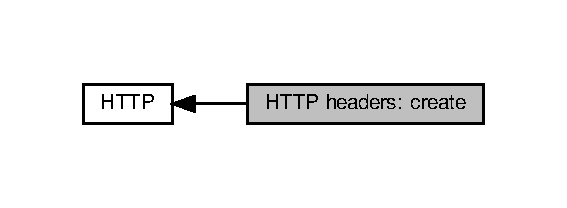
\includegraphics[width=272pt]{group__HTTP-headers-create}
\end{center}
\end{figure}
\subsection*{Macros}
\begin{DoxyCompactItemize}
\item 
\mbox{\Hypertarget{group__HTTP-headers-create_ga6e47044becc8d711dc5e619e1e5a0058}\label{group__HTTP-headers-create_ga6e47044becc8d711dc5e619e1e5a0058}} 
\#define {\bfseries L\+W\+S\+A\+H\+H\+\_\+\+C\+O\+D\+E\+\_\+\+M\+A\+SK}~((1 $<$$<$ 16) -\/ 1)
\item 
\mbox{\Hypertarget{group__HTTP-headers-create_ga96942f8dbde926a4cf9f9e56a4e10ee3}\label{group__HTTP-headers-create_ga96942f8dbde926a4cf9f9e56a4e10ee3}} 
\#define {\bfseries L\+W\+S\+A\+H\+H\+\_\+\+F\+L\+A\+G\+\_\+\+N\+O\+\_\+\+S\+E\+R\+V\+E\+R\+\_\+\+N\+A\+ME}~(1 $<$$<$ 30)
\item 
\mbox{\Hypertarget{group__HTTP-headers-create_ga6e47044becc8d711dc5e619e1e5a0058}\label{group__HTTP-headers-create_ga6e47044becc8d711dc5e619e1e5a0058}} 
\#define {\bfseries L\+W\+S\+A\+H\+H\+\_\+\+C\+O\+D\+E\+\_\+\+M\+A\+SK}~((1 $<$$<$ 16) -\/ 1)
\item 
\mbox{\Hypertarget{group__HTTP-headers-create_ga96942f8dbde926a4cf9f9e56a4e10ee3}\label{group__HTTP-headers-create_ga96942f8dbde926a4cf9f9e56a4e10ee3}} 
\#define {\bfseries L\+W\+S\+A\+H\+H\+\_\+\+F\+L\+A\+G\+\_\+\+N\+O\+\_\+\+S\+E\+R\+V\+E\+R\+\_\+\+N\+A\+ME}~(1 $<$$<$ 30)
\item 
\mbox{\Hypertarget{group__HTTP-headers-create_ga6e47044becc8d711dc5e619e1e5a0058}\label{group__HTTP-headers-create_ga6e47044becc8d711dc5e619e1e5a0058}} 
\#define {\bfseries L\+W\+S\+A\+H\+H\+\_\+\+C\+O\+D\+E\+\_\+\+M\+A\+SK}~((1 $<$$<$ 16) -\/ 1)
\item 
\mbox{\Hypertarget{group__HTTP-headers-create_ga96942f8dbde926a4cf9f9e56a4e10ee3}\label{group__HTTP-headers-create_ga96942f8dbde926a4cf9f9e56a4e10ee3}} 
\#define {\bfseries L\+W\+S\+A\+H\+H\+\_\+\+F\+L\+A\+G\+\_\+\+N\+O\+\_\+\+S\+E\+R\+V\+E\+R\+\_\+\+N\+A\+ME}~(1 $<$$<$ 30)
\item 
\mbox{\Hypertarget{group__HTTP-headers-create_ga6e47044becc8d711dc5e619e1e5a0058}\label{group__HTTP-headers-create_ga6e47044becc8d711dc5e619e1e5a0058}} 
\#define {\bfseries L\+W\+S\+A\+H\+H\+\_\+\+C\+O\+D\+E\+\_\+\+M\+A\+SK}~((1 $<$$<$ 16) -\/ 1)
\item 
\mbox{\Hypertarget{group__HTTP-headers-create_ga96942f8dbde926a4cf9f9e56a4e10ee3}\label{group__HTTP-headers-create_ga96942f8dbde926a4cf9f9e56a4e10ee3}} 
\#define {\bfseries L\+W\+S\+A\+H\+H\+\_\+\+F\+L\+A\+G\+\_\+\+N\+O\+\_\+\+S\+E\+R\+V\+E\+R\+\_\+\+N\+A\+ME}~(1 $<$$<$ 30)
\item 
\mbox{\Hypertarget{group__HTTP-headers-create_ga6e47044becc8d711dc5e619e1e5a0058}\label{group__HTTP-headers-create_ga6e47044becc8d711dc5e619e1e5a0058}} 
\#define {\bfseries L\+W\+S\+A\+H\+H\+\_\+\+C\+O\+D\+E\+\_\+\+M\+A\+SK}~((1 $<$$<$ 16) -\/ 1)
\item 
\mbox{\Hypertarget{group__HTTP-headers-create_ga96942f8dbde926a4cf9f9e56a4e10ee3}\label{group__HTTP-headers-create_ga96942f8dbde926a4cf9f9e56a4e10ee3}} 
\#define {\bfseries L\+W\+S\+A\+H\+H\+\_\+\+F\+L\+A\+G\+\_\+\+N\+O\+\_\+\+S\+E\+R\+V\+E\+R\+\_\+\+N\+A\+ME}~(1 $<$$<$ 30)
\item 
\mbox{\Hypertarget{group__HTTP-headers-create_ga6e47044becc8d711dc5e619e1e5a0058}\label{group__HTTP-headers-create_ga6e47044becc8d711dc5e619e1e5a0058}} 
\#define {\bfseries L\+W\+S\+A\+H\+H\+\_\+\+C\+O\+D\+E\+\_\+\+M\+A\+SK}~((1 $<$$<$ 16) -\/ 1)
\item 
\mbox{\Hypertarget{group__HTTP-headers-create_ga96942f8dbde926a4cf9f9e56a4e10ee3}\label{group__HTTP-headers-create_ga96942f8dbde926a4cf9f9e56a4e10ee3}} 
\#define {\bfseries L\+W\+S\+A\+H\+H\+\_\+\+F\+L\+A\+G\+\_\+\+N\+O\+\_\+\+S\+E\+R\+V\+E\+R\+\_\+\+N\+A\+ME}~(1 $<$$<$ 30)
\end{DoxyCompactItemize}
\subsection*{Functions}
\begin{DoxyCompactItemize}
\item 
L\+W\+S\+\_\+\+V\+I\+S\+I\+B\+LE L\+W\+S\+\_\+\+E\+X\+T\+E\+RN int L\+W\+S\+\_\+\+W\+A\+R\+N\+\_\+\+U\+N\+U\+S\+E\+D\+\_\+\+R\+E\+S\+U\+LT \hyperlink{group__HTTP-headers-create_ga29b7d6d2ddfdbaff3d8b607e7e3151b6}{lws\+\_\+add\+\_\+http\+\_\+header\+\_\+status} (struct \hyperlink{structlws}{lws} $\ast$wsi, unsigned int code, unsigned char $\ast$$\ast$p, unsigned char $\ast$end)
\item 
L\+W\+S\+\_\+\+V\+I\+S\+I\+B\+LE L\+W\+S\+\_\+\+E\+X\+T\+E\+RN int L\+W\+S\+\_\+\+W\+A\+R\+N\+\_\+\+U\+N\+U\+S\+E\+D\+\_\+\+R\+E\+S\+U\+LT \hyperlink{group__HTTP-headers-create_ga2b36bf44405755ff51c1939303b995a8}{lws\+\_\+add\+\_\+http\+\_\+header\+\_\+by\+\_\+name} (struct \hyperlink{structlws}{lws} $\ast$wsi, const unsigned char $\ast$name, const unsigned char $\ast$value, int length, unsigned char $\ast$$\ast$p, unsigned char $\ast$end)
\item 
L\+W\+S\+\_\+\+V\+I\+S\+I\+B\+LE L\+W\+S\+\_\+\+E\+X\+T\+E\+RN int L\+W\+S\+\_\+\+W\+A\+R\+N\+\_\+\+U\+N\+U\+S\+E\+D\+\_\+\+R\+E\+S\+U\+LT \hyperlink{group__HTTP-headers-create_gaf74adb761b22566ad70004882712dce1}{lws\+\_\+add\+\_\+http\+\_\+header\+\_\+by\+\_\+token} (struct \hyperlink{structlws}{lws} $\ast$wsi, enum lws\+\_\+token\+\_\+indexes token, const unsigned char $\ast$value, int length, unsigned char $\ast$$\ast$p, unsigned char $\ast$end)
\item 
L\+W\+S\+\_\+\+V\+I\+S\+I\+B\+LE L\+W\+S\+\_\+\+E\+X\+T\+E\+RN int L\+W\+S\+\_\+\+W\+A\+R\+N\+\_\+\+U\+N\+U\+S\+E\+D\+\_\+\+R\+E\+S\+U\+LT \hyperlink{group__HTTP-headers-create_gaeec7aa44c8553aeae9241c6a4e18321f}{lws\+\_\+add\+\_\+http\+\_\+header\+\_\+content\+\_\+length} (struct \hyperlink{structlws}{lws} $\ast$wsi, lws\+\_\+filepos\+\_\+t content\+\_\+length, unsigned char $\ast$$\ast$p, unsigned char $\ast$end)
\item 
L\+W\+S\+\_\+\+V\+I\+S\+I\+B\+LE L\+W\+S\+\_\+\+E\+X\+T\+E\+RN int L\+W\+S\+\_\+\+W\+A\+R\+N\+\_\+\+U\+N\+U\+S\+E\+D\+\_\+\+R\+E\+S\+U\+LT \hyperlink{group__HTTP-headers-create_ga4887605ff2242a54db3a7fa01f6f864b}{lws\+\_\+finalize\+\_\+http\+\_\+header} (struct \hyperlink{structlws}{lws} $\ast$wsi, unsigned char $\ast$$\ast$p, unsigned char $\ast$end)
\item 
L\+W\+S\+\_\+\+V\+I\+S\+I\+B\+LE L\+W\+S\+\_\+\+E\+X\+T\+E\+RN int L\+W\+S\+\_\+\+W\+A\+R\+N\+\_\+\+U\+N\+U\+S\+E\+D\+\_\+\+R\+E\+S\+U\+LT \hyperlink{group__HTTP-headers-create_gacc76a5babcb4dce1b01b1955aa7a2faf}{lws\+\_\+add\+\_\+http\+\_\+header\+\_\+content\+\_\+length} (struct \hyperlink{structlws}{lws} $\ast$wsi, unsigned long content\+\_\+length, unsigned char $\ast$$\ast$p, unsigned char $\ast$end)
\end{DoxyCompactItemize}


\subsection{Detailed Description}
\subsubsection*{H\+T\+TP headers\+: Create}

These apis allow you to create H\+T\+TP response headers in a way compatible with both H\+T\+T\+P/1.\+x and H\+T\+T\+P/2.

They each append to a buffer taking care about the buffer end, which is passed in as a pointer. When data is written to the buffer, the current position p is updated accordingly.

All of these apis are L\+W\+S\+\_\+\+W\+A\+R\+N\+\_\+\+U\+N\+U\+S\+E\+D\+\_\+\+R\+E\+S\+U\+LT as they can run out of space and fail with nonzero return. 

\subsection{Function Documentation}
\mbox{\Hypertarget{group__HTTP-headers-create_ga2b36bf44405755ff51c1939303b995a8}\label{group__HTTP-headers-create_ga2b36bf44405755ff51c1939303b995a8}} 
\index{H\+T\+T\+P headers\+: create@{H\+T\+T\+P headers\+: create}!lws\+\_\+add\+\_\+http\+\_\+header\+\_\+by\+\_\+name@{lws\+\_\+add\+\_\+http\+\_\+header\+\_\+by\+\_\+name}}
\index{lws\+\_\+add\+\_\+http\+\_\+header\+\_\+by\+\_\+name@{lws\+\_\+add\+\_\+http\+\_\+header\+\_\+by\+\_\+name}!H\+T\+T\+P headers\+: create@{H\+T\+T\+P headers\+: create}}
\subsubsection{\texorpdfstring{lws\+\_\+add\+\_\+http\+\_\+header\+\_\+by\+\_\+name()}{lws\_add\_http\_header\_by\_name()}}
{\footnotesize\ttfamily L\+W\+S\+\_\+\+V\+I\+S\+I\+B\+LE L\+W\+S\+\_\+\+E\+X\+T\+E\+RN int L\+W\+S\+\_\+\+W\+A\+R\+N\+\_\+\+U\+N\+U\+S\+E\+D\+\_\+\+R\+E\+S\+U\+LT lws\+\_\+add\+\_\+http\+\_\+header\+\_\+by\+\_\+name (\begin{DoxyParamCaption}\item[{struct \hyperlink{structlws}{lws} $\ast$}]{wsi,  }\item[{const unsigned char $\ast$}]{name,  }\item[{const unsigned char $\ast$}]{value,  }\item[{int}]{length,  }\item[{unsigned char $\ast$$\ast$}]{p,  }\item[{unsigned char $\ast$}]{end }\end{DoxyParamCaption})}

\hyperlink{group__HTTP-headers-create_ga2b36bf44405755ff51c1939303b995a8}{lws\+\_\+add\+\_\+http\+\_\+header\+\_\+by\+\_\+name()} -\/ append named header and value


\begin{DoxyParams}{Parameters}
{\em wsi} & the connection to check \\
\hline
{\em name} & the hdr name, like \char`\"{}my-\/header\char`\"{} \\
\hline
{\em value} & the value after the = for this header \\
\hline
{\em length} & the length of the value \\
\hline
{\em p} & pointer to current position in buffer pointer \\
\hline
{\em end} & pointer to end of buffer\\
\hline
\end{DoxyParams}
Appends name\+: value to the headers \mbox{\Hypertarget{group__HTTP-headers-create_gaf74adb761b22566ad70004882712dce1}\label{group__HTTP-headers-create_gaf74adb761b22566ad70004882712dce1}} 
\index{H\+T\+T\+P headers\+: create@{H\+T\+T\+P headers\+: create}!lws\+\_\+add\+\_\+http\+\_\+header\+\_\+by\+\_\+token@{lws\+\_\+add\+\_\+http\+\_\+header\+\_\+by\+\_\+token}}
\index{lws\+\_\+add\+\_\+http\+\_\+header\+\_\+by\+\_\+token@{lws\+\_\+add\+\_\+http\+\_\+header\+\_\+by\+\_\+token}!H\+T\+T\+P headers\+: create@{H\+T\+T\+P headers\+: create}}
\subsubsection{\texorpdfstring{lws\+\_\+add\+\_\+http\+\_\+header\+\_\+by\+\_\+token()}{lws\_add\_http\_header\_by\_token()}}
{\footnotesize\ttfamily L\+W\+S\+\_\+\+V\+I\+S\+I\+B\+LE L\+W\+S\+\_\+\+E\+X\+T\+E\+RN int L\+W\+S\+\_\+\+W\+A\+R\+N\+\_\+\+U\+N\+U\+S\+E\+D\+\_\+\+R\+E\+S\+U\+LT lws\+\_\+add\+\_\+http\+\_\+header\+\_\+by\+\_\+token (\begin{DoxyParamCaption}\item[{struct \hyperlink{structlws}{lws} $\ast$}]{wsi,  }\item[{enum lws\+\_\+token\+\_\+indexes}]{token,  }\item[{const unsigned char $\ast$}]{value,  }\item[{int}]{length,  }\item[{unsigned char $\ast$$\ast$}]{p,  }\item[{unsigned char $\ast$}]{end }\end{DoxyParamCaption})}

\hyperlink{group__HTTP-headers-create_gaf74adb761b22566ad70004882712dce1}{lws\+\_\+add\+\_\+http\+\_\+header\+\_\+by\+\_\+token()} -\/ append given header and value


\begin{DoxyParams}{Parameters}
{\em wsi} & the connection to check \\
\hline
{\em token} & the token index for the hdr \\
\hline
{\em value} & the value after the = for this header \\
\hline
{\em length} & the length of the value \\
\hline
{\em p} & pointer to current position in buffer pointer \\
\hline
{\em end} & pointer to end of buffer\\
\hline
\end{DoxyParams}
Appends name=value to the headers, but is able to take advantage of better H\+T\+T\+P/2 coding mechanisms where possible. \mbox{\Hypertarget{group__HTTP-headers-create_gacc76a5babcb4dce1b01b1955aa7a2faf}\label{group__HTTP-headers-create_gacc76a5babcb4dce1b01b1955aa7a2faf}} 
\index{H\+T\+T\+P headers\+: create@{H\+T\+T\+P headers\+: create}!lws\+\_\+add\+\_\+http\+\_\+header\+\_\+content\+\_\+length@{lws\+\_\+add\+\_\+http\+\_\+header\+\_\+content\+\_\+length}}
\index{lws\+\_\+add\+\_\+http\+\_\+header\+\_\+content\+\_\+length@{lws\+\_\+add\+\_\+http\+\_\+header\+\_\+content\+\_\+length}!H\+T\+T\+P headers\+: create@{H\+T\+T\+P headers\+: create}}
\subsubsection{\texorpdfstring{lws\+\_\+add\+\_\+http\+\_\+header\+\_\+content\+\_\+length()}{lws\_add\_http\_header\_content\_length()}\hspace{0.1cm}{\footnotesize\ttfamily [1/2]}}
{\footnotesize\ttfamily L\+W\+S\+\_\+\+V\+I\+S\+I\+B\+LE L\+W\+S\+\_\+\+E\+X\+T\+E\+RN int L\+W\+S\+\_\+\+W\+A\+R\+N\+\_\+\+U\+N\+U\+S\+E\+D\+\_\+\+R\+E\+S\+U\+LT lws\+\_\+add\+\_\+http\+\_\+header\+\_\+content\+\_\+length (\begin{DoxyParamCaption}\item[{struct \hyperlink{structlws}{lws} $\ast$}]{wsi,  }\item[{unsigned long}]{content\+\_\+length,  }\item[{unsigned char $\ast$$\ast$}]{p,  }\item[{unsigned char $\ast$}]{end }\end{DoxyParamCaption})}

\hyperlink{group__HTTP-headers-create_ga2b36bf44405755ff51c1939303b995a8}{lws\+\_\+add\+\_\+http\+\_\+header\+\_\+by\+\_\+name()} -\/ append content-\/length helper


\begin{DoxyParams}{Parameters}
{\em wsi} & the connection to check \\
\hline
{\em content\+\_\+length} & the content length to use \\
\hline
{\em p} & pointer to current position in buffer pointer \\
\hline
{\em end} & pointer to end of buffer\\
\hline
\end{DoxyParams}
Appends content-\/length\+: content\+\_\+length to the headers \mbox{\Hypertarget{group__HTTP-headers-create_gaeec7aa44c8553aeae9241c6a4e18321f}\label{group__HTTP-headers-create_gaeec7aa44c8553aeae9241c6a4e18321f}} 
\index{H\+T\+T\+P headers\+: create@{H\+T\+T\+P headers\+: create}!lws\+\_\+add\+\_\+http\+\_\+header\+\_\+content\+\_\+length@{lws\+\_\+add\+\_\+http\+\_\+header\+\_\+content\+\_\+length}}
\index{lws\+\_\+add\+\_\+http\+\_\+header\+\_\+content\+\_\+length@{lws\+\_\+add\+\_\+http\+\_\+header\+\_\+content\+\_\+length}!H\+T\+T\+P headers\+: create@{H\+T\+T\+P headers\+: create}}
\subsubsection{\texorpdfstring{lws\+\_\+add\+\_\+http\+\_\+header\+\_\+content\+\_\+length()}{lws\_add\_http\_header\_content\_length()}\hspace{0.1cm}{\footnotesize\ttfamily [2/2]}}
{\footnotesize\ttfamily L\+W\+S\+\_\+\+V\+I\+S\+I\+B\+LE L\+W\+S\+\_\+\+E\+X\+T\+E\+RN int L\+W\+S\+\_\+\+W\+A\+R\+N\+\_\+\+U\+N\+U\+S\+E\+D\+\_\+\+R\+E\+S\+U\+LT lws\+\_\+add\+\_\+http\+\_\+header\+\_\+content\+\_\+length (\begin{DoxyParamCaption}\item[{struct \hyperlink{structlws}{lws} $\ast$}]{wsi,  }\item[{lws\+\_\+filepos\+\_\+t}]{content\+\_\+length,  }\item[{unsigned char $\ast$$\ast$}]{p,  }\item[{unsigned char $\ast$}]{end }\end{DoxyParamCaption})}

\hyperlink{group__HTTP-headers-create_gaeec7aa44c8553aeae9241c6a4e18321f}{lws\+\_\+add\+\_\+http\+\_\+header\+\_\+content\+\_\+length()} -\/ append content-\/length helper


\begin{DoxyParams}{Parameters}
{\em wsi} & the connection to check \\
\hline
{\em content\+\_\+length} & the content length to use \\
\hline
{\em p} & pointer to current position in buffer pointer \\
\hline
{\em end} & pointer to end of buffer\\
\hline
\end{DoxyParams}
Appends content-\/length\+: content\+\_\+length to the headers \mbox{\Hypertarget{group__HTTP-headers-create_ga29b7d6d2ddfdbaff3d8b607e7e3151b6}\label{group__HTTP-headers-create_ga29b7d6d2ddfdbaff3d8b607e7e3151b6}} 
\index{H\+T\+T\+P headers\+: create@{H\+T\+T\+P headers\+: create}!lws\+\_\+add\+\_\+http\+\_\+header\+\_\+status@{lws\+\_\+add\+\_\+http\+\_\+header\+\_\+status}}
\index{lws\+\_\+add\+\_\+http\+\_\+header\+\_\+status@{lws\+\_\+add\+\_\+http\+\_\+header\+\_\+status}!H\+T\+T\+P headers\+: create@{H\+T\+T\+P headers\+: create}}
\subsubsection{\texorpdfstring{lws\+\_\+add\+\_\+http\+\_\+header\+\_\+status()}{lws\_add\_http\_header\_status()}}
{\footnotesize\ttfamily L\+W\+S\+\_\+\+V\+I\+S\+I\+B\+LE L\+W\+S\+\_\+\+E\+X\+T\+E\+RN int L\+W\+S\+\_\+\+W\+A\+R\+N\+\_\+\+U\+N\+U\+S\+E\+D\+\_\+\+R\+E\+S\+U\+LT lws\+\_\+add\+\_\+http\+\_\+header\+\_\+status (\begin{DoxyParamCaption}\item[{struct \hyperlink{structlws}{lws} $\ast$}]{wsi,  }\item[{unsigned int}]{code,  }\item[{unsigned char $\ast$$\ast$}]{p,  }\item[{unsigned char $\ast$}]{end }\end{DoxyParamCaption})}

\hyperlink{group__HTTP-headers-create_ga29b7d6d2ddfdbaff3d8b607e7e3151b6}{lws\+\_\+add\+\_\+http\+\_\+header\+\_\+status()} -\/ add the H\+T\+TP response status code


\begin{DoxyParams}{Parameters}
{\em wsi} & the connection to check \\
\hline
{\em code} & an H\+T\+TP code like 200, 404 etc (see enum http\+\_\+status) \\
\hline
{\em p} & pointer to current position in buffer pointer \\
\hline
{\em end} & pointer to end of buffer\\
\hline
\end{DoxyParams}
Adds the initial response code, so should be called first.

Code may additionally take OR\textquotesingle{}d flags\+:

L\+W\+S\+A\+H\+H\+\_\+\+F\+L\+A\+G\+\_\+\+N\+O\+\_\+\+S\+E\+R\+V\+E\+R\+\_\+\+N\+A\+ME\+: don\textquotesingle{}t apply server name header this time \mbox{\Hypertarget{group__HTTP-headers-create_ga4887605ff2242a54db3a7fa01f6f864b}\label{group__HTTP-headers-create_ga4887605ff2242a54db3a7fa01f6f864b}} 
\index{H\+T\+T\+P headers\+: create@{H\+T\+T\+P headers\+: create}!lws\+\_\+finalize\+\_\+http\+\_\+header@{lws\+\_\+finalize\+\_\+http\+\_\+header}}
\index{lws\+\_\+finalize\+\_\+http\+\_\+header@{lws\+\_\+finalize\+\_\+http\+\_\+header}!H\+T\+T\+P headers\+: create@{H\+T\+T\+P headers\+: create}}
\subsubsection{\texorpdfstring{lws\+\_\+finalize\+\_\+http\+\_\+header()}{lws\_finalize\_http\_header()}}
{\footnotesize\ttfamily L\+W\+S\+\_\+\+V\+I\+S\+I\+B\+LE L\+W\+S\+\_\+\+E\+X\+T\+E\+RN int L\+W\+S\+\_\+\+W\+A\+R\+N\+\_\+\+U\+N\+U\+S\+E\+D\+\_\+\+R\+E\+S\+U\+LT lws\+\_\+finalize\+\_\+http\+\_\+header (\begin{DoxyParamCaption}\item[{struct \hyperlink{structlws}{lws} $\ast$}]{wsi,  }\item[{unsigned char $\ast$$\ast$}]{p,  }\item[{unsigned char $\ast$}]{end }\end{DoxyParamCaption})}

\hyperlink{group__HTTP-headers-create_ga4887605ff2242a54db3a7fa01f6f864b}{lws\+\_\+finalize\+\_\+http\+\_\+header()} -\/ terminate header block


\begin{DoxyParams}{Parameters}
{\em wsi} & the connection to check \\
\hline
{\em p} & pointer to current position in buffer pointer \\
\hline
{\em end} & pointer to end of buffer\\
\hline
\end{DoxyParams}
Indicates no more headers will be added 
\hypertarget{group__form-parsing}{}\section{Form Parsing}
\label{group__form-parsing}\index{Form Parsing@{Form Parsing}}
Collaboration diagram for Form Parsing\+:
\nopagebreak
\begin{figure}[H]
\begin{center}
\leavevmode
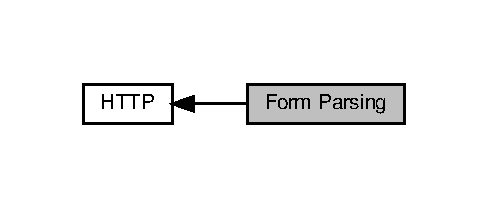
\includegraphics[width=234pt]{group__form-parsing}
\end{center}
\end{figure}
\subsection*{Typedefs}
\begin{DoxyCompactItemize}
\item 
typedef int($\ast$ \hyperlink{group__form-parsing_ga5a70527c0861c2ffa3d29333a6aa7f8e}{lws\+\_\+spa\+\_\+fileupload\+\_\+cb}) (void $\ast$data, const char $\ast$name, const char $\ast$filename, char $\ast$buf, int len, enum \hyperlink{group__form-parsing_ga41a74a822771d3dce89751aa3bce28ae}{lws\+\_\+spa\+\_\+fileupload\+\_\+states} state)
\item 
typedef int($\ast$ \hyperlink{group__form-parsing_ga5a70527c0861c2ffa3d29333a6aa7f8e}{lws\+\_\+spa\+\_\+fileupload\+\_\+cb}) (void $\ast$data, const char $\ast$name, const char $\ast$filename, char $\ast$buf, int len, enum \hyperlink{group__form-parsing_ga41a74a822771d3dce89751aa3bce28ae}{lws\+\_\+spa\+\_\+fileupload\+\_\+states} state)
\item 
typedef int($\ast$ \hyperlink{group__form-parsing_ga5a70527c0861c2ffa3d29333a6aa7f8e}{lws\+\_\+spa\+\_\+fileupload\+\_\+cb}) (void $\ast$data, const char $\ast$name, const char $\ast$filename, char $\ast$buf, int len, enum \hyperlink{group__form-parsing_ga41a74a822771d3dce89751aa3bce28ae}{lws\+\_\+spa\+\_\+fileupload\+\_\+states} state)
\item 
typedef int($\ast$ \hyperlink{group__form-parsing_ga5a70527c0861c2ffa3d29333a6aa7f8e}{lws\+\_\+spa\+\_\+fileupload\+\_\+cb}) (void $\ast$data, const char $\ast$name, const char $\ast$filename, char $\ast$buf, int len, enum \hyperlink{group__form-parsing_ga41a74a822771d3dce89751aa3bce28ae}{lws\+\_\+spa\+\_\+fileupload\+\_\+states} state)
\item 
typedef int($\ast$ \hyperlink{group__form-parsing_ga5a70527c0861c2ffa3d29333a6aa7f8e}{lws\+\_\+spa\+\_\+fileupload\+\_\+cb}) (void $\ast$data, const char $\ast$name, const char $\ast$filename, char $\ast$buf, int len, enum \hyperlink{group__form-parsing_ga41a74a822771d3dce89751aa3bce28ae}{lws\+\_\+spa\+\_\+fileupload\+\_\+states} state)
\item 
typedef int($\ast$ \hyperlink{group__form-parsing_ga5a70527c0861c2ffa3d29333a6aa7f8e}{lws\+\_\+spa\+\_\+fileupload\+\_\+cb}) (void $\ast$data, const char $\ast$name, const char $\ast$filename, char $\ast$buf, int len, enum \hyperlink{group__form-parsing_ga41a74a822771d3dce89751aa3bce28ae}{lws\+\_\+spa\+\_\+fileupload\+\_\+states} state)
\item 
typedef int($\ast$ \hyperlink{group__form-parsing_ga5a70527c0861c2ffa3d29333a6aa7f8e}{lws\+\_\+spa\+\_\+fileupload\+\_\+cb}) (void $\ast$data, const char $\ast$name, const char $\ast$filename, char $\ast$buf, int len, enum \hyperlink{group__form-parsing_ga41a74a822771d3dce89751aa3bce28ae}{lws\+\_\+spa\+\_\+fileupload\+\_\+states} state)
\item 
typedef int($\ast$ \hyperlink{group__form-parsing_ga5a70527c0861c2ffa3d29333a6aa7f8e}{lws\+\_\+spa\+\_\+fileupload\+\_\+cb}) (void $\ast$data, const char $\ast$name, const char $\ast$filename, char $\ast$buf, int len, enum \hyperlink{group__form-parsing_ga41a74a822771d3dce89751aa3bce28ae}{lws\+\_\+spa\+\_\+fileupload\+\_\+states} state)
\end{DoxyCompactItemize}
\subsection*{Enumerations}
\begin{DoxyCompactItemize}
\item 
enum \hyperlink{group__form-parsing_ga41a74a822771d3dce89751aa3bce28ae}{lws\+\_\+spa\+\_\+fileupload\+\_\+states} \{ \newline
\hyperlink{group__form-parsing_gga41a74a822771d3dce89751aa3bce28aead3a958e7719ac273c3ba4f684f00c87f}{L\+W\+S\+\_\+\+U\+F\+S\+\_\+\+C\+O\+N\+T\+E\+NT}, 
\hyperlink{group__form-parsing_gga41a74a822771d3dce89751aa3bce28aea6ce2a55a4c3695cdb640c893d95bd3a7}{L\+W\+S\+\_\+\+U\+F\+S\+\_\+\+F\+I\+N\+A\+L\+\_\+\+C\+O\+N\+T\+E\+NT}, 
\hyperlink{group__form-parsing_gga41a74a822771d3dce89751aa3bce28aea2d25de44865bd44e5a3903a2bab9ca83}{L\+W\+S\+\_\+\+U\+F\+S\+\_\+\+O\+P\+EN}, 
\hyperlink{group__form-parsing_gga41a74a822771d3dce89751aa3bce28aead3a958e7719ac273c3ba4f684f00c87f}{L\+W\+S\+\_\+\+U\+F\+S\+\_\+\+C\+O\+N\+T\+E\+NT}, 
\newline
\hyperlink{group__form-parsing_gga41a74a822771d3dce89751aa3bce28aea6ce2a55a4c3695cdb640c893d95bd3a7}{L\+W\+S\+\_\+\+U\+F\+S\+\_\+\+F\+I\+N\+A\+L\+\_\+\+C\+O\+N\+T\+E\+NT}, 
\hyperlink{group__form-parsing_gga41a74a822771d3dce89751aa3bce28aea2d25de44865bd44e5a3903a2bab9ca83}{L\+W\+S\+\_\+\+U\+F\+S\+\_\+\+O\+P\+EN}, 
\hyperlink{group__form-parsing_gga41a74a822771d3dce89751aa3bce28aead3a958e7719ac273c3ba4f684f00c87f}{L\+W\+S\+\_\+\+U\+F\+S\+\_\+\+C\+O\+N\+T\+E\+NT}, 
\hyperlink{group__form-parsing_gga41a74a822771d3dce89751aa3bce28aea6ce2a55a4c3695cdb640c893d95bd3a7}{L\+W\+S\+\_\+\+U\+F\+S\+\_\+\+F\+I\+N\+A\+L\+\_\+\+C\+O\+N\+T\+E\+NT}, 
\newline
\hyperlink{group__form-parsing_gga41a74a822771d3dce89751aa3bce28aea2d25de44865bd44e5a3903a2bab9ca83}{L\+W\+S\+\_\+\+U\+F\+S\+\_\+\+O\+P\+EN}, 
\hyperlink{group__form-parsing_gga41a74a822771d3dce89751aa3bce28aead3a958e7719ac273c3ba4f684f00c87f}{L\+W\+S\+\_\+\+U\+F\+S\+\_\+\+C\+O\+N\+T\+E\+NT}, 
\hyperlink{group__form-parsing_gga41a74a822771d3dce89751aa3bce28aea6ce2a55a4c3695cdb640c893d95bd3a7}{L\+W\+S\+\_\+\+U\+F\+S\+\_\+\+F\+I\+N\+A\+L\+\_\+\+C\+O\+N\+T\+E\+NT}, 
\hyperlink{group__form-parsing_gga41a74a822771d3dce89751aa3bce28aea2d25de44865bd44e5a3903a2bab9ca83}{L\+W\+S\+\_\+\+U\+F\+S\+\_\+\+O\+P\+EN}, 
\newline
\hyperlink{group__form-parsing_gga41a74a822771d3dce89751aa3bce28aead3a958e7719ac273c3ba4f684f00c87f}{L\+W\+S\+\_\+\+U\+F\+S\+\_\+\+C\+O\+N\+T\+E\+NT}, 
\hyperlink{group__form-parsing_gga41a74a822771d3dce89751aa3bce28aea6ce2a55a4c3695cdb640c893d95bd3a7}{L\+W\+S\+\_\+\+U\+F\+S\+\_\+\+F\+I\+N\+A\+L\+\_\+\+C\+O\+N\+T\+E\+NT}, 
\hyperlink{group__form-parsing_gga41a74a822771d3dce89751aa3bce28aea2d25de44865bd44e5a3903a2bab9ca83}{L\+W\+S\+\_\+\+U\+F\+S\+\_\+\+O\+P\+EN}, 
\hyperlink{group__form-parsing_gga41a74a822771d3dce89751aa3bce28aead3a958e7719ac273c3ba4f684f00c87f}{L\+W\+S\+\_\+\+U\+F\+S\+\_\+\+C\+O\+N\+T\+E\+NT}, 
\newline
\hyperlink{group__form-parsing_gga41a74a822771d3dce89751aa3bce28aea6ce2a55a4c3695cdb640c893d95bd3a7}{L\+W\+S\+\_\+\+U\+F\+S\+\_\+\+F\+I\+N\+A\+L\+\_\+\+C\+O\+N\+T\+E\+NT}, 
\hyperlink{group__form-parsing_gga41a74a822771d3dce89751aa3bce28aea2d25de44865bd44e5a3903a2bab9ca83}{L\+W\+S\+\_\+\+U\+F\+S\+\_\+\+O\+P\+EN}, 
\hyperlink{group__form-parsing_gga41a74a822771d3dce89751aa3bce28aead3a958e7719ac273c3ba4f684f00c87f}{L\+W\+S\+\_\+\+U\+F\+S\+\_\+\+C\+O\+N\+T\+E\+NT}, 
\hyperlink{group__form-parsing_gga41a74a822771d3dce89751aa3bce28aea6ce2a55a4c3695cdb640c893d95bd3a7}{L\+W\+S\+\_\+\+U\+F\+S\+\_\+\+F\+I\+N\+A\+L\+\_\+\+C\+O\+N\+T\+E\+NT}, 
\newline
\hyperlink{group__form-parsing_gga41a74a822771d3dce89751aa3bce28aea2d25de44865bd44e5a3903a2bab9ca83}{L\+W\+S\+\_\+\+U\+F\+S\+\_\+\+O\+P\+EN}, 
\hyperlink{group__form-parsing_gga41a74a822771d3dce89751aa3bce28aead3a958e7719ac273c3ba4f684f00c87f}{L\+W\+S\+\_\+\+U\+F\+S\+\_\+\+C\+O\+N\+T\+E\+NT}, 
\hyperlink{group__form-parsing_gga41a74a822771d3dce89751aa3bce28aea6ce2a55a4c3695cdb640c893d95bd3a7}{L\+W\+S\+\_\+\+U\+F\+S\+\_\+\+F\+I\+N\+A\+L\+\_\+\+C\+O\+N\+T\+E\+NT}, 
\hyperlink{group__form-parsing_gga41a74a822771d3dce89751aa3bce28aea2d25de44865bd44e5a3903a2bab9ca83}{L\+W\+S\+\_\+\+U\+F\+S\+\_\+\+O\+P\+EN}
 \}
\item 
enum \hyperlink{group__form-parsing_ga41a74a822771d3dce89751aa3bce28ae}{lws\+\_\+spa\+\_\+fileupload\+\_\+states} \{ \newline
\hyperlink{group__form-parsing_gga41a74a822771d3dce89751aa3bce28aead3a958e7719ac273c3ba4f684f00c87f}{L\+W\+S\+\_\+\+U\+F\+S\+\_\+\+C\+O\+N\+T\+E\+NT}, 
\hyperlink{group__form-parsing_gga41a74a822771d3dce89751aa3bce28aea6ce2a55a4c3695cdb640c893d95bd3a7}{L\+W\+S\+\_\+\+U\+F\+S\+\_\+\+F\+I\+N\+A\+L\+\_\+\+C\+O\+N\+T\+E\+NT}, 
\hyperlink{group__form-parsing_gga41a74a822771d3dce89751aa3bce28aea2d25de44865bd44e5a3903a2bab9ca83}{L\+W\+S\+\_\+\+U\+F\+S\+\_\+\+O\+P\+EN}, 
\hyperlink{group__form-parsing_gga41a74a822771d3dce89751aa3bce28aead3a958e7719ac273c3ba4f684f00c87f}{L\+W\+S\+\_\+\+U\+F\+S\+\_\+\+C\+O\+N\+T\+E\+NT}, 
\newline
\hyperlink{group__form-parsing_gga41a74a822771d3dce89751aa3bce28aea6ce2a55a4c3695cdb640c893d95bd3a7}{L\+W\+S\+\_\+\+U\+F\+S\+\_\+\+F\+I\+N\+A\+L\+\_\+\+C\+O\+N\+T\+E\+NT}, 
\hyperlink{group__form-parsing_gga41a74a822771d3dce89751aa3bce28aea2d25de44865bd44e5a3903a2bab9ca83}{L\+W\+S\+\_\+\+U\+F\+S\+\_\+\+O\+P\+EN}, 
\hyperlink{group__form-parsing_gga41a74a822771d3dce89751aa3bce28aead3a958e7719ac273c3ba4f684f00c87f}{L\+W\+S\+\_\+\+U\+F\+S\+\_\+\+C\+O\+N\+T\+E\+NT}, 
\hyperlink{group__form-parsing_gga41a74a822771d3dce89751aa3bce28aea6ce2a55a4c3695cdb640c893d95bd3a7}{L\+W\+S\+\_\+\+U\+F\+S\+\_\+\+F\+I\+N\+A\+L\+\_\+\+C\+O\+N\+T\+E\+NT}, 
\newline
\hyperlink{group__form-parsing_gga41a74a822771d3dce89751aa3bce28aea2d25de44865bd44e5a3903a2bab9ca83}{L\+W\+S\+\_\+\+U\+F\+S\+\_\+\+O\+P\+EN}, 
\hyperlink{group__form-parsing_gga41a74a822771d3dce89751aa3bce28aead3a958e7719ac273c3ba4f684f00c87f}{L\+W\+S\+\_\+\+U\+F\+S\+\_\+\+C\+O\+N\+T\+E\+NT}, 
\hyperlink{group__form-parsing_gga41a74a822771d3dce89751aa3bce28aea6ce2a55a4c3695cdb640c893d95bd3a7}{L\+W\+S\+\_\+\+U\+F\+S\+\_\+\+F\+I\+N\+A\+L\+\_\+\+C\+O\+N\+T\+E\+NT}, 
\hyperlink{group__form-parsing_gga41a74a822771d3dce89751aa3bce28aea2d25de44865bd44e5a3903a2bab9ca83}{L\+W\+S\+\_\+\+U\+F\+S\+\_\+\+O\+P\+EN}, 
\newline
\hyperlink{group__form-parsing_gga41a74a822771d3dce89751aa3bce28aead3a958e7719ac273c3ba4f684f00c87f}{L\+W\+S\+\_\+\+U\+F\+S\+\_\+\+C\+O\+N\+T\+E\+NT}, 
\hyperlink{group__form-parsing_gga41a74a822771d3dce89751aa3bce28aea6ce2a55a4c3695cdb640c893d95bd3a7}{L\+W\+S\+\_\+\+U\+F\+S\+\_\+\+F\+I\+N\+A\+L\+\_\+\+C\+O\+N\+T\+E\+NT}, 
\hyperlink{group__form-parsing_gga41a74a822771d3dce89751aa3bce28aea2d25de44865bd44e5a3903a2bab9ca83}{L\+W\+S\+\_\+\+U\+F\+S\+\_\+\+O\+P\+EN}, 
\hyperlink{group__form-parsing_gga41a74a822771d3dce89751aa3bce28aead3a958e7719ac273c3ba4f684f00c87f}{L\+W\+S\+\_\+\+U\+F\+S\+\_\+\+C\+O\+N\+T\+E\+NT}, 
\newline
\hyperlink{group__form-parsing_gga41a74a822771d3dce89751aa3bce28aea6ce2a55a4c3695cdb640c893d95bd3a7}{L\+W\+S\+\_\+\+U\+F\+S\+\_\+\+F\+I\+N\+A\+L\+\_\+\+C\+O\+N\+T\+E\+NT}, 
\hyperlink{group__form-parsing_gga41a74a822771d3dce89751aa3bce28aea2d25de44865bd44e5a3903a2bab9ca83}{L\+W\+S\+\_\+\+U\+F\+S\+\_\+\+O\+P\+EN}, 
\hyperlink{group__form-parsing_gga41a74a822771d3dce89751aa3bce28aead3a958e7719ac273c3ba4f684f00c87f}{L\+W\+S\+\_\+\+U\+F\+S\+\_\+\+C\+O\+N\+T\+E\+NT}, 
\hyperlink{group__form-parsing_gga41a74a822771d3dce89751aa3bce28aea6ce2a55a4c3695cdb640c893d95bd3a7}{L\+W\+S\+\_\+\+U\+F\+S\+\_\+\+F\+I\+N\+A\+L\+\_\+\+C\+O\+N\+T\+E\+NT}, 
\newline
\hyperlink{group__form-parsing_gga41a74a822771d3dce89751aa3bce28aea2d25de44865bd44e5a3903a2bab9ca83}{L\+W\+S\+\_\+\+U\+F\+S\+\_\+\+O\+P\+EN}, 
\hyperlink{group__form-parsing_gga41a74a822771d3dce89751aa3bce28aead3a958e7719ac273c3ba4f684f00c87f}{L\+W\+S\+\_\+\+U\+F\+S\+\_\+\+C\+O\+N\+T\+E\+NT}, 
\hyperlink{group__form-parsing_gga41a74a822771d3dce89751aa3bce28aea6ce2a55a4c3695cdb640c893d95bd3a7}{L\+W\+S\+\_\+\+U\+F\+S\+\_\+\+F\+I\+N\+A\+L\+\_\+\+C\+O\+N\+T\+E\+NT}, 
\hyperlink{group__form-parsing_gga41a74a822771d3dce89751aa3bce28aea2d25de44865bd44e5a3903a2bab9ca83}{L\+W\+S\+\_\+\+U\+F\+S\+\_\+\+O\+P\+EN}
 \}
\item 
enum \hyperlink{group__form-parsing_ga41a74a822771d3dce89751aa3bce28ae}{lws\+\_\+spa\+\_\+fileupload\+\_\+states} \{ \newline
\hyperlink{group__form-parsing_gga41a74a822771d3dce89751aa3bce28aead3a958e7719ac273c3ba4f684f00c87f}{L\+W\+S\+\_\+\+U\+F\+S\+\_\+\+C\+O\+N\+T\+E\+NT}, 
\hyperlink{group__form-parsing_gga41a74a822771d3dce89751aa3bce28aea6ce2a55a4c3695cdb640c893d95bd3a7}{L\+W\+S\+\_\+\+U\+F\+S\+\_\+\+F\+I\+N\+A\+L\+\_\+\+C\+O\+N\+T\+E\+NT}, 
\hyperlink{group__form-parsing_gga41a74a822771d3dce89751aa3bce28aea2d25de44865bd44e5a3903a2bab9ca83}{L\+W\+S\+\_\+\+U\+F\+S\+\_\+\+O\+P\+EN}, 
\hyperlink{group__form-parsing_gga41a74a822771d3dce89751aa3bce28aead3a958e7719ac273c3ba4f684f00c87f}{L\+W\+S\+\_\+\+U\+F\+S\+\_\+\+C\+O\+N\+T\+E\+NT}, 
\newline
\hyperlink{group__form-parsing_gga41a74a822771d3dce89751aa3bce28aea6ce2a55a4c3695cdb640c893d95bd3a7}{L\+W\+S\+\_\+\+U\+F\+S\+\_\+\+F\+I\+N\+A\+L\+\_\+\+C\+O\+N\+T\+E\+NT}, 
\hyperlink{group__form-parsing_gga41a74a822771d3dce89751aa3bce28aea2d25de44865bd44e5a3903a2bab9ca83}{L\+W\+S\+\_\+\+U\+F\+S\+\_\+\+O\+P\+EN}, 
\hyperlink{group__form-parsing_gga41a74a822771d3dce89751aa3bce28aead3a958e7719ac273c3ba4f684f00c87f}{L\+W\+S\+\_\+\+U\+F\+S\+\_\+\+C\+O\+N\+T\+E\+NT}, 
\hyperlink{group__form-parsing_gga41a74a822771d3dce89751aa3bce28aea6ce2a55a4c3695cdb640c893d95bd3a7}{L\+W\+S\+\_\+\+U\+F\+S\+\_\+\+F\+I\+N\+A\+L\+\_\+\+C\+O\+N\+T\+E\+NT}, 
\newline
\hyperlink{group__form-parsing_gga41a74a822771d3dce89751aa3bce28aea2d25de44865bd44e5a3903a2bab9ca83}{L\+W\+S\+\_\+\+U\+F\+S\+\_\+\+O\+P\+EN}, 
\hyperlink{group__form-parsing_gga41a74a822771d3dce89751aa3bce28aead3a958e7719ac273c3ba4f684f00c87f}{L\+W\+S\+\_\+\+U\+F\+S\+\_\+\+C\+O\+N\+T\+E\+NT}, 
\hyperlink{group__form-parsing_gga41a74a822771d3dce89751aa3bce28aea6ce2a55a4c3695cdb640c893d95bd3a7}{L\+W\+S\+\_\+\+U\+F\+S\+\_\+\+F\+I\+N\+A\+L\+\_\+\+C\+O\+N\+T\+E\+NT}, 
\hyperlink{group__form-parsing_gga41a74a822771d3dce89751aa3bce28aea2d25de44865bd44e5a3903a2bab9ca83}{L\+W\+S\+\_\+\+U\+F\+S\+\_\+\+O\+P\+EN}, 
\newline
\hyperlink{group__form-parsing_gga41a74a822771d3dce89751aa3bce28aead3a958e7719ac273c3ba4f684f00c87f}{L\+W\+S\+\_\+\+U\+F\+S\+\_\+\+C\+O\+N\+T\+E\+NT}, 
\hyperlink{group__form-parsing_gga41a74a822771d3dce89751aa3bce28aea6ce2a55a4c3695cdb640c893d95bd3a7}{L\+W\+S\+\_\+\+U\+F\+S\+\_\+\+F\+I\+N\+A\+L\+\_\+\+C\+O\+N\+T\+E\+NT}, 
\hyperlink{group__form-parsing_gga41a74a822771d3dce89751aa3bce28aea2d25de44865bd44e5a3903a2bab9ca83}{L\+W\+S\+\_\+\+U\+F\+S\+\_\+\+O\+P\+EN}, 
\hyperlink{group__form-parsing_gga41a74a822771d3dce89751aa3bce28aead3a958e7719ac273c3ba4f684f00c87f}{L\+W\+S\+\_\+\+U\+F\+S\+\_\+\+C\+O\+N\+T\+E\+NT}, 
\newline
\hyperlink{group__form-parsing_gga41a74a822771d3dce89751aa3bce28aea6ce2a55a4c3695cdb640c893d95bd3a7}{L\+W\+S\+\_\+\+U\+F\+S\+\_\+\+F\+I\+N\+A\+L\+\_\+\+C\+O\+N\+T\+E\+NT}, 
\hyperlink{group__form-parsing_gga41a74a822771d3dce89751aa3bce28aea2d25de44865bd44e5a3903a2bab9ca83}{L\+W\+S\+\_\+\+U\+F\+S\+\_\+\+O\+P\+EN}, 
\hyperlink{group__form-parsing_gga41a74a822771d3dce89751aa3bce28aead3a958e7719ac273c3ba4f684f00c87f}{L\+W\+S\+\_\+\+U\+F\+S\+\_\+\+C\+O\+N\+T\+E\+NT}, 
\hyperlink{group__form-parsing_gga41a74a822771d3dce89751aa3bce28aea6ce2a55a4c3695cdb640c893d95bd3a7}{L\+W\+S\+\_\+\+U\+F\+S\+\_\+\+F\+I\+N\+A\+L\+\_\+\+C\+O\+N\+T\+E\+NT}, 
\newline
\hyperlink{group__form-parsing_gga41a74a822771d3dce89751aa3bce28aea2d25de44865bd44e5a3903a2bab9ca83}{L\+W\+S\+\_\+\+U\+F\+S\+\_\+\+O\+P\+EN}, 
\hyperlink{group__form-parsing_gga41a74a822771d3dce89751aa3bce28aead3a958e7719ac273c3ba4f684f00c87f}{L\+W\+S\+\_\+\+U\+F\+S\+\_\+\+C\+O\+N\+T\+E\+NT}, 
\hyperlink{group__form-parsing_gga41a74a822771d3dce89751aa3bce28aea6ce2a55a4c3695cdb640c893d95bd3a7}{L\+W\+S\+\_\+\+U\+F\+S\+\_\+\+F\+I\+N\+A\+L\+\_\+\+C\+O\+N\+T\+E\+NT}, 
\hyperlink{group__form-parsing_gga41a74a822771d3dce89751aa3bce28aea2d25de44865bd44e5a3903a2bab9ca83}{L\+W\+S\+\_\+\+U\+F\+S\+\_\+\+O\+P\+EN}
 \}
\item 
enum \hyperlink{group__form-parsing_ga41a74a822771d3dce89751aa3bce28ae}{lws\+\_\+spa\+\_\+fileupload\+\_\+states} \{ \newline
\hyperlink{group__form-parsing_gga41a74a822771d3dce89751aa3bce28aead3a958e7719ac273c3ba4f684f00c87f}{L\+W\+S\+\_\+\+U\+F\+S\+\_\+\+C\+O\+N\+T\+E\+NT}, 
\hyperlink{group__form-parsing_gga41a74a822771d3dce89751aa3bce28aea6ce2a55a4c3695cdb640c893d95bd3a7}{L\+W\+S\+\_\+\+U\+F\+S\+\_\+\+F\+I\+N\+A\+L\+\_\+\+C\+O\+N\+T\+E\+NT}, 
\hyperlink{group__form-parsing_gga41a74a822771d3dce89751aa3bce28aea2d25de44865bd44e5a3903a2bab9ca83}{L\+W\+S\+\_\+\+U\+F\+S\+\_\+\+O\+P\+EN}, 
\hyperlink{group__form-parsing_gga41a74a822771d3dce89751aa3bce28aead3a958e7719ac273c3ba4f684f00c87f}{L\+W\+S\+\_\+\+U\+F\+S\+\_\+\+C\+O\+N\+T\+E\+NT}, 
\newline
\hyperlink{group__form-parsing_gga41a74a822771d3dce89751aa3bce28aea6ce2a55a4c3695cdb640c893d95bd3a7}{L\+W\+S\+\_\+\+U\+F\+S\+\_\+\+F\+I\+N\+A\+L\+\_\+\+C\+O\+N\+T\+E\+NT}, 
\hyperlink{group__form-parsing_gga41a74a822771d3dce89751aa3bce28aea2d25de44865bd44e5a3903a2bab9ca83}{L\+W\+S\+\_\+\+U\+F\+S\+\_\+\+O\+P\+EN}, 
\hyperlink{group__form-parsing_gga41a74a822771d3dce89751aa3bce28aead3a958e7719ac273c3ba4f684f00c87f}{L\+W\+S\+\_\+\+U\+F\+S\+\_\+\+C\+O\+N\+T\+E\+NT}, 
\hyperlink{group__form-parsing_gga41a74a822771d3dce89751aa3bce28aea6ce2a55a4c3695cdb640c893d95bd3a7}{L\+W\+S\+\_\+\+U\+F\+S\+\_\+\+F\+I\+N\+A\+L\+\_\+\+C\+O\+N\+T\+E\+NT}, 
\newline
\hyperlink{group__form-parsing_gga41a74a822771d3dce89751aa3bce28aea2d25de44865bd44e5a3903a2bab9ca83}{L\+W\+S\+\_\+\+U\+F\+S\+\_\+\+O\+P\+EN}, 
\hyperlink{group__form-parsing_gga41a74a822771d3dce89751aa3bce28aead3a958e7719ac273c3ba4f684f00c87f}{L\+W\+S\+\_\+\+U\+F\+S\+\_\+\+C\+O\+N\+T\+E\+NT}, 
\hyperlink{group__form-parsing_gga41a74a822771d3dce89751aa3bce28aea6ce2a55a4c3695cdb640c893d95bd3a7}{L\+W\+S\+\_\+\+U\+F\+S\+\_\+\+F\+I\+N\+A\+L\+\_\+\+C\+O\+N\+T\+E\+NT}, 
\hyperlink{group__form-parsing_gga41a74a822771d3dce89751aa3bce28aea2d25de44865bd44e5a3903a2bab9ca83}{L\+W\+S\+\_\+\+U\+F\+S\+\_\+\+O\+P\+EN}, 
\newline
\hyperlink{group__form-parsing_gga41a74a822771d3dce89751aa3bce28aead3a958e7719ac273c3ba4f684f00c87f}{L\+W\+S\+\_\+\+U\+F\+S\+\_\+\+C\+O\+N\+T\+E\+NT}, 
\hyperlink{group__form-parsing_gga41a74a822771d3dce89751aa3bce28aea6ce2a55a4c3695cdb640c893d95bd3a7}{L\+W\+S\+\_\+\+U\+F\+S\+\_\+\+F\+I\+N\+A\+L\+\_\+\+C\+O\+N\+T\+E\+NT}, 
\hyperlink{group__form-parsing_gga41a74a822771d3dce89751aa3bce28aea2d25de44865bd44e5a3903a2bab9ca83}{L\+W\+S\+\_\+\+U\+F\+S\+\_\+\+O\+P\+EN}, 
\hyperlink{group__form-parsing_gga41a74a822771d3dce89751aa3bce28aead3a958e7719ac273c3ba4f684f00c87f}{L\+W\+S\+\_\+\+U\+F\+S\+\_\+\+C\+O\+N\+T\+E\+NT}, 
\newline
\hyperlink{group__form-parsing_gga41a74a822771d3dce89751aa3bce28aea6ce2a55a4c3695cdb640c893d95bd3a7}{L\+W\+S\+\_\+\+U\+F\+S\+\_\+\+F\+I\+N\+A\+L\+\_\+\+C\+O\+N\+T\+E\+NT}, 
\hyperlink{group__form-parsing_gga41a74a822771d3dce89751aa3bce28aea2d25de44865bd44e5a3903a2bab9ca83}{L\+W\+S\+\_\+\+U\+F\+S\+\_\+\+O\+P\+EN}, 
\hyperlink{group__form-parsing_gga41a74a822771d3dce89751aa3bce28aead3a958e7719ac273c3ba4f684f00c87f}{L\+W\+S\+\_\+\+U\+F\+S\+\_\+\+C\+O\+N\+T\+E\+NT}, 
\hyperlink{group__form-parsing_gga41a74a822771d3dce89751aa3bce28aea6ce2a55a4c3695cdb640c893d95bd3a7}{L\+W\+S\+\_\+\+U\+F\+S\+\_\+\+F\+I\+N\+A\+L\+\_\+\+C\+O\+N\+T\+E\+NT}, 
\newline
\hyperlink{group__form-parsing_gga41a74a822771d3dce89751aa3bce28aea2d25de44865bd44e5a3903a2bab9ca83}{L\+W\+S\+\_\+\+U\+F\+S\+\_\+\+O\+P\+EN}, 
\hyperlink{group__form-parsing_gga41a74a822771d3dce89751aa3bce28aead3a958e7719ac273c3ba4f684f00c87f}{L\+W\+S\+\_\+\+U\+F\+S\+\_\+\+C\+O\+N\+T\+E\+NT}, 
\hyperlink{group__form-parsing_gga41a74a822771d3dce89751aa3bce28aea6ce2a55a4c3695cdb640c893d95bd3a7}{L\+W\+S\+\_\+\+U\+F\+S\+\_\+\+F\+I\+N\+A\+L\+\_\+\+C\+O\+N\+T\+E\+NT}, 
\hyperlink{group__form-parsing_gga41a74a822771d3dce89751aa3bce28aea2d25de44865bd44e5a3903a2bab9ca83}{L\+W\+S\+\_\+\+U\+F\+S\+\_\+\+O\+P\+EN}
 \}
\item 
enum \hyperlink{group__form-parsing_ga41a74a822771d3dce89751aa3bce28ae}{lws\+\_\+spa\+\_\+fileupload\+\_\+states} \{ \newline
\hyperlink{group__form-parsing_gga41a74a822771d3dce89751aa3bce28aead3a958e7719ac273c3ba4f684f00c87f}{L\+W\+S\+\_\+\+U\+F\+S\+\_\+\+C\+O\+N\+T\+E\+NT}, 
\hyperlink{group__form-parsing_gga41a74a822771d3dce89751aa3bce28aea6ce2a55a4c3695cdb640c893d95bd3a7}{L\+W\+S\+\_\+\+U\+F\+S\+\_\+\+F\+I\+N\+A\+L\+\_\+\+C\+O\+N\+T\+E\+NT}, 
\hyperlink{group__form-parsing_gga41a74a822771d3dce89751aa3bce28aea2d25de44865bd44e5a3903a2bab9ca83}{L\+W\+S\+\_\+\+U\+F\+S\+\_\+\+O\+P\+EN}, 
\hyperlink{group__form-parsing_gga41a74a822771d3dce89751aa3bce28aead3a958e7719ac273c3ba4f684f00c87f}{L\+W\+S\+\_\+\+U\+F\+S\+\_\+\+C\+O\+N\+T\+E\+NT}, 
\newline
\hyperlink{group__form-parsing_gga41a74a822771d3dce89751aa3bce28aea6ce2a55a4c3695cdb640c893d95bd3a7}{L\+W\+S\+\_\+\+U\+F\+S\+\_\+\+F\+I\+N\+A\+L\+\_\+\+C\+O\+N\+T\+E\+NT}, 
\hyperlink{group__form-parsing_gga41a74a822771d3dce89751aa3bce28aea2d25de44865bd44e5a3903a2bab9ca83}{L\+W\+S\+\_\+\+U\+F\+S\+\_\+\+O\+P\+EN}, 
\hyperlink{group__form-parsing_gga41a74a822771d3dce89751aa3bce28aead3a958e7719ac273c3ba4f684f00c87f}{L\+W\+S\+\_\+\+U\+F\+S\+\_\+\+C\+O\+N\+T\+E\+NT}, 
\hyperlink{group__form-parsing_gga41a74a822771d3dce89751aa3bce28aea6ce2a55a4c3695cdb640c893d95bd3a7}{L\+W\+S\+\_\+\+U\+F\+S\+\_\+\+F\+I\+N\+A\+L\+\_\+\+C\+O\+N\+T\+E\+NT}, 
\newline
\hyperlink{group__form-parsing_gga41a74a822771d3dce89751aa3bce28aea2d25de44865bd44e5a3903a2bab9ca83}{L\+W\+S\+\_\+\+U\+F\+S\+\_\+\+O\+P\+EN}, 
\hyperlink{group__form-parsing_gga41a74a822771d3dce89751aa3bce28aead3a958e7719ac273c3ba4f684f00c87f}{L\+W\+S\+\_\+\+U\+F\+S\+\_\+\+C\+O\+N\+T\+E\+NT}, 
\hyperlink{group__form-parsing_gga41a74a822771d3dce89751aa3bce28aea6ce2a55a4c3695cdb640c893d95bd3a7}{L\+W\+S\+\_\+\+U\+F\+S\+\_\+\+F\+I\+N\+A\+L\+\_\+\+C\+O\+N\+T\+E\+NT}, 
\hyperlink{group__form-parsing_gga41a74a822771d3dce89751aa3bce28aea2d25de44865bd44e5a3903a2bab9ca83}{L\+W\+S\+\_\+\+U\+F\+S\+\_\+\+O\+P\+EN}, 
\newline
\hyperlink{group__form-parsing_gga41a74a822771d3dce89751aa3bce28aead3a958e7719ac273c3ba4f684f00c87f}{L\+W\+S\+\_\+\+U\+F\+S\+\_\+\+C\+O\+N\+T\+E\+NT}, 
\hyperlink{group__form-parsing_gga41a74a822771d3dce89751aa3bce28aea6ce2a55a4c3695cdb640c893d95bd3a7}{L\+W\+S\+\_\+\+U\+F\+S\+\_\+\+F\+I\+N\+A\+L\+\_\+\+C\+O\+N\+T\+E\+NT}, 
\hyperlink{group__form-parsing_gga41a74a822771d3dce89751aa3bce28aea2d25de44865bd44e5a3903a2bab9ca83}{L\+W\+S\+\_\+\+U\+F\+S\+\_\+\+O\+P\+EN}, 
\hyperlink{group__form-parsing_gga41a74a822771d3dce89751aa3bce28aead3a958e7719ac273c3ba4f684f00c87f}{L\+W\+S\+\_\+\+U\+F\+S\+\_\+\+C\+O\+N\+T\+E\+NT}, 
\newline
\hyperlink{group__form-parsing_gga41a74a822771d3dce89751aa3bce28aea6ce2a55a4c3695cdb640c893d95bd3a7}{L\+W\+S\+\_\+\+U\+F\+S\+\_\+\+F\+I\+N\+A\+L\+\_\+\+C\+O\+N\+T\+E\+NT}, 
\hyperlink{group__form-parsing_gga41a74a822771d3dce89751aa3bce28aea2d25de44865bd44e5a3903a2bab9ca83}{L\+W\+S\+\_\+\+U\+F\+S\+\_\+\+O\+P\+EN}, 
\hyperlink{group__form-parsing_gga41a74a822771d3dce89751aa3bce28aead3a958e7719ac273c3ba4f684f00c87f}{L\+W\+S\+\_\+\+U\+F\+S\+\_\+\+C\+O\+N\+T\+E\+NT}, 
\hyperlink{group__form-parsing_gga41a74a822771d3dce89751aa3bce28aea6ce2a55a4c3695cdb640c893d95bd3a7}{L\+W\+S\+\_\+\+U\+F\+S\+\_\+\+F\+I\+N\+A\+L\+\_\+\+C\+O\+N\+T\+E\+NT}, 
\newline
\hyperlink{group__form-parsing_gga41a74a822771d3dce89751aa3bce28aea2d25de44865bd44e5a3903a2bab9ca83}{L\+W\+S\+\_\+\+U\+F\+S\+\_\+\+O\+P\+EN}, 
\hyperlink{group__form-parsing_gga41a74a822771d3dce89751aa3bce28aead3a958e7719ac273c3ba4f684f00c87f}{L\+W\+S\+\_\+\+U\+F\+S\+\_\+\+C\+O\+N\+T\+E\+NT}, 
\hyperlink{group__form-parsing_gga41a74a822771d3dce89751aa3bce28aea6ce2a55a4c3695cdb640c893d95bd3a7}{L\+W\+S\+\_\+\+U\+F\+S\+\_\+\+F\+I\+N\+A\+L\+\_\+\+C\+O\+N\+T\+E\+NT}, 
\hyperlink{group__form-parsing_gga41a74a822771d3dce89751aa3bce28aea2d25de44865bd44e5a3903a2bab9ca83}{L\+W\+S\+\_\+\+U\+F\+S\+\_\+\+O\+P\+EN}
 \}
\item 
enum \hyperlink{group__form-parsing_ga41a74a822771d3dce89751aa3bce28ae}{lws\+\_\+spa\+\_\+fileupload\+\_\+states} \{ \newline
\hyperlink{group__form-parsing_gga41a74a822771d3dce89751aa3bce28aead3a958e7719ac273c3ba4f684f00c87f}{L\+W\+S\+\_\+\+U\+F\+S\+\_\+\+C\+O\+N\+T\+E\+NT}, 
\hyperlink{group__form-parsing_gga41a74a822771d3dce89751aa3bce28aea6ce2a55a4c3695cdb640c893d95bd3a7}{L\+W\+S\+\_\+\+U\+F\+S\+\_\+\+F\+I\+N\+A\+L\+\_\+\+C\+O\+N\+T\+E\+NT}, 
\hyperlink{group__form-parsing_gga41a74a822771d3dce89751aa3bce28aea2d25de44865bd44e5a3903a2bab9ca83}{L\+W\+S\+\_\+\+U\+F\+S\+\_\+\+O\+P\+EN}, 
\hyperlink{group__form-parsing_gga41a74a822771d3dce89751aa3bce28aead3a958e7719ac273c3ba4f684f00c87f}{L\+W\+S\+\_\+\+U\+F\+S\+\_\+\+C\+O\+N\+T\+E\+NT}, 
\newline
\hyperlink{group__form-parsing_gga41a74a822771d3dce89751aa3bce28aea6ce2a55a4c3695cdb640c893d95bd3a7}{L\+W\+S\+\_\+\+U\+F\+S\+\_\+\+F\+I\+N\+A\+L\+\_\+\+C\+O\+N\+T\+E\+NT}, 
\hyperlink{group__form-parsing_gga41a74a822771d3dce89751aa3bce28aea2d25de44865bd44e5a3903a2bab9ca83}{L\+W\+S\+\_\+\+U\+F\+S\+\_\+\+O\+P\+EN}, 
\hyperlink{group__form-parsing_gga41a74a822771d3dce89751aa3bce28aead3a958e7719ac273c3ba4f684f00c87f}{L\+W\+S\+\_\+\+U\+F\+S\+\_\+\+C\+O\+N\+T\+E\+NT}, 
\hyperlink{group__form-parsing_gga41a74a822771d3dce89751aa3bce28aea6ce2a55a4c3695cdb640c893d95bd3a7}{L\+W\+S\+\_\+\+U\+F\+S\+\_\+\+F\+I\+N\+A\+L\+\_\+\+C\+O\+N\+T\+E\+NT}, 
\newline
\hyperlink{group__form-parsing_gga41a74a822771d3dce89751aa3bce28aea2d25de44865bd44e5a3903a2bab9ca83}{L\+W\+S\+\_\+\+U\+F\+S\+\_\+\+O\+P\+EN}, 
\hyperlink{group__form-parsing_gga41a74a822771d3dce89751aa3bce28aead3a958e7719ac273c3ba4f684f00c87f}{L\+W\+S\+\_\+\+U\+F\+S\+\_\+\+C\+O\+N\+T\+E\+NT}, 
\hyperlink{group__form-parsing_gga41a74a822771d3dce89751aa3bce28aea6ce2a55a4c3695cdb640c893d95bd3a7}{L\+W\+S\+\_\+\+U\+F\+S\+\_\+\+F\+I\+N\+A\+L\+\_\+\+C\+O\+N\+T\+E\+NT}, 
\hyperlink{group__form-parsing_gga41a74a822771d3dce89751aa3bce28aea2d25de44865bd44e5a3903a2bab9ca83}{L\+W\+S\+\_\+\+U\+F\+S\+\_\+\+O\+P\+EN}, 
\newline
\hyperlink{group__form-parsing_gga41a74a822771d3dce89751aa3bce28aead3a958e7719ac273c3ba4f684f00c87f}{L\+W\+S\+\_\+\+U\+F\+S\+\_\+\+C\+O\+N\+T\+E\+NT}, 
\hyperlink{group__form-parsing_gga41a74a822771d3dce89751aa3bce28aea6ce2a55a4c3695cdb640c893d95bd3a7}{L\+W\+S\+\_\+\+U\+F\+S\+\_\+\+F\+I\+N\+A\+L\+\_\+\+C\+O\+N\+T\+E\+NT}, 
\hyperlink{group__form-parsing_gga41a74a822771d3dce89751aa3bce28aea2d25de44865bd44e5a3903a2bab9ca83}{L\+W\+S\+\_\+\+U\+F\+S\+\_\+\+O\+P\+EN}, 
\hyperlink{group__form-parsing_gga41a74a822771d3dce89751aa3bce28aead3a958e7719ac273c3ba4f684f00c87f}{L\+W\+S\+\_\+\+U\+F\+S\+\_\+\+C\+O\+N\+T\+E\+NT}, 
\newline
\hyperlink{group__form-parsing_gga41a74a822771d3dce89751aa3bce28aea6ce2a55a4c3695cdb640c893d95bd3a7}{L\+W\+S\+\_\+\+U\+F\+S\+\_\+\+F\+I\+N\+A\+L\+\_\+\+C\+O\+N\+T\+E\+NT}, 
\hyperlink{group__form-parsing_gga41a74a822771d3dce89751aa3bce28aea2d25de44865bd44e5a3903a2bab9ca83}{L\+W\+S\+\_\+\+U\+F\+S\+\_\+\+O\+P\+EN}, 
\hyperlink{group__form-parsing_gga41a74a822771d3dce89751aa3bce28aead3a958e7719ac273c3ba4f684f00c87f}{L\+W\+S\+\_\+\+U\+F\+S\+\_\+\+C\+O\+N\+T\+E\+NT}, 
\hyperlink{group__form-parsing_gga41a74a822771d3dce89751aa3bce28aea6ce2a55a4c3695cdb640c893d95bd3a7}{L\+W\+S\+\_\+\+U\+F\+S\+\_\+\+F\+I\+N\+A\+L\+\_\+\+C\+O\+N\+T\+E\+NT}, 
\newline
\hyperlink{group__form-parsing_gga41a74a822771d3dce89751aa3bce28aea2d25de44865bd44e5a3903a2bab9ca83}{L\+W\+S\+\_\+\+U\+F\+S\+\_\+\+O\+P\+EN}, 
\hyperlink{group__form-parsing_gga41a74a822771d3dce89751aa3bce28aead3a958e7719ac273c3ba4f684f00c87f}{L\+W\+S\+\_\+\+U\+F\+S\+\_\+\+C\+O\+N\+T\+E\+NT}, 
\hyperlink{group__form-parsing_gga41a74a822771d3dce89751aa3bce28aea6ce2a55a4c3695cdb640c893d95bd3a7}{L\+W\+S\+\_\+\+U\+F\+S\+\_\+\+F\+I\+N\+A\+L\+\_\+\+C\+O\+N\+T\+E\+NT}, 
\hyperlink{group__form-parsing_gga41a74a822771d3dce89751aa3bce28aea2d25de44865bd44e5a3903a2bab9ca83}{L\+W\+S\+\_\+\+U\+F\+S\+\_\+\+O\+P\+EN}
 \}
\item 
enum \hyperlink{group__form-parsing_ga41a74a822771d3dce89751aa3bce28ae}{lws\+\_\+spa\+\_\+fileupload\+\_\+states} \{ \newline
\hyperlink{group__form-parsing_gga41a74a822771d3dce89751aa3bce28aead3a958e7719ac273c3ba4f684f00c87f}{L\+W\+S\+\_\+\+U\+F\+S\+\_\+\+C\+O\+N\+T\+E\+NT}, 
\hyperlink{group__form-parsing_gga41a74a822771d3dce89751aa3bce28aea6ce2a55a4c3695cdb640c893d95bd3a7}{L\+W\+S\+\_\+\+U\+F\+S\+\_\+\+F\+I\+N\+A\+L\+\_\+\+C\+O\+N\+T\+E\+NT}, 
\hyperlink{group__form-parsing_gga41a74a822771d3dce89751aa3bce28aea2d25de44865bd44e5a3903a2bab9ca83}{L\+W\+S\+\_\+\+U\+F\+S\+\_\+\+O\+P\+EN}, 
\hyperlink{group__form-parsing_gga41a74a822771d3dce89751aa3bce28aead3a958e7719ac273c3ba4f684f00c87f}{L\+W\+S\+\_\+\+U\+F\+S\+\_\+\+C\+O\+N\+T\+E\+NT}, 
\newline
\hyperlink{group__form-parsing_gga41a74a822771d3dce89751aa3bce28aea6ce2a55a4c3695cdb640c893d95bd3a7}{L\+W\+S\+\_\+\+U\+F\+S\+\_\+\+F\+I\+N\+A\+L\+\_\+\+C\+O\+N\+T\+E\+NT}, 
\hyperlink{group__form-parsing_gga41a74a822771d3dce89751aa3bce28aea2d25de44865bd44e5a3903a2bab9ca83}{L\+W\+S\+\_\+\+U\+F\+S\+\_\+\+O\+P\+EN}, 
\hyperlink{group__form-parsing_gga41a74a822771d3dce89751aa3bce28aead3a958e7719ac273c3ba4f684f00c87f}{L\+W\+S\+\_\+\+U\+F\+S\+\_\+\+C\+O\+N\+T\+E\+NT}, 
\hyperlink{group__form-parsing_gga41a74a822771d3dce89751aa3bce28aea6ce2a55a4c3695cdb640c893d95bd3a7}{L\+W\+S\+\_\+\+U\+F\+S\+\_\+\+F\+I\+N\+A\+L\+\_\+\+C\+O\+N\+T\+E\+NT}, 
\newline
\hyperlink{group__form-parsing_gga41a74a822771d3dce89751aa3bce28aea2d25de44865bd44e5a3903a2bab9ca83}{L\+W\+S\+\_\+\+U\+F\+S\+\_\+\+O\+P\+EN}, 
\hyperlink{group__form-parsing_gga41a74a822771d3dce89751aa3bce28aead3a958e7719ac273c3ba4f684f00c87f}{L\+W\+S\+\_\+\+U\+F\+S\+\_\+\+C\+O\+N\+T\+E\+NT}, 
\hyperlink{group__form-parsing_gga41a74a822771d3dce89751aa3bce28aea6ce2a55a4c3695cdb640c893d95bd3a7}{L\+W\+S\+\_\+\+U\+F\+S\+\_\+\+F\+I\+N\+A\+L\+\_\+\+C\+O\+N\+T\+E\+NT}, 
\hyperlink{group__form-parsing_gga41a74a822771d3dce89751aa3bce28aea2d25de44865bd44e5a3903a2bab9ca83}{L\+W\+S\+\_\+\+U\+F\+S\+\_\+\+O\+P\+EN}, 
\newline
\hyperlink{group__form-parsing_gga41a74a822771d3dce89751aa3bce28aead3a958e7719ac273c3ba4f684f00c87f}{L\+W\+S\+\_\+\+U\+F\+S\+\_\+\+C\+O\+N\+T\+E\+NT}, 
\hyperlink{group__form-parsing_gga41a74a822771d3dce89751aa3bce28aea6ce2a55a4c3695cdb640c893d95bd3a7}{L\+W\+S\+\_\+\+U\+F\+S\+\_\+\+F\+I\+N\+A\+L\+\_\+\+C\+O\+N\+T\+E\+NT}, 
\hyperlink{group__form-parsing_gga41a74a822771d3dce89751aa3bce28aea2d25de44865bd44e5a3903a2bab9ca83}{L\+W\+S\+\_\+\+U\+F\+S\+\_\+\+O\+P\+EN}, 
\hyperlink{group__form-parsing_gga41a74a822771d3dce89751aa3bce28aead3a958e7719ac273c3ba4f684f00c87f}{L\+W\+S\+\_\+\+U\+F\+S\+\_\+\+C\+O\+N\+T\+E\+NT}, 
\newline
\hyperlink{group__form-parsing_gga41a74a822771d3dce89751aa3bce28aea6ce2a55a4c3695cdb640c893d95bd3a7}{L\+W\+S\+\_\+\+U\+F\+S\+\_\+\+F\+I\+N\+A\+L\+\_\+\+C\+O\+N\+T\+E\+NT}, 
\hyperlink{group__form-parsing_gga41a74a822771d3dce89751aa3bce28aea2d25de44865bd44e5a3903a2bab9ca83}{L\+W\+S\+\_\+\+U\+F\+S\+\_\+\+O\+P\+EN}, 
\hyperlink{group__form-parsing_gga41a74a822771d3dce89751aa3bce28aead3a958e7719ac273c3ba4f684f00c87f}{L\+W\+S\+\_\+\+U\+F\+S\+\_\+\+C\+O\+N\+T\+E\+NT}, 
\hyperlink{group__form-parsing_gga41a74a822771d3dce89751aa3bce28aea6ce2a55a4c3695cdb640c893d95bd3a7}{L\+W\+S\+\_\+\+U\+F\+S\+\_\+\+F\+I\+N\+A\+L\+\_\+\+C\+O\+N\+T\+E\+NT}, 
\newline
\hyperlink{group__form-parsing_gga41a74a822771d3dce89751aa3bce28aea2d25de44865bd44e5a3903a2bab9ca83}{L\+W\+S\+\_\+\+U\+F\+S\+\_\+\+O\+P\+EN}, 
\hyperlink{group__form-parsing_gga41a74a822771d3dce89751aa3bce28aead3a958e7719ac273c3ba4f684f00c87f}{L\+W\+S\+\_\+\+U\+F\+S\+\_\+\+C\+O\+N\+T\+E\+NT}, 
\hyperlink{group__form-parsing_gga41a74a822771d3dce89751aa3bce28aea6ce2a55a4c3695cdb640c893d95bd3a7}{L\+W\+S\+\_\+\+U\+F\+S\+\_\+\+F\+I\+N\+A\+L\+\_\+\+C\+O\+N\+T\+E\+NT}, 
\hyperlink{group__form-parsing_gga41a74a822771d3dce89751aa3bce28aea2d25de44865bd44e5a3903a2bab9ca83}{L\+W\+S\+\_\+\+U\+F\+S\+\_\+\+O\+P\+EN}
 \}
\item 
enum \hyperlink{group__form-parsing_ga41a74a822771d3dce89751aa3bce28ae}{lws\+\_\+spa\+\_\+fileupload\+\_\+states} \{ \newline
\hyperlink{group__form-parsing_gga41a74a822771d3dce89751aa3bce28aead3a958e7719ac273c3ba4f684f00c87f}{L\+W\+S\+\_\+\+U\+F\+S\+\_\+\+C\+O\+N\+T\+E\+NT}, 
\hyperlink{group__form-parsing_gga41a74a822771d3dce89751aa3bce28aea6ce2a55a4c3695cdb640c893d95bd3a7}{L\+W\+S\+\_\+\+U\+F\+S\+\_\+\+F\+I\+N\+A\+L\+\_\+\+C\+O\+N\+T\+E\+NT}, 
\hyperlink{group__form-parsing_gga41a74a822771d3dce89751aa3bce28aea2d25de44865bd44e5a3903a2bab9ca83}{L\+W\+S\+\_\+\+U\+F\+S\+\_\+\+O\+P\+EN}, 
\hyperlink{group__form-parsing_gga41a74a822771d3dce89751aa3bce28aead3a958e7719ac273c3ba4f684f00c87f}{L\+W\+S\+\_\+\+U\+F\+S\+\_\+\+C\+O\+N\+T\+E\+NT}, 
\newline
\hyperlink{group__form-parsing_gga41a74a822771d3dce89751aa3bce28aea6ce2a55a4c3695cdb640c893d95bd3a7}{L\+W\+S\+\_\+\+U\+F\+S\+\_\+\+F\+I\+N\+A\+L\+\_\+\+C\+O\+N\+T\+E\+NT}, 
\hyperlink{group__form-parsing_gga41a74a822771d3dce89751aa3bce28aea2d25de44865bd44e5a3903a2bab9ca83}{L\+W\+S\+\_\+\+U\+F\+S\+\_\+\+O\+P\+EN}, 
\hyperlink{group__form-parsing_gga41a74a822771d3dce89751aa3bce28aead3a958e7719ac273c3ba4f684f00c87f}{L\+W\+S\+\_\+\+U\+F\+S\+\_\+\+C\+O\+N\+T\+E\+NT}, 
\hyperlink{group__form-parsing_gga41a74a822771d3dce89751aa3bce28aea6ce2a55a4c3695cdb640c893d95bd3a7}{L\+W\+S\+\_\+\+U\+F\+S\+\_\+\+F\+I\+N\+A\+L\+\_\+\+C\+O\+N\+T\+E\+NT}, 
\newline
\hyperlink{group__form-parsing_gga41a74a822771d3dce89751aa3bce28aea2d25de44865bd44e5a3903a2bab9ca83}{L\+W\+S\+\_\+\+U\+F\+S\+\_\+\+O\+P\+EN}, 
\hyperlink{group__form-parsing_gga41a74a822771d3dce89751aa3bce28aead3a958e7719ac273c3ba4f684f00c87f}{L\+W\+S\+\_\+\+U\+F\+S\+\_\+\+C\+O\+N\+T\+E\+NT}, 
\hyperlink{group__form-parsing_gga41a74a822771d3dce89751aa3bce28aea6ce2a55a4c3695cdb640c893d95bd3a7}{L\+W\+S\+\_\+\+U\+F\+S\+\_\+\+F\+I\+N\+A\+L\+\_\+\+C\+O\+N\+T\+E\+NT}, 
\hyperlink{group__form-parsing_gga41a74a822771d3dce89751aa3bce28aea2d25de44865bd44e5a3903a2bab9ca83}{L\+W\+S\+\_\+\+U\+F\+S\+\_\+\+O\+P\+EN}, 
\newline
\hyperlink{group__form-parsing_gga41a74a822771d3dce89751aa3bce28aead3a958e7719ac273c3ba4f684f00c87f}{L\+W\+S\+\_\+\+U\+F\+S\+\_\+\+C\+O\+N\+T\+E\+NT}, 
\hyperlink{group__form-parsing_gga41a74a822771d3dce89751aa3bce28aea6ce2a55a4c3695cdb640c893d95bd3a7}{L\+W\+S\+\_\+\+U\+F\+S\+\_\+\+F\+I\+N\+A\+L\+\_\+\+C\+O\+N\+T\+E\+NT}, 
\hyperlink{group__form-parsing_gga41a74a822771d3dce89751aa3bce28aea2d25de44865bd44e5a3903a2bab9ca83}{L\+W\+S\+\_\+\+U\+F\+S\+\_\+\+O\+P\+EN}, 
\hyperlink{group__form-parsing_gga41a74a822771d3dce89751aa3bce28aead3a958e7719ac273c3ba4f684f00c87f}{L\+W\+S\+\_\+\+U\+F\+S\+\_\+\+C\+O\+N\+T\+E\+NT}, 
\newline
\hyperlink{group__form-parsing_gga41a74a822771d3dce89751aa3bce28aea6ce2a55a4c3695cdb640c893d95bd3a7}{L\+W\+S\+\_\+\+U\+F\+S\+\_\+\+F\+I\+N\+A\+L\+\_\+\+C\+O\+N\+T\+E\+NT}, 
\hyperlink{group__form-parsing_gga41a74a822771d3dce89751aa3bce28aea2d25de44865bd44e5a3903a2bab9ca83}{L\+W\+S\+\_\+\+U\+F\+S\+\_\+\+O\+P\+EN}, 
\hyperlink{group__form-parsing_gga41a74a822771d3dce89751aa3bce28aead3a958e7719ac273c3ba4f684f00c87f}{L\+W\+S\+\_\+\+U\+F\+S\+\_\+\+C\+O\+N\+T\+E\+NT}, 
\hyperlink{group__form-parsing_gga41a74a822771d3dce89751aa3bce28aea6ce2a55a4c3695cdb640c893d95bd3a7}{L\+W\+S\+\_\+\+U\+F\+S\+\_\+\+F\+I\+N\+A\+L\+\_\+\+C\+O\+N\+T\+E\+NT}, 
\newline
\hyperlink{group__form-parsing_gga41a74a822771d3dce89751aa3bce28aea2d25de44865bd44e5a3903a2bab9ca83}{L\+W\+S\+\_\+\+U\+F\+S\+\_\+\+O\+P\+EN}, 
\hyperlink{group__form-parsing_gga41a74a822771d3dce89751aa3bce28aead3a958e7719ac273c3ba4f684f00c87f}{L\+W\+S\+\_\+\+U\+F\+S\+\_\+\+C\+O\+N\+T\+E\+NT}, 
\hyperlink{group__form-parsing_gga41a74a822771d3dce89751aa3bce28aea6ce2a55a4c3695cdb640c893d95bd3a7}{L\+W\+S\+\_\+\+U\+F\+S\+\_\+\+F\+I\+N\+A\+L\+\_\+\+C\+O\+N\+T\+E\+NT}, 
\hyperlink{group__form-parsing_gga41a74a822771d3dce89751aa3bce28aea2d25de44865bd44e5a3903a2bab9ca83}{L\+W\+S\+\_\+\+U\+F\+S\+\_\+\+O\+P\+EN}
 \}
\end{DoxyCompactItemize}
\subsection*{Functions}
\begin{DoxyCompactItemize}
\item 
L\+W\+S\+\_\+\+V\+I\+S\+I\+B\+LE L\+W\+S\+\_\+\+E\+X\+T\+E\+RN struct lws\+\_\+spa $\ast$ \hyperlink{group__form-parsing_gaacb1217231c8615cf65f36e70dff90ed}{lws\+\_\+spa\+\_\+create} (struct \hyperlink{structlws}{lws} $\ast$wsi, const char $\ast$const $\ast$param\+\_\+names, int count\+\_\+params, int max\+\_\+storage, \hyperlink{group__form-parsing_ga5a70527c0861c2ffa3d29333a6aa7f8e}{lws\+\_\+spa\+\_\+fileupload\+\_\+cb} opt\+\_\+cb, void $\ast$opt\+\_\+data)
\item 
L\+W\+S\+\_\+\+V\+I\+S\+I\+B\+LE L\+W\+S\+\_\+\+E\+X\+T\+E\+RN int \hyperlink{group__form-parsing_ga9ad9ebf5ea1a7108415ed7e04cb231d2}{lws\+\_\+spa\+\_\+process} (struct lws\+\_\+spa $\ast$spa, const char $\ast$in, int len)
\item 
L\+W\+S\+\_\+\+V\+I\+S\+I\+B\+LE L\+W\+S\+\_\+\+E\+X\+T\+E\+RN int \hyperlink{group__form-parsing_ga83835bf250ee3d4a60f36a182f2b8d24}{lws\+\_\+spa\+\_\+finalize} (struct lws\+\_\+spa $\ast$spa)
\item 
L\+W\+S\+\_\+\+V\+I\+S\+I\+B\+LE L\+W\+S\+\_\+\+E\+X\+T\+E\+RN int \hyperlink{group__form-parsing_ga3fbe378632f85ec9a14cc2c1687bf05f}{lws\+\_\+spa\+\_\+get\+\_\+length} (struct lws\+\_\+spa $\ast$spa, int n)
\item 
L\+W\+S\+\_\+\+V\+I\+S\+I\+B\+LE L\+W\+S\+\_\+\+E\+X\+T\+E\+RN const char $\ast$ \hyperlink{group__form-parsing_ga00907a35dcf7f97b16cf961cece6a6fa}{lws\+\_\+spa\+\_\+get\+\_\+string} (struct lws\+\_\+spa $\ast$spa, int n)
\item 
L\+W\+S\+\_\+\+V\+I\+S\+I\+B\+LE L\+W\+S\+\_\+\+E\+X\+T\+E\+RN int \hyperlink{group__form-parsing_gaaa482f07dad3f04b391cccf0a814e13b}{lws\+\_\+spa\+\_\+destroy} (struct lws\+\_\+spa $\ast$spa)
\end{DoxyCompactItemize}


\subsection{Detailed Description}
\subsubsection*{P\+O\+S\+Ted form parsing functions}

These lws\+\_\+spa (stateful post arguments) apis let you parse and urldecode P\+O\+S\+Ted form arguments, both using simple urlencoded and multipart transfer encoding.

It\textquotesingle{}s capable of handling file uploads as well a named input parsing, and the apis are the same for both form upload styles.

You feed it a \hyperlink{protocollist-p}{list} of parameter names and it creates pointers to the urldecoded arguments\+: file upload parameters pass the file data in chunks to a user-\/supplied callback as they come.

Since it\textquotesingle{}s stateful, it handles the incoming data needing more than one P\+O\+S\+T\+\_\+\+B\+O\+DY callback and has no limit on uploaded file size. 

\subsection{Typedef Documentation}
\mbox{\Hypertarget{group__form-parsing_ga5a70527c0861c2ffa3d29333a6aa7f8e}\label{group__form-parsing_ga5a70527c0861c2ffa3d29333a6aa7f8e}} 
\index{Form Parsing@{Form Parsing}!lws\+\_\+spa\+\_\+fileupload\+\_\+cb@{lws\+\_\+spa\+\_\+fileupload\+\_\+cb}}
\index{lws\+\_\+spa\+\_\+fileupload\+\_\+cb@{lws\+\_\+spa\+\_\+fileupload\+\_\+cb}!Form Parsing@{Form Parsing}}
\subsubsection{\texorpdfstring{lws\+\_\+spa\+\_\+fileupload\+\_\+cb}{lws\_spa\_fileupload\_cb}\hspace{0.1cm}{\footnotesize\ttfamily [1/8]}}
{\footnotesize\ttfamily typedef int($\ast$ lws\+\_\+spa\+\_\+fileupload\+\_\+cb) (void $\ast$data, const char $\ast$name, const char $\ast$filename, char $\ast$buf, int len, enum \hyperlink{group__form-parsing_ga41a74a822771d3dce89751aa3bce28ae}{lws\+\_\+spa\+\_\+fileupload\+\_\+states} state)}

\hyperlink{group__form-parsing_ga5a70527c0861c2ffa3d29333a6aa7f8e}{lws\+\_\+spa\+\_\+fileupload\+\_\+cb()} -\/ callback to receive file upload data


\begin{DoxyParams}{Parameters}
{\em data} & opt\+\_\+data pointer set in lws\+\_\+spa\+\_\+create \\
\hline
{\em name} & name of the form field being uploaded \\
\hline
{\em filename} & original filename from client \\
\hline
{\em buf} & start of data to receive \\
\hline
{\em len} & length of data to receive \\
\hline
{\em state} & information about how this call relates to file\\
\hline
\end{DoxyParams}
Notice name and filename shouldn\textquotesingle{}t be trusted, as they are passed from H\+T\+TP provided by the client. \mbox{\Hypertarget{group__form-parsing_ga5a70527c0861c2ffa3d29333a6aa7f8e}\label{group__form-parsing_ga5a70527c0861c2ffa3d29333a6aa7f8e}} 
\index{Form Parsing@{Form Parsing}!lws\+\_\+spa\+\_\+fileupload\+\_\+cb@{lws\+\_\+spa\+\_\+fileupload\+\_\+cb}}
\index{lws\+\_\+spa\+\_\+fileupload\+\_\+cb@{lws\+\_\+spa\+\_\+fileupload\+\_\+cb}!Form Parsing@{Form Parsing}}
\subsubsection{\texorpdfstring{lws\+\_\+spa\+\_\+fileupload\+\_\+cb}{lws\_spa\_fileupload\_cb}\hspace{0.1cm}{\footnotesize\ttfamily [2/8]}}
{\footnotesize\ttfamily typedef int($\ast$ lws\+\_\+spa\+\_\+fileupload\+\_\+cb) (void $\ast$data, const char $\ast$name, const char $\ast$filename, char $\ast$buf, int len, enum \hyperlink{group__form-parsing_ga41a74a822771d3dce89751aa3bce28ae}{lws\+\_\+spa\+\_\+fileupload\+\_\+states} state)}

\hyperlink{group__form-parsing_ga5a70527c0861c2ffa3d29333a6aa7f8e}{lws\+\_\+spa\+\_\+fileupload\+\_\+cb()} -\/ callback to receive file upload data


\begin{DoxyParams}{Parameters}
{\em data} & opt\+\_\+data pointer set in lws\+\_\+spa\+\_\+create \\
\hline
{\em name} & name of the form field being uploaded \\
\hline
{\em filename} & original filename from client \\
\hline
{\em buf} & start of data to receive \\
\hline
{\em len} & length of data to receive \\
\hline
{\em state} & information about how this call relates to file\\
\hline
\end{DoxyParams}
Notice name and filename shouldn\textquotesingle{}t be trusted, as they are passed from H\+T\+TP provided by the client. \mbox{\Hypertarget{group__form-parsing_ga5a70527c0861c2ffa3d29333a6aa7f8e}\label{group__form-parsing_ga5a70527c0861c2ffa3d29333a6aa7f8e}} 
\index{Form Parsing@{Form Parsing}!lws\+\_\+spa\+\_\+fileupload\+\_\+cb@{lws\+\_\+spa\+\_\+fileupload\+\_\+cb}}
\index{lws\+\_\+spa\+\_\+fileupload\+\_\+cb@{lws\+\_\+spa\+\_\+fileupload\+\_\+cb}!Form Parsing@{Form Parsing}}
\subsubsection{\texorpdfstring{lws\+\_\+spa\+\_\+fileupload\+\_\+cb}{lws\_spa\_fileupload\_cb}\hspace{0.1cm}{\footnotesize\ttfamily [3/8]}}
{\footnotesize\ttfamily typedef int($\ast$ lws\+\_\+spa\+\_\+fileupload\+\_\+cb) (void $\ast$data, const char $\ast$name, const char $\ast$filename, char $\ast$buf, int len, enum \hyperlink{group__form-parsing_ga41a74a822771d3dce89751aa3bce28ae}{lws\+\_\+spa\+\_\+fileupload\+\_\+states} state)}

\hyperlink{group__form-parsing_ga5a70527c0861c2ffa3d29333a6aa7f8e}{lws\+\_\+spa\+\_\+fileupload\+\_\+cb()} -\/ callback to receive file upload data


\begin{DoxyParams}{Parameters}
{\em data} & opt\+\_\+data pointer set in lws\+\_\+spa\+\_\+create \\
\hline
{\em name} & name of the form field being uploaded \\
\hline
{\em filename} & original filename from client \\
\hline
{\em buf} & start of data to receive \\
\hline
{\em len} & length of data to receive \\
\hline
{\em state} & information about how this call relates to file\\
\hline
\end{DoxyParams}
Notice name and filename shouldn\textquotesingle{}t be trusted, as they are passed from H\+T\+TP provided by the client. \mbox{\Hypertarget{group__form-parsing_ga5a70527c0861c2ffa3d29333a6aa7f8e}\label{group__form-parsing_ga5a70527c0861c2ffa3d29333a6aa7f8e}} 
\index{Form Parsing@{Form Parsing}!lws\+\_\+spa\+\_\+fileupload\+\_\+cb@{lws\+\_\+spa\+\_\+fileupload\+\_\+cb}}
\index{lws\+\_\+spa\+\_\+fileupload\+\_\+cb@{lws\+\_\+spa\+\_\+fileupload\+\_\+cb}!Form Parsing@{Form Parsing}}
\subsubsection{\texorpdfstring{lws\+\_\+spa\+\_\+fileupload\+\_\+cb}{lws\_spa\_fileupload\_cb}\hspace{0.1cm}{\footnotesize\ttfamily [4/8]}}
{\footnotesize\ttfamily typedef int($\ast$ lws\+\_\+spa\+\_\+fileupload\+\_\+cb) (void $\ast$data, const char $\ast$name, const char $\ast$filename, char $\ast$buf, int len, enum \hyperlink{group__form-parsing_ga41a74a822771d3dce89751aa3bce28ae}{lws\+\_\+spa\+\_\+fileupload\+\_\+states} state)}

\hyperlink{group__form-parsing_ga5a70527c0861c2ffa3d29333a6aa7f8e}{lws\+\_\+spa\+\_\+fileupload\+\_\+cb()} -\/ callback to receive file upload data


\begin{DoxyParams}{Parameters}
{\em data} & opt\+\_\+data pointer set in lws\+\_\+spa\+\_\+create \\
\hline
{\em name} & name of the form field being uploaded \\
\hline
{\em filename} & original filename from client \\
\hline
{\em buf} & start of data to receive \\
\hline
{\em len} & length of data to receive \\
\hline
{\em state} & information about how this call relates to file\\
\hline
\end{DoxyParams}
Notice name and filename shouldn\textquotesingle{}t be trusted, as they are passed from H\+T\+TP provided by the client. \mbox{\Hypertarget{group__form-parsing_ga5a70527c0861c2ffa3d29333a6aa7f8e}\label{group__form-parsing_ga5a70527c0861c2ffa3d29333a6aa7f8e}} 
\index{Form Parsing@{Form Parsing}!lws\+\_\+spa\+\_\+fileupload\+\_\+cb@{lws\+\_\+spa\+\_\+fileupload\+\_\+cb}}
\index{lws\+\_\+spa\+\_\+fileupload\+\_\+cb@{lws\+\_\+spa\+\_\+fileupload\+\_\+cb}!Form Parsing@{Form Parsing}}
\subsubsection{\texorpdfstring{lws\+\_\+spa\+\_\+fileupload\+\_\+cb}{lws\_spa\_fileupload\_cb}\hspace{0.1cm}{\footnotesize\ttfamily [5/8]}}
{\footnotesize\ttfamily typedef int($\ast$ lws\+\_\+spa\+\_\+fileupload\+\_\+cb) (void $\ast$data, const char $\ast$name, const char $\ast$filename, char $\ast$buf, int len, enum \hyperlink{group__form-parsing_ga41a74a822771d3dce89751aa3bce28ae}{lws\+\_\+spa\+\_\+fileupload\+\_\+states} state)}

\hyperlink{group__form-parsing_ga5a70527c0861c2ffa3d29333a6aa7f8e}{lws\+\_\+spa\+\_\+fileupload\+\_\+cb()} -\/ callback to receive file upload data


\begin{DoxyParams}{Parameters}
{\em data} & opt\+\_\+data pointer set in lws\+\_\+spa\+\_\+create \\
\hline
{\em name} & name of the form field being uploaded \\
\hline
{\em filename} & original filename from client \\
\hline
{\em buf} & start of data to receive \\
\hline
{\em len} & length of data to receive \\
\hline
{\em state} & information about how this call relates to file\\
\hline
\end{DoxyParams}
Notice name and filename shouldn\textquotesingle{}t be trusted, as they are passed from H\+T\+TP provided by the client. \mbox{\Hypertarget{group__form-parsing_ga5a70527c0861c2ffa3d29333a6aa7f8e}\label{group__form-parsing_ga5a70527c0861c2ffa3d29333a6aa7f8e}} 
\index{Form Parsing@{Form Parsing}!lws\+\_\+spa\+\_\+fileupload\+\_\+cb@{lws\+\_\+spa\+\_\+fileupload\+\_\+cb}}
\index{lws\+\_\+spa\+\_\+fileupload\+\_\+cb@{lws\+\_\+spa\+\_\+fileupload\+\_\+cb}!Form Parsing@{Form Parsing}}
\subsubsection{\texorpdfstring{lws\+\_\+spa\+\_\+fileupload\+\_\+cb}{lws\_spa\_fileupload\_cb}\hspace{0.1cm}{\footnotesize\ttfamily [6/8]}}
{\footnotesize\ttfamily typedef int($\ast$ lws\+\_\+spa\+\_\+fileupload\+\_\+cb) (void $\ast$data, const char $\ast$name, const char $\ast$filename, char $\ast$buf, int len, enum \hyperlink{group__form-parsing_ga41a74a822771d3dce89751aa3bce28ae}{lws\+\_\+spa\+\_\+fileupload\+\_\+states} state)}

\hyperlink{group__form-parsing_ga5a70527c0861c2ffa3d29333a6aa7f8e}{lws\+\_\+spa\+\_\+fileupload\+\_\+cb()} -\/ callback to receive file upload data


\begin{DoxyParams}{Parameters}
{\em data} & opt\+\_\+data pointer set in lws\+\_\+spa\+\_\+create \\
\hline
{\em name} & name of the form field being uploaded \\
\hline
{\em filename} & original filename from client \\
\hline
{\em buf} & start of data to receive \\
\hline
{\em len} & length of data to receive \\
\hline
{\em state} & information about how this call relates to file\\
\hline
\end{DoxyParams}
Notice name and filename shouldn\textquotesingle{}t be trusted, as they are passed from H\+T\+TP provided by the client. \mbox{\Hypertarget{group__form-parsing_ga5a70527c0861c2ffa3d29333a6aa7f8e}\label{group__form-parsing_ga5a70527c0861c2ffa3d29333a6aa7f8e}} 
\index{Form Parsing@{Form Parsing}!lws\+\_\+spa\+\_\+fileupload\+\_\+cb@{lws\+\_\+spa\+\_\+fileupload\+\_\+cb}}
\index{lws\+\_\+spa\+\_\+fileupload\+\_\+cb@{lws\+\_\+spa\+\_\+fileupload\+\_\+cb}!Form Parsing@{Form Parsing}}
\subsubsection{\texorpdfstring{lws\+\_\+spa\+\_\+fileupload\+\_\+cb}{lws\_spa\_fileupload\_cb}\hspace{0.1cm}{\footnotesize\ttfamily [7/8]}}
{\footnotesize\ttfamily typedef int($\ast$ lws\+\_\+spa\+\_\+fileupload\+\_\+cb) (void $\ast$data, const char $\ast$name, const char $\ast$filename, char $\ast$buf, int len, enum \hyperlink{group__form-parsing_ga41a74a822771d3dce89751aa3bce28ae}{lws\+\_\+spa\+\_\+fileupload\+\_\+states} state)}

\hyperlink{group__form-parsing_ga5a70527c0861c2ffa3d29333a6aa7f8e}{lws\+\_\+spa\+\_\+fileupload\+\_\+cb()} -\/ callback to receive file upload data


\begin{DoxyParams}{Parameters}
{\em data} & opt\+\_\+data pointer set in lws\+\_\+spa\+\_\+create \\
\hline
{\em name} & name of the form field being uploaded \\
\hline
{\em filename} & original filename from client \\
\hline
{\em buf} & start of data to receive \\
\hline
{\em len} & length of data to receive \\
\hline
{\em state} & information about how this call relates to file\\
\hline
\end{DoxyParams}
Notice name and filename shouldn\textquotesingle{}t be trusted, as they are passed from H\+T\+TP provided by the client. \mbox{\Hypertarget{group__form-parsing_ga5a70527c0861c2ffa3d29333a6aa7f8e}\label{group__form-parsing_ga5a70527c0861c2ffa3d29333a6aa7f8e}} 
\index{Form Parsing@{Form Parsing}!lws\+\_\+spa\+\_\+fileupload\+\_\+cb@{lws\+\_\+spa\+\_\+fileupload\+\_\+cb}}
\index{lws\+\_\+spa\+\_\+fileupload\+\_\+cb@{lws\+\_\+spa\+\_\+fileupload\+\_\+cb}!Form Parsing@{Form Parsing}}
\subsubsection{\texorpdfstring{lws\+\_\+spa\+\_\+fileupload\+\_\+cb}{lws\_spa\_fileupload\_cb}\hspace{0.1cm}{\footnotesize\ttfamily [8/8]}}
{\footnotesize\ttfamily typedef int($\ast$ lws\+\_\+spa\+\_\+fileupload\+\_\+cb) (void $\ast$data, const char $\ast$name, const char $\ast$filename, char $\ast$buf, int len, enum \hyperlink{group__form-parsing_ga41a74a822771d3dce89751aa3bce28ae}{lws\+\_\+spa\+\_\+fileupload\+\_\+states} state)}

\hyperlink{group__form-parsing_ga5a70527c0861c2ffa3d29333a6aa7f8e}{lws\+\_\+spa\+\_\+fileupload\+\_\+cb()} -\/ callback to receive file upload data


\begin{DoxyParams}{Parameters}
{\em data} & opt\+\_\+data pointer set in lws\+\_\+spa\+\_\+create \\
\hline
{\em name} & name of the form field being uploaded \\
\hline
{\em filename} & original filename from client \\
\hline
{\em buf} & start of data to receive \\
\hline
{\em len} & length of data to receive \\
\hline
{\em state} & information about how this call relates to file\\
\hline
\end{DoxyParams}
Notice name and filename shouldn\textquotesingle{}t be trusted, as they are passed from H\+T\+TP provided by the client. 

\subsection{Enumeration Type Documentation}
\mbox{\Hypertarget{group__form-parsing_ga41a74a822771d3dce89751aa3bce28ae}\label{group__form-parsing_ga41a74a822771d3dce89751aa3bce28ae}} 
\index{Form Parsing@{Form Parsing}!lws\+\_\+spa\+\_\+fileupload\+\_\+states@{lws\+\_\+spa\+\_\+fileupload\+\_\+states}}
\index{lws\+\_\+spa\+\_\+fileupload\+\_\+states@{lws\+\_\+spa\+\_\+fileupload\+\_\+states}!Form Parsing@{Form Parsing}}
\subsubsection{\texorpdfstring{lws\+\_\+spa\+\_\+fileupload\+\_\+states}{lws\_spa\_fileupload\_states}\hspace{0.1cm}{\footnotesize\ttfamily [1/8]}}
{\footnotesize\ttfamily enum \hyperlink{group__form-parsing_ga41a74a822771d3dce89751aa3bce28ae}{lws\+\_\+spa\+\_\+fileupload\+\_\+states}}

enum lws\+\_\+spa\+\_\+fileupload\+\_\+states \begin{DoxyEnumFields}{Enumerator}
\raisebox{\heightof{T}}[0pt][0pt]{\index{L\+W\+S\+\_\+\+U\+F\+S\+\_\+\+C\+O\+N\+T\+E\+NT@{L\+W\+S\+\_\+\+U\+F\+S\+\_\+\+C\+O\+N\+T\+E\+NT}!Form Parsing@{Form Parsing}}\index{Form Parsing@{Form Parsing}!L\+W\+S\+\_\+\+U\+F\+S\+\_\+\+C\+O\+N\+T\+E\+NT@{L\+W\+S\+\_\+\+U\+F\+S\+\_\+\+C\+O\+N\+T\+E\+NT}}}\mbox{\Hypertarget{group__form-parsing_gga41a74a822771d3dce89751aa3bce28aead3a958e7719ac273c3ba4f684f00c87f}\label{group__form-parsing_gga41a74a822771d3dce89751aa3bce28aead3a958e7719ac273c3ba4f684f00c87f}} 
L\+W\+S\+\_\+\+U\+F\+S\+\_\+\+C\+O\+N\+T\+E\+NT&a chunk of file content has arrived \\
\hline

\raisebox{\heightof{T}}[0pt][0pt]{\index{L\+W\+S\+\_\+\+U\+F\+S\+\_\+\+F\+I\+N\+A\+L\+\_\+\+C\+O\+N\+T\+E\+NT@{L\+W\+S\+\_\+\+U\+F\+S\+\_\+\+F\+I\+N\+A\+L\+\_\+\+C\+O\+N\+T\+E\+NT}!Form Parsing@{Form Parsing}}\index{Form Parsing@{Form Parsing}!L\+W\+S\+\_\+\+U\+F\+S\+\_\+\+F\+I\+N\+A\+L\+\_\+\+C\+O\+N\+T\+E\+NT@{L\+W\+S\+\_\+\+U\+F\+S\+\_\+\+F\+I\+N\+A\+L\+\_\+\+C\+O\+N\+T\+E\+NT}}}\mbox{\Hypertarget{group__form-parsing_gga41a74a822771d3dce89751aa3bce28aea6ce2a55a4c3695cdb640c893d95bd3a7}\label{group__form-parsing_gga41a74a822771d3dce89751aa3bce28aea6ce2a55a4c3695cdb640c893d95bd3a7}} 
L\+W\+S\+\_\+\+U\+F\+S\+\_\+\+F\+I\+N\+A\+L\+\_\+\+C\+O\+N\+T\+E\+NT&the last chunk (possibly zero length) of file content has arrived \\
\hline

\raisebox{\heightof{T}}[0pt][0pt]{\index{L\+W\+S\+\_\+\+U\+F\+S\+\_\+\+O\+P\+EN@{L\+W\+S\+\_\+\+U\+F\+S\+\_\+\+O\+P\+EN}!Form Parsing@{Form Parsing}}\index{Form Parsing@{Form Parsing}!L\+W\+S\+\_\+\+U\+F\+S\+\_\+\+O\+P\+EN@{L\+W\+S\+\_\+\+U\+F\+S\+\_\+\+O\+P\+EN}}}\mbox{\Hypertarget{group__form-parsing_gga41a74a822771d3dce89751aa3bce28aea2d25de44865bd44e5a3903a2bab9ca83}\label{group__form-parsing_gga41a74a822771d3dce89751aa3bce28aea2d25de44865bd44e5a3903a2bab9ca83}} 
L\+W\+S\+\_\+\+U\+F\+S\+\_\+\+O\+P\+EN&a new file is starting to arrive \\
\hline

\raisebox{\heightof{T}}[0pt][0pt]{\index{L\+W\+S\+\_\+\+U\+F\+S\+\_\+\+C\+O\+N\+T\+E\+NT@{L\+W\+S\+\_\+\+U\+F\+S\+\_\+\+C\+O\+N\+T\+E\+NT}!Form Parsing@{Form Parsing}}\index{Form Parsing@{Form Parsing}!L\+W\+S\+\_\+\+U\+F\+S\+\_\+\+C\+O\+N\+T\+E\+NT@{L\+W\+S\+\_\+\+U\+F\+S\+\_\+\+C\+O\+N\+T\+E\+NT}}}\mbox{\Hypertarget{group__form-parsing_gga41a74a822771d3dce89751aa3bce28aead3a958e7719ac273c3ba4f684f00c87f}\label{group__form-parsing_gga41a74a822771d3dce89751aa3bce28aead3a958e7719ac273c3ba4f684f00c87f}} 
L\+W\+S\+\_\+\+U\+F\+S\+\_\+\+C\+O\+N\+T\+E\+NT&a chunk of file content has arrived \\
\hline

\raisebox{\heightof{T}}[0pt][0pt]{\index{L\+W\+S\+\_\+\+U\+F\+S\+\_\+\+F\+I\+N\+A\+L\+\_\+\+C\+O\+N\+T\+E\+NT@{L\+W\+S\+\_\+\+U\+F\+S\+\_\+\+F\+I\+N\+A\+L\+\_\+\+C\+O\+N\+T\+E\+NT}!Form Parsing@{Form Parsing}}\index{Form Parsing@{Form Parsing}!L\+W\+S\+\_\+\+U\+F\+S\+\_\+\+F\+I\+N\+A\+L\+\_\+\+C\+O\+N\+T\+E\+NT@{L\+W\+S\+\_\+\+U\+F\+S\+\_\+\+F\+I\+N\+A\+L\+\_\+\+C\+O\+N\+T\+E\+NT}}}\mbox{\Hypertarget{group__form-parsing_gga41a74a822771d3dce89751aa3bce28aea6ce2a55a4c3695cdb640c893d95bd3a7}\label{group__form-parsing_gga41a74a822771d3dce89751aa3bce28aea6ce2a55a4c3695cdb640c893d95bd3a7}} 
L\+W\+S\+\_\+\+U\+F\+S\+\_\+\+F\+I\+N\+A\+L\+\_\+\+C\+O\+N\+T\+E\+NT&the last chunk (possibly zero length) of file content has arrived \\
\hline

\raisebox{\heightof{T}}[0pt][0pt]{\index{L\+W\+S\+\_\+\+U\+F\+S\+\_\+\+O\+P\+EN@{L\+W\+S\+\_\+\+U\+F\+S\+\_\+\+O\+P\+EN}!Form Parsing@{Form Parsing}}\index{Form Parsing@{Form Parsing}!L\+W\+S\+\_\+\+U\+F\+S\+\_\+\+O\+P\+EN@{L\+W\+S\+\_\+\+U\+F\+S\+\_\+\+O\+P\+EN}}}\mbox{\Hypertarget{group__form-parsing_gga41a74a822771d3dce89751aa3bce28aea2d25de44865bd44e5a3903a2bab9ca83}\label{group__form-parsing_gga41a74a822771d3dce89751aa3bce28aea2d25de44865bd44e5a3903a2bab9ca83}} 
L\+W\+S\+\_\+\+U\+F\+S\+\_\+\+O\+P\+EN&a new file is starting to arrive \\
\hline

\raisebox{\heightof{T}}[0pt][0pt]{\index{L\+W\+S\+\_\+\+U\+F\+S\+\_\+\+C\+O\+N\+T\+E\+NT@{L\+W\+S\+\_\+\+U\+F\+S\+\_\+\+C\+O\+N\+T\+E\+NT}!Form Parsing@{Form Parsing}}\index{Form Parsing@{Form Parsing}!L\+W\+S\+\_\+\+U\+F\+S\+\_\+\+C\+O\+N\+T\+E\+NT@{L\+W\+S\+\_\+\+U\+F\+S\+\_\+\+C\+O\+N\+T\+E\+NT}}}\mbox{\Hypertarget{group__form-parsing_gga41a74a822771d3dce89751aa3bce28aead3a958e7719ac273c3ba4f684f00c87f}\label{group__form-parsing_gga41a74a822771d3dce89751aa3bce28aead3a958e7719ac273c3ba4f684f00c87f}} 
L\+W\+S\+\_\+\+U\+F\+S\+\_\+\+C\+O\+N\+T\+E\+NT&a chunk of file content has arrived \\
\hline

\raisebox{\heightof{T}}[0pt][0pt]{\index{L\+W\+S\+\_\+\+U\+F\+S\+\_\+\+F\+I\+N\+A\+L\+\_\+\+C\+O\+N\+T\+E\+NT@{L\+W\+S\+\_\+\+U\+F\+S\+\_\+\+F\+I\+N\+A\+L\+\_\+\+C\+O\+N\+T\+E\+NT}!Form Parsing@{Form Parsing}}\index{Form Parsing@{Form Parsing}!L\+W\+S\+\_\+\+U\+F\+S\+\_\+\+F\+I\+N\+A\+L\+\_\+\+C\+O\+N\+T\+E\+NT@{L\+W\+S\+\_\+\+U\+F\+S\+\_\+\+F\+I\+N\+A\+L\+\_\+\+C\+O\+N\+T\+E\+NT}}}\mbox{\Hypertarget{group__form-parsing_gga41a74a822771d3dce89751aa3bce28aea6ce2a55a4c3695cdb640c893d95bd3a7}\label{group__form-parsing_gga41a74a822771d3dce89751aa3bce28aea6ce2a55a4c3695cdb640c893d95bd3a7}} 
L\+W\+S\+\_\+\+U\+F\+S\+\_\+\+F\+I\+N\+A\+L\+\_\+\+C\+O\+N\+T\+E\+NT&the last chunk (possibly zero length) of file content has arrived \\
\hline

\raisebox{\heightof{T}}[0pt][0pt]{\index{L\+W\+S\+\_\+\+U\+F\+S\+\_\+\+O\+P\+EN@{L\+W\+S\+\_\+\+U\+F\+S\+\_\+\+O\+P\+EN}!Form Parsing@{Form Parsing}}\index{Form Parsing@{Form Parsing}!L\+W\+S\+\_\+\+U\+F\+S\+\_\+\+O\+P\+EN@{L\+W\+S\+\_\+\+U\+F\+S\+\_\+\+O\+P\+EN}}}\mbox{\Hypertarget{group__form-parsing_gga41a74a822771d3dce89751aa3bce28aea2d25de44865bd44e5a3903a2bab9ca83}\label{group__form-parsing_gga41a74a822771d3dce89751aa3bce28aea2d25de44865bd44e5a3903a2bab9ca83}} 
L\+W\+S\+\_\+\+U\+F\+S\+\_\+\+O\+P\+EN&a new file is starting to arrive \\
\hline

\raisebox{\heightof{T}}[0pt][0pt]{\index{L\+W\+S\+\_\+\+U\+F\+S\+\_\+\+C\+O\+N\+T\+E\+NT@{L\+W\+S\+\_\+\+U\+F\+S\+\_\+\+C\+O\+N\+T\+E\+NT}!Form Parsing@{Form Parsing}}\index{Form Parsing@{Form Parsing}!L\+W\+S\+\_\+\+U\+F\+S\+\_\+\+C\+O\+N\+T\+E\+NT@{L\+W\+S\+\_\+\+U\+F\+S\+\_\+\+C\+O\+N\+T\+E\+NT}}}\mbox{\Hypertarget{group__form-parsing_gga41a74a822771d3dce89751aa3bce28aead3a958e7719ac273c3ba4f684f00c87f}\label{group__form-parsing_gga41a74a822771d3dce89751aa3bce28aead3a958e7719ac273c3ba4f684f00c87f}} 
L\+W\+S\+\_\+\+U\+F\+S\+\_\+\+C\+O\+N\+T\+E\+NT&a chunk of file content has arrived \\
\hline

\raisebox{\heightof{T}}[0pt][0pt]{\index{L\+W\+S\+\_\+\+U\+F\+S\+\_\+\+F\+I\+N\+A\+L\+\_\+\+C\+O\+N\+T\+E\+NT@{L\+W\+S\+\_\+\+U\+F\+S\+\_\+\+F\+I\+N\+A\+L\+\_\+\+C\+O\+N\+T\+E\+NT}!Form Parsing@{Form Parsing}}\index{Form Parsing@{Form Parsing}!L\+W\+S\+\_\+\+U\+F\+S\+\_\+\+F\+I\+N\+A\+L\+\_\+\+C\+O\+N\+T\+E\+NT@{L\+W\+S\+\_\+\+U\+F\+S\+\_\+\+F\+I\+N\+A\+L\+\_\+\+C\+O\+N\+T\+E\+NT}}}\mbox{\Hypertarget{group__form-parsing_gga41a74a822771d3dce89751aa3bce28aea6ce2a55a4c3695cdb640c893d95bd3a7}\label{group__form-parsing_gga41a74a822771d3dce89751aa3bce28aea6ce2a55a4c3695cdb640c893d95bd3a7}} 
L\+W\+S\+\_\+\+U\+F\+S\+\_\+\+F\+I\+N\+A\+L\+\_\+\+C\+O\+N\+T\+E\+NT&the last chunk (possibly zero length) of file content has arrived \\
\hline

\raisebox{\heightof{T}}[0pt][0pt]{\index{L\+W\+S\+\_\+\+U\+F\+S\+\_\+\+O\+P\+EN@{L\+W\+S\+\_\+\+U\+F\+S\+\_\+\+O\+P\+EN}!Form Parsing@{Form Parsing}}\index{Form Parsing@{Form Parsing}!L\+W\+S\+\_\+\+U\+F\+S\+\_\+\+O\+P\+EN@{L\+W\+S\+\_\+\+U\+F\+S\+\_\+\+O\+P\+EN}}}\mbox{\Hypertarget{group__form-parsing_gga41a74a822771d3dce89751aa3bce28aea2d25de44865bd44e5a3903a2bab9ca83}\label{group__form-parsing_gga41a74a822771d3dce89751aa3bce28aea2d25de44865bd44e5a3903a2bab9ca83}} 
L\+W\+S\+\_\+\+U\+F\+S\+\_\+\+O\+P\+EN&a new file is starting to arrive \\
\hline

\raisebox{\heightof{T}}[0pt][0pt]{\index{L\+W\+S\+\_\+\+U\+F\+S\+\_\+\+C\+O\+N\+T\+E\+NT@{L\+W\+S\+\_\+\+U\+F\+S\+\_\+\+C\+O\+N\+T\+E\+NT}!Form Parsing@{Form Parsing}}\index{Form Parsing@{Form Parsing}!L\+W\+S\+\_\+\+U\+F\+S\+\_\+\+C\+O\+N\+T\+E\+NT@{L\+W\+S\+\_\+\+U\+F\+S\+\_\+\+C\+O\+N\+T\+E\+NT}}}\mbox{\Hypertarget{group__form-parsing_gga41a74a822771d3dce89751aa3bce28aead3a958e7719ac273c3ba4f684f00c87f}\label{group__form-parsing_gga41a74a822771d3dce89751aa3bce28aead3a958e7719ac273c3ba4f684f00c87f}} 
L\+W\+S\+\_\+\+U\+F\+S\+\_\+\+C\+O\+N\+T\+E\+NT&a chunk of file content has arrived \\
\hline

\raisebox{\heightof{T}}[0pt][0pt]{\index{L\+W\+S\+\_\+\+U\+F\+S\+\_\+\+F\+I\+N\+A\+L\+\_\+\+C\+O\+N\+T\+E\+NT@{L\+W\+S\+\_\+\+U\+F\+S\+\_\+\+F\+I\+N\+A\+L\+\_\+\+C\+O\+N\+T\+E\+NT}!Form Parsing@{Form Parsing}}\index{Form Parsing@{Form Parsing}!L\+W\+S\+\_\+\+U\+F\+S\+\_\+\+F\+I\+N\+A\+L\+\_\+\+C\+O\+N\+T\+E\+NT@{L\+W\+S\+\_\+\+U\+F\+S\+\_\+\+F\+I\+N\+A\+L\+\_\+\+C\+O\+N\+T\+E\+NT}}}\mbox{\Hypertarget{group__form-parsing_gga41a74a822771d3dce89751aa3bce28aea6ce2a55a4c3695cdb640c893d95bd3a7}\label{group__form-parsing_gga41a74a822771d3dce89751aa3bce28aea6ce2a55a4c3695cdb640c893d95bd3a7}} 
L\+W\+S\+\_\+\+U\+F\+S\+\_\+\+F\+I\+N\+A\+L\+\_\+\+C\+O\+N\+T\+E\+NT&the last chunk (possibly zero length) of file content has arrived \\
\hline

\raisebox{\heightof{T}}[0pt][0pt]{\index{L\+W\+S\+\_\+\+U\+F\+S\+\_\+\+O\+P\+EN@{L\+W\+S\+\_\+\+U\+F\+S\+\_\+\+O\+P\+EN}!Form Parsing@{Form Parsing}}\index{Form Parsing@{Form Parsing}!L\+W\+S\+\_\+\+U\+F\+S\+\_\+\+O\+P\+EN@{L\+W\+S\+\_\+\+U\+F\+S\+\_\+\+O\+P\+EN}}}\mbox{\Hypertarget{group__form-parsing_gga41a74a822771d3dce89751aa3bce28aea2d25de44865bd44e5a3903a2bab9ca83}\label{group__form-parsing_gga41a74a822771d3dce89751aa3bce28aea2d25de44865bd44e5a3903a2bab9ca83}} 
L\+W\+S\+\_\+\+U\+F\+S\+\_\+\+O\+P\+EN&a new file is starting to arrive \\
\hline

\raisebox{\heightof{T}}[0pt][0pt]{\index{L\+W\+S\+\_\+\+U\+F\+S\+\_\+\+C\+O\+N\+T\+E\+NT@{L\+W\+S\+\_\+\+U\+F\+S\+\_\+\+C\+O\+N\+T\+E\+NT}!Form Parsing@{Form Parsing}}\index{Form Parsing@{Form Parsing}!L\+W\+S\+\_\+\+U\+F\+S\+\_\+\+C\+O\+N\+T\+E\+NT@{L\+W\+S\+\_\+\+U\+F\+S\+\_\+\+C\+O\+N\+T\+E\+NT}}}\mbox{\Hypertarget{group__form-parsing_gga41a74a822771d3dce89751aa3bce28aead3a958e7719ac273c3ba4f684f00c87f}\label{group__form-parsing_gga41a74a822771d3dce89751aa3bce28aead3a958e7719ac273c3ba4f684f00c87f}} 
L\+W\+S\+\_\+\+U\+F\+S\+\_\+\+C\+O\+N\+T\+E\+NT&a chunk of file content has arrived \\
\hline

\raisebox{\heightof{T}}[0pt][0pt]{\index{L\+W\+S\+\_\+\+U\+F\+S\+\_\+\+F\+I\+N\+A\+L\+\_\+\+C\+O\+N\+T\+E\+NT@{L\+W\+S\+\_\+\+U\+F\+S\+\_\+\+F\+I\+N\+A\+L\+\_\+\+C\+O\+N\+T\+E\+NT}!Form Parsing@{Form Parsing}}\index{Form Parsing@{Form Parsing}!L\+W\+S\+\_\+\+U\+F\+S\+\_\+\+F\+I\+N\+A\+L\+\_\+\+C\+O\+N\+T\+E\+NT@{L\+W\+S\+\_\+\+U\+F\+S\+\_\+\+F\+I\+N\+A\+L\+\_\+\+C\+O\+N\+T\+E\+NT}}}\mbox{\Hypertarget{group__form-parsing_gga41a74a822771d3dce89751aa3bce28aea6ce2a55a4c3695cdb640c893d95bd3a7}\label{group__form-parsing_gga41a74a822771d3dce89751aa3bce28aea6ce2a55a4c3695cdb640c893d95bd3a7}} 
L\+W\+S\+\_\+\+U\+F\+S\+\_\+\+F\+I\+N\+A\+L\+\_\+\+C\+O\+N\+T\+E\+NT&the last chunk (possibly zero length) of file content has arrived \\
\hline

\raisebox{\heightof{T}}[0pt][0pt]{\index{L\+W\+S\+\_\+\+U\+F\+S\+\_\+\+O\+P\+EN@{L\+W\+S\+\_\+\+U\+F\+S\+\_\+\+O\+P\+EN}!Form Parsing@{Form Parsing}}\index{Form Parsing@{Form Parsing}!L\+W\+S\+\_\+\+U\+F\+S\+\_\+\+O\+P\+EN@{L\+W\+S\+\_\+\+U\+F\+S\+\_\+\+O\+P\+EN}}}\mbox{\Hypertarget{group__form-parsing_gga41a74a822771d3dce89751aa3bce28aea2d25de44865bd44e5a3903a2bab9ca83}\label{group__form-parsing_gga41a74a822771d3dce89751aa3bce28aea2d25de44865bd44e5a3903a2bab9ca83}} 
L\+W\+S\+\_\+\+U\+F\+S\+\_\+\+O\+P\+EN&a new file is starting to arrive \\
\hline

\raisebox{\heightof{T}}[0pt][0pt]{\index{L\+W\+S\+\_\+\+U\+F\+S\+\_\+\+C\+O\+N\+T\+E\+NT@{L\+W\+S\+\_\+\+U\+F\+S\+\_\+\+C\+O\+N\+T\+E\+NT}!Form Parsing@{Form Parsing}}\index{Form Parsing@{Form Parsing}!L\+W\+S\+\_\+\+U\+F\+S\+\_\+\+C\+O\+N\+T\+E\+NT@{L\+W\+S\+\_\+\+U\+F\+S\+\_\+\+C\+O\+N\+T\+E\+NT}}}\mbox{\Hypertarget{group__form-parsing_gga41a74a822771d3dce89751aa3bce28aead3a958e7719ac273c3ba4f684f00c87f}\label{group__form-parsing_gga41a74a822771d3dce89751aa3bce28aead3a958e7719ac273c3ba4f684f00c87f}} 
L\+W\+S\+\_\+\+U\+F\+S\+\_\+\+C\+O\+N\+T\+E\+NT&a chunk of file content has arrived \\
\hline

\raisebox{\heightof{T}}[0pt][0pt]{\index{L\+W\+S\+\_\+\+U\+F\+S\+\_\+\+F\+I\+N\+A\+L\+\_\+\+C\+O\+N\+T\+E\+NT@{L\+W\+S\+\_\+\+U\+F\+S\+\_\+\+F\+I\+N\+A\+L\+\_\+\+C\+O\+N\+T\+E\+NT}!Form Parsing@{Form Parsing}}\index{Form Parsing@{Form Parsing}!L\+W\+S\+\_\+\+U\+F\+S\+\_\+\+F\+I\+N\+A\+L\+\_\+\+C\+O\+N\+T\+E\+NT@{L\+W\+S\+\_\+\+U\+F\+S\+\_\+\+F\+I\+N\+A\+L\+\_\+\+C\+O\+N\+T\+E\+NT}}}\mbox{\Hypertarget{group__form-parsing_gga41a74a822771d3dce89751aa3bce28aea6ce2a55a4c3695cdb640c893d95bd3a7}\label{group__form-parsing_gga41a74a822771d3dce89751aa3bce28aea6ce2a55a4c3695cdb640c893d95bd3a7}} 
L\+W\+S\+\_\+\+U\+F\+S\+\_\+\+F\+I\+N\+A\+L\+\_\+\+C\+O\+N\+T\+E\+NT&the last chunk (possibly zero length) of file content has arrived \\
\hline

\raisebox{\heightof{T}}[0pt][0pt]{\index{L\+W\+S\+\_\+\+U\+F\+S\+\_\+\+O\+P\+EN@{L\+W\+S\+\_\+\+U\+F\+S\+\_\+\+O\+P\+EN}!Form Parsing@{Form Parsing}}\index{Form Parsing@{Form Parsing}!L\+W\+S\+\_\+\+U\+F\+S\+\_\+\+O\+P\+EN@{L\+W\+S\+\_\+\+U\+F\+S\+\_\+\+O\+P\+EN}}}\mbox{\Hypertarget{group__form-parsing_gga41a74a822771d3dce89751aa3bce28aea2d25de44865bd44e5a3903a2bab9ca83}\label{group__form-parsing_gga41a74a822771d3dce89751aa3bce28aea2d25de44865bd44e5a3903a2bab9ca83}} 
L\+W\+S\+\_\+\+U\+F\+S\+\_\+\+O\+P\+EN&a new file is starting to arrive \\
\hline

\raisebox{\heightof{T}}[0pt][0pt]{\index{L\+W\+S\+\_\+\+U\+F\+S\+\_\+\+C\+O\+N\+T\+E\+NT@{L\+W\+S\+\_\+\+U\+F\+S\+\_\+\+C\+O\+N\+T\+E\+NT}!Form Parsing@{Form Parsing}}\index{Form Parsing@{Form Parsing}!L\+W\+S\+\_\+\+U\+F\+S\+\_\+\+C\+O\+N\+T\+E\+NT@{L\+W\+S\+\_\+\+U\+F\+S\+\_\+\+C\+O\+N\+T\+E\+NT}}}\mbox{\Hypertarget{group__form-parsing_gga41a74a822771d3dce89751aa3bce28aead3a958e7719ac273c3ba4f684f00c87f}\label{group__form-parsing_gga41a74a822771d3dce89751aa3bce28aead3a958e7719ac273c3ba4f684f00c87f}} 
L\+W\+S\+\_\+\+U\+F\+S\+\_\+\+C\+O\+N\+T\+E\+NT&a chunk of file content has arrived \\
\hline

\raisebox{\heightof{T}}[0pt][0pt]{\index{L\+W\+S\+\_\+\+U\+F\+S\+\_\+\+F\+I\+N\+A\+L\+\_\+\+C\+O\+N\+T\+E\+NT@{L\+W\+S\+\_\+\+U\+F\+S\+\_\+\+F\+I\+N\+A\+L\+\_\+\+C\+O\+N\+T\+E\+NT}!Form Parsing@{Form Parsing}}\index{Form Parsing@{Form Parsing}!L\+W\+S\+\_\+\+U\+F\+S\+\_\+\+F\+I\+N\+A\+L\+\_\+\+C\+O\+N\+T\+E\+NT@{L\+W\+S\+\_\+\+U\+F\+S\+\_\+\+F\+I\+N\+A\+L\+\_\+\+C\+O\+N\+T\+E\+NT}}}\mbox{\Hypertarget{group__form-parsing_gga41a74a822771d3dce89751aa3bce28aea6ce2a55a4c3695cdb640c893d95bd3a7}\label{group__form-parsing_gga41a74a822771d3dce89751aa3bce28aea6ce2a55a4c3695cdb640c893d95bd3a7}} 
L\+W\+S\+\_\+\+U\+F\+S\+\_\+\+F\+I\+N\+A\+L\+\_\+\+C\+O\+N\+T\+E\+NT&the last chunk (possibly zero length) of file content has arrived \\
\hline

\raisebox{\heightof{T}}[0pt][0pt]{\index{L\+W\+S\+\_\+\+U\+F\+S\+\_\+\+O\+P\+EN@{L\+W\+S\+\_\+\+U\+F\+S\+\_\+\+O\+P\+EN}!Form Parsing@{Form Parsing}}\index{Form Parsing@{Form Parsing}!L\+W\+S\+\_\+\+U\+F\+S\+\_\+\+O\+P\+EN@{L\+W\+S\+\_\+\+U\+F\+S\+\_\+\+O\+P\+EN}}}\mbox{\Hypertarget{group__form-parsing_gga41a74a822771d3dce89751aa3bce28aea2d25de44865bd44e5a3903a2bab9ca83}\label{group__form-parsing_gga41a74a822771d3dce89751aa3bce28aea2d25de44865bd44e5a3903a2bab9ca83}} 
L\+W\+S\+\_\+\+U\+F\+S\+\_\+\+O\+P\+EN&a new file is starting to arrive \\
\hline

\end{DoxyEnumFields}
\mbox{\Hypertarget{group__form-parsing_ga41a74a822771d3dce89751aa3bce28ae}\label{group__form-parsing_ga41a74a822771d3dce89751aa3bce28ae}} 
\index{Form Parsing@{Form Parsing}!lws\+\_\+spa\+\_\+fileupload\+\_\+states@{lws\+\_\+spa\+\_\+fileupload\+\_\+states}}
\index{lws\+\_\+spa\+\_\+fileupload\+\_\+states@{lws\+\_\+spa\+\_\+fileupload\+\_\+states}!Form Parsing@{Form Parsing}}
\subsubsection{\texorpdfstring{lws\+\_\+spa\+\_\+fileupload\+\_\+states}{lws\_spa\_fileupload\_states}\hspace{0.1cm}{\footnotesize\ttfamily [2/8]}}
{\footnotesize\ttfamily enum \hyperlink{group__form-parsing_ga41a74a822771d3dce89751aa3bce28ae}{lws\+\_\+spa\+\_\+fileupload\+\_\+states}}

enum lws\+\_\+spa\+\_\+fileupload\+\_\+states \begin{DoxyEnumFields}{Enumerator}
\raisebox{\heightof{T}}[0pt][0pt]{\index{L\+W\+S\+\_\+\+U\+F\+S\+\_\+\+C\+O\+N\+T\+E\+NT@{L\+W\+S\+\_\+\+U\+F\+S\+\_\+\+C\+O\+N\+T\+E\+NT}!Form Parsing@{Form Parsing}}\index{Form Parsing@{Form Parsing}!L\+W\+S\+\_\+\+U\+F\+S\+\_\+\+C\+O\+N\+T\+E\+NT@{L\+W\+S\+\_\+\+U\+F\+S\+\_\+\+C\+O\+N\+T\+E\+NT}}}\mbox{\Hypertarget{group__form-parsing_gga41a74a822771d3dce89751aa3bce28aead3a958e7719ac273c3ba4f684f00c87f}\label{group__form-parsing_gga41a74a822771d3dce89751aa3bce28aead3a958e7719ac273c3ba4f684f00c87f}} 
L\+W\+S\+\_\+\+U\+F\+S\+\_\+\+C\+O\+N\+T\+E\+NT&a chunk of file content has arrived \\
\hline

\raisebox{\heightof{T}}[0pt][0pt]{\index{L\+W\+S\+\_\+\+U\+F\+S\+\_\+\+F\+I\+N\+A\+L\+\_\+\+C\+O\+N\+T\+E\+NT@{L\+W\+S\+\_\+\+U\+F\+S\+\_\+\+F\+I\+N\+A\+L\+\_\+\+C\+O\+N\+T\+E\+NT}!Form Parsing@{Form Parsing}}\index{Form Parsing@{Form Parsing}!L\+W\+S\+\_\+\+U\+F\+S\+\_\+\+F\+I\+N\+A\+L\+\_\+\+C\+O\+N\+T\+E\+NT@{L\+W\+S\+\_\+\+U\+F\+S\+\_\+\+F\+I\+N\+A\+L\+\_\+\+C\+O\+N\+T\+E\+NT}}}\mbox{\Hypertarget{group__form-parsing_gga41a74a822771d3dce89751aa3bce28aea6ce2a55a4c3695cdb640c893d95bd3a7}\label{group__form-parsing_gga41a74a822771d3dce89751aa3bce28aea6ce2a55a4c3695cdb640c893d95bd3a7}} 
L\+W\+S\+\_\+\+U\+F\+S\+\_\+\+F\+I\+N\+A\+L\+\_\+\+C\+O\+N\+T\+E\+NT&the last chunk (possibly zero length) of file content has arrived \\
\hline

\raisebox{\heightof{T}}[0pt][0pt]{\index{L\+W\+S\+\_\+\+U\+F\+S\+\_\+\+O\+P\+EN@{L\+W\+S\+\_\+\+U\+F\+S\+\_\+\+O\+P\+EN}!Form Parsing@{Form Parsing}}\index{Form Parsing@{Form Parsing}!L\+W\+S\+\_\+\+U\+F\+S\+\_\+\+O\+P\+EN@{L\+W\+S\+\_\+\+U\+F\+S\+\_\+\+O\+P\+EN}}}\mbox{\Hypertarget{group__form-parsing_gga41a74a822771d3dce89751aa3bce28aea2d25de44865bd44e5a3903a2bab9ca83}\label{group__form-parsing_gga41a74a822771d3dce89751aa3bce28aea2d25de44865bd44e5a3903a2bab9ca83}} 
L\+W\+S\+\_\+\+U\+F\+S\+\_\+\+O\+P\+EN&a new file is starting to arrive \\
\hline

\raisebox{\heightof{T}}[0pt][0pt]{\index{L\+W\+S\+\_\+\+U\+F\+S\+\_\+\+C\+O\+N\+T\+E\+NT@{L\+W\+S\+\_\+\+U\+F\+S\+\_\+\+C\+O\+N\+T\+E\+NT}!Form Parsing@{Form Parsing}}\index{Form Parsing@{Form Parsing}!L\+W\+S\+\_\+\+U\+F\+S\+\_\+\+C\+O\+N\+T\+E\+NT@{L\+W\+S\+\_\+\+U\+F\+S\+\_\+\+C\+O\+N\+T\+E\+NT}}}\mbox{\Hypertarget{group__form-parsing_gga41a74a822771d3dce89751aa3bce28aead3a958e7719ac273c3ba4f684f00c87f}\label{group__form-parsing_gga41a74a822771d3dce89751aa3bce28aead3a958e7719ac273c3ba4f684f00c87f}} 
L\+W\+S\+\_\+\+U\+F\+S\+\_\+\+C\+O\+N\+T\+E\+NT&a chunk of file content has arrived \\
\hline

\raisebox{\heightof{T}}[0pt][0pt]{\index{L\+W\+S\+\_\+\+U\+F\+S\+\_\+\+F\+I\+N\+A\+L\+\_\+\+C\+O\+N\+T\+E\+NT@{L\+W\+S\+\_\+\+U\+F\+S\+\_\+\+F\+I\+N\+A\+L\+\_\+\+C\+O\+N\+T\+E\+NT}!Form Parsing@{Form Parsing}}\index{Form Parsing@{Form Parsing}!L\+W\+S\+\_\+\+U\+F\+S\+\_\+\+F\+I\+N\+A\+L\+\_\+\+C\+O\+N\+T\+E\+NT@{L\+W\+S\+\_\+\+U\+F\+S\+\_\+\+F\+I\+N\+A\+L\+\_\+\+C\+O\+N\+T\+E\+NT}}}\mbox{\Hypertarget{group__form-parsing_gga41a74a822771d3dce89751aa3bce28aea6ce2a55a4c3695cdb640c893d95bd3a7}\label{group__form-parsing_gga41a74a822771d3dce89751aa3bce28aea6ce2a55a4c3695cdb640c893d95bd3a7}} 
L\+W\+S\+\_\+\+U\+F\+S\+\_\+\+F\+I\+N\+A\+L\+\_\+\+C\+O\+N\+T\+E\+NT&the last chunk (possibly zero length) of file content has arrived \\
\hline

\raisebox{\heightof{T}}[0pt][0pt]{\index{L\+W\+S\+\_\+\+U\+F\+S\+\_\+\+O\+P\+EN@{L\+W\+S\+\_\+\+U\+F\+S\+\_\+\+O\+P\+EN}!Form Parsing@{Form Parsing}}\index{Form Parsing@{Form Parsing}!L\+W\+S\+\_\+\+U\+F\+S\+\_\+\+O\+P\+EN@{L\+W\+S\+\_\+\+U\+F\+S\+\_\+\+O\+P\+EN}}}\mbox{\Hypertarget{group__form-parsing_gga41a74a822771d3dce89751aa3bce28aea2d25de44865bd44e5a3903a2bab9ca83}\label{group__form-parsing_gga41a74a822771d3dce89751aa3bce28aea2d25de44865bd44e5a3903a2bab9ca83}} 
L\+W\+S\+\_\+\+U\+F\+S\+\_\+\+O\+P\+EN&a new file is starting to arrive \\
\hline

\raisebox{\heightof{T}}[0pt][0pt]{\index{L\+W\+S\+\_\+\+U\+F\+S\+\_\+\+C\+O\+N\+T\+E\+NT@{L\+W\+S\+\_\+\+U\+F\+S\+\_\+\+C\+O\+N\+T\+E\+NT}!Form Parsing@{Form Parsing}}\index{Form Parsing@{Form Parsing}!L\+W\+S\+\_\+\+U\+F\+S\+\_\+\+C\+O\+N\+T\+E\+NT@{L\+W\+S\+\_\+\+U\+F\+S\+\_\+\+C\+O\+N\+T\+E\+NT}}}\mbox{\Hypertarget{group__form-parsing_gga41a74a822771d3dce89751aa3bce28aead3a958e7719ac273c3ba4f684f00c87f}\label{group__form-parsing_gga41a74a822771d3dce89751aa3bce28aead3a958e7719ac273c3ba4f684f00c87f}} 
L\+W\+S\+\_\+\+U\+F\+S\+\_\+\+C\+O\+N\+T\+E\+NT&a chunk of file content has arrived \\
\hline

\raisebox{\heightof{T}}[0pt][0pt]{\index{L\+W\+S\+\_\+\+U\+F\+S\+\_\+\+F\+I\+N\+A\+L\+\_\+\+C\+O\+N\+T\+E\+NT@{L\+W\+S\+\_\+\+U\+F\+S\+\_\+\+F\+I\+N\+A\+L\+\_\+\+C\+O\+N\+T\+E\+NT}!Form Parsing@{Form Parsing}}\index{Form Parsing@{Form Parsing}!L\+W\+S\+\_\+\+U\+F\+S\+\_\+\+F\+I\+N\+A\+L\+\_\+\+C\+O\+N\+T\+E\+NT@{L\+W\+S\+\_\+\+U\+F\+S\+\_\+\+F\+I\+N\+A\+L\+\_\+\+C\+O\+N\+T\+E\+NT}}}\mbox{\Hypertarget{group__form-parsing_gga41a74a822771d3dce89751aa3bce28aea6ce2a55a4c3695cdb640c893d95bd3a7}\label{group__form-parsing_gga41a74a822771d3dce89751aa3bce28aea6ce2a55a4c3695cdb640c893d95bd3a7}} 
L\+W\+S\+\_\+\+U\+F\+S\+\_\+\+F\+I\+N\+A\+L\+\_\+\+C\+O\+N\+T\+E\+NT&the last chunk (possibly zero length) of file content has arrived \\
\hline

\raisebox{\heightof{T}}[0pt][0pt]{\index{L\+W\+S\+\_\+\+U\+F\+S\+\_\+\+O\+P\+EN@{L\+W\+S\+\_\+\+U\+F\+S\+\_\+\+O\+P\+EN}!Form Parsing@{Form Parsing}}\index{Form Parsing@{Form Parsing}!L\+W\+S\+\_\+\+U\+F\+S\+\_\+\+O\+P\+EN@{L\+W\+S\+\_\+\+U\+F\+S\+\_\+\+O\+P\+EN}}}\mbox{\Hypertarget{group__form-parsing_gga41a74a822771d3dce89751aa3bce28aea2d25de44865bd44e5a3903a2bab9ca83}\label{group__form-parsing_gga41a74a822771d3dce89751aa3bce28aea2d25de44865bd44e5a3903a2bab9ca83}} 
L\+W\+S\+\_\+\+U\+F\+S\+\_\+\+O\+P\+EN&a new file is starting to arrive \\
\hline

\raisebox{\heightof{T}}[0pt][0pt]{\index{L\+W\+S\+\_\+\+U\+F\+S\+\_\+\+C\+O\+N\+T\+E\+NT@{L\+W\+S\+\_\+\+U\+F\+S\+\_\+\+C\+O\+N\+T\+E\+NT}!Form Parsing@{Form Parsing}}\index{Form Parsing@{Form Parsing}!L\+W\+S\+\_\+\+U\+F\+S\+\_\+\+C\+O\+N\+T\+E\+NT@{L\+W\+S\+\_\+\+U\+F\+S\+\_\+\+C\+O\+N\+T\+E\+NT}}}\mbox{\Hypertarget{group__form-parsing_gga41a74a822771d3dce89751aa3bce28aead3a958e7719ac273c3ba4f684f00c87f}\label{group__form-parsing_gga41a74a822771d3dce89751aa3bce28aead3a958e7719ac273c3ba4f684f00c87f}} 
L\+W\+S\+\_\+\+U\+F\+S\+\_\+\+C\+O\+N\+T\+E\+NT&a chunk of file content has arrived \\
\hline

\raisebox{\heightof{T}}[0pt][0pt]{\index{L\+W\+S\+\_\+\+U\+F\+S\+\_\+\+F\+I\+N\+A\+L\+\_\+\+C\+O\+N\+T\+E\+NT@{L\+W\+S\+\_\+\+U\+F\+S\+\_\+\+F\+I\+N\+A\+L\+\_\+\+C\+O\+N\+T\+E\+NT}!Form Parsing@{Form Parsing}}\index{Form Parsing@{Form Parsing}!L\+W\+S\+\_\+\+U\+F\+S\+\_\+\+F\+I\+N\+A\+L\+\_\+\+C\+O\+N\+T\+E\+NT@{L\+W\+S\+\_\+\+U\+F\+S\+\_\+\+F\+I\+N\+A\+L\+\_\+\+C\+O\+N\+T\+E\+NT}}}\mbox{\Hypertarget{group__form-parsing_gga41a74a822771d3dce89751aa3bce28aea6ce2a55a4c3695cdb640c893d95bd3a7}\label{group__form-parsing_gga41a74a822771d3dce89751aa3bce28aea6ce2a55a4c3695cdb640c893d95bd3a7}} 
L\+W\+S\+\_\+\+U\+F\+S\+\_\+\+F\+I\+N\+A\+L\+\_\+\+C\+O\+N\+T\+E\+NT&the last chunk (possibly zero length) of file content has arrived \\
\hline

\raisebox{\heightof{T}}[0pt][0pt]{\index{L\+W\+S\+\_\+\+U\+F\+S\+\_\+\+O\+P\+EN@{L\+W\+S\+\_\+\+U\+F\+S\+\_\+\+O\+P\+EN}!Form Parsing@{Form Parsing}}\index{Form Parsing@{Form Parsing}!L\+W\+S\+\_\+\+U\+F\+S\+\_\+\+O\+P\+EN@{L\+W\+S\+\_\+\+U\+F\+S\+\_\+\+O\+P\+EN}}}\mbox{\Hypertarget{group__form-parsing_gga41a74a822771d3dce89751aa3bce28aea2d25de44865bd44e5a3903a2bab9ca83}\label{group__form-parsing_gga41a74a822771d3dce89751aa3bce28aea2d25de44865bd44e5a3903a2bab9ca83}} 
L\+W\+S\+\_\+\+U\+F\+S\+\_\+\+O\+P\+EN&a new file is starting to arrive \\
\hline

\raisebox{\heightof{T}}[0pt][0pt]{\index{L\+W\+S\+\_\+\+U\+F\+S\+\_\+\+C\+O\+N\+T\+E\+NT@{L\+W\+S\+\_\+\+U\+F\+S\+\_\+\+C\+O\+N\+T\+E\+NT}!Form Parsing@{Form Parsing}}\index{Form Parsing@{Form Parsing}!L\+W\+S\+\_\+\+U\+F\+S\+\_\+\+C\+O\+N\+T\+E\+NT@{L\+W\+S\+\_\+\+U\+F\+S\+\_\+\+C\+O\+N\+T\+E\+NT}}}\mbox{\Hypertarget{group__form-parsing_gga41a74a822771d3dce89751aa3bce28aead3a958e7719ac273c3ba4f684f00c87f}\label{group__form-parsing_gga41a74a822771d3dce89751aa3bce28aead3a958e7719ac273c3ba4f684f00c87f}} 
L\+W\+S\+\_\+\+U\+F\+S\+\_\+\+C\+O\+N\+T\+E\+NT&a chunk of file content has arrived \\
\hline

\raisebox{\heightof{T}}[0pt][0pt]{\index{L\+W\+S\+\_\+\+U\+F\+S\+\_\+\+F\+I\+N\+A\+L\+\_\+\+C\+O\+N\+T\+E\+NT@{L\+W\+S\+\_\+\+U\+F\+S\+\_\+\+F\+I\+N\+A\+L\+\_\+\+C\+O\+N\+T\+E\+NT}!Form Parsing@{Form Parsing}}\index{Form Parsing@{Form Parsing}!L\+W\+S\+\_\+\+U\+F\+S\+\_\+\+F\+I\+N\+A\+L\+\_\+\+C\+O\+N\+T\+E\+NT@{L\+W\+S\+\_\+\+U\+F\+S\+\_\+\+F\+I\+N\+A\+L\+\_\+\+C\+O\+N\+T\+E\+NT}}}\mbox{\Hypertarget{group__form-parsing_gga41a74a822771d3dce89751aa3bce28aea6ce2a55a4c3695cdb640c893d95bd3a7}\label{group__form-parsing_gga41a74a822771d3dce89751aa3bce28aea6ce2a55a4c3695cdb640c893d95bd3a7}} 
L\+W\+S\+\_\+\+U\+F\+S\+\_\+\+F\+I\+N\+A\+L\+\_\+\+C\+O\+N\+T\+E\+NT&the last chunk (possibly zero length) of file content has arrived \\
\hline

\raisebox{\heightof{T}}[0pt][0pt]{\index{L\+W\+S\+\_\+\+U\+F\+S\+\_\+\+O\+P\+EN@{L\+W\+S\+\_\+\+U\+F\+S\+\_\+\+O\+P\+EN}!Form Parsing@{Form Parsing}}\index{Form Parsing@{Form Parsing}!L\+W\+S\+\_\+\+U\+F\+S\+\_\+\+O\+P\+EN@{L\+W\+S\+\_\+\+U\+F\+S\+\_\+\+O\+P\+EN}}}\mbox{\Hypertarget{group__form-parsing_gga41a74a822771d3dce89751aa3bce28aea2d25de44865bd44e5a3903a2bab9ca83}\label{group__form-parsing_gga41a74a822771d3dce89751aa3bce28aea2d25de44865bd44e5a3903a2bab9ca83}} 
L\+W\+S\+\_\+\+U\+F\+S\+\_\+\+O\+P\+EN&a new file is starting to arrive \\
\hline

\raisebox{\heightof{T}}[0pt][0pt]{\index{L\+W\+S\+\_\+\+U\+F\+S\+\_\+\+C\+O\+N\+T\+E\+NT@{L\+W\+S\+\_\+\+U\+F\+S\+\_\+\+C\+O\+N\+T\+E\+NT}!Form Parsing@{Form Parsing}}\index{Form Parsing@{Form Parsing}!L\+W\+S\+\_\+\+U\+F\+S\+\_\+\+C\+O\+N\+T\+E\+NT@{L\+W\+S\+\_\+\+U\+F\+S\+\_\+\+C\+O\+N\+T\+E\+NT}}}\mbox{\Hypertarget{group__form-parsing_gga41a74a822771d3dce89751aa3bce28aead3a958e7719ac273c3ba4f684f00c87f}\label{group__form-parsing_gga41a74a822771d3dce89751aa3bce28aead3a958e7719ac273c3ba4f684f00c87f}} 
L\+W\+S\+\_\+\+U\+F\+S\+\_\+\+C\+O\+N\+T\+E\+NT&a chunk of file content has arrived \\
\hline

\raisebox{\heightof{T}}[0pt][0pt]{\index{L\+W\+S\+\_\+\+U\+F\+S\+\_\+\+F\+I\+N\+A\+L\+\_\+\+C\+O\+N\+T\+E\+NT@{L\+W\+S\+\_\+\+U\+F\+S\+\_\+\+F\+I\+N\+A\+L\+\_\+\+C\+O\+N\+T\+E\+NT}!Form Parsing@{Form Parsing}}\index{Form Parsing@{Form Parsing}!L\+W\+S\+\_\+\+U\+F\+S\+\_\+\+F\+I\+N\+A\+L\+\_\+\+C\+O\+N\+T\+E\+NT@{L\+W\+S\+\_\+\+U\+F\+S\+\_\+\+F\+I\+N\+A\+L\+\_\+\+C\+O\+N\+T\+E\+NT}}}\mbox{\Hypertarget{group__form-parsing_gga41a74a822771d3dce89751aa3bce28aea6ce2a55a4c3695cdb640c893d95bd3a7}\label{group__form-parsing_gga41a74a822771d3dce89751aa3bce28aea6ce2a55a4c3695cdb640c893d95bd3a7}} 
L\+W\+S\+\_\+\+U\+F\+S\+\_\+\+F\+I\+N\+A\+L\+\_\+\+C\+O\+N\+T\+E\+NT&the last chunk (possibly zero length) of file content has arrived \\
\hline

\raisebox{\heightof{T}}[0pt][0pt]{\index{L\+W\+S\+\_\+\+U\+F\+S\+\_\+\+O\+P\+EN@{L\+W\+S\+\_\+\+U\+F\+S\+\_\+\+O\+P\+EN}!Form Parsing@{Form Parsing}}\index{Form Parsing@{Form Parsing}!L\+W\+S\+\_\+\+U\+F\+S\+\_\+\+O\+P\+EN@{L\+W\+S\+\_\+\+U\+F\+S\+\_\+\+O\+P\+EN}}}\mbox{\Hypertarget{group__form-parsing_gga41a74a822771d3dce89751aa3bce28aea2d25de44865bd44e5a3903a2bab9ca83}\label{group__form-parsing_gga41a74a822771d3dce89751aa3bce28aea2d25de44865bd44e5a3903a2bab9ca83}} 
L\+W\+S\+\_\+\+U\+F\+S\+\_\+\+O\+P\+EN&a new file is starting to arrive \\
\hline

\raisebox{\heightof{T}}[0pt][0pt]{\index{L\+W\+S\+\_\+\+U\+F\+S\+\_\+\+C\+O\+N\+T\+E\+NT@{L\+W\+S\+\_\+\+U\+F\+S\+\_\+\+C\+O\+N\+T\+E\+NT}!Form Parsing@{Form Parsing}}\index{Form Parsing@{Form Parsing}!L\+W\+S\+\_\+\+U\+F\+S\+\_\+\+C\+O\+N\+T\+E\+NT@{L\+W\+S\+\_\+\+U\+F\+S\+\_\+\+C\+O\+N\+T\+E\+NT}}}\mbox{\Hypertarget{group__form-parsing_gga41a74a822771d3dce89751aa3bce28aead3a958e7719ac273c3ba4f684f00c87f}\label{group__form-parsing_gga41a74a822771d3dce89751aa3bce28aead3a958e7719ac273c3ba4f684f00c87f}} 
L\+W\+S\+\_\+\+U\+F\+S\+\_\+\+C\+O\+N\+T\+E\+NT&a chunk of file content has arrived \\
\hline

\raisebox{\heightof{T}}[0pt][0pt]{\index{L\+W\+S\+\_\+\+U\+F\+S\+\_\+\+F\+I\+N\+A\+L\+\_\+\+C\+O\+N\+T\+E\+NT@{L\+W\+S\+\_\+\+U\+F\+S\+\_\+\+F\+I\+N\+A\+L\+\_\+\+C\+O\+N\+T\+E\+NT}!Form Parsing@{Form Parsing}}\index{Form Parsing@{Form Parsing}!L\+W\+S\+\_\+\+U\+F\+S\+\_\+\+F\+I\+N\+A\+L\+\_\+\+C\+O\+N\+T\+E\+NT@{L\+W\+S\+\_\+\+U\+F\+S\+\_\+\+F\+I\+N\+A\+L\+\_\+\+C\+O\+N\+T\+E\+NT}}}\mbox{\Hypertarget{group__form-parsing_gga41a74a822771d3dce89751aa3bce28aea6ce2a55a4c3695cdb640c893d95bd3a7}\label{group__form-parsing_gga41a74a822771d3dce89751aa3bce28aea6ce2a55a4c3695cdb640c893d95bd3a7}} 
L\+W\+S\+\_\+\+U\+F\+S\+\_\+\+F\+I\+N\+A\+L\+\_\+\+C\+O\+N\+T\+E\+NT&the last chunk (possibly zero length) of file content has arrived \\
\hline

\raisebox{\heightof{T}}[0pt][0pt]{\index{L\+W\+S\+\_\+\+U\+F\+S\+\_\+\+O\+P\+EN@{L\+W\+S\+\_\+\+U\+F\+S\+\_\+\+O\+P\+EN}!Form Parsing@{Form Parsing}}\index{Form Parsing@{Form Parsing}!L\+W\+S\+\_\+\+U\+F\+S\+\_\+\+O\+P\+EN@{L\+W\+S\+\_\+\+U\+F\+S\+\_\+\+O\+P\+EN}}}\mbox{\Hypertarget{group__form-parsing_gga41a74a822771d3dce89751aa3bce28aea2d25de44865bd44e5a3903a2bab9ca83}\label{group__form-parsing_gga41a74a822771d3dce89751aa3bce28aea2d25de44865bd44e5a3903a2bab9ca83}} 
L\+W\+S\+\_\+\+U\+F\+S\+\_\+\+O\+P\+EN&a new file is starting to arrive \\
\hline

\raisebox{\heightof{T}}[0pt][0pt]{\index{L\+W\+S\+\_\+\+U\+F\+S\+\_\+\+C\+O\+N\+T\+E\+NT@{L\+W\+S\+\_\+\+U\+F\+S\+\_\+\+C\+O\+N\+T\+E\+NT}!Form Parsing@{Form Parsing}}\index{Form Parsing@{Form Parsing}!L\+W\+S\+\_\+\+U\+F\+S\+\_\+\+C\+O\+N\+T\+E\+NT@{L\+W\+S\+\_\+\+U\+F\+S\+\_\+\+C\+O\+N\+T\+E\+NT}}}\mbox{\Hypertarget{group__form-parsing_gga41a74a822771d3dce89751aa3bce28aead3a958e7719ac273c3ba4f684f00c87f}\label{group__form-parsing_gga41a74a822771d3dce89751aa3bce28aead3a958e7719ac273c3ba4f684f00c87f}} 
L\+W\+S\+\_\+\+U\+F\+S\+\_\+\+C\+O\+N\+T\+E\+NT&a chunk of file content has arrived \\
\hline

\raisebox{\heightof{T}}[0pt][0pt]{\index{L\+W\+S\+\_\+\+U\+F\+S\+\_\+\+F\+I\+N\+A\+L\+\_\+\+C\+O\+N\+T\+E\+NT@{L\+W\+S\+\_\+\+U\+F\+S\+\_\+\+F\+I\+N\+A\+L\+\_\+\+C\+O\+N\+T\+E\+NT}!Form Parsing@{Form Parsing}}\index{Form Parsing@{Form Parsing}!L\+W\+S\+\_\+\+U\+F\+S\+\_\+\+F\+I\+N\+A\+L\+\_\+\+C\+O\+N\+T\+E\+NT@{L\+W\+S\+\_\+\+U\+F\+S\+\_\+\+F\+I\+N\+A\+L\+\_\+\+C\+O\+N\+T\+E\+NT}}}\mbox{\Hypertarget{group__form-parsing_gga41a74a822771d3dce89751aa3bce28aea6ce2a55a4c3695cdb640c893d95bd3a7}\label{group__form-parsing_gga41a74a822771d3dce89751aa3bce28aea6ce2a55a4c3695cdb640c893d95bd3a7}} 
L\+W\+S\+\_\+\+U\+F\+S\+\_\+\+F\+I\+N\+A\+L\+\_\+\+C\+O\+N\+T\+E\+NT&the last chunk (possibly zero length) of file content has arrived \\
\hline

\raisebox{\heightof{T}}[0pt][0pt]{\index{L\+W\+S\+\_\+\+U\+F\+S\+\_\+\+O\+P\+EN@{L\+W\+S\+\_\+\+U\+F\+S\+\_\+\+O\+P\+EN}!Form Parsing@{Form Parsing}}\index{Form Parsing@{Form Parsing}!L\+W\+S\+\_\+\+U\+F\+S\+\_\+\+O\+P\+EN@{L\+W\+S\+\_\+\+U\+F\+S\+\_\+\+O\+P\+EN}}}\mbox{\Hypertarget{group__form-parsing_gga41a74a822771d3dce89751aa3bce28aea2d25de44865bd44e5a3903a2bab9ca83}\label{group__form-parsing_gga41a74a822771d3dce89751aa3bce28aea2d25de44865bd44e5a3903a2bab9ca83}} 
L\+W\+S\+\_\+\+U\+F\+S\+\_\+\+O\+P\+EN&a new file is starting to arrive \\
\hline

\end{DoxyEnumFields}
\mbox{\Hypertarget{group__form-parsing_ga41a74a822771d3dce89751aa3bce28ae}\label{group__form-parsing_ga41a74a822771d3dce89751aa3bce28ae}} 
\index{Form Parsing@{Form Parsing}!lws\+\_\+spa\+\_\+fileupload\+\_\+states@{lws\+\_\+spa\+\_\+fileupload\+\_\+states}}
\index{lws\+\_\+spa\+\_\+fileupload\+\_\+states@{lws\+\_\+spa\+\_\+fileupload\+\_\+states}!Form Parsing@{Form Parsing}}
\subsubsection{\texorpdfstring{lws\+\_\+spa\+\_\+fileupload\+\_\+states}{lws\_spa\_fileupload\_states}\hspace{0.1cm}{\footnotesize\ttfamily [3/8]}}
{\footnotesize\ttfamily enum \hyperlink{group__form-parsing_ga41a74a822771d3dce89751aa3bce28ae}{lws\+\_\+spa\+\_\+fileupload\+\_\+states}}

enum lws\+\_\+spa\+\_\+fileupload\+\_\+states \begin{DoxyEnumFields}{Enumerator}
\raisebox{\heightof{T}}[0pt][0pt]{\index{L\+W\+S\+\_\+\+U\+F\+S\+\_\+\+C\+O\+N\+T\+E\+NT@{L\+W\+S\+\_\+\+U\+F\+S\+\_\+\+C\+O\+N\+T\+E\+NT}!Form Parsing@{Form Parsing}}\index{Form Parsing@{Form Parsing}!L\+W\+S\+\_\+\+U\+F\+S\+\_\+\+C\+O\+N\+T\+E\+NT@{L\+W\+S\+\_\+\+U\+F\+S\+\_\+\+C\+O\+N\+T\+E\+NT}}}\mbox{\Hypertarget{group__form-parsing_gga41a74a822771d3dce89751aa3bce28aead3a958e7719ac273c3ba4f684f00c87f}\label{group__form-parsing_gga41a74a822771d3dce89751aa3bce28aead3a958e7719ac273c3ba4f684f00c87f}} 
L\+W\+S\+\_\+\+U\+F\+S\+\_\+\+C\+O\+N\+T\+E\+NT&a chunk of file content has arrived \\
\hline

\raisebox{\heightof{T}}[0pt][0pt]{\index{L\+W\+S\+\_\+\+U\+F\+S\+\_\+\+F\+I\+N\+A\+L\+\_\+\+C\+O\+N\+T\+E\+NT@{L\+W\+S\+\_\+\+U\+F\+S\+\_\+\+F\+I\+N\+A\+L\+\_\+\+C\+O\+N\+T\+E\+NT}!Form Parsing@{Form Parsing}}\index{Form Parsing@{Form Parsing}!L\+W\+S\+\_\+\+U\+F\+S\+\_\+\+F\+I\+N\+A\+L\+\_\+\+C\+O\+N\+T\+E\+NT@{L\+W\+S\+\_\+\+U\+F\+S\+\_\+\+F\+I\+N\+A\+L\+\_\+\+C\+O\+N\+T\+E\+NT}}}\mbox{\Hypertarget{group__form-parsing_gga41a74a822771d3dce89751aa3bce28aea6ce2a55a4c3695cdb640c893d95bd3a7}\label{group__form-parsing_gga41a74a822771d3dce89751aa3bce28aea6ce2a55a4c3695cdb640c893d95bd3a7}} 
L\+W\+S\+\_\+\+U\+F\+S\+\_\+\+F\+I\+N\+A\+L\+\_\+\+C\+O\+N\+T\+E\+NT&the last chunk (possibly zero length) of file content has arrived \\
\hline

\raisebox{\heightof{T}}[0pt][0pt]{\index{L\+W\+S\+\_\+\+U\+F\+S\+\_\+\+O\+P\+EN@{L\+W\+S\+\_\+\+U\+F\+S\+\_\+\+O\+P\+EN}!Form Parsing@{Form Parsing}}\index{Form Parsing@{Form Parsing}!L\+W\+S\+\_\+\+U\+F\+S\+\_\+\+O\+P\+EN@{L\+W\+S\+\_\+\+U\+F\+S\+\_\+\+O\+P\+EN}}}\mbox{\Hypertarget{group__form-parsing_gga41a74a822771d3dce89751aa3bce28aea2d25de44865bd44e5a3903a2bab9ca83}\label{group__form-parsing_gga41a74a822771d3dce89751aa3bce28aea2d25de44865bd44e5a3903a2bab9ca83}} 
L\+W\+S\+\_\+\+U\+F\+S\+\_\+\+O\+P\+EN&a new file is starting to arrive \\
\hline

\raisebox{\heightof{T}}[0pt][0pt]{\index{L\+W\+S\+\_\+\+U\+F\+S\+\_\+\+C\+O\+N\+T\+E\+NT@{L\+W\+S\+\_\+\+U\+F\+S\+\_\+\+C\+O\+N\+T\+E\+NT}!Form Parsing@{Form Parsing}}\index{Form Parsing@{Form Parsing}!L\+W\+S\+\_\+\+U\+F\+S\+\_\+\+C\+O\+N\+T\+E\+NT@{L\+W\+S\+\_\+\+U\+F\+S\+\_\+\+C\+O\+N\+T\+E\+NT}}}\mbox{\Hypertarget{group__form-parsing_gga41a74a822771d3dce89751aa3bce28aead3a958e7719ac273c3ba4f684f00c87f}\label{group__form-parsing_gga41a74a822771d3dce89751aa3bce28aead3a958e7719ac273c3ba4f684f00c87f}} 
L\+W\+S\+\_\+\+U\+F\+S\+\_\+\+C\+O\+N\+T\+E\+NT&a chunk of file content has arrived \\
\hline

\raisebox{\heightof{T}}[0pt][0pt]{\index{L\+W\+S\+\_\+\+U\+F\+S\+\_\+\+F\+I\+N\+A\+L\+\_\+\+C\+O\+N\+T\+E\+NT@{L\+W\+S\+\_\+\+U\+F\+S\+\_\+\+F\+I\+N\+A\+L\+\_\+\+C\+O\+N\+T\+E\+NT}!Form Parsing@{Form Parsing}}\index{Form Parsing@{Form Parsing}!L\+W\+S\+\_\+\+U\+F\+S\+\_\+\+F\+I\+N\+A\+L\+\_\+\+C\+O\+N\+T\+E\+NT@{L\+W\+S\+\_\+\+U\+F\+S\+\_\+\+F\+I\+N\+A\+L\+\_\+\+C\+O\+N\+T\+E\+NT}}}\mbox{\Hypertarget{group__form-parsing_gga41a74a822771d3dce89751aa3bce28aea6ce2a55a4c3695cdb640c893d95bd3a7}\label{group__form-parsing_gga41a74a822771d3dce89751aa3bce28aea6ce2a55a4c3695cdb640c893d95bd3a7}} 
L\+W\+S\+\_\+\+U\+F\+S\+\_\+\+F\+I\+N\+A\+L\+\_\+\+C\+O\+N\+T\+E\+NT&the last chunk (possibly zero length) of file content has arrived \\
\hline

\raisebox{\heightof{T}}[0pt][0pt]{\index{L\+W\+S\+\_\+\+U\+F\+S\+\_\+\+O\+P\+EN@{L\+W\+S\+\_\+\+U\+F\+S\+\_\+\+O\+P\+EN}!Form Parsing@{Form Parsing}}\index{Form Parsing@{Form Parsing}!L\+W\+S\+\_\+\+U\+F\+S\+\_\+\+O\+P\+EN@{L\+W\+S\+\_\+\+U\+F\+S\+\_\+\+O\+P\+EN}}}\mbox{\Hypertarget{group__form-parsing_gga41a74a822771d3dce89751aa3bce28aea2d25de44865bd44e5a3903a2bab9ca83}\label{group__form-parsing_gga41a74a822771d3dce89751aa3bce28aea2d25de44865bd44e5a3903a2bab9ca83}} 
L\+W\+S\+\_\+\+U\+F\+S\+\_\+\+O\+P\+EN&a new file is starting to arrive \\
\hline

\raisebox{\heightof{T}}[0pt][0pt]{\index{L\+W\+S\+\_\+\+U\+F\+S\+\_\+\+C\+O\+N\+T\+E\+NT@{L\+W\+S\+\_\+\+U\+F\+S\+\_\+\+C\+O\+N\+T\+E\+NT}!Form Parsing@{Form Parsing}}\index{Form Parsing@{Form Parsing}!L\+W\+S\+\_\+\+U\+F\+S\+\_\+\+C\+O\+N\+T\+E\+NT@{L\+W\+S\+\_\+\+U\+F\+S\+\_\+\+C\+O\+N\+T\+E\+NT}}}\mbox{\Hypertarget{group__form-parsing_gga41a74a822771d3dce89751aa3bce28aead3a958e7719ac273c3ba4f684f00c87f}\label{group__form-parsing_gga41a74a822771d3dce89751aa3bce28aead3a958e7719ac273c3ba4f684f00c87f}} 
L\+W\+S\+\_\+\+U\+F\+S\+\_\+\+C\+O\+N\+T\+E\+NT&a chunk of file content has arrived \\
\hline

\raisebox{\heightof{T}}[0pt][0pt]{\index{L\+W\+S\+\_\+\+U\+F\+S\+\_\+\+F\+I\+N\+A\+L\+\_\+\+C\+O\+N\+T\+E\+NT@{L\+W\+S\+\_\+\+U\+F\+S\+\_\+\+F\+I\+N\+A\+L\+\_\+\+C\+O\+N\+T\+E\+NT}!Form Parsing@{Form Parsing}}\index{Form Parsing@{Form Parsing}!L\+W\+S\+\_\+\+U\+F\+S\+\_\+\+F\+I\+N\+A\+L\+\_\+\+C\+O\+N\+T\+E\+NT@{L\+W\+S\+\_\+\+U\+F\+S\+\_\+\+F\+I\+N\+A\+L\+\_\+\+C\+O\+N\+T\+E\+NT}}}\mbox{\Hypertarget{group__form-parsing_gga41a74a822771d3dce89751aa3bce28aea6ce2a55a4c3695cdb640c893d95bd3a7}\label{group__form-parsing_gga41a74a822771d3dce89751aa3bce28aea6ce2a55a4c3695cdb640c893d95bd3a7}} 
L\+W\+S\+\_\+\+U\+F\+S\+\_\+\+F\+I\+N\+A\+L\+\_\+\+C\+O\+N\+T\+E\+NT&the last chunk (possibly zero length) of file content has arrived \\
\hline

\raisebox{\heightof{T}}[0pt][0pt]{\index{L\+W\+S\+\_\+\+U\+F\+S\+\_\+\+O\+P\+EN@{L\+W\+S\+\_\+\+U\+F\+S\+\_\+\+O\+P\+EN}!Form Parsing@{Form Parsing}}\index{Form Parsing@{Form Parsing}!L\+W\+S\+\_\+\+U\+F\+S\+\_\+\+O\+P\+EN@{L\+W\+S\+\_\+\+U\+F\+S\+\_\+\+O\+P\+EN}}}\mbox{\Hypertarget{group__form-parsing_gga41a74a822771d3dce89751aa3bce28aea2d25de44865bd44e5a3903a2bab9ca83}\label{group__form-parsing_gga41a74a822771d3dce89751aa3bce28aea2d25de44865bd44e5a3903a2bab9ca83}} 
L\+W\+S\+\_\+\+U\+F\+S\+\_\+\+O\+P\+EN&a new file is starting to arrive \\
\hline

\raisebox{\heightof{T}}[0pt][0pt]{\index{L\+W\+S\+\_\+\+U\+F\+S\+\_\+\+C\+O\+N\+T\+E\+NT@{L\+W\+S\+\_\+\+U\+F\+S\+\_\+\+C\+O\+N\+T\+E\+NT}!Form Parsing@{Form Parsing}}\index{Form Parsing@{Form Parsing}!L\+W\+S\+\_\+\+U\+F\+S\+\_\+\+C\+O\+N\+T\+E\+NT@{L\+W\+S\+\_\+\+U\+F\+S\+\_\+\+C\+O\+N\+T\+E\+NT}}}\mbox{\Hypertarget{group__form-parsing_gga41a74a822771d3dce89751aa3bce28aead3a958e7719ac273c3ba4f684f00c87f}\label{group__form-parsing_gga41a74a822771d3dce89751aa3bce28aead3a958e7719ac273c3ba4f684f00c87f}} 
L\+W\+S\+\_\+\+U\+F\+S\+\_\+\+C\+O\+N\+T\+E\+NT&a chunk of file content has arrived \\
\hline

\raisebox{\heightof{T}}[0pt][0pt]{\index{L\+W\+S\+\_\+\+U\+F\+S\+\_\+\+F\+I\+N\+A\+L\+\_\+\+C\+O\+N\+T\+E\+NT@{L\+W\+S\+\_\+\+U\+F\+S\+\_\+\+F\+I\+N\+A\+L\+\_\+\+C\+O\+N\+T\+E\+NT}!Form Parsing@{Form Parsing}}\index{Form Parsing@{Form Parsing}!L\+W\+S\+\_\+\+U\+F\+S\+\_\+\+F\+I\+N\+A\+L\+\_\+\+C\+O\+N\+T\+E\+NT@{L\+W\+S\+\_\+\+U\+F\+S\+\_\+\+F\+I\+N\+A\+L\+\_\+\+C\+O\+N\+T\+E\+NT}}}\mbox{\Hypertarget{group__form-parsing_gga41a74a822771d3dce89751aa3bce28aea6ce2a55a4c3695cdb640c893d95bd3a7}\label{group__form-parsing_gga41a74a822771d3dce89751aa3bce28aea6ce2a55a4c3695cdb640c893d95bd3a7}} 
L\+W\+S\+\_\+\+U\+F\+S\+\_\+\+F\+I\+N\+A\+L\+\_\+\+C\+O\+N\+T\+E\+NT&the last chunk (possibly zero length) of file content has arrived \\
\hline

\raisebox{\heightof{T}}[0pt][0pt]{\index{L\+W\+S\+\_\+\+U\+F\+S\+\_\+\+O\+P\+EN@{L\+W\+S\+\_\+\+U\+F\+S\+\_\+\+O\+P\+EN}!Form Parsing@{Form Parsing}}\index{Form Parsing@{Form Parsing}!L\+W\+S\+\_\+\+U\+F\+S\+\_\+\+O\+P\+EN@{L\+W\+S\+\_\+\+U\+F\+S\+\_\+\+O\+P\+EN}}}\mbox{\Hypertarget{group__form-parsing_gga41a74a822771d3dce89751aa3bce28aea2d25de44865bd44e5a3903a2bab9ca83}\label{group__form-parsing_gga41a74a822771d3dce89751aa3bce28aea2d25de44865bd44e5a3903a2bab9ca83}} 
L\+W\+S\+\_\+\+U\+F\+S\+\_\+\+O\+P\+EN&a new file is starting to arrive \\
\hline

\raisebox{\heightof{T}}[0pt][0pt]{\index{L\+W\+S\+\_\+\+U\+F\+S\+\_\+\+C\+O\+N\+T\+E\+NT@{L\+W\+S\+\_\+\+U\+F\+S\+\_\+\+C\+O\+N\+T\+E\+NT}!Form Parsing@{Form Parsing}}\index{Form Parsing@{Form Parsing}!L\+W\+S\+\_\+\+U\+F\+S\+\_\+\+C\+O\+N\+T\+E\+NT@{L\+W\+S\+\_\+\+U\+F\+S\+\_\+\+C\+O\+N\+T\+E\+NT}}}\mbox{\Hypertarget{group__form-parsing_gga41a74a822771d3dce89751aa3bce28aead3a958e7719ac273c3ba4f684f00c87f}\label{group__form-parsing_gga41a74a822771d3dce89751aa3bce28aead3a958e7719ac273c3ba4f684f00c87f}} 
L\+W\+S\+\_\+\+U\+F\+S\+\_\+\+C\+O\+N\+T\+E\+NT&a chunk of file content has arrived \\
\hline

\raisebox{\heightof{T}}[0pt][0pt]{\index{L\+W\+S\+\_\+\+U\+F\+S\+\_\+\+F\+I\+N\+A\+L\+\_\+\+C\+O\+N\+T\+E\+NT@{L\+W\+S\+\_\+\+U\+F\+S\+\_\+\+F\+I\+N\+A\+L\+\_\+\+C\+O\+N\+T\+E\+NT}!Form Parsing@{Form Parsing}}\index{Form Parsing@{Form Parsing}!L\+W\+S\+\_\+\+U\+F\+S\+\_\+\+F\+I\+N\+A\+L\+\_\+\+C\+O\+N\+T\+E\+NT@{L\+W\+S\+\_\+\+U\+F\+S\+\_\+\+F\+I\+N\+A\+L\+\_\+\+C\+O\+N\+T\+E\+NT}}}\mbox{\Hypertarget{group__form-parsing_gga41a74a822771d3dce89751aa3bce28aea6ce2a55a4c3695cdb640c893d95bd3a7}\label{group__form-parsing_gga41a74a822771d3dce89751aa3bce28aea6ce2a55a4c3695cdb640c893d95bd3a7}} 
L\+W\+S\+\_\+\+U\+F\+S\+\_\+\+F\+I\+N\+A\+L\+\_\+\+C\+O\+N\+T\+E\+NT&the last chunk (possibly zero length) of file content has arrived \\
\hline

\raisebox{\heightof{T}}[0pt][0pt]{\index{L\+W\+S\+\_\+\+U\+F\+S\+\_\+\+O\+P\+EN@{L\+W\+S\+\_\+\+U\+F\+S\+\_\+\+O\+P\+EN}!Form Parsing@{Form Parsing}}\index{Form Parsing@{Form Parsing}!L\+W\+S\+\_\+\+U\+F\+S\+\_\+\+O\+P\+EN@{L\+W\+S\+\_\+\+U\+F\+S\+\_\+\+O\+P\+EN}}}\mbox{\Hypertarget{group__form-parsing_gga41a74a822771d3dce89751aa3bce28aea2d25de44865bd44e5a3903a2bab9ca83}\label{group__form-parsing_gga41a74a822771d3dce89751aa3bce28aea2d25de44865bd44e5a3903a2bab9ca83}} 
L\+W\+S\+\_\+\+U\+F\+S\+\_\+\+O\+P\+EN&a new file is starting to arrive \\
\hline

\raisebox{\heightof{T}}[0pt][0pt]{\index{L\+W\+S\+\_\+\+U\+F\+S\+\_\+\+C\+O\+N\+T\+E\+NT@{L\+W\+S\+\_\+\+U\+F\+S\+\_\+\+C\+O\+N\+T\+E\+NT}!Form Parsing@{Form Parsing}}\index{Form Parsing@{Form Parsing}!L\+W\+S\+\_\+\+U\+F\+S\+\_\+\+C\+O\+N\+T\+E\+NT@{L\+W\+S\+\_\+\+U\+F\+S\+\_\+\+C\+O\+N\+T\+E\+NT}}}\mbox{\Hypertarget{group__form-parsing_gga41a74a822771d3dce89751aa3bce28aead3a958e7719ac273c3ba4f684f00c87f}\label{group__form-parsing_gga41a74a822771d3dce89751aa3bce28aead3a958e7719ac273c3ba4f684f00c87f}} 
L\+W\+S\+\_\+\+U\+F\+S\+\_\+\+C\+O\+N\+T\+E\+NT&a chunk of file content has arrived \\
\hline

\raisebox{\heightof{T}}[0pt][0pt]{\index{L\+W\+S\+\_\+\+U\+F\+S\+\_\+\+F\+I\+N\+A\+L\+\_\+\+C\+O\+N\+T\+E\+NT@{L\+W\+S\+\_\+\+U\+F\+S\+\_\+\+F\+I\+N\+A\+L\+\_\+\+C\+O\+N\+T\+E\+NT}!Form Parsing@{Form Parsing}}\index{Form Parsing@{Form Parsing}!L\+W\+S\+\_\+\+U\+F\+S\+\_\+\+F\+I\+N\+A\+L\+\_\+\+C\+O\+N\+T\+E\+NT@{L\+W\+S\+\_\+\+U\+F\+S\+\_\+\+F\+I\+N\+A\+L\+\_\+\+C\+O\+N\+T\+E\+NT}}}\mbox{\Hypertarget{group__form-parsing_gga41a74a822771d3dce89751aa3bce28aea6ce2a55a4c3695cdb640c893d95bd3a7}\label{group__form-parsing_gga41a74a822771d3dce89751aa3bce28aea6ce2a55a4c3695cdb640c893d95bd3a7}} 
L\+W\+S\+\_\+\+U\+F\+S\+\_\+\+F\+I\+N\+A\+L\+\_\+\+C\+O\+N\+T\+E\+NT&the last chunk (possibly zero length) of file content has arrived \\
\hline

\raisebox{\heightof{T}}[0pt][0pt]{\index{L\+W\+S\+\_\+\+U\+F\+S\+\_\+\+O\+P\+EN@{L\+W\+S\+\_\+\+U\+F\+S\+\_\+\+O\+P\+EN}!Form Parsing@{Form Parsing}}\index{Form Parsing@{Form Parsing}!L\+W\+S\+\_\+\+U\+F\+S\+\_\+\+O\+P\+EN@{L\+W\+S\+\_\+\+U\+F\+S\+\_\+\+O\+P\+EN}}}\mbox{\Hypertarget{group__form-parsing_gga41a74a822771d3dce89751aa3bce28aea2d25de44865bd44e5a3903a2bab9ca83}\label{group__form-parsing_gga41a74a822771d3dce89751aa3bce28aea2d25de44865bd44e5a3903a2bab9ca83}} 
L\+W\+S\+\_\+\+U\+F\+S\+\_\+\+O\+P\+EN&a new file is starting to arrive \\
\hline

\raisebox{\heightof{T}}[0pt][0pt]{\index{L\+W\+S\+\_\+\+U\+F\+S\+\_\+\+C\+O\+N\+T\+E\+NT@{L\+W\+S\+\_\+\+U\+F\+S\+\_\+\+C\+O\+N\+T\+E\+NT}!Form Parsing@{Form Parsing}}\index{Form Parsing@{Form Parsing}!L\+W\+S\+\_\+\+U\+F\+S\+\_\+\+C\+O\+N\+T\+E\+NT@{L\+W\+S\+\_\+\+U\+F\+S\+\_\+\+C\+O\+N\+T\+E\+NT}}}\mbox{\Hypertarget{group__form-parsing_gga41a74a822771d3dce89751aa3bce28aead3a958e7719ac273c3ba4f684f00c87f}\label{group__form-parsing_gga41a74a822771d3dce89751aa3bce28aead3a958e7719ac273c3ba4f684f00c87f}} 
L\+W\+S\+\_\+\+U\+F\+S\+\_\+\+C\+O\+N\+T\+E\+NT&a chunk of file content has arrived \\
\hline

\raisebox{\heightof{T}}[0pt][0pt]{\index{L\+W\+S\+\_\+\+U\+F\+S\+\_\+\+F\+I\+N\+A\+L\+\_\+\+C\+O\+N\+T\+E\+NT@{L\+W\+S\+\_\+\+U\+F\+S\+\_\+\+F\+I\+N\+A\+L\+\_\+\+C\+O\+N\+T\+E\+NT}!Form Parsing@{Form Parsing}}\index{Form Parsing@{Form Parsing}!L\+W\+S\+\_\+\+U\+F\+S\+\_\+\+F\+I\+N\+A\+L\+\_\+\+C\+O\+N\+T\+E\+NT@{L\+W\+S\+\_\+\+U\+F\+S\+\_\+\+F\+I\+N\+A\+L\+\_\+\+C\+O\+N\+T\+E\+NT}}}\mbox{\Hypertarget{group__form-parsing_gga41a74a822771d3dce89751aa3bce28aea6ce2a55a4c3695cdb640c893d95bd3a7}\label{group__form-parsing_gga41a74a822771d3dce89751aa3bce28aea6ce2a55a4c3695cdb640c893d95bd3a7}} 
L\+W\+S\+\_\+\+U\+F\+S\+\_\+\+F\+I\+N\+A\+L\+\_\+\+C\+O\+N\+T\+E\+NT&the last chunk (possibly zero length) of file content has arrived \\
\hline

\raisebox{\heightof{T}}[0pt][0pt]{\index{L\+W\+S\+\_\+\+U\+F\+S\+\_\+\+O\+P\+EN@{L\+W\+S\+\_\+\+U\+F\+S\+\_\+\+O\+P\+EN}!Form Parsing@{Form Parsing}}\index{Form Parsing@{Form Parsing}!L\+W\+S\+\_\+\+U\+F\+S\+\_\+\+O\+P\+EN@{L\+W\+S\+\_\+\+U\+F\+S\+\_\+\+O\+P\+EN}}}\mbox{\Hypertarget{group__form-parsing_gga41a74a822771d3dce89751aa3bce28aea2d25de44865bd44e5a3903a2bab9ca83}\label{group__form-parsing_gga41a74a822771d3dce89751aa3bce28aea2d25de44865bd44e5a3903a2bab9ca83}} 
L\+W\+S\+\_\+\+U\+F\+S\+\_\+\+O\+P\+EN&a new file is starting to arrive \\
\hline

\raisebox{\heightof{T}}[0pt][0pt]{\index{L\+W\+S\+\_\+\+U\+F\+S\+\_\+\+C\+O\+N\+T\+E\+NT@{L\+W\+S\+\_\+\+U\+F\+S\+\_\+\+C\+O\+N\+T\+E\+NT}!Form Parsing@{Form Parsing}}\index{Form Parsing@{Form Parsing}!L\+W\+S\+\_\+\+U\+F\+S\+\_\+\+C\+O\+N\+T\+E\+NT@{L\+W\+S\+\_\+\+U\+F\+S\+\_\+\+C\+O\+N\+T\+E\+NT}}}\mbox{\Hypertarget{group__form-parsing_gga41a74a822771d3dce89751aa3bce28aead3a958e7719ac273c3ba4f684f00c87f}\label{group__form-parsing_gga41a74a822771d3dce89751aa3bce28aead3a958e7719ac273c3ba4f684f00c87f}} 
L\+W\+S\+\_\+\+U\+F\+S\+\_\+\+C\+O\+N\+T\+E\+NT&a chunk of file content has arrived \\
\hline

\raisebox{\heightof{T}}[0pt][0pt]{\index{L\+W\+S\+\_\+\+U\+F\+S\+\_\+\+F\+I\+N\+A\+L\+\_\+\+C\+O\+N\+T\+E\+NT@{L\+W\+S\+\_\+\+U\+F\+S\+\_\+\+F\+I\+N\+A\+L\+\_\+\+C\+O\+N\+T\+E\+NT}!Form Parsing@{Form Parsing}}\index{Form Parsing@{Form Parsing}!L\+W\+S\+\_\+\+U\+F\+S\+\_\+\+F\+I\+N\+A\+L\+\_\+\+C\+O\+N\+T\+E\+NT@{L\+W\+S\+\_\+\+U\+F\+S\+\_\+\+F\+I\+N\+A\+L\+\_\+\+C\+O\+N\+T\+E\+NT}}}\mbox{\Hypertarget{group__form-parsing_gga41a74a822771d3dce89751aa3bce28aea6ce2a55a4c3695cdb640c893d95bd3a7}\label{group__form-parsing_gga41a74a822771d3dce89751aa3bce28aea6ce2a55a4c3695cdb640c893d95bd3a7}} 
L\+W\+S\+\_\+\+U\+F\+S\+\_\+\+F\+I\+N\+A\+L\+\_\+\+C\+O\+N\+T\+E\+NT&the last chunk (possibly zero length) of file content has arrived \\
\hline

\raisebox{\heightof{T}}[0pt][0pt]{\index{L\+W\+S\+\_\+\+U\+F\+S\+\_\+\+O\+P\+EN@{L\+W\+S\+\_\+\+U\+F\+S\+\_\+\+O\+P\+EN}!Form Parsing@{Form Parsing}}\index{Form Parsing@{Form Parsing}!L\+W\+S\+\_\+\+U\+F\+S\+\_\+\+O\+P\+EN@{L\+W\+S\+\_\+\+U\+F\+S\+\_\+\+O\+P\+EN}}}\mbox{\Hypertarget{group__form-parsing_gga41a74a822771d3dce89751aa3bce28aea2d25de44865bd44e5a3903a2bab9ca83}\label{group__form-parsing_gga41a74a822771d3dce89751aa3bce28aea2d25de44865bd44e5a3903a2bab9ca83}} 
L\+W\+S\+\_\+\+U\+F\+S\+\_\+\+O\+P\+EN&a new file is starting to arrive \\
\hline

\end{DoxyEnumFields}
\mbox{\Hypertarget{group__form-parsing_ga41a74a822771d3dce89751aa3bce28ae}\label{group__form-parsing_ga41a74a822771d3dce89751aa3bce28ae}} 
\index{Form Parsing@{Form Parsing}!lws\+\_\+spa\+\_\+fileupload\+\_\+states@{lws\+\_\+spa\+\_\+fileupload\+\_\+states}}
\index{lws\+\_\+spa\+\_\+fileupload\+\_\+states@{lws\+\_\+spa\+\_\+fileupload\+\_\+states}!Form Parsing@{Form Parsing}}
\subsubsection{\texorpdfstring{lws\+\_\+spa\+\_\+fileupload\+\_\+states}{lws\_spa\_fileupload\_states}\hspace{0.1cm}{\footnotesize\ttfamily [4/8]}}
{\footnotesize\ttfamily enum \hyperlink{group__form-parsing_ga41a74a822771d3dce89751aa3bce28ae}{lws\+\_\+spa\+\_\+fileupload\+\_\+states}}

enum lws\+\_\+spa\+\_\+fileupload\+\_\+states \begin{DoxyEnumFields}{Enumerator}
\raisebox{\heightof{T}}[0pt][0pt]{\index{L\+W\+S\+\_\+\+U\+F\+S\+\_\+\+C\+O\+N\+T\+E\+NT@{L\+W\+S\+\_\+\+U\+F\+S\+\_\+\+C\+O\+N\+T\+E\+NT}!Form Parsing@{Form Parsing}}\index{Form Parsing@{Form Parsing}!L\+W\+S\+\_\+\+U\+F\+S\+\_\+\+C\+O\+N\+T\+E\+NT@{L\+W\+S\+\_\+\+U\+F\+S\+\_\+\+C\+O\+N\+T\+E\+NT}}}\mbox{\Hypertarget{group__form-parsing_gga41a74a822771d3dce89751aa3bce28aead3a958e7719ac273c3ba4f684f00c87f}\label{group__form-parsing_gga41a74a822771d3dce89751aa3bce28aead3a958e7719ac273c3ba4f684f00c87f}} 
L\+W\+S\+\_\+\+U\+F\+S\+\_\+\+C\+O\+N\+T\+E\+NT&a chunk of file content has arrived \\
\hline

\raisebox{\heightof{T}}[0pt][0pt]{\index{L\+W\+S\+\_\+\+U\+F\+S\+\_\+\+F\+I\+N\+A\+L\+\_\+\+C\+O\+N\+T\+E\+NT@{L\+W\+S\+\_\+\+U\+F\+S\+\_\+\+F\+I\+N\+A\+L\+\_\+\+C\+O\+N\+T\+E\+NT}!Form Parsing@{Form Parsing}}\index{Form Parsing@{Form Parsing}!L\+W\+S\+\_\+\+U\+F\+S\+\_\+\+F\+I\+N\+A\+L\+\_\+\+C\+O\+N\+T\+E\+NT@{L\+W\+S\+\_\+\+U\+F\+S\+\_\+\+F\+I\+N\+A\+L\+\_\+\+C\+O\+N\+T\+E\+NT}}}\mbox{\Hypertarget{group__form-parsing_gga41a74a822771d3dce89751aa3bce28aea6ce2a55a4c3695cdb640c893d95bd3a7}\label{group__form-parsing_gga41a74a822771d3dce89751aa3bce28aea6ce2a55a4c3695cdb640c893d95bd3a7}} 
L\+W\+S\+\_\+\+U\+F\+S\+\_\+\+F\+I\+N\+A\+L\+\_\+\+C\+O\+N\+T\+E\+NT&the last chunk (possibly zero length) of file content has arrived \\
\hline

\raisebox{\heightof{T}}[0pt][0pt]{\index{L\+W\+S\+\_\+\+U\+F\+S\+\_\+\+O\+P\+EN@{L\+W\+S\+\_\+\+U\+F\+S\+\_\+\+O\+P\+EN}!Form Parsing@{Form Parsing}}\index{Form Parsing@{Form Parsing}!L\+W\+S\+\_\+\+U\+F\+S\+\_\+\+O\+P\+EN@{L\+W\+S\+\_\+\+U\+F\+S\+\_\+\+O\+P\+EN}}}\mbox{\Hypertarget{group__form-parsing_gga41a74a822771d3dce89751aa3bce28aea2d25de44865bd44e5a3903a2bab9ca83}\label{group__form-parsing_gga41a74a822771d3dce89751aa3bce28aea2d25de44865bd44e5a3903a2bab9ca83}} 
L\+W\+S\+\_\+\+U\+F\+S\+\_\+\+O\+P\+EN&a new file is starting to arrive \\
\hline

\raisebox{\heightof{T}}[0pt][0pt]{\index{L\+W\+S\+\_\+\+U\+F\+S\+\_\+\+C\+O\+N\+T\+E\+NT@{L\+W\+S\+\_\+\+U\+F\+S\+\_\+\+C\+O\+N\+T\+E\+NT}!Form Parsing@{Form Parsing}}\index{Form Parsing@{Form Parsing}!L\+W\+S\+\_\+\+U\+F\+S\+\_\+\+C\+O\+N\+T\+E\+NT@{L\+W\+S\+\_\+\+U\+F\+S\+\_\+\+C\+O\+N\+T\+E\+NT}}}\mbox{\Hypertarget{group__form-parsing_gga41a74a822771d3dce89751aa3bce28aead3a958e7719ac273c3ba4f684f00c87f}\label{group__form-parsing_gga41a74a822771d3dce89751aa3bce28aead3a958e7719ac273c3ba4f684f00c87f}} 
L\+W\+S\+\_\+\+U\+F\+S\+\_\+\+C\+O\+N\+T\+E\+NT&a chunk of file content has arrived \\
\hline

\raisebox{\heightof{T}}[0pt][0pt]{\index{L\+W\+S\+\_\+\+U\+F\+S\+\_\+\+F\+I\+N\+A\+L\+\_\+\+C\+O\+N\+T\+E\+NT@{L\+W\+S\+\_\+\+U\+F\+S\+\_\+\+F\+I\+N\+A\+L\+\_\+\+C\+O\+N\+T\+E\+NT}!Form Parsing@{Form Parsing}}\index{Form Parsing@{Form Parsing}!L\+W\+S\+\_\+\+U\+F\+S\+\_\+\+F\+I\+N\+A\+L\+\_\+\+C\+O\+N\+T\+E\+NT@{L\+W\+S\+\_\+\+U\+F\+S\+\_\+\+F\+I\+N\+A\+L\+\_\+\+C\+O\+N\+T\+E\+NT}}}\mbox{\Hypertarget{group__form-parsing_gga41a74a822771d3dce89751aa3bce28aea6ce2a55a4c3695cdb640c893d95bd3a7}\label{group__form-parsing_gga41a74a822771d3dce89751aa3bce28aea6ce2a55a4c3695cdb640c893d95bd3a7}} 
L\+W\+S\+\_\+\+U\+F\+S\+\_\+\+F\+I\+N\+A\+L\+\_\+\+C\+O\+N\+T\+E\+NT&the last chunk (possibly zero length) of file content has arrived \\
\hline

\raisebox{\heightof{T}}[0pt][0pt]{\index{L\+W\+S\+\_\+\+U\+F\+S\+\_\+\+O\+P\+EN@{L\+W\+S\+\_\+\+U\+F\+S\+\_\+\+O\+P\+EN}!Form Parsing@{Form Parsing}}\index{Form Parsing@{Form Parsing}!L\+W\+S\+\_\+\+U\+F\+S\+\_\+\+O\+P\+EN@{L\+W\+S\+\_\+\+U\+F\+S\+\_\+\+O\+P\+EN}}}\mbox{\Hypertarget{group__form-parsing_gga41a74a822771d3dce89751aa3bce28aea2d25de44865bd44e5a3903a2bab9ca83}\label{group__form-parsing_gga41a74a822771d3dce89751aa3bce28aea2d25de44865bd44e5a3903a2bab9ca83}} 
L\+W\+S\+\_\+\+U\+F\+S\+\_\+\+O\+P\+EN&a new file is starting to arrive \\
\hline

\raisebox{\heightof{T}}[0pt][0pt]{\index{L\+W\+S\+\_\+\+U\+F\+S\+\_\+\+C\+O\+N\+T\+E\+NT@{L\+W\+S\+\_\+\+U\+F\+S\+\_\+\+C\+O\+N\+T\+E\+NT}!Form Parsing@{Form Parsing}}\index{Form Parsing@{Form Parsing}!L\+W\+S\+\_\+\+U\+F\+S\+\_\+\+C\+O\+N\+T\+E\+NT@{L\+W\+S\+\_\+\+U\+F\+S\+\_\+\+C\+O\+N\+T\+E\+NT}}}\mbox{\Hypertarget{group__form-parsing_gga41a74a822771d3dce89751aa3bce28aead3a958e7719ac273c3ba4f684f00c87f}\label{group__form-parsing_gga41a74a822771d3dce89751aa3bce28aead3a958e7719ac273c3ba4f684f00c87f}} 
L\+W\+S\+\_\+\+U\+F\+S\+\_\+\+C\+O\+N\+T\+E\+NT&a chunk of file content has arrived \\
\hline

\raisebox{\heightof{T}}[0pt][0pt]{\index{L\+W\+S\+\_\+\+U\+F\+S\+\_\+\+F\+I\+N\+A\+L\+\_\+\+C\+O\+N\+T\+E\+NT@{L\+W\+S\+\_\+\+U\+F\+S\+\_\+\+F\+I\+N\+A\+L\+\_\+\+C\+O\+N\+T\+E\+NT}!Form Parsing@{Form Parsing}}\index{Form Parsing@{Form Parsing}!L\+W\+S\+\_\+\+U\+F\+S\+\_\+\+F\+I\+N\+A\+L\+\_\+\+C\+O\+N\+T\+E\+NT@{L\+W\+S\+\_\+\+U\+F\+S\+\_\+\+F\+I\+N\+A\+L\+\_\+\+C\+O\+N\+T\+E\+NT}}}\mbox{\Hypertarget{group__form-parsing_gga41a74a822771d3dce89751aa3bce28aea6ce2a55a4c3695cdb640c893d95bd3a7}\label{group__form-parsing_gga41a74a822771d3dce89751aa3bce28aea6ce2a55a4c3695cdb640c893d95bd3a7}} 
L\+W\+S\+\_\+\+U\+F\+S\+\_\+\+F\+I\+N\+A\+L\+\_\+\+C\+O\+N\+T\+E\+NT&the last chunk (possibly zero length) of file content has arrived \\
\hline

\raisebox{\heightof{T}}[0pt][0pt]{\index{L\+W\+S\+\_\+\+U\+F\+S\+\_\+\+O\+P\+EN@{L\+W\+S\+\_\+\+U\+F\+S\+\_\+\+O\+P\+EN}!Form Parsing@{Form Parsing}}\index{Form Parsing@{Form Parsing}!L\+W\+S\+\_\+\+U\+F\+S\+\_\+\+O\+P\+EN@{L\+W\+S\+\_\+\+U\+F\+S\+\_\+\+O\+P\+EN}}}\mbox{\Hypertarget{group__form-parsing_gga41a74a822771d3dce89751aa3bce28aea2d25de44865bd44e5a3903a2bab9ca83}\label{group__form-parsing_gga41a74a822771d3dce89751aa3bce28aea2d25de44865bd44e5a3903a2bab9ca83}} 
L\+W\+S\+\_\+\+U\+F\+S\+\_\+\+O\+P\+EN&a new file is starting to arrive \\
\hline

\raisebox{\heightof{T}}[0pt][0pt]{\index{L\+W\+S\+\_\+\+U\+F\+S\+\_\+\+C\+O\+N\+T\+E\+NT@{L\+W\+S\+\_\+\+U\+F\+S\+\_\+\+C\+O\+N\+T\+E\+NT}!Form Parsing@{Form Parsing}}\index{Form Parsing@{Form Parsing}!L\+W\+S\+\_\+\+U\+F\+S\+\_\+\+C\+O\+N\+T\+E\+NT@{L\+W\+S\+\_\+\+U\+F\+S\+\_\+\+C\+O\+N\+T\+E\+NT}}}\mbox{\Hypertarget{group__form-parsing_gga41a74a822771d3dce89751aa3bce28aead3a958e7719ac273c3ba4f684f00c87f}\label{group__form-parsing_gga41a74a822771d3dce89751aa3bce28aead3a958e7719ac273c3ba4f684f00c87f}} 
L\+W\+S\+\_\+\+U\+F\+S\+\_\+\+C\+O\+N\+T\+E\+NT&a chunk of file content has arrived \\
\hline

\raisebox{\heightof{T}}[0pt][0pt]{\index{L\+W\+S\+\_\+\+U\+F\+S\+\_\+\+F\+I\+N\+A\+L\+\_\+\+C\+O\+N\+T\+E\+NT@{L\+W\+S\+\_\+\+U\+F\+S\+\_\+\+F\+I\+N\+A\+L\+\_\+\+C\+O\+N\+T\+E\+NT}!Form Parsing@{Form Parsing}}\index{Form Parsing@{Form Parsing}!L\+W\+S\+\_\+\+U\+F\+S\+\_\+\+F\+I\+N\+A\+L\+\_\+\+C\+O\+N\+T\+E\+NT@{L\+W\+S\+\_\+\+U\+F\+S\+\_\+\+F\+I\+N\+A\+L\+\_\+\+C\+O\+N\+T\+E\+NT}}}\mbox{\Hypertarget{group__form-parsing_gga41a74a822771d3dce89751aa3bce28aea6ce2a55a4c3695cdb640c893d95bd3a7}\label{group__form-parsing_gga41a74a822771d3dce89751aa3bce28aea6ce2a55a4c3695cdb640c893d95bd3a7}} 
L\+W\+S\+\_\+\+U\+F\+S\+\_\+\+F\+I\+N\+A\+L\+\_\+\+C\+O\+N\+T\+E\+NT&the last chunk (possibly zero length) of file content has arrived \\
\hline

\raisebox{\heightof{T}}[0pt][0pt]{\index{L\+W\+S\+\_\+\+U\+F\+S\+\_\+\+O\+P\+EN@{L\+W\+S\+\_\+\+U\+F\+S\+\_\+\+O\+P\+EN}!Form Parsing@{Form Parsing}}\index{Form Parsing@{Form Parsing}!L\+W\+S\+\_\+\+U\+F\+S\+\_\+\+O\+P\+EN@{L\+W\+S\+\_\+\+U\+F\+S\+\_\+\+O\+P\+EN}}}\mbox{\Hypertarget{group__form-parsing_gga41a74a822771d3dce89751aa3bce28aea2d25de44865bd44e5a3903a2bab9ca83}\label{group__form-parsing_gga41a74a822771d3dce89751aa3bce28aea2d25de44865bd44e5a3903a2bab9ca83}} 
L\+W\+S\+\_\+\+U\+F\+S\+\_\+\+O\+P\+EN&a new file is starting to arrive \\
\hline

\raisebox{\heightof{T}}[0pt][0pt]{\index{L\+W\+S\+\_\+\+U\+F\+S\+\_\+\+C\+O\+N\+T\+E\+NT@{L\+W\+S\+\_\+\+U\+F\+S\+\_\+\+C\+O\+N\+T\+E\+NT}!Form Parsing@{Form Parsing}}\index{Form Parsing@{Form Parsing}!L\+W\+S\+\_\+\+U\+F\+S\+\_\+\+C\+O\+N\+T\+E\+NT@{L\+W\+S\+\_\+\+U\+F\+S\+\_\+\+C\+O\+N\+T\+E\+NT}}}\mbox{\Hypertarget{group__form-parsing_gga41a74a822771d3dce89751aa3bce28aead3a958e7719ac273c3ba4f684f00c87f}\label{group__form-parsing_gga41a74a822771d3dce89751aa3bce28aead3a958e7719ac273c3ba4f684f00c87f}} 
L\+W\+S\+\_\+\+U\+F\+S\+\_\+\+C\+O\+N\+T\+E\+NT&a chunk of file content has arrived \\
\hline

\raisebox{\heightof{T}}[0pt][0pt]{\index{L\+W\+S\+\_\+\+U\+F\+S\+\_\+\+F\+I\+N\+A\+L\+\_\+\+C\+O\+N\+T\+E\+NT@{L\+W\+S\+\_\+\+U\+F\+S\+\_\+\+F\+I\+N\+A\+L\+\_\+\+C\+O\+N\+T\+E\+NT}!Form Parsing@{Form Parsing}}\index{Form Parsing@{Form Parsing}!L\+W\+S\+\_\+\+U\+F\+S\+\_\+\+F\+I\+N\+A\+L\+\_\+\+C\+O\+N\+T\+E\+NT@{L\+W\+S\+\_\+\+U\+F\+S\+\_\+\+F\+I\+N\+A\+L\+\_\+\+C\+O\+N\+T\+E\+NT}}}\mbox{\Hypertarget{group__form-parsing_gga41a74a822771d3dce89751aa3bce28aea6ce2a55a4c3695cdb640c893d95bd3a7}\label{group__form-parsing_gga41a74a822771d3dce89751aa3bce28aea6ce2a55a4c3695cdb640c893d95bd3a7}} 
L\+W\+S\+\_\+\+U\+F\+S\+\_\+\+F\+I\+N\+A\+L\+\_\+\+C\+O\+N\+T\+E\+NT&the last chunk (possibly zero length) of file content has arrived \\
\hline

\raisebox{\heightof{T}}[0pt][0pt]{\index{L\+W\+S\+\_\+\+U\+F\+S\+\_\+\+O\+P\+EN@{L\+W\+S\+\_\+\+U\+F\+S\+\_\+\+O\+P\+EN}!Form Parsing@{Form Parsing}}\index{Form Parsing@{Form Parsing}!L\+W\+S\+\_\+\+U\+F\+S\+\_\+\+O\+P\+EN@{L\+W\+S\+\_\+\+U\+F\+S\+\_\+\+O\+P\+EN}}}\mbox{\Hypertarget{group__form-parsing_gga41a74a822771d3dce89751aa3bce28aea2d25de44865bd44e5a3903a2bab9ca83}\label{group__form-parsing_gga41a74a822771d3dce89751aa3bce28aea2d25de44865bd44e5a3903a2bab9ca83}} 
L\+W\+S\+\_\+\+U\+F\+S\+\_\+\+O\+P\+EN&a new file is starting to arrive \\
\hline

\raisebox{\heightof{T}}[0pt][0pt]{\index{L\+W\+S\+\_\+\+U\+F\+S\+\_\+\+C\+O\+N\+T\+E\+NT@{L\+W\+S\+\_\+\+U\+F\+S\+\_\+\+C\+O\+N\+T\+E\+NT}!Form Parsing@{Form Parsing}}\index{Form Parsing@{Form Parsing}!L\+W\+S\+\_\+\+U\+F\+S\+\_\+\+C\+O\+N\+T\+E\+NT@{L\+W\+S\+\_\+\+U\+F\+S\+\_\+\+C\+O\+N\+T\+E\+NT}}}\mbox{\Hypertarget{group__form-parsing_gga41a74a822771d3dce89751aa3bce28aead3a958e7719ac273c3ba4f684f00c87f}\label{group__form-parsing_gga41a74a822771d3dce89751aa3bce28aead3a958e7719ac273c3ba4f684f00c87f}} 
L\+W\+S\+\_\+\+U\+F\+S\+\_\+\+C\+O\+N\+T\+E\+NT&a chunk of file content has arrived \\
\hline

\raisebox{\heightof{T}}[0pt][0pt]{\index{L\+W\+S\+\_\+\+U\+F\+S\+\_\+\+F\+I\+N\+A\+L\+\_\+\+C\+O\+N\+T\+E\+NT@{L\+W\+S\+\_\+\+U\+F\+S\+\_\+\+F\+I\+N\+A\+L\+\_\+\+C\+O\+N\+T\+E\+NT}!Form Parsing@{Form Parsing}}\index{Form Parsing@{Form Parsing}!L\+W\+S\+\_\+\+U\+F\+S\+\_\+\+F\+I\+N\+A\+L\+\_\+\+C\+O\+N\+T\+E\+NT@{L\+W\+S\+\_\+\+U\+F\+S\+\_\+\+F\+I\+N\+A\+L\+\_\+\+C\+O\+N\+T\+E\+NT}}}\mbox{\Hypertarget{group__form-parsing_gga41a74a822771d3dce89751aa3bce28aea6ce2a55a4c3695cdb640c893d95bd3a7}\label{group__form-parsing_gga41a74a822771d3dce89751aa3bce28aea6ce2a55a4c3695cdb640c893d95bd3a7}} 
L\+W\+S\+\_\+\+U\+F\+S\+\_\+\+F\+I\+N\+A\+L\+\_\+\+C\+O\+N\+T\+E\+NT&the last chunk (possibly zero length) of file content has arrived \\
\hline

\raisebox{\heightof{T}}[0pt][0pt]{\index{L\+W\+S\+\_\+\+U\+F\+S\+\_\+\+O\+P\+EN@{L\+W\+S\+\_\+\+U\+F\+S\+\_\+\+O\+P\+EN}!Form Parsing@{Form Parsing}}\index{Form Parsing@{Form Parsing}!L\+W\+S\+\_\+\+U\+F\+S\+\_\+\+O\+P\+EN@{L\+W\+S\+\_\+\+U\+F\+S\+\_\+\+O\+P\+EN}}}\mbox{\Hypertarget{group__form-parsing_gga41a74a822771d3dce89751aa3bce28aea2d25de44865bd44e5a3903a2bab9ca83}\label{group__form-parsing_gga41a74a822771d3dce89751aa3bce28aea2d25de44865bd44e5a3903a2bab9ca83}} 
L\+W\+S\+\_\+\+U\+F\+S\+\_\+\+O\+P\+EN&a new file is starting to arrive \\
\hline

\raisebox{\heightof{T}}[0pt][0pt]{\index{L\+W\+S\+\_\+\+U\+F\+S\+\_\+\+C\+O\+N\+T\+E\+NT@{L\+W\+S\+\_\+\+U\+F\+S\+\_\+\+C\+O\+N\+T\+E\+NT}!Form Parsing@{Form Parsing}}\index{Form Parsing@{Form Parsing}!L\+W\+S\+\_\+\+U\+F\+S\+\_\+\+C\+O\+N\+T\+E\+NT@{L\+W\+S\+\_\+\+U\+F\+S\+\_\+\+C\+O\+N\+T\+E\+NT}}}\mbox{\Hypertarget{group__form-parsing_gga41a74a822771d3dce89751aa3bce28aead3a958e7719ac273c3ba4f684f00c87f}\label{group__form-parsing_gga41a74a822771d3dce89751aa3bce28aead3a958e7719ac273c3ba4f684f00c87f}} 
L\+W\+S\+\_\+\+U\+F\+S\+\_\+\+C\+O\+N\+T\+E\+NT&a chunk of file content has arrived \\
\hline

\raisebox{\heightof{T}}[0pt][0pt]{\index{L\+W\+S\+\_\+\+U\+F\+S\+\_\+\+F\+I\+N\+A\+L\+\_\+\+C\+O\+N\+T\+E\+NT@{L\+W\+S\+\_\+\+U\+F\+S\+\_\+\+F\+I\+N\+A\+L\+\_\+\+C\+O\+N\+T\+E\+NT}!Form Parsing@{Form Parsing}}\index{Form Parsing@{Form Parsing}!L\+W\+S\+\_\+\+U\+F\+S\+\_\+\+F\+I\+N\+A\+L\+\_\+\+C\+O\+N\+T\+E\+NT@{L\+W\+S\+\_\+\+U\+F\+S\+\_\+\+F\+I\+N\+A\+L\+\_\+\+C\+O\+N\+T\+E\+NT}}}\mbox{\Hypertarget{group__form-parsing_gga41a74a822771d3dce89751aa3bce28aea6ce2a55a4c3695cdb640c893d95bd3a7}\label{group__form-parsing_gga41a74a822771d3dce89751aa3bce28aea6ce2a55a4c3695cdb640c893d95bd3a7}} 
L\+W\+S\+\_\+\+U\+F\+S\+\_\+\+F\+I\+N\+A\+L\+\_\+\+C\+O\+N\+T\+E\+NT&the last chunk (possibly zero length) of file content has arrived \\
\hline

\raisebox{\heightof{T}}[0pt][0pt]{\index{L\+W\+S\+\_\+\+U\+F\+S\+\_\+\+O\+P\+EN@{L\+W\+S\+\_\+\+U\+F\+S\+\_\+\+O\+P\+EN}!Form Parsing@{Form Parsing}}\index{Form Parsing@{Form Parsing}!L\+W\+S\+\_\+\+U\+F\+S\+\_\+\+O\+P\+EN@{L\+W\+S\+\_\+\+U\+F\+S\+\_\+\+O\+P\+EN}}}\mbox{\Hypertarget{group__form-parsing_gga41a74a822771d3dce89751aa3bce28aea2d25de44865bd44e5a3903a2bab9ca83}\label{group__form-parsing_gga41a74a822771d3dce89751aa3bce28aea2d25de44865bd44e5a3903a2bab9ca83}} 
L\+W\+S\+\_\+\+U\+F\+S\+\_\+\+O\+P\+EN&a new file is starting to arrive \\
\hline

\raisebox{\heightof{T}}[0pt][0pt]{\index{L\+W\+S\+\_\+\+U\+F\+S\+\_\+\+C\+O\+N\+T\+E\+NT@{L\+W\+S\+\_\+\+U\+F\+S\+\_\+\+C\+O\+N\+T\+E\+NT}!Form Parsing@{Form Parsing}}\index{Form Parsing@{Form Parsing}!L\+W\+S\+\_\+\+U\+F\+S\+\_\+\+C\+O\+N\+T\+E\+NT@{L\+W\+S\+\_\+\+U\+F\+S\+\_\+\+C\+O\+N\+T\+E\+NT}}}\mbox{\Hypertarget{group__form-parsing_gga41a74a822771d3dce89751aa3bce28aead3a958e7719ac273c3ba4f684f00c87f}\label{group__form-parsing_gga41a74a822771d3dce89751aa3bce28aead3a958e7719ac273c3ba4f684f00c87f}} 
L\+W\+S\+\_\+\+U\+F\+S\+\_\+\+C\+O\+N\+T\+E\+NT&a chunk of file content has arrived \\
\hline

\raisebox{\heightof{T}}[0pt][0pt]{\index{L\+W\+S\+\_\+\+U\+F\+S\+\_\+\+F\+I\+N\+A\+L\+\_\+\+C\+O\+N\+T\+E\+NT@{L\+W\+S\+\_\+\+U\+F\+S\+\_\+\+F\+I\+N\+A\+L\+\_\+\+C\+O\+N\+T\+E\+NT}!Form Parsing@{Form Parsing}}\index{Form Parsing@{Form Parsing}!L\+W\+S\+\_\+\+U\+F\+S\+\_\+\+F\+I\+N\+A\+L\+\_\+\+C\+O\+N\+T\+E\+NT@{L\+W\+S\+\_\+\+U\+F\+S\+\_\+\+F\+I\+N\+A\+L\+\_\+\+C\+O\+N\+T\+E\+NT}}}\mbox{\Hypertarget{group__form-parsing_gga41a74a822771d3dce89751aa3bce28aea6ce2a55a4c3695cdb640c893d95bd3a7}\label{group__form-parsing_gga41a74a822771d3dce89751aa3bce28aea6ce2a55a4c3695cdb640c893d95bd3a7}} 
L\+W\+S\+\_\+\+U\+F\+S\+\_\+\+F\+I\+N\+A\+L\+\_\+\+C\+O\+N\+T\+E\+NT&the last chunk (possibly zero length) of file content has arrived \\
\hline

\raisebox{\heightof{T}}[0pt][0pt]{\index{L\+W\+S\+\_\+\+U\+F\+S\+\_\+\+O\+P\+EN@{L\+W\+S\+\_\+\+U\+F\+S\+\_\+\+O\+P\+EN}!Form Parsing@{Form Parsing}}\index{Form Parsing@{Form Parsing}!L\+W\+S\+\_\+\+U\+F\+S\+\_\+\+O\+P\+EN@{L\+W\+S\+\_\+\+U\+F\+S\+\_\+\+O\+P\+EN}}}\mbox{\Hypertarget{group__form-parsing_gga41a74a822771d3dce89751aa3bce28aea2d25de44865bd44e5a3903a2bab9ca83}\label{group__form-parsing_gga41a74a822771d3dce89751aa3bce28aea2d25de44865bd44e5a3903a2bab9ca83}} 
L\+W\+S\+\_\+\+U\+F\+S\+\_\+\+O\+P\+EN&a new file is starting to arrive \\
\hline

\end{DoxyEnumFields}
\mbox{\Hypertarget{group__form-parsing_ga41a74a822771d3dce89751aa3bce28ae}\label{group__form-parsing_ga41a74a822771d3dce89751aa3bce28ae}} 
\index{Form Parsing@{Form Parsing}!lws\+\_\+spa\+\_\+fileupload\+\_\+states@{lws\+\_\+spa\+\_\+fileupload\+\_\+states}}
\index{lws\+\_\+spa\+\_\+fileupload\+\_\+states@{lws\+\_\+spa\+\_\+fileupload\+\_\+states}!Form Parsing@{Form Parsing}}
\subsubsection{\texorpdfstring{lws\+\_\+spa\+\_\+fileupload\+\_\+states}{lws\_spa\_fileupload\_states}\hspace{0.1cm}{\footnotesize\ttfamily [5/8]}}
{\footnotesize\ttfamily enum \hyperlink{group__form-parsing_ga41a74a822771d3dce89751aa3bce28ae}{lws\+\_\+spa\+\_\+fileupload\+\_\+states}}

enum lws\+\_\+spa\+\_\+fileupload\+\_\+states \begin{DoxyEnumFields}{Enumerator}
\raisebox{\heightof{T}}[0pt][0pt]{\index{L\+W\+S\+\_\+\+U\+F\+S\+\_\+\+C\+O\+N\+T\+E\+NT@{L\+W\+S\+\_\+\+U\+F\+S\+\_\+\+C\+O\+N\+T\+E\+NT}!Form Parsing@{Form Parsing}}\index{Form Parsing@{Form Parsing}!L\+W\+S\+\_\+\+U\+F\+S\+\_\+\+C\+O\+N\+T\+E\+NT@{L\+W\+S\+\_\+\+U\+F\+S\+\_\+\+C\+O\+N\+T\+E\+NT}}}\mbox{\Hypertarget{group__form-parsing_gga41a74a822771d3dce89751aa3bce28aead3a958e7719ac273c3ba4f684f00c87f}\label{group__form-parsing_gga41a74a822771d3dce89751aa3bce28aead3a958e7719ac273c3ba4f684f00c87f}} 
L\+W\+S\+\_\+\+U\+F\+S\+\_\+\+C\+O\+N\+T\+E\+NT&a chunk of file content has arrived \\
\hline

\raisebox{\heightof{T}}[0pt][0pt]{\index{L\+W\+S\+\_\+\+U\+F\+S\+\_\+\+F\+I\+N\+A\+L\+\_\+\+C\+O\+N\+T\+E\+NT@{L\+W\+S\+\_\+\+U\+F\+S\+\_\+\+F\+I\+N\+A\+L\+\_\+\+C\+O\+N\+T\+E\+NT}!Form Parsing@{Form Parsing}}\index{Form Parsing@{Form Parsing}!L\+W\+S\+\_\+\+U\+F\+S\+\_\+\+F\+I\+N\+A\+L\+\_\+\+C\+O\+N\+T\+E\+NT@{L\+W\+S\+\_\+\+U\+F\+S\+\_\+\+F\+I\+N\+A\+L\+\_\+\+C\+O\+N\+T\+E\+NT}}}\mbox{\Hypertarget{group__form-parsing_gga41a74a822771d3dce89751aa3bce28aea6ce2a55a4c3695cdb640c893d95bd3a7}\label{group__form-parsing_gga41a74a822771d3dce89751aa3bce28aea6ce2a55a4c3695cdb640c893d95bd3a7}} 
L\+W\+S\+\_\+\+U\+F\+S\+\_\+\+F\+I\+N\+A\+L\+\_\+\+C\+O\+N\+T\+E\+NT&the last chunk (possibly zero length) of file content has arrived \\
\hline

\raisebox{\heightof{T}}[0pt][0pt]{\index{L\+W\+S\+\_\+\+U\+F\+S\+\_\+\+O\+P\+EN@{L\+W\+S\+\_\+\+U\+F\+S\+\_\+\+O\+P\+EN}!Form Parsing@{Form Parsing}}\index{Form Parsing@{Form Parsing}!L\+W\+S\+\_\+\+U\+F\+S\+\_\+\+O\+P\+EN@{L\+W\+S\+\_\+\+U\+F\+S\+\_\+\+O\+P\+EN}}}\mbox{\Hypertarget{group__form-parsing_gga41a74a822771d3dce89751aa3bce28aea2d25de44865bd44e5a3903a2bab9ca83}\label{group__form-parsing_gga41a74a822771d3dce89751aa3bce28aea2d25de44865bd44e5a3903a2bab9ca83}} 
L\+W\+S\+\_\+\+U\+F\+S\+\_\+\+O\+P\+EN&a new file is starting to arrive \\
\hline

\raisebox{\heightof{T}}[0pt][0pt]{\index{L\+W\+S\+\_\+\+U\+F\+S\+\_\+\+C\+O\+N\+T\+E\+NT@{L\+W\+S\+\_\+\+U\+F\+S\+\_\+\+C\+O\+N\+T\+E\+NT}!Form Parsing@{Form Parsing}}\index{Form Parsing@{Form Parsing}!L\+W\+S\+\_\+\+U\+F\+S\+\_\+\+C\+O\+N\+T\+E\+NT@{L\+W\+S\+\_\+\+U\+F\+S\+\_\+\+C\+O\+N\+T\+E\+NT}}}\mbox{\Hypertarget{group__form-parsing_gga41a74a822771d3dce89751aa3bce28aead3a958e7719ac273c3ba4f684f00c87f}\label{group__form-parsing_gga41a74a822771d3dce89751aa3bce28aead3a958e7719ac273c3ba4f684f00c87f}} 
L\+W\+S\+\_\+\+U\+F\+S\+\_\+\+C\+O\+N\+T\+E\+NT&a chunk of file content has arrived \\
\hline

\raisebox{\heightof{T}}[0pt][0pt]{\index{L\+W\+S\+\_\+\+U\+F\+S\+\_\+\+F\+I\+N\+A\+L\+\_\+\+C\+O\+N\+T\+E\+NT@{L\+W\+S\+\_\+\+U\+F\+S\+\_\+\+F\+I\+N\+A\+L\+\_\+\+C\+O\+N\+T\+E\+NT}!Form Parsing@{Form Parsing}}\index{Form Parsing@{Form Parsing}!L\+W\+S\+\_\+\+U\+F\+S\+\_\+\+F\+I\+N\+A\+L\+\_\+\+C\+O\+N\+T\+E\+NT@{L\+W\+S\+\_\+\+U\+F\+S\+\_\+\+F\+I\+N\+A\+L\+\_\+\+C\+O\+N\+T\+E\+NT}}}\mbox{\Hypertarget{group__form-parsing_gga41a74a822771d3dce89751aa3bce28aea6ce2a55a4c3695cdb640c893d95bd3a7}\label{group__form-parsing_gga41a74a822771d3dce89751aa3bce28aea6ce2a55a4c3695cdb640c893d95bd3a7}} 
L\+W\+S\+\_\+\+U\+F\+S\+\_\+\+F\+I\+N\+A\+L\+\_\+\+C\+O\+N\+T\+E\+NT&the last chunk (possibly zero length) of file content has arrived \\
\hline

\raisebox{\heightof{T}}[0pt][0pt]{\index{L\+W\+S\+\_\+\+U\+F\+S\+\_\+\+O\+P\+EN@{L\+W\+S\+\_\+\+U\+F\+S\+\_\+\+O\+P\+EN}!Form Parsing@{Form Parsing}}\index{Form Parsing@{Form Parsing}!L\+W\+S\+\_\+\+U\+F\+S\+\_\+\+O\+P\+EN@{L\+W\+S\+\_\+\+U\+F\+S\+\_\+\+O\+P\+EN}}}\mbox{\Hypertarget{group__form-parsing_gga41a74a822771d3dce89751aa3bce28aea2d25de44865bd44e5a3903a2bab9ca83}\label{group__form-parsing_gga41a74a822771d3dce89751aa3bce28aea2d25de44865bd44e5a3903a2bab9ca83}} 
L\+W\+S\+\_\+\+U\+F\+S\+\_\+\+O\+P\+EN&a new file is starting to arrive \\
\hline

\raisebox{\heightof{T}}[0pt][0pt]{\index{L\+W\+S\+\_\+\+U\+F\+S\+\_\+\+C\+O\+N\+T\+E\+NT@{L\+W\+S\+\_\+\+U\+F\+S\+\_\+\+C\+O\+N\+T\+E\+NT}!Form Parsing@{Form Parsing}}\index{Form Parsing@{Form Parsing}!L\+W\+S\+\_\+\+U\+F\+S\+\_\+\+C\+O\+N\+T\+E\+NT@{L\+W\+S\+\_\+\+U\+F\+S\+\_\+\+C\+O\+N\+T\+E\+NT}}}\mbox{\Hypertarget{group__form-parsing_gga41a74a822771d3dce89751aa3bce28aead3a958e7719ac273c3ba4f684f00c87f}\label{group__form-parsing_gga41a74a822771d3dce89751aa3bce28aead3a958e7719ac273c3ba4f684f00c87f}} 
L\+W\+S\+\_\+\+U\+F\+S\+\_\+\+C\+O\+N\+T\+E\+NT&a chunk of file content has arrived \\
\hline

\raisebox{\heightof{T}}[0pt][0pt]{\index{L\+W\+S\+\_\+\+U\+F\+S\+\_\+\+F\+I\+N\+A\+L\+\_\+\+C\+O\+N\+T\+E\+NT@{L\+W\+S\+\_\+\+U\+F\+S\+\_\+\+F\+I\+N\+A\+L\+\_\+\+C\+O\+N\+T\+E\+NT}!Form Parsing@{Form Parsing}}\index{Form Parsing@{Form Parsing}!L\+W\+S\+\_\+\+U\+F\+S\+\_\+\+F\+I\+N\+A\+L\+\_\+\+C\+O\+N\+T\+E\+NT@{L\+W\+S\+\_\+\+U\+F\+S\+\_\+\+F\+I\+N\+A\+L\+\_\+\+C\+O\+N\+T\+E\+NT}}}\mbox{\Hypertarget{group__form-parsing_gga41a74a822771d3dce89751aa3bce28aea6ce2a55a4c3695cdb640c893d95bd3a7}\label{group__form-parsing_gga41a74a822771d3dce89751aa3bce28aea6ce2a55a4c3695cdb640c893d95bd3a7}} 
L\+W\+S\+\_\+\+U\+F\+S\+\_\+\+F\+I\+N\+A\+L\+\_\+\+C\+O\+N\+T\+E\+NT&the last chunk (possibly zero length) of file content has arrived \\
\hline

\raisebox{\heightof{T}}[0pt][0pt]{\index{L\+W\+S\+\_\+\+U\+F\+S\+\_\+\+O\+P\+EN@{L\+W\+S\+\_\+\+U\+F\+S\+\_\+\+O\+P\+EN}!Form Parsing@{Form Parsing}}\index{Form Parsing@{Form Parsing}!L\+W\+S\+\_\+\+U\+F\+S\+\_\+\+O\+P\+EN@{L\+W\+S\+\_\+\+U\+F\+S\+\_\+\+O\+P\+EN}}}\mbox{\Hypertarget{group__form-parsing_gga41a74a822771d3dce89751aa3bce28aea2d25de44865bd44e5a3903a2bab9ca83}\label{group__form-parsing_gga41a74a822771d3dce89751aa3bce28aea2d25de44865bd44e5a3903a2bab9ca83}} 
L\+W\+S\+\_\+\+U\+F\+S\+\_\+\+O\+P\+EN&a new file is starting to arrive \\
\hline

\raisebox{\heightof{T}}[0pt][0pt]{\index{L\+W\+S\+\_\+\+U\+F\+S\+\_\+\+C\+O\+N\+T\+E\+NT@{L\+W\+S\+\_\+\+U\+F\+S\+\_\+\+C\+O\+N\+T\+E\+NT}!Form Parsing@{Form Parsing}}\index{Form Parsing@{Form Parsing}!L\+W\+S\+\_\+\+U\+F\+S\+\_\+\+C\+O\+N\+T\+E\+NT@{L\+W\+S\+\_\+\+U\+F\+S\+\_\+\+C\+O\+N\+T\+E\+NT}}}\mbox{\Hypertarget{group__form-parsing_gga41a74a822771d3dce89751aa3bce28aead3a958e7719ac273c3ba4f684f00c87f}\label{group__form-parsing_gga41a74a822771d3dce89751aa3bce28aead3a958e7719ac273c3ba4f684f00c87f}} 
L\+W\+S\+\_\+\+U\+F\+S\+\_\+\+C\+O\+N\+T\+E\+NT&a chunk of file content has arrived \\
\hline

\raisebox{\heightof{T}}[0pt][0pt]{\index{L\+W\+S\+\_\+\+U\+F\+S\+\_\+\+F\+I\+N\+A\+L\+\_\+\+C\+O\+N\+T\+E\+NT@{L\+W\+S\+\_\+\+U\+F\+S\+\_\+\+F\+I\+N\+A\+L\+\_\+\+C\+O\+N\+T\+E\+NT}!Form Parsing@{Form Parsing}}\index{Form Parsing@{Form Parsing}!L\+W\+S\+\_\+\+U\+F\+S\+\_\+\+F\+I\+N\+A\+L\+\_\+\+C\+O\+N\+T\+E\+NT@{L\+W\+S\+\_\+\+U\+F\+S\+\_\+\+F\+I\+N\+A\+L\+\_\+\+C\+O\+N\+T\+E\+NT}}}\mbox{\Hypertarget{group__form-parsing_gga41a74a822771d3dce89751aa3bce28aea6ce2a55a4c3695cdb640c893d95bd3a7}\label{group__form-parsing_gga41a74a822771d3dce89751aa3bce28aea6ce2a55a4c3695cdb640c893d95bd3a7}} 
L\+W\+S\+\_\+\+U\+F\+S\+\_\+\+F\+I\+N\+A\+L\+\_\+\+C\+O\+N\+T\+E\+NT&the last chunk (possibly zero length) of file content has arrived \\
\hline

\raisebox{\heightof{T}}[0pt][0pt]{\index{L\+W\+S\+\_\+\+U\+F\+S\+\_\+\+O\+P\+EN@{L\+W\+S\+\_\+\+U\+F\+S\+\_\+\+O\+P\+EN}!Form Parsing@{Form Parsing}}\index{Form Parsing@{Form Parsing}!L\+W\+S\+\_\+\+U\+F\+S\+\_\+\+O\+P\+EN@{L\+W\+S\+\_\+\+U\+F\+S\+\_\+\+O\+P\+EN}}}\mbox{\Hypertarget{group__form-parsing_gga41a74a822771d3dce89751aa3bce28aea2d25de44865bd44e5a3903a2bab9ca83}\label{group__form-parsing_gga41a74a822771d3dce89751aa3bce28aea2d25de44865bd44e5a3903a2bab9ca83}} 
L\+W\+S\+\_\+\+U\+F\+S\+\_\+\+O\+P\+EN&a new file is starting to arrive \\
\hline

\raisebox{\heightof{T}}[0pt][0pt]{\index{L\+W\+S\+\_\+\+U\+F\+S\+\_\+\+C\+O\+N\+T\+E\+NT@{L\+W\+S\+\_\+\+U\+F\+S\+\_\+\+C\+O\+N\+T\+E\+NT}!Form Parsing@{Form Parsing}}\index{Form Parsing@{Form Parsing}!L\+W\+S\+\_\+\+U\+F\+S\+\_\+\+C\+O\+N\+T\+E\+NT@{L\+W\+S\+\_\+\+U\+F\+S\+\_\+\+C\+O\+N\+T\+E\+NT}}}\mbox{\Hypertarget{group__form-parsing_gga41a74a822771d3dce89751aa3bce28aead3a958e7719ac273c3ba4f684f00c87f}\label{group__form-parsing_gga41a74a822771d3dce89751aa3bce28aead3a958e7719ac273c3ba4f684f00c87f}} 
L\+W\+S\+\_\+\+U\+F\+S\+\_\+\+C\+O\+N\+T\+E\+NT&a chunk of file content has arrived \\
\hline

\raisebox{\heightof{T}}[0pt][0pt]{\index{L\+W\+S\+\_\+\+U\+F\+S\+\_\+\+F\+I\+N\+A\+L\+\_\+\+C\+O\+N\+T\+E\+NT@{L\+W\+S\+\_\+\+U\+F\+S\+\_\+\+F\+I\+N\+A\+L\+\_\+\+C\+O\+N\+T\+E\+NT}!Form Parsing@{Form Parsing}}\index{Form Parsing@{Form Parsing}!L\+W\+S\+\_\+\+U\+F\+S\+\_\+\+F\+I\+N\+A\+L\+\_\+\+C\+O\+N\+T\+E\+NT@{L\+W\+S\+\_\+\+U\+F\+S\+\_\+\+F\+I\+N\+A\+L\+\_\+\+C\+O\+N\+T\+E\+NT}}}\mbox{\Hypertarget{group__form-parsing_gga41a74a822771d3dce89751aa3bce28aea6ce2a55a4c3695cdb640c893d95bd3a7}\label{group__form-parsing_gga41a74a822771d3dce89751aa3bce28aea6ce2a55a4c3695cdb640c893d95bd3a7}} 
L\+W\+S\+\_\+\+U\+F\+S\+\_\+\+F\+I\+N\+A\+L\+\_\+\+C\+O\+N\+T\+E\+NT&the last chunk (possibly zero length) of file content has arrived \\
\hline

\raisebox{\heightof{T}}[0pt][0pt]{\index{L\+W\+S\+\_\+\+U\+F\+S\+\_\+\+O\+P\+EN@{L\+W\+S\+\_\+\+U\+F\+S\+\_\+\+O\+P\+EN}!Form Parsing@{Form Parsing}}\index{Form Parsing@{Form Parsing}!L\+W\+S\+\_\+\+U\+F\+S\+\_\+\+O\+P\+EN@{L\+W\+S\+\_\+\+U\+F\+S\+\_\+\+O\+P\+EN}}}\mbox{\Hypertarget{group__form-parsing_gga41a74a822771d3dce89751aa3bce28aea2d25de44865bd44e5a3903a2bab9ca83}\label{group__form-parsing_gga41a74a822771d3dce89751aa3bce28aea2d25de44865bd44e5a3903a2bab9ca83}} 
L\+W\+S\+\_\+\+U\+F\+S\+\_\+\+O\+P\+EN&a new file is starting to arrive \\
\hline

\raisebox{\heightof{T}}[0pt][0pt]{\index{L\+W\+S\+\_\+\+U\+F\+S\+\_\+\+C\+O\+N\+T\+E\+NT@{L\+W\+S\+\_\+\+U\+F\+S\+\_\+\+C\+O\+N\+T\+E\+NT}!Form Parsing@{Form Parsing}}\index{Form Parsing@{Form Parsing}!L\+W\+S\+\_\+\+U\+F\+S\+\_\+\+C\+O\+N\+T\+E\+NT@{L\+W\+S\+\_\+\+U\+F\+S\+\_\+\+C\+O\+N\+T\+E\+NT}}}\mbox{\Hypertarget{group__form-parsing_gga41a74a822771d3dce89751aa3bce28aead3a958e7719ac273c3ba4f684f00c87f}\label{group__form-parsing_gga41a74a822771d3dce89751aa3bce28aead3a958e7719ac273c3ba4f684f00c87f}} 
L\+W\+S\+\_\+\+U\+F\+S\+\_\+\+C\+O\+N\+T\+E\+NT&a chunk of file content has arrived \\
\hline

\raisebox{\heightof{T}}[0pt][0pt]{\index{L\+W\+S\+\_\+\+U\+F\+S\+\_\+\+F\+I\+N\+A\+L\+\_\+\+C\+O\+N\+T\+E\+NT@{L\+W\+S\+\_\+\+U\+F\+S\+\_\+\+F\+I\+N\+A\+L\+\_\+\+C\+O\+N\+T\+E\+NT}!Form Parsing@{Form Parsing}}\index{Form Parsing@{Form Parsing}!L\+W\+S\+\_\+\+U\+F\+S\+\_\+\+F\+I\+N\+A\+L\+\_\+\+C\+O\+N\+T\+E\+NT@{L\+W\+S\+\_\+\+U\+F\+S\+\_\+\+F\+I\+N\+A\+L\+\_\+\+C\+O\+N\+T\+E\+NT}}}\mbox{\Hypertarget{group__form-parsing_gga41a74a822771d3dce89751aa3bce28aea6ce2a55a4c3695cdb640c893d95bd3a7}\label{group__form-parsing_gga41a74a822771d3dce89751aa3bce28aea6ce2a55a4c3695cdb640c893d95bd3a7}} 
L\+W\+S\+\_\+\+U\+F\+S\+\_\+\+F\+I\+N\+A\+L\+\_\+\+C\+O\+N\+T\+E\+NT&the last chunk (possibly zero length) of file content has arrived \\
\hline

\raisebox{\heightof{T}}[0pt][0pt]{\index{L\+W\+S\+\_\+\+U\+F\+S\+\_\+\+O\+P\+EN@{L\+W\+S\+\_\+\+U\+F\+S\+\_\+\+O\+P\+EN}!Form Parsing@{Form Parsing}}\index{Form Parsing@{Form Parsing}!L\+W\+S\+\_\+\+U\+F\+S\+\_\+\+O\+P\+EN@{L\+W\+S\+\_\+\+U\+F\+S\+\_\+\+O\+P\+EN}}}\mbox{\Hypertarget{group__form-parsing_gga41a74a822771d3dce89751aa3bce28aea2d25de44865bd44e5a3903a2bab9ca83}\label{group__form-parsing_gga41a74a822771d3dce89751aa3bce28aea2d25de44865bd44e5a3903a2bab9ca83}} 
L\+W\+S\+\_\+\+U\+F\+S\+\_\+\+O\+P\+EN&a new file is starting to arrive \\
\hline

\raisebox{\heightof{T}}[0pt][0pt]{\index{L\+W\+S\+\_\+\+U\+F\+S\+\_\+\+C\+O\+N\+T\+E\+NT@{L\+W\+S\+\_\+\+U\+F\+S\+\_\+\+C\+O\+N\+T\+E\+NT}!Form Parsing@{Form Parsing}}\index{Form Parsing@{Form Parsing}!L\+W\+S\+\_\+\+U\+F\+S\+\_\+\+C\+O\+N\+T\+E\+NT@{L\+W\+S\+\_\+\+U\+F\+S\+\_\+\+C\+O\+N\+T\+E\+NT}}}\mbox{\Hypertarget{group__form-parsing_gga41a74a822771d3dce89751aa3bce28aead3a958e7719ac273c3ba4f684f00c87f}\label{group__form-parsing_gga41a74a822771d3dce89751aa3bce28aead3a958e7719ac273c3ba4f684f00c87f}} 
L\+W\+S\+\_\+\+U\+F\+S\+\_\+\+C\+O\+N\+T\+E\+NT&a chunk of file content has arrived \\
\hline

\raisebox{\heightof{T}}[0pt][0pt]{\index{L\+W\+S\+\_\+\+U\+F\+S\+\_\+\+F\+I\+N\+A\+L\+\_\+\+C\+O\+N\+T\+E\+NT@{L\+W\+S\+\_\+\+U\+F\+S\+\_\+\+F\+I\+N\+A\+L\+\_\+\+C\+O\+N\+T\+E\+NT}!Form Parsing@{Form Parsing}}\index{Form Parsing@{Form Parsing}!L\+W\+S\+\_\+\+U\+F\+S\+\_\+\+F\+I\+N\+A\+L\+\_\+\+C\+O\+N\+T\+E\+NT@{L\+W\+S\+\_\+\+U\+F\+S\+\_\+\+F\+I\+N\+A\+L\+\_\+\+C\+O\+N\+T\+E\+NT}}}\mbox{\Hypertarget{group__form-parsing_gga41a74a822771d3dce89751aa3bce28aea6ce2a55a4c3695cdb640c893d95bd3a7}\label{group__form-parsing_gga41a74a822771d3dce89751aa3bce28aea6ce2a55a4c3695cdb640c893d95bd3a7}} 
L\+W\+S\+\_\+\+U\+F\+S\+\_\+\+F\+I\+N\+A\+L\+\_\+\+C\+O\+N\+T\+E\+NT&the last chunk (possibly zero length) of file content has arrived \\
\hline

\raisebox{\heightof{T}}[0pt][0pt]{\index{L\+W\+S\+\_\+\+U\+F\+S\+\_\+\+O\+P\+EN@{L\+W\+S\+\_\+\+U\+F\+S\+\_\+\+O\+P\+EN}!Form Parsing@{Form Parsing}}\index{Form Parsing@{Form Parsing}!L\+W\+S\+\_\+\+U\+F\+S\+\_\+\+O\+P\+EN@{L\+W\+S\+\_\+\+U\+F\+S\+\_\+\+O\+P\+EN}}}\mbox{\Hypertarget{group__form-parsing_gga41a74a822771d3dce89751aa3bce28aea2d25de44865bd44e5a3903a2bab9ca83}\label{group__form-parsing_gga41a74a822771d3dce89751aa3bce28aea2d25de44865bd44e5a3903a2bab9ca83}} 
L\+W\+S\+\_\+\+U\+F\+S\+\_\+\+O\+P\+EN&a new file is starting to arrive \\
\hline

\raisebox{\heightof{T}}[0pt][0pt]{\index{L\+W\+S\+\_\+\+U\+F\+S\+\_\+\+C\+O\+N\+T\+E\+NT@{L\+W\+S\+\_\+\+U\+F\+S\+\_\+\+C\+O\+N\+T\+E\+NT}!Form Parsing@{Form Parsing}}\index{Form Parsing@{Form Parsing}!L\+W\+S\+\_\+\+U\+F\+S\+\_\+\+C\+O\+N\+T\+E\+NT@{L\+W\+S\+\_\+\+U\+F\+S\+\_\+\+C\+O\+N\+T\+E\+NT}}}\mbox{\Hypertarget{group__form-parsing_gga41a74a822771d3dce89751aa3bce28aead3a958e7719ac273c3ba4f684f00c87f}\label{group__form-parsing_gga41a74a822771d3dce89751aa3bce28aead3a958e7719ac273c3ba4f684f00c87f}} 
L\+W\+S\+\_\+\+U\+F\+S\+\_\+\+C\+O\+N\+T\+E\+NT&a chunk of file content has arrived \\
\hline

\raisebox{\heightof{T}}[0pt][0pt]{\index{L\+W\+S\+\_\+\+U\+F\+S\+\_\+\+F\+I\+N\+A\+L\+\_\+\+C\+O\+N\+T\+E\+NT@{L\+W\+S\+\_\+\+U\+F\+S\+\_\+\+F\+I\+N\+A\+L\+\_\+\+C\+O\+N\+T\+E\+NT}!Form Parsing@{Form Parsing}}\index{Form Parsing@{Form Parsing}!L\+W\+S\+\_\+\+U\+F\+S\+\_\+\+F\+I\+N\+A\+L\+\_\+\+C\+O\+N\+T\+E\+NT@{L\+W\+S\+\_\+\+U\+F\+S\+\_\+\+F\+I\+N\+A\+L\+\_\+\+C\+O\+N\+T\+E\+NT}}}\mbox{\Hypertarget{group__form-parsing_gga41a74a822771d3dce89751aa3bce28aea6ce2a55a4c3695cdb640c893d95bd3a7}\label{group__form-parsing_gga41a74a822771d3dce89751aa3bce28aea6ce2a55a4c3695cdb640c893d95bd3a7}} 
L\+W\+S\+\_\+\+U\+F\+S\+\_\+\+F\+I\+N\+A\+L\+\_\+\+C\+O\+N\+T\+E\+NT&the last chunk (possibly zero length) of file content has arrived \\
\hline

\raisebox{\heightof{T}}[0pt][0pt]{\index{L\+W\+S\+\_\+\+U\+F\+S\+\_\+\+O\+P\+EN@{L\+W\+S\+\_\+\+U\+F\+S\+\_\+\+O\+P\+EN}!Form Parsing@{Form Parsing}}\index{Form Parsing@{Form Parsing}!L\+W\+S\+\_\+\+U\+F\+S\+\_\+\+O\+P\+EN@{L\+W\+S\+\_\+\+U\+F\+S\+\_\+\+O\+P\+EN}}}\mbox{\Hypertarget{group__form-parsing_gga41a74a822771d3dce89751aa3bce28aea2d25de44865bd44e5a3903a2bab9ca83}\label{group__form-parsing_gga41a74a822771d3dce89751aa3bce28aea2d25de44865bd44e5a3903a2bab9ca83}} 
L\+W\+S\+\_\+\+U\+F\+S\+\_\+\+O\+P\+EN&a new file is starting to arrive \\
\hline

\end{DoxyEnumFields}
\mbox{\Hypertarget{group__form-parsing_ga41a74a822771d3dce89751aa3bce28ae}\label{group__form-parsing_ga41a74a822771d3dce89751aa3bce28ae}} 
\index{Form Parsing@{Form Parsing}!lws\+\_\+spa\+\_\+fileupload\+\_\+states@{lws\+\_\+spa\+\_\+fileupload\+\_\+states}}
\index{lws\+\_\+spa\+\_\+fileupload\+\_\+states@{lws\+\_\+spa\+\_\+fileupload\+\_\+states}!Form Parsing@{Form Parsing}}
\subsubsection{\texorpdfstring{lws\+\_\+spa\+\_\+fileupload\+\_\+states}{lws\_spa\_fileupload\_states}\hspace{0.1cm}{\footnotesize\ttfamily [6/8]}}
{\footnotesize\ttfamily enum \hyperlink{group__form-parsing_ga41a74a822771d3dce89751aa3bce28ae}{lws\+\_\+spa\+\_\+fileupload\+\_\+states}}

enum lws\+\_\+spa\+\_\+fileupload\+\_\+states \begin{DoxyEnumFields}{Enumerator}
\raisebox{\heightof{T}}[0pt][0pt]{\index{L\+W\+S\+\_\+\+U\+F\+S\+\_\+\+C\+O\+N\+T\+E\+NT@{L\+W\+S\+\_\+\+U\+F\+S\+\_\+\+C\+O\+N\+T\+E\+NT}!Form Parsing@{Form Parsing}}\index{Form Parsing@{Form Parsing}!L\+W\+S\+\_\+\+U\+F\+S\+\_\+\+C\+O\+N\+T\+E\+NT@{L\+W\+S\+\_\+\+U\+F\+S\+\_\+\+C\+O\+N\+T\+E\+NT}}}\mbox{\Hypertarget{group__form-parsing_gga41a74a822771d3dce89751aa3bce28aead3a958e7719ac273c3ba4f684f00c87f}\label{group__form-parsing_gga41a74a822771d3dce89751aa3bce28aead3a958e7719ac273c3ba4f684f00c87f}} 
L\+W\+S\+\_\+\+U\+F\+S\+\_\+\+C\+O\+N\+T\+E\+NT&a chunk of file content has arrived \\
\hline

\raisebox{\heightof{T}}[0pt][0pt]{\index{L\+W\+S\+\_\+\+U\+F\+S\+\_\+\+F\+I\+N\+A\+L\+\_\+\+C\+O\+N\+T\+E\+NT@{L\+W\+S\+\_\+\+U\+F\+S\+\_\+\+F\+I\+N\+A\+L\+\_\+\+C\+O\+N\+T\+E\+NT}!Form Parsing@{Form Parsing}}\index{Form Parsing@{Form Parsing}!L\+W\+S\+\_\+\+U\+F\+S\+\_\+\+F\+I\+N\+A\+L\+\_\+\+C\+O\+N\+T\+E\+NT@{L\+W\+S\+\_\+\+U\+F\+S\+\_\+\+F\+I\+N\+A\+L\+\_\+\+C\+O\+N\+T\+E\+NT}}}\mbox{\Hypertarget{group__form-parsing_gga41a74a822771d3dce89751aa3bce28aea6ce2a55a4c3695cdb640c893d95bd3a7}\label{group__form-parsing_gga41a74a822771d3dce89751aa3bce28aea6ce2a55a4c3695cdb640c893d95bd3a7}} 
L\+W\+S\+\_\+\+U\+F\+S\+\_\+\+F\+I\+N\+A\+L\+\_\+\+C\+O\+N\+T\+E\+NT&the last chunk (possibly zero length) of file content has arrived \\
\hline

\raisebox{\heightof{T}}[0pt][0pt]{\index{L\+W\+S\+\_\+\+U\+F\+S\+\_\+\+O\+P\+EN@{L\+W\+S\+\_\+\+U\+F\+S\+\_\+\+O\+P\+EN}!Form Parsing@{Form Parsing}}\index{Form Parsing@{Form Parsing}!L\+W\+S\+\_\+\+U\+F\+S\+\_\+\+O\+P\+EN@{L\+W\+S\+\_\+\+U\+F\+S\+\_\+\+O\+P\+EN}}}\mbox{\Hypertarget{group__form-parsing_gga41a74a822771d3dce89751aa3bce28aea2d25de44865bd44e5a3903a2bab9ca83}\label{group__form-parsing_gga41a74a822771d3dce89751aa3bce28aea2d25de44865bd44e5a3903a2bab9ca83}} 
L\+W\+S\+\_\+\+U\+F\+S\+\_\+\+O\+P\+EN&a new file is starting to arrive \\
\hline

\raisebox{\heightof{T}}[0pt][0pt]{\index{L\+W\+S\+\_\+\+U\+F\+S\+\_\+\+C\+O\+N\+T\+E\+NT@{L\+W\+S\+\_\+\+U\+F\+S\+\_\+\+C\+O\+N\+T\+E\+NT}!Form Parsing@{Form Parsing}}\index{Form Parsing@{Form Parsing}!L\+W\+S\+\_\+\+U\+F\+S\+\_\+\+C\+O\+N\+T\+E\+NT@{L\+W\+S\+\_\+\+U\+F\+S\+\_\+\+C\+O\+N\+T\+E\+NT}}}\mbox{\Hypertarget{group__form-parsing_gga41a74a822771d3dce89751aa3bce28aead3a958e7719ac273c3ba4f684f00c87f}\label{group__form-parsing_gga41a74a822771d3dce89751aa3bce28aead3a958e7719ac273c3ba4f684f00c87f}} 
L\+W\+S\+\_\+\+U\+F\+S\+\_\+\+C\+O\+N\+T\+E\+NT&a chunk of file content has arrived \\
\hline

\raisebox{\heightof{T}}[0pt][0pt]{\index{L\+W\+S\+\_\+\+U\+F\+S\+\_\+\+F\+I\+N\+A\+L\+\_\+\+C\+O\+N\+T\+E\+NT@{L\+W\+S\+\_\+\+U\+F\+S\+\_\+\+F\+I\+N\+A\+L\+\_\+\+C\+O\+N\+T\+E\+NT}!Form Parsing@{Form Parsing}}\index{Form Parsing@{Form Parsing}!L\+W\+S\+\_\+\+U\+F\+S\+\_\+\+F\+I\+N\+A\+L\+\_\+\+C\+O\+N\+T\+E\+NT@{L\+W\+S\+\_\+\+U\+F\+S\+\_\+\+F\+I\+N\+A\+L\+\_\+\+C\+O\+N\+T\+E\+NT}}}\mbox{\Hypertarget{group__form-parsing_gga41a74a822771d3dce89751aa3bce28aea6ce2a55a4c3695cdb640c893d95bd3a7}\label{group__form-parsing_gga41a74a822771d3dce89751aa3bce28aea6ce2a55a4c3695cdb640c893d95bd3a7}} 
L\+W\+S\+\_\+\+U\+F\+S\+\_\+\+F\+I\+N\+A\+L\+\_\+\+C\+O\+N\+T\+E\+NT&the last chunk (possibly zero length) of file content has arrived \\
\hline

\raisebox{\heightof{T}}[0pt][0pt]{\index{L\+W\+S\+\_\+\+U\+F\+S\+\_\+\+O\+P\+EN@{L\+W\+S\+\_\+\+U\+F\+S\+\_\+\+O\+P\+EN}!Form Parsing@{Form Parsing}}\index{Form Parsing@{Form Parsing}!L\+W\+S\+\_\+\+U\+F\+S\+\_\+\+O\+P\+EN@{L\+W\+S\+\_\+\+U\+F\+S\+\_\+\+O\+P\+EN}}}\mbox{\Hypertarget{group__form-parsing_gga41a74a822771d3dce89751aa3bce28aea2d25de44865bd44e5a3903a2bab9ca83}\label{group__form-parsing_gga41a74a822771d3dce89751aa3bce28aea2d25de44865bd44e5a3903a2bab9ca83}} 
L\+W\+S\+\_\+\+U\+F\+S\+\_\+\+O\+P\+EN&a new file is starting to arrive \\
\hline

\raisebox{\heightof{T}}[0pt][0pt]{\index{L\+W\+S\+\_\+\+U\+F\+S\+\_\+\+C\+O\+N\+T\+E\+NT@{L\+W\+S\+\_\+\+U\+F\+S\+\_\+\+C\+O\+N\+T\+E\+NT}!Form Parsing@{Form Parsing}}\index{Form Parsing@{Form Parsing}!L\+W\+S\+\_\+\+U\+F\+S\+\_\+\+C\+O\+N\+T\+E\+NT@{L\+W\+S\+\_\+\+U\+F\+S\+\_\+\+C\+O\+N\+T\+E\+NT}}}\mbox{\Hypertarget{group__form-parsing_gga41a74a822771d3dce89751aa3bce28aead3a958e7719ac273c3ba4f684f00c87f}\label{group__form-parsing_gga41a74a822771d3dce89751aa3bce28aead3a958e7719ac273c3ba4f684f00c87f}} 
L\+W\+S\+\_\+\+U\+F\+S\+\_\+\+C\+O\+N\+T\+E\+NT&a chunk of file content has arrived \\
\hline

\raisebox{\heightof{T}}[0pt][0pt]{\index{L\+W\+S\+\_\+\+U\+F\+S\+\_\+\+F\+I\+N\+A\+L\+\_\+\+C\+O\+N\+T\+E\+NT@{L\+W\+S\+\_\+\+U\+F\+S\+\_\+\+F\+I\+N\+A\+L\+\_\+\+C\+O\+N\+T\+E\+NT}!Form Parsing@{Form Parsing}}\index{Form Parsing@{Form Parsing}!L\+W\+S\+\_\+\+U\+F\+S\+\_\+\+F\+I\+N\+A\+L\+\_\+\+C\+O\+N\+T\+E\+NT@{L\+W\+S\+\_\+\+U\+F\+S\+\_\+\+F\+I\+N\+A\+L\+\_\+\+C\+O\+N\+T\+E\+NT}}}\mbox{\Hypertarget{group__form-parsing_gga41a74a822771d3dce89751aa3bce28aea6ce2a55a4c3695cdb640c893d95bd3a7}\label{group__form-parsing_gga41a74a822771d3dce89751aa3bce28aea6ce2a55a4c3695cdb640c893d95bd3a7}} 
L\+W\+S\+\_\+\+U\+F\+S\+\_\+\+F\+I\+N\+A\+L\+\_\+\+C\+O\+N\+T\+E\+NT&the last chunk (possibly zero length) of file content has arrived \\
\hline

\raisebox{\heightof{T}}[0pt][0pt]{\index{L\+W\+S\+\_\+\+U\+F\+S\+\_\+\+O\+P\+EN@{L\+W\+S\+\_\+\+U\+F\+S\+\_\+\+O\+P\+EN}!Form Parsing@{Form Parsing}}\index{Form Parsing@{Form Parsing}!L\+W\+S\+\_\+\+U\+F\+S\+\_\+\+O\+P\+EN@{L\+W\+S\+\_\+\+U\+F\+S\+\_\+\+O\+P\+EN}}}\mbox{\Hypertarget{group__form-parsing_gga41a74a822771d3dce89751aa3bce28aea2d25de44865bd44e5a3903a2bab9ca83}\label{group__form-parsing_gga41a74a822771d3dce89751aa3bce28aea2d25de44865bd44e5a3903a2bab9ca83}} 
L\+W\+S\+\_\+\+U\+F\+S\+\_\+\+O\+P\+EN&a new file is starting to arrive \\
\hline

\raisebox{\heightof{T}}[0pt][0pt]{\index{L\+W\+S\+\_\+\+U\+F\+S\+\_\+\+C\+O\+N\+T\+E\+NT@{L\+W\+S\+\_\+\+U\+F\+S\+\_\+\+C\+O\+N\+T\+E\+NT}!Form Parsing@{Form Parsing}}\index{Form Parsing@{Form Parsing}!L\+W\+S\+\_\+\+U\+F\+S\+\_\+\+C\+O\+N\+T\+E\+NT@{L\+W\+S\+\_\+\+U\+F\+S\+\_\+\+C\+O\+N\+T\+E\+NT}}}\mbox{\Hypertarget{group__form-parsing_gga41a74a822771d3dce89751aa3bce28aead3a958e7719ac273c3ba4f684f00c87f}\label{group__form-parsing_gga41a74a822771d3dce89751aa3bce28aead3a958e7719ac273c3ba4f684f00c87f}} 
L\+W\+S\+\_\+\+U\+F\+S\+\_\+\+C\+O\+N\+T\+E\+NT&a chunk of file content has arrived \\
\hline

\raisebox{\heightof{T}}[0pt][0pt]{\index{L\+W\+S\+\_\+\+U\+F\+S\+\_\+\+F\+I\+N\+A\+L\+\_\+\+C\+O\+N\+T\+E\+NT@{L\+W\+S\+\_\+\+U\+F\+S\+\_\+\+F\+I\+N\+A\+L\+\_\+\+C\+O\+N\+T\+E\+NT}!Form Parsing@{Form Parsing}}\index{Form Parsing@{Form Parsing}!L\+W\+S\+\_\+\+U\+F\+S\+\_\+\+F\+I\+N\+A\+L\+\_\+\+C\+O\+N\+T\+E\+NT@{L\+W\+S\+\_\+\+U\+F\+S\+\_\+\+F\+I\+N\+A\+L\+\_\+\+C\+O\+N\+T\+E\+NT}}}\mbox{\Hypertarget{group__form-parsing_gga41a74a822771d3dce89751aa3bce28aea6ce2a55a4c3695cdb640c893d95bd3a7}\label{group__form-parsing_gga41a74a822771d3dce89751aa3bce28aea6ce2a55a4c3695cdb640c893d95bd3a7}} 
L\+W\+S\+\_\+\+U\+F\+S\+\_\+\+F\+I\+N\+A\+L\+\_\+\+C\+O\+N\+T\+E\+NT&the last chunk (possibly zero length) of file content has arrived \\
\hline

\raisebox{\heightof{T}}[0pt][0pt]{\index{L\+W\+S\+\_\+\+U\+F\+S\+\_\+\+O\+P\+EN@{L\+W\+S\+\_\+\+U\+F\+S\+\_\+\+O\+P\+EN}!Form Parsing@{Form Parsing}}\index{Form Parsing@{Form Parsing}!L\+W\+S\+\_\+\+U\+F\+S\+\_\+\+O\+P\+EN@{L\+W\+S\+\_\+\+U\+F\+S\+\_\+\+O\+P\+EN}}}\mbox{\Hypertarget{group__form-parsing_gga41a74a822771d3dce89751aa3bce28aea2d25de44865bd44e5a3903a2bab9ca83}\label{group__form-parsing_gga41a74a822771d3dce89751aa3bce28aea2d25de44865bd44e5a3903a2bab9ca83}} 
L\+W\+S\+\_\+\+U\+F\+S\+\_\+\+O\+P\+EN&a new file is starting to arrive \\
\hline

\raisebox{\heightof{T}}[0pt][0pt]{\index{L\+W\+S\+\_\+\+U\+F\+S\+\_\+\+C\+O\+N\+T\+E\+NT@{L\+W\+S\+\_\+\+U\+F\+S\+\_\+\+C\+O\+N\+T\+E\+NT}!Form Parsing@{Form Parsing}}\index{Form Parsing@{Form Parsing}!L\+W\+S\+\_\+\+U\+F\+S\+\_\+\+C\+O\+N\+T\+E\+NT@{L\+W\+S\+\_\+\+U\+F\+S\+\_\+\+C\+O\+N\+T\+E\+NT}}}\mbox{\Hypertarget{group__form-parsing_gga41a74a822771d3dce89751aa3bce28aead3a958e7719ac273c3ba4f684f00c87f}\label{group__form-parsing_gga41a74a822771d3dce89751aa3bce28aead3a958e7719ac273c3ba4f684f00c87f}} 
L\+W\+S\+\_\+\+U\+F\+S\+\_\+\+C\+O\+N\+T\+E\+NT&a chunk of file content has arrived \\
\hline

\raisebox{\heightof{T}}[0pt][0pt]{\index{L\+W\+S\+\_\+\+U\+F\+S\+\_\+\+F\+I\+N\+A\+L\+\_\+\+C\+O\+N\+T\+E\+NT@{L\+W\+S\+\_\+\+U\+F\+S\+\_\+\+F\+I\+N\+A\+L\+\_\+\+C\+O\+N\+T\+E\+NT}!Form Parsing@{Form Parsing}}\index{Form Parsing@{Form Parsing}!L\+W\+S\+\_\+\+U\+F\+S\+\_\+\+F\+I\+N\+A\+L\+\_\+\+C\+O\+N\+T\+E\+NT@{L\+W\+S\+\_\+\+U\+F\+S\+\_\+\+F\+I\+N\+A\+L\+\_\+\+C\+O\+N\+T\+E\+NT}}}\mbox{\Hypertarget{group__form-parsing_gga41a74a822771d3dce89751aa3bce28aea6ce2a55a4c3695cdb640c893d95bd3a7}\label{group__form-parsing_gga41a74a822771d3dce89751aa3bce28aea6ce2a55a4c3695cdb640c893d95bd3a7}} 
L\+W\+S\+\_\+\+U\+F\+S\+\_\+\+F\+I\+N\+A\+L\+\_\+\+C\+O\+N\+T\+E\+NT&the last chunk (possibly zero length) of file content has arrived \\
\hline

\raisebox{\heightof{T}}[0pt][0pt]{\index{L\+W\+S\+\_\+\+U\+F\+S\+\_\+\+O\+P\+EN@{L\+W\+S\+\_\+\+U\+F\+S\+\_\+\+O\+P\+EN}!Form Parsing@{Form Parsing}}\index{Form Parsing@{Form Parsing}!L\+W\+S\+\_\+\+U\+F\+S\+\_\+\+O\+P\+EN@{L\+W\+S\+\_\+\+U\+F\+S\+\_\+\+O\+P\+EN}}}\mbox{\Hypertarget{group__form-parsing_gga41a74a822771d3dce89751aa3bce28aea2d25de44865bd44e5a3903a2bab9ca83}\label{group__form-parsing_gga41a74a822771d3dce89751aa3bce28aea2d25de44865bd44e5a3903a2bab9ca83}} 
L\+W\+S\+\_\+\+U\+F\+S\+\_\+\+O\+P\+EN&a new file is starting to arrive \\
\hline

\raisebox{\heightof{T}}[0pt][0pt]{\index{L\+W\+S\+\_\+\+U\+F\+S\+\_\+\+C\+O\+N\+T\+E\+NT@{L\+W\+S\+\_\+\+U\+F\+S\+\_\+\+C\+O\+N\+T\+E\+NT}!Form Parsing@{Form Parsing}}\index{Form Parsing@{Form Parsing}!L\+W\+S\+\_\+\+U\+F\+S\+\_\+\+C\+O\+N\+T\+E\+NT@{L\+W\+S\+\_\+\+U\+F\+S\+\_\+\+C\+O\+N\+T\+E\+NT}}}\mbox{\Hypertarget{group__form-parsing_gga41a74a822771d3dce89751aa3bce28aead3a958e7719ac273c3ba4f684f00c87f}\label{group__form-parsing_gga41a74a822771d3dce89751aa3bce28aead3a958e7719ac273c3ba4f684f00c87f}} 
L\+W\+S\+\_\+\+U\+F\+S\+\_\+\+C\+O\+N\+T\+E\+NT&a chunk of file content has arrived \\
\hline

\raisebox{\heightof{T}}[0pt][0pt]{\index{L\+W\+S\+\_\+\+U\+F\+S\+\_\+\+F\+I\+N\+A\+L\+\_\+\+C\+O\+N\+T\+E\+NT@{L\+W\+S\+\_\+\+U\+F\+S\+\_\+\+F\+I\+N\+A\+L\+\_\+\+C\+O\+N\+T\+E\+NT}!Form Parsing@{Form Parsing}}\index{Form Parsing@{Form Parsing}!L\+W\+S\+\_\+\+U\+F\+S\+\_\+\+F\+I\+N\+A\+L\+\_\+\+C\+O\+N\+T\+E\+NT@{L\+W\+S\+\_\+\+U\+F\+S\+\_\+\+F\+I\+N\+A\+L\+\_\+\+C\+O\+N\+T\+E\+NT}}}\mbox{\Hypertarget{group__form-parsing_gga41a74a822771d3dce89751aa3bce28aea6ce2a55a4c3695cdb640c893d95bd3a7}\label{group__form-parsing_gga41a74a822771d3dce89751aa3bce28aea6ce2a55a4c3695cdb640c893d95bd3a7}} 
L\+W\+S\+\_\+\+U\+F\+S\+\_\+\+F\+I\+N\+A\+L\+\_\+\+C\+O\+N\+T\+E\+NT&the last chunk (possibly zero length) of file content has arrived \\
\hline

\raisebox{\heightof{T}}[0pt][0pt]{\index{L\+W\+S\+\_\+\+U\+F\+S\+\_\+\+O\+P\+EN@{L\+W\+S\+\_\+\+U\+F\+S\+\_\+\+O\+P\+EN}!Form Parsing@{Form Parsing}}\index{Form Parsing@{Form Parsing}!L\+W\+S\+\_\+\+U\+F\+S\+\_\+\+O\+P\+EN@{L\+W\+S\+\_\+\+U\+F\+S\+\_\+\+O\+P\+EN}}}\mbox{\Hypertarget{group__form-parsing_gga41a74a822771d3dce89751aa3bce28aea2d25de44865bd44e5a3903a2bab9ca83}\label{group__form-parsing_gga41a74a822771d3dce89751aa3bce28aea2d25de44865bd44e5a3903a2bab9ca83}} 
L\+W\+S\+\_\+\+U\+F\+S\+\_\+\+O\+P\+EN&a new file is starting to arrive \\
\hline

\raisebox{\heightof{T}}[0pt][0pt]{\index{L\+W\+S\+\_\+\+U\+F\+S\+\_\+\+C\+O\+N\+T\+E\+NT@{L\+W\+S\+\_\+\+U\+F\+S\+\_\+\+C\+O\+N\+T\+E\+NT}!Form Parsing@{Form Parsing}}\index{Form Parsing@{Form Parsing}!L\+W\+S\+\_\+\+U\+F\+S\+\_\+\+C\+O\+N\+T\+E\+NT@{L\+W\+S\+\_\+\+U\+F\+S\+\_\+\+C\+O\+N\+T\+E\+NT}}}\mbox{\Hypertarget{group__form-parsing_gga41a74a822771d3dce89751aa3bce28aead3a958e7719ac273c3ba4f684f00c87f}\label{group__form-parsing_gga41a74a822771d3dce89751aa3bce28aead3a958e7719ac273c3ba4f684f00c87f}} 
L\+W\+S\+\_\+\+U\+F\+S\+\_\+\+C\+O\+N\+T\+E\+NT&a chunk of file content has arrived \\
\hline

\raisebox{\heightof{T}}[0pt][0pt]{\index{L\+W\+S\+\_\+\+U\+F\+S\+\_\+\+F\+I\+N\+A\+L\+\_\+\+C\+O\+N\+T\+E\+NT@{L\+W\+S\+\_\+\+U\+F\+S\+\_\+\+F\+I\+N\+A\+L\+\_\+\+C\+O\+N\+T\+E\+NT}!Form Parsing@{Form Parsing}}\index{Form Parsing@{Form Parsing}!L\+W\+S\+\_\+\+U\+F\+S\+\_\+\+F\+I\+N\+A\+L\+\_\+\+C\+O\+N\+T\+E\+NT@{L\+W\+S\+\_\+\+U\+F\+S\+\_\+\+F\+I\+N\+A\+L\+\_\+\+C\+O\+N\+T\+E\+NT}}}\mbox{\Hypertarget{group__form-parsing_gga41a74a822771d3dce89751aa3bce28aea6ce2a55a4c3695cdb640c893d95bd3a7}\label{group__form-parsing_gga41a74a822771d3dce89751aa3bce28aea6ce2a55a4c3695cdb640c893d95bd3a7}} 
L\+W\+S\+\_\+\+U\+F\+S\+\_\+\+F\+I\+N\+A\+L\+\_\+\+C\+O\+N\+T\+E\+NT&the last chunk (possibly zero length) of file content has arrived \\
\hline

\raisebox{\heightof{T}}[0pt][0pt]{\index{L\+W\+S\+\_\+\+U\+F\+S\+\_\+\+O\+P\+EN@{L\+W\+S\+\_\+\+U\+F\+S\+\_\+\+O\+P\+EN}!Form Parsing@{Form Parsing}}\index{Form Parsing@{Form Parsing}!L\+W\+S\+\_\+\+U\+F\+S\+\_\+\+O\+P\+EN@{L\+W\+S\+\_\+\+U\+F\+S\+\_\+\+O\+P\+EN}}}\mbox{\Hypertarget{group__form-parsing_gga41a74a822771d3dce89751aa3bce28aea2d25de44865bd44e5a3903a2bab9ca83}\label{group__form-parsing_gga41a74a822771d3dce89751aa3bce28aea2d25de44865bd44e5a3903a2bab9ca83}} 
L\+W\+S\+\_\+\+U\+F\+S\+\_\+\+O\+P\+EN&a new file is starting to arrive \\
\hline

\raisebox{\heightof{T}}[0pt][0pt]{\index{L\+W\+S\+\_\+\+U\+F\+S\+\_\+\+C\+O\+N\+T\+E\+NT@{L\+W\+S\+\_\+\+U\+F\+S\+\_\+\+C\+O\+N\+T\+E\+NT}!Form Parsing@{Form Parsing}}\index{Form Parsing@{Form Parsing}!L\+W\+S\+\_\+\+U\+F\+S\+\_\+\+C\+O\+N\+T\+E\+NT@{L\+W\+S\+\_\+\+U\+F\+S\+\_\+\+C\+O\+N\+T\+E\+NT}}}\mbox{\Hypertarget{group__form-parsing_gga41a74a822771d3dce89751aa3bce28aead3a958e7719ac273c3ba4f684f00c87f}\label{group__form-parsing_gga41a74a822771d3dce89751aa3bce28aead3a958e7719ac273c3ba4f684f00c87f}} 
L\+W\+S\+\_\+\+U\+F\+S\+\_\+\+C\+O\+N\+T\+E\+NT&a chunk of file content has arrived \\
\hline

\raisebox{\heightof{T}}[0pt][0pt]{\index{L\+W\+S\+\_\+\+U\+F\+S\+\_\+\+F\+I\+N\+A\+L\+\_\+\+C\+O\+N\+T\+E\+NT@{L\+W\+S\+\_\+\+U\+F\+S\+\_\+\+F\+I\+N\+A\+L\+\_\+\+C\+O\+N\+T\+E\+NT}!Form Parsing@{Form Parsing}}\index{Form Parsing@{Form Parsing}!L\+W\+S\+\_\+\+U\+F\+S\+\_\+\+F\+I\+N\+A\+L\+\_\+\+C\+O\+N\+T\+E\+NT@{L\+W\+S\+\_\+\+U\+F\+S\+\_\+\+F\+I\+N\+A\+L\+\_\+\+C\+O\+N\+T\+E\+NT}}}\mbox{\Hypertarget{group__form-parsing_gga41a74a822771d3dce89751aa3bce28aea6ce2a55a4c3695cdb640c893d95bd3a7}\label{group__form-parsing_gga41a74a822771d3dce89751aa3bce28aea6ce2a55a4c3695cdb640c893d95bd3a7}} 
L\+W\+S\+\_\+\+U\+F\+S\+\_\+\+F\+I\+N\+A\+L\+\_\+\+C\+O\+N\+T\+E\+NT&the last chunk (possibly zero length) of file content has arrived \\
\hline

\raisebox{\heightof{T}}[0pt][0pt]{\index{L\+W\+S\+\_\+\+U\+F\+S\+\_\+\+O\+P\+EN@{L\+W\+S\+\_\+\+U\+F\+S\+\_\+\+O\+P\+EN}!Form Parsing@{Form Parsing}}\index{Form Parsing@{Form Parsing}!L\+W\+S\+\_\+\+U\+F\+S\+\_\+\+O\+P\+EN@{L\+W\+S\+\_\+\+U\+F\+S\+\_\+\+O\+P\+EN}}}\mbox{\Hypertarget{group__form-parsing_gga41a74a822771d3dce89751aa3bce28aea2d25de44865bd44e5a3903a2bab9ca83}\label{group__form-parsing_gga41a74a822771d3dce89751aa3bce28aea2d25de44865bd44e5a3903a2bab9ca83}} 
L\+W\+S\+\_\+\+U\+F\+S\+\_\+\+O\+P\+EN&a new file is starting to arrive \\
\hline

\end{DoxyEnumFields}
\mbox{\Hypertarget{group__form-parsing_ga41a74a822771d3dce89751aa3bce28ae}\label{group__form-parsing_ga41a74a822771d3dce89751aa3bce28ae}} 
\index{Form Parsing@{Form Parsing}!lws\+\_\+spa\+\_\+fileupload\+\_\+states@{lws\+\_\+spa\+\_\+fileupload\+\_\+states}}
\index{lws\+\_\+spa\+\_\+fileupload\+\_\+states@{lws\+\_\+spa\+\_\+fileupload\+\_\+states}!Form Parsing@{Form Parsing}}
\subsubsection{\texorpdfstring{lws\+\_\+spa\+\_\+fileupload\+\_\+states}{lws\_spa\_fileupload\_states}\hspace{0.1cm}{\footnotesize\ttfamily [7/8]}}
{\footnotesize\ttfamily enum \hyperlink{group__form-parsing_ga41a74a822771d3dce89751aa3bce28ae}{lws\+\_\+spa\+\_\+fileupload\+\_\+states}}

enum lws\+\_\+spa\+\_\+fileupload\+\_\+states \begin{DoxyEnumFields}{Enumerator}
\raisebox{\heightof{T}}[0pt][0pt]{\index{L\+W\+S\+\_\+\+U\+F\+S\+\_\+\+C\+O\+N\+T\+E\+NT@{L\+W\+S\+\_\+\+U\+F\+S\+\_\+\+C\+O\+N\+T\+E\+NT}!Form Parsing@{Form Parsing}}\index{Form Parsing@{Form Parsing}!L\+W\+S\+\_\+\+U\+F\+S\+\_\+\+C\+O\+N\+T\+E\+NT@{L\+W\+S\+\_\+\+U\+F\+S\+\_\+\+C\+O\+N\+T\+E\+NT}}}\mbox{\Hypertarget{group__form-parsing_gga41a74a822771d3dce89751aa3bce28aead3a958e7719ac273c3ba4f684f00c87f}\label{group__form-parsing_gga41a74a822771d3dce89751aa3bce28aead3a958e7719ac273c3ba4f684f00c87f}} 
L\+W\+S\+\_\+\+U\+F\+S\+\_\+\+C\+O\+N\+T\+E\+NT&a chunk of file content has arrived \\
\hline

\raisebox{\heightof{T}}[0pt][0pt]{\index{L\+W\+S\+\_\+\+U\+F\+S\+\_\+\+F\+I\+N\+A\+L\+\_\+\+C\+O\+N\+T\+E\+NT@{L\+W\+S\+\_\+\+U\+F\+S\+\_\+\+F\+I\+N\+A\+L\+\_\+\+C\+O\+N\+T\+E\+NT}!Form Parsing@{Form Parsing}}\index{Form Parsing@{Form Parsing}!L\+W\+S\+\_\+\+U\+F\+S\+\_\+\+F\+I\+N\+A\+L\+\_\+\+C\+O\+N\+T\+E\+NT@{L\+W\+S\+\_\+\+U\+F\+S\+\_\+\+F\+I\+N\+A\+L\+\_\+\+C\+O\+N\+T\+E\+NT}}}\mbox{\Hypertarget{group__form-parsing_gga41a74a822771d3dce89751aa3bce28aea6ce2a55a4c3695cdb640c893d95bd3a7}\label{group__form-parsing_gga41a74a822771d3dce89751aa3bce28aea6ce2a55a4c3695cdb640c893d95bd3a7}} 
L\+W\+S\+\_\+\+U\+F\+S\+\_\+\+F\+I\+N\+A\+L\+\_\+\+C\+O\+N\+T\+E\+NT&the last chunk (possibly zero length) of file content has arrived \\
\hline

\raisebox{\heightof{T}}[0pt][0pt]{\index{L\+W\+S\+\_\+\+U\+F\+S\+\_\+\+O\+P\+EN@{L\+W\+S\+\_\+\+U\+F\+S\+\_\+\+O\+P\+EN}!Form Parsing@{Form Parsing}}\index{Form Parsing@{Form Parsing}!L\+W\+S\+\_\+\+U\+F\+S\+\_\+\+O\+P\+EN@{L\+W\+S\+\_\+\+U\+F\+S\+\_\+\+O\+P\+EN}}}\mbox{\Hypertarget{group__form-parsing_gga41a74a822771d3dce89751aa3bce28aea2d25de44865bd44e5a3903a2bab9ca83}\label{group__form-parsing_gga41a74a822771d3dce89751aa3bce28aea2d25de44865bd44e5a3903a2bab9ca83}} 
L\+W\+S\+\_\+\+U\+F\+S\+\_\+\+O\+P\+EN&a new file is starting to arrive \\
\hline

\raisebox{\heightof{T}}[0pt][0pt]{\index{L\+W\+S\+\_\+\+U\+F\+S\+\_\+\+C\+O\+N\+T\+E\+NT@{L\+W\+S\+\_\+\+U\+F\+S\+\_\+\+C\+O\+N\+T\+E\+NT}!Form Parsing@{Form Parsing}}\index{Form Parsing@{Form Parsing}!L\+W\+S\+\_\+\+U\+F\+S\+\_\+\+C\+O\+N\+T\+E\+NT@{L\+W\+S\+\_\+\+U\+F\+S\+\_\+\+C\+O\+N\+T\+E\+NT}}}\mbox{\Hypertarget{group__form-parsing_gga41a74a822771d3dce89751aa3bce28aead3a958e7719ac273c3ba4f684f00c87f}\label{group__form-parsing_gga41a74a822771d3dce89751aa3bce28aead3a958e7719ac273c3ba4f684f00c87f}} 
L\+W\+S\+\_\+\+U\+F\+S\+\_\+\+C\+O\+N\+T\+E\+NT&a chunk of file content has arrived \\
\hline

\raisebox{\heightof{T}}[0pt][0pt]{\index{L\+W\+S\+\_\+\+U\+F\+S\+\_\+\+F\+I\+N\+A\+L\+\_\+\+C\+O\+N\+T\+E\+NT@{L\+W\+S\+\_\+\+U\+F\+S\+\_\+\+F\+I\+N\+A\+L\+\_\+\+C\+O\+N\+T\+E\+NT}!Form Parsing@{Form Parsing}}\index{Form Parsing@{Form Parsing}!L\+W\+S\+\_\+\+U\+F\+S\+\_\+\+F\+I\+N\+A\+L\+\_\+\+C\+O\+N\+T\+E\+NT@{L\+W\+S\+\_\+\+U\+F\+S\+\_\+\+F\+I\+N\+A\+L\+\_\+\+C\+O\+N\+T\+E\+NT}}}\mbox{\Hypertarget{group__form-parsing_gga41a74a822771d3dce89751aa3bce28aea6ce2a55a4c3695cdb640c893d95bd3a7}\label{group__form-parsing_gga41a74a822771d3dce89751aa3bce28aea6ce2a55a4c3695cdb640c893d95bd3a7}} 
L\+W\+S\+\_\+\+U\+F\+S\+\_\+\+F\+I\+N\+A\+L\+\_\+\+C\+O\+N\+T\+E\+NT&the last chunk (possibly zero length) of file content has arrived \\
\hline

\raisebox{\heightof{T}}[0pt][0pt]{\index{L\+W\+S\+\_\+\+U\+F\+S\+\_\+\+O\+P\+EN@{L\+W\+S\+\_\+\+U\+F\+S\+\_\+\+O\+P\+EN}!Form Parsing@{Form Parsing}}\index{Form Parsing@{Form Parsing}!L\+W\+S\+\_\+\+U\+F\+S\+\_\+\+O\+P\+EN@{L\+W\+S\+\_\+\+U\+F\+S\+\_\+\+O\+P\+EN}}}\mbox{\Hypertarget{group__form-parsing_gga41a74a822771d3dce89751aa3bce28aea2d25de44865bd44e5a3903a2bab9ca83}\label{group__form-parsing_gga41a74a822771d3dce89751aa3bce28aea2d25de44865bd44e5a3903a2bab9ca83}} 
L\+W\+S\+\_\+\+U\+F\+S\+\_\+\+O\+P\+EN&a new file is starting to arrive \\
\hline

\raisebox{\heightof{T}}[0pt][0pt]{\index{L\+W\+S\+\_\+\+U\+F\+S\+\_\+\+C\+O\+N\+T\+E\+NT@{L\+W\+S\+\_\+\+U\+F\+S\+\_\+\+C\+O\+N\+T\+E\+NT}!Form Parsing@{Form Parsing}}\index{Form Parsing@{Form Parsing}!L\+W\+S\+\_\+\+U\+F\+S\+\_\+\+C\+O\+N\+T\+E\+NT@{L\+W\+S\+\_\+\+U\+F\+S\+\_\+\+C\+O\+N\+T\+E\+NT}}}\mbox{\Hypertarget{group__form-parsing_gga41a74a822771d3dce89751aa3bce28aead3a958e7719ac273c3ba4f684f00c87f}\label{group__form-parsing_gga41a74a822771d3dce89751aa3bce28aead3a958e7719ac273c3ba4f684f00c87f}} 
L\+W\+S\+\_\+\+U\+F\+S\+\_\+\+C\+O\+N\+T\+E\+NT&a chunk of file content has arrived \\
\hline

\raisebox{\heightof{T}}[0pt][0pt]{\index{L\+W\+S\+\_\+\+U\+F\+S\+\_\+\+F\+I\+N\+A\+L\+\_\+\+C\+O\+N\+T\+E\+NT@{L\+W\+S\+\_\+\+U\+F\+S\+\_\+\+F\+I\+N\+A\+L\+\_\+\+C\+O\+N\+T\+E\+NT}!Form Parsing@{Form Parsing}}\index{Form Parsing@{Form Parsing}!L\+W\+S\+\_\+\+U\+F\+S\+\_\+\+F\+I\+N\+A\+L\+\_\+\+C\+O\+N\+T\+E\+NT@{L\+W\+S\+\_\+\+U\+F\+S\+\_\+\+F\+I\+N\+A\+L\+\_\+\+C\+O\+N\+T\+E\+NT}}}\mbox{\Hypertarget{group__form-parsing_gga41a74a822771d3dce89751aa3bce28aea6ce2a55a4c3695cdb640c893d95bd3a7}\label{group__form-parsing_gga41a74a822771d3dce89751aa3bce28aea6ce2a55a4c3695cdb640c893d95bd3a7}} 
L\+W\+S\+\_\+\+U\+F\+S\+\_\+\+F\+I\+N\+A\+L\+\_\+\+C\+O\+N\+T\+E\+NT&the last chunk (possibly zero length) of file content has arrived \\
\hline

\raisebox{\heightof{T}}[0pt][0pt]{\index{L\+W\+S\+\_\+\+U\+F\+S\+\_\+\+O\+P\+EN@{L\+W\+S\+\_\+\+U\+F\+S\+\_\+\+O\+P\+EN}!Form Parsing@{Form Parsing}}\index{Form Parsing@{Form Parsing}!L\+W\+S\+\_\+\+U\+F\+S\+\_\+\+O\+P\+EN@{L\+W\+S\+\_\+\+U\+F\+S\+\_\+\+O\+P\+EN}}}\mbox{\Hypertarget{group__form-parsing_gga41a74a822771d3dce89751aa3bce28aea2d25de44865bd44e5a3903a2bab9ca83}\label{group__form-parsing_gga41a74a822771d3dce89751aa3bce28aea2d25de44865bd44e5a3903a2bab9ca83}} 
L\+W\+S\+\_\+\+U\+F\+S\+\_\+\+O\+P\+EN&a new file is starting to arrive \\
\hline

\raisebox{\heightof{T}}[0pt][0pt]{\index{L\+W\+S\+\_\+\+U\+F\+S\+\_\+\+C\+O\+N\+T\+E\+NT@{L\+W\+S\+\_\+\+U\+F\+S\+\_\+\+C\+O\+N\+T\+E\+NT}!Form Parsing@{Form Parsing}}\index{Form Parsing@{Form Parsing}!L\+W\+S\+\_\+\+U\+F\+S\+\_\+\+C\+O\+N\+T\+E\+NT@{L\+W\+S\+\_\+\+U\+F\+S\+\_\+\+C\+O\+N\+T\+E\+NT}}}\mbox{\Hypertarget{group__form-parsing_gga41a74a822771d3dce89751aa3bce28aead3a958e7719ac273c3ba4f684f00c87f}\label{group__form-parsing_gga41a74a822771d3dce89751aa3bce28aead3a958e7719ac273c3ba4f684f00c87f}} 
L\+W\+S\+\_\+\+U\+F\+S\+\_\+\+C\+O\+N\+T\+E\+NT&a chunk of file content has arrived \\
\hline

\raisebox{\heightof{T}}[0pt][0pt]{\index{L\+W\+S\+\_\+\+U\+F\+S\+\_\+\+F\+I\+N\+A\+L\+\_\+\+C\+O\+N\+T\+E\+NT@{L\+W\+S\+\_\+\+U\+F\+S\+\_\+\+F\+I\+N\+A\+L\+\_\+\+C\+O\+N\+T\+E\+NT}!Form Parsing@{Form Parsing}}\index{Form Parsing@{Form Parsing}!L\+W\+S\+\_\+\+U\+F\+S\+\_\+\+F\+I\+N\+A\+L\+\_\+\+C\+O\+N\+T\+E\+NT@{L\+W\+S\+\_\+\+U\+F\+S\+\_\+\+F\+I\+N\+A\+L\+\_\+\+C\+O\+N\+T\+E\+NT}}}\mbox{\Hypertarget{group__form-parsing_gga41a74a822771d3dce89751aa3bce28aea6ce2a55a4c3695cdb640c893d95bd3a7}\label{group__form-parsing_gga41a74a822771d3dce89751aa3bce28aea6ce2a55a4c3695cdb640c893d95bd3a7}} 
L\+W\+S\+\_\+\+U\+F\+S\+\_\+\+F\+I\+N\+A\+L\+\_\+\+C\+O\+N\+T\+E\+NT&the last chunk (possibly zero length) of file content has arrived \\
\hline

\raisebox{\heightof{T}}[0pt][0pt]{\index{L\+W\+S\+\_\+\+U\+F\+S\+\_\+\+O\+P\+EN@{L\+W\+S\+\_\+\+U\+F\+S\+\_\+\+O\+P\+EN}!Form Parsing@{Form Parsing}}\index{Form Parsing@{Form Parsing}!L\+W\+S\+\_\+\+U\+F\+S\+\_\+\+O\+P\+EN@{L\+W\+S\+\_\+\+U\+F\+S\+\_\+\+O\+P\+EN}}}\mbox{\Hypertarget{group__form-parsing_gga41a74a822771d3dce89751aa3bce28aea2d25de44865bd44e5a3903a2bab9ca83}\label{group__form-parsing_gga41a74a822771d3dce89751aa3bce28aea2d25de44865bd44e5a3903a2bab9ca83}} 
L\+W\+S\+\_\+\+U\+F\+S\+\_\+\+O\+P\+EN&a new file is starting to arrive \\
\hline

\raisebox{\heightof{T}}[0pt][0pt]{\index{L\+W\+S\+\_\+\+U\+F\+S\+\_\+\+C\+O\+N\+T\+E\+NT@{L\+W\+S\+\_\+\+U\+F\+S\+\_\+\+C\+O\+N\+T\+E\+NT}!Form Parsing@{Form Parsing}}\index{Form Parsing@{Form Parsing}!L\+W\+S\+\_\+\+U\+F\+S\+\_\+\+C\+O\+N\+T\+E\+NT@{L\+W\+S\+\_\+\+U\+F\+S\+\_\+\+C\+O\+N\+T\+E\+NT}}}\mbox{\Hypertarget{group__form-parsing_gga41a74a822771d3dce89751aa3bce28aead3a958e7719ac273c3ba4f684f00c87f}\label{group__form-parsing_gga41a74a822771d3dce89751aa3bce28aead3a958e7719ac273c3ba4f684f00c87f}} 
L\+W\+S\+\_\+\+U\+F\+S\+\_\+\+C\+O\+N\+T\+E\+NT&a chunk of file content has arrived \\
\hline

\raisebox{\heightof{T}}[0pt][0pt]{\index{L\+W\+S\+\_\+\+U\+F\+S\+\_\+\+F\+I\+N\+A\+L\+\_\+\+C\+O\+N\+T\+E\+NT@{L\+W\+S\+\_\+\+U\+F\+S\+\_\+\+F\+I\+N\+A\+L\+\_\+\+C\+O\+N\+T\+E\+NT}!Form Parsing@{Form Parsing}}\index{Form Parsing@{Form Parsing}!L\+W\+S\+\_\+\+U\+F\+S\+\_\+\+F\+I\+N\+A\+L\+\_\+\+C\+O\+N\+T\+E\+NT@{L\+W\+S\+\_\+\+U\+F\+S\+\_\+\+F\+I\+N\+A\+L\+\_\+\+C\+O\+N\+T\+E\+NT}}}\mbox{\Hypertarget{group__form-parsing_gga41a74a822771d3dce89751aa3bce28aea6ce2a55a4c3695cdb640c893d95bd3a7}\label{group__form-parsing_gga41a74a822771d3dce89751aa3bce28aea6ce2a55a4c3695cdb640c893d95bd3a7}} 
L\+W\+S\+\_\+\+U\+F\+S\+\_\+\+F\+I\+N\+A\+L\+\_\+\+C\+O\+N\+T\+E\+NT&the last chunk (possibly zero length) of file content has arrived \\
\hline

\raisebox{\heightof{T}}[0pt][0pt]{\index{L\+W\+S\+\_\+\+U\+F\+S\+\_\+\+O\+P\+EN@{L\+W\+S\+\_\+\+U\+F\+S\+\_\+\+O\+P\+EN}!Form Parsing@{Form Parsing}}\index{Form Parsing@{Form Parsing}!L\+W\+S\+\_\+\+U\+F\+S\+\_\+\+O\+P\+EN@{L\+W\+S\+\_\+\+U\+F\+S\+\_\+\+O\+P\+EN}}}\mbox{\Hypertarget{group__form-parsing_gga41a74a822771d3dce89751aa3bce28aea2d25de44865bd44e5a3903a2bab9ca83}\label{group__form-parsing_gga41a74a822771d3dce89751aa3bce28aea2d25de44865bd44e5a3903a2bab9ca83}} 
L\+W\+S\+\_\+\+U\+F\+S\+\_\+\+O\+P\+EN&a new file is starting to arrive \\
\hline

\raisebox{\heightof{T}}[0pt][0pt]{\index{L\+W\+S\+\_\+\+U\+F\+S\+\_\+\+C\+O\+N\+T\+E\+NT@{L\+W\+S\+\_\+\+U\+F\+S\+\_\+\+C\+O\+N\+T\+E\+NT}!Form Parsing@{Form Parsing}}\index{Form Parsing@{Form Parsing}!L\+W\+S\+\_\+\+U\+F\+S\+\_\+\+C\+O\+N\+T\+E\+NT@{L\+W\+S\+\_\+\+U\+F\+S\+\_\+\+C\+O\+N\+T\+E\+NT}}}\mbox{\Hypertarget{group__form-parsing_gga41a74a822771d3dce89751aa3bce28aead3a958e7719ac273c3ba4f684f00c87f}\label{group__form-parsing_gga41a74a822771d3dce89751aa3bce28aead3a958e7719ac273c3ba4f684f00c87f}} 
L\+W\+S\+\_\+\+U\+F\+S\+\_\+\+C\+O\+N\+T\+E\+NT&a chunk of file content has arrived \\
\hline

\raisebox{\heightof{T}}[0pt][0pt]{\index{L\+W\+S\+\_\+\+U\+F\+S\+\_\+\+F\+I\+N\+A\+L\+\_\+\+C\+O\+N\+T\+E\+NT@{L\+W\+S\+\_\+\+U\+F\+S\+\_\+\+F\+I\+N\+A\+L\+\_\+\+C\+O\+N\+T\+E\+NT}!Form Parsing@{Form Parsing}}\index{Form Parsing@{Form Parsing}!L\+W\+S\+\_\+\+U\+F\+S\+\_\+\+F\+I\+N\+A\+L\+\_\+\+C\+O\+N\+T\+E\+NT@{L\+W\+S\+\_\+\+U\+F\+S\+\_\+\+F\+I\+N\+A\+L\+\_\+\+C\+O\+N\+T\+E\+NT}}}\mbox{\Hypertarget{group__form-parsing_gga41a74a822771d3dce89751aa3bce28aea6ce2a55a4c3695cdb640c893d95bd3a7}\label{group__form-parsing_gga41a74a822771d3dce89751aa3bce28aea6ce2a55a4c3695cdb640c893d95bd3a7}} 
L\+W\+S\+\_\+\+U\+F\+S\+\_\+\+F\+I\+N\+A\+L\+\_\+\+C\+O\+N\+T\+E\+NT&the last chunk (possibly zero length) of file content has arrived \\
\hline

\raisebox{\heightof{T}}[0pt][0pt]{\index{L\+W\+S\+\_\+\+U\+F\+S\+\_\+\+O\+P\+EN@{L\+W\+S\+\_\+\+U\+F\+S\+\_\+\+O\+P\+EN}!Form Parsing@{Form Parsing}}\index{Form Parsing@{Form Parsing}!L\+W\+S\+\_\+\+U\+F\+S\+\_\+\+O\+P\+EN@{L\+W\+S\+\_\+\+U\+F\+S\+\_\+\+O\+P\+EN}}}\mbox{\Hypertarget{group__form-parsing_gga41a74a822771d3dce89751aa3bce28aea2d25de44865bd44e5a3903a2bab9ca83}\label{group__form-parsing_gga41a74a822771d3dce89751aa3bce28aea2d25de44865bd44e5a3903a2bab9ca83}} 
L\+W\+S\+\_\+\+U\+F\+S\+\_\+\+O\+P\+EN&a new file is starting to arrive \\
\hline

\raisebox{\heightof{T}}[0pt][0pt]{\index{L\+W\+S\+\_\+\+U\+F\+S\+\_\+\+C\+O\+N\+T\+E\+NT@{L\+W\+S\+\_\+\+U\+F\+S\+\_\+\+C\+O\+N\+T\+E\+NT}!Form Parsing@{Form Parsing}}\index{Form Parsing@{Form Parsing}!L\+W\+S\+\_\+\+U\+F\+S\+\_\+\+C\+O\+N\+T\+E\+NT@{L\+W\+S\+\_\+\+U\+F\+S\+\_\+\+C\+O\+N\+T\+E\+NT}}}\mbox{\Hypertarget{group__form-parsing_gga41a74a822771d3dce89751aa3bce28aead3a958e7719ac273c3ba4f684f00c87f}\label{group__form-parsing_gga41a74a822771d3dce89751aa3bce28aead3a958e7719ac273c3ba4f684f00c87f}} 
L\+W\+S\+\_\+\+U\+F\+S\+\_\+\+C\+O\+N\+T\+E\+NT&a chunk of file content has arrived \\
\hline

\raisebox{\heightof{T}}[0pt][0pt]{\index{L\+W\+S\+\_\+\+U\+F\+S\+\_\+\+F\+I\+N\+A\+L\+\_\+\+C\+O\+N\+T\+E\+NT@{L\+W\+S\+\_\+\+U\+F\+S\+\_\+\+F\+I\+N\+A\+L\+\_\+\+C\+O\+N\+T\+E\+NT}!Form Parsing@{Form Parsing}}\index{Form Parsing@{Form Parsing}!L\+W\+S\+\_\+\+U\+F\+S\+\_\+\+F\+I\+N\+A\+L\+\_\+\+C\+O\+N\+T\+E\+NT@{L\+W\+S\+\_\+\+U\+F\+S\+\_\+\+F\+I\+N\+A\+L\+\_\+\+C\+O\+N\+T\+E\+NT}}}\mbox{\Hypertarget{group__form-parsing_gga41a74a822771d3dce89751aa3bce28aea6ce2a55a4c3695cdb640c893d95bd3a7}\label{group__form-parsing_gga41a74a822771d3dce89751aa3bce28aea6ce2a55a4c3695cdb640c893d95bd3a7}} 
L\+W\+S\+\_\+\+U\+F\+S\+\_\+\+F\+I\+N\+A\+L\+\_\+\+C\+O\+N\+T\+E\+NT&the last chunk (possibly zero length) of file content has arrived \\
\hline

\raisebox{\heightof{T}}[0pt][0pt]{\index{L\+W\+S\+\_\+\+U\+F\+S\+\_\+\+O\+P\+EN@{L\+W\+S\+\_\+\+U\+F\+S\+\_\+\+O\+P\+EN}!Form Parsing@{Form Parsing}}\index{Form Parsing@{Form Parsing}!L\+W\+S\+\_\+\+U\+F\+S\+\_\+\+O\+P\+EN@{L\+W\+S\+\_\+\+U\+F\+S\+\_\+\+O\+P\+EN}}}\mbox{\Hypertarget{group__form-parsing_gga41a74a822771d3dce89751aa3bce28aea2d25de44865bd44e5a3903a2bab9ca83}\label{group__form-parsing_gga41a74a822771d3dce89751aa3bce28aea2d25de44865bd44e5a3903a2bab9ca83}} 
L\+W\+S\+\_\+\+U\+F\+S\+\_\+\+O\+P\+EN&a new file is starting to arrive \\
\hline

\raisebox{\heightof{T}}[0pt][0pt]{\index{L\+W\+S\+\_\+\+U\+F\+S\+\_\+\+C\+O\+N\+T\+E\+NT@{L\+W\+S\+\_\+\+U\+F\+S\+\_\+\+C\+O\+N\+T\+E\+NT}!Form Parsing@{Form Parsing}}\index{Form Parsing@{Form Parsing}!L\+W\+S\+\_\+\+U\+F\+S\+\_\+\+C\+O\+N\+T\+E\+NT@{L\+W\+S\+\_\+\+U\+F\+S\+\_\+\+C\+O\+N\+T\+E\+NT}}}\mbox{\Hypertarget{group__form-parsing_gga41a74a822771d3dce89751aa3bce28aead3a958e7719ac273c3ba4f684f00c87f}\label{group__form-parsing_gga41a74a822771d3dce89751aa3bce28aead3a958e7719ac273c3ba4f684f00c87f}} 
L\+W\+S\+\_\+\+U\+F\+S\+\_\+\+C\+O\+N\+T\+E\+NT&a chunk of file content has arrived \\
\hline

\raisebox{\heightof{T}}[0pt][0pt]{\index{L\+W\+S\+\_\+\+U\+F\+S\+\_\+\+F\+I\+N\+A\+L\+\_\+\+C\+O\+N\+T\+E\+NT@{L\+W\+S\+\_\+\+U\+F\+S\+\_\+\+F\+I\+N\+A\+L\+\_\+\+C\+O\+N\+T\+E\+NT}!Form Parsing@{Form Parsing}}\index{Form Parsing@{Form Parsing}!L\+W\+S\+\_\+\+U\+F\+S\+\_\+\+F\+I\+N\+A\+L\+\_\+\+C\+O\+N\+T\+E\+NT@{L\+W\+S\+\_\+\+U\+F\+S\+\_\+\+F\+I\+N\+A\+L\+\_\+\+C\+O\+N\+T\+E\+NT}}}\mbox{\Hypertarget{group__form-parsing_gga41a74a822771d3dce89751aa3bce28aea6ce2a55a4c3695cdb640c893d95bd3a7}\label{group__form-parsing_gga41a74a822771d3dce89751aa3bce28aea6ce2a55a4c3695cdb640c893d95bd3a7}} 
L\+W\+S\+\_\+\+U\+F\+S\+\_\+\+F\+I\+N\+A\+L\+\_\+\+C\+O\+N\+T\+E\+NT&the last chunk (possibly zero length) of file content has arrived \\
\hline

\raisebox{\heightof{T}}[0pt][0pt]{\index{L\+W\+S\+\_\+\+U\+F\+S\+\_\+\+O\+P\+EN@{L\+W\+S\+\_\+\+U\+F\+S\+\_\+\+O\+P\+EN}!Form Parsing@{Form Parsing}}\index{Form Parsing@{Form Parsing}!L\+W\+S\+\_\+\+U\+F\+S\+\_\+\+O\+P\+EN@{L\+W\+S\+\_\+\+U\+F\+S\+\_\+\+O\+P\+EN}}}\mbox{\Hypertarget{group__form-parsing_gga41a74a822771d3dce89751aa3bce28aea2d25de44865bd44e5a3903a2bab9ca83}\label{group__form-parsing_gga41a74a822771d3dce89751aa3bce28aea2d25de44865bd44e5a3903a2bab9ca83}} 
L\+W\+S\+\_\+\+U\+F\+S\+\_\+\+O\+P\+EN&a new file is starting to arrive \\
\hline

\end{DoxyEnumFields}
\mbox{\Hypertarget{group__form-parsing_ga41a74a822771d3dce89751aa3bce28ae}\label{group__form-parsing_ga41a74a822771d3dce89751aa3bce28ae}} 
\index{Form Parsing@{Form Parsing}!lws\+\_\+spa\+\_\+fileupload\+\_\+states@{lws\+\_\+spa\+\_\+fileupload\+\_\+states}}
\index{lws\+\_\+spa\+\_\+fileupload\+\_\+states@{lws\+\_\+spa\+\_\+fileupload\+\_\+states}!Form Parsing@{Form Parsing}}
\subsubsection{\texorpdfstring{lws\+\_\+spa\+\_\+fileupload\+\_\+states}{lws\_spa\_fileupload\_states}\hspace{0.1cm}{\footnotesize\ttfamily [8/8]}}
{\footnotesize\ttfamily enum \hyperlink{group__form-parsing_ga41a74a822771d3dce89751aa3bce28ae}{lws\+\_\+spa\+\_\+fileupload\+\_\+states}}

enum lws\+\_\+spa\+\_\+fileupload\+\_\+states \begin{DoxyEnumFields}{Enumerator}
\raisebox{\heightof{T}}[0pt][0pt]{\index{L\+W\+S\+\_\+\+U\+F\+S\+\_\+\+C\+O\+N\+T\+E\+NT@{L\+W\+S\+\_\+\+U\+F\+S\+\_\+\+C\+O\+N\+T\+E\+NT}!Form Parsing@{Form Parsing}}\index{Form Parsing@{Form Parsing}!L\+W\+S\+\_\+\+U\+F\+S\+\_\+\+C\+O\+N\+T\+E\+NT@{L\+W\+S\+\_\+\+U\+F\+S\+\_\+\+C\+O\+N\+T\+E\+NT}}}\mbox{\Hypertarget{group__form-parsing_gga41a74a822771d3dce89751aa3bce28aead3a958e7719ac273c3ba4f684f00c87f}\label{group__form-parsing_gga41a74a822771d3dce89751aa3bce28aead3a958e7719ac273c3ba4f684f00c87f}} 
L\+W\+S\+\_\+\+U\+F\+S\+\_\+\+C\+O\+N\+T\+E\+NT&a chunk of file content has arrived \\
\hline

\raisebox{\heightof{T}}[0pt][0pt]{\index{L\+W\+S\+\_\+\+U\+F\+S\+\_\+\+F\+I\+N\+A\+L\+\_\+\+C\+O\+N\+T\+E\+NT@{L\+W\+S\+\_\+\+U\+F\+S\+\_\+\+F\+I\+N\+A\+L\+\_\+\+C\+O\+N\+T\+E\+NT}!Form Parsing@{Form Parsing}}\index{Form Parsing@{Form Parsing}!L\+W\+S\+\_\+\+U\+F\+S\+\_\+\+F\+I\+N\+A\+L\+\_\+\+C\+O\+N\+T\+E\+NT@{L\+W\+S\+\_\+\+U\+F\+S\+\_\+\+F\+I\+N\+A\+L\+\_\+\+C\+O\+N\+T\+E\+NT}}}\mbox{\Hypertarget{group__form-parsing_gga41a74a822771d3dce89751aa3bce28aea6ce2a55a4c3695cdb640c893d95bd3a7}\label{group__form-parsing_gga41a74a822771d3dce89751aa3bce28aea6ce2a55a4c3695cdb640c893d95bd3a7}} 
L\+W\+S\+\_\+\+U\+F\+S\+\_\+\+F\+I\+N\+A\+L\+\_\+\+C\+O\+N\+T\+E\+NT&the last chunk (possibly zero length) of file content has arrived \\
\hline

\raisebox{\heightof{T}}[0pt][0pt]{\index{L\+W\+S\+\_\+\+U\+F\+S\+\_\+\+O\+P\+EN@{L\+W\+S\+\_\+\+U\+F\+S\+\_\+\+O\+P\+EN}!Form Parsing@{Form Parsing}}\index{Form Parsing@{Form Parsing}!L\+W\+S\+\_\+\+U\+F\+S\+\_\+\+O\+P\+EN@{L\+W\+S\+\_\+\+U\+F\+S\+\_\+\+O\+P\+EN}}}\mbox{\Hypertarget{group__form-parsing_gga41a74a822771d3dce89751aa3bce28aea2d25de44865bd44e5a3903a2bab9ca83}\label{group__form-parsing_gga41a74a822771d3dce89751aa3bce28aea2d25de44865bd44e5a3903a2bab9ca83}} 
L\+W\+S\+\_\+\+U\+F\+S\+\_\+\+O\+P\+EN&a new file is starting to arrive \\
\hline

\raisebox{\heightof{T}}[0pt][0pt]{\index{L\+W\+S\+\_\+\+U\+F\+S\+\_\+\+C\+O\+N\+T\+E\+NT@{L\+W\+S\+\_\+\+U\+F\+S\+\_\+\+C\+O\+N\+T\+E\+NT}!Form Parsing@{Form Parsing}}\index{Form Parsing@{Form Parsing}!L\+W\+S\+\_\+\+U\+F\+S\+\_\+\+C\+O\+N\+T\+E\+NT@{L\+W\+S\+\_\+\+U\+F\+S\+\_\+\+C\+O\+N\+T\+E\+NT}}}\mbox{\Hypertarget{group__form-parsing_gga41a74a822771d3dce89751aa3bce28aead3a958e7719ac273c3ba4f684f00c87f}\label{group__form-parsing_gga41a74a822771d3dce89751aa3bce28aead3a958e7719ac273c3ba4f684f00c87f}} 
L\+W\+S\+\_\+\+U\+F\+S\+\_\+\+C\+O\+N\+T\+E\+NT&a chunk of file content has arrived \\
\hline

\raisebox{\heightof{T}}[0pt][0pt]{\index{L\+W\+S\+\_\+\+U\+F\+S\+\_\+\+F\+I\+N\+A\+L\+\_\+\+C\+O\+N\+T\+E\+NT@{L\+W\+S\+\_\+\+U\+F\+S\+\_\+\+F\+I\+N\+A\+L\+\_\+\+C\+O\+N\+T\+E\+NT}!Form Parsing@{Form Parsing}}\index{Form Parsing@{Form Parsing}!L\+W\+S\+\_\+\+U\+F\+S\+\_\+\+F\+I\+N\+A\+L\+\_\+\+C\+O\+N\+T\+E\+NT@{L\+W\+S\+\_\+\+U\+F\+S\+\_\+\+F\+I\+N\+A\+L\+\_\+\+C\+O\+N\+T\+E\+NT}}}\mbox{\Hypertarget{group__form-parsing_gga41a74a822771d3dce89751aa3bce28aea6ce2a55a4c3695cdb640c893d95bd3a7}\label{group__form-parsing_gga41a74a822771d3dce89751aa3bce28aea6ce2a55a4c3695cdb640c893d95bd3a7}} 
L\+W\+S\+\_\+\+U\+F\+S\+\_\+\+F\+I\+N\+A\+L\+\_\+\+C\+O\+N\+T\+E\+NT&the last chunk (possibly zero length) of file content has arrived \\
\hline

\raisebox{\heightof{T}}[0pt][0pt]{\index{L\+W\+S\+\_\+\+U\+F\+S\+\_\+\+O\+P\+EN@{L\+W\+S\+\_\+\+U\+F\+S\+\_\+\+O\+P\+EN}!Form Parsing@{Form Parsing}}\index{Form Parsing@{Form Parsing}!L\+W\+S\+\_\+\+U\+F\+S\+\_\+\+O\+P\+EN@{L\+W\+S\+\_\+\+U\+F\+S\+\_\+\+O\+P\+EN}}}\mbox{\Hypertarget{group__form-parsing_gga41a74a822771d3dce89751aa3bce28aea2d25de44865bd44e5a3903a2bab9ca83}\label{group__form-parsing_gga41a74a822771d3dce89751aa3bce28aea2d25de44865bd44e5a3903a2bab9ca83}} 
L\+W\+S\+\_\+\+U\+F\+S\+\_\+\+O\+P\+EN&a new file is starting to arrive \\
\hline

\raisebox{\heightof{T}}[0pt][0pt]{\index{L\+W\+S\+\_\+\+U\+F\+S\+\_\+\+C\+O\+N\+T\+E\+NT@{L\+W\+S\+\_\+\+U\+F\+S\+\_\+\+C\+O\+N\+T\+E\+NT}!Form Parsing@{Form Parsing}}\index{Form Parsing@{Form Parsing}!L\+W\+S\+\_\+\+U\+F\+S\+\_\+\+C\+O\+N\+T\+E\+NT@{L\+W\+S\+\_\+\+U\+F\+S\+\_\+\+C\+O\+N\+T\+E\+NT}}}\mbox{\Hypertarget{group__form-parsing_gga41a74a822771d3dce89751aa3bce28aead3a958e7719ac273c3ba4f684f00c87f}\label{group__form-parsing_gga41a74a822771d3dce89751aa3bce28aead3a958e7719ac273c3ba4f684f00c87f}} 
L\+W\+S\+\_\+\+U\+F\+S\+\_\+\+C\+O\+N\+T\+E\+NT&a chunk of file content has arrived \\
\hline

\raisebox{\heightof{T}}[0pt][0pt]{\index{L\+W\+S\+\_\+\+U\+F\+S\+\_\+\+F\+I\+N\+A\+L\+\_\+\+C\+O\+N\+T\+E\+NT@{L\+W\+S\+\_\+\+U\+F\+S\+\_\+\+F\+I\+N\+A\+L\+\_\+\+C\+O\+N\+T\+E\+NT}!Form Parsing@{Form Parsing}}\index{Form Parsing@{Form Parsing}!L\+W\+S\+\_\+\+U\+F\+S\+\_\+\+F\+I\+N\+A\+L\+\_\+\+C\+O\+N\+T\+E\+NT@{L\+W\+S\+\_\+\+U\+F\+S\+\_\+\+F\+I\+N\+A\+L\+\_\+\+C\+O\+N\+T\+E\+NT}}}\mbox{\Hypertarget{group__form-parsing_gga41a74a822771d3dce89751aa3bce28aea6ce2a55a4c3695cdb640c893d95bd3a7}\label{group__form-parsing_gga41a74a822771d3dce89751aa3bce28aea6ce2a55a4c3695cdb640c893d95bd3a7}} 
L\+W\+S\+\_\+\+U\+F\+S\+\_\+\+F\+I\+N\+A\+L\+\_\+\+C\+O\+N\+T\+E\+NT&the last chunk (possibly zero length) of file content has arrived \\
\hline

\raisebox{\heightof{T}}[0pt][0pt]{\index{L\+W\+S\+\_\+\+U\+F\+S\+\_\+\+O\+P\+EN@{L\+W\+S\+\_\+\+U\+F\+S\+\_\+\+O\+P\+EN}!Form Parsing@{Form Parsing}}\index{Form Parsing@{Form Parsing}!L\+W\+S\+\_\+\+U\+F\+S\+\_\+\+O\+P\+EN@{L\+W\+S\+\_\+\+U\+F\+S\+\_\+\+O\+P\+EN}}}\mbox{\Hypertarget{group__form-parsing_gga41a74a822771d3dce89751aa3bce28aea2d25de44865bd44e5a3903a2bab9ca83}\label{group__form-parsing_gga41a74a822771d3dce89751aa3bce28aea2d25de44865bd44e5a3903a2bab9ca83}} 
L\+W\+S\+\_\+\+U\+F\+S\+\_\+\+O\+P\+EN&a new file is starting to arrive \\
\hline

\raisebox{\heightof{T}}[0pt][0pt]{\index{L\+W\+S\+\_\+\+U\+F\+S\+\_\+\+C\+O\+N\+T\+E\+NT@{L\+W\+S\+\_\+\+U\+F\+S\+\_\+\+C\+O\+N\+T\+E\+NT}!Form Parsing@{Form Parsing}}\index{Form Parsing@{Form Parsing}!L\+W\+S\+\_\+\+U\+F\+S\+\_\+\+C\+O\+N\+T\+E\+NT@{L\+W\+S\+\_\+\+U\+F\+S\+\_\+\+C\+O\+N\+T\+E\+NT}}}\mbox{\Hypertarget{group__form-parsing_gga41a74a822771d3dce89751aa3bce28aead3a958e7719ac273c3ba4f684f00c87f}\label{group__form-parsing_gga41a74a822771d3dce89751aa3bce28aead3a958e7719ac273c3ba4f684f00c87f}} 
L\+W\+S\+\_\+\+U\+F\+S\+\_\+\+C\+O\+N\+T\+E\+NT&a chunk of file content has arrived \\
\hline

\raisebox{\heightof{T}}[0pt][0pt]{\index{L\+W\+S\+\_\+\+U\+F\+S\+\_\+\+F\+I\+N\+A\+L\+\_\+\+C\+O\+N\+T\+E\+NT@{L\+W\+S\+\_\+\+U\+F\+S\+\_\+\+F\+I\+N\+A\+L\+\_\+\+C\+O\+N\+T\+E\+NT}!Form Parsing@{Form Parsing}}\index{Form Parsing@{Form Parsing}!L\+W\+S\+\_\+\+U\+F\+S\+\_\+\+F\+I\+N\+A\+L\+\_\+\+C\+O\+N\+T\+E\+NT@{L\+W\+S\+\_\+\+U\+F\+S\+\_\+\+F\+I\+N\+A\+L\+\_\+\+C\+O\+N\+T\+E\+NT}}}\mbox{\Hypertarget{group__form-parsing_gga41a74a822771d3dce89751aa3bce28aea6ce2a55a4c3695cdb640c893d95bd3a7}\label{group__form-parsing_gga41a74a822771d3dce89751aa3bce28aea6ce2a55a4c3695cdb640c893d95bd3a7}} 
L\+W\+S\+\_\+\+U\+F\+S\+\_\+\+F\+I\+N\+A\+L\+\_\+\+C\+O\+N\+T\+E\+NT&the last chunk (possibly zero length) of file content has arrived \\
\hline

\raisebox{\heightof{T}}[0pt][0pt]{\index{L\+W\+S\+\_\+\+U\+F\+S\+\_\+\+O\+P\+EN@{L\+W\+S\+\_\+\+U\+F\+S\+\_\+\+O\+P\+EN}!Form Parsing@{Form Parsing}}\index{Form Parsing@{Form Parsing}!L\+W\+S\+\_\+\+U\+F\+S\+\_\+\+O\+P\+EN@{L\+W\+S\+\_\+\+U\+F\+S\+\_\+\+O\+P\+EN}}}\mbox{\Hypertarget{group__form-parsing_gga41a74a822771d3dce89751aa3bce28aea2d25de44865bd44e5a3903a2bab9ca83}\label{group__form-parsing_gga41a74a822771d3dce89751aa3bce28aea2d25de44865bd44e5a3903a2bab9ca83}} 
L\+W\+S\+\_\+\+U\+F\+S\+\_\+\+O\+P\+EN&a new file is starting to arrive \\
\hline

\raisebox{\heightof{T}}[0pt][0pt]{\index{L\+W\+S\+\_\+\+U\+F\+S\+\_\+\+C\+O\+N\+T\+E\+NT@{L\+W\+S\+\_\+\+U\+F\+S\+\_\+\+C\+O\+N\+T\+E\+NT}!Form Parsing@{Form Parsing}}\index{Form Parsing@{Form Parsing}!L\+W\+S\+\_\+\+U\+F\+S\+\_\+\+C\+O\+N\+T\+E\+NT@{L\+W\+S\+\_\+\+U\+F\+S\+\_\+\+C\+O\+N\+T\+E\+NT}}}\mbox{\Hypertarget{group__form-parsing_gga41a74a822771d3dce89751aa3bce28aead3a958e7719ac273c3ba4f684f00c87f}\label{group__form-parsing_gga41a74a822771d3dce89751aa3bce28aead3a958e7719ac273c3ba4f684f00c87f}} 
L\+W\+S\+\_\+\+U\+F\+S\+\_\+\+C\+O\+N\+T\+E\+NT&a chunk of file content has arrived \\
\hline

\raisebox{\heightof{T}}[0pt][0pt]{\index{L\+W\+S\+\_\+\+U\+F\+S\+\_\+\+F\+I\+N\+A\+L\+\_\+\+C\+O\+N\+T\+E\+NT@{L\+W\+S\+\_\+\+U\+F\+S\+\_\+\+F\+I\+N\+A\+L\+\_\+\+C\+O\+N\+T\+E\+NT}!Form Parsing@{Form Parsing}}\index{Form Parsing@{Form Parsing}!L\+W\+S\+\_\+\+U\+F\+S\+\_\+\+F\+I\+N\+A\+L\+\_\+\+C\+O\+N\+T\+E\+NT@{L\+W\+S\+\_\+\+U\+F\+S\+\_\+\+F\+I\+N\+A\+L\+\_\+\+C\+O\+N\+T\+E\+NT}}}\mbox{\Hypertarget{group__form-parsing_gga41a74a822771d3dce89751aa3bce28aea6ce2a55a4c3695cdb640c893d95bd3a7}\label{group__form-parsing_gga41a74a822771d3dce89751aa3bce28aea6ce2a55a4c3695cdb640c893d95bd3a7}} 
L\+W\+S\+\_\+\+U\+F\+S\+\_\+\+F\+I\+N\+A\+L\+\_\+\+C\+O\+N\+T\+E\+NT&the last chunk (possibly zero length) of file content has arrived \\
\hline

\raisebox{\heightof{T}}[0pt][0pt]{\index{L\+W\+S\+\_\+\+U\+F\+S\+\_\+\+O\+P\+EN@{L\+W\+S\+\_\+\+U\+F\+S\+\_\+\+O\+P\+EN}!Form Parsing@{Form Parsing}}\index{Form Parsing@{Form Parsing}!L\+W\+S\+\_\+\+U\+F\+S\+\_\+\+O\+P\+EN@{L\+W\+S\+\_\+\+U\+F\+S\+\_\+\+O\+P\+EN}}}\mbox{\Hypertarget{group__form-parsing_gga41a74a822771d3dce89751aa3bce28aea2d25de44865bd44e5a3903a2bab9ca83}\label{group__form-parsing_gga41a74a822771d3dce89751aa3bce28aea2d25de44865bd44e5a3903a2bab9ca83}} 
L\+W\+S\+\_\+\+U\+F\+S\+\_\+\+O\+P\+EN&a new file is starting to arrive \\
\hline

\raisebox{\heightof{T}}[0pt][0pt]{\index{L\+W\+S\+\_\+\+U\+F\+S\+\_\+\+C\+O\+N\+T\+E\+NT@{L\+W\+S\+\_\+\+U\+F\+S\+\_\+\+C\+O\+N\+T\+E\+NT}!Form Parsing@{Form Parsing}}\index{Form Parsing@{Form Parsing}!L\+W\+S\+\_\+\+U\+F\+S\+\_\+\+C\+O\+N\+T\+E\+NT@{L\+W\+S\+\_\+\+U\+F\+S\+\_\+\+C\+O\+N\+T\+E\+NT}}}\mbox{\Hypertarget{group__form-parsing_gga41a74a822771d3dce89751aa3bce28aead3a958e7719ac273c3ba4f684f00c87f}\label{group__form-parsing_gga41a74a822771d3dce89751aa3bce28aead3a958e7719ac273c3ba4f684f00c87f}} 
L\+W\+S\+\_\+\+U\+F\+S\+\_\+\+C\+O\+N\+T\+E\+NT&a chunk of file content has arrived \\
\hline

\raisebox{\heightof{T}}[0pt][0pt]{\index{L\+W\+S\+\_\+\+U\+F\+S\+\_\+\+F\+I\+N\+A\+L\+\_\+\+C\+O\+N\+T\+E\+NT@{L\+W\+S\+\_\+\+U\+F\+S\+\_\+\+F\+I\+N\+A\+L\+\_\+\+C\+O\+N\+T\+E\+NT}!Form Parsing@{Form Parsing}}\index{Form Parsing@{Form Parsing}!L\+W\+S\+\_\+\+U\+F\+S\+\_\+\+F\+I\+N\+A\+L\+\_\+\+C\+O\+N\+T\+E\+NT@{L\+W\+S\+\_\+\+U\+F\+S\+\_\+\+F\+I\+N\+A\+L\+\_\+\+C\+O\+N\+T\+E\+NT}}}\mbox{\Hypertarget{group__form-parsing_gga41a74a822771d3dce89751aa3bce28aea6ce2a55a4c3695cdb640c893d95bd3a7}\label{group__form-parsing_gga41a74a822771d3dce89751aa3bce28aea6ce2a55a4c3695cdb640c893d95bd3a7}} 
L\+W\+S\+\_\+\+U\+F\+S\+\_\+\+F\+I\+N\+A\+L\+\_\+\+C\+O\+N\+T\+E\+NT&the last chunk (possibly zero length) of file content has arrived \\
\hline

\raisebox{\heightof{T}}[0pt][0pt]{\index{L\+W\+S\+\_\+\+U\+F\+S\+\_\+\+O\+P\+EN@{L\+W\+S\+\_\+\+U\+F\+S\+\_\+\+O\+P\+EN}!Form Parsing@{Form Parsing}}\index{Form Parsing@{Form Parsing}!L\+W\+S\+\_\+\+U\+F\+S\+\_\+\+O\+P\+EN@{L\+W\+S\+\_\+\+U\+F\+S\+\_\+\+O\+P\+EN}}}\mbox{\Hypertarget{group__form-parsing_gga41a74a822771d3dce89751aa3bce28aea2d25de44865bd44e5a3903a2bab9ca83}\label{group__form-parsing_gga41a74a822771d3dce89751aa3bce28aea2d25de44865bd44e5a3903a2bab9ca83}} 
L\+W\+S\+\_\+\+U\+F\+S\+\_\+\+O\+P\+EN&a new file is starting to arrive \\
\hline

\raisebox{\heightof{T}}[0pt][0pt]{\index{L\+W\+S\+\_\+\+U\+F\+S\+\_\+\+C\+O\+N\+T\+E\+NT@{L\+W\+S\+\_\+\+U\+F\+S\+\_\+\+C\+O\+N\+T\+E\+NT}!Form Parsing@{Form Parsing}}\index{Form Parsing@{Form Parsing}!L\+W\+S\+\_\+\+U\+F\+S\+\_\+\+C\+O\+N\+T\+E\+NT@{L\+W\+S\+\_\+\+U\+F\+S\+\_\+\+C\+O\+N\+T\+E\+NT}}}\mbox{\Hypertarget{group__form-parsing_gga41a74a822771d3dce89751aa3bce28aead3a958e7719ac273c3ba4f684f00c87f}\label{group__form-parsing_gga41a74a822771d3dce89751aa3bce28aead3a958e7719ac273c3ba4f684f00c87f}} 
L\+W\+S\+\_\+\+U\+F\+S\+\_\+\+C\+O\+N\+T\+E\+NT&a chunk of file content has arrived \\
\hline

\raisebox{\heightof{T}}[0pt][0pt]{\index{L\+W\+S\+\_\+\+U\+F\+S\+\_\+\+F\+I\+N\+A\+L\+\_\+\+C\+O\+N\+T\+E\+NT@{L\+W\+S\+\_\+\+U\+F\+S\+\_\+\+F\+I\+N\+A\+L\+\_\+\+C\+O\+N\+T\+E\+NT}!Form Parsing@{Form Parsing}}\index{Form Parsing@{Form Parsing}!L\+W\+S\+\_\+\+U\+F\+S\+\_\+\+F\+I\+N\+A\+L\+\_\+\+C\+O\+N\+T\+E\+NT@{L\+W\+S\+\_\+\+U\+F\+S\+\_\+\+F\+I\+N\+A\+L\+\_\+\+C\+O\+N\+T\+E\+NT}}}\mbox{\Hypertarget{group__form-parsing_gga41a74a822771d3dce89751aa3bce28aea6ce2a55a4c3695cdb640c893d95bd3a7}\label{group__form-parsing_gga41a74a822771d3dce89751aa3bce28aea6ce2a55a4c3695cdb640c893d95bd3a7}} 
L\+W\+S\+\_\+\+U\+F\+S\+\_\+\+F\+I\+N\+A\+L\+\_\+\+C\+O\+N\+T\+E\+NT&the last chunk (possibly zero length) of file content has arrived \\
\hline

\raisebox{\heightof{T}}[0pt][0pt]{\index{L\+W\+S\+\_\+\+U\+F\+S\+\_\+\+O\+P\+EN@{L\+W\+S\+\_\+\+U\+F\+S\+\_\+\+O\+P\+EN}!Form Parsing@{Form Parsing}}\index{Form Parsing@{Form Parsing}!L\+W\+S\+\_\+\+U\+F\+S\+\_\+\+O\+P\+EN@{L\+W\+S\+\_\+\+U\+F\+S\+\_\+\+O\+P\+EN}}}\mbox{\Hypertarget{group__form-parsing_gga41a74a822771d3dce89751aa3bce28aea2d25de44865bd44e5a3903a2bab9ca83}\label{group__form-parsing_gga41a74a822771d3dce89751aa3bce28aea2d25de44865bd44e5a3903a2bab9ca83}} 
L\+W\+S\+\_\+\+U\+F\+S\+\_\+\+O\+P\+EN&a new file is starting to arrive \\
\hline

\raisebox{\heightof{T}}[0pt][0pt]{\index{L\+W\+S\+\_\+\+U\+F\+S\+\_\+\+C\+O\+N\+T\+E\+NT@{L\+W\+S\+\_\+\+U\+F\+S\+\_\+\+C\+O\+N\+T\+E\+NT}!Form Parsing@{Form Parsing}}\index{Form Parsing@{Form Parsing}!L\+W\+S\+\_\+\+U\+F\+S\+\_\+\+C\+O\+N\+T\+E\+NT@{L\+W\+S\+\_\+\+U\+F\+S\+\_\+\+C\+O\+N\+T\+E\+NT}}}\mbox{\Hypertarget{group__form-parsing_gga41a74a822771d3dce89751aa3bce28aead3a958e7719ac273c3ba4f684f00c87f}\label{group__form-parsing_gga41a74a822771d3dce89751aa3bce28aead3a958e7719ac273c3ba4f684f00c87f}} 
L\+W\+S\+\_\+\+U\+F\+S\+\_\+\+C\+O\+N\+T\+E\+NT&a chunk of file content has arrived \\
\hline

\raisebox{\heightof{T}}[0pt][0pt]{\index{L\+W\+S\+\_\+\+U\+F\+S\+\_\+\+F\+I\+N\+A\+L\+\_\+\+C\+O\+N\+T\+E\+NT@{L\+W\+S\+\_\+\+U\+F\+S\+\_\+\+F\+I\+N\+A\+L\+\_\+\+C\+O\+N\+T\+E\+NT}!Form Parsing@{Form Parsing}}\index{Form Parsing@{Form Parsing}!L\+W\+S\+\_\+\+U\+F\+S\+\_\+\+F\+I\+N\+A\+L\+\_\+\+C\+O\+N\+T\+E\+NT@{L\+W\+S\+\_\+\+U\+F\+S\+\_\+\+F\+I\+N\+A\+L\+\_\+\+C\+O\+N\+T\+E\+NT}}}\mbox{\Hypertarget{group__form-parsing_gga41a74a822771d3dce89751aa3bce28aea6ce2a55a4c3695cdb640c893d95bd3a7}\label{group__form-parsing_gga41a74a822771d3dce89751aa3bce28aea6ce2a55a4c3695cdb640c893d95bd3a7}} 
L\+W\+S\+\_\+\+U\+F\+S\+\_\+\+F\+I\+N\+A\+L\+\_\+\+C\+O\+N\+T\+E\+NT&the last chunk (possibly zero length) of file content has arrived \\
\hline

\raisebox{\heightof{T}}[0pt][0pt]{\index{L\+W\+S\+\_\+\+U\+F\+S\+\_\+\+O\+P\+EN@{L\+W\+S\+\_\+\+U\+F\+S\+\_\+\+O\+P\+EN}!Form Parsing@{Form Parsing}}\index{Form Parsing@{Form Parsing}!L\+W\+S\+\_\+\+U\+F\+S\+\_\+\+O\+P\+EN@{L\+W\+S\+\_\+\+U\+F\+S\+\_\+\+O\+P\+EN}}}\mbox{\Hypertarget{group__form-parsing_gga41a74a822771d3dce89751aa3bce28aea2d25de44865bd44e5a3903a2bab9ca83}\label{group__form-parsing_gga41a74a822771d3dce89751aa3bce28aea2d25de44865bd44e5a3903a2bab9ca83}} 
L\+W\+S\+\_\+\+U\+F\+S\+\_\+\+O\+P\+EN&a new file is starting to arrive \\
\hline

\end{DoxyEnumFields}


\subsection{Function Documentation}
\mbox{\Hypertarget{group__form-parsing_gaacb1217231c8615cf65f36e70dff90ed}\label{group__form-parsing_gaacb1217231c8615cf65f36e70dff90ed}} 
\index{Form Parsing@{Form Parsing}!lws\+\_\+spa\+\_\+create@{lws\+\_\+spa\+\_\+create}}
\index{lws\+\_\+spa\+\_\+create@{lws\+\_\+spa\+\_\+create}!Form Parsing@{Form Parsing}}
\subsubsection{\texorpdfstring{lws\+\_\+spa\+\_\+create()}{lws\_spa\_create()}}
{\footnotesize\ttfamily L\+W\+S\+\_\+\+V\+I\+S\+I\+B\+LE L\+W\+S\+\_\+\+E\+X\+T\+E\+RN struct lws\+\_\+spa $\ast$ lws\+\_\+spa\+\_\+create (\begin{DoxyParamCaption}\item[{struct \hyperlink{structlws}{lws} $\ast$}]{wsi,  }\item[{const char $\ast$const $\ast$}]{param\+\_\+names,  }\item[{int}]{count\+\_\+params,  }\item[{int}]{max\+\_\+storage,  }\item[{\hyperlink{group__form-parsing_ga5a70527c0861c2ffa3d29333a6aa7f8e}{lws\+\_\+spa\+\_\+fileupload\+\_\+cb}}]{opt\+\_\+cb,  }\item[{void $\ast$}]{opt\+\_\+data }\end{DoxyParamCaption})}

\hyperlink{group__form-parsing_gaacb1217231c8615cf65f36e70dff90ed}{lws\+\_\+spa\+\_\+create()} -\/ create urldecode parser


\begin{DoxyParams}{Parameters}
{\em wsi} & lws connection (used to find Content Type) \\
\hline
{\em param\+\_\+names} & array of form parameter names, like \char`\"{}username\char`\"{} \\
\hline
{\em count\+\_\+params} & count of param\+\_\+names \\
\hline
{\em max\+\_\+storage} & total amount of form parameter values we can store \\
\hline
{\em opt\+\_\+cb} & N\+U\+LL, or callback to receive file upload data. \\
\hline
{\em opt\+\_\+data} & N\+U\+LL, or user pointer provided to opt\+\_\+cb.\\
\hline
\end{DoxyParams}
Creates a urldecode parser and initializes it.

opt\+\_\+cb can be N\+U\+LL if you just want normal name=value parsing, however if one or more entries in your form are bulk data (file transfer), you can provide this callback and filter on the name callback parameter to treat that urldecoded data separately. The callback should return -\/1 in case of fatal error, and 0 if OK. \mbox{\Hypertarget{group__form-parsing_gaaa482f07dad3f04b391cccf0a814e13b}\label{group__form-parsing_gaaa482f07dad3f04b391cccf0a814e13b}} 
\index{Form Parsing@{Form Parsing}!lws\+\_\+spa\+\_\+destroy@{lws\+\_\+spa\+\_\+destroy}}
\index{lws\+\_\+spa\+\_\+destroy@{lws\+\_\+spa\+\_\+destroy}!Form Parsing@{Form Parsing}}
\subsubsection{\texorpdfstring{lws\+\_\+spa\+\_\+destroy()}{lws\_spa\_destroy()}}
{\footnotesize\ttfamily L\+W\+S\+\_\+\+V\+I\+S\+I\+B\+LE L\+W\+S\+\_\+\+E\+X\+T\+E\+RN int lws\+\_\+spa\+\_\+destroy (\begin{DoxyParamCaption}\item[{struct lws\+\_\+spa $\ast$}]{spa }\end{DoxyParamCaption})}

\hyperlink{group__form-parsing_gaaa482f07dad3f04b391cccf0a814e13b}{lws\+\_\+spa\+\_\+destroy()} -\/ destroy parser object


\begin{DoxyParams}{Parameters}
{\em spa} & the parser object previously created \\
\hline
\end{DoxyParams}
\mbox{\Hypertarget{group__form-parsing_ga83835bf250ee3d4a60f36a182f2b8d24}\label{group__form-parsing_ga83835bf250ee3d4a60f36a182f2b8d24}} 
\index{Form Parsing@{Form Parsing}!lws\+\_\+spa\+\_\+finalize@{lws\+\_\+spa\+\_\+finalize}}
\index{lws\+\_\+spa\+\_\+finalize@{lws\+\_\+spa\+\_\+finalize}!Form Parsing@{Form Parsing}}
\subsubsection{\texorpdfstring{lws\+\_\+spa\+\_\+finalize()}{lws\_spa\_finalize()}}
{\footnotesize\ttfamily L\+W\+S\+\_\+\+V\+I\+S\+I\+B\+LE L\+W\+S\+\_\+\+E\+X\+T\+E\+RN int lws\+\_\+spa\+\_\+finalize (\begin{DoxyParamCaption}\item[{struct lws\+\_\+spa $\ast$}]{spa }\end{DoxyParamCaption})}

\hyperlink{group__form-parsing_ga83835bf250ee3d4a60f36a182f2b8d24}{lws\+\_\+spa\+\_\+finalize()} -\/ indicate incoming data completed


\begin{DoxyParams}{Parameters}
{\em spa} & the parser object previously created \\
\hline
\end{DoxyParams}
\mbox{\Hypertarget{group__form-parsing_ga3fbe378632f85ec9a14cc2c1687bf05f}\label{group__form-parsing_ga3fbe378632f85ec9a14cc2c1687bf05f}} 
\index{Form Parsing@{Form Parsing}!lws\+\_\+spa\+\_\+get\+\_\+length@{lws\+\_\+spa\+\_\+get\+\_\+length}}
\index{lws\+\_\+spa\+\_\+get\+\_\+length@{lws\+\_\+spa\+\_\+get\+\_\+length}!Form Parsing@{Form Parsing}}
\subsubsection{\texorpdfstring{lws\+\_\+spa\+\_\+get\+\_\+length()}{lws\_spa\_get\_length()}}
{\footnotesize\ttfamily L\+W\+S\+\_\+\+V\+I\+S\+I\+B\+LE L\+W\+S\+\_\+\+E\+X\+T\+E\+RN int lws\+\_\+spa\+\_\+get\+\_\+length (\begin{DoxyParamCaption}\item[{struct lws\+\_\+spa $\ast$}]{spa,  }\item[{int}]{n }\end{DoxyParamCaption})}

\hyperlink{group__form-parsing_ga3fbe378632f85ec9a14cc2c1687bf05f}{lws\+\_\+spa\+\_\+get\+\_\+length()} -\/ return length of parameter value


\begin{DoxyParams}{Parameters}
{\em spa} & the parser object previously created \\
\hline
{\em n} & parameter ordinal to return length of value for \\
\hline
\end{DoxyParams}
\mbox{\Hypertarget{group__form-parsing_ga00907a35dcf7f97b16cf961cece6a6fa}\label{group__form-parsing_ga00907a35dcf7f97b16cf961cece6a6fa}} 
\index{Form Parsing@{Form Parsing}!lws\+\_\+spa\+\_\+get\+\_\+string@{lws\+\_\+spa\+\_\+get\+\_\+string}}
\index{lws\+\_\+spa\+\_\+get\+\_\+string@{lws\+\_\+spa\+\_\+get\+\_\+string}!Form Parsing@{Form Parsing}}
\subsubsection{\texorpdfstring{lws\+\_\+spa\+\_\+get\+\_\+string()}{lws\_spa\_get\_string()}}
{\footnotesize\ttfamily L\+W\+S\+\_\+\+V\+I\+S\+I\+B\+LE L\+W\+S\+\_\+\+E\+X\+T\+E\+RN const char $\ast$ lws\+\_\+spa\+\_\+get\+\_\+string (\begin{DoxyParamCaption}\item[{struct lws\+\_\+spa $\ast$}]{spa,  }\item[{int}]{n }\end{DoxyParamCaption})}

\hyperlink{group__form-parsing_ga00907a35dcf7f97b16cf961cece6a6fa}{lws\+\_\+spa\+\_\+get\+\_\+string()} -\/ return pointer to parameter value 
\begin{DoxyParams}{Parameters}
{\em spa} & the parser object previously created \\
\hline
{\em n} & parameter ordinal to return pointer to value for \\
\hline
\end{DoxyParams}
\mbox{\Hypertarget{group__form-parsing_ga9ad9ebf5ea1a7108415ed7e04cb231d2}\label{group__form-parsing_ga9ad9ebf5ea1a7108415ed7e04cb231d2}} 
\index{Form Parsing@{Form Parsing}!lws\+\_\+spa\+\_\+process@{lws\+\_\+spa\+\_\+process}}
\index{lws\+\_\+spa\+\_\+process@{lws\+\_\+spa\+\_\+process}!Form Parsing@{Form Parsing}}
\subsubsection{\texorpdfstring{lws\+\_\+spa\+\_\+process()}{lws\_spa\_process()}}
{\footnotesize\ttfamily L\+W\+S\+\_\+\+V\+I\+S\+I\+B\+LE L\+W\+S\+\_\+\+E\+X\+T\+E\+RN int lws\+\_\+spa\+\_\+process (\begin{DoxyParamCaption}\item[{struct lws\+\_\+spa $\ast$}]{spa,  }\item[{const char $\ast$}]{in,  }\item[{int}]{len }\end{DoxyParamCaption})}

\hyperlink{group__form-parsing_ga9ad9ebf5ea1a7108415ed7e04cb231d2}{lws\+\_\+spa\+\_\+process()} -\/ parses a chunk of input data


\begin{DoxyParams}{Parameters}
{\em spa} & the parser object previously created \\
\hline
{\em in} & incoming, urlencoded data \\
\hline
{\em len} & count of bytes valid at \\
\hline
{\em in} & \\
\hline
\end{DoxyParams}

\hypertarget{group__urlendec}{}\section{Urlencode and Urldecode}
\label{group__urlendec}\index{Urlencode and Urldecode@{Urlencode and Urldecode}}
Collaboration diagram for Urlencode and Urldecode\+:
\nopagebreak
\begin{figure}[H]
\begin{center}
\leavevmode
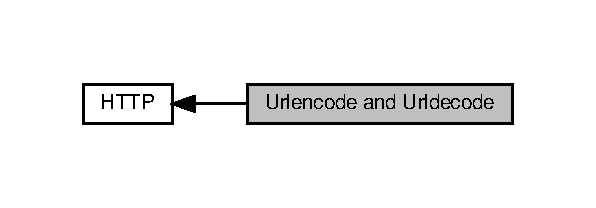
\includegraphics[width=286pt]{group__urlendec}
\end{center}
\end{figure}
\subsection*{Functions}
\begin{DoxyCompactItemize}
\item 
L\+W\+S\+\_\+\+V\+I\+S\+I\+B\+LE L\+W\+S\+\_\+\+E\+X\+T\+E\+RN const char $\ast$ \hyperlink{group__urlendec_gabc2888476e50e001c875c1a8abf455b7}{lws\+\_\+urlencode} (char $\ast$escaped, const char $\ast$string, int len)
\item 
L\+W\+S\+\_\+\+V\+I\+S\+I\+B\+LE L\+W\+S\+\_\+\+E\+X\+T\+E\+RN int \hyperlink{group__urlendec_gaa373a9c16acdd96c395af61ab915ece3}{lws\+\_\+urldecode} (char $\ast$string, const char $\ast$escaped, int len)
\end{DoxyCompactItemize}


\subsection{Detailed Description}
\subsubsection*{H\+T\+ML chunked Substitution}

A\+P\+Is for receiving chunks of text, replacing a set of variable names via a callback, and then prepending and appending H\+T\+ML chunked encoding headers. 

\subsection{Function Documentation}
\mbox{\Hypertarget{group__urlendec_gaa373a9c16acdd96c395af61ab915ece3}\label{group__urlendec_gaa373a9c16acdd96c395af61ab915ece3}} 
\index{Urlencode and Urldecode@{Urlencode and Urldecode}!lws\+\_\+urldecode@{lws\+\_\+urldecode}}
\index{lws\+\_\+urldecode@{lws\+\_\+urldecode}!Urlencode and Urldecode@{Urlencode and Urldecode}}
\subsubsection{\texorpdfstring{lws\+\_\+urldecode()}{lws\_urldecode()}}
{\footnotesize\ttfamily L\+W\+S\+\_\+\+V\+I\+S\+I\+B\+LE L\+W\+S\+\_\+\+E\+X\+T\+E\+RN int lws\+\_\+urldecode (\begin{DoxyParamCaption}\item[{char $\ast$}]{string,  }\item[{const char $\ast$}]{escaped,  }\item[{int}]{len }\end{DoxyParamCaption})}

\hyperlink{group__urlendec_gaa373a9c16acdd96c395af61ab915ece3}{lws\+\_\+urldecode()} -\/ like strncpy but with urldecoding


\begin{DoxyParams}{Parameters}
{\em string} & output buffer \\
\hline
{\em escaped} & input buffer (\textquotesingle{}\textbackslash{}0\textquotesingle{} terminated) \\
\hline
{\em len} & output buffer max length\\
\hline
\end{DoxyParams}
This is only useful for \textquotesingle{}\textbackslash{}0\textquotesingle{} terminated strings

Since urldecoding only shrinks the output string, it is possible to do it in-\/place, ie, string == escaped

Returns 0 if completed OK or nonzero for urldecode violation (non-\/hex chars where hex required, etc)

\hyperlink{group__urlendec_gaa373a9c16acdd96c395af61ab915ece3}{lws\+\_\+urldecode()} -\/ like strncpy but with urldecoding


\begin{DoxyParams}{Parameters}
{\em string} & output buffer \\
\hline
{\em escaped} & input buffer (\textquotesingle{}\textbackslash{}0\textquotesingle{} terminated) \\
\hline
{\em len} & output buffer max length\\
\hline
\end{DoxyParams}
This is only useful for \textquotesingle{}\textbackslash{}0\textquotesingle{} terminated strings

Since urldecoding only shrinks the output string, it is possible to do it in-\/place, ie, string == escaped \mbox{\Hypertarget{group__urlendec_gabc2888476e50e001c875c1a8abf455b7}\label{group__urlendec_gabc2888476e50e001c875c1a8abf455b7}} 
\index{Urlencode and Urldecode@{Urlencode and Urldecode}!lws\+\_\+urlencode@{lws\+\_\+urlencode}}
\index{lws\+\_\+urlencode@{lws\+\_\+urlencode}!Urlencode and Urldecode@{Urlencode and Urldecode}}
\subsubsection{\texorpdfstring{lws\+\_\+urlencode()}{lws\_urlencode()}}
{\footnotesize\ttfamily L\+W\+S\+\_\+\+V\+I\+S\+I\+B\+LE L\+W\+S\+\_\+\+E\+X\+T\+E\+RN const char$\ast$ lws\+\_\+urlencode (\begin{DoxyParamCaption}\item[{char $\ast$}]{escaped,  }\item[{const char $\ast$}]{string,  }\item[{int}]{len }\end{DoxyParamCaption})}

\hyperlink{group__urlendec_gabc2888476e50e001c875c1a8abf455b7}{lws\+\_\+urlencode()} -\/ like strncpy but with urlencoding


\begin{DoxyParams}{Parameters}
{\em escaped} & output buffer \\
\hline
{\em string} & input buffer (\textquotesingle{}/0\textquotesingle{} terminated) \\
\hline
{\em len} & output buffer max length\\
\hline
\end{DoxyParams}
Because urlencoding expands the output string, it\textquotesingle{}s not possible to do it in-\/place, ie, with escaped == string 
\hypertarget{group__pur}{}\section{Sanitize / purify S\+QL and J\+S\+ON helpers}
\label{group__pur}\index{Sanitize / purify S\+Q\+L and J\+S\+O\+N helpers@{Sanitize / purify S\+Q\+L and J\+S\+O\+N helpers}}
\subsection*{Functions}
\begin{DoxyCompactItemize}
\item 
L\+W\+S\+\_\+\+V\+I\+S\+I\+B\+LE L\+W\+S\+\_\+\+E\+X\+T\+E\+RN const char $\ast$ \hyperlink{group__pur_ga64d6a276bd9258e06b30152bc902a146}{lws\+\_\+sql\+\_\+purify} (char $\ast$escaped, const char $\ast$string, int len)
\item 
L\+W\+S\+\_\+\+V\+I\+S\+I\+B\+LE L\+W\+S\+\_\+\+E\+X\+T\+E\+RN const char $\ast$ \hyperlink{group__pur_ga0375328c87629b345fe8c84f2dc80b81}{lws\+\_\+json\+\_\+purify} (char $\ast$escaped, const char $\ast$string, int len)
\end{DoxyCompactItemize}


\subsection{Detailed Description}
\subsubsection*{Sanitize / purify S\+QL and J\+S\+ON helpers}

A\+P\+Is for escaping untrusted J\+S\+ON and S\+QL safely before use 

\subsection{Function Documentation}
\mbox{\Hypertarget{group__pur_ga0375328c87629b345fe8c84f2dc80b81}\label{group__pur_ga0375328c87629b345fe8c84f2dc80b81}} 
\index{Sanitize / purify S\+Q\+L and J\+S\+O\+N helpers@{Sanitize / purify S\+Q\+L and J\+S\+O\+N helpers}!lws\+\_\+json\+\_\+purify@{lws\+\_\+json\+\_\+purify}}
\index{lws\+\_\+json\+\_\+purify@{lws\+\_\+json\+\_\+purify}!Sanitize / purify S\+Q\+L and J\+S\+O\+N helpers@{Sanitize / purify S\+Q\+L and J\+S\+O\+N helpers}}
\subsubsection{\texorpdfstring{lws\+\_\+json\+\_\+purify()}{lws\_json\_purify()}}
{\footnotesize\ttfamily L\+W\+S\+\_\+\+V\+I\+S\+I\+B\+LE L\+W\+S\+\_\+\+E\+X\+T\+E\+RN const char $\ast$ lws\+\_\+json\+\_\+purify (\begin{DoxyParamCaption}\item[{char $\ast$}]{escaped,  }\item[{const char $\ast$}]{string,  }\item[{int}]{len }\end{DoxyParamCaption})}

\hyperlink{group__pur_ga0375328c87629b345fe8c84f2dc80b81}{lws\+\_\+json\+\_\+purify()} -\/ like strncpy but with escaping for json chars


\begin{DoxyParams}{Parameters}
{\em escaped} & output buffer \\
\hline
{\em string} & input buffer (\textquotesingle{}/0\textquotesingle{} terminated) \\
\hline
{\em len} & output buffer max length\\
\hline
\end{DoxyParams}
Because escaping expands the output string, it\textquotesingle{}s not possible to do it in-\/place, ie, with escaped == string \mbox{\Hypertarget{group__pur_ga64d6a276bd9258e06b30152bc902a146}\label{group__pur_ga64d6a276bd9258e06b30152bc902a146}} 
\index{Sanitize / purify S\+Q\+L and J\+S\+O\+N helpers@{Sanitize / purify S\+Q\+L and J\+S\+O\+N helpers}!lws\+\_\+sql\+\_\+purify@{lws\+\_\+sql\+\_\+purify}}
\index{lws\+\_\+sql\+\_\+purify@{lws\+\_\+sql\+\_\+purify}!Sanitize / purify S\+Q\+L and J\+S\+O\+N helpers@{Sanitize / purify S\+Q\+L and J\+S\+O\+N helpers}}
\subsubsection{\texorpdfstring{lws\+\_\+sql\+\_\+purify()}{lws\_sql\_purify()}}
{\footnotesize\ttfamily L\+W\+S\+\_\+\+V\+I\+S\+I\+B\+LE L\+W\+S\+\_\+\+E\+X\+T\+E\+RN const char $\ast$ lws\+\_\+sql\+\_\+purify (\begin{DoxyParamCaption}\item[{char $\ast$}]{escaped,  }\item[{const char $\ast$}]{string,  }\item[{int}]{len }\end{DoxyParamCaption})}

\hyperlink{group__pur_ga64d6a276bd9258e06b30152bc902a146}{lws\+\_\+sql\+\_\+purify()} -\/ like strncpy but with escaping for sql quotes


\begin{DoxyParams}{Parameters}
{\em escaped} & output buffer \\
\hline
{\em string} & input buffer (\textquotesingle{}/0\textquotesingle{} terminated) \\
\hline
{\em len} & output buffer max length\\
\hline
\end{DoxyParams}
Because escaping expands the output string, it\textquotesingle{}s not possible to do it in-\/place, ie, with escaped == string 
\hypertarget{group__ev}{}\section{libev helpers}
\label{group__ev}\index{libev helpers@{libev helpers}}
\subsubsection*{libev helpers}

A\+P\+Is specific to libev event loop itegration 
\hypertarget{group__uv}{}\section{libuv helpers}
\label{group__uv}\index{libuv helpers@{libuv helpers}}
\subsection*{Functions}
\begin{DoxyCompactItemize}
\item 
\mbox{\Hypertarget{group__uv_ga99099e045993383f251a8026e1e40414}\label{group__uv_ga99099e045993383f251a8026e1e40414}} 
L\+W\+S\+\_\+\+V\+I\+S\+I\+B\+LE L\+W\+S\+\_\+\+E\+X\+T\+E\+RN int {\bfseries lws\+\_\+uv\+\_\+sigint\+\_\+cfg} (struct \hyperlink{structlws__context}{lws\+\_\+context} $\ast$context, int use\+\_\+uv\+\_\+sigint, uv\+\_\+signal\+\_\+cb cb)
\item 
\mbox{\Hypertarget{group__uv_ga097c89497824d4de225a85a00661fc89}\label{group__uv_ga097c89497824d4de225a85a00661fc89}} 
L\+W\+S\+\_\+\+V\+I\+S\+I\+B\+LE L\+W\+S\+\_\+\+E\+X\+T\+E\+RN void {\bfseries lws\+\_\+libuv\+\_\+run} (const struct \hyperlink{structlws__context}{lws\+\_\+context} $\ast$context, int tsi)
\item 
\mbox{\Hypertarget{group__uv_ga3c75cd6ec3f80fc0a0c8ead4c4e71a15}\label{group__uv_ga3c75cd6ec3f80fc0a0c8ead4c4e71a15}} 
L\+W\+S\+\_\+\+V\+I\+S\+I\+B\+LE L\+W\+S\+\_\+\+E\+X\+T\+E\+RN void {\bfseries lws\+\_\+libuv\+\_\+stop} (struct \hyperlink{structlws__context}{lws\+\_\+context} $\ast$context)
\item 
\mbox{\Hypertarget{group__uv_gaa17758e1f852017a2271d8fb3e9305aa}\label{group__uv_gaa17758e1f852017a2271d8fb3e9305aa}} 
L\+W\+S\+\_\+\+V\+I\+S\+I\+B\+LE L\+W\+S\+\_\+\+E\+X\+T\+E\+RN void {\bfseries lws\+\_\+libuv\+\_\+stop\+\_\+without\+\_\+kill} (const struct \hyperlink{structlws__context}{lws\+\_\+context} $\ast$context, int tsi)
\item 
\mbox{\Hypertarget{group__uv_gad85ce3bfc53ff754988d36bf5de39e21}\label{group__uv_gad85ce3bfc53ff754988d36bf5de39e21}} 
L\+W\+S\+\_\+\+V\+I\+S\+I\+B\+LE L\+W\+S\+\_\+\+E\+X\+T\+E\+RN int {\bfseries lws\+\_\+uv\+\_\+initloop} (struct \hyperlink{structlws__context}{lws\+\_\+context} $\ast$context, \hyperlink{structuv__loop__s}{uv\+\_\+loop\+\_\+t} $\ast$loop, int tsi)
\item 
\mbox{\Hypertarget{group__uv_gab7e95992dbf69808cb684a5d51e57214}\label{group__uv_gab7e95992dbf69808cb684a5d51e57214}} 
L\+W\+S\+\_\+\+V\+I\+S\+I\+B\+LE L\+W\+S\+\_\+\+E\+X\+T\+E\+RN \hyperlink{structuv__loop__s}{uv\+\_\+loop\+\_\+t} $\ast$ {\bfseries lws\+\_\+uv\+\_\+getloop} (struct \hyperlink{structlws__context}{lws\+\_\+context} $\ast$context, int tsi)
\item 
\mbox{\Hypertarget{group__uv_gac5f60dba13a45e5d554b4fb7df7b9610}\label{group__uv_gac5f60dba13a45e5d554b4fb7df7b9610}} 
L\+W\+S\+\_\+\+V\+I\+S\+I\+B\+LE L\+W\+S\+\_\+\+E\+X\+T\+E\+RN void {\bfseries lws\+\_\+uv\+\_\+sigint\+\_\+cb} (\hyperlink{structuv__signal__s}{uv\+\_\+signal\+\_\+t} $\ast$watcher, int signum)
\item 
\mbox{\Hypertarget{group__uv_ga45608b26a61a0dae91048e73c5d34f6d}\label{group__uv_ga45608b26a61a0dae91048e73c5d34f6d}} 
L\+W\+S\+\_\+\+V\+I\+S\+I\+B\+LE L\+W\+S\+\_\+\+E\+X\+T\+E\+RN void {\bfseries lws\+\_\+close\+\_\+all\+\_\+handles\+\_\+in\+\_\+loop} (\hyperlink{structuv__loop__s}{uv\+\_\+loop\+\_\+t} $\ast$loop)
\end{DoxyCompactItemize}


\subsection{Detailed Description}
\subsubsection*{libuv helpers}

A\+P\+Is specific to libuv event loop itegration 
\hypertarget{group__event}{}\section{libevent helpers}
\label{group__event}\index{libevent helpers@{libevent helpers}}
\subsubsection*{libevent helpers}

A\+P\+Is specific to libevent event loop itegration 
\hypertarget{group__timeout}{}\section{Connection timeouts}
\label{group__timeout}\index{Connection timeouts@{Connection timeouts}}
\subsection*{Macros}
\begin{DoxyCompactItemize}
\item 
\#define \hyperlink{group__timeout_ga6a53a9a771c08417ffe75c953b58f015}{L\+W\+S\+\_\+\+T\+O\+\_\+\+K\+I\+L\+L\+\_\+\+A\+S\+Y\+NC}~-\/1
\item 
\#define \hyperlink{group__timeout_ga3cef438d5bbd20a33afbec8e29a0b9a6}{L\+W\+S\+\_\+\+T\+O\+\_\+\+K\+I\+L\+L\+\_\+\+S\+Y\+NC}~-\/2
\item 
\#define \hyperlink{group__timeout_ga6a53a9a771c08417ffe75c953b58f015}{L\+W\+S\+\_\+\+T\+O\+\_\+\+K\+I\+L\+L\+\_\+\+A\+S\+Y\+NC}~-\/1
\item 
\#define \hyperlink{group__timeout_ga3cef438d5bbd20a33afbec8e29a0b9a6}{L\+W\+S\+\_\+\+T\+O\+\_\+\+K\+I\+L\+L\+\_\+\+S\+Y\+NC}~-\/2
\item 
\#define \hyperlink{group__timeout_ga6a53a9a771c08417ffe75c953b58f015}{L\+W\+S\+\_\+\+T\+O\+\_\+\+K\+I\+L\+L\+\_\+\+A\+S\+Y\+NC}~-\/1
\item 
\#define \hyperlink{group__timeout_ga3cef438d5bbd20a33afbec8e29a0b9a6}{L\+W\+S\+\_\+\+T\+O\+\_\+\+K\+I\+L\+L\+\_\+\+S\+Y\+NC}~-\/2
\item 
\#define \hyperlink{group__timeout_ga6a53a9a771c08417ffe75c953b58f015}{L\+W\+S\+\_\+\+T\+O\+\_\+\+K\+I\+L\+L\+\_\+\+A\+S\+Y\+NC}~-\/1
\item 
\#define \hyperlink{group__timeout_ga3cef438d5bbd20a33afbec8e29a0b9a6}{L\+W\+S\+\_\+\+T\+O\+\_\+\+K\+I\+L\+L\+\_\+\+S\+Y\+NC}~-\/2
\item 
\#define \hyperlink{group__timeout_ga6a53a9a771c08417ffe75c953b58f015}{L\+W\+S\+\_\+\+T\+O\+\_\+\+K\+I\+L\+L\+\_\+\+A\+S\+Y\+NC}~-\/1
\item 
\#define \hyperlink{group__timeout_ga3cef438d5bbd20a33afbec8e29a0b9a6}{L\+W\+S\+\_\+\+T\+O\+\_\+\+K\+I\+L\+L\+\_\+\+S\+Y\+NC}~-\/2
\item 
\#define \hyperlink{group__timeout_ga6a53a9a771c08417ffe75c953b58f015}{L\+W\+S\+\_\+\+T\+O\+\_\+\+K\+I\+L\+L\+\_\+\+A\+S\+Y\+NC}~-\/1
\item 
\#define \hyperlink{group__timeout_ga3cef438d5bbd20a33afbec8e29a0b9a6}{L\+W\+S\+\_\+\+T\+O\+\_\+\+K\+I\+L\+L\+\_\+\+S\+Y\+NC}~-\/2
\end{DoxyCompactItemize}
\subsection*{Enumerations}
\begin{DoxyCompactItemize}
\item 
\mbox{\Hypertarget{group__timeout_ga2c0aa4b9c3c55bae7b35cbfac3246c87}\label{group__timeout_ga2c0aa4b9c3c55bae7b35cbfac3246c87}} 
enum {\bfseries pending\+\_\+timeout} \{ \newline
{\bfseries N\+O\+\_\+\+P\+E\+N\+D\+I\+N\+G\+\_\+\+T\+I\+M\+E\+O\+UT} = 0, 
{\bfseries P\+E\+N\+D\+I\+N\+G\+\_\+\+T\+I\+M\+E\+O\+U\+T\+\_\+\+A\+W\+A\+I\+T\+I\+N\+G\+\_\+\+P\+R\+O\+X\+Y\+\_\+\+R\+E\+S\+P\+O\+N\+SE} = 1, 
{\bfseries P\+E\+N\+D\+I\+N\+G\+\_\+\+T\+I\+M\+E\+O\+U\+T\+\_\+\+A\+W\+A\+I\+T\+I\+N\+G\+\_\+\+C\+O\+N\+N\+E\+C\+T\+\_\+\+R\+E\+S\+P\+O\+N\+SE} = 2, 
{\bfseries P\+E\+N\+D\+I\+N\+G\+\_\+\+T\+I\+M\+E\+O\+U\+T\+\_\+\+E\+S\+T\+A\+B\+L\+I\+S\+H\+\_\+\+W\+I\+T\+H\+\_\+\+S\+E\+R\+V\+ER} = 3, 
\newline
{\bfseries P\+E\+N\+D\+I\+N\+G\+\_\+\+T\+I\+M\+E\+O\+U\+T\+\_\+\+A\+W\+A\+I\+T\+I\+N\+G\+\_\+\+S\+E\+R\+V\+E\+R\+\_\+\+R\+E\+S\+P\+O\+N\+SE} = 4, 
{\bfseries P\+E\+N\+D\+I\+N\+G\+\_\+\+T\+I\+M\+E\+O\+U\+T\+\_\+\+A\+W\+A\+I\+T\+I\+N\+G\+\_\+\+P\+I\+NG} = 5, 
{\bfseries P\+E\+N\+D\+I\+N\+G\+\_\+\+T\+I\+M\+E\+O\+U\+T\+\_\+\+C\+L\+O\+S\+E\+\_\+\+A\+CK} = 6, 
{\bfseries P\+E\+N\+D\+I\+N\+G\+\_\+\+T\+I\+M\+E\+O\+U\+T\+\_\+\+A\+W\+A\+I\+T\+I\+N\+G\+\_\+\+E\+X\+T\+E\+N\+S\+I\+O\+N\+\_\+\+C\+O\+N\+N\+E\+C\+T\+\_\+\+R\+E\+S\+P\+O\+N\+SE} = 7, 
\newline
{\bfseries P\+E\+N\+D\+I\+N\+G\+\_\+\+T\+I\+M\+E\+O\+U\+T\+\_\+\+S\+E\+N\+T\+\_\+\+C\+L\+I\+E\+N\+T\+\_\+\+H\+A\+N\+D\+S\+H\+A\+KE} = 8, 
{\bfseries P\+E\+N\+D\+I\+N\+G\+\_\+\+T\+I\+M\+E\+O\+U\+T\+\_\+\+S\+S\+L\+\_\+\+A\+C\+C\+E\+PT} = 9, 
{\bfseries P\+E\+N\+D\+I\+N\+G\+\_\+\+T\+I\+M\+E\+O\+U\+T\+\_\+\+H\+T\+T\+P\+\_\+\+C\+O\+N\+T\+E\+NT} = 10, 
{\bfseries P\+E\+N\+D\+I\+N\+G\+\_\+\+T\+I\+M\+E\+O\+U\+T\+\_\+\+A\+W\+A\+I\+T\+I\+N\+G\+\_\+\+C\+L\+I\+E\+N\+T\+\_\+\+H\+S\+\_\+\+S\+E\+ND} = 11, 
\newline
{\bfseries P\+E\+N\+D\+I\+N\+G\+\_\+\+F\+L\+U\+S\+H\+\_\+\+S\+T\+O\+R\+E\+D\+\_\+\+S\+E\+N\+D\+\_\+\+B\+E\+F\+O\+R\+E\+\_\+\+C\+L\+O\+SE} = 12, 
{\bfseries N\+O\+\_\+\+P\+E\+N\+D\+I\+N\+G\+\_\+\+T\+I\+M\+E\+O\+UT} = 0, 
{\bfseries P\+E\+N\+D\+I\+N\+G\+\_\+\+T\+I\+M\+E\+O\+U\+T\+\_\+\+A\+W\+A\+I\+T\+I\+N\+G\+\_\+\+P\+R\+O\+X\+Y\+\_\+\+R\+E\+S\+P\+O\+N\+SE} = 1, 
{\bfseries P\+E\+N\+D\+I\+N\+G\+\_\+\+T\+I\+M\+E\+O\+U\+T\+\_\+\+A\+W\+A\+I\+T\+I\+N\+G\+\_\+\+C\+O\+N\+N\+E\+C\+T\+\_\+\+R\+E\+S\+P\+O\+N\+SE} = 2, 
\newline
{\bfseries P\+E\+N\+D\+I\+N\+G\+\_\+\+T\+I\+M\+E\+O\+U\+T\+\_\+\+E\+S\+T\+A\+B\+L\+I\+S\+H\+\_\+\+W\+I\+T\+H\+\_\+\+S\+E\+R\+V\+ER} = 3, 
{\bfseries P\+E\+N\+D\+I\+N\+G\+\_\+\+T\+I\+M\+E\+O\+U\+T\+\_\+\+A\+W\+A\+I\+T\+I\+N\+G\+\_\+\+S\+E\+R\+V\+E\+R\+\_\+\+R\+E\+S\+P\+O\+N\+SE} = 4, 
{\bfseries P\+E\+N\+D\+I\+N\+G\+\_\+\+T\+I\+M\+E\+O\+U\+T\+\_\+\+A\+W\+A\+I\+T\+I\+N\+G\+\_\+\+P\+I\+NG} = 5, 
{\bfseries P\+E\+N\+D\+I\+N\+G\+\_\+\+T\+I\+M\+E\+O\+U\+T\+\_\+\+C\+L\+O\+S\+E\+\_\+\+A\+CK} = 6, 
\newline
{\bfseries P\+E\+N\+D\+I\+N\+G\+\_\+\+T\+I\+M\+E\+O\+U\+T\+\_\+\+A\+W\+A\+I\+T\+I\+N\+G\+\_\+\+E\+X\+T\+E\+N\+S\+I\+O\+N\+\_\+\+C\+O\+N\+N\+E\+C\+T\+\_\+\+R\+E\+S\+P\+O\+N\+SE} = 7, 
{\bfseries P\+E\+N\+D\+I\+N\+G\+\_\+\+T\+I\+M\+E\+O\+U\+T\+\_\+\+S\+E\+N\+T\+\_\+\+C\+L\+I\+E\+N\+T\+\_\+\+H\+A\+N\+D\+S\+H\+A\+KE} = 8, 
{\bfseries P\+E\+N\+D\+I\+N\+G\+\_\+\+T\+I\+M\+E\+O\+U\+T\+\_\+\+S\+S\+L\+\_\+\+A\+C\+C\+E\+PT} = 9, 
{\bfseries P\+E\+N\+D\+I\+N\+G\+\_\+\+T\+I\+M\+E\+O\+U\+T\+\_\+\+H\+T\+T\+P\+\_\+\+C\+O\+N\+T\+E\+NT} = 10, 
\newline
{\bfseries P\+E\+N\+D\+I\+N\+G\+\_\+\+T\+I\+M\+E\+O\+U\+T\+\_\+\+A\+W\+A\+I\+T\+I\+N\+G\+\_\+\+C\+L\+I\+E\+N\+T\+\_\+\+H\+S\+\_\+\+S\+E\+ND} = 11, 
{\bfseries P\+E\+N\+D\+I\+N\+G\+\_\+\+F\+L\+U\+S\+H\+\_\+\+S\+T\+O\+R\+E\+D\+\_\+\+S\+E\+N\+D\+\_\+\+B\+E\+F\+O\+R\+E\+\_\+\+C\+L\+O\+SE} = 12, 
{\bfseries N\+O\+\_\+\+P\+E\+N\+D\+I\+N\+G\+\_\+\+T\+I\+M\+E\+O\+UT} = 0, 
{\bfseries P\+E\+N\+D\+I\+N\+G\+\_\+\+T\+I\+M\+E\+O\+U\+T\+\_\+\+A\+W\+A\+I\+T\+I\+N\+G\+\_\+\+P\+R\+O\+X\+Y\+\_\+\+R\+E\+S\+P\+O\+N\+SE} = 1, 
\newline
{\bfseries P\+E\+N\+D\+I\+N\+G\+\_\+\+T\+I\+M\+E\+O\+U\+T\+\_\+\+A\+W\+A\+I\+T\+I\+N\+G\+\_\+\+C\+O\+N\+N\+E\+C\+T\+\_\+\+R\+E\+S\+P\+O\+N\+SE} = 2, 
{\bfseries P\+E\+N\+D\+I\+N\+G\+\_\+\+T\+I\+M\+E\+O\+U\+T\+\_\+\+E\+S\+T\+A\+B\+L\+I\+S\+H\+\_\+\+W\+I\+T\+H\+\_\+\+S\+E\+R\+V\+ER} = 3, 
{\bfseries P\+E\+N\+D\+I\+N\+G\+\_\+\+T\+I\+M\+E\+O\+U\+T\+\_\+\+A\+W\+A\+I\+T\+I\+N\+G\+\_\+\+S\+E\+R\+V\+E\+R\+\_\+\+R\+E\+S\+P\+O\+N\+SE} = 4, 
{\bfseries P\+E\+N\+D\+I\+N\+G\+\_\+\+T\+I\+M\+E\+O\+U\+T\+\_\+\+A\+W\+A\+I\+T\+I\+N\+G\+\_\+\+P\+I\+NG} = 5, 
\newline
{\bfseries P\+E\+N\+D\+I\+N\+G\+\_\+\+T\+I\+M\+E\+O\+U\+T\+\_\+\+C\+L\+O\+S\+E\+\_\+\+A\+CK} = 6, 
{\bfseries P\+E\+N\+D\+I\+N\+G\+\_\+\+T\+I\+M\+E\+O\+U\+T\+\_\+\+A\+W\+A\+I\+T\+I\+N\+G\+\_\+\+E\+X\+T\+E\+N\+S\+I\+O\+N\+\_\+\+C\+O\+N\+N\+E\+C\+T\+\_\+\+R\+E\+S\+P\+O\+N\+SE} = 7, 
{\bfseries P\+E\+N\+D\+I\+N\+G\+\_\+\+T\+I\+M\+E\+O\+U\+T\+\_\+\+S\+E\+N\+T\+\_\+\+C\+L\+I\+E\+N\+T\+\_\+\+H\+A\+N\+D\+S\+H\+A\+KE} = 8, 
{\bfseries P\+E\+N\+D\+I\+N\+G\+\_\+\+T\+I\+M\+E\+O\+U\+T\+\_\+\+S\+S\+L\+\_\+\+A\+C\+C\+E\+PT} = 9, 
\newline
{\bfseries P\+E\+N\+D\+I\+N\+G\+\_\+\+T\+I\+M\+E\+O\+U\+T\+\_\+\+H\+T\+T\+P\+\_\+\+C\+O\+N\+T\+E\+NT} = 10, 
{\bfseries P\+E\+N\+D\+I\+N\+G\+\_\+\+T\+I\+M\+E\+O\+U\+T\+\_\+\+A\+W\+A\+I\+T\+I\+N\+G\+\_\+\+C\+L\+I\+E\+N\+T\+\_\+\+H\+S\+\_\+\+S\+E\+ND} = 11, 
{\bfseries P\+E\+N\+D\+I\+N\+G\+\_\+\+F\+L\+U\+S\+H\+\_\+\+S\+T\+O\+R\+E\+D\+\_\+\+S\+E\+N\+D\+\_\+\+B\+E\+F\+O\+R\+E\+\_\+\+C\+L\+O\+SE} = 12, 
{\bfseries N\+O\+\_\+\+P\+E\+N\+D\+I\+N\+G\+\_\+\+T\+I\+M\+E\+O\+UT} = 0, 
\newline
{\bfseries P\+E\+N\+D\+I\+N\+G\+\_\+\+T\+I\+M\+E\+O\+U\+T\+\_\+\+A\+W\+A\+I\+T\+I\+N\+G\+\_\+\+P\+R\+O\+X\+Y\+\_\+\+R\+E\+S\+P\+O\+N\+SE} = 1, 
{\bfseries P\+E\+N\+D\+I\+N\+G\+\_\+\+T\+I\+M\+E\+O\+U\+T\+\_\+\+A\+W\+A\+I\+T\+I\+N\+G\+\_\+\+C\+O\+N\+N\+E\+C\+T\+\_\+\+R\+E\+S\+P\+O\+N\+SE} = 2, 
{\bfseries P\+E\+N\+D\+I\+N\+G\+\_\+\+T\+I\+M\+E\+O\+U\+T\+\_\+\+E\+S\+T\+A\+B\+L\+I\+S\+H\+\_\+\+W\+I\+T\+H\+\_\+\+S\+E\+R\+V\+ER} = 3, 
{\bfseries P\+E\+N\+D\+I\+N\+G\+\_\+\+T\+I\+M\+E\+O\+U\+T\+\_\+\+A\+W\+A\+I\+T\+I\+N\+G\+\_\+\+S\+E\+R\+V\+E\+R\+\_\+\+R\+E\+S\+P\+O\+N\+SE} = 4, 
\newline
{\bfseries P\+E\+N\+D\+I\+N\+G\+\_\+\+T\+I\+M\+E\+O\+U\+T\+\_\+\+A\+W\+A\+I\+T\+I\+N\+G\+\_\+\+P\+I\+NG} = 5, 
{\bfseries P\+E\+N\+D\+I\+N\+G\+\_\+\+T\+I\+M\+E\+O\+U\+T\+\_\+\+C\+L\+O\+S\+E\+\_\+\+A\+CK} = 6, 
{\bfseries P\+E\+N\+D\+I\+N\+G\+\_\+\+T\+I\+M\+E\+O\+U\+T\+\_\+\+A\+W\+A\+I\+T\+I\+N\+G\+\_\+\+E\+X\+T\+E\+N\+S\+I\+O\+N\+\_\+\+C\+O\+N\+N\+E\+C\+T\+\_\+\+R\+E\+S\+P\+O\+N\+SE} = 7, 
{\bfseries P\+E\+N\+D\+I\+N\+G\+\_\+\+T\+I\+M\+E\+O\+U\+T\+\_\+\+S\+E\+N\+T\+\_\+\+C\+L\+I\+E\+N\+T\+\_\+\+H\+A\+N\+D\+S\+H\+A\+KE} = 8, 
\newline
{\bfseries P\+E\+N\+D\+I\+N\+G\+\_\+\+T\+I\+M\+E\+O\+U\+T\+\_\+\+S\+S\+L\+\_\+\+A\+C\+C\+E\+PT} = 9, 
{\bfseries P\+E\+N\+D\+I\+N\+G\+\_\+\+T\+I\+M\+E\+O\+U\+T\+\_\+\+H\+T\+T\+P\+\_\+\+C\+O\+N\+T\+E\+NT} = 10, 
{\bfseries P\+E\+N\+D\+I\+N\+G\+\_\+\+T\+I\+M\+E\+O\+U\+T\+\_\+\+A\+W\+A\+I\+T\+I\+N\+G\+\_\+\+C\+L\+I\+E\+N\+T\+\_\+\+H\+S\+\_\+\+S\+E\+ND} = 11, 
{\bfseries P\+E\+N\+D\+I\+N\+G\+\_\+\+F\+L\+U\+S\+H\+\_\+\+S\+T\+O\+R\+E\+D\+\_\+\+S\+E\+N\+D\+\_\+\+B\+E\+F\+O\+R\+E\+\_\+\+C\+L\+O\+SE} = 12, 
\newline
{\bfseries N\+O\+\_\+\+P\+E\+N\+D\+I\+N\+G\+\_\+\+T\+I\+M\+E\+O\+UT} = 0, 
{\bfseries P\+E\+N\+D\+I\+N\+G\+\_\+\+T\+I\+M\+E\+O\+U\+T\+\_\+\+A\+W\+A\+I\+T\+I\+N\+G\+\_\+\+P\+R\+O\+X\+Y\+\_\+\+R\+E\+S\+P\+O\+N\+SE} = 1, 
{\bfseries P\+E\+N\+D\+I\+N\+G\+\_\+\+T\+I\+M\+E\+O\+U\+T\+\_\+\+A\+W\+A\+I\+T\+I\+N\+G\+\_\+\+C\+O\+N\+N\+E\+C\+T\+\_\+\+R\+E\+S\+P\+O\+N\+SE} = 2, 
{\bfseries P\+E\+N\+D\+I\+N\+G\+\_\+\+T\+I\+M\+E\+O\+U\+T\+\_\+\+E\+S\+T\+A\+B\+L\+I\+S\+H\+\_\+\+W\+I\+T\+H\+\_\+\+S\+E\+R\+V\+ER} = 3, 
\newline
{\bfseries P\+E\+N\+D\+I\+N\+G\+\_\+\+T\+I\+M\+E\+O\+U\+T\+\_\+\+A\+W\+A\+I\+T\+I\+N\+G\+\_\+\+S\+E\+R\+V\+E\+R\+\_\+\+R\+E\+S\+P\+O\+N\+SE} = 4, 
{\bfseries P\+E\+N\+D\+I\+N\+G\+\_\+\+T\+I\+M\+E\+O\+U\+T\+\_\+\+A\+W\+A\+I\+T\+I\+N\+G\+\_\+\+P\+I\+NG} = 5, 
{\bfseries P\+E\+N\+D\+I\+N\+G\+\_\+\+T\+I\+M\+E\+O\+U\+T\+\_\+\+C\+L\+O\+S\+E\+\_\+\+A\+CK} = 6, 
{\bfseries P\+E\+N\+D\+I\+N\+G\+\_\+\+T\+I\+M\+E\+O\+U\+T\+\_\+\+A\+W\+A\+I\+T\+I\+N\+G\+\_\+\+E\+X\+T\+E\+N\+S\+I\+O\+N\+\_\+\+C\+O\+N\+N\+E\+C\+T\+\_\+\+R\+E\+S\+P\+O\+N\+SE} = 7, 
\newline
{\bfseries P\+E\+N\+D\+I\+N\+G\+\_\+\+T\+I\+M\+E\+O\+U\+T\+\_\+\+S\+E\+N\+T\+\_\+\+C\+L\+I\+E\+N\+T\+\_\+\+H\+A\+N\+D\+S\+H\+A\+KE} = 8, 
{\bfseries P\+E\+N\+D\+I\+N\+G\+\_\+\+T\+I\+M\+E\+O\+U\+T\+\_\+\+S\+S\+L\+\_\+\+A\+C\+C\+E\+PT} = 9, 
{\bfseries P\+E\+N\+D\+I\+N\+G\+\_\+\+T\+I\+M\+E\+O\+U\+T\+\_\+\+H\+T\+T\+P\+\_\+\+C\+O\+N\+T\+E\+NT} = 10, 
{\bfseries P\+E\+N\+D\+I\+N\+G\+\_\+\+T\+I\+M\+E\+O\+U\+T\+\_\+\+A\+W\+A\+I\+T\+I\+N\+G\+\_\+\+C\+L\+I\+E\+N\+T\+\_\+\+H\+S\+\_\+\+S\+E\+ND} = 11, 
\newline
{\bfseries P\+E\+N\+D\+I\+N\+G\+\_\+\+F\+L\+U\+S\+H\+\_\+\+S\+T\+O\+R\+E\+D\+\_\+\+S\+E\+N\+D\+\_\+\+B\+E\+F\+O\+R\+E\+\_\+\+C\+L\+O\+SE} = 12, 
{\bfseries N\+O\+\_\+\+P\+E\+N\+D\+I\+N\+G\+\_\+\+T\+I\+M\+E\+O\+UT} = 0, 
{\bfseries P\+E\+N\+D\+I\+N\+G\+\_\+\+T\+I\+M\+E\+O\+U\+T\+\_\+\+A\+W\+A\+I\+T\+I\+N\+G\+\_\+\+P\+R\+O\+X\+Y\+\_\+\+R\+E\+S\+P\+O\+N\+SE} = 1, 
{\bfseries P\+E\+N\+D\+I\+N\+G\+\_\+\+T\+I\+M\+E\+O\+U\+T\+\_\+\+A\+W\+A\+I\+T\+I\+N\+G\+\_\+\+C\+O\+N\+N\+E\+C\+T\+\_\+\+R\+E\+S\+P\+O\+N\+SE} = 2, 
\newline
{\bfseries P\+E\+N\+D\+I\+N\+G\+\_\+\+T\+I\+M\+E\+O\+U\+T\+\_\+\+E\+S\+T\+A\+B\+L\+I\+S\+H\+\_\+\+W\+I\+T\+H\+\_\+\+S\+E\+R\+V\+ER} = 3, 
{\bfseries P\+E\+N\+D\+I\+N\+G\+\_\+\+T\+I\+M\+E\+O\+U\+T\+\_\+\+A\+W\+A\+I\+T\+I\+N\+G\+\_\+\+S\+E\+R\+V\+E\+R\+\_\+\+R\+E\+S\+P\+O\+N\+SE} = 4, 
{\bfseries P\+E\+N\+D\+I\+N\+G\+\_\+\+T\+I\+M\+E\+O\+U\+T\+\_\+\+A\+W\+A\+I\+T\+I\+N\+G\+\_\+\+P\+I\+NG} = 5, 
{\bfseries P\+E\+N\+D\+I\+N\+G\+\_\+\+T\+I\+M\+E\+O\+U\+T\+\_\+\+C\+L\+O\+S\+E\+\_\+\+A\+CK} = 6, 
\newline
{\bfseries P\+E\+N\+D\+I\+N\+G\+\_\+\+T\+I\+M\+E\+O\+U\+T\+\_\+\+A\+W\+A\+I\+T\+I\+N\+G\+\_\+\+E\+X\+T\+E\+N\+S\+I\+O\+N\+\_\+\+C\+O\+N\+N\+E\+C\+T\+\_\+\+R\+E\+S\+P\+O\+N\+SE} = 7, 
{\bfseries P\+E\+N\+D\+I\+N\+G\+\_\+\+T\+I\+M\+E\+O\+U\+T\+\_\+\+S\+E\+N\+T\+\_\+\+C\+L\+I\+E\+N\+T\+\_\+\+H\+A\+N\+D\+S\+H\+A\+KE} = 8, 
{\bfseries P\+E\+N\+D\+I\+N\+G\+\_\+\+T\+I\+M\+E\+O\+U\+T\+\_\+\+S\+S\+L\+\_\+\+A\+C\+C\+E\+PT} = 9, 
{\bfseries P\+E\+N\+D\+I\+N\+G\+\_\+\+T\+I\+M\+E\+O\+U\+T\+\_\+\+H\+T\+T\+P\+\_\+\+C\+O\+N\+T\+E\+NT} = 10, 
\newline
{\bfseries P\+E\+N\+D\+I\+N\+G\+\_\+\+T\+I\+M\+E\+O\+U\+T\+\_\+\+A\+W\+A\+I\+T\+I\+N\+G\+\_\+\+C\+L\+I\+E\+N\+T\+\_\+\+H\+S\+\_\+\+S\+E\+ND} = 11, 
{\bfseries P\+E\+N\+D\+I\+N\+G\+\_\+\+F\+L\+U\+S\+H\+\_\+\+S\+T\+O\+R\+E\+D\+\_\+\+S\+E\+N\+D\+\_\+\+B\+E\+F\+O\+R\+E\+\_\+\+C\+L\+O\+SE} = 12, 
{\bfseries N\+O\+\_\+\+P\+E\+N\+D\+I\+N\+G\+\_\+\+T\+I\+M\+E\+O\+UT} = 0, 
{\bfseries P\+E\+N\+D\+I\+N\+G\+\_\+\+T\+I\+M\+E\+O\+U\+T\+\_\+\+A\+W\+A\+I\+T\+I\+N\+G\+\_\+\+P\+R\+O\+X\+Y\+\_\+\+R\+E\+S\+P\+O\+N\+SE} = 1, 
\newline
{\bfseries P\+E\+N\+D\+I\+N\+G\+\_\+\+T\+I\+M\+E\+O\+U\+T\+\_\+\+A\+W\+A\+I\+T\+I\+N\+G\+\_\+\+C\+O\+N\+N\+E\+C\+T\+\_\+\+R\+E\+S\+P\+O\+N\+SE} = 2, 
{\bfseries P\+E\+N\+D\+I\+N\+G\+\_\+\+T\+I\+M\+E\+O\+U\+T\+\_\+\+E\+S\+T\+A\+B\+L\+I\+S\+H\+\_\+\+W\+I\+T\+H\+\_\+\+S\+E\+R\+V\+ER} = 3, 
{\bfseries P\+E\+N\+D\+I\+N\+G\+\_\+\+T\+I\+M\+E\+O\+U\+T\+\_\+\+A\+W\+A\+I\+T\+I\+N\+G\+\_\+\+S\+E\+R\+V\+E\+R\+\_\+\+R\+E\+S\+P\+O\+N\+SE} = 4, 
{\bfseries P\+E\+N\+D\+I\+N\+G\+\_\+\+T\+I\+M\+E\+O\+U\+T\+\_\+\+A\+W\+A\+I\+T\+I\+N\+G\+\_\+\+P\+I\+NG} = 5, 
\newline
{\bfseries P\+E\+N\+D\+I\+N\+G\+\_\+\+T\+I\+M\+E\+O\+U\+T\+\_\+\+C\+L\+O\+S\+E\+\_\+\+A\+CK} = 6, 
{\bfseries P\+E\+N\+D\+I\+N\+G\+\_\+\+T\+I\+M\+E\+O\+U\+T\+\_\+\+A\+W\+A\+I\+T\+I\+N\+G\+\_\+\+E\+X\+T\+E\+N\+S\+I\+O\+N\+\_\+\+C\+O\+N\+N\+E\+C\+T\+\_\+\+R\+E\+S\+P\+O\+N\+SE} = 7, 
{\bfseries P\+E\+N\+D\+I\+N\+G\+\_\+\+T\+I\+M\+E\+O\+U\+T\+\_\+\+S\+E\+N\+T\+\_\+\+C\+L\+I\+E\+N\+T\+\_\+\+H\+A\+N\+D\+S\+H\+A\+KE} = 8, 
{\bfseries P\+E\+N\+D\+I\+N\+G\+\_\+\+T\+I\+M\+E\+O\+U\+T\+\_\+\+S\+S\+L\+\_\+\+A\+C\+C\+E\+PT} = 9, 
\newline
{\bfseries P\+E\+N\+D\+I\+N\+G\+\_\+\+T\+I\+M\+E\+O\+U\+T\+\_\+\+H\+T\+T\+P\+\_\+\+C\+O\+N\+T\+E\+NT} = 10, 
{\bfseries P\+E\+N\+D\+I\+N\+G\+\_\+\+T\+I\+M\+E\+O\+U\+T\+\_\+\+A\+W\+A\+I\+T\+I\+N\+G\+\_\+\+C\+L\+I\+E\+N\+T\+\_\+\+H\+S\+\_\+\+S\+E\+ND} = 11, 
{\bfseries P\+E\+N\+D\+I\+N\+G\+\_\+\+F\+L\+U\+S\+H\+\_\+\+S\+T\+O\+R\+E\+D\+\_\+\+S\+E\+N\+D\+\_\+\+B\+E\+F\+O\+R\+E\+\_\+\+C\+L\+O\+SE} = 12, 
{\bfseries N\+O\+\_\+\+P\+E\+N\+D\+I\+N\+G\+\_\+\+T\+I\+M\+E\+O\+UT} = 0, 
\newline
{\bfseries P\+E\+N\+D\+I\+N\+G\+\_\+\+T\+I\+M\+E\+O\+U\+T\+\_\+\+A\+W\+A\+I\+T\+I\+N\+G\+\_\+\+P\+R\+O\+X\+Y\+\_\+\+R\+E\+S\+P\+O\+N\+SE} = 1, 
{\bfseries P\+E\+N\+D\+I\+N\+G\+\_\+\+T\+I\+M\+E\+O\+U\+T\+\_\+\+A\+W\+A\+I\+T\+I\+N\+G\+\_\+\+C\+O\+N\+N\+E\+C\+T\+\_\+\+R\+E\+S\+P\+O\+N\+SE} = 2, 
{\bfseries P\+E\+N\+D\+I\+N\+G\+\_\+\+T\+I\+M\+E\+O\+U\+T\+\_\+\+E\+S\+T\+A\+B\+L\+I\+S\+H\+\_\+\+W\+I\+T\+H\+\_\+\+S\+E\+R\+V\+ER} = 3, 
{\bfseries P\+E\+N\+D\+I\+N\+G\+\_\+\+T\+I\+M\+E\+O\+U\+T\+\_\+\+A\+W\+A\+I\+T\+I\+N\+G\+\_\+\+S\+E\+R\+V\+E\+R\+\_\+\+R\+E\+S\+P\+O\+N\+SE} = 4, 
\newline
{\bfseries P\+E\+N\+D\+I\+N\+G\+\_\+\+T\+I\+M\+E\+O\+U\+T\+\_\+\+A\+W\+A\+I\+T\+I\+N\+G\+\_\+\+P\+I\+NG} = 5, 
{\bfseries P\+E\+N\+D\+I\+N\+G\+\_\+\+T\+I\+M\+E\+O\+U\+T\+\_\+\+C\+L\+O\+S\+E\+\_\+\+A\+CK} = 6, 
{\bfseries P\+E\+N\+D\+I\+N\+G\+\_\+\+T\+I\+M\+E\+O\+U\+T\+\_\+\+A\+W\+A\+I\+T\+I\+N\+G\+\_\+\+E\+X\+T\+E\+N\+S\+I\+O\+N\+\_\+\+C\+O\+N\+N\+E\+C\+T\+\_\+\+R\+E\+S\+P\+O\+N\+SE} = 7, 
{\bfseries P\+E\+N\+D\+I\+N\+G\+\_\+\+T\+I\+M\+E\+O\+U\+T\+\_\+\+S\+E\+N\+T\+\_\+\+C\+L\+I\+E\+N\+T\+\_\+\+H\+A\+N\+D\+S\+H\+A\+KE} = 8, 
\newline
{\bfseries P\+E\+N\+D\+I\+N\+G\+\_\+\+T\+I\+M\+E\+O\+U\+T\+\_\+\+S\+S\+L\+\_\+\+A\+C\+C\+E\+PT} = 9, 
{\bfseries P\+E\+N\+D\+I\+N\+G\+\_\+\+T\+I\+M\+E\+O\+U\+T\+\_\+\+H\+T\+T\+P\+\_\+\+C\+O\+N\+T\+E\+NT} = 10, 
{\bfseries P\+E\+N\+D\+I\+N\+G\+\_\+\+T\+I\+M\+E\+O\+U\+T\+\_\+\+A\+W\+A\+I\+T\+I\+N\+G\+\_\+\+C\+L\+I\+E\+N\+T\+\_\+\+H\+S\+\_\+\+S\+E\+ND} = 11, 
{\bfseries P\+E\+N\+D\+I\+N\+G\+\_\+\+F\+L\+U\+S\+H\+\_\+\+S\+T\+O\+R\+E\+D\+\_\+\+S\+E\+N\+D\+\_\+\+B\+E\+F\+O\+R\+E\+\_\+\+C\+L\+O\+SE} = 12, 
\newline
{\bfseries N\+O\+\_\+\+P\+E\+N\+D\+I\+N\+G\+\_\+\+T\+I\+M\+E\+O\+UT} = 0, 
{\bfseries P\+E\+N\+D\+I\+N\+G\+\_\+\+T\+I\+M\+E\+O\+U\+T\+\_\+\+A\+W\+A\+I\+T\+I\+N\+G\+\_\+\+P\+R\+O\+X\+Y\+\_\+\+R\+E\+S\+P\+O\+N\+SE} = 1, 
{\bfseries P\+E\+N\+D\+I\+N\+G\+\_\+\+T\+I\+M\+E\+O\+U\+T\+\_\+\+A\+W\+A\+I\+T\+I\+N\+G\+\_\+\+C\+O\+N\+N\+E\+C\+T\+\_\+\+R\+E\+S\+P\+O\+N\+SE} = 2, 
{\bfseries P\+E\+N\+D\+I\+N\+G\+\_\+\+T\+I\+M\+E\+O\+U\+T\+\_\+\+E\+S\+T\+A\+B\+L\+I\+S\+H\+\_\+\+W\+I\+T\+H\+\_\+\+S\+E\+R\+V\+ER} = 3, 
\newline
{\bfseries P\+E\+N\+D\+I\+N\+G\+\_\+\+T\+I\+M\+E\+O\+U\+T\+\_\+\+A\+W\+A\+I\+T\+I\+N\+G\+\_\+\+S\+E\+R\+V\+E\+R\+\_\+\+R\+E\+S\+P\+O\+N\+SE} = 4, 
{\bfseries P\+E\+N\+D\+I\+N\+G\+\_\+\+T\+I\+M\+E\+O\+U\+T\+\_\+\+A\+W\+A\+I\+T\+I\+N\+G\+\_\+\+P\+I\+NG} = 5, 
{\bfseries P\+E\+N\+D\+I\+N\+G\+\_\+\+T\+I\+M\+E\+O\+U\+T\+\_\+\+C\+L\+O\+S\+E\+\_\+\+A\+CK} = 6, 
{\bfseries P\+E\+N\+D\+I\+N\+G\+\_\+\+T\+I\+M\+E\+O\+U\+T\+\_\+\+A\+W\+A\+I\+T\+I\+N\+G\+\_\+\+E\+X\+T\+E\+N\+S\+I\+O\+N\+\_\+\+C\+O\+N\+N\+E\+C\+T\+\_\+\+R\+E\+S\+P\+O\+N\+SE} = 7, 
\newline
{\bfseries P\+E\+N\+D\+I\+N\+G\+\_\+\+T\+I\+M\+E\+O\+U\+T\+\_\+\+S\+E\+N\+T\+\_\+\+C\+L\+I\+E\+N\+T\+\_\+\+H\+A\+N\+D\+S\+H\+A\+KE} = 8, 
{\bfseries P\+E\+N\+D\+I\+N\+G\+\_\+\+T\+I\+M\+E\+O\+U\+T\+\_\+\+S\+S\+L\+\_\+\+A\+C\+C\+E\+PT} = 9, 
{\bfseries P\+E\+N\+D\+I\+N\+G\+\_\+\+T\+I\+M\+E\+O\+U\+T\+\_\+\+H\+T\+T\+P\+\_\+\+C\+O\+N\+T\+E\+NT} = 10, 
{\bfseries P\+E\+N\+D\+I\+N\+G\+\_\+\+T\+I\+M\+E\+O\+U\+T\+\_\+\+A\+W\+A\+I\+T\+I\+N\+G\+\_\+\+C\+L\+I\+E\+N\+T\+\_\+\+H\+S\+\_\+\+S\+E\+ND} = 11, 
\newline
{\bfseries P\+E\+N\+D\+I\+N\+G\+\_\+\+F\+L\+U\+S\+H\+\_\+\+S\+T\+O\+R\+E\+D\+\_\+\+S\+E\+N\+D\+\_\+\+B\+E\+F\+O\+R\+E\+\_\+\+C\+L\+O\+SE} = 12, 
{\bfseries N\+O\+\_\+\+P\+E\+N\+D\+I\+N\+G\+\_\+\+T\+I\+M\+E\+O\+UT} = 0, 
{\bfseries P\+E\+N\+D\+I\+N\+G\+\_\+\+T\+I\+M\+E\+O\+U\+T\+\_\+\+A\+W\+A\+I\+T\+I\+N\+G\+\_\+\+P\+R\+O\+X\+Y\+\_\+\+R\+E\+S\+P\+O\+N\+SE} = 1, 
{\bfseries P\+E\+N\+D\+I\+N\+G\+\_\+\+T\+I\+M\+E\+O\+U\+T\+\_\+\+A\+W\+A\+I\+T\+I\+N\+G\+\_\+\+C\+O\+N\+N\+E\+C\+T\+\_\+\+R\+E\+S\+P\+O\+N\+SE} = 2, 
\newline
{\bfseries P\+E\+N\+D\+I\+N\+G\+\_\+\+T\+I\+M\+E\+O\+U\+T\+\_\+\+E\+S\+T\+A\+B\+L\+I\+S\+H\+\_\+\+W\+I\+T\+H\+\_\+\+S\+E\+R\+V\+ER} = 3, 
{\bfseries P\+E\+N\+D\+I\+N\+G\+\_\+\+T\+I\+M\+E\+O\+U\+T\+\_\+\+A\+W\+A\+I\+T\+I\+N\+G\+\_\+\+S\+E\+R\+V\+E\+R\+\_\+\+R\+E\+S\+P\+O\+N\+SE} = 4, 
{\bfseries P\+E\+N\+D\+I\+N\+G\+\_\+\+T\+I\+M\+E\+O\+U\+T\+\_\+\+A\+W\+A\+I\+T\+I\+N\+G\+\_\+\+P\+I\+NG} = 5, 
{\bfseries P\+E\+N\+D\+I\+N\+G\+\_\+\+T\+I\+M\+E\+O\+U\+T\+\_\+\+C\+L\+O\+S\+E\+\_\+\+A\+CK} = 6, 
\newline
{\bfseries P\+E\+N\+D\+I\+N\+G\+\_\+\+T\+I\+M\+E\+O\+U\+T\+\_\+\+A\+W\+A\+I\+T\+I\+N\+G\+\_\+\+E\+X\+T\+E\+N\+S\+I\+O\+N\+\_\+\+C\+O\+N\+N\+E\+C\+T\+\_\+\+R\+E\+S\+P\+O\+N\+SE} = 7, 
{\bfseries P\+E\+N\+D\+I\+N\+G\+\_\+\+T\+I\+M\+E\+O\+U\+T\+\_\+\+S\+E\+N\+T\+\_\+\+C\+L\+I\+E\+N\+T\+\_\+\+H\+A\+N\+D\+S\+H\+A\+KE} = 8, 
{\bfseries P\+E\+N\+D\+I\+N\+G\+\_\+\+T\+I\+M\+E\+O\+U\+T\+\_\+\+S\+S\+L\+\_\+\+A\+C\+C\+E\+PT} = 9, 
{\bfseries P\+E\+N\+D\+I\+N\+G\+\_\+\+T\+I\+M\+E\+O\+U\+T\+\_\+\+H\+T\+T\+P\+\_\+\+C\+O\+N\+T\+E\+NT} = 10, 
\newline
{\bfseries P\+E\+N\+D\+I\+N\+G\+\_\+\+T\+I\+M\+E\+O\+U\+T\+\_\+\+A\+W\+A\+I\+T\+I\+N\+G\+\_\+\+C\+L\+I\+E\+N\+T\+\_\+\+H\+S\+\_\+\+S\+E\+ND} = 11, 
{\bfseries P\+E\+N\+D\+I\+N\+G\+\_\+\+F\+L\+U\+S\+H\+\_\+\+S\+T\+O\+R\+E\+D\+\_\+\+S\+E\+N\+D\+\_\+\+B\+E\+F\+O\+R\+E\+\_\+\+C\+L\+O\+SE} = 12, 
{\bfseries P\+E\+N\+D\+I\+N\+G\+\_\+\+T\+I\+M\+E\+O\+U\+T\+\_\+\+S\+H\+U\+T\+D\+O\+W\+N\+\_\+\+F\+L\+U\+SH} = 13, 
{\bfseries P\+E\+N\+D\+I\+N\+G\+\_\+\+T\+I\+M\+E\+O\+U\+T\+\_\+\+C\+GI} = 14, 
\newline
{\bfseries P\+E\+N\+D\+I\+N\+G\+\_\+\+T\+I\+M\+E\+O\+U\+T\+\_\+\+H\+T\+T\+P\+\_\+\+K\+E\+E\+P\+A\+L\+I\+V\+E\+\_\+\+I\+D\+LE} = 15, 
{\bfseries P\+E\+N\+D\+I\+N\+G\+\_\+\+T\+I\+M\+E\+O\+U\+T\+\_\+\+W\+S\+\_\+\+P\+O\+N\+G\+\_\+\+C\+H\+E\+C\+K\+\_\+\+S\+E\+N\+D\+\_\+\+P\+I\+NG} = 16, 
{\bfseries P\+E\+N\+D\+I\+N\+G\+\_\+\+T\+I\+M\+E\+O\+U\+T\+\_\+\+W\+S\+\_\+\+P\+O\+N\+G\+\_\+\+C\+H\+E\+C\+K\+\_\+\+G\+E\+T\+\_\+\+P\+O\+NG} = 17, 
{\bfseries P\+E\+N\+D\+I\+N\+G\+\_\+\+T\+I\+M\+E\+O\+U\+T\+\_\+\+C\+L\+I\+E\+N\+T\+\_\+\+I\+S\+S\+U\+E\+\_\+\+P\+A\+Y\+L\+O\+AD} = 18, 
\newline
{\bfseries P\+E\+N\+D\+I\+N\+G\+\_\+\+T\+I\+M\+E\+O\+U\+T\+\_\+\+A\+W\+A\+I\+T\+I\+N\+G\+\_\+\+S\+O\+C\+K\+S\+\_\+\+G\+R\+E\+E\+T\+I\+N\+G\+\_\+\+R\+E\+P\+LY} = 19, 
{\bfseries P\+E\+N\+D\+I\+N\+G\+\_\+\+T\+I\+M\+E\+O\+U\+T\+\_\+\+A\+W\+A\+I\+T\+I\+N\+G\+\_\+\+S\+O\+C\+K\+S\+\_\+\+C\+O\+N\+N\+E\+C\+T\+\_\+\+R\+E\+P\+LY} = 20, 
{\bfseries P\+E\+N\+D\+I\+N\+G\+\_\+\+T\+I\+M\+E\+O\+U\+T\+\_\+\+A\+W\+A\+I\+T\+I\+N\+G\+\_\+\+S\+O\+C\+K\+S\+\_\+\+A\+U\+T\+H\+\_\+\+R\+E\+P\+LY} = 21, 
{\bfseries P\+E\+N\+D\+I\+N\+G\+\_\+\+T\+I\+M\+E\+O\+U\+T\+\_\+\+K\+I\+L\+L\+E\+D\+\_\+\+B\+Y\+\_\+\+S\+S\+L\+\_\+\+I\+N\+FO} = 22, 
\newline
{\bfseries P\+E\+N\+D\+I\+N\+G\+\_\+\+T\+I\+M\+E\+O\+U\+T\+\_\+\+K\+I\+L\+L\+E\+D\+\_\+\+B\+Y\+\_\+\+P\+A\+R\+E\+NT} = 23, 
{\bfseries P\+E\+N\+D\+I\+N\+G\+\_\+\+T\+I\+M\+E\+O\+U\+T\+\_\+\+C\+L\+O\+S\+E\+\_\+\+S\+E\+ND} = 24, 
{\bfseries P\+E\+N\+D\+I\+N\+G\+\_\+\+T\+I\+M\+E\+O\+U\+T\+\_\+\+H\+O\+L\+D\+I\+N\+G\+\_\+\+AH} = 25, 
{\bfseries P\+E\+N\+D\+I\+N\+G\+\_\+\+T\+I\+M\+E\+O\+U\+T\+\_\+\+U\+S\+E\+R\+\_\+\+R\+E\+A\+S\+O\+N\+\_\+\+B\+A\+SE} = 1000, 
\newline
{\bfseries N\+O\+\_\+\+P\+E\+N\+D\+I\+N\+G\+\_\+\+T\+I\+M\+E\+O\+UT} = 0, 
{\bfseries P\+E\+N\+D\+I\+N\+G\+\_\+\+T\+I\+M\+E\+O\+U\+T\+\_\+\+A\+W\+A\+I\+T\+I\+N\+G\+\_\+\+P\+R\+O\+X\+Y\+\_\+\+R\+E\+S\+P\+O\+N\+SE} = 1, 
{\bfseries P\+E\+N\+D\+I\+N\+G\+\_\+\+T\+I\+M\+E\+O\+U\+T\+\_\+\+A\+W\+A\+I\+T\+I\+N\+G\+\_\+\+C\+O\+N\+N\+E\+C\+T\+\_\+\+R\+E\+S\+P\+O\+N\+SE} = 2, 
{\bfseries P\+E\+N\+D\+I\+N\+G\+\_\+\+T\+I\+M\+E\+O\+U\+T\+\_\+\+E\+S\+T\+A\+B\+L\+I\+S\+H\+\_\+\+W\+I\+T\+H\+\_\+\+S\+E\+R\+V\+ER} = 3, 
\newline
{\bfseries P\+E\+N\+D\+I\+N\+G\+\_\+\+T\+I\+M\+E\+O\+U\+T\+\_\+\+A\+W\+A\+I\+T\+I\+N\+G\+\_\+\+S\+E\+R\+V\+E\+R\+\_\+\+R\+E\+S\+P\+O\+N\+SE} = 4, 
{\bfseries P\+E\+N\+D\+I\+N\+G\+\_\+\+T\+I\+M\+E\+O\+U\+T\+\_\+\+A\+W\+A\+I\+T\+I\+N\+G\+\_\+\+P\+I\+NG} = 5, 
{\bfseries P\+E\+N\+D\+I\+N\+G\+\_\+\+T\+I\+M\+E\+O\+U\+T\+\_\+\+C\+L\+O\+S\+E\+\_\+\+A\+CK} = 6, 
{\bfseries P\+E\+N\+D\+I\+N\+G\+\_\+\+T\+I\+M\+E\+O\+U\+T\+\_\+\+A\+W\+A\+I\+T\+I\+N\+G\+\_\+\+E\+X\+T\+E\+N\+S\+I\+O\+N\+\_\+\+C\+O\+N\+N\+E\+C\+T\+\_\+\+R\+E\+S\+P\+O\+N\+SE} = 7, 
\newline
{\bfseries P\+E\+N\+D\+I\+N\+G\+\_\+\+T\+I\+M\+E\+O\+U\+T\+\_\+\+S\+E\+N\+T\+\_\+\+C\+L\+I\+E\+N\+T\+\_\+\+H\+A\+N\+D\+S\+H\+A\+KE} = 8, 
{\bfseries P\+E\+N\+D\+I\+N\+G\+\_\+\+T\+I\+M\+E\+O\+U\+T\+\_\+\+S\+S\+L\+\_\+\+A\+C\+C\+E\+PT} = 9, 
{\bfseries P\+E\+N\+D\+I\+N\+G\+\_\+\+T\+I\+M\+E\+O\+U\+T\+\_\+\+H\+T\+T\+P\+\_\+\+C\+O\+N\+T\+E\+NT} = 10, 
{\bfseries P\+E\+N\+D\+I\+N\+G\+\_\+\+T\+I\+M\+E\+O\+U\+T\+\_\+\+A\+W\+A\+I\+T\+I\+N\+G\+\_\+\+C\+L\+I\+E\+N\+T\+\_\+\+H\+S\+\_\+\+S\+E\+ND} = 11, 
\newline
{\bfseries P\+E\+N\+D\+I\+N\+G\+\_\+\+F\+L\+U\+S\+H\+\_\+\+S\+T\+O\+R\+E\+D\+\_\+\+S\+E\+N\+D\+\_\+\+B\+E\+F\+O\+R\+E\+\_\+\+C\+L\+O\+SE} = 12, 
{\bfseries P\+E\+N\+D\+I\+N\+G\+\_\+\+T\+I\+M\+E\+O\+U\+T\+\_\+\+S\+H\+U\+T\+D\+O\+W\+N\+\_\+\+F\+L\+U\+SH} = 13, 
{\bfseries P\+E\+N\+D\+I\+N\+G\+\_\+\+T\+I\+M\+E\+O\+U\+T\+\_\+\+C\+GI} = 14, 
{\bfseries P\+E\+N\+D\+I\+N\+G\+\_\+\+T\+I\+M\+E\+O\+U\+T\+\_\+\+H\+T\+T\+P\+\_\+\+K\+E\+E\+P\+A\+L\+I\+V\+E\+\_\+\+I\+D\+LE} = 15, 
\newline
{\bfseries P\+E\+N\+D\+I\+N\+G\+\_\+\+T\+I\+M\+E\+O\+U\+T\+\_\+\+W\+S\+\_\+\+P\+O\+N\+G\+\_\+\+C\+H\+E\+C\+K\+\_\+\+S\+E\+N\+D\+\_\+\+P\+I\+NG} = 16, 
{\bfseries P\+E\+N\+D\+I\+N\+G\+\_\+\+T\+I\+M\+E\+O\+U\+T\+\_\+\+W\+S\+\_\+\+P\+O\+N\+G\+\_\+\+C\+H\+E\+C\+K\+\_\+\+G\+E\+T\+\_\+\+P\+O\+NG} = 17, 
{\bfseries P\+E\+N\+D\+I\+N\+G\+\_\+\+T\+I\+M\+E\+O\+U\+T\+\_\+\+C\+L\+I\+E\+N\+T\+\_\+\+I\+S\+S\+U\+E\+\_\+\+P\+A\+Y\+L\+O\+AD} = 18, 
{\bfseries P\+E\+N\+D\+I\+N\+G\+\_\+\+T\+I\+M\+E\+O\+U\+T\+\_\+\+A\+W\+A\+I\+T\+I\+N\+G\+\_\+\+S\+O\+C\+K\+S\+\_\+\+G\+R\+E\+E\+T\+I\+N\+G\+\_\+\+R\+E\+P\+LY} = 19, 
\newline
{\bfseries P\+E\+N\+D\+I\+N\+G\+\_\+\+T\+I\+M\+E\+O\+U\+T\+\_\+\+A\+W\+A\+I\+T\+I\+N\+G\+\_\+\+S\+O\+C\+K\+S\+\_\+\+C\+O\+N\+N\+E\+C\+T\+\_\+\+R\+E\+P\+LY} = 20, 
{\bfseries P\+E\+N\+D\+I\+N\+G\+\_\+\+T\+I\+M\+E\+O\+U\+T\+\_\+\+A\+W\+A\+I\+T\+I\+N\+G\+\_\+\+S\+O\+C\+K\+S\+\_\+\+A\+U\+T\+H\+\_\+\+R\+E\+P\+LY} = 21, 
{\bfseries P\+E\+N\+D\+I\+N\+G\+\_\+\+T\+I\+M\+E\+O\+U\+T\+\_\+\+K\+I\+L\+L\+E\+D\+\_\+\+B\+Y\+\_\+\+S\+S\+L\+\_\+\+I\+N\+FO} = 22, 
{\bfseries P\+E\+N\+D\+I\+N\+G\+\_\+\+T\+I\+M\+E\+O\+U\+T\+\_\+\+K\+I\+L\+L\+E\+D\+\_\+\+B\+Y\+\_\+\+P\+A\+R\+E\+NT} = 23, 
\newline
{\bfseries P\+E\+N\+D\+I\+N\+G\+\_\+\+T\+I\+M\+E\+O\+U\+T\+\_\+\+C\+L\+O\+S\+E\+\_\+\+S\+E\+ND} = 24, 
{\bfseries P\+E\+N\+D\+I\+N\+G\+\_\+\+T\+I\+M\+E\+O\+U\+T\+\_\+\+H\+O\+L\+D\+I\+N\+G\+\_\+\+AH} = 25, 
{\bfseries P\+E\+N\+D\+I\+N\+G\+\_\+\+T\+I\+M\+E\+O\+U\+T\+\_\+\+U\+S\+E\+R\+\_\+\+R\+E\+A\+S\+O\+N\+\_\+\+B\+A\+SE} = 1000, 
{\bfseries N\+O\+\_\+\+P\+E\+N\+D\+I\+N\+G\+\_\+\+T\+I\+M\+E\+O\+UT} = 0, 
\newline
{\bfseries P\+E\+N\+D\+I\+N\+G\+\_\+\+T\+I\+M\+E\+O\+U\+T\+\_\+\+A\+W\+A\+I\+T\+I\+N\+G\+\_\+\+P\+R\+O\+X\+Y\+\_\+\+R\+E\+S\+P\+O\+N\+SE} = 1, 
{\bfseries P\+E\+N\+D\+I\+N\+G\+\_\+\+T\+I\+M\+E\+O\+U\+T\+\_\+\+A\+W\+A\+I\+T\+I\+N\+G\+\_\+\+C\+O\+N\+N\+E\+C\+T\+\_\+\+R\+E\+S\+P\+O\+N\+SE} = 2, 
{\bfseries P\+E\+N\+D\+I\+N\+G\+\_\+\+T\+I\+M\+E\+O\+U\+T\+\_\+\+E\+S\+T\+A\+B\+L\+I\+S\+H\+\_\+\+W\+I\+T\+H\+\_\+\+S\+E\+R\+V\+ER} = 3, 
{\bfseries P\+E\+N\+D\+I\+N\+G\+\_\+\+T\+I\+M\+E\+O\+U\+T\+\_\+\+A\+W\+A\+I\+T\+I\+N\+G\+\_\+\+S\+E\+R\+V\+E\+R\+\_\+\+R\+E\+S\+P\+O\+N\+SE} = 4, 
\newline
{\bfseries P\+E\+N\+D\+I\+N\+G\+\_\+\+T\+I\+M\+E\+O\+U\+T\+\_\+\+A\+W\+A\+I\+T\+I\+N\+G\+\_\+\+P\+I\+NG} = 5, 
{\bfseries P\+E\+N\+D\+I\+N\+G\+\_\+\+T\+I\+M\+E\+O\+U\+T\+\_\+\+C\+L\+O\+S\+E\+\_\+\+A\+CK} = 6, 
{\bfseries P\+E\+N\+D\+I\+N\+G\+\_\+\+T\+I\+M\+E\+O\+U\+T\+\_\+\+A\+W\+A\+I\+T\+I\+N\+G\+\_\+\+E\+X\+T\+E\+N\+S\+I\+O\+N\+\_\+\+C\+O\+N\+N\+E\+C\+T\+\_\+\+R\+E\+S\+P\+O\+N\+SE} = 7, 
{\bfseries P\+E\+N\+D\+I\+N\+G\+\_\+\+T\+I\+M\+E\+O\+U\+T\+\_\+\+S\+E\+N\+T\+\_\+\+C\+L\+I\+E\+N\+T\+\_\+\+H\+A\+N\+D\+S\+H\+A\+KE} = 8, 
\newline
{\bfseries P\+E\+N\+D\+I\+N\+G\+\_\+\+T\+I\+M\+E\+O\+U\+T\+\_\+\+S\+S\+L\+\_\+\+A\+C\+C\+E\+PT} = 9, 
{\bfseries P\+E\+N\+D\+I\+N\+G\+\_\+\+T\+I\+M\+E\+O\+U\+T\+\_\+\+H\+T\+T\+P\+\_\+\+C\+O\+N\+T\+E\+NT} = 10, 
{\bfseries P\+E\+N\+D\+I\+N\+G\+\_\+\+T\+I\+M\+E\+O\+U\+T\+\_\+\+A\+W\+A\+I\+T\+I\+N\+G\+\_\+\+C\+L\+I\+E\+N\+T\+\_\+\+H\+S\+\_\+\+S\+E\+ND} = 11, 
{\bfseries P\+E\+N\+D\+I\+N\+G\+\_\+\+F\+L\+U\+S\+H\+\_\+\+S\+T\+O\+R\+E\+D\+\_\+\+S\+E\+N\+D\+\_\+\+B\+E\+F\+O\+R\+E\+\_\+\+C\+L\+O\+SE} = 12, 
\newline
{\bfseries P\+E\+N\+D\+I\+N\+G\+\_\+\+T\+I\+M\+E\+O\+U\+T\+\_\+\+S\+H\+U\+T\+D\+O\+W\+N\+\_\+\+F\+L\+U\+SH} = 13, 
{\bfseries P\+E\+N\+D\+I\+N\+G\+\_\+\+T\+I\+M\+E\+O\+U\+T\+\_\+\+C\+GI} = 14, 
{\bfseries P\+E\+N\+D\+I\+N\+G\+\_\+\+T\+I\+M\+E\+O\+U\+T\+\_\+\+H\+T\+T\+P\+\_\+\+K\+E\+E\+P\+A\+L\+I\+V\+E\+\_\+\+I\+D\+LE} = 15, 
{\bfseries P\+E\+N\+D\+I\+N\+G\+\_\+\+T\+I\+M\+E\+O\+U\+T\+\_\+\+W\+S\+\_\+\+P\+O\+N\+G\+\_\+\+C\+H\+E\+C\+K\+\_\+\+S\+E\+N\+D\+\_\+\+P\+I\+NG} = 16, 
\newline
{\bfseries P\+E\+N\+D\+I\+N\+G\+\_\+\+T\+I\+M\+E\+O\+U\+T\+\_\+\+W\+S\+\_\+\+P\+O\+N\+G\+\_\+\+C\+H\+E\+C\+K\+\_\+\+G\+E\+T\+\_\+\+P\+O\+NG} = 17, 
{\bfseries P\+E\+N\+D\+I\+N\+G\+\_\+\+T\+I\+M\+E\+O\+U\+T\+\_\+\+C\+L\+I\+E\+N\+T\+\_\+\+I\+S\+S\+U\+E\+\_\+\+P\+A\+Y\+L\+O\+AD} = 18, 
{\bfseries P\+E\+N\+D\+I\+N\+G\+\_\+\+T\+I\+M\+E\+O\+U\+T\+\_\+\+A\+W\+A\+I\+T\+I\+N\+G\+\_\+\+S\+O\+C\+K\+S\+\_\+\+G\+R\+E\+E\+T\+I\+N\+G\+\_\+\+R\+E\+P\+LY} = 19, 
{\bfseries P\+E\+N\+D\+I\+N\+G\+\_\+\+T\+I\+M\+E\+O\+U\+T\+\_\+\+A\+W\+A\+I\+T\+I\+N\+G\+\_\+\+S\+O\+C\+K\+S\+\_\+\+C\+O\+N\+N\+E\+C\+T\+\_\+\+R\+E\+P\+LY} = 20, 
\newline
{\bfseries P\+E\+N\+D\+I\+N\+G\+\_\+\+T\+I\+M\+E\+O\+U\+T\+\_\+\+A\+W\+A\+I\+T\+I\+N\+G\+\_\+\+S\+O\+C\+K\+S\+\_\+\+A\+U\+T\+H\+\_\+\+R\+E\+P\+LY} = 21, 
{\bfseries P\+E\+N\+D\+I\+N\+G\+\_\+\+T\+I\+M\+E\+O\+U\+T\+\_\+\+K\+I\+L\+L\+E\+D\+\_\+\+B\+Y\+\_\+\+S\+S\+L\+\_\+\+I\+N\+FO} = 22, 
{\bfseries P\+E\+N\+D\+I\+N\+G\+\_\+\+T\+I\+M\+E\+O\+U\+T\+\_\+\+K\+I\+L\+L\+E\+D\+\_\+\+B\+Y\+\_\+\+P\+A\+R\+E\+NT} = 23, 
{\bfseries P\+E\+N\+D\+I\+N\+G\+\_\+\+T\+I\+M\+E\+O\+U\+T\+\_\+\+C\+L\+O\+S\+E\+\_\+\+S\+E\+ND} = 24, 
\newline
{\bfseries P\+E\+N\+D\+I\+N\+G\+\_\+\+T\+I\+M\+E\+O\+U\+T\+\_\+\+H\+O\+L\+D\+I\+N\+G\+\_\+\+AH} = 25, 
{\bfseries P\+E\+N\+D\+I\+N\+G\+\_\+\+T\+I\+M\+E\+O\+U\+T\+\_\+\+U\+S\+E\+R\+\_\+\+R\+E\+A\+S\+O\+N\+\_\+\+B\+A\+SE} = 1000, 
{\bfseries N\+O\+\_\+\+P\+E\+N\+D\+I\+N\+G\+\_\+\+T\+I\+M\+E\+O\+UT} = 0, 
{\bfseries P\+E\+N\+D\+I\+N\+G\+\_\+\+T\+I\+M\+E\+O\+U\+T\+\_\+\+A\+W\+A\+I\+T\+I\+N\+G\+\_\+\+P\+R\+O\+X\+Y\+\_\+\+R\+E\+S\+P\+O\+N\+SE} = 1, 
\newline
{\bfseries P\+E\+N\+D\+I\+N\+G\+\_\+\+T\+I\+M\+E\+O\+U\+T\+\_\+\+A\+W\+A\+I\+T\+I\+N\+G\+\_\+\+C\+O\+N\+N\+E\+C\+T\+\_\+\+R\+E\+S\+P\+O\+N\+SE} = 2, 
{\bfseries P\+E\+N\+D\+I\+N\+G\+\_\+\+T\+I\+M\+E\+O\+U\+T\+\_\+\+E\+S\+T\+A\+B\+L\+I\+S\+H\+\_\+\+W\+I\+T\+H\+\_\+\+S\+E\+R\+V\+ER} = 3, 
{\bfseries P\+E\+N\+D\+I\+N\+G\+\_\+\+T\+I\+M\+E\+O\+U\+T\+\_\+\+A\+W\+A\+I\+T\+I\+N\+G\+\_\+\+S\+E\+R\+V\+E\+R\+\_\+\+R\+E\+S\+P\+O\+N\+SE} = 4, 
{\bfseries P\+E\+N\+D\+I\+N\+G\+\_\+\+T\+I\+M\+E\+O\+U\+T\+\_\+\+A\+W\+A\+I\+T\+I\+N\+G\+\_\+\+P\+I\+NG} = 5, 
\newline
{\bfseries P\+E\+N\+D\+I\+N\+G\+\_\+\+T\+I\+M\+E\+O\+U\+T\+\_\+\+C\+L\+O\+S\+E\+\_\+\+A\+CK} = 6, 
{\bfseries P\+E\+N\+D\+I\+N\+G\+\_\+\+T\+I\+M\+E\+O\+U\+T\+\_\+\+A\+W\+A\+I\+T\+I\+N\+G\+\_\+\+E\+X\+T\+E\+N\+S\+I\+O\+N\+\_\+\+C\+O\+N\+N\+E\+C\+T\+\_\+\+R\+E\+S\+P\+O\+N\+SE} = 7, 
{\bfseries P\+E\+N\+D\+I\+N\+G\+\_\+\+T\+I\+M\+E\+O\+U\+T\+\_\+\+S\+E\+N\+T\+\_\+\+C\+L\+I\+E\+N\+T\+\_\+\+H\+A\+N\+D\+S\+H\+A\+KE} = 8, 
{\bfseries P\+E\+N\+D\+I\+N\+G\+\_\+\+T\+I\+M\+E\+O\+U\+T\+\_\+\+S\+S\+L\+\_\+\+A\+C\+C\+E\+PT} = 9, 
\newline
{\bfseries P\+E\+N\+D\+I\+N\+G\+\_\+\+T\+I\+M\+E\+O\+U\+T\+\_\+\+H\+T\+T\+P\+\_\+\+C\+O\+N\+T\+E\+NT} = 10, 
{\bfseries P\+E\+N\+D\+I\+N\+G\+\_\+\+T\+I\+M\+E\+O\+U\+T\+\_\+\+A\+W\+A\+I\+T\+I\+N\+G\+\_\+\+C\+L\+I\+E\+N\+T\+\_\+\+H\+S\+\_\+\+S\+E\+ND} = 11, 
{\bfseries P\+E\+N\+D\+I\+N\+G\+\_\+\+F\+L\+U\+S\+H\+\_\+\+S\+T\+O\+R\+E\+D\+\_\+\+S\+E\+N\+D\+\_\+\+B\+E\+F\+O\+R\+E\+\_\+\+C\+L\+O\+SE} = 12, 
{\bfseries P\+E\+N\+D\+I\+N\+G\+\_\+\+T\+I\+M\+E\+O\+U\+T\+\_\+\+S\+H\+U\+T\+D\+O\+W\+N\+\_\+\+F\+L\+U\+SH} = 13, 
\newline
{\bfseries P\+E\+N\+D\+I\+N\+G\+\_\+\+T\+I\+M\+E\+O\+U\+T\+\_\+\+C\+GI} = 14, 
{\bfseries P\+E\+N\+D\+I\+N\+G\+\_\+\+T\+I\+M\+E\+O\+U\+T\+\_\+\+H\+T\+T\+P\+\_\+\+K\+E\+E\+P\+A\+L\+I\+V\+E\+\_\+\+I\+D\+LE} = 15, 
{\bfseries P\+E\+N\+D\+I\+N\+G\+\_\+\+T\+I\+M\+E\+O\+U\+T\+\_\+\+W\+S\+\_\+\+P\+O\+N\+G\+\_\+\+C\+H\+E\+C\+K\+\_\+\+S\+E\+N\+D\+\_\+\+P\+I\+NG} = 16, 
{\bfseries P\+E\+N\+D\+I\+N\+G\+\_\+\+T\+I\+M\+E\+O\+U\+T\+\_\+\+W\+S\+\_\+\+P\+O\+N\+G\+\_\+\+C\+H\+E\+C\+K\+\_\+\+G\+E\+T\+\_\+\+P\+O\+NG} = 17, 
\newline
{\bfseries P\+E\+N\+D\+I\+N\+G\+\_\+\+T\+I\+M\+E\+O\+U\+T\+\_\+\+C\+L\+I\+E\+N\+T\+\_\+\+I\+S\+S\+U\+E\+\_\+\+P\+A\+Y\+L\+O\+AD} = 18, 
{\bfseries P\+E\+N\+D\+I\+N\+G\+\_\+\+T\+I\+M\+E\+O\+U\+T\+\_\+\+A\+W\+A\+I\+T\+I\+N\+G\+\_\+\+S\+O\+C\+K\+S\+\_\+\+G\+R\+E\+E\+T\+I\+N\+G\+\_\+\+R\+E\+P\+LY} = 19, 
{\bfseries P\+E\+N\+D\+I\+N\+G\+\_\+\+T\+I\+M\+E\+O\+U\+T\+\_\+\+A\+W\+A\+I\+T\+I\+N\+G\+\_\+\+S\+O\+C\+K\+S\+\_\+\+C\+O\+N\+N\+E\+C\+T\+\_\+\+R\+E\+P\+LY} = 20, 
{\bfseries P\+E\+N\+D\+I\+N\+G\+\_\+\+T\+I\+M\+E\+O\+U\+T\+\_\+\+A\+W\+A\+I\+T\+I\+N\+G\+\_\+\+S\+O\+C\+K\+S\+\_\+\+A\+U\+T\+H\+\_\+\+R\+E\+P\+LY} = 21, 
\newline
{\bfseries P\+E\+N\+D\+I\+N\+G\+\_\+\+T\+I\+M\+E\+O\+U\+T\+\_\+\+K\+I\+L\+L\+E\+D\+\_\+\+B\+Y\+\_\+\+S\+S\+L\+\_\+\+I\+N\+FO} = 22, 
{\bfseries P\+E\+N\+D\+I\+N\+G\+\_\+\+T\+I\+M\+E\+O\+U\+T\+\_\+\+K\+I\+L\+L\+E\+D\+\_\+\+B\+Y\+\_\+\+P\+A\+R\+E\+NT} = 23, 
{\bfseries P\+E\+N\+D\+I\+N\+G\+\_\+\+T\+I\+M\+E\+O\+U\+T\+\_\+\+C\+L\+O\+S\+E\+\_\+\+S\+E\+ND} = 24, 
{\bfseries P\+E\+N\+D\+I\+N\+G\+\_\+\+T\+I\+M\+E\+O\+U\+T\+\_\+\+H\+O\+L\+D\+I\+N\+G\+\_\+\+AH} = 25, 
\newline
{\bfseries P\+E\+N\+D\+I\+N\+G\+\_\+\+T\+I\+M\+E\+O\+U\+T\+\_\+\+U\+S\+E\+R\+\_\+\+R\+E\+A\+S\+O\+N\+\_\+\+B\+A\+SE} = 1000, 
{\bfseries N\+O\+\_\+\+P\+E\+N\+D\+I\+N\+G\+\_\+\+T\+I\+M\+E\+O\+UT} = 0, 
{\bfseries P\+E\+N\+D\+I\+N\+G\+\_\+\+T\+I\+M\+E\+O\+U\+T\+\_\+\+A\+W\+A\+I\+T\+I\+N\+G\+\_\+\+P\+R\+O\+X\+Y\+\_\+\+R\+E\+S\+P\+O\+N\+SE} = 1, 
{\bfseries P\+E\+N\+D\+I\+N\+G\+\_\+\+T\+I\+M\+E\+O\+U\+T\+\_\+\+A\+W\+A\+I\+T\+I\+N\+G\+\_\+\+C\+O\+N\+N\+E\+C\+T\+\_\+\+R\+E\+S\+P\+O\+N\+SE} = 2, 
\newline
{\bfseries P\+E\+N\+D\+I\+N\+G\+\_\+\+T\+I\+M\+E\+O\+U\+T\+\_\+\+E\+S\+T\+A\+B\+L\+I\+S\+H\+\_\+\+W\+I\+T\+H\+\_\+\+S\+E\+R\+V\+ER} = 3, 
{\bfseries P\+E\+N\+D\+I\+N\+G\+\_\+\+T\+I\+M\+E\+O\+U\+T\+\_\+\+A\+W\+A\+I\+T\+I\+N\+G\+\_\+\+S\+E\+R\+V\+E\+R\+\_\+\+R\+E\+S\+P\+O\+N\+SE} = 4, 
{\bfseries P\+E\+N\+D\+I\+N\+G\+\_\+\+T\+I\+M\+E\+O\+U\+T\+\_\+\+A\+W\+A\+I\+T\+I\+N\+G\+\_\+\+P\+I\+NG} = 5, 
{\bfseries P\+E\+N\+D\+I\+N\+G\+\_\+\+T\+I\+M\+E\+O\+U\+T\+\_\+\+C\+L\+O\+S\+E\+\_\+\+A\+CK} = 6, 
\newline
{\bfseries P\+E\+N\+D\+I\+N\+G\+\_\+\+T\+I\+M\+E\+O\+U\+T\+\_\+\+A\+W\+A\+I\+T\+I\+N\+G\+\_\+\+E\+X\+T\+E\+N\+S\+I\+O\+N\+\_\+\+C\+O\+N\+N\+E\+C\+T\+\_\+\+R\+E\+S\+P\+O\+N\+SE} = 7, 
{\bfseries P\+E\+N\+D\+I\+N\+G\+\_\+\+T\+I\+M\+E\+O\+U\+T\+\_\+\+S\+E\+N\+T\+\_\+\+C\+L\+I\+E\+N\+T\+\_\+\+H\+A\+N\+D\+S\+H\+A\+KE} = 8, 
{\bfseries P\+E\+N\+D\+I\+N\+G\+\_\+\+T\+I\+M\+E\+O\+U\+T\+\_\+\+S\+S\+L\+\_\+\+A\+C\+C\+E\+PT} = 9, 
{\bfseries P\+E\+N\+D\+I\+N\+G\+\_\+\+T\+I\+M\+E\+O\+U\+T\+\_\+\+H\+T\+T\+P\+\_\+\+C\+O\+N\+T\+E\+NT} = 10, 
\newline
{\bfseries P\+E\+N\+D\+I\+N\+G\+\_\+\+T\+I\+M\+E\+O\+U\+T\+\_\+\+A\+W\+A\+I\+T\+I\+N\+G\+\_\+\+C\+L\+I\+E\+N\+T\+\_\+\+H\+S\+\_\+\+S\+E\+ND} = 11, 
{\bfseries P\+E\+N\+D\+I\+N\+G\+\_\+\+F\+L\+U\+S\+H\+\_\+\+S\+T\+O\+R\+E\+D\+\_\+\+S\+E\+N\+D\+\_\+\+B\+E\+F\+O\+R\+E\+\_\+\+C\+L\+O\+SE} = 12, 
{\bfseries P\+E\+N\+D\+I\+N\+G\+\_\+\+T\+I\+M\+E\+O\+U\+T\+\_\+\+S\+H\+U\+T\+D\+O\+W\+N\+\_\+\+F\+L\+U\+SH} = 13, 
{\bfseries P\+E\+N\+D\+I\+N\+G\+\_\+\+T\+I\+M\+E\+O\+U\+T\+\_\+\+C\+GI} = 14, 
\newline
{\bfseries P\+E\+N\+D\+I\+N\+G\+\_\+\+T\+I\+M\+E\+O\+U\+T\+\_\+\+H\+T\+T\+P\+\_\+\+K\+E\+E\+P\+A\+L\+I\+V\+E\+\_\+\+I\+D\+LE} = 15, 
{\bfseries P\+E\+N\+D\+I\+N\+G\+\_\+\+T\+I\+M\+E\+O\+U\+T\+\_\+\+W\+S\+\_\+\+P\+O\+N\+G\+\_\+\+C\+H\+E\+C\+K\+\_\+\+S\+E\+N\+D\+\_\+\+P\+I\+NG} = 16, 
{\bfseries P\+E\+N\+D\+I\+N\+G\+\_\+\+T\+I\+M\+E\+O\+U\+T\+\_\+\+W\+S\+\_\+\+P\+O\+N\+G\+\_\+\+C\+H\+E\+C\+K\+\_\+\+G\+E\+T\+\_\+\+P\+O\+NG} = 17, 
{\bfseries P\+E\+N\+D\+I\+N\+G\+\_\+\+T\+I\+M\+E\+O\+U\+T\+\_\+\+C\+L\+I\+E\+N\+T\+\_\+\+I\+S\+S\+U\+E\+\_\+\+P\+A\+Y\+L\+O\+AD} = 18, 
\newline
{\bfseries N\+O\+\_\+\+P\+E\+N\+D\+I\+N\+G\+\_\+\+T\+I\+M\+E\+O\+UT} = 0, 
{\bfseries P\+E\+N\+D\+I\+N\+G\+\_\+\+T\+I\+M\+E\+O\+U\+T\+\_\+\+A\+W\+A\+I\+T\+I\+N\+G\+\_\+\+P\+R\+O\+X\+Y\+\_\+\+R\+E\+S\+P\+O\+N\+SE} = 1, 
{\bfseries P\+E\+N\+D\+I\+N\+G\+\_\+\+T\+I\+M\+E\+O\+U\+T\+\_\+\+A\+W\+A\+I\+T\+I\+N\+G\+\_\+\+C\+O\+N\+N\+E\+C\+T\+\_\+\+R\+E\+S\+P\+O\+N\+SE} = 2, 
{\bfseries P\+E\+N\+D\+I\+N\+G\+\_\+\+T\+I\+M\+E\+O\+U\+T\+\_\+\+E\+S\+T\+A\+B\+L\+I\+S\+H\+\_\+\+W\+I\+T\+H\+\_\+\+S\+E\+R\+V\+ER} = 3, 
\newline
{\bfseries P\+E\+N\+D\+I\+N\+G\+\_\+\+T\+I\+M\+E\+O\+U\+T\+\_\+\+A\+W\+A\+I\+T\+I\+N\+G\+\_\+\+S\+E\+R\+V\+E\+R\+\_\+\+R\+E\+S\+P\+O\+N\+SE} = 4, 
{\bfseries P\+E\+N\+D\+I\+N\+G\+\_\+\+T\+I\+M\+E\+O\+U\+T\+\_\+\+A\+W\+A\+I\+T\+I\+N\+G\+\_\+\+P\+I\+NG} = 5, 
{\bfseries P\+E\+N\+D\+I\+N\+G\+\_\+\+T\+I\+M\+E\+O\+U\+T\+\_\+\+C\+L\+O\+S\+E\+\_\+\+A\+CK} = 6, 
{\bfseries P\+E\+N\+D\+I\+N\+G\+\_\+\+T\+I\+M\+E\+O\+U\+T\+\_\+\+A\+W\+A\+I\+T\+I\+N\+G\+\_\+\+E\+X\+T\+E\+N\+S\+I\+O\+N\+\_\+\+C\+O\+N\+N\+E\+C\+T\+\_\+\+R\+E\+S\+P\+O\+N\+SE} = 7, 
\newline
{\bfseries P\+E\+N\+D\+I\+N\+G\+\_\+\+T\+I\+M\+E\+O\+U\+T\+\_\+\+S\+E\+N\+T\+\_\+\+C\+L\+I\+E\+N\+T\+\_\+\+H\+A\+N\+D\+S\+H\+A\+KE} = 8, 
{\bfseries P\+E\+N\+D\+I\+N\+G\+\_\+\+T\+I\+M\+E\+O\+U\+T\+\_\+\+S\+S\+L\+\_\+\+A\+C\+C\+E\+PT} = 9, 
{\bfseries P\+E\+N\+D\+I\+N\+G\+\_\+\+T\+I\+M\+E\+O\+U\+T\+\_\+\+H\+T\+T\+P\+\_\+\+C\+O\+N\+T\+E\+NT} = 10, 
{\bfseries P\+E\+N\+D\+I\+N\+G\+\_\+\+T\+I\+M\+E\+O\+U\+T\+\_\+\+A\+W\+A\+I\+T\+I\+N\+G\+\_\+\+C\+L\+I\+E\+N\+T\+\_\+\+H\+S\+\_\+\+S\+E\+ND} = 11, 
\newline
{\bfseries P\+E\+N\+D\+I\+N\+G\+\_\+\+F\+L\+U\+S\+H\+\_\+\+S\+T\+O\+R\+E\+D\+\_\+\+S\+E\+N\+D\+\_\+\+B\+E\+F\+O\+R\+E\+\_\+\+C\+L\+O\+SE} = 12, 
{\bfseries P\+E\+N\+D\+I\+N\+G\+\_\+\+T\+I\+M\+E\+O\+U\+T\+\_\+\+S\+H\+U\+T\+D\+O\+W\+N\+\_\+\+F\+L\+U\+SH} = 13, 
{\bfseries P\+E\+N\+D\+I\+N\+G\+\_\+\+T\+I\+M\+E\+O\+U\+T\+\_\+\+C\+GI} = 14, 
{\bfseries P\+E\+N\+D\+I\+N\+G\+\_\+\+T\+I\+M\+E\+O\+U\+T\+\_\+\+H\+T\+T\+P\+\_\+\+K\+E\+E\+P\+A\+L\+I\+V\+E\+\_\+\+I\+D\+LE} = 15, 
\newline
{\bfseries P\+E\+N\+D\+I\+N\+G\+\_\+\+T\+I\+M\+E\+O\+U\+T\+\_\+\+W\+S\+\_\+\+P\+O\+N\+G\+\_\+\+C\+H\+E\+C\+K\+\_\+\+S\+E\+N\+D\+\_\+\+P\+I\+NG} = 16, 
{\bfseries P\+E\+N\+D\+I\+N\+G\+\_\+\+T\+I\+M\+E\+O\+U\+T\+\_\+\+W\+S\+\_\+\+P\+O\+N\+G\+\_\+\+C\+H\+E\+C\+K\+\_\+\+G\+E\+T\+\_\+\+P\+O\+NG} = 17, 
{\bfseries P\+E\+N\+D\+I\+N\+G\+\_\+\+T\+I\+M\+E\+O\+U\+T\+\_\+\+C\+L\+I\+E\+N\+T\+\_\+\+I\+S\+S\+U\+E\+\_\+\+P\+A\+Y\+L\+O\+AD} = 18, 
{\bfseries N\+O\+\_\+\+P\+E\+N\+D\+I\+N\+G\+\_\+\+T\+I\+M\+E\+O\+UT} = 0, 
\newline
{\bfseries P\+E\+N\+D\+I\+N\+G\+\_\+\+T\+I\+M\+E\+O\+U\+T\+\_\+\+A\+W\+A\+I\+T\+I\+N\+G\+\_\+\+P\+R\+O\+X\+Y\+\_\+\+R\+E\+S\+P\+O\+N\+SE} = 1, 
{\bfseries P\+E\+N\+D\+I\+N\+G\+\_\+\+T\+I\+M\+E\+O\+U\+T\+\_\+\+A\+W\+A\+I\+T\+I\+N\+G\+\_\+\+C\+O\+N\+N\+E\+C\+T\+\_\+\+R\+E\+S\+P\+O\+N\+SE} = 2, 
{\bfseries P\+E\+N\+D\+I\+N\+G\+\_\+\+T\+I\+M\+E\+O\+U\+T\+\_\+\+E\+S\+T\+A\+B\+L\+I\+S\+H\+\_\+\+W\+I\+T\+H\+\_\+\+S\+E\+R\+V\+ER} = 3, 
{\bfseries P\+E\+N\+D\+I\+N\+G\+\_\+\+T\+I\+M\+E\+O\+U\+T\+\_\+\+A\+W\+A\+I\+T\+I\+N\+G\+\_\+\+S\+E\+R\+V\+E\+R\+\_\+\+R\+E\+S\+P\+O\+N\+SE} = 4, 
\newline
{\bfseries P\+E\+N\+D\+I\+N\+G\+\_\+\+T\+I\+M\+E\+O\+U\+T\+\_\+\+A\+W\+A\+I\+T\+I\+N\+G\+\_\+\+P\+I\+NG} = 5, 
{\bfseries P\+E\+N\+D\+I\+N\+G\+\_\+\+T\+I\+M\+E\+O\+U\+T\+\_\+\+C\+L\+O\+S\+E\+\_\+\+A\+CK} = 6, 
{\bfseries P\+E\+N\+D\+I\+N\+G\+\_\+\+T\+I\+M\+E\+O\+U\+T\+\_\+\+A\+W\+A\+I\+T\+I\+N\+G\+\_\+\+E\+X\+T\+E\+N\+S\+I\+O\+N\+\_\+\+C\+O\+N\+N\+E\+C\+T\+\_\+\+R\+E\+S\+P\+O\+N\+SE} = 7, 
{\bfseries P\+E\+N\+D\+I\+N\+G\+\_\+\+T\+I\+M\+E\+O\+U\+T\+\_\+\+S\+E\+N\+T\+\_\+\+C\+L\+I\+E\+N\+T\+\_\+\+H\+A\+N\+D\+S\+H\+A\+KE} = 8, 
\newline
{\bfseries P\+E\+N\+D\+I\+N\+G\+\_\+\+T\+I\+M\+E\+O\+U\+T\+\_\+\+S\+S\+L\+\_\+\+A\+C\+C\+E\+PT} = 9, 
{\bfseries P\+E\+N\+D\+I\+N\+G\+\_\+\+T\+I\+M\+E\+O\+U\+T\+\_\+\+H\+T\+T\+P\+\_\+\+C\+O\+N\+T\+E\+NT} = 10, 
{\bfseries P\+E\+N\+D\+I\+N\+G\+\_\+\+T\+I\+M\+E\+O\+U\+T\+\_\+\+A\+W\+A\+I\+T\+I\+N\+G\+\_\+\+C\+L\+I\+E\+N\+T\+\_\+\+H\+S\+\_\+\+S\+E\+ND} = 11, 
{\bfseries P\+E\+N\+D\+I\+N\+G\+\_\+\+F\+L\+U\+S\+H\+\_\+\+S\+T\+O\+R\+E\+D\+\_\+\+S\+E\+N\+D\+\_\+\+B\+E\+F\+O\+R\+E\+\_\+\+C\+L\+O\+SE} = 12, 
\newline
{\bfseries P\+E\+N\+D\+I\+N\+G\+\_\+\+T\+I\+M\+E\+O\+U\+T\+\_\+\+S\+H\+U\+T\+D\+O\+W\+N\+\_\+\+F\+L\+U\+SH} = 13, 
{\bfseries P\+E\+N\+D\+I\+N\+G\+\_\+\+T\+I\+M\+E\+O\+U\+T\+\_\+\+C\+GI} = 14, 
{\bfseries P\+E\+N\+D\+I\+N\+G\+\_\+\+T\+I\+M\+E\+O\+U\+T\+\_\+\+H\+T\+T\+P\+\_\+\+K\+E\+E\+P\+A\+L\+I\+V\+E\+\_\+\+I\+D\+LE} = 15, 
{\bfseries P\+E\+N\+D\+I\+N\+G\+\_\+\+T\+I\+M\+E\+O\+U\+T\+\_\+\+W\+S\+\_\+\+P\+O\+N\+G\+\_\+\+C\+H\+E\+C\+K\+\_\+\+S\+E\+N\+D\+\_\+\+P\+I\+NG} = 16, 
\newline
{\bfseries P\+E\+N\+D\+I\+N\+G\+\_\+\+T\+I\+M\+E\+O\+U\+T\+\_\+\+W\+S\+\_\+\+P\+O\+N\+G\+\_\+\+C\+H\+E\+C\+K\+\_\+\+G\+E\+T\+\_\+\+P\+O\+NG} = 17, 
{\bfseries P\+E\+N\+D\+I\+N\+G\+\_\+\+T\+I\+M\+E\+O\+U\+T\+\_\+\+C\+L\+I\+E\+N\+T\+\_\+\+I\+S\+S\+U\+E\+\_\+\+P\+A\+Y\+L\+O\+AD} = 18, 
{\bfseries P\+E\+N\+D\+I\+N\+G\+\_\+\+T\+I\+M\+E\+O\+U\+T\+\_\+\+A\+W\+A\+I\+T\+I\+N\+G\+\_\+\+S\+O\+C\+K\+S\+\_\+\+G\+R\+E\+E\+T\+I\+N\+G\+\_\+\+R\+E\+P\+LY} = 19, 
{\bfseries P\+E\+N\+D\+I\+N\+G\+\_\+\+T\+I\+M\+E\+O\+U\+T\+\_\+\+A\+W\+A\+I\+T\+I\+N\+G\+\_\+\+S\+O\+C\+K\+S\+\_\+\+C\+O\+N\+N\+E\+C\+T\+\_\+\+R\+E\+P\+LY} = 20, 
\newline
{\bfseries P\+E\+N\+D\+I\+N\+G\+\_\+\+T\+I\+M\+E\+O\+U\+T\+\_\+\+A\+W\+A\+I\+T\+I\+N\+G\+\_\+\+S\+O\+C\+K\+S\+\_\+\+A\+U\+T\+H\+\_\+\+R\+E\+P\+LY} = 21, 
{\bfseries P\+E\+N\+D\+I\+N\+G\+\_\+\+T\+I\+M\+E\+O\+U\+T\+\_\+\+K\+I\+L\+L\+E\+D\+\_\+\+B\+Y\+\_\+\+S\+S\+L\+\_\+\+I\+N\+FO} = 22, 
{\bfseries P\+E\+N\+D\+I\+N\+G\+\_\+\+T\+I\+M\+E\+O\+U\+T\+\_\+\+K\+I\+L\+L\+E\+D\+\_\+\+B\+Y\+\_\+\+P\+A\+R\+E\+NT} = 23, 
{\bfseries P\+E\+N\+D\+I\+N\+G\+\_\+\+T\+I\+M\+E\+O\+U\+T\+\_\+\+C\+L\+O\+S\+E\+\_\+\+S\+E\+ND} = 24, 
\newline
{\bfseries P\+E\+N\+D\+I\+N\+G\+\_\+\+T\+I\+M\+E\+O\+U\+T\+\_\+\+H\+O\+L\+D\+I\+N\+G\+\_\+\+AH} = 25, 
{\bfseries P\+E\+N\+D\+I\+N\+G\+\_\+\+T\+I\+M\+E\+O\+U\+T\+\_\+\+U\+S\+E\+R\+\_\+\+R\+E\+A\+S\+O\+N\+\_\+\+B\+A\+SE} = 1000, 
{\bfseries N\+O\+\_\+\+P\+E\+N\+D\+I\+N\+G\+\_\+\+T\+I\+M\+E\+O\+UT} = 0, 
{\bfseries P\+E\+N\+D\+I\+N\+G\+\_\+\+T\+I\+M\+E\+O\+U\+T\+\_\+\+A\+W\+A\+I\+T\+I\+N\+G\+\_\+\+P\+R\+O\+X\+Y\+\_\+\+R\+E\+S\+P\+O\+N\+SE} = 1, 
\newline
{\bfseries P\+E\+N\+D\+I\+N\+G\+\_\+\+T\+I\+M\+E\+O\+U\+T\+\_\+\+A\+W\+A\+I\+T\+I\+N\+G\+\_\+\+C\+O\+N\+N\+E\+C\+T\+\_\+\+R\+E\+S\+P\+O\+N\+SE} = 2, 
{\bfseries P\+E\+N\+D\+I\+N\+G\+\_\+\+T\+I\+M\+E\+O\+U\+T\+\_\+\+E\+S\+T\+A\+B\+L\+I\+S\+H\+\_\+\+W\+I\+T\+H\+\_\+\+S\+E\+R\+V\+ER} = 3, 
{\bfseries P\+E\+N\+D\+I\+N\+G\+\_\+\+T\+I\+M\+E\+O\+U\+T\+\_\+\+A\+W\+A\+I\+T\+I\+N\+G\+\_\+\+S\+E\+R\+V\+E\+R\+\_\+\+R\+E\+S\+P\+O\+N\+SE} = 4, 
{\bfseries P\+E\+N\+D\+I\+N\+G\+\_\+\+T\+I\+M\+E\+O\+U\+T\+\_\+\+A\+W\+A\+I\+T\+I\+N\+G\+\_\+\+P\+I\+NG} = 5, 
\newline
{\bfseries P\+E\+N\+D\+I\+N\+G\+\_\+\+T\+I\+M\+E\+O\+U\+T\+\_\+\+C\+L\+O\+S\+E\+\_\+\+A\+CK} = 6, 
{\bfseries P\+E\+N\+D\+I\+N\+G\+\_\+\+T\+I\+M\+E\+O\+U\+T\+\_\+\+A\+W\+A\+I\+T\+I\+N\+G\+\_\+\+E\+X\+T\+E\+N\+S\+I\+O\+N\+\_\+\+C\+O\+N\+N\+E\+C\+T\+\_\+\+R\+E\+S\+P\+O\+N\+SE} = 7, 
{\bfseries P\+E\+N\+D\+I\+N\+G\+\_\+\+T\+I\+M\+E\+O\+U\+T\+\_\+\+S\+E\+N\+T\+\_\+\+C\+L\+I\+E\+N\+T\+\_\+\+H\+A\+N\+D\+S\+H\+A\+KE} = 8, 
{\bfseries P\+E\+N\+D\+I\+N\+G\+\_\+\+T\+I\+M\+E\+O\+U\+T\+\_\+\+S\+S\+L\+\_\+\+A\+C\+C\+E\+PT} = 9, 
\newline
{\bfseries P\+E\+N\+D\+I\+N\+G\+\_\+\+T\+I\+M\+E\+O\+U\+T\+\_\+\+H\+T\+T\+P\+\_\+\+C\+O\+N\+T\+E\+NT} = 10, 
{\bfseries P\+E\+N\+D\+I\+N\+G\+\_\+\+T\+I\+M\+E\+O\+U\+T\+\_\+\+A\+W\+A\+I\+T\+I\+N\+G\+\_\+\+C\+L\+I\+E\+N\+T\+\_\+\+H\+S\+\_\+\+S\+E\+ND} = 11, 
{\bfseries P\+E\+N\+D\+I\+N\+G\+\_\+\+F\+L\+U\+S\+H\+\_\+\+S\+T\+O\+R\+E\+D\+\_\+\+S\+E\+N\+D\+\_\+\+B\+E\+F\+O\+R\+E\+\_\+\+C\+L\+O\+SE} = 12, 
{\bfseries P\+E\+N\+D\+I\+N\+G\+\_\+\+T\+I\+M\+E\+O\+U\+T\+\_\+\+S\+H\+U\+T\+D\+O\+W\+N\+\_\+\+F\+L\+U\+SH} = 13, 
\newline
{\bfseries P\+E\+N\+D\+I\+N\+G\+\_\+\+T\+I\+M\+E\+O\+U\+T\+\_\+\+C\+GI} = 14, 
{\bfseries P\+E\+N\+D\+I\+N\+G\+\_\+\+T\+I\+M\+E\+O\+U\+T\+\_\+\+H\+T\+T\+P\+\_\+\+K\+E\+E\+P\+A\+L\+I\+V\+E\+\_\+\+I\+D\+LE} = 15, 
{\bfseries P\+E\+N\+D\+I\+N\+G\+\_\+\+T\+I\+M\+E\+O\+U\+T\+\_\+\+W\+S\+\_\+\+P\+O\+N\+G\+\_\+\+C\+H\+E\+C\+K\+\_\+\+S\+E\+N\+D\+\_\+\+P\+I\+NG} = 16, 
{\bfseries P\+E\+N\+D\+I\+N\+G\+\_\+\+T\+I\+M\+E\+O\+U\+T\+\_\+\+W\+S\+\_\+\+P\+O\+N\+G\+\_\+\+C\+H\+E\+C\+K\+\_\+\+G\+E\+T\+\_\+\+P\+O\+NG} = 17, 
\newline
{\bfseries P\+E\+N\+D\+I\+N\+G\+\_\+\+T\+I\+M\+E\+O\+U\+T\+\_\+\+C\+L\+I\+E\+N\+T\+\_\+\+I\+S\+S\+U\+E\+\_\+\+P\+A\+Y\+L\+O\+AD} = 18, 
{\bfseries P\+E\+N\+D\+I\+N\+G\+\_\+\+T\+I\+M\+E\+O\+U\+T\+\_\+\+A\+W\+A\+I\+T\+I\+N\+G\+\_\+\+S\+O\+C\+K\+S\+\_\+\+G\+R\+E\+E\+T\+I\+N\+G\+\_\+\+R\+E\+P\+LY} = 19, 
{\bfseries P\+E\+N\+D\+I\+N\+G\+\_\+\+T\+I\+M\+E\+O\+U\+T\+\_\+\+A\+W\+A\+I\+T\+I\+N\+G\+\_\+\+S\+O\+C\+K\+S\+\_\+\+C\+O\+N\+N\+E\+C\+T\+\_\+\+R\+E\+P\+LY} = 20, 
{\bfseries P\+E\+N\+D\+I\+N\+G\+\_\+\+T\+I\+M\+E\+O\+U\+T\+\_\+\+A\+W\+A\+I\+T\+I\+N\+G\+\_\+\+S\+O\+C\+K\+S\+\_\+\+A\+U\+T\+H\+\_\+\+R\+E\+P\+LY} = 21, 
\newline
{\bfseries P\+E\+N\+D\+I\+N\+G\+\_\+\+T\+I\+M\+E\+O\+U\+T\+\_\+\+K\+I\+L\+L\+E\+D\+\_\+\+B\+Y\+\_\+\+S\+S\+L\+\_\+\+I\+N\+FO} = 22, 
{\bfseries P\+E\+N\+D\+I\+N\+G\+\_\+\+T\+I\+M\+E\+O\+U\+T\+\_\+\+K\+I\+L\+L\+E\+D\+\_\+\+B\+Y\+\_\+\+P\+A\+R\+E\+NT} = 23, 
{\bfseries P\+E\+N\+D\+I\+N\+G\+\_\+\+T\+I\+M\+E\+O\+U\+T\+\_\+\+C\+L\+O\+S\+E\+\_\+\+S\+E\+ND} = 24, 
{\bfseries P\+E\+N\+D\+I\+N\+G\+\_\+\+T\+I\+M\+E\+O\+U\+T\+\_\+\+H\+O\+L\+D\+I\+N\+G\+\_\+\+AH} = 25, 
\newline
{\bfseries P\+E\+N\+D\+I\+N\+G\+\_\+\+T\+I\+M\+E\+O\+U\+T\+\_\+\+U\+S\+E\+R\+\_\+\+R\+E\+A\+S\+O\+N\+\_\+\+B\+A\+SE} = 1000
 \}
\item 
\mbox{\Hypertarget{group__timeout_ga2c0aa4b9c3c55bae7b35cbfac3246c87}\label{group__timeout_ga2c0aa4b9c3c55bae7b35cbfac3246c87}} 
enum {\bfseries pending\+\_\+timeout} \{ \newline
{\bfseries N\+O\+\_\+\+P\+E\+N\+D\+I\+N\+G\+\_\+\+T\+I\+M\+E\+O\+UT} = 0, 
{\bfseries P\+E\+N\+D\+I\+N\+G\+\_\+\+T\+I\+M\+E\+O\+U\+T\+\_\+\+A\+W\+A\+I\+T\+I\+N\+G\+\_\+\+P\+R\+O\+X\+Y\+\_\+\+R\+E\+S\+P\+O\+N\+SE} = 1, 
{\bfseries P\+E\+N\+D\+I\+N\+G\+\_\+\+T\+I\+M\+E\+O\+U\+T\+\_\+\+A\+W\+A\+I\+T\+I\+N\+G\+\_\+\+C\+O\+N\+N\+E\+C\+T\+\_\+\+R\+E\+S\+P\+O\+N\+SE} = 2, 
{\bfseries P\+E\+N\+D\+I\+N\+G\+\_\+\+T\+I\+M\+E\+O\+U\+T\+\_\+\+E\+S\+T\+A\+B\+L\+I\+S\+H\+\_\+\+W\+I\+T\+H\+\_\+\+S\+E\+R\+V\+ER} = 3, 
\newline
{\bfseries P\+E\+N\+D\+I\+N\+G\+\_\+\+T\+I\+M\+E\+O\+U\+T\+\_\+\+A\+W\+A\+I\+T\+I\+N\+G\+\_\+\+S\+E\+R\+V\+E\+R\+\_\+\+R\+E\+S\+P\+O\+N\+SE} = 4, 
{\bfseries P\+E\+N\+D\+I\+N\+G\+\_\+\+T\+I\+M\+E\+O\+U\+T\+\_\+\+A\+W\+A\+I\+T\+I\+N\+G\+\_\+\+P\+I\+NG} = 5, 
{\bfseries P\+E\+N\+D\+I\+N\+G\+\_\+\+T\+I\+M\+E\+O\+U\+T\+\_\+\+C\+L\+O\+S\+E\+\_\+\+A\+CK} = 6, 
{\bfseries P\+E\+N\+D\+I\+N\+G\+\_\+\+T\+I\+M\+E\+O\+U\+T\+\_\+\+A\+W\+A\+I\+T\+I\+N\+G\+\_\+\+E\+X\+T\+E\+N\+S\+I\+O\+N\+\_\+\+C\+O\+N\+N\+E\+C\+T\+\_\+\+R\+E\+S\+P\+O\+N\+SE} = 7, 
\newline
{\bfseries P\+E\+N\+D\+I\+N\+G\+\_\+\+T\+I\+M\+E\+O\+U\+T\+\_\+\+S\+E\+N\+T\+\_\+\+C\+L\+I\+E\+N\+T\+\_\+\+H\+A\+N\+D\+S\+H\+A\+KE} = 8, 
{\bfseries P\+E\+N\+D\+I\+N\+G\+\_\+\+T\+I\+M\+E\+O\+U\+T\+\_\+\+S\+S\+L\+\_\+\+A\+C\+C\+E\+PT} = 9, 
{\bfseries P\+E\+N\+D\+I\+N\+G\+\_\+\+T\+I\+M\+E\+O\+U\+T\+\_\+\+H\+T\+T\+P\+\_\+\+C\+O\+N\+T\+E\+NT} = 10, 
{\bfseries P\+E\+N\+D\+I\+N\+G\+\_\+\+T\+I\+M\+E\+O\+U\+T\+\_\+\+A\+W\+A\+I\+T\+I\+N\+G\+\_\+\+C\+L\+I\+E\+N\+T\+\_\+\+H\+S\+\_\+\+S\+E\+ND} = 11, 
\newline
{\bfseries P\+E\+N\+D\+I\+N\+G\+\_\+\+F\+L\+U\+S\+H\+\_\+\+S\+T\+O\+R\+E\+D\+\_\+\+S\+E\+N\+D\+\_\+\+B\+E\+F\+O\+R\+E\+\_\+\+C\+L\+O\+SE} = 12, 
{\bfseries N\+O\+\_\+\+P\+E\+N\+D\+I\+N\+G\+\_\+\+T\+I\+M\+E\+O\+UT} = 0, 
{\bfseries P\+E\+N\+D\+I\+N\+G\+\_\+\+T\+I\+M\+E\+O\+U\+T\+\_\+\+A\+W\+A\+I\+T\+I\+N\+G\+\_\+\+P\+R\+O\+X\+Y\+\_\+\+R\+E\+S\+P\+O\+N\+SE} = 1, 
{\bfseries P\+E\+N\+D\+I\+N\+G\+\_\+\+T\+I\+M\+E\+O\+U\+T\+\_\+\+A\+W\+A\+I\+T\+I\+N\+G\+\_\+\+C\+O\+N\+N\+E\+C\+T\+\_\+\+R\+E\+S\+P\+O\+N\+SE} = 2, 
\newline
{\bfseries P\+E\+N\+D\+I\+N\+G\+\_\+\+T\+I\+M\+E\+O\+U\+T\+\_\+\+E\+S\+T\+A\+B\+L\+I\+S\+H\+\_\+\+W\+I\+T\+H\+\_\+\+S\+E\+R\+V\+ER} = 3, 
{\bfseries P\+E\+N\+D\+I\+N\+G\+\_\+\+T\+I\+M\+E\+O\+U\+T\+\_\+\+A\+W\+A\+I\+T\+I\+N\+G\+\_\+\+S\+E\+R\+V\+E\+R\+\_\+\+R\+E\+S\+P\+O\+N\+SE} = 4, 
{\bfseries P\+E\+N\+D\+I\+N\+G\+\_\+\+T\+I\+M\+E\+O\+U\+T\+\_\+\+A\+W\+A\+I\+T\+I\+N\+G\+\_\+\+P\+I\+NG} = 5, 
{\bfseries P\+E\+N\+D\+I\+N\+G\+\_\+\+T\+I\+M\+E\+O\+U\+T\+\_\+\+C\+L\+O\+S\+E\+\_\+\+A\+CK} = 6, 
\newline
{\bfseries P\+E\+N\+D\+I\+N\+G\+\_\+\+T\+I\+M\+E\+O\+U\+T\+\_\+\+A\+W\+A\+I\+T\+I\+N\+G\+\_\+\+E\+X\+T\+E\+N\+S\+I\+O\+N\+\_\+\+C\+O\+N\+N\+E\+C\+T\+\_\+\+R\+E\+S\+P\+O\+N\+SE} = 7, 
{\bfseries P\+E\+N\+D\+I\+N\+G\+\_\+\+T\+I\+M\+E\+O\+U\+T\+\_\+\+S\+E\+N\+T\+\_\+\+C\+L\+I\+E\+N\+T\+\_\+\+H\+A\+N\+D\+S\+H\+A\+KE} = 8, 
{\bfseries P\+E\+N\+D\+I\+N\+G\+\_\+\+T\+I\+M\+E\+O\+U\+T\+\_\+\+S\+S\+L\+\_\+\+A\+C\+C\+E\+PT} = 9, 
{\bfseries P\+E\+N\+D\+I\+N\+G\+\_\+\+T\+I\+M\+E\+O\+U\+T\+\_\+\+H\+T\+T\+P\+\_\+\+C\+O\+N\+T\+E\+NT} = 10, 
\newline
{\bfseries P\+E\+N\+D\+I\+N\+G\+\_\+\+T\+I\+M\+E\+O\+U\+T\+\_\+\+A\+W\+A\+I\+T\+I\+N\+G\+\_\+\+C\+L\+I\+E\+N\+T\+\_\+\+H\+S\+\_\+\+S\+E\+ND} = 11, 
{\bfseries P\+E\+N\+D\+I\+N\+G\+\_\+\+F\+L\+U\+S\+H\+\_\+\+S\+T\+O\+R\+E\+D\+\_\+\+S\+E\+N\+D\+\_\+\+B\+E\+F\+O\+R\+E\+\_\+\+C\+L\+O\+SE} = 12, 
{\bfseries N\+O\+\_\+\+P\+E\+N\+D\+I\+N\+G\+\_\+\+T\+I\+M\+E\+O\+UT} = 0, 
{\bfseries P\+E\+N\+D\+I\+N\+G\+\_\+\+T\+I\+M\+E\+O\+U\+T\+\_\+\+A\+W\+A\+I\+T\+I\+N\+G\+\_\+\+P\+R\+O\+X\+Y\+\_\+\+R\+E\+S\+P\+O\+N\+SE} = 1, 
\newline
{\bfseries P\+E\+N\+D\+I\+N\+G\+\_\+\+T\+I\+M\+E\+O\+U\+T\+\_\+\+A\+W\+A\+I\+T\+I\+N\+G\+\_\+\+C\+O\+N\+N\+E\+C\+T\+\_\+\+R\+E\+S\+P\+O\+N\+SE} = 2, 
{\bfseries P\+E\+N\+D\+I\+N\+G\+\_\+\+T\+I\+M\+E\+O\+U\+T\+\_\+\+E\+S\+T\+A\+B\+L\+I\+S\+H\+\_\+\+W\+I\+T\+H\+\_\+\+S\+E\+R\+V\+ER} = 3, 
{\bfseries P\+E\+N\+D\+I\+N\+G\+\_\+\+T\+I\+M\+E\+O\+U\+T\+\_\+\+A\+W\+A\+I\+T\+I\+N\+G\+\_\+\+S\+E\+R\+V\+E\+R\+\_\+\+R\+E\+S\+P\+O\+N\+SE} = 4, 
{\bfseries P\+E\+N\+D\+I\+N\+G\+\_\+\+T\+I\+M\+E\+O\+U\+T\+\_\+\+A\+W\+A\+I\+T\+I\+N\+G\+\_\+\+P\+I\+NG} = 5, 
\newline
{\bfseries P\+E\+N\+D\+I\+N\+G\+\_\+\+T\+I\+M\+E\+O\+U\+T\+\_\+\+C\+L\+O\+S\+E\+\_\+\+A\+CK} = 6, 
{\bfseries P\+E\+N\+D\+I\+N\+G\+\_\+\+T\+I\+M\+E\+O\+U\+T\+\_\+\+A\+W\+A\+I\+T\+I\+N\+G\+\_\+\+E\+X\+T\+E\+N\+S\+I\+O\+N\+\_\+\+C\+O\+N\+N\+E\+C\+T\+\_\+\+R\+E\+S\+P\+O\+N\+SE} = 7, 
{\bfseries P\+E\+N\+D\+I\+N\+G\+\_\+\+T\+I\+M\+E\+O\+U\+T\+\_\+\+S\+E\+N\+T\+\_\+\+C\+L\+I\+E\+N\+T\+\_\+\+H\+A\+N\+D\+S\+H\+A\+KE} = 8, 
{\bfseries P\+E\+N\+D\+I\+N\+G\+\_\+\+T\+I\+M\+E\+O\+U\+T\+\_\+\+S\+S\+L\+\_\+\+A\+C\+C\+E\+PT} = 9, 
\newline
{\bfseries P\+E\+N\+D\+I\+N\+G\+\_\+\+T\+I\+M\+E\+O\+U\+T\+\_\+\+H\+T\+T\+P\+\_\+\+C\+O\+N\+T\+E\+NT} = 10, 
{\bfseries P\+E\+N\+D\+I\+N\+G\+\_\+\+T\+I\+M\+E\+O\+U\+T\+\_\+\+A\+W\+A\+I\+T\+I\+N\+G\+\_\+\+C\+L\+I\+E\+N\+T\+\_\+\+H\+S\+\_\+\+S\+E\+ND} = 11, 
{\bfseries P\+E\+N\+D\+I\+N\+G\+\_\+\+F\+L\+U\+S\+H\+\_\+\+S\+T\+O\+R\+E\+D\+\_\+\+S\+E\+N\+D\+\_\+\+B\+E\+F\+O\+R\+E\+\_\+\+C\+L\+O\+SE} = 12, 
{\bfseries N\+O\+\_\+\+P\+E\+N\+D\+I\+N\+G\+\_\+\+T\+I\+M\+E\+O\+UT} = 0, 
\newline
{\bfseries P\+E\+N\+D\+I\+N\+G\+\_\+\+T\+I\+M\+E\+O\+U\+T\+\_\+\+A\+W\+A\+I\+T\+I\+N\+G\+\_\+\+P\+R\+O\+X\+Y\+\_\+\+R\+E\+S\+P\+O\+N\+SE} = 1, 
{\bfseries P\+E\+N\+D\+I\+N\+G\+\_\+\+T\+I\+M\+E\+O\+U\+T\+\_\+\+A\+W\+A\+I\+T\+I\+N\+G\+\_\+\+C\+O\+N\+N\+E\+C\+T\+\_\+\+R\+E\+S\+P\+O\+N\+SE} = 2, 
{\bfseries P\+E\+N\+D\+I\+N\+G\+\_\+\+T\+I\+M\+E\+O\+U\+T\+\_\+\+E\+S\+T\+A\+B\+L\+I\+S\+H\+\_\+\+W\+I\+T\+H\+\_\+\+S\+E\+R\+V\+ER} = 3, 
{\bfseries P\+E\+N\+D\+I\+N\+G\+\_\+\+T\+I\+M\+E\+O\+U\+T\+\_\+\+A\+W\+A\+I\+T\+I\+N\+G\+\_\+\+S\+E\+R\+V\+E\+R\+\_\+\+R\+E\+S\+P\+O\+N\+SE} = 4, 
\newline
{\bfseries P\+E\+N\+D\+I\+N\+G\+\_\+\+T\+I\+M\+E\+O\+U\+T\+\_\+\+A\+W\+A\+I\+T\+I\+N\+G\+\_\+\+P\+I\+NG} = 5, 
{\bfseries P\+E\+N\+D\+I\+N\+G\+\_\+\+T\+I\+M\+E\+O\+U\+T\+\_\+\+C\+L\+O\+S\+E\+\_\+\+A\+CK} = 6, 
{\bfseries P\+E\+N\+D\+I\+N\+G\+\_\+\+T\+I\+M\+E\+O\+U\+T\+\_\+\+A\+W\+A\+I\+T\+I\+N\+G\+\_\+\+E\+X\+T\+E\+N\+S\+I\+O\+N\+\_\+\+C\+O\+N\+N\+E\+C\+T\+\_\+\+R\+E\+S\+P\+O\+N\+SE} = 7, 
{\bfseries P\+E\+N\+D\+I\+N\+G\+\_\+\+T\+I\+M\+E\+O\+U\+T\+\_\+\+S\+E\+N\+T\+\_\+\+C\+L\+I\+E\+N\+T\+\_\+\+H\+A\+N\+D\+S\+H\+A\+KE} = 8, 
\newline
{\bfseries P\+E\+N\+D\+I\+N\+G\+\_\+\+T\+I\+M\+E\+O\+U\+T\+\_\+\+S\+S\+L\+\_\+\+A\+C\+C\+E\+PT} = 9, 
{\bfseries P\+E\+N\+D\+I\+N\+G\+\_\+\+T\+I\+M\+E\+O\+U\+T\+\_\+\+H\+T\+T\+P\+\_\+\+C\+O\+N\+T\+E\+NT} = 10, 
{\bfseries P\+E\+N\+D\+I\+N\+G\+\_\+\+T\+I\+M\+E\+O\+U\+T\+\_\+\+A\+W\+A\+I\+T\+I\+N\+G\+\_\+\+C\+L\+I\+E\+N\+T\+\_\+\+H\+S\+\_\+\+S\+E\+ND} = 11, 
{\bfseries P\+E\+N\+D\+I\+N\+G\+\_\+\+F\+L\+U\+S\+H\+\_\+\+S\+T\+O\+R\+E\+D\+\_\+\+S\+E\+N\+D\+\_\+\+B\+E\+F\+O\+R\+E\+\_\+\+C\+L\+O\+SE} = 12, 
\newline
{\bfseries N\+O\+\_\+\+P\+E\+N\+D\+I\+N\+G\+\_\+\+T\+I\+M\+E\+O\+UT} = 0, 
{\bfseries P\+E\+N\+D\+I\+N\+G\+\_\+\+T\+I\+M\+E\+O\+U\+T\+\_\+\+A\+W\+A\+I\+T\+I\+N\+G\+\_\+\+P\+R\+O\+X\+Y\+\_\+\+R\+E\+S\+P\+O\+N\+SE} = 1, 
{\bfseries P\+E\+N\+D\+I\+N\+G\+\_\+\+T\+I\+M\+E\+O\+U\+T\+\_\+\+A\+W\+A\+I\+T\+I\+N\+G\+\_\+\+C\+O\+N\+N\+E\+C\+T\+\_\+\+R\+E\+S\+P\+O\+N\+SE} = 2, 
{\bfseries P\+E\+N\+D\+I\+N\+G\+\_\+\+T\+I\+M\+E\+O\+U\+T\+\_\+\+E\+S\+T\+A\+B\+L\+I\+S\+H\+\_\+\+W\+I\+T\+H\+\_\+\+S\+E\+R\+V\+ER} = 3, 
\newline
{\bfseries P\+E\+N\+D\+I\+N\+G\+\_\+\+T\+I\+M\+E\+O\+U\+T\+\_\+\+A\+W\+A\+I\+T\+I\+N\+G\+\_\+\+S\+E\+R\+V\+E\+R\+\_\+\+R\+E\+S\+P\+O\+N\+SE} = 4, 
{\bfseries P\+E\+N\+D\+I\+N\+G\+\_\+\+T\+I\+M\+E\+O\+U\+T\+\_\+\+A\+W\+A\+I\+T\+I\+N\+G\+\_\+\+P\+I\+NG} = 5, 
{\bfseries P\+E\+N\+D\+I\+N\+G\+\_\+\+T\+I\+M\+E\+O\+U\+T\+\_\+\+C\+L\+O\+S\+E\+\_\+\+A\+CK} = 6, 
{\bfseries P\+E\+N\+D\+I\+N\+G\+\_\+\+T\+I\+M\+E\+O\+U\+T\+\_\+\+A\+W\+A\+I\+T\+I\+N\+G\+\_\+\+E\+X\+T\+E\+N\+S\+I\+O\+N\+\_\+\+C\+O\+N\+N\+E\+C\+T\+\_\+\+R\+E\+S\+P\+O\+N\+SE} = 7, 
\newline
{\bfseries P\+E\+N\+D\+I\+N\+G\+\_\+\+T\+I\+M\+E\+O\+U\+T\+\_\+\+S\+E\+N\+T\+\_\+\+C\+L\+I\+E\+N\+T\+\_\+\+H\+A\+N\+D\+S\+H\+A\+KE} = 8, 
{\bfseries P\+E\+N\+D\+I\+N\+G\+\_\+\+T\+I\+M\+E\+O\+U\+T\+\_\+\+S\+S\+L\+\_\+\+A\+C\+C\+E\+PT} = 9, 
{\bfseries P\+E\+N\+D\+I\+N\+G\+\_\+\+T\+I\+M\+E\+O\+U\+T\+\_\+\+H\+T\+T\+P\+\_\+\+C\+O\+N\+T\+E\+NT} = 10, 
{\bfseries P\+E\+N\+D\+I\+N\+G\+\_\+\+T\+I\+M\+E\+O\+U\+T\+\_\+\+A\+W\+A\+I\+T\+I\+N\+G\+\_\+\+C\+L\+I\+E\+N\+T\+\_\+\+H\+S\+\_\+\+S\+E\+ND} = 11, 
\newline
{\bfseries P\+E\+N\+D\+I\+N\+G\+\_\+\+F\+L\+U\+S\+H\+\_\+\+S\+T\+O\+R\+E\+D\+\_\+\+S\+E\+N\+D\+\_\+\+B\+E\+F\+O\+R\+E\+\_\+\+C\+L\+O\+SE} = 12, 
{\bfseries N\+O\+\_\+\+P\+E\+N\+D\+I\+N\+G\+\_\+\+T\+I\+M\+E\+O\+UT} = 0, 
{\bfseries P\+E\+N\+D\+I\+N\+G\+\_\+\+T\+I\+M\+E\+O\+U\+T\+\_\+\+A\+W\+A\+I\+T\+I\+N\+G\+\_\+\+P\+R\+O\+X\+Y\+\_\+\+R\+E\+S\+P\+O\+N\+SE} = 1, 
{\bfseries P\+E\+N\+D\+I\+N\+G\+\_\+\+T\+I\+M\+E\+O\+U\+T\+\_\+\+A\+W\+A\+I\+T\+I\+N\+G\+\_\+\+C\+O\+N\+N\+E\+C\+T\+\_\+\+R\+E\+S\+P\+O\+N\+SE} = 2, 
\newline
{\bfseries P\+E\+N\+D\+I\+N\+G\+\_\+\+T\+I\+M\+E\+O\+U\+T\+\_\+\+E\+S\+T\+A\+B\+L\+I\+S\+H\+\_\+\+W\+I\+T\+H\+\_\+\+S\+E\+R\+V\+ER} = 3, 
{\bfseries P\+E\+N\+D\+I\+N\+G\+\_\+\+T\+I\+M\+E\+O\+U\+T\+\_\+\+A\+W\+A\+I\+T\+I\+N\+G\+\_\+\+S\+E\+R\+V\+E\+R\+\_\+\+R\+E\+S\+P\+O\+N\+SE} = 4, 
{\bfseries P\+E\+N\+D\+I\+N\+G\+\_\+\+T\+I\+M\+E\+O\+U\+T\+\_\+\+A\+W\+A\+I\+T\+I\+N\+G\+\_\+\+P\+I\+NG} = 5, 
{\bfseries P\+E\+N\+D\+I\+N\+G\+\_\+\+T\+I\+M\+E\+O\+U\+T\+\_\+\+C\+L\+O\+S\+E\+\_\+\+A\+CK} = 6, 
\newline
{\bfseries P\+E\+N\+D\+I\+N\+G\+\_\+\+T\+I\+M\+E\+O\+U\+T\+\_\+\+A\+W\+A\+I\+T\+I\+N\+G\+\_\+\+E\+X\+T\+E\+N\+S\+I\+O\+N\+\_\+\+C\+O\+N\+N\+E\+C\+T\+\_\+\+R\+E\+S\+P\+O\+N\+SE} = 7, 
{\bfseries P\+E\+N\+D\+I\+N\+G\+\_\+\+T\+I\+M\+E\+O\+U\+T\+\_\+\+S\+E\+N\+T\+\_\+\+C\+L\+I\+E\+N\+T\+\_\+\+H\+A\+N\+D\+S\+H\+A\+KE} = 8, 
{\bfseries P\+E\+N\+D\+I\+N\+G\+\_\+\+T\+I\+M\+E\+O\+U\+T\+\_\+\+S\+S\+L\+\_\+\+A\+C\+C\+E\+PT} = 9, 
{\bfseries P\+E\+N\+D\+I\+N\+G\+\_\+\+T\+I\+M\+E\+O\+U\+T\+\_\+\+H\+T\+T\+P\+\_\+\+C\+O\+N\+T\+E\+NT} = 10, 
\newline
{\bfseries P\+E\+N\+D\+I\+N\+G\+\_\+\+T\+I\+M\+E\+O\+U\+T\+\_\+\+A\+W\+A\+I\+T\+I\+N\+G\+\_\+\+C\+L\+I\+E\+N\+T\+\_\+\+H\+S\+\_\+\+S\+E\+ND} = 11, 
{\bfseries P\+E\+N\+D\+I\+N\+G\+\_\+\+F\+L\+U\+S\+H\+\_\+\+S\+T\+O\+R\+E\+D\+\_\+\+S\+E\+N\+D\+\_\+\+B\+E\+F\+O\+R\+E\+\_\+\+C\+L\+O\+SE} = 12, 
{\bfseries N\+O\+\_\+\+P\+E\+N\+D\+I\+N\+G\+\_\+\+T\+I\+M\+E\+O\+UT} = 0, 
{\bfseries P\+E\+N\+D\+I\+N\+G\+\_\+\+T\+I\+M\+E\+O\+U\+T\+\_\+\+A\+W\+A\+I\+T\+I\+N\+G\+\_\+\+P\+R\+O\+X\+Y\+\_\+\+R\+E\+S\+P\+O\+N\+SE} = 1, 
\newline
{\bfseries P\+E\+N\+D\+I\+N\+G\+\_\+\+T\+I\+M\+E\+O\+U\+T\+\_\+\+A\+W\+A\+I\+T\+I\+N\+G\+\_\+\+C\+O\+N\+N\+E\+C\+T\+\_\+\+R\+E\+S\+P\+O\+N\+SE} = 2, 
{\bfseries P\+E\+N\+D\+I\+N\+G\+\_\+\+T\+I\+M\+E\+O\+U\+T\+\_\+\+E\+S\+T\+A\+B\+L\+I\+S\+H\+\_\+\+W\+I\+T\+H\+\_\+\+S\+E\+R\+V\+ER} = 3, 
{\bfseries P\+E\+N\+D\+I\+N\+G\+\_\+\+T\+I\+M\+E\+O\+U\+T\+\_\+\+A\+W\+A\+I\+T\+I\+N\+G\+\_\+\+S\+E\+R\+V\+E\+R\+\_\+\+R\+E\+S\+P\+O\+N\+SE} = 4, 
{\bfseries P\+E\+N\+D\+I\+N\+G\+\_\+\+T\+I\+M\+E\+O\+U\+T\+\_\+\+A\+W\+A\+I\+T\+I\+N\+G\+\_\+\+P\+I\+NG} = 5, 
\newline
{\bfseries P\+E\+N\+D\+I\+N\+G\+\_\+\+T\+I\+M\+E\+O\+U\+T\+\_\+\+C\+L\+O\+S\+E\+\_\+\+A\+CK} = 6, 
{\bfseries P\+E\+N\+D\+I\+N\+G\+\_\+\+T\+I\+M\+E\+O\+U\+T\+\_\+\+A\+W\+A\+I\+T\+I\+N\+G\+\_\+\+E\+X\+T\+E\+N\+S\+I\+O\+N\+\_\+\+C\+O\+N\+N\+E\+C\+T\+\_\+\+R\+E\+S\+P\+O\+N\+SE} = 7, 
{\bfseries P\+E\+N\+D\+I\+N\+G\+\_\+\+T\+I\+M\+E\+O\+U\+T\+\_\+\+S\+E\+N\+T\+\_\+\+C\+L\+I\+E\+N\+T\+\_\+\+H\+A\+N\+D\+S\+H\+A\+KE} = 8, 
{\bfseries P\+E\+N\+D\+I\+N\+G\+\_\+\+T\+I\+M\+E\+O\+U\+T\+\_\+\+S\+S\+L\+\_\+\+A\+C\+C\+E\+PT} = 9, 
\newline
{\bfseries P\+E\+N\+D\+I\+N\+G\+\_\+\+T\+I\+M\+E\+O\+U\+T\+\_\+\+H\+T\+T\+P\+\_\+\+C\+O\+N\+T\+E\+NT} = 10, 
{\bfseries P\+E\+N\+D\+I\+N\+G\+\_\+\+T\+I\+M\+E\+O\+U\+T\+\_\+\+A\+W\+A\+I\+T\+I\+N\+G\+\_\+\+C\+L\+I\+E\+N\+T\+\_\+\+H\+S\+\_\+\+S\+E\+ND} = 11, 
{\bfseries P\+E\+N\+D\+I\+N\+G\+\_\+\+F\+L\+U\+S\+H\+\_\+\+S\+T\+O\+R\+E\+D\+\_\+\+S\+E\+N\+D\+\_\+\+B\+E\+F\+O\+R\+E\+\_\+\+C\+L\+O\+SE} = 12, 
{\bfseries N\+O\+\_\+\+P\+E\+N\+D\+I\+N\+G\+\_\+\+T\+I\+M\+E\+O\+UT} = 0, 
\newline
{\bfseries P\+E\+N\+D\+I\+N\+G\+\_\+\+T\+I\+M\+E\+O\+U\+T\+\_\+\+A\+W\+A\+I\+T\+I\+N\+G\+\_\+\+P\+R\+O\+X\+Y\+\_\+\+R\+E\+S\+P\+O\+N\+SE} = 1, 
{\bfseries P\+E\+N\+D\+I\+N\+G\+\_\+\+T\+I\+M\+E\+O\+U\+T\+\_\+\+A\+W\+A\+I\+T\+I\+N\+G\+\_\+\+C\+O\+N\+N\+E\+C\+T\+\_\+\+R\+E\+S\+P\+O\+N\+SE} = 2, 
{\bfseries P\+E\+N\+D\+I\+N\+G\+\_\+\+T\+I\+M\+E\+O\+U\+T\+\_\+\+E\+S\+T\+A\+B\+L\+I\+S\+H\+\_\+\+W\+I\+T\+H\+\_\+\+S\+E\+R\+V\+ER} = 3, 
{\bfseries P\+E\+N\+D\+I\+N\+G\+\_\+\+T\+I\+M\+E\+O\+U\+T\+\_\+\+A\+W\+A\+I\+T\+I\+N\+G\+\_\+\+S\+E\+R\+V\+E\+R\+\_\+\+R\+E\+S\+P\+O\+N\+SE} = 4, 
\newline
{\bfseries P\+E\+N\+D\+I\+N\+G\+\_\+\+T\+I\+M\+E\+O\+U\+T\+\_\+\+A\+W\+A\+I\+T\+I\+N\+G\+\_\+\+P\+I\+NG} = 5, 
{\bfseries P\+E\+N\+D\+I\+N\+G\+\_\+\+T\+I\+M\+E\+O\+U\+T\+\_\+\+C\+L\+O\+S\+E\+\_\+\+A\+CK} = 6, 
{\bfseries P\+E\+N\+D\+I\+N\+G\+\_\+\+T\+I\+M\+E\+O\+U\+T\+\_\+\+A\+W\+A\+I\+T\+I\+N\+G\+\_\+\+E\+X\+T\+E\+N\+S\+I\+O\+N\+\_\+\+C\+O\+N\+N\+E\+C\+T\+\_\+\+R\+E\+S\+P\+O\+N\+SE} = 7, 
{\bfseries P\+E\+N\+D\+I\+N\+G\+\_\+\+T\+I\+M\+E\+O\+U\+T\+\_\+\+S\+E\+N\+T\+\_\+\+C\+L\+I\+E\+N\+T\+\_\+\+H\+A\+N\+D\+S\+H\+A\+KE} = 8, 
\newline
{\bfseries P\+E\+N\+D\+I\+N\+G\+\_\+\+T\+I\+M\+E\+O\+U\+T\+\_\+\+S\+S\+L\+\_\+\+A\+C\+C\+E\+PT} = 9, 
{\bfseries P\+E\+N\+D\+I\+N\+G\+\_\+\+T\+I\+M\+E\+O\+U\+T\+\_\+\+H\+T\+T\+P\+\_\+\+C\+O\+N\+T\+E\+NT} = 10, 
{\bfseries P\+E\+N\+D\+I\+N\+G\+\_\+\+T\+I\+M\+E\+O\+U\+T\+\_\+\+A\+W\+A\+I\+T\+I\+N\+G\+\_\+\+C\+L\+I\+E\+N\+T\+\_\+\+H\+S\+\_\+\+S\+E\+ND} = 11, 
{\bfseries P\+E\+N\+D\+I\+N\+G\+\_\+\+F\+L\+U\+S\+H\+\_\+\+S\+T\+O\+R\+E\+D\+\_\+\+S\+E\+N\+D\+\_\+\+B\+E\+F\+O\+R\+E\+\_\+\+C\+L\+O\+SE} = 12, 
\newline
{\bfseries N\+O\+\_\+\+P\+E\+N\+D\+I\+N\+G\+\_\+\+T\+I\+M\+E\+O\+UT} = 0, 
{\bfseries P\+E\+N\+D\+I\+N\+G\+\_\+\+T\+I\+M\+E\+O\+U\+T\+\_\+\+A\+W\+A\+I\+T\+I\+N\+G\+\_\+\+P\+R\+O\+X\+Y\+\_\+\+R\+E\+S\+P\+O\+N\+SE} = 1, 
{\bfseries P\+E\+N\+D\+I\+N\+G\+\_\+\+T\+I\+M\+E\+O\+U\+T\+\_\+\+A\+W\+A\+I\+T\+I\+N\+G\+\_\+\+C\+O\+N\+N\+E\+C\+T\+\_\+\+R\+E\+S\+P\+O\+N\+SE} = 2, 
{\bfseries P\+E\+N\+D\+I\+N\+G\+\_\+\+T\+I\+M\+E\+O\+U\+T\+\_\+\+E\+S\+T\+A\+B\+L\+I\+S\+H\+\_\+\+W\+I\+T\+H\+\_\+\+S\+E\+R\+V\+ER} = 3, 
\newline
{\bfseries P\+E\+N\+D\+I\+N\+G\+\_\+\+T\+I\+M\+E\+O\+U\+T\+\_\+\+A\+W\+A\+I\+T\+I\+N\+G\+\_\+\+S\+E\+R\+V\+E\+R\+\_\+\+R\+E\+S\+P\+O\+N\+SE} = 4, 
{\bfseries P\+E\+N\+D\+I\+N\+G\+\_\+\+T\+I\+M\+E\+O\+U\+T\+\_\+\+A\+W\+A\+I\+T\+I\+N\+G\+\_\+\+P\+I\+NG} = 5, 
{\bfseries P\+E\+N\+D\+I\+N\+G\+\_\+\+T\+I\+M\+E\+O\+U\+T\+\_\+\+C\+L\+O\+S\+E\+\_\+\+A\+CK} = 6, 
{\bfseries P\+E\+N\+D\+I\+N\+G\+\_\+\+T\+I\+M\+E\+O\+U\+T\+\_\+\+A\+W\+A\+I\+T\+I\+N\+G\+\_\+\+E\+X\+T\+E\+N\+S\+I\+O\+N\+\_\+\+C\+O\+N\+N\+E\+C\+T\+\_\+\+R\+E\+S\+P\+O\+N\+SE} = 7, 
\newline
{\bfseries P\+E\+N\+D\+I\+N\+G\+\_\+\+T\+I\+M\+E\+O\+U\+T\+\_\+\+S\+E\+N\+T\+\_\+\+C\+L\+I\+E\+N\+T\+\_\+\+H\+A\+N\+D\+S\+H\+A\+KE} = 8, 
{\bfseries P\+E\+N\+D\+I\+N\+G\+\_\+\+T\+I\+M\+E\+O\+U\+T\+\_\+\+S\+S\+L\+\_\+\+A\+C\+C\+E\+PT} = 9, 
{\bfseries P\+E\+N\+D\+I\+N\+G\+\_\+\+T\+I\+M\+E\+O\+U\+T\+\_\+\+H\+T\+T\+P\+\_\+\+C\+O\+N\+T\+E\+NT} = 10, 
{\bfseries P\+E\+N\+D\+I\+N\+G\+\_\+\+T\+I\+M\+E\+O\+U\+T\+\_\+\+A\+W\+A\+I\+T\+I\+N\+G\+\_\+\+C\+L\+I\+E\+N\+T\+\_\+\+H\+S\+\_\+\+S\+E\+ND} = 11, 
\newline
{\bfseries P\+E\+N\+D\+I\+N\+G\+\_\+\+F\+L\+U\+S\+H\+\_\+\+S\+T\+O\+R\+E\+D\+\_\+\+S\+E\+N\+D\+\_\+\+B\+E\+F\+O\+R\+E\+\_\+\+C\+L\+O\+SE} = 12, 
{\bfseries N\+O\+\_\+\+P\+E\+N\+D\+I\+N\+G\+\_\+\+T\+I\+M\+E\+O\+UT} = 0, 
{\bfseries P\+E\+N\+D\+I\+N\+G\+\_\+\+T\+I\+M\+E\+O\+U\+T\+\_\+\+A\+W\+A\+I\+T\+I\+N\+G\+\_\+\+P\+R\+O\+X\+Y\+\_\+\+R\+E\+S\+P\+O\+N\+SE} = 1, 
{\bfseries P\+E\+N\+D\+I\+N\+G\+\_\+\+T\+I\+M\+E\+O\+U\+T\+\_\+\+A\+W\+A\+I\+T\+I\+N\+G\+\_\+\+C\+O\+N\+N\+E\+C\+T\+\_\+\+R\+E\+S\+P\+O\+N\+SE} = 2, 
\newline
{\bfseries P\+E\+N\+D\+I\+N\+G\+\_\+\+T\+I\+M\+E\+O\+U\+T\+\_\+\+E\+S\+T\+A\+B\+L\+I\+S\+H\+\_\+\+W\+I\+T\+H\+\_\+\+S\+E\+R\+V\+ER} = 3, 
{\bfseries P\+E\+N\+D\+I\+N\+G\+\_\+\+T\+I\+M\+E\+O\+U\+T\+\_\+\+A\+W\+A\+I\+T\+I\+N\+G\+\_\+\+S\+E\+R\+V\+E\+R\+\_\+\+R\+E\+S\+P\+O\+N\+SE} = 4, 
{\bfseries P\+E\+N\+D\+I\+N\+G\+\_\+\+T\+I\+M\+E\+O\+U\+T\+\_\+\+A\+W\+A\+I\+T\+I\+N\+G\+\_\+\+P\+I\+NG} = 5, 
{\bfseries P\+E\+N\+D\+I\+N\+G\+\_\+\+T\+I\+M\+E\+O\+U\+T\+\_\+\+C\+L\+O\+S\+E\+\_\+\+A\+CK} = 6, 
\newline
{\bfseries P\+E\+N\+D\+I\+N\+G\+\_\+\+T\+I\+M\+E\+O\+U\+T\+\_\+\+A\+W\+A\+I\+T\+I\+N\+G\+\_\+\+E\+X\+T\+E\+N\+S\+I\+O\+N\+\_\+\+C\+O\+N\+N\+E\+C\+T\+\_\+\+R\+E\+S\+P\+O\+N\+SE} = 7, 
{\bfseries P\+E\+N\+D\+I\+N\+G\+\_\+\+T\+I\+M\+E\+O\+U\+T\+\_\+\+S\+E\+N\+T\+\_\+\+C\+L\+I\+E\+N\+T\+\_\+\+H\+A\+N\+D\+S\+H\+A\+KE} = 8, 
{\bfseries P\+E\+N\+D\+I\+N\+G\+\_\+\+T\+I\+M\+E\+O\+U\+T\+\_\+\+S\+S\+L\+\_\+\+A\+C\+C\+E\+PT} = 9, 
{\bfseries P\+E\+N\+D\+I\+N\+G\+\_\+\+T\+I\+M\+E\+O\+U\+T\+\_\+\+H\+T\+T\+P\+\_\+\+C\+O\+N\+T\+E\+NT} = 10, 
\newline
{\bfseries P\+E\+N\+D\+I\+N\+G\+\_\+\+T\+I\+M\+E\+O\+U\+T\+\_\+\+A\+W\+A\+I\+T\+I\+N\+G\+\_\+\+C\+L\+I\+E\+N\+T\+\_\+\+H\+S\+\_\+\+S\+E\+ND} = 11, 
{\bfseries P\+E\+N\+D\+I\+N\+G\+\_\+\+F\+L\+U\+S\+H\+\_\+\+S\+T\+O\+R\+E\+D\+\_\+\+S\+E\+N\+D\+\_\+\+B\+E\+F\+O\+R\+E\+\_\+\+C\+L\+O\+SE} = 12, 
{\bfseries P\+E\+N\+D\+I\+N\+G\+\_\+\+T\+I\+M\+E\+O\+U\+T\+\_\+\+S\+H\+U\+T\+D\+O\+W\+N\+\_\+\+F\+L\+U\+SH} = 13, 
{\bfseries P\+E\+N\+D\+I\+N\+G\+\_\+\+T\+I\+M\+E\+O\+U\+T\+\_\+\+C\+GI} = 14, 
\newline
{\bfseries P\+E\+N\+D\+I\+N\+G\+\_\+\+T\+I\+M\+E\+O\+U\+T\+\_\+\+H\+T\+T\+P\+\_\+\+K\+E\+E\+P\+A\+L\+I\+V\+E\+\_\+\+I\+D\+LE} = 15, 
{\bfseries P\+E\+N\+D\+I\+N\+G\+\_\+\+T\+I\+M\+E\+O\+U\+T\+\_\+\+W\+S\+\_\+\+P\+O\+N\+G\+\_\+\+C\+H\+E\+C\+K\+\_\+\+S\+E\+N\+D\+\_\+\+P\+I\+NG} = 16, 
{\bfseries P\+E\+N\+D\+I\+N\+G\+\_\+\+T\+I\+M\+E\+O\+U\+T\+\_\+\+W\+S\+\_\+\+P\+O\+N\+G\+\_\+\+C\+H\+E\+C\+K\+\_\+\+G\+E\+T\+\_\+\+P\+O\+NG} = 17, 
{\bfseries P\+E\+N\+D\+I\+N\+G\+\_\+\+T\+I\+M\+E\+O\+U\+T\+\_\+\+C\+L\+I\+E\+N\+T\+\_\+\+I\+S\+S\+U\+E\+\_\+\+P\+A\+Y\+L\+O\+AD} = 18, 
\newline
{\bfseries P\+E\+N\+D\+I\+N\+G\+\_\+\+T\+I\+M\+E\+O\+U\+T\+\_\+\+A\+W\+A\+I\+T\+I\+N\+G\+\_\+\+S\+O\+C\+K\+S\+\_\+\+G\+R\+E\+E\+T\+I\+N\+G\+\_\+\+R\+E\+P\+LY} = 19, 
{\bfseries P\+E\+N\+D\+I\+N\+G\+\_\+\+T\+I\+M\+E\+O\+U\+T\+\_\+\+A\+W\+A\+I\+T\+I\+N\+G\+\_\+\+S\+O\+C\+K\+S\+\_\+\+C\+O\+N\+N\+E\+C\+T\+\_\+\+R\+E\+P\+LY} = 20, 
{\bfseries P\+E\+N\+D\+I\+N\+G\+\_\+\+T\+I\+M\+E\+O\+U\+T\+\_\+\+A\+W\+A\+I\+T\+I\+N\+G\+\_\+\+S\+O\+C\+K\+S\+\_\+\+A\+U\+T\+H\+\_\+\+R\+E\+P\+LY} = 21, 
{\bfseries P\+E\+N\+D\+I\+N\+G\+\_\+\+T\+I\+M\+E\+O\+U\+T\+\_\+\+K\+I\+L\+L\+E\+D\+\_\+\+B\+Y\+\_\+\+S\+S\+L\+\_\+\+I\+N\+FO} = 22, 
\newline
{\bfseries P\+E\+N\+D\+I\+N\+G\+\_\+\+T\+I\+M\+E\+O\+U\+T\+\_\+\+K\+I\+L\+L\+E\+D\+\_\+\+B\+Y\+\_\+\+P\+A\+R\+E\+NT} = 23, 
{\bfseries P\+E\+N\+D\+I\+N\+G\+\_\+\+T\+I\+M\+E\+O\+U\+T\+\_\+\+C\+L\+O\+S\+E\+\_\+\+S\+E\+ND} = 24, 
{\bfseries P\+E\+N\+D\+I\+N\+G\+\_\+\+T\+I\+M\+E\+O\+U\+T\+\_\+\+H\+O\+L\+D\+I\+N\+G\+\_\+\+AH} = 25, 
{\bfseries P\+E\+N\+D\+I\+N\+G\+\_\+\+T\+I\+M\+E\+O\+U\+T\+\_\+\+U\+S\+E\+R\+\_\+\+R\+E\+A\+S\+O\+N\+\_\+\+B\+A\+SE} = 1000, 
\newline
{\bfseries N\+O\+\_\+\+P\+E\+N\+D\+I\+N\+G\+\_\+\+T\+I\+M\+E\+O\+UT} = 0, 
{\bfseries P\+E\+N\+D\+I\+N\+G\+\_\+\+T\+I\+M\+E\+O\+U\+T\+\_\+\+A\+W\+A\+I\+T\+I\+N\+G\+\_\+\+P\+R\+O\+X\+Y\+\_\+\+R\+E\+S\+P\+O\+N\+SE} = 1, 
{\bfseries P\+E\+N\+D\+I\+N\+G\+\_\+\+T\+I\+M\+E\+O\+U\+T\+\_\+\+A\+W\+A\+I\+T\+I\+N\+G\+\_\+\+C\+O\+N\+N\+E\+C\+T\+\_\+\+R\+E\+S\+P\+O\+N\+SE} = 2, 
{\bfseries P\+E\+N\+D\+I\+N\+G\+\_\+\+T\+I\+M\+E\+O\+U\+T\+\_\+\+E\+S\+T\+A\+B\+L\+I\+S\+H\+\_\+\+W\+I\+T\+H\+\_\+\+S\+E\+R\+V\+ER} = 3, 
\newline
{\bfseries P\+E\+N\+D\+I\+N\+G\+\_\+\+T\+I\+M\+E\+O\+U\+T\+\_\+\+A\+W\+A\+I\+T\+I\+N\+G\+\_\+\+S\+E\+R\+V\+E\+R\+\_\+\+R\+E\+S\+P\+O\+N\+SE} = 4, 
{\bfseries P\+E\+N\+D\+I\+N\+G\+\_\+\+T\+I\+M\+E\+O\+U\+T\+\_\+\+A\+W\+A\+I\+T\+I\+N\+G\+\_\+\+P\+I\+NG} = 5, 
{\bfseries P\+E\+N\+D\+I\+N\+G\+\_\+\+T\+I\+M\+E\+O\+U\+T\+\_\+\+C\+L\+O\+S\+E\+\_\+\+A\+CK} = 6, 
{\bfseries P\+E\+N\+D\+I\+N\+G\+\_\+\+T\+I\+M\+E\+O\+U\+T\+\_\+\+A\+W\+A\+I\+T\+I\+N\+G\+\_\+\+E\+X\+T\+E\+N\+S\+I\+O\+N\+\_\+\+C\+O\+N\+N\+E\+C\+T\+\_\+\+R\+E\+S\+P\+O\+N\+SE} = 7, 
\newline
{\bfseries P\+E\+N\+D\+I\+N\+G\+\_\+\+T\+I\+M\+E\+O\+U\+T\+\_\+\+S\+E\+N\+T\+\_\+\+C\+L\+I\+E\+N\+T\+\_\+\+H\+A\+N\+D\+S\+H\+A\+KE} = 8, 
{\bfseries P\+E\+N\+D\+I\+N\+G\+\_\+\+T\+I\+M\+E\+O\+U\+T\+\_\+\+S\+S\+L\+\_\+\+A\+C\+C\+E\+PT} = 9, 
{\bfseries P\+E\+N\+D\+I\+N\+G\+\_\+\+T\+I\+M\+E\+O\+U\+T\+\_\+\+H\+T\+T\+P\+\_\+\+C\+O\+N\+T\+E\+NT} = 10, 
{\bfseries P\+E\+N\+D\+I\+N\+G\+\_\+\+T\+I\+M\+E\+O\+U\+T\+\_\+\+A\+W\+A\+I\+T\+I\+N\+G\+\_\+\+C\+L\+I\+E\+N\+T\+\_\+\+H\+S\+\_\+\+S\+E\+ND} = 11, 
\newline
{\bfseries P\+E\+N\+D\+I\+N\+G\+\_\+\+F\+L\+U\+S\+H\+\_\+\+S\+T\+O\+R\+E\+D\+\_\+\+S\+E\+N\+D\+\_\+\+B\+E\+F\+O\+R\+E\+\_\+\+C\+L\+O\+SE} = 12, 
{\bfseries P\+E\+N\+D\+I\+N\+G\+\_\+\+T\+I\+M\+E\+O\+U\+T\+\_\+\+S\+H\+U\+T\+D\+O\+W\+N\+\_\+\+F\+L\+U\+SH} = 13, 
{\bfseries P\+E\+N\+D\+I\+N\+G\+\_\+\+T\+I\+M\+E\+O\+U\+T\+\_\+\+C\+GI} = 14, 
{\bfseries P\+E\+N\+D\+I\+N\+G\+\_\+\+T\+I\+M\+E\+O\+U\+T\+\_\+\+H\+T\+T\+P\+\_\+\+K\+E\+E\+P\+A\+L\+I\+V\+E\+\_\+\+I\+D\+LE} = 15, 
\newline
{\bfseries P\+E\+N\+D\+I\+N\+G\+\_\+\+T\+I\+M\+E\+O\+U\+T\+\_\+\+W\+S\+\_\+\+P\+O\+N\+G\+\_\+\+C\+H\+E\+C\+K\+\_\+\+S\+E\+N\+D\+\_\+\+P\+I\+NG} = 16, 
{\bfseries P\+E\+N\+D\+I\+N\+G\+\_\+\+T\+I\+M\+E\+O\+U\+T\+\_\+\+W\+S\+\_\+\+P\+O\+N\+G\+\_\+\+C\+H\+E\+C\+K\+\_\+\+G\+E\+T\+\_\+\+P\+O\+NG} = 17, 
{\bfseries P\+E\+N\+D\+I\+N\+G\+\_\+\+T\+I\+M\+E\+O\+U\+T\+\_\+\+C\+L\+I\+E\+N\+T\+\_\+\+I\+S\+S\+U\+E\+\_\+\+P\+A\+Y\+L\+O\+AD} = 18, 
{\bfseries P\+E\+N\+D\+I\+N\+G\+\_\+\+T\+I\+M\+E\+O\+U\+T\+\_\+\+A\+W\+A\+I\+T\+I\+N\+G\+\_\+\+S\+O\+C\+K\+S\+\_\+\+G\+R\+E\+E\+T\+I\+N\+G\+\_\+\+R\+E\+P\+LY} = 19, 
\newline
{\bfseries P\+E\+N\+D\+I\+N\+G\+\_\+\+T\+I\+M\+E\+O\+U\+T\+\_\+\+A\+W\+A\+I\+T\+I\+N\+G\+\_\+\+S\+O\+C\+K\+S\+\_\+\+C\+O\+N\+N\+E\+C\+T\+\_\+\+R\+E\+P\+LY} = 20, 
{\bfseries P\+E\+N\+D\+I\+N\+G\+\_\+\+T\+I\+M\+E\+O\+U\+T\+\_\+\+A\+W\+A\+I\+T\+I\+N\+G\+\_\+\+S\+O\+C\+K\+S\+\_\+\+A\+U\+T\+H\+\_\+\+R\+E\+P\+LY} = 21, 
{\bfseries P\+E\+N\+D\+I\+N\+G\+\_\+\+T\+I\+M\+E\+O\+U\+T\+\_\+\+K\+I\+L\+L\+E\+D\+\_\+\+B\+Y\+\_\+\+S\+S\+L\+\_\+\+I\+N\+FO} = 22, 
{\bfseries P\+E\+N\+D\+I\+N\+G\+\_\+\+T\+I\+M\+E\+O\+U\+T\+\_\+\+K\+I\+L\+L\+E\+D\+\_\+\+B\+Y\+\_\+\+P\+A\+R\+E\+NT} = 23, 
\newline
{\bfseries P\+E\+N\+D\+I\+N\+G\+\_\+\+T\+I\+M\+E\+O\+U\+T\+\_\+\+C\+L\+O\+S\+E\+\_\+\+S\+E\+ND} = 24, 
{\bfseries P\+E\+N\+D\+I\+N\+G\+\_\+\+T\+I\+M\+E\+O\+U\+T\+\_\+\+H\+O\+L\+D\+I\+N\+G\+\_\+\+AH} = 25, 
{\bfseries P\+E\+N\+D\+I\+N\+G\+\_\+\+T\+I\+M\+E\+O\+U\+T\+\_\+\+U\+S\+E\+R\+\_\+\+R\+E\+A\+S\+O\+N\+\_\+\+B\+A\+SE} = 1000, 
{\bfseries N\+O\+\_\+\+P\+E\+N\+D\+I\+N\+G\+\_\+\+T\+I\+M\+E\+O\+UT} = 0, 
\newline
{\bfseries P\+E\+N\+D\+I\+N\+G\+\_\+\+T\+I\+M\+E\+O\+U\+T\+\_\+\+A\+W\+A\+I\+T\+I\+N\+G\+\_\+\+P\+R\+O\+X\+Y\+\_\+\+R\+E\+S\+P\+O\+N\+SE} = 1, 
{\bfseries P\+E\+N\+D\+I\+N\+G\+\_\+\+T\+I\+M\+E\+O\+U\+T\+\_\+\+A\+W\+A\+I\+T\+I\+N\+G\+\_\+\+C\+O\+N\+N\+E\+C\+T\+\_\+\+R\+E\+S\+P\+O\+N\+SE} = 2, 
{\bfseries P\+E\+N\+D\+I\+N\+G\+\_\+\+T\+I\+M\+E\+O\+U\+T\+\_\+\+E\+S\+T\+A\+B\+L\+I\+S\+H\+\_\+\+W\+I\+T\+H\+\_\+\+S\+E\+R\+V\+ER} = 3, 
{\bfseries P\+E\+N\+D\+I\+N\+G\+\_\+\+T\+I\+M\+E\+O\+U\+T\+\_\+\+A\+W\+A\+I\+T\+I\+N\+G\+\_\+\+S\+E\+R\+V\+E\+R\+\_\+\+R\+E\+S\+P\+O\+N\+SE} = 4, 
\newline
{\bfseries P\+E\+N\+D\+I\+N\+G\+\_\+\+T\+I\+M\+E\+O\+U\+T\+\_\+\+A\+W\+A\+I\+T\+I\+N\+G\+\_\+\+P\+I\+NG} = 5, 
{\bfseries P\+E\+N\+D\+I\+N\+G\+\_\+\+T\+I\+M\+E\+O\+U\+T\+\_\+\+C\+L\+O\+S\+E\+\_\+\+A\+CK} = 6, 
{\bfseries P\+E\+N\+D\+I\+N\+G\+\_\+\+T\+I\+M\+E\+O\+U\+T\+\_\+\+A\+W\+A\+I\+T\+I\+N\+G\+\_\+\+E\+X\+T\+E\+N\+S\+I\+O\+N\+\_\+\+C\+O\+N\+N\+E\+C\+T\+\_\+\+R\+E\+S\+P\+O\+N\+SE} = 7, 
{\bfseries P\+E\+N\+D\+I\+N\+G\+\_\+\+T\+I\+M\+E\+O\+U\+T\+\_\+\+S\+E\+N\+T\+\_\+\+C\+L\+I\+E\+N\+T\+\_\+\+H\+A\+N\+D\+S\+H\+A\+KE} = 8, 
\newline
{\bfseries P\+E\+N\+D\+I\+N\+G\+\_\+\+T\+I\+M\+E\+O\+U\+T\+\_\+\+S\+S\+L\+\_\+\+A\+C\+C\+E\+PT} = 9, 
{\bfseries P\+E\+N\+D\+I\+N\+G\+\_\+\+T\+I\+M\+E\+O\+U\+T\+\_\+\+H\+T\+T\+P\+\_\+\+C\+O\+N\+T\+E\+NT} = 10, 
{\bfseries P\+E\+N\+D\+I\+N\+G\+\_\+\+T\+I\+M\+E\+O\+U\+T\+\_\+\+A\+W\+A\+I\+T\+I\+N\+G\+\_\+\+C\+L\+I\+E\+N\+T\+\_\+\+H\+S\+\_\+\+S\+E\+ND} = 11, 
{\bfseries P\+E\+N\+D\+I\+N\+G\+\_\+\+F\+L\+U\+S\+H\+\_\+\+S\+T\+O\+R\+E\+D\+\_\+\+S\+E\+N\+D\+\_\+\+B\+E\+F\+O\+R\+E\+\_\+\+C\+L\+O\+SE} = 12, 
\newline
{\bfseries P\+E\+N\+D\+I\+N\+G\+\_\+\+T\+I\+M\+E\+O\+U\+T\+\_\+\+S\+H\+U\+T\+D\+O\+W\+N\+\_\+\+F\+L\+U\+SH} = 13, 
{\bfseries P\+E\+N\+D\+I\+N\+G\+\_\+\+T\+I\+M\+E\+O\+U\+T\+\_\+\+C\+GI} = 14, 
{\bfseries P\+E\+N\+D\+I\+N\+G\+\_\+\+T\+I\+M\+E\+O\+U\+T\+\_\+\+H\+T\+T\+P\+\_\+\+K\+E\+E\+P\+A\+L\+I\+V\+E\+\_\+\+I\+D\+LE} = 15, 
{\bfseries P\+E\+N\+D\+I\+N\+G\+\_\+\+T\+I\+M\+E\+O\+U\+T\+\_\+\+W\+S\+\_\+\+P\+O\+N\+G\+\_\+\+C\+H\+E\+C\+K\+\_\+\+S\+E\+N\+D\+\_\+\+P\+I\+NG} = 16, 
\newline
{\bfseries P\+E\+N\+D\+I\+N\+G\+\_\+\+T\+I\+M\+E\+O\+U\+T\+\_\+\+W\+S\+\_\+\+P\+O\+N\+G\+\_\+\+C\+H\+E\+C\+K\+\_\+\+G\+E\+T\+\_\+\+P\+O\+NG} = 17, 
{\bfseries P\+E\+N\+D\+I\+N\+G\+\_\+\+T\+I\+M\+E\+O\+U\+T\+\_\+\+C\+L\+I\+E\+N\+T\+\_\+\+I\+S\+S\+U\+E\+\_\+\+P\+A\+Y\+L\+O\+AD} = 18, 
{\bfseries P\+E\+N\+D\+I\+N\+G\+\_\+\+T\+I\+M\+E\+O\+U\+T\+\_\+\+A\+W\+A\+I\+T\+I\+N\+G\+\_\+\+S\+O\+C\+K\+S\+\_\+\+G\+R\+E\+E\+T\+I\+N\+G\+\_\+\+R\+E\+P\+LY} = 19, 
{\bfseries P\+E\+N\+D\+I\+N\+G\+\_\+\+T\+I\+M\+E\+O\+U\+T\+\_\+\+A\+W\+A\+I\+T\+I\+N\+G\+\_\+\+S\+O\+C\+K\+S\+\_\+\+C\+O\+N\+N\+E\+C\+T\+\_\+\+R\+E\+P\+LY} = 20, 
\newline
{\bfseries P\+E\+N\+D\+I\+N\+G\+\_\+\+T\+I\+M\+E\+O\+U\+T\+\_\+\+A\+W\+A\+I\+T\+I\+N\+G\+\_\+\+S\+O\+C\+K\+S\+\_\+\+A\+U\+T\+H\+\_\+\+R\+E\+P\+LY} = 21, 
{\bfseries P\+E\+N\+D\+I\+N\+G\+\_\+\+T\+I\+M\+E\+O\+U\+T\+\_\+\+K\+I\+L\+L\+E\+D\+\_\+\+B\+Y\+\_\+\+S\+S\+L\+\_\+\+I\+N\+FO} = 22, 
{\bfseries P\+E\+N\+D\+I\+N\+G\+\_\+\+T\+I\+M\+E\+O\+U\+T\+\_\+\+K\+I\+L\+L\+E\+D\+\_\+\+B\+Y\+\_\+\+P\+A\+R\+E\+NT} = 23, 
{\bfseries P\+E\+N\+D\+I\+N\+G\+\_\+\+T\+I\+M\+E\+O\+U\+T\+\_\+\+C\+L\+O\+S\+E\+\_\+\+S\+E\+ND} = 24, 
\newline
{\bfseries P\+E\+N\+D\+I\+N\+G\+\_\+\+T\+I\+M\+E\+O\+U\+T\+\_\+\+H\+O\+L\+D\+I\+N\+G\+\_\+\+AH} = 25, 
{\bfseries P\+E\+N\+D\+I\+N\+G\+\_\+\+T\+I\+M\+E\+O\+U\+T\+\_\+\+U\+S\+E\+R\+\_\+\+R\+E\+A\+S\+O\+N\+\_\+\+B\+A\+SE} = 1000, 
{\bfseries N\+O\+\_\+\+P\+E\+N\+D\+I\+N\+G\+\_\+\+T\+I\+M\+E\+O\+UT} = 0, 
{\bfseries P\+E\+N\+D\+I\+N\+G\+\_\+\+T\+I\+M\+E\+O\+U\+T\+\_\+\+A\+W\+A\+I\+T\+I\+N\+G\+\_\+\+P\+R\+O\+X\+Y\+\_\+\+R\+E\+S\+P\+O\+N\+SE} = 1, 
\newline
{\bfseries P\+E\+N\+D\+I\+N\+G\+\_\+\+T\+I\+M\+E\+O\+U\+T\+\_\+\+A\+W\+A\+I\+T\+I\+N\+G\+\_\+\+C\+O\+N\+N\+E\+C\+T\+\_\+\+R\+E\+S\+P\+O\+N\+SE} = 2, 
{\bfseries P\+E\+N\+D\+I\+N\+G\+\_\+\+T\+I\+M\+E\+O\+U\+T\+\_\+\+E\+S\+T\+A\+B\+L\+I\+S\+H\+\_\+\+W\+I\+T\+H\+\_\+\+S\+E\+R\+V\+ER} = 3, 
{\bfseries P\+E\+N\+D\+I\+N\+G\+\_\+\+T\+I\+M\+E\+O\+U\+T\+\_\+\+A\+W\+A\+I\+T\+I\+N\+G\+\_\+\+S\+E\+R\+V\+E\+R\+\_\+\+R\+E\+S\+P\+O\+N\+SE} = 4, 
{\bfseries P\+E\+N\+D\+I\+N\+G\+\_\+\+T\+I\+M\+E\+O\+U\+T\+\_\+\+A\+W\+A\+I\+T\+I\+N\+G\+\_\+\+P\+I\+NG} = 5, 
\newline
{\bfseries P\+E\+N\+D\+I\+N\+G\+\_\+\+T\+I\+M\+E\+O\+U\+T\+\_\+\+C\+L\+O\+S\+E\+\_\+\+A\+CK} = 6, 
{\bfseries P\+E\+N\+D\+I\+N\+G\+\_\+\+T\+I\+M\+E\+O\+U\+T\+\_\+\+A\+W\+A\+I\+T\+I\+N\+G\+\_\+\+E\+X\+T\+E\+N\+S\+I\+O\+N\+\_\+\+C\+O\+N\+N\+E\+C\+T\+\_\+\+R\+E\+S\+P\+O\+N\+SE} = 7, 
{\bfseries P\+E\+N\+D\+I\+N\+G\+\_\+\+T\+I\+M\+E\+O\+U\+T\+\_\+\+S\+E\+N\+T\+\_\+\+C\+L\+I\+E\+N\+T\+\_\+\+H\+A\+N\+D\+S\+H\+A\+KE} = 8, 
{\bfseries P\+E\+N\+D\+I\+N\+G\+\_\+\+T\+I\+M\+E\+O\+U\+T\+\_\+\+S\+S\+L\+\_\+\+A\+C\+C\+E\+PT} = 9, 
\newline
{\bfseries P\+E\+N\+D\+I\+N\+G\+\_\+\+T\+I\+M\+E\+O\+U\+T\+\_\+\+H\+T\+T\+P\+\_\+\+C\+O\+N\+T\+E\+NT} = 10, 
{\bfseries P\+E\+N\+D\+I\+N\+G\+\_\+\+T\+I\+M\+E\+O\+U\+T\+\_\+\+A\+W\+A\+I\+T\+I\+N\+G\+\_\+\+C\+L\+I\+E\+N\+T\+\_\+\+H\+S\+\_\+\+S\+E\+ND} = 11, 
{\bfseries P\+E\+N\+D\+I\+N\+G\+\_\+\+F\+L\+U\+S\+H\+\_\+\+S\+T\+O\+R\+E\+D\+\_\+\+S\+E\+N\+D\+\_\+\+B\+E\+F\+O\+R\+E\+\_\+\+C\+L\+O\+SE} = 12, 
{\bfseries P\+E\+N\+D\+I\+N\+G\+\_\+\+T\+I\+M\+E\+O\+U\+T\+\_\+\+S\+H\+U\+T\+D\+O\+W\+N\+\_\+\+F\+L\+U\+SH} = 13, 
\newline
{\bfseries P\+E\+N\+D\+I\+N\+G\+\_\+\+T\+I\+M\+E\+O\+U\+T\+\_\+\+C\+GI} = 14, 
{\bfseries P\+E\+N\+D\+I\+N\+G\+\_\+\+T\+I\+M\+E\+O\+U\+T\+\_\+\+H\+T\+T\+P\+\_\+\+K\+E\+E\+P\+A\+L\+I\+V\+E\+\_\+\+I\+D\+LE} = 15, 
{\bfseries P\+E\+N\+D\+I\+N\+G\+\_\+\+T\+I\+M\+E\+O\+U\+T\+\_\+\+W\+S\+\_\+\+P\+O\+N\+G\+\_\+\+C\+H\+E\+C\+K\+\_\+\+S\+E\+N\+D\+\_\+\+P\+I\+NG} = 16, 
{\bfseries P\+E\+N\+D\+I\+N\+G\+\_\+\+T\+I\+M\+E\+O\+U\+T\+\_\+\+W\+S\+\_\+\+P\+O\+N\+G\+\_\+\+C\+H\+E\+C\+K\+\_\+\+G\+E\+T\+\_\+\+P\+O\+NG} = 17, 
\newline
{\bfseries P\+E\+N\+D\+I\+N\+G\+\_\+\+T\+I\+M\+E\+O\+U\+T\+\_\+\+C\+L\+I\+E\+N\+T\+\_\+\+I\+S\+S\+U\+E\+\_\+\+P\+A\+Y\+L\+O\+AD} = 18, 
{\bfseries P\+E\+N\+D\+I\+N\+G\+\_\+\+T\+I\+M\+E\+O\+U\+T\+\_\+\+A\+W\+A\+I\+T\+I\+N\+G\+\_\+\+S\+O\+C\+K\+S\+\_\+\+G\+R\+E\+E\+T\+I\+N\+G\+\_\+\+R\+E\+P\+LY} = 19, 
{\bfseries P\+E\+N\+D\+I\+N\+G\+\_\+\+T\+I\+M\+E\+O\+U\+T\+\_\+\+A\+W\+A\+I\+T\+I\+N\+G\+\_\+\+S\+O\+C\+K\+S\+\_\+\+C\+O\+N\+N\+E\+C\+T\+\_\+\+R\+E\+P\+LY} = 20, 
{\bfseries P\+E\+N\+D\+I\+N\+G\+\_\+\+T\+I\+M\+E\+O\+U\+T\+\_\+\+A\+W\+A\+I\+T\+I\+N\+G\+\_\+\+S\+O\+C\+K\+S\+\_\+\+A\+U\+T\+H\+\_\+\+R\+E\+P\+LY} = 21, 
\newline
{\bfseries P\+E\+N\+D\+I\+N\+G\+\_\+\+T\+I\+M\+E\+O\+U\+T\+\_\+\+K\+I\+L\+L\+E\+D\+\_\+\+B\+Y\+\_\+\+S\+S\+L\+\_\+\+I\+N\+FO} = 22, 
{\bfseries P\+E\+N\+D\+I\+N\+G\+\_\+\+T\+I\+M\+E\+O\+U\+T\+\_\+\+K\+I\+L\+L\+E\+D\+\_\+\+B\+Y\+\_\+\+P\+A\+R\+E\+NT} = 23, 
{\bfseries P\+E\+N\+D\+I\+N\+G\+\_\+\+T\+I\+M\+E\+O\+U\+T\+\_\+\+C\+L\+O\+S\+E\+\_\+\+S\+E\+ND} = 24, 
{\bfseries P\+E\+N\+D\+I\+N\+G\+\_\+\+T\+I\+M\+E\+O\+U\+T\+\_\+\+H\+O\+L\+D\+I\+N\+G\+\_\+\+AH} = 25, 
\newline
{\bfseries P\+E\+N\+D\+I\+N\+G\+\_\+\+T\+I\+M\+E\+O\+U\+T\+\_\+\+U\+S\+E\+R\+\_\+\+R\+E\+A\+S\+O\+N\+\_\+\+B\+A\+SE} = 1000, 
{\bfseries N\+O\+\_\+\+P\+E\+N\+D\+I\+N\+G\+\_\+\+T\+I\+M\+E\+O\+UT} = 0, 
{\bfseries P\+E\+N\+D\+I\+N\+G\+\_\+\+T\+I\+M\+E\+O\+U\+T\+\_\+\+A\+W\+A\+I\+T\+I\+N\+G\+\_\+\+P\+R\+O\+X\+Y\+\_\+\+R\+E\+S\+P\+O\+N\+SE} = 1, 
{\bfseries P\+E\+N\+D\+I\+N\+G\+\_\+\+T\+I\+M\+E\+O\+U\+T\+\_\+\+A\+W\+A\+I\+T\+I\+N\+G\+\_\+\+C\+O\+N\+N\+E\+C\+T\+\_\+\+R\+E\+S\+P\+O\+N\+SE} = 2, 
\newline
{\bfseries P\+E\+N\+D\+I\+N\+G\+\_\+\+T\+I\+M\+E\+O\+U\+T\+\_\+\+E\+S\+T\+A\+B\+L\+I\+S\+H\+\_\+\+W\+I\+T\+H\+\_\+\+S\+E\+R\+V\+ER} = 3, 
{\bfseries P\+E\+N\+D\+I\+N\+G\+\_\+\+T\+I\+M\+E\+O\+U\+T\+\_\+\+A\+W\+A\+I\+T\+I\+N\+G\+\_\+\+S\+E\+R\+V\+E\+R\+\_\+\+R\+E\+S\+P\+O\+N\+SE} = 4, 
{\bfseries P\+E\+N\+D\+I\+N\+G\+\_\+\+T\+I\+M\+E\+O\+U\+T\+\_\+\+A\+W\+A\+I\+T\+I\+N\+G\+\_\+\+P\+I\+NG} = 5, 
{\bfseries P\+E\+N\+D\+I\+N\+G\+\_\+\+T\+I\+M\+E\+O\+U\+T\+\_\+\+C\+L\+O\+S\+E\+\_\+\+A\+CK} = 6, 
\newline
{\bfseries P\+E\+N\+D\+I\+N\+G\+\_\+\+T\+I\+M\+E\+O\+U\+T\+\_\+\+A\+W\+A\+I\+T\+I\+N\+G\+\_\+\+E\+X\+T\+E\+N\+S\+I\+O\+N\+\_\+\+C\+O\+N\+N\+E\+C\+T\+\_\+\+R\+E\+S\+P\+O\+N\+SE} = 7, 
{\bfseries P\+E\+N\+D\+I\+N\+G\+\_\+\+T\+I\+M\+E\+O\+U\+T\+\_\+\+S\+E\+N\+T\+\_\+\+C\+L\+I\+E\+N\+T\+\_\+\+H\+A\+N\+D\+S\+H\+A\+KE} = 8, 
{\bfseries P\+E\+N\+D\+I\+N\+G\+\_\+\+T\+I\+M\+E\+O\+U\+T\+\_\+\+S\+S\+L\+\_\+\+A\+C\+C\+E\+PT} = 9, 
{\bfseries P\+E\+N\+D\+I\+N\+G\+\_\+\+T\+I\+M\+E\+O\+U\+T\+\_\+\+H\+T\+T\+P\+\_\+\+C\+O\+N\+T\+E\+NT} = 10, 
\newline
{\bfseries P\+E\+N\+D\+I\+N\+G\+\_\+\+T\+I\+M\+E\+O\+U\+T\+\_\+\+A\+W\+A\+I\+T\+I\+N\+G\+\_\+\+C\+L\+I\+E\+N\+T\+\_\+\+H\+S\+\_\+\+S\+E\+ND} = 11, 
{\bfseries P\+E\+N\+D\+I\+N\+G\+\_\+\+F\+L\+U\+S\+H\+\_\+\+S\+T\+O\+R\+E\+D\+\_\+\+S\+E\+N\+D\+\_\+\+B\+E\+F\+O\+R\+E\+\_\+\+C\+L\+O\+SE} = 12, 
{\bfseries P\+E\+N\+D\+I\+N\+G\+\_\+\+T\+I\+M\+E\+O\+U\+T\+\_\+\+S\+H\+U\+T\+D\+O\+W\+N\+\_\+\+F\+L\+U\+SH} = 13, 
{\bfseries P\+E\+N\+D\+I\+N\+G\+\_\+\+T\+I\+M\+E\+O\+U\+T\+\_\+\+C\+GI} = 14, 
\newline
{\bfseries P\+E\+N\+D\+I\+N\+G\+\_\+\+T\+I\+M\+E\+O\+U\+T\+\_\+\+H\+T\+T\+P\+\_\+\+K\+E\+E\+P\+A\+L\+I\+V\+E\+\_\+\+I\+D\+LE} = 15, 
{\bfseries P\+E\+N\+D\+I\+N\+G\+\_\+\+T\+I\+M\+E\+O\+U\+T\+\_\+\+W\+S\+\_\+\+P\+O\+N\+G\+\_\+\+C\+H\+E\+C\+K\+\_\+\+S\+E\+N\+D\+\_\+\+P\+I\+NG} = 16, 
{\bfseries P\+E\+N\+D\+I\+N\+G\+\_\+\+T\+I\+M\+E\+O\+U\+T\+\_\+\+W\+S\+\_\+\+P\+O\+N\+G\+\_\+\+C\+H\+E\+C\+K\+\_\+\+G\+E\+T\+\_\+\+P\+O\+NG} = 17, 
{\bfseries P\+E\+N\+D\+I\+N\+G\+\_\+\+T\+I\+M\+E\+O\+U\+T\+\_\+\+C\+L\+I\+E\+N\+T\+\_\+\+I\+S\+S\+U\+E\+\_\+\+P\+A\+Y\+L\+O\+AD} = 18, 
\newline
{\bfseries N\+O\+\_\+\+P\+E\+N\+D\+I\+N\+G\+\_\+\+T\+I\+M\+E\+O\+UT} = 0, 
{\bfseries P\+E\+N\+D\+I\+N\+G\+\_\+\+T\+I\+M\+E\+O\+U\+T\+\_\+\+A\+W\+A\+I\+T\+I\+N\+G\+\_\+\+P\+R\+O\+X\+Y\+\_\+\+R\+E\+S\+P\+O\+N\+SE} = 1, 
{\bfseries P\+E\+N\+D\+I\+N\+G\+\_\+\+T\+I\+M\+E\+O\+U\+T\+\_\+\+A\+W\+A\+I\+T\+I\+N\+G\+\_\+\+C\+O\+N\+N\+E\+C\+T\+\_\+\+R\+E\+S\+P\+O\+N\+SE} = 2, 
{\bfseries P\+E\+N\+D\+I\+N\+G\+\_\+\+T\+I\+M\+E\+O\+U\+T\+\_\+\+E\+S\+T\+A\+B\+L\+I\+S\+H\+\_\+\+W\+I\+T\+H\+\_\+\+S\+E\+R\+V\+ER} = 3, 
\newline
{\bfseries P\+E\+N\+D\+I\+N\+G\+\_\+\+T\+I\+M\+E\+O\+U\+T\+\_\+\+A\+W\+A\+I\+T\+I\+N\+G\+\_\+\+S\+E\+R\+V\+E\+R\+\_\+\+R\+E\+S\+P\+O\+N\+SE} = 4, 
{\bfseries P\+E\+N\+D\+I\+N\+G\+\_\+\+T\+I\+M\+E\+O\+U\+T\+\_\+\+A\+W\+A\+I\+T\+I\+N\+G\+\_\+\+P\+I\+NG} = 5, 
{\bfseries P\+E\+N\+D\+I\+N\+G\+\_\+\+T\+I\+M\+E\+O\+U\+T\+\_\+\+C\+L\+O\+S\+E\+\_\+\+A\+CK} = 6, 
{\bfseries P\+E\+N\+D\+I\+N\+G\+\_\+\+T\+I\+M\+E\+O\+U\+T\+\_\+\+A\+W\+A\+I\+T\+I\+N\+G\+\_\+\+E\+X\+T\+E\+N\+S\+I\+O\+N\+\_\+\+C\+O\+N\+N\+E\+C\+T\+\_\+\+R\+E\+S\+P\+O\+N\+SE} = 7, 
\newline
{\bfseries P\+E\+N\+D\+I\+N\+G\+\_\+\+T\+I\+M\+E\+O\+U\+T\+\_\+\+S\+E\+N\+T\+\_\+\+C\+L\+I\+E\+N\+T\+\_\+\+H\+A\+N\+D\+S\+H\+A\+KE} = 8, 
{\bfseries P\+E\+N\+D\+I\+N\+G\+\_\+\+T\+I\+M\+E\+O\+U\+T\+\_\+\+S\+S\+L\+\_\+\+A\+C\+C\+E\+PT} = 9, 
{\bfseries P\+E\+N\+D\+I\+N\+G\+\_\+\+T\+I\+M\+E\+O\+U\+T\+\_\+\+H\+T\+T\+P\+\_\+\+C\+O\+N\+T\+E\+NT} = 10, 
{\bfseries P\+E\+N\+D\+I\+N\+G\+\_\+\+T\+I\+M\+E\+O\+U\+T\+\_\+\+A\+W\+A\+I\+T\+I\+N\+G\+\_\+\+C\+L\+I\+E\+N\+T\+\_\+\+H\+S\+\_\+\+S\+E\+ND} = 11, 
\newline
{\bfseries P\+E\+N\+D\+I\+N\+G\+\_\+\+F\+L\+U\+S\+H\+\_\+\+S\+T\+O\+R\+E\+D\+\_\+\+S\+E\+N\+D\+\_\+\+B\+E\+F\+O\+R\+E\+\_\+\+C\+L\+O\+SE} = 12, 
{\bfseries P\+E\+N\+D\+I\+N\+G\+\_\+\+T\+I\+M\+E\+O\+U\+T\+\_\+\+S\+H\+U\+T\+D\+O\+W\+N\+\_\+\+F\+L\+U\+SH} = 13, 
{\bfseries P\+E\+N\+D\+I\+N\+G\+\_\+\+T\+I\+M\+E\+O\+U\+T\+\_\+\+C\+GI} = 14, 
{\bfseries P\+E\+N\+D\+I\+N\+G\+\_\+\+T\+I\+M\+E\+O\+U\+T\+\_\+\+H\+T\+T\+P\+\_\+\+K\+E\+E\+P\+A\+L\+I\+V\+E\+\_\+\+I\+D\+LE} = 15, 
\newline
{\bfseries P\+E\+N\+D\+I\+N\+G\+\_\+\+T\+I\+M\+E\+O\+U\+T\+\_\+\+W\+S\+\_\+\+P\+O\+N\+G\+\_\+\+C\+H\+E\+C\+K\+\_\+\+S\+E\+N\+D\+\_\+\+P\+I\+NG} = 16, 
{\bfseries P\+E\+N\+D\+I\+N\+G\+\_\+\+T\+I\+M\+E\+O\+U\+T\+\_\+\+W\+S\+\_\+\+P\+O\+N\+G\+\_\+\+C\+H\+E\+C\+K\+\_\+\+G\+E\+T\+\_\+\+P\+O\+NG} = 17, 
{\bfseries P\+E\+N\+D\+I\+N\+G\+\_\+\+T\+I\+M\+E\+O\+U\+T\+\_\+\+C\+L\+I\+E\+N\+T\+\_\+\+I\+S\+S\+U\+E\+\_\+\+P\+A\+Y\+L\+O\+AD} = 18, 
{\bfseries N\+O\+\_\+\+P\+E\+N\+D\+I\+N\+G\+\_\+\+T\+I\+M\+E\+O\+UT} = 0, 
\newline
{\bfseries P\+E\+N\+D\+I\+N\+G\+\_\+\+T\+I\+M\+E\+O\+U\+T\+\_\+\+A\+W\+A\+I\+T\+I\+N\+G\+\_\+\+P\+R\+O\+X\+Y\+\_\+\+R\+E\+S\+P\+O\+N\+SE} = 1, 
{\bfseries P\+E\+N\+D\+I\+N\+G\+\_\+\+T\+I\+M\+E\+O\+U\+T\+\_\+\+A\+W\+A\+I\+T\+I\+N\+G\+\_\+\+C\+O\+N\+N\+E\+C\+T\+\_\+\+R\+E\+S\+P\+O\+N\+SE} = 2, 
{\bfseries P\+E\+N\+D\+I\+N\+G\+\_\+\+T\+I\+M\+E\+O\+U\+T\+\_\+\+E\+S\+T\+A\+B\+L\+I\+S\+H\+\_\+\+W\+I\+T\+H\+\_\+\+S\+E\+R\+V\+ER} = 3, 
{\bfseries P\+E\+N\+D\+I\+N\+G\+\_\+\+T\+I\+M\+E\+O\+U\+T\+\_\+\+A\+W\+A\+I\+T\+I\+N\+G\+\_\+\+S\+E\+R\+V\+E\+R\+\_\+\+R\+E\+S\+P\+O\+N\+SE} = 4, 
\newline
{\bfseries P\+E\+N\+D\+I\+N\+G\+\_\+\+T\+I\+M\+E\+O\+U\+T\+\_\+\+A\+W\+A\+I\+T\+I\+N\+G\+\_\+\+P\+I\+NG} = 5, 
{\bfseries P\+E\+N\+D\+I\+N\+G\+\_\+\+T\+I\+M\+E\+O\+U\+T\+\_\+\+C\+L\+O\+S\+E\+\_\+\+A\+CK} = 6, 
{\bfseries P\+E\+N\+D\+I\+N\+G\+\_\+\+T\+I\+M\+E\+O\+U\+T\+\_\+\+A\+W\+A\+I\+T\+I\+N\+G\+\_\+\+E\+X\+T\+E\+N\+S\+I\+O\+N\+\_\+\+C\+O\+N\+N\+E\+C\+T\+\_\+\+R\+E\+S\+P\+O\+N\+SE} = 7, 
{\bfseries P\+E\+N\+D\+I\+N\+G\+\_\+\+T\+I\+M\+E\+O\+U\+T\+\_\+\+S\+E\+N\+T\+\_\+\+C\+L\+I\+E\+N\+T\+\_\+\+H\+A\+N\+D\+S\+H\+A\+KE} = 8, 
\newline
{\bfseries P\+E\+N\+D\+I\+N\+G\+\_\+\+T\+I\+M\+E\+O\+U\+T\+\_\+\+S\+S\+L\+\_\+\+A\+C\+C\+E\+PT} = 9, 
{\bfseries P\+E\+N\+D\+I\+N\+G\+\_\+\+T\+I\+M\+E\+O\+U\+T\+\_\+\+H\+T\+T\+P\+\_\+\+C\+O\+N\+T\+E\+NT} = 10, 
{\bfseries P\+E\+N\+D\+I\+N\+G\+\_\+\+T\+I\+M\+E\+O\+U\+T\+\_\+\+A\+W\+A\+I\+T\+I\+N\+G\+\_\+\+C\+L\+I\+E\+N\+T\+\_\+\+H\+S\+\_\+\+S\+E\+ND} = 11, 
{\bfseries P\+E\+N\+D\+I\+N\+G\+\_\+\+F\+L\+U\+S\+H\+\_\+\+S\+T\+O\+R\+E\+D\+\_\+\+S\+E\+N\+D\+\_\+\+B\+E\+F\+O\+R\+E\+\_\+\+C\+L\+O\+SE} = 12, 
\newline
{\bfseries P\+E\+N\+D\+I\+N\+G\+\_\+\+T\+I\+M\+E\+O\+U\+T\+\_\+\+S\+H\+U\+T\+D\+O\+W\+N\+\_\+\+F\+L\+U\+SH} = 13, 
{\bfseries P\+E\+N\+D\+I\+N\+G\+\_\+\+T\+I\+M\+E\+O\+U\+T\+\_\+\+C\+GI} = 14, 
{\bfseries P\+E\+N\+D\+I\+N\+G\+\_\+\+T\+I\+M\+E\+O\+U\+T\+\_\+\+H\+T\+T\+P\+\_\+\+K\+E\+E\+P\+A\+L\+I\+V\+E\+\_\+\+I\+D\+LE} = 15, 
{\bfseries P\+E\+N\+D\+I\+N\+G\+\_\+\+T\+I\+M\+E\+O\+U\+T\+\_\+\+W\+S\+\_\+\+P\+O\+N\+G\+\_\+\+C\+H\+E\+C\+K\+\_\+\+S\+E\+N\+D\+\_\+\+P\+I\+NG} = 16, 
\newline
{\bfseries P\+E\+N\+D\+I\+N\+G\+\_\+\+T\+I\+M\+E\+O\+U\+T\+\_\+\+W\+S\+\_\+\+P\+O\+N\+G\+\_\+\+C\+H\+E\+C\+K\+\_\+\+G\+E\+T\+\_\+\+P\+O\+NG} = 17, 
{\bfseries P\+E\+N\+D\+I\+N\+G\+\_\+\+T\+I\+M\+E\+O\+U\+T\+\_\+\+C\+L\+I\+E\+N\+T\+\_\+\+I\+S\+S\+U\+E\+\_\+\+P\+A\+Y\+L\+O\+AD} = 18, 
{\bfseries P\+E\+N\+D\+I\+N\+G\+\_\+\+T\+I\+M\+E\+O\+U\+T\+\_\+\+A\+W\+A\+I\+T\+I\+N\+G\+\_\+\+S\+O\+C\+K\+S\+\_\+\+G\+R\+E\+E\+T\+I\+N\+G\+\_\+\+R\+E\+P\+LY} = 19, 
{\bfseries P\+E\+N\+D\+I\+N\+G\+\_\+\+T\+I\+M\+E\+O\+U\+T\+\_\+\+A\+W\+A\+I\+T\+I\+N\+G\+\_\+\+S\+O\+C\+K\+S\+\_\+\+C\+O\+N\+N\+E\+C\+T\+\_\+\+R\+E\+P\+LY} = 20, 
\newline
{\bfseries P\+E\+N\+D\+I\+N\+G\+\_\+\+T\+I\+M\+E\+O\+U\+T\+\_\+\+A\+W\+A\+I\+T\+I\+N\+G\+\_\+\+S\+O\+C\+K\+S\+\_\+\+A\+U\+T\+H\+\_\+\+R\+E\+P\+LY} = 21, 
{\bfseries P\+E\+N\+D\+I\+N\+G\+\_\+\+T\+I\+M\+E\+O\+U\+T\+\_\+\+K\+I\+L\+L\+E\+D\+\_\+\+B\+Y\+\_\+\+S\+S\+L\+\_\+\+I\+N\+FO} = 22, 
{\bfseries P\+E\+N\+D\+I\+N\+G\+\_\+\+T\+I\+M\+E\+O\+U\+T\+\_\+\+K\+I\+L\+L\+E\+D\+\_\+\+B\+Y\+\_\+\+P\+A\+R\+E\+NT} = 23, 
{\bfseries P\+E\+N\+D\+I\+N\+G\+\_\+\+T\+I\+M\+E\+O\+U\+T\+\_\+\+C\+L\+O\+S\+E\+\_\+\+S\+E\+ND} = 24, 
\newline
{\bfseries P\+E\+N\+D\+I\+N\+G\+\_\+\+T\+I\+M\+E\+O\+U\+T\+\_\+\+H\+O\+L\+D\+I\+N\+G\+\_\+\+AH} = 25, 
{\bfseries P\+E\+N\+D\+I\+N\+G\+\_\+\+T\+I\+M\+E\+O\+U\+T\+\_\+\+U\+S\+E\+R\+\_\+\+R\+E\+A\+S\+O\+N\+\_\+\+B\+A\+SE} = 1000, 
{\bfseries N\+O\+\_\+\+P\+E\+N\+D\+I\+N\+G\+\_\+\+T\+I\+M\+E\+O\+UT} = 0, 
{\bfseries P\+E\+N\+D\+I\+N\+G\+\_\+\+T\+I\+M\+E\+O\+U\+T\+\_\+\+A\+W\+A\+I\+T\+I\+N\+G\+\_\+\+P\+R\+O\+X\+Y\+\_\+\+R\+E\+S\+P\+O\+N\+SE} = 1, 
\newline
{\bfseries P\+E\+N\+D\+I\+N\+G\+\_\+\+T\+I\+M\+E\+O\+U\+T\+\_\+\+A\+W\+A\+I\+T\+I\+N\+G\+\_\+\+C\+O\+N\+N\+E\+C\+T\+\_\+\+R\+E\+S\+P\+O\+N\+SE} = 2, 
{\bfseries P\+E\+N\+D\+I\+N\+G\+\_\+\+T\+I\+M\+E\+O\+U\+T\+\_\+\+E\+S\+T\+A\+B\+L\+I\+S\+H\+\_\+\+W\+I\+T\+H\+\_\+\+S\+E\+R\+V\+ER} = 3, 
{\bfseries P\+E\+N\+D\+I\+N\+G\+\_\+\+T\+I\+M\+E\+O\+U\+T\+\_\+\+A\+W\+A\+I\+T\+I\+N\+G\+\_\+\+S\+E\+R\+V\+E\+R\+\_\+\+R\+E\+S\+P\+O\+N\+SE} = 4, 
{\bfseries P\+E\+N\+D\+I\+N\+G\+\_\+\+T\+I\+M\+E\+O\+U\+T\+\_\+\+A\+W\+A\+I\+T\+I\+N\+G\+\_\+\+P\+I\+NG} = 5, 
\newline
{\bfseries P\+E\+N\+D\+I\+N\+G\+\_\+\+T\+I\+M\+E\+O\+U\+T\+\_\+\+C\+L\+O\+S\+E\+\_\+\+A\+CK} = 6, 
{\bfseries P\+E\+N\+D\+I\+N\+G\+\_\+\+T\+I\+M\+E\+O\+U\+T\+\_\+\+A\+W\+A\+I\+T\+I\+N\+G\+\_\+\+E\+X\+T\+E\+N\+S\+I\+O\+N\+\_\+\+C\+O\+N\+N\+E\+C\+T\+\_\+\+R\+E\+S\+P\+O\+N\+SE} = 7, 
{\bfseries P\+E\+N\+D\+I\+N\+G\+\_\+\+T\+I\+M\+E\+O\+U\+T\+\_\+\+S\+E\+N\+T\+\_\+\+C\+L\+I\+E\+N\+T\+\_\+\+H\+A\+N\+D\+S\+H\+A\+KE} = 8, 
{\bfseries P\+E\+N\+D\+I\+N\+G\+\_\+\+T\+I\+M\+E\+O\+U\+T\+\_\+\+S\+S\+L\+\_\+\+A\+C\+C\+E\+PT} = 9, 
\newline
{\bfseries P\+E\+N\+D\+I\+N\+G\+\_\+\+T\+I\+M\+E\+O\+U\+T\+\_\+\+H\+T\+T\+P\+\_\+\+C\+O\+N\+T\+E\+NT} = 10, 
{\bfseries P\+E\+N\+D\+I\+N\+G\+\_\+\+T\+I\+M\+E\+O\+U\+T\+\_\+\+A\+W\+A\+I\+T\+I\+N\+G\+\_\+\+C\+L\+I\+E\+N\+T\+\_\+\+H\+S\+\_\+\+S\+E\+ND} = 11, 
{\bfseries P\+E\+N\+D\+I\+N\+G\+\_\+\+F\+L\+U\+S\+H\+\_\+\+S\+T\+O\+R\+E\+D\+\_\+\+S\+E\+N\+D\+\_\+\+B\+E\+F\+O\+R\+E\+\_\+\+C\+L\+O\+SE} = 12, 
{\bfseries P\+E\+N\+D\+I\+N\+G\+\_\+\+T\+I\+M\+E\+O\+U\+T\+\_\+\+S\+H\+U\+T\+D\+O\+W\+N\+\_\+\+F\+L\+U\+SH} = 13, 
\newline
{\bfseries P\+E\+N\+D\+I\+N\+G\+\_\+\+T\+I\+M\+E\+O\+U\+T\+\_\+\+C\+GI} = 14, 
{\bfseries P\+E\+N\+D\+I\+N\+G\+\_\+\+T\+I\+M\+E\+O\+U\+T\+\_\+\+H\+T\+T\+P\+\_\+\+K\+E\+E\+P\+A\+L\+I\+V\+E\+\_\+\+I\+D\+LE} = 15, 
{\bfseries P\+E\+N\+D\+I\+N\+G\+\_\+\+T\+I\+M\+E\+O\+U\+T\+\_\+\+W\+S\+\_\+\+P\+O\+N\+G\+\_\+\+C\+H\+E\+C\+K\+\_\+\+S\+E\+N\+D\+\_\+\+P\+I\+NG} = 16, 
{\bfseries P\+E\+N\+D\+I\+N\+G\+\_\+\+T\+I\+M\+E\+O\+U\+T\+\_\+\+W\+S\+\_\+\+P\+O\+N\+G\+\_\+\+C\+H\+E\+C\+K\+\_\+\+G\+E\+T\+\_\+\+P\+O\+NG} = 17, 
\newline
{\bfseries P\+E\+N\+D\+I\+N\+G\+\_\+\+T\+I\+M\+E\+O\+U\+T\+\_\+\+C\+L\+I\+E\+N\+T\+\_\+\+I\+S\+S\+U\+E\+\_\+\+P\+A\+Y\+L\+O\+AD} = 18, 
{\bfseries P\+E\+N\+D\+I\+N\+G\+\_\+\+T\+I\+M\+E\+O\+U\+T\+\_\+\+A\+W\+A\+I\+T\+I\+N\+G\+\_\+\+S\+O\+C\+K\+S\+\_\+\+G\+R\+E\+E\+T\+I\+N\+G\+\_\+\+R\+E\+P\+LY} = 19, 
{\bfseries P\+E\+N\+D\+I\+N\+G\+\_\+\+T\+I\+M\+E\+O\+U\+T\+\_\+\+A\+W\+A\+I\+T\+I\+N\+G\+\_\+\+S\+O\+C\+K\+S\+\_\+\+C\+O\+N\+N\+E\+C\+T\+\_\+\+R\+E\+P\+LY} = 20, 
{\bfseries P\+E\+N\+D\+I\+N\+G\+\_\+\+T\+I\+M\+E\+O\+U\+T\+\_\+\+A\+W\+A\+I\+T\+I\+N\+G\+\_\+\+S\+O\+C\+K\+S\+\_\+\+A\+U\+T\+H\+\_\+\+R\+E\+P\+LY} = 21, 
\newline
{\bfseries P\+E\+N\+D\+I\+N\+G\+\_\+\+T\+I\+M\+E\+O\+U\+T\+\_\+\+K\+I\+L\+L\+E\+D\+\_\+\+B\+Y\+\_\+\+S\+S\+L\+\_\+\+I\+N\+FO} = 22, 
{\bfseries P\+E\+N\+D\+I\+N\+G\+\_\+\+T\+I\+M\+E\+O\+U\+T\+\_\+\+K\+I\+L\+L\+E\+D\+\_\+\+B\+Y\+\_\+\+P\+A\+R\+E\+NT} = 23, 
{\bfseries P\+E\+N\+D\+I\+N\+G\+\_\+\+T\+I\+M\+E\+O\+U\+T\+\_\+\+C\+L\+O\+S\+E\+\_\+\+S\+E\+ND} = 24, 
{\bfseries P\+E\+N\+D\+I\+N\+G\+\_\+\+T\+I\+M\+E\+O\+U\+T\+\_\+\+H\+O\+L\+D\+I\+N\+G\+\_\+\+AH} = 25, 
\newline
{\bfseries P\+E\+N\+D\+I\+N\+G\+\_\+\+T\+I\+M\+E\+O\+U\+T\+\_\+\+U\+S\+E\+R\+\_\+\+R\+E\+A\+S\+O\+N\+\_\+\+B\+A\+SE} = 1000
 \}
\item 
\mbox{\Hypertarget{group__timeout_ga2c0aa4b9c3c55bae7b35cbfac3246c87}\label{group__timeout_ga2c0aa4b9c3c55bae7b35cbfac3246c87}} 
enum {\bfseries pending\+\_\+timeout} \{ \newline
{\bfseries N\+O\+\_\+\+P\+E\+N\+D\+I\+N\+G\+\_\+\+T\+I\+M\+E\+O\+UT} = 0, 
{\bfseries P\+E\+N\+D\+I\+N\+G\+\_\+\+T\+I\+M\+E\+O\+U\+T\+\_\+\+A\+W\+A\+I\+T\+I\+N\+G\+\_\+\+P\+R\+O\+X\+Y\+\_\+\+R\+E\+S\+P\+O\+N\+SE} = 1, 
{\bfseries P\+E\+N\+D\+I\+N\+G\+\_\+\+T\+I\+M\+E\+O\+U\+T\+\_\+\+A\+W\+A\+I\+T\+I\+N\+G\+\_\+\+C\+O\+N\+N\+E\+C\+T\+\_\+\+R\+E\+S\+P\+O\+N\+SE} = 2, 
{\bfseries P\+E\+N\+D\+I\+N\+G\+\_\+\+T\+I\+M\+E\+O\+U\+T\+\_\+\+E\+S\+T\+A\+B\+L\+I\+S\+H\+\_\+\+W\+I\+T\+H\+\_\+\+S\+E\+R\+V\+ER} = 3, 
\newline
{\bfseries P\+E\+N\+D\+I\+N\+G\+\_\+\+T\+I\+M\+E\+O\+U\+T\+\_\+\+A\+W\+A\+I\+T\+I\+N\+G\+\_\+\+S\+E\+R\+V\+E\+R\+\_\+\+R\+E\+S\+P\+O\+N\+SE} = 4, 
{\bfseries P\+E\+N\+D\+I\+N\+G\+\_\+\+T\+I\+M\+E\+O\+U\+T\+\_\+\+A\+W\+A\+I\+T\+I\+N\+G\+\_\+\+P\+I\+NG} = 5, 
{\bfseries P\+E\+N\+D\+I\+N\+G\+\_\+\+T\+I\+M\+E\+O\+U\+T\+\_\+\+C\+L\+O\+S\+E\+\_\+\+A\+CK} = 6, 
{\bfseries P\+E\+N\+D\+I\+N\+G\+\_\+\+T\+I\+M\+E\+O\+U\+T\+\_\+\+A\+W\+A\+I\+T\+I\+N\+G\+\_\+\+E\+X\+T\+E\+N\+S\+I\+O\+N\+\_\+\+C\+O\+N\+N\+E\+C\+T\+\_\+\+R\+E\+S\+P\+O\+N\+SE} = 7, 
\newline
{\bfseries P\+E\+N\+D\+I\+N\+G\+\_\+\+T\+I\+M\+E\+O\+U\+T\+\_\+\+S\+E\+N\+T\+\_\+\+C\+L\+I\+E\+N\+T\+\_\+\+H\+A\+N\+D\+S\+H\+A\+KE} = 8, 
{\bfseries P\+E\+N\+D\+I\+N\+G\+\_\+\+T\+I\+M\+E\+O\+U\+T\+\_\+\+S\+S\+L\+\_\+\+A\+C\+C\+E\+PT} = 9, 
{\bfseries P\+E\+N\+D\+I\+N\+G\+\_\+\+T\+I\+M\+E\+O\+U\+T\+\_\+\+H\+T\+T\+P\+\_\+\+C\+O\+N\+T\+E\+NT} = 10, 
{\bfseries P\+E\+N\+D\+I\+N\+G\+\_\+\+T\+I\+M\+E\+O\+U\+T\+\_\+\+A\+W\+A\+I\+T\+I\+N\+G\+\_\+\+C\+L\+I\+E\+N\+T\+\_\+\+H\+S\+\_\+\+S\+E\+ND} = 11, 
\newline
{\bfseries P\+E\+N\+D\+I\+N\+G\+\_\+\+F\+L\+U\+S\+H\+\_\+\+S\+T\+O\+R\+E\+D\+\_\+\+S\+E\+N\+D\+\_\+\+B\+E\+F\+O\+R\+E\+\_\+\+C\+L\+O\+SE} = 12, 
{\bfseries N\+O\+\_\+\+P\+E\+N\+D\+I\+N\+G\+\_\+\+T\+I\+M\+E\+O\+UT} = 0, 
{\bfseries P\+E\+N\+D\+I\+N\+G\+\_\+\+T\+I\+M\+E\+O\+U\+T\+\_\+\+A\+W\+A\+I\+T\+I\+N\+G\+\_\+\+P\+R\+O\+X\+Y\+\_\+\+R\+E\+S\+P\+O\+N\+SE} = 1, 
{\bfseries P\+E\+N\+D\+I\+N\+G\+\_\+\+T\+I\+M\+E\+O\+U\+T\+\_\+\+A\+W\+A\+I\+T\+I\+N\+G\+\_\+\+C\+O\+N\+N\+E\+C\+T\+\_\+\+R\+E\+S\+P\+O\+N\+SE} = 2, 
\newline
{\bfseries P\+E\+N\+D\+I\+N\+G\+\_\+\+T\+I\+M\+E\+O\+U\+T\+\_\+\+E\+S\+T\+A\+B\+L\+I\+S\+H\+\_\+\+W\+I\+T\+H\+\_\+\+S\+E\+R\+V\+ER} = 3, 
{\bfseries P\+E\+N\+D\+I\+N\+G\+\_\+\+T\+I\+M\+E\+O\+U\+T\+\_\+\+A\+W\+A\+I\+T\+I\+N\+G\+\_\+\+S\+E\+R\+V\+E\+R\+\_\+\+R\+E\+S\+P\+O\+N\+SE} = 4, 
{\bfseries P\+E\+N\+D\+I\+N\+G\+\_\+\+T\+I\+M\+E\+O\+U\+T\+\_\+\+A\+W\+A\+I\+T\+I\+N\+G\+\_\+\+P\+I\+NG} = 5, 
{\bfseries P\+E\+N\+D\+I\+N\+G\+\_\+\+T\+I\+M\+E\+O\+U\+T\+\_\+\+C\+L\+O\+S\+E\+\_\+\+A\+CK} = 6, 
\newline
{\bfseries P\+E\+N\+D\+I\+N\+G\+\_\+\+T\+I\+M\+E\+O\+U\+T\+\_\+\+A\+W\+A\+I\+T\+I\+N\+G\+\_\+\+E\+X\+T\+E\+N\+S\+I\+O\+N\+\_\+\+C\+O\+N\+N\+E\+C\+T\+\_\+\+R\+E\+S\+P\+O\+N\+SE} = 7, 
{\bfseries P\+E\+N\+D\+I\+N\+G\+\_\+\+T\+I\+M\+E\+O\+U\+T\+\_\+\+S\+E\+N\+T\+\_\+\+C\+L\+I\+E\+N\+T\+\_\+\+H\+A\+N\+D\+S\+H\+A\+KE} = 8, 
{\bfseries P\+E\+N\+D\+I\+N\+G\+\_\+\+T\+I\+M\+E\+O\+U\+T\+\_\+\+S\+S\+L\+\_\+\+A\+C\+C\+E\+PT} = 9, 
{\bfseries P\+E\+N\+D\+I\+N\+G\+\_\+\+T\+I\+M\+E\+O\+U\+T\+\_\+\+H\+T\+T\+P\+\_\+\+C\+O\+N\+T\+E\+NT} = 10, 
\newline
{\bfseries P\+E\+N\+D\+I\+N\+G\+\_\+\+T\+I\+M\+E\+O\+U\+T\+\_\+\+A\+W\+A\+I\+T\+I\+N\+G\+\_\+\+C\+L\+I\+E\+N\+T\+\_\+\+H\+S\+\_\+\+S\+E\+ND} = 11, 
{\bfseries P\+E\+N\+D\+I\+N\+G\+\_\+\+F\+L\+U\+S\+H\+\_\+\+S\+T\+O\+R\+E\+D\+\_\+\+S\+E\+N\+D\+\_\+\+B\+E\+F\+O\+R\+E\+\_\+\+C\+L\+O\+SE} = 12, 
{\bfseries N\+O\+\_\+\+P\+E\+N\+D\+I\+N\+G\+\_\+\+T\+I\+M\+E\+O\+UT} = 0, 
{\bfseries P\+E\+N\+D\+I\+N\+G\+\_\+\+T\+I\+M\+E\+O\+U\+T\+\_\+\+A\+W\+A\+I\+T\+I\+N\+G\+\_\+\+P\+R\+O\+X\+Y\+\_\+\+R\+E\+S\+P\+O\+N\+SE} = 1, 
\newline
{\bfseries P\+E\+N\+D\+I\+N\+G\+\_\+\+T\+I\+M\+E\+O\+U\+T\+\_\+\+A\+W\+A\+I\+T\+I\+N\+G\+\_\+\+C\+O\+N\+N\+E\+C\+T\+\_\+\+R\+E\+S\+P\+O\+N\+SE} = 2, 
{\bfseries P\+E\+N\+D\+I\+N\+G\+\_\+\+T\+I\+M\+E\+O\+U\+T\+\_\+\+E\+S\+T\+A\+B\+L\+I\+S\+H\+\_\+\+W\+I\+T\+H\+\_\+\+S\+E\+R\+V\+ER} = 3, 
{\bfseries P\+E\+N\+D\+I\+N\+G\+\_\+\+T\+I\+M\+E\+O\+U\+T\+\_\+\+A\+W\+A\+I\+T\+I\+N\+G\+\_\+\+S\+E\+R\+V\+E\+R\+\_\+\+R\+E\+S\+P\+O\+N\+SE} = 4, 
{\bfseries P\+E\+N\+D\+I\+N\+G\+\_\+\+T\+I\+M\+E\+O\+U\+T\+\_\+\+A\+W\+A\+I\+T\+I\+N\+G\+\_\+\+P\+I\+NG} = 5, 
\newline
{\bfseries P\+E\+N\+D\+I\+N\+G\+\_\+\+T\+I\+M\+E\+O\+U\+T\+\_\+\+C\+L\+O\+S\+E\+\_\+\+A\+CK} = 6, 
{\bfseries P\+E\+N\+D\+I\+N\+G\+\_\+\+T\+I\+M\+E\+O\+U\+T\+\_\+\+A\+W\+A\+I\+T\+I\+N\+G\+\_\+\+E\+X\+T\+E\+N\+S\+I\+O\+N\+\_\+\+C\+O\+N\+N\+E\+C\+T\+\_\+\+R\+E\+S\+P\+O\+N\+SE} = 7, 
{\bfseries P\+E\+N\+D\+I\+N\+G\+\_\+\+T\+I\+M\+E\+O\+U\+T\+\_\+\+S\+E\+N\+T\+\_\+\+C\+L\+I\+E\+N\+T\+\_\+\+H\+A\+N\+D\+S\+H\+A\+KE} = 8, 
{\bfseries P\+E\+N\+D\+I\+N\+G\+\_\+\+T\+I\+M\+E\+O\+U\+T\+\_\+\+S\+S\+L\+\_\+\+A\+C\+C\+E\+PT} = 9, 
\newline
{\bfseries P\+E\+N\+D\+I\+N\+G\+\_\+\+T\+I\+M\+E\+O\+U\+T\+\_\+\+H\+T\+T\+P\+\_\+\+C\+O\+N\+T\+E\+NT} = 10, 
{\bfseries P\+E\+N\+D\+I\+N\+G\+\_\+\+T\+I\+M\+E\+O\+U\+T\+\_\+\+A\+W\+A\+I\+T\+I\+N\+G\+\_\+\+C\+L\+I\+E\+N\+T\+\_\+\+H\+S\+\_\+\+S\+E\+ND} = 11, 
{\bfseries P\+E\+N\+D\+I\+N\+G\+\_\+\+F\+L\+U\+S\+H\+\_\+\+S\+T\+O\+R\+E\+D\+\_\+\+S\+E\+N\+D\+\_\+\+B\+E\+F\+O\+R\+E\+\_\+\+C\+L\+O\+SE} = 12, 
{\bfseries N\+O\+\_\+\+P\+E\+N\+D\+I\+N\+G\+\_\+\+T\+I\+M\+E\+O\+UT} = 0, 
\newline
{\bfseries P\+E\+N\+D\+I\+N\+G\+\_\+\+T\+I\+M\+E\+O\+U\+T\+\_\+\+A\+W\+A\+I\+T\+I\+N\+G\+\_\+\+P\+R\+O\+X\+Y\+\_\+\+R\+E\+S\+P\+O\+N\+SE} = 1, 
{\bfseries P\+E\+N\+D\+I\+N\+G\+\_\+\+T\+I\+M\+E\+O\+U\+T\+\_\+\+A\+W\+A\+I\+T\+I\+N\+G\+\_\+\+C\+O\+N\+N\+E\+C\+T\+\_\+\+R\+E\+S\+P\+O\+N\+SE} = 2, 
{\bfseries P\+E\+N\+D\+I\+N\+G\+\_\+\+T\+I\+M\+E\+O\+U\+T\+\_\+\+E\+S\+T\+A\+B\+L\+I\+S\+H\+\_\+\+W\+I\+T\+H\+\_\+\+S\+E\+R\+V\+ER} = 3, 
{\bfseries P\+E\+N\+D\+I\+N\+G\+\_\+\+T\+I\+M\+E\+O\+U\+T\+\_\+\+A\+W\+A\+I\+T\+I\+N\+G\+\_\+\+S\+E\+R\+V\+E\+R\+\_\+\+R\+E\+S\+P\+O\+N\+SE} = 4, 
\newline
{\bfseries P\+E\+N\+D\+I\+N\+G\+\_\+\+T\+I\+M\+E\+O\+U\+T\+\_\+\+A\+W\+A\+I\+T\+I\+N\+G\+\_\+\+P\+I\+NG} = 5, 
{\bfseries P\+E\+N\+D\+I\+N\+G\+\_\+\+T\+I\+M\+E\+O\+U\+T\+\_\+\+C\+L\+O\+S\+E\+\_\+\+A\+CK} = 6, 
{\bfseries P\+E\+N\+D\+I\+N\+G\+\_\+\+T\+I\+M\+E\+O\+U\+T\+\_\+\+A\+W\+A\+I\+T\+I\+N\+G\+\_\+\+E\+X\+T\+E\+N\+S\+I\+O\+N\+\_\+\+C\+O\+N\+N\+E\+C\+T\+\_\+\+R\+E\+S\+P\+O\+N\+SE} = 7, 
{\bfseries P\+E\+N\+D\+I\+N\+G\+\_\+\+T\+I\+M\+E\+O\+U\+T\+\_\+\+S\+E\+N\+T\+\_\+\+C\+L\+I\+E\+N\+T\+\_\+\+H\+A\+N\+D\+S\+H\+A\+KE} = 8, 
\newline
{\bfseries P\+E\+N\+D\+I\+N\+G\+\_\+\+T\+I\+M\+E\+O\+U\+T\+\_\+\+S\+S\+L\+\_\+\+A\+C\+C\+E\+PT} = 9, 
{\bfseries P\+E\+N\+D\+I\+N\+G\+\_\+\+T\+I\+M\+E\+O\+U\+T\+\_\+\+H\+T\+T\+P\+\_\+\+C\+O\+N\+T\+E\+NT} = 10, 
{\bfseries P\+E\+N\+D\+I\+N\+G\+\_\+\+T\+I\+M\+E\+O\+U\+T\+\_\+\+A\+W\+A\+I\+T\+I\+N\+G\+\_\+\+C\+L\+I\+E\+N\+T\+\_\+\+H\+S\+\_\+\+S\+E\+ND} = 11, 
{\bfseries P\+E\+N\+D\+I\+N\+G\+\_\+\+F\+L\+U\+S\+H\+\_\+\+S\+T\+O\+R\+E\+D\+\_\+\+S\+E\+N\+D\+\_\+\+B\+E\+F\+O\+R\+E\+\_\+\+C\+L\+O\+SE} = 12, 
\newline
{\bfseries N\+O\+\_\+\+P\+E\+N\+D\+I\+N\+G\+\_\+\+T\+I\+M\+E\+O\+UT} = 0, 
{\bfseries P\+E\+N\+D\+I\+N\+G\+\_\+\+T\+I\+M\+E\+O\+U\+T\+\_\+\+A\+W\+A\+I\+T\+I\+N\+G\+\_\+\+P\+R\+O\+X\+Y\+\_\+\+R\+E\+S\+P\+O\+N\+SE} = 1, 
{\bfseries P\+E\+N\+D\+I\+N\+G\+\_\+\+T\+I\+M\+E\+O\+U\+T\+\_\+\+A\+W\+A\+I\+T\+I\+N\+G\+\_\+\+C\+O\+N\+N\+E\+C\+T\+\_\+\+R\+E\+S\+P\+O\+N\+SE} = 2, 
{\bfseries P\+E\+N\+D\+I\+N\+G\+\_\+\+T\+I\+M\+E\+O\+U\+T\+\_\+\+E\+S\+T\+A\+B\+L\+I\+S\+H\+\_\+\+W\+I\+T\+H\+\_\+\+S\+E\+R\+V\+ER} = 3, 
\newline
{\bfseries P\+E\+N\+D\+I\+N\+G\+\_\+\+T\+I\+M\+E\+O\+U\+T\+\_\+\+A\+W\+A\+I\+T\+I\+N\+G\+\_\+\+S\+E\+R\+V\+E\+R\+\_\+\+R\+E\+S\+P\+O\+N\+SE} = 4, 
{\bfseries P\+E\+N\+D\+I\+N\+G\+\_\+\+T\+I\+M\+E\+O\+U\+T\+\_\+\+A\+W\+A\+I\+T\+I\+N\+G\+\_\+\+P\+I\+NG} = 5, 
{\bfseries P\+E\+N\+D\+I\+N\+G\+\_\+\+T\+I\+M\+E\+O\+U\+T\+\_\+\+C\+L\+O\+S\+E\+\_\+\+A\+CK} = 6, 
{\bfseries P\+E\+N\+D\+I\+N\+G\+\_\+\+T\+I\+M\+E\+O\+U\+T\+\_\+\+A\+W\+A\+I\+T\+I\+N\+G\+\_\+\+E\+X\+T\+E\+N\+S\+I\+O\+N\+\_\+\+C\+O\+N\+N\+E\+C\+T\+\_\+\+R\+E\+S\+P\+O\+N\+SE} = 7, 
\newline
{\bfseries P\+E\+N\+D\+I\+N\+G\+\_\+\+T\+I\+M\+E\+O\+U\+T\+\_\+\+S\+E\+N\+T\+\_\+\+C\+L\+I\+E\+N\+T\+\_\+\+H\+A\+N\+D\+S\+H\+A\+KE} = 8, 
{\bfseries P\+E\+N\+D\+I\+N\+G\+\_\+\+T\+I\+M\+E\+O\+U\+T\+\_\+\+S\+S\+L\+\_\+\+A\+C\+C\+E\+PT} = 9, 
{\bfseries P\+E\+N\+D\+I\+N\+G\+\_\+\+T\+I\+M\+E\+O\+U\+T\+\_\+\+H\+T\+T\+P\+\_\+\+C\+O\+N\+T\+E\+NT} = 10, 
{\bfseries P\+E\+N\+D\+I\+N\+G\+\_\+\+T\+I\+M\+E\+O\+U\+T\+\_\+\+A\+W\+A\+I\+T\+I\+N\+G\+\_\+\+C\+L\+I\+E\+N\+T\+\_\+\+H\+S\+\_\+\+S\+E\+ND} = 11, 
\newline
{\bfseries P\+E\+N\+D\+I\+N\+G\+\_\+\+F\+L\+U\+S\+H\+\_\+\+S\+T\+O\+R\+E\+D\+\_\+\+S\+E\+N\+D\+\_\+\+B\+E\+F\+O\+R\+E\+\_\+\+C\+L\+O\+SE} = 12, 
{\bfseries N\+O\+\_\+\+P\+E\+N\+D\+I\+N\+G\+\_\+\+T\+I\+M\+E\+O\+UT} = 0, 
{\bfseries P\+E\+N\+D\+I\+N\+G\+\_\+\+T\+I\+M\+E\+O\+U\+T\+\_\+\+A\+W\+A\+I\+T\+I\+N\+G\+\_\+\+P\+R\+O\+X\+Y\+\_\+\+R\+E\+S\+P\+O\+N\+SE} = 1, 
{\bfseries P\+E\+N\+D\+I\+N\+G\+\_\+\+T\+I\+M\+E\+O\+U\+T\+\_\+\+A\+W\+A\+I\+T\+I\+N\+G\+\_\+\+C\+O\+N\+N\+E\+C\+T\+\_\+\+R\+E\+S\+P\+O\+N\+SE} = 2, 
\newline
{\bfseries P\+E\+N\+D\+I\+N\+G\+\_\+\+T\+I\+M\+E\+O\+U\+T\+\_\+\+E\+S\+T\+A\+B\+L\+I\+S\+H\+\_\+\+W\+I\+T\+H\+\_\+\+S\+E\+R\+V\+ER} = 3, 
{\bfseries P\+E\+N\+D\+I\+N\+G\+\_\+\+T\+I\+M\+E\+O\+U\+T\+\_\+\+A\+W\+A\+I\+T\+I\+N\+G\+\_\+\+S\+E\+R\+V\+E\+R\+\_\+\+R\+E\+S\+P\+O\+N\+SE} = 4, 
{\bfseries P\+E\+N\+D\+I\+N\+G\+\_\+\+T\+I\+M\+E\+O\+U\+T\+\_\+\+A\+W\+A\+I\+T\+I\+N\+G\+\_\+\+P\+I\+NG} = 5, 
{\bfseries P\+E\+N\+D\+I\+N\+G\+\_\+\+T\+I\+M\+E\+O\+U\+T\+\_\+\+C\+L\+O\+S\+E\+\_\+\+A\+CK} = 6, 
\newline
{\bfseries P\+E\+N\+D\+I\+N\+G\+\_\+\+T\+I\+M\+E\+O\+U\+T\+\_\+\+A\+W\+A\+I\+T\+I\+N\+G\+\_\+\+E\+X\+T\+E\+N\+S\+I\+O\+N\+\_\+\+C\+O\+N\+N\+E\+C\+T\+\_\+\+R\+E\+S\+P\+O\+N\+SE} = 7, 
{\bfseries P\+E\+N\+D\+I\+N\+G\+\_\+\+T\+I\+M\+E\+O\+U\+T\+\_\+\+S\+E\+N\+T\+\_\+\+C\+L\+I\+E\+N\+T\+\_\+\+H\+A\+N\+D\+S\+H\+A\+KE} = 8, 
{\bfseries P\+E\+N\+D\+I\+N\+G\+\_\+\+T\+I\+M\+E\+O\+U\+T\+\_\+\+S\+S\+L\+\_\+\+A\+C\+C\+E\+PT} = 9, 
{\bfseries P\+E\+N\+D\+I\+N\+G\+\_\+\+T\+I\+M\+E\+O\+U\+T\+\_\+\+H\+T\+T\+P\+\_\+\+C\+O\+N\+T\+E\+NT} = 10, 
\newline
{\bfseries P\+E\+N\+D\+I\+N\+G\+\_\+\+T\+I\+M\+E\+O\+U\+T\+\_\+\+A\+W\+A\+I\+T\+I\+N\+G\+\_\+\+C\+L\+I\+E\+N\+T\+\_\+\+H\+S\+\_\+\+S\+E\+ND} = 11, 
{\bfseries P\+E\+N\+D\+I\+N\+G\+\_\+\+F\+L\+U\+S\+H\+\_\+\+S\+T\+O\+R\+E\+D\+\_\+\+S\+E\+N\+D\+\_\+\+B\+E\+F\+O\+R\+E\+\_\+\+C\+L\+O\+SE} = 12, 
{\bfseries N\+O\+\_\+\+P\+E\+N\+D\+I\+N\+G\+\_\+\+T\+I\+M\+E\+O\+UT} = 0, 
{\bfseries P\+E\+N\+D\+I\+N\+G\+\_\+\+T\+I\+M\+E\+O\+U\+T\+\_\+\+A\+W\+A\+I\+T\+I\+N\+G\+\_\+\+P\+R\+O\+X\+Y\+\_\+\+R\+E\+S\+P\+O\+N\+SE} = 1, 
\newline
{\bfseries P\+E\+N\+D\+I\+N\+G\+\_\+\+T\+I\+M\+E\+O\+U\+T\+\_\+\+A\+W\+A\+I\+T\+I\+N\+G\+\_\+\+C\+O\+N\+N\+E\+C\+T\+\_\+\+R\+E\+S\+P\+O\+N\+SE} = 2, 
{\bfseries P\+E\+N\+D\+I\+N\+G\+\_\+\+T\+I\+M\+E\+O\+U\+T\+\_\+\+E\+S\+T\+A\+B\+L\+I\+S\+H\+\_\+\+W\+I\+T\+H\+\_\+\+S\+E\+R\+V\+ER} = 3, 
{\bfseries P\+E\+N\+D\+I\+N\+G\+\_\+\+T\+I\+M\+E\+O\+U\+T\+\_\+\+A\+W\+A\+I\+T\+I\+N\+G\+\_\+\+S\+E\+R\+V\+E\+R\+\_\+\+R\+E\+S\+P\+O\+N\+SE} = 4, 
{\bfseries P\+E\+N\+D\+I\+N\+G\+\_\+\+T\+I\+M\+E\+O\+U\+T\+\_\+\+A\+W\+A\+I\+T\+I\+N\+G\+\_\+\+P\+I\+NG} = 5, 
\newline
{\bfseries P\+E\+N\+D\+I\+N\+G\+\_\+\+T\+I\+M\+E\+O\+U\+T\+\_\+\+C\+L\+O\+S\+E\+\_\+\+A\+CK} = 6, 
{\bfseries P\+E\+N\+D\+I\+N\+G\+\_\+\+T\+I\+M\+E\+O\+U\+T\+\_\+\+A\+W\+A\+I\+T\+I\+N\+G\+\_\+\+E\+X\+T\+E\+N\+S\+I\+O\+N\+\_\+\+C\+O\+N\+N\+E\+C\+T\+\_\+\+R\+E\+S\+P\+O\+N\+SE} = 7, 
{\bfseries P\+E\+N\+D\+I\+N\+G\+\_\+\+T\+I\+M\+E\+O\+U\+T\+\_\+\+S\+E\+N\+T\+\_\+\+C\+L\+I\+E\+N\+T\+\_\+\+H\+A\+N\+D\+S\+H\+A\+KE} = 8, 
{\bfseries P\+E\+N\+D\+I\+N\+G\+\_\+\+T\+I\+M\+E\+O\+U\+T\+\_\+\+S\+S\+L\+\_\+\+A\+C\+C\+E\+PT} = 9, 
\newline
{\bfseries P\+E\+N\+D\+I\+N\+G\+\_\+\+T\+I\+M\+E\+O\+U\+T\+\_\+\+H\+T\+T\+P\+\_\+\+C\+O\+N\+T\+E\+NT} = 10, 
{\bfseries P\+E\+N\+D\+I\+N\+G\+\_\+\+T\+I\+M\+E\+O\+U\+T\+\_\+\+A\+W\+A\+I\+T\+I\+N\+G\+\_\+\+C\+L\+I\+E\+N\+T\+\_\+\+H\+S\+\_\+\+S\+E\+ND} = 11, 
{\bfseries P\+E\+N\+D\+I\+N\+G\+\_\+\+F\+L\+U\+S\+H\+\_\+\+S\+T\+O\+R\+E\+D\+\_\+\+S\+E\+N\+D\+\_\+\+B\+E\+F\+O\+R\+E\+\_\+\+C\+L\+O\+SE} = 12, 
{\bfseries N\+O\+\_\+\+P\+E\+N\+D\+I\+N\+G\+\_\+\+T\+I\+M\+E\+O\+UT} = 0, 
\newline
{\bfseries P\+E\+N\+D\+I\+N\+G\+\_\+\+T\+I\+M\+E\+O\+U\+T\+\_\+\+A\+W\+A\+I\+T\+I\+N\+G\+\_\+\+P\+R\+O\+X\+Y\+\_\+\+R\+E\+S\+P\+O\+N\+SE} = 1, 
{\bfseries P\+E\+N\+D\+I\+N\+G\+\_\+\+T\+I\+M\+E\+O\+U\+T\+\_\+\+A\+W\+A\+I\+T\+I\+N\+G\+\_\+\+C\+O\+N\+N\+E\+C\+T\+\_\+\+R\+E\+S\+P\+O\+N\+SE} = 2, 
{\bfseries P\+E\+N\+D\+I\+N\+G\+\_\+\+T\+I\+M\+E\+O\+U\+T\+\_\+\+E\+S\+T\+A\+B\+L\+I\+S\+H\+\_\+\+W\+I\+T\+H\+\_\+\+S\+E\+R\+V\+ER} = 3, 
{\bfseries P\+E\+N\+D\+I\+N\+G\+\_\+\+T\+I\+M\+E\+O\+U\+T\+\_\+\+A\+W\+A\+I\+T\+I\+N\+G\+\_\+\+S\+E\+R\+V\+E\+R\+\_\+\+R\+E\+S\+P\+O\+N\+SE} = 4, 
\newline
{\bfseries P\+E\+N\+D\+I\+N\+G\+\_\+\+T\+I\+M\+E\+O\+U\+T\+\_\+\+A\+W\+A\+I\+T\+I\+N\+G\+\_\+\+P\+I\+NG} = 5, 
{\bfseries P\+E\+N\+D\+I\+N\+G\+\_\+\+T\+I\+M\+E\+O\+U\+T\+\_\+\+C\+L\+O\+S\+E\+\_\+\+A\+CK} = 6, 
{\bfseries P\+E\+N\+D\+I\+N\+G\+\_\+\+T\+I\+M\+E\+O\+U\+T\+\_\+\+A\+W\+A\+I\+T\+I\+N\+G\+\_\+\+E\+X\+T\+E\+N\+S\+I\+O\+N\+\_\+\+C\+O\+N\+N\+E\+C\+T\+\_\+\+R\+E\+S\+P\+O\+N\+SE} = 7, 
{\bfseries P\+E\+N\+D\+I\+N\+G\+\_\+\+T\+I\+M\+E\+O\+U\+T\+\_\+\+S\+E\+N\+T\+\_\+\+C\+L\+I\+E\+N\+T\+\_\+\+H\+A\+N\+D\+S\+H\+A\+KE} = 8, 
\newline
{\bfseries P\+E\+N\+D\+I\+N\+G\+\_\+\+T\+I\+M\+E\+O\+U\+T\+\_\+\+S\+S\+L\+\_\+\+A\+C\+C\+E\+PT} = 9, 
{\bfseries P\+E\+N\+D\+I\+N\+G\+\_\+\+T\+I\+M\+E\+O\+U\+T\+\_\+\+H\+T\+T\+P\+\_\+\+C\+O\+N\+T\+E\+NT} = 10, 
{\bfseries P\+E\+N\+D\+I\+N\+G\+\_\+\+T\+I\+M\+E\+O\+U\+T\+\_\+\+A\+W\+A\+I\+T\+I\+N\+G\+\_\+\+C\+L\+I\+E\+N\+T\+\_\+\+H\+S\+\_\+\+S\+E\+ND} = 11, 
{\bfseries P\+E\+N\+D\+I\+N\+G\+\_\+\+F\+L\+U\+S\+H\+\_\+\+S\+T\+O\+R\+E\+D\+\_\+\+S\+E\+N\+D\+\_\+\+B\+E\+F\+O\+R\+E\+\_\+\+C\+L\+O\+SE} = 12, 
\newline
{\bfseries N\+O\+\_\+\+P\+E\+N\+D\+I\+N\+G\+\_\+\+T\+I\+M\+E\+O\+UT} = 0, 
{\bfseries P\+E\+N\+D\+I\+N\+G\+\_\+\+T\+I\+M\+E\+O\+U\+T\+\_\+\+A\+W\+A\+I\+T\+I\+N\+G\+\_\+\+P\+R\+O\+X\+Y\+\_\+\+R\+E\+S\+P\+O\+N\+SE} = 1, 
{\bfseries P\+E\+N\+D\+I\+N\+G\+\_\+\+T\+I\+M\+E\+O\+U\+T\+\_\+\+A\+W\+A\+I\+T\+I\+N\+G\+\_\+\+C\+O\+N\+N\+E\+C\+T\+\_\+\+R\+E\+S\+P\+O\+N\+SE} = 2, 
{\bfseries P\+E\+N\+D\+I\+N\+G\+\_\+\+T\+I\+M\+E\+O\+U\+T\+\_\+\+E\+S\+T\+A\+B\+L\+I\+S\+H\+\_\+\+W\+I\+T\+H\+\_\+\+S\+E\+R\+V\+ER} = 3, 
\newline
{\bfseries P\+E\+N\+D\+I\+N\+G\+\_\+\+T\+I\+M\+E\+O\+U\+T\+\_\+\+A\+W\+A\+I\+T\+I\+N\+G\+\_\+\+S\+E\+R\+V\+E\+R\+\_\+\+R\+E\+S\+P\+O\+N\+SE} = 4, 
{\bfseries P\+E\+N\+D\+I\+N\+G\+\_\+\+T\+I\+M\+E\+O\+U\+T\+\_\+\+A\+W\+A\+I\+T\+I\+N\+G\+\_\+\+P\+I\+NG} = 5, 
{\bfseries P\+E\+N\+D\+I\+N\+G\+\_\+\+T\+I\+M\+E\+O\+U\+T\+\_\+\+C\+L\+O\+S\+E\+\_\+\+A\+CK} = 6, 
{\bfseries P\+E\+N\+D\+I\+N\+G\+\_\+\+T\+I\+M\+E\+O\+U\+T\+\_\+\+A\+W\+A\+I\+T\+I\+N\+G\+\_\+\+E\+X\+T\+E\+N\+S\+I\+O\+N\+\_\+\+C\+O\+N\+N\+E\+C\+T\+\_\+\+R\+E\+S\+P\+O\+N\+SE} = 7, 
\newline
{\bfseries P\+E\+N\+D\+I\+N\+G\+\_\+\+T\+I\+M\+E\+O\+U\+T\+\_\+\+S\+E\+N\+T\+\_\+\+C\+L\+I\+E\+N\+T\+\_\+\+H\+A\+N\+D\+S\+H\+A\+KE} = 8, 
{\bfseries P\+E\+N\+D\+I\+N\+G\+\_\+\+T\+I\+M\+E\+O\+U\+T\+\_\+\+S\+S\+L\+\_\+\+A\+C\+C\+E\+PT} = 9, 
{\bfseries P\+E\+N\+D\+I\+N\+G\+\_\+\+T\+I\+M\+E\+O\+U\+T\+\_\+\+H\+T\+T\+P\+\_\+\+C\+O\+N\+T\+E\+NT} = 10, 
{\bfseries P\+E\+N\+D\+I\+N\+G\+\_\+\+T\+I\+M\+E\+O\+U\+T\+\_\+\+A\+W\+A\+I\+T\+I\+N\+G\+\_\+\+C\+L\+I\+E\+N\+T\+\_\+\+H\+S\+\_\+\+S\+E\+ND} = 11, 
\newline
{\bfseries P\+E\+N\+D\+I\+N\+G\+\_\+\+F\+L\+U\+S\+H\+\_\+\+S\+T\+O\+R\+E\+D\+\_\+\+S\+E\+N\+D\+\_\+\+B\+E\+F\+O\+R\+E\+\_\+\+C\+L\+O\+SE} = 12, 
{\bfseries N\+O\+\_\+\+P\+E\+N\+D\+I\+N\+G\+\_\+\+T\+I\+M\+E\+O\+UT} = 0, 
{\bfseries P\+E\+N\+D\+I\+N\+G\+\_\+\+T\+I\+M\+E\+O\+U\+T\+\_\+\+A\+W\+A\+I\+T\+I\+N\+G\+\_\+\+P\+R\+O\+X\+Y\+\_\+\+R\+E\+S\+P\+O\+N\+SE} = 1, 
{\bfseries P\+E\+N\+D\+I\+N\+G\+\_\+\+T\+I\+M\+E\+O\+U\+T\+\_\+\+A\+W\+A\+I\+T\+I\+N\+G\+\_\+\+C\+O\+N\+N\+E\+C\+T\+\_\+\+R\+E\+S\+P\+O\+N\+SE} = 2, 
\newline
{\bfseries P\+E\+N\+D\+I\+N\+G\+\_\+\+T\+I\+M\+E\+O\+U\+T\+\_\+\+E\+S\+T\+A\+B\+L\+I\+S\+H\+\_\+\+W\+I\+T\+H\+\_\+\+S\+E\+R\+V\+ER} = 3, 
{\bfseries P\+E\+N\+D\+I\+N\+G\+\_\+\+T\+I\+M\+E\+O\+U\+T\+\_\+\+A\+W\+A\+I\+T\+I\+N\+G\+\_\+\+S\+E\+R\+V\+E\+R\+\_\+\+R\+E\+S\+P\+O\+N\+SE} = 4, 
{\bfseries P\+E\+N\+D\+I\+N\+G\+\_\+\+T\+I\+M\+E\+O\+U\+T\+\_\+\+A\+W\+A\+I\+T\+I\+N\+G\+\_\+\+P\+I\+NG} = 5, 
{\bfseries P\+E\+N\+D\+I\+N\+G\+\_\+\+T\+I\+M\+E\+O\+U\+T\+\_\+\+C\+L\+O\+S\+E\+\_\+\+A\+CK} = 6, 
\newline
{\bfseries P\+E\+N\+D\+I\+N\+G\+\_\+\+T\+I\+M\+E\+O\+U\+T\+\_\+\+A\+W\+A\+I\+T\+I\+N\+G\+\_\+\+E\+X\+T\+E\+N\+S\+I\+O\+N\+\_\+\+C\+O\+N\+N\+E\+C\+T\+\_\+\+R\+E\+S\+P\+O\+N\+SE} = 7, 
{\bfseries P\+E\+N\+D\+I\+N\+G\+\_\+\+T\+I\+M\+E\+O\+U\+T\+\_\+\+S\+E\+N\+T\+\_\+\+C\+L\+I\+E\+N\+T\+\_\+\+H\+A\+N\+D\+S\+H\+A\+KE} = 8, 
{\bfseries P\+E\+N\+D\+I\+N\+G\+\_\+\+T\+I\+M\+E\+O\+U\+T\+\_\+\+S\+S\+L\+\_\+\+A\+C\+C\+E\+PT} = 9, 
{\bfseries P\+E\+N\+D\+I\+N\+G\+\_\+\+T\+I\+M\+E\+O\+U\+T\+\_\+\+H\+T\+T\+P\+\_\+\+C\+O\+N\+T\+E\+NT} = 10, 
\newline
{\bfseries P\+E\+N\+D\+I\+N\+G\+\_\+\+T\+I\+M\+E\+O\+U\+T\+\_\+\+A\+W\+A\+I\+T\+I\+N\+G\+\_\+\+C\+L\+I\+E\+N\+T\+\_\+\+H\+S\+\_\+\+S\+E\+ND} = 11, 
{\bfseries P\+E\+N\+D\+I\+N\+G\+\_\+\+F\+L\+U\+S\+H\+\_\+\+S\+T\+O\+R\+E\+D\+\_\+\+S\+E\+N\+D\+\_\+\+B\+E\+F\+O\+R\+E\+\_\+\+C\+L\+O\+SE} = 12, 
{\bfseries P\+E\+N\+D\+I\+N\+G\+\_\+\+T\+I\+M\+E\+O\+U\+T\+\_\+\+S\+H\+U\+T\+D\+O\+W\+N\+\_\+\+F\+L\+U\+SH} = 13, 
{\bfseries P\+E\+N\+D\+I\+N\+G\+\_\+\+T\+I\+M\+E\+O\+U\+T\+\_\+\+C\+GI} = 14, 
\newline
{\bfseries P\+E\+N\+D\+I\+N\+G\+\_\+\+T\+I\+M\+E\+O\+U\+T\+\_\+\+H\+T\+T\+P\+\_\+\+K\+E\+E\+P\+A\+L\+I\+V\+E\+\_\+\+I\+D\+LE} = 15, 
{\bfseries P\+E\+N\+D\+I\+N\+G\+\_\+\+T\+I\+M\+E\+O\+U\+T\+\_\+\+W\+S\+\_\+\+P\+O\+N\+G\+\_\+\+C\+H\+E\+C\+K\+\_\+\+S\+E\+N\+D\+\_\+\+P\+I\+NG} = 16, 
{\bfseries P\+E\+N\+D\+I\+N\+G\+\_\+\+T\+I\+M\+E\+O\+U\+T\+\_\+\+W\+S\+\_\+\+P\+O\+N\+G\+\_\+\+C\+H\+E\+C\+K\+\_\+\+G\+E\+T\+\_\+\+P\+O\+NG} = 17, 
{\bfseries P\+E\+N\+D\+I\+N\+G\+\_\+\+T\+I\+M\+E\+O\+U\+T\+\_\+\+C\+L\+I\+E\+N\+T\+\_\+\+I\+S\+S\+U\+E\+\_\+\+P\+A\+Y\+L\+O\+AD} = 18, 
\newline
{\bfseries P\+E\+N\+D\+I\+N\+G\+\_\+\+T\+I\+M\+E\+O\+U\+T\+\_\+\+A\+W\+A\+I\+T\+I\+N\+G\+\_\+\+S\+O\+C\+K\+S\+\_\+\+G\+R\+E\+E\+T\+I\+N\+G\+\_\+\+R\+E\+P\+LY} = 19, 
{\bfseries P\+E\+N\+D\+I\+N\+G\+\_\+\+T\+I\+M\+E\+O\+U\+T\+\_\+\+A\+W\+A\+I\+T\+I\+N\+G\+\_\+\+S\+O\+C\+K\+S\+\_\+\+C\+O\+N\+N\+E\+C\+T\+\_\+\+R\+E\+P\+LY} = 20, 
{\bfseries P\+E\+N\+D\+I\+N\+G\+\_\+\+T\+I\+M\+E\+O\+U\+T\+\_\+\+A\+W\+A\+I\+T\+I\+N\+G\+\_\+\+S\+O\+C\+K\+S\+\_\+\+A\+U\+T\+H\+\_\+\+R\+E\+P\+LY} = 21, 
{\bfseries P\+E\+N\+D\+I\+N\+G\+\_\+\+T\+I\+M\+E\+O\+U\+T\+\_\+\+K\+I\+L\+L\+E\+D\+\_\+\+B\+Y\+\_\+\+S\+S\+L\+\_\+\+I\+N\+FO} = 22, 
\newline
{\bfseries P\+E\+N\+D\+I\+N\+G\+\_\+\+T\+I\+M\+E\+O\+U\+T\+\_\+\+K\+I\+L\+L\+E\+D\+\_\+\+B\+Y\+\_\+\+P\+A\+R\+E\+NT} = 23, 
{\bfseries P\+E\+N\+D\+I\+N\+G\+\_\+\+T\+I\+M\+E\+O\+U\+T\+\_\+\+C\+L\+O\+S\+E\+\_\+\+S\+E\+ND} = 24, 
{\bfseries P\+E\+N\+D\+I\+N\+G\+\_\+\+T\+I\+M\+E\+O\+U\+T\+\_\+\+H\+O\+L\+D\+I\+N\+G\+\_\+\+AH} = 25, 
{\bfseries P\+E\+N\+D\+I\+N\+G\+\_\+\+T\+I\+M\+E\+O\+U\+T\+\_\+\+U\+S\+E\+R\+\_\+\+R\+E\+A\+S\+O\+N\+\_\+\+B\+A\+SE} = 1000, 
\newline
{\bfseries N\+O\+\_\+\+P\+E\+N\+D\+I\+N\+G\+\_\+\+T\+I\+M\+E\+O\+UT} = 0, 
{\bfseries P\+E\+N\+D\+I\+N\+G\+\_\+\+T\+I\+M\+E\+O\+U\+T\+\_\+\+A\+W\+A\+I\+T\+I\+N\+G\+\_\+\+P\+R\+O\+X\+Y\+\_\+\+R\+E\+S\+P\+O\+N\+SE} = 1, 
{\bfseries P\+E\+N\+D\+I\+N\+G\+\_\+\+T\+I\+M\+E\+O\+U\+T\+\_\+\+A\+W\+A\+I\+T\+I\+N\+G\+\_\+\+C\+O\+N\+N\+E\+C\+T\+\_\+\+R\+E\+S\+P\+O\+N\+SE} = 2, 
{\bfseries P\+E\+N\+D\+I\+N\+G\+\_\+\+T\+I\+M\+E\+O\+U\+T\+\_\+\+E\+S\+T\+A\+B\+L\+I\+S\+H\+\_\+\+W\+I\+T\+H\+\_\+\+S\+E\+R\+V\+ER} = 3, 
\newline
{\bfseries P\+E\+N\+D\+I\+N\+G\+\_\+\+T\+I\+M\+E\+O\+U\+T\+\_\+\+A\+W\+A\+I\+T\+I\+N\+G\+\_\+\+S\+E\+R\+V\+E\+R\+\_\+\+R\+E\+S\+P\+O\+N\+SE} = 4, 
{\bfseries P\+E\+N\+D\+I\+N\+G\+\_\+\+T\+I\+M\+E\+O\+U\+T\+\_\+\+A\+W\+A\+I\+T\+I\+N\+G\+\_\+\+P\+I\+NG} = 5, 
{\bfseries P\+E\+N\+D\+I\+N\+G\+\_\+\+T\+I\+M\+E\+O\+U\+T\+\_\+\+C\+L\+O\+S\+E\+\_\+\+A\+CK} = 6, 
{\bfseries P\+E\+N\+D\+I\+N\+G\+\_\+\+T\+I\+M\+E\+O\+U\+T\+\_\+\+A\+W\+A\+I\+T\+I\+N\+G\+\_\+\+E\+X\+T\+E\+N\+S\+I\+O\+N\+\_\+\+C\+O\+N\+N\+E\+C\+T\+\_\+\+R\+E\+S\+P\+O\+N\+SE} = 7, 
\newline
{\bfseries P\+E\+N\+D\+I\+N\+G\+\_\+\+T\+I\+M\+E\+O\+U\+T\+\_\+\+S\+E\+N\+T\+\_\+\+C\+L\+I\+E\+N\+T\+\_\+\+H\+A\+N\+D\+S\+H\+A\+KE} = 8, 
{\bfseries P\+E\+N\+D\+I\+N\+G\+\_\+\+T\+I\+M\+E\+O\+U\+T\+\_\+\+S\+S\+L\+\_\+\+A\+C\+C\+E\+PT} = 9, 
{\bfseries P\+E\+N\+D\+I\+N\+G\+\_\+\+T\+I\+M\+E\+O\+U\+T\+\_\+\+H\+T\+T\+P\+\_\+\+C\+O\+N\+T\+E\+NT} = 10, 
{\bfseries P\+E\+N\+D\+I\+N\+G\+\_\+\+T\+I\+M\+E\+O\+U\+T\+\_\+\+A\+W\+A\+I\+T\+I\+N\+G\+\_\+\+C\+L\+I\+E\+N\+T\+\_\+\+H\+S\+\_\+\+S\+E\+ND} = 11, 
\newline
{\bfseries P\+E\+N\+D\+I\+N\+G\+\_\+\+F\+L\+U\+S\+H\+\_\+\+S\+T\+O\+R\+E\+D\+\_\+\+S\+E\+N\+D\+\_\+\+B\+E\+F\+O\+R\+E\+\_\+\+C\+L\+O\+SE} = 12, 
{\bfseries P\+E\+N\+D\+I\+N\+G\+\_\+\+T\+I\+M\+E\+O\+U\+T\+\_\+\+S\+H\+U\+T\+D\+O\+W\+N\+\_\+\+F\+L\+U\+SH} = 13, 
{\bfseries P\+E\+N\+D\+I\+N\+G\+\_\+\+T\+I\+M\+E\+O\+U\+T\+\_\+\+C\+GI} = 14, 
{\bfseries P\+E\+N\+D\+I\+N\+G\+\_\+\+T\+I\+M\+E\+O\+U\+T\+\_\+\+H\+T\+T\+P\+\_\+\+K\+E\+E\+P\+A\+L\+I\+V\+E\+\_\+\+I\+D\+LE} = 15, 
\newline
{\bfseries P\+E\+N\+D\+I\+N\+G\+\_\+\+T\+I\+M\+E\+O\+U\+T\+\_\+\+W\+S\+\_\+\+P\+O\+N\+G\+\_\+\+C\+H\+E\+C\+K\+\_\+\+S\+E\+N\+D\+\_\+\+P\+I\+NG} = 16, 
{\bfseries P\+E\+N\+D\+I\+N\+G\+\_\+\+T\+I\+M\+E\+O\+U\+T\+\_\+\+W\+S\+\_\+\+P\+O\+N\+G\+\_\+\+C\+H\+E\+C\+K\+\_\+\+G\+E\+T\+\_\+\+P\+O\+NG} = 17, 
{\bfseries P\+E\+N\+D\+I\+N\+G\+\_\+\+T\+I\+M\+E\+O\+U\+T\+\_\+\+C\+L\+I\+E\+N\+T\+\_\+\+I\+S\+S\+U\+E\+\_\+\+P\+A\+Y\+L\+O\+AD} = 18, 
{\bfseries P\+E\+N\+D\+I\+N\+G\+\_\+\+T\+I\+M\+E\+O\+U\+T\+\_\+\+A\+W\+A\+I\+T\+I\+N\+G\+\_\+\+S\+O\+C\+K\+S\+\_\+\+G\+R\+E\+E\+T\+I\+N\+G\+\_\+\+R\+E\+P\+LY} = 19, 
\newline
{\bfseries P\+E\+N\+D\+I\+N\+G\+\_\+\+T\+I\+M\+E\+O\+U\+T\+\_\+\+A\+W\+A\+I\+T\+I\+N\+G\+\_\+\+S\+O\+C\+K\+S\+\_\+\+C\+O\+N\+N\+E\+C\+T\+\_\+\+R\+E\+P\+LY} = 20, 
{\bfseries P\+E\+N\+D\+I\+N\+G\+\_\+\+T\+I\+M\+E\+O\+U\+T\+\_\+\+A\+W\+A\+I\+T\+I\+N\+G\+\_\+\+S\+O\+C\+K\+S\+\_\+\+A\+U\+T\+H\+\_\+\+R\+E\+P\+LY} = 21, 
{\bfseries P\+E\+N\+D\+I\+N\+G\+\_\+\+T\+I\+M\+E\+O\+U\+T\+\_\+\+K\+I\+L\+L\+E\+D\+\_\+\+B\+Y\+\_\+\+S\+S\+L\+\_\+\+I\+N\+FO} = 22, 
{\bfseries P\+E\+N\+D\+I\+N\+G\+\_\+\+T\+I\+M\+E\+O\+U\+T\+\_\+\+K\+I\+L\+L\+E\+D\+\_\+\+B\+Y\+\_\+\+P\+A\+R\+E\+NT} = 23, 
\newline
{\bfseries P\+E\+N\+D\+I\+N\+G\+\_\+\+T\+I\+M\+E\+O\+U\+T\+\_\+\+C\+L\+O\+S\+E\+\_\+\+S\+E\+ND} = 24, 
{\bfseries P\+E\+N\+D\+I\+N\+G\+\_\+\+T\+I\+M\+E\+O\+U\+T\+\_\+\+H\+O\+L\+D\+I\+N\+G\+\_\+\+AH} = 25, 
{\bfseries P\+E\+N\+D\+I\+N\+G\+\_\+\+T\+I\+M\+E\+O\+U\+T\+\_\+\+U\+S\+E\+R\+\_\+\+R\+E\+A\+S\+O\+N\+\_\+\+B\+A\+SE} = 1000, 
{\bfseries N\+O\+\_\+\+P\+E\+N\+D\+I\+N\+G\+\_\+\+T\+I\+M\+E\+O\+UT} = 0, 
\newline
{\bfseries P\+E\+N\+D\+I\+N\+G\+\_\+\+T\+I\+M\+E\+O\+U\+T\+\_\+\+A\+W\+A\+I\+T\+I\+N\+G\+\_\+\+P\+R\+O\+X\+Y\+\_\+\+R\+E\+S\+P\+O\+N\+SE} = 1, 
{\bfseries P\+E\+N\+D\+I\+N\+G\+\_\+\+T\+I\+M\+E\+O\+U\+T\+\_\+\+A\+W\+A\+I\+T\+I\+N\+G\+\_\+\+C\+O\+N\+N\+E\+C\+T\+\_\+\+R\+E\+S\+P\+O\+N\+SE} = 2, 
{\bfseries P\+E\+N\+D\+I\+N\+G\+\_\+\+T\+I\+M\+E\+O\+U\+T\+\_\+\+E\+S\+T\+A\+B\+L\+I\+S\+H\+\_\+\+W\+I\+T\+H\+\_\+\+S\+E\+R\+V\+ER} = 3, 
{\bfseries P\+E\+N\+D\+I\+N\+G\+\_\+\+T\+I\+M\+E\+O\+U\+T\+\_\+\+A\+W\+A\+I\+T\+I\+N\+G\+\_\+\+S\+E\+R\+V\+E\+R\+\_\+\+R\+E\+S\+P\+O\+N\+SE} = 4, 
\newline
{\bfseries P\+E\+N\+D\+I\+N\+G\+\_\+\+T\+I\+M\+E\+O\+U\+T\+\_\+\+A\+W\+A\+I\+T\+I\+N\+G\+\_\+\+P\+I\+NG} = 5, 
{\bfseries P\+E\+N\+D\+I\+N\+G\+\_\+\+T\+I\+M\+E\+O\+U\+T\+\_\+\+C\+L\+O\+S\+E\+\_\+\+A\+CK} = 6, 
{\bfseries P\+E\+N\+D\+I\+N\+G\+\_\+\+T\+I\+M\+E\+O\+U\+T\+\_\+\+A\+W\+A\+I\+T\+I\+N\+G\+\_\+\+E\+X\+T\+E\+N\+S\+I\+O\+N\+\_\+\+C\+O\+N\+N\+E\+C\+T\+\_\+\+R\+E\+S\+P\+O\+N\+SE} = 7, 
{\bfseries P\+E\+N\+D\+I\+N\+G\+\_\+\+T\+I\+M\+E\+O\+U\+T\+\_\+\+S\+E\+N\+T\+\_\+\+C\+L\+I\+E\+N\+T\+\_\+\+H\+A\+N\+D\+S\+H\+A\+KE} = 8, 
\newline
{\bfseries P\+E\+N\+D\+I\+N\+G\+\_\+\+T\+I\+M\+E\+O\+U\+T\+\_\+\+S\+S\+L\+\_\+\+A\+C\+C\+E\+PT} = 9, 
{\bfseries P\+E\+N\+D\+I\+N\+G\+\_\+\+T\+I\+M\+E\+O\+U\+T\+\_\+\+H\+T\+T\+P\+\_\+\+C\+O\+N\+T\+E\+NT} = 10, 
{\bfseries P\+E\+N\+D\+I\+N\+G\+\_\+\+T\+I\+M\+E\+O\+U\+T\+\_\+\+A\+W\+A\+I\+T\+I\+N\+G\+\_\+\+C\+L\+I\+E\+N\+T\+\_\+\+H\+S\+\_\+\+S\+E\+ND} = 11, 
{\bfseries P\+E\+N\+D\+I\+N\+G\+\_\+\+F\+L\+U\+S\+H\+\_\+\+S\+T\+O\+R\+E\+D\+\_\+\+S\+E\+N\+D\+\_\+\+B\+E\+F\+O\+R\+E\+\_\+\+C\+L\+O\+SE} = 12, 
\newline
{\bfseries P\+E\+N\+D\+I\+N\+G\+\_\+\+T\+I\+M\+E\+O\+U\+T\+\_\+\+S\+H\+U\+T\+D\+O\+W\+N\+\_\+\+F\+L\+U\+SH} = 13, 
{\bfseries P\+E\+N\+D\+I\+N\+G\+\_\+\+T\+I\+M\+E\+O\+U\+T\+\_\+\+C\+GI} = 14, 
{\bfseries P\+E\+N\+D\+I\+N\+G\+\_\+\+T\+I\+M\+E\+O\+U\+T\+\_\+\+H\+T\+T\+P\+\_\+\+K\+E\+E\+P\+A\+L\+I\+V\+E\+\_\+\+I\+D\+LE} = 15, 
{\bfseries P\+E\+N\+D\+I\+N\+G\+\_\+\+T\+I\+M\+E\+O\+U\+T\+\_\+\+W\+S\+\_\+\+P\+O\+N\+G\+\_\+\+C\+H\+E\+C\+K\+\_\+\+S\+E\+N\+D\+\_\+\+P\+I\+NG} = 16, 
\newline
{\bfseries P\+E\+N\+D\+I\+N\+G\+\_\+\+T\+I\+M\+E\+O\+U\+T\+\_\+\+W\+S\+\_\+\+P\+O\+N\+G\+\_\+\+C\+H\+E\+C\+K\+\_\+\+G\+E\+T\+\_\+\+P\+O\+NG} = 17, 
{\bfseries P\+E\+N\+D\+I\+N\+G\+\_\+\+T\+I\+M\+E\+O\+U\+T\+\_\+\+C\+L\+I\+E\+N\+T\+\_\+\+I\+S\+S\+U\+E\+\_\+\+P\+A\+Y\+L\+O\+AD} = 18, 
{\bfseries P\+E\+N\+D\+I\+N\+G\+\_\+\+T\+I\+M\+E\+O\+U\+T\+\_\+\+A\+W\+A\+I\+T\+I\+N\+G\+\_\+\+S\+O\+C\+K\+S\+\_\+\+G\+R\+E\+E\+T\+I\+N\+G\+\_\+\+R\+E\+P\+LY} = 19, 
{\bfseries P\+E\+N\+D\+I\+N\+G\+\_\+\+T\+I\+M\+E\+O\+U\+T\+\_\+\+A\+W\+A\+I\+T\+I\+N\+G\+\_\+\+S\+O\+C\+K\+S\+\_\+\+C\+O\+N\+N\+E\+C\+T\+\_\+\+R\+E\+P\+LY} = 20, 
\newline
{\bfseries P\+E\+N\+D\+I\+N\+G\+\_\+\+T\+I\+M\+E\+O\+U\+T\+\_\+\+A\+W\+A\+I\+T\+I\+N\+G\+\_\+\+S\+O\+C\+K\+S\+\_\+\+A\+U\+T\+H\+\_\+\+R\+E\+P\+LY} = 21, 
{\bfseries P\+E\+N\+D\+I\+N\+G\+\_\+\+T\+I\+M\+E\+O\+U\+T\+\_\+\+K\+I\+L\+L\+E\+D\+\_\+\+B\+Y\+\_\+\+S\+S\+L\+\_\+\+I\+N\+FO} = 22, 
{\bfseries P\+E\+N\+D\+I\+N\+G\+\_\+\+T\+I\+M\+E\+O\+U\+T\+\_\+\+K\+I\+L\+L\+E\+D\+\_\+\+B\+Y\+\_\+\+P\+A\+R\+E\+NT} = 23, 
{\bfseries P\+E\+N\+D\+I\+N\+G\+\_\+\+T\+I\+M\+E\+O\+U\+T\+\_\+\+C\+L\+O\+S\+E\+\_\+\+S\+E\+ND} = 24, 
\newline
{\bfseries P\+E\+N\+D\+I\+N\+G\+\_\+\+T\+I\+M\+E\+O\+U\+T\+\_\+\+H\+O\+L\+D\+I\+N\+G\+\_\+\+AH} = 25, 
{\bfseries P\+E\+N\+D\+I\+N\+G\+\_\+\+T\+I\+M\+E\+O\+U\+T\+\_\+\+U\+S\+E\+R\+\_\+\+R\+E\+A\+S\+O\+N\+\_\+\+B\+A\+SE} = 1000, 
{\bfseries N\+O\+\_\+\+P\+E\+N\+D\+I\+N\+G\+\_\+\+T\+I\+M\+E\+O\+UT} = 0, 
{\bfseries P\+E\+N\+D\+I\+N\+G\+\_\+\+T\+I\+M\+E\+O\+U\+T\+\_\+\+A\+W\+A\+I\+T\+I\+N\+G\+\_\+\+P\+R\+O\+X\+Y\+\_\+\+R\+E\+S\+P\+O\+N\+SE} = 1, 
\newline
{\bfseries P\+E\+N\+D\+I\+N\+G\+\_\+\+T\+I\+M\+E\+O\+U\+T\+\_\+\+A\+W\+A\+I\+T\+I\+N\+G\+\_\+\+C\+O\+N\+N\+E\+C\+T\+\_\+\+R\+E\+S\+P\+O\+N\+SE} = 2, 
{\bfseries P\+E\+N\+D\+I\+N\+G\+\_\+\+T\+I\+M\+E\+O\+U\+T\+\_\+\+E\+S\+T\+A\+B\+L\+I\+S\+H\+\_\+\+W\+I\+T\+H\+\_\+\+S\+E\+R\+V\+ER} = 3, 
{\bfseries P\+E\+N\+D\+I\+N\+G\+\_\+\+T\+I\+M\+E\+O\+U\+T\+\_\+\+A\+W\+A\+I\+T\+I\+N\+G\+\_\+\+S\+E\+R\+V\+E\+R\+\_\+\+R\+E\+S\+P\+O\+N\+SE} = 4, 
{\bfseries P\+E\+N\+D\+I\+N\+G\+\_\+\+T\+I\+M\+E\+O\+U\+T\+\_\+\+A\+W\+A\+I\+T\+I\+N\+G\+\_\+\+P\+I\+NG} = 5, 
\newline
{\bfseries P\+E\+N\+D\+I\+N\+G\+\_\+\+T\+I\+M\+E\+O\+U\+T\+\_\+\+C\+L\+O\+S\+E\+\_\+\+A\+CK} = 6, 
{\bfseries P\+E\+N\+D\+I\+N\+G\+\_\+\+T\+I\+M\+E\+O\+U\+T\+\_\+\+A\+W\+A\+I\+T\+I\+N\+G\+\_\+\+E\+X\+T\+E\+N\+S\+I\+O\+N\+\_\+\+C\+O\+N\+N\+E\+C\+T\+\_\+\+R\+E\+S\+P\+O\+N\+SE} = 7, 
{\bfseries P\+E\+N\+D\+I\+N\+G\+\_\+\+T\+I\+M\+E\+O\+U\+T\+\_\+\+S\+E\+N\+T\+\_\+\+C\+L\+I\+E\+N\+T\+\_\+\+H\+A\+N\+D\+S\+H\+A\+KE} = 8, 
{\bfseries P\+E\+N\+D\+I\+N\+G\+\_\+\+T\+I\+M\+E\+O\+U\+T\+\_\+\+S\+S\+L\+\_\+\+A\+C\+C\+E\+PT} = 9, 
\newline
{\bfseries P\+E\+N\+D\+I\+N\+G\+\_\+\+T\+I\+M\+E\+O\+U\+T\+\_\+\+H\+T\+T\+P\+\_\+\+C\+O\+N\+T\+E\+NT} = 10, 
{\bfseries P\+E\+N\+D\+I\+N\+G\+\_\+\+T\+I\+M\+E\+O\+U\+T\+\_\+\+A\+W\+A\+I\+T\+I\+N\+G\+\_\+\+C\+L\+I\+E\+N\+T\+\_\+\+H\+S\+\_\+\+S\+E\+ND} = 11, 
{\bfseries P\+E\+N\+D\+I\+N\+G\+\_\+\+F\+L\+U\+S\+H\+\_\+\+S\+T\+O\+R\+E\+D\+\_\+\+S\+E\+N\+D\+\_\+\+B\+E\+F\+O\+R\+E\+\_\+\+C\+L\+O\+SE} = 12, 
{\bfseries P\+E\+N\+D\+I\+N\+G\+\_\+\+T\+I\+M\+E\+O\+U\+T\+\_\+\+S\+H\+U\+T\+D\+O\+W\+N\+\_\+\+F\+L\+U\+SH} = 13, 
\newline
{\bfseries P\+E\+N\+D\+I\+N\+G\+\_\+\+T\+I\+M\+E\+O\+U\+T\+\_\+\+C\+GI} = 14, 
{\bfseries P\+E\+N\+D\+I\+N\+G\+\_\+\+T\+I\+M\+E\+O\+U\+T\+\_\+\+H\+T\+T\+P\+\_\+\+K\+E\+E\+P\+A\+L\+I\+V\+E\+\_\+\+I\+D\+LE} = 15, 
{\bfseries P\+E\+N\+D\+I\+N\+G\+\_\+\+T\+I\+M\+E\+O\+U\+T\+\_\+\+W\+S\+\_\+\+P\+O\+N\+G\+\_\+\+C\+H\+E\+C\+K\+\_\+\+S\+E\+N\+D\+\_\+\+P\+I\+NG} = 16, 
{\bfseries P\+E\+N\+D\+I\+N\+G\+\_\+\+T\+I\+M\+E\+O\+U\+T\+\_\+\+W\+S\+\_\+\+P\+O\+N\+G\+\_\+\+C\+H\+E\+C\+K\+\_\+\+G\+E\+T\+\_\+\+P\+O\+NG} = 17, 
\newline
{\bfseries P\+E\+N\+D\+I\+N\+G\+\_\+\+T\+I\+M\+E\+O\+U\+T\+\_\+\+C\+L\+I\+E\+N\+T\+\_\+\+I\+S\+S\+U\+E\+\_\+\+P\+A\+Y\+L\+O\+AD} = 18, 
{\bfseries P\+E\+N\+D\+I\+N\+G\+\_\+\+T\+I\+M\+E\+O\+U\+T\+\_\+\+A\+W\+A\+I\+T\+I\+N\+G\+\_\+\+S\+O\+C\+K\+S\+\_\+\+G\+R\+E\+E\+T\+I\+N\+G\+\_\+\+R\+E\+P\+LY} = 19, 
{\bfseries P\+E\+N\+D\+I\+N\+G\+\_\+\+T\+I\+M\+E\+O\+U\+T\+\_\+\+A\+W\+A\+I\+T\+I\+N\+G\+\_\+\+S\+O\+C\+K\+S\+\_\+\+C\+O\+N\+N\+E\+C\+T\+\_\+\+R\+E\+P\+LY} = 20, 
{\bfseries P\+E\+N\+D\+I\+N\+G\+\_\+\+T\+I\+M\+E\+O\+U\+T\+\_\+\+A\+W\+A\+I\+T\+I\+N\+G\+\_\+\+S\+O\+C\+K\+S\+\_\+\+A\+U\+T\+H\+\_\+\+R\+E\+P\+LY} = 21, 
\newline
{\bfseries P\+E\+N\+D\+I\+N\+G\+\_\+\+T\+I\+M\+E\+O\+U\+T\+\_\+\+K\+I\+L\+L\+E\+D\+\_\+\+B\+Y\+\_\+\+S\+S\+L\+\_\+\+I\+N\+FO} = 22, 
{\bfseries P\+E\+N\+D\+I\+N\+G\+\_\+\+T\+I\+M\+E\+O\+U\+T\+\_\+\+K\+I\+L\+L\+E\+D\+\_\+\+B\+Y\+\_\+\+P\+A\+R\+E\+NT} = 23, 
{\bfseries P\+E\+N\+D\+I\+N\+G\+\_\+\+T\+I\+M\+E\+O\+U\+T\+\_\+\+C\+L\+O\+S\+E\+\_\+\+S\+E\+ND} = 24, 
{\bfseries P\+E\+N\+D\+I\+N\+G\+\_\+\+T\+I\+M\+E\+O\+U\+T\+\_\+\+H\+O\+L\+D\+I\+N\+G\+\_\+\+AH} = 25, 
\newline
{\bfseries P\+E\+N\+D\+I\+N\+G\+\_\+\+T\+I\+M\+E\+O\+U\+T\+\_\+\+U\+S\+E\+R\+\_\+\+R\+E\+A\+S\+O\+N\+\_\+\+B\+A\+SE} = 1000, 
{\bfseries N\+O\+\_\+\+P\+E\+N\+D\+I\+N\+G\+\_\+\+T\+I\+M\+E\+O\+UT} = 0, 
{\bfseries P\+E\+N\+D\+I\+N\+G\+\_\+\+T\+I\+M\+E\+O\+U\+T\+\_\+\+A\+W\+A\+I\+T\+I\+N\+G\+\_\+\+P\+R\+O\+X\+Y\+\_\+\+R\+E\+S\+P\+O\+N\+SE} = 1, 
{\bfseries P\+E\+N\+D\+I\+N\+G\+\_\+\+T\+I\+M\+E\+O\+U\+T\+\_\+\+A\+W\+A\+I\+T\+I\+N\+G\+\_\+\+C\+O\+N\+N\+E\+C\+T\+\_\+\+R\+E\+S\+P\+O\+N\+SE} = 2, 
\newline
{\bfseries P\+E\+N\+D\+I\+N\+G\+\_\+\+T\+I\+M\+E\+O\+U\+T\+\_\+\+E\+S\+T\+A\+B\+L\+I\+S\+H\+\_\+\+W\+I\+T\+H\+\_\+\+S\+E\+R\+V\+ER} = 3, 
{\bfseries P\+E\+N\+D\+I\+N\+G\+\_\+\+T\+I\+M\+E\+O\+U\+T\+\_\+\+A\+W\+A\+I\+T\+I\+N\+G\+\_\+\+S\+E\+R\+V\+E\+R\+\_\+\+R\+E\+S\+P\+O\+N\+SE} = 4, 
{\bfseries P\+E\+N\+D\+I\+N\+G\+\_\+\+T\+I\+M\+E\+O\+U\+T\+\_\+\+A\+W\+A\+I\+T\+I\+N\+G\+\_\+\+P\+I\+NG} = 5, 
{\bfseries P\+E\+N\+D\+I\+N\+G\+\_\+\+T\+I\+M\+E\+O\+U\+T\+\_\+\+C\+L\+O\+S\+E\+\_\+\+A\+CK} = 6, 
\newline
{\bfseries P\+E\+N\+D\+I\+N\+G\+\_\+\+T\+I\+M\+E\+O\+U\+T\+\_\+\+A\+W\+A\+I\+T\+I\+N\+G\+\_\+\+E\+X\+T\+E\+N\+S\+I\+O\+N\+\_\+\+C\+O\+N\+N\+E\+C\+T\+\_\+\+R\+E\+S\+P\+O\+N\+SE} = 7, 
{\bfseries P\+E\+N\+D\+I\+N\+G\+\_\+\+T\+I\+M\+E\+O\+U\+T\+\_\+\+S\+E\+N\+T\+\_\+\+C\+L\+I\+E\+N\+T\+\_\+\+H\+A\+N\+D\+S\+H\+A\+KE} = 8, 
{\bfseries P\+E\+N\+D\+I\+N\+G\+\_\+\+T\+I\+M\+E\+O\+U\+T\+\_\+\+S\+S\+L\+\_\+\+A\+C\+C\+E\+PT} = 9, 
{\bfseries P\+E\+N\+D\+I\+N\+G\+\_\+\+T\+I\+M\+E\+O\+U\+T\+\_\+\+H\+T\+T\+P\+\_\+\+C\+O\+N\+T\+E\+NT} = 10, 
\newline
{\bfseries P\+E\+N\+D\+I\+N\+G\+\_\+\+T\+I\+M\+E\+O\+U\+T\+\_\+\+A\+W\+A\+I\+T\+I\+N\+G\+\_\+\+C\+L\+I\+E\+N\+T\+\_\+\+H\+S\+\_\+\+S\+E\+ND} = 11, 
{\bfseries P\+E\+N\+D\+I\+N\+G\+\_\+\+F\+L\+U\+S\+H\+\_\+\+S\+T\+O\+R\+E\+D\+\_\+\+S\+E\+N\+D\+\_\+\+B\+E\+F\+O\+R\+E\+\_\+\+C\+L\+O\+SE} = 12, 
{\bfseries P\+E\+N\+D\+I\+N\+G\+\_\+\+T\+I\+M\+E\+O\+U\+T\+\_\+\+S\+H\+U\+T\+D\+O\+W\+N\+\_\+\+F\+L\+U\+SH} = 13, 
{\bfseries P\+E\+N\+D\+I\+N\+G\+\_\+\+T\+I\+M\+E\+O\+U\+T\+\_\+\+C\+GI} = 14, 
\newline
{\bfseries P\+E\+N\+D\+I\+N\+G\+\_\+\+T\+I\+M\+E\+O\+U\+T\+\_\+\+H\+T\+T\+P\+\_\+\+K\+E\+E\+P\+A\+L\+I\+V\+E\+\_\+\+I\+D\+LE} = 15, 
{\bfseries P\+E\+N\+D\+I\+N\+G\+\_\+\+T\+I\+M\+E\+O\+U\+T\+\_\+\+W\+S\+\_\+\+P\+O\+N\+G\+\_\+\+C\+H\+E\+C\+K\+\_\+\+S\+E\+N\+D\+\_\+\+P\+I\+NG} = 16, 
{\bfseries P\+E\+N\+D\+I\+N\+G\+\_\+\+T\+I\+M\+E\+O\+U\+T\+\_\+\+W\+S\+\_\+\+P\+O\+N\+G\+\_\+\+C\+H\+E\+C\+K\+\_\+\+G\+E\+T\+\_\+\+P\+O\+NG} = 17, 
{\bfseries P\+E\+N\+D\+I\+N\+G\+\_\+\+T\+I\+M\+E\+O\+U\+T\+\_\+\+C\+L\+I\+E\+N\+T\+\_\+\+I\+S\+S\+U\+E\+\_\+\+P\+A\+Y\+L\+O\+AD} = 18, 
\newline
{\bfseries N\+O\+\_\+\+P\+E\+N\+D\+I\+N\+G\+\_\+\+T\+I\+M\+E\+O\+UT} = 0, 
{\bfseries P\+E\+N\+D\+I\+N\+G\+\_\+\+T\+I\+M\+E\+O\+U\+T\+\_\+\+A\+W\+A\+I\+T\+I\+N\+G\+\_\+\+P\+R\+O\+X\+Y\+\_\+\+R\+E\+S\+P\+O\+N\+SE} = 1, 
{\bfseries P\+E\+N\+D\+I\+N\+G\+\_\+\+T\+I\+M\+E\+O\+U\+T\+\_\+\+A\+W\+A\+I\+T\+I\+N\+G\+\_\+\+C\+O\+N\+N\+E\+C\+T\+\_\+\+R\+E\+S\+P\+O\+N\+SE} = 2, 
{\bfseries P\+E\+N\+D\+I\+N\+G\+\_\+\+T\+I\+M\+E\+O\+U\+T\+\_\+\+E\+S\+T\+A\+B\+L\+I\+S\+H\+\_\+\+W\+I\+T\+H\+\_\+\+S\+E\+R\+V\+ER} = 3, 
\newline
{\bfseries P\+E\+N\+D\+I\+N\+G\+\_\+\+T\+I\+M\+E\+O\+U\+T\+\_\+\+A\+W\+A\+I\+T\+I\+N\+G\+\_\+\+S\+E\+R\+V\+E\+R\+\_\+\+R\+E\+S\+P\+O\+N\+SE} = 4, 
{\bfseries P\+E\+N\+D\+I\+N\+G\+\_\+\+T\+I\+M\+E\+O\+U\+T\+\_\+\+A\+W\+A\+I\+T\+I\+N\+G\+\_\+\+P\+I\+NG} = 5, 
{\bfseries P\+E\+N\+D\+I\+N\+G\+\_\+\+T\+I\+M\+E\+O\+U\+T\+\_\+\+C\+L\+O\+S\+E\+\_\+\+A\+CK} = 6, 
{\bfseries P\+E\+N\+D\+I\+N\+G\+\_\+\+T\+I\+M\+E\+O\+U\+T\+\_\+\+A\+W\+A\+I\+T\+I\+N\+G\+\_\+\+E\+X\+T\+E\+N\+S\+I\+O\+N\+\_\+\+C\+O\+N\+N\+E\+C\+T\+\_\+\+R\+E\+S\+P\+O\+N\+SE} = 7, 
\newline
{\bfseries P\+E\+N\+D\+I\+N\+G\+\_\+\+T\+I\+M\+E\+O\+U\+T\+\_\+\+S\+E\+N\+T\+\_\+\+C\+L\+I\+E\+N\+T\+\_\+\+H\+A\+N\+D\+S\+H\+A\+KE} = 8, 
{\bfseries P\+E\+N\+D\+I\+N\+G\+\_\+\+T\+I\+M\+E\+O\+U\+T\+\_\+\+S\+S\+L\+\_\+\+A\+C\+C\+E\+PT} = 9, 
{\bfseries P\+E\+N\+D\+I\+N\+G\+\_\+\+T\+I\+M\+E\+O\+U\+T\+\_\+\+H\+T\+T\+P\+\_\+\+C\+O\+N\+T\+E\+NT} = 10, 
{\bfseries P\+E\+N\+D\+I\+N\+G\+\_\+\+T\+I\+M\+E\+O\+U\+T\+\_\+\+A\+W\+A\+I\+T\+I\+N\+G\+\_\+\+C\+L\+I\+E\+N\+T\+\_\+\+H\+S\+\_\+\+S\+E\+ND} = 11, 
\newline
{\bfseries P\+E\+N\+D\+I\+N\+G\+\_\+\+F\+L\+U\+S\+H\+\_\+\+S\+T\+O\+R\+E\+D\+\_\+\+S\+E\+N\+D\+\_\+\+B\+E\+F\+O\+R\+E\+\_\+\+C\+L\+O\+SE} = 12, 
{\bfseries P\+E\+N\+D\+I\+N\+G\+\_\+\+T\+I\+M\+E\+O\+U\+T\+\_\+\+S\+H\+U\+T\+D\+O\+W\+N\+\_\+\+F\+L\+U\+SH} = 13, 
{\bfseries P\+E\+N\+D\+I\+N\+G\+\_\+\+T\+I\+M\+E\+O\+U\+T\+\_\+\+C\+GI} = 14, 
{\bfseries P\+E\+N\+D\+I\+N\+G\+\_\+\+T\+I\+M\+E\+O\+U\+T\+\_\+\+H\+T\+T\+P\+\_\+\+K\+E\+E\+P\+A\+L\+I\+V\+E\+\_\+\+I\+D\+LE} = 15, 
\newline
{\bfseries P\+E\+N\+D\+I\+N\+G\+\_\+\+T\+I\+M\+E\+O\+U\+T\+\_\+\+W\+S\+\_\+\+P\+O\+N\+G\+\_\+\+C\+H\+E\+C\+K\+\_\+\+S\+E\+N\+D\+\_\+\+P\+I\+NG} = 16, 
{\bfseries P\+E\+N\+D\+I\+N\+G\+\_\+\+T\+I\+M\+E\+O\+U\+T\+\_\+\+W\+S\+\_\+\+P\+O\+N\+G\+\_\+\+C\+H\+E\+C\+K\+\_\+\+G\+E\+T\+\_\+\+P\+O\+NG} = 17, 
{\bfseries P\+E\+N\+D\+I\+N\+G\+\_\+\+T\+I\+M\+E\+O\+U\+T\+\_\+\+C\+L\+I\+E\+N\+T\+\_\+\+I\+S\+S\+U\+E\+\_\+\+P\+A\+Y\+L\+O\+AD} = 18, 
{\bfseries N\+O\+\_\+\+P\+E\+N\+D\+I\+N\+G\+\_\+\+T\+I\+M\+E\+O\+UT} = 0, 
\newline
{\bfseries P\+E\+N\+D\+I\+N\+G\+\_\+\+T\+I\+M\+E\+O\+U\+T\+\_\+\+A\+W\+A\+I\+T\+I\+N\+G\+\_\+\+P\+R\+O\+X\+Y\+\_\+\+R\+E\+S\+P\+O\+N\+SE} = 1, 
{\bfseries P\+E\+N\+D\+I\+N\+G\+\_\+\+T\+I\+M\+E\+O\+U\+T\+\_\+\+A\+W\+A\+I\+T\+I\+N\+G\+\_\+\+C\+O\+N\+N\+E\+C\+T\+\_\+\+R\+E\+S\+P\+O\+N\+SE} = 2, 
{\bfseries P\+E\+N\+D\+I\+N\+G\+\_\+\+T\+I\+M\+E\+O\+U\+T\+\_\+\+E\+S\+T\+A\+B\+L\+I\+S\+H\+\_\+\+W\+I\+T\+H\+\_\+\+S\+E\+R\+V\+ER} = 3, 
{\bfseries P\+E\+N\+D\+I\+N\+G\+\_\+\+T\+I\+M\+E\+O\+U\+T\+\_\+\+A\+W\+A\+I\+T\+I\+N\+G\+\_\+\+S\+E\+R\+V\+E\+R\+\_\+\+R\+E\+S\+P\+O\+N\+SE} = 4, 
\newline
{\bfseries P\+E\+N\+D\+I\+N\+G\+\_\+\+T\+I\+M\+E\+O\+U\+T\+\_\+\+A\+W\+A\+I\+T\+I\+N\+G\+\_\+\+P\+I\+NG} = 5, 
{\bfseries P\+E\+N\+D\+I\+N\+G\+\_\+\+T\+I\+M\+E\+O\+U\+T\+\_\+\+C\+L\+O\+S\+E\+\_\+\+A\+CK} = 6, 
{\bfseries P\+E\+N\+D\+I\+N\+G\+\_\+\+T\+I\+M\+E\+O\+U\+T\+\_\+\+A\+W\+A\+I\+T\+I\+N\+G\+\_\+\+E\+X\+T\+E\+N\+S\+I\+O\+N\+\_\+\+C\+O\+N\+N\+E\+C\+T\+\_\+\+R\+E\+S\+P\+O\+N\+SE} = 7, 
{\bfseries P\+E\+N\+D\+I\+N\+G\+\_\+\+T\+I\+M\+E\+O\+U\+T\+\_\+\+S\+E\+N\+T\+\_\+\+C\+L\+I\+E\+N\+T\+\_\+\+H\+A\+N\+D\+S\+H\+A\+KE} = 8, 
\newline
{\bfseries P\+E\+N\+D\+I\+N\+G\+\_\+\+T\+I\+M\+E\+O\+U\+T\+\_\+\+S\+S\+L\+\_\+\+A\+C\+C\+E\+PT} = 9, 
{\bfseries P\+E\+N\+D\+I\+N\+G\+\_\+\+T\+I\+M\+E\+O\+U\+T\+\_\+\+H\+T\+T\+P\+\_\+\+C\+O\+N\+T\+E\+NT} = 10, 
{\bfseries P\+E\+N\+D\+I\+N\+G\+\_\+\+T\+I\+M\+E\+O\+U\+T\+\_\+\+A\+W\+A\+I\+T\+I\+N\+G\+\_\+\+C\+L\+I\+E\+N\+T\+\_\+\+H\+S\+\_\+\+S\+E\+ND} = 11, 
{\bfseries P\+E\+N\+D\+I\+N\+G\+\_\+\+F\+L\+U\+S\+H\+\_\+\+S\+T\+O\+R\+E\+D\+\_\+\+S\+E\+N\+D\+\_\+\+B\+E\+F\+O\+R\+E\+\_\+\+C\+L\+O\+SE} = 12, 
\newline
{\bfseries P\+E\+N\+D\+I\+N\+G\+\_\+\+T\+I\+M\+E\+O\+U\+T\+\_\+\+S\+H\+U\+T\+D\+O\+W\+N\+\_\+\+F\+L\+U\+SH} = 13, 
{\bfseries P\+E\+N\+D\+I\+N\+G\+\_\+\+T\+I\+M\+E\+O\+U\+T\+\_\+\+C\+GI} = 14, 
{\bfseries P\+E\+N\+D\+I\+N\+G\+\_\+\+T\+I\+M\+E\+O\+U\+T\+\_\+\+H\+T\+T\+P\+\_\+\+K\+E\+E\+P\+A\+L\+I\+V\+E\+\_\+\+I\+D\+LE} = 15, 
{\bfseries P\+E\+N\+D\+I\+N\+G\+\_\+\+T\+I\+M\+E\+O\+U\+T\+\_\+\+W\+S\+\_\+\+P\+O\+N\+G\+\_\+\+C\+H\+E\+C\+K\+\_\+\+S\+E\+N\+D\+\_\+\+P\+I\+NG} = 16, 
\newline
{\bfseries P\+E\+N\+D\+I\+N\+G\+\_\+\+T\+I\+M\+E\+O\+U\+T\+\_\+\+W\+S\+\_\+\+P\+O\+N\+G\+\_\+\+C\+H\+E\+C\+K\+\_\+\+G\+E\+T\+\_\+\+P\+O\+NG} = 17, 
{\bfseries P\+E\+N\+D\+I\+N\+G\+\_\+\+T\+I\+M\+E\+O\+U\+T\+\_\+\+C\+L\+I\+E\+N\+T\+\_\+\+I\+S\+S\+U\+E\+\_\+\+P\+A\+Y\+L\+O\+AD} = 18, 
{\bfseries P\+E\+N\+D\+I\+N\+G\+\_\+\+T\+I\+M\+E\+O\+U\+T\+\_\+\+A\+W\+A\+I\+T\+I\+N\+G\+\_\+\+S\+O\+C\+K\+S\+\_\+\+G\+R\+E\+E\+T\+I\+N\+G\+\_\+\+R\+E\+P\+LY} = 19, 
{\bfseries P\+E\+N\+D\+I\+N\+G\+\_\+\+T\+I\+M\+E\+O\+U\+T\+\_\+\+A\+W\+A\+I\+T\+I\+N\+G\+\_\+\+S\+O\+C\+K\+S\+\_\+\+C\+O\+N\+N\+E\+C\+T\+\_\+\+R\+E\+P\+LY} = 20, 
\newline
{\bfseries P\+E\+N\+D\+I\+N\+G\+\_\+\+T\+I\+M\+E\+O\+U\+T\+\_\+\+A\+W\+A\+I\+T\+I\+N\+G\+\_\+\+S\+O\+C\+K\+S\+\_\+\+A\+U\+T\+H\+\_\+\+R\+E\+P\+LY} = 21, 
{\bfseries P\+E\+N\+D\+I\+N\+G\+\_\+\+T\+I\+M\+E\+O\+U\+T\+\_\+\+K\+I\+L\+L\+E\+D\+\_\+\+B\+Y\+\_\+\+S\+S\+L\+\_\+\+I\+N\+FO} = 22, 
{\bfseries P\+E\+N\+D\+I\+N\+G\+\_\+\+T\+I\+M\+E\+O\+U\+T\+\_\+\+K\+I\+L\+L\+E\+D\+\_\+\+B\+Y\+\_\+\+P\+A\+R\+E\+NT} = 23, 
{\bfseries P\+E\+N\+D\+I\+N\+G\+\_\+\+T\+I\+M\+E\+O\+U\+T\+\_\+\+C\+L\+O\+S\+E\+\_\+\+S\+E\+ND} = 24, 
\newline
{\bfseries P\+E\+N\+D\+I\+N\+G\+\_\+\+T\+I\+M\+E\+O\+U\+T\+\_\+\+H\+O\+L\+D\+I\+N\+G\+\_\+\+AH} = 25, 
{\bfseries P\+E\+N\+D\+I\+N\+G\+\_\+\+T\+I\+M\+E\+O\+U\+T\+\_\+\+U\+S\+E\+R\+\_\+\+R\+E\+A\+S\+O\+N\+\_\+\+B\+A\+SE} = 1000, 
{\bfseries N\+O\+\_\+\+P\+E\+N\+D\+I\+N\+G\+\_\+\+T\+I\+M\+E\+O\+UT} = 0, 
{\bfseries P\+E\+N\+D\+I\+N\+G\+\_\+\+T\+I\+M\+E\+O\+U\+T\+\_\+\+A\+W\+A\+I\+T\+I\+N\+G\+\_\+\+P\+R\+O\+X\+Y\+\_\+\+R\+E\+S\+P\+O\+N\+SE} = 1, 
\newline
{\bfseries P\+E\+N\+D\+I\+N\+G\+\_\+\+T\+I\+M\+E\+O\+U\+T\+\_\+\+A\+W\+A\+I\+T\+I\+N\+G\+\_\+\+C\+O\+N\+N\+E\+C\+T\+\_\+\+R\+E\+S\+P\+O\+N\+SE} = 2, 
{\bfseries P\+E\+N\+D\+I\+N\+G\+\_\+\+T\+I\+M\+E\+O\+U\+T\+\_\+\+E\+S\+T\+A\+B\+L\+I\+S\+H\+\_\+\+W\+I\+T\+H\+\_\+\+S\+E\+R\+V\+ER} = 3, 
{\bfseries P\+E\+N\+D\+I\+N\+G\+\_\+\+T\+I\+M\+E\+O\+U\+T\+\_\+\+A\+W\+A\+I\+T\+I\+N\+G\+\_\+\+S\+E\+R\+V\+E\+R\+\_\+\+R\+E\+S\+P\+O\+N\+SE} = 4, 
{\bfseries P\+E\+N\+D\+I\+N\+G\+\_\+\+T\+I\+M\+E\+O\+U\+T\+\_\+\+A\+W\+A\+I\+T\+I\+N\+G\+\_\+\+P\+I\+NG} = 5, 
\newline
{\bfseries P\+E\+N\+D\+I\+N\+G\+\_\+\+T\+I\+M\+E\+O\+U\+T\+\_\+\+C\+L\+O\+S\+E\+\_\+\+A\+CK} = 6, 
{\bfseries P\+E\+N\+D\+I\+N\+G\+\_\+\+T\+I\+M\+E\+O\+U\+T\+\_\+\+A\+W\+A\+I\+T\+I\+N\+G\+\_\+\+E\+X\+T\+E\+N\+S\+I\+O\+N\+\_\+\+C\+O\+N\+N\+E\+C\+T\+\_\+\+R\+E\+S\+P\+O\+N\+SE} = 7, 
{\bfseries P\+E\+N\+D\+I\+N\+G\+\_\+\+T\+I\+M\+E\+O\+U\+T\+\_\+\+S\+E\+N\+T\+\_\+\+C\+L\+I\+E\+N\+T\+\_\+\+H\+A\+N\+D\+S\+H\+A\+KE} = 8, 
{\bfseries P\+E\+N\+D\+I\+N\+G\+\_\+\+T\+I\+M\+E\+O\+U\+T\+\_\+\+S\+S\+L\+\_\+\+A\+C\+C\+E\+PT} = 9, 
\newline
{\bfseries P\+E\+N\+D\+I\+N\+G\+\_\+\+T\+I\+M\+E\+O\+U\+T\+\_\+\+H\+T\+T\+P\+\_\+\+C\+O\+N\+T\+E\+NT} = 10, 
{\bfseries P\+E\+N\+D\+I\+N\+G\+\_\+\+T\+I\+M\+E\+O\+U\+T\+\_\+\+A\+W\+A\+I\+T\+I\+N\+G\+\_\+\+C\+L\+I\+E\+N\+T\+\_\+\+H\+S\+\_\+\+S\+E\+ND} = 11, 
{\bfseries P\+E\+N\+D\+I\+N\+G\+\_\+\+F\+L\+U\+S\+H\+\_\+\+S\+T\+O\+R\+E\+D\+\_\+\+S\+E\+N\+D\+\_\+\+B\+E\+F\+O\+R\+E\+\_\+\+C\+L\+O\+SE} = 12, 
{\bfseries P\+E\+N\+D\+I\+N\+G\+\_\+\+T\+I\+M\+E\+O\+U\+T\+\_\+\+S\+H\+U\+T\+D\+O\+W\+N\+\_\+\+F\+L\+U\+SH} = 13, 
\newline
{\bfseries P\+E\+N\+D\+I\+N\+G\+\_\+\+T\+I\+M\+E\+O\+U\+T\+\_\+\+C\+GI} = 14, 
{\bfseries P\+E\+N\+D\+I\+N\+G\+\_\+\+T\+I\+M\+E\+O\+U\+T\+\_\+\+H\+T\+T\+P\+\_\+\+K\+E\+E\+P\+A\+L\+I\+V\+E\+\_\+\+I\+D\+LE} = 15, 
{\bfseries P\+E\+N\+D\+I\+N\+G\+\_\+\+T\+I\+M\+E\+O\+U\+T\+\_\+\+W\+S\+\_\+\+P\+O\+N\+G\+\_\+\+C\+H\+E\+C\+K\+\_\+\+S\+E\+N\+D\+\_\+\+P\+I\+NG} = 16, 
{\bfseries P\+E\+N\+D\+I\+N\+G\+\_\+\+T\+I\+M\+E\+O\+U\+T\+\_\+\+W\+S\+\_\+\+P\+O\+N\+G\+\_\+\+C\+H\+E\+C\+K\+\_\+\+G\+E\+T\+\_\+\+P\+O\+NG} = 17, 
\newline
{\bfseries P\+E\+N\+D\+I\+N\+G\+\_\+\+T\+I\+M\+E\+O\+U\+T\+\_\+\+C\+L\+I\+E\+N\+T\+\_\+\+I\+S\+S\+U\+E\+\_\+\+P\+A\+Y\+L\+O\+AD} = 18, 
{\bfseries P\+E\+N\+D\+I\+N\+G\+\_\+\+T\+I\+M\+E\+O\+U\+T\+\_\+\+A\+W\+A\+I\+T\+I\+N\+G\+\_\+\+S\+O\+C\+K\+S\+\_\+\+G\+R\+E\+E\+T\+I\+N\+G\+\_\+\+R\+E\+P\+LY} = 19, 
{\bfseries P\+E\+N\+D\+I\+N\+G\+\_\+\+T\+I\+M\+E\+O\+U\+T\+\_\+\+A\+W\+A\+I\+T\+I\+N\+G\+\_\+\+S\+O\+C\+K\+S\+\_\+\+C\+O\+N\+N\+E\+C\+T\+\_\+\+R\+E\+P\+LY} = 20, 
{\bfseries P\+E\+N\+D\+I\+N\+G\+\_\+\+T\+I\+M\+E\+O\+U\+T\+\_\+\+A\+W\+A\+I\+T\+I\+N\+G\+\_\+\+S\+O\+C\+K\+S\+\_\+\+A\+U\+T\+H\+\_\+\+R\+E\+P\+LY} = 21, 
\newline
{\bfseries P\+E\+N\+D\+I\+N\+G\+\_\+\+T\+I\+M\+E\+O\+U\+T\+\_\+\+K\+I\+L\+L\+E\+D\+\_\+\+B\+Y\+\_\+\+S\+S\+L\+\_\+\+I\+N\+FO} = 22, 
{\bfseries P\+E\+N\+D\+I\+N\+G\+\_\+\+T\+I\+M\+E\+O\+U\+T\+\_\+\+K\+I\+L\+L\+E\+D\+\_\+\+B\+Y\+\_\+\+P\+A\+R\+E\+NT} = 23, 
{\bfseries P\+E\+N\+D\+I\+N\+G\+\_\+\+T\+I\+M\+E\+O\+U\+T\+\_\+\+C\+L\+O\+S\+E\+\_\+\+S\+E\+ND} = 24, 
{\bfseries P\+E\+N\+D\+I\+N\+G\+\_\+\+T\+I\+M\+E\+O\+U\+T\+\_\+\+H\+O\+L\+D\+I\+N\+G\+\_\+\+AH} = 25, 
\newline
{\bfseries P\+E\+N\+D\+I\+N\+G\+\_\+\+T\+I\+M\+E\+O\+U\+T\+\_\+\+U\+S\+E\+R\+\_\+\+R\+E\+A\+S\+O\+N\+\_\+\+B\+A\+SE} = 1000
 \}
\item 
\mbox{\Hypertarget{group__timeout_ga2c0aa4b9c3c55bae7b35cbfac3246c87}\label{group__timeout_ga2c0aa4b9c3c55bae7b35cbfac3246c87}} 
enum {\bfseries pending\+\_\+timeout} \{ \newline
{\bfseries N\+O\+\_\+\+P\+E\+N\+D\+I\+N\+G\+\_\+\+T\+I\+M\+E\+O\+UT} = 0, 
{\bfseries P\+E\+N\+D\+I\+N\+G\+\_\+\+T\+I\+M\+E\+O\+U\+T\+\_\+\+A\+W\+A\+I\+T\+I\+N\+G\+\_\+\+P\+R\+O\+X\+Y\+\_\+\+R\+E\+S\+P\+O\+N\+SE} = 1, 
{\bfseries P\+E\+N\+D\+I\+N\+G\+\_\+\+T\+I\+M\+E\+O\+U\+T\+\_\+\+A\+W\+A\+I\+T\+I\+N\+G\+\_\+\+C\+O\+N\+N\+E\+C\+T\+\_\+\+R\+E\+S\+P\+O\+N\+SE} = 2, 
{\bfseries P\+E\+N\+D\+I\+N\+G\+\_\+\+T\+I\+M\+E\+O\+U\+T\+\_\+\+E\+S\+T\+A\+B\+L\+I\+S\+H\+\_\+\+W\+I\+T\+H\+\_\+\+S\+E\+R\+V\+ER} = 3, 
\newline
{\bfseries P\+E\+N\+D\+I\+N\+G\+\_\+\+T\+I\+M\+E\+O\+U\+T\+\_\+\+A\+W\+A\+I\+T\+I\+N\+G\+\_\+\+S\+E\+R\+V\+E\+R\+\_\+\+R\+E\+S\+P\+O\+N\+SE} = 4, 
{\bfseries P\+E\+N\+D\+I\+N\+G\+\_\+\+T\+I\+M\+E\+O\+U\+T\+\_\+\+A\+W\+A\+I\+T\+I\+N\+G\+\_\+\+P\+I\+NG} = 5, 
{\bfseries P\+E\+N\+D\+I\+N\+G\+\_\+\+T\+I\+M\+E\+O\+U\+T\+\_\+\+C\+L\+O\+S\+E\+\_\+\+A\+CK} = 6, 
{\bfseries P\+E\+N\+D\+I\+N\+G\+\_\+\+T\+I\+M\+E\+O\+U\+T\+\_\+\+A\+W\+A\+I\+T\+I\+N\+G\+\_\+\+E\+X\+T\+E\+N\+S\+I\+O\+N\+\_\+\+C\+O\+N\+N\+E\+C\+T\+\_\+\+R\+E\+S\+P\+O\+N\+SE} = 7, 
\newline
{\bfseries P\+E\+N\+D\+I\+N\+G\+\_\+\+T\+I\+M\+E\+O\+U\+T\+\_\+\+S\+E\+N\+T\+\_\+\+C\+L\+I\+E\+N\+T\+\_\+\+H\+A\+N\+D\+S\+H\+A\+KE} = 8, 
{\bfseries P\+E\+N\+D\+I\+N\+G\+\_\+\+T\+I\+M\+E\+O\+U\+T\+\_\+\+S\+S\+L\+\_\+\+A\+C\+C\+E\+PT} = 9, 
{\bfseries P\+E\+N\+D\+I\+N\+G\+\_\+\+T\+I\+M\+E\+O\+U\+T\+\_\+\+H\+T\+T\+P\+\_\+\+C\+O\+N\+T\+E\+NT} = 10, 
{\bfseries P\+E\+N\+D\+I\+N\+G\+\_\+\+T\+I\+M\+E\+O\+U\+T\+\_\+\+A\+W\+A\+I\+T\+I\+N\+G\+\_\+\+C\+L\+I\+E\+N\+T\+\_\+\+H\+S\+\_\+\+S\+E\+ND} = 11, 
\newline
{\bfseries P\+E\+N\+D\+I\+N\+G\+\_\+\+F\+L\+U\+S\+H\+\_\+\+S\+T\+O\+R\+E\+D\+\_\+\+S\+E\+N\+D\+\_\+\+B\+E\+F\+O\+R\+E\+\_\+\+C\+L\+O\+SE} = 12, 
{\bfseries N\+O\+\_\+\+P\+E\+N\+D\+I\+N\+G\+\_\+\+T\+I\+M\+E\+O\+UT} = 0, 
{\bfseries P\+E\+N\+D\+I\+N\+G\+\_\+\+T\+I\+M\+E\+O\+U\+T\+\_\+\+A\+W\+A\+I\+T\+I\+N\+G\+\_\+\+P\+R\+O\+X\+Y\+\_\+\+R\+E\+S\+P\+O\+N\+SE} = 1, 
{\bfseries P\+E\+N\+D\+I\+N\+G\+\_\+\+T\+I\+M\+E\+O\+U\+T\+\_\+\+A\+W\+A\+I\+T\+I\+N\+G\+\_\+\+C\+O\+N\+N\+E\+C\+T\+\_\+\+R\+E\+S\+P\+O\+N\+SE} = 2, 
\newline
{\bfseries P\+E\+N\+D\+I\+N\+G\+\_\+\+T\+I\+M\+E\+O\+U\+T\+\_\+\+E\+S\+T\+A\+B\+L\+I\+S\+H\+\_\+\+W\+I\+T\+H\+\_\+\+S\+E\+R\+V\+ER} = 3, 
{\bfseries P\+E\+N\+D\+I\+N\+G\+\_\+\+T\+I\+M\+E\+O\+U\+T\+\_\+\+A\+W\+A\+I\+T\+I\+N\+G\+\_\+\+S\+E\+R\+V\+E\+R\+\_\+\+R\+E\+S\+P\+O\+N\+SE} = 4, 
{\bfseries P\+E\+N\+D\+I\+N\+G\+\_\+\+T\+I\+M\+E\+O\+U\+T\+\_\+\+A\+W\+A\+I\+T\+I\+N\+G\+\_\+\+P\+I\+NG} = 5, 
{\bfseries P\+E\+N\+D\+I\+N\+G\+\_\+\+T\+I\+M\+E\+O\+U\+T\+\_\+\+C\+L\+O\+S\+E\+\_\+\+A\+CK} = 6, 
\newline
{\bfseries P\+E\+N\+D\+I\+N\+G\+\_\+\+T\+I\+M\+E\+O\+U\+T\+\_\+\+A\+W\+A\+I\+T\+I\+N\+G\+\_\+\+E\+X\+T\+E\+N\+S\+I\+O\+N\+\_\+\+C\+O\+N\+N\+E\+C\+T\+\_\+\+R\+E\+S\+P\+O\+N\+SE} = 7, 
{\bfseries P\+E\+N\+D\+I\+N\+G\+\_\+\+T\+I\+M\+E\+O\+U\+T\+\_\+\+S\+E\+N\+T\+\_\+\+C\+L\+I\+E\+N\+T\+\_\+\+H\+A\+N\+D\+S\+H\+A\+KE} = 8, 
{\bfseries P\+E\+N\+D\+I\+N\+G\+\_\+\+T\+I\+M\+E\+O\+U\+T\+\_\+\+S\+S\+L\+\_\+\+A\+C\+C\+E\+PT} = 9, 
{\bfseries P\+E\+N\+D\+I\+N\+G\+\_\+\+T\+I\+M\+E\+O\+U\+T\+\_\+\+H\+T\+T\+P\+\_\+\+C\+O\+N\+T\+E\+NT} = 10, 
\newline
{\bfseries P\+E\+N\+D\+I\+N\+G\+\_\+\+T\+I\+M\+E\+O\+U\+T\+\_\+\+A\+W\+A\+I\+T\+I\+N\+G\+\_\+\+C\+L\+I\+E\+N\+T\+\_\+\+H\+S\+\_\+\+S\+E\+ND} = 11, 
{\bfseries P\+E\+N\+D\+I\+N\+G\+\_\+\+F\+L\+U\+S\+H\+\_\+\+S\+T\+O\+R\+E\+D\+\_\+\+S\+E\+N\+D\+\_\+\+B\+E\+F\+O\+R\+E\+\_\+\+C\+L\+O\+SE} = 12, 
{\bfseries N\+O\+\_\+\+P\+E\+N\+D\+I\+N\+G\+\_\+\+T\+I\+M\+E\+O\+UT} = 0, 
{\bfseries P\+E\+N\+D\+I\+N\+G\+\_\+\+T\+I\+M\+E\+O\+U\+T\+\_\+\+A\+W\+A\+I\+T\+I\+N\+G\+\_\+\+P\+R\+O\+X\+Y\+\_\+\+R\+E\+S\+P\+O\+N\+SE} = 1, 
\newline
{\bfseries P\+E\+N\+D\+I\+N\+G\+\_\+\+T\+I\+M\+E\+O\+U\+T\+\_\+\+A\+W\+A\+I\+T\+I\+N\+G\+\_\+\+C\+O\+N\+N\+E\+C\+T\+\_\+\+R\+E\+S\+P\+O\+N\+SE} = 2, 
{\bfseries P\+E\+N\+D\+I\+N\+G\+\_\+\+T\+I\+M\+E\+O\+U\+T\+\_\+\+E\+S\+T\+A\+B\+L\+I\+S\+H\+\_\+\+W\+I\+T\+H\+\_\+\+S\+E\+R\+V\+ER} = 3, 
{\bfseries P\+E\+N\+D\+I\+N\+G\+\_\+\+T\+I\+M\+E\+O\+U\+T\+\_\+\+A\+W\+A\+I\+T\+I\+N\+G\+\_\+\+S\+E\+R\+V\+E\+R\+\_\+\+R\+E\+S\+P\+O\+N\+SE} = 4, 
{\bfseries P\+E\+N\+D\+I\+N\+G\+\_\+\+T\+I\+M\+E\+O\+U\+T\+\_\+\+A\+W\+A\+I\+T\+I\+N\+G\+\_\+\+P\+I\+NG} = 5, 
\newline
{\bfseries P\+E\+N\+D\+I\+N\+G\+\_\+\+T\+I\+M\+E\+O\+U\+T\+\_\+\+C\+L\+O\+S\+E\+\_\+\+A\+CK} = 6, 
{\bfseries P\+E\+N\+D\+I\+N\+G\+\_\+\+T\+I\+M\+E\+O\+U\+T\+\_\+\+A\+W\+A\+I\+T\+I\+N\+G\+\_\+\+E\+X\+T\+E\+N\+S\+I\+O\+N\+\_\+\+C\+O\+N\+N\+E\+C\+T\+\_\+\+R\+E\+S\+P\+O\+N\+SE} = 7, 
{\bfseries P\+E\+N\+D\+I\+N\+G\+\_\+\+T\+I\+M\+E\+O\+U\+T\+\_\+\+S\+E\+N\+T\+\_\+\+C\+L\+I\+E\+N\+T\+\_\+\+H\+A\+N\+D\+S\+H\+A\+KE} = 8, 
{\bfseries P\+E\+N\+D\+I\+N\+G\+\_\+\+T\+I\+M\+E\+O\+U\+T\+\_\+\+S\+S\+L\+\_\+\+A\+C\+C\+E\+PT} = 9, 
\newline
{\bfseries P\+E\+N\+D\+I\+N\+G\+\_\+\+T\+I\+M\+E\+O\+U\+T\+\_\+\+H\+T\+T\+P\+\_\+\+C\+O\+N\+T\+E\+NT} = 10, 
{\bfseries P\+E\+N\+D\+I\+N\+G\+\_\+\+T\+I\+M\+E\+O\+U\+T\+\_\+\+A\+W\+A\+I\+T\+I\+N\+G\+\_\+\+C\+L\+I\+E\+N\+T\+\_\+\+H\+S\+\_\+\+S\+E\+ND} = 11, 
{\bfseries P\+E\+N\+D\+I\+N\+G\+\_\+\+F\+L\+U\+S\+H\+\_\+\+S\+T\+O\+R\+E\+D\+\_\+\+S\+E\+N\+D\+\_\+\+B\+E\+F\+O\+R\+E\+\_\+\+C\+L\+O\+SE} = 12, 
{\bfseries N\+O\+\_\+\+P\+E\+N\+D\+I\+N\+G\+\_\+\+T\+I\+M\+E\+O\+UT} = 0, 
\newline
{\bfseries P\+E\+N\+D\+I\+N\+G\+\_\+\+T\+I\+M\+E\+O\+U\+T\+\_\+\+A\+W\+A\+I\+T\+I\+N\+G\+\_\+\+P\+R\+O\+X\+Y\+\_\+\+R\+E\+S\+P\+O\+N\+SE} = 1, 
{\bfseries P\+E\+N\+D\+I\+N\+G\+\_\+\+T\+I\+M\+E\+O\+U\+T\+\_\+\+A\+W\+A\+I\+T\+I\+N\+G\+\_\+\+C\+O\+N\+N\+E\+C\+T\+\_\+\+R\+E\+S\+P\+O\+N\+SE} = 2, 
{\bfseries P\+E\+N\+D\+I\+N\+G\+\_\+\+T\+I\+M\+E\+O\+U\+T\+\_\+\+E\+S\+T\+A\+B\+L\+I\+S\+H\+\_\+\+W\+I\+T\+H\+\_\+\+S\+E\+R\+V\+ER} = 3, 
{\bfseries P\+E\+N\+D\+I\+N\+G\+\_\+\+T\+I\+M\+E\+O\+U\+T\+\_\+\+A\+W\+A\+I\+T\+I\+N\+G\+\_\+\+S\+E\+R\+V\+E\+R\+\_\+\+R\+E\+S\+P\+O\+N\+SE} = 4, 
\newline
{\bfseries P\+E\+N\+D\+I\+N\+G\+\_\+\+T\+I\+M\+E\+O\+U\+T\+\_\+\+A\+W\+A\+I\+T\+I\+N\+G\+\_\+\+P\+I\+NG} = 5, 
{\bfseries P\+E\+N\+D\+I\+N\+G\+\_\+\+T\+I\+M\+E\+O\+U\+T\+\_\+\+C\+L\+O\+S\+E\+\_\+\+A\+CK} = 6, 
{\bfseries P\+E\+N\+D\+I\+N\+G\+\_\+\+T\+I\+M\+E\+O\+U\+T\+\_\+\+A\+W\+A\+I\+T\+I\+N\+G\+\_\+\+E\+X\+T\+E\+N\+S\+I\+O\+N\+\_\+\+C\+O\+N\+N\+E\+C\+T\+\_\+\+R\+E\+S\+P\+O\+N\+SE} = 7, 
{\bfseries P\+E\+N\+D\+I\+N\+G\+\_\+\+T\+I\+M\+E\+O\+U\+T\+\_\+\+S\+E\+N\+T\+\_\+\+C\+L\+I\+E\+N\+T\+\_\+\+H\+A\+N\+D\+S\+H\+A\+KE} = 8, 
\newline
{\bfseries P\+E\+N\+D\+I\+N\+G\+\_\+\+T\+I\+M\+E\+O\+U\+T\+\_\+\+S\+S\+L\+\_\+\+A\+C\+C\+E\+PT} = 9, 
{\bfseries P\+E\+N\+D\+I\+N\+G\+\_\+\+T\+I\+M\+E\+O\+U\+T\+\_\+\+H\+T\+T\+P\+\_\+\+C\+O\+N\+T\+E\+NT} = 10, 
{\bfseries P\+E\+N\+D\+I\+N\+G\+\_\+\+T\+I\+M\+E\+O\+U\+T\+\_\+\+A\+W\+A\+I\+T\+I\+N\+G\+\_\+\+C\+L\+I\+E\+N\+T\+\_\+\+H\+S\+\_\+\+S\+E\+ND} = 11, 
{\bfseries P\+E\+N\+D\+I\+N\+G\+\_\+\+F\+L\+U\+S\+H\+\_\+\+S\+T\+O\+R\+E\+D\+\_\+\+S\+E\+N\+D\+\_\+\+B\+E\+F\+O\+R\+E\+\_\+\+C\+L\+O\+SE} = 12, 
\newline
{\bfseries N\+O\+\_\+\+P\+E\+N\+D\+I\+N\+G\+\_\+\+T\+I\+M\+E\+O\+UT} = 0, 
{\bfseries P\+E\+N\+D\+I\+N\+G\+\_\+\+T\+I\+M\+E\+O\+U\+T\+\_\+\+A\+W\+A\+I\+T\+I\+N\+G\+\_\+\+P\+R\+O\+X\+Y\+\_\+\+R\+E\+S\+P\+O\+N\+SE} = 1, 
{\bfseries P\+E\+N\+D\+I\+N\+G\+\_\+\+T\+I\+M\+E\+O\+U\+T\+\_\+\+A\+W\+A\+I\+T\+I\+N\+G\+\_\+\+C\+O\+N\+N\+E\+C\+T\+\_\+\+R\+E\+S\+P\+O\+N\+SE} = 2, 
{\bfseries P\+E\+N\+D\+I\+N\+G\+\_\+\+T\+I\+M\+E\+O\+U\+T\+\_\+\+E\+S\+T\+A\+B\+L\+I\+S\+H\+\_\+\+W\+I\+T\+H\+\_\+\+S\+E\+R\+V\+ER} = 3, 
\newline
{\bfseries P\+E\+N\+D\+I\+N\+G\+\_\+\+T\+I\+M\+E\+O\+U\+T\+\_\+\+A\+W\+A\+I\+T\+I\+N\+G\+\_\+\+S\+E\+R\+V\+E\+R\+\_\+\+R\+E\+S\+P\+O\+N\+SE} = 4, 
{\bfseries P\+E\+N\+D\+I\+N\+G\+\_\+\+T\+I\+M\+E\+O\+U\+T\+\_\+\+A\+W\+A\+I\+T\+I\+N\+G\+\_\+\+P\+I\+NG} = 5, 
{\bfseries P\+E\+N\+D\+I\+N\+G\+\_\+\+T\+I\+M\+E\+O\+U\+T\+\_\+\+C\+L\+O\+S\+E\+\_\+\+A\+CK} = 6, 
{\bfseries P\+E\+N\+D\+I\+N\+G\+\_\+\+T\+I\+M\+E\+O\+U\+T\+\_\+\+A\+W\+A\+I\+T\+I\+N\+G\+\_\+\+E\+X\+T\+E\+N\+S\+I\+O\+N\+\_\+\+C\+O\+N\+N\+E\+C\+T\+\_\+\+R\+E\+S\+P\+O\+N\+SE} = 7, 
\newline
{\bfseries P\+E\+N\+D\+I\+N\+G\+\_\+\+T\+I\+M\+E\+O\+U\+T\+\_\+\+S\+E\+N\+T\+\_\+\+C\+L\+I\+E\+N\+T\+\_\+\+H\+A\+N\+D\+S\+H\+A\+KE} = 8, 
{\bfseries P\+E\+N\+D\+I\+N\+G\+\_\+\+T\+I\+M\+E\+O\+U\+T\+\_\+\+S\+S\+L\+\_\+\+A\+C\+C\+E\+PT} = 9, 
{\bfseries P\+E\+N\+D\+I\+N\+G\+\_\+\+T\+I\+M\+E\+O\+U\+T\+\_\+\+H\+T\+T\+P\+\_\+\+C\+O\+N\+T\+E\+NT} = 10, 
{\bfseries P\+E\+N\+D\+I\+N\+G\+\_\+\+T\+I\+M\+E\+O\+U\+T\+\_\+\+A\+W\+A\+I\+T\+I\+N\+G\+\_\+\+C\+L\+I\+E\+N\+T\+\_\+\+H\+S\+\_\+\+S\+E\+ND} = 11, 
\newline
{\bfseries P\+E\+N\+D\+I\+N\+G\+\_\+\+F\+L\+U\+S\+H\+\_\+\+S\+T\+O\+R\+E\+D\+\_\+\+S\+E\+N\+D\+\_\+\+B\+E\+F\+O\+R\+E\+\_\+\+C\+L\+O\+SE} = 12, 
{\bfseries N\+O\+\_\+\+P\+E\+N\+D\+I\+N\+G\+\_\+\+T\+I\+M\+E\+O\+UT} = 0, 
{\bfseries P\+E\+N\+D\+I\+N\+G\+\_\+\+T\+I\+M\+E\+O\+U\+T\+\_\+\+A\+W\+A\+I\+T\+I\+N\+G\+\_\+\+P\+R\+O\+X\+Y\+\_\+\+R\+E\+S\+P\+O\+N\+SE} = 1, 
{\bfseries P\+E\+N\+D\+I\+N\+G\+\_\+\+T\+I\+M\+E\+O\+U\+T\+\_\+\+A\+W\+A\+I\+T\+I\+N\+G\+\_\+\+C\+O\+N\+N\+E\+C\+T\+\_\+\+R\+E\+S\+P\+O\+N\+SE} = 2, 
\newline
{\bfseries P\+E\+N\+D\+I\+N\+G\+\_\+\+T\+I\+M\+E\+O\+U\+T\+\_\+\+E\+S\+T\+A\+B\+L\+I\+S\+H\+\_\+\+W\+I\+T\+H\+\_\+\+S\+E\+R\+V\+ER} = 3, 
{\bfseries P\+E\+N\+D\+I\+N\+G\+\_\+\+T\+I\+M\+E\+O\+U\+T\+\_\+\+A\+W\+A\+I\+T\+I\+N\+G\+\_\+\+S\+E\+R\+V\+E\+R\+\_\+\+R\+E\+S\+P\+O\+N\+SE} = 4, 
{\bfseries P\+E\+N\+D\+I\+N\+G\+\_\+\+T\+I\+M\+E\+O\+U\+T\+\_\+\+A\+W\+A\+I\+T\+I\+N\+G\+\_\+\+P\+I\+NG} = 5, 
{\bfseries P\+E\+N\+D\+I\+N\+G\+\_\+\+T\+I\+M\+E\+O\+U\+T\+\_\+\+C\+L\+O\+S\+E\+\_\+\+A\+CK} = 6, 
\newline
{\bfseries P\+E\+N\+D\+I\+N\+G\+\_\+\+T\+I\+M\+E\+O\+U\+T\+\_\+\+A\+W\+A\+I\+T\+I\+N\+G\+\_\+\+E\+X\+T\+E\+N\+S\+I\+O\+N\+\_\+\+C\+O\+N\+N\+E\+C\+T\+\_\+\+R\+E\+S\+P\+O\+N\+SE} = 7, 
{\bfseries P\+E\+N\+D\+I\+N\+G\+\_\+\+T\+I\+M\+E\+O\+U\+T\+\_\+\+S\+E\+N\+T\+\_\+\+C\+L\+I\+E\+N\+T\+\_\+\+H\+A\+N\+D\+S\+H\+A\+KE} = 8, 
{\bfseries P\+E\+N\+D\+I\+N\+G\+\_\+\+T\+I\+M\+E\+O\+U\+T\+\_\+\+S\+S\+L\+\_\+\+A\+C\+C\+E\+PT} = 9, 
{\bfseries P\+E\+N\+D\+I\+N\+G\+\_\+\+T\+I\+M\+E\+O\+U\+T\+\_\+\+H\+T\+T\+P\+\_\+\+C\+O\+N\+T\+E\+NT} = 10, 
\newline
{\bfseries P\+E\+N\+D\+I\+N\+G\+\_\+\+T\+I\+M\+E\+O\+U\+T\+\_\+\+A\+W\+A\+I\+T\+I\+N\+G\+\_\+\+C\+L\+I\+E\+N\+T\+\_\+\+H\+S\+\_\+\+S\+E\+ND} = 11, 
{\bfseries P\+E\+N\+D\+I\+N\+G\+\_\+\+F\+L\+U\+S\+H\+\_\+\+S\+T\+O\+R\+E\+D\+\_\+\+S\+E\+N\+D\+\_\+\+B\+E\+F\+O\+R\+E\+\_\+\+C\+L\+O\+SE} = 12, 
{\bfseries N\+O\+\_\+\+P\+E\+N\+D\+I\+N\+G\+\_\+\+T\+I\+M\+E\+O\+UT} = 0, 
{\bfseries P\+E\+N\+D\+I\+N\+G\+\_\+\+T\+I\+M\+E\+O\+U\+T\+\_\+\+A\+W\+A\+I\+T\+I\+N\+G\+\_\+\+P\+R\+O\+X\+Y\+\_\+\+R\+E\+S\+P\+O\+N\+SE} = 1, 
\newline
{\bfseries P\+E\+N\+D\+I\+N\+G\+\_\+\+T\+I\+M\+E\+O\+U\+T\+\_\+\+A\+W\+A\+I\+T\+I\+N\+G\+\_\+\+C\+O\+N\+N\+E\+C\+T\+\_\+\+R\+E\+S\+P\+O\+N\+SE} = 2, 
{\bfseries P\+E\+N\+D\+I\+N\+G\+\_\+\+T\+I\+M\+E\+O\+U\+T\+\_\+\+E\+S\+T\+A\+B\+L\+I\+S\+H\+\_\+\+W\+I\+T\+H\+\_\+\+S\+E\+R\+V\+ER} = 3, 
{\bfseries P\+E\+N\+D\+I\+N\+G\+\_\+\+T\+I\+M\+E\+O\+U\+T\+\_\+\+A\+W\+A\+I\+T\+I\+N\+G\+\_\+\+S\+E\+R\+V\+E\+R\+\_\+\+R\+E\+S\+P\+O\+N\+SE} = 4, 
{\bfseries P\+E\+N\+D\+I\+N\+G\+\_\+\+T\+I\+M\+E\+O\+U\+T\+\_\+\+A\+W\+A\+I\+T\+I\+N\+G\+\_\+\+P\+I\+NG} = 5, 
\newline
{\bfseries P\+E\+N\+D\+I\+N\+G\+\_\+\+T\+I\+M\+E\+O\+U\+T\+\_\+\+C\+L\+O\+S\+E\+\_\+\+A\+CK} = 6, 
{\bfseries P\+E\+N\+D\+I\+N\+G\+\_\+\+T\+I\+M\+E\+O\+U\+T\+\_\+\+A\+W\+A\+I\+T\+I\+N\+G\+\_\+\+E\+X\+T\+E\+N\+S\+I\+O\+N\+\_\+\+C\+O\+N\+N\+E\+C\+T\+\_\+\+R\+E\+S\+P\+O\+N\+SE} = 7, 
{\bfseries P\+E\+N\+D\+I\+N\+G\+\_\+\+T\+I\+M\+E\+O\+U\+T\+\_\+\+S\+E\+N\+T\+\_\+\+C\+L\+I\+E\+N\+T\+\_\+\+H\+A\+N\+D\+S\+H\+A\+KE} = 8, 
{\bfseries P\+E\+N\+D\+I\+N\+G\+\_\+\+T\+I\+M\+E\+O\+U\+T\+\_\+\+S\+S\+L\+\_\+\+A\+C\+C\+E\+PT} = 9, 
\newline
{\bfseries P\+E\+N\+D\+I\+N\+G\+\_\+\+T\+I\+M\+E\+O\+U\+T\+\_\+\+H\+T\+T\+P\+\_\+\+C\+O\+N\+T\+E\+NT} = 10, 
{\bfseries P\+E\+N\+D\+I\+N\+G\+\_\+\+T\+I\+M\+E\+O\+U\+T\+\_\+\+A\+W\+A\+I\+T\+I\+N\+G\+\_\+\+C\+L\+I\+E\+N\+T\+\_\+\+H\+S\+\_\+\+S\+E\+ND} = 11, 
{\bfseries P\+E\+N\+D\+I\+N\+G\+\_\+\+F\+L\+U\+S\+H\+\_\+\+S\+T\+O\+R\+E\+D\+\_\+\+S\+E\+N\+D\+\_\+\+B\+E\+F\+O\+R\+E\+\_\+\+C\+L\+O\+SE} = 12, 
{\bfseries N\+O\+\_\+\+P\+E\+N\+D\+I\+N\+G\+\_\+\+T\+I\+M\+E\+O\+UT} = 0, 
\newline
{\bfseries P\+E\+N\+D\+I\+N\+G\+\_\+\+T\+I\+M\+E\+O\+U\+T\+\_\+\+A\+W\+A\+I\+T\+I\+N\+G\+\_\+\+P\+R\+O\+X\+Y\+\_\+\+R\+E\+S\+P\+O\+N\+SE} = 1, 
{\bfseries P\+E\+N\+D\+I\+N\+G\+\_\+\+T\+I\+M\+E\+O\+U\+T\+\_\+\+A\+W\+A\+I\+T\+I\+N\+G\+\_\+\+C\+O\+N\+N\+E\+C\+T\+\_\+\+R\+E\+S\+P\+O\+N\+SE} = 2, 
{\bfseries P\+E\+N\+D\+I\+N\+G\+\_\+\+T\+I\+M\+E\+O\+U\+T\+\_\+\+E\+S\+T\+A\+B\+L\+I\+S\+H\+\_\+\+W\+I\+T\+H\+\_\+\+S\+E\+R\+V\+ER} = 3, 
{\bfseries P\+E\+N\+D\+I\+N\+G\+\_\+\+T\+I\+M\+E\+O\+U\+T\+\_\+\+A\+W\+A\+I\+T\+I\+N\+G\+\_\+\+S\+E\+R\+V\+E\+R\+\_\+\+R\+E\+S\+P\+O\+N\+SE} = 4, 
\newline
{\bfseries P\+E\+N\+D\+I\+N\+G\+\_\+\+T\+I\+M\+E\+O\+U\+T\+\_\+\+A\+W\+A\+I\+T\+I\+N\+G\+\_\+\+P\+I\+NG} = 5, 
{\bfseries P\+E\+N\+D\+I\+N\+G\+\_\+\+T\+I\+M\+E\+O\+U\+T\+\_\+\+C\+L\+O\+S\+E\+\_\+\+A\+CK} = 6, 
{\bfseries P\+E\+N\+D\+I\+N\+G\+\_\+\+T\+I\+M\+E\+O\+U\+T\+\_\+\+A\+W\+A\+I\+T\+I\+N\+G\+\_\+\+E\+X\+T\+E\+N\+S\+I\+O\+N\+\_\+\+C\+O\+N\+N\+E\+C\+T\+\_\+\+R\+E\+S\+P\+O\+N\+SE} = 7, 
{\bfseries P\+E\+N\+D\+I\+N\+G\+\_\+\+T\+I\+M\+E\+O\+U\+T\+\_\+\+S\+E\+N\+T\+\_\+\+C\+L\+I\+E\+N\+T\+\_\+\+H\+A\+N\+D\+S\+H\+A\+KE} = 8, 
\newline
{\bfseries P\+E\+N\+D\+I\+N\+G\+\_\+\+T\+I\+M\+E\+O\+U\+T\+\_\+\+S\+S\+L\+\_\+\+A\+C\+C\+E\+PT} = 9, 
{\bfseries P\+E\+N\+D\+I\+N\+G\+\_\+\+T\+I\+M\+E\+O\+U\+T\+\_\+\+H\+T\+T\+P\+\_\+\+C\+O\+N\+T\+E\+NT} = 10, 
{\bfseries P\+E\+N\+D\+I\+N\+G\+\_\+\+T\+I\+M\+E\+O\+U\+T\+\_\+\+A\+W\+A\+I\+T\+I\+N\+G\+\_\+\+C\+L\+I\+E\+N\+T\+\_\+\+H\+S\+\_\+\+S\+E\+ND} = 11, 
{\bfseries P\+E\+N\+D\+I\+N\+G\+\_\+\+F\+L\+U\+S\+H\+\_\+\+S\+T\+O\+R\+E\+D\+\_\+\+S\+E\+N\+D\+\_\+\+B\+E\+F\+O\+R\+E\+\_\+\+C\+L\+O\+SE} = 12, 
\newline
{\bfseries N\+O\+\_\+\+P\+E\+N\+D\+I\+N\+G\+\_\+\+T\+I\+M\+E\+O\+UT} = 0, 
{\bfseries P\+E\+N\+D\+I\+N\+G\+\_\+\+T\+I\+M\+E\+O\+U\+T\+\_\+\+A\+W\+A\+I\+T\+I\+N\+G\+\_\+\+P\+R\+O\+X\+Y\+\_\+\+R\+E\+S\+P\+O\+N\+SE} = 1, 
{\bfseries P\+E\+N\+D\+I\+N\+G\+\_\+\+T\+I\+M\+E\+O\+U\+T\+\_\+\+A\+W\+A\+I\+T\+I\+N\+G\+\_\+\+C\+O\+N\+N\+E\+C\+T\+\_\+\+R\+E\+S\+P\+O\+N\+SE} = 2, 
{\bfseries P\+E\+N\+D\+I\+N\+G\+\_\+\+T\+I\+M\+E\+O\+U\+T\+\_\+\+E\+S\+T\+A\+B\+L\+I\+S\+H\+\_\+\+W\+I\+T\+H\+\_\+\+S\+E\+R\+V\+ER} = 3, 
\newline
{\bfseries P\+E\+N\+D\+I\+N\+G\+\_\+\+T\+I\+M\+E\+O\+U\+T\+\_\+\+A\+W\+A\+I\+T\+I\+N\+G\+\_\+\+S\+E\+R\+V\+E\+R\+\_\+\+R\+E\+S\+P\+O\+N\+SE} = 4, 
{\bfseries P\+E\+N\+D\+I\+N\+G\+\_\+\+T\+I\+M\+E\+O\+U\+T\+\_\+\+A\+W\+A\+I\+T\+I\+N\+G\+\_\+\+P\+I\+NG} = 5, 
{\bfseries P\+E\+N\+D\+I\+N\+G\+\_\+\+T\+I\+M\+E\+O\+U\+T\+\_\+\+C\+L\+O\+S\+E\+\_\+\+A\+CK} = 6, 
{\bfseries P\+E\+N\+D\+I\+N\+G\+\_\+\+T\+I\+M\+E\+O\+U\+T\+\_\+\+A\+W\+A\+I\+T\+I\+N\+G\+\_\+\+E\+X\+T\+E\+N\+S\+I\+O\+N\+\_\+\+C\+O\+N\+N\+E\+C\+T\+\_\+\+R\+E\+S\+P\+O\+N\+SE} = 7, 
\newline
{\bfseries P\+E\+N\+D\+I\+N\+G\+\_\+\+T\+I\+M\+E\+O\+U\+T\+\_\+\+S\+E\+N\+T\+\_\+\+C\+L\+I\+E\+N\+T\+\_\+\+H\+A\+N\+D\+S\+H\+A\+KE} = 8, 
{\bfseries P\+E\+N\+D\+I\+N\+G\+\_\+\+T\+I\+M\+E\+O\+U\+T\+\_\+\+S\+S\+L\+\_\+\+A\+C\+C\+E\+PT} = 9, 
{\bfseries P\+E\+N\+D\+I\+N\+G\+\_\+\+T\+I\+M\+E\+O\+U\+T\+\_\+\+H\+T\+T\+P\+\_\+\+C\+O\+N\+T\+E\+NT} = 10, 
{\bfseries P\+E\+N\+D\+I\+N\+G\+\_\+\+T\+I\+M\+E\+O\+U\+T\+\_\+\+A\+W\+A\+I\+T\+I\+N\+G\+\_\+\+C\+L\+I\+E\+N\+T\+\_\+\+H\+S\+\_\+\+S\+E\+ND} = 11, 
\newline
{\bfseries P\+E\+N\+D\+I\+N\+G\+\_\+\+F\+L\+U\+S\+H\+\_\+\+S\+T\+O\+R\+E\+D\+\_\+\+S\+E\+N\+D\+\_\+\+B\+E\+F\+O\+R\+E\+\_\+\+C\+L\+O\+SE} = 12, 
{\bfseries N\+O\+\_\+\+P\+E\+N\+D\+I\+N\+G\+\_\+\+T\+I\+M\+E\+O\+UT} = 0, 
{\bfseries P\+E\+N\+D\+I\+N\+G\+\_\+\+T\+I\+M\+E\+O\+U\+T\+\_\+\+A\+W\+A\+I\+T\+I\+N\+G\+\_\+\+P\+R\+O\+X\+Y\+\_\+\+R\+E\+S\+P\+O\+N\+SE} = 1, 
{\bfseries P\+E\+N\+D\+I\+N\+G\+\_\+\+T\+I\+M\+E\+O\+U\+T\+\_\+\+A\+W\+A\+I\+T\+I\+N\+G\+\_\+\+C\+O\+N\+N\+E\+C\+T\+\_\+\+R\+E\+S\+P\+O\+N\+SE} = 2, 
\newline
{\bfseries P\+E\+N\+D\+I\+N\+G\+\_\+\+T\+I\+M\+E\+O\+U\+T\+\_\+\+E\+S\+T\+A\+B\+L\+I\+S\+H\+\_\+\+W\+I\+T\+H\+\_\+\+S\+E\+R\+V\+ER} = 3, 
{\bfseries P\+E\+N\+D\+I\+N\+G\+\_\+\+T\+I\+M\+E\+O\+U\+T\+\_\+\+A\+W\+A\+I\+T\+I\+N\+G\+\_\+\+S\+E\+R\+V\+E\+R\+\_\+\+R\+E\+S\+P\+O\+N\+SE} = 4, 
{\bfseries P\+E\+N\+D\+I\+N\+G\+\_\+\+T\+I\+M\+E\+O\+U\+T\+\_\+\+A\+W\+A\+I\+T\+I\+N\+G\+\_\+\+P\+I\+NG} = 5, 
{\bfseries P\+E\+N\+D\+I\+N\+G\+\_\+\+T\+I\+M\+E\+O\+U\+T\+\_\+\+C\+L\+O\+S\+E\+\_\+\+A\+CK} = 6, 
\newline
{\bfseries P\+E\+N\+D\+I\+N\+G\+\_\+\+T\+I\+M\+E\+O\+U\+T\+\_\+\+A\+W\+A\+I\+T\+I\+N\+G\+\_\+\+E\+X\+T\+E\+N\+S\+I\+O\+N\+\_\+\+C\+O\+N\+N\+E\+C\+T\+\_\+\+R\+E\+S\+P\+O\+N\+SE} = 7, 
{\bfseries P\+E\+N\+D\+I\+N\+G\+\_\+\+T\+I\+M\+E\+O\+U\+T\+\_\+\+S\+E\+N\+T\+\_\+\+C\+L\+I\+E\+N\+T\+\_\+\+H\+A\+N\+D\+S\+H\+A\+KE} = 8, 
{\bfseries P\+E\+N\+D\+I\+N\+G\+\_\+\+T\+I\+M\+E\+O\+U\+T\+\_\+\+S\+S\+L\+\_\+\+A\+C\+C\+E\+PT} = 9, 
{\bfseries P\+E\+N\+D\+I\+N\+G\+\_\+\+T\+I\+M\+E\+O\+U\+T\+\_\+\+H\+T\+T\+P\+\_\+\+C\+O\+N\+T\+E\+NT} = 10, 
\newline
{\bfseries P\+E\+N\+D\+I\+N\+G\+\_\+\+T\+I\+M\+E\+O\+U\+T\+\_\+\+A\+W\+A\+I\+T\+I\+N\+G\+\_\+\+C\+L\+I\+E\+N\+T\+\_\+\+H\+S\+\_\+\+S\+E\+ND} = 11, 
{\bfseries P\+E\+N\+D\+I\+N\+G\+\_\+\+F\+L\+U\+S\+H\+\_\+\+S\+T\+O\+R\+E\+D\+\_\+\+S\+E\+N\+D\+\_\+\+B\+E\+F\+O\+R\+E\+\_\+\+C\+L\+O\+SE} = 12, 
{\bfseries P\+E\+N\+D\+I\+N\+G\+\_\+\+T\+I\+M\+E\+O\+U\+T\+\_\+\+S\+H\+U\+T\+D\+O\+W\+N\+\_\+\+F\+L\+U\+SH} = 13, 
{\bfseries P\+E\+N\+D\+I\+N\+G\+\_\+\+T\+I\+M\+E\+O\+U\+T\+\_\+\+C\+GI} = 14, 
\newline
{\bfseries P\+E\+N\+D\+I\+N\+G\+\_\+\+T\+I\+M\+E\+O\+U\+T\+\_\+\+H\+T\+T\+P\+\_\+\+K\+E\+E\+P\+A\+L\+I\+V\+E\+\_\+\+I\+D\+LE} = 15, 
{\bfseries P\+E\+N\+D\+I\+N\+G\+\_\+\+T\+I\+M\+E\+O\+U\+T\+\_\+\+W\+S\+\_\+\+P\+O\+N\+G\+\_\+\+C\+H\+E\+C\+K\+\_\+\+S\+E\+N\+D\+\_\+\+P\+I\+NG} = 16, 
{\bfseries P\+E\+N\+D\+I\+N\+G\+\_\+\+T\+I\+M\+E\+O\+U\+T\+\_\+\+W\+S\+\_\+\+P\+O\+N\+G\+\_\+\+C\+H\+E\+C\+K\+\_\+\+G\+E\+T\+\_\+\+P\+O\+NG} = 17, 
{\bfseries P\+E\+N\+D\+I\+N\+G\+\_\+\+T\+I\+M\+E\+O\+U\+T\+\_\+\+C\+L\+I\+E\+N\+T\+\_\+\+I\+S\+S\+U\+E\+\_\+\+P\+A\+Y\+L\+O\+AD} = 18, 
\newline
{\bfseries P\+E\+N\+D\+I\+N\+G\+\_\+\+T\+I\+M\+E\+O\+U\+T\+\_\+\+A\+W\+A\+I\+T\+I\+N\+G\+\_\+\+S\+O\+C\+K\+S\+\_\+\+G\+R\+E\+E\+T\+I\+N\+G\+\_\+\+R\+E\+P\+LY} = 19, 
{\bfseries P\+E\+N\+D\+I\+N\+G\+\_\+\+T\+I\+M\+E\+O\+U\+T\+\_\+\+A\+W\+A\+I\+T\+I\+N\+G\+\_\+\+S\+O\+C\+K\+S\+\_\+\+C\+O\+N\+N\+E\+C\+T\+\_\+\+R\+E\+P\+LY} = 20, 
{\bfseries P\+E\+N\+D\+I\+N\+G\+\_\+\+T\+I\+M\+E\+O\+U\+T\+\_\+\+A\+W\+A\+I\+T\+I\+N\+G\+\_\+\+S\+O\+C\+K\+S\+\_\+\+A\+U\+T\+H\+\_\+\+R\+E\+P\+LY} = 21, 
{\bfseries P\+E\+N\+D\+I\+N\+G\+\_\+\+T\+I\+M\+E\+O\+U\+T\+\_\+\+K\+I\+L\+L\+E\+D\+\_\+\+B\+Y\+\_\+\+S\+S\+L\+\_\+\+I\+N\+FO} = 22, 
\newline
{\bfseries P\+E\+N\+D\+I\+N\+G\+\_\+\+T\+I\+M\+E\+O\+U\+T\+\_\+\+K\+I\+L\+L\+E\+D\+\_\+\+B\+Y\+\_\+\+P\+A\+R\+E\+NT} = 23, 
{\bfseries P\+E\+N\+D\+I\+N\+G\+\_\+\+T\+I\+M\+E\+O\+U\+T\+\_\+\+C\+L\+O\+S\+E\+\_\+\+S\+E\+ND} = 24, 
{\bfseries P\+E\+N\+D\+I\+N\+G\+\_\+\+T\+I\+M\+E\+O\+U\+T\+\_\+\+H\+O\+L\+D\+I\+N\+G\+\_\+\+AH} = 25, 
{\bfseries P\+E\+N\+D\+I\+N\+G\+\_\+\+T\+I\+M\+E\+O\+U\+T\+\_\+\+U\+S\+E\+R\+\_\+\+R\+E\+A\+S\+O\+N\+\_\+\+B\+A\+SE} = 1000, 
\newline
{\bfseries N\+O\+\_\+\+P\+E\+N\+D\+I\+N\+G\+\_\+\+T\+I\+M\+E\+O\+UT} = 0, 
{\bfseries P\+E\+N\+D\+I\+N\+G\+\_\+\+T\+I\+M\+E\+O\+U\+T\+\_\+\+A\+W\+A\+I\+T\+I\+N\+G\+\_\+\+P\+R\+O\+X\+Y\+\_\+\+R\+E\+S\+P\+O\+N\+SE} = 1, 
{\bfseries P\+E\+N\+D\+I\+N\+G\+\_\+\+T\+I\+M\+E\+O\+U\+T\+\_\+\+A\+W\+A\+I\+T\+I\+N\+G\+\_\+\+C\+O\+N\+N\+E\+C\+T\+\_\+\+R\+E\+S\+P\+O\+N\+SE} = 2, 
{\bfseries P\+E\+N\+D\+I\+N\+G\+\_\+\+T\+I\+M\+E\+O\+U\+T\+\_\+\+E\+S\+T\+A\+B\+L\+I\+S\+H\+\_\+\+W\+I\+T\+H\+\_\+\+S\+E\+R\+V\+ER} = 3, 
\newline
{\bfseries P\+E\+N\+D\+I\+N\+G\+\_\+\+T\+I\+M\+E\+O\+U\+T\+\_\+\+A\+W\+A\+I\+T\+I\+N\+G\+\_\+\+S\+E\+R\+V\+E\+R\+\_\+\+R\+E\+S\+P\+O\+N\+SE} = 4, 
{\bfseries P\+E\+N\+D\+I\+N\+G\+\_\+\+T\+I\+M\+E\+O\+U\+T\+\_\+\+A\+W\+A\+I\+T\+I\+N\+G\+\_\+\+P\+I\+NG} = 5, 
{\bfseries P\+E\+N\+D\+I\+N\+G\+\_\+\+T\+I\+M\+E\+O\+U\+T\+\_\+\+C\+L\+O\+S\+E\+\_\+\+A\+CK} = 6, 
{\bfseries P\+E\+N\+D\+I\+N\+G\+\_\+\+T\+I\+M\+E\+O\+U\+T\+\_\+\+A\+W\+A\+I\+T\+I\+N\+G\+\_\+\+E\+X\+T\+E\+N\+S\+I\+O\+N\+\_\+\+C\+O\+N\+N\+E\+C\+T\+\_\+\+R\+E\+S\+P\+O\+N\+SE} = 7, 
\newline
{\bfseries P\+E\+N\+D\+I\+N\+G\+\_\+\+T\+I\+M\+E\+O\+U\+T\+\_\+\+S\+E\+N\+T\+\_\+\+C\+L\+I\+E\+N\+T\+\_\+\+H\+A\+N\+D\+S\+H\+A\+KE} = 8, 
{\bfseries P\+E\+N\+D\+I\+N\+G\+\_\+\+T\+I\+M\+E\+O\+U\+T\+\_\+\+S\+S\+L\+\_\+\+A\+C\+C\+E\+PT} = 9, 
{\bfseries P\+E\+N\+D\+I\+N\+G\+\_\+\+T\+I\+M\+E\+O\+U\+T\+\_\+\+H\+T\+T\+P\+\_\+\+C\+O\+N\+T\+E\+NT} = 10, 
{\bfseries P\+E\+N\+D\+I\+N\+G\+\_\+\+T\+I\+M\+E\+O\+U\+T\+\_\+\+A\+W\+A\+I\+T\+I\+N\+G\+\_\+\+C\+L\+I\+E\+N\+T\+\_\+\+H\+S\+\_\+\+S\+E\+ND} = 11, 
\newline
{\bfseries P\+E\+N\+D\+I\+N\+G\+\_\+\+F\+L\+U\+S\+H\+\_\+\+S\+T\+O\+R\+E\+D\+\_\+\+S\+E\+N\+D\+\_\+\+B\+E\+F\+O\+R\+E\+\_\+\+C\+L\+O\+SE} = 12, 
{\bfseries P\+E\+N\+D\+I\+N\+G\+\_\+\+T\+I\+M\+E\+O\+U\+T\+\_\+\+S\+H\+U\+T\+D\+O\+W\+N\+\_\+\+F\+L\+U\+SH} = 13, 
{\bfseries P\+E\+N\+D\+I\+N\+G\+\_\+\+T\+I\+M\+E\+O\+U\+T\+\_\+\+C\+GI} = 14, 
{\bfseries P\+E\+N\+D\+I\+N\+G\+\_\+\+T\+I\+M\+E\+O\+U\+T\+\_\+\+H\+T\+T\+P\+\_\+\+K\+E\+E\+P\+A\+L\+I\+V\+E\+\_\+\+I\+D\+LE} = 15, 
\newline
{\bfseries P\+E\+N\+D\+I\+N\+G\+\_\+\+T\+I\+M\+E\+O\+U\+T\+\_\+\+W\+S\+\_\+\+P\+O\+N\+G\+\_\+\+C\+H\+E\+C\+K\+\_\+\+S\+E\+N\+D\+\_\+\+P\+I\+NG} = 16, 
{\bfseries P\+E\+N\+D\+I\+N\+G\+\_\+\+T\+I\+M\+E\+O\+U\+T\+\_\+\+W\+S\+\_\+\+P\+O\+N\+G\+\_\+\+C\+H\+E\+C\+K\+\_\+\+G\+E\+T\+\_\+\+P\+O\+NG} = 17, 
{\bfseries P\+E\+N\+D\+I\+N\+G\+\_\+\+T\+I\+M\+E\+O\+U\+T\+\_\+\+C\+L\+I\+E\+N\+T\+\_\+\+I\+S\+S\+U\+E\+\_\+\+P\+A\+Y\+L\+O\+AD} = 18, 
{\bfseries P\+E\+N\+D\+I\+N\+G\+\_\+\+T\+I\+M\+E\+O\+U\+T\+\_\+\+A\+W\+A\+I\+T\+I\+N\+G\+\_\+\+S\+O\+C\+K\+S\+\_\+\+G\+R\+E\+E\+T\+I\+N\+G\+\_\+\+R\+E\+P\+LY} = 19, 
\newline
{\bfseries P\+E\+N\+D\+I\+N\+G\+\_\+\+T\+I\+M\+E\+O\+U\+T\+\_\+\+A\+W\+A\+I\+T\+I\+N\+G\+\_\+\+S\+O\+C\+K\+S\+\_\+\+C\+O\+N\+N\+E\+C\+T\+\_\+\+R\+E\+P\+LY} = 20, 
{\bfseries P\+E\+N\+D\+I\+N\+G\+\_\+\+T\+I\+M\+E\+O\+U\+T\+\_\+\+A\+W\+A\+I\+T\+I\+N\+G\+\_\+\+S\+O\+C\+K\+S\+\_\+\+A\+U\+T\+H\+\_\+\+R\+E\+P\+LY} = 21, 
{\bfseries P\+E\+N\+D\+I\+N\+G\+\_\+\+T\+I\+M\+E\+O\+U\+T\+\_\+\+K\+I\+L\+L\+E\+D\+\_\+\+B\+Y\+\_\+\+S\+S\+L\+\_\+\+I\+N\+FO} = 22, 
{\bfseries P\+E\+N\+D\+I\+N\+G\+\_\+\+T\+I\+M\+E\+O\+U\+T\+\_\+\+K\+I\+L\+L\+E\+D\+\_\+\+B\+Y\+\_\+\+P\+A\+R\+E\+NT} = 23, 
\newline
{\bfseries P\+E\+N\+D\+I\+N\+G\+\_\+\+T\+I\+M\+E\+O\+U\+T\+\_\+\+C\+L\+O\+S\+E\+\_\+\+S\+E\+ND} = 24, 
{\bfseries P\+E\+N\+D\+I\+N\+G\+\_\+\+T\+I\+M\+E\+O\+U\+T\+\_\+\+H\+O\+L\+D\+I\+N\+G\+\_\+\+AH} = 25, 
{\bfseries P\+E\+N\+D\+I\+N\+G\+\_\+\+T\+I\+M\+E\+O\+U\+T\+\_\+\+U\+S\+E\+R\+\_\+\+R\+E\+A\+S\+O\+N\+\_\+\+B\+A\+SE} = 1000, 
{\bfseries N\+O\+\_\+\+P\+E\+N\+D\+I\+N\+G\+\_\+\+T\+I\+M\+E\+O\+UT} = 0, 
\newline
{\bfseries P\+E\+N\+D\+I\+N\+G\+\_\+\+T\+I\+M\+E\+O\+U\+T\+\_\+\+A\+W\+A\+I\+T\+I\+N\+G\+\_\+\+P\+R\+O\+X\+Y\+\_\+\+R\+E\+S\+P\+O\+N\+SE} = 1, 
{\bfseries P\+E\+N\+D\+I\+N\+G\+\_\+\+T\+I\+M\+E\+O\+U\+T\+\_\+\+A\+W\+A\+I\+T\+I\+N\+G\+\_\+\+C\+O\+N\+N\+E\+C\+T\+\_\+\+R\+E\+S\+P\+O\+N\+SE} = 2, 
{\bfseries P\+E\+N\+D\+I\+N\+G\+\_\+\+T\+I\+M\+E\+O\+U\+T\+\_\+\+E\+S\+T\+A\+B\+L\+I\+S\+H\+\_\+\+W\+I\+T\+H\+\_\+\+S\+E\+R\+V\+ER} = 3, 
{\bfseries P\+E\+N\+D\+I\+N\+G\+\_\+\+T\+I\+M\+E\+O\+U\+T\+\_\+\+A\+W\+A\+I\+T\+I\+N\+G\+\_\+\+S\+E\+R\+V\+E\+R\+\_\+\+R\+E\+S\+P\+O\+N\+SE} = 4, 
\newline
{\bfseries P\+E\+N\+D\+I\+N\+G\+\_\+\+T\+I\+M\+E\+O\+U\+T\+\_\+\+A\+W\+A\+I\+T\+I\+N\+G\+\_\+\+P\+I\+NG} = 5, 
{\bfseries P\+E\+N\+D\+I\+N\+G\+\_\+\+T\+I\+M\+E\+O\+U\+T\+\_\+\+C\+L\+O\+S\+E\+\_\+\+A\+CK} = 6, 
{\bfseries P\+E\+N\+D\+I\+N\+G\+\_\+\+T\+I\+M\+E\+O\+U\+T\+\_\+\+A\+W\+A\+I\+T\+I\+N\+G\+\_\+\+E\+X\+T\+E\+N\+S\+I\+O\+N\+\_\+\+C\+O\+N\+N\+E\+C\+T\+\_\+\+R\+E\+S\+P\+O\+N\+SE} = 7, 
{\bfseries P\+E\+N\+D\+I\+N\+G\+\_\+\+T\+I\+M\+E\+O\+U\+T\+\_\+\+S\+E\+N\+T\+\_\+\+C\+L\+I\+E\+N\+T\+\_\+\+H\+A\+N\+D\+S\+H\+A\+KE} = 8, 
\newline
{\bfseries P\+E\+N\+D\+I\+N\+G\+\_\+\+T\+I\+M\+E\+O\+U\+T\+\_\+\+S\+S\+L\+\_\+\+A\+C\+C\+E\+PT} = 9, 
{\bfseries P\+E\+N\+D\+I\+N\+G\+\_\+\+T\+I\+M\+E\+O\+U\+T\+\_\+\+H\+T\+T\+P\+\_\+\+C\+O\+N\+T\+E\+NT} = 10, 
{\bfseries P\+E\+N\+D\+I\+N\+G\+\_\+\+T\+I\+M\+E\+O\+U\+T\+\_\+\+A\+W\+A\+I\+T\+I\+N\+G\+\_\+\+C\+L\+I\+E\+N\+T\+\_\+\+H\+S\+\_\+\+S\+E\+ND} = 11, 
{\bfseries P\+E\+N\+D\+I\+N\+G\+\_\+\+F\+L\+U\+S\+H\+\_\+\+S\+T\+O\+R\+E\+D\+\_\+\+S\+E\+N\+D\+\_\+\+B\+E\+F\+O\+R\+E\+\_\+\+C\+L\+O\+SE} = 12, 
\newline
{\bfseries P\+E\+N\+D\+I\+N\+G\+\_\+\+T\+I\+M\+E\+O\+U\+T\+\_\+\+S\+H\+U\+T\+D\+O\+W\+N\+\_\+\+F\+L\+U\+SH} = 13, 
{\bfseries P\+E\+N\+D\+I\+N\+G\+\_\+\+T\+I\+M\+E\+O\+U\+T\+\_\+\+C\+GI} = 14, 
{\bfseries P\+E\+N\+D\+I\+N\+G\+\_\+\+T\+I\+M\+E\+O\+U\+T\+\_\+\+H\+T\+T\+P\+\_\+\+K\+E\+E\+P\+A\+L\+I\+V\+E\+\_\+\+I\+D\+LE} = 15, 
{\bfseries P\+E\+N\+D\+I\+N\+G\+\_\+\+T\+I\+M\+E\+O\+U\+T\+\_\+\+W\+S\+\_\+\+P\+O\+N\+G\+\_\+\+C\+H\+E\+C\+K\+\_\+\+S\+E\+N\+D\+\_\+\+P\+I\+NG} = 16, 
\newline
{\bfseries P\+E\+N\+D\+I\+N\+G\+\_\+\+T\+I\+M\+E\+O\+U\+T\+\_\+\+W\+S\+\_\+\+P\+O\+N\+G\+\_\+\+C\+H\+E\+C\+K\+\_\+\+G\+E\+T\+\_\+\+P\+O\+NG} = 17, 
{\bfseries P\+E\+N\+D\+I\+N\+G\+\_\+\+T\+I\+M\+E\+O\+U\+T\+\_\+\+C\+L\+I\+E\+N\+T\+\_\+\+I\+S\+S\+U\+E\+\_\+\+P\+A\+Y\+L\+O\+AD} = 18, 
{\bfseries P\+E\+N\+D\+I\+N\+G\+\_\+\+T\+I\+M\+E\+O\+U\+T\+\_\+\+A\+W\+A\+I\+T\+I\+N\+G\+\_\+\+S\+O\+C\+K\+S\+\_\+\+G\+R\+E\+E\+T\+I\+N\+G\+\_\+\+R\+E\+P\+LY} = 19, 
{\bfseries P\+E\+N\+D\+I\+N\+G\+\_\+\+T\+I\+M\+E\+O\+U\+T\+\_\+\+A\+W\+A\+I\+T\+I\+N\+G\+\_\+\+S\+O\+C\+K\+S\+\_\+\+C\+O\+N\+N\+E\+C\+T\+\_\+\+R\+E\+P\+LY} = 20, 
\newline
{\bfseries P\+E\+N\+D\+I\+N\+G\+\_\+\+T\+I\+M\+E\+O\+U\+T\+\_\+\+A\+W\+A\+I\+T\+I\+N\+G\+\_\+\+S\+O\+C\+K\+S\+\_\+\+A\+U\+T\+H\+\_\+\+R\+E\+P\+LY} = 21, 
{\bfseries P\+E\+N\+D\+I\+N\+G\+\_\+\+T\+I\+M\+E\+O\+U\+T\+\_\+\+K\+I\+L\+L\+E\+D\+\_\+\+B\+Y\+\_\+\+S\+S\+L\+\_\+\+I\+N\+FO} = 22, 
{\bfseries P\+E\+N\+D\+I\+N\+G\+\_\+\+T\+I\+M\+E\+O\+U\+T\+\_\+\+K\+I\+L\+L\+E\+D\+\_\+\+B\+Y\+\_\+\+P\+A\+R\+E\+NT} = 23, 
{\bfseries P\+E\+N\+D\+I\+N\+G\+\_\+\+T\+I\+M\+E\+O\+U\+T\+\_\+\+C\+L\+O\+S\+E\+\_\+\+S\+E\+ND} = 24, 
\newline
{\bfseries P\+E\+N\+D\+I\+N\+G\+\_\+\+T\+I\+M\+E\+O\+U\+T\+\_\+\+H\+O\+L\+D\+I\+N\+G\+\_\+\+AH} = 25, 
{\bfseries P\+E\+N\+D\+I\+N\+G\+\_\+\+T\+I\+M\+E\+O\+U\+T\+\_\+\+U\+S\+E\+R\+\_\+\+R\+E\+A\+S\+O\+N\+\_\+\+B\+A\+SE} = 1000, 
{\bfseries N\+O\+\_\+\+P\+E\+N\+D\+I\+N\+G\+\_\+\+T\+I\+M\+E\+O\+UT} = 0, 
{\bfseries P\+E\+N\+D\+I\+N\+G\+\_\+\+T\+I\+M\+E\+O\+U\+T\+\_\+\+A\+W\+A\+I\+T\+I\+N\+G\+\_\+\+P\+R\+O\+X\+Y\+\_\+\+R\+E\+S\+P\+O\+N\+SE} = 1, 
\newline
{\bfseries P\+E\+N\+D\+I\+N\+G\+\_\+\+T\+I\+M\+E\+O\+U\+T\+\_\+\+A\+W\+A\+I\+T\+I\+N\+G\+\_\+\+C\+O\+N\+N\+E\+C\+T\+\_\+\+R\+E\+S\+P\+O\+N\+SE} = 2, 
{\bfseries P\+E\+N\+D\+I\+N\+G\+\_\+\+T\+I\+M\+E\+O\+U\+T\+\_\+\+E\+S\+T\+A\+B\+L\+I\+S\+H\+\_\+\+W\+I\+T\+H\+\_\+\+S\+E\+R\+V\+ER} = 3, 
{\bfseries P\+E\+N\+D\+I\+N\+G\+\_\+\+T\+I\+M\+E\+O\+U\+T\+\_\+\+A\+W\+A\+I\+T\+I\+N\+G\+\_\+\+S\+E\+R\+V\+E\+R\+\_\+\+R\+E\+S\+P\+O\+N\+SE} = 4, 
{\bfseries P\+E\+N\+D\+I\+N\+G\+\_\+\+T\+I\+M\+E\+O\+U\+T\+\_\+\+A\+W\+A\+I\+T\+I\+N\+G\+\_\+\+P\+I\+NG} = 5, 
\newline
{\bfseries P\+E\+N\+D\+I\+N\+G\+\_\+\+T\+I\+M\+E\+O\+U\+T\+\_\+\+C\+L\+O\+S\+E\+\_\+\+A\+CK} = 6, 
{\bfseries P\+E\+N\+D\+I\+N\+G\+\_\+\+T\+I\+M\+E\+O\+U\+T\+\_\+\+A\+W\+A\+I\+T\+I\+N\+G\+\_\+\+E\+X\+T\+E\+N\+S\+I\+O\+N\+\_\+\+C\+O\+N\+N\+E\+C\+T\+\_\+\+R\+E\+S\+P\+O\+N\+SE} = 7, 
{\bfseries P\+E\+N\+D\+I\+N\+G\+\_\+\+T\+I\+M\+E\+O\+U\+T\+\_\+\+S\+E\+N\+T\+\_\+\+C\+L\+I\+E\+N\+T\+\_\+\+H\+A\+N\+D\+S\+H\+A\+KE} = 8, 
{\bfseries P\+E\+N\+D\+I\+N\+G\+\_\+\+T\+I\+M\+E\+O\+U\+T\+\_\+\+S\+S\+L\+\_\+\+A\+C\+C\+E\+PT} = 9, 
\newline
{\bfseries P\+E\+N\+D\+I\+N\+G\+\_\+\+T\+I\+M\+E\+O\+U\+T\+\_\+\+H\+T\+T\+P\+\_\+\+C\+O\+N\+T\+E\+NT} = 10, 
{\bfseries P\+E\+N\+D\+I\+N\+G\+\_\+\+T\+I\+M\+E\+O\+U\+T\+\_\+\+A\+W\+A\+I\+T\+I\+N\+G\+\_\+\+C\+L\+I\+E\+N\+T\+\_\+\+H\+S\+\_\+\+S\+E\+ND} = 11, 
{\bfseries P\+E\+N\+D\+I\+N\+G\+\_\+\+F\+L\+U\+S\+H\+\_\+\+S\+T\+O\+R\+E\+D\+\_\+\+S\+E\+N\+D\+\_\+\+B\+E\+F\+O\+R\+E\+\_\+\+C\+L\+O\+SE} = 12, 
{\bfseries P\+E\+N\+D\+I\+N\+G\+\_\+\+T\+I\+M\+E\+O\+U\+T\+\_\+\+S\+H\+U\+T\+D\+O\+W\+N\+\_\+\+F\+L\+U\+SH} = 13, 
\newline
{\bfseries P\+E\+N\+D\+I\+N\+G\+\_\+\+T\+I\+M\+E\+O\+U\+T\+\_\+\+C\+GI} = 14, 
{\bfseries P\+E\+N\+D\+I\+N\+G\+\_\+\+T\+I\+M\+E\+O\+U\+T\+\_\+\+H\+T\+T\+P\+\_\+\+K\+E\+E\+P\+A\+L\+I\+V\+E\+\_\+\+I\+D\+LE} = 15, 
{\bfseries P\+E\+N\+D\+I\+N\+G\+\_\+\+T\+I\+M\+E\+O\+U\+T\+\_\+\+W\+S\+\_\+\+P\+O\+N\+G\+\_\+\+C\+H\+E\+C\+K\+\_\+\+S\+E\+N\+D\+\_\+\+P\+I\+NG} = 16, 
{\bfseries P\+E\+N\+D\+I\+N\+G\+\_\+\+T\+I\+M\+E\+O\+U\+T\+\_\+\+W\+S\+\_\+\+P\+O\+N\+G\+\_\+\+C\+H\+E\+C\+K\+\_\+\+G\+E\+T\+\_\+\+P\+O\+NG} = 17, 
\newline
{\bfseries P\+E\+N\+D\+I\+N\+G\+\_\+\+T\+I\+M\+E\+O\+U\+T\+\_\+\+C\+L\+I\+E\+N\+T\+\_\+\+I\+S\+S\+U\+E\+\_\+\+P\+A\+Y\+L\+O\+AD} = 18, 
{\bfseries P\+E\+N\+D\+I\+N\+G\+\_\+\+T\+I\+M\+E\+O\+U\+T\+\_\+\+A\+W\+A\+I\+T\+I\+N\+G\+\_\+\+S\+O\+C\+K\+S\+\_\+\+G\+R\+E\+E\+T\+I\+N\+G\+\_\+\+R\+E\+P\+LY} = 19, 
{\bfseries P\+E\+N\+D\+I\+N\+G\+\_\+\+T\+I\+M\+E\+O\+U\+T\+\_\+\+A\+W\+A\+I\+T\+I\+N\+G\+\_\+\+S\+O\+C\+K\+S\+\_\+\+C\+O\+N\+N\+E\+C\+T\+\_\+\+R\+E\+P\+LY} = 20, 
{\bfseries P\+E\+N\+D\+I\+N\+G\+\_\+\+T\+I\+M\+E\+O\+U\+T\+\_\+\+A\+W\+A\+I\+T\+I\+N\+G\+\_\+\+S\+O\+C\+K\+S\+\_\+\+A\+U\+T\+H\+\_\+\+R\+E\+P\+LY} = 21, 
\newline
{\bfseries P\+E\+N\+D\+I\+N\+G\+\_\+\+T\+I\+M\+E\+O\+U\+T\+\_\+\+K\+I\+L\+L\+E\+D\+\_\+\+B\+Y\+\_\+\+S\+S\+L\+\_\+\+I\+N\+FO} = 22, 
{\bfseries P\+E\+N\+D\+I\+N\+G\+\_\+\+T\+I\+M\+E\+O\+U\+T\+\_\+\+K\+I\+L\+L\+E\+D\+\_\+\+B\+Y\+\_\+\+P\+A\+R\+E\+NT} = 23, 
{\bfseries P\+E\+N\+D\+I\+N\+G\+\_\+\+T\+I\+M\+E\+O\+U\+T\+\_\+\+C\+L\+O\+S\+E\+\_\+\+S\+E\+ND} = 24, 
{\bfseries P\+E\+N\+D\+I\+N\+G\+\_\+\+T\+I\+M\+E\+O\+U\+T\+\_\+\+H\+O\+L\+D\+I\+N\+G\+\_\+\+AH} = 25, 
\newline
{\bfseries P\+E\+N\+D\+I\+N\+G\+\_\+\+T\+I\+M\+E\+O\+U\+T\+\_\+\+U\+S\+E\+R\+\_\+\+R\+E\+A\+S\+O\+N\+\_\+\+B\+A\+SE} = 1000, 
{\bfseries N\+O\+\_\+\+P\+E\+N\+D\+I\+N\+G\+\_\+\+T\+I\+M\+E\+O\+UT} = 0, 
{\bfseries P\+E\+N\+D\+I\+N\+G\+\_\+\+T\+I\+M\+E\+O\+U\+T\+\_\+\+A\+W\+A\+I\+T\+I\+N\+G\+\_\+\+P\+R\+O\+X\+Y\+\_\+\+R\+E\+S\+P\+O\+N\+SE} = 1, 
{\bfseries P\+E\+N\+D\+I\+N\+G\+\_\+\+T\+I\+M\+E\+O\+U\+T\+\_\+\+A\+W\+A\+I\+T\+I\+N\+G\+\_\+\+C\+O\+N\+N\+E\+C\+T\+\_\+\+R\+E\+S\+P\+O\+N\+SE} = 2, 
\newline
{\bfseries P\+E\+N\+D\+I\+N\+G\+\_\+\+T\+I\+M\+E\+O\+U\+T\+\_\+\+E\+S\+T\+A\+B\+L\+I\+S\+H\+\_\+\+W\+I\+T\+H\+\_\+\+S\+E\+R\+V\+ER} = 3, 
{\bfseries P\+E\+N\+D\+I\+N\+G\+\_\+\+T\+I\+M\+E\+O\+U\+T\+\_\+\+A\+W\+A\+I\+T\+I\+N\+G\+\_\+\+S\+E\+R\+V\+E\+R\+\_\+\+R\+E\+S\+P\+O\+N\+SE} = 4, 
{\bfseries P\+E\+N\+D\+I\+N\+G\+\_\+\+T\+I\+M\+E\+O\+U\+T\+\_\+\+A\+W\+A\+I\+T\+I\+N\+G\+\_\+\+P\+I\+NG} = 5, 
{\bfseries P\+E\+N\+D\+I\+N\+G\+\_\+\+T\+I\+M\+E\+O\+U\+T\+\_\+\+C\+L\+O\+S\+E\+\_\+\+A\+CK} = 6, 
\newline
{\bfseries P\+E\+N\+D\+I\+N\+G\+\_\+\+T\+I\+M\+E\+O\+U\+T\+\_\+\+A\+W\+A\+I\+T\+I\+N\+G\+\_\+\+E\+X\+T\+E\+N\+S\+I\+O\+N\+\_\+\+C\+O\+N\+N\+E\+C\+T\+\_\+\+R\+E\+S\+P\+O\+N\+SE} = 7, 
{\bfseries P\+E\+N\+D\+I\+N\+G\+\_\+\+T\+I\+M\+E\+O\+U\+T\+\_\+\+S\+E\+N\+T\+\_\+\+C\+L\+I\+E\+N\+T\+\_\+\+H\+A\+N\+D\+S\+H\+A\+KE} = 8, 
{\bfseries P\+E\+N\+D\+I\+N\+G\+\_\+\+T\+I\+M\+E\+O\+U\+T\+\_\+\+S\+S\+L\+\_\+\+A\+C\+C\+E\+PT} = 9, 
{\bfseries P\+E\+N\+D\+I\+N\+G\+\_\+\+T\+I\+M\+E\+O\+U\+T\+\_\+\+H\+T\+T\+P\+\_\+\+C\+O\+N\+T\+E\+NT} = 10, 
\newline
{\bfseries P\+E\+N\+D\+I\+N\+G\+\_\+\+T\+I\+M\+E\+O\+U\+T\+\_\+\+A\+W\+A\+I\+T\+I\+N\+G\+\_\+\+C\+L\+I\+E\+N\+T\+\_\+\+H\+S\+\_\+\+S\+E\+ND} = 11, 
{\bfseries P\+E\+N\+D\+I\+N\+G\+\_\+\+F\+L\+U\+S\+H\+\_\+\+S\+T\+O\+R\+E\+D\+\_\+\+S\+E\+N\+D\+\_\+\+B\+E\+F\+O\+R\+E\+\_\+\+C\+L\+O\+SE} = 12, 
{\bfseries P\+E\+N\+D\+I\+N\+G\+\_\+\+T\+I\+M\+E\+O\+U\+T\+\_\+\+S\+H\+U\+T\+D\+O\+W\+N\+\_\+\+F\+L\+U\+SH} = 13, 
{\bfseries P\+E\+N\+D\+I\+N\+G\+\_\+\+T\+I\+M\+E\+O\+U\+T\+\_\+\+C\+GI} = 14, 
\newline
{\bfseries P\+E\+N\+D\+I\+N\+G\+\_\+\+T\+I\+M\+E\+O\+U\+T\+\_\+\+H\+T\+T\+P\+\_\+\+K\+E\+E\+P\+A\+L\+I\+V\+E\+\_\+\+I\+D\+LE} = 15, 
{\bfseries P\+E\+N\+D\+I\+N\+G\+\_\+\+T\+I\+M\+E\+O\+U\+T\+\_\+\+W\+S\+\_\+\+P\+O\+N\+G\+\_\+\+C\+H\+E\+C\+K\+\_\+\+S\+E\+N\+D\+\_\+\+P\+I\+NG} = 16, 
{\bfseries P\+E\+N\+D\+I\+N\+G\+\_\+\+T\+I\+M\+E\+O\+U\+T\+\_\+\+W\+S\+\_\+\+P\+O\+N\+G\+\_\+\+C\+H\+E\+C\+K\+\_\+\+G\+E\+T\+\_\+\+P\+O\+NG} = 17, 
{\bfseries P\+E\+N\+D\+I\+N\+G\+\_\+\+T\+I\+M\+E\+O\+U\+T\+\_\+\+C\+L\+I\+E\+N\+T\+\_\+\+I\+S\+S\+U\+E\+\_\+\+P\+A\+Y\+L\+O\+AD} = 18, 
\newline
{\bfseries N\+O\+\_\+\+P\+E\+N\+D\+I\+N\+G\+\_\+\+T\+I\+M\+E\+O\+UT} = 0, 
{\bfseries P\+E\+N\+D\+I\+N\+G\+\_\+\+T\+I\+M\+E\+O\+U\+T\+\_\+\+A\+W\+A\+I\+T\+I\+N\+G\+\_\+\+P\+R\+O\+X\+Y\+\_\+\+R\+E\+S\+P\+O\+N\+SE} = 1, 
{\bfseries P\+E\+N\+D\+I\+N\+G\+\_\+\+T\+I\+M\+E\+O\+U\+T\+\_\+\+A\+W\+A\+I\+T\+I\+N\+G\+\_\+\+C\+O\+N\+N\+E\+C\+T\+\_\+\+R\+E\+S\+P\+O\+N\+SE} = 2, 
{\bfseries P\+E\+N\+D\+I\+N\+G\+\_\+\+T\+I\+M\+E\+O\+U\+T\+\_\+\+E\+S\+T\+A\+B\+L\+I\+S\+H\+\_\+\+W\+I\+T\+H\+\_\+\+S\+E\+R\+V\+ER} = 3, 
\newline
{\bfseries P\+E\+N\+D\+I\+N\+G\+\_\+\+T\+I\+M\+E\+O\+U\+T\+\_\+\+A\+W\+A\+I\+T\+I\+N\+G\+\_\+\+S\+E\+R\+V\+E\+R\+\_\+\+R\+E\+S\+P\+O\+N\+SE} = 4, 
{\bfseries P\+E\+N\+D\+I\+N\+G\+\_\+\+T\+I\+M\+E\+O\+U\+T\+\_\+\+A\+W\+A\+I\+T\+I\+N\+G\+\_\+\+P\+I\+NG} = 5, 
{\bfseries P\+E\+N\+D\+I\+N\+G\+\_\+\+T\+I\+M\+E\+O\+U\+T\+\_\+\+C\+L\+O\+S\+E\+\_\+\+A\+CK} = 6, 
{\bfseries P\+E\+N\+D\+I\+N\+G\+\_\+\+T\+I\+M\+E\+O\+U\+T\+\_\+\+A\+W\+A\+I\+T\+I\+N\+G\+\_\+\+E\+X\+T\+E\+N\+S\+I\+O\+N\+\_\+\+C\+O\+N\+N\+E\+C\+T\+\_\+\+R\+E\+S\+P\+O\+N\+SE} = 7, 
\newline
{\bfseries P\+E\+N\+D\+I\+N\+G\+\_\+\+T\+I\+M\+E\+O\+U\+T\+\_\+\+S\+E\+N\+T\+\_\+\+C\+L\+I\+E\+N\+T\+\_\+\+H\+A\+N\+D\+S\+H\+A\+KE} = 8, 
{\bfseries P\+E\+N\+D\+I\+N\+G\+\_\+\+T\+I\+M\+E\+O\+U\+T\+\_\+\+S\+S\+L\+\_\+\+A\+C\+C\+E\+PT} = 9, 
{\bfseries P\+E\+N\+D\+I\+N\+G\+\_\+\+T\+I\+M\+E\+O\+U\+T\+\_\+\+H\+T\+T\+P\+\_\+\+C\+O\+N\+T\+E\+NT} = 10, 
{\bfseries P\+E\+N\+D\+I\+N\+G\+\_\+\+T\+I\+M\+E\+O\+U\+T\+\_\+\+A\+W\+A\+I\+T\+I\+N\+G\+\_\+\+C\+L\+I\+E\+N\+T\+\_\+\+H\+S\+\_\+\+S\+E\+ND} = 11, 
\newline
{\bfseries P\+E\+N\+D\+I\+N\+G\+\_\+\+F\+L\+U\+S\+H\+\_\+\+S\+T\+O\+R\+E\+D\+\_\+\+S\+E\+N\+D\+\_\+\+B\+E\+F\+O\+R\+E\+\_\+\+C\+L\+O\+SE} = 12, 
{\bfseries P\+E\+N\+D\+I\+N\+G\+\_\+\+T\+I\+M\+E\+O\+U\+T\+\_\+\+S\+H\+U\+T\+D\+O\+W\+N\+\_\+\+F\+L\+U\+SH} = 13, 
{\bfseries P\+E\+N\+D\+I\+N\+G\+\_\+\+T\+I\+M\+E\+O\+U\+T\+\_\+\+C\+GI} = 14, 
{\bfseries P\+E\+N\+D\+I\+N\+G\+\_\+\+T\+I\+M\+E\+O\+U\+T\+\_\+\+H\+T\+T\+P\+\_\+\+K\+E\+E\+P\+A\+L\+I\+V\+E\+\_\+\+I\+D\+LE} = 15, 
\newline
{\bfseries P\+E\+N\+D\+I\+N\+G\+\_\+\+T\+I\+M\+E\+O\+U\+T\+\_\+\+W\+S\+\_\+\+P\+O\+N\+G\+\_\+\+C\+H\+E\+C\+K\+\_\+\+S\+E\+N\+D\+\_\+\+P\+I\+NG} = 16, 
{\bfseries P\+E\+N\+D\+I\+N\+G\+\_\+\+T\+I\+M\+E\+O\+U\+T\+\_\+\+W\+S\+\_\+\+P\+O\+N\+G\+\_\+\+C\+H\+E\+C\+K\+\_\+\+G\+E\+T\+\_\+\+P\+O\+NG} = 17, 
{\bfseries P\+E\+N\+D\+I\+N\+G\+\_\+\+T\+I\+M\+E\+O\+U\+T\+\_\+\+C\+L\+I\+E\+N\+T\+\_\+\+I\+S\+S\+U\+E\+\_\+\+P\+A\+Y\+L\+O\+AD} = 18, 
{\bfseries N\+O\+\_\+\+P\+E\+N\+D\+I\+N\+G\+\_\+\+T\+I\+M\+E\+O\+UT} = 0, 
\newline
{\bfseries P\+E\+N\+D\+I\+N\+G\+\_\+\+T\+I\+M\+E\+O\+U\+T\+\_\+\+A\+W\+A\+I\+T\+I\+N\+G\+\_\+\+P\+R\+O\+X\+Y\+\_\+\+R\+E\+S\+P\+O\+N\+SE} = 1, 
{\bfseries P\+E\+N\+D\+I\+N\+G\+\_\+\+T\+I\+M\+E\+O\+U\+T\+\_\+\+A\+W\+A\+I\+T\+I\+N\+G\+\_\+\+C\+O\+N\+N\+E\+C\+T\+\_\+\+R\+E\+S\+P\+O\+N\+SE} = 2, 
{\bfseries P\+E\+N\+D\+I\+N\+G\+\_\+\+T\+I\+M\+E\+O\+U\+T\+\_\+\+E\+S\+T\+A\+B\+L\+I\+S\+H\+\_\+\+W\+I\+T\+H\+\_\+\+S\+E\+R\+V\+ER} = 3, 
{\bfseries P\+E\+N\+D\+I\+N\+G\+\_\+\+T\+I\+M\+E\+O\+U\+T\+\_\+\+A\+W\+A\+I\+T\+I\+N\+G\+\_\+\+S\+E\+R\+V\+E\+R\+\_\+\+R\+E\+S\+P\+O\+N\+SE} = 4, 
\newline
{\bfseries P\+E\+N\+D\+I\+N\+G\+\_\+\+T\+I\+M\+E\+O\+U\+T\+\_\+\+A\+W\+A\+I\+T\+I\+N\+G\+\_\+\+P\+I\+NG} = 5, 
{\bfseries P\+E\+N\+D\+I\+N\+G\+\_\+\+T\+I\+M\+E\+O\+U\+T\+\_\+\+C\+L\+O\+S\+E\+\_\+\+A\+CK} = 6, 
{\bfseries P\+E\+N\+D\+I\+N\+G\+\_\+\+T\+I\+M\+E\+O\+U\+T\+\_\+\+A\+W\+A\+I\+T\+I\+N\+G\+\_\+\+E\+X\+T\+E\+N\+S\+I\+O\+N\+\_\+\+C\+O\+N\+N\+E\+C\+T\+\_\+\+R\+E\+S\+P\+O\+N\+SE} = 7, 
{\bfseries P\+E\+N\+D\+I\+N\+G\+\_\+\+T\+I\+M\+E\+O\+U\+T\+\_\+\+S\+E\+N\+T\+\_\+\+C\+L\+I\+E\+N\+T\+\_\+\+H\+A\+N\+D\+S\+H\+A\+KE} = 8, 
\newline
{\bfseries P\+E\+N\+D\+I\+N\+G\+\_\+\+T\+I\+M\+E\+O\+U\+T\+\_\+\+S\+S\+L\+\_\+\+A\+C\+C\+E\+PT} = 9, 
{\bfseries P\+E\+N\+D\+I\+N\+G\+\_\+\+T\+I\+M\+E\+O\+U\+T\+\_\+\+H\+T\+T\+P\+\_\+\+C\+O\+N\+T\+E\+NT} = 10, 
{\bfseries P\+E\+N\+D\+I\+N\+G\+\_\+\+T\+I\+M\+E\+O\+U\+T\+\_\+\+A\+W\+A\+I\+T\+I\+N\+G\+\_\+\+C\+L\+I\+E\+N\+T\+\_\+\+H\+S\+\_\+\+S\+E\+ND} = 11, 
{\bfseries P\+E\+N\+D\+I\+N\+G\+\_\+\+F\+L\+U\+S\+H\+\_\+\+S\+T\+O\+R\+E\+D\+\_\+\+S\+E\+N\+D\+\_\+\+B\+E\+F\+O\+R\+E\+\_\+\+C\+L\+O\+SE} = 12, 
\newline
{\bfseries P\+E\+N\+D\+I\+N\+G\+\_\+\+T\+I\+M\+E\+O\+U\+T\+\_\+\+S\+H\+U\+T\+D\+O\+W\+N\+\_\+\+F\+L\+U\+SH} = 13, 
{\bfseries P\+E\+N\+D\+I\+N\+G\+\_\+\+T\+I\+M\+E\+O\+U\+T\+\_\+\+C\+GI} = 14, 
{\bfseries P\+E\+N\+D\+I\+N\+G\+\_\+\+T\+I\+M\+E\+O\+U\+T\+\_\+\+H\+T\+T\+P\+\_\+\+K\+E\+E\+P\+A\+L\+I\+V\+E\+\_\+\+I\+D\+LE} = 15, 
{\bfseries P\+E\+N\+D\+I\+N\+G\+\_\+\+T\+I\+M\+E\+O\+U\+T\+\_\+\+W\+S\+\_\+\+P\+O\+N\+G\+\_\+\+C\+H\+E\+C\+K\+\_\+\+S\+E\+N\+D\+\_\+\+P\+I\+NG} = 16, 
\newline
{\bfseries P\+E\+N\+D\+I\+N\+G\+\_\+\+T\+I\+M\+E\+O\+U\+T\+\_\+\+W\+S\+\_\+\+P\+O\+N\+G\+\_\+\+C\+H\+E\+C\+K\+\_\+\+G\+E\+T\+\_\+\+P\+O\+NG} = 17, 
{\bfseries P\+E\+N\+D\+I\+N\+G\+\_\+\+T\+I\+M\+E\+O\+U\+T\+\_\+\+C\+L\+I\+E\+N\+T\+\_\+\+I\+S\+S\+U\+E\+\_\+\+P\+A\+Y\+L\+O\+AD} = 18, 
{\bfseries P\+E\+N\+D\+I\+N\+G\+\_\+\+T\+I\+M\+E\+O\+U\+T\+\_\+\+A\+W\+A\+I\+T\+I\+N\+G\+\_\+\+S\+O\+C\+K\+S\+\_\+\+G\+R\+E\+E\+T\+I\+N\+G\+\_\+\+R\+E\+P\+LY} = 19, 
{\bfseries P\+E\+N\+D\+I\+N\+G\+\_\+\+T\+I\+M\+E\+O\+U\+T\+\_\+\+A\+W\+A\+I\+T\+I\+N\+G\+\_\+\+S\+O\+C\+K\+S\+\_\+\+C\+O\+N\+N\+E\+C\+T\+\_\+\+R\+E\+P\+LY} = 20, 
\newline
{\bfseries P\+E\+N\+D\+I\+N\+G\+\_\+\+T\+I\+M\+E\+O\+U\+T\+\_\+\+A\+W\+A\+I\+T\+I\+N\+G\+\_\+\+S\+O\+C\+K\+S\+\_\+\+A\+U\+T\+H\+\_\+\+R\+E\+P\+LY} = 21, 
{\bfseries P\+E\+N\+D\+I\+N\+G\+\_\+\+T\+I\+M\+E\+O\+U\+T\+\_\+\+K\+I\+L\+L\+E\+D\+\_\+\+B\+Y\+\_\+\+S\+S\+L\+\_\+\+I\+N\+FO} = 22, 
{\bfseries P\+E\+N\+D\+I\+N\+G\+\_\+\+T\+I\+M\+E\+O\+U\+T\+\_\+\+K\+I\+L\+L\+E\+D\+\_\+\+B\+Y\+\_\+\+P\+A\+R\+E\+NT} = 23, 
{\bfseries P\+E\+N\+D\+I\+N\+G\+\_\+\+T\+I\+M\+E\+O\+U\+T\+\_\+\+C\+L\+O\+S\+E\+\_\+\+S\+E\+ND} = 24, 
\newline
{\bfseries P\+E\+N\+D\+I\+N\+G\+\_\+\+T\+I\+M\+E\+O\+U\+T\+\_\+\+H\+O\+L\+D\+I\+N\+G\+\_\+\+AH} = 25, 
{\bfseries P\+E\+N\+D\+I\+N\+G\+\_\+\+T\+I\+M\+E\+O\+U\+T\+\_\+\+U\+S\+E\+R\+\_\+\+R\+E\+A\+S\+O\+N\+\_\+\+B\+A\+SE} = 1000, 
{\bfseries N\+O\+\_\+\+P\+E\+N\+D\+I\+N\+G\+\_\+\+T\+I\+M\+E\+O\+UT} = 0, 
{\bfseries P\+E\+N\+D\+I\+N\+G\+\_\+\+T\+I\+M\+E\+O\+U\+T\+\_\+\+A\+W\+A\+I\+T\+I\+N\+G\+\_\+\+P\+R\+O\+X\+Y\+\_\+\+R\+E\+S\+P\+O\+N\+SE} = 1, 
\newline
{\bfseries P\+E\+N\+D\+I\+N\+G\+\_\+\+T\+I\+M\+E\+O\+U\+T\+\_\+\+A\+W\+A\+I\+T\+I\+N\+G\+\_\+\+C\+O\+N\+N\+E\+C\+T\+\_\+\+R\+E\+S\+P\+O\+N\+SE} = 2, 
{\bfseries P\+E\+N\+D\+I\+N\+G\+\_\+\+T\+I\+M\+E\+O\+U\+T\+\_\+\+E\+S\+T\+A\+B\+L\+I\+S\+H\+\_\+\+W\+I\+T\+H\+\_\+\+S\+E\+R\+V\+ER} = 3, 
{\bfseries P\+E\+N\+D\+I\+N\+G\+\_\+\+T\+I\+M\+E\+O\+U\+T\+\_\+\+A\+W\+A\+I\+T\+I\+N\+G\+\_\+\+S\+E\+R\+V\+E\+R\+\_\+\+R\+E\+S\+P\+O\+N\+SE} = 4, 
{\bfseries P\+E\+N\+D\+I\+N\+G\+\_\+\+T\+I\+M\+E\+O\+U\+T\+\_\+\+A\+W\+A\+I\+T\+I\+N\+G\+\_\+\+P\+I\+NG} = 5, 
\newline
{\bfseries P\+E\+N\+D\+I\+N\+G\+\_\+\+T\+I\+M\+E\+O\+U\+T\+\_\+\+C\+L\+O\+S\+E\+\_\+\+A\+CK} = 6, 
{\bfseries P\+E\+N\+D\+I\+N\+G\+\_\+\+T\+I\+M\+E\+O\+U\+T\+\_\+\+A\+W\+A\+I\+T\+I\+N\+G\+\_\+\+E\+X\+T\+E\+N\+S\+I\+O\+N\+\_\+\+C\+O\+N\+N\+E\+C\+T\+\_\+\+R\+E\+S\+P\+O\+N\+SE} = 7, 
{\bfseries P\+E\+N\+D\+I\+N\+G\+\_\+\+T\+I\+M\+E\+O\+U\+T\+\_\+\+S\+E\+N\+T\+\_\+\+C\+L\+I\+E\+N\+T\+\_\+\+H\+A\+N\+D\+S\+H\+A\+KE} = 8, 
{\bfseries P\+E\+N\+D\+I\+N\+G\+\_\+\+T\+I\+M\+E\+O\+U\+T\+\_\+\+S\+S\+L\+\_\+\+A\+C\+C\+E\+PT} = 9, 
\newline
{\bfseries P\+E\+N\+D\+I\+N\+G\+\_\+\+T\+I\+M\+E\+O\+U\+T\+\_\+\+H\+T\+T\+P\+\_\+\+C\+O\+N\+T\+E\+NT} = 10, 
{\bfseries P\+E\+N\+D\+I\+N\+G\+\_\+\+T\+I\+M\+E\+O\+U\+T\+\_\+\+A\+W\+A\+I\+T\+I\+N\+G\+\_\+\+C\+L\+I\+E\+N\+T\+\_\+\+H\+S\+\_\+\+S\+E\+ND} = 11, 
{\bfseries P\+E\+N\+D\+I\+N\+G\+\_\+\+F\+L\+U\+S\+H\+\_\+\+S\+T\+O\+R\+E\+D\+\_\+\+S\+E\+N\+D\+\_\+\+B\+E\+F\+O\+R\+E\+\_\+\+C\+L\+O\+SE} = 12, 
{\bfseries P\+E\+N\+D\+I\+N\+G\+\_\+\+T\+I\+M\+E\+O\+U\+T\+\_\+\+S\+H\+U\+T\+D\+O\+W\+N\+\_\+\+F\+L\+U\+SH} = 13, 
\newline
{\bfseries P\+E\+N\+D\+I\+N\+G\+\_\+\+T\+I\+M\+E\+O\+U\+T\+\_\+\+C\+GI} = 14, 
{\bfseries P\+E\+N\+D\+I\+N\+G\+\_\+\+T\+I\+M\+E\+O\+U\+T\+\_\+\+H\+T\+T\+P\+\_\+\+K\+E\+E\+P\+A\+L\+I\+V\+E\+\_\+\+I\+D\+LE} = 15, 
{\bfseries P\+E\+N\+D\+I\+N\+G\+\_\+\+T\+I\+M\+E\+O\+U\+T\+\_\+\+W\+S\+\_\+\+P\+O\+N\+G\+\_\+\+C\+H\+E\+C\+K\+\_\+\+S\+E\+N\+D\+\_\+\+P\+I\+NG} = 16, 
{\bfseries P\+E\+N\+D\+I\+N\+G\+\_\+\+T\+I\+M\+E\+O\+U\+T\+\_\+\+W\+S\+\_\+\+P\+O\+N\+G\+\_\+\+C\+H\+E\+C\+K\+\_\+\+G\+E\+T\+\_\+\+P\+O\+NG} = 17, 
\newline
{\bfseries P\+E\+N\+D\+I\+N\+G\+\_\+\+T\+I\+M\+E\+O\+U\+T\+\_\+\+C\+L\+I\+E\+N\+T\+\_\+\+I\+S\+S\+U\+E\+\_\+\+P\+A\+Y\+L\+O\+AD} = 18, 
{\bfseries P\+E\+N\+D\+I\+N\+G\+\_\+\+T\+I\+M\+E\+O\+U\+T\+\_\+\+A\+W\+A\+I\+T\+I\+N\+G\+\_\+\+S\+O\+C\+K\+S\+\_\+\+G\+R\+E\+E\+T\+I\+N\+G\+\_\+\+R\+E\+P\+LY} = 19, 
{\bfseries P\+E\+N\+D\+I\+N\+G\+\_\+\+T\+I\+M\+E\+O\+U\+T\+\_\+\+A\+W\+A\+I\+T\+I\+N\+G\+\_\+\+S\+O\+C\+K\+S\+\_\+\+C\+O\+N\+N\+E\+C\+T\+\_\+\+R\+E\+P\+LY} = 20, 
{\bfseries P\+E\+N\+D\+I\+N\+G\+\_\+\+T\+I\+M\+E\+O\+U\+T\+\_\+\+A\+W\+A\+I\+T\+I\+N\+G\+\_\+\+S\+O\+C\+K\+S\+\_\+\+A\+U\+T\+H\+\_\+\+R\+E\+P\+LY} = 21, 
\newline
{\bfseries P\+E\+N\+D\+I\+N\+G\+\_\+\+T\+I\+M\+E\+O\+U\+T\+\_\+\+K\+I\+L\+L\+E\+D\+\_\+\+B\+Y\+\_\+\+S\+S\+L\+\_\+\+I\+N\+FO} = 22, 
{\bfseries P\+E\+N\+D\+I\+N\+G\+\_\+\+T\+I\+M\+E\+O\+U\+T\+\_\+\+K\+I\+L\+L\+E\+D\+\_\+\+B\+Y\+\_\+\+P\+A\+R\+E\+NT} = 23, 
{\bfseries P\+E\+N\+D\+I\+N\+G\+\_\+\+T\+I\+M\+E\+O\+U\+T\+\_\+\+C\+L\+O\+S\+E\+\_\+\+S\+E\+ND} = 24, 
{\bfseries P\+E\+N\+D\+I\+N\+G\+\_\+\+T\+I\+M\+E\+O\+U\+T\+\_\+\+H\+O\+L\+D\+I\+N\+G\+\_\+\+AH} = 25, 
\newline
{\bfseries P\+E\+N\+D\+I\+N\+G\+\_\+\+T\+I\+M\+E\+O\+U\+T\+\_\+\+U\+S\+E\+R\+\_\+\+R\+E\+A\+S\+O\+N\+\_\+\+B\+A\+SE} = 1000
 \}
\item 
\mbox{\Hypertarget{group__timeout_ga2c0aa4b9c3c55bae7b35cbfac3246c87}\label{group__timeout_ga2c0aa4b9c3c55bae7b35cbfac3246c87}} 
enum {\bfseries pending\+\_\+timeout} \{ \newline
{\bfseries N\+O\+\_\+\+P\+E\+N\+D\+I\+N\+G\+\_\+\+T\+I\+M\+E\+O\+UT} = 0, 
{\bfseries P\+E\+N\+D\+I\+N\+G\+\_\+\+T\+I\+M\+E\+O\+U\+T\+\_\+\+A\+W\+A\+I\+T\+I\+N\+G\+\_\+\+P\+R\+O\+X\+Y\+\_\+\+R\+E\+S\+P\+O\+N\+SE} = 1, 
{\bfseries P\+E\+N\+D\+I\+N\+G\+\_\+\+T\+I\+M\+E\+O\+U\+T\+\_\+\+A\+W\+A\+I\+T\+I\+N\+G\+\_\+\+C\+O\+N\+N\+E\+C\+T\+\_\+\+R\+E\+S\+P\+O\+N\+SE} = 2, 
{\bfseries P\+E\+N\+D\+I\+N\+G\+\_\+\+T\+I\+M\+E\+O\+U\+T\+\_\+\+E\+S\+T\+A\+B\+L\+I\+S\+H\+\_\+\+W\+I\+T\+H\+\_\+\+S\+E\+R\+V\+ER} = 3, 
\newline
{\bfseries P\+E\+N\+D\+I\+N\+G\+\_\+\+T\+I\+M\+E\+O\+U\+T\+\_\+\+A\+W\+A\+I\+T\+I\+N\+G\+\_\+\+S\+E\+R\+V\+E\+R\+\_\+\+R\+E\+S\+P\+O\+N\+SE} = 4, 
{\bfseries P\+E\+N\+D\+I\+N\+G\+\_\+\+T\+I\+M\+E\+O\+U\+T\+\_\+\+A\+W\+A\+I\+T\+I\+N\+G\+\_\+\+P\+I\+NG} = 5, 
{\bfseries P\+E\+N\+D\+I\+N\+G\+\_\+\+T\+I\+M\+E\+O\+U\+T\+\_\+\+C\+L\+O\+S\+E\+\_\+\+A\+CK} = 6, 
{\bfseries P\+E\+N\+D\+I\+N\+G\+\_\+\+T\+I\+M\+E\+O\+U\+T\+\_\+\+A\+W\+A\+I\+T\+I\+N\+G\+\_\+\+E\+X\+T\+E\+N\+S\+I\+O\+N\+\_\+\+C\+O\+N\+N\+E\+C\+T\+\_\+\+R\+E\+S\+P\+O\+N\+SE} = 7, 
\newline
{\bfseries P\+E\+N\+D\+I\+N\+G\+\_\+\+T\+I\+M\+E\+O\+U\+T\+\_\+\+S\+E\+N\+T\+\_\+\+C\+L\+I\+E\+N\+T\+\_\+\+H\+A\+N\+D\+S\+H\+A\+KE} = 8, 
{\bfseries P\+E\+N\+D\+I\+N\+G\+\_\+\+T\+I\+M\+E\+O\+U\+T\+\_\+\+S\+S\+L\+\_\+\+A\+C\+C\+E\+PT} = 9, 
{\bfseries P\+E\+N\+D\+I\+N\+G\+\_\+\+T\+I\+M\+E\+O\+U\+T\+\_\+\+H\+T\+T\+P\+\_\+\+C\+O\+N\+T\+E\+NT} = 10, 
{\bfseries P\+E\+N\+D\+I\+N\+G\+\_\+\+T\+I\+M\+E\+O\+U\+T\+\_\+\+A\+W\+A\+I\+T\+I\+N\+G\+\_\+\+C\+L\+I\+E\+N\+T\+\_\+\+H\+S\+\_\+\+S\+E\+ND} = 11, 
\newline
{\bfseries P\+E\+N\+D\+I\+N\+G\+\_\+\+F\+L\+U\+S\+H\+\_\+\+S\+T\+O\+R\+E\+D\+\_\+\+S\+E\+N\+D\+\_\+\+B\+E\+F\+O\+R\+E\+\_\+\+C\+L\+O\+SE} = 12, 
{\bfseries N\+O\+\_\+\+P\+E\+N\+D\+I\+N\+G\+\_\+\+T\+I\+M\+E\+O\+UT} = 0, 
{\bfseries P\+E\+N\+D\+I\+N\+G\+\_\+\+T\+I\+M\+E\+O\+U\+T\+\_\+\+A\+W\+A\+I\+T\+I\+N\+G\+\_\+\+P\+R\+O\+X\+Y\+\_\+\+R\+E\+S\+P\+O\+N\+SE} = 1, 
{\bfseries P\+E\+N\+D\+I\+N\+G\+\_\+\+T\+I\+M\+E\+O\+U\+T\+\_\+\+A\+W\+A\+I\+T\+I\+N\+G\+\_\+\+C\+O\+N\+N\+E\+C\+T\+\_\+\+R\+E\+S\+P\+O\+N\+SE} = 2, 
\newline
{\bfseries P\+E\+N\+D\+I\+N\+G\+\_\+\+T\+I\+M\+E\+O\+U\+T\+\_\+\+E\+S\+T\+A\+B\+L\+I\+S\+H\+\_\+\+W\+I\+T\+H\+\_\+\+S\+E\+R\+V\+ER} = 3, 
{\bfseries P\+E\+N\+D\+I\+N\+G\+\_\+\+T\+I\+M\+E\+O\+U\+T\+\_\+\+A\+W\+A\+I\+T\+I\+N\+G\+\_\+\+S\+E\+R\+V\+E\+R\+\_\+\+R\+E\+S\+P\+O\+N\+SE} = 4, 
{\bfseries P\+E\+N\+D\+I\+N\+G\+\_\+\+T\+I\+M\+E\+O\+U\+T\+\_\+\+A\+W\+A\+I\+T\+I\+N\+G\+\_\+\+P\+I\+NG} = 5, 
{\bfseries P\+E\+N\+D\+I\+N\+G\+\_\+\+T\+I\+M\+E\+O\+U\+T\+\_\+\+C\+L\+O\+S\+E\+\_\+\+A\+CK} = 6, 
\newline
{\bfseries P\+E\+N\+D\+I\+N\+G\+\_\+\+T\+I\+M\+E\+O\+U\+T\+\_\+\+A\+W\+A\+I\+T\+I\+N\+G\+\_\+\+E\+X\+T\+E\+N\+S\+I\+O\+N\+\_\+\+C\+O\+N\+N\+E\+C\+T\+\_\+\+R\+E\+S\+P\+O\+N\+SE} = 7, 
{\bfseries P\+E\+N\+D\+I\+N\+G\+\_\+\+T\+I\+M\+E\+O\+U\+T\+\_\+\+S\+E\+N\+T\+\_\+\+C\+L\+I\+E\+N\+T\+\_\+\+H\+A\+N\+D\+S\+H\+A\+KE} = 8, 
{\bfseries P\+E\+N\+D\+I\+N\+G\+\_\+\+T\+I\+M\+E\+O\+U\+T\+\_\+\+S\+S\+L\+\_\+\+A\+C\+C\+E\+PT} = 9, 
{\bfseries P\+E\+N\+D\+I\+N\+G\+\_\+\+T\+I\+M\+E\+O\+U\+T\+\_\+\+H\+T\+T\+P\+\_\+\+C\+O\+N\+T\+E\+NT} = 10, 
\newline
{\bfseries P\+E\+N\+D\+I\+N\+G\+\_\+\+T\+I\+M\+E\+O\+U\+T\+\_\+\+A\+W\+A\+I\+T\+I\+N\+G\+\_\+\+C\+L\+I\+E\+N\+T\+\_\+\+H\+S\+\_\+\+S\+E\+ND} = 11, 
{\bfseries P\+E\+N\+D\+I\+N\+G\+\_\+\+F\+L\+U\+S\+H\+\_\+\+S\+T\+O\+R\+E\+D\+\_\+\+S\+E\+N\+D\+\_\+\+B\+E\+F\+O\+R\+E\+\_\+\+C\+L\+O\+SE} = 12, 
{\bfseries N\+O\+\_\+\+P\+E\+N\+D\+I\+N\+G\+\_\+\+T\+I\+M\+E\+O\+UT} = 0, 
{\bfseries P\+E\+N\+D\+I\+N\+G\+\_\+\+T\+I\+M\+E\+O\+U\+T\+\_\+\+A\+W\+A\+I\+T\+I\+N\+G\+\_\+\+P\+R\+O\+X\+Y\+\_\+\+R\+E\+S\+P\+O\+N\+SE} = 1, 
\newline
{\bfseries P\+E\+N\+D\+I\+N\+G\+\_\+\+T\+I\+M\+E\+O\+U\+T\+\_\+\+A\+W\+A\+I\+T\+I\+N\+G\+\_\+\+C\+O\+N\+N\+E\+C\+T\+\_\+\+R\+E\+S\+P\+O\+N\+SE} = 2, 
{\bfseries P\+E\+N\+D\+I\+N\+G\+\_\+\+T\+I\+M\+E\+O\+U\+T\+\_\+\+E\+S\+T\+A\+B\+L\+I\+S\+H\+\_\+\+W\+I\+T\+H\+\_\+\+S\+E\+R\+V\+ER} = 3, 
{\bfseries P\+E\+N\+D\+I\+N\+G\+\_\+\+T\+I\+M\+E\+O\+U\+T\+\_\+\+A\+W\+A\+I\+T\+I\+N\+G\+\_\+\+S\+E\+R\+V\+E\+R\+\_\+\+R\+E\+S\+P\+O\+N\+SE} = 4, 
{\bfseries P\+E\+N\+D\+I\+N\+G\+\_\+\+T\+I\+M\+E\+O\+U\+T\+\_\+\+A\+W\+A\+I\+T\+I\+N\+G\+\_\+\+P\+I\+NG} = 5, 
\newline
{\bfseries P\+E\+N\+D\+I\+N\+G\+\_\+\+T\+I\+M\+E\+O\+U\+T\+\_\+\+C\+L\+O\+S\+E\+\_\+\+A\+CK} = 6, 
{\bfseries P\+E\+N\+D\+I\+N\+G\+\_\+\+T\+I\+M\+E\+O\+U\+T\+\_\+\+A\+W\+A\+I\+T\+I\+N\+G\+\_\+\+E\+X\+T\+E\+N\+S\+I\+O\+N\+\_\+\+C\+O\+N\+N\+E\+C\+T\+\_\+\+R\+E\+S\+P\+O\+N\+SE} = 7, 
{\bfseries P\+E\+N\+D\+I\+N\+G\+\_\+\+T\+I\+M\+E\+O\+U\+T\+\_\+\+S\+E\+N\+T\+\_\+\+C\+L\+I\+E\+N\+T\+\_\+\+H\+A\+N\+D\+S\+H\+A\+KE} = 8, 
{\bfseries P\+E\+N\+D\+I\+N\+G\+\_\+\+T\+I\+M\+E\+O\+U\+T\+\_\+\+S\+S\+L\+\_\+\+A\+C\+C\+E\+PT} = 9, 
\newline
{\bfseries P\+E\+N\+D\+I\+N\+G\+\_\+\+T\+I\+M\+E\+O\+U\+T\+\_\+\+H\+T\+T\+P\+\_\+\+C\+O\+N\+T\+E\+NT} = 10, 
{\bfseries P\+E\+N\+D\+I\+N\+G\+\_\+\+T\+I\+M\+E\+O\+U\+T\+\_\+\+A\+W\+A\+I\+T\+I\+N\+G\+\_\+\+C\+L\+I\+E\+N\+T\+\_\+\+H\+S\+\_\+\+S\+E\+ND} = 11, 
{\bfseries P\+E\+N\+D\+I\+N\+G\+\_\+\+F\+L\+U\+S\+H\+\_\+\+S\+T\+O\+R\+E\+D\+\_\+\+S\+E\+N\+D\+\_\+\+B\+E\+F\+O\+R\+E\+\_\+\+C\+L\+O\+SE} = 12, 
{\bfseries N\+O\+\_\+\+P\+E\+N\+D\+I\+N\+G\+\_\+\+T\+I\+M\+E\+O\+UT} = 0, 
\newline
{\bfseries P\+E\+N\+D\+I\+N\+G\+\_\+\+T\+I\+M\+E\+O\+U\+T\+\_\+\+A\+W\+A\+I\+T\+I\+N\+G\+\_\+\+P\+R\+O\+X\+Y\+\_\+\+R\+E\+S\+P\+O\+N\+SE} = 1, 
{\bfseries P\+E\+N\+D\+I\+N\+G\+\_\+\+T\+I\+M\+E\+O\+U\+T\+\_\+\+A\+W\+A\+I\+T\+I\+N\+G\+\_\+\+C\+O\+N\+N\+E\+C\+T\+\_\+\+R\+E\+S\+P\+O\+N\+SE} = 2, 
{\bfseries P\+E\+N\+D\+I\+N\+G\+\_\+\+T\+I\+M\+E\+O\+U\+T\+\_\+\+E\+S\+T\+A\+B\+L\+I\+S\+H\+\_\+\+W\+I\+T\+H\+\_\+\+S\+E\+R\+V\+ER} = 3, 
{\bfseries P\+E\+N\+D\+I\+N\+G\+\_\+\+T\+I\+M\+E\+O\+U\+T\+\_\+\+A\+W\+A\+I\+T\+I\+N\+G\+\_\+\+S\+E\+R\+V\+E\+R\+\_\+\+R\+E\+S\+P\+O\+N\+SE} = 4, 
\newline
{\bfseries P\+E\+N\+D\+I\+N\+G\+\_\+\+T\+I\+M\+E\+O\+U\+T\+\_\+\+A\+W\+A\+I\+T\+I\+N\+G\+\_\+\+P\+I\+NG} = 5, 
{\bfseries P\+E\+N\+D\+I\+N\+G\+\_\+\+T\+I\+M\+E\+O\+U\+T\+\_\+\+C\+L\+O\+S\+E\+\_\+\+A\+CK} = 6, 
{\bfseries P\+E\+N\+D\+I\+N\+G\+\_\+\+T\+I\+M\+E\+O\+U\+T\+\_\+\+A\+W\+A\+I\+T\+I\+N\+G\+\_\+\+E\+X\+T\+E\+N\+S\+I\+O\+N\+\_\+\+C\+O\+N\+N\+E\+C\+T\+\_\+\+R\+E\+S\+P\+O\+N\+SE} = 7, 
{\bfseries P\+E\+N\+D\+I\+N\+G\+\_\+\+T\+I\+M\+E\+O\+U\+T\+\_\+\+S\+E\+N\+T\+\_\+\+C\+L\+I\+E\+N\+T\+\_\+\+H\+A\+N\+D\+S\+H\+A\+KE} = 8, 
\newline
{\bfseries P\+E\+N\+D\+I\+N\+G\+\_\+\+T\+I\+M\+E\+O\+U\+T\+\_\+\+S\+S\+L\+\_\+\+A\+C\+C\+E\+PT} = 9, 
{\bfseries P\+E\+N\+D\+I\+N\+G\+\_\+\+T\+I\+M\+E\+O\+U\+T\+\_\+\+H\+T\+T\+P\+\_\+\+C\+O\+N\+T\+E\+NT} = 10, 
{\bfseries P\+E\+N\+D\+I\+N\+G\+\_\+\+T\+I\+M\+E\+O\+U\+T\+\_\+\+A\+W\+A\+I\+T\+I\+N\+G\+\_\+\+C\+L\+I\+E\+N\+T\+\_\+\+H\+S\+\_\+\+S\+E\+ND} = 11, 
{\bfseries P\+E\+N\+D\+I\+N\+G\+\_\+\+F\+L\+U\+S\+H\+\_\+\+S\+T\+O\+R\+E\+D\+\_\+\+S\+E\+N\+D\+\_\+\+B\+E\+F\+O\+R\+E\+\_\+\+C\+L\+O\+SE} = 12, 
\newline
{\bfseries N\+O\+\_\+\+P\+E\+N\+D\+I\+N\+G\+\_\+\+T\+I\+M\+E\+O\+UT} = 0, 
{\bfseries P\+E\+N\+D\+I\+N\+G\+\_\+\+T\+I\+M\+E\+O\+U\+T\+\_\+\+A\+W\+A\+I\+T\+I\+N\+G\+\_\+\+P\+R\+O\+X\+Y\+\_\+\+R\+E\+S\+P\+O\+N\+SE} = 1, 
{\bfseries P\+E\+N\+D\+I\+N\+G\+\_\+\+T\+I\+M\+E\+O\+U\+T\+\_\+\+A\+W\+A\+I\+T\+I\+N\+G\+\_\+\+C\+O\+N\+N\+E\+C\+T\+\_\+\+R\+E\+S\+P\+O\+N\+SE} = 2, 
{\bfseries P\+E\+N\+D\+I\+N\+G\+\_\+\+T\+I\+M\+E\+O\+U\+T\+\_\+\+E\+S\+T\+A\+B\+L\+I\+S\+H\+\_\+\+W\+I\+T\+H\+\_\+\+S\+E\+R\+V\+ER} = 3, 
\newline
{\bfseries P\+E\+N\+D\+I\+N\+G\+\_\+\+T\+I\+M\+E\+O\+U\+T\+\_\+\+A\+W\+A\+I\+T\+I\+N\+G\+\_\+\+S\+E\+R\+V\+E\+R\+\_\+\+R\+E\+S\+P\+O\+N\+SE} = 4, 
{\bfseries P\+E\+N\+D\+I\+N\+G\+\_\+\+T\+I\+M\+E\+O\+U\+T\+\_\+\+A\+W\+A\+I\+T\+I\+N\+G\+\_\+\+P\+I\+NG} = 5, 
{\bfseries P\+E\+N\+D\+I\+N\+G\+\_\+\+T\+I\+M\+E\+O\+U\+T\+\_\+\+C\+L\+O\+S\+E\+\_\+\+A\+CK} = 6, 
{\bfseries P\+E\+N\+D\+I\+N\+G\+\_\+\+T\+I\+M\+E\+O\+U\+T\+\_\+\+A\+W\+A\+I\+T\+I\+N\+G\+\_\+\+E\+X\+T\+E\+N\+S\+I\+O\+N\+\_\+\+C\+O\+N\+N\+E\+C\+T\+\_\+\+R\+E\+S\+P\+O\+N\+SE} = 7, 
\newline
{\bfseries P\+E\+N\+D\+I\+N\+G\+\_\+\+T\+I\+M\+E\+O\+U\+T\+\_\+\+S\+E\+N\+T\+\_\+\+C\+L\+I\+E\+N\+T\+\_\+\+H\+A\+N\+D\+S\+H\+A\+KE} = 8, 
{\bfseries P\+E\+N\+D\+I\+N\+G\+\_\+\+T\+I\+M\+E\+O\+U\+T\+\_\+\+S\+S\+L\+\_\+\+A\+C\+C\+E\+PT} = 9, 
{\bfseries P\+E\+N\+D\+I\+N\+G\+\_\+\+T\+I\+M\+E\+O\+U\+T\+\_\+\+H\+T\+T\+P\+\_\+\+C\+O\+N\+T\+E\+NT} = 10, 
{\bfseries P\+E\+N\+D\+I\+N\+G\+\_\+\+T\+I\+M\+E\+O\+U\+T\+\_\+\+A\+W\+A\+I\+T\+I\+N\+G\+\_\+\+C\+L\+I\+E\+N\+T\+\_\+\+H\+S\+\_\+\+S\+E\+ND} = 11, 
\newline
{\bfseries P\+E\+N\+D\+I\+N\+G\+\_\+\+F\+L\+U\+S\+H\+\_\+\+S\+T\+O\+R\+E\+D\+\_\+\+S\+E\+N\+D\+\_\+\+B\+E\+F\+O\+R\+E\+\_\+\+C\+L\+O\+SE} = 12, 
{\bfseries N\+O\+\_\+\+P\+E\+N\+D\+I\+N\+G\+\_\+\+T\+I\+M\+E\+O\+UT} = 0, 
{\bfseries P\+E\+N\+D\+I\+N\+G\+\_\+\+T\+I\+M\+E\+O\+U\+T\+\_\+\+A\+W\+A\+I\+T\+I\+N\+G\+\_\+\+P\+R\+O\+X\+Y\+\_\+\+R\+E\+S\+P\+O\+N\+SE} = 1, 
{\bfseries P\+E\+N\+D\+I\+N\+G\+\_\+\+T\+I\+M\+E\+O\+U\+T\+\_\+\+A\+W\+A\+I\+T\+I\+N\+G\+\_\+\+C\+O\+N\+N\+E\+C\+T\+\_\+\+R\+E\+S\+P\+O\+N\+SE} = 2, 
\newline
{\bfseries P\+E\+N\+D\+I\+N\+G\+\_\+\+T\+I\+M\+E\+O\+U\+T\+\_\+\+E\+S\+T\+A\+B\+L\+I\+S\+H\+\_\+\+W\+I\+T\+H\+\_\+\+S\+E\+R\+V\+ER} = 3, 
{\bfseries P\+E\+N\+D\+I\+N\+G\+\_\+\+T\+I\+M\+E\+O\+U\+T\+\_\+\+A\+W\+A\+I\+T\+I\+N\+G\+\_\+\+S\+E\+R\+V\+E\+R\+\_\+\+R\+E\+S\+P\+O\+N\+SE} = 4, 
{\bfseries P\+E\+N\+D\+I\+N\+G\+\_\+\+T\+I\+M\+E\+O\+U\+T\+\_\+\+A\+W\+A\+I\+T\+I\+N\+G\+\_\+\+P\+I\+NG} = 5, 
{\bfseries P\+E\+N\+D\+I\+N\+G\+\_\+\+T\+I\+M\+E\+O\+U\+T\+\_\+\+C\+L\+O\+S\+E\+\_\+\+A\+CK} = 6, 
\newline
{\bfseries P\+E\+N\+D\+I\+N\+G\+\_\+\+T\+I\+M\+E\+O\+U\+T\+\_\+\+A\+W\+A\+I\+T\+I\+N\+G\+\_\+\+E\+X\+T\+E\+N\+S\+I\+O\+N\+\_\+\+C\+O\+N\+N\+E\+C\+T\+\_\+\+R\+E\+S\+P\+O\+N\+SE} = 7, 
{\bfseries P\+E\+N\+D\+I\+N\+G\+\_\+\+T\+I\+M\+E\+O\+U\+T\+\_\+\+S\+E\+N\+T\+\_\+\+C\+L\+I\+E\+N\+T\+\_\+\+H\+A\+N\+D\+S\+H\+A\+KE} = 8, 
{\bfseries P\+E\+N\+D\+I\+N\+G\+\_\+\+T\+I\+M\+E\+O\+U\+T\+\_\+\+S\+S\+L\+\_\+\+A\+C\+C\+E\+PT} = 9, 
{\bfseries P\+E\+N\+D\+I\+N\+G\+\_\+\+T\+I\+M\+E\+O\+U\+T\+\_\+\+H\+T\+T\+P\+\_\+\+C\+O\+N\+T\+E\+NT} = 10, 
\newline
{\bfseries P\+E\+N\+D\+I\+N\+G\+\_\+\+T\+I\+M\+E\+O\+U\+T\+\_\+\+A\+W\+A\+I\+T\+I\+N\+G\+\_\+\+C\+L\+I\+E\+N\+T\+\_\+\+H\+S\+\_\+\+S\+E\+ND} = 11, 
{\bfseries P\+E\+N\+D\+I\+N\+G\+\_\+\+F\+L\+U\+S\+H\+\_\+\+S\+T\+O\+R\+E\+D\+\_\+\+S\+E\+N\+D\+\_\+\+B\+E\+F\+O\+R\+E\+\_\+\+C\+L\+O\+SE} = 12, 
{\bfseries N\+O\+\_\+\+P\+E\+N\+D\+I\+N\+G\+\_\+\+T\+I\+M\+E\+O\+UT} = 0, 
{\bfseries P\+E\+N\+D\+I\+N\+G\+\_\+\+T\+I\+M\+E\+O\+U\+T\+\_\+\+A\+W\+A\+I\+T\+I\+N\+G\+\_\+\+P\+R\+O\+X\+Y\+\_\+\+R\+E\+S\+P\+O\+N\+SE} = 1, 
\newline
{\bfseries P\+E\+N\+D\+I\+N\+G\+\_\+\+T\+I\+M\+E\+O\+U\+T\+\_\+\+A\+W\+A\+I\+T\+I\+N\+G\+\_\+\+C\+O\+N\+N\+E\+C\+T\+\_\+\+R\+E\+S\+P\+O\+N\+SE} = 2, 
{\bfseries P\+E\+N\+D\+I\+N\+G\+\_\+\+T\+I\+M\+E\+O\+U\+T\+\_\+\+E\+S\+T\+A\+B\+L\+I\+S\+H\+\_\+\+W\+I\+T\+H\+\_\+\+S\+E\+R\+V\+ER} = 3, 
{\bfseries P\+E\+N\+D\+I\+N\+G\+\_\+\+T\+I\+M\+E\+O\+U\+T\+\_\+\+A\+W\+A\+I\+T\+I\+N\+G\+\_\+\+S\+E\+R\+V\+E\+R\+\_\+\+R\+E\+S\+P\+O\+N\+SE} = 4, 
{\bfseries P\+E\+N\+D\+I\+N\+G\+\_\+\+T\+I\+M\+E\+O\+U\+T\+\_\+\+A\+W\+A\+I\+T\+I\+N\+G\+\_\+\+P\+I\+NG} = 5, 
\newline
{\bfseries P\+E\+N\+D\+I\+N\+G\+\_\+\+T\+I\+M\+E\+O\+U\+T\+\_\+\+C\+L\+O\+S\+E\+\_\+\+A\+CK} = 6, 
{\bfseries P\+E\+N\+D\+I\+N\+G\+\_\+\+T\+I\+M\+E\+O\+U\+T\+\_\+\+A\+W\+A\+I\+T\+I\+N\+G\+\_\+\+E\+X\+T\+E\+N\+S\+I\+O\+N\+\_\+\+C\+O\+N\+N\+E\+C\+T\+\_\+\+R\+E\+S\+P\+O\+N\+SE} = 7, 
{\bfseries P\+E\+N\+D\+I\+N\+G\+\_\+\+T\+I\+M\+E\+O\+U\+T\+\_\+\+S\+E\+N\+T\+\_\+\+C\+L\+I\+E\+N\+T\+\_\+\+H\+A\+N\+D\+S\+H\+A\+KE} = 8, 
{\bfseries P\+E\+N\+D\+I\+N\+G\+\_\+\+T\+I\+M\+E\+O\+U\+T\+\_\+\+S\+S\+L\+\_\+\+A\+C\+C\+E\+PT} = 9, 
\newline
{\bfseries P\+E\+N\+D\+I\+N\+G\+\_\+\+T\+I\+M\+E\+O\+U\+T\+\_\+\+H\+T\+T\+P\+\_\+\+C\+O\+N\+T\+E\+NT} = 10, 
{\bfseries P\+E\+N\+D\+I\+N\+G\+\_\+\+T\+I\+M\+E\+O\+U\+T\+\_\+\+A\+W\+A\+I\+T\+I\+N\+G\+\_\+\+C\+L\+I\+E\+N\+T\+\_\+\+H\+S\+\_\+\+S\+E\+ND} = 11, 
{\bfseries P\+E\+N\+D\+I\+N\+G\+\_\+\+F\+L\+U\+S\+H\+\_\+\+S\+T\+O\+R\+E\+D\+\_\+\+S\+E\+N\+D\+\_\+\+B\+E\+F\+O\+R\+E\+\_\+\+C\+L\+O\+SE} = 12, 
{\bfseries N\+O\+\_\+\+P\+E\+N\+D\+I\+N\+G\+\_\+\+T\+I\+M\+E\+O\+UT} = 0, 
\newline
{\bfseries P\+E\+N\+D\+I\+N\+G\+\_\+\+T\+I\+M\+E\+O\+U\+T\+\_\+\+A\+W\+A\+I\+T\+I\+N\+G\+\_\+\+P\+R\+O\+X\+Y\+\_\+\+R\+E\+S\+P\+O\+N\+SE} = 1, 
{\bfseries P\+E\+N\+D\+I\+N\+G\+\_\+\+T\+I\+M\+E\+O\+U\+T\+\_\+\+A\+W\+A\+I\+T\+I\+N\+G\+\_\+\+C\+O\+N\+N\+E\+C\+T\+\_\+\+R\+E\+S\+P\+O\+N\+SE} = 2, 
{\bfseries P\+E\+N\+D\+I\+N\+G\+\_\+\+T\+I\+M\+E\+O\+U\+T\+\_\+\+E\+S\+T\+A\+B\+L\+I\+S\+H\+\_\+\+W\+I\+T\+H\+\_\+\+S\+E\+R\+V\+ER} = 3, 
{\bfseries P\+E\+N\+D\+I\+N\+G\+\_\+\+T\+I\+M\+E\+O\+U\+T\+\_\+\+A\+W\+A\+I\+T\+I\+N\+G\+\_\+\+S\+E\+R\+V\+E\+R\+\_\+\+R\+E\+S\+P\+O\+N\+SE} = 4, 
\newline
{\bfseries P\+E\+N\+D\+I\+N\+G\+\_\+\+T\+I\+M\+E\+O\+U\+T\+\_\+\+A\+W\+A\+I\+T\+I\+N\+G\+\_\+\+P\+I\+NG} = 5, 
{\bfseries P\+E\+N\+D\+I\+N\+G\+\_\+\+T\+I\+M\+E\+O\+U\+T\+\_\+\+C\+L\+O\+S\+E\+\_\+\+A\+CK} = 6, 
{\bfseries P\+E\+N\+D\+I\+N\+G\+\_\+\+T\+I\+M\+E\+O\+U\+T\+\_\+\+A\+W\+A\+I\+T\+I\+N\+G\+\_\+\+E\+X\+T\+E\+N\+S\+I\+O\+N\+\_\+\+C\+O\+N\+N\+E\+C\+T\+\_\+\+R\+E\+S\+P\+O\+N\+SE} = 7, 
{\bfseries P\+E\+N\+D\+I\+N\+G\+\_\+\+T\+I\+M\+E\+O\+U\+T\+\_\+\+S\+E\+N\+T\+\_\+\+C\+L\+I\+E\+N\+T\+\_\+\+H\+A\+N\+D\+S\+H\+A\+KE} = 8, 
\newline
{\bfseries P\+E\+N\+D\+I\+N\+G\+\_\+\+T\+I\+M\+E\+O\+U\+T\+\_\+\+S\+S\+L\+\_\+\+A\+C\+C\+E\+PT} = 9, 
{\bfseries P\+E\+N\+D\+I\+N\+G\+\_\+\+T\+I\+M\+E\+O\+U\+T\+\_\+\+H\+T\+T\+P\+\_\+\+C\+O\+N\+T\+E\+NT} = 10, 
{\bfseries P\+E\+N\+D\+I\+N\+G\+\_\+\+T\+I\+M\+E\+O\+U\+T\+\_\+\+A\+W\+A\+I\+T\+I\+N\+G\+\_\+\+C\+L\+I\+E\+N\+T\+\_\+\+H\+S\+\_\+\+S\+E\+ND} = 11, 
{\bfseries P\+E\+N\+D\+I\+N\+G\+\_\+\+F\+L\+U\+S\+H\+\_\+\+S\+T\+O\+R\+E\+D\+\_\+\+S\+E\+N\+D\+\_\+\+B\+E\+F\+O\+R\+E\+\_\+\+C\+L\+O\+SE} = 12, 
\newline
{\bfseries N\+O\+\_\+\+P\+E\+N\+D\+I\+N\+G\+\_\+\+T\+I\+M\+E\+O\+UT} = 0, 
{\bfseries P\+E\+N\+D\+I\+N\+G\+\_\+\+T\+I\+M\+E\+O\+U\+T\+\_\+\+A\+W\+A\+I\+T\+I\+N\+G\+\_\+\+P\+R\+O\+X\+Y\+\_\+\+R\+E\+S\+P\+O\+N\+SE} = 1, 
{\bfseries P\+E\+N\+D\+I\+N\+G\+\_\+\+T\+I\+M\+E\+O\+U\+T\+\_\+\+A\+W\+A\+I\+T\+I\+N\+G\+\_\+\+C\+O\+N\+N\+E\+C\+T\+\_\+\+R\+E\+S\+P\+O\+N\+SE} = 2, 
{\bfseries P\+E\+N\+D\+I\+N\+G\+\_\+\+T\+I\+M\+E\+O\+U\+T\+\_\+\+E\+S\+T\+A\+B\+L\+I\+S\+H\+\_\+\+W\+I\+T\+H\+\_\+\+S\+E\+R\+V\+ER} = 3, 
\newline
{\bfseries P\+E\+N\+D\+I\+N\+G\+\_\+\+T\+I\+M\+E\+O\+U\+T\+\_\+\+A\+W\+A\+I\+T\+I\+N\+G\+\_\+\+S\+E\+R\+V\+E\+R\+\_\+\+R\+E\+S\+P\+O\+N\+SE} = 4, 
{\bfseries P\+E\+N\+D\+I\+N\+G\+\_\+\+T\+I\+M\+E\+O\+U\+T\+\_\+\+A\+W\+A\+I\+T\+I\+N\+G\+\_\+\+P\+I\+NG} = 5, 
{\bfseries P\+E\+N\+D\+I\+N\+G\+\_\+\+T\+I\+M\+E\+O\+U\+T\+\_\+\+C\+L\+O\+S\+E\+\_\+\+A\+CK} = 6, 
{\bfseries P\+E\+N\+D\+I\+N\+G\+\_\+\+T\+I\+M\+E\+O\+U\+T\+\_\+\+A\+W\+A\+I\+T\+I\+N\+G\+\_\+\+E\+X\+T\+E\+N\+S\+I\+O\+N\+\_\+\+C\+O\+N\+N\+E\+C\+T\+\_\+\+R\+E\+S\+P\+O\+N\+SE} = 7, 
\newline
{\bfseries P\+E\+N\+D\+I\+N\+G\+\_\+\+T\+I\+M\+E\+O\+U\+T\+\_\+\+S\+E\+N\+T\+\_\+\+C\+L\+I\+E\+N\+T\+\_\+\+H\+A\+N\+D\+S\+H\+A\+KE} = 8, 
{\bfseries P\+E\+N\+D\+I\+N\+G\+\_\+\+T\+I\+M\+E\+O\+U\+T\+\_\+\+S\+S\+L\+\_\+\+A\+C\+C\+E\+PT} = 9, 
{\bfseries P\+E\+N\+D\+I\+N\+G\+\_\+\+T\+I\+M\+E\+O\+U\+T\+\_\+\+H\+T\+T\+P\+\_\+\+C\+O\+N\+T\+E\+NT} = 10, 
{\bfseries P\+E\+N\+D\+I\+N\+G\+\_\+\+T\+I\+M\+E\+O\+U\+T\+\_\+\+A\+W\+A\+I\+T\+I\+N\+G\+\_\+\+C\+L\+I\+E\+N\+T\+\_\+\+H\+S\+\_\+\+S\+E\+ND} = 11, 
\newline
{\bfseries P\+E\+N\+D\+I\+N\+G\+\_\+\+F\+L\+U\+S\+H\+\_\+\+S\+T\+O\+R\+E\+D\+\_\+\+S\+E\+N\+D\+\_\+\+B\+E\+F\+O\+R\+E\+\_\+\+C\+L\+O\+SE} = 12, 
{\bfseries N\+O\+\_\+\+P\+E\+N\+D\+I\+N\+G\+\_\+\+T\+I\+M\+E\+O\+UT} = 0, 
{\bfseries P\+E\+N\+D\+I\+N\+G\+\_\+\+T\+I\+M\+E\+O\+U\+T\+\_\+\+A\+W\+A\+I\+T\+I\+N\+G\+\_\+\+P\+R\+O\+X\+Y\+\_\+\+R\+E\+S\+P\+O\+N\+SE} = 1, 
{\bfseries P\+E\+N\+D\+I\+N\+G\+\_\+\+T\+I\+M\+E\+O\+U\+T\+\_\+\+A\+W\+A\+I\+T\+I\+N\+G\+\_\+\+C\+O\+N\+N\+E\+C\+T\+\_\+\+R\+E\+S\+P\+O\+N\+SE} = 2, 
\newline
{\bfseries P\+E\+N\+D\+I\+N\+G\+\_\+\+T\+I\+M\+E\+O\+U\+T\+\_\+\+E\+S\+T\+A\+B\+L\+I\+S\+H\+\_\+\+W\+I\+T\+H\+\_\+\+S\+E\+R\+V\+ER} = 3, 
{\bfseries P\+E\+N\+D\+I\+N\+G\+\_\+\+T\+I\+M\+E\+O\+U\+T\+\_\+\+A\+W\+A\+I\+T\+I\+N\+G\+\_\+\+S\+E\+R\+V\+E\+R\+\_\+\+R\+E\+S\+P\+O\+N\+SE} = 4, 
{\bfseries P\+E\+N\+D\+I\+N\+G\+\_\+\+T\+I\+M\+E\+O\+U\+T\+\_\+\+A\+W\+A\+I\+T\+I\+N\+G\+\_\+\+P\+I\+NG} = 5, 
{\bfseries P\+E\+N\+D\+I\+N\+G\+\_\+\+T\+I\+M\+E\+O\+U\+T\+\_\+\+C\+L\+O\+S\+E\+\_\+\+A\+CK} = 6, 
\newline
{\bfseries P\+E\+N\+D\+I\+N\+G\+\_\+\+T\+I\+M\+E\+O\+U\+T\+\_\+\+A\+W\+A\+I\+T\+I\+N\+G\+\_\+\+E\+X\+T\+E\+N\+S\+I\+O\+N\+\_\+\+C\+O\+N\+N\+E\+C\+T\+\_\+\+R\+E\+S\+P\+O\+N\+SE} = 7, 
{\bfseries P\+E\+N\+D\+I\+N\+G\+\_\+\+T\+I\+M\+E\+O\+U\+T\+\_\+\+S\+E\+N\+T\+\_\+\+C\+L\+I\+E\+N\+T\+\_\+\+H\+A\+N\+D\+S\+H\+A\+KE} = 8, 
{\bfseries P\+E\+N\+D\+I\+N\+G\+\_\+\+T\+I\+M\+E\+O\+U\+T\+\_\+\+S\+S\+L\+\_\+\+A\+C\+C\+E\+PT} = 9, 
{\bfseries P\+E\+N\+D\+I\+N\+G\+\_\+\+T\+I\+M\+E\+O\+U\+T\+\_\+\+H\+T\+T\+P\+\_\+\+C\+O\+N\+T\+E\+NT} = 10, 
\newline
{\bfseries P\+E\+N\+D\+I\+N\+G\+\_\+\+T\+I\+M\+E\+O\+U\+T\+\_\+\+A\+W\+A\+I\+T\+I\+N\+G\+\_\+\+C\+L\+I\+E\+N\+T\+\_\+\+H\+S\+\_\+\+S\+E\+ND} = 11, 
{\bfseries P\+E\+N\+D\+I\+N\+G\+\_\+\+F\+L\+U\+S\+H\+\_\+\+S\+T\+O\+R\+E\+D\+\_\+\+S\+E\+N\+D\+\_\+\+B\+E\+F\+O\+R\+E\+\_\+\+C\+L\+O\+SE} = 12, 
{\bfseries P\+E\+N\+D\+I\+N\+G\+\_\+\+T\+I\+M\+E\+O\+U\+T\+\_\+\+S\+H\+U\+T\+D\+O\+W\+N\+\_\+\+F\+L\+U\+SH} = 13, 
{\bfseries P\+E\+N\+D\+I\+N\+G\+\_\+\+T\+I\+M\+E\+O\+U\+T\+\_\+\+C\+GI} = 14, 
\newline
{\bfseries P\+E\+N\+D\+I\+N\+G\+\_\+\+T\+I\+M\+E\+O\+U\+T\+\_\+\+H\+T\+T\+P\+\_\+\+K\+E\+E\+P\+A\+L\+I\+V\+E\+\_\+\+I\+D\+LE} = 15, 
{\bfseries P\+E\+N\+D\+I\+N\+G\+\_\+\+T\+I\+M\+E\+O\+U\+T\+\_\+\+W\+S\+\_\+\+P\+O\+N\+G\+\_\+\+C\+H\+E\+C\+K\+\_\+\+S\+E\+N\+D\+\_\+\+P\+I\+NG} = 16, 
{\bfseries P\+E\+N\+D\+I\+N\+G\+\_\+\+T\+I\+M\+E\+O\+U\+T\+\_\+\+W\+S\+\_\+\+P\+O\+N\+G\+\_\+\+C\+H\+E\+C\+K\+\_\+\+G\+E\+T\+\_\+\+P\+O\+NG} = 17, 
{\bfseries P\+E\+N\+D\+I\+N\+G\+\_\+\+T\+I\+M\+E\+O\+U\+T\+\_\+\+C\+L\+I\+E\+N\+T\+\_\+\+I\+S\+S\+U\+E\+\_\+\+P\+A\+Y\+L\+O\+AD} = 18, 
\newline
{\bfseries P\+E\+N\+D\+I\+N\+G\+\_\+\+T\+I\+M\+E\+O\+U\+T\+\_\+\+A\+W\+A\+I\+T\+I\+N\+G\+\_\+\+S\+O\+C\+K\+S\+\_\+\+G\+R\+E\+E\+T\+I\+N\+G\+\_\+\+R\+E\+P\+LY} = 19, 
{\bfseries P\+E\+N\+D\+I\+N\+G\+\_\+\+T\+I\+M\+E\+O\+U\+T\+\_\+\+A\+W\+A\+I\+T\+I\+N\+G\+\_\+\+S\+O\+C\+K\+S\+\_\+\+C\+O\+N\+N\+E\+C\+T\+\_\+\+R\+E\+P\+LY} = 20, 
{\bfseries P\+E\+N\+D\+I\+N\+G\+\_\+\+T\+I\+M\+E\+O\+U\+T\+\_\+\+A\+W\+A\+I\+T\+I\+N\+G\+\_\+\+S\+O\+C\+K\+S\+\_\+\+A\+U\+T\+H\+\_\+\+R\+E\+P\+LY} = 21, 
{\bfseries P\+E\+N\+D\+I\+N\+G\+\_\+\+T\+I\+M\+E\+O\+U\+T\+\_\+\+K\+I\+L\+L\+E\+D\+\_\+\+B\+Y\+\_\+\+S\+S\+L\+\_\+\+I\+N\+FO} = 22, 
\newline
{\bfseries P\+E\+N\+D\+I\+N\+G\+\_\+\+T\+I\+M\+E\+O\+U\+T\+\_\+\+K\+I\+L\+L\+E\+D\+\_\+\+B\+Y\+\_\+\+P\+A\+R\+E\+NT} = 23, 
{\bfseries P\+E\+N\+D\+I\+N\+G\+\_\+\+T\+I\+M\+E\+O\+U\+T\+\_\+\+C\+L\+O\+S\+E\+\_\+\+S\+E\+ND} = 24, 
{\bfseries P\+E\+N\+D\+I\+N\+G\+\_\+\+T\+I\+M\+E\+O\+U\+T\+\_\+\+H\+O\+L\+D\+I\+N\+G\+\_\+\+AH} = 25, 
{\bfseries P\+E\+N\+D\+I\+N\+G\+\_\+\+T\+I\+M\+E\+O\+U\+T\+\_\+\+U\+S\+E\+R\+\_\+\+R\+E\+A\+S\+O\+N\+\_\+\+B\+A\+SE} = 1000, 
\newline
{\bfseries N\+O\+\_\+\+P\+E\+N\+D\+I\+N\+G\+\_\+\+T\+I\+M\+E\+O\+UT} = 0, 
{\bfseries P\+E\+N\+D\+I\+N\+G\+\_\+\+T\+I\+M\+E\+O\+U\+T\+\_\+\+A\+W\+A\+I\+T\+I\+N\+G\+\_\+\+P\+R\+O\+X\+Y\+\_\+\+R\+E\+S\+P\+O\+N\+SE} = 1, 
{\bfseries P\+E\+N\+D\+I\+N\+G\+\_\+\+T\+I\+M\+E\+O\+U\+T\+\_\+\+A\+W\+A\+I\+T\+I\+N\+G\+\_\+\+C\+O\+N\+N\+E\+C\+T\+\_\+\+R\+E\+S\+P\+O\+N\+SE} = 2, 
{\bfseries P\+E\+N\+D\+I\+N\+G\+\_\+\+T\+I\+M\+E\+O\+U\+T\+\_\+\+E\+S\+T\+A\+B\+L\+I\+S\+H\+\_\+\+W\+I\+T\+H\+\_\+\+S\+E\+R\+V\+ER} = 3, 
\newline
{\bfseries P\+E\+N\+D\+I\+N\+G\+\_\+\+T\+I\+M\+E\+O\+U\+T\+\_\+\+A\+W\+A\+I\+T\+I\+N\+G\+\_\+\+S\+E\+R\+V\+E\+R\+\_\+\+R\+E\+S\+P\+O\+N\+SE} = 4, 
{\bfseries P\+E\+N\+D\+I\+N\+G\+\_\+\+T\+I\+M\+E\+O\+U\+T\+\_\+\+A\+W\+A\+I\+T\+I\+N\+G\+\_\+\+P\+I\+NG} = 5, 
{\bfseries P\+E\+N\+D\+I\+N\+G\+\_\+\+T\+I\+M\+E\+O\+U\+T\+\_\+\+C\+L\+O\+S\+E\+\_\+\+A\+CK} = 6, 
{\bfseries P\+E\+N\+D\+I\+N\+G\+\_\+\+T\+I\+M\+E\+O\+U\+T\+\_\+\+A\+W\+A\+I\+T\+I\+N\+G\+\_\+\+E\+X\+T\+E\+N\+S\+I\+O\+N\+\_\+\+C\+O\+N\+N\+E\+C\+T\+\_\+\+R\+E\+S\+P\+O\+N\+SE} = 7, 
\newline
{\bfseries P\+E\+N\+D\+I\+N\+G\+\_\+\+T\+I\+M\+E\+O\+U\+T\+\_\+\+S\+E\+N\+T\+\_\+\+C\+L\+I\+E\+N\+T\+\_\+\+H\+A\+N\+D\+S\+H\+A\+KE} = 8, 
{\bfseries P\+E\+N\+D\+I\+N\+G\+\_\+\+T\+I\+M\+E\+O\+U\+T\+\_\+\+S\+S\+L\+\_\+\+A\+C\+C\+E\+PT} = 9, 
{\bfseries P\+E\+N\+D\+I\+N\+G\+\_\+\+T\+I\+M\+E\+O\+U\+T\+\_\+\+H\+T\+T\+P\+\_\+\+C\+O\+N\+T\+E\+NT} = 10, 
{\bfseries P\+E\+N\+D\+I\+N\+G\+\_\+\+T\+I\+M\+E\+O\+U\+T\+\_\+\+A\+W\+A\+I\+T\+I\+N\+G\+\_\+\+C\+L\+I\+E\+N\+T\+\_\+\+H\+S\+\_\+\+S\+E\+ND} = 11, 
\newline
{\bfseries P\+E\+N\+D\+I\+N\+G\+\_\+\+F\+L\+U\+S\+H\+\_\+\+S\+T\+O\+R\+E\+D\+\_\+\+S\+E\+N\+D\+\_\+\+B\+E\+F\+O\+R\+E\+\_\+\+C\+L\+O\+SE} = 12, 
{\bfseries P\+E\+N\+D\+I\+N\+G\+\_\+\+T\+I\+M\+E\+O\+U\+T\+\_\+\+S\+H\+U\+T\+D\+O\+W\+N\+\_\+\+F\+L\+U\+SH} = 13, 
{\bfseries P\+E\+N\+D\+I\+N\+G\+\_\+\+T\+I\+M\+E\+O\+U\+T\+\_\+\+C\+GI} = 14, 
{\bfseries P\+E\+N\+D\+I\+N\+G\+\_\+\+T\+I\+M\+E\+O\+U\+T\+\_\+\+H\+T\+T\+P\+\_\+\+K\+E\+E\+P\+A\+L\+I\+V\+E\+\_\+\+I\+D\+LE} = 15, 
\newline
{\bfseries P\+E\+N\+D\+I\+N\+G\+\_\+\+T\+I\+M\+E\+O\+U\+T\+\_\+\+W\+S\+\_\+\+P\+O\+N\+G\+\_\+\+C\+H\+E\+C\+K\+\_\+\+S\+E\+N\+D\+\_\+\+P\+I\+NG} = 16, 
{\bfseries P\+E\+N\+D\+I\+N\+G\+\_\+\+T\+I\+M\+E\+O\+U\+T\+\_\+\+W\+S\+\_\+\+P\+O\+N\+G\+\_\+\+C\+H\+E\+C\+K\+\_\+\+G\+E\+T\+\_\+\+P\+O\+NG} = 17, 
{\bfseries P\+E\+N\+D\+I\+N\+G\+\_\+\+T\+I\+M\+E\+O\+U\+T\+\_\+\+C\+L\+I\+E\+N\+T\+\_\+\+I\+S\+S\+U\+E\+\_\+\+P\+A\+Y\+L\+O\+AD} = 18, 
{\bfseries P\+E\+N\+D\+I\+N\+G\+\_\+\+T\+I\+M\+E\+O\+U\+T\+\_\+\+A\+W\+A\+I\+T\+I\+N\+G\+\_\+\+S\+O\+C\+K\+S\+\_\+\+G\+R\+E\+E\+T\+I\+N\+G\+\_\+\+R\+E\+P\+LY} = 19, 
\newline
{\bfseries P\+E\+N\+D\+I\+N\+G\+\_\+\+T\+I\+M\+E\+O\+U\+T\+\_\+\+A\+W\+A\+I\+T\+I\+N\+G\+\_\+\+S\+O\+C\+K\+S\+\_\+\+C\+O\+N\+N\+E\+C\+T\+\_\+\+R\+E\+P\+LY} = 20, 
{\bfseries P\+E\+N\+D\+I\+N\+G\+\_\+\+T\+I\+M\+E\+O\+U\+T\+\_\+\+A\+W\+A\+I\+T\+I\+N\+G\+\_\+\+S\+O\+C\+K\+S\+\_\+\+A\+U\+T\+H\+\_\+\+R\+E\+P\+LY} = 21, 
{\bfseries P\+E\+N\+D\+I\+N\+G\+\_\+\+T\+I\+M\+E\+O\+U\+T\+\_\+\+K\+I\+L\+L\+E\+D\+\_\+\+B\+Y\+\_\+\+S\+S\+L\+\_\+\+I\+N\+FO} = 22, 
{\bfseries P\+E\+N\+D\+I\+N\+G\+\_\+\+T\+I\+M\+E\+O\+U\+T\+\_\+\+K\+I\+L\+L\+E\+D\+\_\+\+B\+Y\+\_\+\+P\+A\+R\+E\+NT} = 23, 
\newline
{\bfseries P\+E\+N\+D\+I\+N\+G\+\_\+\+T\+I\+M\+E\+O\+U\+T\+\_\+\+C\+L\+O\+S\+E\+\_\+\+S\+E\+ND} = 24, 
{\bfseries P\+E\+N\+D\+I\+N\+G\+\_\+\+T\+I\+M\+E\+O\+U\+T\+\_\+\+H\+O\+L\+D\+I\+N\+G\+\_\+\+AH} = 25, 
{\bfseries P\+E\+N\+D\+I\+N\+G\+\_\+\+T\+I\+M\+E\+O\+U\+T\+\_\+\+U\+S\+E\+R\+\_\+\+R\+E\+A\+S\+O\+N\+\_\+\+B\+A\+SE} = 1000, 
{\bfseries N\+O\+\_\+\+P\+E\+N\+D\+I\+N\+G\+\_\+\+T\+I\+M\+E\+O\+UT} = 0, 
\newline
{\bfseries P\+E\+N\+D\+I\+N\+G\+\_\+\+T\+I\+M\+E\+O\+U\+T\+\_\+\+A\+W\+A\+I\+T\+I\+N\+G\+\_\+\+P\+R\+O\+X\+Y\+\_\+\+R\+E\+S\+P\+O\+N\+SE} = 1, 
{\bfseries P\+E\+N\+D\+I\+N\+G\+\_\+\+T\+I\+M\+E\+O\+U\+T\+\_\+\+A\+W\+A\+I\+T\+I\+N\+G\+\_\+\+C\+O\+N\+N\+E\+C\+T\+\_\+\+R\+E\+S\+P\+O\+N\+SE} = 2, 
{\bfseries P\+E\+N\+D\+I\+N\+G\+\_\+\+T\+I\+M\+E\+O\+U\+T\+\_\+\+E\+S\+T\+A\+B\+L\+I\+S\+H\+\_\+\+W\+I\+T\+H\+\_\+\+S\+E\+R\+V\+ER} = 3, 
{\bfseries P\+E\+N\+D\+I\+N\+G\+\_\+\+T\+I\+M\+E\+O\+U\+T\+\_\+\+A\+W\+A\+I\+T\+I\+N\+G\+\_\+\+S\+E\+R\+V\+E\+R\+\_\+\+R\+E\+S\+P\+O\+N\+SE} = 4, 
\newline
{\bfseries P\+E\+N\+D\+I\+N\+G\+\_\+\+T\+I\+M\+E\+O\+U\+T\+\_\+\+A\+W\+A\+I\+T\+I\+N\+G\+\_\+\+P\+I\+NG} = 5, 
{\bfseries P\+E\+N\+D\+I\+N\+G\+\_\+\+T\+I\+M\+E\+O\+U\+T\+\_\+\+C\+L\+O\+S\+E\+\_\+\+A\+CK} = 6, 
{\bfseries P\+E\+N\+D\+I\+N\+G\+\_\+\+T\+I\+M\+E\+O\+U\+T\+\_\+\+A\+W\+A\+I\+T\+I\+N\+G\+\_\+\+E\+X\+T\+E\+N\+S\+I\+O\+N\+\_\+\+C\+O\+N\+N\+E\+C\+T\+\_\+\+R\+E\+S\+P\+O\+N\+SE} = 7, 
{\bfseries P\+E\+N\+D\+I\+N\+G\+\_\+\+T\+I\+M\+E\+O\+U\+T\+\_\+\+S\+E\+N\+T\+\_\+\+C\+L\+I\+E\+N\+T\+\_\+\+H\+A\+N\+D\+S\+H\+A\+KE} = 8, 
\newline
{\bfseries P\+E\+N\+D\+I\+N\+G\+\_\+\+T\+I\+M\+E\+O\+U\+T\+\_\+\+S\+S\+L\+\_\+\+A\+C\+C\+E\+PT} = 9, 
{\bfseries P\+E\+N\+D\+I\+N\+G\+\_\+\+T\+I\+M\+E\+O\+U\+T\+\_\+\+H\+T\+T\+P\+\_\+\+C\+O\+N\+T\+E\+NT} = 10, 
{\bfseries P\+E\+N\+D\+I\+N\+G\+\_\+\+T\+I\+M\+E\+O\+U\+T\+\_\+\+A\+W\+A\+I\+T\+I\+N\+G\+\_\+\+C\+L\+I\+E\+N\+T\+\_\+\+H\+S\+\_\+\+S\+E\+ND} = 11, 
{\bfseries P\+E\+N\+D\+I\+N\+G\+\_\+\+F\+L\+U\+S\+H\+\_\+\+S\+T\+O\+R\+E\+D\+\_\+\+S\+E\+N\+D\+\_\+\+B\+E\+F\+O\+R\+E\+\_\+\+C\+L\+O\+SE} = 12, 
\newline
{\bfseries P\+E\+N\+D\+I\+N\+G\+\_\+\+T\+I\+M\+E\+O\+U\+T\+\_\+\+S\+H\+U\+T\+D\+O\+W\+N\+\_\+\+F\+L\+U\+SH} = 13, 
{\bfseries P\+E\+N\+D\+I\+N\+G\+\_\+\+T\+I\+M\+E\+O\+U\+T\+\_\+\+C\+GI} = 14, 
{\bfseries P\+E\+N\+D\+I\+N\+G\+\_\+\+T\+I\+M\+E\+O\+U\+T\+\_\+\+H\+T\+T\+P\+\_\+\+K\+E\+E\+P\+A\+L\+I\+V\+E\+\_\+\+I\+D\+LE} = 15, 
{\bfseries P\+E\+N\+D\+I\+N\+G\+\_\+\+T\+I\+M\+E\+O\+U\+T\+\_\+\+W\+S\+\_\+\+P\+O\+N\+G\+\_\+\+C\+H\+E\+C\+K\+\_\+\+S\+E\+N\+D\+\_\+\+P\+I\+NG} = 16, 
\newline
{\bfseries P\+E\+N\+D\+I\+N\+G\+\_\+\+T\+I\+M\+E\+O\+U\+T\+\_\+\+W\+S\+\_\+\+P\+O\+N\+G\+\_\+\+C\+H\+E\+C\+K\+\_\+\+G\+E\+T\+\_\+\+P\+O\+NG} = 17, 
{\bfseries P\+E\+N\+D\+I\+N\+G\+\_\+\+T\+I\+M\+E\+O\+U\+T\+\_\+\+C\+L\+I\+E\+N\+T\+\_\+\+I\+S\+S\+U\+E\+\_\+\+P\+A\+Y\+L\+O\+AD} = 18, 
{\bfseries P\+E\+N\+D\+I\+N\+G\+\_\+\+T\+I\+M\+E\+O\+U\+T\+\_\+\+A\+W\+A\+I\+T\+I\+N\+G\+\_\+\+S\+O\+C\+K\+S\+\_\+\+G\+R\+E\+E\+T\+I\+N\+G\+\_\+\+R\+E\+P\+LY} = 19, 
{\bfseries P\+E\+N\+D\+I\+N\+G\+\_\+\+T\+I\+M\+E\+O\+U\+T\+\_\+\+A\+W\+A\+I\+T\+I\+N\+G\+\_\+\+S\+O\+C\+K\+S\+\_\+\+C\+O\+N\+N\+E\+C\+T\+\_\+\+R\+E\+P\+LY} = 20, 
\newline
{\bfseries P\+E\+N\+D\+I\+N\+G\+\_\+\+T\+I\+M\+E\+O\+U\+T\+\_\+\+A\+W\+A\+I\+T\+I\+N\+G\+\_\+\+S\+O\+C\+K\+S\+\_\+\+A\+U\+T\+H\+\_\+\+R\+E\+P\+LY} = 21, 
{\bfseries P\+E\+N\+D\+I\+N\+G\+\_\+\+T\+I\+M\+E\+O\+U\+T\+\_\+\+K\+I\+L\+L\+E\+D\+\_\+\+B\+Y\+\_\+\+S\+S\+L\+\_\+\+I\+N\+FO} = 22, 
{\bfseries P\+E\+N\+D\+I\+N\+G\+\_\+\+T\+I\+M\+E\+O\+U\+T\+\_\+\+K\+I\+L\+L\+E\+D\+\_\+\+B\+Y\+\_\+\+P\+A\+R\+E\+NT} = 23, 
{\bfseries P\+E\+N\+D\+I\+N\+G\+\_\+\+T\+I\+M\+E\+O\+U\+T\+\_\+\+C\+L\+O\+S\+E\+\_\+\+S\+E\+ND} = 24, 
\newline
{\bfseries P\+E\+N\+D\+I\+N\+G\+\_\+\+T\+I\+M\+E\+O\+U\+T\+\_\+\+H\+O\+L\+D\+I\+N\+G\+\_\+\+AH} = 25, 
{\bfseries P\+E\+N\+D\+I\+N\+G\+\_\+\+T\+I\+M\+E\+O\+U\+T\+\_\+\+U\+S\+E\+R\+\_\+\+R\+E\+A\+S\+O\+N\+\_\+\+B\+A\+SE} = 1000, 
{\bfseries N\+O\+\_\+\+P\+E\+N\+D\+I\+N\+G\+\_\+\+T\+I\+M\+E\+O\+UT} = 0, 
{\bfseries P\+E\+N\+D\+I\+N\+G\+\_\+\+T\+I\+M\+E\+O\+U\+T\+\_\+\+A\+W\+A\+I\+T\+I\+N\+G\+\_\+\+P\+R\+O\+X\+Y\+\_\+\+R\+E\+S\+P\+O\+N\+SE} = 1, 
\newline
{\bfseries P\+E\+N\+D\+I\+N\+G\+\_\+\+T\+I\+M\+E\+O\+U\+T\+\_\+\+A\+W\+A\+I\+T\+I\+N\+G\+\_\+\+C\+O\+N\+N\+E\+C\+T\+\_\+\+R\+E\+S\+P\+O\+N\+SE} = 2, 
{\bfseries P\+E\+N\+D\+I\+N\+G\+\_\+\+T\+I\+M\+E\+O\+U\+T\+\_\+\+E\+S\+T\+A\+B\+L\+I\+S\+H\+\_\+\+W\+I\+T\+H\+\_\+\+S\+E\+R\+V\+ER} = 3, 
{\bfseries P\+E\+N\+D\+I\+N\+G\+\_\+\+T\+I\+M\+E\+O\+U\+T\+\_\+\+A\+W\+A\+I\+T\+I\+N\+G\+\_\+\+S\+E\+R\+V\+E\+R\+\_\+\+R\+E\+S\+P\+O\+N\+SE} = 4, 
{\bfseries P\+E\+N\+D\+I\+N\+G\+\_\+\+T\+I\+M\+E\+O\+U\+T\+\_\+\+A\+W\+A\+I\+T\+I\+N\+G\+\_\+\+P\+I\+NG} = 5, 
\newline
{\bfseries P\+E\+N\+D\+I\+N\+G\+\_\+\+T\+I\+M\+E\+O\+U\+T\+\_\+\+C\+L\+O\+S\+E\+\_\+\+A\+CK} = 6, 
{\bfseries P\+E\+N\+D\+I\+N\+G\+\_\+\+T\+I\+M\+E\+O\+U\+T\+\_\+\+A\+W\+A\+I\+T\+I\+N\+G\+\_\+\+E\+X\+T\+E\+N\+S\+I\+O\+N\+\_\+\+C\+O\+N\+N\+E\+C\+T\+\_\+\+R\+E\+S\+P\+O\+N\+SE} = 7, 
{\bfseries P\+E\+N\+D\+I\+N\+G\+\_\+\+T\+I\+M\+E\+O\+U\+T\+\_\+\+S\+E\+N\+T\+\_\+\+C\+L\+I\+E\+N\+T\+\_\+\+H\+A\+N\+D\+S\+H\+A\+KE} = 8, 
{\bfseries P\+E\+N\+D\+I\+N\+G\+\_\+\+T\+I\+M\+E\+O\+U\+T\+\_\+\+S\+S\+L\+\_\+\+A\+C\+C\+E\+PT} = 9, 
\newline
{\bfseries P\+E\+N\+D\+I\+N\+G\+\_\+\+T\+I\+M\+E\+O\+U\+T\+\_\+\+H\+T\+T\+P\+\_\+\+C\+O\+N\+T\+E\+NT} = 10, 
{\bfseries P\+E\+N\+D\+I\+N\+G\+\_\+\+T\+I\+M\+E\+O\+U\+T\+\_\+\+A\+W\+A\+I\+T\+I\+N\+G\+\_\+\+C\+L\+I\+E\+N\+T\+\_\+\+H\+S\+\_\+\+S\+E\+ND} = 11, 
{\bfseries P\+E\+N\+D\+I\+N\+G\+\_\+\+F\+L\+U\+S\+H\+\_\+\+S\+T\+O\+R\+E\+D\+\_\+\+S\+E\+N\+D\+\_\+\+B\+E\+F\+O\+R\+E\+\_\+\+C\+L\+O\+SE} = 12, 
{\bfseries P\+E\+N\+D\+I\+N\+G\+\_\+\+T\+I\+M\+E\+O\+U\+T\+\_\+\+S\+H\+U\+T\+D\+O\+W\+N\+\_\+\+F\+L\+U\+SH} = 13, 
\newline
{\bfseries P\+E\+N\+D\+I\+N\+G\+\_\+\+T\+I\+M\+E\+O\+U\+T\+\_\+\+C\+GI} = 14, 
{\bfseries P\+E\+N\+D\+I\+N\+G\+\_\+\+T\+I\+M\+E\+O\+U\+T\+\_\+\+H\+T\+T\+P\+\_\+\+K\+E\+E\+P\+A\+L\+I\+V\+E\+\_\+\+I\+D\+LE} = 15, 
{\bfseries P\+E\+N\+D\+I\+N\+G\+\_\+\+T\+I\+M\+E\+O\+U\+T\+\_\+\+W\+S\+\_\+\+P\+O\+N\+G\+\_\+\+C\+H\+E\+C\+K\+\_\+\+S\+E\+N\+D\+\_\+\+P\+I\+NG} = 16, 
{\bfseries P\+E\+N\+D\+I\+N\+G\+\_\+\+T\+I\+M\+E\+O\+U\+T\+\_\+\+W\+S\+\_\+\+P\+O\+N\+G\+\_\+\+C\+H\+E\+C\+K\+\_\+\+G\+E\+T\+\_\+\+P\+O\+NG} = 17, 
\newline
{\bfseries P\+E\+N\+D\+I\+N\+G\+\_\+\+T\+I\+M\+E\+O\+U\+T\+\_\+\+C\+L\+I\+E\+N\+T\+\_\+\+I\+S\+S\+U\+E\+\_\+\+P\+A\+Y\+L\+O\+AD} = 18, 
{\bfseries P\+E\+N\+D\+I\+N\+G\+\_\+\+T\+I\+M\+E\+O\+U\+T\+\_\+\+A\+W\+A\+I\+T\+I\+N\+G\+\_\+\+S\+O\+C\+K\+S\+\_\+\+G\+R\+E\+E\+T\+I\+N\+G\+\_\+\+R\+E\+P\+LY} = 19, 
{\bfseries P\+E\+N\+D\+I\+N\+G\+\_\+\+T\+I\+M\+E\+O\+U\+T\+\_\+\+A\+W\+A\+I\+T\+I\+N\+G\+\_\+\+S\+O\+C\+K\+S\+\_\+\+C\+O\+N\+N\+E\+C\+T\+\_\+\+R\+E\+P\+LY} = 20, 
{\bfseries P\+E\+N\+D\+I\+N\+G\+\_\+\+T\+I\+M\+E\+O\+U\+T\+\_\+\+A\+W\+A\+I\+T\+I\+N\+G\+\_\+\+S\+O\+C\+K\+S\+\_\+\+A\+U\+T\+H\+\_\+\+R\+E\+P\+LY} = 21, 
\newline
{\bfseries P\+E\+N\+D\+I\+N\+G\+\_\+\+T\+I\+M\+E\+O\+U\+T\+\_\+\+K\+I\+L\+L\+E\+D\+\_\+\+B\+Y\+\_\+\+S\+S\+L\+\_\+\+I\+N\+FO} = 22, 
{\bfseries P\+E\+N\+D\+I\+N\+G\+\_\+\+T\+I\+M\+E\+O\+U\+T\+\_\+\+K\+I\+L\+L\+E\+D\+\_\+\+B\+Y\+\_\+\+P\+A\+R\+E\+NT} = 23, 
{\bfseries P\+E\+N\+D\+I\+N\+G\+\_\+\+T\+I\+M\+E\+O\+U\+T\+\_\+\+C\+L\+O\+S\+E\+\_\+\+S\+E\+ND} = 24, 
{\bfseries P\+E\+N\+D\+I\+N\+G\+\_\+\+T\+I\+M\+E\+O\+U\+T\+\_\+\+H\+O\+L\+D\+I\+N\+G\+\_\+\+AH} = 25, 
\newline
{\bfseries P\+E\+N\+D\+I\+N\+G\+\_\+\+T\+I\+M\+E\+O\+U\+T\+\_\+\+U\+S\+E\+R\+\_\+\+R\+E\+A\+S\+O\+N\+\_\+\+B\+A\+SE} = 1000, 
{\bfseries N\+O\+\_\+\+P\+E\+N\+D\+I\+N\+G\+\_\+\+T\+I\+M\+E\+O\+UT} = 0, 
{\bfseries P\+E\+N\+D\+I\+N\+G\+\_\+\+T\+I\+M\+E\+O\+U\+T\+\_\+\+A\+W\+A\+I\+T\+I\+N\+G\+\_\+\+P\+R\+O\+X\+Y\+\_\+\+R\+E\+S\+P\+O\+N\+SE} = 1, 
{\bfseries P\+E\+N\+D\+I\+N\+G\+\_\+\+T\+I\+M\+E\+O\+U\+T\+\_\+\+A\+W\+A\+I\+T\+I\+N\+G\+\_\+\+C\+O\+N\+N\+E\+C\+T\+\_\+\+R\+E\+S\+P\+O\+N\+SE} = 2, 
\newline
{\bfseries P\+E\+N\+D\+I\+N\+G\+\_\+\+T\+I\+M\+E\+O\+U\+T\+\_\+\+E\+S\+T\+A\+B\+L\+I\+S\+H\+\_\+\+W\+I\+T\+H\+\_\+\+S\+E\+R\+V\+ER} = 3, 
{\bfseries P\+E\+N\+D\+I\+N\+G\+\_\+\+T\+I\+M\+E\+O\+U\+T\+\_\+\+A\+W\+A\+I\+T\+I\+N\+G\+\_\+\+S\+E\+R\+V\+E\+R\+\_\+\+R\+E\+S\+P\+O\+N\+SE} = 4, 
{\bfseries P\+E\+N\+D\+I\+N\+G\+\_\+\+T\+I\+M\+E\+O\+U\+T\+\_\+\+A\+W\+A\+I\+T\+I\+N\+G\+\_\+\+P\+I\+NG} = 5, 
{\bfseries P\+E\+N\+D\+I\+N\+G\+\_\+\+T\+I\+M\+E\+O\+U\+T\+\_\+\+C\+L\+O\+S\+E\+\_\+\+A\+CK} = 6, 
\newline
{\bfseries P\+E\+N\+D\+I\+N\+G\+\_\+\+T\+I\+M\+E\+O\+U\+T\+\_\+\+A\+W\+A\+I\+T\+I\+N\+G\+\_\+\+E\+X\+T\+E\+N\+S\+I\+O\+N\+\_\+\+C\+O\+N\+N\+E\+C\+T\+\_\+\+R\+E\+S\+P\+O\+N\+SE} = 7, 
{\bfseries P\+E\+N\+D\+I\+N\+G\+\_\+\+T\+I\+M\+E\+O\+U\+T\+\_\+\+S\+E\+N\+T\+\_\+\+C\+L\+I\+E\+N\+T\+\_\+\+H\+A\+N\+D\+S\+H\+A\+KE} = 8, 
{\bfseries P\+E\+N\+D\+I\+N\+G\+\_\+\+T\+I\+M\+E\+O\+U\+T\+\_\+\+S\+S\+L\+\_\+\+A\+C\+C\+E\+PT} = 9, 
{\bfseries P\+E\+N\+D\+I\+N\+G\+\_\+\+T\+I\+M\+E\+O\+U\+T\+\_\+\+H\+T\+T\+P\+\_\+\+C\+O\+N\+T\+E\+NT} = 10, 
\newline
{\bfseries P\+E\+N\+D\+I\+N\+G\+\_\+\+T\+I\+M\+E\+O\+U\+T\+\_\+\+A\+W\+A\+I\+T\+I\+N\+G\+\_\+\+C\+L\+I\+E\+N\+T\+\_\+\+H\+S\+\_\+\+S\+E\+ND} = 11, 
{\bfseries P\+E\+N\+D\+I\+N\+G\+\_\+\+F\+L\+U\+S\+H\+\_\+\+S\+T\+O\+R\+E\+D\+\_\+\+S\+E\+N\+D\+\_\+\+B\+E\+F\+O\+R\+E\+\_\+\+C\+L\+O\+SE} = 12, 
{\bfseries P\+E\+N\+D\+I\+N\+G\+\_\+\+T\+I\+M\+E\+O\+U\+T\+\_\+\+S\+H\+U\+T\+D\+O\+W\+N\+\_\+\+F\+L\+U\+SH} = 13, 
{\bfseries P\+E\+N\+D\+I\+N\+G\+\_\+\+T\+I\+M\+E\+O\+U\+T\+\_\+\+C\+GI} = 14, 
\newline
{\bfseries P\+E\+N\+D\+I\+N\+G\+\_\+\+T\+I\+M\+E\+O\+U\+T\+\_\+\+H\+T\+T\+P\+\_\+\+K\+E\+E\+P\+A\+L\+I\+V\+E\+\_\+\+I\+D\+LE} = 15, 
{\bfseries P\+E\+N\+D\+I\+N\+G\+\_\+\+T\+I\+M\+E\+O\+U\+T\+\_\+\+W\+S\+\_\+\+P\+O\+N\+G\+\_\+\+C\+H\+E\+C\+K\+\_\+\+S\+E\+N\+D\+\_\+\+P\+I\+NG} = 16, 
{\bfseries P\+E\+N\+D\+I\+N\+G\+\_\+\+T\+I\+M\+E\+O\+U\+T\+\_\+\+W\+S\+\_\+\+P\+O\+N\+G\+\_\+\+C\+H\+E\+C\+K\+\_\+\+G\+E\+T\+\_\+\+P\+O\+NG} = 17, 
{\bfseries P\+E\+N\+D\+I\+N\+G\+\_\+\+T\+I\+M\+E\+O\+U\+T\+\_\+\+C\+L\+I\+E\+N\+T\+\_\+\+I\+S\+S\+U\+E\+\_\+\+P\+A\+Y\+L\+O\+AD} = 18, 
\newline
{\bfseries N\+O\+\_\+\+P\+E\+N\+D\+I\+N\+G\+\_\+\+T\+I\+M\+E\+O\+UT} = 0, 
{\bfseries P\+E\+N\+D\+I\+N\+G\+\_\+\+T\+I\+M\+E\+O\+U\+T\+\_\+\+A\+W\+A\+I\+T\+I\+N\+G\+\_\+\+P\+R\+O\+X\+Y\+\_\+\+R\+E\+S\+P\+O\+N\+SE} = 1, 
{\bfseries P\+E\+N\+D\+I\+N\+G\+\_\+\+T\+I\+M\+E\+O\+U\+T\+\_\+\+A\+W\+A\+I\+T\+I\+N\+G\+\_\+\+C\+O\+N\+N\+E\+C\+T\+\_\+\+R\+E\+S\+P\+O\+N\+SE} = 2, 
{\bfseries P\+E\+N\+D\+I\+N\+G\+\_\+\+T\+I\+M\+E\+O\+U\+T\+\_\+\+E\+S\+T\+A\+B\+L\+I\+S\+H\+\_\+\+W\+I\+T\+H\+\_\+\+S\+E\+R\+V\+ER} = 3, 
\newline
{\bfseries P\+E\+N\+D\+I\+N\+G\+\_\+\+T\+I\+M\+E\+O\+U\+T\+\_\+\+A\+W\+A\+I\+T\+I\+N\+G\+\_\+\+S\+E\+R\+V\+E\+R\+\_\+\+R\+E\+S\+P\+O\+N\+SE} = 4, 
{\bfseries P\+E\+N\+D\+I\+N\+G\+\_\+\+T\+I\+M\+E\+O\+U\+T\+\_\+\+A\+W\+A\+I\+T\+I\+N\+G\+\_\+\+P\+I\+NG} = 5, 
{\bfseries P\+E\+N\+D\+I\+N\+G\+\_\+\+T\+I\+M\+E\+O\+U\+T\+\_\+\+C\+L\+O\+S\+E\+\_\+\+A\+CK} = 6, 
{\bfseries P\+E\+N\+D\+I\+N\+G\+\_\+\+T\+I\+M\+E\+O\+U\+T\+\_\+\+A\+W\+A\+I\+T\+I\+N\+G\+\_\+\+E\+X\+T\+E\+N\+S\+I\+O\+N\+\_\+\+C\+O\+N\+N\+E\+C\+T\+\_\+\+R\+E\+S\+P\+O\+N\+SE} = 7, 
\newline
{\bfseries P\+E\+N\+D\+I\+N\+G\+\_\+\+T\+I\+M\+E\+O\+U\+T\+\_\+\+S\+E\+N\+T\+\_\+\+C\+L\+I\+E\+N\+T\+\_\+\+H\+A\+N\+D\+S\+H\+A\+KE} = 8, 
{\bfseries P\+E\+N\+D\+I\+N\+G\+\_\+\+T\+I\+M\+E\+O\+U\+T\+\_\+\+S\+S\+L\+\_\+\+A\+C\+C\+E\+PT} = 9, 
{\bfseries P\+E\+N\+D\+I\+N\+G\+\_\+\+T\+I\+M\+E\+O\+U\+T\+\_\+\+H\+T\+T\+P\+\_\+\+C\+O\+N\+T\+E\+NT} = 10, 
{\bfseries P\+E\+N\+D\+I\+N\+G\+\_\+\+T\+I\+M\+E\+O\+U\+T\+\_\+\+A\+W\+A\+I\+T\+I\+N\+G\+\_\+\+C\+L\+I\+E\+N\+T\+\_\+\+H\+S\+\_\+\+S\+E\+ND} = 11, 
\newline
{\bfseries P\+E\+N\+D\+I\+N\+G\+\_\+\+F\+L\+U\+S\+H\+\_\+\+S\+T\+O\+R\+E\+D\+\_\+\+S\+E\+N\+D\+\_\+\+B\+E\+F\+O\+R\+E\+\_\+\+C\+L\+O\+SE} = 12, 
{\bfseries P\+E\+N\+D\+I\+N\+G\+\_\+\+T\+I\+M\+E\+O\+U\+T\+\_\+\+S\+H\+U\+T\+D\+O\+W\+N\+\_\+\+F\+L\+U\+SH} = 13, 
{\bfseries P\+E\+N\+D\+I\+N\+G\+\_\+\+T\+I\+M\+E\+O\+U\+T\+\_\+\+C\+GI} = 14, 
{\bfseries P\+E\+N\+D\+I\+N\+G\+\_\+\+T\+I\+M\+E\+O\+U\+T\+\_\+\+H\+T\+T\+P\+\_\+\+K\+E\+E\+P\+A\+L\+I\+V\+E\+\_\+\+I\+D\+LE} = 15, 
\newline
{\bfseries P\+E\+N\+D\+I\+N\+G\+\_\+\+T\+I\+M\+E\+O\+U\+T\+\_\+\+W\+S\+\_\+\+P\+O\+N\+G\+\_\+\+C\+H\+E\+C\+K\+\_\+\+S\+E\+N\+D\+\_\+\+P\+I\+NG} = 16, 
{\bfseries P\+E\+N\+D\+I\+N\+G\+\_\+\+T\+I\+M\+E\+O\+U\+T\+\_\+\+W\+S\+\_\+\+P\+O\+N\+G\+\_\+\+C\+H\+E\+C\+K\+\_\+\+G\+E\+T\+\_\+\+P\+O\+NG} = 17, 
{\bfseries P\+E\+N\+D\+I\+N\+G\+\_\+\+T\+I\+M\+E\+O\+U\+T\+\_\+\+C\+L\+I\+E\+N\+T\+\_\+\+I\+S\+S\+U\+E\+\_\+\+P\+A\+Y\+L\+O\+AD} = 18, 
{\bfseries N\+O\+\_\+\+P\+E\+N\+D\+I\+N\+G\+\_\+\+T\+I\+M\+E\+O\+UT} = 0, 
\newline
{\bfseries P\+E\+N\+D\+I\+N\+G\+\_\+\+T\+I\+M\+E\+O\+U\+T\+\_\+\+A\+W\+A\+I\+T\+I\+N\+G\+\_\+\+P\+R\+O\+X\+Y\+\_\+\+R\+E\+S\+P\+O\+N\+SE} = 1, 
{\bfseries P\+E\+N\+D\+I\+N\+G\+\_\+\+T\+I\+M\+E\+O\+U\+T\+\_\+\+A\+W\+A\+I\+T\+I\+N\+G\+\_\+\+C\+O\+N\+N\+E\+C\+T\+\_\+\+R\+E\+S\+P\+O\+N\+SE} = 2, 
{\bfseries P\+E\+N\+D\+I\+N\+G\+\_\+\+T\+I\+M\+E\+O\+U\+T\+\_\+\+E\+S\+T\+A\+B\+L\+I\+S\+H\+\_\+\+W\+I\+T\+H\+\_\+\+S\+E\+R\+V\+ER} = 3, 
{\bfseries P\+E\+N\+D\+I\+N\+G\+\_\+\+T\+I\+M\+E\+O\+U\+T\+\_\+\+A\+W\+A\+I\+T\+I\+N\+G\+\_\+\+S\+E\+R\+V\+E\+R\+\_\+\+R\+E\+S\+P\+O\+N\+SE} = 4, 
\newline
{\bfseries P\+E\+N\+D\+I\+N\+G\+\_\+\+T\+I\+M\+E\+O\+U\+T\+\_\+\+A\+W\+A\+I\+T\+I\+N\+G\+\_\+\+P\+I\+NG} = 5, 
{\bfseries P\+E\+N\+D\+I\+N\+G\+\_\+\+T\+I\+M\+E\+O\+U\+T\+\_\+\+C\+L\+O\+S\+E\+\_\+\+A\+CK} = 6, 
{\bfseries P\+E\+N\+D\+I\+N\+G\+\_\+\+T\+I\+M\+E\+O\+U\+T\+\_\+\+A\+W\+A\+I\+T\+I\+N\+G\+\_\+\+E\+X\+T\+E\+N\+S\+I\+O\+N\+\_\+\+C\+O\+N\+N\+E\+C\+T\+\_\+\+R\+E\+S\+P\+O\+N\+SE} = 7, 
{\bfseries P\+E\+N\+D\+I\+N\+G\+\_\+\+T\+I\+M\+E\+O\+U\+T\+\_\+\+S\+E\+N\+T\+\_\+\+C\+L\+I\+E\+N\+T\+\_\+\+H\+A\+N\+D\+S\+H\+A\+KE} = 8, 
\newline
{\bfseries P\+E\+N\+D\+I\+N\+G\+\_\+\+T\+I\+M\+E\+O\+U\+T\+\_\+\+S\+S\+L\+\_\+\+A\+C\+C\+E\+PT} = 9, 
{\bfseries P\+E\+N\+D\+I\+N\+G\+\_\+\+T\+I\+M\+E\+O\+U\+T\+\_\+\+H\+T\+T\+P\+\_\+\+C\+O\+N\+T\+E\+NT} = 10, 
{\bfseries P\+E\+N\+D\+I\+N\+G\+\_\+\+T\+I\+M\+E\+O\+U\+T\+\_\+\+A\+W\+A\+I\+T\+I\+N\+G\+\_\+\+C\+L\+I\+E\+N\+T\+\_\+\+H\+S\+\_\+\+S\+E\+ND} = 11, 
{\bfseries P\+E\+N\+D\+I\+N\+G\+\_\+\+F\+L\+U\+S\+H\+\_\+\+S\+T\+O\+R\+E\+D\+\_\+\+S\+E\+N\+D\+\_\+\+B\+E\+F\+O\+R\+E\+\_\+\+C\+L\+O\+SE} = 12, 
\newline
{\bfseries P\+E\+N\+D\+I\+N\+G\+\_\+\+T\+I\+M\+E\+O\+U\+T\+\_\+\+S\+H\+U\+T\+D\+O\+W\+N\+\_\+\+F\+L\+U\+SH} = 13, 
{\bfseries P\+E\+N\+D\+I\+N\+G\+\_\+\+T\+I\+M\+E\+O\+U\+T\+\_\+\+C\+GI} = 14, 
{\bfseries P\+E\+N\+D\+I\+N\+G\+\_\+\+T\+I\+M\+E\+O\+U\+T\+\_\+\+H\+T\+T\+P\+\_\+\+K\+E\+E\+P\+A\+L\+I\+V\+E\+\_\+\+I\+D\+LE} = 15, 
{\bfseries P\+E\+N\+D\+I\+N\+G\+\_\+\+T\+I\+M\+E\+O\+U\+T\+\_\+\+W\+S\+\_\+\+P\+O\+N\+G\+\_\+\+C\+H\+E\+C\+K\+\_\+\+S\+E\+N\+D\+\_\+\+P\+I\+NG} = 16, 
\newline
{\bfseries P\+E\+N\+D\+I\+N\+G\+\_\+\+T\+I\+M\+E\+O\+U\+T\+\_\+\+W\+S\+\_\+\+P\+O\+N\+G\+\_\+\+C\+H\+E\+C\+K\+\_\+\+G\+E\+T\+\_\+\+P\+O\+NG} = 17, 
{\bfseries P\+E\+N\+D\+I\+N\+G\+\_\+\+T\+I\+M\+E\+O\+U\+T\+\_\+\+C\+L\+I\+E\+N\+T\+\_\+\+I\+S\+S\+U\+E\+\_\+\+P\+A\+Y\+L\+O\+AD} = 18, 
{\bfseries P\+E\+N\+D\+I\+N\+G\+\_\+\+T\+I\+M\+E\+O\+U\+T\+\_\+\+A\+W\+A\+I\+T\+I\+N\+G\+\_\+\+S\+O\+C\+K\+S\+\_\+\+G\+R\+E\+E\+T\+I\+N\+G\+\_\+\+R\+E\+P\+LY} = 19, 
{\bfseries P\+E\+N\+D\+I\+N\+G\+\_\+\+T\+I\+M\+E\+O\+U\+T\+\_\+\+A\+W\+A\+I\+T\+I\+N\+G\+\_\+\+S\+O\+C\+K\+S\+\_\+\+C\+O\+N\+N\+E\+C\+T\+\_\+\+R\+E\+P\+LY} = 20, 
\newline
{\bfseries P\+E\+N\+D\+I\+N\+G\+\_\+\+T\+I\+M\+E\+O\+U\+T\+\_\+\+A\+W\+A\+I\+T\+I\+N\+G\+\_\+\+S\+O\+C\+K\+S\+\_\+\+A\+U\+T\+H\+\_\+\+R\+E\+P\+LY} = 21, 
{\bfseries P\+E\+N\+D\+I\+N\+G\+\_\+\+T\+I\+M\+E\+O\+U\+T\+\_\+\+K\+I\+L\+L\+E\+D\+\_\+\+B\+Y\+\_\+\+S\+S\+L\+\_\+\+I\+N\+FO} = 22, 
{\bfseries P\+E\+N\+D\+I\+N\+G\+\_\+\+T\+I\+M\+E\+O\+U\+T\+\_\+\+K\+I\+L\+L\+E\+D\+\_\+\+B\+Y\+\_\+\+P\+A\+R\+E\+NT} = 23, 
{\bfseries P\+E\+N\+D\+I\+N\+G\+\_\+\+T\+I\+M\+E\+O\+U\+T\+\_\+\+C\+L\+O\+S\+E\+\_\+\+S\+E\+ND} = 24, 
\newline
{\bfseries P\+E\+N\+D\+I\+N\+G\+\_\+\+T\+I\+M\+E\+O\+U\+T\+\_\+\+H\+O\+L\+D\+I\+N\+G\+\_\+\+AH} = 25, 
{\bfseries P\+E\+N\+D\+I\+N\+G\+\_\+\+T\+I\+M\+E\+O\+U\+T\+\_\+\+U\+S\+E\+R\+\_\+\+R\+E\+A\+S\+O\+N\+\_\+\+B\+A\+SE} = 1000, 
{\bfseries N\+O\+\_\+\+P\+E\+N\+D\+I\+N\+G\+\_\+\+T\+I\+M\+E\+O\+UT} = 0, 
{\bfseries P\+E\+N\+D\+I\+N\+G\+\_\+\+T\+I\+M\+E\+O\+U\+T\+\_\+\+A\+W\+A\+I\+T\+I\+N\+G\+\_\+\+P\+R\+O\+X\+Y\+\_\+\+R\+E\+S\+P\+O\+N\+SE} = 1, 
\newline
{\bfseries P\+E\+N\+D\+I\+N\+G\+\_\+\+T\+I\+M\+E\+O\+U\+T\+\_\+\+A\+W\+A\+I\+T\+I\+N\+G\+\_\+\+C\+O\+N\+N\+E\+C\+T\+\_\+\+R\+E\+S\+P\+O\+N\+SE} = 2, 
{\bfseries P\+E\+N\+D\+I\+N\+G\+\_\+\+T\+I\+M\+E\+O\+U\+T\+\_\+\+E\+S\+T\+A\+B\+L\+I\+S\+H\+\_\+\+W\+I\+T\+H\+\_\+\+S\+E\+R\+V\+ER} = 3, 
{\bfseries P\+E\+N\+D\+I\+N\+G\+\_\+\+T\+I\+M\+E\+O\+U\+T\+\_\+\+A\+W\+A\+I\+T\+I\+N\+G\+\_\+\+S\+E\+R\+V\+E\+R\+\_\+\+R\+E\+S\+P\+O\+N\+SE} = 4, 
{\bfseries P\+E\+N\+D\+I\+N\+G\+\_\+\+T\+I\+M\+E\+O\+U\+T\+\_\+\+A\+W\+A\+I\+T\+I\+N\+G\+\_\+\+P\+I\+NG} = 5, 
\newline
{\bfseries P\+E\+N\+D\+I\+N\+G\+\_\+\+T\+I\+M\+E\+O\+U\+T\+\_\+\+C\+L\+O\+S\+E\+\_\+\+A\+CK} = 6, 
{\bfseries P\+E\+N\+D\+I\+N\+G\+\_\+\+T\+I\+M\+E\+O\+U\+T\+\_\+\+A\+W\+A\+I\+T\+I\+N\+G\+\_\+\+E\+X\+T\+E\+N\+S\+I\+O\+N\+\_\+\+C\+O\+N\+N\+E\+C\+T\+\_\+\+R\+E\+S\+P\+O\+N\+SE} = 7, 
{\bfseries P\+E\+N\+D\+I\+N\+G\+\_\+\+T\+I\+M\+E\+O\+U\+T\+\_\+\+S\+E\+N\+T\+\_\+\+C\+L\+I\+E\+N\+T\+\_\+\+H\+A\+N\+D\+S\+H\+A\+KE} = 8, 
{\bfseries P\+E\+N\+D\+I\+N\+G\+\_\+\+T\+I\+M\+E\+O\+U\+T\+\_\+\+S\+S\+L\+\_\+\+A\+C\+C\+E\+PT} = 9, 
\newline
{\bfseries P\+E\+N\+D\+I\+N\+G\+\_\+\+T\+I\+M\+E\+O\+U\+T\+\_\+\+H\+T\+T\+P\+\_\+\+C\+O\+N\+T\+E\+NT} = 10, 
{\bfseries P\+E\+N\+D\+I\+N\+G\+\_\+\+T\+I\+M\+E\+O\+U\+T\+\_\+\+A\+W\+A\+I\+T\+I\+N\+G\+\_\+\+C\+L\+I\+E\+N\+T\+\_\+\+H\+S\+\_\+\+S\+E\+ND} = 11, 
{\bfseries P\+E\+N\+D\+I\+N\+G\+\_\+\+F\+L\+U\+S\+H\+\_\+\+S\+T\+O\+R\+E\+D\+\_\+\+S\+E\+N\+D\+\_\+\+B\+E\+F\+O\+R\+E\+\_\+\+C\+L\+O\+SE} = 12, 
{\bfseries P\+E\+N\+D\+I\+N\+G\+\_\+\+T\+I\+M\+E\+O\+U\+T\+\_\+\+S\+H\+U\+T\+D\+O\+W\+N\+\_\+\+F\+L\+U\+SH} = 13, 
\newline
{\bfseries P\+E\+N\+D\+I\+N\+G\+\_\+\+T\+I\+M\+E\+O\+U\+T\+\_\+\+C\+GI} = 14, 
{\bfseries P\+E\+N\+D\+I\+N\+G\+\_\+\+T\+I\+M\+E\+O\+U\+T\+\_\+\+H\+T\+T\+P\+\_\+\+K\+E\+E\+P\+A\+L\+I\+V\+E\+\_\+\+I\+D\+LE} = 15, 
{\bfseries P\+E\+N\+D\+I\+N\+G\+\_\+\+T\+I\+M\+E\+O\+U\+T\+\_\+\+W\+S\+\_\+\+P\+O\+N\+G\+\_\+\+C\+H\+E\+C\+K\+\_\+\+S\+E\+N\+D\+\_\+\+P\+I\+NG} = 16, 
{\bfseries P\+E\+N\+D\+I\+N\+G\+\_\+\+T\+I\+M\+E\+O\+U\+T\+\_\+\+W\+S\+\_\+\+P\+O\+N\+G\+\_\+\+C\+H\+E\+C\+K\+\_\+\+G\+E\+T\+\_\+\+P\+O\+NG} = 17, 
\newline
{\bfseries P\+E\+N\+D\+I\+N\+G\+\_\+\+T\+I\+M\+E\+O\+U\+T\+\_\+\+C\+L\+I\+E\+N\+T\+\_\+\+I\+S\+S\+U\+E\+\_\+\+P\+A\+Y\+L\+O\+AD} = 18, 
{\bfseries P\+E\+N\+D\+I\+N\+G\+\_\+\+T\+I\+M\+E\+O\+U\+T\+\_\+\+A\+W\+A\+I\+T\+I\+N\+G\+\_\+\+S\+O\+C\+K\+S\+\_\+\+G\+R\+E\+E\+T\+I\+N\+G\+\_\+\+R\+E\+P\+LY} = 19, 
{\bfseries P\+E\+N\+D\+I\+N\+G\+\_\+\+T\+I\+M\+E\+O\+U\+T\+\_\+\+A\+W\+A\+I\+T\+I\+N\+G\+\_\+\+S\+O\+C\+K\+S\+\_\+\+C\+O\+N\+N\+E\+C\+T\+\_\+\+R\+E\+P\+LY} = 20, 
{\bfseries P\+E\+N\+D\+I\+N\+G\+\_\+\+T\+I\+M\+E\+O\+U\+T\+\_\+\+A\+W\+A\+I\+T\+I\+N\+G\+\_\+\+S\+O\+C\+K\+S\+\_\+\+A\+U\+T\+H\+\_\+\+R\+E\+P\+LY} = 21, 
\newline
{\bfseries P\+E\+N\+D\+I\+N\+G\+\_\+\+T\+I\+M\+E\+O\+U\+T\+\_\+\+K\+I\+L\+L\+E\+D\+\_\+\+B\+Y\+\_\+\+S\+S\+L\+\_\+\+I\+N\+FO} = 22, 
{\bfseries P\+E\+N\+D\+I\+N\+G\+\_\+\+T\+I\+M\+E\+O\+U\+T\+\_\+\+K\+I\+L\+L\+E\+D\+\_\+\+B\+Y\+\_\+\+P\+A\+R\+E\+NT} = 23, 
{\bfseries P\+E\+N\+D\+I\+N\+G\+\_\+\+T\+I\+M\+E\+O\+U\+T\+\_\+\+C\+L\+O\+S\+E\+\_\+\+S\+E\+ND} = 24, 
{\bfseries P\+E\+N\+D\+I\+N\+G\+\_\+\+T\+I\+M\+E\+O\+U\+T\+\_\+\+H\+O\+L\+D\+I\+N\+G\+\_\+\+AH} = 25, 
\newline
{\bfseries P\+E\+N\+D\+I\+N\+G\+\_\+\+T\+I\+M\+E\+O\+U\+T\+\_\+\+U\+S\+E\+R\+\_\+\+R\+E\+A\+S\+O\+N\+\_\+\+B\+A\+SE} = 1000
 \}
\item 
\mbox{\Hypertarget{group__timeout_ga2c0aa4b9c3c55bae7b35cbfac3246c87}\label{group__timeout_ga2c0aa4b9c3c55bae7b35cbfac3246c87}} 
enum {\bfseries pending\+\_\+timeout} \{ \newline
{\bfseries N\+O\+\_\+\+P\+E\+N\+D\+I\+N\+G\+\_\+\+T\+I\+M\+E\+O\+UT} = 0, 
{\bfseries P\+E\+N\+D\+I\+N\+G\+\_\+\+T\+I\+M\+E\+O\+U\+T\+\_\+\+A\+W\+A\+I\+T\+I\+N\+G\+\_\+\+P\+R\+O\+X\+Y\+\_\+\+R\+E\+S\+P\+O\+N\+SE} = 1, 
{\bfseries P\+E\+N\+D\+I\+N\+G\+\_\+\+T\+I\+M\+E\+O\+U\+T\+\_\+\+A\+W\+A\+I\+T\+I\+N\+G\+\_\+\+C\+O\+N\+N\+E\+C\+T\+\_\+\+R\+E\+S\+P\+O\+N\+SE} = 2, 
{\bfseries P\+E\+N\+D\+I\+N\+G\+\_\+\+T\+I\+M\+E\+O\+U\+T\+\_\+\+E\+S\+T\+A\+B\+L\+I\+S\+H\+\_\+\+W\+I\+T\+H\+\_\+\+S\+E\+R\+V\+ER} = 3, 
\newline
{\bfseries P\+E\+N\+D\+I\+N\+G\+\_\+\+T\+I\+M\+E\+O\+U\+T\+\_\+\+A\+W\+A\+I\+T\+I\+N\+G\+\_\+\+S\+E\+R\+V\+E\+R\+\_\+\+R\+E\+S\+P\+O\+N\+SE} = 4, 
{\bfseries P\+E\+N\+D\+I\+N\+G\+\_\+\+T\+I\+M\+E\+O\+U\+T\+\_\+\+A\+W\+A\+I\+T\+I\+N\+G\+\_\+\+P\+I\+NG} = 5, 
{\bfseries P\+E\+N\+D\+I\+N\+G\+\_\+\+T\+I\+M\+E\+O\+U\+T\+\_\+\+C\+L\+O\+S\+E\+\_\+\+A\+CK} = 6, 
{\bfseries P\+E\+N\+D\+I\+N\+G\+\_\+\+T\+I\+M\+E\+O\+U\+T\+\_\+\+A\+W\+A\+I\+T\+I\+N\+G\+\_\+\+E\+X\+T\+E\+N\+S\+I\+O\+N\+\_\+\+C\+O\+N\+N\+E\+C\+T\+\_\+\+R\+E\+S\+P\+O\+N\+SE} = 7, 
\newline
{\bfseries P\+E\+N\+D\+I\+N\+G\+\_\+\+T\+I\+M\+E\+O\+U\+T\+\_\+\+S\+E\+N\+T\+\_\+\+C\+L\+I\+E\+N\+T\+\_\+\+H\+A\+N\+D\+S\+H\+A\+KE} = 8, 
{\bfseries P\+E\+N\+D\+I\+N\+G\+\_\+\+T\+I\+M\+E\+O\+U\+T\+\_\+\+S\+S\+L\+\_\+\+A\+C\+C\+E\+PT} = 9, 
{\bfseries P\+E\+N\+D\+I\+N\+G\+\_\+\+T\+I\+M\+E\+O\+U\+T\+\_\+\+H\+T\+T\+P\+\_\+\+C\+O\+N\+T\+E\+NT} = 10, 
{\bfseries P\+E\+N\+D\+I\+N\+G\+\_\+\+T\+I\+M\+E\+O\+U\+T\+\_\+\+A\+W\+A\+I\+T\+I\+N\+G\+\_\+\+C\+L\+I\+E\+N\+T\+\_\+\+H\+S\+\_\+\+S\+E\+ND} = 11, 
\newline
{\bfseries P\+E\+N\+D\+I\+N\+G\+\_\+\+F\+L\+U\+S\+H\+\_\+\+S\+T\+O\+R\+E\+D\+\_\+\+S\+E\+N\+D\+\_\+\+B\+E\+F\+O\+R\+E\+\_\+\+C\+L\+O\+SE} = 12, 
{\bfseries N\+O\+\_\+\+P\+E\+N\+D\+I\+N\+G\+\_\+\+T\+I\+M\+E\+O\+UT} = 0, 
{\bfseries P\+E\+N\+D\+I\+N\+G\+\_\+\+T\+I\+M\+E\+O\+U\+T\+\_\+\+A\+W\+A\+I\+T\+I\+N\+G\+\_\+\+P\+R\+O\+X\+Y\+\_\+\+R\+E\+S\+P\+O\+N\+SE} = 1, 
{\bfseries P\+E\+N\+D\+I\+N\+G\+\_\+\+T\+I\+M\+E\+O\+U\+T\+\_\+\+A\+W\+A\+I\+T\+I\+N\+G\+\_\+\+C\+O\+N\+N\+E\+C\+T\+\_\+\+R\+E\+S\+P\+O\+N\+SE} = 2, 
\newline
{\bfseries P\+E\+N\+D\+I\+N\+G\+\_\+\+T\+I\+M\+E\+O\+U\+T\+\_\+\+E\+S\+T\+A\+B\+L\+I\+S\+H\+\_\+\+W\+I\+T\+H\+\_\+\+S\+E\+R\+V\+ER} = 3, 
{\bfseries P\+E\+N\+D\+I\+N\+G\+\_\+\+T\+I\+M\+E\+O\+U\+T\+\_\+\+A\+W\+A\+I\+T\+I\+N\+G\+\_\+\+S\+E\+R\+V\+E\+R\+\_\+\+R\+E\+S\+P\+O\+N\+SE} = 4, 
{\bfseries P\+E\+N\+D\+I\+N\+G\+\_\+\+T\+I\+M\+E\+O\+U\+T\+\_\+\+A\+W\+A\+I\+T\+I\+N\+G\+\_\+\+P\+I\+NG} = 5, 
{\bfseries P\+E\+N\+D\+I\+N\+G\+\_\+\+T\+I\+M\+E\+O\+U\+T\+\_\+\+C\+L\+O\+S\+E\+\_\+\+A\+CK} = 6, 
\newline
{\bfseries P\+E\+N\+D\+I\+N\+G\+\_\+\+T\+I\+M\+E\+O\+U\+T\+\_\+\+A\+W\+A\+I\+T\+I\+N\+G\+\_\+\+E\+X\+T\+E\+N\+S\+I\+O\+N\+\_\+\+C\+O\+N\+N\+E\+C\+T\+\_\+\+R\+E\+S\+P\+O\+N\+SE} = 7, 
{\bfseries P\+E\+N\+D\+I\+N\+G\+\_\+\+T\+I\+M\+E\+O\+U\+T\+\_\+\+S\+E\+N\+T\+\_\+\+C\+L\+I\+E\+N\+T\+\_\+\+H\+A\+N\+D\+S\+H\+A\+KE} = 8, 
{\bfseries P\+E\+N\+D\+I\+N\+G\+\_\+\+T\+I\+M\+E\+O\+U\+T\+\_\+\+S\+S\+L\+\_\+\+A\+C\+C\+E\+PT} = 9, 
{\bfseries P\+E\+N\+D\+I\+N\+G\+\_\+\+T\+I\+M\+E\+O\+U\+T\+\_\+\+H\+T\+T\+P\+\_\+\+C\+O\+N\+T\+E\+NT} = 10, 
\newline
{\bfseries P\+E\+N\+D\+I\+N\+G\+\_\+\+T\+I\+M\+E\+O\+U\+T\+\_\+\+A\+W\+A\+I\+T\+I\+N\+G\+\_\+\+C\+L\+I\+E\+N\+T\+\_\+\+H\+S\+\_\+\+S\+E\+ND} = 11, 
{\bfseries P\+E\+N\+D\+I\+N\+G\+\_\+\+F\+L\+U\+S\+H\+\_\+\+S\+T\+O\+R\+E\+D\+\_\+\+S\+E\+N\+D\+\_\+\+B\+E\+F\+O\+R\+E\+\_\+\+C\+L\+O\+SE} = 12, 
{\bfseries N\+O\+\_\+\+P\+E\+N\+D\+I\+N\+G\+\_\+\+T\+I\+M\+E\+O\+UT} = 0, 
{\bfseries P\+E\+N\+D\+I\+N\+G\+\_\+\+T\+I\+M\+E\+O\+U\+T\+\_\+\+A\+W\+A\+I\+T\+I\+N\+G\+\_\+\+P\+R\+O\+X\+Y\+\_\+\+R\+E\+S\+P\+O\+N\+SE} = 1, 
\newline
{\bfseries P\+E\+N\+D\+I\+N\+G\+\_\+\+T\+I\+M\+E\+O\+U\+T\+\_\+\+A\+W\+A\+I\+T\+I\+N\+G\+\_\+\+C\+O\+N\+N\+E\+C\+T\+\_\+\+R\+E\+S\+P\+O\+N\+SE} = 2, 
{\bfseries P\+E\+N\+D\+I\+N\+G\+\_\+\+T\+I\+M\+E\+O\+U\+T\+\_\+\+E\+S\+T\+A\+B\+L\+I\+S\+H\+\_\+\+W\+I\+T\+H\+\_\+\+S\+E\+R\+V\+ER} = 3, 
{\bfseries P\+E\+N\+D\+I\+N\+G\+\_\+\+T\+I\+M\+E\+O\+U\+T\+\_\+\+A\+W\+A\+I\+T\+I\+N\+G\+\_\+\+S\+E\+R\+V\+E\+R\+\_\+\+R\+E\+S\+P\+O\+N\+SE} = 4, 
{\bfseries P\+E\+N\+D\+I\+N\+G\+\_\+\+T\+I\+M\+E\+O\+U\+T\+\_\+\+A\+W\+A\+I\+T\+I\+N\+G\+\_\+\+P\+I\+NG} = 5, 
\newline
{\bfseries P\+E\+N\+D\+I\+N\+G\+\_\+\+T\+I\+M\+E\+O\+U\+T\+\_\+\+C\+L\+O\+S\+E\+\_\+\+A\+CK} = 6, 
{\bfseries P\+E\+N\+D\+I\+N\+G\+\_\+\+T\+I\+M\+E\+O\+U\+T\+\_\+\+A\+W\+A\+I\+T\+I\+N\+G\+\_\+\+E\+X\+T\+E\+N\+S\+I\+O\+N\+\_\+\+C\+O\+N\+N\+E\+C\+T\+\_\+\+R\+E\+S\+P\+O\+N\+SE} = 7, 
{\bfseries P\+E\+N\+D\+I\+N\+G\+\_\+\+T\+I\+M\+E\+O\+U\+T\+\_\+\+S\+E\+N\+T\+\_\+\+C\+L\+I\+E\+N\+T\+\_\+\+H\+A\+N\+D\+S\+H\+A\+KE} = 8, 
{\bfseries P\+E\+N\+D\+I\+N\+G\+\_\+\+T\+I\+M\+E\+O\+U\+T\+\_\+\+S\+S\+L\+\_\+\+A\+C\+C\+E\+PT} = 9, 
\newline
{\bfseries P\+E\+N\+D\+I\+N\+G\+\_\+\+T\+I\+M\+E\+O\+U\+T\+\_\+\+H\+T\+T\+P\+\_\+\+C\+O\+N\+T\+E\+NT} = 10, 
{\bfseries P\+E\+N\+D\+I\+N\+G\+\_\+\+T\+I\+M\+E\+O\+U\+T\+\_\+\+A\+W\+A\+I\+T\+I\+N\+G\+\_\+\+C\+L\+I\+E\+N\+T\+\_\+\+H\+S\+\_\+\+S\+E\+ND} = 11, 
{\bfseries P\+E\+N\+D\+I\+N\+G\+\_\+\+F\+L\+U\+S\+H\+\_\+\+S\+T\+O\+R\+E\+D\+\_\+\+S\+E\+N\+D\+\_\+\+B\+E\+F\+O\+R\+E\+\_\+\+C\+L\+O\+SE} = 12, 
{\bfseries N\+O\+\_\+\+P\+E\+N\+D\+I\+N\+G\+\_\+\+T\+I\+M\+E\+O\+UT} = 0, 
\newline
{\bfseries P\+E\+N\+D\+I\+N\+G\+\_\+\+T\+I\+M\+E\+O\+U\+T\+\_\+\+A\+W\+A\+I\+T\+I\+N\+G\+\_\+\+P\+R\+O\+X\+Y\+\_\+\+R\+E\+S\+P\+O\+N\+SE} = 1, 
{\bfseries P\+E\+N\+D\+I\+N\+G\+\_\+\+T\+I\+M\+E\+O\+U\+T\+\_\+\+A\+W\+A\+I\+T\+I\+N\+G\+\_\+\+C\+O\+N\+N\+E\+C\+T\+\_\+\+R\+E\+S\+P\+O\+N\+SE} = 2, 
{\bfseries P\+E\+N\+D\+I\+N\+G\+\_\+\+T\+I\+M\+E\+O\+U\+T\+\_\+\+E\+S\+T\+A\+B\+L\+I\+S\+H\+\_\+\+W\+I\+T\+H\+\_\+\+S\+E\+R\+V\+ER} = 3, 
{\bfseries P\+E\+N\+D\+I\+N\+G\+\_\+\+T\+I\+M\+E\+O\+U\+T\+\_\+\+A\+W\+A\+I\+T\+I\+N\+G\+\_\+\+S\+E\+R\+V\+E\+R\+\_\+\+R\+E\+S\+P\+O\+N\+SE} = 4, 
\newline
{\bfseries P\+E\+N\+D\+I\+N\+G\+\_\+\+T\+I\+M\+E\+O\+U\+T\+\_\+\+A\+W\+A\+I\+T\+I\+N\+G\+\_\+\+P\+I\+NG} = 5, 
{\bfseries P\+E\+N\+D\+I\+N\+G\+\_\+\+T\+I\+M\+E\+O\+U\+T\+\_\+\+C\+L\+O\+S\+E\+\_\+\+A\+CK} = 6, 
{\bfseries P\+E\+N\+D\+I\+N\+G\+\_\+\+T\+I\+M\+E\+O\+U\+T\+\_\+\+A\+W\+A\+I\+T\+I\+N\+G\+\_\+\+E\+X\+T\+E\+N\+S\+I\+O\+N\+\_\+\+C\+O\+N\+N\+E\+C\+T\+\_\+\+R\+E\+S\+P\+O\+N\+SE} = 7, 
{\bfseries P\+E\+N\+D\+I\+N\+G\+\_\+\+T\+I\+M\+E\+O\+U\+T\+\_\+\+S\+E\+N\+T\+\_\+\+C\+L\+I\+E\+N\+T\+\_\+\+H\+A\+N\+D\+S\+H\+A\+KE} = 8, 
\newline
{\bfseries P\+E\+N\+D\+I\+N\+G\+\_\+\+T\+I\+M\+E\+O\+U\+T\+\_\+\+S\+S\+L\+\_\+\+A\+C\+C\+E\+PT} = 9, 
{\bfseries P\+E\+N\+D\+I\+N\+G\+\_\+\+T\+I\+M\+E\+O\+U\+T\+\_\+\+H\+T\+T\+P\+\_\+\+C\+O\+N\+T\+E\+NT} = 10, 
{\bfseries P\+E\+N\+D\+I\+N\+G\+\_\+\+T\+I\+M\+E\+O\+U\+T\+\_\+\+A\+W\+A\+I\+T\+I\+N\+G\+\_\+\+C\+L\+I\+E\+N\+T\+\_\+\+H\+S\+\_\+\+S\+E\+ND} = 11, 
{\bfseries P\+E\+N\+D\+I\+N\+G\+\_\+\+F\+L\+U\+S\+H\+\_\+\+S\+T\+O\+R\+E\+D\+\_\+\+S\+E\+N\+D\+\_\+\+B\+E\+F\+O\+R\+E\+\_\+\+C\+L\+O\+SE} = 12, 
\newline
{\bfseries N\+O\+\_\+\+P\+E\+N\+D\+I\+N\+G\+\_\+\+T\+I\+M\+E\+O\+UT} = 0, 
{\bfseries P\+E\+N\+D\+I\+N\+G\+\_\+\+T\+I\+M\+E\+O\+U\+T\+\_\+\+A\+W\+A\+I\+T\+I\+N\+G\+\_\+\+P\+R\+O\+X\+Y\+\_\+\+R\+E\+S\+P\+O\+N\+SE} = 1, 
{\bfseries P\+E\+N\+D\+I\+N\+G\+\_\+\+T\+I\+M\+E\+O\+U\+T\+\_\+\+A\+W\+A\+I\+T\+I\+N\+G\+\_\+\+C\+O\+N\+N\+E\+C\+T\+\_\+\+R\+E\+S\+P\+O\+N\+SE} = 2, 
{\bfseries P\+E\+N\+D\+I\+N\+G\+\_\+\+T\+I\+M\+E\+O\+U\+T\+\_\+\+E\+S\+T\+A\+B\+L\+I\+S\+H\+\_\+\+W\+I\+T\+H\+\_\+\+S\+E\+R\+V\+ER} = 3, 
\newline
{\bfseries P\+E\+N\+D\+I\+N\+G\+\_\+\+T\+I\+M\+E\+O\+U\+T\+\_\+\+A\+W\+A\+I\+T\+I\+N\+G\+\_\+\+S\+E\+R\+V\+E\+R\+\_\+\+R\+E\+S\+P\+O\+N\+SE} = 4, 
{\bfseries P\+E\+N\+D\+I\+N\+G\+\_\+\+T\+I\+M\+E\+O\+U\+T\+\_\+\+A\+W\+A\+I\+T\+I\+N\+G\+\_\+\+P\+I\+NG} = 5, 
{\bfseries P\+E\+N\+D\+I\+N\+G\+\_\+\+T\+I\+M\+E\+O\+U\+T\+\_\+\+C\+L\+O\+S\+E\+\_\+\+A\+CK} = 6, 
{\bfseries P\+E\+N\+D\+I\+N\+G\+\_\+\+T\+I\+M\+E\+O\+U\+T\+\_\+\+A\+W\+A\+I\+T\+I\+N\+G\+\_\+\+E\+X\+T\+E\+N\+S\+I\+O\+N\+\_\+\+C\+O\+N\+N\+E\+C\+T\+\_\+\+R\+E\+S\+P\+O\+N\+SE} = 7, 
\newline
{\bfseries P\+E\+N\+D\+I\+N\+G\+\_\+\+T\+I\+M\+E\+O\+U\+T\+\_\+\+S\+E\+N\+T\+\_\+\+C\+L\+I\+E\+N\+T\+\_\+\+H\+A\+N\+D\+S\+H\+A\+KE} = 8, 
{\bfseries P\+E\+N\+D\+I\+N\+G\+\_\+\+T\+I\+M\+E\+O\+U\+T\+\_\+\+S\+S\+L\+\_\+\+A\+C\+C\+E\+PT} = 9, 
{\bfseries P\+E\+N\+D\+I\+N\+G\+\_\+\+T\+I\+M\+E\+O\+U\+T\+\_\+\+H\+T\+T\+P\+\_\+\+C\+O\+N\+T\+E\+NT} = 10, 
{\bfseries P\+E\+N\+D\+I\+N\+G\+\_\+\+T\+I\+M\+E\+O\+U\+T\+\_\+\+A\+W\+A\+I\+T\+I\+N\+G\+\_\+\+C\+L\+I\+E\+N\+T\+\_\+\+H\+S\+\_\+\+S\+E\+ND} = 11, 
\newline
{\bfseries P\+E\+N\+D\+I\+N\+G\+\_\+\+F\+L\+U\+S\+H\+\_\+\+S\+T\+O\+R\+E\+D\+\_\+\+S\+E\+N\+D\+\_\+\+B\+E\+F\+O\+R\+E\+\_\+\+C\+L\+O\+SE} = 12, 
{\bfseries N\+O\+\_\+\+P\+E\+N\+D\+I\+N\+G\+\_\+\+T\+I\+M\+E\+O\+UT} = 0, 
{\bfseries P\+E\+N\+D\+I\+N\+G\+\_\+\+T\+I\+M\+E\+O\+U\+T\+\_\+\+A\+W\+A\+I\+T\+I\+N\+G\+\_\+\+P\+R\+O\+X\+Y\+\_\+\+R\+E\+S\+P\+O\+N\+SE} = 1, 
{\bfseries P\+E\+N\+D\+I\+N\+G\+\_\+\+T\+I\+M\+E\+O\+U\+T\+\_\+\+A\+W\+A\+I\+T\+I\+N\+G\+\_\+\+C\+O\+N\+N\+E\+C\+T\+\_\+\+R\+E\+S\+P\+O\+N\+SE} = 2, 
\newline
{\bfseries P\+E\+N\+D\+I\+N\+G\+\_\+\+T\+I\+M\+E\+O\+U\+T\+\_\+\+E\+S\+T\+A\+B\+L\+I\+S\+H\+\_\+\+W\+I\+T\+H\+\_\+\+S\+E\+R\+V\+ER} = 3, 
{\bfseries P\+E\+N\+D\+I\+N\+G\+\_\+\+T\+I\+M\+E\+O\+U\+T\+\_\+\+A\+W\+A\+I\+T\+I\+N\+G\+\_\+\+S\+E\+R\+V\+E\+R\+\_\+\+R\+E\+S\+P\+O\+N\+SE} = 4, 
{\bfseries P\+E\+N\+D\+I\+N\+G\+\_\+\+T\+I\+M\+E\+O\+U\+T\+\_\+\+A\+W\+A\+I\+T\+I\+N\+G\+\_\+\+P\+I\+NG} = 5, 
{\bfseries P\+E\+N\+D\+I\+N\+G\+\_\+\+T\+I\+M\+E\+O\+U\+T\+\_\+\+C\+L\+O\+S\+E\+\_\+\+A\+CK} = 6, 
\newline
{\bfseries P\+E\+N\+D\+I\+N\+G\+\_\+\+T\+I\+M\+E\+O\+U\+T\+\_\+\+A\+W\+A\+I\+T\+I\+N\+G\+\_\+\+E\+X\+T\+E\+N\+S\+I\+O\+N\+\_\+\+C\+O\+N\+N\+E\+C\+T\+\_\+\+R\+E\+S\+P\+O\+N\+SE} = 7, 
{\bfseries P\+E\+N\+D\+I\+N\+G\+\_\+\+T\+I\+M\+E\+O\+U\+T\+\_\+\+S\+E\+N\+T\+\_\+\+C\+L\+I\+E\+N\+T\+\_\+\+H\+A\+N\+D\+S\+H\+A\+KE} = 8, 
{\bfseries P\+E\+N\+D\+I\+N\+G\+\_\+\+T\+I\+M\+E\+O\+U\+T\+\_\+\+S\+S\+L\+\_\+\+A\+C\+C\+E\+PT} = 9, 
{\bfseries P\+E\+N\+D\+I\+N\+G\+\_\+\+T\+I\+M\+E\+O\+U\+T\+\_\+\+H\+T\+T\+P\+\_\+\+C\+O\+N\+T\+E\+NT} = 10, 
\newline
{\bfseries P\+E\+N\+D\+I\+N\+G\+\_\+\+T\+I\+M\+E\+O\+U\+T\+\_\+\+A\+W\+A\+I\+T\+I\+N\+G\+\_\+\+C\+L\+I\+E\+N\+T\+\_\+\+H\+S\+\_\+\+S\+E\+ND} = 11, 
{\bfseries P\+E\+N\+D\+I\+N\+G\+\_\+\+F\+L\+U\+S\+H\+\_\+\+S\+T\+O\+R\+E\+D\+\_\+\+S\+E\+N\+D\+\_\+\+B\+E\+F\+O\+R\+E\+\_\+\+C\+L\+O\+SE} = 12, 
{\bfseries N\+O\+\_\+\+P\+E\+N\+D\+I\+N\+G\+\_\+\+T\+I\+M\+E\+O\+UT} = 0, 
{\bfseries P\+E\+N\+D\+I\+N\+G\+\_\+\+T\+I\+M\+E\+O\+U\+T\+\_\+\+A\+W\+A\+I\+T\+I\+N\+G\+\_\+\+P\+R\+O\+X\+Y\+\_\+\+R\+E\+S\+P\+O\+N\+SE} = 1, 
\newline
{\bfseries P\+E\+N\+D\+I\+N\+G\+\_\+\+T\+I\+M\+E\+O\+U\+T\+\_\+\+A\+W\+A\+I\+T\+I\+N\+G\+\_\+\+C\+O\+N\+N\+E\+C\+T\+\_\+\+R\+E\+S\+P\+O\+N\+SE} = 2, 
{\bfseries P\+E\+N\+D\+I\+N\+G\+\_\+\+T\+I\+M\+E\+O\+U\+T\+\_\+\+E\+S\+T\+A\+B\+L\+I\+S\+H\+\_\+\+W\+I\+T\+H\+\_\+\+S\+E\+R\+V\+ER} = 3, 
{\bfseries P\+E\+N\+D\+I\+N\+G\+\_\+\+T\+I\+M\+E\+O\+U\+T\+\_\+\+A\+W\+A\+I\+T\+I\+N\+G\+\_\+\+S\+E\+R\+V\+E\+R\+\_\+\+R\+E\+S\+P\+O\+N\+SE} = 4, 
{\bfseries P\+E\+N\+D\+I\+N\+G\+\_\+\+T\+I\+M\+E\+O\+U\+T\+\_\+\+A\+W\+A\+I\+T\+I\+N\+G\+\_\+\+P\+I\+NG} = 5, 
\newline
{\bfseries P\+E\+N\+D\+I\+N\+G\+\_\+\+T\+I\+M\+E\+O\+U\+T\+\_\+\+C\+L\+O\+S\+E\+\_\+\+A\+CK} = 6, 
{\bfseries P\+E\+N\+D\+I\+N\+G\+\_\+\+T\+I\+M\+E\+O\+U\+T\+\_\+\+A\+W\+A\+I\+T\+I\+N\+G\+\_\+\+E\+X\+T\+E\+N\+S\+I\+O\+N\+\_\+\+C\+O\+N\+N\+E\+C\+T\+\_\+\+R\+E\+S\+P\+O\+N\+SE} = 7, 
{\bfseries P\+E\+N\+D\+I\+N\+G\+\_\+\+T\+I\+M\+E\+O\+U\+T\+\_\+\+S\+E\+N\+T\+\_\+\+C\+L\+I\+E\+N\+T\+\_\+\+H\+A\+N\+D\+S\+H\+A\+KE} = 8, 
{\bfseries P\+E\+N\+D\+I\+N\+G\+\_\+\+T\+I\+M\+E\+O\+U\+T\+\_\+\+S\+S\+L\+\_\+\+A\+C\+C\+E\+PT} = 9, 
\newline
{\bfseries P\+E\+N\+D\+I\+N\+G\+\_\+\+T\+I\+M\+E\+O\+U\+T\+\_\+\+H\+T\+T\+P\+\_\+\+C\+O\+N\+T\+E\+NT} = 10, 
{\bfseries P\+E\+N\+D\+I\+N\+G\+\_\+\+T\+I\+M\+E\+O\+U\+T\+\_\+\+A\+W\+A\+I\+T\+I\+N\+G\+\_\+\+C\+L\+I\+E\+N\+T\+\_\+\+H\+S\+\_\+\+S\+E\+ND} = 11, 
{\bfseries P\+E\+N\+D\+I\+N\+G\+\_\+\+F\+L\+U\+S\+H\+\_\+\+S\+T\+O\+R\+E\+D\+\_\+\+S\+E\+N\+D\+\_\+\+B\+E\+F\+O\+R\+E\+\_\+\+C\+L\+O\+SE} = 12, 
{\bfseries N\+O\+\_\+\+P\+E\+N\+D\+I\+N\+G\+\_\+\+T\+I\+M\+E\+O\+UT} = 0, 
\newline
{\bfseries P\+E\+N\+D\+I\+N\+G\+\_\+\+T\+I\+M\+E\+O\+U\+T\+\_\+\+A\+W\+A\+I\+T\+I\+N\+G\+\_\+\+P\+R\+O\+X\+Y\+\_\+\+R\+E\+S\+P\+O\+N\+SE} = 1, 
{\bfseries P\+E\+N\+D\+I\+N\+G\+\_\+\+T\+I\+M\+E\+O\+U\+T\+\_\+\+A\+W\+A\+I\+T\+I\+N\+G\+\_\+\+C\+O\+N\+N\+E\+C\+T\+\_\+\+R\+E\+S\+P\+O\+N\+SE} = 2, 
{\bfseries P\+E\+N\+D\+I\+N\+G\+\_\+\+T\+I\+M\+E\+O\+U\+T\+\_\+\+E\+S\+T\+A\+B\+L\+I\+S\+H\+\_\+\+W\+I\+T\+H\+\_\+\+S\+E\+R\+V\+ER} = 3, 
{\bfseries P\+E\+N\+D\+I\+N\+G\+\_\+\+T\+I\+M\+E\+O\+U\+T\+\_\+\+A\+W\+A\+I\+T\+I\+N\+G\+\_\+\+S\+E\+R\+V\+E\+R\+\_\+\+R\+E\+S\+P\+O\+N\+SE} = 4, 
\newline
{\bfseries P\+E\+N\+D\+I\+N\+G\+\_\+\+T\+I\+M\+E\+O\+U\+T\+\_\+\+A\+W\+A\+I\+T\+I\+N\+G\+\_\+\+P\+I\+NG} = 5, 
{\bfseries P\+E\+N\+D\+I\+N\+G\+\_\+\+T\+I\+M\+E\+O\+U\+T\+\_\+\+C\+L\+O\+S\+E\+\_\+\+A\+CK} = 6, 
{\bfseries P\+E\+N\+D\+I\+N\+G\+\_\+\+T\+I\+M\+E\+O\+U\+T\+\_\+\+A\+W\+A\+I\+T\+I\+N\+G\+\_\+\+E\+X\+T\+E\+N\+S\+I\+O\+N\+\_\+\+C\+O\+N\+N\+E\+C\+T\+\_\+\+R\+E\+S\+P\+O\+N\+SE} = 7, 
{\bfseries P\+E\+N\+D\+I\+N\+G\+\_\+\+T\+I\+M\+E\+O\+U\+T\+\_\+\+S\+E\+N\+T\+\_\+\+C\+L\+I\+E\+N\+T\+\_\+\+H\+A\+N\+D\+S\+H\+A\+KE} = 8, 
\newline
{\bfseries P\+E\+N\+D\+I\+N\+G\+\_\+\+T\+I\+M\+E\+O\+U\+T\+\_\+\+S\+S\+L\+\_\+\+A\+C\+C\+E\+PT} = 9, 
{\bfseries P\+E\+N\+D\+I\+N\+G\+\_\+\+T\+I\+M\+E\+O\+U\+T\+\_\+\+H\+T\+T\+P\+\_\+\+C\+O\+N\+T\+E\+NT} = 10, 
{\bfseries P\+E\+N\+D\+I\+N\+G\+\_\+\+T\+I\+M\+E\+O\+U\+T\+\_\+\+A\+W\+A\+I\+T\+I\+N\+G\+\_\+\+C\+L\+I\+E\+N\+T\+\_\+\+H\+S\+\_\+\+S\+E\+ND} = 11, 
{\bfseries P\+E\+N\+D\+I\+N\+G\+\_\+\+F\+L\+U\+S\+H\+\_\+\+S\+T\+O\+R\+E\+D\+\_\+\+S\+E\+N\+D\+\_\+\+B\+E\+F\+O\+R\+E\+\_\+\+C\+L\+O\+SE} = 12, 
\newline
{\bfseries N\+O\+\_\+\+P\+E\+N\+D\+I\+N\+G\+\_\+\+T\+I\+M\+E\+O\+UT} = 0, 
{\bfseries P\+E\+N\+D\+I\+N\+G\+\_\+\+T\+I\+M\+E\+O\+U\+T\+\_\+\+A\+W\+A\+I\+T\+I\+N\+G\+\_\+\+P\+R\+O\+X\+Y\+\_\+\+R\+E\+S\+P\+O\+N\+SE} = 1, 
{\bfseries P\+E\+N\+D\+I\+N\+G\+\_\+\+T\+I\+M\+E\+O\+U\+T\+\_\+\+A\+W\+A\+I\+T\+I\+N\+G\+\_\+\+C\+O\+N\+N\+E\+C\+T\+\_\+\+R\+E\+S\+P\+O\+N\+SE} = 2, 
{\bfseries P\+E\+N\+D\+I\+N\+G\+\_\+\+T\+I\+M\+E\+O\+U\+T\+\_\+\+E\+S\+T\+A\+B\+L\+I\+S\+H\+\_\+\+W\+I\+T\+H\+\_\+\+S\+E\+R\+V\+ER} = 3, 
\newline
{\bfseries P\+E\+N\+D\+I\+N\+G\+\_\+\+T\+I\+M\+E\+O\+U\+T\+\_\+\+A\+W\+A\+I\+T\+I\+N\+G\+\_\+\+S\+E\+R\+V\+E\+R\+\_\+\+R\+E\+S\+P\+O\+N\+SE} = 4, 
{\bfseries P\+E\+N\+D\+I\+N\+G\+\_\+\+T\+I\+M\+E\+O\+U\+T\+\_\+\+A\+W\+A\+I\+T\+I\+N\+G\+\_\+\+P\+I\+NG} = 5, 
{\bfseries P\+E\+N\+D\+I\+N\+G\+\_\+\+T\+I\+M\+E\+O\+U\+T\+\_\+\+C\+L\+O\+S\+E\+\_\+\+A\+CK} = 6, 
{\bfseries P\+E\+N\+D\+I\+N\+G\+\_\+\+T\+I\+M\+E\+O\+U\+T\+\_\+\+A\+W\+A\+I\+T\+I\+N\+G\+\_\+\+E\+X\+T\+E\+N\+S\+I\+O\+N\+\_\+\+C\+O\+N\+N\+E\+C\+T\+\_\+\+R\+E\+S\+P\+O\+N\+SE} = 7, 
\newline
{\bfseries P\+E\+N\+D\+I\+N\+G\+\_\+\+T\+I\+M\+E\+O\+U\+T\+\_\+\+S\+E\+N\+T\+\_\+\+C\+L\+I\+E\+N\+T\+\_\+\+H\+A\+N\+D\+S\+H\+A\+KE} = 8, 
{\bfseries P\+E\+N\+D\+I\+N\+G\+\_\+\+T\+I\+M\+E\+O\+U\+T\+\_\+\+S\+S\+L\+\_\+\+A\+C\+C\+E\+PT} = 9, 
{\bfseries P\+E\+N\+D\+I\+N\+G\+\_\+\+T\+I\+M\+E\+O\+U\+T\+\_\+\+H\+T\+T\+P\+\_\+\+C\+O\+N\+T\+E\+NT} = 10, 
{\bfseries P\+E\+N\+D\+I\+N\+G\+\_\+\+T\+I\+M\+E\+O\+U\+T\+\_\+\+A\+W\+A\+I\+T\+I\+N\+G\+\_\+\+C\+L\+I\+E\+N\+T\+\_\+\+H\+S\+\_\+\+S\+E\+ND} = 11, 
\newline
{\bfseries P\+E\+N\+D\+I\+N\+G\+\_\+\+F\+L\+U\+S\+H\+\_\+\+S\+T\+O\+R\+E\+D\+\_\+\+S\+E\+N\+D\+\_\+\+B\+E\+F\+O\+R\+E\+\_\+\+C\+L\+O\+SE} = 12, 
{\bfseries N\+O\+\_\+\+P\+E\+N\+D\+I\+N\+G\+\_\+\+T\+I\+M\+E\+O\+UT} = 0, 
{\bfseries P\+E\+N\+D\+I\+N\+G\+\_\+\+T\+I\+M\+E\+O\+U\+T\+\_\+\+A\+W\+A\+I\+T\+I\+N\+G\+\_\+\+P\+R\+O\+X\+Y\+\_\+\+R\+E\+S\+P\+O\+N\+SE} = 1, 
{\bfseries P\+E\+N\+D\+I\+N\+G\+\_\+\+T\+I\+M\+E\+O\+U\+T\+\_\+\+A\+W\+A\+I\+T\+I\+N\+G\+\_\+\+C\+O\+N\+N\+E\+C\+T\+\_\+\+R\+E\+S\+P\+O\+N\+SE} = 2, 
\newline
{\bfseries P\+E\+N\+D\+I\+N\+G\+\_\+\+T\+I\+M\+E\+O\+U\+T\+\_\+\+E\+S\+T\+A\+B\+L\+I\+S\+H\+\_\+\+W\+I\+T\+H\+\_\+\+S\+E\+R\+V\+ER} = 3, 
{\bfseries P\+E\+N\+D\+I\+N\+G\+\_\+\+T\+I\+M\+E\+O\+U\+T\+\_\+\+A\+W\+A\+I\+T\+I\+N\+G\+\_\+\+S\+E\+R\+V\+E\+R\+\_\+\+R\+E\+S\+P\+O\+N\+SE} = 4, 
{\bfseries P\+E\+N\+D\+I\+N\+G\+\_\+\+T\+I\+M\+E\+O\+U\+T\+\_\+\+A\+W\+A\+I\+T\+I\+N\+G\+\_\+\+P\+I\+NG} = 5, 
{\bfseries P\+E\+N\+D\+I\+N\+G\+\_\+\+T\+I\+M\+E\+O\+U\+T\+\_\+\+C\+L\+O\+S\+E\+\_\+\+A\+CK} = 6, 
\newline
{\bfseries P\+E\+N\+D\+I\+N\+G\+\_\+\+T\+I\+M\+E\+O\+U\+T\+\_\+\+A\+W\+A\+I\+T\+I\+N\+G\+\_\+\+E\+X\+T\+E\+N\+S\+I\+O\+N\+\_\+\+C\+O\+N\+N\+E\+C\+T\+\_\+\+R\+E\+S\+P\+O\+N\+SE} = 7, 
{\bfseries P\+E\+N\+D\+I\+N\+G\+\_\+\+T\+I\+M\+E\+O\+U\+T\+\_\+\+S\+E\+N\+T\+\_\+\+C\+L\+I\+E\+N\+T\+\_\+\+H\+A\+N\+D\+S\+H\+A\+KE} = 8, 
{\bfseries P\+E\+N\+D\+I\+N\+G\+\_\+\+T\+I\+M\+E\+O\+U\+T\+\_\+\+S\+S\+L\+\_\+\+A\+C\+C\+E\+PT} = 9, 
{\bfseries P\+E\+N\+D\+I\+N\+G\+\_\+\+T\+I\+M\+E\+O\+U\+T\+\_\+\+H\+T\+T\+P\+\_\+\+C\+O\+N\+T\+E\+NT} = 10, 
\newline
{\bfseries P\+E\+N\+D\+I\+N\+G\+\_\+\+T\+I\+M\+E\+O\+U\+T\+\_\+\+A\+W\+A\+I\+T\+I\+N\+G\+\_\+\+C\+L\+I\+E\+N\+T\+\_\+\+H\+S\+\_\+\+S\+E\+ND} = 11, 
{\bfseries P\+E\+N\+D\+I\+N\+G\+\_\+\+F\+L\+U\+S\+H\+\_\+\+S\+T\+O\+R\+E\+D\+\_\+\+S\+E\+N\+D\+\_\+\+B\+E\+F\+O\+R\+E\+\_\+\+C\+L\+O\+SE} = 12, 
{\bfseries P\+E\+N\+D\+I\+N\+G\+\_\+\+T\+I\+M\+E\+O\+U\+T\+\_\+\+S\+H\+U\+T\+D\+O\+W\+N\+\_\+\+F\+L\+U\+SH} = 13, 
{\bfseries P\+E\+N\+D\+I\+N\+G\+\_\+\+T\+I\+M\+E\+O\+U\+T\+\_\+\+C\+GI} = 14, 
\newline
{\bfseries P\+E\+N\+D\+I\+N\+G\+\_\+\+T\+I\+M\+E\+O\+U\+T\+\_\+\+H\+T\+T\+P\+\_\+\+K\+E\+E\+P\+A\+L\+I\+V\+E\+\_\+\+I\+D\+LE} = 15, 
{\bfseries P\+E\+N\+D\+I\+N\+G\+\_\+\+T\+I\+M\+E\+O\+U\+T\+\_\+\+W\+S\+\_\+\+P\+O\+N\+G\+\_\+\+C\+H\+E\+C\+K\+\_\+\+S\+E\+N\+D\+\_\+\+P\+I\+NG} = 16, 
{\bfseries P\+E\+N\+D\+I\+N\+G\+\_\+\+T\+I\+M\+E\+O\+U\+T\+\_\+\+W\+S\+\_\+\+P\+O\+N\+G\+\_\+\+C\+H\+E\+C\+K\+\_\+\+G\+E\+T\+\_\+\+P\+O\+NG} = 17, 
{\bfseries P\+E\+N\+D\+I\+N\+G\+\_\+\+T\+I\+M\+E\+O\+U\+T\+\_\+\+C\+L\+I\+E\+N\+T\+\_\+\+I\+S\+S\+U\+E\+\_\+\+P\+A\+Y\+L\+O\+AD} = 18, 
\newline
{\bfseries P\+E\+N\+D\+I\+N\+G\+\_\+\+T\+I\+M\+E\+O\+U\+T\+\_\+\+A\+W\+A\+I\+T\+I\+N\+G\+\_\+\+S\+O\+C\+K\+S\+\_\+\+G\+R\+E\+E\+T\+I\+N\+G\+\_\+\+R\+E\+P\+LY} = 19, 
{\bfseries P\+E\+N\+D\+I\+N\+G\+\_\+\+T\+I\+M\+E\+O\+U\+T\+\_\+\+A\+W\+A\+I\+T\+I\+N\+G\+\_\+\+S\+O\+C\+K\+S\+\_\+\+C\+O\+N\+N\+E\+C\+T\+\_\+\+R\+E\+P\+LY} = 20, 
{\bfseries P\+E\+N\+D\+I\+N\+G\+\_\+\+T\+I\+M\+E\+O\+U\+T\+\_\+\+A\+W\+A\+I\+T\+I\+N\+G\+\_\+\+S\+O\+C\+K\+S\+\_\+\+A\+U\+T\+H\+\_\+\+R\+E\+P\+LY} = 21, 
{\bfseries P\+E\+N\+D\+I\+N\+G\+\_\+\+T\+I\+M\+E\+O\+U\+T\+\_\+\+K\+I\+L\+L\+E\+D\+\_\+\+B\+Y\+\_\+\+S\+S\+L\+\_\+\+I\+N\+FO} = 22, 
\newline
{\bfseries P\+E\+N\+D\+I\+N\+G\+\_\+\+T\+I\+M\+E\+O\+U\+T\+\_\+\+K\+I\+L\+L\+E\+D\+\_\+\+B\+Y\+\_\+\+P\+A\+R\+E\+NT} = 23, 
{\bfseries P\+E\+N\+D\+I\+N\+G\+\_\+\+T\+I\+M\+E\+O\+U\+T\+\_\+\+C\+L\+O\+S\+E\+\_\+\+S\+E\+ND} = 24, 
{\bfseries P\+E\+N\+D\+I\+N\+G\+\_\+\+T\+I\+M\+E\+O\+U\+T\+\_\+\+H\+O\+L\+D\+I\+N\+G\+\_\+\+AH} = 25, 
{\bfseries P\+E\+N\+D\+I\+N\+G\+\_\+\+T\+I\+M\+E\+O\+U\+T\+\_\+\+U\+S\+E\+R\+\_\+\+R\+E\+A\+S\+O\+N\+\_\+\+B\+A\+SE} = 1000, 
\newline
{\bfseries N\+O\+\_\+\+P\+E\+N\+D\+I\+N\+G\+\_\+\+T\+I\+M\+E\+O\+UT} = 0, 
{\bfseries P\+E\+N\+D\+I\+N\+G\+\_\+\+T\+I\+M\+E\+O\+U\+T\+\_\+\+A\+W\+A\+I\+T\+I\+N\+G\+\_\+\+P\+R\+O\+X\+Y\+\_\+\+R\+E\+S\+P\+O\+N\+SE} = 1, 
{\bfseries P\+E\+N\+D\+I\+N\+G\+\_\+\+T\+I\+M\+E\+O\+U\+T\+\_\+\+A\+W\+A\+I\+T\+I\+N\+G\+\_\+\+C\+O\+N\+N\+E\+C\+T\+\_\+\+R\+E\+S\+P\+O\+N\+SE} = 2, 
{\bfseries P\+E\+N\+D\+I\+N\+G\+\_\+\+T\+I\+M\+E\+O\+U\+T\+\_\+\+E\+S\+T\+A\+B\+L\+I\+S\+H\+\_\+\+W\+I\+T\+H\+\_\+\+S\+E\+R\+V\+ER} = 3, 
\newline
{\bfseries P\+E\+N\+D\+I\+N\+G\+\_\+\+T\+I\+M\+E\+O\+U\+T\+\_\+\+A\+W\+A\+I\+T\+I\+N\+G\+\_\+\+S\+E\+R\+V\+E\+R\+\_\+\+R\+E\+S\+P\+O\+N\+SE} = 4, 
{\bfseries P\+E\+N\+D\+I\+N\+G\+\_\+\+T\+I\+M\+E\+O\+U\+T\+\_\+\+A\+W\+A\+I\+T\+I\+N\+G\+\_\+\+P\+I\+NG} = 5, 
{\bfseries P\+E\+N\+D\+I\+N\+G\+\_\+\+T\+I\+M\+E\+O\+U\+T\+\_\+\+C\+L\+O\+S\+E\+\_\+\+A\+CK} = 6, 
{\bfseries P\+E\+N\+D\+I\+N\+G\+\_\+\+T\+I\+M\+E\+O\+U\+T\+\_\+\+A\+W\+A\+I\+T\+I\+N\+G\+\_\+\+E\+X\+T\+E\+N\+S\+I\+O\+N\+\_\+\+C\+O\+N\+N\+E\+C\+T\+\_\+\+R\+E\+S\+P\+O\+N\+SE} = 7, 
\newline
{\bfseries P\+E\+N\+D\+I\+N\+G\+\_\+\+T\+I\+M\+E\+O\+U\+T\+\_\+\+S\+E\+N\+T\+\_\+\+C\+L\+I\+E\+N\+T\+\_\+\+H\+A\+N\+D\+S\+H\+A\+KE} = 8, 
{\bfseries P\+E\+N\+D\+I\+N\+G\+\_\+\+T\+I\+M\+E\+O\+U\+T\+\_\+\+S\+S\+L\+\_\+\+A\+C\+C\+E\+PT} = 9, 
{\bfseries P\+E\+N\+D\+I\+N\+G\+\_\+\+T\+I\+M\+E\+O\+U\+T\+\_\+\+H\+T\+T\+P\+\_\+\+C\+O\+N\+T\+E\+NT} = 10, 
{\bfseries P\+E\+N\+D\+I\+N\+G\+\_\+\+T\+I\+M\+E\+O\+U\+T\+\_\+\+A\+W\+A\+I\+T\+I\+N\+G\+\_\+\+C\+L\+I\+E\+N\+T\+\_\+\+H\+S\+\_\+\+S\+E\+ND} = 11, 
\newline
{\bfseries P\+E\+N\+D\+I\+N\+G\+\_\+\+F\+L\+U\+S\+H\+\_\+\+S\+T\+O\+R\+E\+D\+\_\+\+S\+E\+N\+D\+\_\+\+B\+E\+F\+O\+R\+E\+\_\+\+C\+L\+O\+SE} = 12, 
{\bfseries P\+E\+N\+D\+I\+N\+G\+\_\+\+T\+I\+M\+E\+O\+U\+T\+\_\+\+S\+H\+U\+T\+D\+O\+W\+N\+\_\+\+F\+L\+U\+SH} = 13, 
{\bfseries P\+E\+N\+D\+I\+N\+G\+\_\+\+T\+I\+M\+E\+O\+U\+T\+\_\+\+C\+GI} = 14, 
{\bfseries P\+E\+N\+D\+I\+N\+G\+\_\+\+T\+I\+M\+E\+O\+U\+T\+\_\+\+H\+T\+T\+P\+\_\+\+K\+E\+E\+P\+A\+L\+I\+V\+E\+\_\+\+I\+D\+LE} = 15, 
\newline
{\bfseries P\+E\+N\+D\+I\+N\+G\+\_\+\+T\+I\+M\+E\+O\+U\+T\+\_\+\+W\+S\+\_\+\+P\+O\+N\+G\+\_\+\+C\+H\+E\+C\+K\+\_\+\+S\+E\+N\+D\+\_\+\+P\+I\+NG} = 16, 
{\bfseries P\+E\+N\+D\+I\+N\+G\+\_\+\+T\+I\+M\+E\+O\+U\+T\+\_\+\+W\+S\+\_\+\+P\+O\+N\+G\+\_\+\+C\+H\+E\+C\+K\+\_\+\+G\+E\+T\+\_\+\+P\+O\+NG} = 17, 
{\bfseries P\+E\+N\+D\+I\+N\+G\+\_\+\+T\+I\+M\+E\+O\+U\+T\+\_\+\+C\+L\+I\+E\+N\+T\+\_\+\+I\+S\+S\+U\+E\+\_\+\+P\+A\+Y\+L\+O\+AD} = 18, 
{\bfseries P\+E\+N\+D\+I\+N\+G\+\_\+\+T\+I\+M\+E\+O\+U\+T\+\_\+\+A\+W\+A\+I\+T\+I\+N\+G\+\_\+\+S\+O\+C\+K\+S\+\_\+\+G\+R\+E\+E\+T\+I\+N\+G\+\_\+\+R\+E\+P\+LY} = 19, 
\newline
{\bfseries P\+E\+N\+D\+I\+N\+G\+\_\+\+T\+I\+M\+E\+O\+U\+T\+\_\+\+A\+W\+A\+I\+T\+I\+N\+G\+\_\+\+S\+O\+C\+K\+S\+\_\+\+C\+O\+N\+N\+E\+C\+T\+\_\+\+R\+E\+P\+LY} = 20, 
{\bfseries P\+E\+N\+D\+I\+N\+G\+\_\+\+T\+I\+M\+E\+O\+U\+T\+\_\+\+A\+W\+A\+I\+T\+I\+N\+G\+\_\+\+S\+O\+C\+K\+S\+\_\+\+A\+U\+T\+H\+\_\+\+R\+E\+P\+LY} = 21, 
{\bfseries P\+E\+N\+D\+I\+N\+G\+\_\+\+T\+I\+M\+E\+O\+U\+T\+\_\+\+K\+I\+L\+L\+E\+D\+\_\+\+B\+Y\+\_\+\+S\+S\+L\+\_\+\+I\+N\+FO} = 22, 
{\bfseries P\+E\+N\+D\+I\+N\+G\+\_\+\+T\+I\+M\+E\+O\+U\+T\+\_\+\+K\+I\+L\+L\+E\+D\+\_\+\+B\+Y\+\_\+\+P\+A\+R\+E\+NT} = 23, 
\newline
{\bfseries P\+E\+N\+D\+I\+N\+G\+\_\+\+T\+I\+M\+E\+O\+U\+T\+\_\+\+C\+L\+O\+S\+E\+\_\+\+S\+E\+ND} = 24, 
{\bfseries P\+E\+N\+D\+I\+N\+G\+\_\+\+T\+I\+M\+E\+O\+U\+T\+\_\+\+H\+O\+L\+D\+I\+N\+G\+\_\+\+AH} = 25, 
{\bfseries P\+E\+N\+D\+I\+N\+G\+\_\+\+T\+I\+M\+E\+O\+U\+T\+\_\+\+U\+S\+E\+R\+\_\+\+R\+E\+A\+S\+O\+N\+\_\+\+B\+A\+SE} = 1000, 
{\bfseries N\+O\+\_\+\+P\+E\+N\+D\+I\+N\+G\+\_\+\+T\+I\+M\+E\+O\+UT} = 0, 
\newline
{\bfseries P\+E\+N\+D\+I\+N\+G\+\_\+\+T\+I\+M\+E\+O\+U\+T\+\_\+\+A\+W\+A\+I\+T\+I\+N\+G\+\_\+\+P\+R\+O\+X\+Y\+\_\+\+R\+E\+S\+P\+O\+N\+SE} = 1, 
{\bfseries P\+E\+N\+D\+I\+N\+G\+\_\+\+T\+I\+M\+E\+O\+U\+T\+\_\+\+A\+W\+A\+I\+T\+I\+N\+G\+\_\+\+C\+O\+N\+N\+E\+C\+T\+\_\+\+R\+E\+S\+P\+O\+N\+SE} = 2, 
{\bfseries P\+E\+N\+D\+I\+N\+G\+\_\+\+T\+I\+M\+E\+O\+U\+T\+\_\+\+E\+S\+T\+A\+B\+L\+I\+S\+H\+\_\+\+W\+I\+T\+H\+\_\+\+S\+E\+R\+V\+ER} = 3, 
{\bfseries P\+E\+N\+D\+I\+N\+G\+\_\+\+T\+I\+M\+E\+O\+U\+T\+\_\+\+A\+W\+A\+I\+T\+I\+N\+G\+\_\+\+S\+E\+R\+V\+E\+R\+\_\+\+R\+E\+S\+P\+O\+N\+SE} = 4, 
\newline
{\bfseries P\+E\+N\+D\+I\+N\+G\+\_\+\+T\+I\+M\+E\+O\+U\+T\+\_\+\+A\+W\+A\+I\+T\+I\+N\+G\+\_\+\+P\+I\+NG} = 5, 
{\bfseries P\+E\+N\+D\+I\+N\+G\+\_\+\+T\+I\+M\+E\+O\+U\+T\+\_\+\+C\+L\+O\+S\+E\+\_\+\+A\+CK} = 6, 
{\bfseries P\+E\+N\+D\+I\+N\+G\+\_\+\+T\+I\+M\+E\+O\+U\+T\+\_\+\+A\+W\+A\+I\+T\+I\+N\+G\+\_\+\+E\+X\+T\+E\+N\+S\+I\+O\+N\+\_\+\+C\+O\+N\+N\+E\+C\+T\+\_\+\+R\+E\+S\+P\+O\+N\+SE} = 7, 
{\bfseries P\+E\+N\+D\+I\+N\+G\+\_\+\+T\+I\+M\+E\+O\+U\+T\+\_\+\+S\+E\+N\+T\+\_\+\+C\+L\+I\+E\+N\+T\+\_\+\+H\+A\+N\+D\+S\+H\+A\+KE} = 8, 
\newline
{\bfseries P\+E\+N\+D\+I\+N\+G\+\_\+\+T\+I\+M\+E\+O\+U\+T\+\_\+\+S\+S\+L\+\_\+\+A\+C\+C\+E\+PT} = 9, 
{\bfseries P\+E\+N\+D\+I\+N\+G\+\_\+\+T\+I\+M\+E\+O\+U\+T\+\_\+\+H\+T\+T\+P\+\_\+\+C\+O\+N\+T\+E\+NT} = 10, 
{\bfseries P\+E\+N\+D\+I\+N\+G\+\_\+\+T\+I\+M\+E\+O\+U\+T\+\_\+\+A\+W\+A\+I\+T\+I\+N\+G\+\_\+\+C\+L\+I\+E\+N\+T\+\_\+\+H\+S\+\_\+\+S\+E\+ND} = 11, 
{\bfseries P\+E\+N\+D\+I\+N\+G\+\_\+\+F\+L\+U\+S\+H\+\_\+\+S\+T\+O\+R\+E\+D\+\_\+\+S\+E\+N\+D\+\_\+\+B\+E\+F\+O\+R\+E\+\_\+\+C\+L\+O\+SE} = 12, 
\newline
{\bfseries P\+E\+N\+D\+I\+N\+G\+\_\+\+T\+I\+M\+E\+O\+U\+T\+\_\+\+S\+H\+U\+T\+D\+O\+W\+N\+\_\+\+F\+L\+U\+SH} = 13, 
{\bfseries P\+E\+N\+D\+I\+N\+G\+\_\+\+T\+I\+M\+E\+O\+U\+T\+\_\+\+C\+GI} = 14, 
{\bfseries P\+E\+N\+D\+I\+N\+G\+\_\+\+T\+I\+M\+E\+O\+U\+T\+\_\+\+H\+T\+T\+P\+\_\+\+K\+E\+E\+P\+A\+L\+I\+V\+E\+\_\+\+I\+D\+LE} = 15, 
{\bfseries P\+E\+N\+D\+I\+N\+G\+\_\+\+T\+I\+M\+E\+O\+U\+T\+\_\+\+W\+S\+\_\+\+P\+O\+N\+G\+\_\+\+C\+H\+E\+C\+K\+\_\+\+S\+E\+N\+D\+\_\+\+P\+I\+NG} = 16, 
\newline
{\bfseries P\+E\+N\+D\+I\+N\+G\+\_\+\+T\+I\+M\+E\+O\+U\+T\+\_\+\+W\+S\+\_\+\+P\+O\+N\+G\+\_\+\+C\+H\+E\+C\+K\+\_\+\+G\+E\+T\+\_\+\+P\+O\+NG} = 17, 
{\bfseries P\+E\+N\+D\+I\+N\+G\+\_\+\+T\+I\+M\+E\+O\+U\+T\+\_\+\+C\+L\+I\+E\+N\+T\+\_\+\+I\+S\+S\+U\+E\+\_\+\+P\+A\+Y\+L\+O\+AD} = 18, 
{\bfseries P\+E\+N\+D\+I\+N\+G\+\_\+\+T\+I\+M\+E\+O\+U\+T\+\_\+\+A\+W\+A\+I\+T\+I\+N\+G\+\_\+\+S\+O\+C\+K\+S\+\_\+\+G\+R\+E\+E\+T\+I\+N\+G\+\_\+\+R\+E\+P\+LY} = 19, 
{\bfseries P\+E\+N\+D\+I\+N\+G\+\_\+\+T\+I\+M\+E\+O\+U\+T\+\_\+\+A\+W\+A\+I\+T\+I\+N\+G\+\_\+\+S\+O\+C\+K\+S\+\_\+\+C\+O\+N\+N\+E\+C\+T\+\_\+\+R\+E\+P\+LY} = 20, 
\newline
{\bfseries P\+E\+N\+D\+I\+N\+G\+\_\+\+T\+I\+M\+E\+O\+U\+T\+\_\+\+A\+W\+A\+I\+T\+I\+N\+G\+\_\+\+S\+O\+C\+K\+S\+\_\+\+A\+U\+T\+H\+\_\+\+R\+E\+P\+LY} = 21, 
{\bfseries P\+E\+N\+D\+I\+N\+G\+\_\+\+T\+I\+M\+E\+O\+U\+T\+\_\+\+K\+I\+L\+L\+E\+D\+\_\+\+B\+Y\+\_\+\+S\+S\+L\+\_\+\+I\+N\+FO} = 22, 
{\bfseries P\+E\+N\+D\+I\+N\+G\+\_\+\+T\+I\+M\+E\+O\+U\+T\+\_\+\+K\+I\+L\+L\+E\+D\+\_\+\+B\+Y\+\_\+\+P\+A\+R\+E\+NT} = 23, 
{\bfseries P\+E\+N\+D\+I\+N\+G\+\_\+\+T\+I\+M\+E\+O\+U\+T\+\_\+\+C\+L\+O\+S\+E\+\_\+\+S\+E\+ND} = 24, 
\newline
{\bfseries P\+E\+N\+D\+I\+N\+G\+\_\+\+T\+I\+M\+E\+O\+U\+T\+\_\+\+H\+O\+L\+D\+I\+N\+G\+\_\+\+AH} = 25, 
{\bfseries P\+E\+N\+D\+I\+N\+G\+\_\+\+T\+I\+M\+E\+O\+U\+T\+\_\+\+U\+S\+E\+R\+\_\+\+R\+E\+A\+S\+O\+N\+\_\+\+B\+A\+SE} = 1000, 
{\bfseries N\+O\+\_\+\+P\+E\+N\+D\+I\+N\+G\+\_\+\+T\+I\+M\+E\+O\+UT} = 0, 
{\bfseries P\+E\+N\+D\+I\+N\+G\+\_\+\+T\+I\+M\+E\+O\+U\+T\+\_\+\+A\+W\+A\+I\+T\+I\+N\+G\+\_\+\+P\+R\+O\+X\+Y\+\_\+\+R\+E\+S\+P\+O\+N\+SE} = 1, 
\newline
{\bfseries P\+E\+N\+D\+I\+N\+G\+\_\+\+T\+I\+M\+E\+O\+U\+T\+\_\+\+A\+W\+A\+I\+T\+I\+N\+G\+\_\+\+C\+O\+N\+N\+E\+C\+T\+\_\+\+R\+E\+S\+P\+O\+N\+SE} = 2, 
{\bfseries P\+E\+N\+D\+I\+N\+G\+\_\+\+T\+I\+M\+E\+O\+U\+T\+\_\+\+E\+S\+T\+A\+B\+L\+I\+S\+H\+\_\+\+W\+I\+T\+H\+\_\+\+S\+E\+R\+V\+ER} = 3, 
{\bfseries P\+E\+N\+D\+I\+N\+G\+\_\+\+T\+I\+M\+E\+O\+U\+T\+\_\+\+A\+W\+A\+I\+T\+I\+N\+G\+\_\+\+S\+E\+R\+V\+E\+R\+\_\+\+R\+E\+S\+P\+O\+N\+SE} = 4, 
{\bfseries P\+E\+N\+D\+I\+N\+G\+\_\+\+T\+I\+M\+E\+O\+U\+T\+\_\+\+A\+W\+A\+I\+T\+I\+N\+G\+\_\+\+P\+I\+NG} = 5, 
\newline
{\bfseries P\+E\+N\+D\+I\+N\+G\+\_\+\+T\+I\+M\+E\+O\+U\+T\+\_\+\+C\+L\+O\+S\+E\+\_\+\+A\+CK} = 6, 
{\bfseries P\+E\+N\+D\+I\+N\+G\+\_\+\+T\+I\+M\+E\+O\+U\+T\+\_\+\+A\+W\+A\+I\+T\+I\+N\+G\+\_\+\+E\+X\+T\+E\+N\+S\+I\+O\+N\+\_\+\+C\+O\+N\+N\+E\+C\+T\+\_\+\+R\+E\+S\+P\+O\+N\+SE} = 7, 
{\bfseries P\+E\+N\+D\+I\+N\+G\+\_\+\+T\+I\+M\+E\+O\+U\+T\+\_\+\+S\+E\+N\+T\+\_\+\+C\+L\+I\+E\+N\+T\+\_\+\+H\+A\+N\+D\+S\+H\+A\+KE} = 8, 
{\bfseries P\+E\+N\+D\+I\+N\+G\+\_\+\+T\+I\+M\+E\+O\+U\+T\+\_\+\+S\+S\+L\+\_\+\+A\+C\+C\+E\+PT} = 9, 
\newline
{\bfseries P\+E\+N\+D\+I\+N\+G\+\_\+\+T\+I\+M\+E\+O\+U\+T\+\_\+\+H\+T\+T\+P\+\_\+\+C\+O\+N\+T\+E\+NT} = 10, 
{\bfseries P\+E\+N\+D\+I\+N\+G\+\_\+\+T\+I\+M\+E\+O\+U\+T\+\_\+\+A\+W\+A\+I\+T\+I\+N\+G\+\_\+\+C\+L\+I\+E\+N\+T\+\_\+\+H\+S\+\_\+\+S\+E\+ND} = 11, 
{\bfseries P\+E\+N\+D\+I\+N\+G\+\_\+\+F\+L\+U\+S\+H\+\_\+\+S\+T\+O\+R\+E\+D\+\_\+\+S\+E\+N\+D\+\_\+\+B\+E\+F\+O\+R\+E\+\_\+\+C\+L\+O\+SE} = 12, 
{\bfseries P\+E\+N\+D\+I\+N\+G\+\_\+\+T\+I\+M\+E\+O\+U\+T\+\_\+\+S\+H\+U\+T\+D\+O\+W\+N\+\_\+\+F\+L\+U\+SH} = 13, 
\newline
{\bfseries P\+E\+N\+D\+I\+N\+G\+\_\+\+T\+I\+M\+E\+O\+U\+T\+\_\+\+C\+GI} = 14, 
{\bfseries P\+E\+N\+D\+I\+N\+G\+\_\+\+T\+I\+M\+E\+O\+U\+T\+\_\+\+H\+T\+T\+P\+\_\+\+K\+E\+E\+P\+A\+L\+I\+V\+E\+\_\+\+I\+D\+LE} = 15, 
{\bfseries P\+E\+N\+D\+I\+N\+G\+\_\+\+T\+I\+M\+E\+O\+U\+T\+\_\+\+W\+S\+\_\+\+P\+O\+N\+G\+\_\+\+C\+H\+E\+C\+K\+\_\+\+S\+E\+N\+D\+\_\+\+P\+I\+NG} = 16, 
{\bfseries P\+E\+N\+D\+I\+N\+G\+\_\+\+T\+I\+M\+E\+O\+U\+T\+\_\+\+W\+S\+\_\+\+P\+O\+N\+G\+\_\+\+C\+H\+E\+C\+K\+\_\+\+G\+E\+T\+\_\+\+P\+O\+NG} = 17, 
\newline
{\bfseries P\+E\+N\+D\+I\+N\+G\+\_\+\+T\+I\+M\+E\+O\+U\+T\+\_\+\+C\+L\+I\+E\+N\+T\+\_\+\+I\+S\+S\+U\+E\+\_\+\+P\+A\+Y\+L\+O\+AD} = 18, 
{\bfseries P\+E\+N\+D\+I\+N\+G\+\_\+\+T\+I\+M\+E\+O\+U\+T\+\_\+\+A\+W\+A\+I\+T\+I\+N\+G\+\_\+\+S\+O\+C\+K\+S\+\_\+\+G\+R\+E\+E\+T\+I\+N\+G\+\_\+\+R\+E\+P\+LY} = 19, 
{\bfseries P\+E\+N\+D\+I\+N\+G\+\_\+\+T\+I\+M\+E\+O\+U\+T\+\_\+\+A\+W\+A\+I\+T\+I\+N\+G\+\_\+\+S\+O\+C\+K\+S\+\_\+\+C\+O\+N\+N\+E\+C\+T\+\_\+\+R\+E\+P\+LY} = 20, 
{\bfseries P\+E\+N\+D\+I\+N\+G\+\_\+\+T\+I\+M\+E\+O\+U\+T\+\_\+\+A\+W\+A\+I\+T\+I\+N\+G\+\_\+\+S\+O\+C\+K\+S\+\_\+\+A\+U\+T\+H\+\_\+\+R\+E\+P\+LY} = 21, 
\newline
{\bfseries P\+E\+N\+D\+I\+N\+G\+\_\+\+T\+I\+M\+E\+O\+U\+T\+\_\+\+K\+I\+L\+L\+E\+D\+\_\+\+B\+Y\+\_\+\+S\+S\+L\+\_\+\+I\+N\+FO} = 22, 
{\bfseries P\+E\+N\+D\+I\+N\+G\+\_\+\+T\+I\+M\+E\+O\+U\+T\+\_\+\+K\+I\+L\+L\+E\+D\+\_\+\+B\+Y\+\_\+\+P\+A\+R\+E\+NT} = 23, 
{\bfseries P\+E\+N\+D\+I\+N\+G\+\_\+\+T\+I\+M\+E\+O\+U\+T\+\_\+\+C\+L\+O\+S\+E\+\_\+\+S\+E\+ND} = 24, 
{\bfseries P\+E\+N\+D\+I\+N\+G\+\_\+\+T\+I\+M\+E\+O\+U\+T\+\_\+\+H\+O\+L\+D\+I\+N\+G\+\_\+\+AH} = 25, 
\newline
{\bfseries P\+E\+N\+D\+I\+N\+G\+\_\+\+T\+I\+M\+E\+O\+U\+T\+\_\+\+U\+S\+E\+R\+\_\+\+R\+E\+A\+S\+O\+N\+\_\+\+B\+A\+SE} = 1000, 
{\bfseries N\+O\+\_\+\+P\+E\+N\+D\+I\+N\+G\+\_\+\+T\+I\+M\+E\+O\+UT} = 0, 
{\bfseries P\+E\+N\+D\+I\+N\+G\+\_\+\+T\+I\+M\+E\+O\+U\+T\+\_\+\+A\+W\+A\+I\+T\+I\+N\+G\+\_\+\+P\+R\+O\+X\+Y\+\_\+\+R\+E\+S\+P\+O\+N\+SE} = 1, 
{\bfseries P\+E\+N\+D\+I\+N\+G\+\_\+\+T\+I\+M\+E\+O\+U\+T\+\_\+\+A\+W\+A\+I\+T\+I\+N\+G\+\_\+\+C\+O\+N\+N\+E\+C\+T\+\_\+\+R\+E\+S\+P\+O\+N\+SE} = 2, 
\newline
{\bfseries P\+E\+N\+D\+I\+N\+G\+\_\+\+T\+I\+M\+E\+O\+U\+T\+\_\+\+E\+S\+T\+A\+B\+L\+I\+S\+H\+\_\+\+W\+I\+T\+H\+\_\+\+S\+E\+R\+V\+ER} = 3, 
{\bfseries P\+E\+N\+D\+I\+N\+G\+\_\+\+T\+I\+M\+E\+O\+U\+T\+\_\+\+A\+W\+A\+I\+T\+I\+N\+G\+\_\+\+S\+E\+R\+V\+E\+R\+\_\+\+R\+E\+S\+P\+O\+N\+SE} = 4, 
{\bfseries P\+E\+N\+D\+I\+N\+G\+\_\+\+T\+I\+M\+E\+O\+U\+T\+\_\+\+A\+W\+A\+I\+T\+I\+N\+G\+\_\+\+P\+I\+NG} = 5, 
{\bfseries P\+E\+N\+D\+I\+N\+G\+\_\+\+T\+I\+M\+E\+O\+U\+T\+\_\+\+C\+L\+O\+S\+E\+\_\+\+A\+CK} = 6, 
\newline
{\bfseries P\+E\+N\+D\+I\+N\+G\+\_\+\+T\+I\+M\+E\+O\+U\+T\+\_\+\+A\+W\+A\+I\+T\+I\+N\+G\+\_\+\+E\+X\+T\+E\+N\+S\+I\+O\+N\+\_\+\+C\+O\+N\+N\+E\+C\+T\+\_\+\+R\+E\+S\+P\+O\+N\+SE} = 7, 
{\bfseries P\+E\+N\+D\+I\+N\+G\+\_\+\+T\+I\+M\+E\+O\+U\+T\+\_\+\+S\+E\+N\+T\+\_\+\+C\+L\+I\+E\+N\+T\+\_\+\+H\+A\+N\+D\+S\+H\+A\+KE} = 8, 
{\bfseries P\+E\+N\+D\+I\+N\+G\+\_\+\+T\+I\+M\+E\+O\+U\+T\+\_\+\+S\+S\+L\+\_\+\+A\+C\+C\+E\+PT} = 9, 
{\bfseries P\+E\+N\+D\+I\+N\+G\+\_\+\+T\+I\+M\+E\+O\+U\+T\+\_\+\+H\+T\+T\+P\+\_\+\+C\+O\+N\+T\+E\+NT} = 10, 
\newline
{\bfseries P\+E\+N\+D\+I\+N\+G\+\_\+\+T\+I\+M\+E\+O\+U\+T\+\_\+\+A\+W\+A\+I\+T\+I\+N\+G\+\_\+\+C\+L\+I\+E\+N\+T\+\_\+\+H\+S\+\_\+\+S\+E\+ND} = 11, 
{\bfseries P\+E\+N\+D\+I\+N\+G\+\_\+\+F\+L\+U\+S\+H\+\_\+\+S\+T\+O\+R\+E\+D\+\_\+\+S\+E\+N\+D\+\_\+\+B\+E\+F\+O\+R\+E\+\_\+\+C\+L\+O\+SE} = 12, 
{\bfseries P\+E\+N\+D\+I\+N\+G\+\_\+\+T\+I\+M\+E\+O\+U\+T\+\_\+\+S\+H\+U\+T\+D\+O\+W\+N\+\_\+\+F\+L\+U\+SH} = 13, 
{\bfseries P\+E\+N\+D\+I\+N\+G\+\_\+\+T\+I\+M\+E\+O\+U\+T\+\_\+\+C\+GI} = 14, 
\newline
{\bfseries P\+E\+N\+D\+I\+N\+G\+\_\+\+T\+I\+M\+E\+O\+U\+T\+\_\+\+H\+T\+T\+P\+\_\+\+K\+E\+E\+P\+A\+L\+I\+V\+E\+\_\+\+I\+D\+LE} = 15, 
{\bfseries P\+E\+N\+D\+I\+N\+G\+\_\+\+T\+I\+M\+E\+O\+U\+T\+\_\+\+W\+S\+\_\+\+P\+O\+N\+G\+\_\+\+C\+H\+E\+C\+K\+\_\+\+S\+E\+N\+D\+\_\+\+P\+I\+NG} = 16, 
{\bfseries P\+E\+N\+D\+I\+N\+G\+\_\+\+T\+I\+M\+E\+O\+U\+T\+\_\+\+W\+S\+\_\+\+P\+O\+N\+G\+\_\+\+C\+H\+E\+C\+K\+\_\+\+G\+E\+T\+\_\+\+P\+O\+NG} = 17, 
{\bfseries P\+E\+N\+D\+I\+N\+G\+\_\+\+T\+I\+M\+E\+O\+U\+T\+\_\+\+C\+L\+I\+E\+N\+T\+\_\+\+I\+S\+S\+U\+E\+\_\+\+P\+A\+Y\+L\+O\+AD} = 18, 
\newline
{\bfseries N\+O\+\_\+\+P\+E\+N\+D\+I\+N\+G\+\_\+\+T\+I\+M\+E\+O\+UT} = 0, 
{\bfseries P\+E\+N\+D\+I\+N\+G\+\_\+\+T\+I\+M\+E\+O\+U\+T\+\_\+\+A\+W\+A\+I\+T\+I\+N\+G\+\_\+\+P\+R\+O\+X\+Y\+\_\+\+R\+E\+S\+P\+O\+N\+SE} = 1, 
{\bfseries P\+E\+N\+D\+I\+N\+G\+\_\+\+T\+I\+M\+E\+O\+U\+T\+\_\+\+A\+W\+A\+I\+T\+I\+N\+G\+\_\+\+C\+O\+N\+N\+E\+C\+T\+\_\+\+R\+E\+S\+P\+O\+N\+SE} = 2, 
{\bfseries P\+E\+N\+D\+I\+N\+G\+\_\+\+T\+I\+M\+E\+O\+U\+T\+\_\+\+E\+S\+T\+A\+B\+L\+I\+S\+H\+\_\+\+W\+I\+T\+H\+\_\+\+S\+E\+R\+V\+ER} = 3, 
\newline
{\bfseries P\+E\+N\+D\+I\+N\+G\+\_\+\+T\+I\+M\+E\+O\+U\+T\+\_\+\+A\+W\+A\+I\+T\+I\+N\+G\+\_\+\+S\+E\+R\+V\+E\+R\+\_\+\+R\+E\+S\+P\+O\+N\+SE} = 4, 
{\bfseries P\+E\+N\+D\+I\+N\+G\+\_\+\+T\+I\+M\+E\+O\+U\+T\+\_\+\+A\+W\+A\+I\+T\+I\+N\+G\+\_\+\+P\+I\+NG} = 5, 
{\bfseries P\+E\+N\+D\+I\+N\+G\+\_\+\+T\+I\+M\+E\+O\+U\+T\+\_\+\+C\+L\+O\+S\+E\+\_\+\+A\+CK} = 6, 
{\bfseries P\+E\+N\+D\+I\+N\+G\+\_\+\+T\+I\+M\+E\+O\+U\+T\+\_\+\+A\+W\+A\+I\+T\+I\+N\+G\+\_\+\+E\+X\+T\+E\+N\+S\+I\+O\+N\+\_\+\+C\+O\+N\+N\+E\+C\+T\+\_\+\+R\+E\+S\+P\+O\+N\+SE} = 7, 
\newline
{\bfseries P\+E\+N\+D\+I\+N\+G\+\_\+\+T\+I\+M\+E\+O\+U\+T\+\_\+\+S\+E\+N\+T\+\_\+\+C\+L\+I\+E\+N\+T\+\_\+\+H\+A\+N\+D\+S\+H\+A\+KE} = 8, 
{\bfseries P\+E\+N\+D\+I\+N\+G\+\_\+\+T\+I\+M\+E\+O\+U\+T\+\_\+\+S\+S\+L\+\_\+\+A\+C\+C\+E\+PT} = 9, 
{\bfseries P\+E\+N\+D\+I\+N\+G\+\_\+\+T\+I\+M\+E\+O\+U\+T\+\_\+\+H\+T\+T\+P\+\_\+\+C\+O\+N\+T\+E\+NT} = 10, 
{\bfseries P\+E\+N\+D\+I\+N\+G\+\_\+\+T\+I\+M\+E\+O\+U\+T\+\_\+\+A\+W\+A\+I\+T\+I\+N\+G\+\_\+\+C\+L\+I\+E\+N\+T\+\_\+\+H\+S\+\_\+\+S\+E\+ND} = 11, 
\newline
{\bfseries P\+E\+N\+D\+I\+N\+G\+\_\+\+F\+L\+U\+S\+H\+\_\+\+S\+T\+O\+R\+E\+D\+\_\+\+S\+E\+N\+D\+\_\+\+B\+E\+F\+O\+R\+E\+\_\+\+C\+L\+O\+SE} = 12, 
{\bfseries P\+E\+N\+D\+I\+N\+G\+\_\+\+T\+I\+M\+E\+O\+U\+T\+\_\+\+S\+H\+U\+T\+D\+O\+W\+N\+\_\+\+F\+L\+U\+SH} = 13, 
{\bfseries P\+E\+N\+D\+I\+N\+G\+\_\+\+T\+I\+M\+E\+O\+U\+T\+\_\+\+C\+GI} = 14, 
{\bfseries P\+E\+N\+D\+I\+N\+G\+\_\+\+T\+I\+M\+E\+O\+U\+T\+\_\+\+H\+T\+T\+P\+\_\+\+K\+E\+E\+P\+A\+L\+I\+V\+E\+\_\+\+I\+D\+LE} = 15, 
\newline
{\bfseries P\+E\+N\+D\+I\+N\+G\+\_\+\+T\+I\+M\+E\+O\+U\+T\+\_\+\+W\+S\+\_\+\+P\+O\+N\+G\+\_\+\+C\+H\+E\+C\+K\+\_\+\+S\+E\+N\+D\+\_\+\+P\+I\+NG} = 16, 
{\bfseries P\+E\+N\+D\+I\+N\+G\+\_\+\+T\+I\+M\+E\+O\+U\+T\+\_\+\+W\+S\+\_\+\+P\+O\+N\+G\+\_\+\+C\+H\+E\+C\+K\+\_\+\+G\+E\+T\+\_\+\+P\+O\+NG} = 17, 
{\bfseries P\+E\+N\+D\+I\+N\+G\+\_\+\+T\+I\+M\+E\+O\+U\+T\+\_\+\+C\+L\+I\+E\+N\+T\+\_\+\+I\+S\+S\+U\+E\+\_\+\+P\+A\+Y\+L\+O\+AD} = 18, 
{\bfseries N\+O\+\_\+\+P\+E\+N\+D\+I\+N\+G\+\_\+\+T\+I\+M\+E\+O\+UT} = 0, 
\newline
{\bfseries P\+E\+N\+D\+I\+N\+G\+\_\+\+T\+I\+M\+E\+O\+U\+T\+\_\+\+A\+W\+A\+I\+T\+I\+N\+G\+\_\+\+P\+R\+O\+X\+Y\+\_\+\+R\+E\+S\+P\+O\+N\+SE} = 1, 
{\bfseries P\+E\+N\+D\+I\+N\+G\+\_\+\+T\+I\+M\+E\+O\+U\+T\+\_\+\+A\+W\+A\+I\+T\+I\+N\+G\+\_\+\+C\+O\+N\+N\+E\+C\+T\+\_\+\+R\+E\+S\+P\+O\+N\+SE} = 2, 
{\bfseries P\+E\+N\+D\+I\+N\+G\+\_\+\+T\+I\+M\+E\+O\+U\+T\+\_\+\+E\+S\+T\+A\+B\+L\+I\+S\+H\+\_\+\+W\+I\+T\+H\+\_\+\+S\+E\+R\+V\+ER} = 3, 
{\bfseries P\+E\+N\+D\+I\+N\+G\+\_\+\+T\+I\+M\+E\+O\+U\+T\+\_\+\+A\+W\+A\+I\+T\+I\+N\+G\+\_\+\+S\+E\+R\+V\+E\+R\+\_\+\+R\+E\+S\+P\+O\+N\+SE} = 4, 
\newline
{\bfseries P\+E\+N\+D\+I\+N\+G\+\_\+\+T\+I\+M\+E\+O\+U\+T\+\_\+\+A\+W\+A\+I\+T\+I\+N\+G\+\_\+\+P\+I\+NG} = 5, 
{\bfseries P\+E\+N\+D\+I\+N\+G\+\_\+\+T\+I\+M\+E\+O\+U\+T\+\_\+\+C\+L\+O\+S\+E\+\_\+\+A\+CK} = 6, 
{\bfseries P\+E\+N\+D\+I\+N\+G\+\_\+\+T\+I\+M\+E\+O\+U\+T\+\_\+\+A\+W\+A\+I\+T\+I\+N\+G\+\_\+\+E\+X\+T\+E\+N\+S\+I\+O\+N\+\_\+\+C\+O\+N\+N\+E\+C\+T\+\_\+\+R\+E\+S\+P\+O\+N\+SE} = 7, 
{\bfseries P\+E\+N\+D\+I\+N\+G\+\_\+\+T\+I\+M\+E\+O\+U\+T\+\_\+\+S\+E\+N\+T\+\_\+\+C\+L\+I\+E\+N\+T\+\_\+\+H\+A\+N\+D\+S\+H\+A\+KE} = 8, 
\newline
{\bfseries P\+E\+N\+D\+I\+N\+G\+\_\+\+T\+I\+M\+E\+O\+U\+T\+\_\+\+S\+S\+L\+\_\+\+A\+C\+C\+E\+PT} = 9, 
{\bfseries P\+E\+N\+D\+I\+N\+G\+\_\+\+T\+I\+M\+E\+O\+U\+T\+\_\+\+H\+T\+T\+P\+\_\+\+C\+O\+N\+T\+E\+NT} = 10, 
{\bfseries P\+E\+N\+D\+I\+N\+G\+\_\+\+T\+I\+M\+E\+O\+U\+T\+\_\+\+A\+W\+A\+I\+T\+I\+N\+G\+\_\+\+C\+L\+I\+E\+N\+T\+\_\+\+H\+S\+\_\+\+S\+E\+ND} = 11, 
{\bfseries P\+E\+N\+D\+I\+N\+G\+\_\+\+F\+L\+U\+S\+H\+\_\+\+S\+T\+O\+R\+E\+D\+\_\+\+S\+E\+N\+D\+\_\+\+B\+E\+F\+O\+R\+E\+\_\+\+C\+L\+O\+SE} = 12, 
\newline
{\bfseries P\+E\+N\+D\+I\+N\+G\+\_\+\+T\+I\+M\+E\+O\+U\+T\+\_\+\+S\+H\+U\+T\+D\+O\+W\+N\+\_\+\+F\+L\+U\+SH} = 13, 
{\bfseries P\+E\+N\+D\+I\+N\+G\+\_\+\+T\+I\+M\+E\+O\+U\+T\+\_\+\+C\+GI} = 14, 
{\bfseries P\+E\+N\+D\+I\+N\+G\+\_\+\+T\+I\+M\+E\+O\+U\+T\+\_\+\+H\+T\+T\+P\+\_\+\+K\+E\+E\+P\+A\+L\+I\+V\+E\+\_\+\+I\+D\+LE} = 15, 
{\bfseries P\+E\+N\+D\+I\+N\+G\+\_\+\+T\+I\+M\+E\+O\+U\+T\+\_\+\+W\+S\+\_\+\+P\+O\+N\+G\+\_\+\+C\+H\+E\+C\+K\+\_\+\+S\+E\+N\+D\+\_\+\+P\+I\+NG} = 16, 
\newline
{\bfseries P\+E\+N\+D\+I\+N\+G\+\_\+\+T\+I\+M\+E\+O\+U\+T\+\_\+\+W\+S\+\_\+\+P\+O\+N\+G\+\_\+\+C\+H\+E\+C\+K\+\_\+\+G\+E\+T\+\_\+\+P\+O\+NG} = 17, 
{\bfseries P\+E\+N\+D\+I\+N\+G\+\_\+\+T\+I\+M\+E\+O\+U\+T\+\_\+\+C\+L\+I\+E\+N\+T\+\_\+\+I\+S\+S\+U\+E\+\_\+\+P\+A\+Y\+L\+O\+AD} = 18, 
{\bfseries P\+E\+N\+D\+I\+N\+G\+\_\+\+T\+I\+M\+E\+O\+U\+T\+\_\+\+A\+W\+A\+I\+T\+I\+N\+G\+\_\+\+S\+O\+C\+K\+S\+\_\+\+G\+R\+E\+E\+T\+I\+N\+G\+\_\+\+R\+E\+P\+LY} = 19, 
{\bfseries P\+E\+N\+D\+I\+N\+G\+\_\+\+T\+I\+M\+E\+O\+U\+T\+\_\+\+A\+W\+A\+I\+T\+I\+N\+G\+\_\+\+S\+O\+C\+K\+S\+\_\+\+C\+O\+N\+N\+E\+C\+T\+\_\+\+R\+E\+P\+LY} = 20, 
\newline
{\bfseries P\+E\+N\+D\+I\+N\+G\+\_\+\+T\+I\+M\+E\+O\+U\+T\+\_\+\+A\+W\+A\+I\+T\+I\+N\+G\+\_\+\+S\+O\+C\+K\+S\+\_\+\+A\+U\+T\+H\+\_\+\+R\+E\+P\+LY} = 21, 
{\bfseries P\+E\+N\+D\+I\+N\+G\+\_\+\+T\+I\+M\+E\+O\+U\+T\+\_\+\+K\+I\+L\+L\+E\+D\+\_\+\+B\+Y\+\_\+\+S\+S\+L\+\_\+\+I\+N\+FO} = 22, 
{\bfseries P\+E\+N\+D\+I\+N\+G\+\_\+\+T\+I\+M\+E\+O\+U\+T\+\_\+\+K\+I\+L\+L\+E\+D\+\_\+\+B\+Y\+\_\+\+P\+A\+R\+E\+NT} = 23, 
{\bfseries P\+E\+N\+D\+I\+N\+G\+\_\+\+T\+I\+M\+E\+O\+U\+T\+\_\+\+C\+L\+O\+S\+E\+\_\+\+S\+E\+ND} = 24, 
\newline
{\bfseries P\+E\+N\+D\+I\+N\+G\+\_\+\+T\+I\+M\+E\+O\+U\+T\+\_\+\+H\+O\+L\+D\+I\+N\+G\+\_\+\+AH} = 25, 
{\bfseries P\+E\+N\+D\+I\+N\+G\+\_\+\+T\+I\+M\+E\+O\+U\+T\+\_\+\+U\+S\+E\+R\+\_\+\+R\+E\+A\+S\+O\+N\+\_\+\+B\+A\+SE} = 1000, 
{\bfseries N\+O\+\_\+\+P\+E\+N\+D\+I\+N\+G\+\_\+\+T\+I\+M\+E\+O\+UT} = 0, 
{\bfseries P\+E\+N\+D\+I\+N\+G\+\_\+\+T\+I\+M\+E\+O\+U\+T\+\_\+\+A\+W\+A\+I\+T\+I\+N\+G\+\_\+\+P\+R\+O\+X\+Y\+\_\+\+R\+E\+S\+P\+O\+N\+SE} = 1, 
\newline
{\bfseries P\+E\+N\+D\+I\+N\+G\+\_\+\+T\+I\+M\+E\+O\+U\+T\+\_\+\+A\+W\+A\+I\+T\+I\+N\+G\+\_\+\+C\+O\+N\+N\+E\+C\+T\+\_\+\+R\+E\+S\+P\+O\+N\+SE} = 2, 
{\bfseries P\+E\+N\+D\+I\+N\+G\+\_\+\+T\+I\+M\+E\+O\+U\+T\+\_\+\+E\+S\+T\+A\+B\+L\+I\+S\+H\+\_\+\+W\+I\+T\+H\+\_\+\+S\+E\+R\+V\+ER} = 3, 
{\bfseries P\+E\+N\+D\+I\+N\+G\+\_\+\+T\+I\+M\+E\+O\+U\+T\+\_\+\+A\+W\+A\+I\+T\+I\+N\+G\+\_\+\+S\+E\+R\+V\+E\+R\+\_\+\+R\+E\+S\+P\+O\+N\+SE} = 4, 
{\bfseries P\+E\+N\+D\+I\+N\+G\+\_\+\+T\+I\+M\+E\+O\+U\+T\+\_\+\+A\+W\+A\+I\+T\+I\+N\+G\+\_\+\+P\+I\+NG} = 5, 
\newline
{\bfseries P\+E\+N\+D\+I\+N\+G\+\_\+\+T\+I\+M\+E\+O\+U\+T\+\_\+\+C\+L\+O\+S\+E\+\_\+\+A\+CK} = 6, 
{\bfseries P\+E\+N\+D\+I\+N\+G\+\_\+\+T\+I\+M\+E\+O\+U\+T\+\_\+\+A\+W\+A\+I\+T\+I\+N\+G\+\_\+\+E\+X\+T\+E\+N\+S\+I\+O\+N\+\_\+\+C\+O\+N\+N\+E\+C\+T\+\_\+\+R\+E\+S\+P\+O\+N\+SE} = 7, 
{\bfseries P\+E\+N\+D\+I\+N\+G\+\_\+\+T\+I\+M\+E\+O\+U\+T\+\_\+\+S\+E\+N\+T\+\_\+\+C\+L\+I\+E\+N\+T\+\_\+\+H\+A\+N\+D\+S\+H\+A\+KE} = 8, 
{\bfseries P\+E\+N\+D\+I\+N\+G\+\_\+\+T\+I\+M\+E\+O\+U\+T\+\_\+\+S\+S\+L\+\_\+\+A\+C\+C\+E\+PT} = 9, 
\newline
{\bfseries P\+E\+N\+D\+I\+N\+G\+\_\+\+T\+I\+M\+E\+O\+U\+T\+\_\+\+H\+T\+T\+P\+\_\+\+C\+O\+N\+T\+E\+NT} = 10, 
{\bfseries P\+E\+N\+D\+I\+N\+G\+\_\+\+T\+I\+M\+E\+O\+U\+T\+\_\+\+A\+W\+A\+I\+T\+I\+N\+G\+\_\+\+C\+L\+I\+E\+N\+T\+\_\+\+H\+S\+\_\+\+S\+E\+ND} = 11, 
{\bfseries P\+E\+N\+D\+I\+N\+G\+\_\+\+F\+L\+U\+S\+H\+\_\+\+S\+T\+O\+R\+E\+D\+\_\+\+S\+E\+N\+D\+\_\+\+B\+E\+F\+O\+R\+E\+\_\+\+C\+L\+O\+SE} = 12, 
{\bfseries P\+E\+N\+D\+I\+N\+G\+\_\+\+T\+I\+M\+E\+O\+U\+T\+\_\+\+S\+H\+U\+T\+D\+O\+W\+N\+\_\+\+F\+L\+U\+SH} = 13, 
\newline
{\bfseries P\+E\+N\+D\+I\+N\+G\+\_\+\+T\+I\+M\+E\+O\+U\+T\+\_\+\+C\+GI} = 14, 
{\bfseries P\+E\+N\+D\+I\+N\+G\+\_\+\+T\+I\+M\+E\+O\+U\+T\+\_\+\+H\+T\+T\+P\+\_\+\+K\+E\+E\+P\+A\+L\+I\+V\+E\+\_\+\+I\+D\+LE} = 15, 
{\bfseries P\+E\+N\+D\+I\+N\+G\+\_\+\+T\+I\+M\+E\+O\+U\+T\+\_\+\+W\+S\+\_\+\+P\+O\+N\+G\+\_\+\+C\+H\+E\+C\+K\+\_\+\+S\+E\+N\+D\+\_\+\+P\+I\+NG} = 16, 
{\bfseries P\+E\+N\+D\+I\+N\+G\+\_\+\+T\+I\+M\+E\+O\+U\+T\+\_\+\+W\+S\+\_\+\+P\+O\+N\+G\+\_\+\+C\+H\+E\+C\+K\+\_\+\+G\+E\+T\+\_\+\+P\+O\+NG} = 17, 
\newline
{\bfseries P\+E\+N\+D\+I\+N\+G\+\_\+\+T\+I\+M\+E\+O\+U\+T\+\_\+\+C\+L\+I\+E\+N\+T\+\_\+\+I\+S\+S\+U\+E\+\_\+\+P\+A\+Y\+L\+O\+AD} = 18, 
{\bfseries P\+E\+N\+D\+I\+N\+G\+\_\+\+T\+I\+M\+E\+O\+U\+T\+\_\+\+A\+W\+A\+I\+T\+I\+N\+G\+\_\+\+S\+O\+C\+K\+S\+\_\+\+G\+R\+E\+E\+T\+I\+N\+G\+\_\+\+R\+E\+P\+LY} = 19, 
{\bfseries P\+E\+N\+D\+I\+N\+G\+\_\+\+T\+I\+M\+E\+O\+U\+T\+\_\+\+A\+W\+A\+I\+T\+I\+N\+G\+\_\+\+S\+O\+C\+K\+S\+\_\+\+C\+O\+N\+N\+E\+C\+T\+\_\+\+R\+E\+P\+LY} = 20, 
{\bfseries P\+E\+N\+D\+I\+N\+G\+\_\+\+T\+I\+M\+E\+O\+U\+T\+\_\+\+A\+W\+A\+I\+T\+I\+N\+G\+\_\+\+S\+O\+C\+K\+S\+\_\+\+A\+U\+T\+H\+\_\+\+R\+E\+P\+LY} = 21, 
\newline
{\bfseries P\+E\+N\+D\+I\+N\+G\+\_\+\+T\+I\+M\+E\+O\+U\+T\+\_\+\+K\+I\+L\+L\+E\+D\+\_\+\+B\+Y\+\_\+\+S\+S\+L\+\_\+\+I\+N\+FO} = 22, 
{\bfseries P\+E\+N\+D\+I\+N\+G\+\_\+\+T\+I\+M\+E\+O\+U\+T\+\_\+\+K\+I\+L\+L\+E\+D\+\_\+\+B\+Y\+\_\+\+P\+A\+R\+E\+NT} = 23, 
{\bfseries P\+E\+N\+D\+I\+N\+G\+\_\+\+T\+I\+M\+E\+O\+U\+T\+\_\+\+C\+L\+O\+S\+E\+\_\+\+S\+E\+ND} = 24, 
{\bfseries P\+E\+N\+D\+I\+N\+G\+\_\+\+T\+I\+M\+E\+O\+U\+T\+\_\+\+H\+O\+L\+D\+I\+N\+G\+\_\+\+AH} = 25, 
\newline
{\bfseries P\+E\+N\+D\+I\+N\+G\+\_\+\+T\+I\+M\+E\+O\+U\+T\+\_\+\+U\+S\+E\+R\+\_\+\+R\+E\+A\+S\+O\+N\+\_\+\+B\+A\+SE} = 1000
 \}
\item 
\mbox{\Hypertarget{group__timeout_ga2c0aa4b9c3c55bae7b35cbfac3246c87}\label{group__timeout_ga2c0aa4b9c3c55bae7b35cbfac3246c87}} 
enum {\bfseries pending\+\_\+timeout} \{ \newline
{\bfseries N\+O\+\_\+\+P\+E\+N\+D\+I\+N\+G\+\_\+\+T\+I\+M\+E\+O\+UT} = 0, 
{\bfseries P\+E\+N\+D\+I\+N\+G\+\_\+\+T\+I\+M\+E\+O\+U\+T\+\_\+\+A\+W\+A\+I\+T\+I\+N\+G\+\_\+\+P\+R\+O\+X\+Y\+\_\+\+R\+E\+S\+P\+O\+N\+SE} = 1, 
{\bfseries P\+E\+N\+D\+I\+N\+G\+\_\+\+T\+I\+M\+E\+O\+U\+T\+\_\+\+A\+W\+A\+I\+T\+I\+N\+G\+\_\+\+C\+O\+N\+N\+E\+C\+T\+\_\+\+R\+E\+S\+P\+O\+N\+SE} = 2, 
{\bfseries P\+E\+N\+D\+I\+N\+G\+\_\+\+T\+I\+M\+E\+O\+U\+T\+\_\+\+E\+S\+T\+A\+B\+L\+I\+S\+H\+\_\+\+W\+I\+T\+H\+\_\+\+S\+E\+R\+V\+ER} = 3, 
\newline
{\bfseries P\+E\+N\+D\+I\+N\+G\+\_\+\+T\+I\+M\+E\+O\+U\+T\+\_\+\+A\+W\+A\+I\+T\+I\+N\+G\+\_\+\+S\+E\+R\+V\+E\+R\+\_\+\+R\+E\+S\+P\+O\+N\+SE} = 4, 
{\bfseries P\+E\+N\+D\+I\+N\+G\+\_\+\+T\+I\+M\+E\+O\+U\+T\+\_\+\+A\+W\+A\+I\+T\+I\+N\+G\+\_\+\+P\+I\+NG} = 5, 
{\bfseries P\+E\+N\+D\+I\+N\+G\+\_\+\+T\+I\+M\+E\+O\+U\+T\+\_\+\+C\+L\+O\+S\+E\+\_\+\+A\+CK} = 6, 
{\bfseries P\+E\+N\+D\+I\+N\+G\+\_\+\+T\+I\+M\+E\+O\+U\+T\+\_\+\+A\+W\+A\+I\+T\+I\+N\+G\+\_\+\+E\+X\+T\+E\+N\+S\+I\+O\+N\+\_\+\+C\+O\+N\+N\+E\+C\+T\+\_\+\+R\+E\+S\+P\+O\+N\+SE} = 7, 
\newline
{\bfseries P\+E\+N\+D\+I\+N\+G\+\_\+\+T\+I\+M\+E\+O\+U\+T\+\_\+\+S\+E\+N\+T\+\_\+\+C\+L\+I\+E\+N\+T\+\_\+\+H\+A\+N\+D\+S\+H\+A\+KE} = 8, 
{\bfseries P\+E\+N\+D\+I\+N\+G\+\_\+\+T\+I\+M\+E\+O\+U\+T\+\_\+\+S\+S\+L\+\_\+\+A\+C\+C\+E\+PT} = 9, 
{\bfseries P\+E\+N\+D\+I\+N\+G\+\_\+\+T\+I\+M\+E\+O\+U\+T\+\_\+\+H\+T\+T\+P\+\_\+\+C\+O\+N\+T\+E\+NT} = 10, 
{\bfseries P\+E\+N\+D\+I\+N\+G\+\_\+\+T\+I\+M\+E\+O\+U\+T\+\_\+\+A\+W\+A\+I\+T\+I\+N\+G\+\_\+\+C\+L\+I\+E\+N\+T\+\_\+\+H\+S\+\_\+\+S\+E\+ND} = 11, 
\newline
{\bfseries P\+E\+N\+D\+I\+N\+G\+\_\+\+F\+L\+U\+S\+H\+\_\+\+S\+T\+O\+R\+E\+D\+\_\+\+S\+E\+N\+D\+\_\+\+B\+E\+F\+O\+R\+E\+\_\+\+C\+L\+O\+SE} = 12, 
{\bfseries N\+O\+\_\+\+P\+E\+N\+D\+I\+N\+G\+\_\+\+T\+I\+M\+E\+O\+UT} = 0, 
{\bfseries P\+E\+N\+D\+I\+N\+G\+\_\+\+T\+I\+M\+E\+O\+U\+T\+\_\+\+A\+W\+A\+I\+T\+I\+N\+G\+\_\+\+P\+R\+O\+X\+Y\+\_\+\+R\+E\+S\+P\+O\+N\+SE} = 1, 
{\bfseries P\+E\+N\+D\+I\+N\+G\+\_\+\+T\+I\+M\+E\+O\+U\+T\+\_\+\+A\+W\+A\+I\+T\+I\+N\+G\+\_\+\+C\+O\+N\+N\+E\+C\+T\+\_\+\+R\+E\+S\+P\+O\+N\+SE} = 2, 
\newline
{\bfseries P\+E\+N\+D\+I\+N\+G\+\_\+\+T\+I\+M\+E\+O\+U\+T\+\_\+\+E\+S\+T\+A\+B\+L\+I\+S\+H\+\_\+\+W\+I\+T\+H\+\_\+\+S\+E\+R\+V\+ER} = 3, 
{\bfseries P\+E\+N\+D\+I\+N\+G\+\_\+\+T\+I\+M\+E\+O\+U\+T\+\_\+\+A\+W\+A\+I\+T\+I\+N\+G\+\_\+\+S\+E\+R\+V\+E\+R\+\_\+\+R\+E\+S\+P\+O\+N\+SE} = 4, 
{\bfseries P\+E\+N\+D\+I\+N\+G\+\_\+\+T\+I\+M\+E\+O\+U\+T\+\_\+\+A\+W\+A\+I\+T\+I\+N\+G\+\_\+\+P\+I\+NG} = 5, 
{\bfseries P\+E\+N\+D\+I\+N\+G\+\_\+\+T\+I\+M\+E\+O\+U\+T\+\_\+\+C\+L\+O\+S\+E\+\_\+\+A\+CK} = 6, 
\newline
{\bfseries P\+E\+N\+D\+I\+N\+G\+\_\+\+T\+I\+M\+E\+O\+U\+T\+\_\+\+A\+W\+A\+I\+T\+I\+N\+G\+\_\+\+E\+X\+T\+E\+N\+S\+I\+O\+N\+\_\+\+C\+O\+N\+N\+E\+C\+T\+\_\+\+R\+E\+S\+P\+O\+N\+SE} = 7, 
{\bfseries P\+E\+N\+D\+I\+N\+G\+\_\+\+T\+I\+M\+E\+O\+U\+T\+\_\+\+S\+E\+N\+T\+\_\+\+C\+L\+I\+E\+N\+T\+\_\+\+H\+A\+N\+D\+S\+H\+A\+KE} = 8, 
{\bfseries P\+E\+N\+D\+I\+N\+G\+\_\+\+T\+I\+M\+E\+O\+U\+T\+\_\+\+S\+S\+L\+\_\+\+A\+C\+C\+E\+PT} = 9, 
{\bfseries P\+E\+N\+D\+I\+N\+G\+\_\+\+T\+I\+M\+E\+O\+U\+T\+\_\+\+H\+T\+T\+P\+\_\+\+C\+O\+N\+T\+E\+NT} = 10, 
\newline
{\bfseries P\+E\+N\+D\+I\+N\+G\+\_\+\+T\+I\+M\+E\+O\+U\+T\+\_\+\+A\+W\+A\+I\+T\+I\+N\+G\+\_\+\+C\+L\+I\+E\+N\+T\+\_\+\+H\+S\+\_\+\+S\+E\+ND} = 11, 
{\bfseries P\+E\+N\+D\+I\+N\+G\+\_\+\+F\+L\+U\+S\+H\+\_\+\+S\+T\+O\+R\+E\+D\+\_\+\+S\+E\+N\+D\+\_\+\+B\+E\+F\+O\+R\+E\+\_\+\+C\+L\+O\+SE} = 12, 
{\bfseries N\+O\+\_\+\+P\+E\+N\+D\+I\+N\+G\+\_\+\+T\+I\+M\+E\+O\+UT} = 0, 
{\bfseries P\+E\+N\+D\+I\+N\+G\+\_\+\+T\+I\+M\+E\+O\+U\+T\+\_\+\+A\+W\+A\+I\+T\+I\+N\+G\+\_\+\+P\+R\+O\+X\+Y\+\_\+\+R\+E\+S\+P\+O\+N\+SE} = 1, 
\newline
{\bfseries P\+E\+N\+D\+I\+N\+G\+\_\+\+T\+I\+M\+E\+O\+U\+T\+\_\+\+A\+W\+A\+I\+T\+I\+N\+G\+\_\+\+C\+O\+N\+N\+E\+C\+T\+\_\+\+R\+E\+S\+P\+O\+N\+SE} = 2, 
{\bfseries P\+E\+N\+D\+I\+N\+G\+\_\+\+T\+I\+M\+E\+O\+U\+T\+\_\+\+E\+S\+T\+A\+B\+L\+I\+S\+H\+\_\+\+W\+I\+T\+H\+\_\+\+S\+E\+R\+V\+ER} = 3, 
{\bfseries P\+E\+N\+D\+I\+N\+G\+\_\+\+T\+I\+M\+E\+O\+U\+T\+\_\+\+A\+W\+A\+I\+T\+I\+N\+G\+\_\+\+S\+E\+R\+V\+E\+R\+\_\+\+R\+E\+S\+P\+O\+N\+SE} = 4, 
{\bfseries P\+E\+N\+D\+I\+N\+G\+\_\+\+T\+I\+M\+E\+O\+U\+T\+\_\+\+A\+W\+A\+I\+T\+I\+N\+G\+\_\+\+P\+I\+NG} = 5, 
\newline
{\bfseries P\+E\+N\+D\+I\+N\+G\+\_\+\+T\+I\+M\+E\+O\+U\+T\+\_\+\+C\+L\+O\+S\+E\+\_\+\+A\+CK} = 6, 
{\bfseries P\+E\+N\+D\+I\+N\+G\+\_\+\+T\+I\+M\+E\+O\+U\+T\+\_\+\+A\+W\+A\+I\+T\+I\+N\+G\+\_\+\+E\+X\+T\+E\+N\+S\+I\+O\+N\+\_\+\+C\+O\+N\+N\+E\+C\+T\+\_\+\+R\+E\+S\+P\+O\+N\+SE} = 7, 
{\bfseries P\+E\+N\+D\+I\+N\+G\+\_\+\+T\+I\+M\+E\+O\+U\+T\+\_\+\+S\+E\+N\+T\+\_\+\+C\+L\+I\+E\+N\+T\+\_\+\+H\+A\+N\+D\+S\+H\+A\+KE} = 8, 
{\bfseries P\+E\+N\+D\+I\+N\+G\+\_\+\+T\+I\+M\+E\+O\+U\+T\+\_\+\+S\+S\+L\+\_\+\+A\+C\+C\+E\+PT} = 9, 
\newline
{\bfseries P\+E\+N\+D\+I\+N\+G\+\_\+\+T\+I\+M\+E\+O\+U\+T\+\_\+\+H\+T\+T\+P\+\_\+\+C\+O\+N\+T\+E\+NT} = 10, 
{\bfseries P\+E\+N\+D\+I\+N\+G\+\_\+\+T\+I\+M\+E\+O\+U\+T\+\_\+\+A\+W\+A\+I\+T\+I\+N\+G\+\_\+\+C\+L\+I\+E\+N\+T\+\_\+\+H\+S\+\_\+\+S\+E\+ND} = 11, 
{\bfseries P\+E\+N\+D\+I\+N\+G\+\_\+\+F\+L\+U\+S\+H\+\_\+\+S\+T\+O\+R\+E\+D\+\_\+\+S\+E\+N\+D\+\_\+\+B\+E\+F\+O\+R\+E\+\_\+\+C\+L\+O\+SE} = 12, 
{\bfseries N\+O\+\_\+\+P\+E\+N\+D\+I\+N\+G\+\_\+\+T\+I\+M\+E\+O\+UT} = 0, 
\newline
{\bfseries P\+E\+N\+D\+I\+N\+G\+\_\+\+T\+I\+M\+E\+O\+U\+T\+\_\+\+A\+W\+A\+I\+T\+I\+N\+G\+\_\+\+P\+R\+O\+X\+Y\+\_\+\+R\+E\+S\+P\+O\+N\+SE} = 1, 
{\bfseries P\+E\+N\+D\+I\+N\+G\+\_\+\+T\+I\+M\+E\+O\+U\+T\+\_\+\+A\+W\+A\+I\+T\+I\+N\+G\+\_\+\+C\+O\+N\+N\+E\+C\+T\+\_\+\+R\+E\+S\+P\+O\+N\+SE} = 2, 
{\bfseries P\+E\+N\+D\+I\+N\+G\+\_\+\+T\+I\+M\+E\+O\+U\+T\+\_\+\+E\+S\+T\+A\+B\+L\+I\+S\+H\+\_\+\+W\+I\+T\+H\+\_\+\+S\+E\+R\+V\+ER} = 3, 
{\bfseries P\+E\+N\+D\+I\+N\+G\+\_\+\+T\+I\+M\+E\+O\+U\+T\+\_\+\+A\+W\+A\+I\+T\+I\+N\+G\+\_\+\+S\+E\+R\+V\+E\+R\+\_\+\+R\+E\+S\+P\+O\+N\+SE} = 4, 
\newline
{\bfseries P\+E\+N\+D\+I\+N\+G\+\_\+\+T\+I\+M\+E\+O\+U\+T\+\_\+\+A\+W\+A\+I\+T\+I\+N\+G\+\_\+\+P\+I\+NG} = 5, 
{\bfseries P\+E\+N\+D\+I\+N\+G\+\_\+\+T\+I\+M\+E\+O\+U\+T\+\_\+\+C\+L\+O\+S\+E\+\_\+\+A\+CK} = 6, 
{\bfseries P\+E\+N\+D\+I\+N\+G\+\_\+\+T\+I\+M\+E\+O\+U\+T\+\_\+\+A\+W\+A\+I\+T\+I\+N\+G\+\_\+\+E\+X\+T\+E\+N\+S\+I\+O\+N\+\_\+\+C\+O\+N\+N\+E\+C\+T\+\_\+\+R\+E\+S\+P\+O\+N\+SE} = 7, 
{\bfseries P\+E\+N\+D\+I\+N\+G\+\_\+\+T\+I\+M\+E\+O\+U\+T\+\_\+\+S\+E\+N\+T\+\_\+\+C\+L\+I\+E\+N\+T\+\_\+\+H\+A\+N\+D\+S\+H\+A\+KE} = 8, 
\newline
{\bfseries P\+E\+N\+D\+I\+N\+G\+\_\+\+T\+I\+M\+E\+O\+U\+T\+\_\+\+S\+S\+L\+\_\+\+A\+C\+C\+E\+PT} = 9, 
{\bfseries P\+E\+N\+D\+I\+N\+G\+\_\+\+T\+I\+M\+E\+O\+U\+T\+\_\+\+H\+T\+T\+P\+\_\+\+C\+O\+N\+T\+E\+NT} = 10, 
{\bfseries P\+E\+N\+D\+I\+N\+G\+\_\+\+T\+I\+M\+E\+O\+U\+T\+\_\+\+A\+W\+A\+I\+T\+I\+N\+G\+\_\+\+C\+L\+I\+E\+N\+T\+\_\+\+H\+S\+\_\+\+S\+E\+ND} = 11, 
{\bfseries P\+E\+N\+D\+I\+N\+G\+\_\+\+F\+L\+U\+S\+H\+\_\+\+S\+T\+O\+R\+E\+D\+\_\+\+S\+E\+N\+D\+\_\+\+B\+E\+F\+O\+R\+E\+\_\+\+C\+L\+O\+SE} = 12, 
\newline
{\bfseries N\+O\+\_\+\+P\+E\+N\+D\+I\+N\+G\+\_\+\+T\+I\+M\+E\+O\+UT} = 0, 
{\bfseries P\+E\+N\+D\+I\+N\+G\+\_\+\+T\+I\+M\+E\+O\+U\+T\+\_\+\+A\+W\+A\+I\+T\+I\+N\+G\+\_\+\+P\+R\+O\+X\+Y\+\_\+\+R\+E\+S\+P\+O\+N\+SE} = 1, 
{\bfseries P\+E\+N\+D\+I\+N\+G\+\_\+\+T\+I\+M\+E\+O\+U\+T\+\_\+\+A\+W\+A\+I\+T\+I\+N\+G\+\_\+\+C\+O\+N\+N\+E\+C\+T\+\_\+\+R\+E\+S\+P\+O\+N\+SE} = 2, 
{\bfseries P\+E\+N\+D\+I\+N\+G\+\_\+\+T\+I\+M\+E\+O\+U\+T\+\_\+\+E\+S\+T\+A\+B\+L\+I\+S\+H\+\_\+\+W\+I\+T\+H\+\_\+\+S\+E\+R\+V\+ER} = 3, 
\newline
{\bfseries P\+E\+N\+D\+I\+N\+G\+\_\+\+T\+I\+M\+E\+O\+U\+T\+\_\+\+A\+W\+A\+I\+T\+I\+N\+G\+\_\+\+S\+E\+R\+V\+E\+R\+\_\+\+R\+E\+S\+P\+O\+N\+SE} = 4, 
{\bfseries P\+E\+N\+D\+I\+N\+G\+\_\+\+T\+I\+M\+E\+O\+U\+T\+\_\+\+A\+W\+A\+I\+T\+I\+N\+G\+\_\+\+P\+I\+NG} = 5, 
{\bfseries P\+E\+N\+D\+I\+N\+G\+\_\+\+T\+I\+M\+E\+O\+U\+T\+\_\+\+C\+L\+O\+S\+E\+\_\+\+A\+CK} = 6, 
{\bfseries P\+E\+N\+D\+I\+N\+G\+\_\+\+T\+I\+M\+E\+O\+U\+T\+\_\+\+A\+W\+A\+I\+T\+I\+N\+G\+\_\+\+E\+X\+T\+E\+N\+S\+I\+O\+N\+\_\+\+C\+O\+N\+N\+E\+C\+T\+\_\+\+R\+E\+S\+P\+O\+N\+SE} = 7, 
\newline
{\bfseries P\+E\+N\+D\+I\+N\+G\+\_\+\+T\+I\+M\+E\+O\+U\+T\+\_\+\+S\+E\+N\+T\+\_\+\+C\+L\+I\+E\+N\+T\+\_\+\+H\+A\+N\+D\+S\+H\+A\+KE} = 8, 
{\bfseries P\+E\+N\+D\+I\+N\+G\+\_\+\+T\+I\+M\+E\+O\+U\+T\+\_\+\+S\+S\+L\+\_\+\+A\+C\+C\+E\+PT} = 9, 
{\bfseries P\+E\+N\+D\+I\+N\+G\+\_\+\+T\+I\+M\+E\+O\+U\+T\+\_\+\+H\+T\+T\+P\+\_\+\+C\+O\+N\+T\+E\+NT} = 10, 
{\bfseries P\+E\+N\+D\+I\+N\+G\+\_\+\+T\+I\+M\+E\+O\+U\+T\+\_\+\+A\+W\+A\+I\+T\+I\+N\+G\+\_\+\+C\+L\+I\+E\+N\+T\+\_\+\+H\+S\+\_\+\+S\+E\+ND} = 11, 
\newline
{\bfseries P\+E\+N\+D\+I\+N\+G\+\_\+\+F\+L\+U\+S\+H\+\_\+\+S\+T\+O\+R\+E\+D\+\_\+\+S\+E\+N\+D\+\_\+\+B\+E\+F\+O\+R\+E\+\_\+\+C\+L\+O\+SE} = 12, 
{\bfseries N\+O\+\_\+\+P\+E\+N\+D\+I\+N\+G\+\_\+\+T\+I\+M\+E\+O\+UT} = 0, 
{\bfseries P\+E\+N\+D\+I\+N\+G\+\_\+\+T\+I\+M\+E\+O\+U\+T\+\_\+\+A\+W\+A\+I\+T\+I\+N\+G\+\_\+\+P\+R\+O\+X\+Y\+\_\+\+R\+E\+S\+P\+O\+N\+SE} = 1, 
{\bfseries P\+E\+N\+D\+I\+N\+G\+\_\+\+T\+I\+M\+E\+O\+U\+T\+\_\+\+A\+W\+A\+I\+T\+I\+N\+G\+\_\+\+C\+O\+N\+N\+E\+C\+T\+\_\+\+R\+E\+S\+P\+O\+N\+SE} = 2, 
\newline
{\bfseries P\+E\+N\+D\+I\+N\+G\+\_\+\+T\+I\+M\+E\+O\+U\+T\+\_\+\+E\+S\+T\+A\+B\+L\+I\+S\+H\+\_\+\+W\+I\+T\+H\+\_\+\+S\+E\+R\+V\+ER} = 3, 
{\bfseries P\+E\+N\+D\+I\+N\+G\+\_\+\+T\+I\+M\+E\+O\+U\+T\+\_\+\+A\+W\+A\+I\+T\+I\+N\+G\+\_\+\+S\+E\+R\+V\+E\+R\+\_\+\+R\+E\+S\+P\+O\+N\+SE} = 4, 
{\bfseries P\+E\+N\+D\+I\+N\+G\+\_\+\+T\+I\+M\+E\+O\+U\+T\+\_\+\+A\+W\+A\+I\+T\+I\+N\+G\+\_\+\+P\+I\+NG} = 5, 
{\bfseries P\+E\+N\+D\+I\+N\+G\+\_\+\+T\+I\+M\+E\+O\+U\+T\+\_\+\+C\+L\+O\+S\+E\+\_\+\+A\+CK} = 6, 
\newline
{\bfseries P\+E\+N\+D\+I\+N\+G\+\_\+\+T\+I\+M\+E\+O\+U\+T\+\_\+\+A\+W\+A\+I\+T\+I\+N\+G\+\_\+\+E\+X\+T\+E\+N\+S\+I\+O\+N\+\_\+\+C\+O\+N\+N\+E\+C\+T\+\_\+\+R\+E\+S\+P\+O\+N\+SE} = 7, 
{\bfseries P\+E\+N\+D\+I\+N\+G\+\_\+\+T\+I\+M\+E\+O\+U\+T\+\_\+\+S\+E\+N\+T\+\_\+\+C\+L\+I\+E\+N\+T\+\_\+\+H\+A\+N\+D\+S\+H\+A\+KE} = 8, 
{\bfseries P\+E\+N\+D\+I\+N\+G\+\_\+\+T\+I\+M\+E\+O\+U\+T\+\_\+\+S\+S\+L\+\_\+\+A\+C\+C\+E\+PT} = 9, 
{\bfseries P\+E\+N\+D\+I\+N\+G\+\_\+\+T\+I\+M\+E\+O\+U\+T\+\_\+\+H\+T\+T\+P\+\_\+\+C\+O\+N\+T\+E\+NT} = 10, 
\newline
{\bfseries P\+E\+N\+D\+I\+N\+G\+\_\+\+T\+I\+M\+E\+O\+U\+T\+\_\+\+A\+W\+A\+I\+T\+I\+N\+G\+\_\+\+C\+L\+I\+E\+N\+T\+\_\+\+H\+S\+\_\+\+S\+E\+ND} = 11, 
{\bfseries P\+E\+N\+D\+I\+N\+G\+\_\+\+F\+L\+U\+S\+H\+\_\+\+S\+T\+O\+R\+E\+D\+\_\+\+S\+E\+N\+D\+\_\+\+B\+E\+F\+O\+R\+E\+\_\+\+C\+L\+O\+SE} = 12, 
{\bfseries N\+O\+\_\+\+P\+E\+N\+D\+I\+N\+G\+\_\+\+T\+I\+M\+E\+O\+UT} = 0, 
{\bfseries P\+E\+N\+D\+I\+N\+G\+\_\+\+T\+I\+M\+E\+O\+U\+T\+\_\+\+A\+W\+A\+I\+T\+I\+N\+G\+\_\+\+P\+R\+O\+X\+Y\+\_\+\+R\+E\+S\+P\+O\+N\+SE} = 1, 
\newline
{\bfseries P\+E\+N\+D\+I\+N\+G\+\_\+\+T\+I\+M\+E\+O\+U\+T\+\_\+\+A\+W\+A\+I\+T\+I\+N\+G\+\_\+\+C\+O\+N\+N\+E\+C\+T\+\_\+\+R\+E\+S\+P\+O\+N\+SE} = 2, 
{\bfseries P\+E\+N\+D\+I\+N\+G\+\_\+\+T\+I\+M\+E\+O\+U\+T\+\_\+\+E\+S\+T\+A\+B\+L\+I\+S\+H\+\_\+\+W\+I\+T\+H\+\_\+\+S\+E\+R\+V\+ER} = 3, 
{\bfseries P\+E\+N\+D\+I\+N\+G\+\_\+\+T\+I\+M\+E\+O\+U\+T\+\_\+\+A\+W\+A\+I\+T\+I\+N\+G\+\_\+\+S\+E\+R\+V\+E\+R\+\_\+\+R\+E\+S\+P\+O\+N\+SE} = 4, 
{\bfseries P\+E\+N\+D\+I\+N\+G\+\_\+\+T\+I\+M\+E\+O\+U\+T\+\_\+\+A\+W\+A\+I\+T\+I\+N\+G\+\_\+\+P\+I\+NG} = 5, 
\newline
{\bfseries P\+E\+N\+D\+I\+N\+G\+\_\+\+T\+I\+M\+E\+O\+U\+T\+\_\+\+C\+L\+O\+S\+E\+\_\+\+A\+CK} = 6, 
{\bfseries P\+E\+N\+D\+I\+N\+G\+\_\+\+T\+I\+M\+E\+O\+U\+T\+\_\+\+A\+W\+A\+I\+T\+I\+N\+G\+\_\+\+E\+X\+T\+E\+N\+S\+I\+O\+N\+\_\+\+C\+O\+N\+N\+E\+C\+T\+\_\+\+R\+E\+S\+P\+O\+N\+SE} = 7, 
{\bfseries P\+E\+N\+D\+I\+N\+G\+\_\+\+T\+I\+M\+E\+O\+U\+T\+\_\+\+S\+E\+N\+T\+\_\+\+C\+L\+I\+E\+N\+T\+\_\+\+H\+A\+N\+D\+S\+H\+A\+KE} = 8, 
{\bfseries P\+E\+N\+D\+I\+N\+G\+\_\+\+T\+I\+M\+E\+O\+U\+T\+\_\+\+S\+S\+L\+\_\+\+A\+C\+C\+E\+PT} = 9, 
\newline
{\bfseries P\+E\+N\+D\+I\+N\+G\+\_\+\+T\+I\+M\+E\+O\+U\+T\+\_\+\+H\+T\+T\+P\+\_\+\+C\+O\+N\+T\+E\+NT} = 10, 
{\bfseries P\+E\+N\+D\+I\+N\+G\+\_\+\+T\+I\+M\+E\+O\+U\+T\+\_\+\+A\+W\+A\+I\+T\+I\+N\+G\+\_\+\+C\+L\+I\+E\+N\+T\+\_\+\+H\+S\+\_\+\+S\+E\+ND} = 11, 
{\bfseries P\+E\+N\+D\+I\+N\+G\+\_\+\+F\+L\+U\+S\+H\+\_\+\+S\+T\+O\+R\+E\+D\+\_\+\+S\+E\+N\+D\+\_\+\+B\+E\+F\+O\+R\+E\+\_\+\+C\+L\+O\+SE} = 12, 
{\bfseries N\+O\+\_\+\+P\+E\+N\+D\+I\+N\+G\+\_\+\+T\+I\+M\+E\+O\+UT} = 0, 
\newline
{\bfseries P\+E\+N\+D\+I\+N\+G\+\_\+\+T\+I\+M\+E\+O\+U\+T\+\_\+\+A\+W\+A\+I\+T\+I\+N\+G\+\_\+\+P\+R\+O\+X\+Y\+\_\+\+R\+E\+S\+P\+O\+N\+SE} = 1, 
{\bfseries P\+E\+N\+D\+I\+N\+G\+\_\+\+T\+I\+M\+E\+O\+U\+T\+\_\+\+A\+W\+A\+I\+T\+I\+N\+G\+\_\+\+C\+O\+N\+N\+E\+C\+T\+\_\+\+R\+E\+S\+P\+O\+N\+SE} = 2, 
{\bfseries P\+E\+N\+D\+I\+N\+G\+\_\+\+T\+I\+M\+E\+O\+U\+T\+\_\+\+E\+S\+T\+A\+B\+L\+I\+S\+H\+\_\+\+W\+I\+T\+H\+\_\+\+S\+E\+R\+V\+ER} = 3, 
{\bfseries P\+E\+N\+D\+I\+N\+G\+\_\+\+T\+I\+M\+E\+O\+U\+T\+\_\+\+A\+W\+A\+I\+T\+I\+N\+G\+\_\+\+S\+E\+R\+V\+E\+R\+\_\+\+R\+E\+S\+P\+O\+N\+SE} = 4, 
\newline
{\bfseries P\+E\+N\+D\+I\+N\+G\+\_\+\+T\+I\+M\+E\+O\+U\+T\+\_\+\+A\+W\+A\+I\+T\+I\+N\+G\+\_\+\+P\+I\+NG} = 5, 
{\bfseries P\+E\+N\+D\+I\+N\+G\+\_\+\+T\+I\+M\+E\+O\+U\+T\+\_\+\+C\+L\+O\+S\+E\+\_\+\+A\+CK} = 6, 
{\bfseries P\+E\+N\+D\+I\+N\+G\+\_\+\+T\+I\+M\+E\+O\+U\+T\+\_\+\+A\+W\+A\+I\+T\+I\+N\+G\+\_\+\+E\+X\+T\+E\+N\+S\+I\+O\+N\+\_\+\+C\+O\+N\+N\+E\+C\+T\+\_\+\+R\+E\+S\+P\+O\+N\+SE} = 7, 
{\bfseries P\+E\+N\+D\+I\+N\+G\+\_\+\+T\+I\+M\+E\+O\+U\+T\+\_\+\+S\+E\+N\+T\+\_\+\+C\+L\+I\+E\+N\+T\+\_\+\+H\+A\+N\+D\+S\+H\+A\+KE} = 8, 
\newline
{\bfseries P\+E\+N\+D\+I\+N\+G\+\_\+\+T\+I\+M\+E\+O\+U\+T\+\_\+\+S\+S\+L\+\_\+\+A\+C\+C\+E\+PT} = 9, 
{\bfseries P\+E\+N\+D\+I\+N\+G\+\_\+\+T\+I\+M\+E\+O\+U\+T\+\_\+\+H\+T\+T\+P\+\_\+\+C\+O\+N\+T\+E\+NT} = 10, 
{\bfseries P\+E\+N\+D\+I\+N\+G\+\_\+\+T\+I\+M\+E\+O\+U\+T\+\_\+\+A\+W\+A\+I\+T\+I\+N\+G\+\_\+\+C\+L\+I\+E\+N\+T\+\_\+\+H\+S\+\_\+\+S\+E\+ND} = 11, 
{\bfseries P\+E\+N\+D\+I\+N\+G\+\_\+\+F\+L\+U\+S\+H\+\_\+\+S\+T\+O\+R\+E\+D\+\_\+\+S\+E\+N\+D\+\_\+\+B\+E\+F\+O\+R\+E\+\_\+\+C\+L\+O\+SE} = 12, 
\newline
{\bfseries N\+O\+\_\+\+P\+E\+N\+D\+I\+N\+G\+\_\+\+T\+I\+M\+E\+O\+UT} = 0, 
{\bfseries P\+E\+N\+D\+I\+N\+G\+\_\+\+T\+I\+M\+E\+O\+U\+T\+\_\+\+A\+W\+A\+I\+T\+I\+N\+G\+\_\+\+P\+R\+O\+X\+Y\+\_\+\+R\+E\+S\+P\+O\+N\+SE} = 1, 
{\bfseries P\+E\+N\+D\+I\+N\+G\+\_\+\+T\+I\+M\+E\+O\+U\+T\+\_\+\+A\+W\+A\+I\+T\+I\+N\+G\+\_\+\+C\+O\+N\+N\+E\+C\+T\+\_\+\+R\+E\+S\+P\+O\+N\+SE} = 2, 
{\bfseries P\+E\+N\+D\+I\+N\+G\+\_\+\+T\+I\+M\+E\+O\+U\+T\+\_\+\+E\+S\+T\+A\+B\+L\+I\+S\+H\+\_\+\+W\+I\+T\+H\+\_\+\+S\+E\+R\+V\+ER} = 3, 
\newline
{\bfseries P\+E\+N\+D\+I\+N\+G\+\_\+\+T\+I\+M\+E\+O\+U\+T\+\_\+\+A\+W\+A\+I\+T\+I\+N\+G\+\_\+\+S\+E\+R\+V\+E\+R\+\_\+\+R\+E\+S\+P\+O\+N\+SE} = 4, 
{\bfseries P\+E\+N\+D\+I\+N\+G\+\_\+\+T\+I\+M\+E\+O\+U\+T\+\_\+\+A\+W\+A\+I\+T\+I\+N\+G\+\_\+\+P\+I\+NG} = 5, 
{\bfseries P\+E\+N\+D\+I\+N\+G\+\_\+\+T\+I\+M\+E\+O\+U\+T\+\_\+\+C\+L\+O\+S\+E\+\_\+\+A\+CK} = 6, 
{\bfseries P\+E\+N\+D\+I\+N\+G\+\_\+\+T\+I\+M\+E\+O\+U\+T\+\_\+\+A\+W\+A\+I\+T\+I\+N\+G\+\_\+\+E\+X\+T\+E\+N\+S\+I\+O\+N\+\_\+\+C\+O\+N\+N\+E\+C\+T\+\_\+\+R\+E\+S\+P\+O\+N\+SE} = 7, 
\newline
{\bfseries P\+E\+N\+D\+I\+N\+G\+\_\+\+T\+I\+M\+E\+O\+U\+T\+\_\+\+S\+E\+N\+T\+\_\+\+C\+L\+I\+E\+N\+T\+\_\+\+H\+A\+N\+D\+S\+H\+A\+KE} = 8, 
{\bfseries P\+E\+N\+D\+I\+N\+G\+\_\+\+T\+I\+M\+E\+O\+U\+T\+\_\+\+S\+S\+L\+\_\+\+A\+C\+C\+E\+PT} = 9, 
{\bfseries P\+E\+N\+D\+I\+N\+G\+\_\+\+T\+I\+M\+E\+O\+U\+T\+\_\+\+H\+T\+T\+P\+\_\+\+C\+O\+N\+T\+E\+NT} = 10, 
{\bfseries P\+E\+N\+D\+I\+N\+G\+\_\+\+T\+I\+M\+E\+O\+U\+T\+\_\+\+A\+W\+A\+I\+T\+I\+N\+G\+\_\+\+C\+L\+I\+E\+N\+T\+\_\+\+H\+S\+\_\+\+S\+E\+ND} = 11, 
\newline
{\bfseries P\+E\+N\+D\+I\+N\+G\+\_\+\+F\+L\+U\+S\+H\+\_\+\+S\+T\+O\+R\+E\+D\+\_\+\+S\+E\+N\+D\+\_\+\+B\+E\+F\+O\+R\+E\+\_\+\+C\+L\+O\+SE} = 12, 
{\bfseries N\+O\+\_\+\+P\+E\+N\+D\+I\+N\+G\+\_\+\+T\+I\+M\+E\+O\+UT} = 0, 
{\bfseries P\+E\+N\+D\+I\+N\+G\+\_\+\+T\+I\+M\+E\+O\+U\+T\+\_\+\+A\+W\+A\+I\+T\+I\+N\+G\+\_\+\+P\+R\+O\+X\+Y\+\_\+\+R\+E\+S\+P\+O\+N\+SE} = 1, 
{\bfseries P\+E\+N\+D\+I\+N\+G\+\_\+\+T\+I\+M\+E\+O\+U\+T\+\_\+\+A\+W\+A\+I\+T\+I\+N\+G\+\_\+\+C\+O\+N\+N\+E\+C\+T\+\_\+\+R\+E\+S\+P\+O\+N\+SE} = 2, 
\newline
{\bfseries P\+E\+N\+D\+I\+N\+G\+\_\+\+T\+I\+M\+E\+O\+U\+T\+\_\+\+E\+S\+T\+A\+B\+L\+I\+S\+H\+\_\+\+W\+I\+T\+H\+\_\+\+S\+E\+R\+V\+ER} = 3, 
{\bfseries P\+E\+N\+D\+I\+N\+G\+\_\+\+T\+I\+M\+E\+O\+U\+T\+\_\+\+A\+W\+A\+I\+T\+I\+N\+G\+\_\+\+S\+E\+R\+V\+E\+R\+\_\+\+R\+E\+S\+P\+O\+N\+SE} = 4, 
{\bfseries P\+E\+N\+D\+I\+N\+G\+\_\+\+T\+I\+M\+E\+O\+U\+T\+\_\+\+A\+W\+A\+I\+T\+I\+N\+G\+\_\+\+P\+I\+NG} = 5, 
{\bfseries P\+E\+N\+D\+I\+N\+G\+\_\+\+T\+I\+M\+E\+O\+U\+T\+\_\+\+C\+L\+O\+S\+E\+\_\+\+A\+CK} = 6, 
\newline
{\bfseries P\+E\+N\+D\+I\+N\+G\+\_\+\+T\+I\+M\+E\+O\+U\+T\+\_\+\+A\+W\+A\+I\+T\+I\+N\+G\+\_\+\+E\+X\+T\+E\+N\+S\+I\+O\+N\+\_\+\+C\+O\+N\+N\+E\+C\+T\+\_\+\+R\+E\+S\+P\+O\+N\+SE} = 7, 
{\bfseries P\+E\+N\+D\+I\+N\+G\+\_\+\+T\+I\+M\+E\+O\+U\+T\+\_\+\+S\+E\+N\+T\+\_\+\+C\+L\+I\+E\+N\+T\+\_\+\+H\+A\+N\+D\+S\+H\+A\+KE} = 8, 
{\bfseries P\+E\+N\+D\+I\+N\+G\+\_\+\+T\+I\+M\+E\+O\+U\+T\+\_\+\+S\+S\+L\+\_\+\+A\+C\+C\+E\+PT} = 9, 
{\bfseries P\+E\+N\+D\+I\+N\+G\+\_\+\+T\+I\+M\+E\+O\+U\+T\+\_\+\+H\+T\+T\+P\+\_\+\+C\+O\+N\+T\+E\+NT} = 10, 
\newline
{\bfseries P\+E\+N\+D\+I\+N\+G\+\_\+\+T\+I\+M\+E\+O\+U\+T\+\_\+\+A\+W\+A\+I\+T\+I\+N\+G\+\_\+\+C\+L\+I\+E\+N\+T\+\_\+\+H\+S\+\_\+\+S\+E\+ND} = 11, 
{\bfseries P\+E\+N\+D\+I\+N\+G\+\_\+\+F\+L\+U\+S\+H\+\_\+\+S\+T\+O\+R\+E\+D\+\_\+\+S\+E\+N\+D\+\_\+\+B\+E\+F\+O\+R\+E\+\_\+\+C\+L\+O\+SE} = 12, 
{\bfseries P\+E\+N\+D\+I\+N\+G\+\_\+\+T\+I\+M\+E\+O\+U\+T\+\_\+\+S\+H\+U\+T\+D\+O\+W\+N\+\_\+\+F\+L\+U\+SH} = 13, 
{\bfseries P\+E\+N\+D\+I\+N\+G\+\_\+\+T\+I\+M\+E\+O\+U\+T\+\_\+\+C\+GI} = 14, 
\newline
{\bfseries P\+E\+N\+D\+I\+N\+G\+\_\+\+T\+I\+M\+E\+O\+U\+T\+\_\+\+H\+T\+T\+P\+\_\+\+K\+E\+E\+P\+A\+L\+I\+V\+E\+\_\+\+I\+D\+LE} = 15, 
{\bfseries P\+E\+N\+D\+I\+N\+G\+\_\+\+T\+I\+M\+E\+O\+U\+T\+\_\+\+W\+S\+\_\+\+P\+O\+N\+G\+\_\+\+C\+H\+E\+C\+K\+\_\+\+S\+E\+N\+D\+\_\+\+P\+I\+NG} = 16, 
{\bfseries P\+E\+N\+D\+I\+N\+G\+\_\+\+T\+I\+M\+E\+O\+U\+T\+\_\+\+W\+S\+\_\+\+P\+O\+N\+G\+\_\+\+C\+H\+E\+C\+K\+\_\+\+G\+E\+T\+\_\+\+P\+O\+NG} = 17, 
{\bfseries P\+E\+N\+D\+I\+N\+G\+\_\+\+T\+I\+M\+E\+O\+U\+T\+\_\+\+C\+L\+I\+E\+N\+T\+\_\+\+I\+S\+S\+U\+E\+\_\+\+P\+A\+Y\+L\+O\+AD} = 18, 
\newline
{\bfseries P\+E\+N\+D\+I\+N\+G\+\_\+\+T\+I\+M\+E\+O\+U\+T\+\_\+\+A\+W\+A\+I\+T\+I\+N\+G\+\_\+\+S\+O\+C\+K\+S\+\_\+\+G\+R\+E\+E\+T\+I\+N\+G\+\_\+\+R\+E\+P\+LY} = 19, 
{\bfseries P\+E\+N\+D\+I\+N\+G\+\_\+\+T\+I\+M\+E\+O\+U\+T\+\_\+\+A\+W\+A\+I\+T\+I\+N\+G\+\_\+\+S\+O\+C\+K\+S\+\_\+\+C\+O\+N\+N\+E\+C\+T\+\_\+\+R\+E\+P\+LY} = 20, 
{\bfseries P\+E\+N\+D\+I\+N\+G\+\_\+\+T\+I\+M\+E\+O\+U\+T\+\_\+\+A\+W\+A\+I\+T\+I\+N\+G\+\_\+\+S\+O\+C\+K\+S\+\_\+\+A\+U\+T\+H\+\_\+\+R\+E\+P\+LY} = 21, 
{\bfseries P\+E\+N\+D\+I\+N\+G\+\_\+\+T\+I\+M\+E\+O\+U\+T\+\_\+\+K\+I\+L\+L\+E\+D\+\_\+\+B\+Y\+\_\+\+S\+S\+L\+\_\+\+I\+N\+FO} = 22, 
\newline
{\bfseries P\+E\+N\+D\+I\+N\+G\+\_\+\+T\+I\+M\+E\+O\+U\+T\+\_\+\+K\+I\+L\+L\+E\+D\+\_\+\+B\+Y\+\_\+\+P\+A\+R\+E\+NT} = 23, 
{\bfseries P\+E\+N\+D\+I\+N\+G\+\_\+\+T\+I\+M\+E\+O\+U\+T\+\_\+\+C\+L\+O\+S\+E\+\_\+\+S\+E\+ND} = 24, 
{\bfseries P\+E\+N\+D\+I\+N\+G\+\_\+\+T\+I\+M\+E\+O\+U\+T\+\_\+\+H\+O\+L\+D\+I\+N\+G\+\_\+\+AH} = 25, 
{\bfseries P\+E\+N\+D\+I\+N\+G\+\_\+\+T\+I\+M\+E\+O\+U\+T\+\_\+\+U\+S\+E\+R\+\_\+\+R\+E\+A\+S\+O\+N\+\_\+\+B\+A\+SE} = 1000, 
\newline
{\bfseries N\+O\+\_\+\+P\+E\+N\+D\+I\+N\+G\+\_\+\+T\+I\+M\+E\+O\+UT} = 0, 
{\bfseries P\+E\+N\+D\+I\+N\+G\+\_\+\+T\+I\+M\+E\+O\+U\+T\+\_\+\+A\+W\+A\+I\+T\+I\+N\+G\+\_\+\+P\+R\+O\+X\+Y\+\_\+\+R\+E\+S\+P\+O\+N\+SE} = 1, 
{\bfseries P\+E\+N\+D\+I\+N\+G\+\_\+\+T\+I\+M\+E\+O\+U\+T\+\_\+\+A\+W\+A\+I\+T\+I\+N\+G\+\_\+\+C\+O\+N\+N\+E\+C\+T\+\_\+\+R\+E\+S\+P\+O\+N\+SE} = 2, 
{\bfseries P\+E\+N\+D\+I\+N\+G\+\_\+\+T\+I\+M\+E\+O\+U\+T\+\_\+\+E\+S\+T\+A\+B\+L\+I\+S\+H\+\_\+\+W\+I\+T\+H\+\_\+\+S\+E\+R\+V\+ER} = 3, 
\newline
{\bfseries P\+E\+N\+D\+I\+N\+G\+\_\+\+T\+I\+M\+E\+O\+U\+T\+\_\+\+A\+W\+A\+I\+T\+I\+N\+G\+\_\+\+S\+E\+R\+V\+E\+R\+\_\+\+R\+E\+S\+P\+O\+N\+SE} = 4, 
{\bfseries P\+E\+N\+D\+I\+N\+G\+\_\+\+T\+I\+M\+E\+O\+U\+T\+\_\+\+A\+W\+A\+I\+T\+I\+N\+G\+\_\+\+P\+I\+NG} = 5, 
{\bfseries P\+E\+N\+D\+I\+N\+G\+\_\+\+T\+I\+M\+E\+O\+U\+T\+\_\+\+C\+L\+O\+S\+E\+\_\+\+A\+CK} = 6, 
{\bfseries P\+E\+N\+D\+I\+N\+G\+\_\+\+T\+I\+M\+E\+O\+U\+T\+\_\+\+A\+W\+A\+I\+T\+I\+N\+G\+\_\+\+E\+X\+T\+E\+N\+S\+I\+O\+N\+\_\+\+C\+O\+N\+N\+E\+C\+T\+\_\+\+R\+E\+S\+P\+O\+N\+SE} = 7, 
\newline
{\bfseries P\+E\+N\+D\+I\+N\+G\+\_\+\+T\+I\+M\+E\+O\+U\+T\+\_\+\+S\+E\+N\+T\+\_\+\+C\+L\+I\+E\+N\+T\+\_\+\+H\+A\+N\+D\+S\+H\+A\+KE} = 8, 
{\bfseries P\+E\+N\+D\+I\+N\+G\+\_\+\+T\+I\+M\+E\+O\+U\+T\+\_\+\+S\+S\+L\+\_\+\+A\+C\+C\+E\+PT} = 9, 
{\bfseries P\+E\+N\+D\+I\+N\+G\+\_\+\+T\+I\+M\+E\+O\+U\+T\+\_\+\+H\+T\+T\+P\+\_\+\+C\+O\+N\+T\+E\+NT} = 10, 
{\bfseries P\+E\+N\+D\+I\+N\+G\+\_\+\+T\+I\+M\+E\+O\+U\+T\+\_\+\+A\+W\+A\+I\+T\+I\+N\+G\+\_\+\+C\+L\+I\+E\+N\+T\+\_\+\+H\+S\+\_\+\+S\+E\+ND} = 11, 
\newline
{\bfseries P\+E\+N\+D\+I\+N\+G\+\_\+\+F\+L\+U\+S\+H\+\_\+\+S\+T\+O\+R\+E\+D\+\_\+\+S\+E\+N\+D\+\_\+\+B\+E\+F\+O\+R\+E\+\_\+\+C\+L\+O\+SE} = 12, 
{\bfseries P\+E\+N\+D\+I\+N\+G\+\_\+\+T\+I\+M\+E\+O\+U\+T\+\_\+\+S\+H\+U\+T\+D\+O\+W\+N\+\_\+\+F\+L\+U\+SH} = 13, 
{\bfseries P\+E\+N\+D\+I\+N\+G\+\_\+\+T\+I\+M\+E\+O\+U\+T\+\_\+\+C\+GI} = 14, 
{\bfseries P\+E\+N\+D\+I\+N\+G\+\_\+\+T\+I\+M\+E\+O\+U\+T\+\_\+\+H\+T\+T\+P\+\_\+\+K\+E\+E\+P\+A\+L\+I\+V\+E\+\_\+\+I\+D\+LE} = 15, 
\newline
{\bfseries P\+E\+N\+D\+I\+N\+G\+\_\+\+T\+I\+M\+E\+O\+U\+T\+\_\+\+W\+S\+\_\+\+P\+O\+N\+G\+\_\+\+C\+H\+E\+C\+K\+\_\+\+S\+E\+N\+D\+\_\+\+P\+I\+NG} = 16, 
{\bfseries P\+E\+N\+D\+I\+N\+G\+\_\+\+T\+I\+M\+E\+O\+U\+T\+\_\+\+W\+S\+\_\+\+P\+O\+N\+G\+\_\+\+C\+H\+E\+C\+K\+\_\+\+G\+E\+T\+\_\+\+P\+O\+NG} = 17, 
{\bfseries P\+E\+N\+D\+I\+N\+G\+\_\+\+T\+I\+M\+E\+O\+U\+T\+\_\+\+C\+L\+I\+E\+N\+T\+\_\+\+I\+S\+S\+U\+E\+\_\+\+P\+A\+Y\+L\+O\+AD} = 18, 
{\bfseries P\+E\+N\+D\+I\+N\+G\+\_\+\+T\+I\+M\+E\+O\+U\+T\+\_\+\+A\+W\+A\+I\+T\+I\+N\+G\+\_\+\+S\+O\+C\+K\+S\+\_\+\+G\+R\+E\+E\+T\+I\+N\+G\+\_\+\+R\+E\+P\+LY} = 19, 
\newline
{\bfseries P\+E\+N\+D\+I\+N\+G\+\_\+\+T\+I\+M\+E\+O\+U\+T\+\_\+\+A\+W\+A\+I\+T\+I\+N\+G\+\_\+\+S\+O\+C\+K\+S\+\_\+\+C\+O\+N\+N\+E\+C\+T\+\_\+\+R\+E\+P\+LY} = 20, 
{\bfseries P\+E\+N\+D\+I\+N\+G\+\_\+\+T\+I\+M\+E\+O\+U\+T\+\_\+\+A\+W\+A\+I\+T\+I\+N\+G\+\_\+\+S\+O\+C\+K\+S\+\_\+\+A\+U\+T\+H\+\_\+\+R\+E\+P\+LY} = 21, 
{\bfseries P\+E\+N\+D\+I\+N\+G\+\_\+\+T\+I\+M\+E\+O\+U\+T\+\_\+\+K\+I\+L\+L\+E\+D\+\_\+\+B\+Y\+\_\+\+S\+S\+L\+\_\+\+I\+N\+FO} = 22, 
{\bfseries P\+E\+N\+D\+I\+N\+G\+\_\+\+T\+I\+M\+E\+O\+U\+T\+\_\+\+K\+I\+L\+L\+E\+D\+\_\+\+B\+Y\+\_\+\+P\+A\+R\+E\+NT} = 23, 
\newline
{\bfseries P\+E\+N\+D\+I\+N\+G\+\_\+\+T\+I\+M\+E\+O\+U\+T\+\_\+\+C\+L\+O\+S\+E\+\_\+\+S\+E\+ND} = 24, 
{\bfseries P\+E\+N\+D\+I\+N\+G\+\_\+\+T\+I\+M\+E\+O\+U\+T\+\_\+\+H\+O\+L\+D\+I\+N\+G\+\_\+\+AH} = 25, 
{\bfseries P\+E\+N\+D\+I\+N\+G\+\_\+\+T\+I\+M\+E\+O\+U\+T\+\_\+\+U\+S\+E\+R\+\_\+\+R\+E\+A\+S\+O\+N\+\_\+\+B\+A\+SE} = 1000, 
{\bfseries N\+O\+\_\+\+P\+E\+N\+D\+I\+N\+G\+\_\+\+T\+I\+M\+E\+O\+UT} = 0, 
\newline
{\bfseries P\+E\+N\+D\+I\+N\+G\+\_\+\+T\+I\+M\+E\+O\+U\+T\+\_\+\+A\+W\+A\+I\+T\+I\+N\+G\+\_\+\+P\+R\+O\+X\+Y\+\_\+\+R\+E\+S\+P\+O\+N\+SE} = 1, 
{\bfseries P\+E\+N\+D\+I\+N\+G\+\_\+\+T\+I\+M\+E\+O\+U\+T\+\_\+\+A\+W\+A\+I\+T\+I\+N\+G\+\_\+\+C\+O\+N\+N\+E\+C\+T\+\_\+\+R\+E\+S\+P\+O\+N\+SE} = 2, 
{\bfseries P\+E\+N\+D\+I\+N\+G\+\_\+\+T\+I\+M\+E\+O\+U\+T\+\_\+\+E\+S\+T\+A\+B\+L\+I\+S\+H\+\_\+\+W\+I\+T\+H\+\_\+\+S\+E\+R\+V\+ER} = 3, 
{\bfseries P\+E\+N\+D\+I\+N\+G\+\_\+\+T\+I\+M\+E\+O\+U\+T\+\_\+\+A\+W\+A\+I\+T\+I\+N\+G\+\_\+\+S\+E\+R\+V\+E\+R\+\_\+\+R\+E\+S\+P\+O\+N\+SE} = 4, 
\newline
{\bfseries P\+E\+N\+D\+I\+N\+G\+\_\+\+T\+I\+M\+E\+O\+U\+T\+\_\+\+A\+W\+A\+I\+T\+I\+N\+G\+\_\+\+P\+I\+NG} = 5, 
{\bfseries P\+E\+N\+D\+I\+N\+G\+\_\+\+T\+I\+M\+E\+O\+U\+T\+\_\+\+C\+L\+O\+S\+E\+\_\+\+A\+CK} = 6, 
{\bfseries P\+E\+N\+D\+I\+N\+G\+\_\+\+T\+I\+M\+E\+O\+U\+T\+\_\+\+A\+W\+A\+I\+T\+I\+N\+G\+\_\+\+E\+X\+T\+E\+N\+S\+I\+O\+N\+\_\+\+C\+O\+N\+N\+E\+C\+T\+\_\+\+R\+E\+S\+P\+O\+N\+SE} = 7, 
{\bfseries P\+E\+N\+D\+I\+N\+G\+\_\+\+T\+I\+M\+E\+O\+U\+T\+\_\+\+S\+E\+N\+T\+\_\+\+C\+L\+I\+E\+N\+T\+\_\+\+H\+A\+N\+D\+S\+H\+A\+KE} = 8, 
\newline
{\bfseries P\+E\+N\+D\+I\+N\+G\+\_\+\+T\+I\+M\+E\+O\+U\+T\+\_\+\+S\+S\+L\+\_\+\+A\+C\+C\+E\+PT} = 9, 
{\bfseries P\+E\+N\+D\+I\+N\+G\+\_\+\+T\+I\+M\+E\+O\+U\+T\+\_\+\+H\+T\+T\+P\+\_\+\+C\+O\+N\+T\+E\+NT} = 10, 
{\bfseries P\+E\+N\+D\+I\+N\+G\+\_\+\+T\+I\+M\+E\+O\+U\+T\+\_\+\+A\+W\+A\+I\+T\+I\+N\+G\+\_\+\+C\+L\+I\+E\+N\+T\+\_\+\+H\+S\+\_\+\+S\+E\+ND} = 11, 
{\bfseries P\+E\+N\+D\+I\+N\+G\+\_\+\+F\+L\+U\+S\+H\+\_\+\+S\+T\+O\+R\+E\+D\+\_\+\+S\+E\+N\+D\+\_\+\+B\+E\+F\+O\+R\+E\+\_\+\+C\+L\+O\+SE} = 12, 
\newline
{\bfseries P\+E\+N\+D\+I\+N\+G\+\_\+\+T\+I\+M\+E\+O\+U\+T\+\_\+\+S\+H\+U\+T\+D\+O\+W\+N\+\_\+\+F\+L\+U\+SH} = 13, 
{\bfseries P\+E\+N\+D\+I\+N\+G\+\_\+\+T\+I\+M\+E\+O\+U\+T\+\_\+\+C\+GI} = 14, 
{\bfseries P\+E\+N\+D\+I\+N\+G\+\_\+\+T\+I\+M\+E\+O\+U\+T\+\_\+\+H\+T\+T\+P\+\_\+\+K\+E\+E\+P\+A\+L\+I\+V\+E\+\_\+\+I\+D\+LE} = 15, 
{\bfseries P\+E\+N\+D\+I\+N\+G\+\_\+\+T\+I\+M\+E\+O\+U\+T\+\_\+\+W\+S\+\_\+\+P\+O\+N\+G\+\_\+\+C\+H\+E\+C\+K\+\_\+\+S\+E\+N\+D\+\_\+\+P\+I\+NG} = 16, 
\newline
{\bfseries P\+E\+N\+D\+I\+N\+G\+\_\+\+T\+I\+M\+E\+O\+U\+T\+\_\+\+W\+S\+\_\+\+P\+O\+N\+G\+\_\+\+C\+H\+E\+C\+K\+\_\+\+G\+E\+T\+\_\+\+P\+O\+NG} = 17, 
{\bfseries P\+E\+N\+D\+I\+N\+G\+\_\+\+T\+I\+M\+E\+O\+U\+T\+\_\+\+C\+L\+I\+E\+N\+T\+\_\+\+I\+S\+S\+U\+E\+\_\+\+P\+A\+Y\+L\+O\+AD} = 18, 
{\bfseries P\+E\+N\+D\+I\+N\+G\+\_\+\+T\+I\+M\+E\+O\+U\+T\+\_\+\+A\+W\+A\+I\+T\+I\+N\+G\+\_\+\+S\+O\+C\+K\+S\+\_\+\+G\+R\+E\+E\+T\+I\+N\+G\+\_\+\+R\+E\+P\+LY} = 19, 
{\bfseries P\+E\+N\+D\+I\+N\+G\+\_\+\+T\+I\+M\+E\+O\+U\+T\+\_\+\+A\+W\+A\+I\+T\+I\+N\+G\+\_\+\+S\+O\+C\+K\+S\+\_\+\+C\+O\+N\+N\+E\+C\+T\+\_\+\+R\+E\+P\+LY} = 20, 
\newline
{\bfseries P\+E\+N\+D\+I\+N\+G\+\_\+\+T\+I\+M\+E\+O\+U\+T\+\_\+\+A\+W\+A\+I\+T\+I\+N\+G\+\_\+\+S\+O\+C\+K\+S\+\_\+\+A\+U\+T\+H\+\_\+\+R\+E\+P\+LY} = 21, 
{\bfseries P\+E\+N\+D\+I\+N\+G\+\_\+\+T\+I\+M\+E\+O\+U\+T\+\_\+\+K\+I\+L\+L\+E\+D\+\_\+\+B\+Y\+\_\+\+S\+S\+L\+\_\+\+I\+N\+FO} = 22, 
{\bfseries P\+E\+N\+D\+I\+N\+G\+\_\+\+T\+I\+M\+E\+O\+U\+T\+\_\+\+K\+I\+L\+L\+E\+D\+\_\+\+B\+Y\+\_\+\+P\+A\+R\+E\+NT} = 23, 
{\bfseries P\+E\+N\+D\+I\+N\+G\+\_\+\+T\+I\+M\+E\+O\+U\+T\+\_\+\+C\+L\+O\+S\+E\+\_\+\+S\+E\+ND} = 24, 
\newline
{\bfseries P\+E\+N\+D\+I\+N\+G\+\_\+\+T\+I\+M\+E\+O\+U\+T\+\_\+\+H\+O\+L\+D\+I\+N\+G\+\_\+\+AH} = 25, 
{\bfseries P\+E\+N\+D\+I\+N\+G\+\_\+\+T\+I\+M\+E\+O\+U\+T\+\_\+\+U\+S\+E\+R\+\_\+\+R\+E\+A\+S\+O\+N\+\_\+\+B\+A\+SE} = 1000, 
{\bfseries N\+O\+\_\+\+P\+E\+N\+D\+I\+N\+G\+\_\+\+T\+I\+M\+E\+O\+UT} = 0, 
{\bfseries P\+E\+N\+D\+I\+N\+G\+\_\+\+T\+I\+M\+E\+O\+U\+T\+\_\+\+A\+W\+A\+I\+T\+I\+N\+G\+\_\+\+P\+R\+O\+X\+Y\+\_\+\+R\+E\+S\+P\+O\+N\+SE} = 1, 
\newline
{\bfseries P\+E\+N\+D\+I\+N\+G\+\_\+\+T\+I\+M\+E\+O\+U\+T\+\_\+\+A\+W\+A\+I\+T\+I\+N\+G\+\_\+\+C\+O\+N\+N\+E\+C\+T\+\_\+\+R\+E\+S\+P\+O\+N\+SE} = 2, 
{\bfseries P\+E\+N\+D\+I\+N\+G\+\_\+\+T\+I\+M\+E\+O\+U\+T\+\_\+\+E\+S\+T\+A\+B\+L\+I\+S\+H\+\_\+\+W\+I\+T\+H\+\_\+\+S\+E\+R\+V\+ER} = 3, 
{\bfseries P\+E\+N\+D\+I\+N\+G\+\_\+\+T\+I\+M\+E\+O\+U\+T\+\_\+\+A\+W\+A\+I\+T\+I\+N\+G\+\_\+\+S\+E\+R\+V\+E\+R\+\_\+\+R\+E\+S\+P\+O\+N\+SE} = 4, 
{\bfseries P\+E\+N\+D\+I\+N\+G\+\_\+\+T\+I\+M\+E\+O\+U\+T\+\_\+\+A\+W\+A\+I\+T\+I\+N\+G\+\_\+\+P\+I\+NG} = 5, 
\newline
{\bfseries P\+E\+N\+D\+I\+N\+G\+\_\+\+T\+I\+M\+E\+O\+U\+T\+\_\+\+C\+L\+O\+S\+E\+\_\+\+A\+CK} = 6, 
{\bfseries P\+E\+N\+D\+I\+N\+G\+\_\+\+T\+I\+M\+E\+O\+U\+T\+\_\+\+A\+W\+A\+I\+T\+I\+N\+G\+\_\+\+E\+X\+T\+E\+N\+S\+I\+O\+N\+\_\+\+C\+O\+N\+N\+E\+C\+T\+\_\+\+R\+E\+S\+P\+O\+N\+SE} = 7, 
{\bfseries P\+E\+N\+D\+I\+N\+G\+\_\+\+T\+I\+M\+E\+O\+U\+T\+\_\+\+S\+E\+N\+T\+\_\+\+C\+L\+I\+E\+N\+T\+\_\+\+H\+A\+N\+D\+S\+H\+A\+KE} = 8, 
{\bfseries P\+E\+N\+D\+I\+N\+G\+\_\+\+T\+I\+M\+E\+O\+U\+T\+\_\+\+S\+S\+L\+\_\+\+A\+C\+C\+E\+PT} = 9, 
\newline
{\bfseries P\+E\+N\+D\+I\+N\+G\+\_\+\+T\+I\+M\+E\+O\+U\+T\+\_\+\+H\+T\+T\+P\+\_\+\+C\+O\+N\+T\+E\+NT} = 10, 
{\bfseries P\+E\+N\+D\+I\+N\+G\+\_\+\+T\+I\+M\+E\+O\+U\+T\+\_\+\+A\+W\+A\+I\+T\+I\+N\+G\+\_\+\+C\+L\+I\+E\+N\+T\+\_\+\+H\+S\+\_\+\+S\+E\+ND} = 11, 
{\bfseries P\+E\+N\+D\+I\+N\+G\+\_\+\+F\+L\+U\+S\+H\+\_\+\+S\+T\+O\+R\+E\+D\+\_\+\+S\+E\+N\+D\+\_\+\+B\+E\+F\+O\+R\+E\+\_\+\+C\+L\+O\+SE} = 12, 
{\bfseries P\+E\+N\+D\+I\+N\+G\+\_\+\+T\+I\+M\+E\+O\+U\+T\+\_\+\+S\+H\+U\+T\+D\+O\+W\+N\+\_\+\+F\+L\+U\+SH} = 13, 
\newline
{\bfseries P\+E\+N\+D\+I\+N\+G\+\_\+\+T\+I\+M\+E\+O\+U\+T\+\_\+\+C\+GI} = 14, 
{\bfseries P\+E\+N\+D\+I\+N\+G\+\_\+\+T\+I\+M\+E\+O\+U\+T\+\_\+\+H\+T\+T\+P\+\_\+\+K\+E\+E\+P\+A\+L\+I\+V\+E\+\_\+\+I\+D\+LE} = 15, 
{\bfseries P\+E\+N\+D\+I\+N\+G\+\_\+\+T\+I\+M\+E\+O\+U\+T\+\_\+\+W\+S\+\_\+\+P\+O\+N\+G\+\_\+\+C\+H\+E\+C\+K\+\_\+\+S\+E\+N\+D\+\_\+\+P\+I\+NG} = 16, 
{\bfseries P\+E\+N\+D\+I\+N\+G\+\_\+\+T\+I\+M\+E\+O\+U\+T\+\_\+\+W\+S\+\_\+\+P\+O\+N\+G\+\_\+\+C\+H\+E\+C\+K\+\_\+\+G\+E\+T\+\_\+\+P\+O\+NG} = 17, 
\newline
{\bfseries P\+E\+N\+D\+I\+N\+G\+\_\+\+T\+I\+M\+E\+O\+U\+T\+\_\+\+C\+L\+I\+E\+N\+T\+\_\+\+I\+S\+S\+U\+E\+\_\+\+P\+A\+Y\+L\+O\+AD} = 18, 
{\bfseries P\+E\+N\+D\+I\+N\+G\+\_\+\+T\+I\+M\+E\+O\+U\+T\+\_\+\+A\+W\+A\+I\+T\+I\+N\+G\+\_\+\+S\+O\+C\+K\+S\+\_\+\+G\+R\+E\+E\+T\+I\+N\+G\+\_\+\+R\+E\+P\+LY} = 19, 
{\bfseries P\+E\+N\+D\+I\+N\+G\+\_\+\+T\+I\+M\+E\+O\+U\+T\+\_\+\+A\+W\+A\+I\+T\+I\+N\+G\+\_\+\+S\+O\+C\+K\+S\+\_\+\+C\+O\+N\+N\+E\+C\+T\+\_\+\+R\+E\+P\+LY} = 20, 
{\bfseries P\+E\+N\+D\+I\+N\+G\+\_\+\+T\+I\+M\+E\+O\+U\+T\+\_\+\+A\+W\+A\+I\+T\+I\+N\+G\+\_\+\+S\+O\+C\+K\+S\+\_\+\+A\+U\+T\+H\+\_\+\+R\+E\+P\+LY} = 21, 
\newline
{\bfseries P\+E\+N\+D\+I\+N\+G\+\_\+\+T\+I\+M\+E\+O\+U\+T\+\_\+\+K\+I\+L\+L\+E\+D\+\_\+\+B\+Y\+\_\+\+S\+S\+L\+\_\+\+I\+N\+FO} = 22, 
{\bfseries P\+E\+N\+D\+I\+N\+G\+\_\+\+T\+I\+M\+E\+O\+U\+T\+\_\+\+K\+I\+L\+L\+E\+D\+\_\+\+B\+Y\+\_\+\+P\+A\+R\+E\+NT} = 23, 
{\bfseries P\+E\+N\+D\+I\+N\+G\+\_\+\+T\+I\+M\+E\+O\+U\+T\+\_\+\+C\+L\+O\+S\+E\+\_\+\+S\+E\+ND} = 24, 
{\bfseries P\+E\+N\+D\+I\+N\+G\+\_\+\+T\+I\+M\+E\+O\+U\+T\+\_\+\+H\+O\+L\+D\+I\+N\+G\+\_\+\+AH} = 25, 
\newline
{\bfseries P\+E\+N\+D\+I\+N\+G\+\_\+\+T\+I\+M\+E\+O\+U\+T\+\_\+\+U\+S\+E\+R\+\_\+\+R\+E\+A\+S\+O\+N\+\_\+\+B\+A\+SE} = 1000, 
{\bfseries N\+O\+\_\+\+P\+E\+N\+D\+I\+N\+G\+\_\+\+T\+I\+M\+E\+O\+UT} = 0, 
{\bfseries P\+E\+N\+D\+I\+N\+G\+\_\+\+T\+I\+M\+E\+O\+U\+T\+\_\+\+A\+W\+A\+I\+T\+I\+N\+G\+\_\+\+P\+R\+O\+X\+Y\+\_\+\+R\+E\+S\+P\+O\+N\+SE} = 1, 
{\bfseries P\+E\+N\+D\+I\+N\+G\+\_\+\+T\+I\+M\+E\+O\+U\+T\+\_\+\+A\+W\+A\+I\+T\+I\+N\+G\+\_\+\+C\+O\+N\+N\+E\+C\+T\+\_\+\+R\+E\+S\+P\+O\+N\+SE} = 2, 
\newline
{\bfseries P\+E\+N\+D\+I\+N\+G\+\_\+\+T\+I\+M\+E\+O\+U\+T\+\_\+\+E\+S\+T\+A\+B\+L\+I\+S\+H\+\_\+\+W\+I\+T\+H\+\_\+\+S\+E\+R\+V\+ER} = 3, 
{\bfseries P\+E\+N\+D\+I\+N\+G\+\_\+\+T\+I\+M\+E\+O\+U\+T\+\_\+\+A\+W\+A\+I\+T\+I\+N\+G\+\_\+\+S\+E\+R\+V\+E\+R\+\_\+\+R\+E\+S\+P\+O\+N\+SE} = 4, 
{\bfseries P\+E\+N\+D\+I\+N\+G\+\_\+\+T\+I\+M\+E\+O\+U\+T\+\_\+\+A\+W\+A\+I\+T\+I\+N\+G\+\_\+\+P\+I\+NG} = 5, 
{\bfseries P\+E\+N\+D\+I\+N\+G\+\_\+\+T\+I\+M\+E\+O\+U\+T\+\_\+\+C\+L\+O\+S\+E\+\_\+\+A\+CK} = 6, 
\newline
{\bfseries P\+E\+N\+D\+I\+N\+G\+\_\+\+T\+I\+M\+E\+O\+U\+T\+\_\+\+A\+W\+A\+I\+T\+I\+N\+G\+\_\+\+E\+X\+T\+E\+N\+S\+I\+O\+N\+\_\+\+C\+O\+N\+N\+E\+C\+T\+\_\+\+R\+E\+S\+P\+O\+N\+SE} = 7, 
{\bfseries P\+E\+N\+D\+I\+N\+G\+\_\+\+T\+I\+M\+E\+O\+U\+T\+\_\+\+S\+E\+N\+T\+\_\+\+C\+L\+I\+E\+N\+T\+\_\+\+H\+A\+N\+D\+S\+H\+A\+KE} = 8, 
{\bfseries P\+E\+N\+D\+I\+N\+G\+\_\+\+T\+I\+M\+E\+O\+U\+T\+\_\+\+S\+S\+L\+\_\+\+A\+C\+C\+E\+PT} = 9, 
{\bfseries P\+E\+N\+D\+I\+N\+G\+\_\+\+T\+I\+M\+E\+O\+U\+T\+\_\+\+H\+T\+T\+P\+\_\+\+C\+O\+N\+T\+E\+NT} = 10, 
\newline
{\bfseries P\+E\+N\+D\+I\+N\+G\+\_\+\+T\+I\+M\+E\+O\+U\+T\+\_\+\+A\+W\+A\+I\+T\+I\+N\+G\+\_\+\+C\+L\+I\+E\+N\+T\+\_\+\+H\+S\+\_\+\+S\+E\+ND} = 11, 
{\bfseries P\+E\+N\+D\+I\+N\+G\+\_\+\+F\+L\+U\+S\+H\+\_\+\+S\+T\+O\+R\+E\+D\+\_\+\+S\+E\+N\+D\+\_\+\+B\+E\+F\+O\+R\+E\+\_\+\+C\+L\+O\+SE} = 12, 
{\bfseries P\+E\+N\+D\+I\+N\+G\+\_\+\+T\+I\+M\+E\+O\+U\+T\+\_\+\+S\+H\+U\+T\+D\+O\+W\+N\+\_\+\+F\+L\+U\+SH} = 13, 
{\bfseries P\+E\+N\+D\+I\+N\+G\+\_\+\+T\+I\+M\+E\+O\+U\+T\+\_\+\+C\+GI} = 14, 
\newline
{\bfseries P\+E\+N\+D\+I\+N\+G\+\_\+\+T\+I\+M\+E\+O\+U\+T\+\_\+\+H\+T\+T\+P\+\_\+\+K\+E\+E\+P\+A\+L\+I\+V\+E\+\_\+\+I\+D\+LE} = 15, 
{\bfseries P\+E\+N\+D\+I\+N\+G\+\_\+\+T\+I\+M\+E\+O\+U\+T\+\_\+\+W\+S\+\_\+\+P\+O\+N\+G\+\_\+\+C\+H\+E\+C\+K\+\_\+\+S\+E\+N\+D\+\_\+\+P\+I\+NG} = 16, 
{\bfseries P\+E\+N\+D\+I\+N\+G\+\_\+\+T\+I\+M\+E\+O\+U\+T\+\_\+\+W\+S\+\_\+\+P\+O\+N\+G\+\_\+\+C\+H\+E\+C\+K\+\_\+\+G\+E\+T\+\_\+\+P\+O\+NG} = 17, 
{\bfseries P\+E\+N\+D\+I\+N\+G\+\_\+\+T\+I\+M\+E\+O\+U\+T\+\_\+\+C\+L\+I\+E\+N\+T\+\_\+\+I\+S\+S\+U\+E\+\_\+\+P\+A\+Y\+L\+O\+AD} = 18, 
\newline
{\bfseries N\+O\+\_\+\+P\+E\+N\+D\+I\+N\+G\+\_\+\+T\+I\+M\+E\+O\+UT} = 0, 
{\bfseries P\+E\+N\+D\+I\+N\+G\+\_\+\+T\+I\+M\+E\+O\+U\+T\+\_\+\+A\+W\+A\+I\+T\+I\+N\+G\+\_\+\+P\+R\+O\+X\+Y\+\_\+\+R\+E\+S\+P\+O\+N\+SE} = 1, 
{\bfseries P\+E\+N\+D\+I\+N\+G\+\_\+\+T\+I\+M\+E\+O\+U\+T\+\_\+\+A\+W\+A\+I\+T\+I\+N\+G\+\_\+\+C\+O\+N\+N\+E\+C\+T\+\_\+\+R\+E\+S\+P\+O\+N\+SE} = 2, 
{\bfseries P\+E\+N\+D\+I\+N\+G\+\_\+\+T\+I\+M\+E\+O\+U\+T\+\_\+\+E\+S\+T\+A\+B\+L\+I\+S\+H\+\_\+\+W\+I\+T\+H\+\_\+\+S\+E\+R\+V\+ER} = 3, 
\newline
{\bfseries P\+E\+N\+D\+I\+N\+G\+\_\+\+T\+I\+M\+E\+O\+U\+T\+\_\+\+A\+W\+A\+I\+T\+I\+N\+G\+\_\+\+S\+E\+R\+V\+E\+R\+\_\+\+R\+E\+S\+P\+O\+N\+SE} = 4, 
{\bfseries P\+E\+N\+D\+I\+N\+G\+\_\+\+T\+I\+M\+E\+O\+U\+T\+\_\+\+A\+W\+A\+I\+T\+I\+N\+G\+\_\+\+P\+I\+NG} = 5, 
{\bfseries P\+E\+N\+D\+I\+N\+G\+\_\+\+T\+I\+M\+E\+O\+U\+T\+\_\+\+C\+L\+O\+S\+E\+\_\+\+A\+CK} = 6, 
{\bfseries P\+E\+N\+D\+I\+N\+G\+\_\+\+T\+I\+M\+E\+O\+U\+T\+\_\+\+A\+W\+A\+I\+T\+I\+N\+G\+\_\+\+E\+X\+T\+E\+N\+S\+I\+O\+N\+\_\+\+C\+O\+N\+N\+E\+C\+T\+\_\+\+R\+E\+S\+P\+O\+N\+SE} = 7, 
\newline
{\bfseries P\+E\+N\+D\+I\+N\+G\+\_\+\+T\+I\+M\+E\+O\+U\+T\+\_\+\+S\+E\+N\+T\+\_\+\+C\+L\+I\+E\+N\+T\+\_\+\+H\+A\+N\+D\+S\+H\+A\+KE} = 8, 
{\bfseries P\+E\+N\+D\+I\+N\+G\+\_\+\+T\+I\+M\+E\+O\+U\+T\+\_\+\+S\+S\+L\+\_\+\+A\+C\+C\+E\+PT} = 9, 
{\bfseries P\+E\+N\+D\+I\+N\+G\+\_\+\+T\+I\+M\+E\+O\+U\+T\+\_\+\+H\+T\+T\+P\+\_\+\+C\+O\+N\+T\+E\+NT} = 10, 
{\bfseries P\+E\+N\+D\+I\+N\+G\+\_\+\+T\+I\+M\+E\+O\+U\+T\+\_\+\+A\+W\+A\+I\+T\+I\+N\+G\+\_\+\+C\+L\+I\+E\+N\+T\+\_\+\+H\+S\+\_\+\+S\+E\+ND} = 11, 
\newline
{\bfseries P\+E\+N\+D\+I\+N\+G\+\_\+\+F\+L\+U\+S\+H\+\_\+\+S\+T\+O\+R\+E\+D\+\_\+\+S\+E\+N\+D\+\_\+\+B\+E\+F\+O\+R\+E\+\_\+\+C\+L\+O\+SE} = 12, 
{\bfseries P\+E\+N\+D\+I\+N\+G\+\_\+\+T\+I\+M\+E\+O\+U\+T\+\_\+\+S\+H\+U\+T\+D\+O\+W\+N\+\_\+\+F\+L\+U\+SH} = 13, 
{\bfseries P\+E\+N\+D\+I\+N\+G\+\_\+\+T\+I\+M\+E\+O\+U\+T\+\_\+\+C\+GI} = 14, 
{\bfseries P\+E\+N\+D\+I\+N\+G\+\_\+\+T\+I\+M\+E\+O\+U\+T\+\_\+\+H\+T\+T\+P\+\_\+\+K\+E\+E\+P\+A\+L\+I\+V\+E\+\_\+\+I\+D\+LE} = 15, 
\newline
{\bfseries P\+E\+N\+D\+I\+N\+G\+\_\+\+T\+I\+M\+E\+O\+U\+T\+\_\+\+W\+S\+\_\+\+P\+O\+N\+G\+\_\+\+C\+H\+E\+C\+K\+\_\+\+S\+E\+N\+D\+\_\+\+P\+I\+NG} = 16, 
{\bfseries P\+E\+N\+D\+I\+N\+G\+\_\+\+T\+I\+M\+E\+O\+U\+T\+\_\+\+W\+S\+\_\+\+P\+O\+N\+G\+\_\+\+C\+H\+E\+C\+K\+\_\+\+G\+E\+T\+\_\+\+P\+O\+NG} = 17, 
{\bfseries P\+E\+N\+D\+I\+N\+G\+\_\+\+T\+I\+M\+E\+O\+U\+T\+\_\+\+C\+L\+I\+E\+N\+T\+\_\+\+I\+S\+S\+U\+E\+\_\+\+P\+A\+Y\+L\+O\+AD} = 18, 
{\bfseries N\+O\+\_\+\+P\+E\+N\+D\+I\+N\+G\+\_\+\+T\+I\+M\+E\+O\+UT} = 0, 
\newline
{\bfseries P\+E\+N\+D\+I\+N\+G\+\_\+\+T\+I\+M\+E\+O\+U\+T\+\_\+\+A\+W\+A\+I\+T\+I\+N\+G\+\_\+\+P\+R\+O\+X\+Y\+\_\+\+R\+E\+S\+P\+O\+N\+SE} = 1, 
{\bfseries P\+E\+N\+D\+I\+N\+G\+\_\+\+T\+I\+M\+E\+O\+U\+T\+\_\+\+A\+W\+A\+I\+T\+I\+N\+G\+\_\+\+C\+O\+N\+N\+E\+C\+T\+\_\+\+R\+E\+S\+P\+O\+N\+SE} = 2, 
{\bfseries P\+E\+N\+D\+I\+N\+G\+\_\+\+T\+I\+M\+E\+O\+U\+T\+\_\+\+E\+S\+T\+A\+B\+L\+I\+S\+H\+\_\+\+W\+I\+T\+H\+\_\+\+S\+E\+R\+V\+ER} = 3, 
{\bfseries P\+E\+N\+D\+I\+N\+G\+\_\+\+T\+I\+M\+E\+O\+U\+T\+\_\+\+A\+W\+A\+I\+T\+I\+N\+G\+\_\+\+S\+E\+R\+V\+E\+R\+\_\+\+R\+E\+S\+P\+O\+N\+SE} = 4, 
\newline
{\bfseries P\+E\+N\+D\+I\+N\+G\+\_\+\+T\+I\+M\+E\+O\+U\+T\+\_\+\+A\+W\+A\+I\+T\+I\+N\+G\+\_\+\+P\+I\+NG} = 5, 
{\bfseries P\+E\+N\+D\+I\+N\+G\+\_\+\+T\+I\+M\+E\+O\+U\+T\+\_\+\+C\+L\+O\+S\+E\+\_\+\+A\+CK} = 6, 
{\bfseries P\+E\+N\+D\+I\+N\+G\+\_\+\+T\+I\+M\+E\+O\+U\+T\+\_\+\+A\+W\+A\+I\+T\+I\+N\+G\+\_\+\+E\+X\+T\+E\+N\+S\+I\+O\+N\+\_\+\+C\+O\+N\+N\+E\+C\+T\+\_\+\+R\+E\+S\+P\+O\+N\+SE} = 7, 
{\bfseries P\+E\+N\+D\+I\+N\+G\+\_\+\+T\+I\+M\+E\+O\+U\+T\+\_\+\+S\+E\+N\+T\+\_\+\+C\+L\+I\+E\+N\+T\+\_\+\+H\+A\+N\+D\+S\+H\+A\+KE} = 8, 
\newline
{\bfseries P\+E\+N\+D\+I\+N\+G\+\_\+\+T\+I\+M\+E\+O\+U\+T\+\_\+\+S\+S\+L\+\_\+\+A\+C\+C\+E\+PT} = 9, 
{\bfseries P\+E\+N\+D\+I\+N\+G\+\_\+\+T\+I\+M\+E\+O\+U\+T\+\_\+\+H\+T\+T\+P\+\_\+\+C\+O\+N\+T\+E\+NT} = 10, 
{\bfseries P\+E\+N\+D\+I\+N\+G\+\_\+\+T\+I\+M\+E\+O\+U\+T\+\_\+\+A\+W\+A\+I\+T\+I\+N\+G\+\_\+\+C\+L\+I\+E\+N\+T\+\_\+\+H\+S\+\_\+\+S\+E\+ND} = 11, 
{\bfseries P\+E\+N\+D\+I\+N\+G\+\_\+\+F\+L\+U\+S\+H\+\_\+\+S\+T\+O\+R\+E\+D\+\_\+\+S\+E\+N\+D\+\_\+\+B\+E\+F\+O\+R\+E\+\_\+\+C\+L\+O\+SE} = 12, 
\newline
{\bfseries P\+E\+N\+D\+I\+N\+G\+\_\+\+T\+I\+M\+E\+O\+U\+T\+\_\+\+S\+H\+U\+T\+D\+O\+W\+N\+\_\+\+F\+L\+U\+SH} = 13, 
{\bfseries P\+E\+N\+D\+I\+N\+G\+\_\+\+T\+I\+M\+E\+O\+U\+T\+\_\+\+C\+GI} = 14, 
{\bfseries P\+E\+N\+D\+I\+N\+G\+\_\+\+T\+I\+M\+E\+O\+U\+T\+\_\+\+H\+T\+T\+P\+\_\+\+K\+E\+E\+P\+A\+L\+I\+V\+E\+\_\+\+I\+D\+LE} = 15, 
{\bfseries P\+E\+N\+D\+I\+N\+G\+\_\+\+T\+I\+M\+E\+O\+U\+T\+\_\+\+W\+S\+\_\+\+P\+O\+N\+G\+\_\+\+C\+H\+E\+C\+K\+\_\+\+S\+E\+N\+D\+\_\+\+P\+I\+NG} = 16, 
\newline
{\bfseries P\+E\+N\+D\+I\+N\+G\+\_\+\+T\+I\+M\+E\+O\+U\+T\+\_\+\+W\+S\+\_\+\+P\+O\+N\+G\+\_\+\+C\+H\+E\+C\+K\+\_\+\+G\+E\+T\+\_\+\+P\+O\+NG} = 17, 
{\bfseries P\+E\+N\+D\+I\+N\+G\+\_\+\+T\+I\+M\+E\+O\+U\+T\+\_\+\+C\+L\+I\+E\+N\+T\+\_\+\+I\+S\+S\+U\+E\+\_\+\+P\+A\+Y\+L\+O\+AD} = 18, 
{\bfseries P\+E\+N\+D\+I\+N\+G\+\_\+\+T\+I\+M\+E\+O\+U\+T\+\_\+\+A\+W\+A\+I\+T\+I\+N\+G\+\_\+\+S\+O\+C\+K\+S\+\_\+\+G\+R\+E\+E\+T\+I\+N\+G\+\_\+\+R\+E\+P\+LY} = 19, 
{\bfseries P\+E\+N\+D\+I\+N\+G\+\_\+\+T\+I\+M\+E\+O\+U\+T\+\_\+\+A\+W\+A\+I\+T\+I\+N\+G\+\_\+\+S\+O\+C\+K\+S\+\_\+\+C\+O\+N\+N\+E\+C\+T\+\_\+\+R\+E\+P\+LY} = 20, 
\newline
{\bfseries P\+E\+N\+D\+I\+N\+G\+\_\+\+T\+I\+M\+E\+O\+U\+T\+\_\+\+A\+W\+A\+I\+T\+I\+N\+G\+\_\+\+S\+O\+C\+K\+S\+\_\+\+A\+U\+T\+H\+\_\+\+R\+E\+P\+LY} = 21, 
{\bfseries P\+E\+N\+D\+I\+N\+G\+\_\+\+T\+I\+M\+E\+O\+U\+T\+\_\+\+K\+I\+L\+L\+E\+D\+\_\+\+B\+Y\+\_\+\+S\+S\+L\+\_\+\+I\+N\+FO} = 22, 
{\bfseries P\+E\+N\+D\+I\+N\+G\+\_\+\+T\+I\+M\+E\+O\+U\+T\+\_\+\+K\+I\+L\+L\+E\+D\+\_\+\+B\+Y\+\_\+\+P\+A\+R\+E\+NT} = 23, 
{\bfseries P\+E\+N\+D\+I\+N\+G\+\_\+\+T\+I\+M\+E\+O\+U\+T\+\_\+\+C\+L\+O\+S\+E\+\_\+\+S\+E\+ND} = 24, 
\newline
{\bfseries P\+E\+N\+D\+I\+N\+G\+\_\+\+T\+I\+M\+E\+O\+U\+T\+\_\+\+H\+O\+L\+D\+I\+N\+G\+\_\+\+AH} = 25, 
{\bfseries P\+E\+N\+D\+I\+N\+G\+\_\+\+T\+I\+M\+E\+O\+U\+T\+\_\+\+U\+S\+E\+R\+\_\+\+R\+E\+A\+S\+O\+N\+\_\+\+B\+A\+SE} = 1000, 
{\bfseries N\+O\+\_\+\+P\+E\+N\+D\+I\+N\+G\+\_\+\+T\+I\+M\+E\+O\+UT} = 0, 
{\bfseries P\+E\+N\+D\+I\+N\+G\+\_\+\+T\+I\+M\+E\+O\+U\+T\+\_\+\+A\+W\+A\+I\+T\+I\+N\+G\+\_\+\+P\+R\+O\+X\+Y\+\_\+\+R\+E\+S\+P\+O\+N\+SE} = 1, 
\newline
{\bfseries P\+E\+N\+D\+I\+N\+G\+\_\+\+T\+I\+M\+E\+O\+U\+T\+\_\+\+A\+W\+A\+I\+T\+I\+N\+G\+\_\+\+C\+O\+N\+N\+E\+C\+T\+\_\+\+R\+E\+S\+P\+O\+N\+SE} = 2, 
{\bfseries P\+E\+N\+D\+I\+N\+G\+\_\+\+T\+I\+M\+E\+O\+U\+T\+\_\+\+E\+S\+T\+A\+B\+L\+I\+S\+H\+\_\+\+W\+I\+T\+H\+\_\+\+S\+E\+R\+V\+ER} = 3, 
{\bfseries P\+E\+N\+D\+I\+N\+G\+\_\+\+T\+I\+M\+E\+O\+U\+T\+\_\+\+A\+W\+A\+I\+T\+I\+N\+G\+\_\+\+S\+E\+R\+V\+E\+R\+\_\+\+R\+E\+S\+P\+O\+N\+SE} = 4, 
{\bfseries P\+E\+N\+D\+I\+N\+G\+\_\+\+T\+I\+M\+E\+O\+U\+T\+\_\+\+A\+W\+A\+I\+T\+I\+N\+G\+\_\+\+P\+I\+NG} = 5, 
\newline
{\bfseries P\+E\+N\+D\+I\+N\+G\+\_\+\+T\+I\+M\+E\+O\+U\+T\+\_\+\+C\+L\+O\+S\+E\+\_\+\+A\+CK} = 6, 
{\bfseries P\+E\+N\+D\+I\+N\+G\+\_\+\+T\+I\+M\+E\+O\+U\+T\+\_\+\+A\+W\+A\+I\+T\+I\+N\+G\+\_\+\+E\+X\+T\+E\+N\+S\+I\+O\+N\+\_\+\+C\+O\+N\+N\+E\+C\+T\+\_\+\+R\+E\+S\+P\+O\+N\+SE} = 7, 
{\bfseries P\+E\+N\+D\+I\+N\+G\+\_\+\+T\+I\+M\+E\+O\+U\+T\+\_\+\+S\+E\+N\+T\+\_\+\+C\+L\+I\+E\+N\+T\+\_\+\+H\+A\+N\+D\+S\+H\+A\+KE} = 8, 
{\bfseries P\+E\+N\+D\+I\+N\+G\+\_\+\+T\+I\+M\+E\+O\+U\+T\+\_\+\+S\+S\+L\+\_\+\+A\+C\+C\+E\+PT} = 9, 
\newline
{\bfseries P\+E\+N\+D\+I\+N\+G\+\_\+\+T\+I\+M\+E\+O\+U\+T\+\_\+\+H\+T\+T\+P\+\_\+\+C\+O\+N\+T\+E\+NT} = 10, 
{\bfseries P\+E\+N\+D\+I\+N\+G\+\_\+\+T\+I\+M\+E\+O\+U\+T\+\_\+\+A\+W\+A\+I\+T\+I\+N\+G\+\_\+\+C\+L\+I\+E\+N\+T\+\_\+\+H\+S\+\_\+\+S\+E\+ND} = 11, 
{\bfseries P\+E\+N\+D\+I\+N\+G\+\_\+\+F\+L\+U\+S\+H\+\_\+\+S\+T\+O\+R\+E\+D\+\_\+\+S\+E\+N\+D\+\_\+\+B\+E\+F\+O\+R\+E\+\_\+\+C\+L\+O\+SE} = 12, 
{\bfseries P\+E\+N\+D\+I\+N\+G\+\_\+\+T\+I\+M\+E\+O\+U\+T\+\_\+\+S\+H\+U\+T\+D\+O\+W\+N\+\_\+\+F\+L\+U\+SH} = 13, 
\newline
{\bfseries P\+E\+N\+D\+I\+N\+G\+\_\+\+T\+I\+M\+E\+O\+U\+T\+\_\+\+C\+GI} = 14, 
{\bfseries P\+E\+N\+D\+I\+N\+G\+\_\+\+T\+I\+M\+E\+O\+U\+T\+\_\+\+H\+T\+T\+P\+\_\+\+K\+E\+E\+P\+A\+L\+I\+V\+E\+\_\+\+I\+D\+LE} = 15, 
{\bfseries P\+E\+N\+D\+I\+N\+G\+\_\+\+T\+I\+M\+E\+O\+U\+T\+\_\+\+W\+S\+\_\+\+P\+O\+N\+G\+\_\+\+C\+H\+E\+C\+K\+\_\+\+S\+E\+N\+D\+\_\+\+P\+I\+NG} = 16, 
{\bfseries P\+E\+N\+D\+I\+N\+G\+\_\+\+T\+I\+M\+E\+O\+U\+T\+\_\+\+W\+S\+\_\+\+P\+O\+N\+G\+\_\+\+C\+H\+E\+C\+K\+\_\+\+G\+E\+T\+\_\+\+P\+O\+NG} = 17, 
\newline
{\bfseries P\+E\+N\+D\+I\+N\+G\+\_\+\+T\+I\+M\+E\+O\+U\+T\+\_\+\+C\+L\+I\+E\+N\+T\+\_\+\+I\+S\+S\+U\+E\+\_\+\+P\+A\+Y\+L\+O\+AD} = 18, 
{\bfseries P\+E\+N\+D\+I\+N\+G\+\_\+\+T\+I\+M\+E\+O\+U\+T\+\_\+\+A\+W\+A\+I\+T\+I\+N\+G\+\_\+\+S\+O\+C\+K\+S\+\_\+\+G\+R\+E\+E\+T\+I\+N\+G\+\_\+\+R\+E\+P\+LY} = 19, 
{\bfseries P\+E\+N\+D\+I\+N\+G\+\_\+\+T\+I\+M\+E\+O\+U\+T\+\_\+\+A\+W\+A\+I\+T\+I\+N\+G\+\_\+\+S\+O\+C\+K\+S\+\_\+\+C\+O\+N\+N\+E\+C\+T\+\_\+\+R\+E\+P\+LY} = 20, 
{\bfseries P\+E\+N\+D\+I\+N\+G\+\_\+\+T\+I\+M\+E\+O\+U\+T\+\_\+\+A\+W\+A\+I\+T\+I\+N\+G\+\_\+\+S\+O\+C\+K\+S\+\_\+\+A\+U\+T\+H\+\_\+\+R\+E\+P\+LY} = 21, 
\newline
{\bfseries P\+E\+N\+D\+I\+N\+G\+\_\+\+T\+I\+M\+E\+O\+U\+T\+\_\+\+K\+I\+L\+L\+E\+D\+\_\+\+B\+Y\+\_\+\+S\+S\+L\+\_\+\+I\+N\+FO} = 22, 
{\bfseries P\+E\+N\+D\+I\+N\+G\+\_\+\+T\+I\+M\+E\+O\+U\+T\+\_\+\+K\+I\+L\+L\+E\+D\+\_\+\+B\+Y\+\_\+\+P\+A\+R\+E\+NT} = 23, 
{\bfseries P\+E\+N\+D\+I\+N\+G\+\_\+\+T\+I\+M\+E\+O\+U\+T\+\_\+\+C\+L\+O\+S\+E\+\_\+\+S\+E\+ND} = 24, 
{\bfseries P\+E\+N\+D\+I\+N\+G\+\_\+\+T\+I\+M\+E\+O\+U\+T\+\_\+\+H\+O\+L\+D\+I\+N\+G\+\_\+\+AH} = 25, 
\newline
{\bfseries P\+E\+N\+D\+I\+N\+G\+\_\+\+T\+I\+M\+E\+O\+U\+T\+\_\+\+U\+S\+E\+R\+\_\+\+R\+E\+A\+S\+O\+N\+\_\+\+B\+A\+SE} = 1000
 \}
\item 
\mbox{\Hypertarget{group__timeout_ga2c0aa4b9c3c55bae7b35cbfac3246c87}\label{group__timeout_ga2c0aa4b9c3c55bae7b35cbfac3246c87}} 
enum {\bfseries pending\+\_\+timeout} \{ \newline
{\bfseries N\+O\+\_\+\+P\+E\+N\+D\+I\+N\+G\+\_\+\+T\+I\+M\+E\+O\+UT} = 0, 
{\bfseries P\+E\+N\+D\+I\+N\+G\+\_\+\+T\+I\+M\+E\+O\+U\+T\+\_\+\+A\+W\+A\+I\+T\+I\+N\+G\+\_\+\+P\+R\+O\+X\+Y\+\_\+\+R\+E\+S\+P\+O\+N\+SE} = 1, 
{\bfseries P\+E\+N\+D\+I\+N\+G\+\_\+\+T\+I\+M\+E\+O\+U\+T\+\_\+\+A\+W\+A\+I\+T\+I\+N\+G\+\_\+\+C\+O\+N\+N\+E\+C\+T\+\_\+\+R\+E\+S\+P\+O\+N\+SE} = 2, 
{\bfseries P\+E\+N\+D\+I\+N\+G\+\_\+\+T\+I\+M\+E\+O\+U\+T\+\_\+\+E\+S\+T\+A\+B\+L\+I\+S\+H\+\_\+\+W\+I\+T\+H\+\_\+\+S\+E\+R\+V\+ER} = 3, 
\newline
{\bfseries P\+E\+N\+D\+I\+N\+G\+\_\+\+T\+I\+M\+E\+O\+U\+T\+\_\+\+A\+W\+A\+I\+T\+I\+N\+G\+\_\+\+S\+E\+R\+V\+E\+R\+\_\+\+R\+E\+S\+P\+O\+N\+SE} = 4, 
{\bfseries P\+E\+N\+D\+I\+N\+G\+\_\+\+T\+I\+M\+E\+O\+U\+T\+\_\+\+A\+W\+A\+I\+T\+I\+N\+G\+\_\+\+P\+I\+NG} = 5, 
{\bfseries P\+E\+N\+D\+I\+N\+G\+\_\+\+T\+I\+M\+E\+O\+U\+T\+\_\+\+C\+L\+O\+S\+E\+\_\+\+A\+CK} = 6, 
{\bfseries P\+E\+N\+D\+I\+N\+G\+\_\+\+T\+I\+M\+E\+O\+U\+T\+\_\+\+A\+W\+A\+I\+T\+I\+N\+G\+\_\+\+E\+X\+T\+E\+N\+S\+I\+O\+N\+\_\+\+C\+O\+N\+N\+E\+C\+T\+\_\+\+R\+E\+S\+P\+O\+N\+SE} = 7, 
\newline
{\bfseries P\+E\+N\+D\+I\+N\+G\+\_\+\+T\+I\+M\+E\+O\+U\+T\+\_\+\+S\+E\+N\+T\+\_\+\+C\+L\+I\+E\+N\+T\+\_\+\+H\+A\+N\+D\+S\+H\+A\+KE} = 8, 
{\bfseries P\+E\+N\+D\+I\+N\+G\+\_\+\+T\+I\+M\+E\+O\+U\+T\+\_\+\+S\+S\+L\+\_\+\+A\+C\+C\+E\+PT} = 9, 
{\bfseries P\+E\+N\+D\+I\+N\+G\+\_\+\+T\+I\+M\+E\+O\+U\+T\+\_\+\+H\+T\+T\+P\+\_\+\+C\+O\+N\+T\+E\+NT} = 10, 
{\bfseries P\+E\+N\+D\+I\+N\+G\+\_\+\+T\+I\+M\+E\+O\+U\+T\+\_\+\+A\+W\+A\+I\+T\+I\+N\+G\+\_\+\+C\+L\+I\+E\+N\+T\+\_\+\+H\+S\+\_\+\+S\+E\+ND} = 11, 
\newline
{\bfseries P\+E\+N\+D\+I\+N\+G\+\_\+\+F\+L\+U\+S\+H\+\_\+\+S\+T\+O\+R\+E\+D\+\_\+\+S\+E\+N\+D\+\_\+\+B\+E\+F\+O\+R\+E\+\_\+\+C\+L\+O\+SE} = 12, 
{\bfseries N\+O\+\_\+\+P\+E\+N\+D\+I\+N\+G\+\_\+\+T\+I\+M\+E\+O\+UT} = 0, 
{\bfseries P\+E\+N\+D\+I\+N\+G\+\_\+\+T\+I\+M\+E\+O\+U\+T\+\_\+\+A\+W\+A\+I\+T\+I\+N\+G\+\_\+\+P\+R\+O\+X\+Y\+\_\+\+R\+E\+S\+P\+O\+N\+SE} = 1, 
{\bfseries P\+E\+N\+D\+I\+N\+G\+\_\+\+T\+I\+M\+E\+O\+U\+T\+\_\+\+A\+W\+A\+I\+T\+I\+N\+G\+\_\+\+C\+O\+N\+N\+E\+C\+T\+\_\+\+R\+E\+S\+P\+O\+N\+SE} = 2, 
\newline
{\bfseries P\+E\+N\+D\+I\+N\+G\+\_\+\+T\+I\+M\+E\+O\+U\+T\+\_\+\+E\+S\+T\+A\+B\+L\+I\+S\+H\+\_\+\+W\+I\+T\+H\+\_\+\+S\+E\+R\+V\+ER} = 3, 
{\bfseries P\+E\+N\+D\+I\+N\+G\+\_\+\+T\+I\+M\+E\+O\+U\+T\+\_\+\+A\+W\+A\+I\+T\+I\+N\+G\+\_\+\+S\+E\+R\+V\+E\+R\+\_\+\+R\+E\+S\+P\+O\+N\+SE} = 4, 
{\bfseries P\+E\+N\+D\+I\+N\+G\+\_\+\+T\+I\+M\+E\+O\+U\+T\+\_\+\+A\+W\+A\+I\+T\+I\+N\+G\+\_\+\+P\+I\+NG} = 5, 
{\bfseries P\+E\+N\+D\+I\+N\+G\+\_\+\+T\+I\+M\+E\+O\+U\+T\+\_\+\+C\+L\+O\+S\+E\+\_\+\+A\+CK} = 6, 
\newline
{\bfseries P\+E\+N\+D\+I\+N\+G\+\_\+\+T\+I\+M\+E\+O\+U\+T\+\_\+\+A\+W\+A\+I\+T\+I\+N\+G\+\_\+\+E\+X\+T\+E\+N\+S\+I\+O\+N\+\_\+\+C\+O\+N\+N\+E\+C\+T\+\_\+\+R\+E\+S\+P\+O\+N\+SE} = 7, 
{\bfseries P\+E\+N\+D\+I\+N\+G\+\_\+\+T\+I\+M\+E\+O\+U\+T\+\_\+\+S\+E\+N\+T\+\_\+\+C\+L\+I\+E\+N\+T\+\_\+\+H\+A\+N\+D\+S\+H\+A\+KE} = 8, 
{\bfseries P\+E\+N\+D\+I\+N\+G\+\_\+\+T\+I\+M\+E\+O\+U\+T\+\_\+\+S\+S\+L\+\_\+\+A\+C\+C\+E\+PT} = 9, 
{\bfseries P\+E\+N\+D\+I\+N\+G\+\_\+\+T\+I\+M\+E\+O\+U\+T\+\_\+\+H\+T\+T\+P\+\_\+\+C\+O\+N\+T\+E\+NT} = 10, 
\newline
{\bfseries P\+E\+N\+D\+I\+N\+G\+\_\+\+T\+I\+M\+E\+O\+U\+T\+\_\+\+A\+W\+A\+I\+T\+I\+N\+G\+\_\+\+C\+L\+I\+E\+N\+T\+\_\+\+H\+S\+\_\+\+S\+E\+ND} = 11, 
{\bfseries P\+E\+N\+D\+I\+N\+G\+\_\+\+F\+L\+U\+S\+H\+\_\+\+S\+T\+O\+R\+E\+D\+\_\+\+S\+E\+N\+D\+\_\+\+B\+E\+F\+O\+R\+E\+\_\+\+C\+L\+O\+SE} = 12, 
{\bfseries N\+O\+\_\+\+P\+E\+N\+D\+I\+N\+G\+\_\+\+T\+I\+M\+E\+O\+UT} = 0, 
{\bfseries P\+E\+N\+D\+I\+N\+G\+\_\+\+T\+I\+M\+E\+O\+U\+T\+\_\+\+A\+W\+A\+I\+T\+I\+N\+G\+\_\+\+P\+R\+O\+X\+Y\+\_\+\+R\+E\+S\+P\+O\+N\+SE} = 1, 
\newline
{\bfseries P\+E\+N\+D\+I\+N\+G\+\_\+\+T\+I\+M\+E\+O\+U\+T\+\_\+\+A\+W\+A\+I\+T\+I\+N\+G\+\_\+\+C\+O\+N\+N\+E\+C\+T\+\_\+\+R\+E\+S\+P\+O\+N\+SE} = 2, 
{\bfseries P\+E\+N\+D\+I\+N\+G\+\_\+\+T\+I\+M\+E\+O\+U\+T\+\_\+\+E\+S\+T\+A\+B\+L\+I\+S\+H\+\_\+\+W\+I\+T\+H\+\_\+\+S\+E\+R\+V\+ER} = 3, 
{\bfseries P\+E\+N\+D\+I\+N\+G\+\_\+\+T\+I\+M\+E\+O\+U\+T\+\_\+\+A\+W\+A\+I\+T\+I\+N\+G\+\_\+\+S\+E\+R\+V\+E\+R\+\_\+\+R\+E\+S\+P\+O\+N\+SE} = 4, 
{\bfseries P\+E\+N\+D\+I\+N\+G\+\_\+\+T\+I\+M\+E\+O\+U\+T\+\_\+\+A\+W\+A\+I\+T\+I\+N\+G\+\_\+\+P\+I\+NG} = 5, 
\newline
{\bfseries P\+E\+N\+D\+I\+N\+G\+\_\+\+T\+I\+M\+E\+O\+U\+T\+\_\+\+C\+L\+O\+S\+E\+\_\+\+A\+CK} = 6, 
{\bfseries P\+E\+N\+D\+I\+N\+G\+\_\+\+T\+I\+M\+E\+O\+U\+T\+\_\+\+A\+W\+A\+I\+T\+I\+N\+G\+\_\+\+E\+X\+T\+E\+N\+S\+I\+O\+N\+\_\+\+C\+O\+N\+N\+E\+C\+T\+\_\+\+R\+E\+S\+P\+O\+N\+SE} = 7, 
{\bfseries P\+E\+N\+D\+I\+N\+G\+\_\+\+T\+I\+M\+E\+O\+U\+T\+\_\+\+S\+E\+N\+T\+\_\+\+C\+L\+I\+E\+N\+T\+\_\+\+H\+A\+N\+D\+S\+H\+A\+KE} = 8, 
{\bfseries P\+E\+N\+D\+I\+N\+G\+\_\+\+T\+I\+M\+E\+O\+U\+T\+\_\+\+S\+S\+L\+\_\+\+A\+C\+C\+E\+PT} = 9, 
\newline
{\bfseries P\+E\+N\+D\+I\+N\+G\+\_\+\+T\+I\+M\+E\+O\+U\+T\+\_\+\+H\+T\+T\+P\+\_\+\+C\+O\+N\+T\+E\+NT} = 10, 
{\bfseries P\+E\+N\+D\+I\+N\+G\+\_\+\+T\+I\+M\+E\+O\+U\+T\+\_\+\+A\+W\+A\+I\+T\+I\+N\+G\+\_\+\+C\+L\+I\+E\+N\+T\+\_\+\+H\+S\+\_\+\+S\+E\+ND} = 11, 
{\bfseries P\+E\+N\+D\+I\+N\+G\+\_\+\+F\+L\+U\+S\+H\+\_\+\+S\+T\+O\+R\+E\+D\+\_\+\+S\+E\+N\+D\+\_\+\+B\+E\+F\+O\+R\+E\+\_\+\+C\+L\+O\+SE} = 12, 
{\bfseries N\+O\+\_\+\+P\+E\+N\+D\+I\+N\+G\+\_\+\+T\+I\+M\+E\+O\+UT} = 0, 
\newline
{\bfseries P\+E\+N\+D\+I\+N\+G\+\_\+\+T\+I\+M\+E\+O\+U\+T\+\_\+\+A\+W\+A\+I\+T\+I\+N\+G\+\_\+\+P\+R\+O\+X\+Y\+\_\+\+R\+E\+S\+P\+O\+N\+SE} = 1, 
{\bfseries P\+E\+N\+D\+I\+N\+G\+\_\+\+T\+I\+M\+E\+O\+U\+T\+\_\+\+A\+W\+A\+I\+T\+I\+N\+G\+\_\+\+C\+O\+N\+N\+E\+C\+T\+\_\+\+R\+E\+S\+P\+O\+N\+SE} = 2, 
{\bfseries P\+E\+N\+D\+I\+N\+G\+\_\+\+T\+I\+M\+E\+O\+U\+T\+\_\+\+E\+S\+T\+A\+B\+L\+I\+S\+H\+\_\+\+W\+I\+T\+H\+\_\+\+S\+E\+R\+V\+ER} = 3, 
{\bfseries P\+E\+N\+D\+I\+N\+G\+\_\+\+T\+I\+M\+E\+O\+U\+T\+\_\+\+A\+W\+A\+I\+T\+I\+N\+G\+\_\+\+S\+E\+R\+V\+E\+R\+\_\+\+R\+E\+S\+P\+O\+N\+SE} = 4, 
\newline
{\bfseries P\+E\+N\+D\+I\+N\+G\+\_\+\+T\+I\+M\+E\+O\+U\+T\+\_\+\+A\+W\+A\+I\+T\+I\+N\+G\+\_\+\+P\+I\+NG} = 5, 
{\bfseries P\+E\+N\+D\+I\+N\+G\+\_\+\+T\+I\+M\+E\+O\+U\+T\+\_\+\+C\+L\+O\+S\+E\+\_\+\+A\+CK} = 6, 
{\bfseries P\+E\+N\+D\+I\+N\+G\+\_\+\+T\+I\+M\+E\+O\+U\+T\+\_\+\+A\+W\+A\+I\+T\+I\+N\+G\+\_\+\+E\+X\+T\+E\+N\+S\+I\+O\+N\+\_\+\+C\+O\+N\+N\+E\+C\+T\+\_\+\+R\+E\+S\+P\+O\+N\+SE} = 7, 
{\bfseries P\+E\+N\+D\+I\+N\+G\+\_\+\+T\+I\+M\+E\+O\+U\+T\+\_\+\+S\+E\+N\+T\+\_\+\+C\+L\+I\+E\+N\+T\+\_\+\+H\+A\+N\+D\+S\+H\+A\+KE} = 8, 
\newline
{\bfseries P\+E\+N\+D\+I\+N\+G\+\_\+\+T\+I\+M\+E\+O\+U\+T\+\_\+\+S\+S\+L\+\_\+\+A\+C\+C\+E\+PT} = 9, 
{\bfseries P\+E\+N\+D\+I\+N\+G\+\_\+\+T\+I\+M\+E\+O\+U\+T\+\_\+\+H\+T\+T\+P\+\_\+\+C\+O\+N\+T\+E\+NT} = 10, 
{\bfseries P\+E\+N\+D\+I\+N\+G\+\_\+\+T\+I\+M\+E\+O\+U\+T\+\_\+\+A\+W\+A\+I\+T\+I\+N\+G\+\_\+\+C\+L\+I\+E\+N\+T\+\_\+\+H\+S\+\_\+\+S\+E\+ND} = 11, 
{\bfseries P\+E\+N\+D\+I\+N\+G\+\_\+\+F\+L\+U\+S\+H\+\_\+\+S\+T\+O\+R\+E\+D\+\_\+\+S\+E\+N\+D\+\_\+\+B\+E\+F\+O\+R\+E\+\_\+\+C\+L\+O\+SE} = 12, 
\newline
{\bfseries N\+O\+\_\+\+P\+E\+N\+D\+I\+N\+G\+\_\+\+T\+I\+M\+E\+O\+UT} = 0, 
{\bfseries P\+E\+N\+D\+I\+N\+G\+\_\+\+T\+I\+M\+E\+O\+U\+T\+\_\+\+A\+W\+A\+I\+T\+I\+N\+G\+\_\+\+P\+R\+O\+X\+Y\+\_\+\+R\+E\+S\+P\+O\+N\+SE} = 1, 
{\bfseries P\+E\+N\+D\+I\+N\+G\+\_\+\+T\+I\+M\+E\+O\+U\+T\+\_\+\+A\+W\+A\+I\+T\+I\+N\+G\+\_\+\+C\+O\+N\+N\+E\+C\+T\+\_\+\+R\+E\+S\+P\+O\+N\+SE} = 2, 
{\bfseries P\+E\+N\+D\+I\+N\+G\+\_\+\+T\+I\+M\+E\+O\+U\+T\+\_\+\+E\+S\+T\+A\+B\+L\+I\+S\+H\+\_\+\+W\+I\+T\+H\+\_\+\+S\+E\+R\+V\+ER} = 3, 
\newline
{\bfseries P\+E\+N\+D\+I\+N\+G\+\_\+\+T\+I\+M\+E\+O\+U\+T\+\_\+\+A\+W\+A\+I\+T\+I\+N\+G\+\_\+\+S\+E\+R\+V\+E\+R\+\_\+\+R\+E\+S\+P\+O\+N\+SE} = 4, 
{\bfseries P\+E\+N\+D\+I\+N\+G\+\_\+\+T\+I\+M\+E\+O\+U\+T\+\_\+\+A\+W\+A\+I\+T\+I\+N\+G\+\_\+\+P\+I\+NG} = 5, 
{\bfseries P\+E\+N\+D\+I\+N\+G\+\_\+\+T\+I\+M\+E\+O\+U\+T\+\_\+\+C\+L\+O\+S\+E\+\_\+\+A\+CK} = 6, 
{\bfseries P\+E\+N\+D\+I\+N\+G\+\_\+\+T\+I\+M\+E\+O\+U\+T\+\_\+\+A\+W\+A\+I\+T\+I\+N\+G\+\_\+\+E\+X\+T\+E\+N\+S\+I\+O\+N\+\_\+\+C\+O\+N\+N\+E\+C\+T\+\_\+\+R\+E\+S\+P\+O\+N\+SE} = 7, 
\newline
{\bfseries P\+E\+N\+D\+I\+N\+G\+\_\+\+T\+I\+M\+E\+O\+U\+T\+\_\+\+S\+E\+N\+T\+\_\+\+C\+L\+I\+E\+N\+T\+\_\+\+H\+A\+N\+D\+S\+H\+A\+KE} = 8, 
{\bfseries P\+E\+N\+D\+I\+N\+G\+\_\+\+T\+I\+M\+E\+O\+U\+T\+\_\+\+S\+S\+L\+\_\+\+A\+C\+C\+E\+PT} = 9, 
{\bfseries P\+E\+N\+D\+I\+N\+G\+\_\+\+T\+I\+M\+E\+O\+U\+T\+\_\+\+H\+T\+T\+P\+\_\+\+C\+O\+N\+T\+E\+NT} = 10, 
{\bfseries P\+E\+N\+D\+I\+N\+G\+\_\+\+T\+I\+M\+E\+O\+U\+T\+\_\+\+A\+W\+A\+I\+T\+I\+N\+G\+\_\+\+C\+L\+I\+E\+N\+T\+\_\+\+H\+S\+\_\+\+S\+E\+ND} = 11, 
\newline
{\bfseries P\+E\+N\+D\+I\+N\+G\+\_\+\+F\+L\+U\+S\+H\+\_\+\+S\+T\+O\+R\+E\+D\+\_\+\+S\+E\+N\+D\+\_\+\+B\+E\+F\+O\+R\+E\+\_\+\+C\+L\+O\+SE} = 12, 
{\bfseries N\+O\+\_\+\+P\+E\+N\+D\+I\+N\+G\+\_\+\+T\+I\+M\+E\+O\+UT} = 0, 
{\bfseries P\+E\+N\+D\+I\+N\+G\+\_\+\+T\+I\+M\+E\+O\+U\+T\+\_\+\+A\+W\+A\+I\+T\+I\+N\+G\+\_\+\+P\+R\+O\+X\+Y\+\_\+\+R\+E\+S\+P\+O\+N\+SE} = 1, 
{\bfseries P\+E\+N\+D\+I\+N\+G\+\_\+\+T\+I\+M\+E\+O\+U\+T\+\_\+\+A\+W\+A\+I\+T\+I\+N\+G\+\_\+\+C\+O\+N\+N\+E\+C\+T\+\_\+\+R\+E\+S\+P\+O\+N\+SE} = 2, 
\newline
{\bfseries P\+E\+N\+D\+I\+N\+G\+\_\+\+T\+I\+M\+E\+O\+U\+T\+\_\+\+E\+S\+T\+A\+B\+L\+I\+S\+H\+\_\+\+W\+I\+T\+H\+\_\+\+S\+E\+R\+V\+ER} = 3, 
{\bfseries P\+E\+N\+D\+I\+N\+G\+\_\+\+T\+I\+M\+E\+O\+U\+T\+\_\+\+A\+W\+A\+I\+T\+I\+N\+G\+\_\+\+S\+E\+R\+V\+E\+R\+\_\+\+R\+E\+S\+P\+O\+N\+SE} = 4, 
{\bfseries P\+E\+N\+D\+I\+N\+G\+\_\+\+T\+I\+M\+E\+O\+U\+T\+\_\+\+A\+W\+A\+I\+T\+I\+N\+G\+\_\+\+P\+I\+NG} = 5, 
{\bfseries P\+E\+N\+D\+I\+N\+G\+\_\+\+T\+I\+M\+E\+O\+U\+T\+\_\+\+C\+L\+O\+S\+E\+\_\+\+A\+CK} = 6, 
\newline
{\bfseries P\+E\+N\+D\+I\+N\+G\+\_\+\+T\+I\+M\+E\+O\+U\+T\+\_\+\+A\+W\+A\+I\+T\+I\+N\+G\+\_\+\+E\+X\+T\+E\+N\+S\+I\+O\+N\+\_\+\+C\+O\+N\+N\+E\+C\+T\+\_\+\+R\+E\+S\+P\+O\+N\+SE} = 7, 
{\bfseries P\+E\+N\+D\+I\+N\+G\+\_\+\+T\+I\+M\+E\+O\+U\+T\+\_\+\+S\+E\+N\+T\+\_\+\+C\+L\+I\+E\+N\+T\+\_\+\+H\+A\+N\+D\+S\+H\+A\+KE} = 8, 
{\bfseries P\+E\+N\+D\+I\+N\+G\+\_\+\+T\+I\+M\+E\+O\+U\+T\+\_\+\+S\+S\+L\+\_\+\+A\+C\+C\+E\+PT} = 9, 
{\bfseries P\+E\+N\+D\+I\+N\+G\+\_\+\+T\+I\+M\+E\+O\+U\+T\+\_\+\+H\+T\+T\+P\+\_\+\+C\+O\+N\+T\+E\+NT} = 10, 
\newline
{\bfseries P\+E\+N\+D\+I\+N\+G\+\_\+\+T\+I\+M\+E\+O\+U\+T\+\_\+\+A\+W\+A\+I\+T\+I\+N\+G\+\_\+\+C\+L\+I\+E\+N\+T\+\_\+\+H\+S\+\_\+\+S\+E\+ND} = 11, 
{\bfseries P\+E\+N\+D\+I\+N\+G\+\_\+\+F\+L\+U\+S\+H\+\_\+\+S\+T\+O\+R\+E\+D\+\_\+\+S\+E\+N\+D\+\_\+\+B\+E\+F\+O\+R\+E\+\_\+\+C\+L\+O\+SE} = 12, 
{\bfseries N\+O\+\_\+\+P\+E\+N\+D\+I\+N\+G\+\_\+\+T\+I\+M\+E\+O\+UT} = 0, 
{\bfseries P\+E\+N\+D\+I\+N\+G\+\_\+\+T\+I\+M\+E\+O\+U\+T\+\_\+\+A\+W\+A\+I\+T\+I\+N\+G\+\_\+\+P\+R\+O\+X\+Y\+\_\+\+R\+E\+S\+P\+O\+N\+SE} = 1, 
\newline
{\bfseries P\+E\+N\+D\+I\+N\+G\+\_\+\+T\+I\+M\+E\+O\+U\+T\+\_\+\+A\+W\+A\+I\+T\+I\+N\+G\+\_\+\+C\+O\+N\+N\+E\+C\+T\+\_\+\+R\+E\+S\+P\+O\+N\+SE} = 2, 
{\bfseries P\+E\+N\+D\+I\+N\+G\+\_\+\+T\+I\+M\+E\+O\+U\+T\+\_\+\+E\+S\+T\+A\+B\+L\+I\+S\+H\+\_\+\+W\+I\+T\+H\+\_\+\+S\+E\+R\+V\+ER} = 3, 
{\bfseries P\+E\+N\+D\+I\+N\+G\+\_\+\+T\+I\+M\+E\+O\+U\+T\+\_\+\+A\+W\+A\+I\+T\+I\+N\+G\+\_\+\+S\+E\+R\+V\+E\+R\+\_\+\+R\+E\+S\+P\+O\+N\+SE} = 4, 
{\bfseries P\+E\+N\+D\+I\+N\+G\+\_\+\+T\+I\+M\+E\+O\+U\+T\+\_\+\+A\+W\+A\+I\+T\+I\+N\+G\+\_\+\+P\+I\+NG} = 5, 
\newline
{\bfseries P\+E\+N\+D\+I\+N\+G\+\_\+\+T\+I\+M\+E\+O\+U\+T\+\_\+\+C\+L\+O\+S\+E\+\_\+\+A\+CK} = 6, 
{\bfseries P\+E\+N\+D\+I\+N\+G\+\_\+\+T\+I\+M\+E\+O\+U\+T\+\_\+\+A\+W\+A\+I\+T\+I\+N\+G\+\_\+\+E\+X\+T\+E\+N\+S\+I\+O\+N\+\_\+\+C\+O\+N\+N\+E\+C\+T\+\_\+\+R\+E\+S\+P\+O\+N\+SE} = 7, 
{\bfseries P\+E\+N\+D\+I\+N\+G\+\_\+\+T\+I\+M\+E\+O\+U\+T\+\_\+\+S\+E\+N\+T\+\_\+\+C\+L\+I\+E\+N\+T\+\_\+\+H\+A\+N\+D\+S\+H\+A\+KE} = 8, 
{\bfseries P\+E\+N\+D\+I\+N\+G\+\_\+\+T\+I\+M\+E\+O\+U\+T\+\_\+\+S\+S\+L\+\_\+\+A\+C\+C\+E\+PT} = 9, 
\newline
{\bfseries P\+E\+N\+D\+I\+N\+G\+\_\+\+T\+I\+M\+E\+O\+U\+T\+\_\+\+H\+T\+T\+P\+\_\+\+C\+O\+N\+T\+E\+NT} = 10, 
{\bfseries P\+E\+N\+D\+I\+N\+G\+\_\+\+T\+I\+M\+E\+O\+U\+T\+\_\+\+A\+W\+A\+I\+T\+I\+N\+G\+\_\+\+C\+L\+I\+E\+N\+T\+\_\+\+H\+S\+\_\+\+S\+E\+ND} = 11, 
{\bfseries P\+E\+N\+D\+I\+N\+G\+\_\+\+F\+L\+U\+S\+H\+\_\+\+S\+T\+O\+R\+E\+D\+\_\+\+S\+E\+N\+D\+\_\+\+B\+E\+F\+O\+R\+E\+\_\+\+C\+L\+O\+SE} = 12, 
{\bfseries N\+O\+\_\+\+P\+E\+N\+D\+I\+N\+G\+\_\+\+T\+I\+M\+E\+O\+UT} = 0, 
\newline
{\bfseries P\+E\+N\+D\+I\+N\+G\+\_\+\+T\+I\+M\+E\+O\+U\+T\+\_\+\+A\+W\+A\+I\+T\+I\+N\+G\+\_\+\+P\+R\+O\+X\+Y\+\_\+\+R\+E\+S\+P\+O\+N\+SE} = 1, 
{\bfseries P\+E\+N\+D\+I\+N\+G\+\_\+\+T\+I\+M\+E\+O\+U\+T\+\_\+\+A\+W\+A\+I\+T\+I\+N\+G\+\_\+\+C\+O\+N\+N\+E\+C\+T\+\_\+\+R\+E\+S\+P\+O\+N\+SE} = 2, 
{\bfseries P\+E\+N\+D\+I\+N\+G\+\_\+\+T\+I\+M\+E\+O\+U\+T\+\_\+\+E\+S\+T\+A\+B\+L\+I\+S\+H\+\_\+\+W\+I\+T\+H\+\_\+\+S\+E\+R\+V\+ER} = 3, 
{\bfseries P\+E\+N\+D\+I\+N\+G\+\_\+\+T\+I\+M\+E\+O\+U\+T\+\_\+\+A\+W\+A\+I\+T\+I\+N\+G\+\_\+\+S\+E\+R\+V\+E\+R\+\_\+\+R\+E\+S\+P\+O\+N\+SE} = 4, 
\newline
{\bfseries P\+E\+N\+D\+I\+N\+G\+\_\+\+T\+I\+M\+E\+O\+U\+T\+\_\+\+A\+W\+A\+I\+T\+I\+N\+G\+\_\+\+P\+I\+NG} = 5, 
{\bfseries P\+E\+N\+D\+I\+N\+G\+\_\+\+T\+I\+M\+E\+O\+U\+T\+\_\+\+C\+L\+O\+S\+E\+\_\+\+A\+CK} = 6, 
{\bfseries P\+E\+N\+D\+I\+N\+G\+\_\+\+T\+I\+M\+E\+O\+U\+T\+\_\+\+A\+W\+A\+I\+T\+I\+N\+G\+\_\+\+E\+X\+T\+E\+N\+S\+I\+O\+N\+\_\+\+C\+O\+N\+N\+E\+C\+T\+\_\+\+R\+E\+S\+P\+O\+N\+SE} = 7, 
{\bfseries P\+E\+N\+D\+I\+N\+G\+\_\+\+T\+I\+M\+E\+O\+U\+T\+\_\+\+S\+E\+N\+T\+\_\+\+C\+L\+I\+E\+N\+T\+\_\+\+H\+A\+N\+D\+S\+H\+A\+KE} = 8, 
\newline
{\bfseries P\+E\+N\+D\+I\+N\+G\+\_\+\+T\+I\+M\+E\+O\+U\+T\+\_\+\+S\+S\+L\+\_\+\+A\+C\+C\+E\+PT} = 9, 
{\bfseries P\+E\+N\+D\+I\+N\+G\+\_\+\+T\+I\+M\+E\+O\+U\+T\+\_\+\+H\+T\+T\+P\+\_\+\+C\+O\+N\+T\+E\+NT} = 10, 
{\bfseries P\+E\+N\+D\+I\+N\+G\+\_\+\+T\+I\+M\+E\+O\+U\+T\+\_\+\+A\+W\+A\+I\+T\+I\+N\+G\+\_\+\+C\+L\+I\+E\+N\+T\+\_\+\+H\+S\+\_\+\+S\+E\+ND} = 11, 
{\bfseries P\+E\+N\+D\+I\+N\+G\+\_\+\+F\+L\+U\+S\+H\+\_\+\+S\+T\+O\+R\+E\+D\+\_\+\+S\+E\+N\+D\+\_\+\+B\+E\+F\+O\+R\+E\+\_\+\+C\+L\+O\+SE} = 12, 
\newline
{\bfseries N\+O\+\_\+\+P\+E\+N\+D\+I\+N\+G\+\_\+\+T\+I\+M\+E\+O\+UT} = 0, 
{\bfseries P\+E\+N\+D\+I\+N\+G\+\_\+\+T\+I\+M\+E\+O\+U\+T\+\_\+\+A\+W\+A\+I\+T\+I\+N\+G\+\_\+\+P\+R\+O\+X\+Y\+\_\+\+R\+E\+S\+P\+O\+N\+SE} = 1, 
{\bfseries P\+E\+N\+D\+I\+N\+G\+\_\+\+T\+I\+M\+E\+O\+U\+T\+\_\+\+A\+W\+A\+I\+T\+I\+N\+G\+\_\+\+C\+O\+N\+N\+E\+C\+T\+\_\+\+R\+E\+S\+P\+O\+N\+SE} = 2, 
{\bfseries P\+E\+N\+D\+I\+N\+G\+\_\+\+T\+I\+M\+E\+O\+U\+T\+\_\+\+E\+S\+T\+A\+B\+L\+I\+S\+H\+\_\+\+W\+I\+T\+H\+\_\+\+S\+E\+R\+V\+ER} = 3, 
\newline
{\bfseries P\+E\+N\+D\+I\+N\+G\+\_\+\+T\+I\+M\+E\+O\+U\+T\+\_\+\+A\+W\+A\+I\+T\+I\+N\+G\+\_\+\+S\+E\+R\+V\+E\+R\+\_\+\+R\+E\+S\+P\+O\+N\+SE} = 4, 
{\bfseries P\+E\+N\+D\+I\+N\+G\+\_\+\+T\+I\+M\+E\+O\+U\+T\+\_\+\+A\+W\+A\+I\+T\+I\+N\+G\+\_\+\+P\+I\+NG} = 5, 
{\bfseries P\+E\+N\+D\+I\+N\+G\+\_\+\+T\+I\+M\+E\+O\+U\+T\+\_\+\+C\+L\+O\+S\+E\+\_\+\+A\+CK} = 6, 
{\bfseries P\+E\+N\+D\+I\+N\+G\+\_\+\+T\+I\+M\+E\+O\+U\+T\+\_\+\+A\+W\+A\+I\+T\+I\+N\+G\+\_\+\+E\+X\+T\+E\+N\+S\+I\+O\+N\+\_\+\+C\+O\+N\+N\+E\+C\+T\+\_\+\+R\+E\+S\+P\+O\+N\+SE} = 7, 
\newline
{\bfseries P\+E\+N\+D\+I\+N\+G\+\_\+\+T\+I\+M\+E\+O\+U\+T\+\_\+\+S\+E\+N\+T\+\_\+\+C\+L\+I\+E\+N\+T\+\_\+\+H\+A\+N\+D\+S\+H\+A\+KE} = 8, 
{\bfseries P\+E\+N\+D\+I\+N\+G\+\_\+\+T\+I\+M\+E\+O\+U\+T\+\_\+\+S\+S\+L\+\_\+\+A\+C\+C\+E\+PT} = 9, 
{\bfseries P\+E\+N\+D\+I\+N\+G\+\_\+\+T\+I\+M\+E\+O\+U\+T\+\_\+\+H\+T\+T\+P\+\_\+\+C\+O\+N\+T\+E\+NT} = 10, 
{\bfseries P\+E\+N\+D\+I\+N\+G\+\_\+\+T\+I\+M\+E\+O\+U\+T\+\_\+\+A\+W\+A\+I\+T\+I\+N\+G\+\_\+\+C\+L\+I\+E\+N\+T\+\_\+\+H\+S\+\_\+\+S\+E\+ND} = 11, 
\newline
{\bfseries P\+E\+N\+D\+I\+N\+G\+\_\+\+F\+L\+U\+S\+H\+\_\+\+S\+T\+O\+R\+E\+D\+\_\+\+S\+E\+N\+D\+\_\+\+B\+E\+F\+O\+R\+E\+\_\+\+C\+L\+O\+SE} = 12, 
{\bfseries N\+O\+\_\+\+P\+E\+N\+D\+I\+N\+G\+\_\+\+T\+I\+M\+E\+O\+UT} = 0, 
{\bfseries P\+E\+N\+D\+I\+N\+G\+\_\+\+T\+I\+M\+E\+O\+U\+T\+\_\+\+A\+W\+A\+I\+T\+I\+N\+G\+\_\+\+P\+R\+O\+X\+Y\+\_\+\+R\+E\+S\+P\+O\+N\+SE} = 1, 
{\bfseries P\+E\+N\+D\+I\+N\+G\+\_\+\+T\+I\+M\+E\+O\+U\+T\+\_\+\+A\+W\+A\+I\+T\+I\+N\+G\+\_\+\+C\+O\+N\+N\+E\+C\+T\+\_\+\+R\+E\+S\+P\+O\+N\+SE} = 2, 
\newline
{\bfseries P\+E\+N\+D\+I\+N\+G\+\_\+\+T\+I\+M\+E\+O\+U\+T\+\_\+\+E\+S\+T\+A\+B\+L\+I\+S\+H\+\_\+\+W\+I\+T\+H\+\_\+\+S\+E\+R\+V\+ER} = 3, 
{\bfseries P\+E\+N\+D\+I\+N\+G\+\_\+\+T\+I\+M\+E\+O\+U\+T\+\_\+\+A\+W\+A\+I\+T\+I\+N\+G\+\_\+\+S\+E\+R\+V\+E\+R\+\_\+\+R\+E\+S\+P\+O\+N\+SE} = 4, 
{\bfseries P\+E\+N\+D\+I\+N\+G\+\_\+\+T\+I\+M\+E\+O\+U\+T\+\_\+\+A\+W\+A\+I\+T\+I\+N\+G\+\_\+\+P\+I\+NG} = 5, 
{\bfseries P\+E\+N\+D\+I\+N\+G\+\_\+\+T\+I\+M\+E\+O\+U\+T\+\_\+\+C\+L\+O\+S\+E\+\_\+\+A\+CK} = 6, 
\newline
{\bfseries P\+E\+N\+D\+I\+N\+G\+\_\+\+T\+I\+M\+E\+O\+U\+T\+\_\+\+A\+W\+A\+I\+T\+I\+N\+G\+\_\+\+E\+X\+T\+E\+N\+S\+I\+O\+N\+\_\+\+C\+O\+N\+N\+E\+C\+T\+\_\+\+R\+E\+S\+P\+O\+N\+SE} = 7, 
{\bfseries P\+E\+N\+D\+I\+N\+G\+\_\+\+T\+I\+M\+E\+O\+U\+T\+\_\+\+S\+E\+N\+T\+\_\+\+C\+L\+I\+E\+N\+T\+\_\+\+H\+A\+N\+D\+S\+H\+A\+KE} = 8, 
{\bfseries P\+E\+N\+D\+I\+N\+G\+\_\+\+T\+I\+M\+E\+O\+U\+T\+\_\+\+S\+S\+L\+\_\+\+A\+C\+C\+E\+PT} = 9, 
{\bfseries P\+E\+N\+D\+I\+N\+G\+\_\+\+T\+I\+M\+E\+O\+U\+T\+\_\+\+H\+T\+T\+P\+\_\+\+C\+O\+N\+T\+E\+NT} = 10, 
\newline
{\bfseries P\+E\+N\+D\+I\+N\+G\+\_\+\+T\+I\+M\+E\+O\+U\+T\+\_\+\+A\+W\+A\+I\+T\+I\+N\+G\+\_\+\+C\+L\+I\+E\+N\+T\+\_\+\+H\+S\+\_\+\+S\+E\+ND} = 11, 
{\bfseries P\+E\+N\+D\+I\+N\+G\+\_\+\+F\+L\+U\+S\+H\+\_\+\+S\+T\+O\+R\+E\+D\+\_\+\+S\+E\+N\+D\+\_\+\+B\+E\+F\+O\+R\+E\+\_\+\+C\+L\+O\+SE} = 12, 
{\bfseries P\+E\+N\+D\+I\+N\+G\+\_\+\+T\+I\+M\+E\+O\+U\+T\+\_\+\+S\+H\+U\+T\+D\+O\+W\+N\+\_\+\+F\+L\+U\+SH} = 13, 
{\bfseries P\+E\+N\+D\+I\+N\+G\+\_\+\+T\+I\+M\+E\+O\+U\+T\+\_\+\+C\+GI} = 14, 
\newline
{\bfseries P\+E\+N\+D\+I\+N\+G\+\_\+\+T\+I\+M\+E\+O\+U\+T\+\_\+\+H\+T\+T\+P\+\_\+\+K\+E\+E\+P\+A\+L\+I\+V\+E\+\_\+\+I\+D\+LE} = 15, 
{\bfseries P\+E\+N\+D\+I\+N\+G\+\_\+\+T\+I\+M\+E\+O\+U\+T\+\_\+\+W\+S\+\_\+\+P\+O\+N\+G\+\_\+\+C\+H\+E\+C\+K\+\_\+\+S\+E\+N\+D\+\_\+\+P\+I\+NG} = 16, 
{\bfseries P\+E\+N\+D\+I\+N\+G\+\_\+\+T\+I\+M\+E\+O\+U\+T\+\_\+\+W\+S\+\_\+\+P\+O\+N\+G\+\_\+\+C\+H\+E\+C\+K\+\_\+\+G\+E\+T\+\_\+\+P\+O\+NG} = 17, 
{\bfseries P\+E\+N\+D\+I\+N\+G\+\_\+\+T\+I\+M\+E\+O\+U\+T\+\_\+\+C\+L\+I\+E\+N\+T\+\_\+\+I\+S\+S\+U\+E\+\_\+\+P\+A\+Y\+L\+O\+AD} = 18, 
\newline
{\bfseries P\+E\+N\+D\+I\+N\+G\+\_\+\+T\+I\+M\+E\+O\+U\+T\+\_\+\+A\+W\+A\+I\+T\+I\+N\+G\+\_\+\+S\+O\+C\+K\+S\+\_\+\+G\+R\+E\+E\+T\+I\+N\+G\+\_\+\+R\+E\+P\+LY} = 19, 
{\bfseries P\+E\+N\+D\+I\+N\+G\+\_\+\+T\+I\+M\+E\+O\+U\+T\+\_\+\+A\+W\+A\+I\+T\+I\+N\+G\+\_\+\+S\+O\+C\+K\+S\+\_\+\+C\+O\+N\+N\+E\+C\+T\+\_\+\+R\+E\+P\+LY} = 20, 
{\bfseries P\+E\+N\+D\+I\+N\+G\+\_\+\+T\+I\+M\+E\+O\+U\+T\+\_\+\+A\+W\+A\+I\+T\+I\+N\+G\+\_\+\+S\+O\+C\+K\+S\+\_\+\+A\+U\+T\+H\+\_\+\+R\+E\+P\+LY} = 21, 
{\bfseries P\+E\+N\+D\+I\+N\+G\+\_\+\+T\+I\+M\+E\+O\+U\+T\+\_\+\+K\+I\+L\+L\+E\+D\+\_\+\+B\+Y\+\_\+\+S\+S\+L\+\_\+\+I\+N\+FO} = 22, 
\newline
{\bfseries P\+E\+N\+D\+I\+N\+G\+\_\+\+T\+I\+M\+E\+O\+U\+T\+\_\+\+K\+I\+L\+L\+E\+D\+\_\+\+B\+Y\+\_\+\+P\+A\+R\+E\+NT} = 23, 
{\bfseries P\+E\+N\+D\+I\+N\+G\+\_\+\+T\+I\+M\+E\+O\+U\+T\+\_\+\+C\+L\+O\+S\+E\+\_\+\+S\+E\+ND} = 24, 
{\bfseries P\+E\+N\+D\+I\+N\+G\+\_\+\+T\+I\+M\+E\+O\+U\+T\+\_\+\+H\+O\+L\+D\+I\+N\+G\+\_\+\+AH} = 25, 
{\bfseries P\+E\+N\+D\+I\+N\+G\+\_\+\+T\+I\+M\+E\+O\+U\+T\+\_\+\+U\+S\+E\+R\+\_\+\+R\+E\+A\+S\+O\+N\+\_\+\+B\+A\+SE} = 1000, 
\newline
{\bfseries N\+O\+\_\+\+P\+E\+N\+D\+I\+N\+G\+\_\+\+T\+I\+M\+E\+O\+UT} = 0, 
{\bfseries P\+E\+N\+D\+I\+N\+G\+\_\+\+T\+I\+M\+E\+O\+U\+T\+\_\+\+A\+W\+A\+I\+T\+I\+N\+G\+\_\+\+P\+R\+O\+X\+Y\+\_\+\+R\+E\+S\+P\+O\+N\+SE} = 1, 
{\bfseries P\+E\+N\+D\+I\+N\+G\+\_\+\+T\+I\+M\+E\+O\+U\+T\+\_\+\+A\+W\+A\+I\+T\+I\+N\+G\+\_\+\+C\+O\+N\+N\+E\+C\+T\+\_\+\+R\+E\+S\+P\+O\+N\+SE} = 2, 
{\bfseries P\+E\+N\+D\+I\+N\+G\+\_\+\+T\+I\+M\+E\+O\+U\+T\+\_\+\+E\+S\+T\+A\+B\+L\+I\+S\+H\+\_\+\+W\+I\+T\+H\+\_\+\+S\+E\+R\+V\+ER} = 3, 
\newline
{\bfseries P\+E\+N\+D\+I\+N\+G\+\_\+\+T\+I\+M\+E\+O\+U\+T\+\_\+\+A\+W\+A\+I\+T\+I\+N\+G\+\_\+\+S\+E\+R\+V\+E\+R\+\_\+\+R\+E\+S\+P\+O\+N\+SE} = 4, 
{\bfseries P\+E\+N\+D\+I\+N\+G\+\_\+\+T\+I\+M\+E\+O\+U\+T\+\_\+\+A\+W\+A\+I\+T\+I\+N\+G\+\_\+\+P\+I\+NG} = 5, 
{\bfseries P\+E\+N\+D\+I\+N\+G\+\_\+\+T\+I\+M\+E\+O\+U\+T\+\_\+\+C\+L\+O\+S\+E\+\_\+\+A\+CK} = 6, 
{\bfseries P\+E\+N\+D\+I\+N\+G\+\_\+\+T\+I\+M\+E\+O\+U\+T\+\_\+\+A\+W\+A\+I\+T\+I\+N\+G\+\_\+\+E\+X\+T\+E\+N\+S\+I\+O\+N\+\_\+\+C\+O\+N\+N\+E\+C\+T\+\_\+\+R\+E\+S\+P\+O\+N\+SE} = 7, 
\newline
{\bfseries P\+E\+N\+D\+I\+N\+G\+\_\+\+T\+I\+M\+E\+O\+U\+T\+\_\+\+S\+E\+N\+T\+\_\+\+C\+L\+I\+E\+N\+T\+\_\+\+H\+A\+N\+D\+S\+H\+A\+KE} = 8, 
{\bfseries P\+E\+N\+D\+I\+N\+G\+\_\+\+T\+I\+M\+E\+O\+U\+T\+\_\+\+S\+S\+L\+\_\+\+A\+C\+C\+E\+PT} = 9, 
{\bfseries P\+E\+N\+D\+I\+N\+G\+\_\+\+T\+I\+M\+E\+O\+U\+T\+\_\+\+H\+T\+T\+P\+\_\+\+C\+O\+N\+T\+E\+NT} = 10, 
{\bfseries P\+E\+N\+D\+I\+N\+G\+\_\+\+T\+I\+M\+E\+O\+U\+T\+\_\+\+A\+W\+A\+I\+T\+I\+N\+G\+\_\+\+C\+L\+I\+E\+N\+T\+\_\+\+H\+S\+\_\+\+S\+E\+ND} = 11, 
\newline
{\bfseries P\+E\+N\+D\+I\+N\+G\+\_\+\+F\+L\+U\+S\+H\+\_\+\+S\+T\+O\+R\+E\+D\+\_\+\+S\+E\+N\+D\+\_\+\+B\+E\+F\+O\+R\+E\+\_\+\+C\+L\+O\+SE} = 12, 
{\bfseries P\+E\+N\+D\+I\+N\+G\+\_\+\+T\+I\+M\+E\+O\+U\+T\+\_\+\+S\+H\+U\+T\+D\+O\+W\+N\+\_\+\+F\+L\+U\+SH} = 13, 
{\bfseries P\+E\+N\+D\+I\+N\+G\+\_\+\+T\+I\+M\+E\+O\+U\+T\+\_\+\+C\+GI} = 14, 
{\bfseries P\+E\+N\+D\+I\+N\+G\+\_\+\+T\+I\+M\+E\+O\+U\+T\+\_\+\+H\+T\+T\+P\+\_\+\+K\+E\+E\+P\+A\+L\+I\+V\+E\+\_\+\+I\+D\+LE} = 15, 
\newline
{\bfseries P\+E\+N\+D\+I\+N\+G\+\_\+\+T\+I\+M\+E\+O\+U\+T\+\_\+\+W\+S\+\_\+\+P\+O\+N\+G\+\_\+\+C\+H\+E\+C\+K\+\_\+\+S\+E\+N\+D\+\_\+\+P\+I\+NG} = 16, 
{\bfseries P\+E\+N\+D\+I\+N\+G\+\_\+\+T\+I\+M\+E\+O\+U\+T\+\_\+\+W\+S\+\_\+\+P\+O\+N\+G\+\_\+\+C\+H\+E\+C\+K\+\_\+\+G\+E\+T\+\_\+\+P\+O\+NG} = 17, 
{\bfseries P\+E\+N\+D\+I\+N\+G\+\_\+\+T\+I\+M\+E\+O\+U\+T\+\_\+\+C\+L\+I\+E\+N\+T\+\_\+\+I\+S\+S\+U\+E\+\_\+\+P\+A\+Y\+L\+O\+AD} = 18, 
{\bfseries P\+E\+N\+D\+I\+N\+G\+\_\+\+T\+I\+M\+E\+O\+U\+T\+\_\+\+A\+W\+A\+I\+T\+I\+N\+G\+\_\+\+S\+O\+C\+K\+S\+\_\+\+G\+R\+E\+E\+T\+I\+N\+G\+\_\+\+R\+E\+P\+LY} = 19, 
\newline
{\bfseries P\+E\+N\+D\+I\+N\+G\+\_\+\+T\+I\+M\+E\+O\+U\+T\+\_\+\+A\+W\+A\+I\+T\+I\+N\+G\+\_\+\+S\+O\+C\+K\+S\+\_\+\+C\+O\+N\+N\+E\+C\+T\+\_\+\+R\+E\+P\+LY} = 20, 
{\bfseries P\+E\+N\+D\+I\+N\+G\+\_\+\+T\+I\+M\+E\+O\+U\+T\+\_\+\+A\+W\+A\+I\+T\+I\+N\+G\+\_\+\+S\+O\+C\+K\+S\+\_\+\+A\+U\+T\+H\+\_\+\+R\+E\+P\+LY} = 21, 
{\bfseries P\+E\+N\+D\+I\+N\+G\+\_\+\+T\+I\+M\+E\+O\+U\+T\+\_\+\+K\+I\+L\+L\+E\+D\+\_\+\+B\+Y\+\_\+\+S\+S\+L\+\_\+\+I\+N\+FO} = 22, 
{\bfseries P\+E\+N\+D\+I\+N\+G\+\_\+\+T\+I\+M\+E\+O\+U\+T\+\_\+\+K\+I\+L\+L\+E\+D\+\_\+\+B\+Y\+\_\+\+P\+A\+R\+E\+NT} = 23, 
\newline
{\bfseries P\+E\+N\+D\+I\+N\+G\+\_\+\+T\+I\+M\+E\+O\+U\+T\+\_\+\+C\+L\+O\+S\+E\+\_\+\+S\+E\+ND} = 24, 
{\bfseries P\+E\+N\+D\+I\+N\+G\+\_\+\+T\+I\+M\+E\+O\+U\+T\+\_\+\+H\+O\+L\+D\+I\+N\+G\+\_\+\+AH} = 25, 
{\bfseries P\+E\+N\+D\+I\+N\+G\+\_\+\+T\+I\+M\+E\+O\+U\+T\+\_\+\+U\+S\+E\+R\+\_\+\+R\+E\+A\+S\+O\+N\+\_\+\+B\+A\+SE} = 1000, 
{\bfseries N\+O\+\_\+\+P\+E\+N\+D\+I\+N\+G\+\_\+\+T\+I\+M\+E\+O\+UT} = 0, 
\newline
{\bfseries P\+E\+N\+D\+I\+N\+G\+\_\+\+T\+I\+M\+E\+O\+U\+T\+\_\+\+A\+W\+A\+I\+T\+I\+N\+G\+\_\+\+P\+R\+O\+X\+Y\+\_\+\+R\+E\+S\+P\+O\+N\+SE} = 1, 
{\bfseries P\+E\+N\+D\+I\+N\+G\+\_\+\+T\+I\+M\+E\+O\+U\+T\+\_\+\+A\+W\+A\+I\+T\+I\+N\+G\+\_\+\+C\+O\+N\+N\+E\+C\+T\+\_\+\+R\+E\+S\+P\+O\+N\+SE} = 2, 
{\bfseries P\+E\+N\+D\+I\+N\+G\+\_\+\+T\+I\+M\+E\+O\+U\+T\+\_\+\+E\+S\+T\+A\+B\+L\+I\+S\+H\+\_\+\+W\+I\+T\+H\+\_\+\+S\+E\+R\+V\+ER} = 3, 
{\bfseries P\+E\+N\+D\+I\+N\+G\+\_\+\+T\+I\+M\+E\+O\+U\+T\+\_\+\+A\+W\+A\+I\+T\+I\+N\+G\+\_\+\+S\+E\+R\+V\+E\+R\+\_\+\+R\+E\+S\+P\+O\+N\+SE} = 4, 
\newline
{\bfseries P\+E\+N\+D\+I\+N\+G\+\_\+\+T\+I\+M\+E\+O\+U\+T\+\_\+\+A\+W\+A\+I\+T\+I\+N\+G\+\_\+\+P\+I\+NG} = 5, 
{\bfseries P\+E\+N\+D\+I\+N\+G\+\_\+\+T\+I\+M\+E\+O\+U\+T\+\_\+\+C\+L\+O\+S\+E\+\_\+\+A\+CK} = 6, 
{\bfseries P\+E\+N\+D\+I\+N\+G\+\_\+\+T\+I\+M\+E\+O\+U\+T\+\_\+\+A\+W\+A\+I\+T\+I\+N\+G\+\_\+\+E\+X\+T\+E\+N\+S\+I\+O\+N\+\_\+\+C\+O\+N\+N\+E\+C\+T\+\_\+\+R\+E\+S\+P\+O\+N\+SE} = 7, 
{\bfseries P\+E\+N\+D\+I\+N\+G\+\_\+\+T\+I\+M\+E\+O\+U\+T\+\_\+\+S\+E\+N\+T\+\_\+\+C\+L\+I\+E\+N\+T\+\_\+\+H\+A\+N\+D\+S\+H\+A\+KE} = 8, 
\newline
{\bfseries P\+E\+N\+D\+I\+N\+G\+\_\+\+T\+I\+M\+E\+O\+U\+T\+\_\+\+S\+S\+L\+\_\+\+A\+C\+C\+E\+PT} = 9, 
{\bfseries P\+E\+N\+D\+I\+N\+G\+\_\+\+T\+I\+M\+E\+O\+U\+T\+\_\+\+H\+T\+T\+P\+\_\+\+C\+O\+N\+T\+E\+NT} = 10, 
{\bfseries P\+E\+N\+D\+I\+N\+G\+\_\+\+T\+I\+M\+E\+O\+U\+T\+\_\+\+A\+W\+A\+I\+T\+I\+N\+G\+\_\+\+C\+L\+I\+E\+N\+T\+\_\+\+H\+S\+\_\+\+S\+E\+ND} = 11, 
{\bfseries P\+E\+N\+D\+I\+N\+G\+\_\+\+F\+L\+U\+S\+H\+\_\+\+S\+T\+O\+R\+E\+D\+\_\+\+S\+E\+N\+D\+\_\+\+B\+E\+F\+O\+R\+E\+\_\+\+C\+L\+O\+SE} = 12, 
\newline
{\bfseries P\+E\+N\+D\+I\+N\+G\+\_\+\+T\+I\+M\+E\+O\+U\+T\+\_\+\+S\+H\+U\+T\+D\+O\+W\+N\+\_\+\+F\+L\+U\+SH} = 13, 
{\bfseries P\+E\+N\+D\+I\+N\+G\+\_\+\+T\+I\+M\+E\+O\+U\+T\+\_\+\+C\+GI} = 14, 
{\bfseries P\+E\+N\+D\+I\+N\+G\+\_\+\+T\+I\+M\+E\+O\+U\+T\+\_\+\+H\+T\+T\+P\+\_\+\+K\+E\+E\+P\+A\+L\+I\+V\+E\+\_\+\+I\+D\+LE} = 15, 
{\bfseries P\+E\+N\+D\+I\+N\+G\+\_\+\+T\+I\+M\+E\+O\+U\+T\+\_\+\+W\+S\+\_\+\+P\+O\+N\+G\+\_\+\+C\+H\+E\+C\+K\+\_\+\+S\+E\+N\+D\+\_\+\+P\+I\+NG} = 16, 
\newline
{\bfseries P\+E\+N\+D\+I\+N\+G\+\_\+\+T\+I\+M\+E\+O\+U\+T\+\_\+\+W\+S\+\_\+\+P\+O\+N\+G\+\_\+\+C\+H\+E\+C\+K\+\_\+\+G\+E\+T\+\_\+\+P\+O\+NG} = 17, 
{\bfseries P\+E\+N\+D\+I\+N\+G\+\_\+\+T\+I\+M\+E\+O\+U\+T\+\_\+\+C\+L\+I\+E\+N\+T\+\_\+\+I\+S\+S\+U\+E\+\_\+\+P\+A\+Y\+L\+O\+AD} = 18, 
{\bfseries P\+E\+N\+D\+I\+N\+G\+\_\+\+T\+I\+M\+E\+O\+U\+T\+\_\+\+A\+W\+A\+I\+T\+I\+N\+G\+\_\+\+S\+O\+C\+K\+S\+\_\+\+G\+R\+E\+E\+T\+I\+N\+G\+\_\+\+R\+E\+P\+LY} = 19, 
{\bfseries P\+E\+N\+D\+I\+N\+G\+\_\+\+T\+I\+M\+E\+O\+U\+T\+\_\+\+A\+W\+A\+I\+T\+I\+N\+G\+\_\+\+S\+O\+C\+K\+S\+\_\+\+C\+O\+N\+N\+E\+C\+T\+\_\+\+R\+E\+P\+LY} = 20, 
\newline
{\bfseries P\+E\+N\+D\+I\+N\+G\+\_\+\+T\+I\+M\+E\+O\+U\+T\+\_\+\+A\+W\+A\+I\+T\+I\+N\+G\+\_\+\+S\+O\+C\+K\+S\+\_\+\+A\+U\+T\+H\+\_\+\+R\+E\+P\+LY} = 21, 
{\bfseries P\+E\+N\+D\+I\+N\+G\+\_\+\+T\+I\+M\+E\+O\+U\+T\+\_\+\+K\+I\+L\+L\+E\+D\+\_\+\+B\+Y\+\_\+\+S\+S\+L\+\_\+\+I\+N\+FO} = 22, 
{\bfseries P\+E\+N\+D\+I\+N\+G\+\_\+\+T\+I\+M\+E\+O\+U\+T\+\_\+\+K\+I\+L\+L\+E\+D\+\_\+\+B\+Y\+\_\+\+P\+A\+R\+E\+NT} = 23, 
{\bfseries P\+E\+N\+D\+I\+N\+G\+\_\+\+T\+I\+M\+E\+O\+U\+T\+\_\+\+C\+L\+O\+S\+E\+\_\+\+S\+E\+ND} = 24, 
\newline
{\bfseries P\+E\+N\+D\+I\+N\+G\+\_\+\+T\+I\+M\+E\+O\+U\+T\+\_\+\+H\+O\+L\+D\+I\+N\+G\+\_\+\+AH} = 25, 
{\bfseries P\+E\+N\+D\+I\+N\+G\+\_\+\+T\+I\+M\+E\+O\+U\+T\+\_\+\+U\+S\+E\+R\+\_\+\+R\+E\+A\+S\+O\+N\+\_\+\+B\+A\+SE} = 1000, 
{\bfseries N\+O\+\_\+\+P\+E\+N\+D\+I\+N\+G\+\_\+\+T\+I\+M\+E\+O\+UT} = 0, 
{\bfseries P\+E\+N\+D\+I\+N\+G\+\_\+\+T\+I\+M\+E\+O\+U\+T\+\_\+\+A\+W\+A\+I\+T\+I\+N\+G\+\_\+\+P\+R\+O\+X\+Y\+\_\+\+R\+E\+S\+P\+O\+N\+SE} = 1, 
\newline
{\bfseries P\+E\+N\+D\+I\+N\+G\+\_\+\+T\+I\+M\+E\+O\+U\+T\+\_\+\+A\+W\+A\+I\+T\+I\+N\+G\+\_\+\+C\+O\+N\+N\+E\+C\+T\+\_\+\+R\+E\+S\+P\+O\+N\+SE} = 2, 
{\bfseries P\+E\+N\+D\+I\+N\+G\+\_\+\+T\+I\+M\+E\+O\+U\+T\+\_\+\+E\+S\+T\+A\+B\+L\+I\+S\+H\+\_\+\+W\+I\+T\+H\+\_\+\+S\+E\+R\+V\+ER} = 3, 
{\bfseries P\+E\+N\+D\+I\+N\+G\+\_\+\+T\+I\+M\+E\+O\+U\+T\+\_\+\+A\+W\+A\+I\+T\+I\+N\+G\+\_\+\+S\+E\+R\+V\+E\+R\+\_\+\+R\+E\+S\+P\+O\+N\+SE} = 4, 
{\bfseries P\+E\+N\+D\+I\+N\+G\+\_\+\+T\+I\+M\+E\+O\+U\+T\+\_\+\+A\+W\+A\+I\+T\+I\+N\+G\+\_\+\+P\+I\+NG} = 5, 
\newline
{\bfseries P\+E\+N\+D\+I\+N\+G\+\_\+\+T\+I\+M\+E\+O\+U\+T\+\_\+\+C\+L\+O\+S\+E\+\_\+\+A\+CK} = 6, 
{\bfseries P\+E\+N\+D\+I\+N\+G\+\_\+\+T\+I\+M\+E\+O\+U\+T\+\_\+\+A\+W\+A\+I\+T\+I\+N\+G\+\_\+\+E\+X\+T\+E\+N\+S\+I\+O\+N\+\_\+\+C\+O\+N\+N\+E\+C\+T\+\_\+\+R\+E\+S\+P\+O\+N\+SE} = 7, 
{\bfseries P\+E\+N\+D\+I\+N\+G\+\_\+\+T\+I\+M\+E\+O\+U\+T\+\_\+\+S\+E\+N\+T\+\_\+\+C\+L\+I\+E\+N\+T\+\_\+\+H\+A\+N\+D\+S\+H\+A\+KE} = 8, 
{\bfseries P\+E\+N\+D\+I\+N\+G\+\_\+\+T\+I\+M\+E\+O\+U\+T\+\_\+\+S\+S\+L\+\_\+\+A\+C\+C\+E\+PT} = 9, 
\newline
{\bfseries P\+E\+N\+D\+I\+N\+G\+\_\+\+T\+I\+M\+E\+O\+U\+T\+\_\+\+H\+T\+T\+P\+\_\+\+C\+O\+N\+T\+E\+NT} = 10, 
{\bfseries P\+E\+N\+D\+I\+N\+G\+\_\+\+T\+I\+M\+E\+O\+U\+T\+\_\+\+A\+W\+A\+I\+T\+I\+N\+G\+\_\+\+C\+L\+I\+E\+N\+T\+\_\+\+H\+S\+\_\+\+S\+E\+ND} = 11, 
{\bfseries P\+E\+N\+D\+I\+N\+G\+\_\+\+F\+L\+U\+S\+H\+\_\+\+S\+T\+O\+R\+E\+D\+\_\+\+S\+E\+N\+D\+\_\+\+B\+E\+F\+O\+R\+E\+\_\+\+C\+L\+O\+SE} = 12, 
{\bfseries P\+E\+N\+D\+I\+N\+G\+\_\+\+T\+I\+M\+E\+O\+U\+T\+\_\+\+S\+H\+U\+T\+D\+O\+W\+N\+\_\+\+F\+L\+U\+SH} = 13, 
\newline
{\bfseries P\+E\+N\+D\+I\+N\+G\+\_\+\+T\+I\+M\+E\+O\+U\+T\+\_\+\+C\+GI} = 14, 
{\bfseries P\+E\+N\+D\+I\+N\+G\+\_\+\+T\+I\+M\+E\+O\+U\+T\+\_\+\+H\+T\+T\+P\+\_\+\+K\+E\+E\+P\+A\+L\+I\+V\+E\+\_\+\+I\+D\+LE} = 15, 
{\bfseries P\+E\+N\+D\+I\+N\+G\+\_\+\+T\+I\+M\+E\+O\+U\+T\+\_\+\+W\+S\+\_\+\+P\+O\+N\+G\+\_\+\+C\+H\+E\+C\+K\+\_\+\+S\+E\+N\+D\+\_\+\+P\+I\+NG} = 16, 
{\bfseries P\+E\+N\+D\+I\+N\+G\+\_\+\+T\+I\+M\+E\+O\+U\+T\+\_\+\+W\+S\+\_\+\+P\+O\+N\+G\+\_\+\+C\+H\+E\+C\+K\+\_\+\+G\+E\+T\+\_\+\+P\+O\+NG} = 17, 
\newline
{\bfseries P\+E\+N\+D\+I\+N\+G\+\_\+\+T\+I\+M\+E\+O\+U\+T\+\_\+\+C\+L\+I\+E\+N\+T\+\_\+\+I\+S\+S\+U\+E\+\_\+\+P\+A\+Y\+L\+O\+AD} = 18, 
{\bfseries P\+E\+N\+D\+I\+N\+G\+\_\+\+T\+I\+M\+E\+O\+U\+T\+\_\+\+A\+W\+A\+I\+T\+I\+N\+G\+\_\+\+S\+O\+C\+K\+S\+\_\+\+G\+R\+E\+E\+T\+I\+N\+G\+\_\+\+R\+E\+P\+LY} = 19, 
{\bfseries P\+E\+N\+D\+I\+N\+G\+\_\+\+T\+I\+M\+E\+O\+U\+T\+\_\+\+A\+W\+A\+I\+T\+I\+N\+G\+\_\+\+S\+O\+C\+K\+S\+\_\+\+C\+O\+N\+N\+E\+C\+T\+\_\+\+R\+E\+P\+LY} = 20, 
{\bfseries P\+E\+N\+D\+I\+N\+G\+\_\+\+T\+I\+M\+E\+O\+U\+T\+\_\+\+A\+W\+A\+I\+T\+I\+N\+G\+\_\+\+S\+O\+C\+K\+S\+\_\+\+A\+U\+T\+H\+\_\+\+R\+E\+P\+LY} = 21, 
\newline
{\bfseries P\+E\+N\+D\+I\+N\+G\+\_\+\+T\+I\+M\+E\+O\+U\+T\+\_\+\+K\+I\+L\+L\+E\+D\+\_\+\+B\+Y\+\_\+\+S\+S\+L\+\_\+\+I\+N\+FO} = 22, 
{\bfseries P\+E\+N\+D\+I\+N\+G\+\_\+\+T\+I\+M\+E\+O\+U\+T\+\_\+\+K\+I\+L\+L\+E\+D\+\_\+\+B\+Y\+\_\+\+P\+A\+R\+E\+NT} = 23, 
{\bfseries P\+E\+N\+D\+I\+N\+G\+\_\+\+T\+I\+M\+E\+O\+U\+T\+\_\+\+C\+L\+O\+S\+E\+\_\+\+S\+E\+ND} = 24, 
{\bfseries P\+E\+N\+D\+I\+N\+G\+\_\+\+T\+I\+M\+E\+O\+U\+T\+\_\+\+H\+O\+L\+D\+I\+N\+G\+\_\+\+AH} = 25, 
\newline
{\bfseries P\+E\+N\+D\+I\+N\+G\+\_\+\+T\+I\+M\+E\+O\+U\+T\+\_\+\+U\+S\+E\+R\+\_\+\+R\+E\+A\+S\+O\+N\+\_\+\+B\+A\+SE} = 1000, 
{\bfseries N\+O\+\_\+\+P\+E\+N\+D\+I\+N\+G\+\_\+\+T\+I\+M\+E\+O\+UT} = 0, 
{\bfseries P\+E\+N\+D\+I\+N\+G\+\_\+\+T\+I\+M\+E\+O\+U\+T\+\_\+\+A\+W\+A\+I\+T\+I\+N\+G\+\_\+\+P\+R\+O\+X\+Y\+\_\+\+R\+E\+S\+P\+O\+N\+SE} = 1, 
{\bfseries P\+E\+N\+D\+I\+N\+G\+\_\+\+T\+I\+M\+E\+O\+U\+T\+\_\+\+A\+W\+A\+I\+T\+I\+N\+G\+\_\+\+C\+O\+N\+N\+E\+C\+T\+\_\+\+R\+E\+S\+P\+O\+N\+SE} = 2, 
\newline
{\bfseries P\+E\+N\+D\+I\+N\+G\+\_\+\+T\+I\+M\+E\+O\+U\+T\+\_\+\+E\+S\+T\+A\+B\+L\+I\+S\+H\+\_\+\+W\+I\+T\+H\+\_\+\+S\+E\+R\+V\+ER} = 3, 
{\bfseries P\+E\+N\+D\+I\+N\+G\+\_\+\+T\+I\+M\+E\+O\+U\+T\+\_\+\+A\+W\+A\+I\+T\+I\+N\+G\+\_\+\+S\+E\+R\+V\+E\+R\+\_\+\+R\+E\+S\+P\+O\+N\+SE} = 4, 
{\bfseries P\+E\+N\+D\+I\+N\+G\+\_\+\+T\+I\+M\+E\+O\+U\+T\+\_\+\+A\+W\+A\+I\+T\+I\+N\+G\+\_\+\+P\+I\+NG} = 5, 
{\bfseries P\+E\+N\+D\+I\+N\+G\+\_\+\+T\+I\+M\+E\+O\+U\+T\+\_\+\+C\+L\+O\+S\+E\+\_\+\+A\+CK} = 6, 
\newline
{\bfseries P\+E\+N\+D\+I\+N\+G\+\_\+\+T\+I\+M\+E\+O\+U\+T\+\_\+\+A\+W\+A\+I\+T\+I\+N\+G\+\_\+\+E\+X\+T\+E\+N\+S\+I\+O\+N\+\_\+\+C\+O\+N\+N\+E\+C\+T\+\_\+\+R\+E\+S\+P\+O\+N\+SE} = 7, 
{\bfseries P\+E\+N\+D\+I\+N\+G\+\_\+\+T\+I\+M\+E\+O\+U\+T\+\_\+\+S\+E\+N\+T\+\_\+\+C\+L\+I\+E\+N\+T\+\_\+\+H\+A\+N\+D\+S\+H\+A\+KE} = 8, 
{\bfseries P\+E\+N\+D\+I\+N\+G\+\_\+\+T\+I\+M\+E\+O\+U\+T\+\_\+\+S\+S\+L\+\_\+\+A\+C\+C\+E\+PT} = 9, 
{\bfseries P\+E\+N\+D\+I\+N\+G\+\_\+\+T\+I\+M\+E\+O\+U\+T\+\_\+\+H\+T\+T\+P\+\_\+\+C\+O\+N\+T\+E\+NT} = 10, 
\newline
{\bfseries P\+E\+N\+D\+I\+N\+G\+\_\+\+T\+I\+M\+E\+O\+U\+T\+\_\+\+A\+W\+A\+I\+T\+I\+N\+G\+\_\+\+C\+L\+I\+E\+N\+T\+\_\+\+H\+S\+\_\+\+S\+E\+ND} = 11, 
{\bfseries P\+E\+N\+D\+I\+N\+G\+\_\+\+F\+L\+U\+S\+H\+\_\+\+S\+T\+O\+R\+E\+D\+\_\+\+S\+E\+N\+D\+\_\+\+B\+E\+F\+O\+R\+E\+\_\+\+C\+L\+O\+SE} = 12, 
{\bfseries P\+E\+N\+D\+I\+N\+G\+\_\+\+T\+I\+M\+E\+O\+U\+T\+\_\+\+S\+H\+U\+T\+D\+O\+W\+N\+\_\+\+F\+L\+U\+SH} = 13, 
{\bfseries P\+E\+N\+D\+I\+N\+G\+\_\+\+T\+I\+M\+E\+O\+U\+T\+\_\+\+C\+GI} = 14, 
\newline
{\bfseries P\+E\+N\+D\+I\+N\+G\+\_\+\+T\+I\+M\+E\+O\+U\+T\+\_\+\+H\+T\+T\+P\+\_\+\+K\+E\+E\+P\+A\+L\+I\+V\+E\+\_\+\+I\+D\+LE} = 15, 
{\bfseries P\+E\+N\+D\+I\+N\+G\+\_\+\+T\+I\+M\+E\+O\+U\+T\+\_\+\+W\+S\+\_\+\+P\+O\+N\+G\+\_\+\+C\+H\+E\+C\+K\+\_\+\+S\+E\+N\+D\+\_\+\+P\+I\+NG} = 16, 
{\bfseries P\+E\+N\+D\+I\+N\+G\+\_\+\+T\+I\+M\+E\+O\+U\+T\+\_\+\+W\+S\+\_\+\+P\+O\+N\+G\+\_\+\+C\+H\+E\+C\+K\+\_\+\+G\+E\+T\+\_\+\+P\+O\+NG} = 17, 
{\bfseries P\+E\+N\+D\+I\+N\+G\+\_\+\+T\+I\+M\+E\+O\+U\+T\+\_\+\+C\+L\+I\+E\+N\+T\+\_\+\+I\+S\+S\+U\+E\+\_\+\+P\+A\+Y\+L\+O\+AD} = 18, 
\newline
{\bfseries N\+O\+\_\+\+P\+E\+N\+D\+I\+N\+G\+\_\+\+T\+I\+M\+E\+O\+UT} = 0, 
{\bfseries P\+E\+N\+D\+I\+N\+G\+\_\+\+T\+I\+M\+E\+O\+U\+T\+\_\+\+A\+W\+A\+I\+T\+I\+N\+G\+\_\+\+P\+R\+O\+X\+Y\+\_\+\+R\+E\+S\+P\+O\+N\+SE} = 1, 
{\bfseries P\+E\+N\+D\+I\+N\+G\+\_\+\+T\+I\+M\+E\+O\+U\+T\+\_\+\+A\+W\+A\+I\+T\+I\+N\+G\+\_\+\+C\+O\+N\+N\+E\+C\+T\+\_\+\+R\+E\+S\+P\+O\+N\+SE} = 2, 
{\bfseries P\+E\+N\+D\+I\+N\+G\+\_\+\+T\+I\+M\+E\+O\+U\+T\+\_\+\+E\+S\+T\+A\+B\+L\+I\+S\+H\+\_\+\+W\+I\+T\+H\+\_\+\+S\+E\+R\+V\+ER} = 3, 
\newline
{\bfseries P\+E\+N\+D\+I\+N\+G\+\_\+\+T\+I\+M\+E\+O\+U\+T\+\_\+\+A\+W\+A\+I\+T\+I\+N\+G\+\_\+\+S\+E\+R\+V\+E\+R\+\_\+\+R\+E\+S\+P\+O\+N\+SE} = 4, 
{\bfseries P\+E\+N\+D\+I\+N\+G\+\_\+\+T\+I\+M\+E\+O\+U\+T\+\_\+\+A\+W\+A\+I\+T\+I\+N\+G\+\_\+\+P\+I\+NG} = 5, 
{\bfseries P\+E\+N\+D\+I\+N\+G\+\_\+\+T\+I\+M\+E\+O\+U\+T\+\_\+\+C\+L\+O\+S\+E\+\_\+\+A\+CK} = 6, 
{\bfseries P\+E\+N\+D\+I\+N\+G\+\_\+\+T\+I\+M\+E\+O\+U\+T\+\_\+\+A\+W\+A\+I\+T\+I\+N\+G\+\_\+\+E\+X\+T\+E\+N\+S\+I\+O\+N\+\_\+\+C\+O\+N\+N\+E\+C\+T\+\_\+\+R\+E\+S\+P\+O\+N\+SE} = 7, 
\newline
{\bfseries P\+E\+N\+D\+I\+N\+G\+\_\+\+T\+I\+M\+E\+O\+U\+T\+\_\+\+S\+E\+N\+T\+\_\+\+C\+L\+I\+E\+N\+T\+\_\+\+H\+A\+N\+D\+S\+H\+A\+KE} = 8, 
{\bfseries P\+E\+N\+D\+I\+N\+G\+\_\+\+T\+I\+M\+E\+O\+U\+T\+\_\+\+S\+S\+L\+\_\+\+A\+C\+C\+E\+PT} = 9, 
{\bfseries P\+E\+N\+D\+I\+N\+G\+\_\+\+T\+I\+M\+E\+O\+U\+T\+\_\+\+H\+T\+T\+P\+\_\+\+C\+O\+N\+T\+E\+NT} = 10, 
{\bfseries P\+E\+N\+D\+I\+N\+G\+\_\+\+T\+I\+M\+E\+O\+U\+T\+\_\+\+A\+W\+A\+I\+T\+I\+N\+G\+\_\+\+C\+L\+I\+E\+N\+T\+\_\+\+H\+S\+\_\+\+S\+E\+ND} = 11, 
\newline
{\bfseries P\+E\+N\+D\+I\+N\+G\+\_\+\+F\+L\+U\+S\+H\+\_\+\+S\+T\+O\+R\+E\+D\+\_\+\+S\+E\+N\+D\+\_\+\+B\+E\+F\+O\+R\+E\+\_\+\+C\+L\+O\+SE} = 12, 
{\bfseries P\+E\+N\+D\+I\+N\+G\+\_\+\+T\+I\+M\+E\+O\+U\+T\+\_\+\+S\+H\+U\+T\+D\+O\+W\+N\+\_\+\+F\+L\+U\+SH} = 13, 
{\bfseries P\+E\+N\+D\+I\+N\+G\+\_\+\+T\+I\+M\+E\+O\+U\+T\+\_\+\+C\+GI} = 14, 
{\bfseries P\+E\+N\+D\+I\+N\+G\+\_\+\+T\+I\+M\+E\+O\+U\+T\+\_\+\+H\+T\+T\+P\+\_\+\+K\+E\+E\+P\+A\+L\+I\+V\+E\+\_\+\+I\+D\+LE} = 15, 
\newline
{\bfseries P\+E\+N\+D\+I\+N\+G\+\_\+\+T\+I\+M\+E\+O\+U\+T\+\_\+\+W\+S\+\_\+\+P\+O\+N\+G\+\_\+\+C\+H\+E\+C\+K\+\_\+\+S\+E\+N\+D\+\_\+\+P\+I\+NG} = 16, 
{\bfseries P\+E\+N\+D\+I\+N\+G\+\_\+\+T\+I\+M\+E\+O\+U\+T\+\_\+\+W\+S\+\_\+\+P\+O\+N\+G\+\_\+\+C\+H\+E\+C\+K\+\_\+\+G\+E\+T\+\_\+\+P\+O\+NG} = 17, 
{\bfseries P\+E\+N\+D\+I\+N\+G\+\_\+\+T\+I\+M\+E\+O\+U\+T\+\_\+\+C\+L\+I\+E\+N\+T\+\_\+\+I\+S\+S\+U\+E\+\_\+\+P\+A\+Y\+L\+O\+AD} = 18, 
{\bfseries N\+O\+\_\+\+P\+E\+N\+D\+I\+N\+G\+\_\+\+T\+I\+M\+E\+O\+UT} = 0, 
\newline
{\bfseries P\+E\+N\+D\+I\+N\+G\+\_\+\+T\+I\+M\+E\+O\+U\+T\+\_\+\+A\+W\+A\+I\+T\+I\+N\+G\+\_\+\+P\+R\+O\+X\+Y\+\_\+\+R\+E\+S\+P\+O\+N\+SE} = 1, 
{\bfseries P\+E\+N\+D\+I\+N\+G\+\_\+\+T\+I\+M\+E\+O\+U\+T\+\_\+\+A\+W\+A\+I\+T\+I\+N\+G\+\_\+\+C\+O\+N\+N\+E\+C\+T\+\_\+\+R\+E\+S\+P\+O\+N\+SE} = 2, 
{\bfseries P\+E\+N\+D\+I\+N\+G\+\_\+\+T\+I\+M\+E\+O\+U\+T\+\_\+\+E\+S\+T\+A\+B\+L\+I\+S\+H\+\_\+\+W\+I\+T\+H\+\_\+\+S\+E\+R\+V\+ER} = 3, 
{\bfseries P\+E\+N\+D\+I\+N\+G\+\_\+\+T\+I\+M\+E\+O\+U\+T\+\_\+\+A\+W\+A\+I\+T\+I\+N\+G\+\_\+\+S\+E\+R\+V\+E\+R\+\_\+\+R\+E\+S\+P\+O\+N\+SE} = 4, 
\newline
{\bfseries P\+E\+N\+D\+I\+N\+G\+\_\+\+T\+I\+M\+E\+O\+U\+T\+\_\+\+A\+W\+A\+I\+T\+I\+N\+G\+\_\+\+P\+I\+NG} = 5, 
{\bfseries P\+E\+N\+D\+I\+N\+G\+\_\+\+T\+I\+M\+E\+O\+U\+T\+\_\+\+C\+L\+O\+S\+E\+\_\+\+A\+CK} = 6, 
{\bfseries P\+E\+N\+D\+I\+N\+G\+\_\+\+T\+I\+M\+E\+O\+U\+T\+\_\+\+A\+W\+A\+I\+T\+I\+N\+G\+\_\+\+E\+X\+T\+E\+N\+S\+I\+O\+N\+\_\+\+C\+O\+N\+N\+E\+C\+T\+\_\+\+R\+E\+S\+P\+O\+N\+SE} = 7, 
{\bfseries P\+E\+N\+D\+I\+N\+G\+\_\+\+T\+I\+M\+E\+O\+U\+T\+\_\+\+S\+E\+N\+T\+\_\+\+C\+L\+I\+E\+N\+T\+\_\+\+H\+A\+N\+D\+S\+H\+A\+KE} = 8, 
\newline
{\bfseries P\+E\+N\+D\+I\+N\+G\+\_\+\+T\+I\+M\+E\+O\+U\+T\+\_\+\+S\+S\+L\+\_\+\+A\+C\+C\+E\+PT} = 9, 
{\bfseries P\+E\+N\+D\+I\+N\+G\+\_\+\+T\+I\+M\+E\+O\+U\+T\+\_\+\+H\+T\+T\+P\+\_\+\+C\+O\+N\+T\+E\+NT} = 10, 
{\bfseries P\+E\+N\+D\+I\+N\+G\+\_\+\+T\+I\+M\+E\+O\+U\+T\+\_\+\+A\+W\+A\+I\+T\+I\+N\+G\+\_\+\+C\+L\+I\+E\+N\+T\+\_\+\+H\+S\+\_\+\+S\+E\+ND} = 11, 
{\bfseries P\+E\+N\+D\+I\+N\+G\+\_\+\+F\+L\+U\+S\+H\+\_\+\+S\+T\+O\+R\+E\+D\+\_\+\+S\+E\+N\+D\+\_\+\+B\+E\+F\+O\+R\+E\+\_\+\+C\+L\+O\+SE} = 12, 
\newline
{\bfseries P\+E\+N\+D\+I\+N\+G\+\_\+\+T\+I\+M\+E\+O\+U\+T\+\_\+\+S\+H\+U\+T\+D\+O\+W\+N\+\_\+\+F\+L\+U\+SH} = 13, 
{\bfseries P\+E\+N\+D\+I\+N\+G\+\_\+\+T\+I\+M\+E\+O\+U\+T\+\_\+\+C\+GI} = 14, 
{\bfseries P\+E\+N\+D\+I\+N\+G\+\_\+\+T\+I\+M\+E\+O\+U\+T\+\_\+\+H\+T\+T\+P\+\_\+\+K\+E\+E\+P\+A\+L\+I\+V\+E\+\_\+\+I\+D\+LE} = 15, 
{\bfseries P\+E\+N\+D\+I\+N\+G\+\_\+\+T\+I\+M\+E\+O\+U\+T\+\_\+\+W\+S\+\_\+\+P\+O\+N\+G\+\_\+\+C\+H\+E\+C\+K\+\_\+\+S\+E\+N\+D\+\_\+\+P\+I\+NG} = 16, 
\newline
{\bfseries P\+E\+N\+D\+I\+N\+G\+\_\+\+T\+I\+M\+E\+O\+U\+T\+\_\+\+W\+S\+\_\+\+P\+O\+N\+G\+\_\+\+C\+H\+E\+C\+K\+\_\+\+G\+E\+T\+\_\+\+P\+O\+NG} = 17, 
{\bfseries P\+E\+N\+D\+I\+N\+G\+\_\+\+T\+I\+M\+E\+O\+U\+T\+\_\+\+C\+L\+I\+E\+N\+T\+\_\+\+I\+S\+S\+U\+E\+\_\+\+P\+A\+Y\+L\+O\+AD} = 18, 
{\bfseries P\+E\+N\+D\+I\+N\+G\+\_\+\+T\+I\+M\+E\+O\+U\+T\+\_\+\+A\+W\+A\+I\+T\+I\+N\+G\+\_\+\+S\+O\+C\+K\+S\+\_\+\+G\+R\+E\+E\+T\+I\+N\+G\+\_\+\+R\+E\+P\+LY} = 19, 
{\bfseries P\+E\+N\+D\+I\+N\+G\+\_\+\+T\+I\+M\+E\+O\+U\+T\+\_\+\+A\+W\+A\+I\+T\+I\+N\+G\+\_\+\+S\+O\+C\+K\+S\+\_\+\+C\+O\+N\+N\+E\+C\+T\+\_\+\+R\+E\+P\+LY} = 20, 
\newline
{\bfseries P\+E\+N\+D\+I\+N\+G\+\_\+\+T\+I\+M\+E\+O\+U\+T\+\_\+\+A\+W\+A\+I\+T\+I\+N\+G\+\_\+\+S\+O\+C\+K\+S\+\_\+\+A\+U\+T\+H\+\_\+\+R\+E\+P\+LY} = 21, 
{\bfseries P\+E\+N\+D\+I\+N\+G\+\_\+\+T\+I\+M\+E\+O\+U\+T\+\_\+\+K\+I\+L\+L\+E\+D\+\_\+\+B\+Y\+\_\+\+S\+S\+L\+\_\+\+I\+N\+FO} = 22, 
{\bfseries P\+E\+N\+D\+I\+N\+G\+\_\+\+T\+I\+M\+E\+O\+U\+T\+\_\+\+K\+I\+L\+L\+E\+D\+\_\+\+B\+Y\+\_\+\+P\+A\+R\+E\+NT} = 23, 
{\bfseries P\+E\+N\+D\+I\+N\+G\+\_\+\+T\+I\+M\+E\+O\+U\+T\+\_\+\+C\+L\+O\+S\+E\+\_\+\+S\+E\+ND} = 24, 
\newline
{\bfseries P\+E\+N\+D\+I\+N\+G\+\_\+\+T\+I\+M\+E\+O\+U\+T\+\_\+\+H\+O\+L\+D\+I\+N\+G\+\_\+\+AH} = 25, 
{\bfseries P\+E\+N\+D\+I\+N\+G\+\_\+\+T\+I\+M\+E\+O\+U\+T\+\_\+\+U\+S\+E\+R\+\_\+\+R\+E\+A\+S\+O\+N\+\_\+\+B\+A\+SE} = 1000, 
{\bfseries N\+O\+\_\+\+P\+E\+N\+D\+I\+N\+G\+\_\+\+T\+I\+M\+E\+O\+UT} = 0, 
{\bfseries P\+E\+N\+D\+I\+N\+G\+\_\+\+T\+I\+M\+E\+O\+U\+T\+\_\+\+A\+W\+A\+I\+T\+I\+N\+G\+\_\+\+P\+R\+O\+X\+Y\+\_\+\+R\+E\+S\+P\+O\+N\+SE} = 1, 
\newline
{\bfseries P\+E\+N\+D\+I\+N\+G\+\_\+\+T\+I\+M\+E\+O\+U\+T\+\_\+\+A\+W\+A\+I\+T\+I\+N\+G\+\_\+\+C\+O\+N\+N\+E\+C\+T\+\_\+\+R\+E\+S\+P\+O\+N\+SE} = 2, 
{\bfseries P\+E\+N\+D\+I\+N\+G\+\_\+\+T\+I\+M\+E\+O\+U\+T\+\_\+\+E\+S\+T\+A\+B\+L\+I\+S\+H\+\_\+\+W\+I\+T\+H\+\_\+\+S\+E\+R\+V\+ER} = 3, 
{\bfseries P\+E\+N\+D\+I\+N\+G\+\_\+\+T\+I\+M\+E\+O\+U\+T\+\_\+\+A\+W\+A\+I\+T\+I\+N\+G\+\_\+\+S\+E\+R\+V\+E\+R\+\_\+\+R\+E\+S\+P\+O\+N\+SE} = 4, 
{\bfseries P\+E\+N\+D\+I\+N\+G\+\_\+\+T\+I\+M\+E\+O\+U\+T\+\_\+\+A\+W\+A\+I\+T\+I\+N\+G\+\_\+\+P\+I\+NG} = 5, 
\newline
{\bfseries P\+E\+N\+D\+I\+N\+G\+\_\+\+T\+I\+M\+E\+O\+U\+T\+\_\+\+C\+L\+O\+S\+E\+\_\+\+A\+CK} = 6, 
{\bfseries P\+E\+N\+D\+I\+N\+G\+\_\+\+T\+I\+M\+E\+O\+U\+T\+\_\+\+A\+W\+A\+I\+T\+I\+N\+G\+\_\+\+E\+X\+T\+E\+N\+S\+I\+O\+N\+\_\+\+C\+O\+N\+N\+E\+C\+T\+\_\+\+R\+E\+S\+P\+O\+N\+SE} = 7, 
{\bfseries P\+E\+N\+D\+I\+N\+G\+\_\+\+T\+I\+M\+E\+O\+U\+T\+\_\+\+S\+E\+N\+T\+\_\+\+C\+L\+I\+E\+N\+T\+\_\+\+H\+A\+N\+D\+S\+H\+A\+KE} = 8, 
{\bfseries P\+E\+N\+D\+I\+N\+G\+\_\+\+T\+I\+M\+E\+O\+U\+T\+\_\+\+S\+S\+L\+\_\+\+A\+C\+C\+E\+PT} = 9, 
\newline
{\bfseries P\+E\+N\+D\+I\+N\+G\+\_\+\+T\+I\+M\+E\+O\+U\+T\+\_\+\+H\+T\+T\+P\+\_\+\+C\+O\+N\+T\+E\+NT} = 10, 
{\bfseries P\+E\+N\+D\+I\+N\+G\+\_\+\+T\+I\+M\+E\+O\+U\+T\+\_\+\+A\+W\+A\+I\+T\+I\+N\+G\+\_\+\+C\+L\+I\+E\+N\+T\+\_\+\+H\+S\+\_\+\+S\+E\+ND} = 11, 
{\bfseries P\+E\+N\+D\+I\+N\+G\+\_\+\+F\+L\+U\+S\+H\+\_\+\+S\+T\+O\+R\+E\+D\+\_\+\+S\+E\+N\+D\+\_\+\+B\+E\+F\+O\+R\+E\+\_\+\+C\+L\+O\+SE} = 12, 
{\bfseries P\+E\+N\+D\+I\+N\+G\+\_\+\+T\+I\+M\+E\+O\+U\+T\+\_\+\+S\+H\+U\+T\+D\+O\+W\+N\+\_\+\+F\+L\+U\+SH} = 13, 
\newline
{\bfseries P\+E\+N\+D\+I\+N\+G\+\_\+\+T\+I\+M\+E\+O\+U\+T\+\_\+\+C\+GI} = 14, 
{\bfseries P\+E\+N\+D\+I\+N\+G\+\_\+\+T\+I\+M\+E\+O\+U\+T\+\_\+\+H\+T\+T\+P\+\_\+\+K\+E\+E\+P\+A\+L\+I\+V\+E\+\_\+\+I\+D\+LE} = 15, 
{\bfseries P\+E\+N\+D\+I\+N\+G\+\_\+\+T\+I\+M\+E\+O\+U\+T\+\_\+\+W\+S\+\_\+\+P\+O\+N\+G\+\_\+\+C\+H\+E\+C\+K\+\_\+\+S\+E\+N\+D\+\_\+\+P\+I\+NG} = 16, 
{\bfseries P\+E\+N\+D\+I\+N\+G\+\_\+\+T\+I\+M\+E\+O\+U\+T\+\_\+\+W\+S\+\_\+\+P\+O\+N\+G\+\_\+\+C\+H\+E\+C\+K\+\_\+\+G\+E\+T\+\_\+\+P\+O\+NG} = 17, 
\newline
{\bfseries P\+E\+N\+D\+I\+N\+G\+\_\+\+T\+I\+M\+E\+O\+U\+T\+\_\+\+C\+L\+I\+E\+N\+T\+\_\+\+I\+S\+S\+U\+E\+\_\+\+P\+A\+Y\+L\+O\+AD} = 18, 
{\bfseries P\+E\+N\+D\+I\+N\+G\+\_\+\+T\+I\+M\+E\+O\+U\+T\+\_\+\+A\+W\+A\+I\+T\+I\+N\+G\+\_\+\+S\+O\+C\+K\+S\+\_\+\+G\+R\+E\+E\+T\+I\+N\+G\+\_\+\+R\+E\+P\+LY} = 19, 
{\bfseries P\+E\+N\+D\+I\+N\+G\+\_\+\+T\+I\+M\+E\+O\+U\+T\+\_\+\+A\+W\+A\+I\+T\+I\+N\+G\+\_\+\+S\+O\+C\+K\+S\+\_\+\+C\+O\+N\+N\+E\+C\+T\+\_\+\+R\+E\+P\+LY} = 20, 
{\bfseries P\+E\+N\+D\+I\+N\+G\+\_\+\+T\+I\+M\+E\+O\+U\+T\+\_\+\+A\+W\+A\+I\+T\+I\+N\+G\+\_\+\+S\+O\+C\+K\+S\+\_\+\+A\+U\+T\+H\+\_\+\+R\+E\+P\+LY} = 21, 
\newline
{\bfseries P\+E\+N\+D\+I\+N\+G\+\_\+\+T\+I\+M\+E\+O\+U\+T\+\_\+\+K\+I\+L\+L\+E\+D\+\_\+\+B\+Y\+\_\+\+S\+S\+L\+\_\+\+I\+N\+FO} = 22, 
{\bfseries P\+E\+N\+D\+I\+N\+G\+\_\+\+T\+I\+M\+E\+O\+U\+T\+\_\+\+K\+I\+L\+L\+E\+D\+\_\+\+B\+Y\+\_\+\+P\+A\+R\+E\+NT} = 23, 
{\bfseries P\+E\+N\+D\+I\+N\+G\+\_\+\+T\+I\+M\+E\+O\+U\+T\+\_\+\+C\+L\+O\+S\+E\+\_\+\+S\+E\+ND} = 24, 
{\bfseries P\+E\+N\+D\+I\+N\+G\+\_\+\+T\+I\+M\+E\+O\+U\+T\+\_\+\+H\+O\+L\+D\+I\+N\+G\+\_\+\+AH} = 25, 
\newline
{\bfseries P\+E\+N\+D\+I\+N\+G\+\_\+\+T\+I\+M\+E\+O\+U\+T\+\_\+\+U\+S\+E\+R\+\_\+\+R\+E\+A\+S\+O\+N\+\_\+\+B\+A\+SE} = 1000
 \}
\end{DoxyCompactItemize}
\subsection*{Functions}
\begin{DoxyCompactItemize}
\item 
L\+W\+S\+\_\+\+V\+I\+S\+I\+B\+LE L\+W\+S\+\_\+\+E\+X\+T\+E\+RN void \hyperlink{group__timeout_gaced9f9237f6172fed9f730a2af51345a}{lws\+\_\+set\+\_\+timeout} (struct \hyperlink{structlws}{lws} $\ast$wsi, enum pending\+\_\+timeout reason, int secs)
\end{DoxyCompactItemize}


\subsection{Detailed Description}
A\+P\+Is related to setting connection timeouts 

\subsection{Macro Definition Documentation}
\mbox{\Hypertarget{group__timeout_ga6a53a9a771c08417ffe75c953b58f015}\label{group__timeout_ga6a53a9a771c08417ffe75c953b58f015}} 
\index{Connection timeouts@{Connection timeouts}!L\+W\+S\+\_\+\+T\+O\+\_\+\+K\+I\+L\+L\+\_\+\+A\+S\+Y\+NC@{L\+W\+S\+\_\+\+T\+O\+\_\+\+K\+I\+L\+L\+\_\+\+A\+S\+Y\+NC}}
\index{L\+W\+S\+\_\+\+T\+O\+\_\+\+K\+I\+L\+L\+\_\+\+A\+S\+Y\+NC@{L\+W\+S\+\_\+\+T\+O\+\_\+\+K\+I\+L\+L\+\_\+\+A\+S\+Y\+NC}!Connection timeouts@{Connection timeouts}}
\subsubsection{\texorpdfstring{L\+W\+S\+\_\+\+T\+O\+\_\+\+K\+I\+L\+L\+\_\+\+A\+S\+Y\+NC}{LWS\_TO\_KILL\_ASYNC}\hspace{0.1cm}{\footnotesize\ttfamily [1/6]}}
{\footnotesize\ttfamily \#define L\+W\+S\+\_\+\+T\+O\+\_\+\+K\+I\+L\+L\+\_\+\+A\+S\+Y\+NC~-\/1}

If L\+W\+S\+\_\+\+T\+O\+\_\+\+K\+I\+L\+L\+\_\+\+A\+S\+Y\+NC is given as the timeout sec in a \hyperlink{group__timeout_gaced9f9237f6172fed9f730a2af51345a}{lws\+\_\+set\+\_\+timeout()} call, then the connection is marked to be killed at the next timeout check. This is how you should force-\/close the wsi being serviced if you are doing it outside the callback (where you should close by nonzero return). \mbox{\Hypertarget{group__timeout_ga6a53a9a771c08417ffe75c953b58f015}\label{group__timeout_ga6a53a9a771c08417ffe75c953b58f015}} 
\index{Connection timeouts@{Connection timeouts}!L\+W\+S\+\_\+\+T\+O\+\_\+\+K\+I\+L\+L\+\_\+\+A\+S\+Y\+NC@{L\+W\+S\+\_\+\+T\+O\+\_\+\+K\+I\+L\+L\+\_\+\+A\+S\+Y\+NC}}
\index{L\+W\+S\+\_\+\+T\+O\+\_\+\+K\+I\+L\+L\+\_\+\+A\+S\+Y\+NC@{L\+W\+S\+\_\+\+T\+O\+\_\+\+K\+I\+L\+L\+\_\+\+A\+S\+Y\+NC}!Connection timeouts@{Connection timeouts}}
\subsubsection{\texorpdfstring{L\+W\+S\+\_\+\+T\+O\+\_\+\+K\+I\+L\+L\+\_\+\+A\+S\+Y\+NC}{LWS\_TO\_KILL\_ASYNC}\hspace{0.1cm}{\footnotesize\ttfamily [2/6]}}
{\footnotesize\ttfamily \#define L\+W\+S\+\_\+\+T\+O\+\_\+\+K\+I\+L\+L\+\_\+\+A\+S\+Y\+NC~-\/1}

If L\+W\+S\+\_\+\+T\+O\+\_\+\+K\+I\+L\+L\+\_\+\+A\+S\+Y\+NC is given as the timeout sec in a \hyperlink{group__timeout_gaced9f9237f6172fed9f730a2af51345a}{lws\+\_\+set\+\_\+timeout()} call, then the connection is marked to be killed at the next timeout check. This is how you should force-\/close the wsi being serviced if you are doing it outside the callback (where you should close by nonzero return). \mbox{\Hypertarget{group__timeout_ga6a53a9a771c08417ffe75c953b58f015}\label{group__timeout_ga6a53a9a771c08417ffe75c953b58f015}} 
\index{Connection timeouts@{Connection timeouts}!L\+W\+S\+\_\+\+T\+O\+\_\+\+K\+I\+L\+L\+\_\+\+A\+S\+Y\+NC@{L\+W\+S\+\_\+\+T\+O\+\_\+\+K\+I\+L\+L\+\_\+\+A\+S\+Y\+NC}}
\index{L\+W\+S\+\_\+\+T\+O\+\_\+\+K\+I\+L\+L\+\_\+\+A\+S\+Y\+NC@{L\+W\+S\+\_\+\+T\+O\+\_\+\+K\+I\+L\+L\+\_\+\+A\+S\+Y\+NC}!Connection timeouts@{Connection timeouts}}
\subsubsection{\texorpdfstring{L\+W\+S\+\_\+\+T\+O\+\_\+\+K\+I\+L\+L\+\_\+\+A\+S\+Y\+NC}{LWS\_TO\_KILL\_ASYNC}\hspace{0.1cm}{\footnotesize\ttfamily [3/6]}}
{\footnotesize\ttfamily \#define L\+W\+S\+\_\+\+T\+O\+\_\+\+K\+I\+L\+L\+\_\+\+A\+S\+Y\+NC~-\/1}

If L\+W\+S\+\_\+\+T\+O\+\_\+\+K\+I\+L\+L\+\_\+\+A\+S\+Y\+NC is given as the timeout sec in a \hyperlink{group__timeout_gaced9f9237f6172fed9f730a2af51345a}{lws\+\_\+set\+\_\+timeout()} call, then the connection is marked to be killed at the next timeout check. This is how you should force-\/close the wsi being serviced if you are doing it outside the callback (where you should close by nonzero return). \mbox{\Hypertarget{group__timeout_ga6a53a9a771c08417ffe75c953b58f015}\label{group__timeout_ga6a53a9a771c08417ffe75c953b58f015}} 
\index{Connection timeouts@{Connection timeouts}!L\+W\+S\+\_\+\+T\+O\+\_\+\+K\+I\+L\+L\+\_\+\+A\+S\+Y\+NC@{L\+W\+S\+\_\+\+T\+O\+\_\+\+K\+I\+L\+L\+\_\+\+A\+S\+Y\+NC}}
\index{L\+W\+S\+\_\+\+T\+O\+\_\+\+K\+I\+L\+L\+\_\+\+A\+S\+Y\+NC@{L\+W\+S\+\_\+\+T\+O\+\_\+\+K\+I\+L\+L\+\_\+\+A\+S\+Y\+NC}!Connection timeouts@{Connection timeouts}}
\subsubsection{\texorpdfstring{L\+W\+S\+\_\+\+T\+O\+\_\+\+K\+I\+L\+L\+\_\+\+A\+S\+Y\+NC}{LWS\_TO\_KILL\_ASYNC}\hspace{0.1cm}{\footnotesize\ttfamily [4/6]}}
{\footnotesize\ttfamily \#define L\+W\+S\+\_\+\+T\+O\+\_\+\+K\+I\+L\+L\+\_\+\+A\+S\+Y\+NC~-\/1}

If L\+W\+S\+\_\+\+T\+O\+\_\+\+K\+I\+L\+L\+\_\+\+A\+S\+Y\+NC is given as the timeout sec in a \hyperlink{group__timeout_gaced9f9237f6172fed9f730a2af51345a}{lws\+\_\+set\+\_\+timeout()} call, then the connection is marked to be killed at the next timeout check. This is how you should force-\/close the wsi being serviced if you are doing it outside the callback (where you should close by nonzero return). \mbox{\Hypertarget{group__timeout_ga6a53a9a771c08417ffe75c953b58f015}\label{group__timeout_ga6a53a9a771c08417ffe75c953b58f015}} 
\index{Connection timeouts@{Connection timeouts}!L\+W\+S\+\_\+\+T\+O\+\_\+\+K\+I\+L\+L\+\_\+\+A\+S\+Y\+NC@{L\+W\+S\+\_\+\+T\+O\+\_\+\+K\+I\+L\+L\+\_\+\+A\+S\+Y\+NC}}
\index{L\+W\+S\+\_\+\+T\+O\+\_\+\+K\+I\+L\+L\+\_\+\+A\+S\+Y\+NC@{L\+W\+S\+\_\+\+T\+O\+\_\+\+K\+I\+L\+L\+\_\+\+A\+S\+Y\+NC}!Connection timeouts@{Connection timeouts}}
\subsubsection{\texorpdfstring{L\+W\+S\+\_\+\+T\+O\+\_\+\+K\+I\+L\+L\+\_\+\+A\+S\+Y\+NC}{LWS\_TO\_KILL\_ASYNC}\hspace{0.1cm}{\footnotesize\ttfamily [5/6]}}
{\footnotesize\ttfamily \#define L\+W\+S\+\_\+\+T\+O\+\_\+\+K\+I\+L\+L\+\_\+\+A\+S\+Y\+NC~-\/1}

If L\+W\+S\+\_\+\+T\+O\+\_\+\+K\+I\+L\+L\+\_\+\+A\+S\+Y\+NC is given as the timeout sec in a \hyperlink{group__timeout_gaced9f9237f6172fed9f730a2af51345a}{lws\+\_\+set\+\_\+timeout()} call, then the connection is marked to be killed at the next timeout check. This is how you should force-\/close the wsi being serviced if you are doing it outside the callback (where you should close by nonzero return). \mbox{\Hypertarget{group__timeout_ga6a53a9a771c08417ffe75c953b58f015}\label{group__timeout_ga6a53a9a771c08417ffe75c953b58f015}} 
\index{Connection timeouts@{Connection timeouts}!L\+W\+S\+\_\+\+T\+O\+\_\+\+K\+I\+L\+L\+\_\+\+A\+S\+Y\+NC@{L\+W\+S\+\_\+\+T\+O\+\_\+\+K\+I\+L\+L\+\_\+\+A\+S\+Y\+NC}}
\index{L\+W\+S\+\_\+\+T\+O\+\_\+\+K\+I\+L\+L\+\_\+\+A\+S\+Y\+NC@{L\+W\+S\+\_\+\+T\+O\+\_\+\+K\+I\+L\+L\+\_\+\+A\+S\+Y\+NC}!Connection timeouts@{Connection timeouts}}
\subsubsection{\texorpdfstring{L\+W\+S\+\_\+\+T\+O\+\_\+\+K\+I\+L\+L\+\_\+\+A\+S\+Y\+NC}{LWS\_TO\_KILL\_ASYNC}\hspace{0.1cm}{\footnotesize\ttfamily [6/6]}}
{\footnotesize\ttfamily \#define L\+W\+S\+\_\+\+T\+O\+\_\+\+K\+I\+L\+L\+\_\+\+A\+S\+Y\+NC~-\/1}

If L\+W\+S\+\_\+\+T\+O\+\_\+\+K\+I\+L\+L\+\_\+\+A\+S\+Y\+NC is given as the timeout sec in a \hyperlink{group__timeout_gaced9f9237f6172fed9f730a2af51345a}{lws\+\_\+set\+\_\+timeout()} call, then the connection is marked to be killed at the next timeout check. This is how you should force-\/close the wsi being serviced if you are doing it outside the callback (where you should close by nonzero return). \mbox{\Hypertarget{group__timeout_ga3cef438d5bbd20a33afbec8e29a0b9a6}\label{group__timeout_ga3cef438d5bbd20a33afbec8e29a0b9a6}} 
\index{Connection timeouts@{Connection timeouts}!L\+W\+S\+\_\+\+T\+O\+\_\+\+K\+I\+L\+L\+\_\+\+S\+Y\+NC@{L\+W\+S\+\_\+\+T\+O\+\_\+\+K\+I\+L\+L\+\_\+\+S\+Y\+NC}}
\index{L\+W\+S\+\_\+\+T\+O\+\_\+\+K\+I\+L\+L\+\_\+\+S\+Y\+NC@{L\+W\+S\+\_\+\+T\+O\+\_\+\+K\+I\+L\+L\+\_\+\+S\+Y\+NC}!Connection timeouts@{Connection timeouts}}
\subsubsection{\texorpdfstring{L\+W\+S\+\_\+\+T\+O\+\_\+\+K\+I\+L\+L\+\_\+\+S\+Y\+NC}{LWS\_TO\_KILL\_SYNC}\hspace{0.1cm}{\footnotesize\ttfamily [1/6]}}
{\footnotesize\ttfamily \#define L\+W\+S\+\_\+\+T\+O\+\_\+\+K\+I\+L\+L\+\_\+\+S\+Y\+NC~-\/2}

If L\+W\+S\+\_\+\+T\+O\+\_\+\+K\+I\+L\+L\+\_\+\+S\+Y\+NC is given as the timeout sec in a \hyperlink{group__timeout_gaced9f9237f6172fed9f730a2af51345a}{lws\+\_\+set\+\_\+timeout()} call, then the connection is closed before returning (which may delete the wsi). This should only be used where the wsi being closed is not the wsi currently being serviced. \mbox{\Hypertarget{group__timeout_ga3cef438d5bbd20a33afbec8e29a0b9a6}\label{group__timeout_ga3cef438d5bbd20a33afbec8e29a0b9a6}} 
\index{Connection timeouts@{Connection timeouts}!L\+W\+S\+\_\+\+T\+O\+\_\+\+K\+I\+L\+L\+\_\+\+S\+Y\+NC@{L\+W\+S\+\_\+\+T\+O\+\_\+\+K\+I\+L\+L\+\_\+\+S\+Y\+NC}}
\index{L\+W\+S\+\_\+\+T\+O\+\_\+\+K\+I\+L\+L\+\_\+\+S\+Y\+NC@{L\+W\+S\+\_\+\+T\+O\+\_\+\+K\+I\+L\+L\+\_\+\+S\+Y\+NC}!Connection timeouts@{Connection timeouts}}
\subsubsection{\texorpdfstring{L\+W\+S\+\_\+\+T\+O\+\_\+\+K\+I\+L\+L\+\_\+\+S\+Y\+NC}{LWS\_TO\_KILL\_SYNC}\hspace{0.1cm}{\footnotesize\ttfamily [2/6]}}
{\footnotesize\ttfamily \#define L\+W\+S\+\_\+\+T\+O\+\_\+\+K\+I\+L\+L\+\_\+\+S\+Y\+NC~-\/2}

If L\+W\+S\+\_\+\+T\+O\+\_\+\+K\+I\+L\+L\+\_\+\+S\+Y\+NC is given as the timeout sec in a \hyperlink{group__timeout_gaced9f9237f6172fed9f730a2af51345a}{lws\+\_\+set\+\_\+timeout()} call, then the connection is closed before returning (which may delete the wsi). This should only be used where the wsi being closed is not the wsi currently being serviced. \mbox{\Hypertarget{group__timeout_ga3cef438d5bbd20a33afbec8e29a0b9a6}\label{group__timeout_ga3cef438d5bbd20a33afbec8e29a0b9a6}} 
\index{Connection timeouts@{Connection timeouts}!L\+W\+S\+\_\+\+T\+O\+\_\+\+K\+I\+L\+L\+\_\+\+S\+Y\+NC@{L\+W\+S\+\_\+\+T\+O\+\_\+\+K\+I\+L\+L\+\_\+\+S\+Y\+NC}}
\index{L\+W\+S\+\_\+\+T\+O\+\_\+\+K\+I\+L\+L\+\_\+\+S\+Y\+NC@{L\+W\+S\+\_\+\+T\+O\+\_\+\+K\+I\+L\+L\+\_\+\+S\+Y\+NC}!Connection timeouts@{Connection timeouts}}
\subsubsection{\texorpdfstring{L\+W\+S\+\_\+\+T\+O\+\_\+\+K\+I\+L\+L\+\_\+\+S\+Y\+NC}{LWS\_TO\_KILL\_SYNC}\hspace{0.1cm}{\footnotesize\ttfamily [3/6]}}
{\footnotesize\ttfamily \#define L\+W\+S\+\_\+\+T\+O\+\_\+\+K\+I\+L\+L\+\_\+\+S\+Y\+NC~-\/2}

If L\+W\+S\+\_\+\+T\+O\+\_\+\+K\+I\+L\+L\+\_\+\+S\+Y\+NC is given as the timeout sec in a \hyperlink{group__timeout_gaced9f9237f6172fed9f730a2af51345a}{lws\+\_\+set\+\_\+timeout()} call, then the connection is closed before returning (which may delete the wsi). This should only be used where the wsi being closed is not the wsi currently being serviced. \mbox{\Hypertarget{group__timeout_ga3cef438d5bbd20a33afbec8e29a0b9a6}\label{group__timeout_ga3cef438d5bbd20a33afbec8e29a0b9a6}} 
\index{Connection timeouts@{Connection timeouts}!L\+W\+S\+\_\+\+T\+O\+\_\+\+K\+I\+L\+L\+\_\+\+S\+Y\+NC@{L\+W\+S\+\_\+\+T\+O\+\_\+\+K\+I\+L\+L\+\_\+\+S\+Y\+NC}}
\index{L\+W\+S\+\_\+\+T\+O\+\_\+\+K\+I\+L\+L\+\_\+\+S\+Y\+NC@{L\+W\+S\+\_\+\+T\+O\+\_\+\+K\+I\+L\+L\+\_\+\+S\+Y\+NC}!Connection timeouts@{Connection timeouts}}
\subsubsection{\texorpdfstring{L\+W\+S\+\_\+\+T\+O\+\_\+\+K\+I\+L\+L\+\_\+\+S\+Y\+NC}{LWS\_TO\_KILL\_SYNC}\hspace{0.1cm}{\footnotesize\ttfamily [4/6]}}
{\footnotesize\ttfamily \#define L\+W\+S\+\_\+\+T\+O\+\_\+\+K\+I\+L\+L\+\_\+\+S\+Y\+NC~-\/2}

If L\+W\+S\+\_\+\+T\+O\+\_\+\+K\+I\+L\+L\+\_\+\+S\+Y\+NC is given as the timeout sec in a \hyperlink{group__timeout_gaced9f9237f6172fed9f730a2af51345a}{lws\+\_\+set\+\_\+timeout()} call, then the connection is closed before returning (which may delete the wsi). This should only be used where the wsi being closed is not the wsi currently being serviced. \mbox{\Hypertarget{group__timeout_ga3cef438d5bbd20a33afbec8e29a0b9a6}\label{group__timeout_ga3cef438d5bbd20a33afbec8e29a0b9a6}} 
\index{Connection timeouts@{Connection timeouts}!L\+W\+S\+\_\+\+T\+O\+\_\+\+K\+I\+L\+L\+\_\+\+S\+Y\+NC@{L\+W\+S\+\_\+\+T\+O\+\_\+\+K\+I\+L\+L\+\_\+\+S\+Y\+NC}}
\index{L\+W\+S\+\_\+\+T\+O\+\_\+\+K\+I\+L\+L\+\_\+\+S\+Y\+NC@{L\+W\+S\+\_\+\+T\+O\+\_\+\+K\+I\+L\+L\+\_\+\+S\+Y\+NC}!Connection timeouts@{Connection timeouts}}
\subsubsection{\texorpdfstring{L\+W\+S\+\_\+\+T\+O\+\_\+\+K\+I\+L\+L\+\_\+\+S\+Y\+NC}{LWS\_TO\_KILL\_SYNC}\hspace{0.1cm}{\footnotesize\ttfamily [5/6]}}
{\footnotesize\ttfamily \#define L\+W\+S\+\_\+\+T\+O\+\_\+\+K\+I\+L\+L\+\_\+\+S\+Y\+NC~-\/2}

If L\+W\+S\+\_\+\+T\+O\+\_\+\+K\+I\+L\+L\+\_\+\+S\+Y\+NC is given as the timeout sec in a \hyperlink{group__timeout_gaced9f9237f6172fed9f730a2af51345a}{lws\+\_\+set\+\_\+timeout()} call, then the connection is closed before returning (which may delete the wsi). This should only be used where the wsi being closed is not the wsi currently being serviced. \mbox{\Hypertarget{group__timeout_ga3cef438d5bbd20a33afbec8e29a0b9a6}\label{group__timeout_ga3cef438d5bbd20a33afbec8e29a0b9a6}} 
\index{Connection timeouts@{Connection timeouts}!L\+W\+S\+\_\+\+T\+O\+\_\+\+K\+I\+L\+L\+\_\+\+S\+Y\+NC@{L\+W\+S\+\_\+\+T\+O\+\_\+\+K\+I\+L\+L\+\_\+\+S\+Y\+NC}}
\index{L\+W\+S\+\_\+\+T\+O\+\_\+\+K\+I\+L\+L\+\_\+\+S\+Y\+NC@{L\+W\+S\+\_\+\+T\+O\+\_\+\+K\+I\+L\+L\+\_\+\+S\+Y\+NC}!Connection timeouts@{Connection timeouts}}
\subsubsection{\texorpdfstring{L\+W\+S\+\_\+\+T\+O\+\_\+\+K\+I\+L\+L\+\_\+\+S\+Y\+NC}{LWS\_TO\_KILL\_SYNC}\hspace{0.1cm}{\footnotesize\ttfamily [6/6]}}
{\footnotesize\ttfamily \#define L\+W\+S\+\_\+\+T\+O\+\_\+\+K\+I\+L\+L\+\_\+\+S\+Y\+NC~-\/2}

If L\+W\+S\+\_\+\+T\+O\+\_\+\+K\+I\+L\+L\+\_\+\+S\+Y\+NC is given as the timeout sec in a \hyperlink{group__timeout_gaced9f9237f6172fed9f730a2af51345a}{lws\+\_\+set\+\_\+timeout()} call, then the connection is closed before returning (which may delete the wsi). This should only be used where the wsi being closed is not the wsi currently being serviced. 

\subsection{Function Documentation}
\mbox{\Hypertarget{group__timeout_gaced9f9237f6172fed9f730a2af51345a}\label{group__timeout_gaced9f9237f6172fed9f730a2af51345a}} 
\index{Connection timeouts@{Connection timeouts}!lws\+\_\+set\+\_\+timeout@{lws\+\_\+set\+\_\+timeout}}
\index{lws\+\_\+set\+\_\+timeout@{lws\+\_\+set\+\_\+timeout}!Connection timeouts@{Connection timeouts}}
\subsubsection{\texorpdfstring{lws\+\_\+set\+\_\+timeout()}{lws\_set\_timeout()}}
{\footnotesize\ttfamily L\+W\+S\+\_\+\+V\+I\+S\+I\+B\+LE L\+W\+S\+\_\+\+E\+X\+T\+E\+RN void lws\+\_\+set\+\_\+timeout (\begin{DoxyParamCaption}\item[{struct \hyperlink{structlws}{lws} $\ast$}]{wsi,  }\item[{enum pending\+\_\+timeout}]{reason,  }\item[{int}]{secs }\end{DoxyParamCaption})}

\hyperlink{group__timeout_gaced9f9237f6172fed9f730a2af51345a}{lws\+\_\+set\+\_\+timeout()} -\/ marks the wsi as subject to a timeout

You will not need this unless you are doing something special


\begin{DoxyParams}{Parameters}
{\em wsi} & Websocket connection instance \\
\hline
{\em reason} & timeout reason \\
\hline
{\em secs} & how many seconds. You may set to L\+W\+S\+\_\+\+T\+O\+\_\+\+K\+I\+L\+L\+\_\+\+A\+S\+Y\+NC to force the connection to timeout at the next opportunity, or L\+W\+S\+\_\+\+T\+O\+\_\+\+K\+I\+L\+L\+\_\+\+S\+Y\+NC to close it synchronously if you know the wsi is not the one currently being serviced.\\
\hline
\end{DoxyParams}
\hyperlink{group__timeout_gaced9f9237f6172fed9f730a2af51345a}{lws\+\_\+set\+\_\+timeout()} -\/ marks the wsi as subject to a timeout

You will not need this unless you are doing something special


\begin{DoxyParams}{Parameters}
{\em wsi} & Websocket connection instance \\
\hline
{\em reason} & timeout reason \\
\hline
{\em secs} & how many seconds \\
\hline
\end{DoxyParams}

\hypertarget{group__sending-data}{}\section{Sending data}
\label{group__sending-data}\index{Sending data@{Sending data}}
\subsection*{Classes}
\begin{DoxyCompactItemize}
\item 
struct \hyperlink{structlws__write__passthru}{lws\+\_\+write\+\_\+passthru}
\end{DoxyCompactItemize}
\subsection*{Macros}
\begin{DoxyCompactItemize}
\item 
\mbox{\Hypertarget{group__sending-data_ga5743ab25b8c247967b8aec92b8957515}\label{group__sending-data_ga5743ab25b8c247967b8aec92b8957515}} 
\#define {\bfseries L\+W\+S\+\_\+\+S\+I\+Z\+E\+O\+F\+P\+TR}~(sizeof (void $\ast$))
\item 
\mbox{\Hypertarget{group__sending-data_gadf62a0c9131cb729d33d12635ba705df}\label{group__sending-data_gadf62a0c9131cb729d33d12635ba705df}} 
\#define {\bfseries \+\_\+\+L\+W\+S\+\_\+\+P\+A\+D\+\_\+\+S\+I\+ZE}~L\+W\+S\+\_\+\+S\+I\+Z\+E\+O\+F\+P\+TR   /$\ast$ \hyperlink{classSize}{Size} of a pointer on the target arch $\ast$/
\item 
\#define {\bfseries \+\_\+\+L\+W\+S\+\_\+\+P\+AD}(n)
\item 
\mbox{\Hypertarget{group__sending-data_gae1d23d62835d86e1b95d8ffdeee72268}\label{group__sending-data_gae1d23d62835d86e1b95d8ffdeee72268}} 
\#define {\bfseries L\+W\+S\+\_\+\+P\+RE}~\+\_\+\+L\+W\+S\+\_\+\+P\+AD(4 + 10 + 2)
\item 
\mbox{\Hypertarget{group__sending-data_ga085d18f12bd9dfaf86862db6d4923179}\label{group__sending-data_ga085d18f12bd9dfaf86862db6d4923179}} 
\#define {\bfseries L\+W\+S\+\_\+\+S\+E\+N\+D\+\_\+\+B\+U\+F\+F\+E\+R\+\_\+\+P\+R\+E\+\_\+\+P\+A\+D\+D\+I\+NG}~L\+W\+S\+\_\+\+P\+RE
\item 
\mbox{\Hypertarget{group__sending-data_gab11d0accbfe6cab32df54927e4c676bf}\label{group__sending-data_gab11d0accbfe6cab32df54927e4c676bf}} 
\#define {\bfseries L\+W\+S\+\_\+\+S\+E\+N\+D\+\_\+\+B\+U\+F\+F\+E\+R\+\_\+\+P\+O\+S\+T\+\_\+\+P\+A\+D\+D\+I\+NG}~0
\item 
\mbox{\Hypertarget{group__sending-data_ga163368ee0669418c93c16288e09a719b}\label{group__sending-data_ga163368ee0669418c93c16288e09a719b}} 
\#define {\bfseries lws\+\_\+write\+\_\+http}(wsi,  buf,  len)~\hyperlink{group__sending-data_gafd5fdd285a0e25ba7e3e1051deec1001}{lws\+\_\+write}(wsi, (unsigned char $\ast$)(buf), len, \hyperlink{group__sending-data_gga98b099cf8c1c7e38ad78501f270e193dabb6705e1d1327cdda5025be28f07712e}{L\+W\+S\+\_\+\+W\+R\+I\+T\+E\+\_\+\+H\+T\+TP})
\item 
\mbox{\Hypertarget{group__sending-data_ga5743ab25b8c247967b8aec92b8957515}\label{group__sending-data_ga5743ab25b8c247967b8aec92b8957515}} 
\#define {\bfseries L\+W\+S\+\_\+\+S\+I\+Z\+E\+O\+F\+P\+TR}~(sizeof (void $\ast$))
\item 
\mbox{\Hypertarget{group__sending-data_gadf62a0c9131cb729d33d12635ba705df}\label{group__sending-data_gadf62a0c9131cb729d33d12635ba705df}} 
\#define {\bfseries \+\_\+\+L\+W\+S\+\_\+\+P\+A\+D\+\_\+\+S\+I\+ZE}~L\+W\+S\+\_\+\+S\+I\+Z\+E\+O\+F\+P\+TR   /$\ast$ \hyperlink{classSize}{Size} of a pointer on the target arch $\ast$/
\item 
\#define {\bfseries \+\_\+\+L\+W\+S\+\_\+\+P\+AD}(n)
\item 
\mbox{\Hypertarget{group__sending-data_gae1d23d62835d86e1b95d8ffdeee72268}\label{group__sending-data_gae1d23d62835d86e1b95d8ffdeee72268}} 
\#define {\bfseries L\+W\+S\+\_\+\+P\+RE}~\+\_\+\+L\+W\+S\+\_\+\+P\+AD(4 + 10 + 2)
\item 
\mbox{\Hypertarget{group__sending-data_ga085d18f12bd9dfaf86862db6d4923179}\label{group__sending-data_ga085d18f12bd9dfaf86862db6d4923179}} 
\#define {\bfseries L\+W\+S\+\_\+\+S\+E\+N\+D\+\_\+\+B\+U\+F\+F\+E\+R\+\_\+\+P\+R\+E\+\_\+\+P\+A\+D\+D\+I\+NG}~L\+W\+S\+\_\+\+P\+RE
\item 
\mbox{\Hypertarget{group__sending-data_gab11d0accbfe6cab32df54927e4c676bf}\label{group__sending-data_gab11d0accbfe6cab32df54927e4c676bf}} 
\#define {\bfseries L\+W\+S\+\_\+\+S\+E\+N\+D\+\_\+\+B\+U\+F\+F\+E\+R\+\_\+\+P\+O\+S\+T\+\_\+\+P\+A\+D\+D\+I\+NG}~0
\item 
\mbox{\Hypertarget{group__sending-data_ga163368ee0669418c93c16288e09a719b}\label{group__sending-data_ga163368ee0669418c93c16288e09a719b}} 
\#define {\bfseries lws\+\_\+write\+\_\+http}(wsi,  buf,  len)~\hyperlink{group__sending-data_gafd5fdd285a0e25ba7e3e1051deec1001}{lws\+\_\+write}(wsi, (unsigned char $\ast$)(buf), len, \hyperlink{group__sending-data_gga98b099cf8c1c7e38ad78501f270e193dabb6705e1d1327cdda5025be28f07712e}{L\+W\+S\+\_\+\+W\+R\+I\+T\+E\+\_\+\+H\+T\+TP})
\item 
\mbox{\Hypertarget{group__sending-data_ga5743ab25b8c247967b8aec92b8957515}\label{group__sending-data_ga5743ab25b8c247967b8aec92b8957515}} 
\#define {\bfseries L\+W\+S\+\_\+\+S\+I\+Z\+E\+O\+F\+P\+TR}~(sizeof (void $\ast$))
\item 
\mbox{\Hypertarget{group__sending-data_gadf62a0c9131cb729d33d12635ba705df}\label{group__sending-data_gadf62a0c9131cb729d33d12635ba705df}} 
\#define {\bfseries \+\_\+\+L\+W\+S\+\_\+\+P\+A\+D\+\_\+\+S\+I\+ZE}~L\+W\+S\+\_\+\+S\+I\+Z\+E\+O\+F\+P\+TR   /$\ast$ \hyperlink{classSize}{Size} of a pointer on the target arch $\ast$/
\item 
\#define {\bfseries \+\_\+\+L\+W\+S\+\_\+\+P\+AD}(n)
\item 
\mbox{\Hypertarget{group__sending-data_gae1d23d62835d86e1b95d8ffdeee72268}\label{group__sending-data_gae1d23d62835d86e1b95d8ffdeee72268}} 
\#define {\bfseries L\+W\+S\+\_\+\+P\+RE}~\+\_\+\+L\+W\+S\+\_\+\+P\+AD(4 + 10 + 2)
\item 
\mbox{\Hypertarget{group__sending-data_ga085d18f12bd9dfaf86862db6d4923179}\label{group__sending-data_ga085d18f12bd9dfaf86862db6d4923179}} 
\#define {\bfseries L\+W\+S\+\_\+\+S\+E\+N\+D\+\_\+\+B\+U\+F\+F\+E\+R\+\_\+\+P\+R\+E\+\_\+\+P\+A\+D\+D\+I\+NG}~L\+W\+S\+\_\+\+P\+RE
\item 
\mbox{\Hypertarget{group__sending-data_gab11d0accbfe6cab32df54927e4c676bf}\label{group__sending-data_gab11d0accbfe6cab32df54927e4c676bf}} 
\#define {\bfseries L\+W\+S\+\_\+\+S\+E\+N\+D\+\_\+\+B\+U\+F\+F\+E\+R\+\_\+\+P\+O\+S\+T\+\_\+\+P\+A\+D\+D\+I\+NG}~0
\item 
\mbox{\Hypertarget{group__sending-data_ga163368ee0669418c93c16288e09a719b}\label{group__sending-data_ga163368ee0669418c93c16288e09a719b}} 
\#define {\bfseries lws\+\_\+write\+\_\+http}(wsi,  buf,  len)~\hyperlink{group__sending-data_gafd5fdd285a0e25ba7e3e1051deec1001}{lws\+\_\+write}(wsi, (unsigned char $\ast$)(buf), len, \hyperlink{group__sending-data_gga98b099cf8c1c7e38ad78501f270e193dabb6705e1d1327cdda5025be28f07712e}{L\+W\+S\+\_\+\+W\+R\+I\+T\+E\+\_\+\+H\+T\+TP})
\item 
\mbox{\Hypertarget{group__sending-data_ga5743ab25b8c247967b8aec92b8957515}\label{group__sending-data_ga5743ab25b8c247967b8aec92b8957515}} 
\#define {\bfseries L\+W\+S\+\_\+\+S\+I\+Z\+E\+O\+F\+P\+TR}~(sizeof (void $\ast$))
\item 
\mbox{\Hypertarget{group__sending-data_gadf62a0c9131cb729d33d12635ba705df}\label{group__sending-data_gadf62a0c9131cb729d33d12635ba705df}} 
\#define {\bfseries \+\_\+\+L\+W\+S\+\_\+\+P\+A\+D\+\_\+\+S\+I\+ZE}~L\+W\+S\+\_\+\+S\+I\+Z\+E\+O\+F\+P\+TR   /$\ast$ \hyperlink{classSize}{Size} of a pointer on the target arch $\ast$/
\item 
\#define {\bfseries \+\_\+\+L\+W\+S\+\_\+\+P\+AD}(n)
\item 
\mbox{\Hypertarget{group__sending-data_gae1d23d62835d86e1b95d8ffdeee72268}\label{group__sending-data_gae1d23d62835d86e1b95d8ffdeee72268}} 
\#define {\bfseries L\+W\+S\+\_\+\+P\+RE}~\+\_\+\+L\+W\+S\+\_\+\+P\+AD(4 + 10 + 2)
\item 
\mbox{\Hypertarget{group__sending-data_ga085d18f12bd9dfaf86862db6d4923179}\label{group__sending-data_ga085d18f12bd9dfaf86862db6d4923179}} 
\#define {\bfseries L\+W\+S\+\_\+\+S\+E\+N\+D\+\_\+\+B\+U\+F\+F\+E\+R\+\_\+\+P\+R\+E\+\_\+\+P\+A\+D\+D\+I\+NG}~L\+W\+S\+\_\+\+P\+RE
\item 
\mbox{\Hypertarget{group__sending-data_gab11d0accbfe6cab32df54927e4c676bf}\label{group__sending-data_gab11d0accbfe6cab32df54927e4c676bf}} 
\#define {\bfseries L\+W\+S\+\_\+\+S\+E\+N\+D\+\_\+\+B\+U\+F\+F\+E\+R\+\_\+\+P\+O\+S\+T\+\_\+\+P\+A\+D\+D\+I\+NG}~0
\item 
\mbox{\Hypertarget{group__sending-data_ga163368ee0669418c93c16288e09a719b}\label{group__sending-data_ga163368ee0669418c93c16288e09a719b}} 
\#define {\bfseries lws\+\_\+write\+\_\+http}(wsi,  buf,  len)~\hyperlink{group__sending-data_gafd5fdd285a0e25ba7e3e1051deec1001}{lws\+\_\+write}(wsi, (unsigned char $\ast$)(buf), len, \hyperlink{group__sending-data_gga98b099cf8c1c7e38ad78501f270e193dabb6705e1d1327cdda5025be28f07712e}{L\+W\+S\+\_\+\+W\+R\+I\+T\+E\+\_\+\+H\+T\+TP})
\item 
\mbox{\Hypertarget{group__sending-data_ga5743ab25b8c247967b8aec92b8957515}\label{group__sending-data_ga5743ab25b8c247967b8aec92b8957515}} 
\#define {\bfseries L\+W\+S\+\_\+\+S\+I\+Z\+E\+O\+F\+P\+TR}~(sizeof (void $\ast$))
\item 
\mbox{\Hypertarget{group__sending-data_gadabbb92bc177061361d851f856adc077}\label{group__sending-data_gadabbb92bc177061361d851f856adc077}} 
\#define {\bfseries u\+\_\+int64\+\_\+t}~unsigned long long
\item 
\mbox{\Hypertarget{group__sending-data_gadf62a0c9131cb729d33d12635ba705df}\label{group__sending-data_gadf62a0c9131cb729d33d12635ba705df}} 
\#define {\bfseries \+\_\+\+L\+W\+S\+\_\+\+P\+A\+D\+\_\+\+S\+I\+ZE}~L\+W\+S\+\_\+\+S\+I\+Z\+E\+O\+F\+P\+TR   /$\ast$ \hyperlink{classSize}{Size} of a pointer on the target arch $\ast$/
\item 
\#define {\bfseries \+\_\+\+L\+W\+S\+\_\+\+P\+AD}(n)
\item 
\mbox{\Hypertarget{group__sending-data_gae1d23d62835d86e1b95d8ffdeee72268}\label{group__sending-data_gae1d23d62835d86e1b95d8ffdeee72268}} 
\#define {\bfseries L\+W\+S\+\_\+\+P\+RE}~\+\_\+\+L\+W\+S\+\_\+\+P\+AD(4 + 10)
\item 
\mbox{\Hypertarget{group__sending-data_ga085d18f12bd9dfaf86862db6d4923179}\label{group__sending-data_ga085d18f12bd9dfaf86862db6d4923179}} 
\#define {\bfseries L\+W\+S\+\_\+\+S\+E\+N\+D\+\_\+\+B\+U\+F\+F\+E\+R\+\_\+\+P\+R\+E\+\_\+\+P\+A\+D\+D\+I\+NG}~L\+W\+S\+\_\+\+P\+RE
\item 
\mbox{\Hypertarget{group__sending-data_gab11d0accbfe6cab32df54927e4c676bf}\label{group__sending-data_gab11d0accbfe6cab32df54927e4c676bf}} 
\#define {\bfseries L\+W\+S\+\_\+\+S\+E\+N\+D\+\_\+\+B\+U\+F\+F\+E\+R\+\_\+\+P\+O\+S\+T\+\_\+\+P\+A\+D\+D\+I\+NG}~0
\item 
\mbox{\Hypertarget{group__sending-data_ga163368ee0669418c93c16288e09a719b}\label{group__sending-data_ga163368ee0669418c93c16288e09a719b}} 
\#define {\bfseries lws\+\_\+write\+\_\+http}(wsi,  buf,  len)~\hyperlink{group__sending-data_gafd5fdd285a0e25ba7e3e1051deec1001}{lws\+\_\+write}(wsi, (unsigned char $\ast$)(buf), len, \hyperlink{group__sending-data_gga98b099cf8c1c7e38ad78501f270e193dabb6705e1d1327cdda5025be28f07712e}{L\+W\+S\+\_\+\+W\+R\+I\+T\+E\+\_\+\+H\+T\+TP})
\item 
\mbox{\Hypertarget{group__sending-data_ga5743ab25b8c247967b8aec92b8957515}\label{group__sending-data_ga5743ab25b8c247967b8aec92b8957515}} 
\#define {\bfseries L\+W\+S\+\_\+\+S\+I\+Z\+E\+O\+F\+P\+TR}~(sizeof (void $\ast$))
\item 
\mbox{\Hypertarget{group__sending-data_gadabbb92bc177061361d851f856adc077}\label{group__sending-data_gadabbb92bc177061361d851f856adc077}} 
\#define {\bfseries u\+\_\+int64\+\_\+t}~unsigned long long
\item 
\mbox{\Hypertarget{group__sending-data_gadf62a0c9131cb729d33d12635ba705df}\label{group__sending-data_gadf62a0c9131cb729d33d12635ba705df}} 
\#define {\bfseries \+\_\+\+L\+W\+S\+\_\+\+P\+A\+D\+\_\+\+S\+I\+ZE}~L\+W\+S\+\_\+\+S\+I\+Z\+E\+O\+F\+P\+TR   /$\ast$ \hyperlink{classSize}{Size} of a pointer on the target arch $\ast$/
\item 
\#define {\bfseries \+\_\+\+L\+W\+S\+\_\+\+P\+AD}(n)
\item 
\mbox{\Hypertarget{group__sending-data_gae1d23d62835d86e1b95d8ffdeee72268}\label{group__sending-data_gae1d23d62835d86e1b95d8ffdeee72268}} 
\#define {\bfseries L\+W\+S\+\_\+\+P\+RE}~\+\_\+\+L\+W\+S\+\_\+\+P\+AD(4 + 10)
\item 
\mbox{\Hypertarget{group__sending-data_ga085d18f12bd9dfaf86862db6d4923179}\label{group__sending-data_ga085d18f12bd9dfaf86862db6d4923179}} 
\#define {\bfseries L\+W\+S\+\_\+\+S\+E\+N\+D\+\_\+\+B\+U\+F\+F\+E\+R\+\_\+\+P\+R\+E\+\_\+\+P\+A\+D\+D\+I\+NG}~L\+W\+S\+\_\+\+P\+RE
\item 
\mbox{\Hypertarget{group__sending-data_gab11d0accbfe6cab32df54927e4c676bf}\label{group__sending-data_gab11d0accbfe6cab32df54927e4c676bf}} 
\#define {\bfseries L\+W\+S\+\_\+\+S\+E\+N\+D\+\_\+\+B\+U\+F\+F\+E\+R\+\_\+\+P\+O\+S\+T\+\_\+\+P\+A\+D\+D\+I\+NG}~0
\item 
\mbox{\Hypertarget{group__sending-data_ga163368ee0669418c93c16288e09a719b}\label{group__sending-data_ga163368ee0669418c93c16288e09a719b}} 
\#define {\bfseries lws\+\_\+write\+\_\+http}(wsi,  buf,  len)~\hyperlink{group__sending-data_gafd5fdd285a0e25ba7e3e1051deec1001}{lws\+\_\+write}(wsi, (unsigned char $\ast$)(buf), len, \hyperlink{group__sending-data_gga98b099cf8c1c7e38ad78501f270e193dabb6705e1d1327cdda5025be28f07712e}{L\+W\+S\+\_\+\+W\+R\+I\+T\+E\+\_\+\+H\+T\+TP})
\item 
\mbox{\Hypertarget{group__sending-data_ga5743ab25b8c247967b8aec92b8957515}\label{group__sending-data_ga5743ab25b8c247967b8aec92b8957515}} 
\#define {\bfseries L\+W\+S\+\_\+\+S\+I\+Z\+E\+O\+F\+P\+TR}~(sizeof (void $\ast$))
\item 
\mbox{\Hypertarget{group__sending-data_gadf62a0c9131cb729d33d12635ba705df}\label{group__sending-data_gadf62a0c9131cb729d33d12635ba705df}} 
\#define {\bfseries \+\_\+\+L\+W\+S\+\_\+\+P\+A\+D\+\_\+\+S\+I\+ZE}~L\+W\+S\+\_\+\+S\+I\+Z\+E\+O\+F\+P\+TR   /$\ast$ \hyperlink{classSize}{Size} of a pointer on the target arch $\ast$/
\item 
\#define {\bfseries \+\_\+\+L\+W\+S\+\_\+\+P\+AD}(n)
\item 
\mbox{\Hypertarget{group__sending-data_gae1d23d62835d86e1b95d8ffdeee72268}\label{group__sending-data_gae1d23d62835d86e1b95d8ffdeee72268}} 
\#define {\bfseries L\+W\+S\+\_\+\+P\+RE}~\+\_\+\+L\+W\+S\+\_\+\+P\+AD(4 + 10 + 2)
\item 
\mbox{\Hypertarget{group__sending-data_ga085d18f12bd9dfaf86862db6d4923179}\label{group__sending-data_ga085d18f12bd9dfaf86862db6d4923179}} 
\#define {\bfseries L\+W\+S\+\_\+\+S\+E\+N\+D\+\_\+\+B\+U\+F\+F\+E\+R\+\_\+\+P\+R\+E\+\_\+\+P\+A\+D\+D\+I\+NG}~L\+W\+S\+\_\+\+P\+RE
\item 
\mbox{\Hypertarget{group__sending-data_gab11d0accbfe6cab32df54927e4c676bf}\label{group__sending-data_gab11d0accbfe6cab32df54927e4c676bf}} 
\#define {\bfseries L\+W\+S\+\_\+\+S\+E\+N\+D\+\_\+\+B\+U\+F\+F\+E\+R\+\_\+\+P\+O\+S\+T\+\_\+\+P\+A\+D\+D\+I\+NG}~0
\item 
\mbox{\Hypertarget{group__sending-data_ga163368ee0669418c93c16288e09a719b}\label{group__sending-data_ga163368ee0669418c93c16288e09a719b}} 
\#define {\bfseries lws\+\_\+write\+\_\+http}(wsi,  buf,  len)~\hyperlink{group__sending-data_gafd5fdd285a0e25ba7e3e1051deec1001}{lws\+\_\+write}(wsi, (unsigned char $\ast$)(buf), len, \hyperlink{group__sending-data_gga98b099cf8c1c7e38ad78501f270e193dabb6705e1d1327cdda5025be28f07712e}{L\+W\+S\+\_\+\+W\+R\+I\+T\+E\+\_\+\+H\+T\+TP})
\item 
\mbox{\Hypertarget{group__sending-data_ga5743ab25b8c247967b8aec92b8957515}\label{group__sending-data_ga5743ab25b8c247967b8aec92b8957515}} 
\#define {\bfseries L\+W\+S\+\_\+\+S\+I\+Z\+E\+O\+F\+P\+TR}~(sizeof (void $\ast$))
\item 
\mbox{\Hypertarget{group__sending-data_gadf62a0c9131cb729d33d12635ba705df}\label{group__sending-data_gadf62a0c9131cb729d33d12635ba705df}} 
\#define {\bfseries \+\_\+\+L\+W\+S\+\_\+\+P\+A\+D\+\_\+\+S\+I\+ZE}~L\+W\+S\+\_\+\+S\+I\+Z\+E\+O\+F\+P\+TR   /$\ast$ \hyperlink{classSize}{Size} of a pointer on the target arch $\ast$/
\item 
\#define {\bfseries \+\_\+\+L\+W\+S\+\_\+\+P\+AD}(n)
\item 
\mbox{\Hypertarget{group__sending-data_gae1d23d62835d86e1b95d8ffdeee72268}\label{group__sending-data_gae1d23d62835d86e1b95d8ffdeee72268}} 
\#define {\bfseries L\+W\+S\+\_\+\+P\+RE}~\+\_\+\+L\+W\+S\+\_\+\+P\+AD(4 + 10 + 2)
\item 
\mbox{\Hypertarget{group__sending-data_ga085d18f12bd9dfaf86862db6d4923179}\label{group__sending-data_ga085d18f12bd9dfaf86862db6d4923179}} 
\#define {\bfseries L\+W\+S\+\_\+\+S\+E\+N\+D\+\_\+\+B\+U\+F\+F\+E\+R\+\_\+\+P\+R\+E\+\_\+\+P\+A\+D\+D\+I\+NG}~L\+W\+S\+\_\+\+P\+RE
\item 
\mbox{\Hypertarget{group__sending-data_gab11d0accbfe6cab32df54927e4c676bf}\label{group__sending-data_gab11d0accbfe6cab32df54927e4c676bf}} 
\#define {\bfseries L\+W\+S\+\_\+\+S\+E\+N\+D\+\_\+\+B\+U\+F\+F\+E\+R\+\_\+\+P\+O\+S\+T\+\_\+\+P\+A\+D\+D\+I\+NG}~0
\item 
\mbox{\Hypertarget{group__sending-data_ga163368ee0669418c93c16288e09a719b}\label{group__sending-data_ga163368ee0669418c93c16288e09a719b}} 
\#define {\bfseries lws\+\_\+write\+\_\+http}(wsi,  buf,  len)~\hyperlink{group__sending-data_gafd5fdd285a0e25ba7e3e1051deec1001}{lws\+\_\+write}(wsi, (unsigned char $\ast$)(buf), len, \hyperlink{group__sending-data_gga98b099cf8c1c7e38ad78501f270e193dabb6705e1d1327cdda5025be28f07712e}{L\+W\+S\+\_\+\+W\+R\+I\+T\+E\+\_\+\+H\+T\+TP})
\end{DoxyCompactItemize}
\subsection*{Enumerations}
\begin{DoxyCompactItemize}
\item 
enum \hyperlink{group__sending-data_ga98b099cf8c1c7e38ad78501f270e193d}{lws\+\_\+write\+\_\+protocol} \{ \newline
{\bfseries L\+W\+S\+\_\+\+W\+R\+I\+T\+E\+\_\+\+T\+E\+XT} = 0, 
{\bfseries L\+W\+S\+\_\+\+W\+R\+I\+T\+E\+\_\+\+B\+I\+N\+A\+RY} = 1, 
{\bfseries L\+W\+S\+\_\+\+W\+R\+I\+T\+E\+\_\+\+C\+O\+N\+T\+I\+N\+U\+A\+T\+I\+ON} = 2, 
{\bfseries L\+W\+S\+\_\+\+W\+R\+I\+T\+E\+\_\+\+H\+T\+TP} = 3, 
\newline
{\bfseries L\+W\+S\+\_\+\+W\+R\+I\+T\+E\+\_\+\+P\+I\+NG} = 5, 
{\bfseries L\+W\+S\+\_\+\+W\+R\+I\+T\+E\+\_\+\+P\+O\+NG} = 6, 
{\bfseries L\+W\+S\+\_\+\+W\+R\+I\+T\+E\+\_\+\+H\+T\+T\+P\+\_\+\+F\+I\+N\+AL} = 7, 
{\bfseries L\+W\+S\+\_\+\+W\+R\+I\+T\+E\+\_\+\+H\+T\+T\+P\+\_\+\+H\+E\+A\+D\+E\+RS} = 8, 
\newline
{\bfseries L\+W\+S\+\_\+\+W\+R\+I\+T\+E\+\_\+\+N\+O\+\_\+\+F\+IN} = 0x40, 
{\bfseries L\+W\+S\+\_\+\+W\+R\+I\+T\+E\+\_\+\+C\+L\+I\+E\+N\+T\+\_\+\+I\+G\+N\+O\+R\+E\+\_\+\+X\+O\+R\+\_\+\+M\+A\+SK} = 0x80, 
{\bfseries L\+W\+S\+\_\+\+W\+R\+I\+T\+E\+\_\+\+T\+E\+XT} = 0, 
{\bfseries L\+W\+S\+\_\+\+W\+R\+I\+T\+E\+\_\+\+B\+I\+N\+A\+RY} = 1, 
\newline
{\bfseries L\+W\+S\+\_\+\+W\+R\+I\+T\+E\+\_\+\+C\+O\+N\+T\+I\+N\+U\+A\+T\+I\+ON} = 2, 
{\bfseries L\+W\+S\+\_\+\+W\+R\+I\+T\+E\+\_\+\+H\+T\+TP} = 3, 
{\bfseries L\+W\+S\+\_\+\+W\+R\+I\+T\+E\+\_\+\+P\+I\+NG} = 5, 
{\bfseries L\+W\+S\+\_\+\+W\+R\+I\+T\+E\+\_\+\+P\+O\+NG} = 6, 
\newline
{\bfseries L\+W\+S\+\_\+\+W\+R\+I\+T\+E\+\_\+\+H\+T\+T\+P\+\_\+\+F\+I\+N\+AL} = 7, 
{\bfseries L\+W\+S\+\_\+\+W\+R\+I\+T\+E\+\_\+\+H\+T\+T\+P\+\_\+\+H\+E\+A\+D\+E\+RS} = 8, 
{\bfseries L\+W\+S\+\_\+\+W\+R\+I\+T\+E\+\_\+\+N\+O\+\_\+\+F\+IN} = 0x40, 
{\bfseries L\+W\+S\+\_\+\+W\+R\+I\+T\+E\+\_\+\+C\+L\+I\+E\+N\+T\+\_\+\+I\+G\+N\+O\+R\+E\+\_\+\+X\+O\+R\+\_\+\+M\+A\+SK} = 0x80, 
\newline
{\bfseries L\+W\+S\+\_\+\+W\+R\+I\+T\+E\+\_\+\+T\+E\+XT} = 0, 
{\bfseries L\+W\+S\+\_\+\+W\+R\+I\+T\+E\+\_\+\+B\+I\+N\+A\+RY} = 1, 
{\bfseries L\+W\+S\+\_\+\+W\+R\+I\+T\+E\+\_\+\+C\+O\+N\+T\+I\+N\+U\+A\+T\+I\+ON} = 2, 
{\bfseries L\+W\+S\+\_\+\+W\+R\+I\+T\+E\+\_\+\+H\+T\+TP} = 3, 
\newline
{\bfseries L\+W\+S\+\_\+\+W\+R\+I\+T\+E\+\_\+\+P\+I\+NG} = 5, 
{\bfseries L\+W\+S\+\_\+\+W\+R\+I\+T\+E\+\_\+\+P\+O\+NG} = 6, 
{\bfseries L\+W\+S\+\_\+\+W\+R\+I\+T\+E\+\_\+\+H\+T\+T\+P\+\_\+\+F\+I\+N\+AL} = 7, 
{\bfseries L\+W\+S\+\_\+\+W\+R\+I\+T\+E\+\_\+\+H\+T\+T\+P\+\_\+\+H\+E\+A\+D\+E\+RS} = 8, 
\newline
{\bfseries L\+W\+S\+\_\+\+W\+R\+I\+T\+E\+\_\+\+N\+O\+\_\+\+F\+IN} = 0x40, 
{\bfseries L\+W\+S\+\_\+\+W\+R\+I\+T\+E\+\_\+\+C\+L\+I\+E\+N\+T\+\_\+\+I\+G\+N\+O\+R\+E\+\_\+\+X\+O\+R\+\_\+\+M\+A\+SK} = 0x80, 
{\bfseries L\+W\+S\+\_\+\+W\+R\+I\+T\+E\+\_\+\+T\+E\+XT} = 0, 
{\bfseries L\+W\+S\+\_\+\+W\+R\+I\+T\+E\+\_\+\+B\+I\+N\+A\+RY} = 1, 
\newline
{\bfseries L\+W\+S\+\_\+\+W\+R\+I\+T\+E\+\_\+\+C\+O\+N\+T\+I\+N\+U\+A\+T\+I\+ON} = 2, 
{\bfseries L\+W\+S\+\_\+\+W\+R\+I\+T\+E\+\_\+\+H\+T\+TP} = 3, 
{\bfseries L\+W\+S\+\_\+\+W\+R\+I\+T\+E\+\_\+\+P\+I\+NG} = 5, 
{\bfseries L\+W\+S\+\_\+\+W\+R\+I\+T\+E\+\_\+\+P\+O\+NG} = 6, 
\newline
{\bfseries L\+W\+S\+\_\+\+W\+R\+I\+T\+E\+\_\+\+H\+T\+T\+P\+\_\+\+F\+I\+N\+AL} = 7, 
{\bfseries L\+W\+S\+\_\+\+W\+R\+I\+T\+E\+\_\+\+H\+T\+T\+P\+\_\+\+H\+E\+A\+D\+E\+RS} = 8, 
{\bfseries L\+W\+S\+\_\+\+W\+R\+I\+T\+E\+\_\+\+N\+O\+\_\+\+F\+IN} = 0x40, 
{\bfseries L\+W\+S\+\_\+\+W\+R\+I\+T\+E\+\_\+\+C\+L\+I\+E\+N\+T\+\_\+\+I\+G\+N\+O\+R\+E\+\_\+\+X\+O\+R\+\_\+\+M\+A\+SK} = 0x80, 
\newline
{\bfseries L\+W\+S\+\_\+\+W\+R\+I\+T\+E\+\_\+\+T\+E\+XT} = 0, 
{\bfseries L\+W\+S\+\_\+\+W\+R\+I\+T\+E\+\_\+\+B\+I\+N\+A\+RY} = 1, 
{\bfseries L\+W\+S\+\_\+\+W\+R\+I\+T\+E\+\_\+\+C\+O\+N\+T\+I\+N\+U\+A\+T\+I\+ON} = 2, 
{\bfseries L\+W\+S\+\_\+\+W\+R\+I\+T\+E\+\_\+\+H\+T\+TP} = 3, 
\newline
{\bfseries L\+W\+S\+\_\+\+W\+R\+I\+T\+E\+\_\+\+P\+I\+NG} = 5, 
{\bfseries L\+W\+S\+\_\+\+W\+R\+I\+T\+E\+\_\+\+P\+O\+NG} = 6, 
{\bfseries L\+W\+S\+\_\+\+W\+R\+I\+T\+E\+\_\+\+H\+T\+T\+P\+\_\+\+F\+I\+N\+AL} = 7, 
{\bfseries L\+W\+S\+\_\+\+W\+R\+I\+T\+E\+\_\+\+H\+T\+T\+P\+\_\+\+H\+E\+A\+D\+E\+RS} = 8, 
\newline
{\bfseries L\+W\+S\+\_\+\+W\+R\+I\+T\+E\+\_\+\+N\+O\+\_\+\+F\+IN} = 0x40, 
{\bfseries L\+W\+S\+\_\+\+W\+R\+I\+T\+E\+\_\+\+C\+L\+I\+E\+N\+T\+\_\+\+I\+G\+N\+O\+R\+E\+\_\+\+X\+O\+R\+\_\+\+M\+A\+SK} = 0x80, 
{\bfseries L\+W\+S\+\_\+\+W\+R\+I\+T\+E\+\_\+\+T\+E\+XT} = 0, 
{\bfseries L\+W\+S\+\_\+\+W\+R\+I\+T\+E\+\_\+\+B\+I\+N\+A\+RY} = 1, 
\newline
{\bfseries L\+W\+S\+\_\+\+W\+R\+I\+T\+E\+\_\+\+C\+O\+N\+T\+I\+N\+U\+A\+T\+I\+ON} = 2, 
{\bfseries L\+W\+S\+\_\+\+W\+R\+I\+T\+E\+\_\+\+H\+T\+TP} = 3, 
{\bfseries L\+W\+S\+\_\+\+W\+R\+I\+T\+E\+\_\+\+P\+I\+NG} = 5, 
{\bfseries L\+W\+S\+\_\+\+W\+R\+I\+T\+E\+\_\+\+P\+O\+NG} = 6, 
\newline
{\bfseries L\+W\+S\+\_\+\+W\+R\+I\+T\+E\+\_\+\+H\+T\+T\+P\+\_\+\+F\+I\+N\+AL} = 7, 
{\bfseries L\+W\+S\+\_\+\+W\+R\+I\+T\+E\+\_\+\+H\+T\+T\+P\+\_\+\+H\+E\+A\+D\+E\+RS} = 8, 
{\bfseries L\+W\+S\+\_\+\+W\+R\+I\+T\+E\+\_\+\+N\+O\+\_\+\+F\+IN} = 0x40, 
{\bfseries L\+W\+S\+\_\+\+W\+R\+I\+T\+E\+\_\+\+C\+L\+I\+E\+N\+T\+\_\+\+I\+G\+N\+O\+R\+E\+\_\+\+X\+O\+R\+\_\+\+M\+A\+SK} = 0x80, 
\newline
{\bfseries L\+W\+S\+\_\+\+W\+R\+I\+T\+E\+\_\+\+T\+E\+XT} = 0, 
{\bfseries L\+W\+S\+\_\+\+W\+R\+I\+T\+E\+\_\+\+B\+I\+N\+A\+RY} = 1, 
{\bfseries L\+W\+S\+\_\+\+W\+R\+I\+T\+E\+\_\+\+C\+O\+N\+T\+I\+N\+U\+A\+T\+I\+ON} = 2, 
{\bfseries L\+W\+S\+\_\+\+W\+R\+I\+T\+E\+\_\+\+H\+T\+TP} = 3, 
\newline
{\bfseries L\+W\+S\+\_\+\+W\+R\+I\+T\+E\+\_\+\+P\+I\+NG} = 5, 
{\bfseries L\+W\+S\+\_\+\+W\+R\+I\+T\+E\+\_\+\+P\+O\+NG} = 6, 
{\bfseries L\+W\+S\+\_\+\+W\+R\+I\+T\+E\+\_\+\+H\+T\+T\+P\+\_\+\+F\+I\+N\+AL} = 7, 
{\bfseries L\+W\+S\+\_\+\+W\+R\+I\+T\+E\+\_\+\+H\+T\+T\+P\+\_\+\+H\+E\+A\+D\+E\+RS} = 8, 
\newline
{\bfseries L\+W\+S\+\_\+\+W\+R\+I\+T\+E\+\_\+\+N\+O\+\_\+\+F\+IN} = 0x40, 
{\bfseries L\+W\+S\+\_\+\+W\+R\+I\+T\+E\+\_\+\+C\+L\+I\+E\+N\+T\+\_\+\+I\+G\+N\+O\+R\+E\+\_\+\+X\+O\+R\+\_\+\+M\+A\+SK} = 0x80, 
{\bfseries L\+W\+S\+\_\+\+W\+R\+I\+T\+E\+\_\+\+T\+E\+XT} = 0, 
{\bfseries L\+W\+S\+\_\+\+W\+R\+I\+T\+E\+\_\+\+B\+I\+N\+A\+RY} = 1, 
\newline
{\bfseries L\+W\+S\+\_\+\+W\+R\+I\+T\+E\+\_\+\+C\+O\+N\+T\+I\+N\+U\+A\+T\+I\+ON} = 2, 
{\bfseries L\+W\+S\+\_\+\+W\+R\+I\+T\+E\+\_\+\+H\+T\+TP} = 3, 
{\bfseries L\+W\+S\+\_\+\+W\+R\+I\+T\+E\+\_\+\+P\+I\+NG} = 5, 
{\bfseries L\+W\+S\+\_\+\+W\+R\+I\+T\+E\+\_\+\+P\+O\+NG} = 6, 
\newline
{\bfseries L\+W\+S\+\_\+\+W\+R\+I\+T\+E\+\_\+\+H\+T\+T\+P\+\_\+\+F\+I\+N\+AL} = 7, 
{\bfseries L\+W\+S\+\_\+\+W\+R\+I\+T\+E\+\_\+\+H\+T\+T\+P\+\_\+\+H\+E\+A\+D\+E\+RS} = 8, 
{\bfseries L\+W\+S\+\_\+\+W\+R\+I\+T\+E\+\_\+\+N\+O\+\_\+\+F\+IN} = 0x40, 
{\bfseries L\+W\+S\+\_\+\+W\+R\+I\+T\+E\+\_\+\+C\+L\+I\+E\+N\+T\+\_\+\+I\+G\+N\+O\+R\+E\+\_\+\+X\+O\+R\+\_\+\+M\+A\+SK} = 0x80, 
\newline
{\bfseries L\+W\+S\+\_\+\+W\+R\+I\+T\+E\+\_\+\+T\+E\+XT} = 0, 
{\bfseries L\+W\+S\+\_\+\+W\+R\+I\+T\+E\+\_\+\+B\+I\+N\+A\+RY} = 1, 
{\bfseries L\+W\+S\+\_\+\+W\+R\+I\+T\+E\+\_\+\+C\+O\+N\+T\+I\+N\+U\+A\+T\+I\+ON} = 2, 
{\bfseries L\+W\+S\+\_\+\+W\+R\+I\+T\+E\+\_\+\+H\+T\+TP} = 3, 
\newline
{\bfseries L\+W\+S\+\_\+\+W\+R\+I\+T\+E\+\_\+\+P\+I\+NG} = 5, 
{\bfseries L\+W\+S\+\_\+\+W\+R\+I\+T\+E\+\_\+\+P\+O\+NG} = 6, 
{\bfseries L\+W\+S\+\_\+\+W\+R\+I\+T\+E\+\_\+\+H\+T\+T\+P\+\_\+\+F\+I\+N\+AL} = 7, 
{\bfseries L\+W\+S\+\_\+\+W\+R\+I\+T\+E\+\_\+\+H\+T\+T\+P\+\_\+\+H\+E\+A\+D\+E\+RS} = 8, 
\newline
{\bfseries L\+W\+S\+\_\+\+W\+R\+I\+T\+E\+\_\+\+N\+O\+\_\+\+F\+IN} = 0x40, 
{\bfseries L\+W\+S\+\_\+\+W\+R\+I\+T\+E\+\_\+\+C\+L\+I\+E\+N\+T\+\_\+\+I\+G\+N\+O\+R\+E\+\_\+\+X\+O\+R\+\_\+\+M\+A\+SK} = 0x80, 
\hyperlink{group__sending-data_gga98b099cf8c1c7e38ad78501f270e193da80e8f169fda236c56bfb795ed62903db}{L\+W\+S\+\_\+\+W\+R\+I\+T\+E\+\_\+\+T\+E\+XT} = 0, 
\hyperlink{group__sending-data_gga98b099cf8c1c7e38ad78501f270e193daf6486c0dba50c44198100717721d9ab2}{L\+W\+S\+\_\+\+W\+R\+I\+T\+E\+\_\+\+B\+I\+N\+A\+RY} = 1, 
\newline
\hyperlink{group__sending-data_gga98b099cf8c1c7e38ad78501f270e193da10047eb05b5e1c298151dc47a5b44826}{L\+W\+S\+\_\+\+W\+R\+I\+T\+E\+\_\+\+C\+O\+N\+T\+I\+N\+U\+A\+T\+I\+ON} = 2, 
\hyperlink{group__sending-data_gga98b099cf8c1c7e38ad78501f270e193dabb6705e1d1327cdda5025be28f07712e}{L\+W\+S\+\_\+\+W\+R\+I\+T\+E\+\_\+\+H\+T\+TP} = 3, 
{\bfseries L\+W\+S\+\_\+\+W\+R\+I\+T\+E\+\_\+\+P\+I\+NG} = 5, 
{\bfseries L\+W\+S\+\_\+\+W\+R\+I\+T\+E\+\_\+\+P\+O\+NG} = 6, 
\newline
{\bfseries L\+W\+S\+\_\+\+W\+R\+I\+T\+E\+\_\+\+H\+T\+T\+P\+\_\+\+F\+I\+N\+AL} = 7, 
\hyperlink{group__sending-data_gga98b099cf8c1c7e38ad78501f270e193dafe5a38e940ce56708ac814627e9c0917}{L\+W\+S\+\_\+\+W\+R\+I\+T\+E\+\_\+\+H\+T\+T\+P\+\_\+\+H\+E\+A\+D\+E\+RS} = 8, 
\hyperlink{group__sending-data_gga98b099cf8c1c7e38ad78501f270e193daf9a766debfc617230d44954790dc85b4}{L\+W\+S\+\_\+\+W\+R\+I\+T\+E\+\_\+\+H\+T\+T\+P\+\_\+\+H\+E\+A\+D\+E\+R\+S\+\_\+\+C\+O\+N\+T\+I\+N\+U\+A\+T\+I\+ON} = 9, 
\hyperlink{group__sending-data_gga98b099cf8c1c7e38ad78501f270e193da115440f272a5d55518adfc8099acfee3}{L\+W\+S\+\_\+\+W\+R\+I\+T\+E\+\_\+\+N\+O\+\_\+\+F\+IN} = 0x40, 
\newline
\hyperlink{group__sending-data_gga98b099cf8c1c7e38ad78501f270e193da2c0a26f8a8b67cc6373c4246d7dcab48}{L\+W\+S\+\_\+\+W\+R\+I\+T\+E\+\_\+\+H2\+\_\+\+S\+T\+R\+E\+A\+M\+\_\+\+E\+ND} = 0x80, 
\hyperlink{group__sending-data_gga98b099cf8c1c7e38ad78501f270e193da220d8e8652d9b97fb66e476e2a60ffce}{L\+W\+S\+\_\+\+W\+R\+I\+T\+E\+\_\+\+C\+L\+I\+E\+N\+T\+\_\+\+I\+G\+N\+O\+R\+E\+\_\+\+X\+O\+R\+\_\+\+M\+A\+SK} = 0x80, 
\hyperlink{group__sending-data_gga98b099cf8c1c7e38ad78501f270e193da80e8f169fda236c56bfb795ed62903db}{L\+W\+S\+\_\+\+W\+R\+I\+T\+E\+\_\+\+T\+E\+XT} = 0, 
\hyperlink{group__sending-data_gga98b099cf8c1c7e38ad78501f270e193daf6486c0dba50c44198100717721d9ab2}{L\+W\+S\+\_\+\+W\+R\+I\+T\+E\+\_\+\+B\+I\+N\+A\+RY} = 1, 
\newline
\hyperlink{group__sending-data_gga98b099cf8c1c7e38ad78501f270e193da10047eb05b5e1c298151dc47a5b44826}{L\+W\+S\+\_\+\+W\+R\+I\+T\+E\+\_\+\+C\+O\+N\+T\+I\+N\+U\+A\+T\+I\+ON} = 2, 
\hyperlink{group__sending-data_gga98b099cf8c1c7e38ad78501f270e193dabb6705e1d1327cdda5025be28f07712e}{L\+W\+S\+\_\+\+W\+R\+I\+T\+E\+\_\+\+H\+T\+TP} = 3, 
{\bfseries L\+W\+S\+\_\+\+W\+R\+I\+T\+E\+\_\+\+P\+I\+NG} = 5, 
{\bfseries L\+W\+S\+\_\+\+W\+R\+I\+T\+E\+\_\+\+P\+O\+NG} = 6, 
\newline
{\bfseries L\+W\+S\+\_\+\+W\+R\+I\+T\+E\+\_\+\+H\+T\+T\+P\+\_\+\+F\+I\+N\+AL} = 7, 
\hyperlink{group__sending-data_gga98b099cf8c1c7e38ad78501f270e193dafe5a38e940ce56708ac814627e9c0917}{L\+W\+S\+\_\+\+W\+R\+I\+T\+E\+\_\+\+H\+T\+T\+P\+\_\+\+H\+E\+A\+D\+E\+RS} = 8, 
\hyperlink{group__sending-data_gga98b099cf8c1c7e38ad78501f270e193daf9a766debfc617230d44954790dc85b4}{L\+W\+S\+\_\+\+W\+R\+I\+T\+E\+\_\+\+H\+T\+T\+P\+\_\+\+H\+E\+A\+D\+E\+R\+S\+\_\+\+C\+O\+N\+T\+I\+N\+U\+A\+T\+I\+ON} = 9, 
\hyperlink{group__sending-data_gga98b099cf8c1c7e38ad78501f270e193da115440f272a5d55518adfc8099acfee3}{L\+W\+S\+\_\+\+W\+R\+I\+T\+E\+\_\+\+N\+O\+\_\+\+F\+IN} = 0x40, 
\newline
\hyperlink{group__sending-data_gga98b099cf8c1c7e38ad78501f270e193da2c0a26f8a8b67cc6373c4246d7dcab48}{L\+W\+S\+\_\+\+W\+R\+I\+T\+E\+\_\+\+H2\+\_\+\+S\+T\+R\+E\+A\+M\+\_\+\+E\+ND} = 0x80, 
\hyperlink{group__sending-data_gga98b099cf8c1c7e38ad78501f270e193da220d8e8652d9b97fb66e476e2a60ffce}{L\+W\+S\+\_\+\+W\+R\+I\+T\+E\+\_\+\+C\+L\+I\+E\+N\+T\+\_\+\+I\+G\+N\+O\+R\+E\+\_\+\+X\+O\+R\+\_\+\+M\+A\+SK} = 0x80, 
\hyperlink{group__sending-data_gga98b099cf8c1c7e38ad78501f270e193da80e8f169fda236c56bfb795ed62903db}{L\+W\+S\+\_\+\+W\+R\+I\+T\+E\+\_\+\+T\+E\+XT} = 0, 
\hyperlink{group__sending-data_gga98b099cf8c1c7e38ad78501f270e193daf6486c0dba50c44198100717721d9ab2}{L\+W\+S\+\_\+\+W\+R\+I\+T\+E\+\_\+\+B\+I\+N\+A\+RY} = 1, 
\newline
\hyperlink{group__sending-data_gga98b099cf8c1c7e38ad78501f270e193da10047eb05b5e1c298151dc47a5b44826}{L\+W\+S\+\_\+\+W\+R\+I\+T\+E\+\_\+\+C\+O\+N\+T\+I\+N\+U\+A\+T\+I\+ON} = 2, 
\hyperlink{group__sending-data_gga98b099cf8c1c7e38ad78501f270e193dabb6705e1d1327cdda5025be28f07712e}{L\+W\+S\+\_\+\+W\+R\+I\+T\+E\+\_\+\+H\+T\+TP} = 3, 
{\bfseries L\+W\+S\+\_\+\+W\+R\+I\+T\+E\+\_\+\+P\+I\+NG} = 5, 
{\bfseries L\+W\+S\+\_\+\+W\+R\+I\+T\+E\+\_\+\+P\+O\+NG} = 6, 
\newline
{\bfseries L\+W\+S\+\_\+\+W\+R\+I\+T\+E\+\_\+\+H\+T\+T\+P\+\_\+\+F\+I\+N\+AL} = 7, 
\hyperlink{group__sending-data_gga98b099cf8c1c7e38ad78501f270e193dafe5a38e940ce56708ac814627e9c0917}{L\+W\+S\+\_\+\+W\+R\+I\+T\+E\+\_\+\+H\+T\+T\+P\+\_\+\+H\+E\+A\+D\+E\+RS} = 8, 
\hyperlink{group__sending-data_gga98b099cf8c1c7e38ad78501f270e193daf9a766debfc617230d44954790dc85b4}{L\+W\+S\+\_\+\+W\+R\+I\+T\+E\+\_\+\+H\+T\+T\+P\+\_\+\+H\+E\+A\+D\+E\+R\+S\+\_\+\+C\+O\+N\+T\+I\+N\+U\+A\+T\+I\+ON} = 9, 
\hyperlink{group__sending-data_gga98b099cf8c1c7e38ad78501f270e193da115440f272a5d55518adfc8099acfee3}{L\+W\+S\+\_\+\+W\+R\+I\+T\+E\+\_\+\+N\+O\+\_\+\+F\+IN} = 0x40, 
\newline
\hyperlink{group__sending-data_gga98b099cf8c1c7e38ad78501f270e193da2c0a26f8a8b67cc6373c4246d7dcab48}{L\+W\+S\+\_\+\+W\+R\+I\+T\+E\+\_\+\+H2\+\_\+\+S\+T\+R\+E\+A\+M\+\_\+\+E\+ND} = 0x80, 
\hyperlink{group__sending-data_gga98b099cf8c1c7e38ad78501f270e193da220d8e8652d9b97fb66e476e2a60ffce}{L\+W\+S\+\_\+\+W\+R\+I\+T\+E\+\_\+\+C\+L\+I\+E\+N\+T\+\_\+\+I\+G\+N\+O\+R\+E\+\_\+\+X\+O\+R\+\_\+\+M\+A\+SK} = 0x80, 
\hyperlink{group__sending-data_gga98b099cf8c1c7e38ad78501f270e193da80e8f169fda236c56bfb795ed62903db}{L\+W\+S\+\_\+\+W\+R\+I\+T\+E\+\_\+\+T\+E\+XT} = 0, 
\hyperlink{group__sending-data_gga98b099cf8c1c7e38ad78501f270e193daf6486c0dba50c44198100717721d9ab2}{L\+W\+S\+\_\+\+W\+R\+I\+T\+E\+\_\+\+B\+I\+N\+A\+RY} = 1, 
\newline
\hyperlink{group__sending-data_gga98b099cf8c1c7e38ad78501f270e193da10047eb05b5e1c298151dc47a5b44826}{L\+W\+S\+\_\+\+W\+R\+I\+T\+E\+\_\+\+C\+O\+N\+T\+I\+N\+U\+A\+T\+I\+ON} = 2, 
\hyperlink{group__sending-data_gga98b099cf8c1c7e38ad78501f270e193dabb6705e1d1327cdda5025be28f07712e}{L\+W\+S\+\_\+\+W\+R\+I\+T\+E\+\_\+\+H\+T\+TP} = 3, 
{\bfseries L\+W\+S\+\_\+\+W\+R\+I\+T\+E\+\_\+\+P\+I\+NG} = 5, 
{\bfseries L\+W\+S\+\_\+\+W\+R\+I\+T\+E\+\_\+\+P\+O\+NG} = 6, 
\newline
{\bfseries L\+W\+S\+\_\+\+W\+R\+I\+T\+E\+\_\+\+H\+T\+T\+P\+\_\+\+F\+I\+N\+AL} = 7, 
\hyperlink{group__sending-data_gga98b099cf8c1c7e38ad78501f270e193dafe5a38e940ce56708ac814627e9c0917}{L\+W\+S\+\_\+\+W\+R\+I\+T\+E\+\_\+\+H\+T\+T\+P\+\_\+\+H\+E\+A\+D\+E\+RS} = 8, 
\hyperlink{group__sending-data_gga98b099cf8c1c7e38ad78501f270e193daf9a766debfc617230d44954790dc85b4}{L\+W\+S\+\_\+\+W\+R\+I\+T\+E\+\_\+\+H\+T\+T\+P\+\_\+\+H\+E\+A\+D\+E\+R\+S\+\_\+\+C\+O\+N\+T\+I\+N\+U\+A\+T\+I\+ON} = 9, 
\hyperlink{group__sending-data_gga98b099cf8c1c7e38ad78501f270e193da115440f272a5d55518adfc8099acfee3}{L\+W\+S\+\_\+\+W\+R\+I\+T\+E\+\_\+\+N\+O\+\_\+\+F\+IN} = 0x40, 
\newline
\hyperlink{group__sending-data_gga98b099cf8c1c7e38ad78501f270e193da2c0a26f8a8b67cc6373c4246d7dcab48}{L\+W\+S\+\_\+\+W\+R\+I\+T\+E\+\_\+\+H2\+\_\+\+S\+T\+R\+E\+A\+M\+\_\+\+E\+ND} = 0x80, 
\hyperlink{group__sending-data_gga98b099cf8c1c7e38ad78501f270e193da220d8e8652d9b97fb66e476e2a60ffce}{L\+W\+S\+\_\+\+W\+R\+I\+T\+E\+\_\+\+C\+L\+I\+E\+N\+T\+\_\+\+I\+G\+N\+O\+R\+E\+\_\+\+X\+O\+R\+\_\+\+M\+A\+SK} = 0x80, 
\hyperlink{group__sending-data_gga98b099cf8c1c7e38ad78501f270e193da80e8f169fda236c56bfb795ed62903db}{L\+W\+S\+\_\+\+W\+R\+I\+T\+E\+\_\+\+T\+E\+XT} = 0, 
\hyperlink{group__sending-data_gga98b099cf8c1c7e38ad78501f270e193daf6486c0dba50c44198100717721d9ab2}{L\+W\+S\+\_\+\+W\+R\+I\+T\+E\+\_\+\+B\+I\+N\+A\+RY} = 1, 
\newline
\hyperlink{group__sending-data_gga98b099cf8c1c7e38ad78501f270e193da10047eb05b5e1c298151dc47a5b44826}{L\+W\+S\+\_\+\+W\+R\+I\+T\+E\+\_\+\+C\+O\+N\+T\+I\+N\+U\+A\+T\+I\+ON} = 2, 
\hyperlink{group__sending-data_gga98b099cf8c1c7e38ad78501f270e193dabb6705e1d1327cdda5025be28f07712e}{L\+W\+S\+\_\+\+W\+R\+I\+T\+E\+\_\+\+H\+T\+TP} = 3, 
{\bfseries L\+W\+S\+\_\+\+W\+R\+I\+T\+E\+\_\+\+P\+I\+NG} = 5, 
{\bfseries L\+W\+S\+\_\+\+W\+R\+I\+T\+E\+\_\+\+P\+O\+NG} = 6, 
\newline
{\bfseries L\+W\+S\+\_\+\+W\+R\+I\+T\+E\+\_\+\+H\+T\+T\+P\+\_\+\+F\+I\+N\+AL} = 7, 
\hyperlink{group__sending-data_gga98b099cf8c1c7e38ad78501f270e193dafe5a38e940ce56708ac814627e9c0917}{L\+W\+S\+\_\+\+W\+R\+I\+T\+E\+\_\+\+H\+T\+T\+P\+\_\+\+H\+E\+A\+D\+E\+RS} = 8, 
\hyperlink{group__sending-data_gga98b099cf8c1c7e38ad78501f270e193da115440f272a5d55518adfc8099acfee3}{L\+W\+S\+\_\+\+W\+R\+I\+T\+E\+\_\+\+N\+O\+\_\+\+F\+IN} = 0x40, 
\hyperlink{group__sending-data_gga98b099cf8c1c7e38ad78501f270e193da220d8e8652d9b97fb66e476e2a60ffce}{L\+W\+S\+\_\+\+W\+R\+I\+T\+E\+\_\+\+C\+L\+I\+E\+N\+T\+\_\+\+I\+G\+N\+O\+R\+E\+\_\+\+X\+O\+R\+\_\+\+M\+A\+SK} = 0x80, 
\newline
\hyperlink{group__sending-data_gga98b099cf8c1c7e38ad78501f270e193da80e8f169fda236c56bfb795ed62903db}{L\+W\+S\+\_\+\+W\+R\+I\+T\+E\+\_\+\+T\+E\+XT} = 0, 
\hyperlink{group__sending-data_gga98b099cf8c1c7e38ad78501f270e193daf6486c0dba50c44198100717721d9ab2}{L\+W\+S\+\_\+\+W\+R\+I\+T\+E\+\_\+\+B\+I\+N\+A\+RY} = 1, 
\hyperlink{group__sending-data_gga98b099cf8c1c7e38ad78501f270e193da10047eb05b5e1c298151dc47a5b44826}{L\+W\+S\+\_\+\+W\+R\+I\+T\+E\+\_\+\+C\+O\+N\+T\+I\+N\+U\+A\+T\+I\+ON} = 2, 
\hyperlink{group__sending-data_gga98b099cf8c1c7e38ad78501f270e193dabb6705e1d1327cdda5025be28f07712e}{L\+W\+S\+\_\+\+W\+R\+I\+T\+E\+\_\+\+H\+T\+TP} = 3, 
\newline
{\bfseries L\+W\+S\+\_\+\+W\+R\+I\+T\+E\+\_\+\+P\+I\+NG} = 5, 
{\bfseries L\+W\+S\+\_\+\+W\+R\+I\+T\+E\+\_\+\+P\+O\+NG} = 6, 
{\bfseries L\+W\+S\+\_\+\+W\+R\+I\+T\+E\+\_\+\+H\+T\+T\+P\+\_\+\+F\+I\+N\+AL} = 7, 
\hyperlink{group__sending-data_gga98b099cf8c1c7e38ad78501f270e193dafe5a38e940ce56708ac814627e9c0917}{L\+W\+S\+\_\+\+W\+R\+I\+T\+E\+\_\+\+H\+T\+T\+P\+\_\+\+H\+E\+A\+D\+E\+RS} = 8, 
\newline
\hyperlink{group__sending-data_gga98b099cf8c1c7e38ad78501f270e193da115440f272a5d55518adfc8099acfee3}{L\+W\+S\+\_\+\+W\+R\+I\+T\+E\+\_\+\+N\+O\+\_\+\+F\+IN} = 0x40, 
\hyperlink{group__sending-data_gga98b099cf8c1c7e38ad78501f270e193da220d8e8652d9b97fb66e476e2a60ffce}{L\+W\+S\+\_\+\+W\+R\+I\+T\+E\+\_\+\+C\+L\+I\+E\+N\+T\+\_\+\+I\+G\+N\+O\+R\+E\+\_\+\+X\+O\+R\+\_\+\+M\+A\+SK} = 0x80, 
\hyperlink{group__sending-data_gga98b099cf8c1c7e38ad78501f270e193da80e8f169fda236c56bfb795ed62903db}{L\+W\+S\+\_\+\+W\+R\+I\+T\+E\+\_\+\+T\+E\+XT} = 0, 
\hyperlink{group__sending-data_gga98b099cf8c1c7e38ad78501f270e193daf6486c0dba50c44198100717721d9ab2}{L\+W\+S\+\_\+\+W\+R\+I\+T\+E\+\_\+\+B\+I\+N\+A\+RY} = 1, 
\newline
\hyperlink{group__sending-data_gga98b099cf8c1c7e38ad78501f270e193da10047eb05b5e1c298151dc47a5b44826}{L\+W\+S\+\_\+\+W\+R\+I\+T\+E\+\_\+\+C\+O\+N\+T\+I\+N\+U\+A\+T\+I\+ON} = 2, 
\hyperlink{group__sending-data_gga98b099cf8c1c7e38ad78501f270e193dabb6705e1d1327cdda5025be28f07712e}{L\+W\+S\+\_\+\+W\+R\+I\+T\+E\+\_\+\+H\+T\+TP} = 3, 
{\bfseries L\+W\+S\+\_\+\+W\+R\+I\+T\+E\+\_\+\+P\+I\+NG} = 5, 
{\bfseries L\+W\+S\+\_\+\+W\+R\+I\+T\+E\+\_\+\+P\+O\+NG} = 6, 
\newline
{\bfseries L\+W\+S\+\_\+\+W\+R\+I\+T\+E\+\_\+\+H\+T\+T\+P\+\_\+\+F\+I\+N\+AL} = 7, 
\hyperlink{group__sending-data_gga98b099cf8c1c7e38ad78501f270e193dafe5a38e940ce56708ac814627e9c0917}{L\+W\+S\+\_\+\+W\+R\+I\+T\+E\+\_\+\+H\+T\+T\+P\+\_\+\+H\+E\+A\+D\+E\+RS} = 8, 
\hyperlink{group__sending-data_gga98b099cf8c1c7e38ad78501f270e193daf9a766debfc617230d44954790dc85b4}{L\+W\+S\+\_\+\+W\+R\+I\+T\+E\+\_\+\+H\+T\+T\+P\+\_\+\+H\+E\+A\+D\+E\+R\+S\+\_\+\+C\+O\+N\+T\+I\+N\+U\+A\+T\+I\+ON} = 9, 
\hyperlink{group__sending-data_gga98b099cf8c1c7e38ad78501f270e193da115440f272a5d55518adfc8099acfee3}{L\+W\+S\+\_\+\+W\+R\+I\+T\+E\+\_\+\+N\+O\+\_\+\+F\+IN} = 0x40, 
\newline
\hyperlink{group__sending-data_gga98b099cf8c1c7e38ad78501f270e193da2c0a26f8a8b67cc6373c4246d7dcab48}{L\+W\+S\+\_\+\+W\+R\+I\+T\+E\+\_\+\+H2\+\_\+\+S\+T\+R\+E\+A\+M\+\_\+\+E\+ND} = 0x80, 
\hyperlink{group__sending-data_gga98b099cf8c1c7e38ad78501f270e193da220d8e8652d9b97fb66e476e2a60ffce}{L\+W\+S\+\_\+\+W\+R\+I\+T\+E\+\_\+\+C\+L\+I\+E\+N\+T\+\_\+\+I\+G\+N\+O\+R\+E\+\_\+\+X\+O\+R\+\_\+\+M\+A\+SK} = 0x80, 
\hyperlink{group__sending-data_gga98b099cf8c1c7e38ad78501f270e193da80e8f169fda236c56bfb795ed62903db}{L\+W\+S\+\_\+\+W\+R\+I\+T\+E\+\_\+\+T\+E\+XT} = 0, 
\hyperlink{group__sending-data_gga98b099cf8c1c7e38ad78501f270e193daf6486c0dba50c44198100717721d9ab2}{L\+W\+S\+\_\+\+W\+R\+I\+T\+E\+\_\+\+B\+I\+N\+A\+RY} = 1, 
\newline
\hyperlink{group__sending-data_gga98b099cf8c1c7e38ad78501f270e193da10047eb05b5e1c298151dc47a5b44826}{L\+W\+S\+\_\+\+W\+R\+I\+T\+E\+\_\+\+C\+O\+N\+T\+I\+N\+U\+A\+T\+I\+ON} = 2, 
\hyperlink{group__sending-data_gga98b099cf8c1c7e38ad78501f270e193dabb6705e1d1327cdda5025be28f07712e}{L\+W\+S\+\_\+\+W\+R\+I\+T\+E\+\_\+\+H\+T\+TP} = 3, 
{\bfseries L\+W\+S\+\_\+\+W\+R\+I\+T\+E\+\_\+\+P\+I\+NG} = 5, 
{\bfseries L\+W\+S\+\_\+\+W\+R\+I\+T\+E\+\_\+\+P\+O\+NG} = 6, 
\newline
{\bfseries L\+W\+S\+\_\+\+W\+R\+I\+T\+E\+\_\+\+H\+T\+T\+P\+\_\+\+F\+I\+N\+AL} = 7, 
\hyperlink{group__sending-data_gga98b099cf8c1c7e38ad78501f270e193dafe5a38e940ce56708ac814627e9c0917}{L\+W\+S\+\_\+\+W\+R\+I\+T\+E\+\_\+\+H\+T\+T\+P\+\_\+\+H\+E\+A\+D\+E\+RS} = 8, 
\hyperlink{group__sending-data_gga98b099cf8c1c7e38ad78501f270e193daf9a766debfc617230d44954790dc85b4}{L\+W\+S\+\_\+\+W\+R\+I\+T\+E\+\_\+\+H\+T\+T\+P\+\_\+\+H\+E\+A\+D\+E\+R\+S\+\_\+\+C\+O\+N\+T\+I\+N\+U\+A\+T\+I\+ON} = 9, 
\hyperlink{group__sending-data_gga98b099cf8c1c7e38ad78501f270e193da115440f272a5d55518adfc8099acfee3}{L\+W\+S\+\_\+\+W\+R\+I\+T\+E\+\_\+\+N\+O\+\_\+\+F\+IN} = 0x40, 
\newline
\hyperlink{group__sending-data_gga98b099cf8c1c7e38ad78501f270e193da2c0a26f8a8b67cc6373c4246d7dcab48}{L\+W\+S\+\_\+\+W\+R\+I\+T\+E\+\_\+\+H2\+\_\+\+S\+T\+R\+E\+A\+M\+\_\+\+E\+ND} = 0x80, 
\hyperlink{group__sending-data_gga98b099cf8c1c7e38ad78501f270e193da220d8e8652d9b97fb66e476e2a60ffce}{L\+W\+S\+\_\+\+W\+R\+I\+T\+E\+\_\+\+C\+L\+I\+E\+N\+T\+\_\+\+I\+G\+N\+O\+R\+E\+\_\+\+X\+O\+R\+\_\+\+M\+A\+SK} = 0x80
 \}
\item 
enum \hyperlink{group__sending-data_ga98b099cf8c1c7e38ad78501f270e193d}{lws\+\_\+write\+\_\+protocol} \{ \newline
{\bfseries L\+W\+S\+\_\+\+W\+R\+I\+T\+E\+\_\+\+T\+E\+XT} = 0, 
{\bfseries L\+W\+S\+\_\+\+W\+R\+I\+T\+E\+\_\+\+B\+I\+N\+A\+RY} = 1, 
{\bfseries L\+W\+S\+\_\+\+W\+R\+I\+T\+E\+\_\+\+C\+O\+N\+T\+I\+N\+U\+A\+T\+I\+ON} = 2, 
{\bfseries L\+W\+S\+\_\+\+W\+R\+I\+T\+E\+\_\+\+H\+T\+TP} = 3, 
\newline
{\bfseries L\+W\+S\+\_\+\+W\+R\+I\+T\+E\+\_\+\+P\+I\+NG} = 5, 
{\bfseries L\+W\+S\+\_\+\+W\+R\+I\+T\+E\+\_\+\+P\+O\+NG} = 6, 
{\bfseries L\+W\+S\+\_\+\+W\+R\+I\+T\+E\+\_\+\+H\+T\+T\+P\+\_\+\+F\+I\+N\+AL} = 7, 
{\bfseries L\+W\+S\+\_\+\+W\+R\+I\+T\+E\+\_\+\+H\+T\+T\+P\+\_\+\+H\+E\+A\+D\+E\+RS} = 8, 
\newline
{\bfseries L\+W\+S\+\_\+\+W\+R\+I\+T\+E\+\_\+\+N\+O\+\_\+\+F\+IN} = 0x40, 
{\bfseries L\+W\+S\+\_\+\+W\+R\+I\+T\+E\+\_\+\+C\+L\+I\+E\+N\+T\+\_\+\+I\+G\+N\+O\+R\+E\+\_\+\+X\+O\+R\+\_\+\+M\+A\+SK} = 0x80, 
{\bfseries L\+W\+S\+\_\+\+W\+R\+I\+T\+E\+\_\+\+T\+E\+XT} = 0, 
{\bfseries L\+W\+S\+\_\+\+W\+R\+I\+T\+E\+\_\+\+B\+I\+N\+A\+RY} = 1, 
\newline
{\bfseries L\+W\+S\+\_\+\+W\+R\+I\+T\+E\+\_\+\+C\+O\+N\+T\+I\+N\+U\+A\+T\+I\+ON} = 2, 
{\bfseries L\+W\+S\+\_\+\+W\+R\+I\+T\+E\+\_\+\+H\+T\+TP} = 3, 
{\bfseries L\+W\+S\+\_\+\+W\+R\+I\+T\+E\+\_\+\+P\+I\+NG} = 5, 
{\bfseries L\+W\+S\+\_\+\+W\+R\+I\+T\+E\+\_\+\+P\+O\+NG} = 6, 
\newline
{\bfseries L\+W\+S\+\_\+\+W\+R\+I\+T\+E\+\_\+\+H\+T\+T\+P\+\_\+\+F\+I\+N\+AL} = 7, 
{\bfseries L\+W\+S\+\_\+\+W\+R\+I\+T\+E\+\_\+\+H\+T\+T\+P\+\_\+\+H\+E\+A\+D\+E\+RS} = 8, 
{\bfseries L\+W\+S\+\_\+\+W\+R\+I\+T\+E\+\_\+\+N\+O\+\_\+\+F\+IN} = 0x40, 
{\bfseries L\+W\+S\+\_\+\+W\+R\+I\+T\+E\+\_\+\+C\+L\+I\+E\+N\+T\+\_\+\+I\+G\+N\+O\+R\+E\+\_\+\+X\+O\+R\+\_\+\+M\+A\+SK} = 0x80, 
\newline
{\bfseries L\+W\+S\+\_\+\+W\+R\+I\+T\+E\+\_\+\+T\+E\+XT} = 0, 
{\bfseries L\+W\+S\+\_\+\+W\+R\+I\+T\+E\+\_\+\+B\+I\+N\+A\+RY} = 1, 
{\bfseries L\+W\+S\+\_\+\+W\+R\+I\+T\+E\+\_\+\+C\+O\+N\+T\+I\+N\+U\+A\+T\+I\+ON} = 2, 
{\bfseries L\+W\+S\+\_\+\+W\+R\+I\+T\+E\+\_\+\+H\+T\+TP} = 3, 
\newline
{\bfseries L\+W\+S\+\_\+\+W\+R\+I\+T\+E\+\_\+\+P\+I\+NG} = 5, 
{\bfseries L\+W\+S\+\_\+\+W\+R\+I\+T\+E\+\_\+\+P\+O\+NG} = 6, 
{\bfseries L\+W\+S\+\_\+\+W\+R\+I\+T\+E\+\_\+\+H\+T\+T\+P\+\_\+\+F\+I\+N\+AL} = 7, 
{\bfseries L\+W\+S\+\_\+\+W\+R\+I\+T\+E\+\_\+\+H\+T\+T\+P\+\_\+\+H\+E\+A\+D\+E\+RS} = 8, 
\newline
{\bfseries L\+W\+S\+\_\+\+W\+R\+I\+T\+E\+\_\+\+N\+O\+\_\+\+F\+IN} = 0x40, 
{\bfseries L\+W\+S\+\_\+\+W\+R\+I\+T\+E\+\_\+\+C\+L\+I\+E\+N\+T\+\_\+\+I\+G\+N\+O\+R\+E\+\_\+\+X\+O\+R\+\_\+\+M\+A\+SK} = 0x80, 
{\bfseries L\+W\+S\+\_\+\+W\+R\+I\+T\+E\+\_\+\+T\+E\+XT} = 0, 
{\bfseries L\+W\+S\+\_\+\+W\+R\+I\+T\+E\+\_\+\+B\+I\+N\+A\+RY} = 1, 
\newline
{\bfseries L\+W\+S\+\_\+\+W\+R\+I\+T\+E\+\_\+\+C\+O\+N\+T\+I\+N\+U\+A\+T\+I\+ON} = 2, 
{\bfseries L\+W\+S\+\_\+\+W\+R\+I\+T\+E\+\_\+\+H\+T\+TP} = 3, 
{\bfseries L\+W\+S\+\_\+\+W\+R\+I\+T\+E\+\_\+\+P\+I\+NG} = 5, 
{\bfseries L\+W\+S\+\_\+\+W\+R\+I\+T\+E\+\_\+\+P\+O\+NG} = 6, 
\newline
{\bfseries L\+W\+S\+\_\+\+W\+R\+I\+T\+E\+\_\+\+H\+T\+T\+P\+\_\+\+F\+I\+N\+AL} = 7, 
{\bfseries L\+W\+S\+\_\+\+W\+R\+I\+T\+E\+\_\+\+H\+T\+T\+P\+\_\+\+H\+E\+A\+D\+E\+RS} = 8, 
{\bfseries L\+W\+S\+\_\+\+W\+R\+I\+T\+E\+\_\+\+N\+O\+\_\+\+F\+IN} = 0x40, 
{\bfseries L\+W\+S\+\_\+\+W\+R\+I\+T\+E\+\_\+\+C\+L\+I\+E\+N\+T\+\_\+\+I\+G\+N\+O\+R\+E\+\_\+\+X\+O\+R\+\_\+\+M\+A\+SK} = 0x80, 
\newline
{\bfseries L\+W\+S\+\_\+\+W\+R\+I\+T\+E\+\_\+\+T\+E\+XT} = 0, 
{\bfseries L\+W\+S\+\_\+\+W\+R\+I\+T\+E\+\_\+\+B\+I\+N\+A\+RY} = 1, 
{\bfseries L\+W\+S\+\_\+\+W\+R\+I\+T\+E\+\_\+\+C\+O\+N\+T\+I\+N\+U\+A\+T\+I\+ON} = 2, 
{\bfseries L\+W\+S\+\_\+\+W\+R\+I\+T\+E\+\_\+\+H\+T\+TP} = 3, 
\newline
{\bfseries L\+W\+S\+\_\+\+W\+R\+I\+T\+E\+\_\+\+P\+I\+NG} = 5, 
{\bfseries L\+W\+S\+\_\+\+W\+R\+I\+T\+E\+\_\+\+P\+O\+NG} = 6, 
{\bfseries L\+W\+S\+\_\+\+W\+R\+I\+T\+E\+\_\+\+H\+T\+T\+P\+\_\+\+F\+I\+N\+AL} = 7, 
{\bfseries L\+W\+S\+\_\+\+W\+R\+I\+T\+E\+\_\+\+H\+T\+T\+P\+\_\+\+H\+E\+A\+D\+E\+RS} = 8, 
\newline
{\bfseries L\+W\+S\+\_\+\+W\+R\+I\+T\+E\+\_\+\+N\+O\+\_\+\+F\+IN} = 0x40, 
{\bfseries L\+W\+S\+\_\+\+W\+R\+I\+T\+E\+\_\+\+C\+L\+I\+E\+N\+T\+\_\+\+I\+G\+N\+O\+R\+E\+\_\+\+X\+O\+R\+\_\+\+M\+A\+SK} = 0x80, 
{\bfseries L\+W\+S\+\_\+\+W\+R\+I\+T\+E\+\_\+\+T\+E\+XT} = 0, 
{\bfseries L\+W\+S\+\_\+\+W\+R\+I\+T\+E\+\_\+\+B\+I\+N\+A\+RY} = 1, 
\newline
{\bfseries L\+W\+S\+\_\+\+W\+R\+I\+T\+E\+\_\+\+C\+O\+N\+T\+I\+N\+U\+A\+T\+I\+ON} = 2, 
{\bfseries L\+W\+S\+\_\+\+W\+R\+I\+T\+E\+\_\+\+H\+T\+TP} = 3, 
{\bfseries L\+W\+S\+\_\+\+W\+R\+I\+T\+E\+\_\+\+P\+I\+NG} = 5, 
{\bfseries L\+W\+S\+\_\+\+W\+R\+I\+T\+E\+\_\+\+P\+O\+NG} = 6, 
\newline
{\bfseries L\+W\+S\+\_\+\+W\+R\+I\+T\+E\+\_\+\+H\+T\+T\+P\+\_\+\+F\+I\+N\+AL} = 7, 
{\bfseries L\+W\+S\+\_\+\+W\+R\+I\+T\+E\+\_\+\+H\+T\+T\+P\+\_\+\+H\+E\+A\+D\+E\+RS} = 8, 
{\bfseries L\+W\+S\+\_\+\+W\+R\+I\+T\+E\+\_\+\+N\+O\+\_\+\+F\+IN} = 0x40, 
{\bfseries L\+W\+S\+\_\+\+W\+R\+I\+T\+E\+\_\+\+C\+L\+I\+E\+N\+T\+\_\+\+I\+G\+N\+O\+R\+E\+\_\+\+X\+O\+R\+\_\+\+M\+A\+SK} = 0x80, 
\newline
{\bfseries L\+W\+S\+\_\+\+W\+R\+I\+T\+E\+\_\+\+T\+E\+XT} = 0, 
{\bfseries L\+W\+S\+\_\+\+W\+R\+I\+T\+E\+\_\+\+B\+I\+N\+A\+RY} = 1, 
{\bfseries L\+W\+S\+\_\+\+W\+R\+I\+T\+E\+\_\+\+C\+O\+N\+T\+I\+N\+U\+A\+T\+I\+ON} = 2, 
{\bfseries L\+W\+S\+\_\+\+W\+R\+I\+T\+E\+\_\+\+H\+T\+TP} = 3, 
\newline
{\bfseries L\+W\+S\+\_\+\+W\+R\+I\+T\+E\+\_\+\+P\+I\+NG} = 5, 
{\bfseries L\+W\+S\+\_\+\+W\+R\+I\+T\+E\+\_\+\+P\+O\+NG} = 6, 
{\bfseries L\+W\+S\+\_\+\+W\+R\+I\+T\+E\+\_\+\+H\+T\+T\+P\+\_\+\+F\+I\+N\+AL} = 7, 
{\bfseries L\+W\+S\+\_\+\+W\+R\+I\+T\+E\+\_\+\+H\+T\+T\+P\+\_\+\+H\+E\+A\+D\+E\+RS} = 8, 
\newline
{\bfseries L\+W\+S\+\_\+\+W\+R\+I\+T\+E\+\_\+\+N\+O\+\_\+\+F\+IN} = 0x40, 
{\bfseries L\+W\+S\+\_\+\+W\+R\+I\+T\+E\+\_\+\+C\+L\+I\+E\+N\+T\+\_\+\+I\+G\+N\+O\+R\+E\+\_\+\+X\+O\+R\+\_\+\+M\+A\+SK} = 0x80, 
{\bfseries L\+W\+S\+\_\+\+W\+R\+I\+T\+E\+\_\+\+T\+E\+XT} = 0, 
{\bfseries L\+W\+S\+\_\+\+W\+R\+I\+T\+E\+\_\+\+B\+I\+N\+A\+RY} = 1, 
\newline
{\bfseries L\+W\+S\+\_\+\+W\+R\+I\+T\+E\+\_\+\+C\+O\+N\+T\+I\+N\+U\+A\+T\+I\+ON} = 2, 
{\bfseries L\+W\+S\+\_\+\+W\+R\+I\+T\+E\+\_\+\+H\+T\+TP} = 3, 
{\bfseries L\+W\+S\+\_\+\+W\+R\+I\+T\+E\+\_\+\+P\+I\+NG} = 5, 
{\bfseries L\+W\+S\+\_\+\+W\+R\+I\+T\+E\+\_\+\+P\+O\+NG} = 6, 
\newline
{\bfseries L\+W\+S\+\_\+\+W\+R\+I\+T\+E\+\_\+\+H\+T\+T\+P\+\_\+\+F\+I\+N\+AL} = 7, 
{\bfseries L\+W\+S\+\_\+\+W\+R\+I\+T\+E\+\_\+\+H\+T\+T\+P\+\_\+\+H\+E\+A\+D\+E\+RS} = 8, 
{\bfseries L\+W\+S\+\_\+\+W\+R\+I\+T\+E\+\_\+\+N\+O\+\_\+\+F\+IN} = 0x40, 
{\bfseries L\+W\+S\+\_\+\+W\+R\+I\+T\+E\+\_\+\+C\+L\+I\+E\+N\+T\+\_\+\+I\+G\+N\+O\+R\+E\+\_\+\+X\+O\+R\+\_\+\+M\+A\+SK} = 0x80, 
\newline
{\bfseries L\+W\+S\+\_\+\+W\+R\+I\+T\+E\+\_\+\+T\+E\+XT} = 0, 
{\bfseries L\+W\+S\+\_\+\+W\+R\+I\+T\+E\+\_\+\+B\+I\+N\+A\+RY} = 1, 
{\bfseries L\+W\+S\+\_\+\+W\+R\+I\+T\+E\+\_\+\+C\+O\+N\+T\+I\+N\+U\+A\+T\+I\+ON} = 2, 
{\bfseries L\+W\+S\+\_\+\+W\+R\+I\+T\+E\+\_\+\+H\+T\+TP} = 3, 
\newline
{\bfseries L\+W\+S\+\_\+\+W\+R\+I\+T\+E\+\_\+\+P\+I\+NG} = 5, 
{\bfseries L\+W\+S\+\_\+\+W\+R\+I\+T\+E\+\_\+\+P\+O\+NG} = 6, 
{\bfseries L\+W\+S\+\_\+\+W\+R\+I\+T\+E\+\_\+\+H\+T\+T\+P\+\_\+\+F\+I\+N\+AL} = 7, 
{\bfseries L\+W\+S\+\_\+\+W\+R\+I\+T\+E\+\_\+\+H\+T\+T\+P\+\_\+\+H\+E\+A\+D\+E\+RS} = 8, 
\newline
{\bfseries L\+W\+S\+\_\+\+W\+R\+I\+T\+E\+\_\+\+N\+O\+\_\+\+F\+IN} = 0x40, 
{\bfseries L\+W\+S\+\_\+\+W\+R\+I\+T\+E\+\_\+\+C\+L\+I\+E\+N\+T\+\_\+\+I\+G\+N\+O\+R\+E\+\_\+\+X\+O\+R\+\_\+\+M\+A\+SK} = 0x80, 
\hyperlink{group__sending-data_gga98b099cf8c1c7e38ad78501f270e193da80e8f169fda236c56bfb795ed62903db}{L\+W\+S\+\_\+\+W\+R\+I\+T\+E\+\_\+\+T\+E\+XT} = 0, 
\hyperlink{group__sending-data_gga98b099cf8c1c7e38ad78501f270e193daf6486c0dba50c44198100717721d9ab2}{L\+W\+S\+\_\+\+W\+R\+I\+T\+E\+\_\+\+B\+I\+N\+A\+RY} = 1, 
\newline
\hyperlink{group__sending-data_gga98b099cf8c1c7e38ad78501f270e193da10047eb05b5e1c298151dc47a5b44826}{L\+W\+S\+\_\+\+W\+R\+I\+T\+E\+\_\+\+C\+O\+N\+T\+I\+N\+U\+A\+T\+I\+ON} = 2, 
\hyperlink{group__sending-data_gga98b099cf8c1c7e38ad78501f270e193dabb6705e1d1327cdda5025be28f07712e}{L\+W\+S\+\_\+\+W\+R\+I\+T\+E\+\_\+\+H\+T\+TP} = 3, 
{\bfseries L\+W\+S\+\_\+\+W\+R\+I\+T\+E\+\_\+\+P\+I\+NG} = 5, 
{\bfseries L\+W\+S\+\_\+\+W\+R\+I\+T\+E\+\_\+\+P\+O\+NG} = 6, 
\newline
{\bfseries L\+W\+S\+\_\+\+W\+R\+I\+T\+E\+\_\+\+H\+T\+T\+P\+\_\+\+F\+I\+N\+AL} = 7, 
\hyperlink{group__sending-data_gga98b099cf8c1c7e38ad78501f270e193dafe5a38e940ce56708ac814627e9c0917}{L\+W\+S\+\_\+\+W\+R\+I\+T\+E\+\_\+\+H\+T\+T\+P\+\_\+\+H\+E\+A\+D\+E\+RS} = 8, 
\hyperlink{group__sending-data_gga98b099cf8c1c7e38ad78501f270e193daf9a766debfc617230d44954790dc85b4}{L\+W\+S\+\_\+\+W\+R\+I\+T\+E\+\_\+\+H\+T\+T\+P\+\_\+\+H\+E\+A\+D\+E\+R\+S\+\_\+\+C\+O\+N\+T\+I\+N\+U\+A\+T\+I\+ON} = 9, 
\hyperlink{group__sending-data_gga98b099cf8c1c7e38ad78501f270e193da115440f272a5d55518adfc8099acfee3}{L\+W\+S\+\_\+\+W\+R\+I\+T\+E\+\_\+\+N\+O\+\_\+\+F\+IN} = 0x40, 
\newline
\hyperlink{group__sending-data_gga98b099cf8c1c7e38ad78501f270e193da2c0a26f8a8b67cc6373c4246d7dcab48}{L\+W\+S\+\_\+\+W\+R\+I\+T\+E\+\_\+\+H2\+\_\+\+S\+T\+R\+E\+A\+M\+\_\+\+E\+ND} = 0x80, 
\hyperlink{group__sending-data_gga98b099cf8c1c7e38ad78501f270e193da220d8e8652d9b97fb66e476e2a60ffce}{L\+W\+S\+\_\+\+W\+R\+I\+T\+E\+\_\+\+C\+L\+I\+E\+N\+T\+\_\+\+I\+G\+N\+O\+R\+E\+\_\+\+X\+O\+R\+\_\+\+M\+A\+SK} = 0x80, 
\hyperlink{group__sending-data_gga98b099cf8c1c7e38ad78501f270e193da80e8f169fda236c56bfb795ed62903db}{L\+W\+S\+\_\+\+W\+R\+I\+T\+E\+\_\+\+T\+E\+XT} = 0, 
\hyperlink{group__sending-data_gga98b099cf8c1c7e38ad78501f270e193daf6486c0dba50c44198100717721d9ab2}{L\+W\+S\+\_\+\+W\+R\+I\+T\+E\+\_\+\+B\+I\+N\+A\+RY} = 1, 
\newline
\hyperlink{group__sending-data_gga98b099cf8c1c7e38ad78501f270e193da10047eb05b5e1c298151dc47a5b44826}{L\+W\+S\+\_\+\+W\+R\+I\+T\+E\+\_\+\+C\+O\+N\+T\+I\+N\+U\+A\+T\+I\+ON} = 2, 
\hyperlink{group__sending-data_gga98b099cf8c1c7e38ad78501f270e193dabb6705e1d1327cdda5025be28f07712e}{L\+W\+S\+\_\+\+W\+R\+I\+T\+E\+\_\+\+H\+T\+TP} = 3, 
{\bfseries L\+W\+S\+\_\+\+W\+R\+I\+T\+E\+\_\+\+P\+I\+NG} = 5, 
{\bfseries L\+W\+S\+\_\+\+W\+R\+I\+T\+E\+\_\+\+P\+O\+NG} = 6, 
\newline
{\bfseries L\+W\+S\+\_\+\+W\+R\+I\+T\+E\+\_\+\+H\+T\+T\+P\+\_\+\+F\+I\+N\+AL} = 7, 
\hyperlink{group__sending-data_gga98b099cf8c1c7e38ad78501f270e193dafe5a38e940ce56708ac814627e9c0917}{L\+W\+S\+\_\+\+W\+R\+I\+T\+E\+\_\+\+H\+T\+T\+P\+\_\+\+H\+E\+A\+D\+E\+RS} = 8, 
\hyperlink{group__sending-data_gga98b099cf8c1c7e38ad78501f270e193daf9a766debfc617230d44954790dc85b4}{L\+W\+S\+\_\+\+W\+R\+I\+T\+E\+\_\+\+H\+T\+T\+P\+\_\+\+H\+E\+A\+D\+E\+R\+S\+\_\+\+C\+O\+N\+T\+I\+N\+U\+A\+T\+I\+ON} = 9, 
\hyperlink{group__sending-data_gga98b099cf8c1c7e38ad78501f270e193da115440f272a5d55518adfc8099acfee3}{L\+W\+S\+\_\+\+W\+R\+I\+T\+E\+\_\+\+N\+O\+\_\+\+F\+IN} = 0x40, 
\newline
\hyperlink{group__sending-data_gga98b099cf8c1c7e38ad78501f270e193da2c0a26f8a8b67cc6373c4246d7dcab48}{L\+W\+S\+\_\+\+W\+R\+I\+T\+E\+\_\+\+H2\+\_\+\+S\+T\+R\+E\+A\+M\+\_\+\+E\+ND} = 0x80, 
\hyperlink{group__sending-data_gga98b099cf8c1c7e38ad78501f270e193da220d8e8652d9b97fb66e476e2a60ffce}{L\+W\+S\+\_\+\+W\+R\+I\+T\+E\+\_\+\+C\+L\+I\+E\+N\+T\+\_\+\+I\+G\+N\+O\+R\+E\+\_\+\+X\+O\+R\+\_\+\+M\+A\+SK} = 0x80, 
\hyperlink{group__sending-data_gga98b099cf8c1c7e38ad78501f270e193da80e8f169fda236c56bfb795ed62903db}{L\+W\+S\+\_\+\+W\+R\+I\+T\+E\+\_\+\+T\+E\+XT} = 0, 
\hyperlink{group__sending-data_gga98b099cf8c1c7e38ad78501f270e193daf6486c0dba50c44198100717721d9ab2}{L\+W\+S\+\_\+\+W\+R\+I\+T\+E\+\_\+\+B\+I\+N\+A\+RY} = 1, 
\newline
\hyperlink{group__sending-data_gga98b099cf8c1c7e38ad78501f270e193da10047eb05b5e1c298151dc47a5b44826}{L\+W\+S\+\_\+\+W\+R\+I\+T\+E\+\_\+\+C\+O\+N\+T\+I\+N\+U\+A\+T\+I\+ON} = 2, 
\hyperlink{group__sending-data_gga98b099cf8c1c7e38ad78501f270e193dabb6705e1d1327cdda5025be28f07712e}{L\+W\+S\+\_\+\+W\+R\+I\+T\+E\+\_\+\+H\+T\+TP} = 3, 
{\bfseries L\+W\+S\+\_\+\+W\+R\+I\+T\+E\+\_\+\+P\+I\+NG} = 5, 
{\bfseries L\+W\+S\+\_\+\+W\+R\+I\+T\+E\+\_\+\+P\+O\+NG} = 6, 
\newline
{\bfseries L\+W\+S\+\_\+\+W\+R\+I\+T\+E\+\_\+\+H\+T\+T\+P\+\_\+\+F\+I\+N\+AL} = 7, 
\hyperlink{group__sending-data_gga98b099cf8c1c7e38ad78501f270e193dafe5a38e940ce56708ac814627e9c0917}{L\+W\+S\+\_\+\+W\+R\+I\+T\+E\+\_\+\+H\+T\+T\+P\+\_\+\+H\+E\+A\+D\+E\+RS} = 8, 
\hyperlink{group__sending-data_gga98b099cf8c1c7e38ad78501f270e193daf9a766debfc617230d44954790dc85b4}{L\+W\+S\+\_\+\+W\+R\+I\+T\+E\+\_\+\+H\+T\+T\+P\+\_\+\+H\+E\+A\+D\+E\+R\+S\+\_\+\+C\+O\+N\+T\+I\+N\+U\+A\+T\+I\+ON} = 9, 
\hyperlink{group__sending-data_gga98b099cf8c1c7e38ad78501f270e193da115440f272a5d55518adfc8099acfee3}{L\+W\+S\+\_\+\+W\+R\+I\+T\+E\+\_\+\+N\+O\+\_\+\+F\+IN} = 0x40, 
\newline
\hyperlink{group__sending-data_gga98b099cf8c1c7e38ad78501f270e193da2c0a26f8a8b67cc6373c4246d7dcab48}{L\+W\+S\+\_\+\+W\+R\+I\+T\+E\+\_\+\+H2\+\_\+\+S\+T\+R\+E\+A\+M\+\_\+\+E\+ND} = 0x80, 
\hyperlink{group__sending-data_gga98b099cf8c1c7e38ad78501f270e193da220d8e8652d9b97fb66e476e2a60ffce}{L\+W\+S\+\_\+\+W\+R\+I\+T\+E\+\_\+\+C\+L\+I\+E\+N\+T\+\_\+\+I\+G\+N\+O\+R\+E\+\_\+\+X\+O\+R\+\_\+\+M\+A\+SK} = 0x80, 
\hyperlink{group__sending-data_gga98b099cf8c1c7e38ad78501f270e193da80e8f169fda236c56bfb795ed62903db}{L\+W\+S\+\_\+\+W\+R\+I\+T\+E\+\_\+\+T\+E\+XT} = 0, 
\hyperlink{group__sending-data_gga98b099cf8c1c7e38ad78501f270e193daf6486c0dba50c44198100717721d9ab2}{L\+W\+S\+\_\+\+W\+R\+I\+T\+E\+\_\+\+B\+I\+N\+A\+RY} = 1, 
\newline
\hyperlink{group__sending-data_gga98b099cf8c1c7e38ad78501f270e193da10047eb05b5e1c298151dc47a5b44826}{L\+W\+S\+\_\+\+W\+R\+I\+T\+E\+\_\+\+C\+O\+N\+T\+I\+N\+U\+A\+T\+I\+ON} = 2, 
\hyperlink{group__sending-data_gga98b099cf8c1c7e38ad78501f270e193dabb6705e1d1327cdda5025be28f07712e}{L\+W\+S\+\_\+\+W\+R\+I\+T\+E\+\_\+\+H\+T\+TP} = 3, 
{\bfseries L\+W\+S\+\_\+\+W\+R\+I\+T\+E\+\_\+\+P\+I\+NG} = 5, 
{\bfseries L\+W\+S\+\_\+\+W\+R\+I\+T\+E\+\_\+\+P\+O\+NG} = 6, 
\newline
{\bfseries L\+W\+S\+\_\+\+W\+R\+I\+T\+E\+\_\+\+H\+T\+T\+P\+\_\+\+F\+I\+N\+AL} = 7, 
\hyperlink{group__sending-data_gga98b099cf8c1c7e38ad78501f270e193dafe5a38e940ce56708ac814627e9c0917}{L\+W\+S\+\_\+\+W\+R\+I\+T\+E\+\_\+\+H\+T\+T\+P\+\_\+\+H\+E\+A\+D\+E\+RS} = 8, 
\hyperlink{group__sending-data_gga98b099cf8c1c7e38ad78501f270e193daf9a766debfc617230d44954790dc85b4}{L\+W\+S\+\_\+\+W\+R\+I\+T\+E\+\_\+\+H\+T\+T\+P\+\_\+\+H\+E\+A\+D\+E\+R\+S\+\_\+\+C\+O\+N\+T\+I\+N\+U\+A\+T\+I\+ON} = 9, 
\hyperlink{group__sending-data_gga98b099cf8c1c7e38ad78501f270e193da115440f272a5d55518adfc8099acfee3}{L\+W\+S\+\_\+\+W\+R\+I\+T\+E\+\_\+\+N\+O\+\_\+\+F\+IN} = 0x40, 
\newline
\hyperlink{group__sending-data_gga98b099cf8c1c7e38ad78501f270e193da2c0a26f8a8b67cc6373c4246d7dcab48}{L\+W\+S\+\_\+\+W\+R\+I\+T\+E\+\_\+\+H2\+\_\+\+S\+T\+R\+E\+A\+M\+\_\+\+E\+ND} = 0x80, 
\hyperlink{group__sending-data_gga98b099cf8c1c7e38ad78501f270e193da220d8e8652d9b97fb66e476e2a60ffce}{L\+W\+S\+\_\+\+W\+R\+I\+T\+E\+\_\+\+C\+L\+I\+E\+N\+T\+\_\+\+I\+G\+N\+O\+R\+E\+\_\+\+X\+O\+R\+\_\+\+M\+A\+SK} = 0x80, 
\hyperlink{group__sending-data_gga98b099cf8c1c7e38ad78501f270e193da80e8f169fda236c56bfb795ed62903db}{L\+W\+S\+\_\+\+W\+R\+I\+T\+E\+\_\+\+T\+E\+XT} = 0, 
\hyperlink{group__sending-data_gga98b099cf8c1c7e38ad78501f270e193daf6486c0dba50c44198100717721d9ab2}{L\+W\+S\+\_\+\+W\+R\+I\+T\+E\+\_\+\+B\+I\+N\+A\+RY} = 1, 
\newline
\hyperlink{group__sending-data_gga98b099cf8c1c7e38ad78501f270e193da10047eb05b5e1c298151dc47a5b44826}{L\+W\+S\+\_\+\+W\+R\+I\+T\+E\+\_\+\+C\+O\+N\+T\+I\+N\+U\+A\+T\+I\+ON} = 2, 
\hyperlink{group__sending-data_gga98b099cf8c1c7e38ad78501f270e193dabb6705e1d1327cdda5025be28f07712e}{L\+W\+S\+\_\+\+W\+R\+I\+T\+E\+\_\+\+H\+T\+TP} = 3, 
{\bfseries L\+W\+S\+\_\+\+W\+R\+I\+T\+E\+\_\+\+P\+I\+NG} = 5, 
{\bfseries L\+W\+S\+\_\+\+W\+R\+I\+T\+E\+\_\+\+P\+O\+NG} = 6, 
\newline
{\bfseries L\+W\+S\+\_\+\+W\+R\+I\+T\+E\+\_\+\+H\+T\+T\+P\+\_\+\+F\+I\+N\+AL} = 7, 
\hyperlink{group__sending-data_gga98b099cf8c1c7e38ad78501f270e193dafe5a38e940ce56708ac814627e9c0917}{L\+W\+S\+\_\+\+W\+R\+I\+T\+E\+\_\+\+H\+T\+T\+P\+\_\+\+H\+E\+A\+D\+E\+RS} = 8, 
\hyperlink{group__sending-data_gga98b099cf8c1c7e38ad78501f270e193da115440f272a5d55518adfc8099acfee3}{L\+W\+S\+\_\+\+W\+R\+I\+T\+E\+\_\+\+N\+O\+\_\+\+F\+IN} = 0x40, 
\hyperlink{group__sending-data_gga98b099cf8c1c7e38ad78501f270e193da220d8e8652d9b97fb66e476e2a60ffce}{L\+W\+S\+\_\+\+W\+R\+I\+T\+E\+\_\+\+C\+L\+I\+E\+N\+T\+\_\+\+I\+G\+N\+O\+R\+E\+\_\+\+X\+O\+R\+\_\+\+M\+A\+SK} = 0x80, 
\newline
\hyperlink{group__sending-data_gga98b099cf8c1c7e38ad78501f270e193da80e8f169fda236c56bfb795ed62903db}{L\+W\+S\+\_\+\+W\+R\+I\+T\+E\+\_\+\+T\+E\+XT} = 0, 
\hyperlink{group__sending-data_gga98b099cf8c1c7e38ad78501f270e193daf6486c0dba50c44198100717721d9ab2}{L\+W\+S\+\_\+\+W\+R\+I\+T\+E\+\_\+\+B\+I\+N\+A\+RY} = 1, 
\hyperlink{group__sending-data_gga98b099cf8c1c7e38ad78501f270e193da10047eb05b5e1c298151dc47a5b44826}{L\+W\+S\+\_\+\+W\+R\+I\+T\+E\+\_\+\+C\+O\+N\+T\+I\+N\+U\+A\+T\+I\+ON} = 2, 
\hyperlink{group__sending-data_gga98b099cf8c1c7e38ad78501f270e193dabb6705e1d1327cdda5025be28f07712e}{L\+W\+S\+\_\+\+W\+R\+I\+T\+E\+\_\+\+H\+T\+TP} = 3, 
\newline
{\bfseries L\+W\+S\+\_\+\+W\+R\+I\+T\+E\+\_\+\+P\+I\+NG} = 5, 
{\bfseries L\+W\+S\+\_\+\+W\+R\+I\+T\+E\+\_\+\+P\+O\+NG} = 6, 
{\bfseries L\+W\+S\+\_\+\+W\+R\+I\+T\+E\+\_\+\+H\+T\+T\+P\+\_\+\+F\+I\+N\+AL} = 7, 
\hyperlink{group__sending-data_gga98b099cf8c1c7e38ad78501f270e193dafe5a38e940ce56708ac814627e9c0917}{L\+W\+S\+\_\+\+W\+R\+I\+T\+E\+\_\+\+H\+T\+T\+P\+\_\+\+H\+E\+A\+D\+E\+RS} = 8, 
\newline
\hyperlink{group__sending-data_gga98b099cf8c1c7e38ad78501f270e193da115440f272a5d55518adfc8099acfee3}{L\+W\+S\+\_\+\+W\+R\+I\+T\+E\+\_\+\+N\+O\+\_\+\+F\+IN} = 0x40, 
\hyperlink{group__sending-data_gga98b099cf8c1c7e38ad78501f270e193da220d8e8652d9b97fb66e476e2a60ffce}{L\+W\+S\+\_\+\+W\+R\+I\+T\+E\+\_\+\+C\+L\+I\+E\+N\+T\+\_\+\+I\+G\+N\+O\+R\+E\+\_\+\+X\+O\+R\+\_\+\+M\+A\+SK} = 0x80, 
\hyperlink{group__sending-data_gga98b099cf8c1c7e38ad78501f270e193da80e8f169fda236c56bfb795ed62903db}{L\+W\+S\+\_\+\+W\+R\+I\+T\+E\+\_\+\+T\+E\+XT} = 0, 
\hyperlink{group__sending-data_gga98b099cf8c1c7e38ad78501f270e193daf6486c0dba50c44198100717721d9ab2}{L\+W\+S\+\_\+\+W\+R\+I\+T\+E\+\_\+\+B\+I\+N\+A\+RY} = 1, 
\newline
\hyperlink{group__sending-data_gga98b099cf8c1c7e38ad78501f270e193da10047eb05b5e1c298151dc47a5b44826}{L\+W\+S\+\_\+\+W\+R\+I\+T\+E\+\_\+\+C\+O\+N\+T\+I\+N\+U\+A\+T\+I\+ON} = 2, 
\hyperlink{group__sending-data_gga98b099cf8c1c7e38ad78501f270e193dabb6705e1d1327cdda5025be28f07712e}{L\+W\+S\+\_\+\+W\+R\+I\+T\+E\+\_\+\+H\+T\+TP} = 3, 
{\bfseries L\+W\+S\+\_\+\+W\+R\+I\+T\+E\+\_\+\+P\+I\+NG} = 5, 
{\bfseries L\+W\+S\+\_\+\+W\+R\+I\+T\+E\+\_\+\+P\+O\+NG} = 6, 
\newline
{\bfseries L\+W\+S\+\_\+\+W\+R\+I\+T\+E\+\_\+\+H\+T\+T\+P\+\_\+\+F\+I\+N\+AL} = 7, 
\hyperlink{group__sending-data_gga98b099cf8c1c7e38ad78501f270e193dafe5a38e940ce56708ac814627e9c0917}{L\+W\+S\+\_\+\+W\+R\+I\+T\+E\+\_\+\+H\+T\+T\+P\+\_\+\+H\+E\+A\+D\+E\+RS} = 8, 
\hyperlink{group__sending-data_gga98b099cf8c1c7e38ad78501f270e193daf9a766debfc617230d44954790dc85b4}{L\+W\+S\+\_\+\+W\+R\+I\+T\+E\+\_\+\+H\+T\+T\+P\+\_\+\+H\+E\+A\+D\+E\+R\+S\+\_\+\+C\+O\+N\+T\+I\+N\+U\+A\+T\+I\+ON} = 9, 
\hyperlink{group__sending-data_gga98b099cf8c1c7e38ad78501f270e193da115440f272a5d55518adfc8099acfee3}{L\+W\+S\+\_\+\+W\+R\+I\+T\+E\+\_\+\+N\+O\+\_\+\+F\+IN} = 0x40, 
\newline
\hyperlink{group__sending-data_gga98b099cf8c1c7e38ad78501f270e193da2c0a26f8a8b67cc6373c4246d7dcab48}{L\+W\+S\+\_\+\+W\+R\+I\+T\+E\+\_\+\+H2\+\_\+\+S\+T\+R\+E\+A\+M\+\_\+\+E\+ND} = 0x80, 
\hyperlink{group__sending-data_gga98b099cf8c1c7e38ad78501f270e193da220d8e8652d9b97fb66e476e2a60ffce}{L\+W\+S\+\_\+\+W\+R\+I\+T\+E\+\_\+\+C\+L\+I\+E\+N\+T\+\_\+\+I\+G\+N\+O\+R\+E\+\_\+\+X\+O\+R\+\_\+\+M\+A\+SK} = 0x80, 
\hyperlink{group__sending-data_gga98b099cf8c1c7e38ad78501f270e193da80e8f169fda236c56bfb795ed62903db}{L\+W\+S\+\_\+\+W\+R\+I\+T\+E\+\_\+\+T\+E\+XT} = 0, 
\hyperlink{group__sending-data_gga98b099cf8c1c7e38ad78501f270e193daf6486c0dba50c44198100717721d9ab2}{L\+W\+S\+\_\+\+W\+R\+I\+T\+E\+\_\+\+B\+I\+N\+A\+RY} = 1, 
\newline
\hyperlink{group__sending-data_gga98b099cf8c1c7e38ad78501f270e193da10047eb05b5e1c298151dc47a5b44826}{L\+W\+S\+\_\+\+W\+R\+I\+T\+E\+\_\+\+C\+O\+N\+T\+I\+N\+U\+A\+T\+I\+ON} = 2, 
\hyperlink{group__sending-data_gga98b099cf8c1c7e38ad78501f270e193dabb6705e1d1327cdda5025be28f07712e}{L\+W\+S\+\_\+\+W\+R\+I\+T\+E\+\_\+\+H\+T\+TP} = 3, 
{\bfseries L\+W\+S\+\_\+\+W\+R\+I\+T\+E\+\_\+\+P\+I\+NG} = 5, 
{\bfseries L\+W\+S\+\_\+\+W\+R\+I\+T\+E\+\_\+\+P\+O\+NG} = 6, 
\newline
{\bfseries L\+W\+S\+\_\+\+W\+R\+I\+T\+E\+\_\+\+H\+T\+T\+P\+\_\+\+F\+I\+N\+AL} = 7, 
\hyperlink{group__sending-data_gga98b099cf8c1c7e38ad78501f270e193dafe5a38e940ce56708ac814627e9c0917}{L\+W\+S\+\_\+\+W\+R\+I\+T\+E\+\_\+\+H\+T\+T\+P\+\_\+\+H\+E\+A\+D\+E\+RS} = 8, 
\hyperlink{group__sending-data_gga98b099cf8c1c7e38ad78501f270e193daf9a766debfc617230d44954790dc85b4}{L\+W\+S\+\_\+\+W\+R\+I\+T\+E\+\_\+\+H\+T\+T\+P\+\_\+\+H\+E\+A\+D\+E\+R\+S\+\_\+\+C\+O\+N\+T\+I\+N\+U\+A\+T\+I\+ON} = 9, 
\hyperlink{group__sending-data_gga98b099cf8c1c7e38ad78501f270e193da115440f272a5d55518adfc8099acfee3}{L\+W\+S\+\_\+\+W\+R\+I\+T\+E\+\_\+\+N\+O\+\_\+\+F\+IN} = 0x40, 
\newline
\hyperlink{group__sending-data_gga98b099cf8c1c7e38ad78501f270e193da2c0a26f8a8b67cc6373c4246d7dcab48}{L\+W\+S\+\_\+\+W\+R\+I\+T\+E\+\_\+\+H2\+\_\+\+S\+T\+R\+E\+A\+M\+\_\+\+E\+ND} = 0x80, 
\hyperlink{group__sending-data_gga98b099cf8c1c7e38ad78501f270e193da220d8e8652d9b97fb66e476e2a60ffce}{L\+W\+S\+\_\+\+W\+R\+I\+T\+E\+\_\+\+C\+L\+I\+E\+N\+T\+\_\+\+I\+G\+N\+O\+R\+E\+\_\+\+X\+O\+R\+\_\+\+M\+A\+SK} = 0x80
 \}
\item 
enum \hyperlink{group__sending-data_ga98b099cf8c1c7e38ad78501f270e193d}{lws\+\_\+write\+\_\+protocol} \{ \newline
{\bfseries L\+W\+S\+\_\+\+W\+R\+I\+T\+E\+\_\+\+T\+E\+XT} = 0, 
{\bfseries L\+W\+S\+\_\+\+W\+R\+I\+T\+E\+\_\+\+B\+I\+N\+A\+RY} = 1, 
{\bfseries L\+W\+S\+\_\+\+W\+R\+I\+T\+E\+\_\+\+C\+O\+N\+T\+I\+N\+U\+A\+T\+I\+ON} = 2, 
{\bfseries L\+W\+S\+\_\+\+W\+R\+I\+T\+E\+\_\+\+H\+T\+TP} = 3, 
\newline
{\bfseries L\+W\+S\+\_\+\+W\+R\+I\+T\+E\+\_\+\+P\+I\+NG} = 5, 
{\bfseries L\+W\+S\+\_\+\+W\+R\+I\+T\+E\+\_\+\+P\+O\+NG} = 6, 
{\bfseries L\+W\+S\+\_\+\+W\+R\+I\+T\+E\+\_\+\+H\+T\+T\+P\+\_\+\+F\+I\+N\+AL} = 7, 
{\bfseries L\+W\+S\+\_\+\+W\+R\+I\+T\+E\+\_\+\+H\+T\+T\+P\+\_\+\+H\+E\+A\+D\+E\+RS} = 8, 
\newline
{\bfseries L\+W\+S\+\_\+\+W\+R\+I\+T\+E\+\_\+\+N\+O\+\_\+\+F\+IN} = 0x40, 
{\bfseries L\+W\+S\+\_\+\+W\+R\+I\+T\+E\+\_\+\+C\+L\+I\+E\+N\+T\+\_\+\+I\+G\+N\+O\+R\+E\+\_\+\+X\+O\+R\+\_\+\+M\+A\+SK} = 0x80, 
{\bfseries L\+W\+S\+\_\+\+W\+R\+I\+T\+E\+\_\+\+T\+E\+XT} = 0, 
{\bfseries L\+W\+S\+\_\+\+W\+R\+I\+T\+E\+\_\+\+B\+I\+N\+A\+RY} = 1, 
\newline
{\bfseries L\+W\+S\+\_\+\+W\+R\+I\+T\+E\+\_\+\+C\+O\+N\+T\+I\+N\+U\+A\+T\+I\+ON} = 2, 
{\bfseries L\+W\+S\+\_\+\+W\+R\+I\+T\+E\+\_\+\+H\+T\+TP} = 3, 
{\bfseries L\+W\+S\+\_\+\+W\+R\+I\+T\+E\+\_\+\+P\+I\+NG} = 5, 
{\bfseries L\+W\+S\+\_\+\+W\+R\+I\+T\+E\+\_\+\+P\+O\+NG} = 6, 
\newline
{\bfseries L\+W\+S\+\_\+\+W\+R\+I\+T\+E\+\_\+\+H\+T\+T\+P\+\_\+\+F\+I\+N\+AL} = 7, 
{\bfseries L\+W\+S\+\_\+\+W\+R\+I\+T\+E\+\_\+\+H\+T\+T\+P\+\_\+\+H\+E\+A\+D\+E\+RS} = 8, 
{\bfseries L\+W\+S\+\_\+\+W\+R\+I\+T\+E\+\_\+\+N\+O\+\_\+\+F\+IN} = 0x40, 
{\bfseries L\+W\+S\+\_\+\+W\+R\+I\+T\+E\+\_\+\+C\+L\+I\+E\+N\+T\+\_\+\+I\+G\+N\+O\+R\+E\+\_\+\+X\+O\+R\+\_\+\+M\+A\+SK} = 0x80, 
\newline
{\bfseries L\+W\+S\+\_\+\+W\+R\+I\+T\+E\+\_\+\+T\+E\+XT} = 0, 
{\bfseries L\+W\+S\+\_\+\+W\+R\+I\+T\+E\+\_\+\+B\+I\+N\+A\+RY} = 1, 
{\bfseries L\+W\+S\+\_\+\+W\+R\+I\+T\+E\+\_\+\+C\+O\+N\+T\+I\+N\+U\+A\+T\+I\+ON} = 2, 
{\bfseries L\+W\+S\+\_\+\+W\+R\+I\+T\+E\+\_\+\+H\+T\+TP} = 3, 
\newline
{\bfseries L\+W\+S\+\_\+\+W\+R\+I\+T\+E\+\_\+\+P\+I\+NG} = 5, 
{\bfseries L\+W\+S\+\_\+\+W\+R\+I\+T\+E\+\_\+\+P\+O\+NG} = 6, 
{\bfseries L\+W\+S\+\_\+\+W\+R\+I\+T\+E\+\_\+\+H\+T\+T\+P\+\_\+\+F\+I\+N\+AL} = 7, 
{\bfseries L\+W\+S\+\_\+\+W\+R\+I\+T\+E\+\_\+\+H\+T\+T\+P\+\_\+\+H\+E\+A\+D\+E\+RS} = 8, 
\newline
{\bfseries L\+W\+S\+\_\+\+W\+R\+I\+T\+E\+\_\+\+N\+O\+\_\+\+F\+IN} = 0x40, 
{\bfseries L\+W\+S\+\_\+\+W\+R\+I\+T\+E\+\_\+\+C\+L\+I\+E\+N\+T\+\_\+\+I\+G\+N\+O\+R\+E\+\_\+\+X\+O\+R\+\_\+\+M\+A\+SK} = 0x80, 
{\bfseries L\+W\+S\+\_\+\+W\+R\+I\+T\+E\+\_\+\+T\+E\+XT} = 0, 
{\bfseries L\+W\+S\+\_\+\+W\+R\+I\+T\+E\+\_\+\+B\+I\+N\+A\+RY} = 1, 
\newline
{\bfseries L\+W\+S\+\_\+\+W\+R\+I\+T\+E\+\_\+\+C\+O\+N\+T\+I\+N\+U\+A\+T\+I\+ON} = 2, 
{\bfseries L\+W\+S\+\_\+\+W\+R\+I\+T\+E\+\_\+\+H\+T\+TP} = 3, 
{\bfseries L\+W\+S\+\_\+\+W\+R\+I\+T\+E\+\_\+\+P\+I\+NG} = 5, 
{\bfseries L\+W\+S\+\_\+\+W\+R\+I\+T\+E\+\_\+\+P\+O\+NG} = 6, 
\newline
{\bfseries L\+W\+S\+\_\+\+W\+R\+I\+T\+E\+\_\+\+H\+T\+T\+P\+\_\+\+F\+I\+N\+AL} = 7, 
{\bfseries L\+W\+S\+\_\+\+W\+R\+I\+T\+E\+\_\+\+H\+T\+T\+P\+\_\+\+H\+E\+A\+D\+E\+RS} = 8, 
{\bfseries L\+W\+S\+\_\+\+W\+R\+I\+T\+E\+\_\+\+N\+O\+\_\+\+F\+IN} = 0x40, 
{\bfseries L\+W\+S\+\_\+\+W\+R\+I\+T\+E\+\_\+\+C\+L\+I\+E\+N\+T\+\_\+\+I\+G\+N\+O\+R\+E\+\_\+\+X\+O\+R\+\_\+\+M\+A\+SK} = 0x80, 
\newline
{\bfseries L\+W\+S\+\_\+\+W\+R\+I\+T\+E\+\_\+\+T\+E\+XT} = 0, 
{\bfseries L\+W\+S\+\_\+\+W\+R\+I\+T\+E\+\_\+\+B\+I\+N\+A\+RY} = 1, 
{\bfseries L\+W\+S\+\_\+\+W\+R\+I\+T\+E\+\_\+\+C\+O\+N\+T\+I\+N\+U\+A\+T\+I\+ON} = 2, 
{\bfseries L\+W\+S\+\_\+\+W\+R\+I\+T\+E\+\_\+\+H\+T\+TP} = 3, 
\newline
{\bfseries L\+W\+S\+\_\+\+W\+R\+I\+T\+E\+\_\+\+P\+I\+NG} = 5, 
{\bfseries L\+W\+S\+\_\+\+W\+R\+I\+T\+E\+\_\+\+P\+O\+NG} = 6, 
{\bfseries L\+W\+S\+\_\+\+W\+R\+I\+T\+E\+\_\+\+H\+T\+T\+P\+\_\+\+F\+I\+N\+AL} = 7, 
{\bfseries L\+W\+S\+\_\+\+W\+R\+I\+T\+E\+\_\+\+H\+T\+T\+P\+\_\+\+H\+E\+A\+D\+E\+RS} = 8, 
\newline
{\bfseries L\+W\+S\+\_\+\+W\+R\+I\+T\+E\+\_\+\+N\+O\+\_\+\+F\+IN} = 0x40, 
{\bfseries L\+W\+S\+\_\+\+W\+R\+I\+T\+E\+\_\+\+C\+L\+I\+E\+N\+T\+\_\+\+I\+G\+N\+O\+R\+E\+\_\+\+X\+O\+R\+\_\+\+M\+A\+SK} = 0x80, 
{\bfseries L\+W\+S\+\_\+\+W\+R\+I\+T\+E\+\_\+\+T\+E\+XT} = 0, 
{\bfseries L\+W\+S\+\_\+\+W\+R\+I\+T\+E\+\_\+\+B\+I\+N\+A\+RY} = 1, 
\newline
{\bfseries L\+W\+S\+\_\+\+W\+R\+I\+T\+E\+\_\+\+C\+O\+N\+T\+I\+N\+U\+A\+T\+I\+ON} = 2, 
{\bfseries L\+W\+S\+\_\+\+W\+R\+I\+T\+E\+\_\+\+H\+T\+TP} = 3, 
{\bfseries L\+W\+S\+\_\+\+W\+R\+I\+T\+E\+\_\+\+P\+I\+NG} = 5, 
{\bfseries L\+W\+S\+\_\+\+W\+R\+I\+T\+E\+\_\+\+P\+O\+NG} = 6, 
\newline
{\bfseries L\+W\+S\+\_\+\+W\+R\+I\+T\+E\+\_\+\+H\+T\+T\+P\+\_\+\+F\+I\+N\+AL} = 7, 
{\bfseries L\+W\+S\+\_\+\+W\+R\+I\+T\+E\+\_\+\+H\+T\+T\+P\+\_\+\+H\+E\+A\+D\+E\+RS} = 8, 
{\bfseries L\+W\+S\+\_\+\+W\+R\+I\+T\+E\+\_\+\+N\+O\+\_\+\+F\+IN} = 0x40, 
{\bfseries L\+W\+S\+\_\+\+W\+R\+I\+T\+E\+\_\+\+C\+L\+I\+E\+N\+T\+\_\+\+I\+G\+N\+O\+R\+E\+\_\+\+X\+O\+R\+\_\+\+M\+A\+SK} = 0x80, 
\newline
{\bfseries L\+W\+S\+\_\+\+W\+R\+I\+T\+E\+\_\+\+T\+E\+XT} = 0, 
{\bfseries L\+W\+S\+\_\+\+W\+R\+I\+T\+E\+\_\+\+B\+I\+N\+A\+RY} = 1, 
{\bfseries L\+W\+S\+\_\+\+W\+R\+I\+T\+E\+\_\+\+C\+O\+N\+T\+I\+N\+U\+A\+T\+I\+ON} = 2, 
{\bfseries L\+W\+S\+\_\+\+W\+R\+I\+T\+E\+\_\+\+H\+T\+TP} = 3, 
\newline
{\bfseries L\+W\+S\+\_\+\+W\+R\+I\+T\+E\+\_\+\+P\+I\+NG} = 5, 
{\bfseries L\+W\+S\+\_\+\+W\+R\+I\+T\+E\+\_\+\+P\+O\+NG} = 6, 
{\bfseries L\+W\+S\+\_\+\+W\+R\+I\+T\+E\+\_\+\+H\+T\+T\+P\+\_\+\+F\+I\+N\+AL} = 7, 
{\bfseries L\+W\+S\+\_\+\+W\+R\+I\+T\+E\+\_\+\+H\+T\+T\+P\+\_\+\+H\+E\+A\+D\+E\+RS} = 8, 
\newline
{\bfseries L\+W\+S\+\_\+\+W\+R\+I\+T\+E\+\_\+\+N\+O\+\_\+\+F\+IN} = 0x40, 
{\bfseries L\+W\+S\+\_\+\+W\+R\+I\+T\+E\+\_\+\+C\+L\+I\+E\+N\+T\+\_\+\+I\+G\+N\+O\+R\+E\+\_\+\+X\+O\+R\+\_\+\+M\+A\+SK} = 0x80, 
{\bfseries L\+W\+S\+\_\+\+W\+R\+I\+T\+E\+\_\+\+T\+E\+XT} = 0, 
{\bfseries L\+W\+S\+\_\+\+W\+R\+I\+T\+E\+\_\+\+B\+I\+N\+A\+RY} = 1, 
\newline
{\bfseries L\+W\+S\+\_\+\+W\+R\+I\+T\+E\+\_\+\+C\+O\+N\+T\+I\+N\+U\+A\+T\+I\+ON} = 2, 
{\bfseries L\+W\+S\+\_\+\+W\+R\+I\+T\+E\+\_\+\+H\+T\+TP} = 3, 
{\bfseries L\+W\+S\+\_\+\+W\+R\+I\+T\+E\+\_\+\+P\+I\+NG} = 5, 
{\bfseries L\+W\+S\+\_\+\+W\+R\+I\+T\+E\+\_\+\+P\+O\+NG} = 6, 
\newline
{\bfseries L\+W\+S\+\_\+\+W\+R\+I\+T\+E\+\_\+\+H\+T\+T\+P\+\_\+\+F\+I\+N\+AL} = 7, 
{\bfseries L\+W\+S\+\_\+\+W\+R\+I\+T\+E\+\_\+\+H\+T\+T\+P\+\_\+\+H\+E\+A\+D\+E\+RS} = 8, 
{\bfseries L\+W\+S\+\_\+\+W\+R\+I\+T\+E\+\_\+\+N\+O\+\_\+\+F\+IN} = 0x40, 
{\bfseries L\+W\+S\+\_\+\+W\+R\+I\+T\+E\+\_\+\+C\+L\+I\+E\+N\+T\+\_\+\+I\+G\+N\+O\+R\+E\+\_\+\+X\+O\+R\+\_\+\+M\+A\+SK} = 0x80, 
\newline
{\bfseries L\+W\+S\+\_\+\+W\+R\+I\+T\+E\+\_\+\+T\+E\+XT} = 0, 
{\bfseries L\+W\+S\+\_\+\+W\+R\+I\+T\+E\+\_\+\+B\+I\+N\+A\+RY} = 1, 
{\bfseries L\+W\+S\+\_\+\+W\+R\+I\+T\+E\+\_\+\+C\+O\+N\+T\+I\+N\+U\+A\+T\+I\+ON} = 2, 
{\bfseries L\+W\+S\+\_\+\+W\+R\+I\+T\+E\+\_\+\+H\+T\+TP} = 3, 
\newline
{\bfseries L\+W\+S\+\_\+\+W\+R\+I\+T\+E\+\_\+\+P\+I\+NG} = 5, 
{\bfseries L\+W\+S\+\_\+\+W\+R\+I\+T\+E\+\_\+\+P\+O\+NG} = 6, 
{\bfseries L\+W\+S\+\_\+\+W\+R\+I\+T\+E\+\_\+\+H\+T\+T\+P\+\_\+\+F\+I\+N\+AL} = 7, 
{\bfseries L\+W\+S\+\_\+\+W\+R\+I\+T\+E\+\_\+\+H\+T\+T\+P\+\_\+\+H\+E\+A\+D\+E\+RS} = 8, 
\newline
{\bfseries L\+W\+S\+\_\+\+W\+R\+I\+T\+E\+\_\+\+N\+O\+\_\+\+F\+IN} = 0x40, 
{\bfseries L\+W\+S\+\_\+\+W\+R\+I\+T\+E\+\_\+\+C\+L\+I\+E\+N\+T\+\_\+\+I\+G\+N\+O\+R\+E\+\_\+\+X\+O\+R\+\_\+\+M\+A\+SK} = 0x80, 
\hyperlink{group__sending-data_gga98b099cf8c1c7e38ad78501f270e193da80e8f169fda236c56bfb795ed62903db}{L\+W\+S\+\_\+\+W\+R\+I\+T\+E\+\_\+\+T\+E\+XT} = 0, 
\hyperlink{group__sending-data_gga98b099cf8c1c7e38ad78501f270e193daf6486c0dba50c44198100717721d9ab2}{L\+W\+S\+\_\+\+W\+R\+I\+T\+E\+\_\+\+B\+I\+N\+A\+RY} = 1, 
\newline
\hyperlink{group__sending-data_gga98b099cf8c1c7e38ad78501f270e193da10047eb05b5e1c298151dc47a5b44826}{L\+W\+S\+\_\+\+W\+R\+I\+T\+E\+\_\+\+C\+O\+N\+T\+I\+N\+U\+A\+T\+I\+ON} = 2, 
\hyperlink{group__sending-data_gga98b099cf8c1c7e38ad78501f270e193dabb6705e1d1327cdda5025be28f07712e}{L\+W\+S\+\_\+\+W\+R\+I\+T\+E\+\_\+\+H\+T\+TP} = 3, 
{\bfseries L\+W\+S\+\_\+\+W\+R\+I\+T\+E\+\_\+\+P\+I\+NG} = 5, 
{\bfseries L\+W\+S\+\_\+\+W\+R\+I\+T\+E\+\_\+\+P\+O\+NG} = 6, 
\newline
{\bfseries L\+W\+S\+\_\+\+W\+R\+I\+T\+E\+\_\+\+H\+T\+T\+P\+\_\+\+F\+I\+N\+AL} = 7, 
\hyperlink{group__sending-data_gga98b099cf8c1c7e38ad78501f270e193dafe5a38e940ce56708ac814627e9c0917}{L\+W\+S\+\_\+\+W\+R\+I\+T\+E\+\_\+\+H\+T\+T\+P\+\_\+\+H\+E\+A\+D\+E\+RS} = 8, 
\hyperlink{group__sending-data_gga98b099cf8c1c7e38ad78501f270e193daf9a766debfc617230d44954790dc85b4}{L\+W\+S\+\_\+\+W\+R\+I\+T\+E\+\_\+\+H\+T\+T\+P\+\_\+\+H\+E\+A\+D\+E\+R\+S\+\_\+\+C\+O\+N\+T\+I\+N\+U\+A\+T\+I\+ON} = 9, 
\hyperlink{group__sending-data_gga98b099cf8c1c7e38ad78501f270e193da115440f272a5d55518adfc8099acfee3}{L\+W\+S\+\_\+\+W\+R\+I\+T\+E\+\_\+\+N\+O\+\_\+\+F\+IN} = 0x40, 
\newline
\hyperlink{group__sending-data_gga98b099cf8c1c7e38ad78501f270e193da2c0a26f8a8b67cc6373c4246d7dcab48}{L\+W\+S\+\_\+\+W\+R\+I\+T\+E\+\_\+\+H2\+\_\+\+S\+T\+R\+E\+A\+M\+\_\+\+E\+ND} = 0x80, 
\hyperlink{group__sending-data_gga98b099cf8c1c7e38ad78501f270e193da220d8e8652d9b97fb66e476e2a60ffce}{L\+W\+S\+\_\+\+W\+R\+I\+T\+E\+\_\+\+C\+L\+I\+E\+N\+T\+\_\+\+I\+G\+N\+O\+R\+E\+\_\+\+X\+O\+R\+\_\+\+M\+A\+SK} = 0x80, 
\hyperlink{group__sending-data_gga98b099cf8c1c7e38ad78501f270e193da80e8f169fda236c56bfb795ed62903db}{L\+W\+S\+\_\+\+W\+R\+I\+T\+E\+\_\+\+T\+E\+XT} = 0, 
\hyperlink{group__sending-data_gga98b099cf8c1c7e38ad78501f270e193daf6486c0dba50c44198100717721d9ab2}{L\+W\+S\+\_\+\+W\+R\+I\+T\+E\+\_\+\+B\+I\+N\+A\+RY} = 1, 
\newline
\hyperlink{group__sending-data_gga98b099cf8c1c7e38ad78501f270e193da10047eb05b5e1c298151dc47a5b44826}{L\+W\+S\+\_\+\+W\+R\+I\+T\+E\+\_\+\+C\+O\+N\+T\+I\+N\+U\+A\+T\+I\+ON} = 2, 
\hyperlink{group__sending-data_gga98b099cf8c1c7e38ad78501f270e193dabb6705e1d1327cdda5025be28f07712e}{L\+W\+S\+\_\+\+W\+R\+I\+T\+E\+\_\+\+H\+T\+TP} = 3, 
{\bfseries L\+W\+S\+\_\+\+W\+R\+I\+T\+E\+\_\+\+P\+I\+NG} = 5, 
{\bfseries L\+W\+S\+\_\+\+W\+R\+I\+T\+E\+\_\+\+P\+O\+NG} = 6, 
\newline
{\bfseries L\+W\+S\+\_\+\+W\+R\+I\+T\+E\+\_\+\+H\+T\+T\+P\+\_\+\+F\+I\+N\+AL} = 7, 
\hyperlink{group__sending-data_gga98b099cf8c1c7e38ad78501f270e193dafe5a38e940ce56708ac814627e9c0917}{L\+W\+S\+\_\+\+W\+R\+I\+T\+E\+\_\+\+H\+T\+T\+P\+\_\+\+H\+E\+A\+D\+E\+RS} = 8, 
\hyperlink{group__sending-data_gga98b099cf8c1c7e38ad78501f270e193daf9a766debfc617230d44954790dc85b4}{L\+W\+S\+\_\+\+W\+R\+I\+T\+E\+\_\+\+H\+T\+T\+P\+\_\+\+H\+E\+A\+D\+E\+R\+S\+\_\+\+C\+O\+N\+T\+I\+N\+U\+A\+T\+I\+ON} = 9, 
\hyperlink{group__sending-data_gga98b099cf8c1c7e38ad78501f270e193da115440f272a5d55518adfc8099acfee3}{L\+W\+S\+\_\+\+W\+R\+I\+T\+E\+\_\+\+N\+O\+\_\+\+F\+IN} = 0x40, 
\newline
\hyperlink{group__sending-data_gga98b099cf8c1c7e38ad78501f270e193da2c0a26f8a8b67cc6373c4246d7dcab48}{L\+W\+S\+\_\+\+W\+R\+I\+T\+E\+\_\+\+H2\+\_\+\+S\+T\+R\+E\+A\+M\+\_\+\+E\+ND} = 0x80, 
\hyperlink{group__sending-data_gga98b099cf8c1c7e38ad78501f270e193da220d8e8652d9b97fb66e476e2a60ffce}{L\+W\+S\+\_\+\+W\+R\+I\+T\+E\+\_\+\+C\+L\+I\+E\+N\+T\+\_\+\+I\+G\+N\+O\+R\+E\+\_\+\+X\+O\+R\+\_\+\+M\+A\+SK} = 0x80, 
\hyperlink{group__sending-data_gga98b099cf8c1c7e38ad78501f270e193da80e8f169fda236c56bfb795ed62903db}{L\+W\+S\+\_\+\+W\+R\+I\+T\+E\+\_\+\+T\+E\+XT} = 0, 
\hyperlink{group__sending-data_gga98b099cf8c1c7e38ad78501f270e193daf6486c0dba50c44198100717721d9ab2}{L\+W\+S\+\_\+\+W\+R\+I\+T\+E\+\_\+\+B\+I\+N\+A\+RY} = 1, 
\newline
\hyperlink{group__sending-data_gga98b099cf8c1c7e38ad78501f270e193da10047eb05b5e1c298151dc47a5b44826}{L\+W\+S\+\_\+\+W\+R\+I\+T\+E\+\_\+\+C\+O\+N\+T\+I\+N\+U\+A\+T\+I\+ON} = 2, 
\hyperlink{group__sending-data_gga98b099cf8c1c7e38ad78501f270e193dabb6705e1d1327cdda5025be28f07712e}{L\+W\+S\+\_\+\+W\+R\+I\+T\+E\+\_\+\+H\+T\+TP} = 3, 
{\bfseries L\+W\+S\+\_\+\+W\+R\+I\+T\+E\+\_\+\+P\+I\+NG} = 5, 
{\bfseries L\+W\+S\+\_\+\+W\+R\+I\+T\+E\+\_\+\+P\+O\+NG} = 6, 
\newline
{\bfseries L\+W\+S\+\_\+\+W\+R\+I\+T\+E\+\_\+\+H\+T\+T\+P\+\_\+\+F\+I\+N\+AL} = 7, 
\hyperlink{group__sending-data_gga98b099cf8c1c7e38ad78501f270e193dafe5a38e940ce56708ac814627e9c0917}{L\+W\+S\+\_\+\+W\+R\+I\+T\+E\+\_\+\+H\+T\+T\+P\+\_\+\+H\+E\+A\+D\+E\+RS} = 8, 
\hyperlink{group__sending-data_gga98b099cf8c1c7e38ad78501f270e193daf9a766debfc617230d44954790dc85b4}{L\+W\+S\+\_\+\+W\+R\+I\+T\+E\+\_\+\+H\+T\+T\+P\+\_\+\+H\+E\+A\+D\+E\+R\+S\+\_\+\+C\+O\+N\+T\+I\+N\+U\+A\+T\+I\+ON} = 9, 
\hyperlink{group__sending-data_gga98b099cf8c1c7e38ad78501f270e193da115440f272a5d55518adfc8099acfee3}{L\+W\+S\+\_\+\+W\+R\+I\+T\+E\+\_\+\+N\+O\+\_\+\+F\+IN} = 0x40, 
\newline
\hyperlink{group__sending-data_gga98b099cf8c1c7e38ad78501f270e193da2c0a26f8a8b67cc6373c4246d7dcab48}{L\+W\+S\+\_\+\+W\+R\+I\+T\+E\+\_\+\+H2\+\_\+\+S\+T\+R\+E\+A\+M\+\_\+\+E\+ND} = 0x80, 
\hyperlink{group__sending-data_gga98b099cf8c1c7e38ad78501f270e193da220d8e8652d9b97fb66e476e2a60ffce}{L\+W\+S\+\_\+\+W\+R\+I\+T\+E\+\_\+\+C\+L\+I\+E\+N\+T\+\_\+\+I\+G\+N\+O\+R\+E\+\_\+\+X\+O\+R\+\_\+\+M\+A\+SK} = 0x80, 
\hyperlink{group__sending-data_gga98b099cf8c1c7e38ad78501f270e193da80e8f169fda236c56bfb795ed62903db}{L\+W\+S\+\_\+\+W\+R\+I\+T\+E\+\_\+\+T\+E\+XT} = 0, 
\hyperlink{group__sending-data_gga98b099cf8c1c7e38ad78501f270e193daf6486c0dba50c44198100717721d9ab2}{L\+W\+S\+\_\+\+W\+R\+I\+T\+E\+\_\+\+B\+I\+N\+A\+RY} = 1, 
\newline
\hyperlink{group__sending-data_gga98b099cf8c1c7e38ad78501f270e193da10047eb05b5e1c298151dc47a5b44826}{L\+W\+S\+\_\+\+W\+R\+I\+T\+E\+\_\+\+C\+O\+N\+T\+I\+N\+U\+A\+T\+I\+ON} = 2, 
\hyperlink{group__sending-data_gga98b099cf8c1c7e38ad78501f270e193dabb6705e1d1327cdda5025be28f07712e}{L\+W\+S\+\_\+\+W\+R\+I\+T\+E\+\_\+\+H\+T\+TP} = 3, 
{\bfseries L\+W\+S\+\_\+\+W\+R\+I\+T\+E\+\_\+\+P\+I\+NG} = 5, 
{\bfseries L\+W\+S\+\_\+\+W\+R\+I\+T\+E\+\_\+\+P\+O\+NG} = 6, 
\newline
{\bfseries L\+W\+S\+\_\+\+W\+R\+I\+T\+E\+\_\+\+H\+T\+T\+P\+\_\+\+F\+I\+N\+AL} = 7, 
\hyperlink{group__sending-data_gga98b099cf8c1c7e38ad78501f270e193dafe5a38e940ce56708ac814627e9c0917}{L\+W\+S\+\_\+\+W\+R\+I\+T\+E\+\_\+\+H\+T\+T\+P\+\_\+\+H\+E\+A\+D\+E\+RS} = 8, 
\hyperlink{group__sending-data_gga98b099cf8c1c7e38ad78501f270e193daf9a766debfc617230d44954790dc85b4}{L\+W\+S\+\_\+\+W\+R\+I\+T\+E\+\_\+\+H\+T\+T\+P\+\_\+\+H\+E\+A\+D\+E\+R\+S\+\_\+\+C\+O\+N\+T\+I\+N\+U\+A\+T\+I\+ON} = 9, 
\hyperlink{group__sending-data_gga98b099cf8c1c7e38ad78501f270e193da115440f272a5d55518adfc8099acfee3}{L\+W\+S\+\_\+\+W\+R\+I\+T\+E\+\_\+\+N\+O\+\_\+\+F\+IN} = 0x40, 
\newline
\hyperlink{group__sending-data_gga98b099cf8c1c7e38ad78501f270e193da2c0a26f8a8b67cc6373c4246d7dcab48}{L\+W\+S\+\_\+\+W\+R\+I\+T\+E\+\_\+\+H2\+\_\+\+S\+T\+R\+E\+A\+M\+\_\+\+E\+ND} = 0x80, 
\hyperlink{group__sending-data_gga98b099cf8c1c7e38ad78501f270e193da220d8e8652d9b97fb66e476e2a60ffce}{L\+W\+S\+\_\+\+W\+R\+I\+T\+E\+\_\+\+C\+L\+I\+E\+N\+T\+\_\+\+I\+G\+N\+O\+R\+E\+\_\+\+X\+O\+R\+\_\+\+M\+A\+SK} = 0x80, 
\hyperlink{group__sending-data_gga98b099cf8c1c7e38ad78501f270e193da80e8f169fda236c56bfb795ed62903db}{L\+W\+S\+\_\+\+W\+R\+I\+T\+E\+\_\+\+T\+E\+XT} = 0, 
\hyperlink{group__sending-data_gga98b099cf8c1c7e38ad78501f270e193daf6486c0dba50c44198100717721d9ab2}{L\+W\+S\+\_\+\+W\+R\+I\+T\+E\+\_\+\+B\+I\+N\+A\+RY} = 1, 
\newline
\hyperlink{group__sending-data_gga98b099cf8c1c7e38ad78501f270e193da10047eb05b5e1c298151dc47a5b44826}{L\+W\+S\+\_\+\+W\+R\+I\+T\+E\+\_\+\+C\+O\+N\+T\+I\+N\+U\+A\+T\+I\+ON} = 2, 
\hyperlink{group__sending-data_gga98b099cf8c1c7e38ad78501f270e193dabb6705e1d1327cdda5025be28f07712e}{L\+W\+S\+\_\+\+W\+R\+I\+T\+E\+\_\+\+H\+T\+TP} = 3, 
{\bfseries L\+W\+S\+\_\+\+W\+R\+I\+T\+E\+\_\+\+P\+I\+NG} = 5, 
{\bfseries L\+W\+S\+\_\+\+W\+R\+I\+T\+E\+\_\+\+P\+O\+NG} = 6, 
\newline
{\bfseries L\+W\+S\+\_\+\+W\+R\+I\+T\+E\+\_\+\+H\+T\+T\+P\+\_\+\+F\+I\+N\+AL} = 7, 
\hyperlink{group__sending-data_gga98b099cf8c1c7e38ad78501f270e193dafe5a38e940ce56708ac814627e9c0917}{L\+W\+S\+\_\+\+W\+R\+I\+T\+E\+\_\+\+H\+T\+T\+P\+\_\+\+H\+E\+A\+D\+E\+RS} = 8, 
\hyperlink{group__sending-data_gga98b099cf8c1c7e38ad78501f270e193da115440f272a5d55518adfc8099acfee3}{L\+W\+S\+\_\+\+W\+R\+I\+T\+E\+\_\+\+N\+O\+\_\+\+F\+IN} = 0x40, 
\hyperlink{group__sending-data_gga98b099cf8c1c7e38ad78501f270e193da220d8e8652d9b97fb66e476e2a60ffce}{L\+W\+S\+\_\+\+W\+R\+I\+T\+E\+\_\+\+C\+L\+I\+E\+N\+T\+\_\+\+I\+G\+N\+O\+R\+E\+\_\+\+X\+O\+R\+\_\+\+M\+A\+SK} = 0x80, 
\newline
\hyperlink{group__sending-data_gga98b099cf8c1c7e38ad78501f270e193da80e8f169fda236c56bfb795ed62903db}{L\+W\+S\+\_\+\+W\+R\+I\+T\+E\+\_\+\+T\+E\+XT} = 0, 
\hyperlink{group__sending-data_gga98b099cf8c1c7e38ad78501f270e193daf6486c0dba50c44198100717721d9ab2}{L\+W\+S\+\_\+\+W\+R\+I\+T\+E\+\_\+\+B\+I\+N\+A\+RY} = 1, 
\hyperlink{group__sending-data_gga98b099cf8c1c7e38ad78501f270e193da10047eb05b5e1c298151dc47a5b44826}{L\+W\+S\+\_\+\+W\+R\+I\+T\+E\+\_\+\+C\+O\+N\+T\+I\+N\+U\+A\+T\+I\+ON} = 2, 
\hyperlink{group__sending-data_gga98b099cf8c1c7e38ad78501f270e193dabb6705e1d1327cdda5025be28f07712e}{L\+W\+S\+\_\+\+W\+R\+I\+T\+E\+\_\+\+H\+T\+TP} = 3, 
\newline
{\bfseries L\+W\+S\+\_\+\+W\+R\+I\+T\+E\+\_\+\+P\+I\+NG} = 5, 
{\bfseries L\+W\+S\+\_\+\+W\+R\+I\+T\+E\+\_\+\+P\+O\+NG} = 6, 
{\bfseries L\+W\+S\+\_\+\+W\+R\+I\+T\+E\+\_\+\+H\+T\+T\+P\+\_\+\+F\+I\+N\+AL} = 7, 
\hyperlink{group__sending-data_gga98b099cf8c1c7e38ad78501f270e193dafe5a38e940ce56708ac814627e9c0917}{L\+W\+S\+\_\+\+W\+R\+I\+T\+E\+\_\+\+H\+T\+T\+P\+\_\+\+H\+E\+A\+D\+E\+RS} = 8, 
\newline
\hyperlink{group__sending-data_gga98b099cf8c1c7e38ad78501f270e193da115440f272a5d55518adfc8099acfee3}{L\+W\+S\+\_\+\+W\+R\+I\+T\+E\+\_\+\+N\+O\+\_\+\+F\+IN} = 0x40, 
\hyperlink{group__sending-data_gga98b099cf8c1c7e38ad78501f270e193da220d8e8652d9b97fb66e476e2a60ffce}{L\+W\+S\+\_\+\+W\+R\+I\+T\+E\+\_\+\+C\+L\+I\+E\+N\+T\+\_\+\+I\+G\+N\+O\+R\+E\+\_\+\+X\+O\+R\+\_\+\+M\+A\+SK} = 0x80, 
\hyperlink{group__sending-data_gga98b099cf8c1c7e38ad78501f270e193da80e8f169fda236c56bfb795ed62903db}{L\+W\+S\+\_\+\+W\+R\+I\+T\+E\+\_\+\+T\+E\+XT} = 0, 
\hyperlink{group__sending-data_gga98b099cf8c1c7e38ad78501f270e193daf6486c0dba50c44198100717721d9ab2}{L\+W\+S\+\_\+\+W\+R\+I\+T\+E\+\_\+\+B\+I\+N\+A\+RY} = 1, 
\newline
\hyperlink{group__sending-data_gga98b099cf8c1c7e38ad78501f270e193da10047eb05b5e1c298151dc47a5b44826}{L\+W\+S\+\_\+\+W\+R\+I\+T\+E\+\_\+\+C\+O\+N\+T\+I\+N\+U\+A\+T\+I\+ON} = 2, 
\hyperlink{group__sending-data_gga98b099cf8c1c7e38ad78501f270e193dabb6705e1d1327cdda5025be28f07712e}{L\+W\+S\+\_\+\+W\+R\+I\+T\+E\+\_\+\+H\+T\+TP} = 3, 
{\bfseries L\+W\+S\+\_\+\+W\+R\+I\+T\+E\+\_\+\+P\+I\+NG} = 5, 
{\bfseries L\+W\+S\+\_\+\+W\+R\+I\+T\+E\+\_\+\+P\+O\+NG} = 6, 
\newline
{\bfseries L\+W\+S\+\_\+\+W\+R\+I\+T\+E\+\_\+\+H\+T\+T\+P\+\_\+\+F\+I\+N\+AL} = 7, 
\hyperlink{group__sending-data_gga98b099cf8c1c7e38ad78501f270e193dafe5a38e940ce56708ac814627e9c0917}{L\+W\+S\+\_\+\+W\+R\+I\+T\+E\+\_\+\+H\+T\+T\+P\+\_\+\+H\+E\+A\+D\+E\+RS} = 8, 
\hyperlink{group__sending-data_gga98b099cf8c1c7e38ad78501f270e193daf9a766debfc617230d44954790dc85b4}{L\+W\+S\+\_\+\+W\+R\+I\+T\+E\+\_\+\+H\+T\+T\+P\+\_\+\+H\+E\+A\+D\+E\+R\+S\+\_\+\+C\+O\+N\+T\+I\+N\+U\+A\+T\+I\+ON} = 9, 
\hyperlink{group__sending-data_gga98b099cf8c1c7e38ad78501f270e193da115440f272a5d55518adfc8099acfee3}{L\+W\+S\+\_\+\+W\+R\+I\+T\+E\+\_\+\+N\+O\+\_\+\+F\+IN} = 0x40, 
\newline
\hyperlink{group__sending-data_gga98b099cf8c1c7e38ad78501f270e193da2c0a26f8a8b67cc6373c4246d7dcab48}{L\+W\+S\+\_\+\+W\+R\+I\+T\+E\+\_\+\+H2\+\_\+\+S\+T\+R\+E\+A\+M\+\_\+\+E\+ND} = 0x80, 
\hyperlink{group__sending-data_gga98b099cf8c1c7e38ad78501f270e193da220d8e8652d9b97fb66e476e2a60ffce}{L\+W\+S\+\_\+\+W\+R\+I\+T\+E\+\_\+\+C\+L\+I\+E\+N\+T\+\_\+\+I\+G\+N\+O\+R\+E\+\_\+\+X\+O\+R\+\_\+\+M\+A\+SK} = 0x80, 
\hyperlink{group__sending-data_gga98b099cf8c1c7e38ad78501f270e193da80e8f169fda236c56bfb795ed62903db}{L\+W\+S\+\_\+\+W\+R\+I\+T\+E\+\_\+\+T\+E\+XT} = 0, 
\hyperlink{group__sending-data_gga98b099cf8c1c7e38ad78501f270e193daf6486c0dba50c44198100717721d9ab2}{L\+W\+S\+\_\+\+W\+R\+I\+T\+E\+\_\+\+B\+I\+N\+A\+RY} = 1, 
\newline
\hyperlink{group__sending-data_gga98b099cf8c1c7e38ad78501f270e193da10047eb05b5e1c298151dc47a5b44826}{L\+W\+S\+\_\+\+W\+R\+I\+T\+E\+\_\+\+C\+O\+N\+T\+I\+N\+U\+A\+T\+I\+ON} = 2, 
\hyperlink{group__sending-data_gga98b099cf8c1c7e38ad78501f270e193dabb6705e1d1327cdda5025be28f07712e}{L\+W\+S\+\_\+\+W\+R\+I\+T\+E\+\_\+\+H\+T\+TP} = 3, 
{\bfseries L\+W\+S\+\_\+\+W\+R\+I\+T\+E\+\_\+\+P\+I\+NG} = 5, 
{\bfseries L\+W\+S\+\_\+\+W\+R\+I\+T\+E\+\_\+\+P\+O\+NG} = 6, 
\newline
{\bfseries L\+W\+S\+\_\+\+W\+R\+I\+T\+E\+\_\+\+H\+T\+T\+P\+\_\+\+F\+I\+N\+AL} = 7, 
\hyperlink{group__sending-data_gga98b099cf8c1c7e38ad78501f270e193dafe5a38e940ce56708ac814627e9c0917}{L\+W\+S\+\_\+\+W\+R\+I\+T\+E\+\_\+\+H\+T\+T\+P\+\_\+\+H\+E\+A\+D\+E\+RS} = 8, 
\hyperlink{group__sending-data_gga98b099cf8c1c7e38ad78501f270e193daf9a766debfc617230d44954790dc85b4}{L\+W\+S\+\_\+\+W\+R\+I\+T\+E\+\_\+\+H\+T\+T\+P\+\_\+\+H\+E\+A\+D\+E\+R\+S\+\_\+\+C\+O\+N\+T\+I\+N\+U\+A\+T\+I\+ON} = 9, 
\hyperlink{group__sending-data_gga98b099cf8c1c7e38ad78501f270e193da115440f272a5d55518adfc8099acfee3}{L\+W\+S\+\_\+\+W\+R\+I\+T\+E\+\_\+\+N\+O\+\_\+\+F\+IN} = 0x40, 
\newline
\hyperlink{group__sending-data_gga98b099cf8c1c7e38ad78501f270e193da2c0a26f8a8b67cc6373c4246d7dcab48}{L\+W\+S\+\_\+\+W\+R\+I\+T\+E\+\_\+\+H2\+\_\+\+S\+T\+R\+E\+A\+M\+\_\+\+E\+ND} = 0x80, 
\hyperlink{group__sending-data_gga98b099cf8c1c7e38ad78501f270e193da220d8e8652d9b97fb66e476e2a60ffce}{L\+W\+S\+\_\+\+W\+R\+I\+T\+E\+\_\+\+C\+L\+I\+E\+N\+T\+\_\+\+I\+G\+N\+O\+R\+E\+\_\+\+X\+O\+R\+\_\+\+M\+A\+SK} = 0x80
 \}
\item 
enum \hyperlink{group__sending-data_ga98b099cf8c1c7e38ad78501f270e193d}{lws\+\_\+write\+\_\+protocol} \{ \newline
{\bfseries L\+W\+S\+\_\+\+W\+R\+I\+T\+E\+\_\+\+T\+E\+XT} = 0, 
{\bfseries L\+W\+S\+\_\+\+W\+R\+I\+T\+E\+\_\+\+B\+I\+N\+A\+RY} = 1, 
{\bfseries L\+W\+S\+\_\+\+W\+R\+I\+T\+E\+\_\+\+C\+O\+N\+T\+I\+N\+U\+A\+T\+I\+ON} = 2, 
{\bfseries L\+W\+S\+\_\+\+W\+R\+I\+T\+E\+\_\+\+H\+T\+TP} = 3, 
\newline
{\bfseries L\+W\+S\+\_\+\+W\+R\+I\+T\+E\+\_\+\+P\+I\+NG} = 5, 
{\bfseries L\+W\+S\+\_\+\+W\+R\+I\+T\+E\+\_\+\+P\+O\+NG} = 6, 
{\bfseries L\+W\+S\+\_\+\+W\+R\+I\+T\+E\+\_\+\+H\+T\+T\+P\+\_\+\+F\+I\+N\+AL} = 7, 
{\bfseries L\+W\+S\+\_\+\+W\+R\+I\+T\+E\+\_\+\+H\+T\+T\+P\+\_\+\+H\+E\+A\+D\+E\+RS} = 8, 
\newline
{\bfseries L\+W\+S\+\_\+\+W\+R\+I\+T\+E\+\_\+\+N\+O\+\_\+\+F\+IN} = 0x40, 
{\bfseries L\+W\+S\+\_\+\+W\+R\+I\+T\+E\+\_\+\+C\+L\+I\+E\+N\+T\+\_\+\+I\+G\+N\+O\+R\+E\+\_\+\+X\+O\+R\+\_\+\+M\+A\+SK} = 0x80, 
{\bfseries L\+W\+S\+\_\+\+W\+R\+I\+T\+E\+\_\+\+T\+E\+XT} = 0, 
{\bfseries L\+W\+S\+\_\+\+W\+R\+I\+T\+E\+\_\+\+B\+I\+N\+A\+RY} = 1, 
\newline
{\bfseries L\+W\+S\+\_\+\+W\+R\+I\+T\+E\+\_\+\+C\+O\+N\+T\+I\+N\+U\+A\+T\+I\+ON} = 2, 
{\bfseries L\+W\+S\+\_\+\+W\+R\+I\+T\+E\+\_\+\+H\+T\+TP} = 3, 
{\bfseries L\+W\+S\+\_\+\+W\+R\+I\+T\+E\+\_\+\+P\+I\+NG} = 5, 
{\bfseries L\+W\+S\+\_\+\+W\+R\+I\+T\+E\+\_\+\+P\+O\+NG} = 6, 
\newline
{\bfseries L\+W\+S\+\_\+\+W\+R\+I\+T\+E\+\_\+\+H\+T\+T\+P\+\_\+\+F\+I\+N\+AL} = 7, 
{\bfseries L\+W\+S\+\_\+\+W\+R\+I\+T\+E\+\_\+\+H\+T\+T\+P\+\_\+\+H\+E\+A\+D\+E\+RS} = 8, 
{\bfseries L\+W\+S\+\_\+\+W\+R\+I\+T\+E\+\_\+\+N\+O\+\_\+\+F\+IN} = 0x40, 
{\bfseries L\+W\+S\+\_\+\+W\+R\+I\+T\+E\+\_\+\+C\+L\+I\+E\+N\+T\+\_\+\+I\+G\+N\+O\+R\+E\+\_\+\+X\+O\+R\+\_\+\+M\+A\+SK} = 0x80, 
\newline
{\bfseries L\+W\+S\+\_\+\+W\+R\+I\+T\+E\+\_\+\+T\+E\+XT} = 0, 
{\bfseries L\+W\+S\+\_\+\+W\+R\+I\+T\+E\+\_\+\+B\+I\+N\+A\+RY} = 1, 
{\bfseries L\+W\+S\+\_\+\+W\+R\+I\+T\+E\+\_\+\+C\+O\+N\+T\+I\+N\+U\+A\+T\+I\+ON} = 2, 
{\bfseries L\+W\+S\+\_\+\+W\+R\+I\+T\+E\+\_\+\+H\+T\+TP} = 3, 
\newline
{\bfseries L\+W\+S\+\_\+\+W\+R\+I\+T\+E\+\_\+\+P\+I\+NG} = 5, 
{\bfseries L\+W\+S\+\_\+\+W\+R\+I\+T\+E\+\_\+\+P\+O\+NG} = 6, 
{\bfseries L\+W\+S\+\_\+\+W\+R\+I\+T\+E\+\_\+\+H\+T\+T\+P\+\_\+\+F\+I\+N\+AL} = 7, 
{\bfseries L\+W\+S\+\_\+\+W\+R\+I\+T\+E\+\_\+\+H\+T\+T\+P\+\_\+\+H\+E\+A\+D\+E\+RS} = 8, 
\newline
{\bfseries L\+W\+S\+\_\+\+W\+R\+I\+T\+E\+\_\+\+N\+O\+\_\+\+F\+IN} = 0x40, 
{\bfseries L\+W\+S\+\_\+\+W\+R\+I\+T\+E\+\_\+\+C\+L\+I\+E\+N\+T\+\_\+\+I\+G\+N\+O\+R\+E\+\_\+\+X\+O\+R\+\_\+\+M\+A\+SK} = 0x80, 
{\bfseries L\+W\+S\+\_\+\+W\+R\+I\+T\+E\+\_\+\+T\+E\+XT} = 0, 
{\bfseries L\+W\+S\+\_\+\+W\+R\+I\+T\+E\+\_\+\+B\+I\+N\+A\+RY} = 1, 
\newline
{\bfseries L\+W\+S\+\_\+\+W\+R\+I\+T\+E\+\_\+\+C\+O\+N\+T\+I\+N\+U\+A\+T\+I\+ON} = 2, 
{\bfseries L\+W\+S\+\_\+\+W\+R\+I\+T\+E\+\_\+\+H\+T\+TP} = 3, 
{\bfseries L\+W\+S\+\_\+\+W\+R\+I\+T\+E\+\_\+\+P\+I\+NG} = 5, 
{\bfseries L\+W\+S\+\_\+\+W\+R\+I\+T\+E\+\_\+\+P\+O\+NG} = 6, 
\newline
{\bfseries L\+W\+S\+\_\+\+W\+R\+I\+T\+E\+\_\+\+H\+T\+T\+P\+\_\+\+F\+I\+N\+AL} = 7, 
{\bfseries L\+W\+S\+\_\+\+W\+R\+I\+T\+E\+\_\+\+H\+T\+T\+P\+\_\+\+H\+E\+A\+D\+E\+RS} = 8, 
{\bfseries L\+W\+S\+\_\+\+W\+R\+I\+T\+E\+\_\+\+N\+O\+\_\+\+F\+IN} = 0x40, 
{\bfseries L\+W\+S\+\_\+\+W\+R\+I\+T\+E\+\_\+\+C\+L\+I\+E\+N\+T\+\_\+\+I\+G\+N\+O\+R\+E\+\_\+\+X\+O\+R\+\_\+\+M\+A\+SK} = 0x80, 
\newline
{\bfseries L\+W\+S\+\_\+\+W\+R\+I\+T\+E\+\_\+\+T\+E\+XT} = 0, 
{\bfseries L\+W\+S\+\_\+\+W\+R\+I\+T\+E\+\_\+\+B\+I\+N\+A\+RY} = 1, 
{\bfseries L\+W\+S\+\_\+\+W\+R\+I\+T\+E\+\_\+\+C\+O\+N\+T\+I\+N\+U\+A\+T\+I\+ON} = 2, 
{\bfseries L\+W\+S\+\_\+\+W\+R\+I\+T\+E\+\_\+\+H\+T\+TP} = 3, 
\newline
{\bfseries L\+W\+S\+\_\+\+W\+R\+I\+T\+E\+\_\+\+P\+I\+NG} = 5, 
{\bfseries L\+W\+S\+\_\+\+W\+R\+I\+T\+E\+\_\+\+P\+O\+NG} = 6, 
{\bfseries L\+W\+S\+\_\+\+W\+R\+I\+T\+E\+\_\+\+H\+T\+T\+P\+\_\+\+F\+I\+N\+AL} = 7, 
{\bfseries L\+W\+S\+\_\+\+W\+R\+I\+T\+E\+\_\+\+H\+T\+T\+P\+\_\+\+H\+E\+A\+D\+E\+RS} = 8, 
\newline
{\bfseries L\+W\+S\+\_\+\+W\+R\+I\+T\+E\+\_\+\+N\+O\+\_\+\+F\+IN} = 0x40, 
{\bfseries L\+W\+S\+\_\+\+W\+R\+I\+T\+E\+\_\+\+C\+L\+I\+E\+N\+T\+\_\+\+I\+G\+N\+O\+R\+E\+\_\+\+X\+O\+R\+\_\+\+M\+A\+SK} = 0x80, 
{\bfseries L\+W\+S\+\_\+\+W\+R\+I\+T\+E\+\_\+\+T\+E\+XT} = 0, 
{\bfseries L\+W\+S\+\_\+\+W\+R\+I\+T\+E\+\_\+\+B\+I\+N\+A\+RY} = 1, 
\newline
{\bfseries L\+W\+S\+\_\+\+W\+R\+I\+T\+E\+\_\+\+C\+O\+N\+T\+I\+N\+U\+A\+T\+I\+ON} = 2, 
{\bfseries L\+W\+S\+\_\+\+W\+R\+I\+T\+E\+\_\+\+H\+T\+TP} = 3, 
{\bfseries L\+W\+S\+\_\+\+W\+R\+I\+T\+E\+\_\+\+P\+I\+NG} = 5, 
{\bfseries L\+W\+S\+\_\+\+W\+R\+I\+T\+E\+\_\+\+P\+O\+NG} = 6, 
\newline
{\bfseries L\+W\+S\+\_\+\+W\+R\+I\+T\+E\+\_\+\+H\+T\+T\+P\+\_\+\+F\+I\+N\+AL} = 7, 
{\bfseries L\+W\+S\+\_\+\+W\+R\+I\+T\+E\+\_\+\+H\+T\+T\+P\+\_\+\+H\+E\+A\+D\+E\+RS} = 8, 
{\bfseries L\+W\+S\+\_\+\+W\+R\+I\+T\+E\+\_\+\+N\+O\+\_\+\+F\+IN} = 0x40, 
{\bfseries L\+W\+S\+\_\+\+W\+R\+I\+T\+E\+\_\+\+C\+L\+I\+E\+N\+T\+\_\+\+I\+G\+N\+O\+R\+E\+\_\+\+X\+O\+R\+\_\+\+M\+A\+SK} = 0x80, 
\newline
{\bfseries L\+W\+S\+\_\+\+W\+R\+I\+T\+E\+\_\+\+T\+E\+XT} = 0, 
{\bfseries L\+W\+S\+\_\+\+W\+R\+I\+T\+E\+\_\+\+B\+I\+N\+A\+RY} = 1, 
{\bfseries L\+W\+S\+\_\+\+W\+R\+I\+T\+E\+\_\+\+C\+O\+N\+T\+I\+N\+U\+A\+T\+I\+ON} = 2, 
{\bfseries L\+W\+S\+\_\+\+W\+R\+I\+T\+E\+\_\+\+H\+T\+TP} = 3, 
\newline
{\bfseries L\+W\+S\+\_\+\+W\+R\+I\+T\+E\+\_\+\+P\+I\+NG} = 5, 
{\bfseries L\+W\+S\+\_\+\+W\+R\+I\+T\+E\+\_\+\+P\+O\+NG} = 6, 
{\bfseries L\+W\+S\+\_\+\+W\+R\+I\+T\+E\+\_\+\+H\+T\+T\+P\+\_\+\+F\+I\+N\+AL} = 7, 
{\bfseries L\+W\+S\+\_\+\+W\+R\+I\+T\+E\+\_\+\+H\+T\+T\+P\+\_\+\+H\+E\+A\+D\+E\+RS} = 8, 
\newline
{\bfseries L\+W\+S\+\_\+\+W\+R\+I\+T\+E\+\_\+\+N\+O\+\_\+\+F\+IN} = 0x40, 
{\bfseries L\+W\+S\+\_\+\+W\+R\+I\+T\+E\+\_\+\+C\+L\+I\+E\+N\+T\+\_\+\+I\+G\+N\+O\+R\+E\+\_\+\+X\+O\+R\+\_\+\+M\+A\+SK} = 0x80, 
{\bfseries L\+W\+S\+\_\+\+W\+R\+I\+T\+E\+\_\+\+T\+E\+XT} = 0, 
{\bfseries L\+W\+S\+\_\+\+W\+R\+I\+T\+E\+\_\+\+B\+I\+N\+A\+RY} = 1, 
\newline
{\bfseries L\+W\+S\+\_\+\+W\+R\+I\+T\+E\+\_\+\+C\+O\+N\+T\+I\+N\+U\+A\+T\+I\+ON} = 2, 
{\bfseries L\+W\+S\+\_\+\+W\+R\+I\+T\+E\+\_\+\+H\+T\+TP} = 3, 
{\bfseries L\+W\+S\+\_\+\+W\+R\+I\+T\+E\+\_\+\+P\+I\+NG} = 5, 
{\bfseries L\+W\+S\+\_\+\+W\+R\+I\+T\+E\+\_\+\+P\+O\+NG} = 6, 
\newline
{\bfseries L\+W\+S\+\_\+\+W\+R\+I\+T\+E\+\_\+\+H\+T\+T\+P\+\_\+\+F\+I\+N\+AL} = 7, 
{\bfseries L\+W\+S\+\_\+\+W\+R\+I\+T\+E\+\_\+\+H\+T\+T\+P\+\_\+\+H\+E\+A\+D\+E\+RS} = 8, 
{\bfseries L\+W\+S\+\_\+\+W\+R\+I\+T\+E\+\_\+\+N\+O\+\_\+\+F\+IN} = 0x40, 
{\bfseries L\+W\+S\+\_\+\+W\+R\+I\+T\+E\+\_\+\+C\+L\+I\+E\+N\+T\+\_\+\+I\+G\+N\+O\+R\+E\+\_\+\+X\+O\+R\+\_\+\+M\+A\+SK} = 0x80, 
\newline
{\bfseries L\+W\+S\+\_\+\+W\+R\+I\+T\+E\+\_\+\+T\+E\+XT} = 0, 
{\bfseries L\+W\+S\+\_\+\+W\+R\+I\+T\+E\+\_\+\+B\+I\+N\+A\+RY} = 1, 
{\bfseries L\+W\+S\+\_\+\+W\+R\+I\+T\+E\+\_\+\+C\+O\+N\+T\+I\+N\+U\+A\+T\+I\+ON} = 2, 
{\bfseries L\+W\+S\+\_\+\+W\+R\+I\+T\+E\+\_\+\+H\+T\+TP} = 3, 
\newline
{\bfseries L\+W\+S\+\_\+\+W\+R\+I\+T\+E\+\_\+\+P\+I\+NG} = 5, 
{\bfseries L\+W\+S\+\_\+\+W\+R\+I\+T\+E\+\_\+\+P\+O\+NG} = 6, 
{\bfseries L\+W\+S\+\_\+\+W\+R\+I\+T\+E\+\_\+\+H\+T\+T\+P\+\_\+\+F\+I\+N\+AL} = 7, 
{\bfseries L\+W\+S\+\_\+\+W\+R\+I\+T\+E\+\_\+\+H\+T\+T\+P\+\_\+\+H\+E\+A\+D\+E\+RS} = 8, 
\newline
{\bfseries L\+W\+S\+\_\+\+W\+R\+I\+T\+E\+\_\+\+N\+O\+\_\+\+F\+IN} = 0x40, 
{\bfseries L\+W\+S\+\_\+\+W\+R\+I\+T\+E\+\_\+\+C\+L\+I\+E\+N\+T\+\_\+\+I\+G\+N\+O\+R\+E\+\_\+\+X\+O\+R\+\_\+\+M\+A\+SK} = 0x80, 
\hyperlink{group__sending-data_gga98b099cf8c1c7e38ad78501f270e193da80e8f169fda236c56bfb795ed62903db}{L\+W\+S\+\_\+\+W\+R\+I\+T\+E\+\_\+\+T\+E\+XT} = 0, 
\hyperlink{group__sending-data_gga98b099cf8c1c7e38ad78501f270e193daf6486c0dba50c44198100717721d9ab2}{L\+W\+S\+\_\+\+W\+R\+I\+T\+E\+\_\+\+B\+I\+N\+A\+RY} = 1, 
\newline
\hyperlink{group__sending-data_gga98b099cf8c1c7e38ad78501f270e193da10047eb05b5e1c298151dc47a5b44826}{L\+W\+S\+\_\+\+W\+R\+I\+T\+E\+\_\+\+C\+O\+N\+T\+I\+N\+U\+A\+T\+I\+ON} = 2, 
\hyperlink{group__sending-data_gga98b099cf8c1c7e38ad78501f270e193dabb6705e1d1327cdda5025be28f07712e}{L\+W\+S\+\_\+\+W\+R\+I\+T\+E\+\_\+\+H\+T\+TP} = 3, 
{\bfseries L\+W\+S\+\_\+\+W\+R\+I\+T\+E\+\_\+\+P\+I\+NG} = 5, 
{\bfseries L\+W\+S\+\_\+\+W\+R\+I\+T\+E\+\_\+\+P\+O\+NG} = 6, 
\newline
{\bfseries L\+W\+S\+\_\+\+W\+R\+I\+T\+E\+\_\+\+H\+T\+T\+P\+\_\+\+F\+I\+N\+AL} = 7, 
\hyperlink{group__sending-data_gga98b099cf8c1c7e38ad78501f270e193dafe5a38e940ce56708ac814627e9c0917}{L\+W\+S\+\_\+\+W\+R\+I\+T\+E\+\_\+\+H\+T\+T\+P\+\_\+\+H\+E\+A\+D\+E\+RS} = 8, 
\hyperlink{group__sending-data_gga98b099cf8c1c7e38ad78501f270e193daf9a766debfc617230d44954790dc85b4}{L\+W\+S\+\_\+\+W\+R\+I\+T\+E\+\_\+\+H\+T\+T\+P\+\_\+\+H\+E\+A\+D\+E\+R\+S\+\_\+\+C\+O\+N\+T\+I\+N\+U\+A\+T\+I\+ON} = 9, 
\hyperlink{group__sending-data_gga98b099cf8c1c7e38ad78501f270e193da115440f272a5d55518adfc8099acfee3}{L\+W\+S\+\_\+\+W\+R\+I\+T\+E\+\_\+\+N\+O\+\_\+\+F\+IN} = 0x40, 
\newline
\hyperlink{group__sending-data_gga98b099cf8c1c7e38ad78501f270e193da2c0a26f8a8b67cc6373c4246d7dcab48}{L\+W\+S\+\_\+\+W\+R\+I\+T\+E\+\_\+\+H2\+\_\+\+S\+T\+R\+E\+A\+M\+\_\+\+E\+ND} = 0x80, 
\hyperlink{group__sending-data_gga98b099cf8c1c7e38ad78501f270e193da220d8e8652d9b97fb66e476e2a60ffce}{L\+W\+S\+\_\+\+W\+R\+I\+T\+E\+\_\+\+C\+L\+I\+E\+N\+T\+\_\+\+I\+G\+N\+O\+R\+E\+\_\+\+X\+O\+R\+\_\+\+M\+A\+SK} = 0x80, 
\hyperlink{group__sending-data_gga98b099cf8c1c7e38ad78501f270e193da80e8f169fda236c56bfb795ed62903db}{L\+W\+S\+\_\+\+W\+R\+I\+T\+E\+\_\+\+T\+E\+XT} = 0, 
\hyperlink{group__sending-data_gga98b099cf8c1c7e38ad78501f270e193daf6486c0dba50c44198100717721d9ab2}{L\+W\+S\+\_\+\+W\+R\+I\+T\+E\+\_\+\+B\+I\+N\+A\+RY} = 1, 
\newline
\hyperlink{group__sending-data_gga98b099cf8c1c7e38ad78501f270e193da10047eb05b5e1c298151dc47a5b44826}{L\+W\+S\+\_\+\+W\+R\+I\+T\+E\+\_\+\+C\+O\+N\+T\+I\+N\+U\+A\+T\+I\+ON} = 2, 
\hyperlink{group__sending-data_gga98b099cf8c1c7e38ad78501f270e193dabb6705e1d1327cdda5025be28f07712e}{L\+W\+S\+\_\+\+W\+R\+I\+T\+E\+\_\+\+H\+T\+TP} = 3, 
{\bfseries L\+W\+S\+\_\+\+W\+R\+I\+T\+E\+\_\+\+P\+I\+NG} = 5, 
{\bfseries L\+W\+S\+\_\+\+W\+R\+I\+T\+E\+\_\+\+P\+O\+NG} = 6, 
\newline
{\bfseries L\+W\+S\+\_\+\+W\+R\+I\+T\+E\+\_\+\+H\+T\+T\+P\+\_\+\+F\+I\+N\+AL} = 7, 
\hyperlink{group__sending-data_gga98b099cf8c1c7e38ad78501f270e193dafe5a38e940ce56708ac814627e9c0917}{L\+W\+S\+\_\+\+W\+R\+I\+T\+E\+\_\+\+H\+T\+T\+P\+\_\+\+H\+E\+A\+D\+E\+RS} = 8, 
\hyperlink{group__sending-data_gga98b099cf8c1c7e38ad78501f270e193daf9a766debfc617230d44954790dc85b4}{L\+W\+S\+\_\+\+W\+R\+I\+T\+E\+\_\+\+H\+T\+T\+P\+\_\+\+H\+E\+A\+D\+E\+R\+S\+\_\+\+C\+O\+N\+T\+I\+N\+U\+A\+T\+I\+ON} = 9, 
\hyperlink{group__sending-data_gga98b099cf8c1c7e38ad78501f270e193da115440f272a5d55518adfc8099acfee3}{L\+W\+S\+\_\+\+W\+R\+I\+T\+E\+\_\+\+N\+O\+\_\+\+F\+IN} = 0x40, 
\newline
\hyperlink{group__sending-data_gga98b099cf8c1c7e38ad78501f270e193da2c0a26f8a8b67cc6373c4246d7dcab48}{L\+W\+S\+\_\+\+W\+R\+I\+T\+E\+\_\+\+H2\+\_\+\+S\+T\+R\+E\+A\+M\+\_\+\+E\+ND} = 0x80, 
\hyperlink{group__sending-data_gga98b099cf8c1c7e38ad78501f270e193da220d8e8652d9b97fb66e476e2a60ffce}{L\+W\+S\+\_\+\+W\+R\+I\+T\+E\+\_\+\+C\+L\+I\+E\+N\+T\+\_\+\+I\+G\+N\+O\+R\+E\+\_\+\+X\+O\+R\+\_\+\+M\+A\+SK} = 0x80, 
\hyperlink{group__sending-data_gga98b099cf8c1c7e38ad78501f270e193da80e8f169fda236c56bfb795ed62903db}{L\+W\+S\+\_\+\+W\+R\+I\+T\+E\+\_\+\+T\+E\+XT} = 0, 
\hyperlink{group__sending-data_gga98b099cf8c1c7e38ad78501f270e193daf6486c0dba50c44198100717721d9ab2}{L\+W\+S\+\_\+\+W\+R\+I\+T\+E\+\_\+\+B\+I\+N\+A\+RY} = 1, 
\newline
\hyperlink{group__sending-data_gga98b099cf8c1c7e38ad78501f270e193da10047eb05b5e1c298151dc47a5b44826}{L\+W\+S\+\_\+\+W\+R\+I\+T\+E\+\_\+\+C\+O\+N\+T\+I\+N\+U\+A\+T\+I\+ON} = 2, 
\hyperlink{group__sending-data_gga98b099cf8c1c7e38ad78501f270e193dabb6705e1d1327cdda5025be28f07712e}{L\+W\+S\+\_\+\+W\+R\+I\+T\+E\+\_\+\+H\+T\+TP} = 3, 
{\bfseries L\+W\+S\+\_\+\+W\+R\+I\+T\+E\+\_\+\+P\+I\+NG} = 5, 
{\bfseries L\+W\+S\+\_\+\+W\+R\+I\+T\+E\+\_\+\+P\+O\+NG} = 6, 
\newline
{\bfseries L\+W\+S\+\_\+\+W\+R\+I\+T\+E\+\_\+\+H\+T\+T\+P\+\_\+\+F\+I\+N\+AL} = 7, 
\hyperlink{group__sending-data_gga98b099cf8c1c7e38ad78501f270e193dafe5a38e940ce56708ac814627e9c0917}{L\+W\+S\+\_\+\+W\+R\+I\+T\+E\+\_\+\+H\+T\+T\+P\+\_\+\+H\+E\+A\+D\+E\+RS} = 8, 
\hyperlink{group__sending-data_gga98b099cf8c1c7e38ad78501f270e193daf9a766debfc617230d44954790dc85b4}{L\+W\+S\+\_\+\+W\+R\+I\+T\+E\+\_\+\+H\+T\+T\+P\+\_\+\+H\+E\+A\+D\+E\+R\+S\+\_\+\+C\+O\+N\+T\+I\+N\+U\+A\+T\+I\+ON} = 9, 
\hyperlink{group__sending-data_gga98b099cf8c1c7e38ad78501f270e193da115440f272a5d55518adfc8099acfee3}{L\+W\+S\+\_\+\+W\+R\+I\+T\+E\+\_\+\+N\+O\+\_\+\+F\+IN} = 0x40, 
\newline
\hyperlink{group__sending-data_gga98b099cf8c1c7e38ad78501f270e193da2c0a26f8a8b67cc6373c4246d7dcab48}{L\+W\+S\+\_\+\+W\+R\+I\+T\+E\+\_\+\+H2\+\_\+\+S\+T\+R\+E\+A\+M\+\_\+\+E\+ND} = 0x80, 
\hyperlink{group__sending-data_gga98b099cf8c1c7e38ad78501f270e193da220d8e8652d9b97fb66e476e2a60ffce}{L\+W\+S\+\_\+\+W\+R\+I\+T\+E\+\_\+\+C\+L\+I\+E\+N\+T\+\_\+\+I\+G\+N\+O\+R\+E\+\_\+\+X\+O\+R\+\_\+\+M\+A\+SK} = 0x80, 
\hyperlink{group__sending-data_gga98b099cf8c1c7e38ad78501f270e193da80e8f169fda236c56bfb795ed62903db}{L\+W\+S\+\_\+\+W\+R\+I\+T\+E\+\_\+\+T\+E\+XT} = 0, 
\hyperlink{group__sending-data_gga98b099cf8c1c7e38ad78501f270e193daf6486c0dba50c44198100717721d9ab2}{L\+W\+S\+\_\+\+W\+R\+I\+T\+E\+\_\+\+B\+I\+N\+A\+RY} = 1, 
\newline
\hyperlink{group__sending-data_gga98b099cf8c1c7e38ad78501f270e193da10047eb05b5e1c298151dc47a5b44826}{L\+W\+S\+\_\+\+W\+R\+I\+T\+E\+\_\+\+C\+O\+N\+T\+I\+N\+U\+A\+T\+I\+ON} = 2, 
\hyperlink{group__sending-data_gga98b099cf8c1c7e38ad78501f270e193dabb6705e1d1327cdda5025be28f07712e}{L\+W\+S\+\_\+\+W\+R\+I\+T\+E\+\_\+\+H\+T\+TP} = 3, 
{\bfseries L\+W\+S\+\_\+\+W\+R\+I\+T\+E\+\_\+\+P\+I\+NG} = 5, 
{\bfseries L\+W\+S\+\_\+\+W\+R\+I\+T\+E\+\_\+\+P\+O\+NG} = 6, 
\newline
{\bfseries L\+W\+S\+\_\+\+W\+R\+I\+T\+E\+\_\+\+H\+T\+T\+P\+\_\+\+F\+I\+N\+AL} = 7, 
\hyperlink{group__sending-data_gga98b099cf8c1c7e38ad78501f270e193dafe5a38e940ce56708ac814627e9c0917}{L\+W\+S\+\_\+\+W\+R\+I\+T\+E\+\_\+\+H\+T\+T\+P\+\_\+\+H\+E\+A\+D\+E\+RS} = 8, 
\hyperlink{group__sending-data_gga98b099cf8c1c7e38ad78501f270e193daf9a766debfc617230d44954790dc85b4}{L\+W\+S\+\_\+\+W\+R\+I\+T\+E\+\_\+\+H\+T\+T\+P\+\_\+\+H\+E\+A\+D\+E\+R\+S\+\_\+\+C\+O\+N\+T\+I\+N\+U\+A\+T\+I\+ON} = 9, 
\hyperlink{group__sending-data_gga98b099cf8c1c7e38ad78501f270e193da115440f272a5d55518adfc8099acfee3}{L\+W\+S\+\_\+\+W\+R\+I\+T\+E\+\_\+\+N\+O\+\_\+\+F\+IN} = 0x40, 
\newline
\hyperlink{group__sending-data_gga98b099cf8c1c7e38ad78501f270e193da2c0a26f8a8b67cc6373c4246d7dcab48}{L\+W\+S\+\_\+\+W\+R\+I\+T\+E\+\_\+\+H2\+\_\+\+S\+T\+R\+E\+A\+M\+\_\+\+E\+ND} = 0x80, 
\hyperlink{group__sending-data_gga98b099cf8c1c7e38ad78501f270e193da220d8e8652d9b97fb66e476e2a60ffce}{L\+W\+S\+\_\+\+W\+R\+I\+T\+E\+\_\+\+C\+L\+I\+E\+N\+T\+\_\+\+I\+G\+N\+O\+R\+E\+\_\+\+X\+O\+R\+\_\+\+M\+A\+SK} = 0x80, 
\hyperlink{group__sending-data_gga98b099cf8c1c7e38ad78501f270e193da80e8f169fda236c56bfb795ed62903db}{L\+W\+S\+\_\+\+W\+R\+I\+T\+E\+\_\+\+T\+E\+XT} = 0, 
\hyperlink{group__sending-data_gga98b099cf8c1c7e38ad78501f270e193daf6486c0dba50c44198100717721d9ab2}{L\+W\+S\+\_\+\+W\+R\+I\+T\+E\+\_\+\+B\+I\+N\+A\+RY} = 1, 
\newline
\hyperlink{group__sending-data_gga98b099cf8c1c7e38ad78501f270e193da10047eb05b5e1c298151dc47a5b44826}{L\+W\+S\+\_\+\+W\+R\+I\+T\+E\+\_\+\+C\+O\+N\+T\+I\+N\+U\+A\+T\+I\+ON} = 2, 
\hyperlink{group__sending-data_gga98b099cf8c1c7e38ad78501f270e193dabb6705e1d1327cdda5025be28f07712e}{L\+W\+S\+\_\+\+W\+R\+I\+T\+E\+\_\+\+H\+T\+TP} = 3, 
{\bfseries L\+W\+S\+\_\+\+W\+R\+I\+T\+E\+\_\+\+P\+I\+NG} = 5, 
{\bfseries L\+W\+S\+\_\+\+W\+R\+I\+T\+E\+\_\+\+P\+O\+NG} = 6, 
\newline
{\bfseries L\+W\+S\+\_\+\+W\+R\+I\+T\+E\+\_\+\+H\+T\+T\+P\+\_\+\+F\+I\+N\+AL} = 7, 
\hyperlink{group__sending-data_gga98b099cf8c1c7e38ad78501f270e193dafe5a38e940ce56708ac814627e9c0917}{L\+W\+S\+\_\+\+W\+R\+I\+T\+E\+\_\+\+H\+T\+T\+P\+\_\+\+H\+E\+A\+D\+E\+RS} = 8, 
\hyperlink{group__sending-data_gga98b099cf8c1c7e38ad78501f270e193da115440f272a5d55518adfc8099acfee3}{L\+W\+S\+\_\+\+W\+R\+I\+T\+E\+\_\+\+N\+O\+\_\+\+F\+IN} = 0x40, 
\hyperlink{group__sending-data_gga98b099cf8c1c7e38ad78501f270e193da220d8e8652d9b97fb66e476e2a60ffce}{L\+W\+S\+\_\+\+W\+R\+I\+T\+E\+\_\+\+C\+L\+I\+E\+N\+T\+\_\+\+I\+G\+N\+O\+R\+E\+\_\+\+X\+O\+R\+\_\+\+M\+A\+SK} = 0x80, 
\newline
\hyperlink{group__sending-data_gga98b099cf8c1c7e38ad78501f270e193da80e8f169fda236c56bfb795ed62903db}{L\+W\+S\+\_\+\+W\+R\+I\+T\+E\+\_\+\+T\+E\+XT} = 0, 
\hyperlink{group__sending-data_gga98b099cf8c1c7e38ad78501f270e193daf6486c0dba50c44198100717721d9ab2}{L\+W\+S\+\_\+\+W\+R\+I\+T\+E\+\_\+\+B\+I\+N\+A\+RY} = 1, 
\hyperlink{group__sending-data_gga98b099cf8c1c7e38ad78501f270e193da10047eb05b5e1c298151dc47a5b44826}{L\+W\+S\+\_\+\+W\+R\+I\+T\+E\+\_\+\+C\+O\+N\+T\+I\+N\+U\+A\+T\+I\+ON} = 2, 
\hyperlink{group__sending-data_gga98b099cf8c1c7e38ad78501f270e193dabb6705e1d1327cdda5025be28f07712e}{L\+W\+S\+\_\+\+W\+R\+I\+T\+E\+\_\+\+H\+T\+TP} = 3, 
\newline
{\bfseries L\+W\+S\+\_\+\+W\+R\+I\+T\+E\+\_\+\+P\+I\+NG} = 5, 
{\bfseries L\+W\+S\+\_\+\+W\+R\+I\+T\+E\+\_\+\+P\+O\+NG} = 6, 
{\bfseries L\+W\+S\+\_\+\+W\+R\+I\+T\+E\+\_\+\+H\+T\+T\+P\+\_\+\+F\+I\+N\+AL} = 7, 
\hyperlink{group__sending-data_gga98b099cf8c1c7e38ad78501f270e193dafe5a38e940ce56708ac814627e9c0917}{L\+W\+S\+\_\+\+W\+R\+I\+T\+E\+\_\+\+H\+T\+T\+P\+\_\+\+H\+E\+A\+D\+E\+RS} = 8, 
\newline
\hyperlink{group__sending-data_gga98b099cf8c1c7e38ad78501f270e193da115440f272a5d55518adfc8099acfee3}{L\+W\+S\+\_\+\+W\+R\+I\+T\+E\+\_\+\+N\+O\+\_\+\+F\+IN} = 0x40, 
\hyperlink{group__sending-data_gga98b099cf8c1c7e38ad78501f270e193da220d8e8652d9b97fb66e476e2a60ffce}{L\+W\+S\+\_\+\+W\+R\+I\+T\+E\+\_\+\+C\+L\+I\+E\+N\+T\+\_\+\+I\+G\+N\+O\+R\+E\+\_\+\+X\+O\+R\+\_\+\+M\+A\+SK} = 0x80, 
\hyperlink{group__sending-data_gga98b099cf8c1c7e38ad78501f270e193da80e8f169fda236c56bfb795ed62903db}{L\+W\+S\+\_\+\+W\+R\+I\+T\+E\+\_\+\+T\+E\+XT} = 0, 
\hyperlink{group__sending-data_gga98b099cf8c1c7e38ad78501f270e193daf6486c0dba50c44198100717721d9ab2}{L\+W\+S\+\_\+\+W\+R\+I\+T\+E\+\_\+\+B\+I\+N\+A\+RY} = 1, 
\newline
\hyperlink{group__sending-data_gga98b099cf8c1c7e38ad78501f270e193da10047eb05b5e1c298151dc47a5b44826}{L\+W\+S\+\_\+\+W\+R\+I\+T\+E\+\_\+\+C\+O\+N\+T\+I\+N\+U\+A\+T\+I\+ON} = 2, 
\hyperlink{group__sending-data_gga98b099cf8c1c7e38ad78501f270e193dabb6705e1d1327cdda5025be28f07712e}{L\+W\+S\+\_\+\+W\+R\+I\+T\+E\+\_\+\+H\+T\+TP} = 3, 
{\bfseries L\+W\+S\+\_\+\+W\+R\+I\+T\+E\+\_\+\+P\+I\+NG} = 5, 
{\bfseries L\+W\+S\+\_\+\+W\+R\+I\+T\+E\+\_\+\+P\+O\+NG} = 6, 
\newline
{\bfseries L\+W\+S\+\_\+\+W\+R\+I\+T\+E\+\_\+\+H\+T\+T\+P\+\_\+\+F\+I\+N\+AL} = 7, 
\hyperlink{group__sending-data_gga98b099cf8c1c7e38ad78501f270e193dafe5a38e940ce56708ac814627e9c0917}{L\+W\+S\+\_\+\+W\+R\+I\+T\+E\+\_\+\+H\+T\+T\+P\+\_\+\+H\+E\+A\+D\+E\+RS} = 8, 
\hyperlink{group__sending-data_gga98b099cf8c1c7e38ad78501f270e193daf9a766debfc617230d44954790dc85b4}{L\+W\+S\+\_\+\+W\+R\+I\+T\+E\+\_\+\+H\+T\+T\+P\+\_\+\+H\+E\+A\+D\+E\+R\+S\+\_\+\+C\+O\+N\+T\+I\+N\+U\+A\+T\+I\+ON} = 9, 
\hyperlink{group__sending-data_gga98b099cf8c1c7e38ad78501f270e193da115440f272a5d55518adfc8099acfee3}{L\+W\+S\+\_\+\+W\+R\+I\+T\+E\+\_\+\+N\+O\+\_\+\+F\+IN} = 0x40, 
\newline
\hyperlink{group__sending-data_gga98b099cf8c1c7e38ad78501f270e193da2c0a26f8a8b67cc6373c4246d7dcab48}{L\+W\+S\+\_\+\+W\+R\+I\+T\+E\+\_\+\+H2\+\_\+\+S\+T\+R\+E\+A\+M\+\_\+\+E\+ND} = 0x80, 
\hyperlink{group__sending-data_gga98b099cf8c1c7e38ad78501f270e193da220d8e8652d9b97fb66e476e2a60ffce}{L\+W\+S\+\_\+\+W\+R\+I\+T\+E\+\_\+\+C\+L\+I\+E\+N\+T\+\_\+\+I\+G\+N\+O\+R\+E\+\_\+\+X\+O\+R\+\_\+\+M\+A\+SK} = 0x80, 
\hyperlink{group__sending-data_gga98b099cf8c1c7e38ad78501f270e193da80e8f169fda236c56bfb795ed62903db}{L\+W\+S\+\_\+\+W\+R\+I\+T\+E\+\_\+\+T\+E\+XT} = 0, 
\hyperlink{group__sending-data_gga98b099cf8c1c7e38ad78501f270e193daf6486c0dba50c44198100717721d9ab2}{L\+W\+S\+\_\+\+W\+R\+I\+T\+E\+\_\+\+B\+I\+N\+A\+RY} = 1, 
\newline
\hyperlink{group__sending-data_gga98b099cf8c1c7e38ad78501f270e193da10047eb05b5e1c298151dc47a5b44826}{L\+W\+S\+\_\+\+W\+R\+I\+T\+E\+\_\+\+C\+O\+N\+T\+I\+N\+U\+A\+T\+I\+ON} = 2, 
\hyperlink{group__sending-data_gga98b099cf8c1c7e38ad78501f270e193dabb6705e1d1327cdda5025be28f07712e}{L\+W\+S\+\_\+\+W\+R\+I\+T\+E\+\_\+\+H\+T\+TP} = 3, 
{\bfseries L\+W\+S\+\_\+\+W\+R\+I\+T\+E\+\_\+\+P\+I\+NG} = 5, 
{\bfseries L\+W\+S\+\_\+\+W\+R\+I\+T\+E\+\_\+\+P\+O\+NG} = 6, 
\newline
{\bfseries L\+W\+S\+\_\+\+W\+R\+I\+T\+E\+\_\+\+H\+T\+T\+P\+\_\+\+F\+I\+N\+AL} = 7, 
\hyperlink{group__sending-data_gga98b099cf8c1c7e38ad78501f270e193dafe5a38e940ce56708ac814627e9c0917}{L\+W\+S\+\_\+\+W\+R\+I\+T\+E\+\_\+\+H\+T\+T\+P\+\_\+\+H\+E\+A\+D\+E\+RS} = 8, 
\hyperlink{group__sending-data_gga98b099cf8c1c7e38ad78501f270e193daf9a766debfc617230d44954790dc85b4}{L\+W\+S\+\_\+\+W\+R\+I\+T\+E\+\_\+\+H\+T\+T\+P\+\_\+\+H\+E\+A\+D\+E\+R\+S\+\_\+\+C\+O\+N\+T\+I\+N\+U\+A\+T\+I\+ON} = 9, 
\hyperlink{group__sending-data_gga98b099cf8c1c7e38ad78501f270e193da115440f272a5d55518adfc8099acfee3}{L\+W\+S\+\_\+\+W\+R\+I\+T\+E\+\_\+\+N\+O\+\_\+\+F\+IN} = 0x40, 
\newline
\hyperlink{group__sending-data_gga98b099cf8c1c7e38ad78501f270e193da2c0a26f8a8b67cc6373c4246d7dcab48}{L\+W\+S\+\_\+\+W\+R\+I\+T\+E\+\_\+\+H2\+\_\+\+S\+T\+R\+E\+A\+M\+\_\+\+E\+ND} = 0x80, 
\hyperlink{group__sending-data_gga98b099cf8c1c7e38ad78501f270e193da220d8e8652d9b97fb66e476e2a60ffce}{L\+W\+S\+\_\+\+W\+R\+I\+T\+E\+\_\+\+C\+L\+I\+E\+N\+T\+\_\+\+I\+G\+N\+O\+R\+E\+\_\+\+X\+O\+R\+\_\+\+M\+A\+SK} = 0x80
 \}
\item 
enum \hyperlink{group__sending-data_ga98b099cf8c1c7e38ad78501f270e193d}{lws\+\_\+write\+\_\+protocol} \{ \newline
{\bfseries L\+W\+S\+\_\+\+W\+R\+I\+T\+E\+\_\+\+T\+E\+XT} = 0, 
{\bfseries L\+W\+S\+\_\+\+W\+R\+I\+T\+E\+\_\+\+B\+I\+N\+A\+RY} = 1, 
{\bfseries L\+W\+S\+\_\+\+W\+R\+I\+T\+E\+\_\+\+C\+O\+N\+T\+I\+N\+U\+A\+T\+I\+ON} = 2, 
{\bfseries L\+W\+S\+\_\+\+W\+R\+I\+T\+E\+\_\+\+H\+T\+TP} = 3, 
\newline
{\bfseries L\+W\+S\+\_\+\+W\+R\+I\+T\+E\+\_\+\+P\+I\+NG} = 5, 
{\bfseries L\+W\+S\+\_\+\+W\+R\+I\+T\+E\+\_\+\+P\+O\+NG} = 6, 
{\bfseries L\+W\+S\+\_\+\+W\+R\+I\+T\+E\+\_\+\+H\+T\+T\+P\+\_\+\+F\+I\+N\+AL} = 7, 
{\bfseries L\+W\+S\+\_\+\+W\+R\+I\+T\+E\+\_\+\+H\+T\+T\+P\+\_\+\+H\+E\+A\+D\+E\+RS} = 8, 
\newline
{\bfseries L\+W\+S\+\_\+\+W\+R\+I\+T\+E\+\_\+\+N\+O\+\_\+\+F\+IN} = 0x40, 
{\bfseries L\+W\+S\+\_\+\+W\+R\+I\+T\+E\+\_\+\+C\+L\+I\+E\+N\+T\+\_\+\+I\+G\+N\+O\+R\+E\+\_\+\+X\+O\+R\+\_\+\+M\+A\+SK} = 0x80, 
{\bfseries L\+W\+S\+\_\+\+W\+R\+I\+T\+E\+\_\+\+T\+E\+XT} = 0, 
{\bfseries L\+W\+S\+\_\+\+W\+R\+I\+T\+E\+\_\+\+B\+I\+N\+A\+RY} = 1, 
\newline
{\bfseries L\+W\+S\+\_\+\+W\+R\+I\+T\+E\+\_\+\+C\+O\+N\+T\+I\+N\+U\+A\+T\+I\+ON} = 2, 
{\bfseries L\+W\+S\+\_\+\+W\+R\+I\+T\+E\+\_\+\+H\+T\+TP} = 3, 
{\bfseries L\+W\+S\+\_\+\+W\+R\+I\+T\+E\+\_\+\+P\+I\+NG} = 5, 
{\bfseries L\+W\+S\+\_\+\+W\+R\+I\+T\+E\+\_\+\+P\+O\+NG} = 6, 
\newline
{\bfseries L\+W\+S\+\_\+\+W\+R\+I\+T\+E\+\_\+\+H\+T\+T\+P\+\_\+\+F\+I\+N\+AL} = 7, 
{\bfseries L\+W\+S\+\_\+\+W\+R\+I\+T\+E\+\_\+\+H\+T\+T\+P\+\_\+\+H\+E\+A\+D\+E\+RS} = 8, 
{\bfseries L\+W\+S\+\_\+\+W\+R\+I\+T\+E\+\_\+\+N\+O\+\_\+\+F\+IN} = 0x40, 
{\bfseries L\+W\+S\+\_\+\+W\+R\+I\+T\+E\+\_\+\+C\+L\+I\+E\+N\+T\+\_\+\+I\+G\+N\+O\+R\+E\+\_\+\+X\+O\+R\+\_\+\+M\+A\+SK} = 0x80, 
\newline
{\bfseries L\+W\+S\+\_\+\+W\+R\+I\+T\+E\+\_\+\+T\+E\+XT} = 0, 
{\bfseries L\+W\+S\+\_\+\+W\+R\+I\+T\+E\+\_\+\+B\+I\+N\+A\+RY} = 1, 
{\bfseries L\+W\+S\+\_\+\+W\+R\+I\+T\+E\+\_\+\+C\+O\+N\+T\+I\+N\+U\+A\+T\+I\+ON} = 2, 
{\bfseries L\+W\+S\+\_\+\+W\+R\+I\+T\+E\+\_\+\+H\+T\+TP} = 3, 
\newline
{\bfseries L\+W\+S\+\_\+\+W\+R\+I\+T\+E\+\_\+\+P\+I\+NG} = 5, 
{\bfseries L\+W\+S\+\_\+\+W\+R\+I\+T\+E\+\_\+\+P\+O\+NG} = 6, 
{\bfseries L\+W\+S\+\_\+\+W\+R\+I\+T\+E\+\_\+\+H\+T\+T\+P\+\_\+\+F\+I\+N\+AL} = 7, 
{\bfseries L\+W\+S\+\_\+\+W\+R\+I\+T\+E\+\_\+\+H\+T\+T\+P\+\_\+\+H\+E\+A\+D\+E\+RS} = 8, 
\newline
{\bfseries L\+W\+S\+\_\+\+W\+R\+I\+T\+E\+\_\+\+N\+O\+\_\+\+F\+IN} = 0x40, 
{\bfseries L\+W\+S\+\_\+\+W\+R\+I\+T\+E\+\_\+\+C\+L\+I\+E\+N\+T\+\_\+\+I\+G\+N\+O\+R\+E\+\_\+\+X\+O\+R\+\_\+\+M\+A\+SK} = 0x80, 
{\bfseries L\+W\+S\+\_\+\+W\+R\+I\+T\+E\+\_\+\+T\+E\+XT} = 0, 
{\bfseries L\+W\+S\+\_\+\+W\+R\+I\+T\+E\+\_\+\+B\+I\+N\+A\+RY} = 1, 
\newline
{\bfseries L\+W\+S\+\_\+\+W\+R\+I\+T\+E\+\_\+\+C\+O\+N\+T\+I\+N\+U\+A\+T\+I\+ON} = 2, 
{\bfseries L\+W\+S\+\_\+\+W\+R\+I\+T\+E\+\_\+\+H\+T\+TP} = 3, 
{\bfseries L\+W\+S\+\_\+\+W\+R\+I\+T\+E\+\_\+\+P\+I\+NG} = 5, 
{\bfseries L\+W\+S\+\_\+\+W\+R\+I\+T\+E\+\_\+\+P\+O\+NG} = 6, 
\newline
{\bfseries L\+W\+S\+\_\+\+W\+R\+I\+T\+E\+\_\+\+H\+T\+T\+P\+\_\+\+F\+I\+N\+AL} = 7, 
{\bfseries L\+W\+S\+\_\+\+W\+R\+I\+T\+E\+\_\+\+H\+T\+T\+P\+\_\+\+H\+E\+A\+D\+E\+RS} = 8, 
{\bfseries L\+W\+S\+\_\+\+W\+R\+I\+T\+E\+\_\+\+N\+O\+\_\+\+F\+IN} = 0x40, 
{\bfseries L\+W\+S\+\_\+\+W\+R\+I\+T\+E\+\_\+\+C\+L\+I\+E\+N\+T\+\_\+\+I\+G\+N\+O\+R\+E\+\_\+\+X\+O\+R\+\_\+\+M\+A\+SK} = 0x80, 
\newline
{\bfseries L\+W\+S\+\_\+\+W\+R\+I\+T\+E\+\_\+\+T\+E\+XT} = 0, 
{\bfseries L\+W\+S\+\_\+\+W\+R\+I\+T\+E\+\_\+\+B\+I\+N\+A\+RY} = 1, 
{\bfseries L\+W\+S\+\_\+\+W\+R\+I\+T\+E\+\_\+\+C\+O\+N\+T\+I\+N\+U\+A\+T\+I\+ON} = 2, 
{\bfseries L\+W\+S\+\_\+\+W\+R\+I\+T\+E\+\_\+\+H\+T\+TP} = 3, 
\newline
{\bfseries L\+W\+S\+\_\+\+W\+R\+I\+T\+E\+\_\+\+P\+I\+NG} = 5, 
{\bfseries L\+W\+S\+\_\+\+W\+R\+I\+T\+E\+\_\+\+P\+O\+NG} = 6, 
{\bfseries L\+W\+S\+\_\+\+W\+R\+I\+T\+E\+\_\+\+H\+T\+T\+P\+\_\+\+F\+I\+N\+AL} = 7, 
{\bfseries L\+W\+S\+\_\+\+W\+R\+I\+T\+E\+\_\+\+H\+T\+T\+P\+\_\+\+H\+E\+A\+D\+E\+RS} = 8, 
\newline
{\bfseries L\+W\+S\+\_\+\+W\+R\+I\+T\+E\+\_\+\+N\+O\+\_\+\+F\+IN} = 0x40, 
{\bfseries L\+W\+S\+\_\+\+W\+R\+I\+T\+E\+\_\+\+C\+L\+I\+E\+N\+T\+\_\+\+I\+G\+N\+O\+R\+E\+\_\+\+X\+O\+R\+\_\+\+M\+A\+SK} = 0x80, 
{\bfseries L\+W\+S\+\_\+\+W\+R\+I\+T\+E\+\_\+\+T\+E\+XT} = 0, 
{\bfseries L\+W\+S\+\_\+\+W\+R\+I\+T\+E\+\_\+\+B\+I\+N\+A\+RY} = 1, 
\newline
{\bfseries L\+W\+S\+\_\+\+W\+R\+I\+T\+E\+\_\+\+C\+O\+N\+T\+I\+N\+U\+A\+T\+I\+ON} = 2, 
{\bfseries L\+W\+S\+\_\+\+W\+R\+I\+T\+E\+\_\+\+H\+T\+TP} = 3, 
{\bfseries L\+W\+S\+\_\+\+W\+R\+I\+T\+E\+\_\+\+P\+I\+NG} = 5, 
{\bfseries L\+W\+S\+\_\+\+W\+R\+I\+T\+E\+\_\+\+P\+O\+NG} = 6, 
\newline
{\bfseries L\+W\+S\+\_\+\+W\+R\+I\+T\+E\+\_\+\+H\+T\+T\+P\+\_\+\+F\+I\+N\+AL} = 7, 
{\bfseries L\+W\+S\+\_\+\+W\+R\+I\+T\+E\+\_\+\+H\+T\+T\+P\+\_\+\+H\+E\+A\+D\+E\+RS} = 8, 
{\bfseries L\+W\+S\+\_\+\+W\+R\+I\+T\+E\+\_\+\+N\+O\+\_\+\+F\+IN} = 0x40, 
{\bfseries L\+W\+S\+\_\+\+W\+R\+I\+T\+E\+\_\+\+C\+L\+I\+E\+N\+T\+\_\+\+I\+G\+N\+O\+R\+E\+\_\+\+X\+O\+R\+\_\+\+M\+A\+SK} = 0x80, 
\newline
{\bfseries L\+W\+S\+\_\+\+W\+R\+I\+T\+E\+\_\+\+T\+E\+XT} = 0, 
{\bfseries L\+W\+S\+\_\+\+W\+R\+I\+T\+E\+\_\+\+B\+I\+N\+A\+RY} = 1, 
{\bfseries L\+W\+S\+\_\+\+W\+R\+I\+T\+E\+\_\+\+C\+O\+N\+T\+I\+N\+U\+A\+T\+I\+ON} = 2, 
{\bfseries L\+W\+S\+\_\+\+W\+R\+I\+T\+E\+\_\+\+H\+T\+TP} = 3, 
\newline
{\bfseries L\+W\+S\+\_\+\+W\+R\+I\+T\+E\+\_\+\+P\+I\+NG} = 5, 
{\bfseries L\+W\+S\+\_\+\+W\+R\+I\+T\+E\+\_\+\+P\+O\+NG} = 6, 
{\bfseries L\+W\+S\+\_\+\+W\+R\+I\+T\+E\+\_\+\+H\+T\+T\+P\+\_\+\+F\+I\+N\+AL} = 7, 
{\bfseries L\+W\+S\+\_\+\+W\+R\+I\+T\+E\+\_\+\+H\+T\+T\+P\+\_\+\+H\+E\+A\+D\+E\+RS} = 8, 
\newline
{\bfseries L\+W\+S\+\_\+\+W\+R\+I\+T\+E\+\_\+\+N\+O\+\_\+\+F\+IN} = 0x40, 
{\bfseries L\+W\+S\+\_\+\+W\+R\+I\+T\+E\+\_\+\+C\+L\+I\+E\+N\+T\+\_\+\+I\+G\+N\+O\+R\+E\+\_\+\+X\+O\+R\+\_\+\+M\+A\+SK} = 0x80, 
{\bfseries L\+W\+S\+\_\+\+W\+R\+I\+T\+E\+\_\+\+T\+E\+XT} = 0, 
{\bfseries L\+W\+S\+\_\+\+W\+R\+I\+T\+E\+\_\+\+B\+I\+N\+A\+RY} = 1, 
\newline
{\bfseries L\+W\+S\+\_\+\+W\+R\+I\+T\+E\+\_\+\+C\+O\+N\+T\+I\+N\+U\+A\+T\+I\+ON} = 2, 
{\bfseries L\+W\+S\+\_\+\+W\+R\+I\+T\+E\+\_\+\+H\+T\+TP} = 3, 
{\bfseries L\+W\+S\+\_\+\+W\+R\+I\+T\+E\+\_\+\+P\+I\+NG} = 5, 
{\bfseries L\+W\+S\+\_\+\+W\+R\+I\+T\+E\+\_\+\+P\+O\+NG} = 6, 
\newline
{\bfseries L\+W\+S\+\_\+\+W\+R\+I\+T\+E\+\_\+\+H\+T\+T\+P\+\_\+\+F\+I\+N\+AL} = 7, 
{\bfseries L\+W\+S\+\_\+\+W\+R\+I\+T\+E\+\_\+\+H\+T\+T\+P\+\_\+\+H\+E\+A\+D\+E\+RS} = 8, 
{\bfseries L\+W\+S\+\_\+\+W\+R\+I\+T\+E\+\_\+\+N\+O\+\_\+\+F\+IN} = 0x40, 
{\bfseries L\+W\+S\+\_\+\+W\+R\+I\+T\+E\+\_\+\+C\+L\+I\+E\+N\+T\+\_\+\+I\+G\+N\+O\+R\+E\+\_\+\+X\+O\+R\+\_\+\+M\+A\+SK} = 0x80, 
\newline
{\bfseries L\+W\+S\+\_\+\+W\+R\+I\+T\+E\+\_\+\+T\+E\+XT} = 0, 
{\bfseries L\+W\+S\+\_\+\+W\+R\+I\+T\+E\+\_\+\+B\+I\+N\+A\+RY} = 1, 
{\bfseries L\+W\+S\+\_\+\+W\+R\+I\+T\+E\+\_\+\+C\+O\+N\+T\+I\+N\+U\+A\+T\+I\+ON} = 2, 
{\bfseries L\+W\+S\+\_\+\+W\+R\+I\+T\+E\+\_\+\+H\+T\+TP} = 3, 
\newline
{\bfseries L\+W\+S\+\_\+\+W\+R\+I\+T\+E\+\_\+\+P\+I\+NG} = 5, 
{\bfseries L\+W\+S\+\_\+\+W\+R\+I\+T\+E\+\_\+\+P\+O\+NG} = 6, 
{\bfseries L\+W\+S\+\_\+\+W\+R\+I\+T\+E\+\_\+\+H\+T\+T\+P\+\_\+\+F\+I\+N\+AL} = 7, 
{\bfseries L\+W\+S\+\_\+\+W\+R\+I\+T\+E\+\_\+\+H\+T\+T\+P\+\_\+\+H\+E\+A\+D\+E\+RS} = 8, 
\newline
{\bfseries L\+W\+S\+\_\+\+W\+R\+I\+T\+E\+\_\+\+N\+O\+\_\+\+F\+IN} = 0x40, 
{\bfseries L\+W\+S\+\_\+\+W\+R\+I\+T\+E\+\_\+\+C\+L\+I\+E\+N\+T\+\_\+\+I\+G\+N\+O\+R\+E\+\_\+\+X\+O\+R\+\_\+\+M\+A\+SK} = 0x80, 
\hyperlink{group__sending-data_gga98b099cf8c1c7e38ad78501f270e193da80e8f169fda236c56bfb795ed62903db}{L\+W\+S\+\_\+\+W\+R\+I\+T\+E\+\_\+\+T\+E\+XT} = 0, 
\hyperlink{group__sending-data_gga98b099cf8c1c7e38ad78501f270e193daf6486c0dba50c44198100717721d9ab2}{L\+W\+S\+\_\+\+W\+R\+I\+T\+E\+\_\+\+B\+I\+N\+A\+RY} = 1, 
\newline
\hyperlink{group__sending-data_gga98b099cf8c1c7e38ad78501f270e193da10047eb05b5e1c298151dc47a5b44826}{L\+W\+S\+\_\+\+W\+R\+I\+T\+E\+\_\+\+C\+O\+N\+T\+I\+N\+U\+A\+T\+I\+ON} = 2, 
\hyperlink{group__sending-data_gga98b099cf8c1c7e38ad78501f270e193dabb6705e1d1327cdda5025be28f07712e}{L\+W\+S\+\_\+\+W\+R\+I\+T\+E\+\_\+\+H\+T\+TP} = 3, 
{\bfseries L\+W\+S\+\_\+\+W\+R\+I\+T\+E\+\_\+\+P\+I\+NG} = 5, 
{\bfseries L\+W\+S\+\_\+\+W\+R\+I\+T\+E\+\_\+\+P\+O\+NG} = 6, 
\newline
{\bfseries L\+W\+S\+\_\+\+W\+R\+I\+T\+E\+\_\+\+H\+T\+T\+P\+\_\+\+F\+I\+N\+AL} = 7, 
\hyperlink{group__sending-data_gga98b099cf8c1c7e38ad78501f270e193dafe5a38e940ce56708ac814627e9c0917}{L\+W\+S\+\_\+\+W\+R\+I\+T\+E\+\_\+\+H\+T\+T\+P\+\_\+\+H\+E\+A\+D\+E\+RS} = 8, 
\hyperlink{group__sending-data_gga98b099cf8c1c7e38ad78501f270e193daf9a766debfc617230d44954790dc85b4}{L\+W\+S\+\_\+\+W\+R\+I\+T\+E\+\_\+\+H\+T\+T\+P\+\_\+\+H\+E\+A\+D\+E\+R\+S\+\_\+\+C\+O\+N\+T\+I\+N\+U\+A\+T\+I\+ON} = 9, 
\hyperlink{group__sending-data_gga98b099cf8c1c7e38ad78501f270e193da115440f272a5d55518adfc8099acfee3}{L\+W\+S\+\_\+\+W\+R\+I\+T\+E\+\_\+\+N\+O\+\_\+\+F\+IN} = 0x40, 
\newline
\hyperlink{group__sending-data_gga98b099cf8c1c7e38ad78501f270e193da2c0a26f8a8b67cc6373c4246d7dcab48}{L\+W\+S\+\_\+\+W\+R\+I\+T\+E\+\_\+\+H2\+\_\+\+S\+T\+R\+E\+A\+M\+\_\+\+E\+ND} = 0x80, 
\hyperlink{group__sending-data_gga98b099cf8c1c7e38ad78501f270e193da220d8e8652d9b97fb66e476e2a60ffce}{L\+W\+S\+\_\+\+W\+R\+I\+T\+E\+\_\+\+C\+L\+I\+E\+N\+T\+\_\+\+I\+G\+N\+O\+R\+E\+\_\+\+X\+O\+R\+\_\+\+M\+A\+SK} = 0x80, 
\hyperlink{group__sending-data_gga98b099cf8c1c7e38ad78501f270e193da80e8f169fda236c56bfb795ed62903db}{L\+W\+S\+\_\+\+W\+R\+I\+T\+E\+\_\+\+T\+E\+XT} = 0, 
\hyperlink{group__sending-data_gga98b099cf8c1c7e38ad78501f270e193daf6486c0dba50c44198100717721d9ab2}{L\+W\+S\+\_\+\+W\+R\+I\+T\+E\+\_\+\+B\+I\+N\+A\+RY} = 1, 
\newline
\hyperlink{group__sending-data_gga98b099cf8c1c7e38ad78501f270e193da10047eb05b5e1c298151dc47a5b44826}{L\+W\+S\+\_\+\+W\+R\+I\+T\+E\+\_\+\+C\+O\+N\+T\+I\+N\+U\+A\+T\+I\+ON} = 2, 
\hyperlink{group__sending-data_gga98b099cf8c1c7e38ad78501f270e193dabb6705e1d1327cdda5025be28f07712e}{L\+W\+S\+\_\+\+W\+R\+I\+T\+E\+\_\+\+H\+T\+TP} = 3, 
{\bfseries L\+W\+S\+\_\+\+W\+R\+I\+T\+E\+\_\+\+P\+I\+NG} = 5, 
{\bfseries L\+W\+S\+\_\+\+W\+R\+I\+T\+E\+\_\+\+P\+O\+NG} = 6, 
\newline
{\bfseries L\+W\+S\+\_\+\+W\+R\+I\+T\+E\+\_\+\+H\+T\+T\+P\+\_\+\+F\+I\+N\+AL} = 7, 
\hyperlink{group__sending-data_gga98b099cf8c1c7e38ad78501f270e193dafe5a38e940ce56708ac814627e9c0917}{L\+W\+S\+\_\+\+W\+R\+I\+T\+E\+\_\+\+H\+T\+T\+P\+\_\+\+H\+E\+A\+D\+E\+RS} = 8, 
\hyperlink{group__sending-data_gga98b099cf8c1c7e38ad78501f270e193daf9a766debfc617230d44954790dc85b4}{L\+W\+S\+\_\+\+W\+R\+I\+T\+E\+\_\+\+H\+T\+T\+P\+\_\+\+H\+E\+A\+D\+E\+R\+S\+\_\+\+C\+O\+N\+T\+I\+N\+U\+A\+T\+I\+ON} = 9, 
\hyperlink{group__sending-data_gga98b099cf8c1c7e38ad78501f270e193da115440f272a5d55518adfc8099acfee3}{L\+W\+S\+\_\+\+W\+R\+I\+T\+E\+\_\+\+N\+O\+\_\+\+F\+IN} = 0x40, 
\newline
\hyperlink{group__sending-data_gga98b099cf8c1c7e38ad78501f270e193da2c0a26f8a8b67cc6373c4246d7dcab48}{L\+W\+S\+\_\+\+W\+R\+I\+T\+E\+\_\+\+H2\+\_\+\+S\+T\+R\+E\+A\+M\+\_\+\+E\+ND} = 0x80, 
\hyperlink{group__sending-data_gga98b099cf8c1c7e38ad78501f270e193da220d8e8652d9b97fb66e476e2a60ffce}{L\+W\+S\+\_\+\+W\+R\+I\+T\+E\+\_\+\+C\+L\+I\+E\+N\+T\+\_\+\+I\+G\+N\+O\+R\+E\+\_\+\+X\+O\+R\+\_\+\+M\+A\+SK} = 0x80, 
\hyperlink{group__sending-data_gga98b099cf8c1c7e38ad78501f270e193da80e8f169fda236c56bfb795ed62903db}{L\+W\+S\+\_\+\+W\+R\+I\+T\+E\+\_\+\+T\+E\+XT} = 0, 
\hyperlink{group__sending-data_gga98b099cf8c1c7e38ad78501f270e193daf6486c0dba50c44198100717721d9ab2}{L\+W\+S\+\_\+\+W\+R\+I\+T\+E\+\_\+\+B\+I\+N\+A\+RY} = 1, 
\newline
\hyperlink{group__sending-data_gga98b099cf8c1c7e38ad78501f270e193da10047eb05b5e1c298151dc47a5b44826}{L\+W\+S\+\_\+\+W\+R\+I\+T\+E\+\_\+\+C\+O\+N\+T\+I\+N\+U\+A\+T\+I\+ON} = 2, 
\hyperlink{group__sending-data_gga98b099cf8c1c7e38ad78501f270e193dabb6705e1d1327cdda5025be28f07712e}{L\+W\+S\+\_\+\+W\+R\+I\+T\+E\+\_\+\+H\+T\+TP} = 3, 
{\bfseries L\+W\+S\+\_\+\+W\+R\+I\+T\+E\+\_\+\+P\+I\+NG} = 5, 
{\bfseries L\+W\+S\+\_\+\+W\+R\+I\+T\+E\+\_\+\+P\+O\+NG} = 6, 
\newline
{\bfseries L\+W\+S\+\_\+\+W\+R\+I\+T\+E\+\_\+\+H\+T\+T\+P\+\_\+\+F\+I\+N\+AL} = 7, 
\hyperlink{group__sending-data_gga98b099cf8c1c7e38ad78501f270e193dafe5a38e940ce56708ac814627e9c0917}{L\+W\+S\+\_\+\+W\+R\+I\+T\+E\+\_\+\+H\+T\+T\+P\+\_\+\+H\+E\+A\+D\+E\+RS} = 8, 
\hyperlink{group__sending-data_gga98b099cf8c1c7e38ad78501f270e193daf9a766debfc617230d44954790dc85b4}{L\+W\+S\+\_\+\+W\+R\+I\+T\+E\+\_\+\+H\+T\+T\+P\+\_\+\+H\+E\+A\+D\+E\+R\+S\+\_\+\+C\+O\+N\+T\+I\+N\+U\+A\+T\+I\+ON} = 9, 
\hyperlink{group__sending-data_gga98b099cf8c1c7e38ad78501f270e193da115440f272a5d55518adfc8099acfee3}{L\+W\+S\+\_\+\+W\+R\+I\+T\+E\+\_\+\+N\+O\+\_\+\+F\+IN} = 0x40, 
\newline
\hyperlink{group__sending-data_gga98b099cf8c1c7e38ad78501f270e193da2c0a26f8a8b67cc6373c4246d7dcab48}{L\+W\+S\+\_\+\+W\+R\+I\+T\+E\+\_\+\+H2\+\_\+\+S\+T\+R\+E\+A\+M\+\_\+\+E\+ND} = 0x80, 
\hyperlink{group__sending-data_gga98b099cf8c1c7e38ad78501f270e193da220d8e8652d9b97fb66e476e2a60ffce}{L\+W\+S\+\_\+\+W\+R\+I\+T\+E\+\_\+\+C\+L\+I\+E\+N\+T\+\_\+\+I\+G\+N\+O\+R\+E\+\_\+\+X\+O\+R\+\_\+\+M\+A\+SK} = 0x80, 
\hyperlink{group__sending-data_gga98b099cf8c1c7e38ad78501f270e193da80e8f169fda236c56bfb795ed62903db}{L\+W\+S\+\_\+\+W\+R\+I\+T\+E\+\_\+\+T\+E\+XT} = 0, 
\hyperlink{group__sending-data_gga98b099cf8c1c7e38ad78501f270e193daf6486c0dba50c44198100717721d9ab2}{L\+W\+S\+\_\+\+W\+R\+I\+T\+E\+\_\+\+B\+I\+N\+A\+RY} = 1, 
\newline
\hyperlink{group__sending-data_gga98b099cf8c1c7e38ad78501f270e193da10047eb05b5e1c298151dc47a5b44826}{L\+W\+S\+\_\+\+W\+R\+I\+T\+E\+\_\+\+C\+O\+N\+T\+I\+N\+U\+A\+T\+I\+ON} = 2, 
\hyperlink{group__sending-data_gga98b099cf8c1c7e38ad78501f270e193dabb6705e1d1327cdda5025be28f07712e}{L\+W\+S\+\_\+\+W\+R\+I\+T\+E\+\_\+\+H\+T\+TP} = 3, 
{\bfseries L\+W\+S\+\_\+\+W\+R\+I\+T\+E\+\_\+\+P\+I\+NG} = 5, 
{\bfseries L\+W\+S\+\_\+\+W\+R\+I\+T\+E\+\_\+\+P\+O\+NG} = 6, 
\newline
{\bfseries L\+W\+S\+\_\+\+W\+R\+I\+T\+E\+\_\+\+H\+T\+T\+P\+\_\+\+F\+I\+N\+AL} = 7, 
\hyperlink{group__sending-data_gga98b099cf8c1c7e38ad78501f270e193dafe5a38e940ce56708ac814627e9c0917}{L\+W\+S\+\_\+\+W\+R\+I\+T\+E\+\_\+\+H\+T\+T\+P\+\_\+\+H\+E\+A\+D\+E\+RS} = 8, 
\hyperlink{group__sending-data_gga98b099cf8c1c7e38ad78501f270e193daf9a766debfc617230d44954790dc85b4}{L\+W\+S\+\_\+\+W\+R\+I\+T\+E\+\_\+\+H\+T\+T\+P\+\_\+\+H\+E\+A\+D\+E\+R\+S\+\_\+\+C\+O\+N\+T\+I\+N\+U\+A\+T\+I\+ON} = 9, 
\hyperlink{group__sending-data_gga98b099cf8c1c7e38ad78501f270e193da115440f272a5d55518adfc8099acfee3}{L\+W\+S\+\_\+\+W\+R\+I\+T\+E\+\_\+\+N\+O\+\_\+\+F\+IN} = 0x40, 
\newline
\hyperlink{group__sending-data_gga98b099cf8c1c7e38ad78501f270e193da2c0a26f8a8b67cc6373c4246d7dcab48}{L\+W\+S\+\_\+\+W\+R\+I\+T\+E\+\_\+\+H2\+\_\+\+S\+T\+R\+E\+A\+M\+\_\+\+E\+ND} = 0x80, 
\hyperlink{group__sending-data_gga98b099cf8c1c7e38ad78501f270e193da220d8e8652d9b97fb66e476e2a60ffce}{L\+W\+S\+\_\+\+W\+R\+I\+T\+E\+\_\+\+C\+L\+I\+E\+N\+T\+\_\+\+I\+G\+N\+O\+R\+E\+\_\+\+X\+O\+R\+\_\+\+M\+A\+SK} = 0x80, 
\hyperlink{group__sending-data_gga98b099cf8c1c7e38ad78501f270e193da80e8f169fda236c56bfb795ed62903db}{L\+W\+S\+\_\+\+W\+R\+I\+T\+E\+\_\+\+T\+E\+XT} = 0, 
\hyperlink{group__sending-data_gga98b099cf8c1c7e38ad78501f270e193daf6486c0dba50c44198100717721d9ab2}{L\+W\+S\+\_\+\+W\+R\+I\+T\+E\+\_\+\+B\+I\+N\+A\+RY} = 1, 
\newline
\hyperlink{group__sending-data_gga98b099cf8c1c7e38ad78501f270e193da10047eb05b5e1c298151dc47a5b44826}{L\+W\+S\+\_\+\+W\+R\+I\+T\+E\+\_\+\+C\+O\+N\+T\+I\+N\+U\+A\+T\+I\+ON} = 2, 
\hyperlink{group__sending-data_gga98b099cf8c1c7e38ad78501f270e193dabb6705e1d1327cdda5025be28f07712e}{L\+W\+S\+\_\+\+W\+R\+I\+T\+E\+\_\+\+H\+T\+TP} = 3, 
{\bfseries L\+W\+S\+\_\+\+W\+R\+I\+T\+E\+\_\+\+P\+I\+NG} = 5, 
{\bfseries L\+W\+S\+\_\+\+W\+R\+I\+T\+E\+\_\+\+P\+O\+NG} = 6, 
\newline
{\bfseries L\+W\+S\+\_\+\+W\+R\+I\+T\+E\+\_\+\+H\+T\+T\+P\+\_\+\+F\+I\+N\+AL} = 7, 
\hyperlink{group__sending-data_gga98b099cf8c1c7e38ad78501f270e193dafe5a38e940ce56708ac814627e9c0917}{L\+W\+S\+\_\+\+W\+R\+I\+T\+E\+\_\+\+H\+T\+T\+P\+\_\+\+H\+E\+A\+D\+E\+RS} = 8, 
\hyperlink{group__sending-data_gga98b099cf8c1c7e38ad78501f270e193da115440f272a5d55518adfc8099acfee3}{L\+W\+S\+\_\+\+W\+R\+I\+T\+E\+\_\+\+N\+O\+\_\+\+F\+IN} = 0x40, 
\hyperlink{group__sending-data_gga98b099cf8c1c7e38ad78501f270e193da220d8e8652d9b97fb66e476e2a60ffce}{L\+W\+S\+\_\+\+W\+R\+I\+T\+E\+\_\+\+C\+L\+I\+E\+N\+T\+\_\+\+I\+G\+N\+O\+R\+E\+\_\+\+X\+O\+R\+\_\+\+M\+A\+SK} = 0x80, 
\newline
\hyperlink{group__sending-data_gga98b099cf8c1c7e38ad78501f270e193da80e8f169fda236c56bfb795ed62903db}{L\+W\+S\+\_\+\+W\+R\+I\+T\+E\+\_\+\+T\+E\+XT} = 0, 
\hyperlink{group__sending-data_gga98b099cf8c1c7e38ad78501f270e193daf6486c0dba50c44198100717721d9ab2}{L\+W\+S\+\_\+\+W\+R\+I\+T\+E\+\_\+\+B\+I\+N\+A\+RY} = 1, 
\hyperlink{group__sending-data_gga98b099cf8c1c7e38ad78501f270e193da10047eb05b5e1c298151dc47a5b44826}{L\+W\+S\+\_\+\+W\+R\+I\+T\+E\+\_\+\+C\+O\+N\+T\+I\+N\+U\+A\+T\+I\+ON} = 2, 
\hyperlink{group__sending-data_gga98b099cf8c1c7e38ad78501f270e193dabb6705e1d1327cdda5025be28f07712e}{L\+W\+S\+\_\+\+W\+R\+I\+T\+E\+\_\+\+H\+T\+TP} = 3, 
\newline
{\bfseries L\+W\+S\+\_\+\+W\+R\+I\+T\+E\+\_\+\+P\+I\+NG} = 5, 
{\bfseries L\+W\+S\+\_\+\+W\+R\+I\+T\+E\+\_\+\+P\+O\+NG} = 6, 
{\bfseries L\+W\+S\+\_\+\+W\+R\+I\+T\+E\+\_\+\+H\+T\+T\+P\+\_\+\+F\+I\+N\+AL} = 7, 
\hyperlink{group__sending-data_gga98b099cf8c1c7e38ad78501f270e193dafe5a38e940ce56708ac814627e9c0917}{L\+W\+S\+\_\+\+W\+R\+I\+T\+E\+\_\+\+H\+T\+T\+P\+\_\+\+H\+E\+A\+D\+E\+RS} = 8, 
\newline
\hyperlink{group__sending-data_gga98b099cf8c1c7e38ad78501f270e193da115440f272a5d55518adfc8099acfee3}{L\+W\+S\+\_\+\+W\+R\+I\+T\+E\+\_\+\+N\+O\+\_\+\+F\+IN} = 0x40, 
\hyperlink{group__sending-data_gga98b099cf8c1c7e38ad78501f270e193da220d8e8652d9b97fb66e476e2a60ffce}{L\+W\+S\+\_\+\+W\+R\+I\+T\+E\+\_\+\+C\+L\+I\+E\+N\+T\+\_\+\+I\+G\+N\+O\+R\+E\+\_\+\+X\+O\+R\+\_\+\+M\+A\+SK} = 0x80, 
\hyperlink{group__sending-data_gga98b099cf8c1c7e38ad78501f270e193da80e8f169fda236c56bfb795ed62903db}{L\+W\+S\+\_\+\+W\+R\+I\+T\+E\+\_\+\+T\+E\+XT} = 0, 
\hyperlink{group__sending-data_gga98b099cf8c1c7e38ad78501f270e193daf6486c0dba50c44198100717721d9ab2}{L\+W\+S\+\_\+\+W\+R\+I\+T\+E\+\_\+\+B\+I\+N\+A\+RY} = 1, 
\newline
\hyperlink{group__sending-data_gga98b099cf8c1c7e38ad78501f270e193da10047eb05b5e1c298151dc47a5b44826}{L\+W\+S\+\_\+\+W\+R\+I\+T\+E\+\_\+\+C\+O\+N\+T\+I\+N\+U\+A\+T\+I\+ON} = 2, 
\hyperlink{group__sending-data_gga98b099cf8c1c7e38ad78501f270e193dabb6705e1d1327cdda5025be28f07712e}{L\+W\+S\+\_\+\+W\+R\+I\+T\+E\+\_\+\+H\+T\+TP} = 3, 
{\bfseries L\+W\+S\+\_\+\+W\+R\+I\+T\+E\+\_\+\+P\+I\+NG} = 5, 
{\bfseries L\+W\+S\+\_\+\+W\+R\+I\+T\+E\+\_\+\+P\+O\+NG} = 6, 
\newline
{\bfseries L\+W\+S\+\_\+\+W\+R\+I\+T\+E\+\_\+\+H\+T\+T\+P\+\_\+\+F\+I\+N\+AL} = 7, 
\hyperlink{group__sending-data_gga98b099cf8c1c7e38ad78501f270e193dafe5a38e940ce56708ac814627e9c0917}{L\+W\+S\+\_\+\+W\+R\+I\+T\+E\+\_\+\+H\+T\+T\+P\+\_\+\+H\+E\+A\+D\+E\+RS} = 8, 
\hyperlink{group__sending-data_gga98b099cf8c1c7e38ad78501f270e193daf9a766debfc617230d44954790dc85b4}{L\+W\+S\+\_\+\+W\+R\+I\+T\+E\+\_\+\+H\+T\+T\+P\+\_\+\+H\+E\+A\+D\+E\+R\+S\+\_\+\+C\+O\+N\+T\+I\+N\+U\+A\+T\+I\+ON} = 9, 
\hyperlink{group__sending-data_gga98b099cf8c1c7e38ad78501f270e193da115440f272a5d55518adfc8099acfee3}{L\+W\+S\+\_\+\+W\+R\+I\+T\+E\+\_\+\+N\+O\+\_\+\+F\+IN} = 0x40, 
\newline
\hyperlink{group__sending-data_gga98b099cf8c1c7e38ad78501f270e193da2c0a26f8a8b67cc6373c4246d7dcab48}{L\+W\+S\+\_\+\+W\+R\+I\+T\+E\+\_\+\+H2\+\_\+\+S\+T\+R\+E\+A\+M\+\_\+\+E\+ND} = 0x80, 
\hyperlink{group__sending-data_gga98b099cf8c1c7e38ad78501f270e193da220d8e8652d9b97fb66e476e2a60ffce}{L\+W\+S\+\_\+\+W\+R\+I\+T\+E\+\_\+\+C\+L\+I\+E\+N\+T\+\_\+\+I\+G\+N\+O\+R\+E\+\_\+\+X\+O\+R\+\_\+\+M\+A\+SK} = 0x80, 
\hyperlink{group__sending-data_gga98b099cf8c1c7e38ad78501f270e193da80e8f169fda236c56bfb795ed62903db}{L\+W\+S\+\_\+\+W\+R\+I\+T\+E\+\_\+\+T\+E\+XT} = 0, 
\hyperlink{group__sending-data_gga98b099cf8c1c7e38ad78501f270e193daf6486c0dba50c44198100717721d9ab2}{L\+W\+S\+\_\+\+W\+R\+I\+T\+E\+\_\+\+B\+I\+N\+A\+RY} = 1, 
\newline
\hyperlink{group__sending-data_gga98b099cf8c1c7e38ad78501f270e193da10047eb05b5e1c298151dc47a5b44826}{L\+W\+S\+\_\+\+W\+R\+I\+T\+E\+\_\+\+C\+O\+N\+T\+I\+N\+U\+A\+T\+I\+ON} = 2, 
\hyperlink{group__sending-data_gga98b099cf8c1c7e38ad78501f270e193dabb6705e1d1327cdda5025be28f07712e}{L\+W\+S\+\_\+\+W\+R\+I\+T\+E\+\_\+\+H\+T\+TP} = 3, 
{\bfseries L\+W\+S\+\_\+\+W\+R\+I\+T\+E\+\_\+\+P\+I\+NG} = 5, 
{\bfseries L\+W\+S\+\_\+\+W\+R\+I\+T\+E\+\_\+\+P\+O\+NG} = 6, 
\newline
{\bfseries L\+W\+S\+\_\+\+W\+R\+I\+T\+E\+\_\+\+H\+T\+T\+P\+\_\+\+F\+I\+N\+AL} = 7, 
\hyperlink{group__sending-data_gga98b099cf8c1c7e38ad78501f270e193dafe5a38e940ce56708ac814627e9c0917}{L\+W\+S\+\_\+\+W\+R\+I\+T\+E\+\_\+\+H\+T\+T\+P\+\_\+\+H\+E\+A\+D\+E\+RS} = 8, 
\hyperlink{group__sending-data_gga98b099cf8c1c7e38ad78501f270e193daf9a766debfc617230d44954790dc85b4}{L\+W\+S\+\_\+\+W\+R\+I\+T\+E\+\_\+\+H\+T\+T\+P\+\_\+\+H\+E\+A\+D\+E\+R\+S\+\_\+\+C\+O\+N\+T\+I\+N\+U\+A\+T\+I\+ON} = 9, 
\hyperlink{group__sending-data_gga98b099cf8c1c7e38ad78501f270e193da115440f272a5d55518adfc8099acfee3}{L\+W\+S\+\_\+\+W\+R\+I\+T\+E\+\_\+\+N\+O\+\_\+\+F\+IN} = 0x40, 
\newline
\hyperlink{group__sending-data_gga98b099cf8c1c7e38ad78501f270e193da2c0a26f8a8b67cc6373c4246d7dcab48}{L\+W\+S\+\_\+\+W\+R\+I\+T\+E\+\_\+\+H2\+\_\+\+S\+T\+R\+E\+A\+M\+\_\+\+E\+ND} = 0x80, 
\hyperlink{group__sending-data_gga98b099cf8c1c7e38ad78501f270e193da220d8e8652d9b97fb66e476e2a60ffce}{L\+W\+S\+\_\+\+W\+R\+I\+T\+E\+\_\+\+C\+L\+I\+E\+N\+T\+\_\+\+I\+G\+N\+O\+R\+E\+\_\+\+X\+O\+R\+\_\+\+M\+A\+SK} = 0x80
 \}
\item 
enum \hyperlink{group__sending-data_ga98b099cf8c1c7e38ad78501f270e193d}{lws\+\_\+write\+\_\+protocol} \{ \newline
{\bfseries L\+W\+S\+\_\+\+W\+R\+I\+T\+E\+\_\+\+T\+E\+XT} = 0, 
{\bfseries L\+W\+S\+\_\+\+W\+R\+I\+T\+E\+\_\+\+B\+I\+N\+A\+RY} = 1, 
{\bfseries L\+W\+S\+\_\+\+W\+R\+I\+T\+E\+\_\+\+C\+O\+N\+T\+I\+N\+U\+A\+T\+I\+ON} = 2, 
{\bfseries L\+W\+S\+\_\+\+W\+R\+I\+T\+E\+\_\+\+H\+T\+TP} = 3, 
\newline
{\bfseries L\+W\+S\+\_\+\+W\+R\+I\+T\+E\+\_\+\+P\+I\+NG} = 5, 
{\bfseries L\+W\+S\+\_\+\+W\+R\+I\+T\+E\+\_\+\+P\+O\+NG} = 6, 
{\bfseries L\+W\+S\+\_\+\+W\+R\+I\+T\+E\+\_\+\+H\+T\+T\+P\+\_\+\+F\+I\+N\+AL} = 7, 
{\bfseries L\+W\+S\+\_\+\+W\+R\+I\+T\+E\+\_\+\+H\+T\+T\+P\+\_\+\+H\+E\+A\+D\+E\+RS} = 8, 
\newline
{\bfseries L\+W\+S\+\_\+\+W\+R\+I\+T\+E\+\_\+\+N\+O\+\_\+\+F\+IN} = 0x40, 
{\bfseries L\+W\+S\+\_\+\+W\+R\+I\+T\+E\+\_\+\+C\+L\+I\+E\+N\+T\+\_\+\+I\+G\+N\+O\+R\+E\+\_\+\+X\+O\+R\+\_\+\+M\+A\+SK} = 0x80, 
{\bfseries L\+W\+S\+\_\+\+W\+R\+I\+T\+E\+\_\+\+T\+E\+XT} = 0, 
{\bfseries L\+W\+S\+\_\+\+W\+R\+I\+T\+E\+\_\+\+B\+I\+N\+A\+RY} = 1, 
\newline
{\bfseries L\+W\+S\+\_\+\+W\+R\+I\+T\+E\+\_\+\+C\+O\+N\+T\+I\+N\+U\+A\+T\+I\+ON} = 2, 
{\bfseries L\+W\+S\+\_\+\+W\+R\+I\+T\+E\+\_\+\+H\+T\+TP} = 3, 
{\bfseries L\+W\+S\+\_\+\+W\+R\+I\+T\+E\+\_\+\+P\+I\+NG} = 5, 
{\bfseries L\+W\+S\+\_\+\+W\+R\+I\+T\+E\+\_\+\+P\+O\+NG} = 6, 
\newline
{\bfseries L\+W\+S\+\_\+\+W\+R\+I\+T\+E\+\_\+\+H\+T\+T\+P\+\_\+\+F\+I\+N\+AL} = 7, 
{\bfseries L\+W\+S\+\_\+\+W\+R\+I\+T\+E\+\_\+\+H\+T\+T\+P\+\_\+\+H\+E\+A\+D\+E\+RS} = 8, 
{\bfseries L\+W\+S\+\_\+\+W\+R\+I\+T\+E\+\_\+\+N\+O\+\_\+\+F\+IN} = 0x40, 
{\bfseries L\+W\+S\+\_\+\+W\+R\+I\+T\+E\+\_\+\+C\+L\+I\+E\+N\+T\+\_\+\+I\+G\+N\+O\+R\+E\+\_\+\+X\+O\+R\+\_\+\+M\+A\+SK} = 0x80, 
\newline
{\bfseries L\+W\+S\+\_\+\+W\+R\+I\+T\+E\+\_\+\+T\+E\+XT} = 0, 
{\bfseries L\+W\+S\+\_\+\+W\+R\+I\+T\+E\+\_\+\+B\+I\+N\+A\+RY} = 1, 
{\bfseries L\+W\+S\+\_\+\+W\+R\+I\+T\+E\+\_\+\+C\+O\+N\+T\+I\+N\+U\+A\+T\+I\+ON} = 2, 
{\bfseries L\+W\+S\+\_\+\+W\+R\+I\+T\+E\+\_\+\+H\+T\+TP} = 3, 
\newline
{\bfseries L\+W\+S\+\_\+\+W\+R\+I\+T\+E\+\_\+\+P\+I\+NG} = 5, 
{\bfseries L\+W\+S\+\_\+\+W\+R\+I\+T\+E\+\_\+\+P\+O\+NG} = 6, 
{\bfseries L\+W\+S\+\_\+\+W\+R\+I\+T\+E\+\_\+\+H\+T\+T\+P\+\_\+\+F\+I\+N\+AL} = 7, 
{\bfseries L\+W\+S\+\_\+\+W\+R\+I\+T\+E\+\_\+\+H\+T\+T\+P\+\_\+\+H\+E\+A\+D\+E\+RS} = 8, 
\newline
{\bfseries L\+W\+S\+\_\+\+W\+R\+I\+T\+E\+\_\+\+N\+O\+\_\+\+F\+IN} = 0x40, 
{\bfseries L\+W\+S\+\_\+\+W\+R\+I\+T\+E\+\_\+\+C\+L\+I\+E\+N\+T\+\_\+\+I\+G\+N\+O\+R\+E\+\_\+\+X\+O\+R\+\_\+\+M\+A\+SK} = 0x80, 
{\bfseries L\+W\+S\+\_\+\+W\+R\+I\+T\+E\+\_\+\+T\+E\+XT} = 0, 
{\bfseries L\+W\+S\+\_\+\+W\+R\+I\+T\+E\+\_\+\+B\+I\+N\+A\+RY} = 1, 
\newline
{\bfseries L\+W\+S\+\_\+\+W\+R\+I\+T\+E\+\_\+\+C\+O\+N\+T\+I\+N\+U\+A\+T\+I\+ON} = 2, 
{\bfseries L\+W\+S\+\_\+\+W\+R\+I\+T\+E\+\_\+\+H\+T\+TP} = 3, 
{\bfseries L\+W\+S\+\_\+\+W\+R\+I\+T\+E\+\_\+\+P\+I\+NG} = 5, 
{\bfseries L\+W\+S\+\_\+\+W\+R\+I\+T\+E\+\_\+\+P\+O\+NG} = 6, 
\newline
{\bfseries L\+W\+S\+\_\+\+W\+R\+I\+T\+E\+\_\+\+H\+T\+T\+P\+\_\+\+F\+I\+N\+AL} = 7, 
{\bfseries L\+W\+S\+\_\+\+W\+R\+I\+T\+E\+\_\+\+H\+T\+T\+P\+\_\+\+H\+E\+A\+D\+E\+RS} = 8, 
{\bfseries L\+W\+S\+\_\+\+W\+R\+I\+T\+E\+\_\+\+N\+O\+\_\+\+F\+IN} = 0x40, 
{\bfseries L\+W\+S\+\_\+\+W\+R\+I\+T\+E\+\_\+\+C\+L\+I\+E\+N\+T\+\_\+\+I\+G\+N\+O\+R\+E\+\_\+\+X\+O\+R\+\_\+\+M\+A\+SK} = 0x80, 
\newline
{\bfseries L\+W\+S\+\_\+\+W\+R\+I\+T\+E\+\_\+\+T\+E\+XT} = 0, 
{\bfseries L\+W\+S\+\_\+\+W\+R\+I\+T\+E\+\_\+\+B\+I\+N\+A\+RY} = 1, 
{\bfseries L\+W\+S\+\_\+\+W\+R\+I\+T\+E\+\_\+\+C\+O\+N\+T\+I\+N\+U\+A\+T\+I\+ON} = 2, 
{\bfseries L\+W\+S\+\_\+\+W\+R\+I\+T\+E\+\_\+\+H\+T\+TP} = 3, 
\newline
{\bfseries L\+W\+S\+\_\+\+W\+R\+I\+T\+E\+\_\+\+P\+I\+NG} = 5, 
{\bfseries L\+W\+S\+\_\+\+W\+R\+I\+T\+E\+\_\+\+P\+O\+NG} = 6, 
{\bfseries L\+W\+S\+\_\+\+W\+R\+I\+T\+E\+\_\+\+H\+T\+T\+P\+\_\+\+F\+I\+N\+AL} = 7, 
{\bfseries L\+W\+S\+\_\+\+W\+R\+I\+T\+E\+\_\+\+H\+T\+T\+P\+\_\+\+H\+E\+A\+D\+E\+RS} = 8, 
\newline
{\bfseries L\+W\+S\+\_\+\+W\+R\+I\+T\+E\+\_\+\+N\+O\+\_\+\+F\+IN} = 0x40, 
{\bfseries L\+W\+S\+\_\+\+W\+R\+I\+T\+E\+\_\+\+C\+L\+I\+E\+N\+T\+\_\+\+I\+G\+N\+O\+R\+E\+\_\+\+X\+O\+R\+\_\+\+M\+A\+SK} = 0x80, 
{\bfseries L\+W\+S\+\_\+\+W\+R\+I\+T\+E\+\_\+\+T\+E\+XT} = 0, 
{\bfseries L\+W\+S\+\_\+\+W\+R\+I\+T\+E\+\_\+\+B\+I\+N\+A\+RY} = 1, 
\newline
{\bfseries L\+W\+S\+\_\+\+W\+R\+I\+T\+E\+\_\+\+C\+O\+N\+T\+I\+N\+U\+A\+T\+I\+ON} = 2, 
{\bfseries L\+W\+S\+\_\+\+W\+R\+I\+T\+E\+\_\+\+H\+T\+TP} = 3, 
{\bfseries L\+W\+S\+\_\+\+W\+R\+I\+T\+E\+\_\+\+P\+I\+NG} = 5, 
{\bfseries L\+W\+S\+\_\+\+W\+R\+I\+T\+E\+\_\+\+P\+O\+NG} = 6, 
\newline
{\bfseries L\+W\+S\+\_\+\+W\+R\+I\+T\+E\+\_\+\+H\+T\+T\+P\+\_\+\+F\+I\+N\+AL} = 7, 
{\bfseries L\+W\+S\+\_\+\+W\+R\+I\+T\+E\+\_\+\+H\+T\+T\+P\+\_\+\+H\+E\+A\+D\+E\+RS} = 8, 
{\bfseries L\+W\+S\+\_\+\+W\+R\+I\+T\+E\+\_\+\+N\+O\+\_\+\+F\+IN} = 0x40, 
{\bfseries L\+W\+S\+\_\+\+W\+R\+I\+T\+E\+\_\+\+C\+L\+I\+E\+N\+T\+\_\+\+I\+G\+N\+O\+R\+E\+\_\+\+X\+O\+R\+\_\+\+M\+A\+SK} = 0x80, 
\newline
{\bfseries L\+W\+S\+\_\+\+W\+R\+I\+T\+E\+\_\+\+T\+E\+XT} = 0, 
{\bfseries L\+W\+S\+\_\+\+W\+R\+I\+T\+E\+\_\+\+B\+I\+N\+A\+RY} = 1, 
{\bfseries L\+W\+S\+\_\+\+W\+R\+I\+T\+E\+\_\+\+C\+O\+N\+T\+I\+N\+U\+A\+T\+I\+ON} = 2, 
{\bfseries L\+W\+S\+\_\+\+W\+R\+I\+T\+E\+\_\+\+H\+T\+TP} = 3, 
\newline
{\bfseries L\+W\+S\+\_\+\+W\+R\+I\+T\+E\+\_\+\+P\+I\+NG} = 5, 
{\bfseries L\+W\+S\+\_\+\+W\+R\+I\+T\+E\+\_\+\+P\+O\+NG} = 6, 
{\bfseries L\+W\+S\+\_\+\+W\+R\+I\+T\+E\+\_\+\+H\+T\+T\+P\+\_\+\+F\+I\+N\+AL} = 7, 
{\bfseries L\+W\+S\+\_\+\+W\+R\+I\+T\+E\+\_\+\+H\+T\+T\+P\+\_\+\+H\+E\+A\+D\+E\+RS} = 8, 
\newline
{\bfseries L\+W\+S\+\_\+\+W\+R\+I\+T\+E\+\_\+\+N\+O\+\_\+\+F\+IN} = 0x40, 
{\bfseries L\+W\+S\+\_\+\+W\+R\+I\+T\+E\+\_\+\+C\+L\+I\+E\+N\+T\+\_\+\+I\+G\+N\+O\+R\+E\+\_\+\+X\+O\+R\+\_\+\+M\+A\+SK} = 0x80, 
{\bfseries L\+W\+S\+\_\+\+W\+R\+I\+T\+E\+\_\+\+T\+E\+XT} = 0, 
{\bfseries L\+W\+S\+\_\+\+W\+R\+I\+T\+E\+\_\+\+B\+I\+N\+A\+RY} = 1, 
\newline
{\bfseries L\+W\+S\+\_\+\+W\+R\+I\+T\+E\+\_\+\+C\+O\+N\+T\+I\+N\+U\+A\+T\+I\+ON} = 2, 
{\bfseries L\+W\+S\+\_\+\+W\+R\+I\+T\+E\+\_\+\+H\+T\+TP} = 3, 
{\bfseries L\+W\+S\+\_\+\+W\+R\+I\+T\+E\+\_\+\+P\+I\+NG} = 5, 
{\bfseries L\+W\+S\+\_\+\+W\+R\+I\+T\+E\+\_\+\+P\+O\+NG} = 6, 
\newline
{\bfseries L\+W\+S\+\_\+\+W\+R\+I\+T\+E\+\_\+\+H\+T\+T\+P\+\_\+\+F\+I\+N\+AL} = 7, 
{\bfseries L\+W\+S\+\_\+\+W\+R\+I\+T\+E\+\_\+\+H\+T\+T\+P\+\_\+\+H\+E\+A\+D\+E\+RS} = 8, 
{\bfseries L\+W\+S\+\_\+\+W\+R\+I\+T\+E\+\_\+\+N\+O\+\_\+\+F\+IN} = 0x40, 
{\bfseries L\+W\+S\+\_\+\+W\+R\+I\+T\+E\+\_\+\+C\+L\+I\+E\+N\+T\+\_\+\+I\+G\+N\+O\+R\+E\+\_\+\+X\+O\+R\+\_\+\+M\+A\+SK} = 0x80, 
\newline
{\bfseries L\+W\+S\+\_\+\+W\+R\+I\+T\+E\+\_\+\+T\+E\+XT} = 0, 
{\bfseries L\+W\+S\+\_\+\+W\+R\+I\+T\+E\+\_\+\+B\+I\+N\+A\+RY} = 1, 
{\bfseries L\+W\+S\+\_\+\+W\+R\+I\+T\+E\+\_\+\+C\+O\+N\+T\+I\+N\+U\+A\+T\+I\+ON} = 2, 
{\bfseries L\+W\+S\+\_\+\+W\+R\+I\+T\+E\+\_\+\+H\+T\+TP} = 3, 
\newline
{\bfseries L\+W\+S\+\_\+\+W\+R\+I\+T\+E\+\_\+\+P\+I\+NG} = 5, 
{\bfseries L\+W\+S\+\_\+\+W\+R\+I\+T\+E\+\_\+\+P\+O\+NG} = 6, 
{\bfseries L\+W\+S\+\_\+\+W\+R\+I\+T\+E\+\_\+\+H\+T\+T\+P\+\_\+\+F\+I\+N\+AL} = 7, 
{\bfseries L\+W\+S\+\_\+\+W\+R\+I\+T\+E\+\_\+\+H\+T\+T\+P\+\_\+\+H\+E\+A\+D\+E\+RS} = 8, 
\newline
{\bfseries L\+W\+S\+\_\+\+W\+R\+I\+T\+E\+\_\+\+N\+O\+\_\+\+F\+IN} = 0x40, 
{\bfseries L\+W\+S\+\_\+\+W\+R\+I\+T\+E\+\_\+\+C\+L\+I\+E\+N\+T\+\_\+\+I\+G\+N\+O\+R\+E\+\_\+\+X\+O\+R\+\_\+\+M\+A\+SK} = 0x80, 
\hyperlink{group__sending-data_gga98b099cf8c1c7e38ad78501f270e193da80e8f169fda236c56bfb795ed62903db}{L\+W\+S\+\_\+\+W\+R\+I\+T\+E\+\_\+\+T\+E\+XT} = 0, 
\hyperlink{group__sending-data_gga98b099cf8c1c7e38ad78501f270e193daf6486c0dba50c44198100717721d9ab2}{L\+W\+S\+\_\+\+W\+R\+I\+T\+E\+\_\+\+B\+I\+N\+A\+RY} = 1, 
\newline
\hyperlink{group__sending-data_gga98b099cf8c1c7e38ad78501f270e193da10047eb05b5e1c298151dc47a5b44826}{L\+W\+S\+\_\+\+W\+R\+I\+T\+E\+\_\+\+C\+O\+N\+T\+I\+N\+U\+A\+T\+I\+ON} = 2, 
\hyperlink{group__sending-data_gga98b099cf8c1c7e38ad78501f270e193dabb6705e1d1327cdda5025be28f07712e}{L\+W\+S\+\_\+\+W\+R\+I\+T\+E\+\_\+\+H\+T\+TP} = 3, 
{\bfseries L\+W\+S\+\_\+\+W\+R\+I\+T\+E\+\_\+\+P\+I\+NG} = 5, 
{\bfseries L\+W\+S\+\_\+\+W\+R\+I\+T\+E\+\_\+\+P\+O\+NG} = 6, 
\newline
{\bfseries L\+W\+S\+\_\+\+W\+R\+I\+T\+E\+\_\+\+H\+T\+T\+P\+\_\+\+F\+I\+N\+AL} = 7, 
\hyperlink{group__sending-data_gga98b099cf8c1c7e38ad78501f270e193dafe5a38e940ce56708ac814627e9c0917}{L\+W\+S\+\_\+\+W\+R\+I\+T\+E\+\_\+\+H\+T\+T\+P\+\_\+\+H\+E\+A\+D\+E\+RS} = 8, 
\hyperlink{group__sending-data_gga98b099cf8c1c7e38ad78501f270e193daf9a766debfc617230d44954790dc85b4}{L\+W\+S\+\_\+\+W\+R\+I\+T\+E\+\_\+\+H\+T\+T\+P\+\_\+\+H\+E\+A\+D\+E\+R\+S\+\_\+\+C\+O\+N\+T\+I\+N\+U\+A\+T\+I\+ON} = 9, 
\hyperlink{group__sending-data_gga98b099cf8c1c7e38ad78501f270e193da115440f272a5d55518adfc8099acfee3}{L\+W\+S\+\_\+\+W\+R\+I\+T\+E\+\_\+\+N\+O\+\_\+\+F\+IN} = 0x40, 
\newline
\hyperlink{group__sending-data_gga98b099cf8c1c7e38ad78501f270e193da2c0a26f8a8b67cc6373c4246d7dcab48}{L\+W\+S\+\_\+\+W\+R\+I\+T\+E\+\_\+\+H2\+\_\+\+S\+T\+R\+E\+A\+M\+\_\+\+E\+ND} = 0x80, 
\hyperlink{group__sending-data_gga98b099cf8c1c7e38ad78501f270e193da220d8e8652d9b97fb66e476e2a60ffce}{L\+W\+S\+\_\+\+W\+R\+I\+T\+E\+\_\+\+C\+L\+I\+E\+N\+T\+\_\+\+I\+G\+N\+O\+R\+E\+\_\+\+X\+O\+R\+\_\+\+M\+A\+SK} = 0x80, 
\hyperlink{group__sending-data_gga98b099cf8c1c7e38ad78501f270e193da80e8f169fda236c56bfb795ed62903db}{L\+W\+S\+\_\+\+W\+R\+I\+T\+E\+\_\+\+T\+E\+XT} = 0, 
\hyperlink{group__sending-data_gga98b099cf8c1c7e38ad78501f270e193daf6486c0dba50c44198100717721d9ab2}{L\+W\+S\+\_\+\+W\+R\+I\+T\+E\+\_\+\+B\+I\+N\+A\+RY} = 1, 
\newline
\hyperlink{group__sending-data_gga98b099cf8c1c7e38ad78501f270e193da10047eb05b5e1c298151dc47a5b44826}{L\+W\+S\+\_\+\+W\+R\+I\+T\+E\+\_\+\+C\+O\+N\+T\+I\+N\+U\+A\+T\+I\+ON} = 2, 
\hyperlink{group__sending-data_gga98b099cf8c1c7e38ad78501f270e193dabb6705e1d1327cdda5025be28f07712e}{L\+W\+S\+\_\+\+W\+R\+I\+T\+E\+\_\+\+H\+T\+TP} = 3, 
{\bfseries L\+W\+S\+\_\+\+W\+R\+I\+T\+E\+\_\+\+P\+I\+NG} = 5, 
{\bfseries L\+W\+S\+\_\+\+W\+R\+I\+T\+E\+\_\+\+P\+O\+NG} = 6, 
\newline
{\bfseries L\+W\+S\+\_\+\+W\+R\+I\+T\+E\+\_\+\+H\+T\+T\+P\+\_\+\+F\+I\+N\+AL} = 7, 
\hyperlink{group__sending-data_gga98b099cf8c1c7e38ad78501f270e193dafe5a38e940ce56708ac814627e9c0917}{L\+W\+S\+\_\+\+W\+R\+I\+T\+E\+\_\+\+H\+T\+T\+P\+\_\+\+H\+E\+A\+D\+E\+RS} = 8, 
\hyperlink{group__sending-data_gga98b099cf8c1c7e38ad78501f270e193daf9a766debfc617230d44954790dc85b4}{L\+W\+S\+\_\+\+W\+R\+I\+T\+E\+\_\+\+H\+T\+T\+P\+\_\+\+H\+E\+A\+D\+E\+R\+S\+\_\+\+C\+O\+N\+T\+I\+N\+U\+A\+T\+I\+ON} = 9, 
\hyperlink{group__sending-data_gga98b099cf8c1c7e38ad78501f270e193da115440f272a5d55518adfc8099acfee3}{L\+W\+S\+\_\+\+W\+R\+I\+T\+E\+\_\+\+N\+O\+\_\+\+F\+IN} = 0x40, 
\newline
\hyperlink{group__sending-data_gga98b099cf8c1c7e38ad78501f270e193da2c0a26f8a8b67cc6373c4246d7dcab48}{L\+W\+S\+\_\+\+W\+R\+I\+T\+E\+\_\+\+H2\+\_\+\+S\+T\+R\+E\+A\+M\+\_\+\+E\+ND} = 0x80, 
\hyperlink{group__sending-data_gga98b099cf8c1c7e38ad78501f270e193da220d8e8652d9b97fb66e476e2a60ffce}{L\+W\+S\+\_\+\+W\+R\+I\+T\+E\+\_\+\+C\+L\+I\+E\+N\+T\+\_\+\+I\+G\+N\+O\+R\+E\+\_\+\+X\+O\+R\+\_\+\+M\+A\+SK} = 0x80, 
\hyperlink{group__sending-data_gga98b099cf8c1c7e38ad78501f270e193da80e8f169fda236c56bfb795ed62903db}{L\+W\+S\+\_\+\+W\+R\+I\+T\+E\+\_\+\+T\+E\+XT} = 0, 
\hyperlink{group__sending-data_gga98b099cf8c1c7e38ad78501f270e193daf6486c0dba50c44198100717721d9ab2}{L\+W\+S\+\_\+\+W\+R\+I\+T\+E\+\_\+\+B\+I\+N\+A\+RY} = 1, 
\newline
\hyperlink{group__sending-data_gga98b099cf8c1c7e38ad78501f270e193da10047eb05b5e1c298151dc47a5b44826}{L\+W\+S\+\_\+\+W\+R\+I\+T\+E\+\_\+\+C\+O\+N\+T\+I\+N\+U\+A\+T\+I\+ON} = 2, 
\hyperlink{group__sending-data_gga98b099cf8c1c7e38ad78501f270e193dabb6705e1d1327cdda5025be28f07712e}{L\+W\+S\+\_\+\+W\+R\+I\+T\+E\+\_\+\+H\+T\+TP} = 3, 
{\bfseries L\+W\+S\+\_\+\+W\+R\+I\+T\+E\+\_\+\+P\+I\+NG} = 5, 
{\bfseries L\+W\+S\+\_\+\+W\+R\+I\+T\+E\+\_\+\+P\+O\+NG} = 6, 
\newline
{\bfseries L\+W\+S\+\_\+\+W\+R\+I\+T\+E\+\_\+\+H\+T\+T\+P\+\_\+\+F\+I\+N\+AL} = 7, 
\hyperlink{group__sending-data_gga98b099cf8c1c7e38ad78501f270e193dafe5a38e940ce56708ac814627e9c0917}{L\+W\+S\+\_\+\+W\+R\+I\+T\+E\+\_\+\+H\+T\+T\+P\+\_\+\+H\+E\+A\+D\+E\+RS} = 8, 
\hyperlink{group__sending-data_gga98b099cf8c1c7e38ad78501f270e193daf9a766debfc617230d44954790dc85b4}{L\+W\+S\+\_\+\+W\+R\+I\+T\+E\+\_\+\+H\+T\+T\+P\+\_\+\+H\+E\+A\+D\+E\+R\+S\+\_\+\+C\+O\+N\+T\+I\+N\+U\+A\+T\+I\+ON} = 9, 
\hyperlink{group__sending-data_gga98b099cf8c1c7e38ad78501f270e193da115440f272a5d55518adfc8099acfee3}{L\+W\+S\+\_\+\+W\+R\+I\+T\+E\+\_\+\+N\+O\+\_\+\+F\+IN} = 0x40, 
\newline
\hyperlink{group__sending-data_gga98b099cf8c1c7e38ad78501f270e193da2c0a26f8a8b67cc6373c4246d7dcab48}{L\+W\+S\+\_\+\+W\+R\+I\+T\+E\+\_\+\+H2\+\_\+\+S\+T\+R\+E\+A\+M\+\_\+\+E\+ND} = 0x80, 
\hyperlink{group__sending-data_gga98b099cf8c1c7e38ad78501f270e193da220d8e8652d9b97fb66e476e2a60ffce}{L\+W\+S\+\_\+\+W\+R\+I\+T\+E\+\_\+\+C\+L\+I\+E\+N\+T\+\_\+\+I\+G\+N\+O\+R\+E\+\_\+\+X\+O\+R\+\_\+\+M\+A\+SK} = 0x80, 
\hyperlink{group__sending-data_gga98b099cf8c1c7e38ad78501f270e193da80e8f169fda236c56bfb795ed62903db}{L\+W\+S\+\_\+\+W\+R\+I\+T\+E\+\_\+\+T\+E\+XT} = 0, 
\hyperlink{group__sending-data_gga98b099cf8c1c7e38ad78501f270e193daf6486c0dba50c44198100717721d9ab2}{L\+W\+S\+\_\+\+W\+R\+I\+T\+E\+\_\+\+B\+I\+N\+A\+RY} = 1, 
\newline
\hyperlink{group__sending-data_gga98b099cf8c1c7e38ad78501f270e193da10047eb05b5e1c298151dc47a5b44826}{L\+W\+S\+\_\+\+W\+R\+I\+T\+E\+\_\+\+C\+O\+N\+T\+I\+N\+U\+A\+T\+I\+ON} = 2, 
\hyperlink{group__sending-data_gga98b099cf8c1c7e38ad78501f270e193dabb6705e1d1327cdda5025be28f07712e}{L\+W\+S\+\_\+\+W\+R\+I\+T\+E\+\_\+\+H\+T\+TP} = 3, 
{\bfseries L\+W\+S\+\_\+\+W\+R\+I\+T\+E\+\_\+\+P\+I\+NG} = 5, 
{\bfseries L\+W\+S\+\_\+\+W\+R\+I\+T\+E\+\_\+\+P\+O\+NG} = 6, 
\newline
{\bfseries L\+W\+S\+\_\+\+W\+R\+I\+T\+E\+\_\+\+H\+T\+T\+P\+\_\+\+F\+I\+N\+AL} = 7, 
\hyperlink{group__sending-data_gga98b099cf8c1c7e38ad78501f270e193dafe5a38e940ce56708ac814627e9c0917}{L\+W\+S\+\_\+\+W\+R\+I\+T\+E\+\_\+\+H\+T\+T\+P\+\_\+\+H\+E\+A\+D\+E\+RS} = 8, 
\hyperlink{group__sending-data_gga98b099cf8c1c7e38ad78501f270e193daf9a766debfc617230d44954790dc85b4}{L\+W\+S\+\_\+\+W\+R\+I\+T\+E\+\_\+\+H\+T\+T\+P\+\_\+\+H\+E\+A\+D\+E\+R\+S\+\_\+\+C\+O\+N\+T\+I\+N\+U\+A\+T\+I\+ON} = 9, 
\hyperlink{group__sending-data_gga98b099cf8c1c7e38ad78501f270e193da115440f272a5d55518adfc8099acfee3}{L\+W\+S\+\_\+\+W\+R\+I\+T\+E\+\_\+\+N\+O\+\_\+\+F\+IN} = 0x40, 
\newline
\hyperlink{group__sending-data_gga98b099cf8c1c7e38ad78501f270e193da2c0a26f8a8b67cc6373c4246d7dcab48}{L\+W\+S\+\_\+\+W\+R\+I\+T\+E\+\_\+\+H2\+\_\+\+S\+T\+R\+E\+A\+M\+\_\+\+E\+ND} = 0x80, 
\hyperlink{group__sending-data_gga98b099cf8c1c7e38ad78501f270e193da220d8e8652d9b97fb66e476e2a60ffce}{L\+W\+S\+\_\+\+W\+R\+I\+T\+E\+\_\+\+C\+L\+I\+E\+N\+T\+\_\+\+I\+G\+N\+O\+R\+E\+\_\+\+X\+O\+R\+\_\+\+M\+A\+SK} = 0x80, 
\hyperlink{group__sending-data_gga98b099cf8c1c7e38ad78501f270e193da80e8f169fda236c56bfb795ed62903db}{L\+W\+S\+\_\+\+W\+R\+I\+T\+E\+\_\+\+T\+E\+XT} = 0, 
\hyperlink{group__sending-data_gga98b099cf8c1c7e38ad78501f270e193daf6486c0dba50c44198100717721d9ab2}{L\+W\+S\+\_\+\+W\+R\+I\+T\+E\+\_\+\+B\+I\+N\+A\+RY} = 1, 
\newline
\hyperlink{group__sending-data_gga98b099cf8c1c7e38ad78501f270e193da10047eb05b5e1c298151dc47a5b44826}{L\+W\+S\+\_\+\+W\+R\+I\+T\+E\+\_\+\+C\+O\+N\+T\+I\+N\+U\+A\+T\+I\+ON} = 2, 
\hyperlink{group__sending-data_gga98b099cf8c1c7e38ad78501f270e193dabb6705e1d1327cdda5025be28f07712e}{L\+W\+S\+\_\+\+W\+R\+I\+T\+E\+\_\+\+H\+T\+TP} = 3, 
{\bfseries L\+W\+S\+\_\+\+W\+R\+I\+T\+E\+\_\+\+P\+I\+NG} = 5, 
{\bfseries L\+W\+S\+\_\+\+W\+R\+I\+T\+E\+\_\+\+P\+O\+NG} = 6, 
\newline
{\bfseries L\+W\+S\+\_\+\+W\+R\+I\+T\+E\+\_\+\+H\+T\+T\+P\+\_\+\+F\+I\+N\+AL} = 7, 
\hyperlink{group__sending-data_gga98b099cf8c1c7e38ad78501f270e193dafe5a38e940ce56708ac814627e9c0917}{L\+W\+S\+\_\+\+W\+R\+I\+T\+E\+\_\+\+H\+T\+T\+P\+\_\+\+H\+E\+A\+D\+E\+RS} = 8, 
\hyperlink{group__sending-data_gga98b099cf8c1c7e38ad78501f270e193da115440f272a5d55518adfc8099acfee3}{L\+W\+S\+\_\+\+W\+R\+I\+T\+E\+\_\+\+N\+O\+\_\+\+F\+IN} = 0x40, 
\hyperlink{group__sending-data_gga98b099cf8c1c7e38ad78501f270e193da220d8e8652d9b97fb66e476e2a60ffce}{L\+W\+S\+\_\+\+W\+R\+I\+T\+E\+\_\+\+C\+L\+I\+E\+N\+T\+\_\+\+I\+G\+N\+O\+R\+E\+\_\+\+X\+O\+R\+\_\+\+M\+A\+SK} = 0x80, 
\newline
\hyperlink{group__sending-data_gga98b099cf8c1c7e38ad78501f270e193da80e8f169fda236c56bfb795ed62903db}{L\+W\+S\+\_\+\+W\+R\+I\+T\+E\+\_\+\+T\+E\+XT} = 0, 
\hyperlink{group__sending-data_gga98b099cf8c1c7e38ad78501f270e193daf6486c0dba50c44198100717721d9ab2}{L\+W\+S\+\_\+\+W\+R\+I\+T\+E\+\_\+\+B\+I\+N\+A\+RY} = 1, 
\hyperlink{group__sending-data_gga98b099cf8c1c7e38ad78501f270e193da10047eb05b5e1c298151dc47a5b44826}{L\+W\+S\+\_\+\+W\+R\+I\+T\+E\+\_\+\+C\+O\+N\+T\+I\+N\+U\+A\+T\+I\+ON} = 2, 
\hyperlink{group__sending-data_gga98b099cf8c1c7e38ad78501f270e193dabb6705e1d1327cdda5025be28f07712e}{L\+W\+S\+\_\+\+W\+R\+I\+T\+E\+\_\+\+H\+T\+TP} = 3, 
\newline
{\bfseries L\+W\+S\+\_\+\+W\+R\+I\+T\+E\+\_\+\+P\+I\+NG} = 5, 
{\bfseries L\+W\+S\+\_\+\+W\+R\+I\+T\+E\+\_\+\+P\+O\+NG} = 6, 
{\bfseries L\+W\+S\+\_\+\+W\+R\+I\+T\+E\+\_\+\+H\+T\+T\+P\+\_\+\+F\+I\+N\+AL} = 7, 
\hyperlink{group__sending-data_gga98b099cf8c1c7e38ad78501f270e193dafe5a38e940ce56708ac814627e9c0917}{L\+W\+S\+\_\+\+W\+R\+I\+T\+E\+\_\+\+H\+T\+T\+P\+\_\+\+H\+E\+A\+D\+E\+RS} = 8, 
\newline
\hyperlink{group__sending-data_gga98b099cf8c1c7e38ad78501f270e193da115440f272a5d55518adfc8099acfee3}{L\+W\+S\+\_\+\+W\+R\+I\+T\+E\+\_\+\+N\+O\+\_\+\+F\+IN} = 0x40, 
\hyperlink{group__sending-data_gga98b099cf8c1c7e38ad78501f270e193da220d8e8652d9b97fb66e476e2a60ffce}{L\+W\+S\+\_\+\+W\+R\+I\+T\+E\+\_\+\+C\+L\+I\+E\+N\+T\+\_\+\+I\+G\+N\+O\+R\+E\+\_\+\+X\+O\+R\+\_\+\+M\+A\+SK} = 0x80, 
\hyperlink{group__sending-data_gga98b099cf8c1c7e38ad78501f270e193da80e8f169fda236c56bfb795ed62903db}{L\+W\+S\+\_\+\+W\+R\+I\+T\+E\+\_\+\+T\+E\+XT} = 0, 
\hyperlink{group__sending-data_gga98b099cf8c1c7e38ad78501f270e193daf6486c0dba50c44198100717721d9ab2}{L\+W\+S\+\_\+\+W\+R\+I\+T\+E\+\_\+\+B\+I\+N\+A\+RY} = 1, 
\newline
\hyperlink{group__sending-data_gga98b099cf8c1c7e38ad78501f270e193da10047eb05b5e1c298151dc47a5b44826}{L\+W\+S\+\_\+\+W\+R\+I\+T\+E\+\_\+\+C\+O\+N\+T\+I\+N\+U\+A\+T\+I\+ON} = 2, 
\hyperlink{group__sending-data_gga98b099cf8c1c7e38ad78501f270e193dabb6705e1d1327cdda5025be28f07712e}{L\+W\+S\+\_\+\+W\+R\+I\+T\+E\+\_\+\+H\+T\+TP} = 3, 
{\bfseries L\+W\+S\+\_\+\+W\+R\+I\+T\+E\+\_\+\+P\+I\+NG} = 5, 
{\bfseries L\+W\+S\+\_\+\+W\+R\+I\+T\+E\+\_\+\+P\+O\+NG} = 6, 
\newline
{\bfseries L\+W\+S\+\_\+\+W\+R\+I\+T\+E\+\_\+\+H\+T\+T\+P\+\_\+\+F\+I\+N\+AL} = 7, 
\hyperlink{group__sending-data_gga98b099cf8c1c7e38ad78501f270e193dafe5a38e940ce56708ac814627e9c0917}{L\+W\+S\+\_\+\+W\+R\+I\+T\+E\+\_\+\+H\+T\+T\+P\+\_\+\+H\+E\+A\+D\+E\+RS} = 8, 
\hyperlink{group__sending-data_gga98b099cf8c1c7e38ad78501f270e193daf9a766debfc617230d44954790dc85b4}{L\+W\+S\+\_\+\+W\+R\+I\+T\+E\+\_\+\+H\+T\+T\+P\+\_\+\+H\+E\+A\+D\+E\+R\+S\+\_\+\+C\+O\+N\+T\+I\+N\+U\+A\+T\+I\+ON} = 9, 
\hyperlink{group__sending-data_gga98b099cf8c1c7e38ad78501f270e193da115440f272a5d55518adfc8099acfee3}{L\+W\+S\+\_\+\+W\+R\+I\+T\+E\+\_\+\+N\+O\+\_\+\+F\+IN} = 0x40, 
\newline
\hyperlink{group__sending-data_gga98b099cf8c1c7e38ad78501f270e193da2c0a26f8a8b67cc6373c4246d7dcab48}{L\+W\+S\+\_\+\+W\+R\+I\+T\+E\+\_\+\+H2\+\_\+\+S\+T\+R\+E\+A\+M\+\_\+\+E\+ND} = 0x80, 
\hyperlink{group__sending-data_gga98b099cf8c1c7e38ad78501f270e193da220d8e8652d9b97fb66e476e2a60ffce}{L\+W\+S\+\_\+\+W\+R\+I\+T\+E\+\_\+\+C\+L\+I\+E\+N\+T\+\_\+\+I\+G\+N\+O\+R\+E\+\_\+\+X\+O\+R\+\_\+\+M\+A\+SK} = 0x80, 
\hyperlink{group__sending-data_gga98b099cf8c1c7e38ad78501f270e193da80e8f169fda236c56bfb795ed62903db}{L\+W\+S\+\_\+\+W\+R\+I\+T\+E\+\_\+\+T\+E\+XT} = 0, 
\hyperlink{group__sending-data_gga98b099cf8c1c7e38ad78501f270e193daf6486c0dba50c44198100717721d9ab2}{L\+W\+S\+\_\+\+W\+R\+I\+T\+E\+\_\+\+B\+I\+N\+A\+RY} = 1, 
\newline
\hyperlink{group__sending-data_gga98b099cf8c1c7e38ad78501f270e193da10047eb05b5e1c298151dc47a5b44826}{L\+W\+S\+\_\+\+W\+R\+I\+T\+E\+\_\+\+C\+O\+N\+T\+I\+N\+U\+A\+T\+I\+ON} = 2, 
\hyperlink{group__sending-data_gga98b099cf8c1c7e38ad78501f270e193dabb6705e1d1327cdda5025be28f07712e}{L\+W\+S\+\_\+\+W\+R\+I\+T\+E\+\_\+\+H\+T\+TP} = 3, 
{\bfseries L\+W\+S\+\_\+\+W\+R\+I\+T\+E\+\_\+\+P\+I\+NG} = 5, 
{\bfseries L\+W\+S\+\_\+\+W\+R\+I\+T\+E\+\_\+\+P\+O\+NG} = 6, 
\newline
{\bfseries L\+W\+S\+\_\+\+W\+R\+I\+T\+E\+\_\+\+H\+T\+T\+P\+\_\+\+F\+I\+N\+AL} = 7, 
\hyperlink{group__sending-data_gga98b099cf8c1c7e38ad78501f270e193dafe5a38e940ce56708ac814627e9c0917}{L\+W\+S\+\_\+\+W\+R\+I\+T\+E\+\_\+\+H\+T\+T\+P\+\_\+\+H\+E\+A\+D\+E\+RS} = 8, 
\hyperlink{group__sending-data_gga98b099cf8c1c7e38ad78501f270e193daf9a766debfc617230d44954790dc85b4}{L\+W\+S\+\_\+\+W\+R\+I\+T\+E\+\_\+\+H\+T\+T\+P\+\_\+\+H\+E\+A\+D\+E\+R\+S\+\_\+\+C\+O\+N\+T\+I\+N\+U\+A\+T\+I\+ON} = 9, 
\hyperlink{group__sending-data_gga98b099cf8c1c7e38ad78501f270e193da115440f272a5d55518adfc8099acfee3}{L\+W\+S\+\_\+\+W\+R\+I\+T\+E\+\_\+\+N\+O\+\_\+\+F\+IN} = 0x40, 
\newline
\hyperlink{group__sending-data_gga98b099cf8c1c7e38ad78501f270e193da2c0a26f8a8b67cc6373c4246d7dcab48}{L\+W\+S\+\_\+\+W\+R\+I\+T\+E\+\_\+\+H2\+\_\+\+S\+T\+R\+E\+A\+M\+\_\+\+E\+ND} = 0x80, 
\hyperlink{group__sending-data_gga98b099cf8c1c7e38ad78501f270e193da220d8e8652d9b97fb66e476e2a60ffce}{L\+W\+S\+\_\+\+W\+R\+I\+T\+E\+\_\+\+C\+L\+I\+E\+N\+T\+\_\+\+I\+G\+N\+O\+R\+E\+\_\+\+X\+O\+R\+\_\+\+M\+A\+SK} = 0x80
 \}
\item 
enum \hyperlink{group__sending-data_ga98b099cf8c1c7e38ad78501f270e193d}{lws\+\_\+write\+\_\+protocol} \{ \newline
{\bfseries L\+W\+S\+\_\+\+W\+R\+I\+T\+E\+\_\+\+T\+E\+XT} = 0, 
{\bfseries L\+W\+S\+\_\+\+W\+R\+I\+T\+E\+\_\+\+B\+I\+N\+A\+RY} = 1, 
{\bfseries L\+W\+S\+\_\+\+W\+R\+I\+T\+E\+\_\+\+C\+O\+N\+T\+I\+N\+U\+A\+T\+I\+ON} = 2, 
{\bfseries L\+W\+S\+\_\+\+W\+R\+I\+T\+E\+\_\+\+H\+T\+TP} = 3, 
\newline
{\bfseries L\+W\+S\+\_\+\+W\+R\+I\+T\+E\+\_\+\+P\+I\+NG} = 5, 
{\bfseries L\+W\+S\+\_\+\+W\+R\+I\+T\+E\+\_\+\+P\+O\+NG} = 6, 
{\bfseries L\+W\+S\+\_\+\+W\+R\+I\+T\+E\+\_\+\+H\+T\+T\+P\+\_\+\+F\+I\+N\+AL} = 7, 
{\bfseries L\+W\+S\+\_\+\+W\+R\+I\+T\+E\+\_\+\+H\+T\+T\+P\+\_\+\+H\+E\+A\+D\+E\+RS} = 8, 
\newline
{\bfseries L\+W\+S\+\_\+\+W\+R\+I\+T\+E\+\_\+\+N\+O\+\_\+\+F\+IN} = 0x40, 
{\bfseries L\+W\+S\+\_\+\+W\+R\+I\+T\+E\+\_\+\+C\+L\+I\+E\+N\+T\+\_\+\+I\+G\+N\+O\+R\+E\+\_\+\+X\+O\+R\+\_\+\+M\+A\+SK} = 0x80, 
{\bfseries L\+W\+S\+\_\+\+W\+R\+I\+T\+E\+\_\+\+T\+E\+XT} = 0, 
{\bfseries L\+W\+S\+\_\+\+W\+R\+I\+T\+E\+\_\+\+B\+I\+N\+A\+RY} = 1, 
\newline
{\bfseries L\+W\+S\+\_\+\+W\+R\+I\+T\+E\+\_\+\+C\+O\+N\+T\+I\+N\+U\+A\+T\+I\+ON} = 2, 
{\bfseries L\+W\+S\+\_\+\+W\+R\+I\+T\+E\+\_\+\+H\+T\+TP} = 3, 
{\bfseries L\+W\+S\+\_\+\+W\+R\+I\+T\+E\+\_\+\+P\+I\+NG} = 5, 
{\bfseries L\+W\+S\+\_\+\+W\+R\+I\+T\+E\+\_\+\+P\+O\+NG} = 6, 
\newline
{\bfseries L\+W\+S\+\_\+\+W\+R\+I\+T\+E\+\_\+\+H\+T\+T\+P\+\_\+\+F\+I\+N\+AL} = 7, 
{\bfseries L\+W\+S\+\_\+\+W\+R\+I\+T\+E\+\_\+\+H\+T\+T\+P\+\_\+\+H\+E\+A\+D\+E\+RS} = 8, 
{\bfseries L\+W\+S\+\_\+\+W\+R\+I\+T\+E\+\_\+\+N\+O\+\_\+\+F\+IN} = 0x40, 
{\bfseries L\+W\+S\+\_\+\+W\+R\+I\+T\+E\+\_\+\+C\+L\+I\+E\+N\+T\+\_\+\+I\+G\+N\+O\+R\+E\+\_\+\+X\+O\+R\+\_\+\+M\+A\+SK} = 0x80, 
\newline
{\bfseries L\+W\+S\+\_\+\+W\+R\+I\+T\+E\+\_\+\+T\+E\+XT} = 0, 
{\bfseries L\+W\+S\+\_\+\+W\+R\+I\+T\+E\+\_\+\+B\+I\+N\+A\+RY} = 1, 
{\bfseries L\+W\+S\+\_\+\+W\+R\+I\+T\+E\+\_\+\+C\+O\+N\+T\+I\+N\+U\+A\+T\+I\+ON} = 2, 
{\bfseries L\+W\+S\+\_\+\+W\+R\+I\+T\+E\+\_\+\+H\+T\+TP} = 3, 
\newline
{\bfseries L\+W\+S\+\_\+\+W\+R\+I\+T\+E\+\_\+\+P\+I\+NG} = 5, 
{\bfseries L\+W\+S\+\_\+\+W\+R\+I\+T\+E\+\_\+\+P\+O\+NG} = 6, 
{\bfseries L\+W\+S\+\_\+\+W\+R\+I\+T\+E\+\_\+\+H\+T\+T\+P\+\_\+\+F\+I\+N\+AL} = 7, 
{\bfseries L\+W\+S\+\_\+\+W\+R\+I\+T\+E\+\_\+\+H\+T\+T\+P\+\_\+\+H\+E\+A\+D\+E\+RS} = 8, 
\newline
{\bfseries L\+W\+S\+\_\+\+W\+R\+I\+T\+E\+\_\+\+N\+O\+\_\+\+F\+IN} = 0x40, 
{\bfseries L\+W\+S\+\_\+\+W\+R\+I\+T\+E\+\_\+\+C\+L\+I\+E\+N\+T\+\_\+\+I\+G\+N\+O\+R\+E\+\_\+\+X\+O\+R\+\_\+\+M\+A\+SK} = 0x80, 
{\bfseries L\+W\+S\+\_\+\+W\+R\+I\+T\+E\+\_\+\+T\+E\+XT} = 0, 
{\bfseries L\+W\+S\+\_\+\+W\+R\+I\+T\+E\+\_\+\+B\+I\+N\+A\+RY} = 1, 
\newline
{\bfseries L\+W\+S\+\_\+\+W\+R\+I\+T\+E\+\_\+\+C\+O\+N\+T\+I\+N\+U\+A\+T\+I\+ON} = 2, 
{\bfseries L\+W\+S\+\_\+\+W\+R\+I\+T\+E\+\_\+\+H\+T\+TP} = 3, 
{\bfseries L\+W\+S\+\_\+\+W\+R\+I\+T\+E\+\_\+\+P\+I\+NG} = 5, 
{\bfseries L\+W\+S\+\_\+\+W\+R\+I\+T\+E\+\_\+\+P\+O\+NG} = 6, 
\newline
{\bfseries L\+W\+S\+\_\+\+W\+R\+I\+T\+E\+\_\+\+H\+T\+T\+P\+\_\+\+F\+I\+N\+AL} = 7, 
{\bfseries L\+W\+S\+\_\+\+W\+R\+I\+T\+E\+\_\+\+H\+T\+T\+P\+\_\+\+H\+E\+A\+D\+E\+RS} = 8, 
{\bfseries L\+W\+S\+\_\+\+W\+R\+I\+T\+E\+\_\+\+N\+O\+\_\+\+F\+IN} = 0x40, 
{\bfseries L\+W\+S\+\_\+\+W\+R\+I\+T\+E\+\_\+\+C\+L\+I\+E\+N\+T\+\_\+\+I\+G\+N\+O\+R\+E\+\_\+\+X\+O\+R\+\_\+\+M\+A\+SK} = 0x80, 
\newline
{\bfseries L\+W\+S\+\_\+\+W\+R\+I\+T\+E\+\_\+\+T\+E\+XT} = 0, 
{\bfseries L\+W\+S\+\_\+\+W\+R\+I\+T\+E\+\_\+\+B\+I\+N\+A\+RY} = 1, 
{\bfseries L\+W\+S\+\_\+\+W\+R\+I\+T\+E\+\_\+\+C\+O\+N\+T\+I\+N\+U\+A\+T\+I\+ON} = 2, 
{\bfseries L\+W\+S\+\_\+\+W\+R\+I\+T\+E\+\_\+\+H\+T\+TP} = 3, 
\newline
{\bfseries L\+W\+S\+\_\+\+W\+R\+I\+T\+E\+\_\+\+P\+I\+NG} = 5, 
{\bfseries L\+W\+S\+\_\+\+W\+R\+I\+T\+E\+\_\+\+P\+O\+NG} = 6, 
{\bfseries L\+W\+S\+\_\+\+W\+R\+I\+T\+E\+\_\+\+H\+T\+T\+P\+\_\+\+F\+I\+N\+AL} = 7, 
{\bfseries L\+W\+S\+\_\+\+W\+R\+I\+T\+E\+\_\+\+H\+T\+T\+P\+\_\+\+H\+E\+A\+D\+E\+RS} = 8, 
\newline
{\bfseries L\+W\+S\+\_\+\+W\+R\+I\+T\+E\+\_\+\+N\+O\+\_\+\+F\+IN} = 0x40, 
{\bfseries L\+W\+S\+\_\+\+W\+R\+I\+T\+E\+\_\+\+C\+L\+I\+E\+N\+T\+\_\+\+I\+G\+N\+O\+R\+E\+\_\+\+X\+O\+R\+\_\+\+M\+A\+SK} = 0x80, 
{\bfseries L\+W\+S\+\_\+\+W\+R\+I\+T\+E\+\_\+\+T\+E\+XT} = 0, 
{\bfseries L\+W\+S\+\_\+\+W\+R\+I\+T\+E\+\_\+\+B\+I\+N\+A\+RY} = 1, 
\newline
{\bfseries L\+W\+S\+\_\+\+W\+R\+I\+T\+E\+\_\+\+C\+O\+N\+T\+I\+N\+U\+A\+T\+I\+ON} = 2, 
{\bfseries L\+W\+S\+\_\+\+W\+R\+I\+T\+E\+\_\+\+H\+T\+TP} = 3, 
{\bfseries L\+W\+S\+\_\+\+W\+R\+I\+T\+E\+\_\+\+P\+I\+NG} = 5, 
{\bfseries L\+W\+S\+\_\+\+W\+R\+I\+T\+E\+\_\+\+P\+O\+NG} = 6, 
\newline
{\bfseries L\+W\+S\+\_\+\+W\+R\+I\+T\+E\+\_\+\+H\+T\+T\+P\+\_\+\+F\+I\+N\+AL} = 7, 
{\bfseries L\+W\+S\+\_\+\+W\+R\+I\+T\+E\+\_\+\+H\+T\+T\+P\+\_\+\+H\+E\+A\+D\+E\+RS} = 8, 
{\bfseries L\+W\+S\+\_\+\+W\+R\+I\+T\+E\+\_\+\+N\+O\+\_\+\+F\+IN} = 0x40, 
{\bfseries L\+W\+S\+\_\+\+W\+R\+I\+T\+E\+\_\+\+C\+L\+I\+E\+N\+T\+\_\+\+I\+G\+N\+O\+R\+E\+\_\+\+X\+O\+R\+\_\+\+M\+A\+SK} = 0x80, 
\newline
{\bfseries L\+W\+S\+\_\+\+W\+R\+I\+T\+E\+\_\+\+T\+E\+XT} = 0, 
{\bfseries L\+W\+S\+\_\+\+W\+R\+I\+T\+E\+\_\+\+B\+I\+N\+A\+RY} = 1, 
{\bfseries L\+W\+S\+\_\+\+W\+R\+I\+T\+E\+\_\+\+C\+O\+N\+T\+I\+N\+U\+A\+T\+I\+ON} = 2, 
{\bfseries L\+W\+S\+\_\+\+W\+R\+I\+T\+E\+\_\+\+H\+T\+TP} = 3, 
\newline
{\bfseries L\+W\+S\+\_\+\+W\+R\+I\+T\+E\+\_\+\+P\+I\+NG} = 5, 
{\bfseries L\+W\+S\+\_\+\+W\+R\+I\+T\+E\+\_\+\+P\+O\+NG} = 6, 
{\bfseries L\+W\+S\+\_\+\+W\+R\+I\+T\+E\+\_\+\+H\+T\+T\+P\+\_\+\+F\+I\+N\+AL} = 7, 
{\bfseries L\+W\+S\+\_\+\+W\+R\+I\+T\+E\+\_\+\+H\+T\+T\+P\+\_\+\+H\+E\+A\+D\+E\+RS} = 8, 
\newline
{\bfseries L\+W\+S\+\_\+\+W\+R\+I\+T\+E\+\_\+\+N\+O\+\_\+\+F\+IN} = 0x40, 
{\bfseries L\+W\+S\+\_\+\+W\+R\+I\+T\+E\+\_\+\+C\+L\+I\+E\+N\+T\+\_\+\+I\+G\+N\+O\+R\+E\+\_\+\+X\+O\+R\+\_\+\+M\+A\+SK} = 0x80, 
{\bfseries L\+W\+S\+\_\+\+W\+R\+I\+T\+E\+\_\+\+T\+E\+XT} = 0, 
{\bfseries L\+W\+S\+\_\+\+W\+R\+I\+T\+E\+\_\+\+B\+I\+N\+A\+RY} = 1, 
\newline
{\bfseries L\+W\+S\+\_\+\+W\+R\+I\+T\+E\+\_\+\+C\+O\+N\+T\+I\+N\+U\+A\+T\+I\+ON} = 2, 
{\bfseries L\+W\+S\+\_\+\+W\+R\+I\+T\+E\+\_\+\+H\+T\+TP} = 3, 
{\bfseries L\+W\+S\+\_\+\+W\+R\+I\+T\+E\+\_\+\+P\+I\+NG} = 5, 
{\bfseries L\+W\+S\+\_\+\+W\+R\+I\+T\+E\+\_\+\+P\+O\+NG} = 6, 
\newline
{\bfseries L\+W\+S\+\_\+\+W\+R\+I\+T\+E\+\_\+\+H\+T\+T\+P\+\_\+\+F\+I\+N\+AL} = 7, 
{\bfseries L\+W\+S\+\_\+\+W\+R\+I\+T\+E\+\_\+\+H\+T\+T\+P\+\_\+\+H\+E\+A\+D\+E\+RS} = 8, 
{\bfseries L\+W\+S\+\_\+\+W\+R\+I\+T\+E\+\_\+\+N\+O\+\_\+\+F\+IN} = 0x40, 
{\bfseries L\+W\+S\+\_\+\+W\+R\+I\+T\+E\+\_\+\+C\+L\+I\+E\+N\+T\+\_\+\+I\+G\+N\+O\+R\+E\+\_\+\+X\+O\+R\+\_\+\+M\+A\+SK} = 0x80, 
\newline
{\bfseries L\+W\+S\+\_\+\+W\+R\+I\+T\+E\+\_\+\+T\+E\+XT} = 0, 
{\bfseries L\+W\+S\+\_\+\+W\+R\+I\+T\+E\+\_\+\+B\+I\+N\+A\+RY} = 1, 
{\bfseries L\+W\+S\+\_\+\+W\+R\+I\+T\+E\+\_\+\+C\+O\+N\+T\+I\+N\+U\+A\+T\+I\+ON} = 2, 
{\bfseries L\+W\+S\+\_\+\+W\+R\+I\+T\+E\+\_\+\+H\+T\+TP} = 3, 
\newline
{\bfseries L\+W\+S\+\_\+\+W\+R\+I\+T\+E\+\_\+\+P\+I\+NG} = 5, 
{\bfseries L\+W\+S\+\_\+\+W\+R\+I\+T\+E\+\_\+\+P\+O\+NG} = 6, 
{\bfseries L\+W\+S\+\_\+\+W\+R\+I\+T\+E\+\_\+\+H\+T\+T\+P\+\_\+\+F\+I\+N\+AL} = 7, 
{\bfseries L\+W\+S\+\_\+\+W\+R\+I\+T\+E\+\_\+\+H\+T\+T\+P\+\_\+\+H\+E\+A\+D\+E\+RS} = 8, 
\newline
{\bfseries L\+W\+S\+\_\+\+W\+R\+I\+T\+E\+\_\+\+N\+O\+\_\+\+F\+IN} = 0x40, 
{\bfseries L\+W\+S\+\_\+\+W\+R\+I\+T\+E\+\_\+\+C\+L\+I\+E\+N\+T\+\_\+\+I\+G\+N\+O\+R\+E\+\_\+\+X\+O\+R\+\_\+\+M\+A\+SK} = 0x80, 
\hyperlink{group__sending-data_gga98b099cf8c1c7e38ad78501f270e193da80e8f169fda236c56bfb795ed62903db}{L\+W\+S\+\_\+\+W\+R\+I\+T\+E\+\_\+\+T\+E\+XT} = 0, 
\hyperlink{group__sending-data_gga98b099cf8c1c7e38ad78501f270e193daf6486c0dba50c44198100717721d9ab2}{L\+W\+S\+\_\+\+W\+R\+I\+T\+E\+\_\+\+B\+I\+N\+A\+RY} = 1, 
\newline
\hyperlink{group__sending-data_gga98b099cf8c1c7e38ad78501f270e193da10047eb05b5e1c298151dc47a5b44826}{L\+W\+S\+\_\+\+W\+R\+I\+T\+E\+\_\+\+C\+O\+N\+T\+I\+N\+U\+A\+T\+I\+ON} = 2, 
\hyperlink{group__sending-data_gga98b099cf8c1c7e38ad78501f270e193dabb6705e1d1327cdda5025be28f07712e}{L\+W\+S\+\_\+\+W\+R\+I\+T\+E\+\_\+\+H\+T\+TP} = 3, 
{\bfseries L\+W\+S\+\_\+\+W\+R\+I\+T\+E\+\_\+\+P\+I\+NG} = 5, 
{\bfseries L\+W\+S\+\_\+\+W\+R\+I\+T\+E\+\_\+\+P\+O\+NG} = 6, 
\newline
{\bfseries L\+W\+S\+\_\+\+W\+R\+I\+T\+E\+\_\+\+H\+T\+T\+P\+\_\+\+F\+I\+N\+AL} = 7, 
\hyperlink{group__sending-data_gga98b099cf8c1c7e38ad78501f270e193dafe5a38e940ce56708ac814627e9c0917}{L\+W\+S\+\_\+\+W\+R\+I\+T\+E\+\_\+\+H\+T\+T\+P\+\_\+\+H\+E\+A\+D\+E\+RS} = 8, 
\hyperlink{group__sending-data_gga98b099cf8c1c7e38ad78501f270e193daf9a766debfc617230d44954790dc85b4}{L\+W\+S\+\_\+\+W\+R\+I\+T\+E\+\_\+\+H\+T\+T\+P\+\_\+\+H\+E\+A\+D\+E\+R\+S\+\_\+\+C\+O\+N\+T\+I\+N\+U\+A\+T\+I\+ON} = 9, 
\hyperlink{group__sending-data_gga98b099cf8c1c7e38ad78501f270e193da115440f272a5d55518adfc8099acfee3}{L\+W\+S\+\_\+\+W\+R\+I\+T\+E\+\_\+\+N\+O\+\_\+\+F\+IN} = 0x40, 
\newline
\hyperlink{group__sending-data_gga98b099cf8c1c7e38ad78501f270e193da2c0a26f8a8b67cc6373c4246d7dcab48}{L\+W\+S\+\_\+\+W\+R\+I\+T\+E\+\_\+\+H2\+\_\+\+S\+T\+R\+E\+A\+M\+\_\+\+E\+ND} = 0x80, 
\hyperlink{group__sending-data_gga98b099cf8c1c7e38ad78501f270e193da220d8e8652d9b97fb66e476e2a60ffce}{L\+W\+S\+\_\+\+W\+R\+I\+T\+E\+\_\+\+C\+L\+I\+E\+N\+T\+\_\+\+I\+G\+N\+O\+R\+E\+\_\+\+X\+O\+R\+\_\+\+M\+A\+SK} = 0x80, 
\hyperlink{group__sending-data_gga98b099cf8c1c7e38ad78501f270e193da80e8f169fda236c56bfb795ed62903db}{L\+W\+S\+\_\+\+W\+R\+I\+T\+E\+\_\+\+T\+E\+XT} = 0, 
\hyperlink{group__sending-data_gga98b099cf8c1c7e38ad78501f270e193daf6486c0dba50c44198100717721d9ab2}{L\+W\+S\+\_\+\+W\+R\+I\+T\+E\+\_\+\+B\+I\+N\+A\+RY} = 1, 
\newline
\hyperlink{group__sending-data_gga98b099cf8c1c7e38ad78501f270e193da10047eb05b5e1c298151dc47a5b44826}{L\+W\+S\+\_\+\+W\+R\+I\+T\+E\+\_\+\+C\+O\+N\+T\+I\+N\+U\+A\+T\+I\+ON} = 2, 
\hyperlink{group__sending-data_gga98b099cf8c1c7e38ad78501f270e193dabb6705e1d1327cdda5025be28f07712e}{L\+W\+S\+\_\+\+W\+R\+I\+T\+E\+\_\+\+H\+T\+TP} = 3, 
{\bfseries L\+W\+S\+\_\+\+W\+R\+I\+T\+E\+\_\+\+P\+I\+NG} = 5, 
{\bfseries L\+W\+S\+\_\+\+W\+R\+I\+T\+E\+\_\+\+P\+O\+NG} = 6, 
\newline
{\bfseries L\+W\+S\+\_\+\+W\+R\+I\+T\+E\+\_\+\+H\+T\+T\+P\+\_\+\+F\+I\+N\+AL} = 7, 
\hyperlink{group__sending-data_gga98b099cf8c1c7e38ad78501f270e193dafe5a38e940ce56708ac814627e9c0917}{L\+W\+S\+\_\+\+W\+R\+I\+T\+E\+\_\+\+H\+T\+T\+P\+\_\+\+H\+E\+A\+D\+E\+RS} = 8, 
\hyperlink{group__sending-data_gga98b099cf8c1c7e38ad78501f270e193daf9a766debfc617230d44954790dc85b4}{L\+W\+S\+\_\+\+W\+R\+I\+T\+E\+\_\+\+H\+T\+T\+P\+\_\+\+H\+E\+A\+D\+E\+R\+S\+\_\+\+C\+O\+N\+T\+I\+N\+U\+A\+T\+I\+ON} = 9, 
\hyperlink{group__sending-data_gga98b099cf8c1c7e38ad78501f270e193da115440f272a5d55518adfc8099acfee3}{L\+W\+S\+\_\+\+W\+R\+I\+T\+E\+\_\+\+N\+O\+\_\+\+F\+IN} = 0x40, 
\newline
\hyperlink{group__sending-data_gga98b099cf8c1c7e38ad78501f270e193da2c0a26f8a8b67cc6373c4246d7dcab48}{L\+W\+S\+\_\+\+W\+R\+I\+T\+E\+\_\+\+H2\+\_\+\+S\+T\+R\+E\+A\+M\+\_\+\+E\+ND} = 0x80, 
\hyperlink{group__sending-data_gga98b099cf8c1c7e38ad78501f270e193da220d8e8652d9b97fb66e476e2a60ffce}{L\+W\+S\+\_\+\+W\+R\+I\+T\+E\+\_\+\+C\+L\+I\+E\+N\+T\+\_\+\+I\+G\+N\+O\+R\+E\+\_\+\+X\+O\+R\+\_\+\+M\+A\+SK} = 0x80, 
\hyperlink{group__sending-data_gga98b099cf8c1c7e38ad78501f270e193da80e8f169fda236c56bfb795ed62903db}{L\+W\+S\+\_\+\+W\+R\+I\+T\+E\+\_\+\+T\+E\+XT} = 0, 
\hyperlink{group__sending-data_gga98b099cf8c1c7e38ad78501f270e193daf6486c0dba50c44198100717721d9ab2}{L\+W\+S\+\_\+\+W\+R\+I\+T\+E\+\_\+\+B\+I\+N\+A\+RY} = 1, 
\newline
\hyperlink{group__sending-data_gga98b099cf8c1c7e38ad78501f270e193da10047eb05b5e1c298151dc47a5b44826}{L\+W\+S\+\_\+\+W\+R\+I\+T\+E\+\_\+\+C\+O\+N\+T\+I\+N\+U\+A\+T\+I\+ON} = 2, 
\hyperlink{group__sending-data_gga98b099cf8c1c7e38ad78501f270e193dabb6705e1d1327cdda5025be28f07712e}{L\+W\+S\+\_\+\+W\+R\+I\+T\+E\+\_\+\+H\+T\+TP} = 3, 
{\bfseries L\+W\+S\+\_\+\+W\+R\+I\+T\+E\+\_\+\+P\+I\+NG} = 5, 
{\bfseries L\+W\+S\+\_\+\+W\+R\+I\+T\+E\+\_\+\+P\+O\+NG} = 6, 
\newline
{\bfseries L\+W\+S\+\_\+\+W\+R\+I\+T\+E\+\_\+\+H\+T\+T\+P\+\_\+\+F\+I\+N\+AL} = 7, 
\hyperlink{group__sending-data_gga98b099cf8c1c7e38ad78501f270e193dafe5a38e940ce56708ac814627e9c0917}{L\+W\+S\+\_\+\+W\+R\+I\+T\+E\+\_\+\+H\+T\+T\+P\+\_\+\+H\+E\+A\+D\+E\+RS} = 8, 
\hyperlink{group__sending-data_gga98b099cf8c1c7e38ad78501f270e193daf9a766debfc617230d44954790dc85b4}{L\+W\+S\+\_\+\+W\+R\+I\+T\+E\+\_\+\+H\+T\+T\+P\+\_\+\+H\+E\+A\+D\+E\+R\+S\+\_\+\+C\+O\+N\+T\+I\+N\+U\+A\+T\+I\+ON} = 9, 
\hyperlink{group__sending-data_gga98b099cf8c1c7e38ad78501f270e193da115440f272a5d55518adfc8099acfee3}{L\+W\+S\+\_\+\+W\+R\+I\+T\+E\+\_\+\+N\+O\+\_\+\+F\+IN} = 0x40, 
\newline
\hyperlink{group__sending-data_gga98b099cf8c1c7e38ad78501f270e193da2c0a26f8a8b67cc6373c4246d7dcab48}{L\+W\+S\+\_\+\+W\+R\+I\+T\+E\+\_\+\+H2\+\_\+\+S\+T\+R\+E\+A\+M\+\_\+\+E\+ND} = 0x80, 
\hyperlink{group__sending-data_gga98b099cf8c1c7e38ad78501f270e193da220d8e8652d9b97fb66e476e2a60ffce}{L\+W\+S\+\_\+\+W\+R\+I\+T\+E\+\_\+\+C\+L\+I\+E\+N\+T\+\_\+\+I\+G\+N\+O\+R\+E\+\_\+\+X\+O\+R\+\_\+\+M\+A\+SK} = 0x80, 
\hyperlink{group__sending-data_gga98b099cf8c1c7e38ad78501f270e193da80e8f169fda236c56bfb795ed62903db}{L\+W\+S\+\_\+\+W\+R\+I\+T\+E\+\_\+\+T\+E\+XT} = 0, 
\hyperlink{group__sending-data_gga98b099cf8c1c7e38ad78501f270e193daf6486c0dba50c44198100717721d9ab2}{L\+W\+S\+\_\+\+W\+R\+I\+T\+E\+\_\+\+B\+I\+N\+A\+RY} = 1, 
\newline
\hyperlink{group__sending-data_gga98b099cf8c1c7e38ad78501f270e193da10047eb05b5e1c298151dc47a5b44826}{L\+W\+S\+\_\+\+W\+R\+I\+T\+E\+\_\+\+C\+O\+N\+T\+I\+N\+U\+A\+T\+I\+ON} = 2, 
\hyperlink{group__sending-data_gga98b099cf8c1c7e38ad78501f270e193dabb6705e1d1327cdda5025be28f07712e}{L\+W\+S\+\_\+\+W\+R\+I\+T\+E\+\_\+\+H\+T\+TP} = 3, 
{\bfseries L\+W\+S\+\_\+\+W\+R\+I\+T\+E\+\_\+\+P\+I\+NG} = 5, 
{\bfseries L\+W\+S\+\_\+\+W\+R\+I\+T\+E\+\_\+\+P\+O\+NG} = 6, 
\newline
{\bfseries L\+W\+S\+\_\+\+W\+R\+I\+T\+E\+\_\+\+H\+T\+T\+P\+\_\+\+F\+I\+N\+AL} = 7, 
\hyperlink{group__sending-data_gga98b099cf8c1c7e38ad78501f270e193dafe5a38e940ce56708ac814627e9c0917}{L\+W\+S\+\_\+\+W\+R\+I\+T\+E\+\_\+\+H\+T\+T\+P\+\_\+\+H\+E\+A\+D\+E\+RS} = 8, 
\hyperlink{group__sending-data_gga98b099cf8c1c7e38ad78501f270e193daf9a766debfc617230d44954790dc85b4}{L\+W\+S\+\_\+\+W\+R\+I\+T\+E\+\_\+\+H\+T\+T\+P\+\_\+\+H\+E\+A\+D\+E\+R\+S\+\_\+\+C\+O\+N\+T\+I\+N\+U\+A\+T\+I\+ON} = 9, 
\hyperlink{group__sending-data_gga98b099cf8c1c7e38ad78501f270e193da115440f272a5d55518adfc8099acfee3}{L\+W\+S\+\_\+\+W\+R\+I\+T\+E\+\_\+\+N\+O\+\_\+\+F\+IN} = 0x40, 
\newline
\hyperlink{group__sending-data_gga98b099cf8c1c7e38ad78501f270e193da2c0a26f8a8b67cc6373c4246d7dcab48}{L\+W\+S\+\_\+\+W\+R\+I\+T\+E\+\_\+\+H2\+\_\+\+S\+T\+R\+E\+A\+M\+\_\+\+E\+ND} = 0x80, 
\hyperlink{group__sending-data_gga98b099cf8c1c7e38ad78501f270e193da220d8e8652d9b97fb66e476e2a60ffce}{L\+W\+S\+\_\+\+W\+R\+I\+T\+E\+\_\+\+C\+L\+I\+E\+N\+T\+\_\+\+I\+G\+N\+O\+R\+E\+\_\+\+X\+O\+R\+\_\+\+M\+A\+SK} = 0x80, 
\hyperlink{group__sending-data_gga98b099cf8c1c7e38ad78501f270e193da80e8f169fda236c56bfb795ed62903db}{L\+W\+S\+\_\+\+W\+R\+I\+T\+E\+\_\+\+T\+E\+XT} = 0, 
\hyperlink{group__sending-data_gga98b099cf8c1c7e38ad78501f270e193daf6486c0dba50c44198100717721d9ab2}{L\+W\+S\+\_\+\+W\+R\+I\+T\+E\+\_\+\+B\+I\+N\+A\+RY} = 1, 
\newline
\hyperlink{group__sending-data_gga98b099cf8c1c7e38ad78501f270e193da10047eb05b5e1c298151dc47a5b44826}{L\+W\+S\+\_\+\+W\+R\+I\+T\+E\+\_\+\+C\+O\+N\+T\+I\+N\+U\+A\+T\+I\+ON} = 2, 
\hyperlink{group__sending-data_gga98b099cf8c1c7e38ad78501f270e193dabb6705e1d1327cdda5025be28f07712e}{L\+W\+S\+\_\+\+W\+R\+I\+T\+E\+\_\+\+H\+T\+TP} = 3, 
{\bfseries L\+W\+S\+\_\+\+W\+R\+I\+T\+E\+\_\+\+P\+I\+NG} = 5, 
{\bfseries L\+W\+S\+\_\+\+W\+R\+I\+T\+E\+\_\+\+P\+O\+NG} = 6, 
\newline
{\bfseries L\+W\+S\+\_\+\+W\+R\+I\+T\+E\+\_\+\+H\+T\+T\+P\+\_\+\+F\+I\+N\+AL} = 7, 
\hyperlink{group__sending-data_gga98b099cf8c1c7e38ad78501f270e193dafe5a38e940ce56708ac814627e9c0917}{L\+W\+S\+\_\+\+W\+R\+I\+T\+E\+\_\+\+H\+T\+T\+P\+\_\+\+H\+E\+A\+D\+E\+RS} = 8, 
\hyperlink{group__sending-data_gga98b099cf8c1c7e38ad78501f270e193da115440f272a5d55518adfc8099acfee3}{L\+W\+S\+\_\+\+W\+R\+I\+T\+E\+\_\+\+N\+O\+\_\+\+F\+IN} = 0x40, 
\hyperlink{group__sending-data_gga98b099cf8c1c7e38ad78501f270e193da220d8e8652d9b97fb66e476e2a60ffce}{L\+W\+S\+\_\+\+W\+R\+I\+T\+E\+\_\+\+C\+L\+I\+E\+N\+T\+\_\+\+I\+G\+N\+O\+R\+E\+\_\+\+X\+O\+R\+\_\+\+M\+A\+SK} = 0x80, 
\newline
\hyperlink{group__sending-data_gga98b099cf8c1c7e38ad78501f270e193da80e8f169fda236c56bfb795ed62903db}{L\+W\+S\+\_\+\+W\+R\+I\+T\+E\+\_\+\+T\+E\+XT} = 0, 
\hyperlink{group__sending-data_gga98b099cf8c1c7e38ad78501f270e193daf6486c0dba50c44198100717721d9ab2}{L\+W\+S\+\_\+\+W\+R\+I\+T\+E\+\_\+\+B\+I\+N\+A\+RY} = 1, 
\hyperlink{group__sending-data_gga98b099cf8c1c7e38ad78501f270e193da10047eb05b5e1c298151dc47a5b44826}{L\+W\+S\+\_\+\+W\+R\+I\+T\+E\+\_\+\+C\+O\+N\+T\+I\+N\+U\+A\+T\+I\+ON} = 2, 
\hyperlink{group__sending-data_gga98b099cf8c1c7e38ad78501f270e193dabb6705e1d1327cdda5025be28f07712e}{L\+W\+S\+\_\+\+W\+R\+I\+T\+E\+\_\+\+H\+T\+TP} = 3, 
\newline
{\bfseries L\+W\+S\+\_\+\+W\+R\+I\+T\+E\+\_\+\+P\+I\+NG} = 5, 
{\bfseries L\+W\+S\+\_\+\+W\+R\+I\+T\+E\+\_\+\+P\+O\+NG} = 6, 
{\bfseries L\+W\+S\+\_\+\+W\+R\+I\+T\+E\+\_\+\+H\+T\+T\+P\+\_\+\+F\+I\+N\+AL} = 7, 
\hyperlink{group__sending-data_gga98b099cf8c1c7e38ad78501f270e193dafe5a38e940ce56708ac814627e9c0917}{L\+W\+S\+\_\+\+W\+R\+I\+T\+E\+\_\+\+H\+T\+T\+P\+\_\+\+H\+E\+A\+D\+E\+RS} = 8, 
\newline
\hyperlink{group__sending-data_gga98b099cf8c1c7e38ad78501f270e193da115440f272a5d55518adfc8099acfee3}{L\+W\+S\+\_\+\+W\+R\+I\+T\+E\+\_\+\+N\+O\+\_\+\+F\+IN} = 0x40, 
\hyperlink{group__sending-data_gga98b099cf8c1c7e38ad78501f270e193da220d8e8652d9b97fb66e476e2a60ffce}{L\+W\+S\+\_\+\+W\+R\+I\+T\+E\+\_\+\+C\+L\+I\+E\+N\+T\+\_\+\+I\+G\+N\+O\+R\+E\+\_\+\+X\+O\+R\+\_\+\+M\+A\+SK} = 0x80, 
\hyperlink{group__sending-data_gga98b099cf8c1c7e38ad78501f270e193da80e8f169fda236c56bfb795ed62903db}{L\+W\+S\+\_\+\+W\+R\+I\+T\+E\+\_\+\+T\+E\+XT} = 0, 
\hyperlink{group__sending-data_gga98b099cf8c1c7e38ad78501f270e193daf6486c0dba50c44198100717721d9ab2}{L\+W\+S\+\_\+\+W\+R\+I\+T\+E\+\_\+\+B\+I\+N\+A\+RY} = 1, 
\newline
\hyperlink{group__sending-data_gga98b099cf8c1c7e38ad78501f270e193da10047eb05b5e1c298151dc47a5b44826}{L\+W\+S\+\_\+\+W\+R\+I\+T\+E\+\_\+\+C\+O\+N\+T\+I\+N\+U\+A\+T\+I\+ON} = 2, 
\hyperlink{group__sending-data_gga98b099cf8c1c7e38ad78501f270e193dabb6705e1d1327cdda5025be28f07712e}{L\+W\+S\+\_\+\+W\+R\+I\+T\+E\+\_\+\+H\+T\+TP} = 3, 
{\bfseries L\+W\+S\+\_\+\+W\+R\+I\+T\+E\+\_\+\+P\+I\+NG} = 5, 
{\bfseries L\+W\+S\+\_\+\+W\+R\+I\+T\+E\+\_\+\+P\+O\+NG} = 6, 
\newline
{\bfseries L\+W\+S\+\_\+\+W\+R\+I\+T\+E\+\_\+\+H\+T\+T\+P\+\_\+\+F\+I\+N\+AL} = 7, 
\hyperlink{group__sending-data_gga98b099cf8c1c7e38ad78501f270e193dafe5a38e940ce56708ac814627e9c0917}{L\+W\+S\+\_\+\+W\+R\+I\+T\+E\+\_\+\+H\+T\+T\+P\+\_\+\+H\+E\+A\+D\+E\+RS} = 8, 
\hyperlink{group__sending-data_gga98b099cf8c1c7e38ad78501f270e193daf9a766debfc617230d44954790dc85b4}{L\+W\+S\+\_\+\+W\+R\+I\+T\+E\+\_\+\+H\+T\+T\+P\+\_\+\+H\+E\+A\+D\+E\+R\+S\+\_\+\+C\+O\+N\+T\+I\+N\+U\+A\+T\+I\+ON} = 9, 
\hyperlink{group__sending-data_gga98b099cf8c1c7e38ad78501f270e193da115440f272a5d55518adfc8099acfee3}{L\+W\+S\+\_\+\+W\+R\+I\+T\+E\+\_\+\+N\+O\+\_\+\+F\+IN} = 0x40, 
\newline
\hyperlink{group__sending-data_gga98b099cf8c1c7e38ad78501f270e193da2c0a26f8a8b67cc6373c4246d7dcab48}{L\+W\+S\+\_\+\+W\+R\+I\+T\+E\+\_\+\+H2\+\_\+\+S\+T\+R\+E\+A\+M\+\_\+\+E\+ND} = 0x80, 
\hyperlink{group__sending-data_gga98b099cf8c1c7e38ad78501f270e193da220d8e8652d9b97fb66e476e2a60ffce}{L\+W\+S\+\_\+\+W\+R\+I\+T\+E\+\_\+\+C\+L\+I\+E\+N\+T\+\_\+\+I\+G\+N\+O\+R\+E\+\_\+\+X\+O\+R\+\_\+\+M\+A\+SK} = 0x80, 
\hyperlink{group__sending-data_gga98b099cf8c1c7e38ad78501f270e193da80e8f169fda236c56bfb795ed62903db}{L\+W\+S\+\_\+\+W\+R\+I\+T\+E\+\_\+\+T\+E\+XT} = 0, 
\hyperlink{group__sending-data_gga98b099cf8c1c7e38ad78501f270e193daf6486c0dba50c44198100717721d9ab2}{L\+W\+S\+\_\+\+W\+R\+I\+T\+E\+\_\+\+B\+I\+N\+A\+RY} = 1, 
\newline
\hyperlink{group__sending-data_gga98b099cf8c1c7e38ad78501f270e193da10047eb05b5e1c298151dc47a5b44826}{L\+W\+S\+\_\+\+W\+R\+I\+T\+E\+\_\+\+C\+O\+N\+T\+I\+N\+U\+A\+T\+I\+ON} = 2, 
\hyperlink{group__sending-data_gga98b099cf8c1c7e38ad78501f270e193dabb6705e1d1327cdda5025be28f07712e}{L\+W\+S\+\_\+\+W\+R\+I\+T\+E\+\_\+\+H\+T\+TP} = 3, 
{\bfseries L\+W\+S\+\_\+\+W\+R\+I\+T\+E\+\_\+\+P\+I\+NG} = 5, 
{\bfseries L\+W\+S\+\_\+\+W\+R\+I\+T\+E\+\_\+\+P\+O\+NG} = 6, 
\newline
{\bfseries L\+W\+S\+\_\+\+W\+R\+I\+T\+E\+\_\+\+H\+T\+T\+P\+\_\+\+F\+I\+N\+AL} = 7, 
\hyperlink{group__sending-data_gga98b099cf8c1c7e38ad78501f270e193dafe5a38e940ce56708ac814627e9c0917}{L\+W\+S\+\_\+\+W\+R\+I\+T\+E\+\_\+\+H\+T\+T\+P\+\_\+\+H\+E\+A\+D\+E\+RS} = 8, 
\hyperlink{group__sending-data_gga98b099cf8c1c7e38ad78501f270e193daf9a766debfc617230d44954790dc85b4}{L\+W\+S\+\_\+\+W\+R\+I\+T\+E\+\_\+\+H\+T\+T\+P\+\_\+\+H\+E\+A\+D\+E\+R\+S\+\_\+\+C\+O\+N\+T\+I\+N\+U\+A\+T\+I\+ON} = 9, 
\hyperlink{group__sending-data_gga98b099cf8c1c7e38ad78501f270e193da115440f272a5d55518adfc8099acfee3}{L\+W\+S\+\_\+\+W\+R\+I\+T\+E\+\_\+\+N\+O\+\_\+\+F\+IN} = 0x40, 
\newline
\hyperlink{group__sending-data_gga98b099cf8c1c7e38ad78501f270e193da2c0a26f8a8b67cc6373c4246d7dcab48}{L\+W\+S\+\_\+\+W\+R\+I\+T\+E\+\_\+\+H2\+\_\+\+S\+T\+R\+E\+A\+M\+\_\+\+E\+ND} = 0x80, 
\hyperlink{group__sending-data_gga98b099cf8c1c7e38ad78501f270e193da220d8e8652d9b97fb66e476e2a60ffce}{L\+W\+S\+\_\+\+W\+R\+I\+T\+E\+\_\+\+C\+L\+I\+E\+N\+T\+\_\+\+I\+G\+N\+O\+R\+E\+\_\+\+X\+O\+R\+\_\+\+M\+A\+SK} = 0x80
 \}
\item 
enum \hyperlink{group__sending-data_ga98b099cf8c1c7e38ad78501f270e193d}{lws\+\_\+write\+\_\+protocol} \{ \newline
{\bfseries L\+W\+S\+\_\+\+W\+R\+I\+T\+E\+\_\+\+T\+E\+XT} = 0, 
{\bfseries L\+W\+S\+\_\+\+W\+R\+I\+T\+E\+\_\+\+B\+I\+N\+A\+RY} = 1, 
{\bfseries L\+W\+S\+\_\+\+W\+R\+I\+T\+E\+\_\+\+C\+O\+N\+T\+I\+N\+U\+A\+T\+I\+ON} = 2, 
{\bfseries L\+W\+S\+\_\+\+W\+R\+I\+T\+E\+\_\+\+H\+T\+TP} = 3, 
\newline
{\bfseries L\+W\+S\+\_\+\+W\+R\+I\+T\+E\+\_\+\+P\+I\+NG} = 5, 
{\bfseries L\+W\+S\+\_\+\+W\+R\+I\+T\+E\+\_\+\+P\+O\+NG} = 6, 
{\bfseries L\+W\+S\+\_\+\+W\+R\+I\+T\+E\+\_\+\+H\+T\+T\+P\+\_\+\+F\+I\+N\+AL} = 7, 
{\bfseries L\+W\+S\+\_\+\+W\+R\+I\+T\+E\+\_\+\+H\+T\+T\+P\+\_\+\+H\+E\+A\+D\+E\+RS} = 8, 
\newline
{\bfseries L\+W\+S\+\_\+\+W\+R\+I\+T\+E\+\_\+\+N\+O\+\_\+\+F\+IN} = 0x40, 
{\bfseries L\+W\+S\+\_\+\+W\+R\+I\+T\+E\+\_\+\+C\+L\+I\+E\+N\+T\+\_\+\+I\+G\+N\+O\+R\+E\+\_\+\+X\+O\+R\+\_\+\+M\+A\+SK} = 0x80, 
{\bfseries L\+W\+S\+\_\+\+W\+R\+I\+T\+E\+\_\+\+T\+E\+XT} = 0, 
{\bfseries L\+W\+S\+\_\+\+W\+R\+I\+T\+E\+\_\+\+B\+I\+N\+A\+RY} = 1, 
\newline
{\bfseries L\+W\+S\+\_\+\+W\+R\+I\+T\+E\+\_\+\+C\+O\+N\+T\+I\+N\+U\+A\+T\+I\+ON} = 2, 
{\bfseries L\+W\+S\+\_\+\+W\+R\+I\+T\+E\+\_\+\+H\+T\+TP} = 3, 
{\bfseries L\+W\+S\+\_\+\+W\+R\+I\+T\+E\+\_\+\+P\+I\+NG} = 5, 
{\bfseries L\+W\+S\+\_\+\+W\+R\+I\+T\+E\+\_\+\+P\+O\+NG} = 6, 
\newline
{\bfseries L\+W\+S\+\_\+\+W\+R\+I\+T\+E\+\_\+\+H\+T\+T\+P\+\_\+\+F\+I\+N\+AL} = 7, 
{\bfseries L\+W\+S\+\_\+\+W\+R\+I\+T\+E\+\_\+\+H\+T\+T\+P\+\_\+\+H\+E\+A\+D\+E\+RS} = 8, 
{\bfseries L\+W\+S\+\_\+\+W\+R\+I\+T\+E\+\_\+\+N\+O\+\_\+\+F\+IN} = 0x40, 
{\bfseries L\+W\+S\+\_\+\+W\+R\+I\+T\+E\+\_\+\+C\+L\+I\+E\+N\+T\+\_\+\+I\+G\+N\+O\+R\+E\+\_\+\+X\+O\+R\+\_\+\+M\+A\+SK} = 0x80, 
\newline
{\bfseries L\+W\+S\+\_\+\+W\+R\+I\+T\+E\+\_\+\+T\+E\+XT} = 0, 
{\bfseries L\+W\+S\+\_\+\+W\+R\+I\+T\+E\+\_\+\+B\+I\+N\+A\+RY} = 1, 
{\bfseries L\+W\+S\+\_\+\+W\+R\+I\+T\+E\+\_\+\+C\+O\+N\+T\+I\+N\+U\+A\+T\+I\+ON} = 2, 
{\bfseries L\+W\+S\+\_\+\+W\+R\+I\+T\+E\+\_\+\+H\+T\+TP} = 3, 
\newline
{\bfseries L\+W\+S\+\_\+\+W\+R\+I\+T\+E\+\_\+\+P\+I\+NG} = 5, 
{\bfseries L\+W\+S\+\_\+\+W\+R\+I\+T\+E\+\_\+\+P\+O\+NG} = 6, 
{\bfseries L\+W\+S\+\_\+\+W\+R\+I\+T\+E\+\_\+\+H\+T\+T\+P\+\_\+\+F\+I\+N\+AL} = 7, 
{\bfseries L\+W\+S\+\_\+\+W\+R\+I\+T\+E\+\_\+\+H\+T\+T\+P\+\_\+\+H\+E\+A\+D\+E\+RS} = 8, 
\newline
{\bfseries L\+W\+S\+\_\+\+W\+R\+I\+T\+E\+\_\+\+N\+O\+\_\+\+F\+IN} = 0x40, 
{\bfseries L\+W\+S\+\_\+\+W\+R\+I\+T\+E\+\_\+\+C\+L\+I\+E\+N\+T\+\_\+\+I\+G\+N\+O\+R\+E\+\_\+\+X\+O\+R\+\_\+\+M\+A\+SK} = 0x80, 
{\bfseries L\+W\+S\+\_\+\+W\+R\+I\+T\+E\+\_\+\+T\+E\+XT} = 0, 
{\bfseries L\+W\+S\+\_\+\+W\+R\+I\+T\+E\+\_\+\+B\+I\+N\+A\+RY} = 1, 
\newline
{\bfseries L\+W\+S\+\_\+\+W\+R\+I\+T\+E\+\_\+\+C\+O\+N\+T\+I\+N\+U\+A\+T\+I\+ON} = 2, 
{\bfseries L\+W\+S\+\_\+\+W\+R\+I\+T\+E\+\_\+\+H\+T\+TP} = 3, 
{\bfseries L\+W\+S\+\_\+\+W\+R\+I\+T\+E\+\_\+\+P\+I\+NG} = 5, 
{\bfseries L\+W\+S\+\_\+\+W\+R\+I\+T\+E\+\_\+\+P\+O\+NG} = 6, 
\newline
{\bfseries L\+W\+S\+\_\+\+W\+R\+I\+T\+E\+\_\+\+H\+T\+T\+P\+\_\+\+F\+I\+N\+AL} = 7, 
{\bfseries L\+W\+S\+\_\+\+W\+R\+I\+T\+E\+\_\+\+H\+T\+T\+P\+\_\+\+H\+E\+A\+D\+E\+RS} = 8, 
{\bfseries L\+W\+S\+\_\+\+W\+R\+I\+T\+E\+\_\+\+N\+O\+\_\+\+F\+IN} = 0x40, 
{\bfseries L\+W\+S\+\_\+\+W\+R\+I\+T\+E\+\_\+\+C\+L\+I\+E\+N\+T\+\_\+\+I\+G\+N\+O\+R\+E\+\_\+\+X\+O\+R\+\_\+\+M\+A\+SK} = 0x80, 
\newline
{\bfseries L\+W\+S\+\_\+\+W\+R\+I\+T\+E\+\_\+\+T\+E\+XT} = 0, 
{\bfseries L\+W\+S\+\_\+\+W\+R\+I\+T\+E\+\_\+\+B\+I\+N\+A\+RY} = 1, 
{\bfseries L\+W\+S\+\_\+\+W\+R\+I\+T\+E\+\_\+\+C\+O\+N\+T\+I\+N\+U\+A\+T\+I\+ON} = 2, 
{\bfseries L\+W\+S\+\_\+\+W\+R\+I\+T\+E\+\_\+\+H\+T\+TP} = 3, 
\newline
{\bfseries L\+W\+S\+\_\+\+W\+R\+I\+T\+E\+\_\+\+P\+I\+NG} = 5, 
{\bfseries L\+W\+S\+\_\+\+W\+R\+I\+T\+E\+\_\+\+P\+O\+NG} = 6, 
{\bfseries L\+W\+S\+\_\+\+W\+R\+I\+T\+E\+\_\+\+H\+T\+T\+P\+\_\+\+F\+I\+N\+AL} = 7, 
{\bfseries L\+W\+S\+\_\+\+W\+R\+I\+T\+E\+\_\+\+H\+T\+T\+P\+\_\+\+H\+E\+A\+D\+E\+RS} = 8, 
\newline
{\bfseries L\+W\+S\+\_\+\+W\+R\+I\+T\+E\+\_\+\+N\+O\+\_\+\+F\+IN} = 0x40, 
{\bfseries L\+W\+S\+\_\+\+W\+R\+I\+T\+E\+\_\+\+C\+L\+I\+E\+N\+T\+\_\+\+I\+G\+N\+O\+R\+E\+\_\+\+X\+O\+R\+\_\+\+M\+A\+SK} = 0x80, 
{\bfseries L\+W\+S\+\_\+\+W\+R\+I\+T\+E\+\_\+\+T\+E\+XT} = 0, 
{\bfseries L\+W\+S\+\_\+\+W\+R\+I\+T\+E\+\_\+\+B\+I\+N\+A\+RY} = 1, 
\newline
{\bfseries L\+W\+S\+\_\+\+W\+R\+I\+T\+E\+\_\+\+C\+O\+N\+T\+I\+N\+U\+A\+T\+I\+ON} = 2, 
{\bfseries L\+W\+S\+\_\+\+W\+R\+I\+T\+E\+\_\+\+H\+T\+TP} = 3, 
{\bfseries L\+W\+S\+\_\+\+W\+R\+I\+T\+E\+\_\+\+P\+I\+NG} = 5, 
{\bfseries L\+W\+S\+\_\+\+W\+R\+I\+T\+E\+\_\+\+P\+O\+NG} = 6, 
\newline
{\bfseries L\+W\+S\+\_\+\+W\+R\+I\+T\+E\+\_\+\+H\+T\+T\+P\+\_\+\+F\+I\+N\+AL} = 7, 
{\bfseries L\+W\+S\+\_\+\+W\+R\+I\+T\+E\+\_\+\+H\+T\+T\+P\+\_\+\+H\+E\+A\+D\+E\+RS} = 8, 
{\bfseries L\+W\+S\+\_\+\+W\+R\+I\+T\+E\+\_\+\+N\+O\+\_\+\+F\+IN} = 0x40, 
{\bfseries L\+W\+S\+\_\+\+W\+R\+I\+T\+E\+\_\+\+C\+L\+I\+E\+N\+T\+\_\+\+I\+G\+N\+O\+R\+E\+\_\+\+X\+O\+R\+\_\+\+M\+A\+SK} = 0x80, 
\newline
{\bfseries L\+W\+S\+\_\+\+W\+R\+I\+T\+E\+\_\+\+T\+E\+XT} = 0, 
{\bfseries L\+W\+S\+\_\+\+W\+R\+I\+T\+E\+\_\+\+B\+I\+N\+A\+RY} = 1, 
{\bfseries L\+W\+S\+\_\+\+W\+R\+I\+T\+E\+\_\+\+C\+O\+N\+T\+I\+N\+U\+A\+T\+I\+ON} = 2, 
{\bfseries L\+W\+S\+\_\+\+W\+R\+I\+T\+E\+\_\+\+H\+T\+TP} = 3, 
\newline
{\bfseries L\+W\+S\+\_\+\+W\+R\+I\+T\+E\+\_\+\+P\+I\+NG} = 5, 
{\bfseries L\+W\+S\+\_\+\+W\+R\+I\+T\+E\+\_\+\+P\+O\+NG} = 6, 
{\bfseries L\+W\+S\+\_\+\+W\+R\+I\+T\+E\+\_\+\+H\+T\+T\+P\+\_\+\+F\+I\+N\+AL} = 7, 
{\bfseries L\+W\+S\+\_\+\+W\+R\+I\+T\+E\+\_\+\+H\+T\+T\+P\+\_\+\+H\+E\+A\+D\+E\+RS} = 8, 
\newline
{\bfseries L\+W\+S\+\_\+\+W\+R\+I\+T\+E\+\_\+\+N\+O\+\_\+\+F\+IN} = 0x40, 
{\bfseries L\+W\+S\+\_\+\+W\+R\+I\+T\+E\+\_\+\+C\+L\+I\+E\+N\+T\+\_\+\+I\+G\+N\+O\+R\+E\+\_\+\+X\+O\+R\+\_\+\+M\+A\+SK} = 0x80, 
{\bfseries L\+W\+S\+\_\+\+W\+R\+I\+T\+E\+\_\+\+T\+E\+XT} = 0, 
{\bfseries L\+W\+S\+\_\+\+W\+R\+I\+T\+E\+\_\+\+B\+I\+N\+A\+RY} = 1, 
\newline
{\bfseries L\+W\+S\+\_\+\+W\+R\+I\+T\+E\+\_\+\+C\+O\+N\+T\+I\+N\+U\+A\+T\+I\+ON} = 2, 
{\bfseries L\+W\+S\+\_\+\+W\+R\+I\+T\+E\+\_\+\+H\+T\+TP} = 3, 
{\bfseries L\+W\+S\+\_\+\+W\+R\+I\+T\+E\+\_\+\+P\+I\+NG} = 5, 
{\bfseries L\+W\+S\+\_\+\+W\+R\+I\+T\+E\+\_\+\+P\+O\+NG} = 6, 
\newline
{\bfseries L\+W\+S\+\_\+\+W\+R\+I\+T\+E\+\_\+\+H\+T\+T\+P\+\_\+\+F\+I\+N\+AL} = 7, 
{\bfseries L\+W\+S\+\_\+\+W\+R\+I\+T\+E\+\_\+\+H\+T\+T\+P\+\_\+\+H\+E\+A\+D\+E\+RS} = 8, 
{\bfseries L\+W\+S\+\_\+\+W\+R\+I\+T\+E\+\_\+\+N\+O\+\_\+\+F\+IN} = 0x40, 
{\bfseries L\+W\+S\+\_\+\+W\+R\+I\+T\+E\+\_\+\+C\+L\+I\+E\+N\+T\+\_\+\+I\+G\+N\+O\+R\+E\+\_\+\+X\+O\+R\+\_\+\+M\+A\+SK} = 0x80, 
\newline
{\bfseries L\+W\+S\+\_\+\+W\+R\+I\+T\+E\+\_\+\+T\+E\+XT} = 0, 
{\bfseries L\+W\+S\+\_\+\+W\+R\+I\+T\+E\+\_\+\+B\+I\+N\+A\+RY} = 1, 
{\bfseries L\+W\+S\+\_\+\+W\+R\+I\+T\+E\+\_\+\+C\+O\+N\+T\+I\+N\+U\+A\+T\+I\+ON} = 2, 
{\bfseries L\+W\+S\+\_\+\+W\+R\+I\+T\+E\+\_\+\+H\+T\+TP} = 3, 
\newline
{\bfseries L\+W\+S\+\_\+\+W\+R\+I\+T\+E\+\_\+\+P\+I\+NG} = 5, 
{\bfseries L\+W\+S\+\_\+\+W\+R\+I\+T\+E\+\_\+\+P\+O\+NG} = 6, 
{\bfseries L\+W\+S\+\_\+\+W\+R\+I\+T\+E\+\_\+\+H\+T\+T\+P\+\_\+\+F\+I\+N\+AL} = 7, 
{\bfseries L\+W\+S\+\_\+\+W\+R\+I\+T\+E\+\_\+\+H\+T\+T\+P\+\_\+\+H\+E\+A\+D\+E\+RS} = 8, 
\newline
{\bfseries L\+W\+S\+\_\+\+W\+R\+I\+T\+E\+\_\+\+N\+O\+\_\+\+F\+IN} = 0x40, 
{\bfseries L\+W\+S\+\_\+\+W\+R\+I\+T\+E\+\_\+\+C\+L\+I\+E\+N\+T\+\_\+\+I\+G\+N\+O\+R\+E\+\_\+\+X\+O\+R\+\_\+\+M\+A\+SK} = 0x80, 
\hyperlink{group__sending-data_gga98b099cf8c1c7e38ad78501f270e193da80e8f169fda236c56bfb795ed62903db}{L\+W\+S\+\_\+\+W\+R\+I\+T\+E\+\_\+\+T\+E\+XT} = 0, 
\hyperlink{group__sending-data_gga98b099cf8c1c7e38ad78501f270e193daf6486c0dba50c44198100717721d9ab2}{L\+W\+S\+\_\+\+W\+R\+I\+T\+E\+\_\+\+B\+I\+N\+A\+RY} = 1, 
\newline
\hyperlink{group__sending-data_gga98b099cf8c1c7e38ad78501f270e193da10047eb05b5e1c298151dc47a5b44826}{L\+W\+S\+\_\+\+W\+R\+I\+T\+E\+\_\+\+C\+O\+N\+T\+I\+N\+U\+A\+T\+I\+ON} = 2, 
\hyperlink{group__sending-data_gga98b099cf8c1c7e38ad78501f270e193dabb6705e1d1327cdda5025be28f07712e}{L\+W\+S\+\_\+\+W\+R\+I\+T\+E\+\_\+\+H\+T\+TP} = 3, 
{\bfseries L\+W\+S\+\_\+\+W\+R\+I\+T\+E\+\_\+\+P\+I\+NG} = 5, 
{\bfseries L\+W\+S\+\_\+\+W\+R\+I\+T\+E\+\_\+\+P\+O\+NG} = 6, 
\newline
{\bfseries L\+W\+S\+\_\+\+W\+R\+I\+T\+E\+\_\+\+H\+T\+T\+P\+\_\+\+F\+I\+N\+AL} = 7, 
\hyperlink{group__sending-data_gga98b099cf8c1c7e38ad78501f270e193dafe5a38e940ce56708ac814627e9c0917}{L\+W\+S\+\_\+\+W\+R\+I\+T\+E\+\_\+\+H\+T\+T\+P\+\_\+\+H\+E\+A\+D\+E\+RS} = 8, 
\hyperlink{group__sending-data_gga98b099cf8c1c7e38ad78501f270e193daf9a766debfc617230d44954790dc85b4}{L\+W\+S\+\_\+\+W\+R\+I\+T\+E\+\_\+\+H\+T\+T\+P\+\_\+\+H\+E\+A\+D\+E\+R\+S\+\_\+\+C\+O\+N\+T\+I\+N\+U\+A\+T\+I\+ON} = 9, 
\hyperlink{group__sending-data_gga98b099cf8c1c7e38ad78501f270e193da115440f272a5d55518adfc8099acfee3}{L\+W\+S\+\_\+\+W\+R\+I\+T\+E\+\_\+\+N\+O\+\_\+\+F\+IN} = 0x40, 
\newline
\hyperlink{group__sending-data_gga98b099cf8c1c7e38ad78501f270e193da2c0a26f8a8b67cc6373c4246d7dcab48}{L\+W\+S\+\_\+\+W\+R\+I\+T\+E\+\_\+\+H2\+\_\+\+S\+T\+R\+E\+A\+M\+\_\+\+E\+ND} = 0x80, 
\hyperlink{group__sending-data_gga98b099cf8c1c7e38ad78501f270e193da220d8e8652d9b97fb66e476e2a60ffce}{L\+W\+S\+\_\+\+W\+R\+I\+T\+E\+\_\+\+C\+L\+I\+E\+N\+T\+\_\+\+I\+G\+N\+O\+R\+E\+\_\+\+X\+O\+R\+\_\+\+M\+A\+SK} = 0x80, 
\hyperlink{group__sending-data_gga98b099cf8c1c7e38ad78501f270e193da80e8f169fda236c56bfb795ed62903db}{L\+W\+S\+\_\+\+W\+R\+I\+T\+E\+\_\+\+T\+E\+XT} = 0, 
\hyperlink{group__sending-data_gga98b099cf8c1c7e38ad78501f270e193daf6486c0dba50c44198100717721d9ab2}{L\+W\+S\+\_\+\+W\+R\+I\+T\+E\+\_\+\+B\+I\+N\+A\+RY} = 1, 
\newline
\hyperlink{group__sending-data_gga98b099cf8c1c7e38ad78501f270e193da10047eb05b5e1c298151dc47a5b44826}{L\+W\+S\+\_\+\+W\+R\+I\+T\+E\+\_\+\+C\+O\+N\+T\+I\+N\+U\+A\+T\+I\+ON} = 2, 
\hyperlink{group__sending-data_gga98b099cf8c1c7e38ad78501f270e193dabb6705e1d1327cdda5025be28f07712e}{L\+W\+S\+\_\+\+W\+R\+I\+T\+E\+\_\+\+H\+T\+TP} = 3, 
{\bfseries L\+W\+S\+\_\+\+W\+R\+I\+T\+E\+\_\+\+P\+I\+NG} = 5, 
{\bfseries L\+W\+S\+\_\+\+W\+R\+I\+T\+E\+\_\+\+P\+O\+NG} = 6, 
\newline
{\bfseries L\+W\+S\+\_\+\+W\+R\+I\+T\+E\+\_\+\+H\+T\+T\+P\+\_\+\+F\+I\+N\+AL} = 7, 
\hyperlink{group__sending-data_gga98b099cf8c1c7e38ad78501f270e193dafe5a38e940ce56708ac814627e9c0917}{L\+W\+S\+\_\+\+W\+R\+I\+T\+E\+\_\+\+H\+T\+T\+P\+\_\+\+H\+E\+A\+D\+E\+RS} = 8, 
\hyperlink{group__sending-data_gga98b099cf8c1c7e38ad78501f270e193daf9a766debfc617230d44954790dc85b4}{L\+W\+S\+\_\+\+W\+R\+I\+T\+E\+\_\+\+H\+T\+T\+P\+\_\+\+H\+E\+A\+D\+E\+R\+S\+\_\+\+C\+O\+N\+T\+I\+N\+U\+A\+T\+I\+ON} = 9, 
\hyperlink{group__sending-data_gga98b099cf8c1c7e38ad78501f270e193da115440f272a5d55518adfc8099acfee3}{L\+W\+S\+\_\+\+W\+R\+I\+T\+E\+\_\+\+N\+O\+\_\+\+F\+IN} = 0x40, 
\newline
\hyperlink{group__sending-data_gga98b099cf8c1c7e38ad78501f270e193da2c0a26f8a8b67cc6373c4246d7dcab48}{L\+W\+S\+\_\+\+W\+R\+I\+T\+E\+\_\+\+H2\+\_\+\+S\+T\+R\+E\+A\+M\+\_\+\+E\+ND} = 0x80, 
\hyperlink{group__sending-data_gga98b099cf8c1c7e38ad78501f270e193da220d8e8652d9b97fb66e476e2a60ffce}{L\+W\+S\+\_\+\+W\+R\+I\+T\+E\+\_\+\+C\+L\+I\+E\+N\+T\+\_\+\+I\+G\+N\+O\+R\+E\+\_\+\+X\+O\+R\+\_\+\+M\+A\+SK} = 0x80, 
\hyperlink{group__sending-data_gga98b099cf8c1c7e38ad78501f270e193da80e8f169fda236c56bfb795ed62903db}{L\+W\+S\+\_\+\+W\+R\+I\+T\+E\+\_\+\+T\+E\+XT} = 0, 
\hyperlink{group__sending-data_gga98b099cf8c1c7e38ad78501f270e193daf6486c0dba50c44198100717721d9ab2}{L\+W\+S\+\_\+\+W\+R\+I\+T\+E\+\_\+\+B\+I\+N\+A\+RY} = 1, 
\newline
\hyperlink{group__sending-data_gga98b099cf8c1c7e38ad78501f270e193da10047eb05b5e1c298151dc47a5b44826}{L\+W\+S\+\_\+\+W\+R\+I\+T\+E\+\_\+\+C\+O\+N\+T\+I\+N\+U\+A\+T\+I\+ON} = 2, 
\hyperlink{group__sending-data_gga98b099cf8c1c7e38ad78501f270e193dabb6705e1d1327cdda5025be28f07712e}{L\+W\+S\+\_\+\+W\+R\+I\+T\+E\+\_\+\+H\+T\+TP} = 3, 
{\bfseries L\+W\+S\+\_\+\+W\+R\+I\+T\+E\+\_\+\+P\+I\+NG} = 5, 
{\bfseries L\+W\+S\+\_\+\+W\+R\+I\+T\+E\+\_\+\+P\+O\+NG} = 6, 
\newline
{\bfseries L\+W\+S\+\_\+\+W\+R\+I\+T\+E\+\_\+\+H\+T\+T\+P\+\_\+\+F\+I\+N\+AL} = 7, 
\hyperlink{group__sending-data_gga98b099cf8c1c7e38ad78501f270e193dafe5a38e940ce56708ac814627e9c0917}{L\+W\+S\+\_\+\+W\+R\+I\+T\+E\+\_\+\+H\+T\+T\+P\+\_\+\+H\+E\+A\+D\+E\+RS} = 8, 
\hyperlink{group__sending-data_gga98b099cf8c1c7e38ad78501f270e193daf9a766debfc617230d44954790dc85b4}{L\+W\+S\+\_\+\+W\+R\+I\+T\+E\+\_\+\+H\+T\+T\+P\+\_\+\+H\+E\+A\+D\+E\+R\+S\+\_\+\+C\+O\+N\+T\+I\+N\+U\+A\+T\+I\+ON} = 9, 
\hyperlink{group__sending-data_gga98b099cf8c1c7e38ad78501f270e193da115440f272a5d55518adfc8099acfee3}{L\+W\+S\+\_\+\+W\+R\+I\+T\+E\+\_\+\+N\+O\+\_\+\+F\+IN} = 0x40, 
\newline
\hyperlink{group__sending-data_gga98b099cf8c1c7e38ad78501f270e193da2c0a26f8a8b67cc6373c4246d7dcab48}{L\+W\+S\+\_\+\+W\+R\+I\+T\+E\+\_\+\+H2\+\_\+\+S\+T\+R\+E\+A\+M\+\_\+\+E\+ND} = 0x80, 
\hyperlink{group__sending-data_gga98b099cf8c1c7e38ad78501f270e193da220d8e8652d9b97fb66e476e2a60ffce}{L\+W\+S\+\_\+\+W\+R\+I\+T\+E\+\_\+\+C\+L\+I\+E\+N\+T\+\_\+\+I\+G\+N\+O\+R\+E\+\_\+\+X\+O\+R\+\_\+\+M\+A\+SK} = 0x80, 
\hyperlink{group__sending-data_gga98b099cf8c1c7e38ad78501f270e193da80e8f169fda236c56bfb795ed62903db}{L\+W\+S\+\_\+\+W\+R\+I\+T\+E\+\_\+\+T\+E\+XT} = 0, 
\hyperlink{group__sending-data_gga98b099cf8c1c7e38ad78501f270e193daf6486c0dba50c44198100717721d9ab2}{L\+W\+S\+\_\+\+W\+R\+I\+T\+E\+\_\+\+B\+I\+N\+A\+RY} = 1, 
\newline
\hyperlink{group__sending-data_gga98b099cf8c1c7e38ad78501f270e193da10047eb05b5e1c298151dc47a5b44826}{L\+W\+S\+\_\+\+W\+R\+I\+T\+E\+\_\+\+C\+O\+N\+T\+I\+N\+U\+A\+T\+I\+ON} = 2, 
\hyperlink{group__sending-data_gga98b099cf8c1c7e38ad78501f270e193dabb6705e1d1327cdda5025be28f07712e}{L\+W\+S\+\_\+\+W\+R\+I\+T\+E\+\_\+\+H\+T\+TP} = 3, 
{\bfseries L\+W\+S\+\_\+\+W\+R\+I\+T\+E\+\_\+\+P\+I\+NG} = 5, 
{\bfseries L\+W\+S\+\_\+\+W\+R\+I\+T\+E\+\_\+\+P\+O\+NG} = 6, 
\newline
{\bfseries L\+W\+S\+\_\+\+W\+R\+I\+T\+E\+\_\+\+H\+T\+T\+P\+\_\+\+F\+I\+N\+AL} = 7, 
\hyperlink{group__sending-data_gga98b099cf8c1c7e38ad78501f270e193dafe5a38e940ce56708ac814627e9c0917}{L\+W\+S\+\_\+\+W\+R\+I\+T\+E\+\_\+\+H\+T\+T\+P\+\_\+\+H\+E\+A\+D\+E\+RS} = 8, 
\hyperlink{group__sending-data_gga98b099cf8c1c7e38ad78501f270e193daf9a766debfc617230d44954790dc85b4}{L\+W\+S\+\_\+\+W\+R\+I\+T\+E\+\_\+\+H\+T\+T\+P\+\_\+\+H\+E\+A\+D\+E\+R\+S\+\_\+\+C\+O\+N\+T\+I\+N\+U\+A\+T\+I\+ON} = 9, 
\hyperlink{group__sending-data_gga98b099cf8c1c7e38ad78501f270e193da115440f272a5d55518adfc8099acfee3}{L\+W\+S\+\_\+\+W\+R\+I\+T\+E\+\_\+\+N\+O\+\_\+\+F\+IN} = 0x40, 
\newline
\hyperlink{group__sending-data_gga98b099cf8c1c7e38ad78501f270e193da2c0a26f8a8b67cc6373c4246d7dcab48}{L\+W\+S\+\_\+\+W\+R\+I\+T\+E\+\_\+\+H2\+\_\+\+S\+T\+R\+E\+A\+M\+\_\+\+E\+ND} = 0x80, 
\hyperlink{group__sending-data_gga98b099cf8c1c7e38ad78501f270e193da220d8e8652d9b97fb66e476e2a60ffce}{L\+W\+S\+\_\+\+W\+R\+I\+T\+E\+\_\+\+C\+L\+I\+E\+N\+T\+\_\+\+I\+G\+N\+O\+R\+E\+\_\+\+X\+O\+R\+\_\+\+M\+A\+SK} = 0x80, 
\hyperlink{group__sending-data_gga98b099cf8c1c7e38ad78501f270e193da80e8f169fda236c56bfb795ed62903db}{L\+W\+S\+\_\+\+W\+R\+I\+T\+E\+\_\+\+T\+E\+XT} = 0, 
\hyperlink{group__sending-data_gga98b099cf8c1c7e38ad78501f270e193daf6486c0dba50c44198100717721d9ab2}{L\+W\+S\+\_\+\+W\+R\+I\+T\+E\+\_\+\+B\+I\+N\+A\+RY} = 1, 
\newline
\hyperlink{group__sending-data_gga98b099cf8c1c7e38ad78501f270e193da10047eb05b5e1c298151dc47a5b44826}{L\+W\+S\+\_\+\+W\+R\+I\+T\+E\+\_\+\+C\+O\+N\+T\+I\+N\+U\+A\+T\+I\+ON} = 2, 
\hyperlink{group__sending-data_gga98b099cf8c1c7e38ad78501f270e193dabb6705e1d1327cdda5025be28f07712e}{L\+W\+S\+\_\+\+W\+R\+I\+T\+E\+\_\+\+H\+T\+TP} = 3, 
{\bfseries L\+W\+S\+\_\+\+W\+R\+I\+T\+E\+\_\+\+P\+I\+NG} = 5, 
{\bfseries L\+W\+S\+\_\+\+W\+R\+I\+T\+E\+\_\+\+P\+O\+NG} = 6, 
\newline
{\bfseries L\+W\+S\+\_\+\+W\+R\+I\+T\+E\+\_\+\+H\+T\+T\+P\+\_\+\+F\+I\+N\+AL} = 7, 
\hyperlink{group__sending-data_gga98b099cf8c1c7e38ad78501f270e193dafe5a38e940ce56708ac814627e9c0917}{L\+W\+S\+\_\+\+W\+R\+I\+T\+E\+\_\+\+H\+T\+T\+P\+\_\+\+H\+E\+A\+D\+E\+RS} = 8, 
\hyperlink{group__sending-data_gga98b099cf8c1c7e38ad78501f270e193da115440f272a5d55518adfc8099acfee3}{L\+W\+S\+\_\+\+W\+R\+I\+T\+E\+\_\+\+N\+O\+\_\+\+F\+IN} = 0x40, 
\hyperlink{group__sending-data_gga98b099cf8c1c7e38ad78501f270e193da220d8e8652d9b97fb66e476e2a60ffce}{L\+W\+S\+\_\+\+W\+R\+I\+T\+E\+\_\+\+C\+L\+I\+E\+N\+T\+\_\+\+I\+G\+N\+O\+R\+E\+\_\+\+X\+O\+R\+\_\+\+M\+A\+SK} = 0x80, 
\newline
\hyperlink{group__sending-data_gga98b099cf8c1c7e38ad78501f270e193da80e8f169fda236c56bfb795ed62903db}{L\+W\+S\+\_\+\+W\+R\+I\+T\+E\+\_\+\+T\+E\+XT} = 0, 
\hyperlink{group__sending-data_gga98b099cf8c1c7e38ad78501f270e193daf6486c0dba50c44198100717721d9ab2}{L\+W\+S\+\_\+\+W\+R\+I\+T\+E\+\_\+\+B\+I\+N\+A\+RY} = 1, 
\hyperlink{group__sending-data_gga98b099cf8c1c7e38ad78501f270e193da10047eb05b5e1c298151dc47a5b44826}{L\+W\+S\+\_\+\+W\+R\+I\+T\+E\+\_\+\+C\+O\+N\+T\+I\+N\+U\+A\+T\+I\+ON} = 2, 
\hyperlink{group__sending-data_gga98b099cf8c1c7e38ad78501f270e193dabb6705e1d1327cdda5025be28f07712e}{L\+W\+S\+\_\+\+W\+R\+I\+T\+E\+\_\+\+H\+T\+TP} = 3, 
\newline
{\bfseries L\+W\+S\+\_\+\+W\+R\+I\+T\+E\+\_\+\+P\+I\+NG} = 5, 
{\bfseries L\+W\+S\+\_\+\+W\+R\+I\+T\+E\+\_\+\+P\+O\+NG} = 6, 
{\bfseries L\+W\+S\+\_\+\+W\+R\+I\+T\+E\+\_\+\+H\+T\+T\+P\+\_\+\+F\+I\+N\+AL} = 7, 
\hyperlink{group__sending-data_gga98b099cf8c1c7e38ad78501f270e193dafe5a38e940ce56708ac814627e9c0917}{L\+W\+S\+\_\+\+W\+R\+I\+T\+E\+\_\+\+H\+T\+T\+P\+\_\+\+H\+E\+A\+D\+E\+RS} = 8, 
\newline
\hyperlink{group__sending-data_gga98b099cf8c1c7e38ad78501f270e193da115440f272a5d55518adfc8099acfee3}{L\+W\+S\+\_\+\+W\+R\+I\+T\+E\+\_\+\+N\+O\+\_\+\+F\+IN} = 0x40, 
\hyperlink{group__sending-data_gga98b099cf8c1c7e38ad78501f270e193da220d8e8652d9b97fb66e476e2a60ffce}{L\+W\+S\+\_\+\+W\+R\+I\+T\+E\+\_\+\+C\+L\+I\+E\+N\+T\+\_\+\+I\+G\+N\+O\+R\+E\+\_\+\+X\+O\+R\+\_\+\+M\+A\+SK} = 0x80, 
\hyperlink{group__sending-data_gga98b099cf8c1c7e38ad78501f270e193da80e8f169fda236c56bfb795ed62903db}{L\+W\+S\+\_\+\+W\+R\+I\+T\+E\+\_\+\+T\+E\+XT} = 0, 
\hyperlink{group__sending-data_gga98b099cf8c1c7e38ad78501f270e193daf6486c0dba50c44198100717721d9ab2}{L\+W\+S\+\_\+\+W\+R\+I\+T\+E\+\_\+\+B\+I\+N\+A\+RY} = 1, 
\newline
\hyperlink{group__sending-data_gga98b099cf8c1c7e38ad78501f270e193da10047eb05b5e1c298151dc47a5b44826}{L\+W\+S\+\_\+\+W\+R\+I\+T\+E\+\_\+\+C\+O\+N\+T\+I\+N\+U\+A\+T\+I\+ON} = 2, 
\hyperlink{group__sending-data_gga98b099cf8c1c7e38ad78501f270e193dabb6705e1d1327cdda5025be28f07712e}{L\+W\+S\+\_\+\+W\+R\+I\+T\+E\+\_\+\+H\+T\+TP} = 3, 
{\bfseries L\+W\+S\+\_\+\+W\+R\+I\+T\+E\+\_\+\+P\+I\+NG} = 5, 
{\bfseries L\+W\+S\+\_\+\+W\+R\+I\+T\+E\+\_\+\+P\+O\+NG} = 6, 
\newline
{\bfseries L\+W\+S\+\_\+\+W\+R\+I\+T\+E\+\_\+\+H\+T\+T\+P\+\_\+\+F\+I\+N\+AL} = 7, 
\hyperlink{group__sending-data_gga98b099cf8c1c7e38ad78501f270e193dafe5a38e940ce56708ac814627e9c0917}{L\+W\+S\+\_\+\+W\+R\+I\+T\+E\+\_\+\+H\+T\+T\+P\+\_\+\+H\+E\+A\+D\+E\+RS} = 8, 
\hyperlink{group__sending-data_gga98b099cf8c1c7e38ad78501f270e193daf9a766debfc617230d44954790dc85b4}{L\+W\+S\+\_\+\+W\+R\+I\+T\+E\+\_\+\+H\+T\+T\+P\+\_\+\+H\+E\+A\+D\+E\+R\+S\+\_\+\+C\+O\+N\+T\+I\+N\+U\+A\+T\+I\+ON} = 9, 
\hyperlink{group__sending-data_gga98b099cf8c1c7e38ad78501f270e193da115440f272a5d55518adfc8099acfee3}{L\+W\+S\+\_\+\+W\+R\+I\+T\+E\+\_\+\+N\+O\+\_\+\+F\+IN} = 0x40, 
\newline
\hyperlink{group__sending-data_gga98b099cf8c1c7e38ad78501f270e193da2c0a26f8a8b67cc6373c4246d7dcab48}{L\+W\+S\+\_\+\+W\+R\+I\+T\+E\+\_\+\+H2\+\_\+\+S\+T\+R\+E\+A\+M\+\_\+\+E\+ND} = 0x80, 
\hyperlink{group__sending-data_gga98b099cf8c1c7e38ad78501f270e193da220d8e8652d9b97fb66e476e2a60ffce}{L\+W\+S\+\_\+\+W\+R\+I\+T\+E\+\_\+\+C\+L\+I\+E\+N\+T\+\_\+\+I\+G\+N\+O\+R\+E\+\_\+\+X\+O\+R\+\_\+\+M\+A\+SK} = 0x80, 
\hyperlink{group__sending-data_gga98b099cf8c1c7e38ad78501f270e193da80e8f169fda236c56bfb795ed62903db}{L\+W\+S\+\_\+\+W\+R\+I\+T\+E\+\_\+\+T\+E\+XT} = 0, 
\hyperlink{group__sending-data_gga98b099cf8c1c7e38ad78501f270e193daf6486c0dba50c44198100717721d9ab2}{L\+W\+S\+\_\+\+W\+R\+I\+T\+E\+\_\+\+B\+I\+N\+A\+RY} = 1, 
\newline
\hyperlink{group__sending-data_gga98b099cf8c1c7e38ad78501f270e193da10047eb05b5e1c298151dc47a5b44826}{L\+W\+S\+\_\+\+W\+R\+I\+T\+E\+\_\+\+C\+O\+N\+T\+I\+N\+U\+A\+T\+I\+ON} = 2, 
\hyperlink{group__sending-data_gga98b099cf8c1c7e38ad78501f270e193dabb6705e1d1327cdda5025be28f07712e}{L\+W\+S\+\_\+\+W\+R\+I\+T\+E\+\_\+\+H\+T\+TP} = 3, 
{\bfseries L\+W\+S\+\_\+\+W\+R\+I\+T\+E\+\_\+\+P\+I\+NG} = 5, 
{\bfseries L\+W\+S\+\_\+\+W\+R\+I\+T\+E\+\_\+\+P\+O\+NG} = 6, 
\newline
{\bfseries L\+W\+S\+\_\+\+W\+R\+I\+T\+E\+\_\+\+H\+T\+T\+P\+\_\+\+F\+I\+N\+AL} = 7, 
\hyperlink{group__sending-data_gga98b099cf8c1c7e38ad78501f270e193dafe5a38e940ce56708ac814627e9c0917}{L\+W\+S\+\_\+\+W\+R\+I\+T\+E\+\_\+\+H\+T\+T\+P\+\_\+\+H\+E\+A\+D\+E\+RS} = 8, 
\hyperlink{group__sending-data_gga98b099cf8c1c7e38ad78501f270e193daf9a766debfc617230d44954790dc85b4}{L\+W\+S\+\_\+\+W\+R\+I\+T\+E\+\_\+\+H\+T\+T\+P\+\_\+\+H\+E\+A\+D\+E\+R\+S\+\_\+\+C\+O\+N\+T\+I\+N\+U\+A\+T\+I\+ON} = 9, 
\hyperlink{group__sending-data_gga98b099cf8c1c7e38ad78501f270e193da115440f272a5d55518adfc8099acfee3}{L\+W\+S\+\_\+\+W\+R\+I\+T\+E\+\_\+\+N\+O\+\_\+\+F\+IN} = 0x40, 
\newline
\hyperlink{group__sending-data_gga98b099cf8c1c7e38ad78501f270e193da2c0a26f8a8b67cc6373c4246d7dcab48}{L\+W\+S\+\_\+\+W\+R\+I\+T\+E\+\_\+\+H2\+\_\+\+S\+T\+R\+E\+A\+M\+\_\+\+E\+ND} = 0x80, 
\hyperlink{group__sending-data_gga98b099cf8c1c7e38ad78501f270e193da220d8e8652d9b97fb66e476e2a60ffce}{L\+W\+S\+\_\+\+W\+R\+I\+T\+E\+\_\+\+C\+L\+I\+E\+N\+T\+\_\+\+I\+G\+N\+O\+R\+E\+\_\+\+X\+O\+R\+\_\+\+M\+A\+SK} = 0x80
 \}
\end{DoxyCompactItemize}
\subsection*{Functions}
\begin{DoxyCompactItemize}
\item 
L\+W\+S\+\_\+\+V\+I\+S\+I\+B\+LE L\+W\+S\+\_\+\+E\+X\+T\+E\+RN int \hyperlink{group__sending-data_gafd5fdd285a0e25ba7e3e1051deec1001}{lws\+\_\+write} (struct \hyperlink{structlws}{lws} $\ast$wsi, unsigned char $\ast$buf, size\+\_\+t len, enum \hyperlink{group__sending-data_ga98b099cf8c1c7e38ad78501f270e193d}{lws\+\_\+write\+\_\+protocol} protocol)
\end{DoxyCompactItemize}


\subsection{Detailed Description}
A\+P\+Is related to writing data on a connection 

\subsection{Macro Definition Documentation}
\mbox{\Hypertarget{group__sending-data_gab75ea60043f76634f5b05a7eeb633394}\label{group__sending-data_gab75ea60043f76634f5b05a7eeb633394}} 
\index{Sending data@{Sending data}!\+\_\+\+L\+W\+S\+\_\+\+P\+AD@{\+\_\+\+L\+W\+S\+\_\+\+P\+AD}}
\index{\+\_\+\+L\+W\+S\+\_\+\+P\+AD@{\+\_\+\+L\+W\+S\+\_\+\+P\+AD}!Sending data@{Sending data}}
\subsubsection{\texorpdfstring{\+\_\+\+L\+W\+S\+\_\+\+P\+AD}{\_LWS\_PAD}\hspace{0.1cm}{\footnotesize\ttfamily [1/8]}}
{\footnotesize\ttfamily \#define \+\_\+\+L\+W\+S\+\_\+\+P\+AD(\begin{DoxyParamCaption}\item[{}]{n }\end{DoxyParamCaption})}

{\bfseries Value\+:}
\begin{DoxyCode}
(((n) % \_LWS\_PAD\_SIZE) ? \(\backslash\)
        ((n) + (\_LWS\_PAD\_SIZE - ((n) % \_LWS\_PAD\_SIZE))) : (n))
\end{DoxyCode}
\mbox{\Hypertarget{group__sending-data_gab75ea60043f76634f5b05a7eeb633394}\label{group__sending-data_gab75ea60043f76634f5b05a7eeb633394}} 
\index{Sending data@{Sending data}!\+\_\+\+L\+W\+S\+\_\+\+P\+AD@{\+\_\+\+L\+W\+S\+\_\+\+P\+AD}}
\index{\+\_\+\+L\+W\+S\+\_\+\+P\+AD@{\+\_\+\+L\+W\+S\+\_\+\+P\+AD}!Sending data@{Sending data}}
\subsubsection{\texorpdfstring{\+\_\+\+L\+W\+S\+\_\+\+P\+AD}{\_LWS\_PAD}\hspace{0.1cm}{\footnotesize\ttfamily [2/8]}}
{\footnotesize\ttfamily \#define \+\_\+\+L\+W\+S\+\_\+\+P\+AD(\begin{DoxyParamCaption}\item[{}]{n }\end{DoxyParamCaption})}

{\bfseries Value\+:}
\begin{DoxyCode}
(((n) % \_LWS\_PAD\_SIZE) ? \(\backslash\)
        ((n) + (\_LWS\_PAD\_SIZE - ((n) % \_LWS\_PAD\_SIZE))) : (n))
\end{DoxyCode}
\mbox{\Hypertarget{group__sending-data_gab75ea60043f76634f5b05a7eeb633394}\label{group__sending-data_gab75ea60043f76634f5b05a7eeb633394}} 
\index{Sending data@{Sending data}!\+\_\+\+L\+W\+S\+\_\+\+P\+AD@{\+\_\+\+L\+W\+S\+\_\+\+P\+AD}}
\index{\+\_\+\+L\+W\+S\+\_\+\+P\+AD@{\+\_\+\+L\+W\+S\+\_\+\+P\+AD}!Sending data@{Sending data}}
\subsubsection{\texorpdfstring{\+\_\+\+L\+W\+S\+\_\+\+P\+AD}{\_LWS\_PAD}\hspace{0.1cm}{\footnotesize\ttfamily [3/8]}}
{\footnotesize\ttfamily \#define \+\_\+\+L\+W\+S\+\_\+\+P\+AD(\begin{DoxyParamCaption}\item[{}]{n }\end{DoxyParamCaption})}

{\bfseries Value\+:}
\begin{DoxyCode}
(((n) % \_LWS\_PAD\_SIZE) ? \(\backslash\)
        ((n) + (\_LWS\_PAD\_SIZE - ((n) % \_LWS\_PAD\_SIZE))) : (n))
\end{DoxyCode}
\mbox{\Hypertarget{group__sending-data_gab75ea60043f76634f5b05a7eeb633394}\label{group__sending-data_gab75ea60043f76634f5b05a7eeb633394}} 
\index{Sending data@{Sending data}!\+\_\+\+L\+W\+S\+\_\+\+P\+AD@{\+\_\+\+L\+W\+S\+\_\+\+P\+AD}}
\index{\+\_\+\+L\+W\+S\+\_\+\+P\+AD@{\+\_\+\+L\+W\+S\+\_\+\+P\+AD}!Sending data@{Sending data}}
\subsubsection{\texorpdfstring{\+\_\+\+L\+W\+S\+\_\+\+P\+AD}{\_LWS\_PAD}\hspace{0.1cm}{\footnotesize\ttfamily [4/8]}}
{\footnotesize\ttfamily \#define \+\_\+\+L\+W\+S\+\_\+\+P\+AD(\begin{DoxyParamCaption}\item[{}]{n }\end{DoxyParamCaption})}

{\bfseries Value\+:}
\begin{DoxyCode}
(((n) % \_LWS\_PAD\_SIZE) ? \(\backslash\)
        ((n) + (\_LWS\_PAD\_SIZE - ((n) % \_LWS\_PAD\_SIZE))) : (n))
\end{DoxyCode}
\mbox{\Hypertarget{group__sending-data_gab75ea60043f76634f5b05a7eeb633394}\label{group__sending-data_gab75ea60043f76634f5b05a7eeb633394}} 
\index{Sending data@{Sending data}!\+\_\+\+L\+W\+S\+\_\+\+P\+AD@{\+\_\+\+L\+W\+S\+\_\+\+P\+AD}}
\index{\+\_\+\+L\+W\+S\+\_\+\+P\+AD@{\+\_\+\+L\+W\+S\+\_\+\+P\+AD}!Sending data@{Sending data}}
\subsubsection{\texorpdfstring{\+\_\+\+L\+W\+S\+\_\+\+P\+AD}{\_LWS\_PAD}\hspace{0.1cm}{\footnotesize\ttfamily [5/8]}}
{\footnotesize\ttfamily \#define \+\_\+\+L\+W\+S\+\_\+\+P\+AD(\begin{DoxyParamCaption}\item[{}]{n }\end{DoxyParamCaption})}

{\bfseries Value\+:}
\begin{DoxyCode}
(((n) % \_LWS\_PAD\_SIZE) ? \(\backslash\)
        ((n) + (\_LWS\_PAD\_SIZE - ((n) % \_LWS\_PAD\_SIZE))) : (n))
\end{DoxyCode}
\mbox{\Hypertarget{group__sending-data_gab75ea60043f76634f5b05a7eeb633394}\label{group__sending-data_gab75ea60043f76634f5b05a7eeb633394}} 
\index{Sending data@{Sending data}!\+\_\+\+L\+W\+S\+\_\+\+P\+AD@{\+\_\+\+L\+W\+S\+\_\+\+P\+AD}}
\index{\+\_\+\+L\+W\+S\+\_\+\+P\+AD@{\+\_\+\+L\+W\+S\+\_\+\+P\+AD}!Sending data@{Sending data}}
\subsubsection{\texorpdfstring{\+\_\+\+L\+W\+S\+\_\+\+P\+AD}{\_LWS\_PAD}\hspace{0.1cm}{\footnotesize\ttfamily [6/8]}}
{\footnotesize\ttfamily \#define \+\_\+\+L\+W\+S\+\_\+\+P\+AD(\begin{DoxyParamCaption}\item[{}]{n }\end{DoxyParamCaption})}

{\bfseries Value\+:}
\begin{DoxyCode}
(((n) % \_LWS\_PAD\_SIZE) ? \(\backslash\)
        ((n) + (\_LWS\_PAD\_SIZE - ((n) % \_LWS\_PAD\_SIZE))) : (n))
\end{DoxyCode}
\mbox{\Hypertarget{group__sending-data_gab75ea60043f76634f5b05a7eeb633394}\label{group__sending-data_gab75ea60043f76634f5b05a7eeb633394}} 
\index{Sending data@{Sending data}!\+\_\+\+L\+W\+S\+\_\+\+P\+AD@{\+\_\+\+L\+W\+S\+\_\+\+P\+AD}}
\index{\+\_\+\+L\+W\+S\+\_\+\+P\+AD@{\+\_\+\+L\+W\+S\+\_\+\+P\+AD}!Sending data@{Sending data}}
\subsubsection{\texorpdfstring{\+\_\+\+L\+W\+S\+\_\+\+P\+AD}{\_LWS\_PAD}\hspace{0.1cm}{\footnotesize\ttfamily [7/8]}}
{\footnotesize\ttfamily \#define \+\_\+\+L\+W\+S\+\_\+\+P\+AD(\begin{DoxyParamCaption}\item[{}]{n }\end{DoxyParamCaption})}

{\bfseries Value\+:}
\begin{DoxyCode}
(((n) % \_LWS\_PAD\_SIZE) ? \(\backslash\)
        ((n) + (\_LWS\_PAD\_SIZE - ((n) % \_LWS\_PAD\_SIZE))) : (n))
\end{DoxyCode}
\mbox{\Hypertarget{group__sending-data_gab75ea60043f76634f5b05a7eeb633394}\label{group__sending-data_gab75ea60043f76634f5b05a7eeb633394}} 
\index{Sending data@{Sending data}!\+\_\+\+L\+W\+S\+\_\+\+P\+AD@{\+\_\+\+L\+W\+S\+\_\+\+P\+AD}}
\index{\+\_\+\+L\+W\+S\+\_\+\+P\+AD@{\+\_\+\+L\+W\+S\+\_\+\+P\+AD}!Sending data@{Sending data}}
\subsubsection{\texorpdfstring{\+\_\+\+L\+W\+S\+\_\+\+P\+AD}{\_LWS\_PAD}\hspace{0.1cm}{\footnotesize\ttfamily [8/8]}}
{\footnotesize\ttfamily \#define \+\_\+\+L\+W\+S\+\_\+\+P\+AD(\begin{DoxyParamCaption}\item[{}]{n }\end{DoxyParamCaption})}

{\bfseries Value\+:}
\begin{DoxyCode}
(((n) % \_LWS\_PAD\_SIZE) ? \(\backslash\)
        ((n) + (\_LWS\_PAD\_SIZE - ((n) % \_LWS\_PAD\_SIZE))) : (n))
\end{DoxyCode}


\subsection{Enumeration Type Documentation}
\mbox{\Hypertarget{group__sending-data_ga98b099cf8c1c7e38ad78501f270e193d}\label{group__sending-data_ga98b099cf8c1c7e38ad78501f270e193d}} 
\index{Sending data@{Sending data}!lws\+\_\+write\+\_\+protocol@{lws\+\_\+write\+\_\+protocol}}
\index{lws\+\_\+write\+\_\+protocol@{lws\+\_\+write\+\_\+protocol}!Sending data@{Sending data}}
\subsubsection{\texorpdfstring{lws\+\_\+write\+\_\+protocol}{lws\_write\_protocol}\hspace{0.1cm}{\footnotesize\ttfamily [1/8]}}
{\footnotesize\ttfamily enum lws\+\_\+write\+\_\+protocol}

\begin{DoxyEnumFields}{Enumerator}
\raisebox{\heightof{T}}[0pt][0pt]{\index{L\+W\+S\+\_\+\+W\+R\+I\+T\+E\+\_\+\+T\+E\+XT@{L\+W\+S\+\_\+\+W\+R\+I\+T\+E\+\_\+\+T\+E\+XT}!Sending data@{Sending data}}\index{Sending data@{Sending data}!L\+W\+S\+\_\+\+W\+R\+I\+T\+E\+\_\+\+T\+E\+XT@{L\+W\+S\+\_\+\+W\+R\+I\+T\+E\+\_\+\+T\+E\+XT}}}\mbox{\Hypertarget{group__sending-data_gga98b099cf8c1c7e38ad78501f270e193da80e8f169fda236c56bfb795ed62903db}\label{group__sending-data_gga98b099cf8c1c7e38ad78501f270e193da80e8f169fda236c56bfb795ed62903db}} 
L\+W\+S\+\_\+\+W\+R\+I\+T\+E\+\_\+\+T\+E\+XT&Send a ws T\+E\+XT message,the pointer must have L\+W\+S\+\_\+\+P\+RE valid memory behind it. The receiver expects only valid utf-\/8 in the payload \\
\hline

\raisebox{\heightof{T}}[0pt][0pt]{\index{L\+W\+S\+\_\+\+W\+R\+I\+T\+E\+\_\+\+B\+I\+N\+A\+RY@{L\+W\+S\+\_\+\+W\+R\+I\+T\+E\+\_\+\+B\+I\+N\+A\+RY}!Sending data@{Sending data}}\index{Sending data@{Sending data}!L\+W\+S\+\_\+\+W\+R\+I\+T\+E\+\_\+\+B\+I\+N\+A\+RY@{L\+W\+S\+\_\+\+W\+R\+I\+T\+E\+\_\+\+B\+I\+N\+A\+RY}}}\mbox{\Hypertarget{group__sending-data_gga98b099cf8c1c7e38ad78501f270e193daf6486c0dba50c44198100717721d9ab2}\label{group__sending-data_gga98b099cf8c1c7e38ad78501f270e193daf6486c0dba50c44198100717721d9ab2}} 
L\+W\+S\+\_\+\+W\+R\+I\+T\+E\+\_\+\+B\+I\+N\+A\+RY&Send a ws B\+I\+N\+A\+RY message, the pointer must have L\+W\+S\+\_\+\+P\+RE valid memory behind it. Any sequence of bytes is valid \\
\hline

\raisebox{\heightof{T}}[0pt][0pt]{\index{L\+W\+S\+\_\+\+W\+R\+I\+T\+E\+\_\+\+C\+O\+N\+T\+I\+N\+U\+A\+T\+I\+ON@{L\+W\+S\+\_\+\+W\+R\+I\+T\+E\+\_\+\+C\+O\+N\+T\+I\+N\+U\+A\+T\+I\+ON}!Sending data@{Sending data}}\index{Sending data@{Sending data}!L\+W\+S\+\_\+\+W\+R\+I\+T\+E\+\_\+\+C\+O\+N\+T\+I\+N\+U\+A\+T\+I\+ON@{L\+W\+S\+\_\+\+W\+R\+I\+T\+E\+\_\+\+C\+O\+N\+T\+I\+N\+U\+A\+T\+I\+ON}}}\mbox{\Hypertarget{group__sending-data_gga98b099cf8c1c7e38ad78501f270e193da10047eb05b5e1c298151dc47a5b44826}\label{group__sending-data_gga98b099cf8c1c7e38ad78501f270e193da10047eb05b5e1c298151dc47a5b44826}} 
L\+W\+S\+\_\+\+W\+R\+I\+T\+E\+\_\+\+C\+O\+N\+T\+I\+N\+U\+A\+T\+I\+ON&Continue a previous ws message, the pointer must have L\+W\+S\+\_\+\+P\+RE valid memory behind it \\
\hline

\raisebox{\heightof{T}}[0pt][0pt]{\index{L\+W\+S\+\_\+\+W\+R\+I\+T\+E\+\_\+\+H\+T\+TP@{L\+W\+S\+\_\+\+W\+R\+I\+T\+E\+\_\+\+H\+T\+TP}!Sending data@{Sending data}}\index{Sending data@{Sending data}!L\+W\+S\+\_\+\+W\+R\+I\+T\+E\+\_\+\+H\+T\+TP@{L\+W\+S\+\_\+\+W\+R\+I\+T\+E\+\_\+\+H\+T\+TP}}}\mbox{\Hypertarget{group__sending-data_gga98b099cf8c1c7e38ad78501f270e193dabb6705e1d1327cdda5025be28f07712e}\label{group__sending-data_gga98b099cf8c1c7e38ad78501f270e193dabb6705e1d1327cdda5025be28f07712e}} 
L\+W\+S\+\_\+\+W\+R\+I\+T\+E\+\_\+\+H\+T\+TP&Send H\+T\+TP content \\
\hline

\raisebox{\heightof{T}}[0pt][0pt]{\index{L\+W\+S\+\_\+\+W\+R\+I\+T\+E\+\_\+\+H\+T\+T\+P\+\_\+\+H\+E\+A\+D\+E\+RS@{L\+W\+S\+\_\+\+W\+R\+I\+T\+E\+\_\+\+H\+T\+T\+P\+\_\+\+H\+E\+A\+D\+E\+RS}!Sending data@{Sending data}}\index{Sending data@{Sending data}!L\+W\+S\+\_\+\+W\+R\+I\+T\+E\+\_\+\+H\+T\+T\+P\+\_\+\+H\+E\+A\+D\+E\+RS@{L\+W\+S\+\_\+\+W\+R\+I\+T\+E\+\_\+\+H\+T\+T\+P\+\_\+\+H\+E\+A\+D\+E\+RS}}}\mbox{\Hypertarget{group__sending-data_gga98b099cf8c1c7e38ad78501f270e193dafe5a38e940ce56708ac814627e9c0917}\label{group__sending-data_gga98b099cf8c1c7e38ad78501f270e193dafe5a38e940ce56708ac814627e9c0917}} 
L\+W\+S\+\_\+\+W\+R\+I\+T\+E\+\_\+\+H\+T\+T\+P\+\_\+\+H\+E\+A\+D\+E\+RS&Send http headers (http2 encodes this payload and L\+W\+S\+\_\+\+W\+R\+I\+T\+E\+\_\+\+H\+T\+TP payload differently, http 1.\+x links also handle this correctly. so to be compatible with both in the future,header response part should be sent using this regardless of http version expected) \\
\hline

\raisebox{\heightof{T}}[0pt][0pt]{\index{L\+W\+S\+\_\+\+W\+R\+I\+T\+E\+\_\+\+H\+T\+T\+P\+\_\+\+H\+E\+A\+D\+E\+R\+S\+\_\+\+C\+O\+N\+T\+I\+N\+U\+A\+T\+I\+ON@{L\+W\+S\+\_\+\+W\+R\+I\+T\+E\+\_\+\+H\+T\+T\+P\+\_\+\+H\+E\+A\+D\+E\+R\+S\+\_\+\+C\+O\+N\+T\+I\+N\+U\+A\+T\+I\+ON}!Sending data@{Sending data}}\index{Sending data@{Sending data}!L\+W\+S\+\_\+\+W\+R\+I\+T\+E\+\_\+\+H\+T\+T\+P\+\_\+\+H\+E\+A\+D\+E\+R\+S\+\_\+\+C\+O\+N\+T\+I\+N\+U\+A\+T\+I\+ON@{L\+W\+S\+\_\+\+W\+R\+I\+T\+E\+\_\+\+H\+T\+T\+P\+\_\+\+H\+E\+A\+D\+E\+R\+S\+\_\+\+C\+O\+N\+T\+I\+N\+U\+A\+T\+I\+ON}}}\mbox{\Hypertarget{group__sending-data_gga98b099cf8c1c7e38ad78501f270e193daf9a766debfc617230d44954790dc85b4}\label{group__sending-data_gga98b099cf8c1c7e38ad78501f270e193daf9a766debfc617230d44954790dc85b4}} 
L\+W\+S\+\_\+\+W\+R\+I\+T\+E\+\_\+\+H\+T\+T\+P\+\_\+\+H\+E\+A\+D\+E\+R\+S\+\_\+\+C\+O\+N\+T\+I\+N\+U\+A\+T\+I\+ON&Continuation of http/2 headers \\
\hline

\raisebox{\heightof{T}}[0pt][0pt]{\index{L\+W\+S\+\_\+\+W\+R\+I\+T\+E\+\_\+\+N\+O\+\_\+\+F\+IN@{L\+W\+S\+\_\+\+W\+R\+I\+T\+E\+\_\+\+N\+O\+\_\+\+F\+IN}!Sending data@{Sending data}}\index{Sending data@{Sending data}!L\+W\+S\+\_\+\+W\+R\+I\+T\+E\+\_\+\+N\+O\+\_\+\+F\+IN@{L\+W\+S\+\_\+\+W\+R\+I\+T\+E\+\_\+\+N\+O\+\_\+\+F\+IN}}}\mbox{\Hypertarget{group__sending-data_gga98b099cf8c1c7e38ad78501f270e193da115440f272a5d55518adfc8099acfee3}\label{group__sending-data_gga98b099cf8c1c7e38ad78501f270e193da115440f272a5d55518adfc8099acfee3}} 
L\+W\+S\+\_\+\+W\+R\+I\+T\+E\+\_\+\+N\+O\+\_\+\+F\+IN&This part of the message is not the end of the message \\
\hline

\raisebox{\heightof{T}}[0pt][0pt]{\index{L\+W\+S\+\_\+\+W\+R\+I\+T\+E\+\_\+\+H2\+\_\+\+S\+T\+R\+E\+A\+M\+\_\+\+E\+ND@{L\+W\+S\+\_\+\+W\+R\+I\+T\+E\+\_\+\+H2\+\_\+\+S\+T\+R\+E\+A\+M\+\_\+\+E\+ND}!Sending data@{Sending data}}\index{Sending data@{Sending data}!L\+W\+S\+\_\+\+W\+R\+I\+T\+E\+\_\+\+H2\+\_\+\+S\+T\+R\+E\+A\+M\+\_\+\+E\+ND@{L\+W\+S\+\_\+\+W\+R\+I\+T\+E\+\_\+\+H2\+\_\+\+S\+T\+R\+E\+A\+M\+\_\+\+E\+ND}}}\mbox{\Hypertarget{group__sending-data_gga98b099cf8c1c7e38ad78501f270e193da2c0a26f8a8b67cc6373c4246d7dcab48}\label{group__sending-data_gga98b099cf8c1c7e38ad78501f270e193da2c0a26f8a8b67cc6373c4246d7dcab48}} 
L\+W\+S\+\_\+\+W\+R\+I\+T\+E\+\_\+\+H2\+\_\+\+S\+T\+R\+E\+A\+M\+\_\+\+E\+ND&Flag indicates this packet should go out with S\+T\+R\+E\+A\+M\+\_\+\+E\+ND if h2 S\+T\+R\+E\+A\+M\+\_\+\+E\+ND is allowed on D\+A\+TA or H\+E\+A\+D\+E\+RS. \\
\hline

\raisebox{\heightof{T}}[0pt][0pt]{\index{L\+W\+S\+\_\+\+W\+R\+I\+T\+E\+\_\+\+C\+L\+I\+E\+N\+T\+\_\+\+I\+G\+N\+O\+R\+E\+\_\+\+X\+O\+R\+\_\+\+M\+A\+SK@{L\+W\+S\+\_\+\+W\+R\+I\+T\+E\+\_\+\+C\+L\+I\+E\+N\+T\+\_\+\+I\+G\+N\+O\+R\+E\+\_\+\+X\+O\+R\+\_\+\+M\+A\+SK}!Sending data@{Sending data}}\index{Sending data@{Sending data}!L\+W\+S\+\_\+\+W\+R\+I\+T\+E\+\_\+\+C\+L\+I\+E\+N\+T\+\_\+\+I\+G\+N\+O\+R\+E\+\_\+\+X\+O\+R\+\_\+\+M\+A\+SK@{L\+W\+S\+\_\+\+W\+R\+I\+T\+E\+\_\+\+C\+L\+I\+E\+N\+T\+\_\+\+I\+G\+N\+O\+R\+E\+\_\+\+X\+O\+R\+\_\+\+M\+A\+SK}}}\mbox{\Hypertarget{group__sending-data_gga98b099cf8c1c7e38ad78501f270e193da220d8e8652d9b97fb66e476e2a60ffce}\label{group__sending-data_gga98b099cf8c1c7e38ad78501f270e193da220d8e8652d9b97fb66e476e2a60ffce}} 
L\+W\+S\+\_\+\+W\+R\+I\+T\+E\+\_\+\+C\+L\+I\+E\+N\+T\+\_\+\+I\+G\+N\+O\+R\+E\+\_\+\+X\+O\+R\+\_\+\+M\+A\+SK&client packet payload goes out on wire unmunged only useful for security tests since normal servers cannot decode the content if used \\
\hline

\raisebox{\heightof{T}}[0pt][0pt]{\index{L\+W\+S\+\_\+\+W\+R\+I\+T\+E\+\_\+\+T\+E\+XT@{L\+W\+S\+\_\+\+W\+R\+I\+T\+E\+\_\+\+T\+E\+XT}!Sending data@{Sending data}}\index{Sending data@{Sending data}!L\+W\+S\+\_\+\+W\+R\+I\+T\+E\+\_\+\+T\+E\+XT@{L\+W\+S\+\_\+\+W\+R\+I\+T\+E\+\_\+\+T\+E\+XT}}}\mbox{\Hypertarget{group__sending-data_gga98b099cf8c1c7e38ad78501f270e193da80e8f169fda236c56bfb795ed62903db}\label{group__sending-data_gga98b099cf8c1c7e38ad78501f270e193da80e8f169fda236c56bfb795ed62903db}} 
L\+W\+S\+\_\+\+W\+R\+I\+T\+E\+\_\+\+T\+E\+XT&Send a ws T\+E\+XT message,the pointer must have L\+W\+S\+\_\+\+P\+RE valid memory behind it. The receiver expects only valid utf-\/8 in the payload \\
\hline

\raisebox{\heightof{T}}[0pt][0pt]{\index{L\+W\+S\+\_\+\+W\+R\+I\+T\+E\+\_\+\+B\+I\+N\+A\+RY@{L\+W\+S\+\_\+\+W\+R\+I\+T\+E\+\_\+\+B\+I\+N\+A\+RY}!Sending data@{Sending data}}\index{Sending data@{Sending data}!L\+W\+S\+\_\+\+W\+R\+I\+T\+E\+\_\+\+B\+I\+N\+A\+RY@{L\+W\+S\+\_\+\+W\+R\+I\+T\+E\+\_\+\+B\+I\+N\+A\+RY}}}\mbox{\Hypertarget{group__sending-data_gga98b099cf8c1c7e38ad78501f270e193daf6486c0dba50c44198100717721d9ab2}\label{group__sending-data_gga98b099cf8c1c7e38ad78501f270e193daf6486c0dba50c44198100717721d9ab2}} 
L\+W\+S\+\_\+\+W\+R\+I\+T\+E\+\_\+\+B\+I\+N\+A\+RY&Send a ws B\+I\+N\+A\+RY message, the pointer must have L\+W\+S\+\_\+\+P\+RE valid memory behind it. Any sequence of bytes is valid \\
\hline

\raisebox{\heightof{T}}[0pt][0pt]{\index{L\+W\+S\+\_\+\+W\+R\+I\+T\+E\+\_\+\+C\+O\+N\+T\+I\+N\+U\+A\+T\+I\+ON@{L\+W\+S\+\_\+\+W\+R\+I\+T\+E\+\_\+\+C\+O\+N\+T\+I\+N\+U\+A\+T\+I\+ON}!Sending data@{Sending data}}\index{Sending data@{Sending data}!L\+W\+S\+\_\+\+W\+R\+I\+T\+E\+\_\+\+C\+O\+N\+T\+I\+N\+U\+A\+T\+I\+ON@{L\+W\+S\+\_\+\+W\+R\+I\+T\+E\+\_\+\+C\+O\+N\+T\+I\+N\+U\+A\+T\+I\+ON}}}\mbox{\Hypertarget{group__sending-data_gga98b099cf8c1c7e38ad78501f270e193da10047eb05b5e1c298151dc47a5b44826}\label{group__sending-data_gga98b099cf8c1c7e38ad78501f270e193da10047eb05b5e1c298151dc47a5b44826}} 
L\+W\+S\+\_\+\+W\+R\+I\+T\+E\+\_\+\+C\+O\+N\+T\+I\+N\+U\+A\+T\+I\+ON&Continue a previous ws message, the pointer must have L\+W\+S\+\_\+\+P\+RE valid memory behind it \\
\hline

\raisebox{\heightof{T}}[0pt][0pt]{\index{L\+W\+S\+\_\+\+W\+R\+I\+T\+E\+\_\+\+H\+T\+TP@{L\+W\+S\+\_\+\+W\+R\+I\+T\+E\+\_\+\+H\+T\+TP}!Sending data@{Sending data}}\index{Sending data@{Sending data}!L\+W\+S\+\_\+\+W\+R\+I\+T\+E\+\_\+\+H\+T\+TP@{L\+W\+S\+\_\+\+W\+R\+I\+T\+E\+\_\+\+H\+T\+TP}}}\mbox{\Hypertarget{group__sending-data_gga98b099cf8c1c7e38ad78501f270e193dabb6705e1d1327cdda5025be28f07712e}\label{group__sending-data_gga98b099cf8c1c7e38ad78501f270e193dabb6705e1d1327cdda5025be28f07712e}} 
L\+W\+S\+\_\+\+W\+R\+I\+T\+E\+\_\+\+H\+T\+TP&Send H\+T\+TP content \\
\hline

\raisebox{\heightof{T}}[0pt][0pt]{\index{L\+W\+S\+\_\+\+W\+R\+I\+T\+E\+\_\+\+H\+T\+T\+P\+\_\+\+H\+E\+A\+D\+E\+RS@{L\+W\+S\+\_\+\+W\+R\+I\+T\+E\+\_\+\+H\+T\+T\+P\+\_\+\+H\+E\+A\+D\+E\+RS}!Sending data@{Sending data}}\index{Sending data@{Sending data}!L\+W\+S\+\_\+\+W\+R\+I\+T\+E\+\_\+\+H\+T\+T\+P\+\_\+\+H\+E\+A\+D\+E\+RS@{L\+W\+S\+\_\+\+W\+R\+I\+T\+E\+\_\+\+H\+T\+T\+P\+\_\+\+H\+E\+A\+D\+E\+RS}}}\mbox{\Hypertarget{group__sending-data_gga98b099cf8c1c7e38ad78501f270e193dafe5a38e940ce56708ac814627e9c0917}\label{group__sending-data_gga98b099cf8c1c7e38ad78501f270e193dafe5a38e940ce56708ac814627e9c0917}} 
L\+W\+S\+\_\+\+W\+R\+I\+T\+E\+\_\+\+H\+T\+T\+P\+\_\+\+H\+E\+A\+D\+E\+RS&Send http headers (http2 encodes this payload and L\+W\+S\+\_\+\+W\+R\+I\+T\+E\+\_\+\+H\+T\+TP payload differently, http 1.\+x links also handle this correctly. so to be compatible with both in the future,header response part should be sent using this regardless of http version expected) \\
\hline

\raisebox{\heightof{T}}[0pt][0pt]{\index{L\+W\+S\+\_\+\+W\+R\+I\+T\+E\+\_\+\+H\+T\+T\+P\+\_\+\+H\+E\+A\+D\+E\+R\+S\+\_\+\+C\+O\+N\+T\+I\+N\+U\+A\+T\+I\+ON@{L\+W\+S\+\_\+\+W\+R\+I\+T\+E\+\_\+\+H\+T\+T\+P\+\_\+\+H\+E\+A\+D\+E\+R\+S\+\_\+\+C\+O\+N\+T\+I\+N\+U\+A\+T\+I\+ON}!Sending data@{Sending data}}\index{Sending data@{Sending data}!L\+W\+S\+\_\+\+W\+R\+I\+T\+E\+\_\+\+H\+T\+T\+P\+\_\+\+H\+E\+A\+D\+E\+R\+S\+\_\+\+C\+O\+N\+T\+I\+N\+U\+A\+T\+I\+ON@{L\+W\+S\+\_\+\+W\+R\+I\+T\+E\+\_\+\+H\+T\+T\+P\+\_\+\+H\+E\+A\+D\+E\+R\+S\+\_\+\+C\+O\+N\+T\+I\+N\+U\+A\+T\+I\+ON}}}\mbox{\Hypertarget{group__sending-data_gga98b099cf8c1c7e38ad78501f270e193daf9a766debfc617230d44954790dc85b4}\label{group__sending-data_gga98b099cf8c1c7e38ad78501f270e193daf9a766debfc617230d44954790dc85b4}} 
L\+W\+S\+\_\+\+W\+R\+I\+T\+E\+\_\+\+H\+T\+T\+P\+\_\+\+H\+E\+A\+D\+E\+R\+S\+\_\+\+C\+O\+N\+T\+I\+N\+U\+A\+T\+I\+ON&Continuation of http/2 headers \\
\hline

\raisebox{\heightof{T}}[0pt][0pt]{\index{L\+W\+S\+\_\+\+W\+R\+I\+T\+E\+\_\+\+N\+O\+\_\+\+F\+IN@{L\+W\+S\+\_\+\+W\+R\+I\+T\+E\+\_\+\+N\+O\+\_\+\+F\+IN}!Sending data@{Sending data}}\index{Sending data@{Sending data}!L\+W\+S\+\_\+\+W\+R\+I\+T\+E\+\_\+\+N\+O\+\_\+\+F\+IN@{L\+W\+S\+\_\+\+W\+R\+I\+T\+E\+\_\+\+N\+O\+\_\+\+F\+IN}}}\mbox{\Hypertarget{group__sending-data_gga98b099cf8c1c7e38ad78501f270e193da115440f272a5d55518adfc8099acfee3}\label{group__sending-data_gga98b099cf8c1c7e38ad78501f270e193da115440f272a5d55518adfc8099acfee3}} 
L\+W\+S\+\_\+\+W\+R\+I\+T\+E\+\_\+\+N\+O\+\_\+\+F\+IN&This part of the message is not the end of the message \\
\hline

\raisebox{\heightof{T}}[0pt][0pt]{\index{L\+W\+S\+\_\+\+W\+R\+I\+T\+E\+\_\+\+H2\+\_\+\+S\+T\+R\+E\+A\+M\+\_\+\+E\+ND@{L\+W\+S\+\_\+\+W\+R\+I\+T\+E\+\_\+\+H2\+\_\+\+S\+T\+R\+E\+A\+M\+\_\+\+E\+ND}!Sending data@{Sending data}}\index{Sending data@{Sending data}!L\+W\+S\+\_\+\+W\+R\+I\+T\+E\+\_\+\+H2\+\_\+\+S\+T\+R\+E\+A\+M\+\_\+\+E\+ND@{L\+W\+S\+\_\+\+W\+R\+I\+T\+E\+\_\+\+H2\+\_\+\+S\+T\+R\+E\+A\+M\+\_\+\+E\+ND}}}\mbox{\Hypertarget{group__sending-data_gga98b099cf8c1c7e38ad78501f270e193da2c0a26f8a8b67cc6373c4246d7dcab48}\label{group__sending-data_gga98b099cf8c1c7e38ad78501f270e193da2c0a26f8a8b67cc6373c4246d7dcab48}} 
L\+W\+S\+\_\+\+W\+R\+I\+T\+E\+\_\+\+H2\+\_\+\+S\+T\+R\+E\+A\+M\+\_\+\+E\+ND&Flag indicates this packet should go out with S\+T\+R\+E\+A\+M\+\_\+\+E\+ND if h2 S\+T\+R\+E\+A\+M\+\_\+\+E\+ND is allowed on D\+A\+TA or H\+E\+A\+D\+E\+RS. \\
\hline

\raisebox{\heightof{T}}[0pt][0pt]{\index{L\+W\+S\+\_\+\+W\+R\+I\+T\+E\+\_\+\+C\+L\+I\+E\+N\+T\+\_\+\+I\+G\+N\+O\+R\+E\+\_\+\+X\+O\+R\+\_\+\+M\+A\+SK@{L\+W\+S\+\_\+\+W\+R\+I\+T\+E\+\_\+\+C\+L\+I\+E\+N\+T\+\_\+\+I\+G\+N\+O\+R\+E\+\_\+\+X\+O\+R\+\_\+\+M\+A\+SK}!Sending data@{Sending data}}\index{Sending data@{Sending data}!L\+W\+S\+\_\+\+W\+R\+I\+T\+E\+\_\+\+C\+L\+I\+E\+N\+T\+\_\+\+I\+G\+N\+O\+R\+E\+\_\+\+X\+O\+R\+\_\+\+M\+A\+SK@{L\+W\+S\+\_\+\+W\+R\+I\+T\+E\+\_\+\+C\+L\+I\+E\+N\+T\+\_\+\+I\+G\+N\+O\+R\+E\+\_\+\+X\+O\+R\+\_\+\+M\+A\+SK}}}\mbox{\Hypertarget{group__sending-data_gga98b099cf8c1c7e38ad78501f270e193da220d8e8652d9b97fb66e476e2a60ffce}\label{group__sending-data_gga98b099cf8c1c7e38ad78501f270e193da220d8e8652d9b97fb66e476e2a60ffce}} 
L\+W\+S\+\_\+\+W\+R\+I\+T\+E\+\_\+\+C\+L\+I\+E\+N\+T\+\_\+\+I\+G\+N\+O\+R\+E\+\_\+\+X\+O\+R\+\_\+\+M\+A\+SK&client packet payload goes out on wire unmunged only useful for security tests since normal servers cannot decode the content if used \\
\hline

\raisebox{\heightof{T}}[0pt][0pt]{\index{L\+W\+S\+\_\+\+W\+R\+I\+T\+E\+\_\+\+T\+E\+XT@{L\+W\+S\+\_\+\+W\+R\+I\+T\+E\+\_\+\+T\+E\+XT}!Sending data@{Sending data}}\index{Sending data@{Sending data}!L\+W\+S\+\_\+\+W\+R\+I\+T\+E\+\_\+\+T\+E\+XT@{L\+W\+S\+\_\+\+W\+R\+I\+T\+E\+\_\+\+T\+E\+XT}}}\mbox{\Hypertarget{group__sending-data_gga98b099cf8c1c7e38ad78501f270e193da80e8f169fda236c56bfb795ed62903db}\label{group__sending-data_gga98b099cf8c1c7e38ad78501f270e193da80e8f169fda236c56bfb795ed62903db}} 
L\+W\+S\+\_\+\+W\+R\+I\+T\+E\+\_\+\+T\+E\+XT&Send a ws T\+E\+XT message,the pointer must have L\+W\+S\+\_\+\+P\+RE valid memory behind it. The receiver expects only valid utf-\/8 in the payload \\
\hline

\raisebox{\heightof{T}}[0pt][0pt]{\index{L\+W\+S\+\_\+\+W\+R\+I\+T\+E\+\_\+\+B\+I\+N\+A\+RY@{L\+W\+S\+\_\+\+W\+R\+I\+T\+E\+\_\+\+B\+I\+N\+A\+RY}!Sending data@{Sending data}}\index{Sending data@{Sending data}!L\+W\+S\+\_\+\+W\+R\+I\+T\+E\+\_\+\+B\+I\+N\+A\+RY@{L\+W\+S\+\_\+\+W\+R\+I\+T\+E\+\_\+\+B\+I\+N\+A\+RY}}}\mbox{\Hypertarget{group__sending-data_gga98b099cf8c1c7e38ad78501f270e193daf6486c0dba50c44198100717721d9ab2}\label{group__sending-data_gga98b099cf8c1c7e38ad78501f270e193daf6486c0dba50c44198100717721d9ab2}} 
L\+W\+S\+\_\+\+W\+R\+I\+T\+E\+\_\+\+B\+I\+N\+A\+RY&Send a ws B\+I\+N\+A\+RY message, the pointer must have L\+W\+S\+\_\+\+P\+RE valid memory behind it. Any sequence of bytes is valid \\
\hline

\raisebox{\heightof{T}}[0pt][0pt]{\index{L\+W\+S\+\_\+\+W\+R\+I\+T\+E\+\_\+\+C\+O\+N\+T\+I\+N\+U\+A\+T\+I\+ON@{L\+W\+S\+\_\+\+W\+R\+I\+T\+E\+\_\+\+C\+O\+N\+T\+I\+N\+U\+A\+T\+I\+ON}!Sending data@{Sending data}}\index{Sending data@{Sending data}!L\+W\+S\+\_\+\+W\+R\+I\+T\+E\+\_\+\+C\+O\+N\+T\+I\+N\+U\+A\+T\+I\+ON@{L\+W\+S\+\_\+\+W\+R\+I\+T\+E\+\_\+\+C\+O\+N\+T\+I\+N\+U\+A\+T\+I\+ON}}}\mbox{\Hypertarget{group__sending-data_gga98b099cf8c1c7e38ad78501f270e193da10047eb05b5e1c298151dc47a5b44826}\label{group__sending-data_gga98b099cf8c1c7e38ad78501f270e193da10047eb05b5e1c298151dc47a5b44826}} 
L\+W\+S\+\_\+\+W\+R\+I\+T\+E\+\_\+\+C\+O\+N\+T\+I\+N\+U\+A\+T\+I\+ON&Continue a previous ws message, the pointer must have L\+W\+S\+\_\+\+P\+RE valid memory behind it \\
\hline

\raisebox{\heightof{T}}[0pt][0pt]{\index{L\+W\+S\+\_\+\+W\+R\+I\+T\+E\+\_\+\+H\+T\+TP@{L\+W\+S\+\_\+\+W\+R\+I\+T\+E\+\_\+\+H\+T\+TP}!Sending data@{Sending data}}\index{Sending data@{Sending data}!L\+W\+S\+\_\+\+W\+R\+I\+T\+E\+\_\+\+H\+T\+TP@{L\+W\+S\+\_\+\+W\+R\+I\+T\+E\+\_\+\+H\+T\+TP}}}\mbox{\Hypertarget{group__sending-data_gga98b099cf8c1c7e38ad78501f270e193dabb6705e1d1327cdda5025be28f07712e}\label{group__sending-data_gga98b099cf8c1c7e38ad78501f270e193dabb6705e1d1327cdda5025be28f07712e}} 
L\+W\+S\+\_\+\+W\+R\+I\+T\+E\+\_\+\+H\+T\+TP&Send H\+T\+TP content \\
\hline

\raisebox{\heightof{T}}[0pt][0pt]{\index{L\+W\+S\+\_\+\+W\+R\+I\+T\+E\+\_\+\+H\+T\+T\+P\+\_\+\+H\+E\+A\+D\+E\+RS@{L\+W\+S\+\_\+\+W\+R\+I\+T\+E\+\_\+\+H\+T\+T\+P\+\_\+\+H\+E\+A\+D\+E\+RS}!Sending data@{Sending data}}\index{Sending data@{Sending data}!L\+W\+S\+\_\+\+W\+R\+I\+T\+E\+\_\+\+H\+T\+T\+P\+\_\+\+H\+E\+A\+D\+E\+RS@{L\+W\+S\+\_\+\+W\+R\+I\+T\+E\+\_\+\+H\+T\+T\+P\+\_\+\+H\+E\+A\+D\+E\+RS}}}\mbox{\Hypertarget{group__sending-data_gga98b099cf8c1c7e38ad78501f270e193dafe5a38e940ce56708ac814627e9c0917}\label{group__sending-data_gga98b099cf8c1c7e38ad78501f270e193dafe5a38e940ce56708ac814627e9c0917}} 
L\+W\+S\+\_\+\+W\+R\+I\+T\+E\+\_\+\+H\+T\+T\+P\+\_\+\+H\+E\+A\+D\+E\+RS&Send http headers (http2 encodes this payload and L\+W\+S\+\_\+\+W\+R\+I\+T\+E\+\_\+\+H\+T\+TP payload differently, http 1.\+x links also handle this correctly. so to be compatible with both in the future,header response part should be sent using this regardless of http version expected) \\
\hline

\raisebox{\heightof{T}}[0pt][0pt]{\index{L\+W\+S\+\_\+\+W\+R\+I\+T\+E\+\_\+\+H\+T\+T\+P\+\_\+\+H\+E\+A\+D\+E\+R\+S\+\_\+\+C\+O\+N\+T\+I\+N\+U\+A\+T\+I\+ON@{L\+W\+S\+\_\+\+W\+R\+I\+T\+E\+\_\+\+H\+T\+T\+P\+\_\+\+H\+E\+A\+D\+E\+R\+S\+\_\+\+C\+O\+N\+T\+I\+N\+U\+A\+T\+I\+ON}!Sending data@{Sending data}}\index{Sending data@{Sending data}!L\+W\+S\+\_\+\+W\+R\+I\+T\+E\+\_\+\+H\+T\+T\+P\+\_\+\+H\+E\+A\+D\+E\+R\+S\+\_\+\+C\+O\+N\+T\+I\+N\+U\+A\+T\+I\+ON@{L\+W\+S\+\_\+\+W\+R\+I\+T\+E\+\_\+\+H\+T\+T\+P\+\_\+\+H\+E\+A\+D\+E\+R\+S\+\_\+\+C\+O\+N\+T\+I\+N\+U\+A\+T\+I\+ON}}}\mbox{\Hypertarget{group__sending-data_gga98b099cf8c1c7e38ad78501f270e193daf9a766debfc617230d44954790dc85b4}\label{group__sending-data_gga98b099cf8c1c7e38ad78501f270e193daf9a766debfc617230d44954790dc85b4}} 
L\+W\+S\+\_\+\+W\+R\+I\+T\+E\+\_\+\+H\+T\+T\+P\+\_\+\+H\+E\+A\+D\+E\+R\+S\+\_\+\+C\+O\+N\+T\+I\+N\+U\+A\+T\+I\+ON&Continuation of http/2 headers \\
\hline

\raisebox{\heightof{T}}[0pt][0pt]{\index{L\+W\+S\+\_\+\+W\+R\+I\+T\+E\+\_\+\+N\+O\+\_\+\+F\+IN@{L\+W\+S\+\_\+\+W\+R\+I\+T\+E\+\_\+\+N\+O\+\_\+\+F\+IN}!Sending data@{Sending data}}\index{Sending data@{Sending data}!L\+W\+S\+\_\+\+W\+R\+I\+T\+E\+\_\+\+N\+O\+\_\+\+F\+IN@{L\+W\+S\+\_\+\+W\+R\+I\+T\+E\+\_\+\+N\+O\+\_\+\+F\+IN}}}\mbox{\Hypertarget{group__sending-data_gga98b099cf8c1c7e38ad78501f270e193da115440f272a5d55518adfc8099acfee3}\label{group__sending-data_gga98b099cf8c1c7e38ad78501f270e193da115440f272a5d55518adfc8099acfee3}} 
L\+W\+S\+\_\+\+W\+R\+I\+T\+E\+\_\+\+N\+O\+\_\+\+F\+IN&This part of the message is not the end of the message \\
\hline

\raisebox{\heightof{T}}[0pt][0pt]{\index{L\+W\+S\+\_\+\+W\+R\+I\+T\+E\+\_\+\+H2\+\_\+\+S\+T\+R\+E\+A\+M\+\_\+\+E\+ND@{L\+W\+S\+\_\+\+W\+R\+I\+T\+E\+\_\+\+H2\+\_\+\+S\+T\+R\+E\+A\+M\+\_\+\+E\+ND}!Sending data@{Sending data}}\index{Sending data@{Sending data}!L\+W\+S\+\_\+\+W\+R\+I\+T\+E\+\_\+\+H2\+\_\+\+S\+T\+R\+E\+A\+M\+\_\+\+E\+ND@{L\+W\+S\+\_\+\+W\+R\+I\+T\+E\+\_\+\+H2\+\_\+\+S\+T\+R\+E\+A\+M\+\_\+\+E\+ND}}}\mbox{\Hypertarget{group__sending-data_gga98b099cf8c1c7e38ad78501f270e193da2c0a26f8a8b67cc6373c4246d7dcab48}\label{group__sending-data_gga98b099cf8c1c7e38ad78501f270e193da2c0a26f8a8b67cc6373c4246d7dcab48}} 
L\+W\+S\+\_\+\+W\+R\+I\+T\+E\+\_\+\+H2\+\_\+\+S\+T\+R\+E\+A\+M\+\_\+\+E\+ND&Flag indicates this packet should go out with S\+T\+R\+E\+A\+M\+\_\+\+E\+ND if h2 S\+T\+R\+E\+A\+M\+\_\+\+E\+ND is allowed on D\+A\+TA or H\+E\+A\+D\+E\+RS. \\
\hline

\raisebox{\heightof{T}}[0pt][0pt]{\index{L\+W\+S\+\_\+\+W\+R\+I\+T\+E\+\_\+\+C\+L\+I\+E\+N\+T\+\_\+\+I\+G\+N\+O\+R\+E\+\_\+\+X\+O\+R\+\_\+\+M\+A\+SK@{L\+W\+S\+\_\+\+W\+R\+I\+T\+E\+\_\+\+C\+L\+I\+E\+N\+T\+\_\+\+I\+G\+N\+O\+R\+E\+\_\+\+X\+O\+R\+\_\+\+M\+A\+SK}!Sending data@{Sending data}}\index{Sending data@{Sending data}!L\+W\+S\+\_\+\+W\+R\+I\+T\+E\+\_\+\+C\+L\+I\+E\+N\+T\+\_\+\+I\+G\+N\+O\+R\+E\+\_\+\+X\+O\+R\+\_\+\+M\+A\+SK@{L\+W\+S\+\_\+\+W\+R\+I\+T\+E\+\_\+\+C\+L\+I\+E\+N\+T\+\_\+\+I\+G\+N\+O\+R\+E\+\_\+\+X\+O\+R\+\_\+\+M\+A\+SK}}}\mbox{\Hypertarget{group__sending-data_gga98b099cf8c1c7e38ad78501f270e193da220d8e8652d9b97fb66e476e2a60ffce}\label{group__sending-data_gga98b099cf8c1c7e38ad78501f270e193da220d8e8652d9b97fb66e476e2a60ffce}} 
L\+W\+S\+\_\+\+W\+R\+I\+T\+E\+\_\+\+C\+L\+I\+E\+N\+T\+\_\+\+I\+G\+N\+O\+R\+E\+\_\+\+X\+O\+R\+\_\+\+M\+A\+SK&client packet payload goes out on wire unmunged only useful for security tests since normal servers cannot decode the content if used \\
\hline

\raisebox{\heightof{T}}[0pt][0pt]{\index{L\+W\+S\+\_\+\+W\+R\+I\+T\+E\+\_\+\+T\+E\+XT@{L\+W\+S\+\_\+\+W\+R\+I\+T\+E\+\_\+\+T\+E\+XT}!Sending data@{Sending data}}\index{Sending data@{Sending data}!L\+W\+S\+\_\+\+W\+R\+I\+T\+E\+\_\+\+T\+E\+XT@{L\+W\+S\+\_\+\+W\+R\+I\+T\+E\+\_\+\+T\+E\+XT}}}\mbox{\Hypertarget{group__sending-data_gga98b099cf8c1c7e38ad78501f270e193da80e8f169fda236c56bfb795ed62903db}\label{group__sending-data_gga98b099cf8c1c7e38ad78501f270e193da80e8f169fda236c56bfb795ed62903db}} 
L\+W\+S\+\_\+\+W\+R\+I\+T\+E\+\_\+\+T\+E\+XT&Send a ws T\+E\+XT message,the pointer must have L\+W\+S\+\_\+\+P\+RE valid memory behind it. The receiver expects only valid utf-\/8 in the payload \\
\hline

\raisebox{\heightof{T}}[0pt][0pt]{\index{L\+W\+S\+\_\+\+W\+R\+I\+T\+E\+\_\+\+B\+I\+N\+A\+RY@{L\+W\+S\+\_\+\+W\+R\+I\+T\+E\+\_\+\+B\+I\+N\+A\+RY}!Sending data@{Sending data}}\index{Sending data@{Sending data}!L\+W\+S\+\_\+\+W\+R\+I\+T\+E\+\_\+\+B\+I\+N\+A\+RY@{L\+W\+S\+\_\+\+W\+R\+I\+T\+E\+\_\+\+B\+I\+N\+A\+RY}}}\mbox{\Hypertarget{group__sending-data_gga98b099cf8c1c7e38ad78501f270e193daf6486c0dba50c44198100717721d9ab2}\label{group__sending-data_gga98b099cf8c1c7e38ad78501f270e193daf6486c0dba50c44198100717721d9ab2}} 
L\+W\+S\+\_\+\+W\+R\+I\+T\+E\+\_\+\+B\+I\+N\+A\+RY&Send a ws B\+I\+N\+A\+RY message, the pointer must have L\+W\+S\+\_\+\+P\+RE valid memory behind it. Any sequence of bytes is valid \\
\hline

\raisebox{\heightof{T}}[0pt][0pt]{\index{L\+W\+S\+\_\+\+W\+R\+I\+T\+E\+\_\+\+C\+O\+N\+T\+I\+N\+U\+A\+T\+I\+ON@{L\+W\+S\+\_\+\+W\+R\+I\+T\+E\+\_\+\+C\+O\+N\+T\+I\+N\+U\+A\+T\+I\+ON}!Sending data@{Sending data}}\index{Sending data@{Sending data}!L\+W\+S\+\_\+\+W\+R\+I\+T\+E\+\_\+\+C\+O\+N\+T\+I\+N\+U\+A\+T\+I\+ON@{L\+W\+S\+\_\+\+W\+R\+I\+T\+E\+\_\+\+C\+O\+N\+T\+I\+N\+U\+A\+T\+I\+ON}}}\mbox{\Hypertarget{group__sending-data_gga98b099cf8c1c7e38ad78501f270e193da10047eb05b5e1c298151dc47a5b44826}\label{group__sending-data_gga98b099cf8c1c7e38ad78501f270e193da10047eb05b5e1c298151dc47a5b44826}} 
L\+W\+S\+\_\+\+W\+R\+I\+T\+E\+\_\+\+C\+O\+N\+T\+I\+N\+U\+A\+T\+I\+ON&Continue a previous ws message, the pointer must have L\+W\+S\+\_\+\+P\+RE valid memory behind it \\
\hline

\raisebox{\heightof{T}}[0pt][0pt]{\index{L\+W\+S\+\_\+\+W\+R\+I\+T\+E\+\_\+\+H\+T\+TP@{L\+W\+S\+\_\+\+W\+R\+I\+T\+E\+\_\+\+H\+T\+TP}!Sending data@{Sending data}}\index{Sending data@{Sending data}!L\+W\+S\+\_\+\+W\+R\+I\+T\+E\+\_\+\+H\+T\+TP@{L\+W\+S\+\_\+\+W\+R\+I\+T\+E\+\_\+\+H\+T\+TP}}}\mbox{\Hypertarget{group__sending-data_gga98b099cf8c1c7e38ad78501f270e193dabb6705e1d1327cdda5025be28f07712e}\label{group__sending-data_gga98b099cf8c1c7e38ad78501f270e193dabb6705e1d1327cdda5025be28f07712e}} 
L\+W\+S\+\_\+\+W\+R\+I\+T\+E\+\_\+\+H\+T\+TP&Send H\+T\+TP content \\
\hline

\raisebox{\heightof{T}}[0pt][0pt]{\index{L\+W\+S\+\_\+\+W\+R\+I\+T\+E\+\_\+\+H\+T\+T\+P\+\_\+\+H\+E\+A\+D\+E\+RS@{L\+W\+S\+\_\+\+W\+R\+I\+T\+E\+\_\+\+H\+T\+T\+P\+\_\+\+H\+E\+A\+D\+E\+RS}!Sending data@{Sending data}}\index{Sending data@{Sending data}!L\+W\+S\+\_\+\+W\+R\+I\+T\+E\+\_\+\+H\+T\+T\+P\+\_\+\+H\+E\+A\+D\+E\+RS@{L\+W\+S\+\_\+\+W\+R\+I\+T\+E\+\_\+\+H\+T\+T\+P\+\_\+\+H\+E\+A\+D\+E\+RS}}}\mbox{\Hypertarget{group__sending-data_gga98b099cf8c1c7e38ad78501f270e193dafe5a38e940ce56708ac814627e9c0917}\label{group__sending-data_gga98b099cf8c1c7e38ad78501f270e193dafe5a38e940ce56708ac814627e9c0917}} 
L\+W\+S\+\_\+\+W\+R\+I\+T\+E\+\_\+\+H\+T\+T\+P\+\_\+\+H\+E\+A\+D\+E\+RS&Send http headers (http2 encodes this payload and L\+W\+S\+\_\+\+W\+R\+I\+T\+E\+\_\+\+H\+T\+TP payload differently, http 1.\+x links also handle this correctly. so to be compatible with both in the future,header response part should be sent using this regardless of http version expected) \\
\hline

\raisebox{\heightof{T}}[0pt][0pt]{\index{L\+W\+S\+\_\+\+W\+R\+I\+T\+E\+\_\+\+H\+T\+T\+P\+\_\+\+H\+E\+A\+D\+E\+R\+S\+\_\+\+C\+O\+N\+T\+I\+N\+U\+A\+T\+I\+ON@{L\+W\+S\+\_\+\+W\+R\+I\+T\+E\+\_\+\+H\+T\+T\+P\+\_\+\+H\+E\+A\+D\+E\+R\+S\+\_\+\+C\+O\+N\+T\+I\+N\+U\+A\+T\+I\+ON}!Sending data@{Sending data}}\index{Sending data@{Sending data}!L\+W\+S\+\_\+\+W\+R\+I\+T\+E\+\_\+\+H\+T\+T\+P\+\_\+\+H\+E\+A\+D\+E\+R\+S\+\_\+\+C\+O\+N\+T\+I\+N\+U\+A\+T\+I\+ON@{L\+W\+S\+\_\+\+W\+R\+I\+T\+E\+\_\+\+H\+T\+T\+P\+\_\+\+H\+E\+A\+D\+E\+R\+S\+\_\+\+C\+O\+N\+T\+I\+N\+U\+A\+T\+I\+ON}}}\mbox{\Hypertarget{group__sending-data_gga98b099cf8c1c7e38ad78501f270e193daf9a766debfc617230d44954790dc85b4}\label{group__sending-data_gga98b099cf8c1c7e38ad78501f270e193daf9a766debfc617230d44954790dc85b4}} 
L\+W\+S\+\_\+\+W\+R\+I\+T\+E\+\_\+\+H\+T\+T\+P\+\_\+\+H\+E\+A\+D\+E\+R\+S\+\_\+\+C\+O\+N\+T\+I\+N\+U\+A\+T\+I\+ON&Continuation of http/2 headers \\
\hline

\raisebox{\heightof{T}}[0pt][0pt]{\index{L\+W\+S\+\_\+\+W\+R\+I\+T\+E\+\_\+\+N\+O\+\_\+\+F\+IN@{L\+W\+S\+\_\+\+W\+R\+I\+T\+E\+\_\+\+N\+O\+\_\+\+F\+IN}!Sending data@{Sending data}}\index{Sending data@{Sending data}!L\+W\+S\+\_\+\+W\+R\+I\+T\+E\+\_\+\+N\+O\+\_\+\+F\+IN@{L\+W\+S\+\_\+\+W\+R\+I\+T\+E\+\_\+\+N\+O\+\_\+\+F\+IN}}}\mbox{\Hypertarget{group__sending-data_gga98b099cf8c1c7e38ad78501f270e193da115440f272a5d55518adfc8099acfee3}\label{group__sending-data_gga98b099cf8c1c7e38ad78501f270e193da115440f272a5d55518adfc8099acfee3}} 
L\+W\+S\+\_\+\+W\+R\+I\+T\+E\+\_\+\+N\+O\+\_\+\+F\+IN&This part of the message is not the end of the message \\
\hline

\raisebox{\heightof{T}}[0pt][0pt]{\index{L\+W\+S\+\_\+\+W\+R\+I\+T\+E\+\_\+\+H2\+\_\+\+S\+T\+R\+E\+A\+M\+\_\+\+E\+ND@{L\+W\+S\+\_\+\+W\+R\+I\+T\+E\+\_\+\+H2\+\_\+\+S\+T\+R\+E\+A\+M\+\_\+\+E\+ND}!Sending data@{Sending data}}\index{Sending data@{Sending data}!L\+W\+S\+\_\+\+W\+R\+I\+T\+E\+\_\+\+H2\+\_\+\+S\+T\+R\+E\+A\+M\+\_\+\+E\+ND@{L\+W\+S\+\_\+\+W\+R\+I\+T\+E\+\_\+\+H2\+\_\+\+S\+T\+R\+E\+A\+M\+\_\+\+E\+ND}}}\mbox{\Hypertarget{group__sending-data_gga98b099cf8c1c7e38ad78501f270e193da2c0a26f8a8b67cc6373c4246d7dcab48}\label{group__sending-data_gga98b099cf8c1c7e38ad78501f270e193da2c0a26f8a8b67cc6373c4246d7dcab48}} 
L\+W\+S\+\_\+\+W\+R\+I\+T\+E\+\_\+\+H2\+\_\+\+S\+T\+R\+E\+A\+M\+\_\+\+E\+ND&Flag indicates this packet should go out with S\+T\+R\+E\+A\+M\+\_\+\+E\+ND if h2 S\+T\+R\+E\+A\+M\+\_\+\+E\+ND is allowed on D\+A\+TA or H\+E\+A\+D\+E\+RS. \\
\hline

\raisebox{\heightof{T}}[0pt][0pt]{\index{L\+W\+S\+\_\+\+W\+R\+I\+T\+E\+\_\+\+C\+L\+I\+E\+N\+T\+\_\+\+I\+G\+N\+O\+R\+E\+\_\+\+X\+O\+R\+\_\+\+M\+A\+SK@{L\+W\+S\+\_\+\+W\+R\+I\+T\+E\+\_\+\+C\+L\+I\+E\+N\+T\+\_\+\+I\+G\+N\+O\+R\+E\+\_\+\+X\+O\+R\+\_\+\+M\+A\+SK}!Sending data@{Sending data}}\index{Sending data@{Sending data}!L\+W\+S\+\_\+\+W\+R\+I\+T\+E\+\_\+\+C\+L\+I\+E\+N\+T\+\_\+\+I\+G\+N\+O\+R\+E\+\_\+\+X\+O\+R\+\_\+\+M\+A\+SK@{L\+W\+S\+\_\+\+W\+R\+I\+T\+E\+\_\+\+C\+L\+I\+E\+N\+T\+\_\+\+I\+G\+N\+O\+R\+E\+\_\+\+X\+O\+R\+\_\+\+M\+A\+SK}}}\mbox{\Hypertarget{group__sending-data_gga98b099cf8c1c7e38ad78501f270e193da220d8e8652d9b97fb66e476e2a60ffce}\label{group__sending-data_gga98b099cf8c1c7e38ad78501f270e193da220d8e8652d9b97fb66e476e2a60ffce}} 
L\+W\+S\+\_\+\+W\+R\+I\+T\+E\+\_\+\+C\+L\+I\+E\+N\+T\+\_\+\+I\+G\+N\+O\+R\+E\+\_\+\+X\+O\+R\+\_\+\+M\+A\+SK&client packet payload goes out on wire unmunged only useful for security tests since normal servers cannot decode the content if used \\
\hline

\raisebox{\heightof{T}}[0pt][0pt]{\index{L\+W\+S\+\_\+\+W\+R\+I\+T\+E\+\_\+\+T\+E\+XT@{L\+W\+S\+\_\+\+W\+R\+I\+T\+E\+\_\+\+T\+E\+XT}!Sending data@{Sending data}}\index{Sending data@{Sending data}!L\+W\+S\+\_\+\+W\+R\+I\+T\+E\+\_\+\+T\+E\+XT@{L\+W\+S\+\_\+\+W\+R\+I\+T\+E\+\_\+\+T\+E\+XT}}}\mbox{\Hypertarget{group__sending-data_gga98b099cf8c1c7e38ad78501f270e193da80e8f169fda236c56bfb795ed62903db}\label{group__sending-data_gga98b099cf8c1c7e38ad78501f270e193da80e8f169fda236c56bfb795ed62903db}} 
L\+W\+S\+\_\+\+W\+R\+I\+T\+E\+\_\+\+T\+E\+XT&Send a ws T\+E\+XT message,the pointer must have L\+W\+S\+\_\+\+P\+RE valid memory behind it. The receiver expects only valid utf-\/8 in the payload \\
\hline

\raisebox{\heightof{T}}[0pt][0pt]{\index{L\+W\+S\+\_\+\+W\+R\+I\+T\+E\+\_\+\+B\+I\+N\+A\+RY@{L\+W\+S\+\_\+\+W\+R\+I\+T\+E\+\_\+\+B\+I\+N\+A\+RY}!Sending data@{Sending data}}\index{Sending data@{Sending data}!L\+W\+S\+\_\+\+W\+R\+I\+T\+E\+\_\+\+B\+I\+N\+A\+RY@{L\+W\+S\+\_\+\+W\+R\+I\+T\+E\+\_\+\+B\+I\+N\+A\+RY}}}\mbox{\Hypertarget{group__sending-data_gga98b099cf8c1c7e38ad78501f270e193daf6486c0dba50c44198100717721d9ab2}\label{group__sending-data_gga98b099cf8c1c7e38ad78501f270e193daf6486c0dba50c44198100717721d9ab2}} 
L\+W\+S\+\_\+\+W\+R\+I\+T\+E\+\_\+\+B\+I\+N\+A\+RY&Send a ws B\+I\+N\+A\+RY message, the pointer must have L\+W\+S\+\_\+\+P\+RE valid memory behind it. Any sequence of bytes is valid \\
\hline

\raisebox{\heightof{T}}[0pt][0pt]{\index{L\+W\+S\+\_\+\+W\+R\+I\+T\+E\+\_\+\+C\+O\+N\+T\+I\+N\+U\+A\+T\+I\+ON@{L\+W\+S\+\_\+\+W\+R\+I\+T\+E\+\_\+\+C\+O\+N\+T\+I\+N\+U\+A\+T\+I\+ON}!Sending data@{Sending data}}\index{Sending data@{Sending data}!L\+W\+S\+\_\+\+W\+R\+I\+T\+E\+\_\+\+C\+O\+N\+T\+I\+N\+U\+A\+T\+I\+ON@{L\+W\+S\+\_\+\+W\+R\+I\+T\+E\+\_\+\+C\+O\+N\+T\+I\+N\+U\+A\+T\+I\+ON}}}\mbox{\Hypertarget{group__sending-data_gga98b099cf8c1c7e38ad78501f270e193da10047eb05b5e1c298151dc47a5b44826}\label{group__sending-data_gga98b099cf8c1c7e38ad78501f270e193da10047eb05b5e1c298151dc47a5b44826}} 
L\+W\+S\+\_\+\+W\+R\+I\+T\+E\+\_\+\+C\+O\+N\+T\+I\+N\+U\+A\+T\+I\+ON&Continue a previous ws message, the pointer must have L\+W\+S\+\_\+\+P\+RE valid memory behind it \\
\hline

\raisebox{\heightof{T}}[0pt][0pt]{\index{L\+W\+S\+\_\+\+W\+R\+I\+T\+E\+\_\+\+H\+T\+TP@{L\+W\+S\+\_\+\+W\+R\+I\+T\+E\+\_\+\+H\+T\+TP}!Sending data@{Sending data}}\index{Sending data@{Sending data}!L\+W\+S\+\_\+\+W\+R\+I\+T\+E\+\_\+\+H\+T\+TP@{L\+W\+S\+\_\+\+W\+R\+I\+T\+E\+\_\+\+H\+T\+TP}}}\mbox{\Hypertarget{group__sending-data_gga98b099cf8c1c7e38ad78501f270e193dabb6705e1d1327cdda5025be28f07712e}\label{group__sending-data_gga98b099cf8c1c7e38ad78501f270e193dabb6705e1d1327cdda5025be28f07712e}} 
L\+W\+S\+\_\+\+W\+R\+I\+T\+E\+\_\+\+H\+T\+TP&Send H\+T\+TP content \\
\hline

\raisebox{\heightof{T}}[0pt][0pt]{\index{L\+W\+S\+\_\+\+W\+R\+I\+T\+E\+\_\+\+H\+T\+T\+P\+\_\+\+H\+E\+A\+D\+E\+RS@{L\+W\+S\+\_\+\+W\+R\+I\+T\+E\+\_\+\+H\+T\+T\+P\+\_\+\+H\+E\+A\+D\+E\+RS}!Sending data@{Sending data}}\index{Sending data@{Sending data}!L\+W\+S\+\_\+\+W\+R\+I\+T\+E\+\_\+\+H\+T\+T\+P\+\_\+\+H\+E\+A\+D\+E\+RS@{L\+W\+S\+\_\+\+W\+R\+I\+T\+E\+\_\+\+H\+T\+T\+P\+\_\+\+H\+E\+A\+D\+E\+RS}}}\mbox{\Hypertarget{group__sending-data_gga98b099cf8c1c7e38ad78501f270e193dafe5a38e940ce56708ac814627e9c0917}\label{group__sending-data_gga98b099cf8c1c7e38ad78501f270e193dafe5a38e940ce56708ac814627e9c0917}} 
L\+W\+S\+\_\+\+W\+R\+I\+T\+E\+\_\+\+H\+T\+T\+P\+\_\+\+H\+E\+A\+D\+E\+RS&Send http headers (http2 encodes this payload and L\+W\+S\+\_\+\+W\+R\+I\+T\+E\+\_\+\+H\+T\+TP payload differently, http 1.\+x links also handle this correctly. so to be compatible with both in the future,header response part should be sent using this regardless of http version expected) \\
\hline

\raisebox{\heightof{T}}[0pt][0pt]{\index{L\+W\+S\+\_\+\+W\+R\+I\+T\+E\+\_\+\+N\+O\+\_\+\+F\+IN@{L\+W\+S\+\_\+\+W\+R\+I\+T\+E\+\_\+\+N\+O\+\_\+\+F\+IN}!Sending data@{Sending data}}\index{Sending data@{Sending data}!L\+W\+S\+\_\+\+W\+R\+I\+T\+E\+\_\+\+N\+O\+\_\+\+F\+IN@{L\+W\+S\+\_\+\+W\+R\+I\+T\+E\+\_\+\+N\+O\+\_\+\+F\+IN}}}\mbox{\Hypertarget{group__sending-data_gga98b099cf8c1c7e38ad78501f270e193da115440f272a5d55518adfc8099acfee3}\label{group__sending-data_gga98b099cf8c1c7e38ad78501f270e193da115440f272a5d55518adfc8099acfee3}} 
L\+W\+S\+\_\+\+W\+R\+I\+T\+E\+\_\+\+N\+O\+\_\+\+F\+IN&This part of the message is not the end of the message \\
\hline

\raisebox{\heightof{T}}[0pt][0pt]{\index{L\+W\+S\+\_\+\+W\+R\+I\+T\+E\+\_\+\+C\+L\+I\+E\+N\+T\+\_\+\+I\+G\+N\+O\+R\+E\+\_\+\+X\+O\+R\+\_\+\+M\+A\+SK@{L\+W\+S\+\_\+\+W\+R\+I\+T\+E\+\_\+\+C\+L\+I\+E\+N\+T\+\_\+\+I\+G\+N\+O\+R\+E\+\_\+\+X\+O\+R\+\_\+\+M\+A\+SK}!Sending data@{Sending data}}\index{Sending data@{Sending data}!L\+W\+S\+\_\+\+W\+R\+I\+T\+E\+\_\+\+C\+L\+I\+E\+N\+T\+\_\+\+I\+G\+N\+O\+R\+E\+\_\+\+X\+O\+R\+\_\+\+M\+A\+SK@{L\+W\+S\+\_\+\+W\+R\+I\+T\+E\+\_\+\+C\+L\+I\+E\+N\+T\+\_\+\+I\+G\+N\+O\+R\+E\+\_\+\+X\+O\+R\+\_\+\+M\+A\+SK}}}\mbox{\Hypertarget{group__sending-data_gga98b099cf8c1c7e38ad78501f270e193da220d8e8652d9b97fb66e476e2a60ffce}\label{group__sending-data_gga98b099cf8c1c7e38ad78501f270e193da220d8e8652d9b97fb66e476e2a60ffce}} 
L\+W\+S\+\_\+\+W\+R\+I\+T\+E\+\_\+\+C\+L\+I\+E\+N\+T\+\_\+\+I\+G\+N\+O\+R\+E\+\_\+\+X\+O\+R\+\_\+\+M\+A\+SK&client packet payload goes out on wire unmunged only useful for security tests since normal servers cannot decode the content if used \\
\hline

\raisebox{\heightof{T}}[0pt][0pt]{\index{L\+W\+S\+\_\+\+W\+R\+I\+T\+E\+\_\+\+T\+E\+XT@{L\+W\+S\+\_\+\+W\+R\+I\+T\+E\+\_\+\+T\+E\+XT}!Sending data@{Sending data}}\index{Sending data@{Sending data}!L\+W\+S\+\_\+\+W\+R\+I\+T\+E\+\_\+\+T\+E\+XT@{L\+W\+S\+\_\+\+W\+R\+I\+T\+E\+\_\+\+T\+E\+XT}}}\mbox{\Hypertarget{group__sending-data_gga98b099cf8c1c7e38ad78501f270e193da80e8f169fda236c56bfb795ed62903db}\label{group__sending-data_gga98b099cf8c1c7e38ad78501f270e193da80e8f169fda236c56bfb795ed62903db}} 
L\+W\+S\+\_\+\+W\+R\+I\+T\+E\+\_\+\+T\+E\+XT&Send a ws T\+E\+XT message,the pointer must have L\+W\+S\+\_\+\+P\+RE valid memory behind it. The receiver expects only valid utf-\/8 in the payload \\
\hline

\raisebox{\heightof{T}}[0pt][0pt]{\index{L\+W\+S\+\_\+\+W\+R\+I\+T\+E\+\_\+\+B\+I\+N\+A\+RY@{L\+W\+S\+\_\+\+W\+R\+I\+T\+E\+\_\+\+B\+I\+N\+A\+RY}!Sending data@{Sending data}}\index{Sending data@{Sending data}!L\+W\+S\+\_\+\+W\+R\+I\+T\+E\+\_\+\+B\+I\+N\+A\+RY@{L\+W\+S\+\_\+\+W\+R\+I\+T\+E\+\_\+\+B\+I\+N\+A\+RY}}}\mbox{\Hypertarget{group__sending-data_gga98b099cf8c1c7e38ad78501f270e193daf6486c0dba50c44198100717721d9ab2}\label{group__sending-data_gga98b099cf8c1c7e38ad78501f270e193daf6486c0dba50c44198100717721d9ab2}} 
L\+W\+S\+\_\+\+W\+R\+I\+T\+E\+\_\+\+B\+I\+N\+A\+RY&Send a ws B\+I\+N\+A\+RY message, the pointer must have L\+W\+S\+\_\+\+P\+RE valid memory behind it. Any sequence of bytes is valid \\
\hline

\raisebox{\heightof{T}}[0pt][0pt]{\index{L\+W\+S\+\_\+\+W\+R\+I\+T\+E\+\_\+\+C\+O\+N\+T\+I\+N\+U\+A\+T\+I\+ON@{L\+W\+S\+\_\+\+W\+R\+I\+T\+E\+\_\+\+C\+O\+N\+T\+I\+N\+U\+A\+T\+I\+ON}!Sending data@{Sending data}}\index{Sending data@{Sending data}!L\+W\+S\+\_\+\+W\+R\+I\+T\+E\+\_\+\+C\+O\+N\+T\+I\+N\+U\+A\+T\+I\+ON@{L\+W\+S\+\_\+\+W\+R\+I\+T\+E\+\_\+\+C\+O\+N\+T\+I\+N\+U\+A\+T\+I\+ON}}}\mbox{\Hypertarget{group__sending-data_gga98b099cf8c1c7e38ad78501f270e193da10047eb05b5e1c298151dc47a5b44826}\label{group__sending-data_gga98b099cf8c1c7e38ad78501f270e193da10047eb05b5e1c298151dc47a5b44826}} 
L\+W\+S\+\_\+\+W\+R\+I\+T\+E\+\_\+\+C\+O\+N\+T\+I\+N\+U\+A\+T\+I\+ON&Continue a previous ws message, the pointer must have L\+W\+S\+\_\+\+P\+RE valid memory behind it \\
\hline

\raisebox{\heightof{T}}[0pt][0pt]{\index{L\+W\+S\+\_\+\+W\+R\+I\+T\+E\+\_\+\+H\+T\+TP@{L\+W\+S\+\_\+\+W\+R\+I\+T\+E\+\_\+\+H\+T\+TP}!Sending data@{Sending data}}\index{Sending data@{Sending data}!L\+W\+S\+\_\+\+W\+R\+I\+T\+E\+\_\+\+H\+T\+TP@{L\+W\+S\+\_\+\+W\+R\+I\+T\+E\+\_\+\+H\+T\+TP}}}\mbox{\Hypertarget{group__sending-data_gga98b099cf8c1c7e38ad78501f270e193dabb6705e1d1327cdda5025be28f07712e}\label{group__sending-data_gga98b099cf8c1c7e38ad78501f270e193dabb6705e1d1327cdda5025be28f07712e}} 
L\+W\+S\+\_\+\+W\+R\+I\+T\+E\+\_\+\+H\+T\+TP&Send H\+T\+TP content \\
\hline

\raisebox{\heightof{T}}[0pt][0pt]{\index{L\+W\+S\+\_\+\+W\+R\+I\+T\+E\+\_\+\+H\+T\+T\+P\+\_\+\+H\+E\+A\+D\+E\+RS@{L\+W\+S\+\_\+\+W\+R\+I\+T\+E\+\_\+\+H\+T\+T\+P\+\_\+\+H\+E\+A\+D\+E\+RS}!Sending data@{Sending data}}\index{Sending data@{Sending data}!L\+W\+S\+\_\+\+W\+R\+I\+T\+E\+\_\+\+H\+T\+T\+P\+\_\+\+H\+E\+A\+D\+E\+RS@{L\+W\+S\+\_\+\+W\+R\+I\+T\+E\+\_\+\+H\+T\+T\+P\+\_\+\+H\+E\+A\+D\+E\+RS}}}\mbox{\Hypertarget{group__sending-data_gga98b099cf8c1c7e38ad78501f270e193dafe5a38e940ce56708ac814627e9c0917}\label{group__sending-data_gga98b099cf8c1c7e38ad78501f270e193dafe5a38e940ce56708ac814627e9c0917}} 
L\+W\+S\+\_\+\+W\+R\+I\+T\+E\+\_\+\+H\+T\+T\+P\+\_\+\+H\+E\+A\+D\+E\+RS&Send http headers (http2 encodes this payload and L\+W\+S\+\_\+\+W\+R\+I\+T\+E\+\_\+\+H\+T\+TP payload differently, http 1.\+x links also handle this correctly. so to be compatible with both in the future,header response part should be sent using this regardless of http version expected) \\
\hline

\raisebox{\heightof{T}}[0pt][0pt]{\index{L\+W\+S\+\_\+\+W\+R\+I\+T\+E\+\_\+\+N\+O\+\_\+\+F\+IN@{L\+W\+S\+\_\+\+W\+R\+I\+T\+E\+\_\+\+N\+O\+\_\+\+F\+IN}!Sending data@{Sending data}}\index{Sending data@{Sending data}!L\+W\+S\+\_\+\+W\+R\+I\+T\+E\+\_\+\+N\+O\+\_\+\+F\+IN@{L\+W\+S\+\_\+\+W\+R\+I\+T\+E\+\_\+\+N\+O\+\_\+\+F\+IN}}}\mbox{\Hypertarget{group__sending-data_gga98b099cf8c1c7e38ad78501f270e193da115440f272a5d55518adfc8099acfee3}\label{group__sending-data_gga98b099cf8c1c7e38ad78501f270e193da115440f272a5d55518adfc8099acfee3}} 
L\+W\+S\+\_\+\+W\+R\+I\+T\+E\+\_\+\+N\+O\+\_\+\+F\+IN&This part of the message is not the end of the message \\
\hline

\raisebox{\heightof{T}}[0pt][0pt]{\index{L\+W\+S\+\_\+\+W\+R\+I\+T\+E\+\_\+\+C\+L\+I\+E\+N\+T\+\_\+\+I\+G\+N\+O\+R\+E\+\_\+\+X\+O\+R\+\_\+\+M\+A\+SK@{L\+W\+S\+\_\+\+W\+R\+I\+T\+E\+\_\+\+C\+L\+I\+E\+N\+T\+\_\+\+I\+G\+N\+O\+R\+E\+\_\+\+X\+O\+R\+\_\+\+M\+A\+SK}!Sending data@{Sending data}}\index{Sending data@{Sending data}!L\+W\+S\+\_\+\+W\+R\+I\+T\+E\+\_\+\+C\+L\+I\+E\+N\+T\+\_\+\+I\+G\+N\+O\+R\+E\+\_\+\+X\+O\+R\+\_\+\+M\+A\+SK@{L\+W\+S\+\_\+\+W\+R\+I\+T\+E\+\_\+\+C\+L\+I\+E\+N\+T\+\_\+\+I\+G\+N\+O\+R\+E\+\_\+\+X\+O\+R\+\_\+\+M\+A\+SK}}}\mbox{\Hypertarget{group__sending-data_gga98b099cf8c1c7e38ad78501f270e193da220d8e8652d9b97fb66e476e2a60ffce}\label{group__sending-data_gga98b099cf8c1c7e38ad78501f270e193da220d8e8652d9b97fb66e476e2a60ffce}} 
L\+W\+S\+\_\+\+W\+R\+I\+T\+E\+\_\+\+C\+L\+I\+E\+N\+T\+\_\+\+I\+G\+N\+O\+R\+E\+\_\+\+X\+O\+R\+\_\+\+M\+A\+SK&client packet payload goes out on wire unmunged only useful for security tests since normal servers cannot decode the content if used \\
\hline

\raisebox{\heightof{T}}[0pt][0pt]{\index{L\+W\+S\+\_\+\+W\+R\+I\+T\+E\+\_\+\+T\+E\+XT@{L\+W\+S\+\_\+\+W\+R\+I\+T\+E\+\_\+\+T\+E\+XT}!Sending data@{Sending data}}\index{Sending data@{Sending data}!L\+W\+S\+\_\+\+W\+R\+I\+T\+E\+\_\+\+T\+E\+XT@{L\+W\+S\+\_\+\+W\+R\+I\+T\+E\+\_\+\+T\+E\+XT}}}\mbox{\Hypertarget{group__sending-data_gga98b099cf8c1c7e38ad78501f270e193da80e8f169fda236c56bfb795ed62903db}\label{group__sending-data_gga98b099cf8c1c7e38ad78501f270e193da80e8f169fda236c56bfb795ed62903db}} 
L\+W\+S\+\_\+\+W\+R\+I\+T\+E\+\_\+\+T\+E\+XT&Send a ws T\+E\+XT message,the pointer must have L\+W\+S\+\_\+\+P\+RE valid memory behind it. The receiver expects only valid utf-\/8 in the payload \\
\hline

\raisebox{\heightof{T}}[0pt][0pt]{\index{L\+W\+S\+\_\+\+W\+R\+I\+T\+E\+\_\+\+B\+I\+N\+A\+RY@{L\+W\+S\+\_\+\+W\+R\+I\+T\+E\+\_\+\+B\+I\+N\+A\+RY}!Sending data@{Sending data}}\index{Sending data@{Sending data}!L\+W\+S\+\_\+\+W\+R\+I\+T\+E\+\_\+\+B\+I\+N\+A\+RY@{L\+W\+S\+\_\+\+W\+R\+I\+T\+E\+\_\+\+B\+I\+N\+A\+RY}}}\mbox{\Hypertarget{group__sending-data_gga98b099cf8c1c7e38ad78501f270e193daf6486c0dba50c44198100717721d9ab2}\label{group__sending-data_gga98b099cf8c1c7e38ad78501f270e193daf6486c0dba50c44198100717721d9ab2}} 
L\+W\+S\+\_\+\+W\+R\+I\+T\+E\+\_\+\+B\+I\+N\+A\+RY&Send a ws B\+I\+N\+A\+RY message, the pointer must have L\+W\+S\+\_\+\+P\+RE valid memory behind it. Any sequence of bytes is valid \\
\hline

\raisebox{\heightof{T}}[0pt][0pt]{\index{L\+W\+S\+\_\+\+W\+R\+I\+T\+E\+\_\+\+C\+O\+N\+T\+I\+N\+U\+A\+T\+I\+ON@{L\+W\+S\+\_\+\+W\+R\+I\+T\+E\+\_\+\+C\+O\+N\+T\+I\+N\+U\+A\+T\+I\+ON}!Sending data@{Sending data}}\index{Sending data@{Sending data}!L\+W\+S\+\_\+\+W\+R\+I\+T\+E\+\_\+\+C\+O\+N\+T\+I\+N\+U\+A\+T\+I\+ON@{L\+W\+S\+\_\+\+W\+R\+I\+T\+E\+\_\+\+C\+O\+N\+T\+I\+N\+U\+A\+T\+I\+ON}}}\mbox{\Hypertarget{group__sending-data_gga98b099cf8c1c7e38ad78501f270e193da10047eb05b5e1c298151dc47a5b44826}\label{group__sending-data_gga98b099cf8c1c7e38ad78501f270e193da10047eb05b5e1c298151dc47a5b44826}} 
L\+W\+S\+\_\+\+W\+R\+I\+T\+E\+\_\+\+C\+O\+N\+T\+I\+N\+U\+A\+T\+I\+ON&Continue a previous ws message, the pointer must have L\+W\+S\+\_\+\+P\+RE valid memory behind it \\
\hline

\raisebox{\heightof{T}}[0pt][0pt]{\index{L\+W\+S\+\_\+\+W\+R\+I\+T\+E\+\_\+\+H\+T\+TP@{L\+W\+S\+\_\+\+W\+R\+I\+T\+E\+\_\+\+H\+T\+TP}!Sending data@{Sending data}}\index{Sending data@{Sending data}!L\+W\+S\+\_\+\+W\+R\+I\+T\+E\+\_\+\+H\+T\+TP@{L\+W\+S\+\_\+\+W\+R\+I\+T\+E\+\_\+\+H\+T\+TP}}}\mbox{\Hypertarget{group__sending-data_gga98b099cf8c1c7e38ad78501f270e193dabb6705e1d1327cdda5025be28f07712e}\label{group__sending-data_gga98b099cf8c1c7e38ad78501f270e193dabb6705e1d1327cdda5025be28f07712e}} 
L\+W\+S\+\_\+\+W\+R\+I\+T\+E\+\_\+\+H\+T\+TP&Send H\+T\+TP content \\
\hline

\raisebox{\heightof{T}}[0pt][0pt]{\index{L\+W\+S\+\_\+\+W\+R\+I\+T\+E\+\_\+\+H\+T\+T\+P\+\_\+\+H\+E\+A\+D\+E\+RS@{L\+W\+S\+\_\+\+W\+R\+I\+T\+E\+\_\+\+H\+T\+T\+P\+\_\+\+H\+E\+A\+D\+E\+RS}!Sending data@{Sending data}}\index{Sending data@{Sending data}!L\+W\+S\+\_\+\+W\+R\+I\+T\+E\+\_\+\+H\+T\+T\+P\+\_\+\+H\+E\+A\+D\+E\+RS@{L\+W\+S\+\_\+\+W\+R\+I\+T\+E\+\_\+\+H\+T\+T\+P\+\_\+\+H\+E\+A\+D\+E\+RS}}}\mbox{\Hypertarget{group__sending-data_gga98b099cf8c1c7e38ad78501f270e193dafe5a38e940ce56708ac814627e9c0917}\label{group__sending-data_gga98b099cf8c1c7e38ad78501f270e193dafe5a38e940ce56708ac814627e9c0917}} 
L\+W\+S\+\_\+\+W\+R\+I\+T\+E\+\_\+\+H\+T\+T\+P\+\_\+\+H\+E\+A\+D\+E\+RS&Send http headers (http2 encodes this payload and L\+W\+S\+\_\+\+W\+R\+I\+T\+E\+\_\+\+H\+T\+TP payload differently, http 1.\+x links also handle this correctly. so to be compatible with both in the future,header response part should be sent using this regardless of http version expected) \\
\hline

\raisebox{\heightof{T}}[0pt][0pt]{\index{L\+W\+S\+\_\+\+W\+R\+I\+T\+E\+\_\+\+H\+T\+T\+P\+\_\+\+H\+E\+A\+D\+E\+R\+S\+\_\+\+C\+O\+N\+T\+I\+N\+U\+A\+T\+I\+ON@{L\+W\+S\+\_\+\+W\+R\+I\+T\+E\+\_\+\+H\+T\+T\+P\+\_\+\+H\+E\+A\+D\+E\+R\+S\+\_\+\+C\+O\+N\+T\+I\+N\+U\+A\+T\+I\+ON}!Sending data@{Sending data}}\index{Sending data@{Sending data}!L\+W\+S\+\_\+\+W\+R\+I\+T\+E\+\_\+\+H\+T\+T\+P\+\_\+\+H\+E\+A\+D\+E\+R\+S\+\_\+\+C\+O\+N\+T\+I\+N\+U\+A\+T\+I\+ON@{L\+W\+S\+\_\+\+W\+R\+I\+T\+E\+\_\+\+H\+T\+T\+P\+\_\+\+H\+E\+A\+D\+E\+R\+S\+\_\+\+C\+O\+N\+T\+I\+N\+U\+A\+T\+I\+ON}}}\mbox{\Hypertarget{group__sending-data_gga98b099cf8c1c7e38ad78501f270e193daf9a766debfc617230d44954790dc85b4}\label{group__sending-data_gga98b099cf8c1c7e38ad78501f270e193daf9a766debfc617230d44954790dc85b4}} 
L\+W\+S\+\_\+\+W\+R\+I\+T\+E\+\_\+\+H\+T\+T\+P\+\_\+\+H\+E\+A\+D\+E\+R\+S\+\_\+\+C\+O\+N\+T\+I\+N\+U\+A\+T\+I\+ON&Continuation of http/2 headers \\
\hline

\raisebox{\heightof{T}}[0pt][0pt]{\index{L\+W\+S\+\_\+\+W\+R\+I\+T\+E\+\_\+\+N\+O\+\_\+\+F\+IN@{L\+W\+S\+\_\+\+W\+R\+I\+T\+E\+\_\+\+N\+O\+\_\+\+F\+IN}!Sending data@{Sending data}}\index{Sending data@{Sending data}!L\+W\+S\+\_\+\+W\+R\+I\+T\+E\+\_\+\+N\+O\+\_\+\+F\+IN@{L\+W\+S\+\_\+\+W\+R\+I\+T\+E\+\_\+\+N\+O\+\_\+\+F\+IN}}}\mbox{\Hypertarget{group__sending-data_gga98b099cf8c1c7e38ad78501f270e193da115440f272a5d55518adfc8099acfee3}\label{group__sending-data_gga98b099cf8c1c7e38ad78501f270e193da115440f272a5d55518adfc8099acfee3}} 
L\+W\+S\+\_\+\+W\+R\+I\+T\+E\+\_\+\+N\+O\+\_\+\+F\+IN&This part of the message is not the end of the message \\
\hline

\raisebox{\heightof{T}}[0pt][0pt]{\index{L\+W\+S\+\_\+\+W\+R\+I\+T\+E\+\_\+\+H2\+\_\+\+S\+T\+R\+E\+A\+M\+\_\+\+E\+ND@{L\+W\+S\+\_\+\+W\+R\+I\+T\+E\+\_\+\+H2\+\_\+\+S\+T\+R\+E\+A\+M\+\_\+\+E\+ND}!Sending data@{Sending data}}\index{Sending data@{Sending data}!L\+W\+S\+\_\+\+W\+R\+I\+T\+E\+\_\+\+H2\+\_\+\+S\+T\+R\+E\+A\+M\+\_\+\+E\+ND@{L\+W\+S\+\_\+\+W\+R\+I\+T\+E\+\_\+\+H2\+\_\+\+S\+T\+R\+E\+A\+M\+\_\+\+E\+ND}}}\mbox{\Hypertarget{group__sending-data_gga98b099cf8c1c7e38ad78501f270e193da2c0a26f8a8b67cc6373c4246d7dcab48}\label{group__sending-data_gga98b099cf8c1c7e38ad78501f270e193da2c0a26f8a8b67cc6373c4246d7dcab48}} 
L\+W\+S\+\_\+\+W\+R\+I\+T\+E\+\_\+\+H2\+\_\+\+S\+T\+R\+E\+A\+M\+\_\+\+E\+ND&Flag indicates this packet should go out with S\+T\+R\+E\+A\+M\+\_\+\+E\+ND if h2 S\+T\+R\+E\+A\+M\+\_\+\+E\+ND is allowed on D\+A\+TA or H\+E\+A\+D\+E\+RS. \\
\hline

\raisebox{\heightof{T}}[0pt][0pt]{\index{L\+W\+S\+\_\+\+W\+R\+I\+T\+E\+\_\+\+C\+L\+I\+E\+N\+T\+\_\+\+I\+G\+N\+O\+R\+E\+\_\+\+X\+O\+R\+\_\+\+M\+A\+SK@{L\+W\+S\+\_\+\+W\+R\+I\+T\+E\+\_\+\+C\+L\+I\+E\+N\+T\+\_\+\+I\+G\+N\+O\+R\+E\+\_\+\+X\+O\+R\+\_\+\+M\+A\+SK}!Sending data@{Sending data}}\index{Sending data@{Sending data}!L\+W\+S\+\_\+\+W\+R\+I\+T\+E\+\_\+\+C\+L\+I\+E\+N\+T\+\_\+\+I\+G\+N\+O\+R\+E\+\_\+\+X\+O\+R\+\_\+\+M\+A\+SK@{L\+W\+S\+\_\+\+W\+R\+I\+T\+E\+\_\+\+C\+L\+I\+E\+N\+T\+\_\+\+I\+G\+N\+O\+R\+E\+\_\+\+X\+O\+R\+\_\+\+M\+A\+SK}}}\mbox{\Hypertarget{group__sending-data_gga98b099cf8c1c7e38ad78501f270e193da220d8e8652d9b97fb66e476e2a60ffce}\label{group__sending-data_gga98b099cf8c1c7e38ad78501f270e193da220d8e8652d9b97fb66e476e2a60ffce}} 
L\+W\+S\+\_\+\+W\+R\+I\+T\+E\+\_\+\+C\+L\+I\+E\+N\+T\+\_\+\+I\+G\+N\+O\+R\+E\+\_\+\+X\+O\+R\+\_\+\+M\+A\+SK&client packet payload goes out on wire unmunged only useful for security tests since normal servers cannot decode the content if used \\
\hline

\raisebox{\heightof{T}}[0pt][0pt]{\index{L\+W\+S\+\_\+\+W\+R\+I\+T\+E\+\_\+\+T\+E\+XT@{L\+W\+S\+\_\+\+W\+R\+I\+T\+E\+\_\+\+T\+E\+XT}!Sending data@{Sending data}}\index{Sending data@{Sending data}!L\+W\+S\+\_\+\+W\+R\+I\+T\+E\+\_\+\+T\+E\+XT@{L\+W\+S\+\_\+\+W\+R\+I\+T\+E\+\_\+\+T\+E\+XT}}}\mbox{\Hypertarget{group__sending-data_gga98b099cf8c1c7e38ad78501f270e193da80e8f169fda236c56bfb795ed62903db}\label{group__sending-data_gga98b099cf8c1c7e38ad78501f270e193da80e8f169fda236c56bfb795ed62903db}} 
L\+W\+S\+\_\+\+W\+R\+I\+T\+E\+\_\+\+T\+E\+XT&Send a ws T\+E\+XT message,the pointer must have L\+W\+S\+\_\+\+P\+RE valid memory behind it. The receiver expects only valid utf-\/8 in the payload \\
\hline

\raisebox{\heightof{T}}[0pt][0pt]{\index{L\+W\+S\+\_\+\+W\+R\+I\+T\+E\+\_\+\+B\+I\+N\+A\+RY@{L\+W\+S\+\_\+\+W\+R\+I\+T\+E\+\_\+\+B\+I\+N\+A\+RY}!Sending data@{Sending data}}\index{Sending data@{Sending data}!L\+W\+S\+\_\+\+W\+R\+I\+T\+E\+\_\+\+B\+I\+N\+A\+RY@{L\+W\+S\+\_\+\+W\+R\+I\+T\+E\+\_\+\+B\+I\+N\+A\+RY}}}\mbox{\Hypertarget{group__sending-data_gga98b099cf8c1c7e38ad78501f270e193daf6486c0dba50c44198100717721d9ab2}\label{group__sending-data_gga98b099cf8c1c7e38ad78501f270e193daf6486c0dba50c44198100717721d9ab2}} 
L\+W\+S\+\_\+\+W\+R\+I\+T\+E\+\_\+\+B\+I\+N\+A\+RY&Send a ws B\+I\+N\+A\+RY message, the pointer must have L\+W\+S\+\_\+\+P\+RE valid memory behind it. Any sequence of bytes is valid \\
\hline

\raisebox{\heightof{T}}[0pt][0pt]{\index{L\+W\+S\+\_\+\+W\+R\+I\+T\+E\+\_\+\+C\+O\+N\+T\+I\+N\+U\+A\+T\+I\+ON@{L\+W\+S\+\_\+\+W\+R\+I\+T\+E\+\_\+\+C\+O\+N\+T\+I\+N\+U\+A\+T\+I\+ON}!Sending data@{Sending data}}\index{Sending data@{Sending data}!L\+W\+S\+\_\+\+W\+R\+I\+T\+E\+\_\+\+C\+O\+N\+T\+I\+N\+U\+A\+T\+I\+ON@{L\+W\+S\+\_\+\+W\+R\+I\+T\+E\+\_\+\+C\+O\+N\+T\+I\+N\+U\+A\+T\+I\+ON}}}\mbox{\Hypertarget{group__sending-data_gga98b099cf8c1c7e38ad78501f270e193da10047eb05b5e1c298151dc47a5b44826}\label{group__sending-data_gga98b099cf8c1c7e38ad78501f270e193da10047eb05b5e1c298151dc47a5b44826}} 
L\+W\+S\+\_\+\+W\+R\+I\+T\+E\+\_\+\+C\+O\+N\+T\+I\+N\+U\+A\+T\+I\+ON&Continue a previous ws message, the pointer must have L\+W\+S\+\_\+\+P\+RE valid memory behind it \\
\hline

\raisebox{\heightof{T}}[0pt][0pt]{\index{L\+W\+S\+\_\+\+W\+R\+I\+T\+E\+\_\+\+H\+T\+TP@{L\+W\+S\+\_\+\+W\+R\+I\+T\+E\+\_\+\+H\+T\+TP}!Sending data@{Sending data}}\index{Sending data@{Sending data}!L\+W\+S\+\_\+\+W\+R\+I\+T\+E\+\_\+\+H\+T\+TP@{L\+W\+S\+\_\+\+W\+R\+I\+T\+E\+\_\+\+H\+T\+TP}}}\mbox{\Hypertarget{group__sending-data_gga98b099cf8c1c7e38ad78501f270e193dabb6705e1d1327cdda5025be28f07712e}\label{group__sending-data_gga98b099cf8c1c7e38ad78501f270e193dabb6705e1d1327cdda5025be28f07712e}} 
L\+W\+S\+\_\+\+W\+R\+I\+T\+E\+\_\+\+H\+T\+TP&Send H\+T\+TP content \\
\hline

\raisebox{\heightof{T}}[0pt][0pt]{\index{L\+W\+S\+\_\+\+W\+R\+I\+T\+E\+\_\+\+H\+T\+T\+P\+\_\+\+H\+E\+A\+D\+E\+RS@{L\+W\+S\+\_\+\+W\+R\+I\+T\+E\+\_\+\+H\+T\+T\+P\+\_\+\+H\+E\+A\+D\+E\+RS}!Sending data@{Sending data}}\index{Sending data@{Sending data}!L\+W\+S\+\_\+\+W\+R\+I\+T\+E\+\_\+\+H\+T\+T\+P\+\_\+\+H\+E\+A\+D\+E\+RS@{L\+W\+S\+\_\+\+W\+R\+I\+T\+E\+\_\+\+H\+T\+T\+P\+\_\+\+H\+E\+A\+D\+E\+RS}}}\mbox{\Hypertarget{group__sending-data_gga98b099cf8c1c7e38ad78501f270e193dafe5a38e940ce56708ac814627e9c0917}\label{group__sending-data_gga98b099cf8c1c7e38ad78501f270e193dafe5a38e940ce56708ac814627e9c0917}} 
L\+W\+S\+\_\+\+W\+R\+I\+T\+E\+\_\+\+H\+T\+T\+P\+\_\+\+H\+E\+A\+D\+E\+RS&Send http headers (http2 encodes this payload and L\+W\+S\+\_\+\+W\+R\+I\+T\+E\+\_\+\+H\+T\+TP payload differently, http 1.\+x links also handle this correctly. so to be compatible with both in the future,header response part should be sent using this regardless of http version expected) \\
\hline

\raisebox{\heightof{T}}[0pt][0pt]{\index{L\+W\+S\+\_\+\+W\+R\+I\+T\+E\+\_\+\+H\+T\+T\+P\+\_\+\+H\+E\+A\+D\+E\+R\+S\+\_\+\+C\+O\+N\+T\+I\+N\+U\+A\+T\+I\+ON@{L\+W\+S\+\_\+\+W\+R\+I\+T\+E\+\_\+\+H\+T\+T\+P\+\_\+\+H\+E\+A\+D\+E\+R\+S\+\_\+\+C\+O\+N\+T\+I\+N\+U\+A\+T\+I\+ON}!Sending data@{Sending data}}\index{Sending data@{Sending data}!L\+W\+S\+\_\+\+W\+R\+I\+T\+E\+\_\+\+H\+T\+T\+P\+\_\+\+H\+E\+A\+D\+E\+R\+S\+\_\+\+C\+O\+N\+T\+I\+N\+U\+A\+T\+I\+ON@{L\+W\+S\+\_\+\+W\+R\+I\+T\+E\+\_\+\+H\+T\+T\+P\+\_\+\+H\+E\+A\+D\+E\+R\+S\+\_\+\+C\+O\+N\+T\+I\+N\+U\+A\+T\+I\+ON}}}\mbox{\Hypertarget{group__sending-data_gga98b099cf8c1c7e38ad78501f270e193daf9a766debfc617230d44954790dc85b4}\label{group__sending-data_gga98b099cf8c1c7e38ad78501f270e193daf9a766debfc617230d44954790dc85b4}} 
L\+W\+S\+\_\+\+W\+R\+I\+T\+E\+\_\+\+H\+T\+T\+P\+\_\+\+H\+E\+A\+D\+E\+R\+S\+\_\+\+C\+O\+N\+T\+I\+N\+U\+A\+T\+I\+ON&Continuation of http/2 headers \\
\hline

\raisebox{\heightof{T}}[0pt][0pt]{\index{L\+W\+S\+\_\+\+W\+R\+I\+T\+E\+\_\+\+N\+O\+\_\+\+F\+IN@{L\+W\+S\+\_\+\+W\+R\+I\+T\+E\+\_\+\+N\+O\+\_\+\+F\+IN}!Sending data@{Sending data}}\index{Sending data@{Sending data}!L\+W\+S\+\_\+\+W\+R\+I\+T\+E\+\_\+\+N\+O\+\_\+\+F\+IN@{L\+W\+S\+\_\+\+W\+R\+I\+T\+E\+\_\+\+N\+O\+\_\+\+F\+IN}}}\mbox{\Hypertarget{group__sending-data_gga98b099cf8c1c7e38ad78501f270e193da115440f272a5d55518adfc8099acfee3}\label{group__sending-data_gga98b099cf8c1c7e38ad78501f270e193da115440f272a5d55518adfc8099acfee3}} 
L\+W\+S\+\_\+\+W\+R\+I\+T\+E\+\_\+\+N\+O\+\_\+\+F\+IN&This part of the message is not the end of the message \\
\hline

\raisebox{\heightof{T}}[0pt][0pt]{\index{L\+W\+S\+\_\+\+W\+R\+I\+T\+E\+\_\+\+H2\+\_\+\+S\+T\+R\+E\+A\+M\+\_\+\+E\+ND@{L\+W\+S\+\_\+\+W\+R\+I\+T\+E\+\_\+\+H2\+\_\+\+S\+T\+R\+E\+A\+M\+\_\+\+E\+ND}!Sending data@{Sending data}}\index{Sending data@{Sending data}!L\+W\+S\+\_\+\+W\+R\+I\+T\+E\+\_\+\+H2\+\_\+\+S\+T\+R\+E\+A\+M\+\_\+\+E\+ND@{L\+W\+S\+\_\+\+W\+R\+I\+T\+E\+\_\+\+H2\+\_\+\+S\+T\+R\+E\+A\+M\+\_\+\+E\+ND}}}\mbox{\Hypertarget{group__sending-data_gga98b099cf8c1c7e38ad78501f270e193da2c0a26f8a8b67cc6373c4246d7dcab48}\label{group__sending-data_gga98b099cf8c1c7e38ad78501f270e193da2c0a26f8a8b67cc6373c4246d7dcab48}} 
L\+W\+S\+\_\+\+W\+R\+I\+T\+E\+\_\+\+H2\+\_\+\+S\+T\+R\+E\+A\+M\+\_\+\+E\+ND&Flag indicates this packet should go out with S\+T\+R\+E\+A\+M\+\_\+\+E\+ND if h2 S\+T\+R\+E\+A\+M\+\_\+\+E\+ND is allowed on D\+A\+TA or H\+E\+A\+D\+E\+RS. \\
\hline

\raisebox{\heightof{T}}[0pt][0pt]{\index{L\+W\+S\+\_\+\+W\+R\+I\+T\+E\+\_\+\+C\+L\+I\+E\+N\+T\+\_\+\+I\+G\+N\+O\+R\+E\+\_\+\+X\+O\+R\+\_\+\+M\+A\+SK@{L\+W\+S\+\_\+\+W\+R\+I\+T\+E\+\_\+\+C\+L\+I\+E\+N\+T\+\_\+\+I\+G\+N\+O\+R\+E\+\_\+\+X\+O\+R\+\_\+\+M\+A\+SK}!Sending data@{Sending data}}\index{Sending data@{Sending data}!L\+W\+S\+\_\+\+W\+R\+I\+T\+E\+\_\+\+C\+L\+I\+E\+N\+T\+\_\+\+I\+G\+N\+O\+R\+E\+\_\+\+X\+O\+R\+\_\+\+M\+A\+SK@{L\+W\+S\+\_\+\+W\+R\+I\+T\+E\+\_\+\+C\+L\+I\+E\+N\+T\+\_\+\+I\+G\+N\+O\+R\+E\+\_\+\+X\+O\+R\+\_\+\+M\+A\+SK}}}\mbox{\Hypertarget{group__sending-data_gga98b099cf8c1c7e38ad78501f270e193da220d8e8652d9b97fb66e476e2a60ffce}\label{group__sending-data_gga98b099cf8c1c7e38ad78501f270e193da220d8e8652d9b97fb66e476e2a60ffce}} 
L\+W\+S\+\_\+\+W\+R\+I\+T\+E\+\_\+\+C\+L\+I\+E\+N\+T\+\_\+\+I\+G\+N\+O\+R\+E\+\_\+\+X\+O\+R\+\_\+\+M\+A\+SK&client packet payload goes out on wire unmunged only useful for security tests since normal servers cannot decode the content if used \\
\hline

\end{DoxyEnumFields}
\mbox{\Hypertarget{group__sending-data_ga98b099cf8c1c7e38ad78501f270e193d}\label{group__sending-data_ga98b099cf8c1c7e38ad78501f270e193d}} 
\index{Sending data@{Sending data}!lws\+\_\+write\+\_\+protocol@{lws\+\_\+write\+\_\+protocol}}
\index{lws\+\_\+write\+\_\+protocol@{lws\+\_\+write\+\_\+protocol}!Sending data@{Sending data}}
\subsubsection{\texorpdfstring{lws\+\_\+write\+\_\+protocol}{lws\_write\_protocol}\hspace{0.1cm}{\footnotesize\ttfamily [2/8]}}
{\footnotesize\ttfamily enum lws\+\_\+write\+\_\+protocol}

\begin{DoxyEnumFields}{Enumerator}
\raisebox{\heightof{T}}[0pt][0pt]{\index{L\+W\+S\+\_\+\+W\+R\+I\+T\+E\+\_\+\+T\+E\+XT@{L\+W\+S\+\_\+\+W\+R\+I\+T\+E\+\_\+\+T\+E\+XT}!Sending data@{Sending data}}\index{Sending data@{Sending data}!L\+W\+S\+\_\+\+W\+R\+I\+T\+E\+\_\+\+T\+E\+XT@{L\+W\+S\+\_\+\+W\+R\+I\+T\+E\+\_\+\+T\+E\+XT}}}\mbox{\Hypertarget{group__sending-data_gga98b099cf8c1c7e38ad78501f270e193da80e8f169fda236c56bfb795ed62903db}\label{group__sending-data_gga98b099cf8c1c7e38ad78501f270e193da80e8f169fda236c56bfb795ed62903db}} 
L\+W\+S\+\_\+\+W\+R\+I\+T\+E\+\_\+\+T\+E\+XT&Send a ws T\+E\+XT message,the pointer must have L\+W\+S\+\_\+\+P\+RE valid memory behind it. The receiver expects only valid utf-\/8 in the payload \\
\hline

\raisebox{\heightof{T}}[0pt][0pt]{\index{L\+W\+S\+\_\+\+W\+R\+I\+T\+E\+\_\+\+B\+I\+N\+A\+RY@{L\+W\+S\+\_\+\+W\+R\+I\+T\+E\+\_\+\+B\+I\+N\+A\+RY}!Sending data@{Sending data}}\index{Sending data@{Sending data}!L\+W\+S\+\_\+\+W\+R\+I\+T\+E\+\_\+\+B\+I\+N\+A\+RY@{L\+W\+S\+\_\+\+W\+R\+I\+T\+E\+\_\+\+B\+I\+N\+A\+RY}}}\mbox{\Hypertarget{group__sending-data_gga98b099cf8c1c7e38ad78501f270e193daf6486c0dba50c44198100717721d9ab2}\label{group__sending-data_gga98b099cf8c1c7e38ad78501f270e193daf6486c0dba50c44198100717721d9ab2}} 
L\+W\+S\+\_\+\+W\+R\+I\+T\+E\+\_\+\+B\+I\+N\+A\+RY&Send a ws B\+I\+N\+A\+RY message, the pointer must have L\+W\+S\+\_\+\+P\+RE valid memory behind it. Any sequence of bytes is valid \\
\hline

\raisebox{\heightof{T}}[0pt][0pt]{\index{L\+W\+S\+\_\+\+W\+R\+I\+T\+E\+\_\+\+C\+O\+N\+T\+I\+N\+U\+A\+T\+I\+ON@{L\+W\+S\+\_\+\+W\+R\+I\+T\+E\+\_\+\+C\+O\+N\+T\+I\+N\+U\+A\+T\+I\+ON}!Sending data@{Sending data}}\index{Sending data@{Sending data}!L\+W\+S\+\_\+\+W\+R\+I\+T\+E\+\_\+\+C\+O\+N\+T\+I\+N\+U\+A\+T\+I\+ON@{L\+W\+S\+\_\+\+W\+R\+I\+T\+E\+\_\+\+C\+O\+N\+T\+I\+N\+U\+A\+T\+I\+ON}}}\mbox{\Hypertarget{group__sending-data_gga98b099cf8c1c7e38ad78501f270e193da10047eb05b5e1c298151dc47a5b44826}\label{group__sending-data_gga98b099cf8c1c7e38ad78501f270e193da10047eb05b5e1c298151dc47a5b44826}} 
L\+W\+S\+\_\+\+W\+R\+I\+T\+E\+\_\+\+C\+O\+N\+T\+I\+N\+U\+A\+T\+I\+ON&Continue a previous ws message, the pointer must have L\+W\+S\+\_\+\+P\+RE valid memory behind it \\
\hline

\raisebox{\heightof{T}}[0pt][0pt]{\index{L\+W\+S\+\_\+\+W\+R\+I\+T\+E\+\_\+\+H\+T\+TP@{L\+W\+S\+\_\+\+W\+R\+I\+T\+E\+\_\+\+H\+T\+TP}!Sending data@{Sending data}}\index{Sending data@{Sending data}!L\+W\+S\+\_\+\+W\+R\+I\+T\+E\+\_\+\+H\+T\+TP@{L\+W\+S\+\_\+\+W\+R\+I\+T\+E\+\_\+\+H\+T\+TP}}}\mbox{\Hypertarget{group__sending-data_gga98b099cf8c1c7e38ad78501f270e193dabb6705e1d1327cdda5025be28f07712e}\label{group__sending-data_gga98b099cf8c1c7e38ad78501f270e193dabb6705e1d1327cdda5025be28f07712e}} 
L\+W\+S\+\_\+\+W\+R\+I\+T\+E\+\_\+\+H\+T\+TP&Send H\+T\+TP content \\
\hline

\raisebox{\heightof{T}}[0pt][0pt]{\index{L\+W\+S\+\_\+\+W\+R\+I\+T\+E\+\_\+\+H\+T\+T\+P\+\_\+\+H\+E\+A\+D\+E\+RS@{L\+W\+S\+\_\+\+W\+R\+I\+T\+E\+\_\+\+H\+T\+T\+P\+\_\+\+H\+E\+A\+D\+E\+RS}!Sending data@{Sending data}}\index{Sending data@{Sending data}!L\+W\+S\+\_\+\+W\+R\+I\+T\+E\+\_\+\+H\+T\+T\+P\+\_\+\+H\+E\+A\+D\+E\+RS@{L\+W\+S\+\_\+\+W\+R\+I\+T\+E\+\_\+\+H\+T\+T\+P\+\_\+\+H\+E\+A\+D\+E\+RS}}}\mbox{\Hypertarget{group__sending-data_gga98b099cf8c1c7e38ad78501f270e193dafe5a38e940ce56708ac814627e9c0917}\label{group__sending-data_gga98b099cf8c1c7e38ad78501f270e193dafe5a38e940ce56708ac814627e9c0917}} 
L\+W\+S\+\_\+\+W\+R\+I\+T\+E\+\_\+\+H\+T\+T\+P\+\_\+\+H\+E\+A\+D\+E\+RS&Send http headers (http2 encodes this payload and L\+W\+S\+\_\+\+W\+R\+I\+T\+E\+\_\+\+H\+T\+TP payload differently, http 1.\+x links also handle this correctly. so to be compatible with both in the future,header response part should be sent using this regardless of http version expected) \\
\hline

\raisebox{\heightof{T}}[0pt][0pt]{\index{L\+W\+S\+\_\+\+W\+R\+I\+T\+E\+\_\+\+H\+T\+T\+P\+\_\+\+H\+E\+A\+D\+E\+R\+S\+\_\+\+C\+O\+N\+T\+I\+N\+U\+A\+T\+I\+ON@{L\+W\+S\+\_\+\+W\+R\+I\+T\+E\+\_\+\+H\+T\+T\+P\+\_\+\+H\+E\+A\+D\+E\+R\+S\+\_\+\+C\+O\+N\+T\+I\+N\+U\+A\+T\+I\+ON}!Sending data@{Sending data}}\index{Sending data@{Sending data}!L\+W\+S\+\_\+\+W\+R\+I\+T\+E\+\_\+\+H\+T\+T\+P\+\_\+\+H\+E\+A\+D\+E\+R\+S\+\_\+\+C\+O\+N\+T\+I\+N\+U\+A\+T\+I\+ON@{L\+W\+S\+\_\+\+W\+R\+I\+T\+E\+\_\+\+H\+T\+T\+P\+\_\+\+H\+E\+A\+D\+E\+R\+S\+\_\+\+C\+O\+N\+T\+I\+N\+U\+A\+T\+I\+ON}}}\mbox{\Hypertarget{group__sending-data_gga98b099cf8c1c7e38ad78501f270e193daf9a766debfc617230d44954790dc85b4}\label{group__sending-data_gga98b099cf8c1c7e38ad78501f270e193daf9a766debfc617230d44954790dc85b4}} 
L\+W\+S\+\_\+\+W\+R\+I\+T\+E\+\_\+\+H\+T\+T\+P\+\_\+\+H\+E\+A\+D\+E\+R\+S\+\_\+\+C\+O\+N\+T\+I\+N\+U\+A\+T\+I\+ON&Continuation of http/2 headers \\
\hline

\raisebox{\heightof{T}}[0pt][0pt]{\index{L\+W\+S\+\_\+\+W\+R\+I\+T\+E\+\_\+\+N\+O\+\_\+\+F\+IN@{L\+W\+S\+\_\+\+W\+R\+I\+T\+E\+\_\+\+N\+O\+\_\+\+F\+IN}!Sending data@{Sending data}}\index{Sending data@{Sending data}!L\+W\+S\+\_\+\+W\+R\+I\+T\+E\+\_\+\+N\+O\+\_\+\+F\+IN@{L\+W\+S\+\_\+\+W\+R\+I\+T\+E\+\_\+\+N\+O\+\_\+\+F\+IN}}}\mbox{\Hypertarget{group__sending-data_gga98b099cf8c1c7e38ad78501f270e193da115440f272a5d55518adfc8099acfee3}\label{group__sending-data_gga98b099cf8c1c7e38ad78501f270e193da115440f272a5d55518adfc8099acfee3}} 
L\+W\+S\+\_\+\+W\+R\+I\+T\+E\+\_\+\+N\+O\+\_\+\+F\+IN&This part of the message is not the end of the message \\
\hline

\raisebox{\heightof{T}}[0pt][0pt]{\index{L\+W\+S\+\_\+\+W\+R\+I\+T\+E\+\_\+\+H2\+\_\+\+S\+T\+R\+E\+A\+M\+\_\+\+E\+ND@{L\+W\+S\+\_\+\+W\+R\+I\+T\+E\+\_\+\+H2\+\_\+\+S\+T\+R\+E\+A\+M\+\_\+\+E\+ND}!Sending data@{Sending data}}\index{Sending data@{Sending data}!L\+W\+S\+\_\+\+W\+R\+I\+T\+E\+\_\+\+H2\+\_\+\+S\+T\+R\+E\+A\+M\+\_\+\+E\+ND@{L\+W\+S\+\_\+\+W\+R\+I\+T\+E\+\_\+\+H2\+\_\+\+S\+T\+R\+E\+A\+M\+\_\+\+E\+ND}}}\mbox{\Hypertarget{group__sending-data_gga98b099cf8c1c7e38ad78501f270e193da2c0a26f8a8b67cc6373c4246d7dcab48}\label{group__sending-data_gga98b099cf8c1c7e38ad78501f270e193da2c0a26f8a8b67cc6373c4246d7dcab48}} 
L\+W\+S\+\_\+\+W\+R\+I\+T\+E\+\_\+\+H2\+\_\+\+S\+T\+R\+E\+A\+M\+\_\+\+E\+ND&Flag indicates this packet should go out with S\+T\+R\+E\+A\+M\+\_\+\+E\+ND if h2 S\+T\+R\+E\+A\+M\+\_\+\+E\+ND is allowed on D\+A\+TA or H\+E\+A\+D\+E\+RS. \\
\hline

\raisebox{\heightof{T}}[0pt][0pt]{\index{L\+W\+S\+\_\+\+W\+R\+I\+T\+E\+\_\+\+C\+L\+I\+E\+N\+T\+\_\+\+I\+G\+N\+O\+R\+E\+\_\+\+X\+O\+R\+\_\+\+M\+A\+SK@{L\+W\+S\+\_\+\+W\+R\+I\+T\+E\+\_\+\+C\+L\+I\+E\+N\+T\+\_\+\+I\+G\+N\+O\+R\+E\+\_\+\+X\+O\+R\+\_\+\+M\+A\+SK}!Sending data@{Sending data}}\index{Sending data@{Sending data}!L\+W\+S\+\_\+\+W\+R\+I\+T\+E\+\_\+\+C\+L\+I\+E\+N\+T\+\_\+\+I\+G\+N\+O\+R\+E\+\_\+\+X\+O\+R\+\_\+\+M\+A\+SK@{L\+W\+S\+\_\+\+W\+R\+I\+T\+E\+\_\+\+C\+L\+I\+E\+N\+T\+\_\+\+I\+G\+N\+O\+R\+E\+\_\+\+X\+O\+R\+\_\+\+M\+A\+SK}}}\mbox{\Hypertarget{group__sending-data_gga98b099cf8c1c7e38ad78501f270e193da220d8e8652d9b97fb66e476e2a60ffce}\label{group__sending-data_gga98b099cf8c1c7e38ad78501f270e193da220d8e8652d9b97fb66e476e2a60ffce}} 
L\+W\+S\+\_\+\+W\+R\+I\+T\+E\+\_\+\+C\+L\+I\+E\+N\+T\+\_\+\+I\+G\+N\+O\+R\+E\+\_\+\+X\+O\+R\+\_\+\+M\+A\+SK&client packet payload goes out on wire unmunged only useful for security tests since normal servers cannot decode the content if used \\
\hline

\raisebox{\heightof{T}}[0pt][0pt]{\index{L\+W\+S\+\_\+\+W\+R\+I\+T\+E\+\_\+\+T\+E\+XT@{L\+W\+S\+\_\+\+W\+R\+I\+T\+E\+\_\+\+T\+E\+XT}!Sending data@{Sending data}}\index{Sending data@{Sending data}!L\+W\+S\+\_\+\+W\+R\+I\+T\+E\+\_\+\+T\+E\+XT@{L\+W\+S\+\_\+\+W\+R\+I\+T\+E\+\_\+\+T\+E\+XT}}}\mbox{\Hypertarget{group__sending-data_gga98b099cf8c1c7e38ad78501f270e193da80e8f169fda236c56bfb795ed62903db}\label{group__sending-data_gga98b099cf8c1c7e38ad78501f270e193da80e8f169fda236c56bfb795ed62903db}} 
L\+W\+S\+\_\+\+W\+R\+I\+T\+E\+\_\+\+T\+E\+XT&Send a ws T\+E\+XT message,the pointer must have L\+W\+S\+\_\+\+P\+RE valid memory behind it. The receiver expects only valid utf-\/8 in the payload \\
\hline

\raisebox{\heightof{T}}[0pt][0pt]{\index{L\+W\+S\+\_\+\+W\+R\+I\+T\+E\+\_\+\+B\+I\+N\+A\+RY@{L\+W\+S\+\_\+\+W\+R\+I\+T\+E\+\_\+\+B\+I\+N\+A\+RY}!Sending data@{Sending data}}\index{Sending data@{Sending data}!L\+W\+S\+\_\+\+W\+R\+I\+T\+E\+\_\+\+B\+I\+N\+A\+RY@{L\+W\+S\+\_\+\+W\+R\+I\+T\+E\+\_\+\+B\+I\+N\+A\+RY}}}\mbox{\Hypertarget{group__sending-data_gga98b099cf8c1c7e38ad78501f270e193daf6486c0dba50c44198100717721d9ab2}\label{group__sending-data_gga98b099cf8c1c7e38ad78501f270e193daf6486c0dba50c44198100717721d9ab2}} 
L\+W\+S\+\_\+\+W\+R\+I\+T\+E\+\_\+\+B\+I\+N\+A\+RY&Send a ws B\+I\+N\+A\+RY message, the pointer must have L\+W\+S\+\_\+\+P\+RE valid memory behind it. Any sequence of bytes is valid \\
\hline

\raisebox{\heightof{T}}[0pt][0pt]{\index{L\+W\+S\+\_\+\+W\+R\+I\+T\+E\+\_\+\+C\+O\+N\+T\+I\+N\+U\+A\+T\+I\+ON@{L\+W\+S\+\_\+\+W\+R\+I\+T\+E\+\_\+\+C\+O\+N\+T\+I\+N\+U\+A\+T\+I\+ON}!Sending data@{Sending data}}\index{Sending data@{Sending data}!L\+W\+S\+\_\+\+W\+R\+I\+T\+E\+\_\+\+C\+O\+N\+T\+I\+N\+U\+A\+T\+I\+ON@{L\+W\+S\+\_\+\+W\+R\+I\+T\+E\+\_\+\+C\+O\+N\+T\+I\+N\+U\+A\+T\+I\+ON}}}\mbox{\Hypertarget{group__sending-data_gga98b099cf8c1c7e38ad78501f270e193da10047eb05b5e1c298151dc47a5b44826}\label{group__sending-data_gga98b099cf8c1c7e38ad78501f270e193da10047eb05b5e1c298151dc47a5b44826}} 
L\+W\+S\+\_\+\+W\+R\+I\+T\+E\+\_\+\+C\+O\+N\+T\+I\+N\+U\+A\+T\+I\+ON&Continue a previous ws message, the pointer must have L\+W\+S\+\_\+\+P\+RE valid memory behind it \\
\hline

\raisebox{\heightof{T}}[0pt][0pt]{\index{L\+W\+S\+\_\+\+W\+R\+I\+T\+E\+\_\+\+H\+T\+TP@{L\+W\+S\+\_\+\+W\+R\+I\+T\+E\+\_\+\+H\+T\+TP}!Sending data@{Sending data}}\index{Sending data@{Sending data}!L\+W\+S\+\_\+\+W\+R\+I\+T\+E\+\_\+\+H\+T\+TP@{L\+W\+S\+\_\+\+W\+R\+I\+T\+E\+\_\+\+H\+T\+TP}}}\mbox{\Hypertarget{group__sending-data_gga98b099cf8c1c7e38ad78501f270e193dabb6705e1d1327cdda5025be28f07712e}\label{group__sending-data_gga98b099cf8c1c7e38ad78501f270e193dabb6705e1d1327cdda5025be28f07712e}} 
L\+W\+S\+\_\+\+W\+R\+I\+T\+E\+\_\+\+H\+T\+TP&Send H\+T\+TP content \\
\hline

\raisebox{\heightof{T}}[0pt][0pt]{\index{L\+W\+S\+\_\+\+W\+R\+I\+T\+E\+\_\+\+H\+T\+T\+P\+\_\+\+H\+E\+A\+D\+E\+RS@{L\+W\+S\+\_\+\+W\+R\+I\+T\+E\+\_\+\+H\+T\+T\+P\+\_\+\+H\+E\+A\+D\+E\+RS}!Sending data@{Sending data}}\index{Sending data@{Sending data}!L\+W\+S\+\_\+\+W\+R\+I\+T\+E\+\_\+\+H\+T\+T\+P\+\_\+\+H\+E\+A\+D\+E\+RS@{L\+W\+S\+\_\+\+W\+R\+I\+T\+E\+\_\+\+H\+T\+T\+P\+\_\+\+H\+E\+A\+D\+E\+RS}}}\mbox{\Hypertarget{group__sending-data_gga98b099cf8c1c7e38ad78501f270e193dafe5a38e940ce56708ac814627e9c0917}\label{group__sending-data_gga98b099cf8c1c7e38ad78501f270e193dafe5a38e940ce56708ac814627e9c0917}} 
L\+W\+S\+\_\+\+W\+R\+I\+T\+E\+\_\+\+H\+T\+T\+P\+\_\+\+H\+E\+A\+D\+E\+RS&Send http headers (http2 encodes this payload and L\+W\+S\+\_\+\+W\+R\+I\+T\+E\+\_\+\+H\+T\+TP payload differently, http 1.\+x links also handle this correctly. so to be compatible with both in the future,header response part should be sent using this regardless of http version expected) \\
\hline

\raisebox{\heightof{T}}[0pt][0pt]{\index{L\+W\+S\+\_\+\+W\+R\+I\+T\+E\+\_\+\+H\+T\+T\+P\+\_\+\+H\+E\+A\+D\+E\+R\+S\+\_\+\+C\+O\+N\+T\+I\+N\+U\+A\+T\+I\+ON@{L\+W\+S\+\_\+\+W\+R\+I\+T\+E\+\_\+\+H\+T\+T\+P\+\_\+\+H\+E\+A\+D\+E\+R\+S\+\_\+\+C\+O\+N\+T\+I\+N\+U\+A\+T\+I\+ON}!Sending data@{Sending data}}\index{Sending data@{Sending data}!L\+W\+S\+\_\+\+W\+R\+I\+T\+E\+\_\+\+H\+T\+T\+P\+\_\+\+H\+E\+A\+D\+E\+R\+S\+\_\+\+C\+O\+N\+T\+I\+N\+U\+A\+T\+I\+ON@{L\+W\+S\+\_\+\+W\+R\+I\+T\+E\+\_\+\+H\+T\+T\+P\+\_\+\+H\+E\+A\+D\+E\+R\+S\+\_\+\+C\+O\+N\+T\+I\+N\+U\+A\+T\+I\+ON}}}\mbox{\Hypertarget{group__sending-data_gga98b099cf8c1c7e38ad78501f270e193daf9a766debfc617230d44954790dc85b4}\label{group__sending-data_gga98b099cf8c1c7e38ad78501f270e193daf9a766debfc617230d44954790dc85b4}} 
L\+W\+S\+\_\+\+W\+R\+I\+T\+E\+\_\+\+H\+T\+T\+P\+\_\+\+H\+E\+A\+D\+E\+R\+S\+\_\+\+C\+O\+N\+T\+I\+N\+U\+A\+T\+I\+ON&Continuation of http/2 headers \\
\hline

\raisebox{\heightof{T}}[0pt][0pt]{\index{L\+W\+S\+\_\+\+W\+R\+I\+T\+E\+\_\+\+N\+O\+\_\+\+F\+IN@{L\+W\+S\+\_\+\+W\+R\+I\+T\+E\+\_\+\+N\+O\+\_\+\+F\+IN}!Sending data@{Sending data}}\index{Sending data@{Sending data}!L\+W\+S\+\_\+\+W\+R\+I\+T\+E\+\_\+\+N\+O\+\_\+\+F\+IN@{L\+W\+S\+\_\+\+W\+R\+I\+T\+E\+\_\+\+N\+O\+\_\+\+F\+IN}}}\mbox{\Hypertarget{group__sending-data_gga98b099cf8c1c7e38ad78501f270e193da115440f272a5d55518adfc8099acfee3}\label{group__sending-data_gga98b099cf8c1c7e38ad78501f270e193da115440f272a5d55518adfc8099acfee3}} 
L\+W\+S\+\_\+\+W\+R\+I\+T\+E\+\_\+\+N\+O\+\_\+\+F\+IN&This part of the message is not the end of the message \\
\hline

\raisebox{\heightof{T}}[0pt][0pt]{\index{L\+W\+S\+\_\+\+W\+R\+I\+T\+E\+\_\+\+H2\+\_\+\+S\+T\+R\+E\+A\+M\+\_\+\+E\+ND@{L\+W\+S\+\_\+\+W\+R\+I\+T\+E\+\_\+\+H2\+\_\+\+S\+T\+R\+E\+A\+M\+\_\+\+E\+ND}!Sending data@{Sending data}}\index{Sending data@{Sending data}!L\+W\+S\+\_\+\+W\+R\+I\+T\+E\+\_\+\+H2\+\_\+\+S\+T\+R\+E\+A\+M\+\_\+\+E\+ND@{L\+W\+S\+\_\+\+W\+R\+I\+T\+E\+\_\+\+H2\+\_\+\+S\+T\+R\+E\+A\+M\+\_\+\+E\+ND}}}\mbox{\Hypertarget{group__sending-data_gga98b099cf8c1c7e38ad78501f270e193da2c0a26f8a8b67cc6373c4246d7dcab48}\label{group__sending-data_gga98b099cf8c1c7e38ad78501f270e193da2c0a26f8a8b67cc6373c4246d7dcab48}} 
L\+W\+S\+\_\+\+W\+R\+I\+T\+E\+\_\+\+H2\+\_\+\+S\+T\+R\+E\+A\+M\+\_\+\+E\+ND&Flag indicates this packet should go out with S\+T\+R\+E\+A\+M\+\_\+\+E\+ND if h2 S\+T\+R\+E\+A\+M\+\_\+\+E\+ND is allowed on D\+A\+TA or H\+E\+A\+D\+E\+RS. \\
\hline

\raisebox{\heightof{T}}[0pt][0pt]{\index{L\+W\+S\+\_\+\+W\+R\+I\+T\+E\+\_\+\+C\+L\+I\+E\+N\+T\+\_\+\+I\+G\+N\+O\+R\+E\+\_\+\+X\+O\+R\+\_\+\+M\+A\+SK@{L\+W\+S\+\_\+\+W\+R\+I\+T\+E\+\_\+\+C\+L\+I\+E\+N\+T\+\_\+\+I\+G\+N\+O\+R\+E\+\_\+\+X\+O\+R\+\_\+\+M\+A\+SK}!Sending data@{Sending data}}\index{Sending data@{Sending data}!L\+W\+S\+\_\+\+W\+R\+I\+T\+E\+\_\+\+C\+L\+I\+E\+N\+T\+\_\+\+I\+G\+N\+O\+R\+E\+\_\+\+X\+O\+R\+\_\+\+M\+A\+SK@{L\+W\+S\+\_\+\+W\+R\+I\+T\+E\+\_\+\+C\+L\+I\+E\+N\+T\+\_\+\+I\+G\+N\+O\+R\+E\+\_\+\+X\+O\+R\+\_\+\+M\+A\+SK}}}\mbox{\Hypertarget{group__sending-data_gga98b099cf8c1c7e38ad78501f270e193da220d8e8652d9b97fb66e476e2a60ffce}\label{group__sending-data_gga98b099cf8c1c7e38ad78501f270e193da220d8e8652d9b97fb66e476e2a60ffce}} 
L\+W\+S\+\_\+\+W\+R\+I\+T\+E\+\_\+\+C\+L\+I\+E\+N\+T\+\_\+\+I\+G\+N\+O\+R\+E\+\_\+\+X\+O\+R\+\_\+\+M\+A\+SK&client packet payload goes out on wire unmunged only useful for security tests since normal servers cannot decode the content if used \\
\hline

\raisebox{\heightof{T}}[0pt][0pt]{\index{L\+W\+S\+\_\+\+W\+R\+I\+T\+E\+\_\+\+T\+E\+XT@{L\+W\+S\+\_\+\+W\+R\+I\+T\+E\+\_\+\+T\+E\+XT}!Sending data@{Sending data}}\index{Sending data@{Sending data}!L\+W\+S\+\_\+\+W\+R\+I\+T\+E\+\_\+\+T\+E\+XT@{L\+W\+S\+\_\+\+W\+R\+I\+T\+E\+\_\+\+T\+E\+XT}}}\mbox{\Hypertarget{group__sending-data_gga98b099cf8c1c7e38ad78501f270e193da80e8f169fda236c56bfb795ed62903db}\label{group__sending-data_gga98b099cf8c1c7e38ad78501f270e193da80e8f169fda236c56bfb795ed62903db}} 
L\+W\+S\+\_\+\+W\+R\+I\+T\+E\+\_\+\+T\+E\+XT&Send a ws T\+E\+XT message,the pointer must have L\+W\+S\+\_\+\+P\+RE valid memory behind it. The receiver expects only valid utf-\/8 in the payload \\
\hline

\raisebox{\heightof{T}}[0pt][0pt]{\index{L\+W\+S\+\_\+\+W\+R\+I\+T\+E\+\_\+\+B\+I\+N\+A\+RY@{L\+W\+S\+\_\+\+W\+R\+I\+T\+E\+\_\+\+B\+I\+N\+A\+RY}!Sending data@{Sending data}}\index{Sending data@{Sending data}!L\+W\+S\+\_\+\+W\+R\+I\+T\+E\+\_\+\+B\+I\+N\+A\+RY@{L\+W\+S\+\_\+\+W\+R\+I\+T\+E\+\_\+\+B\+I\+N\+A\+RY}}}\mbox{\Hypertarget{group__sending-data_gga98b099cf8c1c7e38ad78501f270e193daf6486c0dba50c44198100717721d9ab2}\label{group__sending-data_gga98b099cf8c1c7e38ad78501f270e193daf6486c0dba50c44198100717721d9ab2}} 
L\+W\+S\+\_\+\+W\+R\+I\+T\+E\+\_\+\+B\+I\+N\+A\+RY&Send a ws B\+I\+N\+A\+RY message, the pointer must have L\+W\+S\+\_\+\+P\+RE valid memory behind it. Any sequence of bytes is valid \\
\hline

\raisebox{\heightof{T}}[0pt][0pt]{\index{L\+W\+S\+\_\+\+W\+R\+I\+T\+E\+\_\+\+C\+O\+N\+T\+I\+N\+U\+A\+T\+I\+ON@{L\+W\+S\+\_\+\+W\+R\+I\+T\+E\+\_\+\+C\+O\+N\+T\+I\+N\+U\+A\+T\+I\+ON}!Sending data@{Sending data}}\index{Sending data@{Sending data}!L\+W\+S\+\_\+\+W\+R\+I\+T\+E\+\_\+\+C\+O\+N\+T\+I\+N\+U\+A\+T\+I\+ON@{L\+W\+S\+\_\+\+W\+R\+I\+T\+E\+\_\+\+C\+O\+N\+T\+I\+N\+U\+A\+T\+I\+ON}}}\mbox{\Hypertarget{group__sending-data_gga98b099cf8c1c7e38ad78501f270e193da10047eb05b5e1c298151dc47a5b44826}\label{group__sending-data_gga98b099cf8c1c7e38ad78501f270e193da10047eb05b5e1c298151dc47a5b44826}} 
L\+W\+S\+\_\+\+W\+R\+I\+T\+E\+\_\+\+C\+O\+N\+T\+I\+N\+U\+A\+T\+I\+ON&Continue a previous ws message, the pointer must have L\+W\+S\+\_\+\+P\+RE valid memory behind it \\
\hline

\raisebox{\heightof{T}}[0pt][0pt]{\index{L\+W\+S\+\_\+\+W\+R\+I\+T\+E\+\_\+\+H\+T\+TP@{L\+W\+S\+\_\+\+W\+R\+I\+T\+E\+\_\+\+H\+T\+TP}!Sending data@{Sending data}}\index{Sending data@{Sending data}!L\+W\+S\+\_\+\+W\+R\+I\+T\+E\+\_\+\+H\+T\+TP@{L\+W\+S\+\_\+\+W\+R\+I\+T\+E\+\_\+\+H\+T\+TP}}}\mbox{\Hypertarget{group__sending-data_gga98b099cf8c1c7e38ad78501f270e193dabb6705e1d1327cdda5025be28f07712e}\label{group__sending-data_gga98b099cf8c1c7e38ad78501f270e193dabb6705e1d1327cdda5025be28f07712e}} 
L\+W\+S\+\_\+\+W\+R\+I\+T\+E\+\_\+\+H\+T\+TP&Send H\+T\+TP content \\
\hline

\raisebox{\heightof{T}}[0pt][0pt]{\index{L\+W\+S\+\_\+\+W\+R\+I\+T\+E\+\_\+\+H\+T\+T\+P\+\_\+\+H\+E\+A\+D\+E\+RS@{L\+W\+S\+\_\+\+W\+R\+I\+T\+E\+\_\+\+H\+T\+T\+P\+\_\+\+H\+E\+A\+D\+E\+RS}!Sending data@{Sending data}}\index{Sending data@{Sending data}!L\+W\+S\+\_\+\+W\+R\+I\+T\+E\+\_\+\+H\+T\+T\+P\+\_\+\+H\+E\+A\+D\+E\+RS@{L\+W\+S\+\_\+\+W\+R\+I\+T\+E\+\_\+\+H\+T\+T\+P\+\_\+\+H\+E\+A\+D\+E\+RS}}}\mbox{\Hypertarget{group__sending-data_gga98b099cf8c1c7e38ad78501f270e193dafe5a38e940ce56708ac814627e9c0917}\label{group__sending-data_gga98b099cf8c1c7e38ad78501f270e193dafe5a38e940ce56708ac814627e9c0917}} 
L\+W\+S\+\_\+\+W\+R\+I\+T\+E\+\_\+\+H\+T\+T\+P\+\_\+\+H\+E\+A\+D\+E\+RS&Send http headers (http2 encodes this payload and L\+W\+S\+\_\+\+W\+R\+I\+T\+E\+\_\+\+H\+T\+TP payload differently, http 1.\+x links also handle this correctly. so to be compatible with both in the future,header response part should be sent using this regardless of http version expected) \\
\hline

\raisebox{\heightof{T}}[0pt][0pt]{\index{L\+W\+S\+\_\+\+W\+R\+I\+T\+E\+\_\+\+H\+T\+T\+P\+\_\+\+H\+E\+A\+D\+E\+R\+S\+\_\+\+C\+O\+N\+T\+I\+N\+U\+A\+T\+I\+ON@{L\+W\+S\+\_\+\+W\+R\+I\+T\+E\+\_\+\+H\+T\+T\+P\+\_\+\+H\+E\+A\+D\+E\+R\+S\+\_\+\+C\+O\+N\+T\+I\+N\+U\+A\+T\+I\+ON}!Sending data@{Sending data}}\index{Sending data@{Sending data}!L\+W\+S\+\_\+\+W\+R\+I\+T\+E\+\_\+\+H\+T\+T\+P\+\_\+\+H\+E\+A\+D\+E\+R\+S\+\_\+\+C\+O\+N\+T\+I\+N\+U\+A\+T\+I\+ON@{L\+W\+S\+\_\+\+W\+R\+I\+T\+E\+\_\+\+H\+T\+T\+P\+\_\+\+H\+E\+A\+D\+E\+R\+S\+\_\+\+C\+O\+N\+T\+I\+N\+U\+A\+T\+I\+ON}}}\mbox{\Hypertarget{group__sending-data_gga98b099cf8c1c7e38ad78501f270e193daf9a766debfc617230d44954790dc85b4}\label{group__sending-data_gga98b099cf8c1c7e38ad78501f270e193daf9a766debfc617230d44954790dc85b4}} 
L\+W\+S\+\_\+\+W\+R\+I\+T\+E\+\_\+\+H\+T\+T\+P\+\_\+\+H\+E\+A\+D\+E\+R\+S\+\_\+\+C\+O\+N\+T\+I\+N\+U\+A\+T\+I\+ON&Continuation of http/2 headers \\
\hline

\raisebox{\heightof{T}}[0pt][0pt]{\index{L\+W\+S\+\_\+\+W\+R\+I\+T\+E\+\_\+\+N\+O\+\_\+\+F\+IN@{L\+W\+S\+\_\+\+W\+R\+I\+T\+E\+\_\+\+N\+O\+\_\+\+F\+IN}!Sending data@{Sending data}}\index{Sending data@{Sending data}!L\+W\+S\+\_\+\+W\+R\+I\+T\+E\+\_\+\+N\+O\+\_\+\+F\+IN@{L\+W\+S\+\_\+\+W\+R\+I\+T\+E\+\_\+\+N\+O\+\_\+\+F\+IN}}}\mbox{\Hypertarget{group__sending-data_gga98b099cf8c1c7e38ad78501f270e193da115440f272a5d55518adfc8099acfee3}\label{group__sending-data_gga98b099cf8c1c7e38ad78501f270e193da115440f272a5d55518adfc8099acfee3}} 
L\+W\+S\+\_\+\+W\+R\+I\+T\+E\+\_\+\+N\+O\+\_\+\+F\+IN&This part of the message is not the end of the message \\
\hline

\raisebox{\heightof{T}}[0pt][0pt]{\index{L\+W\+S\+\_\+\+W\+R\+I\+T\+E\+\_\+\+H2\+\_\+\+S\+T\+R\+E\+A\+M\+\_\+\+E\+ND@{L\+W\+S\+\_\+\+W\+R\+I\+T\+E\+\_\+\+H2\+\_\+\+S\+T\+R\+E\+A\+M\+\_\+\+E\+ND}!Sending data@{Sending data}}\index{Sending data@{Sending data}!L\+W\+S\+\_\+\+W\+R\+I\+T\+E\+\_\+\+H2\+\_\+\+S\+T\+R\+E\+A\+M\+\_\+\+E\+ND@{L\+W\+S\+\_\+\+W\+R\+I\+T\+E\+\_\+\+H2\+\_\+\+S\+T\+R\+E\+A\+M\+\_\+\+E\+ND}}}\mbox{\Hypertarget{group__sending-data_gga98b099cf8c1c7e38ad78501f270e193da2c0a26f8a8b67cc6373c4246d7dcab48}\label{group__sending-data_gga98b099cf8c1c7e38ad78501f270e193da2c0a26f8a8b67cc6373c4246d7dcab48}} 
L\+W\+S\+\_\+\+W\+R\+I\+T\+E\+\_\+\+H2\+\_\+\+S\+T\+R\+E\+A\+M\+\_\+\+E\+ND&Flag indicates this packet should go out with S\+T\+R\+E\+A\+M\+\_\+\+E\+ND if h2 S\+T\+R\+E\+A\+M\+\_\+\+E\+ND is allowed on D\+A\+TA or H\+E\+A\+D\+E\+RS. \\
\hline

\raisebox{\heightof{T}}[0pt][0pt]{\index{L\+W\+S\+\_\+\+W\+R\+I\+T\+E\+\_\+\+C\+L\+I\+E\+N\+T\+\_\+\+I\+G\+N\+O\+R\+E\+\_\+\+X\+O\+R\+\_\+\+M\+A\+SK@{L\+W\+S\+\_\+\+W\+R\+I\+T\+E\+\_\+\+C\+L\+I\+E\+N\+T\+\_\+\+I\+G\+N\+O\+R\+E\+\_\+\+X\+O\+R\+\_\+\+M\+A\+SK}!Sending data@{Sending data}}\index{Sending data@{Sending data}!L\+W\+S\+\_\+\+W\+R\+I\+T\+E\+\_\+\+C\+L\+I\+E\+N\+T\+\_\+\+I\+G\+N\+O\+R\+E\+\_\+\+X\+O\+R\+\_\+\+M\+A\+SK@{L\+W\+S\+\_\+\+W\+R\+I\+T\+E\+\_\+\+C\+L\+I\+E\+N\+T\+\_\+\+I\+G\+N\+O\+R\+E\+\_\+\+X\+O\+R\+\_\+\+M\+A\+SK}}}\mbox{\Hypertarget{group__sending-data_gga98b099cf8c1c7e38ad78501f270e193da220d8e8652d9b97fb66e476e2a60ffce}\label{group__sending-data_gga98b099cf8c1c7e38ad78501f270e193da220d8e8652d9b97fb66e476e2a60ffce}} 
L\+W\+S\+\_\+\+W\+R\+I\+T\+E\+\_\+\+C\+L\+I\+E\+N\+T\+\_\+\+I\+G\+N\+O\+R\+E\+\_\+\+X\+O\+R\+\_\+\+M\+A\+SK&client packet payload goes out on wire unmunged only useful for security tests since normal servers cannot decode the content if used \\
\hline

\raisebox{\heightof{T}}[0pt][0pt]{\index{L\+W\+S\+\_\+\+W\+R\+I\+T\+E\+\_\+\+T\+E\+XT@{L\+W\+S\+\_\+\+W\+R\+I\+T\+E\+\_\+\+T\+E\+XT}!Sending data@{Sending data}}\index{Sending data@{Sending data}!L\+W\+S\+\_\+\+W\+R\+I\+T\+E\+\_\+\+T\+E\+XT@{L\+W\+S\+\_\+\+W\+R\+I\+T\+E\+\_\+\+T\+E\+XT}}}\mbox{\Hypertarget{group__sending-data_gga98b099cf8c1c7e38ad78501f270e193da80e8f169fda236c56bfb795ed62903db}\label{group__sending-data_gga98b099cf8c1c7e38ad78501f270e193da80e8f169fda236c56bfb795ed62903db}} 
L\+W\+S\+\_\+\+W\+R\+I\+T\+E\+\_\+\+T\+E\+XT&Send a ws T\+E\+XT message,the pointer must have L\+W\+S\+\_\+\+P\+RE valid memory behind it. The receiver expects only valid utf-\/8 in the payload \\
\hline

\raisebox{\heightof{T}}[0pt][0pt]{\index{L\+W\+S\+\_\+\+W\+R\+I\+T\+E\+\_\+\+B\+I\+N\+A\+RY@{L\+W\+S\+\_\+\+W\+R\+I\+T\+E\+\_\+\+B\+I\+N\+A\+RY}!Sending data@{Sending data}}\index{Sending data@{Sending data}!L\+W\+S\+\_\+\+W\+R\+I\+T\+E\+\_\+\+B\+I\+N\+A\+RY@{L\+W\+S\+\_\+\+W\+R\+I\+T\+E\+\_\+\+B\+I\+N\+A\+RY}}}\mbox{\Hypertarget{group__sending-data_gga98b099cf8c1c7e38ad78501f270e193daf6486c0dba50c44198100717721d9ab2}\label{group__sending-data_gga98b099cf8c1c7e38ad78501f270e193daf6486c0dba50c44198100717721d9ab2}} 
L\+W\+S\+\_\+\+W\+R\+I\+T\+E\+\_\+\+B\+I\+N\+A\+RY&Send a ws B\+I\+N\+A\+RY message, the pointer must have L\+W\+S\+\_\+\+P\+RE valid memory behind it. Any sequence of bytes is valid \\
\hline

\raisebox{\heightof{T}}[0pt][0pt]{\index{L\+W\+S\+\_\+\+W\+R\+I\+T\+E\+\_\+\+C\+O\+N\+T\+I\+N\+U\+A\+T\+I\+ON@{L\+W\+S\+\_\+\+W\+R\+I\+T\+E\+\_\+\+C\+O\+N\+T\+I\+N\+U\+A\+T\+I\+ON}!Sending data@{Sending data}}\index{Sending data@{Sending data}!L\+W\+S\+\_\+\+W\+R\+I\+T\+E\+\_\+\+C\+O\+N\+T\+I\+N\+U\+A\+T\+I\+ON@{L\+W\+S\+\_\+\+W\+R\+I\+T\+E\+\_\+\+C\+O\+N\+T\+I\+N\+U\+A\+T\+I\+ON}}}\mbox{\Hypertarget{group__sending-data_gga98b099cf8c1c7e38ad78501f270e193da10047eb05b5e1c298151dc47a5b44826}\label{group__sending-data_gga98b099cf8c1c7e38ad78501f270e193da10047eb05b5e1c298151dc47a5b44826}} 
L\+W\+S\+\_\+\+W\+R\+I\+T\+E\+\_\+\+C\+O\+N\+T\+I\+N\+U\+A\+T\+I\+ON&Continue a previous ws message, the pointer must have L\+W\+S\+\_\+\+P\+RE valid memory behind it \\
\hline

\raisebox{\heightof{T}}[0pt][0pt]{\index{L\+W\+S\+\_\+\+W\+R\+I\+T\+E\+\_\+\+H\+T\+TP@{L\+W\+S\+\_\+\+W\+R\+I\+T\+E\+\_\+\+H\+T\+TP}!Sending data@{Sending data}}\index{Sending data@{Sending data}!L\+W\+S\+\_\+\+W\+R\+I\+T\+E\+\_\+\+H\+T\+TP@{L\+W\+S\+\_\+\+W\+R\+I\+T\+E\+\_\+\+H\+T\+TP}}}\mbox{\Hypertarget{group__sending-data_gga98b099cf8c1c7e38ad78501f270e193dabb6705e1d1327cdda5025be28f07712e}\label{group__sending-data_gga98b099cf8c1c7e38ad78501f270e193dabb6705e1d1327cdda5025be28f07712e}} 
L\+W\+S\+\_\+\+W\+R\+I\+T\+E\+\_\+\+H\+T\+TP&Send H\+T\+TP content \\
\hline

\raisebox{\heightof{T}}[0pt][0pt]{\index{L\+W\+S\+\_\+\+W\+R\+I\+T\+E\+\_\+\+H\+T\+T\+P\+\_\+\+H\+E\+A\+D\+E\+RS@{L\+W\+S\+\_\+\+W\+R\+I\+T\+E\+\_\+\+H\+T\+T\+P\+\_\+\+H\+E\+A\+D\+E\+RS}!Sending data@{Sending data}}\index{Sending data@{Sending data}!L\+W\+S\+\_\+\+W\+R\+I\+T\+E\+\_\+\+H\+T\+T\+P\+\_\+\+H\+E\+A\+D\+E\+RS@{L\+W\+S\+\_\+\+W\+R\+I\+T\+E\+\_\+\+H\+T\+T\+P\+\_\+\+H\+E\+A\+D\+E\+RS}}}\mbox{\Hypertarget{group__sending-data_gga98b099cf8c1c7e38ad78501f270e193dafe5a38e940ce56708ac814627e9c0917}\label{group__sending-data_gga98b099cf8c1c7e38ad78501f270e193dafe5a38e940ce56708ac814627e9c0917}} 
L\+W\+S\+\_\+\+W\+R\+I\+T\+E\+\_\+\+H\+T\+T\+P\+\_\+\+H\+E\+A\+D\+E\+RS&Send http headers (http2 encodes this payload and L\+W\+S\+\_\+\+W\+R\+I\+T\+E\+\_\+\+H\+T\+TP payload differently, http 1.\+x links also handle this correctly. so to be compatible with both in the future,header response part should be sent using this regardless of http version expected) \\
\hline

\raisebox{\heightof{T}}[0pt][0pt]{\index{L\+W\+S\+\_\+\+W\+R\+I\+T\+E\+\_\+\+H\+T\+T\+P\+\_\+\+H\+E\+A\+D\+E\+R\+S\+\_\+\+C\+O\+N\+T\+I\+N\+U\+A\+T\+I\+ON@{L\+W\+S\+\_\+\+W\+R\+I\+T\+E\+\_\+\+H\+T\+T\+P\+\_\+\+H\+E\+A\+D\+E\+R\+S\+\_\+\+C\+O\+N\+T\+I\+N\+U\+A\+T\+I\+ON}!Sending data@{Sending data}}\index{Sending data@{Sending data}!L\+W\+S\+\_\+\+W\+R\+I\+T\+E\+\_\+\+H\+T\+T\+P\+\_\+\+H\+E\+A\+D\+E\+R\+S\+\_\+\+C\+O\+N\+T\+I\+N\+U\+A\+T\+I\+ON@{L\+W\+S\+\_\+\+W\+R\+I\+T\+E\+\_\+\+H\+T\+T\+P\+\_\+\+H\+E\+A\+D\+E\+R\+S\+\_\+\+C\+O\+N\+T\+I\+N\+U\+A\+T\+I\+ON}}}\mbox{\Hypertarget{group__sending-data_gga98b099cf8c1c7e38ad78501f270e193daf9a766debfc617230d44954790dc85b4}\label{group__sending-data_gga98b099cf8c1c7e38ad78501f270e193daf9a766debfc617230d44954790dc85b4}} 
L\+W\+S\+\_\+\+W\+R\+I\+T\+E\+\_\+\+H\+T\+T\+P\+\_\+\+H\+E\+A\+D\+E\+R\+S\+\_\+\+C\+O\+N\+T\+I\+N\+U\+A\+T\+I\+ON&Continuation of http/2 headers \\
\hline

\raisebox{\heightof{T}}[0pt][0pt]{\index{L\+W\+S\+\_\+\+W\+R\+I\+T\+E\+\_\+\+N\+O\+\_\+\+F\+IN@{L\+W\+S\+\_\+\+W\+R\+I\+T\+E\+\_\+\+N\+O\+\_\+\+F\+IN}!Sending data@{Sending data}}\index{Sending data@{Sending data}!L\+W\+S\+\_\+\+W\+R\+I\+T\+E\+\_\+\+N\+O\+\_\+\+F\+IN@{L\+W\+S\+\_\+\+W\+R\+I\+T\+E\+\_\+\+N\+O\+\_\+\+F\+IN}}}\mbox{\Hypertarget{group__sending-data_gga98b099cf8c1c7e38ad78501f270e193da115440f272a5d55518adfc8099acfee3}\label{group__sending-data_gga98b099cf8c1c7e38ad78501f270e193da115440f272a5d55518adfc8099acfee3}} 
L\+W\+S\+\_\+\+W\+R\+I\+T\+E\+\_\+\+N\+O\+\_\+\+F\+IN&This part of the message is not the end of the message \\
\hline

\raisebox{\heightof{T}}[0pt][0pt]{\index{L\+W\+S\+\_\+\+W\+R\+I\+T\+E\+\_\+\+H2\+\_\+\+S\+T\+R\+E\+A\+M\+\_\+\+E\+ND@{L\+W\+S\+\_\+\+W\+R\+I\+T\+E\+\_\+\+H2\+\_\+\+S\+T\+R\+E\+A\+M\+\_\+\+E\+ND}!Sending data@{Sending data}}\index{Sending data@{Sending data}!L\+W\+S\+\_\+\+W\+R\+I\+T\+E\+\_\+\+H2\+\_\+\+S\+T\+R\+E\+A\+M\+\_\+\+E\+ND@{L\+W\+S\+\_\+\+W\+R\+I\+T\+E\+\_\+\+H2\+\_\+\+S\+T\+R\+E\+A\+M\+\_\+\+E\+ND}}}\mbox{\Hypertarget{group__sending-data_gga98b099cf8c1c7e38ad78501f270e193da2c0a26f8a8b67cc6373c4246d7dcab48}\label{group__sending-data_gga98b099cf8c1c7e38ad78501f270e193da2c0a26f8a8b67cc6373c4246d7dcab48}} 
L\+W\+S\+\_\+\+W\+R\+I\+T\+E\+\_\+\+H2\+\_\+\+S\+T\+R\+E\+A\+M\+\_\+\+E\+ND&Flag indicates this packet should go out with S\+T\+R\+E\+A\+M\+\_\+\+E\+ND if h2 S\+T\+R\+E\+A\+M\+\_\+\+E\+ND is allowed on D\+A\+TA or H\+E\+A\+D\+E\+RS. \\
\hline

\raisebox{\heightof{T}}[0pt][0pt]{\index{L\+W\+S\+\_\+\+W\+R\+I\+T\+E\+\_\+\+C\+L\+I\+E\+N\+T\+\_\+\+I\+G\+N\+O\+R\+E\+\_\+\+X\+O\+R\+\_\+\+M\+A\+SK@{L\+W\+S\+\_\+\+W\+R\+I\+T\+E\+\_\+\+C\+L\+I\+E\+N\+T\+\_\+\+I\+G\+N\+O\+R\+E\+\_\+\+X\+O\+R\+\_\+\+M\+A\+SK}!Sending data@{Sending data}}\index{Sending data@{Sending data}!L\+W\+S\+\_\+\+W\+R\+I\+T\+E\+\_\+\+C\+L\+I\+E\+N\+T\+\_\+\+I\+G\+N\+O\+R\+E\+\_\+\+X\+O\+R\+\_\+\+M\+A\+SK@{L\+W\+S\+\_\+\+W\+R\+I\+T\+E\+\_\+\+C\+L\+I\+E\+N\+T\+\_\+\+I\+G\+N\+O\+R\+E\+\_\+\+X\+O\+R\+\_\+\+M\+A\+SK}}}\mbox{\Hypertarget{group__sending-data_gga98b099cf8c1c7e38ad78501f270e193da220d8e8652d9b97fb66e476e2a60ffce}\label{group__sending-data_gga98b099cf8c1c7e38ad78501f270e193da220d8e8652d9b97fb66e476e2a60ffce}} 
L\+W\+S\+\_\+\+W\+R\+I\+T\+E\+\_\+\+C\+L\+I\+E\+N\+T\+\_\+\+I\+G\+N\+O\+R\+E\+\_\+\+X\+O\+R\+\_\+\+M\+A\+SK&client packet payload goes out on wire unmunged only useful for security tests since normal servers cannot decode the content if used \\
\hline

\raisebox{\heightof{T}}[0pt][0pt]{\index{L\+W\+S\+\_\+\+W\+R\+I\+T\+E\+\_\+\+T\+E\+XT@{L\+W\+S\+\_\+\+W\+R\+I\+T\+E\+\_\+\+T\+E\+XT}!Sending data@{Sending data}}\index{Sending data@{Sending data}!L\+W\+S\+\_\+\+W\+R\+I\+T\+E\+\_\+\+T\+E\+XT@{L\+W\+S\+\_\+\+W\+R\+I\+T\+E\+\_\+\+T\+E\+XT}}}\mbox{\Hypertarget{group__sending-data_gga98b099cf8c1c7e38ad78501f270e193da80e8f169fda236c56bfb795ed62903db}\label{group__sending-data_gga98b099cf8c1c7e38ad78501f270e193da80e8f169fda236c56bfb795ed62903db}} 
L\+W\+S\+\_\+\+W\+R\+I\+T\+E\+\_\+\+T\+E\+XT&Send a ws T\+E\+XT message,the pointer must have L\+W\+S\+\_\+\+P\+RE valid memory behind it. The receiver expects only valid utf-\/8 in the payload \\
\hline

\raisebox{\heightof{T}}[0pt][0pt]{\index{L\+W\+S\+\_\+\+W\+R\+I\+T\+E\+\_\+\+B\+I\+N\+A\+RY@{L\+W\+S\+\_\+\+W\+R\+I\+T\+E\+\_\+\+B\+I\+N\+A\+RY}!Sending data@{Sending data}}\index{Sending data@{Sending data}!L\+W\+S\+\_\+\+W\+R\+I\+T\+E\+\_\+\+B\+I\+N\+A\+RY@{L\+W\+S\+\_\+\+W\+R\+I\+T\+E\+\_\+\+B\+I\+N\+A\+RY}}}\mbox{\Hypertarget{group__sending-data_gga98b099cf8c1c7e38ad78501f270e193daf6486c0dba50c44198100717721d9ab2}\label{group__sending-data_gga98b099cf8c1c7e38ad78501f270e193daf6486c0dba50c44198100717721d9ab2}} 
L\+W\+S\+\_\+\+W\+R\+I\+T\+E\+\_\+\+B\+I\+N\+A\+RY&Send a ws B\+I\+N\+A\+RY message, the pointer must have L\+W\+S\+\_\+\+P\+RE valid memory behind it. Any sequence of bytes is valid \\
\hline

\raisebox{\heightof{T}}[0pt][0pt]{\index{L\+W\+S\+\_\+\+W\+R\+I\+T\+E\+\_\+\+C\+O\+N\+T\+I\+N\+U\+A\+T\+I\+ON@{L\+W\+S\+\_\+\+W\+R\+I\+T\+E\+\_\+\+C\+O\+N\+T\+I\+N\+U\+A\+T\+I\+ON}!Sending data@{Sending data}}\index{Sending data@{Sending data}!L\+W\+S\+\_\+\+W\+R\+I\+T\+E\+\_\+\+C\+O\+N\+T\+I\+N\+U\+A\+T\+I\+ON@{L\+W\+S\+\_\+\+W\+R\+I\+T\+E\+\_\+\+C\+O\+N\+T\+I\+N\+U\+A\+T\+I\+ON}}}\mbox{\Hypertarget{group__sending-data_gga98b099cf8c1c7e38ad78501f270e193da10047eb05b5e1c298151dc47a5b44826}\label{group__sending-data_gga98b099cf8c1c7e38ad78501f270e193da10047eb05b5e1c298151dc47a5b44826}} 
L\+W\+S\+\_\+\+W\+R\+I\+T\+E\+\_\+\+C\+O\+N\+T\+I\+N\+U\+A\+T\+I\+ON&Continue a previous ws message, the pointer must have L\+W\+S\+\_\+\+P\+RE valid memory behind it \\
\hline

\raisebox{\heightof{T}}[0pt][0pt]{\index{L\+W\+S\+\_\+\+W\+R\+I\+T\+E\+\_\+\+H\+T\+TP@{L\+W\+S\+\_\+\+W\+R\+I\+T\+E\+\_\+\+H\+T\+TP}!Sending data@{Sending data}}\index{Sending data@{Sending data}!L\+W\+S\+\_\+\+W\+R\+I\+T\+E\+\_\+\+H\+T\+TP@{L\+W\+S\+\_\+\+W\+R\+I\+T\+E\+\_\+\+H\+T\+TP}}}\mbox{\Hypertarget{group__sending-data_gga98b099cf8c1c7e38ad78501f270e193dabb6705e1d1327cdda5025be28f07712e}\label{group__sending-data_gga98b099cf8c1c7e38ad78501f270e193dabb6705e1d1327cdda5025be28f07712e}} 
L\+W\+S\+\_\+\+W\+R\+I\+T\+E\+\_\+\+H\+T\+TP&Send H\+T\+TP content \\
\hline

\raisebox{\heightof{T}}[0pt][0pt]{\index{L\+W\+S\+\_\+\+W\+R\+I\+T\+E\+\_\+\+H\+T\+T\+P\+\_\+\+H\+E\+A\+D\+E\+RS@{L\+W\+S\+\_\+\+W\+R\+I\+T\+E\+\_\+\+H\+T\+T\+P\+\_\+\+H\+E\+A\+D\+E\+RS}!Sending data@{Sending data}}\index{Sending data@{Sending data}!L\+W\+S\+\_\+\+W\+R\+I\+T\+E\+\_\+\+H\+T\+T\+P\+\_\+\+H\+E\+A\+D\+E\+RS@{L\+W\+S\+\_\+\+W\+R\+I\+T\+E\+\_\+\+H\+T\+T\+P\+\_\+\+H\+E\+A\+D\+E\+RS}}}\mbox{\Hypertarget{group__sending-data_gga98b099cf8c1c7e38ad78501f270e193dafe5a38e940ce56708ac814627e9c0917}\label{group__sending-data_gga98b099cf8c1c7e38ad78501f270e193dafe5a38e940ce56708ac814627e9c0917}} 
L\+W\+S\+\_\+\+W\+R\+I\+T\+E\+\_\+\+H\+T\+T\+P\+\_\+\+H\+E\+A\+D\+E\+RS&Send http headers (http2 encodes this payload and L\+W\+S\+\_\+\+W\+R\+I\+T\+E\+\_\+\+H\+T\+TP payload differently, http 1.\+x links also handle this correctly. so to be compatible with both in the future,header response part should be sent using this regardless of http version expected) \\
\hline

\raisebox{\heightof{T}}[0pt][0pt]{\index{L\+W\+S\+\_\+\+W\+R\+I\+T\+E\+\_\+\+N\+O\+\_\+\+F\+IN@{L\+W\+S\+\_\+\+W\+R\+I\+T\+E\+\_\+\+N\+O\+\_\+\+F\+IN}!Sending data@{Sending data}}\index{Sending data@{Sending data}!L\+W\+S\+\_\+\+W\+R\+I\+T\+E\+\_\+\+N\+O\+\_\+\+F\+IN@{L\+W\+S\+\_\+\+W\+R\+I\+T\+E\+\_\+\+N\+O\+\_\+\+F\+IN}}}\mbox{\Hypertarget{group__sending-data_gga98b099cf8c1c7e38ad78501f270e193da115440f272a5d55518adfc8099acfee3}\label{group__sending-data_gga98b099cf8c1c7e38ad78501f270e193da115440f272a5d55518adfc8099acfee3}} 
L\+W\+S\+\_\+\+W\+R\+I\+T\+E\+\_\+\+N\+O\+\_\+\+F\+IN&This part of the message is not the end of the message \\
\hline

\raisebox{\heightof{T}}[0pt][0pt]{\index{L\+W\+S\+\_\+\+W\+R\+I\+T\+E\+\_\+\+C\+L\+I\+E\+N\+T\+\_\+\+I\+G\+N\+O\+R\+E\+\_\+\+X\+O\+R\+\_\+\+M\+A\+SK@{L\+W\+S\+\_\+\+W\+R\+I\+T\+E\+\_\+\+C\+L\+I\+E\+N\+T\+\_\+\+I\+G\+N\+O\+R\+E\+\_\+\+X\+O\+R\+\_\+\+M\+A\+SK}!Sending data@{Sending data}}\index{Sending data@{Sending data}!L\+W\+S\+\_\+\+W\+R\+I\+T\+E\+\_\+\+C\+L\+I\+E\+N\+T\+\_\+\+I\+G\+N\+O\+R\+E\+\_\+\+X\+O\+R\+\_\+\+M\+A\+SK@{L\+W\+S\+\_\+\+W\+R\+I\+T\+E\+\_\+\+C\+L\+I\+E\+N\+T\+\_\+\+I\+G\+N\+O\+R\+E\+\_\+\+X\+O\+R\+\_\+\+M\+A\+SK}}}\mbox{\Hypertarget{group__sending-data_gga98b099cf8c1c7e38ad78501f270e193da220d8e8652d9b97fb66e476e2a60ffce}\label{group__sending-data_gga98b099cf8c1c7e38ad78501f270e193da220d8e8652d9b97fb66e476e2a60ffce}} 
L\+W\+S\+\_\+\+W\+R\+I\+T\+E\+\_\+\+C\+L\+I\+E\+N\+T\+\_\+\+I\+G\+N\+O\+R\+E\+\_\+\+X\+O\+R\+\_\+\+M\+A\+SK&client packet payload goes out on wire unmunged only useful for security tests since normal servers cannot decode the content if used \\
\hline

\raisebox{\heightof{T}}[0pt][0pt]{\index{L\+W\+S\+\_\+\+W\+R\+I\+T\+E\+\_\+\+T\+E\+XT@{L\+W\+S\+\_\+\+W\+R\+I\+T\+E\+\_\+\+T\+E\+XT}!Sending data@{Sending data}}\index{Sending data@{Sending data}!L\+W\+S\+\_\+\+W\+R\+I\+T\+E\+\_\+\+T\+E\+XT@{L\+W\+S\+\_\+\+W\+R\+I\+T\+E\+\_\+\+T\+E\+XT}}}\mbox{\Hypertarget{group__sending-data_gga98b099cf8c1c7e38ad78501f270e193da80e8f169fda236c56bfb795ed62903db}\label{group__sending-data_gga98b099cf8c1c7e38ad78501f270e193da80e8f169fda236c56bfb795ed62903db}} 
L\+W\+S\+\_\+\+W\+R\+I\+T\+E\+\_\+\+T\+E\+XT&Send a ws T\+E\+XT message,the pointer must have L\+W\+S\+\_\+\+P\+RE valid memory behind it. The receiver expects only valid utf-\/8 in the payload \\
\hline

\raisebox{\heightof{T}}[0pt][0pt]{\index{L\+W\+S\+\_\+\+W\+R\+I\+T\+E\+\_\+\+B\+I\+N\+A\+RY@{L\+W\+S\+\_\+\+W\+R\+I\+T\+E\+\_\+\+B\+I\+N\+A\+RY}!Sending data@{Sending data}}\index{Sending data@{Sending data}!L\+W\+S\+\_\+\+W\+R\+I\+T\+E\+\_\+\+B\+I\+N\+A\+RY@{L\+W\+S\+\_\+\+W\+R\+I\+T\+E\+\_\+\+B\+I\+N\+A\+RY}}}\mbox{\Hypertarget{group__sending-data_gga98b099cf8c1c7e38ad78501f270e193daf6486c0dba50c44198100717721d9ab2}\label{group__sending-data_gga98b099cf8c1c7e38ad78501f270e193daf6486c0dba50c44198100717721d9ab2}} 
L\+W\+S\+\_\+\+W\+R\+I\+T\+E\+\_\+\+B\+I\+N\+A\+RY&Send a ws B\+I\+N\+A\+RY message, the pointer must have L\+W\+S\+\_\+\+P\+RE valid memory behind it. Any sequence of bytes is valid \\
\hline

\raisebox{\heightof{T}}[0pt][0pt]{\index{L\+W\+S\+\_\+\+W\+R\+I\+T\+E\+\_\+\+C\+O\+N\+T\+I\+N\+U\+A\+T\+I\+ON@{L\+W\+S\+\_\+\+W\+R\+I\+T\+E\+\_\+\+C\+O\+N\+T\+I\+N\+U\+A\+T\+I\+ON}!Sending data@{Sending data}}\index{Sending data@{Sending data}!L\+W\+S\+\_\+\+W\+R\+I\+T\+E\+\_\+\+C\+O\+N\+T\+I\+N\+U\+A\+T\+I\+ON@{L\+W\+S\+\_\+\+W\+R\+I\+T\+E\+\_\+\+C\+O\+N\+T\+I\+N\+U\+A\+T\+I\+ON}}}\mbox{\Hypertarget{group__sending-data_gga98b099cf8c1c7e38ad78501f270e193da10047eb05b5e1c298151dc47a5b44826}\label{group__sending-data_gga98b099cf8c1c7e38ad78501f270e193da10047eb05b5e1c298151dc47a5b44826}} 
L\+W\+S\+\_\+\+W\+R\+I\+T\+E\+\_\+\+C\+O\+N\+T\+I\+N\+U\+A\+T\+I\+ON&Continue a previous ws message, the pointer must have L\+W\+S\+\_\+\+P\+RE valid memory behind it \\
\hline

\raisebox{\heightof{T}}[0pt][0pt]{\index{L\+W\+S\+\_\+\+W\+R\+I\+T\+E\+\_\+\+H\+T\+TP@{L\+W\+S\+\_\+\+W\+R\+I\+T\+E\+\_\+\+H\+T\+TP}!Sending data@{Sending data}}\index{Sending data@{Sending data}!L\+W\+S\+\_\+\+W\+R\+I\+T\+E\+\_\+\+H\+T\+TP@{L\+W\+S\+\_\+\+W\+R\+I\+T\+E\+\_\+\+H\+T\+TP}}}\mbox{\Hypertarget{group__sending-data_gga98b099cf8c1c7e38ad78501f270e193dabb6705e1d1327cdda5025be28f07712e}\label{group__sending-data_gga98b099cf8c1c7e38ad78501f270e193dabb6705e1d1327cdda5025be28f07712e}} 
L\+W\+S\+\_\+\+W\+R\+I\+T\+E\+\_\+\+H\+T\+TP&Send H\+T\+TP content \\
\hline

\raisebox{\heightof{T}}[0pt][0pt]{\index{L\+W\+S\+\_\+\+W\+R\+I\+T\+E\+\_\+\+H\+T\+T\+P\+\_\+\+H\+E\+A\+D\+E\+RS@{L\+W\+S\+\_\+\+W\+R\+I\+T\+E\+\_\+\+H\+T\+T\+P\+\_\+\+H\+E\+A\+D\+E\+RS}!Sending data@{Sending data}}\index{Sending data@{Sending data}!L\+W\+S\+\_\+\+W\+R\+I\+T\+E\+\_\+\+H\+T\+T\+P\+\_\+\+H\+E\+A\+D\+E\+RS@{L\+W\+S\+\_\+\+W\+R\+I\+T\+E\+\_\+\+H\+T\+T\+P\+\_\+\+H\+E\+A\+D\+E\+RS}}}\mbox{\Hypertarget{group__sending-data_gga98b099cf8c1c7e38ad78501f270e193dafe5a38e940ce56708ac814627e9c0917}\label{group__sending-data_gga98b099cf8c1c7e38ad78501f270e193dafe5a38e940ce56708ac814627e9c0917}} 
L\+W\+S\+\_\+\+W\+R\+I\+T\+E\+\_\+\+H\+T\+T\+P\+\_\+\+H\+E\+A\+D\+E\+RS&Send http headers (http2 encodes this payload and L\+W\+S\+\_\+\+W\+R\+I\+T\+E\+\_\+\+H\+T\+TP payload differently, http 1.\+x links also handle this correctly. so to be compatible with both in the future,header response part should be sent using this regardless of http version expected) \\
\hline

\raisebox{\heightof{T}}[0pt][0pt]{\index{L\+W\+S\+\_\+\+W\+R\+I\+T\+E\+\_\+\+N\+O\+\_\+\+F\+IN@{L\+W\+S\+\_\+\+W\+R\+I\+T\+E\+\_\+\+N\+O\+\_\+\+F\+IN}!Sending data@{Sending data}}\index{Sending data@{Sending data}!L\+W\+S\+\_\+\+W\+R\+I\+T\+E\+\_\+\+N\+O\+\_\+\+F\+IN@{L\+W\+S\+\_\+\+W\+R\+I\+T\+E\+\_\+\+N\+O\+\_\+\+F\+IN}}}\mbox{\Hypertarget{group__sending-data_gga98b099cf8c1c7e38ad78501f270e193da115440f272a5d55518adfc8099acfee3}\label{group__sending-data_gga98b099cf8c1c7e38ad78501f270e193da115440f272a5d55518adfc8099acfee3}} 
L\+W\+S\+\_\+\+W\+R\+I\+T\+E\+\_\+\+N\+O\+\_\+\+F\+IN&This part of the message is not the end of the message \\
\hline

\raisebox{\heightof{T}}[0pt][0pt]{\index{L\+W\+S\+\_\+\+W\+R\+I\+T\+E\+\_\+\+C\+L\+I\+E\+N\+T\+\_\+\+I\+G\+N\+O\+R\+E\+\_\+\+X\+O\+R\+\_\+\+M\+A\+SK@{L\+W\+S\+\_\+\+W\+R\+I\+T\+E\+\_\+\+C\+L\+I\+E\+N\+T\+\_\+\+I\+G\+N\+O\+R\+E\+\_\+\+X\+O\+R\+\_\+\+M\+A\+SK}!Sending data@{Sending data}}\index{Sending data@{Sending data}!L\+W\+S\+\_\+\+W\+R\+I\+T\+E\+\_\+\+C\+L\+I\+E\+N\+T\+\_\+\+I\+G\+N\+O\+R\+E\+\_\+\+X\+O\+R\+\_\+\+M\+A\+SK@{L\+W\+S\+\_\+\+W\+R\+I\+T\+E\+\_\+\+C\+L\+I\+E\+N\+T\+\_\+\+I\+G\+N\+O\+R\+E\+\_\+\+X\+O\+R\+\_\+\+M\+A\+SK}}}\mbox{\Hypertarget{group__sending-data_gga98b099cf8c1c7e38ad78501f270e193da220d8e8652d9b97fb66e476e2a60ffce}\label{group__sending-data_gga98b099cf8c1c7e38ad78501f270e193da220d8e8652d9b97fb66e476e2a60ffce}} 
L\+W\+S\+\_\+\+W\+R\+I\+T\+E\+\_\+\+C\+L\+I\+E\+N\+T\+\_\+\+I\+G\+N\+O\+R\+E\+\_\+\+X\+O\+R\+\_\+\+M\+A\+SK&client packet payload goes out on wire unmunged only useful for security tests since normal servers cannot decode the content if used \\
\hline

\raisebox{\heightof{T}}[0pt][0pt]{\index{L\+W\+S\+\_\+\+W\+R\+I\+T\+E\+\_\+\+T\+E\+XT@{L\+W\+S\+\_\+\+W\+R\+I\+T\+E\+\_\+\+T\+E\+XT}!Sending data@{Sending data}}\index{Sending data@{Sending data}!L\+W\+S\+\_\+\+W\+R\+I\+T\+E\+\_\+\+T\+E\+XT@{L\+W\+S\+\_\+\+W\+R\+I\+T\+E\+\_\+\+T\+E\+XT}}}\mbox{\Hypertarget{group__sending-data_gga98b099cf8c1c7e38ad78501f270e193da80e8f169fda236c56bfb795ed62903db}\label{group__sending-data_gga98b099cf8c1c7e38ad78501f270e193da80e8f169fda236c56bfb795ed62903db}} 
L\+W\+S\+\_\+\+W\+R\+I\+T\+E\+\_\+\+T\+E\+XT&Send a ws T\+E\+XT message,the pointer must have L\+W\+S\+\_\+\+P\+RE valid memory behind it. The receiver expects only valid utf-\/8 in the payload \\
\hline

\raisebox{\heightof{T}}[0pt][0pt]{\index{L\+W\+S\+\_\+\+W\+R\+I\+T\+E\+\_\+\+B\+I\+N\+A\+RY@{L\+W\+S\+\_\+\+W\+R\+I\+T\+E\+\_\+\+B\+I\+N\+A\+RY}!Sending data@{Sending data}}\index{Sending data@{Sending data}!L\+W\+S\+\_\+\+W\+R\+I\+T\+E\+\_\+\+B\+I\+N\+A\+RY@{L\+W\+S\+\_\+\+W\+R\+I\+T\+E\+\_\+\+B\+I\+N\+A\+RY}}}\mbox{\Hypertarget{group__sending-data_gga98b099cf8c1c7e38ad78501f270e193daf6486c0dba50c44198100717721d9ab2}\label{group__sending-data_gga98b099cf8c1c7e38ad78501f270e193daf6486c0dba50c44198100717721d9ab2}} 
L\+W\+S\+\_\+\+W\+R\+I\+T\+E\+\_\+\+B\+I\+N\+A\+RY&Send a ws B\+I\+N\+A\+RY message, the pointer must have L\+W\+S\+\_\+\+P\+RE valid memory behind it. Any sequence of bytes is valid \\
\hline

\raisebox{\heightof{T}}[0pt][0pt]{\index{L\+W\+S\+\_\+\+W\+R\+I\+T\+E\+\_\+\+C\+O\+N\+T\+I\+N\+U\+A\+T\+I\+ON@{L\+W\+S\+\_\+\+W\+R\+I\+T\+E\+\_\+\+C\+O\+N\+T\+I\+N\+U\+A\+T\+I\+ON}!Sending data@{Sending data}}\index{Sending data@{Sending data}!L\+W\+S\+\_\+\+W\+R\+I\+T\+E\+\_\+\+C\+O\+N\+T\+I\+N\+U\+A\+T\+I\+ON@{L\+W\+S\+\_\+\+W\+R\+I\+T\+E\+\_\+\+C\+O\+N\+T\+I\+N\+U\+A\+T\+I\+ON}}}\mbox{\Hypertarget{group__sending-data_gga98b099cf8c1c7e38ad78501f270e193da10047eb05b5e1c298151dc47a5b44826}\label{group__sending-data_gga98b099cf8c1c7e38ad78501f270e193da10047eb05b5e1c298151dc47a5b44826}} 
L\+W\+S\+\_\+\+W\+R\+I\+T\+E\+\_\+\+C\+O\+N\+T\+I\+N\+U\+A\+T\+I\+ON&Continue a previous ws message, the pointer must have L\+W\+S\+\_\+\+P\+RE valid memory behind it \\
\hline

\raisebox{\heightof{T}}[0pt][0pt]{\index{L\+W\+S\+\_\+\+W\+R\+I\+T\+E\+\_\+\+H\+T\+TP@{L\+W\+S\+\_\+\+W\+R\+I\+T\+E\+\_\+\+H\+T\+TP}!Sending data@{Sending data}}\index{Sending data@{Sending data}!L\+W\+S\+\_\+\+W\+R\+I\+T\+E\+\_\+\+H\+T\+TP@{L\+W\+S\+\_\+\+W\+R\+I\+T\+E\+\_\+\+H\+T\+TP}}}\mbox{\Hypertarget{group__sending-data_gga98b099cf8c1c7e38ad78501f270e193dabb6705e1d1327cdda5025be28f07712e}\label{group__sending-data_gga98b099cf8c1c7e38ad78501f270e193dabb6705e1d1327cdda5025be28f07712e}} 
L\+W\+S\+\_\+\+W\+R\+I\+T\+E\+\_\+\+H\+T\+TP&Send H\+T\+TP content \\
\hline

\raisebox{\heightof{T}}[0pt][0pt]{\index{L\+W\+S\+\_\+\+W\+R\+I\+T\+E\+\_\+\+H\+T\+T\+P\+\_\+\+H\+E\+A\+D\+E\+RS@{L\+W\+S\+\_\+\+W\+R\+I\+T\+E\+\_\+\+H\+T\+T\+P\+\_\+\+H\+E\+A\+D\+E\+RS}!Sending data@{Sending data}}\index{Sending data@{Sending data}!L\+W\+S\+\_\+\+W\+R\+I\+T\+E\+\_\+\+H\+T\+T\+P\+\_\+\+H\+E\+A\+D\+E\+RS@{L\+W\+S\+\_\+\+W\+R\+I\+T\+E\+\_\+\+H\+T\+T\+P\+\_\+\+H\+E\+A\+D\+E\+RS}}}\mbox{\Hypertarget{group__sending-data_gga98b099cf8c1c7e38ad78501f270e193dafe5a38e940ce56708ac814627e9c0917}\label{group__sending-data_gga98b099cf8c1c7e38ad78501f270e193dafe5a38e940ce56708ac814627e9c0917}} 
L\+W\+S\+\_\+\+W\+R\+I\+T\+E\+\_\+\+H\+T\+T\+P\+\_\+\+H\+E\+A\+D\+E\+RS&Send http headers (http2 encodes this payload and L\+W\+S\+\_\+\+W\+R\+I\+T\+E\+\_\+\+H\+T\+TP payload differently, http 1.\+x links also handle this correctly. so to be compatible with both in the future,header response part should be sent using this regardless of http version expected) \\
\hline

\raisebox{\heightof{T}}[0pt][0pt]{\index{L\+W\+S\+\_\+\+W\+R\+I\+T\+E\+\_\+\+H\+T\+T\+P\+\_\+\+H\+E\+A\+D\+E\+R\+S\+\_\+\+C\+O\+N\+T\+I\+N\+U\+A\+T\+I\+ON@{L\+W\+S\+\_\+\+W\+R\+I\+T\+E\+\_\+\+H\+T\+T\+P\+\_\+\+H\+E\+A\+D\+E\+R\+S\+\_\+\+C\+O\+N\+T\+I\+N\+U\+A\+T\+I\+ON}!Sending data@{Sending data}}\index{Sending data@{Sending data}!L\+W\+S\+\_\+\+W\+R\+I\+T\+E\+\_\+\+H\+T\+T\+P\+\_\+\+H\+E\+A\+D\+E\+R\+S\+\_\+\+C\+O\+N\+T\+I\+N\+U\+A\+T\+I\+ON@{L\+W\+S\+\_\+\+W\+R\+I\+T\+E\+\_\+\+H\+T\+T\+P\+\_\+\+H\+E\+A\+D\+E\+R\+S\+\_\+\+C\+O\+N\+T\+I\+N\+U\+A\+T\+I\+ON}}}\mbox{\Hypertarget{group__sending-data_gga98b099cf8c1c7e38ad78501f270e193daf9a766debfc617230d44954790dc85b4}\label{group__sending-data_gga98b099cf8c1c7e38ad78501f270e193daf9a766debfc617230d44954790dc85b4}} 
L\+W\+S\+\_\+\+W\+R\+I\+T\+E\+\_\+\+H\+T\+T\+P\+\_\+\+H\+E\+A\+D\+E\+R\+S\+\_\+\+C\+O\+N\+T\+I\+N\+U\+A\+T\+I\+ON&Continuation of http/2 headers \\
\hline

\raisebox{\heightof{T}}[0pt][0pt]{\index{L\+W\+S\+\_\+\+W\+R\+I\+T\+E\+\_\+\+N\+O\+\_\+\+F\+IN@{L\+W\+S\+\_\+\+W\+R\+I\+T\+E\+\_\+\+N\+O\+\_\+\+F\+IN}!Sending data@{Sending data}}\index{Sending data@{Sending data}!L\+W\+S\+\_\+\+W\+R\+I\+T\+E\+\_\+\+N\+O\+\_\+\+F\+IN@{L\+W\+S\+\_\+\+W\+R\+I\+T\+E\+\_\+\+N\+O\+\_\+\+F\+IN}}}\mbox{\Hypertarget{group__sending-data_gga98b099cf8c1c7e38ad78501f270e193da115440f272a5d55518adfc8099acfee3}\label{group__sending-data_gga98b099cf8c1c7e38ad78501f270e193da115440f272a5d55518adfc8099acfee3}} 
L\+W\+S\+\_\+\+W\+R\+I\+T\+E\+\_\+\+N\+O\+\_\+\+F\+IN&This part of the message is not the end of the message \\
\hline

\raisebox{\heightof{T}}[0pt][0pt]{\index{L\+W\+S\+\_\+\+W\+R\+I\+T\+E\+\_\+\+H2\+\_\+\+S\+T\+R\+E\+A\+M\+\_\+\+E\+ND@{L\+W\+S\+\_\+\+W\+R\+I\+T\+E\+\_\+\+H2\+\_\+\+S\+T\+R\+E\+A\+M\+\_\+\+E\+ND}!Sending data@{Sending data}}\index{Sending data@{Sending data}!L\+W\+S\+\_\+\+W\+R\+I\+T\+E\+\_\+\+H2\+\_\+\+S\+T\+R\+E\+A\+M\+\_\+\+E\+ND@{L\+W\+S\+\_\+\+W\+R\+I\+T\+E\+\_\+\+H2\+\_\+\+S\+T\+R\+E\+A\+M\+\_\+\+E\+ND}}}\mbox{\Hypertarget{group__sending-data_gga98b099cf8c1c7e38ad78501f270e193da2c0a26f8a8b67cc6373c4246d7dcab48}\label{group__sending-data_gga98b099cf8c1c7e38ad78501f270e193da2c0a26f8a8b67cc6373c4246d7dcab48}} 
L\+W\+S\+\_\+\+W\+R\+I\+T\+E\+\_\+\+H2\+\_\+\+S\+T\+R\+E\+A\+M\+\_\+\+E\+ND&Flag indicates this packet should go out with S\+T\+R\+E\+A\+M\+\_\+\+E\+ND if h2 S\+T\+R\+E\+A\+M\+\_\+\+E\+ND is allowed on D\+A\+TA or H\+E\+A\+D\+E\+RS. \\
\hline

\raisebox{\heightof{T}}[0pt][0pt]{\index{L\+W\+S\+\_\+\+W\+R\+I\+T\+E\+\_\+\+C\+L\+I\+E\+N\+T\+\_\+\+I\+G\+N\+O\+R\+E\+\_\+\+X\+O\+R\+\_\+\+M\+A\+SK@{L\+W\+S\+\_\+\+W\+R\+I\+T\+E\+\_\+\+C\+L\+I\+E\+N\+T\+\_\+\+I\+G\+N\+O\+R\+E\+\_\+\+X\+O\+R\+\_\+\+M\+A\+SK}!Sending data@{Sending data}}\index{Sending data@{Sending data}!L\+W\+S\+\_\+\+W\+R\+I\+T\+E\+\_\+\+C\+L\+I\+E\+N\+T\+\_\+\+I\+G\+N\+O\+R\+E\+\_\+\+X\+O\+R\+\_\+\+M\+A\+SK@{L\+W\+S\+\_\+\+W\+R\+I\+T\+E\+\_\+\+C\+L\+I\+E\+N\+T\+\_\+\+I\+G\+N\+O\+R\+E\+\_\+\+X\+O\+R\+\_\+\+M\+A\+SK}}}\mbox{\Hypertarget{group__sending-data_gga98b099cf8c1c7e38ad78501f270e193da220d8e8652d9b97fb66e476e2a60ffce}\label{group__sending-data_gga98b099cf8c1c7e38ad78501f270e193da220d8e8652d9b97fb66e476e2a60ffce}} 
L\+W\+S\+\_\+\+W\+R\+I\+T\+E\+\_\+\+C\+L\+I\+E\+N\+T\+\_\+\+I\+G\+N\+O\+R\+E\+\_\+\+X\+O\+R\+\_\+\+M\+A\+SK&client packet payload goes out on wire unmunged only useful for security tests since normal servers cannot decode the content if used \\
\hline

\raisebox{\heightof{T}}[0pt][0pt]{\index{L\+W\+S\+\_\+\+W\+R\+I\+T\+E\+\_\+\+T\+E\+XT@{L\+W\+S\+\_\+\+W\+R\+I\+T\+E\+\_\+\+T\+E\+XT}!Sending data@{Sending data}}\index{Sending data@{Sending data}!L\+W\+S\+\_\+\+W\+R\+I\+T\+E\+\_\+\+T\+E\+XT@{L\+W\+S\+\_\+\+W\+R\+I\+T\+E\+\_\+\+T\+E\+XT}}}\mbox{\Hypertarget{group__sending-data_gga98b099cf8c1c7e38ad78501f270e193da80e8f169fda236c56bfb795ed62903db}\label{group__sending-data_gga98b099cf8c1c7e38ad78501f270e193da80e8f169fda236c56bfb795ed62903db}} 
L\+W\+S\+\_\+\+W\+R\+I\+T\+E\+\_\+\+T\+E\+XT&Send a ws T\+E\+XT message,the pointer must have L\+W\+S\+\_\+\+P\+RE valid memory behind it. The receiver expects only valid utf-\/8 in the payload \\
\hline

\raisebox{\heightof{T}}[0pt][0pt]{\index{L\+W\+S\+\_\+\+W\+R\+I\+T\+E\+\_\+\+B\+I\+N\+A\+RY@{L\+W\+S\+\_\+\+W\+R\+I\+T\+E\+\_\+\+B\+I\+N\+A\+RY}!Sending data@{Sending data}}\index{Sending data@{Sending data}!L\+W\+S\+\_\+\+W\+R\+I\+T\+E\+\_\+\+B\+I\+N\+A\+RY@{L\+W\+S\+\_\+\+W\+R\+I\+T\+E\+\_\+\+B\+I\+N\+A\+RY}}}\mbox{\Hypertarget{group__sending-data_gga98b099cf8c1c7e38ad78501f270e193daf6486c0dba50c44198100717721d9ab2}\label{group__sending-data_gga98b099cf8c1c7e38ad78501f270e193daf6486c0dba50c44198100717721d9ab2}} 
L\+W\+S\+\_\+\+W\+R\+I\+T\+E\+\_\+\+B\+I\+N\+A\+RY&Send a ws B\+I\+N\+A\+RY message, the pointer must have L\+W\+S\+\_\+\+P\+RE valid memory behind it. Any sequence of bytes is valid \\
\hline

\raisebox{\heightof{T}}[0pt][0pt]{\index{L\+W\+S\+\_\+\+W\+R\+I\+T\+E\+\_\+\+C\+O\+N\+T\+I\+N\+U\+A\+T\+I\+ON@{L\+W\+S\+\_\+\+W\+R\+I\+T\+E\+\_\+\+C\+O\+N\+T\+I\+N\+U\+A\+T\+I\+ON}!Sending data@{Sending data}}\index{Sending data@{Sending data}!L\+W\+S\+\_\+\+W\+R\+I\+T\+E\+\_\+\+C\+O\+N\+T\+I\+N\+U\+A\+T\+I\+ON@{L\+W\+S\+\_\+\+W\+R\+I\+T\+E\+\_\+\+C\+O\+N\+T\+I\+N\+U\+A\+T\+I\+ON}}}\mbox{\Hypertarget{group__sending-data_gga98b099cf8c1c7e38ad78501f270e193da10047eb05b5e1c298151dc47a5b44826}\label{group__sending-data_gga98b099cf8c1c7e38ad78501f270e193da10047eb05b5e1c298151dc47a5b44826}} 
L\+W\+S\+\_\+\+W\+R\+I\+T\+E\+\_\+\+C\+O\+N\+T\+I\+N\+U\+A\+T\+I\+ON&Continue a previous ws message, the pointer must have L\+W\+S\+\_\+\+P\+RE valid memory behind it \\
\hline

\raisebox{\heightof{T}}[0pt][0pt]{\index{L\+W\+S\+\_\+\+W\+R\+I\+T\+E\+\_\+\+H\+T\+TP@{L\+W\+S\+\_\+\+W\+R\+I\+T\+E\+\_\+\+H\+T\+TP}!Sending data@{Sending data}}\index{Sending data@{Sending data}!L\+W\+S\+\_\+\+W\+R\+I\+T\+E\+\_\+\+H\+T\+TP@{L\+W\+S\+\_\+\+W\+R\+I\+T\+E\+\_\+\+H\+T\+TP}}}\mbox{\Hypertarget{group__sending-data_gga98b099cf8c1c7e38ad78501f270e193dabb6705e1d1327cdda5025be28f07712e}\label{group__sending-data_gga98b099cf8c1c7e38ad78501f270e193dabb6705e1d1327cdda5025be28f07712e}} 
L\+W\+S\+\_\+\+W\+R\+I\+T\+E\+\_\+\+H\+T\+TP&Send H\+T\+TP content \\
\hline

\raisebox{\heightof{T}}[0pt][0pt]{\index{L\+W\+S\+\_\+\+W\+R\+I\+T\+E\+\_\+\+H\+T\+T\+P\+\_\+\+H\+E\+A\+D\+E\+RS@{L\+W\+S\+\_\+\+W\+R\+I\+T\+E\+\_\+\+H\+T\+T\+P\+\_\+\+H\+E\+A\+D\+E\+RS}!Sending data@{Sending data}}\index{Sending data@{Sending data}!L\+W\+S\+\_\+\+W\+R\+I\+T\+E\+\_\+\+H\+T\+T\+P\+\_\+\+H\+E\+A\+D\+E\+RS@{L\+W\+S\+\_\+\+W\+R\+I\+T\+E\+\_\+\+H\+T\+T\+P\+\_\+\+H\+E\+A\+D\+E\+RS}}}\mbox{\Hypertarget{group__sending-data_gga98b099cf8c1c7e38ad78501f270e193dafe5a38e940ce56708ac814627e9c0917}\label{group__sending-data_gga98b099cf8c1c7e38ad78501f270e193dafe5a38e940ce56708ac814627e9c0917}} 
L\+W\+S\+\_\+\+W\+R\+I\+T\+E\+\_\+\+H\+T\+T\+P\+\_\+\+H\+E\+A\+D\+E\+RS&Send http headers (http2 encodes this payload and L\+W\+S\+\_\+\+W\+R\+I\+T\+E\+\_\+\+H\+T\+TP payload differently, http 1.\+x links also handle this correctly. so to be compatible with both in the future,header response part should be sent using this regardless of http version expected) \\
\hline

\raisebox{\heightof{T}}[0pt][0pt]{\index{L\+W\+S\+\_\+\+W\+R\+I\+T\+E\+\_\+\+H\+T\+T\+P\+\_\+\+H\+E\+A\+D\+E\+R\+S\+\_\+\+C\+O\+N\+T\+I\+N\+U\+A\+T\+I\+ON@{L\+W\+S\+\_\+\+W\+R\+I\+T\+E\+\_\+\+H\+T\+T\+P\+\_\+\+H\+E\+A\+D\+E\+R\+S\+\_\+\+C\+O\+N\+T\+I\+N\+U\+A\+T\+I\+ON}!Sending data@{Sending data}}\index{Sending data@{Sending data}!L\+W\+S\+\_\+\+W\+R\+I\+T\+E\+\_\+\+H\+T\+T\+P\+\_\+\+H\+E\+A\+D\+E\+R\+S\+\_\+\+C\+O\+N\+T\+I\+N\+U\+A\+T\+I\+ON@{L\+W\+S\+\_\+\+W\+R\+I\+T\+E\+\_\+\+H\+T\+T\+P\+\_\+\+H\+E\+A\+D\+E\+R\+S\+\_\+\+C\+O\+N\+T\+I\+N\+U\+A\+T\+I\+ON}}}\mbox{\Hypertarget{group__sending-data_gga98b099cf8c1c7e38ad78501f270e193daf9a766debfc617230d44954790dc85b4}\label{group__sending-data_gga98b099cf8c1c7e38ad78501f270e193daf9a766debfc617230d44954790dc85b4}} 
L\+W\+S\+\_\+\+W\+R\+I\+T\+E\+\_\+\+H\+T\+T\+P\+\_\+\+H\+E\+A\+D\+E\+R\+S\+\_\+\+C\+O\+N\+T\+I\+N\+U\+A\+T\+I\+ON&Continuation of http/2 headers \\
\hline

\raisebox{\heightof{T}}[0pt][0pt]{\index{L\+W\+S\+\_\+\+W\+R\+I\+T\+E\+\_\+\+N\+O\+\_\+\+F\+IN@{L\+W\+S\+\_\+\+W\+R\+I\+T\+E\+\_\+\+N\+O\+\_\+\+F\+IN}!Sending data@{Sending data}}\index{Sending data@{Sending data}!L\+W\+S\+\_\+\+W\+R\+I\+T\+E\+\_\+\+N\+O\+\_\+\+F\+IN@{L\+W\+S\+\_\+\+W\+R\+I\+T\+E\+\_\+\+N\+O\+\_\+\+F\+IN}}}\mbox{\Hypertarget{group__sending-data_gga98b099cf8c1c7e38ad78501f270e193da115440f272a5d55518adfc8099acfee3}\label{group__sending-data_gga98b099cf8c1c7e38ad78501f270e193da115440f272a5d55518adfc8099acfee3}} 
L\+W\+S\+\_\+\+W\+R\+I\+T\+E\+\_\+\+N\+O\+\_\+\+F\+IN&This part of the message is not the end of the message \\
\hline

\raisebox{\heightof{T}}[0pt][0pt]{\index{L\+W\+S\+\_\+\+W\+R\+I\+T\+E\+\_\+\+H2\+\_\+\+S\+T\+R\+E\+A\+M\+\_\+\+E\+ND@{L\+W\+S\+\_\+\+W\+R\+I\+T\+E\+\_\+\+H2\+\_\+\+S\+T\+R\+E\+A\+M\+\_\+\+E\+ND}!Sending data@{Sending data}}\index{Sending data@{Sending data}!L\+W\+S\+\_\+\+W\+R\+I\+T\+E\+\_\+\+H2\+\_\+\+S\+T\+R\+E\+A\+M\+\_\+\+E\+ND@{L\+W\+S\+\_\+\+W\+R\+I\+T\+E\+\_\+\+H2\+\_\+\+S\+T\+R\+E\+A\+M\+\_\+\+E\+ND}}}\mbox{\Hypertarget{group__sending-data_gga98b099cf8c1c7e38ad78501f270e193da2c0a26f8a8b67cc6373c4246d7dcab48}\label{group__sending-data_gga98b099cf8c1c7e38ad78501f270e193da2c0a26f8a8b67cc6373c4246d7dcab48}} 
L\+W\+S\+\_\+\+W\+R\+I\+T\+E\+\_\+\+H2\+\_\+\+S\+T\+R\+E\+A\+M\+\_\+\+E\+ND&Flag indicates this packet should go out with S\+T\+R\+E\+A\+M\+\_\+\+E\+ND if h2 S\+T\+R\+E\+A\+M\+\_\+\+E\+ND is allowed on D\+A\+TA or H\+E\+A\+D\+E\+RS. \\
\hline

\raisebox{\heightof{T}}[0pt][0pt]{\index{L\+W\+S\+\_\+\+W\+R\+I\+T\+E\+\_\+\+C\+L\+I\+E\+N\+T\+\_\+\+I\+G\+N\+O\+R\+E\+\_\+\+X\+O\+R\+\_\+\+M\+A\+SK@{L\+W\+S\+\_\+\+W\+R\+I\+T\+E\+\_\+\+C\+L\+I\+E\+N\+T\+\_\+\+I\+G\+N\+O\+R\+E\+\_\+\+X\+O\+R\+\_\+\+M\+A\+SK}!Sending data@{Sending data}}\index{Sending data@{Sending data}!L\+W\+S\+\_\+\+W\+R\+I\+T\+E\+\_\+\+C\+L\+I\+E\+N\+T\+\_\+\+I\+G\+N\+O\+R\+E\+\_\+\+X\+O\+R\+\_\+\+M\+A\+SK@{L\+W\+S\+\_\+\+W\+R\+I\+T\+E\+\_\+\+C\+L\+I\+E\+N\+T\+\_\+\+I\+G\+N\+O\+R\+E\+\_\+\+X\+O\+R\+\_\+\+M\+A\+SK}}}\mbox{\Hypertarget{group__sending-data_gga98b099cf8c1c7e38ad78501f270e193da220d8e8652d9b97fb66e476e2a60ffce}\label{group__sending-data_gga98b099cf8c1c7e38ad78501f270e193da220d8e8652d9b97fb66e476e2a60ffce}} 
L\+W\+S\+\_\+\+W\+R\+I\+T\+E\+\_\+\+C\+L\+I\+E\+N\+T\+\_\+\+I\+G\+N\+O\+R\+E\+\_\+\+X\+O\+R\+\_\+\+M\+A\+SK&client packet payload goes out on wire unmunged only useful for security tests since normal servers cannot decode the content if used \\
\hline

\end{DoxyEnumFields}
\mbox{\Hypertarget{group__sending-data_ga98b099cf8c1c7e38ad78501f270e193d}\label{group__sending-data_ga98b099cf8c1c7e38ad78501f270e193d}} 
\index{Sending data@{Sending data}!lws\+\_\+write\+\_\+protocol@{lws\+\_\+write\+\_\+protocol}}
\index{lws\+\_\+write\+\_\+protocol@{lws\+\_\+write\+\_\+protocol}!Sending data@{Sending data}}
\subsubsection{\texorpdfstring{lws\+\_\+write\+\_\+protocol}{lws\_write\_protocol}\hspace{0.1cm}{\footnotesize\ttfamily [3/8]}}
{\footnotesize\ttfamily enum lws\+\_\+write\+\_\+protocol}

\begin{DoxyEnumFields}{Enumerator}
\raisebox{\heightof{T}}[0pt][0pt]{\index{L\+W\+S\+\_\+\+W\+R\+I\+T\+E\+\_\+\+T\+E\+XT@{L\+W\+S\+\_\+\+W\+R\+I\+T\+E\+\_\+\+T\+E\+XT}!Sending data@{Sending data}}\index{Sending data@{Sending data}!L\+W\+S\+\_\+\+W\+R\+I\+T\+E\+\_\+\+T\+E\+XT@{L\+W\+S\+\_\+\+W\+R\+I\+T\+E\+\_\+\+T\+E\+XT}}}\mbox{\Hypertarget{group__sending-data_gga98b099cf8c1c7e38ad78501f270e193da80e8f169fda236c56bfb795ed62903db}\label{group__sending-data_gga98b099cf8c1c7e38ad78501f270e193da80e8f169fda236c56bfb795ed62903db}} 
L\+W\+S\+\_\+\+W\+R\+I\+T\+E\+\_\+\+T\+E\+XT&Send a ws T\+E\+XT message,the pointer must have L\+W\+S\+\_\+\+P\+RE valid memory behind it. The receiver expects only valid utf-\/8 in the payload \\
\hline

\raisebox{\heightof{T}}[0pt][0pt]{\index{L\+W\+S\+\_\+\+W\+R\+I\+T\+E\+\_\+\+B\+I\+N\+A\+RY@{L\+W\+S\+\_\+\+W\+R\+I\+T\+E\+\_\+\+B\+I\+N\+A\+RY}!Sending data@{Sending data}}\index{Sending data@{Sending data}!L\+W\+S\+\_\+\+W\+R\+I\+T\+E\+\_\+\+B\+I\+N\+A\+RY@{L\+W\+S\+\_\+\+W\+R\+I\+T\+E\+\_\+\+B\+I\+N\+A\+RY}}}\mbox{\Hypertarget{group__sending-data_gga98b099cf8c1c7e38ad78501f270e193daf6486c0dba50c44198100717721d9ab2}\label{group__sending-data_gga98b099cf8c1c7e38ad78501f270e193daf6486c0dba50c44198100717721d9ab2}} 
L\+W\+S\+\_\+\+W\+R\+I\+T\+E\+\_\+\+B\+I\+N\+A\+RY&Send a ws B\+I\+N\+A\+RY message, the pointer must have L\+W\+S\+\_\+\+P\+RE valid memory behind it. Any sequence of bytes is valid \\
\hline

\raisebox{\heightof{T}}[0pt][0pt]{\index{L\+W\+S\+\_\+\+W\+R\+I\+T\+E\+\_\+\+C\+O\+N\+T\+I\+N\+U\+A\+T\+I\+ON@{L\+W\+S\+\_\+\+W\+R\+I\+T\+E\+\_\+\+C\+O\+N\+T\+I\+N\+U\+A\+T\+I\+ON}!Sending data@{Sending data}}\index{Sending data@{Sending data}!L\+W\+S\+\_\+\+W\+R\+I\+T\+E\+\_\+\+C\+O\+N\+T\+I\+N\+U\+A\+T\+I\+ON@{L\+W\+S\+\_\+\+W\+R\+I\+T\+E\+\_\+\+C\+O\+N\+T\+I\+N\+U\+A\+T\+I\+ON}}}\mbox{\Hypertarget{group__sending-data_gga98b099cf8c1c7e38ad78501f270e193da10047eb05b5e1c298151dc47a5b44826}\label{group__sending-data_gga98b099cf8c1c7e38ad78501f270e193da10047eb05b5e1c298151dc47a5b44826}} 
L\+W\+S\+\_\+\+W\+R\+I\+T\+E\+\_\+\+C\+O\+N\+T\+I\+N\+U\+A\+T\+I\+ON&Continue a previous ws message, the pointer must have L\+W\+S\+\_\+\+P\+RE valid memory behind it \\
\hline

\raisebox{\heightof{T}}[0pt][0pt]{\index{L\+W\+S\+\_\+\+W\+R\+I\+T\+E\+\_\+\+H\+T\+TP@{L\+W\+S\+\_\+\+W\+R\+I\+T\+E\+\_\+\+H\+T\+TP}!Sending data@{Sending data}}\index{Sending data@{Sending data}!L\+W\+S\+\_\+\+W\+R\+I\+T\+E\+\_\+\+H\+T\+TP@{L\+W\+S\+\_\+\+W\+R\+I\+T\+E\+\_\+\+H\+T\+TP}}}\mbox{\Hypertarget{group__sending-data_gga98b099cf8c1c7e38ad78501f270e193dabb6705e1d1327cdda5025be28f07712e}\label{group__sending-data_gga98b099cf8c1c7e38ad78501f270e193dabb6705e1d1327cdda5025be28f07712e}} 
L\+W\+S\+\_\+\+W\+R\+I\+T\+E\+\_\+\+H\+T\+TP&Send H\+T\+TP content \\
\hline

\raisebox{\heightof{T}}[0pt][0pt]{\index{L\+W\+S\+\_\+\+W\+R\+I\+T\+E\+\_\+\+H\+T\+T\+P\+\_\+\+H\+E\+A\+D\+E\+RS@{L\+W\+S\+\_\+\+W\+R\+I\+T\+E\+\_\+\+H\+T\+T\+P\+\_\+\+H\+E\+A\+D\+E\+RS}!Sending data@{Sending data}}\index{Sending data@{Sending data}!L\+W\+S\+\_\+\+W\+R\+I\+T\+E\+\_\+\+H\+T\+T\+P\+\_\+\+H\+E\+A\+D\+E\+RS@{L\+W\+S\+\_\+\+W\+R\+I\+T\+E\+\_\+\+H\+T\+T\+P\+\_\+\+H\+E\+A\+D\+E\+RS}}}\mbox{\Hypertarget{group__sending-data_gga98b099cf8c1c7e38ad78501f270e193dafe5a38e940ce56708ac814627e9c0917}\label{group__sending-data_gga98b099cf8c1c7e38ad78501f270e193dafe5a38e940ce56708ac814627e9c0917}} 
L\+W\+S\+\_\+\+W\+R\+I\+T\+E\+\_\+\+H\+T\+T\+P\+\_\+\+H\+E\+A\+D\+E\+RS&Send http headers (http2 encodes this payload and L\+W\+S\+\_\+\+W\+R\+I\+T\+E\+\_\+\+H\+T\+TP payload differently, http 1.\+x links also handle this correctly. so to be compatible with both in the future,header response part should be sent using this regardless of http version expected) \\
\hline

\raisebox{\heightof{T}}[0pt][0pt]{\index{L\+W\+S\+\_\+\+W\+R\+I\+T\+E\+\_\+\+H\+T\+T\+P\+\_\+\+H\+E\+A\+D\+E\+R\+S\+\_\+\+C\+O\+N\+T\+I\+N\+U\+A\+T\+I\+ON@{L\+W\+S\+\_\+\+W\+R\+I\+T\+E\+\_\+\+H\+T\+T\+P\+\_\+\+H\+E\+A\+D\+E\+R\+S\+\_\+\+C\+O\+N\+T\+I\+N\+U\+A\+T\+I\+ON}!Sending data@{Sending data}}\index{Sending data@{Sending data}!L\+W\+S\+\_\+\+W\+R\+I\+T\+E\+\_\+\+H\+T\+T\+P\+\_\+\+H\+E\+A\+D\+E\+R\+S\+\_\+\+C\+O\+N\+T\+I\+N\+U\+A\+T\+I\+ON@{L\+W\+S\+\_\+\+W\+R\+I\+T\+E\+\_\+\+H\+T\+T\+P\+\_\+\+H\+E\+A\+D\+E\+R\+S\+\_\+\+C\+O\+N\+T\+I\+N\+U\+A\+T\+I\+ON}}}\mbox{\Hypertarget{group__sending-data_gga98b099cf8c1c7e38ad78501f270e193daf9a766debfc617230d44954790dc85b4}\label{group__sending-data_gga98b099cf8c1c7e38ad78501f270e193daf9a766debfc617230d44954790dc85b4}} 
L\+W\+S\+\_\+\+W\+R\+I\+T\+E\+\_\+\+H\+T\+T\+P\+\_\+\+H\+E\+A\+D\+E\+R\+S\+\_\+\+C\+O\+N\+T\+I\+N\+U\+A\+T\+I\+ON&Continuation of http/2 headers \\
\hline

\raisebox{\heightof{T}}[0pt][0pt]{\index{L\+W\+S\+\_\+\+W\+R\+I\+T\+E\+\_\+\+N\+O\+\_\+\+F\+IN@{L\+W\+S\+\_\+\+W\+R\+I\+T\+E\+\_\+\+N\+O\+\_\+\+F\+IN}!Sending data@{Sending data}}\index{Sending data@{Sending data}!L\+W\+S\+\_\+\+W\+R\+I\+T\+E\+\_\+\+N\+O\+\_\+\+F\+IN@{L\+W\+S\+\_\+\+W\+R\+I\+T\+E\+\_\+\+N\+O\+\_\+\+F\+IN}}}\mbox{\Hypertarget{group__sending-data_gga98b099cf8c1c7e38ad78501f270e193da115440f272a5d55518adfc8099acfee3}\label{group__sending-data_gga98b099cf8c1c7e38ad78501f270e193da115440f272a5d55518adfc8099acfee3}} 
L\+W\+S\+\_\+\+W\+R\+I\+T\+E\+\_\+\+N\+O\+\_\+\+F\+IN&This part of the message is not the end of the message \\
\hline

\raisebox{\heightof{T}}[0pt][0pt]{\index{L\+W\+S\+\_\+\+W\+R\+I\+T\+E\+\_\+\+H2\+\_\+\+S\+T\+R\+E\+A\+M\+\_\+\+E\+ND@{L\+W\+S\+\_\+\+W\+R\+I\+T\+E\+\_\+\+H2\+\_\+\+S\+T\+R\+E\+A\+M\+\_\+\+E\+ND}!Sending data@{Sending data}}\index{Sending data@{Sending data}!L\+W\+S\+\_\+\+W\+R\+I\+T\+E\+\_\+\+H2\+\_\+\+S\+T\+R\+E\+A\+M\+\_\+\+E\+ND@{L\+W\+S\+\_\+\+W\+R\+I\+T\+E\+\_\+\+H2\+\_\+\+S\+T\+R\+E\+A\+M\+\_\+\+E\+ND}}}\mbox{\Hypertarget{group__sending-data_gga98b099cf8c1c7e38ad78501f270e193da2c0a26f8a8b67cc6373c4246d7dcab48}\label{group__sending-data_gga98b099cf8c1c7e38ad78501f270e193da2c0a26f8a8b67cc6373c4246d7dcab48}} 
L\+W\+S\+\_\+\+W\+R\+I\+T\+E\+\_\+\+H2\+\_\+\+S\+T\+R\+E\+A\+M\+\_\+\+E\+ND&Flag indicates this packet should go out with S\+T\+R\+E\+A\+M\+\_\+\+E\+ND if h2 S\+T\+R\+E\+A\+M\+\_\+\+E\+ND is allowed on D\+A\+TA or H\+E\+A\+D\+E\+RS. \\
\hline

\raisebox{\heightof{T}}[0pt][0pt]{\index{L\+W\+S\+\_\+\+W\+R\+I\+T\+E\+\_\+\+C\+L\+I\+E\+N\+T\+\_\+\+I\+G\+N\+O\+R\+E\+\_\+\+X\+O\+R\+\_\+\+M\+A\+SK@{L\+W\+S\+\_\+\+W\+R\+I\+T\+E\+\_\+\+C\+L\+I\+E\+N\+T\+\_\+\+I\+G\+N\+O\+R\+E\+\_\+\+X\+O\+R\+\_\+\+M\+A\+SK}!Sending data@{Sending data}}\index{Sending data@{Sending data}!L\+W\+S\+\_\+\+W\+R\+I\+T\+E\+\_\+\+C\+L\+I\+E\+N\+T\+\_\+\+I\+G\+N\+O\+R\+E\+\_\+\+X\+O\+R\+\_\+\+M\+A\+SK@{L\+W\+S\+\_\+\+W\+R\+I\+T\+E\+\_\+\+C\+L\+I\+E\+N\+T\+\_\+\+I\+G\+N\+O\+R\+E\+\_\+\+X\+O\+R\+\_\+\+M\+A\+SK}}}\mbox{\Hypertarget{group__sending-data_gga98b099cf8c1c7e38ad78501f270e193da220d8e8652d9b97fb66e476e2a60ffce}\label{group__sending-data_gga98b099cf8c1c7e38ad78501f270e193da220d8e8652d9b97fb66e476e2a60ffce}} 
L\+W\+S\+\_\+\+W\+R\+I\+T\+E\+\_\+\+C\+L\+I\+E\+N\+T\+\_\+\+I\+G\+N\+O\+R\+E\+\_\+\+X\+O\+R\+\_\+\+M\+A\+SK&client packet payload goes out on wire unmunged only useful for security tests since normal servers cannot decode the content if used \\
\hline

\raisebox{\heightof{T}}[0pt][0pt]{\index{L\+W\+S\+\_\+\+W\+R\+I\+T\+E\+\_\+\+T\+E\+XT@{L\+W\+S\+\_\+\+W\+R\+I\+T\+E\+\_\+\+T\+E\+XT}!Sending data@{Sending data}}\index{Sending data@{Sending data}!L\+W\+S\+\_\+\+W\+R\+I\+T\+E\+\_\+\+T\+E\+XT@{L\+W\+S\+\_\+\+W\+R\+I\+T\+E\+\_\+\+T\+E\+XT}}}\mbox{\Hypertarget{group__sending-data_gga98b099cf8c1c7e38ad78501f270e193da80e8f169fda236c56bfb795ed62903db}\label{group__sending-data_gga98b099cf8c1c7e38ad78501f270e193da80e8f169fda236c56bfb795ed62903db}} 
L\+W\+S\+\_\+\+W\+R\+I\+T\+E\+\_\+\+T\+E\+XT&Send a ws T\+E\+XT message,the pointer must have L\+W\+S\+\_\+\+P\+RE valid memory behind it. The receiver expects only valid utf-\/8 in the payload \\
\hline

\raisebox{\heightof{T}}[0pt][0pt]{\index{L\+W\+S\+\_\+\+W\+R\+I\+T\+E\+\_\+\+B\+I\+N\+A\+RY@{L\+W\+S\+\_\+\+W\+R\+I\+T\+E\+\_\+\+B\+I\+N\+A\+RY}!Sending data@{Sending data}}\index{Sending data@{Sending data}!L\+W\+S\+\_\+\+W\+R\+I\+T\+E\+\_\+\+B\+I\+N\+A\+RY@{L\+W\+S\+\_\+\+W\+R\+I\+T\+E\+\_\+\+B\+I\+N\+A\+RY}}}\mbox{\Hypertarget{group__sending-data_gga98b099cf8c1c7e38ad78501f270e193daf6486c0dba50c44198100717721d9ab2}\label{group__sending-data_gga98b099cf8c1c7e38ad78501f270e193daf6486c0dba50c44198100717721d9ab2}} 
L\+W\+S\+\_\+\+W\+R\+I\+T\+E\+\_\+\+B\+I\+N\+A\+RY&Send a ws B\+I\+N\+A\+RY message, the pointer must have L\+W\+S\+\_\+\+P\+RE valid memory behind it. Any sequence of bytes is valid \\
\hline

\raisebox{\heightof{T}}[0pt][0pt]{\index{L\+W\+S\+\_\+\+W\+R\+I\+T\+E\+\_\+\+C\+O\+N\+T\+I\+N\+U\+A\+T\+I\+ON@{L\+W\+S\+\_\+\+W\+R\+I\+T\+E\+\_\+\+C\+O\+N\+T\+I\+N\+U\+A\+T\+I\+ON}!Sending data@{Sending data}}\index{Sending data@{Sending data}!L\+W\+S\+\_\+\+W\+R\+I\+T\+E\+\_\+\+C\+O\+N\+T\+I\+N\+U\+A\+T\+I\+ON@{L\+W\+S\+\_\+\+W\+R\+I\+T\+E\+\_\+\+C\+O\+N\+T\+I\+N\+U\+A\+T\+I\+ON}}}\mbox{\Hypertarget{group__sending-data_gga98b099cf8c1c7e38ad78501f270e193da10047eb05b5e1c298151dc47a5b44826}\label{group__sending-data_gga98b099cf8c1c7e38ad78501f270e193da10047eb05b5e1c298151dc47a5b44826}} 
L\+W\+S\+\_\+\+W\+R\+I\+T\+E\+\_\+\+C\+O\+N\+T\+I\+N\+U\+A\+T\+I\+ON&Continue a previous ws message, the pointer must have L\+W\+S\+\_\+\+P\+RE valid memory behind it \\
\hline

\raisebox{\heightof{T}}[0pt][0pt]{\index{L\+W\+S\+\_\+\+W\+R\+I\+T\+E\+\_\+\+H\+T\+TP@{L\+W\+S\+\_\+\+W\+R\+I\+T\+E\+\_\+\+H\+T\+TP}!Sending data@{Sending data}}\index{Sending data@{Sending data}!L\+W\+S\+\_\+\+W\+R\+I\+T\+E\+\_\+\+H\+T\+TP@{L\+W\+S\+\_\+\+W\+R\+I\+T\+E\+\_\+\+H\+T\+TP}}}\mbox{\Hypertarget{group__sending-data_gga98b099cf8c1c7e38ad78501f270e193dabb6705e1d1327cdda5025be28f07712e}\label{group__sending-data_gga98b099cf8c1c7e38ad78501f270e193dabb6705e1d1327cdda5025be28f07712e}} 
L\+W\+S\+\_\+\+W\+R\+I\+T\+E\+\_\+\+H\+T\+TP&Send H\+T\+TP content \\
\hline

\raisebox{\heightof{T}}[0pt][0pt]{\index{L\+W\+S\+\_\+\+W\+R\+I\+T\+E\+\_\+\+H\+T\+T\+P\+\_\+\+H\+E\+A\+D\+E\+RS@{L\+W\+S\+\_\+\+W\+R\+I\+T\+E\+\_\+\+H\+T\+T\+P\+\_\+\+H\+E\+A\+D\+E\+RS}!Sending data@{Sending data}}\index{Sending data@{Sending data}!L\+W\+S\+\_\+\+W\+R\+I\+T\+E\+\_\+\+H\+T\+T\+P\+\_\+\+H\+E\+A\+D\+E\+RS@{L\+W\+S\+\_\+\+W\+R\+I\+T\+E\+\_\+\+H\+T\+T\+P\+\_\+\+H\+E\+A\+D\+E\+RS}}}\mbox{\Hypertarget{group__sending-data_gga98b099cf8c1c7e38ad78501f270e193dafe5a38e940ce56708ac814627e9c0917}\label{group__sending-data_gga98b099cf8c1c7e38ad78501f270e193dafe5a38e940ce56708ac814627e9c0917}} 
L\+W\+S\+\_\+\+W\+R\+I\+T\+E\+\_\+\+H\+T\+T\+P\+\_\+\+H\+E\+A\+D\+E\+RS&Send http headers (http2 encodes this payload and L\+W\+S\+\_\+\+W\+R\+I\+T\+E\+\_\+\+H\+T\+TP payload differently, http 1.\+x links also handle this correctly. so to be compatible with both in the future,header response part should be sent using this regardless of http version expected) \\
\hline

\raisebox{\heightof{T}}[0pt][0pt]{\index{L\+W\+S\+\_\+\+W\+R\+I\+T\+E\+\_\+\+H\+T\+T\+P\+\_\+\+H\+E\+A\+D\+E\+R\+S\+\_\+\+C\+O\+N\+T\+I\+N\+U\+A\+T\+I\+ON@{L\+W\+S\+\_\+\+W\+R\+I\+T\+E\+\_\+\+H\+T\+T\+P\+\_\+\+H\+E\+A\+D\+E\+R\+S\+\_\+\+C\+O\+N\+T\+I\+N\+U\+A\+T\+I\+ON}!Sending data@{Sending data}}\index{Sending data@{Sending data}!L\+W\+S\+\_\+\+W\+R\+I\+T\+E\+\_\+\+H\+T\+T\+P\+\_\+\+H\+E\+A\+D\+E\+R\+S\+\_\+\+C\+O\+N\+T\+I\+N\+U\+A\+T\+I\+ON@{L\+W\+S\+\_\+\+W\+R\+I\+T\+E\+\_\+\+H\+T\+T\+P\+\_\+\+H\+E\+A\+D\+E\+R\+S\+\_\+\+C\+O\+N\+T\+I\+N\+U\+A\+T\+I\+ON}}}\mbox{\Hypertarget{group__sending-data_gga98b099cf8c1c7e38ad78501f270e193daf9a766debfc617230d44954790dc85b4}\label{group__sending-data_gga98b099cf8c1c7e38ad78501f270e193daf9a766debfc617230d44954790dc85b4}} 
L\+W\+S\+\_\+\+W\+R\+I\+T\+E\+\_\+\+H\+T\+T\+P\+\_\+\+H\+E\+A\+D\+E\+R\+S\+\_\+\+C\+O\+N\+T\+I\+N\+U\+A\+T\+I\+ON&Continuation of http/2 headers \\
\hline

\raisebox{\heightof{T}}[0pt][0pt]{\index{L\+W\+S\+\_\+\+W\+R\+I\+T\+E\+\_\+\+N\+O\+\_\+\+F\+IN@{L\+W\+S\+\_\+\+W\+R\+I\+T\+E\+\_\+\+N\+O\+\_\+\+F\+IN}!Sending data@{Sending data}}\index{Sending data@{Sending data}!L\+W\+S\+\_\+\+W\+R\+I\+T\+E\+\_\+\+N\+O\+\_\+\+F\+IN@{L\+W\+S\+\_\+\+W\+R\+I\+T\+E\+\_\+\+N\+O\+\_\+\+F\+IN}}}\mbox{\Hypertarget{group__sending-data_gga98b099cf8c1c7e38ad78501f270e193da115440f272a5d55518adfc8099acfee3}\label{group__sending-data_gga98b099cf8c1c7e38ad78501f270e193da115440f272a5d55518adfc8099acfee3}} 
L\+W\+S\+\_\+\+W\+R\+I\+T\+E\+\_\+\+N\+O\+\_\+\+F\+IN&This part of the message is not the end of the message \\
\hline

\raisebox{\heightof{T}}[0pt][0pt]{\index{L\+W\+S\+\_\+\+W\+R\+I\+T\+E\+\_\+\+H2\+\_\+\+S\+T\+R\+E\+A\+M\+\_\+\+E\+ND@{L\+W\+S\+\_\+\+W\+R\+I\+T\+E\+\_\+\+H2\+\_\+\+S\+T\+R\+E\+A\+M\+\_\+\+E\+ND}!Sending data@{Sending data}}\index{Sending data@{Sending data}!L\+W\+S\+\_\+\+W\+R\+I\+T\+E\+\_\+\+H2\+\_\+\+S\+T\+R\+E\+A\+M\+\_\+\+E\+ND@{L\+W\+S\+\_\+\+W\+R\+I\+T\+E\+\_\+\+H2\+\_\+\+S\+T\+R\+E\+A\+M\+\_\+\+E\+ND}}}\mbox{\Hypertarget{group__sending-data_gga98b099cf8c1c7e38ad78501f270e193da2c0a26f8a8b67cc6373c4246d7dcab48}\label{group__sending-data_gga98b099cf8c1c7e38ad78501f270e193da2c0a26f8a8b67cc6373c4246d7dcab48}} 
L\+W\+S\+\_\+\+W\+R\+I\+T\+E\+\_\+\+H2\+\_\+\+S\+T\+R\+E\+A\+M\+\_\+\+E\+ND&Flag indicates this packet should go out with S\+T\+R\+E\+A\+M\+\_\+\+E\+ND if h2 S\+T\+R\+E\+A\+M\+\_\+\+E\+ND is allowed on D\+A\+TA or H\+E\+A\+D\+E\+RS. \\
\hline

\raisebox{\heightof{T}}[0pt][0pt]{\index{L\+W\+S\+\_\+\+W\+R\+I\+T\+E\+\_\+\+C\+L\+I\+E\+N\+T\+\_\+\+I\+G\+N\+O\+R\+E\+\_\+\+X\+O\+R\+\_\+\+M\+A\+SK@{L\+W\+S\+\_\+\+W\+R\+I\+T\+E\+\_\+\+C\+L\+I\+E\+N\+T\+\_\+\+I\+G\+N\+O\+R\+E\+\_\+\+X\+O\+R\+\_\+\+M\+A\+SK}!Sending data@{Sending data}}\index{Sending data@{Sending data}!L\+W\+S\+\_\+\+W\+R\+I\+T\+E\+\_\+\+C\+L\+I\+E\+N\+T\+\_\+\+I\+G\+N\+O\+R\+E\+\_\+\+X\+O\+R\+\_\+\+M\+A\+SK@{L\+W\+S\+\_\+\+W\+R\+I\+T\+E\+\_\+\+C\+L\+I\+E\+N\+T\+\_\+\+I\+G\+N\+O\+R\+E\+\_\+\+X\+O\+R\+\_\+\+M\+A\+SK}}}\mbox{\Hypertarget{group__sending-data_gga98b099cf8c1c7e38ad78501f270e193da220d8e8652d9b97fb66e476e2a60ffce}\label{group__sending-data_gga98b099cf8c1c7e38ad78501f270e193da220d8e8652d9b97fb66e476e2a60ffce}} 
L\+W\+S\+\_\+\+W\+R\+I\+T\+E\+\_\+\+C\+L\+I\+E\+N\+T\+\_\+\+I\+G\+N\+O\+R\+E\+\_\+\+X\+O\+R\+\_\+\+M\+A\+SK&client packet payload goes out on wire unmunged only useful for security tests since normal servers cannot decode the content if used \\
\hline

\raisebox{\heightof{T}}[0pt][0pt]{\index{L\+W\+S\+\_\+\+W\+R\+I\+T\+E\+\_\+\+T\+E\+XT@{L\+W\+S\+\_\+\+W\+R\+I\+T\+E\+\_\+\+T\+E\+XT}!Sending data@{Sending data}}\index{Sending data@{Sending data}!L\+W\+S\+\_\+\+W\+R\+I\+T\+E\+\_\+\+T\+E\+XT@{L\+W\+S\+\_\+\+W\+R\+I\+T\+E\+\_\+\+T\+E\+XT}}}\mbox{\Hypertarget{group__sending-data_gga98b099cf8c1c7e38ad78501f270e193da80e8f169fda236c56bfb795ed62903db}\label{group__sending-data_gga98b099cf8c1c7e38ad78501f270e193da80e8f169fda236c56bfb795ed62903db}} 
L\+W\+S\+\_\+\+W\+R\+I\+T\+E\+\_\+\+T\+E\+XT&Send a ws T\+E\+XT message,the pointer must have L\+W\+S\+\_\+\+P\+RE valid memory behind it. The receiver expects only valid utf-\/8 in the payload \\
\hline

\raisebox{\heightof{T}}[0pt][0pt]{\index{L\+W\+S\+\_\+\+W\+R\+I\+T\+E\+\_\+\+B\+I\+N\+A\+RY@{L\+W\+S\+\_\+\+W\+R\+I\+T\+E\+\_\+\+B\+I\+N\+A\+RY}!Sending data@{Sending data}}\index{Sending data@{Sending data}!L\+W\+S\+\_\+\+W\+R\+I\+T\+E\+\_\+\+B\+I\+N\+A\+RY@{L\+W\+S\+\_\+\+W\+R\+I\+T\+E\+\_\+\+B\+I\+N\+A\+RY}}}\mbox{\Hypertarget{group__sending-data_gga98b099cf8c1c7e38ad78501f270e193daf6486c0dba50c44198100717721d9ab2}\label{group__sending-data_gga98b099cf8c1c7e38ad78501f270e193daf6486c0dba50c44198100717721d9ab2}} 
L\+W\+S\+\_\+\+W\+R\+I\+T\+E\+\_\+\+B\+I\+N\+A\+RY&Send a ws B\+I\+N\+A\+RY message, the pointer must have L\+W\+S\+\_\+\+P\+RE valid memory behind it. Any sequence of bytes is valid \\
\hline

\raisebox{\heightof{T}}[0pt][0pt]{\index{L\+W\+S\+\_\+\+W\+R\+I\+T\+E\+\_\+\+C\+O\+N\+T\+I\+N\+U\+A\+T\+I\+ON@{L\+W\+S\+\_\+\+W\+R\+I\+T\+E\+\_\+\+C\+O\+N\+T\+I\+N\+U\+A\+T\+I\+ON}!Sending data@{Sending data}}\index{Sending data@{Sending data}!L\+W\+S\+\_\+\+W\+R\+I\+T\+E\+\_\+\+C\+O\+N\+T\+I\+N\+U\+A\+T\+I\+ON@{L\+W\+S\+\_\+\+W\+R\+I\+T\+E\+\_\+\+C\+O\+N\+T\+I\+N\+U\+A\+T\+I\+ON}}}\mbox{\Hypertarget{group__sending-data_gga98b099cf8c1c7e38ad78501f270e193da10047eb05b5e1c298151dc47a5b44826}\label{group__sending-data_gga98b099cf8c1c7e38ad78501f270e193da10047eb05b5e1c298151dc47a5b44826}} 
L\+W\+S\+\_\+\+W\+R\+I\+T\+E\+\_\+\+C\+O\+N\+T\+I\+N\+U\+A\+T\+I\+ON&Continue a previous ws message, the pointer must have L\+W\+S\+\_\+\+P\+RE valid memory behind it \\
\hline

\raisebox{\heightof{T}}[0pt][0pt]{\index{L\+W\+S\+\_\+\+W\+R\+I\+T\+E\+\_\+\+H\+T\+TP@{L\+W\+S\+\_\+\+W\+R\+I\+T\+E\+\_\+\+H\+T\+TP}!Sending data@{Sending data}}\index{Sending data@{Sending data}!L\+W\+S\+\_\+\+W\+R\+I\+T\+E\+\_\+\+H\+T\+TP@{L\+W\+S\+\_\+\+W\+R\+I\+T\+E\+\_\+\+H\+T\+TP}}}\mbox{\Hypertarget{group__sending-data_gga98b099cf8c1c7e38ad78501f270e193dabb6705e1d1327cdda5025be28f07712e}\label{group__sending-data_gga98b099cf8c1c7e38ad78501f270e193dabb6705e1d1327cdda5025be28f07712e}} 
L\+W\+S\+\_\+\+W\+R\+I\+T\+E\+\_\+\+H\+T\+TP&Send H\+T\+TP content \\
\hline

\raisebox{\heightof{T}}[0pt][0pt]{\index{L\+W\+S\+\_\+\+W\+R\+I\+T\+E\+\_\+\+H\+T\+T\+P\+\_\+\+H\+E\+A\+D\+E\+RS@{L\+W\+S\+\_\+\+W\+R\+I\+T\+E\+\_\+\+H\+T\+T\+P\+\_\+\+H\+E\+A\+D\+E\+RS}!Sending data@{Sending data}}\index{Sending data@{Sending data}!L\+W\+S\+\_\+\+W\+R\+I\+T\+E\+\_\+\+H\+T\+T\+P\+\_\+\+H\+E\+A\+D\+E\+RS@{L\+W\+S\+\_\+\+W\+R\+I\+T\+E\+\_\+\+H\+T\+T\+P\+\_\+\+H\+E\+A\+D\+E\+RS}}}\mbox{\Hypertarget{group__sending-data_gga98b099cf8c1c7e38ad78501f270e193dafe5a38e940ce56708ac814627e9c0917}\label{group__sending-data_gga98b099cf8c1c7e38ad78501f270e193dafe5a38e940ce56708ac814627e9c0917}} 
L\+W\+S\+\_\+\+W\+R\+I\+T\+E\+\_\+\+H\+T\+T\+P\+\_\+\+H\+E\+A\+D\+E\+RS&Send http headers (http2 encodes this payload and L\+W\+S\+\_\+\+W\+R\+I\+T\+E\+\_\+\+H\+T\+TP payload differently, http 1.\+x links also handle this correctly. so to be compatible with both in the future,header response part should be sent using this regardless of http version expected) \\
\hline

\raisebox{\heightof{T}}[0pt][0pt]{\index{L\+W\+S\+\_\+\+W\+R\+I\+T\+E\+\_\+\+H\+T\+T\+P\+\_\+\+H\+E\+A\+D\+E\+R\+S\+\_\+\+C\+O\+N\+T\+I\+N\+U\+A\+T\+I\+ON@{L\+W\+S\+\_\+\+W\+R\+I\+T\+E\+\_\+\+H\+T\+T\+P\+\_\+\+H\+E\+A\+D\+E\+R\+S\+\_\+\+C\+O\+N\+T\+I\+N\+U\+A\+T\+I\+ON}!Sending data@{Sending data}}\index{Sending data@{Sending data}!L\+W\+S\+\_\+\+W\+R\+I\+T\+E\+\_\+\+H\+T\+T\+P\+\_\+\+H\+E\+A\+D\+E\+R\+S\+\_\+\+C\+O\+N\+T\+I\+N\+U\+A\+T\+I\+ON@{L\+W\+S\+\_\+\+W\+R\+I\+T\+E\+\_\+\+H\+T\+T\+P\+\_\+\+H\+E\+A\+D\+E\+R\+S\+\_\+\+C\+O\+N\+T\+I\+N\+U\+A\+T\+I\+ON}}}\mbox{\Hypertarget{group__sending-data_gga98b099cf8c1c7e38ad78501f270e193daf9a766debfc617230d44954790dc85b4}\label{group__sending-data_gga98b099cf8c1c7e38ad78501f270e193daf9a766debfc617230d44954790dc85b4}} 
L\+W\+S\+\_\+\+W\+R\+I\+T\+E\+\_\+\+H\+T\+T\+P\+\_\+\+H\+E\+A\+D\+E\+R\+S\+\_\+\+C\+O\+N\+T\+I\+N\+U\+A\+T\+I\+ON&Continuation of http/2 headers \\
\hline

\raisebox{\heightof{T}}[0pt][0pt]{\index{L\+W\+S\+\_\+\+W\+R\+I\+T\+E\+\_\+\+N\+O\+\_\+\+F\+IN@{L\+W\+S\+\_\+\+W\+R\+I\+T\+E\+\_\+\+N\+O\+\_\+\+F\+IN}!Sending data@{Sending data}}\index{Sending data@{Sending data}!L\+W\+S\+\_\+\+W\+R\+I\+T\+E\+\_\+\+N\+O\+\_\+\+F\+IN@{L\+W\+S\+\_\+\+W\+R\+I\+T\+E\+\_\+\+N\+O\+\_\+\+F\+IN}}}\mbox{\Hypertarget{group__sending-data_gga98b099cf8c1c7e38ad78501f270e193da115440f272a5d55518adfc8099acfee3}\label{group__sending-data_gga98b099cf8c1c7e38ad78501f270e193da115440f272a5d55518adfc8099acfee3}} 
L\+W\+S\+\_\+\+W\+R\+I\+T\+E\+\_\+\+N\+O\+\_\+\+F\+IN&This part of the message is not the end of the message \\
\hline

\raisebox{\heightof{T}}[0pt][0pt]{\index{L\+W\+S\+\_\+\+W\+R\+I\+T\+E\+\_\+\+H2\+\_\+\+S\+T\+R\+E\+A\+M\+\_\+\+E\+ND@{L\+W\+S\+\_\+\+W\+R\+I\+T\+E\+\_\+\+H2\+\_\+\+S\+T\+R\+E\+A\+M\+\_\+\+E\+ND}!Sending data@{Sending data}}\index{Sending data@{Sending data}!L\+W\+S\+\_\+\+W\+R\+I\+T\+E\+\_\+\+H2\+\_\+\+S\+T\+R\+E\+A\+M\+\_\+\+E\+ND@{L\+W\+S\+\_\+\+W\+R\+I\+T\+E\+\_\+\+H2\+\_\+\+S\+T\+R\+E\+A\+M\+\_\+\+E\+ND}}}\mbox{\Hypertarget{group__sending-data_gga98b099cf8c1c7e38ad78501f270e193da2c0a26f8a8b67cc6373c4246d7dcab48}\label{group__sending-data_gga98b099cf8c1c7e38ad78501f270e193da2c0a26f8a8b67cc6373c4246d7dcab48}} 
L\+W\+S\+\_\+\+W\+R\+I\+T\+E\+\_\+\+H2\+\_\+\+S\+T\+R\+E\+A\+M\+\_\+\+E\+ND&Flag indicates this packet should go out with S\+T\+R\+E\+A\+M\+\_\+\+E\+ND if h2 S\+T\+R\+E\+A\+M\+\_\+\+E\+ND is allowed on D\+A\+TA or H\+E\+A\+D\+E\+RS. \\
\hline

\raisebox{\heightof{T}}[0pt][0pt]{\index{L\+W\+S\+\_\+\+W\+R\+I\+T\+E\+\_\+\+C\+L\+I\+E\+N\+T\+\_\+\+I\+G\+N\+O\+R\+E\+\_\+\+X\+O\+R\+\_\+\+M\+A\+SK@{L\+W\+S\+\_\+\+W\+R\+I\+T\+E\+\_\+\+C\+L\+I\+E\+N\+T\+\_\+\+I\+G\+N\+O\+R\+E\+\_\+\+X\+O\+R\+\_\+\+M\+A\+SK}!Sending data@{Sending data}}\index{Sending data@{Sending data}!L\+W\+S\+\_\+\+W\+R\+I\+T\+E\+\_\+\+C\+L\+I\+E\+N\+T\+\_\+\+I\+G\+N\+O\+R\+E\+\_\+\+X\+O\+R\+\_\+\+M\+A\+SK@{L\+W\+S\+\_\+\+W\+R\+I\+T\+E\+\_\+\+C\+L\+I\+E\+N\+T\+\_\+\+I\+G\+N\+O\+R\+E\+\_\+\+X\+O\+R\+\_\+\+M\+A\+SK}}}\mbox{\Hypertarget{group__sending-data_gga98b099cf8c1c7e38ad78501f270e193da220d8e8652d9b97fb66e476e2a60ffce}\label{group__sending-data_gga98b099cf8c1c7e38ad78501f270e193da220d8e8652d9b97fb66e476e2a60ffce}} 
L\+W\+S\+\_\+\+W\+R\+I\+T\+E\+\_\+\+C\+L\+I\+E\+N\+T\+\_\+\+I\+G\+N\+O\+R\+E\+\_\+\+X\+O\+R\+\_\+\+M\+A\+SK&client packet payload goes out on wire unmunged only useful for security tests since normal servers cannot decode the content if used \\
\hline

\raisebox{\heightof{T}}[0pt][0pt]{\index{L\+W\+S\+\_\+\+W\+R\+I\+T\+E\+\_\+\+T\+E\+XT@{L\+W\+S\+\_\+\+W\+R\+I\+T\+E\+\_\+\+T\+E\+XT}!Sending data@{Sending data}}\index{Sending data@{Sending data}!L\+W\+S\+\_\+\+W\+R\+I\+T\+E\+\_\+\+T\+E\+XT@{L\+W\+S\+\_\+\+W\+R\+I\+T\+E\+\_\+\+T\+E\+XT}}}\mbox{\Hypertarget{group__sending-data_gga98b099cf8c1c7e38ad78501f270e193da80e8f169fda236c56bfb795ed62903db}\label{group__sending-data_gga98b099cf8c1c7e38ad78501f270e193da80e8f169fda236c56bfb795ed62903db}} 
L\+W\+S\+\_\+\+W\+R\+I\+T\+E\+\_\+\+T\+E\+XT&Send a ws T\+E\+XT message,the pointer must have L\+W\+S\+\_\+\+P\+RE valid memory behind it. The receiver expects only valid utf-\/8 in the payload \\
\hline

\raisebox{\heightof{T}}[0pt][0pt]{\index{L\+W\+S\+\_\+\+W\+R\+I\+T\+E\+\_\+\+B\+I\+N\+A\+RY@{L\+W\+S\+\_\+\+W\+R\+I\+T\+E\+\_\+\+B\+I\+N\+A\+RY}!Sending data@{Sending data}}\index{Sending data@{Sending data}!L\+W\+S\+\_\+\+W\+R\+I\+T\+E\+\_\+\+B\+I\+N\+A\+RY@{L\+W\+S\+\_\+\+W\+R\+I\+T\+E\+\_\+\+B\+I\+N\+A\+RY}}}\mbox{\Hypertarget{group__sending-data_gga98b099cf8c1c7e38ad78501f270e193daf6486c0dba50c44198100717721d9ab2}\label{group__sending-data_gga98b099cf8c1c7e38ad78501f270e193daf6486c0dba50c44198100717721d9ab2}} 
L\+W\+S\+\_\+\+W\+R\+I\+T\+E\+\_\+\+B\+I\+N\+A\+RY&Send a ws B\+I\+N\+A\+RY message, the pointer must have L\+W\+S\+\_\+\+P\+RE valid memory behind it. Any sequence of bytes is valid \\
\hline

\raisebox{\heightof{T}}[0pt][0pt]{\index{L\+W\+S\+\_\+\+W\+R\+I\+T\+E\+\_\+\+C\+O\+N\+T\+I\+N\+U\+A\+T\+I\+ON@{L\+W\+S\+\_\+\+W\+R\+I\+T\+E\+\_\+\+C\+O\+N\+T\+I\+N\+U\+A\+T\+I\+ON}!Sending data@{Sending data}}\index{Sending data@{Sending data}!L\+W\+S\+\_\+\+W\+R\+I\+T\+E\+\_\+\+C\+O\+N\+T\+I\+N\+U\+A\+T\+I\+ON@{L\+W\+S\+\_\+\+W\+R\+I\+T\+E\+\_\+\+C\+O\+N\+T\+I\+N\+U\+A\+T\+I\+ON}}}\mbox{\Hypertarget{group__sending-data_gga98b099cf8c1c7e38ad78501f270e193da10047eb05b5e1c298151dc47a5b44826}\label{group__sending-data_gga98b099cf8c1c7e38ad78501f270e193da10047eb05b5e1c298151dc47a5b44826}} 
L\+W\+S\+\_\+\+W\+R\+I\+T\+E\+\_\+\+C\+O\+N\+T\+I\+N\+U\+A\+T\+I\+ON&Continue a previous ws message, the pointer must have L\+W\+S\+\_\+\+P\+RE valid memory behind it \\
\hline

\raisebox{\heightof{T}}[0pt][0pt]{\index{L\+W\+S\+\_\+\+W\+R\+I\+T\+E\+\_\+\+H\+T\+TP@{L\+W\+S\+\_\+\+W\+R\+I\+T\+E\+\_\+\+H\+T\+TP}!Sending data@{Sending data}}\index{Sending data@{Sending data}!L\+W\+S\+\_\+\+W\+R\+I\+T\+E\+\_\+\+H\+T\+TP@{L\+W\+S\+\_\+\+W\+R\+I\+T\+E\+\_\+\+H\+T\+TP}}}\mbox{\Hypertarget{group__sending-data_gga98b099cf8c1c7e38ad78501f270e193dabb6705e1d1327cdda5025be28f07712e}\label{group__sending-data_gga98b099cf8c1c7e38ad78501f270e193dabb6705e1d1327cdda5025be28f07712e}} 
L\+W\+S\+\_\+\+W\+R\+I\+T\+E\+\_\+\+H\+T\+TP&Send H\+T\+TP content \\
\hline

\raisebox{\heightof{T}}[0pt][0pt]{\index{L\+W\+S\+\_\+\+W\+R\+I\+T\+E\+\_\+\+H\+T\+T\+P\+\_\+\+H\+E\+A\+D\+E\+RS@{L\+W\+S\+\_\+\+W\+R\+I\+T\+E\+\_\+\+H\+T\+T\+P\+\_\+\+H\+E\+A\+D\+E\+RS}!Sending data@{Sending data}}\index{Sending data@{Sending data}!L\+W\+S\+\_\+\+W\+R\+I\+T\+E\+\_\+\+H\+T\+T\+P\+\_\+\+H\+E\+A\+D\+E\+RS@{L\+W\+S\+\_\+\+W\+R\+I\+T\+E\+\_\+\+H\+T\+T\+P\+\_\+\+H\+E\+A\+D\+E\+RS}}}\mbox{\Hypertarget{group__sending-data_gga98b099cf8c1c7e38ad78501f270e193dafe5a38e940ce56708ac814627e9c0917}\label{group__sending-data_gga98b099cf8c1c7e38ad78501f270e193dafe5a38e940ce56708ac814627e9c0917}} 
L\+W\+S\+\_\+\+W\+R\+I\+T\+E\+\_\+\+H\+T\+T\+P\+\_\+\+H\+E\+A\+D\+E\+RS&Send http headers (http2 encodes this payload and L\+W\+S\+\_\+\+W\+R\+I\+T\+E\+\_\+\+H\+T\+TP payload differently, http 1.\+x links also handle this correctly. so to be compatible with both in the future,header response part should be sent using this regardless of http version expected) \\
\hline

\raisebox{\heightof{T}}[0pt][0pt]{\index{L\+W\+S\+\_\+\+W\+R\+I\+T\+E\+\_\+\+H\+T\+T\+P\+\_\+\+H\+E\+A\+D\+E\+R\+S\+\_\+\+C\+O\+N\+T\+I\+N\+U\+A\+T\+I\+ON@{L\+W\+S\+\_\+\+W\+R\+I\+T\+E\+\_\+\+H\+T\+T\+P\+\_\+\+H\+E\+A\+D\+E\+R\+S\+\_\+\+C\+O\+N\+T\+I\+N\+U\+A\+T\+I\+ON}!Sending data@{Sending data}}\index{Sending data@{Sending data}!L\+W\+S\+\_\+\+W\+R\+I\+T\+E\+\_\+\+H\+T\+T\+P\+\_\+\+H\+E\+A\+D\+E\+R\+S\+\_\+\+C\+O\+N\+T\+I\+N\+U\+A\+T\+I\+ON@{L\+W\+S\+\_\+\+W\+R\+I\+T\+E\+\_\+\+H\+T\+T\+P\+\_\+\+H\+E\+A\+D\+E\+R\+S\+\_\+\+C\+O\+N\+T\+I\+N\+U\+A\+T\+I\+ON}}}\mbox{\Hypertarget{group__sending-data_gga98b099cf8c1c7e38ad78501f270e193daf9a766debfc617230d44954790dc85b4}\label{group__sending-data_gga98b099cf8c1c7e38ad78501f270e193daf9a766debfc617230d44954790dc85b4}} 
L\+W\+S\+\_\+\+W\+R\+I\+T\+E\+\_\+\+H\+T\+T\+P\+\_\+\+H\+E\+A\+D\+E\+R\+S\+\_\+\+C\+O\+N\+T\+I\+N\+U\+A\+T\+I\+ON&Continuation of http/2 headers \\
\hline

\raisebox{\heightof{T}}[0pt][0pt]{\index{L\+W\+S\+\_\+\+W\+R\+I\+T\+E\+\_\+\+N\+O\+\_\+\+F\+IN@{L\+W\+S\+\_\+\+W\+R\+I\+T\+E\+\_\+\+N\+O\+\_\+\+F\+IN}!Sending data@{Sending data}}\index{Sending data@{Sending data}!L\+W\+S\+\_\+\+W\+R\+I\+T\+E\+\_\+\+N\+O\+\_\+\+F\+IN@{L\+W\+S\+\_\+\+W\+R\+I\+T\+E\+\_\+\+N\+O\+\_\+\+F\+IN}}}\mbox{\Hypertarget{group__sending-data_gga98b099cf8c1c7e38ad78501f270e193da115440f272a5d55518adfc8099acfee3}\label{group__sending-data_gga98b099cf8c1c7e38ad78501f270e193da115440f272a5d55518adfc8099acfee3}} 
L\+W\+S\+\_\+\+W\+R\+I\+T\+E\+\_\+\+N\+O\+\_\+\+F\+IN&This part of the message is not the end of the message \\
\hline

\raisebox{\heightof{T}}[0pt][0pt]{\index{L\+W\+S\+\_\+\+W\+R\+I\+T\+E\+\_\+\+H2\+\_\+\+S\+T\+R\+E\+A\+M\+\_\+\+E\+ND@{L\+W\+S\+\_\+\+W\+R\+I\+T\+E\+\_\+\+H2\+\_\+\+S\+T\+R\+E\+A\+M\+\_\+\+E\+ND}!Sending data@{Sending data}}\index{Sending data@{Sending data}!L\+W\+S\+\_\+\+W\+R\+I\+T\+E\+\_\+\+H2\+\_\+\+S\+T\+R\+E\+A\+M\+\_\+\+E\+ND@{L\+W\+S\+\_\+\+W\+R\+I\+T\+E\+\_\+\+H2\+\_\+\+S\+T\+R\+E\+A\+M\+\_\+\+E\+ND}}}\mbox{\Hypertarget{group__sending-data_gga98b099cf8c1c7e38ad78501f270e193da2c0a26f8a8b67cc6373c4246d7dcab48}\label{group__sending-data_gga98b099cf8c1c7e38ad78501f270e193da2c0a26f8a8b67cc6373c4246d7dcab48}} 
L\+W\+S\+\_\+\+W\+R\+I\+T\+E\+\_\+\+H2\+\_\+\+S\+T\+R\+E\+A\+M\+\_\+\+E\+ND&Flag indicates this packet should go out with S\+T\+R\+E\+A\+M\+\_\+\+E\+ND if h2 S\+T\+R\+E\+A\+M\+\_\+\+E\+ND is allowed on D\+A\+TA or H\+E\+A\+D\+E\+RS. \\
\hline

\raisebox{\heightof{T}}[0pt][0pt]{\index{L\+W\+S\+\_\+\+W\+R\+I\+T\+E\+\_\+\+C\+L\+I\+E\+N\+T\+\_\+\+I\+G\+N\+O\+R\+E\+\_\+\+X\+O\+R\+\_\+\+M\+A\+SK@{L\+W\+S\+\_\+\+W\+R\+I\+T\+E\+\_\+\+C\+L\+I\+E\+N\+T\+\_\+\+I\+G\+N\+O\+R\+E\+\_\+\+X\+O\+R\+\_\+\+M\+A\+SK}!Sending data@{Sending data}}\index{Sending data@{Sending data}!L\+W\+S\+\_\+\+W\+R\+I\+T\+E\+\_\+\+C\+L\+I\+E\+N\+T\+\_\+\+I\+G\+N\+O\+R\+E\+\_\+\+X\+O\+R\+\_\+\+M\+A\+SK@{L\+W\+S\+\_\+\+W\+R\+I\+T\+E\+\_\+\+C\+L\+I\+E\+N\+T\+\_\+\+I\+G\+N\+O\+R\+E\+\_\+\+X\+O\+R\+\_\+\+M\+A\+SK}}}\mbox{\Hypertarget{group__sending-data_gga98b099cf8c1c7e38ad78501f270e193da220d8e8652d9b97fb66e476e2a60ffce}\label{group__sending-data_gga98b099cf8c1c7e38ad78501f270e193da220d8e8652d9b97fb66e476e2a60ffce}} 
L\+W\+S\+\_\+\+W\+R\+I\+T\+E\+\_\+\+C\+L\+I\+E\+N\+T\+\_\+\+I\+G\+N\+O\+R\+E\+\_\+\+X\+O\+R\+\_\+\+M\+A\+SK&client packet payload goes out on wire unmunged only useful for security tests since normal servers cannot decode the content if used \\
\hline

\raisebox{\heightof{T}}[0pt][0pt]{\index{L\+W\+S\+\_\+\+W\+R\+I\+T\+E\+\_\+\+T\+E\+XT@{L\+W\+S\+\_\+\+W\+R\+I\+T\+E\+\_\+\+T\+E\+XT}!Sending data@{Sending data}}\index{Sending data@{Sending data}!L\+W\+S\+\_\+\+W\+R\+I\+T\+E\+\_\+\+T\+E\+XT@{L\+W\+S\+\_\+\+W\+R\+I\+T\+E\+\_\+\+T\+E\+XT}}}\mbox{\Hypertarget{group__sending-data_gga98b099cf8c1c7e38ad78501f270e193da80e8f169fda236c56bfb795ed62903db}\label{group__sending-data_gga98b099cf8c1c7e38ad78501f270e193da80e8f169fda236c56bfb795ed62903db}} 
L\+W\+S\+\_\+\+W\+R\+I\+T\+E\+\_\+\+T\+E\+XT&Send a ws T\+E\+XT message,the pointer must have L\+W\+S\+\_\+\+P\+RE valid memory behind it. The receiver expects only valid utf-\/8 in the payload \\
\hline

\raisebox{\heightof{T}}[0pt][0pt]{\index{L\+W\+S\+\_\+\+W\+R\+I\+T\+E\+\_\+\+B\+I\+N\+A\+RY@{L\+W\+S\+\_\+\+W\+R\+I\+T\+E\+\_\+\+B\+I\+N\+A\+RY}!Sending data@{Sending data}}\index{Sending data@{Sending data}!L\+W\+S\+\_\+\+W\+R\+I\+T\+E\+\_\+\+B\+I\+N\+A\+RY@{L\+W\+S\+\_\+\+W\+R\+I\+T\+E\+\_\+\+B\+I\+N\+A\+RY}}}\mbox{\Hypertarget{group__sending-data_gga98b099cf8c1c7e38ad78501f270e193daf6486c0dba50c44198100717721d9ab2}\label{group__sending-data_gga98b099cf8c1c7e38ad78501f270e193daf6486c0dba50c44198100717721d9ab2}} 
L\+W\+S\+\_\+\+W\+R\+I\+T\+E\+\_\+\+B\+I\+N\+A\+RY&Send a ws B\+I\+N\+A\+RY message, the pointer must have L\+W\+S\+\_\+\+P\+RE valid memory behind it. Any sequence of bytes is valid \\
\hline

\raisebox{\heightof{T}}[0pt][0pt]{\index{L\+W\+S\+\_\+\+W\+R\+I\+T\+E\+\_\+\+C\+O\+N\+T\+I\+N\+U\+A\+T\+I\+ON@{L\+W\+S\+\_\+\+W\+R\+I\+T\+E\+\_\+\+C\+O\+N\+T\+I\+N\+U\+A\+T\+I\+ON}!Sending data@{Sending data}}\index{Sending data@{Sending data}!L\+W\+S\+\_\+\+W\+R\+I\+T\+E\+\_\+\+C\+O\+N\+T\+I\+N\+U\+A\+T\+I\+ON@{L\+W\+S\+\_\+\+W\+R\+I\+T\+E\+\_\+\+C\+O\+N\+T\+I\+N\+U\+A\+T\+I\+ON}}}\mbox{\Hypertarget{group__sending-data_gga98b099cf8c1c7e38ad78501f270e193da10047eb05b5e1c298151dc47a5b44826}\label{group__sending-data_gga98b099cf8c1c7e38ad78501f270e193da10047eb05b5e1c298151dc47a5b44826}} 
L\+W\+S\+\_\+\+W\+R\+I\+T\+E\+\_\+\+C\+O\+N\+T\+I\+N\+U\+A\+T\+I\+ON&Continue a previous ws message, the pointer must have L\+W\+S\+\_\+\+P\+RE valid memory behind it \\
\hline

\raisebox{\heightof{T}}[0pt][0pt]{\index{L\+W\+S\+\_\+\+W\+R\+I\+T\+E\+\_\+\+H\+T\+TP@{L\+W\+S\+\_\+\+W\+R\+I\+T\+E\+\_\+\+H\+T\+TP}!Sending data@{Sending data}}\index{Sending data@{Sending data}!L\+W\+S\+\_\+\+W\+R\+I\+T\+E\+\_\+\+H\+T\+TP@{L\+W\+S\+\_\+\+W\+R\+I\+T\+E\+\_\+\+H\+T\+TP}}}\mbox{\Hypertarget{group__sending-data_gga98b099cf8c1c7e38ad78501f270e193dabb6705e1d1327cdda5025be28f07712e}\label{group__sending-data_gga98b099cf8c1c7e38ad78501f270e193dabb6705e1d1327cdda5025be28f07712e}} 
L\+W\+S\+\_\+\+W\+R\+I\+T\+E\+\_\+\+H\+T\+TP&Send H\+T\+TP content \\
\hline

\raisebox{\heightof{T}}[0pt][0pt]{\index{L\+W\+S\+\_\+\+W\+R\+I\+T\+E\+\_\+\+H\+T\+T\+P\+\_\+\+H\+E\+A\+D\+E\+RS@{L\+W\+S\+\_\+\+W\+R\+I\+T\+E\+\_\+\+H\+T\+T\+P\+\_\+\+H\+E\+A\+D\+E\+RS}!Sending data@{Sending data}}\index{Sending data@{Sending data}!L\+W\+S\+\_\+\+W\+R\+I\+T\+E\+\_\+\+H\+T\+T\+P\+\_\+\+H\+E\+A\+D\+E\+RS@{L\+W\+S\+\_\+\+W\+R\+I\+T\+E\+\_\+\+H\+T\+T\+P\+\_\+\+H\+E\+A\+D\+E\+RS}}}\mbox{\Hypertarget{group__sending-data_gga98b099cf8c1c7e38ad78501f270e193dafe5a38e940ce56708ac814627e9c0917}\label{group__sending-data_gga98b099cf8c1c7e38ad78501f270e193dafe5a38e940ce56708ac814627e9c0917}} 
L\+W\+S\+\_\+\+W\+R\+I\+T\+E\+\_\+\+H\+T\+T\+P\+\_\+\+H\+E\+A\+D\+E\+RS&Send http headers (http2 encodes this payload and L\+W\+S\+\_\+\+W\+R\+I\+T\+E\+\_\+\+H\+T\+TP payload differently, http 1.\+x links also handle this correctly. so to be compatible with both in the future,header response part should be sent using this regardless of http version expected) \\
\hline

\raisebox{\heightof{T}}[0pt][0pt]{\index{L\+W\+S\+\_\+\+W\+R\+I\+T\+E\+\_\+\+N\+O\+\_\+\+F\+IN@{L\+W\+S\+\_\+\+W\+R\+I\+T\+E\+\_\+\+N\+O\+\_\+\+F\+IN}!Sending data@{Sending data}}\index{Sending data@{Sending data}!L\+W\+S\+\_\+\+W\+R\+I\+T\+E\+\_\+\+N\+O\+\_\+\+F\+IN@{L\+W\+S\+\_\+\+W\+R\+I\+T\+E\+\_\+\+N\+O\+\_\+\+F\+IN}}}\mbox{\Hypertarget{group__sending-data_gga98b099cf8c1c7e38ad78501f270e193da115440f272a5d55518adfc8099acfee3}\label{group__sending-data_gga98b099cf8c1c7e38ad78501f270e193da115440f272a5d55518adfc8099acfee3}} 
L\+W\+S\+\_\+\+W\+R\+I\+T\+E\+\_\+\+N\+O\+\_\+\+F\+IN&This part of the message is not the end of the message \\
\hline

\raisebox{\heightof{T}}[0pt][0pt]{\index{L\+W\+S\+\_\+\+W\+R\+I\+T\+E\+\_\+\+C\+L\+I\+E\+N\+T\+\_\+\+I\+G\+N\+O\+R\+E\+\_\+\+X\+O\+R\+\_\+\+M\+A\+SK@{L\+W\+S\+\_\+\+W\+R\+I\+T\+E\+\_\+\+C\+L\+I\+E\+N\+T\+\_\+\+I\+G\+N\+O\+R\+E\+\_\+\+X\+O\+R\+\_\+\+M\+A\+SK}!Sending data@{Sending data}}\index{Sending data@{Sending data}!L\+W\+S\+\_\+\+W\+R\+I\+T\+E\+\_\+\+C\+L\+I\+E\+N\+T\+\_\+\+I\+G\+N\+O\+R\+E\+\_\+\+X\+O\+R\+\_\+\+M\+A\+SK@{L\+W\+S\+\_\+\+W\+R\+I\+T\+E\+\_\+\+C\+L\+I\+E\+N\+T\+\_\+\+I\+G\+N\+O\+R\+E\+\_\+\+X\+O\+R\+\_\+\+M\+A\+SK}}}\mbox{\Hypertarget{group__sending-data_gga98b099cf8c1c7e38ad78501f270e193da220d8e8652d9b97fb66e476e2a60ffce}\label{group__sending-data_gga98b099cf8c1c7e38ad78501f270e193da220d8e8652d9b97fb66e476e2a60ffce}} 
L\+W\+S\+\_\+\+W\+R\+I\+T\+E\+\_\+\+C\+L\+I\+E\+N\+T\+\_\+\+I\+G\+N\+O\+R\+E\+\_\+\+X\+O\+R\+\_\+\+M\+A\+SK&client packet payload goes out on wire unmunged only useful for security tests since normal servers cannot decode the content if used \\
\hline

\raisebox{\heightof{T}}[0pt][0pt]{\index{L\+W\+S\+\_\+\+W\+R\+I\+T\+E\+\_\+\+T\+E\+XT@{L\+W\+S\+\_\+\+W\+R\+I\+T\+E\+\_\+\+T\+E\+XT}!Sending data@{Sending data}}\index{Sending data@{Sending data}!L\+W\+S\+\_\+\+W\+R\+I\+T\+E\+\_\+\+T\+E\+XT@{L\+W\+S\+\_\+\+W\+R\+I\+T\+E\+\_\+\+T\+E\+XT}}}\mbox{\Hypertarget{group__sending-data_gga98b099cf8c1c7e38ad78501f270e193da80e8f169fda236c56bfb795ed62903db}\label{group__sending-data_gga98b099cf8c1c7e38ad78501f270e193da80e8f169fda236c56bfb795ed62903db}} 
L\+W\+S\+\_\+\+W\+R\+I\+T\+E\+\_\+\+T\+E\+XT&Send a ws T\+E\+XT message,the pointer must have L\+W\+S\+\_\+\+P\+RE valid memory behind it. The receiver expects only valid utf-\/8 in the payload \\
\hline

\raisebox{\heightof{T}}[0pt][0pt]{\index{L\+W\+S\+\_\+\+W\+R\+I\+T\+E\+\_\+\+B\+I\+N\+A\+RY@{L\+W\+S\+\_\+\+W\+R\+I\+T\+E\+\_\+\+B\+I\+N\+A\+RY}!Sending data@{Sending data}}\index{Sending data@{Sending data}!L\+W\+S\+\_\+\+W\+R\+I\+T\+E\+\_\+\+B\+I\+N\+A\+RY@{L\+W\+S\+\_\+\+W\+R\+I\+T\+E\+\_\+\+B\+I\+N\+A\+RY}}}\mbox{\Hypertarget{group__sending-data_gga98b099cf8c1c7e38ad78501f270e193daf6486c0dba50c44198100717721d9ab2}\label{group__sending-data_gga98b099cf8c1c7e38ad78501f270e193daf6486c0dba50c44198100717721d9ab2}} 
L\+W\+S\+\_\+\+W\+R\+I\+T\+E\+\_\+\+B\+I\+N\+A\+RY&Send a ws B\+I\+N\+A\+RY message, the pointer must have L\+W\+S\+\_\+\+P\+RE valid memory behind it. Any sequence of bytes is valid \\
\hline

\raisebox{\heightof{T}}[0pt][0pt]{\index{L\+W\+S\+\_\+\+W\+R\+I\+T\+E\+\_\+\+C\+O\+N\+T\+I\+N\+U\+A\+T\+I\+ON@{L\+W\+S\+\_\+\+W\+R\+I\+T\+E\+\_\+\+C\+O\+N\+T\+I\+N\+U\+A\+T\+I\+ON}!Sending data@{Sending data}}\index{Sending data@{Sending data}!L\+W\+S\+\_\+\+W\+R\+I\+T\+E\+\_\+\+C\+O\+N\+T\+I\+N\+U\+A\+T\+I\+ON@{L\+W\+S\+\_\+\+W\+R\+I\+T\+E\+\_\+\+C\+O\+N\+T\+I\+N\+U\+A\+T\+I\+ON}}}\mbox{\Hypertarget{group__sending-data_gga98b099cf8c1c7e38ad78501f270e193da10047eb05b5e1c298151dc47a5b44826}\label{group__sending-data_gga98b099cf8c1c7e38ad78501f270e193da10047eb05b5e1c298151dc47a5b44826}} 
L\+W\+S\+\_\+\+W\+R\+I\+T\+E\+\_\+\+C\+O\+N\+T\+I\+N\+U\+A\+T\+I\+ON&Continue a previous ws message, the pointer must have L\+W\+S\+\_\+\+P\+RE valid memory behind it \\
\hline

\raisebox{\heightof{T}}[0pt][0pt]{\index{L\+W\+S\+\_\+\+W\+R\+I\+T\+E\+\_\+\+H\+T\+TP@{L\+W\+S\+\_\+\+W\+R\+I\+T\+E\+\_\+\+H\+T\+TP}!Sending data@{Sending data}}\index{Sending data@{Sending data}!L\+W\+S\+\_\+\+W\+R\+I\+T\+E\+\_\+\+H\+T\+TP@{L\+W\+S\+\_\+\+W\+R\+I\+T\+E\+\_\+\+H\+T\+TP}}}\mbox{\Hypertarget{group__sending-data_gga98b099cf8c1c7e38ad78501f270e193dabb6705e1d1327cdda5025be28f07712e}\label{group__sending-data_gga98b099cf8c1c7e38ad78501f270e193dabb6705e1d1327cdda5025be28f07712e}} 
L\+W\+S\+\_\+\+W\+R\+I\+T\+E\+\_\+\+H\+T\+TP&Send H\+T\+TP content \\
\hline

\raisebox{\heightof{T}}[0pt][0pt]{\index{L\+W\+S\+\_\+\+W\+R\+I\+T\+E\+\_\+\+H\+T\+T\+P\+\_\+\+H\+E\+A\+D\+E\+RS@{L\+W\+S\+\_\+\+W\+R\+I\+T\+E\+\_\+\+H\+T\+T\+P\+\_\+\+H\+E\+A\+D\+E\+RS}!Sending data@{Sending data}}\index{Sending data@{Sending data}!L\+W\+S\+\_\+\+W\+R\+I\+T\+E\+\_\+\+H\+T\+T\+P\+\_\+\+H\+E\+A\+D\+E\+RS@{L\+W\+S\+\_\+\+W\+R\+I\+T\+E\+\_\+\+H\+T\+T\+P\+\_\+\+H\+E\+A\+D\+E\+RS}}}\mbox{\Hypertarget{group__sending-data_gga98b099cf8c1c7e38ad78501f270e193dafe5a38e940ce56708ac814627e9c0917}\label{group__sending-data_gga98b099cf8c1c7e38ad78501f270e193dafe5a38e940ce56708ac814627e9c0917}} 
L\+W\+S\+\_\+\+W\+R\+I\+T\+E\+\_\+\+H\+T\+T\+P\+\_\+\+H\+E\+A\+D\+E\+RS&Send http headers (http2 encodes this payload and L\+W\+S\+\_\+\+W\+R\+I\+T\+E\+\_\+\+H\+T\+TP payload differently, http 1.\+x links also handle this correctly. so to be compatible with both in the future,header response part should be sent using this regardless of http version expected) \\
\hline

\raisebox{\heightof{T}}[0pt][0pt]{\index{L\+W\+S\+\_\+\+W\+R\+I\+T\+E\+\_\+\+N\+O\+\_\+\+F\+IN@{L\+W\+S\+\_\+\+W\+R\+I\+T\+E\+\_\+\+N\+O\+\_\+\+F\+IN}!Sending data@{Sending data}}\index{Sending data@{Sending data}!L\+W\+S\+\_\+\+W\+R\+I\+T\+E\+\_\+\+N\+O\+\_\+\+F\+IN@{L\+W\+S\+\_\+\+W\+R\+I\+T\+E\+\_\+\+N\+O\+\_\+\+F\+IN}}}\mbox{\Hypertarget{group__sending-data_gga98b099cf8c1c7e38ad78501f270e193da115440f272a5d55518adfc8099acfee3}\label{group__sending-data_gga98b099cf8c1c7e38ad78501f270e193da115440f272a5d55518adfc8099acfee3}} 
L\+W\+S\+\_\+\+W\+R\+I\+T\+E\+\_\+\+N\+O\+\_\+\+F\+IN&This part of the message is not the end of the message \\
\hline

\raisebox{\heightof{T}}[0pt][0pt]{\index{L\+W\+S\+\_\+\+W\+R\+I\+T\+E\+\_\+\+C\+L\+I\+E\+N\+T\+\_\+\+I\+G\+N\+O\+R\+E\+\_\+\+X\+O\+R\+\_\+\+M\+A\+SK@{L\+W\+S\+\_\+\+W\+R\+I\+T\+E\+\_\+\+C\+L\+I\+E\+N\+T\+\_\+\+I\+G\+N\+O\+R\+E\+\_\+\+X\+O\+R\+\_\+\+M\+A\+SK}!Sending data@{Sending data}}\index{Sending data@{Sending data}!L\+W\+S\+\_\+\+W\+R\+I\+T\+E\+\_\+\+C\+L\+I\+E\+N\+T\+\_\+\+I\+G\+N\+O\+R\+E\+\_\+\+X\+O\+R\+\_\+\+M\+A\+SK@{L\+W\+S\+\_\+\+W\+R\+I\+T\+E\+\_\+\+C\+L\+I\+E\+N\+T\+\_\+\+I\+G\+N\+O\+R\+E\+\_\+\+X\+O\+R\+\_\+\+M\+A\+SK}}}\mbox{\Hypertarget{group__sending-data_gga98b099cf8c1c7e38ad78501f270e193da220d8e8652d9b97fb66e476e2a60ffce}\label{group__sending-data_gga98b099cf8c1c7e38ad78501f270e193da220d8e8652d9b97fb66e476e2a60ffce}} 
L\+W\+S\+\_\+\+W\+R\+I\+T\+E\+\_\+\+C\+L\+I\+E\+N\+T\+\_\+\+I\+G\+N\+O\+R\+E\+\_\+\+X\+O\+R\+\_\+\+M\+A\+SK&client packet payload goes out on wire unmunged only useful for security tests since normal servers cannot decode the content if used \\
\hline

\raisebox{\heightof{T}}[0pt][0pt]{\index{L\+W\+S\+\_\+\+W\+R\+I\+T\+E\+\_\+\+T\+E\+XT@{L\+W\+S\+\_\+\+W\+R\+I\+T\+E\+\_\+\+T\+E\+XT}!Sending data@{Sending data}}\index{Sending data@{Sending data}!L\+W\+S\+\_\+\+W\+R\+I\+T\+E\+\_\+\+T\+E\+XT@{L\+W\+S\+\_\+\+W\+R\+I\+T\+E\+\_\+\+T\+E\+XT}}}\mbox{\Hypertarget{group__sending-data_gga98b099cf8c1c7e38ad78501f270e193da80e8f169fda236c56bfb795ed62903db}\label{group__sending-data_gga98b099cf8c1c7e38ad78501f270e193da80e8f169fda236c56bfb795ed62903db}} 
L\+W\+S\+\_\+\+W\+R\+I\+T\+E\+\_\+\+T\+E\+XT&Send a ws T\+E\+XT message,the pointer must have L\+W\+S\+\_\+\+P\+RE valid memory behind it. The receiver expects only valid utf-\/8 in the payload \\
\hline

\raisebox{\heightof{T}}[0pt][0pt]{\index{L\+W\+S\+\_\+\+W\+R\+I\+T\+E\+\_\+\+B\+I\+N\+A\+RY@{L\+W\+S\+\_\+\+W\+R\+I\+T\+E\+\_\+\+B\+I\+N\+A\+RY}!Sending data@{Sending data}}\index{Sending data@{Sending data}!L\+W\+S\+\_\+\+W\+R\+I\+T\+E\+\_\+\+B\+I\+N\+A\+RY@{L\+W\+S\+\_\+\+W\+R\+I\+T\+E\+\_\+\+B\+I\+N\+A\+RY}}}\mbox{\Hypertarget{group__sending-data_gga98b099cf8c1c7e38ad78501f270e193daf6486c0dba50c44198100717721d9ab2}\label{group__sending-data_gga98b099cf8c1c7e38ad78501f270e193daf6486c0dba50c44198100717721d9ab2}} 
L\+W\+S\+\_\+\+W\+R\+I\+T\+E\+\_\+\+B\+I\+N\+A\+RY&Send a ws B\+I\+N\+A\+RY message, the pointer must have L\+W\+S\+\_\+\+P\+RE valid memory behind it. Any sequence of bytes is valid \\
\hline

\raisebox{\heightof{T}}[0pt][0pt]{\index{L\+W\+S\+\_\+\+W\+R\+I\+T\+E\+\_\+\+C\+O\+N\+T\+I\+N\+U\+A\+T\+I\+ON@{L\+W\+S\+\_\+\+W\+R\+I\+T\+E\+\_\+\+C\+O\+N\+T\+I\+N\+U\+A\+T\+I\+ON}!Sending data@{Sending data}}\index{Sending data@{Sending data}!L\+W\+S\+\_\+\+W\+R\+I\+T\+E\+\_\+\+C\+O\+N\+T\+I\+N\+U\+A\+T\+I\+ON@{L\+W\+S\+\_\+\+W\+R\+I\+T\+E\+\_\+\+C\+O\+N\+T\+I\+N\+U\+A\+T\+I\+ON}}}\mbox{\Hypertarget{group__sending-data_gga98b099cf8c1c7e38ad78501f270e193da10047eb05b5e1c298151dc47a5b44826}\label{group__sending-data_gga98b099cf8c1c7e38ad78501f270e193da10047eb05b5e1c298151dc47a5b44826}} 
L\+W\+S\+\_\+\+W\+R\+I\+T\+E\+\_\+\+C\+O\+N\+T\+I\+N\+U\+A\+T\+I\+ON&Continue a previous ws message, the pointer must have L\+W\+S\+\_\+\+P\+RE valid memory behind it \\
\hline

\raisebox{\heightof{T}}[0pt][0pt]{\index{L\+W\+S\+\_\+\+W\+R\+I\+T\+E\+\_\+\+H\+T\+TP@{L\+W\+S\+\_\+\+W\+R\+I\+T\+E\+\_\+\+H\+T\+TP}!Sending data@{Sending data}}\index{Sending data@{Sending data}!L\+W\+S\+\_\+\+W\+R\+I\+T\+E\+\_\+\+H\+T\+TP@{L\+W\+S\+\_\+\+W\+R\+I\+T\+E\+\_\+\+H\+T\+TP}}}\mbox{\Hypertarget{group__sending-data_gga98b099cf8c1c7e38ad78501f270e193dabb6705e1d1327cdda5025be28f07712e}\label{group__sending-data_gga98b099cf8c1c7e38ad78501f270e193dabb6705e1d1327cdda5025be28f07712e}} 
L\+W\+S\+\_\+\+W\+R\+I\+T\+E\+\_\+\+H\+T\+TP&Send H\+T\+TP content \\
\hline

\raisebox{\heightof{T}}[0pt][0pt]{\index{L\+W\+S\+\_\+\+W\+R\+I\+T\+E\+\_\+\+H\+T\+T\+P\+\_\+\+H\+E\+A\+D\+E\+RS@{L\+W\+S\+\_\+\+W\+R\+I\+T\+E\+\_\+\+H\+T\+T\+P\+\_\+\+H\+E\+A\+D\+E\+RS}!Sending data@{Sending data}}\index{Sending data@{Sending data}!L\+W\+S\+\_\+\+W\+R\+I\+T\+E\+\_\+\+H\+T\+T\+P\+\_\+\+H\+E\+A\+D\+E\+RS@{L\+W\+S\+\_\+\+W\+R\+I\+T\+E\+\_\+\+H\+T\+T\+P\+\_\+\+H\+E\+A\+D\+E\+RS}}}\mbox{\Hypertarget{group__sending-data_gga98b099cf8c1c7e38ad78501f270e193dafe5a38e940ce56708ac814627e9c0917}\label{group__sending-data_gga98b099cf8c1c7e38ad78501f270e193dafe5a38e940ce56708ac814627e9c0917}} 
L\+W\+S\+\_\+\+W\+R\+I\+T\+E\+\_\+\+H\+T\+T\+P\+\_\+\+H\+E\+A\+D\+E\+RS&Send http headers (http2 encodes this payload and L\+W\+S\+\_\+\+W\+R\+I\+T\+E\+\_\+\+H\+T\+TP payload differently, http 1.\+x links also handle this correctly. so to be compatible with both in the future,header response part should be sent using this regardless of http version expected) \\
\hline

\raisebox{\heightof{T}}[0pt][0pt]{\index{L\+W\+S\+\_\+\+W\+R\+I\+T\+E\+\_\+\+H\+T\+T\+P\+\_\+\+H\+E\+A\+D\+E\+R\+S\+\_\+\+C\+O\+N\+T\+I\+N\+U\+A\+T\+I\+ON@{L\+W\+S\+\_\+\+W\+R\+I\+T\+E\+\_\+\+H\+T\+T\+P\+\_\+\+H\+E\+A\+D\+E\+R\+S\+\_\+\+C\+O\+N\+T\+I\+N\+U\+A\+T\+I\+ON}!Sending data@{Sending data}}\index{Sending data@{Sending data}!L\+W\+S\+\_\+\+W\+R\+I\+T\+E\+\_\+\+H\+T\+T\+P\+\_\+\+H\+E\+A\+D\+E\+R\+S\+\_\+\+C\+O\+N\+T\+I\+N\+U\+A\+T\+I\+ON@{L\+W\+S\+\_\+\+W\+R\+I\+T\+E\+\_\+\+H\+T\+T\+P\+\_\+\+H\+E\+A\+D\+E\+R\+S\+\_\+\+C\+O\+N\+T\+I\+N\+U\+A\+T\+I\+ON}}}\mbox{\Hypertarget{group__sending-data_gga98b099cf8c1c7e38ad78501f270e193daf9a766debfc617230d44954790dc85b4}\label{group__sending-data_gga98b099cf8c1c7e38ad78501f270e193daf9a766debfc617230d44954790dc85b4}} 
L\+W\+S\+\_\+\+W\+R\+I\+T\+E\+\_\+\+H\+T\+T\+P\+\_\+\+H\+E\+A\+D\+E\+R\+S\+\_\+\+C\+O\+N\+T\+I\+N\+U\+A\+T\+I\+ON&Continuation of http/2 headers \\
\hline

\raisebox{\heightof{T}}[0pt][0pt]{\index{L\+W\+S\+\_\+\+W\+R\+I\+T\+E\+\_\+\+N\+O\+\_\+\+F\+IN@{L\+W\+S\+\_\+\+W\+R\+I\+T\+E\+\_\+\+N\+O\+\_\+\+F\+IN}!Sending data@{Sending data}}\index{Sending data@{Sending data}!L\+W\+S\+\_\+\+W\+R\+I\+T\+E\+\_\+\+N\+O\+\_\+\+F\+IN@{L\+W\+S\+\_\+\+W\+R\+I\+T\+E\+\_\+\+N\+O\+\_\+\+F\+IN}}}\mbox{\Hypertarget{group__sending-data_gga98b099cf8c1c7e38ad78501f270e193da115440f272a5d55518adfc8099acfee3}\label{group__sending-data_gga98b099cf8c1c7e38ad78501f270e193da115440f272a5d55518adfc8099acfee3}} 
L\+W\+S\+\_\+\+W\+R\+I\+T\+E\+\_\+\+N\+O\+\_\+\+F\+IN&This part of the message is not the end of the message \\
\hline

\raisebox{\heightof{T}}[0pt][0pt]{\index{L\+W\+S\+\_\+\+W\+R\+I\+T\+E\+\_\+\+H2\+\_\+\+S\+T\+R\+E\+A\+M\+\_\+\+E\+ND@{L\+W\+S\+\_\+\+W\+R\+I\+T\+E\+\_\+\+H2\+\_\+\+S\+T\+R\+E\+A\+M\+\_\+\+E\+ND}!Sending data@{Sending data}}\index{Sending data@{Sending data}!L\+W\+S\+\_\+\+W\+R\+I\+T\+E\+\_\+\+H2\+\_\+\+S\+T\+R\+E\+A\+M\+\_\+\+E\+ND@{L\+W\+S\+\_\+\+W\+R\+I\+T\+E\+\_\+\+H2\+\_\+\+S\+T\+R\+E\+A\+M\+\_\+\+E\+ND}}}\mbox{\Hypertarget{group__sending-data_gga98b099cf8c1c7e38ad78501f270e193da2c0a26f8a8b67cc6373c4246d7dcab48}\label{group__sending-data_gga98b099cf8c1c7e38ad78501f270e193da2c0a26f8a8b67cc6373c4246d7dcab48}} 
L\+W\+S\+\_\+\+W\+R\+I\+T\+E\+\_\+\+H2\+\_\+\+S\+T\+R\+E\+A\+M\+\_\+\+E\+ND&Flag indicates this packet should go out with S\+T\+R\+E\+A\+M\+\_\+\+E\+ND if h2 S\+T\+R\+E\+A\+M\+\_\+\+E\+ND is allowed on D\+A\+TA or H\+E\+A\+D\+E\+RS. \\
\hline

\raisebox{\heightof{T}}[0pt][0pt]{\index{L\+W\+S\+\_\+\+W\+R\+I\+T\+E\+\_\+\+C\+L\+I\+E\+N\+T\+\_\+\+I\+G\+N\+O\+R\+E\+\_\+\+X\+O\+R\+\_\+\+M\+A\+SK@{L\+W\+S\+\_\+\+W\+R\+I\+T\+E\+\_\+\+C\+L\+I\+E\+N\+T\+\_\+\+I\+G\+N\+O\+R\+E\+\_\+\+X\+O\+R\+\_\+\+M\+A\+SK}!Sending data@{Sending data}}\index{Sending data@{Sending data}!L\+W\+S\+\_\+\+W\+R\+I\+T\+E\+\_\+\+C\+L\+I\+E\+N\+T\+\_\+\+I\+G\+N\+O\+R\+E\+\_\+\+X\+O\+R\+\_\+\+M\+A\+SK@{L\+W\+S\+\_\+\+W\+R\+I\+T\+E\+\_\+\+C\+L\+I\+E\+N\+T\+\_\+\+I\+G\+N\+O\+R\+E\+\_\+\+X\+O\+R\+\_\+\+M\+A\+SK}}}\mbox{\Hypertarget{group__sending-data_gga98b099cf8c1c7e38ad78501f270e193da220d8e8652d9b97fb66e476e2a60ffce}\label{group__sending-data_gga98b099cf8c1c7e38ad78501f270e193da220d8e8652d9b97fb66e476e2a60ffce}} 
L\+W\+S\+\_\+\+W\+R\+I\+T\+E\+\_\+\+C\+L\+I\+E\+N\+T\+\_\+\+I\+G\+N\+O\+R\+E\+\_\+\+X\+O\+R\+\_\+\+M\+A\+SK&client packet payload goes out on wire unmunged only useful for security tests since normal servers cannot decode the content if used \\
\hline

\raisebox{\heightof{T}}[0pt][0pt]{\index{L\+W\+S\+\_\+\+W\+R\+I\+T\+E\+\_\+\+T\+E\+XT@{L\+W\+S\+\_\+\+W\+R\+I\+T\+E\+\_\+\+T\+E\+XT}!Sending data@{Sending data}}\index{Sending data@{Sending data}!L\+W\+S\+\_\+\+W\+R\+I\+T\+E\+\_\+\+T\+E\+XT@{L\+W\+S\+\_\+\+W\+R\+I\+T\+E\+\_\+\+T\+E\+XT}}}\mbox{\Hypertarget{group__sending-data_gga98b099cf8c1c7e38ad78501f270e193da80e8f169fda236c56bfb795ed62903db}\label{group__sending-data_gga98b099cf8c1c7e38ad78501f270e193da80e8f169fda236c56bfb795ed62903db}} 
L\+W\+S\+\_\+\+W\+R\+I\+T\+E\+\_\+\+T\+E\+XT&Send a ws T\+E\+XT message,the pointer must have L\+W\+S\+\_\+\+P\+RE valid memory behind it. The receiver expects only valid utf-\/8 in the payload \\
\hline

\raisebox{\heightof{T}}[0pt][0pt]{\index{L\+W\+S\+\_\+\+W\+R\+I\+T\+E\+\_\+\+B\+I\+N\+A\+RY@{L\+W\+S\+\_\+\+W\+R\+I\+T\+E\+\_\+\+B\+I\+N\+A\+RY}!Sending data@{Sending data}}\index{Sending data@{Sending data}!L\+W\+S\+\_\+\+W\+R\+I\+T\+E\+\_\+\+B\+I\+N\+A\+RY@{L\+W\+S\+\_\+\+W\+R\+I\+T\+E\+\_\+\+B\+I\+N\+A\+RY}}}\mbox{\Hypertarget{group__sending-data_gga98b099cf8c1c7e38ad78501f270e193daf6486c0dba50c44198100717721d9ab2}\label{group__sending-data_gga98b099cf8c1c7e38ad78501f270e193daf6486c0dba50c44198100717721d9ab2}} 
L\+W\+S\+\_\+\+W\+R\+I\+T\+E\+\_\+\+B\+I\+N\+A\+RY&Send a ws B\+I\+N\+A\+RY message, the pointer must have L\+W\+S\+\_\+\+P\+RE valid memory behind it. Any sequence of bytes is valid \\
\hline

\raisebox{\heightof{T}}[0pt][0pt]{\index{L\+W\+S\+\_\+\+W\+R\+I\+T\+E\+\_\+\+C\+O\+N\+T\+I\+N\+U\+A\+T\+I\+ON@{L\+W\+S\+\_\+\+W\+R\+I\+T\+E\+\_\+\+C\+O\+N\+T\+I\+N\+U\+A\+T\+I\+ON}!Sending data@{Sending data}}\index{Sending data@{Sending data}!L\+W\+S\+\_\+\+W\+R\+I\+T\+E\+\_\+\+C\+O\+N\+T\+I\+N\+U\+A\+T\+I\+ON@{L\+W\+S\+\_\+\+W\+R\+I\+T\+E\+\_\+\+C\+O\+N\+T\+I\+N\+U\+A\+T\+I\+ON}}}\mbox{\Hypertarget{group__sending-data_gga98b099cf8c1c7e38ad78501f270e193da10047eb05b5e1c298151dc47a5b44826}\label{group__sending-data_gga98b099cf8c1c7e38ad78501f270e193da10047eb05b5e1c298151dc47a5b44826}} 
L\+W\+S\+\_\+\+W\+R\+I\+T\+E\+\_\+\+C\+O\+N\+T\+I\+N\+U\+A\+T\+I\+ON&Continue a previous ws message, the pointer must have L\+W\+S\+\_\+\+P\+RE valid memory behind it \\
\hline

\raisebox{\heightof{T}}[0pt][0pt]{\index{L\+W\+S\+\_\+\+W\+R\+I\+T\+E\+\_\+\+H\+T\+TP@{L\+W\+S\+\_\+\+W\+R\+I\+T\+E\+\_\+\+H\+T\+TP}!Sending data@{Sending data}}\index{Sending data@{Sending data}!L\+W\+S\+\_\+\+W\+R\+I\+T\+E\+\_\+\+H\+T\+TP@{L\+W\+S\+\_\+\+W\+R\+I\+T\+E\+\_\+\+H\+T\+TP}}}\mbox{\Hypertarget{group__sending-data_gga98b099cf8c1c7e38ad78501f270e193dabb6705e1d1327cdda5025be28f07712e}\label{group__sending-data_gga98b099cf8c1c7e38ad78501f270e193dabb6705e1d1327cdda5025be28f07712e}} 
L\+W\+S\+\_\+\+W\+R\+I\+T\+E\+\_\+\+H\+T\+TP&Send H\+T\+TP content \\
\hline

\raisebox{\heightof{T}}[0pt][0pt]{\index{L\+W\+S\+\_\+\+W\+R\+I\+T\+E\+\_\+\+H\+T\+T\+P\+\_\+\+H\+E\+A\+D\+E\+RS@{L\+W\+S\+\_\+\+W\+R\+I\+T\+E\+\_\+\+H\+T\+T\+P\+\_\+\+H\+E\+A\+D\+E\+RS}!Sending data@{Sending data}}\index{Sending data@{Sending data}!L\+W\+S\+\_\+\+W\+R\+I\+T\+E\+\_\+\+H\+T\+T\+P\+\_\+\+H\+E\+A\+D\+E\+RS@{L\+W\+S\+\_\+\+W\+R\+I\+T\+E\+\_\+\+H\+T\+T\+P\+\_\+\+H\+E\+A\+D\+E\+RS}}}\mbox{\Hypertarget{group__sending-data_gga98b099cf8c1c7e38ad78501f270e193dafe5a38e940ce56708ac814627e9c0917}\label{group__sending-data_gga98b099cf8c1c7e38ad78501f270e193dafe5a38e940ce56708ac814627e9c0917}} 
L\+W\+S\+\_\+\+W\+R\+I\+T\+E\+\_\+\+H\+T\+T\+P\+\_\+\+H\+E\+A\+D\+E\+RS&Send http headers (http2 encodes this payload and L\+W\+S\+\_\+\+W\+R\+I\+T\+E\+\_\+\+H\+T\+TP payload differently, http 1.\+x links also handle this correctly. so to be compatible with both in the future,header response part should be sent using this regardless of http version expected) \\
\hline

\raisebox{\heightof{T}}[0pt][0pt]{\index{L\+W\+S\+\_\+\+W\+R\+I\+T\+E\+\_\+\+H\+T\+T\+P\+\_\+\+H\+E\+A\+D\+E\+R\+S\+\_\+\+C\+O\+N\+T\+I\+N\+U\+A\+T\+I\+ON@{L\+W\+S\+\_\+\+W\+R\+I\+T\+E\+\_\+\+H\+T\+T\+P\+\_\+\+H\+E\+A\+D\+E\+R\+S\+\_\+\+C\+O\+N\+T\+I\+N\+U\+A\+T\+I\+ON}!Sending data@{Sending data}}\index{Sending data@{Sending data}!L\+W\+S\+\_\+\+W\+R\+I\+T\+E\+\_\+\+H\+T\+T\+P\+\_\+\+H\+E\+A\+D\+E\+R\+S\+\_\+\+C\+O\+N\+T\+I\+N\+U\+A\+T\+I\+ON@{L\+W\+S\+\_\+\+W\+R\+I\+T\+E\+\_\+\+H\+T\+T\+P\+\_\+\+H\+E\+A\+D\+E\+R\+S\+\_\+\+C\+O\+N\+T\+I\+N\+U\+A\+T\+I\+ON}}}\mbox{\Hypertarget{group__sending-data_gga98b099cf8c1c7e38ad78501f270e193daf9a766debfc617230d44954790dc85b4}\label{group__sending-data_gga98b099cf8c1c7e38ad78501f270e193daf9a766debfc617230d44954790dc85b4}} 
L\+W\+S\+\_\+\+W\+R\+I\+T\+E\+\_\+\+H\+T\+T\+P\+\_\+\+H\+E\+A\+D\+E\+R\+S\+\_\+\+C\+O\+N\+T\+I\+N\+U\+A\+T\+I\+ON&Continuation of http/2 headers \\
\hline

\raisebox{\heightof{T}}[0pt][0pt]{\index{L\+W\+S\+\_\+\+W\+R\+I\+T\+E\+\_\+\+N\+O\+\_\+\+F\+IN@{L\+W\+S\+\_\+\+W\+R\+I\+T\+E\+\_\+\+N\+O\+\_\+\+F\+IN}!Sending data@{Sending data}}\index{Sending data@{Sending data}!L\+W\+S\+\_\+\+W\+R\+I\+T\+E\+\_\+\+N\+O\+\_\+\+F\+IN@{L\+W\+S\+\_\+\+W\+R\+I\+T\+E\+\_\+\+N\+O\+\_\+\+F\+IN}}}\mbox{\Hypertarget{group__sending-data_gga98b099cf8c1c7e38ad78501f270e193da115440f272a5d55518adfc8099acfee3}\label{group__sending-data_gga98b099cf8c1c7e38ad78501f270e193da115440f272a5d55518adfc8099acfee3}} 
L\+W\+S\+\_\+\+W\+R\+I\+T\+E\+\_\+\+N\+O\+\_\+\+F\+IN&This part of the message is not the end of the message \\
\hline

\raisebox{\heightof{T}}[0pt][0pt]{\index{L\+W\+S\+\_\+\+W\+R\+I\+T\+E\+\_\+\+H2\+\_\+\+S\+T\+R\+E\+A\+M\+\_\+\+E\+ND@{L\+W\+S\+\_\+\+W\+R\+I\+T\+E\+\_\+\+H2\+\_\+\+S\+T\+R\+E\+A\+M\+\_\+\+E\+ND}!Sending data@{Sending data}}\index{Sending data@{Sending data}!L\+W\+S\+\_\+\+W\+R\+I\+T\+E\+\_\+\+H2\+\_\+\+S\+T\+R\+E\+A\+M\+\_\+\+E\+ND@{L\+W\+S\+\_\+\+W\+R\+I\+T\+E\+\_\+\+H2\+\_\+\+S\+T\+R\+E\+A\+M\+\_\+\+E\+ND}}}\mbox{\Hypertarget{group__sending-data_gga98b099cf8c1c7e38ad78501f270e193da2c0a26f8a8b67cc6373c4246d7dcab48}\label{group__sending-data_gga98b099cf8c1c7e38ad78501f270e193da2c0a26f8a8b67cc6373c4246d7dcab48}} 
L\+W\+S\+\_\+\+W\+R\+I\+T\+E\+\_\+\+H2\+\_\+\+S\+T\+R\+E\+A\+M\+\_\+\+E\+ND&Flag indicates this packet should go out with S\+T\+R\+E\+A\+M\+\_\+\+E\+ND if h2 S\+T\+R\+E\+A\+M\+\_\+\+E\+ND is allowed on D\+A\+TA or H\+E\+A\+D\+E\+RS. \\
\hline

\raisebox{\heightof{T}}[0pt][0pt]{\index{L\+W\+S\+\_\+\+W\+R\+I\+T\+E\+\_\+\+C\+L\+I\+E\+N\+T\+\_\+\+I\+G\+N\+O\+R\+E\+\_\+\+X\+O\+R\+\_\+\+M\+A\+SK@{L\+W\+S\+\_\+\+W\+R\+I\+T\+E\+\_\+\+C\+L\+I\+E\+N\+T\+\_\+\+I\+G\+N\+O\+R\+E\+\_\+\+X\+O\+R\+\_\+\+M\+A\+SK}!Sending data@{Sending data}}\index{Sending data@{Sending data}!L\+W\+S\+\_\+\+W\+R\+I\+T\+E\+\_\+\+C\+L\+I\+E\+N\+T\+\_\+\+I\+G\+N\+O\+R\+E\+\_\+\+X\+O\+R\+\_\+\+M\+A\+SK@{L\+W\+S\+\_\+\+W\+R\+I\+T\+E\+\_\+\+C\+L\+I\+E\+N\+T\+\_\+\+I\+G\+N\+O\+R\+E\+\_\+\+X\+O\+R\+\_\+\+M\+A\+SK}}}\mbox{\Hypertarget{group__sending-data_gga98b099cf8c1c7e38ad78501f270e193da220d8e8652d9b97fb66e476e2a60ffce}\label{group__sending-data_gga98b099cf8c1c7e38ad78501f270e193da220d8e8652d9b97fb66e476e2a60ffce}} 
L\+W\+S\+\_\+\+W\+R\+I\+T\+E\+\_\+\+C\+L\+I\+E\+N\+T\+\_\+\+I\+G\+N\+O\+R\+E\+\_\+\+X\+O\+R\+\_\+\+M\+A\+SK&client packet payload goes out on wire unmunged only useful for security tests since normal servers cannot decode the content if used \\
\hline

\end{DoxyEnumFields}
\mbox{\Hypertarget{group__sending-data_ga98b099cf8c1c7e38ad78501f270e193d}\label{group__sending-data_ga98b099cf8c1c7e38ad78501f270e193d}} 
\index{Sending data@{Sending data}!lws\+\_\+write\+\_\+protocol@{lws\+\_\+write\+\_\+protocol}}
\index{lws\+\_\+write\+\_\+protocol@{lws\+\_\+write\+\_\+protocol}!Sending data@{Sending data}}
\subsubsection{\texorpdfstring{lws\+\_\+write\+\_\+protocol}{lws\_write\_protocol}\hspace{0.1cm}{\footnotesize\ttfamily [4/8]}}
{\footnotesize\ttfamily enum lws\+\_\+write\+\_\+protocol}

\begin{DoxyEnumFields}{Enumerator}
\raisebox{\heightof{T}}[0pt][0pt]{\index{L\+W\+S\+\_\+\+W\+R\+I\+T\+E\+\_\+\+T\+E\+XT@{L\+W\+S\+\_\+\+W\+R\+I\+T\+E\+\_\+\+T\+E\+XT}!Sending data@{Sending data}}\index{Sending data@{Sending data}!L\+W\+S\+\_\+\+W\+R\+I\+T\+E\+\_\+\+T\+E\+XT@{L\+W\+S\+\_\+\+W\+R\+I\+T\+E\+\_\+\+T\+E\+XT}}}\mbox{\Hypertarget{group__sending-data_gga98b099cf8c1c7e38ad78501f270e193da80e8f169fda236c56bfb795ed62903db}\label{group__sending-data_gga98b099cf8c1c7e38ad78501f270e193da80e8f169fda236c56bfb795ed62903db}} 
L\+W\+S\+\_\+\+W\+R\+I\+T\+E\+\_\+\+T\+E\+XT&Send a ws T\+E\+XT message,the pointer must have L\+W\+S\+\_\+\+P\+RE valid memory behind it. The receiver expects only valid utf-\/8 in the payload \\
\hline

\raisebox{\heightof{T}}[0pt][0pt]{\index{L\+W\+S\+\_\+\+W\+R\+I\+T\+E\+\_\+\+B\+I\+N\+A\+RY@{L\+W\+S\+\_\+\+W\+R\+I\+T\+E\+\_\+\+B\+I\+N\+A\+RY}!Sending data@{Sending data}}\index{Sending data@{Sending data}!L\+W\+S\+\_\+\+W\+R\+I\+T\+E\+\_\+\+B\+I\+N\+A\+RY@{L\+W\+S\+\_\+\+W\+R\+I\+T\+E\+\_\+\+B\+I\+N\+A\+RY}}}\mbox{\Hypertarget{group__sending-data_gga98b099cf8c1c7e38ad78501f270e193daf6486c0dba50c44198100717721d9ab2}\label{group__sending-data_gga98b099cf8c1c7e38ad78501f270e193daf6486c0dba50c44198100717721d9ab2}} 
L\+W\+S\+\_\+\+W\+R\+I\+T\+E\+\_\+\+B\+I\+N\+A\+RY&Send a ws B\+I\+N\+A\+RY message, the pointer must have L\+W\+S\+\_\+\+P\+RE valid memory behind it. Any sequence of bytes is valid \\
\hline

\raisebox{\heightof{T}}[0pt][0pt]{\index{L\+W\+S\+\_\+\+W\+R\+I\+T\+E\+\_\+\+C\+O\+N\+T\+I\+N\+U\+A\+T\+I\+ON@{L\+W\+S\+\_\+\+W\+R\+I\+T\+E\+\_\+\+C\+O\+N\+T\+I\+N\+U\+A\+T\+I\+ON}!Sending data@{Sending data}}\index{Sending data@{Sending data}!L\+W\+S\+\_\+\+W\+R\+I\+T\+E\+\_\+\+C\+O\+N\+T\+I\+N\+U\+A\+T\+I\+ON@{L\+W\+S\+\_\+\+W\+R\+I\+T\+E\+\_\+\+C\+O\+N\+T\+I\+N\+U\+A\+T\+I\+ON}}}\mbox{\Hypertarget{group__sending-data_gga98b099cf8c1c7e38ad78501f270e193da10047eb05b5e1c298151dc47a5b44826}\label{group__sending-data_gga98b099cf8c1c7e38ad78501f270e193da10047eb05b5e1c298151dc47a5b44826}} 
L\+W\+S\+\_\+\+W\+R\+I\+T\+E\+\_\+\+C\+O\+N\+T\+I\+N\+U\+A\+T\+I\+ON&Continue a previous ws message, the pointer must have L\+W\+S\+\_\+\+P\+RE valid memory behind it \\
\hline

\raisebox{\heightof{T}}[0pt][0pt]{\index{L\+W\+S\+\_\+\+W\+R\+I\+T\+E\+\_\+\+H\+T\+TP@{L\+W\+S\+\_\+\+W\+R\+I\+T\+E\+\_\+\+H\+T\+TP}!Sending data@{Sending data}}\index{Sending data@{Sending data}!L\+W\+S\+\_\+\+W\+R\+I\+T\+E\+\_\+\+H\+T\+TP@{L\+W\+S\+\_\+\+W\+R\+I\+T\+E\+\_\+\+H\+T\+TP}}}\mbox{\Hypertarget{group__sending-data_gga98b099cf8c1c7e38ad78501f270e193dabb6705e1d1327cdda5025be28f07712e}\label{group__sending-data_gga98b099cf8c1c7e38ad78501f270e193dabb6705e1d1327cdda5025be28f07712e}} 
L\+W\+S\+\_\+\+W\+R\+I\+T\+E\+\_\+\+H\+T\+TP&Send H\+T\+TP content \\
\hline

\raisebox{\heightof{T}}[0pt][0pt]{\index{L\+W\+S\+\_\+\+W\+R\+I\+T\+E\+\_\+\+H\+T\+T\+P\+\_\+\+H\+E\+A\+D\+E\+RS@{L\+W\+S\+\_\+\+W\+R\+I\+T\+E\+\_\+\+H\+T\+T\+P\+\_\+\+H\+E\+A\+D\+E\+RS}!Sending data@{Sending data}}\index{Sending data@{Sending data}!L\+W\+S\+\_\+\+W\+R\+I\+T\+E\+\_\+\+H\+T\+T\+P\+\_\+\+H\+E\+A\+D\+E\+RS@{L\+W\+S\+\_\+\+W\+R\+I\+T\+E\+\_\+\+H\+T\+T\+P\+\_\+\+H\+E\+A\+D\+E\+RS}}}\mbox{\Hypertarget{group__sending-data_gga98b099cf8c1c7e38ad78501f270e193dafe5a38e940ce56708ac814627e9c0917}\label{group__sending-data_gga98b099cf8c1c7e38ad78501f270e193dafe5a38e940ce56708ac814627e9c0917}} 
L\+W\+S\+\_\+\+W\+R\+I\+T\+E\+\_\+\+H\+T\+T\+P\+\_\+\+H\+E\+A\+D\+E\+RS&Send http headers (http2 encodes this payload and L\+W\+S\+\_\+\+W\+R\+I\+T\+E\+\_\+\+H\+T\+TP payload differently, http 1.\+x links also handle this correctly. so to be compatible with both in the future,header response part should be sent using this regardless of http version expected) \\
\hline

\raisebox{\heightof{T}}[0pt][0pt]{\index{L\+W\+S\+\_\+\+W\+R\+I\+T\+E\+\_\+\+H\+T\+T\+P\+\_\+\+H\+E\+A\+D\+E\+R\+S\+\_\+\+C\+O\+N\+T\+I\+N\+U\+A\+T\+I\+ON@{L\+W\+S\+\_\+\+W\+R\+I\+T\+E\+\_\+\+H\+T\+T\+P\+\_\+\+H\+E\+A\+D\+E\+R\+S\+\_\+\+C\+O\+N\+T\+I\+N\+U\+A\+T\+I\+ON}!Sending data@{Sending data}}\index{Sending data@{Sending data}!L\+W\+S\+\_\+\+W\+R\+I\+T\+E\+\_\+\+H\+T\+T\+P\+\_\+\+H\+E\+A\+D\+E\+R\+S\+\_\+\+C\+O\+N\+T\+I\+N\+U\+A\+T\+I\+ON@{L\+W\+S\+\_\+\+W\+R\+I\+T\+E\+\_\+\+H\+T\+T\+P\+\_\+\+H\+E\+A\+D\+E\+R\+S\+\_\+\+C\+O\+N\+T\+I\+N\+U\+A\+T\+I\+ON}}}\mbox{\Hypertarget{group__sending-data_gga98b099cf8c1c7e38ad78501f270e193daf9a766debfc617230d44954790dc85b4}\label{group__sending-data_gga98b099cf8c1c7e38ad78501f270e193daf9a766debfc617230d44954790dc85b4}} 
L\+W\+S\+\_\+\+W\+R\+I\+T\+E\+\_\+\+H\+T\+T\+P\+\_\+\+H\+E\+A\+D\+E\+R\+S\+\_\+\+C\+O\+N\+T\+I\+N\+U\+A\+T\+I\+ON&Continuation of http/2 headers \\
\hline

\raisebox{\heightof{T}}[0pt][0pt]{\index{L\+W\+S\+\_\+\+W\+R\+I\+T\+E\+\_\+\+N\+O\+\_\+\+F\+IN@{L\+W\+S\+\_\+\+W\+R\+I\+T\+E\+\_\+\+N\+O\+\_\+\+F\+IN}!Sending data@{Sending data}}\index{Sending data@{Sending data}!L\+W\+S\+\_\+\+W\+R\+I\+T\+E\+\_\+\+N\+O\+\_\+\+F\+IN@{L\+W\+S\+\_\+\+W\+R\+I\+T\+E\+\_\+\+N\+O\+\_\+\+F\+IN}}}\mbox{\Hypertarget{group__sending-data_gga98b099cf8c1c7e38ad78501f270e193da115440f272a5d55518adfc8099acfee3}\label{group__sending-data_gga98b099cf8c1c7e38ad78501f270e193da115440f272a5d55518adfc8099acfee3}} 
L\+W\+S\+\_\+\+W\+R\+I\+T\+E\+\_\+\+N\+O\+\_\+\+F\+IN&This part of the message is not the end of the message \\
\hline

\raisebox{\heightof{T}}[0pt][0pt]{\index{L\+W\+S\+\_\+\+W\+R\+I\+T\+E\+\_\+\+H2\+\_\+\+S\+T\+R\+E\+A\+M\+\_\+\+E\+ND@{L\+W\+S\+\_\+\+W\+R\+I\+T\+E\+\_\+\+H2\+\_\+\+S\+T\+R\+E\+A\+M\+\_\+\+E\+ND}!Sending data@{Sending data}}\index{Sending data@{Sending data}!L\+W\+S\+\_\+\+W\+R\+I\+T\+E\+\_\+\+H2\+\_\+\+S\+T\+R\+E\+A\+M\+\_\+\+E\+ND@{L\+W\+S\+\_\+\+W\+R\+I\+T\+E\+\_\+\+H2\+\_\+\+S\+T\+R\+E\+A\+M\+\_\+\+E\+ND}}}\mbox{\Hypertarget{group__sending-data_gga98b099cf8c1c7e38ad78501f270e193da2c0a26f8a8b67cc6373c4246d7dcab48}\label{group__sending-data_gga98b099cf8c1c7e38ad78501f270e193da2c0a26f8a8b67cc6373c4246d7dcab48}} 
L\+W\+S\+\_\+\+W\+R\+I\+T\+E\+\_\+\+H2\+\_\+\+S\+T\+R\+E\+A\+M\+\_\+\+E\+ND&Flag indicates this packet should go out with S\+T\+R\+E\+A\+M\+\_\+\+E\+ND if h2 S\+T\+R\+E\+A\+M\+\_\+\+E\+ND is allowed on D\+A\+TA or H\+E\+A\+D\+E\+RS. \\
\hline

\raisebox{\heightof{T}}[0pt][0pt]{\index{L\+W\+S\+\_\+\+W\+R\+I\+T\+E\+\_\+\+C\+L\+I\+E\+N\+T\+\_\+\+I\+G\+N\+O\+R\+E\+\_\+\+X\+O\+R\+\_\+\+M\+A\+SK@{L\+W\+S\+\_\+\+W\+R\+I\+T\+E\+\_\+\+C\+L\+I\+E\+N\+T\+\_\+\+I\+G\+N\+O\+R\+E\+\_\+\+X\+O\+R\+\_\+\+M\+A\+SK}!Sending data@{Sending data}}\index{Sending data@{Sending data}!L\+W\+S\+\_\+\+W\+R\+I\+T\+E\+\_\+\+C\+L\+I\+E\+N\+T\+\_\+\+I\+G\+N\+O\+R\+E\+\_\+\+X\+O\+R\+\_\+\+M\+A\+SK@{L\+W\+S\+\_\+\+W\+R\+I\+T\+E\+\_\+\+C\+L\+I\+E\+N\+T\+\_\+\+I\+G\+N\+O\+R\+E\+\_\+\+X\+O\+R\+\_\+\+M\+A\+SK}}}\mbox{\Hypertarget{group__sending-data_gga98b099cf8c1c7e38ad78501f270e193da220d8e8652d9b97fb66e476e2a60ffce}\label{group__sending-data_gga98b099cf8c1c7e38ad78501f270e193da220d8e8652d9b97fb66e476e2a60ffce}} 
L\+W\+S\+\_\+\+W\+R\+I\+T\+E\+\_\+\+C\+L\+I\+E\+N\+T\+\_\+\+I\+G\+N\+O\+R\+E\+\_\+\+X\+O\+R\+\_\+\+M\+A\+SK&client packet payload goes out on wire unmunged only useful for security tests since normal servers cannot decode the content if used \\
\hline

\raisebox{\heightof{T}}[0pt][0pt]{\index{L\+W\+S\+\_\+\+W\+R\+I\+T\+E\+\_\+\+T\+E\+XT@{L\+W\+S\+\_\+\+W\+R\+I\+T\+E\+\_\+\+T\+E\+XT}!Sending data@{Sending data}}\index{Sending data@{Sending data}!L\+W\+S\+\_\+\+W\+R\+I\+T\+E\+\_\+\+T\+E\+XT@{L\+W\+S\+\_\+\+W\+R\+I\+T\+E\+\_\+\+T\+E\+XT}}}\mbox{\Hypertarget{group__sending-data_gga98b099cf8c1c7e38ad78501f270e193da80e8f169fda236c56bfb795ed62903db}\label{group__sending-data_gga98b099cf8c1c7e38ad78501f270e193da80e8f169fda236c56bfb795ed62903db}} 
L\+W\+S\+\_\+\+W\+R\+I\+T\+E\+\_\+\+T\+E\+XT&Send a ws T\+E\+XT message,the pointer must have L\+W\+S\+\_\+\+P\+RE valid memory behind it. The receiver expects only valid utf-\/8 in the payload \\
\hline

\raisebox{\heightof{T}}[0pt][0pt]{\index{L\+W\+S\+\_\+\+W\+R\+I\+T\+E\+\_\+\+B\+I\+N\+A\+RY@{L\+W\+S\+\_\+\+W\+R\+I\+T\+E\+\_\+\+B\+I\+N\+A\+RY}!Sending data@{Sending data}}\index{Sending data@{Sending data}!L\+W\+S\+\_\+\+W\+R\+I\+T\+E\+\_\+\+B\+I\+N\+A\+RY@{L\+W\+S\+\_\+\+W\+R\+I\+T\+E\+\_\+\+B\+I\+N\+A\+RY}}}\mbox{\Hypertarget{group__sending-data_gga98b099cf8c1c7e38ad78501f270e193daf6486c0dba50c44198100717721d9ab2}\label{group__sending-data_gga98b099cf8c1c7e38ad78501f270e193daf6486c0dba50c44198100717721d9ab2}} 
L\+W\+S\+\_\+\+W\+R\+I\+T\+E\+\_\+\+B\+I\+N\+A\+RY&Send a ws B\+I\+N\+A\+RY message, the pointer must have L\+W\+S\+\_\+\+P\+RE valid memory behind it. Any sequence of bytes is valid \\
\hline

\raisebox{\heightof{T}}[0pt][0pt]{\index{L\+W\+S\+\_\+\+W\+R\+I\+T\+E\+\_\+\+C\+O\+N\+T\+I\+N\+U\+A\+T\+I\+ON@{L\+W\+S\+\_\+\+W\+R\+I\+T\+E\+\_\+\+C\+O\+N\+T\+I\+N\+U\+A\+T\+I\+ON}!Sending data@{Sending data}}\index{Sending data@{Sending data}!L\+W\+S\+\_\+\+W\+R\+I\+T\+E\+\_\+\+C\+O\+N\+T\+I\+N\+U\+A\+T\+I\+ON@{L\+W\+S\+\_\+\+W\+R\+I\+T\+E\+\_\+\+C\+O\+N\+T\+I\+N\+U\+A\+T\+I\+ON}}}\mbox{\Hypertarget{group__sending-data_gga98b099cf8c1c7e38ad78501f270e193da10047eb05b5e1c298151dc47a5b44826}\label{group__sending-data_gga98b099cf8c1c7e38ad78501f270e193da10047eb05b5e1c298151dc47a5b44826}} 
L\+W\+S\+\_\+\+W\+R\+I\+T\+E\+\_\+\+C\+O\+N\+T\+I\+N\+U\+A\+T\+I\+ON&Continue a previous ws message, the pointer must have L\+W\+S\+\_\+\+P\+RE valid memory behind it \\
\hline

\raisebox{\heightof{T}}[0pt][0pt]{\index{L\+W\+S\+\_\+\+W\+R\+I\+T\+E\+\_\+\+H\+T\+TP@{L\+W\+S\+\_\+\+W\+R\+I\+T\+E\+\_\+\+H\+T\+TP}!Sending data@{Sending data}}\index{Sending data@{Sending data}!L\+W\+S\+\_\+\+W\+R\+I\+T\+E\+\_\+\+H\+T\+TP@{L\+W\+S\+\_\+\+W\+R\+I\+T\+E\+\_\+\+H\+T\+TP}}}\mbox{\Hypertarget{group__sending-data_gga98b099cf8c1c7e38ad78501f270e193dabb6705e1d1327cdda5025be28f07712e}\label{group__sending-data_gga98b099cf8c1c7e38ad78501f270e193dabb6705e1d1327cdda5025be28f07712e}} 
L\+W\+S\+\_\+\+W\+R\+I\+T\+E\+\_\+\+H\+T\+TP&Send H\+T\+TP content \\
\hline

\raisebox{\heightof{T}}[0pt][0pt]{\index{L\+W\+S\+\_\+\+W\+R\+I\+T\+E\+\_\+\+H\+T\+T\+P\+\_\+\+H\+E\+A\+D\+E\+RS@{L\+W\+S\+\_\+\+W\+R\+I\+T\+E\+\_\+\+H\+T\+T\+P\+\_\+\+H\+E\+A\+D\+E\+RS}!Sending data@{Sending data}}\index{Sending data@{Sending data}!L\+W\+S\+\_\+\+W\+R\+I\+T\+E\+\_\+\+H\+T\+T\+P\+\_\+\+H\+E\+A\+D\+E\+RS@{L\+W\+S\+\_\+\+W\+R\+I\+T\+E\+\_\+\+H\+T\+T\+P\+\_\+\+H\+E\+A\+D\+E\+RS}}}\mbox{\Hypertarget{group__sending-data_gga98b099cf8c1c7e38ad78501f270e193dafe5a38e940ce56708ac814627e9c0917}\label{group__sending-data_gga98b099cf8c1c7e38ad78501f270e193dafe5a38e940ce56708ac814627e9c0917}} 
L\+W\+S\+\_\+\+W\+R\+I\+T\+E\+\_\+\+H\+T\+T\+P\+\_\+\+H\+E\+A\+D\+E\+RS&Send http headers (http2 encodes this payload and L\+W\+S\+\_\+\+W\+R\+I\+T\+E\+\_\+\+H\+T\+TP payload differently, http 1.\+x links also handle this correctly. so to be compatible with both in the future,header response part should be sent using this regardless of http version expected) \\
\hline

\raisebox{\heightof{T}}[0pt][0pt]{\index{L\+W\+S\+\_\+\+W\+R\+I\+T\+E\+\_\+\+H\+T\+T\+P\+\_\+\+H\+E\+A\+D\+E\+R\+S\+\_\+\+C\+O\+N\+T\+I\+N\+U\+A\+T\+I\+ON@{L\+W\+S\+\_\+\+W\+R\+I\+T\+E\+\_\+\+H\+T\+T\+P\+\_\+\+H\+E\+A\+D\+E\+R\+S\+\_\+\+C\+O\+N\+T\+I\+N\+U\+A\+T\+I\+ON}!Sending data@{Sending data}}\index{Sending data@{Sending data}!L\+W\+S\+\_\+\+W\+R\+I\+T\+E\+\_\+\+H\+T\+T\+P\+\_\+\+H\+E\+A\+D\+E\+R\+S\+\_\+\+C\+O\+N\+T\+I\+N\+U\+A\+T\+I\+ON@{L\+W\+S\+\_\+\+W\+R\+I\+T\+E\+\_\+\+H\+T\+T\+P\+\_\+\+H\+E\+A\+D\+E\+R\+S\+\_\+\+C\+O\+N\+T\+I\+N\+U\+A\+T\+I\+ON}}}\mbox{\Hypertarget{group__sending-data_gga98b099cf8c1c7e38ad78501f270e193daf9a766debfc617230d44954790dc85b4}\label{group__sending-data_gga98b099cf8c1c7e38ad78501f270e193daf9a766debfc617230d44954790dc85b4}} 
L\+W\+S\+\_\+\+W\+R\+I\+T\+E\+\_\+\+H\+T\+T\+P\+\_\+\+H\+E\+A\+D\+E\+R\+S\+\_\+\+C\+O\+N\+T\+I\+N\+U\+A\+T\+I\+ON&Continuation of http/2 headers \\
\hline

\raisebox{\heightof{T}}[0pt][0pt]{\index{L\+W\+S\+\_\+\+W\+R\+I\+T\+E\+\_\+\+N\+O\+\_\+\+F\+IN@{L\+W\+S\+\_\+\+W\+R\+I\+T\+E\+\_\+\+N\+O\+\_\+\+F\+IN}!Sending data@{Sending data}}\index{Sending data@{Sending data}!L\+W\+S\+\_\+\+W\+R\+I\+T\+E\+\_\+\+N\+O\+\_\+\+F\+IN@{L\+W\+S\+\_\+\+W\+R\+I\+T\+E\+\_\+\+N\+O\+\_\+\+F\+IN}}}\mbox{\Hypertarget{group__sending-data_gga98b099cf8c1c7e38ad78501f270e193da115440f272a5d55518adfc8099acfee3}\label{group__sending-data_gga98b099cf8c1c7e38ad78501f270e193da115440f272a5d55518adfc8099acfee3}} 
L\+W\+S\+\_\+\+W\+R\+I\+T\+E\+\_\+\+N\+O\+\_\+\+F\+IN&This part of the message is not the end of the message \\
\hline

\raisebox{\heightof{T}}[0pt][0pt]{\index{L\+W\+S\+\_\+\+W\+R\+I\+T\+E\+\_\+\+H2\+\_\+\+S\+T\+R\+E\+A\+M\+\_\+\+E\+ND@{L\+W\+S\+\_\+\+W\+R\+I\+T\+E\+\_\+\+H2\+\_\+\+S\+T\+R\+E\+A\+M\+\_\+\+E\+ND}!Sending data@{Sending data}}\index{Sending data@{Sending data}!L\+W\+S\+\_\+\+W\+R\+I\+T\+E\+\_\+\+H2\+\_\+\+S\+T\+R\+E\+A\+M\+\_\+\+E\+ND@{L\+W\+S\+\_\+\+W\+R\+I\+T\+E\+\_\+\+H2\+\_\+\+S\+T\+R\+E\+A\+M\+\_\+\+E\+ND}}}\mbox{\Hypertarget{group__sending-data_gga98b099cf8c1c7e38ad78501f270e193da2c0a26f8a8b67cc6373c4246d7dcab48}\label{group__sending-data_gga98b099cf8c1c7e38ad78501f270e193da2c0a26f8a8b67cc6373c4246d7dcab48}} 
L\+W\+S\+\_\+\+W\+R\+I\+T\+E\+\_\+\+H2\+\_\+\+S\+T\+R\+E\+A\+M\+\_\+\+E\+ND&Flag indicates this packet should go out with S\+T\+R\+E\+A\+M\+\_\+\+E\+ND if h2 S\+T\+R\+E\+A\+M\+\_\+\+E\+ND is allowed on D\+A\+TA or H\+E\+A\+D\+E\+RS. \\
\hline

\raisebox{\heightof{T}}[0pt][0pt]{\index{L\+W\+S\+\_\+\+W\+R\+I\+T\+E\+\_\+\+C\+L\+I\+E\+N\+T\+\_\+\+I\+G\+N\+O\+R\+E\+\_\+\+X\+O\+R\+\_\+\+M\+A\+SK@{L\+W\+S\+\_\+\+W\+R\+I\+T\+E\+\_\+\+C\+L\+I\+E\+N\+T\+\_\+\+I\+G\+N\+O\+R\+E\+\_\+\+X\+O\+R\+\_\+\+M\+A\+SK}!Sending data@{Sending data}}\index{Sending data@{Sending data}!L\+W\+S\+\_\+\+W\+R\+I\+T\+E\+\_\+\+C\+L\+I\+E\+N\+T\+\_\+\+I\+G\+N\+O\+R\+E\+\_\+\+X\+O\+R\+\_\+\+M\+A\+SK@{L\+W\+S\+\_\+\+W\+R\+I\+T\+E\+\_\+\+C\+L\+I\+E\+N\+T\+\_\+\+I\+G\+N\+O\+R\+E\+\_\+\+X\+O\+R\+\_\+\+M\+A\+SK}}}\mbox{\Hypertarget{group__sending-data_gga98b099cf8c1c7e38ad78501f270e193da220d8e8652d9b97fb66e476e2a60ffce}\label{group__sending-data_gga98b099cf8c1c7e38ad78501f270e193da220d8e8652d9b97fb66e476e2a60ffce}} 
L\+W\+S\+\_\+\+W\+R\+I\+T\+E\+\_\+\+C\+L\+I\+E\+N\+T\+\_\+\+I\+G\+N\+O\+R\+E\+\_\+\+X\+O\+R\+\_\+\+M\+A\+SK&client packet payload goes out on wire unmunged only useful for security tests since normal servers cannot decode the content if used \\
\hline

\raisebox{\heightof{T}}[0pt][0pt]{\index{L\+W\+S\+\_\+\+W\+R\+I\+T\+E\+\_\+\+T\+E\+XT@{L\+W\+S\+\_\+\+W\+R\+I\+T\+E\+\_\+\+T\+E\+XT}!Sending data@{Sending data}}\index{Sending data@{Sending data}!L\+W\+S\+\_\+\+W\+R\+I\+T\+E\+\_\+\+T\+E\+XT@{L\+W\+S\+\_\+\+W\+R\+I\+T\+E\+\_\+\+T\+E\+XT}}}\mbox{\Hypertarget{group__sending-data_gga98b099cf8c1c7e38ad78501f270e193da80e8f169fda236c56bfb795ed62903db}\label{group__sending-data_gga98b099cf8c1c7e38ad78501f270e193da80e8f169fda236c56bfb795ed62903db}} 
L\+W\+S\+\_\+\+W\+R\+I\+T\+E\+\_\+\+T\+E\+XT&Send a ws T\+E\+XT message,the pointer must have L\+W\+S\+\_\+\+P\+RE valid memory behind it. The receiver expects only valid utf-\/8 in the payload \\
\hline

\raisebox{\heightof{T}}[0pt][0pt]{\index{L\+W\+S\+\_\+\+W\+R\+I\+T\+E\+\_\+\+B\+I\+N\+A\+RY@{L\+W\+S\+\_\+\+W\+R\+I\+T\+E\+\_\+\+B\+I\+N\+A\+RY}!Sending data@{Sending data}}\index{Sending data@{Sending data}!L\+W\+S\+\_\+\+W\+R\+I\+T\+E\+\_\+\+B\+I\+N\+A\+RY@{L\+W\+S\+\_\+\+W\+R\+I\+T\+E\+\_\+\+B\+I\+N\+A\+RY}}}\mbox{\Hypertarget{group__sending-data_gga98b099cf8c1c7e38ad78501f270e193daf6486c0dba50c44198100717721d9ab2}\label{group__sending-data_gga98b099cf8c1c7e38ad78501f270e193daf6486c0dba50c44198100717721d9ab2}} 
L\+W\+S\+\_\+\+W\+R\+I\+T\+E\+\_\+\+B\+I\+N\+A\+RY&Send a ws B\+I\+N\+A\+RY message, the pointer must have L\+W\+S\+\_\+\+P\+RE valid memory behind it. Any sequence of bytes is valid \\
\hline

\raisebox{\heightof{T}}[0pt][0pt]{\index{L\+W\+S\+\_\+\+W\+R\+I\+T\+E\+\_\+\+C\+O\+N\+T\+I\+N\+U\+A\+T\+I\+ON@{L\+W\+S\+\_\+\+W\+R\+I\+T\+E\+\_\+\+C\+O\+N\+T\+I\+N\+U\+A\+T\+I\+ON}!Sending data@{Sending data}}\index{Sending data@{Sending data}!L\+W\+S\+\_\+\+W\+R\+I\+T\+E\+\_\+\+C\+O\+N\+T\+I\+N\+U\+A\+T\+I\+ON@{L\+W\+S\+\_\+\+W\+R\+I\+T\+E\+\_\+\+C\+O\+N\+T\+I\+N\+U\+A\+T\+I\+ON}}}\mbox{\Hypertarget{group__sending-data_gga98b099cf8c1c7e38ad78501f270e193da10047eb05b5e1c298151dc47a5b44826}\label{group__sending-data_gga98b099cf8c1c7e38ad78501f270e193da10047eb05b5e1c298151dc47a5b44826}} 
L\+W\+S\+\_\+\+W\+R\+I\+T\+E\+\_\+\+C\+O\+N\+T\+I\+N\+U\+A\+T\+I\+ON&Continue a previous ws message, the pointer must have L\+W\+S\+\_\+\+P\+RE valid memory behind it \\
\hline

\raisebox{\heightof{T}}[0pt][0pt]{\index{L\+W\+S\+\_\+\+W\+R\+I\+T\+E\+\_\+\+H\+T\+TP@{L\+W\+S\+\_\+\+W\+R\+I\+T\+E\+\_\+\+H\+T\+TP}!Sending data@{Sending data}}\index{Sending data@{Sending data}!L\+W\+S\+\_\+\+W\+R\+I\+T\+E\+\_\+\+H\+T\+TP@{L\+W\+S\+\_\+\+W\+R\+I\+T\+E\+\_\+\+H\+T\+TP}}}\mbox{\Hypertarget{group__sending-data_gga98b099cf8c1c7e38ad78501f270e193dabb6705e1d1327cdda5025be28f07712e}\label{group__sending-data_gga98b099cf8c1c7e38ad78501f270e193dabb6705e1d1327cdda5025be28f07712e}} 
L\+W\+S\+\_\+\+W\+R\+I\+T\+E\+\_\+\+H\+T\+TP&Send H\+T\+TP content \\
\hline

\raisebox{\heightof{T}}[0pt][0pt]{\index{L\+W\+S\+\_\+\+W\+R\+I\+T\+E\+\_\+\+H\+T\+T\+P\+\_\+\+H\+E\+A\+D\+E\+RS@{L\+W\+S\+\_\+\+W\+R\+I\+T\+E\+\_\+\+H\+T\+T\+P\+\_\+\+H\+E\+A\+D\+E\+RS}!Sending data@{Sending data}}\index{Sending data@{Sending data}!L\+W\+S\+\_\+\+W\+R\+I\+T\+E\+\_\+\+H\+T\+T\+P\+\_\+\+H\+E\+A\+D\+E\+RS@{L\+W\+S\+\_\+\+W\+R\+I\+T\+E\+\_\+\+H\+T\+T\+P\+\_\+\+H\+E\+A\+D\+E\+RS}}}\mbox{\Hypertarget{group__sending-data_gga98b099cf8c1c7e38ad78501f270e193dafe5a38e940ce56708ac814627e9c0917}\label{group__sending-data_gga98b099cf8c1c7e38ad78501f270e193dafe5a38e940ce56708ac814627e9c0917}} 
L\+W\+S\+\_\+\+W\+R\+I\+T\+E\+\_\+\+H\+T\+T\+P\+\_\+\+H\+E\+A\+D\+E\+RS&Send http headers (http2 encodes this payload and L\+W\+S\+\_\+\+W\+R\+I\+T\+E\+\_\+\+H\+T\+TP payload differently, http 1.\+x links also handle this correctly. so to be compatible with both in the future,header response part should be sent using this regardless of http version expected) \\
\hline

\raisebox{\heightof{T}}[0pt][0pt]{\index{L\+W\+S\+\_\+\+W\+R\+I\+T\+E\+\_\+\+H\+T\+T\+P\+\_\+\+H\+E\+A\+D\+E\+R\+S\+\_\+\+C\+O\+N\+T\+I\+N\+U\+A\+T\+I\+ON@{L\+W\+S\+\_\+\+W\+R\+I\+T\+E\+\_\+\+H\+T\+T\+P\+\_\+\+H\+E\+A\+D\+E\+R\+S\+\_\+\+C\+O\+N\+T\+I\+N\+U\+A\+T\+I\+ON}!Sending data@{Sending data}}\index{Sending data@{Sending data}!L\+W\+S\+\_\+\+W\+R\+I\+T\+E\+\_\+\+H\+T\+T\+P\+\_\+\+H\+E\+A\+D\+E\+R\+S\+\_\+\+C\+O\+N\+T\+I\+N\+U\+A\+T\+I\+ON@{L\+W\+S\+\_\+\+W\+R\+I\+T\+E\+\_\+\+H\+T\+T\+P\+\_\+\+H\+E\+A\+D\+E\+R\+S\+\_\+\+C\+O\+N\+T\+I\+N\+U\+A\+T\+I\+ON}}}\mbox{\Hypertarget{group__sending-data_gga98b099cf8c1c7e38ad78501f270e193daf9a766debfc617230d44954790dc85b4}\label{group__sending-data_gga98b099cf8c1c7e38ad78501f270e193daf9a766debfc617230d44954790dc85b4}} 
L\+W\+S\+\_\+\+W\+R\+I\+T\+E\+\_\+\+H\+T\+T\+P\+\_\+\+H\+E\+A\+D\+E\+R\+S\+\_\+\+C\+O\+N\+T\+I\+N\+U\+A\+T\+I\+ON&Continuation of http/2 headers \\
\hline

\raisebox{\heightof{T}}[0pt][0pt]{\index{L\+W\+S\+\_\+\+W\+R\+I\+T\+E\+\_\+\+N\+O\+\_\+\+F\+IN@{L\+W\+S\+\_\+\+W\+R\+I\+T\+E\+\_\+\+N\+O\+\_\+\+F\+IN}!Sending data@{Sending data}}\index{Sending data@{Sending data}!L\+W\+S\+\_\+\+W\+R\+I\+T\+E\+\_\+\+N\+O\+\_\+\+F\+IN@{L\+W\+S\+\_\+\+W\+R\+I\+T\+E\+\_\+\+N\+O\+\_\+\+F\+IN}}}\mbox{\Hypertarget{group__sending-data_gga98b099cf8c1c7e38ad78501f270e193da115440f272a5d55518adfc8099acfee3}\label{group__sending-data_gga98b099cf8c1c7e38ad78501f270e193da115440f272a5d55518adfc8099acfee3}} 
L\+W\+S\+\_\+\+W\+R\+I\+T\+E\+\_\+\+N\+O\+\_\+\+F\+IN&This part of the message is not the end of the message \\
\hline

\raisebox{\heightof{T}}[0pt][0pt]{\index{L\+W\+S\+\_\+\+W\+R\+I\+T\+E\+\_\+\+H2\+\_\+\+S\+T\+R\+E\+A\+M\+\_\+\+E\+ND@{L\+W\+S\+\_\+\+W\+R\+I\+T\+E\+\_\+\+H2\+\_\+\+S\+T\+R\+E\+A\+M\+\_\+\+E\+ND}!Sending data@{Sending data}}\index{Sending data@{Sending data}!L\+W\+S\+\_\+\+W\+R\+I\+T\+E\+\_\+\+H2\+\_\+\+S\+T\+R\+E\+A\+M\+\_\+\+E\+ND@{L\+W\+S\+\_\+\+W\+R\+I\+T\+E\+\_\+\+H2\+\_\+\+S\+T\+R\+E\+A\+M\+\_\+\+E\+ND}}}\mbox{\Hypertarget{group__sending-data_gga98b099cf8c1c7e38ad78501f270e193da2c0a26f8a8b67cc6373c4246d7dcab48}\label{group__sending-data_gga98b099cf8c1c7e38ad78501f270e193da2c0a26f8a8b67cc6373c4246d7dcab48}} 
L\+W\+S\+\_\+\+W\+R\+I\+T\+E\+\_\+\+H2\+\_\+\+S\+T\+R\+E\+A\+M\+\_\+\+E\+ND&Flag indicates this packet should go out with S\+T\+R\+E\+A\+M\+\_\+\+E\+ND if h2 S\+T\+R\+E\+A\+M\+\_\+\+E\+ND is allowed on D\+A\+TA or H\+E\+A\+D\+E\+RS. \\
\hline

\raisebox{\heightof{T}}[0pt][0pt]{\index{L\+W\+S\+\_\+\+W\+R\+I\+T\+E\+\_\+\+C\+L\+I\+E\+N\+T\+\_\+\+I\+G\+N\+O\+R\+E\+\_\+\+X\+O\+R\+\_\+\+M\+A\+SK@{L\+W\+S\+\_\+\+W\+R\+I\+T\+E\+\_\+\+C\+L\+I\+E\+N\+T\+\_\+\+I\+G\+N\+O\+R\+E\+\_\+\+X\+O\+R\+\_\+\+M\+A\+SK}!Sending data@{Sending data}}\index{Sending data@{Sending data}!L\+W\+S\+\_\+\+W\+R\+I\+T\+E\+\_\+\+C\+L\+I\+E\+N\+T\+\_\+\+I\+G\+N\+O\+R\+E\+\_\+\+X\+O\+R\+\_\+\+M\+A\+SK@{L\+W\+S\+\_\+\+W\+R\+I\+T\+E\+\_\+\+C\+L\+I\+E\+N\+T\+\_\+\+I\+G\+N\+O\+R\+E\+\_\+\+X\+O\+R\+\_\+\+M\+A\+SK}}}\mbox{\Hypertarget{group__sending-data_gga98b099cf8c1c7e38ad78501f270e193da220d8e8652d9b97fb66e476e2a60ffce}\label{group__sending-data_gga98b099cf8c1c7e38ad78501f270e193da220d8e8652d9b97fb66e476e2a60ffce}} 
L\+W\+S\+\_\+\+W\+R\+I\+T\+E\+\_\+\+C\+L\+I\+E\+N\+T\+\_\+\+I\+G\+N\+O\+R\+E\+\_\+\+X\+O\+R\+\_\+\+M\+A\+SK&client packet payload goes out on wire unmunged only useful for security tests since normal servers cannot decode the content if used \\
\hline

\raisebox{\heightof{T}}[0pt][0pt]{\index{L\+W\+S\+\_\+\+W\+R\+I\+T\+E\+\_\+\+T\+E\+XT@{L\+W\+S\+\_\+\+W\+R\+I\+T\+E\+\_\+\+T\+E\+XT}!Sending data@{Sending data}}\index{Sending data@{Sending data}!L\+W\+S\+\_\+\+W\+R\+I\+T\+E\+\_\+\+T\+E\+XT@{L\+W\+S\+\_\+\+W\+R\+I\+T\+E\+\_\+\+T\+E\+XT}}}\mbox{\Hypertarget{group__sending-data_gga98b099cf8c1c7e38ad78501f270e193da80e8f169fda236c56bfb795ed62903db}\label{group__sending-data_gga98b099cf8c1c7e38ad78501f270e193da80e8f169fda236c56bfb795ed62903db}} 
L\+W\+S\+\_\+\+W\+R\+I\+T\+E\+\_\+\+T\+E\+XT&Send a ws T\+E\+XT message,the pointer must have L\+W\+S\+\_\+\+P\+RE valid memory behind it. The receiver expects only valid utf-\/8 in the payload \\
\hline

\raisebox{\heightof{T}}[0pt][0pt]{\index{L\+W\+S\+\_\+\+W\+R\+I\+T\+E\+\_\+\+B\+I\+N\+A\+RY@{L\+W\+S\+\_\+\+W\+R\+I\+T\+E\+\_\+\+B\+I\+N\+A\+RY}!Sending data@{Sending data}}\index{Sending data@{Sending data}!L\+W\+S\+\_\+\+W\+R\+I\+T\+E\+\_\+\+B\+I\+N\+A\+RY@{L\+W\+S\+\_\+\+W\+R\+I\+T\+E\+\_\+\+B\+I\+N\+A\+RY}}}\mbox{\Hypertarget{group__sending-data_gga98b099cf8c1c7e38ad78501f270e193daf6486c0dba50c44198100717721d9ab2}\label{group__sending-data_gga98b099cf8c1c7e38ad78501f270e193daf6486c0dba50c44198100717721d9ab2}} 
L\+W\+S\+\_\+\+W\+R\+I\+T\+E\+\_\+\+B\+I\+N\+A\+RY&Send a ws B\+I\+N\+A\+RY message, the pointer must have L\+W\+S\+\_\+\+P\+RE valid memory behind it. Any sequence of bytes is valid \\
\hline

\raisebox{\heightof{T}}[0pt][0pt]{\index{L\+W\+S\+\_\+\+W\+R\+I\+T\+E\+\_\+\+C\+O\+N\+T\+I\+N\+U\+A\+T\+I\+ON@{L\+W\+S\+\_\+\+W\+R\+I\+T\+E\+\_\+\+C\+O\+N\+T\+I\+N\+U\+A\+T\+I\+ON}!Sending data@{Sending data}}\index{Sending data@{Sending data}!L\+W\+S\+\_\+\+W\+R\+I\+T\+E\+\_\+\+C\+O\+N\+T\+I\+N\+U\+A\+T\+I\+ON@{L\+W\+S\+\_\+\+W\+R\+I\+T\+E\+\_\+\+C\+O\+N\+T\+I\+N\+U\+A\+T\+I\+ON}}}\mbox{\Hypertarget{group__sending-data_gga98b099cf8c1c7e38ad78501f270e193da10047eb05b5e1c298151dc47a5b44826}\label{group__sending-data_gga98b099cf8c1c7e38ad78501f270e193da10047eb05b5e1c298151dc47a5b44826}} 
L\+W\+S\+\_\+\+W\+R\+I\+T\+E\+\_\+\+C\+O\+N\+T\+I\+N\+U\+A\+T\+I\+ON&Continue a previous ws message, the pointer must have L\+W\+S\+\_\+\+P\+RE valid memory behind it \\
\hline

\raisebox{\heightof{T}}[0pt][0pt]{\index{L\+W\+S\+\_\+\+W\+R\+I\+T\+E\+\_\+\+H\+T\+TP@{L\+W\+S\+\_\+\+W\+R\+I\+T\+E\+\_\+\+H\+T\+TP}!Sending data@{Sending data}}\index{Sending data@{Sending data}!L\+W\+S\+\_\+\+W\+R\+I\+T\+E\+\_\+\+H\+T\+TP@{L\+W\+S\+\_\+\+W\+R\+I\+T\+E\+\_\+\+H\+T\+TP}}}\mbox{\Hypertarget{group__sending-data_gga98b099cf8c1c7e38ad78501f270e193dabb6705e1d1327cdda5025be28f07712e}\label{group__sending-data_gga98b099cf8c1c7e38ad78501f270e193dabb6705e1d1327cdda5025be28f07712e}} 
L\+W\+S\+\_\+\+W\+R\+I\+T\+E\+\_\+\+H\+T\+TP&Send H\+T\+TP content \\
\hline

\raisebox{\heightof{T}}[0pt][0pt]{\index{L\+W\+S\+\_\+\+W\+R\+I\+T\+E\+\_\+\+H\+T\+T\+P\+\_\+\+H\+E\+A\+D\+E\+RS@{L\+W\+S\+\_\+\+W\+R\+I\+T\+E\+\_\+\+H\+T\+T\+P\+\_\+\+H\+E\+A\+D\+E\+RS}!Sending data@{Sending data}}\index{Sending data@{Sending data}!L\+W\+S\+\_\+\+W\+R\+I\+T\+E\+\_\+\+H\+T\+T\+P\+\_\+\+H\+E\+A\+D\+E\+RS@{L\+W\+S\+\_\+\+W\+R\+I\+T\+E\+\_\+\+H\+T\+T\+P\+\_\+\+H\+E\+A\+D\+E\+RS}}}\mbox{\Hypertarget{group__sending-data_gga98b099cf8c1c7e38ad78501f270e193dafe5a38e940ce56708ac814627e9c0917}\label{group__sending-data_gga98b099cf8c1c7e38ad78501f270e193dafe5a38e940ce56708ac814627e9c0917}} 
L\+W\+S\+\_\+\+W\+R\+I\+T\+E\+\_\+\+H\+T\+T\+P\+\_\+\+H\+E\+A\+D\+E\+RS&Send http headers (http2 encodes this payload and L\+W\+S\+\_\+\+W\+R\+I\+T\+E\+\_\+\+H\+T\+TP payload differently, http 1.\+x links also handle this correctly. so to be compatible with both in the future,header response part should be sent using this regardless of http version expected) \\
\hline

\raisebox{\heightof{T}}[0pt][0pt]{\index{L\+W\+S\+\_\+\+W\+R\+I\+T\+E\+\_\+\+H\+T\+T\+P\+\_\+\+H\+E\+A\+D\+E\+R\+S\+\_\+\+C\+O\+N\+T\+I\+N\+U\+A\+T\+I\+ON@{L\+W\+S\+\_\+\+W\+R\+I\+T\+E\+\_\+\+H\+T\+T\+P\+\_\+\+H\+E\+A\+D\+E\+R\+S\+\_\+\+C\+O\+N\+T\+I\+N\+U\+A\+T\+I\+ON}!Sending data@{Sending data}}\index{Sending data@{Sending data}!L\+W\+S\+\_\+\+W\+R\+I\+T\+E\+\_\+\+H\+T\+T\+P\+\_\+\+H\+E\+A\+D\+E\+R\+S\+\_\+\+C\+O\+N\+T\+I\+N\+U\+A\+T\+I\+ON@{L\+W\+S\+\_\+\+W\+R\+I\+T\+E\+\_\+\+H\+T\+T\+P\+\_\+\+H\+E\+A\+D\+E\+R\+S\+\_\+\+C\+O\+N\+T\+I\+N\+U\+A\+T\+I\+ON}}}\mbox{\Hypertarget{group__sending-data_gga98b099cf8c1c7e38ad78501f270e193daf9a766debfc617230d44954790dc85b4}\label{group__sending-data_gga98b099cf8c1c7e38ad78501f270e193daf9a766debfc617230d44954790dc85b4}} 
L\+W\+S\+\_\+\+W\+R\+I\+T\+E\+\_\+\+H\+T\+T\+P\+\_\+\+H\+E\+A\+D\+E\+R\+S\+\_\+\+C\+O\+N\+T\+I\+N\+U\+A\+T\+I\+ON&Continuation of http/2 headers \\
\hline

\raisebox{\heightof{T}}[0pt][0pt]{\index{L\+W\+S\+\_\+\+W\+R\+I\+T\+E\+\_\+\+N\+O\+\_\+\+F\+IN@{L\+W\+S\+\_\+\+W\+R\+I\+T\+E\+\_\+\+N\+O\+\_\+\+F\+IN}!Sending data@{Sending data}}\index{Sending data@{Sending data}!L\+W\+S\+\_\+\+W\+R\+I\+T\+E\+\_\+\+N\+O\+\_\+\+F\+IN@{L\+W\+S\+\_\+\+W\+R\+I\+T\+E\+\_\+\+N\+O\+\_\+\+F\+IN}}}\mbox{\Hypertarget{group__sending-data_gga98b099cf8c1c7e38ad78501f270e193da115440f272a5d55518adfc8099acfee3}\label{group__sending-data_gga98b099cf8c1c7e38ad78501f270e193da115440f272a5d55518adfc8099acfee3}} 
L\+W\+S\+\_\+\+W\+R\+I\+T\+E\+\_\+\+N\+O\+\_\+\+F\+IN&This part of the message is not the end of the message \\
\hline

\raisebox{\heightof{T}}[0pt][0pt]{\index{L\+W\+S\+\_\+\+W\+R\+I\+T\+E\+\_\+\+H2\+\_\+\+S\+T\+R\+E\+A\+M\+\_\+\+E\+ND@{L\+W\+S\+\_\+\+W\+R\+I\+T\+E\+\_\+\+H2\+\_\+\+S\+T\+R\+E\+A\+M\+\_\+\+E\+ND}!Sending data@{Sending data}}\index{Sending data@{Sending data}!L\+W\+S\+\_\+\+W\+R\+I\+T\+E\+\_\+\+H2\+\_\+\+S\+T\+R\+E\+A\+M\+\_\+\+E\+ND@{L\+W\+S\+\_\+\+W\+R\+I\+T\+E\+\_\+\+H2\+\_\+\+S\+T\+R\+E\+A\+M\+\_\+\+E\+ND}}}\mbox{\Hypertarget{group__sending-data_gga98b099cf8c1c7e38ad78501f270e193da2c0a26f8a8b67cc6373c4246d7dcab48}\label{group__sending-data_gga98b099cf8c1c7e38ad78501f270e193da2c0a26f8a8b67cc6373c4246d7dcab48}} 
L\+W\+S\+\_\+\+W\+R\+I\+T\+E\+\_\+\+H2\+\_\+\+S\+T\+R\+E\+A\+M\+\_\+\+E\+ND&Flag indicates this packet should go out with S\+T\+R\+E\+A\+M\+\_\+\+E\+ND if h2 S\+T\+R\+E\+A\+M\+\_\+\+E\+ND is allowed on D\+A\+TA or H\+E\+A\+D\+E\+RS. \\
\hline

\raisebox{\heightof{T}}[0pt][0pt]{\index{L\+W\+S\+\_\+\+W\+R\+I\+T\+E\+\_\+\+C\+L\+I\+E\+N\+T\+\_\+\+I\+G\+N\+O\+R\+E\+\_\+\+X\+O\+R\+\_\+\+M\+A\+SK@{L\+W\+S\+\_\+\+W\+R\+I\+T\+E\+\_\+\+C\+L\+I\+E\+N\+T\+\_\+\+I\+G\+N\+O\+R\+E\+\_\+\+X\+O\+R\+\_\+\+M\+A\+SK}!Sending data@{Sending data}}\index{Sending data@{Sending data}!L\+W\+S\+\_\+\+W\+R\+I\+T\+E\+\_\+\+C\+L\+I\+E\+N\+T\+\_\+\+I\+G\+N\+O\+R\+E\+\_\+\+X\+O\+R\+\_\+\+M\+A\+SK@{L\+W\+S\+\_\+\+W\+R\+I\+T\+E\+\_\+\+C\+L\+I\+E\+N\+T\+\_\+\+I\+G\+N\+O\+R\+E\+\_\+\+X\+O\+R\+\_\+\+M\+A\+SK}}}\mbox{\Hypertarget{group__sending-data_gga98b099cf8c1c7e38ad78501f270e193da220d8e8652d9b97fb66e476e2a60ffce}\label{group__sending-data_gga98b099cf8c1c7e38ad78501f270e193da220d8e8652d9b97fb66e476e2a60ffce}} 
L\+W\+S\+\_\+\+W\+R\+I\+T\+E\+\_\+\+C\+L\+I\+E\+N\+T\+\_\+\+I\+G\+N\+O\+R\+E\+\_\+\+X\+O\+R\+\_\+\+M\+A\+SK&client packet payload goes out on wire unmunged only useful for security tests since normal servers cannot decode the content if used \\
\hline

\raisebox{\heightof{T}}[0pt][0pt]{\index{L\+W\+S\+\_\+\+W\+R\+I\+T\+E\+\_\+\+T\+E\+XT@{L\+W\+S\+\_\+\+W\+R\+I\+T\+E\+\_\+\+T\+E\+XT}!Sending data@{Sending data}}\index{Sending data@{Sending data}!L\+W\+S\+\_\+\+W\+R\+I\+T\+E\+\_\+\+T\+E\+XT@{L\+W\+S\+\_\+\+W\+R\+I\+T\+E\+\_\+\+T\+E\+XT}}}\mbox{\Hypertarget{group__sending-data_gga98b099cf8c1c7e38ad78501f270e193da80e8f169fda236c56bfb795ed62903db}\label{group__sending-data_gga98b099cf8c1c7e38ad78501f270e193da80e8f169fda236c56bfb795ed62903db}} 
L\+W\+S\+\_\+\+W\+R\+I\+T\+E\+\_\+\+T\+E\+XT&Send a ws T\+E\+XT message,the pointer must have L\+W\+S\+\_\+\+P\+RE valid memory behind it. The receiver expects only valid utf-\/8 in the payload \\
\hline

\raisebox{\heightof{T}}[0pt][0pt]{\index{L\+W\+S\+\_\+\+W\+R\+I\+T\+E\+\_\+\+B\+I\+N\+A\+RY@{L\+W\+S\+\_\+\+W\+R\+I\+T\+E\+\_\+\+B\+I\+N\+A\+RY}!Sending data@{Sending data}}\index{Sending data@{Sending data}!L\+W\+S\+\_\+\+W\+R\+I\+T\+E\+\_\+\+B\+I\+N\+A\+RY@{L\+W\+S\+\_\+\+W\+R\+I\+T\+E\+\_\+\+B\+I\+N\+A\+RY}}}\mbox{\Hypertarget{group__sending-data_gga98b099cf8c1c7e38ad78501f270e193daf6486c0dba50c44198100717721d9ab2}\label{group__sending-data_gga98b099cf8c1c7e38ad78501f270e193daf6486c0dba50c44198100717721d9ab2}} 
L\+W\+S\+\_\+\+W\+R\+I\+T\+E\+\_\+\+B\+I\+N\+A\+RY&Send a ws B\+I\+N\+A\+RY message, the pointer must have L\+W\+S\+\_\+\+P\+RE valid memory behind it. Any sequence of bytes is valid \\
\hline

\raisebox{\heightof{T}}[0pt][0pt]{\index{L\+W\+S\+\_\+\+W\+R\+I\+T\+E\+\_\+\+C\+O\+N\+T\+I\+N\+U\+A\+T\+I\+ON@{L\+W\+S\+\_\+\+W\+R\+I\+T\+E\+\_\+\+C\+O\+N\+T\+I\+N\+U\+A\+T\+I\+ON}!Sending data@{Sending data}}\index{Sending data@{Sending data}!L\+W\+S\+\_\+\+W\+R\+I\+T\+E\+\_\+\+C\+O\+N\+T\+I\+N\+U\+A\+T\+I\+ON@{L\+W\+S\+\_\+\+W\+R\+I\+T\+E\+\_\+\+C\+O\+N\+T\+I\+N\+U\+A\+T\+I\+ON}}}\mbox{\Hypertarget{group__sending-data_gga98b099cf8c1c7e38ad78501f270e193da10047eb05b5e1c298151dc47a5b44826}\label{group__sending-data_gga98b099cf8c1c7e38ad78501f270e193da10047eb05b5e1c298151dc47a5b44826}} 
L\+W\+S\+\_\+\+W\+R\+I\+T\+E\+\_\+\+C\+O\+N\+T\+I\+N\+U\+A\+T\+I\+ON&Continue a previous ws message, the pointer must have L\+W\+S\+\_\+\+P\+RE valid memory behind it \\
\hline

\raisebox{\heightof{T}}[0pt][0pt]{\index{L\+W\+S\+\_\+\+W\+R\+I\+T\+E\+\_\+\+H\+T\+TP@{L\+W\+S\+\_\+\+W\+R\+I\+T\+E\+\_\+\+H\+T\+TP}!Sending data@{Sending data}}\index{Sending data@{Sending data}!L\+W\+S\+\_\+\+W\+R\+I\+T\+E\+\_\+\+H\+T\+TP@{L\+W\+S\+\_\+\+W\+R\+I\+T\+E\+\_\+\+H\+T\+TP}}}\mbox{\Hypertarget{group__sending-data_gga98b099cf8c1c7e38ad78501f270e193dabb6705e1d1327cdda5025be28f07712e}\label{group__sending-data_gga98b099cf8c1c7e38ad78501f270e193dabb6705e1d1327cdda5025be28f07712e}} 
L\+W\+S\+\_\+\+W\+R\+I\+T\+E\+\_\+\+H\+T\+TP&Send H\+T\+TP content \\
\hline

\raisebox{\heightof{T}}[0pt][0pt]{\index{L\+W\+S\+\_\+\+W\+R\+I\+T\+E\+\_\+\+H\+T\+T\+P\+\_\+\+H\+E\+A\+D\+E\+RS@{L\+W\+S\+\_\+\+W\+R\+I\+T\+E\+\_\+\+H\+T\+T\+P\+\_\+\+H\+E\+A\+D\+E\+RS}!Sending data@{Sending data}}\index{Sending data@{Sending data}!L\+W\+S\+\_\+\+W\+R\+I\+T\+E\+\_\+\+H\+T\+T\+P\+\_\+\+H\+E\+A\+D\+E\+RS@{L\+W\+S\+\_\+\+W\+R\+I\+T\+E\+\_\+\+H\+T\+T\+P\+\_\+\+H\+E\+A\+D\+E\+RS}}}\mbox{\Hypertarget{group__sending-data_gga98b099cf8c1c7e38ad78501f270e193dafe5a38e940ce56708ac814627e9c0917}\label{group__sending-data_gga98b099cf8c1c7e38ad78501f270e193dafe5a38e940ce56708ac814627e9c0917}} 
L\+W\+S\+\_\+\+W\+R\+I\+T\+E\+\_\+\+H\+T\+T\+P\+\_\+\+H\+E\+A\+D\+E\+RS&Send http headers (http2 encodes this payload and L\+W\+S\+\_\+\+W\+R\+I\+T\+E\+\_\+\+H\+T\+TP payload differently, http 1.\+x links also handle this correctly. so to be compatible with both in the future,header response part should be sent using this regardless of http version expected) \\
\hline

\raisebox{\heightof{T}}[0pt][0pt]{\index{L\+W\+S\+\_\+\+W\+R\+I\+T\+E\+\_\+\+N\+O\+\_\+\+F\+IN@{L\+W\+S\+\_\+\+W\+R\+I\+T\+E\+\_\+\+N\+O\+\_\+\+F\+IN}!Sending data@{Sending data}}\index{Sending data@{Sending data}!L\+W\+S\+\_\+\+W\+R\+I\+T\+E\+\_\+\+N\+O\+\_\+\+F\+IN@{L\+W\+S\+\_\+\+W\+R\+I\+T\+E\+\_\+\+N\+O\+\_\+\+F\+IN}}}\mbox{\Hypertarget{group__sending-data_gga98b099cf8c1c7e38ad78501f270e193da115440f272a5d55518adfc8099acfee3}\label{group__sending-data_gga98b099cf8c1c7e38ad78501f270e193da115440f272a5d55518adfc8099acfee3}} 
L\+W\+S\+\_\+\+W\+R\+I\+T\+E\+\_\+\+N\+O\+\_\+\+F\+IN&This part of the message is not the end of the message \\
\hline

\raisebox{\heightof{T}}[0pt][0pt]{\index{L\+W\+S\+\_\+\+W\+R\+I\+T\+E\+\_\+\+C\+L\+I\+E\+N\+T\+\_\+\+I\+G\+N\+O\+R\+E\+\_\+\+X\+O\+R\+\_\+\+M\+A\+SK@{L\+W\+S\+\_\+\+W\+R\+I\+T\+E\+\_\+\+C\+L\+I\+E\+N\+T\+\_\+\+I\+G\+N\+O\+R\+E\+\_\+\+X\+O\+R\+\_\+\+M\+A\+SK}!Sending data@{Sending data}}\index{Sending data@{Sending data}!L\+W\+S\+\_\+\+W\+R\+I\+T\+E\+\_\+\+C\+L\+I\+E\+N\+T\+\_\+\+I\+G\+N\+O\+R\+E\+\_\+\+X\+O\+R\+\_\+\+M\+A\+SK@{L\+W\+S\+\_\+\+W\+R\+I\+T\+E\+\_\+\+C\+L\+I\+E\+N\+T\+\_\+\+I\+G\+N\+O\+R\+E\+\_\+\+X\+O\+R\+\_\+\+M\+A\+SK}}}\mbox{\Hypertarget{group__sending-data_gga98b099cf8c1c7e38ad78501f270e193da220d8e8652d9b97fb66e476e2a60ffce}\label{group__sending-data_gga98b099cf8c1c7e38ad78501f270e193da220d8e8652d9b97fb66e476e2a60ffce}} 
L\+W\+S\+\_\+\+W\+R\+I\+T\+E\+\_\+\+C\+L\+I\+E\+N\+T\+\_\+\+I\+G\+N\+O\+R\+E\+\_\+\+X\+O\+R\+\_\+\+M\+A\+SK&client packet payload goes out on wire unmunged only useful for security tests since normal servers cannot decode the content if used \\
\hline

\raisebox{\heightof{T}}[0pt][0pt]{\index{L\+W\+S\+\_\+\+W\+R\+I\+T\+E\+\_\+\+T\+E\+XT@{L\+W\+S\+\_\+\+W\+R\+I\+T\+E\+\_\+\+T\+E\+XT}!Sending data@{Sending data}}\index{Sending data@{Sending data}!L\+W\+S\+\_\+\+W\+R\+I\+T\+E\+\_\+\+T\+E\+XT@{L\+W\+S\+\_\+\+W\+R\+I\+T\+E\+\_\+\+T\+E\+XT}}}\mbox{\Hypertarget{group__sending-data_gga98b099cf8c1c7e38ad78501f270e193da80e8f169fda236c56bfb795ed62903db}\label{group__sending-data_gga98b099cf8c1c7e38ad78501f270e193da80e8f169fda236c56bfb795ed62903db}} 
L\+W\+S\+\_\+\+W\+R\+I\+T\+E\+\_\+\+T\+E\+XT&Send a ws T\+E\+XT message,the pointer must have L\+W\+S\+\_\+\+P\+RE valid memory behind it. The receiver expects only valid utf-\/8 in the payload \\
\hline

\raisebox{\heightof{T}}[0pt][0pt]{\index{L\+W\+S\+\_\+\+W\+R\+I\+T\+E\+\_\+\+B\+I\+N\+A\+RY@{L\+W\+S\+\_\+\+W\+R\+I\+T\+E\+\_\+\+B\+I\+N\+A\+RY}!Sending data@{Sending data}}\index{Sending data@{Sending data}!L\+W\+S\+\_\+\+W\+R\+I\+T\+E\+\_\+\+B\+I\+N\+A\+RY@{L\+W\+S\+\_\+\+W\+R\+I\+T\+E\+\_\+\+B\+I\+N\+A\+RY}}}\mbox{\Hypertarget{group__sending-data_gga98b099cf8c1c7e38ad78501f270e193daf6486c0dba50c44198100717721d9ab2}\label{group__sending-data_gga98b099cf8c1c7e38ad78501f270e193daf6486c0dba50c44198100717721d9ab2}} 
L\+W\+S\+\_\+\+W\+R\+I\+T\+E\+\_\+\+B\+I\+N\+A\+RY&Send a ws B\+I\+N\+A\+RY message, the pointer must have L\+W\+S\+\_\+\+P\+RE valid memory behind it. Any sequence of bytes is valid \\
\hline

\raisebox{\heightof{T}}[0pt][0pt]{\index{L\+W\+S\+\_\+\+W\+R\+I\+T\+E\+\_\+\+C\+O\+N\+T\+I\+N\+U\+A\+T\+I\+ON@{L\+W\+S\+\_\+\+W\+R\+I\+T\+E\+\_\+\+C\+O\+N\+T\+I\+N\+U\+A\+T\+I\+ON}!Sending data@{Sending data}}\index{Sending data@{Sending data}!L\+W\+S\+\_\+\+W\+R\+I\+T\+E\+\_\+\+C\+O\+N\+T\+I\+N\+U\+A\+T\+I\+ON@{L\+W\+S\+\_\+\+W\+R\+I\+T\+E\+\_\+\+C\+O\+N\+T\+I\+N\+U\+A\+T\+I\+ON}}}\mbox{\Hypertarget{group__sending-data_gga98b099cf8c1c7e38ad78501f270e193da10047eb05b5e1c298151dc47a5b44826}\label{group__sending-data_gga98b099cf8c1c7e38ad78501f270e193da10047eb05b5e1c298151dc47a5b44826}} 
L\+W\+S\+\_\+\+W\+R\+I\+T\+E\+\_\+\+C\+O\+N\+T\+I\+N\+U\+A\+T\+I\+ON&Continue a previous ws message, the pointer must have L\+W\+S\+\_\+\+P\+RE valid memory behind it \\
\hline

\raisebox{\heightof{T}}[0pt][0pt]{\index{L\+W\+S\+\_\+\+W\+R\+I\+T\+E\+\_\+\+H\+T\+TP@{L\+W\+S\+\_\+\+W\+R\+I\+T\+E\+\_\+\+H\+T\+TP}!Sending data@{Sending data}}\index{Sending data@{Sending data}!L\+W\+S\+\_\+\+W\+R\+I\+T\+E\+\_\+\+H\+T\+TP@{L\+W\+S\+\_\+\+W\+R\+I\+T\+E\+\_\+\+H\+T\+TP}}}\mbox{\Hypertarget{group__sending-data_gga98b099cf8c1c7e38ad78501f270e193dabb6705e1d1327cdda5025be28f07712e}\label{group__sending-data_gga98b099cf8c1c7e38ad78501f270e193dabb6705e1d1327cdda5025be28f07712e}} 
L\+W\+S\+\_\+\+W\+R\+I\+T\+E\+\_\+\+H\+T\+TP&Send H\+T\+TP content \\
\hline

\raisebox{\heightof{T}}[0pt][0pt]{\index{L\+W\+S\+\_\+\+W\+R\+I\+T\+E\+\_\+\+H\+T\+T\+P\+\_\+\+H\+E\+A\+D\+E\+RS@{L\+W\+S\+\_\+\+W\+R\+I\+T\+E\+\_\+\+H\+T\+T\+P\+\_\+\+H\+E\+A\+D\+E\+RS}!Sending data@{Sending data}}\index{Sending data@{Sending data}!L\+W\+S\+\_\+\+W\+R\+I\+T\+E\+\_\+\+H\+T\+T\+P\+\_\+\+H\+E\+A\+D\+E\+RS@{L\+W\+S\+\_\+\+W\+R\+I\+T\+E\+\_\+\+H\+T\+T\+P\+\_\+\+H\+E\+A\+D\+E\+RS}}}\mbox{\Hypertarget{group__sending-data_gga98b099cf8c1c7e38ad78501f270e193dafe5a38e940ce56708ac814627e9c0917}\label{group__sending-data_gga98b099cf8c1c7e38ad78501f270e193dafe5a38e940ce56708ac814627e9c0917}} 
L\+W\+S\+\_\+\+W\+R\+I\+T\+E\+\_\+\+H\+T\+T\+P\+\_\+\+H\+E\+A\+D\+E\+RS&Send http headers (http2 encodes this payload and L\+W\+S\+\_\+\+W\+R\+I\+T\+E\+\_\+\+H\+T\+TP payload differently, http 1.\+x links also handle this correctly. so to be compatible with both in the future,header response part should be sent using this regardless of http version expected) \\
\hline

\raisebox{\heightof{T}}[0pt][0pt]{\index{L\+W\+S\+\_\+\+W\+R\+I\+T\+E\+\_\+\+N\+O\+\_\+\+F\+IN@{L\+W\+S\+\_\+\+W\+R\+I\+T\+E\+\_\+\+N\+O\+\_\+\+F\+IN}!Sending data@{Sending data}}\index{Sending data@{Sending data}!L\+W\+S\+\_\+\+W\+R\+I\+T\+E\+\_\+\+N\+O\+\_\+\+F\+IN@{L\+W\+S\+\_\+\+W\+R\+I\+T\+E\+\_\+\+N\+O\+\_\+\+F\+IN}}}\mbox{\Hypertarget{group__sending-data_gga98b099cf8c1c7e38ad78501f270e193da115440f272a5d55518adfc8099acfee3}\label{group__sending-data_gga98b099cf8c1c7e38ad78501f270e193da115440f272a5d55518adfc8099acfee3}} 
L\+W\+S\+\_\+\+W\+R\+I\+T\+E\+\_\+\+N\+O\+\_\+\+F\+IN&This part of the message is not the end of the message \\
\hline

\raisebox{\heightof{T}}[0pt][0pt]{\index{L\+W\+S\+\_\+\+W\+R\+I\+T\+E\+\_\+\+C\+L\+I\+E\+N\+T\+\_\+\+I\+G\+N\+O\+R\+E\+\_\+\+X\+O\+R\+\_\+\+M\+A\+SK@{L\+W\+S\+\_\+\+W\+R\+I\+T\+E\+\_\+\+C\+L\+I\+E\+N\+T\+\_\+\+I\+G\+N\+O\+R\+E\+\_\+\+X\+O\+R\+\_\+\+M\+A\+SK}!Sending data@{Sending data}}\index{Sending data@{Sending data}!L\+W\+S\+\_\+\+W\+R\+I\+T\+E\+\_\+\+C\+L\+I\+E\+N\+T\+\_\+\+I\+G\+N\+O\+R\+E\+\_\+\+X\+O\+R\+\_\+\+M\+A\+SK@{L\+W\+S\+\_\+\+W\+R\+I\+T\+E\+\_\+\+C\+L\+I\+E\+N\+T\+\_\+\+I\+G\+N\+O\+R\+E\+\_\+\+X\+O\+R\+\_\+\+M\+A\+SK}}}\mbox{\Hypertarget{group__sending-data_gga98b099cf8c1c7e38ad78501f270e193da220d8e8652d9b97fb66e476e2a60ffce}\label{group__sending-data_gga98b099cf8c1c7e38ad78501f270e193da220d8e8652d9b97fb66e476e2a60ffce}} 
L\+W\+S\+\_\+\+W\+R\+I\+T\+E\+\_\+\+C\+L\+I\+E\+N\+T\+\_\+\+I\+G\+N\+O\+R\+E\+\_\+\+X\+O\+R\+\_\+\+M\+A\+SK&client packet payload goes out on wire unmunged only useful for security tests since normal servers cannot decode the content if used \\
\hline

\raisebox{\heightof{T}}[0pt][0pt]{\index{L\+W\+S\+\_\+\+W\+R\+I\+T\+E\+\_\+\+T\+E\+XT@{L\+W\+S\+\_\+\+W\+R\+I\+T\+E\+\_\+\+T\+E\+XT}!Sending data@{Sending data}}\index{Sending data@{Sending data}!L\+W\+S\+\_\+\+W\+R\+I\+T\+E\+\_\+\+T\+E\+XT@{L\+W\+S\+\_\+\+W\+R\+I\+T\+E\+\_\+\+T\+E\+XT}}}\mbox{\Hypertarget{group__sending-data_gga98b099cf8c1c7e38ad78501f270e193da80e8f169fda236c56bfb795ed62903db}\label{group__sending-data_gga98b099cf8c1c7e38ad78501f270e193da80e8f169fda236c56bfb795ed62903db}} 
L\+W\+S\+\_\+\+W\+R\+I\+T\+E\+\_\+\+T\+E\+XT&Send a ws T\+E\+XT message,the pointer must have L\+W\+S\+\_\+\+P\+RE valid memory behind it. The receiver expects only valid utf-\/8 in the payload \\
\hline

\raisebox{\heightof{T}}[0pt][0pt]{\index{L\+W\+S\+\_\+\+W\+R\+I\+T\+E\+\_\+\+B\+I\+N\+A\+RY@{L\+W\+S\+\_\+\+W\+R\+I\+T\+E\+\_\+\+B\+I\+N\+A\+RY}!Sending data@{Sending data}}\index{Sending data@{Sending data}!L\+W\+S\+\_\+\+W\+R\+I\+T\+E\+\_\+\+B\+I\+N\+A\+RY@{L\+W\+S\+\_\+\+W\+R\+I\+T\+E\+\_\+\+B\+I\+N\+A\+RY}}}\mbox{\Hypertarget{group__sending-data_gga98b099cf8c1c7e38ad78501f270e193daf6486c0dba50c44198100717721d9ab2}\label{group__sending-data_gga98b099cf8c1c7e38ad78501f270e193daf6486c0dba50c44198100717721d9ab2}} 
L\+W\+S\+\_\+\+W\+R\+I\+T\+E\+\_\+\+B\+I\+N\+A\+RY&Send a ws B\+I\+N\+A\+RY message, the pointer must have L\+W\+S\+\_\+\+P\+RE valid memory behind it. Any sequence of bytes is valid \\
\hline

\raisebox{\heightof{T}}[0pt][0pt]{\index{L\+W\+S\+\_\+\+W\+R\+I\+T\+E\+\_\+\+C\+O\+N\+T\+I\+N\+U\+A\+T\+I\+ON@{L\+W\+S\+\_\+\+W\+R\+I\+T\+E\+\_\+\+C\+O\+N\+T\+I\+N\+U\+A\+T\+I\+ON}!Sending data@{Sending data}}\index{Sending data@{Sending data}!L\+W\+S\+\_\+\+W\+R\+I\+T\+E\+\_\+\+C\+O\+N\+T\+I\+N\+U\+A\+T\+I\+ON@{L\+W\+S\+\_\+\+W\+R\+I\+T\+E\+\_\+\+C\+O\+N\+T\+I\+N\+U\+A\+T\+I\+ON}}}\mbox{\Hypertarget{group__sending-data_gga98b099cf8c1c7e38ad78501f270e193da10047eb05b5e1c298151dc47a5b44826}\label{group__sending-data_gga98b099cf8c1c7e38ad78501f270e193da10047eb05b5e1c298151dc47a5b44826}} 
L\+W\+S\+\_\+\+W\+R\+I\+T\+E\+\_\+\+C\+O\+N\+T\+I\+N\+U\+A\+T\+I\+ON&Continue a previous ws message, the pointer must have L\+W\+S\+\_\+\+P\+RE valid memory behind it \\
\hline

\raisebox{\heightof{T}}[0pt][0pt]{\index{L\+W\+S\+\_\+\+W\+R\+I\+T\+E\+\_\+\+H\+T\+TP@{L\+W\+S\+\_\+\+W\+R\+I\+T\+E\+\_\+\+H\+T\+TP}!Sending data@{Sending data}}\index{Sending data@{Sending data}!L\+W\+S\+\_\+\+W\+R\+I\+T\+E\+\_\+\+H\+T\+TP@{L\+W\+S\+\_\+\+W\+R\+I\+T\+E\+\_\+\+H\+T\+TP}}}\mbox{\Hypertarget{group__sending-data_gga98b099cf8c1c7e38ad78501f270e193dabb6705e1d1327cdda5025be28f07712e}\label{group__sending-data_gga98b099cf8c1c7e38ad78501f270e193dabb6705e1d1327cdda5025be28f07712e}} 
L\+W\+S\+\_\+\+W\+R\+I\+T\+E\+\_\+\+H\+T\+TP&Send H\+T\+TP content \\
\hline

\raisebox{\heightof{T}}[0pt][0pt]{\index{L\+W\+S\+\_\+\+W\+R\+I\+T\+E\+\_\+\+H\+T\+T\+P\+\_\+\+H\+E\+A\+D\+E\+RS@{L\+W\+S\+\_\+\+W\+R\+I\+T\+E\+\_\+\+H\+T\+T\+P\+\_\+\+H\+E\+A\+D\+E\+RS}!Sending data@{Sending data}}\index{Sending data@{Sending data}!L\+W\+S\+\_\+\+W\+R\+I\+T\+E\+\_\+\+H\+T\+T\+P\+\_\+\+H\+E\+A\+D\+E\+RS@{L\+W\+S\+\_\+\+W\+R\+I\+T\+E\+\_\+\+H\+T\+T\+P\+\_\+\+H\+E\+A\+D\+E\+RS}}}\mbox{\Hypertarget{group__sending-data_gga98b099cf8c1c7e38ad78501f270e193dafe5a38e940ce56708ac814627e9c0917}\label{group__sending-data_gga98b099cf8c1c7e38ad78501f270e193dafe5a38e940ce56708ac814627e9c0917}} 
L\+W\+S\+\_\+\+W\+R\+I\+T\+E\+\_\+\+H\+T\+T\+P\+\_\+\+H\+E\+A\+D\+E\+RS&Send http headers (http2 encodes this payload and L\+W\+S\+\_\+\+W\+R\+I\+T\+E\+\_\+\+H\+T\+TP payload differently, http 1.\+x links also handle this correctly. so to be compatible with both in the future,header response part should be sent using this regardless of http version expected) \\
\hline

\raisebox{\heightof{T}}[0pt][0pt]{\index{L\+W\+S\+\_\+\+W\+R\+I\+T\+E\+\_\+\+H\+T\+T\+P\+\_\+\+H\+E\+A\+D\+E\+R\+S\+\_\+\+C\+O\+N\+T\+I\+N\+U\+A\+T\+I\+ON@{L\+W\+S\+\_\+\+W\+R\+I\+T\+E\+\_\+\+H\+T\+T\+P\+\_\+\+H\+E\+A\+D\+E\+R\+S\+\_\+\+C\+O\+N\+T\+I\+N\+U\+A\+T\+I\+ON}!Sending data@{Sending data}}\index{Sending data@{Sending data}!L\+W\+S\+\_\+\+W\+R\+I\+T\+E\+\_\+\+H\+T\+T\+P\+\_\+\+H\+E\+A\+D\+E\+R\+S\+\_\+\+C\+O\+N\+T\+I\+N\+U\+A\+T\+I\+ON@{L\+W\+S\+\_\+\+W\+R\+I\+T\+E\+\_\+\+H\+T\+T\+P\+\_\+\+H\+E\+A\+D\+E\+R\+S\+\_\+\+C\+O\+N\+T\+I\+N\+U\+A\+T\+I\+ON}}}\mbox{\Hypertarget{group__sending-data_gga98b099cf8c1c7e38ad78501f270e193daf9a766debfc617230d44954790dc85b4}\label{group__sending-data_gga98b099cf8c1c7e38ad78501f270e193daf9a766debfc617230d44954790dc85b4}} 
L\+W\+S\+\_\+\+W\+R\+I\+T\+E\+\_\+\+H\+T\+T\+P\+\_\+\+H\+E\+A\+D\+E\+R\+S\+\_\+\+C\+O\+N\+T\+I\+N\+U\+A\+T\+I\+ON&Continuation of http/2 headers \\
\hline

\raisebox{\heightof{T}}[0pt][0pt]{\index{L\+W\+S\+\_\+\+W\+R\+I\+T\+E\+\_\+\+N\+O\+\_\+\+F\+IN@{L\+W\+S\+\_\+\+W\+R\+I\+T\+E\+\_\+\+N\+O\+\_\+\+F\+IN}!Sending data@{Sending data}}\index{Sending data@{Sending data}!L\+W\+S\+\_\+\+W\+R\+I\+T\+E\+\_\+\+N\+O\+\_\+\+F\+IN@{L\+W\+S\+\_\+\+W\+R\+I\+T\+E\+\_\+\+N\+O\+\_\+\+F\+IN}}}\mbox{\Hypertarget{group__sending-data_gga98b099cf8c1c7e38ad78501f270e193da115440f272a5d55518adfc8099acfee3}\label{group__sending-data_gga98b099cf8c1c7e38ad78501f270e193da115440f272a5d55518adfc8099acfee3}} 
L\+W\+S\+\_\+\+W\+R\+I\+T\+E\+\_\+\+N\+O\+\_\+\+F\+IN&This part of the message is not the end of the message \\
\hline

\raisebox{\heightof{T}}[0pt][0pt]{\index{L\+W\+S\+\_\+\+W\+R\+I\+T\+E\+\_\+\+H2\+\_\+\+S\+T\+R\+E\+A\+M\+\_\+\+E\+ND@{L\+W\+S\+\_\+\+W\+R\+I\+T\+E\+\_\+\+H2\+\_\+\+S\+T\+R\+E\+A\+M\+\_\+\+E\+ND}!Sending data@{Sending data}}\index{Sending data@{Sending data}!L\+W\+S\+\_\+\+W\+R\+I\+T\+E\+\_\+\+H2\+\_\+\+S\+T\+R\+E\+A\+M\+\_\+\+E\+ND@{L\+W\+S\+\_\+\+W\+R\+I\+T\+E\+\_\+\+H2\+\_\+\+S\+T\+R\+E\+A\+M\+\_\+\+E\+ND}}}\mbox{\Hypertarget{group__sending-data_gga98b099cf8c1c7e38ad78501f270e193da2c0a26f8a8b67cc6373c4246d7dcab48}\label{group__sending-data_gga98b099cf8c1c7e38ad78501f270e193da2c0a26f8a8b67cc6373c4246d7dcab48}} 
L\+W\+S\+\_\+\+W\+R\+I\+T\+E\+\_\+\+H2\+\_\+\+S\+T\+R\+E\+A\+M\+\_\+\+E\+ND&Flag indicates this packet should go out with S\+T\+R\+E\+A\+M\+\_\+\+E\+ND if h2 S\+T\+R\+E\+A\+M\+\_\+\+E\+ND is allowed on D\+A\+TA or H\+E\+A\+D\+E\+RS. \\
\hline

\raisebox{\heightof{T}}[0pt][0pt]{\index{L\+W\+S\+\_\+\+W\+R\+I\+T\+E\+\_\+\+C\+L\+I\+E\+N\+T\+\_\+\+I\+G\+N\+O\+R\+E\+\_\+\+X\+O\+R\+\_\+\+M\+A\+SK@{L\+W\+S\+\_\+\+W\+R\+I\+T\+E\+\_\+\+C\+L\+I\+E\+N\+T\+\_\+\+I\+G\+N\+O\+R\+E\+\_\+\+X\+O\+R\+\_\+\+M\+A\+SK}!Sending data@{Sending data}}\index{Sending data@{Sending data}!L\+W\+S\+\_\+\+W\+R\+I\+T\+E\+\_\+\+C\+L\+I\+E\+N\+T\+\_\+\+I\+G\+N\+O\+R\+E\+\_\+\+X\+O\+R\+\_\+\+M\+A\+SK@{L\+W\+S\+\_\+\+W\+R\+I\+T\+E\+\_\+\+C\+L\+I\+E\+N\+T\+\_\+\+I\+G\+N\+O\+R\+E\+\_\+\+X\+O\+R\+\_\+\+M\+A\+SK}}}\mbox{\Hypertarget{group__sending-data_gga98b099cf8c1c7e38ad78501f270e193da220d8e8652d9b97fb66e476e2a60ffce}\label{group__sending-data_gga98b099cf8c1c7e38ad78501f270e193da220d8e8652d9b97fb66e476e2a60ffce}} 
L\+W\+S\+\_\+\+W\+R\+I\+T\+E\+\_\+\+C\+L\+I\+E\+N\+T\+\_\+\+I\+G\+N\+O\+R\+E\+\_\+\+X\+O\+R\+\_\+\+M\+A\+SK&client packet payload goes out on wire unmunged only useful for security tests since normal servers cannot decode the content if used \\
\hline

\raisebox{\heightof{T}}[0pt][0pt]{\index{L\+W\+S\+\_\+\+W\+R\+I\+T\+E\+\_\+\+T\+E\+XT@{L\+W\+S\+\_\+\+W\+R\+I\+T\+E\+\_\+\+T\+E\+XT}!Sending data@{Sending data}}\index{Sending data@{Sending data}!L\+W\+S\+\_\+\+W\+R\+I\+T\+E\+\_\+\+T\+E\+XT@{L\+W\+S\+\_\+\+W\+R\+I\+T\+E\+\_\+\+T\+E\+XT}}}\mbox{\Hypertarget{group__sending-data_gga98b099cf8c1c7e38ad78501f270e193da80e8f169fda236c56bfb795ed62903db}\label{group__sending-data_gga98b099cf8c1c7e38ad78501f270e193da80e8f169fda236c56bfb795ed62903db}} 
L\+W\+S\+\_\+\+W\+R\+I\+T\+E\+\_\+\+T\+E\+XT&Send a ws T\+E\+XT message,the pointer must have L\+W\+S\+\_\+\+P\+RE valid memory behind it. The receiver expects only valid utf-\/8 in the payload \\
\hline

\raisebox{\heightof{T}}[0pt][0pt]{\index{L\+W\+S\+\_\+\+W\+R\+I\+T\+E\+\_\+\+B\+I\+N\+A\+RY@{L\+W\+S\+\_\+\+W\+R\+I\+T\+E\+\_\+\+B\+I\+N\+A\+RY}!Sending data@{Sending data}}\index{Sending data@{Sending data}!L\+W\+S\+\_\+\+W\+R\+I\+T\+E\+\_\+\+B\+I\+N\+A\+RY@{L\+W\+S\+\_\+\+W\+R\+I\+T\+E\+\_\+\+B\+I\+N\+A\+RY}}}\mbox{\Hypertarget{group__sending-data_gga98b099cf8c1c7e38ad78501f270e193daf6486c0dba50c44198100717721d9ab2}\label{group__sending-data_gga98b099cf8c1c7e38ad78501f270e193daf6486c0dba50c44198100717721d9ab2}} 
L\+W\+S\+\_\+\+W\+R\+I\+T\+E\+\_\+\+B\+I\+N\+A\+RY&Send a ws B\+I\+N\+A\+RY message, the pointer must have L\+W\+S\+\_\+\+P\+RE valid memory behind it. Any sequence of bytes is valid \\
\hline

\raisebox{\heightof{T}}[0pt][0pt]{\index{L\+W\+S\+\_\+\+W\+R\+I\+T\+E\+\_\+\+C\+O\+N\+T\+I\+N\+U\+A\+T\+I\+ON@{L\+W\+S\+\_\+\+W\+R\+I\+T\+E\+\_\+\+C\+O\+N\+T\+I\+N\+U\+A\+T\+I\+ON}!Sending data@{Sending data}}\index{Sending data@{Sending data}!L\+W\+S\+\_\+\+W\+R\+I\+T\+E\+\_\+\+C\+O\+N\+T\+I\+N\+U\+A\+T\+I\+ON@{L\+W\+S\+\_\+\+W\+R\+I\+T\+E\+\_\+\+C\+O\+N\+T\+I\+N\+U\+A\+T\+I\+ON}}}\mbox{\Hypertarget{group__sending-data_gga98b099cf8c1c7e38ad78501f270e193da10047eb05b5e1c298151dc47a5b44826}\label{group__sending-data_gga98b099cf8c1c7e38ad78501f270e193da10047eb05b5e1c298151dc47a5b44826}} 
L\+W\+S\+\_\+\+W\+R\+I\+T\+E\+\_\+\+C\+O\+N\+T\+I\+N\+U\+A\+T\+I\+ON&Continue a previous ws message, the pointer must have L\+W\+S\+\_\+\+P\+RE valid memory behind it \\
\hline

\raisebox{\heightof{T}}[0pt][0pt]{\index{L\+W\+S\+\_\+\+W\+R\+I\+T\+E\+\_\+\+H\+T\+TP@{L\+W\+S\+\_\+\+W\+R\+I\+T\+E\+\_\+\+H\+T\+TP}!Sending data@{Sending data}}\index{Sending data@{Sending data}!L\+W\+S\+\_\+\+W\+R\+I\+T\+E\+\_\+\+H\+T\+TP@{L\+W\+S\+\_\+\+W\+R\+I\+T\+E\+\_\+\+H\+T\+TP}}}\mbox{\Hypertarget{group__sending-data_gga98b099cf8c1c7e38ad78501f270e193dabb6705e1d1327cdda5025be28f07712e}\label{group__sending-data_gga98b099cf8c1c7e38ad78501f270e193dabb6705e1d1327cdda5025be28f07712e}} 
L\+W\+S\+\_\+\+W\+R\+I\+T\+E\+\_\+\+H\+T\+TP&Send H\+T\+TP content \\
\hline

\raisebox{\heightof{T}}[0pt][0pt]{\index{L\+W\+S\+\_\+\+W\+R\+I\+T\+E\+\_\+\+H\+T\+T\+P\+\_\+\+H\+E\+A\+D\+E\+RS@{L\+W\+S\+\_\+\+W\+R\+I\+T\+E\+\_\+\+H\+T\+T\+P\+\_\+\+H\+E\+A\+D\+E\+RS}!Sending data@{Sending data}}\index{Sending data@{Sending data}!L\+W\+S\+\_\+\+W\+R\+I\+T\+E\+\_\+\+H\+T\+T\+P\+\_\+\+H\+E\+A\+D\+E\+RS@{L\+W\+S\+\_\+\+W\+R\+I\+T\+E\+\_\+\+H\+T\+T\+P\+\_\+\+H\+E\+A\+D\+E\+RS}}}\mbox{\Hypertarget{group__sending-data_gga98b099cf8c1c7e38ad78501f270e193dafe5a38e940ce56708ac814627e9c0917}\label{group__sending-data_gga98b099cf8c1c7e38ad78501f270e193dafe5a38e940ce56708ac814627e9c0917}} 
L\+W\+S\+\_\+\+W\+R\+I\+T\+E\+\_\+\+H\+T\+T\+P\+\_\+\+H\+E\+A\+D\+E\+RS&Send http headers (http2 encodes this payload and L\+W\+S\+\_\+\+W\+R\+I\+T\+E\+\_\+\+H\+T\+TP payload differently, http 1.\+x links also handle this correctly. so to be compatible with both in the future,header response part should be sent using this regardless of http version expected) \\
\hline

\raisebox{\heightof{T}}[0pt][0pt]{\index{L\+W\+S\+\_\+\+W\+R\+I\+T\+E\+\_\+\+H\+T\+T\+P\+\_\+\+H\+E\+A\+D\+E\+R\+S\+\_\+\+C\+O\+N\+T\+I\+N\+U\+A\+T\+I\+ON@{L\+W\+S\+\_\+\+W\+R\+I\+T\+E\+\_\+\+H\+T\+T\+P\+\_\+\+H\+E\+A\+D\+E\+R\+S\+\_\+\+C\+O\+N\+T\+I\+N\+U\+A\+T\+I\+ON}!Sending data@{Sending data}}\index{Sending data@{Sending data}!L\+W\+S\+\_\+\+W\+R\+I\+T\+E\+\_\+\+H\+T\+T\+P\+\_\+\+H\+E\+A\+D\+E\+R\+S\+\_\+\+C\+O\+N\+T\+I\+N\+U\+A\+T\+I\+ON@{L\+W\+S\+\_\+\+W\+R\+I\+T\+E\+\_\+\+H\+T\+T\+P\+\_\+\+H\+E\+A\+D\+E\+R\+S\+\_\+\+C\+O\+N\+T\+I\+N\+U\+A\+T\+I\+ON}}}\mbox{\Hypertarget{group__sending-data_gga98b099cf8c1c7e38ad78501f270e193daf9a766debfc617230d44954790dc85b4}\label{group__sending-data_gga98b099cf8c1c7e38ad78501f270e193daf9a766debfc617230d44954790dc85b4}} 
L\+W\+S\+\_\+\+W\+R\+I\+T\+E\+\_\+\+H\+T\+T\+P\+\_\+\+H\+E\+A\+D\+E\+R\+S\+\_\+\+C\+O\+N\+T\+I\+N\+U\+A\+T\+I\+ON&Continuation of http/2 headers \\
\hline

\raisebox{\heightof{T}}[0pt][0pt]{\index{L\+W\+S\+\_\+\+W\+R\+I\+T\+E\+\_\+\+N\+O\+\_\+\+F\+IN@{L\+W\+S\+\_\+\+W\+R\+I\+T\+E\+\_\+\+N\+O\+\_\+\+F\+IN}!Sending data@{Sending data}}\index{Sending data@{Sending data}!L\+W\+S\+\_\+\+W\+R\+I\+T\+E\+\_\+\+N\+O\+\_\+\+F\+IN@{L\+W\+S\+\_\+\+W\+R\+I\+T\+E\+\_\+\+N\+O\+\_\+\+F\+IN}}}\mbox{\Hypertarget{group__sending-data_gga98b099cf8c1c7e38ad78501f270e193da115440f272a5d55518adfc8099acfee3}\label{group__sending-data_gga98b099cf8c1c7e38ad78501f270e193da115440f272a5d55518adfc8099acfee3}} 
L\+W\+S\+\_\+\+W\+R\+I\+T\+E\+\_\+\+N\+O\+\_\+\+F\+IN&This part of the message is not the end of the message \\
\hline

\raisebox{\heightof{T}}[0pt][0pt]{\index{L\+W\+S\+\_\+\+W\+R\+I\+T\+E\+\_\+\+H2\+\_\+\+S\+T\+R\+E\+A\+M\+\_\+\+E\+ND@{L\+W\+S\+\_\+\+W\+R\+I\+T\+E\+\_\+\+H2\+\_\+\+S\+T\+R\+E\+A\+M\+\_\+\+E\+ND}!Sending data@{Sending data}}\index{Sending data@{Sending data}!L\+W\+S\+\_\+\+W\+R\+I\+T\+E\+\_\+\+H2\+\_\+\+S\+T\+R\+E\+A\+M\+\_\+\+E\+ND@{L\+W\+S\+\_\+\+W\+R\+I\+T\+E\+\_\+\+H2\+\_\+\+S\+T\+R\+E\+A\+M\+\_\+\+E\+ND}}}\mbox{\Hypertarget{group__sending-data_gga98b099cf8c1c7e38ad78501f270e193da2c0a26f8a8b67cc6373c4246d7dcab48}\label{group__sending-data_gga98b099cf8c1c7e38ad78501f270e193da2c0a26f8a8b67cc6373c4246d7dcab48}} 
L\+W\+S\+\_\+\+W\+R\+I\+T\+E\+\_\+\+H2\+\_\+\+S\+T\+R\+E\+A\+M\+\_\+\+E\+ND&Flag indicates this packet should go out with S\+T\+R\+E\+A\+M\+\_\+\+E\+ND if h2 S\+T\+R\+E\+A\+M\+\_\+\+E\+ND is allowed on D\+A\+TA or H\+E\+A\+D\+E\+RS. \\
\hline

\raisebox{\heightof{T}}[0pt][0pt]{\index{L\+W\+S\+\_\+\+W\+R\+I\+T\+E\+\_\+\+C\+L\+I\+E\+N\+T\+\_\+\+I\+G\+N\+O\+R\+E\+\_\+\+X\+O\+R\+\_\+\+M\+A\+SK@{L\+W\+S\+\_\+\+W\+R\+I\+T\+E\+\_\+\+C\+L\+I\+E\+N\+T\+\_\+\+I\+G\+N\+O\+R\+E\+\_\+\+X\+O\+R\+\_\+\+M\+A\+SK}!Sending data@{Sending data}}\index{Sending data@{Sending data}!L\+W\+S\+\_\+\+W\+R\+I\+T\+E\+\_\+\+C\+L\+I\+E\+N\+T\+\_\+\+I\+G\+N\+O\+R\+E\+\_\+\+X\+O\+R\+\_\+\+M\+A\+SK@{L\+W\+S\+\_\+\+W\+R\+I\+T\+E\+\_\+\+C\+L\+I\+E\+N\+T\+\_\+\+I\+G\+N\+O\+R\+E\+\_\+\+X\+O\+R\+\_\+\+M\+A\+SK}}}\mbox{\Hypertarget{group__sending-data_gga98b099cf8c1c7e38ad78501f270e193da220d8e8652d9b97fb66e476e2a60ffce}\label{group__sending-data_gga98b099cf8c1c7e38ad78501f270e193da220d8e8652d9b97fb66e476e2a60ffce}} 
L\+W\+S\+\_\+\+W\+R\+I\+T\+E\+\_\+\+C\+L\+I\+E\+N\+T\+\_\+\+I\+G\+N\+O\+R\+E\+\_\+\+X\+O\+R\+\_\+\+M\+A\+SK&client packet payload goes out on wire unmunged only useful for security tests since normal servers cannot decode the content if used \\
\hline

\end{DoxyEnumFields}
\mbox{\Hypertarget{group__sending-data_ga98b099cf8c1c7e38ad78501f270e193d}\label{group__sending-data_ga98b099cf8c1c7e38ad78501f270e193d}} 
\index{Sending data@{Sending data}!lws\+\_\+write\+\_\+protocol@{lws\+\_\+write\+\_\+protocol}}
\index{lws\+\_\+write\+\_\+protocol@{lws\+\_\+write\+\_\+protocol}!Sending data@{Sending data}}
\subsubsection{\texorpdfstring{lws\+\_\+write\+\_\+protocol}{lws\_write\_protocol}\hspace{0.1cm}{\footnotesize\ttfamily [5/8]}}
{\footnotesize\ttfamily enum lws\+\_\+write\+\_\+protocol}

\begin{DoxyEnumFields}{Enumerator}
\raisebox{\heightof{T}}[0pt][0pt]{\index{L\+W\+S\+\_\+\+W\+R\+I\+T\+E\+\_\+\+T\+E\+XT@{L\+W\+S\+\_\+\+W\+R\+I\+T\+E\+\_\+\+T\+E\+XT}!Sending data@{Sending data}}\index{Sending data@{Sending data}!L\+W\+S\+\_\+\+W\+R\+I\+T\+E\+\_\+\+T\+E\+XT@{L\+W\+S\+\_\+\+W\+R\+I\+T\+E\+\_\+\+T\+E\+XT}}}\mbox{\Hypertarget{group__sending-data_gga98b099cf8c1c7e38ad78501f270e193da80e8f169fda236c56bfb795ed62903db}\label{group__sending-data_gga98b099cf8c1c7e38ad78501f270e193da80e8f169fda236c56bfb795ed62903db}} 
L\+W\+S\+\_\+\+W\+R\+I\+T\+E\+\_\+\+T\+E\+XT&Send a ws T\+E\+XT message,the pointer must have L\+W\+S\+\_\+\+P\+RE valid memory behind it. The receiver expects only valid utf-\/8 in the payload \\
\hline

\raisebox{\heightof{T}}[0pt][0pt]{\index{L\+W\+S\+\_\+\+W\+R\+I\+T\+E\+\_\+\+B\+I\+N\+A\+RY@{L\+W\+S\+\_\+\+W\+R\+I\+T\+E\+\_\+\+B\+I\+N\+A\+RY}!Sending data@{Sending data}}\index{Sending data@{Sending data}!L\+W\+S\+\_\+\+W\+R\+I\+T\+E\+\_\+\+B\+I\+N\+A\+RY@{L\+W\+S\+\_\+\+W\+R\+I\+T\+E\+\_\+\+B\+I\+N\+A\+RY}}}\mbox{\Hypertarget{group__sending-data_gga98b099cf8c1c7e38ad78501f270e193daf6486c0dba50c44198100717721d9ab2}\label{group__sending-data_gga98b099cf8c1c7e38ad78501f270e193daf6486c0dba50c44198100717721d9ab2}} 
L\+W\+S\+\_\+\+W\+R\+I\+T\+E\+\_\+\+B\+I\+N\+A\+RY&Send a ws B\+I\+N\+A\+RY message, the pointer must have L\+W\+S\+\_\+\+P\+RE valid memory behind it. Any sequence of bytes is valid \\
\hline

\raisebox{\heightof{T}}[0pt][0pt]{\index{L\+W\+S\+\_\+\+W\+R\+I\+T\+E\+\_\+\+C\+O\+N\+T\+I\+N\+U\+A\+T\+I\+ON@{L\+W\+S\+\_\+\+W\+R\+I\+T\+E\+\_\+\+C\+O\+N\+T\+I\+N\+U\+A\+T\+I\+ON}!Sending data@{Sending data}}\index{Sending data@{Sending data}!L\+W\+S\+\_\+\+W\+R\+I\+T\+E\+\_\+\+C\+O\+N\+T\+I\+N\+U\+A\+T\+I\+ON@{L\+W\+S\+\_\+\+W\+R\+I\+T\+E\+\_\+\+C\+O\+N\+T\+I\+N\+U\+A\+T\+I\+ON}}}\mbox{\Hypertarget{group__sending-data_gga98b099cf8c1c7e38ad78501f270e193da10047eb05b5e1c298151dc47a5b44826}\label{group__sending-data_gga98b099cf8c1c7e38ad78501f270e193da10047eb05b5e1c298151dc47a5b44826}} 
L\+W\+S\+\_\+\+W\+R\+I\+T\+E\+\_\+\+C\+O\+N\+T\+I\+N\+U\+A\+T\+I\+ON&Continue a previous ws message, the pointer must have L\+W\+S\+\_\+\+P\+RE valid memory behind it \\
\hline

\raisebox{\heightof{T}}[0pt][0pt]{\index{L\+W\+S\+\_\+\+W\+R\+I\+T\+E\+\_\+\+H\+T\+TP@{L\+W\+S\+\_\+\+W\+R\+I\+T\+E\+\_\+\+H\+T\+TP}!Sending data@{Sending data}}\index{Sending data@{Sending data}!L\+W\+S\+\_\+\+W\+R\+I\+T\+E\+\_\+\+H\+T\+TP@{L\+W\+S\+\_\+\+W\+R\+I\+T\+E\+\_\+\+H\+T\+TP}}}\mbox{\Hypertarget{group__sending-data_gga98b099cf8c1c7e38ad78501f270e193dabb6705e1d1327cdda5025be28f07712e}\label{group__sending-data_gga98b099cf8c1c7e38ad78501f270e193dabb6705e1d1327cdda5025be28f07712e}} 
L\+W\+S\+\_\+\+W\+R\+I\+T\+E\+\_\+\+H\+T\+TP&Send H\+T\+TP content \\
\hline

\raisebox{\heightof{T}}[0pt][0pt]{\index{L\+W\+S\+\_\+\+W\+R\+I\+T\+E\+\_\+\+H\+T\+T\+P\+\_\+\+H\+E\+A\+D\+E\+RS@{L\+W\+S\+\_\+\+W\+R\+I\+T\+E\+\_\+\+H\+T\+T\+P\+\_\+\+H\+E\+A\+D\+E\+RS}!Sending data@{Sending data}}\index{Sending data@{Sending data}!L\+W\+S\+\_\+\+W\+R\+I\+T\+E\+\_\+\+H\+T\+T\+P\+\_\+\+H\+E\+A\+D\+E\+RS@{L\+W\+S\+\_\+\+W\+R\+I\+T\+E\+\_\+\+H\+T\+T\+P\+\_\+\+H\+E\+A\+D\+E\+RS}}}\mbox{\Hypertarget{group__sending-data_gga98b099cf8c1c7e38ad78501f270e193dafe5a38e940ce56708ac814627e9c0917}\label{group__sending-data_gga98b099cf8c1c7e38ad78501f270e193dafe5a38e940ce56708ac814627e9c0917}} 
L\+W\+S\+\_\+\+W\+R\+I\+T\+E\+\_\+\+H\+T\+T\+P\+\_\+\+H\+E\+A\+D\+E\+RS&Send http headers (http2 encodes this payload and L\+W\+S\+\_\+\+W\+R\+I\+T\+E\+\_\+\+H\+T\+TP payload differently, http 1.\+x links also handle this correctly. so to be compatible with both in the future,header response part should be sent using this regardless of http version expected) \\
\hline

\raisebox{\heightof{T}}[0pt][0pt]{\index{L\+W\+S\+\_\+\+W\+R\+I\+T\+E\+\_\+\+H\+T\+T\+P\+\_\+\+H\+E\+A\+D\+E\+R\+S\+\_\+\+C\+O\+N\+T\+I\+N\+U\+A\+T\+I\+ON@{L\+W\+S\+\_\+\+W\+R\+I\+T\+E\+\_\+\+H\+T\+T\+P\+\_\+\+H\+E\+A\+D\+E\+R\+S\+\_\+\+C\+O\+N\+T\+I\+N\+U\+A\+T\+I\+ON}!Sending data@{Sending data}}\index{Sending data@{Sending data}!L\+W\+S\+\_\+\+W\+R\+I\+T\+E\+\_\+\+H\+T\+T\+P\+\_\+\+H\+E\+A\+D\+E\+R\+S\+\_\+\+C\+O\+N\+T\+I\+N\+U\+A\+T\+I\+ON@{L\+W\+S\+\_\+\+W\+R\+I\+T\+E\+\_\+\+H\+T\+T\+P\+\_\+\+H\+E\+A\+D\+E\+R\+S\+\_\+\+C\+O\+N\+T\+I\+N\+U\+A\+T\+I\+ON}}}\mbox{\Hypertarget{group__sending-data_gga98b099cf8c1c7e38ad78501f270e193daf9a766debfc617230d44954790dc85b4}\label{group__sending-data_gga98b099cf8c1c7e38ad78501f270e193daf9a766debfc617230d44954790dc85b4}} 
L\+W\+S\+\_\+\+W\+R\+I\+T\+E\+\_\+\+H\+T\+T\+P\+\_\+\+H\+E\+A\+D\+E\+R\+S\+\_\+\+C\+O\+N\+T\+I\+N\+U\+A\+T\+I\+ON&Continuation of http/2 headers \\
\hline

\raisebox{\heightof{T}}[0pt][0pt]{\index{L\+W\+S\+\_\+\+W\+R\+I\+T\+E\+\_\+\+N\+O\+\_\+\+F\+IN@{L\+W\+S\+\_\+\+W\+R\+I\+T\+E\+\_\+\+N\+O\+\_\+\+F\+IN}!Sending data@{Sending data}}\index{Sending data@{Sending data}!L\+W\+S\+\_\+\+W\+R\+I\+T\+E\+\_\+\+N\+O\+\_\+\+F\+IN@{L\+W\+S\+\_\+\+W\+R\+I\+T\+E\+\_\+\+N\+O\+\_\+\+F\+IN}}}\mbox{\Hypertarget{group__sending-data_gga98b099cf8c1c7e38ad78501f270e193da115440f272a5d55518adfc8099acfee3}\label{group__sending-data_gga98b099cf8c1c7e38ad78501f270e193da115440f272a5d55518adfc8099acfee3}} 
L\+W\+S\+\_\+\+W\+R\+I\+T\+E\+\_\+\+N\+O\+\_\+\+F\+IN&This part of the message is not the end of the message \\
\hline

\raisebox{\heightof{T}}[0pt][0pt]{\index{L\+W\+S\+\_\+\+W\+R\+I\+T\+E\+\_\+\+H2\+\_\+\+S\+T\+R\+E\+A\+M\+\_\+\+E\+ND@{L\+W\+S\+\_\+\+W\+R\+I\+T\+E\+\_\+\+H2\+\_\+\+S\+T\+R\+E\+A\+M\+\_\+\+E\+ND}!Sending data@{Sending data}}\index{Sending data@{Sending data}!L\+W\+S\+\_\+\+W\+R\+I\+T\+E\+\_\+\+H2\+\_\+\+S\+T\+R\+E\+A\+M\+\_\+\+E\+ND@{L\+W\+S\+\_\+\+W\+R\+I\+T\+E\+\_\+\+H2\+\_\+\+S\+T\+R\+E\+A\+M\+\_\+\+E\+ND}}}\mbox{\Hypertarget{group__sending-data_gga98b099cf8c1c7e38ad78501f270e193da2c0a26f8a8b67cc6373c4246d7dcab48}\label{group__sending-data_gga98b099cf8c1c7e38ad78501f270e193da2c0a26f8a8b67cc6373c4246d7dcab48}} 
L\+W\+S\+\_\+\+W\+R\+I\+T\+E\+\_\+\+H2\+\_\+\+S\+T\+R\+E\+A\+M\+\_\+\+E\+ND&Flag indicates this packet should go out with S\+T\+R\+E\+A\+M\+\_\+\+E\+ND if h2 S\+T\+R\+E\+A\+M\+\_\+\+E\+ND is allowed on D\+A\+TA or H\+E\+A\+D\+E\+RS. \\
\hline

\raisebox{\heightof{T}}[0pt][0pt]{\index{L\+W\+S\+\_\+\+W\+R\+I\+T\+E\+\_\+\+C\+L\+I\+E\+N\+T\+\_\+\+I\+G\+N\+O\+R\+E\+\_\+\+X\+O\+R\+\_\+\+M\+A\+SK@{L\+W\+S\+\_\+\+W\+R\+I\+T\+E\+\_\+\+C\+L\+I\+E\+N\+T\+\_\+\+I\+G\+N\+O\+R\+E\+\_\+\+X\+O\+R\+\_\+\+M\+A\+SK}!Sending data@{Sending data}}\index{Sending data@{Sending data}!L\+W\+S\+\_\+\+W\+R\+I\+T\+E\+\_\+\+C\+L\+I\+E\+N\+T\+\_\+\+I\+G\+N\+O\+R\+E\+\_\+\+X\+O\+R\+\_\+\+M\+A\+SK@{L\+W\+S\+\_\+\+W\+R\+I\+T\+E\+\_\+\+C\+L\+I\+E\+N\+T\+\_\+\+I\+G\+N\+O\+R\+E\+\_\+\+X\+O\+R\+\_\+\+M\+A\+SK}}}\mbox{\Hypertarget{group__sending-data_gga98b099cf8c1c7e38ad78501f270e193da220d8e8652d9b97fb66e476e2a60ffce}\label{group__sending-data_gga98b099cf8c1c7e38ad78501f270e193da220d8e8652d9b97fb66e476e2a60ffce}} 
L\+W\+S\+\_\+\+W\+R\+I\+T\+E\+\_\+\+C\+L\+I\+E\+N\+T\+\_\+\+I\+G\+N\+O\+R\+E\+\_\+\+X\+O\+R\+\_\+\+M\+A\+SK&client packet payload goes out on wire unmunged only useful for security tests since normal servers cannot decode the content if used \\
\hline

\raisebox{\heightof{T}}[0pt][0pt]{\index{L\+W\+S\+\_\+\+W\+R\+I\+T\+E\+\_\+\+T\+E\+XT@{L\+W\+S\+\_\+\+W\+R\+I\+T\+E\+\_\+\+T\+E\+XT}!Sending data@{Sending data}}\index{Sending data@{Sending data}!L\+W\+S\+\_\+\+W\+R\+I\+T\+E\+\_\+\+T\+E\+XT@{L\+W\+S\+\_\+\+W\+R\+I\+T\+E\+\_\+\+T\+E\+XT}}}\mbox{\Hypertarget{group__sending-data_gga98b099cf8c1c7e38ad78501f270e193da80e8f169fda236c56bfb795ed62903db}\label{group__sending-data_gga98b099cf8c1c7e38ad78501f270e193da80e8f169fda236c56bfb795ed62903db}} 
L\+W\+S\+\_\+\+W\+R\+I\+T\+E\+\_\+\+T\+E\+XT&Send a ws T\+E\+XT message,the pointer must have L\+W\+S\+\_\+\+P\+RE valid memory behind it. The receiver expects only valid utf-\/8 in the payload \\
\hline

\raisebox{\heightof{T}}[0pt][0pt]{\index{L\+W\+S\+\_\+\+W\+R\+I\+T\+E\+\_\+\+B\+I\+N\+A\+RY@{L\+W\+S\+\_\+\+W\+R\+I\+T\+E\+\_\+\+B\+I\+N\+A\+RY}!Sending data@{Sending data}}\index{Sending data@{Sending data}!L\+W\+S\+\_\+\+W\+R\+I\+T\+E\+\_\+\+B\+I\+N\+A\+RY@{L\+W\+S\+\_\+\+W\+R\+I\+T\+E\+\_\+\+B\+I\+N\+A\+RY}}}\mbox{\Hypertarget{group__sending-data_gga98b099cf8c1c7e38ad78501f270e193daf6486c0dba50c44198100717721d9ab2}\label{group__sending-data_gga98b099cf8c1c7e38ad78501f270e193daf6486c0dba50c44198100717721d9ab2}} 
L\+W\+S\+\_\+\+W\+R\+I\+T\+E\+\_\+\+B\+I\+N\+A\+RY&Send a ws B\+I\+N\+A\+RY message, the pointer must have L\+W\+S\+\_\+\+P\+RE valid memory behind it. Any sequence of bytes is valid \\
\hline

\raisebox{\heightof{T}}[0pt][0pt]{\index{L\+W\+S\+\_\+\+W\+R\+I\+T\+E\+\_\+\+C\+O\+N\+T\+I\+N\+U\+A\+T\+I\+ON@{L\+W\+S\+\_\+\+W\+R\+I\+T\+E\+\_\+\+C\+O\+N\+T\+I\+N\+U\+A\+T\+I\+ON}!Sending data@{Sending data}}\index{Sending data@{Sending data}!L\+W\+S\+\_\+\+W\+R\+I\+T\+E\+\_\+\+C\+O\+N\+T\+I\+N\+U\+A\+T\+I\+ON@{L\+W\+S\+\_\+\+W\+R\+I\+T\+E\+\_\+\+C\+O\+N\+T\+I\+N\+U\+A\+T\+I\+ON}}}\mbox{\Hypertarget{group__sending-data_gga98b099cf8c1c7e38ad78501f270e193da10047eb05b5e1c298151dc47a5b44826}\label{group__sending-data_gga98b099cf8c1c7e38ad78501f270e193da10047eb05b5e1c298151dc47a5b44826}} 
L\+W\+S\+\_\+\+W\+R\+I\+T\+E\+\_\+\+C\+O\+N\+T\+I\+N\+U\+A\+T\+I\+ON&Continue a previous ws message, the pointer must have L\+W\+S\+\_\+\+P\+RE valid memory behind it \\
\hline

\raisebox{\heightof{T}}[0pt][0pt]{\index{L\+W\+S\+\_\+\+W\+R\+I\+T\+E\+\_\+\+H\+T\+TP@{L\+W\+S\+\_\+\+W\+R\+I\+T\+E\+\_\+\+H\+T\+TP}!Sending data@{Sending data}}\index{Sending data@{Sending data}!L\+W\+S\+\_\+\+W\+R\+I\+T\+E\+\_\+\+H\+T\+TP@{L\+W\+S\+\_\+\+W\+R\+I\+T\+E\+\_\+\+H\+T\+TP}}}\mbox{\Hypertarget{group__sending-data_gga98b099cf8c1c7e38ad78501f270e193dabb6705e1d1327cdda5025be28f07712e}\label{group__sending-data_gga98b099cf8c1c7e38ad78501f270e193dabb6705e1d1327cdda5025be28f07712e}} 
L\+W\+S\+\_\+\+W\+R\+I\+T\+E\+\_\+\+H\+T\+TP&Send H\+T\+TP content \\
\hline

\raisebox{\heightof{T}}[0pt][0pt]{\index{L\+W\+S\+\_\+\+W\+R\+I\+T\+E\+\_\+\+H\+T\+T\+P\+\_\+\+H\+E\+A\+D\+E\+RS@{L\+W\+S\+\_\+\+W\+R\+I\+T\+E\+\_\+\+H\+T\+T\+P\+\_\+\+H\+E\+A\+D\+E\+RS}!Sending data@{Sending data}}\index{Sending data@{Sending data}!L\+W\+S\+\_\+\+W\+R\+I\+T\+E\+\_\+\+H\+T\+T\+P\+\_\+\+H\+E\+A\+D\+E\+RS@{L\+W\+S\+\_\+\+W\+R\+I\+T\+E\+\_\+\+H\+T\+T\+P\+\_\+\+H\+E\+A\+D\+E\+RS}}}\mbox{\Hypertarget{group__sending-data_gga98b099cf8c1c7e38ad78501f270e193dafe5a38e940ce56708ac814627e9c0917}\label{group__sending-data_gga98b099cf8c1c7e38ad78501f270e193dafe5a38e940ce56708ac814627e9c0917}} 
L\+W\+S\+\_\+\+W\+R\+I\+T\+E\+\_\+\+H\+T\+T\+P\+\_\+\+H\+E\+A\+D\+E\+RS&Send http headers (http2 encodes this payload and L\+W\+S\+\_\+\+W\+R\+I\+T\+E\+\_\+\+H\+T\+TP payload differently, http 1.\+x links also handle this correctly. so to be compatible with both in the future,header response part should be sent using this regardless of http version expected) \\
\hline

\raisebox{\heightof{T}}[0pt][0pt]{\index{L\+W\+S\+\_\+\+W\+R\+I\+T\+E\+\_\+\+H\+T\+T\+P\+\_\+\+H\+E\+A\+D\+E\+R\+S\+\_\+\+C\+O\+N\+T\+I\+N\+U\+A\+T\+I\+ON@{L\+W\+S\+\_\+\+W\+R\+I\+T\+E\+\_\+\+H\+T\+T\+P\+\_\+\+H\+E\+A\+D\+E\+R\+S\+\_\+\+C\+O\+N\+T\+I\+N\+U\+A\+T\+I\+ON}!Sending data@{Sending data}}\index{Sending data@{Sending data}!L\+W\+S\+\_\+\+W\+R\+I\+T\+E\+\_\+\+H\+T\+T\+P\+\_\+\+H\+E\+A\+D\+E\+R\+S\+\_\+\+C\+O\+N\+T\+I\+N\+U\+A\+T\+I\+ON@{L\+W\+S\+\_\+\+W\+R\+I\+T\+E\+\_\+\+H\+T\+T\+P\+\_\+\+H\+E\+A\+D\+E\+R\+S\+\_\+\+C\+O\+N\+T\+I\+N\+U\+A\+T\+I\+ON}}}\mbox{\Hypertarget{group__sending-data_gga98b099cf8c1c7e38ad78501f270e193daf9a766debfc617230d44954790dc85b4}\label{group__sending-data_gga98b099cf8c1c7e38ad78501f270e193daf9a766debfc617230d44954790dc85b4}} 
L\+W\+S\+\_\+\+W\+R\+I\+T\+E\+\_\+\+H\+T\+T\+P\+\_\+\+H\+E\+A\+D\+E\+R\+S\+\_\+\+C\+O\+N\+T\+I\+N\+U\+A\+T\+I\+ON&Continuation of http/2 headers \\
\hline

\raisebox{\heightof{T}}[0pt][0pt]{\index{L\+W\+S\+\_\+\+W\+R\+I\+T\+E\+\_\+\+N\+O\+\_\+\+F\+IN@{L\+W\+S\+\_\+\+W\+R\+I\+T\+E\+\_\+\+N\+O\+\_\+\+F\+IN}!Sending data@{Sending data}}\index{Sending data@{Sending data}!L\+W\+S\+\_\+\+W\+R\+I\+T\+E\+\_\+\+N\+O\+\_\+\+F\+IN@{L\+W\+S\+\_\+\+W\+R\+I\+T\+E\+\_\+\+N\+O\+\_\+\+F\+IN}}}\mbox{\Hypertarget{group__sending-data_gga98b099cf8c1c7e38ad78501f270e193da115440f272a5d55518adfc8099acfee3}\label{group__sending-data_gga98b099cf8c1c7e38ad78501f270e193da115440f272a5d55518adfc8099acfee3}} 
L\+W\+S\+\_\+\+W\+R\+I\+T\+E\+\_\+\+N\+O\+\_\+\+F\+IN&This part of the message is not the end of the message \\
\hline

\raisebox{\heightof{T}}[0pt][0pt]{\index{L\+W\+S\+\_\+\+W\+R\+I\+T\+E\+\_\+\+H2\+\_\+\+S\+T\+R\+E\+A\+M\+\_\+\+E\+ND@{L\+W\+S\+\_\+\+W\+R\+I\+T\+E\+\_\+\+H2\+\_\+\+S\+T\+R\+E\+A\+M\+\_\+\+E\+ND}!Sending data@{Sending data}}\index{Sending data@{Sending data}!L\+W\+S\+\_\+\+W\+R\+I\+T\+E\+\_\+\+H2\+\_\+\+S\+T\+R\+E\+A\+M\+\_\+\+E\+ND@{L\+W\+S\+\_\+\+W\+R\+I\+T\+E\+\_\+\+H2\+\_\+\+S\+T\+R\+E\+A\+M\+\_\+\+E\+ND}}}\mbox{\Hypertarget{group__sending-data_gga98b099cf8c1c7e38ad78501f270e193da2c0a26f8a8b67cc6373c4246d7dcab48}\label{group__sending-data_gga98b099cf8c1c7e38ad78501f270e193da2c0a26f8a8b67cc6373c4246d7dcab48}} 
L\+W\+S\+\_\+\+W\+R\+I\+T\+E\+\_\+\+H2\+\_\+\+S\+T\+R\+E\+A\+M\+\_\+\+E\+ND&Flag indicates this packet should go out with S\+T\+R\+E\+A\+M\+\_\+\+E\+ND if h2 S\+T\+R\+E\+A\+M\+\_\+\+E\+ND is allowed on D\+A\+TA or H\+E\+A\+D\+E\+RS. \\
\hline

\raisebox{\heightof{T}}[0pt][0pt]{\index{L\+W\+S\+\_\+\+W\+R\+I\+T\+E\+\_\+\+C\+L\+I\+E\+N\+T\+\_\+\+I\+G\+N\+O\+R\+E\+\_\+\+X\+O\+R\+\_\+\+M\+A\+SK@{L\+W\+S\+\_\+\+W\+R\+I\+T\+E\+\_\+\+C\+L\+I\+E\+N\+T\+\_\+\+I\+G\+N\+O\+R\+E\+\_\+\+X\+O\+R\+\_\+\+M\+A\+SK}!Sending data@{Sending data}}\index{Sending data@{Sending data}!L\+W\+S\+\_\+\+W\+R\+I\+T\+E\+\_\+\+C\+L\+I\+E\+N\+T\+\_\+\+I\+G\+N\+O\+R\+E\+\_\+\+X\+O\+R\+\_\+\+M\+A\+SK@{L\+W\+S\+\_\+\+W\+R\+I\+T\+E\+\_\+\+C\+L\+I\+E\+N\+T\+\_\+\+I\+G\+N\+O\+R\+E\+\_\+\+X\+O\+R\+\_\+\+M\+A\+SK}}}\mbox{\Hypertarget{group__sending-data_gga98b099cf8c1c7e38ad78501f270e193da220d8e8652d9b97fb66e476e2a60ffce}\label{group__sending-data_gga98b099cf8c1c7e38ad78501f270e193da220d8e8652d9b97fb66e476e2a60ffce}} 
L\+W\+S\+\_\+\+W\+R\+I\+T\+E\+\_\+\+C\+L\+I\+E\+N\+T\+\_\+\+I\+G\+N\+O\+R\+E\+\_\+\+X\+O\+R\+\_\+\+M\+A\+SK&client packet payload goes out on wire unmunged only useful for security tests since normal servers cannot decode the content if used \\
\hline

\raisebox{\heightof{T}}[0pt][0pt]{\index{L\+W\+S\+\_\+\+W\+R\+I\+T\+E\+\_\+\+T\+E\+XT@{L\+W\+S\+\_\+\+W\+R\+I\+T\+E\+\_\+\+T\+E\+XT}!Sending data@{Sending data}}\index{Sending data@{Sending data}!L\+W\+S\+\_\+\+W\+R\+I\+T\+E\+\_\+\+T\+E\+XT@{L\+W\+S\+\_\+\+W\+R\+I\+T\+E\+\_\+\+T\+E\+XT}}}\mbox{\Hypertarget{group__sending-data_gga98b099cf8c1c7e38ad78501f270e193da80e8f169fda236c56bfb795ed62903db}\label{group__sending-data_gga98b099cf8c1c7e38ad78501f270e193da80e8f169fda236c56bfb795ed62903db}} 
L\+W\+S\+\_\+\+W\+R\+I\+T\+E\+\_\+\+T\+E\+XT&Send a ws T\+E\+XT message,the pointer must have L\+W\+S\+\_\+\+P\+RE valid memory behind it. The receiver expects only valid utf-\/8 in the payload \\
\hline

\raisebox{\heightof{T}}[0pt][0pt]{\index{L\+W\+S\+\_\+\+W\+R\+I\+T\+E\+\_\+\+B\+I\+N\+A\+RY@{L\+W\+S\+\_\+\+W\+R\+I\+T\+E\+\_\+\+B\+I\+N\+A\+RY}!Sending data@{Sending data}}\index{Sending data@{Sending data}!L\+W\+S\+\_\+\+W\+R\+I\+T\+E\+\_\+\+B\+I\+N\+A\+RY@{L\+W\+S\+\_\+\+W\+R\+I\+T\+E\+\_\+\+B\+I\+N\+A\+RY}}}\mbox{\Hypertarget{group__sending-data_gga98b099cf8c1c7e38ad78501f270e193daf6486c0dba50c44198100717721d9ab2}\label{group__sending-data_gga98b099cf8c1c7e38ad78501f270e193daf6486c0dba50c44198100717721d9ab2}} 
L\+W\+S\+\_\+\+W\+R\+I\+T\+E\+\_\+\+B\+I\+N\+A\+RY&Send a ws B\+I\+N\+A\+RY message, the pointer must have L\+W\+S\+\_\+\+P\+RE valid memory behind it. Any sequence of bytes is valid \\
\hline

\raisebox{\heightof{T}}[0pt][0pt]{\index{L\+W\+S\+\_\+\+W\+R\+I\+T\+E\+\_\+\+C\+O\+N\+T\+I\+N\+U\+A\+T\+I\+ON@{L\+W\+S\+\_\+\+W\+R\+I\+T\+E\+\_\+\+C\+O\+N\+T\+I\+N\+U\+A\+T\+I\+ON}!Sending data@{Sending data}}\index{Sending data@{Sending data}!L\+W\+S\+\_\+\+W\+R\+I\+T\+E\+\_\+\+C\+O\+N\+T\+I\+N\+U\+A\+T\+I\+ON@{L\+W\+S\+\_\+\+W\+R\+I\+T\+E\+\_\+\+C\+O\+N\+T\+I\+N\+U\+A\+T\+I\+ON}}}\mbox{\Hypertarget{group__sending-data_gga98b099cf8c1c7e38ad78501f270e193da10047eb05b5e1c298151dc47a5b44826}\label{group__sending-data_gga98b099cf8c1c7e38ad78501f270e193da10047eb05b5e1c298151dc47a5b44826}} 
L\+W\+S\+\_\+\+W\+R\+I\+T\+E\+\_\+\+C\+O\+N\+T\+I\+N\+U\+A\+T\+I\+ON&Continue a previous ws message, the pointer must have L\+W\+S\+\_\+\+P\+RE valid memory behind it \\
\hline

\raisebox{\heightof{T}}[0pt][0pt]{\index{L\+W\+S\+\_\+\+W\+R\+I\+T\+E\+\_\+\+H\+T\+TP@{L\+W\+S\+\_\+\+W\+R\+I\+T\+E\+\_\+\+H\+T\+TP}!Sending data@{Sending data}}\index{Sending data@{Sending data}!L\+W\+S\+\_\+\+W\+R\+I\+T\+E\+\_\+\+H\+T\+TP@{L\+W\+S\+\_\+\+W\+R\+I\+T\+E\+\_\+\+H\+T\+TP}}}\mbox{\Hypertarget{group__sending-data_gga98b099cf8c1c7e38ad78501f270e193dabb6705e1d1327cdda5025be28f07712e}\label{group__sending-data_gga98b099cf8c1c7e38ad78501f270e193dabb6705e1d1327cdda5025be28f07712e}} 
L\+W\+S\+\_\+\+W\+R\+I\+T\+E\+\_\+\+H\+T\+TP&Send H\+T\+TP content \\
\hline

\raisebox{\heightof{T}}[0pt][0pt]{\index{L\+W\+S\+\_\+\+W\+R\+I\+T\+E\+\_\+\+H\+T\+T\+P\+\_\+\+H\+E\+A\+D\+E\+RS@{L\+W\+S\+\_\+\+W\+R\+I\+T\+E\+\_\+\+H\+T\+T\+P\+\_\+\+H\+E\+A\+D\+E\+RS}!Sending data@{Sending data}}\index{Sending data@{Sending data}!L\+W\+S\+\_\+\+W\+R\+I\+T\+E\+\_\+\+H\+T\+T\+P\+\_\+\+H\+E\+A\+D\+E\+RS@{L\+W\+S\+\_\+\+W\+R\+I\+T\+E\+\_\+\+H\+T\+T\+P\+\_\+\+H\+E\+A\+D\+E\+RS}}}\mbox{\Hypertarget{group__sending-data_gga98b099cf8c1c7e38ad78501f270e193dafe5a38e940ce56708ac814627e9c0917}\label{group__sending-data_gga98b099cf8c1c7e38ad78501f270e193dafe5a38e940ce56708ac814627e9c0917}} 
L\+W\+S\+\_\+\+W\+R\+I\+T\+E\+\_\+\+H\+T\+T\+P\+\_\+\+H\+E\+A\+D\+E\+RS&Send http headers (http2 encodes this payload and L\+W\+S\+\_\+\+W\+R\+I\+T\+E\+\_\+\+H\+T\+TP payload differently, http 1.\+x links also handle this correctly. so to be compatible with both in the future,header response part should be sent using this regardless of http version expected) \\
\hline

\raisebox{\heightof{T}}[0pt][0pt]{\index{L\+W\+S\+\_\+\+W\+R\+I\+T\+E\+\_\+\+H\+T\+T\+P\+\_\+\+H\+E\+A\+D\+E\+R\+S\+\_\+\+C\+O\+N\+T\+I\+N\+U\+A\+T\+I\+ON@{L\+W\+S\+\_\+\+W\+R\+I\+T\+E\+\_\+\+H\+T\+T\+P\+\_\+\+H\+E\+A\+D\+E\+R\+S\+\_\+\+C\+O\+N\+T\+I\+N\+U\+A\+T\+I\+ON}!Sending data@{Sending data}}\index{Sending data@{Sending data}!L\+W\+S\+\_\+\+W\+R\+I\+T\+E\+\_\+\+H\+T\+T\+P\+\_\+\+H\+E\+A\+D\+E\+R\+S\+\_\+\+C\+O\+N\+T\+I\+N\+U\+A\+T\+I\+ON@{L\+W\+S\+\_\+\+W\+R\+I\+T\+E\+\_\+\+H\+T\+T\+P\+\_\+\+H\+E\+A\+D\+E\+R\+S\+\_\+\+C\+O\+N\+T\+I\+N\+U\+A\+T\+I\+ON}}}\mbox{\Hypertarget{group__sending-data_gga98b099cf8c1c7e38ad78501f270e193daf9a766debfc617230d44954790dc85b4}\label{group__sending-data_gga98b099cf8c1c7e38ad78501f270e193daf9a766debfc617230d44954790dc85b4}} 
L\+W\+S\+\_\+\+W\+R\+I\+T\+E\+\_\+\+H\+T\+T\+P\+\_\+\+H\+E\+A\+D\+E\+R\+S\+\_\+\+C\+O\+N\+T\+I\+N\+U\+A\+T\+I\+ON&Continuation of http/2 headers \\
\hline

\raisebox{\heightof{T}}[0pt][0pt]{\index{L\+W\+S\+\_\+\+W\+R\+I\+T\+E\+\_\+\+N\+O\+\_\+\+F\+IN@{L\+W\+S\+\_\+\+W\+R\+I\+T\+E\+\_\+\+N\+O\+\_\+\+F\+IN}!Sending data@{Sending data}}\index{Sending data@{Sending data}!L\+W\+S\+\_\+\+W\+R\+I\+T\+E\+\_\+\+N\+O\+\_\+\+F\+IN@{L\+W\+S\+\_\+\+W\+R\+I\+T\+E\+\_\+\+N\+O\+\_\+\+F\+IN}}}\mbox{\Hypertarget{group__sending-data_gga98b099cf8c1c7e38ad78501f270e193da115440f272a5d55518adfc8099acfee3}\label{group__sending-data_gga98b099cf8c1c7e38ad78501f270e193da115440f272a5d55518adfc8099acfee3}} 
L\+W\+S\+\_\+\+W\+R\+I\+T\+E\+\_\+\+N\+O\+\_\+\+F\+IN&This part of the message is not the end of the message \\
\hline

\raisebox{\heightof{T}}[0pt][0pt]{\index{L\+W\+S\+\_\+\+W\+R\+I\+T\+E\+\_\+\+H2\+\_\+\+S\+T\+R\+E\+A\+M\+\_\+\+E\+ND@{L\+W\+S\+\_\+\+W\+R\+I\+T\+E\+\_\+\+H2\+\_\+\+S\+T\+R\+E\+A\+M\+\_\+\+E\+ND}!Sending data@{Sending data}}\index{Sending data@{Sending data}!L\+W\+S\+\_\+\+W\+R\+I\+T\+E\+\_\+\+H2\+\_\+\+S\+T\+R\+E\+A\+M\+\_\+\+E\+ND@{L\+W\+S\+\_\+\+W\+R\+I\+T\+E\+\_\+\+H2\+\_\+\+S\+T\+R\+E\+A\+M\+\_\+\+E\+ND}}}\mbox{\Hypertarget{group__sending-data_gga98b099cf8c1c7e38ad78501f270e193da2c0a26f8a8b67cc6373c4246d7dcab48}\label{group__sending-data_gga98b099cf8c1c7e38ad78501f270e193da2c0a26f8a8b67cc6373c4246d7dcab48}} 
L\+W\+S\+\_\+\+W\+R\+I\+T\+E\+\_\+\+H2\+\_\+\+S\+T\+R\+E\+A\+M\+\_\+\+E\+ND&Flag indicates this packet should go out with S\+T\+R\+E\+A\+M\+\_\+\+E\+ND if h2 S\+T\+R\+E\+A\+M\+\_\+\+E\+ND is allowed on D\+A\+TA or H\+E\+A\+D\+E\+RS. \\
\hline

\raisebox{\heightof{T}}[0pt][0pt]{\index{L\+W\+S\+\_\+\+W\+R\+I\+T\+E\+\_\+\+C\+L\+I\+E\+N\+T\+\_\+\+I\+G\+N\+O\+R\+E\+\_\+\+X\+O\+R\+\_\+\+M\+A\+SK@{L\+W\+S\+\_\+\+W\+R\+I\+T\+E\+\_\+\+C\+L\+I\+E\+N\+T\+\_\+\+I\+G\+N\+O\+R\+E\+\_\+\+X\+O\+R\+\_\+\+M\+A\+SK}!Sending data@{Sending data}}\index{Sending data@{Sending data}!L\+W\+S\+\_\+\+W\+R\+I\+T\+E\+\_\+\+C\+L\+I\+E\+N\+T\+\_\+\+I\+G\+N\+O\+R\+E\+\_\+\+X\+O\+R\+\_\+\+M\+A\+SK@{L\+W\+S\+\_\+\+W\+R\+I\+T\+E\+\_\+\+C\+L\+I\+E\+N\+T\+\_\+\+I\+G\+N\+O\+R\+E\+\_\+\+X\+O\+R\+\_\+\+M\+A\+SK}}}\mbox{\Hypertarget{group__sending-data_gga98b099cf8c1c7e38ad78501f270e193da220d8e8652d9b97fb66e476e2a60ffce}\label{group__sending-data_gga98b099cf8c1c7e38ad78501f270e193da220d8e8652d9b97fb66e476e2a60ffce}} 
L\+W\+S\+\_\+\+W\+R\+I\+T\+E\+\_\+\+C\+L\+I\+E\+N\+T\+\_\+\+I\+G\+N\+O\+R\+E\+\_\+\+X\+O\+R\+\_\+\+M\+A\+SK&client packet payload goes out on wire unmunged only useful for security tests since normal servers cannot decode the content if used \\
\hline

\raisebox{\heightof{T}}[0pt][0pt]{\index{L\+W\+S\+\_\+\+W\+R\+I\+T\+E\+\_\+\+T\+E\+XT@{L\+W\+S\+\_\+\+W\+R\+I\+T\+E\+\_\+\+T\+E\+XT}!Sending data@{Sending data}}\index{Sending data@{Sending data}!L\+W\+S\+\_\+\+W\+R\+I\+T\+E\+\_\+\+T\+E\+XT@{L\+W\+S\+\_\+\+W\+R\+I\+T\+E\+\_\+\+T\+E\+XT}}}\mbox{\Hypertarget{group__sending-data_gga98b099cf8c1c7e38ad78501f270e193da80e8f169fda236c56bfb795ed62903db}\label{group__sending-data_gga98b099cf8c1c7e38ad78501f270e193da80e8f169fda236c56bfb795ed62903db}} 
L\+W\+S\+\_\+\+W\+R\+I\+T\+E\+\_\+\+T\+E\+XT&Send a ws T\+E\+XT message,the pointer must have L\+W\+S\+\_\+\+P\+RE valid memory behind it. The receiver expects only valid utf-\/8 in the payload \\
\hline

\raisebox{\heightof{T}}[0pt][0pt]{\index{L\+W\+S\+\_\+\+W\+R\+I\+T\+E\+\_\+\+B\+I\+N\+A\+RY@{L\+W\+S\+\_\+\+W\+R\+I\+T\+E\+\_\+\+B\+I\+N\+A\+RY}!Sending data@{Sending data}}\index{Sending data@{Sending data}!L\+W\+S\+\_\+\+W\+R\+I\+T\+E\+\_\+\+B\+I\+N\+A\+RY@{L\+W\+S\+\_\+\+W\+R\+I\+T\+E\+\_\+\+B\+I\+N\+A\+RY}}}\mbox{\Hypertarget{group__sending-data_gga98b099cf8c1c7e38ad78501f270e193daf6486c0dba50c44198100717721d9ab2}\label{group__sending-data_gga98b099cf8c1c7e38ad78501f270e193daf6486c0dba50c44198100717721d9ab2}} 
L\+W\+S\+\_\+\+W\+R\+I\+T\+E\+\_\+\+B\+I\+N\+A\+RY&Send a ws B\+I\+N\+A\+RY message, the pointer must have L\+W\+S\+\_\+\+P\+RE valid memory behind it. Any sequence of bytes is valid \\
\hline

\raisebox{\heightof{T}}[0pt][0pt]{\index{L\+W\+S\+\_\+\+W\+R\+I\+T\+E\+\_\+\+C\+O\+N\+T\+I\+N\+U\+A\+T\+I\+ON@{L\+W\+S\+\_\+\+W\+R\+I\+T\+E\+\_\+\+C\+O\+N\+T\+I\+N\+U\+A\+T\+I\+ON}!Sending data@{Sending data}}\index{Sending data@{Sending data}!L\+W\+S\+\_\+\+W\+R\+I\+T\+E\+\_\+\+C\+O\+N\+T\+I\+N\+U\+A\+T\+I\+ON@{L\+W\+S\+\_\+\+W\+R\+I\+T\+E\+\_\+\+C\+O\+N\+T\+I\+N\+U\+A\+T\+I\+ON}}}\mbox{\Hypertarget{group__sending-data_gga98b099cf8c1c7e38ad78501f270e193da10047eb05b5e1c298151dc47a5b44826}\label{group__sending-data_gga98b099cf8c1c7e38ad78501f270e193da10047eb05b5e1c298151dc47a5b44826}} 
L\+W\+S\+\_\+\+W\+R\+I\+T\+E\+\_\+\+C\+O\+N\+T\+I\+N\+U\+A\+T\+I\+ON&Continue a previous ws message, the pointer must have L\+W\+S\+\_\+\+P\+RE valid memory behind it \\
\hline

\raisebox{\heightof{T}}[0pt][0pt]{\index{L\+W\+S\+\_\+\+W\+R\+I\+T\+E\+\_\+\+H\+T\+TP@{L\+W\+S\+\_\+\+W\+R\+I\+T\+E\+\_\+\+H\+T\+TP}!Sending data@{Sending data}}\index{Sending data@{Sending data}!L\+W\+S\+\_\+\+W\+R\+I\+T\+E\+\_\+\+H\+T\+TP@{L\+W\+S\+\_\+\+W\+R\+I\+T\+E\+\_\+\+H\+T\+TP}}}\mbox{\Hypertarget{group__sending-data_gga98b099cf8c1c7e38ad78501f270e193dabb6705e1d1327cdda5025be28f07712e}\label{group__sending-data_gga98b099cf8c1c7e38ad78501f270e193dabb6705e1d1327cdda5025be28f07712e}} 
L\+W\+S\+\_\+\+W\+R\+I\+T\+E\+\_\+\+H\+T\+TP&Send H\+T\+TP content \\
\hline

\raisebox{\heightof{T}}[0pt][0pt]{\index{L\+W\+S\+\_\+\+W\+R\+I\+T\+E\+\_\+\+H\+T\+T\+P\+\_\+\+H\+E\+A\+D\+E\+RS@{L\+W\+S\+\_\+\+W\+R\+I\+T\+E\+\_\+\+H\+T\+T\+P\+\_\+\+H\+E\+A\+D\+E\+RS}!Sending data@{Sending data}}\index{Sending data@{Sending data}!L\+W\+S\+\_\+\+W\+R\+I\+T\+E\+\_\+\+H\+T\+T\+P\+\_\+\+H\+E\+A\+D\+E\+RS@{L\+W\+S\+\_\+\+W\+R\+I\+T\+E\+\_\+\+H\+T\+T\+P\+\_\+\+H\+E\+A\+D\+E\+RS}}}\mbox{\Hypertarget{group__sending-data_gga98b099cf8c1c7e38ad78501f270e193dafe5a38e940ce56708ac814627e9c0917}\label{group__sending-data_gga98b099cf8c1c7e38ad78501f270e193dafe5a38e940ce56708ac814627e9c0917}} 
L\+W\+S\+\_\+\+W\+R\+I\+T\+E\+\_\+\+H\+T\+T\+P\+\_\+\+H\+E\+A\+D\+E\+RS&Send http headers (http2 encodes this payload and L\+W\+S\+\_\+\+W\+R\+I\+T\+E\+\_\+\+H\+T\+TP payload differently, http 1.\+x links also handle this correctly. so to be compatible with both in the future,header response part should be sent using this regardless of http version expected) \\
\hline

\raisebox{\heightof{T}}[0pt][0pt]{\index{L\+W\+S\+\_\+\+W\+R\+I\+T\+E\+\_\+\+H\+T\+T\+P\+\_\+\+H\+E\+A\+D\+E\+R\+S\+\_\+\+C\+O\+N\+T\+I\+N\+U\+A\+T\+I\+ON@{L\+W\+S\+\_\+\+W\+R\+I\+T\+E\+\_\+\+H\+T\+T\+P\+\_\+\+H\+E\+A\+D\+E\+R\+S\+\_\+\+C\+O\+N\+T\+I\+N\+U\+A\+T\+I\+ON}!Sending data@{Sending data}}\index{Sending data@{Sending data}!L\+W\+S\+\_\+\+W\+R\+I\+T\+E\+\_\+\+H\+T\+T\+P\+\_\+\+H\+E\+A\+D\+E\+R\+S\+\_\+\+C\+O\+N\+T\+I\+N\+U\+A\+T\+I\+ON@{L\+W\+S\+\_\+\+W\+R\+I\+T\+E\+\_\+\+H\+T\+T\+P\+\_\+\+H\+E\+A\+D\+E\+R\+S\+\_\+\+C\+O\+N\+T\+I\+N\+U\+A\+T\+I\+ON}}}\mbox{\Hypertarget{group__sending-data_gga98b099cf8c1c7e38ad78501f270e193daf9a766debfc617230d44954790dc85b4}\label{group__sending-data_gga98b099cf8c1c7e38ad78501f270e193daf9a766debfc617230d44954790dc85b4}} 
L\+W\+S\+\_\+\+W\+R\+I\+T\+E\+\_\+\+H\+T\+T\+P\+\_\+\+H\+E\+A\+D\+E\+R\+S\+\_\+\+C\+O\+N\+T\+I\+N\+U\+A\+T\+I\+ON&Continuation of http/2 headers \\
\hline

\raisebox{\heightof{T}}[0pt][0pt]{\index{L\+W\+S\+\_\+\+W\+R\+I\+T\+E\+\_\+\+N\+O\+\_\+\+F\+IN@{L\+W\+S\+\_\+\+W\+R\+I\+T\+E\+\_\+\+N\+O\+\_\+\+F\+IN}!Sending data@{Sending data}}\index{Sending data@{Sending data}!L\+W\+S\+\_\+\+W\+R\+I\+T\+E\+\_\+\+N\+O\+\_\+\+F\+IN@{L\+W\+S\+\_\+\+W\+R\+I\+T\+E\+\_\+\+N\+O\+\_\+\+F\+IN}}}\mbox{\Hypertarget{group__sending-data_gga98b099cf8c1c7e38ad78501f270e193da115440f272a5d55518adfc8099acfee3}\label{group__sending-data_gga98b099cf8c1c7e38ad78501f270e193da115440f272a5d55518adfc8099acfee3}} 
L\+W\+S\+\_\+\+W\+R\+I\+T\+E\+\_\+\+N\+O\+\_\+\+F\+IN&This part of the message is not the end of the message \\
\hline

\raisebox{\heightof{T}}[0pt][0pt]{\index{L\+W\+S\+\_\+\+W\+R\+I\+T\+E\+\_\+\+H2\+\_\+\+S\+T\+R\+E\+A\+M\+\_\+\+E\+ND@{L\+W\+S\+\_\+\+W\+R\+I\+T\+E\+\_\+\+H2\+\_\+\+S\+T\+R\+E\+A\+M\+\_\+\+E\+ND}!Sending data@{Sending data}}\index{Sending data@{Sending data}!L\+W\+S\+\_\+\+W\+R\+I\+T\+E\+\_\+\+H2\+\_\+\+S\+T\+R\+E\+A\+M\+\_\+\+E\+ND@{L\+W\+S\+\_\+\+W\+R\+I\+T\+E\+\_\+\+H2\+\_\+\+S\+T\+R\+E\+A\+M\+\_\+\+E\+ND}}}\mbox{\Hypertarget{group__sending-data_gga98b099cf8c1c7e38ad78501f270e193da2c0a26f8a8b67cc6373c4246d7dcab48}\label{group__sending-data_gga98b099cf8c1c7e38ad78501f270e193da2c0a26f8a8b67cc6373c4246d7dcab48}} 
L\+W\+S\+\_\+\+W\+R\+I\+T\+E\+\_\+\+H2\+\_\+\+S\+T\+R\+E\+A\+M\+\_\+\+E\+ND&Flag indicates this packet should go out with S\+T\+R\+E\+A\+M\+\_\+\+E\+ND if h2 S\+T\+R\+E\+A\+M\+\_\+\+E\+ND is allowed on D\+A\+TA or H\+E\+A\+D\+E\+RS. \\
\hline

\raisebox{\heightof{T}}[0pt][0pt]{\index{L\+W\+S\+\_\+\+W\+R\+I\+T\+E\+\_\+\+C\+L\+I\+E\+N\+T\+\_\+\+I\+G\+N\+O\+R\+E\+\_\+\+X\+O\+R\+\_\+\+M\+A\+SK@{L\+W\+S\+\_\+\+W\+R\+I\+T\+E\+\_\+\+C\+L\+I\+E\+N\+T\+\_\+\+I\+G\+N\+O\+R\+E\+\_\+\+X\+O\+R\+\_\+\+M\+A\+SK}!Sending data@{Sending data}}\index{Sending data@{Sending data}!L\+W\+S\+\_\+\+W\+R\+I\+T\+E\+\_\+\+C\+L\+I\+E\+N\+T\+\_\+\+I\+G\+N\+O\+R\+E\+\_\+\+X\+O\+R\+\_\+\+M\+A\+SK@{L\+W\+S\+\_\+\+W\+R\+I\+T\+E\+\_\+\+C\+L\+I\+E\+N\+T\+\_\+\+I\+G\+N\+O\+R\+E\+\_\+\+X\+O\+R\+\_\+\+M\+A\+SK}}}\mbox{\Hypertarget{group__sending-data_gga98b099cf8c1c7e38ad78501f270e193da220d8e8652d9b97fb66e476e2a60ffce}\label{group__sending-data_gga98b099cf8c1c7e38ad78501f270e193da220d8e8652d9b97fb66e476e2a60ffce}} 
L\+W\+S\+\_\+\+W\+R\+I\+T\+E\+\_\+\+C\+L\+I\+E\+N\+T\+\_\+\+I\+G\+N\+O\+R\+E\+\_\+\+X\+O\+R\+\_\+\+M\+A\+SK&client packet payload goes out on wire unmunged only useful for security tests since normal servers cannot decode the content if used \\
\hline

\raisebox{\heightof{T}}[0pt][0pt]{\index{L\+W\+S\+\_\+\+W\+R\+I\+T\+E\+\_\+\+T\+E\+XT@{L\+W\+S\+\_\+\+W\+R\+I\+T\+E\+\_\+\+T\+E\+XT}!Sending data@{Sending data}}\index{Sending data@{Sending data}!L\+W\+S\+\_\+\+W\+R\+I\+T\+E\+\_\+\+T\+E\+XT@{L\+W\+S\+\_\+\+W\+R\+I\+T\+E\+\_\+\+T\+E\+XT}}}\mbox{\Hypertarget{group__sending-data_gga98b099cf8c1c7e38ad78501f270e193da80e8f169fda236c56bfb795ed62903db}\label{group__sending-data_gga98b099cf8c1c7e38ad78501f270e193da80e8f169fda236c56bfb795ed62903db}} 
L\+W\+S\+\_\+\+W\+R\+I\+T\+E\+\_\+\+T\+E\+XT&Send a ws T\+E\+XT message,the pointer must have L\+W\+S\+\_\+\+P\+RE valid memory behind it. The receiver expects only valid utf-\/8 in the payload \\
\hline

\raisebox{\heightof{T}}[0pt][0pt]{\index{L\+W\+S\+\_\+\+W\+R\+I\+T\+E\+\_\+\+B\+I\+N\+A\+RY@{L\+W\+S\+\_\+\+W\+R\+I\+T\+E\+\_\+\+B\+I\+N\+A\+RY}!Sending data@{Sending data}}\index{Sending data@{Sending data}!L\+W\+S\+\_\+\+W\+R\+I\+T\+E\+\_\+\+B\+I\+N\+A\+RY@{L\+W\+S\+\_\+\+W\+R\+I\+T\+E\+\_\+\+B\+I\+N\+A\+RY}}}\mbox{\Hypertarget{group__sending-data_gga98b099cf8c1c7e38ad78501f270e193daf6486c0dba50c44198100717721d9ab2}\label{group__sending-data_gga98b099cf8c1c7e38ad78501f270e193daf6486c0dba50c44198100717721d9ab2}} 
L\+W\+S\+\_\+\+W\+R\+I\+T\+E\+\_\+\+B\+I\+N\+A\+RY&Send a ws B\+I\+N\+A\+RY message, the pointer must have L\+W\+S\+\_\+\+P\+RE valid memory behind it. Any sequence of bytes is valid \\
\hline

\raisebox{\heightof{T}}[0pt][0pt]{\index{L\+W\+S\+\_\+\+W\+R\+I\+T\+E\+\_\+\+C\+O\+N\+T\+I\+N\+U\+A\+T\+I\+ON@{L\+W\+S\+\_\+\+W\+R\+I\+T\+E\+\_\+\+C\+O\+N\+T\+I\+N\+U\+A\+T\+I\+ON}!Sending data@{Sending data}}\index{Sending data@{Sending data}!L\+W\+S\+\_\+\+W\+R\+I\+T\+E\+\_\+\+C\+O\+N\+T\+I\+N\+U\+A\+T\+I\+ON@{L\+W\+S\+\_\+\+W\+R\+I\+T\+E\+\_\+\+C\+O\+N\+T\+I\+N\+U\+A\+T\+I\+ON}}}\mbox{\Hypertarget{group__sending-data_gga98b099cf8c1c7e38ad78501f270e193da10047eb05b5e1c298151dc47a5b44826}\label{group__sending-data_gga98b099cf8c1c7e38ad78501f270e193da10047eb05b5e1c298151dc47a5b44826}} 
L\+W\+S\+\_\+\+W\+R\+I\+T\+E\+\_\+\+C\+O\+N\+T\+I\+N\+U\+A\+T\+I\+ON&Continue a previous ws message, the pointer must have L\+W\+S\+\_\+\+P\+RE valid memory behind it \\
\hline

\raisebox{\heightof{T}}[0pt][0pt]{\index{L\+W\+S\+\_\+\+W\+R\+I\+T\+E\+\_\+\+H\+T\+TP@{L\+W\+S\+\_\+\+W\+R\+I\+T\+E\+\_\+\+H\+T\+TP}!Sending data@{Sending data}}\index{Sending data@{Sending data}!L\+W\+S\+\_\+\+W\+R\+I\+T\+E\+\_\+\+H\+T\+TP@{L\+W\+S\+\_\+\+W\+R\+I\+T\+E\+\_\+\+H\+T\+TP}}}\mbox{\Hypertarget{group__sending-data_gga98b099cf8c1c7e38ad78501f270e193dabb6705e1d1327cdda5025be28f07712e}\label{group__sending-data_gga98b099cf8c1c7e38ad78501f270e193dabb6705e1d1327cdda5025be28f07712e}} 
L\+W\+S\+\_\+\+W\+R\+I\+T\+E\+\_\+\+H\+T\+TP&Send H\+T\+TP content \\
\hline

\raisebox{\heightof{T}}[0pt][0pt]{\index{L\+W\+S\+\_\+\+W\+R\+I\+T\+E\+\_\+\+H\+T\+T\+P\+\_\+\+H\+E\+A\+D\+E\+RS@{L\+W\+S\+\_\+\+W\+R\+I\+T\+E\+\_\+\+H\+T\+T\+P\+\_\+\+H\+E\+A\+D\+E\+RS}!Sending data@{Sending data}}\index{Sending data@{Sending data}!L\+W\+S\+\_\+\+W\+R\+I\+T\+E\+\_\+\+H\+T\+T\+P\+\_\+\+H\+E\+A\+D\+E\+RS@{L\+W\+S\+\_\+\+W\+R\+I\+T\+E\+\_\+\+H\+T\+T\+P\+\_\+\+H\+E\+A\+D\+E\+RS}}}\mbox{\Hypertarget{group__sending-data_gga98b099cf8c1c7e38ad78501f270e193dafe5a38e940ce56708ac814627e9c0917}\label{group__sending-data_gga98b099cf8c1c7e38ad78501f270e193dafe5a38e940ce56708ac814627e9c0917}} 
L\+W\+S\+\_\+\+W\+R\+I\+T\+E\+\_\+\+H\+T\+T\+P\+\_\+\+H\+E\+A\+D\+E\+RS&Send http headers (http2 encodes this payload and L\+W\+S\+\_\+\+W\+R\+I\+T\+E\+\_\+\+H\+T\+TP payload differently, http 1.\+x links also handle this correctly. so to be compatible with both in the future,header response part should be sent using this regardless of http version expected) \\
\hline

\raisebox{\heightof{T}}[0pt][0pt]{\index{L\+W\+S\+\_\+\+W\+R\+I\+T\+E\+\_\+\+N\+O\+\_\+\+F\+IN@{L\+W\+S\+\_\+\+W\+R\+I\+T\+E\+\_\+\+N\+O\+\_\+\+F\+IN}!Sending data@{Sending data}}\index{Sending data@{Sending data}!L\+W\+S\+\_\+\+W\+R\+I\+T\+E\+\_\+\+N\+O\+\_\+\+F\+IN@{L\+W\+S\+\_\+\+W\+R\+I\+T\+E\+\_\+\+N\+O\+\_\+\+F\+IN}}}\mbox{\Hypertarget{group__sending-data_gga98b099cf8c1c7e38ad78501f270e193da115440f272a5d55518adfc8099acfee3}\label{group__sending-data_gga98b099cf8c1c7e38ad78501f270e193da115440f272a5d55518adfc8099acfee3}} 
L\+W\+S\+\_\+\+W\+R\+I\+T\+E\+\_\+\+N\+O\+\_\+\+F\+IN&This part of the message is not the end of the message \\
\hline

\raisebox{\heightof{T}}[0pt][0pt]{\index{L\+W\+S\+\_\+\+W\+R\+I\+T\+E\+\_\+\+C\+L\+I\+E\+N\+T\+\_\+\+I\+G\+N\+O\+R\+E\+\_\+\+X\+O\+R\+\_\+\+M\+A\+SK@{L\+W\+S\+\_\+\+W\+R\+I\+T\+E\+\_\+\+C\+L\+I\+E\+N\+T\+\_\+\+I\+G\+N\+O\+R\+E\+\_\+\+X\+O\+R\+\_\+\+M\+A\+SK}!Sending data@{Sending data}}\index{Sending data@{Sending data}!L\+W\+S\+\_\+\+W\+R\+I\+T\+E\+\_\+\+C\+L\+I\+E\+N\+T\+\_\+\+I\+G\+N\+O\+R\+E\+\_\+\+X\+O\+R\+\_\+\+M\+A\+SK@{L\+W\+S\+\_\+\+W\+R\+I\+T\+E\+\_\+\+C\+L\+I\+E\+N\+T\+\_\+\+I\+G\+N\+O\+R\+E\+\_\+\+X\+O\+R\+\_\+\+M\+A\+SK}}}\mbox{\Hypertarget{group__sending-data_gga98b099cf8c1c7e38ad78501f270e193da220d8e8652d9b97fb66e476e2a60ffce}\label{group__sending-data_gga98b099cf8c1c7e38ad78501f270e193da220d8e8652d9b97fb66e476e2a60ffce}} 
L\+W\+S\+\_\+\+W\+R\+I\+T\+E\+\_\+\+C\+L\+I\+E\+N\+T\+\_\+\+I\+G\+N\+O\+R\+E\+\_\+\+X\+O\+R\+\_\+\+M\+A\+SK&client packet payload goes out on wire unmunged only useful for security tests since normal servers cannot decode the content if used \\
\hline

\raisebox{\heightof{T}}[0pt][0pt]{\index{L\+W\+S\+\_\+\+W\+R\+I\+T\+E\+\_\+\+T\+E\+XT@{L\+W\+S\+\_\+\+W\+R\+I\+T\+E\+\_\+\+T\+E\+XT}!Sending data@{Sending data}}\index{Sending data@{Sending data}!L\+W\+S\+\_\+\+W\+R\+I\+T\+E\+\_\+\+T\+E\+XT@{L\+W\+S\+\_\+\+W\+R\+I\+T\+E\+\_\+\+T\+E\+XT}}}\mbox{\Hypertarget{group__sending-data_gga98b099cf8c1c7e38ad78501f270e193da80e8f169fda236c56bfb795ed62903db}\label{group__sending-data_gga98b099cf8c1c7e38ad78501f270e193da80e8f169fda236c56bfb795ed62903db}} 
L\+W\+S\+\_\+\+W\+R\+I\+T\+E\+\_\+\+T\+E\+XT&Send a ws T\+E\+XT message,the pointer must have L\+W\+S\+\_\+\+P\+RE valid memory behind it. The receiver expects only valid utf-\/8 in the payload \\
\hline

\raisebox{\heightof{T}}[0pt][0pt]{\index{L\+W\+S\+\_\+\+W\+R\+I\+T\+E\+\_\+\+B\+I\+N\+A\+RY@{L\+W\+S\+\_\+\+W\+R\+I\+T\+E\+\_\+\+B\+I\+N\+A\+RY}!Sending data@{Sending data}}\index{Sending data@{Sending data}!L\+W\+S\+\_\+\+W\+R\+I\+T\+E\+\_\+\+B\+I\+N\+A\+RY@{L\+W\+S\+\_\+\+W\+R\+I\+T\+E\+\_\+\+B\+I\+N\+A\+RY}}}\mbox{\Hypertarget{group__sending-data_gga98b099cf8c1c7e38ad78501f270e193daf6486c0dba50c44198100717721d9ab2}\label{group__sending-data_gga98b099cf8c1c7e38ad78501f270e193daf6486c0dba50c44198100717721d9ab2}} 
L\+W\+S\+\_\+\+W\+R\+I\+T\+E\+\_\+\+B\+I\+N\+A\+RY&Send a ws B\+I\+N\+A\+RY message, the pointer must have L\+W\+S\+\_\+\+P\+RE valid memory behind it. Any sequence of bytes is valid \\
\hline

\raisebox{\heightof{T}}[0pt][0pt]{\index{L\+W\+S\+\_\+\+W\+R\+I\+T\+E\+\_\+\+C\+O\+N\+T\+I\+N\+U\+A\+T\+I\+ON@{L\+W\+S\+\_\+\+W\+R\+I\+T\+E\+\_\+\+C\+O\+N\+T\+I\+N\+U\+A\+T\+I\+ON}!Sending data@{Sending data}}\index{Sending data@{Sending data}!L\+W\+S\+\_\+\+W\+R\+I\+T\+E\+\_\+\+C\+O\+N\+T\+I\+N\+U\+A\+T\+I\+ON@{L\+W\+S\+\_\+\+W\+R\+I\+T\+E\+\_\+\+C\+O\+N\+T\+I\+N\+U\+A\+T\+I\+ON}}}\mbox{\Hypertarget{group__sending-data_gga98b099cf8c1c7e38ad78501f270e193da10047eb05b5e1c298151dc47a5b44826}\label{group__sending-data_gga98b099cf8c1c7e38ad78501f270e193da10047eb05b5e1c298151dc47a5b44826}} 
L\+W\+S\+\_\+\+W\+R\+I\+T\+E\+\_\+\+C\+O\+N\+T\+I\+N\+U\+A\+T\+I\+ON&Continue a previous ws message, the pointer must have L\+W\+S\+\_\+\+P\+RE valid memory behind it \\
\hline

\raisebox{\heightof{T}}[0pt][0pt]{\index{L\+W\+S\+\_\+\+W\+R\+I\+T\+E\+\_\+\+H\+T\+TP@{L\+W\+S\+\_\+\+W\+R\+I\+T\+E\+\_\+\+H\+T\+TP}!Sending data@{Sending data}}\index{Sending data@{Sending data}!L\+W\+S\+\_\+\+W\+R\+I\+T\+E\+\_\+\+H\+T\+TP@{L\+W\+S\+\_\+\+W\+R\+I\+T\+E\+\_\+\+H\+T\+TP}}}\mbox{\Hypertarget{group__sending-data_gga98b099cf8c1c7e38ad78501f270e193dabb6705e1d1327cdda5025be28f07712e}\label{group__sending-data_gga98b099cf8c1c7e38ad78501f270e193dabb6705e1d1327cdda5025be28f07712e}} 
L\+W\+S\+\_\+\+W\+R\+I\+T\+E\+\_\+\+H\+T\+TP&Send H\+T\+TP content \\
\hline

\raisebox{\heightof{T}}[0pt][0pt]{\index{L\+W\+S\+\_\+\+W\+R\+I\+T\+E\+\_\+\+H\+T\+T\+P\+\_\+\+H\+E\+A\+D\+E\+RS@{L\+W\+S\+\_\+\+W\+R\+I\+T\+E\+\_\+\+H\+T\+T\+P\+\_\+\+H\+E\+A\+D\+E\+RS}!Sending data@{Sending data}}\index{Sending data@{Sending data}!L\+W\+S\+\_\+\+W\+R\+I\+T\+E\+\_\+\+H\+T\+T\+P\+\_\+\+H\+E\+A\+D\+E\+RS@{L\+W\+S\+\_\+\+W\+R\+I\+T\+E\+\_\+\+H\+T\+T\+P\+\_\+\+H\+E\+A\+D\+E\+RS}}}\mbox{\Hypertarget{group__sending-data_gga98b099cf8c1c7e38ad78501f270e193dafe5a38e940ce56708ac814627e9c0917}\label{group__sending-data_gga98b099cf8c1c7e38ad78501f270e193dafe5a38e940ce56708ac814627e9c0917}} 
L\+W\+S\+\_\+\+W\+R\+I\+T\+E\+\_\+\+H\+T\+T\+P\+\_\+\+H\+E\+A\+D\+E\+RS&Send http headers (http2 encodes this payload and L\+W\+S\+\_\+\+W\+R\+I\+T\+E\+\_\+\+H\+T\+TP payload differently, http 1.\+x links also handle this correctly. so to be compatible with both in the future,header response part should be sent using this regardless of http version expected) \\
\hline

\raisebox{\heightof{T}}[0pt][0pt]{\index{L\+W\+S\+\_\+\+W\+R\+I\+T\+E\+\_\+\+N\+O\+\_\+\+F\+IN@{L\+W\+S\+\_\+\+W\+R\+I\+T\+E\+\_\+\+N\+O\+\_\+\+F\+IN}!Sending data@{Sending data}}\index{Sending data@{Sending data}!L\+W\+S\+\_\+\+W\+R\+I\+T\+E\+\_\+\+N\+O\+\_\+\+F\+IN@{L\+W\+S\+\_\+\+W\+R\+I\+T\+E\+\_\+\+N\+O\+\_\+\+F\+IN}}}\mbox{\Hypertarget{group__sending-data_gga98b099cf8c1c7e38ad78501f270e193da115440f272a5d55518adfc8099acfee3}\label{group__sending-data_gga98b099cf8c1c7e38ad78501f270e193da115440f272a5d55518adfc8099acfee3}} 
L\+W\+S\+\_\+\+W\+R\+I\+T\+E\+\_\+\+N\+O\+\_\+\+F\+IN&This part of the message is not the end of the message \\
\hline

\raisebox{\heightof{T}}[0pt][0pt]{\index{L\+W\+S\+\_\+\+W\+R\+I\+T\+E\+\_\+\+C\+L\+I\+E\+N\+T\+\_\+\+I\+G\+N\+O\+R\+E\+\_\+\+X\+O\+R\+\_\+\+M\+A\+SK@{L\+W\+S\+\_\+\+W\+R\+I\+T\+E\+\_\+\+C\+L\+I\+E\+N\+T\+\_\+\+I\+G\+N\+O\+R\+E\+\_\+\+X\+O\+R\+\_\+\+M\+A\+SK}!Sending data@{Sending data}}\index{Sending data@{Sending data}!L\+W\+S\+\_\+\+W\+R\+I\+T\+E\+\_\+\+C\+L\+I\+E\+N\+T\+\_\+\+I\+G\+N\+O\+R\+E\+\_\+\+X\+O\+R\+\_\+\+M\+A\+SK@{L\+W\+S\+\_\+\+W\+R\+I\+T\+E\+\_\+\+C\+L\+I\+E\+N\+T\+\_\+\+I\+G\+N\+O\+R\+E\+\_\+\+X\+O\+R\+\_\+\+M\+A\+SK}}}\mbox{\Hypertarget{group__sending-data_gga98b099cf8c1c7e38ad78501f270e193da220d8e8652d9b97fb66e476e2a60ffce}\label{group__sending-data_gga98b099cf8c1c7e38ad78501f270e193da220d8e8652d9b97fb66e476e2a60ffce}} 
L\+W\+S\+\_\+\+W\+R\+I\+T\+E\+\_\+\+C\+L\+I\+E\+N\+T\+\_\+\+I\+G\+N\+O\+R\+E\+\_\+\+X\+O\+R\+\_\+\+M\+A\+SK&client packet payload goes out on wire unmunged only useful for security tests since normal servers cannot decode the content if used \\
\hline

\raisebox{\heightof{T}}[0pt][0pt]{\index{L\+W\+S\+\_\+\+W\+R\+I\+T\+E\+\_\+\+T\+E\+XT@{L\+W\+S\+\_\+\+W\+R\+I\+T\+E\+\_\+\+T\+E\+XT}!Sending data@{Sending data}}\index{Sending data@{Sending data}!L\+W\+S\+\_\+\+W\+R\+I\+T\+E\+\_\+\+T\+E\+XT@{L\+W\+S\+\_\+\+W\+R\+I\+T\+E\+\_\+\+T\+E\+XT}}}\mbox{\Hypertarget{group__sending-data_gga98b099cf8c1c7e38ad78501f270e193da80e8f169fda236c56bfb795ed62903db}\label{group__sending-data_gga98b099cf8c1c7e38ad78501f270e193da80e8f169fda236c56bfb795ed62903db}} 
L\+W\+S\+\_\+\+W\+R\+I\+T\+E\+\_\+\+T\+E\+XT&Send a ws T\+E\+XT message,the pointer must have L\+W\+S\+\_\+\+P\+RE valid memory behind it. The receiver expects only valid utf-\/8 in the payload \\
\hline

\raisebox{\heightof{T}}[0pt][0pt]{\index{L\+W\+S\+\_\+\+W\+R\+I\+T\+E\+\_\+\+B\+I\+N\+A\+RY@{L\+W\+S\+\_\+\+W\+R\+I\+T\+E\+\_\+\+B\+I\+N\+A\+RY}!Sending data@{Sending data}}\index{Sending data@{Sending data}!L\+W\+S\+\_\+\+W\+R\+I\+T\+E\+\_\+\+B\+I\+N\+A\+RY@{L\+W\+S\+\_\+\+W\+R\+I\+T\+E\+\_\+\+B\+I\+N\+A\+RY}}}\mbox{\Hypertarget{group__sending-data_gga98b099cf8c1c7e38ad78501f270e193daf6486c0dba50c44198100717721d9ab2}\label{group__sending-data_gga98b099cf8c1c7e38ad78501f270e193daf6486c0dba50c44198100717721d9ab2}} 
L\+W\+S\+\_\+\+W\+R\+I\+T\+E\+\_\+\+B\+I\+N\+A\+RY&Send a ws B\+I\+N\+A\+RY message, the pointer must have L\+W\+S\+\_\+\+P\+RE valid memory behind it. Any sequence of bytes is valid \\
\hline

\raisebox{\heightof{T}}[0pt][0pt]{\index{L\+W\+S\+\_\+\+W\+R\+I\+T\+E\+\_\+\+C\+O\+N\+T\+I\+N\+U\+A\+T\+I\+ON@{L\+W\+S\+\_\+\+W\+R\+I\+T\+E\+\_\+\+C\+O\+N\+T\+I\+N\+U\+A\+T\+I\+ON}!Sending data@{Sending data}}\index{Sending data@{Sending data}!L\+W\+S\+\_\+\+W\+R\+I\+T\+E\+\_\+\+C\+O\+N\+T\+I\+N\+U\+A\+T\+I\+ON@{L\+W\+S\+\_\+\+W\+R\+I\+T\+E\+\_\+\+C\+O\+N\+T\+I\+N\+U\+A\+T\+I\+ON}}}\mbox{\Hypertarget{group__sending-data_gga98b099cf8c1c7e38ad78501f270e193da10047eb05b5e1c298151dc47a5b44826}\label{group__sending-data_gga98b099cf8c1c7e38ad78501f270e193da10047eb05b5e1c298151dc47a5b44826}} 
L\+W\+S\+\_\+\+W\+R\+I\+T\+E\+\_\+\+C\+O\+N\+T\+I\+N\+U\+A\+T\+I\+ON&Continue a previous ws message, the pointer must have L\+W\+S\+\_\+\+P\+RE valid memory behind it \\
\hline

\raisebox{\heightof{T}}[0pt][0pt]{\index{L\+W\+S\+\_\+\+W\+R\+I\+T\+E\+\_\+\+H\+T\+TP@{L\+W\+S\+\_\+\+W\+R\+I\+T\+E\+\_\+\+H\+T\+TP}!Sending data@{Sending data}}\index{Sending data@{Sending data}!L\+W\+S\+\_\+\+W\+R\+I\+T\+E\+\_\+\+H\+T\+TP@{L\+W\+S\+\_\+\+W\+R\+I\+T\+E\+\_\+\+H\+T\+TP}}}\mbox{\Hypertarget{group__sending-data_gga98b099cf8c1c7e38ad78501f270e193dabb6705e1d1327cdda5025be28f07712e}\label{group__sending-data_gga98b099cf8c1c7e38ad78501f270e193dabb6705e1d1327cdda5025be28f07712e}} 
L\+W\+S\+\_\+\+W\+R\+I\+T\+E\+\_\+\+H\+T\+TP&Send H\+T\+TP content \\
\hline

\raisebox{\heightof{T}}[0pt][0pt]{\index{L\+W\+S\+\_\+\+W\+R\+I\+T\+E\+\_\+\+H\+T\+T\+P\+\_\+\+H\+E\+A\+D\+E\+RS@{L\+W\+S\+\_\+\+W\+R\+I\+T\+E\+\_\+\+H\+T\+T\+P\+\_\+\+H\+E\+A\+D\+E\+RS}!Sending data@{Sending data}}\index{Sending data@{Sending data}!L\+W\+S\+\_\+\+W\+R\+I\+T\+E\+\_\+\+H\+T\+T\+P\+\_\+\+H\+E\+A\+D\+E\+RS@{L\+W\+S\+\_\+\+W\+R\+I\+T\+E\+\_\+\+H\+T\+T\+P\+\_\+\+H\+E\+A\+D\+E\+RS}}}\mbox{\Hypertarget{group__sending-data_gga98b099cf8c1c7e38ad78501f270e193dafe5a38e940ce56708ac814627e9c0917}\label{group__sending-data_gga98b099cf8c1c7e38ad78501f270e193dafe5a38e940ce56708ac814627e9c0917}} 
L\+W\+S\+\_\+\+W\+R\+I\+T\+E\+\_\+\+H\+T\+T\+P\+\_\+\+H\+E\+A\+D\+E\+RS&Send http headers (http2 encodes this payload and L\+W\+S\+\_\+\+W\+R\+I\+T\+E\+\_\+\+H\+T\+TP payload differently, http 1.\+x links also handle this correctly. so to be compatible with both in the future,header response part should be sent using this regardless of http version expected) \\
\hline

\raisebox{\heightof{T}}[0pt][0pt]{\index{L\+W\+S\+\_\+\+W\+R\+I\+T\+E\+\_\+\+H\+T\+T\+P\+\_\+\+H\+E\+A\+D\+E\+R\+S\+\_\+\+C\+O\+N\+T\+I\+N\+U\+A\+T\+I\+ON@{L\+W\+S\+\_\+\+W\+R\+I\+T\+E\+\_\+\+H\+T\+T\+P\+\_\+\+H\+E\+A\+D\+E\+R\+S\+\_\+\+C\+O\+N\+T\+I\+N\+U\+A\+T\+I\+ON}!Sending data@{Sending data}}\index{Sending data@{Sending data}!L\+W\+S\+\_\+\+W\+R\+I\+T\+E\+\_\+\+H\+T\+T\+P\+\_\+\+H\+E\+A\+D\+E\+R\+S\+\_\+\+C\+O\+N\+T\+I\+N\+U\+A\+T\+I\+ON@{L\+W\+S\+\_\+\+W\+R\+I\+T\+E\+\_\+\+H\+T\+T\+P\+\_\+\+H\+E\+A\+D\+E\+R\+S\+\_\+\+C\+O\+N\+T\+I\+N\+U\+A\+T\+I\+ON}}}\mbox{\Hypertarget{group__sending-data_gga98b099cf8c1c7e38ad78501f270e193daf9a766debfc617230d44954790dc85b4}\label{group__sending-data_gga98b099cf8c1c7e38ad78501f270e193daf9a766debfc617230d44954790dc85b4}} 
L\+W\+S\+\_\+\+W\+R\+I\+T\+E\+\_\+\+H\+T\+T\+P\+\_\+\+H\+E\+A\+D\+E\+R\+S\+\_\+\+C\+O\+N\+T\+I\+N\+U\+A\+T\+I\+ON&Continuation of http/2 headers \\
\hline

\raisebox{\heightof{T}}[0pt][0pt]{\index{L\+W\+S\+\_\+\+W\+R\+I\+T\+E\+\_\+\+N\+O\+\_\+\+F\+IN@{L\+W\+S\+\_\+\+W\+R\+I\+T\+E\+\_\+\+N\+O\+\_\+\+F\+IN}!Sending data@{Sending data}}\index{Sending data@{Sending data}!L\+W\+S\+\_\+\+W\+R\+I\+T\+E\+\_\+\+N\+O\+\_\+\+F\+IN@{L\+W\+S\+\_\+\+W\+R\+I\+T\+E\+\_\+\+N\+O\+\_\+\+F\+IN}}}\mbox{\Hypertarget{group__sending-data_gga98b099cf8c1c7e38ad78501f270e193da115440f272a5d55518adfc8099acfee3}\label{group__sending-data_gga98b099cf8c1c7e38ad78501f270e193da115440f272a5d55518adfc8099acfee3}} 
L\+W\+S\+\_\+\+W\+R\+I\+T\+E\+\_\+\+N\+O\+\_\+\+F\+IN&This part of the message is not the end of the message \\
\hline

\raisebox{\heightof{T}}[0pt][0pt]{\index{L\+W\+S\+\_\+\+W\+R\+I\+T\+E\+\_\+\+H2\+\_\+\+S\+T\+R\+E\+A\+M\+\_\+\+E\+ND@{L\+W\+S\+\_\+\+W\+R\+I\+T\+E\+\_\+\+H2\+\_\+\+S\+T\+R\+E\+A\+M\+\_\+\+E\+ND}!Sending data@{Sending data}}\index{Sending data@{Sending data}!L\+W\+S\+\_\+\+W\+R\+I\+T\+E\+\_\+\+H2\+\_\+\+S\+T\+R\+E\+A\+M\+\_\+\+E\+ND@{L\+W\+S\+\_\+\+W\+R\+I\+T\+E\+\_\+\+H2\+\_\+\+S\+T\+R\+E\+A\+M\+\_\+\+E\+ND}}}\mbox{\Hypertarget{group__sending-data_gga98b099cf8c1c7e38ad78501f270e193da2c0a26f8a8b67cc6373c4246d7dcab48}\label{group__sending-data_gga98b099cf8c1c7e38ad78501f270e193da2c0a26f8a8b67cc6373c4246d7dcab48}} 
L\+W\+S\+\_\+\+W\+R\+I\+T\+E\+\_\+\+H2\+\_\+\+S\+T\+R\+E\+A\+M\+\_\+\+E\+ND&Flag indicates this packet should go out with S\+T\+R\+E\+A\+M\+\_\+\+E\+ND if h2 S\+T\+R\+E\+A\+M\+\_\+\+E\+ND is allowed on D\+A\+TA or H\+E\+A\+D\+E\+RS. \\
\hline

\raisebox{\heightof{T}}[0pt][0pt]{\index{L\+W\+S\+\_\+\+W\+R\+I\+T\+E\+\_\+\+C\+L\+I\+E\+N\+T\+\_\+\+I\+G\+N\+O\+R\+E\+\_\+\+X\+O\+R\+\_\+\+M\+A\+SK@{L\+W\+S\+\_\+\+W\+R\+I\+T\+E\+\_\+\+C\+L\+I\+E\+N\+T\+\_\+\+I\+G\+N\+O\+R\+E\+\_\+\+X\+O\+R\+\_\+\+M\+A\+SK}!Sending data@{Sending data}}\index{Sending data@{Sending data}!L\+W\+S\+\_\+\+W\+R\+I\+T\+E\+\_\+\+C\+L\+I\+E\+N\+T\+\_\+\+I\+G\+N\+O\+R\+E\+\_\+\+X\+O\+R\+\_\+\+M\+A\+SK@{L\+W\+S\+\_\+\+W\+R\+I\+T\+E\+\_\+\+C\+L\+I\+E\+N\+T\+\_\+\+I\+G\+N\+O\+R\+E\+\_\+\+X\+O\+R\+\_\+\+M\+A\+SK}}}\mbox{\Hypertarget{group__sending-data_gga98b099cf8c1c7e38ad78501f270e193da220d8e8652d9b97fb66e476e2a60ffce}\label{group__sending-data_gga98b099cf8c1c7e38ad78501f270e193da220d8e8652d9b97fb66e476e2a60ffce}} 
L\+W\+S\+\_\+\+W\+R\+I\+T\+E\+\_\+\+C\+L\+I\+E\+N\+T\+\_\+\+I\+G\+N\+O\+R\+E\+\_\+\+X\+O\+R\+\_\+\+M\+A\+SK&client packet payload goes out on wire unmunged only useful for security tests since normal servers cannot decode the content if used \\
\hline

\raisebox{\heightof{T}}[0pt][0pt]{\index{L\+W\+S\+\_\+\+W\+R\+I\+T\+E\+\_\+\+T\+E\+XT@{L\+W\+S\+\_\+\+W\+R\+I\+T\+E\+\_\+\+T\+E\+XT}!Sending data@{Sending data}}\index{Sending data@{Sending data}!L\+W\+S\+\_\+\+W\+R\+I\+T\+E\+\_\+\+T\+E\+XT@{L\+W\+S\+\_\+\+W\+R\+I\+T\+E\+\_\+\+T\+E\+XT}}}\mbox{\Hypertarget{group__sending-data_gga98b099cf8c1c7e38ad78501f270e193da80e8f169fda236c56bfb795ed62903db}\label{group__sending-data_gga98b099cf8c1c7e38ad78501f270e193da80e8f169fda236c56bfb795ed62903db}} 
L\+W\+S\+\_\+\+W\+R\+I\+T\+E\+\_\+\+T\+E\+XT&Send a ws T\+E\+XT message,the pointer must have L\+W\+S\+\_\+\+P\+RE valid memory behind it. The receiver expects only valid utf-\/8 in the payload \\
\hline

\raisebox{\heightof{T}}[0pt][0pt]{\index{L\+W\+S\+\_\+\+W\+R\+I\+T\+E\+\_\+\+B\+I\+N\+A\+RY@{L\+W\+S\+\_\+\+W\+R\+I\+T\+E\+\_\+\+B\+I\+N\+A\+RY}!Sending data@{Sending data}}\index{Sending data@{Sending data}!L\+W\+S\+\_\+\+W\+R\+I\+T\+E\+\_\+\+B\+I\+N\+A\+RY@{L\+W\+S\+\_\+\+W\+R\+I\+T\+E\+\_\+\+B\+I\+N\+A\+RY}}}\mbox{\Hypertarget{group__sending-data_gga98b099cf8c1c7e38ad78501f270e193daf6486c0dba50c44198100717721d9ab2}\label{group__sending-data_gga98b099cf8c1c7e38ad78501f270e193daf6486c0dba50c44198100717721d9ab2}} 
L\+W\+S\+\_\+\+W\+R\+I\+T\+E\+\_\+\+B\+I\+N\+A\+RY&Send a ws B\+I\+N\+A\+RY message, the pointer must have L\+W\+S\+\_\+\+P\+RE valid memory behind it. Any sequence of bytes is valid \\
\hline

\raisebox{\heightof{T}}[0pt][0pt]{\index{L\+W\+S\+\_\+\+W\+R\+I\+T\+E\+\_\+\+C\+O\+N\+T\+I\+N\+U\+A\+T\+I\+ON@{L\+W\+S\+\_\+\+W\+R\+I\+T\+E\+\_\+\+C\+O\+N\+T\+I\+N\+U\+A\+T\+I\+ON}!Sending data@{Sending data}}\index{Sending data@{Sending data}!L\+W\+S\+\_\+\+W\+R\+I\+T\+E\+\_\+\+C\+O\+N\+T\+I\+N\+U\+A\+T\+I\+ON@{L\+W\+S\+\_\+\+W\+R\+I\+T\+E\+\_\+\+C\+O\+N\+T\+I\+N\+U\+A\+T\+I\+ON}}}\mbox{\Hypertarget{group__sending-data_gga98b099cf8c1c7e38ad78501f270e193da10047eb05b5e1c298151dc47a5b44826}\label{group__sending-data_gga98b099cf8c1c7e38ad78501f270e193da10047eb05b5e1c298151dc47a5b44826}} 
L\+W\+S\+\_\+\+W\+R\+I\+T\+E\+\_\+\+C\+O\+N\+T\+I\+N\+U\+A\+T\+I\+ON&Continue a previous ws message, the pointer must have L\+W\+S\+\_\+\+P\+RE valid memory behind it \\
\hline

\raisebox{\heightof{T}}[0pt][0pt]{\index{L\+W\+S\+\_\+\+W\+R\+I\+T\+E\+\_\+\+H\+T\+TP@{L\+W\+S\+\_\+\+W\+R\+I\+T\+E\+\_\+\+H\+T\+TP}!Sending data@{Sending data}}\index{Sending data@{Sending data}!L\+W\+S\+\_\+\+W\+R\+I\+T\+E\+\_\+\+H\+T\+TP@{L\+W\+S\+\_\+\+W\+R\+I\+T\+E\+\_\+\+H\+T\+TP}}}\mbox{\Hypertarget{group__sending-data_gga98b099cf8c1c7e38ad78501f270e193dabb6705e1d1327cdda5025be28f07712e}\label{group__sending-data_gga98b099cf8c1c7e38ad78501f270e193dabb6705e1d1327cdda5025be28f07712e}} 
L\+W\+S\+\_\+\+W\+R\+I\+T\+E\+\_\+\+H\+T\+TP&Send H\+T\+TP content \\
\hline

\raisebox{\heightof{T}}[0pt][0pt]{\index{L\+W\+S\+\_\+\+W\+R\+I\+T\+E\+\_\+\+H\+T\+T\+P\+\_\+\+H\+E\+A\+D\+E\+RS@{L\+W\+S\+\_\+\+W\+R\+I\+T\+E\+\_\+\+H\+T\+T\+P\+\_\+\+H\+E\+A\+D\+E\+RS}!Sending data@{Sending data}}\index{Sending data@{Sending data}!L\+W\+S\+\_\+\+W\+R\+I\+T\+E\+\_\+\+H\+T\+T\+P\+\_\+\+H\+E\+A\+D\+E\+RS@{L\+W\+S\+\_\+\+W\+R\+I\+T\+E\+\_\+\+H\+T\+T\+P\+\_\+\+H\+E\+A\+D\+E\+RS}}}\mbox{\Hypertarget{group__sending-data_gga98b099cf8c1c7e38ad78501f270e193dafe5a38e940ce56708ac814627e9c0917}\label{group__sending-data_gga98b099cf8c1c7e38ad78501f270e193dafe5a38e940ce56708ac814627e9c0917}} 
L\+W\+S\+\_\+\+W\+R\+I\+T\+E\+\_\+\+H\+T\+T\+P\+\_\+\+H\+E\+A\+D\+E\+RS&Send http headers (http2 encodes this payload and L\+W\+S\+\_\+\+W\+R\+I\+T\+E\+\_\+\+H\+T\+TP payload differently, http 1.\+x links also handle this correctly. so to be compatible with both in the future,header response part should be sent using this regardless of http version expected) \\
\hline

\raisebox{\heightof{T}}[0pt][0pt]{\index{L\+W\+S\+\_\+\+W\+R\+I\+T\+E\+\_\+\+H\+T\+T\+P\+\_\+\+H\+E\+A\+D\+E\+R\+S\+\_\+\+C\+O\+N\+T\+I\+N\+U\+A\+T\+I\+ON@{L\+W\+S\+\_\+\+W\+R\+I\+T\+E\+\_\+\+H\+T\+T\+P\+\_\+\+H\+E\+A\+D\+E\+R\+S\+\_\+\+C\+O\+N\+T\+I\+N\+U\+A\+T\+I\+ON}!Sending data@{Sending data}}\index{Sending data@{Sending data}!L\+W\+S\+\_\+\+W\+R\+I\+T\+E\+\_\+\+H\+T\+T\+P\+\_\+\+H\+E\+A\+D\+E\+R\+S\+\_\+\+C\+O\+N\+T\+I\+N\+U\+A\+T\+I\+ON@{L\+W\+S\+\_\+\+W\+R\+I\+T\+E\+\_\+\+H\+T\+T\+P\+\_\+\+H\+E\+A\+D\+E\+R\+S\+\_\+\+C\+O\+N\+T\+I\+N\+U\+A\+T\+I\+ON}}}\mbox{\Hypertarget{group__sending-data_gga98b099cf8c1c7e38ad78501f270e193daf9a766debfc617230d44954790dc85b4}\label{group__sending-data_gga98b099cf8c1c7e38ad78501f270e193daf9a766debfc617230d44954790dc85b4}} 
L\+W\+S\+\_\+\+W\+R\+I\+T\+E\+\_\+\+H\+T\+T\+P\+\_\+\+H\+E\+A\+D\+E\+R\+S\+\_\+\+C\+O\+N\+T\+I\+N\+U\+A\+T\+I\+ON&Continuation of http/2 headers \\
\hline

\raisebox{\heightof{T}}[0pt][0pt]{\index{L\+W\+S\+\_\+\+W\+R\+I\+T\+E\+\_\+\+N\+O\+\_\+\+F\+IN@{L\+W\+S\+\_\+\+W\+R\+I\+T\+E\+\_\+\+N\+O\+\_\+\+F\+IN}!Sending data@{Sending data}}\index{Sending data@{Sending data}!L\+W\+S\+\_\+\+W\+R\+I\+T\+E\+\_\+\+N\+O\+\_\+\+F\+IN@{L\+W\+S\+\_\+\+W\+R\+I\+T\+E\+\_\+\+N\+O\+\_\+\+F\+IN}}}\mbox{\Hypertarget{group__sending-data_gga98b099cf8c1c7e38ad78501f270e193da115440f272a5d55518adfc8099acfee3}\label{group__sending-data_gga98b099cf8c1c7e38ad78501f270e193da115440f272a5d55518adfc8099acfee3}} 
L\+W\+S\+\_\+\+W\+R\+I\+T\+E\+\_\+\+N\+O\+\_\+\+F\+IN&This part of the message is not the end of the message \\
\hline

\raisebox{\heightof{T}}[0pt][0pt]{\index{L\+W\+S\+\_\+\+W\+R\+I\+T\+E\+\_\+\+H2\+\_\+\+S\+T\+R\+E\+A\+M\+\_\+\+E\+ND@{L\+W\+S\+\_\+\+W\+R\+I\+T\+E\+\_\+\+H2\+\_\+\+S\+T\+R\+E\+A\+M\+\_\+\+E\+ND}!Sending data@{Sending data}}\index{Sending data@{Sending data}!L\+W\+S\+\_\+\+W\+R\+I\+T\+E\+\_\+\+H2\+\_\+\+S\+T\+R\+E\+A\+M\+\_\+\+E\+ND@{L\+W\+S\+\_\+\+W\+R\+I\+T\+E\+\_\+\+H2\+\_\+\+S\+T\+R\+E\+A\+M\+\_\+\+E\+ND}}}\mbox{\Hypertarget{group__sending-data_gga98b099cf8c1c7e38ad78501f270e193da2c0a26f8a8b67cc6373c4246d7dcab48}\label{group__sending-data_gga98b099cf8c1c7e38ad78501f270e193da2c0a26f8a8b67cc6373c4246d7dcab48}} 
L\+W\+S\+\_\+\+W\+R\+I\+T\+E\+\_\+\+H2\+\_\+\+S\+T\+R\+E\+A\+M\+\_\+\+E\+ND&Flag indicates this packet should go out with S\+T\+R\+E\+A\+M\+\_\+\+E\+ND if h2 S\+T\+R\+E\+A\+M\+\_\+\+E\+ND is allowed on D\+A\+TA or H\+E\+A\+D\+E\+RS. \\
\hline

\raisebox{\heightof{T}}[0pt][0pt]{\index{L\+W\+S\+\_\+\+W\+R\+I\+T\+E\+\_\+\+C\+L\+I\+E\+N\+T\+\_\+\+I\+G\+N\+O\+R\+E\+\_\+\+X\+O\+R\+\_\+\+M\+A\+SK@{L\+W\+S\+\_\+\+W\+R\+I\+T\+E\+\_\+\+C\+L\+I\+E\+N\+T\+\_\+\+I\+G\+N\+O\+R\+E\+\_\+\+X\+O\+R\+\_\+\+M\+A\+SK}!Sending data@{Sending data}}\index{Sending data@{Sending data}!L\+W\+S\+\_\+\+W\+R\+I\+T\+E\+\_\+\+C\+L\+I\+E\+N\+T\+\_\+\+I\+G\+N\+O\+R\+E\+\_\+\+X\+O\+R\+\_\+\+M\+A\+SK@{L\+W\+S\+\_\+\+W\+R\+I\+T\+E\+\_\+\+C\+L\+I\+E\+N\+T\+\_\+\+I\+G\+N\+O\+R\+E\+\_\+\+X\+O\+R\+\_\+\+M\+A\+SK}}}\mbox{\Hypertarget{group__sending-data_gga98b099cf8c1c7e38ad78501f270e193da220d8e8652d9b97fb66e476e2a60ffce}\label{group__sending-data_gga98b099cf8c1c7e38ad78501f270e193da220d8e8652d9b97fb66e476e2a60ffce}} 
L\+W\+S\+\_\+\+W\+R\+I\+T\+E\+\_\+\+C\+L\+I\+E\+N\+T\+\_\+\+I\+G\+N\+O\+R\+E\+\_\+\+X\+O\+R\+\_\+\+M\+A\+SK&client packet payload goes out on wire unmunged only useful for security tests since normal servers cannot decode the content if used \\
\hline

\end{DoxyEnumFields}
\mbox{\Hypertarget{group__sending-data_ga98b099cf8c1c7e38ad78501f270e193d}\label{group__sending-data_ga98b099cf8c1c7e38ad78501f270e193d}} 
\index{Sending data@{Sending data}!lws\+\_\+write\+\_\+protocol@{lws\+\_\+write\+\_\+protocol}}
\index{lws\+\_\+write\+\_\+protocol@{lws\+\_\+write\+\_\+protocol}!Sending data@{Sending data}}
\subsubsection{\texorpdfstring{lws\+\_\+write\+\_\+protocol}{lws\_write\_protocol}\hspace{0.1cm}{\footnotesize\ttfamily [6/8]}}
{\footnotesize\ttfamily enum lws\+\_\+write\+\_\+protocol}

\begin{DoxyEnumFields}{Enumerator}
\raisebox{\heightof{T}}[0pt][0pt]{\index{L\+W\+S\+\_\+\+W\+R\+I\+T\+E\+\_\+\+T\+E\+XT@{L\+W\+S\+\_\+\+W\+R\+I\+T\+E\+\_\+\+T\+E\+XT}!Sending data@{Sending data}}\index{Sending data@{Sending data}!L\+W\+S\+\_\+\+W\+R\+I\+T\+E\+\_\+\+T\+E\+XT@{L\+W\+S\+\_\+\+W\+R\+I\+T\+E\+\_\+\+T\+E\+XT}}}\mbox{\Hypertarget{group__sending-data_gga98b099cf8c1c7e38ad78501f270e193da80e8f169fda236c56bfb795ed62903db}\label{group__sending-data_gga98b099cf8c1c7e38ad78501f270e193da80e8f169fda236c56bfb795ed62903db}} 
L\+W\+S\+\_\+\+W\+R\+I\+T\+E\+\_\+\+T\+E\+XT&Send a ws T\+E\+XT message,the pointer must have L\+W\+S\+\_\+\+P\+RE valid memory behind it. The receiver expects only valid utf-\/8 in the payload \\
\hline

\raisebox{\heightof{T}}[0pt][0pt]{\index{L\+W\+S\+\_\+\+W\+R\+I\+T\+E\+\_\+\+B\+I\+N\+A\+RY@{L\+W\+S\+\_\+\+W\+R\+I\+T\+E\+\_\+\+B\+I\+N\+A\+RY}!Sending data@{Sending data}}\index{Sending data@{Sending data}!L\+W\+S\+\_\+\+W\+R\+I\+T\+E\+\_\+\+B\+I\+N\+A\+RY@{L\+W\+S\+\_\+\+W\+R\+I\+T\+E\+\_\+\+B\+I\+N\+A\+RY}}}\mbox{\Hypertarget{group__sending-data_gga98b099cf8c1c7e38ad78501f270e193daf6486c0dba50c44198100717721d9ab2}\label{group__sending-data_gga98b099cf8c1c7e38ad78501f270e193daf6486c0dba50c44198100717721d9ab2}} 
L\+W\+S\+\_\+\+W\+R\+I\+T\+E\+\_\+\+B\+I\+N\+A\+RY&Send a ws B\+I\+N\+A\+RY message, the pointer must have L\+W\+S\+\_\+\+P\+RE valid memory behind it. Any sequence of bytes is valid \\
\hline

\raisebox{\heightof{T}}[0pt][0pt]{\index{L\+W\+S\+\_\+\+W\+R\+I\+T\+E\+\_\+\+C\+O\+N\+T\+I\+N\+U\+A\+T\+I\+ON@{L\+W\+S\+\_\+\+W\+R\+I\+T\+E\+\_\+\+C\+O\+N\+T\+I\+N\+U\+A\+T\+I\+ON}!Sending data@{Sending data}}\index{Sending data@{Sending data}!L\+W\+S\+\_\+\+W\+R\+I\+T\+E\+\_\+\+C\+O\+N\+T\+I\+N\+U\+A\+T\+I\+ON@{L\+W\+S\+\_\+\+W\+R\+I\+T\+E\+\_\+\+C\+O\+N\+T\+I\+N\+U\+A\+T\+I\+ON}}}\mbox{\Hypertarget{group__sending-data_gga98b099cf8c1c7e38ad78501f270e193da10047eb05b5e1c298151dc47a5b44826}\label{group__sending-data_gga98b099cf8c1c7e38ad78501f270e193da10047eb05b5e1c298151dc47a5b44826}} 
L\+W\+S\+\_\+\+W\+R\+I\+T\+E\+\_\+\+C\+O\+N\+T\+I\+N\+U\+A\+T\+I\+ON&Continue a previous ws message, the pointer must have L\+W\+S\+\_\+\+P\+RE valid memory behind it \\
\hline

\raisebox{\heightof{T}}[0pt][0pt]{\index{L\+W\+S\+\_\+\+W\+R\+I\+T\+E\+\_\+\+H\+T\+TP@{L\+W\+S\+\_\+\+W\+R\+I\+T\+E\+\_\+\+H\+T\+TP}!Sending data@{Sending data}}\index{Sending data@{Sending data}!L\+W\+S\+\_\+\+W\+R\+I\+T\+E\+\_\+\+H\+T\+TP@{L\+W\+S\+\_\+\+W\+R\+I\+T\+E\+\_\+\+H\+T\+TP}}}\mbox{\Hypertarget{group__sending-data_gga98b099cf8c1c7e38ad78501f270e193dabb6705e1d1327cdda5025be28f07712e}\label{group__sending-data_gga98b099cf8c1c7e38ad78501f270e193dabb6705e1d1327cdda5025be28f07712e}} 
L\+W\+S\+\_\+\+W\+R\+I\+T\+E\+\_\+\+H\+T\+TP&Send H\+T\+TP content \\
\hline

\raisebox{\heightof{T}}[0pt][0pt]{\index{L\+W\+S\+\_\+\+W\+R\+I\+T\+E\+\_\+\+H\+T\+T\+P\+\_\+\+H\+E\+A\+D\+E\+RS@{L\+W\+S\+\_\+\+W\+R\+I\+T\+E\+\_\+\+H\+T\+T\+P\+\_\+\+H\+E\+A\+D\+E\+RS}!Sending data@{Sending data}}\index{Sending data@{Sending data}!L\+W\+S\+\_\+\+W\+R\+I\+T\+E\+\_\+\+H\+T\+T\+P\+\_\+\+H\+E\+A\+D\+E\+RS@{L\+W\+S\+\_\+\+W\+R\+I\+T\+E\+\_\+\+H\+T\+T\+P\+\_\+\+H\+E\+A\+D\+E\+RS}}}\mbox{\Hypertarget{group__sending-data_gga98b099cf8c1c7e38ad78501f270e193dafe5a38e940ce56708ac814627e9c0917}\label{group__sending-data_gga98b099cf8c1c7e38ad78501f270e193dafe5a38e940ce56708ac814627e9c0917}} 
L\+W\+S\+\_\+\+W\+R\+I\+T\+E\+\_\+\+H\+T\+T\+P\+\_\+\+H\+E\+A\+D\+E\+RS&Send http headers (http2 encodes this payload and L\+W\+S\+\_\+\+W\+R\+I\+T\+E\+\_\+\+H\+T\+TP payload differently, http 1.\+x links also handle this correctly. so to be compatible with both in the future,header response part should be sent using this regardless of http version expected) \\
\hline

\raisebox{\heightof{T}}[0pt][0pt]{\index{L\+W\+S\+\_\+\+W\+R\+I\+T\+E\+\_\+\+H\+T\+T\+P\+\_\+\+H\+E\+A\+D\+E\+R\+S\+\_\+\+C\+O\+N\+T\+I\+N\+U\+A\+T\+I\+ON@{L\+W\+S\+\_\+\+W\+R\+I\+T\+E\+\_\+\+H\+T\+T\+P\+\_\+\+H\+E\+A\+D\+E\+R\+S\+\_\+\+C\+O\+N\+T\+I\+N\+U\+A\+T\+I\+ON}!Sending data@{Sending data}}\index{Sending data@{Sending data}!L\+W\+S\+\_\+\+W\+R\+I\+T\+E\+\_\+\+H\+T\+T\+P\+\_\+\+H\+E\+A\+D\+E\+R\+S\+\_\+\+C\+O\+N\+T\+I\+N\+U\+A\+T\+I\+ON@{L\+W\+S\+\_\+\+W\+R\+I\+T\+E\+\_\+\+H\+T\+T\+P\+\_\+\+H\+E\+A\+D\+E\+R\+S\+\_\+\+C\+O\+N\+T\+I\+N\+U\+A\+T\+I\+ON}}}\mbox{\Hypertarget{group__sending-data_gga98b099cf8c1c7e38ad78501f270e193daf9a766debfc617230d44954790dc85b4}\label{group__sending-data_gga98b099cf8c1c7e38ad78501f270e193daf9a766debfc617230d44954790dc85b4}} 
L\+W\+S\+\_\+\+W\+R\+I\+T\+E\+\_\+\+H\+T\+T\+P\+\_\+\+H\+E\+A\+D\+E\+R\+S\+\_\+\+C\+O\+N\+T\+I\+N\+U\+A\+T\+I\+ON&Continuation of http/2 headers \\
\hline

\raisebox{\heightof{T}}[0pt][0pt]{\index{L\+W\+S\+\_\+\+W\+R\+I\+T\+E\+\_\+\+N\+O\+\_\+\+F\+IN@{L\+W\+S\+\_\+\+W\+R\+I\+T\+E\+\_\+\+N\+O\+\_\+\+F\+IN}!Sending data@{Sending data}}\index{Sending data@{Sending data}!L\+W\+S\+\_\+\+W\+R\+I\+T\+E\+\_\+\+N\+O\+\_\+\+F\+IN@{L\+W\+S\+\_\+\+W\+R\+I\+T\+E\+\_\+\+N\+O\+\_\+\+F\+IN}}}\mbox{\Hypertarget{group__sending-data_gga98b099cf8c1c7e38ad78501f270e193da115440f272a5d55518adfc8099acfee3}\label{group__sending-data_gga98b099cf8c1c7e38ad78501f270e193da115440f272a5d55518adfc8099acfee3}} 
L\+W\+S\+\_\+\+W\+R\+I\+T\+E\+\_\+\+N\+O\+\_\+\+F\+IN&This part of the message is not the end of the message \\
\hline

\raisebox{\heightof{T}}[0pt][0pt]{\index{L\+W\+S\+\_\+\+W\+R\+I\+T\+E\+\_\+\+H2\+\_\+\+S\+T\+R\+E\+A\+M\+\_\+\+E\+ND@{L\+W\+S\+\_\+\+W\+R\+I\+T\+E\+\_\+\+H2\+\_\+\+S\+T\+R\+E\+A\+M\+\_\+\+E\+ND}!Sending data@{Sending data}}\index{Sending data@{Sending data}!L\+W\+S\+\_\+\+W\+R\+I\+T\+E\+\_\+\+H2\+\_\+\+S\+T\+R\+E\+A\+M\+\_\+\+E\+ND@{L\+W\+S\+\_\+\+W\+R\+I\+T\+E\+\_\+\+H2\+\_\+\+S\+T\+R\+E\+A\+M\+\_\+\+E\+ND}}}\mbox{\Hypertarget{group__sending-data_gga98b099cf8c1c7e38ad78501f270e193da2c0a26f8a8b67cc6373c4246d7dcab48}\label{group__sending-data_gga98b099cf8c1c7e38ad78501f270e193da2c0a26f8a8b67cc6373c4246d7dcab48}} 
L\+W\+S\+\_\+\+W\+R\+I\+T\+E\+\_\+\+H2\+\_\+\+S\+T\+R\+E\+A\+M\+\_\+\+E\+ND&Flag indicates this packet should go out with S\+T\+R\+E\+A\+M\+\_\+\+E\+ND if h2 S\+T\+R\+E\+A\+M\+\_\+\+E\+ND is allowed on D\+A\+TA or H\+E\+A\+D\+E\+RS. \\
\hline

\raisebox{\heightof{T}}[0pt][0pt]{\index{L\+W\+S\+\_\+\+W\+R\+I\+T\+E\+\_\+\+C\+L\+I\+E\+N\+T\+\_\+\+I\+G\+N\+O\+R\+E\+\_\+\+X\+O\+R\+\_\+\+M\+A\+SK@{L\+W\+S\+\_\+\+W\+R\+I\+T\+E\+\_\+\+C\+L\+I\+E\+N\+T\+\_\+\+I\+G\+N\+O\+R\+E\+\_\+\+X\+O\+R\+\_\+\+M\+A\+SK}!Sending data@{Sending data}}\index{Sending data@{Sending data}!L\+W\+S\+\_\+\+W\+R\+I\+T\+E\+\_\+\+C\+L\+I\+E\+N\+T\+\_\+\+I\+G\+N\+O\+R\+E\+\_\+\+X\+O\+R\+\_\+\+M\+A\+SK@{L\+W\+S\+\_\+\+W\+R\+I\+T\+E\+\_\+\+C\+L\+I\+E\+N\+T\+\_\+\+I\+G\+N\+O\+R\+E\+\_\+\+X\+O\+R\+\_\+\+M\+A\+SK}}}\mbox{\Hypertarget{group__sending-data_gga98b099cf8c1c7e38ad78501f270e193da220d8e8652d9b97fb66e476e2a60ffce}\label{group__sending-data_gga98b099cf8c1c7e38ad78501f270e193da220d8e8652d9b97fb66e476e2a60ffce}} 
L\+W\+S\+\_\+\+W\+R\+I\+T\+E\+\_\+\+C\+L\+I\+E\+N\+T\+\_\+\+I\+G\+N\+O\+R\+E\+\_\+\+X\+O\+R\+\_\+\+M\+A\+SK&client packet payload goes out on wire unmunged only useful for security tests since normal servers cannot decode the content if used \\
\hline

\raisebox{\heightof{T}}[0pt][0pt]{\index{L\+W\+S\+\_\+\+W\+R\+I\+T\+E\+\_\+\+T\+E\+XT@{L\+W\+S\+\_\+\+W\+R\+I\+T\+E\+\_\+\+T\+E\+XT}!Sending data@{Sending data}}\index{Sending data@{Sending data}!L\+W\+S\+\_\+\+W\+R\+I\+T\+E\+\_\+\+T\+E\+XT@{L\+W\+S\+\_\+\+W\+R\+I\+T\+E\+\_\+\+T\+E\+XT}}}\mbox{\Hypertarget{group__sending-data_gga98b099cf8c1c7e38ad78501f270e193da80e8f169fda236c56bfb795ed62903db}\label{group__sending-data_gga98b099cf8c1c7e38ad78501f270e193da80e8f169fda236c56bfb795ed62903db}} 
L\+W\+S\+\_\+\+W\+R\+I\+T\+E\+\_\+\+T\+E\+XT&Send a ws T\+E\+XT message,the pointer must have L\+W\+S\+\_\+\+P\+RE valid memory behind it. The receiver expects only valid utf-\/8 in the payload \\
\hline

\raisebox{\heightof{T}}[0pt][0pt]{\index{L\+W\+S\+\_\+\+W\+R\+I\+T\+E\+\_\+\+B\+I\+N\+A\+RY@{L\+W\+S\+\_\+\+W\+R\+I\+T\+E\+\_\+\+B\+I\+N\+A\+RY}!Sending data@{Sending data}}\index{Sending data@{Sending data}!L\+W\+S\+\_\+\+W\+R\+I\+T\+E\+\_\+\+B\+I\+N\+A\+RY@{L\+W\+S\+\_\+\+W\+R\+I\+T\+E\+\_\+\+B\+I\+N\+A\+RY}}}\mbox{\Hypertarget{group__sending-data_gga98b099cf8c1c7e38ad78501f270e193daf6486c0dba50c44198100717721d9ab2}\label{group__sending-data_gga98b099cf8c1c7e38ad78501f270e193daf6486c0dba50c44198100717721d9ab2}} 
L\+W\+S\+\_\+\+W\+R\+I\+T\+E\+\_\+\+B\+I\+N\+A\+RY&Send a ws B\+I\+N\+A\+RY message, the pointer must have L\+W\+S\+\_\+\+P\+RE valid memory behind it. Any sequence of bytes is valid \\
\hline

\raisebox{\heightof{T}}[0pt][0pt]{\index{L\+W\+S\+\_\+\+W\+R\+I\+T\+E\+\_\+\+C\+O\+N\+T\+I\+N\+U\+A\+T\+I\+ON@{L\+W\+S\+\_\+\+W\+R\+I\+T\+E\+\_\+\+C\+O\+N\+T\+I\+N\+U\+A\+T\+I\+ON}!Sending data@{Sending data}}\index{Sending data@{Sending data}!L\+W\+S\+\_\+\+W\+R\+I\+T\+E\+\_\+\+C\+O\+N\+T\+I\+N\+U\+A\+T\+I\+ON@{L\+W\+S\+\_\+\+W\+R\+I\+T\+E\+\_\+\+C\+O\+N\+T\+I\+N\+U\+A\+T\+I\+ON}}}\mbox{\Hypertarget{group__sending-data_gga98b099cf8c1c7e38ad78501f270e193da10047eb05b5e1c298151dc47a5b44826}\label{group__sending-data_gga98b099cf8c1c7e38ad78501f270e193da10047eb05b5e1c298151dc47a5b44826}} 
L\+W\+S\+\_\+\+W\+R\+I\+T\+E\+\_\+\+C\+O\+N\+T\+I\+N\+U\+A\+T\+I\+ON&Continue a previous ws message, the pointer must have L\+W\+S\+\_\+\+P\+RE valid memory behind it \\
\hline

\raisebox{\heightof{T}}[0pt][0pt]{\index{L\+W\+S\+\_\+\+W\+R\+I\+T\+E\+\_\+\+H\+T\+TP@{L\+W\+S\+\_\+\+W\+R\+I\+T\+E\+\_\+\+H\+T\+TP}!Sending data@{Sending data}}\index{Sending data@{Sending data}!L\+W\+S\+\_\+\+W\+R\+I\+T\+E\+\_\+\+H\+T\+TP@{L\+W\+S\+\_\+\+W\+R\+I\+T\+E\+\_\+\+H\+T\+TP}}}\mbox{\Hypertarget{group__sending-data_gga98b099cf8c1c7e38ad78501f270e193dabb6705e1d1327cdda5025be28f07712e}\label{group__sending-data_gga98b099cf8c1c7e38ad78501f270e193dabb6705e1d1327cdda5025be28f07712e}} 
L\+W\+S\+\_\+\+W\+R\+I\+T\+E\+\_\+\+H\+T\+TP&Send H\+T\+TP content \\
\hline

\raisebox{\heightof{T}}[0pt][0pt]{\index{L\+W\+S\+\_\+\+W\+R\+I\+T\+E\+\_\+\+H\+T\+T\+P\+\_\+\+H\+E\+A\+D\+E\+RS@{L\+W\+S\+\_\+\+W\+R\+I\+T\+E\+\_\+\+H\+T\+T\+P\+\_\+\+H\+E\+A\+D\+E\+RS}!Sending data@{Sending data}}\index{Sending data@{Sending data}!L\+W\+S\+\_\+\+W\+R\+I\+T\+E\+\_\+\+H\+T\+T\+P\+\_\+\+H\+E\+A\+D\+E\+RS@{L\+W\+S\+\_\+\+W\+R\+I\+T\+E\+\_\+\+H\+T\+T\+P\+\_\+\+H\+E\+A\+D\+E\+RS}}}\mbox{\Hypertarget{group__sending-data_gga98b099cf8c1c7e38ad78501f270e193dafe5a38e940ce56708ac814627e9c0917}\label{group__sending-data_gga98b099cf8c1c7e38ad78501f270e193dafe5a38e940ce56708ac814627e9c0917}} 
L\+W\+S\+\_\+\+W\+R\+I\+T\+E\+\_\+\+H\+T\+T\+P\+\_\+\+H\+E\+A\+D\+E\+RS&Send http headers (http2 encodes this payload and L\+W\+S\+\_\+\+W\+R\+I\+T\+E\+\_\+\+H\+T\+TP payload differently, http 1.\+x links also handle this correctly. so to be compatible with both in the future,header response part should be sent using this regardless of http version expected) \\
\hline

\raisebox{\heightof{T}}[0pt][0pt]{\index{L\+W\+S\+\_\+\+W\+R\+I\+T\+E\+\_\+\+H\+T\+T\+P\+\_\+\+H\+E\+A\+D\+E\+R\+S\+\_\+\+C\+O\+N\+T\+I\+N\+U\+A\+T\+I\+ON@{L\+W\+S\+\_\+\+W\+R\+I\+T\+E\+\_\+\+H\+T\+T\+P\+\_\+\+H\+E\+A\+D\+E\+R\+S\+\_\+\+C\+O\+N\+T\+I\+N\+U\+A\+T\+I\+ON}!Sending data@{Sending data}}\index{Sending data@{Sending data}!L\+W\+S\+\_\+\+W\+R\+I\+T\+E\+\_\+\+H\+T\+T\+P\+\_\+\+H\+E\+A\+D\+E\+R\+S\+\_\+\+C\+O\+N\+T\+I\+N\+U\+A\+T\+I\+ON@{L\+W\+S\+\_\+\+W\+R\+I\+T\+E\+\_\+\+H\+T\+T\+P\+\_\+\+H\+E\+A\+D\+E\+R\+S\+\_\+\+C\+O\+N\+T\+I\+N\+U\+A\+T\+I\+ON}}}\mbox{\Hypertarget{group__sending-data_gga98b099cf8c1c7e38ad78501f270e193daf9a766debfc617230d44954790dc85b4}\label{group__sending-data_gga98b099cf8c1c7e38ad78501f270e193daf9a766debfc617230d44954790dc85b4}} 
L\+W\+S\+\_\+\+W\+R\+I\+T\+E\+\_\+\+H\+T\+T\+P\+\_\+\+H\+E\+A\+D\+E\+R\+S\+\_\+\+C\+O\+N\+T\+I\+N\+U\+A\+T\+I\+ON&Continuation of http/2 headers \\
\hline

\raisebox{\heightof{T}}[0pt][0pt]{\index{L\+W\+S\+\_\+\+W\+R\+I\+T\+E\+\_\+\+N\+O\+\_\+\+F\+IN@{L\+W\+S\+\_\+\+W\+R\+I\+T\+E\+\_\+\+N\+O\+\_\+\+F\+IN}!Sending data@{Sending data}}\index{Sending data@{Sending data}!L\+W\+S\+\_\+\+W\+R\+I\+T\+E\+\_\+\+N\+O\+\_\+\+F\+IN@{L\+W\+S\+\_\+\+W\+R\+I\+T\+E\+\_\+\+N\+O\+\_\+\+F\+IN}}}\mbox{\Hypertarget{group__sending-data_gga98b099cf8c1c7e38ad78501f270e193da115440f272a5d55518adfc8099acfee3}\label{group__sending-data_gga98b099cf8c1c7e38ad78501f270e193da115440f272a5d55518adfc8099acfee3}} 
L\+W\+S\+\_\+\+W\+R\+I\+T\+E\+\_\+\+N\+O\+\_\+\+F\+IN&This part of the message is not the end of the message \\
\hline

\raisebox{\heightof{T}}[0pt][0pt]{\index{L\+W\+S\+\_\+\+W\+R\+I\+T\+E\+\_\+\+H2\+\_\+\+S\+T\+R\+E\+A\+M\+\_\+\+E\+ND@{L\+W\+S\+\_\+\+W\+R\+I\+T\+E\+\_\+\+H2\+\_\+\+S\+T\+R\+E\+A\+M\+\_\+\+E\+ND}!Sending data@{Sending data}}\index{Sending data@{Sending data}!L\+W\+S\+\_\+\+W\+R\+I\+T\+E\+\_\+\+H2\+\_\+\+S\+T\+R\+E\+A\+M\+\_\+\+E\+ND@{L\+W\+S\+\_\+\+W\+R\+I\+T\+E\+\_\+\+H2\+\_\+\+S\+T\+R\+E\+A\+M\+\_\+\+E\+ND}}}\mbox{\Hypertarget{group__sending-data_gga98b099cf8c1c7e38ad78501f270e193da2c0a26f8a8b67cc6373c4246d7dcab48}\label{group__sending-data_gga98b099cf8c1c7e38ad78501f270e193da2c0a26f8a8b67cc6373c4246d7dcab48}} 
L\+W\+S\+\_\+\+W\+R\+I\+T\+E\+\_\+\+H2\+\_\+\+S\+T\+R\+E\+A\+M\+\_\+\+E\+ND&Flag indicates this packet should go out with S\+T\+R\+E\+A\+M\+\_\+\+E\+ND if h2 S\+T\+R\+E\+A\+M\+\_\+\+E\+ND is allowed on D\+A\+TA or H\+E\+A\+D\+E\+RS. \\
\hline

\raisebox{\heightof{T}}[0pt][0pt]{\index{L\+W\+S\+\_\+\+W\+R\+I\+T\+E\+\_\+\+C\+L\+I\+E\+N\+T\+\_\+\+I\+G\+N\+O\+R\+E\+\_\+\+X\+O\+R\+\_\+\+M\+A\+SK@{L\+W\+S\+\_\+\+W\+R\+I\+T\+E\+\_\+\+C\+L\+I\+E\+N\+T\+\_\+\+I\+G\+N\+O\+R\+E\+\_\+\+X\+O\+R\+\_\+\+M\+A\+SK}!Sending data@{Sending data}}\index{Sending data@{Sending data}!L\+W\+S\+\_\+\+W\+R\+I\+T\+E\+\_\+\+C\+L\+I\+E\+N\+T\+\_\+\+I\+G\+N\+O\+R\+E\+\_\+\+X\+O\+R\+\_\+\+M\+A\+SK@{L\+W\+S\+\_\+\+W\+R\+I\+T\+E\+\_\+\+C\+L\+I\+E\+N\+T\+\_\+\+I\+G\+N\+O\+R\+E\+\_\+\+X\+O\+R\+\_\+\+M\+A\+SK}}}\mbox{\Hypertarget{group__sending-data_gga98b099cf8c1c7e38ad78501f270e193da220d8e8652d9b97fb66e476e2a60ffce}\label{group__sending-data_gga98b099cf8c1c7e38ad78501f270e193da220d8e8652d9b97fb66e476e2a60ffce}} 
L\+W\+S\+\_\+\+W\+R\+I\+T\+E\+\_\+\+C\+L\+I\+E\+N\+T\+\_\+\+I\+G\+N\+O\+R\+E\+\_\+\+X\+O\+R\+\_\+\+M\+A\+SK&client packet payload goes out on wire unmunged only useful for security tests since normal servers cannot decode the content if used \\
\hline

\raisebox{\heightof{T}}[0pt][0pt]{\index{L\+W\+S\+\_\+\+W\+R\+I\+T\+E\+\_\+\+T\+E\+XT@{L\+W\+S\+\_\+\+W\+R\+I\+T\+E\+\_\+\+T\+E\+XT}!Sending data@{Sending data}}\index{Sending data@{Sending data}!L\+W\+S\+\_\+\+W\+R\+I\+T\+E\+\_\+\+T\+E\+XT@{L\+W\+S\+\_\+\+W\+R\+I\+T\+E\+\_\+\+T\+E\+XT}}}\mbox{\Hypertarget{group__sending-data_gga98b099cf8c1c7e38ad78501f270e193da80e8f169fda236c56bfb795ed62903db}\label{group__sending-data_gga98b099cf8c1c7e38ad78501f270e193da80e8f169fda236c56bfb795ed62903db}} 
L\+W\+S\+\_\+\+W\+R\+I\+T\+E\+\_\+\+T\+E\+XT&Send a ws T\+E\+XT message,the pointer must have L\+W\+S\+\_\+\+P\+RE valid memory behind it. The receiver expects only valid utf-\/8 in the payload \\
\hline

\raisebox{\heightof{T}}[0pt][0pt]{\index{L\+W\+S\+\_\+\+W\+R\+I\+T\+E\+\_\+\+B\+I\+N\+A\+RY@{L\+W\+S\+\_\+\+W\+R\+I\+T\+E\+\_\+\+B\+I\+N\+A\+RY}!Sending data@{Sending data}}\index{Sending data@{Sending data}!L\+W\+S\+\_\+\+W\+R\+I\+T\+E\+\_\+\+B\+I\+N\+A\+RY@{L\+W\+S\+\_\+\+W\+R\+I\+T\+E\+\_\+\+B\+I\+N\+A\+RY}}}\mbox{\Hypertarget{group__sending-data_gga98b099cf8c1c7e38ad78501f270e193daf6486c0dba50c44198100717721d9ab2}\label{group__sending-data_gga98b099cf8c1c7e38ad78501f270e193daf6486c0dba50c44198100717721d9ab2}} 
L\+W\+S\+\_\+\+W\+R\+I\+T\+E\+\_\+\+B\+I\+N\+A\+RY&Send a ws B\+I\+N\+A\+RY message, the pointer must have L\+W\+S\+\_\+\+P\+RE valid memory behind it. Any sequence of bytes is valid \\
\hline

\raisebox{\heightof{T}}[0pt][0pt]{\index{L\+W\+S\+\_\+\+W\+R\+I\+T\+E\+\_\+\+C\+O\+N\+T\+I\+N\+U\+A\+T\+I\+ON@{L\+W\+S\+\_\+\+W\+R\+I\+T\+E\+\_\+\+C\+O\+N\+T\+I\+N\+U\+A\+T\+I\+ON}!Sending data@{Sending data}}\index{Sending data@{Sending data}!L\+W\+S\+\_\+\+W\+R\+I\+T\+E\+\_\+\+C\+O\+N\+T\+I\+N\+U\+A\+T\+I\+ON@{L\+W\+S\+\_\+\+W\+R\+I\+T\+E\+\_\+\+C\+O\+N\+T\+I\+N\+U\+A\+T\+I\+ON}}}\mbox{\Hypertarget{group__sending-data_gga98b099cf8c1c7e38ad78501f270e193da10047eb05b5e1c298151dc47a5b44826}\label{group__sending-data_gga98b099cf8c1c7e38ad78501f270e193da10047eb05b5e1c298151dc47a5b44826}} 
L\+W\+S\+\_\+\+W\+R\+I\+T\+E\+\_\+\+C\+O\+N\+T\+I\+N\+U\+A\+T\+I\+ON&Continue a previous ws message, the pointer must have L\+W\+S\+\_\+\+P\+RE valid memory behind it \\
\hline

\raisebox{\heightof{T}}[0pt][0pt]{\index{L\+W\+S\+\_\+\+W\+R\+I\+T\+E\+\_\+\+H\+T\+TP@{L\+W\+S\+\_\+\+W\+R\+I\+T\+E\+\_\+\+H\+T\+TP}!Sending data@{Sending data}}\index{Sending data@{Sending data}!L\+W\+S\+\_\+\+W\+R\+I\+T\+E\+\_\+\+H\+T\+TP@{L\+W\+S\+\_\+\+W\+R\+I\+T\+E\+\_\+\+H\+T\+TP}}}\mbox{\Hypertarget{group__sending-data_gga98b099cf8c1c7e38ad78501f270e193dabb6705e1d1327cdda5025be28f07712e}\label{group__sending-data_gga98b099cf8c1c7e38ad78501f270e193dabb6705e1d1327cdda5025be28f07712e}} 
L\+W\+S\+\_\+\+W\+R\+I\+T\+E\+\_\+\+H\+T\+TP&Send H\+T\+TP content \\
\hline

\raisebox{\heightof{T}}[0pt][0pt]{\index{L\+W\+S\+\_\+\+W\+R\+I\+T\+E\+\_\+\+H\+T\+T\+P\+\_\+\+H\+E\+A\+D\+E\+RS@{L\+W\+S\+\_\+\+W\+R\+I\+T\+E\+\_\+\+H\+T\+T\+P\+\_\+\+H\+E\+A\+D\+E\+RS}!Sending data@{Sending data}}\index{Sending data@{Sending data}!L\+W\+S\+\_\+\+W\+R\+I\+T\+E\+\_\+\+H\+T\+T\+P\+\_\+\+H\+E\+A\+D\+E\+RS@{L\+W\+S\+\_\+\+W\+R\+I\+T\+E\+\_\+\+H\+T\+T\+P\+\_\+\+H\+E\+A\+D\+E\+RS}}}\mbox{\Hypertarget{group__sending-data_gga98b099cf8c1c7e38ad78501f270e193dafe5a38e940ce56708ac814627e9c0917}\label{group__sending-data_gga98b099cf8c1c7e38ad78501f270e193dafe5a38e940ce56708ac814627e9c0917}} 
L\+W\+S\+\_\+\+W\+R\+I\+T\+E\+\_\+\+H\+T\+T\+P\+\_\+\+H\+E\+A\+D\+E\+RS&Send http headers (http2 encodes this payload and L\+W\+S\+\_\+\+W\+R\+I\+T\+E\+\_\+\+H\+T\+TP payload differently, http 1.\+x links also handle this correctly. so to be compatible with both in the future,header response part should be sent using this regardless of http version expected) \\
\hline

\raisebox{\heightof{T}}[0pt][0pt]{\index{L\+W\+S\+\_\+\+W\+R\+I\+T\+E\+\_\+\+H\+T\+T\+P\+\_\+\+H\+E\+A\+D\+E\+R\+S\+\_\+\+C\+O\+N\+T\+I\+N\+U\+A\+T\+I\+ON@{L\+W\+S\+\_\+\+W\+R\+I\+T\+E\+\_\+\+H\+T\+T\+P\+\_\+\+H\+E\+A\+D\+E\+R\+S\+\_\+\+C\+O\+N\+T\+I\+N\+U\+A\+T\+I\+ON}!Sending data@{Sending data}}\index{Sending data@{Sending data}!L\+W\+S\+\_\+\+W\+R\+I\+T\+E\+\_\+\+H\+T\+T\+P\+\_\+\+H\+E\+A\+D\+E\+R\+S\+\_\+\+C\+O\+N\+T\+I\+N\+U\+A\+T\+I\+ON@{L\+W\+S\+\_\+\+W\+R\+I\+T\+E\+\_\+\+H\+T\+T\+P\+\_\+\+H\+E\+A\+D\+E\+R\+S\+\_\+\+C\+O\+N\+T\+I\+N\+U\+A\+T\+I\+ON}}}\mbox{\Hypertarget{group__sending-data_gga98b099cf8c1c7e38ad78501f270e193daf9a766debfc617230d44954790dc85b4}\label{group__sending-data_gga98b099cf8c1c7e38ad78501f270e193daf9a766debfc617230d44954790dc85b4}} 
L\+W\+S\+\_\+\+W\+R\+I\+T\+E\+\_\+\+H\+T\+T\+P\+\_\+\+H\+E\+A\+D\+E\+R\+S\+\_\+\+C\+O\+N\+T\+I\+N\+U\+A\+T\+I\+ON&Continuation of http/2 headers \\
\hline

\raisebox{\heightof{T}}[0pt][0pt]{\index{L\+W\+S\+\_\+\+W\+R\+I\+T\+E\+\_\+\+N\+O\+\_\+\+F\+IN@{L\+W\+S\+\_\+\+W\+R\+I\+T\+E\+\_\+\+N\+O\+\_\+\+F\+IN}!Sending data@{Sending data}}\index{Sending data@{Sending data}!L\+W\+S\+\_\+\+W\+R\+I\+T\+E\+\_\+\+N\+O\+\_\+\+F\+IN@{L\+W\+S\+\_\+\+W\+R\+I\+T\+E\+\_\+\+N\+O\+\_\+\+F\+IN}}}\mbox{\Hypertarget{group__sending-data_gga98b099cf8c1c7e38ad78501f270e193da115440f272a5d55518adfc8099acfee3}\label{group__sending-data_gga98b099cf8c1c7e38ad78501f270e193da115440f272a5d55518adfc8099acfee3}} 
L\+W\+S\+\_\+\+W\+R\+I\+T\+E\+\_\+\+N\+O\+\_\+\+F\+IN&This part of the message is not the end of the message \\
\hline

\raisebox{\heightof{T}}[0pt][0pt]{\index{L\+W\+S\+\_\+\+W\+R\+I\+T\+E\+\_\+\+H2\+\_\+\+S\+T\+R\+E\+A\+M\+\_\+\+E\+ND@{L\+W\+S\+\_\+\+W\+R\+I\+T\+E\+\_\+\+H2\+\_\+\+S\+T\+R\+E\+A\+M\+\_\+\+E\+ND}!Sending data@{Sending data}}\index{Sending data@{Sending data}!L\+W\+S\+\_\+\+W\+R\+I\+T\+E\+\_\+\+H2\+\_\+\+S\+T\+R\+E\+A\+M\+\_\+\+E\+ND@{L\+W\+S\+\_\+\+W\+R\+I\+T\+E\+\_\+\+H2\+\_\+\+S\+T\+R\+E\+A\+M\+\_\+\+E\+ND}}}\mbox{\Hypertarget{group__sending-data_gga98b099cf8c1c7e38ad78501f270e193da2c0a26f8a8b67cc6373c4246d7dcab48}\label{group__sending-data_gga98b099cf8c1c7e38ad78501f270e193da2c0a26f8a8b67cc6373c4246d7dcab48}} 
L\+W\+S\+\_\+\+W\+R\+I\+T\+E\+\_\+\+H2\+\_\+\+S\+T\+R\+E\+A\+M\+\_\+\+E\+ND&Flag indicates this packet should go out with S\+T\+R\+E\+A\+M\+\_\+\+E\+ND if h2 S\+T\+R\+E\+A\+M\+\_\+\+E\+ND is allowed on D\+A\+TA or H\+E\+A\+D\+E\+RS. \\
\hline

\raisebox{\heightof{T}}[0pt][0pt]{\index{L\+W\+S\+\_\+\+W\+R\+I\+T\+E\+\_\+\+C\+L\+I\+E\+N\+T\+\_\+\+I\+G\+N\+O\+R\+E\+\_\+\+X\+O\+R\+\_\+\+M\+A\+SK@{L\+W\+S\+\_\+\+W\+R\+I\+T\+E\+\_\+\+C\+L\+I\+E\+N\+T\+\_\+\+I\+G\+N\+O\+R\+E\+\_\+\+X\+O\+R\+\_\+\+M\+A\+SK}!Sending data@{Sending data}}\index{Sending data@{Sending data}!L\+W\+S\+\_\+\+W\+R\+I\+T\+E\+\_\+\+C\+L\+I\+E\+N\+T\+\_\+\+I\+G\+N\+O\+R\+E\+\_\+\+X\+O\+R\+\_\+\+M\+A\+SK@{L\+W\+S\+\_\+\+W\+R\+I\+T\+E\+\_\+\+C\+L\+I\+E\+N\+T\+\_\+\+I\+G\+N\+O\+R\+E\+\_\+\+X\+O\+R\+\_\+\+M\+A\+SK}}}\mbox{\Hypertarget{group__sending-data_gga98b099cf8c1c7e38ad78501f270e193da220d8e8652d9b97fb66e476e2a60ffce}\label{group__sending-data_gga98b099cf8c1c7e38ad78501f270e193da220d8e8652d9b97fb66e476e2a60ffce}} 
L\+W\+S\+\_\+\+W\+R\+I\+T\+E\+\_\+\+C\+L\+I\+E\+N\+T\+\_\+\+I\+G\+N\+O\+R\+E\+\_\+\+X\+O\+R\+\_\+\+M\+A\+SK&client packet payload goes out on wire unmunged only useful for security tests since normal servers cannot decode the content if used \\
\hline

\raisebox{\heightof{T}}[0pt][0pt]{\index{L\+W\+S\+\_\+\+W\+R\+I\+T\+E\+\_\+\+T\+E\+XT@{L\+W\+S\+\_\+\+W\+R\+I\+T\+E\+\_\+\+T\+E\+XT}!Sending data@{Sending data}}\index{Sending data@{Sending data}!L\+W\+S\+\_\+\+W\+R\+I\+T\+E\+\_\+\+T\+E\+XT@{L\+W\+S\+\_\+\+W\+R\+I\+T\+E\+\_\+\+T\+E\+XT}}}\mbox{\Hypertarget{group__sending-data_gga98b099cf8c1c7e38ad78501f270e193da80e8f169fda236c56bfb795ed62903db}\label{group__sending-data_gga98b099cf8c1c7e38ad78501f270e193da80e8f169fda236c56bfb795ed62903db}} 
L\+W\+S\+\_\+\+W\+R\+I\+T\+E\+\_\+\+T\+E\+XT&Send a ws T\+E\+XT message,the pointer must have L\+W\+S\+\_\+\+P\+RE valid memory behind it. The receiver expects only valid utf-\/8 in the payload \\
\hline

\raisebox{\heightof{T}}[0pt][0pt]{\index{L\+W\+S\+\_\+\+W\+R\+I\+T\+E\+\_\+\+B\+I\+N\+A\+RY@{L\+W\+S\+\_\+\+W\+R\+I\+T\+E\+\_\+\+B\+I\+N\+A\+RY}!Sending data@{Sending data}}\index{Sending data@{Sending data}!L\+W\+S\+\_\+\+W\+R\+I\+T\+E\+\_\+\+B\+I\+N\+A\+RY@{L\+W\+S\+\_\+\+W\+R\+I\+T\+E\+\_\+\+B\+I\+N\+A\+RY}}}\mbox{\Hypertarget{group__sending-data_gga98b099cf8c1c7e38ad78501f270e193daf6486c0dba50c44198100717721d9ab2}\label{group__sending-data_gga98b099cf8c1c7e38ad78501f270e193daf6486c0dba50c44198100717721d9ab2}} 
L\+W\+S\+\_\+\+W\+R\+I\+T\+E\+\_\+\+B\+I\+N\+A\+RY&Send a ws B\+I\+N\+A\+RY message, the pointer must have L\+W\+S\+\_\+\+P\+RE valid memory behind it. Any sequence of bytes is valid \\
\hline

\raisebox{\heightof{T}}[0pt][0pt]{\index{L\+W\+S\+\_\+\+W\+R\+I\+T\+E\+\_\+\+C\+O\+N\+T\+I\+N\+U\+A\+T\+I\+ON@{L\+W\+S\+\_\+\+W\+R\+I\+T\+E\+\_\+\+C\+O\+N\+T\+I\+N\+U\+A\+T\+I\+ON}!Sending data@{Sending data}}\index{Sending data@{Sending data}!L\+W\+S\+\_\+\+W\+R\+I\+T\+E\+\_\+\+C\+O\+N\+T\+I\+N\+U\+A\+T\+I\+ON@{L\+W\+S\+\_\+\+W\+R\+I\+T\+E\+\_\+\+C\+O\+N\+T\+I\+N\+U\+A\+T\+I\+ON}}}\mbox{\Hypertarget{group__sending-data_gga98b099cf8c1c7e38ad78501f270e193da10047eb05b5e1c298151dc47a5b44826}\label{group__sending-data_gga98b099cf8c1c7e38ad78501f270e193da10047eb05b5e1c298151dc47a5b44826}} 
L\+W\+S\+\_\+\+W\+R\+I\+T\+E\+\_\+\+C\+O\+N\+T\+I\+N\+U\+A\+T\+I\+ON&Continue a previous ws message, the pointer must have L\+W\+S\+\_\+\+P\+RE valid memory behind it \\
\hline

\raisebox{\heightof{T}}[0pt][0pt]{\index{L\+W\+S\+\_\+\+W\+R\+I\+T\+E\+\_\+\+H\+T\+TP@{L\+W\+S\+\_\+\+W\+R\+I\+T\+E\+\_\+\+H\+T\+TP}!Sending data@{Sending data}}\index{Sending data@{Sending data}!L\+W\+S\+\_\+\+W\+R\+I\+T\+E\+\_\+\+H\+T\+TP@{L\+W\+S\+\_\+\+W\+R\+I\+T\+E\+\_\+\+H\+T\+TP}}}\mbox{\Hypertarget{group__sending-data_gga98b099cf8c1c7e38ad78501f270e193dabb6705e1d1327cdda5025be28f07712e}\label{group__sending-data_gga98b099cf8c1c7e38ad78501f270e193dabb6705e1d1327cdda5025be28f07712e}} 
L\+W\+S\+\_\+\+W\+R\+I\+T\+E\+\_\+\+H\+T\+TP&Send H\+T\+TP content \\
\hline

\raisebox{\heightof{T}}[0pt][0pt]{\index{L\+W\+S\+\_\+\+W\+R\+I\+T\+E\+\_\+\+H\+T\+T\+P\+\_\+\+H\+E\+A\+D\+E\+RS@{L\+W\+S\+\_\+\+W\+R\+I\+T\+E\+\_\+\+H\+T\+T\+P\+\_\+\+H\+E\+A\+D\+E\+RS}!Sending data@{Sending data}}\index{Sending data@{Sending data}!L\+W\+S\+\_\+\+W\+R\+I\+T\+E\+\_\+\+H\+T\+T\+P\+\_\+\+H\+E\+A\+D\+E\+RS@{L\+W\+S\+\_\+\+W\+R\+I\+T\+E\+\_\+\+H\+T\+T\+P\+\_\+\+H\+E\+A\+D\+E\+RS}}}\mbox{\Hypertarget{group__sending-data_gga98b099cf8c1c7e38ad78501f270e193dafe5a38e940ce56708ac814627e9c0917}\label{group__sending-data_gga98b099cf8c1c7e38ad78501f270e193dafe5a38e940ce56708ac814627e9c0917}} 
L\+W\+S\+\_\+\+W\+R\+I\+T\+E\+\_\+\+H\+T\+T\+P\+\_\+\+H\+E\+A\+D\+E\+RS&Send http headers (http2 encodes this payload and L\+W\+S\+\_\+\+W\+R\+I\+T\+E\+\_\+\+H\+T\+TP payload differently, http 1.\+x links also handle this correctly. so to be compatible with both in the future,header response part should be sent using this regardless of http version expected) \\
\hline

\raisebox{\heightof{T}}[0pt][0pt]{\index{L\+W\+S\+\_\+\+W\+R\+I\+T\+E\+\_\+\+H\+T\+T\+P\+\_\+\+H\+E\+A\+D\+E\+R\+S\+\_\+\+C\+O\+N\+T\+I\+N\+U\+A\+T\+I\+ON@{L\+W\+S\+\_\+\+W\+R\+I\+T\+E\+\_\+\+H\+T\+T\+P\+\_\+\+H\+E\+A\+D\+E\+R\+S\+\_\+\+C\+O\+N\+T\+I\+N\+U\+A\+T\+I\+ON}!Sending data@{Sending data}}\index{Sending data@{Sending data}!L\+W\+S\+\_\+\+W\+R\+I\+T\+E\+\_\+\+H\+T\+T\+P\+\_\+\+H\+E\+A\+D\+E\+R\+S\+\_\+\+C\+O\+N\+T\+I\+N\+U\+A\+T\+I\+ON@{L\+W\+S\+\_\+\+W\+R\+I\+T\+E\+\_\+\+H\+T\+T\+P\+\_\+\+H\+E\+A\+D\+E\+R\+S\+\_\+\+C\+O\+N\+T\+I\+N\+U\+A\+T\+I\+ON}}}\mbox{\Hypertarget{group__sending-data_gga98b099cf8c1c7e38ad78501f270e193daf9a766debfc617230d44954790dc85b4}\label{group__sending-data_gga98b099cf8c1c7e38ad78501f270e193daf9a766debfc617230d44954790dc85b4}} 
L\+W\+S\+\_\+\+W\+R\+I\+T\+E\+\_\+\+H\+T\+T\+P\+\_\+\+H\+E\+A\+D\+E\+R\+S\+\_\+\+C\+O\+N\+T\+I\+N\+U\+A\+T\+I\+ON&Continuation of http/2 headers \\
\hline

\raisebox{\heightof{T}}[0pt][0pt]{\index{L\+W\+S\+\_\+\+W\+R\+I\+T\+E\+\_\+\+N\+O\+\_\+\+F\+IN@{L\+W\+S\+\_\+\+W\+R\+I\+T\+E\+\_\+\+N\+O\+\_\+\+F\+IN}!Sending data@{Sending data}}\index{Sending data@{Sending data}!L\+W\+S\+\_\+\+W\+R\+I\+T\+E\+\_\+\+N\+O\+\_\+\+F\+IN@{L\+W\+S\+\_\+\+W\+R\+I\+T\+E\+\_\+\+N\+O\+\_\+\+F\+IN}}}\mbox{\Hypertarget{group__sending-data_gga98b099cf8c1c7e38ad78501f270e193da115440f272a5d55518adfc8099acfee3}\label{group__sending-data_gga98b099cf8c1c7e38ad78501f270e193da115440f272a5d55518adfc8099acfee3}} 
L\+W\+S\+\_\+\+W\+R\+I\+T\+E\+\_\+\+N\+O\+\_\+\+F\+IN&This part of the message is not the end of the message \\
\hline

\raisebox{\heightof{T}}[0pt][0pt]{\index{L\+W\+S\+\_\+\+W\+R\+I\+T\+E\+\_\+\+H2\+\_\+\+S\+T\+R\+E\+A\+M\+\_\+\+E\+ND@{L\+W\+S\+\_\+\+W\+R\+I\+T\+E\+\_\+\+H2\+\_\+\+S\+T\+R\+E\+A\+M\+\_\+\+E\+ND}!Sending data@{Sending data}}\index{Sending data@{Sending data}!L\+W\+S\+\_\+\+W\+R\+I\+T\+E\+\_\+\+H2\+\_\+\+S\+T\+R\+E\+A\+M\+\_\+\+E\+ND@{L\+W\+S\+\_\+\+W\+R\+I\+T\+E\+\_\+\+H2\+\_\+\+S\+T\+R\+E\+A\+M\+\_\+\+E\+ND}}}\mbox{\Hypertarget{group__sending-data_gga98b099cf8c1c7e38ad78501f270e193da2c0a26f8a8b67cc6373c4246d7dcab48}\label{group__sending-data_gga98b099cf8c1c7e38ad78501f270e193da2c0a26f8a8b67cc6373c4246d7dcab48}} 
L\+W\+S\+\_\+\+W\+R\+I\+T\+E\+\_\+\+H2\+\_\+\+S\+T\+R\+E\+A\+M\+\_\+\+E\+ND&Flag indicates this packet should go out with S\+T\+R\+E\+A\+M\+\_\+\+E\+ND if h2 S\+T\+R\+E\+A\+M\+\_\+\+E\+ND is allowed on D\+A\+TA or H\+E\+A\+D\+E\+RS. \\
\hline

\raisebox{\heightof{T}}[0pt][0pt]{\index{L\+W\+S\+\_\+\+W\+R\+I\+T\+E\+\_\+\+C\+L\+I\+E\+N\+T\+\_\+\+I\+G\+N\+O\+R\+E\+\_\+\+X\+O\+R\+\_\+\+M\+A\+SK@{L\+W\+S\+\_\+\+W\+R\+I\+T\+E\+\_\+\+C\+L\+I\+E\+N\+T\+\_\+\+I\+G\+N\+O\+R\+E\+\_\+\+X\+O\+R\+\_\+\+M\+A\+SK}!Sending data@{Sending data}}\index{Sending data@{Sending data}!L\+W\+S\+\_\+\+W\+R\+I\+T\+E\+\_\+\+C\+L\+I\+E\+N\+T\+\_\+\+I\+G\+N\+O\+R\+E\+\_\+\+X\+O\+R\+\_\+\+M\+A\+SK@{L\+W\+S\+\_\+\+W\+R\+I\+T\+E\+\_\+\+C\+L\+I\+E\+N\+T\+\_\+\+I\+G\+N\+O\+R\+E\+\_\+\+X\+O\+R\+\_\+\+M\+A\+SK}}}\mbox{\Hypertarget{group__sending-data_gga98b099cf8c1c7e38ad78501f270e193da220d8e8652d9b97fb66e476e2a60ffce}\label{group__sending-data_gga98b099cf8c1c7e38ad78501f270e193da220d8e8652d9b97fb66e476e2a60ffce}} 
L\+W\+S\+\_\+\+W\+R\+I\+T\+E\+\_\+\+C\+L\+I\+E\+N\+T\+\_\+\+I\+G\+N\+O\+R\+E\+\_\+\+X\+O\+R\+\_\+\+M\+A\+SK&client packet payload goes out on wire unmunged only useful for security tests since normal servers cannot decode the content if used \\
\hline

\raisebox{\heightof{T}}[0pt][0pt]{\index{L\+W\+S\+\_\+\+W\+R\+I\+T\+E\+\_\+\+T\+E\+XT@{L\+W\+S\+\_\+\+W\+R\+I\+T\+E\+\_\+\+T\+E\+XT}!Sending data@{Sending data}}\index{Sending data@{Sending data}!L\+W\+S\+\_\+\+W\+R\+I\+T\+E\+\_\+\+T\+E\+XT@{L\+W\+S\+\_\+\+W\+R\+I\+T\+E\+\_\+\+T\+E\+XT}}}\mbox{\Hypertarget{group__sending-data_gga98b099cf8c1c7e38ad78501f270e193da80e8f169fda236c56bfb795ed62903db}\label{group__sending-data_gga98b099cf8c1c7e38ad78501f270e193da80e8f169fda236c56bfb795ed62903db}} 
L\+W\+S\+\_\+\+W\+R\+I\+T\+E\+\_\+\+T\+E\+XT&Send a ws T\+E\+XT message,the pointer must have L\+W\+S\+\_\+\+P\+RE valid memory behind it. The receiver expects only valid utf-\/8 in the payload \\
\hline

\raisebox{\heightof{T}}[0pt][0pt]{\index{L\+W\+S\+\_\+\+W\+R\+I\+T\+E\+\_\+\+B\+I\+N\+A\+RY@{L\+W\+S\+\_\+\+W\+R\+I\+T\+E\+\_\+\+B\+I\+N\+A\+RY}!Sending data@{Sending data}}\index{Sending data@{Sending data}!L\+W\+S\+\_\+\+W\+R\+I\+T\+E\+\_\+\+B\+I\+N\+A\+RY@{L\+W\+S\+\_\+\+W\+R\+I\+T\+E\+\_\+\+B\+I\+N\+A\+RY}}}\mbox{\Hypertarget{group__sending-data_gga98b099cf8c1c7e38ad78501f270e193daf6486c0dba50c44198100717721d9ab2}\label{group__sending-data_gga98b099cf8c1c7e38ad78501f270e193daf6486c0dba50c44198100717721d9ab2}} 
L\+W\+S\+\_\+\+W\+R\+I\+T\+E\+\_\+\+B\+I\+N\+A\+RY&Send a ws B\+I\+N\+A\+RY message, the pointer must have L\+W\+S\+\_\+\+P\+RE valid memory behind it. Any sequence of bytes is valid \\
\hline

\raisebox{\heightof{T}}[0pt][0pt]{\index{L\+W\+S\+\_\+\+W\+R\+I\+T\+E\+\_\+\+C\+O\+N\+T\+I\+N\+U\+A\+T\+I\+ON@{L\+W\+S\+\_\+\+W\+R\+I\+T\+E\+\_\+\+C\+O\+N\+T\+I\+N\+U\+A\+T\+I\+ON}!Sending data@{Sending data}}\index{Sending data@{Sending data}!L\+W\+S\+\_\+\+W\+R\+I\+T\+E\+\_\+\+C\+O\+N\+T\+I\+N\+U\+A\+T\+I\+ON@{L\+W\+S\+\_\+\+W\+R\+I\+T\+E\+\_\+\+C\+O\+N\+T\+I\+N\+U\+A\+T\+I\+ON}}}\mbox{\Hypertarget{group__sending-data_gga98b099cf8c1c7e38ad78501f270e193da10047eb05b5e1c298151dc47a5b44826}\label{group__sending-data_gga98b099cf8c1c7e38ad78501f270e193da10047eb05b5e1c298151dc47a5b44826}} 
L\+W\+S\+\_\+\+W\+R\+I\+T\+E\+\_\+\+C\+O\+N\+T\+I\+N\+U\+A\+T\+I\+ON&Continue a previous ws message, the pointer must have L\+W\+S\+\_\+\+P\+RE valid memory behind it \\
\hline

\raisebox{\heightof{T}}[0pt][0pt]{\index{L\+W\+S\+\_\+\+W\+R\+I\+T\+E\+\_\+\+H\+T\+TP@{L\+W\+S\+\_\+\+W\+R\+I\+T\+E\+\_\+\+H\+T\+TP}!Sending data@{Sending data}}\index{Sending data@{Sending data}!L\+W\+S\+\_\+\+W\+R\+I\+T\+E\+\_\+\+H\+T\+TP@{L\+W\+S\+\_\+\+W\+R\+I\+T\+E\+\_\+\+H\+T\+TP}}}\mbox{\Hypertarget{group__sending-data_gga98b099cf8c1c7e38ad78501f270e193dabb6705e1d1327cdda5025be28f07712e}\label{group__sending-data_gga98b099cf8c1c7e38ad78501f270e193dabb6705e1d1327cdda5025be28f07712e}} 
L\+W\+S\+\_\+\+W\+R\+I\+T\+E\+\_\+\+H\+T\+TP&Send H\+T\+TP content \\
\hline

\raisebox{\heightof{T}}[0pt][0pt]{\index{L\+W\+S\+\_\+\+W\+R\+I\+T\+E\+\_\+\+H\+T\+T\+P\+\_\+\+H\+E\+A\+D\+E\+RS@{L\+W\+S\+\_\+\+W\+R\+I\+T\+E\+\_\+\+H\+T\+T\+P\+\_\+\+H\+E\+A\+D\+E\+RS}!Sending data@{Sending data}}\index{Sending data@{Sending data}!L\+W\+S\+\_\+\+W\+R\+I\+T\+E\+\_\+\+H\+T\+T\+P\+\_\+\+H\+E\+A\+D\+E\+RS@{L\+W\+S\+\_\+\+W\+R\+I\+T\+E\+\_\+\+H\+T\+T\+P\+\_\+\+H\+E\+A\+D\+E\+RS}}}\mbox{\Hypertarget{group__sending-data_gga98b099cf8c1c7e38ad78501f270e193dafe5a38e940ce56708ac814627e9c0917}\label{group__sending-data_gga98b099cf8c1c7e38ad78501f270e193dafe5a38e940ce56708ac814627e9c0917}} 
L\+W\+S\+\_\+\+W\+R\+I\+T\+E\+\_\+\+H\+T\+T\+P\+\_\+\+H\+E\+A\+D\+E\+RS&Send http headers (http2 encodes this payload and L\+W\+S\+\_\+\+W\+R\+I\+T\+E\+\_\+\+H\+T\+TP payload differently, http 1.\+x links also handle this correctly. so to be compatible with both in the future,header response part should be sent using this regardless of http version expected) \\
\hline

\raisebox{\heightof{T}}[0pt][0pt]{\index{L\+W\+S\+\_\+\+W\+R\+I\+T\+E\+\_\+\+N\+O\+\_\+\+F\+IN@{L\+W\+S\+\_\+\+W\+R\+I\+T\+E\+\_\+\+N\+O\+\_\+\+F\+IN}!Sending data@{Sending data}}\index{Sending data@{Sending data}!L\+W\+S\+\_\+\+W\+R\+I\+T\+E\+\_\+\+N\+O\+\_\+\+F\+IN@{L\+W\+S\+\_\+\+W\+R\+I\+T\+E\+\_\+\+N\+O\+\_\+\+F\+IN}}}\mbox{\Hypertarget{group__sending-data_gga98b099cf8c1c7e38ad78501f270e193da115440f272a5d55518adfc8099acfee3}\label{group__sending-data_gga98b099cf8c1c7e38ad78501f270e193da115440f272a5d55518adfc8099acfee3}} 
L\+W\+S\+\_\+\+W\+R\+I\+T\+E\+\_\+\+N\+O\+\_\+\+F\+IN&This part of the message is not the end of the message \\
\hline

\raisebox{\heightof{T}}[0pt][0pt]{\index{L\+W\+S\+\_\+\+W\+R\+I\+T\+E\+\_\+\+C\+L\+I\+E\+N\+T\+\_\+\+I\+G\+N\+O\+R\+E\+\_\+\+X\+O\+R\+\_\+\+M\+A\+SK@{L\+W\+S\+\_\+\+W\+R\+I\+T\+E\+\_\+\+C\+L\+I\+E\+N\+T\+\_\+\+I\+G\+N\+O\+R\+E\+\_\+\+X\+O\+R\+\_\+\+M\+A\+SK}!Sending data@{Sending data}}\index{Sending data@{Sending data}!L\+W\+S\+\_\+\+W\+R\+I\+T\+E\+\_\+\+C\+L\+I\+E\+N\+T\+\_\+\+I\+G\+N\+O\+R\+E\+\_\+\+X\+O\+R\+\_\+\+M\+A\+SK@{L\+W\+S\+\_\+\+W\+R\+I\+T\+E\+\_\+\+C\+L\+I\+E\+N\+T\+\_\+\+I\+G\+N\+O\+R\+E\+\_\+\+X\+O\+R\+\_\+\+M\+A\+SK}}}\mbox{\Hypertarget{group__sending-data_gga98b099cf8c1c7e38ad78501f270e193da220d8e8652d9b97fb66e476e2a60ffce}\label{group__sending-data_gga98b099cf8c1c7e38ad78501f270e193da220d8e8652d9b97fb66e476e2a60ffce}} 
L\+W\+S\+\_\+\+W\+R\+I\+T\+E\+\_\+\+C\+L\+I\+E\+N\+T\+\_\+\+I\+G\+N\+O\+R\+E\+\_\+\+X\+O\+R\+\_\+\+M\+A\+SK&client packet payload goes out on wire unmunged only useful for security tests since normal servers cannot decode the content if used \\
\hline

\raisebox{\heightof{T}}[0pt][0pt]{\index{L\+W\+S\+\_\+\+W\+R\+I\+T\+E\+\_\+\+T\+E\+XT@{L\+W\+S\+\_\+\+W\+R\+I\+T\+E\+\_\+\+T\+E\+XT}!Sending data@{Sending data}}\index{Sending data@{Sending data}!L\+W\+S\+\_\+\+W\+R\+I\+T\+E\+\_\+\+T\+E\+XT@{L\+W\+S\+\_\+\+W\+R\+I\+T\+E\+\_\+\+T\+E\+XT}}}\mbox{\Hypertarget{group__sending-data_gga98b099cf8c1c7e38ad78501f270e193da80e8f169fda236c56bfb795ed62903db}\label{group__sending-data_gga98b099cf8c1c7e38ad78501f270e193da80e8f169fda236c56bfb795ed62903db}} 
L\+W\+S\+\_\+\+W\+R\+I\+T\+E\+\_\+\+T\+E\+XT&Send a ws T\+E\+XT message,the pointer must have L\+W\+S\+\_\+\+P\+RE valid memory behind it. The receiver expects only valid utf-\/8 in the payload \\
\hline

\raisebox{\heightof{T}}[0pt][0pt]{\index{L\+W\+S\+\_\+\+W\+R\+I\+T\+E\+\_\+\+B\+I\+N\+A\+RY@{L\+W\+S\+\_\+\+W\+R\+I\+T\+E\+\_\+\+B\+I\+N\+A\+RY}!Sending data@{Sending data}}\index{Sending data@{Sending data}!L\+W\+S\+\_\+\+W\+R\+I\+T\+E\+\_\+\+B\+I\+N\+A\+RY@{L\+W\+S\+\_\+\+W\+R\+I\+T\+E\+\_\+\+B\+I\+N\+A\+RY}}}\mbox{\Hypertarget{group__sending-data_gga98b099cf8c1c7e38ad78501f270e193daf6486c0dba50c44198100717721d9ab2}\label{group__sending-data_gga98b099cf8c1c7e38ad78501f270e193daf6486c0dba50c44198100717721d9ab2}} 
L\+W\+S\+\_\+\+W\+R\+I\+T\+E\+\_\+\+B\+I\+N\+A\+RY&Send a ws B\+I\+N\+A\+RY message, the pointer must have L\+W\+S\+\_\+\+P\+RE valid memory behind it. Any sequence of bytes is valid \\
\hline

\raisebox{\heightof{T}}[0pt][0pt]{\index{L\+W\+S\+\_\+\+W\+R\+I\+T\+E\+\_\+\+C\+O\+N\+T\+I\+N\+U\+A\+T\+I\+ON@{L\+W\+S\+\_\+\+W\+R\+I\+T\+E\+\_\+\+C\+O\+N\+T\+I\+N\+U\+A\+T\+I\+ON}!Sending data@{Sending data}}\index{Sending data@{Sending data}!L\+W\+S\+\_\+\+W\+R\+I\+T\+E\+\_\+\+C\+O\+N\+T\+I\+N\+U\+A\+T\+I\+ON@{L\+W\+S\+\_\+\+W\+R\+I\+T\+E\+\_\+\+C\+O\+N\+T\+I\+N\+U\+A\+T\+I\+ON}}}\mbox{\Hypertarget{group__sending-data_gga98b099cf8c1c7e38ad78501f270e193da10047eb05b5e1c298151dc47a5b44826}\label{group__sending-data_gga98b099cf8c1c7e38ad78501f270e193da10047eb05b5e1c298151dc47a5b44826}} 
L\+W\+S\+\_\+\+W\+R\+I\+T\+E\+\_\+\+C\+O\+N\+T\+I\+N\+U\+A\+T\+I\+ON&Continue a previous ws message, the pointer must have L\+W\+S\+\_\+\+P\+RE valid memory behind it \\
\hline

\raisebox{\heightof{T}}[0pt][0pt]{\index{L\+W\+S\+\_\+\+W\+R\+I\+T\+E\+\_\+\+H\+T\+TP@{L\+W\+S\+\_\+\+W\+R\+I\+T\+E\+\_\+\+H\+T\+TP}!Sending data@{Sending data}}\index{Sending data@{Sending data}!L\+W\+S\+\_\+\+W\+R\+I\+T\+E\+\_\+\+H\+T\+TP@{L\+W\+S\+\_\+\+W\+R\+I\+T\+E\+\_\+\+H\+T\+TP}}}\mbox{\Hypertarget{group__sending-data_gga98b099cf8c1c7e38ad78501f270e193dabb6705e1d1327cdda5025be28f07712e}\label{group__sending-data_gga98b099cf8c1c7e38ad78501f270e193dabb6705e1d1327cdda5025be28f07712e}} 
L\+W\+S\+\_\+\+W\+R\+I\+T\+E\+\_\+\+H\+T\+TP&Send H\+T\+TP content \\
\hline

\raisebox{\heightof{T}}[0pt][0pt]{\index{L\+W\+S\+\_\+\+W\+R\+I\+T\+E\+\_\+\+H\+T\+T\+P\+\_\+\+H\+E\+A\+D\+E\+RS@{L\+W\+S\+\_\+\+W\+R\+I\+T\+E\+\_\+\+H\+T\+T\+P\+\_\+\+H\+E\+A\+D\+E\+RS}!Sending data@{Sending data}}\index{Sending data@{Sending data}!L\+W\+S\+\_\+\+W\+R\+I\+T\+E\+\_\+\+H\+T\+T\+P\+\_\+\+H\+E\+A\+D\+E\+RS@{L\+W\+S\+\_\+\+W\+R\+I\+T\+E\+\_\+\+H\+T\+T\+P\+\_\+\+H\+E\+A\+D\+E\+RS}}}\mbox{\Hypertarget{group__sending-data_gga98b099cf8c1c7e38ad78501f270e193dafe5a38e940ce56708ac814627e9c0917}\label{group__sending-data_gga98b099cf8c1c7e38ad78501f270e193dafe5a38e940ce56708ac814627e9c0917}} 
L\+W\+S\+\_\+\+W\+R\+I\+T\+E\+\_\+\+H\+T\+T\+P\+\_\+\+H\+E\+A\+D\+E\+RS&Send http headers (http2 encodes this payload and L\+W\+S\+\_\+\+W\+R\+I\+T\+E\+\_\+\+H\+T\+TP payload differently, http 1.\+x links also handle this correctly. so to be compatible with both in the future,header response part should be sent using this regardless of http version expected) \\
\hline

\raisebox{\heightof{T}}[0pt][0pt]{\index{L\+W\+S\+\_\+\+W\+R\+I\+T\+E\+\_\+\+N\+O\+\_\+\+F\+IN@{L\+W\+S\+\_\+\+W\+R\+I\+T\+E\+\_\+\+N\+O\+\_\+\+F\+IN}!Sending data@{Sending data}}\index{Sending data@{Sending data}!L\+W\+S\+\_\+\+W\+R\+I\+T\+E\+\_\+\+N\+O\+\_\+\+F\+IN@{L\+W\+S\+\_\+\+W\+R\+I\+T\+E\+\_\+\+N\+O\+\_\+\+F\+IN}}}\mbox{\Hypertarget{group__sending-data_gga98b099cf8c1c7e38ad78501f270e193da115440f272a5d55518adfc8099acfee3}\label{group__sending-data_gga98b099cf8c1c7e38ad78501f270e193da115440f272a5d55518adfc8099acfee3}} 
L\+W\+S\+\_\+\+W\+R\+I\+T\+E\+\_\+\+N\+O\+\_\+\+F\+IN&This part of the message is not the end of the message \\
\hline

\raisebox{\heightof{T}}[0pt][0pt]{\index{L\+W\+S\+\_\+\+W\+R\+I\+T\+E\+\_\+\+C\+L\+I\+E\+N\+T\+\_\+\+I\+G\+N\+O\+R\+E\+\_\+\+X\+O\+R\+\_\+\+M\+A\+SK@{L\+W\+S\+\_\+\+W\+R\+I\+T\+E\+\_\+\+C\+L\+I\+E\+N\+T\+\_\+\+I\+G\+N\+O\+R\+E\+\_\+\+X\+O\+R\+\_\+\+M\+A\+SK}!Sending data@{Sending data}}\index{Sending data@{Sending data}!L\+W\+S\+\_\+\+W\+R\+I\+T\+E\+\_\+\+C\+L\+I\+E\+N\+T\+\_\+\+I\+G\+N\+O\+R\+E\+\_\+\+X\+O\+R\+\_\+\+M\+A\+SK@{L\+W\+S\+\_\+\+W\+R\+I\+T\+E\+\_\+\+C\+L\+I\+E\+N\+T\+\_\+\+I\+G\+N\+O\+R\+E\+\_\+\+X\+O\+R\+\_\+\+M\+A\+SK}}}\mbox{\Hypertarget{group__sending-data_gga98b099cf8c1c7e38ad78501f270e193da220d8e8652d9b97fb66e476e2a60ffce}\label{group__sending-data_gga98b099cf8c1c7e38ad78501f270e193da220d8e8652d9b97fb66e476e2a60ffce}} 
L\+W\+S\+\_\+\+W\+R\+I\+T\+E\+\_\+\+C\+L\+I\+E\+N\+T\+\_\+\+I\+G\+N\+O\+R\+E\+\_\+\+X\+O\+R\+\_\+\+M\+A\+SK&client packet payload goes out on wire unmunged only useful for security tests since normal servers cannot decode the content if used \\
\hline

\raisebox{\heightof{T}}[0pt][0pt]{\index{L\+W\+S\+\_\+\+W\+R\+I\+T\+E\+\_\+\+T\+E\+XT@{L\+W\+S\+\_\+\+W\+R\+I\+T\+E\+\_\+\+T\+E\+XT}!Sending data@{Sending data}}\index{Sending data@{Sending data}!L\+W\+S\+\_\+\+W\+R\+I\+T\+E\+\_\+\+T\+E\+XT@{L\+W\+S\+\_\+\+W\+R\+I\+T\+E\+\_\+\+T\+E\+XT}}}\mbox{\Hypertarget{group__sending-data_gga98b099cf8c1c7e38ad78501f270e193da80e8f169fda236c56bfb795ed62903db}\label{group__sending-data_gga98b099cf8c1c7e38ad78501f270e193da80e8f169fda236c56bfb795ed62903db}} 
L\+W\+S\+\_\+\+W\+R\+I\+T\+E\+\_\+\+T\+E\+XT&Send a ws T\+E\+XT message,the pointer must have L\+W\+S\+\_\+\+P\+RE valid memory behind it. The receiver expects only valid utf-\/8 in the payload \\
\hline

\raisebox{\heightof{T}}[0pt][0pt]{\index{L\+W\+S\+\_\+\+W\+R\+I\+T\+E\+\_\+\+B\+I\+N\+A\+RY@{L\+W\+S\+\_\+\+W\+R\+I\+T\+E\+\_\+\+B\+I\+N\+A\+RY}!Sending data@{Sending data}}\index{Sending data@{Sending data}!L\+W\+S\+\_\+\+W\+R\+I\+T\+E\+\_\+\+B\+I\+N\+A\+RY@{L\+W\+S\+\_\+\+W\+R\+I\+T\+E\+\_\+\+B\+I\+N\+A\+RY}}}\mbox{\Hypertarget{group__sending-data_gga98b099cf8c1c7e38ad78501f270e193daf6486c0dba50c44198100717721d9ab2}\label{group__sending-data_gga98b099cf8c1c7e38ad78501f270e193daf6486c0dba50c44198100717721d9ab2}} 
L\+W\+S\+\_\+\+W\+R\+I\+T\+E\+\_\+\+B\+I\+N\+A\+RY&Send a ws B\+I\+N\+A\+RY message, the pointer must have L\+W\+S\+\_\+\+P\+RE valid memory behind it. Any sequence of bytes is valid \\
\hline

\raisebox{\heightof{T}}[0pt][0pt]{\index{L\+W\+S\+\_\+\+W\+R\+I\+T\+E\+\_\+\+C\+O\+N\+T\+I\+N\+U\+A\+T\+I\+ON@{L\+W\+S\+\_\+\+W\+R\+I\+T\+E\+\_\+\+C\+O\+N\+T\+I\+N\+U\+A\+T\+I\+ON}!Sending data@{Sending data}}\index{Sending data@{Sending data}!L\+W\+S\+\_\+\+W\+R\+I\+T\+E\+\_\+\+C\+O\+N\+T\+I\+N\+U\+A\+T\+I\+ON@{L\+W\+S\+\_\+\+W\+R\+I\+T\+E\+\_\+\+C\+O\+N\+T\+I\+N\+U\+A\+T\+I\+ON}}}\mbox{\Hypertarget{group__sending-data_gga98b099cf8c1c7e38ad78501f270e193da10047eb05b5e1c298151dc47a5b44826}\label{group__sending-data_gga98b099cf8c1c7e38ad78501f270e193da10047eb05b5e1c298151dc47a5b44826}} 
L\+W\+S\+\_\+\+W\+R\+I\+T\+E\+\_\+\+C\+O\+N\+T\+I\+N\+U\+A\+T\+I\+ON&Continue a previous ws message, the pointer must have L\+W\+S\+\_\+\+P\+RE valid memory behind it \\
\hline

\raisebox{\heightof{T}}[0pt][0pt]{\index{L\+W\+S\+\_\+\+W\+R\+I\+T\+E\+\_\+\+H\+T\+TP@{L\+W\+S\+\_\+\+W\+R\+I\+T\+E\+\_\+\+H\+T\+TP}!Sending data@{Sending data}}\index{Sending data@{Sending data}!L\+W\+S\+\_\+\+W\+R\+I\+T\+E\+\_\+\+H\+T\+TP@{L\+W\+S\+\_\+\+W\+R\+I\+T\+E\+\_\+\+H\+T\+TP}}}\mbox{\Hypertarget{group__sending-data_gga98b099cf8c1c7e38ad78501f270e193dabb6705e1d1327cdda5025be28f07712e}\label{group__sending-data_gga98b099cf8c1c7e38ad78501f270e193dabb6705e1d1327cdda5025be28f07712e}} 
L\+W\+S\+\_\+\+W\+R\+I\+T\+E\+\_\+\+H\+T\+TP&Send H\+T\+TP content \\
\hline

\raisebox{\heightof{T}}[0pt][0pt]{\index{L\+W\+S\+\_\+\+W\+R\+I\+T\+E\+\_\+\+H\+T\+T\+P\+\_\+\+H\+E\+A\+D\+E\+RS@{L\+W\+S\+\_\+\+W\+R\+I\+T\+E\+\_\+\+H\+T\+T\+P\+\_\+\+H\+E\+A\+D\+E\+RS}!Sending data@{Sending data}}\index{Sending data@{Sending data}!L\+W\+S\+\_\+\+W\+R\+I\+T\+E\+\_\+\+H\+T\+T\+P\+\_\+\+H\+E\+A\+D\+E\+RS@{L\+W\+S\+\_\+\+W\+R\+I\+T\+E\+\_\+\+H\+T\+T\+P\+\_\+\+H\+E\+A\+D\+E\+RS}}}\mbox{\Hypertarget{group__sending-data_gga98b099cf8c1c7e38ad78501f270e193dafe5a38e940ce56708ac814627e9c0917}\label{group__sending-data_gga98b099cf8c1c7e38ad78501f270e193dafe5a38e940ce56708ac814627e9c0917}} 
L\+W\+S\+\_\+\+W\+R\+I\+T\+E\+\_\+\+H\+T\+T\+P\+\_\+\+H\+E\+A\+D\+E\+RS&Send http headers (http2 encodes this payload and L\+W\+S\+\_\+\+W\+R\+I\+T\+E\+\_\+\+H\+T\+TP payload differently, http 1.\+x links also handle this correctly. so to be compatible with both in the future,header response part should be sent using this regardless of http version expected) \\
\hline

\raisebox{\heightof{T}}[0pt][0pt]{\index{L\+W\+S\+\_\+\+W\+R\+I\+T\+E\+\_\+\+H\+T\+T\+P\+\_\+\+H\+E\+A\+D\+E\+R\+S\+\_\+\+C\+O\+N\+T\+I\+N\+U\+A\+T\+I\+ON@{L\+W\+S\+\_\+\+W\+R\+I\+T\+E\+\_\+\+H\+T\+T\+P\+\_\+\+H\+E\+A\+D\+E\+R\+S\+\_\+\+C\+O\+N\+T\+I\+N\+U\+A\+T\+I\+ON}!Sending data@{Sending data}}\index{Sending data@{Sending data}!L\+W\+S\+\_\+\+W\+R\+I\+T\+E\+\_\+\+H\+T\+T\+P\+\_\+\+H\+E\+A\+D\+E\+R\+S\+\_\+\+C\+O\+N\+T\+I\+N\+U\+A\+T\+I\+ON@{L\+W\+S\+\_\+\+W\+R\+I\+T\+E\+\_\+\+H\+T\+T\+P\+\_\+\+H\+E\+A\+D\+E\+R\+S\+\_\+\+C\+O\+N\+T\+I\+N\+U\+A\+T\+I\+ON}}}\mbox{\Hypertarget{group__sending-data_gga98b099cf8c1c7e38ad78501f270e193daf9a766debfc617230d44954790dc85b4}\label{group__sending-data_gga98b099cf8c1c7e38ad78501f270e193daf9a766debfc617230d44954790dc85b4}} 
L\+W\+S\+\_\+\+W\+R\+I\+T\+E\+\_\+\+H\+T\+T\+P\+\_\+\+H\+E\+A\+D\+E\+R\+S\+\_\+\+C\+O\+N\+T\+I\+N\+U\+A\+T\+I\+ON&Continuation of http/2 headers \\
\hline

\raisebox{\heightof{T}}[0pt][0pt]{\index{L\+W\+S\+\_\+\+W\+R\+I\+T\+E\+\_\+\+N\+O\+\_\+\+F\+IN@{L\+W\+S\+\_\+\+W\+R\+I\+T\+E\+\_\+\+N\+O\+\_\+\+F\+IN}!Sending data@{Sending data}}\index{Sending data@{Sending data}!L\+W\+S\+\_\+\+W\+R\+I\+T\+E\+\_\+\+N\+O\+\_\+\+F\+IN@{L\+W\+S\+\_\+\+W\+R\+I\+T\+E\+\_\+\+N\+O\+\_\+\+F\+IN}}}\mbox{\Hypertarget{group__sending-data_gga98b099cf8c1c7e38ad78501f270e193da115440f272a5d55518adfc8099acfee3}\label{group__sending-data_gga98b099cf8c1c7e38ad78501f270e193da115440f272a5d55518adfc8099acfee3}} 
L\+W\+S\+\_\+\+W\+R\+I\+T\+E\+\_\+\+N\+O\+\_\+\+F\+IN&This part of the message is not the end of the message \\
\hline

\raisebox{\heightof{T}}[0pt][0pt]{\index{L\+W\+S\+\_\+\+W\+R\+I\+T\+E\+\_\+\+H2\+\_\+\+S\+T\+R\+E\+A\+M\+\_\+\+E\+ND@{L\+W\+S\+\_\+\+W\+R\+I\+T\+E\+\_\+\+H2\+\_\+\+S\+T\+R\+E\+A\+M\+\_\+\+E\+ND}!Sending data@{Sending data}}\index{Sending data@{Sending data}!L\+W\+S\+\_\+\+W\+R\+I\+T\+E\+\_\+\+H2\+\_\+\+S\+T\+R\+E\+A\+M\+\_\+\+E\+ND@{L\+W\+S\+\_\+\+W\+R\+I\+T\+E\+\_\+\+H2\+\_\+\+S\+T\+R\+E\+A\+M\+\_\+\+E\+ND}}}\mbox{\Hypertarget{group__sending-data_gga98b099cf8c1c7e38ad78501f270e193da2c0a26f8a8b67cc6373c4246d7dcab48}\label{group__sending-data_gga98b099cf8c1c7e38ad78501f270e193da2c0a26f8a8b67cc6373c4246d7dcab48}} 
L\+W\+S\+\_\+\+W\+R\+I\+T\+E\+\_\+\+H2\+\_\+\+S\+T\+R\+E\+A\+M\+\_\+\+E\+ND&Flag indicates this packet should go out with S\+T\+R\+E\+A\+M\+\_\+\+E\+ND if h2 S\+T\+R\+E\+A\+M\+\_\+\+E\+ND is allowed on D\+A\+TA or H\+E\+A\+D\+E\+RS. \\
\hline

\raisebox{\heightof{T}}[0pt][0pt]{\index{L\+W\+S\+\_\+\+W\+R\+I\+T\+E\+\_\+\+C\+L\+I\+E\+N\+T\+\_\+\+I\+G\+N\+O\+R\+E\+\_\+\+X\+O\+R\+\_\+\+M\+A\+SK@{L\+W\+S\+\_\+\+W\+R\+I\+T\+E\+\_\+\+C\+L\+I\+E\+N\+T\+\_\+\+I\+G\+N\+O\+R\+E\+\_\+\+X\+O\+R\+\_\+\+M\+A\+SK}!Sending data@{Sending data}}\index{Sending data@{Sending data}!L\+W\+S\+\_\+\+W\+R\+I\+T\+E\+\_\+\+C\+L\+I\+E\+N\+T\+\_\+\+I\+G\+N\+O\+R\+E\+\_\+\+X\+O\+R\+\_\+\+M\+A\+SK@{L\+W\+S\+\_\+\+W\+R\+I\+T\+E\+\_\+\+C\+L\+I\+E\+N\+T\+\_\+\+I\+G\+N\+O\+R\+E\+\_\+\+X\+O\+R\+\_\+\+M\+A\+SK}}}\mbox{\Hypertarget{group__sending-data_gga98b099cf8c1c7e38ad78501f270e193da220d8e8652d9b97fb66e476e2a60ffce}\label{group__sending-data_gga98b099cf8c1c7e38ad78501f270e193da220d8e8652d9b97fb66e476e2a60ffce}} 
L\+W\+S\+\_\+\+W\+R\+I\+T\+E\+\_\+\+C\+L\+I\+E\+N\+T\+\_\+\+I\+G\+N\+O\+R\+E\+\_\+\+X\+O\+R\+\_\+\+M\+A\+SK&client packet payload goes out on wire unmunged only useful for security tests since normal servers cannot decode the content if used \\
\hline

\raisebox{\heightof{T}}[0pt][0pt]{\index{L\+W\+S\+\_\+\+W\+R\+I\+T\+E\+\_\+\+T\+E\+XT@{L\+W\+S\+\_\+\+W\+R\+I\+T\+E\+\_\+\+T\+E\+XT}!Sending data@{Sending data}}\index{Sending data@{Sending data}!L\+W\+S\+\_\+\+W\+R\+I\+T\+E\+\_\+\+T\+E\+XT@{L\+W\+S\+\_\+\+W\+R\+I\+T\+E\+\_\+\+T\+E\+XT}}}\mbox{\Hypertarget{group__sending-data_gga98b099cf8c1c7e38ad78501f270e193da80e8f169fda236c56bfb795ed62903db}\label{group__sending-data_gga98b099cf8c1c7e38ad78501f270e193da80e8f169fda236c56bfb795ed62903db}} 
L\+W\+S\+\_\+\+W\+R\+I\+T\+E\+\_\+\+T\+E\+XT&Send a ws T\+E\+XT message,the pointer must have L\+W\+S\+\_\+\+P\+RE valid memory behind it. The receiver expects only valid utf-\/8 in the payload \\
\hline

\raisebox{\heightof{T}}[0pt][0pt]{\index{L\+W\+S\+\_\+\+W\+R\+I\+T\+E\+\_\+\+B\+I\+N\+A\+RY@{L\+W\+S\+\_\+\+W\+R\+I\+T\+E\+\_\+\+B\+I\+N\+A\+RY}!Sending data@{Sending data}}\index{Sending data@{Sending data}!L\+W\+S\+\_\+\+W\+R\+I\+T\+E\+\_\+\+B\+I\+N\+A\+RY@{L\+W\+S\+\_\+\+W\+R\+I\+T\+E\+\_\+\+B\+I\+N\+A\+RY}}}\mbox{\Hypertarget{group__sending-data_gga98b099cf8c1c7e38ad78501f270e193daf6486c0dba50c44198100717721d9ab2}\label{group__sending-data_gga98b099cf8c1c7e38ad78501f270e193daf6486c0dba50c44198100717721d9ab2}} 
L\+W\+S\+\_\+\+W\+R\+I\+T\+E\+\_\+\+B\+I\+N\+A\+RY&Send a ws B\+I\+N\+A\+RY message, the pointer must have L\+W\+S\+\_\+\+P\+RE valid memory behind it. Any sequence of bytes is valid \\
\hline

\raisebox{\heightof{T}}[0pt][0pt]{\index{L\+W\+S\+\_\+\+W\+R\+I\+T\+E\+\_\+\+C\+O\+N\+T\+I\+N\+U\+A\+T\+I\+ON@{L\+W\+S\+\_\+\+W\+R\+I\+T\+E\+\_\+\+C\+O\+N\+T\+I\+N\+U\+A\+T\+I\+ON}!Sending data@{Sending data}}\index{Sending data@{Sending data}!L\+W\+S\+\_\+\+W\+R\+I\+T\+E\+\_\+\+C\+O\+N\+T\+I\+N\+U\+A\+T\+I\+ON@{L\+W\+S\+\_\+\+W\+R\+I\+T\+E\+\_\+\+C\+O\+N\+T\+I\+N\+U\+A\+T\+I\+ON}}}\mbox{\Hypertarget{group__sending-data_gga98b099cf8c1c7e38ad78501f270e193da10047eb05b5e1c298151dc47a5b44826}\label{group__sending-data_gga98b099cf8c1c7e38ad78501f270e193da10047eb05b5e1c298151dc47a5b44826}} 
L\+W\+S\+\_\+\+W\+R\+I\+T\+E\+\_\+\+C\+O\+N\+T\+I\+N\+U\+A\+T\+I\+ON&Continue a previous ws message, the pointer must have L\+W\+S\+\_\+\+P\+RE valid memory behind it \\
\hline

\raisebox{\heightof{T}}[0pt][0pt]{\index{L\+W\+S\+\_\+\+W\+R\+I\+T\+E\+\_\+\+H\+T\+TP@{L\+W\+S\+\_\+\+W\+R\+I\+T\+E\+\_\+\+H\+T\+TP}!Sending data@{Sending data}}\index{Sending data@{Sending data}!L\+W\+S\+\_\+\+W\+R\+I\+T\+E\+\_\+\+H\+T\+TP@{L\+W\+S\+\_\+\+W\+R\+I\+T\+E\+\_\+\+H\+T\+TP}}}\mbox{\Hypertarget{group__sending-data_gga98b099cf8c1c7e38ad78501f270e193dabb6705e1d1327cdda5025be28f07712e}\label{group__sending-data_gga98b099cf8c1c7e38ad78501f270e193dabb6705e1d1327cdda5025be28f07712e}} 
L\+W\+S\+\_\+\+W\+R\+I\+T\+E\+\_\+\+H\+T\+TP&Send H\+T\+TP content \\
\hline

\raisebox{\heightof{T}}[0pt][0pt]{\index{L\+W\+S\+\_\+\+W\+R\+I\+T\+E\+\_\+\+H\+T\+T\+P\+\_\+\+H\+E\+A\+D\+E\+RS@{L\+W\+S\+\_\+\+W\+R\+I\+T\+E\+\_\+\+H\+T\+T\+P\+\_\+\+H\+E\+A\+D\+E\+RS}!Sending data@{Sending data}}\index{Sending data@{Sending data}!L\+W\+S\+\_\+\+W\+R\+I\+T\+E\+\_\+\+H\+T\+T\+P\+\_\+\+H\+E\+A\+D\+E\+RS@{L\+W\+S\+\_\+\+W\+R\+I\+T\+E\+\_\+\+H\+T\+T\+P\+\_\+\+H\+E\+A\+D\+E\+RS}}}\mbox{\Hypertarget{group__sending-data_gga98b099cf8c1c7e38ad78501f270e193dafe5a38e940ce56708ac814627e9c0917}\label{group__sending-data_gga98b099cf8c1c7e38ad78501f270e193dafe5a38e940ce56708ac814627e9c0917}} 
L\+W\+S\+\_\+\+W\+R\+I\+T\+E\+\_\+\+H\+T\+T\+P\+\_\+\+H\+E\+A\+D\+E\+RS&Send http headers (http2 encodes this payload and L\+W\+S\+\_\+\+W\+R\+I\+T\+E\+\_\+\+H\+T\+TP payload differently, http 1.\+x links also handle this correctly. so to be compatible with both in the future,header response part should be sent using this regardless of http version expected) \\
\hline

\raisebox{\heightof{T}}[0pt][0pt]{\index{L\+W\+S\+\_\+\+W\+R\+I\+T\+E\+\_\+\+H\+T\+T\+P\+\_\+\+H\+E\+A\+D\+E\+R\+S\+\_\+\+C\+O\+N\+T\+I\+N\+U\+A\+T\+I\+ON@{L\+W\+S\+\_\+\+W\+R\+I\+T\+E\+\_\+\+H\+T\+T\+P\+\_\+\+H\+E\+A\+D\+E\+R\+S\+\_\+\+C\+O\+N\+T\+I\+N\+U\+A\+T\+I\+ON}!Sending data@{Sending data}}\index{Sending data@{Sending data}!L\+W\+S\+\_\+\+W\+R\+I\+T\+E\+\_\+\+H\+T\+T\+P\+\_\+\+H\+E\+A\+D\+E\+R\+S\+\_\+\+C\+O\+N\+T\+I\+N\+U\+A\+T\+I\+ON@{L\+W\+S\+\_\+\+W\+R\+I\+T\+E\+\_\+\+H\+T\+T\+P\+\_\+\+H\+E\+A\+D\+E\+R\+S\+\_\+\+C\+O\+N\+T\+I\+N\+U\+A\+T\+I\+ON}}}\mbox{\Hypertarget{group__sending-data_gga98b099cf8c1c7e38ad78501f270e193daf9a766debfc617230d44954790dc85b4}\label{group__sending-data_gga98b099cf8c1c7e38ad78501f270e193daf9a766debfc617230d44954790dc85b4}} 
L\+W\+S\+\_\+\+W\+R\+I\+T\+E\+\_\+\+H\+T\+T\+P\+\_\+\+H\+E\+A\+D\+E\+R\+S\+\_\+\+C\+O\+N\+T\+I\+N\+U\+A\+T\+I\+ON&Continuation of http/2 headers \\
\hline

\raisebox{\heightof{T}}[0pt][0pt]{\index{L\+W\+S\+\_\+\+W\+R\+I\+T\+E\+\_\+\+N\+O\+\_\+\+F\+IN@{L\+W\+S\+\_\+\+W\+R\+I\+T\+E\+\_\+\+N\+O\+\_\+\+F\+IN}!Sending data@{Sending data}}\index{Sending data@{Sending data}!L\+W\+S\+\_\+\+W\+R\+I\+T\+E\+\_\+\+N\+O\+\_\+\+F\+IN@{L\+W\+S\+\_\+\+W\+R\+I\+T\+E\+\_\+\+N\+O\+\_\+\+F\+IN}}}\mbox{\Hypertarget{group__sending-data_gga98b099cf8c1c7e38ad78501f270e193da115440f272a5d55518adfc8099acfee3}\label{group__sending-data_gga98b099cf8c1c7e38ad78501f270e193da115440f272a5d55518adfc8099acfee3}} 
L\+W\+S\+\_\+\+W\+R\+I\+T\+E\+\_\+\+N\+O\+\_\+\+F\+IN&This part of the message is not the end of the message \\
\hline

\raisebox{\heightof{T}}[0pt][0pt]{\index{L\+W\+S\+\_\+\+W\+R\+I\+T\+E\+\_\+\+H2\+\_\+\+S\+T\+R\+E\+A\+M\+\_\+\+E\+ND@{L\+W\+S\+\_\+\+W\+R\+I\+T\+E\+\_\+\+H2\+\_\+\+S\+T\+R\+E\+A\+M\+\_\+\+E\+ND}!Sending data@{Sending data}}\index{Sending data@{Sending data}!L\+W\+S\+\_\+\+W\+R\+I\+T\+E\+\_\+\+H2\+\_\+\+S\+T\+R\+E\+A\+M\+\_\+\+E\+ND@{L\+W\+S\+\_\+\+W\+R\+I\+T\+E\+\_\+\+H2\+\_\+\+S\+T\+R\+E\+A\+M\+\_\+\+E\+ND}}}\mbox{\Hypertarget{group__sending-data_gga98b099cf8c1c7e38ad78501f270e193da2c0a26f8a8b67cc6373c4246d7dcab48}\label{group__sending-data_gga98b099cf8c1c7e38ad78501f270e193da2c0a26f8a8b67cc6373c4246d7dcab48}} 
L\+W\+S\+\_\+\+W\+R\+I\+T\+E\+\_\+\+H2\+\_\+\+S\+T\+R\+E\+A\+M\+\_\+\+E\+ND&Flag indicates this packet should go out with S\+T\+R\+E\+A\+M\+\_\+\+E\+ND if h2 S\+T\+R\+E\+A\+M\+\_\+\+E\+ND is allowed on D\+A\+TA or H\+E\+A\+D\+E\+RS. \\
\hline

\raisebox{\heightof{T}}[0pt][0pt]{\index{L\+W\+S\+\_\+\+W\+R\+I\+T\+E\+\_\+\+C\+L\+I\+E\+N\+T\+\_\+\+I\+G\+N\+O\+R\+E\+\_\+\+X\+O\+R\+\_\+\+M\+A\+SK@{L\+W\+S\+\_\+\+W\+R\+I\+T\+E\+\_\+\+C\+L\+I\+E\+N\+T\+\_\+\+I\+G\+N\+O\+R\+E\+\_\+\+X\+O\+R\+\_\+\+M\+A\+SK}!Sending data@{Sending data}}\index{Sending data@{Sending data}!L\+W\+S\+\_\+\+W\+R\+I\+T\+E\+\_\+\+C\+L\+I\+E\+N\+T\+\_\+\+I\+G\+N\+O\+R\+E\+\_\+\+X\+O\+R\+\_\+\+M\+A\+SK@{L\+W\+S\+\_\+\+W\+R\+I\+T\+E\+\_\+\+C\+L\+I\+E\+N\+T\+\_\+\+I\+G\+N\+O\+R\+E\+\_\+\+X\+O\+R\+\_\+\+M\+A\+SK}}}\mbox{\Hypertarget{group__sending-data_gga98b099cf8c1c7e38ad78501f270e193da220d8e8652d9b97fb66e476e2a60ffce}\label{group__sending-data_gga98b099cf8c1c7e38ad78501f270e193da220d8e8652d9b97fb66e476e2a60ffce}} 
L\+W\+S\+\_\+\+W\+R\+I\+T\+E\+\_\+\+C\+L\+I\+E\+N\+T\+\_\+\+I\+G\+N\+O\+R\+E\+\_\+\+X\+O\+R\+\_\+\+M\+A\+SK&client packet payload goes out on wire unmunged only useful for security tests since normal servers cannot decode the content if used \\
\hline

\end{DoxyEnumFields}
\mbox{\Hypertarget{group__sending-data_ga98b099cf8c1c7e38ad78501f270e193d}\label{group__sending-data_ga98b099cf8c1c7e38ad78501f270e193d}} 
\index{Sending data@{Sending data}!lws\+\_\+write\+\_\+protocol@{lws\+\_\+write\+\_\+protocol}}
\index{lws\+\_\+write\+\_\+protocol@{lws\+\_\+write\+\_\+protocol}!Sending data@{Sending data}}
\subsubsection{\texorpdfstring{lws\+\_\+write\+\_\+protocol}{lws\_write\_protocol}\hspace{0.1cm}{\footnotesize\ttfamily [7/8]}}
{\footnotesize\ttfamily enum lws\+\_\+write\+\_\+protocol}

\begin{DoxyEnumFields}{Enumerator}
\raisebox{\heightof{T}}[0pt][0pt]{\index{L\+W\+S\+\_\+\+W\+R\+I\+T\+E\+\_\+\+T\+E\+XT@{L\+W\+S\+\_\+\+W\+R\+I\+T\+E\+\_\+\+T\+E\+XT}!Sending data@{Sending data}}\index{Sending data@{Sending data}!L\+W\+S\+\_\+\+W\+R\+I\+T\+E\+\_\+\+T\+E\+XT@{L\+W\+S\+\_\+\+W\+R\+I\+T\+E\+\_\+\+T\+E\+XT}}}\mbox{\Hypertarget{group__sending-data_gga98b099cf8c1c7e38ad78501f270e193da80e8f169fda236c56bfb795ed62903db}\label{group__sending-data_gga98b099cf8c1c7e38ad78501f270e193da80e8f169fda236c56bfb795ed62903db}} 
L\+W\+S\+\_\+\+W\+R\+I\+T\+E\+\_\+\+T\+E\+XT&Send a ws T\+E\+XT message,the pointer must have L\+W\+S\+\_\+\+P\+RE valid memory behind it. The receiver expects only valid utf-\/8 in the payload \\
\hline

\raisebox{\heightof{T}}[0pt][0pt]{\index{L\+W\+S\+\_\+\+W\+R\+I\+T\+E\+\_\+\+B\+I\+N\+A\+RY@{L\+W\+S\+\_\+\+W\+R\+I\+T\+E\+\_\+\+B\+I\+N\+A\+RY}!Sending data@{Sending data}}\index{Sending data@{Sending data}!L\+W\+S\+\_\+\+W\+R\+I\+T\+E\+\_\+\+B\+I\+N\+A\+RY@{L\+W\+S\+\_\+\+W\+R\+I\+T\+E\+\_\+\+B\+I\+N\+A\+RY}}}\mbox{\Hypertarget{group__sending-data_gga98b099cf8c1c7e38ad78501f270e193daf6486c0dba50c44198100717721d9ab2}\label{group__sending-data_gga98b099cf8c1c7e38ad78501f270e193daf6486c0dba50c44198100717721d9ab2}} 
L\+W\+S\+\_\+\+W\+R\+I\+T\+E\+\_\+\+B\+I\+N\+A\+RY&Send a ws B\+I\+N\+A\+RY message, the pointer must have L\+W\+S\+\_\+\+P\+RE valid memory behind it. Any sequence of bytes is valid \\
\hline

\raisebox{\heightof{T}}[0pt][0pt]{\index{L\+W\+S\+\_\+\+W\+R\+I\+T\+E\+\_\+\+C\+O\+N\+T\+I\+N\+U\+A\+T\+I\+ON@{L\+W\+S\+\_\+\+W\+R\+I\+T\+E\+\_\+\+C\+O\+N\+T\+I\+N\+U\+A\+T\+I\+ON}!Sending data@{Sending data}}\index{Sending data@{Sending data}!L\+W\+S\+\_\+\+W\+R\+I\+T\+E\+\_\+\+C\+O\+N\+T\+I\+N\+U\+A\+T\+I\+ON@{L\+W\+S\+\_\+\+W\+R\+I\+T\+E\+\_\+\+C\+O\+N\+T\+I\+N\+U\+A\+T\+I\+ON}}}\mbox{\Hypertarget{group__sending-data_gga98b099cf8c1c7e38ad78501f270e193da10047eb05b5e1c298151dc47a5b44826}\label{group__sending-data_gga98b099cf8c1c7e38ad78501f270e193da10047eb05b5e1c298151dc47a5b44826}} 
L\+W\+S\+\_\+\+W\+R\+I\+T\+E\+\_\+\+C\+O\+N\+T\+I\+N\+U\+A\+T\+I\+ON&Continue a previous ws message, the pointer must have L\+W\+S\+\_\+\+P\+RE valid memory behind it \\
\hline

\raisebox{\heightof{T}}[0pt][0pt]{\index{L\+W\+S\+\_\+\+W\+R\+I\+T\+E\+\_\+\+H\+T\+TP@{L\+W\+S\+\_\+\+W\+R\+I\+T\+E\+\_\+\+H\+T\+TP}!Sending data@{Sending data}}\index{Sending data@{Sending data}!L\+W\+S\+\_\+\+W\+R\+I\+T\+E\+\_\+\+H\+T\+TP@{L\+W\+S\+\_\+\+W\+R\+I\+T\+E\+\_\+\+H\+T\+TP}}}\mbox{\Hypertarget{group__sending-data_gga98b099cf8c1c7e38ad78501f270e193dabb6705e1d1327cdda5025be28f07712e}\label{group__sending-data_gga98b099cf8c1c7e38ad78501f270e193dabb6705e1d1327cdda5025be28f07712e}} 
L\+W\+S\+\_\+\+W\+R\+I\+T\+E\+\_\+\+H\+T\+TP&Send H\+T\+TP content \\
\hline

\raisebox{\heightof{T}}[0pt][0pt]{\index{L\+W\+S\+\_\+\+W\+R\+I\+T\+E\+\_\+\+H\+T\+T\+P\+\_\+\+H\+E\+A\+D\+E\+RS@{L\+W\+S\+\_\+\+W\+R\+I\+T\+E\+\_\+\+H\+T\+T\+P\+\_\+\+H\+E\+A\+D\+E\+RS}!Sending data@{Sending data}}\index{Sending data@{Sending data}!L\+W\+S\+\_\+\+W\+R\+I\+T\+E\+\_\+\+H\+T\+T\+P\+\_\+\+H\+E\+A\+D\+E\+RS@{L\+W\+S\+\_\+\+W\+R\+I\+T\+E\+\_\+\+H\+T\+T\+P\+\_\+\+H\+E\+A\+D\+E\+RS}}}\mbox{\Hypertarget{group__sending-data_gga98b099cf8c1c7e38ad78501f270e193dafe5a38e940ce56708ac814627e9c0917}\label{group__sending-data_gga98b099cf8c1c7e38ad78501f270e193dafe5a38e940ce56708ac814627e9c0917}} 
L\+W\+S\+\_\+\+W\+R\+I\+T\+E\+\_\+\+H\+T\+T\+P\+\_\+\+H\+E\+A\+D\+E\+RS&Send http headers (http2 encodes this payload and L\+W\+S\+\_\+\+W\+R\+I\+T\+E\+\_\+\+H\+T\+TP payload differently, http 1.\+x links also handle this correctly. so to be compatible with both in the future,header response part should be sent using this regardless of http version expected) \\
\hline

\raisebox{\heightof{T}}[0pt][0pt]{\index{L\+W\+S\+\_\+\+W\+R\+I\+T\+E\+\_\+\+H\+T\+T\+P\+\_\+\+H\+E\+A\+D\+E\+R\+S\+\_\+\+C\+O\+N\+T\+I\+N\+U\+A\+T\+I\+ON@{L\+W\+S\+\_\+\+W\+R\+I\+T\+E\+\_\+\+H\+T\+T\+P\+\_\+\+H\+E\+A\+D\+E\+R\+S\+\_\+\+C\+O\+N\+T\+I\+N\+U\+A\+T\+I\+ON}!Sending data@{Sending data}}\index{Sending data@{Sending data}!L\+W\+S\+\_\+\+W\+R\+I\+T\+E\+\_\+\+H\+T\+T\+P\+\_\+\+H\+E\+A\+D\+E\+R\+S\+\_\+\+C\+O\+N\+T\+I\+N\+U\+A\+T\+I\+ON@{L\+W\+S\+\_\+\+W\+R\+I\+T\+E\+\_\+\+H\+T\+T\+P\+\_\+\+H\+E\+A\+D\+E\+R\+S\+\_\+\+C\+O\+N\+T\+I\+N\+U\+A\+T\+I\+ON}}}\mbox{\Hypertarget{group__sending-data_gga98b099cf8c1c7e38ad78501f270e193daf9a766debfc617230d44954790dc85b4}\label{group__sending-data_gga98b099cf8c1c7e38ad78501f270e193daf9a766debfc617230d44954790dc85b4}} 
L\+W\+S\+\_\+\+W\+R\+I\+T\+E\+\_\+\+H\+T\+T\+P\+\_\+\+H\+E\+A\+D\+E\+R\+S\+\_\+\+C\+O\+N\+T\+I\+N\+U\+A\+T\+I\+ON&Continuation of http/2 headers \\
\hline

\raisebox{\heightof{T}}[0pt][0pt]{\index{L\+W\+S\+\_\+\+W\+R\+I\+T\+E\+\_\+\+N\+O\+\_\+\+F\+IN@{L\+W\+S\+\_\+\+W\+R\+I\+T\+E\+\_\+\+N\+O\+\_\+\+F\+IN}!Sending data@{Sending data}}\index{Sending data@{Sending data}!L\+W\+S\+\_\+\+W\+R\+I\+T\+E\+\_\+\+N\+O\+\_\+\+F\+IN@{L\+W\+S\+\_\+\+W\+R\+I\+T\+E\+\_\+\+N\+O\+\_\+\+F\+IN}}}\mbox{\Hypertarget{group__sending-data_gga98b099cf8c1c7e38ad78501f270e193da115440f272a5d55518adfc8099acfee3}\label{group__sending-data_gga98b099cf8c1c7e38ad78501f270e193da115440f272a5d55518adfc8099acfee3}} 
L\+W\+S\+\_\+\+W\+R\+I\+T\+E\+\_\+\+N\+O\+\_\+\+F\+IN&This part of the message is not the end of the message \\
\hline

\raisebox{\heightof{T}}[0pt][0pt]{\index{L\+W\+S\+\_\+\+W\+R\+I\+T\+E\+\_\+\+H2\+\_\+\+S\+T\+R\+E\+A\+M\+\_\+\+E\+ND@{L\+W\+S\+\_\+\+W\+R\+I\+T\+E\+\_\+\+H2\+\_\+\+S\+T\+R\+E\+A\+M\+\_\+\+E\+ND}!Sending data@{Sending data}}\index{Sending data@{Sending data}!L\+W\+S\+\_\+\+W\+R\+I\+T\+E\+\_\+\+H2\+\_\+\+S\+T\+R\+E\+A\+M\+\_\+\+E\+ND@{L\+W\+S\+\_\+\+W\+R\+I\+T\+E\+\_\+\+H2\+\_\+\+S\+T\+R\+E\+A\+M\+\_\+\+E\+ND}}}\mbox{\Hypertarget{group__sending-data_gga98b099cf8c1c7e38ad78501f270e193da2c0a26f8a8b67cc6373c4246d7dcab48}\label{group__sending-data_gga98b099cf8c1c7e38ad78501f270e193da2c0a26f8a8b67cc6373c4246d7dcab48}} 
L\+W\+S\+\_\+\+W\+R\+I\+T\+E\+\_\+\+H2\+\_\+\+S\+T\+R\+E\+A\+M\+\_\+\+E\+ND&Flag indicates this packet should go out with S\+T\+R\+E\+A\+M\+\_\+\+E\+ND if h2 S\+T\+R\+E\+A\+M\+\_\+\+E\+ND is allowed on D\+A\+TA or H\+E\+A\+D\+E\+RS. \\
\hline

\raisebox{\heightof{T}}[0pt][0pt]{\index{L\+W\+S\+\_\+\+W\+R\+I\+T\+E\+\_\+\+C\+L\+I\+E\+N\+T\+\_\+\+I\+G\+N\+O\+R\+E\+\_\+\+X\+O\+R\+\_\+\+M\+A\+SK@{L\+W\+S\+\_\+\+W\+R\+I\+T\+E\+\_\+\+C\+L\+I\+E\+N\+T\+\_\+\+I\+G\+N\+O\+R\+E\+\_\+\+X\+O\+R\+\_\+\+M\+A\+SK}!Sending data@{Sending data}}\index{Sending data@{Sending data}!L\+W\+S\+\_\+\+W\+R\+I\+T\+E\+\_\+\+C\+L\+I\+E\+N\+T\+\_\+\+I\+G\+N\+O\+R\+E\+\_\+\+X\+O\+R\+\_\+\+M\+A\+SK@{L\+W\+S\+\_\+\+W\+R\+I\+T\+E\+\_\+\+C\+L\+I\+E\+N\+T\+\_\+\+I\+G\+N\+O\+R\+E\+\_\+\+X\+O\+R\+\_\+\+M\+A\+SK}}}\mbox{\Hypertarget{group__sending-data_gga98b099cf8c1c7e38ad78501f270e193da220d8e8652d9b97fb66e476e2a60ffce}\label{group__sending-data_gga98b099cf8c1c7e38ad78501f270e193da220d8e8652d9b97fb66e476e2a60ffce}} 
L\+W\+S\+\_\+\+W\+R\+I\+T\+E\+\_\+\+C\+L\+I\+E\+N\+T\+\_\+\+I\+G\+N\+O\+R\+E\+\_\+\+X\+O\+R\+\_\+\+M\+A\+SK&client packet payload goes out on wire unmunged only useful for security tests since normal servers cannot decode the content if used \\
\hline

\raisebox{\heightof{T}}[0pt][0pt]{\index{L\+W\+S\+\_\+\+W\+R\+I\+T\+E\+\_\+\+T\+E\+XT@{L\+W\+S\+\_\+\+W\+R\+I\+T\+E\+\_\+\+T\+E\+XT}!Sending data@{Sending data}}\index{Sending data@{Sending data}!L\+W\+S\+\_\+\+W\+R\+I\+T\+E\+\_\+\+T\+E\+XT@{L\+W\+S\+\_\+\+W\+R\+I\+T\+E\+\_\+\+T\+E\+XT}}}\mbox{\Hypertarget{group__sending-data_gga98b099cf8c1c7e38ad78501f270e193da80e8f169fda236c56bfb795ed62903db}\label{group__sending-data_gga98b099cf8c1c7e38ad78501f270e193da80e8f169fda236c56bfb795ed62903db}} 
L\+W\+S\+\_\+\+W\+R\+I\+T\+E\+\_\+\+T\+E\+XT&Send a ws T\+E\+XT message,the pointer must have L\+W\+S\+\_\+\+P\+RE valid memory behind it. The receiver expects only valid utf-\/8 in the payload \\
\hline

\raisebox{\heightof{T}}[0pt][0pt]{\index{L\+W\+S\+\_\+\+W\+R\+I\+T\+E\+\_\+\+B\+I\+N\+A\+RY@{L\+W\+S\+\_\+\+W\+R\+I\+T\+E\+\_\+\+B\+I\+N\+A\+RY}!Sending data@{Sending data}}\index{Sending data@{Sending data}!L\+W\+S\+\_\+\+W\+R\+I\+T\+E\+\_\+\+B\+I\+N\+A\+RY@{L\+W\+S\+\_\+\+W\+R\+I\+T\+E\+\_\+\+B\+I\+N\+A\+RY}}}\mbox{\Hypertarget{group__sending-data_gga98b099cf8c1c7e38ad78501f270e193daf6486c0dba50c44198100717721d9ab2}\label{group__sending-data_gga98b099cf8c1c7e38ad78501f270e193daf6486c0dba50c44198100717721d9ab2}} 
L\+W\+S\+\_\+\+W\+R\+I\+T\+E\+\_\+\+B\+I\+N\+A\+RY&Send a ws B\+I\+N\+A\+RY message, the pointer must have L\+W\+S\+\_\+\+P\+RE valid memory behind it. Any sequence of bytes is valid \\
\hline

\raisebox{\heightof{T}}[0pt][0pt]{\index{L\+W\+S\+\_\+\+W\+R\+I\+T\+E\+\_\+\+C\+O\+N\+T\+I\+N\+U\+A\+T\+I\+ON@{L\+W\+S\+\_\+\+W\+R\+I\+T\+E\+\_\+\+C\+O\+N\+T\+I\+N\+U\+A\+T\+I\+ON}!Sending data@{Sending data}}\index{Sending data@{Sending data}!L\+W\+S\+\_\+\+W\+R\+I\+T\+E\+\_\+\+C\+O\+N\+T\+I\+N\+U\+A\+T\+I\+ON@{L\+W\+S\+\_\+\+W\+R\+I\+T\+E\+\_\+\+C\+O\+N\+T\+I\+N\+U\+A\+T\+I\+ON}}}\mbox{\Hypertarget{group__sending-data_gga98b099cf8c1c7e38ad78501f270e193da10047eb05b5e1c298151dc47a5b44826}\label{group__sending-data_gga98b099cf8c1c7e38ad78501f270e193da10047eb05b5e1c298151dc47a5b44826}} 
L\+W\+S\+\_\+\+W\+R\+I\+T\+E\+\_\+\+C\+O\+N\+T\+I\+N\+U\+A\+T\+I\+ON&Continue a previous ws message, the pointer must have L\+W\+S\+\_\+\+P\+RE valid memory behind it \\
\hline

\raisebox{\heightof{T}}[0pt][0pt]{\index{L\+W\+S\+\_\+\+W\+R\+I\+T\+E\+\_\+\+H\+T\+TP@{L\+W\+S\+\_\+\+W\+R\+I\+T\+E\+\_\+\+H\+T\+TP}!Sending data@{Sending data}}\index{Sending data@{Sending data}!L\+W\+S\+\_\+\+W\+R\+I\+T\+E\+\_\+\+H\+T\+TP@{L\+W\+S\+\_\+\+W\+R\+I\+T\+E\+\_\+\+H\+T\+TP}}}\mbox{\Hypertarget{group__sending-data_gga98b099cf8c1c7e38ad78501f270e193dabb6705e1d1327cdda5025be28f07712e}\label{group__sending-data_gga98b099cf8c1c7e38ad78501f270e193dabb6705e1d1327cdda5025be28f07712e}} 
L\+W\+S\+\_\+\+W\+R\+I\+T\+E\+\_\+\+H\+T\+TP&Send H\+T\+TP content \\
\hline

\raisebox{\heightof{T}}[0pt][0pt]{\index{L\+W\+S\+\_\+\+W\+R\+I\+T\+E\+\_\+\+H\+T\+T\+P\+\_\+\+H\+E\+A\+D\+E\+RS@{L\+W\+S\+\_\+\+W\+R\+I\+T\+E\+\_\+\+H\+T\+T\+P\+\_\+\+H\+E\+A\+D\+E\+RS}!Sending data@{Sending data}}\index{Sending data@{Sending data}!L\+W\+S\+\_\+\+W\+R\+I\+T\+E\+\_\+\+H\+T\+T\+P\+\_\+\+H\+E\+A\+D\+E\+RS@{L\+W\+S\+\_\+\+W\+R\+I\+T\+E\+\_\+\+H\+T\+T\+P\+\_\+\+H\+E\+A\+D\+E\+RS}}}\mbox{\Hypertarget{group__sending-data_gga98b099cf8c1c7e38ad78501f270e193dafe5a38e940ce56708ac814627e9c0917}\label{group__sending-data_gga98b099cf8c1c7e38ad78501f270e193dafe5a38e940ce56708ac814627e9c0917}} 
L\+W\+S\+\_\+\+W\+R\+I\+T\+E\+\_\+\+H\+T\+T\+P\+\_\+\+H\+E\+A\+D\+E\+RS&Send http headers (http2 encodes this payload and L\+W\+S\+\_\+\+W\+R\+I\+T\+E\+\_\+\+H\+T\+TP payload differently, http 1.\+x links also handle this correctly. so to be compatible with both in the future,header response part should be sent using this regardless of http version expected) \\
\hline

\raisebox{\heightof{T}}[0pt][0pt]{\index{L\+W\+S\+\_\+\+W\+R\+I\+T\+E\+\_\+\+H\+T\+T\+P\+\_\+\+H\+E\+A\+D\+E\+R\+S\+\_\+\+C\+O\+N\+T\+I\+N\+U\+A\+T\+I\+ON@{L\+W\+S\+\_\+\+W\+R\+I\+T\+E\+\_\+\+H\+T\+T\+P\+\_\+\+H\+E\+A\+D\+E\+R\+S\+\_\+\+C\+O\+N\+T\+I\+N\+U\+A\+T\+I\+ON}!Sending data@{Sending data}}\index{Sending data@{Sending data}!L\+W\+S\+\_\+\+W\+R\+I\+T\+E\+\_\+\+H\+T\+T\+P\+\_\+\+H\+E\+A\+D\+E\+R\+S\+\_\+\+C\+O\+N\+T\+I\+N\+U\+A\+T\+I\+ON@{L\+W\+S\+\_\+\+W\+R\+I\+T\+E\+\_\+\+H\+T\+T\+P\+\_\+\+H\+E\+A\+D\+E\+R\+S\+\_\+\+C\+O\+N\+T\+I\+N\+U\+A\+T\+I\+ON}}}\mbox{\Hypertarget{group__sending-data_gga98b099cf8c1c7e38ad78501f270e193daf9a766debfc617230d44954790dc85b4}\label{group__sending-data_gga98b099cf8c1c7e38ad78501f270e193daf9a766debfc617230d44954790dc85b4}} 
L\+W\+S\+\_\+\+W\+R\+I\+T\+E\+\_\+\+H\+T\+T\+P\+\_\+\+H\+E\+A\+D\+E\+R\+S\+\_\+\+C\+O\+N\+T\+I\+N\+U\+A\+T\+I\+ON&Continuation of http/2 headers \\
\hline

\raisebox{\heightof{T}}[0pt][0pt]{\index{L\+W\+S\+\_\+\+W\+R\+I\+T\+E\+\_\+\+N\+O\+\_\+\+F\+IN@{L\+W\+S\+\_\+\+W\+R\+I\+T\+E\+\_\+\+N\+O\+\_\+\+F\+IN}!Sending data@{Sending data}}\index{Sending data@{Sending data}!L\+W\+S\+\_\+\+W\+R\+I\+T\+E\+\_\+\+N\+O\+\_\+\+F\+IN@{L\+W\+S\+\_\+\+W\+R\+I\+T\+E\+\_\+\+N\+O\+\_\+\+F\+IN}}}\mbox{\Hypertarget{group__sending-data_gga98b099cf8c1c7e38ad78501f270e193da115440f272a5d55518adfc8099acfee3}\label{group__sending-data_gga98b099cf8c1c7e38ad78501f270e193da115440f272a5d55518adfc8099acfee3}} 
L\+W\+S\+\_\+\+W\+R\+I\+T\+E\+\_\+\+N\+O\+\_\+\+F\+IN&This part of the message is not the end of the message \\
\hline

\raisebox{\heightof{T}}[0pt][0pt]{\index{L\+W\+S\+\_\+\+W\+R\+I\+T\+E\+\_\+\+H2\+\_\+\+S\+T\+R\+E\+A\+M\+\_\+\+E\+ND@{L\+W\+S\+\_\+\+W\+R\+I\+T\+E\+\_\+\+H2\+\_\+\+S\+T\+R\+E\+A\+M\+\_\+\+E\+ND}!Sending data@{Sending data}}\index{Sending data@{Sending data}!L\+W\+S\+\_\+\+W\+R\+I\+T\+E\+\_\+\+H2\+\_\+\+S\+T\+R\+E\+A\+M\+\_\+\+E\+ND@{L\+W\+S\+\_\+\+W\+R\+I\+T\+E\+\_\+\+H2\+\_\+\+S\+T\+R\+E\+A\+M\+\_\+\+E\+ND}}}\mbox{\Hypertarget{group__sending-data_gga98b099cf8c1c7e38ad78501f270e193da2c0a26f8a8b67cc6373c4246d7dcab48}\label{group__sending-data_gga98b099cf8c1c7e38ad78501f270e193da2c0a26f8a8b67cc6373c4246d7dcab48}} 
L\+W\+S\+\_\+\+W\+R\+I\+T\+E\+\_\+\+H2\+\_\+\+S\+T\+R\+E\+A\+M\+\_\+\+E\+ND&Flag indicates this packet should go out with S\+T\+R\+E\+A\+M\+\_\+\+E\+ND if h2 S\+T\+R\+E\+A\+M\+\_\+\+E\+ND is allowed on D\+A\+TA or H\+E\+A\+D\+E\+RS. \\
\hline

\raisebox{\heightof{T}}[0pt][0pt]{\index{L\+W\+S\+\_\+\+W\+R\+I\+T\+E\+\_\+\+C\+L\+I\+E\+N\+T\+\_\+\+I\+G\+N\+O\+R\+E\+\_\+\+X\+O\+R\+\_\+\+M\+A\+SK@{L\+W\+S\+\_\+\+W\+R\+I\+T\+E\+\_\+\+C\+L\+I\+E\+N\+T\+\_\+\+I\+G\+N\+O\+R\+E\+\_\+\+X\+O\+R\+\_\+\+M\+A\+SK}!Sending data@{Sending data}}\index{Sending data@{Sending data}!L\+W\+S\+\_\+\+W\+R\+I\+T\+E\+\_\+\+C\+L\+I\+E\+N\+T\+\_\+\+I\+G\+N\+O\+R\+E\+\_\+\+X\+O\+R\+\_\+\+M\+A\+SK@{L\+W\+S\+\_\+\+W\+R\+I\+T\+E\+\_\+\+C\+L\+I\+E\+N\+T\+\_\+\+I\+G\+N\+O\+R\+E\+\_\+\+X\+O\+R\+\_\+\+M\+A\+SK}}}\mbox{\Hypertarget{group__sending-data_gga98b099cf8c1c7e38ad78501f270e193da220d8e8652d9b97fb66e476e2a60ffce}\label{group__sending-data_gga98b099cf8c1c7e38ad78501f270e193da220d8e8652d9b97fb66e476e2a60ffce}} 
L\+W\+S\+\_\+\+W\+R\+I\+T\+E\+\_\+\+C\+L\+I\+E\+N\+T\+\_\+\+I\+G\+N\+O\+R\+E\+\_\+\+X\+O\+R\+\_\+\+M\+A\+SK&client packet payload goes out on wire unmunged only useful for security tests since normal servers cannot decode the content if used \\
\hline

\raisebox{\heightof{T}}[0pt][0pt]{\index{L\+W\+S\+\_\+\+W\+R\+I\+T\+E\+\_\+\+T\+E\+XT@{L\+W\+S\+\_\+\+W\+R\+I\+T\+E\+\_\+\+T\+E\+XT}!Sending data@{Sending data}}\index{Sending data@{Sending data}!L\+W\+S\+\_\+\+W\+R\+I\+T\+E\+\_\+\+T\+E\+XT@{L\+W\+S\+\_\+\+W\+R\+I\+T\+E\+\_\+\+T\+E\+XT}}}\mbox{\Hypertarget{group__sending-data_gga98b099cf8c1c7e38ad78501f270e193da80e8f169fda236c56bfb795ed62903db}\label{group__sending-data_gga98b099cf8c1c7e38ad78501f270e193da80e8f169fda236c56bfb795ed62903db}} 
L\+W\+S\+\_\+\+W\+R\+I\+T\+E\+\_\+\+T\+E\+XT&Send a ws T\+E\+XT message,the pointer must have L\+W\+S\+\_\+\+P\+RE valid memory behind it. The receiver expects only valid utf-\/8 in the payload \\
\hline

\raisebox{\heightof{T}}[0pt][0pt]{\index{L\+W\+S\+\_\+\+W\+R\+I\+T\+E\+\_\+\+B\+I\+N\+A\+RY@{L\+W\+S\+\_\+\+W\+R\+I\+T\+E\+\_\+\+B\+I\+N\+A\+RY}!Sending data@{Sending data}}\index{Sending data@{Sending data}!L\+W\+S\+\_\+\+W\+R\+I\+T\+E\+\_\+\+B\+I\+N\+A\+RY@{L\+W\+S\+\_\+\+W\+R\+I\+T\+E\+\_\+\+B\+I\+N\+A\+RY}}}\mbox{\Hypertarget{group__sending-data_gga98b099cf8c1c7e38ad78501f270e193daf6486c0dba50c44198100717721d9ab2}\label{group__sending-data_gga98b099cf8c1c7e38ad78501f270e193daf6486c0dba50c44198100717721d9ab2}} 
L\+W\+S\+\_\+\+W\+R\+I\+T\+E\+\_\+\+B\+I\+N\+A\+RY&Send a ws B\+I\+N\+A\+RY message, the pointer must have L\+W\+S\+\_\+\+P\+RE valid memory behind it. Any sequence of bytes is valid \\
\hline

\raisebox{\heightof{T}}[0pt][0pt]{\index{L\+W\+S\+\_\+\+W\+R\+I\+T\+E\+\_\+\+C\+O\+N\+T\+I\+N\+U\+A\+T\+I\+ON@{L\+W\+S\+\_\+\+W\+R\+I\+T\+E\+\_\+\+C\+O\+N\+T\+I\+N\+U\+A\+T\+I\+ON}!Sending data@{Sending data}}\index{Sending data@{Sending data}!L\+W\+S\+\_\+\+W\+R\+I\+T\+E\+\_\+\+C\+O\+N\+T\+I\+N\+U\+A\+T\+I\+ON@{L\+W\+S\+\_\+\+W\+R\+I\+T\+E\+\_\+\+C\+O\+N\+T\+I\+N\+U\+A\+T\+I\+ON}}}\mbox{\Hypertarget{group__sending-data_gga98b099cf8c1c7e38ad78501f270e193da10047eb05b5e1c298151dc47a5b44826}\label{group__sending-data_gga98b099cf8c1c7e38ad78501f270e193da10047eb05b5e1c298151dc47a5b44826}} 
L\+W\+S\+\_\+\+W\+R\+I\+T\+E\+\_\+\+C\+O\+N\+T\+I\+N\+U\+A\+T\+I\+ON&Continue a previous ws message, the pointer must have L\+W\+S\+\_\+\+P\+RE valid memory behind it \\
\hline

\raisebox{\heightof{T}}[0pt][0pt]{\index{L\+W\+S\+\_\+\+W\+R\+I\+T\+E\+\_\+\+H\+T\+TP@{L\+W\+S\+\_\+\+W\+R\+I\+T\+E\+\_\+\+H\+T\+TP}!Sending data@{Sending data}}\index{Sending data@{Sending data}!L\+W\+S\+\_\+\+W\+R\+I\+T\+E\+\_\+\+H\+T\+TP@{L\+W\+S\+\_\+\+W\+R\+I\+T\+E\+\_\+\+H\+T\+TP}}}\mbox{\Hypertarget{group__sending-data_gga98b099cf8c1c7e38ad78501f270e193dabb6705e1d1327cdda5025be28f07712e}\label{group__sending-data_gga98b099cf8c1c7e38ad78501f270e193dabb6705e1d1327cdda5025be28f07712e}} 
L\+W\+S\+\_\+\+W\+R\+I\+T\+E\+\_\+\+H\+T\+TP&Send H\+T\+TP content \\
\hline

\raisebox{\heightof{T}}[0pt][0pt]{\index{L\+W\+S\+\_\+\+W\+R\+I\+T\+E\+\_\+\+H\+T\+T\+P\+\_\+\+H\+E\+A\+D\+E\+RS@{L\+W\+S\+\_\+\+W\+R\+I\+T\+E\+\_\+\+H\+T\+T\+P\+\_\+\+H\+E\+A\+D\+E\+RS}!Sending data@{Sending data}}\index{Sending data@{Sending data}!L\+W\+S\+\_\+\+W\+R\+I\+T\+E\+\_\+\+H\+T\+T\+P\+\_\+\+H\+E\+A\+D\+E\+RS@{L\+W\+S\+\_\+\+W\+R\+I\+T\+E\+\_\+\+H\+T\+T\+P\+\_\+\+H\+E\+A\+D\+E\+RS}}}\mbox{\Hypertarget{group__sending-data_gga98b099cf8c1c7e38ad78501f270e193dafe5a38e940ce56708ac814627e9c0917}\label{group__sending-data_gga98b099cf8c1c7e38ad78501f270e193dafe5a38e940ce56708ac814627e9c0917}} 
L\+W\+S\+\_\+\+W\+R\+I\+T\+E\+\_\+\+H\+T\+T\+P\+\_\+\+H\+E\+A\+D\+E\+RS&Send http headers (http2 encodes this payload and L\+W\+S\+\_\+\+W\+R\+I\+T\+E\+\_\+\+H\+T\+TP payload differently, http 1.\+x links also handle this correctly. so to be compatible with both in the future,header response part should be sent using this regardless of http version expected) \\
\hline

\raisebox{\heightof{T}}[0pt][0pt]{\index{L\+W\+S\+\_\+\+W\+R\+I\+T\+E\+\_\+\+H\+T\+T\+P\+\_\+\+H\+E\+A\+D\+E\+R\+S\+\_\+\+C\+O\+N\+T\+I\+N\+U\+A\+T\+I\+ON@{L\+W\+S\+\_\+\+W\+R\+I\+T\+E\+\_\+\+H\+T\+T\+P\+\_\+\+H\+E\+A\+D\+E\+R\+S\+\_\+\+C\+O\+N\+T\+I\+N\+U\+A\+T\+I\+ON}!Sending data@{Sending data}}\index{Sending data@{Sending data}!L\+W\+S\+\_\+\+W\+R\+I\+T\+E\+\_\+\+H\+T\+T\+P\+\_\+\+H\+E\+A\+D\+E\+R\+S\+\_\+\+C\+O\+N\+T\+I\+N\+U\+A\+T\+I\+ON@{L\+W\+S\+\_\+\+W\+R\+I\+T\+E\+\_\+\+H\+T\+T\+P\+\_\+\+H\+E\+A\+D\+E\+R\+S\+\_\+\+C\+O\+N\+T\+I\+N\+U\+A\+T\+I\+ON}}}\mbox{\Hypertarget{group__sending-data_gga98b099cf8c1c7e38ad78501f270e193daf9a766debfc617230d44954790dc85b4}\label{group__sending-data_gga98b099cf8c1c7e38ad78501f270e193daf9a766debfc617230d44954790dc85b4}} 
L\+W\+S\+\_\+\+W\+R\+I\+T\+E\+\_\+\+H\+T\+T\+P\+\_\+\+H\+E\+A\+D\+E\+R\+S\+\_\+\+C\+O\+N\+T\+I\+N\+U\+A\+T\+I\+ON&Continuation of http/2 headers \\
\hline

\raisebox{\heightof{T}}[0pt][0pt]{\index{L\+W\+S\+\_\+\+W\+R\+I\+T\+E\+\_\+\+N\+O\+\_\+\+F\+IN@{L\+W\+S\+\_\+\+W\+R\+I\+T\+E\+\_\+\+N\+O\+\_\+\+F\+IN}!Sending data@{Sending data}}\index{Sending data@{Sending data}!L\+W\+S\+\_\+\+W\+R\+I\+T\+E\+\_\+\+N\+O\+\_\+\+F\+IN@{L\+W\+S\+\_\+\+W\+R\+I\+T\+E\+\_\+\+N\+O\+\_\+\+F\+IN}}}\mbox{\Hypertarget{group__sending-data_gga98b099cf8c1c7e38ad78501f270e193da115440f272a5d55518adfc8099acfee3}\label{group__sending-data_gga98b099cf8c1c7e38ad78501f270e193da115440f272a5d55518adfc8099acfee3}} 
L\+W\+S\+\_\+\+W\+R\+I\+T\+E\+\_\+\+N\+O\+\_\+\+F\+IN&This part of the message is not the end of the message \\
\hline

\raisebox{\heightof{T}}[0pt][0pt]{\index{L\+W\+S\+\_\+\+W\+R\+I\+T\+E\+\_\+\+H2\+\_\+\+S\+T\+R\+E\+A\+M\+\_\+\+E\+ND@{L\+W\+S\+\_\+\+W\+R\+I\+T\+E\+\_\+\+H2\+\_\+\+S\+T\+R\+E\+A\+M\+\_\+\+E\+ND}!Sending data@{Sending data}}\index{Sending data@{Sending data}!L\+W\+S\+\_\+\+W\+R\+I\+T\+E\+\_\+\+H2\+\_\+\+S\+T\+R\+E\+A\+M\+\_\+\+E\+ND@{L\+W\+S\+\_\+\+W\+R\+I\+T\+E\+\_\+\+H2\+\_\+\+S\+T\+R\+E\+A\+M\+\_\+\+E\+ND}}}\mbox{\Hypertarget{group__sending-data_gga98b099cf8c1c7e38ad78501f270e193da2c0a26f8a8b67cc6373c4246d7dcab48}\label{group__sending-data_gga98b099cf8c1c7e38ad78501f270e193da2c0a26f8a8b67cc6373c4246d7dcab48}} 
L\+W\+S\+\_\+\+W\+R\+I\+T\+E\+\_\+\+H2\+\_\+\+S\+T\+R\+E\+A\+M\+\_\+\+E\+ND&Flag indicates this packet should go out with S\+T\+R\+E\+A\+M\+\_\+\+E\+ND if h2 S\+T\+R\+E\+A\+M\+\_\+\+E\+ND is allowed on D\+A\+TA or H\+E\+A\+D\+E\+RS. \\
\hline

\raisebox{\heightof{T}}[0pt][0pt]{\index{L\+W\+S\+\_\+\+W\+R\+I\+T\+E\+\_\+\+C\+L\+I\+E\+N\+T\+\_\+\+I\+G\+N\+O\+R\+E\+\_\+\+X\+O\+R\+\_\+\+M\+A\+SK@{L\+W\+S\+\_\+\+W\+R\+I\+T\+E\+\_\+\+C\+L\+I\+E\+N\+T\+\_\+\+I\+G\+N\+O\+R\+E\+\_\+\+X\+O\+R\+\_\+\+M\+A\+SK}!Sending data@{Sending data}}\index{Sending data@{Sending data}!L\+W\+S\+\_\+\+W\+R\+I\+T\+E\+\_\+\+C\+L\+I\+E\+N\+T\+\_\+\+I\+G\+N\+O\+R\+E\+\_\+\+X\+O\+R\+\_\+\+M\+A\+SK@{L\+W\+S\+\_\+\+W\+R\+I\+T\+E\+\_\+\+C\+L\+I\+E\+N\+T\+\_\+\+I\+G\+N\+O\+R\+E\+\_\+\+X\+O\+R\+\_\+\+M\+A\+SK}}}\mbox{\Hypertarget{group__sending-data_gga98b099cf8c1c7e38ad78501f270e193da220d8e8652d9b97fb66e476e2a60ffce}\label{group__sending-data_gga98b099cf8c1c7e38ad78501f270e193da220d8e8652d9b97fb66e476e2a60ffce}} 
L\+W\+S\+\_\+\+W\+R\+I\+T\+E\+\_\+\+C\+L\+I\+E\+N\+T\+\_\+\+I\+G\+N\+O\+R\+E\+\_\+\+X\+O\+R\+\_\+\+M\+A\+SK&client packet payload goes out on wire unmunged only useful for security tests since normal servers cannot decode the content if used \\
\hline

\raisebox{\heightof{T}}[0pt][0pt]{\index{L\+W\+S\+\_\+\+W\+R\+I\+T\+E\+\_\+\+T\+E\+XT@{L\+W\+S\+\_\+\+W\+R\+I\+T\+E\+\_\+\+T\+E\+XT}!Sending data@{Sending data}}\index{Sending data@{Sending data}!L\+W\+S\+\_\+\+W\+R\+I\+T\+E\+\_\+\+T\+E\+XT@{L\+W\+S\+\_\+\+W\+R\+I\+T\+E\+\_\+\+T\+E\+XT}}}\mbox{\Hypertarget{group__sending-data_gga98b099cf8c1c7e38ad78501f270e193da80e8f169fda236c56bfb795ed62903db}\label{group__sending-data_gga98b099cf8c1c7e38ad78501f270e193da80e8f169fda236c56bfb795ed62903db}} 
L\+W\+S\+\_\+\+W\+R\+I\+T\+E\+\_\+\+T\+E\+XT&Send a ws T\+E\+XT message,the pointer must have L\+W\+S\+\_\+\+P\+RE valid memory behind it. The receiver expects only valid utf-\/8 in the payload \\
\hline

\raisebox{\heightof{T}}[0pt][0pt]{\index{L\+W\+S\+\_\+\+W\+R\+I\+T\+E\+\_\+\+B\+I\+N\+A\+RY@{L\+W\+S\+\_\+\+W\+R\+I\+T\+E\+\_\+\+B\+I\+N\+A\+RY}!Sending data@{Sending data}}\index{Sending data@{Sending data}!L\+W\+S\+\_\+\+W\+R\+I\+T\+E\+\_\+\+B\+I\+N\+A\+RY@{L\+W\+S\+\_\+\+W\+R\+I\+T\+E\+\_\+\+B\+I\+N\+A\+RY}}}\mbox{\Hypertarget{group__sending-data_gga98b099cf8c1c7e38ad78501f270e193daf6486c0dba50c44198100717721d9ab2}\label{group__sending-data_gga98b099cf8c1c7e38ad78501f270e193daf6486c0dba50c44198100717721d9ab2}} 
L\+W\+S\+\_\+\+W\+R\+I\+T\+E\+\_\+\+B\+I\+N\+A\+RY&Send a ws B\+I\+N\+A\+RY message, the pointer must have L\+W\+S\+\_\+\+P\+RE valid memory behind it. Any sequence of bytes is valid \\
\hline

\raisebox{\heightof{T}}[0pt][0pt]{\index{L\+W\+S\+\_\+\+W\+R\+I\+T\+E\+\_\+\+C\+O\+N\+T\+I\+N\+U\+A\+T\+I\+ON@{L\+W\+S\+\_\+\+W\+R\+I\+T\+E\+\_\+\+C\+O\+N\+T\+I\+N\+U\+A\+T\+I\+ON}!Sending data@{Sending data}}\index{Sending data@{Sending data}!L\+W\+S\+\_\+\+W\+R\+I\+T\+E\+\_\+\+C\+O\+N\+T\+I\+N\+U\+A\+T\+I\+ON@{L\+W\+S\+\_\+\+W\+R\+I\+T\+E\+\_\+\+C\+O\+N\+T\+I\+N\+U\+A\+T\+I\+ON}}}\mbox{\Hypertarget{group__sending-data_gga98b099cf8c1c7e38ad78501f270e193da10047eb05b5e1c298151dc47a5b44826}\label{group__sending-data_gga98b099cf8c1c7e38ad78501f270e193da10047eb05b5e1c298151dc47a5b44826}} 
L\+W\+S\+\_\+\+W\+R\+I\+T\+E\+\_\+\+C\+O\+N\+T\+I\+N\+U\+A\+T\+I\+ON&Continue a previous ws message, the pointer must have L\+W\+S\+\_\+\+P\+RE valid memory behind it \\
\hline

\raisebox{\heightof{T}}[0pt][0pt]{\index{L\+W\+S\+\_\+\+W\+R\+I\+T\+E\+\_\+\+H\+T\+TP@{L\+W\+S\+\_\+\+W\+R\+I\+T\+E\+\_\+\+H\+T\+TP}!Sending data@{Sending data}}\index{Sending data@{Sending data}!L\+W\+S\+\_\+\+W\+R\+I\+T\+E\+\_\+\+H\+T\+TP@{L\+W\+S\+\_\+\+W\+R\+I\+T\+E\+\_\+\+H\+T\+TP}}}\mbox{\Hypertarget{group__sending-data_gga98b099cf8c1c7e38ad78501f270e193dabb6705e1d1327cdda5025be28f07712e}\label{group__sending-data_gga98b099cf8c1c7e38ad78501f270e193dabb6705e1d1327cdda5025be28f07712e}} 
L\+W\+S\+\_\+\+W\+R\+I\+T\+E\+\_\+\+H\+T\+TP&Send H\+T\+TP content \\
\hline

\raisebox{\heightof{T}}[0pt][0pt]{\index{L\+W\+S\+\_\+\+W\+R\+I\+T\+E\+\_\+\+H\+T\+T\+P\+\_\+\+H\+E\+A\+D\+E\+RS@{L\+W\+S\+\_\+\+W\+R\+I\+T\+E\+\_\+\+H\+T\+T\+P\+\_\+\+H\+E\+A\+D\+E\+RS}!Sending data@{Sending data}}\index{Sending data@{Sending data}!L\+W\+S\+\_\+\+W\+R\+I\+T\+E\+\_\+\+H\+T\+T\+P\+\_\+\+H\+E\+A\+D\+E\+RS@{L\+W\+S\+\_\+\+W\+R\+I\+T\+E\+\_\+\+H\+T\+T\+P\+\_\+\+H\+E\+A\+D\+E\+RS}}}\mbox{\Hypertarget{group__sending-data_gga98b099cf8c1c7e38ad78501f270e193dafe5a38e940ce56708ac814627e9c0917}\label{group__sending-data_gga98b099cf8c1c7e38ad78501f270e193dafe5a38e940ce56708ac814627e9c0917}} 
L\+W\+S\+\_\+\+W\+R\+I\+T\+E\+\_\+\+H\+T\+T\+P\+\_\+\+H\+E\+A\+D\+E\+RS&Send http headers (http2 encodes this payload and L\+W\+S\+\_\+\+W\+R\+I\+T\+E\+\_\+\+H\+T\+TP payload differently, http 1.\+x links also handle this correctly. so to be compatible with both in the future,header response part should be sent using this regardless of http version expected) \\
\hline

\raisebox{\heightof{T}}[0pt][0pt]{\index{L\+W\+S\+\_\+\+W\+R\+I\+T\+E\+\_\+\+H\+T\+T\+P\+\_\+\+H\+E\+A\+D\+E\+R\+S\+\_\+\+C\+O\+N\+T\+I\+N\+U\+A\+T\+I\+ON@{L\+W\+S\+\_\+\+W\+R\+I\+T\+E\+\_\+\+H\+T\+T\+P\+\_\+\+H\+E\+A\+D\+E\+R\+S\+\_\+\+C\+O\+N\+T\+I\+N\+U\+A\+T\+I\+ON}!Sending data@{Sending data}}\index{Sending data@{Sending data}!L\+W\+S\+\_\+\+W\+R\+I\+T\+E\+\_\+\+H\+T\+T\+P\+\_\+\+H\+E\+A\+D\+E\+R\+S\+\_\+\+C\+O\+N\+T\+I\+N\+U\+A\+T\+I\+ON@{L\+W\+S\+\_\+\+W\+R\+I\+T\+E\+\_\+\+H\+T\+T\+P\+\_\+\+H\+E\+A\+D\+E\+R\+S\+\_\+\+C\+O\+N\+T\+I\+N\+U\+A\+T\+I\+ON}}}\mbox{\Hypertarget{group__sending-data_gga98b099cf8c1c7e38ad78501f270e193daf9a766debfc617230d44954790dc85b4}\label{group__sending-data_gga98b099cf8c1c7e38ad78501f270e193daf9a766debfc617230d44954790dc85b4}} 
L\+W\+S\+\_\+\+W\+R\+I\+T\+E\+\_\+\+H\+T\+T\+P\+\_\+\+H\+E\+A\+D\+E\+R\+S\+\_\+\+C\+O\+N\+T\+I\+N\+U\+A\+T\+I\+ON&Continuation of http/2 headers \\
\hline

\raisebox{\heightof{T}}[0pt][0pt]{\index{L\+W\+S\+\_\+\+W\+R\+I\+T\+E\+\_\+\+N\+O\+\_\+\+F\+IN@{L\+W\+S\+\_\+\+W\+R\+I\+T\+E\+\_\+\+N\+O\+\_\+\+F\+IN}!Sending data@{Sending data}}\index{Sending data@{Sending data}!L\+W\+S\+\_\+\+W\+R\+I\+T\+E\+\_\+\+N\+O\+\_\+\+F\+IN@{L\+W\+S\+\_\+\+W\+R\+I\+T\+E\+\_\+\+N\+O\+\_\+\+F\+IN}}}\mbox{\Hypertarget{group__sending-data_gga98b099cf8c1c7e38ad78501f270e193da115440f272a5d55518adfc8099acfee3}\label{group__sending-data_gga98b099cf8c1c7e38ad78501f270e193da115440f272a5d55518adfc8099acfee3}} 
L\+W\+S\+\_\+\+W\+R\+I\+T\+E\+\_\+\+N\+O\+\_\+\+F\+IN&This part of the message is not the end of the message \\
\hline

\raisebox{\heightof{T}}[0pt][0pt]{\index{L\+W\+S\+\_\+\+W\+R\+I\+T\+E\+\_\+\+H2\+\_\+\+S\+T\+R\+E\+A\+M\+\_\+\+E\+ND@{L\+W\+S\+\_\+\+W\+R\+I\+T\+E\+\_\+\+H2\+\_\+\+S\+T\+R\+E\+A\+M\+\_\+\+E\+ND}!Sending data@{Sending data}}\index{Sending data@{Sending data}!L\+W\+S\+\_\+\+W\+R\+I\+T\+E\+\_\+\+H2\+\_\+\+S\+T\+R\+E\+A\+M\+\_\+\+E\+ND@{L\+W\+S\+\_\+\+W\+R\+I\+T\+E\+\_\+\+H2\+\_\+\+S\+T\+R\+E\+A\+M\+\_\+\+E\+ND}}}\mbox{\Hypertarget{group__sending-data_gga98b099cf8c1c7e38ad78501f270e193da2c0a26f8a8b67cc6373c4246d7dcab48}\label{group__sending-data_gga98b099cf8c1c7e38ad78501f270e193da2c0a26f8a8b67cc6373c4246d7dcab48}} 
L\+W\+S\+\_\+\+W\+R\+I\+T\+E\+\_\+\+H2\+\_\+\+S\+T\+R\+E\+A\+M\+\_\+\+E\+ND&Flag indicates this packet should go out with S\+T\+R\+E\+A\+M\+\_\+\+E\+ND if h2 S\+T\+R\+E\+A\+M\+\_\+\+E\+ND is allowed on D\+A\+TA or H\+E\+A\+D\+E\+RS. \\
\hline

\raisebox{\heightof{T}}[0pt][0pt]{\index{L\+W\+S\+\_\+\+W\+R\+I\+T\+E\+\_\+\+C\+L\+I\+E\+N\+T\+\_\+\+I\+G\+N\+O\+R\+E\+\_\+\+X\+O\+R\+\_\+\+M\+A\+SK@{L\+W\+S\+\_\+\+W\+R\+I\+T\+E\+\_\+\+C\+L\+I\+E\+N\+T\+\_\+\+I\+G\+N\+O\+R\+E\+\_\+\+X\+O\+R\+\_\+\+M\+A\+SK}!Sending data@{Sending data}}\index{Sending data@{Sending data}!L\+W\+S\+\_\+\+W\+R\+I\+T\+E\+\_\+\+C\+L\+I\+E\+N\+T\+\_\+\+I\+G\+N\+O\+R\+E\+\_\+\+X\+O\+R\+\_\+\+M\+A\+SK@{L\+W\+S\+\_\+\+W\+R\+I\+T\+E\+\_\+\+C\+L\+I\+E\+N\+T\+\_\+\+I\+G\+N\+O\+R\+E\+\_\+\+X\+O\+R\+\_\+\+M\+A\+SK}}}\mbox{\Hypertarget{group__sending-data_gga98b099cf8c1c7e38ad78501f270e193da220d8e8652d9b97fb66e476e2a60ffce}\label{group__sending-data_gga98b099cf8c1c7e38ad78501f270e193da220d8e8652d9b97fb66e476e2a60ffce}} 
L\+W\+S\+\_\+\+W\+R\+I\+T\+E\+\_\+\+C\+L\+I\+E\+N\+T\+\_\+\+I\+G\+N\+O\+R\+E\+\_\+\+X\+O\+R\+\_\+\+M\+A\+SK&client packet payload goes out on wire unmunged only useful for security tests since normal servers cannot decode the content if used \\
\hline

\raisebox{\heightof{T}}[0pt][0pt]{\index{L\+W\+S\+\_\+\+W\+R\+I\+T\+E\+\_\+\+T\+E\+XT@{L\+W\+S\+\_\+\+W\+R\+I\+T\+E\+\_\+\+T\+E\+XT}!Sending data@{Sending data}}\index{Sending data@{Sending data}!L\+W\+S\+\_\+\+W\+R\+I\+T\+E\+\_\+\+T\+E\+XT@{L\+W\+S\+\_\+\+W\+R\+I\+T\+E\+\_\+\+T\+E\+XT}}}\mbox{\Hypertarget{group__sending-data_gga98b099cf8c1c7e38ad78501f270e193da80e8f169fda236c56bfb795ed62903db}\label{group__sending-data_gga98b099cf8c1c7e38ad78501f270e193da80e8f169fda236c56bfb795ed62903db}} 
L\+W\+S\+\_\+\+W\+R\+I\+T\+E\+\_\+\+T\+E\+XT&Send a ws T\+E\+XT message,the pointer must have L\+W\+S\+\_\+\+P\+RE valid memory behind it. The receiver expects only valid utf-\/8 in the payload \\
\hline

\raisebox{\heightof{T}}[0pt][0pt]{\index{L\+W\+S\+\_\+\+W\+R\+I\+T\+E\+\_\+\+B\+I\+N\+A\+RY@{L\+W\+S\+\_\+\+W\+R\+I\+T\+E\+\_\+\+B\+I\+N\+A\+RY}!Sending data@{Sending data}}\index{Sending data@{Sending data}!L\+W\+S\+\_\+\+W\+R\+I\+T\+E\+\_\+\+B\+I\+N\+A\+RY@{L\+W\+S\+\_\+\+W\+R\+I\+T\+E\+\_\+\+B\+I\+N\+A\+RY}}}\mbox{\Hypertarget{group__sending-data_gga98b099cf8c1c7e38ad78501f270e193daf6486c0dba50c44198100717721d9ab2}\label{group__sending-data_gga98b099cf8c1c7e38ad78501f270e193daf6486c0dba50c44198100717721d9ab2}} 
L\+W\+S\+\_\+\+W\+R\+I\+T\+E\+\_\+\+B\+I\+N\+A\+RY&Send a ws B\+I\+N\+A\+RY message, the pointer must have L\+W\+S\+\_\+\+P\+RE valid memory behind it. Any sequence of bytes is valid \\
\hline

\raisebox{\heightof{T}}[0pt][0pt]{\index{L\+W\+S\+\_\+\+W\+R\+I\+T\+E\+\_\+\+C\+O\+N\+T\+I\+N\+U\+A\+T\+I\+ON@{L\+W\+S\+\_\+\+W\+R\+I\+T\+E\+\_\+\+C\+O\+N\+T\+I\+N\+U\+A\+T\+I\+ON}!Sending data@{Sending data}}\index{Sending data@{Sending data}!L\+W\+S\+\_\+\+W\+R\+I\+T\+E\+\_\+\+C\+O\+N\+T\+I\+N\+U\+A\+T\+I\+ON@{L\+W\+S\+\_\+\+W\+R\+I\+T\+E\+\_\+\+C\+O\+N\+T\+I\+N\+U\+A\+T\+I\+ON}}}\mbox{\Hypertarget{group__sending-data_gga98b099cf8c1c7e38ad78501f270e193da10047eb05b5e1c298151dc47a5b44826}\label{group__sending-data_gga98b099cf8c1c7e38ad78501f270e193da10047eb05b5e1c298151dc47a5b44826}} 
L\+W\+S\+\_\+\+W\+R\+I\+T\+E\+\_\+\+C\+O\+N\+T\+I\+N\+U\+A\+T\+I\+ON&Continue a previous ws message, the pointer must have L\+W\+S\+\_\+\+P\+RE valid memory behind it \\
\hline

\raisebox{\heightof{T}}[0pt][0pt]{\index{L\+W\+S\+\_\+\+W\+R\+I\+T\+E\+\_\+\+H\+T\+TP@{L\+W\+S\+\_\+\+W\+R\+I\+T\+E\+\_\+\+H\+T\+TP}!Sending data@{Sending data}}\index{Sending data@{Sending data}!L\+W\+S\+\_\+\+W\+R\+I\+T\+E\+\_\+\+H\+T\+TP@{L\+W\+S\+\_\+\+W\+R\+I\+T\+E\+\_\+\+H\+T\+TP}}}\mbox{\Hypertarget{group__sending-data_gga98b099cf8c1c7e38ad78501f270e193dabb6705e1d1327cdda5025be28f07712e}\label{group__sending-data_gga98b099cf8c1c7e38ad78501f270e193dabb6705e1d1327cdda5025be28f07712e}} 
L\+W\+S\+\_\+\+W\+R\+I\+T\+E\+\_\+\+H\+T\+TP&Send H\+T\+TP content \\
\hline

\raisebox{\heightof{T}}[0pt][0pt]{\index{L\+W\+S\+\_\+\+W\+R\+I\+T\+E\+\_\+\+H\+T\+T\+P\+\_\+\+H\+E\+A\+D\+E\+RS@{L\+W\+S\+\_\+\+W\+R\+I\+T\+E\+\_\+\+H\+T\+T\+P\+\_\+\+H\+E\+A\+D\+E\+RS}!Sending data@{Sending data}}\index{Sending data@{Sending data}!L\+W\+S\+\_\+\+W\+R\+I\+T\+E\+\_\+\+H\+T\+T\+P\+\_\+\+H\+E\+A\+D\+E\+RS@{L\+W\+S\+\_\+\+W\+R\+I\+T\+E\+\_\+\+H\+T\+T\+P\+\_\+\+H\+E\+A\+D\+E\+RS}}}\mbox{\Hypertarget{group__sending-data_gga98b099cf8c1c7e38ad78501f270e193dafe5a38e940ce56708ac814627e9c0917}\label{group__sending-data_gga98b099cf8c1c7e38ad78501f270e193dafe5a38e940ce56708ac814627e9c0917}} 
L\+W\+S\+\_\+\+W\+R\+I\+T\+E\+\_\+\+H\+T\+T\+P\+\_\+\+H\+E\+A\+D\+E\+RS&Send http headers (http2 encodes this payload and L\+W\+S\+\_\+\+W\+R\+I\+T\+E\+\_\+\+H\+T\+TP payload differently, http 1.\+x links also handle this correctly. so to be compatible with both in the future,header response part should be sent using this regardless of http version expected) \\
\hline

\raisebox{\heightof{T}}[0pt][0pt]{\index{L\+W\+S\+\_\+\+W\+R\+I\+T\+E\+\_\+\+N\+O\+\_\+\+F\+IN@{L\+W\+S\+\_\+\+W\+R\+I\+T\+E\+\_\+\+N\+O\+\_\+\+F\+IN}!Sending data@{Sending data}}\index{Sending data@{Sending data}!L\+W\+S\+\_\+\+W\+R\+I\+T\+E\+\_\+\+N\+O\+\_\+\+F\+IN@{L\+W\+S\+\_\+\+W\+R\+I\+T\+E\+\_\+\+N\+O\+\_\+\+F\+IN}}}\mbox{\Hypertarget{group__sending-data_gga98b099cf8c1c7e38ad78501f270e193da115440f272a5d55518adfc8099acfee3}\label{group__sending-data_gga98b099cf8c1c7e38ad78501f270e193da115440f272a5d55518adfc8099acfee3}} 
L\+W\+S\+\_\+\+W\+R\+I\+T\+E\+\_\+\+N\+O\+\_\+\+F\+IN&This part of the message is not the end of the message \\
\hline

\raisebox{\heightof{T}}[0pt][0pt]{\index{L\+W\+S\+\_\+\+W\+R\+I\+T\+E\+\_\+\+C\+L\+I\+E\+N\+T\+\_\+\+I\+G\+N\+O\+R\+E\+\_\+\+X\+O\+R\+\_\+\+M\+A\+SK@{L\+W\+S\+\_\+\+W\+R\+I\+T\+E\+\_\+\+C\+L\+I\+E\+N\+T\+\_\+\+I\+G\+N\+O\+R\+E\+\_\+\+X\+O\+R\+\_\+\+M\+A\+SK}!Sending data@{Sending data}}\index{Sending data@{Sending data}!L\+W\+S\+\_\+\+W\+R\+I\+T\+E\+\_\+\+C\+L\+I\+E\+N\+T\+\_\+\+I\+G\+N\+O\+R\+E\+\_\+\+X\+O\+R\+\_\+\+M\+A\+SK@{L\+W\+S\+\_\+\+W\+R\+I\+T\+E\+\_\+\+C\+L\+I\+E\+N\+T\+\_\+\+I\+G\+N\+O\+R\+E\+\_\+\+X\+O\+R\+\_\+\+M\+A\+SK}}}\mbox{\Hypertarget{group__sending-data_gga98b099cf8c1c7e38ad78501f270e193da220d8e8652d9b97fb66e476e2a60ffce}\label{group__sending-data_gga98b099cf8c1c7e38ad78501f270e193da220d8e8652d9b97fb66e476e2a60ffce}} 
L\+W\+S\+\_\+\+W\+R\+I\+T\+E\+\_\+\+C\+L\+I\+E\+N\+T\+\_\+\+I\+G\+N\+O\+R\+E\+\_\+\+X\+O\+R\+\_\+\+M\+A\+SK&client packet payload goes out on wire unmunged only useful for security tests since normal servers cannot decode the content if used \\
\hline

\raisebox{\heightof{T}}[0pt][0pt]{\index{L\+W\+S\+\_\+\+W\+R\+I\+T\+E\+\_\+\+T\+E\+XT@{L\+W\+S\+\_\+\+W\+R\+I\+T\+E\+\_\+\+T\+E\+XT}!Sending data@{Sending data}}\index{Sending data@{Sending data}!L\+W\+S\+\_\+\+W\+R\+I\+T\+E\+\_\+\+T\+E\+XT@{L\+W\+S\+\_\+\+W\+R\+I\+T\+E\+\_\+\+T\+E\+XT}}}\mbox{\Hypertarget{group__sending-data_gga98b099cf8c1c7e38ad78501f270e193da80e8f169fda236c56bfb795ed62903db}\label{group__sending-data_gga98b099cf8c1c7e38ad78501f270e193da80e8f169fda236c56bfb795ed62903db}} 
L\+W\+S\+\_\+\+W\+R\+I\+T\+E\+\_\+\+T\+E\+XT&Send a ws T\+E\+XT message,the pointer must have L\+W\+S\+\_\+\+P\+RE valid memory behind it. The receiver expects only valid utf-\/8 in the payload \\
\hline

\raisebox{\heightof{T}}[0pt][0pt]{\index{L\+W\+S\+\_\+\+W\+R\+I\+T\+E\+\_\+\+B\+I\+N\+A\+RY@{L\+W\+S\+\_\+\+W\+R\+I\+T\+E\+\_\+\+B\+I\+N\+A\+RY}!Sending data@{Sending data}}\index{Sending data@{Sending data}!L\+W\+S\+\_\+\+W\+R\+I\+T\+E\+\_\+\+B\+I\+N\+A\+RY@{L\+W\+S\+\_\+\+W\+R\+I\+T\+E\+\_\+\+B\+I\+N\+A\+RY}}}\mbox{\Hypertarget{group__sending-data_gga98b099cf8c1c7e38ad78501f270e193daf6486c0dba50c44198100717721d9ab2}\label{group__sending-data_gga98b099cf8c1c7e38ad78501f270e193daf6486c0dba50c44198100717721d9ab2}} 
L\+W\+S\+\_\+\+W\+R\+I\+T\+E\+\_\+\+B\+I\+N\+A\+RY&Send a ws B\+I\+N\+A\+RY message, the pointer must have L\+W\+S\+\_\+\+P\+RE valid memory behind it. Any sequence of bytes is valid \\
\hline

\raisebox{\heightof{T}}[0pt][0pt]{\index{L\+W\+S\+\_\+\+W\+R\+I\+T\+E\+\_\+\+C\+O\+N\+T\+I\+N\+U\+A\+T\+I\+ON@{L\+W\+S\+\_\+\+W\+R\+I\+T\+E\+\_\+\+C\+O\+N\+T\+I\+N\+U\+A\+T\+I\+ON}!Sending data@{Sending data}}\index{Sending data@{Sending data}!L\+W\+S\+\_\+\+W\+R\+I\+T\+E\+\_\+\+C\+O\+N\+T\+I\+N\+U\+A\+T\+I\+ON@{L\+W\+S\+\_\+\+W\+R\+I\+T\+E\+\_\+\+C\+O\+N\+T\+I\+N\+U\+A\+T\+I\+ON}}}\mbox{\Hypertarget{group__sending-data_gga98b099cf8c1c7e38ad78501f270e193da10047eb05b5e1c298151dc47a5b44826}\label{group__sending-data_gga98b099cf8c1c7e38ad78501f270e193da10047eb05b5e1c298151dc47a5b44826}} 
L\+W\+S\+\_\+\+W\+R\+I\+T\+E\+\_\+\+C\+O\+N\+T\+I\+N\+U\+A\+T\+I\+ON&Continue a previous ws message, the pointer must have L\+W\+S\+\_\+\+P\+RE valid memory behind it \\
\hline

\raisebox{\heightof{T}}[0pt][0pt]{\index{L\+W\+S\+\_\+\+W\+R\+I\+T\+E\+\_\+\+H\+T\+TP@{L\+W\+S\+\_\+\+W\+R\+I\+T\+E\+\_\+\+H\+T\+TP}!Sending data@{Sending data}}\index{Sending data@{Sending data}!L\+W\+S\+\_\+\+W\+R\+I\+T\+E\+\_\+\+H\+T\+TP@{L\+W\+S\+\_\+\+W\+R\+I\+T\+E\+\_\+\+H\+T\+TP}}}\mbox{\Hypertarget{group__sending-data_gga98b099cf8c1c7e38ad78501f270e193dabb6705e1d1327cdda5025be28f07712e}\label{group__sending-data_gga98b099cf8c1c7e38ad78501f270e193dabb6705e1d1327cdda5025be28f07712e}} 
L\+W\+S\+\_\+\+W\+R\+I\+T\+E\+\_\+\+H\+T\+TP&Send H\+T\+TP content \\
\hline

\raisebox{\heightof{T}}[0pt][0pt]{\index{L\+W\+S\+\_\+\+W\+R\+I\+T\+E\+\_\+\+H\+T\+T\+P\+\_\+\+H\+E\+A\+D\+E\+RS@{L\+W\+S\+\_\+\+W\+R\+I\+T\+E\+\_\+\+H\+T\+T\+P\+\_\+\+H\+E\+A\+D\+E\+RS}!Sending data@{Sending data}}\index{Sending data@{Sending data}!L\+W\+S\+\_\+\+W\+R\+I\+T\+E\+\_\+\+H\+T\+T\+P\+\_\+\+H\+E\+A\+D\+E\+RS@{L\+W\+S\+\_\+\+W\+R\+I\+T\+E\+\_\+\+H\+T\+T\+P\+\_\+\+H\+E\+A\+D\+E\+RS}}}\mbox{\Hypertarget{group__sending-data_gga98b099cf8c1c7e38ad78501f270e193dafe5a38e940ce56708ac814627e9c0917}\label{group__sending-data_gga98b099cf8c1c7e38ad78501f270e193dafe5a38e940ce56708ac814627e9c0917}} 
L\+W\+S\+\_\+\+W\+R\+I\+T\+E\+\_\+\+H\+T\+T\+P\+\_\+\+H\+E\+A\+D\+E\+RS&Send http headers (http2 encodes this payload and L\+W\+S\+\_\+\+W\+R\+I\+T\+E\+\_\+\+H\+T\+TP payload differently, http 1.\+x links also handle this correctly. so to be compatible with both in the future,header response part should be sent using this regardless of http version expected) \\
\hline

\raisebox{\heightof{T}}[0pt][0pt]{\index{L\+W\+S\+\_\+\+W\+R\+I\+T\+E\+\_\+\+N\+O\+\_\+\+F\+IN@{L\+W\+S\+\_\+\+W\+R\+I\+T\+E\+\_\+\+N\+O\+\_\+\+F\+IN}!Sending data@{Sending data}}\index{Sending data@{Sending data}!L\+W\+S\+\_\+\+W\+R\+I\+T\+E\+\_\+\+N\+O\+\_\+\+F\+IN@{L\+W\+S\+\_\+\+W\+R\+I\+T\+E\+\_\+\+N\+O\+\_\+\+F\+IN}}}\mbox{\Hypertarget{group__sending-data_gga98b099cf8c1c7e38ad78501f270e193da115440f272a5d55518adfc8099acfee3}\label{group__sending-data_gga98b099cf8c1c7e38ad78501f270e193da115440f272a5d55518adfc8099acfee3}} 
L\+W\+S\+\_\+\+W\+R\+I\+T\+E\+\_\+\+N\+O\+\_\+\+F\+IN&This part of the message is not the end of the message \\
\hline

\raisebox{\heightof{T}}[0pt][0pt]{\index{L\+W\+S\+\_\+\+W\+R\+I\+T\+E\+\_\+\+C\+L\+I\+E\+N\+T\+\_\+\+I\+G\+N\+O\+R\+E\+\_\+\+X\+O\+R\+\_\+\+M\+A\+SK@{L\+W\+S\+\_\+\+W\+R\+I\+T\+E\+\_\+\+C\+L\+I\+E\+N\+T\+\_\+\+I\+G\+N\+O\+R\+E\+\_\+\+X\+O\+R\+\_\+\+M\+A\+SK}!Sending data@{Sending data}}\index{Sending data@{Sending data}!L\+W\+S\+\_\+\+W\+R\+I\+T\+E\+\_\+\+C\+L\+I\+E\+N\+T\+\_\+\+I\+G\+N\+O\+R\+E\+\_\+\+X\+O\+R\+\_\+\+M\+A\+SK@{L\+W\+S\+\_\+\+W\+R\+I\+T\+E\+\_\+\+C\+L\+I\+E\+N\+T\+\_\+\+I\+G\+N\+O\+R\+E\+\_\+\+X\+O\+R\+\_\+\+M\+A\+SK}}}\mbox{\Hypertarget{group__sending-data_gga98b099cf8c1c7e38ad78501f270e193da220d8e8652d9b97fb66e476e2a60ffce}\label{group__sending-data_gga98b099cf8c1c7e38ad78501f270e193da220d8e8652d9b97fb66e476e2a60ffce}} 
L\+W\+S\+\_\+\+W\+R\+I\+T\+E\+\_\+\+C\+L\+I\+E\+N\+T\+\_\+\+I\+G\+N\+O\+R\+E\+\_\+\+X\+O\+R\+\_\+\+M\+A\+SK&client packet payload goes out on wire unmunged only useful for security tests since normal servers cannot decode the content if used \\
\hline

\raisebox{\heightof{T}}[0pt][0pt]{\index{L\+W\+S\+\_\+\+W\+R\+I\+T\+E\+\_\+\+T\+E\+XT@{L\+W\+S\+\_\+\+W\+R\+I\+T\+E\+\_\+\+T\+E\+XT}!Sending data@{Sending data}}\index{Sending data@{Sending data}!L\+W\+S\+\_\+\+W\+R\+I\+T\+E\+\_\+\+T\+E\+XT@{L\+W\+S\+\_\+\+W\+R\+I\+T\+E\+\_\+\+T\+E\+XT}}}\mbox{\Hypertarget{group__sending-data_gga98b099cf8c1c7e38ad78501f270e193da80e8f169fda236c56bfb795ed62903db}\label{group__sending-data_gga98b099cf8c1c7e38ad78501f270e193da80e8f169fda236c56bfb795ed62903db}} 
L\+W\+S\+\_\+\+W\+R\+I\+T\+E\+\_\+\+T\+E\+XT&Send a ws T\+E\+XT message,the pointer must have L\+W\+S\+\_\+\+P\+RE valid memory behind it. The receiver expects only valid utf-\/8 in the payload \\
\hline

\raisebox{\heightof{T}}[0pt][0pt]{\index{L\+W\+S\+\_\+\+W\+R\+I\+T\+E\+\_\+\+B\+I\+N\+A\+RY@{L\+W\+S\+\_\+\+W\+R\+I\+T\+E\+\_\+\+B\+I\+N\+A\+RY}!Sending data@{Sending data}}\index{Sending data@{Sending data}!L\+W\+S\+\_\+\+W\+R\+I\+T\+E\+\_\+\+B\+I\+N\+A\+RY@{L\+W\+S\+\_\+\+W\+R\+I\+T\+E\+\_\+\+B\+I\+N\+A\+RY}}}\mbox{\Hypertarget{group__sending-data_gga98b099cf8c1c7e38ad78501f270e193daf6486c0dba50c44198100717721d9ab2}\label{group__sending-data_gga98b099cf8c1c7e38ad78501f270e193daf6486c0dba50c44198100717721d9ab2}} 
L\+W\+S\+\_\+\+W\+R\+I\+T\+E\+\_\+\+B\+I\+N\+A\+RY&Send a ws B\+I\+N\+A\+RY message, the pointer must have L\+W\+S\+\_\+\+P\+RE valid memory behind it. Any sequence of bytes is valid \\
\hline

\raisebox{\heightof{T}}[0pt][0pt]{\index{L\+W\+S\+\_\+\+W\+R\+I\+T\+E\+\_\+\+C\+O\+N\+T\+I\+N\+U\+A\+T\+I\+ON@{L\+W\+S\+\_\+\+W\+R\+I\+T\+E\+\_\+\+C\+O\+N\+T\+I\+N\+U\+A\+T\+I\+ON}!Sending data@{Sending data}}\index{Sending data@{Sending data}!L\+W\+S\+\_\+\+W\+R\+I\+T\+E\+\_\+\+C\+O\+N\+T\+I\+N\+U\+A\+T\+I\+ON@{L\+W\+S\+\_\+\+W\+R\+I\+T\+E\+\_\+\+C\+O\+N\+T\+I\+N\+U\+A\+T\+I\+ON}}}\mbox{\Hypertarget{group__sending-data_gga98b099cf8c1c7e38ad78501f270e193da10047eb05b5e1c298151dc47a5b44826}\label{group__sending-data_gga98b099cf8c1c7e38ad78501f270e193da10047eb05b5e1c298151dc47a5b44826}} 
L\+W\+S\+\_\+\+W\+R\+I\+T\+E\+\_\+\+C\+O\+N\+T\+I\+N\+U\+A\+T\+I\+ON&Continue a previous ws message, the pointer must have L\+W\+S\+\_\+\+P\+RE valid memory behind it \\
\hline

\raisebox{\heightof{T}}[0pt][0pt]{\index{L\+W\+S\+\_\+\+W\+R\+I\+T\+E\+\_\+\+H\+T\+TP@{L\+W\+S\+\_\+\+W\+R\+I\+T\+E\+\_\+\+H\+T\+TP}!Sending data@{Sending data}}\index{Sending data@{Sending data}!L\+W\+S\+\_\+\+W\+R\+I\+T\+E\+\_\+\+H\+T\+TP@{L\+W\+S\+\_\+\+W\+R\+I\+T\+E\+\_\+\+H\+T\+TP}}}\mbox{\Hypertarget{group__sending-data_gga98b099cf8c1c7e38ad78501f270e193dabb6705e1d1327cdda5025be28f07712e}\label{group__sending-data_gga98b099cf8c1c7e38ad78501f270e193dabb6705e1d1327cdda5025be28f07712e}} 
L\+W\+S\+\_\+\+W\+R\+I\+T\+E\+\_\+\+H\+T\+TP&Send H\+T\+TP content \\
\hline

\raisebox{\heightof{T}}[0pt][0pt]{\index{L\+W\+S\+\_\+\+W\+R\+I\+T\+E\+\_\+\+H\+T\+T\+P\+\_\+\+H\+E\+A\+D\+E\+RS@{L\+W\+S\+\_\+\+W\+R\+I\+T\+E\+\_\+\+H\+T\+T\+P\+\_\+\+H\+E\+A\+D\+E\+RS}!Sending data@{Sending data}}\index{Sending data@{Sending data}!L\+W\+S\+\_\+\+W\+R\+I\+T\+E\+\_\+\+H\+T\+T\+P\+\_\+\+H\+E\+A\+D\+E\+RS@{L\+W\+S\+\_\+\+W\+R\+I\+T\+E\+\_\+\+H\+T\+T\+P\+\_\+\+H\+E\+A\+D\+E\+RS}}}\mbox{\Hypertarget{group__sending-data_gga98b099cf8c1c7e38ad78501f270e193dafe5a38e940ce56708ac814627e9c0917}\label{group__sending-data_gga98b099cf8c1c7e38ad78501f270e193dafe5a38e940ce56708ac814627e9c0917}} 
L\+W\+S\+\_\+\+W\+R\+I\+T\+E\+\_\+\+H\+T\+T\+P\+\_\+\+H\+E\+A\+D\+E\+RS&Send http headers (http2 encodes this payload and L\+W\+S\+\_\+\+W\+R\+I\+T\+E\+\_\+\+H\+T\+TP payload differently, http 1.\+x links also handle this correctly. so to be compatible with both in the future,header response part should be sent using this regardless of http version expected) \\
\hline

\raisebox{\heightof{T}}[0pt][0pt]{\index{L\+W\+S\+\_\+\+W\+R\+I\+T\+E\+\_\+\+H\+T\+T\+P\+\_\+\+H\+E\+A\+D\+E\+R\+S\+\_\+\+C\+O\+N\+T\+I\+N\+U\+A\+T\+I\+ON@{L\+W\+S\+\_\+\+W\+R\+I\+T\+E\+\_\+\+H\+T\+T\+P\+\_\+\+H\+E\+A\+D\+E\+R\+S\+\_\+\+C\+O\+N\+T\+I\+N\+U\+A\+T\+I\+ON}!Sending data@{Sending data}}\index{Sending data@{Sending data}!L\+W\+S\+\_\+\+W\+R\+I\+T\+E\+\_\+\+H\+T\+T\+P\+\_\+\+H\+E\+A\+D\+E\+R\+S\+\_\+\+C\+O\+N\+T\+I\+N\+U\+A\+T\+I\+ON@{L\+W\+S\+\_\+\+W\+R\+I\+T\+E\+\_\+\+H\+T\+T\+P\+\_\+\+H\+E\+A\+D\+E\+R\+S\+\_\+\+C\+O\+N\+T\+I\+N\+U\+A\+T\+I\+ON}}}\mbox{\Hypertarget{group__sending-data_gga98b099cf8c1c7e38ad78501f270e193daf9a766debfc617230d44954790dc85b4}\label{group__sending-data_gga98b099cf8c1c7e38ad78501f270e193daf9a766debfc617230d44954790dc85b4}} 
L\+W\+S\+\_\+\+W\+R\+I\+T\+E\+\_\+\+H\+T\+T\+P\+\_\+\+H\+E\+A\+D\+E\+R\+S\+\_\+\+C\+O\+N\+T\+I\+N\+U\+A\+T\+I\+ON&Continuation of http/2 headers \\
\hline

\raisebox{\heightof{T}}[0pt][0pt]{\index{L\+W\+S\+\_\+\+W\+R\+I\+T\+E\+\_\+\+N\+O\+\_\+\+F\+IN@{L\+W\+S\+\_\+\+W\+R\+I\+T\+E\+\_\+\+N\+O\+\_\+\+F\+IN}!Sending data@{Sending data}}\index{Sending data@{Sending data}!L\+W\+S\+\_\+\+W\+R\+I\+T\+E\+\_\+\+N\+O\+\_\+\+F\+IN@{L\+W\+S\+\_\+\+W\+R\+I\+T\+E\+\_\+\+N\+O\+\_\+\+F\+IN}}}\mbox{\Hypertarget{group__sending-data_gga98b099cf8c1c7e38ad78501f270e193da115440f272a5d55518adfc8099acfee3}\label{group__sending-data_gga98b099cf8c1c7e38ad78501f270e193da115440f272a5d55518adfc8099acfee3}} 
L\+W\+S\+\_\+\+W\+R\+I\+T\+E\+\_\+\+N\+O\+\_\+\+F\+IN&This part of the message is not the end of the message \\
\hline

\raisebox{\heightof{T}}[0pt][0pt]{\index{L\+W\+S\+\_\+\+W\+R\+I\+T\+E\+\_\+\+H2\+\_\+\+S\+T\+R\+E\+A\+M\+\_\+\+E\+ND@{L\+W\+S\+\_\+\+W\+R\+I\+T\+E\+\_\+\+H2\+\_\+\+S\+T\+R\+E\+A\+M\+\_\+\+E\+ND}!Sending data@{Sending data}}\index{Sending data@{Sending data}!L\+W\+S\+\_\+\+W\+R\+I\+T\+E\+\_\+\+H2\+\_\+\+S\+T\+R\+E\+A\+M\+\_\+\+E\+ND@{L\+W\+S\+\_\+\+W\+R\+I\+T\+E\+\_\+\+H2\+\_\+\+S\+T\+R\+E\+A\+M\+\_\+\+E\+ND}}}\mbox{\Hypertarget{group__sending-data_gga98b099cf8c1c7e38ad78501f270e193da2c0a26f8a8b67cc6373c4246d7dcab48}\label{group__sending-data_gga98b099cf8c1c7e38ad78501f270e193da2c0a26f8a8b67cc6373c4246d7dcab48}} 
L\+W\+S\+\_\+\+W\+R\+I\+T\+E\+\_\+\+H2\+\_\+\+S\+T\+R\+E\+A\+M\+\_\+\+E\+ND&Flag indicates this packet should go out with S\+T\+R\+E\+A\+M\+\_\+\+E\+ND if h2 S\+T\+R\+E\+A\+M\+\_\+\+E\+ND is allowed on D\+A\+TA or H\+E\+A\+D\+E\+RS. \\
\hline

\raisebox{\heightof{T}}[0pt][0pt]{\index{L\+W\+S\+\_\+\+W\+R\+I\+T\+E\+\_\+\+C\+L\+I\+E\+N\+T\+\_\+\+I\+G\+N\+O\+R\+E\+\_\+\+X\+O\+R\+\_\+\+M\+A\+SK@{L\+W\+S\+\_\+\+W\+R\+I\+T\+E\+\_\+\+C\+L\+I\+E\+N\+T\+\_\+\+I\+G\+N\+O\+R\+E\+\_\+\+X\+O\+R\+\_\+\+M\+A\+SK}!Sending data@{Sending data}}\index{Sending data@{Sending data}!L\+W\+S\+\_\+\+W\+R\+I\+T\+E\+\_\+\+C\+L\+I\+E\+N\+T\+\_\+\+I\+G\+N\+O\+R\+E\+\_\+\+X\+O\+R\+\_\+\+M\+A\+SK@{L\+W\+S\+\_\+\+W\+R\+I\+T\+E\+\_\+\+C\+L\+I\+E\+N\+T\+\_\+\+I\+G\+N\+O\+R\+E\+\_\+\+X\+O\+R\+\_\+\+M\+A\+SK}}}\mbox{\Hypertarget{group__sending-data_gga98b099cf8c1c7e38ad78501f270e193da220d8e8652d9b97fb66e476e2a60ffce}\label{group__sending-data_gga98b099cf8c1c7e38ad78501f270e193da220d8e8652d9b97fb66e476e2a60ffce}} 
L\+W\+S\+\_\+\+W\+R\+I\+T\+E\+\_\+\+C\+L\+I\+E\+N\+T\+\_\+\+I\+G\+N\+O\+R\+E\+\_\+\+X\+O\+R\+\_\+\+M\+A\+SK&client packet payload goes out on wire unmunged only useful for security tests since normal servers cannot decode the content if used \\
\hline

\raisebox{\heightof{T}}[0pt][0pt]{\index{L\+W\+S\+\_\+\+W\+R\+I\+T\+E\+\_\+\+T\+E\+XT@{L\+W\+S\+\_\+\+W\+R\+I\+T\+E\+\_\+\+T\+E\+XT}!Sending data@{Sending data}}\index{Sending data@{Sending data}!L\+W\+S\+\_\+\+W\+R\+I\+T\+E\+\_\+\+T\+E\+XT@{L\+W\+S\+\_\+\+W\+R\+I\+T\+E\+\_\+\+T\+E\+XT}}}\mbox{\Hypertarget{group__sending-data_gga98b099cf8c1c7e38ad78501f270e193da80e8f169fda236c56bfb795ed62903db}\label{group__sending-data_gga98b099cf8c1c7e38ad78501f270e193da80e8f169fda236c56bfb795ed62903db}} 
L\+W\+S\+\_\+\+W\+R\+I\+T\+E\+\_\+\+T\+E\+XT&Send a ws T\+E\+XT message,the pointer must have L\+W\+S\+\_\+\+P\+RE valid memory behind it. The receiver expects only valid utf-\/8 in the payload \\
\hline

\raisebox{\heightof{T}}[0pt][0pt]{\index{L\+W\+S\+\_\+\+W\+R\+I\+T\+E\+\_\+\+B\+I\+N\+A\+RY@{L\+W\+S\+\_\+\+W\+R\+I\+T\+E\+\_\+\+B\+I\+N\+A\+RY}!Sending data@{Sending data}}\index{Sending data@{Sending data}!L\+W\+S\+\_\+\+W\+R\+I\+T\+E\+\_\+\+B\+I\+N\+A\+RY@{L\+W\+S\+\_\+\+W\+R\+I\+T\+E\+\_\+\+B\+I\+N\+A\+RY}}}\mbox{\Hypertarget{group__sending-data_gga98b099cf8c1c7e38ad78501f270e193daf6486c0dba50c44198100717721d9ab2}\label{group__sending-data_gga98b099cf8c1c7e38ad78501f270e193daf6486c0dba50c44198100717721d9ab2}} 
L\+W\+S\+\_\+\+W\+R\+I\+T\+E\+\_\+\+B\+I\+N\+A\+RY&Send a ws B\+I\+N\+A\+RY message, the pointer must have L\+W\+S\+\_\+\+P\+RE valid memory behind it. Any sequence of bytes is valid \\
\hline

\raisebox{\heightof{T}}[0pt][0pt]{\index{L\+W\+S\+\_\+\+W\+R\+I\+T\+E\+\_\+\+C\+O\+N\+T\+I\+N\+U\+A\+T\+I\+ON@{L\+W\+S\+\_\+\+W\+R\+I\+T\+E\+\_\+\+C\+O\+N\+T\+I\+N\+U\+A\+T\+I\+ON}!Sending data@{Sending data}}\index{Sending data@{Sending data}!L\+W\+S\+\_\+\+W\+R\+I\+T\+E\+\_\+\+C\+O\+N\+T\+I\+N\+U\+A\+T\+I\+ON@{L\+W\+S\+\_\+\+W\+R\+I\+T\+E\+\_\+\+C\+O\+N\+T\+I\+N\+U\+A\+T\+I\+ON}}}\mbox{\Hypertarget{group__sending-data_gga98b099cf8c1c7e38ad78501f270e193da10047eb05b5e1c298151dc47a5b44826}\label{group__sending-data_gga98b099cf8c1c7e38ad78501f270e193da10047eb05b5e1c298151dc47a5b44826}} 
L\+W\+S\+\_\+\+W\+R\+I\+T\+E\+\_\+\+C\+O\+N\+T\+I\+N\+U\+A\+T\+I\+ON&Continue a previous ws message, the pointer must have L\+W\+S\+\_\+\+P\+RE valid memory behind it \\
\hline

\raisebox{\heightof{T}}[0pt][0pt]{\index{L\+W\+S\+\_\+\+W\+R\+I\+T\+E\+\_\+\+H\+T\+TP@{L\+W\+S\+\_\+\+W\+R\+I\+T\+E\+\_\+\+H\+T\+TP}!Sending data@{Sending data}}\index{Sending data@{Sending data}!L\+W\+S\+\_\+\+W\+R\+I\+T\+E\+\_\+\+H\+T\+TP@{L\+W\+S\+\_\+\+W\+R\+I\+T\+E\+\_\+\+H\+T\+TP}}}\mbox{\Hypertarget{group__sending-data_gga98b099cf8c1c7e38ad78501f270e193dabb6705e1d1327cdda5025be28f07712e}\label{group__sending-data_gga98b099cf8c1c7e38ad78501f270e193dabb6705e1d1327cdda5025be28f07712e}} 
L\+W\+S\+\_\+\+W\+R\+I\+T\+E\+\_\+\+H\+T\+TP&Send H\+T\+TP content \\
\hline

\raisebox{\heightof{T}}[0pt][0pt]{\index{L\+W\+S\+\_\+\+W\+R\+I\+T\+E\+\_\+\+H\+T\+T\+P\+\_\+\+H\+E\+A\+D\+E\+RS@{L\+W\+S\+\_\+\+W\+R\+I\+T\+E\+\_\+\+H\+T\+T\+P\+\_\+\+H\+E\+A\+D\+E\+RS}!Sending data@{Sending data}}\index{Sending data@{Sending data}!L\+W\+S\+\_\+\+W\+R\+I\+T\+E\+\_\+\+H\+T\+T\+P\+\_\+\+H\+E\+A\+D\+E\+RS@{L\+W\+S\+\_\+\+W\+R\+I\+T\+E\+\_\+\+H\+T\+T\+P\+\_\+\+H\+E\+A\+D\+E\+RS}}}\mbox{\Hypertarget{group__sending-data_gga98b099cf8c1c7e38ad78501f270e193dafe5a38e940ce56708ac814627e9c0917}\label{group__sending-data_gga98b099cf8c1c7e38ad78501f270e193dafe5a38e940ce56708ac814627e9c0917}} 
L\+W\+S\+\_\+\+W\+R\+I\+T\+E\+\_\+\+H\+T\+T\+P\+\_\+\+H\+E\+A\+D\+E\+RS&Send http headers (http2 encodes this payload and L\+W\+S\+\_\+\+W\+R\+I\+T\+E\+\_\+\+H\+T\+TP payload differently, http 1.\+x links also handle this correctly. so to be compatible with both in the future,header response part should be sent using this regardless of http version expected) \\
\hline

\raisebox{\heightof{T}}[0pt][0pt]{\index{L\+W\+S\+\_\+\+W\+R\+I\+T\+E\+\_\+\+H\+T\+T\+P\+\_\+\+H\+E\+A\+D\+E\+R\+S\+\_\+\+C\+O\+N\+T\+I\+N\+U\+A\+T\+I\+ON@{L\+W\+S\+\_\+\+W\+R\+I\+T\+E\+\_\+\+H\+T\+T\+P\+\_\+\+H\+E\+A\+D\+E\+R\+S\+\_\+\+C\+O\+N\+T\+I\+N\+U\+A\+T\+I\+ON}!Sending data@{Sending data}}\index{Sending data@{Sending data}!L\+W\+S\+\_\+\+W\+R\+I\+T\+E\+\_\+\+H\+T\+T\+P\+\_\+\+H\+E\+A\+D\+E\+R\+S\+\_\+\+C\+O\+N\+T\+I\+N\+U\+A\+T\+I\+ON@{L\+W\+S\+\_\+\+W\+R\+I\+T\+E\+\_\+\+H\+T\+T\+P\+\_\+\+H\+E\+A\+D\+E\+R\+S\+\_\+\+C\+O\+N\+T\+I\+N\+U\+A\+T\+I\+ON}}}\mbox{\Hypertarget{group__sending-data_gga98b099cf8c1c7e38ad78501f270e193daf9a766debfc617230d44954790dc85b4}\label{group__sending-data_gga98b099cf8c1c7e38ad78501f270e193daf9a766debfc617230d44954790dc85b4}} 
L\+W\+S\+\_\+\+W\+R\+I\+T\+E\+\_\+\+H\+T\+T\+P\+\_\+\+H\+E\+A\+D\+E\+R\+S\+\_\+\+C\+O\+N\+T\+I\+N\+U\+A\+T\+I\+ON&Continuation of http/2 headers \\
\hline

\raisebox{\heightof{T}}[0pt][0pt]{\index{L\+W\+S\+\_\+\+W\+R\+I\+T\+E\+\_\+\+N\+O\+\_\+\+F\+IN@{L\+W\+S\+\_\+\+W\+R\+I\+T\+E\+\_\+\+N\+O\+\_\+\+F\+IN}!Sending data@{Sending data}}\index{Sending data@{Sending data}!L\+W\+S\+\_\+\+W\+R\+I\+T\+E\+\_\+\+N\+O\+\_\+\+F\+IN@{L\+W\+S\+\_\+\+W\+R\+I\+T\+E\+\_\+\+N\+O\+\_\+\+F\+IN}}}\mbox{\Hypertarget{group__sending-data_gga98b099cf8c1c7e38ad78501f270e193da115440f272a5d55518adfc8099acfee3}\label{group__sending-data_gga98b099cf8c1c7e38ad78501f270e193da115440f272a5d55518adfc8099acfee3}} 
L\+W\+S\+\_\+\+W\+R\+I\+T\+E\+\_\+\+N\+O\+\_\+\+F\+IN&This part of the message is not the end of the message \\
\hline

\raisebox{\heightof{T}}[0pt][0pt]{\index{L\+W\+S\+\_\+\+W\+R\+I\+T\+E\+\_\+\+H2\+\_\+\+S\+T\+R\+E\+A\+M\+\_\+\+E\+ND@{L\+W\+S\+\_\+\+W\+R\+I\+T\+E\+\_\+\+H2\+\_\+\+S\+T\+R\+E\+A\+M\+\_\+\+E\+ND}!Sending data@{Sending data}}\index{Sending data@{Sending data}!L\+W\+S\+\_\+\+W\+R\+I\+T\+E\+\_\+\+H2\+\_\+\+S\+T\+R\+E\+A\+M\+\_\+\+E\+ND@{L\+W\+S\+\_\+\+W\+R\+I\+T\+E\+\_\+\+H2\+\_\+\+S\+T\+R\+E\+A\+M\+\_\+\+E\+ND}}}\mbox{\Hypertarget{group__sending-data_gga98b099cf8c1c7e38ad78501f270e193da2c0a26f8a8b67cc6373c4246d7dcab48}\label{group__sending-data_gga98b099cf8c1c7e38ad78501f270e193da2c0a26f8a8b67cc6373c4246d7dcab48}} 
L\+W\+S\+\_\+\+W\+R\+I\+T\+E\+\_\+\+H2\+\_\+\+S\+T\+R\+E\+A\+M\+\_\+\+E\+ND&Flag indicates this packet should go out with S\+T\+R\+E\+A\+M\+\_\+\+E\+ND if h2 S\+T\+R\+E\+A\+M\+\_\+\+E\+ND is allowed on D\+A\+TA or H\+E\+A\+D\+E\+RS. \\
\hline

\raisebox{\heightof{T}}[0pt][0pt]{\index{L\+W\+S\+\_\+\+W\+R\+I\+T\+E\+\_\+\+C\+L\+I\+E\+N\+T\+\_\+\+I\+G\+N\+O\+R\+E\+\_\+\+X\+O\+R\+\_\+\+M\+A\+SK@{L\+W\+S\+\_\+\+W\+R\+I\+T\+E\+\_\+\+C\+L\+I\+E\+N\+T\+\_\+\+I\+G\+N\+O\+R\+E\+\_\+\+X\+O\+R\+\_\+\+M\+A\+SK}!Sending data@{Sending data}}\index{Sending data@{Sending data}!L\+W\+S\+\_\+\+W\+R\+I\+T\+E\+\_\+\+C\+L\+I\+E\+N\+T\+\_\+\+I\+G\+N\+O\+R\+E\+\_\+\+X\+O\+R\+\_\+\+M\+A\+SK@{L\+W\+S\+\_\+\+W\+R\+I\+T\+E\+\_\+\+C\+L\+I\+E\+N\+T\+\_\+\+I\+G\+N\+O\+R\+E\+\_\+\+X\+O\+R\+\_\+\+M\+A\+SK}}}\mbox{\Hypertarget{group__sending-data_gga98b099cf8c1c7e38ad78501f270e193da220d8e8652d9b97fb66e476e2a60ffce}\label{group__sending-data_gga98b099cf8c1c7e38ad78501f270e193da220d8e8652d9b97fb66e476e2a60ffce}} 
L\+W\+S\+\_\+\+W\+R\+I\+T\+E\+\_\+\+C\+L\+I\+E\+N\+T\+\_\+\+I\+G\+N\+O\+R\+E\+\_\+\+X\+O\+R\+\_\+\+M\+A\+SK&client packet payload goes out on wire unmunged only useful for security tests since normal servers cannot decode the content if used \\
\hline

\end{DoxyEnumFields}
\mbox{\Hypertarget{group__sending-data_ga98b099cf8c1c7e38ad78501f270e193d}\label{group__sending-data_ga98b099cf8c1c7e38ad78501f270e193d}} 
\index{Sending data@{Sending data}!lws\+\_\+write\+\_\+protocol@{lws\+\_\+write\+\_\+protocol}}
\index{lws\+\_\+write\+\_\+protocol@{lws\+\_\+write\+\_\+protocol}!Sending data@{Sending data}}
\subsubsection{\texorpdfstring{lws\+\_\+write\+\_\+protocol}{lws\_write\_protocol}\hspace{0.1cm}{\footnotesize\ttfamily [8/8]}}
{\footnotesize\ttfamily enum lws\+\_\+write\+\_\+protocol}

\begin{DoxyEnumFields}{Enumerator}
\raisebox{\heightof{T}}[0pt][0pt]{\index{L\+W\+S\+\_\+\+W\+R\+I\+T\+E\+\_\+\+T\+E\+XT@{L\+W\+S\+\_\+\+W\+R\+I\+T\+E\+\_\+\+T\+E\+XT}!Sending data@{Sending data}}\index{Sending data@{Sending data}!L\+W\+S\+\_\+\+W\+R\+I\+T\+E\+\_\+\+T\+E\+XT@{L\+W\+S\+\_\+\+W\+R\+I\+T\+E\+\_\+\+T\+E\+XT}}}\mbox{\Hypertarget{group__sending-data_gga98b099cf8c1c7e38ad78501f270e193da80e8f169fda236c56bfb795ed62903db}\label{group__sending-data_gga98b099cf8c1c7e38ad78501f270e193da80e8f169fda236c56bfb795ed62903db}} 
L\+W\+S\+\_\+\+W\+R\+I\+T\+E\+\_\+\+T\+E\+XT&Send a ws T\+E\+XT message,the pointer must have L\+W\+S\+\_\+\+P\+RE valid memory behind it. The receiver expects only valid utf-\/8 in the payload \\
\hline

\raisebox{\heightof{T}}[0pt][0pt]{\index{L\+W\+S\+\_\+\+W\+R\+I\+T\+E\+\_\+\+B\+I\+N\+A\+RY@{L\+W\+S\+\_\+\+W\+R\+I\+T\+E\+\_\+\+B\+I\+N\+A\+RY}!Sending data@{Sending data}}\index{Sending data@{Sending data}!L\+W\+S\+\_\+\+W\+R\+I\+T\+E\+\_\+\+B\+I\+N\+A\+RY@{L\+W\+S\+\_\+\+W\+R\+I\+T\+E\+\_\+\+B\+I\+N\+A\+RY}}}\mbox{\Hypertarget{group__sending-data_gga98b099cf8c1c7e38ad78501f270e193daf6486c0dba50c44198100717721d9ab2}\label{group__sending-data_gga98b099cf8c1c7e38ad78501f270e193daf6486c0dba50c44198100717721d9ab2}} 
L\+W\+S\+\_\+\+W\+R\+I\+T\+E\+\_\+\+B\+I\+N\+A\+RY&Send a ws B\+I\+N\+A\+RY message, the pointer must have L\+W\+S\+\_\+\+P\+RE valid memory behind it. Any sequence of bytes is valid \\
\hline

\raisebox{\heightof{T}}[0pt][0pt]{\index{L\+W\+S\+\_\+\+W\+R\+I\+T\+E\+\_\+\+C\+O\+N\+T\+I\+N\+U\+A\+T\+I\+ON@{L\+W\+S\+\_\+\+W\+R\+I\+T\+E\+\_\+\+C\+O\+N\+T\+I\+N\+U\+A\+T\+I\+ON}!Sending data@{Sending data}}\index{Sending data@{Sending data}!L\+W\+S\+\_\+\+W\+R\+I\+T\+E\+\_\+\+C\+O\+N\+T\+I\+N\+U\+A\+T\+I\+ON@{L\+W\+S\+\_\+\+W\+R\+I\+T\+E\+\_\+\+C\+O\+N\+T\+I\+N\+U\+A\+T\+I\+ON}}}\mbox{\Hypertarget{group__sending-data_gga98b099cf8c1c7e38ad78501f270e193da10047eb05b5e1c298151dc47a5b44826}\label{group__sending-data_gga98b099cf8c1c7e38ad78501f270e193da10047eb05b5e1c298151dc47a5b44826}} 
L\+W\+S\+\_\+\+W\+R\+I\+T\+E\+\_\+\+C\+O\+N\+T\+I\+N\+U\+A\+T\+I\+ON&Continue a previous ws message, the pointer must have L\+W\+S\+\_\+\+P\+RE valid memory behind it \\
\hline

\raisebox{\heightof{T}}[0pt][0pt]{\index{L\+W\+S\+\_\+\+W\+R\+I\+T\+E\+\_\+\+H\+T\+TP@{L\+W\+S\+\_\+\+W\+R\+I\+T\+E\+\_\+\+H\+T\+TP}!Sending data@{Sending data}}\index{Sending data@{Sending data}!L\+W\+S\+\_\+\+W\+R\+I\+T\+E\+\_\+\+H\+T\+TP@{L\+W\+S\+\_\+\+W\+R\+I\+T\+E\+\_\+\+H\+T\+TP}}}\mbox{\Hypertarget{group__sending-data_gga98b099cf8c1c7e38ad78501f270e193dabb6705e1d1327cdda5025be28f07712e}\label{group__sending-data_gga98b099cf8c1c7e38ad78501f270e193dabb6705e1d1327cdda5025be28f07712e}} 
L\+W\+S\+\_\+\+W\+R\+I\+T\+E\+\_\+\+H\+T\+TP&Send H\+T\+TP content \\
\hline

\raisebox{\heightof{T}}[0pt][0pt]{\index{L\+W\+S\+\_\+\+W\+R\+I\+T\+E\+\_\+\+H\+T\+T\+P\+\_\+\+H\+E\+A\+D\+E\+RS@{L\+W\+S\+\_\+\+W\+R\+I\+T\+E\+\_\+\+H\+T\+T\+P\+\_\+\+H\+E\+A\+D\+E\+RS}!Sending data@{Sending data}}\index{Sending data@{Sending data}!L\+W\+S\+\_\+\+W\+R\+I\+T\+E\+\_\+\+H\+T\+T\+P\+\_\+\+H\+E\+A\+D\+E\+RS@{L\+W\+S\+\_\+\+W\+R\+I\+T\+E\+\_\+\+H\+T\+T\+P\+\_\+\+H\+E\+A\+D\+E\+RS}}}\mbox{\Hypertarget{group__sending-data_gga98b099cf8c1c7e38ad78501f270e193dafe5a38e940ce56708ac814627e9c0917}\label{group__sending-data_gga98b099cf8c1c7e38ad78501f270e193dafe5a38e940ce56708ac814627e9c0917}} 
L\+W\+S\+\_\+\+W\+R\+I\+T\+E\+\_\+\+H\+T\+T\+P\+\_\+\+H\+E\+A\+D\+E\+RS&Send http headers (http2 encodes this payload and L\+W\+S\+\_\+\+W\+R\+I\+T\+E\+\_\+\+H\+T\+TP payload differently, http 1.\+x links also handle this correctly. so to be compatible with both in the future,header response part should be sent using this regardless of http version expected) \\
\hline

\raisebox{\heightof{T}}[0pt][0pt]{\index{L\+W\+S\+\_\+\+W\+R\+I\+T\+E\+\_\+\+H\+T\+T\+P\+\_\+\+H\+E\+A\+D\+E\+R\+S\+\_\+\+C\+O\+N\+T\+I\+N\+U\+A\+T\+I\+ON@{L\+W\+S\+\_\+\+W\+R\+I\+T\+E\+\_\+\+H\+T\+T\+P\+\_\+\+H\+E\+A\+D\+E\+R\+S\+\_\+\+C\+O\+N\+T\+I\+N\+U\+A\+T\+I\+ON}!Sending data@{Sending data}}\index{Sending data@{Sending data}!L\+W\+S\+\_\+\+W\+R\+I\+T\+E\+\_\+\+H\+T\+T\+P\+\_\+\+H\+E\+A\+D\+E\+R\+S\+\_\+\+C\+O\+N\+T\+I\+N\+U\+A\+T\+I\+ON@{L\+W\+S\+\_\+\+W\+R\+I\+T\+E\+\_\+\+H\+T\+T\+P\+\_\+\+H\+E\+A\+D\+E\+R\+S\+\_\+\+C\+O\+N\+T\+I\+N\+U\+A\+T\+I\+ON}}}\mbox{\Hypertarget{group__sending-data_gga98b099cf8c1c7e38ad78501f270e193daf9a766debfc617230d44954790dc85b4}\label{group__sending-data_gga98b099cf8c1c7e38ad78501f270e193daf9a766debfc617230d44954790dc85b4}} 
L\+W\+S\+\_\+\+W\+R\+I\+T\+E\+\_\+\+H\+T\+T\+P\+\_\+\+H\+E\+A\+D\+E\+R\+S\+\_\+\+C\+O\+N\+T\+I\+N\+U\+A\+T\+I\+ON&Continuation of http/2 headers \\
\hline

\raisebox{\heightof{T}}[0pt][0pt]{\index{L\+W\+S\+\_\+\+W\+R\+I\+T\+E\+\_\+\+N\+O\+\_\+\+F\+IN@{L\+W\+S\+\_\+\+W\+R\+I\+T\+E\+\_\+\+N\+O\+\_\+\+F\+IN}!Sending data@{Sending data}}\index{Sending data@{Sending data}!L\+W\+S\+\_\+\+W\+R\+I\+T\+E\+\_\+\+N\+O\+\_\+\+F\+IN@{L\+W\+S\+\_\+\+W\+R\+I\+T\+E\+\_\+\+N\+O\+\_\+\+F\+IN}}}\mbox{\Hypertarget{group__sending-data_gga98b099cf8c1c7e38ad78501f270e193da115440f272a5d55518adfc8099acfee3}\label{group__sending-data_gga98b099cf8c1c7e38ad78501f270e193da115440f272a5d55518adfc8099acfee3}} 
L\+W\+S\+\_\+\+W\+R\+I\+T\+E\+\_\+\+N\+O\+\_\+\+F\+IN&This part of the message is not the end of the message \\
\hline

\raisebox{\heightof{T}}[0pt][0pt]{\index{L\+W\+S\+\_\+\+W\+R\+I\+T\+E\+\_\+\+H2\+\_\+\+S\+T\+R\+E\+A\+M\+\_\+\+E\+ND@{L\+W\+S\+\_\+\+W\+R\+I\+T\+E\+\_\+\+H2\+\_\+\+S\+T\+R\+E\+A\+M\+\_\+\+E\+ND}!Sending data@{Sending data}}\index{Sending data@{Sending data}!L\+W\+S\+\_\+\+W\+R\+I\+T\+E\+\_\+\+H2\+\_\+\+S\+T\+R\+E\+A\+M\+\_\+\+E\+ND@{L\+W\+S\+\_\+\+W\+R\+I\+T\+E\+\_\+\+H2\+\_\+\+S\+T\+R\+E\+A\+M\+\_\+\+E\+ND}}}\mbox{\Hypertarget{group__sending-data_gga98b099cf8c1c7e38ad78501f270e193da2c0a26f8a8b67cc6373c4246d7dcab48}\label{group__sending-data_gga98b099cf8c1c7e38ad78501f270e193da2c0a26f8a8b67cc6373c4246d7dcab48}} 
L\+W\+S\+\_\+\+W\+R\+I\+T\+E\+\_\+\+H2\+\_\+\+S\+T\+R\+E\+A\+M\+\_\+\+E\+ND&Flag indicates this packet should go out with S\+T\+R\+E\+A\+M\+\_\+\+E\+ND if h2 S\+T\+R\+E\+A\+M\+\_\+\+E\+ND is allowed on D\+A\+TA or H\+E\+A\+D\+E\+RS. \\
\hline

\raisebox{\heightof{T}}[0pt][0pt]{\index{L\+W\+S\+\_\+\+W\+R\+I\+T\+E\+\_\+\+C\+L\+I\+E\+N\+T\+\_\+\+I\+G\+N\+O\+R\+E\+\_\+\+X\+O\+R\+\_\+\+M\+A\+SK@{L\+W\+S\+\_\+\+W\+R\+I\+T\+E\+\_\+\+C\+L\+I\+E\+N\+T\+\_\+\+I\+G\+N\+O\+R\+E\+\_\+\+X\+O\+R\+\_\+\+M\+A\+SK}!Sending data@{Sending data}}\index{Sending data@{Sending data}!L\+W\+S\+\_\+\+W\+R\+I\+T\+E\+\_\+\+C\+L\+I\+E\+N\+T\+\_\+\+I\+G\+N\+O\+R\+E\+\_\+\+X\+O\+R\+\_\+\+M\+A\+SK@{L\+W\+S\+\_\+\+W\+R\+I\+T\+E\+\_\+\+C\+L\+I\+E\+N\+T\+\_\+\+I\+G\+N\+O\+R\+E\+\_\+\+X\+O\+R\+\_\+\+M\+A\+SK}}}\mbox{\Hypertarget{group__sending-data_gga98b099cf8c1c7e38ad78501f270e193da220d8e8652d9b97fb66e476e2a60ffce}\label{group__sending-data_gga98b099cf8c1c7e38ad78501f270e193da220d8e8652d9b97fb66e476e2a60ffce}} 
L\+W\+S\+\_\+\+W\+R\+I\+T\+E\+\_\+\+C\+L\+I\+E\+N\+T\+\_\+\+I\+G\+N\+O\+R\+E\+\_\+\+X\+O\+R\+\_\+\+M\+A\+SK&client packet payload goes out on wire unmunged only useful for security tests since normal servers cannot decode the content if used \\
\hline

\raisebox{\heightof{T}}[0pt][0pt]{\index{L\+W\+S\+\_\+\+W\+R\+I\+T\+E\+\_\+\+T\+E\+XT@{L\+W\+S\+\_\+\+W\+R\+I\+T\+E\+\_\+\+T\+E\+XT}!Sending data@{Sending data}}\index{Sending data@{Sending data}!L\+W\+S\+\_\+\+W\+R\+I\+T\+E\+\_\+\+T\+E\+XT@{L\+W\+S\+\_\+\+W\+R\+I\+T\+E\+\_\+\+T\+E\+XT}}}\mbox{\Hypertarget{group__sending-data_gga98b099cf8c1c7e38ad78501f270e193da80e8f169fda236c56bfb795ed62903db}\label{group__sending-data_gga98b099cf8c1c7e38ad78501f270e193da80e8f169fda236c56bfb795ed62903db}} 
L\+W\+S\+\_\+\+W\+R\+I\+T\+E\+\_\+\+T\+E\+XT&Send a ws T\+E\+XT message,the pointer must have L\+W\+S\+\_\+\+P\+RE valid memory behind it. The receiver expects only valid utf-\/8 in the payload \\
\hline

\raisebox{\heightof{T}}[0pt][0pt]{\index{L\+W\+S\+\_\+\+W\+R\+I\+T\+E\+\_\+\+B\+I\+N\+A\+RY@{L\+W\+S\+\_\+\+W\+R\+I\+T\+E\+\_\+\+B\+I\+N\+A\+RY}!Sending data@{Sending data}}\index{Sending data@{Sending data}!L\+W\+S\+\_\+\+W\+R\+I\+T\+E\+\_\+\+B\+I\+N\+A\+RY@{L\+W\+S\+\_\+\+W\+R\+I\+T\+E\+\_\+\+B\+I\+N\+A\+RY}}}\mbox{\Hypertarget{group__sending-data_gga98b099cf8c1c7e38ad78501f270e193daf6486c0dba50c44198100717721d9ab2}\label{group__sending-data_gga98b099cf8c1c7e38ad78501f270e193daf6486c0dba50c44198100717721d9ab2}} 
L\+W\+S\+\_\+\+W\+R\+I\+T\+E\+\_\+\+B\+I\+N\+A\+RY&Send a ws B\+I\+N\+A\+RY message, the pointer must have L\+W\+S\+\_\+\+P\+RE valid memory behind it. Any sequence of bytes is valid \\
\hline

\raisebox{\heightof{T}}[0pt][0pt]{\index{L\+W\+S\+\_\+\+W\+R\+I\+T\+E\+\_\+\+C\+O\+N\+T\+I\+N\+U\+A\+T\+I\+ON@{L\+W\+S\+\_\+\+W\+R\+I\+T\+E\+\_\+\+C\+O\+N\+T\+I\+N\+U\+A\+T\+I\+ON}!Sending data@{Sending data}}\index{Sending data@{Sending data}!L\+W\+S\+\_\+\+W\+R\+I\+T\+E\+\_\+\+C\+O\+N\+T\+I\+N\+U\+A\+T\+I\+ON@{L\+W\+S\+\_\+\+W\+R\+I\+T\+E\+\_\+\+C\+O\+N\+T\+I\+N\+U\+A\+T\+I\+ON}}}\mbox{\Hypertarget{group__sending-data_gga98b099cf8c1c7e38ad78501f270e193da10047eb05b5e1c298151dc47a5b44826}\label{group__sending-data_gga98b099cf8c1c7e38ad78501f270e193da10047eb05b5e1c298151dc47a5b44826}} 
L\+W\+S\+\_\+\+W\+R\+I\+T\+E\+\_\+\+C\+O\+N\+T\+I\+N\+U\+A\+T\+I\+ON&Continue a previous ws message, the pointer must have L\+W\+S\+\_\+\+P\+RE valid memory behind it \\
\hline

\raisebox{\heightof{T}}[0pt][0pt]{\index{L\+W\+S\+\_\+\+W\+R\+I\+T\+E\+\_\+\+H\+T\+TP@{L\+W\+S\+\_\+\+W\+R\+I\+T\+E\+\_\+\+H\+T\+TP}!Sending data@{Sending data}}\index{Sending data@{Sending data}!L\+W\+S\+\_\+\+W\+R\+I\+T\+E\+\_\+\+H\+T\+TP@{L\+W\+S\+\_\+\+W\+R\+I\+T\+E\+\_\+\+H\+T\+TP}}}\mbox{\Hypertarget{group__sending-data_gga98b099cf8c1c7e38ad78501f270e193dabb6705e1d1327cdda5025be28f07712e}\label{group__sending-data_gga98b099cf8c1c7e38ad78501f270e193dabb6705e1d1327cdda5025be28f07712e}} 
L\+W\+S\+\_\+\+W\+R\+I\+T\+E\+\_\+\+H\+T\+TP&Send H\+T\+TP content \\
\hline

\raisebox{\heightof{T}}[0pt][0pt]{\index{L\+W\+S\+\_\+\+W\+R\+I\+T\+E\+\_\+\+H\+T\+T\+P\+\_\+\+H\+E\+A\+D\+E\+RS@{L\+W\+S\+\_\+\+W\+R\+I\+T\+E\+\_\+\+H\+T\+T\+P\+\_\+\+H\+E\+A\+D\+E\+RS}!Sending data@{Sending data}}\index{Sending data@{Sending data}!L\+W\+S\+\_\+\+W\+R\+I\+T\+E\+\_\+\+H\+T\+T\+P\+\_\+\+H\+E\+A\+D\+E\+RS@{L\+W\+S\+\_\+\+W\+R\+I\+T\+E\+\_\+\+H\+T\+T\+P\+\_\+\+H\+E\+A\+D\+E\+RS}}}\mbox{\Hypertarget{group__sending-data_gga98b099cf8c1c7e38ad78501f270e193dafe5a38e940ce56708ac814627e9c0917}\label{group__sending-data_gga98b099cf8c1c7e38ad78501f270e193dafe5a38e940ce56708ac814627e9c0917}} 
L\+W\+S\+\_\+\+W\+R\+I\+T\+E\+\_\+\+H\+T\+T\+P\+\_\+\+H\+E\+A\+D\+E\+RS&Send http headers (http2 encodes this payload and L\+W\+S\+\_\+\+W\+R\+I\+T\+E\+\_\+\+H\+T\+TP payload differently, http 1.\+x links also handle this correctly. so to be compatible with both in the future,header response part should be sent using this regardless of http version expected) \\
\hline

\raisebox{\heightof{T}}[0pt][0pt]{\index{L\+W\+S\+\_\+\+W\+R\+I\+T\+E\+\_\+\+H\+T\+T\+P\+\_\+\+H\+E\+A\+D\+E\+R\+S\+\_\+\+C\+O\+N\+T\+I\+N\+U\+A\+T\+I\+ON@{L\+W\+S\+\_\+\+W\+R\+I\+T\+E\+\_\+\+H\+T\+T\+P\+\_\+\+H\+E\+A\+D\+E\+R\+S\+\_\+\+C\+O\+N\+T\+I\+N\+U\+A\+T\+I\+ON}!Sending data@{Sending data}}\index{Sending data@{Sending data}!L\+W\+S\+\_\+\+W\+R\+I\+T\+E\+\_\+\+H\+T\+T\+P\+\_\+\+H\+E\+A\+D\+E\+R\+S\+\_\+\+C\+O\+N\+T\+I\+N\+U\+A\+T\+I\+ON@{L\+W\+S\+\_\+\+W\+R\+I\+T\+E\+\_\+\+H\+T\+T\+P\+\_\+\+H\+E\+A\+D\+E\+R\+S\+\_\+\+C\+O\+N\+T\+I\+N\+U\+A\+T\+I\+ON}}}\mbox{\Hypertarget{group__sending-data_gga98b099cf8c1c7e38ad78501f270e193daf9a766debfc617230d44954790dc85b4}\label{group__sending-data_gga98b099cf8c1c7e38ad78501f270e193daf9a766debfc617230d44954790dc85b4}} 
L\+W\+S\+\_\+\+W\+R\+I\+T\+E\+\_\+\+H\+T\+T\+P\+\_\+\+H\+E\+A\+D\+E\+R\+S\+\_\+\+C\+O\+N\+T\+I\+N\+U\+A\+T\+I\+ON&Continuation of http/2 headers \\
\hline

\raisebox{\heightof{T}}[0pt][0pt]{\index{L\+W\+S\+\_\+\+W\+R\+I\+T\+E\+\_\+\+N\+O\+\_\+\+F\+IN@{L\+W\+S\+\_\+\+W\+R\+I\+T\+E\+\_\+\+N\+O\+\_\+\+F\+IN}!Sending data@{Sending data}}\index{Sending data@{Sending data}!L\+W\+S\+\_\+\+W\+R\+I\+T\+E\+\_\+\+N\+O\+\_\+\+F\+IN@{L\+W\+S\+\_\+\+W\+R\+I\+T\+E\+\_\+\+N\+O\+\_\+\+F\+IN}}}\mbox{\Hypertarget{group__sending-data_gga98b099cf8c1c7e38ad78501f270e193da115440f272a5d55518adfc8099acfee3}\label{group__sending-data_gga98b099cf8c1c7e38ad78501f270e193da115440f272a5d55518adfc8099acfee3}} 
L\+W\+S\+\_\+\+W\+R\+I\+T\+E\+\_\+\+N\+O\+\_\+\+F\+IN&This part of the message is not the end of the message \\
\hline

\raisebox{\heightof{T}}[0pt][0pt]{\index{L\+W\+S\+\_\+\+W\+R\+I\+T\+E\+\_\+\+H2\+\_\+\+S\+T\+R\+E\+A\+M\+\_\+\+E\+ND@{L\+W\+S\+\_\+\+W\+R\+I\+T\+E\+\_\+\+H2\+\_\+\+S\+T\+R\+E\+A\+M\+\_\+\+E\+ND}!Sending data@{Sending data}}\index{Sending data@{Sending data}!L\+W\+S\+\_\+\+W\+R\+I\+T\+E\+\_\+\+H2\+\_\+\+S\+T\+R\+E\+A\+M\+\_\+\+E\+ND@{L\+W\+S\+\_\+\+W\+R\+I\+T\+E\+\_\+\+H2\+\_\+\+S\+T\+R\+E\+A\+M\+\_\+\+E\+ND}}}\mbox{\Hypertarget{group__sending-data_gga98b099cf8c1c7e38ad78501f270e193da2c0a26f8a8b67cc6373c4246d7dcab48}\label{group__sending-data_gga98b099cf8c1c7e38ad78501f270e193da2c0a26f8a8b67cc6373c4246d7dcab48}} 
L\+W\+S\+\_\+\+W\+R\+I\+T\+E\+\_\+\+H2\+\_\+\+S\+T\+R\+E\+A\+M\+\_\+\+E\+ND&Flag indicates this packet should go out with S\+T\+R\+E\+A\+M\+\_\+\+E\+ND if h2 S\+T\+R\+E\+A\+M\+\_\+\+E\+ND is allowed on D\+A\+TA or H\+E\+A\+D\+E\+RS. \\
\hline

\raisebox{\heightof{T}}[0pt][0pt]{\index{L\+W\+S\+\_\+\+W\+R\+I\+T\+E\+\_\+\+C\+L\+I\+E\+N\+T\+\_\+\+I\+G\+N\+O\+R\+E\+\_\+\+X\+O\+R\+\_\+\+M\+A\+SK@{L\+W\+S\+\_\+\+W\+R\+I\+T\+E\+\_\+\+C\+L\+I\+E\+N\+T\+\_\+\+I\+G\+N\+O\+R\+E\+\_\+\+X\+O\+R\+\_\+\+M\+A\+SK}!Sending data@{Sending data}}\index{Sending data@{Sending data}!L\+W\+S\+\_\+\+W\+R\+I\+T\+E\+\_\+\+C\+L\+I\+E\+N\+T\+\_\+\+I\+G\+N\+O\+R\+E\+\_\+\+X\+O\+R\+\_\+\+M\+A\+SK@{L\+W\+S\+\_\+\+W\+R\+I\+T\+E\+\_\+\+C\+L\+I\+E\+N\+T\+\_\+\+I\+G\+N\+O\+R\+E\+\_\+\+X\+O\+R\+\_\+\+M\+A\+SK}}}\mbox{\Hypertarget{group__sending-data_gga98b099cf8c1c7e38ad78501f270e193da220d8e8652d9b97fb66e476e2a60ffce}\label{group__sending-data_gga98b099cf8c1c7e38ad78501f270e193da220d8e8652d9b97fb66e476e2a60ffce}} 
L\+W\+S\+\_\+\+W\+R\+I\+T\+E\+\_\+\+C\+L\+I\+E\+N\+T\+\_\+\+I\+G\+N\+O\+R\+E\+\_\+\+X\+O\+R\+\_\+\+M\+A\+SK&client packet payload goes out on wire unmunged only useful for security tests since normal servers cannot decode the content if used \\
\hline

\raisebox{\heightof{T}}[0pt][0pt]{\index{L\+W\+S\+\_\+\+W\+R\+I\+T\+E\+\_\+\+T\+E\+XT@{L\+W\+S\+\_\+\+W\+R\+I\+T\+E\+\_\+\+T\+E\+XT}!Sending data@{Sending data}}\index{Sending data@{Sending data}!L\+W\+S\+\_\+\+W\+R\+I\+T\+E\+\_\+\+T\+E\+XT@{L\+W\+S\+\_\+\+W\+R\+I\+T\+E\+\_\+\+T\+E\+XT}}}\mbox{\Hypertarget{group__sending-data_gga98b099cf8c1c7e38ad78501f270e193da80e8f169fda236c56bfb795ed62903db}\label{group__sending-data_gga98b099cf8c1c7e38ad78501f270e193da80e8f169fda236c56bfb795ed62903db}} 
L\+W\+S\+\_\+\+W\+R\+I\+T\+E\+\_\+\+T\+E\+XT&Send a ws T\+E\+XT message,the pointer must have L\+W\+S\+\_\+\+P\+RE valid memory behind it. The receiver expects only valid utf-\/8 in the payload \\
\hline

\raisebox{\heightof{T}}[0pt][0pt]{\index{L\+W\+S\+\_\+\+W\+R\+I\+T\+E\+\_\+\+B\+I\+N\+A\+RY@{L\+W\+S\+\_\+\+W\+R\+I\+T\+E\+\_\+\+B\+I\+N\+A\+RY}!Sending data@{Sending data}}\index{Sending data@{Sending data}!L\+W\+S\+\_\+\+W\+R\+I\+T\+E\+\_\+\+B\+I\+N\+A\+RY@{L\+W\+S\+\_\+\+W\+R\+I\+T\+E\+\_\+\+B\+I\+N\+A\+RY}}}\mbox{\Hypertarget{group__sending-data_gga98b099cf8c1c7e38ad78501f270e193daf6486c0dba50c44198100717721d9ab2}\label{group__sending-data_gga98b099cf8c1c7e38ad78501f270e193daf6486c0dba50c44198100717721d9ab2}} 
L\+W\+S\+\_\+\+W\+R\+I\+T\+E\+\_\+\+B\+I\+N\+A\+RY&Send a ws B\+I\+N\+A\+RY message, the pointer must have L\+W\+S\+\_\+\+P\+RE valid memory behind it. Any sequence of bytes is valid \\
\hline

\raisebox{\heightof{T}}[0pt][0pt]{\index{L\+W\+S\+\_\+\+W\+R\+I\+T\+E\+\_\+\+C\+O\+N\+T\+I\+N\+U\+A\+T\+I\+ON@{L\+W\+S\+\_\+\+W\+R\+I\+T\+E\+\_\+\+C\+O\+N\+T\+I\+N\+U\+A\+T\+I\+ON}!Sending data@{Sending data}}\index{Sending data@{Sending data}!L\+W\+S\+\_\+\+W\+R\+I\+T\+E\+\_\+\+C\+O\+N\+T\+I\+N\+U\+A\+T\+I\+ON@{L\+W\+S\+\_\+\+W\+R\+I\+T\+E\+\_\+\+C\+O\+N\+T\+I\+N\+U\+A\+T\+I\+ON}}}\mbox{\Hypertarget{group__sending-data_gga98b099cf8c1c7e38ad78501f270e193da10047eb05b5e1c298151dc47a5b44826}\label{group__sending-data_gga98b099cf8c1c7e38ad78501f270e193da10047eb05b5e1c298151dc47a5b44826}} 
L\+W\+S\+\_\+\+W\+R\+I\+T\+E\+\_\+\+C\+O\+N\+T\+I\+N\+U\+A\+T\+I\+ON&Continue a previous ws message, the pointer must have L\+W\+S\+\_\+\+P\+RE valid memory behind it \\
\hline

\raisebox{\heightof{T}}[0pt][0pt]{\index{L\+W\+S\+\_\+\+W\+R\+I\+T\+E\+\_\+\+H\+T\+TP@{L\+W\+S\+\_\+\+W\+R\+I\+T\+E\+\_\+\+H\+T\+TP}!Sending data@{Sending data}}\index{Sending data@{Sending data}!L\+W\+S\+\_\+\+W\+R\+I\+T\+E\+\_\+\+H\+T\+TP@{L\+W\+S\+\_\+\+W\+R\+I\+T\+E\+\_\+\+H\+T\+TP}}}\mbox{\Hypertarget{group__sending-data_gga98b099cf8c1c7e38ad78501f270e193dabb6705e1d1327cdda5025be28f07712e}\label{group__sending-data_gga98b099cf8c1c7e38ad78501f270e193dabb6705e1d1327cdda5025be28f07712e}} 
L\+W\+S\+\_\+\+W\+R\+I\+T\+E\+\_\+\+H\+T\+TP&Send H\+T\+TP content \\
\hline

\raisebox{\heightof{T}}[0pt][0pt]{\index{L\+W\+S\+\_\+\+W\+R\+I\+T\+E\+\_\+\+H\+T\+T\+P\+\_\+\+H\+E\+A\+D\+E\+RS@{L\+W\+S\+\_\+\+W\+R\+I\+T\+E\+\_\+\+H\+T\+T\+P\+\_\+\+H\+E\+A\+D\+E\+RS}!Sending data@{Sending data}}\index{Sending data@{Sending data}!L\+W\+S\+\_\+\+W\+R\+I\+T\+E\+\_\+\+H\+T\+T\+P\+\_\+\+H\+E\+A\+D\+E\+RS@{L\+W\+S\+\_\+\+W\+R\+I\+T\+E\+\_\+\+H\+T\+T\+P\+\_\+\+H\+E\+A\+D\+E\+RS}}}\mbox{\Hypertarget{group__sending-data_gga98b099cf8c1c7e38ad78501f270e193dafe5a38e940ce56708ac814627e9c0917}\label{group__sending-data_gga98b099cf8c1c7e38ad78501f270e193dafe5a38e940ce56708ac814627e9c0917}} 
L\+W\+S\+\_\+\+W\+R\+I\+T\+E\+\_\+\+H\+T\+T\+P\+\_\+\+H\+E\+A\+D\+E\+RS&Send http headers (http2 encodes this payload and L\+W\+S\+\_\+\+W\+R\+I\+T\+E\+\_\+\+H\+T\+TP payload differently, http 1.\+x links also handle this correctly. so to be compatible with both in the future,header response part should be sent using this regardless of http version expected) \\
\hline

\raisebox{\heightof{T}}[0pt][0pt]{\index{L\+W\+S\+\_\+\+W\+R\+I\+T\+E\+\_\+\+H\+T\+T\+P\+\_\+\+H\+E\+A\+D\+E\+R\+S\+\_\+\+C\+O\+N\+T\+I\+N\+U\+A\+T\+I\+ON@{L\+W\+S\+\_\+\+W\+R\+I\+T\+E\+\_\+\+H\+T\+T\+P\+\_\+\+H\+E\+A\+D\+E\+R\+S\+\_\+\+C\+O\+N\+T\+I\+N\+U\+A\+T\+I\+ON}!Sending data@{Sending data}}\index{Sending data@{Sending data}!L\+W\+S\+\_\+\+W\+R\+I\+T\+E\+\_\+\+H\+T\+T\+P\+\_\+\+H\+E\+A\+D\+E\+R\+S\+\_\+\+C\+O\+N\+T\+I\+N\+U\+A\+T\+I\+ON@{L\+W\+S\+\_\+\+W\+R\+I\+T\+E\+\_\+\+H\+T\+T\+P\+\_\+\+H\+E\+A\+D\+E\+R\+S\+\_\+\+C\+O\+N\+T\+I\+N\+U\+A\+T\+I\+ON}}}\mbox{\Hypertarget{group__sending-data_gga98b099cf8c1c7e38ad78501f270e193daf9a766debfc617230d44954790dc85b4}\label{group__sending-data_gga98b099cf8c1c7e38ad78501f270e193daf9a766debfc617230d44954790dc85b4}} 
L\+W\+S\+\_\+\+W\+R\+I\+T\+E\+\_\+\+H\+T\+T\+P\+\_\+\+H\+E\+A\+D\+E\+R\+S\+\_\+\+C\+O\+N\+T\+I\+N\+U\+A\+T\+I\+ON&Continuation of http/2 headers \\
\hline

\raisebox{\heightof{T}}[0pt][0pt]{\index{L\+W\+S\+\_\+\+W\+R\+I\+T\+E\+\_\+\+N\+O\+\_\+\+F\+IN@{L\+W\+S\+\_\+\+W\+R\+I\+T\+E\+\_\+\+N\+O\+\_\+\+F\+IN}!Sending data@{Sending data}}\index{Sending data@{Sending data}!L\+W\+S\+\_\+\+W\+R\+I\+T\+E\+\_\+\+N\+O\+\_\+\+F\+IN@{L\+W\+S\+\_\+\+W\+R\+I\+T\+E\+\_\+\+N\+O\+\_\+\+F\+IN}}}\mbox{\Hypertarget{group__sending-data_gga98b099cf8c1c7e38ad78501f270e193da115440f272a5d55518adfc8099acfee3}\label{group__sending-data_gga98b099cf8c1c7e38ad78501f270e193da115440f272a5d55518adfc8099acfee3}} 
L\+W\+S\+\_\+\+W\+R\+I\+T\+E\+\_\+\+N\+O\+\_\+\+F\+IN&This part of the message is not the end of the message \\
\hline

\raisebox{\heightof{T}}[0pt][0pt]{\index{L\+W\+S\+\_\+\+W\+R\+I\+T\+E\+\_\+\+H2\+\_\+\+S\+T\+R\+E\+A\+M\+\_\+\+E\+ND@{L\+W\+S\+\_\+\+W\+R\+I\+T\+E\+\_\+\+H2\+\_\+\+S\+T\+R\+E\+A\+M\+\_\+\+E\+ND}!Sending data@{Sending data}}\index{Sending data@{Sending data}!L\+W\+S\+\_\+\+W\+R\+I\+T\+E\+\_\+\+H2\+\_\+\+S\+T\+R\+E\+A\+M\+\_\+\+E\+ND@{L\+W\+S\+\_\+\+W\+R\+I\+T\+E\+\_\+\+H2\+\_\+\+S\+T\+R\+E\+A\+M\+\_\+\+E\+ND}}}\mbox{\Hypertarget{group__sending-data_gga98b099cf8c1c7e38ad78501f270e193da2c0a26f8a8b67cc6373c4246d7dcab48}\label{group__sending-data_gga98b099cf8c1c7e38ad78501f270e193da2c0a26f8a8b67cc6373c4246d7dcab48}} 
L\+W\+S\+\_\+\+W\+R\+I\+T\+E\+\_\+\+H2\+\_\+\+S\+T\+R\+E\+A\+M\+\_\+\+E\+ND&Flag indicates this packet should go out with S\+T\+R\+E\+A\+M\+\_\+\+E\+ND if h2 S\+T\+R\+E\+A\+M\+\_\+\+E\+ND is allowed on D\+A\+TA or H\+E\+A\+D\+E\+RS. \\
\hline

\raisebox{\heightof{T}}[0pt][0pt]{\index{L\+W\+S\+\_\+\+W\+R\+I\+T\+E\+\_\+\+C\+L\+I\+E\+N\+T\+\_\+\+I\+G\+N\+O\+R\+E\+\_\+\+X\+O\+R\+\_\+\+M\+A\+SK@{L\+W\+S\+\_\+\+W\+R\+I\+T\+E\+\_\+\+C\+L\+I\+E\+N\+T\+\_\+\+I\+G\+N\+O\+R\+E\+\_\+\+X\+O\+R\+\_\+\+M\+A\+SK}!Sending data@{Sending data}}\index{Sending data@{Sending data}!L\+W\+S\+\_\+\+W\+R\+I\+T\+E\+\_\+\+C\+L\+I\+E\+N\+T\+\_\+\+I\+G\+N\+O\+R\+E\+\_\+\+X\+O\+R\+\_\+\+M\+A\+SK@{L\+W\+S\+\_\+\+W\+R\+I\+T\+E\+\_\+\+C\+L\+I\+E\+N\+T\+\_\+\+I\+G\+N\+O\+R\+E\+\_\+\+X\+O\+R\+\_\+\+M\+A\+SK}}}\mbox{\Hypertarget{group__sending-data_gga98b099cf8c1c7e38ad78501f270e193da220d8e8652d9b97fb66e476e2a60ffce}\label{group__sending-data_gga98b099cf8c1c7e38ad78501f270e193da220d8e8652d9b97fb66e476e2a60ffce}} 
L\+W\+S\+\_\+\+W\+R\+I\+T\+E\+\_\+\+C\+L\+I\+E\+N\+T\+\_\+\+I\+G\+N\+O\+R\+E\+\_\+\+X\+O\+R\+\_\+\+M\+A\+SK&client packet payload goes out on wire unmunged only useful for security tests since normal servers cannot decode the content if used \\
\hline

\raisebox{\heightof{T}}[0pt][0pt]{\index{L\+W\+S\+\_\+\+W\+R\+I\+T\+E\+\_\+\+T\+E\+XT@{L\+W\+S\+\_\+\+W\+R\+I\+T\+E\+\_\+\+T\+E\+XT}!Sending data@{Sending data}}\index{Sending data@{Sending data}!L\+W\+S\+\_\+\+W\+R\+I\+T\+E\+\_\+\+T\+E\+XT@{L\+W\+S\+\_\+\+W\+R\+I\+T\+E\+\_\+\+T\+E\+XT}}}\mbox{\Hypertarget{group__sending-data_gga98b099cf8c1c7e38ad78501f270e193da80e8f169fda236c56bfb795ed62903db}\label{group__sending-data_gga98b099cf8c1c7e38ad78501f270e193da80e8f169fda236c56bfb795ed62903db}} 
L\+W\+S\+\_\+\+W\+R\+I\+T\+E\+\_\+\+T\+E\+XT&Send a ws T\+E\+XT message,the pointer must have L\+W\+S\+\_\+\+P\+RE valid memory behind it. The receiver expects only valid utf-\/8 in the payload \\
\hline

\raisebox{\heightof{T}}[0pt][0pt]{\index{L\+W\+S\+\_\+\+W\+R\+I\+T\+E\+\_\+\+B\+I\+N\+A\+RY@{L\+W\+S\+\_\+\+W\+R\+I\+T\+E\+\_\+\+B\+I\+N\+A\+RY}!Sending data@{Sending data}}\index{Sending data@{Sending data}!L\+W\+S\+\_\+\+W\+R\+I\+T\+E\+\_\+\+B\+I\+N\+A\+RY@{L\+W\+S\+\_\+\+W\+R\+I\+T\+E\+\_\+\+B\+I\+N\+A\+RY}}}\mbox{\Hypertarget{group__sending-data_gga98b099cf8c1c7e38ad78501f270e193daf6486c0dba50c44198100717721d9ab2}\label{group__sending-data_gga98b099cf8c1c7e38ad78501f270e193daf6486c0dba50c44198100717721d9ab2}} 
L\+W\+S\+\_\+\+W\+R\+I\+T\+E\+\_\+\+B\+I\+N\+A\+RY&Send a ws B\+I\+N\+A\+RY message, the pointer must have L\+W\+S\+\_\+\+P\+RE valid memory behind it. Any sequence of bytes is valid \\
\hline

\raisebox{\heightof{T}}[0pt][0pt]{\index{L\+W\+S\+\_\+\+W\+R\+I\+T\+E\+\_\+\+C\+O\+N\+T\+I\+N\+U\+A\+T\+I\+ON@{L\+W\+S\+\_\+\+W\+R\+I\+T\+E\+\_\+\+C\+O\+N\+T\+I\+N\+U\+A\+T\+I\+ON}!Sending data@{Sending data}}\index{Sending data@{Sending data}!L\+W\+S\+\_\+\+W\+R\+I\+T\+E\+\_\+\+C\+O\+N\+T\+I\+N\+U\+A\+T\+I\+ON@{L\+W\+S\+\_\+\+W\+R\+I\+T\+E\+\_\+\+C\+O\+N\+T\+I\+N\+U\+A\+T\+I\+ON}}}\mbox{\Hypertarget{group__sending-data_gga98b099cf8c1c7e38ad78501f270e193da10047eb05b5e1c298151dc47a5b44826}\label{group__sending-data_gga98b099cf8c1c7e38ad78501f270e193da10047eb05b5e1c298151dc47a5b44826}} 
L\+W\+S\+\_\+\+W\+R\+I\+T\+E\+\_\+\+C\+O\+N\+T\+I\+N\+U\+A\+T\+I\+ON&Continue a previous ws message, the pointer must have L\+W\+S\+\_\+\+P\+RE valid memory behind it \\
\hline

\raisebox{\heightof{T}}[0pt][0pt]{\index{L\+W\+S\+\_\+\+W\+R\+I\+T\+E\+\_\+\+H\+T\+TP@{L\+W\+S\+\_\+\+W\+R\+I\+T\+E\+\_\+\+H\+T\+TP}!Sending data@{Sending data}}\index{Sending data@{Sending data}!L\+W\+S\+\_\+\+W\+R\+I\+T\+E\+\_\+\+H\+T\+TP@{L\+W\+S\+\_\+\+W\+R\+I\+T\+E\+\_\+\+H\+T\+TP}}}\mbox{\Hypertarget{group__sending-data_gga98b099cf8c1c7e38ad78501f270e193dabb6705e1d1327cdda5025be28f07712e}\label{group__sending-data_gga98b099cf8c1c7e38ad78501f270e193dabb6705e1d1327cdda5025be28f07712e}} 
L\+W\+S\+\_\+\+W\+R\+I\+T\+E\+\_\+\+H\+T\+TP&Send H\+T\+TP content \\
\hline

\raisebox{\heightof{T}}[0pt][0pt]{\index{L\+W\+S\+\_\+\+W\+R\+I\+T\+E\+\_\+\+H\+T\+T\+P\+\_\+\+H\+E\+A\+D\+E\+RS@{L\+W\+S\+\_\+\+W\+R\+I\+T\+E\+\_\+\+H\+T\+T\+P\+\_\+\+H\+E\+A\+D\+E\+RS}!Sending data@{Sending data}}\index{Sending data@{Sending data}!L\+W\+S\+\_\+\+W\+R\+I\+T\+E\+\_\+\+H\+T\+T\+P\+\_\+\+H\+E\+A\+D\+E\+RS@{L\+W\+S\+\_\+\+W\+R\+I\+T\+E\+\_\+\+H\+T\+T\+P\+\_\+\+H\+E\+A\+D\+E\+RS}}}\mbox{\Hypertarget{group__sending-data_gga98b099cf8c1c7e38ad78501f270e193dafe5a38e940ce56708ac814627e9c0917}\label{group__sending-data_gga98b099cf8c1c7e38ad78501f270e193dafe5a38e940ce56708ac814627e9c0917}} 
L\+W\+S\+\_\+\+W\+R\+I\+T\+E\+\_\+\+H\+T\+T\+P\+\_\+\+H\+E\+A\+D\+E\+RS&Send http headers (http2 encodes this payload and L\+W\+S\+\_\+\+W\+R\+I\+T\+E\+\_\+\+H\+T\+TP payload differently, http 1.\+x links also handle this correctly. so to be compatible with both in the future,header response part should be sent using this regardless of http version expected) \\
\hline

\raisebox{\heightof{T}}[0pt][0pt]{\index{L\+W\+S\+\_\+\+W\+R\+I\+T\+E\+\_\+\+H\+T\+T\+P\+\_\+\+H\+E\+A\+D\+E\+R\+S\+\_\+\+C\+O\+N\+T\+I\+N\+U\+A\+T\+I\+ON@{L\+W\+S\+\_\+\+W\+R\+I\+T\+E\+\_\+\+H\+T\+T\+P\+\_\+\+H\+E\+A\+D\+E\+R\+S\+\_\+\+C\+O\+N\+T\+I\+N\+U\+A\+T\+I\+ON}!Sending data@{Sending data}}\index{Sending data@{Sending data}!L\+W\+S\+\_\+\+W\+R\+I\+T\+E\+\_\+\+H\+T\+T\+P\+\_\+\+H\+E\+A\+D\+E\+R\+S\+\_\+\+C\+O\+N\+T\+I\+N\+U\+A\+T\+I\+ON@{L\+W\+S\+\_\+\+W\+R\+I\+T\+E\+\_\+\+H\+T\+T\+P\+\_\+\+H\+E\+A\+D\+E\+R\+S\+\_\+\+C\+O\+N\+T\+I\+N\+U\+A\+T\+I\+ON}}}\mbox{\Hypertarget{group__sending-data_gga98b099cf8c1c7e38ad78501f270e193daf9a766debfc617230d44954790dc85b4}\label{group__sending-data_gga98b099cf8c1c7e38ad78501f270e193daf9a766debfc617230d44954790dc85b4}} 
L\+W\+S\+\_\+\+W\+R\+I\+T\+E\+\_\+\+H\+T\+T\+P\+\_\+\+H\+E\+A\+D\+E\+R\+S\+\_\+\+C\+O\+N\+T\+I\+N\+U\+A\+T\+I\+ON&Continuation of http/2 headers \\
\hline

\raisebox{\heightof{T}}[0pt][0pt]{\index{L\+W\+S\+\_\+\+W\+R\+I\+T\+E\+\_\+\+N\+O\+\_\+\+F\+IN@{L\+W\+S\+\_\+\+W\+R\+I\+T\+E\+\_\+\+N\+O\+\_\+\+F\+IN}!Sending data@{Sending data}}\index{Sending data@{Sending data}!L\+W\+S\+\_\+\+W\+R\+I\+T\+E\+\_\+\+N\+O\+\_\+\+F\+IN@{L\+W\+S\+\_\+\+W\+R\+I\+T\+E\+\_\+\+N\+O\+\_\+\+F\+IN}}}\mbox{\Hypertarget{group__sending-data_gga98b099cf8c1c7e38ad78501f270e193da115440f272a5d55518adfc8099acfee3}\label{group__sending-data_gga98b099cf8c1c7e38ad78501f270e193da115440f272a5d55518adfc8099acfee3}} 
L\+W\+S\+\_\+\+W\+R\+I\+T\+E\+\_\+\+N\+O\+\_\+\+F\+IN&This part of the message is not the end of the message \\
\hline

\raisebox{\heightof{T}}[0pt][0pt]{\index{L\+W\+S\+\_\+\+W\+R\+I\+T\+E\+\_\+\+H2\+\_\+\+S\+T\+R\+E\+A\+M\+\_\+\+E\+ND@{L\+W\+S\+\_\+\+W\+R\+I\+T\+E\+\_\+\+H2\+\_\+\+S\+T\+R\+E\+A\+M\+\_\+\+E\+ND}!Sending data@{Sending data}}\index{Sending data@{Sending data}!L\+W\+S\+\_\+\+W\+R\+I\+T\+E\+\_\+\+H2\+\_\+\+S\+T\+R\+E\+A\+M\+\_\+\+E\+ND@{L\+W\+S\+\_\+\+W\+R\+I\+T\+E\+\_\+\+H2\+\_\+\+S\+T\+R\+E\+A\+M\+\_\+\+E\+ND}}}\mbox{\Hypertarget{group__sending-data_gga98b099cf8c1c7e38ad78501f270e193da2c0a26f8a8b67cc6373c4246d7dcab48}\label{group__sending-data_gga98b099cf8c1c7e38ad78501f270e193da2c0a26f8a8b67cc6373c4246d7dcab48}} 
L\+W\+S\+\_\+\+W\+R\+I\+T\+E\+\_\+\+H2\+\_\+\+S\+T\+R\+E\+A\+M\+\_\+\+E\+ND&Flag indicates this packet should go out with S\+T\+R\+E\+A\+M\+\_\+\+E\+ND if h2 S\+T\+R\+E\+A\+M\+\_\+\+E\+ND is allowed on D\+A\+TA or H\+E\+A\+D\+E\+RS. \\
\hline

\raisebox{\heightof{T}}[0pt][0pt]{\index{L\+W\+S\+\_\+\+W\+R\+I\+T\+E\+\_\+\+C\+L\+I\+E\+N\+T\+\_\+\+I\+G\+N\+O\+R\+E\+\_\+\+X\+O\+R\+\_\+\+M\+A\+SK@{L\+W\+S\+\_\+\+W\+R\+I\+T\+E\+\_\+\+C\+L\+I\+E\+N\+T\+\_\+\+I\+G\+N\+O\+R\+E\+\_\+\+X\+O\+R\+\_\+\+M\+A\+SK}!Sending data@{Sending data}}\index{Sending data@{Sending data}!L\+W\+S\+\_\+\+W\+R\+I\+T\+E\+\_\+\+C\+L\+I\+E\+N\+T\+\_\+\+I\+G\+N\+O\+R\+E\+\_\+\+X\+O\+R\+\_\+\+M\+A\+SK@{L\+W\+S\+\_\+\+W\+R\+I\+T\+E\+\_\+\+C\+L\+I\+E\+N\+T\+\_\+\+I\+G\+N\+O\+R\+E\+\_\+\+X\+O\+R\+\_\+\+M\+A\+SK}}}\mbox{\Hypertarget{group__sending-data_gga98b099cf8c1c7e38ad78501f270e193da220d8e8652d9b97fb66e476e2a60ffce}\label{group__sending-data_gga98b099cf8c1c7e38ad78501f270e193da220d8e8652d9b97fb66e476e2a60ffce}} 
L\+W\+S\+\_\+\+W\+R\+I\+T\+E\+\_\+\+C\+L\+I\+E\+N\+T\+\_\+\+I\+G\+N\+O\+R\+E\+\_\+\+X\+O\+R\+\_\+\+M\+A\+SK&client packet payload goes out on wire unmunged only useful for security tests since normal servers cannot decode the content if used \\
\hline

\raisebox{\heightof{T}}[0pt][0pt]{\index{L\+W\+S\+\_\+\+W\+R\+I\+T\+E\+\_\+\+T\+E\+XT@{L\+W\+S\+\_\+\+W\+R\+I\+T\+E\+\_\+\+T\+E\+XT}!Sending data@{Sending data}}\index{Sending data@{Sending data}!L\+W\+S\+\_\+\+W\+R\+I\+T\+E\+\_\+\+T\+E\+XT@{L\+W\+S\+\_\+\+W\+R\+I\+T\+E\+\_\+\+T\+E\+XT}}}\mbox{\Hypertarget{group__sending-data_gga98b099cf8c1c7e38ad78501f270e193da80e8f169fda236c56bfb795ed62903db}\label{group__sending-data_gga98b099cf8c1c7e38ad78501f270e193da80e8f169fda236c56bfb795ed62903db}} 
L\+W\+S\+\_\+\+W\+R\+I\+T\+E\+\_\+\+T\+E\+XT&Send a ws T\+E\+XT message,the pointer must have L\+W\+S\+\_\+\+P\+RE valid memory behind it. The receiver expects only valid utf-\/8 in the payload \\
\hline

\raisebox{\heightof{T}}[0pt][0pt]{\index{L\+W\+S\+\_\+\+W\+R\+I\+T\+E\+\_\+\+B\+I\+N\+A\+RY@{L\+W\+S\+\_\+\+W\+R\+I\+T\+E\+\_\+\+B\+I\+N\+A\+RY}!Sending data@{Sending data}}\index{Sending data@{Sending data}!L\+W\+S\+\_\+\+W\+R\+I\+T\+E\+\_\+\+B\+I\+N\+A\+RY@{L\+W\+S\+\_\+\+W\+R\+I\+T\+E\+\_\+\+B\+I\+N\+A\+RY}}}\mbox{\Hypertarget{group__sending-data_gga98b099cf8c1c7e38ad78501f270e193daf6486c0dba50c44198100717721d9ab2}\label{group__sending-data_gga98b099cf8c1c7e38ad78501f270e193daf6486c0dba50c44198100717721d9ab2}} 
L\+W\+S\+\_\+\+W\+R\+I\+T\+E\+\_\+\+B\+I\+N\+A\+RY&Send a ws B\+I\+N\+A\+RY message, the pointer must have L\+W\+S\+\_\+\+P\+RE valid memory behind it. Any sequence of bytes is valid \\
\hline

\raisebox{\heightof{T}}[0pt][0pt]{\index{L\+W\+S\+\_\+\+W\+R\+I\+T\+E\+\_\+\+C\+O\+N\+T\+I\+N\+U\+A\+T\+I\+ON@{L\+W\+S\+\_\+\+W\+R\+I\+T\+E\+\_\+\+C\+O\+N\+T\+I\+N\+U\+A\+T\+I\+ON}!Sending data@{Sending data}}\index{Sending data@{Sending data}!L\+W\+S\+\_\+\+W\+R\+I\+T\+E\+\_\+\+C\+O\+N\+T\+I\+N\+U\+A\+T\+I\+ON@{L\+W\+S\+\_\+\+W\+R\+I\+T\+E\+\_\+\+C\+O\+N\+T\+I\+N\+U\+A\+T\+I\+ON}}}\mbox{\Hypertarget{group__sending-data_gga98b099cf8c1c7e38ad78501f270e193da10047eb05b5e1c298151dc47a5b44826}\label{group__sending-data_gga98b099cf8c1c7e38ad78501f270e193da10047eb05b5e1c298151dc47a5b44826}} 
L\+W\+S\+\_\+\+W\+R\+I\+T\+E\+\_\+\+C\+O\+N\+T\+I\+N\+U\+A\+T\+I\+ON&Continue a previous ws message, the pointer must have L\+W\+S\+\_\+\+P\+RE valid memory behind it \\
\hline

\raisebox{\heightof{T}}[0pt][0pt]{\index{L\+W\+S\+\_\+\+W\+R\+I\+T\+E\+\_\+\+H\+T\+TP@{L\+W\+S\+\_\+\+W\+R\+I\+T\+E\+\_\+\+H\+T\+TP}!Sending data@{Sending data}}\index{Sending data@{Sending data}!L\+W\+S\+\_\+\+W\+R\+I\+T\+E\+\_\+\+H\+T\+TP@{L\+W\+S\+\_\+\+W\+R\+I\+T\+E\+\_\+\+H\+T\+TP}}}\mbox{\Hypertarget{group__sending-data_gga98b099cf8c1c7e38ad78501f270e193dabb6705e1d1327cdda5025be28f07712e}\label{group__sending-data_gga98b099cf8c1c7e38ad78501f270e193dabb6705e1d1327cdda5025be28f07712e}} 
L\+W\+S\+\_\+\+W\+R\+I\+T\+E\+\_\+\+H\+T\+TP&Send H\+T\+TP content \\
\hline

\raisebox{\heightof{T}}[0pt][0pt]{\index{L\+W\+S\+\_\+\+W\+R\+I\+T\+E\+\_\+\+H\+T\+T\+P\+\_\+\+H\+E\+A\+D\+E\+RS@{L\+W\+S\+\_\+\+W\+R\+I\+T\+E\+\_\+\+H\+T\+T\+P\+\_\+\+H\+E\+A\+D\+E\+RS}!Sending data@{Sending data}}\index{Sending data@{Sending data}!L\+W\+S\+\_\+\+W\+R\+I\+T\+E\+\_\+\+H\+T\+T\+P\+\_\+\+H\+E\+A\+D\+E\+RS@{L\+W\+S\+\_\+\+W\+R\+I\+T\+E\+\_\+\+H\+T\+T\+P\+\_\+\+H\+E\+A\+D\+E\+RS}}}\mbox{\Hypertarget{group__sending-data_gga98b099cf8c1c7e38ad78501f270e193dafe5a38e940ce56708ac814627e9c0917}\label{group__sending-data_gga98b099cf8c1c7e38ad78501f270e193dafe5a38e940ce56708ac814627e9c0917}} 
L\+W\+S\+\_\+\+W\+R\+I\+T\+E\+\_\+\+H\+T\+T\+P\+\_\+\+H\+E\+A\+D\+E\+RS&Send http headers (http2 encodes this payload and L\+W\+S\+\_\+\+W\+R\+I\+T\+E\+\_\+\+H\+T\+TP payload differently, http 1.\+x links also handle this correctly. so to be compatible with both in the future,header response part should be sent using this regardless of http version expected) \\
\hline

\raisebox{\heightof{T}}[0pt][0pt]{\index{L\+W\+S\+\_\+\+W\+R\+I\+T\+E\+\_\+\+N\+O\+\_\+\+F\+IN@{L\+W\+S\+\_\+\+W\+R\+I\+T\+E\+\_\+\+N\+O\+\_\+\+F\+IN}!Sending data@{Sending data}}\index{Sending data@{Sending data}!L\+W\+S\+\_\+\+W\+R\+I\+T\+E\+\_\+\+N\+O\+\_\+\+F\+IN@{L\+W\+S\+\_\+\+W\+R\+I\+T\+E\+\_\+\+N\+O\+\_\+\+F\+IN}}}\mbox{\Hypertarget{group__sending-data_gga98b099cf8c1c7e38ad78501f270e193da115440f272a5d55518adfc8099acfee3}\label{group__sending-data_gga98b099cf8c1c7e38ad78501f270e193da115440f272a5d55518adfc8099acfee3}} 
L\+W\+S\+\_\+\+W\+R\+I\+T\+E\+\_\+\+N\+O\+\_\+\+F\+IN&This part of the message is not the end of the message \\
\hline

\raisebox{\heightof{T}}[0pt][0pt]{\index{L\+W\+S\+\_\+\+W\+R\+I\+T\+E\+\_\+\+C\+L\+I\+E\+N\+T\+\_\+\+I\+G\+N\+O\+R\+E\+\_\+\+X\+O\+R\+\_\+\+M\+A\+SK@{L\+W\+S\+\_\+\+W\+R\+I\+T\+E\+\_\+\+C\+L\+I\+E\+N\+T\+\_\+\+I\+G\+N\+O\+R\+E\+\_\+\+X\+O\+R\+\_\+\+M\+A\+SK}!Sending data@{Sending data}}\index{Sending data@{Sending data}!L\+W\+S\+\_\+\+W\+R\+I\+T\+E\+\_\+\+C\+L\+I\+E\+N\+T\+\_\+\+I\+G\+N\+O\+R\+E\+\_\+\+X\+O\+R\+\_\+\+M\+A\+SK@{L\+W\+S\+\_\+\+W\+R\+I\+T\+E\+\_\+\+C\+L\+I\+E\+N\+T\+\_\+\+I\+G\+N\+O\+R\+E\+\_\+\+X\+O\+R\+\_\+\+M\+A\+SK}}}\mbox{\Hypertarget{group__sending-data_gga98b099cf8c1c7e38ad78501f270e193da220d8e8652d9b97fb66e476e2a60ffce}\label{group__sending-data_gga98b099cf8c1c7e38ad78501f270e193da220d8e8652d9b97fb66e476e2a60ffce}} 
L\+W\+S\+\_\+\+W\+R\+I\+T\+E\+\_\+\+C\+L\+I\+E\+N\+T\+\_\+\+I\+G\+N\+O\+R\+E\+\_\+\+X\+O\+R\+\_\+\+M\+A\+SK&client packet payload goes out on wire unmunged only useful for security tests since normal servers cannot decode the content if used \\
\hline

\raisebox{\heightof{T}}[0pt][0pt]{\index{L\+W\+S\+\_\+\+W\+R\+I\+T\+E\+\_\+\+T\+E\+XT@{L\+W\+S\+\_\+\+W\+R\+I\+T\+E\+\_\+\+T\+E\+XT}!Sending data@{Sending data}}\index{Sending data@{Sending data}!L\+W\+S\+\_\+\+W\+R\+I\+T\+E\+\_\+\+T\+E\+XT@{L\+W\+S\+\_\+\+W\+R\+I\+T\+E\+\_\+\+T\+E\+XT}}}\mbox{\Hypertarget{group__sending-data_gga98b099cf8c1c7e38ad78501f270e193da80e8f169fda236c56bfb795ed62903db}\label{group__sending-data_gga98b099cf8c1c7e38ad78501f270e193da80e8f169fda236c56bfb795ed62903db}} 
L\+W\+S\+\_\+\+W\+R\+I\+T\+E\+\_\+\+T\+E\+XT&Send a ws T\+E\+XT message,the pointer must have L\+W\+S\+\_\+\+P\+RE valid memory behind it. The receiver expects only valid utf-\/8 in the payload \\
\hline

\raisebox{\heightof{T}}[0pt][0pt]{\index{L\+W\+S\+\_\+\+W\+R\+I\+T\+E\+\_\+\+B\+I\+N\+A\+RY@{L\+W\+S\+\_\+\+W\+R\+I\+T\+E\+\_\+\+B\+I\+N\+A\+RY}!Sending data@{Sending data}}\index{Sending data@{Sending data}!L\+W\+S\+\_\+\+W\+R\+I\+T\+E\+\_\+\+B\+I\+N\+A\+RY@{L\+W\+S\+\_\+\+W\+R\+I\+T\+E\+\_\+\+B\+I\+N\+A\+RY}}}\mbox{\Hypertarget{group__sending-data_gga98b099cf8c1c7e38ad78501f270e193daf6486c0dba50c44198100717721d9ab2}\label{group__sending-data_gga98b099cf8c1c7e38ad78501f270e193daf6486c0dba50c44198100717721d9ab2}} 
L\+W\+S\+\_\+\+W\+R\+I\+T\+E\+\_\+\+B\+I\+N\+A\+RY&Send a ws B\+I\+N\+A\+RY message, the pointer must have L\+W\+S\+\_\+\+P\+RE valid memory behind it. Any sequence of bytes is valid \\
\hline

\raisebox{\heightof{T}}[0pt][0pt]{\index{L\+W\+S\+\_\+\+W\+R\+I\+T\+E\+\_\+\+C\+O\+N\+T\+I\+N\+U\+A\+T\+I\+ON@{L\+W\+S\+\_\+\+W\+R\+I\+T\+E\+\_\+\+C\+O\+N\+T\+I\+N\+U\+A\+T\+I\+ON}!Sending data@{Sending data}}\index{Sending data@{Sending data}!L\+W\+S\+\_\+\+W\+R\+I\+T\+E\+\_\+\+C\+O\+N\+T\+I\+N\+U\+A\+T\+I\+ON@{L\+W\+S\+\_\+\+W\+R\+I\+T\+E\+\_\+\+C\+O\+N\+T\+I\+N\+U\+A\+T\+I\+ON}}}\mbox{\Hypertarget{group__sending-data_gga98b099cf8c1c7e38ad78501f270e193da10047eb05b5e1c298151dc47a5b44826}\label{group__sending-data_gga98b099cf8c1c7e38ad78501f270e193da10047eb05b5e1c298151dc47a5b44826}} 
L\+W\+S\+\_\+\+W\+R\+I\+T\+E\+\_\+\+C\+O\+N\+T\+I\+N\+U\+A\+T\+I\+ON&Continue a previous ws message, the pointer must have L\+W\+S\+\_\+\+P\+RE valid memory behind it \\
\hline

\raisebox{\heightof{T}}[0pt][0pt]{\index{L\+W\+S\+\_\+\+W\+R\+I\+T\+E\+\_\+\+H\+T\+TP@{L\+W\+S\+\_\+\+W\+R\+I\+T\+E\+\_\+\+H\+T\+TP}!Sending data@{Sending data}}\index{Sending data@{Sending data}!L\+W\+S\+\_\+\+W\+R\+I\+T\+E\+\_\+\+H\+T\+TP@{L\+W\+S\+\_\+\+W\+R\+I\+T\+E\+\_\+\+H\+T\+TP}}}\mbox{\Hypertarget{group__sending-data_gga98b099cf8c1c7e38ad78501f270e193dabb6705e1d1327cdda5025be28f07712e}\label{group__sending-data_gga98b099cf8c1c7e38ad78501f270e193dabb6705e1d1327cdda5025be28f07712e}} 
L\+W\+S\+\_\+\+W\+R\+I\+T\+E\+\_\+\+H\+T\+TP&Send H\+T\+TP content \\
\hline

\raisebox{\heightof{T}}[0pt][0pt]{\index{L\+W\+S\+\_\+\+W\+R\+I\+T\+E\+\_\+\+H\+T\+T\+P\+\_\+\+H\+E\+A\+D\+E\+RS@{L\+W\+S\+\_\+\+W\+R\+I\+T\+E\+\_\+\+H\+T\+T\+P\+\_\+\+H\+E\+A\+D\+E\+RS}!Sending data@{Sending data}}\index{Sending data@{Sending data}!L\+W\+S\+\_\+\+W\+R\+I\+T\+E\+\_\+\+H\+T\+T\+P\+\_\+\+H\+E\+A\+D\+E\+RS@{L\+W\+S\+\_\+\+W\+R\+I\+T\+E\+\_\+\+H\+T\+T\+P\+\_\+\+H\+E\+A\+D\+E\+RS}}}\mbox{\Hypertarget{group__sending-data_gga98b099cf8c1c7e38ad78501f270e193dafe5a38e940ce56708ac814627e9c0917}\label{group__sending-data_gga98b099cf8c1c7e38ad78501f270e193dafe5a38e940ce56708ac814627e9c0917}} 
L\+W\+S\+\_\+\+W\+R\+I\+T\+E\+\_\+\+H\+T\+T\+P\+\_\+\+H\+E\+A\+D\+E\+RS&Send http headers (http2 encodes this payload and L\+W\+S\+\_\+\+W\+R\+I\+T\+E\+\_\+\+H\+T\+TP payload differently, http 1.\+x links also handle this correctly. so to be compatible with both in the future,header response part should be sent using this regardless of http version expected) \\
\hline

\raisebox{\heightof{T}}[0pt][0pt]{\index{L\+W\+S\+\_\+\+W\+R\+I\+T\+E\+\_\+\+N\+O\+\_\+\+F\+IN@{L\+W\+S\+\_\+\+W\+R\+I\+T\+E\+\_\+\+N\+O\+\_\+\+F\+IN}!Sending data@{Sending data}}\index{Sending data@{Sending data}!L\+W\+S\+\_\+\+W\+R\+I\+T\+E\+\_\+\+N\+O\+\_\+\+F\+IN@{L\+W\+S\+\_\+\+W\+R\+I\+T\+E\+\_\+\+N\+O\+\_\+\+F\+IN}}}\mbox{\Hypertarget{group__sending-data_gga98b099cf8c1c7e38ad78501f270e193da115440f272a5d55518adfc8099acfee3}\label{group__sending-data_gga98b099cf8c1c7e38ad78501f270e193da115440f272a5d55518adfc8099acfee3}} 
L\+W\+S\+\_\+\+W\+R\+I\+T\+E\+\_\+\+N\+O\+\_\+\+F\+IN&This part of the message is not the end of the message \\
\hline

\raisebox{\heightof{T}}[0pt][0pt]{\index{L\+W\+S\+\_\+\+W\+R\+I\+T\+E\+\_\+\+C\+L\+I\+E\+N\+T\+\_\+\+I\+G\+N\+O\+R\+E\+\_\+\+X\+O\+R\+\_\+\+M\+A\+SK@{L\+W\+S\+\_\+\+W\+R\+I\+T\+E\+\_\+\+C\+L\+I\+E\+N\+T\+\_\+\+I\+G\+N\+O\+R\+E\+\_\+\+X\+O\+R\+\_\+\+M\+A\+SK}!Sending data@{Sending data}}\index{Sending data@{Sending data}!L\+W\+S\+\_\+\+W\+R\+I\+T\+E\+\_\+\+C\+L\+I\+E\+N\+T\+\_\+\+I\+G\+N\+O\+R\+E\+\_\+\+X\+O\+R\+\_\+\+M\+A\+SK@{L\+W\+S\+\_\+\+W\+R\+I\+T\+E\+\_\+\+C\+L\+I\+E\+N\+T\+\_\+\+I\+G\+N\+O\+R\+E\+\_\+\+X\+O\+R\+\_\+\+M\+A\+SK}}}\mbox{\Hypertarget{group__sending-data_gga98b099cf8c1c7e38ad78501f270e193da220d8e8652d9b97fb66e476e2a60ffce}\label{group__sending-data_gga98b099cf8c1c7e38ad78501f270e193da220d8e8652d9b97fb66e476e2a60ffce}} 
L\+W\+S\+\_\+\+W\+R\+I\+T\+E\+\_\+\+C\+L\+I\+E\+N\+T\+\_\+\+I\+G\+N\+O\+R\+E\+\_\+\+X\+O\+R\+\_\+\+M\+A\+SK&client packet payload goes out on wire unmunged only useful for security tests since normal servers cannot decode the content if used \\
\hline

\raisebox{\heightof{T}}[0pt][0pt]{\index{L\+W\+S\+\_\+\+W\+R\+I\+T\+E\+\_\+\+T\+E\+XT@{L\+W\+S\+\_\+\+W\+R\+I\+T\+E\+\_\+\+T\+E\+XT}!Sending data@{Sending data}}\index{Sending data@{Sending data}!L\+W\+S\+\_\+\+W\+R\+I\+T\+E\+\_\+\+T\+E\+XT@{L\+W\+S\+\_\+\+W\+R\+I\+T\+E\+\_\+\+T\+E\+XT}}}\mbox{\Hypertarget{group__sending-data_gga98b099cf8c1c7e38ad78501f270e193da80e8f169fda236c56bfb795ed62903db}\label{group__sending-data_gga98b099cf8c1c7e38ad78501f270e193da80e8f169fda236c56bfb795ed62903db}} 
L\+W\+S\+\_\+\+W\+R\+I\+T\+E\+\_\+\+T\+E\+XT&Send a ws T\+E\+XT message,the pointer must have L\+W\+S\+\_\+\+P\+RE valid memory behind it. The receiver expects only valid utf-\/8 in the payload \\
\hline

\raisebox{\heightof{T}}[0pt][0pt]{\index{L\+W\+S\+\_\+\+W\+R\+I\+T\+E\+\_\+\+B\+I\+N\+A\+RY@{L\+W\+S\+\_\+\+W\+R\+I\+T\+E\+\_\+\+B\+I\+N\+A\+RY}!Sending data@{Sending data}}\index{Sending data@{Sending data}!L\+W\+S\+\_\+\+W\+R\+I\+T\+E\+\_\+\+B\+I\+N\+A\+RY@{L\+W\+S\+\_\+\+W\+R\+I\+T\+E\+\_\+\+B\+I\+N\+A\+RY}}}\mbox{\Hypertarget{group__sending-data_gga98b099cf8c1c7e38ad78501f270e193daf6486c0dba50c44198100717721d9ab2}\label{group__sending-data_gga98b099cf8c1c7e38ad78501f270e193daf6486c0dba50c44198100717721d9ab2}} 
L\+W\+S\+\_\+\+W\+R\+I\+T\+E\+\_\+\+B\+I\+N\+A\+RY&Send a ws B\+I\+N\+A\+RY message, the pointer must have L\+W\+S\+\_\+\+P\+RE valid memory behind it. Any sequence of bytes is valid \\
\hline

\raisebox{\heightof{T}}[0pt][0pt]{\index{L\+W\+S\+\_\+\+W\+R\+I\+T\+E\+\_\+\+C\+O\+N\+T\+I\+N\+U\+A\+T\+I\+ON@{L\+W\+S\+\_\+\+W\+R\+I\+T\+E\+\_\+\+C\+O\+N\+T\+I\+N\+U\+A\+T\+I\+ON}!Sending data@{Sending data}}\index{Sending data@{Sending data}!L\+W\+S\+\_\+\+W\+R\+I\+T\+E\+\_\+\+C\+O\+N\+T\+I\+N\+U\+A\+T\+I\+ON@{L\+W\+S\+\_\+\+W\+R\+I\+T\+E\+\_\+\+C\+O\+N\+T\+I\+N\+U\+A\+T\+I\+ON}}}\mbox{\Hypertarget{group__sending-data_gga98b099cf8c1c7e38ad78501f270e193da10047eb05b5e1c298151dc47a5b44826}\label{group__sending-data_gga98b099cf8c1c7e38ad78501f270e193da10047eb05b5e1c298151dc47a5b44826}} 
L\+W\+S\+\_\+\+W\+R\+I\+T\+E\+\_\+\+C\+O\+N\+T\+I\+N\+U\+A\+T\+I\+ON&Continue a previous ws message, the pointer must have L\+W\+S\+\_\+\+P\+RE valid memory behind it \\
\hline

\raisebox{\heightof{T}}[0pt][0pt]{\index{L\+W\+S\+\_\+\+W\+R\+I\+T\+E\+\_\+\+H\+T\+TP@{L\+W\+S\+\_\+\+W\+R\+I\+T\+E\+\_\+\+H\+T\+TP}!Sending data@{Sending data}}\index{Sending data@{Sending data}!L\+W\+S\+\_\+\+W\+R\+I\+T\+E\+\_\+\+H\+T\+TP@{L\+W\+S\+\_\+\+W\+R\+I\+T\+E\+\_\+\+H\+T\+TP}}}\mbox{\Hypertarget{group__sending-data_gga98b099cf8c1c7e38ad78501f270e193dabb6705e1d1327cdda5025be28f07712e}\label{group__sending-data_gga98b099cf8c1c7e38ad78501f270e193dabb6705e1d1327cdda5025be28f07712e}} 
L\+W\+S\+\_\+\+W\+R\+I\+T\+E\+\_\+\+H\+T\+TP&Send H\+T\+TP content \\
\hline

\raisebox{\heightof{T}}[0pt][0pt]{\index{L\+W\+S\+\_\+\+W\+R\+I\+T\+E\+\_\+\+H\+T\+T\+P\+\_\+\+H\+E\+A\+D\+E\+RS@{L\+W\+S\+\_\+\+W\+R\+I\+T\+E\+\_\+\+H\+T\+T\+P\+\_\+\+H\+E\+A\+D\+E\+RS}!Sending data@{Sending data}}\index{Sending data@{Sending data}!L\+W\+S\+\_\+\+W\+R\+I\+T\+E\+\_\+\+H\+T\+T\+P\+\_\+\+H\+E\+A\+D\+E\+RS@{L\+W\+S\+\_\+\+W\+R\+I\+T\+E\+\_\+\+H\+T\+T\+P\+\_\+\+H\+E\+A\+D\+E\+RS}}}\mbox{\Hypertarget{group__sending-data_gga98b099cf8c1c7e38ad78501f270e193dafe5a38e940ce56708ac814627e9c0917}\label{group__sending-data_gga98b099cf8c1c7e38ad78501f270e193dafe5a38e940ce56708ac814627e9c0917}} 
L\+W\+S\+\_\+\+W\+R\+I\+T\+E\+\_\+\+H\+T\+T\+P\+\_\+\+H\+E\+A\+D\+E\+RS&Send http headers (http2 encodes this payload and L\+W\+S\+\_\+\+W\+R\+I\+T\+E\+\_\+\+H\+T\+TP payload differently, http 1.\+x links also handle this correctly. so to be compatible with both in the future,header response part should be sent using this regardless of http version expected) \\
\hline

\raisebox{\heightof{T}}[0pt][0pt]{\index{L\+W\+S\+\_\+\+W\+R\+I\+T\+E\+\_\+\+H\+T\+T\+P\+\_\+\+H\+E\+A\+D\+E\+R\+S\+\_\+\+C\+O\+N\+T\+I\+N\+U\+A\+T\+I\+ON@{L\+W\+S\+\_\+\+W\+R\+I\+T\+E\+\_\+\+H\+T\+T\+P\+\_\+\+H\+E\+A\+D\+E\+R\+S\+\_\+\+C\+O\+N\+T\+I\+N\+U\+A\+T\+I\+ON}!Sending data@{Sending data}}\index{Sending data@{Sending data}!L\+W\+S\+\_\+\+W\+R\+I\+T\+E\+\_\+\+H\+T\+T\+P\+\_\+\+H\+E\+A\+D\+E\+R\+S\+\_\+\+C\+O\+N\+T\+I\+N\+U\+A\+T\+I\+ON@{L\+W\+S\+\_\+\+W\+R\+I\+T\+E\+\_\+\+H\+T\+T\+P\+\_\+\+H\+E\+A\+D\+E\+R\+S\+\_\+\+C\+O\+N\+T\+I\+N\+U\+A\+T\+I\+ON}}}\mbox{\Hypertarget{group__sending-data_gga98b099cf8c1c7e38ad78501f270e193daf9a766debfc617230d44954790dc85b4}\label{group__sending-data_gga98b099cf8c1c7e38ad78501f270e193daf9a766debfc617230d44954790dc85b4}} 
L\+W\+S\+\_\+\+W\+R\+I\+T\+E\+\_\+\+H\+T\+T\+P\+\_\+\+H\+E\+A\+D\+E\+R\+S\+\_\+\+C\+O\+N\+T\+I\+N\+U\+A\+T\+I\+ON&Continuation of http/2 headers \\
\hline

\raisebox{\heightof{T}}[0pt][0pt]{\index{L\+W\+S\+\_\+\+W\+R\+I\+T\+E\+\_\+\+N\+O\+\_\+\+F\+IN@{L\+W\+S\+\_\+\+W\+R\+I\+T\+E\+\_\+\+N\+O\+\_\+\+F\+IN}!Sending data@{Sending data}}\index{Sending data@{Sending data}!L\+W\+S\+\_\+\+W\+R\+I\+T\+E\+\_\+\+N\+O\+\_\+\+F\+IN@{L\+W\+S\+\_\+\+W\+R\+I\+T\+E\+\_\+\+N\+O\+\_\+\+F\+IN}}}\mbox{\Hypertarget{group__sending-data_gga98b099cf8c1c7e38ad78501f270e193da115440f272a5d55518adfc8099acfee3}\label{group__sending-data_gga98b099cf8c1c7e38ad78501f270e193da115440f272a5d55518adfc8099acfee3}} 
L\+W\+S\+\_\+\+W\+R\+I\+T\+E\+\_\+\+N\+O\+\_\+\+F\+IN&This part of the message is not the end of the message \\
\hline

\raisebox{\heightof{T}}[0pt][0pt]{\index{L\+W\+S\+\_\+\+W\+R\+I\+T\+E\+\_\+\+H2\+\_\+\+S\+T\+R\+E\+A\+M\+\_\+\+E\+ND@{L\+W\+S\+\_\+\+W\+R\+I\+T\+E\+\_\+\+H2\+\_\+\+S\+T\+R\+E\+A\+M\+\_\+\+E\+ND}!Sending data@{Sending data}}\index{Sending data@{Sending data}!L\+W\+S\+\_\+\+W\+R\+I\+T\+E\+\_\+\+H2\+\_\+\+S\+T\+R\+E\+A\+M\+\_\+\+E\+ND@{L\+W\+S\+\_\+\+W\+R\+I\+T\+E\+\_\+\+H2\+\_\+\+S\+T\+R\+E\+A\+M\+\_\+\+E\+ND}}}\mbox{\Hypertarget{group__sending-data_gga98b099cf8c1c7e38ad78501f270e193da2c0a26f8a8b67cc6373c4246d7dcab48}\label{group__sending-data_gga98b099cf8c1c7e38ad78501f270e193da2c0a26f8a8b67cc6373c4246d7dcab48}} 
L\+W\+S\+\_\+\+W\+R\+I\+T\+E\+\_\+\+H2\+\_\+\+S\+T\+R\+E\+A\+M\+\_\+\+E\+ND&Flag indicates this packet should go out with S\+T\+R\+E\+A\+M\+\_\+\+E\+ND if h2 S\+T\+R\+E\+A\+M\+\_\+\+E\+ND is allowed on D\+A\+TA or H\+E\+A\+D\+E\+RS. \\
\hline

\raisebox{\heightof{T}}[0pt][0pt]{\index{L\+W\+S\+\_\+\+W\+R\+I\+T\+E\+\_\+\+C\+L\+I\+E\+N\+T\+\_\+\+I\+G\+N\+O\+R\+E\+\_\+\+X\+O\+R\+\_\+\+M\+A\+SK@{L\+W\+S\+\_\+\+W\+R\+I\+T\+E\+\_\+\+C\+L\+I\+E\+N\+T\+\_\+\+I\+G\+N\+O\+R\+E\+\_\+\+X\+O\+R\+\_\+\+M\+A\+SK}!Sending data@{Sending data}}\index{Sending data@{Sending data}!L\+W\+S\+\_\+\+W\+R\+I\+T\+E\+\_\+\+C\+L\+I\+E\+N\+T\+\_\+\+I\+G\+N\+O\+R\+E\+\_\+\+X\+O\+R\+\_\+\+M\+A\+SK@{L\+W\+S\+\_\+\+W\+R\+I\+T\+E\+\_\+\+C\+L\+I\+E\+N\+T\+\_\+\+I\+G\+N\+O\+R\+E\+\_\+\+X\+O\+R\+\_\+\+M\+A\+SK}}}\mbox{\Hypertarget{group__sending-data_gga98b099cf8c1c7e38ad78501f270e193da220d8e8652d9b97fb66e476e2a60ffce}\label{group__sending-data_gga98b099cf8c1c7e38ad78501f270e193da220d8e8652d9b97fb66e476e2a60ffce}} 
L\+W\+S\+\_\+\+W\+R\+I\+T\+E\+\_\+\+C\+L\+I\+E\+N\+T\+\_\+\+I\+G\+N\+O\+R\+E\+\_\+\+X\+O\+R\+\_\+\+M\+A\+SK&client packet payload goes out on wire unmunged only useful for security tests since normal servers cannot decode the content if used \\
\hline

\raisebox{\heightof{T}}[0pt][0pt]{\index{L\+W\+S\+\_\+\+W\+R\+I\+T\+E\+\_\+\+T\+E\+XT@{L\+W\+S\+\_\+\+W\+R\+I\+T\+E\+\_\+\+T\+E\+XT}!Sending data@{Sending data}}\index{Sending data@{Sending data}!L\+W\+S\+\_\+\+W\+R\+I\+T\+E\+\_\+\+T\+E\+XT@{L\+W\+S\+\_\+\+W\+R\+I\+T\+E\+\_\+\+T\+E\+XT}}}\mbox{\Hypertarget{group__sending-data_gga98b099cf8c1c7e38ad78501f270e193da80e8f169fda236c56bfb795ed62903db}\label{group__sending-data_gga98b099cf8c1c7e38ad78501f270e193da80e8f169fda236c56bfb795ed62903db}} 
L\+W\+S\+\_\+\+W\+R\+I\+T\+E\+\_\+\+T\+E\+XT&Send a ws T\+E\+XT message,the pointer must have L\+W\+S\+\_\+\+P\+RE valid memory behind it. The receiver expects only valid utf-\/8 in the payload \\
\hline

\raisebox{\heightof{T}}[0pt][0pt]{\index{L\+W\+S\+\_\+\+W\+R\+I\+T\+E\+\_\+\+B\+I\+N\+A\+RY@{L\+W\+S\+\_\+\+W\+R\+I\+T\+E\+\_\+\+B\+I\+N\+A\+RY}!Sending data@{Sending data}}\index{Sending data@{Sending data}!L\+W\+S\+\_\+\+W\+R\+I\+T\+E\+\_\+\+B\+I\+N\+A\+RY@{L\+W\+S\+\_\+\+W\+R\+I\+T\+E\+\_\+\+B\+I\+N\+A\+RY}}}\mbox{\Hypertarget{group__sending-data_gga98b099cf8c1c7e38ad78501f270e193daf6486c0dba50c44198100717721d9ab2}\label{group__sending-data_gga98b099cf8c1c7e38ad78501f270e193daf6486c0dba50c44198100717721d9ab2}} 
L\+W\+S\+\_\+\+W\+R\+I\+T\+E\+\_\+\+B\+I\+N\+A\+RY&Send a ws B\+I\+N\+A\+RY message, the pointer must have L\+W\+S\+\_\+\+P\+RE valid memory behind it. Any sequence of bytes is valid \\
\hline

\raisebox{\heightof{T}}[0pt][0pt]{\index{L\+W\+S\+\_\+\+W\+R\+I\+T\+E\+\_\+\+C\+O\+N\+T\+I\+N\+U\+A\+T\+I\+ON@{L\+W\+S\+\_\+\+W\+R\+I\+T\+E\+\_\+\+C\+O\+N\+T\+I\+N\+U\+A\+T\+I\+ON}!Sending data@{Sending data}}\index{Sending data@{Sending data}!L\+W\+S\+\_\+\+W\+R\+I\+T\+E\+\_\+\+C\+O\+N\+T\+I\+N\+U\+A\+T\+I\+ON@{L\+W\+S\+\_\+\+W\+R\+I\+T\+E\+\_\+\+C\+O\+N\+T\+I\+N\+U\+A\+T\+I\+ON}}}\mbox{\Hypertarget{group__sending-data_gga98b099cf8c1c7e38ad78501f270e193da10047eb05b5e1c298151dc47a5b44826}\label{group__sending-data_gga98b099cf8c1c7e38ad78501f270e193da10047eb05b5e1c298151dc47a5b44826}} 
L\+W\+S\+\_\+\+W\+R\+I\+T\+E\+\_\+\+C\+O\+N\+T\+I\+N\+U\+A\+T\+I\+ON&Continue a previous ws message, the pointer must have L\+W\+S\+\_\+\+P\+RE valid memory behind it \\
\hline

\raisebox{\heightof{T}}[0pt][0pt]{\index{L\+W\+S\+\_\+\+W\+R\+I\+T\+E\+\_\+\+H\+T\+TP@{L\+W\+S\+\_\+\+W\+R\+I\+T\+E\+\_\+\+H\+T\+TP}!Sending data@{Sending data}}\index{Sending data@{Sending data}!L\+W\+S\+\_\+\+W\+R\+I\+T\+E\+\_\+\+H\+T\+TP@{L\+W\+S\+\_\+\+W\+R\+I\+T\+E\+\_\+\+H\+T\+TP}}}\mbox{\Hypertarget{group__sending-data_gga98b099cf8c1c7e38ad78501f270e193dabb6705e1d1327cdda5025be28f07712e}\label{group__sending-data_gga98b099cf8c1c7e38ad78501f270e193dabb6705e1d1327cdda5025be28f07712e}} 
L\+W\+S\+\_\+\+W\+R\+I\+T\+E\+\_\+\+H\+T\+TP&Send H\+T\+TP content \\
\hline

\raisebox{\heightof{T}}[0pt][0pt]{\index{L\+W\+S\+\_\+\+W\+R\+I\+T\+E\+\_\+\+H\+T\+T\+P\+\_\+\+H\+E\+A\+D\+E\+RS@{L\+W\+S\+\_\+\+W\+R\+I\+T\+E\+\_\+\+H\+T\+T\+P\+\_\+\+H\+E\+A\+D\+E\+RS}!Sending data@{Sending data}}\index{Sending data@{Sending data}!L\+W\+S\+\_\+\+W\+R\+I\+T\+E\+\_\+\+H\+T\+T\+P\+\_\+\+H\+E\+A\+D\+E\+RS@{L\+W\+S\+\_\+\+W\+R\+I\+T\+E\+\_\+\+H\+T\+T\+P\+\_\+\+H\+E\+A\+D\+E\+RS}}}\mbox{\Hypertarget{group__sending-data_gga98b099cf8c1c7e38ad78501f270e193dafe5a38e940ce56708ac814627e9c0917}\label{group__sending-data_gga98b099cf8c1c7e38ad78501f270e193dafe5a38e940ce56708ac814627e9c0917}} 
L\+W\+S\+\_\+\+W\+R\+I\+T\+E\+\_\+\+H\+T\+T\+P\+\_\+\+H\+E\+A\+D\+E\+RS&Send http headers (http2 encodes this payload and L\+W\+S\+\_\+\+W\+R\+I\+T\+E\+\_\+\+H\+T\+TP payload differently, http 1.\+x links also handle this correctly. so to be compatible with both in the future,header response part should be sent using this regardless of http version expected) \\
\hline

\raisebox{\heightof{T}}[0pt][0pt]{\index{L\+W\+S\+\_\+\+W\+R\+I\+T\+E\+\_\+\+H\+T\+T\+P\+\_\+\+H\+E\+A\+D\+E\+R\+S\+\_\+\+C\+O\+N\+T\+I\+N\+U\+A\+T\+I\+ON@{L\+W\+S\+\_\+\+W\+R\+I\+T\+E\+\_\+\+H\+T\+T\+P\+\_\+\+H\+E\+A\+D\+E\+R\+S\+\_\+\+C\+O\+N\+T\+I\+N\+U\+A\+T\+I\+ON}!Sending data@{Sending data}}\index{Sending data@{Sending data}!L\+W\+S\+\_\+\+W\+R\+I\+T\+E\+\_\+\+H\+T\+T\+P\+\_\+\+H\+E\+A\+D\+E\+R\+S\+\_\+\+C\+O\+N\+T\+I\+N\+U\+A\+T\+I\+ON@{L\+W\+S\+\_\+\+W\+R\+I\+T\+E\+\_\+\+H\+T\+T\+P\+\_\+\+H\+E\+A\+D\+E\+R\+S\+\_\+\+C\+O\+N\+T\+I\+N\+U\+A\+T\+I\+ON}}}\mbox{\Hypertarget{group__sending-data_gga98b099cf8c1c7e38ad78501f270e193daf9a766debfc617230d44954790dc85b4}\label{group__sending-data_gga98b099cf8c1c7e38ad78501f270e193daf9a766debfc617230d44954790dc85b4}} 
L\+W\+S\+\_\+\+W\+R\+I\+T\+E\+\_\+\+H\+T\+T\+P\+\_\+\+H\+E\+A\+D\+E\+R\+S\+\_\+\+C\+O\+N\+T\+I\+N\+U\+A\+T\+I\+ON&Continuation of http/2 headers \\
\hline

\raisebox{\heightof{T}}[0pt][0pt]{\index{L\+W\+S\+\_\+\+W\+R\+I\+T\+E\+\_\+\+N\+O\+\_\+\+F\+IN@{L\+W\+S\+\_\+\+W\+R\+I\+T\+E\+\_\+\+N\+O\+\_\+\+F\+IN}!Sending data@{Sending data}}\index{Sending data@{Sending data}!L\+W\+S\+\_\+\+W\+R\+I\+T\+E\+\_\+\+N\+O\+\_\+\+F\+IN@{L\+W\+S\+\_\+\+W\+R\+I\+T\+E\+\_\+\+N\+O\+\_\+\+F\+IN}}}\mbox{\Hypertarget{group__sending-data_gga98b099cf8c1c7e38ad78501f270e193da115440f272a5d55518adfc8099acfee3}\label{group__sending-data_gga98b099cf8c1c7e38ad78501f270e193da115440f272a5d55518adfc8099acfee3}} 
L\+W\+S\+\_\+\+W\+R\+I\+T\+E\+\_\+\+N\+O\+\_\+\+F\+IN&This part of the message is not the end of the message \\
\hline

\raisebox{\heightof{T}}[0pt][0pt]{\index{L\+W\+S\+\_\+\+W\+R\+I\+T\+E\+\_\+\+H2\+\_\+\+S\+T\+R\+E\+A\+M\+\_\+\+E\+ND@{L\+W\+S\+\_\+\+W\+R\+I\+T\+E\+\_\+\+H2\+\_\+\+S\+T\+R\+E\+A\+M\+\_\+\+E\+ND}!Sending data@{Sending data}}\index{Sending data@{Sending data}!L\+W\+S\+\_\+\+W\+R\+I\+T\+E\+\_\+\+H2\+\_\+\+S\+T\+R\+E\+A\+M\+\_\+\+E\+ND@{L\+W\+S\+\_\+\+W\+R\+I\+T\+E\+\_\+\+H2\+\_\+\+S\+T\+R\+E\+A\+M\+\_\+\+E\+ND}}}\mbox{\Hypertarget{group__sending-data_gga98b099cf8c1c7e38ad78501f270e193da2c0a26f8a8b67cc6373c4246d7dcab48}\label{group__sending-data_gga98b099cf8c1c7e38ad78501f270e193da2c0a26f8a8b67cc6373c4246d7dcab48}} 
L\+W\+S\+\_\+\+W\+R\+I\+T\+E\+\_\+\+H2\+\_\+\+S\+T\+R\+E\+A\+M\+\_\+\+E\+ND&Flag indicates this packet should go out with S\+T\+R\+E\+A\+M\+\_\+\+E\+ND if h2 S\+T\+R\+E\+A\+M\+\_\+\+E\+ND is allowed on D\+A\+TA or H\+E\+A\+D\+E\+RS. \\
\hline

\raisebox{\heightof{T}}[0pt][0pt]{\index{L\+W\+S\+\_\+\+W\+R\+I\+T\+E\+\_\+\+C\+L\+I\+E\+N\+T\+\_\+\+I\+G\+N\+O\+R\+E\+\_\+\+X\+O\+R\+\_\+\+M\+A\+SK@{L\+W\+S\+\_\+\+W\+R\+I\+T\+E\+\_\+\+C\+L\+I\+E\+N\+T\+\_\+\+I\+G\+N\+O\+R\+E\+\_\+\+X\+O\+R\+\_\+\+M\+A\+SK}!Sending data@{Sending data}}\index{Sending data@{Sending data}!L\+W\+S\+\_\+\+W\+R\+I\+T\+E\+\_\+\+C\+L\+I\+E\+N\+T\+\_\+\+I\+G\+N\+O\+R\+E\+\_\+\+X\+O\+R\+\_\+\+M\+A\+SK@{L\+W\+S\+\_\+\+W\+R\+I\+T\+E\+\_\+\+C\+L\+I\+E\+N\+T\+\_\+\+I\+G\+N\+O\+R\+E\+\_\+\+X\+O\+R\+\_\+\+M\+A\+SK}}}\mbox{\Hypertarget{group__sending-data_gga98b099cf8c1c7e38ad78501f270e193da220d8e8652d9b97fb66e476e2a60ffce}\label{group__sending-data_gga98b099cf8c1c7e38ad78501f270e193da220d8e8652d9b97fb66e476e2a60ffce}} 
L\+W\+S\+\_\+\+W\+R\+I\+T\+E\+\_\+\+C\+L\+I\+E\+N\+T\+\_\+\+I\+G\+N\+O\+R\+E\+\_\+\+X\+O\+R\+\_\+\+M\+A\+SK&client packet payload goes out on wire unmunged only useful for security tests since normal servers cannot decode the content if used \\
\hline

\end{DoxyEnumFields}


\subsection{Function Documentation}
\mbox{\Hypertarget{group__sending-data_gafd5fdd285a0e25ba7e3e1051deec1001}\label{group__sending-data_gafd5fdd285a0e25ba7e3e1051deec1001}} 
\index{Sending data@{Sending data}!lws\+\_\+write@{lws\+\_\+write}}
\index{lws\+\_\+write@{lws\+\_\+write}!Sending data@{Sending data}}
\subsubsection{\texorpdfstring{lws\+\_\+write()}{lws\_write()}}
{\footnotesize\ttfamily L\+W\+S\+\_\+\+V\+I\+S\+I\+B\+LE L\+W\+S\+\_\+\+E\+X\+T\+E\+RN int lws\+\_\+write (\begin{DoxyParamCaption}\item[{struct \hyperlink{structlws}{lws} $\ast$}]{wsi,  }\item[{unsigned char $\ast$}]{buf,  }\item[{size\+\_\+t}]{len,  }\item[{enum \hyperlink{group__sending-data_ga98b099cf8c1c7e38ad78501f270e193d}{lws\+\_\+write\+\_\+protocol}}]{protocol }\end{DoxyParamCaption})}

\hyperlink{group__sending-data_gafd5fdd285a0e25ba7e3e1051deec1001}{lws\+\_\+write()} -\/ Apply protocol then write data to client 
\begin{DoxyParams}{Parameters}
{\em wsi} & Websocket instance (available from user callback) \\
\hline
{\em buf} & The data to send. For data being sent on a websocket connection (ie, not default http), this buffer M\+U\+ST have L\+W\+S\+\_\+\+P\+RE bytes valid B\+E\+F\+O\+RE the pointer. This is so the protocol header data can be added in-\/situ. \\
\hline
{\em len} & Count of the data bytes in the payload starting from buf \\
\hline
{\em protocol} & Use L\+W\+S\+\_\+\+W\+R\+I\+T\+E\+\_\+\+H\+T\+TP to reply to an http connection, and one of L\+W\+S\+\_\+\+W\+R\+I\+T\+E\+\_\+\+B\+I\+N\+A\+RY or L\+W\+S\+\_\+\+W\+R\+I\+T\+E\+\_\+\+T\+E\+XT to send appropriate data on a websockets connection. Remember to allow the extra bytes before and after buf if L\+W\+S\+\_\+\+W\+R\+I\+T\+E\+\_\+\+B\+I\+N\+A\+RY or L\+W\+S\+\_\+\+W\+R\+I\+T\+E\+\_\+\+T\+E\+XT are used.\\
\hline
\end{DoxyParams}
This function provides the way to issue data back to the client for both http and websocket protocols.

I\+M\+P\+O\+R\+T\+A\+NT N\+O\+T\+I\+C\+E!

When sending with websocket protocol

L\+W\+S\+\_\+\+W\+R\+I\+T\+E\+\_\+\+T\+E\+XT, L\+W\+S\+\_\+\+W\+R\+I\+T\+E\+\_\+\+B\+I\+N\+A\+RY, L\+W\+S\+\_\+\+W\+R\+I\+T\+E\+\_\+\+C\+O\+N\+T\+I\+N\+U\+A\+T\+I\+ON, L\+W\+S\+\_\+\+W\+R\+I\+T\+E\+\_\+\+P\+I\+NG, L\+W\+S\+\_\+\+W\+R\+I\+T\+E\+\_\+\+P\+O\+NG

the send buffer has to have L\+W\+S\+\_\+\+P\+RE bytes valid B\+E\+F\+O\+RE the buffer pointer you pass to \hyperlink{group__sending-data_gafd5fdd285a0e25ba7e3e1051deec1001}{lws\+\_\+write()}.

This allows us to add protocol info before and after the data, and send as one packet on the network without payload copying, for maximum efficiency.

So for example you need this kind of code to use lws\+\_\+write with a 128-\/byte payload

char buf\mbox{[}L\+W\+S\+\_\+\+P\+RE + 128\mbox{]};

// fill your part of the buffer... for example here it\textquotesingle{}s all zeros memset(\&buf\mbox{[}\+L\+W\+S\+\_\+\+P\+R\+E\mbox{]}, 0, 128);

lws\+\_\+write(wsi, \&buf\mbox{[}\+L\+W\+S\+\_\+\+P\+R\+E\mbox{]}, 128, L\+W\+S\+\_\+\+W\+R\+I\+T\+E\+\_\+\+T\+E\+X\+T);

When sending H\+T\+TP, with

L\+W\+S\+\_\+\+W\+R\+I\+T\+E\+\_\+\+H\+T\+TP, L\+W\+S\+\_\+\+W\+R\+I\+T\+E\+\_\+\+H\+T\+T\+P\+\_\+\+H\+E\+A\+D\+E\+RS L\+W\+S\+\_\+\+W\+R\+I\+T\+E\+\_\+\+H\+T\+T\+P\+\_\+\+F\+I\+N\+AL

there is no protocol data prepended, and don\textquotesingle{}t need to take care about the L\+W\+S\+\_\+\+P\+RE bytes valid before the buffer pointer.

L\+W\+S\+\_\+\+P\+RE is at least the frame nonce + 2 header + 8 length L\+W\+S\+\_\+\+S\+E\+N\+D\+\_\+\+B\+U\+F\+F\+E\+R\+\_\+\+P\+O\+S\+T\+\_\+\+P\+A\+D\+D\+I\+NG is deprecated, it\textquotesingle{}s now 0 and can be left off. The example apps no longer use it.

Pad L\+W\+S\+\_\+\+P\+RE to the C\+PU word size, so that word references to the address immediately after the padding won\textquotesingle{}t cause an unaligned access error. Sometimes for performance reasons the recommended padding is even larger than sizeof(void $\ast$).

In the case of sending using websocket protocol, be sure to allocate valid storage before and after buf as explained above. This scheme allows maximum efficiency of sending data and protocol in a single packet while not burdening the user code with any protocol knowledge.

Return may be -\/1 for a fatal error needing connection close, or the number of bytes sent.

\subsection*{Truncated Writes }

The OS may not accept everything you asked to write on the connection.

Posix defines P\+O\+L\+L\+O\+UT indication from poll() to show that the connection will accept more write data, but it doesn\textquotesingle{}t specifiy how much. It may just accept one byte of whatever you wanted to send.

L\+WS will buffer the remainder automatically, and send it out autonomously.

During that time, W\+R\+I\+T\+A\+B\+LE callbacks will be suppressed.

This is to handle corner cases where unexpectedly the OS refuses what we usually expect it to accept. You should try to send in chunks that are almost always accepted in order to avoid the inefficiency of the buffering.

\hyperlink{group__sending-data_gafd5fdd285a0e25ba7e3e1051deec1001}{lws\+\_\+write()} -\/ Apply protocol then write data to client 
\begin{DoxyParams}{Parameters}
{\em wsi} & Websocket instance (available from user callback) \\
\hline
{\em buf} & The data to send. For data being sent on a websocket connection (ie, not default http), this buffer M\+U\+ST have L\+W\+S\+\_\+\+P\+RE bytes valid B\+E\+F\+O\+RE the pointer. This is so the protocol header data can be added in-\/situ. \\
\hline
{\em len} & Count of the data bytes in the payload starting from buf \\
\hline
{\em protocol} & Use L\+W\+S\+\_\+\+W\+R\+I\+T\+E\+\_\+\+H\+T\+TP to reply to an http connection, and one of L\+W\+S\+\_\+\+W\+R\+I\+T\+E\+\_\+\+B\+I\+N\+A\+RY or L\+W\+S\+\_\+\+W\+R\+I\+T\+E\+\_\+\+T\+E\+XT to send appropriate data on a websockets connection. Remember to allow the extra bytes before and after buf if L\+W\+S\+\_\+\+W\+R\+I\+T\+E\+\_\+\+B\+I\+N\+A\+RY or L\+W\+S\+\_\+\+W\+R\+I\+T\+E\+\_\+\+T\+E\+XT are used.\\
\hline
\end{DoxyParams}
This function provides the way to issue data back to the client for both http and websocket protocols.

I\+M\+P\+O\+R\+T\+A\+NT N\+O\+T\+I\+C\+E!

When sending with websocket protocol

L\+W\+S\+\_\+\+W\+R\+I\+T\+E\+\_\+\+T\+E\+XT, L\+W\+S\+\_\+\+W\+R\+I\+T\+E\+\_\+\+B\+I\+N\+A\+RY, L\+W\+S\+\_\+\+W\+R\+I\+T\+E\+\_\+\+C\+O\+N\+T\+I\+N\+U\+A\+T\+I\+ON, L\+W\+S\+\_\+\+W\+R\+I\+T\+E\+\_\+\+P\+I\+NG, L\+W\+S\+\_\+\+W\+R\+I\+T\+E\+\_\+\+P\+O\+NG

the send buffer has to have L\+W\+S\+\_\+\+P\+RE bytes valid B\+E\+F\+O\+RE the buffer pointer you pass to \hyperlink{group__sending-data_gafd5fdd285a0e25ba7e3e1051deec1001}{lws\+\_\+write()}.

This allows us to add protocol info before and after the data, and send as one packet on the network without payload copying, for maximum efficiency.

So for example you need this kind of code to use lws\+\_\+write with a 128-\/byte payload

char buf\mbox{[}L\+W\+S\+\_\+\+P\+RE + 128\mbox{]};

// fill your part of the buffer... for example here it\textquotesingle{}s all zeros memset(\&buf\mbox{[}\+L\+W\+S\+\_\+\+P\+R\+E\mbox{]}, 0, 128);

lws\+\_\+write(wsi, \&buf\mbox{[}\+L\+W\+S\+\_\+\+P\+R\+E\mbox{]}, 128, L\+W\+S\+\_\+\+W\+R\+I\+T\+E\+\_\+\+T\+E\+X\+T);

When sending H\+T\+TP, with

L\+W\+S\+\_\+\+W\+R\+I\+T\+E\+\_\+\+H\+T\+TP, L\+W\+S\+\_\+\+W\+R\+I\+T\+E\+\_\+\+H\+T\+T\+P\+\_\+\+H\+E\+A\+D\+E\+RS L\+W\+S\+\_\+\+W\+R\+I\+T\+E\+\_\+\+H\+T\+T\+P\+\_\+\+F\+I\+N\+AL

there is no protocol data prepended, and don\textquotesingle{}t need to take care about the L\+W\+S\+\_\+\+P\+RE bytes valid before the buffer pointer.

L\+W\+S\+\_\+\+P\+RE is at least the frame nonce + 2 header + 8 length L\+W\+S\+\_\+\+S\+E\+N\+D\+\_\+\+B\+U\+F\+F\+E\+R\+\_\+\+P\+O\+S\+T\+\_\+\+P\+A\+D\+D\+I\+NG is deprecated, it\textquotesingle{}s now 0 and can be left off. The example apps no longer use it.

Pad L\+W\+S\+\_\+\+P\+RE to the C\+PU word size, so that word references to the address immediately after the padding won\textquotesingle{}t cause an unaligned access error. Sometimes for performance reasons the recommended padding is even larger than sizeof(void $\ast$).

In the case of sending using websocket protocol, be sure to allocate valid storage before and after buf as explained above. This scheme allows maximum efficiency of sending data and protocol in a single packet while not burdening the user code with any protocol knowledge.

Return may be -\/1 for a fatal error needing connection close, or a positive number reflecting the amount of bytes actually sent. This can be less than the requested number of bytes due to OS memory pressure at any given time. 
\hypertarget{group__callback-when-writeable}{}\section{Callback when writeable}
\label{group__callback-when-writeable}\index{Callback when writeable@{Callback when writeable}}
\subsection*{Functions}
\begin{DoxyCompactItemize}
\item 
L\+W\+S\+\_\+\+V\+I\+S\+I\+B\+LE L\+W\+S\+\_\+\+E\+X\+T\+E\+RN int \hyperlink{group__callback-when-writeable_ga941caaa468bc507b1cae52275f58800d}{lws\+\_\+callback\+\_\+on\+\_\+writable} (struct \hyperlink{structlws}{lws} $\ast$wsi)
\item 
L\+W\+S\+\_\+\+V\+I\+S\+I\+B\+LE L\+W\+S\+\_\+\+E\+X\+T\+E\+RN int \hyperlink{group__callback-when-writeable_gabbe4655c7eeb3eb1671b2323ec6b3107}{lws\+\_\+callback\+\_\+on\+\_\+writable\+\_\+all\+\_\+protocol} (const struct \hyperlink{structlws__context}{lws\+\_\+context} $\ast$context, const struct \hyperlink{structlws__protocols}{lws\+\_\+protocols} $\ast$protocol)
\item 
L\+W\+S\+\_\+\+V\+I\+S\+I\+B\+LE L\+W\+S\+\_\+\+E\+X\+T\+E\+RN int \hyperlink{group__callback-when-writeable_ga8570860e191b62db264f2bac67354ea8}{lws\+\_\+callback\+\_\+on\+\_\+writable\+\_\+all\+\_\+protocol\+\_\+vhost} (const struct lws\+\_\+vhost $\ast$vhost, const struct \hyperlink{structlws__protocols}{lws\+\_\+protocols} $\ast$protocol)
\item 
L\+W\+S\+\_\+\+V\+I\+S\+I\+B\+LE L\+W\+S\+\_\+\+E\+X\+T\+E\+RN int \hyperlink{group__callback-when-writeable_gacf04bbe089f47c971c6408c5efe2ac70}{lws\+\_\+callback\+\_\+all\+\_\+protocol} (struct \hyperlink{structlws__context}{lws\+\_\+context} $\ast$context, const struct \hyperlink{structlws__protocols}{lws\+\_\+protocols} $\ast$protocol, int reason)
\item 
L\+W\+S\+\_\+\+V\+I\+S\+I\+B\+LE L\+W\+S\+\_\+\+E\+X\+T\+E\+RN int \hyperlink{group__callback-when-writeable_ga9f893903d9de29c3de5631efad7dd9e6}{lws\+\_\+callback\+\_\+all\+\_\+protocol\+\_\+vhost} (struct lws\+\_\+vhost $\ast$vh, const struct \hyperlink{structlws__protocols}{lws\+\_\+protocols} $\ast$protocol, int reason) L\+W\+S\+\_\+\+W\+A\+R\+N\+\_\+\+D\+E\+P\+R\+E\+C\+A\+T\+ED
\item 
L\+W\+S\+\_\+\+V\+I\+S\+I\+B\+LE int \hyperlink{group__callback-when-writeable_ga0c8aa7b8173694221d59443b3516ec85}{lws\+\_\+callback\+\_\+all\+\_\+protocol\+\_\+vhost\+\_\+args} (struct lws\+\_\+vhost $\ast$vh, const struct \hyperlink{structlws__protocols}{lws\+\_\+protocols} $\ast$protocol, int reason, void $\ast$argp, size\+\_\+t len)
\item 
L\+W\+S\+\_\+\+V\+I\+S\+I\+B\+LE L\+W\+S\+\_\+\+E\+X\+T\+E\+RN int \hyperlink{group__callback-when-writeable_ga60939cf0c073d933fde3d17f3591caf5}{lws\+\_\+callback\+\_\+vhost\+\_\+protocols} (struct \hyperlink{structlws}{lws} $\ast$wsi, int reason, void $\ast$in, int len)
\item 
\mbox{\Hypertarget{group__callback-when-writeable_gaad3d524a84d2be08ac85153bc158504b}\label{group__callback-when-writeable_gaad3d524a84d2be08ac85153bc158504b}} 
L\+W\+S\+\_\+\+V\+I\+S\+I\+B\+LE L\+W\+S\+\_\+\+E\+X\+T\+E\+RN int {\bfseries lws\+\_\+callback\+\_\+http\+\_\+dummy} (struct \hyperlink{structlws}{lws} $\ast$wsi, enum \hyperlink{group__usercb_gad62860e19975ba4c4af401c3cdb6abf7}{lws\+\_\+callback\+\_\+reasons} reason, void $\ast$user, void $\ast$in, size\+\_\+t len)
\item 
L\+W\+S\+\_\+\+V\+I\+S\+I\+B\+LE L\+W\+S\+\_\+\+E\+X\+T\+E\+RN int \hyperlink{group__callback-when-writeable_gaa709e02a10558753c851e58f1e2c16ba}{lws\+\_\+get\+\_\+socket\+\_\+fd} (struct \hyperlink{structlws}{lws} $\ast$wsi)
\item 
L\+W\+S\+\_\+\+V\+I\+S\+I\+B\+LE L\+W\+S\+\_\+\+E\+X\+T\+E\+RN size\+\_\+t \hyperlink{group__callback-when-writeable_gac4643fe16b0940ae5b68b4ee6195cbde}{lws\+\_\+get\+\_\+peer\+\_\+write\+\_\+allowance} (struct \hyperlink{structlws}{lws} $\ast$wsi)
\end{DoxyCompactItemize}


\subsection{Detailed Description}
\subsubsection*{Callback When Writeable}

lws can only write data on a connection when it is able to accept more data without blocking.

So a basic requirement is we should only use the \hyperlink{group__sending-data_gafd5fdd285a0e25ba7e3e1051deec1001}{lws\+\_\+write()} apis when the connection we want to write on says that he can accept more data.

When lws cannot complete your send at the time, it will buffer the data and send it in the background, suppressing any further W\+R\+I\+T\+E\+A\+B\+LE callbacks on that connection until it completes. So it is important to write new things in a new writeable callback.

These apis reflect the various ways we can indicate we would like to be called back when one or more connections is writeable. 

\subsection{Function Documentation}
\mbox{\Hypertarget{group__callback-when-writeable_gacf04bbe089f47c971c6408c5efe2ac70}\label{group__callback-when-writeable_gacf04bbe089f47c971c6408c5efe2ac70}} 
\index{Callback when writeable@{Callback when writeable}!lws\+\_\+callback\+\_\+all\+\_\+protocol@{lws\+\_\+callback\+\_\+all\+\_\+protocol}}
\index{lws\+\_\+callback\+\_\+all\+\_\+protocol@{lws\+\_\+callback\+\_\+all\+\_\+protocol}!Callback when writeable@{Callback when writeable}}
\subsubsection{\texorpdfstring{lws\+\_\+callback\+\_\+all\+\_\+protocol()}{lws\_callback\_all\_protocol()}}
{\footnotesize\ttfamily L\+W\+S\+\_\+\+V\+I\+S\+I\+B\+LE L\+W\+S\+\_\+\+E\+X\+T\+E\+RN int lws\+\_\+callback\+\_\+all\+\_\+protocol (\begin{DoxyParamCaption}\item[{struct \hyperlink{structlws__context}{lws\+\_\+context} $\ast$}]{context,  }\item[{const struct \hyperlink{structlws__protocols}{lws\+\_\+protocols} $\ast$}]{protocol,  }\item[{int}]{reason }\end{DoxyParamCaption})}

\hyperlink{group__callback-when-writeable_gacf04bbe089f47c971c6408c5efe2ac70}{lws\+\_\+callback\+\_\+all\+\_\+protocol()} -\/ Callback all connections using the given protocol with the given reason


\begin{DoxyParams}{Parameters}
{\em context} & \hyperlink{structlws__context}{lws\+\_\+context} \\
\hline
{\em protocol} & Protocol whose connections will get callbacks \\
\hline
{\em reason} & Callback reason index\\
\hline
\end{DoxyParams}

\begin{DoxyItemize}
\item Which\+: connections using this protocol on A\+LL V\+H\+O\+S\+TS
\item When\+: before returning
\item What\+: reason
\end{DoxyItemize}

This isn\textquotesingle{}t normally what you want... normally any update of connection-\/ specific information can wait until a network-\/related callback like rx, writable, or close.

\hyperlink{group__callback-when-writeable_gacf04bbe089f47c971c6408c5efe2ac70}{lws\+\_\+callback\+\_\+all\+\_\+protocol()} -\/ Callback all connections using the given protocol with the given reason


\begin{DoxyParams}{Parameters}
{\em context} & \hyperlink{structlws__context}{lws\+\_\+context} \\
\hline
{\em protocol} & Protocol whose connections will get callbacks \\
\hline
{\em reason} & Callback reason index\\
\hline
\end{DoxyParams}

\begin{DoxyItemize}
\item Which\+: connections using this protocol on A\+LL V\+H\+O\+S\+TS
\item When\+: when the individual connection becomes writeable
\item What\+: reason 
\end{DoxyItemize}\mbox{\Hypertarget{group__callback-when-writeable_ga9f893903d9de29c3de5631efad7dd9e6}\label{group__callback-when-writeable_ga9f893903d9de29c3de5631efad7dd9e6}} 
\index{Callback when writeable@{Callback when writeable}!lws\+\_\+callback\+\_\+all\+\_\+protocol\+\_\+vhost@{lws\+\_\+callback\+\_\+all\+\_\+protocol\+\_\+vhost}}
\index{lws\+\_\+callback\+\_\+all\+\_\+protocol\+\_\+vhost@{lws\+\_\+callback\+\_\+all\+\_\+protocol\+\_\+vhost}!Callback when writeable@{Callback when writeable}}
\subsubsection{\texorpdfstring{lws\+\_\+callback\+\_\+all\+\_\+protocol\+\_\+vhost()}{lws\_callback\_all\_protocol\_vhost()}}
{\footnotesize\ttfamily L\+W\+S\+\_\+\+V\+I\+S\+I\+B\+LE L\+W\+S\+\_\+\+E\+X\+T\+E\+RN int lws\+\_\+callback\+\_\+all\+\_\+protocol\+\_\+vhost (\begin{DoxyParamCaption}\item[{struct lws\+\_\+vhost $\ast$}]{vh,  }\item[{const struct \hyperlink{structlws__protocols}{lws\+\_\+protocols} $\ast$}]{protocol,  }\item[{int}]{reason }\end{DoxyParamCaption})}

\hyperlink{group__callback-when-writeable_ga9f893903d9de29c3de5631efad7dd9e6}{lws\+\_\+callback\+\_\+all\+\_\+protocol\+\_\+vhost()} -\/ Callback all connections using the given protocol with the given reason. This is deprecated since v2.\+4\+: use lws\+\_\+callback\+\_\+all\+\_\+protocol\+\_\+vhost\+\_\+args


\begin{DoxyParams}{Parameters}
{\em vh} & Vhost whose connections will get callbacks \\
\hline
{\em protocol} & Which protocol to match. N\+U\+LL means all. \\
\hline
{\em reason} & Callback reason index\\
\hline
\end{DoxyParams}

\begin{DoxyItemize}
\item Which\+: connections using this protocol on G\+I\+V\+EN V\+H\+O\+ST O\+N\+LY
\item When\+: now
\item What\+: reason
\end{DoxyItemize}

\hyperlink{group__callback-when-writeable_ga9f893903d9de29c3de5631efad7dd9e6}{lws\+\_\+callback\+\_\+all\+\_\+protocol\+\_\+vhost()} -\/ Callback all connections using the given protocol with the given reason


\begin{DoxyParams}{Parameters}
{\em vh} & Vhost whose connections will get callbacks \\
\hline
{\em protocol} & Which protocol to match \\
\hline
{\em reason} & Callback reason index\\
\hline
\end{DoxyParams}

\begin{DoxyItemize}
\item Which\+: connections using this protocol on G\+I\+V\+EN V\+H\+O\+ST O\+N\+LY
\item When\+: now
\item What\+: reason 
\end{DoxyItemize}\mbox{\Hypertarget{group__callback-when-writeable_ga0c8aa7b8173694221d59443b3516ec85}\label{group__callback-when-writeable_ga0c8aa7b8173694221d59443b3516ec85}} 
\index{Callback when writeable@{Callback when writeable}!lws\+\_\+callback\+\_\+all\+\_\+protocol\+\_\+vhost\+\_\+args@{lws\+\_\+callback\+\_\+all\+\_\+protocol\+\_\+vhost\+\_\+args}}
\index{lws\+\_\+callback\+\_\+all\+\_\+protocol\+\_\+vhost\+\_\+args@{lws\+\_\+callback\+\_\+all\+\_\+protocol\+\_\+vhost\+\_\+args}!Callback when writeable@{Callback when writeable}}
\subsubsection{\texorpdfstring{lws\+\_\+callback\+\_\+all\+\_\+protocol\+\_\+vhost\+\_\+args()}{lws\_callback\_all\_protocol\_vhost\_args()}}
{\footnotesize\ttfamily L\+W\+S\+\_\+\+V\+I\+S\+I\+B\+LE int lws\+\_\+callback\+\_\+all\+\_\+protocol\+\_\+vhost\+\_\+args (\begin{DoxyParamCaption}\item[{struct lws\+\_\+vhost $\ast$}]{vh,  }\item[{const struct \hyperlink{structlws__protocols}{lws\+\_\+protocols} $\ast$}]{protocol,  }\item[{int}]{reason,  }\item[{void $\ast$}]{argp,  }\item[{size\+\_\+t}]{len }\end{DoxyParamCaption})}

\hyperlink{group__callback-when-writeable_ga0c8aa7b8173694221d59443b3516ec85}{lws\+\_\+callback\+\_\+all\+\_\+protocol\+\_\+vhost\+\_\+args()} -\/ Callback all connections using the given protocol with the given reason and args


\begin{DoxyParams}{Parameters}
{\em vh} & Vhost whose connections will get callbacks \\
\hline
{\em protocol} & Which protocol to match. N\+U\+LL means all. \\
\hline
{\em reason} & Callback reason index \\
\hline
{\em argp} & Callback \char`\"{}in\char`\"{} parameter \\
\hline
{\em len} & Callback \char`\"{}len\char`\"{} parameter\\
\hline
\end{DoxyParams}

\begin{DoxyItemize}
\item Which\+: connections using this protocol on G\+I\+V\+EN V\+H\+O\+ST O\+N\+LY
\item When\+: now
\item What\+: reason 
\end{DoxyItemize}\mbox{\Hypertarget{group__callback-when-writeable_ga941caaa468bc507b1cae52275f58800d}\label{group__callback-when-writeable_ga941caaa468bc507b1cae52275f58800d}} 
\index{Callback when writeable@{Callback when writeable}!lws\+\_\+callback\+\_\+on\+\_\+writable@{lws\+\_\+callback\+\_\+on\+\_\+writable}}
\index{lws\+\_\+callback\+\_\+on\+\_\+writable@{lws\+\_\+callback\+\_\+on\+\_\+writable}!Callback when writeable@{Callback when writeable}}
\subsubsection{\texorpdfstring{lws\+\_\+callback\+\_\+on\+\_\+writable()}{lws\_callback\_on\_writable()}}
{\footnotesize\ttfamily L\+W\+S\+\_\+\+V\+I\+S\+I\+B\+LE L\+W\+S\+\_\+\+E\+X\+T\+E\+RN int lws\+\_\+callback\+\_\+on\+\_\+writable (\begin{DoxyParamCaption}\item[{struct \hyperlink{structlws}{lws} $\ast$}]{wsi }\end{DoxyParamCaption})}

\hyperlink{group__callback-when-writeable_ga941caaa468bc507b1cae52275f58800d}{lws\+\_\+callback\+\_\+on\+\_\+writable()} -\/ Request a callback when this socket becomes able to be written to without blocking


\begin{DoxyParams}{Parameters}
{\em wsi} & Websocket connection instance to get callback for\\
\hline
\end{DoxyParams}

\begin{DoxyItemize}
\item Which\+: only this wsi
\item When\+: when the individual connection becomes writeable
\item What\+: L\+W\+S\+\_\+\+C\+A\+L\+L\+B\+A\+C\+K\+\_\+$\ast$\+\_\+\+W\+R\+I\+T\+E\+A\+B\+LE 
\end{DoxyItemize}\mbox{\Hypertarget{group__callback-when-writeable_gabbe4655c7eeb3eb1671b2323ec6b3107}\label{group__callback-when-writeable_gabbe4655c7eeb3eb1671b2323ec6b3107}} 
\index{Callback when writeable@{Callback when writeable}!lws\+\_\+callback\+\_\+on\+\_\+writable\+\_\+all\+\_\+protocol@{lws\+\_\+callback\+\_\+on\+\_\+writable\+\_\+all\+\_\+protocol}}
\index{lws\+\_\+callback\+\_\+on\+\_\+writable\+\_\+all\+\_\+protocol@{lws\+\_\+callback\+\_\+on\+\_\+writable\+\_\+all\+\_\+protocol}!Callback when writeable@{Callback when writeable}}
\subsubsection{\texorpdfstring{lws\+\_\+callback\+\_\+on\+\_\+writable\+\_\+all\+\_\+protocol()}{lws\_callback\_on\_writable\_all\_protocol()}}
{\footnotesize\ttfamily L\+W\+S\+\_\+\+V\+I\+S\+I\+B\+LE L\+W\+S\+\_\+\+E\+X\+T\+E\+RN int lws\+\_\+callback\+\_\+on\+\_\+writable\+\_\+all\+\_\+protocol (\begin{DoxyParamCaption}\item[{const struct \hyperlink{structlws__context}{lws\+\_\+context} $\ast$}]{context,  }\item[{const struct \hyperlink{structlws__protocols}{lws\+\_\+protocols} $\ast$}]{protocol }\end{DoxyParamCaption})}

\hyperlink{group__callback-when-writeable_gabbe4655c7eeb3eb1671b2323ec6b3107}{lws\+\_\+callback\+\_\+on\+\_\+writable\+\_\+all\+\_\+protocol()} -\/ Request a callback for all connections using the given protocol when it becomes possible to write to each socket without blocking in turn.


\begin{DoxyParams}{Parameters}
{\em context} & \hyperlink{structlws__context}{lws\+\_\+context} \\
\hline
{\em protocol} & Protocol whose connections will get callbacks\\
\hline
\end{DoxyParams}

\begin{DoxyItemize}
\item Which\+: connections using this protocol on A\+NY V\+H\+O\+ST
\item When\+: when the individual connection becomes writeable
\item What\+: L\+W\+S\+\_\+\+C\+A\+L\+L\+B\+A\+C\+K\+\_\+$\ast$\+\_\+\+W\+R\+I\+T\+E\+A\+B\+LE
\end{DoxyItemize}

\hyperlink{group__callback-when-writeable_gabbe4655c7eeb3eb1671b2323ec6b3107}{lws\+\_\+callback\+\_\+on\+\_\+writable\+\_\+all\+\_\+protocol()} -\/ Request a callback for all connections on same vhost using the given protocol when it becomes possible to write to each socket without blocking in turn.


\begin{DoxyParams}{Parameters}
{\em context} & \hyperlink{structlws__context}{lws\+\_\+context} \\
\hline
{\em protocol} & Protocol whose connections will get callbacks\\
\hline
\end{DoxyParams}

\begin{DoxyItemize}
\item Which\+: connections using this protocol on A\+NY V\+H\+O\+ST
\item When\+: when the individual connection becomes writeable
\item What\+: L\+W\+S\+\_\+\+C\+A\+L\+L\+B\+A\+C\+K\+\_\+$\ast$\+\_\+\+W\+R\+I\+T\+E\+A\+B\+LE 
\end{DoxyItemize}\mbox{\Hypertarget{group__callback-when-writeable_ga8570860e191b62db264f2bac67354ea8}\label{group__callback-when-writeable_ga8570860e191b62db264f2bac67354ea8}} 
\index{Callback when writeable@{Callback when writeable}!lws\+\_\+callback\+\_\+on\+\_\+writable\+\_\+all\+\_\+protocol\+\_\+vhost@{lws\+\_\+callback\+\_\+on\+\_\+writable\+\_\+all\+\_\+protocol\+\_\+vhost}}
\index{lws\+\_\+callback\+\_\+on\+\_\+writable\+\_\+all\+\_\+protocol\+\_\+vhost@{lws\+\_\+callback\+\_\+on\+\_\+writable\+\_\+all\+\_\+protocol\+\_\+vhost}!Callback when writeable@{Callback when writeable}}
\subsubsection{\texorpdfstring{lws\+\_\+callback\+\_\+on\+\_\+writable\+\_\+all\+\_\+protocol\+\_\+vhost()}{lws\_callback\_on\_writable\_all\_protocol\_vhost()}}
{\footnotesize\ttfamily L\+W\+S\+\_\+\+V\+I\+S\+I\+B\+LE L\+W\+S\+\_\+\+E\+X\+T\+E\+RN int lws\+\_\+callback\+\_\+on\+\_\+writable\+\_\+all\+\_\+protocol\+\_\+vhost (\begin{DoxyParamCaption}\item[{const struct lws\+\_\+vhost $\ast$}]{vhost,  }\item[{const struct \hyperlink{structlws__protocols}{lws\+\_\+protocols} $\ast$}]{protocol }\end{DoxyParamCaption})}

\hyperlink{group__callback-when-writeable_ga8570860e191b62db264f2bac67354ea8}{lws\+\_\+callback\+\_\+on\+\_\+writable\+\_\+all\+\_\+protocol\+\_\+vhost()} -\/ Request a callback for all connections on same vhost using the given protocol when it becomes possible to write to each socket without blocking in turn.


\begin{DoxyParams}{Parameters}
{\em vhost} & Only consider connections on this lws\+\_\+vhost \\
\hline
{\em protocol} & Protocol whose connections will get callbacks\\
\hline
\end{DoxyParams}

\begin{DoxyItemize}
\item Which\+: connections using this protocol on G\+I\+V\+EN V\+H\+O\+ST O\+N\+LY
\item When\+: when the individual connection becomes writeable
\item What\+: L\+W\+S\+\_\+\+C\+A\+L\+L\+B\+A\+C\+K\+\_\+$\ast$\+\_\+\+W\+R\+I\+T\+E\+A\+B\+LE
\end{DoxyItemize}

\hyperlink{group__callback-when-writeable_ga8570860e191b62db264f2bac67354ea8}{lws\+\_\+callback\+\_\+on\+\_\+writable\+\_\+all\+\_\+protocol\+\_\+vhost()} -\/ Request a callback for all connections using the given protocol when it becomes possible to write to each socket without blocking in turn.


\begin{DoxyParams}{Parameters}
{\em vhost} & Only consider connections on this lws\+\_\+vhost \\
\hline
{\em protocol} & Protocol whose connections will get callbacks\\
\hline
\end{DoxyParams}

\begin{DoxyItemize}
\item Which\+: connections using this protocol on G\+I\+V\+EN V\+H\+O\+ST O\+N\+LY
\item When\+: when the individual connection becomes writeable
\item What\+: L\+W\+S\+\_\+\+C\+A\+L\+L\+B\+A\+C\+K\+\_\+$\ast$\+\_\+\+W\+R\+I\+T\+E\+A\+B\+LE 
\end{DoxyItemize}\mbox{\Hypertarget{group__callback-when-writeable_ga60939cf0c073d933fde3d17f3591caf5}\label{group__callback-when-writeable_ga60939cf0c073d933fde3d17f3591caf5}} 
\index{Callback when writeable@{Callback when writeable}!lws\+\_\+callback\+\_\+vhost\+\_\+protocols@{lws\+\_\+callback\+\_\+vhost\+\_\+protocols}}
\index{lws\+\_\+callback\+\_\+vhost\+\_\+protocols@{lws\+\_\+callback\+\_\+vhost\+\_\+protocols}!Callback when writeable@{Callback when writeable}}
\subsubsection{\texorpdfstring{lws\+\_\+callback\+\_\+vhost\+\_\+protocols()}{lws\_callback\_vhost\_protocols()}}
{\footnotesize\ttfamily L\+W\+S\+\_\+\+V\+I\+S\+I\+B\+LE L\+W\+S\+\_\+\+E\+X\+T\+E\+RN int lws\+\_\+callback\+\_\+vhost\+\_\+protocols (\begin{DoxyParamCaption}\item[{struct \hyperlink{structlws}{lws} $\ast$}]{wsi,  }\item[{int}]{reason,  }\item[{void $\ast$}]{in,  }\item[{int}]{len }\end{DoxyParamCaption})}

\hyperlink{group__callback-when-writeable_ga60939cf0c073d933fde3d17f3591caf5}{lws\+\_\+callback\+\_\+vhost\+\_\+protocols()} -\/ Callback all protocols enabled on a vhost with the given reason


\begin{DoxyParams}{Parameters}
{\em wsi} & wsi whose vhost will get callbacks \\
\hline
{\em reason} & Callback reason index \\
\hline
{\em in} & in argument to callback \\
\hline
{\em len} & len argument to callback\\
\hline
\end{DoxyParams}

\begin{DoxyItemize}
\item Which\+: connections using this protocol on same V\+H\+O\+ST as wsi O\+N\+LY
\item When\+: now
\item What\+: reason 
\end{DoxyItemize}\mbox{\Hypertarget{group__callback-when-writeable_gac4643fe16b0940ae5b68b4ee6195cbde}\label{group__callback-when-writeable_gac4643fe16b0940ae5b68b4ee6195cbde}} 
\index{Callback when writeable@{Callback when writeable}!lws\+\_\+get\+\_\+peer\+\_\+write\+\_\+allowance@{lws\+\_\+get\+\_\+peer\+\_\+write\+\_\+allowance}}
\index{lws\+\_\+get\+\_\+peer\+\_\+write\+\_\+allowance@{lws\+\_\+get\+\_\+peer\+\_\+write\+\_\+allowance}!Callback when writeable@{Callback when writeable}}
\subsubsection{\texorpdfstring{lws\+\_\+get\+\_\+peer\+\_\+write\+\_\+allowance()}{lws\_get\_peer\_write\_allowance()}}
{\footnotesize\ttfamily L\+W\+S\+\_\+\+V\+I\+S\+I\+B\+LE L\+W\+S\+\_\+\+E\+X\+T\+E\+RN size\+\_\+t lws\+\_\+get\+\_\+peer\+\_\+write\+\_\+allowance (\begin{DoxyParamCaption}\item[{struct \hyperlink{structlws}{lws} $\ast$}]{wsi }\end{DoxyParamCaption})}

\hyperlink{group__callback-when-writeable_gac4643fe16b0940ae5b68b4ee6195cbde}{lws\+\_\+get\+\_\+peer\+\_\+write\+\_\+allowance()} -\/ get the amount of data writeable to peer if known


\begin{DoxyParams}{Parameters}
{\em wsi} & Websocket connection instance\\
\hline
\end{DoxyParams}
if the protocol does not have any guidance, returns -\/1. Currently only http2 connections get send window information from this A\+PI. But your code should use it so it can work properly with any protocol.

If nonzero return is the amount of payload data the peer or intermediary has reported it has buffer space for. That has NO relationship with the amount of buffer space your OS can accept on this connection for a write action.

This number represents the maximum you could send to the peer or intermediary on this connection right now without the protocol complaining.

lws manages accounting for send window updates and payload writes automatically, so this number reflects the situation at the peer or intermediary dynamically. \mbox{\Hypertarget{group__callback-when-writeable_gaa709e02a10558753c851e58f1e2c16ba}\label{group__callback-when-writeable_gaa709e02a10558753c851e58f1e2c16ba}} 
\index{Callback when writeable@{Callback when writeable}!lws\+\_\+get\+\_\+socket\+\_\+fd@{lws\+\_\+get\+\_\+socket\+\_\+fd}}
\index{lws\+\_\+get\+\_\+socket\+\_\+fd@{lws\+\_\+get\+\_\+socket\+\_\+fd}!Callback when writeable@{Callback when writeable}}
\subsubsection{\texorpdfstring{lws\+\_\+get\+\_\+socket\+\_\+fd()}{lws\_get\_socket\_fd()}}
{\footnotesize\ttfamily L\+W\+S\+\_\+\+V\+I\+S\+I\+B\+LE L\+W\+S\+\_\+\+E\+X\+T\+E\+RN int lws\+\_\+get\+\_\+socket\+\_\+fd (\begin{DoxyParamCaption}\item[{struct \hyperlink{structlws}{lws} $\ast$}]{wsi }\end{DoxyParamCaption})}

\hyperlink{group__callback-when-writeable_gaa709e02a10558753c851e58f1e2c16ba}{lws\+\_\+get\+\_\+socket\+\_\+fd()} -\/ returns the socket file descriptor

You will not need this unless you are doing something special


\begin{DoxyParams}{Parameters}
{\em wsi} & Websocket connection instance \\
\hline
\end{DoxyParams}

\hypertarget{group__sock-adopt}{}\section{Socket adoption helpers}
\label{group__sock-adopt}\index{Socket adoption helpers@{Socket adoption helpers}}
\subsection*{Classes}
\begin{DoxyCompactItemize}
\item 
union \hyperlink{unionlws__sock__file__fd__type}{lws\+\_\+sock\+\_\+file\+\_\+fd\+\_\+type}
\end{DoxyCompactItemize}
\subsection*{Enumerations}
\begin{DoxyCompactItemize}
\item 
\mbox{\Hypertarget{group__sock-adopt_ga7e944a23efbb50187d34c62fb841d071}\label{group__sock-adopt_ga7e944a23efbb50187d34c62fb841d071}} 
enum {\bfseries lws\+\_\+adoption\+\_\+type} \{ \newline
{\bfseries L\+W\+S\+\_\+\+A\+D\+O\+P\+T\+\_\+\+R\+A\+W\+\_\+\+F\+I\+L\+E\+\_\+\+D\+E\+SC} = 0, 
{\bfseries L\+W\+S\+\_\+\+A\+D\+O\+P\+T\+\_\+\+H\+T\+TP} = 1, 
{\bfseries L\+W\+S\+\_\+\+A\+D\+O\+P\+T\+\_\+\+S\+O\+C\+K\+ET} = 2, 
{\bfseries L\+W\+S\+\_\+\+A\+D\+O\+P\+T\+\_\+\+A\+L\+L\+O\+W\+\_\+\+S\+SL} = 4, 
\newline
{\bfseries L\+W\+S\+\_\+\+A\+D\+O\+P\+T\+\_\+\+W\+S\+\_\+\+P\+A\+R\+E\+N\+T\+IO} = 8, 
{\bfseries L\+W\+S\+\_\+\+A\+D\+O\+P\+T\+\_\+\+R\+A\+W\+\_\+\+F\+I\+L\+E\+\_\+\+D\+E\+SC} = 0, 
{\bfseries L\+W\+S\+\_\+\+A\+D\+O\+P\+T\+\_\+\+H\+T\+TP} = 1, 
{\bfseries L\+W\+S\+\_\+\+A\+D\+O\+P\+T\+\_\+\+S\+O\+C\+K\+ET} = 2, 
\newline
{\bfseries L\+W\+S\+\_\+\+A\+D\+O\+P\+T\+\_\+\+A\+L\+L\+O\+W\+\_\+\+S\+SL} = 4, 
{\bfseries L\+W\+S\+\_\+\+A\+D\+O\+P\+T\+\_\+\+W\+S\+\_\+\+P\+A\+R\+E\+N\+T\+IO} = 8, 
{\bfseries L\+W\+S\+\_\+\+A\+D\+O\+P\+T\+\_\+\+R\+A\+W\+\_\+\+F\+I\+L\+E\+\_\+\+D\+E\+SC} = 0, 
{\bfseries L\+W\+S\+\_\+\+A\+D\+O\+P\+T\+\_\+\+H\+T\+TP} = 1, 
\newline
{\bfseries L\+W\+S\+\_\+\+A\+D\+O\+P\+T\+\_\+\+S\+O\+C\+K\+ET} = 2, 
{\bfseries L\+W\+S\+\_\+\+A\+D\+O\+P\+T\+\_\+\+A\+L\+L\+O\+W\+\_\+\+S\+SL} = 4, 
{\bfseries L\+W\+S\+\_\+\+A\+D\+O\+P\+T\+\_\+\+W\+S\+\_\+\+P\+A\+R\+E\+N\+T\+IO} = 8, 
{\bfseries L\+W\+S\+\_\+\+A\+D\+O\+P\+T\+\_\+\+R\+A\+W\+\_\+\+F\+I\+L\+E\+\_\+\+D\+E\+SC} = 0, 
\newline
{\bfseries L\+W\+S\+\_\+\+A\+D\+O\+P\+T\+\_\+\+H\+T\+TP} = 1, 
{\bfseries L\+W\+S\+\_\+\+A\+D\+O\+P\+T\+\_\+\+S\+O\+C\+K\+ET} = 2, 
{\bfseries L\+W\+S\+\_\+\+A\+D\+O\+P\+T\+\_\+\+A\+L\+L\+O\+W\+\_\+\+S\+SL} = 4, 
{\bfseries L\+W\+S\+\_\+\+A\+D\+O\+P\+T\+\_\+\+W\+S\+\_\+\+P\+A\+R\+E\+N\+T\+IO} = 8, 
\newline
{\bfseries L\+W\+S\+\_\+\+A\+D\+O\+P\+T\+\_\+\+R\+A\+W\+\_\+\+F\+I\+L\+E\+\_\+\+D\+E\+SC} = 0, 
{\bfseries L\+W\+S\+\_\+\+A\+D\+O\+P\+T\+\_\+\+H\+T\+TP} = 1, 
{\bfseries L\+W\+S\+\_\+\+A\+D\+O\+P\+T\+\_\+\+S\+O\+C\+K\+ET} = 2, 
{\bfseries L\+W\+S\+\_\+\+A\+D\+O\+P\+T\+\_\+\+A\+L\+L\+O\+W\+\_\+\+S\+SL} = 4, 
\newline
{\bfseries L\+W\+S\+\_\+\+A\+D\+O\+P\+T\+\_\+\+W\+S\+\_\+\+P\+A\+R\+E\+N\+T\+IO} = 8, 
{\bfseries L\+W\+S\+\_\+\+A\+D\+O\+P\+T\+\_\+\+R\+A\+W\+\_\+\+F\+I\+L\+E\+\_\+\+D\+E\+SC} = 0, 
{\bfseries L\+W\+S\+\_\+\+A\+D\+O\+P\+T\+\_\+\+H\+T\+TP} = 1, 
{\bfseries L\+W\+S\+\_\+\+A\+D\+O\+P\+T\+\_\+\+S\+O\+C\+K\+ET} = 2, 
\newline
{\bfseries L\+W\+S\+\_\+\+A\+D\+O\+P\+T\+\_\+\+A\+L\+L\+O\+W\+\_\+\+S\+SL} = 4, 
{\bfseries L\+W\+S\+\_\+\+A\+D\+O\+P\+T\+\_\+\+W\+S\+\_\+\+P\+A\+R\+E\+N\+T\+IO} = 8
 \}
\item 
\mbox{\Hypertarget{group__sock-adopt_ga7e944a23efbb50187d34c62fb841d071}\label{group__sock-adopt_ga7e944a23efbb50187d34c62fb841d071}} 
enum {\bfseries lws\+\_\+adoption\+\_\+type} \{ \newline
{\bfseries L\+W\+S\+\_\+\+A\+D\+O\+P\+T\+\_\+\+R\+A\+W\+\_\+\+F\+I\+L\+E\+\_\+\+D\+E\+SC} = 0, 
{\bfseries L\+W\+S\+\_\+\+A\+D\+O\+P\+T\+\_\+\+H\+T\+TP} = 1, 
{\bfseries L\+W\+S\+\_\+\+A\+D\+O\+P\+T\+\_\+\+S\+O\+C\+K\+ET} = 2, 
{\bfseries L\+W\+S\+\_\+\+A\+D\+O\+P\+T\+\_\+\+A\+L\+L\+O\+W\+\_\+\+S\+SL} = 4, 
\newline
{\bfseries L\+W\+S\+\_\+\+A\+D\+O\+P\+T\+\_\+\+W\+S\+\_\+\+P\+A\+R\+E\+N\+T\+IO} = 8, 
{\bfseries L\+W\+S\+\_\+\+A\+D\+O\+P\+T\+\_\+\+R\+A\+W\+\_\+\+F\+I\+L\+E\+\_\+\+D\+E\+SC} = 0, 
{\bfseries L\+W\+S\+\_\+\+A\+D\+O\+P\+T\+\_\+\+H\+T\+TP} = 1, 
{\bfseries L\+W\+S\+\_\+\+A\+D\+O\+P\+T\+\_\+\+S\+O\+C\+K\+ET} = 2, 
\newline
{\bfseries L\+W\+S\+\_\+\+A\+D\+O\+P\+T\+\_\+\+A\+L\+L\+O\+W\+\_\+\+S\+SL} = 4, 
{\bfseries L\+W\+S\+\_\+\+A\+D\+O\+P\+T\+\_\+\+W\+S\+\_\+\+P\+A\+R\+E\+N\+T\+IO} = 8, 
{\bfseries L\+W\+S\+\_\+\+A\+D\+O\+P\+T\+\_\+\+R\+A\+W\+\_\+\+F\+I\+L\+E\+\_\+\+D\+E\+SC} = 0, 
{\bfseries L\+W\+S\+\_\+\+A\+D\+O\+P\+T\+\_\+\+H\+T\+TP} = 1, 
\newline
{\bfseries L\+W\+S\+\_\+\+A\+D\+O\+P\+T\+\_\+\+S\+O\+C\+K\+ET} = 2, 
{\bfseries L\+W\+S\+\_\+\+A\+D\+O\+P\+T\+\_\+\+A\+L\+L\+O\+W\+\_\+\+S\+SL} = 4, 
{\bfseries L\+W\+S\+\_\+\+A\+D\+O\+P\+T\+\_\+\+W\+S\+\_\+\+P\+A\+R\+E\+N\+T\+IO} = 8, 
{\bfseries L\+W\+S\+\_\+\+A\+D\+O\+P\+T\+\_\+\+R\+A\+W\+\_\+\+F\+I\+L\+E\+\_\+\+D\+E\+SC} = 0, 
\newline
{\bfseries L\+W\+S\+\_\+\+A\+D\+O\+P\+T\+\_\+\+H\+T\+TP} = 1, 
{\bfseries L\+W\+S\+\_\+\+A\+D\+O\+P\+T\+\_\+\+S\+O\+C\+K\+ET} = 2, 
{\bfseries L\+W\+S\+\_\+\+A\+D\+O\+P\+T\+\_\+\+A\+L\+L\+O\+W\+\_\+\+S\+SL} = 4, 
{\bfseries L\+W\+S\+\_\+\+A\+D\+O\+P\+T\+\_\+\+W\+S\+\_\+\+P\+A\+R\+E\+N\+T\+IO} = 8, 
\newline
{\bfseries L\+W\+S\+\_\+\+A\+D\+O\+P\+T\+\_\+\+R\+A\+W\+\_\+\+F\+I\+L\+E\+\_\+\+D\+E\+SC} = 0, 
{\bfseries L\+W\+S\+\_\+\+A\+D\+O\+P\+T\+\_\+\+H\+T\+TP} = 1, 
{\bfseries L\+W\+S\+\_\+\+A\+D\+O\+P\+T\+\_\+\+S\+O\+C\+K\+ET} = 2, 
{\bfseries L\+W\+S\+\_\+\+A\+D\+O\+P\+T\+\_\+\+A\+L\+L\+O\+W\+\_\+\+S\+SL} = 4, 
\newline
{\bfseries L\+W\+S\+\_\+\+A\+D\+O\+P\+T\+\_\+\+W\+S\+\_\+\+P\+A\+R\+E\+N\+T\+IO} = 8, 
{\bfseries L\+W\+S\+\_\+\+A\+D\+O\+P\+T\+\_\+\+R\+A\+W\+\_\+\+F\+I\+L\+E\+\_\+\+D\+E\+SC} = 0, 
{\bfseries L\+W\+S\+\_\+\+A\+D\+O\+P\+T\+\_\+\+H\+T\+TP} = 1, 
{\bfseries L\+W\+S\+\_\+\+A\+D\+O\+P\+T\+\_\+\+S\+O\+C\+K\+ET} = 2, 
\newline
{\bfseries L\+W\+S\+\_\+\+A\+D\+O\+P\+T\+\_\+\+A\+L\+L\+O\+W\+\_\+\+S\+SL} = 4, 
{\bfseries L\+W\+S\+\_\+\+A\+D\+O\+P\+T\+\_\+\+W\+S\+\_\+\+P\+A\+R\+E\+N\+T\+IO} = 8
 \}
\item 
\mbox{\Hypertarget{group__sock-adopt_ga7e944a23efbb50187d34c62fb841d071}\label{group__sock-adopt_ga7e944a23efbb50187d34c62fb841d071}} 
enum {\bfseries lws\+\_\+adoption\+\_\+type} \{ \newline
{\bfseries L\+W\+S\+\_\+\+A\+D\+O\+P\+T\+\_\+\+R\+A\+W\+\_\+\+F\+I\+L\+E\+\_\+\+D\+E\+SC} = 0, 
{\bfseries L\+W\+S\+\_\+\+A\+D\+O\+P\+T\+\_\+\+H\+T\+TP} = 1, 
{\bfseries L\+W\+S\+\_\+\+A\+D\+O\+P\+T\+\_\+\+S\+O\+C\+K\+ET} = 2, 
{\bfseries L\+W\+S\+\_\+\+A\+D\+O\+P\+T\+\_\+\+A\+L\+L\+O\+W\+\_\+\+S\+SL} = 4, 
\newline
{\bfseries L\+W\+S\+\_\+\+A\+D\+O\+P\+T\+\_\+\+W\+S\+\_\+\+P\+A\+R\+E\+N\+T\+IO} = 8, 
{\bfseries L\+W\+S\+\_\+\+A\+D\+O\+P\+T\+\_\+\+R\+A\+W\+\_\+\+F\+I\+L\+E\+\_\+\+D\+E\+SC} = 0, 
{\bfseries L\+W\+S\+\_\+\+A\+D\+O\+P\+T\+\_\+\+H\+T\+TP} = 1, 
{\bfseries L\+W\+S\+\_\+\+A\+D\+O\+P\+T\+\_\+\+S\+O\+C\+K\+ET} = 2, 
\newline
{\bfseries L\+W\+S\+\_\+\+A\+D\+O\+P\+T\+\_\+\+A\+L\+L\+O\+W\+\_\+\+S\+SL} = 4, 
{\bfseries L\+W\+S\+\_\+\+A\+D\+O\+P\+T\+\_\+\+W\+S\+\_\+\+P\+A\+R\+E\+N\+T\+IO} = 8, 
{\bfseries L\+W\+S\+\_\+\+A\+D\+O\+P\+T\+\_\+\+R\+A\+W\+\_\+\+F\+I\+L\+E\+\_\+\+D\+E\+SC} = 0, 
{\bfseries L\+W\+S\+\_\+\+A\+D\+O\+P\+T\+\_\+\+H\+T\+TP} = 1, 
\newline
{\bfseries L\+W\+S\+\_\+\+A\+D\+O\+P\+T\+\_\+\+S\+O\+C\+K\+ET} = 2, 
{\bfseries L\+W\+S\+\_\+\+A\+D\+O\+P\+T\+\_\+\+A\+L\+L\+O\+W\+\_\+\+S\+SL} = 4, 
{\bfseries L\+W\+S\+\_\+\+A\+D\+O\+P\+T\+\_\+\+W\+S\+\_\+\+P\+A\+R\+E\+N\+T\+IO} = 8, 
{\bfseries L\+W\+S\+\_\+\+A\+D\+O\+P\+T\+\_\+\+R\+A\+W\+\_\+\+F\+I\+L\+E\+\_\+\+D\+E\+SC} = 0, 
\newline
{\bfseries L\+W\+S\+\_\+\+A\+D\+O\+P\+T\+\_\+\+H\+T\+TP} = 1, 
{\bfseries L\+W\+S\+\_\+\+A\+D\+O\+P\+T\+\_\+\+S\+O\+C\+K\+ET} = 2, 
{\bfseries L\+W\+S\+\_\+\+A\+D\+O\+P\+T\+\_\+\+A\+L\+L\+O\+W\+\_\+\+S\+SL} = 4, 
{\bfseries L\+W\+S\+\_\+\+A\+D\+O\+P\+T\+\_\+\+W\+S\+\_\+\+P\+A\+R\+E\+N\+T\+IO} = 8, 
\newline
{\bfseries L\+W\+S\+\_\+\+A\+D\+O\+P\+T\+\_\+\+R\+A\+W\+\_\+\+F\+I\+L\+E\+\_\+\+D\+E\+SC} = 0, 
{\bfseries L\+W\+S\+\_\+\+A\+D\+O\+P\+T\+\_\+\+H\+T\+TP} = 1, 
{\bfseries L\+W\+S\+\_\+\+A\+D\+O\+P\+T\+\_\+\+S\+O\+C\+K\+ET} = 2, 
{\bfseries L\+W\+S\+\_\+\+A\+D\+O\+P\+T\+\_\+\+A\+L\+L\+O\+W\+\_\+\+S\+SL} = 4, 
\newline
{\bfseries L\+W\+S\+\_\+\+A\+D\+O\+P\+T\+\_\+\+W\+S\+\_\+\+P\+A\+R\+E\+N\+T\+IO} = 8, 
{\bfseries L\+W\+S\+\_\+\+A\+D\+O\+P\+T\+\_\+\+R\+A\+W\+\_\+\+F\+I\+L\+E\+\_\+\+D\+E\+SC} = 0, 
{\bfseries L\+W\+S\+\_\+\+A\+D\+O\+P\+T\+\_\+\+H\+T\+TP} = 1, 
{\bfseries L\+W\+S\+\_\+\+A\+D\+O\+P\+T\+\_\+\+S\+O\+C\+K\+ET} = 2, 
\newline
{\bfseries L\+W\+S\+\_\+\+A\+D\+O\+P\+T\+\_\+\+A\+L\+L\+O\+W\+\_\+\+S\+SL} = 4, 
{\bfseries L\+W\+S\+\_\+\+A\+D\+O\+P\+T\+\_\+\+W\+S\+\_\+\+P\+A\+R\+E\+N\+T\+IO} = 8
 \}
\item 
\mbox{\Hypertarget{group__sock-adopt_ga7e944a23efbb50187d34c62fb841d071}\label{group__sock-adopt_ga7e944a23efbb50187d34c62fb841d071}} 
enum {\bfseries lws\+\_\+adoption\+\_\+type} \{ \newline
{\bfseries L\+W\+S\+\_\+\+A\+D\+O\+P\+T\+\_\+\+R\+A\+W\+\_\+\+F\+I\+L\+E\+\_\+\+D\+E\+SC} = 0, 
{\bfseries L\+W\+S\+\_\+\+A\+D\+O\+P\+T\+\_\+\+H\+T\+TP} = 1, 
{\bfseries L\+W\+S\+\_\+\+A\+D\+O\+P\+T\+\_\+\+S\+O\+C\+K\+ET} = 2, 
{\bfseries L\+W\+S\+\_\+\+A\+D\+O\+P\+T\+\_\+\+A\+L\+L\+O\+W\+\_\+\+S\+SL} = 4, 
\newline
{\bfseries L\+W\+S\+\_\+\+A\+D\+O\+P\+T\+\_\+\+W\+S\+\_\+\+P\+A\+R\+E\+N\+T\+IO} = 8, 
{\bfseries L\+W\+S\+\_\+\+A\+D\+O\+P\+T\+\_\+\+R\+A\+W\+\_\+\+F\+I\+L\+E\+\_\+\+D\+E\+SC} = 0, 
{\bfseries L\+W\+S\+\_\+\+A\+D\+O\+P\+T\+\_\+\+H\+T\+TP} = 1, 
{\bfseries L\+W\+S\+\_\+\+A\+D\+O\+P\+T\+\_\+\+S\+O\+C\+K\+ET} = 2, 
\newline
{\bfseries L\+W\+S\+\_\+\+A\+D\+O\+P\+T\+\_\+\+A\+L\+L\+O\+W\+\_\+\+S\+SL} = 4, 
{\bfseries L\+W\+S\+\_\+\+A\+D\+O\+P\+T\+\_\+\+W\+S\+\_\+\+P\+A\+R\+E\+N\+T\+IO} = 8, 
{\bfseries L\+W\+S\+\_\+\+A\+D\+O\+P\+T\+\_\+\+R\+A\+W\+\_\+\+F\+I\+L\+E\+\_\+\+D\+E\+SC} = 0, 
{\bfseries L\+W\+S\+\_\+\+A\+D\+O\+P\+T\+\_\+\+H\+T\+TP} = 1, 
\newline
{\bfseries L\+W\+S\+\_\+\+A\+D\+O\+P\+T\+\_\+\+S\+O\+C\+K\+ET} = 2, 
{\bfseries L\+W\+S\+\_\+\+A\+D\+O\+P\+T\+\_\+\+A\+L\+L\+O\+W\+\_\+\+S\+SL} = 4, 
{\bfseries L\+W\+S\+\_\+\+A\+D\+O\+P\+T\+\_\+\+W\+S\+\_\+\+P\+A\+R\+E\+N\+T\+IO} = 8, 
{\bfseries L\+W\+S\+\_\+\+A\+D\+O\+P\+T\+\_\+\+R\+A\+W\+\_\+\+F\+I\+L\+E\+\_\+\+D\+E\+SC} = 0, 
\newline
{\bfseries L\+W\+S\+\_\+\+A\+D\+O\+P\+T\+\_\+\+H\+T\+TP} = 1, 
{\bfseries L\+W\+S\+\_\+\+A\+D\+O\+P\+T\+\_\+\+S\+O\+C\+K\+ET} = 2, 
{\bfseries L\+W\+S\+\_\+\+A\+D\+O\+P\+T\+\_\+\+A\+L\+L\+O\+W\+\_\+\+S\+SL} = 4, 
{\bfseries L\+W\+S\+\_\+\+A\+D\+O\+P\+T\+\_\+\+W\+S\+\_\+\+P\+A\+R\+E\+N\+T\+IO} = 8, 
\newline
{\bfseries L\+W\+S\+\_\+\+A\+D\+O\+P\+T\+\_\+\+R\+A\+W\+\_\+\+F\+I\+L\+E\+\_\+\+D\+E\+SC} = 0, 
{\bfseries L\+W\+S\+\_\+\+A\+D\+O\+P\+T\+\_\+\+H\+T\+TP} = 1, 
{\bfseries L\+W\+S\+\_\+\+A\+D\+O\+P\+T\+\_\+\+S\+O\+C\+K\+ET} = 2, 
{\bfseries L\+W\+S\+\_\+\+A\+D\+O\+P\+T\+\_\+\+A\+L\+L\+O\+W\+\_\+\+S\+SL} = 4, 
\newline
{\bfseries L\+W\+S\+\_\+\+A\+D\+O\+P\+T\+\_\+\+W\+S\+\_\+\+P\+A\+R\+E\+N\+T\+IO} = 8, 
{\bfseries L\+W\+S\+\_\+\+A\+D\+O\+P\+T\+\_\+\+R\+A\+W\+\_\+\+F\+I\+L\+E\+\_\+\+D\+E\+SC} = 0, 
{\bfseries L\+W\+S\+\_\+\+A\+D\+O\+P\+T\+\_\+\+H\+T\+TP} = 1, 
{\bfseries L\+W\+S\+\_\+\+A\+D\+O\+P\+T\+\_\+\+S\+O\+C\+K\+ET} = 2, 
\newline
{\bfseries L\+W\+S\+\_\+\+A\+D\+O\+P\+T\+\_\+\+A\+L\+L\+O\+W\+\_\+\+S\+SL} = 4, 
{\bfseries L\+W\+S\+\_\+\+A\+D\+O\+P\+T\+\_\+\+W\+S\+\_\+\+P\+A\+R\+E\+N\+T\+IO} = 8
 \}
\item 
\mbox{\Hypertarget{group__sock-adopt_ga7e944a23efbb50187d34c62fb841d071}\label{group__sock-adopt_ga7e944a23efbb50187d34c62fb841d071}} 
enum {\bfseries lws\+\_\+adoption\+\_\+type} \{ \newline
{\bfseries L\+W\+S\+\_\+\+A\+D\+O\+P\+T\+\_\+\+R\+A\+W\+\_\+\+F\+I\+L\+E\+\_\+\+D\+E\+SC} = 0, 
{\bfseries L\+W\+S\+\_\+\+A\+D\+O\+P\+T\+\_\+\+H\+T\+TP} = 1, 
{\bfseries L\+W\+S\+\_\+\+A\+D\+O\+P\+T\+\_\+\+S\+O\+C\+K\+ET} = 2, 
{\bfseries L\+W\+S\+\_\+\+A\+D\+O\+P\+T\+\_\+\+A\+L\+L\+O\+W\+\_\+\+S\+SL} = 4, 
\newline
{\bfseries L\+W\+S\+\_\+\+A\+D\+O\+P\+T\+\_\+\+W\+S\+\_\+\+P\+A\+R\+E\+N\+T\+IO} = 8, 
{\bfseries L\+W\+S\+\_\+\+A\+D\+O\+P\+T\+\_\+\+R\+A\+W\+\_\+\+F\+I\+L\+E\+\_\+\+D\+E\+SC} = 0, 
{\bfseries L\+W\+S\+\_\+\+A\+D\+O\+P\+T\+\_\+\+H\+T\+TP} = 1, 
{\bfseries L\+W\+S\+\_\+\+A\+D\+O\+P\+T\+\_\+\+S\+O\+C\+K\+ET} = 2, 
\newline
{\bfseries L\+W\+S\+\_\+\+A\+D\+O\+P\+T\+\_\+\+A\+L\+L\+O\+W\+\_\+\+S\+SL} = 4, 
{\bfseries L\+W\+S\+\_\+\+A\+D\+O\+P\+T\+\_\+\+W\+S\+\_\+\+P\+A\+R\+E\+N\+T\+IO} = 8, 
{\bfseries L\+W\+S\+\_\+\+A\+D\+O\+P\+T\+\_\+\+R\+A\+W\+\_\+\+F\+I\+L\+E\+\_\+\+D\+E\+SC} = 0, 
{\bfseries L\+W\+S\+\_\+\+A\+D\+O\+P\+T\+\_\+\+H\+T\+TP} = 1, 
\newline
{\bfseries L\+W\+S\+\_\+\+A\+D\+O\+P\+T\+\_\+\+S\+O\+C\+K\+ET} = 2, 
{\bfseries L\+W\+S\+\_\+\+A\+D\+O\+P\+T\+\_\+\+A\+L\+L\+O\+W\+\_\+\+S\+SL} = 4, 
{\bfseries L\+W\+S\+\_\+\+A\+D\+O\+P\+T\+\_\+\+W\+S\+\_\+\+P\+A\+R\+E\+N\+T\+IO} = 8, 
{\bfseries L\+W\+S\+\_\+\+A\+D\+O\+P\+T\+\_\+\+R\+A\+W\+\_\+\+F\+I\+L\+E\+\_\+\+D\+E\+SC} = 0, 
\newline
{\bfseries L\+W\+S\+\_\+\+A\+D\+O\+P\+T\+\_\+\+H\+T\+TP} = 1, 
{\bfseries L\+W\+S\+\_\+\+A\+D\+O\+P\+T\+\_\+\+S\+O\+C\+K\+ET} = 2, 
{\bfseries L\+W\+S\+\_\+\+A\+D\+O\+P\+T\+\_\+\+A\+L\+L\+O\+W\+\_\+\+S\+SL} = 4, 
{\bfseries L\+W\+S\+\_\+\+A\+D\+O\+P\+T\+\_\+\+W\+S\+\_\+\+P\+A\+R\+E\+N\+T\+IO} = 8, 
\newline
{\bfseries L\+W\+S\+\_\+\+A\+D\+O\+P\+T\+\_\+\+R\+A\+W\+\_\+\+F\+I\+L\+E\+\_\+\+D\+E\+SC} = 0, 
{\bfseries L\+W\+S\+\_\+\+A\+D\+O\+P\+T\+\_\+\+H\+T\+TP} = 1, 
{\bfseries L\+W\+S\+\_\+\+A\+D\+O\+P\+T\+\_\+\+S\+O\+C\+K\+ET} = 2, 
{\bfseries L\+W\+S\+\_\+\+A\+D\+O\+P\+T\+\_\+\+A\+L\+L\+O\+W\+\_\+\+S\+SL} = 4, 
\newline
{\bfseries L\+W\+S\+\_\+\+A\+D\+O\+P\+T\+\_\+\+W\+S\+\_\+\+P\+A\+R\+E\+N\+T\+IO} = 8, 
{\bfseries L\+W\+S\+\_\+\+A\+D\+O\+P\+T\+\_\+\+R\+A\+W\+\_\+\+F\+I\+L\+E\+\_\+\+D\+E\+SC} = 0, 
{\bfseries L\+W\+S\+\_\+\+A\+D\+O\+P\+T\+\_\+\+H\+T\+TP} = 1, 
{\bfseries L\+W\+S\+\_\+\+A\+D\+O\+P\+T\+\_\+\+S\+O\+C\+K\+ET} = 2, 
\newline
{\bfseries L\+W\+S\+\_\+\+A\+D\+O\+P\+T\+\_\+\+A\+L\+L\+O\+W\+\_\+\+S\+SL} = 4, 
{\bfseries L\+W\+S\+\_\+\+A\+D\+O\+P\+T\+\_\+\+W\+S\+\_\+\+P\+A\+R\+E\+N\+T\+IO} = 8
 \}
\item 
\mbox{\Hypertarget{group__sock-adopt_ga7e944a23efbb50187d34c62fb841d071}\label{group__sock-adopt_ga7e944a23efbb50187d34c62fb841d071}} 
enum {\bfseries lws\+\_\+adoption\+\_\+type} \{ \newline
{\bfseries L\+W\+S\+\_\+\+A\+D\+O\+P\+T\+\_\+\+R\+A\+W\+\_\+\+F\+I\+L\+E\+\_\+\+D\+E\+SC} = 0, 
{\bfseries L\+W\+S\+\_\+\+A\+D\+O\+P\+T\+\_\+\+H\+T\+TP} = 1, 
{\bfseries L\+W\+S\+\_\+\+A\+D\+O\+P\+T\+\_\+\+S\+O\+C\+K\+ET} = 2, 
{\bfseries L\+W\+S\+\_\+\+A\+D\+O\+P\+T\+\_\+\+A\+L\+L\+O\+W\+\_\+\+S\+SL} = 4, 
\newline
{\bfseries L\+W\+S\+\_\+\+A\+D\+O\+P\+T\+\_\+\+W\+S\+\_\+\+P\+A\+R\+E\+N\+T\+IO} = 8, 
{\bfseries L\+W\+S\+\_\+\+A\+D\+O\+P\+T\+\_\+\+R\+A\+W\+\_\+\+F\+I\+L\+E\+\_\+\+D\+E\+SC} = 0, 
{\bfseries L\+W\+S\+\_\+\+A\+D\+O\+P\+T\+\_\+\+H\+T\+TP} = 1, 
{\bfseries L\+W\+S\+\_\+\+A\+D\+O\+P\+T\+\_\+\+S\+O\+C\+K\+ET} = 2, 
\newline
{\bfseries L\+W\+S\+\_\+\+A\+D\+O\+P\+T\+\_\+\+A\+L\+L\+O\+W\+\_\+\+S\+SL} = 4, 
{\bfseries L\+W\+S\+\_\+\+A\+D\+O\+P\+T\+\_\+\+W\+S\+\_\+\+P\+A\+R\+E\+N\+T\+IO} = 8, 
{\bfseries L\+W\+S\+\_\+\+A\+D\+O\+P\+T\+\_\+\+R\+A\+W\+\_\+\+F\+I\+L\+E\+\_\+\+D\+E\+SC} = 0, 
{\bfseries L\+W\+S\+\_\+\+A\+D\+O\+P\+T\+\_\+\+H\+T\+TP} = 1, 
\newline
{\bfseries L\+W\+S\+\_\+\+A\+D\+O\+P\+T\+\_\+\+S\+O\+C\+K\+ET} = 2, 
{\bfseries L\+W\+S\+\_\+\+A\+D\+O\+P\+T\+\_\+\+A\+L\+L\+O\+W\+\_\+\+S\+SL} = 4, 
{\bfseries L\+W\+S\+\_\+\+A\+D\+O\+P\+T\+\_\+\+W\+S\+\_\+\+P\+A\+R\+E\+N\+T\+IO} = 8, 
{\bfseries L\+W\+S\+\_\+\+A\+D\+O\+P\+T\+\_\+\+R\+A\+W\+\_\+\+F\+I\+L\+E\+\_\+\+D\+E\+SC} = 0, 
\newline
{\bfseries L\+W\+S\+\_\+\+A\+D\+O\+P\+T\+\_\+\+H\+T\+TP} = 1, 
{\bfseries L\+W\+S\+\_\+\+A\+D\+O\+P\+T\+\_\+\+S\+O\+C\+K\+ET} = 2, 
{\bfseries L\+W\+S\+\_\+\+A\+D\+O\+P\+T\+\_\+\+A\+L\+L\+O\+W\+\_\+\+S\+SL} = 4, 
{\bfseries L\+W\+S\+\_\+\+A\+D\+O\+P\+T\+\_\+\+W\+S\+\_\+\+P\+A\+R\+E\+N\+T\+IO} = 8, 
\newline
{\bfseries L\+W\+S\+\_\+\+A\+D\+O\+P\+T\+\_\+\+R\+A\+W\+\_\+\+F\+I\+L\+E\+\_\+\+D\+E\+SC} = 0, 
{\bfseries L\+W\+S\+\_\+\+A\+D\+O\+P\+T\+\_\+\+H\+T\+TP} = 1, 
{\bfseries L\+W\+S\+\_\+\+A\+D\+O\+P\+T\+\_\+\+S\+O\+C\+K\+ET} = 2, 
{\bfseries L\+W\+S\+\_\+\+A\+D\+O\+P\+T\+\_\+\+A\+L\+L\+O\+W\+\_\+\+S\+SL} = 4, 
\newline
{\bfseries L\+W\+S\+\_\+\+A\+D\+O\+P\+T\+\_\+\+W\+S\+\_\+\+P\+A\+R\+E\+N\+T\+IO} = 8, 
{\bfseries L\+W\+S\+\_\+\+A\+D\+O\+P\+T\+\_\+\+R\+A\+W\+\_\+\+F\+I\+L\+E\+\_\+\+D\+E\+SC} = 0, 
{\bfseries L\+W\+S\+\_\+\+A\+D\+O\+P\+T\+\_\+\+H\+T\+TP} = 1, 
{\bfseries L\+W\+S\+\_\+\+A\+D\+O\+P\+T\+\_\+\+S\+O\+C\+K\+ET} = 2, 
\newline
{\bfseries L\+W\+S\+\_\+\+A\+D\+O\+P\+T\+\_\+\+A\+L\+L\+O\+W\+\_\+\+S\+SL} = 4, 
{\bfseries L\+W\+S\+\_\+\+A\+D\+O\+P\+T\+\_\+\+W\+S\+\_\+\+P\+A\+R\+E\+N\+T\+IO} = 8
 \}
\end{DoxyCompactItemize}
\subsection*{Functions}
\begin{DoxyCompactItemize}
\item 
L\+W\+S\+\_\+\+V\+I\+S\+I\+B\+LE L\+W\+S\+\_\+\+E\+X\+T\+E\+RN struct \hyperlink{structlws}{lws} $\ast$ \hyperlink{group__sock-adopt_ga2003db73fc10b05b8e17a9ee715727a9}{lws\+\_\+adopt\+\_\+socket} (struct \hyperlink{structlws__context}{lws\+\_\+context} $\ast$context, lws\+\_\+sockfd\+\_\+type accept\+\_\+fd)
\item 
L\+W\+S\+\_\+\+V\+I\+S\+I\+B\+LE L\+W\+S\+\_\+\+E\+X\+T\+E\+RN struct \hyperlink{structlws}{lws} $\ast$ \hyperlink{group__sock-adopt_gab95398ca701a0a5189381fb472a890cc}{lws\+\_\+adopt\+\_\+socket\+\_\+vhost} (struct lws\+\_\+vhost $\ast$vh, lws\+\_\+sockfd\+\_\+type accept\+\_\+fd)
\item 
\mbox{\Hypertarget{group__sock-adopt_ga08b9cf35b4d5fb4616d1f9db2ca589d0}\label{group__sock-adopt_ga08b9cf35b4d5fb4616d1f9db2ca589d0}} 
L\+W\+S\+\_\+\+V\+I\+S\+I\+B\+LE L\+W\+S\+\_\+\+E\+X\+T\+E\+RN struct \hyperlink{structlws}{lws} $\ast$ {\bfseries lws\+\_\+adopt\+\_\+descriptor\+\_\+vhost} (struct lws\+\_\+vhost $\ast$vh, lws\+\_\+adoption\+\_\+type type, \hyperlink{unionlws__sock__file__fd__type}{lws\+\_\+sock\+\_\+file\+\_\+fd\+\_\+type} fd, const char $\ast$vh\+\_\+prot\+\_\+name, struct \hyperlink{structlws}{lws} $\ast$parent)
\item 
L\+W\+S\+\_\+\+V\+I\+S\+I\+B\+LE L\+W\+S\+\_\+\+E\+X\+T\+E\+RN struct \hyperlink{structlws}{lws} $\ast$ \hyperlink{group__sock-adopt_ga3c98a2ea8006836738b9260257bce69d}{lws\+\_\+adopt\+\_\+socket\+\_\+readbuf} (struct \hyperlink{structlws__context}{lws\+\_\+context} $\ast$context, lws\+\_\+sockfd\+\_\+type accept\+\_\+fd, const char $\ast$readbuf, size\+\_\+t len)
\item 
L\+W\+S\+\_\+\+V\+I\+S\+I\+B\+LE L\+W\+S\+\_\+\+E\+X\+T\+E\+RN struct \hyperlink{structlws}{lws} $\ast$ \hyperlink{group__sock-adopt_ga1ad01edd42dab4deca1b1c25694e0f3d}{lws\+\_\+adopt\+\_\+socket\+\_\+vhost\+\_\+readbuf} (struct lws\+\_\+vhost $\ast$vhost, lws\+\_\+sockfd\+\_\+type accept\+\_\+fd, const char $\ast$readbuf, size\+\_\+t len)
\end{DoxyCompactItemize}


\subsection{Detailed Description}
\subsubsection*{Socket adoption helpers}

When integrating with an external app with its own event loop, these can be used to accept connections from someone else\textquotesingle{}s listening socket.

When using lws own event loop, these are not needed. 

\subsection{Function Documentation}
\mbox{\Hypertarget{group__sock-adopt_ga2003db73fc10b05b8e17a9ee715727a9}\label{group__sock-adopt_ga2003db73fc10b05b8e17a9ee715727a9}} 
\index{Socket adoption helpers@{Socket adoption helpers}!lws\+\_\+adopt\+\_\+socket@{lws\+\_\+adopt\+\_\+socket}}
\index{lws\+\_\+adopt\+\_\+socket@{lws\+\_\+adopt\+\_\+socket}!Socket adoption helpers@{Socket adoption helpers}}
\subsubsection{\texorpdfstring{lws\+\_\+adopt\+\_\+socket()}{lws\_adopt\_socket()}}
{\footnotesize\ttfamily L\+W\+S\+\_\+\+V\+I\+S\+I\+B\+LE L\+W\+S\+\_\+\+E\+X\+T\+E\+RN struct \hyperlink{structlws}{lws} $\ast$ lws\+\_\+adopt\+\_\+socket (\begin{DoxyParamCaption}\item[{struct \hyperlink{structlws__context}{lws\+\_\+context} $\ast$}]{context,  }\item[{lws\+\_\+sockfd\+\_\+type}]{accept\+\_\+fd }\end{DoxyParamCaption})}

\hyperlink{group__sock-adopt_ga2003db73fc10b05b8e17a9ee715727a9}{lws\+\_\+adopt\+\_\+socket()} -\/ adopt foreign socket as if listen socket accepted it for the default vhost of context.


\begin{DoxyParams}{Parameters}
{\em context} & lws context \\
\hline
{\em accept\+\_\+fd} & fd of already-\/accepted socket to adopt\\
\hline
\end{DoxyParams}
Either returns new wsi bound to accept\+\_\+fd, or closes accept\+\_\+fd and returns N\+U\+LL, having cleaned up any new wsi pieces.

L\+WS adopts the socket in http serving mode, it\textquotesingle{}s ready to accept an upgrade to ws or just serve http.

\hyperlink{group__sock-adopt_ga2003db73fc10b05b8e17a9ee715727a9}{lws\+\_\+adopt\+\_\+socket()} -\/ adopt foreign socket as if listen socket accepted it 
\begin{DoxyParams}{Parameters}
{\em context} & lws context \\
\hline
{\em accept\+\_\+fd} & fd of already-\/accepted socket to adopt\\
\hline
\end{DoxyParams}
Either returns new wsi bound to accept\+\_\+fd, or closes accept\+\_\+fd and returns N\+U\+LL, having cleaned up any new wsi pieces.

L\+WS adopts the socket in http serving mode, it\textquotesingle{}s ready to accept an upgrade to ws or just serve http. \mbox{\Hypertarget{group__sock-adopt_ga3c98a2ea8006836738b9260257bce69d}\label{group__sock-adopt_ga3c98a2ea8006836738b9260257bce69d}} 
\index{Socket adoption helpers@{Socket adoption helpers}!lws\+\_\+adopt\+\_\+socket\+\_\+readbuf@{lws\+\_\+adopt\+\_\+socket\+\_\+readbuf}}
\index{lws\+\_\+adopt\+\_\+socket\+\_\+readbuf@{lws\+\_\+adopt\+\_\+socket\+\_\+readbuf}!Socket adoption helpers@{Socket adoption helpers}}
\subsubsection{\texorpdfstring{lws\+\_\+adopt\+\_\+socket\+\_\+readbuf()}{lws\_adopt\_socket\_readbuf()}}
{\footnotesize\ttfamily L\+W\+S\+\_\+\+V\+I\+S\+I\+B\+LE L\+W\+S\+\_\+\+E\+X\+T\+E\+RN struct \hyperlink{structlws}{lws} $\ast$ lws\+\_\+adopt\+\_\+socket\+\_\+readbuf (\begin{DoxyParamCaption}\item[{struct \hyperlink{structlws__context}{lws\+\_\+context} $\ast$}]{context,  }\item[{lws\+\_\+sockfd\+\_\+type}]{accept\+\_\+fd,  }\item[{const char $\ast$}]{readbuf,  }\item[{size\+\_\+t}]{len }\end{DoxyParamCaption})}

\hyperlink{group__sock-adopt_ga3c98a2ea8006836738b9260257bce69d}{lws\+\_\+adopt\+\_\+socket\+\_\+readbuf()} -\/ adopt foreign socket and first rx as if listen socket accepted it for the default vhost of context. 
\begin{DoxyParams}{Parameters}
{\em context} & lws context \\
\hline
{\em accept\+\_\+fd} & fd of already-\/accepted socket to adopt \\
\hline
{\em readbuf} & N\+U\+LL or pointer to data that must be drained before reading from accept\+\_\+fd \\
\hline
{\em len} & The length of the data held at \\
\hline
{\em readbuf} & Either returns new wsi bound to accept\+\_\+fd, or closes accept\+\_\+fd and returns N\+U\+LL, having cleaned up any new wsi pieces.\\
\hline
\end{DoxyParams}
L\+WS adopts the socket in http serving mode, it\textquotesingle{}s ready to accept an upgrade to ws or just serve http.

If your external code did not already read from the socket, you can use \hyperlink{group__sock-adopt_ga2003db73fc10b05b8e17a9ee715727a9}{lws\+\_\+adopt\+\_\+socket()} instead.

This api is guaranteed to use the data at 
\begin{DoxyParams}{Parameters}
{\em readbuf} & first, before reading from the socket.\\
\hline
\end{DoxyParams}
readbuf is limited to the size of the ah rx buf, currently 2048 bytes.

\hyperlink{group__sock-adopt_ga3c98a2ea8006836738b9260257bce69d}{lws\+\_\+adopt\+\_\+socket\+\_\+readbuf()} -\/ adopt foreign socket and first rx as if listen socket accepted it 
\begin{DoxyParams}{Parameters}
{\em context} & lws context \\
\hline
{\em accept\+\_\+fd} & fd of already-\/accepted socket to adopt \\
\hline
{\em readbuf} & N\+U\+LL or pointer to data that must be drained before reading from accept\+\_\+fd \\
\hline
{\em len} & The length of the data held at \\
\hline
{\em readbuf} & Either returns new wsi bound to accept\+\_\+fd, or closes accept\+\_\+fd and returns N\+U\+LL, having cleaned up any new wsi pieces.\\
\hline
\end{DoxyParams}
L\+WS adopts the socket in http serving mode, it\textquotesingle{}s ready to accept an upgrade to ws or just serve http.

If your external code did not already read from the socket, you can use \hyperlink{group__sock-adopt_ga2003db73fc10b05b8e17a9ee715727a9}{lws\+\_\+adopt\+\_\+socket()} instead.

This api is guaranteed to use the data at 
\begin{DoxyParams}{Parameters}
{\em readbuf} & first, before reading from the socket.\\
\hline
\end{DoxyParams}
readbuf is limited to the size of the ah rx buf, currently 2048 bytes. \mbox{\Hypertarget{group__sock-adopt_gab95398ca701a0a5189381fb472a890cc}\label{group__sock-adopt_gab95398ca701a0a5189381fb472a890cc}} 
\index{Socket adoption helpers@{Socket adoption helpers}!lws\+\_\+adopt\+\_\+socket\+\_\+vhost@{lws\+\_\+adopt\+\_\+socket\+\_\+vhost}}
\index{lws\+\_\+adopt\+\_\+socket\+\_\+vhost@{lws\+\_\+adopt\+\_\+socket\+\_\+vhost}!Socket adoption helpers@{Socket adoption helpers}}
\subsubsection{\texorpdfstring{lws\+\_\+adopt\+\_\+socket\+\_\+vhost()}{lws\_adopt\_socket\_vhost()}}
{\footnotesize\ttfamily L\+W\+S\+\_\+\+V\+I\+S\+I\+B\+LE L\+W\+S\+\_\+\+E\+X\+T\+E\+RN struct \hyperlink{structlws}{lws} $\ast$ lws\+\_\+adopt\+\_\+socket\+\_\+vhost (\begin{DoxyParamCaption}\item[{struct lws\+\_\+vhost $\ast$}]{vh,  }\item[{lws\+\_\+sockfd\+\_\+type}]{accept\+\_\+fd }\end{DoxyParamCaption})}

\hyperlink{group__sock-adopt_gab95398ca701a0a5189381fb472a890cc}{lws\+\_\+adopt\+\_\+socket\+\_\+vhost()} -\/ adopt foreign socket as if listen socket accepted it for vhost


\begin{DoxyParams}{Parameters}
{\em vh} & lws vhost \\
\hline
{\em accept\+\_\+fd} & fd of already-\/accepted socket to adopt\\
\hline
\end{DoxyParams}
Either returns new wsi bound to accept\+\_\+fd, or closes accept\+\_\+fd and returns N\+U\+LL, having cleaned up any new wsi pieces.

L\+WS adopts the socket in http serving mode, it\textquotesingle{}s ready to accept an upgrade to ws or just serve http. \mbox{\Hypertarget{group__sock-adopt_ga1ad01edd42dab4deca1b1c25694e0f3d}\label{group__sock-adopt_ga1ad01edd42dab4deca1b1c25694e0f3d}} 
\index{Socket adoption helpers@{Socket adoption helpers}!lws\+\_\+adopt\+\_\+socket\+\_\+vhost\+\_\+readbuf@{lws\+\_\+adopt\+\_\+socket\+\_\+vhost\+\_\+readbuf}}
\index{lws\+\_\+adopt\+\_\+socket\+\_\+vhost\+\_\+readbuf@{lws\+\_\+adopt\+\_\+socket\+\_\+vhost\+\_\+readbuf}!Socket adoption helpers@{Socket adoption helpers}}
\subsubsection{\texorpdfstring{lws\+\_\+adopt\+\_\+socket\+\_\+vhost\+\_\+readbuf()}{lws\_adopt\_socket\_vhost\_readbuf()}}
{\footnotesize\ttfamily L\+W\+S\+\_\+\+V\+I\+S\+I\+B\+LE L\+W\+S\+\_\+\+E\+X\+T\+E\+RN struct \hyperlink{structlws}{lws} $\ast$ lws\+\_\+adopt\+\_\+socket\+\_\+vhost\+\_\+readbuf (\begin{DoxyParamCaption}\item[{struct lws\+\_\+vhost $\ast$}]{vhost,  }\item[{lws\+\_\+sockfd\+\_\+type}]{accept\+\_\+fd,  }\item[{const char $\ast$}]{readbuf,  }\item[{size\+\_\+t}]{len }\end{DoxyParamCaption})}

\hyperlink{group__sock-adopt_ga1ad01edd42dab4deca1b1c25694e0f3d}{lws\+\_\+adopt\+\_\+socket\+\_\+vhost\+\_\+readbuf()} -\/ adopt foreign socket and first rx as if listen socket accepted it for vhost. 
\begin{DoxyParams}{Parameters}
{\em vhost} & lws vhost \\
\hline
{\em accept\+\_\+fd} & fd of already-\/accepted socket to adopt \\
\hline
{\em readbuf} & N\+U\+LL or pointer to data that must be drained before reading from accept\+\_\+fd \\
\hline
{\em len} & The length of the data held at \\
\hline
{\em readbuf} & Either returns new wsi bound to accept\+\_\+fd, or closes accept\+\_\+fd and returns N\+U\+LL, having cleaned up any new wsi pieces.\\
\hline
\end{DoxyParams}
L\+WS adopts the socket in http serving mode, it\textquotesingle{}s ready to accept an upgrade to ws or just serve http.

If your external code did not already read from the socket, you can use \hyperlink{group__sock-adopt_ga2003db73fc10b05b8e17a9ee715727a9}{lws\+\_\+adopt\+\_\+socket()} instead.

This api is guaranteed to use the data at 
\begin{DoxyParams}{Parameters}
{\em readbuf} & first, before reading from the socket.\\
\hline
\end{DoxyParams}
readbuf is limited to the size of the ah rx buf, currently 2048 bytes. 
\hypertarget{group__net}{}\section{Network related helper A\+P\+Is}
\label{group__net}\index{Network related helper A\+P\+Is@{Network related helper A\+P\+Is}}
\subsection*{Functions}
\begin{DoxyCompactItemize}
\item 
L\+W\+S\+\_\+\+V\+I\+S\+I\+B\+LE L\+W\+S\+\_\+\+E\+X\+T\+E\+RN const char $\ast$L\+W\+S\+\_\+\+W\+A\+R\+N\+\_\+\+U\+N\+U\+S\+E\+D\+\_\+\+R\+E\+S\+U\+LT \hyperlink{group__net_gad0df22db2be9fc65a667a1e83f9a92a4}{lws\+\_\+canonical\+\_\+hostname} (struct \hyperlink{structlws__context}{lws\+\_\+context} $\ast$context)
\item 
L\+W\+S\+\_\+\+V\+I\+S\+I\+B\+LE L\+W\+S\+\_\+\+E\+X\+T\+E\+RN void \hyperlink{group__net_ga092e5f473b3347f03ffeef8a950080f3}{lws\+\_\+get\+\_\+peer\+\_\+addresses} (struct \hyperlink{structlws}{lws} $\ast$wsi, lws\+\_\+sockfd\+\_\+type fd, char $\ast$name, int name\+\_\+len, char $\ast$rip, int rip\+\_\+len)
\item 
L\+W\+S\+\_\+\+V\+I\+S\+I\+B\+LE L\+W\+S\+\_\+\+E\+X\+T\+E\+RN const char $\ast$ \hyperlink{group__net_ga7d797079325898c2a9c8ec9d3d356d33}{lws\+\_\+get\+\_\+peer\+\_\+simple} (struct \hyperlink{structlws}{lws} $\ast$wsi, char $\ast$name, int namelen)
\item 
L\+W\+S\+\_\+\+V\+I\+S\+I\+B\+LE L\+W\+S\+\_\+\+E\+X\+T\+E\+RN int \hyperlink{group__net_ga869d8bdffb0f2a7ce08e3ce10d6be3d8}{lws\+\_\+interface\+\_\+to\+\_\+sa} (int ipv6, const char $\ast$ifname, struct sockaddr\+\_\+in $\ast$addr, size\+\_\+t addrlen)
\end{DoxyCompactItemize}


\subsection{Detailed Description}
\subsubsection*{Network related helper A\+P\+Is}

These wrap miscellaneous useful network-\/related functions 

\subsection{Function Documentation}
\mbox{\Hypertarget{group__net_gad0df22db2be9fc65a667a1e83f9a92a4}\label{group__net_gad0df22db2be9fc65a667a1e83f9a92a4}} 
\index{Network related helper A\+P\+Is@{Network related helper A\+P\+Is}!lws\+\_\+canonical\+\_\+hostname@{lws\+\_\+canonical\+\_\+hostname}}
\index{lws\+\_\+canonical\+\_\+hostname@{lws\+\_\+canonical\+\_\+hostname}!Network related helper A\+P\+Is@{Network related helper A\+P\+Is}}
\subsubsection{\texorpdfstring{lws\+\_\+canonical\+\_\+hostname()}{lws\_canonical\_hostname()}}
{\footnotesize\ttfamily L\+W\+S\+\_\+\+V\+I\+S\+I\+B\+LE L\+W\+S\+\_\+\+E\+X\+T\+E\+RN const char$\ast$ L\+W\+S\+\_\+\+W\+A\+R\+N\+\_\+\+U\+N\+U\+S\+E\+D\+\_\+\+R\+E\+S\+U\+LT lws\+\_\+canonical\+\_\+hostname (\begin{DoxyParamCaption}\item[{struct \hyperlink{structlws__context}{lws\+\_\+context} $\ast$}]{context }\end{DoxyParamCaption})}

\hyperlink{group__net_gad0df22db2be9fc65a667a1e83f9a92a4}{lws\+\_\+canonical\+\_\+hostname()} -\/ returns this host\textquotesingle{}s hostname

This is typically used by client code to fill in the host parameter when making a client connection. You can only call it after the context has been created.


\begin{DoxyParams}{Parameters}
{\em context} & Websocket context \\
\hline
\end{DoxyParams}
\mbox{\Hypertarget{group__net_ga092e5f473b3347f03ffeef8a950080f3}\label{group__net_ga092e5f473b3347f03ffeef8a950080f3}} 
\index{Network related helper A\+P\+Is@{Network related helper A\+P\+Is}!lws\+\_\+get\+\_\+peer\+\_\+addresses@{lws\+\_\+get\+\_\+peer\+\_\+addresses}}
\index{lws\+\_\+get\+\_\+peer\+\_\+addresses@{lws\+\_\+get\+\_\+peer\+\_\+addresses}!Network related helper A\+P\+Is@{Network related helper A\+P\+Is}}
\subsubsection{\texorpdfstring{lws\+\_\+get\+\_\+peer\+\_\+addresses()}{lws\_get\_peer\_addresses()}}
{\footnotesize\ttfamily L\+W\+S\+\_\+\+V\+I\+S\+I\+B\+LE L\+W\+S\+\_\+\+E\+X\+T\+E\+RN void lws\+\_\+get\+\_\+peer\+\_\+addresses (\begin{DoxyParamCaption}\item[{struct \hyperlink{structlws}{lws} $\ast$}]{wsi,  }\item[{lws\+\_\+sockfd\+\_\+type}]{fd,  }\item[{char $\ast$}]{name,  }\item[{int}]{name\+\_\+len,  }\item[{char $\ast$}]{rip,  }\item[{int}]{rip\+\_\+len }\end{DoxyParamCaption})}

\hyperlink{group__net_ga092e5f473b3347f03ffeef8a950080f3}{lws\+\_\+get\+\_\+peer\+\_\+addresses()} -\/ Get client address information 
\begin{DoxyParams}{Parameters}
{\em wsi} & Local struct lws associated with \\
\hline
{\em fd} & Connection socket descriptor \\
\hline
{\em name} & Buffer to take client address name \\
\hline
{\em name\+\_\+len} & Length of client address name buffer \\
\hline
{\em rip} & Buffer to take client address IP dotted quad \\
\hline
{\em rip\+\_\+len} & Length of client address IP buffer\\
\hline
\end{DoxyParams}
This function fills in name and rip with the name and IP of the client connected with socket descriptor fd. Names may be truncated if there is not enough room. If either cannot be determined, they will be returned as valid zero-\/length strings. \mbox{\Hypertarget{group__net_ga7d797079325898c2a9c8ec9d3d356d33}\label{group__net_ga7d797079325898c2a9c8ec9d3d356d33}} 
\index{Network related helper A\+P\+Is@{Network related helper A\+P\+Is}!lws\+\_\+get\+\_\+peer\+\_\+simple@{lws\+\_\+get\+\_\+peer\+\_\+simple}}
\index{lws\+\_\+get\+\_\+peer\+\_\+simple@{lws\+\_\+get\+\_\+peer\+\_\+simple}!Network related helper A\+P\+Is@{Network related helper A\+P\+Is}}
\subsubsection{\texorpdfstring{lws\+\_\+get\+\_\+peer\+\_\+simple()}{lws\_get\_peer\_simple()}}
{\footnotesize\ttfamily L\+W\+S\+\_\+\+V\+I\+S\+I\+B\+LE L\+W\+S\+\_\+\+E\+X\+T\+E\+RN const char $\ast$ lws\+\_\+get\+\_\+peer\+\_\+simple (\begin{DoxyParamCaption}\item[{struct \hyperlink{structlws}{lws} $\ast$}]{wsi,  }\item[{char $\ast$}]{name,  }\item[{int}]{namelen }\end{DoxyParamCaption})}

\hyperlink{group__net_ga7d797079325898c2a9c8ec9d3d356d33}{lws\+\_\+get\+\_\+peer\+\_\+simple()} -\/ Get client address information without R\+D\+NS


\begin{DoxyParams}{Parameters}
{\em wsi} & Local struct lws associated with \\
\hline
{\em name} & Buffer to take client address name \\
\hline
{\em namelen} & Length of client address name buffer\\
\hline
\end{DoxyParams}
This provides a 123.\+123.\+123.\+123 type IP address in name from the peer that has connected to wsi \mbox{\Hypertarget{group__net_ga869d8bdffb0f2a7ce08e3ce10d6be3d8}\label{group__net_ga869d8bdffb0f2a7ce08e3ce10d6be3d8}} 
\index{Network related helper A\+P\+Is@{Network related helper A\+P\+Is}!lws\+\_\+interface\+\_\+to\+\_\+sa@{lws\+\_\+interface\+\_\+to\+\_\+sa}}
\index{lws\+\_\+interface\+\_\+to\+\_\+sa@{lws\+\_\+interface\+\_\+to\+\_\+sa}!Network related helper A\+P\+Is@{Network related helper A\+P\+Is}}
\subsubsection{\texorpdfstring{lws\+\_\+interface\+\_\+to\+\_\+sa()}{lws\_interface\_to\_sa()}}
{\footnotesize\ttfamily L\+W\+S\+\_\+\+V\+I\+S\+I\+B\+LE L\+W\+S\+\_\+\+E\+X\+T\+E\+RN int lws\+\_\+interface\+\_\+to\+\_\+sa (\begin{DoxyParamCaption}\item[{int}]{ipv6,  }\item[{const char $\ast$}]{ifname,  }\item[{struct sockaddr\+\_\+in $\ast$}]{addr,  }\item[{size\+\_\+t}]{addrlen }\end{DoxyParamCaption})}

\hyperlink{group__net_ga869d8bdffb0f2a7ce08e3ce10d6be3d8}{lws\+\_\+interface\+\_\+to\+\_\+sa()} -\/ Convert interface name or IP to sockaddr struct


\begin{DoxyParams}{Parameters}
{\em ipv6} & Allow I\+P\+V6 addresses \\
\hline
{\em ifname} & Interface name or IP \\
\hline
{\em addr} & struct sockaddr\+\_\+in $\ast$ to be written \\
\hline
{\em addrlen} & Length of addr\\
\hline
\end{DoxyParams}
This converts a textual network interface name to a sockaddr usable by other network functions 
\hypertarget{group__wsstatus}{}\section{Websocket status A\+P\+Is}
\label{group__wsstatus}\index{Websocket status A\+P\+Is@{Websocket status A\+P\+Is}}
\subsection*{Functions}
\begin{DoxyCompactItemize}
\item 
L\+W\+S\+\_\+\+V\+I\+S\+I\+B\+LE L\+W\+S\+\_\+\+E\+X\+T\+E\+RN int L\+W\+S\+\_\+\+W\+A\+R\+N\+\_\+\+U\+N\+U\+S\+E\+D\+\_\+\+R\+E\+S\+U\+LT \hyperlink{group__wsstatus_ga2bb3655329b4651cd06f79ee3a764421}{lws\+\_\+send\+\_\+pipe\+\_\+choked} (struct \hyperlink{structlws}{lws} $\ast$wsi)
\item 
L\+W\+S\+\_\+\+V\+I\+S\+I\+B\+LE L\+W\+S\+\_\+\+E\+X\+T\+E\+RN int \hyperlink{group__wsstatus_ga08e9ee165fca503fd9427d55cfecac37}{lws\+\_\+is\+\_\+final\+\_\+fragment} (struct \hyperlink{structlws}{lws} $\ast$wsi)
\item 
L\+W\+S\+\_\+\+V\+I\+S\+I\+B\+LE L\+W\+S\+\_\+\+E\+X\+T\+E\+RN int \hyperlink{group__wsstatus_gaa931caf68b8efb5dc148ae94e54cbd51}{lws\+\_\+is\+\_\+first\+\_\+fragment} (struct \hyperlink{structlws}{lws} $\ast$wsi)
\item 
L\+W\+S\+\_\+\+V\+I\+S\+I\+B\+LE L\+W\+S\+\_\+\+E\+X\+T\+E\+RN unsigned char \hyperlink{group__wsstatus_ga3df5045656dfb6b0e63a38de2dca79d2}{lws\+\_\+get\+\_\+reserved\+\_\+bits} (struct \hyperlink{structlws}{lws} $\ast$wsi)
\item 
L\+W\+S\+\_\+\+V\+I\+S\+I\+B\+LE L\+W\+S\+\_\+\+E\+X\+T\+E\+RN int L\+W\+S\+\_\+\+W\+A\+R\+N\+\_\+\+U\+N\+U\+S\+E\+D\+\_\+\+R\+E\+S\+U\+LT \hyperlink{group__wsstatus_gaeca4afc94b1f026034f99cbba37e2f85}{lws\+\_\+partial\+\_\+buffered} (struct \hyperlink{structlws}{lws} $\ast$wsi)
\item 
L\+W\+S\+\_\+\+V\+I\+S\+I\+B\+LE L\+W\+S\+\_\+\+E\+X\+T\+E\+RN int L\+W\+S\+\_\+\+W\+A\+R\+N\+\_\+\+U\+N\+U\+S\+E\+D\+\_\+\+R\+E\+S\+U\+LT \hyperlink{group__wsstatus_gaccd9c59336efad8af0554f79cc5966fd}{lws\+\_\+frame\+\_\+is\+\_\+binary} (struct \hyperlink{structlws}{lws} $\ast$wsi)
\item 
L\+W\+S\+\_\+\+V\+I\+S\+I\+B\+LE L\+W\+S\+\_\+\+E\+X\+T\+E\+RN int \hyperlink{group__wsstatus_ga26a140623d202dd2bf2004deb6994baa}{lws\+\_\+is\+\_\+ssl} (struct \hyperlink{structlws}{lws} $\ast$wsi)
\item 
L\+W\+S\+\_\+\+V\+I\+S\+I\+B\+LE L\+W\+S\+\_\+\+E\+X\+T\+E\+RN int \hyperlink{group__wsstatus_ga4ad226d5e01024b4046f4a5a37199aa1}{lws\+\_\+is\+\_\+cgi} (struct \hyperlink{structlws}{lws} $\ast$wsi)
\item 
L\+W\+S\+\_\+\+V\+I\+S\+I\+B\+LE L\+W\+S\+\_\+\+E\+X\+T\+E\+RN \hyperlink{structssl__st}{S\+SL} $\ast$ \hyperlink{group__wsstatus_ga24192f5500a3e1702de1652fa8dda10b}{lws\+\_\+get\+\_\+ssl} (struct \hyperlink{structlws}{lws} $\ast$wsi)
\end{DoxyCompactItemize}


\subsection{Detailed Description}
\subsubsection*{Websocket connection status A\+P\+Is}

These provide information about ws connection or message status 

\subsection{Function Documentation}
\mbox{\Hypertarget{group__wsstatus_gaccd9c59336efad8af0554f79cc5966fd}\label{group__wsstatus_gaccd9c59336efad8af0554f79cc5966fd}} 
\index{Websocket status A\+P\+Is@{Websocket status A\+P\+Is}!lws\+\_\+frame\+\_\+is\+\_\+binary@{lws\+\_\+frame\+\_\+is\+\_\+binary}}
\index{lws\+\_\+frame\+\_\+is\+\_\+binary@{lws\+\_\+frame\+\_\+is\+\_\+binary}!Websocket status A\+P\+Is@{Websocket status A\+P\+Is}}
\subsubsection{\texorpdfstring{lws\+\_\+frame\+\_\+is\+\_\+binary()}{lws\_frame\_is\_binary()}}
{\footnotesize\ttfamily L\+W\+S\+\_\+\+V\+I\+S\+I\+B\+LE L\+W\+S\+\_\+\+E\+X\+T\+E\+RN int L\+W\+S\+\_\+\+W\+A\+R\+N\+\_\+\+U\+N\+U\+S\+E\+D\+\_\+\+R\+E\+S\+U\+LT lws\+\_\+frame\+\_\+is\+\_\+binary (\begin{DoxyParamCaption}\item[{struct \hyperlink{structlws}{lws} $\ast$}]{wsi }\end{DoxyParamCaption})}

\hyperlink{group__wsstatus_gaccd9c59336efad8af0554f79cc5966fd}{lws\+\_\+frame\+\_\+is\+\_\+binary()}\+: true if the current frame was sent in binary mode


\begin{DoxyParams}{Parameters}
{\em wsi} & the connection we are inquiring about\\
\hline
\end{DoxyParams}
This is intended to be called from the L\+W\+S\+\_\+\+C\+A\+L\+L\+B\+A\+C\+K\+\_\+\+R\+E\+C\+E\+I\+VE callback if it\textquotesingle{}s interested to see if the frame it\textquotesingle{}s dealing with was sent in binary mode. \mbox{\Hypertarget{group__wsstatus_ga3df5045656dfb6b0e63a38de2dca79d2}\label{group__wsstatus_ga3df5045656dfb6b0e63a38de2dca79d2}} 
\index{Websocket status A\+P\+Is@{Websocket status A\+P\+Is}!lws\+\_\+get\+\_\+reserved\+\_\+bits@{lws\+\_\+get\+\_\+reserved\+\_\+bits}}
\index{lws\+\_\+get\+\_\+reserved\+\_\+bits@{lws\+\_\+get\+\_\+reserved\+\_\+bits}!Websocket status A\+P\+Is@{Websocket status A\+P\+Is}}
\subsubsection{\texorpdfstring{lws\+\_\+get\+\_\+reserved\+\_\+bits()}{lws\_get\_reserved\_bits()}}
{\footnotesize\ttfamily L\+W\+S\+\_\+\+V\+I\+S\+I\+B\+LE L\+W\+S\+\_\+\+E\+X\+T\+E\+RN unsigned char lws\+\_\+get\+\_\+reserved\+\_\+bits (\begin{DoxyParamCaption}\item[{struct \hyperlink{structlws}{lws} $\ast$}]{wsi }\end{DoxyParamCaption})}

\hyperlink{group__wsstatus_ga3df5045656dfb6b0e63a38de2dca79d2}{lws\+\_\+get\+\_\+reserved\+\_\+bits()} -\/ access reserved bits of ws frame 
\begin{DoxyParams}{Parameters}
{\em wsi} & lws connection \\
\hline
\end{DoxyParams}
\mbox{\Hypertarget{group__wsstatus_ga24192f5500a3e1702de1652fa8dda10b}\label{group__wsstatus_ga24192f5500a3e1702de1652fa8dda10b}} 
\index{Websocket status A\+P\+Is@{Websocket status A\+P\+Is}!lws\+\_\+get\+\_\+ssl@{lws\+\_\+get\+\_\+ssl}}
\index{lws\+\_\+get\+\_\+ssl@{lws\+\_\+get\+\_\+ssl}!Websocket status A\+P\+Is@{Websocket status A\+P\+Is}}
\subsubsection{\texorpdfstring{lws\+\_\+get\+\_\+ssl()}{lws\_get\_ssl()}}
{\footnotesize\ttfamily L\+W\+S\+\_\+\+V\+I\+S\+I\+B\+LE L\+W\+S\+\_\+\+E\+X\+T\+E\+RN \hyperlink{structssl__st}{S\+SL} $\ast$ lws\+\_\+get\+\_\+ssl (\begin{DoxyParamCaption}\item[{struct \hyperlink{structlws}{lws} $\ast$}]{wsi }\end{DoxyParamCaption})}

\hyperlink{group__wsstatus_ga24192f5500a3e1702de1652fa8dda10b}{lws\+\_\+get\+\_\+ssl()} -\/ Return wsi\textquotesingle{}s S\+SL context structure 
\begin{DoxyParams}{Parameters}
{\em wsi} & websocket connection\\
\hline
\end{DoxyParams}
Returns pointer to the S\+SL library\textquotesingle{}s context structure \mbox{\Hypertarget{group__wsstatus_ga4ad226d5e01024b4046f4a5a37199aa1}\label{group__wsstatus_ga4ad226d5e01024b4046f4a5a37199aa1}} 
\index{Websocket status A\+P\+Is@{Websocket status A\+P\+Is}!lws\+\_\+is\+\_\+cgi@{lws\+\_\+is\+\_\+cgi}}
\index{lws\+\_\+is\+\_\+cgi@{lws\+\_\+is\+\_\+cgi}!Websocket status A\+P\+Is@{Websocket status A\+P\+Is}}
\subsubsection{\texorpdfstring{lws\+\_\+is\+\_\+cgi()}{lws\_is\_cgi()}}
{\footnotesize\ttfamily L\+W\+S\+\_\+\+V\+I\+S\+I\+B\+LE L\+W\+S\+\_\+\+E\+X\+T\+E\+RN int lws\+\_\+is\+\_\+cgi (\begin{DoxyParamCaption}\item[{struct \hyperlink{structlws}{lws} $\ast$}]{wsi }\end{DoxyParamCaption})}

\hyperlink{group__wsstatus_ga4ad226d5e01024b4046f4a5a37199aa1}{lws\+\_\+is\+\_\+cgi()} -\/ find out if this wsi is running a cgi process 
\begin{DoxyParams}{Parameters}
{\em wsi} & lws connection \\
\hline
\end{DoxyParams}
\mbox{\Hypertarget{group__wsstatus_ga08e9ee165fca503fd9427d55cfecac37}\label{group__wsstatus_ga08e9ee165fca503fd9427d55cfecac37}} 
\index{Websocket status A\+P\+Is@{Websocket status A\+P\+Is}!lws\+\_\+is\+\_\+final\+\_\+fragment@{lws\+\_\+is\+\_\+final\+\_\+fragment}}
\index{lws\+\_\+is\+\_\+final\+\_\+fragment@{lws\+\_\+is\+\_\+final\+\_\+fragment}!Websocket status A\+P\+Is@{Websocket status A\+P\+Is}}
\subsubsection{\texorpdfstring{lws\+\_\+is\+\_\+final\+\_\+fragment()}{lws\_is\_final\_fragment()}}
{\footnotesize\ttfamily L\+W\+S\+\_\+\+V\+I\+S\+I\+B\+LE L\+W\+S\+\_\+\+E\+X\+T\+E\+RN int lws\+\_\+is\+\_\+final\+\_\+fragment (\begin{DoxyParamCaption}\item[{struct \hyperlink{structlws}{lws} $\ast$}]{wsi }\end{DoxyParamCaption})}

\hyperlink{group__wsstatus_ga08e9ee165fca503fd9427d55cfecac37}{lws\+\_\+is\+\_\+final\+\_\+fragment()} -\/ tests if last part of ws message


\begin{DoxyParams}{Parameters}
{\em wsi} & lws connection \\
\hline
\end{DoxyParams}
\mbox{\Hypertarget{group__wsstatus_gaa931caf68b8efb5dc148ae94e54cbd51}\label{group__wsstatus_gaa931caf68b8efb5dc148ae94e54cbd51}} 
\index{Websocket status A\+P\+Is@{Websocket status A\+P\+Is}!lws\+\_\+is\+\_\+first\+\_\+fragment@{lws\+\_\+is\+\_\+first\+\_\+fragment}}
\index{lws\+\_\+is\+\_\+first\+\_\+fragment@{lws\+\_\+is\+\_\+first\+\_\+fragment}!Websocket status A\+P\+Is@{Websocket status A\+P\+Is}}
\subsubsection{\texorpdfstring{lws\+\_\+is\+\_\+first\+\_\+fragment()}{lws\_is\_first\_fragment()}}
{\footnotesize\ttfamily L\+W\+S\+\_\+\+V\+I\+S\+I\+B\+LE L\+W\+S\+\_\+\+E\+X\+T\+E\+RN int lws\+\_\+is\+\_\+first\+\_\+fragment (\begin{DoxyParamCaption}\item[{struct \hyperlink{structlws}{lws} $\ast$}]{wsi }\end{DoxyParamCaption})}

\hyperlink{group__wsstatus_gaa931caf68b8efb5dc148ae94e54cbd51}{lws\+\_\+is\+\_\+first\+\_\+fragment()} -\/ tests if first part of ws message


\begin{DoxyParams}{Parameters}
{\em wsi} & lws connection \\
\hline
\end{DoxyParams}
\mbox{\Hypertarget{group__wsstatus_ga26a140623d202dd2bf2004deb6994baa}\label{group__wsstatus_ga26a140623d202dd2bf2004deb6994baa}} 
\index{Websocket status A\+P\+Is@{Websocket status A\+P\+Is}!lws\+\_\+is\+\_\+ssl@{lws\+\_\+is\+\_\+ssl}}
\index{lws\+\_\+is\+\_\+ssl@{lws\+\_\+is\+\_\+ssl}!Websocket status A\+P\+Is@{Websocket status A\+P\+Is}}
\subsubsection{\texorpdfstring{lws\+\_\+is\+\_\+ssl()}{lws\_is\_ssl()}}
{\footnotesize\ttfamily L\+W\+S\+\_\+\+V\+I\+S\+I\+B\+LE L\+W\+S\+\_\+\+E\+X\+T\+E\+RN int lws\+\_\+is\+\_\+ssl (\begin{DoxyParamCaption}\item[{struct \hyperlink{structlws}{lws} $\ast$}]{wsi }\end{DoxyParamCaption})}

\hyperlink{group__wsstatus_ga26a140623d202dd2bf2004deb6994baa}{lws\+\_\+is\+\_\+ssl()} -\/ Find out if connection is using S\+SL 
\begin{DoxyParams}{Parameters}
{\em wsi} & websocket connection to check\\
\hline
\end{DoxyParams}
Returns 0 if the connection is not using S\+SL, 1 if using S\+SL and using verified cert, and 2 if using S\+SL but the cert was not checked (appears for client wsi told to skip check on connection) \mbox{\Hypertarget{group__wsstatus_gaeca4afc94b1f026034f99cbba37e2f85}\label{group__wsstatus_gaeca4afc94b1f026034f99cbba37e2f85}} 
\index{Websocket status A\+P\+Is@{Websocket status A\+P\+Is}!lws\+\_\+partial\+\_\+buffered@{lws\+\_\+partial\+\_\+buffered}}
\index{lws\+\_\+partial\+\_\+buffered@{lws\+\_\+partial\+\_\+buffered}!Websocket status A\+P\+Is@{Websocket status A\+P\+Is}}
\subsubsection{\texorpdfstring{lws\+\_\+partial\+\_\+buffered()}{lws\_partial\_buffered()}}
{\footnotesize\ttfamily L\+W\+S\+\_\+\+V\+I\+S\+I\+B\+LE L\+W\+S\+\_\+\+E\+X\+T\+E\+RN int L\+W\+S\+\_\+\+W\+A\+R\+N\+\_\+\+U\+N\+U\+S\+E\+D\+\_\+\+R\+E\+S\+U\+LT lws\+\_\+partial\+\_\+buffered (\begin{DoxyParamCaption}\item[{struct \hyperlink{structlws}{lws} $\ast$}]{wsi }\end{DoxyParamCaption})}

\hyperlink{group__wsstatus_gaeca4afc94b1f026034f99cbba37e2f85}{lws\+\_\+partial\+\_\+buffered()} -\/ find out if lws buffered the last write 
\begin{DoxyParams}{Parameters}
{\em wsi} & websocket connection to check\\
\hline
\end{DoxyParams}
Returns 1 if you cannot use lws\+\_\+write because the last write on this connection is still buffered, and can\textquotesingle{}t be cleared without returning to the service loop and waiting for the connection to be writeable again.

If you will try to do $>$1 lws\+\_\+write call inside a single W\+R\+I\+T\+E\+A\+B\+LE callback, you must check this after every write and bail if set, ask for a new writeable callback and continue writing from there.

This is never set at the start of a writeable callback, but any write may set it. \mbox{\Hypertarget{group__wsstatus_ga2bb3655329b4651cd06f79ee3a764421}\label{group__wsstatus_ga2bb3655329b4651cd06f79ee3a764421}} 
\index{Websocket status A\+P\+Is@{Websocket status A\+P\+Is}!lws\+\_\+send\+\_\+pipe\+\_\+choked@{lws\+\_\+send\+\_\+pipe\+\_\+choked}}
\index{lws\+\_\+send\+\_\+pipe\+\_\+choked@{lws\+\_\+send\+\_\+pipe\+\_\+choked}!Websocket status A\+P\+Is@{Websocket status A\+P\+Is}}
\subsubsection{\texorpdfstring{lws\+\_\+send\+\_\+pipe\+\_\+choked()}{lws\_send\_pipe\_choked()}}
{\footnotesize\ttfamily L\+W\+S\+\_\+\+V\+I\+S\+I\+B\+LE L\+W\+S\+\_\+\+E\+X\+T\+E\+RN int L\+W\+S\+\_\+\+W\+A\+R\+N\+\_\+\+U\+N\+U\+S\+E\+D\+\_\+\+R\+E\+S\+U\+LT lws\+\_\+send\+\_\+pipe\+\_\+choked (\begin{DoxyParamCaption}\item[{struct \hyperlink{structlws}{lws} $\ast$}]{wsi }\end{DoxyParamCaption})}

\hyperlink{group__wsstatus_ga2bb3655329b4651cd06f79ee3a764421}{lws\+\_\+send\+\_\+pipe\+\_\+choked()} -\/ tests if socket is writable or not 
\begin{DoxyParams}{Parameters}
{\em wsi} & lws connection\\
\hline
\end{DoxyParams}
Allows you to check if you can write more on the socket 
\hypertarget{group__lws__ring}{}\section{L\+WS Ringbuffer A\+P\+Is}
\label{group__lws__ring}\index{L\+W\+S Ringbuffer A\+P\+Is@{L\+W\+S Ringbuffer A\+P\+Is}}
\subsection*{Functions}
\begin{DoxyCompactItemize}
\item 
L\+W\+S\+\_\+\+V\+I\+S\+I\+B\+LE L\+W\+S\+\_\+\+E\+X\+T\+E\+RN struct lws\+\_\+ring $\ast$ \hyperlink{group__lws__ring_ga3c9d92d25a17879f77e13eb481c5a82d}{lws\+\_\+ring\+\_\+create} (size\+\_\+t element\+\_\+len, size\+\_\+t count, void($\ast$destroy\+\_\+element)(void $\ast$element))
\item 
L\+W\+S\+\_\+\+V\+I\+S\+I\+B\+LE L\+W\+S\+\_\+\+E\+X\+T\+E\+RN void \hyperlink{group__lws__ring_ga0e671dbbb18af91d23e78026d49bc6e2}{lws\+\_\+ring\+\_\+destroy} (struct lws\+\_\+ring $\ast$ring)
\item 
L\+W\+S\+\_\+\+V\+I\+S\+I\+B\+LE L\+W\+S\+\_\+\+E\+X\+T\+E\+RN size\+\_\+t \hyperlink{group__lws__ring_ga711d92a1046c2a34860a2babd68aec32}{lws\+\_\+ring\+\_\+get\+\_\+count\+\_\+free\+\_\+elements} (struct lws\+\_\+ring $\ast$ring)
\item 
L\+W\+S\+\_\+\+V\+I\+S\+I\+B\+LE L\+W\+S\+\_\+\+E\+X\+T\+E\+RN size\+\_\+t \hyperlink{group__lws__ring_ga5e3cb460d9af061b5b60dc35d4e2ea95}{lws\+\_\+ring\+\_\+get\+\_\+count\+\_\+waiting\+\_\+elements} (struct lws\+\_\+ring $\ast$ring, uint32\+\_\+t $\ast$tail)
\item 
L\+W\+S\+\_\+\+V\+I\+S\+I\+B\+LE L\+W\+S\+\_\+\+E\+X\+T\+E\+RN size\+\_\+t \hyperlink{group__lws__ring_ga00fcaf9c2e3b16e9a667120ae214cc30}{lws\+\_\+ring\+\_\+insert} (struct lws\+\_\+ring $\ast$ring, const void $\ast$src, size\+\_\+t max\+\_\+count)
\item 
L\+W\+S\+\_\+\+V\+I\+S\+I\+B\+LE L\+W\+S\+\_\+\+E\+X\+T\+E\+RN size\+\_\+t \hyperlink{group__lws__ring_ga1ad6706af708096eba401a48f67bf865}{lws\+\_\+ring\+\_\+consume} (struct lws\+\_\+ring $\ast$ring, uint32\+\_\+t $\ast$tail, void $\ast$dest, size\+\_\+t max\+\_\+count)
\item 
L\+W\+S\+\_\+\+V\+I\+S\+I\+B\+LE L\+W\+S\+\_\+\+E\+X\+T\+E\+RN const void $\ast$ \hyperlink{group__lws__ring_ga4bc75cf61aed9737f54bef9b79b54e58}{lws\+\_\+ring\+\_\+get\+\_\+element} (struct lws\+\_\+ring $\ast$ring, uint32\+\_\+t $\ast$tail)
\item 
L\+W\+S\+\_\+\+V\+I\+S\+I\+B\+LE L\+W\+S\+\_\+\+E\+X\+T\+E\+RN void \hyperlink{group__lws__ring_gac4ec0634b0a901c4cc9cad33fcd7273b}{lws\+\_\+ring\+\_\+update\+\_\+oldest\+\_\+tail} (struct lws\+\_\+ring $\ast$ring, uint32\+\_\+t tail)
\item 
L\+W\+S\+\_\+\+V\+I\+S\+I\+B\+LE L\+W\+S\+\_\+\+E\+X\+T\+E\+RN uint32\+\_\+t \hyperlink{group__lws__ring_ga410b651d0668809dcf6e3621edce2794}{lws\+\_\+ring\+\_\+get\+\_\+oldest\+\_\+tail} (struct lws\+\_\+ring $\ast$ring)
\item 
L\+W\+S\+\_\+\+V\+I\+S\+I\+B\+LE L\+W\+S\+\_\+\+E\+X\+T\+E\+RN int \hyperlink{group__lws__ring_ga7b61910109bce5a64a9cd411377ae7b1}{lws\+\_\+ring\+\_\+next\+\_\+linear\+\_\+insert\+\_\+range} (struct lws\+\_\+ring $\ast$ring, void $\ast$$\ast$start, size\+\_\+t $\ast$bytes)
\item 
L\+W\+S\+\_\+\+V\+I\+S\+I\+B\+LE L\+W\+S\+\_\+\+E\+X\+T\+E\+RN void \hyperlink{group__lws__ring_gaef516991b6b0268a639f76a01def2f87}{lws\+\_\+ring\+\_\+bump\+\_\+head} (struct lws\+\_\+ring $\ast$ring, size\+\_\+t bytes)
\end{DoxyCompactItemize}


\subsection{Detailed Description}
\subsubsection*{lws\+\_\+ring\+: generic ringbuffer struct}

Provides an abstract ringbuffer api supporting one head and one or an unlimited number of tails.

All of the members are opaque and manipulated by lws\+\_\+ring\+\_\+...() apis.

The lws\+\_\+ring and its buffer is allocated at runtime on the heap, using


\begin{DoxyItemize}
\item \hyperlink{group__lws__ring_ga3c9d92d25a17879f77e13eb481c5a82d}{lws\+\_\+ring\+\_\+create()}
\item \hyperlink{group__lws__ring_ga0e671dbbb18af91d23e78026d49bc6e2}{lws\+\_\+ring\+\_\+destroy()}
\end{DoxyItemize}

It may contain any type, the size of the \char`\"{}element\char`\"{} stored in the ring buffer and the number of elements is given at creation time.

When you create the ringbuffer, you can optionally provide an element destroy callback that frees any allocations inside the element. This is then automatically called for elements with no tail behind them, ie, elements which don\textquotesingle{}t have any pending consumer are auto-\/freed.

Whole elements may be inserted into the ringbuffer and removed from it, using


\begin{DoxyItemize}
\item \hyperlink{group__lws__ring_ga00fcaf9c2e3b16e9a667120ae214cc30}{lws\+\_\+ring\+\_\+insert()}
\item \hyperlink{group__lws__ring_ga1ad6706af708096eba401a48f67bf865}{lws\+\_\+ring\+\_\+consume()}
\end{DoxyItemize}

You can find out how many whole elements are free or waiting using


\begin{DoxyItemize}
\item \hyperlink{group__lws__ring_ga711d92a1046c2a34860a2babd68aec32}{lws\+\_\+ring\+\_\+get\+\_\+count\+\_\+free\+\_\+elements()}
\item \hyperlink{group__lws__ring_ga5e3cb460d9af061b5b60dc35d4e2ea95}{lws\+\_\+ring\+\_\+get\+\_\+count\+\_\+waiting\+\_\+elements()}
\end{DoxyItemize}

In addition there are special purpose optional byte-\/centric apis


\begin{DoxyItemize}
\item \hyperlink{group__lws__ring_ga7b61910109bce5a64a9cd411377ae7b1}{lws\+\_\+ring\+\_\+next\+\_\+linear\+\_\+insert\+\_\+range()}
\item \hyperlink{group__lws__ring_gaef516991b6b0268a639f76a01def2f87}{lws\+\_\+ring\+\_\+bump\+\_\+head()}
\end{DoxyItemize}

which let you, eg, read() directly into the ringbuffer without needing an intermediate bounce buffer.

The accessors understand that the ring wraps, and optimizes insertion and consumption into one or two memcpy()s depending on if the head or tail wraps.

lws\+\_\+ring only supports a single head, but optionally multiple tails with an A\+PI to inform it when the \char`\"{}oldest\char`\"{} tail has moved on. You can give N\+U\+LL where-\/ever an api asks for a tail pointer, and it will use an internal single tail pointer for convenience.

The \char`\"{}oldest tail\char`\"{}, which is the only tail if you give it N\+U\+LL instead of some other tail, is used to track which elements in the ringbuffer are still unread by anyone.


\begin{DoxyItemize}
\item \hyperlink{group__lws__ring_gac4ec0634b0a901c4cc9cad33fcd7273b}{lws\+\_\+ring\+\_\+update\+\_\+oldest\+\_\+tail()} 
\end{DoxyItemize}

\subsection{Function Documentation}
\mbox{\Hypertarget{group__lws__ring_gaef516991b6b0268a639f76a01def2f87}\label{group__lws__ring_gaef516991b6b0268a639f76a01def2f87}} 
\index{L\+W\+S Ringbuffer A\+P\+Is@{L\+W\+S Ringbuffer A\+P\+Is}!lws\+\_\+ring\+\_\+bump\+\_\+head@{lws\+\_\+ring\+\_\+bump\+\_\+head}}
\index{lws\+\_\+ring\+\_\+bump\+\_\+head@{lws\+\_\+ring\+\_\+bump\+\_\+head}!L\+W\+S Ringbuffer A\+P\+Is@{L\+W\+S Ringbuffer A\+P\+Is}}
\subsubsection{\texorpdfstring{lws\+\_\+ring\+\_\+bump\+\_\+head()}{lws\_ring\_bump\_head()}}
{\footnotesize\ttfamily L\+W\+S\+\_\+\+V\+I\+S\+I\+B\+LE L\+W\+S\+\_\+\+E\+X\+T\+E\+RN void lws\+\_\+ring\+\_\+bump\+\_\+head (\begin{DoxyParamCaption}\item[{struct lws\+\_\+ring $\ast$}]{ring,  }\item[{size\+\_\+t}]{bytes }\end{DoxyParamCaption})}

\hyperlink{group__lws__ring_gaef516991b6b0268a639f76a01def2f87}{lws\+\_\+ring\+\_\+bump\+\_\+head()}\+: used to write directly into the ring


\begin{DoxyParams}{Parameters}
{\em ring} & the struct lws\+\_\+ring to operate on \\
\hline
{\em bytes} & the number of bytes you inserted at the current head \\
\hline
\end{DoxyParams}
\mbox{\Hypertarget{group__lws__ring_ga1ad6706af708096eba401a48f67bf865}\label{group__lws__ring_ga1ad6706af708096eba401a48f67bf865}} 
\index{L\+W\+S Ringbuffer A\+P\+Is@{L\+W\+S Ringbuffer A\+P\+Is}!lws\+\_\+ring\+\_\+consume@{lws\+\_\+ring\+\_\+consume}}
\index{lws\+\_\+ring\+\_\+consume@{lws\+\_\+ring\+\_\+consume}!L\+W\+S Ringbuffer A\+P\+Is@{L\+W\+S Ringbuffer A\+P\+Is}}
\subsubsection{\texorpdfstring{lws\+\_\+ring\+\_\+consume()}{lws\_ring\_consume()}}
{\footnotesize\ttfamily L\+W\+S\+\_\+\+V\+I\+S\+I\+B\+LE L\+W\+S\+\_\+\+E\+X\+T\+E\+RN size\+\_\+t lws\+\_\+ring\+\_\+consume (\begin{DoxyParamCaption}\item[{struct lws\+\_\+ring $\ast$}]{ring,  }\item[{uint32\+\_\+t $\ast$}]{tail,  }\item[{void $\ast$}]{dest,  }\item[{size\+\_\+t}]{max\+\_\+count }\end{DoxyParamCaption})}

\hyperlink{group__lws__ring_ga1ad6706af708096eba401a48f67bf865}{lws\+\_\+ring\+\_\+consume()}\+: attempt to copy out and remove up to max\+\_\+count elements to src


\begin{DoxyParams}{Parameters}
{\em ring} & the struct lws\+\_\+ring to report on \\
\hline
{\em tail} & a pointer to the tail struct to use, or N\+U\+LL for single tail \\
\hline
{\em dest} & the array of elements to be inserted. or N\+U\+LL for no copy \\
\hline
{\em max\+\_\+count} & the number of available elements at src\\
\hline
\end{DoxyParams}
Attempts to copy out as many waiting elements as possible into dest, from the perspective of the given tail, up to max\+\_\+count. If dest is N\+U\+LL, the copying out is not done but the elements are logically consumed as usual. N\+U\+LL dest is useful in combination with \hyperlink{group__lws__ring_ga4bc75cf61aed9737f54bef9b79b54e58}{lws\+\_\+ring\+\_\+get\+\_\+element()}, where you can use the element direct from the ringbuffer and then call this with N\+U\+LL dest to logically consume it.

Increments the tail position according to how many elements could be consumed.

Returns the number of elements consumed. \mbox{\Hypertarget{group__lws__ring_ga3c9d92d25a17879f77e13eb481c5a82d}\label{group__lws__ring_ga3c9d92d25a17879f77e13eb481c5a82d}} 
\index{L\+W\+S Ringbuffer A\+P\+Is@{L\+W\+S Ringbuffer A\+P\+Is}!lws\+\_\+ring\+\_\+create@{lws\+\_\+ring\+\_\+create}}
\index{lws\+\_\+ring\+\_\+create@{lws\+\_\+ring\+\_\+create}!L\+W\+S Ringbuffer A\+P\+Is@{L\+W\+S Ringbuffer A\+P\+Is}}
\subsubsection{\texorpdfstring{lws\+\_\+ring\+\_\+create()}{lws\_ring\_create()}}
{\footnotesize\ttfamily L\+W\+S\+\_\+\+V\+I\+S\+I\+B\+LE L\+W\+S\+\_\+\+E\+X\+T\+E\+RN struct lws\+\_\+ring $\ast$ lws\+\_\+ring\+\_\+create (\begin{DoxyParamCaption}\item[{size\+\_\+t}]{element\+\_\+len,  }\item[{size\+\_\+t}]{count,  }\item[{void($\ast$)(void $\ast$element)}]{destroy\+\_\+element }\end{DoxyParamCaption})}

\hyperlink{group__lws__ring_ga3c9d92d25a17879f77e13eb481c5a82d}{lws\+\_\+ring\+\_\+create()}\+: create a new ringbuffer


\begin{DoxyParams}{Parameters}
{\em element\+\_\+len} & the size in bytes of one element in the ringbuffer \\
\hline
{\em count} & the number of elements the ringbuffer can contain \\
\hline
{\em destroy\+\_\+element} & N\+U\+LL, or callback to be called for each element that is removed from the ringbuffer due to the oldest tail moving beyond it\\
\hline
\end{DoxyParams}
Creates the ringbuffer and allocates the storage. Returns the new lws\+\_\+ring $\ast$, or N\+U\+LL if the allocation failed.

If non-\/\+N\+U\+LL, destroy\+\_\+element will get called back for every element that is retired from the ringbuffer after the oldest tail has gone past it, and for any element still left in the ringbuffer when it is destroyed. It replaces all other element destruction code in your user code. \mbox{\Hypertarget{group__lws__ring_ga0e671dbbb18af91d23e78026d49bc6e2}\label{group__lws__ring_ga0e671dbbb18af91d23e78026d49bc6e2}} 
\index{L\+W\+S Ringbuffer A\+P\+Is@{L\+W\+S Ringbuffer A\+P\+Is}!lws\+\_\+ring\+\_\+destroy@{lws\+\_\+ring\+\_\+destroy}}
\index{lws\+\_\+ring\+\_\+destroy@{lws\+\_\+ring\+\_\+destroy}!L\+W\+S Ringbuffer A\+P\+Is@{L\+W\+S Ringbuffer A\+P\+Is}}
\subsubsection{\texorpdfstring{lws\+\_\+ring\+\_\+destroy()}{lws\_ring\_destroy()}}
{\footnotesize\ttfamily L\+W\+S\+\_\+\+V\+I\+S\+I\+B\+LE L\+W\+S\+\_\+\+E\+X\+T\+E\+RN void lws\+\_\+ring\+\_\+destroy (\begin{DoxyParamCaption}\item[{struct lws\+\_\+ring $\ast$}]{ring }\end{DoxyParamCaption})}

\hyperlink{group__lws__ring_ga0e671dbbb18af91d23e78026d49bc6e2}{lws\+\_\+ring\+\_\+destroy()}\+: destroy a previously created ringbuffer


\begin{DoxyParams}{Parameters}
{\em ring} & the struct lws\+\_\+ring to destroy\\
\hline
\end{DoxyParams}
Destroys the ringbuffer allocation and the struct lws\+\_\+ring itself. \mbox{\Hypertarget{group__lws__ring_ga711d92a1046c2a34860a2babd68aec32}\label{group__lws__ring_ga711d92a1046c2a34860a2babd68aec32}} 
\index{L\+W\+S Ringbuffer A\+P\+Is@{L\+W\+S Ringbuffer A\+P\+Is}!lws\+\_\+ring\+\_\+get\+\_\+count\+\_\+free\+\_\+elements@{lws\+\_\+ring\+\_\+get\+\_\+count\+\_\+free\+\_\+elements}}
\index{lws\+\_\+ring\+\_\+get\+\_\+count\+\_\+free\+\_\+elements@{lws\+\_\+ring\+\_\+get\+\_\+count\+\_\+free\+\_\+elements}!L\+W\+S Ringbuffer A\+P\+Is@{L\+W\+S Ringbuffer A\+P\+Is}}
\subsubsection{\texorpdfstring{lws\+\_\+ring\+\_\+get\+\_\+count\+\_\+free\+\_\+elements()}{lws\_ring\_get\_count\_free\_elements()}}
{\footnotesize\ttfamily L\+W\+S\+\_\+\+V\+I\+S\+I\+B\+LE L\+W\+S\+\_\+\+E\+X\+T\+E\+RN size\+\_\+t lws\+\_\+ring\+\_\+get\+\_\+count\+\_\+free\+\_\+elements (\begin{DoxyParamCaption}\item[{struct lws\+\_\+ring $\ast$}]{ring }\end{DoxyParamCaption})}

\hyperlink{group__lws__ring_ga711d92a1046c2a34860a2babd68aec32}{lws\+\_\+ring\+\_\+get\+\_\+count\+\_\+free\+\_\+elements()}\+: return how many elements can fit in the free space


\begin{DoxyParams}{Parameters}
{\em ring} & the struct lws\+\_\+ring to report on\\
\hline
\end{DoxyParams}
Returns how much room is left in the ringbuffer for whole element insertion. \mbox{\Hypertarget{group__lws__ring_ga5e3cb460d9af061b5b60dc35d4e2ea95}\label{group__lws__ring_ga5e3cb460d9af061b5b60dc35d4e2ea95}} 
\index{L\+W\+S Ringbuffer A\+P\+Is@{L\+W\+S Ringbuffer A\+P\+Is}!lws\+\_\+ring\+\_\+get\+\_\+count\+\_\+waiting\+\_\+elements@{lws\+\_\+ring\+\_\+get\+\_\+count\+\_\+waiting\+\_\+elements}}
\index{lws\+\_\+ring\+\_\+get\+\_\+count\+\_\+waiting\+\_\+elements@{lws\+\_\+ring\+\_\+get\+\_\+count\+\_\+waiting\+\_\+elements}!L\+W\+S Ringbuffer A\+P\+Is@{L\+W\+S Ringbuffer A\+P\+Is}}
\subsubsection{\texorpdfstring{lws\+\_\+ring\+\_\+get\+\_\+count\+\_\+waiting\+\_\+elements()}{lws\_ring\_get\_count\_waiting\_elements()}}
{\footnotesize\ttfamily L\+W\+S\+\_\+\+V\+I\+S\+I\+B\+LE L\+W\+S\+\_\+\+E\+X\+T\+E\+RN size\+\_\+t lws\+\_\+ring\+\_\+get\+\_\+count\+\_\+waiting\+\_\+elements (\begin{DoxyParamCaption}\item[{struct lws\+\_\+ring $\ast$}]{ring,  }\item[{uint32\+\_\+t $\ast$}]{tail }\end{DoxyParamCaption})}

\hyperlink{group__lws__ring_ga5e3cb460d9af061b5b60dc35d4e2ea95}{lws\+\_\+ring\+\_\+get\+\_\+count\+\_\+waiting\+\_\+elements()}\+: return how many elements can be consumed


\begin{DoxyParams}{Parameters}
{\em ring} & the struct lws\+\_\+ring to report on \\
\hline
{\em tail} & a pointer to the tail struct to use, or N\+U\+LL for single tail\\
\hline
\end{DoxyParams}
Returns how many elements are waiting to be consumed from the perspective of the tail pointer given. \mbox{\Hypertarget{group__lws__ring_ga4bc75cf61aed9737f54bef9b79b54e58}\label{group__lws__ring_ga4bc75cf61aed9737f54bef9b79b54e58}} 
\index{L\+W\+S Ringbuffer A\+P\+Is@{L\+W\+S Ringbuffer A\+P\+Is}!lws\+\_\+ring\+\_\+get\+\_\+element@{lws\+\_\+ring\+\_\+get\+\_\+element}}
\index{lws\+\_\+ring\+\_\+get\+\_\+element@{lws\+\_\+ring\+\_\+get\+\_\+element}!L\+W\+S Ringbuffer A\+P\+Is@{L\+W\+S Ringbuffer A\+P\+Is}}
\subsubsection{\texorpdfstring{lws\+\_\+ring\+\_\+get\+\_\+element()}{lws\_ring\_get\_element()}}
{\footnotesize\ttfamily L\+W\+S\+\_\+\+V\+I\+S\+I\+B\+LE L\+W\+S\+\_\+\+E\+X\+T\+E\+RN const void $\ast$ lws\+\_\+ring\+\_\+get\+\_\+element (\begin{DoxyParamCaption}\item[{struct lws\+\_\+ring $\ast$}]{ring,  }\item[{uint32\+\_\+t $\ast$}]{tail }\end{DoxyParamCaption})}

\hyperlink{group__lws__ring_ga4bc75cf61aed9737f54bef9b79b54e58}{lws\+\_\+ring\+\_\+get\+\_\+element()}\+: get a pointer to the next waiting element for tail


\begin{DoxyParams}{Parameters}
{\em ring} & the struct lws\+\_\+ring to report on \\
\hline
{\em tail} & a pointer to the tail struct to use, or N\+U\+LL for single tail\\
\hline
\end{DoxyParams}
Points to the next element that tail would consume, directly in the ringbuffer. This lets you write() or otherwise use the element without having to copy it out somewhere first.

After calling this, you must call lws\+\_\+ring\+\_\+consume(ring, \&tail, N\+U\+L\+L, 1) which will logically consume the element you used up and increment your tail (tail may also be N\+U\+LL there if you use a single tail).

Returns N\+U\+LL if no waiting element, or a const void $\ast$ pointing to it. \mbox{\Hypertarget{group__lws__ring_ga410b651d0668809dcf6e3621edce2794}\label{group__lws__ring_ga410b651d0668809dcf6e3621edce2794}} 
\index{L\+W\+S Ringbuffer A\+P\+Is@{L\+W\+S Ringbuffer A\+P\+Is}!lws\+\_\+ring\+\_\+get\+\_\+oldest\+\_\+tail@{lws\+\_\+ring\+\_\+get\+\_\+oldest\+\_\+tail}}
\index{lws\+\_\+ring\+\_\+get\+\_\+oldest\+\_\+tail@{lws\+\_\+ring\+\_\+get\+\_\+oldest\+\_\+tail}!L\+W\+S Ringbuffer A\+P\+Is@{L\+W\+S Ringbuffer A\+P\+Is}}
\subsubsection{\texorpdfstring{lws\+\_\+ring\+\_\+get\+\_\+oldest\+\_\+tail()}{lws\_ring\_get\_oldest\_tail()}}
{\footnotesize\ttfamily L\+W\+S\+\_\+\+V\+I\+S\+I\+B\+LE L\+W\+S\+\_\+\+E\+X\+T\+E\+RN uint32\+\_\+t lws\+\_\+ring\+\_\+get\+\_\+oldest\+\_\+tail (\begin{DoxyParamCaption}\item[{struct lws\+\_\+ring $\ast$}]{ring }\end{DoxyParamCaption})}

\hyperlink{group__lws__ring_ga410b651d0668809dcf6e3621edce2794}{lws\+\_\+ring\+\_\+get\+\_\+oldest\+\_\+tail()}\+: get current oldest available data index


\begin{DoxyParams}{Parameters}
{\em ring} & the struct lws\+\_\+ring to report on\\
\hline
\end{DoxyParams}
If you are initializing a new ringbuffer consumer, you can set its tail to this to start it from the oldest ringbuffer entry still available. \mbox{\Hypertarget{group__lws__ring_ga00fcaf9c2e3b16e9a667120ae214cc30}\label{group__lws__ring_ga00fcaf9c2e3b16e9a667120ae214cc30}} 
\index{L\+W\+S Ringbuffer A\+P\+Is@{L\+W\+S Ringbuffer A\+P\+Is}!lws\+\_\+ring\+\_\+insert@{lws\+\_\+ring\+\_\+insert}}
\index{lws\+\_\+ring\+\_\+insert@{lws\+\_\+ring\+\_\+insert}!L\+W\+S Ringbuffer A\+P\+Is@{L\+W\+S Ringbuffer A\+P\+Is}}
\subsubsection{\texorpdfstring{lws\+\_\+ring\+\_\+insert()}{lws\_ring\_insert()}}
{\footnotesize\ttfamily L\+W\+S\+\_\+\+V\+I\+S\+I\+B\+LE L\+W\+S\+\_\+\+E\+X\+T\+E\+RN size\+\_\+t lws\+\_\+ring\+\_\+insert (\begin{DoxyParamCaption}\item[{struct lws\+\_\+ring $\ast$}]{ring,  }\item[{const void $\ast$}]{src,  }\item[{size\+\_\+t}]{max\+\_\+count }\end{DoxyParamCaption})}

\hyperlink{group__lws__ring_ga00fcaf9c2e3b16e9a667120ae214cc30}{lws\+\_\+ring\+\_\+insert()}\+: attempt to insert up to max\+\_\+count elements from src


\begin{DoxyParams}{Parameters}
{\em ring} & the struct lws\+\_\+ring to report on \\
\hline
{\em src} & the array of elements to be inserted \\
\hline
{\em max\+\_\+count} & the number of available elements at src\\
\hline
\end{DoxyParams}
Attempts to insert as many of the elements at src as possible, up to the maximum max\+\_\+count. Returns the number of elements actually inserted. \mbox{\Hypertarget{group__lws__ring_ga7b61910109bce5a64a9cd411377ae7b1}\label{group__lws__ring_ga7b61910109bce5a64a9cd411377ae7b1}} 
\index{L\+W\+S Ringbuffer A\+P\+Is@{L\+W\+S Ringbuffer A\+P\+Is}!lws\+\_\+ring\+\_\+next\+\_\+linear\+\_\+insert\+\_\+range@{lws\+\_\+ring\+\_\+next\+\_\+linear\+\_\+insert\+\_\+range}}
\index{lws\+\_\+ring\+\_\+next\+\_\+linear\+\_\+insert\+\_\+range@{lws\+\_\+ring\+\_\+next\+\_\+linear\+\_\+insert\+\_\+range}!L\+W\+S Ringbuffer A\+P\+Is@{L\+W\+S Ringbuffer A\+P\+Is}}
\subsubsection{\texorpdfstring{lws\+\_\+ring\+\_\+next\+\_\+linear\+\_\+insert\+\_\+range()}{lws\_ring\_next\_linear\_insert\_range()}}
{\footnotesize\ttfamily L\+W\+S\+\_\+\+V\+I\+S\+I\+B\+LE L\+W\+S\+\_\+\+E\+X\+T\+E\+RN int lws\+\_\+ring\+\_\+next\+\_\+linear\+\_\+insert\+\_\+range (\begin{DoxyParamCaption}\item[{struct lws\+\_\+ring $\ast$}]{ring,  }\item[{void $\ast$$\ast$}]{start,  }\item[{size\+\_\+t $\ast$}]{bytes }\end{DoxyParamCaption})}

\hyperlink{group__lws__ring_ga7b61910109bce5a64a9cd411377ae7b1}{lws\+\_\+ring\+\_\+next\+\_\+linear\+\_\+insert\+\_\+range()}\+: used to write directly into the ring


\begin{DoxyParams}{Parameters}
{\em ring} & the struct lws\+\_\+ring to report on \\
\hline
{\em start} & pointer to a void $\ast$ set to the start of the next ringbuffer area \\
\hline
{\em bytes} & pointer to a size\+\_\+t set to the max length you may use from $\ast$start\\
\hline
\end{DoxyParams}
This provides a low-\/level, bytewise access directly into the ringbuffer allowing direct insertion of data without having to use a bounce buffer.

The api reports the position and length of the next linear range that can be written in the ringbuffer, ie, up to the point it would wrap, and sets $\ast$start and $\ast$bytes accordingly. You can then, eg, directly read() into $\ast$start for up to $\ast$bytes, and use \hyperlink{group__lws__ring_gaef516991b6b0268a639f76a01def2f87}{lws\+\_\+ring\+\_\+bump\+\_\+head()} to update the lws\+\_\+ring with what you have done.

Returns nonzero if no insertion is currently possible. \mbox{\Hypertarget{group__lws__ring_gac4ec0634b0a901c4cc9cad33fcd7273b}\label{group__lws__ring_gac4ec0634b0a901c4cc9cad33fcd7273b}} 
\index{L\+W\+S Ringbuffer A\+P\+Is@{L\+W\+S Ringbuffer A\+P\+Is}!lws\+\_\+ring\+\_\+update\+\_\+oldest\+\_\+tail@{lws\+\_\+ring\+\_\+update\+\_\+oldest\+\_\+tail}}
\index{lws\+\_\+ring\+\_\+update\+\_\+oldest\+\_\+tail@{lws\+\_\+ring\+\_\+update\+\_\+oldest\+\_\+tail}!L\+W\+S Ringbuffer A\+P\+Is@{L\+W\+S Ringbuffer A\+P\+Is}}
\subsubsection{\texorpdfstring{lws\+\_\+ring\+\_\+update\+\_\+oldest\+\_\+tail()}{lws\_ring\_update\_oldest\_tail()}}
{\footnotesize\ttfamily L\+W\+S\+\_\+\+V\+I\+S\+I\+B\+LE L\+W\+S\+\_\+\+E\+X\+T\+E\+RN void lws\+\_\+ring\+\_\+update\+\_\+oldest\+\_\+tail (\begin{DoxyParamCaption}\item[{struct lws\+\_\+ring $\ast$}]{ring,  }\item[{uint32\+\_\+t}]{tail }\end{DoxyParamCaption})}

\hyperlink{group__lws__ring_gac4ec0634b0a901c4cc9cad33fcd7273b}{lws\+\_\+ring\+\_\+update\+\_\+oldest\+\_\+tail()}\+: free up elements older than tail for reuse


\begin{DoxyParams}{Parameters}
{\em ring} & the struct lws\+\_\+ring to report on \\
\hline
{\em tail} & a pointer to the tail struct to use, or N\+U\+LL for single tail\\
\hline
\end{DoxyParams}
If you are using multiple tails, you must use this A\+PI to inform the lws\+\_\+ring when none of the tails still need elements in the fifo any more, by updating it when the \char`\"{}oldest\char`\"{} tail has moved on. 
\hypertarget{group__sha}{}\section{S\+HA and B64 helpers}
\label{group__sha}\index{S\+H\+A and B64 helpers@{S\+H\+A and B64 helpers}}
\subsection*{Functions}
\begin{DoxyCompactItemize}
\item 
L\+W\+S\+\_\+\+V\+I\+S\+I\+B\+LE L\+W\+S\+\_\+\+E\+X\+T\+E\+RN unsigned char $\ast$ \hyperlink{group__sha_ga7b09ab74646266f0b555103b3bb8dfe5}{lws\+\_\+\+S\+H\+A1} (const unsigned char $\ast$d, size\+\_\+t n, unsigned char $\ast$md)
\item 
L\+W\+S\+\_\+\+V\+I\+S\+I\+B\+LE L\+W\+S\+\_\+\+E\+X\+T\+E\+RN int \hyperlink{group__sha_gaf39765e4a3b413efb65e4698b2ec3575}{lws\+\_\+b64\+\_\+encode\+\_\+string} (const char $\ast$in, int in\+\_\+len, char $\ast$out, int out\+\_\+size)
\item 
L\+W\+S\+\_\+\+V\+I\+S\+I\+B\+LE L\+W\+S\+\_\+\+E\+X\+T\+E\+RN int \hyperlink{group__sha_ga66316e6a5a0644a09d5a10e919dfdd8d}{lws\+\_\+b64\+\_\+decode\+\_\+string} (const char $\ast$in, char $\ast$out, int out\+\_\+size)
\end{DoxyCompactItemize}


\subsection{Detailed Description}
\subsubsection*{S\+HA and B64 helpers}

These provide S\+H\+A-\/1 and B64 helper apis 

\subsection{Function Documentation}
\mbox{\Hypertarget{group__sha_ga66316e6a5a0644a09d5a10e919dfdd8d}\label{group__sha_ga66316e6a5a0644a09d5a10e919dfdd8d}} 
\index{S\+H\+A and B64 helpers@{S\+H\+A and B64 helpers}!lws\+\_\+b64\+\_\+decode\+\_\+string@{lws\+\_\+b64\+\_\+decode\+\_\+string}}
\index{lws\+\_\+b64\+\_\+decode\+\_\+string@{lws\+\_\+b64\+\_\+decode\+\_\+string}!S\+H\+A and B64 helpers@{S\+H\+A and B64 helpers}}
\subsubsection{\texorpdfstring{lws\+\_\+b64\+\_\+decode\+\_\+string()}{lws\_b64\_decode\_string()}}
{\footnotesize\ttfamily L\+W\+S\+\_\+\+V\+I\+S\+I\+B\+LE L\+W\+S\+\_\+\+E\+X\+T\+E\+RN int lws\+\_\+b64\+\_\+decode\+\_\+string (\begin{DoxyParamCaption}\item[{const char $\ast$}]{in,  }\item[{char $\ast$}]{out,  }\item[{int}]{out\+\_\+size }\end{DoxyParamCaption})}

\hyperlink{group__sha_ga66316e6a5a0644a09d5a10e919dfdd8d}{lws\+\_\+b64\+\_\+decode\+\_\+string()}\+: decode a string from base 64


\begin{DoxyParams}{Parameters}
{\em in} & incoming buffer \\
\hline
{\em out} & result buffer \\
\hline
{\em out\+\_\+size} & length of result buffer\\
\hline
\end{DoxyParams}
Decodes a string using b64 \mbox{\Hypertarget{group__sha_gaf39765e4a3b413efb65e4698b2ec3575}\label{group__sha_gaf39765e4a3b413efb65e4698b2ec3575}} 
\index{S\+H\+A and B64 helpers@{S\+H\+A and B64 helpers}!lws\+\_\+b64\+\_\+encode\+\_\+string@{lws\+\_\+b64\+\_\+encode\+\_\+string}}
\index{lws\+\_\+b64\+\_\+encode\+\_\+string@{lws\+\_\+b64\+\_\+encode\+\_\+string}!S\+H\+A and B64 helpers@{S\+H\+A and B64 helpers}}
\subsubsection{\texorpdfstring{lws\+\_\+b64\+\_\+encode\+\_\+string()}{lws\_b64\_encode\_string()}}
{\footnotesize\ttfamily L\+W\+S\+\_\+\+V\+I\+S\+I\+B\+LE L\+W\+S\+\_\+\+E\+X\+T\+E\+RN int lws\+\_\+b64\+\_\+encode\+\_\+string (\begin{DoxyParamCaption}\item[{const char $\ast$}]{in,  }\item[{int}]{in\+\_\+len,  }\item[{char $\ast$}]{out,  }\item[{int}]{out\+\_\+size }\end{DoxyParamCaption})}

\hyperlink{group__sha_gaf39765e4a3b413efb65e4698b2ec3575}{lws\+\_\+b64\+\_\+encode\+\_\+string()}\+: encode a string into base 64


\begin{DoxyParams}{Parameters}
{\em in} & incoming buffer \\
\hline
{\em in\+\_\+len} & length of incoming buffer \\
\hline
{\em out} & result buffer \\
\hline
{\em out\+\_\+size} & length of result buffer\\
\hline
\end{DoxyParams}
Encodes a string using b64 \mbox{\Hypertarget{group__sha_ga7b09ab74646266f0b555103b3bb8dfe5}\label{group__sha_ga7b09ab74646266f0b555103b3bb8dfe5}} 
\index{S\+H\+A and B64 helpers@{S\+H\+A and B64 helpers}!lws\+\_\+\+S\+H\+A1@{lws\+\_\+\+S\+H\+A1}}
\index{lws\+\_\+\+S\+H\+A1@{lws\+\_\+\+S\+H\+A1}!S\+H\+A and B64 helpers@{S\+H\+A and B64 helpers}}
\subsubsection{\texorpdfstring{lws\+\_\+\+S\+H\+A1()}{lws\_SHA1()}}
{\footnotesize\ttfamily L\+W\+S\+\_\+\+V\+I\+S\+I\+B\+LE L\+W\+S\+\_\+\+E\+X\+T\+E\+RN unsigned char$\ast$ lws\+\_\+\+S\+H\+A1 (\begin{DoxyParamCaption}\item[{const unsigned char $\ast$}]{d,  }\item[{size\+\_\+t}]{n,  }\item[{unsigned char $\ast$}]{md }\end{DoxyParamCaption})}

\hyperlink{group__sha_ga7b09ab74646266f0b555103b3bb8dfe5}{lws\+\_\+\+S\+H\+A1()}\+: make a S\+H\+A-\/1 digest of a buffer


\begin{DoxyParams}{Parameters}
{\em d} & incoming buffer \\
\hline
{\em n} & length of incoming buffer \\
\hline
{\em md} & buffer for message digest (must be $>$= 20 bytes)\\
\hline
\end{DoxyParams}
Reduces any size buffer into a 20-\/byte S\+H\+A-\/1 hash. 
\hypertarget{group__cgi}{}\section{cgi handling}
\label{group__cgi}\index{cgi handling@{cgi handling}}
\subsubsection*{C\+GI handling}

These functions allow low-\/level control over stdin/out/err of the cgi.

However for most cases, binding the cgi to http in and out, the default lws implementation already does the right thing. 
\hypertarget{group__fops}{}\section{file operation wrapping}
\label{group__fops}\index{file operation wrapping@{file operation wrapping}}
\subsection*{Classes}
\begin{DoxyCompactItemize}
\item 
struct \hyperlink{structlws__fop__fd}{lws\+\_\+fop\+\_\+fd}
\item 
struct \hyperlink{structlws__fops__index}{lws\+\_\+fops\+\_\+index}
\item 
struct \hyperlink{structlws__plat__file__ops}{lws\+\_\+plat\+\_\+file\+\_\+ops}
\end{DoxyCompactItemize}
\subsection*{Macros}
\begin{DoxyCompactItemize}
\item 
\#define \hyperlink{group__fops_ga7972d4b546c7af37bb76d4c60f2ad553}{L\+W\+S\+\_\+\+F\+O\+P\+\_\+\+O\+P\+EN}~open
\item 
\mbox{\Hypertarget{group__fops_ga993a0264dac738d32e40bfd802877596}\label{group__fops_ga993a0264dac738d32e40bfd802877596}} 
\#define {\bfseries L\+W\+S\+\_\+\+F\+O\+P\+\_\+\+C\+L\+O\+SE}~close
\item 
\mbox{\Hypertarget{group__fops_ga372b5af81a2927c4a0d8f8ac04e22ea9}\label{group__fops_ga372b5af81a2927c4a0d8f8ac04e22ea9}} 
\#define {\bfseries L\+W\+S\+\_\+\+F\+O\+P\+\_\+\+S\+E\+E\+K\+\_\+\+C\+UR}~seek\+\_\+cur
\item 
\mbox{\Hypertarget{group__fops_gab0daaa4c50c0689f5ecddbc93b258052}\label{group__fops_gab0daaa4c50c0689f5ecddbc93b258052}} 
\#define {\bfseries L\+W\+S\+\_\+\+F\+O\+P\+\_\+\+R\+E\+AD}~read
\item 
\mbox{\Hypertarget{group__fops_ga8ed9a52c15cb4efa6024a3632fb7a571}\label{group__fops_ga8ed9a52c15cb4efa6024a3632fb7a571}} 
\#define {\bfseries L\+W\+S\+\_\+\+F\+O\+P\+\_\+\+W\+R\+I\+TE}~write
\item 
\mbox{\Hypertarget{group__fops_ga4515771d224d2dbaa6409e1958b81faf}\label{group__fops_ga4515771d224d2dbaa6409e1958b81faf}} 
\#define {\bfseries L\+W\+S\+\_\+\+F\+O\+P\+\_\+\+F\+L\+A\+G\+S\+\_\+\+M\+A\+SK}~((1 $<$$<$ 23) -\/ 1)
\item 
\mbox{\Hypertarget{group__fops_ga95a53aaaba125ce154e455d76d5b2c22}\label{group__fops_ga95a53aaaba125ce154e455d76d5b2c22}} 
\#define {\bfseries L\+W\+S\+\_\+\+F\+O\+P\+\_\+\+F\+L\+A\+G\+\_\+\+C\+O\+M\+P\+R\+\_\+\+A\+C\+C\+E\+P\+T\+A\+B\+L\+E\+\_\+\+G\+Z\+IP}~(1 $<$$<$ 24)
\item 
\mbox{\Hypertarget{group__fops_ga5c896c010b90ab0fb6ff9ab96133e4b2}\label{group__fops_ga5c896c010b90ab0fb6ff9ab96133e4b2}} 
\#define {\bfseries L\+W\+S\+\_\+\+F\+O\+P\+\_\+\+F\+L\+A\+G\+\_\+\+C\+O\+M\+P\+R\+\_\+\+I\+S\+\_\+\+G\+Z\+IP}~(1 $<$$<$ 25)
\item 
\mbox{\Hypertarget{group__fops_ga2046444d8c9c559a5b4a2e78740e89fc}\label{group__fops_ga2046444d8c9c559a5b4a2e78740e89fc}} 
\#define {\bfseries L\+W\+S\+\_\+\+F\+O\+P\+\_\+\+F\+L\+A\+G\+\_\+\+M\+O\+D\+\_\+\+T\+I\+M\+E\+\_\+\+V\+A\+L\+ID}~(1 $<$$<$ 26)
\item 
\mbox{\Hypertarget{group__fops_ga9705d2349b62f175fadc4a3f72e38c33}\label{group__fops_ga9705d2349b62f175fadc4a3f72e38c33}} 
\#define {\bfseries L\+W\+S\+\_\+\+F\+O\+P\+\_\+\+F\+L\+A\+G\+\_\+\+V\+I\+R\+T\+U\+AL}~(1 $<$$<$ 27)
\item 
\#define \hyperlink{group__fops_ga7972d4b546c7af37bb76d4c60f2ad553}{L\+W\+S\+\_\+\+F\+O\+P\+\_\+\+O\+P\+EN}~open
\item 
\mbox{\Hypertarget{group__fops_ga993a0264dac738d32e40bfd802877596}\label{group__fops_ga993a0264dac738d32e40bfd802877596}} 
\#define {\bfseries L\+W\+S\+\_\+\+F\+O\+P\+\_\+\+C\+L\+O\+SE}~close
\item 
\mbox{\Hypertarget{group__fops_ga372b5af81a2927c4a0d8f8ac04e22ea9}\label{group__fops_ga372b5af81a2927c4a0d8f8ac04e22ea9}} 
\#define {\bfseries L\+W\+S\+\_\+\+F\+O\+P\+\_\+\+S\+E\+E\+K\+\_\+\+C\+UR}~seek\+\_\+cur
\item 
\mbox{\Hypertarget{group__fops_gab0daaa4c50c0689f5ecddbc93b258052}\label{group__fops_gab0daaa4c50c0689f5ecddbc93b258052}} 
\#define {\bfseries L\+W\+S\+\_\+\+F\+O\+P\+\_\+\+R\+E\+AD}~read
\item 
\mbox{\Hypertarget{group__fops_ga8ed9a52c15cb4efa6024a3632fb7a571}\label{group__fops_ga8ed9a52c15cb4efa6024a3632fb7a571}} 
\#define {\bfseries L\+W\+S\+\_\+\+F\+O\+P\+\_\+\+W\+R\+I\+TE}~write
\item 
\mbox{\Hypertarget{group__fops_ga4515771d224d2dbaa6409e1958b81faf}\label{group__fops_ga4515771d224d2dbaa6409e1958b81faf}} 
\#define {\bfseries L\+W\+S\+\_\+\+F\+O\+P\+\_\+\+F\+L\+A\+G\+S\+\_\+\+M\+A\+SK}~((1 $<$$<$ 23) -\/ 1)
\item 
\mbox{\Hypertarget{group__fops_ga95a53aaaba125ce154e455d76d5b2c22}\label{group__fops_ga95a53aaaba125ce154e455d76d5b2c22}} 
\#define {\bfseries L\+W\+S\+\_\+\+F\+O\+P\+\_\+\+F\+L\+A\+G\+\_\+\+C\+O\+M\+P\+R\+\_\+\+A\+C\+C\+E\+P\+T\+A\+B\+L\+E\+\_\+\+G\+Z\+IP}~(1 $<$$<$ 24)
\item 
\mbox{\Hypertarget{group__fops_ga5c896c010b90ab0fb6ff9ab96133e4b2}\label{group__fops_ga5c896c010b90ab0fb6ff9ab96133e4b2}} 
\#define {\bfseries L\+W\+S\+\_\+\+F\+O\+P\+\_\+\+F\+L\+A\+G\+\_\+\+C\+O\+M\+P\+R\+\_\+\+I\+S\+\_\+\+G\+Z\+IP}~(1 $<$$<$ 25)
\item 
\mbox{\Hypertarget{group__fops_ga2046444d8c9c559a5b4a2e78740e89fc}\label{group__fops_ga2046444d8c9c559a5b4a2e78740e89fc}} 
\#define {\bfseries L\+W\+S\+\_\+\+F\+O\+P\+\_\+\+F\+L\+A\+G\+\_\+\+M\+O\+D\+\_\+\+T\+I\+M\+E\+\_\+\+V\+A\+L\+ID}~(1 $<$$<$ 26)
\item 
\mbox{\Hypertarget{group__fops_ga9705d2349b62f175fadc4a3f72e38c33}\label{group__fops_ga9705d2349b62f175fadc4a3f72e38c33}} 
\#define {\bfseries L\+W\+S\+\_\+\+F\+O\+P\+\_\+\+F\+L\+A\+G\+\_\+\+V\+I\+R\+T\+U\+AL}~(1 $<$$<$ 27)
\item 
\#define \hyperlink{group__fops_ga7972d4b546c7af37bb76d4c60f2ad553}{L\+W\+S\+\_\+\+F\+O\+P\+\_\+\+O\+P\+EN}~open
\item 
\mbox{\Hypertarget{group__fops_ga993a0264dac738d32e40bfd802877596}\label{group__fops_ga993a0264dac738d32e40bfd802877596}} 
\#define {\bfseries L\+W\+S\+\_\+\+F\+O\+P\+\_\+\+C\+L\+O\+SE}~close
\item 
\mbox{\Hypertarget{group__fops_ga372b5af81a2927c4a0d8f8ac04e22ea9}\label{group__fops_ga372b5af81a2927c4a0d8f8ac04e22ea9}} 
\#define {\bfseries L\+W\+S\+\_\+\+F\+O\+P\+\_\+\+S\+E\+E\+K\+\_\+\+C\+UR}~seek\+\_\+cur
\item 
\mbox{\Hypertarget{group__fops_gab0daaa4c50c0689f5ecddbc93b258052}\label{group__fops_gab0daaa4c50c0689f5ecddbc93b258052}} 
\#define {\bfseries L\+W\+S\+\_\+\+F\+O\+P\+\_\+\+R\+E\+AD}~read
\item 
\mbox{\Hypertarget{group__fops_ga8ed9a52c15cb4efa6024a3632fb7a571}\label{group__fops_ga8ed9a52c15cb4efa6024a3632fb7a571}} 
\#define {\bfseries L\+W\+S\+\_\+\+F\+O\+P\+\_\+\+W\+R\+I\+TE}~write
\item 
\mbox{\Hypertarget{group__fops_ga4515771d224d2dbaa6409e1958b81faf}\label{group__fops_ga4515771d224d2dbaa6409e1958b81faf}} 
\#define {\bfseries L\+W\+S\+\_\+\+F\+O\+P\+\_\+\+F\+L\+A\+G\+S\+\_\+\+M\+A\+SK}~((1 $<$$<$ 23) -\/ 1)
\item 
\mbox{\Hypertarget{group__fops_ga95a53aaaba125ce154e455d76d5b2c22}\label{group__fops_ga95a53aaaba125ce154e455d76d5b2c22}} 
\#define {\bfseries L\+W\+S\+\_\+\+F\+O\+P\+\_\+\+F\+L\+A\+G\+\_\+\+C\+O\+M\+P\+R\+\_\+\+A\+C\+C\+E\+P\+T\+A\+B\+L\+E\+\_\+\+G\+Z\+IP}~(1 $<$$<$ 24)
\item 
\mbox{\Hypertarget{group__fops_ga5c896c010b90ab0fb6ff9ab96133e4b2}\label{group__fops_ga5c896c010b90ab0fb6ff9ab96133e4b2}} 
\#define {\bfseries L\+W\+S\+\_\+\+F\+O\+P\+\_\+\+F\+L\+A\+G\+\_\+\+C\+O\+M\+P\+R\+\_\+\+I\+S\+\_\+\+G\+Z\+IP}~(1 $<$$<$ 25)
\item 
\mbox{\Hypertarget{group__fops_ga2046444d8c9c559a5b4a2e78740e89fc}\label{group__fops_ga2046444d8c9c559a5b4a2e78740e89fc}} 
\#define {\bfseries L\+W\+S\+\_\+\+F\+O\+P\+\_\+\+F\+L\+A\+G\+\_\+\+M\+O\+D\+\_\+\+T\+I\+M\+E\+\_\+\+V\+A\+L\+ID}~(1 $<$$<$ 26)
\item 
\mbox{\Hypertarget{group__fops_ga9705d2349b62f175fadc4a3f72e38c33}\label{group__fops_ga9705d2349b62f175fadc4a3f72e38c33}} 
\#define {\bfseries L\+W\+S\+\_\+\+F\+O\+P\+\_\+\+F\+L\+A\+G\+\_\+\+V\+I\+R\+T\+U\+AL}~(1 $<$$<$ 27)
\item 
\#define \hyperlink{group__fops_ga7972d4b546c7af37bb76d4c60f2ad553}{L\+W\+S\+\_\+\+F\+O\+P\+\_\+\+O\+P\+EN}~open
\item 
\mbox{\Hypertarget{group__fops_ga993a0264dac738d32e40bfd802877596}\label{group__fops_ga993a0264dac738d32e40bfd802877596}} 
\#define {\bfseries L\+W\+S\+\_\+\+F\+O\+P\+\_\+\+C\+L\+O\+SE}~close
\item 
\mbox{\Hypertarget{group__fops_ga372b5af81a2927c4a0d8f8ac04e22ea9}\label{group__fops_ga372b5af81a2927c4a0d8f8ac04e22ea9}} 
\#define {\bfseries L\+W\+S\+\_\+\+F\+O\+P\+\_\+\+S\+E\+E\+K\+\_\+\+C\+UR}~seek\+\_\+cur
\item 
\mbox{\Hypertarget{group__fops_gab0daaa4c50c0689f5ecddbc93b258052}\label{group__fops_gab0daaa4c50c0689f5ecddbc93b258052}} 
\#define {\bfseries L\+W\+S\+\_\+\+F\+O\+P\+\_\+\+R\+E\+AD}~read
\item 
\mbox{\Hypertarget{group__fops_ga8ed9a52c15cb4efa6024a3632fb7a571}\label{group__fops_ga8ed9a52c15cb4efa6024a3632fb7a571}} 
\#define {\bfseries L\+W\+S\+\_\+\+F\+O\+P\+\_\+\+W\+R\+I\+TE}~write
\item 
\mbox{\Hypertarget{group__fops_ga4515771d224d2dbaa6409e1958b81faf}\label{group__fops_ga4515771d224d2dbaa6409e1958b81faf}} 
\#define {\bfseries L\+W\+S\+\_\+\+F\+O\+P\+\_\+\+F\+L\+A\+G\+S\+\_\+\+M\+A\+SK}~((1 $<$$<$ 23) -\/ 1)
\item 
\mbox{\Hypertarget{group__fops_ga95a53aaaba125ce154e455d76d5b2c22}\label{group__fops_ga95a53aaaba125ce154e455d76d5b2c22}} 
\#define {\bfseries L\+W\+S\+\_\+\+F\+O\+P\+\_\+\+F\+L\+A\+G\+\_\+\+C\+O\+M\+P\+R\+\_\+\+A\+C\+C\+E\+P\+T\+A\+B\+L\+E\+\_\+\+G\+Z\+IP}~(1 $<$$<$ 24)
\item 
\mbox{\Hypertarget{group__fops_ga5c896c010b90ab0fb6ff9ab96133e4b2}\label{group__fops_ga5c896c010b90ab0fb6ff9ab96133e4b2}} 
\#define {\bfseries L\+W\+S\+\_\+\+F\+O\+P\+\_\+\+F\+L\+A\+G\+\_\+\+C\+O\+M\+P\+R\+\_\+\+I\+S\+\_\+\+G\+Z\+IP}~(1 $<$$<$ 25)
\item 
\mbox{\Hypertarget{group__fops_ga2046444d8c9c559a5b4a2e78740e89fc}\label{group__fops_ga2046444d8c9c559a5b4a2e78740e89fc}} 
\#define {\bfseries L\+W\+S\+\_\+\+F\+O\+P\+\_\+\+F\+L\+A\+G\+\_\+\+M\+O\+D\+\_\+\+T\+I\+M\+E\+\_\+\+V\+A\+L\+ID}~(1 $<$$<$ 26)
\item 
\mbox{\Hypertarget{group__fops_ga9705d2349b62f175fadc4a3f72e38c33}\label{group__fops_ga9705d2349b62f175fadc4a3f72e38c33}} 
\#define {\bfseries L\+W\+S\+\_\+\+F\+O\+P\+\_\+\+F\+L\+A\+G\+\_\+\+V\+I\+R\+T\+U\+AL}~(1 $<$$<$ 27)
\item 
\#define \hyperlink{group__fops_ga7972d4b546c7af37bb76d4c60f2ad553}{L\+W\+S\+\_\+\+F\+O\+P\+\_\+\+O\+P\+EN}~open
\item 
\mbox{\Hypertarget{group__fops_ga993a0264dac738d32e40bfd802877596}\label{group__fops_ga993a0264dac738d32e40bfd802877596}} 
\#define {\bfseries L\+W\+S\+\_\+\+F\+O\+P\+\_\+\+C\+L\+O\+SE}~close
\item 
\mbox{\Hypertarget{group__fops_ga372b5af81a2927c4a0d8f8ac04e22ea9}\label{group__fops_ga372b5af81a2927c4a0d8f8ac04e22ea9}} 
\#define {\bfseries L\+W\+S\+\_\+\+F\+O\+P\+\_\+\+S\+E\+E\+K\+\_\+\+C\+UR}~seek\+\_\+cur
\item 
\mbox{\Hypertarget{group__fops_gab0daaa4c50c0689f5ecddbc93b258052}\label{group__fops_gab0daaa4c50c0689f5ecddbc93b258052}} 
\#define {\bfseries L\+W\+S\+\_\+\+F\+O\+P\+\_\+\+R\+E\+AD}~read
\item 
\mbox{\Hypertarget{group__fops_ga8ed9a52c15cb4efa6024a3632fb7a571}\label{group__fops_ga8ed9a52c15cb4efa6024a3632fb7a571}} 
\#define {\bfseries L\+W\+S\+\_\+\+F\+O\+P\+\_\+\+W\+R\+I\+TE}~write
\item 
\mbox{\Hypertarget{group__fops_ga4515771d224d2dbaa6409e1958b81faf}\label{group__fops_ga4515771d224d2dbaa6409e1958b81faf}} 
\#define {\bfseries L\+W\+S\+\_\+\+F\+O\+P\+\_\+\+F\+L\+A\+G\+S\+\_\+\+M\+A\+SK}~((1 $<$$<$ 23) -\/ 1)
\item 
\mbox{\Hypertarget{group__fops_ga95a53aaaba125ce154e455d76d5b2c22}\label{group__fops_ga95a53aaaba125ce154e455d76d5b2c22}} 
\#define {\bfseries L\+W\+S\+\_\+\+F\+O\+P\+\_\+\+F\+L\+A\+G\+\_\+\+C\+O\+M\+P\+R\+\_\+\+A\+C\+C\+E\+P\+T\+A\+B\+L\+E\+\_\+\+G\+Z\+IP}~(1 $<$$<$ 24)
\item 
\mbox{\Hypertarget{group__fops_ga5c896c010b90ab0fb6ff9ab96133e4b2}\label{group__fops_ga5c896c010b90ab0fb6ff9ab96133e4b2}} 
\#define {\bfseries L\+W\+S\+\_\+\+F\+O\+P\+\_\+\+F\+L\+A\+G\+\_\+\+C\+O\+M\+P\+R\+\_\+\+I\+S\+\_\+\+G\+Z\+IP}~(1 $<$$<$ 25)
\item 
\mbox{\Hypertarget{group__fops_ga2046444d8c9c559a5b4a2e78740e89fc}\label{group__fops_ga2046444d8c9c559a5b4a2e78740e89fc}} 
\#define {\bfseries L\+W\+S\+\_\+\+F\+O\+P\+\_\+\+F\+L\+A\+G\+\_\+\+M\+O\+D\+\_\+\+T\+I\+M\+E\+\_\+\+V\+A\+L\+ID}~(1 $<$$<$ 26)
\item 
\mbox{\Hypertarget{group__fops_ga9705d2349b62f175fadc4a3f72e38c33}\label{group__fops_ga9705d2349b62f175fadc4a3f72e38c33}} 
\#define {\bfseries L\+W\+S\+\_\+\+F\+O\+P\+\_\+\+F\+L\+A\+G\+\_\+\+V\+I\+R\+T\+U\+AL}~(1 $<$$<$ 27)
\item 
\#define \hyperlink{group__fops_ga7972d4b546c7af37bb76d4c60f2ad553}{L\+W\+S\+\_\+\+F\+O\+P\+\_\+\+O\+P\+EN}~open
\item 
\mbox{\Hypertarget{group__fops_ga993a0264dac738d32e40bfd802877596}\label{group__fops_ga993a0264dac738d32e40bfd802877596}} 
\#define {\bfseries L\+W\+S\+\_\+\+F\+O\+P\+\_\+\+C\+L\+O\+SE}~close
\item 
\mbox{\Hypertarget{group__fops_ga372b5af81a2927c4a0d8f8ac04e22ea9}\label{group__fops_ga372b5af81a2927c4a0d8f8ac04e22ea9}} 
\#define {\bfseries L\+W\+S\+\_\+\+F\+O\+P\+\_\+\+S\+E\+E\+K\+\_\+\+C\+UR}~seek\+\_\+cur
\item 
\mbox{\Hypertarget{group__fops_gab0daaa4c50c0689f5ecddbc93b258052}\label{group__fops_gab0daaa4c50c0689f5ecddbc93b258052}} 
\#define {\bfseries L\+W\+S\+\_\+\+F\+O\+P\+\_\+\+R\+E\+AD}~read
\item 
\mbox{\Hypertarget{group__fops_ga8ed9a52c15cb4efa6024a3632fb7a571}\label{group__fops_ga8ed9a52c15cb4efa6024a3632fb7a571}} 
\#define {\bfseries L\+W\+S\+\_\+\+F\+O\+P\+\_\+\+W\+R\+I\+TE}~write
\item 
\mbox{\Hypertarget{group__fops_ga4515771d224d2dbaa6409e1958b81faf}\label{group__fops_ga4515771d224d2dbaa6409e1958b81faf}} 
\#define {\bfseries L\+W\+S\+\_\+\+F\+O\+P\+\_\+\+F\+L\+A\+G\+S\+\_\+\+M\+A\+SK}~((1 $<$$<$ 23) -\/ 1)
\item 
\mbox{\Hypertarget{group__fops_ga95a53aaaba125ce154e455d76d5b2c22}\label{group__fops_ga95a53aaaba125ce154e455d76d5b2c22}} 
\#define {\bfseries L\+W\+S\+\_\+\+F\+O\+P\+\_\+\+F\+L\+A\+G\+\_\+\+C\+O\+M\+P\+R\+\_\+\+A\+C\+C\+E\+P\+T\+A\+B\+L\+E\+\_\+\+G\+Z\+IP}~(1 $<$$<$ 24)
\item 
\mbox{\Hypertarget{group__fops_ga5c896c010b90ab0fb6ff9ab96133e4b2}\label{group__fops_ga5c896c010b90ab0fb6ff9ab96133e4b2}} 
\#define {\bfseries L\+W\+S\+\_\+\+F\+O\+P\+\_\+\+F\+L\+A\+G\+\_\+\+C\+O\+M\+P\+R\+\_\+\+I\+S\+\_\+\+G\+Z\+IP}~(1 $<$$<$ 25)
\item 
\mbox{\Hypertarget{group__fops_ga2046444d8c9c559a5b4a2e78740e89fc}\label{group__fops_ga2046444d8c9c559a5b4a2e78740e89fc}} 
\#define {\bfseries L\+W\+S\+\_\+\+F\+O\+P\+\_\+\+F\+L\+A\+G\+\_\+\+M\+O\+D\+\_\+\+T\+I\+M\+E\+\_\+\+V\+A\+L\+ID}~(1 $<$$<$ 26)
\item 
\mbox{\Hypertarget{group__fops_ga9705d2349b62f175fadc4a3f72e38c33}\label{group__fops_ga9705d2349b62f175fadc4a3f72e38c33}} 
\#define {\bfseries L\+W\+S\+\_\+\+F\+O\+P\+\_\+\+F\+L\+A\+G\+\_\+\+V\+I\+R\+T\+U\+AL}~(1 $<$$<$ 27)
\end{DoxyCompactItemize}
\subsection*{Typedefs}
\begin{DoxyCompactItemize}
\item 
\mbox{\Hypertarget{group__fops_gaff2afd0d519127b98def65b1257a0957}\label{group__fops_gaff2afd0d519127b98def65b1257a0957}} 
typedef struct \hyperlink{structlws__fop__fd}{lws\+\_\+fop\+\_\+fd} $\ast$ {\bfseries lws\+\_\+fop\+\_\+fd\+\_\+t}
\item 
\mbox{\Hypertarget{group__fops_gaff2afd0d519127b98def65b1257a0957}\label{group__fops_gaff2afd0d519127b98def65b1257a0957}} 
typedef struct \hyperlink{structlws__fop__fd}{lws\+\_\+fop\+\_\+fd} $\ast$ {\bfseries lws\+\_\+fop\+\_\+fd\+\_\+t}
\item 
\mbox{\Hypertarget{group__fops_gaff2afd0d519127b98def65b1257a0957}\label{group__fops_gaff2afd0d519127b98def65b1257a0957}} 
typedef struct \hyperlink{structlws__fop__fd}{lws\+\_\+fop\+\_\+fd} $\ast$ {\bfseries lws\+\_\+fop\+\_\+fd\+\_\+t}
\item 
\mbox{\Hypertarget{group__fops_gaff2afd0d519127b98def65b1257a0957}\label{group__fops_gaff2afd0d519127b98def65b1257a0957}} 
typedef struct \hyperlink{structlws__fop__fd}{lws\+\_\+fop\+\_\+fd} $\ast$ {\bfseries lws\+\_\+fop\+\_\+fd\+\_\+t}
\item 
\mbox{\Hypertarget{group__fops_gaff2afd0d519127b98def65b1257a0957}\label{group__fops_gaff2afd0d519127b98def65b1257a0957}} 
typedef struct \hyperlink{structlws__fop__fd}{lws\+\_\+fop\+\_\+fd} $\ast$ {\bfseries lws\+\_\+fop\+\_\+fd\+\_\+t}
\item 
\mbox{\Hypertarget{group__fops_gaff2afd0d519127b98def65b1257a0957}\label{group__fops_gaff2afd0d519127b98def65b1257a0957}} 
typedef struct \hyperlink{structlws__fop__fd}{lws\+\_\+fop\+\_\+fd} $\ast$ {\bfseries lws\+\_\+fop\+\_\+fd\+\_\+t}
\end{DoxyCompactItemize}
\subsection*{Functions}
\begin{DoxyCompactItemize}
\item 
L\+W\+S\+\_\+\+V\+I\+S\+I\+B\+LE L\+W\+S\+\_\+\+E\+X\+T\+E\+RN struct \hyperlink{structlws__plat__file__ops}{lws\+\_\+plat\+\_\+file\+\_\+ops} $\ast$L\+W\+S\+\_\+\+W\+A\+R\+N\+\_\+\+U\+N\+U\+S\+E\+D\+\_\+\+R\+E\+S\+U\+LT \hyperlink{group__fops_gac08aef64c4c34647ed699b24759b6b0e}{lws\+\_\+get\+\_\+fops} (struct \hyperlink{structlws__context}{lws\+\_\+context} $\ast$context)
\item 
\mbox{\Hypertarget{group__fops_gaac73ba2b3ddcd3f97f6ec23ff5407c5f}\label{group__fops_gaac73ba2b3ddcd3f97f6ec23ff5407c5f}} 
L\+W\+S\+\_\+\+V\+I\+S\+I\+B\+LE L\+W\+S\+\_\+\+E\+X\+T\+E\+RN void {\bfseries lws\+\_\+set\+\_\+fops} (struct \hyperlink{structlws__context}{lws\+\_\+context} $\ast$context, const struct \hyperlink{structlws__plat__file__ops}{lws\+\_\+plat\+\_\+file\+\_\+ops} $\ast$fops)
\item 
L\+W\+S\+\_\+\+V\+I\+S\+I\+B\+LE L\+W\+S\+\_\+\+E\+X\+T\+E\+RN lws\+\_\+filepos\+\_\+t L\+W\+S\+\_\+\+W\+A\+R\+N\+\_\+\+U\+N\+U\+S\+E\+D\+\_\+\+R\+E\+S\+U\+LT \hyperlink{group__fops_ga3e71b9e0f12cfe134ab1c9689ff5463b}{lws\+\_\+vfs\+\_\+tell} (\hyperlink{structlws__fop__fd}{lws\+\_\+fop\+\_\+fd\+\_\+t} fop\+\_\+fd)
\item 
L\+W\+S\+\_\+\+V\+I\+S\+I\+B\+LE L\+W\+S\+\_\+\+E\+X\+T\+E\+RN lws\+\_\+filepos\+\_\+t L\+W\+S\+\_\+\+W\+A\+R\+N\+\_\+\+U\+N\+U\+S\+E\+D\+\_\+\+R\+E\+S\+U\+LT \hyperlink{group__fops_gac858c510999bf0779d10668d2617a445}{lws\+\_\+vfs\+\_\+get\+\_\+length} (\hyperlink{structlws__fop__fd}{lws\+\_\+fop\+\_\+fd\+\_\+t} fop\+\_\+fd)
\item 
L\+W\+S\+\_\+\+V\+I\+S\+I\+B\+LE L\+W\+S\+\_\+\+E\+X\+T\+E\+RN uint32\+\_\+t L\+W\+S\+\_\+\+W\+A\+R\+N\+\_\+\+U\+N\+U\+S\+E\+D\+\_\+\+R\+E\+S\+U\+LT \hyperlink{group__fops_ga1d1e9a470d48eeff0f18934c9338c5ed}{lws\+\_\+vfs\+\_\+get\+\_\+mod\+\_\+time} (\hyperlink{structlws__fop__fd}{lws\+\_\+fop\+\_\+fd\+\_\+t} fop\+\_\+fd)
\item 
L\+W\+S\+\_\+\+V\+I\+S\+I\+B\+LE L\+W\+S\+\_\+\+E\+X\+T\+E\+RN lws\+\_\+fileofs\+\_\+t \hyperlink{group__fops_ga23eb98c37dd3df5c97115ea469c6a89b}{lws\+\_\+vfs\+\_\+file\+\_\+seek\+\_\+set} (\hyperlink{structlws__fop__fd}{lws\+\_\+fop\+\_\+fd\+\_\+t} fop\+\_\+fd, lws\+\_\+fileofs\+\_\+t offset)
\item 
L\+W\+S\+\_\+\+V\+I\+S\+I\+B\+LE L\+W\+S\+\_\+\+E\+X\+T\+E\+RN lws\+\_\+fileofs\+\_\+t \hyperlink{group__fops_gacedf2cfa8c82a3fa215a39713d0b88a4}{lws\+\_\+vfs\+\_\+file\+\_\+seek\+\_\+end} (\hyperlink{structlws__fop__fd}{lws\+\_\+fop\+\_\+fd\+\_\+t} fop\+\_\+fd, lws\+\_\+fileofs\+\_\+t offset)
\item 
L\+W\+S\+\_\+\+V\+I\+S\+I\+B\+LE L\+W\+S\+\_\+\+E\+X\+T\+E\+RN \hyperlink{structlws__fop__fd}{lws\+\_\+fop\+\_\+fd\+\_\+t} L\+W\+S\+\_\+\+W\+A\+R\+N\+\_\+\+U\+N\+U\+S\+E\+D\+\_\+\+R\+E\+S\+U\+LT \hyperlink{group__fops_gafde9d62b0140a9127129c76f6817e010}{lws\+\_\+vfs\+\_\+file\+\_\+open} (const struct \hyperlink{structlws__plat__file__ops}{lws\+\_\+plat\+\_\+file\+\_\+ops} $\ast$fops, const char $\ast$vfs\+\_\+path, lws\+\_\+fop\+\_\+flags\+\_\+t $\ast$flags)
\item 
\mbox{\Hypertarget{group__fops_ga2278da04eda47b64ed212e175abcc3ff}\label{group__fops_ga2278da04eda47b64ed212e175abcc3ff}} 
L\+W\+S\+\_\+\+V\+I\+S\+I\+B\+LE L\+W\+S\+\_\+\+E\+X\+T\+E\+RN \hyperlink{structlws__fop__fd}{lws\+\_\+fop\+\_\+fd\+\_\+t} {\bfseries \+\_\+lws\+\_\+plat\+\_\+file\+\_\+open} (const struct \hyperlink{structlws__plat__file__ops}{lws\+\_\+plat\+\_\+file\+\_\+ops} $\ast$fops, const char $\ast$filename, const char $\ast$vpath, lws\+\_\+fop\+\_\+flags\+\_\+t $\ast$flags)
\item 
\mbox{\Hypertarget{group__fops_gaf46a9b237454c9d1408f66d24bd9ac09}\label{group__fops_gaf46a9b237454c9d1408f66d24bd9ac09}} 
L\+W\+S\+\_\+\+V\+I\+S\+I\+B\+LE L\+W\+S\+\_\+\+E\+X\+T\+E\+RN int {\bfseries \+\_\+lws\+\_\+plat\+\_\+file\+\_\+close} (\hyperlink{structlws__fop__fd}{lws\+\_\+fop\+\_\+fd\+\_\+t} $\ast$fop\+\_\+fd)
\item 
\mbox{\Hypertarget{group__fops_ga978cf727cc29c73545548a0dcb34000c}\label{group__fops_ga978cf727cc29c73545548a0dcb34000c}} 
L\+W\+S\+\_\+\+V\+I\+S\+I\+B\+LE L\+W\+S\+\_\+\+E\+X\+T\+E\+RN lws\+\_\+fileofs\+\_\+t {\bfseries \+\_\+lws\+\_\+plat\+\_\+file\+\_\+seek\+\_\+cur} (\hyperlink{structlws__fop__fd}{lws\+\_\+fop\+\_\+fd\+\_\+t} fop\+\_\+fd, lws\+\_\+fileofs\+\_\+t offset)
\item 
\mbox{\Hypertarget{group__fops_ga8c67bcbfab1f7fb5f3965ca218ae2a44}\label{group__fops_ga8c67bcbfab1f7fb5f3965ca218ae2a44}} 
L\+W\+S\+\_\+\+V\+I\+S\+I\+B\+LE L\+W\+S\+\_\+\+E\+X\+T\+E\+RN int {\bfseries \+\_\+lws\+\_\+plat\+\_\+file\+\_\+read} (\hyperlink{structlws__fop__fd}{lws\+\_\+fop\+\_\+fd\+\_\+t} fop\+\_\+fd, lws\+\_\+filepos\+\_\+t $\ast$amount, uint8\+\_\+t $\ast$buf, lws\+\_\+filepos\+\_\+t len)
\item 
\mbox{\Hypertarget{group__fops_gaada01ab80e574a0a36d8536088fb944e}\label{group__fops_gaada01ab80e574a0a36d8536088fb944e}} 
L\+W\+S\+\_\+\+V\+I\+S\+I\+B\+LE L\+W\+S\+\_\+\+E\+X\+T\+E\+RN int {\bfseries \+\_\+lws\+\_\+plat\+\_\+file\+\_\+write} (\hyperlink{structlws__fop__fd}{lws\+\_\+fop\+\_\+fd\+\_\+t} fop\+\_\+fd, lws\+\_\+filepos\+\_\+t $\ast$amount, uint8\+\_\+t $\ast$buf, lws\+\_\+filepos\+\_\+t len)
\item 
\mbox{\Hypertarget{group__fops_gabd005547fd12b5dcb91f28c5b5e5ccb4}\label{group__fops_gabd005547fd12b5dcb91f28c5b5e5ccb4}} 
L\+W\+S\+\_\+\+V\+I\+S\+I\+B\+LE L\+W\+S\+\_\+\+E\+X\+T\+E\+RN int {\bfseries lws\+\_\+alloc\+\_\+vfs\+\_\+file} (struct \hyperlink{structlws__context}{lws\+\_\+context} $\ast$context, const char $\ast$filename, uint8\+\_\+t $\ast$$\ast$buf, lws\+\_\+filepos\+\_\+t $\ast$amount)
\end{DoxyCompactItemize}
\subsection*{Variables}
\begin{DoxyCompactItemize}
\item 
\mbox{\Hypertarget{group__fops_gab390f4bbb86d55f984c0f2dc6a79ae71}\label{group__fops_gab390f4bbb86d55f984c0f2dc6a79ae71}} 
struct \hyperlink{structlws__plat__file__ops}{lws\+\_\+plat\+\_\+file\+\_\+ops} {\bfseries fops\+\_\+zip}
\item 
\mbox{\Hypertarget{group__fops_gab390f4bbb86d55f984c0f2dc6a79ae71}\label{group__fops_gab390f4bbb86d55f984c0f2dc6a79ae71}} 
struct \hyperlink{structlws__plat__file__ops}{lws\+\_\+plat\+\_\+file\+\_\+ops} {\bfseries fops\+\_\+zip}
\item 
\mbox{\Hypertarget{group__fops_gab390f4bbb86d55f984c0f2dc6a79ae71}\label{group__fops_gab390f4bbb86d55f984c0f2dc6a79ae71}} 
struct \hyperlink{structlws__plat__file__ops}{lws\+\_\+plat\+\_\+file\+\_\+ops} {\bfseries fops\+\_\+zip}
\item 
\mbox{\Hypertarget{group__fops_gab390f4bbb86d55f984c0f2dc6a79ae71}\label{group__fops_gab390f4bbb86d55f984c0f2dc6a79ae71}} 
struct \hyperlink{structlws__plat__file__ops}{lws\+\_\+plat\+\_\+file\+\_\+ops} {\bfseries fops\+\_\+zip}
\item 
\mbox{\Hypertarget{group__fops_gab390f4bbb86d55f984c0f2dc6a79ae71}\label{group__fops_gab390f4bbb86d55f984c0f2dc6a79ae71}} 
struct \hyperlink{structlws__plat__file__ops}{lws\+\_\+plat\+\_\+file\+\_\+ops} {\bfseries fops\+\_\+zip}
\item 
\mbox{\Hypertarget{group__fops_gab390f4bbb86d55f984c0f2dc6a79ae71}\label{group__fops_gab390f4bbb86d55f984c0f2dc6a79ae71}} 
struct \hyperlink{structlws__plat__file__ops}{lws\+\_\+plat\+\_\+file\+\_\+ops} {\bfseries fops\+\_\+zip}
\end{DoxyCompactItemize}


\subsection{Detailed Description}
\subsubsection*{File operation wrapping}

Use these helper functions if you want to access a file from the perspective of a specific wsi, which is usually the case. If you just want contextless file access, use the fops callbacks directly with N\+U\+LL wsi instead of these helpers.

If so, then it calls the platform handler or user overrides where present (as defined in info-\/$>$fops)

The advantage from all this is user code can be portable for file operations without having to deal with differences between platforms. 

\subsection{Macro Definition Documentation}
\mbox{\Hypertarget{group__fops_ga7972d4b546c7af37bb76d4c60f2ad553}\label{group__fops_ga7972d4b546c7af37bb76d4c60f2ad553}} 
\index{file operation wrapping@{file operation wrapping}!L\+W\+S\+\_\+\+F\+O\+P\+\_\+\+O\+P\+EN@{L\+W\+S\+\_\+\+F\+O\+P\+\_\+\+O\+P\+EN}}
\index{L\+W\+S\+\_\+\+F\+O\+P\+\_\+\+O\+P\+EN@{L\+W\+S\+\_\+\+F\+O\+P\+\_\+\+O\+P\+EN}!file operation wrapping@{file operation wrapping}}
\subsubsection{\texorpdfstring{L\+W\+S\+\_\+\+F\+O\+P\+\_\+\+O\+P\+EN}{LWS\_FOP\_OPEN}\hspace{0.1cm}{\footnotesize\ttfamily [1/6]}}
{\footnotesize\ttfamily \#define L\+W\+S\+\_\+\+F\+O\+P\+\_\+\+O\+P\+EN~open}

struct \hyperlink{structlws__plat__file__ops}{lws\+\_\+plat\+\_\+file\+\_\+ops} -\/ Platform-\/specific file operations

These provide platform-\/agnostic ways to deal with filesystem access in the library and in the user code. \mbox{\Hypertarget{group__fops_ga7972d4b546c7af37bb76d4c60f2ad553}\label{group__fops_ga7972d4b546c7af37bb76d4c60f2ad553}} 
\index{file operation wrapping@{file operation wrapping}!L\+W\+S\+\_\+\+F\+O\+P\+\_\+\+O\+P\+EN@{L\+W\+S\+\_\+\+F\+O\+P\+\_\+\+O\+P\+EN}}
\index{L\+W\+S\+\_\+\+F\+O\+P\+\_\+\+O\+P\+EN@{L\+W\+S\+\_\+\+F\+O\+P\+\_\+\+O\+P\+EN}!file operation wrapping@{file operation wrapping}}
\subsubsection{\texorpdfstring{L\+W\+S\+\_\+\+F\+O\+P\+\_\+\+O\+P\+EN}{LWS\_FOP\_OPEN}\hspace{0.1cm}{\footnotesize\ttfamily [2/6]}}
{\footnotesize\ttfamily \#define L\+W\+S\+\_\+\+F\+O\+P\+\_\+\+O\+P\+EN~open}

struct \hyperlink{structlws__plat__file__ops}{lws\+\_\+plat\+\_\+file\+\_\+ops} -\/ Platform-\/specific file operations

These provide platform-\/agnostic ways to deal with filesystem access in the library and in the user code. \mbox{\Hypertarget{group__fops_ga7972d4b546c7af37bb76d4c60f2ad553}\label{group__fops_ga7972d4b546c7af37bb76d4c60f2ad553}} 
\index{file operation wrapping@{file operation wrapping}!L\+W\+S\+\_\+\+F\+O\+P\+\_\+\+O\+P\+EN@{L\+W\+S\+\_\+\+F\+O\+P\+\_\+\+O\+P\+EN}}
\index{L\+W\+S\+\_\+\+F\+O\+P\+\_\+\+O\+P\+EN@{L\+W\+S\+\_\+\+F\+O\+P\+\_\+\+O\+P\+EN}!file operation wrapping@{file operation wrapping}}
\subsubsection{\texorpdfstring{L\+W\+S\+\_\+\+F\+O\+P\+\_\+\+O\+P\+EN}{LWS\_FOP\_OPEN}\hspace{0.1cm}{\footnotesize\ttfamily [3/6]}}
{\footnotesize\ttfamily \#define L\+W\+S\+\_\+\+F\+O\+P\+\_\+\+O\+P\+EN~open}

struct \hyperlink{structlws__plat__file__ops}{lws\+\_\+plat\+\_\+file\+\_\+ops} -\/ Platform-\/specific file operations

These provide platform-\/agnostic ways to deal with filesystem access in the library and in the user code. \mbox{\Hypertarget{group__fops_ga7972d4b546c7af37bb76d4c60f2ad553}\label{group__fops_ga7972d4b546c7af37bb76d4c60f2ad553}} 
\index{file operation wrapping@{file operation wrapping}!L\+W\+S\+\_\+\+F\+O\+P\+\_\+\+O\+P\+EN@{L\+W\+S\+\_\+\+F\+O\+P\+\_\+\+O\+P\+EN}}
\index{L\+W\+S\+\_\+\+F\+O\+P\+\_\+\+O\+P\+EN@{L\+W\+S\+\_\+\+F\+O\+P\+\_\+\+O\+P\+EN}!file operation wrapping@{file operation wrapping}}
\subsubsection{\texorpdfstring{L\+W\+S\+\_\+\+F\+O\+P\+\_\+\+O\+P\+EN}{LWS\_FOP\_OPEN}\hspace{0.1cm}{\footnotesize\ttfamily [4/6]}}
{\footnotesize\ttfamily \#define L\+W\+S\+\_\+\+F\+O\+P\+\_\+\+O\+P\+EN~open}

struct \hyperlink{structlws__plat__file__ops}{lws\+\_\+plat\+\_\+file\+\_\+ops} -\/ Platform-\/specific file operations

These provide platform-\/agnostic ways to deal with filesystem access in the library and in the user code. \mbox{\Hypertarget{group__fops_ga7972d4b546c7af37bb76d4c60f2ad553}\label{group__fops_ga7972d4b546c7af37bb76d4c60f2ad553}} 
\index{file operation wrapping@{file operation wrapping}!L\+W\+S\+\_\+\+F\+O\+P\+\_\+\+O\+P\+EN@{L\+W\+S\+\_\+\+F\+O\+P\+\_\+\+O\+P\+EN}}
\index{L\+W\+S\+\_\+\+F\+O\+P\+\_\+\+O\+P\+EN@{L\+W\+S\+\_\+\+F\+O\+P\+\_\+\+O\+P\+EN}!file operation wrapping@{file operation wrapping}}
\subsubsection{\texorpdfstring{L\+W\+S\+\_\+\+F\+O\+P\+\_\+\+O\+P\+EN}{LWS\_FOP\_OPEN}\hspace{0.1cm}{\footnotesize\ttfamily [5/6]}}
{\footnotesize\ttfamily \#define L\+W\+S\+\_\+\+F\+O\+P\+\_\+\+O\+P\+EN~open}

struct \hyperlink{structlws__plat__file__ops}{lws\+\_\+plat\+\_\+file\+\_\+ops} -\/ Platform-\/specific file operations

These provide platform-\/agnostic ways to deal with filesystem access in the library and in the user code. \mbox{\Hypertarget{group__fops_ga7972d4b546c7af37bb76d4c60f2ad553}\label{group__fops_ga7972d4b546c7af37bb76d4c60f2ad553}} 
\index{file operation wrapping@{file operation wrapping}!L\+W\+S\+\_\+\+F\+O\+P\+\_\+\+O\+P\+EN@{L\+W\+S\+\_\+\+F\+O\+P\+\_\+\+O\+P\+EN}}
\index{L\+W\+S\+\_\+\+F\+O\+P\+\_\+\+O\+P\+EN@{L\+W\+S\+\_\+\+F\+O\+P\+\_\+\+O\+P\+EN}!file operation wrapping@{file operation wrapping}}
\subsubsection{\texorpdfstring{L\+W\+S\+\_\+\+F\+O\+P\+\_\+\+O\+P\+EN}{LWS\_FOP\_OPEN}\hspace{0.1cm}{\footnotesize\ttfamily [6/6]}}
{\footnotesize\ttfamily \#define L\+W\+S\+\_\+\+F\+O\+P\+\_\+\+O\+P\+EN~open}

struct \hyperlink{structlws__plat__file__ops}{lws\+\_\+plat\+\_\+file\+\_\+ops} -\/ Platform-\/specific file operations

These provide platform-\/agnostic ways to deal with filesystem access in the library and in the user code. 

\subsection{Function Documentation}
\mbox{\Hypertarget{group__fops_gac08aef64c4c34647ed699b24759b6b0e}\label{group__fops_gac08aef64c4c34647ed699b24759b6b0e}} 
\index{file operation wrapping@{file operation wrapping}!lws\+\_\+get\+\_\+fops@{lws\+\_\+get\+\_\+fops}}
\index{lws\+\_\+get\+\_\+fops@{lws\+\_\+get\+\_\+fops}!file operation wrapping@{file operation wrapping}}
\subsubsection{\texorpdfstring{lws\+\_\+get\+\_\+fops()}{lws\_get\_fops()}}
{\footnotesize\ttfamily L\+W\+S\+\_\+\+V\+I\+S\+I\+B\+LE L\+W\+S\+\_\+\+E\+X\+T\+E\+RN struct \hyperlink{structlws__plat__file__ops}{lws\+\_\+plat\+\_\+file\+\_\+ops}$\ast$ L\+W\+S\+\_\+\+W\+A\+R\+N\+\_\+\+U\+N\+U\+S\+E\+D\+\_\+\+R\+E\+S\+U\+LT lws\+\_\+get\+\_\+fops (\begin{DoxyParamCaption}\item[{struct \hyperlink{structlws__context}{lws\+\_\+context} $\ast$}]{context }\end{DoxyParamCaption})}

\hyperlink{group__fops_gac08aef64c4c34647ed699b24759b6b0e}{lws\+\_\+get\+\_\+fops()} -\/ get current file ops


\begin{DoxyParams}{Parameters}
{\em context} & context \\
\hline
\end{DoxyParams}
\mbox{\Hypertarget{group__fops_gafde9d62b0140a9127129c76f6817e010}\label{group__fops_gafde9d62b0140a9127129c76f6817e010}} 
\index{file operation wrapping@{file operation wrapping}!lws\+\_\+vfs\+\_\+file\+\_\+open@{lws\+\_\+vfs\+\_\+file\+\_\+open}}
\index{lws\+\_\+vfs\+\_\+file\+\_\+open@{lws\+\_\+vfs\+\_\+file\+\_\+open}!file operation wrapping@{file operation wrapping}}
\subsubsection{\texorpdfstring{lws\+\_\+vfs\+\_\+file\+\_\+open()}{lws\_vfs\_file\_open()}}
{\footnotesize\ttfamily L\+W\+S\+\_\+\+V\+I\+S\+I\+B\+LE L\+W\+S\+\_\+\+E\+X\+T\+E\+RN \hyperlink{structlws__fop__fd}{lws\+\_\+fop\+\_\+fd\+\_\+t} L\+W\+S\+\_\+\+W\+A\+R\+N\+\_\+\+U\+N\+U\+S\+E\+D\+\_\+\+R\+E\+S\+U\+LT lws\+\_\+vfs\+\_\+file\+\_\+open (\begin{DoxyParamCaption}\item[{const struct \hyperlink{structlws__plat__file__ops}{lws\+\_\+plat\+\_\+file\+\_\+ops} $\ast$}]{fops,  }\item[{const char $\ast$}]{vfs\+\_\+path,  }\item[{lws\+\_\+fop\+\_\+flags\+\_\+t $\ast$}]{flags }\end{DoxyParamCaption})}

lws\+\_\+plat\+\_\+file\+\_\+open() -\/ open vfs filepath


\begin{DoxyParams}{Parameters}
{\em fops} & file ops struct that applies to this descriptor \\
\hline
{\em vfs\+\_\+path} & filename to open \\
\hline
{\em flags} & pointer to open flags\\
\hline
\end{DoxyParams}
The vfs\+\_\+path is scanned for known fops signatures, and the open directed to any matching fops open.

User code should use this api to perform vfs opens.

returns semi-\/opaque handle \mbox{\Hypertarget{group__fops_gacedf2cfa8c82a3fa215a39713d0b88a4}\label{group__fops_gacedf2cfa8c82a3fa215a39713d0b88a4}} 
\index{file operation wrapping@{file operation wrapping}!lws\+\_\+vfs\+\_\+file\+\_\+seek\+\_\+end@{lws\+\_\+vfs\+\_\+file\+\_\+seek\+\_\+end}}
\index{lws\+\_\+vfs\+\_\+file\+\_\+seek\+\_\+end@{lws\+\_\+vfs\+\_\+file\+\_\+seek\+\_\+end}!file operation wrapping@{file operation wrapping}}
\subsubsection{\texorpdfstring{lws\+\_\+vfs\+\_\+file\+\_\+seek\+\_\+end()}{lws\_vfs\_file\_seek\_end()}}
{\footnotesize\ttfamily L\+W\+S\+\_\+\+V\+I\+S\+I\+B\+LE L\+W\+S\+\_\+\+E\+X\+T\+E\+RN lws\+\_\+fileofs\+\_\+t lws\+\_\+vfs\+\_\+file\+\_\+seek\+\_\+end (\begin{DoxyParamCaption}\item[{\hyperlink{structlws__fop__fd}{lws\+\_\+fop\+\_\+fd\+\_\+t}}]{fop\+\_\+fd,  }\item[{lws\+\_\+fileofs\+\_\+t}]{offset }\end{DoxyParamCaption})}

\hyperlink{group__fops_gacedf2cfa8c82a3fa215a39713d0b88a4}{lws\+\_\+vfs\+\_\+file\+\_\+seek\+\_\+end()} -\/ seek relative to end of file


\begin{DoxyParams}{Parameters}
{\em fop\+\_\+fd} & fop\+\_\+fd we are seeking in \\
\hline
{\em offset} & offset from start of file \\
\hline
\end{DoxyParams}
\mbox{\Hypertarget{group__fops_ga23eb98c37dd3df5c97115ea469c6a89b}\label{group__fops_ga23eb98c37dd3df5c97115ea469c6a89b}} 
\index{file operation wrapping@{file operation wrapping}!lws\+\_\+vfs\+\_\+file\+\_\+seek\+\_\+set@{lws\+\_\+vfs\+\_\+file\+\_\+seek\+\_\+set}}
\index{lws\+\_\+vfs\+\_\+file\+\_\+seek\+\_\+set@{lws\+\_\+vfs\+\_\+file\+\_\+seek\+\_\+set}!file operation wrapping@{file operation wrapping}}
\subsubsection{\texorpdfstring{lws\+\_\+vfs\+\_\+file\+\_\+seek\+\_\+set()}{lws\_vfs\_file\_seek\_set()}}
{\footnotesize\ttfamily L\+W\+S\+\_\+\+V\+I\+S\+I\+B\+LE L\+W\+S\+\_\+\+E\+X\+T\+E\+RN lws\+\_\+fileofs\+\_\+t lws\+\_\+vfs\+\_\+file\+\_\+seek\+\_\+set (\begin{DoxyParamCaption}\item[{\hyperlink{structlws__fop__fd}{lws\+\_\+fop\+\_\+fd\+\_\+t}}]{fop\+\_\+fd,  }\item[{lws\+\_\+fileofs\+\_\+t}]{offset }\end{DoxyParamCaption})}

\hyperlink{group__fops_ga23eb98c37dd3df5c97115ea469c6a89b}{lws\+\_\+vfs\+\_\+file\+\_\+seek\+\_\+set()} -\/ seek relative to start of file


\begin{DoxyParams}{Parameters}
{\em fop\+\_\+fd} & fop\+\_\+fd we are seeking in \\
\hline
{\em offset} & offset from start of file \\
\hline
\end{DoxyParams}
\mbox{\Hypertarget{group__fops_gac858c510999bf0779d10668d2617a445}\label{group__fops_gac858c510999bf0779d10668d2617a445}} 
\index{file operation wrapping@{file operation wrapping}!lws\+\_\+vfs\+\_\+get\+\_\+length@{lws\+\_\+vfs\+\_\+get\+\_\+length}}
\index{lws\+\_\+vfs\+\_\+get\+\_\+length@{lws\+\_\+vfs\+\_\+get\+\_\+length}!file operation wrapping@{file operation wrapping}}
\subsubsection{\texorpdfstring{lws\+\_\+vfs\+\_\+get\+\_\+length()}{lws\_vfs\_get\_length()}}
{\footnotesize\ttfamily L\+W\+S\+\_\+\+V\+I\+S\+I\+B\+LE L\+W\+S\+\_\+\+E\+X\+T\+E\+RN lws\+\_\+filepos\+\_\+t L\+W\+S\+\_\+\+W\+A\+R\+N\+\_\+\+U\+N\+U\+S\+E\+D\+\_\+\+R\+E\+S\+U\+LT lws\+\_\+vfs\+\_\+get\+\_\+length (\begin{DoxyParamCaption}\item[{\hyperlink{structlws__fop__fd}{lws\+\_\+fop\+\_\+fd\+\_\+t}}]{fop\+\_\+fd }\end{DoxyParamCaption})}

\hyperlink{group__fops_gac858c510999bf0779d10668d2617a445}{lws\+\_\+vfs\+\_\+get\+\_\+length()} -\/ get current file total length in bytes


\begin{DoxyParams}{Parameters}
{\em fop\+\_\+fd} & fop\+\_\+fd we are asking about \\
\hline
\end{DoxyParams}
\mbox{\Hypertarget{group__fops_ga1d1e9a470d48eeff0f18934c9338c5ed}\label{group__fops_ga1d1e9a470d48eeff0f18934c9338c5ed}} 
\index{file operation wrapping@{file operation wrapping}!lws\+\_\+vfs\+\_\+get\+\_\+mod\+\_\+time@{lws\+\_\+vfs\+\_\+get\+\_\+mod\+\_\+time}}
\index{lws\+\_\+vfs\+\_\+get\+\_\+mod\+\_\+time@{lws\+\_\+vfs\+\_\+get\+\_\+mod\+\_\+time}!file operation wrapping@{file operation wrapping}}
\subsubsection{\texorpdfstring{lws\+\_\+vfs\+\_\+get\+\_\+mod\+\_\+time()}{lws\_vfs\_get\_mod\_time()}}
{\footnotesize\ttfamily L\+W\+S\+\_\+\+V\+I\+S\+I\+B\+LE L\+W\+S\+\_\+\+E\+X\+T\+E\+RN uint32\+\_\+t L\+W\+S\+\_\+\+W\+A\+R\+N\+\_\+\+U\+N\+U\+S\+E\+D\+\_\+\+R\+E\+S\+U\+LT lws\+\_\+vfs\+\_\+get\+\_\+mod\+\_\+time (\begin{DoxyParamCaption}\item[{\hyperlink{structlws__fop__fd}{lws\+\_\+fop\+\_\+fd\+\_\+t}}]{fop\+\_\+fd }\end{DoxyParamCaption})}

\hyperlink{group__fops_ga1d1e9a470d48eeff0f18934c9338c5ed}{lws\+\_\+vfs\+\_\+get\+\_\+mod\+\_\+time()} -\/ get time file last modified


\begin{DoxyParams}{Parameters}
{\em fop\+\_\+fd} & fop\+\_\+fd we are asking about \\
\hline
\end{DoxyParams}
\mbox{\Hypertarget{group__fops_ga3e71b9e0f12cfe134ab1c9689ff5463b}\label{group__fops_ga3e71b9e0f12cfe134ab1c9689ff5463b}} 
\index{file operation wrapping@{file operation wrapping}!lws\+\_\+vfs\+\_\+tell@{lws\+\_\+vfs\+\_\+tell}}
\index{lws\+\_\+vfs\+\_\+tell@{lws\+\_\+vfs\+\_\+tell}!file operation wrapping@{file operation wrapping}}
\subsubsection{\texorpdfstring{lws\+\_\+vfs\+\_\+tell()}{lws\_vfs\_tell()}}
{\footnotesize\ttfamily L\+W\+S\+\_\+\+V\+I\+S\+I\+B\+LE L\+W\+S\+\_\+\+E\+X\+T\+E\+RN lws\+\_\+filepos\+\_\+t L\+W\+S\+\_\+\+W\+A\+R\+N\+\_\+\+U\+N\+U\+S\+E\+D\+\_\+\+R\+E\+S\+U\+LT lws\+\_\+vfs\+\_\+tell (\begin{DoxyParamCaption}\item[{\hyperlink{structlws__fop__fd}{lws\+\_\+fop\+\_\+fd\+\_\+t}}]{fop\+\_\+fd }\end{DoxyParamCaption})}

\hyperlink{group__fops_ga3e71b9e0f12cfe134ab1c9689ff5463b}{lws\+\_\+vfs\+\_\+tell()} -\/ get current file position


\begin{DoxyParams}{Parameters}
{\em fop\+\_\+fd} & fop\+\_\+fd we are asking about \\
\hline
\end{DoxyParams}

\hypertarget{group__smtp}{}\section{S\+M\+TP related functions}
\label{group__smtp}\index{S\+M\+T\+P related functions@{S\+M\+T\+P related functions}}
\subsubsection*{S\+M\+TP related functions}

These apis let you communicate with a local S\+M\+TP server to send email from lws. It handles all the S\+M\+TP sequencing and protocol actions.

Your system should have postfix, sendmail or another M\+TA listening on port 25 and able to send email using the \char`\"{}mail\char`\"{} commandline app. Usually distro M\+T\+As are configured for this by default.

It runs via its own libuv events if initialized (which requires giving it a libuv loop to attach to).

It operates using three callbacks, on\+\_\+next() queries if there is a new email to send, on\+\_\+get\+\_\+body() asks for the body of the email, and on\+\_\+sent() is called after the email is successfully sent.

To use it


\begin{DoxyItemize}
\item create an lws\+\_\+email struct
\item initialize data, loop, the email\+\_\+$\ast$ strings, max\+\_\+content\+\_\+size and the callbacks
\item call lws\+\_\+email\+\_\+init()
\end{DoxyItemize}

When you have at least one email to send, call lws\+\_\+email\+\_\+check() to schedule starting to send it. 
\hypertarget{group__scaffolding}{}\section{Program Scaffolding Routines}
\label{group__scaffolding}\index{Program Scaffolding Routines@{Program Scaffolding Routines}}
Collaboration diagram for Program Scaffolding Routines\+:
\nopagebreak
\begin{figure}[H]
\begin{center}
\leavevmode
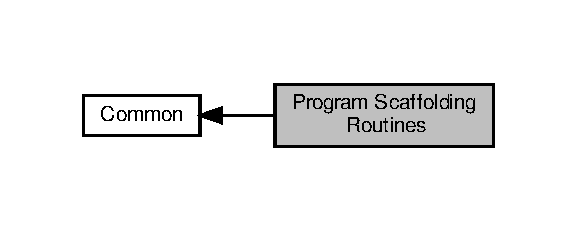
\includegraphics[width=277pt]{group__scaffolding}
\end{center}
\end{figure}
\subsection*{Macros}
\begin{DoxyCompactItemize}
\item 
\#define \hyperlink{group__scaffolding_ga1b83ce2b0adc8a384cc5a4589a8c2140}{\+\_\+\+\_\+\+F\+B\+C\+O\+N\+\_\+\+E\+V3\+\_\+\+\_\+}
\item 
\mbox{\Hypertarget{group__scaffolding_ga91164741f16fe7970ef266be19178415}\label{group__scaffolding_ga91164741f16fe7970ef266be19178415}} 
\#define \hyperlink{group__scaffolding_ga91164741f16fe7970ef266be19178415}{T\+E\+R\+M\+\_\+\+C\+O\+L\+\_\+\+M\+IN}~1
\begin{DoxyCompactList}\small\item\em Minimum Console Column value. \end{DoxyCompactList}\item 
\mbox{\Hypertarget{group__scaffolding_ga80a3ddd373d6bc24fd7e6929feb9e807}\label{group__scaffolding_ga80a3ddd373d6bc24fd7e6929feb9e807}} 
\#define \hyperlink{group__scaffolding_ga80a3ddd373d6bc24fd7e6929feb9e807}{T\+E\+R\+M\+\_\+\+C\+O\+L\+\_\+\+M\+AX}~29
\begin{DoxyCompactList}\small\item\em Maximum Console Column value. \end{DoxyCompactList}\item 
\mbox{\Hypertarget{group__scaffolding_ga3c42e3653e322d99249147e992e1976e}\label{group__scaffolding_ga3c42e3653e322d99249147e992e1976e}} 
\#define \hyperlink{group__scaffolding_ga3c42e3653e322d99249147e992e1976e}{T\+E\+R\+M\+\_\+\+R\+O\+W\+\_\+\+M\+IN}~1
\begin{DoxyCompactList}\small\item\em Minimum Console Row value. \end{DoxyCompactList}\item 
\mbox{\Hypertarget{group__scaffolding_ga141f599b6a2a3321a8a089004cd1e52a}\label{group__scaffolding_ga141f599b6a2a3321a8a089004cd1e52a}} 
\#define \hyperlink{group__scaffolding_ga141f599b6a2a3321a8a089004cd1e52a}{T\+E\+R\+M\+\_\+\+R\+O\+W\+\_\+\+M\+AX}~10
\begin{DoxyCompactList}\small\item\em Maximum Console Row value. \end{DoxyCompactList}\end{DoxyCompactItemize}
\subsection*{Functions}
\begin{DoxyCompactItemize}
\item 
void \hyperlink{group__scaffolding_gadc1bdbe20a5b0bf20b786c454857af1a}{prog\+\_\+init} (void)
\item 
void \hyperlink{group__scaffolding_gae2602aec28da58d379b4136b455a62d7}{prog\+\_\+exit} (void)
\item 
void \hyperlink{group__scaffolding_gad26b68c9bc1df3aa990eb9f594e28760}{prog\+\_\+contentX} (std\+::string str, int row, int col)
\item 
\mbox{\Hypertarget{group__scaffolding_gae8773733374b0af1000042f78b017d3d}\label{group__scaffolding_gae8773733374b0af1000042f78b017d3d}} 
void {\bfseries prog\+\_\+\+NumberX} (int value, int row, int col)
\item 
void \hyperlink{group__scaffolding_ga4472335aeac8c96294ad2f77d875d2cd}{prog\+\_\+clearscreen} (void)
\item 
bool \hyperlink{group__scaffolding_ga0420c11494d215979edc5f657819a2ca}{prog\+\_\+set\+\_\+cursorpos} (int col, int row)
\item 
void \hyperlink{group__scaffolding_ga59bf0af8d61ca90c1825e3224b45eaf9}{prog\+\_\+display\+\_\+string} (char $\ast$string)
\item 
void \hyperlink{group__scaffolding_ga0ea4957bdb462cada821c4d728494087}{prog\+\_\+display\+\_\+integer} (int value)
\item 
void \hyperlink{group__scaffolding_gae0f19e55443d5e98d104d9bc8a0e96a9}{prog\+\_\+display\+\_\+signed\+\_\+int} (int value)
\item 
void \hyperlink{group__scaffolding_ga455086b694579da94041147474387a9b}{prog\+\_\+display\+\_\+unsigned\+\_\+int} (uint value)
\item 
void \hyperlink{group__scaffolding_ga00fa862c209364a485690c01cf67b281}{prog\+\_\+display\+\_\+bin8} (unsigned char binvalue)
\item 
void \hyperlink{group__scaffolding_gae22b0332268122b8ef7443b7bc5024b9}{prog\+\_\+display\+\_\+hex32} (uint hexvalue)
\end{DoxyCompactItemize}


\subsection{Detailed Description}
The Scaffolding library perform miscellaneous startup and shutdown tasks, as well as send display to the console with basic terminal handling. 

\subsection{Macro Definition Documentation}
\mbox{\Hypertarget{group__scaffolding_ga1b83ce2b0adc8a384cc5a4589a8c2140}\label{group__scaffolding_ga1b83ce2b0adc8a384cc5a4589a8c2140}} 
\index{Program Scaffolding Routines@{Program Scaffolding Routines}!\+\_\+\+\_\+\+F\+B\+C\+O\+N\+\_\+\+E\+V3\+\_\+\+\_\+@{\+\_\+\+\_\+\+F\+B\+C\+O\+N\+\_\+\+E\+V3\+\_\+\+\_\+}}
\index{\+\_\+\+\_\+\+F\+B\+C\+O\+N\+\_\+\+E\+V3\+\_\+\+\_\+@{\+\_\+\+\_\+\+F\+B\+C\+O\+N\+\_\+\+E\+V3\+\_\+\+\_\+}!Program Scaffolding Routines@{Program Scaffolding Routines}}
\subsubsection{\texorpdfstring{\+\_\+\+\_\+\+F\+B\+C\+O\+N\+\_\+\+E\+V3\+\_\+\+\_\+}{\_\_FBCON\_EV3\_\_}}
{\footnotesize\ttfamily \#define \+\_\+\+\_\+\+F\+B\+C\+O\+N\+\_\+\+E\+V3\+\_\+\+\_\+}

\hyperlink{classText}{Text} Terminal Screen Dimensions

Assumes use of Lat15-\/\+Terminus12x6.\+psf.\+gz font for the E\+V3 178x128 Monochrome L\+CD Display 

\subsection{Function Documentation}
\mbox{\Hypertarget{group__scaffolding_ga4472335aeac8c96294ad2f77d875d2cd}\label{group__scaffolding_ga4472335aeac8c96294ad2f77d875d2cd}} 
\index{Program Scaffolding Routines@{Program Scaffolding Routines}!prog\+\_\+clearscreen@{prog\+\_\+clearscreen}}
\index{prog\+\_\+clearscreen@{prog\+\_\+clearscreen}!Program Scaffolding Routines@{Program Scaffolding Routines}}
\subsubsection{\texorpdfstring{prog\+\_\+clearscreen()}{prog\_clearscreen()}}
{\footnotesize\ttfamily void prog\+\_\+clearscreen (\begin{DoxyParamCaption}\item[{void}]{ }\end{DoxyParamCaption})}

Clear the L\+CD \hyperlink{classText}{Text} Display. Cursor will be placed at (1,1) (Top Left) 
\begin{DoxyParams}{Parameters}
{\em None} & \\
\hline
\end{DoxyParams}
\begin{DoxyReturn}{Returns}
None 
\end{DoxyReturn}
\mbox{\Hypertarget{group__scaffolding_gad26b68c9bc1df3aa990eb9f594e28760}\label{group__scaffolding_gad26b68c9bc1df3aa990eb9f594e28760}} 
\index{Program Scaffolding Routines@{Program Scaffolding Routines}!prog\+\_\+contentX@{prog\+\_\+contentX}}
\index{prog\+\_\+contentX@{prog\+\_\+contentX}!Program Scaffolding Routines@{Program Scaffolding Routines}}
\subsubsection{\texorpdfstring{prog\+\_\+content\+X()}{prog\_contentX()}}
{\footnotesize\ttfamily void prog\+\_\+contentX (\begin{DoxyParamCaption}\item[{std\+::string}]{str,  }\item[{int}]{row,  }\item[{int}]{col }\end{DoxyParamCaption})}

Display Title string on L\+CD (Row 1) 
\begin{DoxyParams}{Parameters}
{\em string} & Null-\/terminated string \\
\hline
\end{DoxyParams}
\begin{DoxyReturn}{Returns}
None Display Content string on L\+CD (Row 3) 
\end{DoxyReturn}

\begin{DoxyParams}{Parameters}
{\em string} & Null-\/terminated string \\
\hline
\end{DoxyParams}
\begin{DoxyReturn}{Returns}
None Display Content string on L\+CD (Row 5) 
\end{DoxyReturn}

\begin{DoxyParams}{Parameters}
{\em string} & Null-\/terminated string \\
\hline
\end{DoxyParams}
\begin{DoxyReturn}{Returns}
None Display Content string on L\+CD (Row row) 
\end{DoxyReturn}

\begin{DoxyParams}{Parameters}
{\em string} & Null-\/terminated string \\
\hline
{\em row} & int\+: Row Index \mbox{[}1..M\+A\+X\+\_\+\+R\+OW\mbox{]} \\
\hline
\end{DoxyParams}
\begin{DoxyReturn}{Returns}
None 
\end{DoxyReturn}
\mbox{\Hypertarget{group__scaffolding_ga00fa862c209364a485690c01cf67b281}\label{group__scaffolding_ga00fa862c209364a485690c01cf67b281}} 
\index{Program Scaffolding Routines@{Program Scaffolding Routines}!prog\+\_\+display\+\_\+bin8@{prog\+\_\+display\+\_\+bin8}}
\index{prog\+\_\+display\+\_\+bin8@{prog\+\_\+display\+\_\+bin8}!Program Scaffolding Routines@{Program Scaffolding Routines}}
\subsubsection{\texorpdfstring{prog\+\_\+display\+\_\+bin8()}{prog\_display\_bin8()}}
{\footnotesize\ttfamily void prog\+\_\+display\+\_\+bin8 (\begin{DoxyParamCaption}\item[{unsigned char}]{binvalue }\end{DoxyParamCaption})}

Display 8-\/bit binary on L\+CD at current cursor position 
\begin{DoxyParams}{Parameters}
{\em value} & 8-\/bit binary value \\
\hline
\end{DoxyParams}
\begin{DoxyReturn}{Returns}
None 
\end{DoxyReturn}
\mbox{\Hypertarget{group__scaffolding_gae22b0332268122b8ef7443b7bc5024b9}\label{group__scaffolding_gae22b0332268122b8ef7443b7bc5024b9}} 
\index{Program Scaffolding Routines@{Program Scaffolding Routines}!prog\+\_\+display\+\_\+hex32@{prog\+\_\+display\+\_\+hex32}}
\index{prog\+\_\+display\+\_\+hex32@{prog\+\_\+display\+\_\+hex32}!Program Scaffolding Routines@{Program Scaffolding Routines}}
\subsubsection{\texorpdfstring{prog\+\_\+display\+\_\+hex32()}{prog\_display\_hex32()}}
{\footnotesize\ttfamily void prog\+\_\+display\+\_\+hex32 (\begin{DoxyParamCaption}\item[{uint}]{hexvalue }\end{DoxyParamCaption})}

Display 32-\/bit hexadecimal on L\+CD at current cursor position 
\begin{DoxyParams}{Parameters}
{\em value} & 32-\/bit hexadecimal value \\
\hline
\end{DoxyParams}
\begin{DoxyReturn}{Returns}
None 
\end{DoxyReturn}
\mbox{\Hypertarget{group__scaffolding_ga0ea4957bdb462cada821c4d728494087}\label{group__scaffolding_ga0ea4957bdb462cada821c4d728494087}} 
\index{Program Scaffolding Routines@{Program Scaffolding Routines}!prog\+\_\+display\+\_\+integer@{prog\+\_\+display\+\_\+integer}}
\index{prog\+\_\+display\+\_\+integer@{prog\+\_\+display\+\_\+integer}!Program Scaffolding Routines@{Program Scaffolding Routines}}
\subsubsection{\texorpdfstring{prog\+\_\+display\+\_\+integer()}{prog\_display\_integer()}}
{\footnotesize\ttfamily void prog\+\_\+display\+\_\+integer (\begin{DoxyParamCaption}\item[{int}]{value }\end{DoxyParamCaption})}

Display signed integer on L\+CD at current cursor position The negative sign is displayed if it is negative, otherwise no signed is displayed. 
\begin{DoxyParams}{Parameters}
{\em value} & signed long value \\
\hline
\end{DoxyParams}
\begin{DoxyReturn}{Returns}
None 
\end{DoxyReturn}
\mbox{\Hypertarget{group__scaffolding_gae0f19e55443d5e98d104d9bc8a0e96a9}\label{group__scaffolding_gae0f19e55443d5e98d104d9bc8a0e96a9}} 
\index{Program Scaffolding Routines@{Program Scaffolding Routines}!prog\+\_\+display\+\_\+signed\+\_\+int@{prog\+\_\+display\+\_\+signed\+\_\+int}}
\index{prog\+\_\+display\+\_\+signed\+\_\+int@{prog\+\_\+display\+\_\+signed\+\_\+int}!Program Scaffolding Routines@{Program Scaffolding Routines}}
\subsubsection{\texorpdfstring{prog\+\_\+display\+\_\+signed\+\_\+int()}{prog\_display\_signed\_int()}}
{\footnotesize\ttfamily void prog\+\_\+display\+\_\+signed\+\_\+int (\begin{DoxyParamCaption}\item[{int}]{value }\end{DoxyParamCaption})}

Display signed integer on L\+CD at current cursor position The sign is always displayed, regardless of the value being positive or negative. 
\begin{DoxyParams}{Parameters}
{\em value} & signed long value \\
\hline
\end{DoxyParams}
\begin{DoxyReturn}{Returns}
None 
\end{DoxyReturn}
\mbox{\Hypertarget{group__scaffolding_ga59bf0af8d61ca90c1825e3224b45eaf9}\label{group__scaffolding_ga59bf0af8d61ca90c1825e3224b45eaf9}} 
\index{Program Scaffolding Routines@{Program Scaffolding Routines}!prog\+\_\+display\+\_\+string@{prog\+\_\+display\+\_\+string}}
\index{prog\+\_\+display\+\_\+string@{prog\+\_\+display\+\_\+string}!Program Scaffolding Routines@{Program Scaffolding Routines}}
\subsubsection{\texorpdfstring{prog\+\_\+display\+\_\+string()}{prog\_display\_string()}}
{\footnotesize\ttfamily void prog\+\_\+display\+\_\+string (\begin{DoxyParamCaption}\item[{char $\ast$}]{string }\end{DoxyParamCaption})}

Display string on L\+CD at current cursor position 
\begin{DoxyParams}{Parameters}
{\em string} & Null-\/terminated string \\
\hline
\end{DoxyParams}
\begin{DoxyReturn}{Returns}
None 
\end{DoxyReturn}
\mbox{\Hypertarget{group__scaffolding_ga455086b694579da94041147474387a9b}\label{group__scaffolding_ga455086b694579da94041147474387a9b}} 
\index{Program Scaffolding Routines@{Program Scaffolding Routines}!prog\+\_\+display\+\_\+unsigned\+\_\+int@{prog\+\_\+display\+\_\+unsigned\+\_\+int}}
\index{prog\+\_\+display\+\_\+unsigned\+\_\+int@{prog\+\_\+display\+\_\+unsigned\+\_\+int}!Program Scaffolding Routines@{Program Scaffolding Routines}}
\subsubsection{\texorpdfstring{prog\+\_\+display\+\_\+unsigned\+\_\+int()}{prog\_display\_unsigned\_int()}}
{\footnotesize\ttfamily void prog\+\_\+display\+\_\+unsigned\+\_\+int (\begin{DoxyParamCaption}\item[{uint}]{value }\end{DoxyParamCaption})}

Display unsigned integer on L\+CD at current cursor position 
\begin{DoxyParams}{Parameters}
{\em value} & unsigned long value \\
\hline
\end{DoxyParams}
\begin{DoxyReturn}{Returns}
None 
\end{DoxyReturn}
\mbox{\Hypertarget{group__scaffolding_gae2602aec28da58d379b4136b455a62d7}\label{group__scaffolding_gae2602aec28da58d379b4136b455a62d7}} 
\index{Program Scaffolding Routines@{Program Scaffolding Routines}!prog\+\_\+exit@{prog\+\_\+exit}}
\index{prog\+\_\+exit@{prog\+\_\+exit}!Program Scaffolding Routines@{Program Scaffolding Routines}}
\subsubsection{\texorpdfstring{prog\+\_\+exit()}{prog\_exit()}}
{\footnotesize\ttfamily void prog\+\_\+exit (\begin{DoxyParamCaption}\item[{void}]{ }\end{DoxyParamCaption})}

Exit A\+R\+M-\/\+B\+BR subsystems Generate exit tone 
\begin{DoxyParams}{Parameters}
{\em None} & \\
\hline
\end{DoxyParams}
\begin{DoxyReturn}{Returns}
None 
\end{DoxyReturn}
\mbox{\Hypertarget{group__scaffolding_gadc1bdbe20a5b0bf20b786c454857af1a}\label{group__scaffolding_gadc1bdbe20a5b0bf20b786c454857af1a}} 
\index{Program Scaffolding Routines@{Program Scaffolding Routines}!prog\+\_\+init@{prog\+\_\+init}}
\index{prog\+\_\+init@{prog\+\_\+init}!Program Scaffolding Routines@{Program Scaffolding Routines}}
\subsubsection{\texorpdfstring{prog\+\_\+init()}{prog\_init()}}
{\footnotesize\ttfamily void prog\+\_\+init (\begin{DoxyParamCaption}\item[{void}]{ }\end{DoxyParamCaption})}

Common Startup/\+Shutdown Routines for A\+R\+M-\/\+B\+BR programs Initialize A\+R\+M-\/\+B\+BR subsystems Clears L\+CD screen and generate startup tone 
\begin{DoxyParams}{Parameters}
{\em None} & \\
\hline
\end{DoxyParams}
\begin{DoxyReturn}{Returns}
None 
\end{DoxyReturn}
\mbox{\Hypertarget{group__scaffolding_ga0420c11494d215979edc5f657819a2ca}\label{group__scaffolding_ga0420c11494d215979edc5f657819a2ca}} 
\index{Program Scaffolding Routines@{Program Scaffolding Routines}!prog\+\_\+set\+\_\+cursorpos@{prog\+\_\+set\+\_\+cursorpos}}
\index{prog\+\_\+set\+\_\+cursorpos@{prog\+\_\+set\+\_\+cursorpos}!Program Scaffolding Routines@{Program Scaffolding Routines}}
\subsubsection{\texorpdfstring{prog\+\_\+set\+\_\+cursorpos()}{prog\_set\_cursorpos()}}
{\footnotesize\ttfamily bool prog\+\_\+set\+\_\+cursorpos (\begin{DoxyParamCaption}\item[{int}]{col,  }\item[{int}]{row }\end{DoxyParamCaption})}

Set the cursor on the L\+CD to new cursor position Note\+: This only works on the L\+CD screen. It does not work in the Debugger output window. 
\begin{DoxyParams}{Parameters}
{\em col} & integer value \\
\hline
{\em row} & integer value \\
\hline
\end{DoxyParams}
\begin{DoxyReturn}{Returns}
success\+: bool value 
\end{DoxyReturn}

\hypertarget{group__GUI}{}\section{G\+UI}
\label{group__GUI}\index{G\+UI@{G\+UI}}
Collaboration diagram for G\+UI\+:
\nopagebreak
\begin{figure}[H]
\begin{center}
\leavevmode
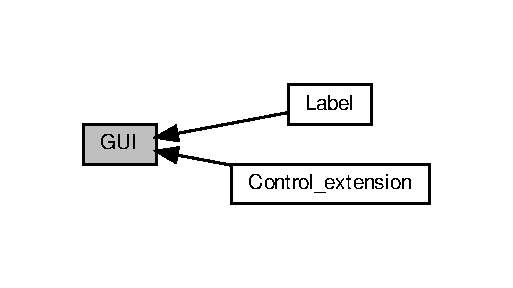
\includegraphics[width=246pt]{group__GUI}
\end{center}
\end{figure}
\subsection*{Modules}
\begin{DoxyCompactItemize}
\item 
\hyperlink{group__label}{Label}
\item 
\hyperlink{group__control__extension}{Control\+\_\+extension}
\end{DoxyCompactItemize}


\subsection{Detailed Description}

\hypertarget{group__label}{}\section{Label}
\label{group__label}\index{Label@{Label}}
Collaboration diagram for Label\+:
\nopagebreak
\begin{figure}[H]
\begin{center}
\leavevmode
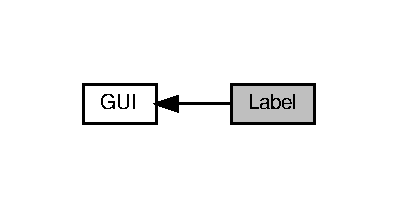
\includegraphics[width=191pt]{group__label}
\end{center}
\end{figure}
\subsection*{Classes}
\begin{DoxyCompactItemize}
\item 
struct \hyperlink{struct__BMFontDef}{\+\_\+\+B\+M\+Font\+Def}
\item 
struct \hyperlink{struct__BMFontPadding}{\+\_\+\+B\+M\+Font\+Padding}
\item 
struct \hyperlink{struct__FontDefHashElement}{\+\_\+\+Font\+Def\+Hash\+Element}
\item 
struct \hyperlink{struct__KerningHashElement}{\+\_\+\+Kerning\+Hash\+Element}
\item 
class \hyperlink{classBMFontConfiguration}{B\+M\+Font\+Configuration}
\begin{DoxyCompactList}\small\item\em \hyperlink{classBMFontConfiguration}{B\+M\+Font\+Configuration} has parsed configuration of the .fnt file. \end{DoxyCompactList}\item 
struct \hyperlink{structBMFontDef}{B\+M\+Font\+Def}
\item 
struct \hyperlink{structBMFontPadding}{B\+M\+Font\+Padding}
\end{DoxyCompactItemize}
\subsection*{Typedefs}
\begin{DoxyCompactItemize}
\item 
\mbox{\Hypertarget{group__label_gac487f725317559c875bb2d2d3adf86b1}\label{group__label_gac487f725317559c875bb2d2d3adf86b1}} 
typedef struct \hyperlink{struct__BMFontDef}{\+\_\+\+B\+M\+Font\+Def} {\bfseries B\+M\+Font\+Def}
\item 
\mbox{\Hypertarget{group__label_ga71de169a485c89d44fde95c211ed0c8d}\label{group__label_ga71de169a485c89d44fde95c211ed0c8d}} 
typedef struct \hyperlink{struct__BMFontPadding}{\+\_\+\+B\+M\+Font\+Padding} {\bfseries B\+M\+Font\+Padding}
\item 
\mbox{\Hypertarget{group__label_gae8dc5645efa817dbf6580c80581823e5}\label{group__label_gae8dc5645efa817dbf6580c80581823e5}} 
typedef struct \hyperlink{struct__FontDefHashElement}{\+\_\+\+Font\+Def\+Hash\+Element} {\bfseries t\+Font\+Def\+Hash\+Element}
\item 
\mbox{\Hypertarget{group__label_gac9dc358a19db328b4bc9b52454afedb0}\label{group__label_gac9dc358a19db328b4bc9b52454afedb0}} 
typedef struct \hyperlink{struct__KerningHashElement}{\+\_\+\+Kerning\+Hash\+Element} {\bfseries t\+Kerning\+Hash\+Element}
\item 
\mbox{\Hypertarget{group__label_gac487f725317559c875bb2d2d3adf86b1}\label{group__label_gac487f725317559c875bb2d2d3adf86b1}} 
typedef struct \hyperlink{struct__BMFontDef}{\+\_\+\+B\+M\+Font\+Def} {\bfseries B\+M\+Font\+Def}
\item 
\mbox{\Hypertarget{group__label_ga71de169a485c89d44fde95c211ed0c8d}\label{group__label_ga71de169a485c89d44fde95c211ed0c8d}} 
typedef struct \hyperlink{struct__BMFontPadding}{\+\_\+\+B\+M\+Font\+Padding} {\bfseries B\+M\+Font\+Padding}
\end{DoxyCompactItemize}
\subsection*{Enumerations}
\begin{DoxyCompactItemize}
\item 
\mbox{\Hypertarget{group__label_ga726ca809ffd3d67ab4b8476646f26635}\label{group__label_ga726ca809ffd3d67ab4b8476646f26635}} 
enum \{ {\bfseries k\+Label\+Automatic\+Width} = -\/1
 \}
\item 
\mbox{\Hypertarget{group__label_ga20a66f99673ff3efefccf3a6a6f19f65}\label{group__label_ga20a66f99673ff3efefccf3a6a6f19f65}} 
enum \{ {\bfseries k\+Label\+Automatic\+Width} = -\/1
 \}
\end{DoxyCompactItemize}
\subsection*{Functions}
\begin{DoxyCompactItemize}
\item 
\hyperlink{group__label_ga04b6c1a932298f09e2271950f2da6661}{B\+M\+Font\+Configuration\+::\+B\+M\+Font\+Configuration} ()
\item 
virtual \hyperlink{group__label_gad54c7b6ca83e8eaaedfff5ec431b8b11}{B\+M\+Font\+Configuration\+::$\sim$\+B\+M\+Font\+Configuration} ()
\item 
std\+::string \hyperlink{group__label_gab5b833ca803bff72c9ab19abf55eb8ac}{B\+M\+Font\+Configuration\+::description} () const
\item 
static \hyperlink{classBMFontConfiguration}{B\+M\+Font\+Configuration} $\ast$ \hyperlink{group__label_gaf6f6e33acf57e6fdf10de805002f21c6}{B\+M\+Font\+Configuration\+::create} (const std\+::string \&F\+N\+Tfile)
\item 
bool \hyperlink{group__label_ga0eb7f4ea5cc521e1502006c04cc67733}{B\+M\+Font\+Configuration\+::init\+With\+F\+N\+Tfile} (const std\+::string \&F\+N\+Tfile)
\item 
\mbox{\Hypertarget{group__label_gad274de0ea6ede4d07c4a65f03bc4cb25}\label{group__label_gad274de0ea6ede4d07c4a65f03bc4cb25}} 
const std\+::string \& {\bfseries B\+M\+Font\+Configuration\+::get\+Atlas\+Name} ()
\item 
\mbox{\Hypertarget{group__label_ga871cdaaac71c43fa35a62fe9f0c3d3cc}\label{group__label_ga871cdaaac71c43fa35a62fe9f0c3d3cc}} 
void {\bfseries B\+M\+Font\+Configuration\+::set\+Atlas\+Name} (const std\+::string \&atlas\+Name)
\item 
\mbox{\Hypertarget{group__label_ga039fbd9a15e5e226af6e1dba80108bcf}\label{group__label_ga039fbd9a15e5e226af6e1dba80108bcf}} 
std\+::set$<$ unsigned int $>$ $\ast$ {\bfseries B\+M\+Font\+Configuration\+::get\+Character\+Set} () const
\item 
\mbox{\Hypertarget{group__label_ga4370ebb6f56fe325b1be4ec3426fdca7}\label{group__label_ga4370ebb6f56fe325b1be4ec3426fdca7}} 
\hyperlink{classBMFontConfiguration}{B\+M\+Font\+Configuration} $\ast$ {\bfseries F\+N\+T\+Config\+Load\+File} (const std\+::string \&fnt\+File)
\end{DoxyCompactItemize}
\subsection*{Variables}
\begin{DoxyCompactItemize}
\item 
\mbox{\Hypertarget{group__label_ga4be84ef9be4446878fff255b15e9e678}\label{group__label_ga4be84ef9be4446878fff255b15e9e678}} 
unsigned int \hyperlink{group__label_ga4be84ef9be4446878fff255b15e9e678}{\+\_\+\+B\+M\+Font\+Def\+::char\+ID}
\begin{DoxyCompactList}\small\item\em ID of the character. \end{DoxyCompactList}\item 
\mbox{\Hypertarget{group__label_ga9426c06ddd57097582d48bfb34ef02fa}\label{group__label_ga9426c06ddd57097582d48bfb34ef02fa}} 
\hyperlink{classRect}{Rect} \hyperlink{group__label_ga9426c06ddd57097582d48bfb34ef02fa}{\+\_\+\+B\+M\+Font\+Def\+::rect}
\begin{DoxyCompactList}\small\item\em origin and size of the font \end{DoxyCompactList}\item 
\mbox{\Hypertarget{group__label_gaf961a67faba7abff4c31ef69b32eaed4}\label{group__label_gaf961a67faba7abff4c31ef69b32eaed4}} 
short \hyperlink{group__label_gaf961a67faba7abff4c31ef69b32eaed4}{\+\_\+\+B\+M\+Font\+Def\+::x\+Offset}
\begin{DoxyCompactList}\small\item\em The X amount the image should be offset when drawing the image (in pixels) \end{DoxyCompactList}\item 
\mbox{\Hypertarget{group__label_gae0d9c0fc84b157abd9133b6bcddab2b7}\label{group__label_gae0d9c0fc84b157abd9133b6bcddab2b7}} 
short \hyperlink{group__label_gae0d9c0fc84b157abd9133b6bcddab2b7}{\+\_\+\+B\+M\+Font\+Def\+::y\+Offset}
\begin{DoxyCompactList}\small\item\em The Y amount the image should be offset when drawing the image (in pixels) \end{DoxyCompactList}\item 
\mbox{\Hypertarget{group__label_gaf8a9e2733f5f1fcb8a3631b3886d6703}\label{group__label_gaf8a9e2733f5f1fcb8a3631b3886d6703}} 
short \hyperlink{group__label_gaf8a9e2733f5f1fcb8a3631b3886d6703}{\+\_\+\+B\+M\+Font\+Def\+::x\+Advance}
\begin{DoxyCompactList}\small\item\em The amount to move the current position after drawing the character (in pixels) \end{DoxyCompactList}\item 
\mbox{\Hypertarget{group__label_ga8129887cd2f3f177100cd4fedf20e347}\label{group__label_ga8129887cd2f3f177100cd4fedf20e347}} 
int \hyperlink{group__label_ga8129887cd2f3f177100cd4fedf20e347}{\+\_\+\+B\+M\+Font\+Padding\+::left}
\begin{DoxyCompactList}\small\item\em padding left \end{DoxyCompactList}\item 
\mbox{\Hypertarget{group__label_gad673e6ff522f10836afba0745f3c4ee8}\label{group__label_gad673e6ff522f10836afba0745f3c4ee8}} 
int \hyperlink{group__label_gad673e6ff522f10836afba0745f3c4ee8}{\+\_\+\+B\+M\+Font\+Padding\+::top}
\begin{DoxyCompactList}\small\item\em padding top \end{DoxyCompactList}\item 
\mbox{\Hypertarget{group__label_gac83f97e64d8fa8a835a17c44d93f9f62}\label{group__label_gac83f97e64d8fa8a835a17c44d93f9f62}} 
int \hyperlink{group__label_gac83f97e64d8fa8a835a17c44d93f9f62}{\+\_\+\+B\+M\+Font\+Padding\+::right}
\begin{DoxyCompactList}\small\item\em padding right \end{DoxyCompactList}\item 
\mbox{\Hypertarget{group__label_ga41ee44807cde2134c0ff73208dccf6e7}\label{group__label_ga41ee44807cde2134c0ff73208dccf6e7}} 
int \hyperlink{group__label_ga41ee44807cde2134c0ff73208dccf6e7}{\+\_\+\+B\+M\+Font\+Padding\+::bottom}
\begin{DoxyCompactList}\small\item\em padding bottom \end{DoxyCompactList}\item 
\mbox{\Hypertarget{group__label_gaa707ede0c1121fd031b1b905064f3939}\label{group__label_gaa707ede0c1121fd031b1b905064f3939}} 
unsigned int {\bfseries \+\_\+\+Font\+Def\+Hash\+Element\+::key}
\item 
\mbox{\Hypertarget{group__label_ga2c6a7e28eb19058966c07141285f3457}\label{group__label_ga2c6a7e28eb19058966c07141285f3457}} 
\hyperlink{structBMFontDef}{B\+M\+Font\+Def} {\bfseries \+\_\+\+Font\+Def\+Hash\+Element\+::font\+Def}
\item 
\mbox{\Hypertarget{group__label_ga0d67721facc6a1d012f086f994d76eed}\label{group__label_ga0d67721facc6a1d012f086f994d76eed}} 
\hyperlink{structUT__hash__handle}{U\+T\+\_\+hash\+\_\+handle} {\bfseries \+\_\+\+Font\+Def\+Hash\+Element\+::hh}
\item 
\mbox{\Hypertarget{group__label_ga3d5a9cd723f885a8d24b75bb0289ce1d}\label{group__label_ga3d5a9cd723f885a8d24b75bb0289ce1d}} 
int {\bfseries \+\_\+\+Kerning\+Hash\+Element\+::key}
\item 
\mbox{\Hypertarget{group__label_ga51a9c100050c2ab56431798e59509100}\label{group__label_ga51a9c100050c2ab56431798e59509100}} 
int {\bfseries \+\_\+\+Kerning\+Hash\+Element\+::amount}
\item 
\mbox{\Hypertarget{group__label_ga1438adce8be9c5fde6f185595d3af254}\label{group__label_ga1438adce8be9c5fde6f185595d3af254}} 
\hyperlink{structUT__hash__handle}{U\+T\+\_\+hash\+\_\+handle} {\bfseries \+\_\+\+Kerning\+Hash\+Element\+::hh}
\item 
\mbox{\Hypertarget{group__label_ga3681c646e0591e688177dbcd2c26f91a}\label{group__label_ga3681c646e0591e688177dbcd2c26f91a}} 
\hyperlink{struct__FontDefHashElement}{t\+Font\+Def\+Hash\+Element} $\ast$ {\bfseries B\+M\+Font\+Configuration\+::\+\_\+font\+Def\+Dictionary}
\item 
\mbox{\Hypertarget{group__label_ga6409fa4f816ee11ee9f6d8ae836969aa}\label{group__label_ga6409fa4f816ee11ee9f6d8ae836969aa}} 
int \hyperlink{group__label_ga6409fa4f816ee11ee9f6d8ae836969aa}{B\+M\+Font\+Configuration\+::\+\_\+common\+Height}
\begin{DoxyCompactList}\small\item\em F\+N\+T\+Config\+: Common Height Should be signed (issue \#1343) \end{DoxyCompactList}\item 
\mbox{\Hypertarget{group__label_gac9bca22b336c401f9446dae89679e646}\label{group__label_gac9bca22b336c401f9446dae89679e646}} 
\hyperlink{structBMFontPadding}{B\+M\+Font\+Padding} \hyperlink{group__label_gac9bca22b336c401f9446dae89679e646}{B\+M\+Font\+Configuration\+::\+\_\+padding}
\begin{DoxyCompactList}\small\item\em Padding. \end{DoxyCompactList}\item 
\mbox{\Hypertarget{group__label_ga3ad769d94dce120f39c8f502bdbac2ad}\label{group__label_ga3ad769d94dce120f39c8f502bdbac2ad}} 
std\+::string \hyperlink{group__label_ga3ad769d94dce120f39c8f502bdbac2ad}{B\+M\+Font\+Configuration\+::\+\_\+atlas\+Name}
\begin{DoxyCompactList}\small\item\em atlas name \end{DoxyCompactList}\item 
\mbox{\Hypertarget{group__label_ga246c499bd161998ce4382f474e9be832}\label{group__label_ga246c499bd161998ce4382f474e9be832}} 
\hyperlink{struct__KerningHashElement}{t\+Kerning\+Hash\+Element} $\ast$ \hyperlink{group__label_ga246c499bd161998ce4382f474e9be832}{B\+M\+Font\+Configuration\+::\+\_\+kerning\+Dictionary}
\begin{DoxyCompactList}\small\item\em values for kerning \end{DoxyCompactList}\item 
\mbox{\Hypertarget{group__label_ga072272dc473cfc1a0a6d813f56e8514b}\label{group__label_ga072272dc473cfc1a0a6d813f56e8514b}} 
std\+::set$<$ unsigned int $>$ $\ast$ {\bfseries B\+M\+Font\+Configuration\+::\+\_\+character\+Set}
\item 
\mbox{\Hypertarget{group__label_gacffa3f4764fb2fa613d1276210819c14}\label{group__label_gacffa3f4764fb2fa613d1276210819c14}} 
int \hyperlink{group__label_gacffa3f4764fb2fa613d1276210819c14}{B\+M\+Font\+Configuration\+::\+\_\+font\+Size}
\begin{DoxyCompactList}\small\item\em Font \hyperlink{classSize}{Size}. \end{DoxyCompactList}\item 
\mbox{\Hypertarget{group__label_ga1e33b7dd227fb6004c36c06962835963}\label{group__label_ga1e33b7dd227fb6004c36c06962835963}} 
std\+::unordered\+\_\+map$<$ int, \hyperlink{structBMFontDef}{B\+M\+Font\+Def} $>$ {\bfseries B\+M\+Font\+Configuration\+::\+\_\+font\+Def\+Dictionary}
\item 
\mbox{\Hypertarget{group__label_gaaf96511ac7124077592700eee5f504d0}\label{group__label_gaaf96511ac7124077592700eee5f504d0}} 
std\+::unordered\+\_\+map$<$ uint64\+\_\+t, int $>$ \hyperlink{group__label_gaaf96511ac7124077592700eee5f504d0}{B\+M\+Font\+Configuration\+::\+\_\+kerning\+Dictionary}
\begin{DoxyCompactList}\small\item\em values for kerning \end{DoxyCompactList}\end{DoxyCompactItemize}


\subsection{Detailed Description}


\subsection{Function Documentation}
\mbox{\Hypertarget{group__label_ga04b6c1a932298f09e2271950f2da6661}\label{group__label_ga04b6c1a932298f09e2271950f2da6661}} 
\index{Label@{Label}!B\+M\+Font\+Configuration@{B\+M\+Font\+Configuration}}
\index{B\+M\+Font\+Configuration@{B\+M\+Font\+Configuration}!Label@{Label}}
\subsubsection{\texorpdfstring{B\+M\+Font\+Configuration()}{BMFontConfiguration()}}
{\footnotesize\ttfamily B\+M\+Font\+Configuration\+::\+B\+M\+Font\+Configuration (\begin{DoxyParamCaption}{ }\end{DoxyParamCaption})}

ctor \mbox{\Hypertarget{group__label_gaf6f6e33acf57e6fdf10de805002f21c6}\label{group__label_gaf6f6e33acf57e6fdf10de805002f21c6}} 
\index{Label@{Label}!create@{create}}
\index{create@{create}!Label@{Label}}
\subsubsection{\texorpdfstring{create()}{create()}}
{\footnotesize\ttfamily \hyperlink{classBMFontConfiguration}{B\+M\+Font\+Configuration} $\ast$ B\+M\+Font\+Configuration\+::create (\begin{DoxyParamCaption}\item[{const std\+::string \&}]{F\+N\+Tfile }\end{DoxyParamCaption})\hspace{0.3cm}{\ttfamily [static]}}

allocates a \hyperlink{classBMFontConfiguration}{B\+M\+Font\+Configuration} with a F\+NT file \mbox{\Hypertarget{group__label_gab5b833ca803bff72c9ab19abf55eb8ac}\label{group__label_gab5b833ca803bff72c9ab19abf55eb8ac}} 
\index{Label@{Label}!description@{description}}
\index{description@{description}!Label@{Label}}
\subsubsection{\texorpdfstring{description()}{description()}}
{\footnotesize\ttfamily std\+::string B\+M\+Font\+Configuration\+::description (\begin{DoxyParamCaption}\item[{void}]{ }\end{DoxyParamCaption}) const}

NA  NA \mbox{\Hypertarget{group__label_ga0eb7f4ea5cc521e1502006c04cc67733}\label{group__label_ga0eb7f4ea5cc521e1502006c04cc67733}} 
\index{Label@{Label}!init\+With\+F\+N\+Tfile@{init\+With\+F\+N\+Tfile}}
\index{init\+With\+F\+N\+Tfile@{init\+With\+F\+N\+Tfile}!Label@{Label}}
\subsubsection{\texorpdfstring{init\+With\+F\+N\+Tfile()}{initWithFNTfile()}}
{\footnotesize\ttfamily bool B\+M\+Font\+Configuration\+::init\+With\+F\+N\+Tfile (\begin{DoxyParamCaption}\item[{const std\+::string \&}]{F\+N\+Tfile }\end{DoxyParamCaption})}

initializes a Bitmap\+Font\+Configuration with a F\+NT file \mbox{\Hypertarget{group__label_gad54c7b6ca83e8eaaedfff5ec431b8b11}\label{group__label_gad54c7b6ca83e8eaaedfff5ec431b8b11}} 
\index{Label@{Label}!````~B\+M\+Font\+Configuration@{$\sim$\+B\+M\+Font\+Configuration}}
\index{````~B\+M\+Font\+Configuration@{$\sim$\+B\+M\+Font\+Configuration}!Label@{Label}}
\subsubsection{\texorpdfstring{$\sim$\+B\+M\+Font\+Configuration()}{~BMFontConfiguration()}}
{\footnotesize\ttfamily B\+M\+Font\+Configuration\+::$\sim$\+B\+M\+Font\+Configuration (\begin{DoxyParamCaption}{ }\end{DoxyParamCaption})\hspace{0.3cm}{\ttfamily [virtual]}}

NA  NA 
\hypertarget{group__cocosbuilder}{}\section{Cocosbuilder}
\label{group__cocosbuilder}\index{Cocosbuilder@{Cocosbuilder}}
\subsection*{Classes}
\begin{DoxyCompactItemize}
\item 
class \hyperlink{classcocosbuilder_1_1CCBFile}{cocosbuilder\+::\+C\+C\+B\+File}
\item 
class \hyperlink{classcocosbuilder_1_1CCBReader}{cocosbuilder\+::\+C\+C\+B\+Reader}
\begin{DoxyCompactList}\small\item\em Parse C\+C\+BI file which is generated by Cocos\+Builder. \end{DoxyCompactList}\end{DoxyCompactItemize}


\subsection{Detailed Description}

\hypertarget{group__control__extension}{}\section{Control\+\_\+extension}
\label{group__control__extension}\index{Control\+\_\+extension@{Control\+\_\+extension}}
Collaboration diagram for Control\+\_\+extension\+:
\nopagebreak
\begin{figure}[H]
\begin{center}
\leavevmode
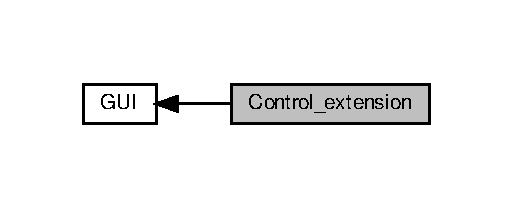
\includegraphics[width=246pt]{group__control__extension}
\end{center}
\end{figure}
\subsection*{Classes}
\begin{DoxyCompactItemize}
\item 
class \hyperlink{classControl}{Control}
\item 
class \hyperlink{classControlButton}{Control\+Button}
\item 
class \hyperlink{classControlColourPicker}{Control\+Colour\+Picker}
\item 
class \hyperlink{classControlHuePicker}{Control\+Hue\+Picker}
\item 
class \hyperlink{classControlPotentiometer}{Control\+Potentiometer}
\item 
class \hyperlink{classControlSaturationBrightnessPicker}{Control\+Saturation\+Brightness\+Picker}
\item 
class \hyperlink{classControlSlider}{Control\+Slider}
\item 
class \hyperlink{classControlStepper}{Control\+Stepper}
\item 
class \hyperlink{classControlSwitch}{Control\+Switch}
\item 
class \hyperlink{classColor3bObject}{Color3b\+Object}
\item 
class \hyperlink{classControlUtils}{Control\+Utils}
\item 
class \hyperlink{classInvocation}{Invocation}
\end{DoxyCompactItemize}
\subsection*{Macros}
\begin{DoxyCompactItemize}
\item 
\#define \hyperlink{group__control__extension_ga0943a168609cb108419ba7f34c64130e}{k\+Control\+Event\+Total\+Number}~9
\item 
\mbox{\Hypertarget{group__control__extension_ga28eb34ece2b73b97cd9e730693f4a5f8}\label{group__control__extension_ga28eb34ece2b73b97cd9e730693f4a5f8}} 
\#define {\bfseries cccontrol\+\_\+selector}(\+\_\+\+S\+E\+L\+E\+C\+T\+OR)~static\+\_\+cast$<$cocos2d\+::extension\+::\+Control\+::\+Handler$>$(\&\+\_\+\+S\+E\+L\+E\+C\+T\+OR)
\item 
\#define \hyperlink{group__control__extension_ga0943a168609cb108419ba7f34c64130e}{k\+Control\+Event\+Total\+Number}~9
\item 
\mbox{\Hypertarget{group__control__extension_ga28eb34ece2b73b97cd9e730693f4a5f8}\label{group__control__extension_ga28eb34ece2b73b97cd9e730693f4a5f8}} 
\#define {\bfseries cccontrol\+\_\+selector}(\+\_\+\+S\+E\+L\+E\+C\+T\+OR)~static\+\_\+cast$<$cocos2d\+::extension\+::\+Control\+::\+Handler$>$(\&\+\_\+\+S\+E\+L\+E\+C\+T\+OR)
\end{DoxyCompactItemize}
\subsection*{Functions}
\begin{DoxyCompactItemize}
\item 
\mbox{\Hypertarget{group__control__extension_ga5a7f7e12f7b938cfd99a8c631d67e22b}\label{group__control__extension_ga5a7f7e12f7b938cfd99a8c631d67e22b}} 
C\+C\+\_\+\+E\+X\+\_\+\+D\+LL Control\+::\+Event\+Type {\bfseries operator$\vert$} (Control\+::\+Event\+Type a, Control\+::\+Event\+Type b)
\end{DoxyCompactItemize}


\subsection{Detailed Description}


\subsection{Macro Definition Documentation}
\mbox{\Hypertarget{group__control__extension_ga0943a168609cb108419ba7f34c64130e}\label{group__control__extension_ga0943a168609cb108419ba7f34c64130e}} 
\index{Control\+\_\+extension@{Control\+\_\+extension}!k\+Control\+Event\+Total\+Number@{k\+Control\+Event\+Total\+Number}}
\index{k\+Control\+Event\+Total\+Number@{k\+Control\+Event\+Total\+Number}!Control\+\_\+extension@{Control\+\_\+extension}}
\subsubsection{\texorpdfstring{k\+Control\+Event\+Total\+Number}{kControlEventTotalNumber}\hspace{0.1cm}{\footnotesize\ttfamily [1/2]}}
{\footnotesize\ttfamily \#define k\+Control\+Event\+Total\+Number~9}

Number of kinds of control event. \mbox{\Hypertarget{group__control__extension_ga0943a168609cb108419ba7f34c64130e}\label{group__control__extension_ga0943a168609cb108419ba7f34c64130e}} 
\index{Control\+\_\+extension@{Control\+\_\+extension}!k\+Control\+Event\+Total\+Number@{k\+Control\+Event\+Total\+Number}}
\index{k\+Control\+Event\+Total\+Number@{k\+Control\+Event\+Total\+Number}!Control\+\_\+extension@{Control\+\_\+extension}}
\subsubsection{\texorpdfstring{k\+Control\+Event\+Total\+Number}{kControlEventTotalNumber}\hspace{0.1cm}{\footnotesize\ttfamily [2/2]}}
{\footnotesize\ttfamily \#define k\+Control\+Event\+Total\+Number~9}

Number of kinds of control event. 
\hypertarget{group__common}{}\section{Common}
\label{group__common}\index{Common@{Common}}
Collaboration diagram for Common\+:
\nopagebreak
\begin{figure}[H]
\begin{center}
\leavevmode
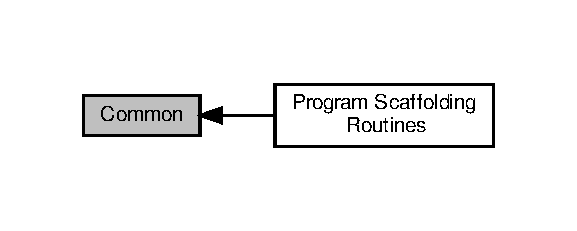
\includegraphics[width=277pt]{group__common}
\end{center}
\end{figure}
\subsection*{Modules}
\begin{DoxyCompactItemize}
\item 
\hyperlink{group__scaffolding}{Program Scaffolding Routines}
\end{DoxyCompactItemize}


\subsection{Detailed Description}

\chapter{Namespace Documentation}
\hypertarget{namespaceDrawPrimitives}{}\section{Draw\+Primitives Namespace Reference}
\label{namespaceDrawPrimitives}\index{Draw\+Primitives@{Draw\+Primitives}}
\subsection*{Functions}
\begin{DoxyCompactItemize}
\item 
void \hyperlink{namespaceDrawPrimitives_ae042e1546ce595f9b01f92bcac0be48a}{init} ()
\item 
void \hyperlink{namespaceDrawPrimitives_a1a20eab15f5a2560e8ebaa1fddde8216}{free} ()
\item 
void \hyperlink{namespaceDrawPrimitives_a8245dd1018a768473478a9e65c7be6d5}{draw\+Point} (const \hyperlink{classVec2}{Vec2} \&point)
\item 
void \hyperlink{namespaceDrawPrimitives_a69ac036b04c0dd7b20643a777bfdde14}{draw\+Points} (const \hyperlink{classVec2}{Vec2} $\ast$points, unsigned int number\+Of\+Points)
\item 
void \hyperlink{namespaceDrawPrimitives_a872bfe0f92313b81a93eb7e6ae67b94a}{draw\+Line} (const \hyperlink{classVec2}{Vec2} \&origin, const \hyperlink{classVec2}{Vec2} \&destination)
\item 
void \hyperlink{namespaceDrawPrimitives_af083f4157bcb6c95fa9755c275c851d4}{draw\+Rect} (\hyperlink{classVec2}{Vec2} origin, \hyperlink{classVec2}{Vec2} destination)
\item 
void \hyperlink{namespaceDrawPrimitives_ae71825a1fd3fafd9d83ddaf78bc4b84f}{draw\+Solid\+Rect} (\hyperlink{classVec2}{Vec2} origin, \hyperlink{classVec2}{Vec2} destination, \hyperlink{structColor4F}{Color4F} color)
\item 
void \hyperlink{namespaceDrawPrimitives_a71a680302a9b336b8ddb39bf5b18348c}{draw\+Poly} (const \hyperlink{classVec2}{Vec2} $\ast$poli, unsigned int number\+Of\+Points, bool close\+Polygon)
\item 
void \hyperlink{namespaceDrawPrimitives_a236c83afa9808359e7f445778973fdd1}{draw\+Solid\+Poly} (const \hyperlink{classVec2}{Vec2} $\ast$poli, unsigned int number\+Of\+Points, \hyperlink{structColor4F}{Color4F} color)
\item 
void \hyperlink{namespaceDrawPrimitives_ab3372bf8fe32fedeffc8867ce741f5c0}{draw\+Circle} (const \hyperlink{classVec2}{Vec2} \&center, float radius, float angle, unsigned int segments, bool draw\+Line\+To\+Center, float scaleX, float scaleY)
\item 
void \hyperlink{namespaceDrawPrimitives_ae27b581bbeb1c73a0b01d3e1afb4c13e}{draw\+Circle} (const \hyperlink{classVec2}{Vec2} \&center, float radius, float angle, unsigned int segments, bool draw\+Line\+To\+Center)
\item 
void \hyperlink{namespaceDrawPrimitives_a323e0910a04cf0fdc75563e61a5dea15}{draw\+Solid\+Circle} (const \hyperlink{classVec2}{Vec2} \&center, float radius, float angle, unsigned int segments, float scaleX, float scaleY)
\item 
void \hyperlink{namespaceDrawPrimitives_a11ae341f043974e35ac301f9e3feef45}{draw\+Solid\+Circle} (const \hyperlink{classVec2}{Vec2} \&center, float radius, float angle, unsigned int segments)
\item 
void \hyperlink{namespaceDrawPrimitives_a350f5890844862176a8be86cdadfd291}{draw\+Quad\+Bezier} (const \hyperlink{classVec2}{Vec2} \&origin, const \hyperlink{classVec2}{Vec2} \&control, const \hyperlink{classVec2}{Vec2} \&destination, unsigned int segments)
\item 
void \hyperlink{namespaceDrawPrimitives_a133274f7f2a33cd32644d665e963ccd8}{draw\+Catmull\+Rom} (\hyperlink{classPointArray}{Point\+Array} $\ast$points, unsigned int segments)
\item 
void \hyperlink{namespaceDrawPrimitives_a82b0da83c69f4bbba9a26b4f1f90b1e1}{draw\+Cardinal\+Spline} (\hyperlink{classPointArray}{Point\+Array} $\ast$config, float tension, unsigned int segments)
\item 
void \hyperlink{namespaceDrawPrimitives_a430724952603bf1461fa0ee1106d154a}{draw\+Cubic\+Bezier} (const \hyperlink{classVec2}{Vec2} \&origin, const \hyperlink{classVec2}{Vec2} \&control1, const \hyperlink{classVec2}{Vec2} \&control2, const \hyperlink{classVec2}{Vec2} \&destination, unsigned int segments)
\item 
void \hyperlink{namespaceDrawPrimitives_a7407c702800e22e9a94a4d4ee551adbe}{set\+Draw\+Color4F} (G\+Lfloat r, G\+Lfloat g, G\+Lfloat b, G\+Lfloat a)
\item 
void \hyperlink{namespaceDrawPrimitives_a28cc32247764c0f33adf3f070bdaf989}{set\+Point\+Size} (G\+Lfloat point\+Size)
\item 
void \hyperlink{namespaceDrawPrimitives_aa174af76c4a9f5ae94fda0f5696a4d70}{set\+Draw\+Color4B} (G\+Lubyte r, G\+Lubyte g, G\+Lubyte b, G\+Lubyte a)
\end{DoxyCompactItemize}


\subsection{Detailed Description}
cc.\+Drawing\+Primitive\+Canvas/cc.Drawing\+Primitive\+Web\+GL 

\subsection{Function Documentation}
\mbox{\Hypertarget{namespaceDrawPrimitives_a82b0da83c69f4bbba9a26b4f1f90b1e1}\label{namespaceDrawPrimitives_a82b0da83c69f4bbba9a26b4f1f90b1e1}} 
\index{Draw\+Primitives@{Draw\+Primitives}!draw\+Cardinal\+Spline@{draw\+Cardinal\+Spline}}
\index{draw\+Cardinal\+Spline@{draw\+Cardinal\+Spline}!Draw\+Primitives@{Draw\+Primitives}}
\subsubsection{\texorpdfstring{draw\+Cardinal\+Spline()}{drawCardinalSpline()}}
{\footnotesize\ttfamily C\+C\+\_\+\+D\+E\+P\+R\+E\+C\+A\+T\+E\+D\+\_\+\+A\+T\+T\+R\+I\+B\+U\+TE void C\+C\+\_\+\+D\+LL Draw\+Primitives\+::draw\+Cardinal\+Spline (\begin{DoxyParamCaption}\item[{\hyperlink{classPointArray}{Point\+Array} $\ast$}]{config,  }\item[{float}]{tension,  }\item[{unsigned int}]{segments }\end{DoxyParamCaption})}

Draws a Cardinal Spline path.


\begin{DoxyParams}{Parameters}
{\em config} & A array point. \\
\hline
{\em tension} & The tension of the spline. \\
\hline
{\em segments} & The number of segments. \\
\hline
\end{DoxyParams}
\begin{DoxyWarning}{Warning}
This function could be pretty slow. Use it only for debugging purposes. 
\end{DoxyWarning}
\begin{DoxySince}{Since}
v2.\+0 
\end{DoxySince}
\mbox{\Hypertarget{namespaceDrawPrimitives_a133274f7f2a33cd32644d665e963ccd8}\label{namespaceDrawPrimitives_a133274f7f2a33cd32644d665e963ccd8}} 
\index{Draw\+Primitives@{Draw\+Primitives}!draw\+Catmull\+Rom@{draw\+Catmull\+Rom}}
\index{draw\+Catmull\+Rom@{draw\+Catmull\+Rom}!Draw\+Primitives@{Draw\+Primitives}}
\subsubsection{\texorpdfstring{draw\+Catmull\+Rom()}{drawCatmullRom()}}
{\footnotesize\ttfamily C\+C\+\_\+\+D\+E\+P\+R\+E\+C\+A\+T\+E\+D\+\_\+\+A\+T\+T\+R\+I\+B\+U\+TE void C\+C\+\_\+\+D\+LL Draw\+Primitives\+::draw\+Catmull\+Rom (\begin{DoxyParamCaption}\item[{\hyperlink{classPointArray}{Point\+Array} $\ast$}]{array\+Of\+Control\+Points,  }\item[{unsigned int}]{segments }\end{DoxyParamCaption})}

Draws a Catmull Rom path.


\begin{DoxyParams}{Parameters}
{\em array\+Of\+Control\+Points} & A point array of control point. \\
\hline
{\em segments} & The number of segments. \\
\hline
\end{DoxyParams}
\begin{DoxyWarning}{Warning}
This function could be pretty slow. Use it only for debugging purposes. 
\end{DoxyWarning}
\begin{DoxySince}{Since}
v2.\+0 
\end{DoxySince}
\mbox{\Hypertarget{namespaceDrawPrimitives_ab3372bf8fe32fedeffc8867ce741f5c0}\label{namespaceDrawPrimitives_ab3372bf8fe32fedeffc8867ce741f5c0}} 
\index{Draw\+Primitives@{Draw\+Primitives}!draw\+Circle@{draw\+Circle}}
\index{draw\+Circle@{draw\+Circle}!Draw\+Primitives@{Draw\+Primitives}}
\subsubsection{\texorpdfstring{draw\+Circle()}{drawCircle()}\hspace{0.1cm}{\footnotesize\ttfamily [1/2]}}
{\footnotesize\ttfamily C\+C\+\_\+\+D\+E\+P\+R\+E\+C\+A\+T\+E\+D\+\_\+\+A\+T\+T\+R\+I\+B\+U\+TE void C\+C\+\_\+\+D\+LL Draw\+Primitives\+::draw\+Circle (\begin{DoxyParamCaption}\item[{const \hyperlink{classVec2}{Vec2} \&}]{center,  }\item[{float}]{radius,  }\item[{float}]{angle,  }\item[{unsigned int}]{segments,  }\item[{bool}]{draw\+Line\+To\+Center,  }\item[{float}]{scaleX,  }\item[{float}]{scaleY }\end{DoxyParamCaption})}

Draws a circle given the center, radius and number of segments.


\begin{DoxyParams}{Parameters}
{\em center} & The circle center point. \\
\hline
{\em radius} & The circle rotate of radius. \\
\hline
{\em angle} & The circle angle. \\
\hline
{\em segments} & The number of segments. \\
\hline
{\em draw\+Line\+To\+Center} & Whether or not draw the line from the origin to center. \\
\hline
{\em scaleX} & The scale value in x. \\
\hline
{\em scaleY} & The scale value in y. \\
\hline
\end{DoxyParams}
\mbox{\Hypertarget{namespaceDrawPrimitives_ae27b581bbeb1c73a0b01d3e1afb4c13e}\label{namespaceDrawPrimitives_ae27b581bbeb1c73a0b01d3e1afb4c13e}} 
\index{Draw\+Primitives@{Draw\+Primitives}!draw\+Circle@{draw\+Circle}}
\index{draw\+Circle@{draw\+Circle}!Draw\+Primitives@{Draw\+Primitives}}
\subsubsection{\texorpdfstring{draw\+Circle()}{drawCircle()}\hspace{0.1cm}{\footnotesize\ttfamily [2/2]}}
{\footnotesize\ttfamily C\+C\+\_\+\+D\+E\+P\+R\+E\+C\+A\+T\+E\+D\+\_\+\+A\+T\+T\+R\+I\+B\+U\+TE void C\+C\+\_\+\+D\+LL Draw\+Primitives\+::draw\+Circle (\begin{DoxyParamCaption}\item[{const \hyperlink{classVec2}{Vec2} \&}]{center,  }\item[{float}]{radius,  }\item[{float}]{angle,  }\item[{unsigned int}]{segments,  }\item[{bool}]{draw\+Line\+To\+Center }\end{DoxyParamCaption})}

Draws a circle given the center, radius and number of segments.


\begin{DoxyParams}{Parameters}
{\em center} & The circle center point. \\
\hline
{\em radius} & The circle rotate of radius. \\
\hline
{\em angle} & The circle angle. \\
\hline
{\em segments} & The number of segments. \\
\hline
{\em draw\+Line\+To\+Center} & Whether or not draw the line from the origin to center. \\
\hline
\end{DoxyParams}
\mbox{\Hypertarget{namespaceDrawPrimitives_a430724952603bf1461fa0ee1106d154a}\label{namespaceDrawPrimitives_a430724952603bf1461fa0ee1106d154a}} 
\index{Draw\+Primitives@{Draw\+Primitives}!draw\+Cubic\+Bezier@{draw\+Cubic\+Bezier}}
\index{draw\+Cubic\+Bezier@{draw\+Cubic\+Bezier}!Draw\+Primitives@{Draw\+Primitives}}
\subsubsection{\texorpdfstring{draw\+Cubic\+Bezier()}{drawCubicBezier()}}
{\footnotesize\ttfamily C\+C\+\_\+\+D\+E\+P\+R\+E\+C\+A\+T\+E\+D\+\_\+\+A\+T\+T\+R\+I\+B\+U\+TE void C\+C\+\_\+\+D\+LL Draw\+Primitives\+::draw\+Cubic\+Bezier (\begin{DoxyParamCaption}\item[{const \hyperlink{classVec2}{Vec2} \&}]{origin,  }\item[{const \hyperlink{classVec2}{Vec2} \&}]{control1,  }\item[{const \hyperlink{classVec2}{Vec2} \&}]{control2,  }\item[{const \hyperlink{classVec2}{Vec2} \&}]{destination,  }\item[{unsigned int}]{segments }\end{DoxyParamCaption})}

Draws a cubic bezier path.


\begin{DoxyParams}{Parameters}
{\em origin} & The origin of the bezier path. \\
\hline
{\em control1} & The first control of the bezier path. \\
\hline
{\em control2} & The second control of the bezier path. \\
\hline
{\em destination} & The destination of the bezier path. \\
\hline
{\em segments} & The number of segments. \\
\hline
\end{DoxyParams}
\begin{DoxyWarning}{Warning}
This function could be pretty slow. Use it only for debugging purposes. 
\end{DoxyWarning}
\begin{DoxySince}{Since}
v0.\+8 
\end{DoxySince}
\mbox{\Hypertarget{namespaceDrawPrimitives_a872bfe0f92313b81a93eb7e6ae67b94a}\label{namespaceDrawPrimitives_a872bfe0f92313b81a93eb7e6ae67b94a}} 
\index{Draw\+Primitives@{Draw\+Primitives}!draw\+Line@{draw\+Line}}
\index{draw\+Line@{draw\+Line}!Draw\+Primitives@{Draw\+Primitives}}
\subsubsection{\texorpdfstring{draw\+Line()}{drawLine()}}
{\footnotesize\ttfamily C\+C\+\_\+\+D\+E\+P\+R\+E\+C\+A\+T\+E\+D\+\_\+\+A\+T\+T\+R\+I\+B\+U\+TE void C\+C\+\_\+\+D\+LL Draw\+Primitives\+::draw\+Line (\begin{DoxyParamCaption}\item[{const \hyperlink{classVec2}{Vec2} \&}]{origin,  }\item[{const \hyperlink{classVec2}{Vec2} \&}]{destination }\end{DoxyParamCaption})}

Draws a line given the origin and destination point measured in points


\begin{DoxyParams}{Parameters}
{\em origin} & A \hyperlink{classVec2}{Vec2} Type point used to the line origin. \\
\hline
{\em destination} & A \hyperlink{classVec2}{Vec2} Type point used to the line destination. \\
\hline
\end{DoxyParams}
\mbox{\Hypertarget{namespaceDrawPrimitives_a8245dd1018a768473478a9e65c7be6d5}\label{namespaceDrawPrimitives_a8245dd1018a768473478a9e65c7be6d5}} 
\index{Draw\+Primitives@{Draw\+Primitives}!draw\+Point@{draw\+Point}}
\index{draw\+Point@{draw\+Point}!Draw\+Primitives@{Draw\+Primitives}}
\subsubsection{\texorpdfstring{draw\+Point()}{drawPoint()}}
{\footnotesize\ttfamily C\+C\+\_\+\+D\+E\+P\+R\+E\+C\+A\+T\+E\+D\+\_\+\+A\+T\+T\+R\+I\+B\+U\+TE void C\+C\+\_\+\+D\+LL Draw\+Primitives\+::draw\+Point (\begin{DoxyParamCaption}\item[{const \hyperlink{classVec2}{Vec2} \&}]{point }\end{DoxyParamCaption})}

Draws a point given x and y coordinate measured in points


\begin{DoxyParams}{Parameters}
{\em point} & A \hyperlink{classVec2}{Vec2} with a point given x and y coordinate. \\
\hline
\end{DoxyParams}
\mbox{\Hypertarget{namespaceDrawPrimitives_a69ac036b04c0dd7b20643a777bfdde14}\label{namespaceDrawPrimitives_a69ac036b04c0dd7b20643a777bfdde14}} 
\index{Draw\+Primitives@{Draw\+Primitives}!draw\+Points@{draw\+Points}}
\index{draw\+Points@{draw\+Points}!Draw\+Primitives@{Draw\+Primitives}}
\subsubsection{\texorpdfstring{draw\+Points()}{drawPoints()}}
{\footnotesize\ttfamily C\+C\+\_\+\+D\+E\+P\+R\+E\+C\+A\+T\+E\+D\+\_\+\+A\+T\+T\+R\+I\+B\+U\+TE void C\+C\+\_\+\+D\+LL Draw\+Primitives\+::draw\+Points (\begin{DoxyParamCaption}\item[{const \hyperlink{classVec2}{Vec2} $\ast$}]{points,  }\item[{unsigned int}]{number\+Of\+Points }\end{DoxyParamCaption})}

Draws an array of points.


\begin{DoxyParams}{Parameters}
{\em points} & A point coordinates. \\
\hline
{\em number\+Of\+Points} & The number of points. \\
\hline
\end{DoxyParams}
\begin{DoxySince}{Since}
v0.\+7.\+2 
\end{DoxySince}
\mbox{\Hypertarget{namespaceDrawPrimitives_a71a680302a9b336b8ddb39bf5b18348c}\label{namespaceDrawPrimitives_a71a680302a9b336b8ddb39bf5b18348c}} 
\index{Draw\+Primitives@{Draw\+Primitives}!draw\+Poly@{draw\+Poly}}
\index{draw\+Poly@{draw\+Poly}!Draw\+Primitives@{Draw\+Primitives}}
\subsubsection{\texorpdfstring{draw\+Poly()}{drawPoly()}}
{\footnotesize\ttfamily C\+C\+\_\+\+D\+E\+P\+R\+E\+C\+A\+T\+E\+D\+\_\+\+A\+T\+T\+R\+I\+B\+U\+TE void C\+C\+\_\+\+D\+LL Draw\+Primitives\+::draw\+Poly (\begin{DoxyParamCaption}\item[{const \hyperlink{classVec2}{Vec2} $\ast$}]{vertices,  }\item[{unsigned int}]{num\+Of\+Vertices,  }\item[{bool}]{close\+Polygon }\end{DoxyParamCaption})}

Draws a polygon given a pointer to point coordinates and the number of vertices measured in points. The polygon can be closed or open.


\begin{DoxyParams}{Parameters}
{\em vertices} & A pointer to point coordinates. \\
\hline
{\em num\+Of\+Vertices} & The number of vertices measured in points. \\
\hline
{\em close\+Polygon} & The polygon can be closed or open. \\
\hline
\end{DoxyParams}
\mbox{\Hypertarget{namespaceDrawPrimitives_a350f5890844862176a8be86cdadfd291}\label{namespaceDrawPrimitives_a350f5890844862176a8be86cdadfd291}} 
\index{Draw\+Primitives@{Draw\+Primitives}!draw\+Quad\+Bezier@{draw\+Quad\+Bezier}}
\index{draw\+Quad\+Bezier@{draw\+Quad\+Bezier}!Draw\+Primitives@{Draw\+Primitives}}
\subsubsection{\texorpdfstring{draw\+Quad\+Bezier()}{drawQuadBezier()}}
{\footnotesize\ttfamily C\+C\+\_\+\+D\+E\+P\+R\+E\+C\+A\+T\+E\+D\+\_\+\+A\+T\+T\+R\+I\+B\+U\+TE void C\+C\+\_\+\+D\+LL Draw\+Primitives\+::draw\+Quad\+Bezier (\begin{DoxyParamCaption}\item[{const \hyperlink{classVec2}{Vec2} \&}]{origin,  }\item[{const \hyperlink{classVec2}{Vec2} \&}]{control,  }\item[{const \hyperlink{classVec2}{Vec2} \&}]{destination,  }\item[{unsigned int}]{segments }\end{DoxyParamCaption})}

Draws a quad bezier path.


\begin{DoxyParams}{Parameters}
{\em origin} & The origin of the bezier path. \\
\hline
{\em control} & The control of the bezier path. \\
\hline
{\em destination} & The destination of the bezier path. \\
\hline
{\em segments} & The number of segments. \\
\hline
\end{DoxyParams}
\begin{DoxyWarning}{Warning}
This function could be pretty slow. Use it only for debugging purposes. 
\end{DoxyWarning}
\begin{DoxySince}{Since}
v0.\+8 
\end{DoxySince}
\mbox{\Hypertarget{namespaceDrawPrimitives_af083f4157bcb6c95fa9755c275c851d4}\label{namespaceDrawPrimitives_af083f4157bcb6c95fa9755c275c851d4}} 
\index{Draw\+Primitives@{Draw\+Primitives}!draw\+Rect@{draw\+Rect}}
\index{draw\+Rect@{draw\+Rect}!Draw\+Primitives@{Draw\+Primitives}}
\subsubsection{\texorpdfstring{draw\+Rect()}{drawRect()}}
{\footnotesize\ttfamily C\+C\+\_\+\+D\+E\+P\+R\+E\+C\+A\+T\+E\+D\+\_\+\+A\+T\+T\+R\+I\+B\+U\+TE void C\+C\+\_\+\+D\+LL Draw\+Primitives\+::draw\+Rect (\begin{DoxyParamCaption}\item[{\hyperlink{classVec2}{Vec2}}]{origin,  }\item[{\hyperlink{classVec2}{Vec2}}]{destination }\end{DoxyParamCaption})}

Draws a rectangle given the origin and destination point measured in points. The origin and the destination can not have the same x and y coordinate.


\begin{DoxyParams}{Parameters}
{\em origin} & The rectangle origin. \\
\hline
{\em destination} & The rectangle destination. \\
\hline
\end{DoxyParams}
\mbox{\Hypertarget{namespaceDrawPrimitives_a323e0910a04cf0fdc75563e61a5dea15}\label{namespaceDrawPrimitives_a323e0910a04cf0fdc75563e61a5dea15}} 
\index{Draw\+Primitives@{Draw\+Primitives}!draw\+Solid\+Circle@{draw\+Solid\+Circle}}
\index{draw\+Solid\+Circle@{draw\+Solid\+Circle}!Draw\+Primitives@{Draw\+Primitives}}
\subsubsection{\texorpdfstring{draw\+Solid\+Circle()}{drawSolidCircle()}\hspace{0.1cm}{\footnotesize\ttfamily [1/2]}}
{\footnotesize\ttfamily C\+C\+\_\+\+D\+E\+P\+R\+E\+C\+A\+T\+E\+D\+\_\+\+A\+T\+T\+R\+I\+B\+U\+TE void C\+C\+\_\+\+D\+LL Draw\+Primitives\+::draw\+Solid\+Circle (\begin{DoxyParamCaption}\item[{const \hyperlink{classVec2}{Vec2} \&}]{center,  }\item[{float}]{radius,  }\item[{float}]{angle,  }\item[{unsigned int}]{segments,  }\item[{float}]{scaleX,  }\item[{float}]{scaleY }\end{DoxyParamCaption})}

Draws a solid circle given the center, radius and number of segments. 
\begin{DoxyParams}{Parameters}
{\em center} & The circle center point. \\
\hline
{\em radius} & The circle rotate of radius. \\
\hline
{\em angle} & The circle angle. \\
\hline
{\em segments} & The number of segments. \\
\hline
{\em scaleX} & The scale value in x. \\
\hline
{\em scaleY} & The scale value in y.  NA \\
\hline
\end{DoxyParams}
\mbox{\Hypertarget{namespaceDrawPrimitives_a11ae341f043974e35ac301f9e3feef45}\label{namespaceDrawPrimitives_a11ae341f043974e35ac301f9e3feef45}} 
\index{Draw\+Primitives@{Draw\+Primitives}!draw\+Solid\+Circle@{draw\+Solid\+Circle}}
\index{draw\+Solid\+Circle@{draw\+Solid\+Circle}!Draw\+Primitives@{Draw\+Primitives}}
\subsubsection{\texorpdfstring{draw\+Solid\+Circle()}{drawSolidCircle()}\hspace{0.1cm}{\footnotesize\ttfamily [2/2]}}
{\footnotesize\ttfamily C\+C\+\_\+\+D\+E\+P\+R\+E\+C\+A\+T\+E\+D\+\_\+\+A\+T\+T\+R\+I\+B\+U\+TE void C\+C\+\_\+\+D\+LL Draw\+Primitives\+::draw\+Solid\+Circle (\begin{DoxyParamCaption}\item[{const \hyperlink{classVec2}{Vec2} \&}]{center,  }\item[{float}]{radius,  }\item[{float}]{angle,  }\item[{unsigned int}]{segments }\end{DoxyParamCaption})}

Draws a solid circle given the center, radius and number of segments. 
\begin{DoxyParams}{Parameters}
{\em center} & The circle center point. \\
\hline
{\em radius} & The circle rotate of radius. \\
\hline
{\em angle} & The circle angle. \\
\hline
{\em segments} & The number of segments.  NA \\
\hline
\end{DoxyParams}
\mbox{\Hypertarget{namespaceDrawPrimitives_a236c83afa9808359e7f445778973fdd1}\label{namespaceDrawPrimitives_a236c83afa9808359e7f445778973fdd1}} 
\index{Draw\+Primitives@{Draw\+Primitives}!draw\+Solid\+Poly@{draw\+Solid\+Poly}}
\index{draw\+Solid\+Poly@{draw\+Solid\+Poly}!Draw\+Primitives@{Draw\+Primitives}}
\subsubsection{\texorpdfstring{draw\+Solid\+Poly()}{drawSolidPoly()}}
{\footnotesize\ttfamily C\+C\+\_\+\+D\+E\+P\+R\+E\+C\+A\+T\+E\+D\+\_\+\+A\+T\+T\+R\+I\+B\+U\+TE void C\+C\+\_\+\+D\+LL Draw\+Primitives\+::draw\+Solid\+Poly (\begin{DoxyParamCaption}\item[{const \hyperlink{classVec2}{Vec2} $\ast$}]{poli,  }\item[{unsigned int}]{number\+Of\+Points,  }\item[{\hyperlink{structColor4F}{Color4F}}]{color }\end{DoxyParamCaption})}

Draws a solid polygon given a pointer to C\+G\+Point coordinates, the number of vertices measured in points, and a color.


\begin{DoxyParams}{Parameters}
{\em poli} & A solid polygon given a pointer to C\+G\+Point coordinates. \\
\hline
{\em number\+Of\+Points} & The number of vertices measured in points. \\
\hline
{\em color} & The solid polygon color. \\
\hline
\end{DoxyParams}
\mbox{\Hypertarget{namespaceDrawPrimitives_ae71825a1fd3fafd9d83ddaf78bc4b84f}\label{namespaceDrawPrimitives_ae71825a1fd3fafd9d83ddaf78bc4b84f}} 
\index{Draw\+Primitives@{Draw\+Primitives}!draw\+Solid\+Rect@{draw\+Solid\+Rect}}
\index{draw\+Solid\+Rect@{draw\+Solid\+Rect}!Draw\+Primitives@{Draw\+Primitives}}
\subsubsection{\texorpdfstring{draw\+Solid\+Rect()}{drawSolidRect()}}
{\footnotesize\ttfamily C\+C\+\_\+\+D\+E\+P\+R\+E\+C\+A\+T\+E\+D\+\_\+\+A\+T\+T\+R\+I\+B\+U\+TE void C\+C\+\_\+\+D\+LL Draw\+Primitives\+::draw\+Solid\+Rect (\begin{DoxyParamCaption}\item[{\hyperlink{classVec2}{Vec2}}]{origin,  }\item[{\hyperlink{classVec2}{Vec2}}]{destination,  }\item[{\hyperlink{structColor4F}{Color4F}}]{color }\end{DoxyParamCaption})}

Draws a solid rectangle given the origin and destination point measured in points. The origin and the destination can not have the same x and y coordinate.


\begin{DoxyParams}{Parameters}
{\em origin} & The rectangle origin. \\
\hline
{\em destination} & The rectangle destination. \\
\hline
{\em color} & The rectangle color. \\
\hline
\end{DoxyParams}
\begin{DoxySince}{Since}
1.\+1 
\end{DoxySince}
\mbox{\Hypertarget{namespaceDrawPrimitives_a1a20eab15f5a2560e8ebaa1fddde8216}\label{namespaceDrawPrimitives_a1a20eab15f5a2560e8ebaa1fddde8216}} 
\index{Draw\+Primitives@{Draw\+Primitives}!free@{free}}
\index{free@{free}!Draw\+Primitives@{Draw\+Primitives}}
\subsubsection{\texorpdfstring{free()}{free()}}
{\footnotesize\ttfamily C\+C\+\_\+\+D\+E\+P\+R\+E\+C\+A\+T\+E\+D\+\_\+\+A\+T\+T\+R\+I\+B\+U\+TE void C\+C\+\_\+\+D\+LL Draw\+Primitives\+::free (\begin{DoxyParamCaption}{ }\end{DoxyParamCaption})}

Frees allocated resources by the drawing primitives.  NA \mbox{\Hypertarget{namespaceDrawPrimitives_ae042e1546ce595f9b01f92bcac0be48a}\label{namespaceDrawPrimitives_ae042e1546ce595f9b01f92bcac0be48a}} 
\index{Draw\+Primitives@{Draw\+Primitives}!init@{init}}
\index{init@{init}!Draw\+Primitives@{Draw\+Primitives}}
\subsubsection{\texorpdfstring{init()}{init()}}
{\footnotesize\ttfamily C\+C\+\_\+\+D\+E\+P\+R\+E\+C\+A\+T\+E\+D\+\_\+\+A\+T\+T\+R\+I\+B\+U\+TE void C\+C\+\_\+\+D\+LL Draw\+Primitives\+::init (\begin{DoxyParamCaption}{ }\end{DoxyParamCaption})}

Initializes the drawing primitives.  NA \mbox{\Hypertarget{namespaceDrawPrimitives_aa174af76c4a9f5ae94fda0f5696a4d70}\label{namespaceDrawPrimitives_aa174af76c4a9f5ae94fda0f5696a4d70}} 
\index{Draw\+Primitives@{Draw\+Primitives}!set\+Draw\+Color4B@{set\+Draw\+Color4B}}
\index{set\+Draw\+Color4B@{set\+Draw\+Color4B}!Draw\+Primitives@{Draw\+Primitives}}
\subsubsection{\texorpdfstring{set\+Draw\+Color4\+B()}{setDrawColor4B()}}
{\footnotesize\ttfamily C\+C\+\_\+\+D\+E\+P\+R\+E\+C\+A\+T\+E\+D\+\_\+\+A\+T\+T\+R\+I\+B\+U\+TE void C\+C\+\_\+\+D\+LL Draw\+Primitives\+::set\+Draw\+Color4B (\begin{DoxyParamCaption}\item[{G\+Lubyte}]{r,  }\item[{G\+Lubyte}]{g,  }\item[{G\+Lubyte}]{b,  }\item[{G\+Lubyte}]{a }\end{DoxyParamCaption})}

Set the drawing color with 4 unsigned bytes.


\begin{DoxyParams}{Parameters}
{\em r} & The red color with a unsigned bytes. \\
\hline
{\em g} & The green color with a unsigned bytes. \\
\hline
{\em b} & The blue color with a unsigned bytes. \\
\hline
{\em a} & Alpha with a unsigned bytes. \\
\hline
\end{DoxyParams}
\begin{DoxySince}{Since}
v2.\+0  set\+Draw\+Color 
\end{DoxySince}
\mbox{\Hypertarget{namespaceDrawPrimitives_a7407c702800e22e9a94a4d4ee551adbe}\label{namespaceDrawPrimitives_a7407c702800e22e9a94a4d4ee551adbe}} 
\index{Draw\+Primitives@{Draw\+Primitives}!set\+Draw\+Color4F@{set\+Draw\+Color4F}}
\index{set\+Draw\+Color4F@{set\+Draw\+Color4F}!Draw\+Primitives@{Draw\+Primitives}}
\subsubsection{\texorpdfstring{set\+Draw\+Color4\+F()}{setDrawColor4F()}}
{\footnotesize\ttfamily C\+C\+\_\+\+D\+E\+P\+R\+E\+C\+A\+T\+E\+D\+\_\+\+A\+T\+T\+R\+I\+B\+U\+TE void C\+C\+\_\+\+D\+LL Draw\+Primitives\+::set\+Draw\+Color4F (\begin{DoxyParamCaption}\item[{G\+Lfloat}]{r,  }\item[{G\+Lfloat}]{g,  }\item[{G\+Lfloat}]{b,  }\item[{G\+Lfloat}]{a }\end{DoxyParamCaption})}

Set the drawing color with 4 floats.


\begin{DoxyParams}{Parameters}
{\em r} & The red color with an floats. \\
\hline
{\em g} & The green color with an floats. \\
\hline
{\em b} & The blue color with an floats. \\
\hline
{\em a} & Alpha with an floats. \\
\hline
\end{DoxyParams}
\begin{DoxySince}{Since}
v2.\+0  set\+Draw\+Color 
\end{DoxySince}
\mbox{\Hypertarget{namespaceDrawPrimitives_a28cc32247764c0f33adf3f070bdaf989}\label{namespaceDrawPrimitives_a28cc32247764c0f33adf3f070bdaf989}} 
\index{Draw\+Primitives@{Draw\+Primitives}!set\+Point\+Size@{set\+Point\+Size}}
\index{set\+Point\+Size@{set\+Point\+Size}!Draw\+Primitives@{Draw\+Primitives}}
\subsubsection{\texorpdfstring{set\+Point\+Size()}{setPointSize()}}
{\footnotesize\ttfamily C\+C\+\_\+\+D\+E\+P\+R\+E\+C\+A\+T\+E\+D\+\_\+\+A\+T\+T\+R\+I\+B\+U\+TE void C\+C\+\_\+\+D\+LL Draw\+Primitives\+::set\+Point\+Size (\begin{DoxyParamCaption}\item[{G\+Lfloat}]{point\+Size }\end{DoxyParamCaption})}

Set the point size in points. Default 1.


\begin{DoxyParams}{Parameters}
{\em point\+Size} & The point size with an float. \\
\hline
\end{DoxyParams}
\begin{DoxySince}{Since}
v2.\+0 
\end{DoxySince}

\hypertarget{namespacenlohmann}{}\section{nlohmann Namespace Reference}
\label{namespacenlohmann}\index{nlohmann@{nlohmann}}


namespace for Niels Lohmann  


\subsection*{Namespaces}
\begin{DoxyCompactItemize}
\item 
 \hyperlink{namespacenlohmann_1_1detail}{detail}
\begin{DoxyCompactList}\small\item\em detail namespace with internal helper functions \end{DoxyCompactList}\end{DoxyCompactItemize}
\subsection*{Classes}
\begin{DoxyCompactItemize}
\item 
struct \hyperlink{structnlohmann_1_1adl__serializer}{adl\+\_\+serializer}
\begin{DoxyCompactList}\small\item\em default J\+S\+O\+N\+Serializer template argument \end{DoxyCompactList}\item 
class \hyperlink{classnlohmann_1_1basic__json}{basic\+\_\+json}
\begin{DoxyCompactList}\small\item\em a class to store J\+S\+ON values \end{DoxyCompactList}\item 
class \hyperlink{classnlohmann_1_1byte__container__with__subtype}{byte\+\_\+container\+\_\+with\+\_\+subtype}
\begin{DoxyCompactList}\small\item\em an internal type for a backed binary type \end{DoxyCompactList}\item 
class \hyperlink{classnlohmann_1_1json__pointer}{json\+\_\+pointer}
\begin{DoxyCompactList}\small\item\em J\+S\+ON Pointer defines a string syntax for identifying a specific value within a J\+S\+ON document. \end{DoxyCompactList}\item 
struct \hyperlink{structnlohmann_1_1json__sax}{json\+\_\+sax}
\begin{DoxyCompactList}\small\item\em S\+AX interface. \end{DoxyCompactList}\item 
struct \hyperlink{structnlohmann_1_1ordered__map}{ordered\+\_\+map}
\begin{DoxyCompactList}\small\item\em a minimal map-\/like container that preserves insertion order \end{DoxyCompactList}\end{DoxyCompactItemize}
\subsection*{Typedefs}
\begin{DoxyCompactItemize}
\item 
using \hyperlink{namespacenlohmann_a2bfd99e845a2e5cd90aeaf1b1431f474}{json} = \hyperlink{classnlohmann_1_1basic__json}{basic\+\_\+json}$<$$>$
\begin{DoxyCompactList}\small\item\em default specialization \end{DoxyCompactList}\item 
using \hyperlink{namespacenlohmann_ad53cef358adfa7f07cea23eb1e28b9ea}{ordered\+\_\+json} = \hyperlink{classnlohmann_1_1basic__json}{basic\+\_\+json}$<$ \hyperlink{structnlohmann_1_1ordered__map}{nlohmann\+::ordered\+\_\+map} $>$
\begin{DoxyCompactList}\small\item\em specialization that maintains the insertion order of object keys \end{DoxyCompactList}\end{DoxyCompactItemize}
\subsection*{Functions}
\begin{DoxyCompactItemize}
\item 
\mbox{\Hypertarget{namespacenlohmann_a6ea7ce1fcdd8c94f6c3221c63356f39b}\label{namespacenlohmann_a6ea7ce1fcdd8c94f6c3221c63356f39b}} 
{\bfseries N\+L\+O\+H\+M\+A\+N\+N\+\_\+\+C\+A\+N\+\_\+\+C\+A\+L\+L\+\_\+\+S\+T\+D\+\_\+\+F\+U\+N\+C\+\_\+\+I\+M\+PL} (begin)
\item 
\mbox{\Hypertarget{namespacenlohmann_a2fe3cfce480685121828a64e2da31eb4}\label{namespacenlohmann_a2fe3cfce480685121828a64e2da31eb4}} 
{\bfseries N\+L\+O\+H\+M\+A\+N\+N\+\_\+\+C\+A\+N\+\_\+\+C\+A\+L\+L\+\_\+\+S\+T\+D\+\_\+\+F\+U\+N\+C\+\_\+\+I\+M\+PL} (end)
\item 
N\+L\+O\+H\+M\+A\+N\+N\+\_\+\+B\+A\+S\+I\+C\+\_\+\+J\+S\+O\+N\+\_\+\+T\+P\+L\+\_\+\+D\+E\+C\+L\+A\+R\+A\+T\+I\+ON std\+::string \hyperlink{namespacenlohmann_a6ce645a0b8717757e096a5b5773b7a16}{to\+\_\+string} (const N\+L\+O\+H\+M\+A\+N\+N\+\_\+\+B\+A\+S\+I\+C\+\_\+\+J\+S\+O\+N\+\_\+\+T\+PL \&j)
\begin{DoxyCompactList}\small\item\em user-\/defined to\+\_\+string function for J\+S\+ON values \end{DoxyCompactList}\end{DoxyCompactItemize}


\subsection{Detailed Description}
namespace for Niels Lohmann 

\begin{DoxySeeAlso}{See also}
\href{https://github.com/nlohmann}{\tt https\+://github.\+com/nlohmann} 
\end{DoxySeeAlso}
\begin{DoxySince}{Since}
version 1.\+0.\+0
\end{DoxySince}
namespace to hold default {\ttfamily to\+\_\+json} function to see why this is required\+: \href{http://www.open-std.org/jtc1/sc22/wg21/docs/papers/2015/n4381.html}{\tt http\+://www.\+open-\/std.\+org/jtc1/sc22/wg21/docs/papers/2015/n4381.\+html} 

\subsection{Typedef Documentation}
\mbox{\Hypertarget{namespacenlohmann_a2bfd99e845a2e5cd90aeaf1b1431f474}\label{namespacenlohmann_a2bfd99e845a2e5cd90aeaf1b1431f474}} 
\index{nlohmann@{nlohmann}!json@{json}}
\index{json@{json}!nlohmann@{nlohmann}}
\subsubsection{\texorpdfstring{json}{json}}
{\footnotesize\ttfamily using \hyperlink{namespacenlohmann_a2bfd99e845a2e5cd90aeaf1b1431f474}{nlohmann\+::json} = typedef \hyperlink{classnlohmann_1_1basic__json}{basic\+\_\+json}$<$$>$}



default specialization 

\begin{DoxySeeAlso}{See also}
\href{https://json.nlohmann.me/api/json/}{\tt https\+://json.\+nlohmann.\+me/api/json/} 
\end{DoxySeeAlso}
\mbox{\Hypertarget{namespacenlohmann_ad53cef358adfa7f07cea23eb1e28b9ea}\label{namespacenlohmann_ad53cef358adfa7f07cea23eb1e28b9ea}} 
\index{nlohmann@{nlohmann}!ordered\+\_\+json@{ordered\+\_\+json}}
\index{ordered\+\_\+json@{ordered\+\_\+json}!nlohmann@{nlohmann}}
\subsubsection{\texorpdfstring{ordered\+\_\+json}{ordered\_json}}
{\footnotesize\ttfamily using \hyperlink{namespacenlohmann_ad53cef358adfa7f07cea23eb1e28b9ea}{nlohmann\+::ordered\+\_\+json} = typedef \hyperlink{classnlohmann_1_1basic__json}{basic\+\_\+json}$<$\hyperlink{structnlohmann_1_1ordered__map}{nlohmann\+::ordered\+\_\+map}$>$}



specialization that maintains the insertion order of object keys 

\begin{DoxySeeAlso}{See also}
\href{https://json.nlohmann.me/api/ordered_json/}{\tt https\+://json.\+nlohmann.\+me/api/ordered\+\_\+json/} 
\end{DoxySeeAlso}


\subsection{Function Documentation}
\mbox{\Hypertarget{namespacenlohmann_a6ce645a0b8717757e096a5b5773b7a16}\label{namespacenlohmann_a6ce645a0b8717757e096a5b5773b7a16}} 
\index{nlohmann@{nlohmann}!to\+\_\+string@{to\+\_\+string}}
\index{to\+\_\+string@{to\+\_\+string}!nlohmann@{nlohmann}}
\subsubsection{\texorpdfstring{to\+\_\+string()}{to\_string()}}
{\footnotesize\ttfamily N\+L\+O\+H\+M\+A\+N\+N\+\_\+\+B\+A\+S\+I\+C\+\_\+\+J\+S\+O\+N\+\_\+\+T\+P\+L\+\_\+\+D\+E\+C\+L\+A\+R\+A\+T\+I\+ON std\+::string nlohmann\+::to\+\_\+string (\begin{DoxyParamCaption}\item[{const N\+L\+O\+H\+M\+A\+N\+N\+\_\+\+B\+A\+S\+I\+C\+\_\+\+J\+S\+O\+N\+\_\+\+T\+PL \&}]{j }\end{DoxyParamCaption})}



user-\/defined to\+\_\+string function for J\+S\+ON values 

\begin{DoxySeeAlso}{See also}
\href{https://json.nlohmann.me/api/basic_json/to_string/}{\tt https\+://json.\+nlohmann.\+me/api/basic\+\_\+json/to\+\_\+string/} 
\end{DoxySeeAlso}

\hypertarget{namespacenlohmann_1_1detail}{}\section{nlohmann\+:\+:detail Namespace Reference}
\label{namespacenlohmann_1_1detail}\index{nlohmann\+::detail@{nlohmann\+::detail}}


detail namespace with internal helper functions  


\subsection*{Namespaces}
\begin{DoxyCompactItemize}
\item 
 \hyperlink{namespacenlohmann_1_1detail_1_1dtoa__impl}{dtoa\+\_\+impl}
\begin{DoxyCompactList}\small\item\em implements the Grisu2 algorithm for binary to decimal floating-\/point conversion. \end{DoxyCompactList}\end{DoxyCompactItemize}
\subsection*{Classes}
\begin{DoxyCompactItemize}
\item 
class \hyperlink{classnlohmann_1_1detail_1_1binary__reader}{binary\+\_\+reader}
\begin{DoxyCompactList}\small\item\em deserialization of C\+B\+OR, Message\+Pack, and U\+B\+J\+S\+ON values \end{DoxyCompactList}\item 
class \hyperlink{classnlohmann_1_1detail_1_1binary__writer}{binary\+\_\+writer}
\begin{DoxyCompactList}\small\item\em serialization to C\+B\+OR and Message\+Pack values \end{DoxyCompactList}\item 
struct \hyperlink{structnlohmann_1_1detail_1_1conjunction}{conjunction}
\item 
struct \hyperlink{structnlohmann_1_1detail_1_1conjunction_3_01B1_01_4}{conjunction$<$ B1 $>$}
\item 
struct \hyperlink{structnlohmann_1_1detail_1_1conjunction_3_01B1_00_01Bn_8_8_8_01_4}{conjunction$<$ B1, Bn... $>$}
\item 
struct \hyperlink{structnlohmann_1_1detail_1_1detector}{detector}
\item 
struct \hyperlink{structnlohmann_1_1detail_1_1detector_3_01Default_00_01void__t_3_01Op_3_01Args_8_8_8_01_4_01_4_00_01Op_00_01Args_8_8_8_01_4}{detector$<$ Default, void\+\_\+t$<$ Op$<$ Args... $>$ $>$, Op, Args... $>$}
\item 
class \hyperlink{classnlohmann_1_1detail_1_1exception}{exception}
\begin{DoxyCompactList}\small\item\em general exception of the \hyperlink{classnlohmann_1_1basic__json}{basic\+\_\+json} class \end{DoxyCompactList}\item 
struct \hyperlink{structnlohmann_1_1detail_1_1external__constructor}{external\+\_\+constructor}
\item 
struct \hyperlink{structnlohmann_1_1detail_1_1external__constructor_3_01value__t_1_1array_01_4}{external\+\_\+constructor$<$ value\+\_\+t\+::array $>$}
\item 
struct \hyperlink{structnlohmann_1_1detail_1_1external__constructor_3_01value__t_1_1binary_01_4}{external\+\_\+constructor$<$ value\+\_\+t\+::binary $>$}
\item 
struct \hyperlink{structnlohmann_1_1detail_1_1external__constructor_3_01value__t_1_1boolean_01_4}{external\+\_\+constructor$<$ value\+\_\+t\+::boolean $>$}
\item 
struct \hyperlink{structnlohmann_1_1detail_1_1external__constructor_3_01value__t_1_1number__float_01_4}{external\+\_\+constructor$<$ value\+\_\+t\+::number\+\_\+float $>$}
\item 
struct \hyperlink{structnlohmann_1_1detail_1_1external__constructor_3_01value__t_1_1number__integer_01_4}{external\+\_\+constructor$<$ value\+\_\+t\+::number\+\_\+integer $>$}
\item 
struct \hyperlink{structnlohmann_1_1detail_1_1external__constructor_3_01value__t_1_1number__unsigned_01_4}{external\+\_\+constructor$<$ value\+\_\+t\+::number\+\_\+unsigned $>$}
\item 
struct \hyperlink{structnlohmann_1_1detail_1_1external__constructor_3_01value__t_1_1object_01_4}{external\+\_\+constructor$<$ value\+\_\+t\+::object $>$}
\item 
struct \hyperlink{structnlohmann_1_1detail_1_1external__constructor_3_01value__t_1_1string_01_4}{external\+\_\+constructor$<$ value\+\_\+t\+::string $>$}
\item 
class \hyperlink{classnlohmann_1_1detail_1_1file__input__adapter}{file\+\_\+input\+\_\+adapter}
\item 
struct \hyperlink{structnlohmann_1_1detail_1_1from__json__fn}{from\+\_\+json\+\_\+fn}
\item 
struct \hyperlink{structnlohmann_1_1detail_1_1has__from__json}{has\+\_\+from\+\_\+json}
\item 
struct \hyperlink{structnlohmann_1_1detail_1_1has__from__json_3_01BasicJsonType_00_01T_00_01enable__if__t_3_01_9is3ee028c64c76c768be45996bb13fc9c5}{has\+\_\+from\+\_\+json$<$ Basic\+Json\+Type, T, enable\+\_\+if\+\_\+t$<$ !is\+\_\+basic\+\_\+json$<$ T $>$\+::value $>$ $>$}
\item 
struct \hyperlink{structnlohmann_1_1detail_1_1has__non__default__from__json}{has\+\_\+non\+\_\+default\+\_\+from\+\_\+json}
\item 
struct \hyperlink{structnlohmann_1_1detail_1_1has__non__default__from__json_3_01BasicJsonType_00_01T_00_01enable__b7a8cd863889b54d1139b207b4233111}{has\+\_\+non\+\_\+default\+\_\+from\+\_\+json$<$ Basic\+Json\+Type, T, enable\+\_\+if\+\_\+t$<$ !is\+\_\+basic\+\_\+json$<$ T $>$\+::value $>$ $>$}
\item 
struct \hyperlink{structnlohmann_1_1detail_1_1has__to__json}{has\+\_\+to\+\_\+json}
\item 
struct \hyperlink{structnlohmann_1_1detail_1_1has__to__json_3_01BasicJsonType_00_01T_00_01enable__if__t_3_01_9is__4a8838c1c30336126696a126041e661c}{has\+\_\+to\+\_\+json$<$ Basic\+Json\+Type, T, enable\+\_\+if\+\_\+t$<$ !is\+\_\+basic\+\_\+json$<$ T $>$\+::value $>$ $>$}
\item 
struct \hyperlink{structnlohmann_1_1detail_1_1identity__tag}{identity\+\_\+tag}
\item 
class \hyperlink{classnlohmann_1_1detail_1_1input__stream__adapter}{input\+\_\+stream\+\_\+adapter}
\item 
struct \hyperlink{structnlohmann_1_1detail_1_1integer__sequence}{integer\+\_\+sequence}
\item 
struct \hyperlink{structnlohmann_1_1detail_1_1internal__iterator}{internal\+\_\+iterator}
\begin{DoxyCompactList}\small\item\em an iterator value \end{DoxyCompactList}\item 
class \hyperlink{classnlohmann_1_1detail_1_1invalid__iterator}{invalid\+\_\+iterator}
\begin{DoxyCompactList}\small\item\em exception indicating errors with iterators \end{DoxyCompactList}\item 
struct \hyperlink{structnlohmann_1_1detail_1_1is__basic__json}{is\+\_\+basic\+\_\+json}
\item 
struct \hyperlink{structnlohmann_1_1detail_1_1is__basic__json_3_01NLOHMANN__BASIC__JSON__TPL_01_4}{is\+\_\+basic\+\_\+json$<$ N\+L\+O\+H\+M\+A\+N\+N\+\_\+\+B\+A\+S\+I\+C\+\_\+\+J\+S\+O\+N\+\_\+\+T\+P\+L $>$}
\item 
struct \hyperlink{structnlohmann_1_1detail_1_1is__compatible__array__type}{is\+\_\+compatible\+\_\+array\+\_\+type}
\item 
struct \hyperlink{structnlohmann_1_1detail_1_1is__compatible__array__type__impl}{is\+\_\+compatible\+\_\+array\+\_\+type\+\_\+impl}
\item 
struct \hyperlink{structnlohmann_1_1detail_1_1is__compatible__array__type__impl_3_01BasicJsonType_00_01CompatibleAfaa3c0bd038fd031f5ee109e19639e03}{is\+\_\+compatible\+\_\+array\+\_\+type\+\_\+impl$<$ Basic\+Json\+Type, Compatible\+Array\+Type, enable\+\_\+if\+\_\+t$<$ is\+\_\+detected$<$ iterator\+\_\+t, Compatible\+Array\+Type $>$\+::value \&\&is\+\_\+iterator\+\_\+traits$<$ iterator\+\_\+traits$<$ detected\+\_\+t$<$ iterator\+\_\+t, Compatible\+Array\+Type $>$ $>$ $>$\+::value \&\&!std\+::is\+\_\+same$<$ Compatible\+Array\+Type, detected\+\_\+t$<$ range\+\_\+value\+\_\+t, Compatible\+Array\+Type $>$ $>$\+::value $>$ $>$}
\item 
struct \hyperlink{structnlohmann_1_1detail_1_1is__compatible__integer__type}{is\+\_\+compatible\+\_\+integer\+\_\+type}
\item 
struct \hyperlink{structnlohmann_1_1detail_1_1is__compatible__integer__type__impl}{is\+\_\+compatible\+\_\+integer\+\_\+type\+\_\+impl}
\item 
struct \hyperlink{structnlohmann_1_1detail_1_1is__compatible__integer__type__impl_3_01RealIntegerType_00_01Compatie5920c849e839ebb9f8c57349c900796}{is\+\_\+compatible\+\_\+integer\+\_\+type\+\_\+impl$<$ Real\+Integer\+Type, Compatible\+Number\+Integer\+Type, enable\+\_\+if\+\_\+t$<$ std\+::is\+\_\+integral$<$ Real\+Integer\+Type $>$\+::value \&\&std\+::is\+\_\+integral$<$ Compatible\+Number\+Integer\+Type $>$\+::value \&\&!std\+::is\+\_\+same$<$ bool, Compatible\+Number\+Integer\+Type $>$\+::value $>$ $>$}
\item 
struct \hyperlink{structnlohmann_1_1detail_1_1is__compatible__object__type}{is\+\_\+compatible\+\_\+object\+\_\+type}
\item 
struct \hyperlink{structnlohmann_1_1detail_1_1is__compatible__object__type__impl}{is\+\_\+compatible\+\_\+object\+\_\+type\+\_\+impl}
\item 
struct \hyperlink{structnlohmann_1_1detail_1_1is__compatible__object__type__impl_3_01BasicJsonType_00_01Compatible1dd1bd23ba0e4ce33237aa702f8058a9}{is\+\_\+compatible\+\_\+object\+\_\+type\+\_\+impl$<$ Basic\+Json\+Type, Compatible\+Object\+Type, enable\+\_\+if\+\_\+t$<$ is\+\_\+detected$<$ mapped\+\_\+type\+\_\+t, Compatible\+Object\+Type $>$\+::value \&\&is\+\_\+detected$<$ key\+\_\+type\+\_\+t, Compatible\+Object\+Type $>$\+::value $>$ $>$}
\item 
struct \hyperlink{structnlohmann_1_1detail_1_1is__compatible__string__type}{is\+\_\+compatible\+\_\+string\+\_\+type}
\item 
struct \hyperlink{structnlohmann_1_1detail_1_1is__compatible__type}{is\+\_\+compatible\+\_\+type}
\item 
struct \hyperlink{structnlohmann_1_1detail_1_1is__compatible__type__impl}{is\+\_\+compatible\+\_\+type\+\_\+impl}
\item 
struct \hyperlink{structnlohmann_1_1detail_1_1is__compatible__type__impl_3_01BasicJsonType_00_01CompatibleType_00_fa54cb60e66f5c6ba93b1dd3f418b703}{is\+\_\+compatible\+\_\+type\+\_\+impl$<$ Basic\+Json\+Type, Compatible\+Type, enable\+\_\+if\+\_\+t$<$ is\+\_\+complete\+\_\+type$<$ Compatible\+Type $>$\+::value $>$ $>$}
\item 
struct \hyperlink{structnlohmann_1_1detail_1_1is__complete__type}{is\+\_\+complete\+\_\+type}
\item 
struct \hyperlink{structnlohmann_1_1detail_1_1is__complete__type_3_01T_00_01decltype_07void_07sizeof_07T_08_08_08_4}{is\+\_\+complete\+\_\+type$<$ T, decltype(void(sizeof(\+T)))$>$}
\item 
struct \hyperlink{structnlohmann_1_1detail_1_1is__constructible}{is\+\_\+constructible}
\item 
struct \hyperlink{structnlohmann_1_1detail_1_1is__constructible_3_01const_01std_1_1pair_3_01T1_00_01T2_01_4_01_4}{is\+\_\+constructible$<$ const std\+::pair$<$ T1, T2 $>$ $>$}
\item 
struct \hyperlink{structnlohmann_1_1detail_1_1is__constructible_3_01const_01std_1_1tuple_3_01Ts_8_8_8_01_4_01_4}{is\+\_\+constructible$<$ const std\+::tuple$<$ Ts... $>$ $>$}
\item 
struct \hyperlink{structnlohmann_1_1detail_1_1is__constructible_3_01std_1_1pair_3_01T1_00_01T2_01_4_01_4}{is\+\_\+constructible$<$ std\+::pair$<$ T1, T2 $>$ $>$}
\item 
struct \hyperlink{structnlohmann_1_1detail_1_1is__constructible_3_01std_1_1tuple_3_01Ts_8_8_8_01_4_01_4}{is\+\_\+constructible$<$ std\+::tuple$<$ Ts... $>$ $>$}
\item 
struct \hyperlink{structnlohmann_1_1detail_1_1is__constructible__array__type}{is\+\_\+constructible\+\_\+array\+\_\+type}
\item 
struct \hyperlink{structnlohmann_1_1detail_1_1is__constructible__array__type__impl}{is\+\_\+constructible\+\_\+array\+\_\+type\+\_\+impl}
\item 
struct \hyperlink{structnlohmann_1_1detail_1_1is__constructible__array__type__impl_3_01BasicJsonType_00_01Construc9fb32d79d2f03f291695c23371cb431d}{is\+\_\+constructible\+\_\+array\+\_\+type\+\_\+impl$<$ Basic\+Json\+Type, Constructible\+Array\+Type, enable\+\_\+if\+\_\+t$<$ !std\+::is\+\_\+same$<$ Constructible\+Array\+Type, typename Basic\+Json\+Type\+::value\+\_\+type $>$\+::value \&\&!is\+\_\+compatible\+\_\+string\+\_\+type$<$ Basic\+Json\+Type, Constructible\+Array\+Type $>$\+::value \&\&is\+\_\+default\+\_\+constructible$<$ Constructible\+Array\+Type $>$\+::value \&\&(std\+::is\+\_\+move\+\_\+assignable$<$ Constructible\+Array\+Type $>$\+::value$\vert$$\vert$std\+::is\+\_\+copy\+\_\+assignable$<$ Constructible\+Array\+Type $>$\+::value)\&\&is\+\_\+detected$<$ iterator\+\_\+t, Constructible\+Array\+Type $>$\+::value \&\&is\+\_\+iterator\+\_\+traits$<$ iterator\+\_\+traits$<$ detected\+\_\+t$<$ iterator\+\_\+t, Constructible\+Array\+Type $>$ $>$ $>$\+::value \&\&is\+\_\+detected$<$ range\+\_\+value\+\_\+t, Constructible\+Array\+Type $>$\+::value \&\&!std\+::is\+\_\+same$<$ Constructible\+Array\+Type, detected\+\_\+t$<$ range\+\_\+value\+\_\+t, Constructible\+Array\+Type $>$ $>$\+::value \&\&is\+\_\+complete\+\_\+type$<$ detected\+\_\+t$<$ range\+\_\+value\+\_\+t, Constructible\+Array\+Type $>$ $>$\+::value $>$ $>$}
\item 
struct \hyperlink{structnlohmann_1_1detail_1_1is__constructible__array__type__impl_3_01BasicJsonType_00_01Construce6fa33688da703b95649da4749cdeb98}{is\+\_\+constructible\+\_\+array\+\_\+type\+\_\+impl$<$ Basic\+Json\+Type, Constructible\+Array\+Type, enable\+\_\+if\+\_\+t$<$ std\+::is\+\_\+same$<$ Constructible\+Array\+Type, typename Basic\+Json\+Type\+::value\+\_\+type $>$\+::value $>$ $>$}
\item 
struct \hyperlink{structnlohmann_1_1detail_1_1is__constructible__object__type}{is\+\_\+constructible\+\_\+object\+\_\+type}
\item 
struct \hyperlink{structnlohmann_1_1detail_1_1is__constructible__object__type__impl}{is\+\_\+constructible\+\_\+object\+\_\+type\+\_\+impl}
\item 
struct \hyperlink{structnlohmann_1_1detail_1_1is__constructible__object__type__impl_3_01BasicJsonType_00_01Construa4d1e16800f2c4963485512ecf18377c}{is\+\_\+constructible\+\_\+object\+\_\+type\+\_\+impl$<$ Basic\+Json\+Type, Constructible\+Object\+Type, enable\+\_\+if\+\_\+t$<$ is\+\_\+detected$<$ mapped\+\_\+type\+\_\+t, Constructible\+Object\+Type $>$\+::value \&\&is\+\_\+detected$<$ key\+\_\+type\+\_\+t, Constructible\+Object\+Type $>$\+::value $>$ $>$}
\item 
struct \hyperlink{structnlohmann_1_1detail_1_1is__constructible__string__type}{is\+\_\+constructible\+\_\+string\+\_\+type}
\item 
struct \hyperlink{structnlohmann_1_1detail_1_1is__constructible__tuple}{is\+\_\+constructible\+\_\+tuple}
\item 
struct \hyperlink{structnlohmann_1_1detail_1_1is__constructible__tuple_3_01T1_00_01std_1_1tuple_3_01Args_8_8_8_01_4_01_4}{is\+\_\+constructible\+\_\+tuple$<$ T1, std\+::tuple$<$ Args... $>$ $>$}
\item 
struct \hyperlink{structnlohmann_1_1detail_1_1is__default__constructible}{is\+\_\+default\+\_\+constructible}
\item 
struct \hyperlink{structnlohmann_1_1detail_1_1is__default__constructible_3_01const_01std_1_1pair_3_01T1_00_01T2_01_4_01_4}{is\+\_\+default\+\_\+constructible$<$ const std\+::pair$<$ T1, T2 $>$ $>$}
\item 
struct \hyperlink{structnlohmann_1_1detail_1_1is__default__constructible_3_01const_01std_1_1tuple_3_01Ts_8_8_8_01_4_01_4}{is\+\_\+default\+\_\+constructible$<$ const std\+::tuple$<$ Ts... $>$ $>$}
\item 
struct \hyperlink{structnlohmann_1_1detail_1_1is__default__constructible_3_01std_1_1pair_3_01T1_00_01T2_01_4_01_4}{is\+\_\+default\+\_\+constructible$<$ std\+::pair$<$ T1, T2 $>$ $>$}
\item 
struct \hyperlink{structnlohmann_1_1detail_1_1is__default__constructible_3_01std_1_1tuple_3_01Ts_8_8_8_01_4_01_4}{is\+\_\+default\+\_\+constructible$<$ std\+::tuple$<$ Ts... $>$ $>$}
\item 
struct \hyperlink{structnlohmann_1_1detail_1_1is__detected__lazy}{is\+\_\+detected\+\_\+lazy}
\item 
struct \hyperlink{structnlohmann_1_1detail_1_1is__getable}{is\+\_\+getable}
\item 
struct \hyperlink{structnlohmann_1_1detail_1_1is__iterator__of__multibyte}{is\+\_\+iterator\+\_\+of\+\_\+multibyte}
\item 
struct \hyperlink{structnlohmann_1_1detail_1_1is__iterator__traits}{is\+\_\+iterator\+\_\+traits}
\item 
struct \hyperlink{structnlohmann_1_1detail_1_1is__iterator__traits_3_01iterator__traits_3_01T_01_4_01_4}{is\+\_\+iterator\+\_\+traits$<$ iterator\+\_\+traits$<$ T $>$ $>$}
\item 
struct \hyperlink{structnlohmann_1_1detail_1_1is__json__ref}{is\+\_\+json\+\_\+ref}
\item 
struct \hyperlink{structnlohmann_1_1detail_1_1is__json__ref_3_01json__ref_3_01T_01_4_01_4}{is\+\_\+json\+\_\+ref$<$ json\+\_\+ref$<$ T $>$ $>$}
\item 
struct \hyperlink{structnlohmann_1_1detail_1_1is__ordered__map}{is\+\_\+ordered\+\_\+map}
\item 
struct \hyperlink{structnlohmann_1_1detail_1_1is__range}{is\+\_\+range}
\item 
struct \hyperlink{structnlohmann_1_1detail_1_1is__sax}{is\+\_\+sax}
\item 
struct \hyperlink{structnlohmann_1_1detail_1_1is__sax__static__asserts}{is\+\_\+sax\+\_\+static\+\_\+asserts}
\item 
class \hyperlink{classnlohmann_1_1detail_1_1iter__impl}{iter\+\_\+impl}
\begin{DoxyCompactList}\small\item\em a template for a bidirectional iterator for the \hyperlink{classnlohmann_1_1basic__json}{basic\+\_\+json} class This class implements a both iterators (iterator and const\+\_\+iterator) for the \hyperlink{classnlohmann_1_1basic__json}{basic\+\_\+json} class. \end{DoxyCompactList}\item 
class \hyperlink{classnlohmann_1_1detail_1_1iteration__proxy}{iteration\+\_\+proxy}
\begin{DoxyCompactList}\small\item\em proxy class for the items() function \end{DoxyCompactList}\item 
class \hyperlink{classnlohmann_1_1detail_1_1iteration__proxy__value}{iteration\+\_\+proxy\+\_\+value}
\item 
class \hyperlink{classnlohmann_1_1detail_1_1iterator__input__adapter}{iterator\+\_\+input\+\_\+adapter}
\item 
struct \hyperlink{structnlohmann_1_1detail_1_1iterator__input__adapter__factory}{iterator\+\_\+input\+\_\+adapter\+\_\+factory}
\item 
struct \hyperlink{structnlohmann_1_1detail_1_1iterator__input__adapter__factory_3_01IteratorType_00_01enable__if__0e86378a778d78dd2284e92dc30f4902}{iterator\+\_\+input\+\_\+adapter\+\_\+factory$<$ Iterator\+Type, enable\+\_\+if\+\_\+t$<$ is\+\_\+iterator\+\_\+of\+\_\+multibyte$<$ Iterator\+Type $>$\+::value $>$ $>$}
\item 
struct \hyperlink{structnlohmann_1_1detail_1_1iterator__traits}{iterator\+\_\+traits}
\item 
struct \hyperlink{structnlohmann_1_1detail_1_1iterator__traits_3_01T_01_5_00_01enable__if__t_3_01std_1_1is__object_3_01T_01_4_1_1value_01_4_01_4}{iterator\+\_\+traits$<$ T $\ast$, enable\+\_\+if\+\_\+t$<$ std\+::is\+\_\+object$<$ T $>$\+::value $>$ $>$}
\item 
struct \hyperlink{structnlohmann_1_1detail_1_1iterator__traits_3_01T_00_01enable__if__t_3_01_9std_1_1is__pointer_3_01T_01_4_1_1value_01_4_01_4}{iterator\+\_\+traits$<$ T, enable\+\_\+if\+\_\+t$<$ !std\+::is\+\_\+pointer$<$ T $>$\+::value $>$ $>$}
\item 
struct \hyperlink{structnlohmann_1_1detail_1_1iterator__types}{iterator\+\_\+types}
\item 
struct \hyperlink{structnlohmann_1_1detail_1_1iterator__types_3_01It_00_01void__t_3_01typename_01It_1_1difference_d2be8685966c97e00e99d4fd2366dc0b}{iterator\+\_\+types$<$ It, void\+\_\+t$<$ typename It\+::difference\+\_\+type, typename It\+::value\+\_\+type, typename It\+::pointer, typename It\+::reference, typename It\+::iterator\+\_\+category $>$ $>$}
\item 
class \hyperlink{classnlohmann_1_1detail_1_1json__ref}{json\+\_\+ref}
\item 
class \hyperlink{classnlohmann_1_1detail_1_1json__reverse__iterator}{json\+\_\+reverse\+\_\+iterator}
\begin{DoxyCompactList}\small\item\em a template for a reverse iterator class \end{DoxyCompactList}\item 
class \hyperlink{classnlohmann_1_1detail_1_1json__sax__acceptor}{json\+\_\+sax\+\_\+acceptor}
\item 
class \hyperlink{classnlohmann_1_1detail_1_1json__sax__dom__callback__parser}{json\+\_\+sax\+\_\+dom\+\_\+callback\+\_\+parser}
\item 
class \hyperlink{classnlohmann_1_1detail_1_1json__sax__dom__parser}{json\+\_\+sax\+\_\+dom\+\_\+parser}
\begin{DoxyCompactList}\small\item\em S\+AX implementation to create a J\+S\+ON value from S\+AX events. \end{DoxyCompactList}\item 
class \hyperlink{classnlohmann_1_1detail_1_1lexer}{lexer}
\begin{DoxyCompactList}\small\item\em lexical analysis \end{DoxyCompactList}\item 
class \hyperlink{classnlohmann_1_1detail_1_1lexer__base}{lexer\+\_\+base}
\item 
struct \hyperlink{structnlohmann_1_1detail_1_1make__void}{make\+\_\+void}
\item 
struct \hyperlink{structnlohmann_1_1detail_1_1negation}{negation}
\item 
struct \hyperlink{structnlohmann_1_1detail_1_1nonesuch}{nonesuch}
\item 
class \hyperlink{classnlohmann_1_1detail_1_1other__error}{other\+\_\+error}
\begin{DoxyCompactList}\small\item\em exception indicating other library errors \end{DoxyCompactList}\item 
class \hyperlink{classnlohmann_1_1detail_1_1out__of__range}{out\+\_\+of\+\_\+range}
\begin{DoxyCompactList}\small\item\em exception indicating access out of the defined range \end{DoxyCompactList}\item 
class \hyperlink{classnlohmann_1_1detail_1_1output__adapter}{output\+\_\+adapter}
\item 
struct \hyperlink{structnlohmann_1_1detail_1_1output__adapter__protocol}{output\+\_\+adapter\+\_\+protocol}
\begin{DoxyCompactList}\small\item\em abstract output adapter interface \end{DoxyCompactList}\item 
class \hyperlink{classnlohmann_1_1detail_1_1output__stream__adapter}{output\+\_\+stream\+\_\+adapter}
\begin{DoxyCompactList}\small\item\em output adapter for output streams \end{DoxyCompactList}\item 
class \hyperlink{classnlohmann_1_1detail_1_1output__string__adapter}{output\+\_\+string\+\_\+adapter}
\begin{DoxyCompactList}\small\item\em output adapter for basic\+\_\+string \end{DoxyCompactList}\item 
class \hyperlink{classnlohmann_1_1detail_1_1output__vector__adapter}{output\+\_\+vector\+\_\+adapter}
\begin{DoxyCompactList}\small\item\em output adapter for byte vectors \end{DoxyCompactList}\item 
class \hyperlink{classnlohmann_1_1detail_1_1parse__error}{parse\+\_\+error}
\begin{DoxyCompactList}\small\item\em exception indicating a parse error \end{DoxyCompactList}\item 
class \hyperlink{classnlohmann_1_1detail_1_1parser}{parser}
\begin{DoxyCompactList}\small\item\em syntax analysis \end{DoxyCompactList}\item 
struct \hyperlink{structnlohmann_1_1detail_1_1position__t}{position\+\_\+t}
\begin{DoxyCompactList}\small\item\em struct to capture the start position of the current token \end{DoxyCompactList}\item 
class \hyperlink{classnlohmann_1_1detail_1_1primitive__iterator__t}{primitive\+\_\+iterator\+\_\+t}
\item 
struct \hyperlink{structnlohmann_1_1detail_1_1priority__tag}{priority\+\_\+tag}
\item 
struct \hyperlink{structnlohmann_1_1detail_1_1priority__tag_3_010_01_4}{priority\+\_\+tag$<$ 0 $>$}
\item 
class \hyperlink{classnlohmann_1_1detail_1_1serializer}{serializer}
\item 
class \hyperlink{classnlohmann_1_1detail_1_1span__input__adapter}{span\+\_\+input\+\_\+adapter}
\item 
struct \hyperlink{structnlohmann_1_1detail_1_1static__const}{static\+\_\+const}
\item 
struct \hyperlink{structnlohmann_1_1detail_1_1to__json__fn}{to\+\_\+json\+\_\+fn}
\item 
class \hyperlink{classnlohmann_1_1detail_1_1type__error}{type\+\_\+error}
\begin{DoxyCompactList}\small\item\em exception indicating executing a member function with a wrong type \end{DoxyCompactList}\item 
class \hyperlink{classnlohmann_1_1detail_1_1wide__string__input__adapter}{wide\+\_\+string\+\_\+input\+\_\+adapter}
\item 
struct \hyperlink{structnlohmann_1_1detail_1_1wide__string__input__helper}{wide\+\_\+string\+\_\+input\+\_\+helper}
\item 
struct \hyperlink{structnlohmann_1_1detail_1_1wide__string__input__helper_3_01BaseInputAdapter_00_012_01_4}{wide\+\_\+string\+\_\+input\+\_\+helper$<$ Base\+Input\+Adapter, 2 $>$}
\item 
struct \hyperlink{structnlohmann_1_1detail_1_1wide__string__input__helper_3_01BaseInputAdapter_00_014_01_4}{wide\+\_\+string\+\_\+input\+\_\+helper$<$ Base\+Input\+Adapter, 4 $>$}
\end{DoxyCompactItemize}
\subsection*{Typedefs}
\begin{DoxyCompactItemize}
\item 
\mbox{\Hypertarget{namespacenlohmann_1_1detail_a92a167c49c6697b6ffe4f79492c705e5}\label{namespacenlohmann_1_1detail_a92a167c49c6697b6ffe4f79492c705e5}} 
{\footnotesize template$<$typename ... Ts$>$ }\\using {\bfseries void\+\_\+t} = typename \hyperlink{structnlohmann_1_1detail_1_1make__void}{make\+\_\+void}$<$ Ts... $>$\+::type
\item 
\mbox{\Hypertarget{namespacenlohmann_1_1detail_a9135fcf616d6ac6e231a86e0a055ac44}\label{namespacenlohmann_1_1detail_a9135fcf616d6ac6e231a86e0a055ac44}} 
{\footnotesize template$<$template$<$ class... $>$ class Op, class... Args$>$ }\\using {\bfseries is\+\_\+detected} = typename \hyperlink{structnlohmann_1_1detail_1_1detector}{detector}$<$ \hyperlink{structnlohmann_1_1detail_1_1nonesuch}{nonesuch}, void, Op, Args... $>$\+::\hyperlink{namespacenlohmann_1_1detail_a1ed8fc6239da25abcaf681d30ace4985}{value\+\_\+t}
\item 
\mbox{\Hypertarget{namespacenlohmann_1_1detail_a37e97a32d0b94ce5f745427e4e40204d}\label{namespacenlohmann_1_1detail_a37e97a32d0b94ce5f745427e4e40204d}} 
{\footnotesize template$<$template$<$ class... $>$ class Op, class... Args$>$ }\\using {\bfseries detected\+\_\+t} = typename \hyperlink{structnlohmann_1_1detail_1_1detector}{detector}$<$ \hyperlink{structnlohmann_1_1detail_1_1nonesuch}{nonesuch}, void, Op, Args... $>$\+::type
\item 
\mbox{\Hypertarget{namespacenlohmann_1_1detail_a240ce21919ab08e8a6cb3a5cfa412bce}\label{namespacenlohmann_1_1detail_a240ce21919ab08e8a6cb3a5cfa412bce}} 
{\footnotesize template$<$class Default , template$<$ class... $>$ class Op, class... Args$>$ }\\using {\bfseries detected\+\_\+or} = \hyperlink{structnlohmann_1_1detail_1_1detector}{detector}$<$ Default, void, Op, Args... $>$
\item 
\mbox{\Hypertarget{namespacenlohmann_1_1detail_a7ac5b8ef0363101275a2827b3b117dcf}\label{namespacenlohmann_1_1detail_a7ac5b8ef0363101275a2827b3b117dcf}} 
{\footnotesize template$<$class Default , template$<$ class... $>$ class Op, class... Args$>$ }\\using {\bfseries detected\+\_\+or\+\_\+t} = typename \hyperlink{structnlohmann_1_1detail_1_1detector}{detected\+\_\+or}$<$ Default, Op, Args... $>$\+::type
\item 
\mbox{\Hypertarget{namespacenlohmann_1_1detail_a7542b4dbac07817fd4849ecfa4619def}\label{namespacenlohmann_1_1detail_a7542b4dbac07817fd4849ecfa4619def}} 
{\footnotesize template$<$class Expected , template$<$ class... $>$ class Op, class... Args$>$ }\\using {\bfseries is\+\_\+detected\+\_\+exact} = std\+::is\+\_\+same$<$ Expected, detected\+\_\+t$<$ Op, Args... $>$ $>$
\item 
\mbox{\Hypertarget{namespacenlohmann_1_1detail_a5262e531c46e357b33007060f294673b}\label{namespacenlohmann_1_1detail_a5262e531c46e357b33007060f294673b}} 
{\footnotesize template$<$class To , template$<$ class... $>$ class Op, class... Args$>$ }\\using {\bfseries is\+\_\+detected\+\_\+convertible} = std\+::is\+\_\+convertible$<$ detected\+\_\+t$<$ Op, Args... $>$, To $>$
\item 
\mbox{\Hypertarget{namespacenlohmann_1_1detail_a53a082eedad9f4729fcd8fed552a21f7}\label{namespacenlohmann_1_1detail_a53a082eedad9f4729fcd8fed552a21f7}} 
{\footnotesize template$<$typename T $>$ }\\using {\bfseries uncvref\+\_\+t} = typename std\+::remove\+\_\+cv$<$ typename std\+::remove\+\_\+reference$<$ T $>$\+::type $>$\+::type
\item 
\mbox{\Hypertarget{namespacenlohmann_1_1detail_a02bcbc878bee413f25b985ada771aa9c}\label{namespacenlohmann_1_1detail_a02bcbc878bee413f25b985ada771aa9c}} 
{\footnotesize template$<$bool B, typename T  = void$>$ }\\using {\bfseries enable\+\_\+if\+\_\+t} = typename std\+::enable\+\_\+if$<$ B, T $>$\+::type
\item 
\mbox{\Hypertarget{namespacenlohmann_1_1detail_a422430dab7adbe4dfcf125dfcfbeffd0}\label{namespacenlohmann_1_1detail_a422430dab7adbe4dfcf125dfcfbeffd0}} 
{\footnotesize template$<$size\+\_\+t... Ints$>$ }\\using {\bfseries index\+\_\+sequence} = \hyperlink{structnlohmann_1_1detail_1_1integer__sequence}{integer\+\_\+sequence}$<$ size\+\_\+t, Ints... $>$
\item 
\mbox{\Hypertarget{namespacenlohmann_1_1detail_a745268b2c803a873cdbe1fdecb4e88b2}\label{namespacenlohmann_1_1detail_a745268b2c803a873cdbe1fdecb4e88b2}} 
{\footnotesize template$<$typename T , T N$>$ }\\using {\bfseries make\+\_\+integer\+\_\+sequence} = typename \hyperlink{structnlohmann_1_1detail_1_1utility__internal_1_1Gen}{utility\+\_\+internal\+::\+Gen}$<$ T, N $>$\+::type
\item 
\mbox{\Hypertarget{namespacenlohmann_1_1detail_a9b47f1c18e3c9739b20633aeee0d0f62}\label{namespacenlohmann_1_1detail_a9b47f1c18e3c9739b20633aeee0d0f62}} 
{\footnotesize template$<$size\+\_\+t N$>$ }\\using {\bfseries make\+\_\+index\+\_\+sequence} = make\+\_\+integer\+\_\+sequence$<$ size\+\_\+t, N $>$
\item 
\mbox{\Hypertarget{namespacenlohmann_1_1detail_a24800493c6ec02ce033dcbb47b7fd28e}\label{namespacenlohmann_1_1detail_a24800493c6ec02ce033dcbb47b7fd28e}} 
{\footnotesize template$<$typename... Ts$>$ }\\using {\bfseries index\+\_\+sequence\+\_\+for} = make\+\_\+index\+\_\+sequence$<$ sizeof...(Ts)$>$
\item 
\mbox{\Hypertarget{namespacenlohmann_1_1detail_a9c1795c148875722f8482d39e0eb9364}\label{namespacenlohmann_1_1detail_a9c1795c148875722f8482d39e0eb9364}} 
{\footnotesize template$<$typename T $>$ }\\using {\bfseries mapped\+\_\+type\+\_\+t} = typename T\+::mapped\+\_\+type
\item 
\mbox{\Hypertarget{namespacenlohmann_1_1detail_a66dfe39f03b05d6b7265a0ff748d64ef}\label{namespacenlohmann_1_1detail_a66dfe39f03b05d6b7265a0ff748d64ef}} 
{\footnotesize template$<$typename T $>$ }\\using {\bfseries key\+\_\+type\+\_\+t} = typename T\+::key\+\_\+type
\item 
\mbox{\Hypertarget{namespacenlohmann_1_1detail_af91beae90c2fb0f931079b3d50a343bc}\label{namespacenlohmann_1_1detail_af91beae90c2fb0f931079b3d50a343bc}} 
{\footnotesize template$<$typename T $>$ }\\using {\bfseries value\+\_\+type\+\_\+t} = typename T\+::value\+\_\+type
\item 
\mbox{\Hypertarget{namespacenlohmann_1_1detail_a3603b59a17d1c5e15050743b847992f2}\label{namespacenlohmann_1_1detail_a3603b59a17d1c5e15050743b847992f2}} 
{\footnotesize template$<$typename T $>$ }\\using {\bfseries difference\+\_\+type\+\_\+t} = typename T\+::difference\+\_\+type
\item 
\mbox{\Hypertarget{namespacenlohmann_1_1detail_a26dc71e2dd9336587e56062178f9abce}\label{namespacenlohmann_1_1detail_a26dc71e2dd9336587e56062178f9abce}} 
{\footnotesize template$<$typename T $>$ }\\using {\bfseries pointer\+\_\+t} = typename T\+::pointer
\item 
\mbox{\Hypertarget{namespacenlohmann_1_1detail_a082bdafd3b4c61d9d1e92b35b8f75ee3}\label{namespacenlohmann_1_1detail_a082bdafd3b4c61d9d1e92b35b8f75ee3}} 
{\footnotesize template$<$typename T $>$ }\\using {\bfseries reference\+\_\+t} = typename T\+::reference
\item 
\mbox{\Hypertarget{namespacenlohmann_1_1detail_ad22d2aa3aab018050ae519f6754366e1}\label{namespacenlohmann_1_1detail_ad22d2aa3aab018050ae519f6754366e1}} 
{\footnotesize template$<$typename T $>$ }\\using {\bfseries iterator\+\_\+category\+\_\+t} = typename T\+::iterator\+\_\+category
\item 
\mbox{\Hypertarget{namespacenlohmann_1_1detail_af846b6cf2f926009ff3a7a61495ca383}\label{namespacenlohmann_1_1detail_af846b6cf2f926009ff3a7a61495ca383}} 
{\footnotesize template$<$typename T , typename... Args$>$ }\\using {\bfseries to\+\_\+json\+\_\+function} = decltype(T\+::to\+\_\+json(std\+::declval$<$ Args $>$()...))
\item 
\mbox{\Hypertarget{namespacenlohmann_1_1detail_a1711ee5cef66a0523055c8d9f024f322}\label{namespacenlohmann_1_1detail_a1711ee5cef66a0523055c8d9f024f322}} 
{\footnotesize template$<$typename T , typename... Args$>$ }\\using {\bfseries from\+\_\+json\+\_\+function} = decltype(T\+::from\+\_\+json(std\+::declval$<$ Args $>$()...))
\item 
\mbox{\Hypertarget{namespacenlohmann_1_1detail_ab4d22cdb6521ee3508db496dea66711e}\label{namespacenlohmann_1_1detail_ab4d22cdb6521ee3508db496dea66711e}} 
{\footnotesize template$<$typename T , typename U $>$ }\\using {\bfseries get\+\_\+template\+\_\+function} = decltype(std\+::declval$<$ T $>$().template get$<$ U $>$())
\item 
\mbox{\Hypertarget{namespacenlohmann_1_1detail_a520ea901ba1560b9bc3e274b61497afe}\label{namespacenlohmann_1_1detail_a520ea901ba1560b9bc3e274b61497afe}} 
{\footnotesize template$<$typename R $>$ }\\using {\bfseries iterator\+\_\+t} = enable\+\_\+if\+\_\+t$<$ \hyperlink{structnlohmann_1_1detail_1_1is__range}{is\+\_\+range}$<$ R $>$\+::value, result\+\_\+of\+\_\+begin$<$ decltype(std\+::declval$<$ R \& $>$())$>$ $>$
\item 
\mbox{\Hypertarget{namespacenlohmann_1_1detail_a1eb075b086024e7c18e3a56db93a6688}\label{namespacenlohmann_1_1detail_a1eb075b086024e7c18e3a56db93a6688}} 
{\footnotesize template$<$typename T $>$ }\\using {\bfseries range\+\_\+value\+\_\+t} = value\+\_\+type\+\_\+t$<$ \hyperlink{structnlohmann_1_1detail_1_1iterator__traits}{iterator\+\_\+traits}$<$ iterator\+\_\+t$<$ T $>$ $>$$>$
\item 
\mbox{\Hypertarget{namespacenlohmann_1_1detail_abc51edd46a1d1a0ff06a19f08ceff563}\label{namespacenlohmann_1_1detail_abc51edd46a1d1a0ff06a19f08ceff563}} 
using {\bfseries contiguous\+\_\+bytes\+\_\+input\+\_\+adapter} = decltype(input\+\_\+adapter(std\+::declval$<$ const char $\ast$ $>$(), std\+::declval$<$ const char $\ast$ $>$()))
\item 
\mbox{\Hypertarget{namespacenlohmann_1_1detail_ac1b4e524746bf8b790b2b776048b93c4}\label{namespacenlohmann_1_1detail_ac1b4e524746bf8b790b2b776048b93c4}} 
{\footnotesize template$<$typename T $>$ }\\using {\bfseries null\+\_\+function\+\_\+t} = decltype(std\+::declval$<$ T \& $>$().null())
\item 
\mbox{\Hypertarget{namespacenlohmann_1_1detail_a45ec87326503b8884b664a9ef23a6c99}\label{namespacenlohmann_1_1detail_a45ec87326503b8884b664a9ef23a6c99}} 
{\footnotesize template$<$typename T $>$ }\\using {\bfseries boolean\+\_\+function\+\_\+t} = decltype(std\+::declval$<$ T \& $>$().boolean(std\+::declval$<$ bool $>$()))
\item 
\mbox{\Hypertarget{namespacenlohmann_1_1detail_a4a3e14a011b9ea1ff849fc6d2411e6a0}\label{namespacenlohmann_1_1detail_a4a3e14a011b9ea1ff849fc6d2411e6a0}} 
{\footnotesize template$<$typename T , typename Integer $>$ }\\using {\bfseries number\+\_\+integer\+\_\+function\+\_\+t} = decltype(std\+::declval$<$ T \& $>$().number\+\_\+integer(std\+::declval$<$ Integer $>$()))
\item 
\mbox{\Hypertarget{namespacenlohmann_1_1detail_a74da7b17bda76f65d276feb18209c913}\label{namespacenlohmann_1_1detail_a74da7b17bda76f65d276feb18209c913}} 
{\footnotesize template$<$typename T , typename Unsigned $>$ }\\using {\bfseries number\+\_\+unsigned\+\_\+function\+\_\+t} = decltype(std\+::declval$<$ T \& $>$().number\+\_\+unsigned(std\+::declval$<$ Unsigned $>$()))
\item 
\mbox{\Hypertarget{namespacenlohmann_1_1detail_ad42df56e913abe26ed556e0e92f386f4}\label{namespacenlohmann_1_1detail_ad42df56e913abe26ed556e0e92f386f4}} 
{\footnotesize template$<$typename T , typename Float , typename String $>$ }\\using {\bfseries number\+\_\+float\+\_\+function\+\_\+t} = decltype(std\+::declval$<$ T \& $>$().number\+\_\+float(std\+::declval$<$ Float $>$(), std\+::declval$<$ const String \& $>$()))
\item 
\mbox{\Hypertarget{namespacenlohmann_1_1detail_a27c3fc3bd42ac406f763184aa8ae4cb0}\label{namespacenlohmann_1_1detail_a27c3fc3bd42ac406f763184aa8ae4cb0}} 
{\footnotesize template$<$typename T , typename String $>$ }\\using {\bfseries string\+\_\+function\+\_\+t} = decltype(std\+::declval$<$ T \& $>$().string(std\+::declval$<$ String \& $>$()))
\item 
\mbox{\Hypertarget{namespacenlohmann_1_1detail_a4948bef216c2594dae7921d9c4045455}\label{namespacenlohmann_1_1detail_a4948bef216c2594dae7921d9c4045455}} 
{\footnotesize template$<$typename T , typename Binary $>$ }\\using {\bfseries binary\+\_\+function\+\_\+t} = decltype(std\+::declval$<$ T \& $>$().binary(std\+::declval$<$ Binary \& $>$()))
\item 
\mbox{\Hypertarget{namespacenlohmann_1_1detail_a5fff1e6dcaabd367d9b1109a5682f9d4}\label{namespacenlohmann_1_1detail_a5fff1e6dcaabd367d9b1109a5682f9d4}} 
{\footnotesize template$<$typename T $>$ }\\using {\bfseries start\+\_\+object\+\_\+function\+\_\+t} = decltype(std\+::declval$<$ T \& $>$().start\+\_\+object(std\+::declval$<$ std\+::size\+\_\+t $>$()))
\item 
\mbox{\Hypertarget{namespacenlohmann_1_1detail_a44869ca9f422b260625d78e4e8121559}\label{namespacenlohmann_1_1detail_a44869ca9f422b260625d78e4e8121559}} 
{\footnotesize template$<$typename T , typename String $>$ }\\using {\bfseries key\+\_\+function\+\_\+t} = decltype(std\+::declval$<$ T \& $>$().key(std\+::declval$<$ String \& $>$()))
\item 
\mbox{\Hypertarget{namespacenlohmann_1_1detail_af52d6d2521c386998ae940d118182ebc}\label{namespacenlohmann_1_1detail_af52d6d2521c386998ae940d118182ebc}} 
{\footnotesize template$<$typename T $>$ }\\using {\bfseries end\+\_\+object\+\_\+function\+\_\+t} = decltype(std\+::declval$<$ T \& $>$().end\+\_\+object())
\item 
\mbox{\Hypertarget{namespacenlohmann_1_1detail_a80273cecc45765d7b2826ec931fbffdd}\label{namespacenlohmann_1_1detail_a80273cecc45765d7b2826ec931fbffdd}} 
{\footnotesize template$<$typename T $>$ }\\using {\bfseries start\+\_\+array\+\_\+function\+\_\+t} = decltype(std\+::declval$<$ T \& $>$().start\+\_\+array(std\+::declval$<$ std\+::size\+\_\+t $>$()))
\item 
\mbox{\Hypertarget{namespacenlohmann_1_1detail_aec53c029383b34a72182210e58fadb79}\label{namespacenlohmann_1_1detail_aec53c029383b34a72182210e58fadb79}} 
{\footnotesize template$<$typename T $>$ }\\using {\bfseries end\+\_\+array\+\_\+function\+\_\+t} = decltype(std\+::declval$<$ T \& $>$().end\+\_\+array())
\item 
\mbox{\Hypertarget{namespacenlohmann_1_1detail_a264d4d58bc1fd82bcc7bf6bf73d6acad}\label{namespacenlohmann_1_1detail_a264d4d58bc1fd82bcc7bf6bf73d6acad}} 
{\footnotesize template$<$typename T , typename Exception $>$ }\\using {\bfseries parse\+\_\+error\+\_\+function\+\_\+t} = decltype(std\+::declval$<$ T \& $>$().\hyperlink{classnlohmann_1_1detail_1_1parse__error}{parse\+\_\+error}(std\+::declval$<$ std\+::size\+\_\+t $>$(), std\+::declval$<$ const \hyperlink{namespacenlohmann_1_1detail_a1ed8fc6239da25abcaf681d30ace4985ab45cffe084dd3d20d928bee85e7b0f21}{std\+::string} \& $>$(), std\+::declval$<$ const Exception \& $>$()))
\item 
\mbox{\Hypertarget{namespacenlohmann_1_1detail_a2ac1bb00523b2502c10c97d70359ffc8}\label{namespacenlohmann_1_1detail_a2ac1bb00523b2502c10c97d70359ffc8}} 
{\footnotesize template$<$typename Basic\+Json\+Type $>$ }\\using {\bfseries parser\+\_\+callback\+\_\+t} = std\+::function$<$ bool(int, \hyperlink{namespacenlohmann_1_1detail_a59e696b1dad6d0d99c172ac4518c2042}{parse\+\_\+event\+\_\+t}, Basic\+Json\+Type \&)$>$
\item 
\mbox{\Hypertarget{namespacenlohmann_1_1detail_a9b680ddfb58f27eb53a67229447fc556}\label{namespacenlohmann_1_1detail_a9b680ddfb58f27eb53a67229447fc556}} 
{\footnotesize template$<$typename Char\+Type $>$ }\\using \hyperlink{namespacenlohmann_1_1detail_a9b680ddfb58f27eb53a67229447fc556}{output\+\_\+adapter\+\_\+t} = std\+::shared\+\_\+ptr$<$ \hyperlink{structnlohmann_1_1detail_1_1output__adapter__protocol}{output\+\_\+adapter\+\_\+protocol}$<$ Char\+Type $>$ $>$
\begin{DoxyCompactList}\small\item\em a type to simplify interfaces \end{DoxyCompactList}\end{DoxyCompactItemize}
\subsection*{Enumerations}
\begin{DoxyCompactItemize}
\item 
enum \hyperlink{namespacenlohmann_1_1detail_a1ed8fc6239da25abcaf681d30ace4985}{value\+\_\+t} \+: std\+::uint8\+\_\+t \{ \newline
\hyperlink{namespacenlohmann_1_1detail_a1ed8fc6239da25abcaf681d30ace4985a37a6259cc0c1dae299a7866489dff0bd}{value\+\_\+t\+::null}, 
\hyperlink{namespacenlohmann_1_1detail_a1ed8fc6239da25abcaf681d30ace4985aa8cfde6331bd59eb2ac96f8911c4b666}{value\+\_\+t\+::object}, 
\hyperlink{namespacenlohmann_1_1detail_a1ed8fc6239da25abcaf681d30ace4985af1f713c9e000f5d3f280adbd124df4f5}{value\+\_\+t\+::array}, 
\hyperlink{namespacenlohmann_1_1detail_a1ed8fc6239da25abcaf681d30ace4985ab45cffe084dd3d20d928bee85e7b0f21}{value\+\_\+t\+::string}, 
\newline
\hyperlink{namespacenlohmann_1_1detail_a1ed8fc6239da25abcaf681d30ace4985a84e2c64f38f78ba3ea5c905ab5a2da27}{value\+\_\+t\+::boolean}, 
\hyperlink{namespacenlohmann_1_1detail_a1ed8fc6239da25abcaf681d30ace4985a5763da164f8659d94a56e29df64b4bcc}{value\+\_\+t\+::number\+\_\+integer}, 
\hyperlink{namespacenlohmann_1_1detail_a1ed8fc6239da25abcaf681d30ace4985adce7cc8ec29055c4158828921f2f265e}{value\+\_\+t\+::number\+\_\+unsigned}, 
\hyperlink{namespacenlohmann_1_1detail_a1ed8fc6239da25abcaf681d30ace4985ad9966ecb59667235a57b4b999a649eef}{value\+\_\+t\+::number\+\_\+float}, 
\newline
\hyperlink{namespacenlohmann_1_1detail_a1ed8fc6239da25abcaf681d30ace4985a9d7183f16acce70658f686ae7f1a4d20}{value\+\_\+t\+::binary}, 
\hyperlink{namespacenlohmann_1_1detail_a1ed8fc6239da25abcaf681d30ace4985a94708897ec9db8647dfe695714c98e46}{value\+\_\+t\+::discarded}
 \}\begin{DoxyCompactList}\small\item\em the J\+S\+ON type enumeration \end{DoxyCompactList}
\item 
\mbox{\Hypertarget{namespacenlohmann_1_1detail_aa554fc6a11519e4f347deb25a9f0db40}\label{namespacenlohmann_1_1detail_aa554fc6a11519e4f347deb25a9f0db40}} 
enum \hyperlink{namespacenlohmann_1_1detail_aa554fc6a11519e4f347deb25a9f0db40}{input\+\_\+format\+\_\+t} \{ \newline
{\bfseries json}, 
{\bfseries cbor}, 
{\bfseries msgpack}, 
{\bfseries ubjson}, 
\newline
{\bfseries bson}
 \}\begin{DoxyCompactList}\small\item\em the supported input formats \end{DoxyCompactList}
\item 
enum \hyperlink{namespacenlohmann_1_1detail_a58bb1ef1a9ad287a9cfaf1855784d9ac}{cbor\+\_\+tag\+\_\+handler\+\_\+t} \{ \hyperlink{namespacenlohmann_1_1detail_a58bb1ef1a9ad287a9cfaf1855784d9acacb5e100e5a9a3e7f6d1fd97512215282}{cbor\+\_\+tag\+\_\+handler\+\_\+t\+::error}, 
\hyperlink{namespacenlohmann_1_1detail_a58bb1ef1a9ad287a9cfaf1855784d9aca567bc1d268f135496de3d5b946b691f3}{cbor\+\_\+tag\+\_\+handler\+\_\+t\+::ignore}, 
\hyperlink{namespacenlohmann_1_1detail_a58bb1ef1a9ad287a9cfaf1855784d9aca8cd892b7b97ef9489ae4479d3f4ef0fc}{cbor\+\_\+tag\+\_\+handler\+\_\+t\+::store}
 \}\begin{DoxyCompactList}\small\item\em how to treat C\+B\+OR tags \end{DoxyCompactList}
\item 
enum \hyperlink{namespacenlohmann_1_1detail_a59e696b1dad6d0d99c172ac4518c2042}{parse\+\_\+event\+\_\+t} \+: std\+::uint8\+\_\+t \{ \newline
\hyperlink{namespacenlohmann_1_1detail_a59e696b1dad6d0d99c172ac4518c2042ae73f17027cb0acbb537f29d0a6944b26}{parse\+\_\+event\+\_\+t\+::object\+\_\+start}, 
\hyperlink{namespacenlohmann_1_1detail_a59e696b1dad6d0d99c172ac4518c2042af63e2a2468a37aa4f394fcc3bcb8249c}{parse\+\_\+event\+\_\+t\+::object\+\_\+end}, 
\hyperlink{namespacenlohmann_1_1detail_a59e696b1dad6d0d99c172ac4518c2042aa4388a3d92419edbb1c6efd4d52461f3}{parse\+\_\+event\+\_\+t\+::array\+\_\+start}, 
\hyperlink{namespacenlohmann_1_1detail_a59e696b1dad6d0d99c172ac4518c2042a49642fb732aa2e112188fba1f9d3ef7f}{parse\+\_\+event\+\_\+t\+::array\+\_\+end}, 
\newline
\hyperlink{namespacenlohmann_1_1detail_a59e696b1dad6d0d99c172ac4518c2042a3c6e0b8a9c15224a8228b9a98ca1531d}{parse\+\_\+event\+\_\+t\+::key}, 
\hyperlink{namespacenlohmann_1_1detail_a59e696b1dad6d0d99c172ac4518c2042a2063c1608d6e0baf80249c42e2be5804}{parse\+\_\+event\+\_\+t\+::value}
 \}
\item 
enum \hyperlink{namespacenlohmann_1_1detail_a5a76b60b26dc8c47256a996d18d967df}{error\+\_\+handler\+\_\+t} \{ \hyperlink{namespacenlohmann_1_1detail_a5a76b60b26dc8c47256a996d18d967dfa2133fd717402a7966ee88d06f9e0b792}{error\+\_\+handler\+\_\+t\+::strict}, 
\hyperlink{namespacenlohmann_1_1detail_a5a76b60b26dc8c47256a996d18d967dfa9dde360102c103867bd2f45872f1129c}{error\+\_\+handler\+\_\+t\+::replace}, 
\hyperlink{namespacenlohmann_1_1detail_a5a76b60b26dc8c47256a996d18d967dfa567bc1d268f135496de3d5b946b691f3}{error\+\_\+handler\+\_\+t\+::ignore}
 \}\begin{DoxyCompactList}\small\item\em how to treat decoding errors \end{DoxyCompactList}
\end{DoxyCompactItemize}
\subsection*{Functions}
\begin{DoxyCompactItemize}
\item 
bool \hyperlink{namespacenlohmann_1_1detail_a09169efff3bd1771fff29bd92cea19e0}{operator$<$} (const \hyperlink{namespacenlohmann_1_1detail_a1ed8fc6239da25abcaf681d30ace4985}{value\+\_\+t} lhs, const \hyperlink{namespacenlohmann_1_1detail_a1ed8fc6239da25abcaf681d30ace4985}{value\+\_\+t} rhs) noexcept
\begin{DoxyCompactList}\small\item\em comparison operator for J\+S\+ON types \end{DoxyCompactList}\item 
void \hyperlink{namespacenlohmann_1_1detail_aceff996baf082d6dc1873ad176d10609}{replace\+\_\+substring} (\hyperlink{namespacenlohmann_1_1detail_a1ed8fc6239da25abcaf681d30ace4985ab45cffe084dd3d20d928bee85e7b0f21}{std\+::string} \&s, const \hyperlink{namespacenlohmann_1_1detail_a1ed8fc6239da25abcaf681d30ace4985ab45cffe084dd3d20d928bee85e7b0f21}{std\+::string} \&f, const \hyperlink{namespacenlohmann_1_1detail_a1ed8fc6239da25abcaf681d30ace4985ab45cffe084dd3d20d928bee85e7b0f21}{std\+::string} \&t)
\begin{DoxyCompactList}\small\item\em replace all occurrences of a substring by another string \end{DoxyCompactList}\item 
\hyperlink{namespacenlohmann_1_1detail_a1ed8fc6239da25abcaf681d30ace4985ab45cffe084dd3d20d928bee85e7b0f21}{std\+::string} \hyperlink{namespacenlohmann_1_1detail_a9d486a036924098fe1a77de14d23f56c}{escape} (\hyperlink{namespacenlohmann_1_1detail_a1ed8fc6239da25abcaf681d30ace4985ab45cffe084dd3d20d928bee85e7b0f21}{std\+::string} s)
\begin{DoxyCompactList}\small\item\em string escaping as described in R\+FC 6901 (Sect. 4) \end{DoxyCompactList}\item 
\mbox{\Hypertarget{namespacenlohmann_1_1detail_af6c76d47b35f0493b1072b9323e98ca8}\label{namespacenlohmann_1_1detail_af6c76d47b35f0493b1072b9323e98ca8}} 
{\footnotesize template$<$typename T , typename U , enable\+\_\+if\+\_\+t$<$ !std\+::is\+\_\+same$<$ T, U $>$\+::value, int $>$  = 0$>$ }\\T {\bfseries conditional\+\_\+static\+\_\+cast} (U value)
\item 
\mbox{\Hypertarget{namespacenlohmann_1_1detail_a1f0395aad0fe853a4539288749d3a603}\label{namespacenlohmann_1_1detail_a1f0395aad0fe853a4539288749d3a603}} 
{\footnotesize template$<$typename Basic\+Json\+Type $>$ }\\void {\bfseries from\+\_\+json} (const Basic\+Json\+Type \&j, typename std\+::nullptr\+\_\+t \&n)
\item 
\mbox{\Hypertarget{namespacenlohmann_1_1detail_a85955b9c6dd31846e4b8e891f78614b6}\label{namespacenlohmann_1_1detail_a85955b9c6dd31846e4b8e891f78614b6}} 
{\footnotesize template$<$typename Basic\+Json\+Type , typename Arithmetic\+Type , enable\+\_\+if\+\_\+t$<$ std\+::is\+\_\+arithmetic$<$ Arithmetic\+Type $>$\+::value \&\&!std\+::is\+\_\+same$<$ Arithmetic\+Type, typename Basic\+Json\+Type\+::boolean\+\_\+t $>$\+::value, int $>$  = 0$>$ }\\void {\bfseries get\+\_\+arithmetic\+\_\+value} (const Basic\+Json\+Type \&j, Arithmetic\+Type \&val)
\item 
\mbox{\Hypertarget{namespacenlohmann_1_1detail_a58117f225f43d03e3a0a4a6f3d77c9d9}\label{namespacenlohmann_1_1detail_a58117f225f43d03e3a0a4a6f3d77c9d9}} 
{\footnotesize template$<$typename Basic\+Json\+Type $>$ }\\void {\bfseries from\+\_\+json} (const Basic\+Json\+Type \&j, typename Basic\+Json\+Type\+::boolean\+\_\+t \&b)
\item 
\mbox{\Hypertarget{namespacenlohmann_1_1detail_ad74d89f77ada7a57eff38b43d4bf2335}\label{namespacenlohmann_1_1detail_ad74d89f77ada7a57eff38b43d4bf2335}} 
{\footnotesize template$<$typename Basic\+Json\+Type $>$ }\\void {\bfseries from\+\_\+json} (const Basic\+Json\+Type \&j, typename Basic\+Json\+Type\+::string\+\_\+t \&s)
\item 
\mbox{\Hypertarget{namespacenlohmann_1_1detail_a2932f2bc2943dac6d51669312f4fc0f5}\label{namespacenlohmann_1_1detail_a2932f2bc2943dac6d51669312f4fc0f5}} 
{\footnotesize template$<$typename Basic\+Json\+Type , typename Constructible\+String\+Type , enable\+\_\+if\+\_\+t$<$ is\+\_\+constructible\+\_\+string\+\_\+type$<$ Basic\+Json\+Type, Constructible\+String\+Type $>$\+::value \&\&!std\+::is\+\_\+same$<$ typename Basic\+Json\+Type\+::string\+\_\+t, Constructible\+String\+Type $>$\+::value, int $>$  = 0$>$ }\\void {\bfseries from\+\_\+json} (const Basic\+Json\+Type \&j, Constructible\+String\+Type \&s)
\item 
\mbox{\Hypertarget{namespacenlohmann_1_1detail_a7cb5dd7d46a60e65f9a8e0873b3f7dd8}\label{namespacenlohmann_1_1detail_a7cb5dd7d46a60e65f9a8e0873b3f7dd8}} 
{\footnotesize template$<$typename Basic\+Json\+Type $>$ }\\void {\bfseries from\+\_\+json} (const Basic\+Json\+Type \&j, typename Basic\+Json\+Type\+::number\+\_\+float\+\_\+t \&val)
\item 
\mbox{\Hypertarget{namespacenlohmann_1_1detail_ace4d5680ba413d9fd897ccb5d9c61a1c}\label{namespacenlohmann_1_1detail_ace4d5680ba413d9fd897ccb5d9c61a1c}} 
{\footnotesize template$<$typename Basic\+Json\+Type $>$ }\\void {\bfseries from\+\_\+json} (const Basic\+Json\+Type \&j, typename Basic\+Json\+Type\+::number\+\_\+unsigned\+\_\+t \&val)
\item 
\mbox{\Hypertarget{namespacenlohmann_1_1detail_a047d881e611fcac709dc318f730a1732}\label{namespacenlohmann_1_1detail_a047d881e611fcac709dc318f730a1732}} 
{\footnotesize template$<$typename Basic\+Json\+Type $>$ }\\void {\bfseries from\+\_\+json} (const Basic\+Json\+Type \&j, typename Basic\+Json\+Type\+::number\+\_\+integer\+\_\+t \&val)
\item 
\mbox{\Hypertarget{namespacenlohmann_1_1detail_a5440d650150d01e8015133521351b459}\label{namespacenlohmann_1_1detail_a5440d650150d01e8015133521351b459}} 
{\footnotesize template$<$typename Basic\+Json\+Type , typename Enum\+Type , enable\+\_\+if\+\_\+t$<$ std\+::is\+\_\+enum$<$ Enum\+Type $>$\+::value, int $>$  = 0$>$ }\\void {\bfseries from\+\_\+json} (const Basic\+Json\+Type \&j, Enum\+Type \&e)
\item 
\mbox{\Hypertarget{namespacenlohmann_1_1detail_a5cfb765aad92795abd7fda29d017272a}\label{namespacenlohmann_1_1detail_a5cfb765aad92795abd7fda29d017272a}} 
{\footnotesize template$<$typename Basic\+Json\+Type , typename T , typename Allocator , enable\+\_\+if\+\_\+t$<$ is\+\_\+getable$<$ Basic\+Json\+Type, T $>$\+::value, int $>$  = 0$>$ }\\void {\bfseries from\+\_\+json} (const Basic\+Json\+Type \&j, std\+::forward\+\_\+list$<$ T, Allocator $>$ \&l)
\item 
\mbox{\Hypertarget{namespacenlohmann_1_1detail_a3df497b1d3977f071b488ecac1401517}\label{namespacenlohmann_1_1detail_a3df497b1d3977f071b488ecac1401517}} 
{\footnotesize template$<$typename Basic\+Json\+Type , typename T , enable\+\_\+if\+\_\+t$<$ is\+\_\+getable$<$ Basic\+Json\+Type, T $>$\+::value, int $>$  = 0$>$ }\\void {\bfseries from\+\_\+json} (const Basic\+Json\+Type \&j, std\+::valarray$<$ T $>$ \&l)
\item 
\mbox{\Hypertarget{namespacenlohmann_1_1detail_a7deb2db8eed6f1762373dde7a6595760}\label{namespacenlohmann_1_1detail_a7deb2db8eed6f1762373dde7a6595760}} 
{\footnotesize template$<$typename Basic\+Json\+Type , typename T , std\+::size\+\_\+t N$>$ }\\auto {\bfseries from\+\_\+json} (const Basic\+Json\+Type \&j, T(\&arr)\mbox{[}N\mbox{]}) -\/$>$ decltype(j.\+template get$<$ T $>$(), void())
\item 
\mbox{\Hypertarget{namespacenlohmann_1_1detail_a40f7bb070a60e8ba14fffb9c117fcbd8}\label{namespacenlohmann_1_1detail_a40f7bb070a60e8ba14fffb9c117fcbd8}} 
{\footnotesize template$<$typename Basic\+Json\+Type $>$ }\\void {\bfseries from\+\_\+json\+\_\+array\+\_\+impl} (const Basic\+Json\+Type \&j, typename Basic\+Json\+Type\+::array\+\_\+t \&arr, \hyperlink{structnlohmann_1_1detail_1_1priority__tag}{priority\+\_\+tag}$<$ 3 $>$)
\item 
\mbox{\Hypertarget{namespacenlohmann_1_1detail_aba0ce45ebb69fd2c7132a00f9a56b503}\label{namespacenlohmann_1_1detail_aba0ce45ebb69fd2c7132a00f9a56b503}} 
{\footnotesize template$<$typename Basic\+Json\+Type , typename T , std\+::size\+\_\+t N$>$ }\\auto {\bfseries from\+\_\+json\+\_\+array\+\_\+impl} (const Basic\+Json\+Type \&j, \hyperlink{namespacenlohmann_1_1detail_a1ed8fc6239da25abcaf681d30ace4985af1f713c9e000f5d3f280adbd124df4f5}{std\+::array}$<$ T, N $>$ \&arr, \hyperlink{structnlohmann_1_1detail_1_1priority__tag}{priority\+\_\+tag}$<$ 2 $>$) -\/$>$ decltype(j.\+template get$<$ T $>$(), void())
\item 
\mbox{\Hypertarget{namespacenlohmann_1_1detail_a7c06b590679604ecb0ea2a3b62bd254b}\label{namespacenlohmann_1_1detail_a7c06b590679604ecb0ea2a3b62bd254b}} 
{\footnotesize template$<$typename Basic\+Json\+Type , typename Constructible\+Array\+Type , enable\+\_\+if\+\_\+t$<$ std\+::is\+\_\+assignable$<$ Constructible\+Array\+Type \&, Constructible\+Array\+Type $>$\+::value, int $>$  = 0$>$ }\\auto {\bfseries from\+\_\+json\+\_\+array\+\_\+impl} (const Basic\+Json\+Type \&j, Constructible\+Array\+Type \&arr, \hyperlink{structnlohmann_1_1detail_1_1priority__tag}{priority\+\_\+tag}$<$ 1 $>$) -\/$>$ decltype(arr.\+reserve(std\+::declval$<$ typename Constructible\+Array\+Type\+::size\+\_\+type $>$()), j.\+template get$<$ typename Constructible\+Array\+Type\+::value\+\_\+type $>$(), void())
\item 
\mbox{\Hypertarget{namespacenlohmann_1_1detail_a3b306ea5f5176f748572ca5b1c9a4dda}\label{namespacenlohmann_1_1detail_a3b306ea5f5176f748572ca5b1c9a4dda}} 
{\footnotesize template$<$typename Basic\+Json\+Type , typename Constructible\+Array\+Type , enable\+\_\+if\+\_\+t$<$ std\+::is\+\_\+assignable$<$ Constructible\+Array\+Type \&, Constructible\+Array\+Type $>$\+::value, int $>$  = 0$>$ }\\void {\bfseries from\+\_\+json\+\_\+array\+\_\+impl} (const Basic\+Json\+Type \&j, Constructible\+Array\+Type \&arr, \hyperlink{structnlohmann_1_1detail_1_1priority__tag}{priority\+\_\+tag}$<$ 0 $>$)
\item 
\mbox{\Hypertarget{namespacenlohmann_1_1detail_a14d8cdf544585f1c38eab6a0820e55f7}\label{namespacenlohmann_1_1detail_a14d8cdf544585f1c38eab6a0820e55f7}} 
{\footnotesize template$<$typename Basic\+Json\+Type , typename Constructible\+Array\+Type , enable\+\_\+if\+\_\+t$<$ is\+\_\+constructible\+\_\+array\+\_\+type$<$ Basic\+Json\+Type, Constructible\+Array\+Type $>$\+::value \&\&!is\+\_\+constructible\+\_\+object\+\_\+type$<$ Basic\+Json\+Type, Constructible\+Array\+Type $>$\+::value \&\&!is\+\_\+constructible\+\_\+string\+\_\+type$<$ Basic\+Json\+Type, Constructible\+Array\+Type $>$\+::value \&\&!std\+::is\+\_\+same$<$ Constructible\+Array\+Type, typename Basic\+Json\+Type\+::binary\+\_\+t $>$\+::value \&\&!is\+\_\+basic\+\_\+json$<$ Constructible\+Array\+Type $>$\+::value, int $>$  = 0$>$ }\\auto {\bfseries from\+\_\+json} (const Basic\+Json\+Type \&j, Constructible\+Array\+Type \&arr) -\/$>$ decltype(from\+\_\+json\+\_\+array\+\_\+impl(j, arr, \hyperlink{structnlohmann_1_1detail_1_1priority__tag}{priority\+\_\+tag}$<$ 3 $>$
\item 
\mbox{\Hypertarget{namespacenlohmann_1_1detail_ad9e016d7b6a3cd2847027950aa0aac3b}\label{namespacenlohmann_1_1detail_ad9e016d7b6a3cd2847027950aa0aac3b}} 
j template {\bfseries get$<$ typename Constructible\+Array\+Type\+::value\+\_\+type $>$} ()
\item 
\mbox{\Hypertarget{namespacenlohmann_1_1detail_a59fca69799f6b9e366710cb9043aa77d}\label{namespacenlohmann_1_1detail_a59fca69799f6b9e366710cb9043aa77d}} 
j template {\bfseries void} ())
\item 
\mbox{\Hypertarget{namespacenlohmann_1_1detail_a8f4713d1d9c1a0a5e1503c2fbafd4e40}\label{namespacenlohmann_1_1detail_a8f4713d1d9c1a0a5e1503c2fbafd4e40}} 
{\footnotesize template$<$typename Basic\+Json\+Type , typename T , std\+::size\+\_\+t... Idx$>$ }\\\hyperlink{namespacenlohmann_1_1detail_a1ed8fc6239da25abcaf681d30ace4985af1f713c9e000f5d3f280adbd124df4f5}{std\+::array}$<$ T, sizeof...(Idx)$>$ {\bfseries from\+\_\+json\+\_\+inplace\+\_\+array\+\_\+impl} (Basic\+Json\+Type \&\&j, \hyperlink{structnlohmann_1_1detail_1_1identity__tag}{identity\+\_\+tag}$<$ \hyperlink{namespacenlohmann_1_1detail_a1ed8fc6239da25abcaf681d30ace4985af1f713c9e000f5d3f280adbd124df4f5}{std\+::array}$<$ T, sizeof...(Idx)$>$$>$, \hyperlink{structnlohmann_1_1detail_1_1integer__sequence}{index\+\_\+sequence}$<$ Idx... $>$)
\item 
\mbox{\Hypertarget{namespacenlohmann_1_1detail_aff04c4dbdf8cb651c9f1528d7b1d39b0}\label{namespacenlohmann_1_1detail_aff04c4dbdf8cb651c9f1528d7b1d39b0}} 
{\footnotesize template$<$typename Basic\+Json\+Type , typename T , std\+::size\+\_\+t N$>$ }\\auto {\bfseries from\+\_\+json} (Basic\+Json\+Type \&\&j, \hyperlink{structnlohmann_1_1detail_1_1identity__tag}{identity\+\_\+tag}$<$ \hyperlink{namespacenlohmann_1_1detail_a1ed8fc6239da25abcaf681d30ace4985af1f713c9e000f5d3f280adbd124df4f5}{std\+::array}$<$ T, N $>$$>$ tag) -\/$>$ decltype(from\+\_\+json\+\_\+inplace\+\_\+array\+\_\+impl(std\+::forward$<$ Basic\+Json\+Type $>$(j), tag, make\+\_\+index\+\_\+sequence$<$ N $>$
\item 
\mbox{\Hypertarget{namespacenlohmann_1_1detail_aeabc1adfeb8bcfbdf24c533380d1e773}\label{namespacenlohmann_1_1detail_aeabc1adfeb8bcfbdf24c533380d1e773}} 
{\footnotesize template$<$typename Basic\+Json\+Type $>$ }\\void {\bfseries from\+\_\+json} (const Basic\+Json\+Type \&j, typename Basic\+Json\+Type\+::binary\+\_\+t \&bin)
\item 
\mbox{\Hypertarget{namespacenlohmann_1_1detail_a5b24896e5f5db6af06d939dde4b63fe1}\label{namespacenlohmann_1_1detail_a5b24896e5f5db6af06d939dde4b63fe1}} 
{\footnotesize template$<$typename Basic\+Json\+Type , typename Constructible\+Object\+Type , enable\+\_\+if\+\_\+t$<$ is\+\_\+constructible\+\_\+object\+\_\+type$<$ Basic\+Json\+Type, Constructible\+Object\+Type $>$\+::value, int $>$  = 0$>$ }\\void {\bfseries from\+\_\+json} (const Basic\+Json\+Type \&j, Constructible\+Object\+Type \&obj)
\item 
\mbox{\Hypertarget{namespacenlohmann_1_1detail_a839b0ab50d2c9bce669068f56bc41202}\label{namespacenlohmann_1_1detail_a839b0ab50d2c9bce669068f56bc41202}} 
{\footnotesize template$<$typename Basic\+Json\+Type , typename Arithmetic\+Type , enable\+\_\+if\+\_\+t$<$ std\+::is\+\_\+arithmetic$<$ Arithmetic\+Type $>$\+::value \&\&!std\+::is\+\_\+same$<$ Arithmetic\+Type, typename Basic\+Json\+Type\+::number\+\_\+unsigned\+\_\+t $>$\+::value \&\&!std\+::is\+\_\+same$<$ Arithmetic\+Type, typename Basic\+Json\+Type\+::number\+\_\+integer\+\_\+t $>$\+::value \&\&!std\+::is\+\_\+same$<$ Arithmetic\+Type, typename Basic\+Json\+Type\+::number\+\_\+float\+\_\+t $>$\+::value \&\&!std\+::is\+\_\+same$<$ Arithmetic\+Type, typename Basic\+Json\+Type\+::boolean\+\_\+t $>$\+::value, int $>$  = 0$>$ }\\void {\bfseries from\+\_\+json} (const Basic\+Json\+Type \&j, Arithmetic\+Type \&val)
\item 
\mbox{\Hypertarget{namespacenlohmann_1_1detail_aaf1b6ce9b599cd5cde8053c194082ca9}\label{namespacenlohmann_1_1detail_aaf1b6ce9b599cd5cde8053c194082ca9}} 
{\footnotesize template$<$typename Basic\+Json\+Type , typename... Args, std\+::size\+\_\+t... Idx$>$ }\\std\+::tuple$<$ Args... $>$ {\bfseries from\+\_\+json\+\_\+tuple\+\_\+impl\+\_\+base} (Basic\+Json\+Type \&\&j, \hyperlink{structnlohmann_1_1detail_1_1integer__sequence}{index\+\_\+sequence}$<$ Idx... $>$)
\item 
\mbox{\Hypertarget{namespacenlohmann_1_1detail_aef618f284e214156fcfa6dfecd1dcdbe}\label{namespacenlohmann_1_1detail_aef618f284e214156fcfa6dfecd1dcdbe}} 
{\footnotesize template$<$typename Basic\+Json\+Type , class A1 , class A2 $>$ }\\std\+::pair$<$ A1, A2 $>$ {\bfseries from\+\_\+json\+\_\+tuple\+\_\+impl} (Basic\+Json\+Type \&\&j, \hyperlink{structnlohmann_1_1detail_1_1identity__tag}{identity\+\_\+tag}$<$ std\+::pair$<$ A1, A2 $>$$>$, \hyperlink{structnlohmann_1_1detail_1_1priority__tag}{priority\+\_\+tag}$<$ 0 $>$)
\item 
\mbox{\Hypertarget{namespacenlohmann_1_1detail_af1bc20d589bcfe61a23974cb17a34d6f}\label{namespacenlohmann_1_1detail_af1bc20d589bcfe61a23974cb17a34d6f}} 
{\footnotesize template$<$typename Basic\+Json\+Type , typename A1 , typename A2 $>$ }\\void {\bfseries from\+\_\+json\+\_\+tuple\+\_\+impl} (Basic\+Json\+Type \&\&j, std\+::pair$<$ A1, A2 $>$ \&p, \hyperlink{structnlohmann_1_1detail_1_1priority__tag}{priority\+\_\+tag}$<$ 1 $>$)
\item 
\mbox{\Hypertarget{namespacenlohmann_1_1detail_a249aceda550177adb6d09382d1377a60}\label{namespacenlohmann_1_1detail_a249aceda550177adb6d09382d1377a60}} 
{\footnotesize template$<$typename Basic\+Json\+Type , typename... Args$>$ }\\std\+::tuple$<$ Args... $>$ {\bfseries from\+\_\+json\+\_\+tuple\+\_\+impl} (Basic\+Json\+Type \&\&j, \hyperlink{structnlohmann_1_1detail_1_1identity__tag}{identity\+\_\+tag}$<$ std\+::tuple$<$ Args... $>$$>$, \hyperlink{structnlohmann_1_1detail_1_1priority__tag}{priority\+\_\+tag}$<$ 2 $>$)
\item 
\mbox{\Hypertarget{namespacenlohmann_1_1detail_a31838a6c7a461d3a889e6fc40b3a19e6}\label{namespacenlohmann_1_1detail_a31838a6c7a461d3a889e6fc40b3a19e6}} 
{\footnotesize template$<$typename Basic\+Json\+Type , typename... Args$>$ }\\void {\bfseries from\+\_\+json\+\_\+tuple\+\_\+impl} (Basic\+Json\+Type \&\&j, std\+::tuple$<$ Args... $>$ \&t, \hyperlink{structnlohmann_1_1detail_1_1priority__tag}{priority\+\_\+tag}$<$ 3 $>$)
\item 
\mbox{\Hypertarget{namespacenlohmann_1_1detail_adcd0ecdb8495be20b0434ed0ed65826a}\label{namespacenlohmann_1_1detail_adcd0ecdb8495be20b0434ed0ed65826a}} 
{\footnotesize template$<$typename Basic\+Json\+Type , typename Tuple\+Related $>$ }\\auto {\bfseries from\+\_\+json} (Basic\+Json\+Type \&\&j, Tuple\+Related \&\&t) -\/$>$ decltype(from\+\_\+json\+\_\+tuple\+\_\+impl(std\+::forward$<$ Basic\+Json\+Type $>$(j), std\+::forward$<$ Tuple\+Related $>$(t), \hyperlink{structnlohmann_1_1detail_1_1priority__tag}{priority\+\_\+tag}$<$ 3 $>$
\item 
\mbox{\Hypertarget{namespacenlohmann_1_1detail_ae93147a54d2740228ef16a5e6210ca3e}\label{namespacenlohmann_1_1detail_ae93147a54d2740228ef16a5e6210ca3e}} 
{\footnotesize template$<$typename Basic\+Json\+Type , typename Key , typename Value , typename Compare , typename Allocator , typename  = enable\+\_\+if\+\_\+t $<$ !std\+::is\+\_\+constructible $<$                                        typename Basic\+Json\+Type\+::string\+\_\+t, Key $>$\+::value $>$$>$ }\\void {\bfseries from\+\_\+json} (const Basic\+Json\+Type \&j, std\+::map$<$ Key, Value, Compare, Allocator $>$ \&m)
\item 
\mbox{\Hypertarget{namespacenlohmann_1_1detail_aef5c8ea108f4d2b03fb4a635617510de}\label{namespacenlohmann_1_1detail_aef5c8ea108f4d2b03fb4a635617510de}} 
{\footnotesize template$<$typename Basic\+Json\+Type , typename Key , typename Value , typename Hash , typename Key\+Equal , typename Allocator , typename  = enable\+\_\+if\+\_\+t $<$ !std\+::is\+\_\+constructible $<$                                        typename Basic\+Json\+Type\+::string\+\_\+t, Key $>$\+::value $>$$>$ }\\void {\bfseries from\+\_\+json} (const Basic\+Json\+Type \&j, std\+::unordered\+\_\+map$<$ Key, Value, Hash, Key\+Equal, Allocator $>$ \&m)
\item 
\mbox{\Hypertarget{namespacenlohmann_1_1detail_a3c45286b0a2f15ea0a756cb87a76cf9b}\label{namespacenlohmann_1_1detail_a3c45286b0a2f15ea0a756cb87a76cf9b}} 
{\footnotesize template$<$typename string\+\_\+type $>$ }\\void {\bfseries int\+\_\+to\+\_\+string} (string\+\_\+type \&target, std\+::size\+\_\+t value)
\item 
\mbox{\Hypertarget{namespacenlohmann_1_1detail_acc422c11342b31368f610b6f96fcedc6}\label{namespacenlohmann_1_1detail_acc422c11342b31368f610b6f96fcedc6}} 
{\footnotesize template$<$std\+::size\+\_\+t N, typename Iterator\+Type , enable\+\_\+if\+\_\+t$<$ N==0, int $>$  = 0$>$ }\\auto {\bfseries get} (const \hyperlink{classnlohmann_1_1detail_1_1iteration__proxy__value}{nlohmann\+::detail\+::iteration\+\_\+proxy\+\_\+value}$<$ Iterator\+Type $>$ \&i) -\/$>$ decltype(\hyperlink{namespacenlohmann_1_1detail_a59e696b1dad6d0d99c172ac4518c2042a3c6e0b8a9c15224a8228b9a98ca1531d}{i.\+key}())
\item 
\mbox{\Hypertarget{namespacenlohmann_1_1detail_a1a804b98cbe89b7e44b698f2ca860490}\label{namespacenlohmann_1_1detail_a1a804b98cbe89b7e44b698f2ca860490}} 
{\footnotesize template$<$typename Basic\+Json\+Type , typename T , enable\+\_\+if\+\_\+t$<$ std\+::is\+\_\+same$<$ T, typename Basic\+Json\+Type\+::boolean\+\_\+t $>$\+::value, int $>$  = 0$>$ }\\void {\bfseries to\+\_\+json} (Basic\+Json\+Type \&j, T b) noexcept
\item 
\mbox{\Hypertarget{namespacenlohmann_1_1detail_a7356ed05cdbbb080cee80e1211e1c6c9}\label{namespacenlohmann_1_1detail_a7356ed05cdbbb080cee80e1211e1c6c9}} 
{\footnotesize template$<$typename Basic\+Json\+Type , typename Compatible\+String , enable\+\_\+if\+\_\+t$<$ std\+::is\+\_\+constructible$<$ typename Basic\+Json\+Type\+::string\+\_\+t, Compatible\+String $>$\+::value, int $>$  = 0$>$ }\\void {\bfseries to\+\_\+json} (Basic\+Json\+Type \&j, const Compatible\+String \&s)
\item 
\mbox{\Hypertarget{namespacenlohmann_1_1detail_a4aa1ca6b7c61bf19d1f30ea5b669f68e}\label{namespacenlohmann_1_1detail_a4aa1ca6b7c61bf19d1f30ea5b669f68e}} 
{\footnotesize template$<$typename Basic\+Json\+Type $>$ }\\void {\bfseries to\+\_\+json} (Basic\+Json\+Type \&j, typename Basic\+Json\+Type\+::string\+\_\+t \&\&s)
\item 
\mbox{\Hypertarget{namespacenlohmann_1_1detail_a22bffdc8bc7e43af380ba2050696b230}\label{namespacenlohmann_1_1detail_a22bffdc8bc7e43af380ba2050696b230}} 
{\footnotesize template$<$typename Basic\+Json\+Type , typename Float\+Type , enable\+\_\+if\+\_\+t$<$ std\+::is\+\_\+floating\+\_\+point$<$ Float\+Type $>$\+::value, int $>$  = 0$>$ }\\void {\bfseries to\+\_\+json} (Basic\+Json\+Type \&j, Float\+Type val) noexcept
\item 
\mbox{\Hypertarget{namespacenlohmann_1_1detail_ae5fd66b5517b3b5a6c6b9fd9f29ba8dc}\label{namespacenlohmann_1_1detail_ae5fd66b5517b3b5a6c6b9fd9f29ba8dc}} 
{\footnotesize template$<$typename Basic\+Json\+Type , typename Compatible\+Number\+Unsigned\+Type , enable\+\_\+if\+\_\+t$<$ is\+\_\+compatible\+\_\+integer\+\_\+type$<$ typename Basic\+Json\+Type\+::number\+\_\+unsigned\+\_\+t, Compatible\+Number\+Unsigned\+Type $>$\+::value, int $>$  = 0$>$ }\\void {\bfseries to\+\_\+json} (Basic\+Json\+Type \&j, Compatible\+Number\+Unsigned\+Type val) noexcept
\item 
\mbox{\Hypertarget{namespacenlohmann_1_1detail_a91fe576be579c8c2fdd14610605c6dd2}\label{namespacenlohmann_1_1detail_a91fe576be579c8c2fdd14610605c6dd2}} 
{\footnotesize template$<$typename Basic\+Json\+Type , typename Compatible\+Number\+Integer\+Type , enable\+\_\+if\+\_\+t$<$ is\+\_\+compatible\+\_\+integer\+\_\+type$<$ typename Basic\+Json\+Type\+::number\+\_\+integer\+\_\+t, Compatible\+Number\+Integer\+Type $>$\+::value, int $>$  = 0$>$ }\\void {\bfseries to\+\_\+json} (Basic\+Json\+Type \&j, Compatible\+Number\+Integer\+Type val) noexcept
\item 
\mbox{\Hypertarget{namespacenlohmann_1_1detail_a0c8b159dba71981d6c555d284cf6e2bf}\label{namespacenlohmann_1_1detail_a0c8b159dba71981d6c555d284cf6e2bf}} 
{\footnotesize template$<$typename Basic\+Json\+Type , typename Enum\+Type , enable\+\_\+if\+\_\+t$<$ std\+::is\+\_\+enum$<$ Enum\+Type $>$\+::value, int $>$  = 0$>$ }\\void {\bfseries to\+\_\+json} (Basic\+Json\+Type \&j, Enum\+Type e) noexcept
\item 
\mbox{\Hypertarget{namespacenlohmann_1_1detail_aeca6fb5fede5ed1e12a4420d98a5692b}\label{namespacenlohmann_1_1detail_aeca6fb5fede5ed1e12a4420d98a5692b}} 
{\footnotesize template$<$typename Basic\+Json\+Type $>$ }\\void {\bfseries to\+\_\+json} (Basic\+Json\+Type \&j, const std\+::vector$<$ bool $>$ \&e)
\item 
\mbox{\Hypertarget{namespacenlohmann_1_1detail_a3afebc132c5ff83f9cd160e52030fdfd}\label{namespacenlohmann_1_1detail_a3afebc132c5ff83f9cd160e52030fdfd}} 
{\footnotesize template$<$typename Basic\+Json\+Type , typename Compatible\+Array\+Type , enable\+\_\+if\+\_\+t$<$ is\+\_\+compatible\+\_\+array\+\_\+type$<$ Basic\+Json\+Type, Compatible\+Array\+Type $>$\+::value \&\&!is\+\_\+compatible\+\_\+object\+\_\+type$<$ Basic\+Json\+Type, Compatible\+Array\+Type $>$\+::value \&\&!is\+\_\+compatible\+\_\+string\+\_\+type$<$ Basic\+Json\+Type, Compatible\+Array\+Type $>$\+::value \&\&!std\+::is\+\_\+same$<$ typename Basic\+Json\+Type\+::binary\+\_\+t, Compatible\+Array\+Type $>$\+::value \&\&!is\+\_\+basic\+\_\+json$<$ Compatible\+Array\+Type $>$\+::value, int $>$  = 0$>$ }\\void {\bfseries to\+\_\+json} (Basic\+Json\+Type \&j, const Compatible\+Array\+Type \&arr)
\item 
\mbox{\Hypertarget{namespacenlohmann_1_1detail_a22191081208b226e3875e1118107c281}\label{namespacenlohmann_1_1detail_a22191081208b226e3875e1118107c281}} 
{\footnotesize template$<$typename Basic\+Json\+Type $>$ }\\void {\bfseries to\+\_\+json} (Basic\+Json\+Type \&j, const typename Basic\+Json\+Type\+::binary\+\_\+t \&bin)
\item 
\mbox{\Hypertarget{namespacenlohmann_1_1detail_a7f7c7b9760161b774cdc0b4b838fae64}\label{namespacenlohmann_1_1detail_a7f7c7b9760161b774cdc0b4b838fae64}} 
{\footnotesize template$<$typename Basic\+Json\+Type , typename T , enable\+\_\+if\+\_\+t$<$ std\+::is\+\_\+convertible$<$ T, Basic\+Json\+Type $>$\+::value, int $>$  = 0$>$ }\\void {\bfseries to\+\_\+json} (Basic\+Json\+Type \&j, const std\+::valarray$<$ T $>$ \&arr)
\item 
\mbox{\Hypertarget{namespacenlohmann_1_1detail_aa0fd1b5788e9ba37e31da43dda738cb5}\label{namespacenlohmann_1_1detail_aa0fd1b5788e9ba37e31da43dda738cb5}} 
{\footnotesize template$<$typename Basic\+Json\+Type $>$ }\\void {\bfseries to\+\_\+json} (Basic\+Json\+Type \&j, typename Basic\+Json\+Type\+::array\+\_\+t \&\&arr)
\item 
\mbox{\Hypertarget{namespacenlohmann_1_1detail_a24c9c12f3839c94e09532f08de85e949}\label{namespacenlohmann_1_1detail_a24c9c12f3839c94e09532f08de85e949}} 
{\footnotesize template$<$typename Basic\+Json\+Type , typename Compatible\+Object\+Type , enable\+\_\+if\+\_\+t$<$ is\+\_\+compatible\+\_\+object\+\_\+type$<$ Basic\+Json\+Type, Compatible\+Object\+Type $>$\+::value \&\&!is\+\_\+basic\+\_\+json$<$ Compatible\+Object\+Type $>$\+::value, int $>$  = 0$>$ }\\void {\bfseries to\+\_\+json} (Basic\+Json\+Type \&j, const Compatible\+Object\+Type \&obj)
\item 
\mbox{\Hypertarget{namespacenlohmann_1_1detail_ac9f7a5542851c61d93740148eaec509f}\label{namespacenlohmann_1_1detail_ac9f7a5542851c61d93740148eaec509f}} 
{\footnotesize template$<$typename Basic\+Json\+Type $>$ }\\void {\bfseries to\+\_\+json} (Basic\+Json\+Type \&j, typename Basic\+Json\+Type\+::object\+\_\+t \&\&obj)
\item 
\mbox{\Hypertarget{namespacenlohmann_1_1detail_a20ea5175c8999fc8b673e46b892f71f6}\label{namespacenlohmann_1_1detail_a20ea5175c8999fc8b673e46b892f71f6}} 
{\footnotesize template$<$typename Basic\+Json\+Type , typename T , std\+::size\+\_\+t N, enable\+\_\+if\+\_\+t$<$ !std\+::is\+\_\+constructible$<$ typename Basic\+Json\+Type\+::string\+\_\+t, const T(\&)\mbox{[}\+N\mbox{]}$>$\+::value, int $>$  = 0$>$ }\\void {\bfseries to\+\_\+json} (Basic\+Json\+Type \&j, const T(\&arr)\mbox{[}N\mbox{]})
\item 
\mbox{\Hypertarget{namespacenlohmann_1_1detail_ab64eeb55b44db44eb8e9070229eb97df}\label{namespacenlohmann_1_1detail_ab64eeb55b44db44eb8e9070229eb97df}} 
{\footnotesize template$<$typename Basic\+Json\+Type , typename T1 , typename T2 , enable\+\_\+if\+\_\+t$<$ std\+::is\+\_\+constructible$<$ Basic\+Json\+Type, T1 $>$\+::value \&\&std\+::is\+\_\+constructible$<$ Basic\+Json\+Type, T2 $>$\+::value, int $>$  = 0$>$ }\\void {\bfseries to\+\_\+json} (Basic\+Json\+Type \&j, const std\+::pair$<$ T1, T2 $>$ \&p)
\item 
\mbox{\Hypertarget{namespacenlohmann_1_1detail_aaa77b0c9745130b77733a92a1a2e82ec}\label{namespacenlohmann_1_1detail_aaa77b0c9745130b77733a92a1a2e82ec}} 
{\footnotesize template$<$typename Basic\+Json\+Type , typename T , enable\+\_\+if\+\_\+t$<$ std\+::is\+\_\+same$<$ T, iteration\+\_\+proxy\+\_\+value$<$ typename Basic\+Json\+Type\+::iterator $>$$>$\+::value, int $>$  = 0$>$ }\\void {\bfseries to\+\_\+json} (Basic\+Json\+Type \&j, const T \&b)
\item 
\mbox{\Hypertarget{namespacenlohmann_1_1detail_a510dfa15b01e9a8afe31600a27b28199}\label{namespacenlohmann_1_1detail_a510dfa15b01e9a8afe31600a27b28199}} 
{\footnotesize template$<$typename Basic\+Json\+Type , typename Tuple , std\+::size\+\_\+t... Idx$>$ }\\void {\bfseries to\+\_\+json\+\_\+tuple\+\_\+impl} (Basic\+Json\+Type \&j, const Tuple \&t, \hyperlink{structnlohmann_1_1detail_1_1integer__sequence}{index\+\_\+sequence}$<$ Idx... $>$)
\item 
\mbox{\Hypertarget{namespacenlohmann_1_1detail_a66eb4d912b6f872d6983f7d0826f32c6}\label{namespacenlohmann_1_1detail_a66eb4d912b6f872d6983f7d0826f32c6}} 
std\+::size\+\_\+t {\bfseries combine} (std\+::size\+\_\+t seed, std\+::size\+\_\+t h) noexcept
\item 
{\footnotesize template$<$typename Basic\+Json\+Type $>$ }\\std\+::size\+\_\+t \hyperlink{namespacenlohmann_1_1detail_a679e5e522ac6afa5d5923292fab450b8}{hash} (const Basic\+Json\+Type \&j)
\begin{DoxyCompactList}\small\item\em hash a J\+S\+ON value \end{DoxyCompactList}\item 
\mbox{\Hypertarget{namespacenlohmann_1_1detail_ad11a087dbe66eade5af4056aef9600bf}\label{namespacenlohmann_1_1detail_ad11a087dbe66eade5af4056aef9600bf}} 
{\footnotesize template$<$typename Iterator\+Type $>$ }\\\hyperlink{structnlohmann_1_1detail_1_1iterator__input__adapter__factory}{iterator\+\_\+input\+\_\+adapter\+\_\+factory}$<$ Iterator\+Type $>$\+::adapter\+\_\+type {\bfseries input\+\_\+adapter} (Iterator\+Type first, Iterator\+Type last)
\item 
\mbox{\Hypertarget{namespacenlohmann_1_1detail_a611bebbfa9ee64dd8fee1e8c4bc3cbf6}\label{namespacenlohmann_1_1detail_a611bebbfa9ee64dd8fee1e8c4bc3cbf6}} 
{\footnotesize template$<$typename Container\+Type $>$ }\\\hyperlink{structnlohmann_1_1detail_1_1container__input__adapter__factory__impl_1_1container__input__adapter__factory}{container\+\_\+input\+\_\+adapter\+\_\+factory\+\_\+impl\+::container\+\_\+input\+\_\+adapter\+\_\+factory}$<$ Container\+Type $>$\+::adapter\+\_\+type {\bfseries input\+\_\+adapter} (const Container\+Type \&container)
\item 
\mbox{\Hypertarget{namespacenlohmann_1_1detail_a520988513cac994a1dfd16b5859a1ca6}\label{namespacenlohmann_1_1detail_a520988513cac994a1dfd16b5859a1ca6}} 
\hyperlink{classnlohmann_1_1detail_1_1file__input__adapter}{file\+\_\+input\+\_\+adapter} {\bfseries input\+\_\+adapter} (std\+::\+F\+I\+LE $\ast$file)
\item 
\mbox{\Hypertarget{namespacenlohmann_1_1detail_af9fa97bf92767dc7f9dfe1abdfb1c6ce}\label{namespacenlohmann_1_1detail_af9fa97bf92767dc7f9dfe1abdfb1c6ce}} 
\hyperlink{classnlohmann_1_1detail_1_1input__stream__adapter}{input\+\_\+stream\+\_\+adapter} {\bfseries input\+\_\+adapter} (std\+::istream \&stream)
\item 
\mbox{\Hypertarget{namespacenlohmann_1_1detail_aaf150c2591ecac4e821e9036ef847ef8}\label{namespacenlohmann_1_1detail_aaf150c2591ecac4e821e9036ef847ef8}} 
\hyperlink{classnlohmann_1_1detail_1_1input__stream__adapter}{input\+\_\+stream\+\_\+adapter} {\bfseries input\+\_\+adapter} (std\+::istream \&\&stream)
\item 
\mbox{\Hypertarget{namespacenlohmann_1_1detail_a690f7e555056ce490bd47dd5cdf9b48d}\label{namespacenlohmann_1_1detail_a690f7e555056ce490bd47dd5cdf9b48d}} 
{\footnotesize template$<$typename CharT , typename std\+::enable\+\_\+if$<$ std\+::is\+\_\+pointer$<$ Char\+T $>$\+::value \&\&!std\+::is\+\_\+array$<$ Char\+T $>$\+::value \&\&std\+::is\+\_\+integral$<$ typename std\+::remove\+\_\+pointer$<$ Char\+T $>$\+::type $>$\+::value \&\&sizeof(typename std\+::remove\+\_\+pointer$<$ Char\+T $>$\+::type)==1, int $>$\+::type  = 0$>$ }\\contiguous\+\_\+bytes\+\_\+input\+\_\+adapter {\bfseries input\+\_\+adapter} (CharT b)
\item 
\mbox{\Hypertarget{namespacenlohmann_1_1detail_a7908f7aa06f20e6083619d1d4b4eb769}\label{namespacenlohmann_1_1detail_a7908f7aa06f20e6083619d1d4b4eb769}} 
{\footnotesize template$<$typename T , std\+::size\+\_\+t N$>$ }\\auto {\bfseries input\+\_\+adapter} (T(\&array)\mbox{[}N\mbox{]}) -\/$>$ decltype(input\+\_\+adapter(array, array+N))
\item 
{\footnotesize template$<$typename Float\+Type $>$ }\\J\+S\+O\+N\+\_\+\+H\+E\+D\+L\+E\+Y\+\_\+\+R\+E\+T\+U\+R\+N\+S\+\_\+\+N\+O\+N\+\_\+\+N\+U\+LL char $\ast$ \hyperlink{namespacenlohmann_1_1detail_a6cca370ac6c99294dbe4fe24716a57dd}{to\+\_\+chars} (char $\ast$first, const char $\ast$last, Float\+Type value)
\begin{DoxyCompactList}\small\item\em generates a decimal representation of the floating-\/point number value in \mbox{[}first, last). \end{DoxyCompactList}\end{DoxyCompactItemize}


\subsection{Detailed Description}
detail namespace with internal helper functions 

This namespace collects functions that should not be exposed, implementations of some \hyperlink{classnlohmann_1_1basic__json}{basic\+\_\+json} methods, and meta-\/programming helpers.

\begin{DoxySince}{Since}
version 2.\+1.\+0 
\end{DoxySince}


\subsection{Enumeration Type Documentation}
\mbox{\Hypertarget{namespacenlohmann_1_1detail_a58bb1ef1a9ad287a9cfaf1855784d9ac}\label{namespacenlohmann_1_1detail_a58bb1ef1a9ad287a9cfaf1855784d9ac}} 
\index{nlohmann\+::detail@{nlohmann\+::detail}!cbor\+\_\+tag\+\_\+handler\+\_\+t@{cbor\+\_\+tag\+\_\+handler\+\_\+t}}
\index{cbor\+\_\+tag\+\_\+handler\+\_\+t@{cbor\+\_\+tag\+\_\+handler\+\_\+t}!nlohmann\+::detail@{nlohmann\+::detail}}
\subsubsection{\texorpdfstring{cbor\+\_\+tag\+\_\+handler\+\_\+t}{cbor\_tag\_handler\_t}}
{\footnotesize\ttfamily enum \hyperlink{namespacenlohmann_1_1detail_a58bb1ef1a9ad287a9cfaf1855784d9ac}{nlohmann\+::detail\+::cbor\+\_\+tag\+\_\+handler\+\_\+t}\hspace{0.3cm}{\ttfamily [strong]}}



how to treat C\+B\+OR tags 

\begin{DoxyEnumFields}{Enumerator}
\raisebox{\heightof{T}}[0pt][0pt]{\index{error@{error}!nlohmann\+::detail@{nlohmann\+::detail}}\index{nlohmann\+::detail@{nlohmann\+::detail}!error@{error}}}\mbox{\Hypertarget{namespacenlohmann_1_1detail_a58bb1ef1a9ad287a9cfaf1855784d9acacb5e100e5a9a3e7f6d1fd97512215282}\label{namespacenlohmann_1_1detail_a58bb1ef1a9ad287a9cfaf1855784d9acacb5e100e5a9a3e7f6d1fd97512215282}} 
error&throw a \hyperlink{classnlohmann_1_1detail_1_1parse__error}{parse\+\_\+error} exception in case of a tag \\
\hline

\raisebox{\heightof{T}}[0pt][0pt]{\index{ignore@{ignore}!nlohmann\+::detail@{nlohmann\+::detail}}\index{nlohmann\+::detail@{nlohmann\+::detail}!ignore@{ignore}}}\mbox{\Hypertarget{namespacenlohmann_1_1detail_a58bb1ef1a9ad287a9cfaf1855784d9aca567bc1d268f135496de3d5b946b691f3}\label{namespacenlohmann_1_1detail_a58bb1ef1a9ad287a9cfaf1855784d9aca567bc1d268f135496de3d5b946b691f3}} 
ignore&ignore tags \\
\hline

\raisebox{\heightof{T}}[0pt][0pt]{\index{store@{store}!nlohmann\+::detail@{nlohmann\+::detail}}\index{nlohmann\+::detail@{nlohmann\+::detail}!store@{store}}}\mbox{\Hypertarget{namespacenlohmann_1_1detail_a58bb1ef1a9ad287a9cfaf1855784d9aca8cd892b7b97ef9489ae4479d3f4ef0fc}\label{namespacenlohmann_1_1detail_a58bb1ef1a9ad287a9cfaf1855784d9aca8cd892b7b97ef9489ae4479d3f4ef0fc}} 
store&store tags as binary type \\
\hline

\end{DoxyEnumFields}
\mbox{\Hypertarget{namespacenlohmann_1_1detail_a5a76b60b26dc8c47256a996d18d967df}\label{namespacenlohmann_1_1detail_a5a76b60b26dc8c47256a996d18d967df}} 
\index{nlohmann\+::detail@{nlohmann\+::detail}!error\+\_\+handler\+\_\+t@{error\+\_\+handler\+\_\+t}}
\index{error\+\_\+handler\+\_\+t@{error\+\_\+handler\+\_\+t}!nlohmann\+::detail@{nlohmann\+::detail}}
\subsubsection{\texorpdfstring{error\+\_\+handler\+\_\+t}{error\_handler\_t}}
{\footnotesize\ttfamily enum \hyperlink{namespacenlohmann_1_1detail_a5a76b60b26dc8c47256a996d18d967df}{nlohmann\+::detail\+::error\+\_\+handler\+\_\+t}\hspace{0.3cm}{\ttfamily [strong]}}



how to treat decoding errors 

\begin{DoxyEnumFields}{Enumerator}
\raisebox{\heightof{T}}[0pt][0pt]{\index{strict@{strict}!nlohmann\+::detail@{nlohmann\+::detail}}\index{nlohmann\+::detail@{nlohmann\+::detail}!strict@{strict}}}\mbox{\Hypertarget{namespacenlohmann_1_1detail_a5a76b60b26dc8c47256a996d18d967dfa2133fd717402a7966ee88d06f9e0b792}\label{namespacenlohmann_1_1detail_a5a76b60b26dc8c47256a996d18d967dfa2133fd717402a7966ee88d06f9e0b792}} 
strict&throw a \hyperlink{classnlohmann_1_1detail_1_1type__error}{type\+\_\+error} exception in case of invalid U\+T\+F-\/8 \\
\hline

\raisebox{\heightof{T}}[0pt][0pt]{\index{replace@{replace}!nlohmann\+::detail@{nlohmann\+::detail}}\index{nlohmann\+::detail@{nlohmann\+::detail}!replace@{replace}}}\mbox{\Hypertarget{namespacenlohmann_1_1detail_a5a76b60b26dc8c47256a996d18d967dfa9dde360102c103867bd2f45872f1129c}\label{namespacenlohmann_1_1detail_a5a76b60b26dc8c47256a996d18d967dfa9dde360102c103867bd2f45872f1129c}} 
replace&replace invalid U\+T\+F-\/8 sequences with U+\+F\+F\+FD \\
\hline

\raisebox{\heightof{T}}[0pt][0pt]{\index{ignore@{ignore}!nlohmann\+::detail@{nlohmann\+::detail}}\index{nlohmann\+::detail@{nlohmann\+::detail}!ignore@{ignore}}}\mbox{\Hypertarget{namespacenlohmann_1_1detail_a5a76b60b26dc8c47256a996d18d967dfa567bc1d268f135496de3d5b946b691f3}\label{namespacenlohmann_1_1detail_a5a76b60b26dc8c47256a996d18d967dfa567bc1d268f135496de3d5b946b691f3}} 
ignore&ignore invalid U\+T\+F-\/8 sequences \\
\hline

\end{DoxyEnumFields}
\mbox{\Hypertarget{namespacenlohmann_1_1detail_a59e696b1dad6d0d99c172ac4518c2042}\label{namespacenlohmann_1_1detail_a59e696b1dad6d0d99c172ac4518c2042}} 
\index{nlohmann\+::detail@{nlohmann\+::detail}!parse\+\_\+event\+\_\+t@{parse\+\_\+event\+\_\+t}}
\index{parse\+\_\+event\+\_\+t@{parse\+\_\+event\+\_\+t}!nlohmann\+::detail@{nlohmann\+::detail}}
\subsubsection{\texorpdfstring{parse\+\_\+event\+\_\+t}{parse\_event\_t}}
{\footnotesize\ttfamily enum \hyperlink{namespacenlohmann_1_1detail_a59e696b1dad6d0d99c172ac4518c2042}{nlohmann\+::detail\+::parse\+\_\+event\+\_\+t} \+: std\+::uint8\+\_\+t\hspace{0.3cm}{\ttfamily [strong]}}

\begin{DoxyEnumFields}{Enumerator}
\raisebox{\heightof{T}}[0pt][0pt]{\index{object\+\_\+start@{object\+\_\+start}!nlohmann\+::detail@{nlohmann\+::detail}}\index{nlohmann\+::detail@{nlohmann\+::detail}!object\+\_\+start@{object\+\_\+start}}}\mbox{\Hypertarget{namespacenlohmann_1_1detail_a59e696b1dad6d0d99c172ac4518c2042ae73f17027cb0acbb537f29d0a6944b26}\label{namespacenlohmann_1_1detail_a59e696b1dad6d0d99c172ac4518c2042ae73f17027cb0acbb537f29d0a6944b26}} 
object\+\_\+start&the parser read {\ttfamily \{} and started to process a J\+S\+ON object \\
\hline

\raisebox{\heightof{T}}[0pt][0pt]{\index{object\+\_\+end@{object\+\_\+end}!nlohmann\+::detail@{nlohmann\+::detail}}\index{nlohmann\+::detail@{nlohmann\+::detail}!object\+\_\+end@{object\+\_\+end}}}\mbox{\Hypertarget{namespacenlohmann_1_1detail_a59e696b1dad6d0d99c172ac4518c2042af63e2a2468a37aa4f394fcc3bcb8249c}\label{namespacenlohmann_1_1detail_a59e696b1dad6d0d99c172ac4518c2042af63e2a2468a37aa4f394fcc3bcb8249c}} 
object\+\_\+end&the parser read {\ttfamily \}} and finished processing a J\+S\+ON object \\
\hline

\raisebox{\heightof{T}}[0pt][0pt]{\index{array\+\_\+start@{array\+\_\+start}!nlohmann\+::detail@{nlohmann\+::detail}}\index{nlohmann\+::detail@{nlohmann\+::detail}!array\+\_\+start@{array\+\_\+start}}}\mbox{\Hypertarget{namespacenlohmann_1_1detail_a59e696b1dad6d0d99c172ac4518c2042aa4388a3d92419edbb1c6efd4d52461f3}\label{namespacenlohmann_1_1detail_a59e696b1dad6d0d99c172ac4518c2042aa4388a3d92419edbb1c6efd4d52461f3}} 
array\+\_\+start&the parser read {\ttfamily \mbox{[}} and started to process a J\+S\+ON array \\
\hline

\raisebox{\heightof{T}}[0pt][0pt]{\index{array\+\_\+end@{array\+\_\+end}!nlohmann\+::detail@{nlohmann\+::detail}}\index{nlohmann\+::detail@{nlohmann\+::detail}!array\+\_\+end@{array\+\_\+end}}}\mbox{\Hypertarget{namespacenlohmann_1_1detail_a59e696b1dad6d0d99c172ac4518c2042a49642fb732aa2e112188fba1f9d3ef7f}\label{namespacenlohmann_1_1detail_a59e696b1dad6d0d99c172ac4518c2042a49642fb732aa2e112188fba1f9d3ef7f}} 
array\+\_\+end&the parser read {\ttfamily \mbox{]}} and finished processing a J\+S\+ON array \\
\hline

\raisebox{\heightof{T}}[0pt][0pt]{\index{key@{key}!nlohmann\+::detail@{nlohmann\+::detail}}\index{nlohmann\+::detail@{nlohmann\+::detail}!key@{key}}}\mbox{\Hypertarget{namespacenlohmann_1_1detail_a59e696b1dad6d0d99c172ac4518c2042a3c6e0b8a9c15224a8228b9a98ca1531d}\label{namespacenlohmann_1_1detail_a59e696b1dad6d0d99c172ac4518c2042a3c6e0b8a9c15224a8228b9a98ca1531d}} 
key&the parser read a key of a value in an object \\
\hline

\raisebox{\heightof{T}}[0pt][0pt]{\index{value@{value}!nlohmann\+::detail@{nlohmann\+::detail}}\index{nlohmann\+::detail@{nlohmann\+::detail}!value@{value}}}\mbox{\Hypertarget{namespacenlohmann_1_1detail_a59e696b1dad6d0d99c172ac4518c2042a2063c1608d6e0baf80249c42e2be5804}\label{namespacenlohmann_1_1detail_a59e696b1dad6d0d99c172ac4518c2042a2063c1608d6e0baf80249c42e2be5804}} 
value&the parser finished reading a J\+S\+ON value \\
\hline

\end{DoxyEnumFields}
\mbox{\Hypertarget{namespacenlohmann_1_1detail_a1ed8fc6239da25abcaf681d30ace4985}\label{namespacenlohmann_1_1detail_a1ed8fc6239da25abcaf681d30ace4985}} 
\index{nlohmann\+::detail@{nlohmann\+::detail}!value\+\_\+t@{value\+\_\+t}}
\index{value\+\_\+t@{value\+\_\+t}!nlohmann\+::detail@{nlohmann\+::detail}}
\subsubsection{\texorpdfstring{value\+\_\+t}{value\_t}}
{\footnotesize\ttfamily enum \hyperlink{namespacenlohmann_1_1detail_a1ed8fc6239da25abcaf681d30ace4985}{nlohmann\+::detail\+::value\+\_\+t} \+: std\+::uint8\+\_\+t\hspace{0.3cm}{\ttfamily [strong]}}



the J\+S\+ON type enumeration 

This enumeration collects the different J\+S\+ON types. It is internally used to distinguish the stored values, and the functions \hyperlink{classnlohmann_1_1basic__json_aedc7afad96292b5ab61a2e0ad3067f5f}{basic\+\_\+json\+::is\+\_\+null()}, \hyperlink{classnlohmann_1_1basic__json_a57e8411a770a6263d6d8f2116c37f3aa}{basic\+\_\+json\+::is\+\_\+object()}, \hyperlink{classnlohmann_1_1basic__json_ab5b70d60a636b9c5e10f6c8caac60b9e}{basic\+\_\+json\+::is\+\_\+array()}, \hyperlink{classnlohmann_1_1basic__json_ab303d17366c26fca12242c7f8def1bb7}{basic\+\_\+json\+::is\+\_\+string()}, \hyperlink{classnlohmann_1_1basic__json_a911b11e855e685fa59ea1d111490b36b}{basic\+\_\+json\+::is\+\_\+boolean()}, \hyperlink{classnlohmann_1_1basic__json_abd47ac8eba63833152795280f75b5851}{basic\+\_\+json\+::is\+\_\+number()} (with \hyperlink{classnlohmann_1_1basic__json_ac4b4acf2c0ad075c0dc125a65c102362}{basic\+\_\+json\+::is\+\_\+number\+\_\+integer()}, \hyperlink{classnlohmann_1_1basic__json_a5493f2ed1e07b0ece428bd5a47e2fb95}{basic\+\_\+json\+::is\+\_\+number\+\_\+unsigned()}, and \hyperlink{classnlohmann_1_1basic__json_a116cdb9300b56519fc9cf756609296cb}{basic\+\_\+json\+::is\+\_\+number\+\_\+float()}), \hyperlink{classnlohmann_1_1basic__json_aecaaa0613d3f3a5b49b34b02afc5f85d}{basic\+\_\+json\+::is\+\_\+discarded()}, \hyperlink{classnlohmann_1_1basic__json_a548d2d4013da24e7d7510d90febc80c4}{basic\+\_\+json\+::is\+\_\+primitive()}, and \hyperlink{classnlohmann_1_1basic__json_a4e05a7d5deec758f1d830741b68b4249}{basic\+\_\+json\+::is\+\_\+structured()} rely on it.

\begin{DoxyNote}{Note}
There are three enumeration entries (number\+\_\+integer, number\+\_\+unsigned, and number\+\_\+float), because the library distinguishes these three types for numbers\+: \hyperlink{classnlohmann_1_1basic__json_ae09af9c23351b7245d9be4d1b2035fef}{basic\+\_\+json\+::number\+\_\+unsigned\+\_\+t} is used for unsigned integers, \hyperlink{classnlohmann_1_1basic__json_a11e390944da90db83089eb2426a749d3}{basic\+\_\+json\+::number\+\_\+integer\+\_\+t} is used for signed integers, and \hyperlink{classnlohmann_1_1basic__json_a5b8abaebd922d82d69756327c0c347e6}{basic\+\_\+json\+::number\+\_\+float\+\_\+t} is used for floating-\/point numbers or to approximate integers which do not fit in the limits of their respective type.
\end{DoxyNote}
\begin{DoxySeeAlso}{See also}
see \hyperlink{classnlohmann_1_1basic__json_a19734fbc9c97d536832892ddacd6b62a}{basic\+\_\+json\+::basic\+\_\+json(const value\+\_\+t value\+\_\+type)} -- create a J\+S\+ON value with the default value for a given type
\end{DoxySeeAlso}
\begin{DoxySince}{Since}
version 1.\+0.\+0 
\end{DoxySince}
\begin{DoxyEnumFields}{Enumerator}
\raisebox{\heightof{T}}[0pt][0pt]{\index{null@{null}!nlohmann\+::detail@{nlohmann\+::detail}}\index{nlohmann\+::detail@{nlohmann\+::detail}!null@{null}}}\mbox{\Hypertarget{namespacenlohmann_1_1detail_a1ed8fc6239da25abcaf681d30ace4985a37a6259cc0c1dae299a7866489dff0bd}\label{namespacenlohmann_1_1detail_a1ed8fc6239da25abcaf681d30ace4985a37a6259cc0c1dae299a7866489dff0bd}} 
null&null value \\
\hline

\raisebox{\heightof{T}}[0pt][0pt]{\index{object@{object}!nlohmann\+::detail@{nlohmann\+::detail}}\index{nlohmann\+::detail@{nlohmann\+::detail}!object@{object}}}\mbox{\Hypertarget{namespacenlohmann_1_1detail_a1ed8fc6239da25abcaf681d30ace4985aa8cfde6331bd59eb2ac96f8911c4b666}\label{namespacenlohmann_1_1detail_a1ed8fc6239da25abcaf681d30ace4985aa8cfde6331bd59eb2ac96f8911c4b666}} 
object&object (unordered set of name/value pairs) \\
\hline

\raisebox{\heightof{T}}[0pt][0pt]{\index{array@{array}!nlohmann\+::detail@{nlohmann\+::detail}}\index{nlohmann\+::detail@{nlohmann\+::detail}!array@{array}}}\mbox{\Hypertarget{namespacenlohmann_1_1detail_a1ed8fc6239da25abcaf681d30ace4985af1f713c9e000f5d3f280adbd124df4f5}\label{namespacenlohmann_1_1detail_a1ed8fc6239da25abcaf681d30ace4985af1f713c9e000f5d3f280adbd124df4f5}} 
array&array (ordered collection of values) \\
\hline

\raisebox{\heightof{T}}[0pt][0pt]{\index{string@{string}!nlohmann\+::detail@{nlohmann\+::detail}}\index{nlohmann\+::detail@{nlohmann\+::detail}!string@{string}}}\mbox{\Hypertarget{namespacenlohmann_1_1detail_a1ed8fc6239da25abcaf681d30ace4985ab45cffe084dd3d20d928bee85e7b0f21}\label{namespacenlohmann_1_1detail_a1ed8fc6239da25abcaf681d30ace4985ab45cffe084dd3d20d928bee85e7b0f21}} 
string&string value \\
\hline

\raisebox{\heightof{T}}[0pt][0pt]{\index{boolean@{boolean}!nlohmann\+::detail@{nlohmann\+::detail}}\index{nlohmann\+::detail@{nlohmann\+::detail}!boolean@{boolean}}}\mbox{\Hypertarget{namespacenlohmann_1_1detail_a1ed8fc6239da25abcaf681d30ace4985a84e2c64f38f78ba3ea5c905ab5a2da27}\label{namespacenlohmann_1_1detail_a1ed8fc6239da25abcaf681d30ace4985a84e2c64f38f78ba3ea5c905ab5a2da27}} 
boolean&boolean value \\
\hline

\raisebox{\heightof{T}}[0pt][0pt]{\index{number\+\_\+integer@{number\+\_\+integer}!nlohmann\+::detail@{nlohmann\+::detail}}\index{nlohmann\+::detail@{nlohmann\+::detail}!number\+\_\+integer@{number\+\_\+integer}}}\mbox{\Hypertarget{namespacenlohmann_1_1detail_a1ed8fc6239da25abcaf681d30ace4985a5763da164f8659d94a56e29df64b4bcc}\label{namespacenlohmann_1_1detail_a1ed8fc6239da25abcaf681d30ace4985a5763da164f8659d94a56e29df64b4bcc}} 
number\+\_\+integer&number value (signed integer) \\
\hline

\raisebox{\heightof{T}}[0pt][0pt]{\index{number\+\_\+unsigned@{number\+\_\+unsigned}!nlohmann\+::detail@{nlohmann\+::detail}}\index{nlohmann\+::detail@{nlohmann\+::detail}!number\+\_\+unsigned@{number\+\_\+unsigned}}}\mbox{\Hypertarget{namespacenlohmann_1_1detail_a1ed8fc6239da25abcaf681d30ace4985adce7cc8ec29055c4158828921f2f265e}\label{namespacenlohmann_1_1detail_a1ed8fc6239da25abcaf681d30ace4985adce7cc8ec29055c4158828921f2f265e}} 
number\+\_\+unsigned&number value (unsigned integer) \\
\hline

\raisebox{\heightof{T}}[0pt][0pt]{\index{number\+\_\+float@{number\+\_\+float}!nlohmann\+::detail@{nlohmann\+::detail}}\index{nlohmann\+::detail@{nlohmann\+::detail}!number\+\_\+float@{number\+\_\+float}}}\mbox{\Hypertarget{namespacenlohmann_1_1detail_a1ed8fc6239da25abcaf681d30ace4985ad9966ecb59667235a57b4b999a649eef}\label{namespacenlohmann_1_1detail_a1ed8fc6239da25abcaf681d30ace4985ad9966ecb59667235a57b4b999a649eef}} 
number\+\_\+float&number value (floating-\/point) \\
\hline

\raisebox{\heightof{T}}[0pt][0pt]{\index{binary@{binary}!nlohmann\+::detail@{nlohmann\+::detail}}\index{nlohmann\+::detail@{nlohmann\+::detail}!binary@{binary}}}\mbox{\Hypertarget{namespacenlohmann_1_1detail_a1ed8fc6239da25abcaf681d30ace4985a9d7183f16acce70658f686ae7f1a4d20}\label{namespacenlohmann_1_1detail_a1ed8fc6239da25abcaf681d30ace4985a9d7183f16acce70658f686ae7f1a4d20}} 
binary&binary array (ordered collection of bytes) \\
\hline

\raisebox{\heightof{T}}[0pt][0pt]{\index{discarded@{discarded}!nlohmann\+::detail@{nlohmann\+::detail}}\index{nlohmann\+::detail@{nlohmann\+::detail}!discarded@{discarded}}}\mbox{\Hypertarget{namespacenlohmann_1_1detail_a1ed8fc6239da25abcaf681d30ace4985a94708897ec9db8647dfe695714c98e46}\label{namespacenlohmann_1_1detail_a1ed8fc6239da25abcaf681d30ace4985a94708897ec9db8647dfe695714c98e46}} 
discarded&discarded by the parser callback function \\
\hline

\end{DoxyEnumFields}


\subsection{Function Documentation}
\mbox{\Hypertarget{namespacenlohmann_1_1detail_a9d486a036924098fe1a77de14d23f56c}\label{namespacenlohmann_1_1detail_a9d486a036924098fe1a77de14d23f56c}} 
\index{nlohmann\+::detail@{nlohmann\+::detail}!escape@{escape}}
\index{escape@{escape}!nlohmann\+::detail@{nlohmann\+::detail}}
\subsubsection{\texorpdfstring{escape()}{escape()}}
{\footnotesize\ttfamily \hyperlink{namespacenlohmann_1_1detail_a1ed8fc6239da25abcaf681d30ace4985ab45cffe084dd3d20d928bee85e7b0f21}{std\+::string} nlohmann\+::detail\+::escape (\begin{DoxyParamCaption}\item[{\hyperlink{namespacenlohmann_1_1detail_a1ed8fc6239da25abcaf681d30ace4985ab45cffe084dd3d20d928bee85e7b0f21}{std\+::string}}]{s }\end{DoxyParamCaption})\hspace{0.3cm}{\ttfamily [inline]}}



string escaping as described in R\+FC 6901 (Sect. 4) 


\begin{DoxyParams}[1]{Parameters}
\mbox{\tt in}  & {\em s} & string to escape \\
\hline
\end{DoxyParams}
\begin{DoxyReturn}{Returns}
escaped string
\end{DoxyReturn}
Note the order of escaping \char`\"{}$\sim$\char`\"{} to \char`\"{}$\sim$0\char`\"{} and \char`\"{}/\char`\"{} to \char`\"{}$\sim$1\char`\"{} is important. \mbox{\Hypertarget{namespacenlohmann_1_1detail_a679e5e522ac6afa5d5923292fab450b8}\label{namespacenlohmann_1_1detail_a679e5e522ac6afa5d5923292fab450b8}} 
\index{nlohmann\+::detail@{nlohmann\+::detail}!hash@{hash}}
\index{hash@{hash}!nlohmann\+::detail@{nlohmann\+::detail}}
\subsubsection{\texorpdfstring{hash()}{hash()}}
{\footnotesize\ttfamily template$<$typename Basic\+Json\+Type $>$ \\
std\+::size\+\_\+t nlohmann\+::detail\+::hash (\begin{DoxyParamCaption}\item[{const Basic\+Json\+Type \&}]{j }\end{DoxyParamCaption})}



hash a J\+S\+ON value 

The hash function tries to rely on std\+::hash where possible. Furthermore, the type of the J\+S\+ON value is taken into account to have different hash values for null, 0, 0U, and false, etc.


\begin{DoxyTemplParams}{Template Parameters}
{\em Basic\+Json\+Type} & \hyperlink{classnlohmann_1_1basic__json}{basic\+\_\+json} specialization \\
\hline
\end{DoxyTemplParams}

\begin{DoxyParams}{Parameters}
{\em j} & J\+S\+ON value to hash \\
\hline
\end{DoxyParams}
\begin{DoxyReturn}{Returns}
hash value of j 
\end{DoxyReturn}
\mbox{\Hypertarget{namespacenlohmann_1_1detail_a09169efff3bd1771fff29bd92cea19e0}\label{namespacenlohmann_1_1detail_a09169efff3bd1771fff29bd92cea19e0}} 
\index{nlohmann\+::detail@{nlohmann\+::detail}!operator$<$@{operator$<$}}
\index{operator$<$@{operator$<$}!nlohmann\+::detail@{nlohmann\+::detail}}
\subsubsection{\texorpdfstring{operator$<$()}{operator<()}}
{\footnotesize\ttfamily bool nlohmann\+::detail\+::operator$<$ (\begin{DoxyParamCaption}\item[{const \hyperlink{namespacenlohmann_1_1detail_a1ed8fc6239da25abcaf681d30ace4985}{value\+\_\+t}}]{lhs,  }\item[{const \hyperlink{namespacenlohmann_1_1detail_a1ed8fc6239da25abcaf681d30ace4985}{value\+\_\+t}}]{rhs }\end{DoxyParamCaption})\hspace{0.3cm}{\ttfamily [inline]}, {\ttfamily [noexcept]}}



comparison operator for J\+S\+ON types 

Returns an ordering that is similar to Python\+:
\begin{DoxyItemize}
\item order\+: null $<$ boolean $<$ number $<$ object $<$ array $<$ string $<$ binary
\item furthermore, each type is not smaller than itself
\item discarded values are not comparable
\item binary is represented as a b\char`\"{}\char`\"{} string in python and directly comparable to a string; however, making a binary array directly comparable with a string would be surprising behavior in a J\+S\+ON file.
\end{DoxyItemize}

\begin{DoxySince}{Since}
version 1.\+0.\+0 
\end{DoxySince}
\mbox{\Hypertarget{namespacenlohmann_1_1detail_aceff996baf082d6dc1873ad176d10609}\label{namespacenlohmann_1_1detail_aceff996baf082d6dc1873ad176d10609}} 
\index{nlohmann\+::detail@{nlohmann\+::detail}!replace\+\_\+substring@{replace\+\_\+substring}}
\index{replace\+\_\+substring@{replace\+\_\+substring}!nlohmann\+::detail@{nlohmann\+::detail}}
\subsubsection{\texorpdfstring{replace\+\_\+substring()}{replace\_substring()}}
{\footnotesize\ttfamily void nlohmann\+::detail\+::replace\+\_\+substring (\begin{DoxyParamCaption}\item[{\hyperlink{namespacenlohmann_1_1detail_a1ed8fc6239da25abcaf681d30ace4985ab45cffe084dd3d20d928bee85e7b0f21}{std\+::string} \&}]{s,  }\item[{const \hyperlink{namespacenlohmann_1_1detail_a1ed8fc6239da25abcaf681d30ace4985ab45cffe084dd3d20d928bee85e7b0f21}{std\+::string} \&}]{f,  }\item[{const \hyperlink{namespacenlohmann_1_1detail_a1ed8fc6239da25abcaf681d30ace4985ab45cffe084dd3d20d928bee85e7b0f21}{std\+::string} \&}]{t }\end{DoxyParamCaption})\hspace{0.3cm}{\ttfamily [inline]}}



replace all occurrences of a substring by another string 


\begin{DoxyParams}[1]{Parameters}
\mbox{\tt in,out}  & {\em s} & the string to manipulate; changed so that all occurrences of {\itshape f} are replaced with {\itshape t} \\
\hline
\mbox{\tt in}  & {\em f} & the substring to replace with {\itshape t} \\
\hline
\mbox{\tt in}  & {\em t} & the string to replace {\itshape f} \\
\hline
\end{DoxyParams}
\begin{DoxyPrecond}{Precondition}
The search string {\itshape f} must not be empty. {\bfseries This precondition is enforced with an assertion.}
\end{DoxyPrecond}
\begin{DoxySince}{Since}
version 2.\+0.\+0 
\end{DoxySince}
\mbox{\Hypertarget{namespacenlohmann_1_1detail_a6cca370ac6c99294dbe4fe24716a57dd}\label{namespacenlohmann_1_1detail_a6cca370ac6c99294dbe4fe24716a57dd}} 
\index{nlohmann\+::detail@{nlohmann\+::detail}!to\+\_\+chars@{to\+\_\+chars}}
\index{to\+\_\+chars@{to\+\_\+chars}!nlohmann\+::detail@{nlohmann\+::detail}}
\subsubsection{\texorpdfstring{to\+\_\+chars()}{to\_chars()}}
{\footnotesize\ttfamily template$<$typename Float\+Type $>$ \\
J\+S\+O\+N\+\_\+\+H\+E\+D\+L\+E\+Y\+\_\+\+R\+E\+T\+U\+R\+N\+S\+\_\+\+N\+O\+N\+\_\+\+N\+U\+LL char$\ast$ nlohmann\+::detail\+::to\+\_\+chars (\begin{DoxyParamCaption}\item[{char $\ast$}]{first,  }\item[{const char $\ast$}]{last,  }\item[{Float\+Type}]{value }\end{DoxyParamCaption})}



generates a decimal representation of the floating-\/point number value in \mbox{[}first, last). 

The format of the resulting decimal representation is similar to printf\textquotesingle{}s g format. Returns an iterator pointing past-\/the-\/end of the decimal representation.

\begin{DoxyNote}{Note}
The input number must be finite, i.\+e. NaN\textquotesingle{}s and Inf\textquotesingle{}s are not supported. 

The buffer must be large enough. 

The result is N\+OT null-\/terminated. 
\end{DoxyNote}

\hypertarget{namespacenlohmann_1_1detail_1_1dtoa__impl}{}\section{nlohmann\+:\+:detail\+:\+:dtoa\+\_\+impl Namespace Reference}
\label{namespacenlohmann_1_1detail_1_1dtoa__impl}\index{nlohmann\+::detail\+::dtoa\+\_\+impl@{nlohmann\+::detail\+::dtoa\+\_\+impl}}


implements the Grisu2 algorithm for binary to decimal floating-\/point conversion.  


\subsection*{Classes}
\begin{DoxyCompactItemize}
\item 
struct \hyperlink{structnlohmann_1_1detail_1_1dtoa__impl_1_1boundaries}{boundaries}
\item 
struct \hyperlink{structnlohmann_1_1detail_1_1dtoa__impl_1_1cached__power}{cached\+\_\+power}
\item 
struct \hyperlink{structnlohmann_1_1detail_1_1dtoa__impl_1_1diyfp}{diyfp}
\end{DoxyCompactItemize}
\subsection*{Functions}
\begin{DoxyCompactItemize}
\item 
\mbox{\Hypertarget{namespacenlohmann_1_1detail_1_1dtoa__impl_a1c5d30eb51e5e994a3f48bde104d2ce8}\label{namespacenlohmann_1_1detail_1_1dtoa__impl_a1c5d30eb51e5e994a3f48bde104d2ce8}} 
{\footnotesize template$<$typename Target , typename Source $>$ }\\Target {\bfseries reinterpret\+\_\+bits} (const Source source)
\item 
{\footnotesize template$<$typename Float\+Type $>$ }\\\hyperlink{structnlohmann_1_1detail_1_1dtoa__impl_1_1boundaries}{boundaries} \hyperlink{namespacenlohmann_1_1detail_1_1dtoa__impl_a22b6e37654ac93c6d0d9c06ec1bf5ded}{compute\+\_\+boundaries} (Float\+Type value)
\item 
\hyperlink{structnlohmann_1_1detail_1_1dtoa__impl_1_1cached__power}{cached\+\_\+power} \hyperlink{namespacenlohmann_1_1detail_1_1dtoa__impl_adbf329a18c5cf854a3477327afd2200b}{get\+\_\+cached\+\_\+power\+\_\+for\+\_\+binary\+\_\+exponent} (int e)
\item 
int \hyperlink{namespacenlohmann_1_1detail_1_1dtoa__impl_a36ded358763b5dbcea9867660fbe4e28}{find\+\_\+largest\+\_\+pow10} (const std\+::uint32\+\_\+t n, std\+::uint32\+\_\+t \&pow10)
\item 
\mbox{\Hypertarget{namespacenlohmann_1_1detail_1_1dtoa__impl_a5bc841e0bee12fd6489d49cf7bd07bb4}\label{namespacenlohmann_1_1detail_1_1dtoa__impl_a5bc841e0bee12fd6489d49cf7bd07bb4}} 
void {\bfseries grisu2\+\_\+round} (char $\ast$buf, int len, std\+::uint64\+\_\+t dist, std\+::uint64\+\_\+t delta, std\+::uint64\+\_\+t rest, std\+::uint64\+\_\+t ten\+\_\+k)
\item 
void \hyperlink{namespacenlohmann_1_1detail_1_1dtoa__impl_a9b899c72b0e1e3dd46d75c2b4e6bcdfb}{grisu2\+\_\+digit\+\_\+gen} (char $\ast$buffer, int \&length, int \&decimal\+\_\+exponent, \hyperlink{structnlohmann_1_1detail_1_1dtoa__impl_1_1diyfp}{diyfp} M\+\_\+minus, \hyperlink{structnlohmann_1_1detail_1_1dtoa__impl_1_1diyfp}{diyfp} w, \hyperlink{structnlohmann_1_1detail_1_1dtoa__impl_1_1diyfp}{diyfp} M\+\_\+plus)
\item 
void \hyperlink{namespacenlohmann_1_1detail_1_1dtoa__impl_a05b681dcb8569b9784c6dccfadb01633}{grisu2} (char $\ast$buf, int \&len, int \&decimal\+\_\+exponent, \hyperlink{structnlohmann_1_1detail_1_1dtoa__impl_1_1diyfp}{diyfp} m\+\_\+minus, \hyperlink{structnlohmann_1_1detail_1_1dtoa__impl_1_1diyfp}{diyfp} v, \hyperlink{structnlohmann_1_1detail_1_1dtoa__impl_1_1diyfp}{diyfp} m\+\_\+plus)
\item 
{\footnotesize template$<$typename Float\+Type $>$ }\\void \hyperlink{namespacenlohmann_1_1detail_1_1dtoa__impl_aab7a9670a4f4704a5d0347ad7588576b}{grisu2} (char $\ast$buf, int \&len, int \&decimal\+\_\+exponent, Float\+Type value)
\item 
J\+S\+O\+N\+\_\+\+H\+E\+D\+L\+E\+Y\+\_\+\+R\+E\+T\+U\+R\+N\+S\+\_\+\+N\+O\+N\+\_\+\+N\+U\+LL char $\ast$ \hyperlink{namespacenlohmann_1_1detail_1_1dtoa__impl_ad90f19ed10d8133b727df4b9bc5ddf5c}{append\+\_\+exponent} (char $\ast$buf, int e)
\begin{DoxyCompactList}\small\item\em appends a decimal representation of e to buf \end{DoxyCompactList}\item 
J\+S\+O\+N\+\_\+\+H\+E\+D\+L\+E\+Y\+\_\+\+R\+E\+T\+U\+R\+N\+S\+\_\+\+N\+O\+N\+\_\+\+N\+U\+LL char $\ast$ \hyperlink{namespacenlohmann_1_1detail_1_1dtoa__impl_ab441f2761e33839ca48bc2225e14a2a9}{format\+\_\+buffer} (char $\ast$buf, int len, int decimal\+\_\+exponent, int min\+\_\+exp, int max\+\_\+exp)
\begin{DoxyCompactList}\small\item\em prettify v = buf $\ast$ 10$^\wedge$decimal\+\_\+exponent \end{DoxyCompactList}\end{DoxyCompactItemize}
\subsection*{Variables}
\begin{DoxyCompactItemize}
\item 
\mbox{\Hypertarget{namespacenlohmann_1_1detail_1_1dtoa__impl_ac1ea1316de0b4a219f707c76b1db1966}\label{namespacenlohmann_1_1detail_1_1dtoa__impl_ac1ea1316de0b4a219f707c76b1db1966}} 
constexpr int {\bfseries k\+Alpha} = -\/60
\item 
\mbox{\Hypertarget{namespacenlohmann_1_1detail_1_1dtoa__impl_a4a750fcc38da1ce68b7e25ab3a230e20}\label{namespacenlohmann_1_1detail_1_1dtoa__impl_a4a750fcc38da1ce68b7e25ab3a230e20}} 
constexpr int {\bfseries k\+Gamma} = -\/32
\end{DoxyCompactItemize}


\subsection{Detailed Description}
implements the Grisu2 algorithm for binary to decimal floating-\/point conversion. 

This implementation is a slightly modified version of the reference implementation which may be obtained from \href{http://florian.loitsch.com/publications}{\tt http\+://florian.\+loitsch.\+com/publications} (bench.\+tar.\+gz).

The code is distributed under the M\+IT license, Copyright (c) 2009 Florian Loitsch.

For a detailed description of the algorithm see\+:

\mbox{[}1\mbox{]} Loitsch, \char`\"{}\+Printing Floating-\/\+Point Numbers Quickly and Accurately with
    Integers\char`\"{}, Proceedings of the A\+CM S\+I\+G\+P\+L\+AN 2010 Conference on Programming Language Design and Implementation, P\+L\+DI 2010 \mbox{[}2\mbox{]} Burger, Dybvig, \char`\"{}\+Printing Floating-\/\+Point Numbers Quickly and Accurately\char`\"{}, Proceedings of the A\+CM S\+I\+G\+P\+L\+AN 1996 Conference on Programming Language Design and Implementation, P\+L\+DI 1996 

\subsection{Function Documentation}
\mbox{\Hypertarget{namespacenlohmann_1_1detail_1_1dtoa__impl_ad90f19ed10d8133b727df4b9bc5ddf5c}\label{namespacenlohmann_1_1detail_1_1dtoa__impl_ad90f19ed10d8133b727df4b9bc5ddf5c}} 
\index{nlohmann\+::detail\+::dtoa\+\_\+impl@{nlohmann\+::detail\+::dtoa\+\_\+impl}!append\+\_\+exponent@{append\+\_\+exponent}}
\index{append\+\_\+exponent@{append\+\_\+exponent}!nlohmann\+::detail\+::dtoa\+\_\+impl@{nlohmann\+::detail\+::dtoa\+\_\+impl}}
\subsubsection{\texorpdfstring{append\+\_\+exponent()}{append\_exponent()}}
{\footnotesize\ttfamily J\+S\+O\+N\+\_\+\+H\+E\+D\+L\+E\+Y\+\_\+\+R\+E\+T\+U\+R\+N\+S\+\_\+\+N\+O\+N\+\_\+\+N\+U\+LL char$\ast$ nlohmann\+::detail\+::dtoa\+\_\+impl\+::append\+\_\+exponent (\begin{DoxyParamCaption}\item[{char $\ast$}]{buf,  }\item[{int}]{e }\end{DoxyParamCaption})\hspace{0.3cm}{\ttfamily [inline]}}



appends a decimal representation of e to buf 

\begin{DoxyReturn}{Returns}
a pointer to the element following the exponent. 
\end{DoxyReturn}
\begin{DoxyPrecond}{Precondition}
-\/1000 $<$ e $<$ 1000 
\end{DoxyPrecond}
\mbox{\Hypertarget{namespacenlohmann_1_1detail_1_1dtoa__impl_a22b6e37654ac93c6d0d9c06ec1bf5ded}\label{namespacenlohmann_1_1detail_1_1dtoa__impl_a22b6e37654ac93c6d0d9c06ec1bf5ded}} 
\index{nlohmann\+::detail\+::dtoa\+\_\+impl@{nlohmann\+::detail\+::dtoa\+\_\+impl}!compute\+\_\+boundaries@{compute\+\_\+boundaries}}
\index{compute\+\_\+boundaries@{compute\+\_\+boundaries}!nlohmann\+::detail\+::dtoa\+\_\+impl@{nlohmann\+::detail\+::dtoa\+\_\+impl}}
\subsubsection{\texorpdfstring{compute\+\_\+boundaries()}{compute\_boundaries()}}
{\footnotesize\ttfamily template$<$typename Float\+Type $>$ \\
\hyperlink{structnlohmann_1_1detail_1_1dtoa__impl_1_1boundaries}{boundaries} nlohmann\+::detail\+::dtoa\+\_\+impl\+::compute\+\_\+boundaries (\begin{DoxyParamCaption}\item[{Float\+Type}]{value }\end{DoxyParamCaption})}

Compute the (normalized) diyfp representing the input number \textquotesingle{}value\textquotesingle{} and its boundaries.

\begin{DoxyPrecond}{Precondition}
value must be finite and positive 
\end{DoxyPrecond}
\mbox{\Hypertarget{namespacenlohmann_1_1detail_1_1dtoa__impl_a36ded358763b5dbcea9867660fbe4e28}\label{namespacenlohmann_1_1detail_1_1dtoa__impl_a36ded358763b5dbcea9867660fbe4e28}} 
\index{nlohmann\+::detail\+::dtoa\+\_\+impl@{nlohmann\+::detail\+::dtoa\+\_\+impl}!find\+\_\+largest\+\_\+pow10@{find\+\_\+largest\+\_\+pow10}}
\index{find\+\_\+largest\+\_\+pow10@{find\+\_\+largest\+\_\+pow10}!nlohmann\+::detail\+::dtoa\+\_\+impl@{nlohmann\+::detail\+::dtoa\+\_\+impl}}
\subsubsection{\texorpdfstring{find\+\_\+largest\+\_\+pow10()}{find\_largest\_pow10()}}
{\footnotesize\ttfamily int nlohmann\+::detail\+::dtoa\+\_\+impl\+::find\+\_\+largest\+\_\+pow10 (\begin{DoxyParamCaption}\item[{const std\+::uint32\+\_\+t}]{n,  }\item[{std\+::uint32\+\_\+t \&}]{pow10 }\end{DoxyParamCaption})\hspace{0.3cm}{\ttfamily [inline]}}

For n != 0, returns k, such that pow10 \+:= 10$^\wedge$(k-\/1) $<$= n $<$ 10$^\wedge$k. For n == 0, returns 1 and sets pow10 \+:= 1. \mbox{\Hypertarget{namespacenlohmann_1_1detail_1_1dtoa__impl_ab441f2761e33839ca48bc2225e14a2a9}\label{namespacenlohmann_1_1detail_1_1dtoa__impl_ab441f2761e33839ca48bc2225e14a2a9}} 
\index{nlohmann\+::detail\+::dtoa\+\_\+impl@{nlohmann\+::detail\+::dtoa\+\_\+impl}!format\+\_\+buffer@{format\+\_\+buffer}}
\index{format\+\_\+buffer@{format\+\_\+buffer}!nlohmann\+::detail\+::dtoa\+\_\+impl@{nlohmann\+::detail\+::dtoa\+\_\+impl}}
\subsubsection{\texorpdfstring{format\+\_\+buffer()}{format\_buffer()}}
{\footnotesize\ttfamily J\+S\+O\+N\+\_\+\+H\+E\+D\+L\+E\+Y\+\_\+\+R\+E\+T\+U\+R\+N\+S\+\_\+\+N\+O\+N\+\_\+\+N\+U\+LL char$\ast$ nlohmann\+::detail\+::dtoa\+\_\+impl\+::format\+\_\+buffer (\begin{DoxyParamCaption}\item[{char $\ast$}]{buf,  }\item[{int}]{len,  }\item[{int}]{decimal\+\_\+exponent,  }\item[{int}]{min\+\_\+exp,  }\item[{int}]{max\+\_\+exp }\end{DoxyParamCaption})\hspace{0.3cm}{\ttfamily [inline]}}



prettify v = buf $\ast$ 10$^\wedge$decimal\+\_\+exponent 

If v is in the range \mbox{[}10$^\wedge$min\+\_\+exp, 10$^\wedge$max\+\_\+exp) it will be printed in fixed-\/point notation. Otherwise it will be printed in exponential notation.

\begin{DoxyPrecond}{Precondition}
min\+\_\+exp $<$ 0 

max\+\_\+exp $>$ 0 
\end{DoxyPrecond}
\mbox{\Hypertarget{namespacenlohmann_1_1detail_1_1dtoa__impl_adbf329a18c5cf854a3477327afd2200b}\label{namespacenlohmann_1_1detail_1_1dtoa__impl_adbf329a18c5cf854a3477327afd2200b}} 
\index{nlohmann\+::detail\+::dtoa\+\_\+impl@{nlohmann\+::detail\+::dtoa\+\_\+impl}!get\+\_\+cached\+\_\+power\+\_\+for\+\_\+binary\+\_\+exponent@{get\+\_\+cached\+\_\+power\+\_\+for\+\_\+binary\+\_\+exponent}}
\index{get\+\_\+cached\+\_\+power\+\_\+for\+\_\+binary\+\_\+exponent@{get\+\_\+cached\+\_\+power\+\_\+for\+\_\+binary\+\_\+exponent}!nlohmann\+::detail\+::dtoa\+\_\+impl@{nlohmann\+::detail\+::dtoa\+\_\+impl}}
\subsubsection{\texorpdfstring{get\+\_\+cached\+\_\+power\+\_\+for\+\_\+binary\+\_\+exponent()}{get\_cached\_power\_for\_binary\_exponent()}}
{\footnotesize\ttfamily \hyperlink{structnlohmann_1_1detail_1_1dtoa__impl_1_1cached__power}{cached\+\_\+power} nlohmann\+::detail\+::dtoa\+\_\+impl\+::get\+\_\+cached\+\_\+power\+\_\+for\+\_\+binary\+\_\+exponent (\begin{DoxyParamCaption}\item[{int}]{e }\end{DoxyParamCaption})\hspace{0.3cm}{\ttfamily [inline]}}

For a normalized diyfp w = f $\ast$ 2$^\wedge$e, this function returns a (normalized) cached power-\/of-\/ten c = f\+\_\+c $\ast$ 2$^\wedge$e\+\_\+c, such that the exponent of the product w $\ast$ c satisfies (Definition 3.\+2 from \mbox{[}1\mbox{]}) \begin{DoxyVerb} alpha <= e_c + e + q <= gamma.\end{DoxyVerb}
 \mbox{\Hypertarget{namespacenlohmann_1_1detail_1_1dtoa__impl_a05b681dcb8569b9784c6dccfadb01633}\label{namespacenlohmann_1_1detail_1_1dtoa__impl_a05b681dcb8569b9784c6dccfadb01633}} 
\index{nlohmann\+::detail\+::dtoa\+\_\+impl@{nlohmann\+::detail\+::dtoa\+\_\+impl}!grisu2@{grisu2}}
\index{grisu2@{grisu2}!nlohmann\+::detail\+::dtoa\+\_\+impl@{nlohmann\+::detail\+::dtoa\+\_\+impl}}
\subsubsection{\texorpdfstring{grisu2()}{grisu2()}\hspace{0.1cm}{\footnotesize\ttfamily [1/2]}}
{\footnotesize\ttfamily void nlohmann\+::detail\+::dtoa\+\_\+impl\+::grisu2 (\begin{DoxyParamCaption}\item[{char $\ast$}]{buf,  }\item[{int \&}]{len,  }\item[{int \&}]{decimal\+\_\+exponent,  }\item[{\hyperlink{structnlohmann_1_1detail_1_1dtoa__impl_1_1diyfp}{diyfp}}]{m\+\_\+minus,  }\item[{\hyperlink{structnlohmann_1_1detail_1_1dtoa__impl_1_1diyfp}{diyfp}}]{v,  }\item[{\hyperlink{structnlohmann_1_1detail_1_1dtoa__impl_1_1diyfp}{diyfp}}]{m\+\_\+plus }\end{DoxyParamCaption})\hspace{0.3cm}{\ttfamily [inline]}}

v = buf $\ast$ 10$^\wedge$decimal\+\_\+exponent len is the length of the buffer (number of decimal digits) The buffer must be large enough, i.\+e. $>$= max\+\_\+digits10. \mbox{\Hypertarget{namespacenlohmann_1_1detail_1_1dtoa__impl_aab7a9670a4f4704a5d0347ad7588576b}\label{namespacenlohmann_1_1detail_1_1dtoa__impl_aab7a9670a4f4704a5d0347ad7588576b}} 
\index{nlohmann\+::detail\+::dtoa\+\_\+impl@{nlohmann\+::detail\+::dtoa\+\_\+impl}!grisu2@{grisu2}}
\index{grisu2@{grisu2}!nlohmann\+::detail\+::dtoa\+\_\+impl@{nlohmann\+::detail\+::dtoa\+\_\+impl}}
\subsubsection{\texorpdfstring{grisu2()}{grisu2()}\hspace{0.1cm}{\footnotesize\ttfamily [2/2]}}
{\footnotesize\ttfamily template$<$typename Float\+Type $>$ \\
void nlohmann\+::detail\+::dtoa\+\_\+impl\+::grisu2 (\begin{DoxyParamCaption}\item[{char $\ast$}]{buf,  }\item[{int \&}]{len,  }\item[{int \&}]{decimal\+\_\+exponent,  }\item[{Float\+Type}]{value }\end{DoxyParamCaption})}

v = buf $\ast$ 10$^\wedge$decimal\+\_\+exponent len is the length of the buffer (number of decimal digits) The buffer must be large enough, i.\+e. $>$= max\+\_\+digits10. \mbox{\Hypertarget{namespacenlohmann_1_1detail_1_1dtoa__impl_a9b899c72b0e1e3dd46d75c2b4e6bcdfb}\label{namespacenlohmann_1_1detail_1_1dtoa__impl_a9b899c72b0e1e3dd46d75c2b4e6bcdfb}} 
\index{nlohmann\+::detail\+::dtoa\+\_\+impl@{nlohmann\+::detail\+::dtoa\+\_\+impl}!grisu2\+\_\+digit\+\_\+gen@{grisu2\+\_\+digit\+\_\+gen}}
\index{grisu2\+\_\+digit\+\_\+gen@{grisu2\+\_\+digit\+\_\+gen}!nlohmann\+::detail\+::dtoa\+\_\+impl@{nlohmann\+::detail\+::dtoa\+\_\+impl}}
\subsubsection{\texorpdfstring{grisu2\+\_\+digit\+\_\+gen()}{grisu2\_digit\_gen()}}
{\footnotesize\ttfamily void nlohmann\+::detail\+::dtoa\+\_\+impl\+::grisu2\+\_\+digit\+\_\+gen (\begin{DoxyParamCaption}\item[{char $\ast$}]{buffer,  }\item[{int \&}]{length,  }\item[{int \&}]{decimal\+\_\+exponent,  }\item[{\hyperlink{structnlohmann_1_1detail_1_1dtoa__impl_1_1diyfp}{diyfp}}]{M\+\_\+minus,  }\item[{\hyperlink{structnlohmann_1_1detail_1_1dtoa__impl_1_1diyfp}{diyfp}}]{w,  }\item[{\hyperlink{structnlohmann_1_1detail_1_1dtoa__impl_1_1diyfp}{diyfp}}]{M\+\_\+plus }\end{DoxyParamCaption})\hspace{0.3cm}{\ttfamily [inline]}}

Generates V = buffer $\ast$ 10$^\wedge$decimal\+\_\+exponent, such that M-\/ $<$= V $<$= M+. M-\/ and M+ must be normalized and share the same exponent -\/60 $<$= e $<$= -\/32. 
\hypertarget{namespaceorg_1_1cocos2dx_1_1plugin}{}\section{Package org.\+cocos2dx.\+plugin}
\label{namespaceorg_1_1cocos2dx_1_1plugin}\index{org.\+cocos2dx.\+plugin@{org.\+cocos2dx.\+plugin}}
\subsection*{Classes}
\begin{DoxyCompactItemize}
\item 
class \hyperlink{classorg_1_1cocos2dx_1_1plugin_1_1AccessTokenKeeper}{Access\+Token\+Keeper}
\item 
class \hyperlink{classorg_1_1cocos2dx_1_1plugin_1_1AdsAdmob}{Ads\+Admob}
\item 
class \hyperlink{classorg_1_1cocos2dx_1_1plugin_1_1AdsFacebook}{Ads\+Facebook}
\item 
class \hyperlink{classorg_1_1cocos2dx_1_1plugin_1_1AdsFlurry}{Ads\+Flurry}
\item 
class \hyperlink{classorg_1_1cocos2dx_1_1plugin_1_1AdsWrapper}{Ads\+Wrapper}
\item 
class {\bfseries Alix\+Define}
\item 
class \hyperlink{classorg_1_1cocos2dx_1_1plugin_1_1AlixId}{Alix\+Id}
\item 
class \hyperlink{classorg_1_1cocos2dx_1_1plugin_1_1AnalyticsFlurry}{Analytics\+Flurry}
\item 
class \hyperlink{classorg_1_1cocos2dx_1_1plugin_1_1AnalyticsUmeng}{Analytics\+Umeng}
\item 
class \hyperlink{classorg_1_1cocos2dx_1_1plugin_1_1Base64}{Base64}
\item 
class \hyperlink{classorg_1_1cocos2dx_1_1plugin_1_1BaseHelper}{Base\+Helper}
\item 
interface \hyperlink{interfaceorg_1_1cocos2dx_1_1plugin_1_1Consts}{Consts}
\item 
class \hyperlink{classorg_1_1cocos2dx_1_1plugin_1_1FacebookWrapper}{Facebook\+Wrapper}
\item 
class \hyperlink{classorg_1_1cocos2dx_1_1plugin_1_1IAPAlipay}{I\+A\+P\+Alipay}
\item 
class \hyperlink{classorg_1_1cocos2dx_1_1plugin_1_1IAPGooglePlay}{I\+A\+P\+Google\+Play}
\item 
class \hyperlink{classorg_1_1cocos2dx_1_1plugin_1_1IAPNd91}{I\+A\+P\+Nd91}
\item 
class \hyperlink{classorg_1_1cocos2dx_1_1plugin_1_1IAPOnlineNd91}{I\+A\+P\+Online\+Nd91}
\item 
class \hyperlink{classorg_1_1cocos2dx_1_1plugin_1_1IAPOnlineQH360}{I\+A\+P\+Online\+Q\+H360}
\item 
class \hyperlink{classorg_1_1cocos2dx_1_1plugin_1_1IAPOnlineUC}{I\+A\+P\+Online\+UC}
\item 
class \hyperlink{classorg_1_1cocos2dx_1_1plugin_1_1IAPWrapper}{I\+A\+P\+Wrapper}
\item 
interface \hyperlink{interfaceorg_1_1cocos2dx_1_1plugin_1_1InterfaceAds}{Interface\+Ads}
\item 
interface \hyperlink{interfaceorg_1_1cocos2dx_1_1plugin_1_1InterfaceAnalytics}{Interface\+Analytics}
\item 
interface \hyperlink{interfaceorg_1_1cocos2dx_1_1plugin_1_1InterfaceIAP}{Interface\+I\+AP}
\item 
interface \hyperlink{interfaceorg_1_1cocos2dx_1_1plugin_1_1InterfaceShare}{Interface\+Share}
\item 
interface \hyperlink{interfaceorg_1_1cocos2dx_1_1plugin_1_1InterfaceSocial}{Interface\+Social}
\item 
interface \hyperlink{interfaceorg_1_1cocos2dx_1_1plugin_1_1InterfaceUser}{Interface\+User}
\item 
class \hyperlink{classorg_1_1cocos2dx_1_1plugin_1_1MobileSecurePayer}{Mobile\+Secure\+Payer}
\item 
class \hyperlink{classorg_1_1cocos2dx_1_1plugin_1_1MobileSecurePayHelper}{Mobile\+Secure\+Pay\+Helper}
\item 
class \hyperlink{classorg_1_1cocos2dx_1_1plugin_1_1Nd91Wrapper}{Nd91\+Wrapper}
\item 
class \hyperlink{classorg_1_1cocos2dx_1_1plugin_1_1NetworkManager}{Network\+Manager}
\item 
class \hyperlink{classorg_1_1cocos2dx_1_1plugin_1_1PartnerConfig}{Partner\+Config}
\item 
interface \hyperlink{interfaceorg_1_1cocos2dx_1_1plugin_1_1PluginListener}{Plugin\+Listener}
\item 
class \hyperlink{classorg_1_1cocos2dx_1_1plugin_1_1PluginWrapper}{Plugin\+Wrapper}
\item 
class \hyperlink{classorg_1_1cocos2dx_1_1plugin_1_1QH360Wrapper}{Q\+H360\+Wrapper}
\item 
class \hyperlink{classorg_1_1cocos2dx_1_1plugin_1_1ResultChecker}{Result\+Checker}
\item 
class \hyperlink{classorg_1_1cocos2dx_1_1plugin_1_1Rsa}{Rsa}
\item 
class \hyperlink{classorg_1_1cocos2dx_1_1plugin_1_1ShareFacebook}{Share\+Facebook}
\item 
class \hyperlink{classorg_1_1cocos2dx_1_1plugin_1_1ShareTwitter}{Share\+Twitter}
\item 
class \hyperlink{classorg_1_1cocos2dx_1_1plugin_1_1ShareWeibo}{Share\+Weibo}
\item 
class \hyperlink{classorg_1_1cocos2dx_1_1plugin_1_1ShareWrapper}{Share\+Wrapper}
\item 
class \hyperlink{classorg_1_1cocos2dx_1_1plugin_1_1SocialNd91}{Social\+Nd91}
\item 
class \hyperlink{classorg_1_1cocos2dx_1_1plugin_1_1SocialWrapper}{Social\+Wrapper}
\item 
class \hyperlink{classorg_1_1cocos2dx_1_1plugin_1_1TwitterApp}{Twitter\+App}
\item 
class \hyperlink{classorg_1_1cocos2dx_1_1plugin_1_1TwitterDialog}{Twitter\+Dialog}
\item 
class \hyperlink{classorg_1_1cocos2dx_1_1plugin_1_1TwitterSession}{Twitter\+Session}
\item 
class \hyperlink{classorg_1_1cocos2dx_1_1plugin_1_1UCWrapper}{U\+C\+Wrapper}
\item 
class \hyperlink{classorg_1_1cocos2dx_1_1plugin_1_1UserFacebook}{User\+Facebook}
\item 
class \hyperlink{classorg_1_1cocos2dx_1_1plugin_1_1UserNd91}{User\+Nd91}
\item 
class \hyperlink{classorg_1_1cocos2dx_1_1plugin_1_1UserQH360}{User\+Q\+H360}
\item 
class \hyperlink{classorg_1_1cocos2dx_1_1plugin_1_1UserUC}{User\+UC}
\item 
class \hyperlink{classorg_1_1cocos2dx_1_1plugin_1_1UserWrapper}{User\+Wrapper}
\end{DoxyCompactItemize}


\subsection{Detailed Description}
\begin{DoxyAuthor}{Author}
Lorensius W. L. T \href{mailto:lorenz@londatiga.net}{\tt lorenz@londatiga.\+net}
\end{DoxyAuthor}
\href{http://www.londatiga.net}{\tt http\+://www.\+londatiga.\+net}

Modified from Fb\+Dialog from \hyperlink{interfaceFacebook}{Facebook} S\+DK

Lorensius W. L. T \href{mailto:lorenz@londatiga.net}{\tt lorenz@londatiga.\+net} 
\hypertarget{namespacep2t}{}\section{p2t Namespace Reference}
\label{namespacep2t}\index{p2t@{p2t}}
\subsection*{Classes}
\begin{DoxyCompactItemize}
\item 
class \hyperlink{classp2t_1_1AdvancingFront}{Advancing\+Front}
\item 
class \hyperlink{classp2t_1_1CDT}{C\+DT}
\item 
struct \hyperlink{structp2t_1_1Edge}{Edge}
\item 
struct \hyperlink{structp2t_1_1Node}{Node}
\item 
struct \hyperlink{structp2t_1_1Point}{Point}
\item 
class \hyperlink{classp2t_1_1Sweep}{Sweep}
\item 
class \hyperlink{classp2t_1_1SweepContext}{Sweep\+Context}
\item 
class \hyperlink{classp2t_1_1Triangle}{Triangle}
\end{DoxyCompactItemize}
\subsection*{Enumerations}
\begin{DoxyCompactItemize}
\item 
\mbox{\Hypertarget{namespacep2t_a3ffe1d5b88773615026d5e590e3662eb}\label{namespacep2t_a3ffe1d5b88773615026d5e590e3662eb}} 
enum {\bfseries Orientation} \{ \newline
{\bfseries CW}, 
{\bfseries C\+CW}, 
{\bfseries C\+O\+L\+L\+I\+N\+E\+AR}, 
{\bfseries CW}, 
\newline
{\bfseries C\+CW}, 
{\bfseries C\+O\+L\+L\+I\+N\+E\+AR}
 \}
\item 
\mbox{\Hypertarget{namespacep2t_a3ffe1d5b88773615026d5e590e3662eb}\label{namespacep2t_a3ffe1d5b88773615026d5e590e3662eb}} 
enum {\bfseries Orientation} \{ \newline
{\bfseries CW}, 
{\bfseries C\+CW}, 
{\bfseries C\+O\+L\+L\+I\+N\+E\+AR}, 
{\bfseries CW}, 
\newline
{\bfseries C\+CW}, 
{\bfseries C\+O\+L\+L\+I\+N\+E\+AR}
 \}
\end{DoxyCompactItemize}
\subsection*{Functions}
\begin{DoxyCompactItemize}
\item 
\mbox{\Hypertarget{namespacep2t_ab82db1108f5abd29df4537180f6e639c}\label{namespacep2t_ab82db1108f5abd29df4537180f6e639c}} 
bool {\bfseries cmp} (const \hyperlink{structp2t_1_1Point}{Point} $\ast$a, const \hyperlink{structp2t_1_1Point}{Point} $\ast$b)
\item 
\mbox{\Hypertarget{namespacep2t_a98db07c78d588aa4e68ffdaadd503d45}\label{namespacep2t_a98db07c78d588aa4e68ffdaadd503d45}} 
\hyperlink{structp2t_1_1Point}{Point} \hyperlink{namespacep2t_a98db07c78d588aa4e68ffdaadd503d45}{operator+} (const \hyperlink{structp2t_1_1Point}{Point} \&a, const \hyperlink{structp2t_1_1Point}{Point} \&b)
\begin{DoxyCompactList}\small\item\em Add two points\+\_\+ component-\/wise. \end{DoxyCompactList}\item 
\mbox{\Hypertarget{namespacep2t_adebd7f2104fff7945192e249aaeed77f}\label{namespacep2t_adebd7f2104fff7945192e249aaeed77f}} 
\hyperlink{structp2t_1_1Point}{Point} \hyperlink{namespacep2t_adebd7f2104fff7945192e249aaeed77f}{operator-\/} (const \hyperlink{structp2t_1_1Point}{Point} \&a, const \hyperlink{structp2t_1_1Point}{Point} \&b)
\begin{DoxyCompactList}\small\item\em Subtract two points\+\_\+ component-\/wise. \end{DoxyCompactList}\item 
\mbox{\Hypertarget{namespacep2t_a4f005ffa2a5d03029a3619fb8110c4a9}\label{namespacep2t_a4f005ffa2a5d03029a3619fb8110c4a9}} 
\hyperlink{structp2t_1_1Point}{Point} \hyperlink{namespacep2t_a4f005ffa2a5d03029a3619fb8110c4a9}{operator$\ast$} (double s, const \hyperlink{structp2t_1_1Point}{Point} \&a)
\begin{DoxyCompactList}\small\item\em Multiply point by scalar. \end{DoxyCompactList}\item 
\mbox{\Hypertarget{namespacep2t_ac84d990aed3d2218987d6846a8249fb8}\label{namespacep2t_ac84d990aed3d2218987d6846a8249fb8}} 
bool {\bfseries operator==} (const \hyperlink{structp2t_1_1Point}{Point} \&a, const \hyperlink{structp2t_1_1Point}{Point} \&b)
\item 
\mbox{\Hypertarget{namespacep2t_aef209c6c873f146ba2c2ff1f2174f9f6}\label{namespacep2t_aef209c6c873f146ba2c2ff1f2174f9f6}} 
bool {\bfseries operator!=} (const \hyperlink{structp2t_1_1Point}{Point} \&a, const \hyperlink{structp2t_1_1Point}{Point} \&b)
\item 
\mbox{\Hypertarget{namespacep2t_a7f992d12c1c4fecfd9914e9f6d871f2d}\label{namespacep2t_a7f992d12c1c4fecfd9914e9f6d871f2d}} 
double \hyperlink{namespacep2t_a7f992d12c1c4fecfd9914e9f6d871f2d}{Dot} (const \hyperlink{structp2t_1_1Point}{Point} \&a, const \hyperlink{structp2t_1_1Point}{Point} \&b)
\begin{DoxyCompactList}\small\item\em Peform the dot product on two vectors. \end{DoxyCompactList}\item 
\mbox{\Hypertarget{namespacep2t_afc804f5616661c8a9ddb798cdeb4564e}\label{namespacep2t_afc804f5616661c8a9ddb798cdeb4564e}} 
double \hyperlink{namespacep2t_afc804f5616661c8a9ddb798cdeb4564e}{Cross} (const \hyperlink{structp2t_1_1Point}{Point} \&a, const \hyperlink{structp2t_1_1Point}{Point} \&b)
\begin{DoxyCompactList}\small\item\em Perform the cross product on two vectors. In 2D this produces a scalar. \end{DoxyCompactList}\item 
\hyperlink{structp2t_1_1Point}{Point} \hyperlink{namespacep2t_aea08cc5eefe8a698251b03beabff716a}{Cross} (const \hyperlink{structp2t_1_1Point}{Point} \&a, double s)
\item 
\hyperlink{structp2t_1_1Point}{Point} \hyperlink{namespacep2t_ae4e351c78d87c5a772f1dd6be7540803}{Cross} (double s, const \hyperlink{structp2t_1_1Point}{Point} \&a)
\item 
Orientation \hyperlink{namespacep2t_a9fa090c7f13c6b2665d3bdcd48b3478b}{Orient2d} (const \hyperlink{structp2t_1_1Point}{Point} \&pa, const \hyperlink{structp2t_1_1Point}{Point} \&pb, const \hyperlink{structp2t_1_1Point}{Point} \&pc)
\item 
\mbox{\Hypertarget{namespacep2t_a1330a3bcb418a415c43ea27af996231d}\label{namespacep2t_a1330a3bcb418a415c43ea27af996231d}} 
bool {\bfseries In\+Scan\+Area} (const \hyperlink{structp2t_1_1Point}{Point} \&pa, const \hyperlink{structp2t_1_1Point}{Point} \&pb, const \hyperlink{structp2t_1_1Point}{Point} \&pc, const \hyperlink{structp2t_1_1Point}{Point} \&pd)
\end{DoxyCompactItemize}
\subsection*{Variables}
\begin{DoxyCompactItemize}
\item 
\mbox{\Hypertarget{namespacep2t_a8f5d342ebd2614a9169a41fa6952b5f9}\label{namespacep2t_a8f5d342ebd2614a9169a41fa6952b5f9}} 
const double {\bfseries P\+I\+\_\+3div4} = 3 $\ast$ M\+\_\+\+PI / 4
\item 
\mbox{\Hypertarget{namespacep2t_abd7f6949620798fa69359d45d8c46f98}\label{namespacep2t_abd7f6949620798fa69359d45d8c46f98}} 
const double {\bfseries P\+I\+\_\+div2} = 1.\+57079632679489661923
\item 
\mbox{\Hypertarget{namespacep2t_ac5421d160ad8cd832c3cf6483d378e24}\label{namespacep2t_ac5421d160ad8cd832c3cf6483d378e24}} 
const double {\bfseries E\+P\+S\+I\+L\+ON} = 1e-\/12
\item 
\mbox{\Hypertarget{namespacep2t_aed2c5457dd827e0781c4dbfa6adfb583}\label{namespacep2t_aed2c5457dd827e0781c4dbfa6adfb583}} 
const double {\bfseries k\+Alpha} = 0.\+3
\end{DoxyCompactItemize}


\subsection{Detailed Description}
\begin{DoxyAuthor}{Author}
Mason Green \href{mailto:mason.green@gmail.com}{\tt mason.\+green@gmail.\+com}
\end{DoxyAuthor}
Sweep-\/line, Constrained Delauney Triangulation (\hyperlink{classp2t_1_1CDT}{C\+DT}) See\+: Domiter, V. and Zalik, B.(2008)\textquotesingle{}Sweep-\/line algorithm for constrained Delaunay triangulation\textquotesingle{}, International Journal of Geographical Information Science

\char`\"{}\+Flip\+Scan\char`\"{} Constrained \hyperlink{structp2t_1_1Edge}{Edge} Algorithm invented by Thomas ?hl?n, \href{mailto:thahlen@gmail.com}{\tt thahlen@gmail.\+com} 

\subsection{Function Documentation}
\mbox{\Hypertarget{namespacep2t_aea08cc5eefe8a698251b03beabff716a}\label{namespacep2t_aea08cc5eefe8a698251b03beabff716a}} 
\index{p2t@{p2t}!Cross@{Cross}}
\index{Cross@{Cross}!p2t@{p2t}}
\subsubsection{\texorpdfstring{Cross()}{Cross()}\hspace{0.1cm}{\footnotesize\ttfamily [1/2]}}
{\footnotesize\ttfamily \hyperlink{structp2t_1_1Point}{Point} p2t\+::\+Cross (\begin{DoxyParamCaption}\item[{const \hyperlink{structp2t_1_1Point}{Point} \&}]{a,  }\item[{double}]{s }\end{DoxyParamCaption})\hspace{0.3cm}{\ttfamily [inline]}}

Perform the cross product on a point and a scalar. In 2D this produces a point. \mbox{\Hypertarget{namespacep2t_ae4e351c78d87c5a772f1dd6be7540803}\label{namespacep2t_ae4e351c78d87c5a772f1dd6be7540803}} 
\index{p2t@{p2t}!Cross@{Cross}}
\index{Cross@{Cross}!p2t@{p2t}}
\subsubsection{\texorpdfstring{Cross()}{Cross()}\hspace{0.1cm}{\footnotesize\ttfamily [2/2]}}
{\footnotesize\ttfamily \hyperlink{structp2t_1_1Point}{Point} p2t\+::\+Cross (\begin{DoxyParamCaption}\item[{double}]{s,  }\item[{const \hyperlink{structp2t_1_1Point}{Point} \&}]{a }\end{DoxyParamCaption})\hspace{0.3cm}{\ttfamily [inline]}}

Perform the cross product on a scalar and a point. In 2D this produces a point. \mbox{\Hypertarget{namespacep2t_a9fa090c7f13c6b2665d3bdcd48b3478b}\label{namespacep2t_a9fa090c7f13c6b2665d3bdcd48b3478b}} 
\index{p2t@{p2t}!Orient2d@{Orient2d}}
\index{Orient2d@{Orient2d}!p2t@{p2t}}
\subsubsection{\texorpdfstring{Orient2d()}{Orient2d()}}
{\footnotesize\ttfamily Orientation p2t\+::\+Orient2d (\begin{DoxyParamCaption}\item[{const \hyperlink{structp2t_1_1Point}{Point} \&}]{pa,  }\item[{const \hyperlink{structp2t_1_1Point}{Point} \&}]{pb,  }\item[{const \hyperlink{structp2t_1_1Point}{Point} \&}]{pc }\end{DoxyParamCaption})}

Forumla to calculate signed area~\newline
 Positive if C\+CW~\newline
 Negative if CW~\newline
 0 if collinear~\newline
 
\begin{DoxyPre}
A[P1,P2,P3]  =  (x1*y2 - y1*x2) + (x2*y3 - y2*x3) + (x3*y1 - y3*x1)
             =  (x1-x3)*(y2-y3) - (y1-y3)*(x2-x3)
\end{DoxyPre}
 
\hypertarget{namespacerapidjson}{}\section{rapidjson Namespace Reference}
\label{namespacerapidjson}\index{rapidjson@{rapidjson}}


main Rapid\+J\+S\+ON namespace  


\subsection*{Classes}
\begin{DoxyCompactItemize}
\item 
class \hyperlink{classrapidjson_1_1Allocator}{Allocator}
\begin{DoxyCompactList}\small\item\em Concept for allocating, resizing and freeing memory block. \end{DoxyCompactList}\item 
class \hyperlink{classrapidjson_1_1Encoding}{Encoding}
\begin{DoxyCompactList}\small\item\em Concept for encoding of Unicode characters. \end{DoxyCompactList}\item 
class \hyperlink{classrapidjson_1_1Handler}{Handler}
\begin{DoxyCompactList}\small\item\em Concept for receiving events from \hyperlink{classGenericReader}{Generic\+Reader} upon parsing. The functions return true if no error occurs. If they return false, the event publisher should terminate the process. \end{DoxyCompactList}\item 
class \hyperlink{classrapidjson_1_1Stream}{Stream}
\begin{DoxyCompactList}\small\item\em Concept for reading and writing characters. \end{DoxyCompactList}\end{DoxyCompactItemize}


\subsection{Detailed Description}
main Rapid\+J\+S\+ON namespace 

\begin{DoxySeeAlso}{See also}
\hyperlink{group__RAPIDJSON__CONFIG_ga743a79d3af927391fe3eb5c979136899}{R\+A\+P\+I\+D\+J\+S\+O\+N\+\_\+\+N\+A\+M\+E\+S\+P\+A\+CE} 
\end{DoxySeeAlso}

\hypertarget{namespacesetup__android}{}\section{setup\+\_\+android Namespace Reference}
\label{namespacesetup__android}\index{setup\+\_\+android@{setup\+\_\+android}}
\subsection*{Functions}
\begin{DoxyCompactItemize}
\item 
\mbox{\Hypertarget{namespacesetup__android_ad13b4c931fbd5969727e5c08d400911c}\label{namespacesetup__android_ad13b4c931fbd5969727e5c08d400911c}} 
def {\bfseries run} (command)
\item 
\mbox{\Hypertarget{namespacesetup__android_ab79ac954c44b1ba3e013e2fff72f615d}\label{namespacesetup__android_ab79ac954c44b1ba3e013e2fff72f615d}} 
def {\bfseries run\+\_\+with\+\_\+yes} (command)
\item 
\mbox{\Hypertarget{namespacesetup__android_ad7d57711ff62c8aebaacf0d4b0b145cd}\label{namespacesetup__android_ad7d57711ff62c8aebaacf0d4b0b145cd}} 
def {\bfseries unzip} (zip\+\_\+file, directory)
\item 
\mbox{\Hypertarget{namespacesetup__android_a3533e916e0ad37f4b271113d6d6e8218}\label{namespacesetup__android_a3533e916e0ad37f4b271113d6d6e8218}} 
def {\bfseries download} (url, zip\+\_\+file)
\item 
\mbox{\Hypertarget{namespacesetup__android_a7f711eb2ea80cab9d5ef90579826c134}\label{namespacesetup__android_a7f711eb2ea80cab9d5ef90579826c134}} 
def {\bfseries install\+\_\+android\+\_\+ndk} ()
\item 
\mbox{\Hypertarget{namespacesetup__android_a0b0f7b7b99afb8f84dd54ae9c21d03b7}\label{namespacesetup__android_a0b0f7b7b99afb8f84dd54ae9c21d03b7}} 
def {\bfseries install\+\_\+android\+\_\+sdk\+\_\+tools} ()
\item 
\mbox{\Hypertarget{namespacesetup__android_a12f7b8495ee635d039e8557c4825d821}\label{namespacesetup__android_a12f7b8495ee635d039e8557c4825d821}} 
def {\bfseries install\+\_\+android\+\_\+sdk} ()
\item 
\mbox{\Hypertarget{namespacesetup__android_accfb17258f97f44561d09b16728241c3}\label{namespacesetup__android_accfb17258f97f44561d09b16728241c3}} 
def {\bfseries export\+\_\+environment} (ndk\+\_\+only)
\item 
\mbox{\Hypertarget{namespacesetup__android_a3694e8b030a55a73891fff92af0eff3a}\label{namespacesetup__android_a3694e8b030a55a73891fff92af0eff3a}} 
def {\bfseries main} (ndk\+\_\+only)
\end{DoxyCompactItemize}
\subsection*{Variables}
\begin{DoxyCompactItemize}
\item 
\mbox{\Hypertarget{namespacesetup__android_ad599453e118b2fedc33a59ff29ac491c}\label{namespacesetup__android_ad599453e118b2fedc33a59ff29ac491c}} 
{\bfseries D\+I\+R\+\_\+\+P\+A\+TH} = os.\+path.\+dirname(os.\+path.\+realpath(\+\_\+\+\_\+file\+\_\+\+\_\+))
\item 
\mbox{\Hypertarget{namespacesetup__android_add15dbf84ab7fb159a4e4a314dc3b5ab}\label{namespacesetup__android_add15dbf84ab7fb159a4e4a314dc3b5ab}} 
{\bfseries C\+O\+C\+O\+S2\+D\+\_\+X} = os.\+path.\+abspath(os.\+path.\+join(D\+I\+R\+\_\+\+P\+A\+TH, \char`\"{}../..\char`\"{}))
\item 
\mbox{\Hypertarget{namespacesetup__android_a6278d3bf2b7b03b4b1d337f6161760f7}\label{namespacesetup__android_a6278d3bf2b7b03b4b1d337f6161760f7}} 
{\bfseries R\+O\+O\+T\+\_\+\+D\+IR} = os.\+path.\+abspath(os.\+path.\+join(C\+O\+C\+O\+S2\+D\+\_\+X, \char`\"{}..\char`\"{}))
\item 
\mbox{\Hypertarget{namespacesetup__android_a9bb05ce1257f3a00e58ba6f9180c4820}\label{namespacesetup__android_a9bb05ce1257f3a00e58ba6f9180c4820}} 
{\bfseries A\+N\+D\+R\+O\+I\+D\+\_\+\+N\+DK} = os.\+path.\+join(R\+O\+O\+T\+\_\+\+D\+IR, \char`\"{}android-\/ndk-\/r16b\char`\"{})
\item 
\mbox{\Hypertarget{namespacesetup__android_a9acb71d1523e57d41f9faf2792a36c3b}\label{namespacesetup__android_a9acb71d1523e57d41f9faf2792a36c3b}} 
{\bfseries A\+N\+D\+R\+O\+I\+D\+\_\+\+S\+DK} = os.\+path.\+join(R\+O\+O\+T\+\_\+\+D\+IR, \char`\"{}android-\/sdk\char`\"{})
\item 
\mbox{\Hypertarget{namespacesetup__android_a7427a0bfe007edd51e4157a705a2a62b}\label{namespacesetup__android_a7427a0bfe007edd51e4157a705a2a62b}} 
{\bfseries S\+D\+K\+\_\+\+M\+A\+N\+A\+G\+ER} = os.\+path.\+join(R\+O\+O\+T\+\_\+\+D\+IR, \char`\"{}sdk\+\_\+tools/tools/bin/sdkmanager\char`\"{})
\item 
\mbox{\Hypertarget{namespacesetup__android_ac87d6121fdcb86e477e899a24cc1062d}\label{namespacesetup__android_ac87d6121fdcb86e477e899a24cc1062d}} 
{\bfseries S\+Y\+S\+T\+EM} = platform.\+system().lower()
\item 
\mbox{\Hypertarget{namespacesetup__android_a66d681bcc351da158e98897194f74bf7}\label{namespacesetup__android_a66d681bcc351da158e98897194f74bf7}} 
{\bfseries parser} = argparse.\+Argument\+Parser(description=\textquotesingle{}Install android sdk/ndk\textquotesingle{})
\item 
\mbox{\Hypertarget{namespacesetup__android_a75ed5a7089afcc95de241b074e5cf847}\label{namespacesetup__android_a75ed5a7089afcc95de241b074e5cf847}} 
{\bfseries help}
\item 
\mbox{\Hypertarget{namespacesetup__android_abb8a49bc65c02ef13f928044a1061c95}\label{namespacesetup__android_abb8a49bc65c02ef13f928044a1061c95}} 
{\bfseries action}
\item 
\mbox{\Hypertarget{namespacesetup__android_a82b552faa26932cb4533f04501fe4e46}\label{namespacesetup__android_a82b552faa26932cb4533f04501fe4e46}} 
{\bfseries args} = parser.\+parse\+\_\+args()
\end{DoxyCompactItemize}


\subsection{Detailed Description}
\begin{DoxyVerb}aaa
\end{DoxyVerb}
 
\chapter{Class Documentation}
\hypertarget{structNS__CC__BEGIN_1_1____attribute____}{}\section{N\+S\+\_\+\+C\+C\+\_\+\+B\+E\+G\+IN\+:\+:\+\_\+\+\_\+attribute\+\_\+\+\_\+ Struct Reference}
\label{structNS__CC__BEGIN_1_1____attribute____}\index{N\+S\+\_\+\+C\+C\+\_\+\+B\+E\+G\+I\+N\+::\+\_\+\+\_\+attribute\+\_\+\+\_\+@{N\+S\+\_\+\+C\+C\+\_\+\+B\+E\+G\+I\+N\+::\+\_\+\+\_\+attribute\+\_\+\+\_\+}}
\subsection*{Public Attributes}
\begin{DoxyCompactItemize}
\item 
\mbox{\Hypertarget{structNS__CC__BEGIN_1_1____attribute_____a31d2a2fad37f62ce3919384a9a9845bb}\label{structNS__CC__BEGIN_1_1____attribute_____a31d2a2fad37f62ce3919384a9a9845bb}} 
uint32\+\_\+t {\bfseries version}
\item 
\mbox{\Hypertarget{structNS__CC__BEGIN_1_1____attribute_____a0e55029d7a88d0463836e1827d4027f4}\label{structNS__CC__BEGIN_1_1____attribute_____a0e55029d7a88d0463836e1827d4027f4}} 
uint32\+\_\+t {\bfseries flags}
\item 
\mbox{\Hypertarget{structNS__CC__BEGIN_1_1____attribute_____a82fcb5ce3172b2acbbe90be79eb630ed}\label{structNS__CC__BEGIN_1_1____attribute_____a82fcb5ce3172b2acbbe90be79eb630ed}} 
uint64\+\_\+t {\bfseries pixel\+Format}
\item 
\mbox{\Hypertarget{structNS__CC__BEGIN_1_1____attribute_____a0c3fcb1f2e44b8c3beffba8048d147a5}\label{structNS__CC__BEGIN_1_1____attribute_____a0c3fcb1f2e44b8c3beffba8048d147a5}} 
uint32\+\_\+t {\bfseries color\+Space}
\item 
\mbox{\Hypertarget{structNS__CC__BEGIN_1_1____attribute_____ab400196d5e02b6a1360900bb953133a1}\label{structNS__CC__BEGIN_1_1____attribute_____ab400196d5e02b6a1360900bb953133a1}} 
uint32\+\_\+t {\bfseries channel\+Type}
\item 
\mbox{\Hypertarget{structNS__CC__BEGIN_1_1____attribute_____ad1b566fea02ecf0cc38ff566ec5632e6}\label{structNS__CC__BEGIN_1_1____attribute_____ad1b566fea02ecf0cc38ff566ec5632e6}} 
uint32\+\_\+t {\bfseries height}
\item 
\mbox{\Hypertarget{structNS__CC__BEGIN_1_1____attribute_____abb412891565d96f80d0306c413454536}\label{structNS__CC__BEGIN_1_1____attribute_____abb412891565d96f80d0306c413454536}} 
uint32\+\_\+t {\bfseries width}
\item 
\mbox{\Hypertarget{structNS__CC__BEGIN_1_1____attribute_____a1d6d198ae396abffce7fdf98f5caa1e8}\label{structNS__CC__BEGIN_1_1____attribute_____a1d6d198ae396abffce7fdf98f5caa1e8}} 
uint32\+\_\+t {\bfseries depth}
\item 
\mbox{\Hypertarget{structNS__CC__BEGIN_1_1____attribute_____a5ac3822217b1b580a37c2bd6ea925ba4}\label{structNS__CC__BEGIN_1_1____attribute_____a5ac3822217b1b580a37c2bd6ea925ba4}} 
uint32\+\_\+t {\bfseries number\+Of\+Surfaces}
\item 
\mbox{\Hypertarget{structNS__CC__BEGIN_1_1____attribute_____a8363e8d5b042e9a6c624af6986657e72}\label{structNS__CC__BEGIN_1_1____attribute_____a8363e8d5b042e9a6c624af6986657e72}} 
uint32\+\_\+t {\bfseries number\+Of\+Faces}
\item 
\mbox{\Hypertarget{structNS__CC__BEGIN_1_1____attribute_____ae1e540d9223e26d52b6970a759ab78db}\label{structNS__CC__BEGIN_1_1____attribute_____ae1e540d9223e26d52b6970a759ab78db}} 
uint32\+\_\+t {\bfseries number\+Of\+Mipmaps}
\item 
\mbox{\Hypertarget{structNS__CC__BEGIN_1_1____attribute_____a088aad5f567205e597492fb7979d00fc}\label{structNS__CC__BEGIN_1_1____attribute_____a088aad5f567205e597492fb7979d00fc}} 
uint32\+\_\+t {\bfseries metadata\+Length}
\end{DoxyCompactItemize}


The documentation for this struct was generated from the following file\+:\begin{DoxyCompactItemize}
\item 
/home/pmx/git/\+P\+M\+X/\+Simu\+Cocos/cocos2d/cocos/platform/C\+C\+Image.\+cpp\end{DoxyCompactItemize}

\hypertarget{struct____attribute____}{}\section{\+\_\+\+\_\+attribute\+\_\+\+\_\+ Struct Reference}
\label{struct____attribute____}\index{\+\_\+\+\_\+attribute\+\_\+\+\_\+@{\+\_\+\+\_\+attribute\+\_\+\+\_\+}}
\subsection*{Public Attributes}
\begin{DoxyCompactItemize}
\item 
\mbox{\Hypertarget{struct____attribute_____abeaf655f6b7eea5f3eeb3085803e5d2a}\label{struct____attribute_____abeaf655f6b7eea5f3eeb3085803e5d2a}} 
uint8\+\_\+t {\bfseries c} \mbox{[}3\mbox{]}
\end{DoxyCompactItemize}


The documentation for this struct was generated from the following file\+:\begin{DoxyCompactItemize}
\item 
/home/pmx/git/\+P\+M\+X/\+Simu\+Cocos/cocos2d/cocos/audio/android/audio\+\_\+utils/private/private.\+h\end{DoxyCompactItemize}

\hypertarget{class____CCCallFuncND}{}\section{\+\_\+\+\_\+\+C\+C\+Call\+Func\+ND Class Reference}
\label{class____CCCallFuncND}\index{\+\_\+\+\_\+\+C\+C\+Call\+Func\+ND@{\+\_\+\+\_\+\+C\+C\+Call\+Func\+ND}}


Calls a \textquotesingle{}callback\textquotesingle{} with the node as the first argument and the 2nd argument is data. ND means\+: \hyperlink{classNode}{Node} and \hyperlink{classData}{Data}. \hyperlink{classData}{Data} is void $\ast$, so it could be anything.  NA.  




{\ttfamily \#include $<$C\+C\+Action\+Instant.\+h$>$}



Inheritance diagram for \+\_\+\+\_\+\+C\+C\+Call\+Func\+ND\+:
\nopagebreak
\begin{figure}[H]
\begin{center}
\leavevmode
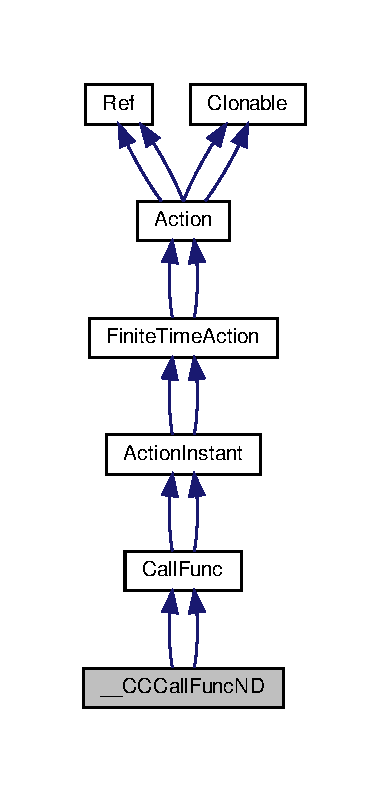
\includegraphics[width=187pt]{class____CCCallFuncND__inherit__graph}
\end{center}
\end{figure}


Collaboration diagram for \+\_\+\+\_\+\+C\+C\+Call\+Func\+ND\+:
\nopagebreak
\begin{figure}[H]
\begin{center}
\leavevmode
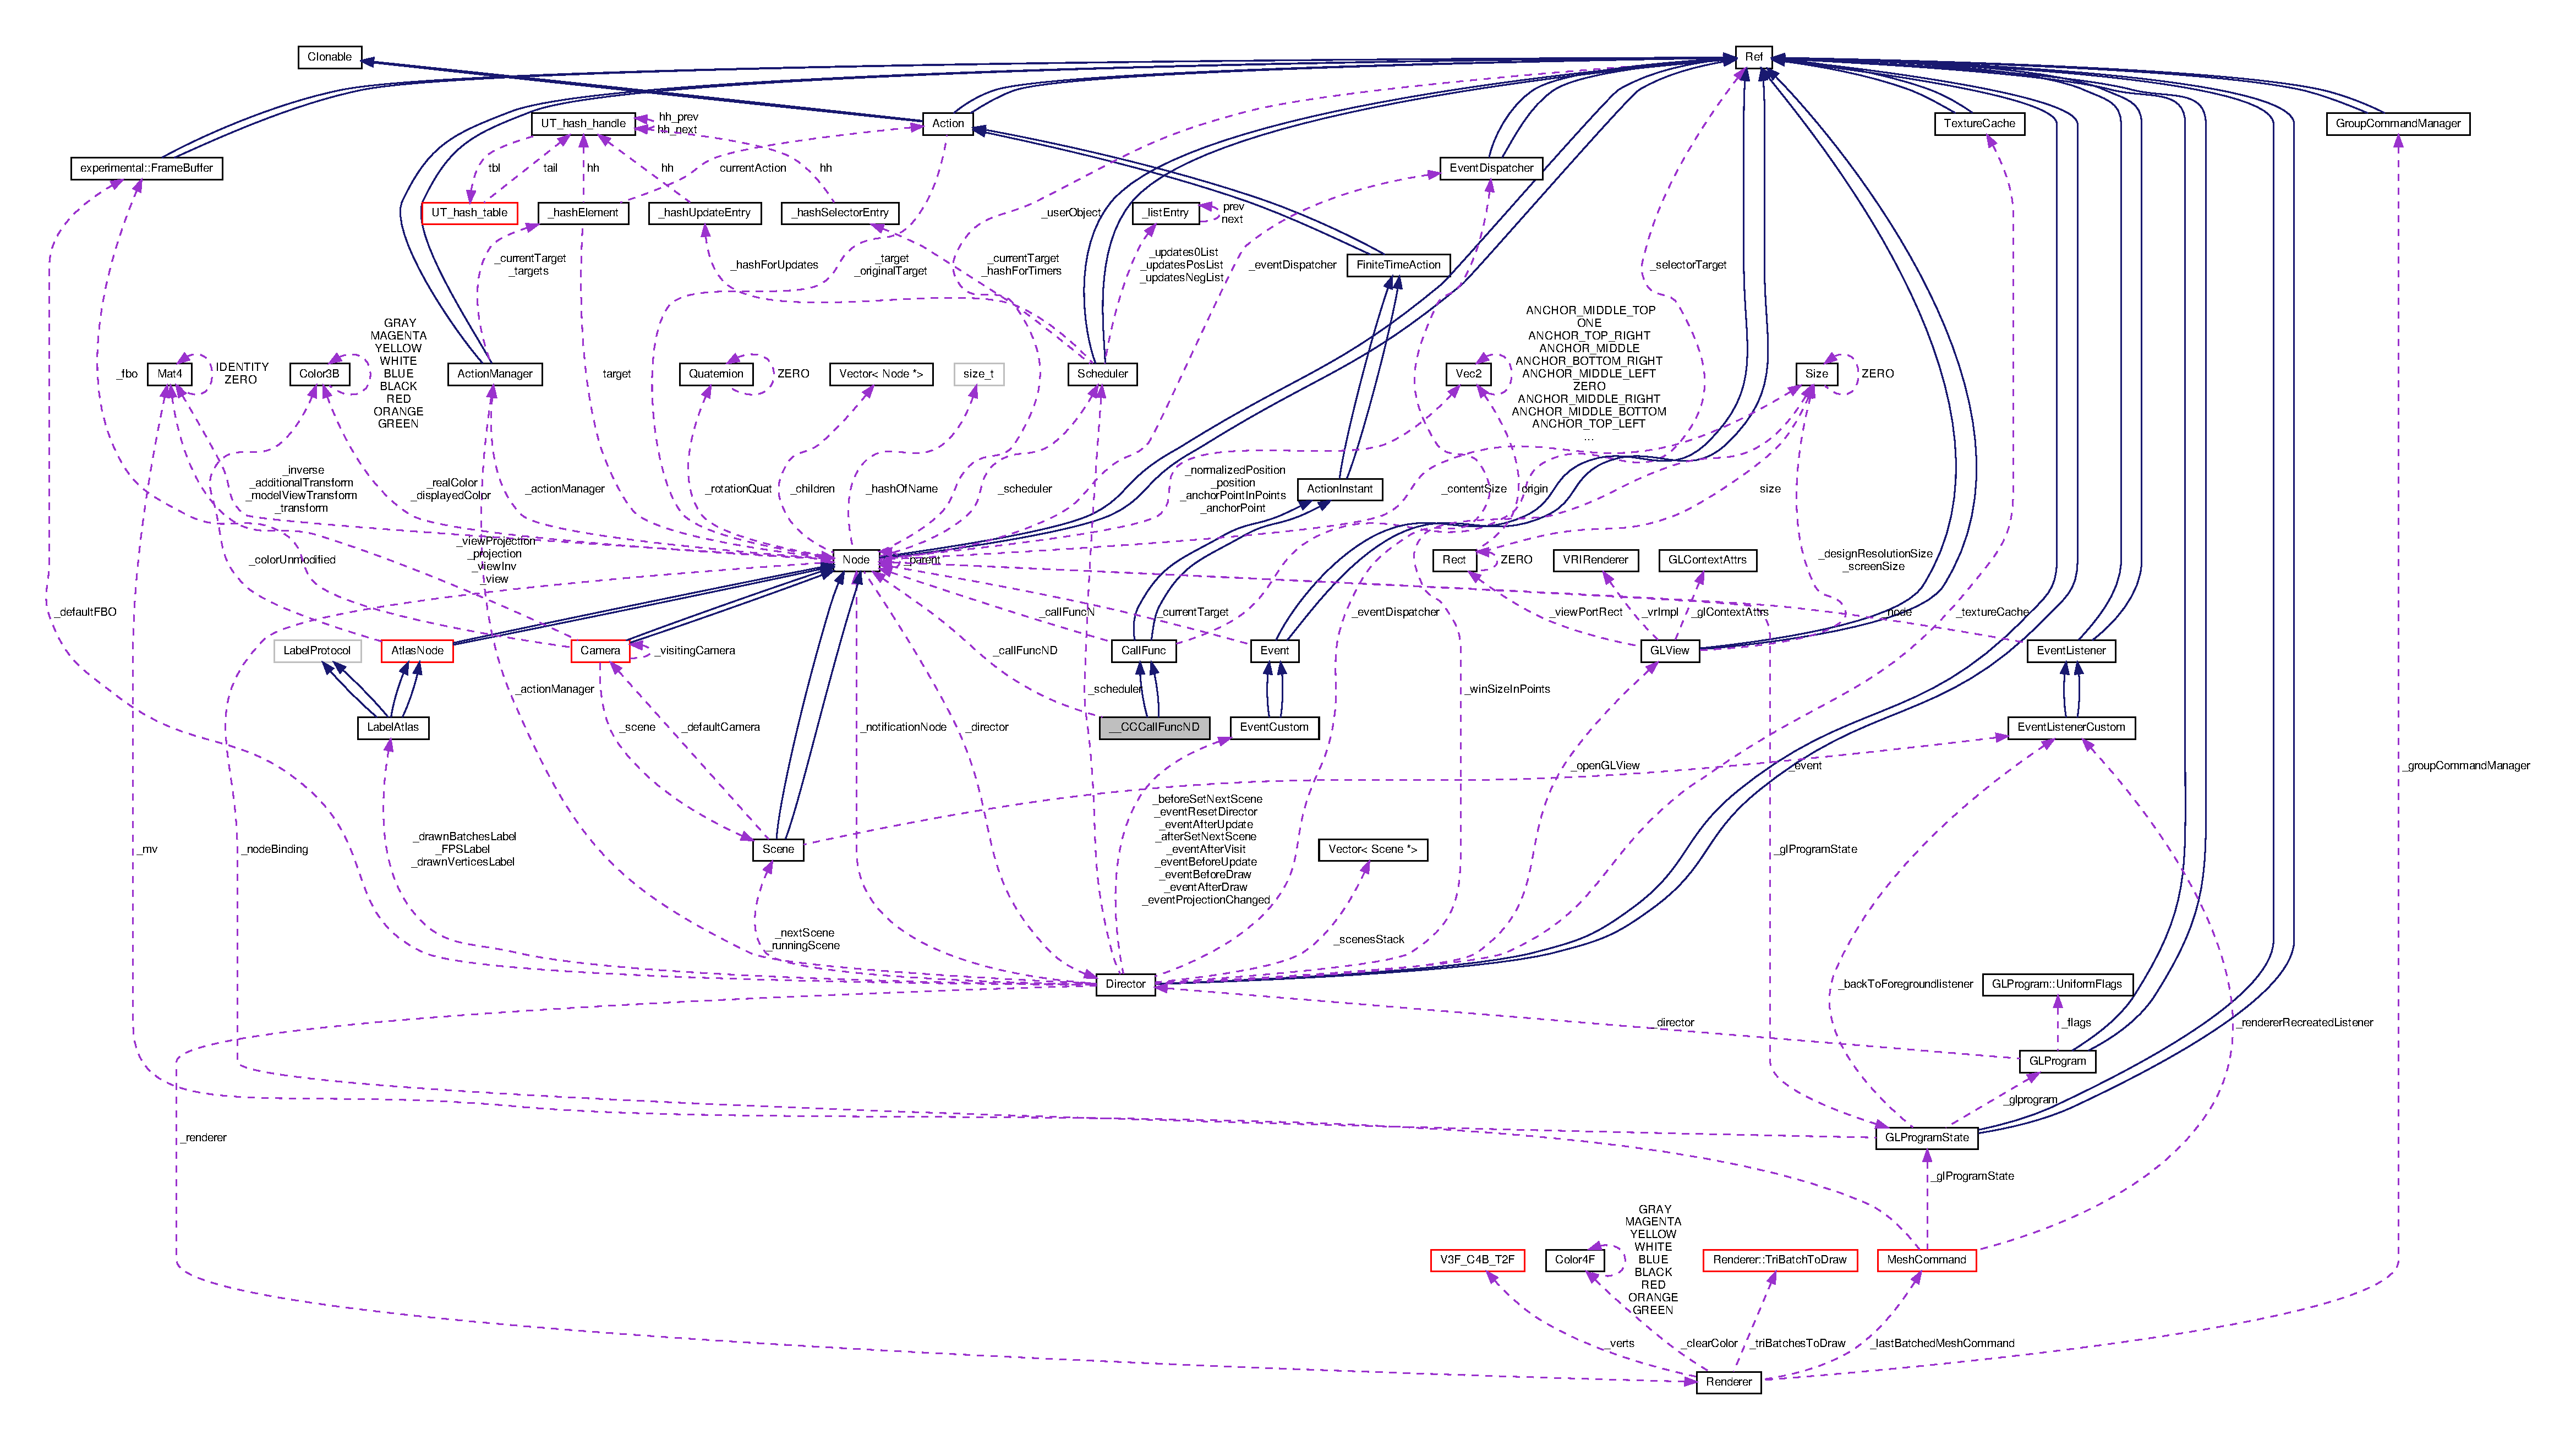
\includegraphics[width=350pt]{class____CCCallFuncND__coll__graph}
\end{center}
\end{figure}
\subsection*{Public Member Functions}
\begin{DoxyCompactItemize}
\item 
virtual \hyperlink{class____CCCallFuncND}{\+\_\+\+\_\+\+C\+C\+Call\+Func\+ND} $\ast$ \hyperlink{class____CCCallFuncND_a0b1d35734a49b6c12144e4b025fe84eb}{clone} () const override
\item 
virtual void \hyperlink{class____CCCallFuncND_a1f60a7eca795f5ab5e551c7512b9791a}{execute} () override
\item 
virtual \hyperlink{class____CCCallFuncND}{\+\_\+\+\_\+\+C\+C\+Call\+Func\+ND} $\ast$ \hyperlink{class____CCCallFuncND_a1c4550d2841e8c7469f2831bedfa2726}{clone} () const override
\item 
virtual void \hyperlink{class____CCCallFuncND_a9e3c2cd81860d951e9a83ce29cc40f38}{execute} () override
\end{DoxyCompactItemize}
\subsection*{Static Public Member Functions}
\begin{DoxyCompactItemize}
\item 
static C\+C\+\_\+\+D\+E\+P\+R\+E\+C\+A\+T\+E\+D\+\_\+\+A\+T\+T\+R\+I\+B\+U\+TE \hyperlink{class____CCCallFuncND}{\+\_\+\+\_\+\+C\+C\+Call\+Func\+ND} $\ast$ \hyperlink{class____CCCallFuncND_abcc540f0a13929a4c7115928d6ec5020}{create} (\hyperlink{classRef}{Ref} $\ast$target, S\+E\+L\+\_\+\+Call\+Func\+ND selector, void $\ast$d)
\item 
static C\+C\+\_\+\+D\+E\+P\+R\+E\+C\+A\+T\+E\+D\+\_\+\+A\+T\+T\+R\+I\+B\+U\+TE \hyperlink{class____CCCallFuncND}{\+\_\+\+\_\+\+C\+C\+Call\+Func\+ND} $\ast$ \hyperlink{class____CCCallFuncND_a42dc11764a281241d84f86dbd0ea7c1b}{create} (\hyperlink{classRef}{Ref} $\ast$target, S\+E\+L\+\_\+\+Call\+Func\+ND selector, void $\ast$d)
\end{DoxyCompactItemize}
\subsection*{Public Attributes}
\begin{DoxyCompactItemize}
\item 
\mbox{\Hypertarget{class____CCCallFuncND_a8e47248aa40718ef17f10165dc3d3a32}\label{class____CCCallFuncND_a8e47248aa40718ef17f10165dc3d3a32}} 
\hyperlink{_2cocos2d_2cocos_2base_2ccConfig_8h_a25ef1314f97c35a2ed3d029b0ead6da0}{C\+C\+\_\+\+C\+O\+N\+S\+T\+R\+U\+C\+T\+O\+R\+\_\+\+A\+C\+C\+E\+SS} {\bfseries \+\_\+\+\_\+pad0\+\_\+\+\_\+}\+: \hyperlink{class____CCCallFuncND}{\+\_\+\+\_\+\+C\+C\+Call\+Func\+ND}() \{\} virtual $\sim$\hyperlink{class____CCCallFuncND}{\+\_\+\+\_\+\+C\+C\+Call\+Func\+ND}() \{\} bool \hyperlink{classCallFunc_a68a7834d7931d5439faf49ca6e955dd7}{init\+With\+Target}(\hyperlink{classRef}{Ref}$\ast$ target
\item 
\mbox{\Hypertarget{class____CCCallFuncND_aeb2b7369b7596436ea9c92668ae2d653}\label{class____CCCallFuncND_aeb2b7369b7596436ea9c92668ae2d653}} 
\hyperlink{_2cocos2d_2cocos_2base_2ccConfig_8h_a25ef1314f97c35a2ed3d029b0ead6da0}{C\+C\+\_\+\+C\+O\+N\+S\+T\+R\+U\+C\+T\+O\+R\+\_\+\+A\+C\+C\+E\+SS} S\+E\+L\+\_\+\+Call\+Func\+ND {\bfseries selector}
\item 
\mbox{\Hypertarget{class____CCCallFuncND_af8022787c42afb712edf7ad6d6111f33}\label{class____CCCallFuncND_af8022787c42afb712edf7ad6d6111f33}} 
\hyperlink{_2cocos2d_2cocos_2base_2ccConfig_8h_a25ef1314f97c35a2ed3d029b0ead6da0}{C\+C\+\_\+\+C\+O\+N\+S\+T\+R\+U\+C\+T\+O\+R\+\_\+\+A\+C\+C\+E\+SS} S\+E\+L\+\_\+\+Call\+Func\+ND void $\ast$ {\bfseries d}
\end{DoxyCompactItemize}
\subsection*{Protected Attributes}
\begin{DoxyCompactItemize}
\item 
\mbox{\Hypertarget{class____CCCallFuncND_a6d5e354b8374d079d8fe1d56a0fd8a06}\label{class____CCCallFuncND_a6d5e354b8374d079d8fe1d56a0fd8a06}} 
S\+E\+L\+\_\+\+Call\+Func\+ND {\bfseries \+\_\+call\+Func\+ND}
\item 
\mbox{\Hypertarget{class____CCCallFuncND_a82ca053186a71178dbb78b5058809d18}\label{class____CCCallFuncND_a82ca053186a71178dbb78b5058809d18}} 
void $\ast$ {\bfseries \+\_\+data}
\end{DoxyCompactItemize}
\subsection*{Additional Inherited Members}


\subsection{Detailed Description}
Calls a \textquotesingle{}callback\textquotesingle{} with the node as the first argument and the 2nd argument is data. ND means\+: \hyperlink{classNode}{Node} and \hyperlink{classData}{Data}. \hyperlink{classData}{Data} is void $\ast$, so it could be anything.  NA. 

\begin{DoxyRefDesc}{Deprecated}
\item[\hyperlink{deprecated__deprecated000011}{Deprecated}]Please use \hyperlink{classCallFuncN}{Call\+FuncN} instead. \end{DoxyRefDesc}


\begin{DoxyRefDesc}{Deprecated}
\item[\hyperlink{deprecated__deprecated000241}{Deprecated}]Please use \hyperlink{classCallFuncN}{Call\+FuncN} instead. \end{DoxyRefDesc}


\subsection{Member Function Documentation}
\mbox{\Hypertarget{class____CCCallFuncND_a0b1d35734a49b6c12144e4b025fe84eb}\label{class____CCCallFuncND_a0b1d35734a49b6c12144e4b025fe84eb}} 
\index{\+\_\+\+\_\+\+C\+C\+Call\+Func\+ND@{\+\_\+\+\_\+\+C\+C\+Call\+Func\+ND}!clone@{clone}}
\index{clone@{clone}!\+\_\+\+\_\+\+C\+C\+Call\+Func\+ND@{\+\_\+\+\_\+\+C\+C\+Call\+Func\+ND}}
\subsubsection{\texorpdfstring{clone()}{clone()}\hspace{0.1cm}{\footnotesize\ttfamily [1/2]}}
{\footnotesize\ttfamily \hyperlink{class____CCCallFuncND}{\+\_\+\+\_\+\+C\+C\+Call\+Func\+ND} $\ast$ \+\_\+\+\_\+\+C\+C\+Call\+Func\+N\+D\+::clone (\begin{DoxyParamCaption}\item[{void}]{ }\end{DoxyParamCaption}) const\hspace{0.3cm}{\ttfamily [override]}, {\ttfamily [virtual]}}

Returns a clone of action.

\begin{DoxyReturn}{Returns}
A clone action. 
\end{DoxyReturn}


Reimplemented from \hyperlink{classCallFunc_a87c2d0fecf4d8ae9d4b58a28e594daf0}{Call\+Func}.

\mbox{\Hypertarget{class____CCCallFuncND_a1c4550d2841e8c7469f2831bedfa2726}\label{class____CCCallFuncND_a1c4550d2841e8c7469f2831bedfa2726}} 
\index{\+\_\+\+\_\+\+C\+C\+Call\+Func\+ND@{\+\_\+\+\_\+\+C\+C\+Call\+Func\+ND}!clone@{clone}}
\index{clone@{clone}!\+\_\+\+\_\+\+C\+C\+Call\+Func\+ND@{\+\_\+\+\_\+\+C\+C\+Call\+Func\+ND}}
\subsubsection{\texorpdfstring{clone()}{clone()}\hspace{0.1cm}{\footnotesize\ttfamily [2/2]}}
{\footnotesize\ttfamily virtual \hyperlink{class____CCCallFuncND}{\+\_\+\+\_\+\+C\+C\+Call\+Func\+ND}$\ast$ \+\_\+\+\_\+\+C\+C\+Call\+Func\+N\+D\+::clone (\begin{DoxyParamCaption}\item[{void}]{ }\end{DoxyParamCaption}) const\hspace{0.3cm}{\ttfamily [override]}, {\ttfamily [virtual]}}

Returns a clone of action.

\begin{DoxyReturn}{Returns}
A clone action. 
\end{DoxyReturn}


Reimplemented from \hyperlink{classCallFunc_a87c2d0fecf4d8ae9d4b58a28e594daf0}{Call\+Func}.

\mbox{\Hypertarget{class____CCCallFuncND_abcc540f0a13929a4c7115928d6ec5020}\label{class____CCCallFuncND_abcc540f0a13929a4c7115928d6ec5020}} 
\index{\+\_\+\+\_\+\+C\+C\+Call\+Func\+ND@{\+\_\+\+\_\+\+C\+C\+Call\+Func\+ND}!create@{create}}
\index{create@{create}!\+\_\+\+\_\+\+C\+C\+Call\+Func\+ND@{\+\_\+\+\_\+\+C\+C\+Call\+Func\+ND}}
\subsubsection{\texorpdfstring{create()}{create()}\hspace{0.1cm}{\footnotesize\ttfamily [1/2]}}
{\footnotesize\ttfamily \hyperlink{class____CCCallFuncND}{\+\_\+\+\_\+\+C\+C\+Call\+Func\+ND} $\ast$ \+\_\+\+\_\+\+C\+C\+Call\+Func\+N\+D\+::create (\begin{DoxyParamCaption}\item[{\hyperlink{classRef}{Ref} $\ast$}]{target,  }\item[{S\+E\+L\+\_\+\+Call\+Func\+ND}]{selector,  }\item[{void $\ast$}]{d }\end{DoxyParamCaption})\hspace{0.3cm}{\ttfamily [static]}}

Creates the action with the callback and the data to pass as an argument.


\begin{DoxyParams}{Parameters}
{\em target} & A certain target. \\
\hline
{\em selector} & The callback need to be executed. \\
\hline
{\em d} & \hyperlink{classData}{Data}, is void$\ast$ type. \\
\hline
\end{DoxyParams}
\begin{DoxyReturn}{Returns}
An autoreleased \hyperlink{class____CCCallFuncND}{\+\_\+\+\_\+\+C\+C\+Call\+Func\+ND} object. 
\end{DoxyReturn}
\mbox{\Hypertarget{class____CCCallFuncND_a42dc11764a281241d84f86dbd0ea7c1b}\label{class____CCCallFuncND_a42dc11764a281241d84f86dbd0ea7c1b}} 
\index{\+\_\+\+\_\+\+C\+C\+Call\+Func\+ND@{\+\_\+\+\_\+\+C\+C\+Call\+Func\+ND}!create@{create}}
\index{create@{create}!\+\_\+\+\_\+\+C\+C\+Call\+Func\+ND@{\+\_\+\+\_\+\+C\+C\+Call\+Func\+ND}}
\subsubsection{\texorpdfstring{create()}{create()}\hspace{0.1cm}{\footnotesize\ttfamily [2/2]}}
{\footnotesize\ttfamily static C\+C\+\_\+\+D\+E\+P\+R\+E\+C\+A\+T\+E\+D\+\_\+\+A\+T\+T\+R\+I\+B\+U\+TE \hyperlink{class____CCCallFuncND}{\+\_\+\+\_\+\+C\+C\+Call\+Func\+ND}$\ast$ \+\_\+\+\_\+\+C\+C\+Call\+Func\+N\+D\+::create (\begin{DoxyParamCaption}\item[{\hyperlink{classRef}{Ref} $\ast$}]{target,  }\item[{S\+E\+L\+\_\+\+Call\+Func\+ND}]{selector,  }\item[{void $\ast$}]{d }\end{DoxyParamCaption})\hspace{0.3cm}{\ttfamily [static]}}

Creates the action with the callback and the data to pass as an argument.


\begin{DoxyParams}{Parameters}
{\em target} & A certain target. \\
\hline
{\em selector} & The callback need to be executed. \\
\hline
{\em d} & \hyperlink{classData}{Data}, is void$\ast$ type. \\
\hline
\end{DoxyParams}
\begin{DoxyReturn}{Returns}
An autoreleased \hyperlink{class____CCCallFuncND}{\+\_\+\+\_\+\+C\+C\+Call\+Func\+ND} object. 
\end{DoxyReturn}
\mbox{\Hypertarget{class____CCCallFuncND_a1f60a7eca795f5ab5e551c7512b9791a}\label{class____CCCallFuncND_a1f60a7eca795f5ab5e551c7512b9791a}} 
\index{\+\_\+\+\_\+\+C\+C\+Call\+Func\+ND@{\+\_\+\+\_\+\+C\+C\+Call\+Func\+ND}!execute@{execute}}
\index{execute@{execute}!\+\_\+\+\_\+\+C\+C\+Call\+Func\+ND@{\+\_\+\+\_\+\+C\+C\+Call\+Func\+ND}}
\subsubsection{\texorpdfstring{execute()}{execute()}\hspace{0.1cm}{\footnotesize\ttfamily [1/2]}}
{\footnotesize\ttfamily void \+\_\+\+\_\+\+C\+C\+Call\+Func\+N\+D\+::execute (\begin{DoxyParamCaption}{ }\end{DoxyParamCaption})\hspace{0.3cm}{\ttfamily [override]}, {\ttfamily [virtual]}}

Executes the callback. 

Reimplemented from \hyperlink{classCallFunc_a9a66dcb09103983ddab2ee2c89ae5c0e}{Call\+Func}.

\mbox{\Hypertarget{class____CCCallFuncND_a9e3c2cd81860d951e9a83ce29cc40f38}\label{class____CCCallFuncND_a9e3c2cd81860d951e9a83ce29cc40f38}} 
\index{\+\_\+\+\_\+\+C\+C\+Call\+Func\+ND@{\+\_\+\+\_\+\+C\+C\+Call\+Func\+ND}!execute@{execute}}
\index{execute@{execute}!\+\_\+\+\_\+\+C\+C\+Call\+Func\+ND@{\+\_\+\+\_\+\+C\+C\+Call\+Func\+ND}}
\subsubsection{\texorpdfstring{execute()}{execute()}\hspace{0.1cm}{\footnotesize\ttfamily [2/2]}}
{\footnotesize\ttfamily virtual void \+\_\+\+\_\+\+C\+C\+Call\+Func\+N\+D\+::execute (\begin{DoxyParamCaption}{ }\end{DoxyParamCaption})\hspace{0.3cm}{\ttfamily [override]}, {\ttfamily [virtual]}}

Executes the callback. 

Reimplemented from \hyperlink{classCallFunc_a9a66dcb09103983ddab2ee2c89ae5c0e}{Call\+Func}.



The documentation for this class was generated from the following files\+:\begin{DoxyCompactItemize}
\item 
/home/pmx/git/\+P\+M\+X/\+Simu\+Cocos/cocos2d/cocos/2d/C\+C\+Action\+Instant.\+h\item 
/home/pmx/git/\+P\+M\+X/\+Simu\+Cocos/cocos2d/cocos/2d/C\+C\+Action\+Instant.\+cpp\end{DoxyCompactItemize}

\hypertarget{class____CCCallFuncO}{}\section{\+\_\+\+\_\+\+C\+C\+Call\+FuncO Class Reference}
\label{class____CCCallFuncO}\index{\+\_\+\+\_\+\+C\+C\+Call\+FuncO@{\+\_\+\+\_\+\+C\+C\+Call\+FuncO}}


Calls a \textquotesingle{}callback\textquotesingle{} with an object as the first argument. O means Object.  




{\ttfamily \#include $<$C\+C\+Action\+Instant.\+h$>$}



Inheritance diagram for \+\_\+\+\_\+\+C\+C\+Call\+FuncO\+:
\nopagebreak
\begin{figure}[H]
\begin{center}
\leavevmode
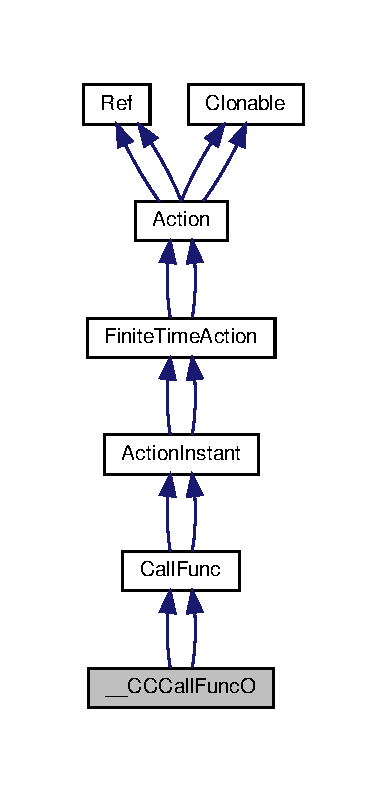
\includegraphics[width=186pt]{class____CCCallFuncO__inherit__graph}
\end{center}
\end{figure}


Collaboration diagram for \+\_\+\+\_\+\+C\+C\+Call\+FuncO\+:
\nopagebreak
\begin{figure}[H]
\begin{center}
\leavevmode
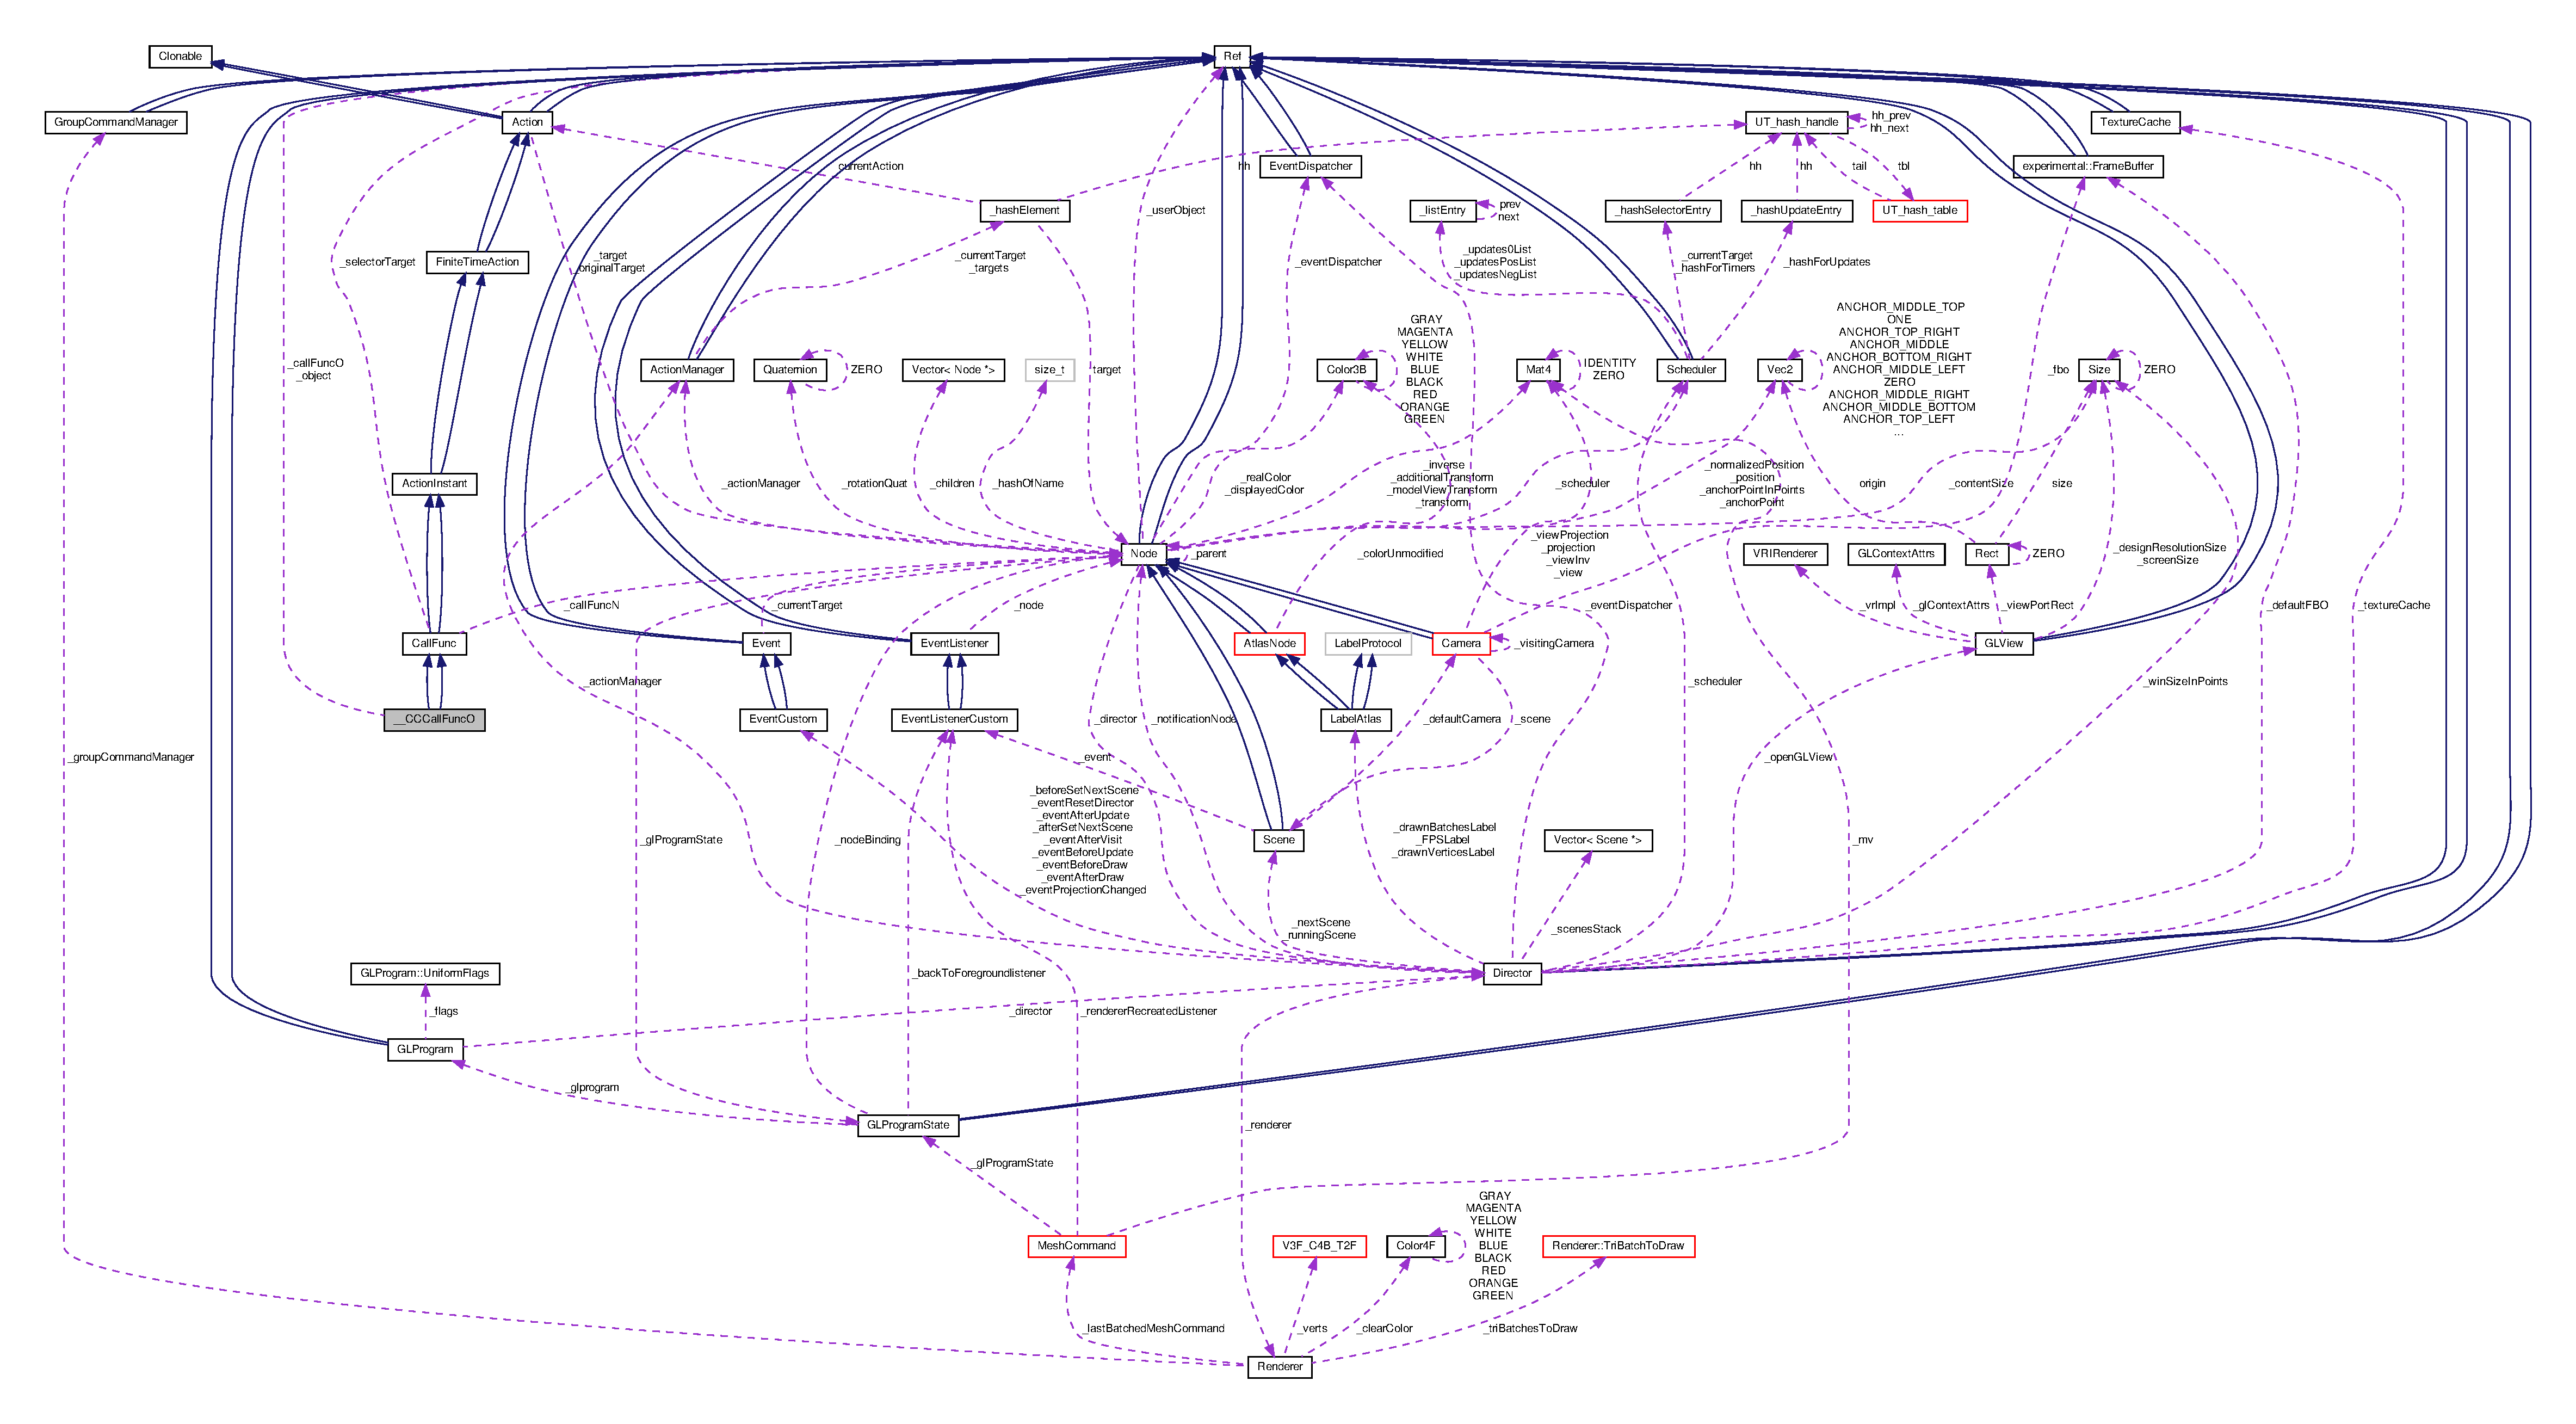
\includegraphics[width=350pt]{class____CCCallFuncO__coll__graph}
\end{center}
\end{figure}
\subsection*{Public Member Functions}
\begin{DoxyCompactItemize}
\item 
virtual \hyperlink{class____CCCallFuncO}{\+\_\+\+\_\+\+C\+C\+Call\+FuncO} $\ast$ \hyperlink{class____CCCallFuncO_ae01d43dd90e3052c278e1431097c2b2e}{clone} () const override
\item 
virtual void \hyperlink{class____CCCallFuncO_aab83cafa03038b765f3752c6f2f307b1}{execute} () override
\item 
\mbox{\Hypertarget{class____CCCallFuncO_a211793e0feb2d109059357928aa7047d}\label{class____CCCallFuncO_a211793e0feb2d109059357928aa7047d}} 
\hyperlink{classRef}{Ref} $\ast$ {\bfseries get\+Object} () const
\item 
\mbox{\Hypertarget{class____CCCallFuncO_aa44dc2f0350c0600ab043b9f55dec192}\label{class____CCCallFuncO_aa44dc2f0350c0600ab043b9f55dec192}} 
void {\bfseries set\+Object} (\hyperlink{classRef}{Ref} $\ast$obj)
\item 
bool \hyperlink{class____CCCallFuncO_ae295b34998b51d676c97cb71662443bb}{init\+With\+Target} (\hyperlink{classRef}{Ref} $\ast$target, S\+E\+L\+\_\+\+Call\+FuncO selector, \hyperlink{classRef}{Ref} $\ast$object)
\item 
virtual \hyperlink{class____CCCallFuncO}{\+\_\+\+\_\+\+C\+C\+Call\+FuncO} $\ast$ \hyperlink{class____CCCallFuncO_a83119c4b99a7f866556d0e2945ebd61b}{clone} () const override
\item 
virtual void \hyperlink{class____CCCallFuncO_a89e4727ade4f68268afad8040fe08e81}{execute} () override
\item 
\mbox{\Hypertarget{class____CCCallFuncO_a135e471aa4303ff3d2a4d26b9ef2ce56}\label{class____CCCallFuncO_a135e471aa4303ff3d2a4d26b9ef2ce56}} 
\hyperlink{classRef}{Ref} $\ast$ {\bfseries get\+Object} () const
\item 
\mbox{\Hypertarget{class____CCCallFuncO_aa44dc2f0350c0600ab043b9f55dec192}\label{class____CCCallFuncO_aa44dc2f0350c0600ab043b9f55dec192}} 
void {\bfseries set\+Object} (\hyperlink{classRef}{Ref} $\ast$obj)
\item 
bool \hyperlink{class____CCCallFuncO_ae295b34998b51d676c97cb71662443bb}{init\+With\+Target} (\hyperlink{classRef}{Ref} $\ast$target, S\+E\+L\+\_\+\+Call\+FuncO selector, \hyperlink{classRef}{Ref} $\ast$object)
\end{DoxyCompactItemize}
\subsection*{Static Public Member Functions}
\begin{DoxyCompactItemize}
\item 
static C\+C\+\_\+\+D\+E\+P\+R\+E\+C\+A\+T\+E\+D\+\_\+\+A\+T\+T\+R\+I\+B\+U\+TE \hyperlink{class____CCCallFuncO}{\+\_\+\+\_\+\+C\+C\+Call\+FuncO} $\ast$ \hyperlink{class____CCCallFuncO_ad617de0f264ccc8d5450507bd4e0f3f1}{create} (\hyperlink{classRef}{Ref} $\ast$target, S\+E\+L\+\_\+\+Call\+FuncO selector, \hyperlink{classRef}{Ref} $\ast$object)
\item 
static C\+C\+\_\+\+D\+E\+P\+R\+E\+C\+A\+T\+E\+D\+\_\+\+A\+T\+T\+R\+I\+B\+U\+TE \hyperlink{class____CCCallFuncO}{\+\_\+\+\_\+\+C\+C\+Call\+FuncO} $\ast$ \hyperlink{class____CCCallFuncO_abed2b1821bb83ebb41d8404b2ccf63b0}{create} (\hyperlink{classRef}{Ref} $\ast$target, S\+E\+L\+\_\+\+Call\+FuncO selector, \hyperlink{classRef}{Ref} $\ast$object)
\end{DoxyCompactItemize}
\subsection*{Public Attributes}
\begin{DoxyCompactItemize}
\item 
\mbox{\Hypertarget{class____CCCallFuncO_ad164f2a04950a9c5d6aa126b6b0f47e9}\label{class____CCCallFuncO_ad164f2a04950a9c5d6aa126b6b0f47e9}} 
\hyperlink{_2cocos2d_2cocos_2base_2ccConfig_8h_a25ef1314f97c35a2ed3d029b0ead6da0}{C\+C\+\_\+\+C\+O\+N\+S\+T\+R\+U\+C\+T\+O\+R\+\_\+\+A\+C\+C\+E\+SS} {\bfseries \+\_\+\+\_\+pad0\+\_\+\+\_\+}\+: \hyperlink{class____CCCallFuncO}{\+\_\+\+\_\+\+C\+C\+Call\+FuncO}()
\end{DoxyCompactItemize}
\subsection*{Protected Attributes}
\begin{DoxyCompactItemize}
\item 
\hyperlink{classRef}{Ref} $\ast$ \hyperlink{class____CCCallFuncO_a445f552253c55eb32d26138ca02632e3}{\+\_\+object}
\item 
\mbox{\Hypertarget{class____CCCallFuncO_a5dc397aa67a0439a7b21170645aacf40}\label{class____CCCallFuncO_a5dc397aa67a0439a7b21170645aacf40}} 
S\+E\+L\+\_\+\+Call\+FuncO {\bfseries \+\_\+call\+FuncO}
\end{DoxyCompactItemize}
\subsection*{Additional Inherited Members}


\subsection{Detailed Description}
Calls a \textquotesingle{}callback\textquotesingle{} with an object as the first argument. O means Object. 

\begin{DoxyRefDesc}{Deprecated}
\item[\hyperlink{deprecated__deprecated000012}{Deprecated}]Please use \hyperlink{classCallFuncN}{Call\+FuncN} instead. \end{DoxyRefDesc}
\begin{DoxySince}{Since}
v0.\+99.\+5  NA
\end{DoxySince}
\begin{DoxyRefDesc}{Deprecated}
\item[\hyperlink{deprecated__deprecated000242}{Deprecated}]Please use \hyperlink{classCallFuncN}{Call\+FuncN} instead. \end{DoxyRefDesc}
\begin{DoxySince}{Since}
v0.\+99.\+5  NA 
\end{DoxySince}


\subsection{Member Function Documentation}
\mbox{\Hypertarget{class____CCCallFuncO_ae01d43dd90e3052c278e1431097c2b2e}\label{class____CCCallFuncO_ae01d43dd90e3052c278e1431097c2b2e}} 
\index{\+\_\+\+\_\+\+C\+C\+Call\+FuncO@{\+\_\+\+\_\+\+C\+C\+Call\+FuncO}!clone@{clone}}
\index{clone@{clone}!\+\_\+\+\_\+\+C\+C\+Call\+FuncO@{\+\_\+\+\_\+\+C\+C\+Call\+FuncO}}
\subsubsection{\texorpdfstring{clone()}{clone()}\hspace{0.1cm}{\footnotesize\ttfamily [1/2]}}
{\footnotesize\ttfamily \hyperlink{class____CCCallFuncO}{\+\_\+\+\_\+\+C\+C\+Call\+FuncO} $\ast$ \+\_\+\+\_\+\+C\+C\+Call\+Func\+O\+::clone (\begin{DoxyParamCaption}\item[{void}]{ }\end{DoxyParamCaption}) const\hspace{0.3cm}{\ttfamily [override]}, {\ttfamily [virtual]}}

Returns a clone of action.

\begin{DoxyReturn}{Returns}
A clone action. 
\end{DoxyReturn}


Reimplemented from \hyperlink{classCallFunc_a87c2d0fecf4d8ae9d4b58a28e594daf0}{Call\+Func}.

\mbox{\Hypertarget{class____CCCallFuncO_a83119c4b99a7f866556d0e2945ebd61b}\label{class____CCCallFuncO_a83119c4b99a7f866556d0e2945ebd61b}} 
\index{\+\_\+\+\_\+\+C\+C\+Call\+FuncO@{\+\_\+\+\_\+\+C\+C\+Call\+FuncO}!clone@{clone}}
\index{clone@{clone}!\+\_\+\+\_\+\+C\+C\+Call\+FuncO@{\+\_\+\+\_\+\+C\+C\+Call\+FuncO}}
\subsubsection{\texorpdfstring{clone()}{clone()}\hspace{0.1cm}{\footnotesize\ttfamily [2/2]}}
{\footnotesize\ttfamily virtual \hyperlink{class____CCCallFuncO}{\+\_\+\+\_\+\+C\+C\+Call\+FuncO}$\ast$ \+\_\+\+\_\+\+C\+C\+Call\+Func\+O\+::clone (\begin{DoxyParamCaption}\item[{void}]{ }\end{DoxyParamCaption}) const\hspace{0.3cm}{\ttfamily [override]}, {\ttfamily [virtual]}}

Returns a clone of action.

\begin{DoxyReturn}{Returns}
A clone action. 
\end{DoxyReturn}


Reimplemented from \hyperlink{classCallFunc_a87c2d0fecf4d8ae9d4b58a28e594daf0}{Call\+Func}.

\mbox{\Hypertarget{class____CCCallFuncO_ad617de0f264ccc8d5450507bd4e0f3f1}\label{class____CCCallFuncO_ad617de0f264ccc8d5450507bd4e0f3f1}} 
\index{\+\_\+\+\_\+\+C\+C\+Call\+FuncO@{\+\_\+\+\_\+\+C\+C\+Call\+FuncO}!create@{create}}
\index{create@{create}!\+\_\+\+\_\+\+C\+C\+Call\+FuncO@{\+\_\+\+\_\+\+C\+C\+Call\+FuncO}}
\subsubsection{\texorpdfstring{create()}{create()}\hspace{0.1cm}{\footnotesize\ttfamily [1/2]}}
{\footnotesize\ttfamily \hyperlink{class____CCCallFuncO}{\+\_\+\+\_\+\+C\+C\+Call\+FuncO} $\ast$ \+\_\+\+\_\+\+C\+C\+Call\+Func\+O\+::create (\begin{DoxyParamCaption}\item[{\hyperlink{classRef}{Ref} $\ast$}]{target,  }\item[{S\+E\+L\+\_\+\+Call\+FuncO}]{selector,  }\item[{\hyperlink{classRef}{Ref} $\ast$}]{object }\end{DoxyParamCaption})\hspace{0.3cm}{\ttfamily [static]}}

Creates the action with the callback. typedef void (\hyperlink{classRef}{Ref}\+:\+:{\itshape S\+E\+L\+\_\+\+Call\+FuncO)(\hyperlink{classRef}{Ref}});


\begin{DoxyParams}{Parameters}
{\em target} & A certain target. \\
\hline
{\em selector} & The callback need to be executed. \\
\hline
{\em object} & An object as the callback\textquotesingle{}s first argument. \\
\hline
\end{DoxyParams}
\begin{DoxyReturn}{Returns}
An autoreleased \hyperlink{class____CCCallFuncO}{\+\_\+\+\_\+\+C\+C\+Call\+FuncO} object. 
\end{DoxyReturn}
\mbox{\Hypertarget{class____CCCallFuncO_abed2b1821bb83ebb41d8404b2ccf63b0}\label{class____CCCallFuncO_abed2b1821bb83ebb41d8404b2ccf63b0}} 
\index{\+\_\+\+\_\+\+C\+C\+Call\+FuncO@{\+\_\+\+\_\+\+C\+C\+Call\+FuncO}!create@{create}}
\index{create@{create}!\+\_\+\+\_\+\+C\+C\+Call\+FuncO@{\+\_\+\+\_\+\+C\+C\+Call\+FuncO}}
\subsubsection{\texorpdfstring{create()}{create()}\hspace{0.1cm}{\footnotesize\ttfamily [2/2]}}
{\footnotesize\ttfamily static C\+C\+\_\+\+D\+E\+P\+R\+E\+C\+A\+T\+E\+D\+\_\+\+A\+T\+T\+R\+I\+B\+U\+TE \hyperlink{class____CCCallFuncO}{\+\_\+\+\_\+\+C\+C\+Call\+FuncO}$\ast$ \+\_\+\+\_\+\+C\+C\+Call\+Func\+O\+::create (\begin{DoxyParamCaption}\item[{\hyperlink{classRef}{Ref} $\ast$}]{target,  }\item[{S\+E\+L\+\_\+\+Call\+FuncO}]{selector,  }\item[{\hyperlink{classRef}{Ref} $\ast$}]{object }\end{DoxyParamCaption})\hspace{0.3cm}{\ttfamily [static]}}

Creates the action with the callback. typedef void (\hyperlink{classRef}{Ref}\+:\+:{\itshape S\+E\+L\+\_\+\+Call\+FuncO)(\hyperlink{classRef}{Ref}});


\begin{DoxyParams}{Parameters}
{\em target} & A certain target. \\
\hline
{\em selector} & The callback need to be executed. \\
\hline
{\em object} & An object as the callback\textquotesingle{}s first argument. \\
\hline
\end{DoxyParams}
\begin{DoxyReturn}{Returns}
An autoreleased \hyperlink{class____CCCallFuncO}{\+\_\+\+\_\+\+C\+C\+Call\+FuncO} object. 
\end{DoxyReturn}
\mbox{\Hypertarget{class____CCCallFuncO_aab83cafa03038b765f3752c6f2f307b1}\label{class____CCCallFuncO_aab83cafa03038b765f3752c6f2f307b1}} 
\index{\+\_\+\+\_\+\+C\+C\+Call\+FuncO@{\+\_\+\+\_\+\+C\+C\+Call\+FuncO}!execute@{execute}}
\index{execute@{execute}!\+\_\+\+\_\+\+C\+C\+Call\+FuncO@{\+\_\+\+\_\+\+C\+C\+Call\+FuncO}}
\subsubsection{\texorpdfstring{execute()}{execute()}\hspace{0.1cm}{\footnotesize\ttfamily [1/2]}}
{\footnotesize\ttfamily void \+\_\+\+\_\+\+C\+C\+Call\+Func\+O\+::execute (\begin{DoxyParamCaption}{ }\end{DoxyParamCaption})\hspace{0.3cm}{\ttfamily [override]}, {\ttfamily [virtual]}}

Executes the callback. 

Reimplemented from \hyperlink{classCallFunc_a9a66dcb09103983ddab2ee2c89ae5c0e}{Call\+Func}.

\mbox{\Hypertarget{class____CCCallFuncO_a89e4727ade4f68268afad8040fe08e81}\label{class____CCCallFuncO_a89e4727ade4f68268afad8040fe08e81}} 
\index{\+\_\+\+\_\+\+C\+C\+Call\+FuncO@{\+\_\+\+\_\+\+C\+C\+Call\+FuncO}!execute@{execute}}
\index{execute@{execute}!\+\_\+\+\_\+\+C\+C\+Call\+FuncO@{\+\_\+\+\_\+\+C\+C\+Call\+FuncO}}
\subsubsection{\texorpdfstring{execute()}{execute()}\hspace{0.1cm}{\footnotesize\ttfamily [2/2]}}
{\footnotesize\ttfamily virtual void \+\_\+\+\_\+\+C\+C\+Call\+Func\+O\+::execute (\begin{DoxyParamCaption}{ }\end{DoxyParamCaption})\hspace{0.3cm}{\ttfamily [override]}, {\ttfamily [virtual]}}

Executes the callback. 

Reimplemented from \hyperlink{classCallFunc_a9a66dcb09103983ddab2ee2c89ae5c0e}{Call\+Func}.

\mbox{\Hypertarget{class____CCCallFuncO_ae295b34998b51d676c97cb71662443bb}\label{class____CCCallFuncO_ae295b34998b51d676c97cb71662443bb}} 
\index{\+\_\+\+\_\+\+C\+C\+Call\+FuncO@{\+\_\+\+\_\+\+C\+C\+Call\+FuncO}!init\+With\+Target@{init\+With\+Target}}
\index{init\+With\+Target@{init\+With\+Target}!\+\_\+\+\_\+\+C\+C\+Call\+FuncO@{\+\_\+\+\_\+\+C\+C\+Call\+FuncO}}
\subsubsection{\texorpdfstring{init\+With\+Target()}{initWithTarget()}\hspace{0.1cm}{\footnotesize\ttfamily [1/2]}}
{\footnotesize\ttfamily bool \+\_\+\+\_\+\+C\+C\+Call\+Func\+O\+::init\+With\+Target (\begin{DoxyParamCaption}\item[{\hyperlink{classRef}{Ref} $\ast$}]{target,  }\item[{S\+E\+L\+\_\+\+Call\+FuncO}]{selector,  }\item[{\hyperlink{classRef}{Ref} $\ast$}]{object }\end{DoxyParamCaption})}

initializes the action with the callback

typedef void (\hyperlink{classRef}{Ref}\+:\+:{\itshape S\+E\+L\+\_\+\+Call\+FuncO)(\hyperlink{classRef}{Ref}}); \mbox{\Hypertarget{class____CCCallFuncO_ae295b34998b51d676c97cb71662443bb}\label{class____CCCallFuncO_ae295b34998b51d676c97cb71662443bb}} 
\index{\+\_\+\+\_\+\+C\+C\+Call\+FuncO@{\+\_\+\+\_\+\+C\+C\+Call\+FuncO}!init\+With\+Target@{init\+With\+Target}}
\index{init\+With\+Target@{init\+With\+Target}!\+\_\+\+\_\+\+C\+C\+Call\+FuncO@{\+\_\+\+\_\+\+C\+C\+Call\+FuncO}}
\subsubsection{\texorpdfstring{init\+With\+Target()}{initWithTarget()}\hspace{0.1cm}{\footnotesize\ttfamily [2/2]}}
{\footnotesize\ttfamily bool \+\_\+\+\_\+\+C\+C\+Call\+Func\+O\+::init\+With\+Target (\begin{DoxyParamCaption}\item[{\hyperlink{classRef}{Ref} $\ast$}]{target,  }\item[{S\+E\+L\+\_\+\+Call\+FuncO}]{selector,  }\item[{\hyperlink{classRef}{Ref} $\ast$}]{object }\end{DoxyParamCaption})}

initializes the action with the callback

typedef void (\hyperlink{classRef}{Ref}\+:\+:{\itshape S\+E\+L\+\_\+\+Call\+FuncO)(\hyperlink{classRef}{Ref}}); 

\subsection{Member Data Documentation}
\mbox{\Hypertarget{class____CCCallFuncO_a445f552253c55eb32d26138ca02632e3}\label{class____CCCallFuncO_a445f552253c55eb32d26138ca02632e3}} 
\index{\+\_\+\+\_\+\+C\+C\+Call\+FuncO@{\+\_\+\+\_\+\+C\+C\+Call\+FuncO}!\+\_\+object@{\+\_\+object}}
\index{\+\_\+object@{\+\_\+object}!\+\_\+\+\_\+\+C\+C\+Call\+FuncO@{\+\_\+\+\_\+\+C\+C\+Call\+FuncO}}
\subsubsection{\texorpdfstring{\+\_\+object}{\_object}}
{\footnotesize\ttfamily \hyperlink{classRef}{Ref} $\ast$ \+\_\+\+\_\+\+C\+C\+Call\+Func\+O\+::\+\_\+object\hspace{0.3cm}{\ttfamily [protected]}}

object to be passed as argument 

The documentation for this class was generated from the following files\+:\begin{DoxyCompactItemize}
\item 
/home/pmx/git/\+P\+M\+X/\+Simu\+Cocos/cocos2d/cocos/2d/C\+C\+Action\+Instant.\+h\item 
/home/pmx/git/\+P\+M\+X/\+Simu\+Cocos/cocos2d/cocos/2d/C\+C\+Action\+Instant.\+cpp\end{DoxyCompactItemize}

\hypertarget{union____GLXEvent}{}\section{\+\_\+\+\_\+\+G\+L\+X\+Event Union Reference}
\label{union____GLXEvent}\index{\+\_\+\+\_\+\+G\+L\+X\+Event@{\+\_\+\+\_\+\+G\+L\+X\+Event}}


Collaboration diagram for \+\_\+\+\_\+\+G\+L\+X\+Event\+:
\nopagebreak
\begin{figure}[H]
\begin{center}
\leavevmode
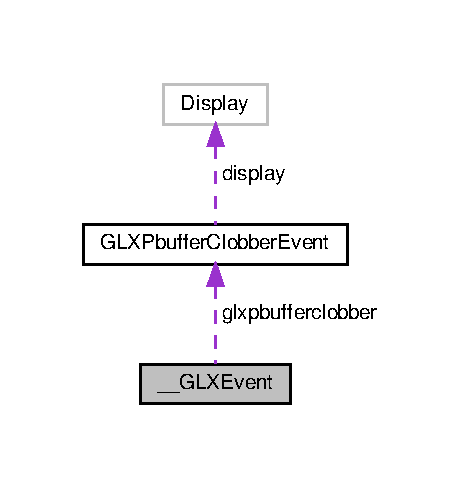
\includegraphics[width=222pt]{union____GLXEvent__coll__graph}
\end{center}
\end{figure}
\subsection*{Public Attributes}
\begin{DoxyCompactItemize}
\item 
\mbox{\Hypertarget{union____GLXEvent_ada5880e2b424bcb2f60a411aaf713fae}\label{union____GLXEvent_ada5880e2b424bcb2f60a411aaf713fae}} 
\hyperlink{structGLXPbufferClobberEvent}{G\+L\+X\+Pbuffer\+Clobber\+Event} {\bfseries glxpbufferclobber}
\item 
\mbox{\Hypertarget{union____GLXEvent_ab9dd153b4b59af2a1fc3b10807f0f481}\label{union____GLXEvent_ab9dd153b4b59af2a1fc3b10807f0f481}} 
long {\bfseries pad} \mbox{[}24\mbox{]}
\end{DoxyCompactItemize}


The documentation for this union was generated from the following file\+:\begin{DoxyCompactItemize}
\item 
/home/pmx/git/\+P\+M\+X/\+Simu\+Cocos/cocos2d/external/win32-\/specific/gles/include/\+O\+G\+L\+E\+S/\+G\+L/glxew.\+h\end{DoxyCompactItemize}

\hypertarget{class____LayerRGBA}{}\section{\+\_\+\+\_\+\+Layer\+R\+G\+BA Class Reference}
\label{class____LayerRGBA}\index{\+\_\+\+\_\+\+Layer\+R\+G\+BA@{\+\_\+\+\_\+\+Layer\+R\+G\+BA}}


Layer\+R\+G\+BA is a subclass of \hyperlink{classLayer}{Layer} that implements the R\+G\+B\+A\+Protocol protocol using a solid color as the background.  




{\ttfamily \#include $<$C\+C\+Layer.\+h$>$}



Inheritance diagram for \+\_\+\+\_\+\+Layer\+R\+G\+BA\+:
\nopagebreak
\begin{figure}[H]
\begin{center}
\leavevmode
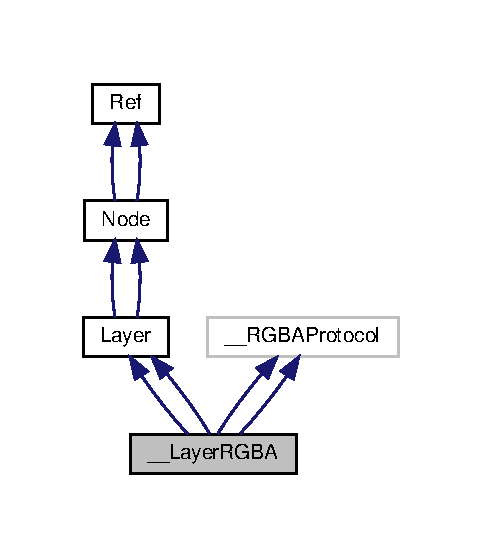
\includegraphics[width=232pt]{class____LayerRGBA__inherit__graph}
\end{center}
\end{figure}


Collaboration diagram for \+\_\+\+\_\+\+Layer\+R\+G\+BA\+:
\nopagebreak
\begin{figure}[H]
\begin{center}
\leavevmode
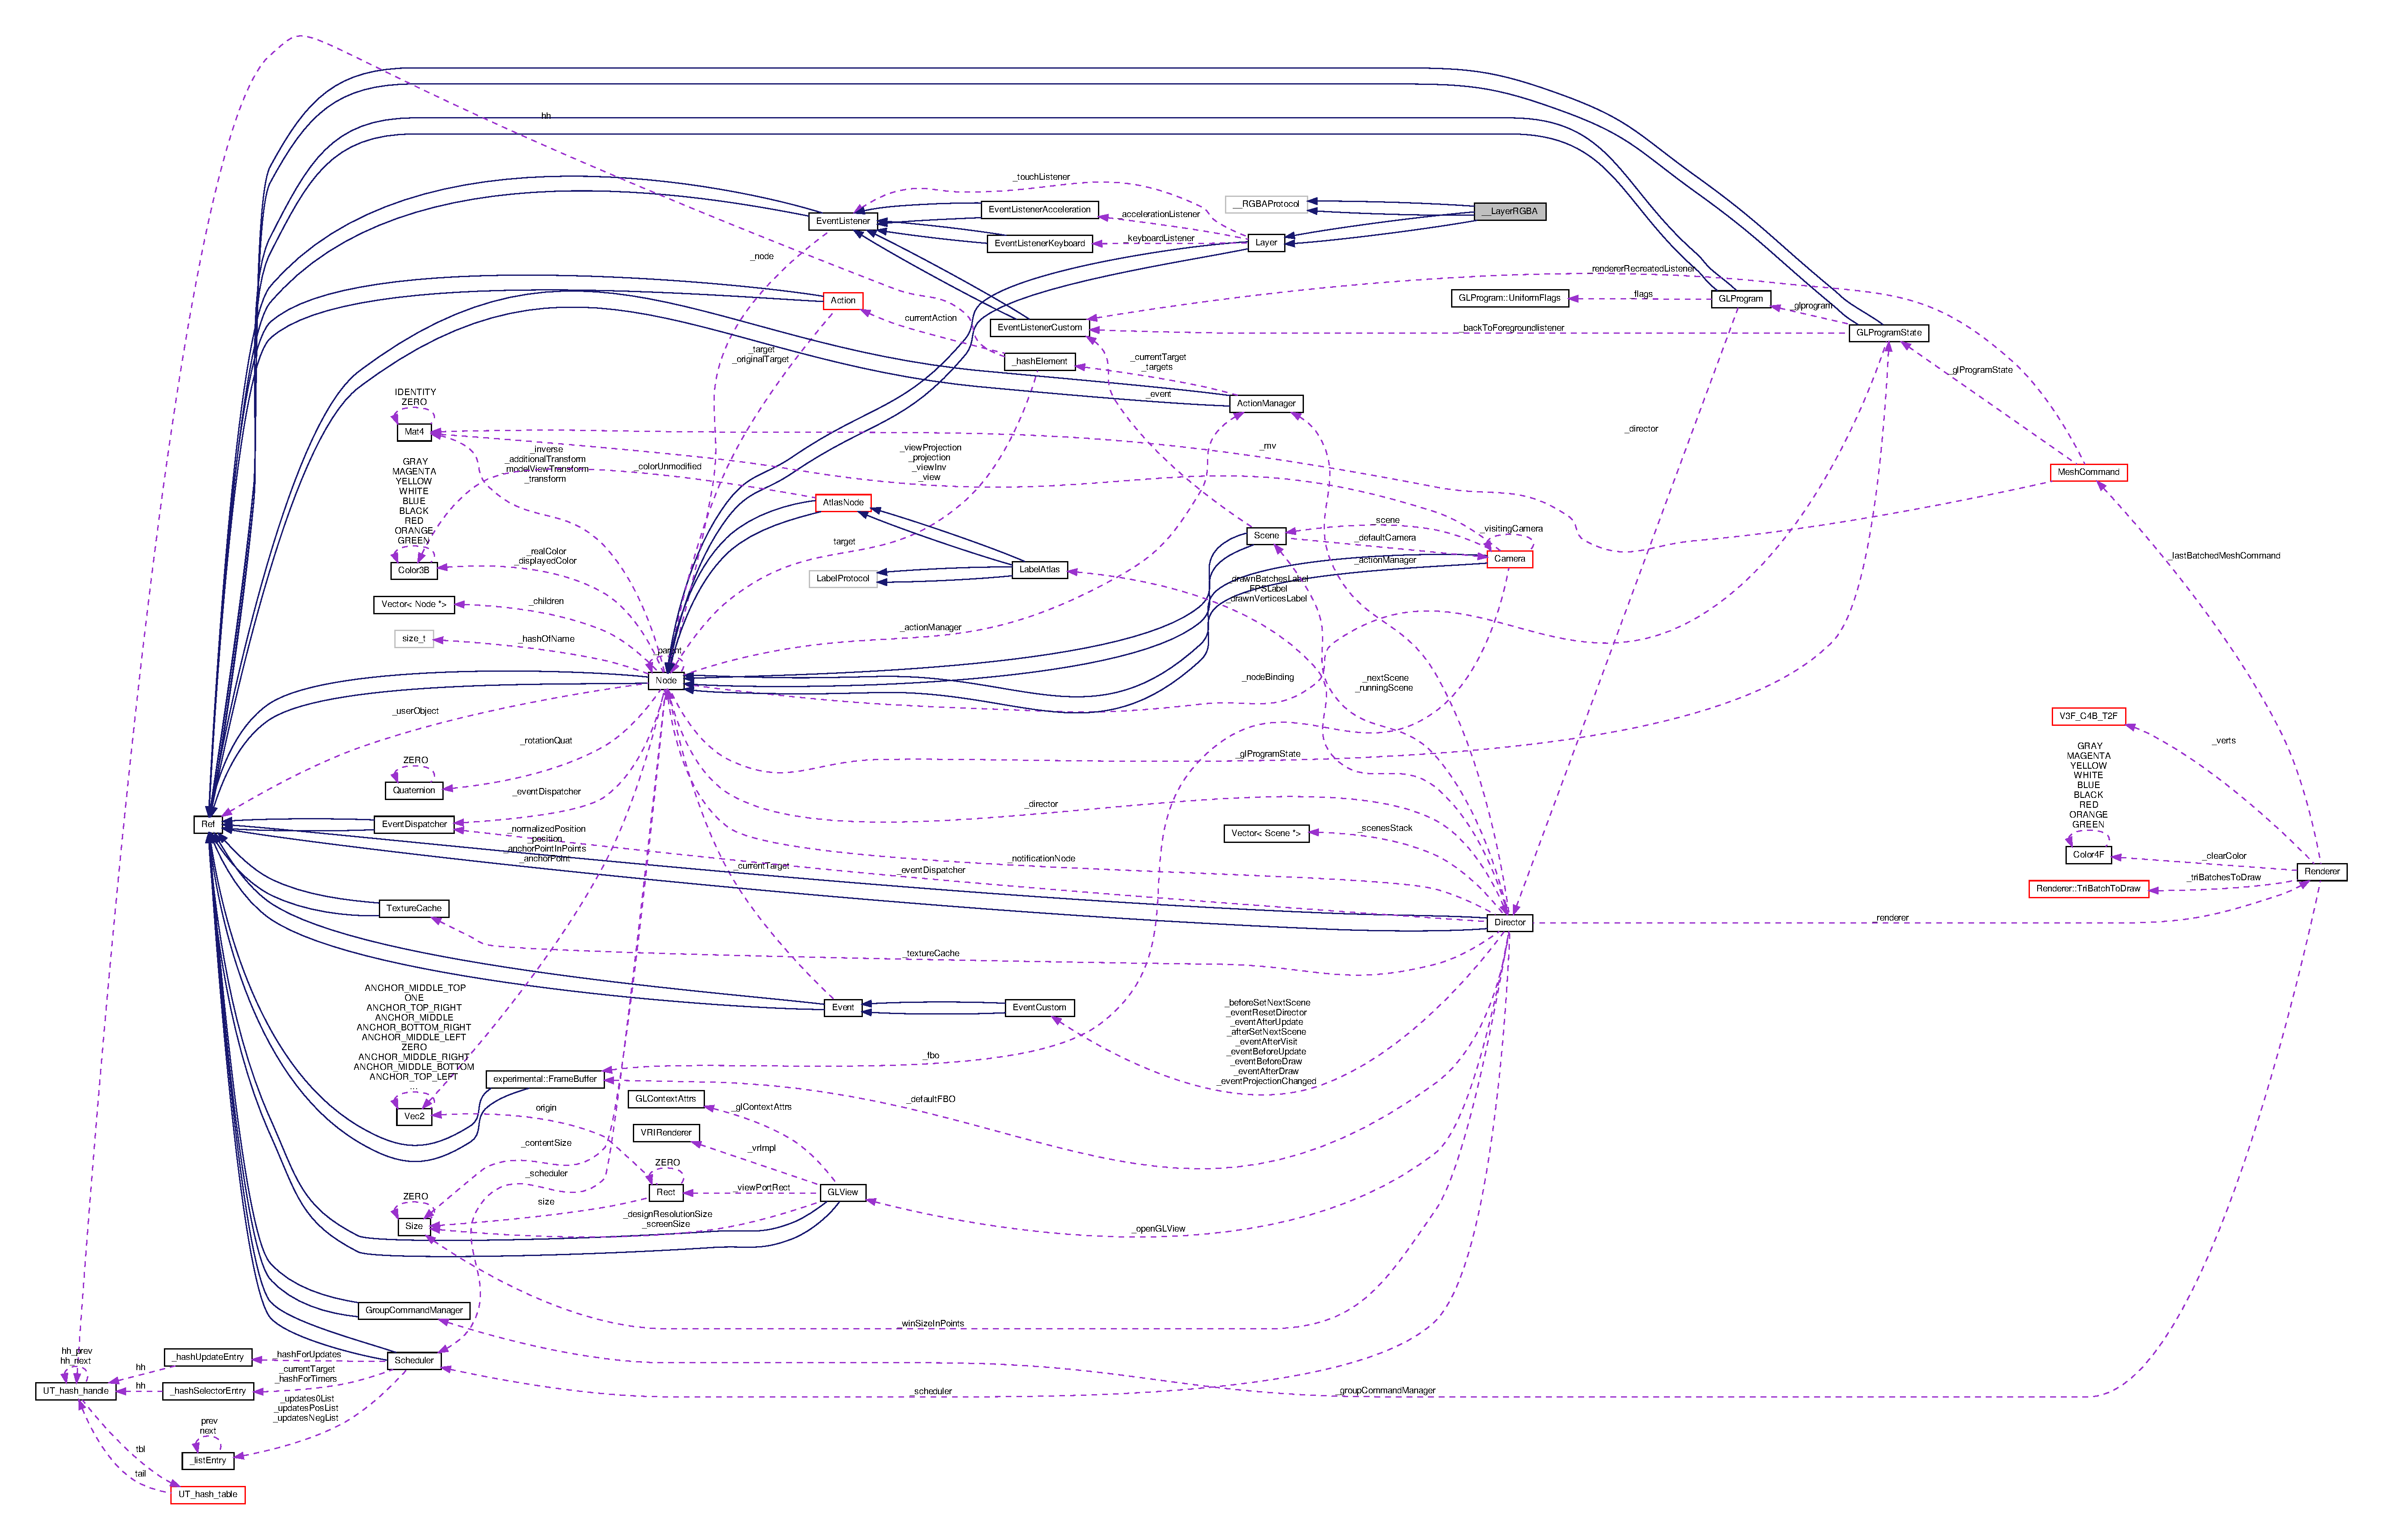
\includegraphics[width=350pt]{class____LayerRGBA__coll__graph}
\end{center}
\end{figure}
\subsection*{Public Member Functions}
\begin{DoxyCompactItemize}
\item 
\mbox{\Hypertarget{class____LayerRGBA_abc16c928f11f7890c5203eb2a101c13f}\label{class____LayerRGBA_abc16c928f11f7890c5203eb2a101c13f}} 
{\bfseries C\+R\+E\+A\+T\+E\+\_\+\+F\+U\+NC} (\hyperlink{class____LayerRGBA}{\+\_\+\+\_\+\+Layer\+R\+G\+BA})
\item 
virtual G\+Lubyte \hyperlink{class____LayerRGBA_a61d071eeff8bc1c46520611261f5dd1a}{get\+Opacity} () const override
\item 
virtual G\+Lubyte \hyperlink{class____LayerRGBA_a3c94f57397e6c53127d1176d14ab25fe}{get\+Displayed\+Opacity} () const override
\item 
virtual void \hyperlink{class____LayerRGBA_a1b172623ee7486835fd189672d19d8d7}{set\+Opacity} (G\+Lubyte opacity) override
\item 
virtual void \hyperlink{class____LayerRGBA_a53e78a19fb9780fec84476f1bce1d3f6}{update\+Displayed\+Opacity} (G\+Lubyte parent\+Opacity) override
\item 
virtual bool \hyperlink{class____LayerRGBA_a3dd348cf39ca267d7c0ebb5000dce45e}{is\+Cascade\+Opacity\+Enabled} () const override
\item 
virtual void \hyperlink{class____LayerRGBA_ab25a8418f19d14a064f8c8072b3468a5}{set\+Cascade\+Opacity\+Enabled} (bool cascade\+Opacity\+Enabled) override
\item 
virtual const \hyperlink{structColor3B}{Color3B} \& \hyperlink{class____LayerRGBA_ab14530232cae13fbf4399e0a47daa315}{get\+Color} () const override
\item 
virtual const \hyperlink{structColor3B}{Color3B} \& \hyperlink{class____LayerRGBA_a621d9a8fe47abd33ec00bd3754bf6ec2}{get\+Displayed\+Color} () const override
\item 
virtual void \hyperlink{class____LayerRGBA_aed346ddd9f7f7eab1e3d1417fa9a9831}{set\+Color} (const \hyperlink{structColor3B}{Color3B} \&color) override
\item 
virtual void \hyperlink{class____LayerRGBA_aa0406779f58fc6586f51129bee7aed36}{update\+Displayed\+Color} (const \hyperlink{structColor3B}{Color3B} \&parent\+Color) override
\item 
virtual bool \hyperlink{class____LayerRGBA_abc02efad9eb89df47e6a0365dc9c784e}{is\+Cascade\+Color\+Enabled} () const override
\item 
virtual void \hyperlink{class____LayerRGBA_a6559d3d54c2a7a8a35873390043b0aa6}{set\+Cascade\+Color\+Enabled} (bool cascade\+Color\+Enabled) override
\item 
virtual void \hyperlink{class____LayerRGBA_a04037a60b1a1f9d5ba2760252ad2da35}{set\+Opacity\+Modify\+R\+GB} (bool b\+Value) override
\item 
virtual bool \hyperlink{class____LayerRGBA_a014dba2472f2708ad4493e97ca5999b0}{is\+Opacity\+Modify\+R\+GB} () const override
\item 
\mbox{\Hypertarget{class____LayerRGBA_abc16c928f11f7890c5203eb2a101c13f}\label{class____LayerRGBA_abc16c928f11f7890c5203eb2a101c13f}} 
{\bfseries C\+R\+E\+A\+T\+E\+\_\+\+F\+U\+NC} (\hyperlink{class____LayerRGBA}{\+\_\+\+\_\+\+Layer\+R\+G\+BA})
\item 
virtual G\+Lubyte \hyperlink{class____LayerRGBA_a61d071eeff8bc1c46520611261f5dd1a}{get\+Opacity} () const override
\item 
virtual G\+Lubyte \hyperlink{class____LayerRGBA_a3c94f57397e6c53127d1176d14ab25fe}{get\+Displayed\+Opacity} () const override
\item 
virtual void \hyperlink{class____LayerRGBA_a1b172623ee7486835fd189672d19d8d7}{set\+Opacity} (G\+Lubyte opacity) override
\item 
virtual void \hyperlink{class____LayerRGBA_a53e78a19fb9780fec84476f1bce1d3f6}{update\+Displayed\+Opacity} (G\+Lubyte parent\+Opacity) override
\item 
virtual bool \hyperlink{class____LayerRGBA_a3dd348cf39ca267d7c0ebb5000dce45e}{is\+Cascade\+Opacity\+Enabled} () const override
\item 
virtual void \hyperlink{class____LayerRGBA_ab25a8418f19d14a064f8c8072b3468a5}{set\+Cascade\+Opacity\+Enabled} (bool cascade\+Opacity\+Enabled) override
\item 
virtual const \hyperlink{structColor3B}{Color3B} \& \hyperlink{class____LayerRGBA_ab14530232cae13fbf4399e0a47daa315}{get\+Color} () const override
\item 
virtual const \hyperlink{structColor3B}{Color3B} \& \hyperlink{class____LayerRGBA_a621d9a8fe47abd33ec00bd3754bf6ec2}{get\+Displayed\+Color} () const override
\item 
virtual void \hyperlink{class____LayerRGBA_aed346ddd9f7f7eab1e3d1417fa9a9831}{set\+Color} (const \hyperlink{structColor3B}{Color3B} \&color) override
\item 
virtual void \hyperlink{class____LayerRGBA_aa0406779f58fc6586f51129bee7aed36}{update\+Displayed\+Color} (const \hyperlink{structColor3B}{Color3B} \&parent\+Color) override
\item 
virtual bool \hyperlink{class____LayerRGBA_abc02efad9eb89df47e6a0365dc9c784e}{is\+Cascade\+Color\+Enabled} () const override
\item 
virtual void \hyperlink{class____LayerRGBA_a6559d3d54c2a7a8a35873390043b0aa6}{set\+Cascade\+Color\+Enabled} (bool cascade\+Color\+Enabled) override
\item 
virtual void \hyperlink{class____LayerRGBA_a04037a60b1a1f9d5ba2760252ad2da35}{set\+Opacity\+Modify\+R\+GB} (bool b\+Value) override
\item 
virtual bool \hyperlink{class____LayerRGBA_a014dba2472f2708ad4493e97ca5999b0}{is\+Opacity\+Modify\+R\+GB} () const override
\end{DoxyCompactItemize}
\subsection*{Public Attributes}
\begin{DoxyCompactItemize}
\item 
\mbox{\Hypertarget{class____LayerRGBA_ad3e60331e6f49ec9a830919963f8de45}\label{class____LayerRGBA_ad3e60331e6f49ec9a830919963f8de45}} 
\hyperlink{_2cocos2d_2cocos_2base_2ccConfig_8h_a25ef1314f97c35a2ed3d029b0ead6da0}{C\+C\+\_\+\+C\+O\+N\+S\+T\+R\+U\+C\+T\+O\+R\+\_\+\+A\+C\+C\+E\+SS} {\bfseries \+\_\+\+\_\+pad0\+\_\+\+\_\+}\+: \hyperlink{class____LayerRGBA}{\+\_\+\+\_\+\+Layer\+R\+G\+BA}()
\end{DoxyCompactItemize}
\subsection*{Additional Inherited Members}


\subsection{Detailed Description}
Layer\+R\+G\+BA is a subclass of \hyperlink{classLayer}{Layer} that implements the R\+G\+B\+A\+Protocol protocol using a solid color as the background. 

All features from \hyperlink{classLayer}{Layer} are valid, plus the following new features that propagate into children that conform to the R\+G\+B\+A\+Protocol\+:
\begin{DoxyItemize}
\item opacity
\item R\+GB colors \begin{DoxySince}{Since}
2.\+1  NA 
\end{DoxySince}

\end{DoxyItemize}

\subsection{Member Function Documentation}
\mbox{\Hypertarget{class____LayerRGBA_ab14530232cae13fbf4399e0a47daa315}\label{class____LayerRGBA_ab14530232cae13fbf4399e0a47daa315}} 
\index{\+\_\+\+\_\+\+Layer\+R\+G\+BA@{\+\_\+\+\_\+\+Layer\+R\+G\+BA}!get\+Color@{get\+Color}}
\index{get\+Color@{get\+Color}!\+\_\+\+\_\+\+Layer\+R\+G\+BA@{\+\_\+\+\_\+\+Layer\+R\+G\+BA}}
\subsubsection{\texorpdfstring{get\+Color()}{getColor()}\hspace{0.1cm}{\footnotesize\ttfamily [1/2]}}
{\footnotesize\ttfamily virtual const \hyperlink{structColor3B}{Color3B}\& \+\_\+\+\_\+\+Layer\+R\+G\+B\+A\+::get\+Color (\begin{DoxyParamCaption}\item[{void}]{ }\end{DoxyParamCaption}) const\hspace{0.3cm}{\ttfamily [inline]}, {\ttfamily [override]}, {\ttfamily [virtual]}}

Query node\textquotesingle{}s color value. \begin{DoxyReturn}{Returns}
A \hyperlink{structColor3B}{Color3B} color value. 
\end{DoxyReturn}


Reimplemented from \hyperlink{classNode_a06721d272f5a59e02e355d95be25bb99}{Node}.

\mbox{\Hypertarget{class____LayerRGBA_ab14530232cae13fbf4399e0a47daa315}\label{class____LayerRGBA_ab14530232cae13fbf4399e0a47daa315}} 
\index{\+\_\+\+\_\+\+Layer\+R\+G\+BA@{\+\_\+\+\_\+\+Layer\+R\+G\+BA}!get\+Color@{get\+Color}}
\index{get\+Color@{get\+Color}!\+\_\+\+\_\+\+Layer\+R\+G\+BA@{\+\_\+\+\_\+\+Layer\+R\+G\+BA}}
\subsubsection{\texorpdfstring{get\+Color()}{getColor()}\hspace{0.1cm}{\footnotesize\ttfamily [2/2]}}
{\footnotesize\ttfamily virtual const \hyperlink{structColor3B}{Color3B}\& \+\_\+\+\_\+\+Layer\+R\+G\+B\+A\+::get\+Color (\begin{DoxyParamCaption}\item[{void}]{ }\end{DoxyParamCaption}) const\hspace{0.3cm}{\ttfamily [inline]}, {\ttfamily [override]}, {\ttfamily [virtual]}}

Query node\textquotesingle{}s color value. \begin{DoxyReturn}{Returns}
A \hyperlink{structColor3B}{Color3B} color value. 
\end{DoxyReturn}


Reimplemented from \hyperlink{classNode_a06721d272f5a59e02e355d95be25bb99}{Node}.

\mbox{\Hypertarget{class____LayerRGBA_a621d9a8fe47abd33ec00bd3754bf6ec2}\label{class____LayerRGBA_a621d9a8fe47abd33ec00bd3754bf6ec2}} 
\index{\+\_\+\+\_\+\+Layer\+R\+G\+BA@{\+\_\+\+\_\+\+Layer\+R\+G\+BA}!get\+Displayed\+Color@{get\+Displayed\+Color}}
\index{get\+Displayed\+Color@{get\+Displayed\+Color}!\+\_\+\+\_\+\+Layer\+R\+G\+BA@{\+\_\+\+\_\+\+Layer\+R\+G\+BA}}
\subsubsection{\texorpdfstring{get\+Displayed\+Color()}{getDisplayedColor()}\hspace{0.1cm}{\footnotesize\ttfamily [1/2]}}
{\footnotesize\ttfamily virtual const \hyperlink{structColor3B}{Color3B}\& \+\_\+\+\_\+\+Layer\+R\+G\+B\+A\+::get\+Displayed\+Color (\begin{DoxyParamCaption}{ }\end{DoxyParamCaption}) const\hspace{0.3cm}{\ttfamily [inline]}, {\ttfamily [override]}, {\ttfamily [virtual]}}

Query node\textquotesingle{}s displayed color. \begin{DoxyReturn}{Returns}
A \hyperlink{structColor3B}{Color3B} color value. 
\end{DoxyReturn}


Reimplemented from \hyperlink{classNode_a899760bbad414bfbe9fb51473e99c3eb}{Node}.

\mbox{\Hypertarget{class____LayerRGBA_a621d9a8fe47abd33ec00bd3754bf6ec2}\label{class____LayerRGBA_a621d9a8fe47abd33ec00bd3754bf6ec2}} 
\index{\+\_\+\+\_\+\+Layer\+R\+G\+BA@{\+\_\+\+\_\+\+Layer\+R\+G\+BA}!get\+Displayed\+Color@{get\+Displayed\+Color}}
\index{get\+Displayed\+Color@{get\+Displayed\+Color}!\+\_\+\+\_\+\+Layer\+R\+G\+BA@{\+\_\+\+\_\+\+Layer\+R\+G\+BA}}
\subsubsection{\texorpdfstring{get\+Displayed\+Color()}{getDisplayedColor()}\hspace{0.1cm}{\footnotesize\ttfamily [2/2]}}
{\footnotesize\ttfamily virtual const \hyperlink{structColor3B}{Color3B}\& \+\_\+\+\_\+\+Layer\+R\+G\+B\+A\+::get\+Displayed\+Color (\begin{DoxyParamCaption}{ }\end{DoxyParamCaption}) const\hspace{0.3cm}{\ttfamily [inline]}, {\ttfamily [override]}, {\ttfamily [virtual]}}

Query node\textquotesingle{}s displayed color. \begin{DoxyReturn}{Returns}
A \hyperlink{structColor3B}{Color3B} color value. 
\end{DoxyReturn}


Reimplemented from \hyperlink{classNode_a899760bbad414bfbe9fb51473e99c3eb}{Node}.

\mbox{\Hypertarget{class____LayerRGBA_a3c94f57397e6c53127d1176d14ab25fe}\label{class____LayerRGBA_a3c94f57397e6c53127d1176d14ab25fe}} 
\index{\+\_\+\+\_\+\+Layer\+R\+G\+BA@{\+\_\+\+\_\+\+Layer\+R\+G\+BA}!get\+Displayed\+Opacity@{get\+Displayed\+Opacity}}
\index{get\+Displayed\+Opacity@{get\+Displayed\+Opacity}!\+\_\+\+\_\+\+Layer\+R\+G\+BA@{\+\_\+\+\_\+\+Layer\+R\+G\+BA}}
\subsubsection{\texorpdfstring{get\+Displayed\+Opacity()}{getDisplayedOpacity()}\hspace{0.1cm}{\footnotesize\ttfamily [1/2]}}
{\footnotesize\ttfamily virtual G\+Lubyte \+\_\+\+\_\+\+Layer\+R\+G\+B\+A\+::get\+Displayed\+Opacity (\begin{DoxyParamCaption}{ }\end{DoxyParamCaption}) const\hspace{0.3cm}{\ttfamily [inline]}, {\ttfamily [override]}, {\ttfamily [virtual]}}

Return the node\textquotesingle{}s display opacity. The difference between opacity and displayed\+Opacity is\+: The displayed\+Opacity is what\textquotesingle{}s the final rendering opacity of node. \begin{DoxyReturn}{Returns}
A G\+Lubyte value. 
\end{DoxyReturn}


Reimplemented from \hyperlink{classNode_ac4f9c61560c8862ebdaecbf79bf8a1b6}{Node}.

\mbox{\Hypertarget{class____LayerRGBA_a3c94f57397e6c53127d1176d14ab25fe}\label{class____LayerRGBA_a3c94f57397e6c53127d1176d14ab25fe}} 
\index{\+\_\+\+\_\+\+Layer\+R\+G\+BA@{\+\_\+\+\_\+\+Layer\+R\+G\+BA}!get\+Displayed\+Opacity@{get\+Displayed\+Opacity}}
\index{get\+Displayed\+Opacity@{get\+Displayed\+Opacity}!\+\_\+\+\_\+\+Layer\+R\+G\+BA@{\+\_\+\+\_\+\+Layer\+R\+G\+BA}}
\subsubsection{\texorpdfstring{get\+Displayed\+Opacity()}{getDisplayedOpacity()}\hspace{0.1cm}{\footnotesize\ttfamily [2/2]}}
{\footnotesize\ttfamily virtual G\+Lubyte \+\_\+\+\_\+\+Layer\+R\+G\+B\+A\+::get\+Displayed\+Opacity (\begin{DoxyParamCaption}{ }\end{DoxyParamCaption}) const\hspace{0.3cm}{\ttfamily [inline]}, {\ttfamily [override]}, {\ttfamily [virtual]}}

Return the node\textquotesingle{}s display opacity. The difference between opacity and displayed\+Opacity is\+: The displayed\+Opacity is what\textquotesingle{}s the final rendering opacity of node. \begin{DoxyReturn}{Returns}
A G\+Lubyte value. 
\end{DoxyReturn}


Reimplemented from \hyperlink{classNode_ac4f9c61560c8862ebdaecbf79bf8a1b6}{Node}.

\mbox{\Hypertarget{class____LayerRGBA_a61d071eeff8bc1c46520611261f5dd1a}\label{class____LayerRGBA_a61d071eeff8bc1c46520611261f5dd1a}} 
\index{\+\_\+\+\_\+\+Layer\+R\+G\+BA@{\+\_\+\+\_\+\+Layer\+R\+G\+BA}!get\+Opacity@{get\+Opacity}}
\index{get\+Opacity@{get\+Opacity}!\+\_\+\+\_\+\+Layer\+R\+G\+BA@{\+\_\+\+\_\+\+Layer\+R\+G\+BA}}
\subsubsection{\texorpdfstring{get\+Opacity()}{getOpacity()}\hspace{0.1cm}{\footnotesize\ttfamily [1/2]}}
{\footnotesize\ttfamily virtual G\+Lubyte \+\_\+\+\_\+\+Layer\+R\+G\+B\+A\+::get\+Opacity (\begin{DoxyParamCaption}\item[{void}]{ }\end{DoxyParamCaption}) const\hspace{0.3cm}{\ttfamily [inline]}, {\ttfamily [override]}, {\ttfamily [virtual]}}

Return the node\textquotesingle{}s opacity. \begin{DoxyReturn}{Returns}
A G\+Lubyte value. 
\end{DoxyReturn}


Reimplemented from \hyperlink{classNode_ab999cce3763ea09e74014245c770ea97}{Node}.

\mbox{\Hypertarget{class____LayerRGBA_a61d071eeff8bc1c46520611261f5dd1a}\label{class____LayerRGBA_a61d071eeff8bc1c46520611261f5dd1a}} 
\index{\+\_\+\+\_\+\+Layer\+R\+G\+BA@{\+\_\+\+\_\+\+Layer\+R\+G\+BA}!get\+Opacity@{get\+Opacity}}
\index{get\+Opacity@{get\+Opacity}!\+\_\+\+\_\+\+Layer\+R\+G\+BA@{\+\_\+\+\_\+\+Layer\+R\+G\+BA}}
\subsubsection{\texorpdfstring{get\+Opacity()}{getOpacity()}\hspace{0.1cm}{\footnotesize\ttfamily [2/2]}}
{\footnotesize\ttfamily virtual G\+Lubyte \+\_\+\+\_\+\+Layer\+R\+G\+B\+A\+::get\+Opacity (\begin{DoxyParamCaption}\item[{void}]{ }\end{DoxyParamCaption}) const\hspace{0.3cm}{\ttfamily [inline]}, {\ttfamily [override]}, {\ttfamily [virtual]}}

Return the node\textquotesingle{}s opacity. \begin{DoxyReturn}{Returns}
A G\+Lubyte value. 
\end{DoxyReturn}


Reimplemented from \hyperlink{classNode_ab999cce3763ea09e74014245c770ea97}{Node}.

\mbox{\Hypertarget{class____LayerRGBA_abc02efad9eb89df47e6a0365dc9c784e}\label{class____LayerRGBA_abc02efad9eb89df47e6a0365dc9c784e}} 
\index{\+\_\+\+\_\+\+Layer\+R\+G\+BA@{\+\_\+\+\_\+\+Layer\+R\+G\+BA}!is\+Cascade\+Color\+Enabled@{is\+Cascade\+Color\+Enabled}}
\index{is\+Cascade\+Color\+Enabled@{is\+Cascade\+Color\+Enabled}!\+\_\+\+\_\+\+Layer\+R\+G\+BA@{\+\_\+\+\_\+\+Layer\+R\+G\+BA}}
\subsubsection{\texorpdfstring{is\+Cascade\+Color\+Enabled()}{isCascadeColorEnabled()}\hspace{0.1cm}{\footnotesize\ttfamily [1/2]}}
{\footnotesize\ttfamily virtual bool \+\_\+\+\_\+\+Layer\+R\+G\+B\+A\+::is\+Cascade\+Color\+Enabled (\begin{DoxyParamCaption}\item[{void}]{ }\end{DoxyParamCaption}) const\hspace{0.3cm}{\ttfamily [inline]}, {\ttfamily [override]}, {\ttfamily [virtual]}}

Query whether cascade\+Color is enabled or not. \begin{DoxyReturn}{Returns}
Whether cascade\+Color is enabled or not. 
\end{DoxyReturn}


Reimplemented from \hyperlink{classNode_abf874f1b388e773ca80732b1134508be}{Node}.

\mbox{\Hypertarget{class____LayerRGBA_abc02efad9eb89df47e6a0365dc9c784e}\label{class____LayerRGBA_abc02efad9eb89df47e6a0365dc9c784e}} 
\index{\+\_\+\+\_\+\+Layer\+R\+G\+BA@{\+\_\+\+\_\+\+Layer\+R\+G\+BA}!is\+Cascade\+Color\+Enabled@{is\+Cascade\+Color\+Enabled}}
\index{is\+Cascade\+Color\+Enabled@{is\+Cascade\+Color\+Enabled}!\+\_\+\+\_\+\+Layer\+R\+G\+BA@{\+\_\+\+\_\+\+Layer\+R\+G\+BA}}
\subsubsection{\texorpdfstring{is\+Cascade\+Color\+Enabled()}{isCascadeColorEnabled()}\hspace{0.1cm}{\footnotesize\ttfamily [2/2]}}
{\footnotesize\ttfamily virtual bool \+\_\+\+\_\+\+Layer\+R\+G\+B\+A\+::is\+Cascade\+Color\+Enabled (\begin{DoxyParamCaption}\item[{void}]{ }\end{DoxyParamCaption}) const\hspace{0.3cm}{\ttfamily [inline]}, {\ttfamily [override]}, {\ttfamily [virtual]}}

Query whether cascade\+Color is enabled or not. \begin{DoxyReturn}{Returns}
Whether cascade\+Color is enabled or not. 
\end{DoxyReturn}


Reimplemented from \hyperlink{classNode_abf874f1b388e773ca80732b1134508be}{Node}.

\mbox{\Hypertarget{class____LayerRGBA_a3dd348cf39ca267d7c0ebb5000dce45e}\label{class____LayerRGBA_a3dd348cf39ca267d7c0ebb5000dce45e}} 
\index{\+\_\+\+\_\+\+Layer\+R\+G\+BA@{\+\_\+\+\_\+\+Layer\+R\+G\+BA}!is\+Cascade\+Opacity\+Enabled@{is\+Cascade\+Opacity\+Enabled}}
\index{is\+Cascade\+Opacity\+Enabled@{is\+Cascade\+Opacity\+Enabled}!\+\_\+\+\_\+\+Layer\+R\+G\+BA@{\+\_\+\+\_\+\+Layer\+R\+G\+BA}}
\subsubsection{\texorpdfstring{is\+Cascade\+Opacity\+Enabled()}{isCascadeOpacityEnabled()}\hspace{0.1cm}{\footnotesize\ttfamily [1/2]}}
{\footnotesize\ttfamily virtual bool \+\_\+\+\_\+\+Layer\+R\+G\+B\+A\+::is\+Cascade\+Opacity\+Enabled (\begin{DoxyParamCaption}\item[{void}]{ }\end{DoxyParamCaption}) const\hspace{0.3cm}{\ttfamily [inline]}, {\ttfamily [override]}, {\ttfamily [virtual]}}

Whether cascade\+Opacity is enabled or not. \begin{DoxyReturn}{Returns}
A boolean value. 
\end{DoxyReturn}


Reimplemented from \hyperlink{classNode_a79f5da3b20b08356467db7ce95cf9f54}{Node}.

\mbox{\Hypertarget{class____LayerRGBA_a3dd348cf39ca267d7c0ebb5000dce45e}\label{class____LayerRGBA_a3dd348cf39ca267d7c0ebb5000dce45e}} 
\index{\+\_\+\+\_\+\+Layer\+R\+G\+BA@{\+\_\+\+\_\+\+Layer\+R\+G\+BA}!is\+Cascade\+Opacity\+Enabled@{is\+Cascade\+Opacity\+Enabled}}
\index{is\+Cascade\+Opacity\+Enabled@{is\+Cascade\+Opacity\+Enabled}!\+\_\+\+\_\+\+Layer\+R\+G\+BA@{\+\_\+\+\_\+\+Layer\+R\+G\+BA}}
\subsubsection{\texorpdfstring{is\+Cascade\+Opacity\+Enabled()}{isCascadeOpacityEnabled()}\hspace{0.1cm}{\footnotesize\ttfamily [2/2]}}
{\footnotesize\ttfamily virtual bool \+\_\+\+\_\+\+Layer\+R\+G\+B\+A\+::is\+Cascade\+Opacity\+Enabled (\begin{DoxyParamCaption}\item[{void}]{ }\end{DoxyParamCaption}) const\hspace{0.3cm}{\ttfamily [inline]}, {\ttfamily [override]}, {\ttfamily [virtual]}}

Whether cascade\+Opacity is enabled or not. \begin{DoxyReturn}{Returns}
A boolean value. 
\end{DoxyReturn}


Reimplemented from \hyperlink{classNode_a79f5da3b20b08356467db7ce95cf9f54}{Node}.

\mbox{\Hypertarget{class____LayerRGBA_a014dba2472f2708ad4493e97ca5999b0}\label{class____LayerRGBA_a014dba2472f2708ad4493e97ca5999b0}} 
\index{\+\_\+\+\_\+\+Layer\+R\+G\+BA@{\+\_\+\+\_\+\+Layer\+R\+G\+BA}!is\+Opacity\+Modify\+R\+GB@{is\+Opacity\+Modify\+R\+GB}}
\index{is\+Opacity\+Modify\+R\+GB@{is\+Opacity\+Modify\+R\+GB}!\+\_\+\+\_\+\+Layer\+R\+G\+BA@{\+\_\+\+\_\+\+Layer\+R\+G\+BA}}
\subsubsection{\texorpdfstring{is\+Opacity\+Modify\+R\+G\+B()}{isOpacityModifyRGB()}\hspace{0.1cm}{\footnotesize\ttfamily [1/2]}}
{\footnotesize\ttfamily virtual bool \+\_\+\+\_\+\+Layer\+R\+G\+B\+A\+::is\+Opacity\+Modify\+R\+GB (\begin{DoxyParamCaption}\item[{void}]{ }\end{DoxyParamCaption}) const\hspace{0.3cm}{\ttfamily [inline]}, {\ttfamily [override]}, {\ttfamily [virtual]}}

If node opacity will modify the R\+GB color value, then you should override this method and return true. \begin{DoxyReturn}{Returns}
A boolean value, true indicates that opacity will modify color; false otherwise. 
\end{DoxyReturn}


Reimplemented from \hyperlink{classNode_ae6ce32d2088e2bb3426608334f1091c5}{Node}.

\mbox{\Hypertarget{class____LayerRGBA_a014dba2472f2708ad4493e97ca5999b0}\label{class____LayerRGBA_a014dba2472f2708ad4493e97ca5999b0}} 
\index{\+\_\+\+\_\+\+Layer\+R\+G\+BA@{\+\_\+\+\_\+\+Layer\+R\+G\+BA}!is\+Opacity\+Modify\+R\+GB@{is\+Opacity\+Modify\+R\+GB}}
\index{is\+Opacity\+Modify\+R\+GB@{is\+Opacity\+Modify\+R\+GB}!\+\_\+\+\_\+\+Layer\+R\+G\+BA@{\+\_\+\+\_\+\+Layer\+R\+G\+BA}}
\subsubsection{\texorpdfstring{is\+Opacity\+Modify\+R\+G\+B()}{isOpacityModifyRGB()}\hspace{0.1cm}{\footnotesize\ttfamily [2/2]}}
{\footnotesize\ttfamily virtual bool \+\_\+\+\_\+\+Layer\+R\+G\+B\+A\+::is\+Opacity\+Modify\+R\+GB (\begin{DoxyParamCaption}\item[{void}]{ }\end{DoxyParamCaption}) const\hspace{0.3cm}{\ttfamily [inline]}, {\ttfamily [override]}, {\ttfamily [virtual]}}

If node opacity will modify the R\+GB color value, then you should override this method and return true. \begin{DoxyReturn}{Returns}
A boolean value, true indicates that opacity will modify color; false otherwise. 
\end{DoxyReturn}


Reimplemented from \hyperlink{classNode_ae6ce32d2088e2bb3426608334f1091c5}{Node}.

\mbox{\Hypertarget{class____LayerRGBA_a6559d3d54c2a7a8a35873390043b0aa6}\label{class____LayerRGBA_a6559d3d54c2a7a8a35873390043b0aa6}} 
\index{\+\_\+\+\_\+\+Layer\+R\+G\+BA@{\+\_\+\+\_\+\+Layer\+R\+G\+BA}!set\+Cascade\+Color\+Enabled@{set\+Cascade\+Color\+Enabled}}
\index{set\+Cascade\+Color\+Enabled@{set\+Cascade\+Color\+Enabled}!\+\_\+\+\_\+\+Layer\+R\+G\+BA@{\+\_\+\+\_\+\+Layer\+R\+G\+BA}}
\subsubsection{\texorpdfstring{set\+Cascade\+Color\+Enabled()}{setCascadeColorEnabled()}\hspace{0.1cm}{\footnotesize\ttfamily [1/2]}}
{\footnotesize\ttfamily virtual void \+\_\+\+\_\+\+Layer\+R\+G\+B\+A\+::set\+Cascade\+Color\+Enabled (\begin{DoxyParamCaption}\item[{bool}]{cascade\+Color\+Enabled }\end{DoxyParamCaption})\hspace{0.3cm}{\ttfamily [inline]}, {\ttfamily [override]}, {\ttfamily [virtual]}}

If you want node\textquotesingle{}s color affect the children node\textquotesingle{}s color, then set it to true. Otherwise, set it to false. 
\begin{DoxyParams}{Parameters}
{\em cascade\+Color\+Enabled} & A boolean value. \\
\hline
\end{DoxyParams}


Reimplemented from \hyperlink{classNode_a4e7f2dde1e3a7d56880f59f1480955e7}{Node}.

\mbox{\Hypertarget{class____LayerRGBA_a6559d3d54c2a7a8a35873390043b0aa6}\label{class____LayerRGBA_a6559d3d54c2a7a8a35873390043b0aa6}} 
\index{\+\_\+\+\_\+\+Layer\+R\+G\+BA@{\+\_\+\+\_\+\+Layer\+R\+G\+BA}!set\+Cascade\+Color\+Enabled@{set\+Cascade\+Color\+Enabled}}
\index{set\+Cascade\+Color\+Enabled@{set\+Cascade\+Color\+Enabled}!\+\_\+\+\_\+\+Layer\+R\+G\+BA@{\+\_\+\+\_\+\+Layer\+R\+G\+BA}}
\subsubsection{\texorpdfstring{set\+Cascade\+Color\+Enabled()}{setCascadeColorEnabled()}\hspace{0.1cm}{\footnotesize\ttfamily [2/2]}}
{\footnotesize\ttfamily virtual void \+\_\+\+\_\+\+Layer\+R\+G\+B\+A\+::set\+Cascade\+Color\+Enabled (\begin{DoxyParamCaption}\item[{bool}]{cascade\+Color\+Enabled }\end{DoxyParamCaption})\hspace{0.3cm}{\ttfamily [inline]}, {\ttfamily [override]}, {\ttfamily [virtual]}}

If you want node\textquotesingle{}s color affect the children node\textquotesingle{}s color, then set it to true. Otherwise, set it to false. 
\begin{DoxyParams}{Parameters}
{\em cascade\+Color\+Enabled} & A boolean value. \\
\hline
\end{DoxyParams}


Reimplemented from \hyperlink{classNode_a4e7f2dde1e3a7d56880f59f1480955e7}{Node}.

\mbox{\Hypertarget{class____LayerRGBA_ab25a8418f19d14a064f8c8072b3468a5}\label{class____LayerRGBA_ab25a8418f19d14a064f8c8072b3468a5}} 
\index{\+\_\+\+\_\+\+Layer\+R\+G\+BA@{\+\_\+\+\_\+\+Layer\+R\+G\+BA}!set\+Cascade\+Opacity\+Enabled@{set\+Cascade\+Opacity\+Enabled}}
\index{set\+Cascade\+Opacity\+Enabled@{set\+Cascade\+Opacity\+Enabled}!\+\_\+\+\_\+\+Layer\+R\+G\+BA@{\+\_\+\+\_\+\+Layer\+R\+G\+BA}}
\subsubsection{\texorpdfstring{set\+Cascade\+Opacity\+Enabled()}{setCascadeOpacityEnabled()}\hspace{0.1cm}{\footnotesize\ttfamily [1/2]}}
{\footnotesize\ttfamily virtual void \+\_\+\+\_\+\+Layer\+R\+G\+B\+A\+::set\+Cascade\+Opacity\+Enabled (\begin{DoxyParamCaption}\item[{bool}]{cascade\+Opacity\+Enabled }\end{DoxyParamCaption})\hspace{0.3cm}{\ttfamily [inline]}, {\ttfamily [override]}, {\ttfamily [virtual]}}

Change node\textquotesingle{}s cascade\+Opacity property. 
\begin{DoxyParams}{Parameters}
{\em cascade\+Opacity\+Enabled} & True to enable cascade\+Opacity, false otherwise. \\
\hline
\end{DoxyParams}


Reimplemented from \hyperlink{classNode_a56b08f1d19bb0345f6fb40d9a3e3b4a4}{Node}.

\mbox{\Hypertarget{class____LayerRGBA_ab25a8418f19d14a064f8c8072b3468a5}\label{class____LayerRGBA_ab25a8418f19d14a064f8c8072b3468a5}} 
\index{\+\_\+\+\_\+\+Layer\+R\+G\+BA@{\+\_\+\+\_\+\+Layer\+R\+G\+BA}!set\+Cascade\+Opacity\+Enabled@{set\+Cascade\+Opacity\+Enabled}}
\index{set\+Cascade\+Opacity\+Enabled@{set\+Cascade\+Opacity\+Enabled}!\+\_\+\+\_\+\+Layer\+R\+G\+BA@{\+\_\+\+\_\+\+Layer\+R\+G\+BA}}
\subsubsection{\texorpdfstring{set\+Cascade\+Opacity\+Enabled()}{setCascadeOpacityEnabled()}\hspace{0.1cm}{\footnotesize\ttfamily [2/2]}}
{\footnotesize\ttfamily virtual void \+\_\+\+\_\+\+Layer\+R\+G\+B\+A\+::set\+Cascade\+Opacity\+Enabled (\begin{DoxyParamCaption}\item[{bool}]{cascade\+Opacity\+Enabled }\end{DoxyParamCaption})\hspace{0.3cm}{\ttfamily [inline]}, {\ttfamily [override]}, {\ttfamily [virtual]}}

Change node\textquotesingle{}s cascade\+Opacity property. 
\begin{DoxyParams}{Parameters}
{\em cascade\+Opacity\+Enabled} & True to enable cascade\+Opacity, false otherwise. \\
\hline
\end{DoxyParams}


Reimplemented from \hyperlink{classNode_a56b08f1d19bb0345f6fb40d9a3e3b4a4}{Node}.

\mbox{\Hypertarget{class____LayerRGBA_aed346ddd9f7f7eab1e3d1417fa9a9831}\label{class____LayerRGBA_aed346ddd9f7f7eab1e3d1417fa9a9831}} 
\index{\+\_\+\+\_\+\+Layer\+R\+G\+BA@{\+\_\+\+\_\+\+Layer\+R\+G\+BA}!set\+Color@{set\+Color}}
\index{set\+Color@{set\+Color}!\+\_\+\+\_\+\+Layer\+R\+G\+BA@{\+\_\+\+\_\+\+Layer\+R\+G\+BA}}
\subsubsection{\texorpdfstring{set\+Color()}{setColor()}\hspace{0.1cm}{\footnotesize\ttfamily [1/2]}}
{\footnotesize\ttfamily virtual void \+\_\+\+\_\+\+Layer\+R\+G\+B\+A\+::set\+Color (\begin{DoxyParamCaption}\item[{const \hyperlink{structColor3B}{Color3B} \&}]{color }\end{DoxyParamCaption})\hspace{0.3cm}{\ttfamily [inline]}, {\ttfamily [override]}, {\ttfamily [virtual]}}

Change the color of node. 
\begin{DoxyParams}{Parameters}
{\em color} & A \hyperlink{structColor3B}{Color3B} color value. \\
\hline
\end{DoxyParams}


Reimplemented from \hyperlink{classNode_af45037de5b13602263b1ce51b50cafdd}{Node}.

\mbox{\Hypertarget{class____LayerRGBA_aed346ddd9f7f7eab1e3d1417fa9a9831}\label{class____LayerRGBA_aed346ddd9f7f7eab1e3d1417fa9a9831}} 
\index{\+\_\+\+\_\+\+Layer\+R\+G\+BA@{\+\_\+\+\_\+\+Layer\+R\+G\+BA}!set\+Color@{set\+Color}}
\index{set\+Color@{set\+Color}!\+\_\+\+\_\+\+Layer\+R\+G\+BA@{\+\_\+\+\_\+\+Layer\+R\+G\+BA}}
\subsubsection{\texorpdfstring{set\+Color()}{setColor()}\hspace{0.1cm}{\footnotesize\ttfamily [2/2]}}
{\footnotesize\ttfamily virtual void \+\_\+\+\_\+\+Layer\+R\+G\+B\+A\+::set\+Color (\begin{DoxyParamCaption}\item[{const \hyperlink{structColor3B}{Color3B} \&}]{color }\end{DoxyParamCaption})\hspace{0.3cm}{\ttfamily [inline]}, {\ttfamily [override]}, {\ttfamily [virtual]}}

Change the color of node. 
\begin{DoxyParams}{Parameters}
{\em color} & A \hyperlink{structColor3B}{Color3B} color value. \\
\hline
\end{DoxyParams}


Reimplemented from \hyperlink{classNode_af45037de5b13602263b1ce51b50cafdd}{Node}.

\mbox{\Hypertarget{class____LayerRGBA_a1b172623ee7486835fd189672d19d8d7}\label{class____LayerRGBA_a1b172623ee7486835fd189672d19d8d7}} 
\index{\+\_\+\+\_\+\+Layer\+R\+G\+BA@{\+\_\+\+\_\+\+Layer\+R\+G\+BA}!set\+Opacity@{set\+Opacity}}
\index{set\+Opacity@{set\+Opacity}!\+\_\+\+\_\+\+Layer\+R\+G\+BA@{\+\_\+\+\_\+\+Layer\+R\+G\+BA}}
\subsubsection{\texorpdfstring{set\+Opacity()}{setOpacity()}\hspace{0.1cm}{\footnotesize\ttfamily [1/2]}}
{\footnotesize\ttfamily virtual void \+\_\+\+\_\+\+Layer\+R\+G\+B\+A\+::set\+Opacity (\begin{DoxyParamCaption}\item[{G\+Lubyte}]{opacity }\end{DoxyParamCaption})\hspace{0.3cm}{\ttfamily [inline]}, {\ttfamily [override]}, {\ttfamily [virtual]}}

Change node opacity. 
\begin{DoxyParams}{Parameters}
{\em opacity} & A G\+Lubyte opacity value. \\
\hline
\end{DoxyParams}


Reimplemented from \hyperlink{classNode_ae41a9db63bfa3d466ee7c9d79c35352d}{Node}.

\mbox{\Hypertarget{class____LayerRGBA_a1b172623ee7486835fd189672d19d8d7}\label{class____LayerRGBA_a1b172623ee7486835fd189672d19d8d7}} 
\index{\+\_\+\+\_\+\+Layer\+R\+G\+BA@{\+\_\+\+\_\+\+Layer\+R\+G\+BA}!set\+Opacity@{set\+Opacity}}
\index{set\+Opacity@{set\+Opacity}!\+\_\+\+\_\+\+Layer\+R\+G\+BA@{\+\_\+\+\_\+\+Layer\+R\+G\+BA}}
\subsubsection{\texorpdfstring{set\+Opacity()}{setOpacity()}\hspace{0.1cm}{\footnotesize\ttfamily [2/2]}}
{\footnotesize\ttfamily virtual void \+\_\+\+\_\+\+Layer\+R\+G\+B\+A\+::set\+Opacity (\begin{DoxyParamCaption}\item[{G\+Lubyte}]{opacity }\end{DoxyParamCaption})\hspace{0.3cm}{\ttfamily [inline]}, {\ttfamily [override]}, {\ttfamily [virtual]}}

Change node opacity. 
\begin{DoxyParams}{Parameters}
{\em opacity} & A G\+Lubyte opacity value. \\
\hline
\end{DoxyParams}


Reimplemented from \hyperlink{classNode_ae41a9db63bfa3d466ee7c9d79c35352d}{Node}.

\mbox{\Hypertarget{class____LayerRGBA_a04037a60b1a1f9d5ba2760252ad2da35}\label{class____LayerRGBA_a04037a60b1a1f9d5ba2760252ad2da35}} 
\index{\+\_\+\+\_\+\+Layer\+R\+G\+BA@{\+\_\+\+\_\+\+Layer\+R\+G\+BA}!set\+Opacity\+Modify\+R\+GB@{set\+Opacity\+Modify\+R\+GB}}
\index{set\+Opacity\+Modify\+R\+GB@{set\+Opacity\+Modify\+R\+GB}!\+\_\+\+\_\+\+Layer\+R\+G\+BA@{\+\_\+\+\_\+\+Layer\+R\+G\+BA}}
\subsubsection{\texorpdfstring{set\+Opacity\+Modify\+R\+G\+B()}{setOpacityModifyRGB()}\hspace{0.1cm}{\footnotesize\ttfamily [1/2]}}
{\footnotesize\ttfamily virtual void \+\_\+\+\_\+\+Layer\+R\+G\+B\+A\+::set\+Opacity\+Modify\+R\+GB (\begin{DoxyParamCaption}\item[{bool}]{value }\end{DoxyParamCaption})\hspace{0.3cm}{\ttfamily [inline]}, {\ttfamily [override]}, {\ttfamily [virtual]}}

If you want the opacity affect the color property, then set to true. 
\begin{DoxyParams}{Parameters}
{\em value} & A boolean value. \\
\hline
\end{DoxyParams}


Reimplemented from \hyperlink{classNode_a978c5435ab23f76e9efdf0f7e9e288e5}{Node}.

\mbox{\Hypertarget{class____LayerRGBA_a04037a60b1a1f9d5ba2760252ad2da35}\label{class____LayerRGBA_a04037a60b1a1f9d5ba2760252ad2da35}} 
\index{\+\_\+\+\_\+\+Layer\+R\+G\+BA@{\+\_\+\+\_\+\+Layer\+R\+G\+BA}!set\+Opacity\+Modify\+R\+GB@{set\+Opacity\+Modify\+R\+GB}}
\index{set\+Opacity\+Modify\+R\+GB@{set\+Opacity\+Modify\+R\+GB}!\+\_\+\+\_\+\+Layer\+R\+G\+BA@{\+\_\+\+\_\+\+Layer\+R\+G\+BA}}
\subsubsection{\texorpdfstring{set\+Opacity\+Modify\+R\+G\+B()}{setOpacityModifyRGB()}\hspace{0.1cm}{\footnotesize\ttfamily [2/2]}}
{\footnotesize\ttfamily virtual void \+\_\+\+\_\+\+Layer\+R\+G\+B\+A\+::set\+Opacity\+Modify\+R\+GB (\begin{DoxyParamCaption}\item[{bool}]{value }\end{DoxyParamCaption})\hspace{0.3cm}{\ttfamily [inline]}, {\ttfamily [override]}, {\ttfamily [virtual]}}

If you want the opacity affect the color property, then set to true. 
\begin{DoxyParams}{Parameters}
{\em value} & A boolean value. \\
\hline
\end{DoxyParams}


Reimplemented from \hyperlink{classNode_a978c5435ab23f76e9efdf0f7e9e288e5}{Node}.

\mbox{\Hypertarget{class____LayerRGBA_aa0406779f58fc6586f51129bee7aed36}\label{class____LayerRGBA_aa0406779f58fc6586f51129bee7aed36}} 
\index{\+\_\+\+\_\+\+Layer\+R\+G\+BA@{\+\_\+\+\_\+\+Layer\+R\+G\+BA}!update\+Displayed\+Color@{update\+Displayed\+Color}}
\index{update\+Displayed\+Color@{update\+Displayed\+Color}!\+\_\+\+\_\+\+Layer\+R\+G\+BA@{\+\_\+\+\_\+\+Layer\+R\+G\+BA}}
\subsubsection{\texorpdfstring{update\+Displayed\+Color()}{updateDisplayedColor()}\hspace{0.1cm}{\footnotesize\ttfamily [1/2]}}
{\footnotesize\ttfamily virtual void \+\_\+\+\_\+\+Layer\+R\+G\+B\+A\+::update\+Displayed\+Color (\begin{DoxyParamCaption}\item[{const \hyperlink{structColor3B}{Color3B} \&}]{parent\+Color }\end{DoxyParamCaption})\hspace{0.3cm}{\ttfamily [inline]}, {\ttfamily [override]}, {\ttfamily [virtual]}}

Update node\textquotesingle{}s displayed color with its parent color. 
\begin{DoxyParams}{Parameters}
{\em parent\+Color} & A \hyperlink{structColor3B}{Color3B} color value. \\
\hline
\end{DoxyParams}


Reimplemented from \hyperlink{classNode_ac733bae7b9590f8da746cbc3d1337a2f}{Node}.

\mbox{\Hypertarget{class____LayerRGBA_aa0406779f58fc6586f51129bee7aed36}\label{class____LayerRGBA_aa0406779f58fc6586f51129bee7aed36}} 
\index{\+\_\+\+\_\+\+Layer\+R\+G\+BA@{\+\_\+\+\_\+\+Layer\+R\+G\+BA}!update\+Displayed\+Color@{update\+Displayed\+Color}}
\index{update\+Displayed\+Color@{update\+Displayed\+Color}!\+\_\+\+\_\+\+Layer\+R\+G\+BA@{\+\_\+\+\_\+\+Layer\+R\+G\+BA}}
\subsubsection{\texorpdfstring{update\+Displayed\+Color()}{updateDisplayedColor()}\hspace{0.1cm}{\footnotesize\ttfamily [2/2]}}
{\footnotesize\ttfamily virtual void \+\_\+\+\_\+\+Layer\+R\+G\+B\+A\+::update\+Displayed\+Color (\begin{DoxyParamCaption}\item[{const \hyperlink{structColor3B}{Color3B} \&}]{parent\+Color }\end{DoxyParamCaption})\hspace{0.3cm}{\ttfamily [inline]}, {\ttfamily [override]}, {\ttfamily [virtual]}}

Update node\textquotesingle{}s displayed color with its parent color. 
\begin{DoxyParams}{Parameters}
{\em parent\+Color} & A \hyperlink{structColor3B}{Color3B} color value. \\
\hline
\end{DoxyParams}


Reimplemented from \hyperlink{classNode_ac733bae7b9590f8da746cbc3d1337a2f}{Node}.

\mbox{\Hypertarget{class____LayerRGBA_a53e78a19fb9780fec84476f1bce1d3f6}\label{class____LayerRGBA_a53e78a19fb9780fec84476f1bce1d3f6}} 
\index{\+\_\+\+\_\+\+Layer\+R\+G\+BA@{\+\_\+\+\_\+\+Layer\+R\+G\+BA}!update\+Displayed\+Opacity@{update\+Displayed\+Opacity}}
\index{update\+Displayed\+Opacity@{update\+Displayed\+Opacity}!\+\_\+\+\_\+\+Layer\+R\+G\+BA@{\+\_\+\+\_\+\+Layer\+R\+G\+BA}}
\subsubsection{\texorpdfstring{update\+Displayed\+Opacity()}{updateDisplayedOpacity()}\hspace{0.1cm}{\footnotesize\ttfamily [1/2]}}
{\footnotesize\ttfamily virtual void \+\_\+\+\_\+\+Layer\+R\+G\+B\+A\+::update\+Displayed\+Opacity (\begin{DoxyParamCaption}\item[{G\+Lubyte}]{parent\+Opacity }\end{DoxyParamCaption})\hspace{0.3cm}{\ttfamily [inline]}, {\ttfamily [override]}, {\ttfamily [virtual]}}

Update the displayed opacity of node with it\textquotesingle{}s parent opacity; 
\begin{DoxyParams}{Parameters}
{\em parent\+Opacity} & The opacity of parent node. \\
\hline
\end{DoxyParams}


Reimplemented from \hyperlink{classNode_a3a0122884e7e1ce310b8b68abfbb245b}{Node}.

\mbox{\Hypertarget{class____LayerRGBA_a53e78a19fb9780fec84476f1bce1d3f6}\label{class____LayerRGBA_a53e78a19fb9780fec84476f1bce1d3f6}} 
\index{\+\_\+\+\_\+\+Layer\+R\+G\+BA@{\+\_\+\+\_\+\+Layer\+R\+G\+BA}!update\+Displayed\+Opacity@{update\+Displayed\+Opacity}}
\index{update\+Displayed\+Opacity@{update\+Displayed\+Opacity}!\+\_\+\+\_\+\+Layer\+R\+G\+BA@{\+\_\+\+\_\+\+Layer\+R\+G\+BA}}
\subsubsection{\texorpdfstring{update\+Displayed\+Opacity()}{updateDisplayedOpacity()}\hspace{0.1cm}{\footnotesize\ttfamily [2/2]}}
{\footnotesize\ttfamily virtual void \+\_\+\+\_\+\+Layer\+R\+G\+B\+A\+::update\+Displayed\+Opacity (\begin{DoxyParamCaption}\item[{G\+Lubyte}]{parent\+Opacity }\end{DoxyParamCaption})\hspace{0.3cm}{\ttfamily [inline]}, {\ttfamily [override]}, {\ttfamily [virtual]}}

Update the displayed opacity of node with it\textquotesingle{}s parent opacity; 
\begin{DoxyParams}{Parameters}
{\em parent\+Opacity} & The opacity of parent node. \\
\hline
\end{DoxyParams}


Reimplemented from \hyperlink{classNode_a3a0122884e7e1ce310b8b68abfbb245b}{Node}.



The documentation for this class was generated from the following file\+:\begin{DoxyCompactItemize}
\item 
/home/pmx/git/\+P\+M\+X/\+Simu\+Cocos/cocos2d/cocos/2d/C\+C\+Layer.\+h\end{DoxyCompactItemize}

\hypertarget{class____NodeRGBA}{}\section{\+\_\+\+\_\+\+Node\+R\+G\+BA Class Reference}
\label{class____NodeRGBA}\index{\+\_\+\+\_\+\+Node\+R\+G\+BA@{\+\_\+\+\_\+\+Node\+R\+G\+BA}}


\hyperlink{class____NodeRGBA}{\+\_\+\+\_\+\+Node\+R\+G\+BA} is a subclass of \hyperlink{classNode}{Node} that implements the R\+G\+B\+A\+Protocol protocol.  




{\ttfamily \#include $<$C\+C\+Node.\+h$>$}



Inheritance diagram for \+\_\+\+\_\+\+Node\+R\+G\+BA\+:
\nopagebreak
\begin{figure}[H]
\begin{center}
\leavevmode
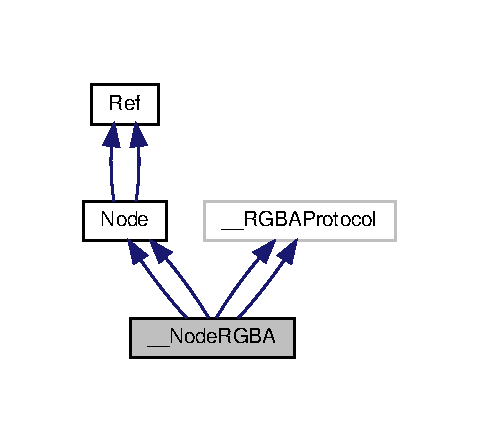
\includegraphics[width=230pt]{class____NodeRGBA__inherit__graph}
\end{center}
\end{figure}


Collaboration diagram for \+\_\+\+\_\+\+Node\+R\+G\+BA\+:
\nopagebreak
\begin{figure}[H]
\begin{center}
\leavevmode
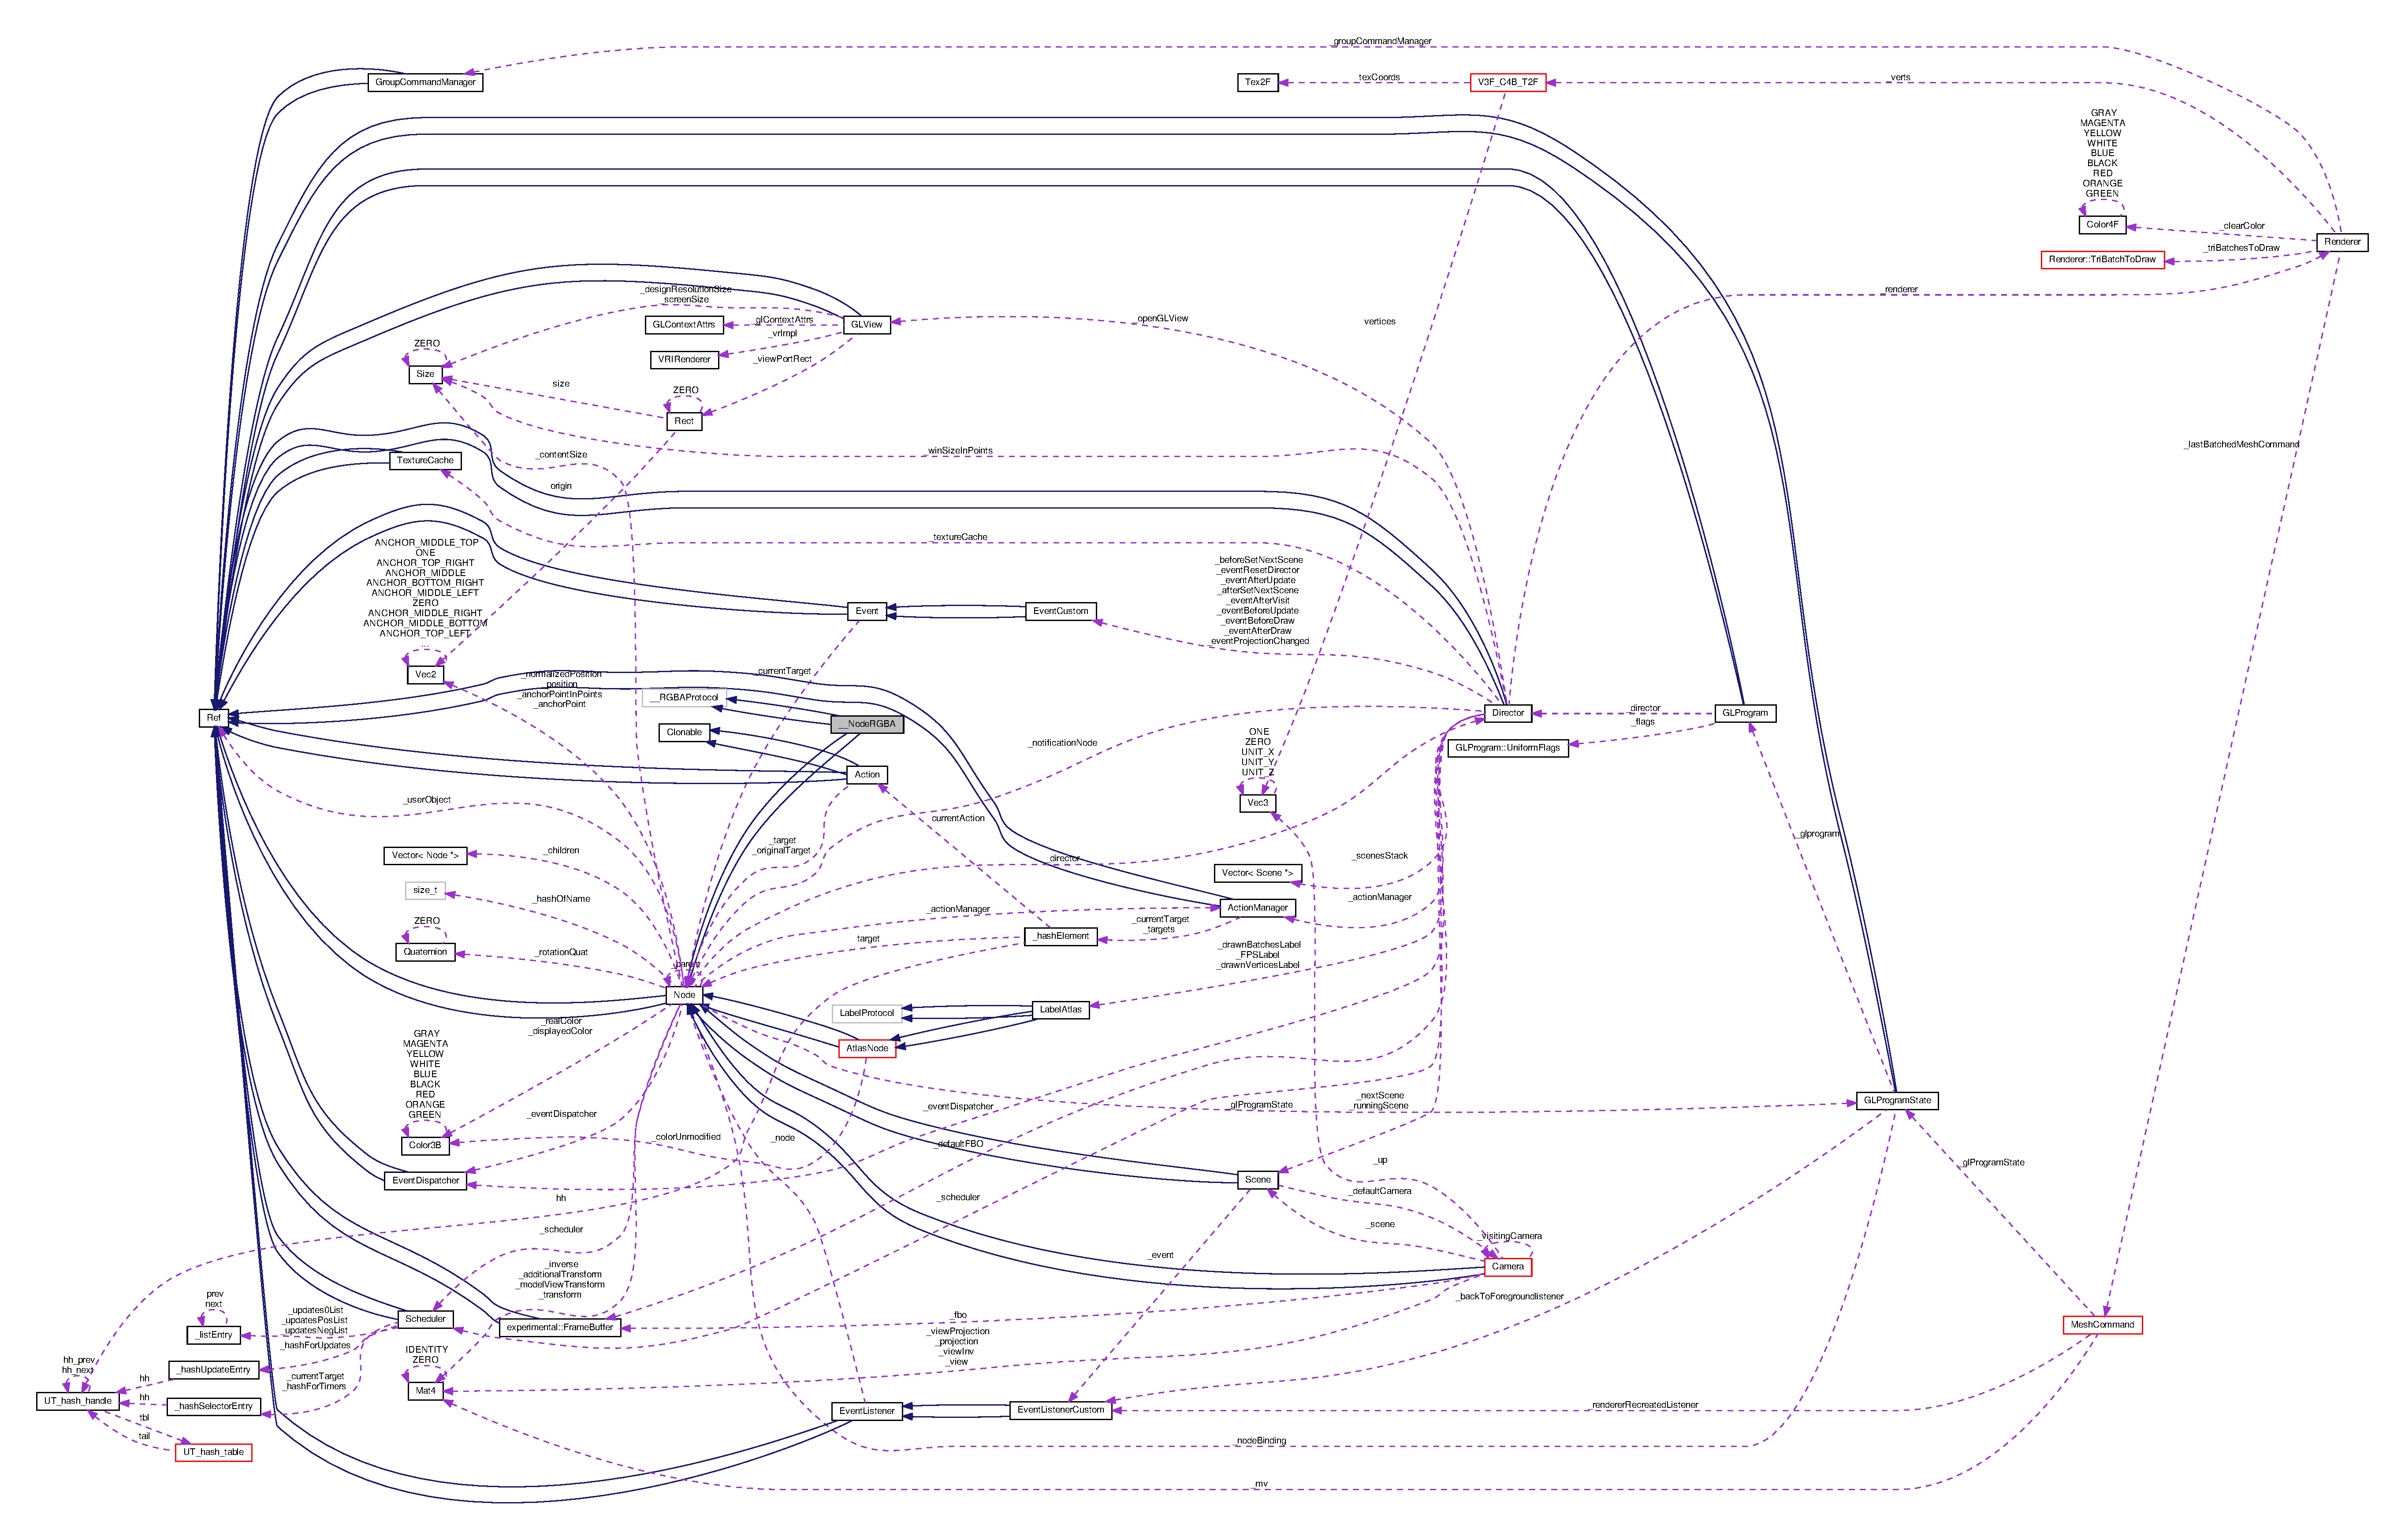
\includegraphics[width=350pt]{class____NodeRGBA__coll__graph}
\end{center}
\end{figure}
\subsection*{Public Member Functions}
\begin{DoxyCompactItemize}
\item 
virtual G\+Lubyte \hyperlink{class____NodeRGBA_a48a5a78aea7c307ccfbe8c10e053b7c8}{get\+Opacity} () const override
\item 
virtual G\+Lubyte \hyperlink{class____NodeRGBA_adbf1aa17734836db2096f2901d81d304}{get\+Displayed\+Opacity} () const override
\item 
virtual void \hyperlink{class____NodeRGBA_aa0ac4f9dca25f519f175e668ba4f3306}{set\+Opacity} (G\+Lubyte opacity) override
\item 
virtual void \hyperlink{class____NodeRGBA_a428c41148bb3d1fe27d7eac80bb6df59}{update\+Displayed\+Opacity} (G\+Lubyte parent\+Opacity) override
\item 
virtual bool \hyperlink{class____NodeRGBA_a421ef9c26c9860deb23184727d573415}{is\+Cascade\+Opacity\+Enabled} () const override
\item 
virtual void \hyperlink{class____NodeRGBA_a10fe85e705700fbe2bd28da1a17eda68}{set\+Cascade\+Opacity\+Enabled} (bool cascade\+Opacity\+Enabled) override
\item 
virtual const \hyperlink{structColor3B}{Color3B} \& \hyperlink{class____NodeRGBA_a730149ff787a7a86d78a5c0d0aecddda}{get\+Color} (void) const override
\item 
virtual const \hyperlink{structColor3B}{Color3B} \& \hyperlink{class____NodeRGBA_ae17a9077b86673cb75f799cb4f6c8a1d}{get\+Displayed\+Color} () const override
\item 
virtual void \hyperlink{class____NodeRGBA_adaec184f0ee740557ffddaece7ece996}{set\+Color} (const \hyperlink{structColor3B}{Color3B} \&color) override
\item 
virtual void \hyperlink{class____NodeRGBA_a7b792b469020beebcd515a2eacba90f7}{update\+Displayed\+Color} (const \hyperlink{structColor3B}{Color3B} \&parent\+Color) override
\item 
virtual bool \hyperlink{class____NodeRGBA_a24f2ae00f1994d6601ce8e1f089dafe1}{is\+Cascade\+Color\+Enabled} () const override
\item 
virtual void \hyperlink{class____NodeRGBA_a07c6d23e55cc2ba21115d2b93ef25bcd}{set\+Cascade\+Color\+Enabled} (bool cascade\+Color\+Enabled) override
\item 
virtual void \hyperlink{class____NodeRGBA_a2baa7449894e58c0bc78e749058b9c0e}{set\+Opacity\+Modify\+R\+GB} (bool b\+Value) override
\item 
virtual bool \hyperlink{class____NodeRGBA_a60d28606b0a253ad511df43a868fa08c}{is\+Opacity\+Modify\+R\+GB} () const override
\item 
virtual G\+Lubyte \hyperlink{class____NodeRGBA_a48a5a78aea7c307ccfbe8c10e053b7c8}{get\+Opacity} () const override
\item 
virtual G\+Lubyte \hyperlink{class____NodeRGBA_adbf1aa17734836db2096f2901d81d304}{get\+Displayed\+Opacity} () const override
\item 
virtual void \hyperlink{class____NodeRGBA_aa0ac4f9dca25f519f175e668ba4f3306}{set\+Opacity} (G\+Lubyte opacity) override
\item 
virtual void \hyperlink{class____NodeRGBA_a428c41148bb3d1fe27d7eac80bb6df59}{update\+Displayed\+Opacity} (G\+Lubyte parent\+Opacity) override
\item 
virtual bool \hyperlink{class____NodeRGBA_a421ef9c26c9860deb23184727d573415}{is\+Cascade\+Opacity\+Enabled} () const override
\item 
virtual void \hyperlink{class____NodeRGBA_a10fe85e705700fbe2bd28da1a17eda68}{set\+Cascade\+Opacity\+Enabled} (bool cascade\+Opacity\+Enabled) override
\item 
virtual const \hyperlink{structColor3B}{Color3B} \& \hyperlink{class____NodeRGBA_a730149ff787a7a86d78a5c0d0aecddda}{get\+Color} (void) const override
\item 
virtual const \hyperlink{structColor3B}{Color3B} \& \hyperlink{class____NodeRGBA_ae17a9077b86673cb75f799cb4f6c8a1d}{get\+Displayed\+Color} () const override
\item 
virtual void \hyperlink{class____NodeRGBA_adaec184f0ee740557ffddaece7ece996}{set\+Color} (const \hyperlink{structColor3B}{Color3B} \&color) override
\item 
virtual void \hyperlink{class____NodeRGBA_a7b792b469020beebcd515a2eacba90f7}{update\+Displayed\+Color} (const \hyperlink{structColor3B}{Color3B} \&parent\+Color) override
\item 
virtual bool \hyperlink{class____NodeRGBA_a24f2ae00f1994d6601ce8e1f089dafe1}{is\+Cascade\+Color\+Enabled} () const override
\item 
virtual void \hyperlink{class____NodeRGBA_a07c6d23e55cc2ba21115d2b93ef25bcd}{set\+Cascade\+Color\+Enabled} (bool cascade\+Color\+Enabled) override
\item 
virtual void \hyperlink{class____NodeRGBA_a2baa7449894e58c0bc78e749058b9c0e}{set\+Opacity\+Modify\+R\+GB} (bool b\+Value) override
\item 
virtual bool \hyperlink{class____NodeRGBA_a60d28606b0a253ad511df43a868fa08c}{is\+Opacity\+Modify\+R\+GB} () const override
\end{DoxyCompactItemize}
\subsection*{Public Attributes}
\begin{DoxyCompactItemize}
\item 
\mbox{\Hypertarget{class____NodeRGBA_a205293d39d3aa89e9cb3c32dc281dffd}\label{class____NodeRGBA_a205293d39d3aa89e9cb3c32dc281dffd}} 
\hyperlink{_2cocos2d_2cocos_2base_2ccConfig_8h_a25ef1314f97c35a2ed3d029b0ead6da0}{C\+C\+\_\+\+C\+O\+N\+S\+T\+R\+U\+C\+T\+O\+R\+\_\+\+A\+C\+C\+E\+SS} {\bfseries \+\_\+\+\_\+pad0\+\_\+\+\_\+}\+: \hyperlink{class____NodeRGBA}{\+\_\+\+\_\+\+Node\+R\+G\+BA}()
\end{DoxyCompactItemize}
\subsection*{Additional Inherited Members}


\subsection{Detailed Description}
\hyperlink{class____NodeRGBA}{\+\_\+\+\_\+\+Node\+R\+G\+BA} is a subclass of \hyperlink{classNode}{Node} that implements the R\+G\+B\+A\+Protocol protocol. 

All features from \hyperlink{classNode}{Node} are valid, plus the following new features\+:
\begin{DoxyItemize}
\item opacity
\item R\+GB colors
\end{DoxyItemize}

Opacity/\+Color propagates into children that conform to the R\+G\+B\+A\+Protocol if cascade\+Opacity/cascade\+Color is enabled. \begin{DoxySince}{Since}
v2.\+1  NA 
\end{DoxySince}


\subsection{Member Function Documentation}
\mbox{\Hypertarget{class____NodeRGBA_a730149ff787a7a86d78a5c0d0aecddda}\label{class____NodeRGBA_a730149ff787a7a86d78a5c0d0aecddda}} 
\index{\+\_\+\+\_\+\+Node\+R\+G\+BA@{\+\_\+\+\_\+\+Node\+R\+G\+BA}!get\+Color@{get\+Color}}
\index{get\+Color@{get\+Color}!\+\_\+\+\_\+\+Node\+R\+G\+BA@{\+\_\+\+\_\+\+Node\+R\+G\+BA}}
\subsubsection{\texorpdfstring{get\+Color()}{getColor()}\hspace{0.1cm}{\footnotesize\ttfamily [1/2]}}
{\footnotesize\ttfamily virtual const \hyperlink{structColor3B}{Color3B}\& \+\_\+\+\_\+\+Node\+R\+G\+B\+A\+::get\+Color (\begin{DoxyParamCaption}\item[{void}]{ }\end{DoxyParamCaption}) const\hspace{0.3cm}{\ttfamily [inline]}, {\ttfamily [override]}, {\ttfamily [virtual]}}

Query node\textquotesingle{}s color value. \begin{DoxyReturn}{Returns}
A \hyperlink{structColor3B}{Color3B} color value. 
\end{DoxyReturn}


Reimplemented from \hyperlink{classNode_a06721d272f5a59e02e355d95be25bb99}{Node}.

\mbox{\Hypertarget{class____NodeRGBA_a730149ff787a7a86d78a5c0d0aecddda}\label{class____NodeRGBA_a730149ff787a7a86d78a5c0d0aecddda}} 
\index{\+\_\+\+\_\+\+Node\+R\+G\+BA@{\+\_\+\+\_\+\+Node\+R\+G\+BA}!get\+Color@{get\+Color}}
\index{get\+Color@{get\+Color}!\+\_\+\+\_\+\+Node\+R\+G\+BA@{\+\_\+\+\_\+\+Node\+R\+G\+BA}}
\subsubsection{\texorpdfstring{get\+Color()}{getColor()}\hspace{0.1cm}{\footnotesize\ttfamily [2/2]}}
{\footnotesize\ttfamily virtual const \hyperlink{structColor3B}{Color3B}\& \+\_\+\+\_\+\+Node\+R\+G\+B\+A\+::get\+Color (\begin{DoxyParamCaption}\item[{void}]{ }\end{DoxyParamCaption}) const\hspace{0.3cm}{\ttfamily [inline]}, {\ttfamily [override]}, {\ttfamily [virtual]}}

Query node\textquotesingle{}s color value. \begin{DoxyReturn}{Returns}
A \hyperlink{structColor3B}{Color3B} color value. 
\end{DoxyReturn}


Reimplemented from \hyperlink{classNode_a06721d272f5a59e02e355d95be25bb99}{Node}.

\mbox{\Hypertarget{class____NodeRGBA_ae17a9077b86673cb75f799cb4f6c8a1d}\label{class____NodeRGBA_ae17a9077b86673cb75f799cb4f6c8a1d}} 
\index{\+\_\+\+\_\+\+Node\+R\+G\+BA@{\+\_\+\+\_\+\+Node\+R\+G\+BA}!get\+Displayed\+Color@{get\+Displayed\+Color}}
\index{get\+Displayed\+Color@{get\+Displayed\+Color}!\+\_\+\+\_\+\+Node\+R\+G\+BA@{\+\_\+\+\_\+\+Node\+R\+G\+BA}}
\subsubsection{\texorpdfstring{get\+Displayed\+Color()}{getDisplayedColor()}\hspace{0.1cm}{\footnotesize\ttfamily [1/2]}}
{\footnotesize\ttfamily virtual const \hyperlink{structColor3B}{Color3B}\& \+\_\+\+\_\+\+Node\+R\+G\+B\+A\+::get\+Displayed\+Color (\begin{DoxyParamCaption}{ }\end{DoxyParamCaption}) const\hspace{0.3cm}{\ttfamily [inline]}, {\ttfamily [override]}, {\ttfamily [virtual]}}

Query node\textquotesingle{}s displayed color. \begin{DoxyReturn}{Returns}
A \hyperlink{structColor3B}{Color3B} color value. 
\end{DoxyReturn}


Reimplemented from \hyperlink{classNode_a899760bbad414bfbe9fb51473e99c3eb}{Node}.

\mbox{\Hypertarget{class____NodeRGBA_ae17a9077b86673cb75f799cb4f6c8a1d}\label{class____NodeRGBA_ae17a9077b86673cb75f799cb4f6c8a1d}} 
\index{\+\_\+\+\_\+\+Node\+R\+G\+BA@{\+\_\+\+\_\+\+Node\+R\+G\+BA}!get\+Displayed\+Color@{get\+Displayed\+Color}}
\index{get\+Displayed\+Color@{get\+Displayed\+Color}!\+\_\+\+\_\+\+Node\+R\+G\+BA@{\+\_\+\+\_\+\+Node\+R\+G\+BA}}
\subsubsection{\texorpdfstring{get\+Displayed\+Color()}{getDisplayedColor()}\hspace{0.1cm}{\footnotesize\ttfamily [2/2]}}
{\footnotesize\ttfamily virtual const \hyperlink{structColor3B}{Color3B}\& \+\_\+\+\_\+\+Node\+R\+G\+B\+A\+::get\+Displayed\+Color (\begin{DoxyParamCaption}{ }\end{DoxyParamCaption}) const\hspace{0.3cm}{\ttfamily [inline]}, {\ttfamily [override]}, {\ttfamily [virtual]}}

Query node\textquotesingle{}s displayed color. \begin{DoxyReturn}{Returns}
A \hyperlink{structColor3B}{Color3B} color value. 
\end{DoxyReturn}


Reimplemented from \hyperlink{classNode_a899760bbad414bfbe9fb51473e99c3eb}{Node}.

\mbox{\Hypertarget{class____NodeRGBA_adbf1aa17734836db2096f2901d81d304}\label{class____NodeRGBA_adbf1aa17734836db2096f2901d81d304}} 
\index{\+\_\+\+\_\+\+Node\+R\+G\+BA@{\+\_\+\+\_\+\+Node\+R\+G\+BA}!get\+Displayed\+Opacity@{get\+Displayed\+Opacity}}
\index{get\+Displayed\+Opacity@{get\+Displayed\+Opacity}!\+\_\+\+\_\+\+Node\+R\+G\+BA@{\+\_\+\+\_\+\+Node\+R\+G\+BA}}
\subsubsection{\texorpdfstring{get\+Displayed\+Opacity()}{getDisplayedOpacity()}\hspace{0.1cm}{\footnotesize\ttfamily [1/2]}}
{\footnotesize\ttfamily virtual G\+Lubyte \+\_\+\+\_\+\+Node\+R\+G\+B\+A\+::get\+Displayed\+Opacity (\begin{DoxyParamCaption}{ }\end{DoxyParamCaption}) const\hspace{0.3cm}{\ttfamily [inline]}, {\ttfamily [override]}, {\ttfamily [virtual]}}

Return the node\textquotesingle{}s display opacity. The difference between opacity and displayed\+Opacity is\+: The displayed\+Opacity is what\textquotesingle{}s the final rendering opacity of node. \begin{DoxyReturn}{Returns}
A G\+Lubyte value. 
\end{DoxyReturn}


Reimplemented from \hyperlink{classNode_ac4f9c61560c8862ebdaecbf79bf8a1b6}{Node}.

\mbox{\Hypertarget{class____NodeRGBA_adbf1aa17734836db2096f2901d81d304}\label{class____NodeRGBA_adbf1aa17734836db2096f2901d81d304}} 
\index{\+\_\+\+\_\+\+Node\+R\+G\+BA@{\+\_\+\+\_\+\+Node\+R\+G\+BA}!get\+Displayed\+Opacity@{get\+Displayed\+Opacity}}
\index{get\+Displayed\+Opacity@{get\+Displayed\+Opacity}!\+\_\+\+\_\+\+Node\+R\+G\+BA@{\+\_\+\+\_\+\+Node\+R\+G\+BA}}
\subsubsection{\texorpdfstring{get\+Displayed\+Opacity()}{getDisplayedOpacity()}\hspace{0.1cm}{\footnotesize\ttfamily [2/2]}}
{\footnotesize\ttfamily virtual G\+Lubyte \+\_\+\+\_\+\+Node\+R\+G\+B\+A\+::get\+Displayed\+Opacity (\begin{DoxyParamCaption}{ }\end{DoxyParamCaption}) const\hspace{0.3cm}{\ttfamily [inline]}, {\ttfamily [override]}, {\ttfamily [virtual]}}

Return the node\textquotesingle{}s display opacity. The difference between opacity and displayed\+Opacity is\+: The displayed\+Opacity is what\textquotesingle{}s the final rendering opacity of node. \begin{DoxyReturn}{Returns}
A G\+Lubyte value. 
\end{DoxyReturn}


Reimplemented from \hyperlink{classNode_ac4f9c61560c8862ebdaecbf79bf8a1b6}{Node}.

\mbox{\Hypertarget{class____NodeRGBA_a48a5a78aea7c307ccfbe8c10e053b7c8}\label{class____NodeRGBA_a48a5a78aea7c307ccfbe8c10e053b7c8}} 
\index{\+\_\+\+\_\+\+Node\+R\+G\+BA@{\+\_\+\+\_\+\+Node\+R\+G\+BA}!get\+Opacity@{get\+Opacity}}
\index{get\+Opacity@{get\+Opacity}!\+\_\+\+\_\+\+Node\+R\+G\+BA@{\+\_\+\+\_\+\+Node\+R\+G\+BA}}
\subsubsection{\texorpdfstring{get\+Opacity()}{getOpacity()}\hspace{0.1cm}{\footnotesize\ttfamily [1/2]}}
{\footnotesize\ttfamily virtual G\+Lubyte \+\_\+\+\_\+\+Node\+R\+G\+B\+A\+::get\+Opacity (\begin{DoxyParamCaption}\item[{void}]{ }\end{DoxyParamCaption}) const\hspace{0.3cm}{\ttfamily [inline]}, {\ttfamily [override]}, {\ttfamily [virtual]}}

Return the node\textquotesingle{}s opacity. \begin{DoxyReturn}{Returns}
A G\+Lubyte value. 
\end{DoxyReturn}


Reimplemented from \hyperlink{classNode_ab999cce3763ea09e74014245c770ea97}{Node}.

\mbox{\Hypertarget{class____NodeRGBA_a48a5a78aea7c307ccfbe8c10e053b7c8}\label{class____NodeRGBA_a48a5a78aea7c307ccfbe8c10e053b7c8}} 
\index{\+\_\+\+\_\+\+Node\+R\+G\+BA@{\+\_\+\+\_\+\+Node\+R\+G\+BA}!get\+Opacity@{get\+Opacity}}
\index{get\+Opacity@{get\+Opacity}!\+\_\+\+\_\+\+Node\+R\+G\+BA@{\+\_\+\+\_\+\+Node\+R\+G\+BA}}
\subsubsection{\texorpdfstring{get\+Opacity()}{getOpacity()}\hspace{0.1cm}{\footnotesize\ttfamily [2/2]}}
{\footnotesize\ttfamily virtual G\+Lubyte \+\_\+\+\_\+\+Node\+R\+G\+B\+A\+::get\+Opacity (\begin{DoxyParamCaption}\item[{void}]{ }\end{DoxyParamCaption}) const\hspace{0.3cm}{\ttfamily [inline]}, {\ttfamily [override]}, {\ttfamily [virtual]}}

Return the node\textquotesingle{}s opacity. \begin{DoxyReturn}{Returns}
A G\+Lubyte value. 
\end{DoxyReturn}


Reimplemented from \hyperlink{classNode_ab999cce3763ea09e74014245c770ea97}{Node}.

\mbox{\Hypertarget{class____NodeRGBA_a24f2ae00f1994d6601ce8e1f089dafe1}\label{class____NodeRGBA_a24f2ae00f1994d6601ce8e1f089dafe1}} 
\index{\+\_\+\+\_\+\+Node\+R\+G\+BA@{\+\_\+\+\_\+\+Node\+R\+G\+BA}!is\+Cascade\+Color\+Enabled@{is\+Cascade\+Color\+Enabled}}
\index{is\+Cascade\+Color\+Enabled@{is\+Cascade\+Color\+Enabled}!\+\_\+\+\_\+\+Node\+R\+G\+BA@{\+\_\+\+\_\+\+Node\+R\+G\+BA}}
\subsubsection{\texorpdfstring{is\+Cascade\+Color\+Enabled()}{isCascadeColorEnabled()}\hspace{0.1cm}{\footnotesize\ttfamily [1/2]}}
{\footnotesize\ttfamily virtual bool \+\_\+\+\_\+\+Node\+R\+G\+B\+A\+::is\+Cascade\+Color\+Enabled (\begin{DoxyParamCaption}\item[{void}]{ }\end{DoxyParamCaption}) const\hspace{0.3cm}{\ttfamily [inline]}, {\ttfamily [override]}, {\ttfamily [virtual]}}

Query whether cascade\+Color is enabled or not. \begin{DoxyReturn}{Returns}
Whether cascade\+Color is enabled or not. 
\end{DoxyReturn}


Reimplemented from \hyperlink{classNode_abf874f1b388e773ca80732b1134508be}{Node}.

\mbox{\Hypertarget{class____NodeRGBA_a24f2ae00f1994d6601ce8e1f089dafe1}\label{class____NodeRGBA_a24f2ae00f1994d6601ce8e1f089dafe1}} 
\index{\+\_\+\+\_\+\+Node\+R\+G\+BA@{\+\_\+\+\_\+\+Node\+R\+G\+BA}!is\+Cascade\+Color\+Enabled@{is\+Cascade\+Color\+Enabled}}
\index{is\+Cascade\+Color\+Enabled@{is\+Cascade\+Color\+Enabled}!\+\_\+\+\_\+\+Node\+R\+G\+BA@{\+\_\+\+\_\+\+Node\+R\+G\+BA}}
\subsubsection{\texorpdfstring{is\+Cascade\+Color\+Enabled()}{isCascadeColorEnabled()}\hspace{0.1cm}{\footnotesize\ttfamily [2/2]}}
{\footnotesize\ttfamily virtual bool \+\_\+\+\_\+\+Node\+R\+G\+B\+A\+::is\+Cascade\+Color\+Enabled (\begin{DoxyParamCaption}\item[{void}]{ }\end{DoxyParamCaption}) const\hspace{0.3cm}{\ttfamily [inline]}, {\ttfamily [override]}, {\ttfamily [virtual]}}

Query whether cascade\+Color is enabled or not. \begin{DoxyReturn}{Returns}
Whether cascade\+Color is enabled or not. 
\end{DoxyReturn}


Reimplemented from \hyperlink{classNode_abf874f1b388e773ca80732b1134508be}{Node}.

\mbox{\Hypertarget{class____NodeRGBA_a421ef9c26c9860deb23184727d573415}\label{class____NodeRGBA_a421ef9c26c9860deb23184727d573415}} 
\index{\+\_\+\+\_\+\+Node\+R\+G\+BA@{\+\_\+\+\_\+\+Node\+R\+G\+BA}!is\+Cascade\+Opacity\+Enabled@{is\+Cascade\+Opacity\+Enabled}}
\index{is\+Cascade\+Opacity\+Enabled@{is\+Cascade\+Opacity\+Enabled}!\+\_\+\+\_\+\+Node\+R\+G\+BA@{\+\_\+\+\_\+\+Node\+R\+G\+BA}}
\subsubsection{\texorpdfstring{is\+Cascade\+Opacity\+Enabled()}{isCascadeOpacityEnabled()}\hspace{0.1cm}{\footnotesize\ttfamily [1/2]}}
{\footnotesize\ttfamily virtual bool \+\_\+\+\_\+\+Node\+R\+G\+B\+A\+::is\+Cascade\+Opacity\+Enabled (\begin{DoxyParamCaption}\item[{void}]{ }\end{DoxyParamCaption}) const\hspace{0.3cm}{\ttfamily [inline]}, {\ttfamily [override]}, {\ttfamily [virtual]}}

Whether cascade\+Opacity is enabled or not. \begin{DoxyReturn}{Returns}
A boolean value. 
\end{DoxyReturn}


Reimplemented from \hyperlink{classNode_a79f5da3b20b08356467db7ce95cf9f54}{Node}.

\mbox{\Hypertarget{class____NodeRGBA_a421ef9c26c9860deb23184727d573415}\label{class____NodeRGBA_a421ef9c26c9860deb23184727d573415}} 
\index{\+\_\+\+\_\+\+Node\+R\+G\+BA@{\+\_\+\+\_\+\+Node\+R\+G\+BA}!is\+Cascade\+Opacity\+Enabled@{is\+Cascade\+Opacity\+Enabled}}
\index{is\+Cascade\+Opacity\+Enabled@{is\+Cascade\+Opacity\+Enabled}!\+\_\+\+\_\+\+Node\+R\+G\+BA@{\+\_\+\+\_\+\+Node\+R\+G\+BA}}
\subsubsection{\texorpdfstring{is\+Cascade\+Opacity\+Enabled()}{isCascadeOpacityEnabled()}\hspace{0.1cm}{\footnotesize\ttfamily [2/2]}}
{\footnotesize\ttfamily virtual bool \+\_\+\+\_\+\+Node\+R\+G\+B\+A\+::is\+Cascade\+Opacity\+Enabled (\begin{DoxyParamCaption}\item[{void}]{ }\end{DoxyParamCaption}) const\hspace{0.3cm}{\ttfamily [inline]}, {\ttfamily [override]}, {\ttfamily [virtual]}}

Whether cascade\+Opacity is enabled or not. \begin{DoxyReturn}{Returns}
A boolean value. 
\end{DoxyReturn}


Reimplemented from \hyperlink{classNode_a79f5da3b20b08356467db7ce95cf9f54}{Node}.

\mbox{\Hypertarget{class____NodeRGBA_a60d28606b0a253ad511df43a868fa08c}\label{class____NodeRGBA_a60d28606b0a253ad511df43a868fa08c}} 
\index{\+\_\+\+\_\+\+Node\+R\+G\+BA@{\+\_\+\+\_\+\+Node\+R\+G\+BA}!is\+Opacity\+Modify\+R\+GB@{is\+Opacity\+Modify\+R\+GB}}
\index{is\+Opacity\+Modify\+R\+GB@{is\+Opacity\+Modify\+R\+GB}!\+\_\+\+\_\+\+Node\+R\+G\+BA@{\+\_\+\+\_\+\+Node\+R\+G\+BA}}
\subsubsection{\texorpdfstring{is\+Opacity\+Modify\+R\+G\+B()}{isOpacityModifyRGB()}\hspace{0.1cm}{\footnotesize\ttfamily [1/2]}}
{\footnotesize\ttfamily virtual bool \+\_\+\+\_\+\+Node\+R\+G\+B\+A\+::is\+Opacity\+Modify\+R\+GB (\begin{DoxyParamCaption}\item[{void}]{ }\end{DoxyParamCaption}) const\hspace{0.3cm}{\ttfamily [inline]}, {\ttfamily [override]}, {\ttfamily [virtual]}}

If node opacity will modify the R\+GB color value, then you should override this method and return true. \begin{DoxyReturn}{Returns}
A boolean value, true indicates that opacity will modify color; false otherwise. 
\end{DoxyReturn}


Reimplemented from \hyperlink{classNode_ae6ce32d2088e2bb3426608334f1091c5}{Node}.

\mbox{\Hypertarget{class____NodeRGBA_a60d28606b0a253ad511df43a868fa08c}\label{class____NodeRGBA_a60d28606b0a253ad511df43a868fa08c}} 
\index{\+\_\+\+\_\+\+Node\+R\+G\+BA@{\+\_\+\+\_\+\+Node\+R\+G\+BA}!is\+Opacity\+Modify\+R\+GB@{is\+Opacity\+Modify\+R\+GB}}
\index{is\+Opacity\+Modify\+R\+GB@{is\+Opacity\+Modify\+R\+GB}!\+\_\+\+\_\+\+Node\+R\+G\+BA@{\+\_\+\+\_\+\+Node\+R\+G\+BA}}
\subsubsection{\texorpdfstring{is\+Opacity\+Modify\+R\+G\+B()}{isOpacityModifyRGB()}\hspace{0.1cm}{\footnotesize\ttfamily [2/2]}}
{\footnotesize\ttfamily virtual bool \+\_\+\+\_\+\+Node\+R\+G\+B\+A\+::is\+Opacity\+Modify\+R\+GB (\begin{DoxyParamCaption}\item[{void}]{ }\end{DoxyParamCaption}) const\hspace{0.3cm}{\ttfamily [inline]}, {\ttfamily [override]}, {\ttfamily [virtual]}}

If node opacity will modify the R\+GB color value, then you should override this method and return true. \begin{DoxyReturn}{Returns}
A boolean value, true indicates that opacity will modify color; false otherwise. 
\end{DoxyReturn}


Reimplemented from \hyperlink{classNode_ae6ce32d2088e2bb3426608334f1091c5}{Node}.

\mbox{\Hypertarget{class____NodeRGBA_a07c6d23e55cc2ba21115d2b93ef25bcd}\label{class____NodeRGBA_a07c6d23e55cc2ba21115d2b93ef25bcd}} 
\index{\+\_\+\+\_\+\+Node\+R\+G\+BA@{\+\_\+\+\_\+\+Node\+R\+G\+BA}!set\+Cascade\+Color\+Enabled@{set\+Cascade\+Color\+Enabled}}
\index{set\+Cascade\+Color\+Enabled@{set\+Cascade\+Color\+Enabled}!\+\_\+\+\_\+\+Node\+R\+G\+BA@{\+\_\+\+\_\+\+Node\+R\+G\+BA}}
\subsubsection{\texorpdfstring{set\+Cascade\+Color\+Enabled()}{setCascadeColorEnabled()}\hspace{0.1cm}{\footnotesize\ttfamily [1/2]}}
{\footnotesize\ttfamily virtual void \+\_\+\+\_\+\+Node\+R\+G\+B\+A\+::set\+Cascade\+Color\+Enabled (\begin{DoxyParamCaption}\item[{bool}]{cascade\+Color\+Enabled }\end{DoxyParamCaption})\hspace{0.3cm}{\ttfamily [inline]}, {\ttfamily [override]}, {\ttfamily [virtual]}}

If you want node\textquotesingle{}s color affect the children node\textquotesingle{}s color, then set it to true. Otherwise, set it to false. 
\begin{DoxyParams}{Parameters}
{\em cascade\+Color\+Enabled} & A boolean value. \\
\hline
\end{DoxyParams}


Reimplemented from \hyperlink{classNode_a4e7f2dde1e3a7d56880f59f1480955e7}{Node}.

\mbox{\Hypertarget{class____NodeRGBA_a07c6d23e55cc2ba21115d2b93ef25bcd}\label{class____NodeRGBA_a07c6d23e55cc2ba21115d2b93ef25bcd}} 
\index{\+\_\+\+\_\+\+Node\+R\+G\+BA@{\+\_\+\+\_\+\+Node\+R\+G\+BA}!set\+Cascade\+Color\+Enabled@{set\+Cascade\+Color\+Enabled}}
\index{set\+Cascade\+Color\+Enabled@{set\+Cascade\+Color\+Enabled}!\+\_\+\+\_\+\+Node\+R\+G\+BA@{\+\_\+\+\_\+\+Node\+R\+G\+BA}}
\subsubsection{\texorpdfstring{set\+Cascade\+Color\+Enabled()}{setCascadeColorEnabled()}\hspace{0.1cm}{\footnotesize\ttfamily [2/2]}}
{\footnotesize\ttfamily virtual void \+\_\+\+\_\+\+Node\+R\+G\+B\+A\+::set\+Cascade\+Color\+Enabled (\begin{DoxyParamCaption}\item[{bool}]{cascade\+Color\+Enabled }\end{DoxyParamCaption})\hspace{0.3cm}{\ttfamily [inline]}, {\ttfamily [override]}, {\ttfamily [virtual]}}

If you want node\textquotesingle{}s color affect the children node\textquotesingle{}s color, then set it to true. Otherwise, set it to false. 
\begin{DoxyParams}{Parameters}
{\em cascade\+Color\+Enabled} & A boolean value. \\
\hline
\end{DoxyParams}


Reimplemented from \hyperlink{classNode_a4e7f2dde1e3a7d56880f59f1480955e7}{Node}.

\mbox{\Hypertarget{class____NodeRGBA_a10fe85e705700fbe2bd28da1a17eda68}\label{class____NodeRGBA_a10fe85e705700fbe2bd28da1a17eda68}} 
\index{\+\_\+\+\_\+\+Node\+R\+G\+BA@{\+\_\+\+\_\+\+Node\+R\+G\+BA}!set\+Cascade\+Opacity\+Enabled@{set\+Cascade\+Opacity\+Enabled}}
\index{set\+Cascade\+Opacity\+Enabled@{set\+Cascade\+Opacity\+Enabled}!\+\_\+\+\_\+\+Node\+R\+G\+BA@{\+\_\+\+\_\+\+Node\+R\+G\+BA}}
\subsubsection{\texorpdfstring{set\+Cascade\+Opacity\+Enabled()}{setCascadeOpacityEnabled()}\hspace{0.1cm}{\footnotesize\ttfamily [1/2]}}
{\footnotesize\ttfamily virtual void \+\_\+\+\_\+\+Node\+R\+G\+B\+A\+::set\+Cascade\+Opacity\+Enabled (\begin{DoxyParamCaption}\item[{bool}]{cascade\+Opacity\+Enabled }\end{DoxyParamCaption})\hspace{0.3cm}{\ttfamily [inline]}, {\ttfamily [override]}, {\ttfamily [virtual]}}

Change node\textquotesingle{}s cascade\+Opacity property. 
\begin{DoxyParams}{Parameters}
{\em cascade\+Opacity\+Enabled} & True to enable cascade\+Opacity, false otherwise. \\
\hline
\end{DoxyParams}


Reimplemented from \hyperlink{classNode_a56b08f1d19bb0345f6fb40d9a3e3b4a4}{Node}.

\mbox{\Hypertarget{class____NodeRGBA_a10fe85e705700fbe2bd28da1a17eda68}\label{class____NodeRGBA_a10fe85e705700fbe2bd28da1a17eda68}} 
\index{\+\_\+\+\_\+\+Node\+R\+G\+BA@{\+\_\+\+\_\+\+Node\+R\+G\+BA}!set\+Cascade\+Opacity\+Enabled@{set\+Cascade\+Opacity\+Enabled}}
\index{set\+Cascade\+Opacity\+Enabled@{set\+Cascade\+Opacity\+Enabled}!\+\_\+\+\_\+\+Node\+R\+G\+BA@{\+\_\+\+\_\+\+Node\+R\+G\+BA}}
\subsubsection{\texorpdfstring{set\+Cascade\+Opacity\+Enabled()}{setCascadeOpacityEnabled()}\hspace{0.1cm}{\footnotesize\ttfamily [2/2]}}
{\footnotesize\ttfamily virtual void \+\_\+\+\_\+\+Node\+R\+G\+B\+A\+::set\+Cascade\+Opacity\+Enabled (\begin{DoxyParamCaption}\item[{bool}]{cascade\+Opacity\+Enabled }\end{DoxyParamCaption})\hspace{0.3cm}{\ttfamily [inline]}, {\ttfamily [override]}, {\ttfamily [virtual]}}

Change node\textquotesingle{}s cascade\+Opacity property. 
\begin{DoxyParams}{Parameters}
{\em cascade\+Opacity\+Enabled} & True to enable cascade\+Opacity, false otherwise. \\
\hline
\end{DoxyParams}


Reimplemented from \hyperlink{classNode_a56b08f1d19bb0345f6fb40d9a3e3b4a4}{Node}.

\mbox{\Hypertarget{class____NodeRGBA_adaec184f0ee740557ffddaece7ece996}\label{class____NodeRGBA_adaec184f0ee740557ffddaece7ece996}} 
\index{\+\_\+\+\_\+\+Node\+R\+G\+BA@{\+\_\+\+\_\+\+Node\+R\+G\+BA}!set\+Color@{set\+Color}}
\index{set\+Color@{set\+Color}!\+\_\+\+\_\+\+Node\+R\+G\+BA@{\+\_\+\+\_\+\+Node\+R\+G\+BA}}
\subsubsection{\texorpdfstring{set\+Color()}{setColor()}\hspace{0.1cm}{\footnotesize\ttfamily [1/2]}}
{\footnotesize\ttfamily virtual void \+\_\+\+\_\+\+Node\+R\+G\+B\+A\+::set\+Color (\begin{DoxyParamCaption}\item[{const \hyperlink{structColor3B}{Color3B} \&}]{color }\end{DoxyParamCaption})\hspace{0.3cm}{\ttfamily [inline]}, {\ttfamily [override]}, {\ttfamily [virtual]}}

Change the color of node. 
\begin{DoxyParams}{Parameters}
{\em color} & A \hyperlink{structColor3B}{Color3B} color value. \\
\hline
\end{DoxyParams}


Reimplemented from \hyperlink{classNode_af45037de5b13602263b1ce51b50cafdd}{Node}.

\mbox{\Hypertarget{class____NodeRGBA_adaec184f0ee740557ffddaece7ece996}\label{class____NodeRGBA_adaec184f0ee740557ffddaece7ece996}} 
\index{\+\_\+\+\_\+\+Node\+R\+G\+BA@{\+\_\+\+\_\+\+Node\+R\+G\+BA}!set\+Color@{set\+Color}}
\index{set\+Color@{set\+Color}!\+\_\+\+\_\+\+Node\+R\+G\+BA@{\+\_\+\+\_\+\+Node\+R\+G\+BA}}
\subsubsection{\texorpdfstring{set\+Color()}{setColor()}\hspace{0.1cm}{\footnotesize\ttfamily [2/2]}}
{\footnotesize\ttfamily virtual void \+\_\+\+\_\+\+Node\+R\+G\+B\+A\+::set\+Color (\begin{DoxyParamCaption}\item[{const \hyperlink{structColor3B}{Color3B} \&}]{color }\end{DoxyParamCaption})\hspace{0.3cm}{\ttfamily [inline]}, {\ttfamily [override]}, {\ttfamily [virtual]}}

Change the color of node. 
\begin{DoxyParams}{Parameters}
{\em color} & A \hyperlink{structColor3B}{Color3B} color value. \\
\hline
\end{DoxyParams}


Reimplemented from \hyperlink{classNode_af45037de5b13602263b1ce51b50cafdd}{Node}.

\mbox{\Hypertarget{class____NodeRGBA_aa0ac4f9dca25f519f175e668ba4f3306}\label{class____NodeRGBA_aa0ac4f9dca25f519f175e668ba4f3306}} 
\index{\+\_\+\+\_\+\+Node\+R\+G\+BA@{\+\_\+\+\_\+\+Node\+R\+G\+BA}!set\+Opacity@{set\+Opacity}}
\index{set\+Opacity@{set\+Opacity}!\+\_\+\+\_\+\+Node\+R\+G\+BA@{\+\_\+\+\_\+\+Node\+R\+G\+BA}}
\subsubsection{\texorpdfstring{set\+Opacity()}{setOpacity()}\hspace{0.1cm}{\footnotesize\ttfamily [1/2]}}
{\footnotesize\ttfamily virtual void \+\_\+\+\_\+\+Node\+R\+G\+B\+A\+::set\+Opacity (\begin{DoxyParamCaption}\item[{G\+Lubyte}]{opacity }\end{DoxyParamCaption})\hspace{0.3cm}{\ttfamily [inline]}, {\ttfamily [override]}, {\ttfamily [virtual]}}

Change node opacity. 
\begin{DoxyParams}{Parameters}
{\em opacity} & A G\+Lubyte opacity value. \\
\hline
\end{DoxyParams}


Reimplemented from \hyperlink{classNode_ae41a9db63bfa3d466ee7c9d79c35352d}{Node}.

\mbox{\Hypertarget{class____NodeRGBA_aa0ac4f9dca25f519f175e668ba4f3306}\label{class____NodeRGBA_aa0ac4f9dca25f519f175e668ba4f3306}} 
\index{\+\_\+\+\_\+\+Node\+R\+G\+BA@{\+\_\+\+\_\+\+Node\+R\+G\+BA}!set\+Opacity@{set\+Opacity}}
\index{set\+Opacity@{set\+Opacity}!\+\_\+\+\_\+\+Node\+R\+G\+BA@{\+\_\+\+\_\+\+Node\+R\+G\+BA}}
\subsubsection{\texorpdfstring{set\+Opacity()}{setOpacity()}\hspace{0.1cm}{\footnotesize\ttfamily [2/2]}}
{\footnotesize\ttfamily virtual void \+\_\+\+\_\+\+Node\+R\+G\+B\+A\+::set\+Opacity (\begin{DoxyParamCaption}\item[{G\+Lubyte}]{opacity }\end{DoxyParamCaption})\hspace{0.3cm}{\ttfamily [inline]}, {\ttfamily [override]}, {\ttfamily [virtual]}}

Change node opacity. 
\begin{DoxyParams}{Parameters}
{\em opacity} & A G\+Lubyte opacity value. \\
\hline
\end{DoxyParams}


Reimplemented from \hyperlink{classNode_ae41a9db63bfa3d466ee7c9d79c35352d}{Node}.

\mbox{\Hypertarget{class____NodeRGBA_a2baa7449894e58c0bc78e749058b9c0e}\label{class____NodeRGBA_a2baa7449894e58c0bc78e749058b9c0e}} 
\index{\+\_\+\+\_\+\+Node\+R\+G\+BA@{\+\_\+\+\_\+\+Node\+R\+G\+BA}!set\+Opacity\+Modify\+R\+GB@{set\+Opacity\+Modify\+R\+GB}}
\index{set\+Opacity\+Modify\+R\+GB@{set\+Opacity\+Modify\+R\+GB}!\+\_\+\+\_\+\+Node\+R\+G\+BA@{\+\_\+\+\_\+\+Node\+R\+G\+BA}}
\subsubsection{\texorpdfstring{set\+Opacity\+Modify\+R\+G\+B()}{setOpacityModifyRGB()}\hspace{0.1cm}{\footnotesize\ttfamily [1/2]}}
{\footnotesize\ttfamily virtual void \+\_\+\+\_\+\+Node\+R\+G\+B\+A\+::set\+Opacity\+Modify\+R\+GB (\begin{DoxyParamCaption}\item[{bool}]{value }\end{DoxyParamCaption})\hspace{0.3cm}{\ttfamily [inline]}, {\ttfamily [override]}, {\ttfamily [virtual]}}

If you want the opacity affect the color property, then set to true. 
\begin{DoxyParams}{Parameters}
{\em value} & A boolean value. \\
\hline
\end{DoxyParams}


Reimplemented from \hyperlink{classNode_a978c5435ab23f76e9efdf0f7e9e288e5}{Node}.

\mbox{\Hypertarget{class____NodeRGBA_a2baa7449894e58c0bc78e749058b9c0e}\label{class____NodeRGBA_a2baa7449894e58c0bc78e749058b9c0e}} 
\index{\+\_\+\+\_\+\+Node\+R\+G\+BA@{\+\_\+\+\_\+\+Node\+R\+G\+BA}!set\+Opacity\+Modify\+R\+GB@{set\+Opacity\+Modify\+R\+GB}}
\index{set\+Opacity\+Modify\+R\+GB@{set\+Opacity\+Modify\+R\+GB}!\+\_\+\+\_\+\+Node\+R\+G\+BA@{\+\_\+\+\_\+\+Node\+R\+G\+BA}}
\subsubsection{\texorpdfstring{set\+Opacity\+Modify\+R\+G\+B()}{setOpacityModifyRGB()}\hspace{0.1cm}{\footnotesize\ttfamily [2/2]}}
{\footnotesize\ttfamily virtual void \+\_\+\+\_\+\+Node\+R\+G\+B\+A\+::set\+Opacity\+Modify\+R\+GB (\begin{DoxyParamCaption}\item[{bool}]{value }\end{DoxyParamCaption})\hspace{0.3cm}{\ttfamily [inline]}, {\ttfamily [override]}, {\ttfamily [virtual]}}

If you want the opacity affect the color property, then set to true. 
\begin{DoxyParams}{Parameters}
{\em value} & A boolean value. \\
\hline
\end{DoxyParams}


Reimplemented from \hyperlink{classNode_a978c5435ab23f76e9efdf0f7e9e288e5}{Node}.

\mbox{\Hypertarget{class____NodeRGBA_a7b792b469020beebcd515a2eacba90f7}\label{class____NodeRGBA_a7b792b469020beebcd515a2eacba90f7}} 
\index{\+\_\+\+\_\+\+Node\+R\+G\+BA@{\+\_\+\+\_\+\+Node\+R\+G\+BA}!update\+Displayed\+Color@{update\+Displayed\+Color}}
\index{update\+Displayed\+Color@{update\+Displayed\+Color}!\+\_\+\+\_\+\+Node\+R\+G\+BA@{\+\_\+\+\_\+\+Node\+R\+G\+BA}}
\subsubsection{\texorpdfstring{update\+Displayed\+Color()}{updateDisplayedColor()}\hspace{0.1cm}{\footnotesize\ttfamily [1/2]}}
{\footnotesize\ttfamily virtual void \+\_\+\+\_\+\+Node\+R\+G\+B\+A\+::update\+Displayed\+Color (\begin{DoxyParamCaption}\item[{const \hyperlink{structColor3B}{Color3B} \&}]{parent\+Color }\end{DoxyParamCaption})\hspace{0.3cm}{\ttfamily [inline]}, {\ttfamily [override]}, {\ttfamily [virtual]}}

Update node\textquotesingle{}s displayed color with its parent color. 
\begin{DoxyParams}{Parameters}
{\em parent\+Color} & A \hyperlink{structColor3B}{Color3B} color value. \\
\hline
\end{DoxyParams}


Reimplemented from \hyperlink{classNode_ac733bae7b9590f8da746cbc3d1337a2f}{Node}.

\mbox{\Hypertarget{class____NodeRGBA_a7b792b469020beebcd515a2eacba90f7}\label{class____NodeRGBA_a7b792b469020beebcd515a2eacba90f7}} 
\index{\+\_\+\+\_\+\+Node\+R\+G\+BA@{\+\_\+\+\_\+\+Node\+R\+G\+BA}!update\+Displayed\+Color@{update\+Displayed\+Color}}
\index{update\+Displayed\+Color@{update\+Displayed\+Color}!\+\_\+\+\_\+\+Node\+R\+G\+BA@{\+\_\+\+\_\+\+Node\+R\+G\+BA}}
\subsubsection{\texorpdfstring{update\+Displayed\+Color()}{updateDisplayedColor()}\hspace{0.1cm}{\footnotesize\ttfamily [2/2]}}
{\footnotesize\ttfamily virtual void \+\_\+\+\_\+\+Node\+R\+G\+B\+A\+::update\+Displayed\+Color (\begin{DoxyParamCaption}\item[{const \hyperlink{structColor3B}{Color3B} \&}]{parent\+Color }\end{DoxyParamCaption})\hspace{0.3cm}{\ttfamily [inline]}, {\ttfamily [override]}, {\ttfamily [virtual]}}

Update node\textquotesingle{}s displayed color with its parent color. 
\begin{DoxyParams}{Parameters}
{\em parent\+Color} & A \hyperlink{structColor3B}{Color3B} color value. \\
\hline
\end{DoxyParams}


Reimplemented from \hyperlink{classNode_ac733bae7b9590f8da746cbc3d1337a2f}{Node}.

\mbox{\Hypertarget{class____NodeRGBA_a428c41148bb3d1fe27d7eac80bb6df59}\label{class____NodeRGBA_a428c41148bb3d1fe27d7eac80bb6df59}} 
\index{\+\_\+\+\_\+\+Node\+R\+G\+BA@{\+\_\+\+\_\+\+Node\+R\+G\+BA}!update\+Displayed\+Opacity@{update\+Displayed\+Opacity}}
\index{update\+Displayed\+Opacity@{update\+Displayed\+Opacity}!\+\_\+\+\_\+\+Node\+R\+G\+BA@{\+\_\+\+\_\+\+Node\+R\+G\+BA}}
\subsubsection{\texorpdfstring{update\+Displayed\+Opacity()}{updateDisplayedOpacity()}\hspace{0.1cm}{\footnotesize\ttfamily [1/2]}}
{\footnotesize\ttfamily virtual void \+\_\+\+\_\+\+Node\+R\+G\+B\+A\+::update\+Displayed\+Opacity (\begin{DoxyParamCaption}\item[{G\+Lubyte}]{parent\+Opacity }\end{DoxyParamCaption})\hspace{0.3cm}{\ttfamily [inline]}, {\ttfamily [override]}, {\ttfamily [virtual]}}

Update the displayed opacity of node with it\textquotesingle{}s parent opacity; 
\begin{DoxyParams}{Parameters}
{\em parent\+Opacity} & The opacity of parent node. \\
\hline
\end{DoxyParams}


Reimplemented from \hyperlink{classNode_a3a0122884e7e1ce310b8b68abfbb245b}{Node}.

\mbox{\Hypertarget{class____NodeRGBA_a428c41148bb3d1fe27d7eac80bb6df59}\label{class____NodeRGBA_a428c41148bb3d1fe27d7eac80bb6df59}} 
\index{\+\_\+\+\_\+\+Node\+R\+G\+BA@{\+\_\+\+\_\+\+Node\+R\+G\+BA}!update\+Displayed\+Opacity@{update\+Displayed\+Opacity}}
\index{update\+Displayed\+Opacity@{update\+Displayed\+Opacity}!\+\_\+\+\_\+\+Node\+R\+G\+BA@{\+\_\+\+\_\+\+Node\+R\+G\+BA}}
\subsubsection{\texorpdfstring{update\+Displayed\+Opacity()}{updateDisplayedOpacity()}\hspace{0.1cm}{\footnotesize\ttfamily [2/2]}}
{\footnotesize\ttfamily virtual void \+\_\+\+\_\+\+Node\+R\+G\+B\+A\+::update\+Displayed\+Opacity (\begin{DoxyParamCaption}\item[{G\+Lubyte}]{parent\+Opacity }\end{DoxyParamCaption})\hspace{0.3cm}{\ttfamily [inline]}, {\ttfamily [override]}, {\ttfamily [virtual]}}

Update the displayed opacity of node with it\textquotesingle{}s parent opacity; 
\begin{DoxyParams}{Parameters}
{\em parent\+Opacity} & The opacity of parent node. \\
\hline
\end{DoxyParams}


Reimplemented from \hyperlink{classNode_a3a0122884e7e1ce310b8b68abfbb245b}{Node}.



The documentation for this class was generated from the following file\+:\begin{DoxyCompactItemize}
\item 
/home/pmx/git/\+P\+M\+X/\+Simu\+Cocos/cocos2d/cocos/2d/C\+C\+Node.\+h\end{DoxyCompactItemize}

\hypertarget{struct__AFD__POLL__HANDLE__INFO}{}\section{\+\_\+\+A\+F\+D\+\_\+\+P\+O\+L\+L\+\_\+\+H\+A\+N\+D\+L\+E\+\_\+\+I\+N\+FO Struct Reference}
\label{struct__AFD__POLL__HANDLE__INFO}\index{\+\_\+\+A\+F\+D\+\_\+\+P\+O\+L\+L\+\_\+\+H\+A\+N\+D\+L\+E\+\_\+\+I\+N\+FO@{\+\_\+\+A\+F\+D\+\_\+\+P\+O\+L\+L\+\_\+\+H\+A\+N\+D\+L\+E\+\_\+\+I\+N\+FO}}
\subsection*{Public Attributes}
\begin{DoxyCompactItemize}
\item 
\mbox{\Hypertarget{struct__AFD__POLL__HANDLE__INFO_a13a94587c7735f073021b09bc9a4b0c3}\label{struct__AFD__POLL__HANDLE__INFO_a13a94587c7735f073021b09bc9a4b0c3}} 
H\+A\+N\+D\+LE {\bfseries Handle}
\item 
\mbox{\Hypertarget{struct__AFD__POLL__HANDLE__INFO_ac961bebf9ed5ce1d22c3e28fa6abb797}\label{struct__AFD__POLL__HANDLE__INFO_ac961bebf9ed5ce1d22c3e28fa6abb797}} 
U\+L\+O\+NG {\bfseries Events}
\item 
\mbox{\Hypertarget{struct__AFD__POLL__HANDLE__INFO_ad10790affcf1cc05ec8bcf12879b127b}\label{struct__AFD__POLL__HANDLE__INFO_ad10790affcf1cc05ec8bcf12879b127b}} 
N\+T\+S\+T\+A\+T\+US {\bfseries Status}
\end{DoxyCompactItemize}


The documentation for this struct was generated from the following file\+:\begin{DoxyCompactItemize}
\item 
/home/pmx/git/\+P\+M\+X/\+Simu\+Cocos3/cocos2d/external/uv/include/uv/win.\+h\end{DoxyCompactItemize}

\hypertarget{struct__AFD__POLL__INFO}{}\section{\+\_\+\+A\+F\+D\+\_\+\+P\+O\+L\+L\+\_\+\+I\+N\+FO Struct Reference}
\label{struct__AFD__POLL__INFO}\index{\+\_\+\+A\+F\+D\+\_\+\+P\+O\+L\+L\+\_\+\+I\+N\+FO@{\+\_\+\+A\+F\+D\+\_\+\+P\+O\+L\+L\+\_\+\+I\+N\+FO}}


Collaboration diagram for \+\_\+\+A\+F\+D\+\_\+\+P\+O\+L\+L\+\_\+\+I\+N\+FO\+:
\nopagebreak
\begin{figure}[H]
\begin{center}
\leavevmode
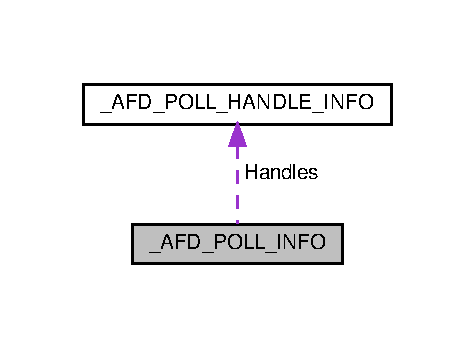
\includegraphics[width=228pt]{struct__AFD__POLL__INFO__coll__graph}
\end{center}
\end{figure}
\subsection*{Public Attributes}
\begin{DoxyCompactItemize}
\item 
\mbox{\Hypertarget{struct__AFD__POLL__INFO_a0504993706eef7ab023467030519adb9}\label{struct__AFD__POLL__INFO_a0504993706eef7ab023467030519adb9}} 
L\+A\+R\+G\+E\+\_\+\+I\+N\+T\+E\+G\+ER {\bfseries Timeout}
\item 
\mbox{\Hypertarget{struct__AFD__POLL__INFO_ac37001d47d932e44224b70ffe7233d30}\label{struct__AFD__POLL__INFO_ac37001d47d932e44224b70ffe7233d30}} 
U\+L\+O\+NG {\bfseries Number\+Of\+Handles}
\item 
\mbox{\Hypertarget{struct__AFD__POLL__INFO_acc55cd6176cbd088afa107ec38573cc1}\label{struct__AFD__POLL__INFO_acc55cd6176cbd088afa107ec38573cc1}} 
U\+L\+O\+NG {\bfseries Exclusive}
\item 
\mbox{\Hypertarget{struct__AFD__POLL__INFO_ae72b9c1736ba89ccfbcffda40588c67d}\label{struct__AFD__POLL__INFO_ae72b9c1736ba89ccfbcffda40588c67d}} 
\hyperlink{struct__AFD__POLL__HANDLE__INFO}{A\+F\+D\+\_\+\+P\+O\+L\+L\+\_\+\+H\+A\+N\+D\+L\+E\+\_\+\+I\+N\+FO} {\bfseries Handles} \mbox{[}1\mbox{]}
\end{DoxyCompactItemize}


The documentation for this struct was generated from the following file\+:\begin{DoxyCompactItemize}
\item 
/home/pmx/git/\+P\+M\+X/\+Simu\+Cocos3/cocos2d/external/uv/include/uv/win.\+h\end{DoxyCompactItemize}

\hypertarget{structcocostudio_1_1DataReaderHelper_1_1__AsyncStruct}{}\section{cocostudio\+:\+:Data\+Reader\+Helper\+:\+:\+\_\+\+Async\+Struct Struct Reference}
\label{structcocostudio_1_1DataReaderHelper_1_1__AsyncStruct}\index{cocostudio\+::\+Data\+Reader\+Helper\+::\+\_\+\+Async\+Struct@{cocostudio\+::\+Data\+Reader\+Helper\+::\+\_\+\+Async\+Struct}}
\subsection*{Public Attributes}
\begin{DoxyCompactItemize}
\item 
\mbox{\Hypertarget{structcocostudio_1_1DataReaderHelper_1_1__AsyncStruct_a175d1a1b1e197ec5d87ce73a62bad34f}\label{structcocostudio_1_1DataReaderHelper_1_1__AsyncStruct_a175d1a1b1e197ec5d87ce73a62bad34f}} 
std\+::string {\bfseries filename}
\item 
\mbox{\Hypertarget{structcocostudio_1_1DataReaderHelper_1_1__AsyncStruct_a23b30620b58933850727a17382e9f079}\label{structcocostudio_1_1DataReaderHelper_1_1__AsyncStruct_a23b30620b58933850727a17382e9f079}} 
std\+::string {\bfseries file\+Content}
\item 
\mbox{\Hypertarget{structcocostudio_1_1DataReaderHelper_1_1__AsyncStruct_ae8100158c7ae92bfd8d4e7ff49fe3823}\label{structcocostudio_1_1DataReaderHelper_1_1__AsyncStruct_ae8100158c7ae92bfd8d4e7ff49fe3823}} 
Config\+Type {\bfseries config\+Type}
\item 
\mbox{\Hypertarget{structcocostudio_1_1DataReaderHelper_1_1__AsyncStruct_a6bd3f43d56d915d798f2b1c6bf71fd41}\label{structcocostudio_1_1DataReaderHelper_1_1__AsyncStruct_a6bd3f43d56d915d798f2b1c6bf71fd41}} 
std\+::string {\bfseries base\+File\+Path}
\item 
\mbox{\Hypertarget{structcocostudio_1_1DataReaderHelper_1_1__AsyncStruct_a450338a55d839c855971c4b4edf724cb}\label{structcocostudio_1_1DataReaderHelper_1_1__AsyncStruct_a450338a55d839c855971c4b4edf724cb}} 
cocos2d\+::\+Ref $\ast$ {\bfseries target}
\item 
\mbox{\Hypertarget{structcocostudio_1_1DataReaderHelper_1_1__AsyncStruct_a80484d93663e766e4da56ac39f59eb07}\label{structcocostudio_1_1DataReaderHelper_1_1__AsyncStruct_a80484d93663e766e4da56ac39f59eb07}} 
cocos2d\+::\+S\+E\+L\+\_\+\+S\+C\+H\+E\+D\+U\+LE {\bfseries selector}
\item 
\mbox{\Hypertarget{structcocostudio_1_1DataReaderHelper_1_1__AsyncStruct_afccb6f1a9a8805a3c5346f397b6b8b3f}\label{structcocostudio_1_1DataReaderHelper_1_1__AsyncStruct_afccb6f1a9a8805a3c5346f397b6b8b3f}} 
bool {\bfseries auto\+Load\+Sprite\+File}
\item 
\mbox{\Hypertarget{structcocostudio_1_1DataReaderHelper_1_1__AsyncStruct_ad55785418ebcf15d0948e22f53565802}\label{structcocostudio_1_1DataReaderHelper_1_1__AsyncStruct_ad55785418ebcf15d0948e22f53565802}} 
std\+::string {\bfseries image\+Path}
\item 
\mbox{\Hypertarget{structcocostudio_1_1DataReaderHelper_1_1__AsyncStruct_a08892e5d5aa4d67c4485cd5fae58f4b9}\label{structcocostudio_1_1DataReaderHelper_1_1__AsyncStruct_a08892e5d5aa4d67c4485cd5fae58f4b9}} 
std\+::string {\bfseries plist\+Path}
\end{DoxyCompactItemize}


The documentation for this struct was generated from the following file\+:\begin{DoxyCompactItemize}
\item 
/home/pmx/git/\+P\+M\+X/\+Simu\+Cocos/cocos2d/cocos/editor-\/support/cocostudio/C\+C\+Data\+Reader\+Helper.\+h\end{DoxyCompactItemize}

\hypertarget{struct__BMFontDef}{}\section{\+\_\+\+B\+M\+Font\+Def Struct Reference}
\label{struct__BMFontDef}\index{\+\_\+\+B\+M\+Font\+Def@{\+\_\+\+B\+M\+Font\+Def}}


Collaboration diagram for \+\_\+\+B\+M\+Font\+Def\+:
\nopagebreak
\begin{figure}[H]
\begin{center}
\leavevmode
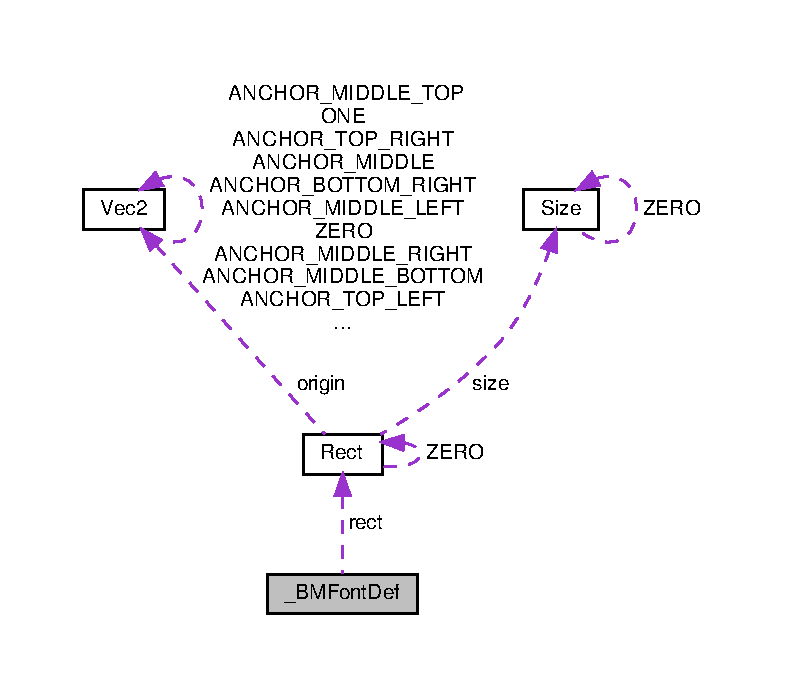
\includegraphics[width=350pt]{struct__BMFontDef__coll__graph}
\end{center}
\end{figure}
\subsection*{Public Attributes}
\begin{DoxyCompactItemize}
\item 
unsigned int \hyperlink{group__label_ga4be84ef9be4446878fff255b15e9e678}{char\+ID}
\begin{DoxyCompactList}\small\item\em ID of the character. \end{DoxyCompactList}\item 
\hyperlink{classRect}{Rect} \hyperlink{group__label_ga9426c06ddd57097582d48bfb34ef02fa}{rect}
\begin{DoxyCompactList}\small\item\em origin and size of the font \end{DoxyCompactList}\item 
short \hyperlink{group__label_gaf961a67faba7abff4c31ef69b32eaed4}{x\+Offset}
\begin{DoxyCompactList}\small\item\em The X amount the image should be offset when drawing the image (in pixels) \end{DoxyCompactList}\item 
short \hyperlink{group__label_gae0d9c0fc84b157abd9133b6bcddab2b7}{y\+Offset}
\begin{DoxyCompactList}\small\item\em The Y amount the image should be offset when drawing the image (in pixels) \end{DoxyCompactList}\item 
short \hyperlink{group__label_gaf8a9e2733f5f1fcb8a3631b3886d6703}{x\+Advance}
\begin{DoxyCompactList}\small\item\em The amount to move the current position after drawing the character (in pixels) \end{DoxyCompactList}\end{DoxyCompactItemize}


The documentation for this struct was generated from the following file\+:\begin{DoxyCompactItemize}
\item 
/home/pmx/git/\+P\+M\+X/\+Simu\+Cocos/cocos2d/cocos/2d/C\+C\+Font\+F\+N\+T.\+cpp\end{DoxyCompactItemize}

\hypertarget{struct__BMFontPadding}{}\section{\+\_\+\+B\+M\+Font\+Padding Struct Reference}
\label{struct__BMFontPadding}\index{\+\_\+\+B\+M\+Font\+Padding@{\+\_\+\+B\+M\+Font\+Padding}}
\subsection*{Public Attributes}
\begin{DoxyCompactItemize}
\item 
int \hyperlink{group__label_ga8129887cd2f3f177100cd4fedf20e347}{left}
\begin{DoxyCompactList}\small\item\em padding left \end{DoxyCompactList}\item 
int \hyperlink{group__label_gad673e6ff522f10836afba0745f3c4ee8}{top}
\begin{DoxyCompactList}\small\item\em padding top \end{DoxyCompactList}\item 
int \hyperlink{group__label_gac83f97e64d8fa8a835a17c44d93f9f62}{right}
\begin{DoxyCompactList}\small\item\em padding right \end{DoxyCompactList}\item 
int \hyperlink{group__label_ga41ee44807cde2134c0ff73208dccf6e7}{bottom}
\begin{DoxyCompactList}\small\item\em padding bottom \end{DoxyCompactList}\end{DoxyCompactItemize}


The documentation for this struct was generated from the following file\+:\begin{DoxyCompactItemize}
\item 
/home/pmx/git/\+P\+M\+X/\+Simu\+Cocos/cocos2d/cocos/2d/C\+C\+Font\+F\+N\+T.\+cpp\end{DoxyCompactItemize}

\hypertarget{struct__bufferInfo}{}\section{\+\_\+buffer\+Info Struct Reference}
\label{struct__bufferInfo}\index{\+\_\+buffer\+Info@{\+\_\+buffer\+Info}}
\subsection*{Public Attributes}
\begin{DoxyCompactItemize}
\item 
\mbox{\Hypertarget{struct__bufferInfo_ada9a4b0d226243291982b16fd0aa4320}\label{struct__bufferInfo_ada9a4b0d226243291982b16fd0aa4320}} 
A\+Luint {\bfseries buffer\+Id}
\item 
\mbox{\Hypertarget{struct__bufferInfo_a7ec9ded79929d9a8d532e8847cffe18e}\label{struct__bufferInfo_a7ec9ded79929d9a8d532e8847cffe18e}} 
int {\bfseries buffer\+State}
\item 
\mbox{\Hypertarget{struct__bufferInfo_a214908997f344969d4306b8184dec586}\label{struct__bufferInfo_a214908997f344969d4306b8184dec586}} 
void $\ast$ {\bfseries buffer\+Data}
\item 
\mbox{\Hypertarget{struct__bufferInfo_ac74dea7e65809ec13a1d8fa2981bdffe}\label{struct__bufferInfo_ac74dea7e65809ec13a1d8fa2981bdffe}} 
A\+Lenum {\bfseries format}
\item 
\mbox{\Hypertarget{struct__bufferInfo_a0ab48cabebb4e040758bbd751e2eaf1c}\label{struct__bufferInfo_a0ab48cabebb4e040758bbd751e2eaf1c}} 
A\+Lsizei {\bfseries size\+In\+Bytes}
\item 
\mbox{\Hypertarget{struct__bufferInfo_add13810b4e5f1cde5ae260bcc427e9a6}\label{struct__bufferInfo_add13810b4e5f1cde5ae260bcc427e9a6}} 
A\+Lsizei {\bfseries frequency\+In\+Hertz}
\end{DoxyCompactItemize}


The documentation for this struct was generated from the following file\+:\begin{DoxyCompactItemize}
\item 
/home/pmx/git/\+P\+M\+X/\+Simu\+Cocos/cocos2d/cocos/audio/ios/\hyperlink{cocos2d_2cocos_2audio_2ios_2CocosDenshion_8h}{Cocos\+Denshion.\+h}\end{DoxyCompactItemize}

\hypertarget{struct__ccBezierConfig}{}\section{\+\_\+cc\+Bezier\+Config Struct Reference}
\label{struct__ccBezierConfig}\index{\+\_\+cc\+Bezier\+Config@{\+\_\+cc\+Bezier\+Config}}


Collaboration diagram for \+\_\+cc\+Bezier\+Config\+:
\nopagebreak
\begin{figure}[H]
\begin{center}
\leavevmode
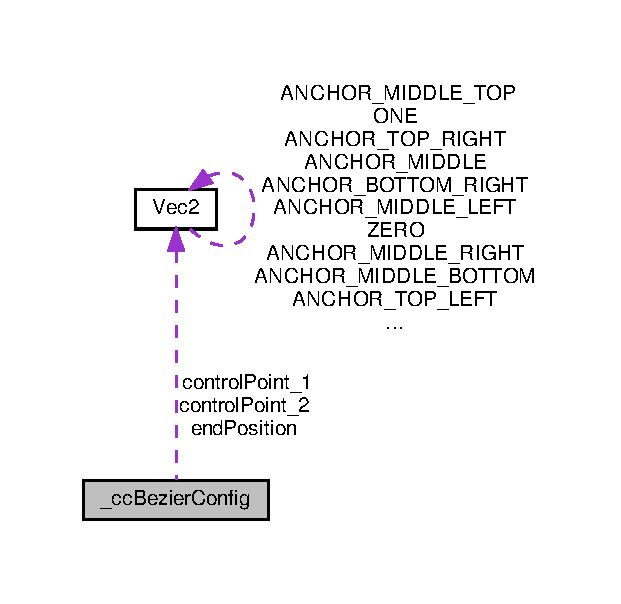
\includegraphics[width=298pt]{struct__ccBezierConfig__coll__graph}
\end{center}
\end{figure}
\subsection*{Public Attributes}
\begin{DoxyCompactItemize}
\item 
\mbox{\Hypertarget{struct__ccBezierConfig_a3c51963237c96dbe01af0838f31a528b}\label{struct__ccBezierConfig_a3c51963237c96dbe01af0838f31a528b}} 
\hyperlink{classVec2}{Vec2} \hyperlink{struct__ccBezierConfig_a3c51963237c96dbe01af0838f31a528b}{end\+Position}
\begin{DoxyCompactList}\small\item\em end position of the bezier \end{DoxyCompactList}\item 
\mbox{\Hypertarget{struct__ccBezierConfig_a44fc431ed2be15f6235aeac2367cb6c6}\label{struct__ccBezierConfig_a44fc431ed2be15f6235aeac2367cb6c6}} 
\hyperlink{classVec2}{Vec2} \hyperlink{struct__ccBezierConfig_a44fc431ed2be15f6235aeac2367cb6c6}{control\+Point\+\_\+1}
\begin{DoxyCompactList}\small\item\em \hyperlink{structBezier}{Bezier} control point 1. \end{DoxyCompactList}\item 
\mbox{\Hypertarget{struct__ccBezierConfig_a5e16e7e41cd146980a0157d547ade6d9}\label{struct__ccBezierConfig_a5e16e7e41cd146980a0157d547ade6d9}} 
\hyperlink{classVec2}{Vec2} \hyperlink{struct__ccBezierConfig_a5e16e7e41cd146980a0157d547ade6d9}{control\+Point\+\_\+2}
\begin{DoxyCompactList}\small\item\em \hyperlink{structBezier}{Bezier} control point 2. \end{DoxyCompactList}\end{DoxyCompactItemize}


The documentation for this struct was generated from the following file\+:\begin{DoxyCompactItemize}
\item 
/home/pmx/git/\+P\+M\+X/\+Simu\+Cocos/cocos2d/cocos/2d/C\+C\+Action\+Interval.\+h\end{DoxyCompactItemize}

\hypertarget{struct__cl__image__format}{}\section{\+\_\+cl\+\_\+image\+\_\+format Struct Reference}
\label{struct__cl__image__format}\index{\+\_\+cl\+\_\+image\+\_\+format@{\+\_\+cl\+\_\+image\+\_\+format}}
\subsection*{Public Attributes}
\begin{DoxyCompactItemize}
\item 
\mbox{\Hypertarget{struct__cl__image__format_aaedf0bf00bd2b217e865cad706bfad02}\label{struct__cl__image__format_aaedf0bf00bd2b217e865cad706bfad02}} 
cl\+\_\+channel\+\_\+order {\bfseries image\+\_\+channel\+\_\+order}
\item 
\mbox{\Hypertarget{struct__cl__image__format_ae965ba5f74cd52eabffc4e0904adea34}\label{struct__cl__image__format_ae965ba5f74cd52eabffc4e0904adea34}} 
cl\+\_\+channel\+\_\+type {\bfseries image\+\_\+channel\+\_\+data\+\_\+type}
\end{DoxyCompactItemize}


The documentation for this struct was generated from the following file\+:\begin{DoxyCompactItemize}
\item 
/home/pmx/git/\+P\+M\+X/\+Simu\+Cocos/cocos2d/external/bullet/\+Mini\+C\+L/cl.\+h\end{DoxyCompactItemize}

\hypertarget{struct__CompiledProgram}{}\section{\+\_\+\+Compiled\+Program Struct Reference}
\label{struct__CompiledProgram}\index{\+\_\+\+Compiled\+Program@{\+\_\+\+Compiled\+Program}}
\subsection*{Public Attributes}
\begin{DoxyCompactItemize}
\item 
\mbox{\Hypertarget{struct__CompiledProgram_a231bd47a0b9b878a2cc952489e48f5d2}\label{struct__CompiledProgram_a231bd47a0b9b878a2cc952489e48f5d2}} 
std\+::string {\bfseries key}
\item 
\mbox{\Hypertarget{struct__CompiledProgram_a1bb244d552f6a66647bf6ec6931fa2d3}\label{struct__CompiledProgram_a1bb244d552f6a66647bf6ec6931fa2d3}} 
std\+::vector$<$ unsigned char $>$ {\bfseries program}
\item 
\mbox{\Hypertarget{struct__CompiledProgram_aa15e749b2213cabf15a380efd0ff59ff}\label{struct__CompiledProgram_aa15e749b2213cabf15a380efd0ff59ff}} 
int {\bfseries length}
\end{DoxyCompactItemize}


The documentation for this struct was generated from the following file\+:\begin{DoxyCompactItemize}
\item 
/home/pmx/git/\+P\+M\+X/\+Simu\+Cocos/cocos2d/cocos/platform/winrt/C\+C\+Precompiled\+Shaders.\+h\end{DoxyCompactItemize}

\hypertarget{structcocostudio_1_1DataReaderHelper_1_1__DataInfo}{}\section{cocostudio\+:\+:Data\+Reader\+Helper\+:\+:\+\_\+\+Data\+Info Struct Reference}
\label{structcocostudio_1_1DataReaderHelper_1_1__DataInfo}\index{cocostudio\+::\+Data\+Reader\+Helper\+::\+\_\+\+Data\+Info@{cocostudio\+::\+Data\+Reader\+Helper\+::\+\_\+\+Data\+Info}}


Collaboration diagram for cocostudio\+:\+:Data\+Reader\+Helper\+:\+:\+\_\+\+Data\+Info\+:
\nopagebreak
\begin{figure}[H]
\begin{center}
\leavevmode
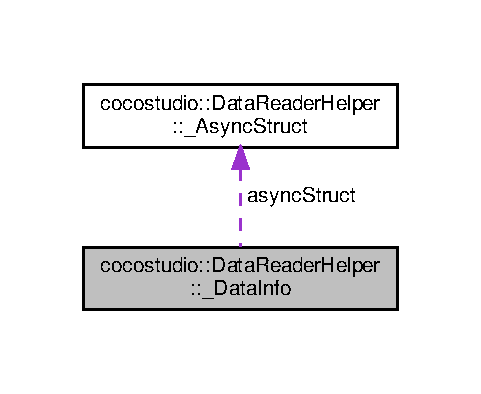
\includegraphics[width=231pt]{structcocostudio_1_1DataReaderHelper_1_1__DataInfo__coll__graph}
\end{center}
\end{figure}
\subsection*{Public Attributes}
\begin{DoxyCompactItemize}
\item 
\mbox{\Hypertarget{structcocostudio_1_1DataReaderHelper_1_1__DataInfo_a182bb57d924afd94e246ce9d372571ca}\label{structcocostudio_1_1DataReaderHelper_1_1__DataInfo_a182bb57d924afd94e246ce9d372571ca}} 
\hyperlink{structcocostudio_1_1DataReaderHelper_1_1__AsyncStruct}{Async\+Struct} $\ast$ {\bfseries async\+Struct}
\item 
\mbox{\Hypertarget{structcocostudio_1_1DataReaderHelper_1_1__DataInfo_a1aa35da7201c774fe66b6bafc43e0c1e}\label{structcocostudio_1_1DataReaderHelper_1_1__DataInfo_a1aa35da7201c774fe66b6bafc43e0c1e}} 
std\+::queue$<$ std\+::string $>$ {\bfseries config\+File\+Queue}
\item 
\mbox{\Hypertarget{structcocostudio_1_1DataReaderHelper_1_1__DataInfo_a305d493120ed056771639936a62b4a34}\label{structcocostudio_1_1DataReaderHelper_1_1__DataInfo_a305d493120ed056771639936a62b4a34}} 
float {\bfseries content\+Scale}
\item 
\mbox{\Hypertarget{structcocostudio_1_1DataReaderHelper_1_1__DataInfo_aded361ebc93f5a4636b90442ba9bff0f}\label{structcocostudio_1_1DataReaderHelper_1_1__DataInfo_aded361ebc93f5a4636b90442ba9bff0f}} 
std\+::string {\bfseries filename}
\item 
\mbox{\Hypertarget{structcocostudio_1_1DataReaderHelper_1_1__DataInfo_a53599100aa34268f75650a85f781d3f8}\label{structcocostudio_1_1DataReaderHelper_1_1__DataInfo_a53599100aa34268f75650a85f781d3f8}} 
std\+::string {\bfseries base\+File\+Path}
\item 
\mbox{\Hypertarget{structcocostudio_1_1DataReaderHelper_1_1__DataInfo_af8aecb39c974c66f9d64b4a1888e1ac1}\label{structcocostudio_1_1DataReaderHelper_1_1__DataInfo_af8aecb39c974c66f9d64b4a1888e1ac1}} 
float {\bfseries flash\+Tool\+Version}
\item 
\mbox{\Hypertarget{structcocostudio_1_1DataReaderHelper_1_1__DataInfo_a8a05dfbf2a8f88848f32c0dbe76ef161}\label{structcocostudio_1_1DataReaderHelper_1_1__DataInfo_a8a05dfbf2a8f88848f32c0dbe76ef161}} 
float {\bfseries coco\+Studio\+Version}
\end{DoxyCompactItemize}


The documentation for this struct was generated from the following file\+:\begin{DoxyCompactItemize}
\item 
/home/pmx/git/\+P\+M\+X/\+Simu\+Cocos/cocos2d/cocos/editor-\/support/cocostudio/C\+C\+Data\+Reader\+Helper.\+h\end{DoxyCompactItemize}

\hypertarget{struct__dataInput}{}\section{\+\_\+data\+Input Struct Reference}
\label{struct__dataInput}\index{\+\_\+data\+Input@{\+\_\+data\+Input}}
\subsection*{Public Attributes}
\begin{DoxyCompactItemize}
\item 
\mbox{\Hypertarget{struct__dataInput_aab6ad655bd4d4654fe8b6fa19912369b}\label{struct__dataInput_aab6ad655bd4d4654fe8b6fa19912369b}} 
const unsigned char $\ast$ {\bfseries cursor}
\item 
\mbox{\Hypertarget{struct__dataInput_af26e023f0d3b079d3ece3b54ef1dc5b7}\label{struct__dataInput_af26e023f0d3b079d3ece3b54ef1dc5b7}} 
const unsigned char $\ast$ {\bfseries end}
\end{DoxyCompactItemize}


The documentation for this struct was generated from the following file\+:\begin{DoxyCompactItemize}
\item 
/home/pmx/git/\+P\+M\+X/\+Simu\+Cocos3/cocos2d/cocos/editor-\/support/spine/Skeleton\+Binary.\+c\end{DoxyCompactItemize}

\hypertarget{struct__DataRef}{}\section{\+\_\+\+Data\+Ref Struct Reference}
\label{struct__DataRef}\index{\+\_\+\+Data\+Ref@{\+\_\+\+Data\+Ref}}


Collaboration diagram for \+\_\+\+Data\+Ref\+:
\nopagebreak
\begin{figure}[H]
\begin{center}
\leavevmode
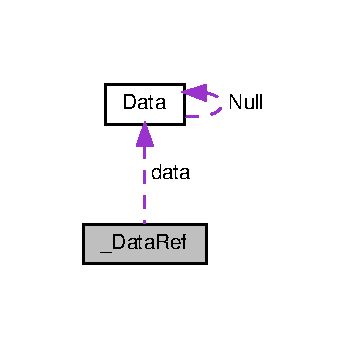
\includegraphics[width=168pt]{struct__DataRef__coll__graph}
\end{center}
\end{figure}
\subsection*{Public Attributes}
\begin{DoxyCompactItemize}
\item 
\mbox{\Hypertarget{struct__DataRef_ab7accaae6c2372d12839ae78726f793c}\label{struct__DataRef_ab7accaae6c2372d12839ae78726f793c}} 
\hyperlink{classData}{Data} {\bfseries data}
\item 
\mbox{\Hypertarget{struct__DataRef_a11c0f374308f3a79e03abb3ee0dc72a1}\label{struct__DataRef_a11c0f374308f3a79e03abb3ee0dc72a1}} 
unsigned int {\bfseries reference\+Count}
\end{DoxyCompactItemize}


The documentation for this struct was generated from the following file\+:\begin{DoxyCompactItemize}
\item 
/home/pmx/git/\+P\+M\+X/\+Simu\+Cocos/cocos2d/cocos/2d/C\+C\+Font\+Free\+Type.\+cpp\end{DoxyCompactItemize}

\hypertarget{struct__Entry}{}\section{\+\_\+\+Entry Struct Reference}
\label{struct__Entry}\index{\+\_\+\+Entry@{\+\_\+\+Entry}}


Collaboration diagram for \+\_\+\+Entry\+:
\nopagebreak
\begin{figure}[H]
\begin{center}
\leavevmode
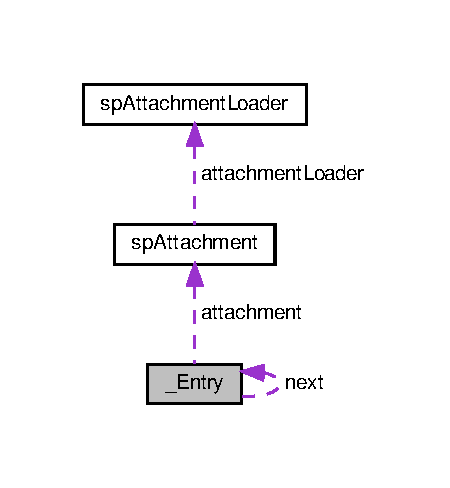
\includegraphics[width=216pt]{struct__Entry__coll__graph}
\end{center}
\end{figure}
\subsection*{Public Attributes}
\begin{DoxyCompactItemize}
\item 
\mbox{\Hypertarget{struct__Entry_a5de17f95ef6aaffd2566b7e22f0942bb}\label{struct__Entry_a5de17f95ef6aaffd2566b7e22f0942bb}} 
int {\bfseries slot\+Index}
\item 
\mbox{\Hypertarget{struct__Entry_a636552ae4479565e60a8db9d2bb17fc9}\label{struct__Entry_a636552ae4479565e60a8db9d2bb17fc9}} 
const char $\ast$ {\bfseries name}
\item 
\mbox{\Hypertarget{struct__Entry_a1937be9c2993c803737ef28f2a24ab41}\label{struct__Entry_a1937be9c2993c803737ef28f2a24ab41}} 
\hyperlink{structspAttachment}{sp\+Attachment} $\ast$ {\bfseries attachment}
\item 
\mbox{\Hypertarget{struct__Entry_aaf74558c9ebab1af0591a1b495e4fa9a}\label{struct__Entry_aaf74558c9ebab1af0591a1b495e4fa9a}} 
\hyperlink{struct__Entry}{\+\_\+\+Entry} $\ast$ {\bfseries next}
\end{DoxyCompactItemize}


The documentation for this struct was generated from the following file\+:\begin{DoxyCompactItemize}
\item 
/home/pmx/git/\+P\+M\+X/\+Simu\+Cocos/cocos2d/cocos/editor-\/support/spine/Skin.\+h\end{DoxyCompactItemize}

\hypertarget{struct__FontDefHashElement}{}\section{\+\_\+\+Font\+Def\+Hash\+Element Struct Reference}
\label{struct__FontDefHashElement}\index{\+\_\+\+Font\+Def\+Hash\+Element@{\+\_\+\+Font\+Def\+Hash\+Element}}


Collaboration diagram for \+\_\+\+Font\+Def\+Hash\+Element\+:
\nopagebreak
\begin{figure}[H]
\begin{center}
\leavevmode
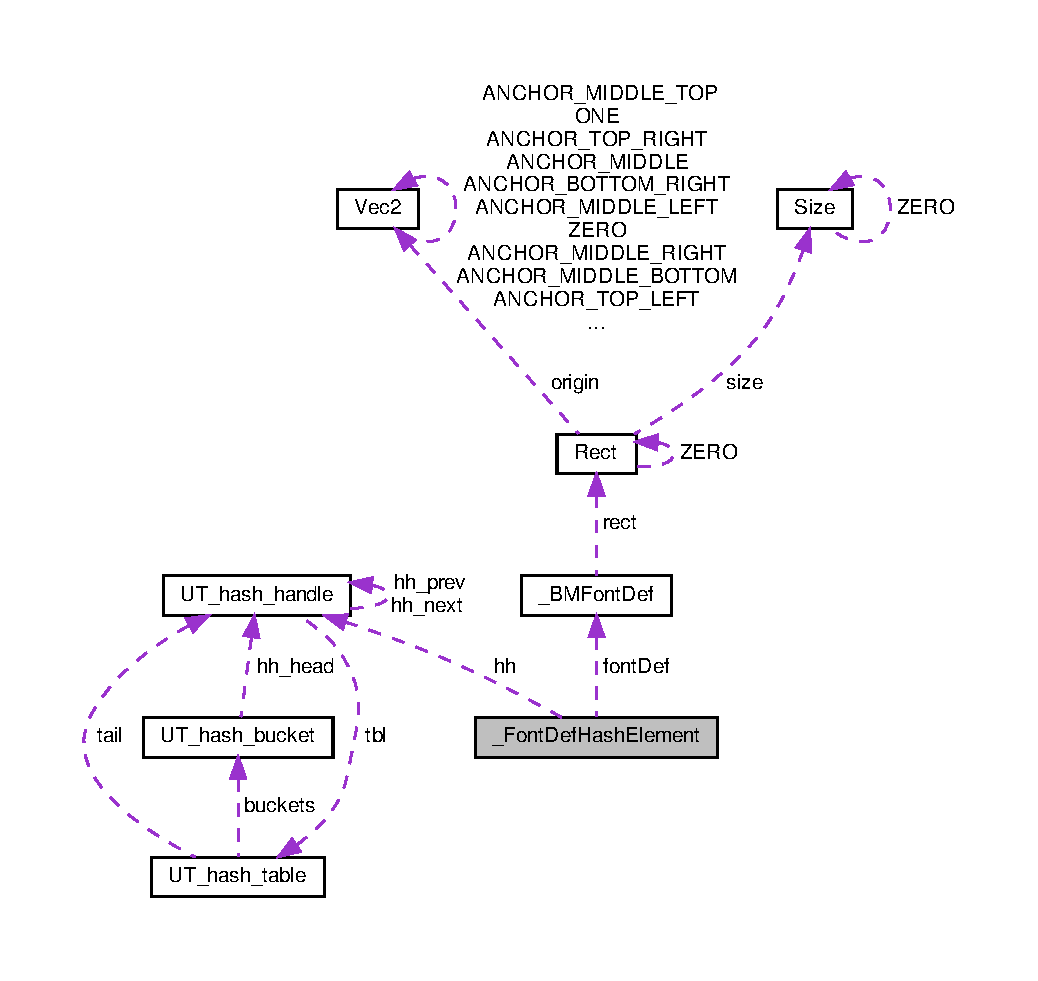
\includegraphics[width=350pt]{struct__FontDefHashElement__coll__graph}
\end{center}
\end{figure}
\subsection*{Public Attributes}
\begin{DoxyCompactItemize}
\item 
unsigned int {\bfseries key}
\item 
\hyperlink{structBMFontDef}{B\+M\+Font\+Def} {\bfseries font\+Def}
\item 
\hyperlink{structUT__hash__handle}{U\+T\+\_\+hash\+\_\+handle} {\bfseries hh}
\end{DoxyCompactItemize}


The documentation for this struct was generated from the following file\+:\begin{DoxyCompactItemize}
\item 
/home/pmx/git/\+P\+M\+X/\+Simu\+Cocos/cocos2d/cocos/2d/C\+C\+Font\+F\+N\+T.\+cpp\end{DoxyCompactItemize}

\hypertarget{struct__FromEntry}{}\section{\+\_\+\+From\+Entry Struct Reference}
\label{struct__FromEntry}\index{\+\_\+\+From\+Entry@{\+\_\+\+From\+Entry}}


Collaboration diagram for \+\_\+\+From\+Entry\+:
\nopagebreak
\begin{figure}[H]
\begin{center}
\leavevmode
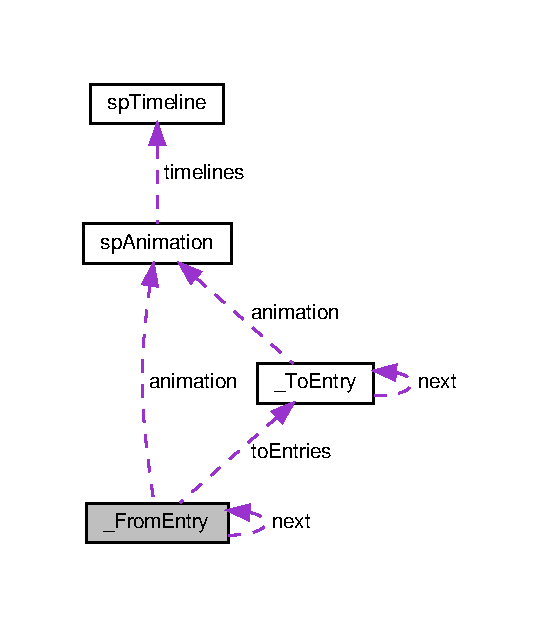
\includegraphics[width=260pt]{struct__FromEntry__coll__graph}
\end{center}
\end{figure}
\subsection*{Public Attributes}
\begin{DoxyCompactItemize}
\item 
\mbox{\Hypertarget{struct__FromEntry_ac971a5aa97313ea22fdb7a9aa4e5c5d7}\label{struct__FromEntry_ac971a5aa97313ea22fdb7a9aa4e5c5d7}} 
\hyperlink{structspAnimation}{sp\+Animation} $\ast$ {\bfseries animation}
\item 
\mbox{\Hypertarget{struct__FromEntry_ae0ada9f41fc11ec7579f0f232bf7cd89}\label{struct__FromEntry_ae0ada9f41fc11ec7579f0f232bf7cd89}} 
\hyperlink{struct__ToEntry}{\+\_\+\+To\+Entry} $\ast$ {\bfseries to\+Entries}
\item 
\mbox{\Hypertarget{struct__FromEntry_a93cf2bef97b1218ad02af65cc0a65ad9}\label{struct__FromEntry_a93cf2bef97b1218ad02af65cc0a65ad9}} 
\hyperlink{struct__FromEntry}{\+\_\+\+From\+Entry} $\ast$ {\bfseries next}
\end{DoxyCompactItemize}


The documentation for this struct was generated from the following file\+:\begin{DoxyCompactItemize}
\item 
/home/pmx/git/\+P\+M\+X/\+Simu\+Cocos/cocos2d/cocos/editor-\/support/spine/Animation\+State\+Data.\+c\end{DoxyCompactItemize}

\hypertarget{struct__GPU__DEVICE}{}\section{\+\_\+\+G\+P\+U\+\_\+\+D\+E\+V\+I\+CE Struct Reference}
\label{struct__GPU__DEVICE}\index{\+\_\+\+G\+P\+U\+\_\+\+D\+E\+V\+I\+CE@{\+\_\+\+G\+P\+U\+\_\+\+D\+E\+V\+I\+CE}}
\subsection*{Public Attributes}
\begin{DoxyCompactItemize}
\item 
\mbox{\Hypertarget{struct__GPU__DEVICE_afcb22f16ba9e526610489ff56ab78ddb}\label{struct__GPU__DEVICE_afcb22f16ba9e526610489ff56ab78ddb}} 
D\+W\+O\+RD {\bfseries cb}
\item 
\mbox{\Hypertarget{struct__GPU__DEVICE_acdb1f0d784d7527ec04163439eff9038}\label{struct__GPU__DEVICE_acdb1f0d784d7527ec04163439eff9038}} 
C\+H\+AR {\bfseries Device\+Name} \mbox{[}32\mbox{]}
\item 
\mbox{\Hypertarget{struct__GPU__DEVICE_a50b7b6a8eb397001ada4f5f918cc8065}\label{struct__GPU__DEVICE_a50b7b6a8eb397001ada4f5f918cc8065}} 
C\+H\+AR {\bfseries Device\+String} \mbox{[}128\mbox{]}
\item 
\mbox{\Hypertarget{struct__GPU__DEVICE_a008db9d0f5fc13a5160805f40465f14a}\label{struct__GPU__DEVICE_a008db9d0f5fc13a5160805f40465f14a}} 
D\+W\+O\+RD {\bfseries Flags}
\item 
\mbox{\Hypertarget{struct__GPU__DEVICE_aeb573bbeb3b6c589246720ef259b9a27}\label{struct__GPU__DEVICE_aeb573bbeb3b6c589246720ef259b9a27}} 
R\+E\+CT {\bfseries rc\+Virtual\+Screen}
\end{DoxyCompactItemize}


The documentation for this struct was generated from the following file\+:\begin{DoxyCompactItemize}
\item 
/home/pmx/git/\+P\+M\+X/\+Simu\+Cocos/cocos2d/external/win32-\/specific/gles/include/\+O\+G\+L\+E\+S/\+G\+L/wglew.\+h\end{DoxyCompactItemize}

\hypertarget{struct__hashElement}{}\section{\+\_\+hash\+Element Struct Reference}
\label{struct__hashElement}\index{\+\_\+hash\+Element@{\+\_\+hash\+Element}}


Collaboration diagram for \+\_\+hash\+Element\+:
\nopagebreak
\begin{figure}[H]
\begin{center}
\leavevmode
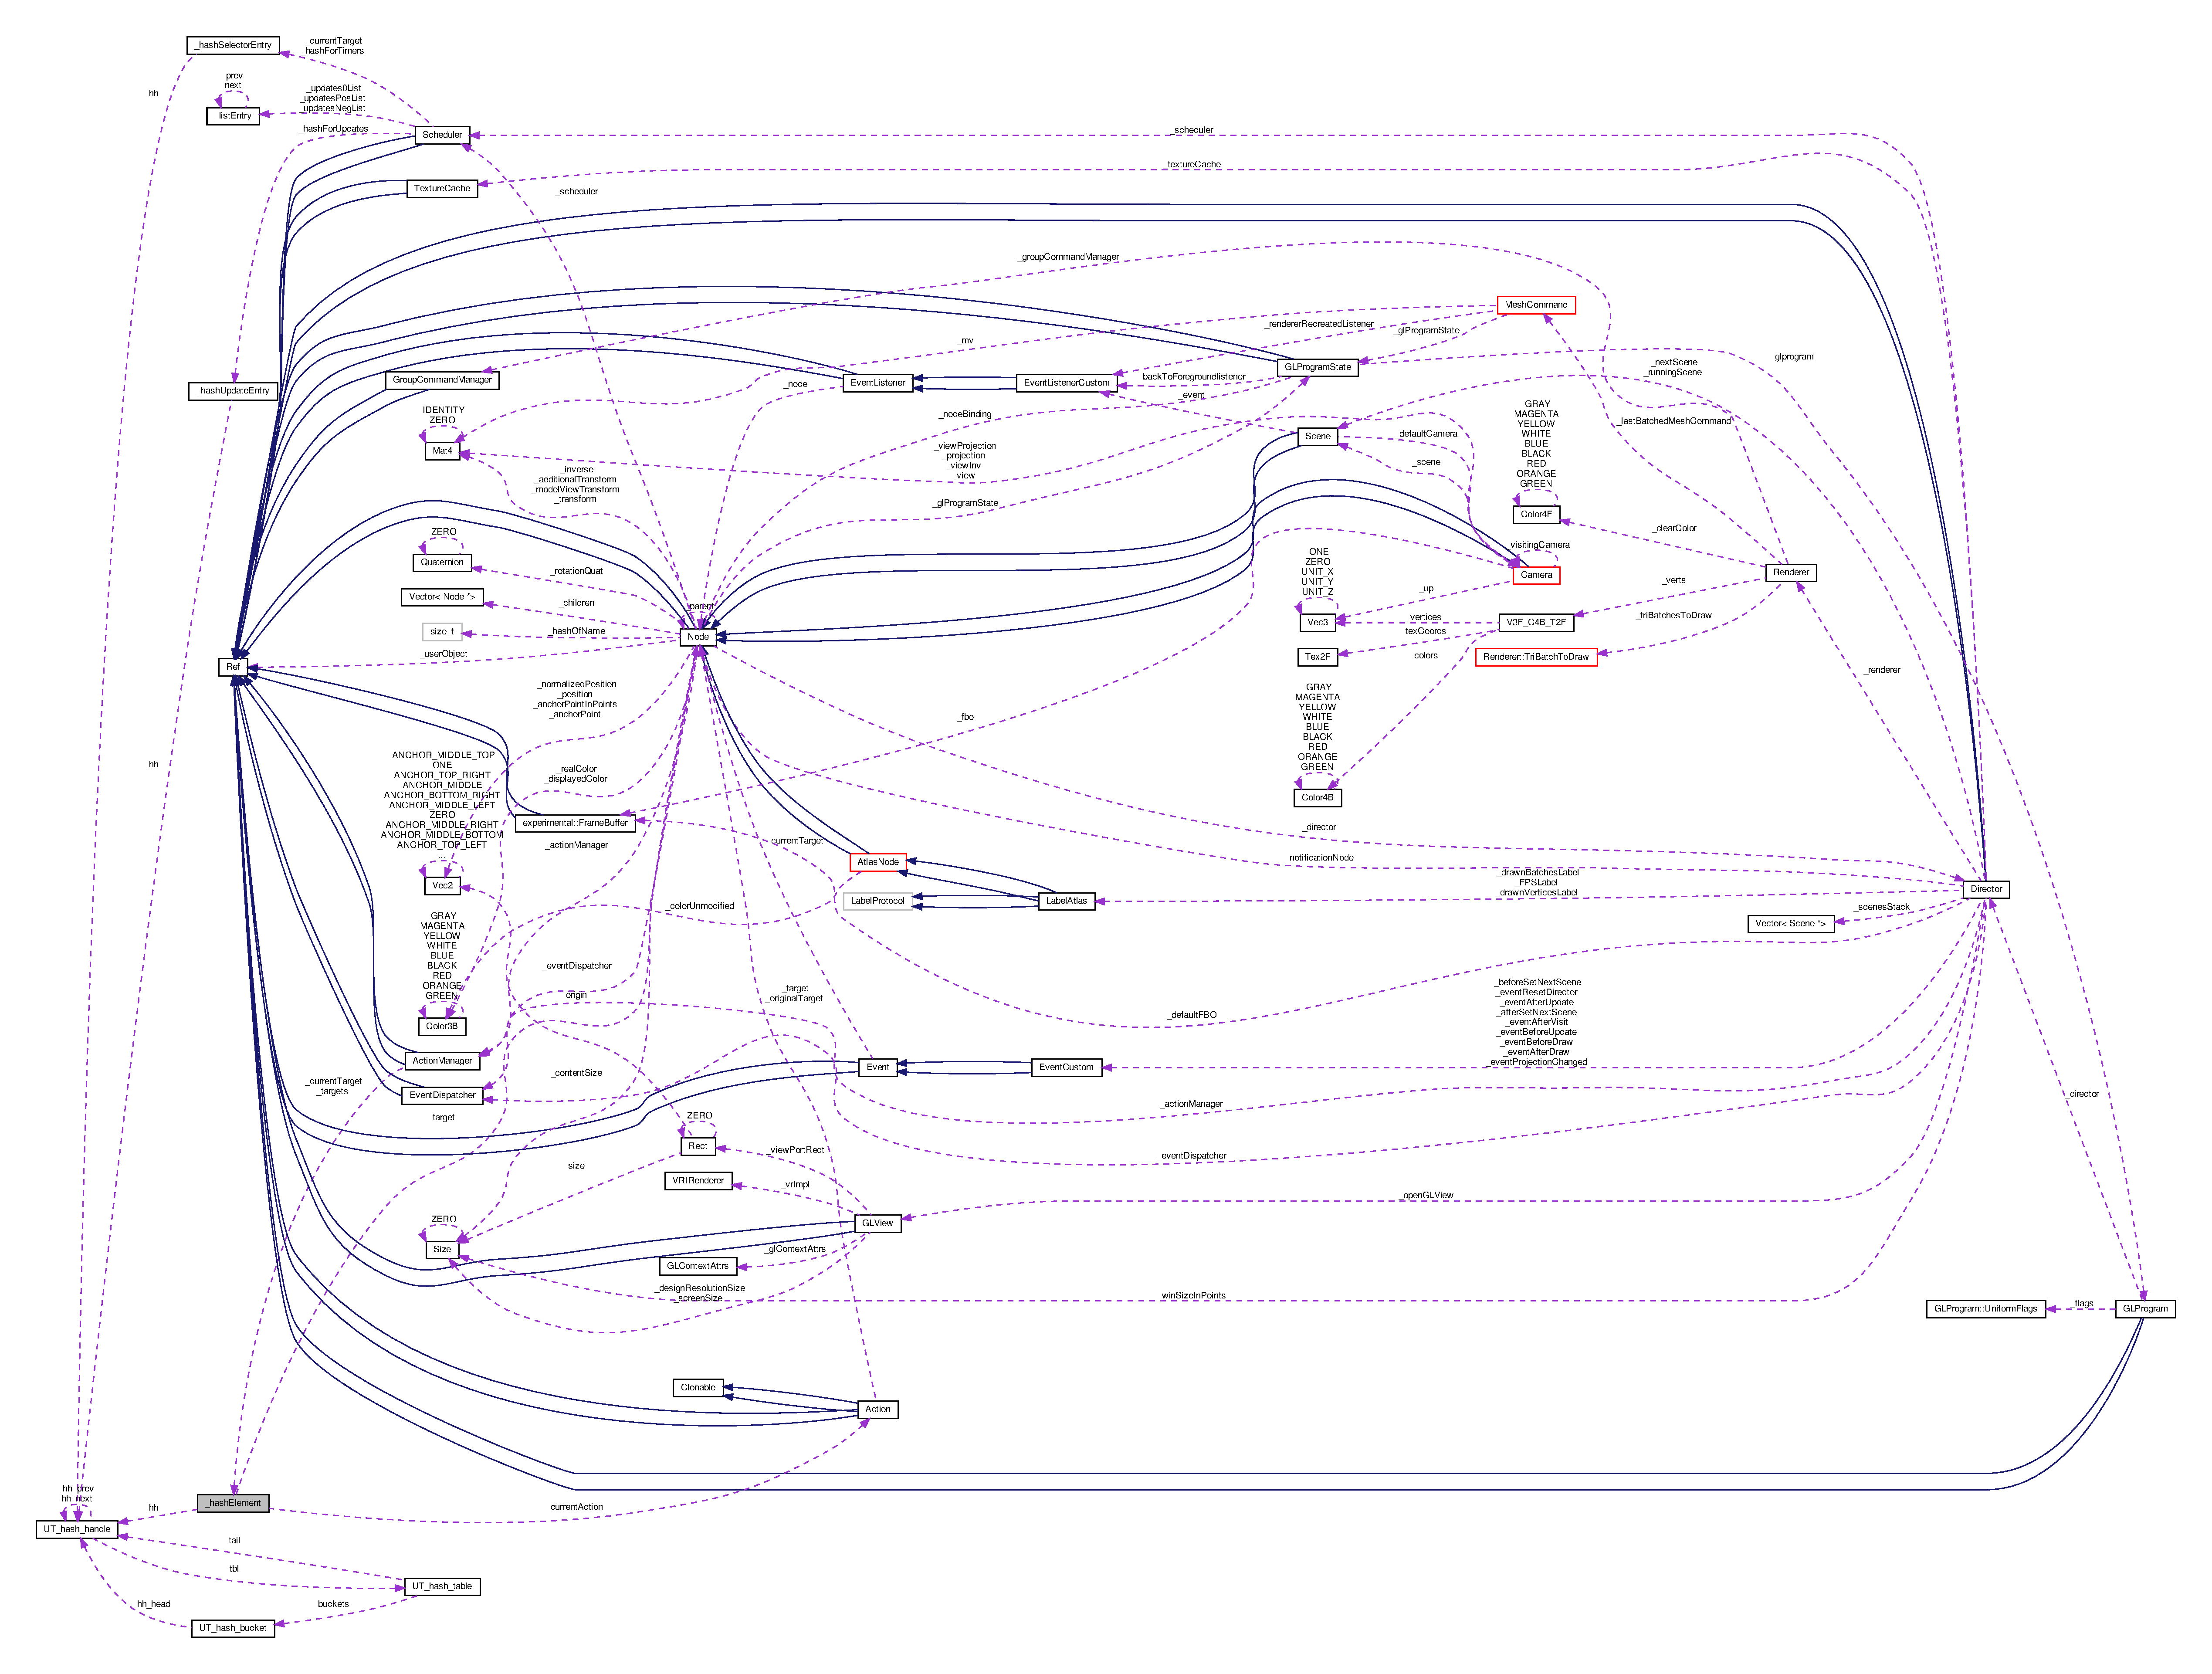
\includegraphics[width=350pt]{struct__hashElement__coll__graph}
\end{center}
\end{figure}
\subsection*{Public Attributes}
\begin{DoxyCompactItemize}
\item 
\mbox{\Hypertarget{struct__hashElement_aad474bf3a3c6b811ac11f96f6e1cbd31}\label{struct__hashElement_aad474bf3a3c6b811ac11f96f6e1cbd31}} 
struct \+\_\+cc\+Array $\ast$ {\bfseries actions}
\item 
\mbox{\Hypertarget{struct__hashElement_aa11ca3c171fb6a6b64ae9d17adbd6cf3}\label{struct__hashElement_aa11ca3c171fb6a6b64ae9d17adbd6cf3}} 
\hyperlink{classNode}{Node} $\ast$ {\bfseries target}
\item 
\mbox{\Hypertarget{struct__hashElement_a040815fc6b84fb078b37de409994c523}\label{struct__hashElement_a040815fc6b84fb078b37de409994c523}} 
int {\bfseries action\+Index}
\item 
\mbox{\Hypertarget{struct__hashElement_ad93230670da1520e6db2d9b79ddfb3d7}\label{struct__hashElement_ad93230670da1520e6db2d9b79ddfb3d7}} 
\hyperlink{classAction}{Action} $\ast$ {\bfseries current\+Action}
\item 
\mbox{\Hypertarget{struct__hashElement_a153140976e1e248d8b13ea9de7b0f5bd}\label{struct__hashElement_a153140976e1e248d8b13ea9de7b0f5bd}} 
bool {\bfseries current\+Action\+Salvaged}
\item 
\mbox{\Hypertarget{struct__hashElement_aee7ba57bd1039efec5314ccb02e864c2}\label{struct__hashElement_aee7ba57bd1039efec5314ccb02e864c2}} 
bool {\bfseries paused}
\item 
\mbox{\Hypertarget{struct__hashElement_a478c5e7c62426f22612799d32ee2234f}\label{struct__hashElement_a478c5e7c62426f22612799d32ee2234f}} 
\hyperlink{structUT__hash__handle}{U\+T\+\_\+hash\+\_\+handle} {\bfseries hh}
\end{DoxyCompactItemize}


The documentation for this struct was generated from the following file\+:\begin{DoxyCompactItemize}
\item 
/home/pmx/git/\+P\+M\+X/\+Simu\+Cocos/cocos2d/cocos/2d/C\+C\+Action\+Manager.\+cpp\end{DoxyCompactItemize}

\hypertarget{struct__hashSelectorEntry}{}\section{\+\_\+hash\+Selector\+Entry Struct Reference}
\label{struct__hashSelectorEntry}\index{\+\_\+hash\+Selector\+Entry@{\+\_\+hash\+Selector\+Entry}}


Collaboration diagram for \+\_\+hash\+Selector\+Entry\+:
\nopagebreak
\begin{figure}[H]
\begin{center}
\leavevmode
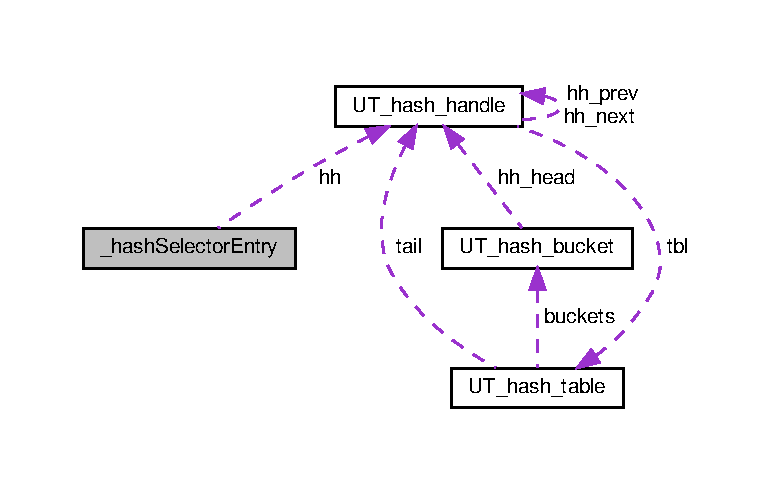
\includegraphics[width=350pt]{struct__hashSelectorEntry__coll__graph}
\end{center}
\end{figure}
\subsection*{Public Attributes}
\begin{DoxyCompactItemize}
\item 
\mbox{\Hypertarget{struct__hashSelectorEntry_af2d937e91681f579d0fd5ae08a77dac0}\label{struct__hashSelectorEntry_af2d937e91681f579d0fd5ae08a77dac0}} 
cc\+Array $\ast$ {\bfseries timers}
\item 
\mbox{\Hypertarget{struct__hashSelectorEntry_a72a517c7822964743801ae696bc3ad3d}\label{struct__hashSelectorEntry_a72a517c7822964743801ae696bc3ad3d}} 
void $\ast$ {\bfseries target}
\item 
\mbox{\Hypertarget{struct__hashSelectorEntry_a1fc9d1f9933c07afe214462de879347b}\label{struct__hashSelectorEntry_a1fc9d1f9933c07afe214462de879347b}} 
int {\bfseries timer\+Index}
\item 
\mbox{\Hypertarget{struct__hashSelectorEntry_a889a0627caee95fc97bb06bab68499b4}\label{struct__hashSelectorEntry_a889a0627caee95fc97bb06bab68499b4}} 
Timer $\ast$ {\bfseries current\+Timer}
\item 
\mbox{\Hypertarget{struct__hashSelectorEntry_a92dd7cdc1a34bde5fb92794beec9a56f}\label{struct__hashSelectorEntry_a92dd7cdc1a34bde5fb92794beec9a56f}} 
bool {\bfseries current\+Timer\+Salvaged}
\item 
\mbox{\Hypertarget{struct__hashSelectorEntry_a3abdfd03a00173d13d1138c15f0bf8e0}\label{struct__hashSelectorEntry_a3abdfd03a00173d13d1138c15f0bf8e0}} 
bool {\bfseries paused}
\item 
\mbox{\Hypertarget{struct__hashSelectorEntry_ad007cfdf3a7df8672a9c6901e70c97ea}\label{struct__hashSelectorEntry_ad007cfdf3a7df8672a9c6901e70c97ea}} 
\hyperlink{structUT__hash__handle}{U\+T\+\_\+hash\+\_\+handle} {\bfseries hh}
\end{DoxyCompactItemize}


The documentation for this struct was generated from the following file\+:\begin{DoxyCompactItemize}
\item 
/home/pmx/git/\+P\+M\+X/\+Simu\+Cocos/cocos2d/cocos/base/C\+C\+Scheduler.\+cpp\end{DoxyCompactItemize}

\hypertarget{struct__hashUpdateEntry}{}\section{\+\_\+hash\+Update\+Entry Struct Reference}
\label{struct__hashUpdateEntry}\index{\+\_\+hash\+Update\+Entry@{\+\_\+hash\+Update\+Entry}}


Collaboration diagram for \+\_\+hash\+Update\+Entry\+:
\nopagebreak
\begin{figure}[H]
\begin{center}
\leavevmode
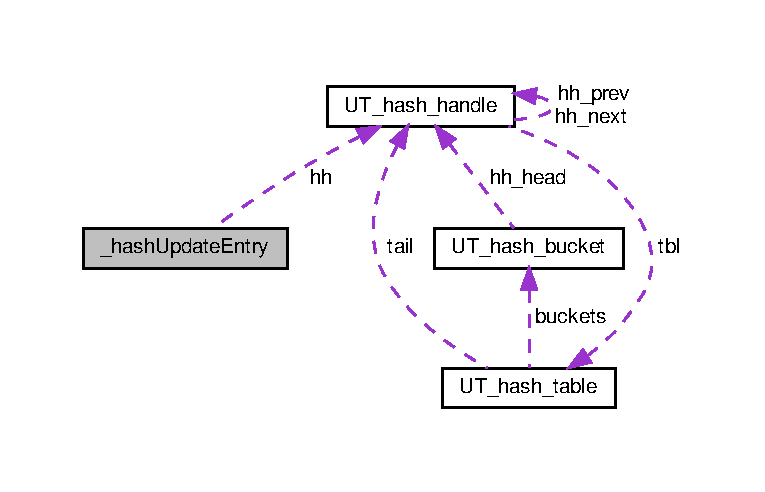
\includegraphics[width=350pt]{struct__hashUpdateEntry__coll__graph}
\end{center}
\end{figure}
\subsection*{Public Attributes}
\begin{DoxyCompactItemize}
\item 
\mbox{\Hypertarget{struct__hashUpdateEntry_a099f9312202b45ff69bfd21d32a77ae9}\label{struct__hashUpdateEntry_a099f9312202b45ff69bfd21d32a77ae9}} 
t\+List\+Entry $\ast$$\ast$ {\bfseries list}
\item 
\mbox{\Hypertarget{struct__hashUpdateEntry_a2a44083f4da27a8a5b1bb9ce57030da8}\label{struct__hashUpdateEntry_a2a44083f4da27a8a5b1bb9ce57030da8}} 
t\+List\+Entry $\ast$ {\bfseries entry}
\item 
\mbox{\Hypertarget{struct__hashUpdateEntry_a88a7166aef27fad9b0292dc2a8bbd7b3}\label{struct__hashUpdateEntry_a88a7166aef27fad9b0292dc2a8bbd7b3}} 
void $\ast$ {\bfseries target}
\item 
\mbox{\Hypertarget{struct__hashUpdateEntry_a08dfe18687f9e952691351fa88cf57cb}\label{struct__hashUpdateEntry_a08dfe18687f9e952691351fa88cf57cb}} 
cc\+Scheduler\+Func {\bfseries callback}
\item 
\mbox{\Hypertarget{struct__hashUpdateEntry_aa81fb210b05621f4aaa098a44a156e49}\label{struct__hashUpdateEntry_aa81fb210b05621f4aaa098a44a156e49}} 
\hyperlink{structUT__hash__handle}{U\+T\+\_\+hash\+\_\+handle} {\bfseries hh}
\end{DoxyCompactItemize}


The documentation for this struct was generated from the following file\+:\begin{DoxyCompactItemize}
\item 
/home/pmx/git/\+P\+M\+X/\+Simu\+Cocos/cocos2d/cocos/base/C\+C\+Scheduler.\+cpp\end{DoxyCompactItemize}

\hypertarget{struct__KerningHashElement}{}\section{\+\_\+\+Kerning\+Hash\+Element Struct Reference}
\label{struct__KerningHashElement}\index{\+\_\+\+Kerning\+Hash\+Element@{\+\_\+\+Kerning\+Hash\+Element}}


Collaboration diagram for \+\_\+\+Kerning\+Hash\+Element\+:
\nopagebreak
\begin{figure}[H]
\begin{center}
\leavevmode
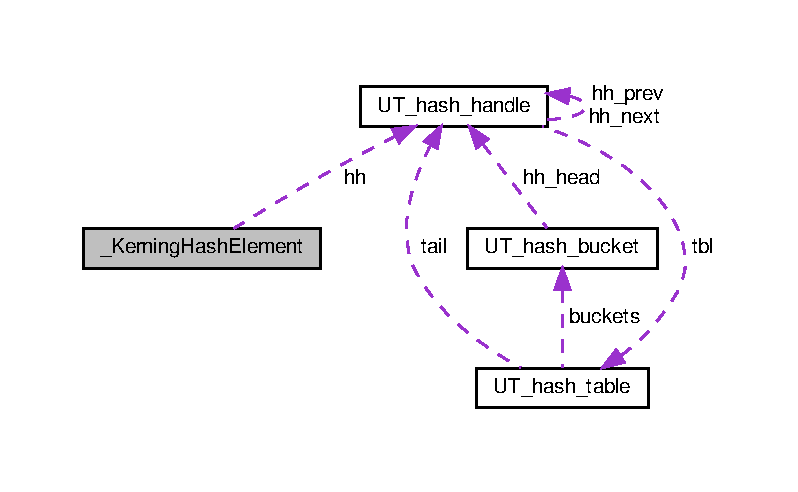
\includegraphics[width=350pt]{struct__KerningHashElement__coll__graph}
\end{center}
\end{figure}
\subsection*{Public Attributes}
\begin{DoxyCompactItemize}
\item 
int {\bfseries key}
\item 
int {\bfseries amount}
\item 
\hyperlink{structUT__hash__handle}{U\+T\+\_\+hash\+\_\+handle} {\bfseries hh}
\end{DoxyCompactItemize}


The documentation for this struct was generated from the following file\+:\begin{DoxyCompactItemize}
\item 
/home/pmx/git/\+P\+M\+X/\+Simu\+Cocos/cocos2d/cocos/2d/C\+C\+Font\+F\+N\+T.\+cpp\end{DoxyCompactItemize}

\hypertarget{structController_1_1__keyStatus}{}\section{Controller\+:\+:\+\_\+key\+Status Struct Reference}
\label{structController_1_1__keyStatus}\index{Controller\+::\+\_\+key\+Status@{Controller\+::\+\_\+key\+Status}}
\subsection*{Public Attributes}
\begin{DoxyCompactItemize}
\item 
bool \hyperlink{structController_1_1__keyStatus_a151e4bba01318304be4d87dce2a64ee6}{is\+Pressed}
\item 
float \hyperlink{structController_1_1__keyStatus_aeb73cddb2cdf68bbee943c8678b2ddb7}{value}
\item 
bool \hyperlink{structController_1_1__keyStatus_a4e9261093859c4819567b67f9687acc4}{is\+Analog}
\end{DoxyCompactItemize}


\subsection{Member Data Documentation}
\mbox{\Hypertarget{structController_1_1__keyStatus_a4e9261093859c4819567b67f9687acc4}\label{structController_1_1__keyStatus_a4e9261093859c4819567b67f9687acc4}} 
\index{Controller\+::\+\_\+key\+Status@{Controller\+::\+\_\+key\+Status}!is\+Analog@{is\+Analog}}
\index{is\+Analog@{is\+Analog}!Controller\+::\+\_\+key\+Status@{Controller\+::\+\_\+key\+Status}}
\subsubsection{\texorpdfstring{is\+Analog}{isAnalog}}
{\footnotesize\ttfamily bool Controller\+::\+\_\+key\+Status\+::is\+Analog}

A Boolean value that indicates whether the value of key is analog. If is\+Analog is true, the key value might be a float from -\/1 to 1. If is\+Analog is false, the key value would be contain one number\+: 0 or 1. \mbox{\Hypertarget{structController_1_1__keyStatus_a151e4bba01318304be4d87dce2a64ee6}\label{structController_1_1__keyStatus_a151e4bba01318304be4d87dce2a64ee6}} 
\index{Controller\+::\+\_\+key\+Status@{Controller\+::\+\_\+key\+Status}!is\+Pressed@{is\+Pressed}}
\index{is\+Pressed@{is\+Pressed}!Controller\+::\+\_\+key\+Status@{Controller\+::\+\_\+key\+Status}}
\subsubsection{\texorpdfstring{is\+Pressed}{isPressed}}
{\footnotesize\ttfamily bool Controller\+::\+\_\+key\+Status\+::is\+Pressed}

A Boolean value that indicates whether the key is considered pressed. \mbox{\Hypertarget{structController_1_1__keyStatus_aeb73cddb2cdf68bbee943c8678b2ddb7}\label{structController_1_1__keyStatus_aeb73cddb2cdf68bbee943c8678b2ddb7}} 
\index{Controller\+::\+\_\+key\+Status@{Controller\+::\+\_\+key\+Status}!value@{value}}
\index{value@{value}!Controller\+::\+\_\+key\+Status@{Controller\+::\+\_\+key\+Status}}
\subsubsection{\texorpdfstring{value}{value}}
{\footnotesize\ttfamily float Controller\+::\+\_\+key\+Status\+::value}

The value of key.\+This value is used in conjunction with the is\+Pressed parameter. 

The documentation for this struct was generated from the following file\+:\begin{DoxyCompactItemize}
\item 
/home/pmx/git/\+P\+M\+X/\+Simu\+Cocos/cocos2d/cocos/base/C\+C\+Controller.\+h\end{DoxyCompactItemize}

\hypertarget{struct__listEntry}{}\section{\+\_\+list\+Entry Struct Reference}
\label{struct__listEntry}\index{\+\_\+list\+Entry@{\+\_\+list\+Entry}}


Collaboration diagram for \+\_\+list\+Entry\+:
\nopagebreak
\begin{figure}[H]
\begin{center}
\leavevmode
\includegraphics[width=178pt]{struct__listEntry__coll__graph}
\end{center}
\end{figure}
\subsection*{Public Attributes}
\begin{DoxyCompactItemize}
\item 
\mbox{\Hypertarget{struct__listEntry_a4b1af96e843127a85e08586d39ec0950}\label{struct__listEntry_a4b1af96e843127a85e08586d39ec0950}} 
struct \hyperlink{struct__listEntry}{\+\_\+list\+Entry} $\ast$ {\bfseries prev}
\item 
\mbox{\Hypertarget{struct__listEntry_afbaca78f6b0462638a5dd8802dbbb028}\label{struct__listEntry_afbaca78f6b0462638a5dd8802dbbb028}} 
struct \hyperlink{struct__listEntry}{\+\_\+list\+Entry} $\ast$ {\bfseries next}
\item 
\mbox{\Hypertarget{struct__listEntry_a214bbd679804f431ea25faf3094da863}\label{struct__listEntry_a214bbd679804f431ea25faf3094da863}} 
cc\+Scheduler\+Func {\bfseries callback}
\item 
\mbox{\Hypertarget{struct__listEntry_a826e351c7a672141ae24738ec905d412}\label{struct__listEntry_a826e351c7a672141ae24738ec905d412}} 
void $\ast$ {\bfseries target}
\item 
\mbox{\Hypertarget{struct__listEntry_aaa7a7fe4fbceba324d107cd6bc9aeae7}\label{struct__listEntry_aaa7a7fe4fbceba324d107cd6bc9aeae7}} 
int {\bfseries priority}
\item 
\mbox{\Hypertarget{struct__listEntry_a15bf6ec32bb10da5d4599b3c02b5d47b}\label{struct__listEntry_a15bf6ec32bb10da5d4599b3c02b5d47b}} 
bool {\bfseries paused}
\item 
\mbox{\Hypertarget{struct__listEntry_a206fea1e0f69ed61fca0c61589c48d04}\label{struct__listEntry_a206fea1e0f69ed61fca0c61589c48d04}} 
bool {\bfseries marked\+For\+Deletion}
\end{DoxyCompactItemize}


The documentation for this struct was generated from the following file\+:\begin{DoxyCompactItemize}
\item 
/home/pmx/git/\+P\+M\+X/\+Simu\+Cocos/cocos2d/cocos/base/C\+C\+Scheduler.\+cpp\end{DoxyCompactItemize}

\hypertarget{struct__lws__header__related}{}\section{\+\_\+lws\+\_\+header\+\_\+related Struct Reference}
\label{struct__lws__header__related}\index{\+\_\+lws\+\_\+header\+\_\+related@{\+\_\+lws\+\_\+header\+\_\+related}}


Collaboration diagram for \+\_\+lws\+\_\+header\+\_\+related\+:
\nopagebreak
\begin{figure}[H]
\begin{center}
\leavevmode
\includegraphics[width=186pt]{struct__lws__header__related__coll__graph}
\end{center}
\end{figure}
\subsection*{Public Attributes}
\begin{DoxyCompactItemize}
\item 
\mbox{\Hypertarget{struct__lws__header__related_a7f7d2497436dfdbb3c8672bd1dece8a7}\label{struct__lws__header__related_a7f7d2497436dfdbb3c8672bd1dece8a7}} 
struct \hyperlink{structallocated__headers}{allocated\+\_\+headers} $\ast$ {\bfseries ah}
\item 
\mbox{\Hypertarget{struct__lws__header__related_a7e15a883c75ecfbe327d28ad08cf3cf9}\label{struct__lws__header__related_a7e15a883c75ecfbe327d28ad08cf3cf9}} 
enum uri\+\_\+path\+\_\+states {\bfseries ups}
\item 
\mbox{\Hypertarget{struct__lws__header__related_acd03d68ebc090ca06cafb70fa5470977}\label{struct__lws__header__related_acd03d68ebc090ca06cafb70fa5470977}} 
enum uri\+\_\+esc\+\_\+states {\bfseries ues}
\item 
\mbox{\Hypertarget{struct__lws__header__related_ac86a9ac8db1517fe26b676072d7c3f11}\label{struct__lws__header__related_ac86a9ac8db1517fe26b676072d7c3f11}} 
short {\bfseries lextable\+\_\+pos}
\item 
\mbox{\Hypertarget{struct__lws__header__related_ac84a993a406609a6f20639ddf0c61840}\label{struct__lws__header__related_ac84a993a406609a6f20639ddf0c61840}} 
unsigned short {\bfseries current\+\_\+token\+\_\+limit}
\item 
\mbox{\Hypertarget{struct__lws__header__related_ab6e51acbb32ac92e4b911d7c922c2713}\label{struct__lws__header__related_ab6e51acbb32ac92e4b911d7c922c2713}} 
char {\bfseries esc\+\_\+stash}
\item 
\mbox{\Hypertarget{struct__lws__header__related_ada3e26a99473023fe1b3d840761ecc55}\label{struct__lws__header__related_ada3e26a99473023fe1b3d840761ecc55}} 
char {\bfseries post\+\_\+literal\+\_\+equal}
\item 
\mbox{\Hypertarget{struct__lws__header__related_ac55cae44e6af4e8122a8e4de38247ebd}\label{struct__lws__header__related_ac55cae44e6af4e8122a8e4de38247ebd}} 
unsigned char {\bfseries parser\+\_\+state}
\item 
\mbox{\Hypertarget{struct__lws__header__related_aa8c2cb123bf0c321370e99df9212b825}\label{struct__lws__header__related_aa8c2cb123bf0c321370e99df9212b825}} 
char {\bfseries redirects}
\end{DoxyCompactItemize}


The documentation for this struct was generated from the following file\+:\begin{DoxyCompactItemize}
\item 
/home/pmx/git/\+P\+M\+X/\+Simu\+Cocos/cocos2d/external/websockets/include/win10/private-\/libwebsockets.\+h\end{DoxyCompactItemize}

\hypertarget{struct__lws__http__mode__related}{}\section{\+\_\+lws\+\_\+http\+\_\+mode\+\_\+related Struct Reference}
\label{struct__lws__http__mode__related}\index{\+\_\+lws\+\_\+http\+\_\+mode\+\_\+related@{\+\_\+lws\+\_\+http\+\_\+mode\+\_\+related}}


Collaboration diagram for \+\_\+lws\+\_\+http\+\_\+mode\+\_\+related\+:
\nopagebreak
\begin{figure}[H]
\begin{center}
\leavevmode
\includegraphics[width=202pt]{struct__lws__http__mode__related__coll__graph}
\end{center}
\end{figure}
\subsection*{Public Attributes}
\begin{DoxyCompactItemize}
\item 
\mbox{\Hypertarget{struct__lws__http__mode__related_aef41b2e3480838a77d32daca01607937}\label{struct__lws__http__mode__related_aef41b2e3480838a77d32daca01607937}} 
struct \hyperlink{structallocated__headers}{allocated\+\_\+headers} $\ast$ {\bfseries ah}
\item 
\mbox{\Hypertarget{struct__lws__http__mode__related_ae82e2e3b1084ba3efa59257f679c9c07}\label{struct__lws__http__mode__related_ae82e2e3b1084ba3efa59257f679c9c07}} 
unsigned long {\bfseries filepos}
\item 
\mbox{\Hypertarget{struct__lws__http__mode__related_a430421e82ed44fc8d0c78834e13a1cff}\label{struct__lws__http__mode__related_a430421e82ed44fc8d0c78834e13a1cff}} 
unsigned long {\bfseries filelen}
\item 
\mbox{\Hypertarget{struct__lws__http__mode__related_a0c17bd45c528b2aab1e10501c3ee0118}\label{struct__lws__http__mode__related_a0c17bd45c528b2aab1e10501c3ee0118}} 
lws\+\_\+filefd\+\_\+type {\bfseries fd}
\item 
\mbox{\Hypertarget{struct__lws__http__mode__related_ab778dedb1fcf181bd0180e6aaa9068ce}\label{struct__lws__http__mode__related_ab778dedb1fcf181bd0180e6aaa9068ce}} 
enum http\+\_\+version {\bfseries request\+\_\+version}
\item 
\mbox{\Hypertarget{struct__lws__http__mode__related_a2b77682888d771df6ba5a81641e2b032}\label{struct__lws__http__mode__related_a2b77682888d771df6ba5a81641e2b032}} 
enum http\+\_\+connection\+\_\+type {\bfseries connection\+\_\+type}
\item 
\mbox{\Hypertarget{struct__lws__http__mode__related_a58be6c33cb24c74f5f9e446c6511027d}\label{struct__lws__http__mode__related_a58be6c33cb24c74f5f9e446c6511027d}} 
unsigned int {\bfseries content\+\_\+length}
\item 
\mbox{\Hypertarget{struct__lws__http__mode__related_a5c4a49ebf437b9fb35cd6d178db33f92}\label{struct__lws__http__mode__related_a5c4a49ebf437b9fb35cd6d178db33f92}} 
unsigned int {\bfseries content\+\_\+remain}
\end{DoxyCompactItemize}


The documentation for this struct was generated from the following file\+:\begin{DoxyCompactItemize}
\item 
/home/pmx/git/\+P\+M\+X/\+Simu\+Cocos/cocos2d/external/websockets/include/win10/private-\/libwebsockets.\+h\end{DoxyCompactItemize}

\hypertarget{struct__lws__websocket__related}{}\section{\+\_\+lws\+\_\+websocket\+\_\+related Struct Reference}
\label{struct__lws__websocket__related}\index{\+\_\+lws\+\_\+websocket\+\_\+related@{\+\_\+lws\+\_\+websocket\+\_\+related}}


Collaboration diagram for \+\_\+lws\+\_\+websocket\+\_\+related\+:
\nopagebreak
\begin{figure}[H]
\begin{center}
\leavevmode
\includegraphics[width=350pt]{struct__lws__websocket__related__coll__graph}
\end{center}
\end{figure}
\subsection*{Public Attributes}
\begin{DoxyCompactItemize}
\item 
\mbox{\Hypertarget{struct__lws__websocket__related_ad722eb11e3b8686f08f43694e3a3b430}\label{struct__lws__websocket__related_ad722eb11e3b8686f08f43694e3a3b430}} 
char $\ast$ {\bfseries rx\+\_\+ubuf}
\item 
\mbox{\Hypertarget{struct__lws__websocket__related_a72bf5ca922967c723add1a761db2f285}\label{struct__lws__websocket__related_a72bf5ca922967c723add1a761db2f285}} 
unsigned int {\bfseries rx\+\_\+ubuf\+\_\+alloc}
\item 
\mbox{\Hypertarget{struct__lws__websocket__related_af2633ae20f75f891482e332a7bac6e7c}\label{struct__lws__websocket__related_af2633ae20f75f891482e332a7bac6e7c}} 
struct \hyperlink{structlws}{lws} $\ast$ {\bfseries rx\+\_\+draining\+\_\+ext\+\_\+list}
\item 
\mbox{\Hypertarget{struct__lws__websocket__related_ac4a9d37042b6c5679e1b4a371c75c842}\label{struct__lws__websocket__related_ac4a9d37042b6c5679e1b4a371c75c842}} 
struct \hyperlink{structlws}{lws} $\ast$ {\bfseries tx\+\_\+draining\+\_\+ext\+\_\+list}
\item 
\mbox{\Hypertarget{struct__lws__websocket__related_aed512f884c4cceff94702b927656afd9}\label{struct__lws__websocket__related_aed512f884c4cceff94702b927656afd9}} 
size\+\_\+t {\bfseries rx\+\_\+packet\+\_\+length}
\item 
\mbox{\Hypertarget{struct__lws__websocket__related_abb66bf82a822c857945654fa25af56b1}\label{struct__lws__websocket__related_abb66bf82a822c857945654fa25af56b1}} 
unsigned int {\bfseries rx\+\_\+ubuf\+\_\+head}
\item 
\mbox{\Hypertarget{struct__lws__websocket__related_ae9421cf8406abc5a7dd066edc070ad9d}\label{struct__lws__websocket__related_ae9421cf8406abc5a7dd066edc070ad9d}} 
unsigned char {\bfseries mask} \mbox{[}4\mbox{]}
\item 
\mbox{\Hypertarget{struct__lws__websocket__related_a145d59c658423fa72696ec7e1ead9c9d}\label{struct__lws__websocket__related_a145d59c658423fa72696ec7e1ead9c9d}} 
unsigned char {\bfseries ping\+\_\+payload\+\_\+buf} \mbox{[}128 -\/ 3+L\+W\+S\+\_\+\+P\+RE\mbox{]}
\item 
\mbox{\Hypertarget{struct__lws__websocket__related_a38cad38279414c9e4c9e93e0843b4974}\label{struct__lws__websocket__related_a38cad38279414c9e4c9e93e0843b4974}} 
unsigned char {\bfseries ping\+\_\+payload\+\_\+len}
\item 
\mbox{\Hypertarget{struct__lws__websocket__related_a06ecf6b55a77f94b46b73fc83e680ed1}\label{struct__lws__websocket__related_a06ecf6b55a77f94b46b73fc83e680ed1}} 
unsigned char {\bfseries mask\+\_\+idx}
\item 
\mbox{\Hypertarget{struct__lws__websocket__related_a0d78f77bbe1c6f6e3511cf5b7df28032}\label{struct__lws__websocket__related_a0d78f77bbe1c6f6e3511cf5b7df28032}} 
unsigned char {\bfseries opcode}
\item 
\mbox{\Hypertarget{struct__lws__websocket__related_a192fc1b92ab495be4a202b7b7054f188}\label{struct__lws__websocket__related_a192fc1b92ab495be4a202b7b7054f188}} 
unsigned char {\bfseries rsv}
\item 
\mbox{\Hypertarget{struct__lws__websocket__related_a9565090a6bbf0881f63f82fc9f83e0be}\label{struct__lws__websocket__related_a9565090a6bbf0881f63f82fc9f83e0be}} 
unsigned char {\bfseries rsv\+\_\+first\+\_\+msg}
\item 
\mbox{\Hypertarget{struct__lws__websocket__related_a4ae540bcb85c837b31311fc86740b809}\label{struct__lws__websocket__related_a4ae540bcb85c837b31311fc86740b809}} 
unsigned char {\bfseries close\+\_\+in\+\_\+ping\+\_\+buffer\+\_\+len}
\item 
\mbox{\Hypertarget{struct__lws__websocket__related_abd103f3065cead04620f5a2e2c3fa90a}\label{struct__lws__websocket__related_abd103f3065cead04620f5a2e2c3fa90a}} 
unsigned char {\bfseries utf8}
\item 
\mbox{\Hypertarget{struct__lws__websocket__related_a5775d679c35568af40d8db5d176d72d5}\label{struct__lws__websocket__related_a5775d679c35568af40d8db5d176d72d5}} 
unsigned char {\bfseries stashed\+\_\+write\+\_\+type}
\item 
\mbox{\Hypertarget{struct__lws__websocket__related_ad629173bc0464b3576e97507be5be16f}\label{struct__lws__websocket__related_ad629173bc0464b3576e97507be5be16f}} 
unsigned char {\bfseries tx\+\_\+draining\+\_\+stashed\+\_\+wp}
\item 
\mbox{\Hypertarget{struct__lws__websocket__related_a003e49df1a0a68e375e2e68c970d6d27}\label{struct__lws__websocket__related_a003e49df1a0a68e375e2e68c970d6d27}} 
unsigned int {\bfseries final}\+:1
\item 
\mbox{\Hypertarget{struct__lws__websocket__related_a1e34b32dbdd3fa4734a797d78492256a}\label{struct__lws__websocket__related_a1e34b32dbdd3fa4734a797d78492256a}} 
unsigned int {\bfseries frame\+\_\+is\+\_\+binary}\+:1
\item 
\mbox{\Hypertarget{struct__lws__websocket__related_af61e6ba427e966071aa16cac5449d241}\label{struct__lws__websocket__related_af61e6ba427e966071aa16cac5449d241}} 
unsigned int {\bfseries all\+\_\+zero\+\_\+nonce}\+:1
\item 
\mbox{\Hypertarget{struct__lws__websocket__related_a922b5cfb3582df95ed876b8e3747e60c}\label{struct__lws__websocket__related_a922b5cfb3582df95ed876b8e3747e60c}} 
unsigned int {\bfseries this\+\_\+frame\+\_\+masked}\+:1
\item 
\mbox{\Hypertarget{struct__lws__websocket__related_a3ceb1f19e8c06bd8393a5c16d64340aa}\label{struct__lws__websocket__related_a3ceb1f19e8c06bd8393a5c16d64340aa}} 
unsigned int {\bfseries inside\+\_\+frame}\+:1
\item 
\mbox{\Hypertarget{struct__lws__websocket__related_a49410d1554756541717086af715185b1}\label{struct__lws__websocket__related_a49410d1554756541717086af715185b1}} 
unsigned int {\bfseries clean\+\_\+buffer}\+:1
\item 
\mbox{\Hypertarget{struct__lws__websocket__related_a6282d029f54e525d4cfa8a8d4bbf7e7c}\label{struct__lws__websocket__related_a6282d029f54e525d4cfa8a8d4bbf7e7c}} 
unsigned int {\bfseries payload\+\_\+is\+\_\+close}\+:1
\item 
\mbox{\Hypertarget{struct__lws__websocket__related_aff2e662d2f6ff524fd594b5e396a9fb7}\label{struct__lws__websocket__related_aff2e662d2f6ff524fd594b5e396a9fb7}} 
unsigned int {\bfseries ping\+\_\+pending\+\_\+flag}\+:1
\item 
\mbox{\Hypertarget{struct__lws__websocket__related_ab118a1678ce184725dd0683b25a9591c}\label{struct__lws__websocket__related_ab118a1678ce184725dd0683b25a9591c}} 
unsigned int {\bfseries continuation\+\_\+possible}\+:1
\item 
\mbox{\Hypertarget{struct__lws__websocket__related_a27d2697d1bb89ffcccdd8f7efef8c14d}\label{struct__lws__websocket__related_a27d2697d1bb89ffcccdd8f7efef8c14d}} 
unsigned int {\bfseries owed\+\_\+a\+\_\+fin}\+:1
\item 
\mbox{\Hypertarget{struct__lws__websocket__related_add3f3ff1a669ad0c677312f82b6793a1}\label{struct__lws__websocket__related_add3f3ff1a669ad0c677312f82b6793a1}} 
unsigned int {\bfseries check\+\_\+utf8}\+:1
\item 
\mbox{\Hypertarget{struct__lws__websocket__related_a4c7e0aaa817b0ab74b6238a2b4be9d11}\label{struct__lws__websocket__related_a4c7e0aaa817b0ab74b6238a2b4be9d11}} 
unsigned int {\bfseries defeat\+\_\+check\+\_\+utf8}\+:1
\item 
\mbox{\Hypertarget{struct__lws__websocket__related_a16e29cb5f14f4ebb44cfce3e7453b1c5}\label{struct__lws__websocket__related_a16e29cb5f14f4ebb44cfce3e7453b1c5}} 
unsigned int {\bfseries pmce\+\_\+compressed\+\_\+message}\+:1
\item 
\mbox{\Hypertarget{struct__lws__websocket__related_a621d2ce308a05d9cee57ddb718cefa19}\label{struct__lws__websocket__related_a621d2ce308a05d9cee57ddb718cefa19}} 
unsigned int {\bfseries stashed\+\_\+write\+\_\+pending}\+:1
\item 
\mbox{\Hypertarget{struct__lws__websocket__related_a2e77202976efd66917371d96e372808d}\label{struct__lws__websocket__related_a2e77202976efd66917371d96e372808d}} 
unsigned int {\bfseries rx\+\_\+draining\+\_\+ext}\+:1
\item 
\mbox{\Hypertarget{struct__lws__websocket__related_abdf63e73f041d1d2c86f3eb3fd18ad80}\label{struct__lws__websocket__related_abdf63e73f041d1d2c86f3eb3fd18ad80}} 
unsigned int {\bfseries tx\+\_\+draining\+\_\+ext}\+:1
\end{DoxyCompactItemize}


The documentation for this struct was generated from the following file\+:\begin{DoxyCompactItemize}
\item 
/home/pmx/git/\+P\+M\+X/\+Simu\+Cocos/cocos2d/external/websockets/include/win10/private-\/libwebsockets.\+h\end{DoxyCompactItemize}

\hypertarget{struct__MSDN__DLGTEMPLATEEX}{}\section{\+\_\+\+M\+S\+D\+N\+\_\+\+D\+L\+G\+T\+E\+M\+P\+L\+A\+T\+E\+EX Struct Reference}
\label{struct__MSDN__DLGTEMPLATEEX}\index{\+\_\+\+M\+S\+D\+N\+\_\+\+D\+L\+G\+T\+E\+M\+P\+L\+A\+T\+E\+EX@{\+\_\+\+M\+S\+D\+N\+\_\+\+D\+L\+G\+T\+E\+M\+P\+L\+A\+T\+E\+EX}}
\subsection*{Public Attributes}
\begin{DoxyCompactItemize}
\item 
\mbox{\Hypertarget{struct__MSDN__DLGTEMPLATEEX_a851b8873cfb8a222b7b31982e5693cfe}\label{struct__MSDN__DLGTEMPLATEEX_a851b8873cfb8a222b7b31982e5693cfe}} 
W\+O\+RD {\bfseries dlg\+Ver}
\item 
\mbox{\Hypertarget{struct__MSDN__DLGTEMPLATEEX_ae23dd594822b4bd469c34f5b0d8c4d31}\label{struct__MSDN__DLGTEMPLATEEX_ae23dd594822b4bd469c34f5b0d8c4d31}} 
W\+O\+RD {\bfseries signature}
\item 
\mbox{\Hypertarget{struct__MSDN__DLGTEMPLATEEX_a226039f789b55667249c420729dff08e}\label{struct__MSDN__DLGTEMPLATEEX_a226039f789b55667249c420729dff08e}} 
D\+W\+O\+RD {\bfseries help\+ID}
\item 
\mbox{\Hypertarget{struct__MSDN__DLGTEMPLATEEX_a014ceddaa5fc5252d78272e86a6ed9eb}\label{struct__MSDN__DLGTEMPLATEEX_a014ceddaa5fc5252d78272e86a6ed9eb}} 
D\+W\+O\+RD {\bfseries ex\+Style}
\item 
\mbox{\Hypertarget{struct__MSDN__DLGTEMPLATEEX_a345dcafc3daeeab66234432a938d1002}\label{struct__MSDN__DLGTEMPLATEEX_a345dcafc3daeeab66234432a938d1002}} 
D\+W\+O\+RD {\bfseries style}
\item 
\mbox{\Hypertarget{struct__MSDN__DLGTEMPLATEEX_a5bef48f0bb704e4c6ab9c8c33a834d10}\label{struct__MSDN__DLGTEMPLATEEX_a5bef48f0bb704e4c6ab9c8c33a834d10}} 
W\+O\+RD {\bfseries c\+Dlg\+Items}
\item 
\mbox{\Hypertarget{struct__MSDN__DLGTEMPLATEEX_adc9666451f0e9858827f41eead2b1793}\label{struct__MSDN__DLGTEMPLATEEX_adc9666451f0e9858827f41eead2b1793}} 
short {\bfseries x}
\item 
\mbox{\Hypertarget{struct__MSDN__DLGTEMPLATEEX_abca80e1e6b67d38b2889dd56c6d693fb}\label{struct__MSDN__DLGTEMPLATEEX_abca80e1e6b67d38b2889dd56c6d693fb}} 
short {\bfseries y}
\item 
\mbox{\Hypertarget{struct__MSDN__DLGTEMPLATEEX_a9f70753830bc59a0799f1f03b20bd4f0}\label{struct__MSDN__DLGTEMPLATEEX_a9f70753830bc59a0799f1f03b20bd4f0}} 
short {\bfseries cx}
\item 
\mbox{\Hypertarget{struct__MSDN__DLGTEMPLATEEX_a7147bcb227f0e49a97dcf0c8ef627773}\label{struct__MSDN__DLGTEMPLATEEX_a7147bcb227f0e49a97dcf0c8ef627773}} 
short {\bfseries cy}
\item 
\mbox{\Hypertarget{struct__MSDN__DLGTEMPLATEEX_a77bd085116e4c2823421d42b454f8469}\label{struct__MSDN__DLGTEMPLATEEX_a77bd085116e4c2823421d42b454f8469}} 
B\+Y\+TE {\bfseries \+\_\+rest} \mbox{[}1\mbox{]}
\end{DoxyCompactItemize}


The documentation for this struct was generated from the following file\+:\begin{DoxyCompactItemize}
\item 
/home/pmx/git/\+P\+M\+X/\+Simu\+Cocos/cocos2d/cocos/ui/\+U\+I\+Edit\+Box/U\+I\+Edit\+Box\+Impl-\/win32.\+cpp\end{DoxyCompactItemize}

\hypertarget{struct__ossl__old__des__ks__struct}{}\section{\+\_\+ossl\+\_\+old\+\_\+des\+\_\+ks\+\_\+struct Struct Reference}
\label{struct__ossl__old__des__ks__struct}\index{\+\_\+ossl\+\_\+old\+\_\+des\+\_\+ks\+\_\+struct@{\+\_\+ossl\+\_\+old\+\_\+des\+\_\+ks\+\_\+struct}}
\subsection*{Public Attributes}
\begin{DoxyCompactItemize}
\item 
\mbox{\Hypertarget{struct__ossl__old__des__ks__struct_a727f247111c9cf8e90fb586b13b7a261}\label{struct__ossl__old__des__ks__struct_a727f247111c9cf8e90fb586b13b7a261}} 
\begin{tabbing}
xx\=xx\=xx\=xx\=xx\=xx\=xx\=xx\=xx\=\kill
union \{\\
\>\_ossl\_old\_des\_cblock {\bfseries \_}\\
\>DES\_LONG {\bfseries pad} \mbox{[}2\mbox{]}\\
\} {\bfseries ks}\\

\end{tabbing}\end{DoxyCompactItemize}


The documentation for this struct was generated from the following file\+:\begin{DoxyCompactItemize}
\item 
/home/pmx/git/\+P\+M\+X/\+Simu\+Cocos3/cocos2d/external/openssl/include/win10/openssl/des\+\_\+old.\+h\end{DoxyCompactItemize}

\hypertarget{struct__pitem}{}\section{\+\_\+pitem Struct Reference}
\label{struct__pitem}\index{\+\_\+pitem@{\+\_\+pitem}}


Collaboration diagram for \+\_\+pitem\+:
\nopagebreak
\begin{figure}[H]
\begin{center}
\leavevmode
\includegraphics[width=166pt]{struct__pitem__coll__graph}
\end{center}
\end{figure}
\subsection*{Public Attributes}
\begin{DoxyCompactItemize}
\item 
\mbox{\Hypertarget{struct__pitem_af285b88224fe1db6562c5bf6208a995c}\label{struct__pitem_af285b88224fe1db6562c5bf6208a995c}} 
unsigned char {\bfseries priority} \mbox{[}8\mbox{]}
\item 
\mbox{\Hypertarget{struct__pitem_ab57fcd99b0053a93df6e10cc5adb6401}\label{struct__pitem_ab57fcd99b0053a93df6e10cc5adb6401}} 
void $\ast$ {\bfseries data}
\item 
\mbox{\Hypertarget{struct__pitem_aabdda0dcbfb04b14c640d4a117d0061f}\label{struct__pitem_aabdda0dcbfb04b14c640d4a117d0061f}} 
struct \hyperlink{struct__pitem}{\+\_\+pitem} $\ast$ {\bfseries next}
\end{DoxyCompactItemize}


The documentation for this struct was generated from the following file\+:\begin{DoxyCompactItemize}
\item 
/home/pmx/git/\+P\+M\+X/\+Simu\+Cocos3/cocos2d/external/openssl/include/win10/openssl/pqueue.\+h\end{DoxyCompactItemize}

\hypertarget{structcocos2d_1_1plugin_1_1__PluginJavaData__}{}\section{cocos2d\+:\+:plugin\+:\+:\+\_\+\+Plugin\+Java\+Data\+\_\+ Struct Reference}
\label{structcocos2d_1_1plugin_1_1__PluginJavaData__}\index{cocos2d\+::plugin\+::\+\_\+\+Plugin\+Java\+Data\+\_\+@{cocos2d\+::plugin\+::\+\_\+\+Plugin\+Java\+Data\+\_\+}}
\subsection*{Public Attributes}
\begin{DoxyCompactItemize}
\item 
\mbox{\Hypertarget{structcocos2d_1_1plugin_1_1__PluginJavaData___acf880b0a12ae5662aa30c9944fb484a9}\label{structcocos2d_1_1plugin_1_1__PluginJavaData___acf880b0a12ae5662aa30c9944fb484a9}} 
jobject {\bfseries jobj}
\item 
\mbox{\Hypertarget{structcocos2d_1_1plugin_1_1__PluginJavaData___a3900ea386093eb59c1d8658543c3bdaa}\label{structcocos2d_1_1plugin_1_1__PluginJavaData___a3900ea386093eb59c1d8658543c3bdaa}} 
std\+::string {\bfseries jclass\+Name}
\end{DoxyCompactItemize}


The documentation for this struct was generated from the following file\+:\begin{DoxyCompactItemize}
\item 
/home/pmx/git/\+P\+M\+X/\+Simu\+Cocos/cocos2d/plugin/protocols/platform/android/Plugin\+Java\+Data.\+h\end{DoxyCompactItemize}

\hypertarget{structcocos2d_1_1plugin_1_1__PluginOCData}{}\section{cocos2d\+:\+:plugin\+:\+:\+\_\+\+Plugin\+O\+C\+Data Struct Reference}
\label{structcocos2d_1_1plugin_1_1__PluginOCData}\index{cocos2d\+::plugin\+::\+\_\+\+Plugin\+O\+C\+Data@{cocos2d\+::plugin\+::\+\_\+\+Plugin\+O\+C\+Data}}
\subsection*{Public Attributes}
\begin{DoxyCompactItemize}
\item 
\mbox{\Hypertarget{structcocos2d_1_1plugin_1_1__PluginOCData_a8c5a079c0734ee48c96f62044d04155b}\label{structcocos2d_1_1plugin_1_1__PluginOCData_a8c5a079c0734ee48c96f62044d04155b}} 
id {\bfseries obj}
\item 
\mbox{\Hypertarget{structcocos2d_1_1plugin_1_1__PluginOCData_a2269dbec6f47b54d99e7f765e4c89ed7}\label{structcocos2d_1_1plugin_1_1__PluginOCData_a2269dbec6f47b54d99e7f765e4c89ed7}} 
std\+::string {\bfseries class\+Name}
\end{DoxyCompactItemize}


The documentation for this struct was generated from the following file\+:\begin{DoxyCompactItemize}
\item 
/home/pmx/git/\+P\+M\+X/\+Simu\+Cocos/cocos2d/plugin/protocols/platform/ios/Plugin\+Utils\+I\+O\+S.\+h\end{DoxyCompactItemize}

\hypertarget{struct__PrecompiledProgram}{}\section{\+\_\+\+Precompiled\+Program Struct Reference}
\label{struct__PrecompiledProgram}\index{\+\_\+\+Precompiled\+Program@{\+\_\+\+Precompiled\+Program}}
\subsection*{Public Attributes}
\begin{DoxyCompactItemize}
\item 
\mbox{\Hypertarget{struct__PrecompiledProgram_af35818720316a570950fdba03e6a43bf}\label{struct__PrecompiledProgram_af35818720316a570950fdba03e6a43bf}} 
const char $\ast$ {\bfseries key}
\item 
\mbox{\Hypertarget{struct__PrecompiledProgram_a83ce08a8215016140ce2fab3704cfd62}\label{struct__PrecompiledProgram_a83ce08a8215016140ce2fab3704cfd62}} 
const unsigned char $\ast$ {\bfseries program}
\item 
\mbox{\Hypertarget{struct__PrecompiledProgram_a13cefa919b8eb9c618e2a2587cfa1f61}\label{struct__PrecompiledProgram_a13cefa919b8eb9c618e2a2587cfa1f61}} 
int {\bfseries length}
\end{DoxyCompactItemize}


The documentation for this struct was generated from the following file\+:\begin{DoxyCompactItemize}
\item 
/home/pmx/git/\+P\+M\+X/\+Simu\+Cocos/cocos2d/cocos/platform/winrt/C\+C\+Precompiled\+Shaders.\+h\end{DoxyCompactItemize}

\hypertarget{classnetwork_1_1HttpRequest_1_1__prxy}{}\section{network\+:\+:Http\+Request\+:\+:\+\_\+prxy Class Reference}
\label{classnetwork_1_1HttpRequest_1_1__prxy}\index{network\+::\+Http\+Request\+::\+\_\+prxy@{network\+::\+Http\+Request\+::\+\_\+prxy}}


{\ttfamily \#include $<$Http\+Request.\+h$>$}



Collaboration diagram for network\+:\+:Http\+Request\+:\+:\+\_\+prxy\+:
\nopagebreak
\begin{figure}[H]
\begin{center}
\leavevmode
\includegraphics[width=193pt]{classnetwork_1_1HttpRequest_1_1__prxy__coll__graph}
\end{center}
\end{figure}
\subsection*{Public Member Functions}
\begin{DoxyCompactItemize}
\item 
\hyperlink{classnetwork_1_1HttpRequest_1_1__prxy_a01020d64085bbc59cf1218bed510355a}{\+\_\+prxy} (S\+E\+L\+\_\+\+Http\+Response cb)
\item 
\hyperlink{classnetwork_1_1HttpRequest_1_1__prxy_aac8954b9e734cc5778de83fa2a452b47}{$\sim$\+\_\+prxy} ()
\item 
\hyperlink{classnetwork_1_1HttpRequest_1_1__prxy_a77cd2d1b059a4ddc7332f5adbe87cddc}{operator S\+E\+L\+\_\+\+Http\+Response} () const
\item 
\mbox{\Hypertarget{classnetwork_1_1HttpRequest_1_1__prxy_a831ad26464579ae87f72d6113c5a8a6d}\label{classnetwork_1_1HttpRequest_1_1__prxy_a831ad26464579ae87f72d6113c5a8a6d}} 
C\+C\+\_\+\+D\+E\+P\+R\+E\+C\+A\+T\+E\+D\+\_\+\+A\+T\+T\+R\+I\+B\+U\+TE {\bfseries operator S\+E\+L\+\_\+\+Call\+Func\+ND} () const
\item 
\hyperlink{classnetwork_1_1HttpRequest_1_1__prxy_a01020d64085bbc59cf1218bed510355a}{\+\_\+prxy} (S\+E\+L\+\_\+\+Http\+Response cb)
\item 
\hyperlink{classnetwork_1_1HttpRequest_1_1__prxy_aac8954b9e734cc5778de83fa2a452b47}{$\sim$\+\_\+prxy} ()
\item 
\mbox{\Hypertarget{classnetwork_1_1HttpRequest_1_1__prxy_a77cd2d1b059a4ddc7332f5adbe87cddc}\label{classnetwork_1_1HttpRequest_1_1__prxy_a77cd2d1b059a4ddc7332f5adbe87cddc}} 
{\bfseries operator S\+E\+L\+\_\+\+Http\+Response} () const
\item 
\mbox{\Hypertarget{classnetwork_1_1HttpRequest_1_1__prxy_a831ad26464579ae87f72d6113c5a8a6d}\label{classnetwork_1_1HttpRequest_1_1__prxy_a831ad26464579ae87f72d6113c5a8a6d}} 
C\+C\+\_\+\+D\+E\+P\+R\+E\+C\+A\+T\+E\+D\+\_\+\+A\+T\+T\+R\+I\+B\+U\+TE {\bfseries operator S\+E\+L\+\_\+\+Call\+Func\+ND} () const
\end{DoxyCompactItemize}
\subsection*{Protected Attributes}
\begin{DoxyCompactItemize}
\item 
\mbox{\Hypertarget{classnetwork_1_1HttpRequest_1_1__prxy_a7493ede18daf7685997e15fb5451e379}\label{classnetwork_1_1HttpRequest_1_1__prxy_a7493ede18daf7685997e15fb5451e379}} 
S\+E\+L\+\_\+\+Http\+Response {\bfseries \+\_\+cb}
\end{DoxyCompactItemize}


\subsection{Detailed Description}
This sub class is just for migration S\+E\+L\+\_\+\+Call\+Func\+ND to S\+E\+L\+\_\+\+Http\+Response,someday this way will be removed.

NA 

\subsection{Constructor \& Destructor Documentation}
\mbox{\Hypertarget{classnetwork_1_1HttpRequest_1_1__prxy_a01020d64085bbc59cf1218bed510355a}\label{classnetwork_1_1HttpRequest_1_1__prxy_a01020d64085bbc59cf1218bed510355a}} 
\index{network\+::\+Http\+Request\+::\+\_\+prxy@{network\+::\+Http\+Request\+::\+\_\+prxy}!\+\_\+prxy@{\+\_\+prxy}}
\index{\+\_\+prxy@{\+\_\+prxy}!network\+::\+Http\+Request\+::\+\_\+prxy@{network\+::\+Http\+Request\+::\+\_\+prxy}}
\subsubsection{\texorpdfstring{\+\_\+prxy()}{\_prxy()}\hspace{0.1cm}{\footnotesize\ttfamily [1/2]}}
{\footnotesize\ttfamily network\+::\+Http\+Request\+::\+\_\+prxy\+::\+\_\+prxy (\begin{DoxyParamCaption}\item[{S\+E\+L\+\_\+\+Http\+Response}]{cb }\end{DoxyParamCaption})\hspace{0.3cm}{\ttfamily [inline]}}

Constructor. \mbox{\Hypertarget{classnetwork_1_1HttpRequest_1_1__prxy_aac8954b9e734cc5778de83fa2a452b47}\label{classnetwork_1_1HttpRequest_1_1__prxy_aac8954b9e734cc5778de83fa2a452b47}} 
\index{network\+::\+Http\+Request\+::\+\_\+prxy@{network\+::\+Http\+Request\+::\+\_\+prxy}!````~\+\_\+prxy@{$\sim$\+\_\+prxy}}
\index{````~\+\_\+prxy@{$\sim$\+\_\+prxy}!network\+::\+Http\+Request\+::\+\_\+prxy@{network\+::\+Http\+Request\+::\+\_\+prxy}}
\subsubsection{\texorpdfstring{$\sim$\+\_\+prxy()}{~\_prxy()}\hspace{0.1cm}{\footnotesize\ttfamily [1/2]}}
{\footnotesize\ttfamily network\+::\+Http\+Request\+::\+\_\+prxy\+::$\sim$\+\_\+prxy (\begin{DoxyParamCaption}{ }\end{DoxyParamCaption})\hspace{0.3cm}{\ttfamily [inline]}}

Destructor. \mbox{\Hypertarget{classnetwork_1_1HttpRequest_1_1__prxy_a01020d64085bbc59cf1218bed510355a}\label{classnetwork_1_1HttpRequest_1_1__prxy_a01020d64085bbc59cf1218bed510355a}} 
\index{network\+::\+Http\+Request\+::\+\_\+prxy@{network\+::\+Http\+Request\+::\+\_\+prxy}!\+\_\+prxy@{\+\_\+prxy}}
\index{\+\_\+prxy@{\+\_\+prxy}!network\+::\+Http\+Request\+::\+\_\+prxy@{network\+::\+Http\+Request\+::\+\_\+prxy}}
\subsubsection{\texorpdfstring{\+\_\+prxy()}{\_prxy()}\hspace{0.1cm}{\footnotesize\ttfamily [2/2]}}
{\footnotesize\ttfamily network\+::\+Http\+Request\+::\+\_\+prxy\+::\+\_\+prxy (\begin{DoxyParamCaption}\item[{S\+E\+L\+\_\+\+Http\+Response}]{cb }\end{DoxyParamCaption})\hspace{0.3cm}{\ttfamily [inline]}}

Constructor. \mbox{\Hypertarget{classnetwork_1_1HttpRequest_1_1__prxy_aac8954b9e734cc5778de83fa2a452b47}\label{classnetwork_1_1HttpRequest_1_1__prxy_aac8954b9e734cc5778de83fa2a452b47}} 
\index{network\+::\+Http\+Request\+::\+\_\+prxy@{network\+::\+Http\+Request\+::\+\_\+prxy}!````~\+\_\+prxy@{$\sim$\+\_\+prxy}}
\index{````~\+\_\+prxy@{$\sim$\+\_\+prxy}!network\+::\+Http\+Request\+::\+\_\+prxy@{network\+::\+Http\+Request\+::\+\_\+prxy}}
\subsubsection{\texorpdfstring{$\sim$\+\_\+prxy()}{~\_prxy()}\hspace{0.1cm}{\footnotesize\ttfamily [2/2]}}
{\footnotesize\ttfamily network\+::\+Http\+Request\+::\+\_\+prxy\+::$\sim$\+\_\+prxy (\begin{DoxyParamCaption}{ }\end{DoxyParamCaption})\hspace{0.3cm}{\ttfamily [inline]}}

Destructor. 

\subsection{Member Function Documentation}
\mbox{\Hypertarget{classnetwork_1_1HttpRequest_1_1__prxy_a77cd2d1b059a4ddc7332f5adbe87cddc}\label{classnetwork_1_1HttpRequest_1_1__prxy_a77cd2d1b059a4ddc7332f5adbe87cddc}} 
\index{network\+::\+Http\+Request\+::\+\_\+prxy@{network\+::\+Http\+Request\+::\+\_\+prxy}!operator S\+E\+L\+\_\+\+Http\+Response@{operator S\+E\+L\+\_\+\+Http\+Response}}
\index{operator S\+E\+L\+\_\+\+Http\+Response@{operator S\+E\+L\+\_\+\+Http\+Response}!network\+::\+Http\+Request\+::\+\_\+prxy@{network\+::\+Http\+Request\+::\+\_\+prxy}}
\subsubsection{\texorpdfstring{operator S\+E\+L\+\_\+\+Http\+Response()}{operator SEL\_HttpResponse()}}
{\footnotesize\ttfamily network\+::\+Http\+Request\+::\+\_\+prxy\+::operator S\+E\+L\+\_\+\+Http\+Response (\begin{DoxyParamCaption}{ }\end{DoxyParamCaption}) const\hspace{0.3cm}{\ttfamily [inline]}}

Destructor. 

The documentation for this class was generated from the following file\+:\begin{DoxyCompactItemize}
\item 
/home/pmx/git/\+P\+M\+X/\+Simu\+Cocos/cocos2d/cocos/network/Http\+Request.\+h\end{DoxyCompactItemize}

\hypertarget{structNS__CC__BEGIN_1_1__PVRTexHeader}{}\section{N\+S\+\_\+\+C\+C\+\_\+\+B\+E\+G\+IN\+:\+:\+\_\+\+P\+V\+R\+Tex\+Header Struct Reference}
\label{structNS__CC__BEGIN_1_1__PVRTexHeader}\index{N\+S\+\_\+\+C\+C\+\_\+\+B\+E\+G\+I\+N\+::\+\_\+\+P\+V\+R\+Tex\+Header@{N\+S\+\_\+\+C\+C\+\_\+\+B\+E\+G\+I\+N\+::\+\_\+\+P\+V\+R\+Tex\+Header}}
\subsection*{Public Attributes}
\begin{DoxyCompactItemize}
\item 
\mbox{\Hypertarget{structNS__CC__BEGIN_1_1__PVRTexHeader_a9daaadbf79a085cbab98110a0a58ad79}\label{structNS__CC__BEGIN_1_1__PVRTexHeader_a9daaadbf79a085cbab98110a0a58ad79}} 
unsigned int {\bfseries header\+Length}
\item 
\mbox{\Hypertarget{structNS__CC__BEGIN_1_1__PVRTexHeader_ab5e96189d432c2ee312f0cc0cfb294dc}\label{structNS__CC__BEGIN_1_1__PVRTexHeader_ab5e96189d432c2ee312f0cc0cfb294dc}} 
unsigned int {\bfseries height}
\item 
\mbox{\Hypertarget{structNS__CC__BEGIN_1_1__PVRTexHeader_a5caab454ab608975421dd71b99c6c32c}\label{structNS__CC__BEGIN_1_1__PVRTexHeader_a5caab454ab608975421dd71b99c6c32c}} 
unsigned int {\bfseries width}
\item 
\mbox{\Hypertarget{structNS__CC__BEGIN_1_1__PVRTexHeader_a1763a381f52d69e8cc803dfe95ed958c}\label{structNS__CC__BEGIN_1_1__PVRTexHeader_a1763a381f52d69e8cc803dfe95ed958c}} 
unsigned int {\bfseries num\+Mipmaps}
\item 
\mbox{\Hypertarget{structNS__CC__BEGIN_1_1__PVRTexHeader_af015b3171f84a54c7afd83fd69e000c5}\label{structNS__CC__BEGIN_1_1__PVRTexHeader_af015b3171f84a54c7afd83fd69e000c5}} 
unsigned int {\bfseries flags}
\item 
\mbox{\Hypertarget{structNS__CC__BEGIN_1_1__PVRTexHeader_ae4114a52eec94cac598b5c39d9264a42}\label{structNS__CC__BEGIN_1_1__PVRTexHeader_ae4114a52eec94cac598b5c39d9264a42}} 
unsigned int {\bfseries data\+Length}
\item 
\mbox{\Hypertarget{structNS__CC__BEGIN_1_1__PVRTexHeader_aa0097d81b776754d36ab7220f3e89a2c}\label{structNS__CC__BEGIN_1_1__PVRTexHeader_aa0097d81b776754d36ab7220f3e89a2c}} 
unsigned int {\bfseries bpp}
\item 
\mbox{\Hypertarget{structNS__CC__BEGIN_1_1__PVRTexHeader_ad7694bc71101bb4edd72a463acadc585}\label{structNS__CC__BEGIN_1_1__PVRTexHeader_ad7694bc71101bb4edd72a463acadc585}} 
unsigned int {\bfseries bitmask\+Red}
\item 
\mbox{\Hypertarget{structNS__CC__BEGIN_1_1__PVRTexHeader_a8b1146372e4ab8e9ad783ae82eae0b1c}\label{structNS__CC__BEGIN_1_1__PVRTexHeader_a8b1146372e4ab8e9ad783ae82eae0b1c}} 
unsigned int {\bfseries bitmask\+Green}
\item 
\mbox{\Hypertarget{structNS__CC__BEGIN_1_1__PVRTexHeader_ace6c8280e083a2c60fe38353858b4806}\label{structNS__CC__BEGIN_1_1__PVRTexHeader_ace6c8280e083a2c60fe38353858b4806}} 
unsigned int {\bfseries bitmask\+Blue}
\item 
\mbox{\Hypertarget{structNS__CC__BEGIN_1_1__PVRTexHeader_a09180e682e303fd42b6e3df65db8a8c3}\label{structNS__CC__BEGIN_1_1__PVRTexHeader_a09180e682e303fd42b6e3df65db8a8c3}} 
unsigned int {\bfseries bitmask\+Alpha}
\item 
\mbox{\Hypertarget{structNS__CC__BEGIN_1_1__PVRTexHeader_a6d12488b5b5af4a0a787641857c81547}\label{structNS__CC__BEGIN_1_1__PVRTexHeader_a6d12488b5b5af4a0a787641857c81547}} 
unsigned int {\bfseries pvr\+Tag}
\item 
\mbox{\Hypertarget{structNS__CC__BEGIN_1_1__PVRTexHeader_aa133dbc36994f38dc15e27ed0e06b9fc}\label{structNS__CC__BEGIN_1_1__PVRTexHeader_aa133dbc36994f38dc15e27ed0e06b9fc}} 
unsigned int {\bfseries num\+Surfs}
\end{DoxyCompactItemize}


The documentation for this struct was generated from the following file\+:\begin{DoxyCompactItemize}
\item 
/home/pmx/git/\+P\+M\+X/\+Simu\+Cocos/cocos2d/cocos/platform/C\+C\+Image.\+cpp\end{DoxyCompactItemize}

\hypertarget{struct__SimulatorScreenSize}{}\section{\+\_\+\+Simulator\+Screen\+Size Struct Reference}
\label{struct__SimulatorScreenSize}\index{\+\_\+\+Simulator\+Screen\+Size@{\+\_\+\+Simulator\+Screen\+Size}}
\subsection*{Public Member Functions}
\begin{DoxyCompactItemize}
\item 
\mbox{\Hypertarget{struct__SimulatorScreenSize_a08f115276e6dc2cc5f606b95beee7500}\label{struct__SimulatorScreenSize_a08f115276e6dc2cc5f606b95beee7500}} 
{\bfseries \+\_\+\+Simulator\+Screen\+Size} (const string \&title\+\_\+, int width\+\_\+, int height\+\_\+)
\item 
\mbox{\Hypertarget{struct__SimulatorScreenSize_a08f115276e6dc2cc5f606b95beee7500}\label{struct__SimulatorScreenSize_a08f115276e6dc2cc5f606b95beee7500}} 
{\bfseries \+\_\+\+Simulator\+Screen\+Size} (const string \&title\+\_\+, int width\+\_\+, int height\+\_\+)
\end{DoxyCompactItemize}
\subsection*{Public Attributes}
\begin{DoxyCompactItemize}
\item 
\mbox{\Hypertarget{struct__SimulatorScreenSize_a75219cf69ba6421d54823c008cbf14bc}\label{struct__SimulatorScreenSize_a75219cf69ba6421d54823c008cbf14bc}} 
string {\bfseries title}
\item 
\mbox{\Hypertarget{struct__SimulatorScreenSize_ac0b755435ee5b2a314c673994bede40b}\label{struct__SimulatorScreenSize_ac0b755435ee5b2a314c673994bede40b}} 
int {\bfseries width}
\item 
\mbox{\Hypertarget{struct__SimulatorScreenSize_a06fe58c1c1fed5e10ff9bca367a1eb2d}\label{struct__SimulatorScreenSize_a06fe58c1c1fed5e10ff9bca367a1eb2d}} 
int {\bfseries height}
\end{DoxyCompactItemize}


The documentation for this struct was generated from the following file\+:\begin{DoxyCompactItemize}
\item 
/home/pmx/git/\+P\+M\+X/\+Simu\+Cocos/cocos2d/tools/simulator/libsimulator/lib/\+Project\+Config/Simulator\+Config.\+h\end{DoxyCompactItemize}

\hypertarget{struct__sourceGroup}{}\section{\+\_\+source\+Group Struct Reference}
\label{struct__sourceGroup}\index{\+\_\+source\+Group@{\+\_\+source\+Group}}
\subsection*{Public Attributes}
\begin{DoxyCompactItemize}
\item 
\mbox{\Hypertarget{struct__sourceGroup_aedf60c32c9f50907a1d7c4ceffebd34a}\label{struct__sourceGroup_aedf60c32c9f50907a1d7c4ceffebd34a}} 
int {\bfseries start\+Index}
\item 
\mbox{\Hypertarget{struct__sourceGroup_ac8d629bee48fa95ffe085739c29c8393}\label{struct__sourceGroup_ac8d629bee48fa95ffe085739c29c8393}} 
int {\bfseries current\+Index}
\item 
\mbox{\Hypertarget{struct__sourceGroup_af92866596e1c52d38901abb5986f1404}\label{struct__sourceGroup_af92866596e1c52d38901abb5986f1404}} 
int {\bfseries total\+Sources}
\item 
\mbox{\Hypertarget{struct__sourceGroup_af41ac2109bf5383ea0c7e2816553055f}\label{struct__sourceGroup_af41ac2109bf5383ea0c7e2816553055f}} 
bool {\bfseries enabled}
\item 
\mbox{\Hypertarget{struct__sourceGroup_a31063e653ba9ea9e93ba48131c704b4d}\label{struct__sourceGroup_a31063e653ba9ea9e93ba48131c704b4d}} 
bool {\bfseries non\+Interruptible}
\item 
\mbox{\Hypertarget{struct__sourceGroup_acb7a8f480d20d5a662e7273bb3e96ac4}\label{struct__sourceGroup_acb7a8f480d20d5a662e7273bb3e96ac4}} 
int $\ast$ {\bfseries source\+Statuses}
\end{DoxyCompactItemize}


The documentation for this struct was generated from the following file\+:\begin{DoxyCompactItemize}
\item 
/home/pmx/git/\+P\+M\+X/\+Simu\+Cocos/cocos2d/cocos/audio/ios/\hyperlink{cocos2d_2cocos_2audio_2ios_2CocosDenshion_8h}{Cocos\+Denshion.\+h}\end{DoxyCompactItemize}

\hypertarget{struct__sourceInfo}{}\section{\+\_\+source\+Info Struct Reference}
\label{struct__sourceInfo}\index{\+\_\+source\+Info@{\+\_\+source\+Info}}
\subsection*{Public Attributes}
\begin{DoxyCompactItemize}
\item 
\mbox{\Hypertarget{struct__sourceInfo_a22f8eac8d5bdaf3f588680221397c387}\label{struct__sourceInfo_a22f8eac8d5bdaf3f588680221397c387}} 
bool {\bfseries usable}
\item 
\mbox{\Hypertarget{struct__sourceInfo_a23e87c0ede21db9523ed5e8464556ea8}\label{struct__sourceInfo_a23e87c0ede21db9523ed5e8464556ea8}} 
A\+Luint {\bfseries source\+Id}
\item 
\mbox{\Hypertarget{struct__sourceInfo_a377ad6280a2b4a01f996118324431259}\label{struct__sourceInfo_a377ad6280a2b4a01f996118324431259}} 
A\+Luint {\bfseries attached\+Buffer\+Id}
\end{DoxyCompactItemize}


The documentation for this struct was generated from the following file\+:\begin{DoxyCompactItemize}
\item 
/home/pmx/git/\+P\+M\+X/\+Simu\+Cocos/cocos2d/cocos/audio/ios/\hyperlink{cocos2d_2cocos_2audio_2ios_2CocosDenshion_8h}{Cocos\+Denshion.\+h}\end{DoxyCompactItemize}

\hypertarget{struct__spAnimationState}{}\section{\+\_\+sp\+Animation\+State Struct Reference}
\label{struct__spAnimationState}\index{\+\_\+sp\+Animation\+State@{\+\_\+sp\+Animation\+State}}


Collaboration diagram for \+\_\+sp\+Animation\+State\+:
\nopagebreak
\begin{figure}[H]
\begin{center}
\leavevmode
\includegraphics[width=350pt]{struct__spAnimationState__coll__graph}
\end{center}
\end{figure}
\subsection*{Public Attributes}
\begin{DoxyCompactItemize}
\item 
\mbox{\Hypertarget{struct__spAnimationState_a9c040d3d830e3e22b273f772493b3de8}\label{struct__spAnimationState_a9c040d3d830e3e22b273f772493b3de8}} 
\hyperlink{structspAnimationState}{sp\+Animation\+State} {\bfseries super}
\item 
\mbox{\Hypertarget{struct__spAnimationState_a11cfcad46ebd318dbf3444c336e57478}\label{struct__spAnimationState_a11cfcad46ebd318dbf3444c336e57478}} 
\hyperlink{structspEvent}{sp\+Event} $\ast$$\ast$ {\bfseries events}
\item 
\mbox{\Hypertarget{struct__spAnimationState_aeb6d24af917a46ee51b139efae008455}\label{struct__spAnimationState_aeb6d24af917a46ee51b139efae008455}} 
\hyperlink{structspTrackEntry}{sp\+Track\+Entry} $\ast$($\ast$ {\bfseries create\+Track\+Entry} )(\hyperlink{structspAnimationState}{sp\+Animation\+State} $\ast$self)
\item 
\mbox{\Hypertarget{struct__spAnimationState_a2b531b9801f2ea3b8678821d56f210c7}\label{struct__spAnimationState_a2b531b9801f2ea3b8678821d56f210c7}} 
void($\ast$ {\bfseries dispose\+Track\+Entry} )(\hyperlink{structspTrackEntry}{sp\+Track\+Entry} $\ast$entry)
\item 
\mbox{\Hypertarget{struct__spAnimationState_a4435e6c02c89933a0017290925311494}\label{struct__spAnimationState_a4435e6c02c89933a0017290925311494}} 
int {\bfseries events\+Count}
\item 
\mbox{\Hypertarget{struct__spAnimationState_a0b981f367006e9e7a4ab450755e1610c}\label{struct__spAnimationState_a0b981f367006e9e7a4ab450755e1610c}} 
\hyperlink{struct__spEventQueue}{\+\_\+sp\+Event\+Queue} $\ast$ {\bfseries queue}
\item 
\mbox{\Hypertarget{struct__spAnimationState_a9f02801f34272f5b9f58104bd6ce7e19}\label{struct__spAnimationState_a9f02801f34272f5b9f58104bd6ce7e19}} 
int $\ast$ {\bfseries property\+I\+Ds}
\item 
\mbox{\Hypertarget{struct__spAnimationState_a73af65371818d7507db2d52420cf22f9}\label{struct__spAnimationState_a73af65371818d7507db2d52420cf22f9}} 
int {\bfseries property\+I\+Ds\+Count}
\item 
\mbox{\Hypertarget{struct__spAnimationState_a65fd79b6234db5085ba14407a7eb3fea}\label{struct__spAnimationState_a65fd79b6234db5085ba14407a7eb3fea}} 
int {\bfseries property\+I\+Ds\+Capacity}
\item 
\mbox{\Hypertarget{struct__spAnimationState_ad1f1833fea938abf38032f44ad8a1b6e}\label{struct__spAnimationState_ad1f1833fea938abf38032f44ad8a1b6e}} 
int {\bfseries animations\+Changed}
\end{DoxyCompactItemize}


The documentation for this struct was generated from the following file\+:\begin{DoxyCompactItemize}
\item 
/home/pmx/git/\+P\+M\+X/\+Simu\+Cocos/cocos2d/cocos/editor-\/support/spine/extension.\+h\end{DoxyCompactItemize}

\hypertarget{struct__spAttachmentLoaderVtable}{}\section{\+\_\+sp\+Attachment\+Loader\+Vtable Struct Reference}
\label{struct__spAttachmentLoaderVtable}\index{\+\_\+sp\+Attachment\+Loader\+Vtable@{\+\_\+sp\+Attachment\+Loader\+Vtable}}


Collaboration diagram for \+\_\+sp\+Attachment\+Loader\+Vtable\+:
\nopagebreak
\begin{figure}[H]
\begin{center}
\leavevmode
\includegraphics[width=232pt]{struct__spAttachmentLoaderVtable__coll__graph}
\end{center}
\end{figure}
\subsection*{Public Attributes}
\begin{DoxyCompactItemize}
\item 
\mbox{\Hypertarget{struct__spAttachmentLoaderVtable_a0aa100d6521cc375c49cff51d6b4512f}\label{struct__spAttachmentLoaderVtable_a0aa100d6521cc375c49cff51d6b4512f}} 
\hyperlink{structspAttachment}{sp\+Attachment} $\ast$($\ast$ {\bfseries create\+Attachment} )(\hyperlink{structspAttachmentLoader}{sp\+Attachment\+Loader} $\ast$self, \hyperlink{structspSkin}{sp\+Skin} $\ast$skin, sp\+Attachment\+Type type, const char $\ast$name, const char $\ast$path)
\item 
\mbox{\Hypertarget{struct__spAttachmentLoaderVtable_a6b6952a4b455aed0a031dca004c9eafa}\label{struct__spAttachmentLoaderVtable_a6b6952a4b455aed0a031dca004c9eafa}} 
void($\ast$ {\bfseries configure\+Attachment} )(\hyperlink{structspAttachmentLoader}{sp\+Attachment\+Loader} $\ast$self, \hyperlink{structspAttachment}{sp\+Attachment} $\ast$)
\item 
\mbox{\Hypertarget{struct__spAttachmentLoaderVtable_a31264e2b21ab9617ea9e66d29e6ec317}\label{struct__spAttachmentLoaderVtable_a31264e2b21ab9617ea9e66d29e6ec317}} 
void($\ast$ {\bfseries dispose\+Attachment} )(\hyperlink{structspAttachmentLoader}{sp\+Attachment\+Loader} $\ast$self, \hyperlink{structspAttachment}{sp\+Attachment} $\ast$)
\item 
\mbox{\Hypertarget{struct__spAttachmentLoaderVtable_a53210e3ba1d7eb421bc8736b1c354d24}\label{struct__spAttachmentLoaderVtable_a53210e3ba1d7eb421bc8736b1c354d24}} 
void($\ast$ {\bfseries dispose} )(\hyperlink{structspAttachmentLoader}{sp\+Attachment\+Loader} $\ast$self)
\end{DoxyCompactItemize}


The documentation for this struct was generated from the following file\+:\begin{DoxyCompactItemize}
\item 
/home/pmx/git/\+P\+M\+X/\+Simu\+Cocos/cocos2d/cocos/editor-\/support/spine/Attachment\+Loader.\+c\end{DoxyCompactItemize}

\hypertarget{struct__spAttachmentVtable}{}\section{\+\_\+sp\+Attachment\+Vtable Struct Reference}
\label{struct__spAttachmentVtable}\index{\+\_\+sp\+Attachment\+Vtable@{\+\_\+sp\+Attachment\+Vtable}}
\subsection*{Public Attributes}
\begin{DoxyCompactItemize}
\item 
\mbox{\Hypertarget{struct__spAttachmentVtable_a20234e9d9c591b1322a499da1be88ed4}\label{struct__spAttachmentVtable_a20234e9d9c591b1322a499da1be88ed4}} 
void($\ast$ {\bfseries dispose} )(\hyperlink{structspAttachment}{sp\+Attachment} $\ast$self)
\end{DoxyCompactItemize}


The documentation for this struct was generated from the following file\+:\begin{DoxyCompactItemize}
\item 
/home/pmx/git/\+P\+M\+X/\+Simu\+Cocos/cocos2d/cocos/editor-\/support/spine/Attachment.\+c\end{DoxyCompactItemize}

\hypertarget{struct__spEventQueue}{}\section{\+\_\+sp\+Event\+Queue Struct Reference}
\label{struct__spEventQueue}\index{\+\_\+sp\+Event\+Queue@{\+\_\+sp\+Event\+Queue}}


Collaboration diagram for \+\_\+sp\+Event\+Queue\+:
\nopagebreak
\begin{figure}[H]
\begin{center}
\leavevmode
\includegraphics[width=350pt]{struct__spEventQueue__coll__graph}
\end{center}
\end{figure}
\subsection*{Public Attributes}
\begin{DoxyCompactItemize}
\item 
\mbox{\Hypertarget{struct__spEventQueue_a9610f680183b61ccfa232fbf1d895079}\label{struct__spEventQueue_a9610f680183b61ccfa232fbf1d895079}} 
\hyperlink{struct__spAnimationState}{\+\_\+sp\+Animation\+State} $\ast$ {\bfseries state}
\item 
\mbox{\Hypertarget{struct__spEventQueue_a8b9a49759a7ebdf26b133d7740e85077}\label{struct__spEventQueue_a8b9a49759a7ebdf26b133d7740e85077}} 
\hyperlink{union__spEventQueueItem}{\+\_\+sp\+Event\+Queue\+Item} $\ast$ {\bfseries objects}
\item 
\mbox{\Hypertarget{struct__spEventQueue_a5ccefa9c230c046ffba1ee336b1239c1}\label{struct__spEventQueue_a5ccefa9c230c046ffba1ee336b1239c1}} 
int {\bfseries objects\+Count}
\item 
\mbox{\Hypertarget{struct__spEventQueue_ac58b13c6611f46ac61af1d842cff13cb}\label{struct__spEventQueue_ac58b13c6611f46ac61af1d842cff13cb}} 
int {\bfseries objects\+Capacity}
\item 
\mbox{\Hypertarget{struct__spEventQueue_a6a8a7cff62188bff0a27c70b652a76da}\label{struct__spEventQueue_a6a8a7cff62188bff0a27c70b652a76da}} 
int {\bfseries drain\+Disabled}
\end{DoxyCompactItemize}


The documentation for this struct was generated from the following file\+:\begin{DoxyCompactItemize}
\item 
/home/pmx/git/\+P\+M\+X/\+Simu\+Cocos3/cocos2d/cocos/editor-\/support/spine/extension.\+h\end{DoxyCompactItemize}

\hypertarget{union__spEventQueueItem}{}\section{\+\_\+sp\+Event\+Queue\+Item Union Reference}
\label{union__spEventQueueItem}\index{\+\_\+sp\+Event\+Queue\+Item@{\+\_\+sp\+Event\+Queue\+Item}}


Collaboration diagram for \+\_\+sp\+Event\+Queue\+Item\+:
\nopagebreak
\begin{figure}[H]
\begin{center}
\leavevmode
\includegraphics[width=350pt]{union__spEventQueueItem__coll__graph}
\end{center}
\end{figure}
\subsection*{Public Attributes}
\begin{DoxyCompactItemize}
\item 
\mbox{\Hypertarget{union__spEventQueueItem_a86aa66bba26f8efa7acf28a206c8ae65}\label{union__spEventQueueItem_a86aa66bba26f8efa7acf28a206c8ae65}} 
int {\bfseries type}
\item 
\mbox{\Hypertarget{union__spEventQueueItem_a93abcab76961e52cd68eafb1a4743d46}\label{union__spEventQueueItem_a93abcab76961e52cd68eafb1a4743d46}} 
\hyperlink{structspTrackEntry}{sp\+Track\+Entry} $\ast$ {\bfseries entry}
\item 
\mbox{\Hypertarget{union__spEventQueueItem_a0803e7d58cea18458de8b4c8d06817bd}\label{union__spEventQueueItem_a0803e7d58cea18458de8b4c8d06817bd}} 
\hyperlink{structspEvent}{sp\+Event} $\ast$ {\bfseries event}
\end{DoxyCompactItemize}


The documentation for this union was generated from the following file\+:\begin{DoxyCompactItemize}
\item 
/home/pmx/git/\+P\+M\+X/\+Simu\+Cocos3/cocos2d/cocos/editor-\/support/spine/extension.\+h\end{DoxyCompactItemize}

\hypertarget{struct__spLinkedMesh}{}\section{\+\_\+sp\+Linked\+Mesh Struct Reference}
\label{struct__spLinkedMesh}\index{\+\_\+sp\+Linked\+Mesh@{\+\_\+sp\+Linked\+Mesh}}


Collaboration diagram for \+\_\+sp\+Linked\+Mesh\+:
\nopagebreak
\begin{figure}[H]
\begin{center}
\leavevmode
\includegraphics[width=327pt]{struct__spLinkedMesh__coll__graph}
\end{center}
\end{figure}
\subsection*{Public Attributes}
\begin{DoxyCompactItemize}
\item 
\mbox{\Hypertarget{struct__spLinkedMesh_a511febb06e6b24d690a9c6eec7b4f7f5}\label{struct__spLinkedMesh_a511febb06e6b24d690a9c6eec7b4f7f5}} 
const char $\ast$ {\bfseries parent}
\item 
\mbox{\Hypertarget{struct__spLinkedMesh_ace7dfd8038178ea79dfa5a79c7929876}\label{struct__spLinkedMesh_ace7dfd8038178ea79dfa5a79c7929876}} 
const char $\ast$ {\bfseries skin}
\item 
\mbox{\Hypertarget{struct__spLinkedMesh_a9a9bbd77397d0c6885563fd7d8526cb6}\label{struct__spLinkedMesh_a9a9bbd77397d0c6885563fd7d8526cb6}} 
int {\bfseries slot\+Index}
\item 
\mbox{\Hypertarget{struct__spLinkedMesh_a1e01e633459ee8ab9f360e3f040240eb}\label{struct__spLinkedMesh_a1e01e633459ee8ab9f360e3f040240eb}} 
\hyperlink{structspMeshAttachment}{sp\+Mesh\+Attachment} $\ast$ {\bfseries mesh}
\end{DoxyCompactItemize}


The documentation for this struct was generated from the following files\+:\begin{DoxyCompactItemize}
\item 
/home/pmx/git/\+P\+M\+X/\+Simu\+Cocos/cocos2d/cocos/editor-\/support/spine/Skeleton\+Json.\+c\item 
/home/pmx/git/\+P\+M\+X/\+Simu\+Cocos3/cocos2d/cocos/editor-\/support/spine/Skeleton\+Binary.\+c\end{DoxyCompactItemize}

\hypertarget{struct__spSkeleton}{}\section{\+\_\+sp\+Skeleton Struct Reference}
\label{struct__spSkeleton}\index{\+\_\+sp\+Skeleton@{\+\_\+sp\+Skeleton}}


Collaboration diagram for \+\_\+sp\+Skeleton\+:
\nopagebreak
\begin{figure}[H]
\begin{center}
\leavevmode
\includegraphics[width=350pt]{struct__spSkeleton__coll__graph}
\end{center}
\end{figure}
\subsection*{Public Attributes}
\begin{DoxyCompactItemize}
\item 
\mbox{\Hypertarget{struct__spSkeleton_a74fec8a5486c0068b043a5106dfcc968}\label{struct__spSkeleton_a74fec8a5486c0068b043a5106dfcc968}} 
\hyperlink{structspSkeleton}{sp\+Skeleton} {\bfseries super}
\item 
\mbox{\Hypertarget{struct__spSkeleton_ad7281954bf662db23b397a21c2a4550e}\label{struct__spSkeleton_ad7281954bf662db23b397a21c2a4550e}} 
int {\bfseries update\+Cache\+Count}
\item 
\mbox{\Hypertarget{struct__spSkeleton_a57b138594da67a0375a80f63b4292425}\label{struct__spSkeleton_a57b138594da67a0375a80f63b4292425}} 
int {\bfseries update\+Cache\+Capacity}
\item 
\mbox{\Hypertarget{struct__spSkeleton_ad1214bf89446be50faac32b4fe538c62}\label{struct__spSkeleton_ad1214bf89446be50faac32b4fe538c62}} 
\hyperlink{struct__spUpdate}{\+\_\+sp\+Update} $\ast$ {\bfseries update\+Cache}
\item 
\mbox{\Hypertarget{struct__spSkeleton_aac1fa8e0a9411582242cd04f0061ea0b}\label{struct__spSkeleton_aac1fa8e0a9411582242cd04f0061ea0b}} 
int {\bfseries update\+Cache\+Reset\+Count}
\item 
\mbox{\Hypertarget{struct__spSkeleton_a71afd883fe32a78fb283954bb1ba452d}\label{struct__spSkeleton_a71afd883fe32a78fb283954bb1ba452d}} 
int {\bfseries update\+Cache\+Reset\+Capacity}
\item 
\mbox{\Hypertarget{struct__spSkeleton_a5b57e8ba2aed592c44373ec1a3c469c9}\label{struct__spSkeleton_a5b57e8ba2aed592c44373ec1a3c469c9}} 
\hyperlink{structspBone}{sp\+Bone} $\ast$$\ast$ {\bfseries update\+Cache\+Reset}
\end{DoxyCompactItemize}


The documentation for this struct was generated from the following file\+:\begin{DoxyCompactItemize}
\item 
/home/pmx/git/\+P\+M\+X/\+Simu\+Cocos/cocos2d/cocos/editor-\/support/spine/Skeleton.\+c\end{DoxyCompactItemize}

\hypertarget{struct__spSkeletonBinary}{}\section{\+\_\+sp\+Skeleton\+Binary Struct Reference}
\label{struct__spSkeletonBinary}\index{\+\_\+sp\+Skeleton\+Binary@{\+\_\+sp\+Skeleton\+Binary}}


Collaboration diagram for \+\_\+sp\+Skeleton\+Binary\+:
\nopagebreak
\begin{figure}[H]
\begin{center}
\leavevmode
\includegraphics[width=350pt]{struct__spSkeletonBinary__coll__graph}
\end{center}
\end{figure}
\subsection*{Public Attributes}
\begin{DoxyCompactItemize}
\item 
\mbox{\Hypertarget{struct__spSkeletonBinary_a2297163cee69912adeaae725b94b5238}\label{struct__spSkeletonBinary_a2297163cee69912adeaae725b94b5238}} 
\hyperlink{structspSkeletonBinary}{sp\+Skeleton\+Binary} {\bfseries super}
\item 
\mbox{\Hypertarget{struct__spSkeletonBinary_a93c4e8df9367e55bae619d1ffe686910}\label{struct__spSkeletonBinary_a93c4e8df9367e55bae619d1ffe686910}} 
int {\bfseries owns\+Loader}
\item 
\mbox{\Hypertarget{struct__spSkeletonBinary_aca7ccb834c60979d9c975c19319186e0}\label{struct__spSkeletonBinary_aca7ccb834c60979d9c975c19319186e0}} 
int {\bfseries linked\+Mesh\+Count}
\item 
\mbox{\Hypertarget{struct__spSkeletonBinary_a8a030766ac370bbe50334c849258691c}\label{struct__spSkeletonBinary_a8a030766ac370bbe50334c849258691c}} 
int {\bfseries linked\+Mesh\+Capacity}
\item 
\mbox{\Hypertarget{struct__spSkeletonBinary_a4ae57b9cb03e81d31816129aa4e6bbbe}\label{struct__spSkeletonBinary_a4ae57b9cb03e81d31816129aa4e6bbbe}} 
\hyperlink{struct__spLinkedMesh}{\+\_\+sp\+Linked\+Mesh} $\ast$ {\bfseries linked\+Meshes}
\end{DoxyCompactItemize}


The documentation for this struct was generated from the following file\+:\begin{DoxyCompactItemize}
\item 
/home/pmx/git/\+P\+M\+X/\+Simu\+Cocos3/cocos2d/cocos/editor-\/support/spine/Skeleton\+Binary.\+c\end{DoxyCompactItemize}

\hypertarget{struct__spSkeletonBounds}{}\section{\+\_\+sp\+Skeleton\+Bounds Struct Reference}
\label{struct__spSkeletonBounds}\index{\+\_\+sp\+Skeleton\+Bounds@{\+\_\+sp\+Skeleton\+Bounds}}


Collaboration diagram for \+\_\+sp\+Skeleton\+Bounds\+:
\nopagebreak
\begin{figure}[H]
\begin{center}
\leavevmode
\includegraphics[width=310pt]{struct__spSkeletonBounds__coll__graph}
\end{center}
\end{figure}
\subsection*{Public Attributes}
\begin{DoxyCompactItemize}
\item 
\mbox{\Hypertarget{struct__spSkeletonBounds_a3083b3d45a521511e6946da3a49168a4}\label{struct__spSkeletonBounds_a3083b3d45a521511e6946da3a49168a4}} 
\hyperlink{structspSkeletonBounds}{sp\+Skeleton\+Bounds} {\bfseries super}
\item 
\mbox{\Hypertarget{struct__spSkeletonBounds_a69d3768b2d04159ad07051a58c903ccf}\label{struct__spSkeletonBounds_a69d3768b2d04159ad07051a58c903ccf}} 
int {\bfseries capacity}
\end{DoxyCompactItemize}


The documentation for this struct was generated from the following file\+:\begin{DoxyCompactItemize}
\item 
/home/pmx/git/\+P\+M\+X/\+Simu\+Cocos/cocos2d/cocos/editor-\/support/spine/Skeleton\+Bounds.\+c\end{DoxyCompactItemize}

\hypertarget{struct__spSkeletonJson}{}\section{\+\_\+sp\+Skeleton\+Json Struct Reference}
\label{struct__spSkeletonJson}\index{\+\_\+sp\+Skeleton\+Json@{\+\_\+sp\+Skeleton\+Json}}


Collaboration diagram for \+\_\+sp\+Skeleton\+Json\+:
\nopagebreak
\begin{figure}[H]
\begin{center}
\leavevmode
\includegraphics[width=348pt]{struct__spSkeletonJson__coll__graph}
\end{center}
\end{figure}
\subsection*{Public Attributes}
\begin{DoxyCompactItemize}
\item 
\mbox{\Hypertarget{struct__spSkeletonJson_a23f11521b275231e3efe80840d39d793}\label{struct__spSkeletonJson_a23f11521b275231e3efe80840d39d793}} 
\hyperlink{structspSkeletonJson}{sp\+Skeleton\+Json} {\bfseries super}
\item 
\mbox{\Hypertarget{struct__spSkeletonJson_a258ed379882c3ae9f2907793492037ba}\label{struct__spSkeletonJson_a258ed379882c3ae9f2907793492037ba}} 
int {\bfseries owns\+Loader}
\item 
\mbox{\Hypertarget{struct__spSkeletonJson_ac5b1e6648c1130406681a595e2b7e10a}\label{struct__spSkeletonJson_ac5b1e6648c1130406681a595e2b7e10a}} 
int {\bfseries linked\+Mesh\+Count}
\item 
\mbox{\Hypertarget{struct__spSkeletonJson_a3cc36c1c003dd33cd4ae0725a88a1b95}\label{struct__spSkeletonJson_a3cc36c1c003dd33cd4ae0725a88a1b95}} 
int {\bfseries linked\+Mesh\+Capacity}
\item 
\mbox{\Hypertarget{struct__spSkeletonJson_aff779023c30eda8c9e8f60c54eaad20e}\label{struct__spSkeletonJson_aff779023c30eda8c9e8f60c54eaad20e}} 
\hyperlink{struct__spLinkedMesh}{\+\_\+sp\+Linked\+Mesh} $\ast$ {\bfseries linked\+Meshes}
\end{DoxyCompactItemize}


The documentation for this struct was generated from the following file\+:\begin{DoxyCompactItemize}
\item 
/home/pmx/git/\+P\+M\+X/\+Simu\+Cocos/cocos2d/cocos/editor-\/support/spine/Skeleton\+Json.\+c\end{DoxyCompactItemize}

\hypertarget{struct__spSkin}{}\section{\+\_\+sp\+Skin Struct Reference}
\label{struct__spSkin}\index{\+\_\+sp\+Skin@{\+\_\+sp\+Skin}}


Collaboration diagram for \+\_\+sp\+Skin\+:
\nopagebreak
\begin{figure}[H]
\begin{center}
\leavevmode
\includegraphics[width=261pt]{struct__spSkin__coll__graph}
\end{center}
\end{figure}
\subsection*{Public Attributes}
\begin{DoxyCompactItemize}
\item 
\mbox{\Hypertarget{struct__spSkin_a03d3dba51373c7e4a42ec7f996f57f92}\label{struct__spSkin_a03d3dba51373c7e4a42ec7f996f57f92}} 
\hyperlink{structspSkin}{sp\+Skin} {\bfseries super}
\item 
\mbox{\Hypertarget{struct__spSkin_ad70a5dffe7e3a814a4bba2fa08bc3e50}\label{struct__spSkin_ad70a5dffe7e3a814a4bba2fa08bc3e50}} 
\hyperlink{struct__Entry}{\+\_\+\+Entry} $\ast$ {\bfseries entries}
\end{DoxyCompactItemize}


The documentation for this struct was generated from the following file\+:\begin{DoxyCompactItemize}
\item 
/home/pmx/git/\+P\+M\+X/\+Simu\+Cocos/cocos2d/cocos/editor-\/support/spine/Skin.\+h\end{DoxyCompactItemize}

\hypertarget{struct__spSlot}{}\section{\+\_\+sp\+Slot Struct Reference}
\label{struct__spSlot}\index{\+\_\+sp\+Slot@{\+\_\+sp\+Slot}}


Collaboration diagram for \+\_\+sp\+Slot\+:
\nopagebreak
\begin{figure}[H]
\begin{center}
\leavevmode
\includegraphics[width=350pt]{struct__spSlot__coll__graph}
\end{center}
\end{figure}
\subsection*{Public Attributes}
\begin{DoxyCompactItemize}
\item 
\mbox{\Hypertarget{struct__spSlot_a44e16a7c91d07bc354116e5d5cfbb3bd}\label{struct__spSlot_a44e16a7c91d07bc354116e5d5cfbb3bd}} 
\hyperlink{structspSlot}{sp\+Slot} {\bfseries super}
\item 
\mbox{\Hypertarget{struct__spSlot_a94b7a3d3936f76b8d779d0828e108e05}\label{struct__spSlot_a94b7a3d3936f76b8d779d0828e108e05}} 
float {\bfseries attachment\+Time}
\end{DoxyCompactItemize}


The documentation for this struct was generated from the following file\+:\begin{DoxyCompactItemize}
\item 
/home/pmx/git/\+P\+M\+X/\+Simu\+Cocos/cocos2d/cocos/editor-\/support/spine/Slot.\+c\end{DoxyCompactItemize}

\hypertarget{struct__spTimelineVtable}{}\section{\+\_\+sp\+Timeline\+Vtable Struct Reference}
\label{struct__spTimelineVtable}\index{\+\_\+sp\+Timeline\+Vtable@{\+\_\+sp\+Timeline\+Vtable}}
\subsection*{Public Attributes}
\begin{DoxyCompactItemize}
\item 
\mbox{\Hypertarget{struct__spTimelineVtable_abc4b78cb496ce770b3b87ecc9c5325b3}\label{struct__spTimelineVtable_abc4b78cb496ce770b3b87ecc9c5325b3}} 
void($\ast$ {\bfseries apply} )(const \hyperlink{structspTimeline}{sp\+Timeline} $\ast$self, \hyperlink{structspSkeleton}{sp\+Skeleton} $\ast$skeleton, float last\+Time, float time, \hyperlink{structspEvent}{sp\+Event} $\ast$$\ast$fired\+Events, int $\ast$events\+Count, float alpha)
\item 
\mbox{\Hypertarget{struct__spTimelineVtable_a559a4d1baf8da45b0f782889283041af}\label{struct__spTimelineVtable_a559a4d1baf8da45b0f782889283041af}} 
void($\ast$ {\bfseries dispose} )(\hyperlink{structspTimeline}{sp\+Timeline} $\ast$self)
\item 
\mbox{\Hypertarget{struct__spTimelineVtable_adc310756d0c385f372a681d693aa4766}\label{struct__spTimelineVtable_adc310756d0c385f372a681d693aa4766}} 
int($\ast$ {\bfseries get\+Property\+Id} )(const \hyperlink{structspTimeline}{sp\+Timeline} $\ast$self)
\end{DoxyCompactItemize}


The documentation for this struct was generated from the following file\+:\begin{DoxyCompactItemize}
\item 
/home/pmx/git/\+P\+M\+X/\+Simu\+Cocos/cocos2d/cocos/editor-\/support/spine/Animation.\+c\end{DoxyCompactItemize}

\hypertarget{struct__spUpdate}{}\section{\+\_\+sp\+Update Struct Reference}
\label{struct__spUpdate}\index{\+\_\+sp\+Update@{\+\_\+sp\+Update}}
\subsection*{Public Attributes}
\begin{DoxyCompactItemize}
\item 
\mbox{\Hypertarget{struct__spUpdate_a597f498e1e64f144c78822294de535a3}\label{struct__spUpdate_a597f498e1e64f144c78822294de535a3}} 
\+\_\+sp\+Update\+Type {\bfseries type}
\item 
\mbox{\Hypertarget{struct__spUpdate_a68a57e0efb70447d661330574e415f6b}\label{struct__spUpdate_a68a57e0efb70447d661330574e415f6b}} 
void $\ast$ {\bfseries object}
\end{DoxyCompactItemize}


The documentation for this struct was generated from the following file\+:\begin{DoxyCompactItemize}
\item 
/home/pmx/git/\+P\+M\+X/\+Simu\+Cocos/cocos2d/cocos/editor-\/support/spine/Skeleton.\+c\end{DoxyCompactItemize}

\hypertarget{structTexture2D_1_1__TexParams}{}\section{Texture2D\+:\+:\+\_\+\+Tex\+Params Struct Reference}
\label{structTexture2D_1_1__TexParams}\index{Texture2\+D\+::\+\_\+\+Tex\+Params@{Texture2\+D\+::\+\_\+\+Tex\+Params}}


{\ttfamily \#include $<$C\+C\+Texture2\+D.\+h$>$}

\subsection*{Public Attributes}
\begin{DoxyCompactItemize}
\item 
\mbox{\Hypertarget{structTexture2D_1_1__TexParams_a924cb7994f3fc3e0e64c9943068a2bae}\label{structTexture2D_1_1__TexParams_a924cb7994f3fc3e0e64c9943068a2bae}} 
G\+Luint {\bfseries min\+Filter}
\item 
\mbox{\Hypertarget{structTexture2D_1_1__TexParams_a454c0682f95f1cbf623ce23a247ea89a}\label{structTexture2D_1_1__TexParams_a454c0682f95f1cbf623ce23a247ea89a}} 
G\+Luint {\bfseries mag\+Filter}
\item 
\mbox{\Hypertarget{structTexture2D_1_1__TexParams_a1fa2ecfba78c6de463f840747b2a10f7}\label{structTexture2D_1_1__TexParams_a1fa2ecfba78c6de463f840747b2a10f7}} 
G\+Luint {\bfseries wrapS}
\item 
\mbox{\Hypertarget{structTexture2D_1_1__TexParams_ab2dc3f28173584db3da8a92e8c99a390}\label{structTexture2D_1_1__TexParams_ab2dc3f28173584db3da8a92e8c99a390}} 
G\+Luint {\bfseries wrapT}
\end{DoxyCompactItemize}


\subsection{Detailed Description}
Extension to set the Min / Mag filter 

The documentation for this struct was generated from the following file\+:\begin{DoxyCompactItemize}
\item 
/home/pmx/git/\+P\+M\+X/\+Simu\+Cocos/cocos2d/cocos/renderer/C\+C\+Texture2\+D.\+h\end{DoxyCompactItemize}

\hypertarget{struct__TIFFRGBAImage}{}\section{\+\_\+\+T\+I\+F\+F\+R\+G\+B\+A\+Image Struct Reference}
\label{struct__TIFFRGBAImage}\index{\+\_\+\+T\+I\+F\+F\+R\+G\+B\+A\+Image@{\+\_\+\+T\+I\+F\+F\+R\+G\+B\+A\+Image}}


Collaboration diagram for \+\_\+\+T\+I\+F\+F\+R\+G\+B\+A\+Image\+:
\nopagebreak
\begin{figure}[H]
\begin{center}
\leavevmode
\includegraphics[width=304pt]{struct__TIFFRGBAImage__coll__graph}
\end{center}
\end{figure}
\subsection*{Public Attributes}
\begin{DoxyCompactItemize}
\item 
\mbox{\Hypertarget{struct__TIFFRGBAImage_aada434b085cb5df2e52afc73fadab9d5}\label{struct__TIFFRGBAImage_aada434b085cb5df2e52afc73fadab9d5}} 
T\+I\+FF $\ast$ {\bfseries tif}
\item 
\mbox{\Hypertarget{struct__TIFFRGBAImage_ad71ec4442a6dc22fb8dfe725f6691638}\label{struct__TIFFRGBAImage_ad71ec4442a6dc22fb8dfe725f6691638}} 
int {\bfseries stoponerr}
\item 
\mbox{\Hypertarget{struct__TIFFRGBAImage_ad1ca29fb6a90d190c01191de1f2224ca}\label{struct__TIFFRGBAImage_ad1ca29fb6a90d190c01191de1f2224ca}} 
int {\bfseries is\+Contig}
\item 
\mbox{\Hypertarget{struct__TIFFRGBAImage_a8e665d65a84fdcb4dba1cc671d4bf4d6}\label{struct__TIFFRGBAImage_a8e665d65a84fdcb4dba1cc671d4bf4d6}} 
int {\bfseries alpha}
\item 
\mbox{\Hypertarget{struct__TIFFRGBAImage_af501892fcd1bd9d93cb7e7a5741072b8}\label{struct__TIFFRGBAImage_af501892fcd1bd9d93cb7e7a5741072b8}} 
uint32 {\bfseries width}
\item 
\mbox{\Hypertarget{struct__TIFFRGBAImage_a29e4ff458377c8d47411b631a9fce842}\label{struct__TIFFRGBAImage_a29e4ff458377c8d47411b631a9fce842}} 
uint32 {\bfseries height}
\item 
\mbox{\Hypertarget{struct__TIFFRGBAImage_a94e362df5fe110b858046844939ad0e2}\label{struct__TIFFRGBAImage_a94e362df5fe110b858046844939ad0e2}} 
uint16 {\bfseries bitspersample}
\item 
\mbox{\Hypertarget{struct__TIFFRGBAImage_a1c35cf2de00b1a4cf47ca4a1d0e269bf}\label{struct__TIFFRGBAImage_a1c35cf2de00b1a4cf47ca4a1d0e269bf}} 
uint16 {\bfseries samplesperpixel}
\item 
\mbox{\Hypertarget{struct__TIFFRGBAImage_a9c730169ff52de6910849860b939d261}\label{struct__TIFFRGBAImage_a9c730169ff52de6910849860b939d261}} 
uint16 {\bfseries orientation}
\item 
\mbox{\Hypertarget{struct__TIFFRGBAImage_a7926d71e43f85907514a54a0d9a1500e}\label{struct__TIFFRGBAImage_a7926d71e43f85907514a54a0d9a1500e}} 
uint16 {\bfseries req\+\_\+orientation}
\item 
\mbox{\Hypertarget{struct__TIFFRGBAImage_a47fca3868cd7d6a2cbdcf51d5e844188}\label{struct__TIFFRGBAImage_a47fca3868cd7d6a2cbdcf51d5e844188}} 
uint16 {\bfseries photometric}
\item 
\mbox{\Hypertarget{struct__TIFFRGBAImage_a0b5f594922f3d979ba8079a360b1dfae}\label{struct__TIFFRGBAImage_a0b5f594922f3d979ba8079a360b1dfae}} 
uint16 $\ast$ {\bfseries redcmap}
\item 
\mbox{\Hypertarget{struct__TIFFRGBAImage_a362e70f619c5212713ab0feec89e18ae}\label{struct__TIFFRGBAImage_a362e70f619c5212713ab0feec89e18ae}} 
uint16 $\ast$ {\bfseries greencmap}
\item 
\mbox{\Hypertarget{struct__TIFFRGBAImage_abf804fa59213f3fdbfc4a197632517a2}\label{struct__TIFFRGBAImage_abf804fa59213f3fdbfc4a197632517a2}} 
uint16 $\ast$ {\bfseries bluecmap}
\item 
\mbox{\Hypertarget{struct__TIFFRGBAImage_a9ecda6cb78335d270295ad41aaf8437c}\label{struct__TIFFRGBAImage_a9ecda6cb78335d270295ad41aaf8437c}} 
int($\ast$ {\bfseries get} )(\hyperlink{struct__TIFFRGBAImage}{T\+I\+F\+F\+R\+G\+B\+A\+Image} $\ast$, uint32 $\ast$, uint32, uint32)
\item 
\mbox{\Hypertarget{struct__TIFFRGBAImage_a6539a7c83740490093dd50631d2a8e05}\label{struct__TIFFRGBAImage_a6539a7c83740490093dd50631d2a8e05}} 
\begin{tabbing}
xx\=xx\=xx\=xx\=xx\=xx\=xx\=xx\=xx\=\kill
union \{\\
\>void($\ast$ {\bfseries any} )(\hyperlink{struct__TIFFRGBAImage}{TIFFRGBAImage} $\ast$)\\
\>tileContigRoutine {\bfseries contig}\\
\>tileSeparateRoutine {\bfseries separate}\\
\} {\bfseries put}\\

\end{tabbing}\item 
\mbox{\Hypertarget{struct__TIFFRGBAImage_a91abb4353d104ac4e0276b606666d942}\label{struct__TIFFRGBAImage_a91abb4353d104ac4e0276b606666d942}} 
T\+I\+F\+F\+R\+G\+B\+Value $\ast$ {\bfseries Map}
\item 
\mbox{\Hypertarget{struct__TIFFRGBAImage_a29cc2d4d9abaaab833236ac9c65f0199}\label{struct__TIFFRGBAImage_a29cc2d4d9abaaab833236ac9c65f0199}} 
uint32 $\ast$$\ast$ {\bfseries B\+Wmap}
\item 
\mbox{\Hypertarget{struct__TIFFRGBAImage_a6810d0c5b4c431ef827fae5996f33842}\label{struct__TIFFRGBAImage_a6810d0c5b4c431ef827fae5996f33842}} 
uint32 $\ast$$\ast$ {\bfseries P\+A\+Lmap}
\item 
\mbox{\Hypertarget{struct__TIFFRGBAImage_acd15ef280be9464f26389a80e306bb12}\label{struct__TIFFRGBAImage_acd15ef280be9464f26389a80e306bb12}} 
\hyperlink{structTIFFYCbCrToRGB}{T\+I\+F\+F\+Y\+Cb\+Cr\+To\+R\+GB} $\ast$ {\bfseries ycbcr}
\item 
\mbox{\Hypertarget{struct__TIFFRGBAImage_ac0b59ce9c4cc9f9659d5e7d386b9192c}\label{struct__TIFFRGBAImage_ac0b59ce9c4cc9f9659d5e7d386b9192c}} 
\hyperlink{structTIFFCIELabToRGB}{T\+I\+F\+F\+C\+I\+E\+Lab\+To\+R\+GB} $\ast$ {\bfseries cielab}
\item 
\mbox{\Hypertarget{struct__TIFFRGBAImage_a5abf29937fdb10e2834571f6c55d972c}\label{struct__TIFFRGBAImage_a5abf29937fdb10e2834571f6c55d972c}} 
uint8 $\ast$ {\bfseries Ua\+To\+Aa}
\item 
\mbox{\Hypertarget{struct__TIFFRGBAImage_a4b877be9df588292f04154c28b09e6e4}\label{struct__TIFFRGBAImage_a4b877be9df588292f04154c28b09e6e4}} 
uint8 $\ast$ {\bfseries Bitdepth16\+To8}
\item 
\mbox{\Hypertarget{struct__TIFFRGBAImage_ad2937ef47ec09a83a258eb334a9bdc73}\label{struct__TIFFRGBAImage_ad2937ef47ec09a83a258eb334a9bdc73}} 
int {\bfseries row\+\_\+offset}
\item 
\mbox{\Hypertarget{struct__TIFFRGBAImage_a00af752d49bec701cd61afd6460af99f}\label{struct__TIFFRGBAImage_a00af752d49bec701cd61afd6460af99f}} 
int {\bfseries col\+\_\+offset}
\item 
\mbox{\Hypertarget{struct__TIFFRGBAImage_a5e93fc196d52835e67524cdc6f199194}\label{struct__TIFFRGBAImage_a5e93fc196d52835e67524cdc6f199194}} 
\begin{tabbing}
xx\=xx\=xx\=xx\=xx\=xx\=xx\=xx\=xx\=\kill
union \{\\
\>void($\ast$ {\bfseries any} )(\hyperlink{struct__TIFFRGBAImage}{TIFFRGBAImage} $\ast$)\\
\>tileContigRoutine {\bfseries contig}\\
\>tileSeparateRoutine {\bfseries separate}\\
\} {\bfseries put}\\

\end{tabbing}\item 
\mbox{\Hypertarget{struct__TIFFRGBAImage_a5d1c875989418e9b4103afff5a6e8f6b}\label{struct__TIFFRGBAImage_a5d1c875989418e9b4103afff5a6e8f6b}} 
\begin{tabbing}
xx\=xx\=xx\=xx\=xx\=xx\=xx\=xx\=xx\=\kill
union \{\\
\>void($\ast$ {\bfseries any} )(\hyperlink{struct__TIFFRGBAImage}{TIFFRGBAImage} $\ast$)\\
\>tileContigRoutine {\bfseries contig}\\
\>tileSeparateRoutine {\bfseries separate}\\
\} {\bfseries put}\\

\end{tabbing}\item 
\mbox{\Hypertarget{struct__TIFFRGBAImage_a39c5a43c3b7dfd96292557b1b03c32ab}\label{struct__TIFFRGBAImage_a39c5a43c3b7dfd96292557b1b03c32ab}} 
\begin{tabbing}
xx\=xx\=xx\=xx\=xx\=xx\=xx\=xx\=xx\=\kill
union \{\\
\>void($\ast$ {\bfseries any} )(\hyperlink{struct__TIFFRGBAImage}{TIFFRGBAImage} $\ast$)\\
\>tileContigRoutine {\bfseries contig}\\
\>tileSeparateRoutine {\bfseries separate}\\
\} {\bfseries put}\\

\end{tabbing}\item 
\mbox{\Hypertarget{struct__TIFFRGBAImage_acfdc58067cd6ea40959c5435645f4da9}\label{struct__TIFFRGBAImage_acfdc58067cd6ea40959c5435645f4da9}} 
\begin{tabbing}
xx\=xx\=xx\=xx\=xx\=xx\=xx\=xx\=xx\=\kill
union \{\\
\>void($\ast$ {\bfseries any} )(\hyperlink{struct__TIFFRGBAImage}{TIFFRGBAImage} $\ast$)\\
\>tileContigRoutine {\bfseries contig}\\
\>tileSeparateRoutine {\bfseries separate}\\
\} {\bfseries put}\\

\end{tabbing}\item 
\mbox{\Hypertarget{struct__TIFFRGBAImage_a8b9d57dfada341ff843987c16e1c429e}\label{struct__TIFFRGBAImage_a8b9d57dfada341ff843987c16e1c429e}} 
\begin{tabbing}
xx\=xx\=xx\=xx\=xx\=xx\=xx\=xx\=xx\=\kill
union \{\\
\>void($\ast$ {\bfseries any} )(\hyperlink{struct__TIFFRGBAImage}{TIFFRGBAImage} $\ast$)\\
\>tileContigRoutine {\bfseries contig}\\
\>tileSeparateRoutine {\bfseries separate}\\
\} {\bfseries put}\\

\end{tabbing}\item 
\mbox{\Hypertarget{struct__TIFFRGBAImage_a2607746cda2be35ecff2981208c0422e}\label{struct__TIFFRGBAImage_a2607746cda2be35ecff2981208c0422e}} 
\begin{tabbing}
xx\=xx\=xx\=xx\=xx\=xx\=xx\=xx\=xx\=\kill
union \{\\
\>void($\ast$ {\bfseries any} )(\hyperlink{struct__TIFFRGBAImage}{TIFFRGBAImage} $\ast$)\\
\>tileContigRoutine {\bfseries contig}\\
\>tileSeparateRoutine {\bfseries separate}\\
\} {\bfseries put}\\

\end{tabbing}\item 
\mbox{\Hypertarget{struct__TIFFRGBAImage_a99eba9cebe62c3b159bd42a8e79b5fe8}\label{struct__TIFFRGBAImage_a99eba9cebe62c3b159bd42a8e79b5fe8}} 
\begin{tabbing}
xx\=xx\=xx\=xx\=xx\=xx\=xx\=xx\=xx\=\kill
union \{\\
\>void($\ast$ {\bfseries any} )(\hyperlink{struct__TIFFRGBAImage}{TIFFRGBAImage} $\ast$)\\
\>tileContigRoutine {\bfseries contig}\\
\>tileSeparateRoutine {\bfseries separate}\\
\} {\bfseries put}\\

\end{tabbing}\item 
\mbox{\Hypertarget{struct__TIFFRGBAImage_a04b857779f87260226aeb9da52199a2d}\label{struct__TIFFRGBAImage_a04b857779f87260226aeb9da52199a2d}} 
\begin{tabbing}
xx\=xx\=xx\=xx\=xx\=xx\=xx\=xx\=xx\=\kill
union \{\\
\>void($\ast$ {\bfseries any} )(\hyperlink{struct__TIFFRGBAImage}{TIFFRGBAImage} $\ast$)\\
\>tileContigRoutine {\bfseries contig}\\
\>tileSeparateRoutine {\bfseries separate}\\
\} {\bfseries put}\\

\end{tabbing}\item 
\mbox{\Hypertarget{struct__TIFFRGBAImage_ac7433c7f6782c2b5e91ecbb3e89f0bb6}\label{struct__TIFFRGBAImage_ac7433c7f6782c2b5e91ecbb3e89f0bb6}} 
\begin{tabbing}
xx\=xx\=xx\=xx\=xx\=xx\=xx\=xx\=xx\=\kill
union \{\\
\>void($\ast$ {\bfseries any} )(\hyperlink{struct__TIFFRGBAImage}{TIFFRGBAImage} $\ast$)\\
\>tileContigRoutine {\bfseries contig}\\
\>tileSeparateRoutine {\bfseries separate}\\
\} {\bfseries put}\\

\end{tabbing}\item 
\mbox{\Hypertarget{struct__TIFFRGBAImage_aadc3b48f997658aad3ec47d96af8a2a4}\label{struct__TIFFRGBAImage_aadc3b48f997658aad3ec47d96af8a2a4}} 
\begin{tabbing}
xx\=xx\=xx\=xx\=xx\=xx\=xx\=xx\=xx\=\kill
union \{\\
\>void($\ast$ {\bfseries any} )(\hyperlink{struct__TIFFRGBAImage}{TIFFRGBAImage} $\ast$)\\
\>tileContigRoutine {\bfseries contig}\\
\>tileSeparateRoutine {\bfseries separate}\\
\} {\bfseries put}\\

\end{tabbing}\item 
\mbox{\Hypertarget{struct__TIFFRGBAImage_a4b27260985a7906857c69371c537c093}\label{struct__TIFFRGBAImage_a4b27260985a7906857c69371c537c093}} 
\begin{tabbing}
xx\=xx\=xx\=xx\=xx\=xx\=xx\=xx\=xx\=\kill
union \{\\
\>void($\ast$ {\bfseries any} )(\hyperlink{struct__TIFFRGBAImage}{TIFFRGBAImage} $\ast$)\\
\>tileContigRoutine {\bfseries contig}\\
\>tileSeparateRoutine {\bfseries separate}\\
\} {\bfseries put}\\

\end{tabbing}\item 
\mbox{\Hypertarget{struct__TIFFRGBAImage_a95e913f9a9013cc74e44bb7db9f0c6b7}\label{struct__TIFFRGBAImage_a95e913f9a9013cc74e44bb7db9f0c6b7}} 
\begin{tabbing}
xx\=xx\=xx\=xx\=xx\=xx\=xx\=xx\=xx\=\kill
union \{\\
\>void($\ast$ {\bfseries any} )(\hyperlink{struct__TIFFRGBAImage}{TIFFRGBAImage} $\ast$)\\
\>tileContigRoutine {\bfseries contig}\\
\>tileSeparateRoutine {\bfseries separate}\\
\} {\bfseries put}\\

\end{tabbing}\end{DoxyCompactItemize}


The documentation for this struct was generated from the following file\+:\begin{DoxyCompactItemize}
\item 
/home/pmx/git/\+P\+M\+X/\+Simu\+Cocos/cocos2d/external/tiff/include/android/tiffio.\+h\end{DoxyCompactItemize}

\hypertarget{struct__ToEntry}{}\section{\+\_\+\+To\+Entry Struct Reference}
\label{struct__ToEntry}\index{\+\_\+\+To\+Entry@{\+\_\+\+To\+Entry}}


Collaboration diagram for \+\_\+\+To\+Entry\+:
\nopagebreak
\begin{figure}[H]
\begin{center}
\leavevmode
\includegraphics[width=184pt]{struct__ToEntry__coll__graph}
\end{center}
\end{figure}
\subsection*{Public Attributes}
\begin{DoxyCompactItemize}
\item 
\mbox{\Hypertarget{struct__ToEntry_afd550e3841f7f6b485bb7d89f7d9711d}\label{struct__ToEntry_afd550e3841f7f6b485bb7d89f7d9711d}} 
\hyperlink{structspAnimation}{sp\+Animation} $\ast$ {\bfseries animation}
\item 
\mbox{\Hypertarget{struct__ToEntry_a58180308cd92f4975bd9e1849f4550d7}\label{struct__ToEntry_a58180308cd92f4975bd9e1849f4550d7}} 
float {\bfseries duration}
\item 
\mbox{\Hypertarget{struct__ToEntry_a5d512703a9b53b24ef47290e43c53d2b}\label{struct__ToEntry_a5d512703a9b53b24ef47290e43c53d2b}} 
\hyperlink{struct__ToEntry}{\+\_\+\+To\+Entry} $\ast$ {\bfseries next}
\end{DoxyCompactItemize}


The documentation for this struct was generated from the following file\+:\begin{DoxyCompactItemize}
\item 
/home/pmx/git/\+P\+M\+X/\+Simu\+Cocos/cocos2d/cocos/editor-\/support/spine/Animation\+State\+Data.\+c\end{DoxyCompactItemize}

\hypertarget{structspine_1_1__TrackEntryListeners}{}\section{spine\+:\+:\+\_\+\+Track\+Entry\+Listeners Struct Reference}
\label{structspine_1_1__TrackEntryListeners}\index{spine\+::\+\_\+\+Track\+Entry\+Listeners@{spine\+::\+\_\+\+Track\+Entry\+Listeners}}
\subsection*{Public Attributes}
\begin{DoxyCompactItemize}
\item 
\mbox{\Hypertarget{structspine_1_1__TrackEntryListeners_ab2aee0d8701c5da3df872667a726f0f3}\label{structspine_1_1__TrackEntryListeners_ab2aee0d8701c5da3df872667a726f0f3}} 
Start\+Listener {\bfseries start\+Listener}
\item 
\mbox{\Hypertarget{structspine_1_1__TrackEntryListeners_a14ea9cc93604f5f78b0226d83344abe4}\label{structspine_1_1__TrackEntryListeners_a14ea9cc93604f5f78b0226d83344abe4}} 
End\+Listener {\bfseries end\+Listener}
\item 
\mbox{\Hypertarget{structspine_1_1__TrackEntryListeners_a57c9483637d62cc3a96319b89b282da6}\label{structspine_1_1__TrackEntryListeners_a57c9483637d62cc3a96319b89b282da6}} 
Complete\+Listener {\bfseries complete\+Listener}
\item 
\mbox{\Hypertarget{structspine_1_1__TrackEntryListeners_ae088d4942e652c00ab524cbb3c6bfb4e}\label{structspine_1_1__TrackEntryListeners_ae088d4942e652c00ab524cbb3c6bfb4e}} 
\hyperlink{classEventListener}{Event\+Listener} {\bfseries event\+Listener}
\item 
\mbox{\Hypertarget{structspine_1_1__TrackEntryListeners_af67244279ccc84213898bbba6d3ae606}\label{structspine_1_1__TrackEntryListeners_af67244279ccc84213898bbba6d3ae606}} 
Interrupt\+Listener {\bfseries interrupt\+Listener}
\item 
\mbox{\Hypertarget{structspine_1_1__TrackEntryListeners_a5b52430e4571019d538e4ac730b4be3c}\label{structspine_1_1__TrackEntryListeners_a5b52430e4571019d538e4ac730b4be3c}} 
Dispose\+Listener {\bfseries dispose\+Listener}
\end{DoxyCompactItemize}


The documentation for this struct was generated from the following file\+:\begin{DoxyCompactItemize}
\item 
/home/pmx/git/\+P\+M\+X/\+Simu\+Cocos/cocos2d/cocos/editor-\/support/spine/Skeleton\+Animation.\+cpp\end{DoxyCompactItemize}

\hypertarget{struct__ttfConfig}{}\section{\+\_\+ttf\+Config Struct Reference}
\label{struct__ttfConfig}\index{\+\_\+ttf\+Config@{\+\_\+ttf\+Config}}
\subsection*{Public Member Functions}
\begin{DoxyCompactItemize}
\item 
\mbox{\Hypertarget{struct__ttfConfig_ac9e64a73547785943b423c44a47e3c88}\label{struct__ttfConfig_ac9e64a73547785943b423c44a47e3c88}} 
{\bfseries \+\_\+ttf\+Config} (const std\+::string \&file\+Path=\char`\"{}\char`\"{}, float size=12, const \hyperlink{group__base_gac5e83e2fc436edc7833f2bcabad984f3}{Glyph\+Collection} \&glyph\+Collection=Glyph\+Collection\+::\+D\+Y\+N\+A\+M\+IC, const char $\ast$custom\+Glyph\+Collection=nullptr, bool use\+Distance\+Field=false, int outline=0, bool use\+Italics=false, bool use\+Bold=false, bool use\+Underline=false, bool use\+Strikethrough=false)
\item 
\mbox{\Hypertarget{struct__ttfConfig_a450ef0074a811881740b293a00187848}\label{struct__ttfConfig_a450ef0074a811881740b293a00187848}} 
{\bfseries \+\_\+ttf\+Config} (const std\+::string \&file\+Path=\char`\"{}\char`\"{}, float size=C\+C\+\_\+\+D\+E\+F\+A\+U\+L\+T\+\_\+\+F\+O\+N\+T\+\_\+\+L\+A\+B\+E\+L\+\_\+\+S\+I\+ZE, const \hyperlink{group__base_gac5e83e2fc436edc7833f2bcabad984f3}{Glyph\+Collection} \&glyph\+Collection=Glyph\+Collection\+::\+D\+Y\+N\+A\+M\+IC, const char $\ast$custom\+Glyph\+Collection=nullptr, bool use\+Distance\+Field=false, int outline=0, bool use\+Italics=false, bool use\+Bold=false, bool use\+Underline=false, bool use\+Strikethrough=false)
\end{DoxyCompactItemize}
\subsection*{Public Attributes}
\begin{DoxyCompactItemize}
\item 
\mbox{\Hypertarget{struct__ttfConfig_ad12176ab85f05707aff75365da58d693}\label{struct__ttfConfig_ad12176ab85f05707aff75365da58d693}} 
std\+::string {\bfseries font\+File\+Path}
\item 
\mbox{\Hypertarget{struct__ttfConfig_a3756376736bfedc26d560d6f61420c25}\label{struct__ttfConfig_a3756376736bfedc26d560d6f61420c25}} 
float {\bfseries font\+Size}
\item 
\mbox{\Hypertarget{struct__ttfConfig_a177d0ac6bfa83ff53f486474565b7da2}\label{struct__ttfConfig_a177d0ac6bfa83ff53f486474565b7da2}} 
\hyperlink{group__base_gac5e83e2fc436edc7833f2bcabad984f3}{Glyph\+Collection} {\bfseries glyphs}
\item 
\mbox{\Hypertarget{struct__ttfConfig_ad211da5e49a5d08235705486ea8a4d88}\label{struct__ttfConfig_ad211da5e49a5d08235705486ea8a4d88}} 
const char $\ast$ {\bfseries custom\+Glyphs}
\item 
\mbox{\Hypertarget{struct__ttfConfig_a5befc6b303c6c7c431c04621810083e1}\label{struct__ttfConfig_a5befc6b303c6c7c431c04621810083e1}} 
bool {\bfseries distance\+Field\+Enabled}
\item 
\mbox{\Hypertarget{struct__ttfConfig_ac3405d0c31582ce9281ad228c25d0c9e}\label{struct__ttfConfig_ac3405d0c31582ce9281ad228c25d0c9e}} 
int {\bfseries outline\+Size}
\item 
\mbox{\Hypertarget{struct__ttfConfig_a9f602ca6458e0c369fc88d44ba8c416b}\label{struct__ttfConfig_a9f602ca6458e0c369fc88d44ba8c416b}} 
bool {\bfseries italics}
\item 
\mbox{\Hypertarget{struct__ttfConfig_a4b6082ae3c4b58298596404775eab3d9}\label{struct__ttfConfig_a4b6082ae3c4b58298596404775eab3d9}} 
bool {\bfseries bold}
\item 
\mbox{\Hypertarget{struct__ttfConfig_a047b4464c524e5e529c2cb83d6da67ab}\label{struct__ttfConfig_a047b4464c524e5e529c2cb83d6da67ab}} 
bool {\bfseries underline}
\item 
\mbox{\Hypertarget{struct__ttfConfig_afb32df00e8eafb71fad76a055d55f555}\label{struct__ttfConfig_afb32df00e8eafb71fad76a055d55f555}} 
bool {\bfseries strikethrough}
\end{DoxyCompactItemize}


The documentation for this struct was generated from the following file\+:\begin{DoxyCompactItemize}
\item 
/home/pmx/git/\+P\+M\+X/\+Simu\+Cocos/cocos2d/cocos/2d/C\+C\+Label.\+h\end{DoxyCompactItemize}

\hypertarget{struct__U32__S}{}\section{\+\_\+\+U32\+\_\+S Struct Reference}
\label{struct__U32__S}\index{\+\_\+\+U32\+\_\+S@{\+\_\+\+U32\+\_\+S}}
\subsection*{Public Attributes}
\begin{DoxyCompactItemize}
\item 
\mbox{\Hypertarget{struct__U32__S_a9e62321efa6315b0fb8b252add8029b4}\label{struct__U32__S_a9e62321efa6315b0fb8b252add8029b4}} 
U32 {\bfseries v}
\end{DoxyCompactItemize}


The documentation for this struct was generated from the following file\+:\begin{DoxyCompactItemize}
\item 
/home/pmx/git/\+P\+M\+X/\+Simu\+Cocos/cocos2d/external/xxhash/xxhash.\+c\end{DoxyCompactItemize}

\hypertarget{struct__uv__barrier}{}\section{\+\_\+uv\+\_\+barrier Struct Reference}
\label{struct__uv__barrier}\index{\+\_\+uv\+\_\+barrier@{\+\_\+uv\+\_\+barrier}}
\subsection*{Public Attributes}
\begin{DoxyCompactItemize}
\item 
\mbox{\Hypertarget{struct__uv__barrier_a6b74e2cb96f6fc6df7f09e7d1d4b0531}\label{struct__uv__barrier_a6b74e2cb96f6fc6df7f09e7d1d4b0531}} 
pthread\+\_\+mutex\+\_\+t {\bfseries mutex}
\item 
\mbox{\Hypertarget{struct__uv__barrier_a8526dcab57295affbb9dd8faef9b7941}\label{struct__uv__barrier_a8526dcab57295affbb9dd8faef9b7941}} 
pthread\+\_\+cond\+\_\+t {\bfseries cond}
\item 
\mbox{\Hypertarget{struct__uv__barrier_a8c810bd66da0b964158f06896c139e2c}\label{struct__uv__barrier_a8c810bd66da0b964158f06896c139e2c}} 
unsigned {\bfseries threshold}
\item 
\mbox{\Hypertarget{struct__uv__barrier_aebf4cee858f2792fb804e209e8a5af9e}\label{struct__uv__barrier_aebf4cee858f2792fb804e209e8a5af9e}} 
unsigned {\bfseries in}
\item 
\mbox{\Hypertarget{struct__uv__barrier_a6ce3e97b1f30ae4da9cdf0ec0a9f385b}\label{struct__uv__barrier_a6ce3e97b1f30ae4da9cdf0ec0a9f385b}} 
unsigned {\bfseries out}
\end{DoxyCompactItemize}


The documentation for this struct was generated from the following file\+:\begin{DoxyCompactItemize}
\item 
/home/pmx/git/\+P\+M\+X/\+Simu\+Cocos3/cocos2d/external/uv/include/uv/pthread-\/barrier.\+h\end{DoxyCompactItemize}

\hypertarget{class__VideoPlayerTizen}{}\section{\+\_\+\+Video\+Player\+Tizen Class Reference}
\label{class__VideoPlayerTizen}\index{\+\_\+\+Video\+Player\+Tizen@{\+\_\+\+Video\+Player\+Tizen}}
\subsection*{Public Member Functions}
\begin{DoxyCompactItemize}
\item 
\mbox{\Hypertarget{class__VideoPlayerTizen_a93e11dacfc973c20fadc9e11cef8a394}\label{class__VideoPlayerTizen_a93e11dacfc973c20fadc9e11cef8a394}} 
{\bfseries \+\_\+\+Video\+Player\+Tizen} (Video\+Player $\ast$video\+Player)
\item 
\mbox{\Hypertarget{class__VideoPlayerTizen_a3fa078a61ba7a43fbe1891dd33f53bbe}\label{class__VideoPlayerTizen_a3fa078a61ba7a43fbe1891dd33f53bbe}} 
void {\bfseries set\+Rectangle} (Evas\+\_\+\+Coord x, Evas\+\_\+\+Coord y, Evas\+\_\+\+Coord width, Evas\+\_\+\+Coord height)
\item 
\mbox{\Hypertarget{class__VideoPlayerTizen_a93e11dacfc973c20fadc9e11cef8a394}\label{class__VideoPlayerTizen_a93e11dacfc973c20fadc9e11cef8a394}} 
{\bfseries \+\_\+\+Video\+Player\+Tizen} (Video\+Player $\ast$video\+Player)
\item 
\mbox{\Hypertarget{class__VideoPlayerTizen_a3fa078a61ba7a43fbe1891dd33f53bbe}\label{class__VideoPlayerTizen_a3fa078a61ba7a43fbe1891dd33f53bbe}} 
void {\bfseries set\+Rectangle} (Evas\+\_\+\+Coord x, Evas\+\_\+\+Coord y, Evas\+\_\+\+Coord width, Evas\+\_\+\+Coord height)
\end{DoxyCompactItemize}
\subsection*{Static Public Member Functions}
\begin{DoxyCompactItemize}
\item 
\mbox{\Hypertarget{class__VideoPlayerTizen_ae04124976d1d69a6adcfb880802f1c2e}\label{class__VideoPlayerTizen_ae04124976d1d69a6adcfb880802f1c2e}} 
static void {\bfseries mouse\+\_\+up\+\_\+cb} (void $\ast$data, Evas $\ast$e, Evas\+\_\+\+Object $\ast$obj, void $\ast$event\+\_\+info)
\item 
\mbox{\Hypertarget{class__VideoPlayerTizen_a8b60c4a144ed382bed5c3818081c6b20}\label{class__VideoPlayerTizen_a8b60c4a144ed382bed5c3818081c6b20}} 
static void {\bfseries win\+\_\+back\+\_\+cb} (void $\ast$data, Evas\+\_\+\+Object $\ast$obj, void $\ast$event\+\_\+info)
\item 
\mbox{\Hypertarget{class__VideoPlayerTizen_ae04124976d1d69a6adcfb880802f1c2e}\label{class__VideoPlayerTizen_ae04124976d1d69a6adcfb880802f1c2e}} 
static void {\bfseries mouse\+\_\+up\+\_\+cb} (void $\ast$data, Evas $\ast$e, Evas\+\_\+\+Object $\ast$obj, void $\ast$event\+\_\+info)
\item 
\mbox{\Hypertarget{class__VideoPlayerTizen_a8b60c4a144ed382bed5c3818081c6b20}\label{class__VideoPlayerTizen_a8b60c4a144ed382bed5c3818081c6b20}} 
static void {\bfseries win\+\_\+back\+\_\+cb} (void $\ast$data, Evas\+\_\+\+Object $\ast$obj, void $\ast$event\+\_\+info)
\end{DoxyCompactItemize}
\subsection*{Public Attributes}
\begin{DoxyCompactItemize}
\item 
\mbox{\Hypertarget{class__VideoPlayerTizen_a9a555ee3ea8c6fbdeddd0febeb331bcc}\label{class__VideoPlayerTizen_a9a555ee3ea8c6fbdeddd0febeb331bcc}} 
player\+\_\+h {\bfseries \+\_\+player}
\item 
\mbox{\Hypertarget{class__VideoPlayerTizen_aa949e1c15618001d4b7aee162f6df419}\label{class__VideoPlayerTizen_aa949e1c15618001d4b7aee162f6df419}} 
Evas\+\_\+\+Object $\ast$ {\bfseries \+\_\+image}
\item 
\mbox{\Hypertarget{class__VideoPlayerTizen_a67b731df8b5e7ed1eb0c8db12e8d7330}\label{class__VideoPlayerTizen_a67b731df8b5e7ed1eb0c8db12e8d7330}} 
Evas\+\_\+\+Object $\ast$ {\bfseries \+\_\+layout}
\item 
\mbox{\Hypertarget{class__VideoPlayerTizen_a4eb9df25b588cb07c7b711ac2c9e32d1}\label{class__VideoPlayerTizen_a4eb9df25b588cb07c7b711ac2c9e32d1}} 
Video\+Player $\ast$ {\bfseries \+\_\+video\+Player}
\item 
\mbox{\Hypertarget{class__VideoPlayerTizen_ab918ca488859ce1e9d90e284030458f6}\label{class__VideoPlayerTizen_ab918ca488859ce1e9d90e284030458f6}} 
Evas\+\_\+\+Coord {\bfseries \+\_\+x}
\item 
\mbox{\Hypertarget{class__VideoPlayerTizen_ac774e79ef47c6efee5bd133f23437c58}\label{class__VideoPlayerTizen_ac774e79ef47c6efee5bd133f23437c58}} 
Evas\+\_\+\+Coord {\bfseries \+\_\+y}
\item 
\mbox{\Hypertarget{class__VideoPlayerTizen_af696ae6a0e0168bf715a93b4d4e1d7ac}\label{class__VideoPlayerTizen_af696ae6a0e0168bf715a93b4d4e1d7ac}} 
Evas\+\_\+\+Coord {\bfseries \+\_\+width}
\item 
\mbox{\Hypertarget{class__VideoPlayerTizen_a741f5b57ce37bcf04b3d60b79d437750}\label{class__VideoPlayerTizen_a741f5b57ce37bcf04b3d60b79d437750}} 
Evas\+\_\+\+Coord {\bfseries \+\_\+height}
\end{DoxyCompactItemize}


The documentation for this class was generated from the following file\+:\begin{DoxyCompactItemize}
\item 
/home/pmx/git/\+P\+M\+X/\+Simu\+Cocos/cocos2d/cocos/ui/U\+I\+Video\+Player-\/tizen.\+cpp\end{DoxyCompactItemize}

\hypertarget{classA__Asserv__FindPIDTest}{}\section{A\+\_\+\+Asserv\+\_\+\+Find\+P\+I\+D\+Test Class Reference}
\label{classA__Asserv__FindPIDTest}\index{A\+\_\+\+Asserv\+\_\+\+Find\+P\+I\+D\+Test@{A\+\_\+\+Asserv\+\_\+\+Find\+P\+I\+D\+Test}}


Effectue un test pour trouver les aprametres de P\+ID.  




{\ttfamily \#include $<$A\+\_\+\+Asserv\+\_\+\+Find\+P\+I\+D\+Test.\+hpp$>$}



Inheritance diagram for A\+\_\+\+Asserv\+\_\+\+Find\+P\+I\+D\+Test\+:
\nopagebreak
\begin{figure}[H]
\begin{center}
\leavevmode
\includegraphics[width=200pt]{classA__Asserv__FindPIDTest__inherit__graph}
\end{center}
\end{figure}


Collaboration diagram for A\+\_\+\+Asserv\+\_\+\+Find\+P\+I\+D\+Test\+:
\nopagebreak
\begin{figure}[H]
\begin{center}
\leavevmode
\includegraphics[width=200pt]{classA__Asserv__FindPIDTest__coll__graph}
\end{center}
\end{figure}
\subsection*{Public Member Functions}
\begin{DoxyCompactItemize}
\item 
\mbox{\Hypertarget{classA__Asserv__FindPIDTest_a6eb93ed5bd8026681d847e3fb7e1073e}\label{classA__Asserv__FindPIDTest_a6eb93ed5bd8026681d847e3fb7e1073e}} 
\hyperlink{classA__Asserv__FindPIDTest_a6eb93ed5bd8026681d847e3fb7e1073e}{A\+\_\+\+Asserv\+\_\+\+Find\+P\+I\+D\+Test} ()
\begin{DoxyCompactList}\small\item\em Constructeur de la classe. \end{DoxyCompactList}\item 
\mbox{\Hypertarget{classA__Asserv__FindPIDTest_a66a6be8b078f42d51a530431b346241b}\label{classA__Asserv__FindPIDTest_a66a6be8b078f42d51a530431b346241b}} 
virtual \hyperlink{classA__Asserv__FindPIDTest_a66a6be8b078f42d51a530431b346241b}{$\sim$\+A\+\_\+\+Asserv\+\_\+\+Find\+P\+I\+D\+Test} ()
\begin{DoxyCompactList}\small\item\em Destructeur de la classe. \end{DoxyCompactList}\item 
\mbox{\Hypertarget{classA__Asserv__FindPIDTest_acc445eae5445a7f0add802f1bc34851e}\label{classA__Asserv__FindPIDTest_acc445eae5445a7f0add802f1bc34851e}} 
virtual void \hyperlink{classA__Asserv__FindPIDTest_acc445eae5445a7f0add802f1bc34851e}{run} (int argc, char $\ast$$\ast$argv)
\begin{DoxyCompactList}\small\item\em Execute le test. \end{DoxyCompactList}\item 
\mbox{\Hypertarget{classA__Asserv__FindPIDTest_a9c64c65c189c232963bd304ba8d06c05}\label{classA__Asserv__FindPIDTest_a9c64c65c189c232963bd304ba8d06c05}} 
virtual void {\bfseries configure\+Console\+Args} (int argc, char $\ast$$\ast$argv)
\end{DoxyCompactItemize}
\subsection*{Additional Inherited Members}


\subsection{Detailed Description}
Effectue un test pour trouver les aprametres de P\+ID. 

The documentation for this class was generated from the following files\+:\begin{DoxyCompactItemize}
\item 
/home/pmx/git/\+P\+M\+X/src/\+Bot-\/\+A\+P\+F9328/A\+\_\+\+Asserv\+\_\+\+Find\+P\+I\+D\+Test.\+hpp\item 
/home/pmx/git/\+P\+M\+X/src/\+Bot-\/\+A\+P\+F9328/A\+\_\+\+Asserv\+\_\+\+Find\+P\+I\+D\+Test.\+cpp\end{DoxyCompactItemize}

\hypertarget{classA__Asserv__SetResolutionTest}{}\section{A\+\_\+\+Asserv\+\_\+\+Set\+Resolution\+Test Class Reference}
\label{classA__Asserv__SetResolutionTest}\index{A\+\_\+\+Asserv\+\_\+\+Set\+Resolution\+Test@{A\+\_\+\+Asserv\+\_\+\+Set\+Resolution\+Test}}


Effectue un test de l\textquotesingle{}asservissement pour trouver les valeurs pour les encoders.  




{\ttfamily \#include $<$A\+\_\+\+Asserv\+\_\+\+Set\+Resolution\+Test.\+hpp$>$}



Inheritance diagram for A\+\_\+\+Asserv\+\_\+\+Set\+Resolution\+Test\+:
\nopagebreak
\begin{figure}[H]
\begin{center}
\leavevmode
\includegraphics[width=226pt]{classA__Asserv__SetResolutionTest__inherit__graph}
\end{center}
\end{figure}


Collaboration diagram for A\+\_\+\+Asserv\+\_\+\+Set\+Resolution\+Test\+:
\nopagebreak
\begin{figure}[H]
\begin{center}
\leavevmode
\includegraphics[width=226pt]{classA__Asserv__SetResolutionTest__coll__graph}
\end{center}
\end{figure}
\subsection*{Public Member Functions}
\begin{DoxyCompactItemize}
\item 
\mbox{\Hypertarget{classA__Asserv__SetResolutionTest_ac35a4a898f89a405e079a3eb57010fdf}\label{classA__Asserv__SetResolutionTest_ac35a4a898f89a405e079a3eb57010fdf}} 
\hyperlink{classA__Asserv__SetResolutionTest_ac35a4a898f89a405e079a3eb57010fdf}{A\+\_\+\+Asserv\+\_\+\+Set\+Resolution\+Test} ()
\begin{DoxyCompactList}\small\item\em Constructeur de la classe. \end{DoxyCompactList}\item 
\mbox{\Hypertarget{classA__Asserv__SetResolutionTest_ad6b7f5c269825856de20caeb3b7a1cdb}\label{classA__Asserv__SetResolutionTest_ad6b7f5c269825856de20caeb3b7a1cdb}} 
virtual \hyperlink{classA__Asserv__SetResolutionTest_ad6b7f5c269825856de20caeb3b7a1cdb}{$\sim$\+A\+\_\+\+Asserv\+\_\+\+Set\+Resolution\+Test} ()
\begin{DoxyCompactList}\small\item\em Destructeur de la classe. \end{DoxyCompactList}\item 
\mbox{\Hypertarget{classA__Asserv__SetResolutionTest_a545e3f61effce9ada7362c956fa7b5d0}\label{classA__Asserv__SetResolutionTest_a545e3f61effce9ada7362c956fa7b5d0}} 
virtual void \hyperlink{classA__Asserv__SetResolutionTest_a545e3f61effce9ada7362c956fa7b5d0}{run} (int argc, char $\ast$$\ast$argv)
\begin{DoxyCompactList}\small\item\em Execute le test. \end{DoxyCompactList}\item 
\mbox{\Hypertarget{classA__Asserv__SetResolutionTest_ae55ca185b0f71ca095aa359202109cb2}\label{classA__Asserv__SetResolutionTest_ae55ca185b0f71ca095aa359202109cb2}} 
virtual void {\bfseries configure\+Console\+Args} (int argc, char $\ast$$\ast$argv)
\end{DoxyCompactItemize}
\subsection*{Additional Inherited Members}


\subsection{Detailed Description}
Effectue un test de l\textquotesingle{}asservissement pour trouver les valeurs pour les encoders. 

The documentation for this class was generated from the following files\+:\begin{DoxyCompactItemize}
\item 
/home/pmx/git/\+P\+M\+X/src/\+Bot-\/\+A\+P\+F9328/A\+\_\+\+Asserv\+\_\+\+Set\+Resolution\+Test.\+hpp\item 
/home/pmx/git/\+P\+M\+X/src/\+Bot-\/\+A\+P\+F9328/A\+\_\+\+Asserv\+\_\+\+Set\+Resolution\+Test.\+cpp\end{DoxyCompactItemize}

\hypertarget{classA__Asserv__SquareTest}{}\section{A\+\_\+\+Asserv\+\_\+\+Square\+Test Class Reference}
\label{classA__Asserv__SquareTest}\index{A\+\_\+\+Asserv\+\_\+\+Square\+Test@{A\+\_\+\+Asserv\+\_\+\+Square\+Test}}


Effectue un test de l\textquotesingle{}asservissement sur plusieurs positions.  




{\ttfamily \#include $<$A\+\_\+\+Asserv\+\_\+\+Square\+Test.\+hpp$>$}



Inheritance diagram for A\+\_\+\+Asserv\+\_\+\+Square\+Test\+:
\nopagebreak
\begin{figure}[H]
\begin{center}
\leavevmode
\includegraphics[width=195pt]{classA__Asserv__SquareTest__inherit__graph}
\end{center}
\end{figure}


Collaboration diagram for A\+\_\+\+Asserv\+\_\+\+Square\+Test\+:
\nopagebreak
\begin{figure}[H]
\begin{center}
\leavevmode
\includegraphics[width=195pt]{classA__Asserv__SquareTest__coll__graph}
\end{center}
\end{figure}
\subsection*{Public Member Functions}
\begin{DoxyCompactItemize}
\item 
\mbox{\Hypertarget{classA__Asserv__SquareTest_a7dfa3b2120195074baeb43c31e472b32}\label{classA__Asserv__SquareTest_a7dfa3b2120195074baeb43c31e472b32}} 
\hyperlink{classA__Asserv__SquareTest_a7dfa3b2120195074baeb43c31e472b32}{A\+\_\+\+Asserv\+\_\+\+Square\+Test} ()
\begin{DoxyCompactList}\small\item\em Constructeur de la classe. \end{DoxyCompactList}\item 
\mbox{\Hypertarget{classA__Asserv__SquareTest_ad67da3e1af6159b5c3efea79dd6c3ed8}\label{classA__Asserv__SquareTest_ad67da3e1af6159b5c3efea79dd6c3ed8}} 
virtual \hyperlink{classA__Asserv__SquareTest_ad67da3e1af6159b5c3efea79dd6c3ed8}{$\sim$\+A\+\_\+\+Asserv\+\_\+\+Square\+Test} ()
\begin{DoxyCompactList}\small\item\em Destructeur de la classe. \end{DoxyCompactList}\item 
\mbox{\Hypertarget{classA__Asserv__SquareTest_ac79fb82ae484354c587c6fd925c6c599}\label{classA__Asserv__SquareTest_ac79fb82ae484354c587c6fd925c6c599}} 
virtual void \hyperlink{classA__Asserv__SquareTest_ac79fb82ae484354c587c6fd925c6c599}{run} (int argc, char $\ast$$\ast$argv)
\begin{DoxyCompactList}\small\item\em Execute le test. \end{DoxyCompactList}\item 
\mbox{\Hypertarget{classA__Asserv__SquareTest_a484f017e34e6208c77c9c8ad8746abb4}\label{classA__Asserv__SquareTest_a484f017e34e6208c77c9c8ad8746abb4}} 
virtual void {\bfseries configure\+Console\+Args} (int argc, char $\ast$$\ast$argv)
\end{DoxyCompactItemize}
\subsection*{Additional Inherited Members}


\subsection{Detailed Description}
Effectue un test de l\textquotesingle{}asservissement sur plusieurs positions. 

The documentation for this class was generated from the following files\+:\begin{DoxyCompactItemize}
\item 
/home/pmx/git/\+P\+M\+X/src/\+Bot-\/\+A\+P\+F9328/A\+\_\+\+Asserv\+\_\+\+Square\+Test.\+hpp\item 
/home/pmx/git/\+P\+M\+X/src/\+Bot-\/\+A\+P\+F9328/A\+\_\+\+Asserv\+\_\+\+Square\+Test.\+cpp\end{DoxyCompactItemize}

\hypertarget{classA__AsservInsaTest}{}\section{A\+\_\+\+Asserv\+Insa\+Test Class Reference}
\label{classA__AsservInsaTest}\index{A\+\_\+\+Asserv\+Insa\+Test@{A\+\_\+\+Asserv\+Insa\+Test}}


Effectue un test de l\textquotesingle{}asservissement.  




{\ttfamily \#include $<$A\+\_\+\+Asserv\+Insa\+Test.\+hpp$>$}



Inheritance diagram for A\+\_\+\+Asserv\+Insa\+Test\+:
\nopagebreak
\begin{figure}[H]
\begin{center}
\leavevmode
\includegraphics[width=178pt]{classA__AsservInsaTest__inherit__graph}
\end{center}
\end{figure}


Collaboration diagram for A\+\_\+\+Asserv\+Insa\+Test\+:
\nopagebreak
\begin{figure}[H]
\begin{center}
\leavevmode
\includegraphics[width=178pt]{classA__AsservInsaTest__coll__graph}
\end{center}
\end{figure}
\subsection*{Public Member Functions}
\begin{DoxyCompactItemize}
\item 
\mbox{\Hypertarget{classA__AsservInsaTest_ad9747262f4a8313a7fb22c1283b098b9}\label{classA__AsservInsaTest_ad9747262f4a8313a7fb22c1283b098b9}} 
\hyperlink{classA__AsservInsaTest_ad9747262f4a8313a7fb22c1283b098b9}{A\+\_\+\+Asserv\+Insa\+Test} ()
\begin{DoxyCompactList}\small\item\em Constructeur de la classe. \end{DoxyCompactList}\item 
\mbox{\Hypertarget{classA__AsservInsaTest_af9d93af9fb7c03c6fef82b0eae5b902e}\label{classA__AsservInsaTest_af9d93af9fb7c03c6fef82b0eae5b902e}} 
virtual \hyperlink{classA__AsservInsaTest_af9d93af9fb7c03c6fef82b0eae5b902e}{$\sim$\+A\+\_\+\+Asserv\+Insa\+Test} ()
\begin{DoxyCompactList}\small\item\em Destructeur de la classe. \end{DoxyCompactList}\item 
\mbox{\Hypertarget{classA__AsservInsaTest_aecdab7eb1a270927321e01a00f5faa12}\label{classA__AsservInsaTest_aecdab7eb1a270927321e01a00f5faa12}} 
virtual void \hyperlink{classA__AsservInsaTest_aecdab7eb1a270927321e01a00f5faa12}{run} (int argc, char $\ast$$\ast$argv)
\begin{DoxyCompactList}\small\item\em Execute le test. \end{DoxyCompactList}\item 
\mbox{\Hypertarget{classA__AsservInsaTest_a70fc769b62545da45e4c05be77331972}\label{classA__AsservInsaTest_a70fc769b62545da45e4c05be77331972}} 
virtual void {\bfseries configure\+Console\+Args} (int argc, char $\ast$$\ast$argv)
\end{DoxyCompactItemize}
\subsection*{Additional Inherited Members}


\subsection{Detailed Description}
Effectue un test de l\textquotesingle{}asservissement. 

The documentation for this class was generated from the following files\+:\begin{DoxyCompactItemize}
\item 
/home/pmx/git/\+P\+M\+X/src/\+Bot-\/\+A\+P\+F9328/A\+\_\+\+Asserv\+Insa\+Test.\+hpp\item 
/home/pmx/git/\+P\+M\+X/src/\+Bot-\/\+A\+P\+F9328/A\+\_\+\+Asserv\+Insa\+Test.\+cpp\end{DoxyCompactItemize}

\hypertarget{classA__AsservRunTest}{}\section{A\+\_\+\+Asserv\+Run\+Test Class Reference}
\label{classA__AsservRunTest}\index{A\+\_\+\+Asserv\+Run\+Test@{A\+\_\+\+Asserv\+Run\+Test}}


Effectue un test de l\textquotesingle{}asservissement sur plusieurs positions.  




{\ttfamily \#include $<$A\+\_\+\+Asserv\+Run\+Test.\+hpp$>$}



Inheritance diagram for A\+\_\+\+Asserv\+Run\+Test\+:
\nopagebreak
\begin{figure}[H]
\begin{center}
\leavevmode
\includegraphics[width=177pt]{classA__AsservRunTest__inherit__graph}
\end{center}
\end{figure}


Collaboration diagram for A\+\_\+\+Asserv\+Run\+Test\+:
\nopagebreak
\begin{figure}[H]
\begin{center}
\leavevmode
\includegraphics[width=177pt]{classA__AsservRunTest__coll__graph}
\end{center}
\end{figure}
\subsection*{Public Member Functions}
\begin{DoxyCompactItemize}
\item 
\mbox{\Hypertarget{classA__AsservRunTest_a84b3220088aa0d46e87d5afd7b55d35f}\label{classA__AsservRunTest_a84b3220088aa0d46e87d5afd7b55d35f}} 
\hyperlink{classA__AsservRunTest_a84b3220088aa0d46e87d5afd7b55d35f}{A\+\_\+\+Asserv\+Run\+Test} ()
\begin{DoxyCompactList}\small\item\em Constructeur de la classe. \end{DoxyCompactList}\item 
\mbox{\Hypertarget{classA__AsservRunTest_acfa804617293a9b4fabe0a67d17ec036}\label{classA__AsservRunTest_acfa804617293a9b4fabe0a67d17ec036}} 
virtual \hyperlink{classA__AsservRunTest_acfa804617293a9b4fabe0a67d17ec036}{$\sim$\+A\+\_\+\+Asserv\+Run\+Test} ()
\begin{DoxyCompactList}\small\item\em Destructeur de la classe. \end{DoxyCompactList}\item 
\mbox{\Hypertarget{classA__AsservRunTest_a333d95553c334244fa2a1d63e5eba13a}\label{classA__AsservRunTest_a333d95553c334244fa2a1d63e5eba13a}} 
virtual void \hyperlink{classA__AsservRunTest_a333d95553c334244fa2a1d63e5eba13a}{run} (int argc, char $\ast$$\ast$argv)
\begin{DoxyCompactList}\small\item\em Execute le test. \end{DoxyCompactList}\item 
\mbox{\Hypertarget{classA__AsservRunTest_aee96df6437a36ec4584d7e96853d9423}\label{classA__AsservRunTest_aee96df6437a36ec4584d7e96853d9423}} 
virtual void {\bfseries configure\+Console\+Args} (int argc, char $\ast$$\ast$argv)
\end{DoxyCompactItemize}
\subsection*{Additional Inherited Members}


\subsection{Detailed Description}
Effectue un test de l\textquotesingle{}asservissement sur plusieurs positions. 

The documentation for this class was generated from the following files\+:\begin{DoxyCompactItemize}
\item 
/home/pmx/git/\+P\+M\+X/src/\+Bot-\/\+A\+P\+F9328/A\+\_\+\+Asserv\+Run\+Test.\+hpp\item 
/home/pmx/git/\+P\+M\+X/src/\+Bot-\/\+A\+P\+F9328/A\+\_\+\+Asserv\+Run\+Test.\+cpp\end{DoxyCompactItemize}

\hypertarget{classA__ButtonBarTest}{}\section{A\+\_\+\+Button\+Bar\+Test Class Reference}
\label{classA__ButtonBarTest}\index{A\+\_\+\+Button\+Bar\+Test@{A\+\_\+\+Button\+Bar\+Test}}


Effectue un test sur les buttons.  




{\ttfamily \#include $<$A\+\_\+\+Button\+Bar\+Test.\+hpp$>$}



Inheritance diagram for A\+\_\+\+Button\+Bar\+Test\+:
\nopagebreak
\begin{figure}[H]
\begin{center}
\leavevmode
\includegraphics[width=172pt]{classA__ButtonBarTest__inherit__graph}
\end{center}
\end{figure}


Collaboration diagram for A\+\_\+\+Button\+Bar\+Test\+:
\nopagebreak
\begin{figure}[H]
\begin{center}
\leavevmode
\includegraphics[width=172pt]{classA__ButtonBarTest__coll__graph}
\end{center}
\end{figure}
\subsection*{Public Member Functions}
\begin{DoxyCompactItemize}
\item 
\mbox{\Hypertarget{classA__ButtonBarTest_aa277383a19c49e7c089c14b2b70f5f78}\label{classA__ButtonBarTest_aa277383a19c49e7c089c14b2b70f5f78}} 
\hyperlink{classA__ButtonBarTest_aa277383a19c49e7c089c14b2b70f5f78}{A\+\_\+\+Button\+Bar\+Test} ()
\begin{DoxyCompactList}\small\item\em Constructeur de la classe. \end{DoxyCompactList}\item 
\mbox{\Hypertarget{classA__ButtonBarTest_a7cd50ed43f3523bd2b9d30ffebb80c42}\label{classA__ButtonBarTest_a7cd50ed43f3523bd2b9d30ffebb80c42}} 
virtual \hyperlink{classA__ButtonBarTest_a7cd50ed43f3523bd2b9d30ffebb80c42}{$\sim$\+A\+\_\+\+Button\+Bar\+Test} ()
\begin{DoxyCompactList}\small\item\em Destructeur de la classe. \end{DoxyCompactList}\item 
\mbox{\Hypertarget{classA__ButtonBarTest_a63c0ce685488028c4cf777c773d1632c}\label{classA__ButtonBarTest_a63c0ce685488028c4cf777c773d1632c}} 
virtual void \hyperlink{classA__ButtonBarTest_a63c0ce685488028c4cf777c773d1632c}{run} (int argc, char $\ast$$\ast$argv)
\begin{DoxyCompactList}\small\item\em Execute le test. \end{DoxyCompactList}\end{DoxyCompactItemize}
\subsection*{Additional Inherited Members}


\subsection{Detailed Description}
Effectue un test sur les buttons. 

The documentation for this class was generated from the following files\+:\begin{DoxyCompactItemize}
\item 
/home/pmx/git/\+P\+M\+X/src/\+Bot-\/\+A\+P\+F9328/A\+\_\+\+Button\+Bar\+Test.\+hpp\item 
/home/pmx/git/\+P\+M\+X/src/\+Bot-\/\+A\+P\+F9328/\hyperlink{A__ButtonBarTest_8cpp}{A\+\_\+\+Button\+Bar\+Test.\+cpp}\end{DoxyCompactItemize}

\hypertarget{classA__IATest}{}\section{A\+\_\+\+I\+A\+Test Class Reference}
\label{classA__IATest}\index{A\+\_\+\+I\+A\+Test@{A\+\_\+\+I\+A\+Test}}


Effectue un test de l\textquotesingle{}ia.  




{\ttfamily \#include $<$A\+\_\+\+I\+A\+Test.\+hpp$>$}



Inheritance diagram for A\+\_\+\+I\+A\+Test\+:
\nopagebreak
\begin{figure}[H]
\begin{center}
\leavevmode
\includegraphics[width=161pt]{classA__IATest__inherit__graph}
\end{center}
\end{figure}


Collaboration diagram for A\+\_\+\+I\+A\+Test\+:
\nopagebreak
\begin{figure}[H]
\begin{center}
\leavevmode
\includegraphics[width=161pt]{classA__IATest__coll__graph}
\end{center}
\end{figure}
\subsection*{Public Member Functions}
\begin{DoxyCompactItemize}
\item 
\mbox{\Hypertarget{classA__IATest_a4e0b06427c9fa4c9c42a6613c6849537}\label{classA__IATest_a4e0b06427c9fa4c9c42a6613c6849537}} 
\hyperlink{classA__IATest_a4e0b06427c9fa4c9c42a6613c6849537}{A\+\_\+\+I\+A\+Test} ()
\begin{DoxyCompactList}\small\item\em Constructeur de la classe. \end{DoxyCompactList}\item 
\mbox{\Hypertarget{classA__IATest_aad21565c20c7922bbd347a10f9d7c18c}\label{classA__IATest_aad21565c20c7922bbd347a10f9d7c18c}} 
virtual \hyperlink{classA__IATest_aad21565c20c7922bbd347a10f9d7c18c}{$\sim$\+A\+\_\+\+I\+A\+Test} ()
\begin{DoxyCompactList}\small\item\em Destructeur de la classe. \end{DoxyCompactList}\item 
\mbox{\Hypertarget{classA__IATest_a53c1fd77a64d6a55a6386829ba6f7697}\label{classA__IATest_a53c1fd77a64d6a55a6386829ba6f7697}} 
virtual void \hyperlink{classA__IATest_a53c1fd77a64d6a55a6386829ba6f7697}{run} (int argc, char $\ast$$\ast$argv)
\begin{DoxyCompactList}\small\item\em Execute le test. \end{DoxyCompactList}\item 
\mbox{\Hypertarget{classA__IATest_a090b6253ad7daff1b0cbdd581177493a}\label{classA__IATest_a090b6253ad7daff1b0cbdd581177493a}} 
void {\bfseries I\+A\+Setup} ()
\end{DoxyCompactItemize}
\subsection*{Additional Inherited Members}


\subsection{Detailed Description}
Effectue un test de l\textquotesingle{}ia. 

The documentation for this class was generated from the following files\+:\begin{DoxyCompactItemize}
\item 
/home/pmx/git/\+P\+M\+X/src/\+Bot-\/\+A\+P\+F9328/\hyperlink{A__IATest_8hpp}{A\+\_\+\+I\+A\+Test.\+hpp}\item 
/home/pmx/git/\+P\+M\+X/src/\+Bot-\/\+A\+P\+F9328/\hyperlink{A__IATest_8cpp}{A\+\_\+\+I\+A\+Test.\+cpp}\end{DoxyCompactItemize}

\hypertarget{classA__LcdBoardTest}{}\section{A\+\_\+\+Lcd\+Board\+Test Class Reference}
\label{classA__LcdBoardTest}\index{A\+\_\+\+Lcd\+Board\+Test@{A\+\_\+\+Lcd\+Board\+Test}}


Effectue un test de clignotement des L\+E\+Ds du tableau d\textquotesingle{}affichage.  




{\ttfamily \#include $<$A\+\_\+\+Lcd\+Board\+Test.\+hpp$>$}



Inheritance diagram for A\+\_\+\+Lcd\+Board\+Test\+:
\nopagebreak
\begin{figure}[H]
\begin{center}
\leavevmode
\includegraphics[width=169pt]{classA__LcdBoardTest__inherit__graph}
\end{center}
\end{figure}


Collaboration diagram for A\+\_\+\+Lcd\+Board\+Test\+:
\nopagebreak
\begin{figure}[H]
\begin{center}
\leavevmode
\includegraphics[width=169pt]{classA__LcdBoardTest__coll__graph}
\end{center}
\end{figure}
\subsection*{Public Member Functions}
\begin{DoxyCompactItemize}
\item 
\mbox{\Hypertarget{classA__LcdBoardTest_acc6b1652d9ca465b8f4894e06878c6ce}\label{classA__LcdBoardTest_acc6b1652d9ca465b8f4894e06878c6ce}} 
\hyperlink{classA__LcdBoardTest_acc6b1652d9ca465b8f4894e06878c6ce}{A\+\_\+\+Lcd\+Board\+Test} ()
\begin{DoxyCompactList}\small\item\em Constructeur de la classe. \end{DoxyCompactList}\item 
\mbox{\Hypertarget{classA__LcdBoardTest_a2697dd45bbfd98e1269b5da5e8112849}\label{classA__LcdBoardTest_a2697dd45bbfd98e1269b5da5e8112849}} 
virtual \hyperlink{classA__LcdBoardTest_a2697dd45bbfd98e1269b5da5e8112849}{$\sim$\+A\+\_\+\+Lcd\+Board\+Test} ()
\begin{DoxyCompactList}\small\item\em Destructeur de la classe. \end{DoxyCompactList}\item 
\mbox{\Hypertarget{classA__LcdBoardTest_ae41885fb9b4623bb4897e264b1550054}\label{classA__LcdBoardTest_ae41885fb9b4623bb4897e264b1550054}} 
virtual void \hyperlink{classA__LcdBoardTest_ae41885fb9b4623bb4897e264b1550054}{run} (int argc, char $\ast$$\ast$argv)
\begin{DoxyCompactList}\small\item\em Execute le test. \end{DoxyCompactList}\end{DoxyCompactItemize}
\subsection*{Additional Inherited Members}


\subsection{Detailed Description}
Effectue un test de clignotement des L\+E\+Ds du tableau d\textquotesingle{}affichage. 

The documentation for this class was generated from the following files\+:\begin{DoxyCompactItemize}
\item 
/home/pmx/git/\+P\+M\+X/src/\+Bot-\/\+A\+P\+F9328/\hyperlink{A__LcdBoardTest_8hpp}{A\+\_\+\+Lcd\+Board\+Test.\+hpp}\item 
/home/pmx/git/\+P\+M\+X/src/\+Bot-\/\+A\+P\+F9328/\hyperlink{A__LcdBoardTest_8cpp}{A\+\_\+\+Lcd\+Board\+Test.\+cpp}\end{DoxyCompactItemize}

\hypertarget{classA__LedBarTest}{}\section{A\+\_\+\+Led\+Bar\+Test Class Reference}
\label{classA__LedBarTest}\index{A\+\_\+\+Led\+Bar\+Test@{A\+\_\+\+Led\+Bar\+Test}}


Effectue un test de clignotement des L\+E\+Ds du tableau d\textquotesingle{}affichage.  




{\ttfamily \#include $<$A\+\_\+\+Led\+Bar\+Test.\+hpp$>$}



Inheritance diagram for A\+\_\+\+Led\+Bar\+Test\+:
\nopagebreak
\begin{figure}[H]
\begin{center}
\leavevmode
\includegraphics[width=161pt]{classA__LedBarTest__inherit__graph}
\end{center}
\end{figure}


Collaboration diagram for A\+\_\+\+Led\+Bar\+Test\+:
\nopagebreak
\begin{figure}[H]
\begin{center}
\leavevmode
\includegraphics[width=161pt]{classA__LedBarTest__coll__graph}
\end{center}
\end{figure}
\subsection*{Public Member Functions}
\begin{DoxyCompactItemize}
\item 
\mbox{\Hypertarget{classA__LedBarTest_ab3cc5ded06f6910e1cca9cd7a744f1f0}\label{classA__LedBarTest_ab3cc5ded06f6910e1cca9cd7a744f1f0}} 
\hyperlink{classA__LedBarTest_ab3cc5ded06f6910e1cca9cd7a744f1f0}{A\+\_\+\+Led\+Bar\+Test} ()
\begin{DoxyCompactList}\small\item\em Constructeur de la classe. \end{DoxyCompactList}\item 
\mbox{\Hypertarget{classA__LedBarTest_a31f48a88b348e476c7633ebf8ada64f0}\label{classA__LedBarTest_a31f48a88b348e476c7633ebf8ada64f0}} 
virtual \hyperlink{classA__LedBarTest_a31f48a88b348e476c7633ebf8ada64f0}{$\sim$\+A\+\_\+\+Led\+Bar\+Test} ()
\begin{DoxyCompactList}\small\item\em Destructeur de la classe. \end{DoxyCompactList}\item 
\mbox{\Hypertarget{classA__LedBarTest_ab90a8b6aa14e330f417f72ee5f08e00a}\label{classA__LedBarTest_ab90a8b6aa14e330f417f72ee5f08e00a}} 
virtual void \hyperlink{classA__LedBarTest_ab90a8b6aa14e330f417f72ee5f08e00a}{run} (int argc, char $\ast$$\ast$argv)
\begin{DoxyCompactList}\small\item\em Execute le test. \end{DoxyCompactList}\end{DoxyCompactItemize}
\subsection*{Additional Inherited Members}


\subsection{Detailed Description}
Effectue un test de clignotement des L\+E\+Ds du tableau d\textquotesingle{}affichage. 

The documentation for this class was generated from the following files\+:\begin{DoxyCompactItemize}
\item 
/home/pmx/git/\+P\+M\+X/src/\+Bot-\/\+A\+P\+F9328/\hyperlink{A__LedBarTest_8hpp}{A\+\_\+\+Led\+Bar\+Test.\+hpp}\item 
/home/pmx/git/\+P\+M\+X/src/\+Bot-\/\+A\+P\+F9328/\hyperlink{A__LedBarTest_8cpp}{A\+\_\+\+Led\+Bar\+Test.\+cpp}\end{DoxyCompactItemize}

\hypertarget{classA__MovingBaseTest}{}\section{A\+\_\+\+Moving\+Base\+Test Class Reference}
\label{classA__MovingBaseTest}\index{A\+\_\+\+Moving\+Base\+Test@{A\+\_\+\+Moving\+Base\+Test}}


Effectue un test de la base roulante.  




{\ttfamily \#include $<$A\+\_\+\+Moving\+Base\+Test.\+hpp$>$}



Inheritance diagram for A\+\_\+\+Moving\+Base\+Test\+:
\nopagebreak
\begin{figure}[H]
\begin{center}
\leavevmode
\includegraphics[width=182pt]{classA__MovingBaseTest__inherit__graph}
\end{center}
\end{figure}


Collaboration diagram for A\+\_\+\+Moving\+Base\+Test\+:
\nopagebreak
\begin{figure}[H]
\begin{center}
\leavevmode
\includegraphics[width=182pt]{classA__MovingBaseTest__coll__graph}
\end{center}
\end{figure}
\subsection*{Public Member Functions}
\begin{DoxyCompactItemize}
\item 
\mbox{\Hypertarget{classA__MovingBaseTest_af173bfdd4bda95800779488657f79853}\label{classA__MovingBaseTest_af173bfdd4bda95800779488657f79853}} 
\hyperlink{classA__MovingBaseTest_af173bfdd4bda95800779488657f79853}{A\+\_\+\+Moving\+Base\+Test} ()
\begin{DoxyCompactList}\small\item\em Constructeur de la classe. \end{DoxyCompactList}\item 
\mbox{\Hypertarget{classA__MovingBaseTest_ac8178fe43c6603f82f45eb09b4e9a78c}\label{classA__MovingBaseTest_ac8178fe43c6603f82f45eb09b4e9a78c}} 
virtual \hyperlink{classA__MovingBaseTest_ac8178fe43c6603f82f45eb09b4e9a78c}{$\sim$\+A\+\_\+\+Moving\+Base\+Test} ()
\begin{DoxyCompactList}\small\item\em Destructeur de la classe. \end{DoxyCompactList}\item 
\mbox{\Hypertarget{classA__MovingBaseTest_a1ac04e328db4ee50ebbd7cee6bfe39ca}\label{classA__MovingBaseTest_a1ac04e328db4ee50ebbd7cee6bfe39ca}} 
virtual void \hyperlink{classA__MovingBaseTest_a1ac04e328db4ee50ebbd7cee6bfe39ca}{run} (int argc, char $\ast$$\ast$argv)
\begin{DoxyCompactList}\small\item\em Execute le test. \end{DoxyCompactList}\item 
\mbox{\Hypertarget{classA__MovingBaseTest_ac31ed8e8ea69e4429444aa9d80dbe194}\label{classA__MovingBaseTest_ac31ed8e8ea69e4429444aa9d80dbe194}} 
virtual void {\bfseries configure\+Console\+Args} (int argc, char $\ast$$\ast$argv)
\end{DoxyCompactItemize}
\subsection*{Additional Inherited Members}


\subsection{Detailed Description}
Effectue un test de la base roulante. 

The documentation for this class was generated from the following files\+:\begin{DoxyCompactItemize}
\item 
/home/pmx/git/\+P\+M\+X/src/\+Bot-\/\+A\+P\+F9328/A\+\_\+\+Moving\+Base\+Test.\+hpp\item 
/home/pmx/git/\+P\+M\+X/src/\+Bot-\/\+A\+P\+F9328/A\+\_\+\+Moving\+Base\+Test.\+cpp\end{DoxyCompactItemize}

\hypertarget{classA__SensorsTest}{}\section{A\+\_\+\+Sensors\+Test Class Reference}
\label{classA__SensorsTest}\index{A\+\_\+\+Sensors\+Test@{A\+\_\+\+Sensors\+Test}}


Effectue un test avec les capteurs IR.  




{\ttfamily \#include $<$A\+\_\+\+Sensors\+Test.\+hpp$>$}



Inheritance diagram for A\+\_\+\+Sensors\+Test\+:
\nopagebreak
\begin{figure}[H]
\begin{center}
\leavevmode
\includegraphics[width=164pt]{classA__SensorsTest__inherit__graph}
\end{center}
\end{figure}


Collaboration diagram for A\+\_\+\+Sensors\+Test\+:
\nopagebreak
\begin{figure}[H]
\begin{center}
\leavevmode
\includegraphics[width=164pt]{classA__SensorsTest__coll__graph}
\end{center}
\end{figure}
\subsection*{Public Member Functions}
\begin{DoxyCompactItemize}
\item 
\mbox{\Hypertarget{classA__SensorsTest_a7c5fe54d684cf2123d8db9badf4a6df6}\label{classA__SensorsTest_a7c5fe54d684cf2123d8db9badf4a6df6}} 
\hyperlink{classA__SensorsTest_a7c5fe54d684cf2123d8db9badf4a6df6}{A\+\_\+\+Sensors\+Test} ()
\begin{DoxyCompactList}\small\item\em Constructeur de la classe. \end{DoxyCompactList}\item 
\mbox{\Hypertarget{classA__SensorsTest_ad1a7742b16a694a4c17aa36b4c4eb8a0}\label{classA__SensorsTest_ad1a7742b16a694a4c17aa36b4c4eb8a0}} 
virtual \hyperlink{classA__SensorsTest_ad1a7742b16a694a4c17aa36b4c4eb8a0}{$\sim$\+A\+\_\+\+Sensors\+Test} ()
\begin{DoxyCompactList}\small\item\em Destructeur de la classe. \end{DoxyCompactList}\item 
\mbox{\Hypertarget{classA__SensorsTest_a862d3ed0b994946f6ac42280515b2c36}\label{classA__SensorsTest_a862d3ed0b994946f6ac42280515b2c36}} 
virtual void \hyperlink{classA__SensorsTest_a862d3ed0b994946f6ac42280515b2c36}{run} (int argc, char $\ast$$\ast$argv)
\begin{DoxyCompactList}\small\item\em Execute le test. \end{DoxyCompactList}\end{DoxyCompactItemize}
\subsection*{Additional Inherited Members}


\subsection{Detailed Description}
Effectue un test avec les capteurs IR. 

The documentation for this class was generated from the following files\+:\begin{DoxyCompactItemize}
\item 
/home/pmx/git/\+P\+M\+X/src/\+Bot-\/\+A\+P\+F9328/A\+\_\+\+Sensors\+Test.\+hpp\item 
/home/pmx/git/\+P\+M\+X/src/\+Bot-\/\+A\+P\+F9328/A\+\_\+\+Sensors\+Test.\+cpp\end{DoxyCompactItemize}

\hypertarget{classA__ServoStepTest}{}\section{A\+\_\+\+Servo\+Step\+Test Class Reference}
\label{classA__ServoStepTest}\index{A\+\_\+\+Servo\+Step\+Test@{A\+\_\+\+Servo\+Step\+Test}}


Effectue un test sur les servos.  




{\ttfamily \#include $<$A\+\_\+\+Servo\+Step\+Test.\+hpp$>$}



Inheritance diagram for A\+\_\+\+Servo\+Step\+Test\+:
\nopagebreak
\begin{figure}[H]
\begin{center}
\leavevmode
\includegraphics[width=174pt]{classA__ServoStepTest__inherit__graph}
\end{center}
\end{figure}


Collaboration diagram for A\+\_\+\+Servo\+Step\+Test\+:
\nopagebreak
\begin{figure}[H]
\begin{center}
\leavevmode
\includegraphics[width=174pt]{classA__ServoStepTest__coll__graph}
\end{center}
\end{figure}
\subsection*{Public Member Functions}
\begin{DoxyCompactItemize}
\item 
\mbox{\Hypertarget{classA__ServoStepTest_aa6cfc8145a54a57f5afff8d64af2c810}\label{classA__ServoStepTest_aa6cfc8145a54a57f5afff8d64af2c810}} 
\hyperlink{classA__ServoStepTest_aa6cfc8145a54a57f5afff8d64af2c810}{A\+\_\+\+Servo\+Step\+Test} ()
\begin{DoxyCompactList}\small\item\em Constructeur de la classe. \end{DoxyCompactList}\item 
\mbox{\Hypertarget{classA__ServoStepTest_a5ecb592b17617d231f168a3182f1d996}\label{classA__ServoStepTest_a5ecb592b17617d231f168a3182f1d996}} 
virtual \hyperlink{classA__ServoStepTest_a5ecb592b17617d231f168a3182f1d996}{$\sim$\+A\+\_\+\+Servo\+Step\+Test} ()
\begin{DoxyCompactList}\small\item\em Destructeur de la classe. \end{DoxyCompactList}\item 
\mbox{\Hypertarget{classA__ServoStepTest_ad98ddd1d901a5ac0c76e4a10a7e1b46c}\label{classA__ServoStepTest_ad98ddd1d901a5ac0c76e4a10a7e1b46c}} 
virtual void \hyperlink{classA__ServoStepTest_ad98ddd1d901a5ac0c76e4a10a7e1b46c}{run} (int argc, char $\ast$$\ast$argv)
\begin{DoxyCompactList}\small\item\em Execute le test. \end{DoxyCompactList}\end{DoxyCompactItemize}
\subsection*{Additional Inherited Members}


\subsection{Detailed Description}
Effectue un test sur les servos. 

The documentation for this class was generated from the following files\+:\begin{DoxyCompactItemize}
\item 
/home/pmx/git/\+P\+M\+X/src/\+Bot-\/\+A\+P\+F9328/A\+\_\+\+Servo\+Step\+Test.\+hpp\item 
/home/pmx/git/\+P\+M\+X/src/\+Bot-\/\+A\+P\+F9328/A\+\_\+\+Servo\+Step\+Test.\+cpp\end{DoxyCompactItemize}

\hypertarget{classA__ServoTest}{}\section{A\+\_\+\+Servo\+Test Class Reference}
\label{classA__ServoTest}\index{A\+\_\+\+Servo\+Test@{A\+\_\+\+Servo\+Test}}


Effectue un test sur les servos.  




{\ttfamily \#include $<$A\+\_\+\+Servo\+Test.\+hpp$>$}



Inheritance diagram for A\+\_\+\+Servo\+Test\+:
\nopagebreak
\begin{figure}[H]
\begin{center}
\leavevmode
\includegraphics[width=161pt]{classA__ServoTest__inherit__graph}
\end{center}
\end{figure}


Collaboration diagram for A\+\_\+\+Servo\+Test\+:
\nopagebreak
\begin{figure}[H]
\begin{center}
\leavevmode
\includegraphics[width=161pt]{classA__ServoTest__coll__graph}
\end{center}
\end{figure}
\subsection*{Public Member Functions}
\begin{DoxyCompactItemize}
\item 
\mbox{\Hypertarget{classA__ServoTest_ad1829a0eb4adf70b6c483b2889b454ce}\label{classA__ServoTest_ad1829a0eb4adf70b6c483b2889b454ce}} 
\hyperlink{classA__ServoTest_ad1829a0eb4adf70b6c483b2889b454ce}{A\+\_\+\+Servo\+Test} ()
\begin{DoxyCompactList}\small\item\em Constructeur de la classe. \end{DoxyCompactList}\item 
\mbox{\Hypertarget{classA__ServoTest_ac8e7d107db7ab2524ee4eeb9f31184dd}\label{classA__ServoTest_ac8e7d107db7ab2524ee4eeb9f31184dd}} 
virtual \hyperlink{classA__ServoTest_ac8e7d107db7ab2524ee4eeb9f31184dd}{$\sim$\+A\+\_\+\+Servo\+Test} ()
\begin{DoxyCompactList}\small\item\em Destructeur de la classe. \end{DoxyCompactList}\item 
\mbox{\Hypertarget{classA__ServoTest_aed1e78e5ad48ce31a9b419cf399ac2cc}\label{classA__ServoTest_aed1e78e5ad48ce31a9b419cf399ac2cc}} 
virtual void \hyperlink{classA__ServoTest_aed1e78e5ad48ce31a9b419cf399ac2cc}{run} (int argc, char $\ast$$\ast$argv)
\begin{DoxyCompactList}\small\item\em Execute le test. \end{DoxyCompactList}\end{DoxyCompactItemize}
\subsection*{Additional Inherited Members}


\subsection{Detailed Description}
Effectue un test sur les servos. 

The documentation for this class was generated from the following files\+:\begin{DoxyCompactItemize}
\item 
/home/pmx/git/\+P\+M\+X/src/\+Bot-\/\+A\+P\+F9328/A\+\_\+\+Servo\+Test.\+hpp\item 
/home/pmx/git/\+P\+M\+X/src/\+Bot-\/\+A\+P\+F9328/A\+\_\+\+Servo\+Test.\+cpp\end{DoxyCompactItemize}

\hypertarget{classA__State1}{}\section{A\+\_\+\+State1 Class Reference}
\label{classA__State1}\index{A\+\_\+\+State1@{A\+\_\+\+State1}}


Inheritance diagram for A\+\_\+\+State1\+:
\nopagebreak
\begin{figure}[H]
\begin{center}
\leavevmode
\includegraphics[width=165pt]{classA__State1__inherit__graph}
\end{center}
\end{figure}


Collaboration diagram for A\+\_\+\+State1\+:
\nopagebreak
\begin{figure}[H]
\begin{center}
\leavevmode
\includegraphics[width=165pt]{classA__State1__coll__graph}
\end{center}
\end{figure}
\subsection*{Public Member Functions}
\begin{DoxyCompactItemize}
\item 
\hyperlink{classIAutomateState}{I\+Automate\+State} $\ast$ \hyperlink{classA__State1_a351a7c94100ccc0dfb8a09e2037d4cc2}{execute} (\hyperlink{classRobot}{Robot} \&robot)
\begin{DoxyCompactList}\small\item\em Traite l\textquotesingle{}état actuel et renvoie l\textquotesingle{}état suivant. \end{DoxyCompactList}\item 
\mbox{\Hypertarget{classA__State1_ac418559b2a983872a2010f5463ca6f3c}\label{classA__State1_ac418559b2a983872a2010f5463ca6f3c}} 
std\+::string {\bfseries name} ()
\end{DoxyCompactItemize}
\subsection*{Additional Inherited Members}


\subsection{Member Function Documentation}
\mbox{\Hypertarget{classA__State1_a351a7c94100ccc0dfb8a09e2037d4cc2}\label{classA__State1_a351a7c94100ccc0dfb8a09e2037d4cc2}} 
\index{A\+\_\+\+State1@{A\+\_\+\+State1}!execute@{execute}}
\index{execute@{execute}!A\+\_\+\+State1@{A\+\_\+\+State1}}
\subsubsection{\texorpdfstring{execute()}{execute()}}
{\footnotesize\ttfamily \hyperlink{classIAutomateState}{I\+Automate\+State} $\ast$ A\+\_\+\+State1\+::execute (\begin{DoxyParamCaption}\item[{\hyperlink{classRobot}{Robot} \&}]{robot }\end{DoxyParamCaption})\hspace{0.3cm}{\ttfamily [virtual]}}



Traite l\textquotesingle{}état actuel et renvoie l\textquotesingle{}état suivant. 

Cette méthode doit être bloquante pour le processus et ne retourner un résultat qu\textquotesingle{}une fois l\textquotesingle{}une de ses transitions actives.


\begin{DoxyParams}{Parameters}
{\em robot} & Le robot à manipuler. \\
\hline
\end{DoxyParams}
\begin{DoxyReturn}{Returns}
L\textquotesingle{}état suivant ou {\ttfamily N\+U\+LL} si la fin de l\textquotesingle{}automate est atteinte. 
\end{DoxyReturn}
shared\+Data-\/$>$skip\+Setup()) 

Implements \hyperlink{classIAutomateState_a58bf3c2c5b55f7ba3fc1783fc36e102b}{I\+Automate\+State}.



The documentation for this class was generated from the following files\+:\begin{DoxyCompactItemize}
\item 
/home/pmx/git/\+P\+M\+X/src/\+Bot-\/\+A\+P\+F9328/A\+\_\+\+State1.\+hpp\item 
/home/pmx/git/\+P\+M\+X/src/\+Bot-\/\+A\+P\+F9328/A\+\_\+\+State1.\+cpp\end{DoxyCompactItemize}

\hypertarget{classA__State__DecisionMaker}{}\section{A\+\_\+\+State\+\_\+\+Decision\+Maker Class Reference}
\label{classA__State__DecisionMaker}\index{A\+\_\+\+State\+\_\+\+Decision\+Maker@{A\+\_\+\+State\+\_\+\+Decision\+Maker}}


Inheritance diagram for A\+\_\+\+State\+\_\+\+Decision\+Maker\+:
\nopagebreak
\begin{figure}[H]
\begin{center}
\leavevmode
\includegraphics[width=202pt]{classA__State__DecisionMaker__inherit__graph}
\end{center}
\end{figure}


Collaboration diagram for A\+\_\+\+State\+\_\+\+Decision\+Maker\+:
\nopagebreak
\begin{figure}[H]
\begin{center}
\leavevmode
\includegraphics[width=202pt]{classA__State__DecisionMaker__coll__graph}
\end{center}
\end{figure}
\subsection*{Public Member Functions}
\begin{DoxyCompactItemize}
\item 
\hyperlink{classIAutomateState}{I\+Automate\+State} $\ast$ \hyperlink{classA__State__DecisionMaker_a960aa3cf18beb0b92fe1da1bb1ec42f1}{execute} (\hyperlink{classRobot}{Robot} \&robot, void $\ast$data)
\item 
\mbox{\Hypertarget{classA__State__DecisionMaker_a1ef4270c4d26768849593f88b27b424d}\label{classA__State__DecisionMaker_a1ef4270c4d26768849593f88b27b424d}} 
std\+::string {\bfseries name} ()
\item 
\mbox{\Hypertarget{classA__State__DecisionMaker_a8060da7376c3223db8921c1bdc948f6e}\label{classA__State__DecisionMaker_a8060da7376c3223db8921c1bdc948f6e}} 
void {\bfseries I\+A\+Setup\+Demo} ()
\item 
\mbox{\Hypertarget{classA__State__DecisionMaker_ac12110c5315179c96f5b9b0a73ab198b}\label{classA__State__DecisionMaker_ac12110c5315179c96f5b9b0a73ab198b}} 
void {\bfseries I\+A\+Setup\+Homologation} ()
\end{DoxyCompactItemize}
\subsection*{Additional Inherited Members}


\subsection{Member Function Documentation}
\mbox{\Hypertarget{classA__State__DecisionMaker_a960aa3cf18beb0b92fe1da1bb1ec42f1}\label{classA__State__DecisionMaker_a960aa3cf18beb0b92fe1da1bb1ec42f1}} 
\index{A\+\_\+\+State\+\_\+\+Decision\+Maker@{A\+\_\+\+State\+\_\+\+Decision\+Maker}!execute@{execute}}
\index{execute@{execute}!A\+\_\+\+State\+\_\+\+Decision\+Maker@{A\+\_\+\+State\+\_\+\+Decision\+Maker}}
\subsubsection{\texorpdfstring{execute()}{execute()}}
{\footnotesize\ttfamily \hyperlink{classIAutomateState}{I\+Automate\+State} $\ast$ A\+\_\+\+State\+\_\+\+Decision\+Maker\+::execute (\begin{DoxyParamCaption}\item[{\hyperlink{classRobot}{Robot} \&}]{robot,  }\item[{void $\ast$}]{data }\end{DoxyParamCaption})}

shared\+Data-\/$>$end90s()) //\&\& robot.\+chronometer\+Robot().get\+Elapsed\+Time\+In\+Sec() $<$ 35) 

The documentation for this class was generated from the following files\+:\begin{DoxyCompactItemize}
\item 
/home/pmx/git/\+P\+M\+X/src/\+Bot-\/\+A\+P\+F9328/A\+\_\+\+State\+\_\+\+Decision\+Maker.\+hpp\item 
/home/pmx/git/\+P\+M\+X/src/\+Bot-\/\+A\+P\+F9328/A\+\_\+\+State\+\_\+\+Decision\+Maker.\+cpp\end{DoxyCompactItemize}

\hypertarget{classA__State__Wait90SecAction}{}\section{A\+\_\+\+State\+\_\+\+Wait90\+Sec\+Action Class Reference}
\label{classA__State__Wait90SecAction}\index{A\+\_\+\+State\+\_\+\+Wait90\+Sec\+Action@{A\+\_\+\+State\+\_\+\+Wait90\+Sec\+Action}}


Cette action lance le chronometer du robot.  




{\ttfamily \#include $<$A\+\_\+\+State\+\_\+\+Wait90\+Sec\+Action.\+hpp$>$}



Inheritance diagram for A\+\_\+\+State\+\_\+\+Wait90\+Sec\+Action\+:
\nopagebreak
\begin{figure}[H]
\begin{center}
\leavevmode
\includegraphics[width=213pt]{classA__State__Wait90SecAction__inherit__graph}
\end{center}
\end{figure}


Collaboration diagram for A\+\_\+\+State\+\_\+\+Wait90\+Sec\+Action\+:
\nopagebreak
\begin{figure}[H]
\begin{center}
\leavevmode
\includegraphics[width=213pt]{classA__State__Wait90SecAction__coll__graph}
\end{center}
\end{figure}
\subsection*{Public Member Functions}
\begin{DoxyCompactItemize}
\item 
\mbox{\Hypertarget{classA__State__Wait90SecAction_ae66516d475bb16f8fdcf17599705ff79}\label{classA__State__Wait90SecAction_ae66516d475bb16f8fdcf17599705ff79}} 
\hyperlink{classA__State__Wait90SecAction_ae66516d475bb16f8fdcf17599705ff79}{A\+\_\+\+State\+\_\+\+Wait90\+Sec\+Action} (\hyperlink{classRobot}{Robot} \&robot, void $\ast$data)
\begin{DoxyCompactList}\small\item\em Constructeur de la classe. \end{DoxyCompactList}\item 
\mbox{\Hypertarget{classA__State__Wait90SecAction_a217ea1674b38169449bada48c4a0422f}\label{classA__State__Wait90SecAction_a217ea1674b38169449bada48c4a0422f}} 
virtual \hyperlink{classA__State__Wait90SecAction_a217ea1674b38169449bada48c4a0422f}{$\sim$ A\+\_\+\+State\+\_\+\+Wait90\+Sec\+Action} ()
\begin{DoxyCompactList}\small\item\em Destructeur de la classe. \end{DoxyCompactList}\item 
\mbox{\Hypertarget{classA__State__Wait90SecAction_ab65d3e33397df2a82b873308a71dd29a}\label{classA__State__Wait90SecAction_ab65d3e33397df2a82b873308a71dd29a}} 
virtual std\+::string {\bfseries name} ()
\item 
\mbox{\Hypertarget{classA__State__Wait90SecAction_a97819ea5d7e7e034416368313ffda5c4}\label{classA__State__Wait90SecAction_a97819ea5d7e7e034416368313ffda5c4}} 
virtual void \hyperlink{classA__State__Wait90SecAction_a97819ea5d7e7e034416368313ffda5c4}{execute} ()
\begin{DoxyCompactList}\small\item\em Execute l\textquotesingle{}action. \end{DoxyCompactList}\end{DoxyCompactItemize}
\subsection*{Additional Inherited Members}


\subsection{Detailed Description}
Cette action lance le chronometer du robot. 

The documentation for this class was generated from the following files\+:\begin{DoxyCompactItemize}
\item 
/home/pmx/git/\+P\+M\+X/src/\+Bot-\/\+A\+P\+F9328/A\+\_\+\+State\+\_\+\+Wait90\+Sec\+Action.\+hpp\item 
/home/pmx/git/\+P\+M\+X/src/\+Bot-\/\+A\+P\+F9328/A\+\_\+\+State\+\_\+\+Wait90\+Sec\+Action.\+cpp\end{DoxyCompactItemize}

\hypertarget{classA__TiretteTest}{}\section{A\+\_\+\+Tirette\+Test Class Reference}
\label{classA__TiretteTest}\index{A\+\_\+\+Tirette\+Test@{A\+\_\+\+Tirette\+Test}}


Effectue un test sur la tirette.  




{\ttfamily \#include $<$A\+\_\+\+Tirette\+Test.\+hpp$>$}



Inheritance diagram for A\+\_\+\+Tirette\+Test\+:
\nopagebreak
\begin{figure}[H]
\begin{center}
\leavevmode
\includegraphics[width=161pt]{classA__TiretteTest__inherit__graph}
\end{center}
\end{figure}


Collaboration diagram for A\+\_\+\+Tirette\+Test\+:
\nopagebreak
\begin{figure}[H]
\begin{center}
\leavevmode
\includegraphics[width=161pt]{classA__TiretteTest__coll__graph}
\end{center}
\end{figure}
\subsection*{Public Member Functions}
\begin{DoxyCompactItemize}
\item 
\mbox{\Hypertarget{classA__TiretteTest_ab4d0ca6a166b837347f78ad48ec4cd2d}\label{classA__TiretteTest_ab4d0ca6a166b837347f78ad48ec4cd2d}} 
\hyperlink{classA__TiretteTest_ab4d0ca6a166b837347f78ad48ec4cd2d}{A\+\_\+\+Tirette\+Test} ()
\begin{DoxyCompactList}\small\item\em Constructeur de la classe. \end{DoxyCompactList}\item 
\mbox{\Hypertarget{classA__TiretteTest_a0c2296d8da35117b7fc99f4de431f0e8}\label{classA__TiretteTest_a0c2296d8da35117b7fc99f4de431f0e8}} 
virtual \hyperlink{classA__TiretteTest_a0c2296d8da35117b7fc99f4de431f0e8}{$\sim$\+A\+\_\+\+Tirette\+Test} ()
\begin{DoxyCompactList}\small\item\em Destructeur de la classe. \end{DoxyCompactList}\item 
\mbox{\Hypertarget{classA__TiretteTest_ad33ea95cc22c7b0e438faae54df6ef9b}\label{classA__TiretteTest_ad33ea95cc22c7b0e438faae54df6ef9b}} 
virtual void \hyperlink{classA__TiretteTest_ad33ea95cc22c7b0e438faae54df6ef9b}{run} (int argc, char $\ast$$\ast$argv)
\begin{DoxyCompactList}\small\item\em Execute le test. \end{DoxyCompactList}\end{DoxyCompactItemize}
\subsection*{Additional Inherited Members}


\subsection{Detailed Description}
Effectue un test sur la tirette. 

The documentation for this class was generated from the following files\+:\begin{DoxyCompactItemize}
\item 
/home/pmx/git/\+P\+M\+X/src/\+Bot-\/\+A\+P\+F9328/A\+\_\+\+Tirette\+Test.\+hpp\item 
/home/pmx/git/\+P\+M\+X/src/\+Bot-\/\+A\+P\+F9328/A\+\_\+\+Tirette\+Test.\+cpp\end{DoxyCompactItemize}

\hypertarget{classAABB}{}\section{A\+A\+BB Class Reference}
\label{classAABB}\index{A\+A\+BB@{A\+A\+BB}}


{\ttfamily \#include $<$C\+C\+A\+A\+B\+B.\+h$>$}



Collaboration diagram for A\+A\+BB\+:
\nopagebreak
\begin{figure}[H]
\begin{center}
\leavevmode
\includegraphics[width=177pt]{classAABB__coll__graph}
\end{center}
\end{figure}
\subsection*{Public Member Functions}
\begin{DoxyCompactItemize}
\item 
\hyperlink{classAABB_a948c874a4c6bc1ef7b84eef5e806f9e3}{A\+A\+BB} ()
\item 
\hyperlink{classAABB_a752c7688271964a668be954aaadb7faa}{A\+A\+BB} (const \hyperlink{classVec3}{Vec3} \&min, const \hyperlink{classVec3}{Vec3} \&max)
\item 
\hyperlink{classAABB_a16fef3ef57ae606861e19171622e1c14}{A\+A\+BB} (const \hyperlink{classAABB}{A\+A\+BB} \&box)
\item 
\hyperlink{classVec3}{Vec3} \hyperlink{classAABB_a43ae5dd7957d00b97b8d567476826762}{get\+Center} ()
\item 
\mbox{\Hypertarget{classAABB_adda7549e43f3a86134d0a90d21ba6251}\label{classAABB_adda7549e43f3a86134d0a90d21ba6251}} 
void {\bfseries get\+Corners} (\hyperlink{classVec3}{Vec3} $\ast$dst) const
\item 
bool \hyperlink{classAABB_abc1e3b1f4eccf3f2e3c7683a92b8bda3}{intersects} (const \hyperlink{classAABB}{A\+A\+BB} \&aabb) const
\item 
bool \hyperlink{classAABB_a5ff6408910dc4efafc325458a44a7835}{contain\+Point} (const \hyperlink{classVec3}{Vec3} \&point) const
\item 
void \hyperlink{classAABB_ad629f50f834164e7a4d451268798db5a}{merge} (const \hyperlink{classAABB}{A\+A\+BB} \&box)
\item 
void \hyperlink{classAABB_affb444abca90805ba57c528e9ccf3197}{set} (const \hyperlink{classVec3}{Vec3} \&min, const \hyperlink{classVec3}{Vec3} \&max)
\item 
void \hyperlink{classAABB_a5cbdbeaef02a2a748105c940c49bba74}{reset} ()
\item 
bool \hyperlink{classAABB_a477f106679bcd7dd24c3836bb242e542}{is\+Empty} () const
\item 
void \hyperlink{classAABB_a08f4e4ad7a09b30f79ab80a0c6056ede}{update\+Min\+Max} (const \hyperlink{classVec3}{Vec3} $\ast$point, ssize\+\_\+t num)
\item 
void \hyperlink{classAABB_a452039f8d83a813398c23e1d47787038}{transform} (const \hyperlink{classMat4}{Mat4} \&mat)
\item 
\hyperlink{classAABB_a5f5baf6c533905aa1456b3a3eb57bab2}{A\+A\+BB} ()
\item 
\hyperlink{classAABB_a752c7688271964a668be954aaadb7faa}{A\+A\+BB} (const \hyperlink{classVec3}{Vec3} \&min, const \hyperlink{classVec3}{Vec3} \&max)
\item 
\hyperlink{classVec3}{Vec3} \hyperlink{classAABB_a43ae5dd7957d00b97b8d567476826762}{get\+Center} ()
\item 
\mbox{\Hypertarget{classAABB_adda7549e43f3a86134d0a90d21ba6251}\label{classAABB_adda7549e43f3a86134d0a90d21ba6251}} 
void {\bfseries get\+Corners} (\hyperlink{classVec3}{Vec3} $\ast$dst) const
\item 
bool \hyperlink{classAABB_abc1e3b1f4eccf3f2e3c7683a92b8bda3}{intersects} (const \hyperlink{classAABB}{A\+A\+BB} \&aabb) const
\item 
bool \hyperlink{classAABB_a5ff6408910dc4efafc325458a44a7835}{contain\+Point} (const \hyperlink{classVec3}{Vec3} \&point) const
\item 
void \hyperlink{classAABB_ad629f50f834164e7a4d451268798db5a}{merge} (const \hyperlink{classAABB}{A\+A\+BB} \&box)
\item 
void \hyperlink{classAABB_affb444abca90805ba57c528e9ccf3197}{set} (const \hyperlink{classVec3}{Vec3} \&min, const \hyperlink{classVec3}{Vec3} \&max)
\item 
void \hyperlink{classAABB_a5cbdbeaef02a2a748105c940c49bba74}{reset} ()
\item 
bool \hyperlink{classAABB_a477f106679bcd7dd24c3836bb242e542}{is\+Empty} () const
\item 
void \hyperlink{classAABB_a08f4e4ad7a09b30f79ab80a0c6056ede}{update\+Min\+Max} (const \hyperlink{classVec3}{Vec3} $\ast$point, ssize\+\_\+t num)
\item 
void \hyperlink{classAABB_a452039f8d83a813398c23e1d47787038}{transform} (const \hyperlink{classMat4}{Mat4} \&mat)
\end{DoxyCompactItemize}
\subsection*{Public Attributes}
\begin{DoxyCompactItemize}
\item 
\mbox{\Hypertarget{classAABB_a9148dc0078db0b1a619f68d61b1d7dde}\label{classAABB_a9148dc0078db0b1a619f68d61b1d7dde}} 
\hyperlink{classVec3}{Vec3} {\bfseries \+\_\+min}
\item 
\mbox{\Hypertarget{classAABB_a21eb3f053498f0420f93da8d647e76fc}\label{classAABB_a21eb3f053498f0420f93da8d647e76fc}} 
\hyperlink{classVec3}{Vec3} {\bfseries \+\_\+max}
\end{DoxyCompactItemize}


\subsection{Detailed Description}
Axis Aligned Bounding \hyperlink{classBox}{Box} (\hyperlink{classAABB}{A\+A\+BB}), usually calculate some rough but fast collision detection. 

\subsection{Constructor \& Destructor Documentation}
\mbox{\Hypertarget{classAABB_a948c874a4c6bc1ef7b84eef5e806f9e3}\label{classAABB_a948c874a4c6bc1ef7b84eef5e806f9e3}} 
\index{A\+A\+BB@{A\+A\+BB}!A\+A\+BB@{A\+A\+BB}}
\index{A\+A\+BB@{A\+A\+BB}!A\+A\+BB@{A\+A\+BB}}
\subsubsection{\texorpdfstring{A\+A\+B\+B()}{AABB()}\hspace{0.1cm}{\footnotesize\ttfamily [1/5]}}
{\footnotesize\ttfamily N\+S\+\_\+\+C\+C\+\_\+\+B\+E\+G\+IN A\+A\+B\+B\+::\+A\+A\+BB (\begin{DoxyParamCaption}{ }\end{DoxyParamCaption})}

Constructor.  new \mbox{\Hypertarget{classAABB_a752c7688271964a668be954aaadb7faa}\label{classAABB_a752c7688271964a668be954aaadb7faa}} 
\index{A\+A\+BB@{A\+A\+BB}!A\+A\+BB@{A\+A\+BB}}
\index{A\+A\+BB@{A\+A\+BB}!A\+A\+BB@{A\+A\+BB}}
\subsubsection{\texorpdfstring{A\+A\+B\+B()}{AABB()}\hspace{0.1cm}{\footnotesize\ttfamily [2/5]}}
{\footnotesize\ttfamily A\+A\+B\+B\+::\+A\+A\+BB (\begin{DoxyParamCaption}\item[{const \hyperlink{classVec3}{Vec3} \&}]{min,  }\item[{const \hyperlink{classVec3}{Vec3} \&}]{max }\end{DoxyParamCaption})}

Constructor.  new \mbox{\Hypertarget{classAABB_a16fef3ef57ae606861e19171622e1c14}\label{classAABB_a16fef3ef57ae606861e19171622e1c14}} 
\index{A\+A\+BB@{A\+A\+BB}!A\+A\+BB@{A\+A\+BB}}
\index{A\+A\+BB@{A\+A\+BB}!A\+A\+BB@{A\+A\+BB}}
\subsubsection{\texorpdfstring{A\+A\+B\+B()}{AABB()}\hspace{0.1cm}{\footnotesize\ttfamily [3/5]}}
{\footnotesize\ttfamily A\+A\+B\+B\+::\+A\+A\+BB (\begin{DoxyParamCaption}\item[{const \hyperlink{classAABB}{A\+A\+BB} \&}]{box }\end{DoxyParamCaption})}

Constructor. \mbox{\Hypertarget{classAABB_a5f5baf6c533905aa1456b3a3eb57bab2}\label{classAABB_a5f5baf6c533905aa1456b3a3eb57bab2}} 
\index{A\+A\+BB@{A\+A\+BB}!A\+A\+BB@{A\+A\+BB}}
\index{A\+A\+BB@{A\+A\+BB}!A\+A\+BB@{A\+A\+BB}}
\subsubsection{\texorpdfstring{A\+A\+B\+B()}{AABB()}\hspace{0.1cm}{\footnotesize\ttfamily [4/5]}}
{\footnotesize\ttfamily A\+A\+B\+B\+::\+A\+A\+BB (\begin{DoxyParamCaption}{ }\end{DoxyParamCaption})}

Constructor.  new \mbox{\Hypertarget{classAABB_a752c7688271964a668be954aaadb7faa}\label{classAABB_a752c7688271964a668be954aaadb7faa}} 
\index{A\+A\+BB@{A\+A\+BB}!A\+A\+BB@{A\+A\+BB}}
\index{A\+A\+BB@{A\+A\+BB}!A\+A\+BB@{A\+A\+BB}}
\subsubsection{\texorpdfstring{A\+A\+B\+B()}{AABB()}\hspace{0.1cm}{\footnotesize\ttfamily [5/5]}}
{\footnotesize\ttfamily A\+A\+B\+B\+::\+A\+A\+BB (\begin{DoxyParamCaption}\item[{const \hyperlink{classVec3}{Vec3} \&}]{min,  }\item[{const \hyperlink{classVec3}{Vec3} \&}]{max }\end{DoxyParamCaption})}

Constructor.  new 

\subsection{Member Function Documentation}
\mbox{\Hypertarget{classAABB_a5ff6408910dc4efafc325458a44a7835}\label{classAABB_a5ff6408910dc4efafc325458a44a7835}} 
\index{A\+A\+BB@{A\+A\+BB}!contain\+Point@{contain\+Point}}
\index{contain\+Point@{contain\+Point}!A\+A\+BB@{A\+A\+BB}}
\subsubsection{\texorpdfstring{contain\+Point()}{containPoint()}\hspace{0.1cm}{\footnotesize\ttfamily [1/2]}}
{\footnotesize\ttfamily bool A\+A\+B\+B\+::contain\+Point (\begin{DoxyParamCaption}\item[{const \hyperlink{classVec3}{Vec3} \&}]{point }\end{DoxyParamCaption}) const}

check whether the point is in. \mbox{\Hypertarget{classAABB_a5ff6408910dc4efafc325458a44a7835}\label{classAABB_a5ff6408910dc4efafc325458a44a7835}} 
\index{A\+A\+BB@{A\+A\+BB}!contain\+Point@{contain\+Point}}
\index{contain\+Point@{contain\+Point}!A\+A\+BB@{A\+A\+BB}}
\subsubsection{\texorpdfstring{contain\+Point()}{containPoint()}\hspace{0.1cm}{\footnotesize\ttfamily [2/2]}}
{\footnotesize\ttfamily bool A\+A\+B\+B\+::contain\+Point (\begin{DoxyParamCaption}\item[{const \hyperlink{classVec3}{Vec3} \&}]{point }\end{DoxyParamCaption}) const}

check whether the point is in. \mbox{\Hypertarget{classAABB_a43ae5dd7957d00b97b8d567476826762}\label{classAABB_a43ae5dd7957d00b97b8d567476826762}} 
\index{A\+A\+BB@{A\+A\+BB}!get\+Center@{get\+Center}}
\index{get\+Center@{get\+Center}!A\+A\+BB@{A\+A\+BB}}
\subsubsection{\texorpdfstring{get\+Center()}{getCenter()}\hspace{0.1cm}{\footnotesize\ttfamily [1/2]}}
{\footnotesize\ttfamily \hyperlink{classVec3}{Vec3} A\+A\+B\+B\+::get\+Center (\begin{DoxyParamCaption}{ }\end{DoxyParamCaption})}

Gets the center point of the bounding box. \mbox{\Hypertarget{classAABB_a43ae5dd7957d00b97b8d567476826762}\label{classAABB_a43ae5dd7957d00b97b8d567476826762}} 
\index{A\+A\+BB@{A\+A\+BB}!get\+Center@{get\+Center}}
\index{get\+Center@{get\+Center}!A\+A\+BB@{A\+A\+BB}}
\subsubsection{\texorpdfstring{get\+Center()}{getCenter()}\hspace{0.1cm}{\footnotesize\ttfamily [2/2]}}
{\footnotesize\ttfamily \hyperlink{classVec3}{Vec3} A\+A\+B\+B\+::get\+Center (\begin{DoxyParamCaption}{ }\end{DoxyParamCaption})}

Gets the center point of the bounding box. \mbox{\Hypertarget{classAABB_abc1e3b1f4eccf3f2e3c7683a92b8bda3}\label{classAABB_abc1e3b1f4eccf3f2e3c7683a92b8bda3}} 
\index{A\+A\+BB@{A\+A\+BB}!intersects@{intersects}}
\index{intersects@{intersects}!A\+A\+BB@{A\+A\+BB}}
\subsubsection{\texorpdfstring{intersects()}{intersects()}\hspace{0.1cm}{\footnotesize\ttfamily [1/2]}}
{\footnotesize\ttfamily bool A\+A\+B\+B\+::intersects (\begin{DoxyParamCaption}\item[{const \hyperlink{classAABB}{A\+A\+BB} \&}]{aabb }\end{DoxyParamCaption}) const}

Tests whether this bounding box intersects the specified bounding object. \mbox{\Hypertarget{classAABB_abc1e3b1f4eccf3f2e3c7683a92b8bda3}\label{classAABB_abc1e3b1f4eccf3f2e3c7683a92b8bda3}} 
\index{A\+A\+BB@{A\+A\+BB}!intersects@{intersects}}
\index{intersects@{intersects}!A\+A\+BB@{A\+A\+BB}}
\subsubsection{\texorpdfstring{intersects()}{intersects()}\hspace{0.1cm}{\footnotesize\ttfamily [2/2]}}
{\footnotesize\ttfamily bool A\+A\+B\+B\+::intersects (\begin{DoxyParamCaption}\item[{const \hyperlink{classAABB}{A\+A\+BB} \&}]{aabb }\end{DoxyParamCaption}) const}

Tests whether this bounding box intersects the specified bounding object. \mbox{\Hypertarget{classAABB_a477f106679bcd7dd24c3836bb242e542}\label{classAABB_a477f106679bcd7dd24c3836bb242e542}} 
\index{A\+A\+BB@{A\+A\+BB}!is\+Empty@{is\+Empty}}
\index{is\+Empty@{is\+Empty}!A\+A\+BB@{A\+A\+BB}}
\subsubsection{\texorpdfstring{is\+Empty()}{isEmpty()}\hspace{0.1cm}{\footnotesize\ttfamily [1/2]}}
{\footnotesize\ttfamily bool A\+A\+B\+B\+::is\+Empty (\begin{DoxyParamCaption}{ }\end{DoxyParamCaption}) const}

check the \hyperlink{classAABB}{A\+A\+BB} object is empty(reset). \mbox{\Hypertarget{classAABB_a477f106679bcd7dd24c3836bb242e542}\label{classAABB_a477f106679bcd7dd24c3836bb242e542}} 
\index{A\+A\+BB@{A\+A\+BB}!is\+Empty@{is\+Empty}}
\index{is\+Empty@{is\+Empty}!A\+A\+BB@{A\+A\+BB}}
\subsubsection{\texorpdfstring{is\+Empty()}{isEmpty()}\hspace{0.1cm}{\footnotesize\ttfamily [2/2]}}
{\footnotesize\ttfamily bool A\+A\+B\+B\+::is\+Empty (\begin{DoxyParamCaption}{ }\end{DoxyParamCaption}) const}

check the \hyperlink{classAABB}{A\+A\+BB} object is empty(reset). \mbox{\Hypertarget{classAABB_ad629f50f834164e7a4d451268798db5a}\label{classAABB_ad629f50f834164e7a4d451268798db5a}} 
\index{A\+A\+BB@{A\+A\+BB}!merge@{merge}}
\index{merge@{merge}!A\+A\+BB@{A\+A\+BB}}
\subsubsection{\texorpdfstring{merge()}{merge()}\hspace{0.1cm}{\footnotesize\ttfamily [1/2]}}
{\footnotesize\ttfamily void A\+A\+B\+B\+::merge (\begin{DoxyParamCaption}\item[{const \hyperlink{classAABB}{A\+A\+BB} \&}]{box }\end{DoxyParamCaption})}

Sets this bounding box to the smallest bounding box that contains both this bounding object and the specified bounding box. \mbox{\Hypertarget{classAABB_ad629f50f834164e7a4d451268798db5a}\label{classAABB_ad629f50f834164e7a4d451268798db5a}} 
\index{A\+A\+BB@{A\+A\+BB}!merge@{merge}}
\index{merge@{merge}!A\+A\+BB@{A\+A\+BB}}
\subsubsection{\texorpdfstring{merge()}{merge()}\hspace{0.1cm}{\footnotesize\ttfamily [2/2]}}
{\footnotesize\ttfamily void A\+A\+B\+B\+::merge (\begin{DoxyParamCaption}\item[{const \hyperlink{classAABB}{A\+A\+BB} \&}]{box }\end{DoxyParamCaption})}

Sets this bounding box to the smallest bounding box that contains both this bounding object and the specified bounding box. \mbox{\Hypertarget{classAABB_a5cbdbeaef02a2a748105c940c49bba74}\label{classAABB_a5cbdbeaef02a2a748105c940c49bba74}} 
\index{A\+A\+BB@{A\+A\+BB}!reset@{reset}}
\index{reset@{reset}!A\+A\+BB@{A\+A\+BB}}
\subsubsection{\texorpdfstring{reset()}{reset()}\hspace{0.1cm}{\footnotesize\ttfamily [1/2]}}
{\footnotesize\ttfamily void A\+A\+B\+B\+::reset (\begin{DoxyParamCaption}{ }\end{DoxyParamCaption})}

Reset min and max value.\+If you invoke this method, \hyperlink{classAABB_a477f106679bcd7dd24c3836bb242e542}{is\+Empty()} shall return true. \mbox{\Hypertarget{classAABB_a5cbdbeaef02a2a748105c940c49bba74}\label{classAABB_a5cbdbeaef02a2a748105c940c49bba74}} 
\index{A\+A\+BB@{A\+A\+BB}!reset@{reset}}
\index{reset@{reset}!A\+A\+BB@{A\+A\+BB}}
\subsubsection{\texorpdfstring{reset()}{reset()}\hspace{0.1cm}{\footnotesize\ttfamily [2/2]}}
{\footnotesize\ttfamily void A\+A\+B\+B\+::reset (\begin{DoxyParamCaption}{ }\end{DoxyParamCaption})}

Reset min and max value.\+If you invoke this method, \hyperlink{classAABB_a477f106679bcd7dd24c3836bb242e542}{is\+Empty()} shall return true. \mbox{\Hypertarget{classAABB_affb444abca90805ba57c528e9ccf3197}\label{classAABB_affb444abca90805ba57c528e9ccf3197}} 
\index{A\+A\+BB@{A\+A\+BB}!set@{set}}
\index{set@{set}!A\+A\+BB@{A\+A\+BB}}
\subsubsection{\texorpdfstring{set()}{set()}\hspace{0.1cm}{\footnotesize\ttfamily [1/2]}}
{\footnotesize\ttfamily void A\+A\+B\+B\+::set (\begin{DoxyParamCaption}\item[{const \hyperlink{classVec3}{Vec3} \&}]{min,  }\item[{const \hyperlink{classVec3}{Vec3} \&}]{max }\end{DoxyParamCaption})}

Sets this bounding box to the specified values. \mbox{\Hypertarget{classAABB_affb444abca90805ba57c528e9ccf3197}\label{classAABB_affb444abca90805ba57c528e9ccf3197}} 
\index{A\+A\+BB@{A\+A\+BB}!set@{set}}
\index{set@{set}!A\+A\+BB@{A\+A\+BB}}
\subsubsection{\texorpdfstring{set()}{set()}\hspace{0.1cm}{\footnotesize\ttfamily [2/2]}}
{\footnotesize\ttfamily void A\+A\+B\+B\+::set (\begin{DoxyParamCaption}\item[{const \hyperlink{classVec3}{Vec3} \&}]{min,  }\item[{const \hyperlink{classVec3}{Vec3} \&}]{max }\end{DoxyParamCaption})}

Sets this bounding box to the specified values. \mbox{\Hypertarget{classAABB_a452039f8d83a813398c23e1d47787038}\label{classAABB_a452039f8d83a813398c23e1d47787038}} 
\index{A\+A\+BB@{A\+A\+BB}!transform@{transform}}
\index{transform@{transform}!A\+A\+BB@{A\+A\+BB}}
\subsubsection{\texorpdfstring{transform()}{transform()}\hspace{0.1cm}{\footnotesize\ttfamily [1/2]}}
{\footnotesize\ttfamily void A\+A\+B\+B\+::transform (\begin{DoxyParamCaption}\item[{const \hyperlink{classMat4}{Mat4} \&}]{mat }\end{DoxyParamCaption})}

Transforms the bounding box by the given transformation matrix. \mbox{\Hypertarget{classAABB_a452039f8d83a813398c23e1d47787038}\label{classAABB_a452039f8d83a813398c23e1d47787038}} 
\index{A\+A\+BB@{A\+A\+BB}!transform@{transform}}
\index{transform@{transform}!A\+A\+BB@{A\+A\+BB}}
\subsubsection{\texorpdfstring{transform()}{transform()}\hspace{0.1cm}{\footnotesize\ttfamily [2/2]}}
{\footnotesize\ttfamily void A\+A\+B\+B\+::transform (\begin{DoxyParamCaption}\item[{const \hyperlink{classMat4}{Mat4} \&}]{mat }\end{DoxyParamCaption})}

Transforms the bounding box by the given transformation matrix. \mbox{\Hypertarget{classAABB_a08f4e4ad7a09b30f79ab80a0c6056ede}\label{classAABB_a08f4e4ad7a09b30f79ab80a0c6056ede}} 
\index{A\+A\+BB@{A\+A\+BB}!update\+Min\+Max@{update\+Min\+Max}}
\index{update\+Min\+Max@{update\+Min\+Max}!A\+A\+BB@{A\+A\+BB}}
\subsubsection{\texorpdfstring{update\+Min\+Max()}{updateMinMax()}\hspace{0.1cm}{\footnotesize\ttfamily [1/2]}}
{\footnotesize\ttfamily void A\+A\+B\+B\+::update\+Min\+Max (\begin{DoxyParamCaption}\item[{const \hyperlink{classVec3}{Vec3} $\ast$}]{point,  }\item[{ssize\+\_\+t}]{num }\end{DoxyParamCaption})}

update the \+\_\+min and \+\_\+max from the given point. \mbox{\Hypertarget{classAABB_a08f4e4ad7a09b30f79ab80a0c6056ede}\label{classAABB_a08f4e4ad7a09b30f79ab80a0c6056ede}} 
\index{A\+A\+BB@{A\+A\+BB}!update\+Min\+Max@{update\+Min\+Max}}
\index{update\+Min\+Max@{update\+Min\+Max}!A\+A\+BB@{A\+A\+BB}}
\subsubsection{\texorpdfstring{update\+Min\+Max()}{updateMinMax()}\hspace{0.1cm}{\footnotesize\ttfamily [2/2]}}
{\footnotesize\ttfamily void A\+A\+B\+B\+::update\+Min\+Max (\begin{DoxyParamCaption}\item[{const \hyperlink{classVec3}{Vec3} $\ast$}]{point,  }\item[{ssize\+\_\+t}]{num }\end{DoxyParamCaption})}

update the \+\_\+min and \+\_\+max from the given point. 

The documentation for this class was generated from the following files\+:\begin{DoxyCompactItemize}
\item 
/home/pmx/git/\+P\+M\+X/\+Simu\+Cocos/cocos2d/cocos/3d/C\+C\+A\+A\+B\+B.\+h\item 
/home/pmx/git/\+P\+M\+X/\+Simu\+Cocos/cocos2d/cocos/3d/C\+C\+A\+A\+B\+B.\+cpp\end{DoxyCompactItemize}

\hypertarget{classAActionDriver}{}\section{A\+Action\+Driver Class Reference}
\label{classAActionDriver}\index{A\+Action\+Driver@{A\+Action\+Driver}}
\subsection*{Public Member Functions}
\begin{DoxyCompactItemize}
\item 
\mbox{\Hypertarget{classAActionDriver_a2bcdc31f70d9648f2496f5b8a8b7683c}\label{classAActionDriver_a2bcdc31f70d9648f2496f5b8a8b7683c}} 
virtual void {\bfseries function} (int value)
\item 
\mbox{\Hypertarget{classAActionDriver_ab55710feabfd3807c16427f9fa88d762}\label{classAActionDriver_ab55710feabfd3807c16427f9fa88d762}} 
virtual \hyperlink{classAActionDriver_ab55710feabfd3807c16427f9fa88d762}{$\sim$\+A\+Action\+Driver} ()
\begin{DoxyCompactList}\small\item\em Destructor. \end{DoxyCompactList}\end{DoxyCompactItemize}
\subsection*{Static Public Member Functions}
\begin{DoxyCompactItemize}
\item 
\mbox{\Hypertarget{classAActionDriver_a2ef1e625e85a9598b119e004d2cf5f81}\label{classAActionDriver_a2ef1e625e85a9598b119e004d2cf5f81}} 
static \hyperlink{classAActionDriver}{A\+Action\+Driver} $\ast$ \hyperlink{classAActionDriver_a2ef1e625e85a9598b119e004d2cf5f81}{create} (int nb)
\begin{DoxyCompactList}\small\item\em instance creation. \end{DoxyCompactList}\end{DoxyCompactItemize}
\subsection*{Public Attributes}
\begin{DoxyCompactItemize}
\item 
\mbox{\Hypertarget{classAActionDriver_ad5e7d0a6931716d35d0d149da6a1a555}\label{classAActionDriver_ad5e7d0a6931716d35d0d149da6a1a555}} 
int {\bfseries example1}
\end{DoxyCompactItemize}
\subsection*{Protected Member Functions}
\begin{DoxyCompactItemize}
\item 
\mbox{\Hypertarget{classAActionDriver_af2fcbea774b20428f4824b4cf06092bb}\label{classAActionDriver_af2fcbea774b20428f4824b4cf06092bb}} 
\hyperlink{classAActionDriver_af2fcbea774b20428f4824b4cf06092bb}{A\+Action\+Driver} ()
\begin{DoxyCompactList}\small\item\em Constructor. \end{DoxyCompactList}\end{DoxyCompactItemize}


The documentation for this class was generated from the following files\+:\begin{DoxyCompactItemize}
\item 
/home/pmx/git/\+P\+M\+X/src/\+Common/\+Action.\+Driver/A\+Action\+Driver.\+hpp\item 
/home/pmx/git/\+P\+M\+X/src/\+Driver.\+S\+I\+M\+U\+C\+O\+C\+O\+S/Action\+Driver.\+cpp\end{DoxyCompactItemize}

\hypertarget{classAActionsElement}{}\section{A\+Actions\+Element Class Reference}
\label{classAActionsElement}\index{A\+Actions\+Element@{A\+Actions\+Element}}


Classe abstraite définissant la notion d\textquotesingle{}élément du robot.  




{\ttfamily \#include $<$A\+Actions\+Element.\+hpp$>$}



Inheritance diagram for A\+Actions\+Element\+:
\nopagebreak
\begin{figure}[H]
\begin{center}
\leavevmode
\includegraphics[width=350pt]{classAActionsElement__inherit__graph}
\end{center}
\end{figure}
\subsection*{Public Member Functions}
\begin{DoxyCompactItemize}
\item 
\mbox{\Hypertarget{classAActionsElement_a3fbd5b8201049a59602d8b7201a9ef8a}\label{classAActionsElement_a3fbd5b8201049a59602d8b7201a9ef8a}} 
\hyperlink{classActions}{Actions} \& \hyperlink{classAActionsElement_a3fbd5b8201049a59602d8b7201a9ef8a}{actions} ()
\begin{DoxyCompactList}\small\item\em Retourne une référence sur le \hyperlink{classActions}{Actions} associé. \end{DoxyCompactList}\item 
\mbox{\Hypertarget{classAActionsElement_a9baf29a52564a98ebb13c076c8f73a89}\label{classAActionsElement_a9baf29a52564a98ebb13c076c8f73a89}} 
virtual \hyperlink{classAActionsElement_a9baf29a52564a98ebb13c076c8f73a89}{$\sim$\+A\+Actions\+Element} ()
\begin{DoxyCompactList}\small\item\em Destructeur de la classe. \end{DoxyCompactList}\end{DoxyCompactItemize}
\subsection*{Protected Member Functions}
\begin{DoxyCompactItemize}
\item 
\hyperlink{classAActionsElement_aad97382a1ccb0a1ea4181d47c4a2ec4e}{A\+Actions\+Element} (\hyperlink{classActions}{Actions} \&\hyperlink{classAActionsElement_a3fbd5b8201049a59602d8b7201a9ef8a}{actions})
\begin{DoxyCompactList}\small\item\em Constructeur de la classe. \end{DoxyCompactList}\end{DoxyCompactItemize}


\subsection{Detailed Description}
Classe abstraite définissant la notion d\textquotesingle{}élément du robot. 

Chaque élément du robot possède un lien vers l\textquotesingle{}objet \hyperlink{classActions}{Actions}, quelque soit son niveau dans la hiérarchie. Ceci permet à chaque élément d\textquotesingle{}accéder simplement au manager associé et donc de pouvoir ajouter de nouvelles actions dans la pile des actions à effectuer. 

\subsection{Constructor \& Destructor Documentation}
\mbox{\Hypertarget{classAActionsElement_aad97382a1ccb0a1ea4181d47c4a2ec4e}\label{classAActionsElement_aad97382a1ccb0a1ea4181d47c4a2ec4e}} 
\index{A\+Actions\+Element@{A\+Actions\+Element}!A\+Actions\+Element@{A\+Actions\+Element}}
\index{A\+Actions\+Element@{A\+Actions\+Element}!A\+Actions\+Element@{A\+Actions\+Element}}
\subsubsection{\texorpdfstring{A\+Actions\+Element()}{AActionsElement()}}
{\footnotesize\ttfamily A\+Actions\+Element\+::\+A\+Actions\+Element (\begin{DoxyParamCaption}\item[{\hyperlink{classActions}{Actions} \&}]{actions }\end{DoxyParamCaption})\hspace{0.3cm}{\ttfamily [inline]}, {\ttfamily [protected]}}



Constructeur de la classe. 


\begin{DoxyParams}{Parameters}
{\em actions} & Référence à l\textquotesingle{}objet \hyperlink{classActions}{Actions} associé.\\
\hline
\end{DoxyParams}
Ce constructeur est {\ttfamily protected} pour éviter toute instantiation de la classe abstraite. 

The documentation for this class was generated from the following file\+:\begin{DoxyCompactItemize}
\item 
/home/pmx/git/\+P\+M\+X/src/\+Common/\+Action/\hyperlink{AActionsElement_8hpp}{A\+Actions\+Element.\+hpp}\end{DoxyCompactItemize}

\hypertarget{classAAsservDriver}{}\section{A\+Asserv\+Driver Class Reference}
\label{classAAsservDriver}\index{A\+Asserv\+Driver@{A\+Asserv\+Driver}}


Inheritance diagram for A\+Asserv\+Driver\+:
\nopagebreak
\begin{figure}[H]
\begin{center}
\leavevmode
\includegraphics[width=350pt]{classAAsservDriver__inherit__graph}
\end{center}
\end{figure}
\subsection*{Public Member Functions}
\begin{DoxyCompactItemize}
\item 
\mbox{\Hypertarget{classAAsservDriver_a624c97511d788f1df927625a1d0eb54c}\label{classAAsservDriver_a624c97511d788f1df927625a1d0eb54c}} 
virtual \hyperlink{classAAsservDriver_a624c97511d788f1df927625a1d0eb54c}{$\sim$\+A\+Asserv\+Driver} ()
\begin{DoxyCompactList}\small\item\em Destructor. \end{DoxyCompactList}\item 
\mbox{\Hypertarget{classAAsservDriver_af6a0b1c219c8a25d589667f05da7f64d}\label{classAAsservDriver_af6a0b1c219c8a25d589667f05da7f64d}} 
\hyperlink{classAAsservDriver_af6a0b1c219c8a25d589667f05da7f64d}{A\+Asserv\+Driver} ()
\begin{DoxyCompactList}\small\item\em Constructor. \end{DoxyCompactList}\item 
\mbox{\Hypertarget{classAAsservDriver_a54ee068cec3c9f9f98b9e6b3d8c10f6e}\label{classAAsservDriver_a54ee068cec3c9f9f98b9e6b3d8c10f6e}} 
virtual void \hyperlink{classAAsservDriver_a54ee068cec3c9f9f98b9e6b3d8c10f6e}{end\+What\+Todo} ()=0
\begin{DoxyCompactList}\small\item\em actions à faire avant de quitter le programme. \end{DoxyCompactList}\item 
\mbox{\Hypertarget{classAAsservDriver_a77a5c938390e25a3231fe8b735ff3237}\label{classAAsservDriver_a77a5c938390e25a3231fe8b735ff3237}} 
virtual void \hyperlink{classAAsservDriver_a77a5c938390e25a3231fe8b735ff3237}{set\+Motor\+Left\+Position} (int power, long ticks)=0
\begin{DoxyCompactList}\small\item\em Fonctions utilisées uniquement par les drivers d\textquotesingle{}asserv et permettant un simple controle basique des moteurs et codeurs. \end{DoxyCompactList}\item 
\mbox{\Hypertarget{classAAsservDriver_a68eacbe79f71032a0dab1109948ea5f8}\label{classAAsservDriver_a68eacbe79f71032a0dab1109948ea5f8}} 
virtual void {\bfseries set\+Motor\+Right\+Position} (int power, long ticks)=0
\item 
\mbox{\Hypertarget{classAAsservDriver_a67ed5e8b3460f9496f36662beab44a46}\label{classAAsservDriver_a67ed5e8b3460f9496f36662beab44a46}} 
virtual void {\bfseries set\+Motor\+Left\+Power} (int power, int time\+\_\+ms)=0
\item 
\mbox{\Hypertarget{classAAsservDriver_a6cd9bf62cb78150f94d38fa978c0a83a}\label{classAAsservDriver_a6cd9bf62cb78150f94d38fa978c0a83a}} 
virtual void {\bfseries set\+Motor\+Right\+Power} (int power, int time\+\_\+ms)=0
\item 
\mbox{\Hypertarget{classAAsservDriver_ac30b15c18f0bf293cb322ae90a5bf7cc}\label{classAAsservDriver_ac30b15c18f0bf293cb322ae90a5bf7cc}} 
virtual long {\bfseries get\+Left\+External\+Encoder} ()=0
\item 
\mbox{\Hypertarget{classAAsservDriver_a2799a875b5fc7975d6eeb0a3f98bc108}\label{classAAsservDriver_a2799a875b5fc7975d6eeb0a3f98bc108}} 
virtual long {\bfseries get\+Right\+External\+Encoder} ()=0
\item 
\mbox{\Hypertarget{classAAsservDriver_a733770d9a0eb73caa897baadd3e36f9d}\label{classAAsservDriver_a733770d9a0eb73caa897baadd3e36f9d}} 
virtual void {\bfseries get\+Counts\+External} (int32\+\_\+t $\ast$countR, int32\+\_\+t $\ast$countL)=0
\item 
\mbox{\Hypertarget{classAAsservDriver_ac303905f9004ca89964b7fd6c3b5df81}\label{classAAsservDriver_ac303905f9004ca89964b7fd6c3b5df81}} 
virtual void {\bfseries get\+Delta\+Counts\+External} (int32\+\_\+t $\ast$deltaR, int32\+\_\+t $\ast$deltaL)=0
\item 
\mbox{\Hypertarget{classAAsservDriver_a99137b00bcf944c7fe8280d4e6adf194}\label{classAAsservDriver_a99137b00bcf944c7fe8280d4e6adf194}} 
virtual long {\bfseries get\+Left\+Internal\+Encoder} ()=0
\item 
\mbox{\Hypertarget{classAAsservDriver_a474f74d48b64f813c6c7a3aa67bb5c07}\label{classAAsservDriver_a474f74d48b64f813c6c7a3aa67bb5c07}} 
virtual long {\bfseries get\+Right\+Internal\+Encoder} ()=0
\item 
\mbox{\Hypertarget{classAAsservDriver_aaa5418d791cab277447abf18afe31c4e}\label{classAAsservDriver_aaa5418d791cab277447abf18afe31c4e}} 
virtual void {\bfseries get\+Counts\+Internal} (int32\+\_\+t $\ast$countR, int32\+\_\+t $\ast$countL)=0
\item 
\mbox{\Hypertarget{classAAsservDriver_affe6c7f465c2f499a6f1e28ea2e7eb85}\label{classAAsservDriver_affe6c7f465c2f499a6f1e28ea2e7eb85}} 
virtual void {\bfseries reset\+Encoders} ()=0
\item 
\mbox{\Hypertarget{classAAsservDriver_a40cc13dd2668e52283fa8fdc22ba7805}\label{classAAsservDriver_a40cc13dd2668e52283fa8fdc22ba7805}} 
virtual void {\bfseries reset\+Internal\+Encoders} ()=0
\item 
\mbox{\Hypertarget{classAAsservDriver_ac1124f108bbdb293cf71ae1ce3d0222c}\label{classAAsservDriver_ac1124f108bbdb293cf71ae1ce3d0222c}} 
virtual void {\bfseries reset\+External\+Encoders} ()=0
\item 
\mbox{\Hypertarget{classAAsservDriver_a7e3415d0b04fb227e468f23f7b7a0ad0}\label{classAAsservDriver_a7e3415d0b04fb227e468f23f7b7a0ad0}} 
virtual void {\bfseries stop\+Motor\+Left} ()=0
\item 
\mbox{\Hypertarget{classAAsservDriver_aaa92c72fe63cf97fb219566f912bdbbc}\label{classAAsservDriver_aaa92c72fe63cf97fb219566f912bdbbc}} 
virtual void {\bfseries stop\+Motor\+Right} ()=0
\item 
\mbox{\Hypertarget{classAAsservDriver_a8b6c4cafec7a55188604ec8af44b11bb}\label{classAAsservDriver_a8b6c4cafec7a55188604ec8af44b11bb}} 
virtual int {\bfseries get\+Motor\+Left\+Current} ()=0
\item 
\mbox{\Hypertarget{classAAsservDriver_a29ab60a2685bdec463339cca10e6efaf}\label{classAAsservDriver_a29ab60a2685bdec463339cca10e6efaf}} 
virtual int {\bfseries get\+Motor\+Right\+Current} ()=0
\item 
\mbox{\Hypertarget{classAAsservDriver_a1980c0a6071940839bfe9782ab939db0}\label{classAAsservDriver_a1980c0a6071940839bfe9782ab939db0}} 
virtual void \hyperlink{classAAsservDriver_a1980c0a6071940839bfe9782ab939db0}{odo\+\_\+\+Set\+Position} (float x\+\_\+mm, float y\+\_\+mm, float angle\+\_\+rad)=0
\begin{DoxyCompactList}\small\item\em Fonctions permettant d\textquotesingle{}utiliser un asservissement externe. \end{DoxyCompactList}\item 
\mbox{\Hypertarget{classAAsservDriver_acaea1ffd7a880d7796b1274bea4cff96}\label{classAAsservDriver_acaea1ffd7a880d7796b1274bea4cff96}} 
virtual \hyperlink{structRobotPosition}{Robot\+Position} {\bfseries odo\+\_\+\+Get\+Position} ()=0
\item 
\mbox{\Hypertarget{classAAsservDriver_af6cff4776b36ad5f17e3683112eaba86}\label{classAAsservDriver_af6cff4776b36ad5f17e3683112eaba86}} 
virtual int {\bfseries path\+\_\+\+Get\+Last\+Command\+Status} ()=0
\item 
\mbox{\Hypertarget{classAAsservDriver_a3c40ae9ee4591963723aab90e7b1d7a0}\label{classAAsservDriver_a3c40ae9ee4591963723aab90e7b1d7a0}} 
virtual void {\bfseries path\+\_\+\+Interrupt\+Trajectory} ()=0
\item 
\mbox{\Hypertarget{classAAsservDriver_a0faec2325a4b8e159bbccc28ddb4eba0}\label{classAAsservDriver_a0faec2325a4b8e159bbccc28ddb4eba0}} 
virtual void {\bfseries path\+\_\+\+Collision\+On\+Trajectory} ()=0
\item 
\mbox{\Hypertarget{classAAsservDriver_a46391c5413a97747093f0bbe366d16fc}\label{classAAsservDriver_a46391c5413a97747093f0bbe366d16fc}} 
virtual void {\bfseries path\+\_\+\+Collision\+Rear\+On\+Trajectory} ()=0
\item 
\mbox{\Hypertarget{classAAsservDriver_a5bc22cc735af0982a4c7a4d6fbe19c4f}\label{classAAsservDriver_a5bc22cc735af0982a4c7a4d6fbe19c4f}} 
virtual void {\bfseries path\+\_\+\+Cancel\+Trajectory} ()=0
\item 
\mbox{\Hypertarget{classAAsservDriver_a55e3b442898d83f302b9d9e0898317b6}\label{classAAsservDriver_a55e3b442898d83f302b9d9e0898317b6}} 
virtual void {\bfseries path\+\_\+\+Reset\+Emergency\+Stop} ()=0
\item 
\mbox{\Hypertarget{classAAsservDriver_a1a20a75bd63b75ecaf511e824a8a796a}\label{classAAsservDriver_a1a20a75bd63b75ecaf511e824a8a796a}} 
virtual \hyperlink{path__manager_8h_adb3360abeb29758da93865c8afcb80eb}{T\+R\+A\+J\+\_\+\+S\+T\+A\+TE} {\bfseries motion\+\_\+\+Do\+Face} (float x\+\_\+mm, float y\+\_\+mm)=0
\item 
\mbox{\Hypertarget{classAAsservDriver_a9a605eb37c55384962093a200a512bad}\label{classAAsservDriver_a9a605eb37c55384962093a200a512bad}} 
virtual \hyperlink{path__manager_8h_adb3360abeb29758da93865c8afcb80eb}{T\+R\+A\+J\+\_\+\+S\+T\+A\+TE} {\bfseries motion\+\_\+\+Do\+Line} (float dist\+\_\+meters)=0
\item 
\mbox{\Hypertarget{classAAsservDriver_a2211748fb68a1431096c17ba4f9d7c42}\label{classAAsservDriver_a2211748fb68a1431096c17ba4f9d7c42}} 
virtual \hyperlink{path__manager_8h_adb3360abeb29758da93865c8afcb80eb}{T\+R\+A\+J\+\_\+\+S\+T\+A\+TE} {\bfseries motion\+\_\+\+Do\+Rotate} (float angle\+\_\+radians)=0
\item 
\mbox{\Hypertarget{classAAsservDriver_a3c41681cce40f67e84af3ad973281913}\label{classAAsservDriver_a3c41681cce40f67e84af3ad973281913}} 
virtual \hyperlink{path__manager_8h_adb3360abeb29758da93865c8afcb80eb}{T\+R\+A\+J\+\_\+\+S\+T\+A\+TE} {\bfseries motion\+\_\+\+Do\+Arc\+Rotate} (float angle\+\_\+radians, float radius)=0
\item 
\mbox{\Hypertarget{classAAsservDriver_ac62c5066c309e395a63a155f78053c9e}\label{classAAsservDriver_ac62c5066c309e395a63a155f78053c9e}} 
virtual \hyperlink{path__manager_8h_adb3360abeb29758da93865c8afcb80eb}{T\+R\+A\+J\+\_\+\+S\+T\+A\+TE} {\bfseries motion\+\_\+\+Goto} (float x\+\_\+mm, float y\+\_\+mm)=0
\item 
\mbox{\Hypertarget{classAAsservDriver_a19b77ce59325a7c6c5f65eac3d9c7593}\label{classAAsservDriver_a19b77ce59325a7c6c5f65eac3d9c7593}} 
virtual \hyperlink{path__manager_8h_adb3360abeb29758da93865c8afcb80eb}{T\+R\+A\+J\+\_\+\+S\+T\+A\+TE} {\bfseries motion\+\_\+\+Goto\+Reverse} (float x\+\_\+mm, float y\+\_\+mm)=0
\item 
\mbox{\Hypertarget{classAAsservDriver_ab8a6a390e76b8999c59a28c2e8190106}\label{classAAsservDriver_ab8a6a390e76b8999c59a28c2e8190106}} 
virtual \hyperlink{path__manager_8h_adb3360abeb29758da93865c8afcb80eb}{T\+R\+A\+J\+\_\+\+S\+T\+A\+TE} {\bfseries motion\+\_\+\+Goto\+Chain} (float x\+\_\+mm, float y\+\_\+mm)=0
\item 
\mbox{\Hypertarget{classAAsservDriver_afa0de8f03c96e899d5339d394295c560}\label{classAAsservDriver_afa0de8f03c96e899d5339d394295c560}} 
virtual \hyperlink{path__manager_8h_adb3360abeb29758da93865c8afcb80eb}{T\+R\+A\+J\+\_\+\+S\+T\+A\+TE} {\bfseries motion\+\_\+\+Goto\+Reverse\+Chain} (float x\+\_\+mm, float y\+\_\+mm)=0
\item 
\mbox{\Hypertarget{classAAsservDriver_aca4741e0e7e11947180f53ba8abe0730}\label{classAAsservDriver_aca4741e0e7e11947180f53ba8abe0730}} 
virtual void {\bfseries motion\+\_\+\+Free\+Motion} (void)=0
\item 
\mbox{\Hypertarget{classAAsservDriver_a3d4f4d2a80ee1887212f38fda3094c26}\label{classAAsservDriver_a3d4f4d2a80ee1887212f38fda3094c26}} 
virtual void {\bfseries motion\+\_\+\+Disable\+P\+ID} (void)=0
\item 
\mbox{\Hypertarget{classAAsservDriver_a83153736da05eba6451f02b399eb4438}\label{classAAsservDriver_a83153736da05eba6451f02b399eb4438}} 
virtual void \hyperlink{classAAsservDriver_a83153736da05eba6451f02b399eb4438}{motion\+\_\+\+Assisted\+Handling} (void)=0
\begin{DoxyCompactList}\small\item\em Stop motion control and disable P\+ID. \end{DoxyCompactList}\item 
\mbox{\Hypertarget{classAAsservDriver_a046eb790d147ad8ec34bcd9565ad675b}\label{classAAsservDriver_a046eb790d147ad8ec34bcd9565ad675b}} 
virtual void \hyperlink{classAAsservDriver_a046eb790d147ad8ec34bcd9565ad675b}{motion\+\_\+\+Activate\+Manager} (bool enablethread)=0
\begin{DoxyCompactList}\small\item\em Assisted movement mode =) (activate P\+ID) \end{DoxyCompactList}\item 
\mbox{\Hypertarget{classAAsservDriver_a6912c759115a6357b3ce8ce55f365663}\label{classAAsservDriver_a6912c759115a6357b3ce8ce55f365663}} 
virtual void {\bfseries motion\+\_\+set\+Low\+Speed\+Forward} (bool enable, int percent=0)=0
\item 
\mbox{\Hypertarget{classAAsservDriver_a621a0b60fec76be04f8960f2e56ba5fe}\label{classAAsservDriver_a621a0b60fec76be04f8960f2e56ba5fe}} 
virtual void {\bfseries motion\+\_\+set\+Low\+Speed\+Backward} (bool enable, int percent=0)=0
\item 
\mbox{\Hypertarget{classAAsservDriver_a7a41963b5f908604a55f109e7ea3214e}\label{classAAsservDriver_a7a41963b5f908604a55f109e7ea3214e}} 
virtual void {\bfseries motion\+\_\+\+Activate\+Regu\+Dist} (bool enable)=0
\item 
\mbox{\Hypertarget{classAAsservDriver_ae5b16fb3a46e690deb213b556749e33f}\label{classAAsservDriver_ae5b16fb3a46e690deb213b556749e33f}} 
virtual void {\bfseries motion\+\_\+\+Activate\+Regu\+Angle} (bool enable)=0
\item 
\mbox{\Hypertarget{classAAsservDriver_a658d7dad992e6eb5066a396a8fbaf645}\label{classAAsservDriver_a658d7dad992e6eb5066a396a8fbaf645}} 
virtual void {\bfseries motion\+\_\+\+Reset\+Regu\+Dist} ()=0
\item 
\mbox{\Hypertarget{classAAsservDriver_a0426d6401a8fa5ff8489f9b040a616da}\label{classAAsservDriver_a0426d6401a8fa5ff8489f9b040a616da}} 
virtual void {\bfseries motion\+\_\+\+Reset\+Regu\+Angle} ()=0
\item 
\mbox{\Hypertarget{classAAsservDriver_a24fc4fe4bd8dae4d0658b5102f343657}\label{classAAsservDriver_a24fc4fe4bd8dae4d0658b5102f343657}} 
virtual \hyperlink{path__manager_8h_adb3360abeb29758da93865c8afcb80eb}{T\+R\+A\+J\+\_\+\+S\+T\+A\+TE} {\bfseries motion\+\_\+\+Do\+Direct\+Line} (float dist\+\_\+mm)=0
\end{DoxyCompactItemize}
\subsection*{Static Public Member Functions}
\begin{DoxyCompactItemize}
\item 
\mbox{\Hypertarget{classAAsservDriver_aa8b144fdccac014af94b93f743d89fa8}\label{classAAsservDriver_aa8b144fdccac014af94b93f743d89fa8}} 
static \hyperlink{classAAsservDriver}{A\+Asserv\+Driver} $\ast$ \hyperlink{classAAsservDriver_aa8b144fdccac014af94b93f743d89fa8}{create} (std\+::string botid)
\begin{DoxyCompactList}\small\item\em single instance creation. \end{DoxyCompactList}\end{DoxyCompactItemize}
\subsection*{Protected Member Functions}
\begin{DoxyCompactItemize}
\item 
\mbox{\Hypertarget{classAAsservDriver_a956b5f3a782e15931aa80fd834dd63e7}\label{classAAsservDriver_a956b5f3a782e15931aa80fd834dd63e7}} 
float {\bfseries deg\+To\+Rad} (float deg)
\item 
\mbox{\Hypertarget{classAAsservDriver_a231f237f4a38854b1cc70bc87636727e}\label{classAAsservDriver_a231f237f4a38854b1cc70bc87636727e}} 
float {\bfseries rad\+To\+Deg} (float rad)
\end{DoxyCompactItemize}


The documentation for this class was generated from the following files\+:\begin{DoxyCompactItemize}
\item 
/home/pmx/git/\+P\+M\+X/src/\+Common/\+Asserv.\+Driver/A\+Asserv\+Driver.\+hpp\item 
/home/pmx/git/\+P\+M\+X/src/\+Driver.\+S\+I\+M\+U\+C\+O\+C\+O\+S/Asserv\+Driver.\+cpp\item 
/home/pmx/git/\+P\+M\+X/test/\+Common-\/\+Test.\+Main/Driver.\+cpp\end{DoxyCompactItemize}

\hypertarget{classAAsservElement}{}\section{A\+Asserv\+Element Class Reference}
\label{classAAsservElement}\index{A\+Asserv\+Element@{A\+Asserv\+Element}}


Classe abstraite définissant la notion d\textquotesingle{}élément de l\textquotesingle{}asservissement.  




{\ttfamily \#include $<$A\+Asserv\+Element.\+hpp$>$}

\subsection*{Public Member Functions}
\begin{DoxyCompactItemize}
\item 
\mbox{\Hypertarget{classAAsservElement_a934d1e50fbbd3d52be8cdc83ed922f25}\label{classAAsservElement_a934d1e50fbbd3d52be8cdc83ed922f25}} 
\hyperlink{classAsserv}{Asserv} \& \hyperlink{classAAsservElement_a934d1e50fbbd3d52be8cdc83ed922f25}{asserv} ()
\begin{DoxyCompactList}\small\item\em Retourne une référence sur l\textquotesingle{}objet \hyperlink{classAsserv}{Asserv} associé. \end{DoxyCompactList}\item 
\mbox{\Hypertarget{classAAsservElement_a0be48eb52c88b2ca11169d6a3280b11d}\label{classAAsservElement_a0be48eb52c88b2ca11169d6a3280b11d}} 
virtual \hyperlink{classAAsservElement_a0be48eb52c88b2ca11169d6a3280b11d}{$\sim$\+A\+Asserv\+Element} ()
\begin{DoxyCompactList}\small\item\em Destructeur de la classe. \end{DoxyCompactList}\end{DoxyCompactItemize}
\subsection*{Protected Member Functions}
\begin{DoxyCompactItemize}
\item 
\hyperlink{classAAsservElement_af0b6767d631173c912e7e16e6f1c6db1}{A\+Asserv\+Element} (\hyperlink{classAsserv}{Asserv} \&\hyperlink{classAAsservElement_a934d1e50fbbd3d52be8cdc83ed922f25}{asserv})
\begin{DoxyCompactList}\small\item\em Constructeur de la classe. \end{DoxyCompactList}\end{DoxyCompactItemize}


\subsection{Detailed Description}
Classe abstraite définissant la notion d\textquotesingle{}élément de l\textquotesingle{}asservissement. 

Chaque élément possède un lien vers l\textquotesingle{}objet \hyperlink{classAsserv}{Asserv}, quelque soit son niveau dans la hiérarchie. 

\subsection{Constructor \& Destructor Documentation}
\mbox{\Hypertarget{classAAsservElement_af0b6767d631173c912e7e16e6f1c6db1}\label{classAAsservElement_af0b6767d631173c912e7e16e6f1c6db1}} 
\index{A\+Asserv\+Element@{A\+Asserv\+Element}!A\+Asserv\+Element@{A\+Asserv\+Element}}
\index{A\+Asserv\+Element@{A\+Asserv\+Element}!A\+Asserv\+Element@{A\+Asserv\+Element}}
\subsubsection{\texorpdfstring{A\+Asserv\+Element()}{AAsservElement()}}
{\footnotesize\ttfamily A\+Asserv\+Element\+::\+A\+Asserv\+Element (\begin{DoxyParamCaption}\item[{\hyperlink{classAsserv}{Asserv} \&}]{asserv }\end{DoxyParamCaption})\hspace{0.3cm}{\ttfamily [inline]}, {\ttfamily [protected]}}



Constructeur de la classe. 


\begin{DoxyParams}{Parameters}
{\em robot} & Référence à l\textquotesingle{}objet \hyperlink{classAsserv}{Asserv} associé.\\
\hline
\end{DoxyParams}
Ce constructeur est {\ttfamily protected} pour éviter toute instantiation de la classe abstraite. 

The documentation for this class was generated from the following file\+:\begin{DoxyCompactItemize}
\item 
/home/pmx/git/\+P\+M\+X/src/\+Common/\+Asserv/\hyperlink{AAsservElement_8hpp}{A\+Asserv\+Element.\+hpp}\end{DoxyCompactItemize}

\hypertarget{classAAutomateState}{}\section{A\+Automate\+State Class Reference}
\label{classAAutomateState}\index{A\+Automate\+State@{A\+Automate\+State}}


Définit les méthodes communes à tous les états.  




{\ttfamily \#include $<$A\+Automate\+State.\+hpp$>$}



Inheritance diagram for A\+Automate\+State\+:
\nopagebreak
\begin{figure}[H]
\begin{center}
\leavevmode
\includegraphics[width=350pt]{classAAutomateState__inherit__graph}
\end{center}
\end{figure}


Collaboration diagram for A\+Automate\+State\+:
\nopagebreak
\begin{figure}[H]
\begin{center}
\leavevmode
\includegraphics[width=169pt]{classAAutomateState__coll__graph}
\end{center}
\end{figure}
\subsection*{Public Member Functions}
\begin{DoxyCompactItemize}
\item 
\mbox{\Hypertarget{classAAutomateState_adaca6ae61aacda9bb75b3acee9d951d1}\label{classAAutomateState_adaca6ae61aacda9bb75b3acee9d951d1}} 
\hyperlink{classAAutomateState_adaca6ae61aacda9bb75b3acee9d951d1}{A\+Automate\+State} ()
\begin{DoxyCompactList}\small\item\em Constructeur de la classe. \end{DoxyCompactList}\item 
\mbox{\Hypertarget{classAAutomateState_a3116f6449e6eb43d2610bfa049d70f00}\label{classAAutomateState_a3116f6449e6eb43d2610bfa049d70f00}} 
virtual std\+::string {\bfseries name} ()
\item 
\mbox{\Hypertarget{classAAutomateState_ad69fc5adb9a6f0ccbbebea324e55c532}\label{classAAutomateState_ad69fc5adb9a6f0ccbbebea324e55c532}} 
virtual \hyperlink{classAAutomateState_ad69fc5adb9a6f0ccbbebea324e55c532}{$\sim$\+A\+Automate\+State} ()
\begin{DoxyCompactList}\small\item\em Destructeur de la classe. \end{DoxyCompactList}\item 
void \hyperlink{classAAutomateState_a2f141db7bda71b605195c3516b0dac51}{add\+State} (const std\+::string \&name, \hyperlink{classIAutomateState}{I\+Automate\+State} $\ast$state)
\begin{DoxyCompactList}\small\item\em Ajoute une transition possible à cet état. \end{DoxyCompactList}\item 
\hyperlink{classIAutomateState}{I\+Automate\+State} $\ast$ \hyperlink{classAAutomateState_a98966c27660941825dba0da7130a957f}{get\+State} (const std\+::string \&name)
\begin{DoxyCompactList}\small\item\em Retourne l\textquotesingle{}état associé à une transition spécifique. \end{DoxyCompactList}\end{DoxyCompactItemize}
\subsection*{Additional Inherited Members}


\subsection{Detailed Description}
Définit les méthodes communes à tous les états. 

\subsection{Member Function Documentation}
\mbox{\Hypertarget{classAAutomateState_a2f141db7bda71b605195c3516b0dac51}\label{classAAutomateState_a2f141db7bda71b605195c3516b0dac51}} 
\index{A\+Automate\+State@{A\+Automate\+State}!add\+State@{add\+State}}
\index{add\+State@{add\+State}!A\+Automate\+State@{A\+Automate\+State}}
\subsubsection{\texorpdfstring{add\+State()}{addState()}}
{\footnotesize\ttfamily void A\+Automate\+State\+::add\+State (\begin{DoxyParamCaption}\item[{const std\+::string \&}]{name,  }\item[{\hyperlink{classIAutomateState}{I\+Automate\+State} $\ast$}]{state }\end{DoxyParamCaption})\hspace{0.3cm}{\ttfamily [inline]}, {\ttfamily [virtual]}}



Ajoute une transition possible à cet état. 


\begin{DoxyParams}{Parameters}
{\em name} & Nom de la transition \\
\hline
{\em state} & Etat associé à la transition \\
\hline
\end{DoxyParams}


Implements \hyperlink{classIAutomateState_a2d088c807e6d7b30b93511096a34af2a}{I\+Automate\+State}.

\mbox{\Hypertarget{classAAutomateState_a98966c27660941825dba0da7130a957f}\label{classAAutomateState_a98966c27660941825dba0da7130a957f}} 
\index{A\+Automate\+State@{A\+Automate\+State}!get\+State@{get\+State}}
\index{get\+State@{get\+State}!A\+Automate\+State@{A\+Automate\+State}}
\subsubsection{\texorpdfstring{get\+State()}{getState()}}
{\footnotesize\ttfamily \hyperlink{classIAutomateState}{I\+Automate\+State}$\ast$ A\+Automate\+State\+::get\+State (\begin{DoxyParamCaption}\item[{const std\+::string \&}]{name }\end{DoxyParamCaption})\hspace{0.3cm}{\ttfamily [inline]}, {\ttfamily [virtual]}}



Retourne l\textquotesingle{}état associé à une transition spécifique. 


\begin{DoxyParams}{Parameters}
{\em name} & Nom de la transition \\
\hline
\end{DoxyParams}
\begin{DoxyReturn}{Returns}
L\textquotesingle{}état associé à la transition ou {\ttfamily N\+U\+LL}. 
\end{DoxyReturn}


Implements \hyperlink{classIAutomateState_a228fe704fd235a83cae36e5dd197c473}{I\+Automate\+State}.



The documentation for this class was generated from the following file\+:\begin{DoxyCompactItemize}
\item 
/home/pmx/git/\+P\+M\+X/src/\+Common/\+State/\hyperlink{AAutomateState_8hpp}{A\+Automate\+State.\+hpp}\end{DoxyCompactItemize}

\hypertarget{classAbstractAccelerationLimiter}{}\section{Abstract\+Acceleration\+Limiter Class Reference}
\label{classAbstractAccelerationLimiter}\index{Abstract\+Acceleration\+Limiter@{Abstract\+Acceleration\+Limiter}}


Inheritance diagram for Abstract\+Acceleration\+Limiter\+:
\nopagebreak
\begin{figure}[H]
\begin{center}
\leavevmode
\includegraphics[width=350pt]{classAbstractAccelerationLimiter__inherit__graph}
\end{center}
\end{figure}


Collaboration diagram for Abstract\+Acceleration\+Limiter\+:
\nopagebreak
\begin{figure}[H]
\begin{center}
\leavevmode
\includegraphics[width=217pt]{classAbstractAccelerationLimiter__coll__graph}
\end{center}
\end{figure}
\subsection*{Public Member Functions}
\begin{DoxyCompactItemize}
\item 
\mbox{\Hypertarget{classAbstractAccelerationLimiter_a229b985a2ed69ef70e166ed737b1aeb9}\label{classAbstractAccelerationLimiter_a229b985a2ed69ef70e166ed737b1aeb9}} 
virtual float {\bfseries limit\+Acceleration} (float dt, float target\+Speed, float current\+Speed, float position\+Goal, float position\+Error)
\item 
\mbox{\Hypertarget{classAbstractAccelerationLimiter_a6e54de6947fd13351126d5a0321405ee}\label{classAbstractAccelerationLimiter_a6e54de6947fd13351126d5a0321405ee}} 
virtual void {\bfseries enable} ()
\item 
\mbox{\Hypertarget{classAbstractAccelerationLimiter_a93f727ad1d8a0b307f6b813ccbc164a4}\label{classAbstractAccelerationLimiter_a93f727ad1d8a0b307f6b813ccbc164a4}} 
virtual void {\bfseries disable} ()
\item 
\mbox{\Hypertarget{classAbstractAccelerationLimiter_a942357de40aa435b084780310b57043b}\label{classAbstractAccelerationLimiter_a942357de40aa435b084780310b57043b}} 
virtual void {\bfseries reset} ()
\end{DoxyCompactItemize}
\subsection*{Static Public Member Functions}
\begin{DoxyCompactItemize}
\item 
\mbox{\Hypertarget{classAbstractAccelerationLimiter_a06ec4af35b8bd67d7d267b555aa28996}\label{classAbstractAccelerationLimiter_a06ec4af35b8bd67d7d267b555aa28996}} 
static float {\bfseries constrain} (float value, float low, float high)
\end{DoxyCompactItemize}


The documentation for this class was generated from the following files\+:\begin{DoxyCompactItemize}
\item 
/home/pmx/git/\+P\+M\+X/src/\+Asserv.\+Nucleo/\+Acceleration\+Limiter/Abstract\+Acceleration\+Limiter.\+h\item 
/home/pmx/git/\+P\+M\+X/src/\+Asserv.\+Nucleo/\+Acceleration\+Limiter/Abstract\+Acceleration\+Limiter.\+cpp\end{DoxyCompactItemize}

\hypertarget{classui_1_1AbstractCheckButton}{}\section{ui\+:\+:Abstract\+Check\+Button Class Reference}
\label{classui_1_1AbstractCheckButton}\index{ui\+::\+Abstract\+Check\+Button@{ui\+::\+Abstract\+Check\+Button}}


{\ttfamily \#include $<$U\+I\+Abstract\+Check\+Button.\+h$>$}



Inheritance diagram for ui\+:\+:Abstract\+Check\+Button\+:
\nopagebreak
\begin{figure}[H]
\begin{center}
\leavevmode
\includegraphics[width=350pt]{classui_1_1AbstractCheckButton__inherit__graph}
\end{center}
\end{figure}


Collaboration diagram for ui\+:\+:Abstract\+Check\+Button\+:
\nopagebreak
\begin{figure}[H]
\begin{center}
\leavevmode
\includegraphics[width=350pt]{classui_1_1AbstractCheckButton__coll__graph}
\end{center}
\end{figure}
\subsection*{Public Member Functions}
\begin{DoxyCompactItemize}
\item 
void \hyperlink{classui_1_1AbstractCheckButton_a4d375837cd83ff2008fffecf3a5ed1ac}{load\+Textures} (const std\+::string \&background, const std\+::string \&background\+Selected, const std\+::string \&cross, const std\+::string \&background\+Disabled, const std\+::string \&front\+Cross\+Disabled, \hyperlink{classui_1_1Widget_a040a65ec5ad3b11119b7e16b98bd9af0}{Texture\+Res\+Type} tex\+Type=Texture\+Res\+Type\+::\+L\+O\+C\+AL)
\item 
void \hyperlink{classui_1_1AbstractCheckButton_a881269a03ef3da6feeb95a97369c1e37}{load\+Texture\+Back\+Ground} (const std\+::string \&back\+Ground, \hyperlink{classui_1_1Widget_a040a65ec5ad3b11119b7e16b98bd9af0}{Texture\+Res\+Type} type=Texture\+Res\+Type\+::\+L\+O\+C\+AL)
\item 
void \hyperlink{classui_1_1AbstractCheckButton_a060437afe2b6064928901d4839b2c5dc}{load\+Texture\+Back\+Ground\+Selected} (const std\+::string \&back\+Ground\+Selected, \hyperlink{classui_1_1Widget_a040a65ec5ad3b11119b7e16b98bd9af0}{Texture\+Res\+Type} tex\+Type=Texture\+Res\+Type\+::\+L\+O\+C\+AL)
\item 
void \hyperlink{classui_1_1AbstractCheckButton_a8a94e8e135a5e8d1d0be187d77970323}{load\+Texture\+Front\+Cross} (const std\+::string \&cross\+Texture\+Name, \hyperlink{classui_1_1Widget_a040a65ec5ad3b11119b7e16b98bd9af0}{Texture\+Res\+Type} tex\+Type=Texture\+Res\+Type\+::\+L\+O\+C\+AL)
\item 
void \hyperlink{classui_1_1AbstractCheckButton_a6571d84aee7a30b97be6488dd08b6690}{load\+Texture\+Back\+Ground\+Disabled} (const std\+::string \&back\+Ground\+Disabled, \hyperlink{classui_1_1Widget_a040a65ec5ad3b11119b7e16b98bd9af0}{Texture\+Res\+Type} tex\+Type=Texture\+Res\+Type\+::\+L\+O\+C\+AL)
\item 
void \hyperlink{classui_1_1AbstractCheckButton_a6434adf3966aa318552301fbdd32e6b2}{load\+Texture\+Front\+Cross\+Disabled} (const std\+::string \&front\+Cross\+Disabled, \hyperlink{classui_1_1Widget_a040a65ec5ad3b11119b7e16b98bd9af0}{Texture\+Res\+Type} tex\+Type=Texture\+Res\+Type\+::\+L\+O\+C\+AL)
\item 
bool \hyperlink{classui_1_1AbstractCheckButton_ade8bb264515600c46a81947344f4a53b}{is\+Selected} () const
\item 
void \hyperlink{classui_1_1AbstractCheckButton_aca6eea451771dd184a1cd02984e77cc6}{set\+Selected} (bool selected)
\item 
virtual \hyperlink{classSize}{Size} \hyperlink{classui_1_1AbstractCheckButton_a0ad1948a65d977a254aaf06ca584ad8b}{get\+Virtual\+Renderer\+Size} () const override
\item 
virtual \hyperlink{classNode}{Node} $\ast$ \hyperlink{classui_1_1AbstractCheckButton_a51819285d8bfbe4b135dd09b8c382618}{get\+Virtual\+Renderer} () override
\item 
void \hyperlink{classui_1_1AbstractCheckButton_ab6a9572b00f989f020ec3002af92f904}{set\+Zoom\+Scale} (float scale)
\item 
float \hyperlink{classui_1_1AbstractCheckButton_aa63466704ea2e8d375796d0a1ca4f1b8}{get\+Zoom\+Scale} () const
\begin{DoxyCompactList}\small\item\em Return a zoom scale. \end{DoxyCompactList}\item 
\hyperlink{classSprite}{Sprite} $\ast$ \hyperlink{classui_1_1AbstractCheckButton_addc339c5331dc8427b525d1ccb675f00}{get\+Renderer\+Background} () const
\begin{DoxyCompactList}\small\item\em Return the sprite instance of background. \end{DoxyCompactList}\item 
\hyperlink{classSprite}{Sprite} $\ast$ \hyperlink{classui_1_1AbstractCheckButton_a1ba602c981e86948cc82b020f8e94958}{get\+Renderer\+Background\+Selected} () const
\begin{DoxyCompactList}\small\item\em Return the sprite instance of background when selected. \end{DoxyCompactList}\item 
\hyperlink{classSprite}{Sprite} $\ast$ \hyperlink{classui_1_1AbstractCheckButton_a6527e80f91a37299249d5b95e6d32a17}{get\+Renderer\+Front\+Cross} () const
\begin{DoxyCompactList}\small\item\em Return the sprite instance of front cross. \end{DoxyCompactList}\item 
\hyperlink{classSprite}{Sprite} $\ast$ \hyperlink{classui_1_1AbstractCheckButton_a0dedc2cffba903975cfff7a6c21d90e8}{get\+Renderer\+Background\+Disabled} () const
\begin{DoxyCompactList}\small\item\em Return the sprite instance of background when disabled. \end{DoxyCompactList}\item 
\hyperlink{classSprite}{Sprite} $\ast$ \hyperlink{classui_1_1AbstractCheckButton_a6b8e3b669fd52665e7ec93157dd1de06}{get\+Renderer\+Front\+Cross\+Disabled} () const
\begin{DoxyCompactList}\small\item\em Return the sprite instance of front cross when disabled. \end{DoxyCompactList}\item 
\mbox{\Hypertarget{classui_1_1AbstractCheckButton_aba382b9b74ffb88bdbd4f8c00f7a5d1c}\label{classui_1_1AbstractCheckButton_aba382b9b74ffb88bdbd4f8c00f7a5d1c}} 
\hyperlink{structResourceData}{Resource\+Data} {\bfseries get\+Back\+Normal\+File} ()
\item 
\mbox{\Hypertarget{classui_1_1AbstractCheckButton_afbcea517326a799204b9582012c521c1}\label{classui_1_1AbstractCheckButton_afbcea517326a799204b9582012c521c1}} 
\hyperlink{structResourceData}{Resource\+Data} {\bfseries get\+Back\+Pressed\+File} ()
\item 
\mbox{\Hypertarget{classui_1_1AbstractCheckButton_ae00e42578fbd5239ec65df273ffd3620}\label{classui_1_1AbstractCheckButton_ae00e42578fbd5239ec65df273ffd3620}} 
\hyperlink{structResourceData}{Resource\+Data} {\bfseries get\+Back\+Disabled\+File} ()
\item 
\mbox{\Hypertarget{classui_1_1AbstractCheckButton_aa66ceb33d302e5dd62b9c52f37746b56}\label{classui_1_1AbstractCheckButton_aa66ceb33d302e5dd62b9c52f37746b56}} 
\hyperlink{structResourceData}{Resource\+Data} {\bfseries get\+Cross\+Normal\+File} ()
\item 
\mbox{\Hypertarget{classui_1_1AbstractCheckButton_af186b693cf16e7ed1d80555cdf4a12f0}\label{classui_1_1AbstractCheckButton_af186b693cf16e7ed1d80555cdf4a12f0}} 
\hyperlink{structResourceData}{Resource\+Data} {\bfseries get\+Cross\+Disabled\+File} ()
\item 
\mbox{\Hypertarget{classui_1_1AbstractCheckButton_a627e16589a1041947055a0b7b4599071}\label{classui_1_1AbstractCheckButton_a627e16589a1041947055a0b7b4599071}} 
virtual bool {\bfseries init} (const std\+::string \&back\+Ground, const std\+::string \&back\+Ground\+Seleted, const std\+::string \&cross, const std\+::string \&back\+Ground\+Disabled, const std\+::string \&front\+Cross\+Disabled, \hyperlink{classui_1_1Widget_a040a65ec5ad3b11119b7e16b98bd9af0}{Texture\+Res\+Type} tex\+Type=Texture\+Res\+Type\+::\+L\+O\+C\+AL)
\item 
void \hyperlink{classui_1_1AbstractCheckButton_a4d375837cd83ff2008fffecf3a5ed1ac}{load\+Textures} (const std\+::string \&background, const std\+::string \&background\+Selected, const std\+::string \&cross, const std\+::string \&background\+Disabled, const std\+::string \&front\+Cross\+Disabled, \hyperlink{classui_1_1Widget_a040a65ec5ad3b11119b7e16b98bd9af0}{Texture\+Res\+Type} tex\+Type=Texture\+Res\+Type\+::\+L\+O\+C\+AL)
\item 
void \hyperlink{classui_1_1AbstractCheckButton_a881269a03ef3da6feeb95a97369c1e37}{load\+Texture\+Back\+Ground} (const std\+::string \&back\+Ground, \hyperlink{classui_1_1Widget_a040a65ec5ad3b11119b7e16b98bd9af0}{Texture\+Res\+Type} type=Texture\+Res\+Type\+::\+L\+O\+C\+AL)
\item 
void \hyperlink{classui_1_1AbstractCheckButton_a060437afe2b6064928901d4839b2c5dc}{load\+Texture\+Back\+Ground\+Selected} (const std\+::string \&back\+Ground\+Selected, \hyperlink{classui_1_1Widget_a040a65ec5ad3b11119b7e16b98bd9af0}{Texture\+Res\+Type} tex\+Type=Texture\+Res\+Type\+::\+L\+O\+C\+AL)
\item 
void \hyperlink{classui_1_1AbstractCheckButton_a8a94e8e135a5e8d1d0be187d77970323}{load\+Texture\+Front\+Cross} (const std\+::string \&cross\+Texture\+Name, \hyperlink{classui_1_1Widget_a040a65ec5ad3b11119b7e16b98bd9af0}{Texture\+Res\+Type} tex\+Type=Texture\+Res\+Type\+::\+L\+O\+C\+AL)
\item 
void \hyperlink{classui_1_1AbstractCheckButton_a6571d84aee7a30b97be6488dd08b6690}{load\+Texture\+Back\+Ground\+Disabled} (const std\+::string \&back\+Ground\+Disabled, \hyperlink{classui_1_1Widget_a040a65ec5ad3b11119b7e16b98bd9af0}{Texture\+Res\+Type} tex\+Type=Texture\+Res\+Type\+::\+L\+O\+C\+AL)
\item 
void \hyperlink{classui_1_1AbstractCheckButton_a6434adf3966aa318552301fbdd32e6b2}{load\+Texture\+Front\+Cross\+Disabled} (const std\+::string \&front\+Cross\+Disabled, \hyperlink{classui_1_1Widget_a040a65ec5ad3b11119b7e16b98bd9af0}{Texture\+Res\+Type} tex\+Type=Texture\+Res\+Type\+::\+L\+O\+C\+AL)
\item 
bool \hyperlink{classui_1_1AbstractCheckButton_ade8bb264515600c46a81947344f4a53b}{is\+Selected} () const
\item 
virtual void \hyperlink{classui_1_1AbstractCheckButton_a9ead27b2e3af75fdf9920134513683c4}{set\+Selected} (bool selected)
\item 
virtual \hyperlink{classSize}{Size} \hyperlink{classui_1_1AbstractCheckButton_a0c3cf028ae6915ee7eb59e287984b0ae}{get\+Virtual\+Renderer\+Size} () const override
\item 
virtual \hyperlink{classNode}{Node} $\ast$ \hyperlink{classui_1_1AbstractCheckButton_a4affc93c2631571aebcc499ddc2f0f62}{get\+Virtual\+Renderer} () override
\item 
void \hyperlink{classui_1_1AbstractCheckButton_ab6a9572b00f989f020ec3002af92f904}{set\+Zoom\+Scale} (float scale)
\item 
float \hyperlink{classui_1_1AbstractCheckButton_aa63466704ea2e8d375796d0a1ca4f1b8}{get\+Zoom\+Scale} () const
\begin{DoxyCompactList}\small\item\em Return a zoom scale. \end{DoxyCompactList}\item 
\hyperlink{classSprite}{Sprite} $\ast$ \hyperlink{classui_1_1AbstractCheckButton_addc339c5331dc8427b525d1ccb675f00}{get\+Renderer\+Background} () const
\begin{DoxyCompactList}\small\item\em Return the sprite instance of background. \end{DoxyCompactList}\item 
\hyperlink{classSprite}{Sprite} $\ast$ \hyperlink{classui_1_1AbstractCheckButton_a1ba602c981e86948cc82b020f8e94958}{get\+Renderer\+Background\+Selected} () const
\begin{DoxyCompactList}\small\item\em Return the sprite instance of background when selected. \end{DoxyCompactList}\item 
\hyperlink{classSprite}{Sprite} $\ast$ \hyperlink{classui_1_1AbstractCheckButton_a6527e80f91a37299249d5b95e6d32a17}{get\+Renderer\+Front\+Cross} () const
\begin{DoxyCompactList}\small\item\em Return the sprite instance of front cross. \end{DoxyCompactList}\item 
\hyperlink{classSprite}{Sprite} $\ast$ \hyperlink{classui_1_1AbstractCheckButton_a0dedc2cffba903975cfff7a6c21d90e8}{get\+Renderer\+Background\+Disabled} () const
\begin{DoxyCompactList}\small\item\em Return the sprite instance of background when disabled. \end{DoxyCompactList}\item 
\hyperlink{classSprite}{Sprite} $\ast$ \hyperlink{classui_1_1AbstractCheckButton_a6b8e3b669fd52665e7ec93157dd1de06}{get\+Renderer\+Front\+Cross\+Disabled} () const
\begin{DoxyCompactList}\small\item\em Return the sprite instance of front cross when disabled. \end{DoxyCompactList}\item 
\mbox{\Hypertarget{classui_1_1AbstractCheckButton_aba382b9b74ffb88bdbd4f8c00f7a5d1c}\label{classui_1_1AbstractCheckButton_aba382b9b74ffb88bdbd4f8c00f7a5d1c}} 
\hyperlink{structResourceData}{Resource\+Data} {\bfseries get\+Back\+Normal\+File} ()
\item 
\mbox{\Hypertarget{classui_1_1AbstractCheckButton_afbcea517326a799204b9582012c521c1}\label{classui_1_1AbstractCheckButton_afbcea517326a799204b9582012c521c1}} 
\hyperlink{structResourceData}{Resource\+Data} {\bfseries get\+Back\+Pressed\+File} ()
\item 
\mbox{\Hypertarget{classui_1_1AbstractCheckButton_ae00e42578fbd5239ec65df273ffd3620}\label{classui_1_1AbstractCheckButton_ae00e42578fbd5239ec65df273ffd3620}} 
\hyperlink{structResourceData}{Resource\+Data} {\bfseries get\+Back\+Disabled\+File} ()
\item 
\mbox{\Hypertarget{classui_1_1AbstractCheckButton_aa66ceb33d302e5dd62b9c52f37746b56}\label{classui_1_1AbstractCheckButton_aa66ceb33d302e5dd62b9c52f37746b56}} 
\hyperlink{structResourceData}{Resource\+Data} {\bfseries get\+Cross\+Normal\+File} ()
\item 
\mbox{\Hypertarget{classui_1_1AbstractCheckButton_af186b693cf16e7ed1d80555cdf4a12f0}\label{classui_1_1AbstractCheckButton_af186b693cf16e7ed1d80555cdf4a12f0}} 
\hyperlink{structResourceData}{Resource\+Data} {\bfseries get\+Cross\+Disabled\+File} ()
\item 
\mbox{\Hypertarget{classui_1_1AbstractCheckButton_abeebe6ffa0bb2d051d236c8053076abc}\label{classui_1_1AbstractCheckButton_abeebe6ffa0bb2d051d236c8053076abc}} 
virtual bool {\bfseries init} (const std\+::string \&back\+Ground, const std\+::string \&back\+Ground\+Selected, const std\+::string \&cross, const std\+::string \&back\+Ground\+Disabled, const std\+::string \&front\+Cross\+Disabled, \hyperlink{classui_1_1Widget_a040a65ec5ad3b11119b7e16b98bd9af0}{Texture\+Res\+Type} tex\+Type=Texture\+Res\+Type\+::\+L\+O\+C\+AL)
\end{DoxyCompactItemize}
\subsection*{Public Attributes}
\begin{DoxyCompactItemize}
\item 
\mbox{\Hypertarget{classui_1_1AbstractCheckButton_a38c472fb66dd22042824b3229072f5e9}\label{classui_1_1AbstractCheckButton_a38c472fb66dd22042824b3229072f5e9}} 
\hyperlink{_2cocos2d_2cocos_2base_2ccConfig_8h_a25ef1314f97c35a2ed3d029b0ead6da0}{C\+C\+\_\+\+C\+O\+N\+S\+T\+R\+U\+C\+T\+O\+R\+\_\+\+A\+C\+C\+E\+SS} {\bfseries \+\_\+\+\_\+pad0\+\_\+\+\_\+}\+: virtual bool init() override
\end{DoxyCompactItemize}
\subsection*{Protected Member Functions}
\begin{DoxyCompactItemize}
\item 
\hyperlink{classui_1_1AbstractCheckButton_a951d897f8066270c55a7744951b7eae1}{Abstract\+Check\+Button} ()
\item 
virtual \hyperlink{classui_1_1AbstractCheckButton_a85c1aaf7ad26be411cf5ca0d4c64b6d4}{$\sim$\+Abstract\+Check\+Button} ()
\item 
\mbox{\Hypertarget{classui_1_1AbstractCheckButton_a2698a4a8e930e360a95760ba34f8912a}\label{classui_1_1AbstractCheckButton_a2698a4a8e930e360a95760ba34f8912a}} 
virtual void {\bfseries init\+Renderer} () override
\item 
\mbox{\Hypertarget{classui_1_1AbstractCheckButton_acb161b6c208d7d76a0330205c0111b78}\label{classui_1_1AbstractCheckButton_acb161b6c208d7d76a0330205c0111b78}} 
virtual void {\bfseries on\+Press\+State\+Changed\+To\+Normal} () override
\item 
\mbox{\Hypertarget{classui_1_1AbstractCheckButton_a6f160212123aaf1ed6b9a94c3589b667}\label{classui_1_1AbstractCheckButton_a6f160212123aaf1ed6b9a94c3589b667}} 
virtual void {\bfseries on\+Press\+State\+Changed\+To\+Pressed} () override
\item 
\mbox{\Hypertarget{classui_1_1AbstractCheckButton_a1af405ff5751bbe41262c2e777b11505}\label{classui_1_1AbstractCheckButton_a1af405ff5751bbe41262c2e777b11505}} 
virtual void {\bfseries on\+Press\+State\+Changed\+To\+Disabled} () override
\item 
\mbox{\Hypertarget{classui_1_1AbstractCheckButton_a58baf970c7b93a68dd335874bebfb0b7}\label{classui_1_1AbstractCheckButton_a58baf970c7b93a68dd335874bebfb0b7}} 
void {\bfseries setup\+Background\+Texture} ()
\item 
\mbox{\Hypertarget{classui_1_1AbstractCheckButton_aab03d9617db3263453bf660f2b1b3828}\label{classui_1_1AbstractCheckButton_aab03d9617db3263453bf660f2b1b3828}} 
void {\bfseries load\+Texture\+Back\+Ground} (\hyperlink{classSpriteFrame}{Sprite\+Frame} $\ast$sprite\+Frame)
\item 
\mbox{\Hypertarget{classui_1_1AbstractCheckButton_a5b6993263a76a1270c657e62bde1b54f}\label{classui_1_1AbstractCheckButton_a5b6993263a76a1270c657e62bde1b54f}} 
void {\bfseries setup\+Background\+Selected\+Texture} ()
\item 
\mbox{\Hypertarget{classui_1_1AbstractCheckButton_aad9a5587fe9c73fa7797f53826cef95f}\label{classui_1_1AbstractCheckButton_aad9a5587fe9c73fa7797f53826cef95f}} 
void {\bfseries load\+Texture\+Back\+Ground\+Selected} (\hyperlink{classSpriteFrame}{Sprite\+Frame} $\ast$sprite\+Frame)
\item 
\mbox{\Hypertarget{classui_1_1AbstractCheckButton_a3c0e8f11a25ea2b931126e1f444d740b}\label{classui_1_1AbstractCheckButton_a3c0e8f11a25ea2b931126e1f444d740b}} 
void {\bfseries setup\+Front\+Cross\+Texture} ()
\item 
\mbox{\Hypertarget{classui_1_1AbstractCheckButton_ace6534b9e2814b64e61330ee05c86d94}\label{classui_1_1AbstractCheckButton_ace6534b9e2814b64e61330ee05c86d94}} 
void {\bfseries load\+Texture\+Front\+Cross} (\hyperlink{classSpriteFrame}{Sprite\+Frame} $\ast$spriteframe)
\item 
\mbox{\Hypertarget{classui_1_1AbstractCheckButton_abe60616e4d5dc68661686d8d2ed17284}\label{classui_1_1AbstractCheckButton_abe60616e4d5dc68661686d8d2ed17284}} 
void {\bfseries setup\+Background\+Disable} ()
\item 
\mbox{\Hypertarget{classui_1_1AbstractCheckButton_ac5011dfae46f5f5d676fd48ecb5c1399}\label{classui_1_1AbstractCheckButton_ac5011dfae46f5f5d676fd48ecb5c1399}} 
void {\bfseries load\+Texture\+Back\+Ground\+Disabled} (\hyperlink{classSpriteFrame}{Sprite\+Frame} $\ast$spriteframe)
\item 
\mbox{\Hypertarget{classui_1_1AbstractCheckButton_a5be6e61f423304f89b0c12486b798767}\label{classui_1_1AbstractCheckButton_a5be6e61f423304f89b0c12486b798767}} 
void {\bfseries setup\+Front\+Cross\+Disable\+Texture} ()
\item 
\mbox{\Hypertarget{classui_1_1AbstractCheckButton_a1d9def119477f9cba2bc55191645e016}\label{classui_1_1AbstractCheckButton_a1d9def119477f9cba2bc55191645e016}} 
void {\bfseries load\+Texture\+Front\+Cross\+Disabled} (\hyperlink{classSpriteFrame}{Sprite\+Frame} $\ast$spriteframe)
\item 
\mbox{\Hypertarget{classui_1_1AbstractCheckButton_ac704c19d4c87d252d8a5974ede1742ac}\label{classui_1_1AbstractCheckButton_ac704c19d4c87d252d8a5974ede1742ac}} 
virtual void {\bfseries dispatch\+Select\+Changed\+Event} (bool selected)=0
\item 
\mbox{\Hypertarget{classui_1_1AbstractCheckButton_ad908a1aeca7cb97b26b511a6be430f0e}\label{classui_1_1AbstractCheckButton_ad908a1aeca7cb97b26b511a6be430f0e}} 
virtual void {\bfseries on\+Size\+Changed} () override
\item 
\mbox{\Hypertarget{classui_1_1AbstractCheckButton_a57dbde7a14afe446af934ac488553761}\label{classui_1_1AbstractCheckButton_a57dbde7a14afe446af934ac488553761}} 
void {\bfseries back\+Ground\+Texture\+Scale\+Changed\+With\+Size} ()
\item 
\mbox{\Hypertarget{classui_1_1AbstractCheckButton_a3abc6c1304a56471f2cdcd810450b46b}\label{classui_1_1AbstractCheckButton_a3abc6c1304a56471f2cdcd810450b46b}} 
void {\bfseries back\+Ground\+Selected\+Texture\+Scale\+Changed\+With\+Size} ()
\item 
\mbox{\Hypertarget{classui_1_1AbstractCheckButton_a26420a2f79fb04c55743a4a02170c0a5}\label{classui_1_1AbstractCheckButton_a26420a2f79fb04c55743a4a02170c0a5}} 
void {\bfseries front\+Cross\+Texture\+Scale\+Changed\+With\+Size} ()
\item 
\mbox{\Hypertarget{classui_1_1AbstractCheckButton_ab663acaa710d54639fcb5e51ddb2588a}\label{classui_1_1AbstractCheckButton_ab663acaa710d54639fcb5e51ddb2588a}} 
void {\bfseries back\+Ground\+Disabled\+Texture\+Scale\+Changed\+With\+Size} ()
\item 
\mbox{\Hypertarget{classui_1_1AbstractCheckButton_ab8f5c74a2c6c11330b2bd4ba8044d628}\label{classui_1_1AbstractCheckButton_ab8f5c74a2c6c11330b2bd4ba8044d628}} 
void {\bfseries front\+Cross\+Disabled\+Texture\+Scale\+Changed\+With\+Size} ()
\item 
\mbox{\Hypertarget{classui_1_1AbstractCheckButton_afd6c68ee74b6aff6bc3ec41d173e5c12}\label{classui_1_1AbstractCheckButton_afd6c68ee74b6aff6bc3ec41d173e5c12}} 
virtual void {\bfseries copy\+Special\+Properties} (\hyperlink{classui_1_1Widget}{Widget} $\ast$model) override
\item 
\mbox{\Hypertarget{classui_1_1AbstractCheckButton_a1a93a5f21f7dc207efa99c1c395218a0}\label{classui_1_1AbstractCheckButton_a1a93a5f21f7dc207efa99c1c395218a0}} 
virtual void {\bfseries adapt\+Renderers} () override
\item 
\hyperlink{classui_1_1AbstractCheckButton_a951d897f8066270c55a7744951b7eae1}{Abstract\+Check\+Button} ()
\item 
virtual \hyperlink{classui_1_1AbstractCheckButton_a53e936912934087b312f483f554a5ca8}{$\sim$\+Abstract\+Check\+Button} ()
\item 
\mbox{\Hypertarget{classui_1_1AbstractCheckButton_a491a71a6bf06eccab637d5f1c4de6fe6}\label{classui_1_1AbstractCheckButton_a491a71a6bf06eccab637d5f1c4de6fe6}} 
virtual void {\bfseries init\+Renderer} () override
\item 
\mbox{\Hypertarget{classui_1_1AbstractCheckButton_a4fa6b1945b9efd767e9f71dfcc306c89}\label{classui_1_1AbstractCheckButton_a4fa6b1945b9efd767e9f71dfcc306c89}} 
virtual void {\bfseries on\+Press\+State\+Changed\+To\+Normal} () override
\item 
\mbox{\Hypertarget{classui_1_1AbstractCheckButton_ae2bdb8c899181695155d534c196c69b8}\label{classui_1_1AbstractCheckButton_ae2bdb8c899181695155d534c196c69b8}} 
virtual void {\bfseries on\+Press\+State\+Changed\+To\+Pressed} () override
\item 
\mbox{\Hypertarget{classui_1_1AbstractCheckButton_a58277c4ba2130d01aa0873330035fa80}\label{classui_1_1AbstractCheckButton_a58277c4ba2130d01aa0873330035fa80}} 
virtual void {\bfseries on\+Press\+State\+Changed\+To\+Disabled} () override
\item 
\mbox{\Hypertarget{classui_1_1AbstractCheckButton_a5694ac83d2639c22efc63cdfee19cb4a}\label{classui_1_1AbstractCheckButton_a5694ac83d2639c22efc63cdfee19cb4a}} 
virtual void {\bfseries setup\+Background\+Texture} ()
\item 
\mbox{\Hypertarget{classui_1_1AbstractCheckButton_aab03d9617db3263453bf660f2b1b3828}\label{classui_1_1AbstractCheckButton_aab03d9617db3263453bf660f2b1b3828}} 
void {\bfseries load\+Texture\+Back\+Ground} (\hyperlink{classSpriteFrame}{Sprite\+Frame} $\ast$sprite\+Frame)
\item 
\mbox{\Hypertarget{classui_1_1AbstractCheckButton_adf0a1953f49e551f2ea8aadf9f994a7e}\label{classui_1_1AbstractCheckButton_adf0a1953f49e551f2ea8aadf9f994a7e}} 
virtual void {\bfseries setup\+Background\+Selected\+Texture} ()
\item 
\mbox{\Hypertarget{classui_1_1AbstractCheckButton_aad9a5587fe9c73fa7797f53826cef95f}\label{classui_1_1AbstractCheckButton_aad9a5587fe9c73fa7797f53826cef95f}} 
void {\bfseries load\+Texture\+Back\+Ground\+Selected} (\hyperlink{classSpriteFrame}{Sprite\+Frame} $\ast$sprite\+Frame)
\item 
\mbox{\Hypertarget{classui_1_1AbstractCheckButton_ac97e8bbc20f910730a1392d1588509f0}\label{classui_1_1AbstractCheckButton_ac97e8bbc20f910730a1392d1588509f0}} 
virtual void {\bfseries setup\+Front\+Cross\+Texture} ()
\item 
\mbox{\Hypertarget{classui_1_1AbstractCheckButton_ace6534b9e2814b64e61330ee05c86d94}\label{classui_1_1AbstractCheckButton_ace6534b9e2814b64e61330ee05c86d94}} 
void {\bfseries load\+Texture\+Front\+Cross} (\hyperlink{classSpriteFrame}{Sprite\+Frame} $\ast$spriteframe)
\item 
\mbox{\Hypertarget{classui_1_1AbstractCheckButton_a67c9bfc062113950ee530d70437e5ee9}\label{classui_1_1AbstractCheckButton_a67c9bfc062113950ee530d70437e5ee9}} 
virtual void {\bfseries setup\+Background\+Disable} ()
\item 
\mbox{\Hypertarget{classui_1_1AbstractCheckButton_ac5011dfae46f5f5d676fd48ecb5c1399}\label{classui_1_1AbstractCheckButton_ac5011dfae46f5f5d676fd48ecb5c1399}} 
void {\bfseries load\+Texture\+Back\+Ground\+Disabled} (\hyperlink{classSpriteFrame}{Sprite\+Frame} $\ast$spriteframe)
\item 
\mbox{\Hypertarget{classui_1_1AbstractCheckButton_a8e88ab7113e7c66cf417c50683b383ab}\label{classui_1_1AbstractCheckButton_a8e88ab7113e7c66cf417c50683b383ab}} 
virtual void {\bfseries setup\+Front\+Cross\+Disable\+Texture} ()
\item 
\mbox{\Hypertarget{classui_1_1AbstractCheckButton_a1d9def119477f9cba2bc55191645e016}\label{classui_1_1AbstractCheckButton_a1d9def119477f9cba2bc55191645e016}} 
void {\bfseries load\+Texture\+Front\+Cross\+Disabled} (\hyperlink{classSpriteFrame}{Sprite\+Frame} $\ast$spriteframe)
\item 
\mbox{\Hypertarget{classui_1_1AbstractCheckButton_ac704c19d4c87d252d8a5974ede1742ac}\label{classui_1_1AbstractCheckButton_ac704c19d4c87d252d8a5974ede1742ac}} 
virtual void {\bfseries dispatch\+Select\+Changed\+Event} (bool selected)=0
\item 
\mbox{\Hypertarget{classui_1_1AbstractCheckButton_adc7df23c9456b4804d769e1dbf677e1d}\label{classui_1_1AbstractCheckButton_adc7df23c9456b4804d769e1dbf677e1d}} 
virtual void {\bfseries on\+Size\+Changed} () override
\item 
\mbox{\Hypertarget{classui_1_1AbstractCheckButton_a021172c93df99f592bd5c4c2f2490c4f}\label{classui_1_1AbstractCheckButton_a021172c93df99f592bd5c4c2f2490c4f}} 
virtual void {\bfseries back\+Ground\+Texture\+Scale\+Changed\+With\+Size} ()
\item 
\mbox{\Hypertarget{classui_1_1AbstractCheckButton_a3abc6c1304a56471f2cdcd810450b46b}\label{classui_1_1AbstractCheckButton_a3abc6c1304a56471f2cdcd810450b46b}} 
void {\bfseries back\+Ground\+Selected\+Texture\+Scale\+Changed\+With\+Size} ()
\item 
\mbox{\Hypertarget{classui_1_1AbstractCheckButton_a26420a2f79fb04c55743a4a02170c0a5}\label{classui_1_1AbstractCheckButton_a26420a2f79fb04c55743a4a02170c0a5}} 
void {\bfseries front\+Cross\+Texture\+Scale\+Changed\+With\+Size} ()
\item 
\mbox{\Hypertarget{classui_1_1AbstractCheckButton_ab663acaa710d54639fcb5e51ddb2588a}\label{classui_1_1AbstractCheckButton_ab663acaa710d54639fcb5e51ddb2588a}} 
void {\bfseries back\+Ground\+Disabled\+Texture\+Scale\+Changed\+With\+Size} ()
\item 
\mbox{\Hypertarget{classui_1_1AbstractCheckButton_ab8f5c74a2c6c11330b2bd4ba8044d628}\label{classui_1_1AbstractCheckButton_ab8f5c74a2c6c11330b2bd4ba8044d628}} 
void {\bfseries front\+Cross\+Disabled\+Texture\+Scale\+Changed\+With\+Size} ()
\item 
\mbox{\Hypertarget{classui_1_1AbstractCheckButton_a238f09f268e449c8b346b6738b58a9db}\label{classui_1_1AbstractCheckButton_a238f09f268e449c8b346b6738b58a9db}} 
virtual void {\bfseries copy\+Special\+Properties} (\hyperlink{classui_1_1Widget}{Widget} $\ast$model) override
\item 
\mbox{\Hypertarget{classui_1_1AbstractCheckButton_ab95af7798405dd9c77499154a298f8ac}\label{classui_1_1AbstractCheckButton_ab95af7798405dd9c77499154a298f8ac}} 
virtual void {\bfseries adapt\+Renderers} () override
\end{DoxyCompactItemize}
\subsection*{Protected Attributes}
\begin{DoxyCompactItemize}
\item 
\mbox{\Hypertarget{classui_1_1AbstractCheckButton_a2bc3705c2a9906b5e0e932d320804272}\label{classui_1_1AbstractCheckButton_a2bc3705c2a9906b5e0e932d320804272}} 
\hyperlink{classSprite}{Sprite} $\ast$ {\bfseries \+\_\+back\+Ground\+Box\+Renderer}
\item 
\mbox{\Hypertarget{classui_1_1AbstractCheckButton_aeff4f7aae1694357fedc7a03cb50c1b7}\label{classui_1_1AbstractCheckButton_aeff4f7aae1694357fedc7a03cb50c1b7}} 
\hyperlink{classSprite}{Sprite} $\ast$ {\bfseries \+\_\+back\+Ground\+Selected\+Box\+Renderer}
\item 
\mbox{\Hypertarget{classui_1_1AbstractCheckButton_a0961b456e4483da0abc5a86098474ce0}\label{classui_1_1AbstractCheckButton_a0961b456e4483da0abc5a86098474ce0}} 
\hyperlink{classSprite}{Sprite} $\ast$ {\bfseries \+\_\+front\+Cross\+Renderer}
\item 
\mbox{\Hypertarget{classui_1_1AbstractCheckButton_a7acb21b0f20a6829c937276b9671ad50}\label{classui_1_1AbstractCheckButton_a7acb21b0f20a6829c937276b9671ad50}} 
\hyperlink{classSprite}{Sprite} $\ast$ {\bfseries \+\_\+back\+Ground\+Box\+Disabled\+Renderer}
\item 
\mbox{\Hypertarget{classui_1_1AbstractCheckButton_a958213ae43f363c7881d54a3afff814b}\label{classui_1_1AbstractCheckButton_a958213ae43f363c7881d54a3afff814b}} 
\hyperlink{classSprite}{Sprite} $\ast$ {\bfseries \+\_\+front\+Cross\+Disabled\+Renderer}
\item 
\mbox{\Hypertarget{classui_1_1AbstractCheckButton_a8877d98ce60424a5f45fac7425637262}\label{classui_1_1AbstractCheckButton_a8877d98ce60424a5f45fac7425637262}} 
bool {\bfseries \+\_\+is\+Selected}
\item 
\mbox{\Hypertarget{classui_1_1AbstractCheckButton_a433ee45ce590806856f843a777a5f2c8}\label{classui_1_1AbstractCheckButton_a433ee45ce590806856f843a777a5f2c8}} 
bool {\bfseries \+\_\+is\+Background\+Selected\+Texture\+Loaded}
\item 
\mbox{\Hypertarget{classui_1_1AbstractCheckButton_a45dcc774122390b2b96622016e519923}\label{classui_1_1AbstractCheckButton_a45dcc774122390b2b96622016e519923}} 
bool {\bfseries \+\_\+is\+Background\+Disabled\+Texture\+Loaded}
\item 
\mbox{\Hypertarget{classui_1_1AbstractCheckButton_aa9d0d71110487372c4b6e1e8788d6fc0}\label{classui_1_1AbstractCheckButton_aa9d0d71110487372c4b6e1e8788d6fc0}} 
bool {\bfseries \+\_\+is\+Front\+Cross\+Disabled\+Texture\+Loaded}
\item 
\mbox{\Hypertarget{classui_1_1AbstractCheckButton_a20deef2d08167a1e75db56a7ad732490}\label{classui_1_1AbstractCheckButton_a20deef2d08167a1e75db56a7ad732490}} 
\hyperlink{classui_1_1Widget_a040a65ec5ad3b11119b7e16b98bd9af0}{Texture\+Res\+Type} {\bfseries \+\_\+back\+Ground\+Tex\+Type}
\item 
\mbox{\Hypertarget{classui_1_1AbstractCheckButton_aa737ab79a17c54c3454b756ecc680183}\label{classui_1_1AbstractCheckButton_aa737ab79a17c54c3454b756ecc680183}} 
\hyperlink{classui_1_1Widget_a040a65ec5ad3b11119b7e16b98bd9af0}{Texture\+Res\+Type} {\bfseries \+\_\+back\+Ground\+Selected\+Tex\+Type}
\item 
\mbox{\Hypertarget{classui_1_1AbstractCheckButton_aa9b1ad42081200139f59d4b73e1d4403}\label{classui_1_1AbstractCheckButton_aa9b1ad42081200139f59d4b73e1d4403}} 
\hyperlink{classui_1_1Widget_a040a65ec5ad3b11119b7e16b98bd9af0}{Texture\+Res\+Type} {\bfseries \+\_\+front\+Cross\+Tex\+Type}
\item 
\mbox{\Hypertarget{classui_1_1AbstractCheckButton_a4d9600d5e316c82d51ef824ae1484b02}\label{classui_1_1AbstractCheckButton_a4d9600d5e316c82d51ef824ae1484b02}} 
\hyperlink{classui_1_1Widget_a040a65ec5ad3b11119b7e16b98bd9af0}{Texture\+Res\+Type} {\bfseries \+\_\+back\+Ground\+Disabled\+Tex\+Type}
\item 
\mbox{\Hypertarget{classui_1_1AbstractCheckButton_a58f5846e48ce0283789416a70d2e8ae2}\label{classui_1_1AbstractCheckButton_a58f5846e48ce0283789416a70d2e8ae2}} 
\hyperlink{classui_1_1Widget_a040a65ec5ad3b11119b7e16b98bd9af0}{Texture\+Res\+Type} {\bfseries \+\_\+front\+Cross\+Disabled\+Tex\+Type}
\item 
\mbox{\Hypertarget{classui_1_1AbstractCheckButton_a6fe9126aadaf97066fe7424de4e33804}\label{classui_1_1AbstractCheckButton_a6fe9126aadaf97066fe7424de4e33804}} 
float {\bfseries \+\_\+zoom\+Scale}
\item 
\mbox{\Hypertarget{classui_1_1AbstractCheckButton_a208f03364fb2f1e39bf7ba629aed675c}\label{classui_1_1AbstractCheckButton_a208f03364fb2f1e39bf7ba629aed675c}} 
float {\bfseries \+\_\+background\+Texture\+ScaleX}
\item 
\mbox{\Hypertarget{classui_1_1AbstractCheckButton_aec97d31de294b4ac80a03f54efdf44d3}\label{classui_1_1AbstractCheckButton_aec97d31de294b4ac80a03f54efdf44d3}} 
float {\bfseries \+\_\+background\+Texture\+ScaleY}
\item 
\mbox{\Hypertarget{classui_1_1AbstractCheckButton_aa65e20ea4778083d313953b4d7785c04}\label{classui_1_1AbstractCheckButton_aa65e20ea4778083d313953b4d7785c04}} 
bool {\bfseries \+\_\+back\+Ground\+Box\+Renderer\+Adapt\+Dirty}
\item 
\mbox{\Hypertarget{classui_1_1AbstractCheckButton_acc14d0bea2db2a4c90c714a7e2b36e13}\label{classui_1_1AbstractCheckButton_acc14d0bea2db2a4c90c714a7e2b36e13}} 
bool {\bfseries \+\_\+back\+Ground\+Selected\+Box\+Renderer\+Adapt\+Dirty}
\item 
\mbox{\Hypertarget{classui_1_1AbstractCheckButton_adb82ddeccebc76feda667b4bfd6c0f7f}\label{classui_1_1AbstractCheckButton_adb82ddeccebc76feda667b4bfd6c0f7f}} 
bool {\bfseries \+\_\+front\+Cross\+Renderer\+Adapt\+Dirty}
\item 
\mbox{\Hypertarget{classui_1_1AbstractCheckButton_a33c4edda51f228797c3d6acb0a7e0ed9}\label{classui_1_1AbstractCheckButton_a33c4edda51f228797c3d6acb0a7e0ed9}} 
bool {\bfseries \+\_\+back\+Ground\+Box\+Disabled\+Renderer\+Adapt\+Dirty}
\item 
\mbox{\Hypertarget{classui_1_1AbstractCheckButton_ab58f9cbb47f56e05895ab53de52c62a3}\label{classui_1_1AbstractCheckButton_ab58f9cbb47f56e05895ab53de52c62a3}} 
bool {\bfseries \+\_\+front\+Cross\+Disabled\+Renderer\+Adapt\+Dirty}
\item 
\mbox{\Hypertarget{classui_1_1AbstractCheckButton_a975e44c5a1dde6c9a287dac22077f7b3}\label{classui_1_1AbstractCheckButton_a975e44c5a1dde6c9a287dac22077f7b3}} 
std\+::string {\bfseries \+\_\+back\+Ground\+File\+Name}
\item 
\mbox{\Hypertarget{classui_1_1AbstractCheckButton_a4b9de78c2c0da8661b517c08f9c5a9d9}\label{classui_1_1AbstractCheckButton_a4b9de78c2c0da8661b517c08f9c5a9d9}} 
std\+::string {\bfseries \+\_\+back\+Ground\+Selected\+File\+Name}
\item 
\mbox{\Hypertarget{classui_1_1AbstractCheckButton_a0167e23543a4787a90406a83e706af63}\label{classui_1_1AbstractCheckButton_a0167e23543a4787a90406a83e706af63}} 
std\+::string {\bfseries \+\_\+front\+Cross\+File\+Name}
\item 
\mbox{\Hypertarget{classui_1_1AbstractCheckButton_a44f1175a0d8b72a6ef65927a87d96f7e}\label{classui_1_1AbstractCheckButton_a44f1175a0d8b72a6ef65927a87d96f7e}} 
std\+::string {\bfseries \+\_\+back\+Ground\+Disabled\+File\+Name}
\item 
\mbox{\Hypertarget{classui_1_1AbstractCheckButton_a29dd08f73564d2ea4462e3b9e30cb214}\label{classui_1_1AbstractCheckButton_a29dd08f73564d2ea4462e3b9e30cb214}} 
std\+::string {\bfseries \+\_\+front\+Cross\+Disabled\+File\+Name}
\end{DoxyCompactItemize}
\subsection*{Additional Inherited Members}


\subsection{Detailed Description}
\hyperlink{classui_1_1AbstractCheckButton}{Abstract\+Check\+Button} is a specific type of two-\/states button that can be either checked or unchecked. 

\subsection{Constructor \& Destructor Documentation}
\mbox{\Hypertarget{classui_1_1AbstractCheckButton_a951d897f8066270c55a7744951b7eae1}\label{classui_1_1AbstractCheckButton_a951d897f8066270c55a7744951b7eae1}} 
\index{ui\+::\+Abstract\+Check\+Button@{ui\+::\+Abstract\+Check\+Button}!Abstract\+Check\+Button@{Abstract\+Check\+Button}}
\index{Abstract\+Check\+Button@{Abstract\+Check\+Button}!ui\+::\+Abstract\+Check\+Button@{ui\+::\+Abstract\+Check\+Button}}
\subsubsection{\texorpdfstring{Abstract\+Check\+Button()}{AbstractCheckButton()}\hspace{0.1cm}{\footnotesize\ttfamily [1/2]}}
{\footnotesize\ttfamily ui\+::\+Abstract\+Check\+Button\+::\+Abstract\+Check\+Button (\begin{DoxyParamCaption}{ }\end{DoxyParamCaption})\hspace{0.3cm}{\ttfamily [protected]}}

Default constructor. \mbox{\Hypertarget{classui_1_1AbstractCheckButton_a85c1aaf7ad26be411cf5ca0d4c64b6d4}\label{classui_1_1AbstractCheckButton_a85c1aaf7ad26be411cf5ca0d4c64b6d4}} 
\index{ui\+::\+Abstract\+Check\+Button@{ui\+::\+Abstract\+Check\+Button}!````~Abstract\+Check\+Button@{$\sim$\+Abstract\+Check\+Button}}
\index{````~Abstract\+Check\+Button@{$\sim$\+Abstract\+Check\+Button}!ui\+::\+Abstract\+Check\+Button@{ui\+::\+Abstract\+Check\+Button}}
\subsubsection{\texorpdfstring{$\sim$\+Abstract\+Check\+Button()}{~AbstractCheckButton()}\hspace{0.1cm}{\footnotesize\ttfamily [1/2]}}
{\footnotesize\ttfamily ui\+::\+Abstract\+Check\+Button\+::$\sim$\+Abstract\+Check\+Button (\begin{DoxyParamCaption}{ }\end{DoxyParamCaption})\hspace{0.3cm}{\ttfamily [protected]}, {\ttfamily [virtual]}}

Default destructor.

NA \mbox{\Hypertarget{classui_1_1AbstractCheckButton_a951d897f8066270c55a7744951b7eae1}\label{classui_1_1AbstractCheckButton_a951d897f8066270c55a7744951b7eae1}} 
\index{ui\+::\+Abstract\+Check\+Button@{ui\+::\+Abstract\+Check\+Button}!Abstract\+Check\+Button@{Abstract\+Check\+Button}}
\index{Abstract\+Check\+Button@{Abstract\+Check\+Button}!ui\+::\+Abstract\+Check\+Button@{ui\+::\+Abstract\+Check\+Button}}
\subsubsection{\texorpdfstring{Abstract\+Check\+Button()}{AbstractCheckButton()}\hspace{0.1cm}{\footnotesize\ttfamily [2/2]}}
{\footnotesize\ttfamily ui\+::\+Abstract\+Check\+Button\+::\+Abstract\+Check\+Button (\begin{DoxyParamCaption}{ }\end{DoxyParamCaption})\hspace{0.3cm}{\ttfamily [protected]}}

Default constructor. \mbox{\Hypertarget{classui_1_1AbstractCheckButton_a53e936912934087b312f483f554a5ca8}\label{classui_1_1AbstractCheckButton_a53e936912934087b312f483f554a5ca8}} 
\index{ui\+::\+Abstract\+Check\+Button@{ui\+::\+Abstract\+Check\+Button}!````~Abstract\+Check\+Button@{$\sim$\+Abstract\+Check\+Button}}
\index{````~Abstract\+Check\+Button@{$\sim$\+Abstract\+Check\+Button}!ui\+::\+Abstract\+Check\+Button@{ui\+::\+Abstract\+Check\+Button}}
\subsubsection{\texorpdfstring{$\sim$\+Abstract\+Check\+Button()}{~AbstractCheckButton()}\hspace{0.1cm}{\footnotesize\ttfamily [2/2]}}
{\footnotesize\ttfamily virtual ui\+::\+Abstract\+Check\+Button\+::$\sim$\+Abstract\+Check\+Button (\begin{DoxyParamCaption}{ }\end{DoxyParamCaption})\hspace{0.3cm}{\ttfamily [protected]}, {\ttfamily [virtual]}}

Default destructor.

NA 

\subsection{Member Function Documentation}
\mbox{\Hypertarget{classui_1_1AbstractCheckButton_addc339c5331dc8427b525d1ccb675f00}\label{classui_1_1AbstractCheckButton_addc339c5331dc8427b525d1ccb675f00}} 
\index{ui\+::\+Abstract\+Check\+Button@{ui\+::\+Abstract\+Check\+Button}!get\+Renderer\+Background@{get\+Renderer\+Background}}
\index{get\+Renderer\+Background@{get\+Renderer\+Background}!ui\+::\+Abstract\+Check\+Button@{ui\+::\+Abstract\+Check\+Button}}
\subsubsection{\texorpdfstring{get\+Renderer\+Background()}{getRendererBackground()}\hspace{0.1cm}{\footnotesize\ttfamily [1/2]}}
{\footnotesize\ttfamily \hyperlink{classSprite}{Sprite}$\ast$ ui\+::\+Abstract\+Check\+Button\+::get\+Renderer\+Background (\begin{DoxyParamCaption}{ }\end{DoxyParamCaption}) const\hspace{0.3cm}{\ttfamily [inline]}}



Return the sprite instance of background. 

\begin{DoxyReturn}{Returns}
the sprite instance of background. 
\end{DoxyReturn}
\mbox{\Hypertarget{classui_1_1AbstractCheckButton_addc339c5331dc8427b525d1ccb675f00}\label{classui_1_1AbstractCheckButton_addc339c5331dc8427b525d1ccb675f00}} 
\index{ui\+::\+Abstract\+Check\+Button@{ui\+::\+Abstract\+Check\+Button}!get\+Renderer\+Background@{get\+Renderer\+Background}}
\index{get\+Renderer\+Background@{get\+Renderer\+Background}!ui\+::\+Abstract\+Check\+Button@{ui\+::\+Abstract\+Check\+Button}}
\subsubsection{\texorpdfstring{get\+Renderer\+Background()}{getRendererBackground()}\hspace{0.1cm}{\footnotesize\ttfamily [2/2]}}
{\footnotesize\ttfamily \hyperlink{classSprite}{Sprite}$\ast$ ui\+::\+Abstract\+Check\+Button\+::get\+Renderer\+Background (\begin{DoxyParamCaption}{ }\end{DoxyParamCaption}) const\hspace{0.3cm}{\ttfamily [inline]}}



Return the sprite instance of background. 

\begin{DoxyReturn}{Returns}
the sprite instance of background. 
\end{DoxyReturn}
\mbox{\Hypertarget{classui_1_1AbstractCheckButton_a0dedc2cffba903975cfff7a6c21d90e8}\label{classui_1_1AbstractCheckButton_a0dedc2cffba903975cfff7a6c21d90e8}} 
\index{ui\+::\+Abstract\+Check\+Button@{ui\+::\+Abstract\+Check\+Button}!get\+Renderer\+Background\+Disabled@{get\+Renderer\+Background\+Disabled}}
\index{get\+Renderer\+Background\+Disabled@{get\+Renderer\+Background\+Disabled}!ui\+::\+Abstract\+Check\+Button@{ui\+::\+Abstract\+Check\+Button}}
\subsubsection{\texorpdfstring{get\+Renderer\+Background\+Disabled()}{getRendererBackgroundDisabled()}\hspace{0.1cm}{\footnotesize\ttfamily [1/2]}}
{\footnotesize\ttfamily \hyperlink{classSprite}{Sprite}$\ast$ ui\+::\+Abstract\+Check\+Button\+::get\+Renderer\+Background\+Disabled (\begin{DoxyParamCaption}{ }\end{DoxyParamCaption}) const\hspace{0.3cm}{\ttfamily [inline]}}



Return the sprite instance of background when disabled. 

\begin{DoxyReturn}{Returns}
the sprite instance of background when disabled 
\end{DoxyReturn}
\mbox{\Hypertarget{classui_1_1AbstractCheckButton_a0dedc2cffba903975cfff7a6c21d90e8}\label{classui_1_1AbstractCheckButton_a0dedc2cffba903975cfff7a6c21d90e8}} 
\index{ui\+::\+Abstract\+Check\+Button@{ui\+::\+Abstract\+Check\+Button}!get\+Renderer\+Background\+Disabled@{get\+Renderer\+Background\+Disabled}}
\index{get\+Renderer\+Background\+Disabled@{get\+Renderer\+Background\+Disabled}!ui\+::\+Abstract\+Check\+Button@{ui\+::\+Abstract\+Check\+Button}}
\subsubsection{\texorpdfstring{get\+Renderer\+Background\+Disabled()}{getRendererBackgroundDisabled()}\hspace{0.1cm}{\footnotesize\ttfamily [2/2]}}
{\footnotesize\ttfamily \hyperlink{classSprite}{Sprite}$\ast$ ui\+::\+Abstract\+Check\+Button\+::get\+Renderer\+Background\+Disabled (\begin{DoxyParamCaption}{ }\end{DoxyParamCaption}) const\hspace{0.3cm}{\ttfamily [inline]}}



Return the sprite instance of background when disabled. 

\begin{DoxyReturn}{Returns}
the sprite instance of background when disabled 
\end{DoxyReturn}
\mbox{\Hypertarget{classui_1_1AbstractCheckButton_a1ba602c981e86948cc82b020f8e94958}\label{classui_1_1AbstractCheckButton_a1ba602c981e86948cc82b020f8e94958}} 
\index{ui\+::\+Abstract\+Check\+Button@{ui\+::\+Abstract\+Check\+Button}!get\+Renderer\+Background\+Selected@{get\+Renderer\+Background\+Selected}}
\index{get\+Renderer\+Background\+Selected@{get\+Renderer\+Background\+Selected}!ui\+::\+Abstract\+Check\+Button@{ui\+::\+Abstract\+Check\+Button}}
\subsubsection{\texorpdfstring{get\+Renderer\+Background\+Selected()}{getRendererBackgroundSelected()}\hspace{0.1cm}{\footnotesize\ttfamily [1/2]}}
{\footnotesize\ttfamily \hyperlink{classSprite}{Sprite}$\ast$ ui\+::\+Abstract\+Check\+Button\+::get\+Renderer\+Background\+Selected (\begin{DoxyParamCaption}{ }\end{DoxyParamCaption}) const\hspace{0.3cm}{\ttfamily [inline]}}



Return the sprite instance of background when selected. 

\begin{DoxyReturn}{Returns}
the sprite instance of background when selected 
\end{DoxyReturn}
\mbox{\Hypertarget{classui_1_1AbstractCheckButton_a1ba602c981e86948cc82b020f8e94958}\label{classui_1_1AbstractCheckButton_a1ba602c981e86948cc82b020f8e94958}} 
\index{ui\+::\+Abstract\+Check\+Button@{ui\+::\+Abstract\+Check\+Button}!get\+Renderer\+Background\+Selected@{get\+Renderer\+Background\+Selected}}
\index{get\+Renderer\+Background\+Selected@{get\+Renderer\+Background\+Selected}!ui\+::\+Abstract\+Check\+Button@{ui\+::\+Abstract\+Check\+Button}}
\subsubsection{\texorpdfstring{get\+Renderer\+Background\+Selected()}{getRendererBackgroundSelected()}\hspace{0.1cm}{\footnotesize\ttfamily [2/2]}}
{\footnotesize\ttfamily \hyperlink{classSprite}{Sprite}$\ast$ ui\+::\+Abstract\+Check\+Button\+::get\+Renderer\+Background\+Selected (\begin{DoxyParamCaption}{ }\end{DoxyParamCaption}) const\hspace{0.3cm}{\ttfamily [inline]}}



Return the sprite instance of background when selected. 

\begin{DoxyReturn}{Returns}
the sprite instance of background when selected 
\end{DoxyReturn}
\mbox{\Hypertarget{classui_1_1AbstractCheckButton_a6527e80f91a37299249d5b95e6d32a17}\label{classui_1_1AbstractCheckButton_a6527e80f91a37299249d5b95e6d32a17}} 
\index{ui\+::\+Abstract\+Check\+Button@{ui\+::\+Abstract\+Check\+Button}!get\+Renderer\+Front\+Cross@{get\+Renderer\+Front\+Cross}}
\index{get\+Renderer\+Front\+Cross@{get\+Renderer\+Front\+Cross}!ui\+::\+Abstract\+Check\+Button@{ui\+::\+Abstract\+Check\+Button}}
\subsubsection{\texorpdfstring{get\+Renderer\+Front\+Cross()}{getRendererFrontCross()}\hspace{0.1cm}{\footnotesize\ttfamily [1/2]}}
{\footnotesize\ttfamily \hyperlink{classSprite}{Sprite}$\ast$ ui\+::\+Abstract\+Check\+Button\+::get\+Renderer\+Front\+Cross (\begin{DoxyParamCaption}{ }\end{DoxyParamCaption}) const\hspace{0.3cm}{\ttfamily [inline]}}



Return the sprite instance of front cross. 

\begin{DoxyReturn}{Returns}
the sprite instance of front cross 
\end{DoxyReturn}
\mbox{\Hypertarget{classui_1_1AbstractCheckButton_a6527e80f91a37299249d5b95e6d32a17}\label{classui_1_1AbstractCheckButton_a6527e80f91a37299249d5b95e6d32a17}} 
\index{ui\+::\+Abstract\+Check\+Button@{ui\+::\+Abstract\+Check\+Button}!get\+Renderer\+Front\+Cross@{get\+Renderer\+Front\+Cross}}
\index{get\+Renderer\+Front\+Cross@{get\+Renderer\+Front\+Cross}!ui\+::\+Abstract\+Check\+Button@{ui\+::\+Abstract\+Check\+Button}}
\subsubsection{\texorpdfstring{get\+Renderer\+Front\+Cross()}{getRendererFrontCross()}\hspace{0.1cm}{\footnotesize\ttfamily [2/2]}}
{\footnotesize\ttfamily \hyperlink{classSprite}{Sprite}$\ast$ ui\+::\+Abstract\+Check\+Button\+::get\+Renderer\+Front\+Cross (\begin{DoxyParamCaption}{ }\end{DoxyParamCaption}) const\hspace{0.3cm}{\ttfamily [inline]}}



Return the sprite instance of front cross. 

\begin{DoxyReturn}{Returns}
the sprite instance of front cross 
\end{DoxyReturn}
\mbox{\Hypertarget{classui_1_1AbstractCheckButton_a6b8e3b669fd52665e7ec93157dd1de06}\label{classui_1_1AbstractCheckButton_a6b8e3b669fd52665e7ec93157dd1de06}} 
\index{ui\+::\+Abstract\+Check\+Button@{ui\+::\+Abstract\+Check\+Button}!get\+Renderer\+Front\+Cross\+Disabled@{get\+Renderer\+Front\+Cross\+Disabled}}
\index{get\+Renderer\+Front\+Cross\+Disabled@{get\+Renderer\+Front\+Cross\+Disabled}!ui\+::\+Abstract\+Check\+Button@{ui\+::\+Abstract\+Check\+Button}}
\subsubsection{\texorpdfstring{get\+Renderer\+Front\+Cross\+Disabled()}{getRendererFrontCrossDisabled()}\hspace{0.1cm}{\footnotesize\ttfamily [1/2]}}
{\footnotesize\ttfamily \hyperlink{classSprite}{Sprite}$\ast$ ui\+::\+Abstract\+Check\+Button\+::get\+Renderer\+Front\+Cross\+Disabled (\begin{DoxyParamCaption}{ }\end{DoxyParamCaption}) const\hspace{0.3cm}{\ttfamily [inline]}}



Return the sprite instance of front cross when disabled. 

\begin{DoxyReturn}{Returns}
the sprite instance of front cross when disabled 
\end{DoxyReturn}
\mbox{\Hypertarget{classui_1_1AbstractCheckButton_a6b8e3b669fd52665e7ec93157dd1de06}\label{classui_1_1AbstractCheckButton_a6b8e3b669fd52665e7ec93157dd1de06}} 
\index{ui\+::\+Abstract\+Check\+Button@{ui\+::\+Abstract\+Check\+Button}!get\+Renderer\+Front\+Cross\+Disabled@{get\+Renderer\+Front\+Cross\+Disabled}}
\index{get\+Renderer\+Front\+Cross\+Disabled@{get\+Renderer\+Front\+Cross\+Disabled}!ui\+::\+Abstract\+Check\+Button@{ui\+::\+Abstract\+Check\+Button}}
\subsubsection{\texorpdfstring{get\+Renderer\+Front\+Cross\+Disabled()}{getRendererFrontCrossDisabled()}\hspace{0.1cm}{\footnotesize\ttfamily [2/2]}}
{\footnotesize\ttfamily \hyperlink{classSprite}{Sprite}$\ast$ ui\+::\+Abstract\+Check\+Button\+::get\+Renderer\+Front\+Cross\+Disabled (\begin{DoxyParamCaption}{ }\end{DoxyParamCaption}) const\hspace{0.3cm}{\ttfamily [inline]}}



Return the sprite instance of front cross when disabled. 

\begin{DoxyReturn}{Returns}
the sprite instance of front cross when disabled 
\end{DoxyReturn}
\mbox{\Hypertarget{classui_1_1AbstractCheckButton_a51819285d8bfbe4b135dd09b8c382618}\label{classui_1_1AbstractCheckButton_a51819285d8bfbe4b135dd09b8c382618}} 
\index{ui\+::\+Abstract\+Check\+Button@{ui\+::\+Abstract\+Check\+Button}!get\+Virtual\+Renderer@{get\+Virtual\+Renderer}}
\index{get\+Virtual\+Renderer@{get\+Virtual\+Renderer}!ui\+::\+Abstract\+Check\+Button@{ui\+::\+Abstract\+Check\+Button}}
\subsubsection{\texorpdfstring{get\+Virtual\+Renderer()}{getVirtualRenderer()}\hspace{0.1cm}{\footnotesize\ttfamily [1/2]}}
{\footnotesize\ttfamily \hyperlink{classNode}{Node} $\ast$ ui\+::\+Abstract\+Check\+Button\+::get\+Virtual\+Renderer (\begin{DoxyParamCaption}{ }\end{DoxyParamCaption})\hspace{0.3cm}{\ttfamily [override]}, {\ttfamily [virtual]}}

Gets the inner \hyperlink{classRenderer}{Renderer} node of widget.

For example, a button\textquotesingle{}s Virtual \hyperlink{classRenderer}{Renderer} is it\textquotesingle{}s texture renderer.

\begin{DoxyReturn}{Returns}
\hyperlink{classNode}{Node} pointer. 
\end{DoxyReturn}


Reimplemented from \hyperlink{classui_1_1Widget_acf862bf9235fbb3823819eeb65d46f25}{ui\+::\+Widget}.

\mbox{\Hypertarget{classui_1_1AbstractCheckButton_a4affc93c2631571aebcc499ddc2f0f62}\label{classui_1_1AbstractCheckButton_a4affc93c2631571aebcc499ddc2f0f62}} 
\index{ui\+::\+Abstract\+Check\+Button@{ui\+::\+Abstract\+Check\+Button}!get\+Virtual\+Renderer@{get\+Virtual\+Renderer}}
\index{get\+Virtual\+Renderer@{get\+Virtual\+Renderer}!ui\+::\+Abstract\+Check\+Button@{ui\+::\+Abstract\+Check\+Button}}
\subsubsection{\texorpdfstring{get\+Virtual\+Renderer()}{getVirtualRenderer()}\hspace{0.1cm}{\footnotesize\ttfamily [2/2]}}
{\footnotesize\ttfamily virtual \hyperlink{classNode}{Node}$\ast$ ui\+::\+Abstract\+Check\+Button\+::get\+Virtual\+Renderer (\begin{DoxyParamCaption}{ }\end{DoxyParamCaption})\hspace{0.3cm}{\ttfamily [override]}, {\ttfamily [virtual]}}

Gets the inner \hyperlink{classRenderer}{Renderer} node of widget.

For example, a button\textquotesingle{}s Virtual \hyperlink{classRenderer}{Renderer} is it\textquotesingle{}s texture renderer.

\begin{DoxyReturn}{Returns}
\hyperlink{classNode}{Node} pointer. 
\end{DoxyReturn}


Reimplemented from \hyperlink{classui_1_1Widget_acf862bf9235fbb3823819eeb65d46f25}{ui\+::\+Widget}.

\mbox{\Hypertarget{classui_1_1AbstractCheckButton_a0ad1948a65d977a254aaf06ca584ad8b}\label{classui_1_1AbstractCheckButton_a0ad1948a65d977a254aaf06ca584ad8b}} 
\index{ui\+::\+Abstract\+Check\+Button@{ui\+::\+Abstract\+Check\+Button}!get\+Virtual\+Renderer\+Size@{get\+Virtual\+Renderer\+Size}}
\index{get\+Virtual\+Renderer\+Size@{get\+Virtual\+Renderer\+Size}!ui\+::\+Abstract\+Check\+Button@{ui\+::\+Abstract\+Check\+Button}}
\subsubsection{\texorpdfstring{get\+Virtual\+Renderer\+Size()}{getVirtualRendererSize()}\hspace{0.1cm}{\footnotesize\ttfamily [1/2]}}
{\footnotesize\ttfamily \hyperlink{classSize}{Size} ui\+::\+Abstract\+Check\+Button\+::get\+Virtual\+Renderer\+Size (\begin{DoxyParamCaption}{ }\end{DoxyParamCaption}) const\hspace{0.3cm}{\ttfamily [override]}, {\ttfamily [virtual]}}

Get the virtual renderer\textquotesingle{}s size \begin{DoxyReturn}{Returns}
\hyperlink{classui_1_1Widget}{Widget} virtual renderer size. 
\end{DoxyReturn}


Reimplemented from \hyperlink{classui_1_1Widget_a2ed0d41565593f78dc59c975d58a869e}{ui\+::\+Widget}.

\mbox{\Hypertarget{classui_1_1AbstractCheckButton_a0c3cf028ae6915ee7eb59e287984b0ae}\label{classui_1_1AbstractCheckButton_a0c3cf028ae6915ee7eb59e287984b0ae}} 
\index{ui\+::\+Abstract\+Check\+Button@{ui\+::\+Abstract\+Check\+Button}!get\+Virtual\+Renderer\+Size@{get\+Virtual\+Renderer\+Size}}
\index{get\+Virtual\+Renderer\+Size@{get\+Virtual\+Renderer\+Size}!ui\+::\+Abstract\+Check\+Button@{ui\+::\+Abstract\+Check\+Button}}
\subsubsection{\texorpdfstring{get\+Virtual\+Renderer\+Size()}{getVirtualRendererSize()}\hspace{0.1cm}{\footnotesize\ttfamily [2/2]}}
{\footnotesize\ttfamily virtual \hyperlink{classSize}{Size} ui\+::\+Abstract\+Check\+Button\+::get\+Virtual\+Renderer\+Size (\begin{DoxyParamCaption}{ }\end{DoxyParamCaption}) const\hspace{0.3cm}{\ttfamily [override]}, {\ttfamily [virtual]}}

Get the virtual renderer\textquotesingle{}s size \begin{DoxyReturn}{Returns}
\hyperlink{classui_1_1Widget}{Widget} virtual renderer size. 
\end{DoxyReturn}


Reimplemented from \hyperlink{classui_1_1Widget_a2ed0d41565593f78dc59c975d58a869e}{ui\+::\+Widget}.

\mbox{\Hypertarget{classui_1_1AbstractCheckButton_aa63466704ea2e8d375796d0a1ca4f1b8}\label{classui_1_1AbstractCheckButton_aa63466704ea2e8d375796d0a1ca4f1b8}} 
\index{ui\+::\+Abstract\+Check\+Button@{ui\+::\+Abstract\+Check\+Button}!get\+Zoom\+Scale@{get\+Zoom\+Scale}}
\index{get\+Zoom\+Scale@{get\+Zoom\+Scale}!ui\+::\+Abstract\+Check\+Button@{ui\+::\+Abstract\+Check\+Button}}
\subsubsection{\texorpdfstring{get\+Zoom\+Scale()}{getZoomScale()}\hspace{0.1cm}{\footnotesize\ttfamily [1/2]}}
{\footnotesize\ttfamily float ui\+::\+Abstract\+Check\+Button\+::get\+Zoom\+Scale (\begin{DoxyParamCaption}{ }\end{DoxyParamCaption}) const}



Return a zoom scale. 

\begin{DoxyReturn}{Returns}
A zoom scale of Checkbox. 
\end{DoxyReturn}
\begin{DoxySince}{Since}
v3.\+3 
\end{DoxySince}
\mbox{\Hypertarget{classui_1_1AbstractCheckButton_aa63466704ea2e8d375796d0a1ca4f1b8}\label{classui_1_1AbstractCheckButton_aa63466704ea2e8d375796d0a1ca4f1b8}} 
\index{ui\+::\+Abstract\+Check\+Button@{ui\+::\+Abstract\+Check\+Button}!get\+Zoom\+Scale@{get\+Zoom\+Scale}}
\index{get\+Zoom\+Scale@{get\+Zoom\+Scale}!ui\+::\+Abstract\+Check\+Button@{ui\+::\+Abstract\+Check\+Button}}
\subsubsection{\texorpdfstring{get\+Zoom\+Scale()}{getZoomScale()}\hspace{0.1cm}{\footnotesize\ttfamily [2/2]}}
{\footnotesize\ttfamily float ui\+::\+Abstract\+Check\+Button\+::get\+Zoom\+Scale (\begin{DoxyParamCaption}{ }\end{DoxyParamCaption}) const}



Return a zoom scale. 

\begin{DoxyReturn}{Returns}
A zoom scale of Checkbox. 
\end{DoxyReturn}
\begin{DoxySince}{Since}
v3.\+3 
\end{DoxySince}
\mbox{\Hypertarget{classui_1_1AbstractCheckButton_ade8bb264515600c46a81947344f4a53b}\label{classui_1_1AbstractCheckButton_ade8bb264515600c46a81947344f4a53b}} 
\index{ui\+::\+Abstract\+Check\+Button@{ui\+::\+Abstract\+Check\+Button}!is\+Selected@{is\+Selected}}
\index{is\+Selected@{is\+Selected}!ui\+::\+Abstract\+Check\+Button@{ui\+::\+Abstract\+Check\+Button}}
\subsubsection{\texorpdfstring{is\+Selected()}{isSelected()}\hspace{0.1cm}{\footnotesize\ttfamily [1/2]}}
{\footnotesize\ttfamily bool ui\+::\+Abstract\+Check\+Button\+::is\+Selected (\begin{DoxyParamCaption}{ }\end{DoxyParamCaption}) const}

Query whether \hyperlink{classui_1_1CheckBox}{Check\+Box} is selected or not. \begin{DoxyReturn}{Returns}
true means \char`\"{}selected\char`\"{}, false otherwise. 
\end{DoxyReturn}
\mbox{\Hypertarget{classui_1_1AbstractCheckButton_ade8bb264515600c46a81947344f4a53b}\label{classui_1_1AbstractCheckButton_ade8bb264515600c46a81947344f4a53b}} 
\index{ui\+::\+Abstract\+Check\+Button@{ui\+::\+Abstract\+Check\+Button}!is\+Selected@{is\+Selected}}
\index{is\+Selected@{is\+Selected}!ui\+::\+Abstract\+Check\+Button@{ui\+::\+Abstract\+Check\+Button}}
\subsubsection{\texorpdfstring{is\+Selected()}{isSelected()}\hspace{0.1cm}{\footnotesize\ttfamily [2/2]}}
{\footnotesize\ttfamily bool ui\+::\+Abstract\+Check\+Button\+::is\+Selected (\begin{DoxyParamCaption}{ }\end{DoxyParamCaption}) const}

Query whether \hyperlink{classui_1_1CheckBox}{Check\+Box} is selected or not. \begin{DoxyReturn}{Returns}
true means \char`\"{}selected\char`\"{}, false otherwise. 
\end{DoxyReturn}
\mbox{\Hypertarget{classui_1_1AbstractCheckButton_a881269a03ef3da6feeb95a97369c1e37}\label{classui_1_1AbstractCheckButton_a881269a03ef3da6feeb95a97369c1e37}} 
\index{ui\+::\+Abstract\+Check\+Button@{ui\+::\+Abstract\+Check\+Button}!load\+Texture\+Back\+Ground@{load\+Texture\+Back\+Ground}}
\index{load\+Texture\+Back\+Ground@{load\+Texture\+Back\+Ground}!ui\+::\+Abstract\+Check\+Button@{ui\+::\+Abstract\+Check\+Button}}
\subsubsection{\texorpdfstring{load\+Texture\+Back\+Ground()}{loadTextureBackGround()}\hspace{0.1cm}{\footnotesize\ttfamily [1/2]}}
{\footnotesize\ttfamily void ui\+::\+Abstract\+Check\+Button\+::load\+Texture\+Back\+Ground (\begin{DoxyParamCaption}\item[{const std\+::string \&}]{back\+Ground,  }\item[{\hyperlink{classui_1_1Widget_a040a65ec5ad3b11119b7e16b98bd9af0}{Texture\+Res\+Type}}]{type = {\ttfamily TextureResType\+:\+:LOCAL} }\end{DoxyParamCaption})}

Load background texture for check button.


\begin{DoxyParams}{Parameters}
{\em back\+Ground} & The background image name. \\
\hline
{\em type} & \\
\hline
\end{DoxyParams}
\begin{DoxySeeAlso}{See also}
{\ttfamily \hyperlink{classui_1_1Widget_a040a65ec5ad3b11119b7e16b98bd9af0}{Widget\+::\+Texture\+Res\+Type}} 
\end{DoxySeeAlso}
\mbox{\Hypertarget{classui_1_1AbstractCheckButton_a881269a03ef3da6feeb95a97369c1e37}\label{classui_1_1AbstractCheckButton_a881269a03ef3da6feeb95a97369c1e37}} 
\index{ui\+::\+Abstract\+Check\+Button@{ui\+::\+Abstract\+Check\+Button}!load\+Texture\+Back\+Ground@{load\+Texture\+Back\+Ground}}
\index{load\+Texture\+Back\+Ground@{load\+Texture\+Back\+Ground}!ui\+::\+Abstract\+Check\+Button@{ui\+::\+Abstract\+Check\+Button}}
\subsubsection{\texorpdfstring{load\+Texture\+Back\+Ground()}{loadTextureBackGround()}\hspace{0.1cm}{\footnotesize\ttfamily [2/2]}}
{\footnotesize\ttfamily void ui\+::\+Abstract\+Check\+Button\+::load\+Texture\+Back\+Ground (\begin{DoxyParamCaption}\item[{const std\+::string \&}]{back\+Ground,  }\item[{\hyperlink{classui_1_1Widget_a040a65ec5ad3b11119b7e16b98bd9af0}{Texture\+Res\+Type}}]{type = {\ttfamily TextureResType\+:\+:LOCAL} }\end{DoxyParamCaption})}

Load background texture for check button.


\begin{DoxyParams}{Parameters}
{\em back\+Ground} & The background image name. \\
\hline
{\em type} & \\
\hline
\end{DoxyParams}
\begin{DoxySeeAlso}{See also}
{\ttfamily \hyperlink{classui_1_1Widget_a040a65ec5ad3b11119b7e16b98bd9af0}{Widget\+::\+Texture\+Res\+Type}} 
\end{DoxySeeAlso}
\mbox{\Hypertarget{classui_1_1AbstractCheckButton_a6571d84aee7a30b97be6488dd08b6690}\label{classui_1_1AbstractCheckButton_a6571d84aee7a30b97be6488dd08b6690}} 
\index{ui\+::\+Abstract\+Check\+Button@{ui\+::\+Abstract\+Check\+Button}!load\+Texture\+Back\+Ground\+Disabled@{load\+Texture\+Back\+Ground\+Disabled}}
\index{load\+Texture\+Back\+Ground\+Disabled@{load\+Texture\+Back\+Ground\+Disabled}!ui\+::\+Abstract\+Check\+Button@{ui\+::\+Abstract\+Check\+Button}}
\subsubsection{\texorpdfstring{load\+Texture\+Back\+Ground\+Disabled()}{loadTextureBackGroundDisabled()}\hspace{0.1cm}{\footnotesize\ttfamily [1/2]}}
{\footnotesize\ttfamily void ui\+::\+Abstract\+Check\+Button\+::load\+Texture\+Back\+Ground\+Disabled (\begin{DoxyParamCaption}\item[{const std\+::string \&}]{back\+Ground\+Disabled,  }\item[{\hyperlink{classui_1_1Widget_a040a65ec5ad3b11119b7e16b98bd9af0}{Texture\+Res\+Type}}]{tex\+Type = {\ttfamily TextureResType\+:\+:LOCAL} }\end{DoxyParamCaption})}

Load background disabled state texture for checkbox.


\begin{DoxyParams}{Parameters}
{\em back\+Ground\+Disabled} & The background disabled state texture name.\\
\hline
{\em tex\+Type} & \\
\hline
\end{DoxyParams}
\begin{DoxySeeAlso}{See also}
{\ttfamily \hyperlink{classui_1_1Widget_a040a65ec5ad3b11119b7e16b98bd9af0}{Widget\+::\+Texture\+Res\+Type}} 
\end{DoxySeeAlso}
\mbox{\Hypertarget{classui_1_1AbstractCheckButton_a6571d84aee7a30b97be6488dd08b6690}\label{classui_1_1AbstractCheckButton_a6571d84aee7a30b97be6488dd08b6690}} 
\index{ui\+::\+Abstract\+Check\+Button@{ui\+::\+Abstract\+Check\+Button}!load\+Texture\+Back\+Ground\+Disabled@{load\+Texture\+Back\+Ground\+Disabled}}
\index{load\+Texture\+Back\+Ground\+Disabled@{load\+Texture\+Back\+Ground\+Disabled}!ui\+::\+Abstract\+Check\+Button@{ui\+::\+Abstract\+Check\+Button}}
\subsubsection{\texorpdfstring{load\+Texture\+Back\+Ground\+Disabled()}{loadTextureBackGroundDisabled()}\hspace{0.1cm}{\footnotesize\ttfamily [2/2]}}
{\footnotesize\ttfamily void ui\+::\+Abstract\+Check\+Button\+::load\+Texture\+Back\+Ground\+Disabled (\begin{DoxyParamCaption}\item[{const std\+::string \&}]{back\+Ground\+Disabled,  }\item[{\hyperlink{classui_1_1Widget_a040a65ec5ad3b11119b7e16b98bd9af0}{Texture\+Res\+Type}}]{tex\+Type = {\ttfamily TextureResType\+:\+:LOCAL} }\end{DoxyParamCaption})}

Load background disabled state texture for checkbox.


\begin{DoxyParams}{Parameters}
{\em back\+Ground\+Disabled} & The background disabled state texture name.\\
\hline
{\em tex\+Type} & \\
\hline
\end{DoxyParams}
\begin{DoxySeeAlso}{See also}
{\ttfamily \hyperlink{classui_1_1Widget_a040a65ec5ad3b11119b7e16b98bd9af0}{Widget\+::\+Texture\+Res\+Type}} 
\end{DoxySeeAlso}
\mbox{\Hypertarget{classui_1_1AbstractCheckButton_a060437afe2b6064928901d4839b2c5dc}\label{classui_1_1AbstractCheckButton_a060437afe2b6064928901d4839b2c5dc}} 
\index{ui\+::\+Abstract\+Check\+Button@{ui\+::\+Abstract\+Check\+Button}!load\+Texture\+Back\+Ground\+Selected@{load\+Texture\+Back\+Ground\+Selected}}
\index{load\+Texture\+Back\+Ground\+Selected@{load\+Texture\+Back\+Ground\+Selected}!ui\+::\+Abstract\+Check\+Button@{ui\+::\+Abstract\+Check\+Button}}
\subsubsection{\texorpdfstring{load\+Texture\+Back\+Ground\+Selected()}{loadTextureBackGroundSelected()}\hspace{0.1cm}{\footnotesize\ttfamily [1/2]}}
{\footnotesize\ttfamily void ui\+::\+Abstract\+Check\+Button\+::load\+Texture\+Back\+Ground\+Selected (\begin{DoxyParamCaption}\item[{const std\+::string \&}]{back\+Ground\+Selected,  }\item[{\hyperlink{classui_1_1Widget_a040a65ec5ad3b11119b7e16b98bd9af0}{Texture\+Res\+Type}}]{tex\+Type = {\ttfamily TextureResType\+:\+:LOCAL} }\end{DoxyParamCaption})}

Load background selected state texture for check button.


\begin{DoxyParams}{Parameters}
{\em back\+Ground\+Selected} & The background selected state image name. \\
\hline
{\em tex\+Type} & \\
\hline
\end{DoxyParams}
\begin{DoxySeeAlso}{See also}
{\ttfamily \hyperlink{classui_1_1Widget_a040a65ec5ad3b11119b7e16b98bd9af0}{Widget\+::\+Texture\+Res\+Type}} 
\end{DoxySeeAlso}
\mbox{\Hypertarget{classui_1_1AbstractCheckButton_a060437afe2b6064928901d4839b2c5dc}\label{classui_1_1AbstractCheckButton_a060437afe2b6064928901d4839b2c5dc}} 
\index{ui\+::\+Abstract\+Check\+Button@{ui\+::\+Abstract\+Check\+Button}!load\+Texture\+Back\+Ground\+Selected@{load\+Texture\+Back\+Ground\+Selected}}
\index{load\+Texture\+Back\+Ground\+Selected@{load\+Texture\+Back\+Ground\+Selected}!ui\+::\+Abstract\+Check\+Button@{ui\+::\+Abstract\+Check\+Button}}
\subsubsection{\texorpdfstring{load\+Texture\+Back\+Ground\+Selected()}{loadTextureBackGroundSelected()}\hspace{0.1cm}{\footnotesize\ttfamily [2/2]}}
{\footnotesize\ttfamily void ui\+::\+Abstract\+Check\+Button\+::load\+Texture\+Back\+Ground\+Selected (\begin{DoxyParamCaption}\item[{const std\+::string \&}]{back\+Ground\+Selected,  }\item[{\hyperlink{classui_1_1Widget_a040a65ec5ad3b11119b7e16b98bd9af0}{Texture\+Res\+Type}}]{tex\+Type = {\ttfamily TextureResType\+:\+:LOCAL} }\end{DoxyParamCaption})}

Load background selected state texture for check button.


\begin{DoxyParams}{Parameters}
{\em back\+Ground\+Selected} & The background selected state image name. \\
\hline
{\em tex\+Type} & \\
\hline
\end{DoxyParams}
\begin{DoxySeeAlso}{See also}
{\ttfamily \hyperlink{classui_1_1Widget_a040a65ec5ad3b11119b7e16b98bd9af0}{Widget\+::\+Texture\+Res\+Type}} 
\end{DoxySeeAlso}
\mbox{\Hypertarget{classui_1_1AbstractCheckButton_a8a94e8e135a5e8d1d0be187d77970323}\label{classui_1_1AbstractCheckButton_a8a94e8e135a5e8d1d0be187d77970323}} 
\index{ui\+::\+Abstract\+Check\+Button@{ui\+::\+Abstract\+Check\+Button}!load\+Texture\+Front\+Cross@{load\+Texture\+Front\+Cross}}
\index{load\+Texture\+Front\+Cross@{load\+Texture\+Front\+Cross}!ui\+::\+Abstract\+Check\+Button@{ui\+::\+Abstract\+Check\+Button}}
\subsubsection{\texorpdfstring{load\+Texture\+Front\+Cross()}{loadTextureFrontCross()}\hspace{0.1cm}{\footnotesize\ttfamily [1/2]}}
{\footnotesize\ttfamily void ui\+::\+Abstract\+Check\+Button\+::load\+Texture\+Front\+Cross (\begin{DoxyParamCaption}\item[{const std\+::string \&}]{cross\+Texture\+Name,  }\item[{\hyperlink{classui_1_1Widget_a040a65ec5ad3b11119b7e16b98bd9af0}{Texture\+Res\+Type}}]{tex\+Type = {\ttfamily TextureResType\+:\+:LOCAL} }\end{DoxyParamCaption})}

Load cross texture for check button.


\begin{DoxyParams}{Parameters}
{\em cross\+Texture\+Name} & The cross texture name. \\
\hline
{\em tex\+Type} & \\
\hline
\end{DoxyParams}
\begin{DoxySeeAlso}{See also}
{\ttfamily \hyperlink{classui_1_1Widget_a040a65ec5ad3b11119b7e16b98bd9af0}{Widget\+::\+Texture\+Res\+Type}} 
\end{DoxySeeAlso}
\mbox{\Hypertarget{classui_1_1AbstractCheckButton_a8a94e8e135a5e8d1d0be187d77970323}\label{classui_1_1AbstractCheckButton_a8a94e8e135a5e8d1d0be187d77970323}} 
\index{ui\+::\+Abstract\+Check\+Button@{ui\+::\+Abstract\+Check\+Button}!load\+Texture\+Front\+Cross@{load\+Texture\+Front\+Cross}}
\index{load\+Texture\+Front\+Cross@{load\+Texture\+Front\+Cross}!ui\+::\+Abstract\+Check\+Button@{ui\+::\+Abstract\+Check\+Button}}
\subsubsection{\texorpdfstring{load\+Texture\+Front\+Cross()}{loadTextureFrontCross()}\hspace{0.1cm}{\footnotesize\ttfamily [2/2]}}
{\footnotesize\ttfamily void ui\+::\+Abstract\+Check\+Button\+::load\+Texture\+Front\+Cross (\begin{DoxyParamCaption}\item[{const std\+::string \&}]{cross\+Texture\+Name,  }\item[{\hyperlink{classui_1_1Widget_a040a65ec5ad3b11119b7e16b98bd9af0}{Texture\+Res\+Type}}]{tex\+Type = {\ttfamily TextureResType\+:\+:LOCAL} }\end{DoxyParamCaption})}

Load cross texture for check button.


\begin{DoxyParams}{Parameters}
{\em cross\+Texture\+Name} & The cross texture name. \\
\hline
{\em tex\+Type} & \\
\hline
\end{DoxyParams}
\begin{DoxySeeAlso}{See also}
{\ttfamily \hyperlink{classui_1_1Widget_a040a65ec5ad3b11119b7e16b98bd9af0}{Widget\+::\+Texture\+Res\+Type}} 
\end{DoxySeeAlso}
\mbox{\Hypertarget{classui_1_1AbstractCheckButton_a6434adf3966aa318552301fbdd32e6b2}\label{classui_1_1AbstractCheckButton_a6434adf3966aa318552301fbdd32e6b2}} 
\index{ui\+::\+Abstract\+Check\+Button@{ui\+::\+Abstract\+Check\+Button}!load\+Texture\+Front\+Cross\+Disabled@{load\+Texture\+Front\+Cross\+Disabled}}
\index{load\+Texture\+Front\+Cross\+Disabled@{load\+Texture\+Front\+Cross\+Disabled}!ui\+::\+Abstract\+Check\+Button@{ui\+::\+Abstract\+Check\+Button}}
\subsubsection{\texorpdfstring{load\+Texture\+Front\+Cross\+Disabled()}{loadTextureFrontCrossDisabled()}\hspace{0.1cm}{\footnotesize\ttfamily [1/2]}}
{\footnotesize\ttfamily void ui\+::\+Abstract\+Check\+Button\+::load\+Texture\+Front\+Cross\+Disabled (\begin{DoxyParamCaption}\item[{const std\+::string \&}]{front\+Cross\+Disabled,  }\item[{\hyperlink{classui_1_1Widget_a040a65ec5ad3b11119b7e16b98bd9af0}{Texture\+Res\+Type}}]{tex\+Type = {\ttfamily TextureResType\+:\+:LOCAL} }\end{DoxyParamCaption})}

Load frontcross disabled texture for checkbox.


\begin{DoxyParams}{Parameters}
{\em front\+Cross\+Disabled} & The front cross disabled state texture name. \\
\hline
{\em tex\+Type} & \\
\hline
\end{DoxyParams}
\begin{DoxySeeAlso}{See also}
{\ttfamily \hyperlink{classui_1_1Widget_a040a65ec5ad3b11119b7e16b98bd9af0}{Widget\+::\+Texture\+Res\+Type}} 
\end{DoxySeeAlso}
\mbox{\Hypertarget{classui_1_1AbstractCheckButton_a6434adf3966aa318552301fbdd32e6b2}\label{classui_1_1AbstractCheckButton_a6434adf3966aa318552301fbdd32e6b2}} 
\index{ui\+::\+Abstract\+Check\+Button@{ui\+::\+Abstract\+Check\+Button}!load\+Texture\+Front\+Cross\+Disabled@{load\+Texture\+Front\+Cross\+Disabled}}
\index{load\+Texture\+Front\+Cross\+Disabled@{load\+Texture\+Front\+Cross\+Disabled}!ui\+::\+Abstract\+Check\+Button@{ui\+::\+Abstract\+Check\+Button}}
\subsubsection{\texorpdfstring{load\+Texture\+Front\+Cross\+Disabled()}{loadTextureFrontCrossDisabled()}\hspace{0.1cm}{\footnotesize\ttfamily [2/2]}}
{\footnotesize\ttfamily void ui\+::\+Abstract\+Check\+Button\+::load\+Texture\+Front\+Cross\+Disabled (\begin{DoxyParamCaption}\item[{const std\+::string \&}]{front\+Cross\+Disabled,  }\item[{\hyperlink{classui_1_1Widget_a040a65ec5ad3b11119b7e16b98bd9af0}{Texture\+Res\+Type}}]{tex\+Type = {\ttfamily TextureResType\+:\+:LOCAL} }\end{DoxyParamCaption})}

Load frontcross disabled texture for checkbox.


\begin{DoxyParams}{Parameters}
{\em front\+Cross\+Disabled} & The front cross disabled state texture name. \\
\hline
{\em tex\+Type} & \\
\hline
\end{DoxyParams}
\begin{DoxySeeAlso}{See also}
{\ttfamily \hyperlink{classui_1_1Widget_a040a65ec5ad3b11119b7e16b98bd9af0}{Widget\+::\+Texture\+Res\+Type}} 
\end{DoxySeeAlso}
\mbox{\Hypertarget{classui_1_1AbstractCheckButton_a4d375837cd83ff2008fffecf3a5ed1ac}\label{classui_1_1AbstractCheckButton_a4d375837cd83ff2008fffecf3a5ed1ac}} 
\index{ui\+::\+Abstract\+Check\+Button@{ui\+::\+Abstract\+Check\+Button}!load\+Textures@{load\+Textures}}
\index{load\+Textures@{load\+Textures}!ui\+::\+Abstract\+Check\+Button@{ui\+::\+Abstract\+Check\+Button}}
\subsubsection{\texorpdfstring{load\+Textures()}{loadTextures()}\hspace{0.1cm}{\footnotesize\ttfamily [1/2]}}
{\footnotesize\ttfamily void ui\+::\+Abstract\+Check\+Button\+::load\+Textures (\begin{DoxyParamCaption}\item[{const std\+::string \&}]{background,  }\item[{const std\+::string \&}]{background\+Selected,  }\item[{const std\+::string \&}]{cross,  }\item[{const std\+::string \&}]{background\+Disabled,  }\item[{const std\+::string \&}]{front\+Cross\+Disabled,  }\item[{\hyperlink{classui_1_1Widget_a040a65ec5ad3b11119b7e16b98bd9af0}{Texture\+Res\+Type}}]{tex\+Type = {\ttfamily TextureResType\+:\+:LOCAL} }\end{DoxyParamCaption})}

Load all textures for initializing a check button.


\begin{DoxyParams}{Parameters}
{\em background} & The background image name. \\
\hline
{\em background\+Selected} & The background selected image name. \\
\hline
{\em cross} & The cross image name. \\
\hline
{\em background\+Disabled} & The background disabled state texture. \\
\hline
{\em front\+Cross\+Disabled} & The front cross disabled state image name. \\
\hline
{\em tex\+Type} & \\
\hline
\end{DoxyParams}
\begin{DoxySeeAlso}{See also}
{\ttfamily \hyperlink{classui_1_1Widget_a040a65ec5ad3b11119b7e16b98bd9af0}{Widget\+::\+Texture\+Res\+Type}} 
\end{DoxySeeAlso}
\mbox{\Hypertarget{classui_1_1AbstractCheckButton_a4d375837cd83ff2008fffecf3a5ed1ac}\label{classui_1_1AbstractCheckButton_a4d375837cd83ff2008fffecf3a5ed1ac}} 
\index{ui\+::\+Abstract\+Check\+Button@{ui\+::\+Abstract\+Check\+Button}!load\+Textures@{load\+Textures}}
\index{load\+Textures@{load\+Textures}!ui\+::\+Abstract\+Check\+Button@{ui\+::\+Abstract\+Check\+Button}}
\subsubsection{\texorpdfstring{load\+Textures()}{loadTextures()}\hspace{0.1cm}{\footnotesize\ttfamily [2/2]}}
{\footnotesize\ttfamily void ui\+::\+Abstract\+Check\+Button\+::load\+Textures (\begin{DoxyParamCaption}\item[{const std\+::string \&}]{background,  }\item[{const std\+::string \&}]{background\+Selected,  }\item[{const std\+::string \&}]{cross,  }\item[{const std\+::string \&}]{background\+Disabled,  }\item[{const std\+::string \&}]{front\+Cross\+Disabled,  }\item[{\hyperlink{classui_1_1Widget_a040a65ec5ad3b11119b7e16b98bd9af0}{Texture\+Res\+Type}}]{tex\+Type = {\ttfamily TextureResType\+:\+:LOCAL} }\end{DoxyParamCaption})}

Load all textures for initializing a check button.


\begin{DoxyParams}{Parameters}
{\em background} & The background image name. \\
\hline
{\em background\+Selected} & The background selected image name. \\
\hline
{\em cross} & The cross image name. \\
\hline
{\em background\+Disabled} & The background disabled state texture. \\
\hline
{\em front\+Cross\+Disabled} & The front cross disabled state image name. \\
\hline
{\em tex\+Type} & \\
\hline
\end{DoxyParams}
\begin{DoxySeeAlso}{See also}
{\ttfamily \hyperlink{classui_1_1Widget_a040a65ec5ad3b11119b7e16b98bd9af0}{Widget\+::\+Texture\+Res\+Type}} 
\end{DoxySeeAlso}
\mbox{\Hypertarget{classui_1_1AbstractCheckButton_aca6eea451771dd184a1cd02984e77cc6}\label{classui_1_1AbstractCheckButton_aca6eea451771dd184a1cd02984e77cc6}} 
\index{ui\+::\+Abstract\+Check\+Button@{ui\+::\+Abstract\+Check\+Button}!set\+Selected@{set\+Selected}}
\index{set\+Selected@{set\+Selected}!ui\+::\+Abstract\+Check\+Button@{ui\+::\+Abstract\+Check\+Button}}
\subsubsection{\texorpdfstring{set\+Selected()}{setSelected()}\hspace{0.1cm}{\footnotesize\ttfamily [1/2]}}
{\footnotesize\ttfamily void ui\+::\+Abstract\+Check\+Button\+::set\+Selected (\begin{DoxyParamCaption}\item[{bool}]{selected }\end{DoxyParamCaption})}

Change \hyperlink{classui_1_1CheckBox}{Check\+Box} state. Set to true will cause the \hyperlink{classui_1_1CheckBox}{Check\+Box}\textquotesingle{}s state to \char`\"{}selected\char`\"{}, false otherwise. 
\begin{DoxyParams}{Parameters}
{\em selected} & Set to true will change \hyperlink{classui_1_1CheckBox}{Check\+Box} to selected state, false otherwise. \\
\hline
\end{DoxyParams}
\mbox{\Hypertarget{classui_1_1AbstractCheckButton_a9ead27b2e3af75fdf9920134513683c4}\label{classui_1_1AbstractCheckButton_a9ead27b2e3af75fdf9920134513683c4}} 
\index{ui\+::\+Abstract\+Check\+Button@{ui\+::\+Abstract\+Check\+Button}!set\+Selected@{set\+Selected}}
\index{set\+Selected@{set\+Selected}!ui\+::\+Abstract\+Check\+Button@{ui\+::\+Abstract\+Check\+Button}}
\subsubsection{\texorpdfstring{set\+Selected()}{setSelected()}\hspace{0.1cm}{\footnotesize\ttfamily [2/2]}}
{\footnotesize\ttfamily virtual void ui\+::\+Abstract\+Check\+Button\+::set\+Selected (\begin{DoxyParamCaption}\item[{bool}]{selected }\end{DoxyParamCaption})\hspace{0.3cm}{\ttfamily [virtual]}}

Change \hyperlink{classui_1_1CheckBox}{Check\+Box} state. Set to true will cause the \hyperlink{classui_1_1CheckBox}{Check\+Box}\textquotesingle{}s state to \char`\"{}selected\char`\"{}, false otherwise. 
\begin{DoxyParams}{Parameters}
{\em selected} & Set to true will change \hyperlink{classui_1_1CheckBox}{Check\+Box} to selected state, false otherwise. \\
\hline
\end{DoxyParams}
\mbox{\Hypertarget{classui_1_1AbstractCheckButton_ab6a9572b00f989f020ec3002af92f904}\label{classui_1_1AbstractCheckButton_ab6a9572b00f989f020ec3002af92f904}} 
\index{ui\+::\+Abstract\+Check\+Button@{ui\+::\+Abstract\+Check\+Button}!set\+Zoom\+Scale@{set\+Zoom\+Scale}}
\index{set\+Zoom\+Scale@{set\+Zoom\+Scale}!ui\+::\+Abstract\+Check\+Button@{ui\+::\+Abstract\+Check\+Button}}
\subsubsection{\texorpdfstring{set\+Zoom\+Scale()}{setZoomScale()}\hspace{0.1cm}{\footnotesize\ttfamily [1/2]}}
{\footnotesize\ttfamily void ui\+::\+Abstract\+Check\+Button\+::set\+Zoom\+Scale (\begin{DoxyParamCaption}\item[{float}]{scale }\end{DoxyParamCaption})}

When user pressed the \hyperlink{classui_1_1CheckBox}{Check\+Box}, the button will zoom to a scale. The final scale of the \hyperlink{classui_1_1CheckBox}{Check\+Box} equals (\hyperlink{classui_1_1CheckBox}{Check\+Box} original scale + \+\_\+zoom\+Scale) \begin{DoxySince}{Since}
v3.\+3 
\end{DoxySince}
\mbox{\Hypertarget{classui_1_1AbstractCheckButton_ab6a9572b00f989f020ec3002af92f904}\label{classui_1_1AbstractCheckButton_ab6a9572b00f989f020ec3002af92f904}} 
\index{ui\+::\+Abstract\+Check\+Button@{ui\+::\+Abstract\+Check\+Button}!set\+Zoom\+Scale@{set\+Zoom\+Scale}}
\index{set\+Zoom\+Scale@{set\+Zoom\+Scale}!ui\+::\+Abstract\+Check\+Button@{ui\+::\+Abstract\+Check\+Button}}
\subsubsection{\texorpdfstring{set\+Zoom\+Scale()}{setZoomScale()}\hspace{0.1cm}{\footnotesize\ttfamily [2/2]}}
{\footnotesize\ttfamily void ui\+::\+Abstract\+Check\+Button\+::set\+Zoom\+Scale (\begin{DoxyParamCaption}\item[{float}]{scale }\end{DoxyParamCaption})}

When user pressed the \hyperlink{classui_1_1CheckBox}{Check\+Box}, the button will zoom to a scale. The final scale of the \hyperlink{classui_1_1CheckBox}{Check\+Box} equals (\hyperlink{classui_1_1CheckBox}{Check\+Box} original scale + \+\_\+zoom\+Scale) \begin{DoxySince}{Since}
v3.\+3 
\end{DoxySince}


The documentation for this class was generated from the following files\+:\begin{DoxyCompactItemize}
\item 
/home/pmx/git/\+P\+M\+X/\+Simu\+Cocos/cocos2d/cocos/ui/U\+I\+Abstract\+Check\+Button.\+h\item 
/home/pmx/git/\+P\+M\+X/\+Simu\+Cocos/cocos2d/cocos/ui/U\+I\+Abstract\+Check\+Button.\+cpp\end{DoxyCompactItemize}

\hypertarget{classAButtonDriver}{}\section{A\+Button\+Driver Class Reference}
\label{classAButtonDriver}\index{A\+Button\+Driver@{A\+Button\+Driver}}


Inheritance diagram for A\+Button\+Driver\+:
\nopagebreak
\begin{figure}[H]
\begin{center}
\leavevmode
\includegraphics[width=158pt]{classAButtonDriver__inherit__graph}
\end{center}
\end{figure}
\subsection*{Public Member Functions}
\begin{DoxyCompactItemize}
\item 
\mbox{\Hypertarget{classAButtonDriver_a76900724cd51ab5213273cd2ef4e4918}\label{classAButtonDriver_a76900724cd51ab5213273cd2ef4e4918}} 
virtual bool {\bfseries pressed} (Button\+Touch button)=0
\item 
\mbox{\Hypertarget{classAButtonDriver_aa234368ae4f01fd3bd0d63b605f85ef8}\label{classAButtonDriver_aa234368ae4f01fd3bd0d63b605f85ef8}} 
virtual \hyperlink{classAButtonDriver_aa234368ae4f01fd3bd0d63b605f85ef8}{$\sim$\+A\+Button\+Driver} ()
\begin{DoxyCompactList}\small\item\em Destructor. \end{DoxyCompactList}\end{DoxyCompactItemize}
\subsection*{Static Public Member Functions}
\begin{DoxyCompactItemize}
\item 
\mbox{\Hypertarget{classAButtonDriver_abc99f5a63facaaa7c57b39eca57e3c8b}\label{classAButtonDriver_abc99f5a63facaaa7c57b39eca57e3c8b}} 
static \hyperlink{classAButtonDriver}{A\+Button\+Driver} $\ast$ \hyperlink{classAButtonDriver_abc99f5a63facaaa7c57b39eca57e3c8b}{create} ()
\begin{DoxyCompactList}\small\item\em \hyperlink{classButtonDriver}{Button\+Driver} instance creation. \end{DoxyCompactList}\end{DoxyCompactItemize}
\subsection*{Protected Member Functions}
\begin{DoxyCompactItemize}
\item 
\mbox{\Hypertarget{classAButtonDriver_a035c36655b359b7e8e3ae0a3be85c0c9}\label{classAButtonDriver_a035c36655b359b7e8e3ae0a3be85c0c9}} 
\hyperlink{classAButtonDriver_a035c36655b359b7e8e3ae0a3be85c0c9}{A\+Button\+Driver} ()
\begin{DoxyCompactList}\small\item\em Constructor. \end{DoxyCompactList}\end{DoxyCompactItemize}


The documentation for this class was generated from the following files\+:\begin{DoxyCompactItemize}
\item 
/home/pmx/git/\+P\+M\+X/src/\+Common/\+Action.\+Driver/A\+Button\+Driver.\+hpp\item 
/home/pmx/git/\+P\+M\+X/src/\+Driver-\/\+A\+P\+F9328\+\_\+\+A\+R\+M/Button\+Driver.\+cpp\end{DoxyCompactItemize}

\hypertarget{classAccelAmplitude}{}\section{Accel\+Amplitude Class Reference}
\label{classAccelAmplitude}\index{Accel\+Amplitude@{Accel\+Amplitude}}


\hyperlink{classAccelAmplitude}{Accel\+Amplitude} action.  NA.  




{\ttfamily \#include $<$C\+C\+Action\+Grid.\+h$>$}



Inheritance diagram for Accel\+Amplitude\+:
\nopagebreak
\begin{figure}[H]
\begin{center}
\leavevmode
\includegraphics[width=186pt]{classAccelAmplitude__inherit__graph}
\end{center}
\end{figure}


Collaboration diagram for Accel\+Amplitude\+:
\nopagebreak
\begin{figure}[H]
\begin{center}
\leavevmode
\includegraphics[width=350pt]{classAccelAmplitude__coll__graph}
\end{center}
\end{figure}
\subsection*{Public Member Functions}
\begin{DoxyCompactItemize}
\item 
float \hyperlink{classAccelAmplitude_a890ef366cbe8aeb077fb6b3a2c3324b0}{get\+Rate} () const
\begin{DoxyCompactList}\small\item\em Get the value of amplitude rate. \end{DoxyCompactList}\item 
void \hyperlink{classAccelAmplitude_a9d6078516cdd0489b0c4b2665e634e3f}{set\+Rate} (float rate)
\begin{DoxyCompactList}\small\item\em Set the value of amplitude rate. \end{DoxyCompactList}\item 
virtual void \hyperlink{classAccelAmplitude_ae8d088ea86d2ade5282f10a785d1e0a8}{start\+With\+Target} (\hyperlink{classNode}{Node} $\ast$target) override
\item 
virtual void \hyperlink{classAccelAmplitude_adfd14b34a7bf24c50f9090aa187bb603}{update} (float time) override
\item 
virtual \hyperlink{classAccelAmplitude}{Accel\+Amplitude} $\ast$ \hyperlink{classAccelAmplitude_aadcd81e8ae9f9d3e32541995b75eca51}{clone} () const override
\item 
virtual \hyperlink{classAccelAmplitude}{Accel\+Amplitude} $\ast$ \hyperlink{classAccelAmplitude_a9264913ab0a54485fd26f7110fdd0921}{reverse} () const override
\item 
\mbox{\Hypertarget{classAccelAmplitude_a1ab884e63ec5270e75eb5995bcd68539}\label{classAccelAmplitude_a1ab884e63ec5270e75eb5995bcd68539}} 
bool {\bfseries init\+With\+Action} (\hyperlink{classAction}{Action} $\ast$action, float duration)
\item 
float \hyperlink{classAccelAmplitude_a890ef366cbe8aeb077fb6b3a2c3324b0}{get\+Rate} () const
\begin{DoxyCompactList}\small\item\em Get the value of amplitude rate. \end{DoxyCompactList}\item 
void \hyperlink{classAccelAmplitude_a9d6078516cdd0489b0c4b2665e634e3f}{set\+Rate} (float rate)
\begin{DoxyCompactList}\small\item\em Set the value of amplitude rate. \end{DoxyCompactList}\item 
virtual void \hyperlink{classAccelAmplitude_a8df55251b38588706be3d31c72db8737}{start\+With\+Target} (\hyperlink{classNode}{Node} $\ast$target) override
\item 
virtual void \hyperlink{classAccelAmplitude_a982a46aff6babd1ebc114be381e9e0e3}{update} (float time) override
\item 
virtual \hyperlink{classAccelAmplitude}{Accel\+Amplitude} $\ast$ \hyperlink{classAccelAmplitude_aea1295dd7e3961b2209d03915b323e1a}{clone} () const override
\item 
virtual \hyperlink{classAccelAmplitude}{Accel\+Amplitude} $\ast$ \hyperlink{classAccelAmplitude_aba6902dd2e533d43c0544f35d440c330}{reverse} () const override
\item 
\mbox{\Hypertarget{classAccelAmplitude_a1ab884e63ec5270e75eb5995bcd68539}\label{classAccelAmplitude_a1ab884e63ec5270e75eb5995bcd68539}} 
bool {\bfseries init\+With\+Action} (\hyperlink{classAction}{Action} $\ast$action, float duration)
\end{DoxyCompactItemize}
\subsection*{Static Public Member Functions}
\begin{DoxyCompactItemize}
\item 
static \hyperlink{classAccelAmplitude}{Accel\+Amplitude} $\ast$ \hyperlink{classAccelAmplitude_a39dfe3b4b2ae24a4a64cda6be35ed217}{create} (\hyperlink{classAction}{Action} $\ast$action, float duration)
\begin{DoxyCompactList}\small\item\em Create the action with an inner action that has the amplitude property, and a duration time. \end{DoxyCompactList}\item 
static \hyperlink{classAccelAmplitude}{Accel\+Amplitude} $\ast$ \hyperlink{classAccelAmplitude_adc7d898bc8e0c3a88b60b2c40af5b403}{create} (\hyperlink{classAction}{Action} $\ast$action, float duration)
\begin{DoxyCompactList}\small\item\em Create the action with an inner action that has the amplitude property, and a duration time. \end{DoxyCompactList}\end{DoxyCompactItemize}
\subsection*{Public Attributes}
\begin{DoxyCompactItemize}
\item 
\mbox{\Hypertarget{classAccelAmplitude_a587c16245b3136dd294745e08e643268}\label{classAccelAmplitude_a587c16245b3136dd294745e08e643268}} 
\hyperlink{_2cocos2d_2cocos_2base_2ccConfig_8h_a25ef1314f97c35a2ed3d029b0ead6da0}{C\+C\+\_\+\+C\+O\+N\+S\+T\+R\+U\+C\+T\+O\+R\+\_\+\+A\+C\+C\+E\+SS} {\bfseries \+\_\+\+\_\+pad0\+\_\+\+\_\+}\+: \hyperlink{classAccelAmplitude}{Accel\+Amplitude}() \{\} virtual $\sim$\hyperlink{classAccelAmplitude}{Accel\+Amplitude}()
\end{DoxyCompactItemize}
\subsection*{Protected Attributes}
\begin{DoxyCompactItemize}
\item 
\mbox{\Hypertarget{classAccelAmplitude_a972a399d062706d8e84bc01c1bfff656}\label{classAccelAmplitude_a972a399d062706d8e84bc01c1bfff656}} 
float {\bfseries \+\_\+rate}
\item 
\mbox{\Hypertarget{classAccelAmplitude_a129f5a02f185d8b460931da16637eaee}\label{classAccelAmplitude_a129f5a02f185d8b460931da16637eaee}} 
\hyperlink{classActionInterval}{Action\+Interval} $\ast$ {\bfseries \+\_\+other}
\end{DoxyCompactItemize}
\subsection*{Additional Inherited Members}


\subsection{Detailed Description}
\hyperlink{classAccelAmplitude}{Accel\+Amplitude} action.  NA. 

\subsection{Member Function Documentation}
\mbox{\Hypertarget{classAccelAmplitude_aadcd81e8ae9f9d3e32541995b75eca51}\label{classAccelAmplitude_aadcd81e8ae9f9d3e32541995b75eca51}} 
\index{Accel\+Amplitude@{Accel\+Amplitude}!clone@{clone}}
\index{clone@{clone}!Accel\+Amplitude@{Accel\+Amplitude}}
\subsubsection{\texorpdfstring{clone()}{clone()}\hspace{0.1cm}{\footnotesize\ttfamily [1/2]}}
{\footnotesize\ttfamily \hyperlink{classAccelAmplitude}{Accel\+Amplitude} $\ast$ Accel\+Amplitude\+::clone (\begin{DoxyParamCaption}\item[{void}]{ }\end{DoxyParamCaption}) const\hspace{0.3cm}{\ttfamily [override]}, {\ttfamily [virtual]}}

Returns a clone of action.

\begin{DoxyReturn}{Returns}
A clone action. 
\end{DoxyReturn}


Reimplemented from \hyperlink{classActionInterval_abc93ce0c2f54a90eb216a7803f25f44a}{Action\+Interval}.

\mbox{\Hypertarget{classAccelAmplitude_aea1295dd7e3961b2209d03915b323e1a}\label{classAccelAmplitude_aea1295dd7e3961b2209d03915b323e1a}} 
\index{Accel\+Amplitude@{Accel\+Amplitude}!clone@{clone}}
\index{clone@{clone}!Accel\+Amplitude@{Accel\+Amplitude}}
\subsubsection{\texorpdfstring{clone()}{clone()}\hspace{0.1cm}{\footnotesize\ttfamily [2/2]}}
{\footnotesize\ttfamily virtual \hyperlink{classAccelAmplitude}{Accel\+Amplitude}$\ast$ Accel\+Amplitude\+::clone (\begin{DoxyParamCaption}\item[{void}]{ }\end{DoxyParamCaption}) const\hspace{0.3cm}{\ttfamily [override]}, {\ttfamily [virtual]}}

Returns a clone of action.

\begin{DoxyReturn}{Returns}
A clone action. 
\end{DoxyReturn}


Reimplemented from \hyperlink{classActionInterval_abc93ce0c2f54a90eb216a7803f25f44a}{Action\+Interval}.

\mbox{\Hypertarget{classAccelAmplitude_a39dfe3b4b2ae24a4a64cda6be35ed217}\label{classAccelAmplitude_a39dfe3b4b2ae24a4a64cda6be35ed217}} 
\index{Accel\+Amplitude@{Accel\+Amplitude}!create@{create}}
\index{create@{create}!Accel\+Amplitude@{Accel\+Amplitude}}
\subsubsection{\texorpdfstring{create()}{create()}\hspace{0.1cm}{\footnotesize\ttfamily [1/2]}}
{\footnotesize\ttfamily \hyperlink{classAccelAmplitude}{Accel\+Amplitude} $\ast$ Accel\+Amplitude\+::create (\begin{DoxyParamCaption}\item[{\hyperlink{classAction}{Action} $\ast$}]{action,  }\item[{float}]{duration }\end{DoxyParamCaption})\hspace{0.3cm}{\ttfamily [static]}}



Create the action with an inner action that has the amplitude property, and a duration time. 


\begin{DoxyParams}{Parameters}
{\em action} & A pointer of the inner action. \\
\hline
{\em duration} & Specify the duration of the \hyperlink{classAccelAmplitude}{Accel\+Amplitude} action. \\
\hline
\end{DoxyParams}
\begin{DoxyReturn}{Returns}
Return a pointer of \hyperlink{classAccelAmplitude}{Accel\+Amplitude} action. When the creation failed, return nil. 
\end{DoxyReturn}
\mbox{\Hypertarget{classAccelAmplitude_adc7d898bc8e0c3a88b60b2c40af5b403}\label{classAccelAmplitude_adc7d898bc8e0c3a88b60b2c40af5b403}} 
\index{Accel\+Amplitude@{Accel\+Amplitude}!create@{create}}
\index{create@{create}!Accel\+Amplitude@{Accel\+Amplitude}}
\subsubsection{\texorpdfstring{create()}{create()}\hspace{0.1cm}{\footnotesize\ttfamily [2/2]}}
{\footnotesize\ttfamily static \hyperlink{classAccelAmplitude}{Accel\+Amplitude}$\ast$ Accel\+Amplitude\+::create (\begin{DoxyParamCaption}\item[{\hyperlink{classAction}{Action} $\ast$}]{action,  }\item[{float}]{duration }\end{DoxyParamCaption})\hspace{0.3cm}{\ttfamily [static]}}



Create the action with an inner action that has the amplitude property, and a duration time. 


\begin{DoxyParams}{Parameters}
{\em action} & A pointer of the inner action. \\
\hline
{\em duration} & Specify the duration of the \hyperlink{classAccelAmplitude}{Accel\+Amplitude} action. \\
\hline
\end{DoxyParams}
\begin{DoxyReturn}{Returns}
Return a pointer of \hyperlink{classAccelAmplitude}{Accel\+Amplitude} action. When the creation failed, return nil. 
\end{DoxyReturn}
\mbox{\Hypertarget{classAccelAmplitude_a890ef366cbe8aeb077fb6b3a2c3324b0}\label{classAccelAmplitude_a890ef366cbe8aeb077fb6b3a2c3324b0}} 
\index{Accel\+Amplitude@{Accel\+Amplitude}!get\+Rate@{get\+Rate}}
\index{get\+Rate@{get\+Rate}!Accel\+Amplitude@{Accel\+Amplitude}}
\subsubsection{\texorpdfstring{get\+Rate()}{getRate()}\hspace{0.1cm}{\footnotesize\ttfamily [1/2]}}
{\footnotesize\ttfamily float Accel\+Amplitude\+::get\+Rate (\begin{DoxyParamCaption}{ }\end{DoxyParamCaption}) const\hspace{0.3cm}{\ttfamily [inline]}}



Get the value of amplitude rate. 

\begin{DoxyReturn}{Returns}
The value of amplitude rate. 
\end{DoxyReturn}
\mbox{\Hypertarget{classAccelAmplitude_a890ef366cbe8aeb077fb6b3a2c3324b0}\label{classAccelAmplitude_a890ef366cbe8aeb077fb6b3a2c3324b0}} 
\index{Accel\+Amplitude@{Accel\+Amplitude}!get\+Rate@{get\+Rate}}
\index{get\+Rate@{get\+Rate}!Accel\+Amplitude@{Accel\+Amplitude}}
\subsubsection{\texorpdfstring{get\+Rate()}{getRate()}\hspace{0.1cm}{\footnotesize\ttfamily [2/2]}}
{\footnotesize\ttfamily float Accel\+Amplitude\+::get\+Rate (\begin{DoxyParamCaption}{ }\end{DoxyParamCaption}) const\hspace{0.3cm}{\ttfamily [inline]}}



Get the value of amplitude rate. 

\begin{DoxyReturn}{Returns}
The value of amplitude rate. 
\end{DoxyReturn}
\mbox{\Hypertarget{classAccelAmplitude_a9264913ab0a54485fd26f7110fdd0921}\label{classAccelAmplitude_a9264913ab0a54485fd26f7110fdd0921}} 
\index{Accel\+Amplitude@{Accel\+Amplitude}!reverse@{reverse}}
\index{reverse@{reverse}!Accel\+Amplitude@{Accel\+Amplitude}}
\subsubsection{\texorpdfstring{reverse()}{reverse()}\hspace{0.1cm}{\footnotesize\ttfamily [1/2]}}
{\footnotesize\ttfamily \hyperlink{classAccelAmplitude}{Accel\+Amplitude} $\ast$ Accel\+Amplitude\+::reverse (\begin{DoxyParamCaption}\item[{void}]{ }\end{DoxyParamCaption}) const\hspace{0.3cm}{\ttfamily [override]}, {\ttfamily [virtual]}}

Returns a new action that performs the exact reverse of the action.

\begin{DoxyReturn}{Returns}
A new action that performs the exact reverse of the action.  NA 
\end{DoxyReturn}


Reimplemented from \hyperlink{classActionInterval_a9f9ac7164036a0bc261a72f62a2b2da7}{Action\+Interval}.

\mbox{\Hypertarget{classAccelAmplitude_aba6902dd2e533d43c0544f35d440c330}\label{classAccelAmplitude_aba6902dd2e533d43c0544f35d440c330}} 
\index{Accel\+Amplitude@{Accel\+Amplitude}!reverse@{reverse}}
\index{reverse@{reverse}!Accel\+Amplitude@{Accel\+Amplitude}}
\subsubsection{\texorpdfstring{reverse()}{reverse()}\hspace{0.1cm}{\footnotesize\ttfamily [2/2]}}
{\footnotesize\ttfamily virtual \hyperlink{classAccelAmplitude}{Accel\+Amplitude}$\ast$ Accel\+Amplitude\+::reverse (\begin{DoxyParamCaption}\item[{void}]{ }\end{DoxyParamCaption}) const\hspace{0.3cm}{\ttfamily [override]}, {\ttfamily [virtual]}}

Returns a new action that performs the exact reverse of the action.

\begin{DoxyReturn}{Returns}
A new action that performs the exact reverse of the action.  NA 
\end{DoxyReturn}


Reimplemented from \hyperlink{classActionInterval_a9f9ac7164036a0bc261a72f62a2b2da7}{Action\+Interval}.

\mbox{\Hypertarget{classAccelAmplitude_a9d6078516cdd0489b0c4b2665e634e3f}\label{classAccelAmplitude_a9d6078516cdd0489b0c4b2665e634e3f}} 
\index{Accel\+Amplitude@{Accel\+Amplitude}!set\+Rate@{set\+Rate}}
\index{set\+Rate@{set\+Rate}!Accel\+Amplitude@{Accel\+Amplitude}}
\subsubsection{\texorpdfstring{set\+Rate()}{setRate()}\hspace{0.1cm}{\footnotesize\ttfamily [1/2]}}
{\footnotesize\ttfamily void Accel\+Amplitude\+::set\+Rate (\begin{DoxyParamCaption}\item[{float}]{rate }\end{DoxyParamCaption})\hspace{0.3cm}{\ttfamily [inline]}}



Set the value of amplitude rate. 


\begin{DoxyParams}{Parameters}
{\em rate} & Specify the value of amplitude rate. \\
\hline
\end{DoxyParams}
\mbox{\Hypertarget{classAccelAmplitude_a9d6078516cdd0489b0c4b2665e634e3f}\label{classAccelAmplitude_a9d6078516cdd0489b0c4b2665e634e3f}} 
\index{Accel\+Amplitude@{Accel\+Amplitude}!set\+Rate@{set\+Rate}}
\index{set\+Rate@{set\+Rate}!Accel\+Amplitude@{Accel\+Amplitude}}
\subsubsection{\texorpdfstring{set\+Rate()}{setRate()}\hspace{0.1cm}{\footnotesize\ttfamily [2/2]}}
{\footnotesize\ttfamily void Accel\+Amplitude\+::set\+Rate (\begin{DoxyParamCaption}\item[{float}]{rate }\end{DoxyParamCaption})\hspace{0.3cm}{\ttfamily [inline]}}



Set the value of amplitude rate. 


\begin{DoxyParams}{Parameters}
{\em rate} & Specify the value of amplitude rate. \\
\hline
\end{DoxyParams}
\mbox{\Hypertarget{classAccelAmplitude_ae8d088ea86d2ade5282f10a785d1e0a8}\label{classAccelAmplitude_ae8d088ea86d2ade5282f10a785d1e0a8}} 
\index{Accel\+Amplitude@{Accel\+Amplitude}!start\+With\+Target@{start\+With\+Target}}
\index{start\+With\+Target@{start\+With\+Target}!Accel\+Amplitude@{Accel\+Amplitude}}
\subsubsection{\texorpdfstring{start\+With\+Target()}{startWithTarget()}\hspace{0.1cm}{\footnotesize\ttfamily [1/2]}}
{\footnotesize\ttfamily void Accel\+Amplitude\+::start\+With\+Target (\begin{DoxyParamCaption}\item[{\hyperlink{classNode}{Node} $\ast$}]{target }\end{DoxyParamCaption})\hspace{0.3cm}{\ttfamily [override]}, {\ttfamily [virtual]}}

Called before the action start. It will also set the target.


\begin{DoxyParams}{Parameters}
{\em target} & A certain target. \\
\hline
\end{DoxyParams}


Reimplemented from \hyperlink{classActionInterval_ad3d91186b2c3108488ddbbdbbd982484}{Action\+Interval}.

\mbox{\Hypertarget{classAccelAmplitude_a8df55251b38588706be3d31c72db8737}\label{classAccelAmplitude_a8df55251b38588706be3d31c72db8737}} 
\index{Accel\+Amplitude@{Accel\+Amplitude}!start\+With\+Target@{start\+With\+Target}}
\index{start\+With\+Target@{start\+With\+Target}!Accel\+Amplitude@{Accel\+Amplitude}}
\subsubsection{\texorpdfstring{start\+With\+Target()}{startWithTarget()}\hspace{0.1cm}{\footnotesize\ttfamily [2/2]}}
{\footnotesize\ttfamily virtual void Accel\+Amplitude\+::start\+With\+Target (\begin{DoxyParamCaption}\item[{\hyperlink{classNode}{Node} $\ast$}]{target }\end{DoxyParamCaption})\hspace{0.3cm}{\ttfamily [override]}, {\ttfamily [virtual]}}

Called before the action start. It will also set the target.


\begin{DoxyParams}{Parameters}
{\em target} & A certain target. \\
\hline
\end{DoxyParams}


Reimplemented from \hyperlink{classActionInterval_ad3d91186b2c3108488ddbbdbbd982484}{Action\+Interval}.

\mbox{\Hypertarget{classAccelAmplitude_adfd14b34a7bf24c50f9090aa187bb603}\label{classAccelAmplitude_adfd14b34a7bf24c50f9090aa187bb603}} 
\index{Accel\+Amplitude@{Accel\+Amplitude}!update@{update}}
\index{update@{update}!Accel\+Amplitude@{Accel\+Amplitude}}
\subsubsection{\texorpdfstring{update()}{update()}\hspace{0.1cm}{\footnotesize\ttfamily [1/2]}}
{\footnotesize\ttfamily void Accel\+Amplitude\+::update (\begin{DoxyParamCaption}\item[{float}]{time }\end{DoxyParamCaption})\hspace{0.3cm}{\ttfamily [override]}, {\ttfamily [virtual]}}

Called once per frame. time a value between 0 and 1.

For example\+:
\begin{DoxyItemize}
\item 0 Means that the action just started.
\item 0.\+5 Means that the action is in the middle.
\item 1 Means that the action is over.
\end{DoxyItemize}


\begin{DoxyParams}{Parameters}
{\em time} & A value between 0 and 1. \\
\hline
\end{DoxyParams}


Reimplemented from \hyperlink{classAction_a937e646e63915e33ad05ba149bfcf239}{Action}.

\mbox{\Hypertarget{classAccelAmplitude_a982a46aff6babd1ebc114be381e9e0e3}\label{classAccelAmplitude_a982a46aff6babd1ebc114be381e9e0e3}} 
\index{Accel\+Amplitude@{Accel\+Amplitude}!update@{update}}
\index{update@{update}!Accel\+Amplitude@{Accel\+Amplitude}}
\subsubsection{\texorpdfstring{update()}{update()}\hspace{0.1cm}{\footnotesize\ttfamily [2/2]}}
{\footnotesize\ttfamily virtual void Accel\+Amplitude\+::update (\begin{DoxyParamCaption}\item[{float}]{time }\end{DoxyParamCaption})\hspace{0.3cm}{\ttfamily [override]}, {\ttfamily [virtual]}}

Called once per frame. time a value between 0 and 1.

For example\+:
\begin{DoxyItemize}
\item 0 Means that the action just started.
\item 0.\+5 Means that the action is in the middle.
\item 1 Means that the action is over.
\end{DoxyItemize}


\begin{DoxyParams}{Parameters}
{\em time} & A value between 0 and 1. \\
\hline
\end{DoxyParams}


Reimplemented from \hyperlink{classAction_a937e646e63915e33ad05ba149bfcf239}{Action}.



The documentation for this class was generated from the following files\+:\begin{DoxyCompactItemize}
\item 
/home/pmx/git/\+P\+M\+X/\+Simu\+Cocos/cocos2d/cocos/2d/C\+C\+Action\+Grid.\+h\item 
/home/pmx/git/\+P\+M\+X/\+Simu\+Cocos/cocos2d/cocos/2d/C\+C\+Action\+Grid.\+cpp\end{DoxyCompactItemize}

\hypertarget{classAccelDeccelAmplitude}{}\section{Accel\+Deccel\+Amplitude Class Reference}
\label{classAccelDeccelAmplitude}\index{Accel\+Deccel\+Amplitude@{Accel\+Deccel\+Amplitude}}


\hyperlink{classAccelDeccelAmplitude}{Accel\+Deccel\+Amplitude} action.  NA.  




{\ttfamily \#include $<$C\+C\+Action\+Grid.\+h$>$}



Inheritance diagram for Accel\+Deccel\+Amplitude\+:
\nopagebreak
\begin{figure}[H]
\begin{center}
\leavevmode
\includegraphics[width=197pt]{classAccelDeccelAmplitude__inherit__graph}
\end{center}
\end{figure}


Collaboration diagram for Accel\+Deccel\+Amplitude\+:
\nopagebreak
\begin{figure}[H]
\begin{center}
\leavevmode
\includegraphics[width=350pt]{classAccelDeccelAmplitude__coll__graph}
\end{center}
\end{figure}
\subsection*{Public Member Functions}
\begin{DoxyCompactItemize}
\item 
float \hyperlink{classAccelDeccelAmplitude_a59e265ad260758bfbea02a391c84bdf7}{get\+Rate} (void) const
\begin{DoxyCompactList}\small\item\em Get the value of amplitude rate. \end{DoxyCompactList}\item 
void \hyperlink{classAccelDeccelAmplitude_a296256081f994850630d8ea889edba4a}{set\+Rate} (float rate)
\begin{DoxyCompactList}\small\item\em Set the value of amplitude rate. \end{DoxyCompactList}\item 
virtual void \hyperlink{classAccelDeccelAmplitude_a1ceadaa1a00e4d4c360b0154fa7687ef}{start\+With\+Target} (\hyperlink{classNode}{Node} $\ast$target) override
\item 
virtual void \hyperlink{classAccelDeccelAmplitude_abc44a9707cdbf2356e8321d49f651df1}{update} (float time) override
\item 
virtual \hyperlink{classAccelDeccelAmplitude}{Accel\+Deccel\+Amplitude} $\ast$ \hyperlink{classAccelDeccelAmplitude_af2ced484fb1b0116de6ed8f787247805}{clone} () const override
\item 
virtual \hyperlink{classAccelDeccelAmplitude}{Accel\+Deccel\+Amplitude} $\ast$ \hyperlink{classAccelDeccelAmplitude_afd103ab39995dc66fe03853e7c937c45}{reverse} () const override
\item 
bool \hyperlink{classAccelDeccelAmplitude_add6f2f8561d00c2ef3f7802b951ec0ce}{init\+With\+Action} (\hyperlink{classAction}{Action} $\ast$action, float duration)
\begin{DoxyCompactList}\small\item\em Initializes the action with an inner action that has the amplitude property, and a duration time. \end{DoxyCompactList}\item 
float \hyperlink{classAccelDeccelAmplitude_a1e9ae0183222ba0d79ed6eb389fae96b}{get\+Rate} () const
\begin{DoxyCompactList}\small\item\em Get the value of amplitude rate. \end{DoxyCompactList}\item 
void \hyperlink{classAccelDeccelAmplitude_a296256081f994850630d8ea889edba4a}{set\+Rate} (float rate)
\begin{DoxyCompactList}\small\item\em Set the value of amplitude rate. \end{DoxyCompactList}\item 
virtual void \hyperlink{classAccelDeccelAmplitude_ac81fd0ae7ecaae2076e9e4d912392204}{start\+With\+Target} (\hyperlink{classNode}{Node} $\ast$target) override
\item 
virtual void \hyperlink{classAccelDeccelAmplitude_a50371c814a78e3e01add896e1ec4b56b}{update} (float time) override
\item 
virtual \hyperlink{classAccelDeccelAmplitude}{Accel\+Deccel\+Amplitude} $\ast$ \hyperlink{classAccelDeccelAmplitude_a27eb88b47e9d6176029f62c7ec24a373}{clone} () const override
\item 
virtual \hyperlink{classAccelDeccelAmplitude}{Accel\+Deccel\+Amplitude} $\ast$ \hyperlink{classAccelDeccelAmplitude_ab0703eb5fa9cb39014d3a4430b19b05b}{reverse} () const override
\item 
bool \hyperlink{classAccelDeccelAmplitude_add6f2f8561d00c2ef3f7802b951ec0ce}{init\+With\+Action} (\hyperlink{classAction}{Action} $\ast$action, float duration)
\begin{DoxyCompactList}\small\item\em Initializes the action with an inner action that has the amplitude property, and a duration time. \end{DoxyCompactList}\end{DoxyCompactItemize}
\subsection*{Static Public Member Functions}
\begin{DoxyCompactItemize}
\item 
static \hyperlink{classAccelDeccelAmplitude}{Accel\+Deccel\+Amplitude} $\ast$ \hyperlink{classAccelDeccelAmplitude_a1edfd6faddca0ae76a2f336a9eeaff14}{create} (\hyperlink{classAction}{Action} $\ast$action, float duration)
\begin{DoxyCompactList}\small\item\em Create the action with an inner action that has the amplitude property, and a duration time. \end{DoxyCompactList}\item 
static \hyperlink{classAccelDeccelAmplitude}{Accel\+Deccel\+Amplitude} $\ast$ \hyperlink{classAccelDeccelAmplitude_aa9d4b4da47ccad833b5413078679a6e4}{create} (\hyperlink{classAction}{Action} $\ast$action, float duration)
\begin{DoxyCompactList}\small\item\em Create the action with an inner action that has the amplitude property, and a duration time. \end{DoxyCompactList}\end{DoxyCompactItemize}
\subsection*{Public Attributes}
\begin{DoxyCompactItemize}
\item 
\mbox{\Hypertarget{classAccelDeccelAmplitude_aafe479c83c4a31c3b17250ec573ea23d}\label{classAccelDeccelAmplitude_aafe479c83c4a31c3b17250ec573ea23d}} 
\hyperlink{_2cocos2d_2cocos_2base_2ccConfig_8h_a25ef1314f97c35a2ed3d029b0ead6da0}{C\+C\+\_\+\+C\+O\+N\+S\+T\+R\+U\+C\+T\+O\+R\+\_\+\+A\+C\+C\+E\+SS} {\bfseries \+\_\+\+\_\+pad0\+\_\+\+\_\+}\+: \hyperlink{classAccelDeccelAmplitude}{Accel\+Deccel\+Amplitude}() \{\} virtual $\sim$\hyperlink{classAccelDeccelAmplitude}{Accel\+Deccel\+Amplitude}()
\end{DoxyCompactItemize}
\subsection*{Protected Attributes}
\begin{DoxyCompactItemize}
\item 
\mbox{\Hypertarget{classAccelDeccelAmplitude_a71d14633b9ff4c5d56bf8328a7afcd39}\label{classAccelDeccelAmplitude_a71d14633b9ff4c5d56bf8328a7afcd39}} 
float {\bfseries \+\_\+rate}
\item 
\mbox{\Hypertarget{classAccelDeccelAmplitude_aa7a576dc3f274cd30a313ec1d7f3db5a}\label{classAccelDeccelAmplitude_aa7a576dc3f274cd30a313ec1d7f3db5a}} 
\hyperlink{classActionInterval}{Action\+Interval} $\ast$ {\bfseries \+\_\+other}
\end{DoxyCompactItemize}
\subsection*{Additional Inherited Members}


\subsection{Detailed Description}
\hyperlink{classAccelDeccelAmplitude}{Accel\+Deccel\+Amplitude} action.  NA. 

\subsection{Member Function Documentation}
\mbox{\Hypertarget{classAccelDeccelAmplitude_af2ced484fb1b0116de6ed8f787247805}\label{classAccelDeccelAmplitude_af2ced484fb1b0116de6ed8f787247805}} 
\index{Accel\+Deccel\+Amplitude@{Accel\+Deccel\+Amplitude}!clone@{clone}}
\index{clone@{clone}!Accel\+Deccel\+Amplitude@{Accel\+Deccel\+Amplitude}}
\subsubsection{\texorpdfstring{clone()}{clone()}\hspace{0.1cm}{\footnotesize\ttfamily [1/2]}}
{\footnotesize\ttfamily \hyperlink{classAccelDeccelAmplitude}{Accel\+Deccel\+Amplitude} $\ast$ Accel\+Deccel\+Amplitude\+::clone (\begin{DoxyParamCaption}\item[{void}]{ }\end{DoxyParamCaption}) const\hspace{0.3cm}{\ttfamily [override]}, {\ttfamily [virtual]}}

Returns a clone of action.

\begin{DoxyReturn}{Returns}
A clone action. 
\end{DoxyReturn}


Reimplemented from \hyperlink{classActionInterval_abc93ce0c2f54a90eb216a7803f25f44a}{Action\+Interval}.

\mbox{\Hypertarget{classAccelDeccelAmplitude_a27eb88b47e9d6176029f62c7ec24a373}\label{classAccelDeccelAmplitude_a27eb88b47e9d6176029f62c7ec24a373}} 
\index{Accel\+Deccel\+Amplitude@{Accel\+Deccel\+Amplitude}!clone@{clone}}
\index{clone@{clone}!Accel\+Deccel\+Amplitude@{Accel\+Deccel\+Amplitude}}
\subsubsection{\texorpdfstring{clone()}{clone()}\hspace{0.1cm}{\footnotesize\ttfamily [2/2]}}
{\footnotesize\ttfamily virtual \hyperlink{classAccelDeccelAmplitude}{Accel\+Deccel\+Amplitude}$\ast$ Accel\+Deccel\+Amplitude\+::clone (\begin{DoxyParamCaption}\item[{void}]{ }\end{DoxyParamCaption}) const\hspace{0.3cm}{\ttfamily [override]}, {\ttfamily [virtual]}}

Returns a clone of action.

\begin{DoxyReturn}{Returns}
A clone action. 
\end{DoxyReturn}


Reimplemented from \hyperlink{classActionInterval_abc93ce0c2f54a90eb216a7803f25f44a}{Action\+Interval}.

\mbox{\Hypertarget{classAccelDeccelAmplitude_a1edfd6faddca0ae76a2f336a9eeaff14}\label{classAccelDeccelAmplitude_a1edfd6faddca0ae76a2f336a9eeaff14}} 
\index{Accel\+Deccel\+Amplitude@{Accel\+Deccel\+Amplitude}!create@{create}}
\index{create@{create}!Accel\+Deccel\+Amplitude@{Accel\+Deccel\+Amplitude}}
\subsubsection{\texorpdfstring{create()}{create()}\hspace{0.1cm}{\footnotesize\ttfamily [1/2]}}
{\footnotesize\ttfamily \hyperlink{classAccelDeccelAmplitude}{Accel\+Deccel\+Amplitude} $\ast$ Accel\+Deccel\+Amplitude\+::create (\begin{DoxyParamCaption}\item[{\hyperlink{classAction}{Action} $\ast$}]{action,  }\item[{float}]{duration }\end{DoxyParamCaption})\hspace{0.3cm}{\ttfamily [static]}}



Create the action with an inner action that has the amplitude property, and a duration time. 


\begin{DoxyParams}{Parameters}
{\em action} & A pointer of the inner action. \\
\hline
{\em duration} & Specify the duration of the \hyperlink{classAccelDeccelAmplitude}{Accel\+Deccel\+Amplitude} action. \\
\hline
\end{DoxyParams}
\begin{DoxyReturn}{Returns}
Return a pointer of \hyperlink{classAccelDeccelAmplitude}{Accel\+Deccel\+Amplitude} action. When the creation failed, return nil. 
\end{DoxyReturn}
\mbox{\Hypertarget{classAccelDeccelAmplitude_aa9d4b4da47ccad833b5413078679a6e4}\label{classAccelDeccelAmplitude_aa9d4b4da47ccad833b5413078679a6e4}} 
\index{Accel\+Deccel\+Amplitude@{Accel\+Deccel\+Amplitude}!create@{create}}
\index{create@{create}!Accel\+Deccel\+Amplitude@{Accel\+Deccel\+Amplitude}}
\subsubsection{\texorpdfstring{create()}{create()}\hspace{0.1cm}{\footnotesize\ttfamily [2/2]}}
{\footnotesize\ttfamily static \hyperlink{classAccelDeccelAmplitude}{Accel\+Deccel\+Amplitude}$\ast$ Accel\+Deccel\+Amplitude\+::create (\begin{DoxyParamCaption}\item[{\hyperlink{classAction}{Action} $\ast$}]{action,  }\item[{float}]{duration }\end{DoxyParamCaption})\hspace{0.3cm}{\ttfamily [static]}}



Create the action with an inner action that has the amplitude property, and a duration time. 


\begin{DoxyParams}{Parameters}
{\em action} & A pointer of the inner action. \\
\hline
{\em duration} & Specify the duration of the \hyperlink{classAccelDeccelAmplitude}{Accel\+Deccel\+Amplitude} action. \\
\hline
\end{DoxyParams}
\begin{DoxyReturn}{Returns}
Return a pointer of \hyperlink{classAccelDeccelAmplitude}{Accel\+Deccel\+Amplitude} action. When the creation failed, return nil. 
\end{DoxyReturn}
\mbox{\Hypertarget{classAccelDeccelAmplitude_a59e265ad260758bfbea02a391c84bdf7}\label{classAccelDeccelAmplitude_a59e265ad260758bfbea02a391c84bdf7}} 
\index{Accel\+Deccel\+Amplitude@{Accel\+Deccel\+Amplitude}!get\+Rate@{get\+Rate}}
\index{get\+Rate@{get\+Rate}!Accel\+Deccel\+Amplitude@{Accel\+Deccel\+Amplitude}}
\subsubsection{\texorpdfstring{get\+Rate()}{getRate()}\hspace{0.1cm}{\footnotesize\ttfamily [1/2]}}
{\footnotesize\ttfamily float Accel\+Deccel\+Amplitude\+::get\+Rate (\begin{DoxyParamCaption}\item[{void}]{ }\end{DoxyParamCaption}) const\hspace{0.3cm}{\ttfamily [inline]}}



Get the value of amplitude rate. 

\begin{DoxyReturn}{Returns}
the value of amplitude rate. 
\end{DoxyReturn}
\mbox{\Hypertarget{classAccelDeccelAmplitude_a1e9ae0183222ba0d79ed6eb389fae96b}\label{classAccelDeccelAmplitude_a1e9ae0183222ba0d79ed6eb389fae96b}} 
\index{Accel\+Deccel\+Amplitude@{Accel\+Deccel\+Amplitude}!get\+Rate@{get\+Rate}}
\index{get\+Rate@{get\+Rate}!Accel\+Deccel\+Amplitude@{Accel\+Deccel\+Amplitude}}
\subsubsection{\texorpdfstring{get\+Rate()}{getRate()}\hspace{0.1cm}{\footnotesize\ttfamily [2/2]}}
{\footnotesize\ttfamily float Accel\+Deccel\+Amplitude\+::get\+Rate (\begin{DoxyParamCaption}{ }\end{DoxyParamCaption}) const\hspace{0.3cm}{\ttfamily [inline]}}



Get the value of amplitude rate. 

\begin{DoxyReturn}{Returns}
the value of amplitude rate. 
\end{DoxyReturn}
\mbox{\Hypertarget{classAccelDeccelAmplitude_add6f2f8561d00c2ef3f7802b951ec0ce}\label{classAccelDeccelAmplitude_add6f2f8561d00c2ef3f7802b951ec0ce}} 
\index{Accel\+Deccel\+Amplitude@{Accel\+Deccel\+Amplitude}!init\+With\+Action@{init\+With\+Action}}
\index{init\+With\+Action@{init\+With\+Action}!Accel\+Deccel\+Amplitude@{Accel\+Deccel\+Amplitude}}
\subsubsection{\texorpdfstring{init\+With\+Action()}{initWithAction()}\hspace{0.1cm}{\footnotesize\ttfamily [1/2]}}
{\footnotesize\ttfamily bool Accel\+Deccel\+Amplitude\+::init\+With\+Action (\begin{DoxyParamCaption}\item[{\hyperlink{classAction}{Action} $\ast$}]{action,  }\item[{float}]{duration }\end{DoxyParamCaption})}



Initializes the action with an inner action that has the amplitude property, and a duration time. 


\begin{DoxyParams}{Parameters}
{\em action} & A pointer of the inner action. \\
\hline
{\em duration} & Specify the duration of the \hyperlink{classAccelDeccelAmplitude}{Accel\+Deccel\+Amplitude} action. \\
\hline
\end{DoxyParams}
\begin{DoxyReturn}{Returns}
If the initialization success, return true; otherwise, return false. 
\end{DoxyReturn}
\mbox{\Hypertarget{classAccelDeccelAmplitude_add6f2f8561d00c2ef3f7802b951ec0ce}\label{classAccelDeccelAmplitude_add6f2f8561d00c2ef3f7802b951ec0ce}} 
\index{Accel\+Deccel\+Amplitude@{Accel\+Deccel\+Amplitude}!init\+With\+Action@{init\+With\+Action}}
\index{init\+With\+Action@{init\+With\+Action}!Accel\+Deccel\+Amplitude@{Accel\+Deccel\+Amplitude}}
\subsubsection{\texorpdfstring{init\+With\+Action()}{initWithAction()}\hspace{0.1cm}{\footnotesize\ttfamily [2/2]}}
{\footnotesize\ttfamily bool Accel\+Deccel\+Amplitude\+::init\+With\+Action (\begin{DoxyParamCaption}\item[{\hyperlink{classAction}{Action} $\ast$}]{action,  }\item[{float}]{duration }\end{DoxyParamCaption})}



Initializes the action with an inner action that has the amplitude property, and a duration time. 


\begin{DoxyParams}{Parameters}
{\em action} & A pointer of the inner action. \\
\hline
{\em duration} & Specify the duration of the \hyperlink{classAccelDeccelAmplitude}{Accel\+Deccel\+Amplitude} action. \\
\hline
\end{DoxyParams}
\begin{DoxyReturn}{Returns}
If the initialization success, return true; otherwise, return false. 
\end{DoxyReturn}
\mbox{\Hypertarget{classAccelDeccelAmplitude_afd103ab39995dc66fe03853e7c937c45}\label{classAccelDeccelAmplitude_afd103ab39995dc66fe03853e7c937c45}} 
\index{Accel\+Deccel\+Amplitude@{Accel\+Deccel\+Amplitude}!reverse@{reverse}}
\index{reverse@{reverse}!Accel\+Deccel\+Amplitude@{Accel\+Deccel\+Amplitude}}
\subsubsection{\texorpdfstring{reverse()}{reverse()}\hspace{0.1cm}{\footnotesize\ttfamily [1/2]}}
{\footnotesize\ttfamily \hyperlink{classAccelDeccelAmplitude}{Accel\+Deccel\+Amplitude} $\ast$ Accel\+Deccel\+Amplitude\+::reverse (\begin{DoxyParamCaption}\item[{void}]{ }\end{DoxyParamCaption}) const\hspace{0.3cm}{\ttfamily [override]}, {\ttfamily [virtual]}}

Returns a new action that performs the exact reverse of the action.

\begin{DoxyReturn}{Returns}
A new action that performs the exact reverse of the action.  NA 
\end{DoxyReturn}


Reimplemented from \hyperlink{classActionInterval_a9f9ac7164036a0bc261a72f62a2b2da7}{Action\+Interval}.

\mbox{\Hypertarget{classAccelDeccelAmplitude_ab0703eb5fa9cb39014d3a4430b19b05b}\label{classAccelDeccelAmplitude_ab0703eb5fa9cb39014d3a4430b19b05b}} 
\index{Accel\+Deccel\+Amplitude@{Accel\+Deccel\+Amplitude}!reverse@{reverse}}
\index{reverse@{reverse}!Accel\+Deccel\+Amplitude@{Accel\+Deccel\+Amplitude}}
\subsubsection{\texorpdfstring{reverse()}{reverse()}\hspace{0.1cm}{\footnotesize\ttfamily [2/2]}}
{\footnotesize\ttfamily virtual \hyperlink{classAccelDeccelAmplitude}{Accel\+Deccel\+Amplitude}$\ast$ Accel\+Deccel\+Amplitude\+::reverse (\begin{DoxyParamCaption}\item[{void}]{ }\end{DoxyParamCaption}) const\hspace{0.3cm}{\ttfamily [override]}, {\ttfamily [virtual]}}

Returns a new action that performs the exact reverse of the action.

\begin{DoxyReturn}{Returns}
A new action that performs the exact reverse of the action.  NA 
\end{DoxyReturn}


Reimplemented from \hyperlink{classActionInterval_a9f9ac7164036a0bc261a72f62a2b2da7}{Action\+Interval}.

\mbox{\Hypertarget{classAccelDeccelAmplitude_a296256081f994850630d8ea889edba4a}\label{classAccelDeccelAmplitude_a296256081f994850630d8ea889edba4a}} 
\index{Accel\+Deccel\+Amplitude@{Accel\+Deccel\+Amplitude}!set\+Rate@{set\+Rate}}
\index{set\+Rate@{set\+Rate}!Accel\+Deccel\+Amplitude@{Accel\+Deccel\+Amplitude}}
\subsubsection{\texorpdfstring{set\+Rate()}{setRate()}\hspace{0.1cm}{\footnotesize\ttfamily [1/2]}}
{\footnotesize\ttfamily void Accel\+Deccel\+Amplitude\+::set\+Rate (\begin{DoxyParamCaption}\item[{float}]{rate }\end{DoxyParamCaption})\hspace{0.3cm}{\ttfamily [inline]}}



Set the value of amplitude rate. 


\begin{DoxyParams}{Parameters}
{\em rate} & Specify the value of amplitude rate. \\
\hline
\end{DoxyParams}
\mbox{\Hypertarget{classAccelDeccelAmplitude_a296256081f994850630d8ea889edba4a}\label{classAccelDeccelAmplitude_a296256081f994850630d8ea889edba4a}} 
\index{Accel\+Deccel\+Amplitude@{Accel\+Deccel\+Amplitude}!set\+Rate@{set\+Rate}}
\index{set\+Rate@{set\+Rate}!Accel\+Deccel\+Amplitude@{Accel\+Deccel\+Amplitude}}
\subsubsection{\texorpdfstring{set\+Rate()}{setRate()}\hspace{0.1cm}{\footnotesize\ttfamily [2/2]}}
{\footnotesize\ttfamily void Accel\+Deccel\+Amplitude\+::set\+Rate (\begin{DoxyParamCaption}\item[{float}]{rate }\end{DoxyParamCaption})\hspace{0.3cm}{\ttfamily [inline]}}



Set the value of amplitude rate. 


\begin{DoxyParams}{Parameters}
{\em rate} & Specify the value of amplitude rate. \\
\hline
\end{DoxyParams}
\mbox{\Hypertarget{classAccelDeccelAmplitude_a1ceadaa1a00e4d4c360b0154fa7687ef}\label{classAccelDeccelAmplitude_a1ceadaa1a00e4d4c360b0154fa7687ef}} 
\index{Accel\+Deccel\+Amplitude@{Accel\+Deccel\+Amplitude}!start\+With\+Target@{start\+With\+Target}}
\index{start\+With\+Target@{start\+With\+Target}!Accel\+Deccel\+Amplitude@{Accel\+Deccel\+Amplitude}}
\subsubsection{\texorpdfstring{start\+With\+Target()}{startWithTarget()}\hspace{0.1cm}{\footnotesize\ttfamily [1/2]}}
{\footnotesize\ttfamily void Accel\+Deccel\+Amplitude\+::start\+With\+Target (\begin{DoxyParamCaption}\item[{\hyperlink{classNode}{Node} $\ast$}]{target }\end{DoxyParamCaption})\hspace{0.3cm}{\ttfamily [override]}, {\ttfamily [virtual]}}

Called before the action start. It will also set the target.


\begin{DoxyParams}{Parameters}
{\em target} & A certain target. \\
\hline
\end{DoxyParams}


Reimplemented from \hyperlink{classActionInterval_ad3d91186b2c3108488ddbbdbbd982484}{Action\+Interval}.

\mbox{\Hypertarget{classAccelDeccelAmplitude_ac81fd0ae7ecaae2076e9e4d912392204}\label{classAccelDeccelAmplitude_ac81fd0ae7ecaae2076e9e4d912392204}} 
\index{Accel\+Deccel\+Amplitude@{Accel\+Deccel\+Amplitude}!start\+With\+Target@{start\+With\+Target}}
\index{start\+With\+Target@{start\+With\+Target}!Accel\+Deccel\+Amplitude@{Accel\+Deccel\+Amplitude}}
\subsubsection{\texorpdfstring{start\+With\+Target()}{startWithTarget()}\hspace{0.1cm}{\footnotesize\ttfamily [2/2]}}
{\footnotesize\ttfamily virtual void Accel\+Deccel\+Amplitude\+::start\+With\+Target (\begin{DoxyParamCaption}\item[{\hyperlink{classNode}{Node} $\ast$}]{target }\end{DoxyParamCaption})\hspace{0.3cm}{\ttfamily [override]}, {\ttfamily [virtual]}}

Called before the action start. It will also set the target.


\begin{DoxyParams}{Parameters}
{\em target} & A certain target. \\
\hline
\end{DoxyParams}


Reimplemented from \hyperlink{classActionInterval_ad3d91186b2c3108488ddbbdbbd982484}{Action\+Interval}.

\mbox{\Hypertarget{classAccelDeccelAmplitude_abc44a9707cdbf2356e8321d49f651df1}\label{classAccelDeccelAmplitude_abc44a9707cdbf2356e8321d49f651df1}} 
\index{Accel\+Deccel\+Amplitude@{Accel\+Deccel\+Amplitude}!update@{update}}
\index{update@{update}!Accel\+Deccel\+Amplitude@{Accel\+Deccel\+Amplitude}}
\subsubsection{\texorpdfstring{update()}{update()}\hspace{0.1cm}{\footnotesize\ttfamily [1/2]}}
{\footnotesize\ttfamily void Accel\+Deccel\+Amplitude\+::update (\begin{DoxyParamCaption}\item[{float}]{time }\end{DoxyParamCaption})\hspace{0.3cm}{\ttfamily [override]}, {\ttfamily [virtual]}}

Called once per frame. time a value between 0 and 1.

For example\+:
\begin{DoxyItemize}
\item 0 Means that the action just started.
\item 0.\+5 Means that the action is in the middle.
\item 1 Means that the action is over.
\end{DoxyItemize}


\begin{DoxyParams}{Parameters}
{\em time} & A value between 0 and 1. \\
\hline
\end{DoxyParams}


Reimplemented from \hyperlink{classAction_a937e646e63915e33ad05ba149bfcf239}{Action}.

\mbox{\Hypertarget{classAccelDeccelAmplitude_a50371c814a78e3e01add896e1ec4b56b}\label{classAccelDeccelAmplitude_a50371c814a78e3e01add896e1ec4b56b}} 
\index{Accel\+Deccel\+Amplitude@{Accel\+Deccel\+Amplitude}!update@{update}}
\index{update@{update}!Accel\+Deccel\+Amplitude@{Accel\+Deccel\+Amplitude}}
\subsubsection{\texorpdfstring{update()}{update()}\hspace{0.1cm}{\footnotesize\ttfamily [2/2]}}
{\footnotesize\ttfamily virtual void Accel\+Deccel\+Amplitude\+::update (\begin{DoxyParamCaption}\item[{float}]{time }\end{DoxyParamCaption})\hspace{0.3cm}{\ttfamily [override]}, {\ttfamily [virtual]}}

Called once per frame. time a value between 0 and 1.

For example\+:
\begin{DoxyItemize}
\item 0 Means that the action just started.
\item 0.\+5 Means that the action is in the middle.
\item 1 Means that the action is over.
\end{DoxyItemize}


\begin{DoxyParams}{Parameters}
{\em time} & A value between 0 and 1. \\
\hline
\end{DoxyParams}


Reimplemented from \hyperlink{classAction_a937e646e63915e33ad05ba149bfcf239}{Action}.



The documentation for this class was generated from the following files\+:\begin{DoxyCompactItemize}
\item 
/home/pmx/git/\+P\+M\+X/\+Simu\+Cocos/cocos2d/cocos/2d/C\+C\+Action\+Grid.\+h\item 
/home/pmx/git/\+P\+M\+X/\+Simu\+Cocos/cocos2d/cocos/2d/C\+C\+Action\+Grid.\+cpp\end{DoxyCompactItemize}

\hypertarget{classAcceleration}{}\section{Acceleration Struct Reference}
\label{classAcceleration}\index{Acceleration@{Acceleration}}


{\ttfamily \#include $<$cc\+Types.\+h$>$}



Inheritance diagram for Acceleration\+:
\nopagebreak
\begin{figure}[H]
\begin{center}
\leavevmode
\includegraphics[width=151pt]{classAcceleration__inherit__graph}
\end{center}
\end{figure}


Collaboration diagram for Acceleration\+:
\nopagebreak
\begin{figure}[H]
\begin{center}
\leavevmode
\includegraphics[width=151pt]{classAcceleration__coll__graph}
\end{center}
\end{figure}
\subsection*{Public Attributes}
\begin{DoxyCompactItemize}
\item 
\mbox{\Hypertarget{classAcceleration_a0bff6ce0096b2316a0202a383f8f5220}\label{classAcceleration_a0bff6ce0096b2316a0202a383f8f5220}} 
double {\bfseries x}
\item 
\mbox{\Hypertarget{classAcceleration_a1c8302954bb9e57ac37d0addaed4f0f2}\label{classAcceleration_a1c8302954bb9e57ac37d0addaed4f0f2}} 
double {\bfseries y}
\item 
\mbox{\Hypertarget{classAcceleration_a834046cb09eb52bba39e89a59b2fa0a9}\label{classAcceleration_a834046cb09eb52bba39e89a59b2fa0a9}} 
double {\bfseries z}
\item 
\mbox{\Hypertarget{classAcceleration_aa85c01bbf150cd66970b8f3453cf285b}\label{classAcceleration_aa85c01bbf150cd66970b8f3453cf285b}} 
double {\bfseries timestamp}
\end{DoxyCompactItemize}
\subsection*{Additional Inherited Members}


\subsection{Detailed Description}
The device accelerometer reports values for each axis in units of g-\/force. 

The documentation for this struct was generated from the following file\+:\begin{DoxyCompactItemize}
\item 
/home/pmx/git/\+P\+M\+X/\+Simu\+Cocos/cocos2d/cocos/base/cc\+Types.\+h\end{DoxyCompactItemize}

\hypertarget{classAccelerationDecelerationLimiter}{}\section{Acceleration\+Deceleration\+Limiter Class Reference}
\label{classAccelerationDecelerationLimiter}\index{Acceleration\+Deceleration\+Limiter@{Acceleration\+Deceleration\+Limiter}}


Inheritance diagram for Acceleration\+Deceleration\+Limiter\+:
\nopagebreak
\begin{figure}[H]
\begin{center}
\leavevmode
\includegraphics[width=205pt]{classAccelerationDecelerationLimiter__inherit__graph}
\end{center}
\end{figure}


Collaboration diagram for Acceleration\+Deceleration\+Limiter\+:
\nopagebreak
\begin{figure}[H]
\begin{center}
\leavevmode
\includegraphics[width=205pt]{classAccelerationDecelerationLimiter__coll__graph}
\end{center}
\end{figure}
\subsection*{Public Member Functions}
\begin{DoxyCompactItemize}
\item 
\mbox{\Hypertarget{classAccelerationDecelerationLimiter_a5a1ba8502999ada787593cff4dd88182}\label{classAccelerationDecelerationLimiter_a5a1ba8502999ada787593cff4dd88182}} 
{\bfseries Acceleration\+Deceleration\+Limiter} (float max\+Acceleration, float max\+Deceleration, float max\+Speed, float position\+Corrector\+Kp)
\item 
\mbox{\Hypertarget{classAccelerationDecelerationLimiter_a0e7ba1a481a4963232ee10fa16053d4f}\label{classAccelerationDecelerationLimiter_a0e7ba1a481a4963232ee10fa16053d4f}} 
{\bfseries Acceleration\+Deceleration\+Limiter} (float max\+Acceleration\+Forward, float max\+Deceleration\+Forward, float max\+Acceleration\+Backward, float max\+Deceleration\+Backward, float max\+Speed, float position\+Corrector\+Kp)
\item 
\mbox{\Hypertarget{classAccelerationDecelerationLimiter_affb4a7fc328b54dbcecd707ba6166ac4}\label{classAccelerationDecelerationLimiter_affb4a7fc328b54dbcecd707ba6166ac4}} 
virtual float {\bfseries limit\+Acceleration} (float dt, float target\+Speed, float current\+Speed, float position\+Goal, float position\+Error)
\item 
\mbox{\Hypertarget{classAccelerationDecelerationLimiter_a7a43a0b14a8914648b40c6e2cc8afbd7}\label{classAccelerationDecelerationLimiter_a7a43a0b14a8914648b40c6e2cc8afbd7}} 
virtual void {\bfseries enable} ()
\item 
\mbox{\Hypertarget{classAccelerationDecelerationLimiter_ad158f665c287f65daadb170c5ba773e1}\label{classAccelerationDecelerationLimiter_ad158f665c287f65daadb170c5ba773e1}} 
virtual void {\bfseries disable} ()
\item 
\mbox{\Hypertarget{classAccelerationDecelerationLimiter_a40a9b91bbdc780dc5d54ad6490f11bbf}\label{classAccelerationDecelerationLimiter_a40a9b91bbdc780dc5d54ad6490f11bbf}} 
virtual void {\bfseries reset} ()
\item 
\mbox{\Hypertarget{classAccelerationDecelerationLimiter_a621ad3611b4f20574c42f30d86266915}\label{classAccelerationDecelerationLimiter_a621ad3611b4f20574c42f30d86266915}} 
void {\bfseries set\+Dampling\+Factor} (float value)
\end{DoxyCompactItemize}


The documentation for this class was generated from the following files\+:\begin{DoxyCompactItemize}
\item 
/home/pmx/git/\+P\+M\+X/src/\+Asserv.\+Nucleo/\+Acceleration\+Limiter/Acceleration\+Deceleration\+Limiter.\+h\item 
/home/pmx/git/\+P\+M\+X/src/\+Asserv.\+Nucleo/\+Acceleration\+Limiter/Acceleration\+Deceleration\+Limiter.\+cpp\end{DoxyCompactItemize}

\hypertarget{classAccelerationDecelerationLimiterInterface}{}\section{Acceleration\+Deceleration\+Limiter\+Interface Class Reference}
\label{classAccelerationDecelerationLimiterInterface}\index{Acceleration\+Deceleration\+Limiter\+Interface@{Acceleration\+Deceleration\+Limiter\+Interface}}


Inheritance diagram for Acceleration\+Deceleration\+Limiter\+Interface\+:
\nopagebreak
\begin{figure}[H]
\begin{center}
\leavevmode
\includegraphics[width=350pt]{classAccelerationDecelerationLimiterInterface__inherit__graph}
\end{center}
\end{figure}
\subsection*{Public Member Functions}
\begin{DoxyCompactItemize}
\item 
\mbox{\Hypertarget{classAccelerationDecelerationLimiterInterface_a79ab2e74990c0c5b7bc1aeb845391e6e}\label{classAccelerationDecelerationLimiterInterface_a79ab2e74990c0c5b7bc1aeb845391e6e}} 
virtual float {\bfseries limit\+Acceleration} (float dt, float target\+Speed, float current\+Speed, float position\+Goal, float position\+Error)=0
\item 
\mbox{\Hypertarget{classAccelerationDecelerationLimiterInterface_a2ac64fa807ae69bdcb1757eb2f097258}\label{classAccelerationDecelerationLimiterInterface_a2ac64fa807ae69bdcb1757eb2f097258}} 
virtual void {\bfseries enable} ()=0
\item 
\mbox{\Hypertarget{classAccelerationDecelerationLimiterInterface_a6b918565a9f3e2f405f806835acd1d34}\label{classAccelerationDecelerationLimiterInterface_a6b918565a9f3e2f405f806835acd1d34}} 
virtual void {\bfseries disable} ()=0
\item 
\mbox{\Hypertarget{classAccelerationDecelerationLimiterInterface_aa6c307f1185f6ef888611277382e3679}\label{classAccelerationDecelerationLimiterInterface_aa6c307f1185f6ef888611277382e3679}} 
virtual void {\bfseries reset} ()=0
\end{DoxyCompactItemize}


The documentation for this class was generated from the following file\+:\begin{DoxyCompactItemize}
\item 
/home/pmx/git/\+P\+M\+X/src/\+Asserv.\+Nucleo/\+Acceleration\+Limiter/Acceleration\+Deceleration\+Limiter\+Interface.\+h\end{DoxyCompactItemize}

\hypertarget{classAccelerometerEvent}{}\section{Accelerometer\+Event Class Reference}
\label{classAccelerometerEvent}\index{Accelerometer\+Event@{Accelerometer\+Event}}


Inheritance diagram for Accelerometer\+Event\+:
\nopagebreak
\begin{figure}[H]
\begin{center}
\leavevmode
\includegraphics[width=185pt]{classAccelerometerEvent__inherit__graph}
\end{center}
\end{figure}


Collaboration diagram for Accelerometer\+Event\+:
\nopagebreak
\begin{figure}[H]
\begin{center}
\leavevmode
\includegraphics[width=185pt]{classAccelerometerEvent__coll__graph}
\end{center}
\end{figure}
\subsection*{Public Member Functions}
\begin{DoxyCompactItemize}
\item 
\mbox{\Hypertarget{classAccelerometerEvent_a3a73ec343c195221204bba0658a3cf7d}\label{classAccelerometerEvent_a3a73ec343c195221204bba0658a3cf7d}} 
{\bfseries Accelerometer\+Event} (const cocos2d\+::\+Acceleration \&event)
\item 
\mbox{\Hypertarget{classAccelerometerEvent_aa6e6e4422da9068659413756b473e343}\label{classAccelerometerEvent_aa6e6e4422da9068659413756b473e343}} 
virtual void {\bfseries execute} ()
\end{DoxyCompactItemize}


The documentation for this class was generated from the following files\+:\begin{DoxyCompactItemize}
\item 
/home/pmx/git/\+P\+M\+X/\+Simu\+Cocos/cocos2d/cocos/platform/winrt/Input\+Event.\+h\item 
/home/pmx/git/\+P\+M\+X/\+Simu\+Cocos/cocos2d/cocos/platform/winrt/Input\+Event.\+cpp\end{DoxyCompactItemize}

\hypertarget{structACCESS__DESCRIPTION__st}{}\section{A\+C\+C\+E\+S\+S\+\_\+\+D\+E\+S\+C\+R\+I\+P\+T\+I\+O\+N\+\_\+st Struct Reference}
\label{structACCESS__DESCRIPTION__st}\index{A\+C\+C\+E\+S\+S\+\_\+\+D\+E\+S\+C\+R\+I\+P\+T\+I\+O\+N\+\_\+st@{A\+C\+C\+E\+S\+S\+\_\+\+D\+E\+S\+C\+R\+I\+P\+T\+I\+O\+N\+\_\+st}}


Collaboration diagram for A\+C\+C\+E\+S\+S\+\_\+\+D\+E\+S\+C\+R\+I\+P\+T\+I\+O\+N\+\_\+st\+:
\nopagebreak
\begin{figure}[H]
\begin{center}
\leavevmode
\includegraphics[width=350pt]{structACCESS__DESCRIPTION__st__coll__graph}
\end{center}
\end{figure}
\subsection*{Public Attributes}
\begin{DoxyCompactItemize}
\item 
\mbox{\Hypertarget{structACCESS__DESCRIPTION__st_a1c2581bb4d0f62fb5861de5176dfe015}\label{structACCESS__DESCRIPTION__st_a1c2581bb4d0f62fb5861de5176dfe015}} 
\hyperlink{structasn1__object__st}{A\+S\+N1\+\_\+\+O\+B\+J\+E\+CT} $\ast$ {\bfseries method}
\item 
\mbox{\Hypertarget{structACCESS__DESCRIPTION__st_a997d23846637f8c581f7ad538521ca2d}\label{structACCESS__DESCRIPTION__st_a997d23846637f8c581f7ad538521ca2d}} 
\hyperlink{structGENERAL__NAME__st}{G\+E\+N\+E\+R\+A\+L\+\_\+\+N\+A\+ME} $\ast$ {\bfseries location}
\end{DoxyCompactItemize}


The documentation for this struct was generated from the following file\+:\begin{DoxyCompactItemize}
\item 
/home/pmx/git/\+P\+M\+X/\+Simu\+Cocos3/cocos2d/external/openssl/include/android/openssl/x509v3.\+h\end{DoxyCompactItemize}

\hypertarget{classorg_1_1cocos2dx_1_1plugin_1_1AccessTokenKeeper}{}\section{org.\+cocos2dx.\+plugin.\+Access\+Token\+Keeper Class Reference}
\label{classorg_1_1cocos2dx_1_1plugin_1_1AccessTokenKeeper}\index{org.\+cocos2dx.\+plugin.\+Access\+Token\+Keeper@{org.\+cocos2dx.\+plugin.\+Access\+Token\+Keeper}}
\subsection*{Static Public Member Functions}
\begin{DoxyCompactItemize}
\item 
static void \hyperlink{classorg_1_1cocos2dx_1_1plugin_1_1AccessTokenKeeper_a4b1d697c67c96e29672290596f7c97cc}{keep\+Access\+Token} (Context context, Oauth2\+Access\+Token token)
\item 
static void \hyperlink{classorg_1_1cocos2dx_1_1plugin_1_1AccessTokenKeeper_ac8ae02bdce83a9a56f085f4985d3e846}{clear} (Context context)
\item 
static Oauth2\+Access\+Token \hyperlink{classorg_1_1cocos2dx_1_1plugin_1_1AccessTokenKeeper_a9fefc6ea7a1bde602761ac72e6742abb}{read\+Access\+Token} (Context context)
\end{DoxyCompactItemize}


\subsection{Detailed Description}
该类用于保存\+Oauth2\+Access\+Token到sharepreference,并提供读取功能 \begin{DoxyAuthor}{Author}
\href{mailto:xiaowei6@staff.sina.com.cn}{\tt xiaowei6@staff.\+sina.\+com.\+cn} 
\end{DoxyAuthor}


\subsection{Member Function Documentation}
\mbox{\Hypertarget{classorg_1_1cocos2dx_1_1plugin_1_1AccessTokenKeeper_ac8ae02bdce83a9a56f085f4985d3e846}\label{classorg_1_1cocos2dx_1_1plugin_1_1AccessTokenKeeper_ac8ae02bdce83a9a56f085f4985d3e846}} 
\index{org\+::cocos2dx\+::plugin\+::\+Access\+Token\+Keeper@{org\+::cocos2dx\+::plugin\+::\+Access\+Token\+Keeper}!clear@{clear}}
\index{clear@{clear}!org\+::cocos2dx\+::plugin\+::\+Access\+Token\+Keeper@{org\+::cocos2dx\+::plugin\+::\+Access\+Token\+Keeper}}
\subsubsection{\texorpdfstring{clear()}{clear()}}
{\footnotesize\ttfamily static void org.\+cocos2dx.\+plugin.\+Access\+Token\+Keeper.\+clear (\begin{DoxyParamCaption}\item[{Context}]{context }\end{DoxyParamCaption})\hspace{0.3cm}{\ttfamily [inline]}, {\ttfamily [static]}}

清空sharepreference 
\begin{DoxyParams}{Parameters}
{\em context} & \\
\hline
\end{DoxyParams}
\mbox{\Hypertarget{classorg_1_1cocos2dx_1_1plugin_1_1AccessTokenKeeper_a4b1d697c67c96e29672290596f7c97cc}\label{classorg_1_1cocos2dx_1_1plugin_1_1AccessTokenKeeper_a4b1d697c67c96e29672290596f7c97cc}} 
\index{org\+::cocos2dx\+::plugin\+::\+Access\+Token\+Keeper@{org\+::cocos2dx\+::plugin\+::\+Access\+Token\+Keeper}!keep\+Access\+Token@{keep\+Access\+Token}}
\index{keep\+Access\+Token@{keep\+Access\+Token}!org\+::cocos2dx\+::plugin\+::\+Access\+Token\+Keeper@{org\+::cocos2dx\+::plugin\+::\+Access\+Token\+Keeper}}
\subsubsection{\texorpdfstring{keep\+Access\+Token()}{keepAccessToken()}}
{\footnotesize\ttfamily static void org.\+cocos2dx.\+plugin.\+Access\+Token\+Keeper.\+keep\+Access\+Token (\begin{DoxyParamCaption}\item[{Context}]{context,  }\item[{Oauth2\+Access\+Token}]{token }\end{DoxyParamCaption})\hspace{0.3cm}{\ttfamily [inline]}, {\ttfamily [static]}}

保存accesstoken到\+Shared\+Preferences 
\begin{DoxyParams}{Parameters}
{\em context} & Activity 上下文环境 \\
\hline
{\em token} & Oauth2\+Access\+Token \\
\hline
\end{DoxyParams}
\mbox{\Hypertarget{classorg_1_1cocos2dx_1_1plugin_1_1AccessTokenKeeper_a9fefc6ea7a1bde602761ac72e6742abb}\label{classorg_1_1cocos2dx_1_1plugin_1_1AccessTokenKeeper_a9fefc6ea7a1bde602761ac72e6742abb}} 
\index{org\+::cocos2dx\+::plugin\+::\+Access\+Token\+Keeper@{org\+::cocos2dx\+::plugin\+::\+Access\+Token\+Keeper}!read\+Access\+Token@{read\+Access\+Token}}
\index{read\+Access\+Token@{read\+Access\+Token}!org\+::cocos2dx\+::plugin\+::\+Access\+Token\+Keeper@{org\+::cocos2dx\+::plugin\+::\+Access\+Token\+Keeper}}
\subsubsection{\texorpdfstring{read\+Access\+Token()}{readAccessToken()}}
{\footnotesize\ttfamily static Oauth2\+Access\+Token org.\+cocos2dx.\+plugin.\+Access\+Token\+Keeper.\+read\+Access\+Token (\begin{DoxyParamCaption}\item[{Context}]{context }\end{DoxyParamCaption})\hspace{0.3cm}{\ttfamily [inline]}, {\ttfamily [static]}}

从\+Shared\+Preferences读取accessstoken 
\begin{DoxyParams}{Parameters}
{\em context} & \\
\hline
\end{DoxyParams}
\begin{DoxyReturn}{Returns}
Oauth2\+Access\+Token 
\end{DoxyReturn}


The documentation for this class was generated from the following file\+:\begin{DoxyCompactItemize}
\item 
/home/pmx/git/\+P\+M\+X/\+Simu\+Cocos/cocos2d/plugin/plugins/weibo/proj.\+android/src/org/cocos2dx/plugin/Access\+Token\+Keeper.\+java\end{DoxyCompactItemize}

\hypertarget{classAColorDriver}{}\section{A\+Color\+Driver Class Reference}
\label{classAColorDriver}\index{A\+Color\+Driver@{A\+Color\+Driver}}


Inheritance diagram for A\+Color\+Driver\+:
\nopagebreak
\begin{figure}[H]
\begin{center}
\leavevmode
\includegraphics[width=177pt]{classAColorDriver__inherit__graph}
\end{center}
\end{figure}
\subsection*{Public Member Functions}
\begin{DoxyCompactItemize}
\item 
\mbox{\Hypertarget{classAColorDriver_aa44565ec7bdfbfdaf504bd1492d7021b}\label{classAColorDriver_aa44565ec7bdfbfdaf504bd1492d7021b}} 
virtual \hyperlink{classAColorDriver_aa44565ec7bdfbfdaf504bd1492d7021b}{$\sim$\+A\+Color\+Driver} ()
\begin{DoxyCompactList}\small\item\em Destructor. \end{DoxyCompactList}\item 
\mbox{\Hypertarget{classAColorDriver_a4b1874012a07a2e9d38ed5c25fc85dd5}\label{classAColorDriver_a4b1874012a07a2e9d38ed5c25fc85dd5}} 
virtual bool {\bfseries read\+R\+GB} ()=0
\item 
\mbox{\Hypertarget{classAColorDriver_ade70c9866d17065d51adc23cf8d84711}\label{classAColorDriver_ade70c9866d17065d51adc23cf8d84711}} 
virtual float {\bfseries get\+TX} ()=0
\item 
\mbox{\Hypertarget{classAColorDriver_aee75d3eab0612cc3a78053e15f50e47a}\label{classAColorDriver_aee75d3eab0612cc3a78053e15f50e47a}} 
virtual float {\bfseries get\+TY} ()=0
\end{DoxyCompactItemize}
\subsection*{Static Public Member Functions}
\begin{DoxyCompactItemize}
\item 
\mbox{\Hypertarget{classAColorDriver_ad569d1e4c0e481fdba30a6e5c9691743}\label{classAColorDriver_ad569d1e4c0e481fdba30a6e5c9691743}} 
static \hyperlink{classAColorDriver}{A\+Color\+Driver} $\ast$ \hyperlink{classAColorDriver_ad569d1e4c0e481fdba30a6e5c9691743}{create} (std\+::string bot\+Name)
\begin{DoxyCompactList}\small\item\em instance creation. \end{DoxyCompactList}\end{DoxyCompactItemize}
\subsection*{Protected Member Functions}
\begin{DoxyCompactItemize}
\item 
\mbox{\Hypertarget{classAColorDriver_a90d8bb79fd76c030f31e29a32c32834a}\label{classAColorDriver_a90d8bb79fd76c030f31e29a32c32834a}} 
\hyperlink{classAColorDriver_a90d8bb79fd76c030f31e29a32c32834a}{A\+Color\+Driver} ()
\begin{DoxyCompactList}\small\item\em Constructor. \end{DoxyCompactList}\end{DoxyCompactItemize}


The documentation for this class was generated from the following files\+:\begin{DoxyCompactItemize}
\item 
/home/pmx/git/\+P\+M\+X/src/\+Common/\+Action.\+Driver/A\+Color\+Driver.\+hpp\item 
/home/pmx/git/\+P\+M\+X/src/\+Driver-\/\+O\+P\+O\+S6\+U\+L\+\_\+\+A\+R\+M/\hyperlink{GroveColorSensor_8cpp}{Grove\+Color\+Sensor.\+cpp}\end{DoxyCompactItemize}

\hypertarget{classAction}{}\section{Action Class Reference}
\label{classAction}\index{Action@{Action}}


Base class for \hyperlink{classAction}{Action} objects.  




{\ttfamily \#include $<$C\+C\+Action.\+h$>$}



Inheritance diagram for Action\+:
\nopagebreak
\begin{figure}[H]
\begin{center}
\leavevmode
\includegraphics[height=550pt]{classAction__inherit__graph}
\end{center}
\end{figure}


Collaboration diagram for Action\+:
\nopagebreak
\begin{figure}[H]
\begin{center}
\leavevmode
\includegraphics[width=350pt]{classAction__coll__graph}
\end{center}
\end{figure}
\subsection*{Public Member Functions}
\begin{DoxyCompactItemize}
\item 
virtual std\+::string \hyperlink{classAction_ab593241dbcf25a8ac9160d6eb9d1c247}{description} () const
\item 
virtual \hyperlink{classAction}{Action} $\ast$ \hyperlink{classAction_a6a047ad6b3bd200b0f86c7bb519b31ea}{clone} () const
\item 
virtual \hyperlink{classAction}{Action} $\ast$ \hyperlink{classAction_a2f06b574c4f066a3f11854a77c456227}{reverse} () const
\item 
virtual bool \hyperlink{classAction_a9b5dd627540a85f89f3e82acd46b7772}{is\+Done} () const
\item 
virtual void \hyperlink{classAction_a5457090e4a035c6283777c893a9a681b}{start\+With\+Target} (\hyperlink{classNode}{Node} $\ast$target)
\item 
virtual void \hyperlink{classAction_a968267fa7a1dcc46a2976249a712d3c8}{stop} ()
\item 
virtual void \hyperlink{classAction_a9a64ee9e8e977672748f70893ebaff66}{step} (float dt)
\item 
virtual void \hyperlink{classAction_a937e646e63915e33ad05ba149bfcf239}{update} (float time)
\item 
\hyperlink{classNode}{Node} $\ast$ \hyperlink{classAction_a696d1ef82807cc18207ba93d59d6ca16}{get\+Target} () const
\item 
void \hyperlink{classAction_abd61e00e97d9604126cf149112b877de}{set\+Target} (\hyperlink{classNode}{Node} $\ast$target)
\item 
\hyperlink{classNode}{Node} $\ast$ \hyperlink{classAction_a50cdb52f323c6756ec300e4d0f86596a}{get\+Original\+Target} () const
\item 
void \hyperlink{classAction_aa58699929e174e97a057b51e83fcc1f3}{set\+Original\+Target} (\hyperlink{classNode}{Node} $\ast$original\+Target)
\item 
int \hyperlink{classAction_a1f090a477cab2dbc8175385c66b91c31}{get\+Tag} () const
\item 
void \hyperlink{classAction_ac23487f50607b5acef33c1aa7dd9468e}{set\+Tag} (int tag)
\item 
unsigned int \hyperlink{classAction_aabe5706c0cc66d461b14558728dccf01}{get\+Flags} () const
\item 
void \hyperlink{classAction_a848b0f80143acd07c814735463a8e920}{set\+Flags} (unsigned int flags)
\item 
virtual std\+::string \hyperlink{classAction_a8b9906b4513652f7b5ee0efc852848d4}{description} () const
\item 
virtual \hyperlink{classAction}{Action} $\ast$ \hyperlink{classAction_a6a047ad6b3bd200b0f86c7bb519b31ea}{clone} () const
\item 
virtual \hyperlink{classAction}{Action} $\ast$ \hyperlink{classAction_a2f06b574c4f066a3f11854a77c456227}{reverse} () const
\item 
virtual bool \hyperlink{classAction_af8a1b5aea4383d37df6e2a53dad6799b}{is\+Done} () const
\item 
virtual void \hyperlink{classAction_aa082eec3cbe15a9510ec440edc684359}{start\+With\+Target} (\hyperlink{classNode}{Node} $\ast$target)
\item 
virtual void \hyperlink{classAction_a27eeea2acc524f112d78df187cb541d9}{stop} ()
\item 
virtual void \hyperlink{classAction_a86cd2041b439b7ca7bc59ce7d6e0aa12}{step} (float dt)
\item 
virtual void \hyperlink{classAction_a7ee7b996fa608239a614b8c32580c245}{update} (float time)
\item 
\hyperlink{classNode}{Node} $\ast$ \hyperlink{classAction_a696d1ef82807cc18207ba93d59d6ca16}{get\+Target} () const
\item 
void \hyperlink{classAction_abd61e00e97d9604126cf149112b877de}{set\+Target} (\hyperlink{classNode}{Node} $\ast$target)
\item 
\hyperlink{classNode}{Node} $\ast$ \hyperlink{classAction_a50cdb52f323c6756ec300e4d0f86596a}{get\+Original\+Target} () const
\item 
void \hyperlink{classAction_aa58699929e174e97a057b51e83fcc1f3}{set\+Original\+Target} (\hyperlink{classNode}{Node} $\ast$original\+Target)
\item 
int \hyperlink{classAction_a1f090a477cab2dbc8175385c66b91c31}{get\+Tag} () const
\item 
void \hyperlink{classAction_ac23487f50607b5acef33c1aa7dd9468e}{set\+Tag} (int tag)
\item 
unsigned int \hyperlink{classAction_aabe5706c0cc66d461b14558728dccf01}{get\+Flags} () const
\item 
void \hyperlink{classAction_a848b0f80143acd07c814735463a8e920}{set\+Flags} (unsigned int flags)
\end{DoxyCompactItemize}
\subsection*{Public Attributes}
\begin{DoxyCompactItemize}
\item 
\mbox{\Hypertarget{classAction_a710baac1dbe39ac34dc7f3461d4a8c39}\label{classAction_a710baac1dbe39ac34dc7f3461d4a8c39}} 
\hyperlink{_2cocos2d_2cocos_2base_2ccConfig_8h_a25ef1314f97c35a2ed3d029b0ead6da0}{C\+C\+\_\+\+C\+O\+N\+S\+T\+R\+U\+C\+T\+O\+R\+\_\+\+A\+C\+C\+E\+SS} {\bfseries \+\_\+\+\_\+pad0\+\_\+\+\_\+}\+: \hyperlink{classAction}{Action}()
\end{DoxyCompactItemize}
\subsection*{Static Public Attributes}
\begin{DoxyCompactItemize}
\item 
static const int \hyperlink{classAction_a227309d0ca4dcbb1f80a68e3d1fdae71}{I\+N\+V\+A\+L\+I\+D\+\_\+\+T\+AG} = -\/1
\end{DoxyCompactItemize}
\subsection*{Protected Attributes}
\begin{DoxyCompactItemize}
\item 
\mbox{\Hypertarget{classAction_ac12b3f77275c08f6e9fc63809e4f6a2d}\label{classAction_ac12b3f77275c08f6e9fc63809e4f6a2d}} 
\hyperlink{classNode}{Node} $\ast$ {\bfseries \+\_\+original\+Target}
\item 
\hyperlink{classNode}{Node} $\ast$ \hyperlink{classAction_ab8c0116a71bb6addcb27b59f70e6a570}{\+\_\+target}
\item 
int \hyperlink{classAction_a7e04eca811f3f728862300b3e248d7c0}{\+\_\+tag}
\item 
unsigned int \hyperlink{classAction_afb213a69b3e48d43cbb6c28af6e5fbc1}{\+\_\+flags}
\end{DoxyCompactItemize}
\subsection*{Additional Inherited Members}


\subsection{Detailed Description}
Base class for \hyperlink{classAction}{Action} objects. 

\subsection{Member Function Documentation}
\mbox{\Hypertarget{classAction_a6a047ad6b3bd200b0f86c7bb519b31ea}\label{classAction_a6a047ad6b3bd200b0f86c7bb519b31ea}} 
\index{Action@{Action}!clone@{clone}}
\index{clone@{clone}!Action@{Action}}
\subsubsection{\texorpdfstring{clone()}{clone()}\hspace{0.1cm}{\footnotesize\ttfamily [1/2]}}
{\footnotesize\ttfamily virtual \hyperlink{classAction}{Action}$\ast$ Action\+::clone (\begin{DoxyParamCaption}\item[{void}]{ }\end{DoxyParamCaption}) const\hspace{0.3cm}{\ttfamily [inline]}, {\ttfamily [virtual]}}

Returns a clone of action.

\begin{DoxyReturn}{Returns}
A clone action. 
\end{DoxyReturn}


Implements \hyperlink{classClonable_a36b05a0fa605f4f269e5884bde7f9e0c}{Clonable}.



Reimplemented in \hyperlink{classActionFloat_ac661a208d2c168b873ca8c5234433f90}{Action\+Float}, \hyperlink{classTargetedAction_a656924ba4addd3f5599c5c1c4032578d}{Targeted\+Action}, \hyperlink{classActionFloat_aedf782fede49194ec2a70dfa06a18599}{Action\+Float}, \hyperlink{classAnimate_a71fedb833a7443dfd48237a6c3b339ab}{Animate}, \hyperlink{classTargetedAction_ad94083c7a370faebf4ca01499c6ebf6a}{Targeted\+Action}, \hyperlink{classReverseTime_a371059f58fcb15afad93de0caa385f87}{Reverse\+Time}, \hyperlink{classDelayTime_a2a5bf1d7c9e02fdb4af4ff1adf8c3734}{Delay\+Time}, \hyperlink{classAnimate_a1c234e715c559e4482d7f955cf3f3e2d}{Animate}, \hyperlink{classTintBy_ad0e16ede575fa7496de3191baeba9d95}{Tint\+By}, \hyperlink{classReverseTime_a5bbbb233eb04b5392365ef294260e5db}{Reverse\+Time}, \hyperlink{classDelayTime_a8dd10172bc899410a2dc0e9e48a73706}{Delay\+Time}, \hyperlink{classTintTo_af52464ac1b16746af6fb510679e1cd90}{Tint\+To}, \hyperlink{classFadeOut_a03d1d3960ed0439bb40f120f14f1a4b5}{Fade\+Out}, \hyperlink{classTintBy_a01fb266a5a274c34fae1678860b31034}{Tint\+By}, \hyperlink{classFadeIn_a11f3037a54e9cb96655fe74f5f007c06}{Fade\+In}, \hyperlink{classTintTo_ad34183f5018f8066b096017bbcfefd02}{Tint\+To}, \hyperlink{classEaseCubicActionInOut_a763cbeffe3a66602e1524b5ec68341ad}{Ease\+Cubic\+Action\+In\+Out}, \hyperlink{classFadeTo_a1968e50c43c66d7b7efd4a6718183c3c}{Fade\+To}, \hyperlink{classEaseCubicActionOut_a477348e29bfcbe3bfd4766398aaefed8}{Ease\+Cubic\+Action\+Out}, \hyperlink{classFadeOut_af06dabca5e73a8ed67560c2540bbbb1f}{Fade\+Out}, \hyperlink{classEaseCubicActionIn_a710f732cc78c6ef8d4697d4bd0021b3e}{Ease\+Cubic\+Action\+In}, \hyperlink{classFadeIn_ab6e6999c3e68cc9157acabd0a7db06d5}{Fade\+In}, \hyperlink{classBlink_afb2d2eb745a9a3ea9f157fd9e83ca19a}{Blink}, \hyperlink{classEaseCircleActionInOut_a552bd0eca0772b24c6ff2624072f65c3}{Ease\+Circle\+Action\+In\+Out}, \hyperlink{classScaleBy_abce00bc9338d8fc1fe3a765b62947d1d}{Scale\+By}, \hyperlink{classEaseCircleActionOut_af7b506b72c223ae7ed2268dad54e5416}{Ease\+Circle\+Action\+Out}, \hyperlink{classFadeTo_a662485a4513a6e717db8df6c6065c284}{Fade\+To}, \hyperlink{classEaseCircleActionIn_a5660f86732520e32f34649644ac716e6}{Ease\+Circle\+Action\+In}, \hyperlink{classBlink_a01f5110523a8984f73a447cac74f1121}{Blink}, \hyperlink{classEaseQuinticActionInOut_a526fb6329aaea716cd6af4ea53d2cc01}{Ease\+Quintic\+Action\+In\+Out}, \hyperlink{classScaleTo_a5e7104838e1989eb1f301468ebd0ffe7}{Scale\+To}, \hyperlink{classScaleBy_a70d07c840c1ad6582695497afe970446}{Scale\+By}, \hyperlink{classEaseQuinticActionOut_aa64dfcfe97d7f5b6684f7fd1ad252492}{Ease\+Quintic\+Action\+Out}, \hyperlink{classEaseQuinticActionIn_a181a8206b5d3bd9aedf4c8ba88087c6c}{Ease\+Quintic\+Action\+In}, \hyperlink{classBezierTo_a3cb15fbd6d2b9038ab3f25608765d54a}{Bezier\+To}, \hyperlink{classEaseQuarticActionInOut_a5f29576edb9028cb7c4461eea1030085}{Ease\+Quartic\+Action\+In\+Out}, \hyperlink{classScaleTo_a02707ca35819eabf4cc14909fec9a348}{Scale\+To}, \hyperlink{classEaseQuarticActionOut_a0d29354269fc9a975fe64ff915bced49}{Ease\+Quartic\+Action\+Out}, \hyperlink{classBezierBy_a23998a4d8a7df8df06a00decd6e3b38b}{Bezier\+By}, \hyperlink{classEaseQuarticActionIn_a8b5a6564a7eb7284fc165aeb2b465986}{Ease\+Quartic\+Action\+In}, \hyperlink{classBezierTo_ace522cd65d274c3f0a77c7925a2f12d5}{Bezier\+To}, \hyperlink{classEaseQuadraticActionInOut_a0cb4186dee46962ef6e801288c199a53}{Ease\+Quadratic\+Action\+In\+Out}, \hyperlink{classJumpTo_aba7a2048b180db1b73224953dc42649e}{Jump\+To}, \hyperlink{classEaseQuadraticActionOut_a9621d836369fbaafdc3fda28846fe191}{Ease\+Quadratic\+Action\+Out}, \hyperlink{classBezierBy_a38e476c4def21766d8592a864813dcfe}{Bezier\+By}, \hyperlink{classEaseQuadraticActionIn_a2e61f6edb0accd7573d55784d1ca508a}{Ease\+Quadratic\+Action\+In}, \hyperlink{classJumpBy_a2947fd7c75a21d9ee629bc7bffdad2fa}{Jump\+By}, \hyperlink{classEaseBezierAction_a8d25557473e4f02ab18fe846ed193e06}{Ease\+Bezier\+Action}, \hyperlink{classJumpTo_a1ec85fd4b3d2190aee432923aea136c2}{Jump\+To}, \hyperlink{classResizeBy_a77547588c32d16183c06c175963475fc}{Resize\+By}, \hyperlink{classEaseBackInOut_a30f30de6135349f2454843428d7777e3}{Ease\+Back\+In\+Out}, \hyperlink{classResizeTo_a187ae9350810bc93ec2407b29103ac8c}{Resize\+To}, \hyperlink{classJumpBy_aea740cb701f25c7648c8eb24f71f6ba3}{Jump\+By}, \hyperlink{classEaseBackOut_a76c84f18730150e2705b95f9678ad8c7}{Ease\+Back\+Out}, \hyperlink{classSkewBy_a44399096122f1351b972ee260c667ea0}{Skew\+By}, \hyperlink{classSkewBy_ae18e543aa3c28c8365543ae751530aff}{Skew\+By}, \hyperlink{classEaseBackIn_a2f409b8e89fc64d521a6268ff701045d}{Ease\+Back\+In}, \hyperlink{classEaseBounceInOut_acc12db9c905d8d49b135e084a9beef5e}{Ease\+Bounce\+In\+Out}, \hyperlink{classSkewTo_a7959089aa46cca257a931b4f6d806679}{Skew\+To}, \hyperlink{classSkewTo_a9d7fb4b11a50457b43453cfdd5753231}{Skew\+To}, \hyperlink{classEaseBounceOut_ae0c5aff0f2e8c7fcfad0d8385e1e2ec1}{Ease\+Bounce\+Out}, \hyperlink{classMoveTo_a9e164c0f1ef2a22a61377120e5463e60}{Move\+To}, \hyperlink{classEaseBounceIn_a36d193006cd57d915b764a7fc52d2768}{Ease\+Bounce\+In}, \hyperlink{classMoveTo_a0b5517ba663ab08cd69a51ba72b8e14c}{Move\+To}, \hyperlink{classEaseBounce_a3a39e9fa829cc40be5f2114787a98db6}{Ease\+Bounce}, \hyperlink{classMoveBy_a61bec7fdd7e48d0388627f1e348ab450}{Move\+By}, \hyperlink{classMoveBy_a56e7a18b9eb4a9c106bac223103f937f}{Move\+By}, \hyperlink{classEaseElasticInOut_a3b008e59719729110c7965170788c0b4}{Ease\+Elastic\+In\+Out}, \hyperlink{classTwirl_a9121ce0fe151b7f7224caab88f688aab}{Twirl}, \hyperlink{classTwirl_a49ec654e932aa851844dac90fa0cc65c}{Twirl}, \hyperlink{classSplitCols_a209bd3c8ad9be47a9e9959bf9dc8afdf}{Split\+Cols}, \hyperlink{classSplitCols_a97e5eee11d109590c63b1c542a90f01e}{Split\+Cols}, \hyperlink{classEaseElasticOut_a1f1e56422100f620e725ec11c595e1f2}{Ease\+Elastic\+Out}, \hyperlink{classRotateBy_ab60e1cfbd4a1d46c53ce44de44569e44}{Rotate\+By}, \hyperlink{classRotateBy_a357bd8a66b4d47a8be520d49a35e5a29}{Rotate\+By}, \hyperlink{classSplitRows_a48c66e4c45079a55377b9dfa5a018930}{Split\+Rows}, \hyperlink{classSplitRows_ad03535f13689bc0d79030170ce12f5ba}{Split\+Rows}, \hyperlink{class____CCCallFuncO_a83119c4b99a7f866556d0e2945ebd61b}{\+\_\+\+\_\+\+C\+C\+Call\+FuncO}, \hyperlink{classEaseBezierAction_ae097f3480deee8064133c6e479c45020}{Ease\+Bezier\+Action}, \hyperlink{class____CCCallFuncO_ae01d43dd90e3052c278e1431097c2b2e}{\+\_\+\+\_\+\+C\+C\+Call\+FuncO}, \hyperlink{classEaseElasticIn_af0095a2934fe5ba057205638349c132f}{Ease\+Elastic\+In}, \hyperlink{classWaves_a9da6486c1749a9e6cb8966a45897a077}{Waves}, \hyperlink{classWaves_a4d92fc4a2d0d52f24310b4b9df4ae547}{Waves}, \hyperlink{classJumpTiles3D_a2888c2609ac679b0ba04ade474fa87e6}{Jump\+Tiles3D}, \hyperlink{classJumpTiles3D_a65989f533d25fd290a6997f63d14072a}{Jump\+Tiles3D}, \hyperlink{class____CCCallFuncND_a1c4550d2841e8c7469f2831bedfa2726}{\+\_\+\+\_\+\+C\+C\+Call\+Func\+ND}, \hyperlink{class____CCCallFuncND_a0b1d35734a49b6c12144e4b025fe84eb}{\+\_\+\+\_\+\+C\+C\+Call\+Func\+ND}, \hyperlink{classRotateTo_abab0b58d6ee4fa4684c6847f251edc6b}{Rotate\+To}, \hyperlink{classRotateTo_aa9e32e5c6c1975c40e55a7f29a11a082}{Rotate\+To}, \hyperlink{classEaseElastic_a72d5dc8a380dbb00e68c1d7c80258d28}{Ease\+Elastic}, \hyperlink{classCallFuncN_aad41687c463cb5d6e9a5879b0dd8b1e3}{Call\+FuncN}, \hyperlink{classCallFuncN_a0284c35f23aa8b68bc921eb044b6dd54}{Call\+FuncN}, \hyperlink{classLiquid_a18fdff260e28b3bb195563cd8e60fdc3}{Liquid}, \hyperlink{classLiquid_ae1ca20f6c336cad86c748c547d1b4420}{Liquid}, \hyperlink{classWavesTiles3D_a7c7d226d6bf5f33041a4c54d062757b8}{Waves\+Tiles3D}, \hyperlink{classWavesTiles3D_a950db06f66d1b1c3b5bdfe053db5bffb}{Waves\+Tiles3D}, \hyperlink{classEaseSineInOut_a78a36c0d403d763d2d1c6a03a56a283c}{Ease\+Sine\+In\+Out}, \hyperlink{classReuseGrid_a8a2953d1479f6753fa7b6c82864c5781}{Reuse\+Grid}, \hyperlink{classReuseGrid_ac673b0ea0d616453756f40c4d04943ca}{Reuse\+Grid}, \hyperlink{classSpawn_ad564aef525ff1be991b3a8edb989f163}{Spawn}, \hyperlink{classSpawn_a1c7481d301d5144cf1609296274d0f9d}{Spawn}, \hyperlink{classEaseSineOut_ae364e7d3ac055bea87dc624642709fd6}{Ease\+Sine\+Out}, \hyperlink{classStopGrid_a08d436f2ede344933b7e7914ba5bc16d}{Stop\+Grid}, \hyperlink{classStopGrid_a3ab7a499f088f1ef4ce41a4131761bbf}{Stop\+Grid}, \hyperlink{classCallFunc_a29d4c56d05c63d066a99601c7f9e32cc}{Call\+Func}, \hyperlink{classCallFunc_a87c2d0fecf4d8ae9d4b58a28e594daf0}{Call\+Func}, \hyperlink{classFollow_a53e431827bb6b8735aacdf3abcceecc4}{Follow}, \hyperlink{classFollow_a52db9888349a5ae3c601a55c42586a65}{Follow}, \hyperlink{classShaky3D_adaf0dbadf0e32fab853579c4b8df966b}{Shaky3D}, \hyperlink{classShaky3D_a419f771e52c23750ac4eab5808b76b1b}{Shaky3D}, \hyperlink{classTurnOffTiles_a270bb6ccc1a650fffa8c9165b4aba69a}{Turn\+Off\+Tiles}, \hyperlink{classEaseSineIn_a140c6fd97ab8a7d381fe5eebca3c4719}{Ease\+Sine\+In}, \hyperlink{classTurnOffTiles_a8387f89056e2ec088e64d49d1701b2dc}{Turn\+Off\+Tiles}, \hyperlink{classDeccelAmplitude_a769fbde5c93a7b4a660cbeca9332dce9}{Deccel\+Amplitude}, \hyperlink{classDeccelAmplitude_a74b49064db52ceacf01ff30369251ef3}{Deccel\+Amplitude}, \hyperlink{classCatmullRomBy_aea28e624bd562521e444af38384470aa}{Catmull\+Rom\+By}, \hyperlink{classCatmullRomBy_a972f2e516b44eaa141ae270f575024e5}{Catmull\+Rom\+By}, \hyperlink{classEaseExponentialInOut_a04bfa04ce8c396bdd5d058cfc771b9cb}{Ease\+Exponential\+In\+Out}, \hyperlink{classRepeatForever_a91c17cd4313202cb80baa6c115474493}{Repeat\+Forever}, \hyperlink{classRepeatForever_a6aff66deb28868b17fff43abebff2643}{Repeat\+Forever}, \hyperlink{classRipple3D_a79b0876958a8e7403d8be5f6e2adfd24}{Ripple3D}, \hyperlink{classRipple3D_a704ef078cca9cde6c85acbcd8e11cc4e}{Ripple3D}, \hyperlink{classFadeOutDownTiles_aa7b17d06be4e0d54a401464fd3edcee1}{Fade\+Out\+Down\+Tiles}, \hyperlink{classFadeOutDownTiles_a4a35c11502bbb834d6d4137cb03d2843}{Fade\+Out\+Down\+Tiles}, \hyperlink{classPlace_a9207d39fa23c9cfbc2bb79127c611af8}{Place}, \hyperlink{classCatmullRomTo_afa8df104554278343334dfa497cc1526}{Catmull\+Rom\+To}, \hyperlink{classCatmullRomTo_ac06c19763c7b07903f19178f94694541}{Catmull\+Rom\+To}, \hyperlink{classEaseExponentialOut_a484d36a99d2847cfa4f273d5ec73c209}{Ease\+Exponential\+Out}, \hyperlink{classPlace_acd8513fc561c66d883d39703b6d5b0d9}{Place}, \hyperlink{classAccelAmplitude_aea1295dd7e3961b2209d03915b323e1a}{Accel\+Amplitude}, \hyperlink{classAccelAmplitude_aadcd81e8ae9f9d3e32541995b75eca51}{Accel\+Amplitude}, \hyperlink{classSpeed_a3d2902e3bce456bd031a8692bbe22d4d}{Speed}, \hyperlink{classSpeed_a3c7ac785094cbc7bc3a5428e6464c9bc}{Speed}, \hyperlink{classFadeOutUpTiles_af0311f93b8155bb8cd59db4320d630a0}{Fade\+Out\+Up\+Tiles}, \hyperlink{classFadeOutUpTiles_aa408cee44da1d5e8ebb41063d58a0de9}{Fade\+Out\+Up\+Tiles}, \hyperlink{classEaseExponentialIn_a028a3801fc36418cf59018c457b8a102}{Ease\+Exponential\+In}, \hyperlink{classCardinalSplineBy_abe6e897500669708f01d42fd97226a02}{Cardinal\+Spline\+By}, \hyperlink{classFlipY_afdd6cd24fb2238c5a13acc373c7ed6f7}{FlipY}, \hyperlink{classCardinalSplineBy_a35b00381b2823644533fd485817b147e}{Cardinal\+Spline\+By}, \hyperlink{classFlipY_a03fd09bf5754b23d7396d46bb4f594b2}{FlipY}, \hyperlink{classRepeat_a5f4faaabbc706ca8e4886fc00822cd1e}{Repeat}, \hyperlink{classFadeOutBLTiles_ac52607f48d2a78ac604e4064bf72acec}{Fade\+Out\+B\+L\+Tiles}, \hyperlink{classFadeOutBLTiles_a09ddf5d56bdc979d963430286d50792b}{Fade\+Out\+B\+L\+Tiles}, \hyperlink{classRepeat_a758165a1dbeecf9ae2a9027da17bd115}{Repeat}, \hyperlink{classAccelDeccelAmplitude_a27eb88b47e9d6176029f62c7ec24a373}{Accel\+Deccel\+Amplitude}, \hyperlink{classAccelDeccelAmplitude_af2ced484fb1b0116de6ed8f787247805}{Accel\+Deccel\+Amplitude}, \hyperlink{classEaseInOut_a5bee2d31db0c1fefd2656c8eedd5831e}{Ease\+In\+Out}, \hyperlink{classFlipX_a66d81c1b3dfced40fad2cc6557de72ec}{FlipX}, \hyperlink{classFadeOutTRTiles_aa1b433c762335359829791f3b1d2b849}{Fade\+Out\+T\+R\+Tiles}, \hyperlink{classFadeOutTRTiles_af7a6bf6cfa4ef6cccae911b026e49b48}{Fade\+Out\+T\+R\+Tiles}, \hyperlink{classLens3D_ad628edf64ecd2f4fe17a6ae7530cf2b7}{Lens3D}, \hyperlink{classLens3D_a7b97fe4349267d8a3a7404e8bc19aa33}{Lens3D}, \hyperlink{classFlipX_aa610da08d03c31d45ceceb5bb0795719}{FlipX}, \hyperlink{classCardinalSplineTo_a2203360a7f12e0223870dc8574cbe084}{Cardinal\+Spline\+To}, \hyperlink{classCardinalSplineTo_aed2a776edc3e26b2ba7524230edf42de}{Cardinal\+Spline\+To}, \hyperlink{classFiniteTimeAction_a44813fca4fdf22f367a4657147dd150b}{Finite\+Time\+Action}, \hyperlink{classFiniteTimeAction_a44813fca4fdf22f367a4657147dd150b}{Finite\+Time\+Action}, \hyperlink{classTiledGrid3DAction_a689fd377cc0abae91db7def106529b53}{Tiled\+Grid3\+D\+Action}, \hyperlink{classTiledGrid3DAction_a689fd377cc0abae91db7def106529b53}{Tiled\+Grid3\+D\+Action}, \hyperlink{classEaseOut_aaa3ddcdc100a3378279054d596e87178}{Ease\+Out}, \hyperlink{classRemoveSelf_a5e60946cc58193e98d2293c42e1c6d9d}{Remove\+Self}, \hyperlink{classSequence_af7a34db8abb86fa6c677e5fa7540f991}{Sequence}, \hyperlink{classRemoveSelf_abfb9c51cb63ea17adfdfc32dbe734984}{Remove\+Self}, \hyperlink{classSequence_ad6a4cd778ab275e08dfd945efd5a736f}{Sequence}, \hyperlink{classEaseIn_ac2db345fad4b62fa8485e6d40121a83c}{Ease\+In}, \hyperlink{classFlipY3D_a4553fc238ade03f1926ba12458ad073b}{Flip\+Y3D}, \hyperlink{classFlipY3D_a797e0c0669bd83473d66dc8d77d49daa}{Flip\+Y3D}, \hyperlink{classToggleVisibility_ab1ce8f24f1840b08c9146b462a7810b2}{Toggle\+Visibility}, \hyperlink{classShuffleTiles_a77da891a86963aa76948363caa58dd52}{Shuffle\+Tiles}, \hyperlink{classShuffleTiles_aedd65e1a5cad0797a3d7cf30366e7de8}{Shuffle\+Tiles}, \hyperlink{classToggleVisibility_a6a9b7e14c73ee877b9f4b29af4f7f5aa}{Toggle\+Visibility}, \hyperlink{classOrbitCamera_ad3d72a156be5170c01b62a53bf4d6756}{Orbit\+Camera}, \hyperlink{classOrbitCamera_aed66da45d80c719cf06f603875b89ed4}{Orbit\+Camera}, \hyperlink{classGrid3DAction_a01d5b2d60654ef66d6551ac2190ed14c}{Grid3\+D\+Action}, \hyperlink{classGrid3DAction_a01d5b2d60654ef66d6551ac2190ed14c}{Grid3\+D\+Action}, \hyperlink{classHide_a5f8450e43c0f2997490fc745a47c6c3f}{Hide}, \hyperlink{classEaseRateAction_a50323a94f7587203d7b02bb66fe2e67e}{Ease\+Rate\+Action}, \hyperlink{classHide_a93ed7a1853923c544ac4e1039e65e8a8}{Hide}, \hyperlink{classFlipX3D_a82c67645ce0cfa6435a7266c00359a94}{Flip\+X3D}, \hyperlink{classFlipX3D_a3c8f037e07f76fbccb63a960c763a947}{Flip\+X3D}, \hyperlink{classActionInterval_abc93ce0c2f54a90eb216a7803f25f44a}{Action\+Interval}, \hyperlink{classActionInterval_abc93ce0c2f54a90eb216a7803f25f44a}{Action\+Interval}, \hyperlink{classShatteredTiles3D_a9612352337be5982ea8fa78bde1abf02}{Shattered\+Tiles3D}, \hyperlink{classShatteredTiles3D_ae5b679ec020c8c3158c7b5c377d95c2f}{Shattered\+Tiles3D}, \hyperlink{classProgressFromTo_a86d0e65030755a5e7f96df76e8f87e2a}{Progress\+From\+To}, \hyperlink{classProgressFromTo_a0ac214f0a34b42f2d6c303a37e7026db}{Progress\+From\+To}, \hyperlink{classActionTween_aa0eb9ca9073fb3ff7040698029bb49ff}{Action\+Tween}, \hyperlink{classActionTween_aff915e251fce5eaac6c44871407c62e4}{Action\+Tween}, \hyperlink{classShow_a32b347c4d1fbd6336975903a3a2e8991}{Show}, \hyperlink{classShow_a0832b6fc1f6fcabc9284f0707d95881d}{Show}, \hyperlink{classAnimate3D_a1de37c3ea3435bc8961d6e5d6d3ac50d}{Animate3D}, \hyperlink{classAnimate3D_a13868382e90e2760717cf8f91f697bc0}{Animate3D}, \hyperlink{classWaves3D_a7f9f49bce0ebd46fc200d208a984b5bf}{Waves3D}, \hyperlink{classWaves3D_ab41b6156741e145fbd6c3626bc16ec25}{Waves3D}, \hyperlink{classActionCamera_a77342a783d5575d2efc6a9c8823c810d}{Action\+Camera}, \hyperlink{classPageTurn3D_a4679e461471010cd87932c11be5bef9a}{Page\+Turn3D}, \hyperlink{classActionCamera_a316b7994753b978c45dbe150d6a711e5}{Action\+Camera}, \hyperlink{classPageTurn3D_a98aa1300a97553c4f4185d974021bdc4}{Page\+Turn3D}, \hyperlink{classActionEase_a39bec93fe161fb732a74d8e51a2fe08b}{Action\+Ease}, \hyperlink{classGridAction_a081a9340e9289cf2dcbb6bde121d4f24}{Grid\+Action}, \hyperlink{classProgressTo_a993bf559112f3bbe3f4d38027711fd8e}{Progress\+To}, \hyperlink{classShakyTiles3D_aefe37a5cda9d6898ad9c573e5a220ce1}{Shaky\+Tiles3D}, \hyperlink{classGridAction_a081a9340e9289cf2dcbb6bde121d4f24}{Grid\+Action}, \hyperlink{classProgressTo_a55a418dbd387fca470d425df87291b0b}{Progress\+To}, \hyperlink{classShakyTiles3D_ad83d154be5494000eb8fcfe657e503ff}{Shaky\+Tiles3D}, \hyperlink{classActionInstant_adb76fc6f006098109e8256210cbd8cc0}{Action\+Instant}, \hyperlink{classActionInstant_adb76fc6f006098109e8256210cbd8cc0}{Action\+Instant}, \hyperlink{classExtraAction_ab934c199930dec4d3bff42d61ce940da}{Extra\+Action}, and \hyperlink{classExtraAction_a758a349952071ad00b74ddf34cfa9b2a}{Extra\+Action}.

\mbox{\Hypertarget{classAction_a6a047ad6b3bd200b0f86c7bb519b31ea}\label{classAction_a6a047ad6b3bd200b0f86c7bb519b31ea}} 
\index{Action@{Action}!clone@{clone}}
\index{clone@{clone}!Action@{Action}}
\subsubsection{\texorpdfstring{clone()}{clone()}\hspace{0.1cm}{\footnotesize\ttfamily [2/2]}}
{\footnotesize\ttfamily virtual \hyperlink{classAction}{Action}$\ast$ Action\+::clone (\begin{DoxyParamCaption}\item[{void}]{ }\end{DoxyParamCaption}) const\hspace{0.3cm}{\ttfamily [inline]}, {\ttfamily [virtual]}}

Returns a clone of action.

\begin{DoxyReturn}{Returns}
A clone action. 
\end{DoxyReturn}


Implements \hyperlink{classClonable_a36b05a0fa605f4f269e5884bde7f9e0c}{Clonable}.



Reimplemented in \hyperlink{classActionFloat_ac661a208d2c168b873ca8c5234433f90}{Action\+Float}, \hyperlink{classTargetedAction_a656924ba4addd3f5599c5c1c4032578d}{Targeted\+Action}, \hyperlink{classActionFloat_aedf782fede49194ec2a70dfa06a18599}{Action\+Float}, \hyperlink{classAnimate_a71fedb833a7443dfd48237a6c3b339ab}{Animate}, \hyperlink{classTargetedAction_ad94083c7a370faebf4ca01499c6ebf6a}{Targeted\+Action}, \hyperlink{classReverseTime_a371059f58fcb15afad93de0caa385f87}{Reverse\+Time}, \hyperlink{classDelayTime_a2a5bf1d7c9e02fdb4af4ff1adf8c3734}{Delay\+Time}, \hyperlink{classAnimate_a1c234e715c559e4482d7f955cf3f3e2d}{Animate}, \hyperlink{classTintBy_ad0e16ede575fa7496de3191baeba9d95}{Tint\+By}, \hyperlink{classReverseTime_a5bbbb233eb04b5392365ef294260e5db}{Reverse\+Time}, \hyperlink{classDelayTime_a8dd10172bc899410a2dc0e9e48a73706}{Delay\+Time}, \hyperlink{classTintTo_af52464ac1b16746af6fb510679e1cd90}{Tint\+To}, \hyperlink{classFadeOut_a03d1d3960ed0439bb40f120f14f1a4b5}{Fade\+Out}, \hyperlink{classTintBy_a01fb266a5a274c34fae1678860b31034}{Tint\+By}, \hyperlink{classFadeIn_a11f3037a54e9cb96655fe74f5f007c06}{Fade\+In}, \hyperlink{classTintTo_ad34183f5018f8066b096017bbcfefd02}{Tint\+To}, \hyperlink{classEaseCubicActionInOut_a763cbeffe3a66602e1524b5ec68341ad}{Ease\+Cubic\+Action\+In\+Out}, \hyperlink{classFadeTo_a1968e50c43c66d7b7efd4a6718183c3c}{Fade\+To}, \hyperlink{classEaseCubicActionOut_a477348e29bfcbe3bfd4766398aaefed8}{Ease\+Cubic\+Action\+Out}, \hyperlink{classFadeOut_af06dabca5e73a8ed67560c2540bbbb1f}{Fade\+Out}, \hyperlink{classEaseCubicActionIn_a710f732cc78c6ef8d4697d4bd0021b3e}{Ease\+Cubic\+Action\+In}, \hyperlink{classFadeIn_ab6e6999c3e68cc9157acabd0a7db06d5}{Fade\+In}, \hyperlink{classBlink_afb2d2eb745a9a3ea9f157fd9e83ca19a}{Blink}, \hyperlink{classEaseCircleActionInOut_a552bd0eca0772b24c6ff2624072f65c3}{Ease\+Circle\+Action\+In\+Out}, \hyperlink{classScaleBy_abce00bc9338d8fc1fe3a765b62947d1d}{Scale\+By}, \hyperlink{classEaseCircleActionOut_af7b506b72c223ae7ed2268dad54e5416}{Ease\+Circle\+Action\+Out}, \hyperlink{classFadeTo_a662485a4513a6e717db8df6c6065c284}{Fade\+To}, \hyperlink{classEaseCircleActionIn_a5660f86732520e32f34649644ac716e6}{Ease\+Circle\+Action\+In}, \hyperlink{classBlink_a01f5110523a8984f73a447cac74f1121}{Blink}, \hyperlink{classEaseQuinticActionInOut_a526fb6329aaea716cd6af4ea53d2cc01}{Ease\+Quintic\+Action\+In\+Out}, \hyperlink{classScaleTo_a5e7104838e1989eb1f301468ebd0ffe7}{Scale\+To}, \hyperlink{classScaleBy_a70d07c840c1ad6582695497afe970446}{Scale\+By}, \hyperlink{classEaseQuinticActionOut_aa64dfcfe97d7f5b6684f7fd1ad252492}{Ease\+Quintic\+Action\+Out}, \hyperlink{classEaseQuinticActionIn_a181a8206b5d3bd9aedf4c8ba88087c6c}{Ease\+Quintic\+Action\+In}, \hyperlink{classBezierTo_a3cb15fbd6d2b9038ab3f25608765d54a}{Bezier\+To}, \hyperlink{classEaseQuarticActionInOut_a5f29576edb9028cb7c4461eea1030085}{Ease\+Quartic\+Action\+In\+Out}, \hyperlink{classScaleTo_a02707ca35819eabf4cc14909fec9a348}{Scale\+To}, \hyperlink{classEaseQuarticActionOut_a0d29354269fc9a975fe64ff915bced49}{Ease\+Quartic\+Action\+Out}, \hyperlink{classBezierBy_a23998a4d8a7df8df06a00decd6e3b38b}{Bezier\+By}, \hyperlink{classEaseQuarticActionIn_a8b5a6564a7eb7284fc165aeb2b465986}{Ease\+Quartic\+Action\+In}, \hyperlink{classBezierTo_ace522cd65d274c3f0a77c7925a2f12d5}{Bezier\+To}, \hyperlink{classEaseQuadraticActionInOut_a0cb4186dee46962ef6e801288c199a53}{Ease\+Quadratic\+Action\+In\+Out}, \hyperlink{classJumpTo_aba7a2048b180db1b73224953dc42649e}{Jump\+To}, \hyperlink{classEaseQuadraticActionOut_a9621d836369fbaafdc3fda28846fe191}{Ease\+Quadratic\+Action\+Out}, \hyperlink{classBezierBy_a38e476c4def21766d8592a864813dcfe}{Bezier\+By}, \hyperlink{classEaseQuadraticActionIn_a2e61f6edb0accd7573d55784d1ca508a}{Ease\+Quadratic\+Action\+In}, \hyperlink{classJumpBy_a2947fd7c75a21d9ee629bc7bffdad2fa}{Jump\+By}, \hyperlink{classEaseBezierAction_a8d25557473e4f02ab18fe846ed193e06}{Ease\+Bezier\+Action}, \hyperlink{classJumpTo_a1ec85fd4b3d2190aee432923aea136c2}{Jump\+To}, \hyperlink{classResizeBy_a77547588c32d16183c06c175963475fc}{Resize\+By}, \hyperlink{classEaseBackInOut_a30f30de6135349f2454843428d7777e3}{Ease\+Back\+In\+Out}, \hyperlink{classResizeTo_a187ae9350810bc93ec2407b29103ac8c}{Resize\+To}, \hyperlink{classJumpBy_aea740cb701f25c7648c8eb24f71f6ba3}{Jump\+By}, \hyperlink{classEaseBackOut_a76c84f18730150e2705b95f9678ad8c7}{Ease\+Back\+Out}, \hyperlink{classSkewBy_a44399096122f1351b972ee260c667ea0}{Skew\+By}, \hyperlink{classSkewBy_ae18e543aa3c28c8365543ae751530aff}{Skew\+By}, \hyperlink{classEaseBackIn_a2f409b8e89fc64d521a6268ff701045d}{Ease\+Back\+In}, \hyperlink{classEaseBounceInOut_acc12db9c905d8d49b135e084a9beef5e}{Ease\+Bounce\+In\+Out}, \hyperlink{classSkewTo_a7959089aa46cca257a931b4f6d806679}{Skew\+To}, \hyperlink{classSkewTo_a9d7fb4b11a50457b43453cfdd5753231}{Skew\+To}, \hyperlink{classEaseBounceOut_ae0c5aff0f2e8c7fcfad0d8385e1e2ec1}{Ease\+Bounce\+Out}, \hyperlink{classMoveTo_a9e164c0f1ef2a22a61377120e5463e60}{Move\+To}, \hyperlink{classEaseBounceIn_a36d193006cd57d915b764a7fc52d2768}{Ease\+Bounce\+In}, \hyperlink{classMoveTo_a0b5517ba663ab08cd69a51ba72b8e14c}{Move\+To}, \hyperlink{classEaseBounce_a3a39e9fa829cc40be5f2114787a98db6}{Ease\+Bounce}, \hyperlink{classMoveBy_a61bec7fdd7e48d0388627f1e348ab450}{Move\+By}, \hyperlink{classMoveBy_a56e7a18b9eb4a9c106bac223103f937f}{Move\+By}, \hyperlink{classEaseElasticInOut_a3b008e59719729110c7965170788c0b4}{Ease\+Elastic\+In\+Out}, \hyperlink{classTwirl_a9121ce0fe151b7f7224caab88f688aab}{Twirl}, \hyperlink{classTwirl_a49ec654e932aa851844dac90fa0cc65c}{Twirl}, \hyperlink{classSplitCols_a209bd3c8ad9be47a9e9959bf9dc8afdf}{Split\+Cols}, \hyperlink{classSplitCols_a97e5eee11d109590c63b1c542a90f01e}{Split\+Cols}, \hyperlink{classEaseElasticOut_a1f1e56422100f620e725ec11c595e1f2}{Ease\+Elastic\+Out}, \hyperlink{classRotateBy_ab60e1cfbd4a1d46c53ce44de44569e44}{Rotate\+By}, \hyperlink{classRotateBy_a357bd8a66b4d47a8be520d49a35e5a29}{Rotate\+By}, \hyperlink{classSplitRows_a48c66e4c45079a55377b9dfa5a018930}{Split\+Rows}, \hyperlink{classSplitRows_ad03535f13689bc0d79030170ce12f5ba}{Split\+Rows}, \hyperlink{class____CCCallFuncO_a83119c4b99a7f866556d0e2945ebd61b}{\+\_\+\+\_\+\+C\+C\+Call\+FuncO}, \hyperlink{classEaseBezierAction_ae097f3480deee8064133c6e479c45020}{Ease\+Bezier\+Action}, \hyperlink{class____CCCallFuncO_ae01d43dd90e3052c278e1431097c2b2e}{\+\_\+\+\_\+\+C\+C\+Call\+FuncO}, \hyperlink{classEaseElasticIn_af0095a2934fe5ba057205638349c132f}{Ease\+Elastic\+In}, \hyperlink{classWaves_a9da6486c1749a9e6cb8966a45897a077}{Waves}, \hyperlink{classWaves_a4d92fc4a2d0d52f24310b4b9df4ae547}{Waves}, \hyperlink{classJumpTiles3D_a2888c2609ac679b0ba04ade474fa87e6}{Jump\+Tiles3D}, \hyperlink{classJumpTiles3D_a65989f533d25fd290a6997f63d14072a}{Jump\+Tiles3D}, \hyperlink{class____CCCallFuncND_a1c4550d2841e8c7469f2831bedfa2726}{\+\_\+\+\_\+\+C\+C\+Call\+Func\+ND}, \hyperlink{class____CCCallFuncND_a0b1d35734a49b6c12144e4b025fe84eb}{\+\_\+\+\_\+\+C\+C\+Call\+Func\+ND}, \hyperlink{classRotateTo_abab0b58d6ee4fa4684c6847f251edc6b}{Rotate\+To}, \hyperlink{classRotateTo_aa9e32e5c6c1975c40e55a7f29a11a082}{Rotate\+To}, \hyperlink{classEaseElastic_a72d5dc8a380dbb00e68c1d7c80258d28}{Ease\+Elastic}, \hyperlink{classCallFuncN_aad41687c463cb5d6e9a5879b0dd8b1e3}{Call\+FuncN}, \hyperlink{classCallFuncN_a0284c35f23aa8b68bc921eb044b6dd54}{Call\+FuncN}, \hyperlink{classLiquid_a18fdff260e28b3bb195563cd8e60fdc3}{Liquid}, \hyperlink{classLiquid_ae1ca20f6c336cad86c748c547d1b4420}{Liquid}, \hyperlink{classWavesTiles3D_a7c7d226d6bf5f33041a4c54d062757b8}{Waves\+Tiles3D}, \hyperlink{classWavesTiles3D_a950db06f66d1b1c3b5bdfe053db5bffb}{Waves\+Tiles3D}, \hyperlink{classEaseSineInOut_a78a36c0d403d763d2d1c6a03a56a283c}{Ease\+Sine\+In\+Out}, \hyperlink{classReuseGrid_a8a2953d1479f6753fa7b6c82864c5781}{Reuse\+Grid}, \hyperlink{classReuseGrid_ac673b0ea0d616453756f40c4d04943ca}{Reuse\+Grid}, \hyperlink{classSpawn_ad564aef525ff1be991b3a8edb989f163}{Spawn}, \hyperlink{classSpawn_a1c7481d301d5144cf1609296274d0f9d}{Spawn}, \hyperlink{classEaseSineOut_ae364e7d3ac055bea87dc624642709fd6}{Ease\+Sine\+Out}, \hyperlink{classStopGrid_a08d436f2ede344933b7e7914ba5bc16d}{Stop\+Grid}, \hyperlink{classStopGrid_a3ab7a499f088f1ef4ce41a4131761bbf}{Stop\+Grid}, \hyperlink{classCallFunc_a29d4c56d05c63d066a99601c7f9e32cc}{Call\+Func}, \hyperlink{classCallFunc_a87c2d0fecf4d8ae9d4b58a28e594daf0}{Call\+Func}, \hyperlink{classFollow_a53e431827bb6b8735aacdf3abcceecc4}{Follow}, \hyperlink{classFollow_a52db9888349a5ae3c601a55c42586a65}{Follow}, \hyperlink{classShaky3D_adaf0dbadf0e32fab853579c4b8df966b}{Shaky3D}, \hyperlink{classShaky3D_a419f771e52c23750ac4eab5808b76b1b}{Shaky3D}, \hyperlink{classTurnOffTiles_a270bb6ccc1a650fffa8c9165b4aba69a}{Turn\+Off\+Tiles}, \hyperlink{classEaseSineIn_a140c6fd97ab8a7d381fe5eebca3c4719}{Ease\+Sine\+In}, \hyperlink{classTurnOffTiles_a8387f89056e2ec088e64d49d1701b2dc}{Turn\+Off\+Tiles}, \hyperlink{classDeccelAmplitude_a769fbde5c93a7b4a660cbeca9332dce9}{Deccel\+Amplitude}, \hyperlink{classDeccelAmplitude_a74b49064db52ceacf01ff30369251ef3}{Deccel\+Amplitude}, \hyperlink{classCatmullRomBy_aea28e624bd562521e444af38384470aa}{Catmull\+Rom\+By}, \hyperlink{classCatmullRomBy_a972f2e516b44eaa141ae270f575024e5}{Catmull\+Rom\+By}, \hyperlink{classEaseExponentialInOut_a04bfa04ce8c396bdd5d058cfc771b9cb}{Ease\+Exponential\+In\+Out}, \hyperlink{classRepeatForever_a91c17cd4313202cb80baa6c115474493}{Repeat\+Forever}, \hyperlink{classRepeatForever_a6aff66deb28868b17fff43abebff2643}{Repeat\+Forever}, \hyperlink{classRipple3D_a79b0876958a8e7403d8be5f6e2adfd24}{Ripple3D}, \hyperlink{classRipple3D_a704ef078cca9cde6c85acbcd8e11cc4e}{Ripple3D}, \hyperlink{classFadeOutDownTiles_aa7b17d06be4e0d54a401464fd3edcee1}{Fade\+Out\+Down\+Tiles}, \hyperlink{classFadeOutDownTiles_a4a35c11502bbb834d6d4137cb03d2843}{Fade\+Out\+Down\+Tiles}, \hyperlink{classPlace_a9207d39fa23c9cfbc2bb79127c611af8}{Place}, \hyperlink{classCatmullRomTo_afa8df104554278343334dfa497cc1526}{Catmull\+Rom\+To}, \hyperlink{classCatmullRomTo_ac06c19763c7b07903f19178f94694541}{Catmull\+Rom\+To}, \hyperlink{classEaseExponentialOut_a484d36a99d2847cfa4f273d5ec73c209}{Ease\+Exponential\+Out}, \hyperlink{classPlace_acd8513fc561c66d883d39703b6d5b0d9}{Place}, \hyperlink{classAccelAmplitude_aea1295dd7e3961b2209d03915b323e1a}{Accel\+Amplitude}, \hyperlink{classAccelAmplitude_aadcd81e8ae9f9d3e32541995b75eca51}{Accel\+Amplitude}, \hyperlink{classSpeed_a3d2902e3bce456bd031a8692bbe22d4d}{Speed}, \hyperlink{classSpeed_a3c7ac785094cbc7bc3a5428e6464c9bc}{Speed}, \hyperlink{classFadeOutUpTiles_af0311f93b8155bb8cd59db4320d630a0}{Fade\+Out\+Up\+Tiles}, \hyperlink{classFadeOutUpTiles_aa408cee44da1d5e8ebb41063d58a0de9}{Fade\+Out\+Up\+Tiles}, \hyperlink{classEaseExponentialIn_a028a3801fc36418cf59018c457b8a102}{Ease\+Exponential\+In}, \hyperlink{classCardinalSplineBy_abe6e897500669708f01d42fd97226a02}{Cardinal\+Spline\+By}, \hyperlink{classFlipY_afdd6cd24fb2238c5a13acc373c7ed6f7}{FlipY}, \hyperlink{classCardinalSplineBy_a35b00381b2823644533fd485817b147e}{Cardinal\+Spline\+By}, \hyperlink{classFlipY_a03fd09bf5754b23d7396d46bb4f594b2}{FlipY}, \hyperlink{classRepeat_a5f4faaabbc706ca8e4886fc00822cd1e}{Repeat}, \hyperlink{classFadeOutBLTiles_ac52607f48d2a78ac604e4064bf72acec}{Fade\+Out\+B\+L\+Tiles}, \hyperlink{classFadeOutBLTiles_a09ddf5d56bdc979d963430286d50792b}{Fade\+Out\+B\+L\+Tiles}, \hyperlink{classRepeat_a758165a1dbeecf9ae2a9027da17bd115}{Repeat}, \hyperlink{classAccelDeccelAmplitude_a27eb88b47e9d6176029f62c7ec24a373}{Accel\+Deccel\+Amplitude}, \hyperlink{classAccelDeccelAmplitude_af2ced484fb1b0116de6ed8f787247805}{Accel\+Deccel\+Amplitude}, \hyperlink{classEaseInOut_a5bee2d31db0c1fefd2656c8eedd5831e}{Ease\+In\+Out}, \hyperlink{classFlipX_a66d81c1b3dfced40fad2cc6557de72ec}{FlipX}, \hyperlink{classFadeOutTRTiles_aa1b433c762335359829791f3b1d2b849}{Fade\+Out\+T\+R\+Tiles}, \hyperlink{classFadeOutTRTiles_af7a6bf6cfa4ef6cccae911b026e49b48}{Fade\+Out\+T\+R\+Tiles}, \hyperlink{classLens3D_ad628edf64ecd2f4fe17a6ae7530cf2b7}{Lens3D}, \hyperlink{classLens3D_a7b97fe4349267d8a3a7404e8bc19aa33}{Lens3D}, \hyperlink{classFlipX_aa610da08d03c31d45ceceb5bb0795719}{FlipX}, \hyperlink{classCardinalSplineTo_a2203360a7f12e0223870dc8574cbe084}{Cardinal\+Spline\+To}, \hyperlink{classCardinalSplineTo_aed2a776edc3e26b2ba7524230edf42de}{Cardinal\+Spline\+To}, \hyperlink{classFiniteTimeAction_a44813fca4fdf22f367a4657147dd150b}{Finite\+Time\+Action}, \hyperlink{classFiniteTimeAction_a44813fca4fdf22f367a4657147dd150b}{Finite\+Time\+Action}, \hyperlink{classTiledGrid3DAction_a689fd377cc0abae91db7def106529b53}{Tiled\+Grid3\+D\+Action}, \hyperlink{classTiledGrid3DAction_a689fd377cc0abae91db7def106529b53}{Tiled\+Grid3\+D\+Action}, \hyperlink{classEaseOut_aaa3ddcdc100a3378279054d596e87178}{Ease\+Out}, \hyperlink{classRemoveSelf_a5e60946cc58193e98d2293c42e1c6d9d}{Remove\+Self}, \hyperlink{classSequence_af7a34db8abb86fa6c677e5fa7540f991}{Sequence}, \hyperlink{classRemoveSelf_abfb9c51cb63ea17adfdfc32dbe734984}{Remove\+Self}, \hyperlink{classSequence_ad6a4cd778ab275e08dfd945efd5a736f}{Sequence}, \hyperlink{classEaseIn_ac2db345fad4b62fa8485e6d40121a83c}{Ease\+In}, \hyperlink{classFlipY3D_a4553fc238ade03f1926ba12458ad073b}{Flip\+Y3D}, \hyperlink{classFlipY3D_a797e0c0669bd83473d66dc8d77d49daa}{Flip\+Y3D}, \hyperlink{classToggleVisibility_ab1ce8f24f1840b08c9146b462a7810b2}{Toggle\+Visibility}, \hyperlink{classShuffleTiles_a77da891a86963aa76948363caa58dd52}{Shuffle\+Tiles}, \hyperlink{classShuffleTiles_aedd65e1a5cad0797a3d7cf30366e7de8}{Shuffle\+Tiles}, \hyperlink{classToggleVisibility_a6a9b7e14c73ee877b9f4b29af4f7f5aa}{Toggle\+Visibility}, \hyperlink{classOrbitCamera_ad3d72a156be5170c01b62a53bf4d6756}{Orbit\+Camera}, \hyperlink{classOrbitCamera_aed66da45d80c719cf06f603875b89ed4}{Orbit\+Camera}, \hyperlink{classGrid3DAction_a01d5b2d60654ef66d6551ac2190ed14c}{Grid3\+D\+Action}, \hyperlink{classGrid3DAction_a01d5b2d60654ef66d6551ac2190ed14c}{Grid3\+D\+Action}, \hyperlink{classHide_a5f8450e43c0f2997490fc745a47c6c3f}{Hide}, \hyperlink{classEaseRateAction_a50323a94f7587203d7b02bb66fe2e67e}{Ease\+Rate\+Action}, \hyperlink{classHide_a93ed7a1853923c544ac4e1039e65e8a8}{Hide}, \hyperlink{classFlipX3D_a82c67645ce0cfa6435a7266c00359a94}{Flip\+X3D}, \hyperlink{classFlipX3D_a3c8f037e07f76fbccb63a960c763a947}{Flip\+X3D}, \hyperlink{classActionInterval_abc93ce0c2f54a90eb216a7803f25f44a}{Action\+Interval}, \hyperlink{classActionInterval_abc93ce0c2f54a90eb216a7803f25f44a}{Action\+Interval}, \hyperlink{classShatteredTiles3D_a9612352337be5982ea8fa78bde1abf02}{Shattered\+Tiles3D}, \hyperlink{classShatteredTiles3D_ae5b679ec020c8c3158c7b5c377d95c2f}{Shattered\+Tiles3D}, \hyperlink{classProgressFromTo_a86d0e65030755a5e7f96df76e8f87e2a}{Progress\+From\+To}, \hyperlink{classProgressFromTo_a0ac214f0a34b42f2d6c303a37e7026db}{Progress\+From\+To}, \hyperlink{classActionTween_aa0eb9ca9073fb3ff7040698029bb49ff}{Action\+Tween}, \hyperlink{classActionTween_aff915e251fce5eaac6c44871407c62e4}{Action\+Tween}, \hyperlink{classShow_a32b347c4d1fbd6336975903a3a2e8991}{Show}, \hyperlink{classShow_a0832b6fc1f6fcabc9284f0707d95881d}{Show}, \hyperlink{classAnimate3D_a1de37c3ea3435bc8961d6e5d6d3ac50d}{Animate3D}, \hyperlink{classAnimate3D_a13868382e90e2760717cf8f91f697bc0}{Animate3D}, \hyperlink{classWaves3D_a7f9f49bce0ebd46fc200d208a984b5bf}{Waves3D}, \hyperlink{classWaves3D_ab41b6156741e145fbd6c3626bc16ec25}{Waves3D}, \hyperlink{classActionCamera_a77342a783d5575d2efc6a9c8823c810d}{Action\+Camera}, \hyperlink{classPageTurn3D_a4679e461471010cd87932c11be5bef9a}{Page\+Turn3D}, \hyperlink{classActionCamera_a316b7994753b978c45dbe150d6a711e5}{Action\+Camera}, \hyperlink{classPageTurn3D_a98aa1300a97553c4f4185d974021bdc4}{Page\+Turn3D}, \hyperlink{classActionEase_a39bec93fe161fb732a74d8e51a2fe08b}{Action\+Ease}, \hyperlink{classGridAction_a081a9340e9289cf2dcbb6bde121d4f24}{Grid\+Action}, \hyperlink{classProgressTo_a993bf559112f3bbe3f4d38027711fd8e}{Progress\+To}, \hyperlink{classShakyTiles3D_aefe37a5cda9d6898ad9c573e5a220ce1}{Shaky\+Tiles3D}, \hyperlink{classGridAction_a081a9340e9289cf2dcbb6bde121d4f24}{Grid\+Action}, \hyperlink{classProgressTo_a55a418dbd387fca470d425df87291b0b}{Progress\+To}, \hyperlink{classShakyTiles3D_ad83d154be5494000eb8fcfe657e503ff}{Shaky\+Tiles3D}, \hyperlink{classActionInstant_adb76fc6f006098109e8256210cbd8cc0}{Action\+Instant}, \hyperlink{classActionInstant_adb76fc6f006098109e8256210cbd8cc0}{Action\+Instant}, \hyperlink{classExtraAction_ab934c199930dec4d3bff42d61ce940da}{Extra\+Action}, and \hyperlink{classExtraAction_a758a349952071ad00b74ddf34cfa9b2a}{Extra\+Action}.

\mbox{\Hypertarget{classAction_ab593241dbcf25a8ac9160d6eb9d1c247}\label{classAction_ab593241dbcf25a8ac9160d6eb9d1c247}} 
\index{Action@{Action}!description@{description}}
\index{description@{description}!Action@{Action}}
\subsubsection{\texorpdfstring{description()}{description()}\hspace{0.1cm}{\footnotesize\ttfamily [1/2]}}
{\footnotesize\ttfamily std\+::string Action\+::description (\begin{DoxyParamCaption}{ }\end{DoxyParamCaption}) const\hspace{0.3cm}{\ttfamily [virtual]}}

NA  NA \mbox{\Hypertarget{classAction_a8b9906b4513652f7b5ee0efc852848d4}\label{classAction_a8b9906b4513652f7b5ee0efc852848d4}} 
\index{Action@{Action}!description@{description}}
\index{description@{description}!Action@{Action}}
\subsubsection{\texorpdfstring{description()}{description()}\hspace{0.1cm}{\footnotesize\ttfamily [2/2]}}
{\footnotesize\ttfamily virtual std\+::string Action\+::description (\begin{DoxyParamCaption}{ }\end{DoxyParamCaption}) const\hspace{0.3cm}{\ttfamily [virtual]}}

NA  NA \mbox{\Hypertarget{classAction_aabe5706c0cc66d461b14558728dccf01}\label{classAction_aabe5706c0cc66d461b14558728dccf01}} 
\index{Action@{Action}!get\+Flags@{get\+Flags}}
\index{get\+Flags@{get\+Flags}!Action@{Action}}
\subsubsection{\texorpdfstring{get\+Flags()}{getFlags()}\hspace{0.1cm}{\footnotesize\ttfamily [1/2]}}
{\footnotesize\ttfamily unsigned int Action\+::get\+Flags (\begin{DoxyParamCaption}{ }\end{DoxyParamCaption}) const\hspace{0.3cm}{\ttfamily [inline]}}

Returns a flag field that is used to group the actions easily.

\begin{DoxyReturn}{Returns}
A tag. 
\end{DoxyReturn}
\mbox{\Hypertarget{classAction_aabe5706c0cc66d461b14558728dccf01}\label{classAction_aabe5706c0cc66d461b14558728dccf01}} 
\index{Action@{Action}!get\+Flags@{get\+Flags}}
\index{get\+Flags@{get\+Flags}!Action@{Action}}
\subsubsection{\texorpdfstring{get\+Flags()}{getFlags()}\hspace{0.1cm}{\footnotesize\ttfamily [2/2]}}
{\footnotesize\ttfamily unsigned int Action\+::get\+Flags (\begin{DoxyParamCaption}{ }\end{DoxyParamCaption}) const\hspace{0.3cm}{\ttfamily [inline]}}

Returns a flag field that is used to group the actions easily.

\begin{DoxyReturn}{Returns}
A tag. 
\end{DoxyReturn}
\mbox{\Hypertarget{classAction_a50cdb52f323c6756ec300e4d0f86596a}\label{classAction_a50cdb52f323c6756ec300e4d0f86596a}} 
\index{Action@{Action}!get\+Original\+Target@{get\+Original\+Target}}
\index{get\+Original\+Target@{get\+Original\+Target}!Action@{Action}}
\subsubsection{\texorpdfstring{get\+Original\+Target()}{getOriginalTarget()}\hspace{0.1cm}{\footnotesize\ttfamily [1/2]}}
{\footnotesize\ttfamily \hyperlink{classNode}{Node}$\ast$ Action\+::get\+Original\+Target (\begin{DoxyParamCaption}{ }\end{DoxyParamCaption}) const\hspace{0.3cm}{\ttfamily [inline]}}

Return a original Target.

\begin{DoxyReturn}{Returns}
A original Target. 
\end{DoxyReturn}
\mbox{\Hypertarget{classAction_a50cdb52f323c6756ec300e4d0f86596a}\label{classAction_a50cdb52f323c6756ec300e4d0f86596a}} 
\index{Action@{Action}!get\+Original\+Target@{get\+Original\+Target}}
\index{get\+Original\+Target@{get\+Original\+Target}!Action@{Action}}
\subsubsection{\texorpdfstring{get\+Original\+Target()}{getOriginalTarget()}\hspace{0.1cm}{\footnotesize\ttfamily [2/2]}}
{\footnotesize\ttfamily \hyperlink{classNode}{Node}$\ast$ Action\+::get\+Original\+Target (\begin{DoxyParamCaption}{ }\end{DoxyParamCaption}) const\hspace{0.3cm}{\ttfamily [inline]}}

Return a original Target.

\begin{DoxyReturn}{Returns}
A original Target. 
\end{DoxyReturn}
\mbox{\Hypertarget{classAction_a1f090a477cab2dbc8175385c66b91c31}\label{classAction_a1f090a477cab2dbc8175385c66b91c31}} 
\index{Action@{Action}!get\+Tag@{get\+Tag}}
\index{get\+Tag@{get\+Tag}!Action@{Action}}
\subsubsection{\texorpdfstring{get\+Tag()}{getTag()}\hspace{0.1cm}{\footnotesize\ttfamily [1/2]}}
{\footnotesize\ttfamily int Action\+::get\+Tag (\begin{DoxyParamCaption}{ }\end{DoxyParamCaption}) const\hspace{0.3cm}{\ttfamily [inline]}}

Returns a tag that is used to identify the action easily.

\begin{DoxyReturn}{Returns}
A tag. 
\end{DoxyReturn}
\mbox{\Hypertarget{classAction_a1f090a477cab2dbc8175385c66b91c31}\label{classAction_a1f090a477cab2dbc8175385c66b91c31}} 
\index{Action@{Action}!get\+Tag@{get\+Tag}}
\index{get\+Tag@{get\+Tag}!Action@{Action}}
\subsubsection{\texorpdfstring{get\+Tag()}{getTag()}\hspace{0.1cm}{\footnotesize\ttfamily [2/2]}}
{\footnotesize\ttfamily int Action\+::get\+Tag (\begin{DoxyParamCaption}{ }\end{DoxyParamCaption}) const\hspace{0.3cm}{\ttfamily [inline]}}

Returns a tag that is used to identify the action easily.

\begin{DoxyReturn}{Returns}
A tag. 
\end{DoxyReturn}
\mbox{\Hypertarget{classAction_a696d1ef82807cc18207ba93d59d6ca16}\label{classAction_a696d1ef82807cc18207ba93d59d6ca16}} 
\index{Action@{Action}!get\+Target@{get\+Target}}
\index{get\+Target@{get\+Target}!Action@{Action}}
\subsubsection{\texorpdfstring{get\+Target()}{getTarget()}\hspace{0.1cm}{\footnotesize\ttfamily [1/2]}}
{\footnotesize\ttfamily \hyperlink{classNode}{Node}$\ast$ Action\+::get\+Target (\begin{DoxyParamCaption}{ }\end{DoxyParamCaption}) const\hspace{0.3cm}{\ttfamily [inline]}}

Return certain target.

\begin{DoxyReturn}{Returns}
A certain target. 
\end{DoxyReturn}
\mbox{\Hypertarget{classAction_a696d1ef82807cc18207ba93d59d6ca16}\label{classAction_a696d1ef82807cc18207ba93d59d6ca16}} 
\index{Action@{Action}!get\+Target@{get\+Target}}
\index{get\+Target@{get\+Target}!Action@{Action}}
\subsubsection{\texorpdfstring{get\+Target()}{getTarget()}\hspace{0.1cm}{\footnotesize\ttfamily [2/2]}}
{\footnotesize\ttfamily \hyperlink{classNode}{Node}$\ast$ Action\+::get\+Target (\begin{DoxyParamCaption}{ }\end{DoxyParamCaption}) const\hspace{0.3cm}{\ttfamily [inline]}}

Return certain target.

\begin{DoxyReturn}{Returns}
A certain target. 
\end{DoxyReturn}
\mbox{\Hypertarget{classAction_a9b5dd627540a85f89f3e82acd46b7772}\label{classAction_a9b5dd627540a85f89f3e82acd46b7772}} 
\index{Action@{Action}!is\+Done@{is\+Done}}
\index{is\+Done@{is\+Done}!Action@{Action}}
\subsubsection{\texorpdfstring{is\+Done()}{isDone()}\hspace{0.1cm}{\footnotesize\ttfamily [1/2]}}
{\footnotesize\ttfamily bool Action\+::is\+Done (\begin{DoxyParamCaption}\item[{void}]{ }\end{DoxyParamCaption}) const\hspace{0.3cm}{\ttfamily [virtual]}}

Return true if the action has finished.

\begin{DoxyReturn}{Returns}
Is true if the action has finished. 
\end{DoxyReturn}


Reimplemented in \hyperlink{classFollow_a643d457b3bd235733eb9ae63ef5ebc1f}{Follow}, \hyperlink{classFollow_a7b551b92d3313e4fe3aadbed45283911}{Follow}, \hyperlink{classRepeatForever_a5bae9a12b19d0c39d2a8a416bc68b1db}{Repeat\+Forever}, \hyperlink{classRepeatForever_a373f8961c015a1afa61c293ce787382c}{Repeat\+Forever}, \hyperlink{classSpeed_a6897f29e4fc1c8515fc12f9e98ebebef}{Speed}, \hyperlink{classSpeed_a6c357c4da932b6793c4626975546cb28}{Speed}, \hyperlink{classRepeat_a2efd4a590fb52dbc862b1e086509b87a}{Repeat}, \hyperlink{classRepeat_a01f8323eda5c46d6f103e8f8c5027f30}{Repeat}, \hyperlink{classSequence_a2f331fff9e2ab6e63569f55615a1c03e}{Sequence}, \hyperlink{classActionInterval_a2a62feefec443d8a99c644fd5f3a5d7e}{Action\+Interval}, \hyperlink{classActionInterval_a466ff6a3a5f95e47d4d01bfa4775290d}{Action\+Interval}, \hyperlink{classActionInstant_a9d54eff7c6e29764843fbbb965643643}{Action\+Instant}, and \hyperlink{classActionInstant_a3979d0556340173cdf58111665a96afd}{Action\+Instant}.

\mbox{\Hypertarget{classAction_af8a1b5aea4383d37df6e2a53dad6799b}\label{classAction_af8a1b5aea4383d37df6e2a53dad6799b}} 
\index{Action@{Action}!is\+Done@{is\+Done}}
\index{is\+Done@{is\+Done}!Action@{Action}}
\subsubsection{\texorpdfstring{is\+Done()}{isDone()}\hspace{0.1cm}{\footnotesize\ttfamily [2/2]}}
{\footnotesize\ttfamily virtual bool Action\+::is\+Done (\begin{DoxyParamCaption}{ }\end{DoxyParamCaption}) const\hspace{0.3cm}{\ttfamily [virtual]}}

Return true if the action has finished.

\begin{DoxyReturn}{Returns}
Is true if the action has finished. 
\end{DoxyReturn}


Reimplemented in \hyperlink{classFollow_a643d457b3bd235733eb9ae63ef5ebc1f}{Follow}, \hyperlink{classFollow_a7b551b92d3313e4fe3aadbed45283911}{Follow}, \hyperlink{classRepeatForever_a5bae9a12b19d0c39d2a8a416bc68b1db}{Repeat\+Forever}, \hyperlink{classRepeatForever_a373f8961c015a1afa61c293ce787382c}{Repeat\+Forever}, \hyperlink{classSpeed_a6897f29e4fc1c8515fc12f9e98ebebef}{Speed}, \hyperlink{classSpeed_a6c357c4da932b6793c4626975546cb28}{Speed}, \hyperlink{classRepeat_a2efd4a590fb52dbc862b1e086509b87a}{Repeat}, \hyperlink{classRepeat_a01f8323eda5c46d6f103e8f8c5027f30}{Repeat}, \hyperlink{classSequence_a2f331fff9e2ab6e63569f55615a1c03e}{Sequence}, \hyperlink{classActionInterval_a2a62feefec443d8a99c644fd5f3a5d7e}{Action\+Interval}, \hyperlink{classActionInterval_a466ff6a3a5f95e47d4d01bfa4775290d}{Action\+Interval}, \hyperlink{classActionInstant_a9d54eff7c6e29764843fbbb965643643}{Action\+Instant}, and \hyperlink{classActionInstant_a3979d0556340173cdf58111665a96afd}{Action\+Instant}.

\mbox{\Hypertarget{classAction_a2f06b574c4f066a3f11854a77c456227}\label{classAction_a2f06b574c4f066a3f11854a77c456227}} 
\index{Action@{Action}!reverse@{reverse}}
\index{reverse@{reverse}!Action@{Action}}
\subsubsection{\texorpdfstring{reverse()}{reverse()}\hspace{0.1cm}{\footnotesize\ttfamily [1/2]}}
{\footnotesize\ttfamily virtual \hyperlink{classAction}{Action}$\ast$ Action\+::reverse (\begin{DoxyParamCaption}\item[{void}]{ }\end{DoxyParamCaption}) const\hspace{0.3cm}{\ttfamily [inline]}, {\ttfamily [virtual]}}

Returns a new action that performs the exact reverse of the action.

\begin{DoxyReturn}{Returns}
A new action that performs the exact reverse of the action.  NA 
\end{DoxyReturn}


Reimplemented in \hyperlink{classActionFloat_a72d356e0e5a2c891f238993e56d36d25}{Action\+Float}, \hyperlink{classTargetedAction_aba40e6b10ed5123d26a3adc05933c561}{Targeted\+Action}, \hyperlink{classActionFloat_ace1ae89fd53f2e0e195edcae89601032}{Action\+Float}, \hyperlink{classAnimate_a199fd586e88f3560c2b1cb1c3f18b04f}{Animate}, \hyperlink{classTargetedAction_a58dc5d2de3cecda888ae57c299cc6c1c}{Targeted\+Action}, \hyperlink{classReverseTime_af793780e6f99198c1ae1dff33a8b0d25}{Reverse\+Time}, \hyperlink{classAnimate_a30f0bdbce81651636bae3ad34b5b64b8}{Animate}, \hyperlink{classDelayTime_af420fc66d739d4a414057548cb1dff5c}{Delay\+Time}, \hyperlink{classTintBy_aec2d9f08e1fa5b4448e9bd524d60f1ae}{Tint\+By}, \hyperlink{classReverseTime_a191b205600fcebbc7b0a5101bcef9a7d}{Reverse\+Time}, \hyperlink{classDelayTime_a83764e1720652642ff03088f0a311c95}{Delay\+Time}, \hyperlink{classTintTo_af54618f49845bf509f510705e3acfc1f}{Tint\+To}, \hyperlink{classFadeOut_a18e27b1b9737d0f99604d683a1e185a8}{Fade\+Out}, \hyperlink{classTintBy_a674e95cda92174cc3f564385b925b1aa}{Tint\+By}, \hyperlink{classFadeIn_a434301deede4fbe06674250b5d7809be}{Fade\+In}, \hyperlink{classTintTo_a9d85d4b6352bafc35a4c876fa712ae23}{Tint\+To}, \hyperlink{classEaseCubicActionInOut_a3a63b33ec9a062bd76116f17dd2eb8b4}{Ease\+Cubic\+Action\+In\+Out}, \hyperlink{classFadeTo_ae67d300f60edd18e3e15863223d13040}{Fade\+To}, \hyperlink{classEaseCubicActionOut_a739aa8e9008ddd302ac95eb64c804d11}{Ease\+Cubic\+Action\+Out}, \hyperlink{classFadeOut_aefa1585ac126946418ca92cb74b8a130}{Fade\+Out}, \hyperlink{classEaseCubicActionIn_aebf0f24c3890ea180706332f02d41b64}{Ease\+Cubic\+Action\+In}, \hyperlink{classFadeIn_a3c6c2fb763c9c394d37d2d699c482c3a}{Fade\+In}, \hyperlink{classBlink_aa491375c4dd70b209c4602a58b6e6e95}{Blink}, \hyperlink{classEaseCircleActionInOut_ab661d01e3d2ddf781948ae6c42a52cb9}{Ease\+Circle\+Action\+In\+Out}, \hyperlink{classScaleBy_af4eaed672c6ed4991594d6404c49c521}{Scale\+By}, \hyperlink{classEaseCircleActionOut_aa42aec9f04ec15a24fd9deed855f9529}{Ease\+Circle\+Action\+Out}, \hyperlink{classFadeTo_a40e463b17c90aa34c3ffe0c3dc016742}{Fade\+To}, \hyperlink{classEaseCircleActionIn_ac395a5073afd9b357e7bd02f37d65ff3}{Ease\+Circle\+Action\+In}, \hyperlink{classBlink_a4e2631e42f7ef86f0fc5097e87f352c5}{Blink}, \hyperlink{classEaseQuinticActionInOut_a42cff7cafb10562b6e111274879f76bd}{Ease\+Quintic\+Action\+In\+Out}, \hyperlink{classScaleTo_a78b1925960230dcae45724ceecf62b20}{Scale\+To}, \hyperlink{classScaleBy_a67a91333721ef688c63e20871e4d982b}{Scale\+By}, \hyperlink{classEaseQuinticActionOut_a9a871dbf78c897831b89f17e19e56b12}{Ease\+Quintic\+Action\+Out}, \hyperlink{classEaseQuinticActionIn_a7f99df08baa80e8f09e0fbde4d143696}{Ease\+Quintic\+Action\+In}, \hyperlink{classBezierTo_a96685cb733eb9f61b6e6550bcd210f93}{Bezier\+To}, \hyperlink{classEaseQuarticActionInOut_a71b1f0c1807a96a6c1c6903810357d68}{Ease\+Quartic\+Action\+In\+Out}, \hyperlink{classScaleTo_a511d41e9e8a8b2ad3a751bb455912c03}{Scale\+To}, \hyperlink{classEaseQuarticActionOut_a0826d867637edc85123861ebac4b7a84}{Ease\+Quartic\+Action\+Out}, \hyperlink{classBezierBy_ac773db6f4fd27c351c6d4c2c7929b4e7}{Bezier\+By}, \hyperlink{classEaseQuarticActionIn_a30c40baba57b3dffc444b12fad880b67}{Ease\+Quartic\+Action\+In}, \hyperlink{classBezierTo_a18d090decbea9839a379121a012063f6}{Bezier\+To}, \hyperlink{classEaseQuadraticActionInOut_ab77788315a86df25eb5760c4a0970828}{Ease\+Quadratic\+Action\+In\+Out}, \hyperlink{classJumpTo_a56d2aef2280cbced862f0d7cf006f20e}{Jump\+To}, \hyperlink{classEaseQuadraticActionOut_ab7d8416ee33216c79f39beb9e775854c}{Ease\+Quadratic\+Action\+Out}, \hyperlink{classBezierBy_a6b767fe2cddd49ad43cc2724684e3810}{Bezier\+By}, \hyperlink{classEaseQuadraticActionIn_ab6115c4fb960331b561bb6eeadf81616}{Ease\+Quadratic\+Action\+In}, \hyperlink{classJumpBy_ae177fcfe7008837b15fca646645d9396}{Jump\+By}, \hyperlink{classEaseBezierAction_ad6a92ab332d64dcdbbd3b7db4cf2464c}{Ease\+Bezier\+Action}, \hyperlink{classJumpTo_adc71d1883b687ba53a86a5a42c20faa4}{Jump\+To}, \hyperlink{classResizeBy_a8eb9541a2fd900fba35408ed5f432735}{Resize\+By}, \hyperlink{classEaseBackInOut_ab78f59eef3912ce006b0888eed4aac5c}{Ease\+Back\+In\+Out}, \hyperlink{classJumpBy_a009830002b7a51e9e630baa0b227d279}{Jump\+By}, \hyperlink{classEaseBackOut_acf37a76a71da70fd233dd28934332316}{Ease\+Back\+Out}, \hyperlink{classSkewBy_aab134941d72a83d6249553e8e772da35}{Skew\+By}, \hyperlink{classSkewBy_ab7828c1588809a605fac2cba100f148d}{Skew\+By}, \hyperlink{classEaseBackIn_a79ac3292fef1c39370c668b99372b256}{Ease\+Back\+In}, \hyperlink{classEaseBounceInOut_a5fce37e1a14d4f5ed99d19fad6b354f9}{Ease\+Bounce\+In\+Out}, \hyperlink{classSkewTo_acdbc6d19ee729b69ab097e449d09379f}{Skew\+To}, \hyperlink{classSkewTo_a4e35b4a1e7572f0c74c8d7684f02f3fd}{Skew\+To}, \hyperlink{classEaseBounceOut_a03b87127deebcdf81cc7422690d0375e}{Ease\+Bounce\+Out}, \hyperlink{classMoveTo_a6113c5521a72f5e4a8ce56df5ab50722}{Move\+To}, \hyperlink{classEaseBounceIn_aac86ecee50c41de2e0b4047cf8047949}{Ease\+Bounce\+In}, \hyperlink{classMoveTo_afb568e581e69aad40f815e48eb13cb54}{Move\+To}, \hyperlink{classEaseBounce_abbd0a4bae312fa781f226cad16222773}{Ease\+Bounce}, \hyperlink{classMoveBy_a5b1077bc56798449c06f216572345a5b}{Move\+By}, \hyperlink{classMoveBy_a3a29609f88b72d383c31e122693185f7}{Move\+By}, \hyperlink{classEaseElasticInOut_a08123565179ad98702f27561605dabae}{Ease\+Elastic\+In\+Out}, \hyperlink{classEaseElasticOut_a3da4544ffa360bd28296d2e120b2fdc9}{Ease\+Elastic\+Out}, \hyperlink{classRotateBy_aa04dbf8b2b38410ba025fed3d23d4f67}{Rotate\+By}, \hyperlink{classRotateBy_a3aab93d46d83679a5ce4b51a9a554031}{Rotate\+By}, \hyperlink{classEaseBezierAction_abf78e7a531e29240728c85b1d1aa0c6b}{Ease\+Bezier\+Action}, \hyperlink{classEaseElasticIn_ae29b6a632f6721e3b43786df80b86cc1}{Ease\+Elastic\+In}, \hyperlink{classRotateTo_a5bf82cc4eb140e90ff0e2da8b8dd7a7f}{Rotate\+To}, \hyperlink{classRotateTo_aa33593a0fb9f174ed68ebcf15432a005}{Rotate\+To}, \hyperlink{classEaseElastic_a9e0e8c55fbe1c50c706dd3d62834ed82}{Ease\+Elastic}, \hyperlink{classEaseSineInOut_aa8aba440311e86fcab00307d5359263d}{Ease\+Sine\+In\+Out}, \hyperlink{classReuseGrid_aeabc5f387fb58963ae2682799742a536}{Reuse\+Grid}, \hyperlink{classReuseGrid_ac5ec66174df4786da1005acbcb9b62a8}{Reuse\+Grid}, \hyperlink{classSpawn_a6cf6f6f320f49ca3364a50e873cb9a03}{Spawn}, \hyperlink{classSpawn_a1000d2ebd49581fd3a9bb7adc74a1492}{Spawn}, \hyperlink{classEaseSineOut_a7fb6a1800ff40fa9cc4fc1ccf90f2540}{Ease\+Sine\+Out}, \hyperlink{classStopGrid_a8db549ab4f3da4564fadefb33f677517}{Stop\+Grid}, \hyperlink{classStopGrid_a02dcf952035340874d9b8a207e0c4da9}{Stop\+Grid}, \hyperlink{classCallFunc_aed2cda04eeffe75361b92ef8b15127eb}{Call\+Func}, \hyperlink{classCallFunc_a5c39f0a5cc14916897280a4a37cc7125}{Call\+Func}, \hyperlink{classFollow_ab9c5121dfd9909fd284c5886cd545aed}{Follow}, \hyperlink{classFollow_a1b9dd57b4347bcaf927f2f4e3cf4db65}{Follow}, \hyperlink{classEaseSineIn_a1de9aa9234921476d8cbfa1a3f555c29}{Ease\+Sine\+In}, \hyperlink{classDeccelAmplitude_a4720cda1d91ad11b91674a821eff6dce}{Deccel\+Amplitude}, \hyperlink{classDeccelAmplitude_a57d1d15a1bfb1a397a78f21ae6d54d92}{Deccel\+Amplitude}, \hyperlink{classCatmullRomBy_ab489930d039c543d5965637ed50420d3}{Catmull\+Rom\+By}, \hyperlink{classCatmullRomBy_a2f027f2c6627f98ffcc75a64ff6b0cd0}{Catmull\+Rom\+By}, \hyperlink{classEaseExponentialInOut_a48f34b3525dacd953bd9dbd014e93356}{Ease\+Exponential\+In\+Out}, \hyperlink{classRepeatForever_a28dd8c54ad7f874f7f8f593b21969766}{Repeat\+Forever}, \hyperlink{classRepeatForever_a83185ebb621d7dd7363b3b315170665e}{Repeat\+Forever}, \hyperlink{classCatmullRomTo_a4657e8372500bbf9faa339cde93d1610}{Catmull\+Rom\+To}, \hyperlink{classCatmullRomTo_ac3a4e10bb0ce746fc0dc76d804482bc3}{Catmull\+Rom\+To}, \hyperlink{classPlace_a73cc4e23e9c1dd0856b99871537986d0}{Place}, \hyperlink{classEaseExponentialOut_a99fbc2a18b0b61cfbb2a17414eb9119f}{Ease\+Exponential\+Out}, \hyperlink{classAccelAmplitude_aba6902dd2e533d43c0544f35d440c330}{Accel\+Amplitude}, \hyperlink{classAccelAmplitude_a9264913ab0a54485fd26f7110fdd0921}{Accel\+Amplitude}, \hyperlink{classPlace_aea55a3981ebe1aa3ad8fd4cd7bf26337}{Place}, \hyperlink{classSpeed_a7712f6aa442c6b93306e78c1d18f54d4}{Speed}, \hyperlink{classSpeed_a6662f73e93a1275be4655be85021f531}{Speed}, \hyperlink{classEaseExponentialIn_aed789ba9f06994ce25edbba5d6de5178}{Ease\+Exponential\+In}, \hyperlink{classCardinalSplineBy_a565e7afdb1544698e29dda40a201ccae}{Cardinal\+Spline\+By}, \hyperlink{classCardinalSplineBy_ac5084ddc681589404f2a26d52815344b}{Cardinal\+Spline\+By}, \hyperlink{classFlipY_a1b49c042ac0ac7036ed1447f725e091d}{FlipY}, \hyperlink{classFlipY_a41c7c49f5a9cac8f174ce8eb79eb4d0d}{FlipY}, \hyperlink{classRepeat_a8351085b890ce8ff15f8781b152df2e7}{Repeat}, \hyperlink{classRepeat_ac20df5514656526699db17946a51279a}{Repeat}, \hyperlink{classAccelDeccelAmplitude_ab0703eb5fa9cb39014d3a4430b19b05b}{Accel\+Deccel\+Amplitude}, \hyperlink{classAccelDeccelAmplitude_afd103ab39995dc66fe03853e7c937c45}{Accel\+Deccel\+Amplitude}, \hyperlink{classEaseInOut_ab11193be98284ab001e120888b92803f}{Ease\+In\+Out}, \hyperlink{classFlipX_a73b5cd89de0852721c49506eb02046ba}{FlipX}, \hyperlink{classCardinalSplineTo_aea43897c48192fa9e19f45c343d0a7fd}{Cardinal\+Spline\+To}, \hyperlink{classCardinalSplineTo_aecb2ad46af2d58995820c9dfc1f6459f}{Cardinal\+Spline\+To}, \hyperlink{classFlipX_af626c89fa9e3c2881fe52a48eecef17d}{FlipX}, \hyperlink{classFiniteTimeAction_a886bbdd2dc82167fe6ffae664c22dacc}{Finite\+Time\+Action}, \hyperlink{classFiniteTimeAction_a886bbdd2dc82167fe6ffae664c22dacc}{Finite\+Time\+Action}, \hyperlink{classEaseOut_a6ad7b6fdd15cf8c5f1c3ad325c384f51}{Ease\+Out}, \hyperlink{classRemoveSelf_a5bd57faed537125c8f7db63d9dad293f}{Remove\+Self}, \hyperlink{classSequence_ab0d19f0b8c2272921aab829f583a91f0}{Sequence}, \hyperlink{classRemoveSelf_a687363c6f0d38c4be9b797b76a505648}{Remove\+Self}, \hyperlink{classSequence_ad637da9eb81e01e9b6535c23220f9221}{Sequence}, \hyperlink{classEaseIn_adc23609d0a863b45012b4b6361178728}{Ease\+In}, \hyperlink{classToggleVisibility_aa406922563a2c5790e580653bc16c29e}{Toggle\+Visibility}, \hyperlink{classToggleVisibility_a4904108887e11c98fd1d536bb76b2d35}{Toggle\+Visibility}, \hyperlink{classEaseRateAction_acd2b87a3358e01fa74a726634dcd41fb}{Ease\+Rate\+Action}, \hyperlink{classHide_aed88024d6c8fc718c8e45307a158b913}{Hide}, \hyperlink{classHide_add2d09abe89637c2e68e4196384a6dd9}{Hide}, \hyperlink{classProgressFromTo_a78eb94326ecd704d53e0455d5f8341f5}{Progress\+From\+To}, \hyperlink{classProgressFromTo_a328d31cfce627f6d086ce9a8329d7be3}{Progress\+From\+To}, \hyperlink{classActionTween_a1f90cd6b9dafd8f4ab90947406b9930c}{Action\+Tween}, \hyperlink{classActionTween_af33247b6dd16a802630413ae0e03e3a1}{Action\+Tween}, \hyperlink{classActionInterval_a9f9ac7164036a0bc261a72f62a2b2da7}{Action\+Interval}, \hyperlink{classActionInterval_a9f9ac7164036a0bc261a72f62a2b2da7}{Action\+Interval}, \hyperlink{classShow_a0fdc7cbefad3afaecfc0b8fdc71e9814}{Show}, \hyperlink{classShow_a986a611688bc5f0252bb565682f52571}{Show}, \hyperlink{classAnimate3D_a54f554bc2790e7c405716c291e00daf7}{Animate3D}, \hyperlink{classAnimate3D_aa8acc0668132f57fee370bfdbea308cb}{Animate3D}, \hyperlink{classActionEase_ab99eb083fa033fae1d6c948fdc730782}{Action\+Ease}, \hyperlink{classActionCamera_a3b5503c04db52eab56d69f5ef331e976}{Action\+Camera}, \hyperlink{classGridAction_a8f8923dee278b81fdc37bf826ee1d469}{Grid\+Action}, \hyperlink{classActionCamera_aeac79c93c92de723838a30e59fb011a9}{Action\+Camera}, \hyperlink{classGridAction_a30591fa53babcd92fb490762fe55b3f7}{Grid\+Action}, \hyperlink{classProgressTo_ac8120eda623416e455871c5e25bac87e}{Progress\+To}, \hyperlink{classProgressTo_af09c310239f700015d1875bdaf6dc8ae}{Progress\+To}, \hyperlink{classActionInstant_aeb1870802c509e1f4111c863a28e9262}{Action\+Instant}, \hyperlink{classActionInstant_aeb1870802c509e1f4111c863a28e9262}{Action\+Instant}, \hyperlink{classExtraAction_afc325a6f88855b68c6f29eeed4505316}{Extra\+Action}, and \hyperlink{classExtraAction_ac249af1bbc5f965c52e04a254ef84246}{Extra\+Action}.

\mbox{\Hypertarget{classAction_a2f06b574c4f066a3f11854a77c456227}\label{classAction_a2f06b574c4f066a3f11854a77c456227}} 
\index{Action@{Action}!reverse@{reverse}}
\index{reverse@{reverse}!Action@{Action}}
\subsubsection{\texorpdfstring{reverse()}{reverse()}\hspace{0.1cm}{\footnotesize\ttfamily [2/2]}}
{\footnotesize\ttfamily virtual \hyperlink{classAction}{Action}$\ast$ Action\+::reverse (\begin{DoxyParamCaption}\item[{void}]{ }\end{DoxyParamCaption}) const\hspace{0.3cm}{\ttfamily [inline]}, {\ttfamily [virtual]}}

Returns a new action that performs the exact reverse of the action.

\begin{DoxyReturn}{Returns}
A new action that performs the exact reverse of the action.  NA 
\end{DoxyReturn}


Reimplemented in \hyperlink{classActionFloat_a72d356e0e5a2c891f238993e56d36d25}{Action\+Float}, \hyperlink{classTargetedAction_aba40e6b10ed5123d26a3adc05933c561}{Targeted\+Action}, \hyperlink{classActionFloat_ace1ae89fd53f2e0e195edcae89601032}{Action\+Float}, \hyperlink{classAnimate_a199fd586e88f3560c2b1cb1c3f18b04f}{Animate}, \hyperlink{classTargetedAction_a58dc5d2de3cecda888ae57c299cc6c1c}{Targeted\+Action}, \hyperlink{classReverseTime_af793780e6f99198c1ae1dff33a8b0d25}{Reverse\+Time}, \hyperlink{classAnimate_a30f0bdbce81651636bae3ad34b5b64b8}{Animate}, \hyperlink{classDelayTime_af420fc66d739d4a414057548cb1dff5c}{Delay\+Time}, \hyperlink{classTintBy_aec2d9f08e1fa5b4448e9bd524d60f1ae}{Tint\+By}, \hyperlink{classReverseTime_a191b205600fcebbc7b0a5101bcef9a7d}{Reverse\+Time}, \hyperlink{classDelayTime_a83764e1720652642ff03088f0a311c95}{Delay\+Time}, \hyperlink{classTintTo_af54618f49845bf509f510705e3acfc1f}{Tint\+To}, \hyperlink{classFadeOut_a18e27b1b9737d0f99604d683a1e185a8}{Fade\+Out}, \hyperlink{classTintBy_a674e95cda92174cc3f564385b925b1aa}{Tint\+By}, \hyperlink{classFadeIn_a434301deede4fbe06674250b5d7809be}{Fade\+In}, \hyperlink{classTintTo_a9d85d4b6352bafc35a4c876fa712ae23}{Tint\+To}, \hyperlink{classEaseCubicActionInOut_a3a63b33ec9a062bd76116f17dd2eb8b4}{Ease\+Cubic\+Action\+In\+Out}, \hyperlink{classFadeTo_ae67d300f60edd18e3e15863223d13040}{Fade\+To}, \hyperlink{classEaseCubicActionOut_a739aa8e9008ddd302ac95eb64c804d11}{Ease\+Cubic\+Action\+Out}, \hyperlink{classFadeOut_aefa1585ac126946418ca92cb74b8a130}{Fade\+Out}, \hyperlink{classEaseCubicActionIn_aebf0f24c3890ea180706332f02d41b64}{Ease\+Cubic\+Action\+In}, \hyperlink{classFadeIn_a3c6c2fb763c9c394d37d2d699c482c3a}{Fade\+In}, \hyperlink{classBlink_aa491375c4dd70b209c4602a58b6e6e95}{Blink}, \hyperlink{classEaseCircleActionInOut_ab661d01e3d2ddf781948ae6c42a52cb9}{Ease\+Circle\+Action\+In\+Out}, \hyperlink{classScaleBy_af4eaed672c6ed4991594d6404c49c521}{Scale\+By}, \hyperlink{classEaseCircleActionOut_aa42aec9f04ec15a24fd9deed855f9529}{Ease\+Circle\+Action\+Out}, \hyperlink{classFadeTo_a40e463b17c90aa34c3ffe0c3dc016742}{Fade\+To}, \hyperlink{classEaseCircleActionIn_ac395a5073afd9b357e7bd02f37d65ff3}{Ease\+Circle\+Action\+In}, \hyperlink{classBlink_a4e2631e42f7ef86f0fc5097e87f352c5}{Blink}, \hyperlink{classEaseQuinticActionInOut_a42cff7cafb10562b6e111274879f76bd}{Ease\+Quintic\+Action\+In\+Out}, \hyperlink{classScaleTo_a78b1925960230dcae45724ceecf62b20}{Scale\+To}, \hyperlink{classScaleBy_a67a91333721ef688c63e20871e4d982b}{Scale\+By}, \hyperlink{classEaseQuinticActionOut_a9a871dbf78c897831b89f17e19e56b12}{Ease\+Quintic\+Action\+Out}, \hyperlink{classEaseQuinticActionIn_a7f99df08baa80e8f09e0fbde4d143696}{Ease\+Quintic\+Action\+In}, \hyperlink{classBezierTo_a96685cb733eb9f61b6e6550bcd210f93}{Bezier\+To}, \hyperlink{classEaseQuarticActionInOut_a71b1f0c1807a96a6c1c6903810357d68}{Ease\+Quartic\+Action\+In\+Out}, \hyperlink{classScaleTo_a511d41e9e8a8b2ad3a751bb455912c03}{Scale\+To}, \hyperlink{classEaseQuarticActionOut_a0826d867637edc85123861ebac4b7a84}{Ease\+Quartic\+Action\+Out}, \hyperlink{classBezierBy_ac773db6f4fd27c351c6d4c2c7929b4e7}{Bezier\+By}, \hyperlink{classEaseQuarticActionIn_a30c40baba57b3dffc444b12fad880b67}{Ease\+Quartic\+Action\+In}, \hyperlink{classBezierTo_a18d090decbea9839a379121a012063f6}{Bezier\+To}, \hyperlink{classEaseQuadraticActionInOut_ab77788315a86df25eb5760c4a0970828}{Ease\+Quadratic\+Action\+In\+Out}, \hyperlink{classJumpTo_a56d2aef2280cbced862f0d7cf006f20e}{Jump\+To}, \hyperlink{classEaseQuadraticActionOut_ab7d8416ee33216c79f39beb9e775854c}{Ease\+Quadratic\+Action\+Out}, \hyperlink{classBezierBy_a6b767fe2cddd49ad43cc2724684e3810}{Bezier\+By}, \hyperlink{classEaseQuadraticActionIn_ab6115c4fb960331b561bb6eeadf81616}{Ease\+Quadratic\+Action\+In}, \hyperlink{classJumpBy_ae177fcfe7008837b15fca646645d9396}{Jump\+By}, \hyperlink{classEaseBezierAction_ad6a92ab332d64dcdbbd3b7db4cf2464c}{Ease\+Bezier\+Action}, \hyperlink{classJumpTo_adc71d1883b687ba53a86a5a42c20faa4}{Jump\+To}, \hyperlink{classResizeBy_a8eb9541a2fd900fba35408ed5f432735}{Resize\+By}, \hyperlink{classEaseBackInOut_ab78f59eef3912ce006b0888eed4aac5c}{Ease\+Back\+In\+Out}, \hyperlink{classJumpBy_a009830002b7a51e9e630baa0b227d279}{Jump\+By}, \hyperlink{classEaseBackOut_acf37a76a71da70fd233dd28934332316}{Ease\+Back\+Out}, \hyperlink{classSkewBy_aab134941d72a83d6249553e8e772da35}{Skew\+By}, \hyperlink{classSkewBy_ab7828c1588809a605fac2cba100f148d}{Skew\+By}, \hyperlink{classEaseBackIn_a79ac3292fef1c39370c668b99372b256}{Ease\+Back\+In}, \hyperlink{classEaseBounceInOut_a5fce37e1a14d4f5ed99d19fad6b354f9}{Ease\+Bounce\+In\+Out}, \hyperlink{classSkewTo_acdbc6d19ee729b69ab097e449d09379f}{Skew\+To}, \hyperlink{classSkewTo_a4e35b4a1e7572f0c74c8d7684f02f3fd}{Skew\+To}, \hyperlink{classEaseBounceOut_a03b87127deebcdf81cc7422690d0375e}{Ease\+Bounce\+Out}, \hyperlink{classMoveTo_a6113c5521a72f5e4a8ce56df5ab50722}{Move\+To}, \hyperlink{classEaseBounceIn_aac86ecee50c41de2e0b4047cf8047949}{Ease\+Bounce\+In}, \hyperlink{classMoveTo_afb568e581e69aad40f815e48eb13cb54}{Move\+To}, \hyperlink{classEaseBounce_abbd0a4bae312fa781f226cad16222773}{Ease\+Bounce}, \hyperlink{classMoveBy_a5b1077bc56798449c06f216572345a5b}{Move\+By}, \hyperlink{classMoveBy_a3a29609f88b72d383c31e122693185f7}{Move\+By}, \hyperlink{classEaseElasticInOut_a08123565179ad98702f27561605dabae}{Ease\+Elastic\+In\+Out}, \hyperlink{classEaseElasticOut_a3da4544ffa360bd28296d2e120b2fdc9}{Ease\+Elastic\+Out}, \hyperlink{classRotateBy_aa04dbf8b2b38410ba025fed3d23d4f67}{Rotate\+By}, \hyperlink{classRotateBy_a3aab93d46d83679a5ce4b51a9a554031}{Rotate\+By}, \hyperlink{classEaseBezierAction_abf78e7a531e29240728c85b1d1aa0c6b}{Ease\+Bezier\+Action}, \hyperlink{classEaseElasticIn_ae29b6a632f6721e3b43786df80b86cc1}{Ease\+Elastic\+In}, \hyperlink{classRotateTo_a5bf82cc4eb140e90ff0e2da8b8dd7a7f}{Rotate\+To}, \hyperlink{classRotateTo_aa33593a0fb9f174ed68ebcf15432a005}{Rotate\+To}, \hyperlink{classEaseElastic_a9e0e8c55fbe1c50c706dd3d62834ed82}{Ease\+Elastic}, \hyperlink{classEaseSineInOut_aa8aba440311e86fcab00307d5359263d}{Ease\+Sine\+In\+Out}, \hyperlink{classReuseGrid_aeabc5f387fb58963ae2682799742a536}{Reuse\+Grid}, \hyperlink{classReuseGrid_ac5ec66174df4786da1005acbcb9b62a8}{Reuse\+Grid}, \hyperlink{classSpawn_a6cf6f6f320f49ca3364a50e873cb9a03}{Spawn}, \hyperlink{classSpawn_a1000d2ebd49581fd3a9bb7adc74a1492}{Spawn}, \hyperlink{classEaseSineOut_a7fb6a1800ff40fa9cc4fc1ccf90f2540}{Ease\+Sine\+Out}, \hyperlink{classStopGrid_a8db549ab4f3da4564fadefb33f677517}{Stop\+Grid}, \hyperlink{classStopGrid_a02dcf952035340874d9b8a207e0c4da9}{Stop\+Grid}, \hyperlink{classCallFunc_aed2cda04eeffe75361b92ef8b15127eb}{Call\+Func}, \hyperlink{classCallFunc_a5c39f0a5cc14916897280a4a37cc7125}{Call\+Func}, \hyperlink{classFollow_ab9c5121dfd9909fd284c5886cd545aed}{Follow}, \hyperlink{classFollow_a1b9dd57b4347bcaf927f2f4e3cf4db65}{Follow}, \hyperlink{classEaseSineIn_a1de9aa9234921476d8cbfa1a3f555c29}{Ease\+Sine\+In}, \hyperlink{classDeccelAmplitude_a4720cda1d91ad11b91674a821eff6dce}{Deccel\+Amplitude}, \hyperlink{classDeccelAmplitude_a57d1d15a1bfb1a397a78f21ae6d54d92}{Deccel\+Amplitude}, \hyperlink{classCatmullRomBy_ab489930d039c543d5965637ed50420d3}{Catmull\+Rom\+By}, \hyperlink{classCatmullRomBy_a2f027f2c6627f98ffcc75a64ff6b0cd0}{Catmull\+Rom\+By}, \hyperlink{classEaseExponentialInOut_a48f34b3525dacd953bd9dbd014e93356}{Ease\+Exponential\+In\+Out}, \hyperlink{classRepeatForever_a28dd8c54ad7f874f7f8f593b21969766}{Repeat\+Forever}, \hyperlink{classRepeatForever_a83185ebb621d7dd7363b3b315170665e}{Repeat\+Forever}, \hyperlink{classCatmullRomTo_a4657e8372500bbf9faa339cde93d1610}{Catmull\+Rom\+To}, \hyperlink{classCatmullRomTo_ac3a4e10bb0ce746fc0dc76d804482bc3}{Catmull\+Rom\+To}, \hyperlink{classPlace_a73cc4e23e9c1dd0856b99871537986d0}{Place}, \hyperlink{classEaseExponentialOut_a99fbc2a18b0b61cfbb2a17414eb9119f}{Ease\+Exponential\+Out}, \hyperlink{classAccelAmplitude_aba6902dd2e533d43c0544f35d440c330}{Accel\+Amplitude}, \hyperlink{classAccelAmplitude_a9264913ab0a54485fd26f7110fdd0921}{Accel\+Amplitude}, \hyperlink{classPlace_aea55a3981ebe1aa3ad8fd4cd7bf26337}{Place}, \hyperlink{classSpeed_a7712f6aa442c6b93306e78c1d18f54d4}{Speed}, \hyperlink{classSpeed_a6662f73e93a1275be4655be85021f531}{Speed}, \hyperlink{classEaseExponentialIn_aed789ba9f06994ce25edbba5d6de5178}{Ease\+Exponential\+In}, \hyperlink{classCardinalSplineBy_a565e7afdb1544698e29dda40a201ccae}{Cardinal\+Spline\+By}, \hyperlink{classCardinalSplineBy_ac5084ddc681589404f2a26d52815344b}{Cardinal\+Spline\+By}, \hyperlink{classFlipY_a1b49c042ac0ac7036ed1447f725e091d}{FlipY}, \hyperlink{classFlipY_a41c7c49f5a9cac8f174ce8eb79eb4d0d}{FlipY}, \hyperlink{classRepeat_a8351085b890ce8ff15f8781b152df2e7}{Repeat}, \hyperlink{classRepeat_ac20df5514656526699db17946a51279a}{Repeat}, \hyperlink{classAccelDeccelAmplitude_ab0703eb5fa9cb39014d3a4430b19b05b}{Accel\+Deccel\+Amplitude}, \hyperlink{classAccelDeccelAmplitude_afd103ab39995dc66fe03853e7c937c45}{Accel\+Deccel\+Amplitude}, \hyperlink{classEaseInOut_ab11193be98284ab001e120888b92803f}{Ease\+In\+Out}, \hyperlink{classFlipX_a73b5cd89de0852721c49506eb02046ba}{FlipX}, \hyperlink{classCardinalSplineTo_aea43897c48192fa9e19f45c343d0a7fd}{Cardinal\+Spline\+To}, \hyperlink{classCardinalSplineTo_aecb2ad46af2d58995820c9dfc1f6459f}{Cardinal\+Spline\+To}, \hyperlink{classFlipX_af626c89fa9e3c2881fe52a48eecef17d}{FlipX}, \hyperlink{classFiniteTimeAction_a886bbdd2dc82167fe6ffae664c22dacc}{Finite\+Time\+Action}, \hyperlink{classFiniteTimeAction_a886bbdd2dc82167fe6ffae664c22dacc}{Finite\+Time\+Action}, \hyperlink{classEaseOut_a6ad7b6fdd15cf8c5f1c3ad325c384f51}{Ease\+Out}, \hyperlink{classRemoveSelf_a5bd57faed537125c8f7db63d9dad293f}{Remove\+Self}, \hyperlink{classSequence_ab0d19f0b8c2272921aab829f583a91f0}{Sequence}, \hyperlink{classRemoveSelf_a687363c6f0d38c4be9b797b76a505648}{Remove\+Self}, \hyperlink{classSequence_ad637da9eb81e01e9b6535c23220f9221}{Sequence}, \hyperlink{classEaseIn_adc23609d0a863b45012b4b6361178728}{Ease\+In}, \hyperlink{classToggleVisibility_aa406922563a2c5790e580653bc16c29e}{Toggle\+Visibility}, \hyperlink{classToggleVisibility_a4904108887e11c98fd1d536bb76b2d35}{Toggle\+Visibility}, \hyperlink{classEaseRateAction_acd2b87a3358e01fa74a726634dcd41fb}{Ease\+Rate\+Action}, \hyperlink{classHide_aed88024d6c8fc718c8e45307a158b913}{Hide}, \hyperlink{classHide_add2d09abe89637c2e68e4196384a6dd9}{Hide}, \hyperlink{classProgressFromTo_a78eb94326ecd704d53e0455d5f8341f5}{Progress\+From\+To}, \hyperlink{classProgressFromTo_a328d31cfce627f6d086ce9a8329d7be3}{Progress\+From\+To}, \hyperlink{classActionTween_a1f90cd6b9dafd8f4ab90947406b9930c}{Action\+Tween}, \hyperlink{classActionTween_af33247b6dd16a802630413ae0e03e3a1}{Action\+Tween}, \hyperlink{classActionInterval_a9f9ac7164036a0bc261a72f62a2b2da7}{Action\+Interval}, \hyperlink{classActionInterval_a9f9ac7164036a0bc261a72f62a2b2da7}{Action\+Interval}, \hyperlink{classShow_a0fdc7cbefad3afaecfc0b8fdc71e9814}{Show}, \hyperlink{classShow_a986a611688bc5f0252bb565682f52571}{Show}, \hyperlink{classAnimate3D_a54f554bc2790e7c405716c291e00daf7}{Animate3D}, \hyperlink{classAnimate3D_aa8acc0668132f57fee370bfdbea308cb}{Animate3D}, \hyperlink{classActionEase_ab99eb083fa033fae1d6c948fdc730782}{Action\+Ease}, \hyperlink{classActionCamera_a3b5503c04db52eab56d69f5ef331e976}{Action\+Camera}, \hyperlink{classGridAction_a8f8923dee278b81fdc37bf826ee1d469}{Grid\+Action}, \hyperlink{classActionCamera_aeac79c93c92de723838a30e59fb011a9}{Action\+Camera}, \hyperlink{classGridAction_a30591fa53babcd92fb490762fe55b3f7}{Grid\+Action}, \hyperlink{classProgressTo_ac8120eda623416e455871c5e25bac87e}{Progress\+To}, \hyperlink{classProgressTo_af09c310239f700015d1875bdaf6dc8ae}{Progress\+To}, \hyperlink{classActionInstant_aeb1870802c509e1f4111c863a28e9262}{Action\+Instant}, \hyperlink{classActionInstant_aeb1870802c509e1f4111c863a28e9262}{Action\+Instant}, \hyperlink{classExtraAction_afc325a6f88855b68c6f29eeed4505316}{Extra\+Action}, and \hyperlink{classExtraAction_ac249af1bbc5f965c52e04a254ef84246}{Extra\+Action}.

\mbox{\Hypertarget{classAction_a848b0f80143acd07c814735463a8e920}\label{classAction_a848b0f80143acd07c814735463a8e920}} 
\index{Action@{Action}!set\+Flags@{set\+Flags}}
\index{set\+Flags@{set\+Flags}!Action@{Action}}
\subsubsection{\texorpdfstring{set\+Flags()}{setFlags()}\hspace{0.1cm}{\footnotesize\ttfamily [1/2]}}
{\footnotesize\ttfamily void Action\+::set\+Flags (\begin{DoxyParamCaption}\item[{unsigned int}]{flags }\end{DoxyParamCaption})\hspace{0.3cm}{\ttfamily [inline]}}

Changes the flag field that is used to group the actions easily.


\begin{DoxyParams}{Parameters}
{\em flags} & Used to group the actions easily. \\
\hline
\end{DoxyParams}
\mbox{\Hypertarget{classAction_a848b0f80143acd07c814735463a8e920}\label{classAction_a848b0f80143acd07c814735463a8e920}} 
\index{Action@{Action}!set\+Flags@{set\+Flags}}
\index{set\+Flags@{set\+Flags}!Action@{Action}}
\subsubsection{\texorpdfstring{set\+Flags()}{setFlags()}\hspace{0.1cm}{\footnotesize\ttfamily [2/2]}}
{\footnotesize\ttfamily void Action\+::set\+Flags (\begin{DoxyParamCaption}\item[{unsigned int}]{flags }\end{DoxyParamCaption})\hspace{0.3cm}{\ttfamily [inline]}}

Changes the flag field that is used to group the actions easily.


\begin{DoxyParams}{Parameters}
{\em flags} & Used to group the actions easily. \\
\hline
\end{DoxyParams}
\mbox{\Hypertarget{classAction_aa58699929e174e97a057b51e83fcc1f3}\label{classAction_aa58699929e174e97a057b51e83fcc1f3}} 
\index{Action@{Action}!set\+Original\+Target@{set\+Original\+Target}}
\index{set\+Original\+Target@{set\+Original\+Target}!Action@{Action}}
\subsubsection{\texorpdfstring{set\+Original\+Target()}{setOriginalTarget()}\hspace{0.1cm}{\footnotesize\ttfamily [1/2]}}
{\footnotesize\ttfamily void Action\+::set\+Original\+Target (\begin{DoxyParamCaption}\item[{\hyperlink{classNode}{Node} $\ast$}]{original\+Target }\end{DoxyParamCaption})\hspace{0.3cm}{\ttfamily [inline]}}

Set the original target, since target can be nil. Is the target that were used to run the action. Unless you are doing something complex, like \hyperlink{classActionManager}{Action\+Manager}, you should N\+OT call this method. The target is \textquotesingle{}assigned\textquotesingle{}, it is not \textquotesingle{}retained\textquotesingle{}. \begin{DoxySince}{Since}
v0.\+8.\+2
\end{DoxySince}

\begin{DoxyParams}{Parameters}
{\em original\+Target} & Is \textquotesingle{}assigned\textquotesingle{}, it is not \textquotesingle{}retained\textquotesingle{}. \\
\hline
\end{DoxyParams}
\mbox{\Hypertarget{classAction_aa58699929e174e97a057b51e83fcc1f3}\label{classAction_aa58699929e174e97a057b51e83fcc1f3}} 
\index{Action@{Action}!set\+Original\+Target@{set\+Original\+Target}}
\index{set\+Original\+Target@{set\+Original\+Target}!Action@{Action}}
\subsubsection{\texorpdfstring{set\+Original\+Target()}{setOriginalTarget()}\hspace{0.1cm}{\footnotesize\ttfamily [2/2]}}
{\footnotesize\ttfamily void Action\+::set\+Original\+Target (\begin{DoxyParamCaption}\item[{\hyperlink{classNode}{Node} $\ast$}]{original\+Target }\end{DoxyParamCaption})\hspace{0.3cm}{\ttfamily [inline]}}

Set the original target, since target can be nil. Is the target that were used to run the action. Unless you are doing something complex, like \hyperlink{classActionManager}{Action\+Manager}, you should N\+OT call this method. The target is \textquotesingle{}assigned\textquotesingle{}, it is not \textquotesingle{}retained\textquotesingle{}. \begin{DoxySince}{Since}
v0.\+8.\+2
\end{DoxySince}

\begin{DoxyParams}{Parameters}
{\em original\+Target} & Is \textquotesingle{}assigned\textquotesingle{}, it is not \textquotesingle{}retained\textquotesingle{}. \\
\hline
\end{DoxyParams}
\mbox{\Hypertarget{classAction_ac23487f50607b5acef33c1aa7dd9468e}\label{classAction_ac23487f50607b5acef33c1aa7dd9468e}} 
\index{Action@{Action}!set\+Tag@{set\+Tag}}
\index{set\+Tag@{set\+Tag}!Action@{Action}}
\subsubsection{\texorpdfstring{set\+Tag()}{setTag()}\hspace{0.1cm}{\footnotesize\ttfamily [1/2]}}
{\footnotesize\ttfamily void Action\+::set\+Tag (\begin{DoxyParamCaption}\item[{int}]{tag }\end{DoxyParamCaption})\hspace{0.3cm}{\ttfamily [inline]}}

Changes the tag that is used to identify the action easily.


\begin{DoxyParams}{Parameters}
{\em tag} & Used to identify the action easily. \\
\hline
\end{DoxyParams}
\mbox{\Hypertarget{classAction_ac23487f50607b5acef33c1aa7dd9468e}\label{classAction_ac23487f50607b5acef33c1aa7dd9468e}} 
\index{Action@{Action}!set\+Tag@{set\+Tag}}
\index{set\+Tag@{set\+Tag}!Action@{Action}}
\subsubsection{\texorpdfstring{set\+Tag()}{setTag()}\hspace{0.1cm}{\footnotesize\ttfamily [2/2]}}
{\footnotesize\ttfamily void Action\+::set\+Tag (\begin{DoxyParamCaption}\item[{int}]{tag }\end{DoxyParamCaption})\hspace{0.3cm}{\ttfamily [inline]}}

Changes the tag that is used to identify the action easily.


\begin{DoxyParams}{Parameters}
{\em tag} & Used to identify the action easily. \\
\hline
\end{DoxyParams}
\mbox{\Hypertarget{classAction_abd61e00e97d9604126cf149112b877de}\label{classAction_abd61e00e97d9604126cf149112b877de}} 
\index{Action@{Action}!set\+Target@{set\+Target}}
\index{set\+Target@{set\+Target}!Action@{Action}}
\subsubsection{\texorpdfstring{set\+Target()}{setTarget()}\hspace{0.1cm}{\footnotesize\ttfamily [1/2]}}
{\footnotesize\ttfamily void Action\+::set\+Target (\begin{DoxyParamCaption}\item[{\hyperlink{classNode}{Node} $\ast$}]{target }\end{DoxyParamCaption})\hspace{0.3cm}{\ttfamily [inline]}}

The action will modify the target properties.


\begin{DoxyParams}{Parameters}
{\em target} & A certain target. \\
\hline
\end{DoxyParams}
\mbox{\Hypertarget{classAction_abd61e00e97d9604126cf149112b877de}\label{classAction_abd61e00e97d9604126cf149112b877de}} 
\index{Action@{Action}!set\+Target@{set\+Target}}
\index{set\+Target@{set\+Target}!Action@{Action}}
\subsubsection{\texorpdfstring{set\+Target()}{setTarget()}\hspace{0.1cm}{\footnotesize\ttfamily [2/2]}}
{\footnotesize\ttfamily void Action\+::set\+Target (\begin{DoxyParamCaption}\item[{\hyperlink{classNode}{Node} $\ast$}]{target }\end{DoxyParamCaption})\hspace{0.3cm}{\ttfamily [inline]}}

The action will modify the target properties.


\begin{DoxyParams}{Parameters}
{\em target} & A certain target. \\
\hline
\end{DoxyParams}
\mbox{\Hypertarget{classAction_a5457090e4a035c6283777c893a9a681b}\label{classAction_a5457090e4a035c6283777c893a9a681b}} 
\index{Action@{Action}!start\+With\+Target@{start\+With\+Target}}
\index{start\+With\+Target@{start\+With\+Target}!Action@{Action}}
\subsubsection{\texorpdfstring{start\+With\+Target()}{startWithTarget()}\hspace{0.1cm}{\footnotesize\ttfamily [1/2]}}
{\footnotesize\ttfamily void Action\+::start\+With\+Target (\begin{DoxyParamCaption}\item[{\hyperlink{classNode}{Node} $\ast$}]{target }\end{DoxyParamCaption})\hspace{0.3cm}{\ttfamily [virtual]}}

Called before the action start. It will also set the target.


\begin{DoxyParams}{Parameters}
{\em target} & A certain target. \\
\hline
\end{DoxyParams}


Reimplemented in \hyperlink{classActionFloat_a898675a5b5c372d44abec94d55632ae0}{Action\+Float}, \hyperlink{classTargetedAction_a7fe60b527a5f01a0bf36e7fc41157d11}{Targeted\+Action}, \hyperlink{classActionFloat_a898675a5b5c372d44abec94d55632ae0}{Action\+Float}, \hyperlink{classAnimate_a44376cdc03073bcba141e3ec309622f7}{Animate}, \hyperlink{classTargetedAction_a4e8be95b436457dd7b297f02ca5bf842}{Targeted\+Action}, \hyperlink{classReverseTime_affe557858b9401f25a00e9edb70738d6}{Reverse\+Time}, \hyperlink{classAnimate_ad9c0defb552a4bd8bfbc4d9dad96c59b}{Animate}, \hyperlink{classTintBy_a51b72cc71384a7a7dc3e47ecb71e9d44}{Tint\+By}, \hyperlink{classReverseTime_a5872b14aa6f27a0f76bc5542da183b53}{Reverse\+Time}, \hyperlink{classTintTo_ad6a3f4c53c94b2af92d5a4b6dfd3181d}{Tint\+To}, \hyperlink{classTintBy_a7fd302e5928e7ffbfe6f42cffc931990}{Tint\+By}, \hyperlink{classFadeOut_a95f4db5b66b8fea0e41ae9da60c3e730}{Fade\+Out}, \hyperlink{classFadeIn_ad97831da7a732a749d87634343e1711d}{Fade\+In}, \hyperlink{classTintTo_a1ef6a2ccefbb95cf2234a6671b73609c}{Tint\+To}, \hyperlink{classFadeTo_a80f8df2c2e9e4755c8ecf076e0d3f71c}{Fade\+To}, \hyperlink{classFadeOut_a41e8895429e5942e43b3a60c117e0a2b}{Fade\+Out}, \hyperlink{classBlink_aba011d756d22e0094d87a70d9ae6c613}{Blink}, \hyperlink{classFadeIn_a3a1c5c7aa1b80845aceeeb06ed059fad}{Fade\+In}, \hyperlink{classScaleBy_a161a68e7e1e9278f6f937d67cc3d27b1}{Scale\+By}, \hyperlink{classFadeTo_a7846758ff3760d099ca70c279c52bde0}{Fade\+To}, \hyperlink{classBlink_a29dde0a5d1edba675cd5a9e60cfa2de7}{Blink}, \hyperlink{classScaleTo_ae2f7b7aaaf43d55a2c5bdce80d02887c}{Scale\+To}, \hyperlink{classScaleBy_a1212167a4e86b3a8087e72602698d50e}{Scale\+By}, \hyperlink{classBezierTo_a0afa7e2b008c5d8f8a63d559face86a3}{Bezier\+To}, \hyperlink{classScaleTo_a2591cf6fc3d966d7799bac46acce04d7}{Scale\+To}, \hyperlink{classBezierBy_af09cb1b4ced8b91c0e87f74bf844427b}{Bezier\+By}, \hyperlink{classBezierTo_ad45e47e3da2159e77c5b82fa1b6b2b1a}{Bezier\+To}, \hyperlink{classJumpTo_a64047a3cb37ccad99f74e6d1ee9dc271}{Jump\+To}, \hyperlink{classBezierBy_a3a68011f000b7f0ad58668b3ec0f7494}{Bezier\+By}, \hyperlink{classJumpBy_a1b06529f442819574e111837caf2c329}{Jump\+By}, \hyperlink{classJumpTo_abb2372358d593932355300cb89a79f96}{Jump\+To}, \hyperlink{classResizeBy_ad13f3b670bd86ef939ce97460baeb8bd}{Resize\+By}, \hyperlink{classResizeTo_a7fb76b25f5dbf258bdafaa615f13a05b}{Resize\+To}, \hyperlink{classJumpBy_a3b05635b8834c6269b249dc1247854e9}{Jump\+By}, \hyperlink{classSkewBy_aaf859fd8f95807064391ebeb6cd9243f}{Skew\+By}, \hyperlink{classSkewBy_a8f9601dbf00d1a79972bcef59201bd32}{Skew\+By}, \hyperlink{classSkewTo_a16355f6807f0100f4e52ed8ad5e84116}{Skew\+To}, \hyperlink{classSkewTo_a43613e8ef08aead6e3dab8d27dda7c0e}{Skew\+To}, \hyperlink{classMoveTo_a434fce91e656b8f239cef63938fb29a6}{Move\+To}, \hyperlink{classMoveTo_af9f86e7c5d391fe494cf6a597b839b13}{Move\+To}, \hyperlink{classMoveBy_a1eb16a340ada5b0256772c6ca3a97bea}{Move\+By}, \hyperlink{classMoveBy_ab83e2fe86e82757fa11cb734a4971a5f}{Move\+By}, \hyperlink{classSplitCols_ae9600d8beda7affc5d8eb29624978698}{Split\+Cols}, \hyperlink{classSplitCols_a6378035983a5b7f31ea3f3e2638a750c}{Split\+Cols}, \hyperlink{classRotateBy_a3b0eb97d069ef935dd7546328522a31d}{Rotate\+By}, \hyperlink{classRotateBy_aaad515a54f706e1b5a9e6f17beb2371a}{Rotate\+By}, \hyperlink{classSplitRows_a12d92df62d1f441371e4563fc3aa3196}{Split\+Rows}, \hyperlink{classSplitRows_a46357d39bbf4e251086b42e4ad9ba9a1}{Split\+Rows}, \hyperlink{classRotateTo_aa09f9ac166119be0fa34d3a97261fc3a}{Rotate\+To}, \hyperlink{classRotateTo_a6d31ab7382b1d028b533d89dd1ca1980}{Rotate\+To}, \hyperlink{classReuseGrid_a7d81825e327a71fa4473f47aa4186f3b}{Reuse\+Grid}, \hyperlink{classReuseGrid_abf42c6057c8691102243dddcce1d749f}{Reuse\+Grid}, \hyperlink{classSpawn_a183fd0e3f0c44e3526e7196c32b3c80e}{Spawn}, \hyperlink{classSpawn_a12784be2d96c07bacacdb92f53c02c70}{Spawn}, \hyperlink{classStopGrid_a1fc959f156e77a97e5d49c7cad546be1}{Stop\+Grid}, \hyperlink{classStopGrid_ac08e33d5e58962f6b9e1048c10c5ea44}{Stop\+Grid}, \hyperlink{classTurnOffTiles_adb571aa2b12a065bb9cd94fe2c1f9eb0}{Turn\+Off\+Tiles}, \hyperlink{classTurnOffTiles_ac06cc826e738b0fe0df40fe554a00d45}{Turn\+Off\+Tiles}, \hyperlink{classDeccelAmplitude_a6926155c154880f8a1f6c4ad6336c446}{Deccel\+Amplitude}, \hyperlink{classDeccelAmplitude_a130c290651e4e5809bfc4f670825e30d}{Deccel\+Amplitude}, \hyperlink{classRepeatForever_a83b514610d96b09673daa6aefcb2382a}{Repeat\+Forever}, \hyperlink{classRepeatForever_acdaeb5aec3a6cd6c0f3347c80634d02d}{Repeat\+Forever}, \hyperlink{classAccelAmplitude_a8df55251b38588706be3d31c72db8737}{Accel\+Amplitude}, \hyperlink{classAccelAmplitude_ae8d088ea86d2ade5282f10a785d1e0a8}{Accel\+Amplitude}, \hyperlink{classSpeed_a09fda22493c3b5d8367f7b935168dfbb}{Speed}, \hyperlink{classSpeed_aba4c99e1a403b7966e03a05110c2647f}{Speed}, \hyperlink{classCardinalSplineBy_a913fc62fee3b78dcdeb76b9bf8d05b35}{Cardinal\+Spline\+By}, \hyperlink{classCardinalSplineBy_aaf4bff6ebce3d2ccf6dfaa71678d4462}{Cardinal\+Spline\+By}, \hyperlink{classRepeat_a23d4f9f4bd70f5e03cf9662f8c3cd1a2}{Repeat}, \hyperlink{classRepeat_a9581525d20c31f12cb94015183ffa220}{Repeat}, \hyperlink{classAccelDeccelAmplitude_ac81fd0ae7ecaae2076e9e4d912392204}{Accel\+Deccel\+Amplitude}, \hyperlink{classAccelDeccelAmplitude_a1ceadaa1a00e4d4c360b0154fa7687ef}{Accel\+Deccel\+Amplitude}, \hyperlink{classCardinalSplineTo_a395a93dfe6f1d9e9298236bd44f04ade}{Cardinal\+Spline\+To}, \hyperlink{classCardinalSplineTo_ab1e28aab8fe748bd90cc370efc52bef5}{Cardinal\+Spline\+To}, \hyperlink{classSequence_a4d17fdbc7a236a63798e23ae12971b77}{Sequence}, \hyperlink{classSequence_a8da6e287023489db0c5abe888b905697}{Sequence}, \hyperlink{classShuffleTiles_af9880bf4abd44f5b605ab1a47159e817}{Shuffle\+Tiles}, \hyperlink{classShuffleTiles_aa5b245843f208ba8300d6eb302937163}{Shuffle\+Tiles}, \hyperlink{classOrbitCamera_acb7061358c67002d8e7459ec0911f79d}{Orbit\+Camera}, \hyperlink{classOrbitCamera_ac9e4f661d400a95bf06da3ebb2ad4483}{Orbit\+Camera}, \hyperlink{classProgressFromTo_aeab6816a74d30e3ccd407b6c0e160db7}{Progress\+From\+To}, \hyperlink{classProgressFromTo_a27405d1d6988dc13852ff8a1c1fd6b2f}{Progress\+From\+To}, \hyperlink{classActionInterval_aa3cff2a0fbd0935ca00e38a46b7bd878}{Action\+Interval}, \hyperlink{classActionTween_ae530a9f86b98f8d4a336c4b0774311aa}{Action\+Tween}, \hyperlink{classActionInterval_ad3d91186b2c3108488ddbbdbbd982484}{Action\+Interval}, \hyperlink{classActionTween_ae530a9f86b98f8d4a336c4b0774311aa}{Action\+Tween}, \hyperlink{classAnimate3D_a684fa4c9666a80e949c45356e1c1961f}{Animate3D}, \hyperlink{classAnimate3D_a0c04fb9d432a3fd7811235c492a4969f}{Animate3D}, \hyperlink{classActionEase_a04976f42219b97e850043ab9cd182918}{Action\+Ease}, \hyperlink{classGridAction_a04dfa701007c415bb130766c99357334}{Grid\+Action}, \hyperlink{classGridAction_a33e2c1bc95bbcf6b16428097b4fd4b61}{Grid\+Action}, \hyperlink{classActionCamera_a8f0cefd9df0f40a71d868e753a8cc3bc}{Action\+Camera}, \hyperlink{classActionInstant_a47cff49ef73e126e5e9d6c26872a9e23}{Action\+Instant}, \hyperlink{classActionCamera_ab523607be45f90017decf4c5e493c733}{Action\+Camera}, \hyperlink{classProgressTo_ac32af7881cffffec6eb7dcfcb0a18c6b}{Progress\+To}, \hyperlink{classProgressTo_a9533f1dab48b9243b170f463b8498f07}{Progress\+To}, and \hyperlink{classActionEase_a2b1a6fe2d83fe96723ca32c30301fda5}{Action\+Ease}.

\mbox{\Hypertarget{classAction_aa082eec3cbe15a9510ec440edc684359}\label{classAction_aa082eec3cbe15a9510ec440edc684359}} 
\index{Action@{Action}!start\+With\+Target@{start\+With\+Target}}
\index{start\+With\+Target@{start\+With\+Target}!Action@{Action}}
\subsubsection{\texorpdfstring{start\+With\+Target()}{startWithTarget()}\hspace{0.1cm}{\footnotesize\ttfamily [2/2]}}
{\footnotesize\ttfamily virtual void Action\+::start\+With\+Target (\begin{DoxyParamCaption}\item[{\hyperlink{classNode}{Node} $\ast$}]{target }\end{DoxyParamCaption})\hspace{0.3cm}{\ttfamily [virtual]}}

Called before the action start. It will also set the target.


\begin{DoxyParams}{Parameters}
{\em target} & A certain target. \\
\hline
\end{DoxyParams}


Reimplemented in \hyperlink{classActionFloat_a898675a5b5c372d44abec94d55632ae0}{Action\+Float}, \hyperlink{classTargetedAction_a7fe60b527a5f01a0bf36e7fc41157d11}{Targeted\+Action}, \hyperlink{classActionFloat_a898675a5b5c372d44abec94d55632ae0}{Action\+Float}, \hyperlink{classAnimate_a44376cdc03073bcba141e3ec309622f7}{Animate}, \hyperlink{classTargetedAction_a4e8be95b436457dd7b297f02ca5bf842}{Targeted\+Action}, \hyperlink{classReverseTime_affe557858b9401f25a00e9edb70738d6}{Reverse\+Time}, \hyperlink{classAnimate_ad9c0defb552a4bd8bfbc4d9dad96c59b}{Animate}, \hyperlink{classTintBy_a51b72cc71384a7a7dc3e47ecb71e9d44}{Tint\+By}, \hyperlink{classReverseTime_a5872b14aa6f27a0f76bc5542da183b53}{Reverse\+Time}, \hyperlink{classTintTo_ad6a3f4c53c94b2af92d5a4b6dfd3181d}{Tint\+To}, \hyperlink{classTintBy_a7fd302e5928e7ffbfe6f42cffc931990}{Tint\+By}, \hyperlink{classFadeOut_a95f4db5b66b8fea0e41ae9da60c3e730}{Fade\+Out}, \hyperlink{classFadeIn_ad97831da7a732a749d87634343e1711d}{Fade\+In}, \hyperlink{classTintTo_a1ef6a2ccefbb95cf2234a6671b73609c}{Tint\+To}, \hyperlink{classFadeTo_a80f8df2c2e9e4755c8ecf076e0d3f71c}{Fade\+To}, \hyperlink{classFadeOut_a41e8895429e5942e43b3a60c117e0a2b}{Fade\+Out}, \hyperlink{classBlink_aba011d756d22e0094d87a70d9ae6c613}{Blink}, \hyperlink{classFadeIn_a3a1c5c7aa1b80845aceeeb06ed059fad}{Fade\+In}, \hyperlink{classScaleBy_a161a68e7e1e9278f6f937d67cc3d27b1}{Scale\+By}, \hyperlink{classFadeTo_a7846758ff3760d099ca70c279c52bde0}{Fade\+To}, \hyperlink{classBlink_a29dde0a5d1edba675cd5a9e60cfa2de7}{Blink}, \hyperlink{classScaleTo_ae2f7b7aaaf43d55a2c5bdce80d02887c}{Scale\+To}, \hyperlink{classScaleBy_a1212167a4e86b3a8087e72602698d50e}{Scale\+By}, \hyperlink{classBezierTo_a0afa7e2b008c5d8f8a63d559face86a3}{Bezier\+To}, \hyperlink{classScaleTo_a2591cf6fc3d966d7799bac46acce04d7}{Scale\+To}, \hyperlink{classBezierBy_af09cb1b4ced8b91c0e87f74bf844427b}{Bezier\+By}, \hyperlink{classBezierTo_ad45e47e3da2159e77c5b82fa1b6b2b1a}{Bezier\+To}, \hyperlink{classJumpTo_a64047a3cb37ccad99f74e6d1ee9dc271}{Jump\+To}, \hyperlink{classBezierBy_a3a68011f000b7f0ad58668b3ec0f7494}{Bezier\+By}, \hyperlink{classJumpBy_a1b06529f442819574e111837caf2c329}{Jump\+By}, \hyperlink{classJumpTo_abb2372358d593932355300cb89a79f96}{Jump\+To}, \hyperlink{classResizeBy_ad13f3b670bd86ef939ce97460baeb8bd}{Resize\+By}, \hyperlink{classResizeTo_a7fb76b25f5dbf258bdafaa615f13a05b}{Resize\+To}, \hyperlink{classJumpBy_a3b05635b8834c6269b249dc1247854e9}{Jump\+By}, \hyperlink{classSkewBy_aaf859fd8f95807064391ebeb6cd9243f}{Skew\+By}, \hyperlink{classSkewBy_a8f9601dbf00d1a79972bcef59201bd32}{Skew\+By}, \hyperlink{classSkewTo_a16355f6807f0100f4e52ed8ad5e84116}{Skew\+To}, \hyperlink{classSkewTo_a43613e8ef08aead6e3dab8d27dda7c0e}{Skew\+To}, \hyperlink{classMoveTo_a434fce91e656b8f239cef63938fb29a6}{Move\+To}, \hyperlink{classMoveTo_af9f86e7c5d391fe494cf6a597b839b13}{Move\+To}, \hyperlink{classMoveBy_a1eb16a340ada5b0256772c6ca3a97bea}{Move\+By}, \hyperlink{classMoveBy_ab83e2fe86e82757fa11cb734a4971a5f}{Move\+By}, \hyperlink{classSplitCols_ae9600d8beda7affc5d8eb29624978698}{Split\+Cols}, \hyperlink{classSplitCols_a6378035983a5b7f31ea3f3e2638a750c}{Split\+Cols}, \hyperlink{classRotateBy_a3b0eb97d069ef935dd7546328522a31d}{Rotate\+By}, \hyperlink{classRotateBy_aaad515a54f706e1b5a9e6f17beb2371a}{Rotate\+By}, \hyperlink{classSplitRows_a12d92df62d1f441371e4563fc3aa3196}{Split\+Rows}, \hyperlink{classSplitRows_a46357d39bbf4e251086b42e4ad9ba9a1}{Split\+Rows}, \hyperlink{classRotateTo_aa09f9ac166119be0fa34d3a97261fc3a}{Rotate\+To}, \hyperlink{classRotateTo_a6d31ab7382b1d028b533d89dd1ca1980}{Rotate\+To}, \hyperlink{classReuseGrid_a7d81825e327a71fa4473f47aa4186f3b}{Reuse\+Grid}, \hyperlink{classReuseGrid_abf42c6057c8691102243dddcce1d749f}{Reuse\+Grid}, \hyperlink{classSpawn_a183fd0e3f0c44e3526e7196c32b3c80e}{Spawn}, \hyperlink{classSpawn_a12784be2d96c07bacacdb92f53c02c70}{Spawn}, \hyperlink{classStopGrid_a1fc959f156e77a97e5d49c7cad546be1}{Stop\+Grid}, \hyperlink{classStopGrid_ac08e33d5e58962f6b9e1048c10c5ea44}{Stop\+Grid}, \hyperlink{classTurnOffTiles_adb571aa2b12a065bb9cd94fe2c1f9eb0}{Turn\+Off\+Tiles}, \hyperlink{classTurnOffTiles_ac06cc826e738b0fe0df40fe554a00d45}{Turn\+Off\+Tiles}, \hyperlink{classDeccelAmplitude_a6926155c154880f8a1f6c4ad6336c446}{Deccel\+Amplitude}, \hyperlink{classDeccelAmplitude_a130c290651e4e5809bfc4f670825e30d}{Deccel\+Amplitude}, \hyperlink{classRepeatForever_a83b514610d96b09673daa6aefcb2382a}{Repeat\+Forever}, \hyperlink{classRepeatForever_acdaeb5aec3a6cd6c0f3347c80634d02d}{Repeat\+Forever}, \hyperlink{classAccelAmplitude_a8df55251b38588706be3d31c72db8737}{Accel\+Amplitude}, \hyperlink{classAccelAmplitude_ae8d088ea86d2ade5282f10a785d1e0a8}{Accel\+Amplitude}, \hyperlink{classSpeed_a09fda22493c3b5d8367f7b935168dfbb}{Speed}, \hyperlink{classSpeed_aba4c99e1a403b7966e03a05110c2647f}{Speed}, \hyperlink{classCardinalSplineBy_a913fc62fee3b78dcdeb76b9bf8d05b35}{Cardinal\+Spline\+By}, \hyperlink{classCardinalSplineBy_aaf4bff6ebce3d2ccf6dfaa71678d4462}{Cardinal\+Spline\+By}, \hyperlink{classRepeat_a23d4f9f4bd70f5e03cf9662f8c3cd1a2}{Repeat}, \hyperlink{classRepeat_a9581525d20c31f12cb94015183ffa220}{Repeat}, \hyperlink{classAccelDeccelAmplitude_ac81fd0ae7ecaae2076e9e4d912392204}{Accel\+Deccel\+Amplitude}, \hyperlink{classAccelDeccelAmplitude_a1ceadaa1a00e4d4c360b0154fa7687ef}{Accel\+Deccel\+Amplitude}, \hyperlink{classCardinalSplineTo_a395a93dfe6f1d9e9298236bd44f04ade}{Cardinal\+Spline\+To}, \hyperlink{classCardinalSplineTo_ab1e28aab8fe748bd90cc370efc52bef5}{Cardinal\+Spline\+To}, \hyperlink{classSequence_a4d17fdbc7a236a63798e23ae12971b77}{Sequence}, \hyperlink{classSequence_a8da6e287023489db0c5abe888b905697}{Sequence}, \hyperlink{classShuffleTiles_af9880bf4abd44f5b605ab1a47159e817}{Shuffle\+Tiles}, \hyperlink{classShuffleTiles_aa5b245843f208ba8300d6eb302937163}{Shuffle\+Tiles}, \hyperlink{classOrbitCamera_acb7061358c67002d8e7459ec0911f79d}{Orbit\+Camera}, \hyperlink{classOrbitCamera_ac9e4f661d400a95bf06da3ebb2ad4483}{Orbit\+Camera}, \hyperlink{classProgressFromTo_aeab6816a74d30e3ccd407b6c0e160db7}{Progress\+From\+To}, \hyperlink{classProgressFromTo_a27405d1d6988dc13852ff8a1c1fd6b2f}{Progress\+From\+To}, \hyperlink{classActionInterval_aa3cff2a0fbd0935ca00e38a46b7bd878}{Action\+Interval}, \hyperlink{classActionTween_ae530a9f86b98f8d4a336c4b0774311aa}{Action\+Tween}, \hyperlink{classActionInterval_ad3d91186b2c3108488ddbbdbbd982484}{Action\+Interval}, \hyperlink{classActionTween_ae530a9f86b98f8d4a336c4b0774311aa}{Action\+Tween}, \hyperlink{classAnimate3D_a684fa4c9666a80e949c45356e1c1961f}{Animate3D}, \hyperlink{classAnimate3D_a0c04fb9d432a3fd7811235c492a4969f}{Animate3D}, \hyperlink{classActionEase_a04976f42219b97e850043ab9cd182918}{Action\+Ease}, \hyperlink{classGridAction_a04dfa701007c415bb130766c99357334}{Grid\+Action}, \hyperlink{classGridAction_a33e2c1bc95bbcf6b16428097b4fd4b61}{Grid\+Action}, \hyperlink{classActionCamera_a8f0cefd9df0f40a71d868e753a8cc3bc}{Action\+Camera}, \hyperlink{classActionInstant_a47cff49ef73e126e5e9d6c26872a9e23}{Action\+Instant}, \hyperlink{classActionCamera_ab523607be45f90017decf4c5e493c733}{Action\+Camera}, \hyperlink{classProgressTo_ac32af7881cffffec6eb7dcfcb0a18c6b}{Progress\+To}, \hyperlink{classProgressTo_a9533f1dab48b9243b170f463b8498f07}{Progress\+To}, and \hyperlink{classActionEase_a2b1a6fe2d83fe96723ca32c30301fda5}{Action\+Ease}.

\mbox{\Hypertarget{classAction_a9a64ee9e8e977672748f70893ebaff66}\label{classAction_a9a64ee9e8e977672748f70893ebaff66}} 
\index{Action@{Action}!step@{step}}
\index{step@{step}!Action@{Action}}
\subsubsection{\texorpdfstring{step()}{step()}\hspace{0.1cm}{\footnotesize\ttfamily [1/2]}}
{\footnotesize\ttfamily void Action\+::step (\begin{DoxyParamCaption}\item[{float}]{dt }\end{DoxyParamCaption})\hspace{0.3cm}{\ttfamily [virtual]}}

Called every frame with it\textquotesingle{}s delta time, dt in seconds. D\+ON\textquotesingle{}T override unless you know what you are doing.


\begin{DoxyParams}{Parameters}
{\em dt} & In seconds. \\
\hline
\end{DoxyParams}


Reimplemented in \hyperlink{classFollow_a808fb0fab228b588de9642dc40bf9a14}{Follow}, \hyperlink{classFollow_a0f027ac080c352070a653d1dbb8f761d}{Follow}, \hyperlink{classRepeatForever_a102815f01bc0afc0fbcb31840cdb699b}{Repeat\+Forever}, \hyperlink{classRepeatForever_ab54150411685995a17a2b68d561e8d9c}{Repeat\+Forever}, \hyperlink{classSpeed_affaf70de829e3452df106ec55a238807}{Speed}, \hyperlink{classSpeed_a971cac28a44053f2011871529dac49a1}{Speed}, \hyperlink{classActionInterval_af31c89d43ca311f700b66f6b4fa1f362}{Action\+Interval}, \hyperlink{classActionInterval_a9a520f0c4bd2d5b92e7f355bccd6f5cf}{Action\+Interval}, \hyperlink{classAnimate3D_a9fed05e5478085f002769b6931a123d4}{Animate3D}, \hyperlink{classAnimate3D_a0bd0e3f67af5be334ef07255a711c476}{Animate3D}, \hyperlink{classActionInstant_ae1478ff1e34788247a0092dbd431c825}{Action\+Instant}, \hyperlink{classActionInstant_ab6c8b1bb612803681a2727a1d5d7b5df}{Action\+Instant}, \hyperlink{classExtraAction_adf523dd380d7c8e093c58473e2c84304}{Extra\+Action}, and \hyperlink{classExtraAction_a7e15c6b27f49d1057bf81bd0527f041b}{Extra\+Action}.

\mbox{\Hypertarget{classAction_a86cd2041b439b7ca7bc59ce7d6e0aa12}\label{classAction_a86cd2041b439b7ca7bc59ce7d6e0aa12}} 
\index{Action@{Action}!step@{step}}
\index{step@{step}!Action@{Action}}
\subsubsection{\texorpdfstring{step()}{step()}\hspace{0.1cm}{\footnotesize\ttfamily [2/2]}}
{\footnotesize\ttfamily virtual void Action\+::step (\begin{DoxyParamCaption}\item[{float}]{dt }\end{DoxyParamCaption})\hspace{0.3cm}{\ttfamily [virtual]}}

Called every frame with it\textquotesingle{}s delta time, dt in seconds. D\+ON\textquotesingle{}T override unless you know what you are doing.


\begin{DoxyParams}{Parameters}
{\em dt} & In seconds. \\
\hline
\end{DoxyParams}


Reimplemented in \hyperlink{classFollow_a808fb0fab228b588de9642dc40bf9a14}{Follow}, \hyperlink{classFollow_a0f027ac080c352070a653d1dbb8f761d}{Follow}, \hyperlink{classRepeatForever_a102815f01bc0afc0fbcb31840cdb699b}{Repeat\+Forever}, \hyperlink{classRepeatForever_ab54150411685995a17a2b68d561e8d9c}{Repeat\+Forever}, \hyperlink{classSpeed_affaf70de829e3452df106ec55a238807}{Speed}, \hyperlink{classSpeed_a971cac28a44053f2011871529dac49a1}{Speed}, \hyperlink{classActionInterval_af31c89d43ca311f700b66f6b4fa1f362}{Action\+Interval}, \hyperlink{classActionInterval_a9a520f0c4bd2d5b92e7f355bccd6f5cf}{Action\+Interval}, \hyperlink{classAnimate3D_a9fed05e5478085f002769b6931a123d4}{Animate3D}, \hyperlink{classAnimate3D_a0bd0e3f67af5be334ef07255a711c476}{Animate3D}, \hyperlink{classActionInstant_ae1478ff1e34788247a0092dbd431c825}{Action\+Instant}, \hyperlink{classActionInstant_ab6c8b1bb612803681a2727a1d5d7b5df}{Action\+Instant}, \hyperlink{classExtraAction_adf523dd380d7c8e093c58473e2c84304}{Extra\+Action}, and \hyperlink{classExtraAction_a7e15c6b27f49d1057bf81bd0527f041b}{Extra\+Action}.

\mbox{\Hypertarget{classAction_a968267fa7a1dcc46a2976249a712d3c8}\label{classAction_a968267fa7a1dcc46a2976249a712d3c8}} 
\index{Action@{Action}!stop@{stop}}
\index{stop@{stop}!Action@{Action}}
\subsubsection{\texorpdfstring{stop()}{stop()}\hspace{0.1cm}{\footnotesize\ttfamily [1/2]}}
{\footnotesize\ttfamily void Action\+::stop (\begin{DoxyParamCaption}\item[{void}]{ }\end{DoxyParamCaption})\hspace{0.3cm}{\ttfamily [virtual]}}

Called after the action has finished. It will set the \textquotesingle{}target\textquotesingle{} to nil. I\+M\+P\+O\+R\+T\+A\+NT\+: You should never call \char`\"{}\+Action\+::stop()\char`\"{} manually. Instead, use\+: \char`\"{}target-\/$>$stop\+Action(action);\char`\"{}. 

Reimplemented in \hyperlink{classTargetedAction_a006f4ba95607369684770186588d12ce}{Targeted\+Action}, \hyperlink{classAnimate_acca8e3d000ced3182958b87e531ac423}{Animate}, \hyperlink{classTargetedAction_a688769917c245a9f885bbe49a73e37fa}{Targeted\+Action}, \hyperlink{classReverseTime_ab4fbd1a9abd412981366ae8a7782180e}{Reverse\+Time}, \hyperlink{classAnimate_a546b7b7817303ad58f57c6c97d64c4ed}{Animate}, \hyperlink{classReverseTime_af59bd73c03add3be189a371f5f338b72}{Reverse\+Time}, \hyperlink{classBlink_a081f03902fb69d5b4ec0fddf0ee72b60}{Blink}, \hyperlink{classBlink_ac2299db1e757e2911e35ee9c88fc477c}{Blink}, \hyperlink{classSpawn_a6b4b872928f24b722fda9d7428178a56}{Spawn}, \hyperlink{classSpawn_ab743d2f0b325be11b8939162d9d8984c}{Spawn}, \hyperlink{classFollow_af3b58aa360668e6e1203a48f23276b74}{Follow}, \hyperlink{classFollow_a2cd8dbd76066ecb517c6d5bdca032d6c}{Follow}, \hyperlink{classSpeed_a7580890ff2db1634273c0b726c023098}{Speed}, \hyperlink{classSpeed_afc0df0c91cfcb119182fec7ccf470f45}{Speed}, \hyperlink{classRepeat_a53b3a08574698685425cd7c55645e57a}{Repeat}, \hyperlink{classRepeat_ae7d7d020a49dbbe3ee160fe22db02ad2}{Repeat}, \hyperlink{classSequence_a66d72eff9f99dfff3f0ac09d280f4360}{Sequence}, \hyperlink{classSequence_a14332cc490ebbbb1c372eff0dc4cd025}{Sequence}, \hyperlink{classAnimate3D_af37f00e045b7dc5cd1a0c54a4f4f8042}{Animate3D}, \hyperlink{classAnimate3D_a9d27a950ce7942a73a392936951fc263}{Animate3D}, \hyperlink{classActionEase_a1a12083389f0bec7b1de3ef2c832597a}{Action\+Ease}, and \hyperlink{classActionEase_a2f9afe79f5848689a7f6f54c55764275}{Action\+Ease}.

\mbox{\Hypertarget{classAction_a27eeea2acc524f112d78df187cb541d9}\label{classAction_a27eeea2acc524f112d78df187cb541d9}} 
\index{Action@{Action}!stop@{stop}}
\index{stop@{stop}!Action@{Action}}
\subsubsection{\texorpdfstring{stop()}{stop()}\hspace{0.1cm}{\footnotesize\ttfamily [2/2]}}
{\footnotesize\ttfamily virtual void Action\+::stop (\begin{DoxyParamCaption}{ }\end{DoxyParamCaption})\hspace{0.3cm}{\ttfamily [virtual]}}

Called after the action has finished. It will set the \textquotesingle{}target\textquotesingle{} to nil. I\+M\+P\+O\+R\+T\+A\+NT\+: You should never call \char`\"{}\+Action\+::stop()\char`\"{} manually. Instead, use\+: \char`\"{}target-\/$>$stop\+Action(action);\char`\"{}. 

Reimplemented in \hyperlink{classTargetedAction_a006f4ba95607369684770186588d12ce}{Targeted\+Action}, \hyperlink{classAnimate_acca8e3d000ced3182958b87e531ac423}{Animate}, \hyperlink{classTargetedAction_a688769917c245a9f885bbe49a73e37fa}{Targeted\+Action}, \hyperlink{classReverseTime_ab4fbd1a9abd412981366ae8a7782180e}{Reverse\+Time}, \hyperlink{classAnimate_a546b7b7817303ad58f57c6c97d64c4ed}{Animate}, \hyperlink{classReverseTime_af59bd73c03add3be189a371f5f338b72}{Reverse\+Time}, \hyperlink{classBlink_a081f03902fb69d5b4ec0fddf0ee72b60}{Blink}, \hyperlink{classBlink_ac2299db1e757e2911e35ee9c88fc477c}{Blink}, \hyperlink{classSpawn_a6b4b872928f24b722fda9d7428178a56}{Spawn}, \hyperlink{classSpawn_ab743d2f0b325be11b8939162d9d8984c}{Spawn}, \hyperlink{classFollow_af3b58aa360668e6e1203a48f23276b74}{Follow}, \hyperlink{classFollow_a2cd8dbd76066ecb517c6d5bdca032d6c}{Follow}, \hyperlink{classSpeed_a7580890ff2db1634273c0b726c023098}{Speed}, \hyperlink{classSpeed_afc0df0c91cfcb119182fec7ccf470f45}{Speed}, \hyperlink{classRepeat_a53b3a08574698685425cd7c55645e57a}{Repeat}, \hyperlink{classRepeat_ae7d7d020a49dbbe3ee160fe22db02ad2}{Repeat}, \hyperlink{classSequence_a66d72eff9f99dfff3f0ac09d280f4360}{Sequence}, \hyperlink{classSequence_a14332cc490ebbbb1c372eff0dc4cd025}{Sequence}, \hyperlink{classAnimate3D_af37f00e045b7dc5cd1a0c54a4f4f8042}{Animate3D}, \hyperlink{classAnimate3D_a9d27a950ce7942a73a392936951fc263}{Animate3D}, \hyperlink{classActionEase_a1a12083389f0bec7b1de3ef2c832597a}{Action\+Ease}, and \hyperlink{classActionEase_a2f9afe79f5848689a7f6f54c55764275}{Action\+Ease}.

\mbox{\Hypertarget{classAction_a937e646e63915e33ad05ba149bfcf239}\label{classAction_a937e646e63915e33ad05ba149bfcf239}} 
\index{Action@{Action}!update@{update}}
\index{update@{update}!Action@{Action}}
\subsubsection{\texorpdfstring{update()}{update()}\hspace{0.1cm}{\footnotesize\ttfamily [1/2]}}
{\footnotesize\ttfamily void Action\+::update (\begin{DoxyParamCaption}\item[{float}]{time }\end{DoxyParamCaption})\hspace{0.3cm}{\ttfamily [virtual]}}

Called once per frame. time a value between 0 and 1.

For example\+:
\begin{DoxyItemize}
\item 0 Means that the action just started.
\item 0.\+5 Means that the action is in the middle.
\item 1 Means that the action is over.
\end{DoxyItemize}


\begin{DoxyParams}{Parameters}
{\em time} & A value between 0 and 1. \\
\hline
\end{DoxyParams}


Reimplemented in \hyperlink{classActionFloat_a0b6b333b5524a617f3088b2c1893b55c}{Action\+Float}, \hyperlink{classTargetedAction_a95ad5a7c4384449e147f0200d1c4b84b}{Targeted\+Action}, \hyperlink{classActionFloat_a0b6b333b5524a617f3088b2c1893b55c}{Action\+Float}, \hyperlink{classAnimate_a643f933a12b158eb94d1aaa2d8eff13f}{Animate}, \hyperlink{classTargetedAction_a031468e095f1c4693a5e265664f7c337}{Targeted\+Action}, \hyperlink{classReverseTime_a362f5b46a1b2e1a9b2ce8a59df1dca97}{Reverse\+Time}, \hyperlink{classAnimate_ae86fbd3249e9272b1d35d7256d6bcfd6}{Animate}, \hyperlink{classDelayTime_abff66697a3fa8d997d5ae190ec7f6a8e}{Delay\+Time}, \hyperlink{classTintBy_aabf7d54981877b1e78b6bbd4cc046b5f}{Tint\+By}, \hyperlink{classReverseTime_a7a321c5c5d148b4e9d718ba67c974297}{Reverse\+Time}, \hyperlink{classTintTo_a1808cd2d0f0e838614c641374856948b}{Tint\+To}, \hyperlink{classDelayTime_a95c80d348c1803a2cb832a3d0e246c5e}{Delay\+Time}, \hyperlink{classTintBy_af8e773a8164eed5d22d3ff801d5f6569}{Tint\+By}, \hyperlink{classTintTo_a09ec73412f7343b89a0a86ca560a1383}{Tint\+To}, \hyperlink{classEaseCubicActionInOut_a533edabe94657e779ad4e4c6d6d1782f}{Ease\+Cubic\+Action\+In\+Out}, \hyperlink{classFadeTo_a677de8611ab23718408f8da3fe9121dc}{Fade\+To}, \hyperlink{classEaseCubicActionOut_a2bebf38d7167886e1ae4643b92e05d72}{Ease\+Cubic\+Action\+Out}, \hyperlink{classEaseCubicActionIn_a245bc3028244567a11dbe02bc2e11a10}{Ease\+Cubic\+Action\+In}, \hyperlink{classBlink_aa9e0a219061963eecfa5b8193f2780f2}{Blink}, \hyperlink{classEaseCircleActionInOut_a6a9cb49f30bc664ab65a067ce48b506e}{Ease\+Circle\+Action\+In\+Out}, \hyperlink{classFadeTo_a1ce1e954d444943c1ec9923f14b3c599}{Fade\+To}, \hyperlink{classEaseCircleActionOut_a48e4c603a5dd0eb56f289dd2ffd8d26b}{Ease\+Circle\+Action\+Out}, \hyperlink{classEaseCircleActionIn_a8d48762a47eb738ca2b8fb644182e91b}{Ease\+Circle\+Action\+In}, \hyperlink{classBlink_a20ce5c25af940fe152d600a20b183f84}{Blink}, \hyperlink{classEaseQuinticActionInOut_ada59f8dcd6ba1daeaa1fb9d5b1087521}{Ease\+Quintic\+Action\+In\+Out}, \hyperlink{classScaleTo_ad02fb28920bffb05ba31ed1b92c70ef9}{Scale\+To}, \hyperlink{classEaseQuinticActionOut_ab78421446d94c0d0ded5329ed9a3716d}{Ease\+Quintic\+Action\+Out}, \hyperlink{classEaseQuinticActionIn_a168f914597d873e6071d39118f2cf9f5}{Ease\+Quintic\+Action\+In}, \hyperlink{classEaseQuarticActionInOut_a331f286f05a385660f6bff75d5665178}{Ease\+Quartic\+Action\+In\+Out}, \hyperlink{classScaleTo_ac3678e85987891e4cc2e9d612569541c}{Scale\+To}, \hyperlink{classEaseQuarticActionOut_a00d0cdbad4cb7d38c9655780f2034a97}{Ease\+Quartic\+Action\+Out}, \hyperlink{classBezierBy_a2f097a33bf957da1f466896735e3c094}{Bezier\+By}, \hyperlink{classEaseQuarticActionIn_a82026b58ce9a4eee9165380de2dd80dc}{Ease\+Quartic\+Action\+In}, \hyperlink{classEaseQuadraticActionInOut_ac72e1da241d156a748cf02d5cb8e72c1}{Ease\+Quadratic\+Action\+In\+Out}, \hyperlink{classEaseQuadraticActionOut_afa53b3044fab72ac2ad29a6c2a4b2a24}{Ease\+Quadratic\+Action\+Out}, \hyperlink{classBezierBy_a99520417807192413ef4a3eca76682b8}{Bezier\+By}, \hyperlink{classJumpBy_ab5db757bd7bd2586677c688c1add497b}{Jump\+By}, \hyperlink{classEaseQuadraticActionIn_ac773c27eef9d3d90ae1021d75ad25301}{Ease\+Quadratic\+Action\+In}, \hyperlink{classEaseBezierAction_a8961e1604d79493c815dc42714261403}{Ease\+Bezier\+Action}, \hyperlink{classResizeBy_aa04b69df4e3c06baba3141932dbd0d2e}{Resize\+By}, \hyperlink{classEaseBackInOut_ae26d3104da166cedfd16ea1915069a4a}{Ease\+Back\+In\+Out}, \hyperlink{classJumpBy_a9c3f6254cee8c998018b3ffb94c3cede}{Jump\+By}, \hyperlink{classResizeTo_a081502ef533e7de8e4c53e8e0e7a1412}{Resize\+To}, \hyperlink{classEaseBackOut_a458a06e1b120e51c52a4687ced84f757}{Ease\+Back\+Out}, \hyperlink{classEaseBackIn_a6c053160bd8e0c98f23b1dd3acbc527c}{Ease\+Back\+In}, \hyperlink{classEaseBounceInOut_abd929d5112158561a9d793a46cc51fc1}{Ease\+Bounce\+In\+Out}, \hyperlink{classSkewTo_a85d6a656272bcb08a97a7d98d0fa4f06}{Skew\+To}, \hyperlink{classSkewTo_ae307437cb6dee495f55dd350ccccd1c4}{Skew\+To}, \hyperlink{classEaseBounceOut_a044e81fb5f2c10b4064891a9bfdae231}{Ease\+Bounce\+Out}, \hyperlink{classEaseBounceIn_a3b912af264515d06f8671179b17ae729}{Ease\+Bounce\+In}, \hyperlink{classMoveBy_aa068073d0de5b7b9e731c44f71362c9b}{Move\+By}, \hyperlink{classMoveBy_afabf897627fba061a80ab8121840347e}{Move\+By}, \hyperlink{classEaseElasticInOut_adb67d3b3eec6b3b8fd2b7a22ed72c4f8}{Ease\+Elastic\+In\+Out}, \hyperlink{classTwirl_acd70f7860c9a7c7aadf3b75051aa0857}{Twirl}, \hyperlink{classTwirl_a5f8f817299b42802d69bf94be42bc858}{Twirl}, \hyperlink{classSplitCols_ae1252964ea517f3e3254654758406a63}{Split\+Cols}, \hyperlink{classSplitCols_afa102b8f74e40bb4484a7470ff64fbef}{Split\+Cols}, \hyperlink{classEaseElasticOut_a37dea32a0e909747540cc5625cd7893a}{Ease\+Elastic\+Out}, \hyperlink{classRotateBy_ac0a29a18c0232c7502b8bd53ac5de399}{Rotate\+By}, \hyperlink{classRotateBy_ab893a1ea5e91e7d506c63d08322ce218}{Rotate\+By}, \hyperlink{classSplitRows_a4d9b103a86551824821990002c263f31}{Split\+Rows}, \hyperlink{classSplitRows_a38725e447edc1ccae1e0b9333192b346}{Split\+Rows}, \hyperlink{classEaseBezierAction_aea1d8017627effcd9ad5d228d3e764f1}{Ease\+Bezier\+Action}, \hyperlink{classEaseElasticIn_acd62b61c4f4013bd98dcd991fbe9e276}{Ease\+Elastic\+In}, \hyperlink{classWaves_a06c3576ea3fb412c15103d68c8df9b4b}{Waves}, \hyperlink{classWaves_aa08ec978ee072d46a94068504cc997e8}{Waves}, \hyperlink{classJumpTiles3D_a4a6f11548391e787667243b8ddaccc6c}{Jump\+Tiles3D}, \hyperlink{classJumpTiles3D_a88323f8656870818d0d517392ce70e52}{Jump\+Tiles3D}, \hyperlink{classRotateTo_aa70e5807807b646fb4ff72091077e894}{Rotate\+To}, \hyperlink{classRotateTo_a2373d42f88a808956eacc7c50c1121c1}{Rotate\+To}, \hyperlink{classLiquid_a30119c518173d6edab4307a9ea481b0f}{Liquid}, \hyperlink{classLiquid_af8fb9abd724ae6ea4ff9db4b07421c61}{Liquid}, \hyperlink{classWavesTiles3D_a7418270658659552df80826ed4904ec6}{Waves\+Tiles3D}, \hyperlink{classWavesTiles3D_a02aeb1343fa7e6fd530c35f805d49665}{Waves\+Tiles3D}, \hyperlink{classEaseSineInOut_a6c5c73d3e2bfeb21315b2d9798cf562f}{Ease\+Sine\+In\+Out}, \hyperlink{classSpawn_a49981c1b744173b40ac032815306bbcc}{Spawn}, \hyperlink{classSpawn_a31d8a91378f9ebe0c639fa63a999c34e}{Spawn}, \hyperlink{classEaseSineOut_ab22bfc099303b7e48a1f8c308a930e66}{Ease\+Sine\+Out}, \hyperlink{classCallFunc_a6684fe74294f93ba202ae8599e890c0c}{Call\+Func}, \hyperlink{classCallFunc_a935c2f87c96d2a5b9e78b1ca875e9d7a}{Call\+Func}, \hyperlink{classShaky3D_a8842ea9ddb66c7db93595e96d413f603}{Shaky3D}, \hyperlink{classShaky3D_a5ae962a35331b8d658e078b8a5a578d8}{Shaky3D}, \hyperlink{classTurnOffTiles_a138edd4a33ea3e211cf2f5aa495c4138}{Turn\+Off\+Tiles}, \hyperlink{classTurnOffTiles_a7388045e189c5831c6ebc4616f7ad752}{Turn\+Off\+Tiles}, \hyperlink{classEaseSineIn_aa409768eb74f38a9c8c7346f9c5243e1}{Ease\+Sine\+In}, \hyperlink{classDeccelAmplitude_aaba8cfb70eadc2c0c4d732dbc8280731}{Deccel\+Amplitude}, \hyperlink{classDeccelAmplitude_a723e93602a70792b77435283425d0403}{Deccel\+Amplitude}, \hyperlink{classEaseExponentialInOut_a856f7d0224d0ae8055b4a91a1538ce73}{Ease\+Exponential\+In\+Out}, \hyperlink{classRipple3D_a4e6defdbc62289aa7009987464878a1d}{Ripple3D}, \hyperlink{classRipple3D_a99d5d92c7394aa596fbba3008096d72f}{Ripple3D}, \hyperlink{classPlace_a1ab3900efa596c098e0fb84232050435}{Place}, \hyperlink{classEaseExponentialOut_acbd15c86c12116c3482640a3f8f83d5f}{Ease\+Exponential\+Out}, \hyperlink{classPlace_ac1096e69dd514a74920ae060ab1b671f}{Place}, \hyperlink{classAccelAmplitude_a982a46aff6babd1ebc114be381e9e0e3}{Accel\+Amplitude}, \hyperlink{classAccelAmplitude_adfd14b34a7bf24c50f9090aa187bb603}{Accel\+Amplitude}, \hyperlink{classEaseExponentialIn_abc674dd0975bb25dd079583546516602}{Ease\+Exponential\+In}, \hyperlink{classFlipY_a51936fab0a0dc692e381a8a89c3d8e43}{FlipY}, \hyperlink{classRepeat_a0b3bfedf79ce5588ea7fd5e539285086}{Repeat}, \hyperlink{classFlipY_a75442be63f171b641a1f98165e915439}{FlipY}, \hyperlink{classRepeat_afc3c9f93a8dae8689f177a250309518f}{Repeat}, \hyperlink{classAccelDeccelAmplitude_a50371c814a78e3e01add896e1ec4b56b}{Accel\+Deccel\+Amplitude}, \hyperlink{classAccelDeccelAmplitude_abc44a9707cdbf2356e8321d49f651df1}{Accel\+Deccel\+Amplitude}, \hyperlink{classEaseInOut_ac0e5f3d973cdc7b7d83cc73774ae0321}{Ease\+In\+Out}, \hyperlink{classCardinalSplineTo_a8bad76ed354e2a5ef225e25f39e51184}{Cardinal\+Spline\+To}, \hyperlink{classCardinalSplineTo_ae59f479c5041896e373bdcc8af9cdd30}{Cardinal\+Spline\+To}, \hyperlink{classFlipX_a7722cb20061b1e1708581585a1e2f1b3}{FlipX}, \hyperlink{classLens3D_a955fbb9a4a32528edf40388a891f73db}{Lens3D}, \hyperlink{classLens3D_a927eb7e63d32fd9f2f8db744524d380f}{Lens3D}, \hyperlink{classFadeOutTRTiles_af10e18a667d01702f04bb6f0405d5228}{Fade\+Out\+T\+R\+Tiles}, \hyperlink{classFadeOutTRTiles_a29c5392c4e1dee18689599e6a3d31671}{Fade\+Out\+T\+R\+Tiles}, \hyperlink{classFlipX_ac83f96bee0cebd14b4d06813bd259047}{FlipX}, \hyperlink{classEaseOut_a1fe43c782ff47f143ab5db00f7c76aea}{Ease\+Out}, \hyperlink{classSequence_a3db260a7840e606c3b3883de4f7b1f48}{Sequence}, \hyperlink{classSequence_a336d205df83e1a4ff0ab4ecbc8cf56e3}{Sequence}, \hyperlink{classRemoveSelf_ae77d0c282e5eba09f092ebec570fbc71}{Remove\+Self}, \hyperlink{classRemoveSelf_a362b4453b4b247e9b4b7e51fc1bd7c44}{Remove\+Self}, \hyperlink{classEaseIn_a9a03c0c893472d723d2d905e5fd39856}{Ease\+In}, \hyperlink{classFlipY3D_a19706da07e07cdad9cf19509a2bb0bff}{Flip\+Y3D}, \hyperlink{classFlipY3D_ad3c0474d05070c8defea64cc4d47d8b6}{Flip\+Y3D}, \hyperlink{classToggleVisibility_a2d217511fd3f28ee096e0de1aacf21b4}{Toggle\+Visibility}, \hyperlink{classShuffleTiles_a1f767f97531089a4ae73dd4c54741b01}{Shuffle\+Tiles}, \hyperlink{classShuffleTiles_a045829c657840301dc75208581fb5d94}{Shuffle\+Tiles}, \hyperlink{classToggleVisibility_a7a00173aaded366259698c37ebbb2ca0}{Toggle\+Visibility}, \hyperlink{classOrbitCamera_a98a17a86d8b352e6a828b1ee8b096742}{Orbit\+Camera}, \hyperlink{classOrbitCamera_af3b5763c1f141127cdb131f1f232d67d}{Orbit\+Camera}, \hyperlink{classHide_ab63f0961b2bac19ff3fa4581e7342d9d}{Hide}, \hyperlink{classFlipX3D_adda76f1ed938e8df6761d784e23753e0}{Flip\+X3D}, \hyperlink{classFlipX3D_a6f3b43c2a5cf49ed00a373bf54cd97e9}{Flip\+X3D}, \hyperlink{classHide_a108b8127537cc5da94f63444e3fb23f3}{Hide}, \hyperlink{classProgressFromTo_a138ddd6382f15b8e1b3e05a10bf2667d}{Progress\+From\+To}, \hyperlink{classProgressFromTo_aebb245e96342caf698903ebd33ff9421}{Progress\+From\+To}, \hyperlink{classShatteredTiles3D_ad45d0298d3d697ef2c609bfc14b65eba}{Shattered\+Tiles3D}, \hyperlink{classShatteredTiles3D_a57e1d5d09bc2dce9a76828ccf50c1a09}{Shattered\+Tiles3D}, \hyperlink{classActionTween_a57ff5b74c67554251c0294192d56d744}{Action\+Tween}, \hyperlink{classActionTween_a57ff5b74c67554251c0294192d56d744}{Action\+Tween}, \hyperlink{classShow_a83db57e795e0269471d06d4e49986ab0}{Show}, \hyperlink{classAnimate3D_ae71b012a3b1dd55d12a50148755a5f68}{Animate3D}, \hyperlink{classAnimate3D_a03bc0bc8212147a742f059fc93361910}{Animate3D}, \hyperlink{classShow_a81b501eda1e567344ad4ecf695b1be86}{Show}, \hyperlink{classWaves3D_a89e5e21533760e4193b50354652b57fb}{Waves3D}, \hyperlink{classWaves3D_ab57395f1108bb8a86bf722ebbab2cdd1}{Waves3D}, \hyperlink{classActionEase_a77679f09c02cf75fb54776470c339fc5}{Action\+Ease}, \hyperlink{classActionInstant_ab1da09b6408b3477b7ff75be8e58de0d}{Action\+Instant}, \hyperlink{classActionInstant_a59875bf08cd1f58c0c8c6693ac540ade}{Action\+Instant}, \hyperlink{classPageTurn3D_a5d1f2853531e5a8ee8857c287c4f3cbc}{Page\+Turn3D}, \hyperlink{classPageTurn3D_afe5bcf11756795416fc882a3b0be1c66}{Page\+Turn3D}, \hyperlink{classActionEase_afaef2afc55ebf4e8d6897c3cb1977c1e}{Action\+Ease}, \hyperlink{classProgressTo_a33f0be899372bd32644de3d87a0308f3}{Progress\+To}, \hyperlink{classProgressTo_afce4ccb876eb502a7c1fa7521cb06099}{Progress\+To}, \hyperlink{classShakyTiles3D_aacc8c7fe8c72943ff116ba47e65712ad}{Shaky\+Tiles3D}, \hyperlink{classShakyTiles3D_ac500b90b3a13015c8319799950e4de44}{Shaky\+Tiles3D}, \hyperlink{classExtraAction_aea5391e5d22b807142a0f0226a8db170}{Extra\+Action}, and \hyperlink{classExtraAction_a65059820b110dbea5b63cd7ac6278434}{Extra\+Action}.

\mbox{\Hypertarget{classAction_a7ee7b996fa608239a614b8c32580c245}\label{classAction_a7ee7b996fa608239a614b8c32580c245}} 
\index{Action@{Action}!update@{update}}
\index{update@{update}!Action@{Action}}
\subsubsection{\texorpdfstring{update()}{update()}\hspace{0.1cm}{\footnotesize\ttfamily [2/2]}}
{\footnotesize\ttfamily virtual void Action\+::update (\begin{DoxyParamCaption}\item[{float}]{time }\end{DoxyParamCaption})\hspace{0.3cm}{\ttfamily [virtual]}}

Called once per frame. time a value between 0 and 1.

For example\+:
\begin{DoxyItemize}
\item 0 Means that the action just started.
\item 0.\+5 Means that the action is in the middle.
\item 1 Means that the action is over.
\end{DoxyItemize}


\begin{DoxyParams}{Parameters}
{\em time} & A value between 0 and 1. \\
\hline
\end{DoxyParams}


Reimplemented in \hyperlink{classActionFloat_a0b6b333b5524a617f3088b2c1893b55c}{Action\+Float}, \hyperlink{classTargetedAction_a95ad5a7c4384449e147f0200d1c4b84b}{Targeted\+Action}, \hyperlink{classActionFloat_a0b6b333b5524a617f3088b2c1893b55c}{Action\+Float}, \hyperlink{classAnimate_a643f933a12b158eb94d1aaa2d8eff13f}{Animate}, \hyperlink{classTargetedAction_a031468e095f1c4693a5e265664f7c337}{Targeted\+Action}, \hyperlink{classReverseTime_a362f5b46a1b2e1a9b2ce8a59df1dca97}{Reverse\+Time}, \hyperlink{classAnimate_ae86fbd3249e9272b1d35d7256d6bcfd6}{Animate}, \hyperlink{classDelayTime_abff66697a3fa8d997d5ae190ec7f6a8e}{Delay\+Time}, \hyperlink{classTintBy_aabf7d54981877b1e78b6bbd4cc046b5f}{Tint\+By}, \hyperlink{classReverseTime_a7a321c5c5d148b4e9d718ba67c974297}{Reverse\+Time}, \hyperlink{classTintTo_a1808cd2d0f0e838614c641374856948b}{Tint\+To}, \hyperlink{classDelayTime_a95c80d348c1803a2cb832a3d0e246c5e}{Delay\+Time}, \hyperlink{classTintBy_af8e773a8164eed5d22d3ff801d5f6569}{Tint\+By}, \hyperlink{classTintTo_a09ec73412f7343b89a0a86ca560a1383}{Tint\+To}, \hyperlink{classEaseCubicActionInOut_a533edabe94657e779ad4e4c6d6d1782f}{Ease\+Cubic\+Action\+In\+Out}, \hyperlink{classFadeTo_a677de8611ab23718408f8da3fe9121dc}{Fade\+To}, \hyperlink{classEaseCubicActionOut_a2bebf38d7167886e1ae4643b92e05d72}{Ease\+Cubic\+Action\+Out}, \hyperlink{classEaseCubicActionIn_a245bc3028244567a11dbe02bc2e11a10}{Ease\+Cubic\+Action\+In}, \hyperlink{classBlink_aa9e0a219061963eecfa5b8193f2780f2}{Blink}, \hyperlink{classEaseCircleActionInOut_a6a9cb49f30bc664ab65a067ce48b506e}{Ease\+Circle\+Action\+In\+Out}, \hyperlink{classFadeTo_a1ce1e954d444943c1ec9923f14b3c599}{Fade\+To}, \hyperlink{classEaseCircleActionOut_a48e4c603a5dd0eb56f289dd2ffd8d26b}{Ease\+Circle\+Action\+Out}, \hyperlink{classEaseCircleActionIn_a8d48762a47eb738ca2b8fb644182e91b}{Ease\+Circle\+Action\+In}, \hyperlink{classBlink_a20ce5c25af940fe152d600a20b183f84}{Blink}, \hyperlink{classEaseQuinticActionInOut_ada59f8dcd6ba1daeaa1fb9d5b1087521}{Ease\+Quintic\+Action\+In\+Out}, \hyperlink{classScaleTo_ad02fb28920bffb05ba31ed1b92c70ef9}{Scale\+To}, \hyperlink{classEaseQuinticActionOut_ab78421446d94c0d0ded5329ed9a3716d}{Ease\+Quintic\+Action\+Out}, \hyperlink{classEaseQuinticActionIn_a168f914597d873e6071d39118f2cf9f5}{Ease\+Quintic\+Action\+In}, \hyperlink{classEaseQuarticActionInOut_a331f286f05a385660f6bff75d5665178}{Ease\+Quartic\+Action\+In\+Out}, \hyperlink{classScaleTo_ac3678e85987891e4cc2e9d612569541c}{Scale\+To}, \hyperlink{classEaseQuarticActionOut_a00d0cdbad4cb7d38c9655780f2034a97}{Ease\+Quartic\+Action\+Out}, \hyperlink{classBezierBy_a2f097a33bf957da1f466896735e3c094}{Bezier\+By}, \hyperlink{classEaseQuarticActionIn_a82026b58ce9a4eee9165380de2dd80dc}{Ease\+Quartic\+Action\+In}, \hyperlink{classEaseQuadraticActionInOut_ac72e1da241d156a748cf02d5cb8e72c1}{Ease\+Quadratic\+Action\+In\+Out}, \hyperlink{classEaseQuadraticActionOut_afa53b3044fab72ac2ad29a6c2a4b2a24}{Ease\+Quadratic\+Action\+Out}, \hyperlink{classBezierBy_a99520417807192413ef4a3eca76682b8}{Bezier\+By}, \hyperlink{classJumpBy_ab5db757bd7bd2586677c688c1add497b}{Jump\+By}, \hyperlink{classEaseQuadraticActionIn_ac773c27eef9d3d90ae1021d75ad25301}{Ease\+Quadratic\+Action\+In}, \hyperlink{classEaseBezierAction_a8961e1604d79493c815dc42714261403}{Ease\+Bezier\+Action}, \hyperlink{classResizeBy_aa04b69df4e3c06baba3141932dbd0d2e}{Resize\+By}, \hyperlink{classEaseBackInOut_ae26d3104da166cedfd16ea1915069a4a}{Ease\+Back\+In\+Out}, \hyperlink{classJumpBy_a9c3f6254cee8c998018b3ffb94c3cede}{Jump\+By}, \hyperlink{classResizeTo_a081502ef533e7de8e4c53e8e0e7a1412}{Resize\+To}, \hyperlink{classEaseBackOut_a458a06e1b120e51c52a4687ced84f757}{Ease\+Back\+Out}, \hyperlink{classEaseBackIn_a6c053160bd8e0c98f23b1dd3acbc527c}{Ease\+Back\+In}, \hyperlink{classEaseBounceInOut_abd929d5112158561a9d793a46cc51fc1}{Ease\+Bounce\+In\+Out}, \hyperlink{classSkewTo_a85d6a656272bcb08a97a7d98d0fa4f06}{Skew\+To}, \hyperlink{classSkewTo_ae307437cb6dee495f55dd350ccccd1c4}{Skew\+To}, \hyperlink{classEaseBounceOut_a044e81fb5f2c10b4064891a9bfdae231}{Ease\+Bounce\+Out}, \hyperlink{classEaseBounceIn_a3b912af264515d06f8671179b17ae729}{Ease\+Bounce\+In}, \hyperlink{classMoveBy_aa068073d0de5b7b9e731c44f71362c9b}{Move\+By}, \hyperlink{classMoveBy_afabf897627fba061a80ab8121840347e}{Move\+By}, \hyperlink{classEaseElasticInOut_adb67d3b3eec6b3b8fd2b7a22ed72c4f8}{Ease\+Elastic\+In\+Out}, \hyperlink{classTwirl_acd70f7860c9a7c7aadf3b75051aa0857}{Twirl}, \hyperlink{classTwirl_a5f8f817299b42802d69bf94be42bc858}{Twirl}, \hyperlink{classSplitCols_ae1252964ea517f3e3254654758406a63}{Split\+Cols}, \hyperlink{classSplitCols_afa102b8f74e40bb4484a7470ff64fbef}{Split\+Cols}, \hyperlink{classEaseElasticOut_a37dea32a0e909747540cc5625cd7893a}{Ease\+Elastic\+Out}, \hyperlink{classRotateBy_ac0a29a18c0232c7502b8bd53ac5de399}{Rotate\+By}, \hyperlink{classRotateBy_ab893a1ea5e91e7d506c63d08322ce218}{Rotate\+By}, \hyperlink{classSplitRows_a4d9b103a86551824821990002c263f31}{Split\+Rows}, \hyperlink{classSplitRows_a38725e447edc1ccae1e0b9333192b346}{Split\+Rows}, \hyperlink{classEaseBezierAction_aea1d8017627effcd9ad5d228d3e764f1}{Ease\+Bezier\+Action}, \hyperlink{classEaseElasticIn_acd62b61c4f4013bd98dcd991fbe9e276}{Ease\+Elastic\+In}, \hyperlink{classWaves_a06c3576ea3fb412c15103d68c8df9b4b}{Waves}, \hyperlink{classWaves_aa08ec978ee072d46a94068504cc997e8}{Waves}, \hyperlink{classJumpTiles3D_a4a6f11548391e787667243b8ddaccc6c}{Jump\+Tiles3D}, \hyperlink{classJumpTiles3D_a88323f8656870818d0d517392ce70e52}{Jump\+Tiles3D}, \hyperlink{classRotateTo_aa70e5807807b646fb4ff72091077e894}{Rotate\+To}, \hyperlink{classRotateTo_a2373d42f88a808956eacc7c50c1121c1}{Rotate\+To}, \hyperlink{classLiquid_a30119c518173d6edab4307a9ea481b0f}{Liquid}, \hyperlink{classLiquid_af8fb9abd724ae6ea4ff9db4b07421c61}{Liquid}, \hyperlink{classWavesTiles3D_a7418270658659552df80826ed4904ec6}{Waves\+Tiles3D}, \hyperlink{classWavesTiles3D_a02aeb1343fa7e6fd530c35f805d49665}{Waves\+Tiles3D}, \hyperlink{classEaseSineInOut_a6c5c73d3e2bfeb21315b2d9798cf562f}{Ease\+Sine\+In\+Out}, \hyperlink{classSpawn_a49981c1b744173b40ac032815306bbcc}{Spawn}, \hyperlink{classSpawn_a31d8a91378f9ebe0c639fa63a999c34e}{Spawn}, \hyperlink{classEaseSineOut_ab22bfc099303b7e48a1f8c308a930e66}{Ease\+Sine\+Out}, \hyperlink{classCallFunc_a6684fe74294f93ba202ae8599e890c0c}{Call\+Func}, \hyperlink{classCallFunc_a935c2f87c96d2a5b9e78b1ca875e9d7a}{Call\+Func}, \hyperlink{classShaky3D_a8842ea9ddb66c7db93595e96d413f603}{Shaky3D}, \hyperlink{classShaky3D_a5ae962a35331b8d658e078b8a5a578d8}{Shaky3D}, \hyperlink{classTurnOffTiles_a138edd4a33ea3e211cf2f5aa495c4138}{Turn\+Off\+Tiles}, \hyperlink{classTurnOffTiles_a7388045e189c5831c6ebc4616f7ad752}{Turn\+Off\+Tiles}, \hyperlink{classEaseSineIn_aa409768eb74f38a9c8c7346f9c5243e1}{Ease\+Sine\+In}, \hyperlink{classDeccelAmplitude_aaba8cfb70eadc2c0c4d732dbc8280731}{Deccel\+Amplitude}, \hyperlink{classDeccelAmplitude_a723e93602a70792b77435283425d0403}{Deccel\+Amplitude}, \hyperlink{classEaseExponentialInOut_a856f7d0224d0ae8055b4a91a1538ce73}{Ease\+Exponential\+In\+Out}, \hyperlink{classRipple3D_a4e6defdbc62289aa7009987464878a1d}{Ripple3D}, \hyperlink{classRipple3D_a99d5d92c7394aa596fbba3008096d72f}{Ripple3D}, \hyperlink{classPlace_a1ab3900efa596c098e0fb84232050435}{Place}, \hyperlink{classEaseExponentialOut_acbd15c86c12116c3482640a3f8f83d5f}{Ease\+Exponential\+Out}, \hyperlink{classPlace_ac1096e69dd514a74920ae060ab1b671f}{Place}, \hyperlink{classAccelAmplitude_a982a46aff6babd1ebc114be381e9e0e3}{Accel\+Amplitude}, \hyperlink{classAccelAmplitude_adfd14b34a7bf24c50f9090aa187bb603}{Accel\+Amplitude}, \hyperlink{classEaseExponentialIn_abc674dd0975bb25dd079583546516602}{Ease\+Exponential\+In}, \hyperlink{classFlipY_a51936fab0a0dc692e381a8a89c3d8e43}{FlipY}, \hyperlink{classRepeat_a0b3bfedf79ce5588ea7fd5e539285086}{Repeat}, \hyperlink{classFlipY_a75442be63f171b641a1f98165e915439}{FlipY}, \hyperlink{classRepeat_afc3c9f93a8dae8689f177a250309518f}{Repeat}, \hyperlink{classAccelDeccelAmplitude_a50371c814a78e3e01add896e1ec4b56b}{Accel\+Deccel\+Amplitude}, \hyperlink{classAccelDeccelAmplitude_abc44a9707cdbf2356e8321d49f651df1}{Accel\+Deccel\+Amplitude}, \hyperlink{classEaseInOut_ac0e5f3d973cdc7b7d83cc73774ae0321}{Ease\+In\+Out}, \hyperlink{classCardinalSplineTo_a8bad76ed354e2a5ef225e25f39e51184}{Cardinal\+Spline\+To}, \hyperlink{classCardinalSplineTo_ae59f479c5041896e373bdcc8af9cdd30}{Cardinal\+Spline\+To}, \hyperlink{classFlipX_a7722cb20061b1e1708581585a1e2f1b3}{FlipX}, \hyperlink{classLens3D_a955fbb9a4a32528edf40388a891f73db}{Lens3D}, \hyperlink{classLens3D_a927eb7e63d32fd9f2f8db744524d380f}{Lens3D}, \hyperlink{classFadeOutTRTiles_af10e18a667d01702f04bb6f0405d5228}{Fade\+Out\+T\+R\+Tiles}, \hyperlink{classFadeOutTRTiles_a29c5392c4e1dee18689599e6a3d31671}{Fade\+Out\+T\+R\+Tiles}, \hyperlink{classFlipX_ac83f96bee0cebd14b4d06813bd259047}{FlipX}, \hyperlink{classEaseOut_a1fe43c782ff47f143ab5db00f7c76aea}{Ease\+Out}, \hyperlink{classSequence_a3db260a7840e606c3b3883de4f7b1f48}{Sequence}, \hyperlink{classSequence_a336d205df83e1a4ff0ab4ecbc8cf56e3}{Sequence}, \hyperlink{classRemoveSelf_ae77d0c282e5eba09f092ebec570fbc71}{Remove\+Self}, \hyperlink{classRemoveSelf_a362b4453b4b247e9b4b7e51fc1bd7c44}{Remove\+Self}, \hyperlink{classEaseIn_a9a03c0c893472d723d2d905e5fd39856}{Ease\+In}, \hyperlink{classFlipY3D_a19706da07e07cdad9cf19509a2bb0bff}{Flip\+Y3D}, \hyperlink{classFlipY3D_ad3c0474d05070c8defea64cc4d47d8b6}{Flip\+Y3D}, \hyperlink{classToggleVisibility_a2d217511fd3f28ee096e0de1aacf21b4}{Toggle\+Visibility}, \hyperlink{classShuffleTiles_a1f767f97531089a4ae73dd4c54741b01}{Shuffle\+Tiles}, \hyperlink{classShuffleTiles_a045829c657840301dc75208581fb5d94}{Shuffle\+Tiles}, \hyperlink{classToggleVisibility_a7a00173aaded366259698c37ebbb2ca0}{Toggle\+Visibility}, \hyperlink{classOrbitCamera_a98a17a86d8b352e6a828b1ee8b096742}{Orbit\+Camera}, \hyperlink{classOrbitCamera_af3b5763c1f141127cdb131f1f232d67d}{Orbit\+Camera}, \hyperlink{classHide_ab63f0961b2bac19ff3fa4581e7342d9d}{Hide}, \hyperlink{classFlipX3D_adda76f1ed938e8df6761d784e23753e0}{Flip\+X3D}, \hyperlink{classFlipX3D_a6f3b43c2a5cf49ed00a373bf54cd97e9}{Flip\+X3D}, \hyperlink{classHide_a108b8127537cc5da94f63444e3fb23f3}{Hide}, \hyperlink{classProgressFromTo_a138ddd6382f15b8e1b3e05a10bf2667d}{Progress\+From\+To}, \hyperlink{classProgressFromTo_aebb245e96342caf698903ebd33ff9421}{Progress\+From\+To}, \hyperlink{classShatteredTiles3D_ad45d0298d3d697ef2c609bfc14b65eba}{Shattered\+Tiles3D}, \hyperlink{classShatteredTiles3D_a57e1d5d09bc2dce9a76828ccf50c1a09}{Shattered\+Tiles3D}, \hyperlink{classActionTween_a57ff5b74c67554251c0294192d56d744}{Action\+Tween}, \hyperlink{classActionTween_a57ff5b74c67554251c0294192d56d744}{Action\+Tween}, \hyperlink{classShow_a83db57e795e0269471d06d4e49986ab0}{Show}, \hyperlink{classAnimate3D_ae71b012a3b1dd55d12a50148755a5f68}{Animate3D}, \hyperlink{classAnimate3D_a03bc0bc8212147a742f059fc93361910}{Animate3D}, \hyperlink{classShow_a81b501eda1e567344ad4ecf695b1be86}{Show}, \hyperlink{classWaves3D_a89e5e21533760e4193b50354652b57fb}{Waves3D}, \hyperlink{classWaves3D_ab57395f1108bb8a86bf722ebbab2cdd1}{Waves3D}, \hyperlink{classActionEase_a77679f09c02cf75fb54776470c339fc5}{Action\+Ease}, \hyperlink{classActionInstant_ab1da09b6408b3477b7ff75be8e58de0d}{Action\+Instant}, \hyperlink{classActionInstant_a59875bf08cd1f58c0c8c6693ac540ade}{Action\+Instant}, \hyperlink{classPageTurn3D_a5d1f2853531e5a8ee8857c287c4f3cbc}{Page\+Turn3D}, \hyperlink{classPageTurn3D_afe5bcf11756795416fc882a3b0be1c66}{Page\+Turn3D}, \hyperlink{classActionEase_afaef2afc55ebf4e8d6897c3cb1977c1e}{Action\+Ease}, \hyperlink{classProgressTo_a33f0be899372bd32644de3d87a0308f3}{Progress\+To}, \hyperlink{classProgressTo_afce4ccb876eb502a7c1fa7521cb06099}{Progress\+To}, \hyperlink{classShakyTiles3D_aacc8c7fe8c72943ff116ba47e65712ad}{Shaky\+Tiles3D}, \hyperlink{classShakyTiles3D_ac500b90b3a13015c8319799950e4de44}{Shaky\+Tiles3D}, \hyperlink{classExtraAction_aea5391e5d22b807142a0f0226a8db170}{Extra\+Action}, and \hyperlink{classExtraAction_a65059820b110dbea5b63cd7ac6278434}{Extra\+Action}.



\subsection{Member Data Documentation}
\mbox{\Hypertarget{classAction_afb213a69b3e48d43cbb6c28af6e5fbc1}\label{classAction_afb213a69b3e48d43cbb6c28af6e5fbc1}} 
\index{Action@{Action}!\+\_\+flags@{\+\_\+flags}}
\index{\+\_\+flags@{\+\_\+flags}!Action@{Action}}
\subsubsection{\texorpdfstring{\+\_\+flags}{\_flags}}
{\footnotesize\ttfamily unsigned int Action\+::\+\_\+flags\hspace{0.3cm}{\ttfamily [protected]}}

The action flag field. To categorize action into certain groups. \mbox{\Hypertarget{classAction_a7e04eca811f3f728862300b3e248d7c0}\label{classAction_a7e04eca811f3f728862300b3e248d7c0}} 
\index{Action@{Action}!\+\_\+tag@{\+\_\+tag}}
\index{\+\_\+tag@{\+\_\+tag}!Action@{Action}}
\subsubsection{\texorpdfstring{\+\_\+tag}{\_tag}}
{\footnotesize\ttfamily int Action\+::\+\_\+tag\hspace{0.3cm}{\ttfamily [protected]}}

The action tag. An identifier of the action. \mbox{\Hypertarget{classAction_ab8c0116a71bb6addcb27b59f70e6a570}\label{classAction_ab8c0116a71bb6addcb27b59f70e6a570}} 
\index{Action@{Action}!\+\_\+target@{\+\_\+target}}
\index{\+\_\+target@{\+\_\+target}!Action@{Action}}
\subsubsection{\texorpdfstring{\+\_\+target}{\_target}}
{\footnotesize\ttfamily \hyperlink{classNode}{Node} $\ast$ Action\+::\+\_\+target\hspace{0.3cm}{\ttfamily [protected]}}

The \char`\"{}target\char`\"{}. The target will be set with the \textquotesingle{}start\+With\+Target\textquotesingle{} method. When the \textquotesingle{}stop\textquotesingle{} method is called, target will be set to nil. The target is \textquotesingle{}assigned\textquotesingle{}, it is not \textquotesingle{}retained\textquotesingle{}. \mbox{\Hypertarget{classAction_a227309d0ca4dcbb1f80a68e3d1fdae71}\label{classAction_a227309d0ca4dcbb1f80a68e3d1fdae71}} 
\index{Action@{Action}!I\+N\+V\+A\+L\+I\+D\+\_\+\+T\+AG@{I\+N\+V\+A\+L\+I\+D\+\_\+\+T\+AG}}
\index{I\+N\+V\+A\+L\+I\+D\+\_\+\+T\+AG@{I\+N\+V\+A\+L\+I\+D\+\_\+\+T\+AG}!Action@{Action}}
\subsubsection{\texorpdfstring{I\+N\+V\+A\+L\+I\+D\+\_\+\+T\+AG}{INVALID\_TAG}}
{\footnotesize\ttfamily static const int Action\+::\+I\+N\+V\+A\+L\+I\+D\+\_\+\+T\+AG = -\/1\hspace{0.3cm}{\ttfamily [static]}}

Default tag used for all the actions. 

The documentation for this class was generated from the following files\+:\begin{DoxyCompactItemize}
\item 
/home/pmx/git/\+P\+M\+X/\+Simu\+Cocos/cocos2d/cocos/2d/C\+C\+Action.\+h\item 
/home/pmx/git/\+P\+M\+X/\+Simu\+Cocos/cocos2d/cocos/2d/C\+C\+Action.\+cpp\end{DoxyCompactItemize}

\hypertarget{classActionCamera}{}\section{Action\+Camera Class Reference}
\label{classActionCamera}\index{Action\+Camera@{Action\+Camera}}


Base class for \hyperlink{classCamera}{Camera} actions.  




{\ttfamily \#include $<$C\+C\+Action\+Camera.\+h$>$}



Inheritance diagram for Action\+Camera\+:
\nopagebreak
\begin{figure}[H]
\begin{center}
\leavevmode
\includegraphics[width=186pt]{classActionCamera__inherit__graph}
\end{center}
\end{figure}


Collaboration diagram for Action\+Camera\+:
\nopagebreak
\begin{figure}[H]
\begin{center}
\leavevmode
\includegraphics[width=350pt]{classActionCamera__coll__graph}
\end{center}
\end{figure}
\subsection*{Public Member Functions}
\begin{DoxyCompactItemize}
\item 
\hyperlink{classActionCamera_aba843023a08e9e7514df2f3c8ac716fd}{Action\+Camera} ()
\item 
virtual \hyperlink{classActionCamera_a3db23be122cafb96ae503c086d47bafd}{$\sim$\+Action\+Camera} ()
\item 
virtual void \hyperlink{classActionCamera_ab523607be45f90017decf4c5e493c733}{start\+With\+Target} (\hyperlink{classNode}{Node} $\ast$target) override
\item 
virtual \hyperlink{classActionCamera}{Action\+Camera} $\ast$ \hyperlink{classActionCamera_aeac79c93c92de723838a30e59fb011a9}{reverse} () const override
\item 
virtual \hyperlink{classActionCamera}{Action\+Camera} $\ast$ \hyperlink{classActionCamera_a316b7994753b978c45dbe150d6a711e5}{clone} () const override
\item 
\mbox{\Hypertarget{classActionCamera_a19eb5d4bf00ccb0a13c7f5be78042fe6}\label{classActionCamera_a19eb5d4bf00ccb0a13c7f5be78042fe6}} 
void {\bfseries set\+Eye} (const \hyperlink{classVec3}{Vec3} \&eye)
\item 
\mbox{\Hypertarget{classActionCamera_a470c453238c67825603e2e1c01301e27}\label{classActionCamera_a470c453238c67825603e2e1c01301e27}} 
void {\bfseries set\+Eye} (float x, float y, float z)
\item 
\mbox{\Hypertarget{classActionCamera_a66c00d7a06d8f0d0e86dd4712a584ed5}\label{classActionCamera_a66c00d7a06d8f0d0e86dd4712a584ed5}} 
const \hyperlink{classVec3}{Vec3} \& {\bfseries get\+Eye} () const
\item 
\mbox{\Hypertarget{classActionCamera_aecba6dd33e345dcb67597dc530b6ec5e}\label{classActionCamera_aecba6dd33e345dcb67597dc530b6ec5e}} 
void {\bfseries set\+Center} (const \hyperlink{classVec3}{Vec3} \&center)
\item 
\mbox{\Hypertarget{classActionCamera_aa77878c823b046664f4203adb4a4b334}\label{classActionCamera_aa77878c823b046664f4203adb4a4b334}} 
const \hyperlink{classVec3}{Vec3} \& {\bfseries get\+Center} () const
\item 
\mbox{\Hypertarget{classActionCamera_a4d77a6770dd0a7388023d8080bdd89aa}\label{classActionCamera_a4d77a6770dd0a7388023d8080bdd89aa}} 
void {\bfseries set\+Up} (const \hyperlink{classVec3}{Vec3} \&up)
\item 
\mbox{\Hypertarget{classActionCamera_a9192e25f0e99309550f7bda7b7a2ca86}\label{classActionCamera_a9192e25f0e99309550f7bda7b7a2ca86}} 
const \hyperlink{classVec3}{Vec3} \& {\bfseries get\+Up} () const
\item 
\hyperlink{classActionCamera_aee348316c336c83dde4da52207727903}{Action\+Camera} ()
\item 
virtual \hyperlink{classActionCamera_a3db23be122cafb96ae503c086d47bafd}{$\sim$\+Action\+Camera} ()
\item 
virtual void \hyperlink{classActionCamera_a8f0cefd9df0f40a71d868e753a8cc3bc}{start\+With\+Target} (\hyperlink{classNode}{Node} $\ast$target) override
\item 
virtual \hyperlink{classActionCamera}{Action\+Camera} $\ast$ \hyperlink{classActionCamera_a3b5503c04db52eab56d69f5ef331e976}{reverse} () const override
\item 
virtual \hyperlink{classActionCamera}{Action\+Camera} $\ast$ \hyperlink{classActionCamera_a77342a783d5575d2efc6a9c8823c810d}{clone} () const override
\item 
\mbox{\Hypertarget{classActionCamera_a19eb5d4bf00ccb0a13c7f5be78042fe6}\label{classActionCamera_a19eb5d4bf00ccb0a13c7f5be78042fe6}} 
void {\bfseries set\+Eye} (const \hyperlink{classVec3}{Vec3} \&eye)
\item 
\mbox{\Hypertarget{classActionCamera_a470c453238c67825603e2e1c01301e27}\label{classActionCamera_a470c453238c67825603e2e1c01301e27}} 
void {\bfseries set\+Eye} (float x, float y, float z)
\item 
\mbox{\Hypertarget{classActionCamera_a66c00d7a06d8f0d0e86dd4712a584ed5}\label{classActionCamera_a66c00d7a06d8f0d0e86dd4712a584ed5}} 
const \hyperlink{classVec3}{Vec3} \& {\bfseries get\+Eye} () const
\item 
\mbox{\Hypertarget{classActionCamera_aecba6dd33e345dcb67597dc530b6ec5e}\label{classActionCamera_aecba6dd33e345dcb67597dc530b6ec5e}} 
void {\bfseries set\+Center} (const \hyperlink{classVec3}{Vec3} \&center)
\item 
\mbox{\Hypertarget{classActionCamera_aa77878c823b046664f4203adb4a4b334}\label{classActionCamera_aa77878c823b046664f4203adb4a4b334}} 
const \hyperlink{classVec3}{Vec3} \& {\bfseries get\+Center} () const
\item 
\mbox{\Hypertarget{classActionCamera_a4d77a6770dd0a7388023d8080bdd89aa}\label{classActionCamera_a4d77a6770dd0a7388023d8080bdd89aa}} 
void {\bfseries set\+Up} (const \hyperlink{classVec3}{Vec3} \&up)
\item 
\mbox{\Hypertarget{classActionCamera_a9192e25f0e99309550f7bda7b7a2ca86}\label{classActionCamera_a9192e25f0e99309550f7bda7b7a2ca86}} 
const \hyperlink{classVec3}{Vec3} \& {\bfseries get\+Up} () const
\end{DoxyCompactItemize}
\subsection*{Protected Member Functions}
\begin{DoxyCompactItemize}
\item 
\mbox{\Hypertarget{classActionCamera_aeb1dfe7863203e738dbbc499dc2e9c5e}\label{classActionCamera_aeb1dfe7863203e738dbbc499dc2e9c5e}} 
void {\bfseries restore} ()
\item 
\mbox{\Hypertarget{classActionCamera_a3dd4ef378b92db6da7ded8baa640649b}\label{classActionCamera_a3dd4ef378b92db6da7ded8baa640649b}} 
void {\bfseries update\+Transform} ()
\item 
\mbox{\Hypertarget{classActionCamera_aeb1dfe7863203e738dbbc499dc2e9c5e}\label{classActionCamera_aeb1dfe7863203e738dbbc499dc2e9c5e}} 
void {\bfseries restore} ()
\item 
\mbox{\Hypertarget{classActionCamera_a3dd4ef378b92db6da7ded8baa640649b}\label{classActionCamera_a3dd4ef378b92db6da7ded8baa640649b}} 
void {\bfseries update\+Transform} ()
\end{DoxyCompactItemize}
\subsection*{Protected Attributes}
\begin{DoxyCompactItemize}
\item 
\mbox{\Hypertarget{classActionCamera_a6c07c75fe8d613485e1eb9fd55fb0efa}\label{classActionCamera_a6c07c75fe8d613485e1eb9fd55fb0efa}} 
\hyperlink{classVec3}{Vec3} {\bfseries \+\_\+center}
\item 
\mbox{\Hypertarget{classActionCamera_af736448cdc992aabfafbe931755d8d70}\label{classActionCamera_af736448cdc992aabfafbe931755d8d70}} 
\hyperlink{classVec3}{Vec3} {\bfseries \+\_\+eye}
\item 
\mbox{\Hypertarget{classActionCamera_a9caaf0d4bb2754f0eac71213101c635f}\label{classActionCamera_a9caaf0d4bb2754f0eac71213101c635f}} 
\hyperlink{classVec3}{Vec3} {\bfseries \+\_\+up}
\end{DoxyCompactItemize}
\subsection*{Additional Inherited Members}


\subsection{Detailed Description}
Base class for \hyperlink{classCamera}{Camera} actions. 

\subsection{Constructor \& Destructor Documentation}
\mbox{\Hypertarget{classActionCamera_aba843023a08e9e7514df2f3c8ac716fd}\label{classActionCamera_aba843023a08e9e7514df2f3c8ac716fd}} 
\index{Action\+Camera@{Action\+Camera}!Action\+Camera@{Action\+Camera}}
\index{Action\+Camera@{Action\+Camera}!Action\+Camera@{Action\+Camera}}
\subsubsection{\texorpdfstring{Action\+Camera()}{ActionCamera()}\hspace{0.1cm}{\footnotesize\ttfamily [1/2]}}
{\footnotesize\ttfamily N\+S\+\_\+\+C\+C\+\_\+\+B\+E\+G\+IN Action\+Camera\+::\+Action\+Camera (\begin{DoxyParamCaption}{ }\end{DoxyParamCaption})}

ctor  new \mbox{\Hypertarget{classActionCamera_a3db23be122cafb96ae503c086d47bafd}\label{classActionCamera_a3db23be122cafb96ae503c086d47bafd}} 
\index{Action\+Camera@{Action\+Camera}!````~Action\+Camera@{$\sim$\+Action\+Camera}}
\index{````~Action\+Camera@{$\sim$\+Action\+Camera}!Action\+Camera@{Action\+Camera}}
\subsubsection{\texorpdfstring{$\sim$\+Action\+Camera()}{~ActionCamera()}\hspace{0.1cm}{\footnotesize\ttfamily [1/2]}}
{\footnotesize\ttfamily virtual Action\+Camera\+::$\sim$\+Action\+Camera (\begin{DoxyParamCaption}{ }\end{DoxyParamCaption})\hspace{0.3cm}{\ttfamily [inline]}, {\ttfamily [virtual]}}

NA  NA \mbox{\Hypertarget{classActionCamera_aee348316c336c83dde4da52207727903}\label{classActionCamera_aee348316c336c83dde4da52207727903}} 
\index{Action\+Camera@{Action\+Camera}!Action\+Camera@{Action\+Camera}}
\index{Action\+Camera@{Action\+Camera}!Action\+Camera@{Action\+Camera}}
\subsubsection{\texorpdfstring{Action\+Camera()}{ActionCamera()}\hspace{0.1cm}{\footnotesize\ttfamily [2/2]}}
{\footnotesize\ttfamily Action\+Camera\+::\+Action\+Camera (\begin{DoxyParamCaption}{ }\end{DoxyParamCaption})}

ctor  new \mbox{\Hypertarget{classActionCamera_a3db23be122cafb96ae503c086d47bafd}\label{classActionCamera_a3db23be122cafb96ae503c086d47bafd}} 
\index{Action\+Camera@{Action\+Camera}!````~Action\+Camera@{$\sim$\+Action\+Camera}}
\index{````~Action\+Camera@{$\sim$\+Action\+Camera}!Action\+Camera@{Action\+Camera}}
\subsubsection{\texorpdfstring{$\sim$\+Action\+Camera()}{~ActionCamera()}\hspace{0.1cm}{\footnotesize\ttfamily [2/2]}}
{\footnotesize\ttfamily virtual Action\+Camera\+::$\sim$\+Action\+Camera (\begin{DoxyParamCaption}{ }\end{DoxyParamCaption})\hspace{0.3cm}{\ttfamily [inline]}, {\ttfamily [virtual]}}

NA  NA 

\subsection{Member Function Documentation}
\mbox{\Hypertarget{classActionCamera_a316b7994753b978c45dbe150d6a711e5}\label{classActionCamera_a316b7994753b978c45dbe150d6a711e5}} 
\index{Action\+Camera@{Action\+Camera}!clone@{clone}}
\index{clone@{clone}!Action\+Camera@{Action\+Camera}}
\subsubsection{\texorpdfstring{clone()}{clone()}\hspace{0.1cm}{\footnotesize\ttfamily [1/2]}}
{\footnotesize\ttfamily \hyperlink{classActionCamera}{Action\+Camera} $\ast$ Action\+Camera\+::clone (\begin{DoxyParamCaption}\item[{void}]{ }\end{DoxyParamCaption}) const\hspace{0.3cm}{\ttfamily [override]}, {\ttfamily [virtual]}}

Returns a clone of action.

\begin{DoxyReturn}{Returns}
A clone action. 
\end{DoxyReturn}


Reimplemented from \hyperlink{classActionInterval_abc93ce0c2f54a90eb216a7803f25f44a}{Action\+Interval}.



Reimplemented in \hyperlink{classOrbitCamera_ad3d72a156be5170c01b62a53bf4d6756}{Orbit\+Camera}, and \hyperlink{classOrbitCamera_aed66da45d80c719cf06f603875b89ed4}{Orbit\+Camera}.

\mbox{\Hypertarget{classActionCamera_a77342a783d5575d2efc6a9c8823c810d}\label{classActionCamera_a77342a783d5575d2efc6a9c8823c810d}} 
\index{Action\+Camera@{Action\+Camera}!clone@{clone}}
\index{clone@{clone}!Action\+Camera@{Action\+Camera}}
\subsubsection{\texorpdfstring{clone()}{clone()}\hspace{0.1cm}{\footnotesize\ttfamily [2/2]}}
{\footnotesize\ttfamily virtual \hyperlink{classActionCamera}{Action\+Camera}$\ast$ Action\+Camera\+::clone (\begin{DoxyParamCaption}\item[{void}]{ }\end{DoxyParamCaption}) const\hspace{0.3cm}{\ttfamily [override]}, {\ttfamily [virtual]}}

Returns a clone of action.

\begin{DoxyReturn}{Returns}
A clone action. 
\end{DoxyReturn}


Reimplemented from \hyperlink{classActionInterval_abc93ce0c2f54a90eb216a7803f25f44a}{Action\+Interval}.



Reimplemented in \hyperlink{classOrbitCamera_ad3d72a156be5170c01b62a53bf4d6756}{Orbit\+Camera}, and \hyperlink{classOrbitCamera_aed66da45d80c719cf06f603875b89ed4}{Orbit\+Camera}.

\mbox{\Hypertarget{classActionCamera_aeac79c93c92de723838a30e59fb011a9}\label{classActionCamera_aeac79c93c92de723838a30e59fb011a9}} 
\index{Action\+Camera@{Action\+Camera}!reverse@{reverse}}
\index{reverse@{reverse}!Action\+Camera@{Action\+Camera}}
\subsubsection{\texorpdfstring{reverse()}{reverse()}\hspace{0.1cm}{\footnotesize\ttfamily [1/2]}}
{\footnotesize\ttfamily \hyperlink{classActionCamera}{Action\+Camera} $\ast$ Action\+Camera\+::reverse (\begin{DoxyParamCaption}\item[{void}]{ }\end{DoxyParamCaption}) const\hspace{0.3cm}{\ttfamily [override]}, {\ttfamily [virtual]}}

Returns a new action that performs the exact reverse of the action.

\begin{DoxyReturn}{Returns}
A new action that performs the exact reverse of the action.  NA 
\end{DoxyReturn}


Reimplemented from \hyperlink{classActionInterval_a9f9ac7164036a0bc261a72f62a2b2da7}{Action\+Interval}.

\mbox{\Hypertarget{classActionCamera_a3b5503c04db52eab56d69f5ef331e976}\label{classActionCamera_a3b5503c04db52eab56d69f5ef331e976}} 
\index{Action\+Camera@{Action\+Camera}!reverse@{reverse}}
\index{reverse@{reverse}!Action\+Camera@{Action\+Camera}}
\subsubsection{\texorpdfstring{reverse()}{reverse()}\hspace{0.1cm}{\footnotesize\ttfamily [2/2]}}
{\footnotesize\ttfamily virtual \hyperlink{classActionCamera}{Action\+Camera}$\ast$ Action\+Camera\+::reverse (\begin{DoxyParamCaption}\item[{void}]{ }\end{DoxyParamCaption}) const\hspace{0.3cm}{\ttfamily [override]}, {\ttfamily [virtual]}}

Returns a new action that performs the exact reverse of the action.

\begin{DoxyReturn}{Returns}
A new action that performs the exact reverse of the action.  NA 
\end{DoxyReturn}


Reimplemented from \hyperlink{classActionInterval_a9f9ac7164036a0bc261a72f62a2b2da7}{Action\+Interval}.

\mbox{\Hypertarget{classActionCamera_ab523607be45f90017decf4c5e493c733}\label{classActionCamera_ab523607be45f90017decf4c5e493c733}} 
\index{Action\+Camera@{Action\+Camera}!start\+With\+Target@{start\+With\+Target}}
\index{start\+With\+Target@{start\+With\+Target}!Action\+Camera@{Action\+Camera}}
\subsubsection{\texorpdfstring{start\+With\+Target()}{startWithTarget()}\hspace{0.1cm}{\footnotesize\ttfamily [1/2]}}
{\footnotesize\ttfamily void Action\+Camera\+::start\+With\+Target (\begin{DoxyParamCaption}\item[{\hyperlink{classNode}{Node} $\ast$}]{target }\end{DoxyParamCaption})\hspace{0.3cm}{\ttfamily [override]}, {\ttfamily [virtual]}}

Called before the action start. It will also set the target.


\begin{DoxyParams}{Parameters}
{\em target} & A certain target. \\
\hline
\end{DoxyParams}


Reimplemented from \hyperlink{classActionInterval_ad3d91186b2c3108488ddbbdbbd982484}{Action\+Interval}.



Reimplemented in \hyperlink{classOrbitCamera_acb7061358c67002d8e7459ec0911f79d}{Orbit\+Camera}, and \hyperlink{classOrbitCamera_ac9e4f661d400a95bf06da3ebb2ad4483}{Orbit\+Camera}.

\mbox{\Hypertarget{classActionCamera_a8f0cefd9df0f40a71d868e753a8cc3bc}\label{classActionCamera_a8f0cefd9df0f40a71d868e753a8cc3bc}} 
\index{Action\+Camera@{Action\+Camera}!start\+With\+Target@{start\+With\+Target}}
\index{start\+With\+Target@{start\+With\+Target}!Action\+Camera@{Action\+Camera}}
\subsubsection{\texorpdfstring{start\+With\+Target()}{startWithTarget()}\hspace{0.1cm}{\footnotesize\ttfamily [2/2]}}
{\footnotesize\ttfamily virtual void Action\+Camera\+::start\+With\+Target (\begin{DoxyParamCaption}\item[{\hyperlink{classNode}{Node} $\ast$}]{target }\end{DoxyParamCaption})\hspace{0.3cm}{\ttfamily [override]}, {\ttfamily [virtual]}}

Called before the action start. It will also set the target.


\begin{DoxyParams}{Parameters}
{\em target} & A certain target. \\
\hline
\end{DoxyParams}


Reimplemented from \hyperlink{classActionInterval_ad3d91186b2c3108488ddbbdbbd982484}{Action\+Interval}.



Reimplemented in \hyperlink{classOrbitCamera_acb7061358c67002d8e7459ec0911f79d}{Orbit\+Camera}, and \hyperlink{classOrbitCamera_ac9e4f661d400a95bf06da3ebb2ad4483}{Orbit\+Camera}.



The documentation for this class was generated from the following files\+:\begin{DoxyCompactItemize}
\item 
/home/pmx/git/\+P\+M\+X/\+Simu\+Cocos/cocos2d/cocos/2d/C\+C\+Action\+Camera.\+h\item 
/home/pmx/git/\+P\+M\+X/\+Simu\+Cocos/cocos2d/cocos/2d/C\+C\+Action\+Camera.\+cpp\end{DoxyCompactItemize}

\hypertarget{classActionEase}{}\section{Action\+Ease Class Reference}
\label{classActionEase}\index{Action\+Ease@{Action\+Ease}}


Base class for Easing actions.  




{\ttfamily \#include $<$C\+C\+Action\+Ease.\+h$>$}



Inheritance diagram for Action\+Ease\+:
\nopagebreak
\begin{figure}[H]
\begin{center}
\leavevmode
\includegraphics[width=350pt]{classActionEase__inherit__graph}
\end{center}
\end{figure}


Collaboration diagram for Action\+Ease\+:
\nopagebreak
\begin{figure}[H]
\begin{center}
\leavevmode
\includegraphics[width=350pt]{classActionEase__coll__graph}
\end{center}
\end{figure}
\subsection*{Public Member Functions}
\begin{DoxyCompactItemize}
\item 
virtual \hyperlink{classActionInterval}{Action\+Interval} $\ast$ \hyperlink{classActionEase_aa024b3c9b78949381d06af515ffeaf9e}{get\+Inner\+Action} ()
\begin{DoxyCompactList}\small\item\em Get the pointer of the inner action. \end{DoxyCompactList}\item 
virtual \hyperlink{classActionEase}{Action\+Ease} $\ast$ \hyperlink{classActionEase_a39bec93fe161fb732a74d8e51a2fe08b}{clone} () const override
\item 
virtual \hyperlink{classActionEase}{Action\+Ease} $\ast$ \hyperlink{classActionEase_ab99eb083fa033fae1d6c948fdc730782}{reverse} () const override
\item 
virtual void \hyperlink{classActionEase_a04976f42219b97e850043ab9cd182918}{start\+With\+Target} (\hyperlink{classNode}{Node} $\ast$target) override
\item 
virtual void \hyperlink{classActionEase_a1a12083389f0bec7b1de3ef2c832597a}{stop} () override
\item 
virtual void \hyperlink{classActionEase_a77679f09c02cf75fb54776470c339fc5}{update} (float time) override
\item 
bool \hyperlink{classActionEase_a57660327c119242bbb1fe682fc723b5a}{init\+With\+Action} (\hyperlink{classActionInterval}{Action\+Interval} $\ast$action)
\begin{DoxyCompactList}\small\item\em Initializes the action. \end{DoxyCompactList}\item 
virtual \hyperlink{classActionInterval}{Action\+Interval} $\ast$ \hyperlink{classActionEase_ac26a5049b514d8824361a6e8eb6b2fc4}{get\+Inner\+Action} ()
\begin{DoxyCompactList}\small\item\em Get the pointer of the inner action. \end{DoxyCompactList}\item 
virtual void \hyperlink{classActionEase_a2b1a6fe2d83fe96723ca32c30301fda5}{start\+With\+Target} (\hyperlink{classNode}{Node} $\ast$target) override
\item 
virtual void \hyperlink{classActionEase_a2f9afe79f5848689a7f6f54c55764275}{stop} () override
\item 
virtual void \hyperlink{classActionEase_afaef2afc55ebf4e8d6897c3cb1977c1e}{update} (float time) override
\item 
bool \hyperlink{classActionEase_a57660327c119242bbb1fe682fc723b5a}{init\+With\+Action} (\hyperlink{classActionInterval}{Action\+Interval} $\ast$action)
\begin{DoxyCompactList}\small\item\em Initializes the action. \end{DoxyCompactList}\end{DoxyCompactItemize}
\subsection*{Public Attributes}
\begin{DoxyCompactItemize}
\item 
\mbox{\Hypertarget{classActionEase_ad8931612dad1bb5b1a06b6e669074c9e}\label{classActionEase_ad8931612dad1bb5b1a06b6e669074c9e}} 
\hyperlink{_2cocos2d_2cocos_2base_2ccConfig_8h_a25ef1314f97c35a2ed3d029b0ead6da0}{C\+C\+\_\+\+C\+O\+N\+S\+T\+R\+U\+C\+T\+O\+R\+\_\+\+A\+C\+C\+E\+SS} {\bfseries \+\_\+\+\_\+pad0\+\_\+\+\_\+}\+: \hyperlink{classActionEase}{Action\+Ease}() \+: \hyperlink{classActionEase_ae8717262cdb409d9810e5f7ac2478b98}{\+\_\+inner}(nullptr) \{\} virtual $\sim$\hyperlink{classActionEase}{Action\+Ease}()
\end{DoxyCompactItemize}
\subsection*{Protected Attributes}
\begin{DoxyCompactItemize}
\item 
\hyperlink{classActionInterval}{Action\+Interval} $\ast$ \hyperlink{classActionEase_ae8717262cdb409d9810e5f7ac2478b98}{\+\_\+inner}
\end{DoxyCompactItemize}
\subsection*{Additional Inherited Members}


\subsection{Detailed Description}
Base class for Easing actions. 

Ease actions are created from other interval actions. The ease action will change the timeline of the inner action. 

\subsection{Member Function Documentation}
\mbox{\Hypertarget{classActionEase_a39bec93fe161fb732a74d8e51a2fe08b}\label{classActionEase_a39bec93fe161fb732a74d8e51a2fe08b}} 
\index{Action\+Ease@{Action\+Ease}!clone@{clone}}
\index{clone@{clone}!Action\+Ease@{Action\+Ease}}
\subsubsection{\texorpdfstring{clone()}{clone()}}
{\footnotesize\ttfamily virtual \hyperlink{classActionEase}{Action\+Ease}$\ast$ Action\+Ease\+::clone (\begin{DoxyParamCaption}\item[{void}]{ }\end{DoxyParamCaption}) const\hspace{0.3cm}{\ttfamily [inline]}, {\ttfamily [override]}, {\ttfamily [virtual]}}

Returns a clone of action.

\begin{DoxyReturn}{Returns}
A clone action. 
\end{DoxyReturn}


Reimplemented from \hyperlink{classActionInterval_abc93ce0c2f54a90eb216a7803f25f44a}{Action\+Interval}.



Reimplemented in \hyperlink{classEaseCubicActionInOut_a763cbeffe3a66602e1524b5ec68341ad}{Ease\+Cubic\+Action\+In\+Out}, \hyperlink{classEaseCubicActionOut_a477348e29bfcbe3bfd4766398aaefed8}{Ease\+Cubic\+Action\+Out}, \hyperlink{classEaseCubicActionIn_a710f732cc78c6ef8d4697d4bd0021b3e}{Ease\+Cubic\+Action\+In}, \hyperlink{classEaseCircleActionInOut_a552bd0eca0772b24c6ff2624072f65c3}{Ease\+Circle\+Action\+In\+Out}, \hyperlink{classEaseCircleActionOut_af7b506b72c223ae7ed2268dad54e5416}{Ease\+Circle\+Action\+Out}, \hyperlink{classEaseCircleActionIn_a5660f86732520e32f34649644ac716e6}{Ease\+Circle\+Action\+In}, \hyperlink{classEaseQuinticActionInOut_a526fb6329aaea716cd6af4ea53d2cc01}{Ease\+Quintic\+Action\+In\+Out}, \hyperlink{classEaseQuinticActionOut_aa64dfcfe97d7f5b6684f7fd1ad252492}{Ease\+Quintic\+Action\+Out}, \hyperlink{classEaseQuinticActionIn_a181a8206b5d3bd9aedf4c8ba88087c6c}{Ease\+Quintic\+Action\+In}, \hyperlink{classEaseQuarticActionInOut_a5f29576edb9028cb7c4461eea1030085}{Ease\+Quartic\+Action\+In\+Out}, \hyperlink{classEaseQuarticActionOut_a0d29354269fc9a975fe64ff915bced49}{Ease\+Quartic\+Action\+Out}, \hyperlink{classEaseQuarticActionIn_a8b5a6564a7eb7284fc165aeb2b465986}{Ease\+Quartic\+Action\+In}, \hyperlink{classEaseQuadraticActionInOut_a0cb4186dee46962ef6e801288c199a53}{Ease\+Quadratic\+Action\+In\+Out}, \hyperlink{classEaseQuadraticActionOut_a9621d836369fbaafdc3fda28846fe191}{Ease\+Quadratic\+Action\+Out}, \hyperlink{classEaseQuadraticActionIn_a2e61f6edb0accd7573d55784d1ca508a}{Ease\+Quadratic\+Action\+In}, \hyperlink{classEaseBezierAction_a8d25557473e4f02ab18fe846ed193e06}{Ease\+Bezier\+Action}, \hyperlink{classEaseBackInOut_a30f30de6135349f2454843428d7777e3}{Ease\+Back\+In\+Out}, \hyperlink{classEaseBackOut_a76c84f18730150e2705b95f9678ad8c7}{Ease\+Back\+Out}, \hyperlink{classEaseBackIn_a2f409b8e89fc64d521a6268ff701045d}{Ease\+Back\+In}, \hyperlink{classEaseBounceInOut_acc12db9c905d8d49b135e084a9beef5e}{Ease\+Bounce\+In\+Out}, \hyperlink{classEaseBounceOut_ae0c5aff0f2e8c7fcfad0d8385e1e2ec1}{Ease\+Bounce\+Out}, \hyperlink{classEaseBounceIn_a36d193006cd57d915b764a7fc52d2768}{Ease\+Bounce\+In}, \hyperlink{classEaseBounce_a3a39e9fa829cc40be5f2114787a98db6}{Ease\+Bounce}, \hyperlink{classEaseElasticInOut_a3b008e59719729110c7965170788c0b4}{Ease\+Elastic\+In\+Out}, \hyperlink{classEaseElasticOut_a1f1e56422100f620e725ec11c595e1f2}{Ease\+Elastic\+Out}, \hyperlink{classEaseBezierAction_ae097f3480deee8064133c6e479c45020}{Ease\+Bezier\+Action}, \hyperlink{classEaseElasticIn_af0095a2934fe5ba057205638349c132f}{Ease\+Elastic\+In}, \hyperlink{classEaseElastic_a72d5dc8a380dbb00e68c1d7c80258d28}{Ease\+Elastic}, \hyperlink{classEaseSineInOut_a78a36c0d403d763d2d1c6a03a56a283c}{Ease\+Sine\+In\+Out}, \hyperlink{classEaseSineOut_ae364e7d3ac055bea87dc624642709fd6}{Ease\+Sine\+Out}, \hyperlink{classEaseSineIn_a140c6fd97ab8a7d381fe5eebca3c4719}{Ease\+Sine\+In}, \hyperlink{classEaseExponentialInOut_a04bfa04ce8c396bdd5d058cfc771b9cb}{Ease\+Exponential\+In\+Out}, \hyperlink{classEaseExponentialOut_a484d36a99d2847cfa4f273d5ec73c209}{Ease\+Exponential\+Out}, \hyperlink{classEaseExponentialIn_a028a3801fc36418cf59018c457b8a102}{Ease\+Exponential\+In}, \hyperlink{classEaseInOut_a5bee2d31db0c1fefd2656c8eedd5831e}{Ease\+In\+Out}, \hyperlink{classEaseOut_aaa3ddcdc100a3378279054d596e87178}{Ease\+Out}, \hyperlink{classEaseIn_ac2db345fad4b62fa8485e6d40121a83c}{Ease\+In}, and \hyperlink{classEaseRateAction_a50323a94f7587203d7b02bb66fe2e67e}{Ease\+Rate\+Action}.

\mbox{\Hypertarget{classActionEase_aa024b3c9b78949381d06af515ffeaf9e}\label{classActionEase_aa024b3c9b78949381d06af515ffeaf9e}} 
\index{Action\+Ease@{Action\+Ease}!get\+Inner\+Action@{get\+Inner\+Action}}
\index{get\+Inner\+Action@{get\+Inner\+Action}!Action\+Ease@{Action\+Ease}}
\subsubsection{\texorpdfstring{get\+Inner\+Action()}{getInnerAction()}\hspace{0.1cm}{\footnotesize\ttfamily [1/2]}}
{\footnotesize\ttfamily \hyperlink{classActionInterval}{Action\+Interval} $\ast$ Action\+Ease\+::get\+Inner\+Action (\begin{DoxyParamCaption}{ }\end{DoxyParamCaption})\hspace{0.3cm}{\ttfamily [virtual]}}



Get the pointer of the inner action. 

\begin{DoxyReturn}{Returns}
The pointer of the inner action. 
\end{DoxyReturn}
\mbox{\Hypertarget{classActionEase_ac26a5049b514d8824361a6e8eb6b2fc4}\label{classActionEase_ac26a5049b514d8824361a6e8eb6b2fc4}} 
\index{Action\+Ease@{Action\+Ease}!get\+Inner\+Action@{get\+Inner\+Action}}
\index{get\+Inner\+Action@{get\+Inner\+Action}!Action\+Ease@{Action\+Ease}}
\subsubsection{\texorpdfstring{get\+Inner\+Action()}{getInnerAction()}\hspace{0.1cm}{\footnotesize\ttfamily [2/2]}}
{\footnotesize\ttfamily virtual \hyperlink{classActionInterval}{Action\+Interval}$\ast$ Action\+Ease\+::get\+Inner\+Action (\begin{DoxyParamCaption}{ }\end{DoxyParamCaption})\hspace{0.3cm}{\ttfamily [virtual]}}



Get the pointer of the inner action. 

\begin{DoxyReturn}{Returns}
The pointer of the inner action. 
\end{DoxyReturn}
\mbox{\Hypertarget{classActionEase_a57660327c119242bbb1fe682fc723b5a}\label{classActionEase_a57660327c119242bbb1fe682fc723b5a}} 
\index{Action\+Ease@{Action\+Ease}!init\+With\+Action@{init\+With\+Action}}
\index{init\+With\+Action@{init\+With\+Action}!Action\+Ease@{Action\+Ease}}
\subsubsection{\texorpdfstring{init\+With\+Action()}{initWithAction()}\hspace{0.1cm}{\footnotesize\ttfamily [1/2]}}
{\footnotesize\ttfamily bool Action\+Ease\+::init\+With\+Action (\begin{DoxyParamCaption}\item[{\hyperlink{classActionInterval}{Action\+Interval} $\ast$}]{action }\end{DoxyParamCaption})}



Initializes the action. 

\begin{DoxyReturn}{Returns}
Return true when the initialization success, otherwise return false. 
\end{DoxyReturn}
\mbox{\Hypertarget{classActionEase_a57660327c119242bbb1fe682fc723b5a}\label{classActionEase_a57660327c119242bbb1fe682fc723b5a}} 
\index{Action\+Ease@{Action\+Ease}!init\+With\+Action@{init\+With\+Action}}
\index{init\+With\+Action@{init\+With\+Action}!Action\+Ease@{Action\+Ease}}
\subsubsection{\texorpdfstring{init\+With\+Action()}{initWithAction()}\hspace{0.1cm}{\footnotesize\ttfamily [2/2]}}
{\footnotesize\ttfamily bool Action\+Ease\+::init\+With\+Action (\begin{DoxyParamCaption}\item[{\hyperlink{classActionInterval}{Action\+Interval} $\ast$}]{action }\end{DoxyParamCaption})}



Initializes the action. 

\begin{DoxyReturn}{Returns}
Return true when the initialization success, otherwise return false. 
\end{DoxyReturn}
\mbox{\Hypertarget{classActionEase_ab99eb083fa033fae1d6c948fdc730782}\label{classActionEase_ab99eb083fa033fae1d6c948fdc730782}} 
\index{Action\+Ease@{Action\+Ease}!reverse@{reverse}}
\index{reverse@{reverse}!Action\+Ease@{Action\+Ease}}
\subsubsection{\texorpdfstring{reverse()}{reverse()}}
{\footnotesize\ttfamily virtual \hyperlink{classActionEase}{Action\+Ease}$\ast$ Action\+Ease\+::reverse (\begin{DoxyParamCaption}\item[{void}]{ }\end{DoxyParamCaption}) const\hspace{0.3cm}{\ttfamily [inline]}, {\ttfamily [override]}, {\ttfamily [virtual]}}

Returns a new action that performs the exact reverse of the action.

\begin{DoxyReturn}{Returns}
A new action that performs the exact reverse of the action.  NA 
\end{DoxyReturn}


Reimplemented from \hyperlink{classActionInterval_a9f9ac7164036a0bc261a72f62a2b2da7}{Action\+Interval}.



Reimplemented in \hyperlink{classEaseCubicActionInOut_a3a63b33ec9a062bd76116f17dd2eb8b4}{Ease\+Cubic\+Action\+In\+Out}, \hyperlink{classEaseCubicActionOut_a739aa8e9008ddd302ac95eb64c804d11}{Ease\+Cubic\+Action\+Out}, \hyperlink{classEaseCubicActionIn_aebf0f24c3890ea180706332f02d41b64}{Ease\+Cubic\+Action\+In}, \hyperlink{classEaseCircleActionInOut_ab661d01e3d2ddf781948ae6c42a52cb9}{Ease\+Circle\+Action\+In\+Out}, \hyperlink{classEaseCircleActionOut_aa42aec9f04ec15a24fd9deed855f9529}{Ease\+Circle\+Action\+Out}, \hyperlink{classEaseCircleActionIn_ac395a5073afd9b357e7bd02f37d65ff3}{Ease\+Circle\+Action\+In}, \hyperlink{classEaseQuinticActionInOut_a42cff7cafb10562b6e111274879f76bd}{Ease\+Quintic\+Action\+In\+Out}, \hyperlink{classEaseQuinticActionOut_a9a871dbf78c897831b89f17e19e56b12}{Ease\+Quintic\+Action\+Out}, \hyperlink{classEaseQuinticActionIn_a7f99df08baa80e8f09e0fbde4d143696}{Ease\+Quintic\+Action\+In}, \hyperlink{classEaseQuarticActionInOut_a71b1f0c1807a96a6c1c6903810357d68}{Ease\+Quartic\+Action\+In\+Out}, \hyperlink{classEaseQuarticActionOut_a0826d867637edc85123861ebac4b7a84}{Ease\+Quartic\+Action\+Out}, \hyperlink{classEaseQuarticActionIn_a30c40baba57b3dffc444b12fad880b67}{Ease\+Quartic\+Action\+In}, \hyperlink{classEaseQuadraticActionInOut_ab77788315a86df25eb5760c4a0970828}{Ease\+Quadratic\+Action\+In\+Out}, \hyperlink{classEaseQuadraticActionOut_ab7d8416ee33216c79f39beb9e775854c}{Ease\+Quadratic\+Action\+Out}, \hyperlink{classEaseQuadraticActionIn_ab6115c4fb960331b561bb6eeadf81616}{Ease\+Quadratic\+Action\+In}, \hyperlink{classEaseBezierAction_ad6a92ab332d64dcdbbd3b7db4cf2464c}{Ease\+Bezier\+Action}, \hyperlink{classEaseBackInOut_ab78f59eef3912ce006b0888eed4aac5c}{Ease\+Back\+In\+Out}, \hyperlink{classEaseBackOut_acf37a76a71da70fd233dd28934332316}{Ease\+Back\+Out}, \hyperlink{classEaseBackIn_a79ac3292fef1c39370c668b99372b256}{Ease\+Back\+In}, \hyperlink{classEaseBounceInOut_a5fce37e1a14d4f5ed99d19fad6b354f9}{Ease\+Bounce\+In\+Out}, \hyperlink{classEaseBounceOut_a03b87127deebcdf81cc7422690d0375e}{Ease\+Bounce\+Out}, \hyperlink{classEaseBounceIn_aac86ecee50c41de2e0b4047cf8047949}{Ease\+Bounce\+In}, \hyperlink{classEaseBounce_abbd0a4bae312fa781f226cad16222773}{Ease\+Bounce}, \hyperlink{classEaseElasticInOut_a08123565179ad98702f27561605dabae}{Ease\+Elastic\+In\+Out}, \hyperlink{classEaseElasticOut_a3da4544ffa360bd28296d2e120b2fdc9}{Ease\+Elastic\+Out}, \hyperlink{classEaseBezierAction_abf78e7a531e29240728c85b1d1aa0c6b}{Ease\+Bezier\+Action}, \hyperlink{classEaseElasticIn_ae29b6a632f6721e3b43786df80b86cc1}{Ease\+Elastic\+In}, \hyperlink{classEaseElastic_a9e0e8c55fbe1c50c706dd3d62834ed82}{Ease\+Elastic}, \hyperlink{classEaseSineInOut_aa8aba440311e86fcab00307d5359263d}{Ease\+Sine\+In\+Out}, \hyperlink{classEaseSineOut_a7fb6a1800ff40fa9cc4fc1ccf90f2540}{Ease\+Sine\+Out}, \hyperlink{classEaseSineIn_a1de9aa9234921476d8cbfa1a3f555c29}{Ease\+Sine\+In}, \hyperlink{classEaseExponentialInOut_a48f34b3525dacd953bd9dbd014e93356}{Ease\+Exponential\+In\+Out}, \hyperlink{classEaseExponentialOut_a99fbc2a18b0b61cfbb2a17414eb9119f}{Ease\+Exponential\+Out}, \hyperlink{classEaseExponentialIn_aed789ba9f06994ce25edbba5d6de5178}{Ease\+Exponential\+In}, \hyperlink{classEaseInOut_ab11193be98284ab001e120888b92803f}{Ease\+In\+Out}, \hyperlink{classEaseOut_a6ad7b6fdd15cf8c5f1c3ad325c384f51}{Ease\+Out}, \hyperlink{classEaseIn_adc23609d0a863b45012b4b6361178728}{Ease\+In}, and \hyperlink{classEaseRateAction_acd2b87a3358e01fa74a726634dcd41fb}{Ease\+Rate\+Action}.

\mbox{\Hypertarget{classActionEase_a2b1a6fe2d83fe96723ca32c30301fda5}\label{classActionEase_a2b1a6fe2d83fe96723ca32c30301fda5}} 
\index{Action\+Ease@{Action\+Ease}!start\+With\+Target@{start\+With\+Target}}
\index{start\+With\+Target@{start\+With\+Target}!Action\+Ease@{Action\+Ease}}
\subsubsection{\texorpdfstring{start\+With\+Target()}{startWithTarget()}\hspace{0.1cm}{\footnotesize\ttfamily [1/2]}}
{\footnotesize\ttfamily virtual void Action\+Ease\+::start\+With\+Target (\begin{DoxyParamCaption}\item[{\hyperlink{classNode}{Node} $\ast$}]{target }\end{DoxyParamCaption})\hspace{0.3cm}{\ttfamily [override]}, {\ttfamily [virtual]}}

Called before the action start. It will also set the target.


\begin{DoxyParams}{Parameters}
{\em target} & A certain target. \\
\hline
\end{DoxyParams}


Reimplemented from \hyperlink{classActionInterval_ad3d91186b2c3108488ddbbdbbd982484}{Action\+Interval}.

\mbox{\Hypertarget{classActionEase_a04976f42219b97e850043ab9cd182918}\label{classActionEase_a04976f42219b97e850043ab9cd182918}} 
\index{Action\+Ease@{Action\+Ease}!start\+With\+Target@{start\+With\+Target}}
\index{start\+With\+Target@{start\+With\+Target}!Action\+Ease@{Action\+Ease}}
\subsubsection{\texorpdfstring{start\+With\+Target()}{startWithTarget()}\hspace{0.1cm}{\footnotesize\ttfamily [2/2]}}
{\footnotesize\ttfamily void Action\+Ease\+::start\+With\+Target (\begin{DoxyParamCaption}\item[{\hyperlink{classNode}{Node} $\ast$}]{target }\end{DoxyParamCaption})\hspace{0.3cm}{\ttfamily [override]}, {\ttfamily [virtual]}}

Called before the action start. It will also set the target.


\begin{DoxyParams}{Parameters}
{\em target} & A certain target. \\
\hline
\end{DoxyParams}


Reimplemented from \hyperlink{classActionInterval_ad3d91186b2c3108488ddbbdbbd982484}{Action\+Interval}.

\mbox{\Hypertarget{classActionEase_a2f9afe79f5848689a7f6f54c55764275}\label{classActionEase_a2f9afe79f5848689a7f6f54c55764275}} 
\index{Action\+Ease@{Action\+Ease}!stop@{stop}}
\index{stop@{stop}!Action\+Ease@{Action\+Ease}}
\subsubsection{\texorpdfstring{stop()}{stop()}\hspace{0.1cm}{\footnotesize\ttfamily [1/2]}}
{\footnotesize\ttfamily virtual void Action\+Ease\+::stop (\begin{DoxyParamCaption}\item[{void}]{ }\end{DoxyParamCaption})\hspace{0.3cm}{\ttfamily [override]}, {\ttfamily [virtual]}}

Called after the action has finished. It will set the \textquotesingle{}target\textquotesingle{} to nil. I\+M\+P\+O\+R\+T\+A\+NT\+: You should never call \char`\"{}\+Action\+::stop()\char`\"{} manually. Instead, use\+: \char`\"{}target-\/$>$stop\+Action(action);\char`\"{}. 

Reimplemented from \hyperlink{classAction_a968267fa7a1dcc46a2976249a712d3c8}{Action}.

\mbox{\Hypertarget{classActionEase_a1a12083389f0bec7b1de3ef2c832597a}\label{classActionEase_a1a12083389f0bec7b1de3ef2c832597a}} 
\index{Action\+Ease@{Action\+Ease}!stop@{stop}}
\index{stop@{stop}!Action\+Ease@{Action\+Ease}}
\subsubsection{\texorpdfstring{stop()}{stop()}\hspace{0.1cm}{\footnotesize\ttfamily [2/2]}}
{\footnotesize\ttfamily void Action\+Ease\+::stop (\begin{DoxyParamCaption}\item[{void}]{ }\end{DoxyParamCaption})\hspace{0.3cm}{\ttfamily [override]}, {\ttfamily [virtual]}}

Called after the action has finished. It will set the \textquotesingle{}target\textquotesingle{} to nil. I\+M\+P\+O\+R\+T\+A\+NT\+: You should never call \char`\"{}\+Action\+::stop()\char`\"{} manually. Instead, use\+: \char`\"{}target-\/$>$stop\+Action(action);\char`\"{}. 

Reimplemented from \hyperlink{classAction_a968267fa7a1dcc46a2976249a712d3c8}{Action}.

\mbox{\Hypertarget{classActionEase_afaef2afc55ebf4e8d6897c3cb1977c1e}\label{classActionEase_afaef2afc55ebf4e8d6897c3cb1977c1e}} 
\index{Action\+Ease@{Action\+Ease}!update@{update}}
\index{update@{update}!Action\+Ease@{Action\+Ease}}
\subsubsection{\texorpdfstring{update()}{update()}\hspace{0.1cm}{\footnotesize\ttfamily [1/2]}}
{\footnotesize\ttfamily virtual void Action\+Ease\+::update (\begin{DoxyParamCaption}\item[{float}]{time }\end{DoxyParamCaption})\hspace{0.3cm}{\ttfamily [override]}, {\ttfamily [virtual]}}

Called once per frame. time a value between 0 and 1.

For example\+:
\begin{DoxyItemize}
\item 0 Means that the action just started.
\item 0.\+5 Means that the action is in the middle.
\item 1 Means that the action is over.
\end{DoxyItemize}


\begin{DoxyParams}{Parameters}
{\em time} & A value between 0 and 1. \\
\hline
\end{DoxyParams}


Reimplemented from \hyperlink{classAction_a937e646e63915e33ad05ba149bfcf239}{Action}.



Reimplemented in \hyperlink{classEaseCubicActionInOut_a533edabe94657e779ad4e4c6d6d1782f}{Ease\+Cubic\+Action\+In\+Out}, \hyperlink{classEaseCubicActionOut_a2bebf38d7167886e1ae4643b92e05d72}{Ease\+Cubic\+Action\+Out}, \hyperlink{classEaseCubicActionIn_a245bc3028244567a11dbe02bc2e11a10}{Ease\+Cubic\+Action\+In}, \hyperlink{classEaseCircleActionInOut_a6a9cb49f30bc664ab65a067ce48b506e}{Ease\+Circle\+Action\+In\+Out}, \hyperlink{classEaseCircleActionOut_a48e4c603a5dd0eb56f289dd2ffd8d26b}{Ease\+Circle\+Action\+Out}, \hyperlink{classEaseCircleActionIn_a8d48762a47eb738ca2b8fb644182e91b}{Ease\+Circle\+Action\+In}, \hyperlink{classEaseQuinticActionInOut_ada59f8dcd6ba1daeaa1fb9d5b1087521}{Ease\+Quintic\+Action\+In\+Out}, \hyperlink{classEaseQuinticActionOut_ab78421446d94c0d0ded5329ed9a3716d}{Ease\+Quintic\+Action\+Out}, \hyperlink{classEaseQuinticActionIn_a168f914597d873e6071d39118f2cf9f5}{Ease\+Quintic\+Action\+In}, \hyperlink{classEaseQuarticActionInOut_a331f286f05a385660f6bff75d5665178}{Ease\+Quartic\+Action\+In\+Out}, \hyperlink{classEaseQuarticActionOut_a00d0cdbad4cb7d38c9655780f2034a97}{Ease\+Quartic\+Action\+Out}, \hyperlink{classEaseQuarticActionIn_a82026b58ce9a4eee9165380de2dd80dc}{Ease\+Quartic\+Action\+In}, \hyperlink{classEaseQuadraticActionInOut_ac72e1da241d156a748cf02d5cb8e72c1}{Ease\+Quadratic\+Action\+In\+Out}, \hyperlink{classEaseQuadraticActionOut_afa53b3044fab72ac2ad29a6c2a4b2a24}{Ease\+Quadratic\+Action\+Out}, \hyperlink{classEaseQuadraticActionIn_ac773c27eef9d3d90ae1021d75ad25301}{Ease\+Quadratic\+Action\+In}, \hyperlink{classEaseBezierAction_a8961e1604d79493c815dc42714261403}{Ease\+Bezier\+Action}, \hyperlink{classEaseBackInOut_ae26d3104da166cedfd16ea1915069a4a}{Ease\+Back\+In\+Out}, \hyperlink{classEaseBackOut_a458a06e1b120e51c52a4687ced84f757}{Ease\+Back\+Out}, \hyperlink{classEaseBackIn_a6c053160bd8e0c98f23b1dd3acbc527c}{Ease\+Back\+In}, \hyperlink{classEaseBounceInOut_abd929d5112158561a9d793a46cc51fc1}{Ease\+Bounce\+In\+Out}, \hyperlink{classEaseBounceOut_a044e81fb5f2c10b4064891a9bfdae231}{Ease\+Bounce\+Out}, \hyperlink{classEaseBounceIn_a3b912af264515d06f8671179b17ae729}{Ease\+Bounce\+In}, \hyperlink{classEaseElasticInOut_adb67d3b3eec6b3b8fd2b7a22ed72c4f8}{Ease\+Elastic\+In\+Out}, \hyperlink{classEaseElasticOut_a37dea32a0e909747540cc5625cd7893a}{Ease\+Elastic\+Out}, \hyperlink{classEaseBezierAction_aea1d8017627effcd9ad5d228d3e764f1}{Ease\+Bezier\+Action}, \hyperlink{classEaseElasticIn_acd62b61c4f4013bd98dcd991fbe9e276}{Ease\+Elastic\+In}, \hyperlink{classEaseSineInOut_a6c5c73d3e2bfeb21315b2d9798cf562f}{Ease\+Sine\+In\+Out}, \hyperlink{classEaseSineOut_ab22bfc099303b7e48a1f8c308a930e66}{Ease\+Sine\+Out}, \hyperlink{classEaseSineIn_aa409768eb74f38a9c8c7346f9c5243e1}{Ease\+Sine\+In}, \hyperlink{classEaseExponentialInOut_a856f7d0224d0ae8055b4a91a1538ce73}{Ease\+Exponential\+In\+Out}, \hyperlink{classEaseExponentialOut_acbd15c86c12116c3482640a3f8f83d5f}{Ease\+Exponential\+Out}, \hyperlink{classEaseExponentialIn_abc674dd0975bb25dd079583546516602}{Ease\+Exponential\+In}, \hyperlink{classEaseInOut_ac0e5f3d973cdc7b7d83cc73774ae0321}{Ease\+In\+Out}, \hyperlink{classEaseOut_a1fe43c782ff47f143ab5db00f7c76aea}{Ease\+Out}, and \hyperlink{classEaseIn_a9a03c0c893472d723d2d905e5fd39856}{Ease\+In}.

\mbox{\Hypertarget{classActionEase_a77679f09c02cf75fb54776470c339fc5}\label{classActionEase_a77679f09c02cf75fb54776470c339fc5}} 
\index{Action\+Ease@{Action\+Ease}!update@{update}}
\index{update@{update}!Action\+Ease@{Action\+Ease}}
\subsubsection{\texorpdfstring{update()}{update()}\hspace{0.1cm}{\footnotesize\ttfamily [2/2]}}
{\footnotesize\ttfamily void Action\+Ease\+::update (\begin{DoxyParamCaption}\item[{float}]{time }\end{DoxyParamCaption})\hspace{0.3cm}{\ttfamily [override]}, {\ttfamily [virtual]}}

Called once per frame. time a value between 0 and 1.

For example\+:
\begin{DoxyItemize}
\item 0 Means that the action just started.
\item 0.\+5 Means that the action is in the middle.
\item 1 Means that the action is over.
\end{DoxyItemize}


\begin{DoxyParams}{Parameters}
{\em time} & A value between 0 and 1. \\
\hline
\end{DoxyParams}


Reimplemented from \hyperlink{classAction_a937e646e63915e33ad05ba149bfcf239}{Action}.



Reimplemented in \hyperlink{classEaseCubicActionInOut_a533edabe94657e779ad4e4c6d6d1782f}{Ease\+Cubic\+Action\+In\+Out}, \hyperlink{classEaseCubicActionOut_a2bebf38d7167886e1ae4643b92e05d72}{Ease\+Cubic\+Action\+Out}, \hyperlink{classEaseCubicActionIn_a245bc3028244567a11dbe02bc2e11a10}{Ease\+Cubic\+Action\+In}, \hyperlink{classEaseCircleActionInOut_a6a9cb49f30bc664ab65a067ce48b506e}{Ease\+Circle\+Action\+In\+Out}, \hyperlink{classEaseCircleActionOut_a48e4c603a5dd0eb56f289dd2ffd8d26b}{Ease\+Circle\+Action\+Out}, \hyperlink{classEaseCircleActionIn_a8d48762a47eb738ca2b8fb644182e91b}{Ease\+Circle\+Action\+In}, \hyperlink{classEaseQuinticActionInOut_ada59f8dcd6ba1daeaa1fb9d5b1087521}{Ease\+Quintic\+Action\+In\+Out}, \hyperlink{classEaseQuinticActionOut_ab78421446d94c0d0ded5329ed9a3716d}{Ease\+Quintic\+Action\+Out}, \hyperlink{classEaseQuinticActionIn_a168f914597d873e6071d39118f2cf9f5}{Ease\+Quintic\+Action\+In}, \hyperlink{classEaseQuarticActionInOut_a331f286f05a385660f6bff75d5665178}{Ease\+Quartic\+Action\+In\+Out}, \hyperlink{classEaseQuarticActionOut_a00d0cdbad4cb7d38c9655780f2034a97}{Ease\+Quartic\+Action\+Out}, \hyperlink{classEaseQuarticActionIn_a82026b58ce9a4eee9165380de2dd80dc}{Ease\+Quartic\+Action\+In}, \hyperlink{classEaseQuadraticActionInOut_ac72e1da241d156a748cf02d5cb8e72c1}{Ease\+Quadratic\+Action\+In\+Out}, \hyperlink{classEaseQuadraticActionOut_afa53b3044fab72ac2ad29a6c2a4b2a24}{Ease\+Quadratic\+Action\+Out}, \hyperlink{classEaseQuadraticActionIn_ac773c27eef9d3d90ae1021d75ad25301}{Ease\+Quadratic\+Action\+In}, \hyperlink{classEaseBezierAction_a8961e1604d79493c815dc42714261403}{Ease\+Bezier\+Action}, \hyperlink{classEaseBackInOut_ae26d3104da166cedfd16ea1915069a4a}{Ease\+Back\+In\+Out}, \hyperlink{classEaseBackOut_a458a06e1b120e51c52a4687ced84f757}{Ease\+Back\+Out}, \hyperlink{classEaseBackIn_a6c053160bd8e0c98f23b1dd3acbc527c}{Ease\+Back\+In}, \hyperlink{classEaseBounceInOut_abd929d5112158561a9d793a46cc51fc1}{Ease\+Bounce\+In\+Out}, \hyperlink{classEaseBounceOut_a044e81fb5f2c10b4064891a9bfdae231}{Ease\+Bounce\+Out}, \hyperlink{classEaseBounceIn_a3b912af264515d06f8671179b17ae729}{Ease\+Bounce\+In}, \hyperlink{classEaseElasticInOut_adb67d3b3eec6b3b8fd2b7a22ed72c4f8}{Ease\+Elastic\+In\+Out}, \hyperlink{classEaseElasticOut_a37dea32a0e909747540cc5625cd7893a}{Ease\+Elastic\+Out}, \hyperlink{classEaseBezierAction_aea1d8017627effcd9ad5d228d3e764f1}{Ease\+Bezier\+Action}, \hyperlink{classEaseElasticIn_acd62b61c4f4013bd98dcd991fbe9e276}{Ease\+Elastic\+In}, \hyperlink{classEaseSineInOut_a6c5c73d3e2bfeb21315b2d9798cf562f}{Ease\+Sine\+In\+Out}, \hyperlink{classEaseSineOut_ab22bfc099303b7e48a1f8c308a930e66}{Ease\+Sine\+Out}, \hyperlink{classEaseSineIn_aa409768eb74f38a9c8c7346f9c5243e1}{Ease\+Sine\+In}, \hyperlink{classEaseExponentialInOut_a856f7d0224d0ae8055b4a91a1538ce73}{Ease\+Exponential\+In\+Out}, \hyperlink{classEaseExponentialOut_acbd15c86c12116c3482640a3f8f83d5f}{Ease\+Exponential\+Out}, \hyperlink{classEaseExponentialIn_abc674dd0975bb25dd079583546516602}{Ease\+Exponential\+In}, \hyperlink{classEaseInOut_ac0e5f3d973cdc7b7d83cc73774ae0321}{Ease\+In\+Out}, \hyperlink{classEaseOut_a1fe43c782ff47f143ab5db00f7c76aea}{Ease\+Out}, and \hyperlink{classEaseIn_a9a03c0c893472d723d2d905e5fd39856}{Ease\+In}.



\subsection{Member Data Documentation}
\mbox{\Hypertarget{classActionEase_ae8717262cdb409d9810e5f7ac2478b98}\label{classActionEase_ae8717262cdb409d9810e5f7ac2478b98}} 
\index{Action\+Ease@{Action\+Ease}!\+\_\+inner@{\+\_\+inner}}
\index{\+\_\+inner@{\+\_\+inner}!Action\+Ease@{Action\+Ease}}
\subsubsection{\texorpdfstring{\+\_\+inner}{\_inner}}
{\footnotesize\ttfamily \hyperlink{classActionInterval}{Action\+Interval} $\ast$ Action\+Ease\+::\+\_\+inner\hspace{0.3cm}{\ttfamily [protected]}}

The inner action 

The documentation for this class was generated from the following files\+:\begin{DoxyCompactItemize}
\item 
/home/pmx/git/\+P\+M\+X/\+Simu\+Cocos/cocos2d/cocos/2d/C\+C\+Action\+Ease.\+h\item 
/home/pmx/git/\+P\+M\+X/\+Simu\+Cocos/cocos2d/cocos/2d/C\+C\+Action\+Ease.\+cpp\end{DoxyCompactItemize}

\hypertarget{classcocostudio_1_1ActionFadeFrame}{}\section{cocostudio\+:\+:Action\+Fade\+Frame Class Reference}
\label{classcocostudio_1_1ActionFadeFrame}\index{cocostudio\+::\+Action\+Fade\+Frame@{cocostudio\+::\+Action\+Fade\+Frame}}


{\ttfamily \#include $<$C\+C\+Action\+Frame.\+h$>$}



Inheritance diagram for cocostudio\+:\+:Action\+Fade\+Frame\+:
\nopagebreak
\begin{figure}[H]
\begin{center}
\leavevmode
\includegraphics[width=227pt]{classcocostudio_1_1ActionFadeFrame__inherit__graph}
\end{center}
\end{figure}


Collaboration diagram for cocostudio\+:\+:Action\+Fade\+Frame\+:
\nopagebreak
\begin{figure}[H]
\begin{center}
\leavevmode
\includegraphics[width=227pt]{classcocostudio_1_1ActionFadeFrame__coll__graph}
\end{center}
\end{figure}
\subsection*{Public Member Functions}
\begin{DoxyCompactItemize}
\item 
\hyperlink{classcocostudio_1_1ActionFadeFrame_ac2a18b75564fc79639e7c8883a855b28}{Action\+Fade\+Frame} ()
\item 
virtual \hyperlink{classcocostudio_1_1ActionFadeFrame_a7f78c6950a476e5f7d2d178b465b82dc}{$\sim$\+Action\+Fade\+Frame} ()
\item 
void \hyperlink{classcocostudio_1_1ActionFadeFrame_a1406c854b4e65c99e81566e1c4d95ea5}{set\+Opacity} (int opacity)
\item 
int \hyperlink{classcocostudio_1_1ActionFadeFrame_af7b5349e249e88ec98384513cb370751}{get\+Opacity} ()
\item 
virtual cocos2d\+::\+Action\+Interval $\ast$ \hyperlink{classcocostudio_1_1ActionFadeFrame_a666690711af56eb3dbe6e39c43655f08}{get\+Action} (float duration)
\item 
\hyperlink{classcocostudio_1_1ActionFadeFrame_ac2a18b75564fc79639e7c8883a855b28}{Action\+Fade\+Frame} ()
\item 
virtual \hyperlink{classcocostudio_1_1ActionFadeFrame_ac1da06ec727168c4db008cf6ddaa2424}{$\sim$\+Action\+Fade\+Frame} ()
\item 
void \hyperlink{classcocostudio_1_1ActionFadeFrame_a1406c854b4e65c99e81566e1c4d95ea5}{set\+Opacity} (int opacity)
\item 
int \hyperlink{classcocostudio_1_1ActionFadeFrame_af7b5349e249e88ec98384513cb370751}{get\+Opacity} ()
\item 
virtual cocos2d\+::\+Action\+Interval $\ast$ \hyperlink{classcocostudio_1_1ActionFadeFrame_a8c4fd77023be47a8879597c06b89e2a1}{get\+Action} (float duration)
\end{DoxyCompactItemize}
\subsection*{Protected Attributes}
\begin{DoxyCompactItemize}
\item 
\mbox{\Hypertarget{classcocostudio_1_1ActionFadeFrame_a8002cd7dc84d83d3b5b2600a20219a8f}\label{classcocostudio_1_1ActionFadeFrame_a8002cd7dc84d83d3b5b2600a20219a8f}} 
float {\bfseries \+\_\+opacity}
\end{DoxyCompactItemize}
\subsection*{Additional Inherited Members}


\subsection{Detailed Description}
NA  NA 

\subsection{Constructor \& Destructor Documentation}
\mbox{\Hypertarget{classcocostudio_1_1ActionFadeFrame_ac2a18b75564fc79639e7c8883a855b28}\label{classcocostudio_1_1ActionFadeFrame_ac2a18b75564fc79639e7c8883a855b28}} 
\index{cocostudio\+::\+Action\+Fade\+Frame@{cocostudio\+::\+Action\+Fade\+Frame}!Action\+Fade\+Frame@{Action\+Fade\+Frame}}
\index{Action\+Fade\+Frame@{Action\+Fade\+Frame}!cocostudio\+::\+Action\+Fade\+Frame@{cocostudio\+::\+Action\+Fade\+Frame}}
\subsubsection{\texorpdfstring{Action\+Fade\+Frame()}{ActionFadeFrame()}\hspace{0.1cm}{\footnotesize\ttfamily [1/2]}}
{\footnotesize\ttfamily cocostudio\+::\+Action\+Fade\+Frame\+::\+Action\+Fade\+Frame (\begin{DoxyParamCaption}{ }\end{DoxyParamCaption})}

Default constructor \mbox{\Hypertarget{classcocostudio_1_1ActionFadeFrame_a7f78c6950a476e5f7d2d178b465b82dc}\label{classcocostudio_1_1ActionFadeFrame_a7f78c6950a476e5f7d2d178b465b82dc}} 
\index{cocostudio\+::\+Action\+Fade\+Frame@{cocostudio\+::\+Action\+Fade\+Frame}!````~Action\+Fade\+Frame@{$\sim$\+Action\+Fade\+Frame}}
\index{````~Action\+Fade\+Frame@{$\sim$\+Action\+Fade\+Frame}!cocostudio\+::\+Action\+Fade\+Frame@{cocostudio\+::\+Action\+Fade\+Frame}}
\subsubsection{\texorpdfstring{$\sim$\+Action\+Fade\+Frame()}{~ActionFadeFrame()}\hspace{0.1cm}{\footnotesize\ttfamily [1/2]}}
{\footnotesize\ttfamily cocostudio\+::\+Action\+Fade\+Frame\+::$\sim$\+Action\+Fade\+Frame (\begin{DoxyParamCaption}{ }\end{DoxyParamCaption})\hspace{0.3cm}{\ttfamily [virtual]}}

Default destructor \mbox{\Hypertarget{classcocostudio_1_1ActionFadeFrame_ac2a18b75564fc79639e7c8883a855b28}\label{classcocostudio_1_1ActionFadeFrame_ac2a18b75564fc79639e7c8883a855b28}} 
\index{cocostudio\+::\+Action\+Fade\+Frame@{cocostudio\+::\+Action\+Fade\+Frame}!Action\+Fade\+Frame@{Action\+Fade\+Frame}}
\index{Action\+Fade\+Frame@{Action\+Fade\+Frame}!cocostudio\+::\+Action\+Fade\+Frame@{cocostudio\+::\+Action\+Fade\+Frame}}
\subsubsection{\texorpdfstring{Action\+Fade\+Frame()}{ActionFadeFrame()}\hspace{0.1cm}{\footnotesize\ttfamily [2/2]}}
{\footnotesize\ttfamily cocostudio\+::\+Action\+Fade\+Frame\+::\+Action\+Fade\+Frame (\begin{DoxyParamCaption}{ }\end{DoxyParamCaption})}

Default constructor \mbox{\Hypertarget{classcocostudio_1_1ActionFadeFrame_ac1da06ec727168c4db008cf6ddaa2424}\label{classcocostudio_1_1ActionFadeFrame_ac1da06ec727168c4db008cf6ddaa2424}} 
\index{cocostudio\+::\+Action\+Fade\+Frame@{cocostudio\+::\+Action\+Fade\+Frame}!````~Action\+Fade\+Frame@{$\sim$\+Action\+Fade\+Frame}}
\index{````~Action\+Fade\+Frame@{$\sim$\+Action\+Fade\+Frame}!cocostudio\+::\+Action\+Fade\+Frame@{cocostudio\+::\+Action\+Fade\+Frame}}
\subsubsection{\texorpdfstring{$\sim$\+Action\+Fade\+Frame()}{~ActionFadeFrame()}\hspace{0.1cm}{\footnotesize\ttfamily [2/2]}}
{\footnotesize\ttfamily virtual cocostudio\+::\+Action\+Fade\+Frame\+::$\sim$\+Action\+Fade\+Frame (\begin{DoxyParamCaption}{ }\end{DoxyParamCaption})\hspace{0.3cm}{\ttfamily [virtual]}}

Default destructor 

\subsection{Member Function Documentation}
\mbox{\Hypertarget{classcocostudio_1_1ActionFadeFrame_a666690711af56eb3dbe6e39c43655f08}\label{classcocostudio_1_1ActionFadeFrame_a666690711af56eb3dbe6e39c43655f08}} 
\index{cocostudio\+::\+Action\+Fade\+Frame@{cocostudio\+::\+Action\+Fade\+Frame}!get\+Action@{get\+Action}}
\index{get\+Action@{get\+Action}!cocostudio\+::\+Action\+Fade\+Frame@{cocostudio\+::\+Action\+Fade\+Frame}}
\subsubsection{\texorpdfstring{get\+Action()}{getAction()}\hspace{0.1cm}{\footnotesize\ttfamily [1/2]}}
{\footnotesize\ttfamily \hyperlink{classActionInterval}{Action\+Interval} $\ast$ cocostudio\+::\+Action\+Fade\+Frame\+::get\+Action (\begin{DoxyParamCaption}\item[{float}]{duration }\end{DoxyParamCaption})\hspace{0.3cm}{\ttfamily [virtual]}}

Gets the \hyperlink{classActionInterval}{Action\+Interval} of \hyperlink{classcocostudio_1_1ActionFrame}{Action\+Frame}.


\begin{DoxyParams}{Parameters}
{\em duration} & the duration time of \hyperlink{classcocostudio_1_1ActionFrame}{Action\+Frame}\\
\hline
\end{DoxyParams}
\begin{DoxyReturn}{Returns}
\hyperlink{classActionInterval}{Action\+Interval} 
\end{DoxyReturn}


Reimplemented from \hyperlink{classcocostudio_1_1ActionFrame_a375216a44f6643d5e771299b1236dc51}{cocostudio\+::\+Action\+Frame}.

\mbox{\Hypertarget{classcocostudio_1_1ActionFadeFrame_a8c4fd77023be47a8879597c06b89e2a1}\label{classcocostudio_1_1ActionFadeFrame_a8c4fd77023be47a8879597c06b89e2a1}} 
\index{cocostudio\+::\+Action\+Fade\+Frame@{cocostudio\+::\+Action\+Fade\+Frame}!get\+Action@{get\+Action}}
\index{get\+Action@{get\+Action}!cocostudio\+::\+Action\+Fade\+Frame@{cocostudio\+::\+Action\+Fade\+Frame}}
\subsubsection{\texorpdfstring{get\+Action()}{getAction()}\hspace{0.1cm}{\footnotesize\ttfamily [2/2]}}
{\footnotesize\ttfamily virtual cocos2d\+::\+Action\+Interval$\ast$ cocostudio\+::\+Action\+Fade\+Frame\+::get\+Action (\begin{DoxyParamCaption}\item[{float}]{duration }\end{DoxyParamCaption})\hspace{0.3cm}{\ttfamily [virtual]}}

Gets the \hyperlink{classActionInterval}{Action\+Interval} of \hyperlink{classcocostudio_1_1ActionFrame}{Action\+Frame}.


\begin{DoxyParams}{Parameters}
{\em duration} & the duration time of \hyperlink{classcocostudio_1_1ActionFrame}{Action\+Frame}\\
\hline
\end{DoxyParams}
\begin{DoxyReturn}{Returns}
\hyperlink{classActionInterval}{Action\+Interval} 
\end{DoxyReturn}


Reimplemented from \hyperlink{classcocostudio_1_1ActionFrame_a375216a44f6643d5e771299b1236dc51}{cocostudio\+::\+Action\+Frame}.

\mbox{\Hypertarget{classcocostudio_1_1ActionFadeFrame_af7b5349e249e88ec98384513cb370751}\label{classcocostudio_1_1ActionFadeFrame_af7b5349e249e88ec98384513cb370751}} 
\index{cocostudio\+::\+Action\+Fade\+Frame@{cocostudio\+::\+Action\+Fade\+Frame}!get\+Opacity@{get\+Opacity}}
\index{get\+Opacity@{get\+Opacity}!cocostudio\+::\+Action\+Fade\+Frame@{cocostudio\+::\+Action\+Fade\+Frame}}
\subsubsection{\texorpdfstring{get\+Opacity()}{getOpacity()}\hspace{0.1cm}{\footnotesize\ttfamily [1/2]}}
{\footnotesize\ttfamily int cocostudio\+::\+Action\+Fade\+Frame\+::get\+Opacity (\begin{DoxyParamCaption}\item[{void}]{ }\end{DoxyParamCaption})}

Gets the fade action opacity.

\begin{DoxyReturn}{Returns}
the fade action opacity. 
\end{DoxyReturn}
\mbox{\Hypertarget{classcocostudio_1_1ActionFadeFrame_af7b5349e249e88ec98384513cb370751}\label{classcocostudio_1_1ActionFadeFrame_af7b5349e249e88ec98384513cb370751}} 
\index{cocostudio\+::\+Action\+Fade\+Frame@{cocostudio\+::\+Action\+Fade\+Frame}!get\+Opacity@{get\+Opacity}}
\index{get\+Opacity@{get\+Opacity}!cocostudio\+::\+Action\+Fade\+Frame@{cocostudio\+::\+Action\+Fade\+Frame}}
\subsubsection{\texorpdfstring{get\+Opacity()}{getOpacity()}\hspace{0.1cm}{\footnotesize\ttfamily [2/2]}}
{\footnotesize\ttfamily int cocostudio\+::\+Action\+Fade\+Frame\+::get\+Opacity (\begin{DoxyParamCaption}{ }\end{DoxyParamCaption})}

Gets the fade action opacity.

\begin{DoxyReturn}{Returns}
the fade action opacity. 
\end{DoxyReturn}
\mbox{\Hypertarget{classcocostudio_1_1ActionFadeFrame_a1406c854b4e65c99e81566e1c4d95ea5}\label{classcocostudio_1_1ActionFadeFrame_a1406c854b4e65c99e81566e1c4d95ea5}} 
\index{cocostudio\+::\+Action\+Fade\+Frame@{cocostudio\+::\+Action\+Fade\+Frame}!set\+Opacity@{set\+Opacity}}
\index{set\+Opacity@{set\+Opacity}!cocostudio\+::\+Action\+Fade\+Frame@{cocostudio\+::\+Action\+Fade\+Frame}}
\subsubsection{\texorpdfstring{set\+Opacity()}{setOpacity()}\hspace{0.1cm}{\footnotesize\ttfamily [1/2]}}
{\footnotesize\ttfamily void cocostudio\+::\+Action\+Fade\+Frame\+::set\+Opacity (\begin{DoxyParamCaption}\item[{int}]{opacity }\end{DoxyParamCaption})}

Changes the fade action opacity.


\begin{DoxyParams}{Parameters}
{\em opacity} & the fade action opacity \\
\hline
\end{DoxyParams}
\mbox{\Hypertarget{classcocostudio_1_1ActionFadeFrame_a1406c854b4e65c99e81566e1c4d95ea5}\label{classcocostudio_1_1ActionFadeFrame_a1406c854b4e65c99e81566e1c4d95ea5}} 
\index{cocostudio\+::\+Action\+Fade\+Frame@{cocostudio\+::\+Action\+Fade\+Frame}!set\+Opacity@{set\+Opacity}}
\index{set\+Opacity@{set\+Opacity}!cocostudio\+::\+Action\+Fade\+Frame@{cocostudio\+::\+Action\+Fade\+Frame}}
\subsubsection{\texorpdfstring{set\+Opacity()}{setOpacity()}\hspace{0.1cm}{\footnotesize\ttfamily [2/2]}}
{\footnotesize\ttfamily void cocostudio\+::\+Action\+Fade\+Frame\+::set\+Opacity (\begin{DoxyParamCaption}\item[{int}]{opacity }\end{DoxyParamCaption})}

Changes the fade action opacity.


\begin{DoxyParams}{Parameters}
{\em opacity} & the fade action opacity \\
\hline
\end{DoxyParams}


The documentation for this class was generated from the following files\+:\begin{DoxyCompactItemize}
\item 
/home/pmx/git/\+P\+M\+X/\+Simu\+Cocos/cocos2d/cocos/editor-\/support/cocostudio/C\+C\+Action\+Frame.\+h\item 
/home/pmx/git/\+P\+M\+X/\+Simu\+Cocos/cocos2d/cocos/editor-\/support/cocostudio/C\+C\+Action\+Frame.\+cpp\end{DoxyCompactItemize}

\hypertarget{classActionFloat}{}\section{Action\+Float Class Reference}
\label{classActionFloat}\index{Action\+Float@{Action\+Float}}


\hyperlink{classAction}{Action} used to animate any value in range \mbox{[}from,to\mbox{]} over specified time interval.  




{\ttfamily \#include $<$C\+C\+Action\+Interval.\+h$>$}



Inheritance diagram for Action\+Float\+:
\nopagebreak
\begin{figure}[H]
\begin{center}
\leavevmode
\includegraphics[width=186pt]{classActionFloat__inherit__graph}
\end{center}
\end{figure}


Collaboration diagram for Action\+Float\+:
\nopagebreak
\begin{figure}[H]
\begin{center}
\leavevmode
\includegraphics[width=350pt]{classActionFloat__coll__graph}
\end{center}
\end{figure}
\subsection*{Public Types}
\begin{DoxyCompactItemize}
\item 
typedef std\+::function$<$ void(float value)$>$ \hyperlink{classActionFloat_a47a1fbc750167a8f9d754c62a62eaafa}{Action\+Float\+Callback}
\item 
typedef std\+::function$<$ void(float value)$>$ \hyperlink{classActionFloat_a47a1fbc750167a8f9d754c62a62eaafa}{Action\+Float\+Callback}
\end{DoxyCompactItemize}
\subsection*{Public Member Functions}
\begin{DoxyCompactItemize}
\item 
void \hyperlink{classActionFloat_a898675a5b5c372d44abec94d55632ae0}{start\+With\+Target} (\hyperlink{classNode}{Node} $\ast$target) override
\item 
void \hyperlink{classActionFloat_a0b6b333b5524a617f3088b2c1893b55c}{update} (float delta) override
\item 
\hyperlink{classActionFloat}{Action\+Float} $\ast$ \hyperlink{classActionFloat_ace1ae89fd53f2e0e195edcae89601032}{reverse} () const override
\item 
\hyperlink{classActionFloat}{Action\+Float} $\ast$ \hyperlink{classActionFloat_aedf782fede49194ec2a70dfa06a18599}{clone} () const override
\item 
\mbox{\Hypertarget{classActionFloat_a395728bb0c8e68d896d36c8f713bb20f}\label{classActionFloat_a395728bb0c8e68d896d36c8f713bb20f}} 
bool {\bfseries init\+With\+Duration} (float duration, float from, float to, \hyperlink{classActionFloat_a47a1fbc750167a8f9d754c62a62eaafa}{Action\+Float\+Callback} callback)
\item 
void \hyperlink{classActionFloat_a898675a5b5c372d44abec94d55632ae0}{start\+With\+Target} (\hyperlink{classNode}{Node} $\ast$target) override
\item 
void \hyperlink{classActionFloat_a0b6b333b5524a617f3088b2c1893b55c}{update} (float delta) override
\item 
\hyperlink{classActionFloat}{Action\+Float} $\ast$ \hyperlink{classActionFloat_a72d356e0e5a2c891f238993e56d36d25}{reverse} () const override
\item 
\hyperlink{classActionFloat}{Action\+Float} $\ast$ \hyperlink{classActionFloat_ac661a208d2c168b873ca8c5234433f90}{clone} () const override
\item 
\mbox{\Hypertarget{classActionFloat_a395728bb0c8e68d896d36c8f713bb20f}\label{classActionFloat_a395728bb0c8e68d896d36c8f713bb20f}} 
bool {\bfseries init\+With\+Duration} (float duration, float from, float to, \hyperlink{classActionFloat_a47a1fbc750167a8f9d754c62a62eaafa}{Action\+Float\+Callback} callback)
\end{DoxyCompactItemize}
\subsection*{Static Public Member Functions}
\begin{DoxyCompactItemize}
\item 
static \hyperlink{classActionFloat}{Action\+Float} $\ast$ \hyperlink{classActionFloat_abadc4e7961437c430ce61d9c69d3b720}{create} (float duration, float from, float to, \hyperlink{classActionFloat_a47a1fbc750167a8f9d754c62a62eaafa}{Action\+Float\+Callback} callback)
\item 
static \hyperlink{classActionFloat}{Action\+Float} $\ast$ \hyperlink{classActionFloat_a61bf23d719c1ff01d475c1e8d1f9ec6a}{create} (float duration, float from, float to, \hyperlink{classActionFloat_a47a1fbc750167a8f9d754c62a62eaafa}{Action\+Float\+Callback} callback)
\end{DoxyCompactItemize}
\subsection*{Public Attributes}
\begin{DoxyCompactItemize}
\item 
\mbox{\Hypertarget{classActionFloat_a69a1eb7f0a71f6d48f6a6d0aa9f3bacd}\label{classActionFloat_a69a1eb7f0a71f6d48f6a6d0aa9f3bacd}} 
\hyperlink{_2cocos2d_2cocos_2base_2ccConfig_8h_a25ef1314f97c35a2ed3d029b0ead6da0}{C\+C\+\_\+\+C\+O\+N\+S\+T\+R\+U\+C\+T\+O\+R\+\_\+\+A\+C\+C\+E\+SS} {\bfseries \+\_\+\+\_\+pad0\+\_\+\+\_\+}\+: \hyperlink{classActionFloat}{Action\+Float}() \{\}
\end{DoxyCompactItemize}
\subsection*{Protected Attributes}
\begin{DoxyCompactItemize}
\item 
\mbox{\Hypertarget{classActionFloat_a74dc11ef5d83e17bacb7f66e83c4bc67}\label{classActionFloat_a74dc11ef5d83e17bacb7f66e83c4bc67}} 
float {\bfseries \+\_\+from}
\item 
\mbox{\Hypertarget{classActionFloat_aa51bb6165abec281793023f1f65c2560}\label{classActionFloat_aa51bb6165abec281793023f1f65c2560}} 
float {\bfseries \+\_\+to}
\item 
\mbox{\Hypertarget{classActionFloat_a75bde7a49ce7fed2b84aba76978eb85c}\label{classActionFloat_a75bde7a49ce7fed2b84aba76978eb85c}} 
float {\bfseries \+\_\+delta}
\item 
\mbox{\Hypertarget{classActionFloat_a439c7a524de5004f88a9d57c0df15274}\label{classActionFloat_a439c7a524de5004f88a9d57c0df15274}} 
\hyperlink{classActionFloat_a47a1fbc750167a8f9d754c62a62eaafa}{Action\+Float\+Callback} {\bfseries \+\_\+callback}
\end{DoxyCompactItemize}
\subsection*{Additional Inherited Members}


\subsection{Detailed Description}
\hyperlink{classAction}{Action} used to animate any value in range \mbox{[}from,to\mbox{]} over specified time interval. 

\subsection{Member Typedef Documentation}
\mbox{\Hypertarget{classActionFloat_a47a1fbc750167a8f9d754c62a62eaafa}\label{classActionFloat_a47a1fbc750167a8f9d754c62a62eaafa}} 
\index{Action\+Float@{Action\+Float}!Action\+Float\+Callback@{Action\+Float\+Callback}}
\index{Action\+Float\+Callback@{Action\+Float\+Callback}!Action\+Float@{Action\+Float}}
\subsubsection{\texorpdfstring{Action\+Float\+Callback}{ActionFloatCallback}\hspace{0.1cm}{\footnotesize\ttfamily [1/2]}}
{\footnotesize\ttfamily typedef std\+::function$<$void(float value)$>$ \hyperlink{classActionFloat_a47a1fbc750167a8f9d754c62a62eaafa}{Action\+Float\+::\+Action\+Float\+Callback}}

Callback function used to report back result \mbox{\Hypertarget{classActionFloat_a47a1fbc750167a8f9d754c62a62eaafa}\label{classActionFloat_a47a1fbc750167a8f9d754c62a62eaafa}} 
\index{Action\+Float@{Action\+Float}!Action\+Float\+Callback@{Action\+Float\+Callback}}
\index{Action\+Float\+Callback@{Action\+Float\+Callback}!Action\+Float@{Action\+Float}}
\subsubsection{\texorpdfstring{Action\+Float\+Callback}{ActionFloatCallback}\hspace{0.1cm}{\footnotesize\ttfamily [2/2]}}
{\footnotesize\ttfamily typedef std\+::function$<$void(float value)$>$ \hyperlink{classActionFloat_a47a1fbc750167a8f9d754c62a62eaafa}{Action\+Float\+::\+Action\+Float\+Callback}}

Callback function used to report back result 

\subsection{Member Function Documentation}
\mbox{\Hypertarget{classActionFloat_aedf782fede49194ec2a70dfa06a18599}\label{classActionFloat_aedf782fede49194ec2a70dfa06a18599}} 
\index{Action\+Float@{Action\+Float}!clone@{clone}}
\index{clone@{clone}!Action\+Float@{Action\+Float}}
\subsubsection{\texorpdfstring{clone()}{clone()}\hspace{0.1cm}{\footnotesize\ttfamily [1/2]}}
{\footnotesize\ttfamily \hyperlink{classActionFloat}{Action\+Float} $\ast$ Action\+Float\+::clone (\begin{DoxyParamCaption}\item[{void}]{ }\end{DoxyParamCaption}) const\hspace{0.3cm}{\ttfamily [override]}, {\ttfamily [virtual]}}

Returns a clone of action.

\begin{DoxyReturn}{Returns}
A clone action. 
\end{DoxyReturn}


Reimplemented from \hyperlink{classActionInterval_abc93ce0c2f54a90eb216a7803f25f44a}{Action\+Interval}.

\mbox{\Hypertarget{classActionFloat_ac661a208d2c168b873ca8c5234433f90}\label{classActionFloat_ac661a208d2c168b873ca8c5234433f90}} 
\index{Action\+Float@{Action\+Float}!clone@{clone}}
\index{clone@{clone}!Action\+Float@{Action\+Float}}
\subsubsection{\texorpdfstring{clone()}{clone()}\hspace{0.1cm}{\footnotesize\ttfamily [2/2]}}
{\footnotesize\ttfamily \hyperlink{classActionFloat}{Action\+Float}$\ast$ Action\+Float\+::clone (\begin{DoxyParamCaption}\item[{void}]{ }\end{DoxyParamCaption}) const\hspace{0.3cm}{\ttfamily [override]}, {\ttfamily [virtual]}}

Returns a clone of action.

\begin{DoxyReturn}{Returns}
A clone action. 
\end{DoxyReturn}


Reimplemented from \hyperlink{classActionInterval_abc93ce0c2f54a90eb216a7803f25f44a}{Action\+Interval}.

\mbox{\Hypertarget{classActionFloat_abadc4e7961437c430ce61d9c69d3b720}\label{classActionFloat_abadc4e7961437c430ce61d9c69d3b720}} 
\index{Action\+Float@{Action\+Float}!create@{create}}
\index{create@{create}!Action\+Float@{Action\+Float}}
\subsubsection{\texorpdfstring{create()}{create()}\hspace{0.1cm}{\footnotesize\ttfamily [1/2]}}
{\footnotesize\ttfamily \hyperlink{classActionFloat}{Action\+Float} $\ast$ Action\+Float\+::create (\begin{DoxyParamCaption}\item[{float}]{duration,  }\item[{float}]{from,  }\item[{float}]{to,  }\item[{\hyperlink{classActionFloat_a47a1fbc750167a8f9d754c62a62eaafa}{Action\+Float\+Callback}}]{callback }\end{DoxyParamCaption})\hspace{0.3cm}{\ttfamily [static]}}

Creates Float\+Action with specified duration, from value, to value and callback to report back results 
\begin{DoxyParams}{Parameters}
{\em duration} & of the action \\
\hline
{\em from} & value to start from \\
\hline
{\em to} & value to be at the end of the action \\
\hline
{\em callback} & to report back result\\
\hline
\end{DoxyParams}
\begin{DoxyReturn}{Returns}
An autoreleased \hyperlink{classActionFloat}{Action\+Float} object 
\end{DoxyReturn}
\mbox{\Hypertarget{classActionFloat_a61bf23d719c1ff01d475c1e8d1f9ec6a}\label{classActionFloat_a61bf23d719c1ff01d475c1e8d1f9ec6a}} 
\index{Action\+Float@{Action\+Float}!create@{create}}
\index{create@{create}!Action\+Float@{Action\+Float}}
\subsubsection{\texorpdfstring{create()}{create()}\hspace{0.1cm}{\footnotesize\ttfamily [2/2]}}
{\footnotesize\ttfamily static \hyperlink{classActionFloat}{Action\+Float}$\ast$ Action\+Float\+::create (\begin{DoxyParamCaption}\item[{float}]{duration,  }\item[{float}]{from,  }\item[{float}]{to,  }\item[{\hyperlink{classActionFloat_a47a1fbc750167a8f9d754c62a62eaafa}{Action\+Float\+Callback}}]{callback }\end{DoxyParamCaption})\hspace{0.3cm}{\ttfamily [static]}}

Creates Float\+Action with specified duration, from value, to value and callback to report back results 
\begin{DoxyParams}{Parameters}
{\em duration} & of the action \\
\hline
{\em from} & value to start from \\
\hline
{\em to} & value to be at the end of the action \\
\hline
{\em callback} & to report back result\\
\hline
\end{DoxyParams}
\begin{DoxyReturn}{Returns}
An autoreleased \hyperlink{classActionFloat}{Action\+Float} object 
\end{DoxyReturn}
\mbox{\Hypertarget{classActionFloat_ace1ae89fd53f2e0e195edcae89601032}\label{classActionFloat_ace1ae89fd53f2e0e195edcae89601032}} 
\index{Action\+Float@{Action\+Float}!reverse@{reverse}}
\index{reverse@{reverse}!Action\+Float@{Action\+Float}}
\subsubsection{\texorpdfstring{reverse()}{reverse()}\hspace{0.1cm}{\footnotesize\ttfamily [1/2]}}
{\footnotesize\ttfamily \hyperlink{classActionFloat}{Action\+Float} $\ast$ Action\+Float\+::reverse (\begin{DoxyParamCaption}\item[{void}]{ }\end{DoxyParamCaption}) const\hspace{0.3cm}{\ttfamily [override]}, {\ttfamily [virtual]}}

Returns a new action that performs the exact reverse of the action.

\begin{DoxyReturn}{Returns}
A new action that performs the exact reverse of the action.  NA 
\end{DoxyReturn}


Reimplemented from \hyperlink{classActionInterval_a9f9ac7164036a0bc261a72f62a2b2da7}{Action\+Interval}.

\mbox{\Hypertarget{classActionFloat_a72d356e0e5a2c891f238993e56d36d25}\label{classActionFloat_a72d356e0e5a2c891f238993e56d36d25}} 
\index{Action\+Float@{Action\+Float}!reverse@{reverse}}
\index{reverse@{reverse}!Action\+Float@{Action\+Float}}
\subsubsection{\texorpdfstring{reverse()}{reverse()}\hspace{0.1cm}{\footnotesize\ttfamily [2/2]}}
{\footnotesize\ttfamily \hyperlink{classActionFloat}{Action\+Float}$\ast$ Action\+Float\+::reverse (\begin{DoxyParamCaption}\item[{void}]{ }\end{DoxyParamCaption}) const\hspace{0.3cm}{\ttfamily [override]}, {\ttfamily [virtual]}}

Returns a new action that performs the exact reverse of the action.

\begin{DoxyReturn}{Returns}
A new action that performs the exact reverse of the action.  NA 
\end{DoxyReturn}


Reimplemented from \hyperlink{classActionInterval_a9f9ac7164036a0bc261a72f62a2b2da7}{Action\+Interval}.

\mbox{\Hypertarget{classActionFloat_a898675a5b5c372d44abec94d55632ae0}\label{classActionFloat_a898675a5b5c372d44abec94d55632ae0}} 
\index{Action\+Float@{Action\+Float}!start\+With\+Target@{start\+With\+Target}}
\index{start\+With\+Target@{start\+With\+Target}!Action\+Float@{Action\+Float}}
\subsubsection{\texorpdfstring{start\+With\+Target()}{startWithTarget()}\hspace{0.1cm}{\footnotesize\ttfamily [1/2]}}
{\footnotesize\ttfamily void Action\+Float\+::start\+With\+Target (\begin{DoxyParamCaption}\item[{\hyperlink{classNode}{Node} $\ast$}]{target }\end{DoxyParamCaption})\hspace{0.3cm}{\ttfamily [override]}, {\ttfamily [virtual]}}

Overridden \hyperlink{classActionInterval}{Action\+Interval} methods 

Reimplemented from \hyperlink{classActionInterval_ad3d91186b2c3108488ddbbdbbd982484}{Action\+Interval}.

\mbox{\Hypertarget{classActionFloat_a898675a5b5c372d44abec94d55632ae0}\label{classActionFloat_a898675a5b5c372d44abec94d55632ae0}} 
\index{Action\+Float@{Action\+Float}!start\+With\+Target@{start\+With\+Target}}
\index{start\+With\+Target@{start\+With\+Target}!Action\+Float@{Action\+Float}}
\subsubsection{\texorpdfstring{start\+With\+Target()}{startWithTarget()}\hspace{0.1cm}{\footnotesize\ttfamily [2/2]}}
{\footnotesize\ttfamily void Action\+Float\+::start\+With\+Target (\begin{DoxyParamCaption}\item[{\hyperlink{classNode}{Node} $\ast$}]{target }\end{DoxyParamCaption})\hspace{0.3cm}{\ttfamily [override]}, {\ttfamily [virtual]}}

Overridden \hyperlink{classActionInterval}{Action\+Interval} methods 

Reimplemented from \hyperlink{classActionInterval_ad3d91186b2c3108488ddbbdbbd982484}{Action\+Interval}.

\mbox{\Hypertarget{classActionFloat_a0b6b333b5524a617f3088b2c1893b55c}\label{classActionFloat_a0b6b333b5524a617f3088b2c1893b55c}} 
\index{Action\+Float@{Action\+Float}!update@{update}}
\index{update@{update}!Action\+Float@{Action\+Float}}
\subsubsection{\texorpdfstring{update()}{update()}\hspace{0.1cm}{\footnotesize\ttfamily [1/2]}}
{\footnotesize\ttfamily void Action\+Float\+::update (\begin{DoxyParamCaption}\item[{float}]{time }\end{DoxyParamCaption})\hspace{0.3cm}{\ttfamily [override]}, {\ttfamily [virtual]}}

Called once per frame. time a value between 0 and 1.

For example\+:
\begin{DoxyItemize}
\item 0 Means that the action just started.
\item 0.\+5 Means that the action is in the middle.
\item 1 Means that the action is over.
\end{DoxyItemize}


\begin{DoxyParams}{Parameters}
{\em time} & A value between 0 and 1. \\
\hline
\end{DoxyParams}


Reimplemented from \hyperlink{classAction_a937e646e63915e33ad05ba149bfcf239}{Action}.

\mbox{\Hypertarget{classActionFloat_a0b6b333b5524a617f3088b2c1893b55c}\label{classActionFloat_a0b6b333b5524a617f3088b2c1893b55c}} 
\index{Action\+Float@{Action\+Float}!update@{update}}
\index{update@{update}!Action\+Float@{Action\+Float}}
\subsubsection{\texorpdfstring{update()}{update()}\hspace{0.1cm}{\footnotesize\ttfamily [2/2]}}
{\footnotesize\ttfamily void Action\+Float\+::update (\begin{DoxyParamCaption}\item[{float}]{time }\end{DoxyParamCaption})\hspace{0.3cm}{\ttfamily [override]}, {\ttfamily [virtual]}}

Called once per frame. time a value between 0 and 1.

For example\+:
\begin{DoxyItemize}
\item 0 Means that the action just started.
\item 0.\+5 Means that the action is in the middle.
\item 1 Means that the action is over.
\end{DoxyItemize}


\begin{DoxyParams}{Parameters}
{\em time} & A value between 0 and 1. \\
\hline
\end{DoxyParams}


Reimplemented from \hyperlink{classAction_a937e646e63915e33ad05ba149bfcf239}{Action}.



The documentation for this class was generated from the following files\+:\begin{DoxyCompactItemize}
\item 
/home/pmx/git/\+P\+M\+X/\+Simu\+Cocos/cocos2d/cocos/2d/C\+C\+Action\+Interval.\+h\item 
/home/pmx/git/\+P\+M\+X/\+Simu\+Cocos/cocos2d/cocos/2d/C\+C\+Action\+Interval.\+cpp\end{DoxyCompactItemize}

\hypertarget{classcocostudio_1_1ActionFrame}{}\section{cocostudio\+:\+:Action\+Frame Class Reference}
\label{classcocostudio_1_1ActionFrame}\index{cocostudio\+::\+Action\+Frame@{cocostudio\+::\+Action\+Frame}}


{\ttfamily \#include $<$C\+C\+Action\+Frame.\+h$>$}



Inheritance diagram for cocostudio\+:\+:Action\+Frame\+:
\nopagebreak
\begin{figure}[H]
\begin{center}
\leavevmode
\includegraphics[width=350pt]{classcocostudio_1_1ActionFrame__inherit__graph}
\end{center}
\end{figure}


Collaboration diagram for cocostudio\+:\+:Action\+Frame\+:
\nopagebreak
\begin{figure}[H]
\begin{center}
\leavevmode
\includegraphics[width=205pt]{classcocostudio_1_1ActionFrame__coll__graph}
\end{center}
\end{figure}
\subsection*{Public Member Functions}
\begin{DoxyCompactItemize}
\item 
\hyperlink{classcocostudio_1_1ActionFrame_a830bed4204d29fc48d9564629c28e8e6}{Action\+Frame} ()
\item 
virtual \hyperlink{classcocostudio_1_1ActionFrame_a33cfe80667ec5c05b75d4cdc5e7b7b54}{$\sim$\+Action\+Frame} ()
\item 
void \hyperlink{classcocostudio_1_1ActionFrame_adbca76015f4ce16ecb2bb0bca49ef712}{set\+Frame\+Index} (int index)
\item 
int \hyperlink{classcocostudio_1_1ActionFrame_ac0a9d3c72983fed42f1a8822a0375499}{get\+Frame\+Index} ()
\item 
void \hyperlink{classcocostudio_1_1ActionFrame_a9a64130e3c776f083ee959b6e261b78e}{set\+Frame\+Time} (float f\+Time)
\item 
float \hyperlink{classcocostudio_1_1ActionFrame_aaf531864a6d4eecf2cffecc0999512c7}{get\+Frame\+Time} ()
\item 
void \hyperlink{classcocostudio_1_1ActionFrame_ad2086156bd154ae75dc32515fd150314}{set\+Frame\+Type} (int frame\+Type)
\item 
int \hyperlink{classcocostudio_1_1ActionFrame_a6dcd7610871fcbef3ed3806e56cd790a}{get\+Frame\+Type} ()
\item 
void \hyperlink{classcocostudio_1_1ActionFrame_ac853eabdb94f1f08deb52e09b8aece1d}{set\+Easing\+Type} (int easing\+Type)
\item 
int \hyperlink{classcocostudio_1_1ActionFrame_ac9cbd5d9b6751f4802b83a35941b680f}{get\+Easing\+Type} ()
\item 
virtual cocos2d\+::\+Action\+Interval $\ast$ \hyperlink{classcocostudio_1_1ActionFrame_a375216a44f6643d5e771299b1236dc51}{get\+Action} (float duration)
\item 
virtual cocos2d\+::\+Action\+Interval $\ast$ \hyperlink{classcocostudio_1_1ActionFrame_aad2a9c2314821270f5961416f4d7fb18}{get\+Action} (float duration, \hyperlink{classcocostudio_1_1ActionFrame}{Action\+Frame} $\ast$src\+Frame)
\item 
virtual void \hyperlink{classcocostudio_1_1ActionFrame_afb54df9da9e52bc85488ba6c51b40a28}{set\+Easing\+Parameter} (std\+::vector$<$ float $>$ \&parameter)
\item 
\hyperlink{classcocostudio_1_1ActionFrame_a830bed4204d29fc48d9564629c28e8e6}{Action\+Frame} ()
\item 
virtual \hyperlink{classcocostudio_1_1ActionFrame_a93184c6c33b7271198d4956ea2862327}{$\sim$\+Action\+Frame} ()
\item 
void \hyperlink{classcocostudio_1_1ActionFrame_adbca76015f4ce16ecb2bb0bca49ef712}{set\+Frame\+Index} (int index)
\item 
int \hyperlink{classcocostudio_1_1ActionFrame_ac0a9d3c72983fed42f1a8822a0375499}{get\+Frame\+Index} ()
\item 
void \hyperlink{classcocostudio_1_1ActionFrame_a9a64130e3c776f083ee959b6e261b78e}{set\+Frame\+Time} (float f\+Time)
\item 
float \hyperlink{classcocostudio_1_1ActionFrame_aaf531864a6d4eecf2cffecc0999512c7}{get\+Frame\+Time} ()
\item 
void \hyperlink{classcocostudio_1_1ActionFrame_ad2086156bd154ae75dc32515fd150314}{set\+Frame\+Type} (int frame\+Type)
\item 
int \hyperlink{classcocostudio_1_1ActionFrame_a6dcd7610871fcbef3ed3806e56cd790a}{get\+Frame\+Type} ()
\item 
void \hyperlink{classcocostudio_1_1ActionFrame_ac853eabdb94f1f08deb52e09b8aece1d}{set\+Easing\+Type} (int easing\+Type)
\item 
int \hyperlink{classcocostudio_1_1ActionFrame_ac9cbd5d9b6751f4802b83a35941b680f}{get\+Easing\+Type} ()
\item 
virtual cocos2d\+::\+Action\+Interval $\ast$ \hyperlink{classcocostudio_1_1ActionFrame_a9b4544cd2155cbd46a61dd866daab18b}{get\+Action} (float duration)
\item 
virtual cocos2d\+::\+Action\+Interval $\ast$ \hyperlink{classcocostudio_1_1ActionFrame_ac31860becfcfe2d19331a51197ee79bd}{get\+Action} (float duration, \hyperlink{classcocostudio_1_1ActionFrame}{Action\+Frame} $\ast$src\+Frame)
\item 
virtual void \hyperlink{classcocostudio_1_1ActionFrame_afbb1dbf786653383c15ece664c90fd85}{set\+Easing\+Parameter} (std\+::vector$<$ float $>$ \&parameter)
\end{DoxyCompactItemize}
\subsection*{Protected Member Functions}
\begin{DoxyCompactItemize}
\item 
virtual cocos2d\+::\+Action\+Interval $\ast$ \hyperlink{classcocostudio_1_1ActionFrame_a73e7244a9bebca9977830d861194e41c}{get\+Easing\+Action} (cocos2d\+::\+Action\+Interval $\ast$action)
\item 
virtual cocos2d\+::\+Action\+Interval $\ast$ \hyperlink{classcocostudio_1_1ActionFrame_ac3846843beb99f0baa38d3473b7961e0}{get\+Easing\+Action} (cocos2d\+::\+Action\+Interval $\ast$action)
\end{DoxyCompactItemize}
\subsection*{Protected Attributes}
\begin{DoxyCompactItemize}
\item 
\mbox{\Hypertarget{classcocostudio_1_1ActionFrame_aa218ee2b103cf447ede7982f31145b0d}\label{classcocostudio_1_1ActionFrame_aa218ee2b103cf447ede7982f31145b0d}} 
int {\bfseries \+\_\+frame\+Type}
\item 
\mbox{\Hypertarget{classcocostudio_1_1ActionFrame_a2cd1f0478b31da16b13d3573305d9880}\label{classcocostudio_1_1ActionFrame_a2cd1f0478b31da16b13d3573305d9880}} 
int {\bfseries \+\_\+frame\+Index}
\item 
\mbox{\Hypertarget{classcocostudio_1_1ActionFrame_a1cf6282b3ba236431ebc55490044192f}\label{classcocostudio_1_1ActionFrame_a1cf6282b3ba236431ebc55490044192f}} 
float {\bfseries \+\_\+f\+Time}
\item 
\mbox{\Hypertarget{classcocostudio_1_1ActionFrame_ae873ce5f7b6ba4f18ba8badcc96973b2}\label{classcocostudio_1_1ActionFrame_ae873ce5f7b6ba4f18ba8badcc96973b2}} 
Frame\+Ease\+Type {\bfseries \+\_\+easing\+Type}
\item 
\mbox{\Hypertarget{classcocostudio_1_1ActionFrame_a5a9dca489ea302cc4f4dfebc03e00e9a}\label{classcocostudio_1_1ActionFrame_a5a9dca489ea302cc4f4dfebc03e00e9a}} 
std\+::vector$<$ float $>$ {\bfseries \+\_\+\+Parameter}
\end{DoxyCompactItemize}


\subsection{Detailed Description}
NA  NA 

\subsection{Constructor \& Destructor Documentation}
\mbox{\Hypertarget{classcocostudio_1_1ActionFrame_a830bed4204d29fc48d9564629c28e8e6}\label{classcocostudio_1_1ActionFrame_a830bed4204d29fc48d9564629c28e8e6}} 
\index{cocostudio\+::\+Action\+Frame@{cocostudio\+::\+Action\+Frame}!Action\+Frame@{Action\+Frame}}
\index{Action\+Frame@{Action\+Frame}!cocostudio\+::\+Action\+Frame@{cocostudio\+::\+Action\+Frame}}
\subsubsection{\texorpdfstring{Action\+Frame()}{ActionFrame()}\hspace{0.1cm}{\footnotesize\ttfamily [1/2]}}
{\footnotesize\ttfamily cocostudio\+::\+Action\+Frame\+::\+Action\+Frame (\begin{DoxyParamCaption}{ }\end{DoxyParamCaption})}

Default constructor \mbox{\Hypertarget{classcocostudio_1_1ActionFrame_a33cfe80667ec5c05b75d4cdc5e7b7b54}\label{classcocostudio_1_1ActionFrame_a33cfe80667ec5c05b75d4cdc5e7b7b54}} 
\index{cocostudio\+::\+Action\+Frame@{cocostudio\+::\+Action\+Frame}!````~Action\+Frame@{$\sim$\+Action\+Frame}}
\index{````~Action\+Frame@{$\sim$\+Action\+Frame}!cocostudio\+::\+Action\+Frame@{cocostudio\+::\+Action\+Frame}}
\subsubsection{\texorpdfstring{$\sim$\+Action\+Frame()}{~ActionFrame()}\hspace{0.1cm}{\footnotesize\ttfamily [1/2]}}
{\footnotesize\ttfamily cocostudio\+::\+Action\+Frame\+::$\sim$\+Action\+Frame (\begin{DoxyParamCaption}{ }\end{DoxyParamCaption})\hspace{0.3cm}{\ttfamily [virtual]}}

Default destructor \mbox{\Hypertarget{classcocostudio_1_1ActionFrame_a830bed4204d29fc48d9564629c28e8e6}\label{classcocostudio_1_1ActionFrame_a830bed4204d29fc48d9564629c28e8e6}} 
\index{cocostudio\+::\+Action\+Frame@{cocostudio\+::\+Action\+Frame}!Action\+Frame@{Action\+Frame}}
\index{Action\+Frame@{Action\+Frame}!cocostudio\+::\+Action\+Frame@{cocostudio\+::\+Action\+Frame}}
\subsubsection{\texorpdfstring{Action\+Frame()}{ActionFrame()}\hspace{0.1cm}{\footnotesize\ttfamily [2/2]}}
{\footnotesize\ttfamily cocostudio\+::\+Action\+Frame\+::\+Action\+Frame (\begin{DoxyParamCaption}{ }\end{DoxyParamCaption})}

Default constructor \mbox{\Hypertarget{classcocostudio_1_1ActionFrame_a93184c6c33b7271198d4956ea2862327}\label{classcocostudio_1_1ActionFrame_a93184c6c33b7271198d4956ea2862327}} 
\index{cocostudio\+::\+Action\+Frame@{cocostudio\+::\+Action\+Frame}!````~Action\+Frame@{$\sim$\+Action\+Frame}}
\index{````~Action\+Frame@{$\sim$\+Action\+Frame}!cocostudio\+::\+Action\+Frame@{cocostudio\+::\+Action\+Frame}}
\subsubsection{\texorpdfstring{$\sim$\+Action\+Frame()}{~ActionFrame()}\hspace{0.1cm}{\footnotesize\ttfamily [2/2]}}
{\footnotesize\ttfamily virtual cocostudio\+::\+Action\+Frame\+::$\sim$\+Action\+Frame (\begin{DoxyParamCaption}{ }\end{DoxyParamCaption})\hspace{0.3cm}{\ttfamily [virtual]}}

Default destructor 

\subsection{Member Function Documentation}
\mbox{\Hypertarget{classcocostudio_1_1ActionFrame_a375216a44f6643d5e771299b1236dc51}\label{classcocostudio_1_1ActionFrame_a375216a44f6643d5e771299b1236dc51}} 
\index{cocostudio\+::\+Action\+Frame@{cocostudio\+::\+Action\+Frame}!get\+Action@{get\+Action}}
\index{get\+Action@{get\+Action}!cocostudio\+::\+Action\+Frame@{cocostudio\+::\+Action\+Frame}}
\subsubsection{\texorpdfstring{get\+Action()}{getAction()}\hspace{0.1cm}{\footnotesize\ttfamily [1/4]}}
{\footnotesize\ttfamily \hyperlink{classActionInterval}{Action\+Interval} $\ast$ cocostudio\+::\+Action\+Frame\+::get\+Action (\begin{DoxyParamCaption}\item[{float}]{duration }\end{DoxyParamCaption})\hspace{0.3cm}{\ttfamily [virtual]}}

Gets the \hyperlink{classActionInterval}{Action\+Interval} of \hyperlink{classcocostudio_1_1ActionFrame}{Action\+Frame}.


\begin{DoxyParams}{Parameters}
{\em duration} & the duration time of \hyperlink{classcocostudio_1_1ActionFrame}{Action\+Frame}\\
\hline
\end{DoxyParams}
\begin{DoxyReturn}{Returns}
\hyperlink{classActionInterval}{Action\+Interval} 
\end{DoxyReturn}


Reimplemented in \hyperlink{classcocostudio_1_1ActionTintFrame_a819d36221cd38cabd0a7936871578752}{cocostudio\+::\+Action\+Tint\+Frame}, \hyperlink{classcocostudio_1_1ActionTintFrame_ad1329f3513d3c40369182872a08d543e}{cocostudio\+::\+Action\+Tint\+Frame}, \hyperlink{classcocostudio_1_1ActionFadeFrame_a8c4fd77023be47a8879597c06b89e2a1}{cocostudio\+::\+Action\+Fade\+Frame}, \hyperlink{classcocostudio_1_1ActionFadeFrame_a666690711af56eb3dbe6e39c43655f08}{cocostudio\+::\+Action\+Fade\+Frame}, \hyperlink{classcocostudio_1_1ActionRotationFrame_a6ca8b34044106cf7e71dc9fe301d5b5a}{cocostudio\+::\+Action\+Rotation\+Frame}, \hyperlink{classcocostudio_1_1ActionRotationFrame_af44596d9558e7b904a77b1ca504e74b5}{cocostudio\+::\+Action\+Rotation\+Frame}, \hyperlink{classcocostudio_1_1ActionScaleFrame_a7952170933c3dde44525f8917d2e661a}{cocostudio\+::\+Action\+Scale\+Frame}, \hyperlink{classcocostudio_1_1ActionScaleFrame_a7835af6973dddcd7714efd7c45c9bc80}{cocostudio\+::\+Action\+Scale\+Frame}, \hyperlink{classcocostudio_1_1ActionMoveFrame_acdacf22506bf13d5214f70d25b7cfed8}{cocostudio\+::\+Action\+Move\+Frame}, and \hyperlink{classcocostudio_1_1ActionMoveFrame_a57f58bf872a13797b7b121c0bb40793e}{cocostudio\+::\+Action\+Move\+Frame}.

\mbox{\Hypertarget{classcocostudio_1_1ActionFrame_a9b4544cd2155cbd46a61dd866daab18b}\label{classcocostudio_1_1ActionFrame_a9b4544cd2155cbd46a61dd866daab18b}} 
\index{cocostudio\+::\+Action\+Frame@{cocostudio\+::\+Action\+Frame}!get\+Action@{get\+Action}}
\index{get\+Action@{get\+Action}!cocostudio\+::\+Action\+Frame@{cocostudio\+::\+Action\+Frame}}
\subsubsection{\texorpdfstring{get\+Action()}{getAction()}\hspace{0.1cm}{\footnotesize\ttfamily [2/4]}}
{\footnotesize\ttfamily virtual cocos2d\+::\+Action\+Interval$\ast$ cocostudio\+::\+Action\+Frame\+::get\+Action (\begin{DoxyParamCaption}\item[{float}]{duration }\end{DoxyParamCaption})\hspace{0.3cm}{\ttfamily [virtual]}}

Gets the \hyperlink{classActionInterval}{Action\+Interval} of \hyperlink{classcocostudio_1_1ActionFrame}{Action\+Frame}.


\begin{DoxyParams}{Parameters}
{\em duration} & the duration time of \hyperlink{classcocostudio_1_1ActionFrame}{Action\+Frame}\\
\hline
\end{DoxyParams}
\begin{DoxyReturn}{Returns}
\hyperlink{classActionInterval}{Action\+Interval} 
\end{DoxyReturn}


Reimplemented in \hyperlink{classcocostudio_1_1ActionTintFrame_a819d36221cd38cabd0a7936871578752}{cocostudio\+::\+Action\+Tint\+Frame}, \hyperlink{classcocostudio_1_1ActionTintFrame_ad1329f3513d3c40369182872a08d543e}{cocostudio\+::\+Action\+Tint\+Frame}, \hyperlink{classcocostudio_1_1ActionFadeFrame_a8c4fd77023be47a8879597c06b89e2a1}{cocostudio\+::\+Action\+Fade\+Frame}, \hyperlink{classcocostudio_1_1ActionFadeFrame_a666690711af56eb3dbe6e39c43655f08}{cocostudio\+::\+Action\+Fade\+Frame}, \hyperlink{classcocostudio_1_1ActionRotationFrame_a6ca8b34044106cf7e71dc9fe301d5b5a}{cocostudio\+::\+Action\+Rotation\+Frame}, \hyperlink{classcocostudio_1_1ActionRotationFrame_af44596d9558e7b904a77b1ca504e74b5}{cocostudio\+::\+Action\+Rotation\+Frame}, \hyperlink{classcocostudio_1_1ActionScaleFrame_a7952170933c3dde44525f8917d2e661a}{cocostudio\+::\+Action\+Scale\+Frame}, \hyperlink{classcocostudio_1_1ActionScaleFrame_a7835af6973dddcd7714efd7c45c9bc80}{cocostudio\+::\+Action\+Scale\+Frame}, \hyperlink{classcocostudio_1_1ActionMoveFrame_acdacf22506bf13d5214f70d25b7cfed8}{cocostudio\+::\+Action\+Move\+Frame}, and \hyperlink{classcocostudio_1_1ActionMoveFrame_a57f58bf872a13797b7b121c0bb40793e}{cocostudio\+::\+Action\+Move\+Frame}.

\mbox{\Hypertarget{classcocostudio_1_1ActionFrame_aad2a9c2314821270f5961416f4d7fb18}\label{classcocostudio_1_1ActionFrame_aad2a9c2314821270f5961416f4d7fb18}} 
\index{cocostudio\+::\+Action\+Frame@{cocostudio\+::\+Action\+Frame}!get\+Action@{get\+Action}}
\index{get\+Action@{get\+Action}!cocostudio\+::\+Action\+Frame@{cocostudio\+::\+Action\+Frame}}
\subsubsection{\texorpdfstring{get\+Action()}{getAction()}\hspace{0.1cm}{\footnotesize\ttfamily [3/4]}}
{\footnotesize\ttfamily \hyperlink{classActionInterval}{Action\+Interval} $\ast$ cocostudio\+::\+Action\+Frame\+::get\+Action (\begin{DoxyParamCaption}\item[{float}]{duration,  }\item[{\hyperlink{classcocostudio_1_1ActionFrame}{Action\+Frame} $\ast$}]{src\+Frame }\end{DoxyParamCaption})\hspace{0.3cm}{\ttfamily [virtual]}}

Gets the \hyperlink{classActionInterval}{Action\+Interval} of \hyperlink{classcocostudio_1_1ActionFrame}{Action\+Frame}.


\begin{DoxyParams}{Parameters}
{\em duration} & the duration time of \hyperlink{classcocostudio_1_1ActionFrame}{Action\+Frame}\\
\hline
{\em duration} & the source \hyperlink{classcocostudio_1_1ActionFrame}{Action\+Frame}\\
\hline
\end{DoxyParams}
\begin{DoxyReturn}{Returns}
\hyperlink{classActionInterval}{Action\+Interval} 
\end{DoxyReturn}


Reimplemented in \hyperlink{classcocostudio_1_1ActionRotationFrame_ab713e9ea4332bb5cea201b7f6dc424fc}{cocostudio\+::\+Action\+Rotation\+Frame}, and \hyperlink{classcocostudio_1_1ActionRotationFrame_adb56d8ed3cc97f590cba9429602ef918}{cocostudio\+::\+Action\+Rotation\+Frame}.

\mbox{\Hypertarget{classcocostudio_1_1ActionFrame_ac31860becfcfe2d19331a51197ee79bd}\label{classcocostudio_1_1ActionFrame_ac31860becfcfe2d19331a51197ee79bd}} 
\index{cocostudio\+::\+Action\+Frame@{cocostudio\+::\+Action\+Frame}!get\+Action@{get\+Action}}
\index{get\+Action@{get\+Action}!cocostudio\+::\+Action\+Frame@{cocostudio\+::\+Action\+Frame}}
\subsubsection{\texorpdfstring{get\+Action()}{getAction()}\hspace{0.1cm}{\footnotesize\ttfamily [4/4]}}
{\footnotesize\ttfamily virtual cocos2d\+::\+Action\+Interval$\ast$ cocostudio\+::\+Action\+Frame\+::get\+Action (\begin{DoxyParamCaption}\item[{float}]{duration,  }\item[{\hyperlink{classcocostudio_1_1ActionFrame}{Action\+Frame} $\ast$}]{src\+Frame }\end{DoxyParamCaption})\hspace{0.3cm}{\ttfamily [virtual]}}

Gets the \hyperlink{classActionInterval}{Action\+Interval} of \hyperlink{classcocostudio_1_1ActionFrame}{Action\+Frame}.


\begin{DoxyParams}{Parameters}
{\em duration} & the duration time of \hyperlink{classcocostudio_1_1ActionFrame}{Action\+Frame}\\
\hline
{\em duration} & the source \hyperlink{classcocostudio_1_1ActionFrame}{Action\+Frame}\\
\hline
\end{DoxyParams}
\begin{DoxyReturn}{Returns}
\hyperlink{classActionInterval}{Action\+Interval} 
\end{DoxyReturn}


Reimplemented in \hyperlink{classcocostudio_1_1ActionRotationFrame_ab713e9ea4332bb5cea201b7f6dc424fc}{cocostudio\+::\+Action\+Rotation\+Frame}, and \hyperlink{classcocostudio_1_1ActionRotationFrame_adb56d8ed3cc97f590cba9429602ef918}{cocostudio\+::\+Action\+Rotation\+Frame}.

\mbox{\Hypertarget{classcocostudio_1_1ActionFrame_a73e7244a9bebca9977830d861194e41c}\label{classcocostudio_1_1ActionFrame_a73e7244a9bebca9977830d861194e41c}} 
\index{cocostudio\+::\+Action\+Frame@{cocostudio\+::\+Action\+Frame}!get\+Easing\+Action@{get\+Easing\+Action}}
\index{get\+Easing\+Action@{get\+Easing\+Action}!cocostudio\+::\+Action\+Frame@{cocostudio\+::\+Action\+Frame}}
\subsubsection{\texorpdfstring{get\+Easing\+Action()}{getEasingAction()}\hspace{0.1cm}{\footnotesize\ttfamily [1/2]}}
{\footnotesize\ttfamily \hyperlink{classActionInterval}{Action\+Interval} $\ast$ cocostudio\+::\+Action\+Frame\+::get\+Easing\+Action (\begin{DoxyParamCaption}\item[{cocos2d\+::\+Action\+Interval $\ast$}]{action }\end{DoxyParamCaption})\hspace{0.3cm}{\ttfamily [protected]}, {\ttfamily [virtual]}}

Gets the Easing \hyperlink{classAction}{Action} of \hyperlink{classcocostudio_1_1ActionFrame}{Action\+Frame}.


\begin{DoxyParams}{Parameters}
{\em action} & the duration time of \hyperlink{classcocostudio_1_1ActionFrame}{Action\+Frame}\\
\hline
\end{DoxyParams}
\begin{DoxyReturn}{Returns}
\hyperlink{classActionInterval}{Action\+Interval} 
\end{DoxyReturn}
\mbox{\Hypertarget{classcocostudio_1_1ActionFrame_ac3846843beb99f0baa38d3473b7961e0}\label{classcocostudio_1_1ActionFrame_ac3846843beb99f0baa38d3473b7961e0}} 
\index{cocostudio\+::\+Action\+Frame@{cocostudio\+::\+Action\+Frame}!get\+Easing\+Action@{get\+Easing\+Action}}
\index{get\+Easing\+Action@{get\+Easing\+Action}!cocostudio\+::\+Action\+Frame@{cocostudio\+::\+Action\+Frame}}
\subsubsection{\texorpdfstring{get\+Easing\+Action()}{getEasingAction()}\hspace{0.1cm}{\footnotesize\ttfamily [2/2]}}
{\footnotesize\ttfamily virtual cocos2d\+::\+Action\+Interval$\ast$ cocostudio\+::\+Action\+Frame\+::get\+Easing\+Action (\begin{DoxyParamCaption}\item[{cocos2d\+::\+Action\+Interval $\ast$}]{action }\end{DoxyParamCaption})\hspace{0.3cm}{\ttfamily [protected]}, {\ttfamily [virtual]}}

Gets the Easing \hyperlink{classAction}{Action} of \hyperlink{classcocostudio_1_1ActionFrame}{Action\+Frame}.


\begin{DoxyParams}{Parameters}
{\em action} & the duration time of \hyperlink{classcocostudio_1_1ActionFrame}{Action\+Frame}\\
\hline
\end{DoxyParams}
\begin{DoxyReturn}{Returns}
\hyperlink{classActionInterval}{Action\+Interval} 
\end{DoxyReturn}
\mbox{\Hypertarget{classcocostudio_1_1ActionFrame_ac9cbd5d9b6751f4802b83a35941b680f}\label{classcocostudio_1_1ActionFrame_ac9cbd5d9b6751f4802b83a35941b680f}} 
\index{cocostudio\+::\+Action\+Frame@{cocostudio\+::\+Action\+Frame}!get\+Easing\+Type@{get\+Easing\+Type}}
\index{get\+Easing\+Type@{get\+Easing\+Type}!cocostudio\+::\+Action\+Frame@{cocostudio\+::\+Action\+Frame}}
\subsubsection{\texorpdfstring{get\+Easing\+Type()}{getEasingType()}\hspace{0.1cm}{\footnotesize\ttfamily [1/2]}}
{\footnotesize\ttfamily int cocostudio\+::\+Action\+Frame\+::get\+Easing\+Type (\begin{DoxyParamCaption}{ }\end{DoxyParamCaption})}

Gets the easing type.

\begin{DoxyReturn}{Returns}
the easing type. 
\end{DoxyReturn}
\mbox{\Hypertarget{classcocostudio_1_1ActionFrame_ac9cbd5d9b6751f4802b83a35941b680f}\label{classcocostudio_1_1ActionFrame_ac9cbd5d9b6751f4802b83a35941b680f}} 
\index{cocostudio\+::\+Action\+Frame@{cocostudio\+::\+Action\+Frame}!get\+Easing\+Type@{get\+Easing\+Type}}
\index{get\+Easing\+Type@{get\+Easing\+Type}!cocostudio\+::\+Action\+Frame@{cocostudio\+::\+Action\+Frame}}
\subsubsection{\texorpdfstring{get\+Easing\+Type()}{getEasingType()}\hspace{0.1cm}{\footnotesize\ttfamily [2/2]}}
{\footnotesize\ttfamily int cocostudio\+::\+Action\+Frame\+::get\+Easing\+Type (\begin{DoxyParamCaption}{ }\end{DoxyParamCaption})}

Gets the easing type.

\begin{DoxyReturn}{Returns}
the easing type. 
\end{DoxyReturn}
\mbox{\Hypertarget{classcocostudio_1_1ActionFrame_ac0a9d3c72983fed42f1a8822a0375499}\label{classcocostudio_1_1ActionFrame_ac0a9d3c72983fed42f1a8822a0375499}} 
\index{cocostudio\+::\+Action\+Frame@{cocostudio\+::\+Action\+Frame}!get\+Frame\+Index@{get\+Frame\+Index}}
\index{get\+Frame\+Index@{get\+Frame\+Index}!cocostudio\+::\+Action\+Frame@{cocostudio\+::\+Action\+Frame}}
\subsubsection{\texorpdfstring{get\+Frame\+Index()}{getFrameIndex()}\hspace{0.1cm}{\footnotesize\ttfamily [1/2]}}
{\footnotesize\ttfamily int cocostudio\+::\+Action\+Frame\+::get\+Frame\+Index (\begin{DoxyParamCaption}{ }\end{DoxyParamCaption})}

Gets the index of action frame

\begin{DoxyReturn}{Returns}
the index of action frame 
\end{DoxyReturn}
\mbox{\Hypertarget{classcocostudio_1_1ActionFrame_ac0a9d3c72983fed42f1a8822a0375499}\label{classcocostudio_1_1ActionFrame_ac0a9d3c72983fed42f1a8822a0375499}} 
\index{cocostudio\+::\+Action\+Frame@{cocostudio\+::\+Action\+Frame}!get\+Frame\+Index@{get\+Frame\+Index}}
\index{get\+Frame\+Index@{get\+Frame\+Index}!cocostudio\+::\+Action\+Frame@{cocostudio\+::\+Action\+Frame}}
\subsubsection{\texorpdfstring{get\+Frame\+Index()}{getFrameIndex()}\hspace{0.1cm}{\footnotesize\ttfamily [2/2]}}
{\footnotesize\ttfamily int cocostudio\+::\+Action\+Frame\+::get\+Frame\+Index (\begin{DoxyParamCaption}{ }\end{DoxyParamCaption})}

Gets the index of action frame

\begin{DoxyReturn}{Returns}
the index of action frame 
\end{DoxyReturn}
\mbox{\Hypertarget{classcocostudio_1_1ActionFrame_aaf531864a6d4eecf2cffecc0999512c7}\label{classcocostudio_1_1ActionFrame_aaf531864a6d4eecf2cffecc0999512c7}} 
\index{cocostudio\+::\+Action\+Frame@{cocostudio\+::\+Action\+Frame}!get\+Frame\+Time@{get\+Frame\+Time}}
\index{get\+Frame\+Time@{get\+Frame\+Time}!cocostudio\+::\+Action\+Frame@{cocostudio\+::\+Action\+Frame}}
\subsubsection{\texorpdfstring{get\+Frame\+Time()}{getFrameTime()}\hspace{0.1cm}{\footnotesize\ttfamily [1/2]}}
{\footnotesize\ttfamily float cocostudio\+::\+Action\+Frame\+::get\+Frame\+Time (\begin{DoxyParamCaption}{ }\end{DoxyParamCaption})}

Gets the time of action frame

\begin{DoxyReturn}{Returns}
f\+Time the time of action frame 
\end{DoxyReturn}
\mbox{\Hypertarget{classcocostudio_1_1ActionFrame_aaf531864a6d4eecf2cffecc0999512c7}\label{classcocostudio_1_1ActionFrame_aaf531864a6d4eecf2cffecc0999512c7}} 
\index{cocostudio\+::\+Action\+Frame@{cocostudio\+::\+Action\+Frame}!get\+Frame\+Time@{get\+Frame\+Time}}
\index{get\+Frame\+Time@{get\+Frame\+Time}!cocostudio\+::\+Action\+Frame@{cocostudio\+::\+Action\+Frame}}
\subsubsection{\texorpdfstring{get\+Frame\+Time()}{getFrameTime()}\hspace{0.1cm}{\footnotesize\ttfamily [2/2]}}
{\footnotesize\ttfamily float cocostudio\+::\+Action\+Frame\+::get\+Frame\+Time (\begin{DoxyParamCaption}{ }\end{DoxyParamCaption})}

Gets the time of action frame

\begin{DoxyReturn}{Returns}
f\+Time the time of action frame 
\end{DoxyReturn}
\mbox{\Hypertarget{classcocostudio_1_1ActionFrame_a6dcd7610871fcbef3ed3806e56cd790a}\label{classcocostudio_1_1ActionFrame_a6dcd7610871fcbef3ed3806e56cd790a}} 
\index{cocostudio\+::\+Action\+Frame@{cocostudio\+::\+Action\+Frame}!get\+Frame\+Type@{get\+Frame\+Type}}
\index{get\+Frame\+Type@{get\+Frame\+Type}!cocostudio\+::\+Action\+Frame@{cocostudio\+::\+Action\+Frame}}
\subsubsection{\texorpdfstring{get\+Frame\+Type()}{getFrameType()}\hspace{0.1cm}{\footnotesize\ttfamily [1/2]}}
{\footnotesize\ttfamily int cocostudio\+::\+Action\+Frame\+::get\+Frame\+Type (\begin{DoxyParamCaption}{ }\end{DoxyParamCaption})}

Gets the type of action frame

\begin{DoxyReturn}{Returns}
the type of action frame 
\end{DoxyReturn}
\mbox{\Hypertarget{classcocostudio_1_1ActionFrame_a6dcd7610871fcbef3ed3806e56cd790a}\label{classcocostudio_1_1ActionFrame_a6dcd7610871fcbef3ed3806e56cd790a}} 
\index{cocostudio\+::\+Action\+Frame@{cocostudio\+::\+Action\+Frame}!get\+Frame\+Type@{get\+Frame\+Type}}
\index{get\+Frame\+Type@{get\+Frame\+Type}!cocostudio\+::\+Action\+Frame@{cocostudio\+::\+Action\+Frame}}
\subsubsection{\texorpdfstring{get\+Frame\+Type()}{getFrameType()}\hspace{0.1cm}{\footnotesize\ttfamily [2/2]}}
{\footnotesize\ttfamily int cocostudio\+::\+Action\+Frame\+::get\+Frame\+Type (\begin{DoxyParamCaption}{ }\end{DoxyParamCaption})}

Gets the type of action frame

\begin{DoxyReturn}{Returns}
the type of action frame 
\end{DoxyReturn}
\mbox{\Hypertarget{classcocostudio_1_1ActionFrame_afb54df9da9e52bc85488ba6c51b40a28}\label{classcocostudio_1_1ActionFrame_afb54df9da9e52bc85488ba6c51b40a28}} 
\index{cocostudio\+::\+Action\+Frame@{cocostudio\+::\+Action\+Frame}!set\+Easing\+Parameter@{set\+Easing\+Parameter}}
\index{set\+Easing\+Parameter@{set\+Easing\+Parameter}!cocostudio\+::\+Action\+Frame@{cocostudio\+::\+Action\+Frame}}
\subsubsection{\texorpdfstring{set\+Easing\+Parameter()}{setEasingParameter()}\hspace{0.1cm}{\footnotesize\ttfamily [1/2]}}
{\footnotesize\ttfamily void cocostudio\+::\+Action\+Frame\+::set\+Easing\+Parameter (\begin{DoxyParamCaption}\item[{std\+::vector$<$ float $>$ \&}]{parameter }\end{DoxyParamCaption})\hspace{0.3cm}{\ttfamily [virtual]}}

Set the \hyperlink{classActionInterval}{Action\+Interval} easing parameter.


\begin{DoxyParams}{Parameters}
{\em parameter} & the parameter for frame ease \\
\hline
\end{DoxyParams}
\mbox{\Hypertarget{classcocostudio_1_1ActionFrame_afbb1dbf786653383c15ece664c90fd85}\label{classcocostudio_1_1ActionFrame_afbb1dbf786653383c15ece664c90fd85}} 
\index{cocostudio\+::\+Action\+Frame@{cocostudio\+::\+Action\+Frame}!set\+Easing\+Parameter@{set\+Easing\+Parameter}}
\index{set\+Easing\+Parameter@{set\+Easing\+Parameter}!cocostudio\+::\+Action\+Frame@{cocostudio\+::\+Action\+Frame}}
\subsubsection{\texorpdfstring{set\+Easing\+Parameter()}{setEasingParameter()}\hspace{0.1cm}{\footnotesize\ttfamily [2/2]}}
{\footnotesize\ttfamily virtual void cocostudio\+::\+Action\+Frame\+::set\+Easing\+Parameter (\begin{DoxyParamCaption}\item[{std\+::vector$<$ float $>$ \&}]{parameter }\end{DoxyParamCaption})\hspace{0.3cm}{\ttfamily [virtual]}}

Set the \hyperlink{classActionInterval}{Action\+Interval} easing parameter.


\begin{DoxyParams}{Parameters}
{\em parameter} & the parameter for frame ease \\
\hline
\end{DoxyParams}
\mbox{\Hypertarget{classcocostudio_1_1ActionFrame_ac853eabdb94f1f08deb52e09b8aece1d}\label{classcocostudio_1_1ActionFrame_ac853eabdb94f1f08deb52e09b8aece1d}} 
\index{cocostudio\+::\+Action\+Frame@{cocostudio\+::\+Action\+Frame}!set\+Easing\+Type@{set\+Easing\+Type}}
\index{set\+Easing\+Type@{set\+Easing\+Type}!cocostudio\+::\+Action\+Frame@{cocostudio\+::\+Action\+Frame}}
\subsubsection{\texorpdfstring{set\+Easing\+Type()}{setEasingType()}\hspace{0.1cm}{\footnotesize\ttfamily [1/2]}}
{\footnotesize\ttfamily void cocostudio\+::\+Action\+Frame\+::set\+Easing\+Type (\begin{DoxyParamCaption}\item[{int}]{easing\+Type }\end{DoxyParamCaption})}

Changes the easing type.


\begin{DoxyParams}{Parameters}
{\em easing\+Type} & the easing type. \\
\hline
\end{DoxyParams}
\mbox{\Hypertarget{classcocostudio_1_1ActionFrame_ac853eabdb94f1f08deb52e09b8aece1d}\label{classcocostudio_1_1ActionFrame_ac853eabdb94f1f08deb52e09b8aece1d}} 
\index{cocostudio\+::\+Action\+Frame@{cocostudio\+::\+Action\+Frame}!set\+Easing\+Type@{set\+Easing\+Type}}
\index{set\+Easing\+Type@{set\+Easing\+Type}!cocostudio\+::\+Action\+Frame@{cocostudio\+::\+Action\+Frame}}
\subsubsection{\texorpdfstring{set\+Easing\+Type()}{setEasingType()}\hspace{0.1cm}{\footnotesize\ttfamily [2/2]}}
{\footnotesize\ttfamily void cocostudio\+::\+Action\+Frame\+::set\+Easing\+Type (\begin{DoxyParamCaption}\item[{int}]{easing\+Type }\end{DoxyParamCaption})}

Changes the easing type.


\begin{DoxyParams}{Parameters}
{\em easing\+Type} & the easing type. \\
\hline
\end{DoxyParams}
\mbox{\Hypertarget{classcocostudio_1_1ActionFrame_adbca76015f4ce16ecb2bb0bca49ef712}\label{classcocostudio_1_1ActionFrame_adbca76015f4ce16ecb2bb0bca49ef712}} 
\index{cocostudio\+::\+Action\+Frame@{cocostudio\+::\+Action\+Frame}!set\+Frame\+Index@{set\+Frame\+Index}}
\index{set\+Frame\+Index@{set\+Frame\+Index}!cocostudio\+::\+Action\+Frame@{cocostudio\+::\+Action\+Frame}}
\subsubsection{\texorpdfstring{set\+Frame\+Index()}{setFrameIndex()}\hspace{0.1cm}{\footnotesize\ttfamily [1/2]}}
{\footnotesize\ttfamily void cocostudio\+::\+Action\+Frame\+::set\+Frame\+Index (\begin{DoxyParamCaption}\item[{int}]{index }\end{DoxyParamCaption})}

Changes the index of action frame


\begin{DoxyParams}{Parameters}
{\em index} & the index of action frame \\
\hline
\end{DoxyParams}
\mbox{\Hypertarget{classcocostudio_1_1ActionFrame_adbca76015f4ce16ecb2bb0bca49ef712}\label{classcocostudio_1_1ActionFrame_adbca76015f4ce16ecb2bb0bca49ef712}} 
\index{cocostudio\+::\+Action\+Frame@{cocostudio\+::\+Action\+Frame}!set\+Frame\+Index@{set\+Frame\+Index}}
\index{set\+Frame\+Index@{set\+Frame\+Index}!cocostudio\+::\+Action\+Frame@{cocostudio\+::\+Action\+Frame}}
\subsubsection{\texorpdfstring{set\+Frame\+Index()}{setFrameIndex()}\hspace{0.1cm}{\footnotesize\ttfamily [2/2]}}
{\footnotesize\ttfamily void cocostudio\+::\+Action\+Frame\+::set\+Frame\+Index (\begin{DoxyParamCaption}\item[{int}]{index }\end{DoxyParamCaption})}

Changes the index of action frame


\begin{DoxyParams}{Parameters}
{\em index} & the index of action frame \\
\hline
\end{DoxyParams}
\mbox{\Hypertarget{classcocostudio_1_1ActionFrame_a9a64130e3c776f083ee959b6e261b78e}\label{classcocostudio_1_1ActionFrame_a9a64130e3c776f083ee959b6e261b78e}} 
\index{cocostudio\+::\+Action\+Frame@{cocostudio\+::\+Action\+Frame}!set\+Frame\+Time@{set\+Frame\+Time}}
\index{set\+Frame\+Time@{set\+Frame\+Time}!cocostudio\+::\+Action\+Frame@{cocostudio\+::\+Action\+Frame}}
\subsubsection{\texorpdfstring{set\+Frame\+Time()}{setFrameTime()}\hspace{0.1cm}{\footnotesize\ttfamily [1/2]}}
{\footnotesize\ttfamily void cocostudio\+::\+Action\+Frame\+::set\+Frame\+Time (\begin{DoxyParamCaption}\item[{float}]{f\+Time }\end{DoxyParamCaption})}

Changes the time of action frame


\begin{DoxyParams}{Parameters}
{\em f\+Time} & the time of action frame \\
\hline
\end{DoxyParams}
\mbox{\Hypertarget{classcocostudio_1_1ActionFrame_a9a64130e3c776f083ee959b6e261b78e}\label{classcocostudio_1_1ActionFrame_a9a64130e3c776f083ee959b6e261b78e}} 
\index{cocostudio\+::\+Action\+Frame@{cocostudio\+::\+Action\+Frame}!set\+Frame\+Time@{set\+Frame\+Time}}
\index{set\+Frame\+Time@{set\+Frame\+Time}!cocostudio\+::\+Action\+Frame@{cocostudio\+::\+Action\+Frame}}
\subsubsection{\texorpdfstring{set\+Frame\+Time()}{setFrameTime()}\hspace{0.1cm}{\footnotesize\ttfamily [2/2]}}
{\footnotesize\ttfamily void cocostudio\+::\+Action\+Frame\+::set\+Frame\+Time (\begin{DoxyParamCaption}\item[{float}]{f\+Time }\end{DoxyParamCaption})}

Changes the time of action frame


\begin{DoxyParams}{Parameters}
{\em f\+Time} & the time of action frame \\
\hline
\end{DoxyParams}
\mbox{\Hypertarget{classcocostudio_1_1ActionFrame_ad2086156bd154ae75dc32515fd150314}\label{classcocostudio_1_1ActionFrame_ad2086156bd154ae75dc32515fd150314}} 
\index{cocostudio\+::\+Action\+Frame@{cocostudio\+::\+Action\+Frame}!set\+Frame\+Type@{set\+Frame\+Type}}
\index{set\+Frame\+Type@{set\+Frame\+Type}!cocostudio\+::\+Action\+Frame@{cocostudio\+::\+Action\+Frame}}
\subsubsection{\texorpdfstring{set\+Frame\+Type()}{setFrameType()}\hspace{0.1cm}{\footnotesize\ttfamily [1/2]}}
{\footnotesize\ttfamily void cocostudio\+::\+Action\+Frame\+::set\+Frame\+Type (\begin{DoxyParamCaption}\item[{int}]{frame\+Type }\end{DoxyParamCaption})}

Changes the type of action frame


\begin{DoxyParams}{Parameters}
{\em frame\+Type} & the type of action frame \\
\hline
\end{DoxyParams}
\mbox{\Hypertarget{classcocostudio_1_1ActionFrame_ad2086156bd154ae75dc32515fd150314}\label{classcocostudio_1_1ActionFrame_ad2086156bd154ae75dc32515fd150314}} 
\index{cocostudio\+::\+Action\+Frame@{cocostudio\+::\+Action\+Frame}!set\+Frame\+Type@{set\+Frame\+Type}}
\index{set\+Frame\+Type@{set\+Frame\+Type}!cocostudio\+::\+Action\+Frame@{cocostudio\+::\+Action\+Frame}}
\subsubsection{\texorpdfstring{set\+Frame\+Type()}{setFrameType()}\hspace{0.1cm}{\footnotesize\ttfamily [2/2]}}
{\footnotesize\ttfamily void cocostudio\+::\+Action\+Frame\+::set\+Frame\+Type (\begin{DoxyParamCaption}\item[{int}]{frame\+Type }\end{DoxyParamCaption})}

Changes the type of action frame


\begin{DoxyParams}{Parameters}
{\em frame\+Type} & the type of action frame \\
\hline
\end{DoxyParams}


The documentation for this class was generated from the following files\+:\begin{DoxyCompactItemize}
\item 
/home/pmx/git/\+P\+M\+X/\+Simu\+Cocos/cocos2d/cocos/editor-\/support/cocostudio/C\+C\+Action\+Frame.\+h\item 
/home/pmx/git/\+P\+M\+X/\+Simu\+Cocos/cocos2d/cocos/editor-\/support/cocostudio/C\+C\+Action\+Frame.\+cpp\end{DoxyCompactItemize}

\hypertarget{classcocostudio_1_1ActionFrameEasing}{}\section{cocostudio\+:\+:Action\+Frame\+Easing Class Reference}
\label{classcocostudio_1_1ActionFrameEasing}\index{cocostudio\+::\+Action\+Frame\+Easing@{cocostudio\+::\+Action\+Frame\+Easing}}


{\ttfamily \#include $<$C\+C\+Action\+Frame\+Easing.\+h$>$}



Inheritance diagram for cocostudio\+:\+:Action\+Frame\+Easing\+:
\nopagebreak
\begin{figure}[H]
\begin{center}
\leavevmode
\includegraphics[width=235pt]{classcocostudio_1_1ActionFrameEasing__inherit__graph}
\end{center}
\end{figure}


Collaboration diagram for cocostudio\+:\+:Action\+Frame\+Easing\+:
\nopagebreak
\begin{figure}[H]
\begin{center}
\leavevmode
\includegraphics[width=235pt]{classcocostudio_1_1ActionFrameEasing__coll__graph}
\end{center}
\end{figure}
\subsection*{Public Member Functions}
\begin{DoxyCompactItemize}
\item 
\mbox{\Hypertarget{classcocostudio_1_1ActionFrameEasing_a11f9997f2cf554e662a9c268535e5880}\label{classcocostudio_1_1ActionFrameEasing_a11f9997f2cf554e662a9c268535e5880}} 
float {\bfseries bounce\+Time} (float t)
\item 
\mbox{\Hypertarget{classcocostudio_1_1ActionFrameEasing_a2181bf2308e1cfc316674253021ea1e2}\label{classcocostudio_1_1ActionFrameEasing_a2181bf2308e1cfc316674253021ea1e2}} 
float {\bfseries ease\+Value} (float t)
\item 
\mbox{\Hypertarget{classcocostudio_1_1ActionFrameEasing_a11f9997f2cf554e662a9c268535e5880}\label{classcocostudio_1_1ActionFrameEasing_a11f9997f2cf554e662a9c268535e5880}} 
float {\bfseries bounce\+Time} (float t)
\item 
\mbox{\Hypertarget{classcocostudio_1_1ActionFrameEasing_a2181bf2308e1cfc316674253021ea1e2}\label{classcocostudio_1_1ActionFrameEasing_a2181bf2308e1cfc316674253021ea1e2}} 
float {\bfseries ease\+Value} (float t)
\end{DoxyCompactItemize}
\subsection*{Protected Attributes}
\begin{DoxyCompactItemize}
\item 
\mbox{\Hypertarget{classcocostudio_1_1ActionFrameEasing_ac32c873cd04198fe53442ae889b3cd2e}\label{classcocostudio_1_1ActionFrameEasing_ac32c873cd04198fe53442ae889b3cd2e}} 
Frame\+Easing\+Type {\bfseries \+\_\+type}
\item 
\mbox{\Hypertarget{classcocostudio_1_1ActionFrameEasing_ad61e1f08a9f04c4dbc74c68008e500e3}\label{classcocostudio_1_1ActionFrameEasing_ad61e1f08a9f04c4dbc74c68008e500e3}} 
float {\bfseries \+\_\+f\+Value}
\end{DoxyCompactItemize}


\subsection{Detailed Description}
NA  NA 

The documentation for this class was generated from the following files\+:\begin{DoxyCompactItemize}
\item 
/home/pmx/git/\+P\+M\+X/\+Simu\+Cocos/cocos2d/cocos/editor-\/support/cocostudio/C\+C\+Action\+Frame\+Easing.\+h\item 
/home/pmx/git/\+P\+M\+X/\+Simu\+Cocos/cocos2d/cocos/editor-\/support/cocostudio/C\+C\+Action\+Frame\+Easing.\+cpp\end{DoxyCompactItemize}

\hypertarget{classActionInstant}{}\section{Action\+Instant Class Reference}
\label{classActionInstant}\index{Action\+Instant@{Action\+Instant}}


Instant actions are immediate actions. They don\textquotesingle{}t have a duration like the Interval\+Action actions.  




{\ttfamily \#include $<$C\+C\+Action\+Instant.\+h$>$}



Inheritance diagram for Action\+Instant\+:
\nopagebreak
\begin{figure}[H]
\begin{center}
\leavevmode
\includegraphics[width=350pt]{classActionInstant__inherit__graph}
\end{center}
\end{figure}


Collaboration diagram for Action\+Instant\+:
\nopagebreak
\begin{figure}[H]
\begin{center}
\leavevmode
\includegraphics[width=350pt]{classActionInstant__coll__graph}
\end{center}
\end{figure}
\subsection*{Public Member Functions}
\begin{DoxyCompactItemize}
\item 
virtual \hyperlink{classActionInstant}{Action\+Instant} $\ast$ \hyperlink{classActionInstant_adb76fc6f006098109e8256210cbd8cc0}{clone} () const override
\item 
virtual \hyperlink{classActionInstant}{Action\+Instant} $\ast$ \hyperlink{classActionInstant_aeb1870802c509e1f4111c863a28e9262}{reverse} () const override
\item 
virtual bool \hyperlink{classActionInstant_a3979d0556340173cdf58111665a96afd}{is\+Done} () const override
\item 
virtual void \hyperlink{classActionInstant_ab6c8b1bb612803681a2727a1d5d7b5df}{step} (float dt) override
\item 
virtual void \hyperlink{classActionInstant_a59875bf08cd1f58c0c8c6693ac540ade}{update} (float time) override
\item 
virtual \hyperlink{classActionInstant}{Action\+Instant} $\ast$ \hyperlink{classActionInstant_adb76fc6f006098109e8256210cbd8cc0}{clone} () const override
\item 
virtual \hyperlink{classActionInstant}{Action\+Instant} $\ast$ \hyperlink{classActionInstant_aeb1870802c509e1f4111c863a28e9262}{reverse} () const override
\item 
virtual void \hyperlink{classActionInstant_a47cff49ef73e126e5e9d6c26872a9e23}{start\+With\+Target} (\hyperlink{classNode}{Node} $\ast$target) override
\item 
virtual bool \hyperlink{classActionInstant_a9d54eff7c6e29764843fbbb965643643}{is\+Done} () const override
\item 
virtual void \hyperlink{classActionInstant_ae1478ff1e34788247a0092dbd431c825}{step} (float dt) override
\item 
virtual void \hyperlink{classActionInstant_ab1da09b6408b3477b7ff75be8e58de0d}{update} (float time) override
\end{DoxyCompactItemize}
\subsection*{Additional Inherited Members}


\subsection{Detailed Description}
Instant actions are immediate actions. They don\textquotesingle{}t have a duration like the Interval\+Action actions. 

\subsection{Member Function Documentation}
\mbox{\Hypertarget{classActionInstant_adb76fc6f006098109e8256210cbd8cc0}\label{classActionInstant_adb76fc6f006098109e8256210cbd8cc0}} 
\index{Action\+Instant@{Action\+Instant}!clone@{clone}}
\index{clone@{clone}!Action\+Instant@{Action\+Instant}}
\subsubsection{\texorpdfstring{clone()}{clone()}\hspace{0.1cm}{\footnotesize\ttfamily [1/2]}}
{\footnotesize\ttfamily virtual \hyperlink{classActionInstant}{Action\+Instant}$\ast$ Action\+Instant\+::clone (\begin{DoxyParamCaption}\item[{void}]{ }\end{DoxyParamCaption}) const\hspace{0.3cm}{\ttfamily [inline]}, {\ttfamily [override]}, {\ttfamily [virtual]}}

Returns a clone of action.

\begin{DoxyReturn}{Returns}
A clone action. 
\end{DoxyReturn}


Reimplemented from \hyperlink{classFiniteTimeAction_a44813fca4fdf22f367a4657147dd150b}{Finite\+Time\+Action}.



Reimplemented in \hyperlink{class____CCCallFuncO_a83119c4b99a7f866556d0e2945ebd61b}{\+\_\+\+\_\+\+C\+C\+Call\+FuncO}, \hyperlink{class____CCCallFuncO_ae01d43dd90e3052c278e1431097c2b2e}{\+\_\+\+\_\+\+C\+C\+Call\+FuncO}, \hyperlink{class____CCCallFuncND_a1c4550d2841e8c7469f2831bedfa2726}{\+\_\+\+\_\+\+C\+C\+Call\+Func\+ND}, \hyperlink{class____CCCallFuncND_a0b1d35734a49b6c12144e4b025fe84eb}{\+\_\+\+\_\+\+C\+C\+Call\+Func\+ND}, \hyperlink{classCallFuncN_aad41687c463cb5d6e9a5879b0dd8b1e3}{Call\+FuncN}, \hyperlink{classCallFuncN_a0284c35f23aa8b68bc921eb044b6dd54}{Call\+FuncN}, \hyperlink{classReuseGrid_a8a2953d1479f6753fa7b6c82864c5781}{Reuse\+Grid}, \hyperlink{classReuseGrid_ac673b0ea0d616453756f40c4d04943ca}{Reuse\+Grid}, \hyperlink{classStopGrid_a08d436f2ede344933b7e7914ba5bc16d}{Stop\+Grid}, \hyperlink{classStopGrid_a3ab7a499f088f1ef4ce41a4131761bbf}{Stop\+Grid}, \hyperlink{classCallFunc_a29d4c56d05c63d066a99601c7f9e32cc}{Call\+Func}, \hyperlink{classCallFunc_a87c2d0fecf4d8ae9d4b58a28e594daf0}{Call\+Func}, \hyperlink{classPlace_a9207d39fa23c9cfbc2bb79127c611af8}{Place}, \hyperlink{classPlace_acd8513fc561c66d883d39703b6d5b0d9}{Place}, \hyperlink{classFlipY_afdd6cd24fb2238c5a13acc373c7ed6f7}{FlipY}, \hyperlink{classFlipY_a03fd09bf5754b23d7396d46bb4f594b2}{FlipY}, \hyperlink{classFlipX_a66d81c1b3dfced40fad2cc6557de72ec}{FlipX}, \hyperlink{classFlipX_aa610da08d03c31d45ceceb5bb0795719}{FlipX}, \hyperlink{classRemoveSelf_a5e60946cc58193e98d2293c42e1c6d9d}{Remove\+Self}, \hyperlink{classRemoveSelf_abfb9c51cb63ea17adfdfc32dbe734984}{Remove\+Self}, \hyperlink{classToggleVisibility_ab1ce8f24f1840b08c9146b462a7810b2}{Toggle\+Visibility}, \hyperlink{classToggleVisibility_a6a9b7e14c73ee877b9f4b29af4f7f5aa}{Toggle\+Visibility}, \hyperlink{classHide_a5f8450e43c0f2997490fc745a47c6c3f}{Hide}, \hyperlink{classHide_a93ed7a1853923c544ac4e1039e65e8a8}{Hide}, \hyperlink{classShow_a32b347c4d1fbd6336975903a3a2e8991}{Show}, and \hyperlink{classShow_a0832b6fc1f6fcabc9284f0707d95881d}{Show}.

\mbox{\Hypertarget{classActionInstant_adb76fc6f006098109e8256210cbd8cc0}\label{classActionInstant_adb76fc6f006098109e8256210cbd8cc0}} 
\index{Action\+Instant@{Action\+Instant}!clone@{clone}}
\index{clone@{clone}!Action\+Instant@{Action\+Instant}}
\subsubsection{\texorpdfstring{clone()}{clone()}\hspace{0.1cm}{\footnotesize\ttfamily [2/2]}}
{\footnotesize\ttfamily virtual \hyperlink{classActionInstant}{Action\+Instant}$\ast$ Action\+Instant\+::clone (\begin{DoxyParamCaption}\item[{void}]{ }\end{DoxyParamCaption}) const\hspace{0.3cm}{\ttfamily [inline]}, {\ttfamily [override]}, {\ttfamily [virtual]}}

Returns a clone of action.

\begin{DoxyReturn}{Returns}
A clone action. 
\end{DoxyReturn}


Reimplemented from \hyperlink{classFiniteTimeAction_a44813fca4fdf22f367a4657147dd150b}{Finite\+Time\+Action}.



Reimplemented in \hyperlink{class____CCCallFuncO_a83119c4b99a7f866556d0e2945ebd61b}{\+\_\+\+\_\+\+C\+C\+Call\+FuncO}, \hyperlink{class____CCCallFuncO_ae01d43dd90e3052c278e1431097c2b2e}{\+\_\+\+\_\+\+C\+C\+Call\+FuncO}, \hyperlink{class____CCCallFuncND_a1c4550d2841e8c7469f2831bedfa2726}{\+\_\+\+\_\+\+C\+C\+Call\+Func\+ND}, \hyperlink{class____CCCallFuncND_a0b1d35734a49b6c12144e4b025fe84eb}{\+\_\+\+\_\+\+C\+C\+Call\+Func\+ND}, \hyperlink{classCallFuncN_aad41687c463cb5d6e9a5879b0dd8b1e3}{Call\+FuncN}, \hyperlink{classCallFuncN_a0284c35f23aa8b68bc921eb044b6dd54}{Call\+FuncN}, \hyperlink{classReuseGrid_a8a2953d1479f6753fa7b6c82864c5781}{Reuse\+Grid}, \hyperlink{classReuseGrid_ac673b0ea0d616453756f40c4d04943ca}{Reuse\+Grid}, \hyperlink{classStopGrid_a08d436f2ede344933b7e7914ba5bc16d}{Stop\+Grid}, \hyperlink{classStopGrid_a3ab7a499f088f1ef4ce41a4131761bbf}{Stop\+Grid}, \hyperlink{classCallFunc_a29d4c56d05c63d066a99601c7f9e32cc}{Call\+Func}, \hyperlink{classCallFunc_a87c2d0fecf4d8ae9d4b58a28e594daf0}{Call\+Func}, \hyperlink{classPlace_a9207d39fa23c9cfbc2bb79127c611af8}{Place}, \hyperlink{classPlace_acd8513fc561c66d883d39703b6d5b0d9}{Place}, \hyperlink{classFlipY_afdd6cd24fb2238c5a13acc373c7ed6f7}{FlipY}, \hyperlink{classFlipY_a03fd09bf5754b23d7396d46bb4f594b2}{FlipY}, \hyperlink{classFlipX_a66d81c1b3dfced40fad2cc6557de72ec}{FlipX}, \hyperlink{classFlipX_aa610da08d03c31d45ceceb5bb0795719}{FlipX}, \hyperlink{classRemoveSelf_a5e60946cc58193e98d2293c42e1c6d9d}{Remove\+Self}, \hyperlink{classRemoveSelf_abfb9c51cb63ea17adfdfc32dbe734984}{Remove\+Self}, \hyperlink{classToggleVisibility_ab1ce8f24f1840b08c9146b462a7810b2}{Toggle\+Visibility}, \hyperlink{classToggleVisibility_a6a9b7e14c73ee877b9f4b29af4f7f5aa}{Toggle\+Visibility}, \hyperlink{classHide_a5f8450e43c0f2997490fc745a47c6c3f}{Hide}, \hyperlink{classHide_a93ed7a1853923c544ac4e1039e65e8a8}{Hide}, \hyperlink{classShow_a32b347c4d1fbd6336975903a3a2e8991}{Show}, and \hyperlink{classShow_a0832b6fc1f6fcabc9284f0707d95881d}{Show}.

\mbox{\Hypertarget{classActionInstant_a3979d0556340173cdf58111665a96afd}\label{classActionInstant_a3979d0556340173cdf58111665a96afd}} 
\index{Action\+Instant@{Action\+Instant}!is\+Done@{is\+Done}}
\index{is\+Done@{is\+Done}!Action\+Instant@{Action\+Instant}}
\subsubsection{\texorpdfstring{is\+Done()}{isDone()}\hspace{0.1cm}{\footnotesize\ttfamily [1/2]}}
{\footnotesize\ttfamily bool Action\+Instant\+::is\+Done (\begin{DoxyParamCaption}\item[{void}]{ }\end{DoxyParamCaption}) const\hspace{0.3cm}{\ttfamily [override]}, {\ttfamily [virtual]}}

Return true if the action has finished.

\begin{DoxyReturn}{Returns}
Is true if the action has finished. 
\end{DoxyReturn}


Reimplemented from \hyperlink{classAction_a9b5dd627540a85f89f3e82acd46b7772}{Action}.

\mbox{\Hypertarget{classActionInstant_a9d54eff7c6e29764843fbbb965643643}\label{classActionInstant_a9d54eff7c6e29764843fbbb965643643}} 
\index{Action\+Instant@{Action\+Instant}!is\+Done@{is\+Done}}
\index{is\+Done@{is\+Done}!Action\+Instant@{Action\+Instant}}
\subsubsection{\texorpdfstring{is\+Done()}{isDone()}\hspace{0.1cm}{\footnotesize\ttfamily [2/2]}}
{\footnotesize\ttfamily virtual bool Action\+Instant\+::is\+Done (\begin{DoxyParamCaption}\item[{void}]{ }\end{DoxyParamCaption}) const\hspace{0.3cm}{\ttfamily [override]}, {\ttfamily [virtual]}}

Return true if the action has finished.

\begin{DoxyReturn}{Returns}
Is true if the action has finished. 
\end{DoxyReturn}


Reimplemented from \hyperlink{classAction_a9b5dd627540a85f89f3e82acd46b7772}{Action}.

\mbox{\Hypertarget{classActionInstant_aeb1870802c509e1f4111c863a28e9262}\label{classActionInstant_aeb1870802c509e1f4111c863a28e9262}} 
\index{Action\+Instant@{Action\+Instant}!reverse@{reverse}}
\index{reverse@{reverse}!Action\+Instant@{Action\+Instant}}
\subsubsection{\texorpdfstring{reverse()}{reverse()}\hspace{0.1cm}{\footnotesize\ttfamily [1/2]}}
{\footnotesize\ttfamily virtual \hyperlink{classActionInstant}{Action\+Instant}$\ast$ Action\+Instant\+::reverse (\begin{DoxyParamCaption}\item[{void}]{ }\end{DoxyParamCaption}) const\hspace{0.3cm}{\ttfamily [inline]}, {\ttfamily [override]}, {\ttfamily [virtual]}}

Returns a new action that performs the exact reverse of the action.

\begin{DoxyReturn}{Returns}
A new action that performs the exact reverse of the action.  NA 
\end{DoxyReturn}


Reimplemented from \hyperlink{classFiniteTimeAction_a886bbdd2dc82167fe6ffae664c22dacc}{Finite\+Time\+Action}.



Reimplemented in \hyperlink{classReuseGrid_aeabc5f387fb58963ae2682799742a536}{Reuse\+Grid}, \hyperlink{classReuseGrid_ac5ec66174df4786da1005acbcb9b62a8}{Reuse\+Grid}, \hyperlink{classStopGrid_a8db549ab4f3da4564fadefb33f677517}{Stop\+Grid}, \hyperlink{classStopGrid_a02dcf952035340874d9b8a207e0c4da9}{Stop\+Grid}, \hyperlink{classCallFunc_aed2cda04eeffe75361b92ef8b15127eb}{Call\+Func}, \hyperlink{classCallFunc_a5c39f0a5cc14916897280a4a37cc7125}{Call\+Func}, \hyperlink{classPlace_a73cc4e23e9c1dd0856b99871537986d0}{Place}, \hyperlink{classPlace_aea55a3981ebe1aa3ad8fd4cd7bf26337}{Place}, \hyperlink{classFlipY_a1b49c042ac0ac7036ed1447f725e091d}{FlipY}, \hyperlink{classFlipY_a41c7c49f5a9cac8f174ce8eb79eb4d0d}{FlipY}, \hyperlink{classFlipX_a73b5cd89de0852721c49506eb02046ba}{FlipX}, \hyperlink{classFlipX_af626c89fa9e3c2881fe52a48eecef17d}{FlipX}, \hyperlink{classRemoveSelf_a5bd57faed537125c8f7db63d9dad293f}{Remove\+Self}, \hyperlink{classRemoveSelf_a687363c6f0d38c4be9b797b76a505648}{Remove\+Self}, \hyperlink{classToggleVisibility_aa406922563a2c5790e580653bc16c29e}{Toggle\+Visibility}, \hyperlink{classToggleVisibility_a4904108887e11c98fd1d536bb76b2d35}{Toggle\+Visibility}, \hyperlink{classHide_aed88024d6c8fc718c8e45307a158b913}{Hide}, \hyperlink{classHide_add2d09abe89637c2e68e4196384a6dd9}{Hide}, \hyperlink{classShow_a0fdc7cbefad3afaecfc0b8fdc71e9814}{Show}, and \hyperlink{classShow_a986a611688bc5f0252bb565682f52571}{Show}.

\mbox{\Hypertarget{classActionInstant_aeb1870802c509e1f4111c863a28e9262}\label{classActionInstant_aeb1870802c509e1f4111c863a28e9262}} 
\index{Action\+Instant@{Action\+Instant}!reverse@{reverse}}
\index{reverse@{reverse}!Action\+Instant@{Action\+Instant}}
\subsubsection{\texorpdfstring{reverse()}{reverse()}\hspace{0.1cm}{\footnotesize\ttfamily [2/2]}}
{\footnotesize\ttfamily virtual \hyperlink{classActionInstant}{Action\+Instant}$\ast$ Action\+Instant\+::reverse (\begin{DoxyParamCaption}\item[{void}]{ }\end{DoxyParamCaption}) const\hspace{0.3cm}{\ttfamily [inline]}, {\ttfamily [override]}, {\ttfamily [virtual]}}

Returns a new action that performs the exact reverse of the action.

\begin{DoxyReturn}{Returns}
A new action that performs the exact reverse of the action.  NA 
\end{DoxyReturn}


Reimplemented from \hyperlink{classFiniteTimeAction_a886bbdd2dc82167fe6ffae664c22dacc}{Finite\+Time\+Action}.



Reimplemented in \hyperlink{classReuseGrid_aeabc5f387fb58963ae2682799742a536}{Reuse\+Grid}, \hyperlink{classReuseGrid_ac5ec66174df4786da1005acbcb9b62a8}{Reuse\+Grid}, \hyperlink{classStopGrid_a8db549ab4f3da4564fadefb33f677517}{Stop\+Grid}, \hyperlink{classStopGrid_a02dcf952035340874d9b8a207e0c4da9}{Stop\+Grid}, \hyperlink{classCallFunc_aed2cda04eeffe75361b92ef8b15127eb}{Call\+Func}, \hyperlink{classCallFunc_a5c39f0a5cc14916897280a4a37cc7125}{Call\+Func}, \hyperlink{classPlace_a73cc4e23e9c1dd0856b99871537986d0}{Place}, \hyperlink{classPlace_aea55a3981ebe1aa3ad8fd4cd7bf26337}{Place}, \hyperlink{classFlipY_a1b49c042ac0ac7036ed1447f725e091d}{FlipY}, \hyperlink{classFlipY_a41c7c49f5a9cac8f174ce8eb79eb4d0d}{FlipY}, \hyperlink{classFlipX_a73b5cd89de0852721c49506eb02046ba}{FlipX}, \hyperlink{classFlipX_af626c89fa9e3c2881fe52a48eecef17d}{FlipX}, \hyperlink{classRemoveSelf_a5bd57faed537125c8f7db63d9dad293f}{Remove\+Self}, \hyperlink{classRemoveSelf_a687363c6f0d38c4be9b797b76a505648}{Remove\+Self}, \hyperlink{classToggleVisibility_aa406922563a2c5790e580653bc16c29e}{Toggle\+Visibility}, \hyperlink{classToggleVisibility_a4904108887e11c98fd1d536bb76b2d35}{Toggle\+Visibility}, \hyperlink{classHide_aed88024d6c8fc718c8e45307a158b913}{Hide}, \hyperlink{classHide_add2d09abe89637c2e68e4196384a6dd9}{Hide}, \hyperlink{classShow_a0fdc7cbefad3afaecfc0b8fdc71e9814}{Show}, and \hyperlink{classShow_a986a611688bc5f0252bb565682f52571}{Show}.

\mbox{\Hypertarget{classActionInstant_a47cff49ef73e126e5e9d6c26872a9e23}\label{classActionInstant_a47cff49ef73e126e5e9d6c26872a9e23}} 
\index{Action\+Instant@{Action\+Instant}!start\+With\+Target@{start\+With\+Target}}
\index{start\+With\+Target@{start\+With\+Target}!Action\+Instant@{Action\+Instant}}
\subsubsection{\texorpdfstring{start\+With\+Target()}{startWithTarget()}}
{\footnotesize\ttfamily N\+S\+\_\+\+C\+C\+\_\+\+B\+E\+G\+IN void Action\+Instant\+::start\+With\+Target (\begin{DoxyParamCaption}\item[{\hyperlink{classNode}{Node} $\ast$}]{target }\end{DoxyParamCaption})\hspace{0.3cm}{\ttfamily [override]}, {\ttfamily [virtual]}}

Called before the action start. It will also set the target.


\begin{DoxyParams}{Parameters}
{\em target} & A certain target. \\
\hline
\end{DoxyParams}


Reimplemented from \hyperlink{classAction_a5457090e4a035c6283777c893a9a681b}{Action}.



Reimplemented in \hyperlink{classReuseGrid_a7d81825e327a71fa4473f47aa4186f3b}{Reuse\+Grid}, \hyperlink{classReuseGrid_abf42c6057c8691102243dddcce1d749f}{Reuse\+Grid}, \hyperlink{classStopGrid_a1fc959f156e77a97e5d49c7cad546be1}{Stop\+Grid}, and \hyperlink{classStopGrid_ac08e33d5e58962f6b9e1048c10c5ea44}{Stop\+Grid}.

\mbox{\Hypertarget{classActionInstant_ab6c8b1bb612803681a2727a1d5d7b5df}\label{classActionInstant_ab6c8b1bb612803681a2727a1d5d7b5df}} 
\index{Action\+Instant@{Action\+Instant}!step@{step}}
\index{step@{step}!Action\+Instant@{Action\+Instant}}
\subsubsection{\texorpdfstring{step()}{step()}\hspace{0.1cm}{\footnotesize\ttfamily [1/2]}}
{\footnotesize\ttfamily void Action\+Instant\+::step (\begin{DoxyParamCaption}\item[{float}]{dt }\end{DoxyParamCaption})\hspace{0.3cm}{\ttfamily [override]}, {\ttfamily [virtual]}}


\begin{DoxyParams}{Parameters}
{\em dt} & In seconds. \\
\hline
\end{DoxyParams}


Reimplemented from \hyperlink{classAction_a9a64ee9e8e977672748f70893ebaff66}{Action}.

\mbox{\Hypertarget{classActionInstant_ae1478ff1e34788247a0092dbd431c825}\label{classActionInstant_ae1478ff1e34788247a0092dbd431c825}} 
\index{Action\+Instant@{Action\+Instant}!step@{step}}
\index{step@{step}!Action\+Instant@{Action\+Instant}}
\subsubsection{\texorpdfstring{step()}{step()}\hspace{0.1cm}{\footnotesize\ttfamily [2/2]}}
{\footnotesize\ttfamily virtual void Action\+Instant\+::step (\begin{DoxyParamCaption}\item[{float}]{dt }\end{DoxyParamCaption})\hspace{0.3cm}{\ttfamily [override]}, {\ttfamily [virtual]}}


\begin{DoxyParams}{Parameters}
{\em dt} & In seconds. \\
\hline
\end{DoxyParams}


Reimplemented from \hyperlink{classAction_a9a64ee9e8e977672748f70893ebaff66}{Action}.

\mbox{\Hypertarget{classActionInstant_a59875bf08cd1f58c0c8c6693ac540ade}\label{classActionInstant_a59875bf08cd1f58c0c8c6693ac540ade}} 
\index{Action\+Instant@{Action\+Instant}!update@{update}}
\index{update@{update}!Action\+Instant@{Action\+Instant}}
\subsubsection{\texorpdfstring{update()}{update()}\hspace{0.1cm}{\footnotesize\ttfamily [1/2]}}
{\footnotesize\ttfamily void Action\+Instant\+::update (\begin{DoxyParamCaption}\item[{float}]{time }\end{DoxyParamCaption})\hspace{0.3cm}{\ttfamily [override]}, {\ttfamily [virtual]}}


\begin{DoxyParams}{Parameters}
{\em time} & In seconds. \\
\hline
\end{DoxyParams}


Reimplemented from \hyperlink{classAction_a937e646e63915e33ad05ba149bfcf239}{Action}.



Reimplemented in \hyperlink{classCallFunc_a6684fe74294f93ba202ae8599e890c0c}{Call\+Func}, \hyperlink{classCallFunc_a935c2f87c96d2a5b9e78b1ca875e9d7a}{Call\+Func}, \hyperlink{classPlace_a1ab3900efa596c098e0fb84232050435}{Place}, \hyperlink{classPlace_ac1096e69dd514a74920ae060ab1b671f}{Place}, \hyperlink{classFlipY_a51936fab0a0dc692e381a8a89c3d8e43}{FlipY}, \hyperlink{classFlipY_a75442be63f171b641a1f98165e915439}{FlipY}, \hyperlink{classFlipX_a7722cb20061b1e1708581585a1e2f1b3}{FlipX}, \hyperlink{classFlipX_ac83f96bee0cebd14b4d06813bd259047}{FlipX}, \hyperlink{classRemoveSelf_ae77d0c282e5eba09f092ebec570fbc71}{Remove\+Self}, \hyperlink{classRemoveSelf_a362b4453b4b247e9b4b7e51fc1bd7c44}{Remove\+Self}, \hyperlink{classToggleVisibility_a2d217511fd3f28ee096e0de1aacf21b4}{Toggle\+Visibility}, \hyperlink{classToggleVisibility_a7a00173aaded366259698c37ebbb2ca0}{Toggle\+Visibility}, \hyperlink{classHide_ab63f0961b2bac19ff3fa4581e7342d9d}{Hide}, \hyperlink{classHide_a108b8127537cc5da94f63444e3fb23f3}{Hide}, \hyperlink{classShow_a83db57e795e0269471d06d4e49986ab0}{Show}, and \hyperlink{classShow_a81b501eda1e567344ad4ecf695b1be86}{Show}.

\mbox{\Hypertarget{classActionInstant_ab1da09b6408b3477b7ff75be8e58de0d}\label{classActionInstant_ab1da09b6408b3477b7ff75be8e58de0d}} 
\index{Action\+Instant@{Action\+Instant}!update@{update}}
\index{update@{update}!Action\+Instant@{Action\+Instant}}
\subsubsection{\texorpdfstring{update()}{update()}\hspace{0.1cm}{\footnotesize\ttfamily [2/2]}}
{\footnotesize\ttfamily virtual void Action\+Instant\+::update (\begin{DoxyParamCaption}\item[{float}]{time }\end{DoxyParamCaption})\hspace{0.3cm}{\ttfamily [override]}, {\ttfamily [virtual]}}


\begin{DoxyParams}{Parameters}
{\em time} & In seconds. \\
\hline
\end{DoxyParams}


Reimplemented from \hyperlink{classAction_a937e646e63915e33ad05ba149bfcf239}{Action}.



Reimplemented in \hyperlink{classCallFunc_a6684fe74294f93ba202ae8599e890c0c}{Call\+Func}, \hyperlink{classCallFunc_a935c2f87c96d2a5b9e78b1ca875e9d7a}{Call\+Func}, \hyperlink{classPlace_a1ab3900efa596c098e0fb84232050435}{Place}, \hyperlink{classPlace_ac1096e69dd514a74920ae060ab1b671f}{Place}, \hyperlink{classFlipY_a51936fab0a0dc692e381a8a89c3d8e43}{FlipY}, \hyperlink{classFlipY_a75442be63f171b641a1f98165e915439}{FlipY}, \hyperlink{classFlipX_a7722cb20061b1e1708581585a1e2f1b3}{FlipX}, \hyperlink{classFlipX_ac83f96bee0cebd14b4d06813bd259047}{FlipX}, \hyperlink{classRemoveSelf_ae77d0c282e5eba09f092ebec570fbc71}{Remove\+Self}, \hyperlink{classRemoveSelf_a362b4453b4b247e9b4b7e51fc1bd7c44}{Remove\+Self}, \hyperlink{classToggleVisibility_a2d217511fd3f28ee096e0de1aacf21b4}{Toggle\+Visibility}, \hyperlink{classToggleVisibility_a7a00173aaded366259698c37ebbb2ca0}{Toggle\+Visibility}, \hyperlink{classHide_ab63f0961b2bac19ff3fa4581e7342d9d}{Hide}, \hyperlink{classHide_a108b8127537cc5da94f63444e3fb23f3}{Hide}, \hyperlink{classShow_a83db57e795e0269471d06d4e49986ab0}{Show}, and \hyperlink{classShow_a81b501eda1e567344ad4ecf695b1be86}{Show}.



The documentation for this class was generated from the following files\+:\begin{DoxyCompactItemize}
\item 
/home/pmx/git/\+P\+M\+X/\+Simu\+Cocos/cocos2d/cocos/2d/C\+C\+Action\+Instant.\+h\item 
/home/pmx/git/\+P\+M\+X/\+Simu\+Cocos/cocos2d/cocos/2d/C\+C\+Action\+Instant.\+cpp\end{DoxyCompactItemize}

\hypertarget{classActionInterval}{}\section{Action\+Interval Class Reference}
\label{classActionInterval}\index{Action\+Interval@{Action\+Interval}}


An interval action is an action that takes place within a certain period of time. It has an start time, and a finish time. The finish time is the parameter duration plus the start time.  




{\ttfamily \#include $<$C\+C\+Action\+Interval.\+h$>$}



Inherits \hyperlink{classFiniteTimeAction}{Finite\+Time\+Action}, and \hyperlink{classFiniteTimeAction}{Finite\+Time\+Action}.



Inherited by \hyperlink{classAccelAmplitude}{Accel\+Amplitude}, \hyperlink{classAccelAmplitude}{Accel\+Amplitude}, \hyperlink{classAccelDeccelAmplitude}{Accel\+Deccel\+Amplitude}, \hyperlink{classAccelDeccelAmplitude}{Accel\+Deccel\+Amplitude}, \hyperlink{classActionCamera}{Action\+Camera}, \hyperlink{classActionCamera}{Action\+Camera}, \hyperlink{classActionEase}{Action\+Ease}, \hyperlink{classActionEase}{Action\+Ease}, \hyperlink{classActionFloat}{Action\+Float}, \hyperlink{classActionFloat}{Action\+Float}, \hyperlink{classActionTween}{Action\+Tween}, \hyperlink{classActionTween}{Action\+Tween}, \hyperlink{classAnimate}{Animate}, \hyperlink{classAnimate}{Animate}, \hyperlink{classAnimate3D}{Animate3D}, \hyperlink{classAnimate3D}{Animate3D}, \hyperlink{classBezierBy}{Bezier\+By}, \hyperlink{classBezierBy}{Bezier\+By}, \hyperlink{classBlink}{Blink}, \hyperlink{classBlink}{Blink}, \hyperlink{classCardinalSplineTo}{Cardinal\+Spline\+To}, \hyperlink{classCardinalSplineTo}{Cardinal\+Spline\+To}, \hyperlink{classDeccelAmplitude}{Deccel\+Amplitude}, \hyperlink{classDeccelAmplitude}{Deccel\+Amplitude}, \hyperlink{classDelayTime}{Delay\+Time}, \hyperlink{classDelayTime}{Delay\+Time}, \hyperlink{classFadeTo}{Fade\+To}, \hyperlink{classFadeTo}{Fade\+To}, \hyperlink{classGridAction}{Grid\+Action}, \hyperlink{classGridAction}{Grid\+Action}, \hyperlink{classJumpBy}{Jump\+By}, \hyperlink{classJumpBy}{Jump\+By}, \hyperlink{classMoveBy}{Move\+By}, \hyperlink{classMoveBy}{Move\+By}, \hyperlink{classProgressFromTo}{Progress\+From\+To}, \hyperlink{classProgressFromTo}{Progress\+From\+To}, \hyperlink{classProgressTo}{Progress\+To}, \hyperlink{classProgressTo}{Progress\+To}, \hyperlink{classRepeat}{Repeat}, \hyperlink{classRepeat}{Repeat}, \hyperlink{classRepeatForever}{Repeat\+Forever}, \hyperlink{classRepeatForever}{Repeat\+Forever}, \hyperlink{classResizeBy}{Resize\+By}, \hyperlink{classResizeTo}{Resize\+To}, \hyperlink{classReverseTime}{Reverse\+Time}, \hyperlink{classReverseTime}{Reverse\+Time}, \hyperlink{classRotateBy}{Rotate\+By}, \hyperlink{classRotateBy}{Rotate\+By}, \hyperlink{classRotateTo}{Rotate\+To}, \hyperlink{classRotateTo}{Rotate\+To}, \hyperlink{classScaleTo}{Scale\+To}, \hyperlink{classScaleTo}{Scale\+To}, \hyperlink{classSequence}{Sequence}, \hyperlink{classSequence}{Sequence}, \hyperlink{classSkewTo}{Skew\+To}, \hyperlink{classSkewTo}{Skew\+To}, \hyperlink{classSpawn}{Spawn}, \hyperlink{classSpawn}{Spawn}, \hyperlink{classTargetedAction}{Targeted\+Action}, \hyperlink{classTargetedAction}{Targeted\+Action}, \hyperlink{classTintBy}{Tint\+By}, \hyperlink{classTintBy}{Tint\+By}, \hyperlink{classTintTo}{Tint\+To}, and \hyperlink{classTintTo}{Tint\+To}.



Collaboration diagram for Action\+Interval\+:
\nopagebreak
\begin{figure}[H]
\begin{center}
\leavevmode
\includegraphics[width=350pt]{classActionInterval__coll__graph}
\end{center}
\end{figure}
\subsection*{Public Member Functions}
\begin{DoxyCompactItemize}
\item 
float \hyperlink{classActionInterval_ac4c654318b41a008364a93955a791b96}{get\+Elapsed} (void)
\item 
void \hyperlink{classActionInterval_a08c4d7dd0e8e3fb5e6b6684c6e1d86df}{set\+Amplitude\+Rate} (float amp)
\item 
float \hyperlink{classActionInterval_a376d54a39aef69cb640879c5ce1d589d}{get\+Amplitude\+Rate} (void)
\item 
virtual bool \hyperlink{classActionInterval_a466ff6a3a5f95e47d4d01bfa4775290d}{is\+Done} (void) const override
\item 
virtual void \hyperlink{classActionInterval_a9a520f0c4bd2d5b92e7f355bccd6f5cf}{step} (float dt) override
\item 
virtual void \hyperlink{classActionInterval_ad3d91186b2c3108488ddbbdbbd982484}{start\+With\+Target} (\hyperlink{classNode}{Node} $\ast$target) override
\item 
virtual \hyperlink{classActionInterval}{Action\+Interval} $\ast$ \hyperlink{classActionInterval_a9f9ac7164036a0bc261a72f62a2b2da7}{reverse} () const override
\item 
virtual \hyperlink{classActionInterval}{Action\+Interval} $\ast$ \hyperlink{classActionInterval_abc93ce0c2f54a90eb216a7803f25f44a}{clone} () const override
\item 
float \hyperlink{classActionInterval_acc73648af87e0c9c7c64daf266448bdb}{get\+Elapsed} ()
\item 
void \hyperlink{classActionInterval_a08c4d7dd0e8e3fb5e6b6684c6e1d86df}{set\+Amplitude\+Rate} (float amp)
\item 
float \hyperlink{classActionInterval_a35494f8c4076e716d7bcd66cf0b46c93}{get\+Amplitude\+Rate} ()
\item 
virtual bool \hyperlink{classActionInterval_a2a62feefec443d8a99c644fd5f3a5d7e}{is\+Done} () const override
\item 
virtual void \hyperlink{classActionInterval_af31c89d43ca311f700b66f6b4fa1f362}{step} (float dt) override
\item 
virtual void \hyperlink{classActionInterval_aa3cff2a0fbd0935ca00e38a46b7bd878}{start\+With\+Target} (\hyperlink{classNode}{Node} $\ast$target) override
\item 
virtual \hyperlink{classActionInterval}{Action\+Interval} $\ast$ \hyperlink{classActionInterval_a9f9ac7164036a0bc261a72f62a2b2da7}{reverse} () const override
\item 
virtual \hyperlink{classActionInterval}{Action\+Interval} $\ast$ \hyperlink{classActionInterval_abc93ce0c2f54a90eb216a7803f25f44a}{clone} () const override
\end{DoxyCompactItemize}
\subsection*{Public Attributes}
\begin{DoxyCompactItemize}
\item 
\mbox{\Hypertarget{classActionInterval_aa3025e81a837af48af633a333258e2a1}\label{classActionInterval_aa3025e81a837af48af633a333258e2a1}} 
\hyperlink{_2cocos2d_2cocos_2base_2ccConfig_8h_a25ef1314f97c35a2ed3d029b0ead6da0}{C\+C\+\_\+\+C\+O\+N\+S\+T\+R\+U\+C\+T\+O\+R\+\_\+\+A\+C\+C\+E\+SS} {\bfseries \+\_\+\+\_\+pad0\+\_\+\+\_\+}\+: bool init\+With\+Duration(float d)
\end{DoxyCompactItemize}
\subsection*{Protected Member Functions}
\begin{DoxyCompactItemize}
\item 
\mbox{\Hypertarget{classActionInterval_a507f9c2b4e2e06f9a093a91502dd69a2}\label{classActionInterval_a507f9c2b4e2e06f9a093a91502dd69a2}} 
bool {\bfseries send\+Update\+Event\+To\+Script} (float dt, \hyperlink{classAction}{Action} $\ast$action\+Object)
\item 
\mbox{\Hypertarget{classActionInterval_a507f9c2b4e2e06f9a093a91502dd69a2}\label{classActionInterval_a507f9c2b4e2e06f9a093a91502dd69a2}} 
bool {\bfseries send\+Update\+Event\+To\+Script} (float dt, \hyperlink{classAction}{Action} $\ast$action\+Object)
\end{DoxyCompactItemize}
\subsection*{Protected Attributes}
\begin{DoxyCompactItemize}
\item 
\mbox{\Hypertarget{classActionInterval_a302a0213670acf65516e78d1ba9db9ba}\label{classActionInterval_a302a0213670acf65516e78d1ba9db9ba}} 
float {\bfseries \+\_\+elapsed}
\item 
\mbox{\Hypertarget{classActionInterval_a1fb2ef4f5ebddb344a019829254db7b5}\label{classActionInterval_a1fb2ef4f5ebddb344a019829254db7b5}} 
bool {\bfseries \+\_\+first\+Tick}
\item 
\mbox{\Hypertarget{classActionInterval_aa97bb4eebb0fddba44dd50dcd28fe866}\label{classActionInterval_aa97bb4eebb0fddba44dd50dcd28fe866}} 
bool {\bfseries \+\_\+done}
\end{DoxyCompactItemize}
\subsection*{Additional Inherited Members}


\subsection{Detailed Description}
An interval action is an action that takes place within a certain period of time. It has an start time, and a finish time. The finish time is the parameter duration plus the start time. 

These \hyperlink{classActionInterval}{Action\+Interval} actions have some interesting properties, like\+:
\begin{DoxyItemize}
\item They can run normally (default)
\item They can run reversed with the reverse method
\item They can run with the time altered with the Accelerate, Accel\+Deccel and \hyperlink{classSpeed}{Speed} actions.
\end{DoxyItemize}

For example, you can simulate a Ping Pong effect running the action normally and then running it again in Reverse mode.

Example\+:


\begin{DoxyCode}
\textcolor{keyword}{auto} action = \hyperlink{classMoveBy_a4781fe85da740426582c34276557be5c}{MoveBy::create}(1.0f, \hyperlink{classVec2_a6b62ec70b5f9d4b6f78341a73b38d328}{Vec2::ONE});
\textcolor{keyword}{auto} pingPongAction = Sequence::create(action, action->reverse(), \textcolor{keyword}{nullptr});
\end{DoxyCode}
 

\subsection{Member Function Documentation}
\mbox{\Hypertarget{classActionInterval_abc93ce0c2f54a90eb216a7803f25f44a}\label{classActionInterval_abc93ce0c2f54a90eb216a7803f25f44a}} 
\index{Action\+Interval@{Action\+Interval}!clone@{clone}}
\index{clone@{clone}!Action\+Interval@{Action\+Interval}}
\subsubsection{\texorpdfstring{clone()}{clone()}\hspace{0.1cm}{\footnotesize\ttfamily [1/2]}}
{\footnotesize\ttfamily virtual \hyperlink{classActionInterval}{Action\+Interval}$\ast$ Action\+Interval\+::clone (\begin{DoxyParamCaption}\item[{void}]{ }\end{DoxyParamCaption}) const\hspace{0.3cm}{\ttfamily [inline]}, {\ttfamily [override]}, {\ttfamily [virtual]}}

Returns a clone of action.

\begin{DoxyReturn}{Returns}
A clone action. 
\end{DoxyReturn}


Reimplemented from \hyperlink{classFiniteTimeAction_a44813fca4fdf22f367a4657147dd150b}{Finite\+Time\+Action}.



Reimplemented in \hyperlink{classActionFloat_ac661a208d2c168b873ca8c5234433f90}{Action\+Float}, \hyperlink{classTargetedAction_a656924ba4addd3f5599c5c1c4032578d}{Targeted\+Action}, \hyperlink{classActionFloat_aedf782fede49194ec2a70dfa06a18599}{Action\+Float}, \hyperlink{classAnimate_a71fedb833a7443dfd48237a6c3b339ab}{Animate}, \hyperlink{classTargetedAction_ad94083c7a370faebf4ca01499c6ebf6a}{Targeted\+Action}, \hyperlink{classReverseTime_a371059f58fcb15afad93de0caa385f87}{Reverse\+Time}, \hyperlink{classDelayTime_a2a5bf1d7c9e02fdb4af4ff1adf8c3734}{Delay\+Time}, \hyperlink{classAnimate_a1c234e715c559e4482d7f955cf3f3e2d}{Animate}, \hyperlink{classTintBy_ad0e16ede575fa7496de3191baeba9d95}{Tint\+By}, \hyperlink{classReverseTime_a5bbbb233eb04b5392365ef294260e5db}{Reverse\+Time}, \hyperlink{classDelayTime_a8dd10172bc899410a2dc0e9e48a73706}{Delay\+Time}, \hyperlink{classTintTo_af52464ac1b16746af6fb510679e1cd90}{Tint\+To}, \hyperlink{classFadeOut_a03d1d3960ed0439bb40f120f14f1a4b5}{Fade\+Out}, \hyperlink{classTintBy_a01fb266a5a274c34fae1678860b31034}{Tint\+By}, \hyperlink{classFadeIn_a11f3037a54e9cb96655fe74f5f007c06}{Fade\+In}, \hyperlink{classTintTo_ad34183f5018f8066b096017bbcfefd02}{Tint\+To}, \hyperlink{classEaseCubicActionInOut_a763cbeffe3a66602e1524b5ec68341ad}{Ease\+Cubic\+Action\+In\+Out}, \hyperlink{classFadeTo_a1968e50c43c66d7b7efd4a6718183c3c}{Fade\+To}, \hyperlink{classEaseCubicActionOut_a477348e29bfcbe3bfd4766398aaefed8}{Ease\+Cubic\+Action\+Out}, \hyperlink{classFadeOut_af06dabca5e73a8ed67560c2540bbbb1f}{Fade\+Out}, \hyperlink{classEaseCubicActionIn_a710f732cc78c6ef8d4697d4bd0021b3e}{Ease\+Cubic\+Action\+In}, \hyperlink{classFadeIn_ab6e6999c3e68cc9157acabd0a7db06d5}{Fade\+In}, \hyperlink{classBlink_afb2d2eb745a9a3ea9f157fd9e83ca19a}{Blink}, \hyperlink{classEaseCircleActionInOut_a552bd0eca0772b24c6ff2624072f65c3}{Ease\+Circle\+Action\+In\+Out}, \hyperlink{classScaleBy_abce00bc9338d8fc1fe3a765b62947d1d}{Scale\+By}, \hyperlink{classEaseCircleActionOut_af7b506b72c223ae7ed2268dad54e5416}{Ease\+Circle\+Action\+Out}, \hyperlink{classFadeTo_a662485a4513a6e717db8df6c6065c284}{Fade\+To}, \hyperlink{classEaseCircleActionIn_a5660f86732520e32f34649644ac716e6}{Ease\+Circle\+Action\+In}, \hyperlink{classBlink_a01f5110523a8984f73a447cac74f1121}{Blink}, \hyperlink{classEaseQuinticActionInOut_a526fb6329aaea716cd6af4ea53d2cc01}{Ease\+Quintic\+Action\+In\+Out}, \hyperlink{classScaleTo_a5e7104838e1989eb1f301468ebd0ffe7}{Scale\+To}, \hyperlink{classScaleBy_a70d07c840c1ad6582695497afe970446}{Scale\+By}, \hyperlink{classEaseQuinticActionOut_aa64dfcfe97d7f5b6684f7fd1ad252492}{Ease\+Quintic\+Action\+Out}, \hyperlink{classEaseQuinticActionIn_a181a8206b5d3bd9aedf4c8ba88087c6c}{Ease\+Quintic\+Action\+In}, \hyperlink{classBezierTo_a3cb15fbd6d2b9038ab3f25608765d54a}{Bezier\+To}, \hyperlink{classEaseQuarticActionInOut_a5f29576edb9028cb7c4461eea1030085}{Ease\+Quartic\+Action\+In\+Out}, \hyperlink{classScaleTo_a02707ca35819eabf4cc14909fec9a348}{Scale\+To}, \hyperlink{classEaseQuarticActionOut_a0d29354269fc9a975fe64ff915bced49}{Ease\+Quartic\+Action\+Out}, \hyperlink{classBezierBy_a23998a4d8a7df8df06a00decd6e3b38b}{Bezier\+By}, \hyperlink{classEaseQuarticActionIn_a8b5a6564a7eb7284fc165aeb2b465986}{Ease\+Quartic\+Action\+In}, \hyperlink{classBezierTo_ace522cd65d274c3f0a77c7925a2f12d5}{Bezier\+To}, \hyperlink{classEaseQuadraticActionInOut_a0cb4186dee46962ef6e801288c199a53}{Ease\+Quadratic\+Action\+In\+Out}, \hyperlink{classJumpTo_aba7a2048b180db1b73224953dc42649e}{Jump\+To}, \hyperlink{classEaseQuadraticActionOut_a9621d836369fbaafdc3fda28846fe191}{Ease\+Quadratic\+Action\+Out}, \hyperlink{classBezierBy_a38e476c4def21766d8592a864813dcfe}{Bezier\+By}, \hyperlink{classEaseQuadraticActionIn_a2e61f6edb0accd7573d55784d1ca508a}{Ease\+Quadratic\+Action\+In}, \hyperlink{classJumpBy_a2947fd7c75a21d9ee629bc7bffdad2fa}{Jump\+By}, \hyperlink{classEaseBezierAction_a8d25557473e4f02ab18fe846ed193e06}{Ease\+Bezier\+Action}, \hyperlink{classJumpTo_a1ec85fd4b3d2190aee432923aea136c2}{Jump\+To}, \hyperlink{classResizeBy_a77547588c32d16183c06c175963475fc}{Resize\+By}, \hyperlink{classEaseBackInOut_a30f30de6135349f2454843428d7777e3}{Ease\+Back\+In\+Out}, \hyperlink{classResizeTo_a187ae9350810bc93ec2407b29103ac8c}{Resize\+To}, \hyperlink{classJumpBy_aea740cb701f25c7648c8eb24f71f6ba3}{Jump\+By}, \hyperlink{classEaseBackOut_a76c84f18730150e2705b95f9678ad8c7}{Ease\+Back\+Out}, \hyperlink{classSkewBy_a44399096122f1351b972ee260c667ea0}{Skew\+By}, \hyperlink{classSkewBy_ae18e543aa3c28c8365543ae751530aff}{Skew\+By}, \hyperlink{classEaseBackIn_a2f409b8e89fc64d521a6268ff701045d}{Ease\+Back\+In}, \hyperlink{classEaseBounceInOut_acc12db9c905d8d49b135e084a9beef5e}{Ease\+Bounce\+In\+Out}, \hyperlink{classSkewTo_a7959089aa46cca257a931b4f6d806679}{Skew\+To}, \hyperlink{classSkewTo_a9d7fb4b11a50457b43453cfdd5753231}{Skew\+To}, \hyperlink{classEaseBounceOut_ae0c5aff0f2e8c7fcfad0d8385e1e2ec1}{Ease\+Bounce\+Out}, \hyperlink{classMoveTo_a9e164c0f1ef2a22a61377120e5463e60}{Move\+To}, \hyperlink{classEaseBounceIn_a36d193006cd57d915b764a7fc52d2768}{Ease\+Bounce\+In}, \hyperlink{classMoveTo_a0b5517ba663ab08cd69a51ba72b8e14c}{Move\+To}, \hyperlink{classEaseBounce_a3a39e9fa829cc40be5f2114787a98db6}{Ease\+Bounce}, \hyperlink{classMoveBy_a61bec7fdd7e48d0388627f1e348ab450}{Move\+By}, \hyperlink{classMoveBy_a56e7a18b9eb4a9c106bac223103f937f}{Move\+By}, \hyperlink{classEaseElasticInOut_a3b008e59719729110c7965170788c0b4}{Ease\+Elastic\+In\+Out}, \hyperlink{classTwirl_a9121ce0fe151b7f7224caab88f688aab}{Twirl}, \hyperlink{classTwirl_a49ec654e932aa851844dac90fa0cc65c}{Twirl}, \hyperlink{classSplitCols_a209bd3c8ad9be47a9e9959bf9dc8afdf}{Split\+Cols}, \hyperlink{classSplitCols_a97e5eee11d109590c63b1c542a90f01e}{Split\+Cols}, \hyperlink{classEaseElasticOut_a1f1e56422100f620e725ec11c595e1f2}{Ease\+Elastic\+Out}, \hyperlink{classRotateBy_ab60e1cfbd4a1d46c53ce44de44569e44}{Rotate\+By}, \hyperlink{classRotateBy_a357bd8a66b4d47a8be520d49a35e5a29}{Rotate\+By}, \hyperlink{classSplitRows_a48c66e4c45079a55377b9dfa5a018930}{Split\+Rows}, \hyperlink{classSplitRows_ad03535f13689bc0d79030170ce12f5ba}{Split\+Rows}, \hyperlink{classEaseBezierAction_ae097f3480deee8064133c6e479c45020}{Ease\+Bezier\+Action}, \hyperlink{classEaseElasticIn_af0095a2934fe5ba057205638349c132f}{Ease\+Elastic\+In}, \hyperlink{classWaves_a9da6486c1749a9e6cb8966a45897a077}{Waves}, \hyperlink{classWaves_a4d92fc4a2d0d52f24310b4b9df4ae547}{Waves}, \hyperlink{classJumpTiles3D_a2888c2609ac679b0ba04ade474fa87e6}{Jump\+Tiles3D}, \hyperlink{classJumpTiles3D_a65989f533d25fd290a6997f63d14072a}{Jump\+Tiles3D}, \hyperlink{classRotateTo_abab0b58d6ee4fa4684c6847f251edc6b}{Rotate\+To}, \hyperlink{classRotateTo_aa9e32e5c6c1975c40e55a7f29a11a082}{Rotate\+To}, \hyperlink{classEaseElastic_a72d5dc8a380dbb00e68c1d7c80258d28}{Ease\+Elastic}, \hyperlink{classLiquid_a18fdff260e28b3bb195563cd8e60fdc3}{Liquid}, \hyperlink{classLiquid_ae1ca20f6c336cad86c748c547d1b4420}{Liquid}, \hyperlink{classWavesTiles3D_a7c7d226d6bf5f33041a4c54d062757b8}{Waves\+Tiles3D}, \hyperlink{classWavesTiles3D_a950db06f66d1b1c3b5bdfe053db5bffb}{Waves\+Tiles3D}, \hyperlink{classEaseSineInOut_a78a36c0d403d763d2d1c6a03a56a283c}{Ease\+Sine\+In\+Out}, \hyperlink{classSpawn_ad564aef525ff1be991b3a8edb989f163}{Spawn}, \hyperlink{classSpawn_a1c7481d301d5144cf1609296274d0f9d}{Spawn}, \hyperlink{classEaseSineOut_ae364e7d3ac055bea87dc624642709fd6}{Ease\+Sine\+Out}, \hyperlink{classShaky3D_adaf0dbadf0e32fab853579c4b8df966b}{Shaky3D}, \hyperlink{classShaky3D_a419f771e52c23750ac4eab5808b76b1b}{Shaky3D}, \hyperlink{classTurnOffTiles_a270bb6ccc1a650fffa8c9165b4aba69a}{Turn\+Off\+Tiles}, \hyperlink{classEaseSineIn_a140c6fd97ab8a7d381fe5eebca3c4719}{Ease\+Sine\+In}, \hyperlink{classTurnOffTiles_a8387f89056e2ec088e64d49d1701b2dc}{Turn\+Off\+Tiles}, \hyperlink{classDeccelAmplitude_a769fbde5c93a7b4a660cbeca9332dce9}{Deccel\+Amplitude}, \hyperlink{classDeccelAmplitude_a74b49064db52ceacf01ff30369251ef3}{Deccel\+Amplitude}, \hyperlink{classCatmullRomBy_aea28e624bd562521e444af38384470aa}{Catmull\+Rom\+By}, \hyperlink{classCatmullRomBy_a972f2e516b44eaa141ae270f575024e5}{Catmull\+Rom\+By}, \hyperlink{classEaseExponentialInOut_a04bfa04ce8c396bdd5d058cfc771b9cb}{Ease\+Exponential\+In\+Out}, \hyperlink{classRepeatForever_a91c17cd4313202cb80baa6c115474493}{Repeat\+Forever}, \hyperlink{classRepeatForever_a6aff66deb28868b17fff43abebff2643}{Repeat\+Forever}, \hyperlink{classRipple3D_a79b0876958a8e7403d8be5f6e2adfd24}{Ripple3D}, \hyperlink{classRipple3D_a704ef078cca9cde6c85acbcd8e11cc4e}{Ripple3D}, \hyperlink{classFadeOutDownTiles_aa7b17d06be4e0d54a401464fd3edcee1}{Fade\+Out\+Down\+Tiles}, \hyperlink{classFadeOutDownTiles_a4a35c11502bbb834d6d4137cb03d2843}{Fade\+Out\+Down\+Tiles}, \hyperlink{classCatmullRomTo_afa8df104554278343334dfa497cc1526}{Catmull\+Rom\+To}, \hyperlink{classCatmullRomTo_ac06c19763c7b07903f19178f94694541}{Catmull\+Rom\+To}, \hyperlink{classEaseExponentialOut_a484d36a99d2847cfa4f273d5ec73c209}{Ease\+Exponential\+Out}, \hyperlink{classAccelAmplitude_aea1295dd7e3961b2209d03915b323e1a}{Accel\+Amplitude}, \hyperlink{classAccelAmplitude_aadcd81e8ae9f9d3e32541995b75eca51}{Accel\+Amplitude}, \hyperlink{classFadeOutUpTiles_af0311f93b8155bb8cd59db4320d630a0}{Fade\+Out\+Up\+Tiles}, \hyperlink{classFadeOutUpTiles_aa408cee44da1d5e8ebb41063d58a0de9}{Fade\+Out\+Up\+Tiles}, \hyperlink{classEaseExponentialIn_a028a3801fc36418cf59018c457b8a102}{Ease\+Exponential\+In}, \hyperlink{classCardinalSplineBy_abe6e897500669708f01d42fd97226a02}{Cardinal\+Spline\+By}, \hyperlink{classCardinalSplineBy_a35b00381b2823644533fd485817b147e}{Cardinal\+Spline\+By}, \hyperlink{classRepeat_a5f4faaabbc706ca8e4886fc00822cd1e}{Repeat}, \hyperlink{classFadeOutBLTiles_ac52607f48d2a78ac604e4064bf72acec}{Fade\+Out\+B\+L\+Tiles}, \hyperlink{classFadeOutBLTiles_a09ddf5d56bdc979d963430286d50792b}{Fade\+Out\+B\+L\+Tiles}, \hyperlink{classRepeat_a758165a1dbeecf9ae2a9027da17bd115}{Repeat}, \hyperlink{classAccelDeccelAmplitude_a27eb88b47e9d6176029f62c7ec24a373}{Accel\+Deccel\+Amplitude}, \hyperlink{classAccelDeccelAmplitude_af2ced484fb1b0116de6ed8f787247805}{Accel\+Deccel\+Amplitude}, \hyperlink{classEaseInOut_a5bee2d31db0c1fefd2656c8eedd5831e}{Ease\+In\+Out}, \hyperlink{classFadeOutTRTiles_aa1b433c762335359829791f3b1d2b849}{Fade\+Out\+T\+R\+Tiles}, \hyperlink{classFadeOutTRTiles_af7a6bf6cfa4ef6cccae911b026e49b48}{Fade\+Out\+T\+R\+Tiles}, \hyperlink{classLens3D_ad628edf64ecd2f4fe17a6ae7530cf2b7}{Lens3D}, \hyperlink{classLens3D_a7b97fe4349267d8a3a7404e8bc19aa33}{Lens3D}, \hyperlink{classCardinalSplineTo_a2203360a7f12e0223870dc8574cbe084}{Cardinal\+Spline\+To}, \hyperlink{classCardinalSplineTo_aed2a776edc3e26b2ba7524230edf42de}{Cardinal\+Spline\+To}, \hyperlink{classTiledGrid3DAction_a689fd377cc0abae91db7def106529b53}{Tiled\+Grid3\+D\+Action}, \hyperlink{classTiledGrid3DAction_a689fd377cc0abae91db7def106529b53}{Tiled\+Grid3\+D\+Action}, \hyperlink{classEaseOut_aaa3ddcdc100a3378279054d596e87178}{Ease\+Out}, \hyperlink{classSequence_af7a34db8abb86fa6c677e5fa7540f991}{Sequence}, \hyperlink{classSequence_ad6a4cd778ab275e08dfd945efd5a736f}{Sequence}, \hyperlink{classEaseIn_ac2db345fad4b62fa8485e6d40121a83c}{Ease\+In}, \hyperlink{classFlipY3D_a4553fc238ade03f1926ba12458ad073b}{Flip\+Y3D}, \hyperlink{classFlipY3D_a797e0c0669bd83473d66dc8d77d49daa}{Flip\+Y3D}, \hyperlink{classShuffleTiles_a77da891a86963aa76948363caa58dd52}{Shuffle\+Tiles}, \hyperlink{classShuffleTiles_aedd65e1a5cad0797a3d7cf30366e7de8}{Shuffle\+Tiles}, \hyperlink{classOrbitCamera_ad3d72a156be5170c01b62a53bf4d6756}{Orbit\+Camera}, \hyperlink{classOrbitCamera_aed66da45d80c719cf06f603875b89ed4}{Orbit\+Camera}, \hyperlink{classGrid3DAction_a01d5b2d60654ef66d6551ac2190ed14c}{Grid3\+D\+Action}, \hyperlink{classGrid3DAction_a01d5b2d60654ef66d6551ac2190ed14c}{Grid3\+D\+Action}, \hyperlink{classEaseRateAction_a50323a94f7587203d7b02bb66fe2e67e}{Ease\+Rate\+Action}, \hyperlink{classFlipX3D_a82c67645ce0cfa6435a7266c00359a94}{Flip\+X3D}, \hyperlink{classFlipX3D_a3c8f037e07f76fbccb63a960c763a947}{Flip\+X3D}, \hyperlink{classShatteredTiles3D_a9612352337be5982ea8fa78bde1abf02}{Shattered\+Tiles3D}, \hyperlink{classShatteredTiles3D_ae5b679ec020c8c3158c7b5c377d95c2f}{Shattered\+Tiles3D}, \hyperlink{classProgressFromTo_a86d0e65030755a5e7f96df76e8f87e2a}{Progress\+From\+To}, \hyperlink{classProgressFromTo_a0ac214f0a34b42f2d6c303a37e7026db}{Progress\+From\+To}, \hyperlink{classActionTween_aa0eb9ca9073fb3ff7040698029bb49ff}{Action\+Tween}, \hyperlink{classActionTween_aff915e251fce5eaac6c44871407c62e4}{Action\+Tween}, \hyperlink{classAnimate3D_a1de37c3ea3435bc8961d6e5d6d3ac50d}{Animate3D}, \hyperlink{classAnimate3D_a13868382e90e2760717cf8f91f697bc0}{Animate3D}, \hyperlink{classWaves3D_a7f9f49bce0ebd46fc200d208a984b5bf}{Waves3D}, \hyperlink{classWaves3D_ab41b6156741e145fbd6c3626bc16ec25}{Waves3D}, \hyperlink{classActionCamera_a77342a783d5575d2efc6a9c8823c810d}{Action\+Camera}, \hyperlink{classPageTurn3D_a4679e461471010cd87932c11be5bef9a}{Page\+Turn3D}, \hyperlink{classActionCamera_a316b7994753b978c45dbe150d6a711e5}{Action\+Camera}, \hyperlink{classPageTurn3D_a98aa1300a97553c4f4185d974021bdc4}{Page\+Turn3D}, \hyperlink{classActionEase_a39bec93fe161fb732a74d8e51a2fe08b}{Action\+Ease}, \hyperlink{classGridAction_a081a9340e9289cf2dcbb6bde121d4f24}{Grid\+Action}, \hyperlink{classProgressTo_a993bf559112f3bbe3f4d38027711fd8e}{Progress\+To}, \hyperlink{classShakyTiles3D_aefe37a5cda9d6898ad9c573e5a220ce1}{Shaky\+Tiles3D}, \hyperlink{classGridAction_a081a9340e9289cf2dcbb6bde121d4f24}{Grid\+Action}, \hyperlink{classProgressTo_a55a418dbd387fca470d425df87291b0b}{Progress\+To}, and \hyperlink{classShakyTiles3D_ad83d154be5494000eb8fcfe657e503ff}{Shaky\+Tiles3D}.

\mbox{\Hypertarget{classActionInterval_abc93ce0c2f54a90eb216a7803f25f44a}\label{classActionInterval_abc93ce0c2f54a90eb216a7803f25f44a}} 
\index{Action\+Interval@{Action\+Interval}!clone@{clone}}
\index{clone@{clone}!Action\+Interval@{Action\+Interval}}
\subsubsection{\texorpdfstring{clone()}{clone()}\hspace{0.1cm}{\footnotesize\ttfamily [2/2]}}
{\footnotesize\ttfamily virtual \hyperlink{classActionInterval}{Action\+Interval}$\ast$ Action\+Interval\+::clone (\begin{DoxyParamCaption}\item[{void}]{ }\end{DoxyParamCaption}) const\hspace{0.3cm}{\ttfamily [inline]}, {\ttfamily [override]}, {\ttfamily [virtual]}}

Returns a clone of action.

\begin{DoxyReturn}{Returns}
A clone action. 
\end{DoxyReturn}


Reimplemented from \hyperlink{classFiniteTimeAction_a44813fca4fdf22f367a4657147dd150b}{Finite\+Time\+Action}.



Reimplemented in \hyperlink{classActionFloat_ac661a208d2c168b873ca8c5234433f90}{Action\+Float}, \hyperlink{classTargetedAction_a656924ba4addd3f5599c5c1c4032578d}{Targeted\+Action}, \hyperlink{classActionFloat_aedf782fede49194ec2a70dfa06a18599}{Action\+Float}, \hyperlink{classAnimate_a71fedb833a7443dfd48237a6c3b339ab}{Animate}, \hyperlink{classTargetedAction_ad94083c7a370faebf4ca01499c6ebf6a}{Targeted\+Action}, \hyperlink{classReverseTime_a371059f58fcb15afad93de0caa385f87}{Reverse\+Time}, \hyperlink{classDelayTime_a2a5bf1d7c9e02fdb4af4ff1adf8c3734}{Delay\+Time}, \hyperlink{classAnimate_a1c234e715c559e4482d7f955cf3f3e2d}{Animate}, \hyperlink{classTintBy_ad0e16ede575fa7496de3191baeba9d95}{Tint\+By}, \hyperlink{classReverseTime_a5bbbb233eb04b5392365ef294260e5db}{Reverse\+Time}, \hyperlink{classDelayTime_a8dd10172bc899410a2dc0e9e48a73706}{Delay\+Time}, \hyperlink{classTintTo_af52464ac1b16746af6fb510679e1cd90}{Tint\+To}, \hyperlink{classFadeOut_a03d1d3960ed0439bb40f120f14f1a4b5}{Fade\+Out}, \hyperlink{classTintBy_a01fb266a5a274c34fae1678860b31034}{Tint\+By}, \hyperlink{classFadeIn_a11f3037a54e9cb96655fe74f5f007c06}{Fade\+In}, \hyperlink{classTintTo_ad34183f5018f8066b096017bbcfefd02}{Tint\+To}, \hyperlink{classEaseCubicActionInOut_a763cbeffe3a66602e1524b5ec68341ad}{Ease\+Cubic\+Action\+In\+Out}, \hyperlink{classFadeTo_a1968e50c43c66d7b7efd4a6718183c3c}{Fade\+To}, \hyperlink{classEaseCubicActionOut_a477348e29bfcbe3bfd4766398aaefed8}{Ease\+Cubic\+Action\+Out}, \hyperlink{classFadeOut_af06dabca5e73a8ed67560c2540bbbb1f}{Fade\+Out}, \hyperlink{classEaseCubicActionIn_a710f732cc78c6ef8d4697d4bd0021b3e}{Ease\+Cubic\+Action\+In}, \hyperlink{classFadeIn_ab6e6999c3e68cc9157acabd0a7db06d5}{Fade\+In}, \hyperlink{classBlink_afb2d2eb745a9a3ea9f157fd9e83ca19a}{Blink}, \hyperlink{classEaseCircleActionInOut_a552bd0eca0772b24c6ff2624072f65c3}{Ease\+Circle\+Action\+In\+Out}, \hyperlink{classScaleBy_abce00bc9338d8fc1fe3a765b62947d1d}{Scale\+By}, \hyperlink{classEaseCircleActionOut_af7b506b72c223ae7ed2268dad54e5416}{Ease\+Circle\+Action\+Out}, \hyperlink{classFadeTo_a662485a4513a6e717db8df6c6065c284}{Fade\+To}, \hyperlink{classEaseCircleActionIn_a5660f86732520e32f34649644ac716e6}{Ease\+Circle\+Action\+In}, \hyperlink{classBlink_a01f5110523a8984f73a447cac74f1121}{Blink}, \hyperlink{classEaseQuinticActionInOut_a526fb6329aaea716cd6af4ea53d2cc01}{Ease\+Quintic\+Action\+In\+Out}, \hyperlink{classScaleTo_a5e7104838e1989eb1f301468ebd0ffe7}{Scale\+To}, \hyperlink{classScaleBy_a70d07c840c1ad6582695497afe970446}{Scale\+By}, \hyperlink{classEaseQuinticActionOut_aa64dfcfe97d7f5b6684f7fd1ad252492}{Ease\+Quintic\+Action\+Out}, \hyperlink{classEaseQuinticActionIn_a181a8206b5d3bd9aedf4c8ba88087c6c}{Ease\+Quintic\+Action\+In}, \hyperlink{classBezierTo_a3cb15fbd6d2b9038ab3f25608765d54a}{Bezier\+To}, \hyperlink{classEaseQuarticActionInOut_a5f29576edb9028cb7c4461eea1030085}{Ease\+Quartic\+Action\+In\+Out}, \hyperlink{classScaleTo_a02707ca35819eabf4cc14909fec9a348}{Scale\+To}, \hyperlink{classEaseQuarticActionOut_a0d29354269fc9a975fe64ff915bced49}{Ease\+Quartic\+Action\+Out}, \hyperlink{classBezierBy_a23998a4d8a7df8df06a00decd6e3b38b}{Bezier\+By}, \hyperlink{classEaseQuarticActionIn_a8b5a6564a7eb7284fc165aeb2b465986}{Ease\+Quartic\+Action\+In}, \hyperlink{classBezierTo_ace522cd65d274c3f0a77c7925a2f12d5}{Bezier\+To}, \hyperlink{classEaseQuadraticActionInOut_a0cb4186dee46962ef6e801288c199a53}{Ease\+Quadratic\+Action\+In\+Out}, \hyperlink{classJumpTo_aba7a2048b180db1b73224953dc42649e}{Jump\+To}, \hyperlink{classEaseQuadraticActionOut_a9621d836369fbaafdc3fda28846fe191}{Ease\+Quadratic\+Action\+Out}, \hyperlink{classBezierBy_a38e476c4def21766d8592a864813dcfe}{Bezier\+By}, \hyperlink{classEaseQuadraticActionIn_a2e61f6edb0accd7573d55784d1ca508a}{Ease\+Quadratic\+Action\+In}, \hyperlink{classJumpBy_a2947fd7c75a21d9ee629bc7bffdad2fa}{Jump\+By}, \hyperlink{classEaseBezierAction_a8d25557473e4f02ab18fe846ed193e06}{Ease\+Bezier\+Action}, \hyperlink{classJumpTo_a1ec85fd4b3d2190aee432923aea136c2}{Jump\+To}, \hyperlink{classResizeBy_a77547588c32d16183c06c175963475fc}{Resize\+By}, \hyperlink{classEaseBackInOut_a30f30de6135349f2454843428d7777e3}{Ease\+Back\+In\+Out}, \hyperlink{classResizeTo_a187ae9350810bc93ec2407b29103ac8c}{Resize\+To}, \hyperlink{classJumpBy_aea740cb701f25c7648c8eb24f71f6ba3}{Jump\+By}, \hyperlink{classEaseBackOut_a76c84f18730150e2705b95f9678ad8c7}{Ease\+Back\+Out}, \hyperlink{classSkewBy_a44399096122f1351b972ee260c667ea0}{Skew\+By}, \hyperlink{classSkewBy_ae18e543aa3c28c8365543ae751530aff}{Skew\+By}, \hyperlink{classEaseBackIn_a2f409b8e89fc64d521a6268ff701045d}{Ease\+Back\+In}, \hyperlink{classEaseBounceInOut_acc12db9c905d8d49b135e084a9beef5e}{Ease\+Bounce\+In\+Out}, \hyperlink{classSkewTo_a7959089aa46cca257a931b4f6d806679}{Skew\+To}, \hyperlink{classSkewTo_a9d7fb4b11a50457b43453cfdd5753231}{Skew\+To}, \hyperlink{classEaseBounceOut_ae0c5aff0f2e8c7fcfad0d8385e1e2ec1}{Ease\+Bounce\+Out}, \hyperlink{classMoveTo_a9e164c0f1ef2a22a61377120e5463e60}{Move\+To}, \hyperlink{classEaseBounceIn_a36d193006cd57d915b764a7fc52d2768}{Ease\+Bounce\+In}, \hyperlink{classMoveTo_a0b5517ba663ab08cd69a51ba72b8e14c}{Move\+To}, \hyperlink{classEaseBounce_a3a39e9fa829cc40be5f2114787a98db6}{Ease\+Bounce}, \hyperlink{classMoveBy_a61bec7fdd7e48d0388627f1e348ab450}{Move\+By}, \hyperlink{classMoveBy_a56e7a18b9eb4a9c106bac223103f937f}{Move\+By}, \hyperlink{classEaseElasticInOut_a3b008e59719729110c7965170788c0b4}{Ease\+Elastic\+In\+Out}, \hyperlink{classTwirl_a9121ce0fe151b7f7224caab88f688aab}{Twirl}, \hyperlink{classTwirl_a49ec654e932aa851844dac90fa0cc65c}{Twirl}, \hyperlink{classSplitCols_a209bd3c8ad9be47a9e9959bf9dc8afdf}{Split\+Cols}, \hyperlink{classSplitCols_a97e5eee11d109590c63b1c542a90f01e}{Split\+Cols}, \hyperlink{classEaseElasticOut_a1f1e56422100f620e725ec11c595e1f2}{Ease\+Elastic\+Out}, \hyperlink{classRotateBy_ab60e1cfbd4a1d46c53ce44de44569e44}{Rotate\+By}, \hyperlink{classRotateBy_a357bd8a66b4d47a8be520d49a35e5a29}{Rotate\+By}, \hyperlink{classSplitRows_a48c66e4c45079a55377b9dfa5a018930}{Split\+Rows}, \hyperlink{classSplitRows_ad03535f13689bc0d79030170ce12f5ba}{Split\+Rows}, \hyperlink{classEaseBezierAction_ae097f3480deee8064133c6e479c45020}{Ease\+Bezier\+Action}, \hyperlink{classEaseElasticIn_af0095a2934fe5ba057205638349c132f}{Ease\+Elastic\+In}, \hyperlink{classWaves_a9da6486c1749a9e6cb8966a45897a077}{Waves}, \hyperlink{classWaves_a4d92fc4a2d0d52f24310b4b9df4ae547}{Waves}, \hyperlink{classJumpTiles3D_a2888c2609ac679b0ba04ade474fa87e6}{Jump\+Tiles3D}, \hyperlink{classJumpTiles3D_a65989f533d25fd290a6997f63d14072a}{Jump\+Tiles3D}, \hyperlink{classRotateTo_abab0b58d6ee4fa4684c6847f251edc6b}{Rotate\+To}, \hyperlink{classRotateTo_aa9e32e5c6c1975c40e55a7f29a11a082}{Rotate\+To}, \hyperlink{classEaseElastic_a72d5dc8a380dbb00e68c1d7c80258d28}{Ease\+Elastic}, \hyperlink{classLiquid_a18fdff260e28b3bb195563cd8e60fdc3}{Liquid}, \hyperlink{classLiquid_ae1ca20f6c336cad86c748c547d1b4420}{Liquid}, \hyperlink{classWavesTiles3D_a7c7d226d6bf5f33041a4c54d062757b8}{Waves\+Tiles3D}, \hyperlink{classWavesTiles3D_a950db06f66d1b1c3b5bdfe053db5bffb}{Waves\+Tiles3D}, \hyperlink{classEaseSineInOut_a78a36c0d403d763d2d1c6a03a56a283c}{Ease\+Sine\+In\+Out}, \hyperlink{classSpawn_ad564aef525ff1be991b3a8edb989f163}{Spawn}, \hyperlink{classSpawn_a1c7481d301d5144cf1609296274d0f9d}{Spawn}, \hyperlink{classEaseSineOut_ae364e7d3ac055bea87dc624642709fd6}{Ease\+Sine\+Out}, \hyperlink{classShaky3D_adaf0dbadf0e32fab853579c4b8df966b}{Shaky3D}, \hyperlink{classShaky3D_a419f771e52c23750ac4eab5808b76b1b}{Shaky3D}, \hyperlink{classTurnOffTiles_a270bb6ccc1a650fffa8c9165b4aba69a}{Turn\+Off\+Tiles}, \hyperlink{classEaseSineIn_a140c6fd97ab8a7d381fe5eebca3c4719}{Ease\+Sine\+In}, \hyperlink{classTurnOffTiles_a8387f89056e2ec088e64d49d1701b2dc}{Turn\+Off\+Tiles}, \hyperlink{classDeccelAmplitude_a769fbde5c93a7b4a660cbeca9332dce9}{Deccel\+Amplitude}, \hyperlink{classDeccelAmplitude_a74b49064db52ceacf01ff30369251ef3}{Deccel\+Amplitude}, \hyperlink{classCatmullRomBy_aea28e624bd562521e444af38384470aa}{Catmull\+Rom\+By}, \hyperlink{classCatmullRomBy_a972f2e516b44eaa141ae270f575024e5}{Catmull\+Rom\+By}, \hyperlink{classEaseExponentialInOut_a04bfa04ce8c396bdd5d058cfc771b9cb}{Ease\+Exponential\+In\+Out}, \hyperlink{classRepeatForever_a91c17cd4313202cb80baa6c115474493}{Repeat\+Forever}, \hyperlink{classRepeatForever_a6aff66deb28868b17fff43abebff2643}{Repeat\+Forever}, \hyperlink{classRipple3D_a79b0876958a8e7403d8be5f6e2adfd24}{Ripple3D}, \hyperlink{classRipple3D_a704ef078cca9cde6c85acbcd8e11cc4e}{Ripple3D}, \hyperlink{classFadeOutDownTiles_aa7b17d06be4e0d54a401464fd3edcee1}{Fade\+Out\+Down\+Tiles}, \hyperlink{classFadeOutDownTiles_a4a35c11502bbb834d6d4137cb03d2843}{Fade\+Out\+Down\+Tiles}, \hyperlink{classCatmullRomTo_afa8df104554278343334dfa497cc1526}{Catmull\+Rom\+To}, \hyperlink{classCatmullRomTo_ac06c19763c7b07903f19178f94694541}{Catmull\+Rom\+To}, \hyperlink{classEaseExponentialOut_a484d36a99d2847cfa4f273d5ec73c209}{Ease\+Exponential\+Out}, \hyperlink{classAccelAmplitude_aea1295dd7e3961b2209d03915b323e1a}{Accel\+Amplitude}, \hyperlink{classAccelAmplitude_aadcd81e8ae9f9d3e32541995b75eca51}{Accel\+Amplitude}, \hyperlink{classFadeOutUpTiles_af0311f93b8155bb8cd59db4320d630a0}{Fade\+Out\+Up\+Tiles}, \hyperlink{classFadeOutUpTiles_aa408cee44da1d5e8ebb41063d58a0de9}{Fade\+Out\+Up\+Tiles}, \hyperlink{classEaseExponentialIn_a028a3801fc36418cf59018c457b8a102}{Ease\+Exponential\+In}, \hyperlink{classCardinalSplineBy_abe6e897500669708f01d42fd97226a02}{Cardinal\+Spline\+By}, \hyperlink{classCardinalSplineBy_a35b00381b2823644533fd485817b147e}{Cardinal\+Spline\+By}, \hyperlink{classRepeat_a5f4faaabbc706ca8e4886fc00822cd1e}{Repeat}, \hyperlink{classFadeOutBLTiles_ac52607f48d2a78ac604e4064bf72acec}{Fade\+Out\+B\+L\+Tiles}, \hyperlink{classFadeOutBLTiles_a09ddf5d56bdc979d963430286d50792b}{Fade\+Out\+B\+L\+Tiles}, \hyperlink{classRepeat_a758165a1dbeecf9ae2a9027da17bd115}{Repeat}, \hyperlink{classAccelDeccelAmplitude_a27eb88b47e9d6176029f62c7ec24a373}{Accel\+Deccel\+Amplitude}, \hyperlink{classAccelDeccelAmplitude_af2ced484fb1b0116de6ed8f787247805}{Accel\+Deccel\+Amplitude}, \hyperlink{classEaseInOut_a5bee2d31db0c1fefd2656c8eedd5831e}{Ease\+In\+Out}, \hyperlink{classFadeOutTRTiles_aa1b433c762335359829791f3b1d2b849}{Fade\+Out\+T\+R\+Tiles}, \hyperlink{classFadeOutTRTiles_af7a6bf6cfa4ef6cccae911b026e49b48}{Fade\+Out\+T\+R\+Tiles}, \hyperlink{classLens3D_ad628edf64ecd2f4fe17a6ae7530cf2b7}{Lens3D}, \hyperlink{classLens3D_a7b97fe4349267d8a3a7404e8bc19aa33}{Lens3D}, \hyperlink{classCardinalSplineTo_a2203360a7f12e0223870dc8574cbe084}{Cardinal\+Spline\+To}, \hyperlink{classCardinalSplineTo_aed2a776edc3e26b2ba7524230edf42de}{Cardinal\+Spline\+To}, \hyperlink{classTiledGrid3DAction_a689fd377cc0abae91db7def106529b53}{Tiled\+Grid3\+D\+Action}, \hyperlink{classTiledGrid3DAction_a689fd377cc0abae91db7def106529b53}{Tiled\+Grid3\+D\+Action}, \hyperlink{classEaseOut_aaa3ddcdc100a3378279054d596e87178}{Ease\+Out}, \hyperlink{classSequence_af7a34db8abb86fa6c677e5fa7540f991}{Sequence}, \hyperlink{classSequence_ad6a4cd778ab275e08dfd945efd5a736f}{Sequence}, \hyperlink{classEaseIn_ac2db345fad4b62fa8485e6d40121a83c}{Ease\+In}, \hyperlink{classFlipY3D_a4553fc238ade03f1926ba12458ad073b}{Flip\+Y3D}, \hyperlink{classFlipY3D_a797e0c0669bd83473d66dc8d77d49daa}{Flip\+Y3D}, \hyperlink{classShuffleTiles_a77da891a86963aa76948363caa58dd52}{Shuffle\+Tiles}, \hyperlink{classShuffleTiles_aedd65e1a5cad0797a3d7cf30366e7de8}{Shuffle\+Tiles}, \hyperlink{classOrbitCamera_ad3d72a156be5170c01b62a53bf4d6756}{Orbit\+Camera}, \hyperlink{classOrbitCamera_aed66da45d80c719cf06f603875b89ed4}{Orbit\+Camera}, \hyperlink{classGrid3DAction_a01d5b2d60654ef66d6551ac2190ed14c}{Grid3\+D\+Action}, \hyperlink{classGrid3DAction_a01d5b2d60654ef66d6551ac2190ed14c}{Grid3\+D\+Action}, \hyperlink{classEaseRateAction_a50323a94f7587203d7b02bb66fe2e67e}{Ease\+Rate\+Action}, \hyperlink{classFlipX3D_a82c67645ce0cfa6435a7266c00359a94}{Flip\+X3D}, \hyperlink{classFlipX3D_a3c8f037e07f76fbccb63a960c763a947}{Flip\+X3D}, \hyperlink{classShatteredTiles3D_a9612352337be5982ea8fa78bde1abf02}{Shattered\+Tiles3D}, \hyperlink{classShatteredTiles3D_ae5b679ec020c8c3158c7b5c377d95c2f}{Shattered\+Tiles3D}, \hyperlink{classProgressFromTo_a86d0e65030755a5e7f96df76e8f87e2a}{Progress\+From\+To}, \hyperlink{classProgressFromTo_a0ac214f0a34b42f2d6c303a37e7026db}{Progress\+From\+To}, \hyperlink{classActionTween_aa0eb9ca9073fb3ff7040698029bb49ff}{Action\+Tween}, \hyperlink{classActionTween_aff915e251fce5eaac6c44871407c62e4}{Action\+Tween}, \hyperlink{classAnimate3D_a1de37c3ea3435bc8961d6e5d6d3ac50d}{Animate3D}, \hyperlink{classAnimate3D_a13868382e90e2760717cf8f91f697bc0}{Animate3D}, \hyperlink{classWaves3D_a7f9f49bce0ebd46fc200d208a984b5bf}{Waves3D}, \hyperlink{classWaves3D_ab41b6156741e145fbd6c3626bc16ec25}{Waves3D}, \hyperlink{classActionCamera_a77342a783d5575d2efc6a9c8823c810d}{Action\+Camera}, \hyperlink{classPageTurn3D_a4679e461471010cd87932c11be5bef9a}{Page\+Turn3D}, \hyperlink{classActionCamera_a316b7994753b978c45dbe150d6a711e5}{Action\+Camera}, \hyperlink{classPageTurn3D_a98aa1300a97553c4f4185d974021bdc4}{Page\+Turn3D}, \hyperlink{classActionEase_a39bec93fe161fb732a74d8e51a2fe08b}{Action\+Ease}, \hyperlink{classGridAction_a081a9340e9289cf2dcbb6bde121d4f24}{Grid\+Action}, \hyperlink{classProgressTo_a993bf559112f3bbe3f4d38027711fd8e}{Progress\+To}, \hyperlink{classShakyTiles3D_aefe37a5cda9d6898ad9c573e5a220ce1}{Shaky\+Tiles3D}, \hyperlink{classGridAction_a081a9340e9289cf2dcbb6bde121d4f24}{Grid\+Action}, \hyperlink{classProgressTo_a55a418dbd387fca470d425df87291b0b}{Progress\+To}, and \hyperlink{classShakyTiles3D_ad83d154be5494000eb8fcfe657e503ff}{Shaky\+Tiles3D}.

\mbox{\Hypertarget{classActionInterval_a376d54a39aef69cb640879c5ce1d589d}\label{classActionInterval_a376d54a39aef69cb640879c5ce1d589d}} 
\index{Action\+Interval@{Action\+Interval}!get\+Amplitude\+Rate@{get\+Amplitude\+Rate}}
\index{get\+Amplitude\+Rate@{get\+Amplitude\+Rate}!Action\+Interval@{Action\+Interval}}
\subsubsection{\texorpdfstring{get\+Amplitude\+Rate()}{getAmplitudeRate()}\hspace{0.1cm}{\footnotesize\ttfamily [1/2]}}
{\footnotesize\ttfamily float Action\+Interval\+::get\+Amplitude\+Rate (\begin{DoxyParamCaption}\item[{void}]{ }\end{DoxyParamCaption})}

Gets the amplitude rate, extension in \hyperlink{classGridAction}{Grid\+Action}

\begin{DoxyReturn}{Returns}
The amplitude rate. 
\end{DoxyReturn}
\mbox{\Hypertarget{classActionInterval_a35494f8c4076e716d7bcd66cf0b46c93}\label{classActionInterval_a35494f8c4076e716d7bcd66cf0b46c93}} 
\index{Action\+Interval@{Action\+Interval}!get\+Amplitude\+Rate@{get\+Amplitude\+Rate}}
\index{get\+Amplitude\+Rate@{get\+Amplitude\+Rate}!Action\+Interval@{Action\+Interval}}
\subsubsection{\texorpdfstring{get\+Amplitude\+Rate()}{getAmplitudeRate()}\hspace{0.1cm}{\footnotesize\ttfamily [2/2]}}
{\footnotesize\ttfamily float Action\+Interval\+::get\+Amplitude\+Rate (\begin{DoxyParamCaption}{ }\end{DoxyParamCaption})}

Gets the amplitude rate, extension in \hyperlink{classGridAction}{Grid\+Action}

\begin{DoxyReturn}{Returns}
The amplitude rate. 
\end{DoxyReturn}
\mbox{\Hypertarget{classActionInterval_ac4c654318b41a008364a93955a791b96}\label{classActionInterval_ac4c654318b41a008364a93955a791b96}} 
\index{Action\+Interval@{Action\+Interval}!get\+Elapsed@{get\+Elapsed}}
\index{get\+Elapsed@{get\+Elapsed}!Action\+Interval@{Action\+Interval}}
\subsubsection{\texorpdfstring{get\+Elapsed()}{getElapsed()}\hspace{0.1cm}{\footnotesize\ttfamily [1/2]}}
{\footnotesize\ttfamily float Action\+Interval\+::get\+Elapsed (\begin{DoxyParamCaption}\item[{void}]{ }\end{DoxyParamCaption})\hspace{0.3cm}{\ttfamily [inline]}}

How many seconds had elapsed since the actions started to run.

\begin{DoxyReturn}{Returns}
The seconds had elapsed since the actions started to run. 
\end{DoxyReturn}
\mbox{\Hypertarget{classActionInterval_acc73648af87e0c9c7c64daf266448bdb}\label{classActionInterval_acc73648af87e0c9c7c64daf266448bdb}} 
\index{Action\+Interval@{Action\+Interval}!get\+Elapsed@{get\+Elapsed}}
\index{get\+Elapsed@{get\+Elapsed}!Action\+Interval@{Action\+Interval}}
\subsubsection{\texorpdfstring{get\+Elapsed()}{getElapsed()}\hspace{0.1cm}{\footnotesize\ttfamily [2/2]}}
{\footnotesize\ttfamily float Action\+Interval\+::get\+Elapsed (\begin{DoxyParamCaption}\item[{void}]{ }\end{DoxyParamCaption})\hspace{0.3cm}{\ttfamily [inline]}}

How many seconds had elapsed since the actions started to run.

\begin{DoxyReturn}{Returns}
The seconds had elapsed since the actions started to run. 
\end{DoxyReturn}
\mbox{\Hypertarget{classActionInterval_a466ff6a3a5f95e47d4d01bfa4775290d}\label{classActionInterval_a466ff6a3a5f95e47d4d01bfa4775290d}} 
\index{Action\+Interval@{Action\+Interval}!is\+Done@{is\+Done}}
\index{is\+Done@{is\+Done}!Action\+Interval@{Action\+Interval}}
\subsubsection{\texorpdfstring{is\+Done()}{isDone()}\hspace{0.1cm}{\footnotesize\ttfamily [1/2]}}
{\footnotesize\ttfamily bool Action\+Interval\+::is\+Done (\begin{DoxyParamCaption}\item[{void}]{ }\end{DoxyParamCaption}) const\hspace{0.3cm}{\ttfamily [override]}, {\ttfamily [virtual]}}

Return true if the action has finished.

\begin{DoxyReturn}{Returns}
Is true if the action has finished. 
\end{DoxyReturn}


Reimplemented from \hyperlink{classAction_a9b5dd627540a85f89f3e82acd46b7772}{Action}.



Reimplemented in \hyperlink{classRepeatForever_a5bae9a12b19d0c39d2a8a416bc68b1db}{Repeat\+Forever}, \hyperlink{classRepeatForever_a373f8961c015a1afa61c293ce787382c}{Repeat\+Forever}, \hyperlink{classRepeat_a2efd4a590fb52dbc862b1e086509b87a}{Repeat}, \hyperlink{classRepeat_a01f8323eda5c46d6f103e8f8c5027f30}{Repeat}, and \hyperlink{classSequence_a2f331fff9e2ab6e63569f55615a1c03e}{Sequence}.

\mbox{\Hypertarget{classActionInterval_a2a62feefec443d8a99c644fd5f3a5d7e}\label{classActionInterval_a2a62feefec443d8a99c644fd5f3a5d7e}} 
\index{Action\+Interval@{Action\+Interval}!is\+Done@{is\+Done}}
\index{is\+Done@{is\+Done}!Action\+Interval@{Action\+Interval}}
\subsubsection{\texorpdfstring{is\+Done()}{isDone()}\hspace{0.1cm}{\footnotesize\ttfamily [2/2]}}
{\footnotesize\ttfamily virtual bool Action\+Interval\+::is\+Done (\begin{DoxyParamCaption}\item[{void}]{ }\end{DoxyParamCaption}) const\hspace{0.3cm}{\ttfamily [override]}, {\ttfamily [virtual]}}

Return true if the action has finished.

\begin{DoxyReturn}{Returns}
Is true if the action has finished. 
\end{DoxyReturn}


Reimplemented from \hyperlink{classAction_a9b5dd627540a85f89f3e82acd46b7772}{Action}.



Reimplemented in \hyperlink{classRepeatForever_a5bae9a12b19d0c39d2a8a416bc68b1db}{Repeat\+Forever}, \hyperlink{classRepeatForever_a373f8961c015a1afa61c293ce787382c}{Repeat\+Forever}, \hyperlink{classRepeat_a2efd4a590fb52dbc862b1e086509b87a}{Repeat}, \hyperlink{classRepeat_a01f8323eda5c46d6f103e8f8c5027f30}{Repeat}, and \hyperlink{classSequence_a2f331fff9e2ab6e63569f55615a1c03e}{Sequence}.

\mbox{\Hypertarget{classActionInterval_a9f9ac7164036a0bc261a72f62a2b2da7}\label{classActionInterval_a9f9ac7164036a0bc261a72f62a2b2da7}} 
\index{Action\+Interval@{Action\+Interval}!reverse@{reverse}}
\index{reverse@{reverse}!Action\+Interval@{Action\+Interval}}
\subsubsection{\texorpdfstring{reverse()}{reverse()}\hspace{0.1cm}{\footnotesize\ttfamily [1/2]}}
{\footnotesize\ttfamily virtual \hyperlink{classActionInterval}{Action\+Interval}$\ast$ Action\+Interval\+::reverse (\begin{DoxyParamCaption}\item[{void}]{ }\end{DoxyParamCaption}) const\hspace{0.3cm}{\ttfamily [inline]}, {\ttfamily [override]}, {\ttfamily [virtual]}}

Returns a new action that performs the exact reverse of the action.

\begin{DoxyReturn}{Returns}
A new action that performs the exact reverse of the action.  NA 
\end{DoxyReturn}


Reimplemented from \hyperlink{classFiniteTimeAction_a886bbdd2dc82167fe6ffae664c22dacc}{Finite\+Time\+Action}.



Reimplemented in \hyperlink{classActionFloat_a72d356e0e5a2c891f238993e56d36d25}{Action\+Float}, \hyperlink{classTargetedAction_aba40e6b10ed5123d26a3adc05933c561}{Targeted\+Action}, \hyperlink{classActionFloat_ace1ae89fd53f2e0e195edcae89601032}{Action\+Float}, \hyperlink{classAnimate_a199fd586e88f3560c2b1cb1c3f18b04f}{Animate}, \hyperlink{classTargetedAction_a58dc5d2de3cecda888ae57c299cc6c1c}{Targeted\+Action}, \hyperlink{classReverseTime_af793780e6f99198c1ae1dff33a8b0d25}{Reverse\+Time}, \hyperlink{classAnimate_a30f0bdbce81651636bae3ad34b5b64b8}{Animate}, \hyperlink{classDelayTime_af420fc66d739d4a414057548cb1dff5c}{Delay\+Time}, \hyperlink{classTintBy_aec2d9f08e1fa5b4448e9bd524d60f1ae}{Tint\+By}, \hyperlink{classReverseTime_a191b205600fcebbc7b0a5101bcef9a7d}{Reverse\+Time}, \hyperlink{classDelayTime_a83764e1720652642ff03088f0a311c95}{Delay\+Time}, \hyperlink{classTintTo_af54618f49845bf509f510705e3acfc1f}{Tint\+To}, \hyperlink{classFadeOut_a18e27b1b9737d0f99604d683a1e185a8}{Fade\+Out}, \hyperlink{classTintBy_a674e95cda92174cc3f564385b925b1aa}{Tint\+By}, \hyperlink{classFadeIn_a434301deede4fbe06674250b5d7809be}{Fade\+In}, \hyperlink{classTintTo_a9d85d4b6352bafc35a4c876fa712ae23}{Tint\+To}, \hyperlink{classEaseCubicActionInOut_a3a63b33ec9a062bd76116f17dd2eb8b4}{Ease\+Cubic\+Action\+In\+Out}, \hyperlink{classFadeTo_ae67d300f60edd18e3e15863223d13040}{Fade\+To}, \hyperlink{classEaseCubicActionOut_a739aa8e9008ddd302ac95eb64c804d11}{Ease\+Cubic\+Action\+Out}, \hyperlink{classFadeOut_aefa1585ac126946418ca92cb74b8a130}{Fade\+Out}, \hyperlink{classEaseCubicActionIn_aebf0f24c3890ea180706332f02d41b64}{Ease\+Cubic\+Action\+In}, \hyperlink{classFadeIn_a3c6c2fb763c9c394d37d2d699c482c3a}{Fade\+In}, \hyperlink{classBlink_aa491375c4dd70b209c4602a58b6e6e95}{Blink}, \hyperlink{classEaseCircleActionInOut_ab661d01e3d2ddf781948ae6c42a52cb9}{Ease\+Circle\+Action\+In\+Out}, \hyperlink{classScaleBy_af4eaed672c6ed4991594d6404c49c521}{Scale\+By}, \hyperlink{classEaseCircleActionOut_aa42aec9f04ec15a24fd9deed855f9529}{Ease\+Circle\+Action\+Out}, \hyperlink{classFadeTo_a40e463b17c90aa34c3ffe0c3dc016742}{Fade\+To}, \hyperlink{classEaseCircleActionIn_ac395a5073afd9b357e7bd02f37d65ff3}{Ease\+Circle\+Action\+In}, \hyperlink{classBlink_a4e2631e42f7ef86f0fc5097e87f352c5}{Blink}, \hyperlink{classEaseQuinticActionInOut_a42cff7cafb10562b6e111274879f76bd}{Ease\+Quintic\+Action\+In\+Out}, \hyperlink{classScaleTo_a78b1925960230dcae45724ceecf62b20}{Scale\+To}, \hyperlink{classScaleBy_a67a91333721ef688c63e20871e4d982b}{Scale\+By}, \hyperlink{classEaseQuinticActionOut_a9a871dbf78c897831b89f17e19e56b12}{Ease\+Quintic\+Action\+Out}, \hyperlink{classEaseQuinticActionIn_a7f99df08baa80e8f09e0fbde4d143696}{Ease\+Quintic\+Action\+In}, \hyperlink{classBezierTo_a96685cb733eb9f61b6e6550bcd210f93}{Bezier\+To}, \hyperlink{classEaseQuarticActionInOut_a71b1f0c1807a96a6c1c6903810357d68}{Ease\+Quartic\+Action\+In\+Out}, \hyperlink{classScaleTo_a511d41e9e8a8b2ad3a751bb455912c03}{Scale\+To}, \hyperlink{classEaseQuarticActionOut_a0826d867637edc85123861ebac4b7a84}{Ease\+Quartic\+Action\+Out}, \hyperlink{classBezierBy_ac773db6f4fd27c351c6d4c2c7929b4e7}{Bezier\+By}, \hyperlink{classEaseQuarticActionIn_a30c40baba57b3dffc444b12fad880b67}{Ease\+Quartic\+Action\+In}, \hyperlink{classBezierTo_a18d090decbea9839a379121a012063f6}{Bezier\+To}, \hyperlink{classEaseQuadraticActionInOut_ab77788315a86df25eb5760c4a0970828}{Ease\+Quadratic\+Action\+In\+Out}, \hyperlink{classJumpTo_a56d2aef2280cbced862f0d7cf006f20e}{Jump\+To}, \hyperlink{classEaseQuadraticActionOut_ab7d8416ee33216c79f39beb9e775854c}{Ease\+Quadratic\+Action\+Out}, \hyperlink{classBezierBy_a6b767fe2cddd49ad43cc2724684e3810}{Bezier\+By}, \hyperlink{classEaseQuadraticActionIn_ab6115c4fb960331b561bb6eeadf81616}{Ease\+Quadratic\+Action\+In}, \hyperlink{classJumpBy_ae177fcfe7008837b15fca646645d9396}{Jump\+By}, \hyperlink{classEaseBezierAction_ad6a92ab332d64dcdbbd3b7db4cf2464c}{Ease\+Bezier\+Action}, \hyperlink{classJumpTo_adc71d1883b687ba53a86a5a42c20faa4}{Jump\+To}, \hyperlink{classResizeBy_a8eb9541a2fd900fba35408ed5f432735}{Resize\+By}, \hyperlink{classEaseBackInOut_ab78f59eef3912ce006b0888eed4aac5c}{Ease\+Back\+In\+Out}, \hyperlink{classJumpBy_a009830002b7a51e9e630baa0b227d279}{Jump\+By}, \hyperlink{classEaseBackOut_acf37a76a71da70fd233dd28934332316}{Ease\+Back\+Out}, \hyperlink{classSkewBy_aab134941d72a83d6249553e8e772da35}{Skew\+By}, \hyperlink{classSkewBy_ab7828c1588809a605fac2cba100f148d}{Skew\+By}, \hyperlink{classEaseBackIn_a79ac3292fef1c39370c668b99372b256}{Ease\+Back\+In}, \hyperlink{classEaseBounceInOut_a5fce37e1a14d4f5ed99d19fad6b354f9}{Ease\+Bounce\+In\+Out}, \hyperlink{classSkewTo_acdbc6d19ee729b69ab097e449d09379f}{Skew\+To}, \hyperlink{classSkewTo_a4e35b4a1e7572f0c74c8d7684f02f3fd}{Skew\+To}, \hyperlink{classEaseBounceOut_a03b87127deebcdf81cc7422690d0375e}{Ease\+Bounce\+Out}, \hyperlink{classMoveTo_a6113c5521a72f5e4a8ce56df5ab50722}{Move\+To}, \hyperlink{classEaseBounceIn_aac86ecee50c41de2e0b4047cf8047949}{Ease\+Bounce\+In}, \hyperlink{classMoveTo_afb568e581e69aad40f815e48eb13cb54}{Move\+To}, \hyperlink{classEaseBounce_abbd0a4bae312fa781f226cad16222773}{Ease\+Bounce}, \hyperlink{classMoveBy_a5b1077bc56798449c06f216572345a5b}{Move\+By}, \hyperlink{classMoveBy_a3a29609f88b72d383c31e122693185f7}{Move\+By}, \hyperlink{classEaseElasticInOut_a08123565179ad98702f27561605dabae}{Ease\+Elastic\+In\+Out}, \hyperlink{classEaseElasticOut_a3da4544ffa360bd28296d2e120b2fdc9}{Ease\+Elastic\+Out}, \hyperlink{classRotateBy_aa04dbf8b2b38410ba025fed3d23d4f67}{Rotate\+By}, \hyperlink{classRotateBy_a3aab93d46d83679a5ce4b51a9a554031}{Rotate\+By}, \hyperlink{classEaseBezierAction_abf78e7a531e29240728c85b1d1aa0c6b}{Ease\+Bezier\+Action}, \hyperlink{classEaseElasticIn_ae29b6a632f6721e3b43786df80b86cc1}{Ease\+Elastic\+In}, \hyperlink{classRotateTo_a5bf82cc4eb140e90ff0e2da8b8dd7a7f}{Rotate\+To}, \hyperlink{classRotateTo_aa33593a0fb9f174ed68ebcf15432a005}{Rotate\+To}, \hyperlink{classEaseElastic_a9e0e8c55fbe1c50c706dd3d62834ed82}{Ease\+Elastic}, \hyperlink{classEaseSineInOut_aa8aba440311e86fcab00307d5359263d}{Ease\+Sine\+In\+Out}, \hyperlink{classSpawn_a6cf6f6f320f49ca3364a50e873cb9a03}{Spawn}, \hyperlink{classSpawn_a1000d2ebd49581fd3a9bb7adc74a1492}{Spawn}, \hyperlink{classEaseSineOut_a7fb6a1800ff40fa9cc4fc1ccf90f2540}{Ease\+Sine\+Out}, \hyperlink{classEaseSineIn_a1de9aa9234921476d8cbfa1a3f555c29}{Ease\+Sine\+In}, \hyperlink{classDeccelAmplitude_a4720cda1d91ad11b91674a821eff6dce}{Deccel\+Amplitude}, \hyperlink{classDeccelAmplitude_a57d1d15a1bfb1a397a78f21ae6d54d92}{Deccel\+Amplitude}, \hyperlink{classCatmullRomBy_ab489930d039c543d5965637ed50420d3}{Catmull\+Rom\+By}, \hyperlink{classCatmullRomBy_a2f027f2c6627f98ffcc75a64ff6b0cd0}{Catmull\+Rom\+By}, \hyperlink{classEaseExponentialInOut_a48f34b3525dacd953bd9dbd014e93356}{Ease\+Exponential\+In\+Out}, \hyperlink{classRepeatForever_a28dd8c54ad7f874f7f8f593b21969766}{Repeat\+Forever}, \hyperlink{classRepeatForever_a83185ebb621d7dd7363b3b315170665e}{Repeat\+Forever}, \hyperlink{classCatmullRomTo_a4657e8372500bbf9faa339cde93d1610}{Catmull\+Rom\+To}, \hyperlink{classCatmullRomTo_ac3a4e10bb0ce746fc0dc76d804482bc3}{Catmull\+Rom\+To}, \hyperlink{classEaseExponentialOut_a99fbc2a18b0b61cfbb2a17414eb9119f}{Ease\+Exponential\+Out}, \hyperlink{classAccelAmplitude_aba6902dd2e533d43c0544f35d440c330}{Accel\+Amplitude}, \hyperlink{classAccelAmplitude_a9264913ab0a54485fd26f7110fdd0921}{Accel\+Amplitude}, \hyperlink{classEaseExponentialIn_aed789ba9f06994ce25edbba5d6de5178}{Ease\+Exponential\+In}, \hyperlink{classCardinalSplineBy_a565e7afdb1544698e29dda40a201ccae}{Cardinal\+Spline\+By}, \hyperlink{classCardinalSplineBy_ac5084ddc681589404f2a26d52815344b}{Cardinal\+Spline\+By}, \hyperlink{classRepeat_a8351085b890ce8ff15f8781b152df2e7}{Repeat}, \hyperlink{classRepeat_ac20df5514656526699db17946a51279a}{Repeat}, \hyperlink{classAccelDeccelAmplitude_ab0703eb5fa9cb39014d3a4430b19b05b}{Accel\+Deccel\+Amplitude}, \hyperlink{classAccelDeccelAmplitude_afd103ab39995dc66fe03853e7c937c45}{Accel\+Deccel\+Amplitude}, \hyperlink{classEaseInOut_ab11193be98284ab001e120888b92803f}{Ease\+In\+Out}, \hyperlink{classCardinalSplineTo_aea43897c48192fa9e19f45c343d0a7fd}{Cardinal\+Spline\+To}, \hyperlink{classCardinalSplineTo_aecb2ad46af2d58995820c9dfc1f6459f}{Cardinal\+Spline\+To}, \hyperlink{classEaseOut_a6ad7b6fdd15cf8c5f1c3ad325c384f51}{Ease\+Out}, \hyperlink{classSequence_ab0d19f0b8c2272921aab829f583a91f0}{Sequence}, \hyperlink{classSequence_ad637da9eb81e01e9b6535c23220f9221}{Sequence}, \hyperlink{classEaseIn_adc23609d0a863b45012b4b6361178728}{Ease\+In}, \hyperlink{classEaseRateAction_acd2b87a3358e01fa74a726634dcd41fb}{Ease\+Rate\+Action}, \hyperlink{classProgressFromTo_a78eb94326ecd704d53e0455d5f8341f5}{Progress\+From\+To}, \hyperlink{classProgressFromTo_a328d31cfce627f6d086ce9a8329d7be3}{Progress\+From\+To}, \hyperlink{classActionTween_a1f90cd6b9dafd8f4ab90947406b9930c}{Action\+Tween}, \hyperlink{classActionTween_af33247b6dd16a802630413ae0e03e3a1}{Action\+Tween}, \hyperlink{classAnimate3D_a54f554bc2790e7c405716c291e00daf7}{Animate3D}, \hyperlink{classAnimate3D_aa8acc0668132f57fee370bfdbea308cb}{Animate3D}, \hyperlink{classActionEase_ab99eb083fa033fae1d6c948fdc730782}{Action\+Ease}, \hyperlink{classActionCamera_a3b5503c04db52eab56d69f5ef331e976}{Action\+Camera}, \hyperlink{classGridAction_a8f8923dee278b81fdc37bf826ee1d469}{Grid\+Action}, \hyperlink{classActionCamera_aeac79c93c92de723838a30e59fb011a9}{Action\+Camera}, \hyperlink{classGridAction_a30591fa53babcd92fb490762fe55b3f7}{Grid\+Action}, \hyperlink{classProgressTo_ac8120eda623416e455871c5e25bac87e}{Progress\+To}, and \hyperlink{classProgressTo_af09c310239f700015d1875bdaf6dc8ae}{Progress\+To}.

\mbox{\Hypertarget{classActionInterval_a9f9ac7164036a0bc261a72f62a2b2da7}\label{classActionInterval_a9f9ac7164036a0bc261a72f62a2b2da7}} 
\index{Action\+Interval@{Action\+Interval}!reverse@{reverse}}
\index{reverse@{reverse}!Action\+Interval@{Action\+Interval}}
\subsubsection{\texorpdfstring{reverse()}{reverse()}\hspace{0.1cm}{\footnotesize\ttfamily [2/2]}}
{\footnotesize\ttfamily virtual \hyperlink{classActionInterval}{Action\+Interval}$\ast$ Action\+Interval\+::reverse (\begin{DoxyParamCaption}\item[{void}]{ }\end{DoxyParamCaption}) const\hspace{0.3cm}{\ttfamily [inline]}, {\ttfamily [override]}, {\ttfamily [virtual]}}

Returns a new action that performs the exact reverse of the action.

\begin{DoxyReturn}{Returns}
A new action that performs the exact reverse of the action.  NA 
\end{DoxyReturn}


Reimplemented from \hyperlink{classFiniteTimeAction_a886bbdd2dc82167fe6ffae664c22dacc}{Finite\+Time\+Action}.



Reimplemented in \hyperlink{classActionFloat_a72d356e0e5a2c891f238993e56d36d25}{Action\+Float}, \hyperlink{classTargetedAction_aba40e6b10ed5123d26a3adc05933c561}{Targeted\+Action}, \hyperlink{classActionFloat_ace1ae89fd53f2e0e195edcae89601032}{Action\+Float}, \hyperlink{classAnimate_a199fd586e88f3560c2b1cb1c3f18b04f}{Animate}, \hyperlink{classTargetedAction_a58dc5d2de3cecda888ae57c299cc6c1c}{Targeted\+Action}, \hyperlink{classReverseTime_af793780e6f99198c1ae1dff33a8b0d25}{Reverse\+Time}, \hyperlink{classAnimate_a30f0bdbce81651636bae3ad34b5b64b8}{Animate}, \hyperlink{classDelayTime_af420fc66d739d4a414057548cb1dff5c}{Delay\+Time}, \hyperlink{classTintBy_aec2d9f08e1fa5b4448e9bd524d60f1ae}{Tint\+By}, \hyperlink{classReverseTime_a191b205600fcebbc7b0a5101bcef9a7d}{Reverse\+Time}, \hyperlink{classDelayTime_a83764e1720652642ff03088f0a311c95}{Delay\+Time}, \hyperlink{classTintTo_af54618f49845bf509f510705e3acfc1f}{Tint\+To}, \hyperlink{classFadeOut_a18e27b1b9737d0f99604d683a1e185a8}{Fade\+Out}, \hyperlink{classTintBy_a674e95cda92174cc3f564385b925b1aa}{Tint\+By}, \hyperlink{classFadeIn_a434301deede4fbe06674250b5d7809be}{Fade\+In}, \hyperlink{classTintTo_a9d85d4b6352bafc35a4c876fa712ae23}{Tint\+To}, \hyperlink{classEaseCubicActionInOut_a3a63b33ec9a062bd76116f17dd2eb8b4}{Ease\+Cubic\+Action\+In\+Out}, \hyperlink{classFadeTo_ae67d300f60edd18e3e15863223d13040}{Fade\+To}, \hyperlink{classEaseCubicActionOut_a739aa8e9008ddd302ac95eb64c804d11}{Ease\+Cubic\+Action\+Out}, \hyperlink{classFadeOut_aefa1585ac126946418ca92cb74b8a130}{Fade\+Out}, \hyperlink{classEaseCubicActionIn_aebf0f24c3890ea180706332f02d41b64}{Ease\+Cubic\+Action\+In}, \hyperlink{classFadeIn_a3c6c2fb763c9c394d37d2d699c482c3a}{Fade\+In}, \hyperlink{classBlink_aa491375c4dd70b209c4602a58b6e6e95}{Blink}, \hyperlink{classEaseCircleActionInOut_ab661d01e3d2ddf781948ae6c42a52cb9}{Ease\+Circle\+Action\+In\+Out}, \hyperlink{classScaleBy_af4eaed672c6ed4991594d6404c49c521}{Scale\+By}, \hyperlink{classEaseCircleActionOut_aa42aec9f04ec15a24fd9deed855f9529}{Ease\+Circle\+Action\+Out}, \hyperlink{classFadeTo_a40e463b17c90aa34c3ffe0c3dc016742}{Fade\+To}, \hyperlink{classEaseCircleActionIn_ac395a5073afd9b357e7bd02f37d65ff3}{Ease\+Circle\+Action\+In}, \hyperlink{classBlink_a4e2631e42f7ef86f0fc5097e87f352c5}{Blink}, \hyperlink{classEaseQuinticActionInOut_a42cff7cafb10562b6e111274879f76bd}{Ease\+Quintic\+Action\+In\+Out}, \hyperlink{classScaleTo_a78b1925960230dcae45724ceecf62b20}{Scale\+To}, \hyperlink{classScaleBy_a67a91333721ef688c63e20871e4d982b}{Scale\+By}, \hyperlink{classEaseQuinticActionOut_a9a871dbf78c897831b89f17e19e56b12}{Ease\+Quintic\+Action\+Out}, \hyperlink{classEaseQuinticActionIn_a7f99df08baa80e8f09e0fbde4d143696}{Ease\+Quintic\+Action\+In}, \hyperlink{classBezierTo_a96685cb733eb9f61b6e6550bcd210f93}{Bezier\+To}, \hyperlink{classEaseQuarticActionInOut_a71b1f0c1807a96a6c1c6903810357d68}{Ease\+Quartic\+Action\+In\+Out}, \hyperlink{classScaleTo_a511d41e9e8a8b2ad3a751bb455912c03}{Scale\+To}, \hyperlink{classEaseQuarticActionOut_a0826d867637edc85123861ebac4b7a84}{Ease\+Quartic\+Action\+Out}, \hyperlink{classBezierBy_ac773db6f4fd27c351c6d4c2c7929b4e7}{Bezier\+By}, \hyperlink{classEaseQuarticActionIn_a30c40baba57b3dffc444b12fad880b67}{Ease\+Quartic\+Action\+In}, \hyperlink{classBezierTo_a18d090decbea9839a379121a012063f6}{Bezier\+To}, \hyperlink{classEaseQuadraticActionInOut_ab77788315a86df25eb5760c4a0970828}{Ease\+Quadratic\+Action\+In\+Out}, \hyperlink{classJumpTo_a56d2aef2280cbced862f0d7cf006f20e}{Jump\+To}, \hyperlink{classEaseQuadraticActionOut_ab7d8416ee33216c79f39beb9e775854c}{Ease\+Quadratic\+Action\+Out}, \hyperlink{classBezierBy_a6b767fe2cddd49ad43cc2724684e3810}{Bezier\+By}, \hyperlink{classEaseQuadraticActionIn_ab6115c4fb960331b561bb6eeadf81616}{Ease\+Quadratic\+Action\+In}, \hyperlink{classJumpBy_ae177fcfe7008837b15fca646645d9396}{Jump\+By}, \hyperlink{classEaseBezierAction_ad6a92ab332d64dcdbbd3b7db4cf2464c}{Ease\+Bezier\+Action}, \hyperlink{classJumpTo_adc71d1883b687ba53a86a5a42c20faa4}{Jump\+To}, \hyperlink{classResizeBy_a8eb9541a2fd900fba35408ed5f432735}{Resize\+By}, \hyperlink{classEaseBackInOut_ab78f59eef3912ce006b0888eed4aac5c}{Ease\+Back\+In\+Out}, \hyperlink{classJumpBy_a009830002b7a51e9e630baa0b227d279}{Jump\+By}, \hyperlink{classEaseBackOut_acf37a76a71da70fd233dd28934332316}{Ease\+Back\+Out}, \hyperlink{classSkewBy_aab134941d72a83d6249553e8e772da35}{Skew\+By}, \hyperlink{classSkewBy_ab7828c1588809a605fac2cba100f148d}{Skew\+By}, \hyperlink{classEaseBackIn_a79ac3292fef1c39370c668b99372b256}{Ease\+Back\+In}, \hyperlink{classEaseBounceInOut_a5fce37e1a14d4f5ed99d19fad6b354f9}{Ease\+Bounce\+In\+Out}, \hyperlink{classSkewTo_acdbc6d19ee729b69ab097e449d09379f}{Skew\+To}, \hyperlink{classSkewTo_a4e35b4a1e7572f0c74c8d7684f02f3fd}{Skew\+To}, \hyperlink{classEaseBounceOut_a03b87127deebcdf81cc7422690d0375e}{Ease\+Bounce\+Out}, \hyperlink{classMoveTo_a6113c5521a72f5e4a8ce56df5ab50722}{Move\+To}, \hyperlink{classEaseBounceIn_aac86ecee50c41de2e0b4047cf8047949}{Ease\+Bounce\+In}, \hyperlink{classMoveTo_afb568e581e69aad40f815e48eb13cb54}{Move\+To}, \hyperlink{classEaseBounce_abbd0a4bae312fa781f226cad16222773}{Ease\+Bounce}, \hyperlink{classMoveBy_a5b1077bc56798449c06f216572345a5b}{Move\+By}, \hyperlink{classMoveBy_a3a29609f88b72d383c31e122693185f7}{Move\+By}, \hyperlink{classEaseElasticInOut_a08123565179ad98702f27561605dabae}{Ease\+Elastic\+In\+Out}, \hyperlink{classEaseElasticOut_a3da4544ffa360bd28296d2e120b2fdc9}{Ease\+Elastic\+Out}, \hyperlink{classRotateBy_aa04dbf8b2b38410ba025fed3d23d4f67}{Rotate\+By}, \hyperlink{classRotateBy_a3aab93d46d83679a5ce4b51a9a554031}{Rotate\+By}, \hyperlink{classEaseBezierAction_abf78e7a531e29240728c85b1d1aa0c6b}{Ease\+Bezier\+Action}, \hyperlink{classEaseElasticIn_ae29b6a632f6721e3b43786df80b86cc1}{Ease\+Elastic\+In}, \hyperlink{classRotateTo_a5bf82cc4eb140e90ff0e2da8b8dd7a7f}{Rotate\+To}, \hyperlink{classRotateTo_aa33593a0fb9f174ed68ebcf15432a005}{Rotate\+To}, \hyperlink{classEaseElastic_a9e0e8c55fbe1c50c706dd3d62834ed82}{Ease\+Elastic}, \hyperlink{classEaseSineInOut_aa8aba440311e86fcab00307d5359263d}{Ease\+Sine\+In\+Out}, \hyperlink{classSpawn_a6cf6f6f320f49ca3364a50e873cb9a03}{Spawn}, \hyperlink{classSpawn_a1000d2ebd49581fd3a9bb7adc74a1492}{Spawn}, \hyperlink{classEaseSineOut_a7fb6a1800ff40fa9cc4fc1ccf90f2540}{Ease\+Sine\+Out}, \hyperlink{classEaseSineIn_a1de9aa9234921476d8cbfa1a3f555c29}{Ease\+Sine\+In}, \hyperlink{classDeccelAmplitude_a4720cda1d91ad11b91674a821eff6dce}{Deccel\+Amplitude}, \hyperlink{classDeccelAmplitude_a57d1d15a1bfb1a397a78f21ae6d54d92}{Deccel\+Amplitude}, \hyperlink{classCatmullRomBy_ab489930d039c543d5965637ed50420d3}{Catmull\+Rom\+By}, \hyperlink{classCatmullRomBy_a2f027f2c6627f98ffcc75a64ff6b0cd0}{Catmull\+Rom\+By}, \hyperlink{classEaseExponentialInOut_a48f34b3525dacd953bd9dbd014e93356}{Ease\+Exponential\+In\+Out}, \hyperlink{classRepeatForever_a28dd8c54ad7f874f7f8f593b21969766}{Repeat\+Forever}, \hyperlink{classRepeatForever_a83185ebb621d7dd7363b3b315170665e}{Repeat\+Forever}, \hyperlink{classCatmullRomTo_a4657e8372500bbf9faa339cde93d1610}{Catmull\+Rom\+To}, \hyperlink{classCatmullRomTo_ac3a4e10bb0ce746fc0dc76d804482bc3}{Catmull\+Rom\+To}, \hyperlink{classEaseExponentialOut_a99fbc2a18b0b61cfbb2a17414eb9119f}{Ease\+Exponential\+Out}, \hyperlink{classAccelAmplitude_aba6902dd2e533d43c0544f35d440c330}{Accel\+Amplitude}, \hyperlink{classAccelAmplitude_a9264913ab0a54485fd26f7110fdd0921}{Accel\+Amplitude}, \hyperlink{classEaseExponentialIn_aed789ba9f06994ce25edbba5d6de5178}{Ease\+Exponential\+In}, \hyperlink{classCardinalSplineBy_a565e7afdb1544698e29dda40a201ccae}{Cardinal\+Spline\+By}, \hyperlink{classCardinalSplineBy_ac5084ddc681589404f2a26d52815344b}{Cardinal\+Spline\+By}, \hyperlink{classRepeat_a8351085b890ce8ff15f8781b152df2e7}{Repeat}, \hyperlink{classRepeat_ac20df5514656526699db17946a51279a}{Repeat}, \hyperlink{classAccelDeccelAmplitude_ab0703eb5fa9cb39014d3a4430b19b05b}{Accel\+Deccel\+Amplitude}, \hyperlink{classAccelDeccelAmplitude_afd103ab39995dc66fe03853e7c937c45}{Accel\+Deccel\+Amplitude}, \hyperlink{classEaseInOut_ab11193be98284ab001e120888b92803f}{Ease\+In\+Out}, \hyperlink{classCardinalSplineTo_aea43897c48192fa9e19f45c343d0a7fd}{Cardinal\+Spline\+To}, \hyperlink{classCardinalSplineTo_aecb2ad46af2d58995820c9dfc1f6459f}{Cardinal\+Spline\+To}, \hyperlink{classEaseOut_a6ad7b6fdd15cf8c5f1c3ad325c384f51}{Ease\+Out}, \hyperlink{classSequence_ab0d19f0b8c2272921aab829f583a91f0}{Sequence}, \hyperlink{classSequence_ad637da9eb81e01e9b6535c23220f9221}{Sequence}, \hyperlink{classEaseIn_adc23609d0a863b45012b4b6361178728}{Ease\+In}, \hyperlink{classEaseRateAction_acd2b87a3358e01fa74a726634dcd41fb}{Ease\+Rate\+Action}, \hyperlink{classProgressFromTo_a78eb94326ecd704d53e0455d5f8341f5}{Progress\+From\+To}, \hyperlink{classProgressFromTo_a328d31cfce627f6d086ce9a8329d7be3}{Progress\+From\+To}, \hyperlink{classActionTween_a1f90cd6b9dafd8f4ab90947406b9930c}{Action\+Tween}, \hyperlink{classActionTween_af33247b6dd16a802630413ae0e03e3a1}{Action\+Tween}, \hyperlink{classAnimate3D_a54f554bc2790e7c405716c291e00daf7}{Animate3D}, \hyperlink{classAnimate3D_aa8acc0668132f57fee370bfdbea308cb}{Animate3D}, \hyperlink{classActionEase_ab99eb083fa033fae1d6c948fdc730782}{Action\+Ease}, \hyperlink{classActionCamera_a3b5503c04db52eab56d69f5ef331e976}{Action\+Camera}, \hyperlink{classGridAction_a8f8923dee278b81fdc37bf826ee1d469}{Grid\+Action}, \hyperlink{classActionCamera_aeac79c93c92de723838a30e59fb011a9}{Action\+Camera}, \hyperlink{classGridAction_a30591fa53babcd92fb490762fe55b3f7}{Grid\+Action}, \hyperlink{classProgressTo_ac8120eda623416e455871c5e25bac87e}{Progress\+To}, and \hyperlink{classProgressTo_af09c310239f700015d1875bdaf6dc8ae}{Progress\+To}.

\mbox{\Hypertarget{classActionInterval_a08c4d7dd0e8e3fb5e6b6684c6e1d86df}\label{classActionInterval_a08c4d7dd0e8e3fb5e6b6684c6e1d86df}} 
\index{Action\+Interval@{Action\+Interval}!set\+Amplitude\+Rate@{set\+Amplitude\+Rate}}
\index{set\+Amplitude\+Rate@{set\+Amplitude\+Rate}!Action\+Interval@{Action\+Interval}}
\subsubsection{\texorpdfstring{set\+Amplitude\+Rate()}{setAmplitudeRate()}\hspace{0.1cm}{\footnotesize\ttfamily [1/2]}}
{\footnotesize\ttfamily void Action\+Interval\+::set\+Amplitude\+Rate (\begin{DoxyParamCaption}\item[{float}]{amp }\end{DoxyParamCaption})}

Sets the amplitude rate, extension in \hyperlink{classGridAction}{Grid\+Action}


\begin{DoxyParams}{Parameters}
{\em amp} & The amplitude rate. \\
\hline
\end{DoxyParams}
\mbox{\Hypertarget{classActionInterval_a08c4d7dd0e8e3fb5e6b6684c6e1d86df}\label{classActionInterval_a08c4d7dd0e8e3fb5e6b6684c6e1d86df}} 
\index{Action\+Interval@{Action\+Interval}!set\+Amplitude\+Rate@{set\+Amplitude\+Rate}}
\index{set\+Amplitude\+Rate@{set\+Amplitude\+Rate}!Action\+Interval@{Action\+Interval}}
\subsubsection{\texorpdfstring{set\+Amplitude\+Rate()}{setAmplitudeRate()}\hspace{0.1cm}{\footnotesize\ttfamily [2/2]}}
{\footnotesize\ttfamily void Action\+Interval\+::set\+Amplitude\+Rate (\begin{DoxyParamCaption}\item[{float}]{amp }\end{DoxyParamCaption})}

Sets the amplitude rate, extension in \hyperlink{classGridAction}{Grid\+Action}


\begin{DoxyParams}{Parameters}
{\em amp} & The amplitude rate. \\
\hline
\end{DoxyParams}
\mbox{\Hypertarget{classActionInterval_ad3d91186b2c3108488ddbbdbbd982484}\label{classActionInterval_ad3d91186b2c3108488ddbbdbbd982484}} 
\index{Action\+Interval@{Action\+Interval}!start\+With\+Target@{start\+With\+Target}}
\index{start\+With\+Target@{start\+With\+Target}!Action\+Interval@{Action\+Interval}}
\subsubsection{\texorpdfstring{start\+With\+Target()}{startWithTarget()}\hspace{0.1cm}{\footnotesize\ttfamily [1/2]}}
{\footnotesize\ttfamily void Action\+Interval\+::start\+With\+Target (\begin{DoxyParamCaption}\item[{\hyperlink{classNode}{Node} $\ast$}]{target }\end{DoxyParamCaption})\hspace{0.3cm}{\ttfamily [override]}, {\ttfamily [virtual]}}

Called before the action start. It will also set the target.


\begin{DoxyParams}{Parameters}
{\em target} & A certain target. \\
\hline
\end{DoxyParams}


Reimplemented from \hyperlink{classAction_a5457090e4a035c6283777c893a9a681b}{Action}.



Reimplemented in \hyperlink{classActionFloat_a898675a5b5c372d44abec94d55632ae0}{Action\+Float}, \hyperlink{classTargetedAction_a7fe60b527a5f01a0bf36e7fc41157d11}{Targeted\+Action}, \hyperlink{classActionFloat_a898675a5b5c372d44abec94d55632ae0}{Action\+Float}, \hyperlink{classAnimate_a44376cdc03073bcba141e3ec309622f7}{Animate}, \hyperlink{classTargetedAction_a4e8be95b436457dd7b297f02ca5bf842}{Targeted\+Action}, \hyperlink{classReverseTime_affe557858b9401f25a00e9edb70738d6}{Reverse\+Time}, \hyperlink{classAnimate_ad9c0defb552a4bd8bfbc4d9dad96c59b}{Animate}, \hyperlink{classTintBy_a51b72cc71384a7a7dc3e47ecb71e9d44}{Tint\+By}, \hyperlink{classReverseTime_a5872b14aa6f27a0f76bc5542da183b53}{Reverse\+Time}, \hyperlink{classTintTo_ad6a3f4c53c94b2af92d5a4b6dfd3181d}{Tint\+To}, \hyperlink{classTintBy_a7fd302e5928e7ffbfe6f42cffc931990}{Tint\+By}, \hyperlink{classFadeOut_a95f4db5b66b8fea0e41ae9da60c3e730}{Fade\+Out}, \hyperlink{classFadeIn_ad97831da7a732a749d87634343e1711d}{Fade\+In}, \hyperlink{classTintTo_a1ef6a2ccefbb95cf2234a6671b73609c}{Tint\+To}, \hyperlink{classFadeTo_a80f8df2c2e9e4755c8ecf076e0d3f71c}{Fade\+To}, \hyperlink{classFadeOut_a41e8895429e5942e43b3a60c117e0a2b}{Fade\+Out}, \hyperlink{classBlink_aba011d756d22e0094d87a70d9ae6c613}{Blink}, \hyperlink{classFadeIn_a3a1c5c7aa1b80845aceeeb06ed059fad}{Fade\+In}, \hyperlink{classScaleBy_a161a68e7e1e9278f6f937d67cc3d27b1}{Scale\+By}, \hyperlink{classFadeTo_a7846758ff3760d099ca70c279c52bde0}{Fade\+To}, \hyperlink{classBlink_a29dde0a5d1edba675cd5a9e60cfa2de7}{Blink}, \hyperlink{classScaleTo_ae2f7b7aaaf43d55a2c5bdce80d02887c}{Scale\+To}, \hyperlink{classScaleBy_a1212167a4e86b3a8087e72602698d50e}{Scale\+By}, \hyperlink{classBezierTo_a0afa7e2b008c5d8f8a63d559face86a3}{Bezier\+To}, \hyperlink{classScaleTo_a2591cf6fc3d966d7799bac46acce04d7}{Scale\+To}, \hyperlink{classBezierBy_af09cb1b4ced8b91c0e87f74bf844427b}{Bezier\+By}, \hyperlink{classBezierTo_ad45e47e3da2159e77c5b82fa1b6b2b1a}{Bezier\+To}, \hyperlink{classJumpTo_a64047a3cb37ccad99f74e6d1ee9dc271}{Jump\+To}, \hyperlink{classBezierBy_a3a68011f000b7f0ad58668b3ec0f7494}{Bezier\+By}, \hyperlink{classJumpBy_a1b06529f442819574e111837caf2c329}{Jump\+By}, \hyperlink{classJumpTo_abb2372358d593932355300cb89a79f96}{Jump\+To}, \hyperlink{classResizeBy_ad13f3b670bd86ef939ce97460baeb8bd}{Resize\+By}, \hyperlink{classResizeTo_a7fb76b25f5dbf258bdafaa615f13a05b}{Resize\+To}, \hyperlink{classJumpBy_a3b05635b8834c6269b249dc1247854e9}{Jump\+By}, \hyperlink{classSkewBy_aaf859fd8f95807064391ebeb6cd9243f}{Skew\+By}, \hyperlink{classSkewBy_a8f9601dbf00d1a79972bcef59201bd32}{Skew\+By}, \hyperlink{classSkewTo_a16355f6807f0100f4e52ed8ad5e84116}{Skew\+To}, \hyperlink{classSkewTo_a43613e8ef08aead6e3dab8d27dda7c0e}{Skew\+To}, \hyperlink{classMoveTo_a434fce91e656b8f239cef63938fb29a6}{Move\+To}, \hyperlink{classMoveTo_af9f86e7c5d391fe494cf6a597b839b13}{Move\+To}, \hyperlink{classMoveBy_a1eb16a340ada5b0256772c6ca3a97bea}{Move\+By}, \hyperlink{classMoveBy_ab83e2fe86e82757fa11cb734a4971a5f}{Move\+By}, \hyperlink{classSplitCols_ae9600d8beda7affc5d8eb29624978698}{Split\+Cols}, \hyperlink{classSplitCols_a6378035983a5b7f31ea3f3e2638a750c}{Split\+Cols}, \hyperlink{classRotateBy_a3b0eb97d069ef935dd7546328522a31d}{Rotate\+By}, \hyperlink{classRotateBy_aaad515a54f706e1b5a9e6f17beb2371a}{Rotate\+By}, \hyperlink{classSplitRows_a12d92df62d1f441371e4563fc3aa3196}{Split\+Rows}, \hyperlink{classSplitRows_a46357d39bbf4e251086b42e4ad9ba9a1}{Split\+Rows}, \hyperlink{classRotateTo_aa09f9ac166119be0fa34d3a97261fc3a}{Rotate\+To}, \hyperlink{classRotateTo_a6d31ab7382b1d028b533d89dd1ca1980}{Rotate\+To}, \hyperlink{classSpawn_a183fd0e3f0c44e3526e7196c32b3c80e}{Spawn}, \hyperlink{classSpawn_a12784be2d96c07bacacdb92f53c02c70}{Spawn}, \hyperlink{classTurnOffTiles_adb571aa2b12a065bb9cd94fe2c1f9eb0}{Turn\+Off\+Tiles}, \hyperlink{classTurnOffTiles_ac06cc826e738b0fe0df40fe554a00d45}{Turn\+Off\+Tiles}, \hyperlink{classDeccelAmplitude_a6926155c154880f8a1f6c4ad6336c446}{Deccel\+Amplitude}, \hyperlink{classDeccelAmplitude_a130c290651e4e5809bfc4f670825e30d}{Deccel\+Amplitude}, \hyperlink{classRepeatForever_a83b514610d96b09673daa6aefcb2382a}{Repeat\+Forever}, \hyperlink{classRepeatForever_acdaeb5aec3a6cd6c0f3347c80634d02d}{Repeat\+Forever}, \hyperlink{classAccelAmplitude_a8df55251b38588706be3d31c72db8737}{Accel\+Amplitude}, \hyperlink{classAccelAmplitude_ae8d088ea86d2ade5282f10a785d1e0a8}{Accel\+Amplitude}, \hyperlink{classCardinalSplineBy_a913fc62fee3b78dcdeb76b9bf8d05b35}{Cardinal\+Spline\+By}, \hyperlink{classCardinalSplineBy_aaf4bff6ebce3d2ccf6dfaa71678d4462}{Cardinal\+Spline\+By}, \hyperlink{classRepeat_a23d4f9f4bd70f5e03cf9662f8c3cd1a2}{Repeat}, \hyperlink{classRepeat_a9581525d20c31f12cb94015183ffa220}{Repeat}, \hyperlink{classAccelDeccelAmplitude_ac81fd0ae7ecaae2076e9e4d912392204}{Accel\+Deccel\+Amplitude}, \hyperlink{classAccelDeccelAmplitude_a1ceadaa1a00e4d4c360b0154fa7687ef}{Accel\+Deccel\+Amplitude}, \hyperlink{classCardinalSplineTo_a395a93dfe6f1d9e9298236bd44f04ade}{Cardinal\+Spline\+To}, \hyperlink{classCardinalSplineTo_ab1e28aab8fe748bd90cc370efc52bef5}{Cardinal\+Spline\+To}, \hyperlink{classSequence_a4d17fdbc7a236a63798e23ae12971b77}{Sequence}, \hyperlink{classSequence_a8da6e287023489db0c5abe888b905697}{Sequence}, \hyperlink{classShuffleTiles_af9880bf4abd44f5b605ab1a47159e817}{Shuffle\+Tiles}, \hyperlink{classShuffleTiles_aa5b245843f208ba8300d6eb302937163}{Shuffle\+Tiles}, \hyperlink{classOrbitCamera_acb7061358c67002d8e7459ec0911f79d}{Orbit\+Camera}, \hyperlink{classOrbitCamera_ac9e4f661d400a95bf06da3ebb2ad4483}{Orbit\+Camera}, \hyperlink{classProgressFromTo_aeab6816a74d30e3ccd407b6c0e160db7}{Progress\+From\+To}, \hyperlink{classProgressFromTo_a27405d1d6988dc13852ff8a1c1fd6b2f}{Progress\+From\+To}, \hyperlink{classActionTween_ae530a9f86b98f8d4a336c4b0774311aa}{Action\+Tween}, \hyperlink{classActionTween_ae530a9f86b98f8d4a336c4b0774311aa}{Action\+Tween}, \hyperlink{classAnimate3D_a684fa4c9666a80e949c45356e1c1961f}{Animate3D}, \hyperlink{classAnimate3D_a0c04fb9d432a3fd7811235c492a4969f}{Animate3D}, \hyperlink{classActionEase_a04976f42219b97e850043ab9cd182918}{Action\+Ease}, \hyperlink{classGridAction_a04dfa701007c415bb130766c99357334}{Grid\+Action}, \hyperlink{classGridAction_a33e2c1bc95bbcf6b16428097b4fd4b61}{Grid\+Action}, \hyperlink{classActionCamera_a8f0cefd9df0f40a71d868e753a8cc3bc}{Action\+Camera}, \hyperlink{classActionCamera_ab523607be45f90017decf4c5e493c733}{Action\+Camera}, \hyperlink{classProgressTo_ac32af7881cffffec6eb7dcfcb0a18c6b}{Progress\+To}, \hyperlink{classProgressTo_a9533f1dab48b9243b170f463b8498f07}{Progress\+To}, and \hyperlink{classActionEase_a2b1a6fe2d83fe96723ca32c30301fda5}{Action\+Ease}.

\mbox{\Hypertarget{classActionInterval_aa3cff2a0fbd0935ca00e38a46b7bd878}\label{classActionInterval_aa3cff2a0fbd0935ca00e38a46b7bd878}} 
\index{Action\+Interval@{Action\+Interval}!start\+With\+Target@{start\+With\+Target}}
\index{start\+With\+Target@{start\+With\+Target}!Action\+Interval@{Action\+Interval}}
\subsubsection{\texorpdfstring{start\+With\+Target()}{startWithTarget()}\hspace{0.1cm}{\footnotesize\ttfamily [2/2]}}
{\footnotesize\ttfamily virtual void Action\+Interval\+::start\+With\+Target (\begin{DoxyParamCaption}\item[{\hyperlink{classNode}{Node} $\ast$}]{target }\end{DoxyParamCaption})\hspace{0.3cm}{\ttfamily [override]}, {\ttfamily [virtual]}}

Called before the action start. It will also set the target.


\begin{DoxyParams}{Parameters}
{\em target} & A certain target. \\
\hline
\end{DoxyParams}


Reimplemented from \hyperlink{classAction_a5457090e4a035c6283777c893a9a681b}{Action}.



Reimplemented in \hyperlink{classActionFloat_a898675a5b5c372d44abec94d55632ae0}{Action\+Float}, \hyperlink{classTargetedAction_a7fe60b527a5f01a0bf36e7fc41157d11}{Targeted\+Action}, \hyperlink{classActionFloat_a898675a5b5c372d44abec94d55632ae0}{Action\+Float}, \hyperlink{classAnimate_a44376cdc03073bcba141e3ec309622f7}{Animate}, \hyperlink{classTargetedAction_a4e8be95b436457dd7b297f02ca5bf842}{Targeted\+Action}, \hyperlink{classReverseTime_affe557858b9401f25a00e9edb70738d6}{Reverse\+Time}, \hyperlink{classAnimate_ad9c0defb552a4bd8bfbc4d9dad96c59b}{Animate}, \hyperlink{classTintBy_a51b72cc71384a7a7dc3e47ecb71e9d44}{Tint\+By}, \hyperlink{classReverseTime_a5872b14aa6f27a0f76bc5542da183b53}{Reverse\+Time}, \hyperlink{classTintTo_ad6a3f4c53c94b2af92d5a4b6dfd3181d}{Tint\+To}, \hyperlink{classTintBy_a7fd302e5928e7ffbfe6f42cffc931990}{Tint\+By}, \hyperlink{classFadeOut_a95f4db5b66b8fea0e41ae9da60c3e730}{Fade\+Out}, \hyperlink{classFadeIn_ad97831da7a732a749d87634343e1711d}{Fade\+In}, \hyperlink{classTintTo_a1ef6a2ccefbb95cf2234a6671b73609c}{Tint\+To}, \hyperlink{classFadeTo_a80f8df2c2e9e4755c8ecf076e0d3f71c}{Fade\+To}, \hyperlink{classFadeOut_a41e8895429e5942e43b3a60c117e0a2b}{Fade\+Out}, \hyperlink{classBlink_aba011d756d22e0094d87a70d9ae6c613}{Blink}, \hyperlink{classFadeIn_a3a1c5c7aa1b80845aceeeb06ed059fad}{Fade\+In}, \hyperlink{classScaleBy_a161a68e7e1e9278f6f937d67cc3d27b1}{Scale\+By}, \hyperlink{classFadeTo_a7846758ff3760d099ca70c279c52bde0}{Fade\+To}, \hyperlink{classBlink_a29dde0a5d1edba675cd5a9e60cfa2de7}{Blink}, \hyperlink{classScaleTo_ae2f7b7aaaf43d55a2c5bdce80d02887c}{Scale\+To}, \hyperlink{classScaleBy_a1212167a4e86b3a8087e72602698d50e}{Scale\+By}, \hyperlink{classBezierTo_a0afa7e2b008c5d8f8a63d559face86a3}{Bezier\+To}, \hyperlink{classScaleTo_a2591cf6fc3d966d7799bac46acce04d7}{Scale\+To}, \hyperlink{classBezierBy_af09cb1b4ced8b91c0e87f74bf844427b}{Bezier\+By}, \hyperlink{classBezierTo_ad45e47e3da2159e77c5b82fa1b6b2b1a}{Bezier\+To}, \hyperlink{classJumpTo_a64047a3cb37ccad99f74e6d1ee9dc271}{Jump\+To}, \hyperlink{classBezierBy_a3a68011f000b7f0ad58668b3ec0f7494}{Bezier\+By}, \hyperlink{classJumpBy_a1b06529f442819574e111837caf2c329}{Jump\+By}, \hyperlink{classJumpTo_abb2372358d593932355300cb89a79f96}{Jump\+To}, \hyperlink{classResizeBy_ad13f3b670bd86ef939ce97460baeb8bd}{Resize\+By}, \hyperlink{classResizeTo_a7fb76b25f5dbf258bdafaa615f13a05b}{Resize\+To}, \hyperlink{classJumpBy_a3b05635b8834c6269b249dc1247854e9}{Jump\+By}, \hyperlink{classSkewBy_aaf859fd8f95807064391ebeb6cd9243f}{Skew\+By}, \hyperlink{classSkewBy_a8f9601dbf00d1a79972bcef59201bd32}{Skew\+By}, \hyperlink{classSkewTo_a16355f6807f0100f4e52ed8ad5e84116}{Skew\+To}, \hyperlink{classSkewTo_a43613e8ef08aead6e3dab8d27dda7c0e}{Skew\+To}, \hyperlink{classMoveTo_a434fce91e656b8f239cef63938fb29a6}{Move\+To}, \hyperlink{classMoveTo_af9f86e7c5d391fe494cf6a597b839b13}{Move\+To}, \hyperlink{classMoveBy_a1eb16a340ada5b0256772c6ca3a97bea}{Move\+By}, \hyperlink{classMoveBy_ab83e2fe86e82757fa11cb734a4971a5f}{Move\+By}, \hyperlink{classSplitCols_ae9600d8beda7affc5d8eb29624978698}{Split\+Cols}, \hyperlink{classSplitCols_a6378035983a5b7f31ea3f3e2638a750c}{Split\+Cols}, \hyperlink{classRotateBy_a3b0eb97d069ef935dd7546328522a31d}{Rotate\+By}, \hyperlink{classRotateBy_aaad515a54f706e1b5a9e6f17beb2371a}{Rotate\+By}, \hyperlink{classSplitRows_a12d92df62d1f441371e4563fc3aa3196}{Split\+Rows}, \hyperlink{classSplitRows_a46357d39bbf4e251086b42e4ad9ba9a1}{Split\+Rows}, \hyperlink{classRotateTo_aa09f9ac166119be0fa34d3a97261fc3a}{Rotate\+To}, \hyperlink{classRotateTo_a6d31ab7382b1d028b533d89dd1ca1980}{Rotate\+To}, \hyperlink{classSpawn_a183fd0e3f0c44e3526e7196c32b3c80e}{Spawn}, \hyperlink{classSpawn_a12784be2d96c07bacacdb92f53c02c70}{Spawn}, \hyperlink{classTurnOffTiles_adb571aa2b12a065bb9cd94fe2c1f9eb0}{Turn\+Off\+Tiles}, \hyperlink{classTurnOffTiles_ac06cc826e738b0fe0df40fe554a00d45}{Turn\+Off\+Tiles}, \hyperlink{classDeccelAmplitude_a6926155c154880f8a1f6c4ad6336c446}{Deccel\+Amplitude}, \hyperlink{classDeccelAmplitude_a130c290651e4e5809bfc4f670825e30d}{Deccel\+Amplitude}, \hyperlink{classRepeatForever_a83b514610d96b09673daa6aefcb2382a}{Repeat\+Forever}, \hyperlink{classRepeatForever_acdaeb5aec3a6cd6c0f3347c80634d02d}{Repeat\+Forever}, \hyperlink{classAccelAmplitude_a8df55251b38588706be3d31c72db8737}{Accel\+Amplitude}, \hyperlink{classAccelAmplitude_ae8d088ea86d2ade5282f10a785d1e0a8}{Accel\+Amplitude}, \hyperlink{classCardinalSplineBy_a913fc62fee3b78dcdeb76b9bf8d05b35}{Cardinal\+Spline\+By}, \hyperlink{classCardinalSplineBy_aaf4bff6ebce3d2ccf6dfaa71678d4462}{Cardinal\+Spline\+By}, \hyperlink{classRepeat_a23d4f9f4bd70f5e03cf9662f8c3cd1a2}{Repeat}, \hyperlink{classRepeat_a9581525d20c31f12cb94015183ffa220}{Repeat}, \hyperlink{classAccelDeccelAmplitude_ac81fd0ae7ecaae2076e9e4d912392204}{Accel\+Deccel\+Amplitude}, \hyperlink{classAccelDeccelAmplitude_a1ceadaa1a00e4d4c360b0154fa7687ef}{Accel\+Deccel\+Amplitude}, \hyperlink{classCardinalSplineTo_a395a93dfe6f1d9e9298236bd44f04ade}{Cardinal\+Spline\+To}, \hyperlink{classCardinalSplineTo_ab1e28aab8fe748bd90cc370efc52bef5}{Cardinal\+Spline\+To}, \hyperlink{classSequence_a4d17fdbc7a236a63798e23ae12971b77}{Sequence}, \hyperlink{classSequence_a8da6e287023489db0c5abe888b905697}{Sequence}, \hyperlink{classShuffleTiles_af9880bf4abd44f5b605ab1a47159e817}{Shuffle\+Tiles}, \hyperlink{classShuffleTiles_aa5b245843f208ba8300d6eb302937163}{Shuffle\+Tiles}, \hyperlink{classOrbitCamera_acb7061358c67002d8e7459ec0911f79d}{Orbit\+Camera}, \hyperlink{classOrbitCamera_ac9e4f661d400a95bf06da3ebb2ad4483}{Orbit\+Camera}, \hyperlink{classProgressFromTo_aeab6816a74d30e3ccd407b6c0e160db7}{Progress\+From\+To}, \hyperlink{classProgressFromTo_a27405d1d6988dc13852ff8a1c1fd6b2f}{Progress\+From\+To}, \hyperlink{classActionTween_ae530a9f86b98f8d4a336c4b0774311aa}{Action\+Tween}, \hyperlink{classActionTween_ae530a9f86b98f8d4a336c4b0774311aa}{Action\+Tween}, \hyperlink{classAnimate3D_a684fa4c9666a80e949c45356e1c1961f}{Animate3D}, \hyperlink{classAnimate3D_a0c04fb9d432a3fd7811235c492a4969f}{Animate3D}, \hyperlink{classActionEase_a04976f42219b97e850043ab9cd182918}{Action\+Ease}, \hyperlink{classGridAction_a04dfa701007c415bb130766c99357334}{Grid\+Action}, \hyperlink{classGridAction_a33e2c1bc95bbcf6b16428097b4fd4b61}{Grid\+Action}, \hyperlink{classActionCamera_a8f0cefd9df0f40a71d868e753a8cc3bc}{Action\+Camera}, \hyperlink{classActionCamera_ab523607be45f90017decf4c5e493c733}{Action\+Camera}, \hyperlink{classProgressTo_ac32af7881cffffec6eb7dcfcb0a18c6b}{Progress\+To}, \hyperlink{classProgressTo_a9533f1dab48b9243b170f463b8498f07}{Progress\+To}, and \hyperlink{classActionEase_a2b1a6fe2d83fe96723ca32c30301fda5}{Action\+Ease}.

\mbox{\Hypertarget{classActionInterval_a9a520f0c4bd2d5b92e7f355bccd6f5cf}\label{classActionInterval_a9a520f0c4bd2d5b92e7f355bccd6f5cf}} 
\index{Action\+Interval@{Action\+Interval}!step@{step}}
\index{step@{step}!Action\+Interval@{Action\+Interval}}
\subsubsection{\texorpdfstring{step()}{step()}\hspace{0.1cm}{\footnotesize\ttfamily [1/2]}}
{\footnotesize\ttfamily void Action\+Interval\+::step (\begin{DoxyParamCaption}\item[{float}]{dt }\end{DoxyParamCaption})\hspace{0.3cm}{\ttfamily [override]}, {\ttfamily [virtual]}}


\begin{DoxyParams}{Parameters}
{\em dt} & in seconds \\
\hline
\end{DoxyParams}


Reimplemented from \hyperlink{classAction_a9a64ee9e8e977672748f70893ebaff66}{Action}.



Reimplemented in \hyperlink{classRepeatForever_a102815f01bc0afc0fbcb31840cdb699b}{Repeat\+Forever}, \hyperlink{classRepeatForever_ab54150411685995a17a2b68d561e8d9c}{Repeat\+Forever}, \hyperlink{classAnimate3D_a9fed05e5478085f002769b6931a123d4}{Animate3D}, and \hyperlink{classAnimate3D_a0bd0e3f67af5be334ef07255a711c476}{Animate3D}.

\mbox{\Hypertarget{classActionInterval_af31c89d43ca311f700b66f6b4fa1f362}\label{classActionInterval_af31c89d43ca311f700b66f6b4fa1f362}} 
\index{Action\+Interval@{Action\+Interval}!step@{step}}
\index{step@{step}!Action\+Interval@{Action\+Interval}}
\subsubsection{\texorpdfstring{step()}{step()}\hspace{0.1cm}{\footnotesize\ttfamily [2/2]}}
{\footnotesize\ttfamily virtual void Action\+Interval\+::step (\begin{DoxyParamCaption}\item[{float}]{dt }\end{DoxyParamCaption})\hspace{0.3cm}{\ttfamily [override]}, {\ttfamily [virtual]}}


\begin{DoxyParams}{Parameters}
{\em dt} & in seconds \\
\hline
\end{DoxyParams}


Reimplemented from \hyperlink{classAction_a9a64ee9e8e977672748f70893ebaff66}{Action}.



Reimplemented in \hyperlink{classRepeatForever_a102815f01bc0afc0fbcb31840cdb699b}{Repeat\+Forever}, \hyperlink{classRepeatForever_ab54150411685995a17a2b68d561e8d9c}{Repeat\+Forever}, \hyperlink{classAnimate3D_a9fed05e5478085f002769b6931a123d4}{Animate3D}, and \hyperlink{classAnimate3D_a0bd0e3f67af5be334ef07255a711c476}{Animate3D}.



The documentation for this class was generated from the following files\+:\begin{DoxyCompactItemize}
\item 
/home/pmx/git/\+P\+M\+X/\+Simu\+Cocos/cocos2d/cocos/2d/C\+C\+Action\+Interval.\+h\item 
/home/pmx/git/\+P\+M\+X/\+Simu\+Cocos/cocos2d/cocos/2d/C\+C\+Action\+Interval.\+cpp\end{DoxyCompactItemize}

\hypertarget{classActionManager}{}\section{Action\+Manager Class Reference}
\label{classActionManager}\index{Action\+Manager@{Action\+Manager}}


\hyperlink{classActionManager}{Action\+Manager} is a singleton that manages all the actions. Normally you won\textquotesingle{}t need to use this singleton directly. 99\% of the cases you will use the \hyperlink{classNode}{Node} interface, which uses this singleton. But there are some cases where you might need to use this singleton. Examples\+:  




{\ttfamily \#include $<$C\+C\+Action\+Manager.\+h$>$}



Inheritance diagram for Action\+Manager\+:
\nopagebreak
\begin{figure}[H]
\begin{center}
\leavevmode
\includegraphics[width=162pt]{classActionManager__inherit__graph}
\end{center}
\end{figure}


Collaboration diagram for Action\+Manager\+:
\nopagebreak
\begin{figure}[H]
\begin{center}
\leavevmode
\includegraphics[width=350pt]{classActionManager__coll__graph}
\end{center}
\end{figure}
\subsection*{Public Member Functions}
\begin{DoxyCompactItemize}
\item 
\hyperlink{classActionManager_a3c3e47b867da96699e32647b847b9df5}{Action\+Manager} (void)
\item 
\hyperlink{classActionManager_aa9a417d77050aa7f351df4996cf727e3}{$\sim$\+Action\+Manager} (void)
\item 
void \hyperlink{classActionManager_a88568fe751ad6e412b375e34b5584173}{add\+Action} (\hyperlink{classAction}{Action} $\ast$action, \hyperlink{classNode}{Node} $\ast$target, bool paused)
\item 
void \hyperlink{classActionManager_afe1a1a647e7c0432781c5146030fce5e}{remove\+All\+Actions} ()
\item 
void \hyperlink{classActionManager_a09444b573711b9389e460f9a71837299}{remove\+All\+Actions\+From\+Target} (\hyperlink{classNode}{Node} $\ast$target)
\item 
void \hyperlink{classActionManager_a06b04334e6282eba060000694088c807}{remove\+Action} (\hyperlink{classAction}{Action} $\ast$action)
\item 
void \hyperlink{classActionManager_aceaf0328518eb5f8d1cf6cea71594ee4}{remove\+Action\+By\+Tag} (int tag, \hyperlink{classNode}{Node} $\ast$target)
\item 
void \hyperlink{classActionManager_a2acfc347f4155ff6fc3e5261b09160a2}{remove\+All\+Actions\+By\+Tag} (int tag, \hyperlink{classNode}{Node} $\ast$target)
\item 
void \hyperlink{classActionManager_aceccce766c59e57c201474ea7f121a67}{remove\+Actions\+By\+Flags} (unsigned int flags, \hyperlink{classNode}{Node} $\ast$target)
\item 
\hyperlink{classAction}{Action} $\ast$ \hyperlink{classActionManager_abcc22187f785e996c04702afe161d383}{get\+Action\+By\+Tag} (int tag, const \hyperlink{classNode}{Node} $\ast$target) const
\item 
ssize\+\_\+t \hyperlink{classActionManager_add35fb2d5810bec63b59f432830746bc}{get\+Number\+Of\+Running\+Actions\+In\+Target} (const \hyperlink{classNode}{Node} $\ast$target) const
\item 
C\+C\+\_\+\+D\+E\+P\+R\+E\+C\+A\+T\+E\+D\+\_\+\+A\+T\+T\+R\+I\+B\+U\+TE ssize\+\_\+t \hyperlink{classActionManager_a9c8575014bda8867759c63aa17c519c3}{number\+Of\+Running\+Actions\+In\+Target} (\hyperlink{classNode}{Node} $\ast$target) const
\item 
void \hyperlink{classActionManager_a321523c8720cd7e8a973d959e5fdebf9}{pause\+Target} (\hyperlink{classNode}{Node} $\ast$target)
\item 
void \hyperlink{classActionManager_ac65bf5b5a646ca46d2db9fdb5590a0ba}{resume\+Target} (\hyperlink{classNode}{Node} $\ast$target)
\item 
\hyperlink{classVector}{Vector}$<$ \hyperlink{classNode}{Node} $\ast$ $>$ \hyperlink{classActionManager_aa98a62956dd3f0c7dad23e2a3cee2361}{pause\+All\+Running\+Actions} ()
\item 
void \hyperlink{classActionManager_abf8edeb8d4d6454cc428b3569b15c9d9}{resume\+Targets} (const \hyperlink{classVector}{Vector}$<$ \hyperlink{classNode}{Node} $\ast$$>$ \&targets\+To\+Resume)
\item 
void \hyperlink{classActionManager_ab4f35fe52781cc9d972c89f8ab2381a9}{update} (float dt)
\item 
\hyperlink{classActionManager_a7d0c405d568795fba0c51f411e77b821}{Action\+Manager} ()
\item 
virtual \hyperlink{classActionManager_ad11fb012c44ddeb403559ec25744f463}{$\sim$\+Action\+Manager} ()
\item 
virtual void \hyperlink{classActionManager_a4293541c368e2e8cea16eb5240a2df9b}{add\+Action} (\hyperlink{classAction}{Action} $\ast$action, \hyperlink{classNode}{Node} $\ast$target, bool paused)
\item 
virtual void \hyperlink{classActionManager_ab55980ae7d5a8f211f0f7fc8d22123f3}{remove\+All\+Actions} ()
\item 
virtual void \hyperlink{classActionManager_ab258c22774156c41fad6e4526aadaa63}{remove\+All\+Actions\+From\+Target} (\hyperlink{classNode}{Node} $\ast$target)
\item 
virtual void \hyperlink{classActionManager_ab564bd417def5a377a2010ae076dcc6d}{remove\+Action} (\hyperlink{classAction}{Action} $\ast$action)
\item 
virtual void \hyperlink{classActionManager_a69aa53f99fdfdc4777119fb4a415cf81}{remove\+Action\+By\+Tag} (int tag, \hyperlink{classNode}{Node} $\ast$target)
\item 
virtual void \hyperlink{classActionManager_ad505f0a5b1decdb589bd08eae388f812}{remove\+All\+Actions\+By\+Tag} (int tag, \hyperlink{classNode}{Node} $\ast$target)
\item 
virtual void \hyperlink{classActionManager_af30574d91d70035641890f5e8014ada4}{remove\+Actions\+By\+Flags} (unsigned int flags, \hyperlink{classNode}{Node} $\ast$target)
\item 
virtual \hyperlink{classAction}{Action} $\ast$ \hyperlink{classActionManager_a7897adc3525956bd342378d8e6674fa8}{get\+Action\+By\+Tag} (int tag, const \hyperlink{classNode}{Node} $\ast$target) const
\item 
virtual ssize\+\_\+t \hyperlink{classActionManager_a015a2782952a9f649a0cd4d454e82839}{get\+Number\+Of\+Running\+Actions\+In\+Target} (const \hyperlink{classNode}{Node} $\ast$target) const
\item 
virtual ssize\+\_\+t \hyperlink{classActionManager_a3c4f7527f61b3429bbdf92e1d56bb867}{get\+Number\+Of\+Running\+Actions} () const
\item 
C\+C\+\_\+\+D\+E\+P\+R\+E\+C\+A\+T\+E\+D\+\_\+\+A\+T\+T\+R\+I\+B\+U\+TE ssize\+\_\+t \hyperlink{classActionManager_a9c8575014bda8867759c63aa17c519c3}{number\+Of\+Running\+Actions\+In\+Target} (\hyperlink{classNode}{Node} $\ast$target) const
\item 
virtual size\+\_\+t \hyperlink{classActionManager_aa516eb2a5603e824ea95e6ca783cead0}{get\+Number\+Of\+Running\+Actions\+In\+Target\+By\+Tag} (const \hyperlink{classNode}{Node} $\ast$target, int tag)
\item 
virtual void \hyperlink{classActionManager_ad64ac670ed9229018f349741835c6509}{pause\+Target} (\hyperlink{classNode}{Node} $\ast$target)
\item 
virtual void \hyperlink{classActionManager_ae36612c0692c514edafa0fce31a04ae1}{resume\+Target} (\hyperlink{classNode}{Node} $\ast$target)
\item 
virtual \hyperlink{classVector}{Vector}$<$ \hyperlink{classNode}{Node} $\ast$ $>$ \hyperlink{classActionManager_a8414ff0c928dbf4cc41fef501215fe24}{pause\+All\+Running\+Actions} ()
\item 
virtual void \hyperlink{classActionManager_ab201024f51c441967bb97b9d5519b038}{resume\+Targets} (const \hyperlink{classVector}{Vector}$<$ \hyperlink{classNode}{Node} $\ast$$>$ \&targets\+To\+Resume)
\item 
virtual void \hyperlink{classActionManager_ab66795eadfb5765d7a93587ebd2eb00c}{update} (float dt)
\end{DoxyCompactItemize}
\subsection*{Protected Member Functions}
\begin{DoxyCompactItemize}
\item 
\mbox{\Hypertarget{classActionManager_a04e8cfbaa84f641816e069c920f21a77}\label{classActionManager_a04e8cfbaa84f641816e069c920f21a77}} 
void {\bfseries remove\+Action\+At\+Index} (ssize\+\_\+t index, struct \hyperlink{struct__hashElement}{\+\_\+hash\+Element} $\ast$element)
\item 
\mbox{\Hypertarget{classActionManager_a4ae318342f03fde102a8b0336ba04bf7}\label{classActionManager_a4ae318342f03fde102a8b0336ba04bf7}} 
void {\bfseries delete\+Hash\+Element} (struct \hyperlink{struct__hashElement}{\+\_\+hash\+Element} $\ast$element)
\item 
\mbox{\Hypertarget{classActionManager_a0dabc4984677c23f9c99e792a797d35e}\label{classActionManager_a0dabc4984677c23f9c99e792a797d35e}} 
void {\bfseries action\+Alloc\+With\+Hash\+Element} (struct \hyperlink{struct__hashElement}{\+\_\+hash\+Element} $\ast$element)
\item 
\mbox{\Hypertarget{classActionManager_a04e8cfbaa84f641816e069c920f21a77}\label{classActionManager_a04e8cfbaa84f641816e069c920f21a77}} 
void {\bfseries remove\+Action\+At\+Index} (ssize\+\_\+t index, struct \hyperlink{struct__hashElement}{\+\_\+hash\+Element} $\ast$element)
\item 
\mbox{\Hypertarget{classActionManager_a4ae318342f03fde102a8b0336ba04bf7}\label{classActionManager_a4ae318342f03fde102a8b0336ba04bf7}} 
void {\bfseries delete\+Hash\+Element} (struct \hyperlink{struct__hashElement}{\+\_\+hash\+Element} $\ast$element)
\item 
\mbox{\Hypertarget{classActionManager_a0dabc4984677c23f9c99e792a797d35e}\label{classActionManager_a0dabc4984677c23f9c99e792a797d35e}} 
void {\bfseries action\+Alloc\+With\+Hash\+Element} (struct \hyperlink{struct__hashElement}{\+\_\+hash\+Element} $\ast$element)
\end{DoxyCompactItemize}
\subsection*{Protected Attributes}
\begin{DoxyCompactItemize}
\item 
\mbox{\Hypertarget{classActionManager_a4ecb2c480aa03f0008a5fc4ce02d4116}\label{classActionManager_a4ecb2c480aa03f0008a5fc4ce02d4116}} 
struct \hyperlink{struct__hashElement}{\+\_\+hash\+Element} $\ast$ {\bfseries \+\_\+targets}
\item 
\mbox{\Hypertarget{classActionManager_aaa333e4b077cb7c136f5652e551582d3}\label{classActionManager_aaa333e4b077cb7c136f5652e551582d3}} 
struct \hyperlink{struct__hashElement}{\+\_\+hash\+Element} $\ast$ {\bfseries \+\_\+current\+Target}
\item 
\mbox{\Hypertarget{classActionManager_a2bd8759a3fe91ac84392c419b53ec466}\label{classActionManager_a2bd8759a3fe91ac84392c419b53ec466}} 
bool {\bfseries \+\_\+current\+Target\+Salvaged}
\end{DoxyCompactItemize}


\subsection{Detailed Description}
\hyperlink{classActionManager}{Action\+Manager} is a singleton that manages all the actions. Normally you won\textquotesingle{}t need to use this singleton directly. 99\% of the cases you will use the \hyperlink{classNode}{Node} interface, which uses this singleton. But there are some cases where you might need to use this singleton. Examples\+: 


\begin{DoxyItemize}
\item When you want to run an action where the target is different from a \hyperlink{classNode}{Node}.
\item When you want to pause / resume the actions.
\end{DoxyItemize}

\begin{DoxySince}{Since}
v0.\+8 
\end{DoxySince}


\subsection{Constructor \& Destructor Documentation}
\mbox{\Hypertarget{classActionManager_a3c3e47b867da96699e32647b847b9df5}\label{classActionManager_a3c3e47b867da96699e32647b847b9df5}} 
\index{Action\+Manager@{Action\+Manager}!Action\+Manager@{Action\+Manager}}
\index{Action\+Manager@{Action\+Manager}!Action\+Manager@{Action\+Manager}}
\subsubsection{\texorpdfstring{Action\+Manager()}{ActionManager()}\hspace{0.1cm}{\footnotesize\ttfamily [1/2]}}
{\footnotesize\ttfamily Action\+Manager\+::\+Action\+Manager (\begin{DoxyParamCaption}\item[{void}]{ }\end{DoxyParamCaption})}

ctor \mbox{\Hypertarget{classActionManager_aa9a417d77050aa7f351df4996cf727e3}\label{classActionManager_aa9a417d77050aa7f351df4996cf727e3}} 
\index{Action\+Manager@{Action\+Manager}!````~Action\+Manager@{$\sim$\+Action\+Manager}}
\index{````~Action\+Manager@{$\sim$\+Action\+Manager}!Action\+Manager@{Action\+Manager}}
\subsubsection{\texorpdfstring{$\sim$\+Action\+Manager()}{~ActionManager()}\hspace{0.1cm}{\footnotesize\ttfamily [1/2]}}
{\footnotesize\ttfamily Action\+Manager\+::$\sim$\+Action\+Manager (\begin{DoxyParamCaption}\item[{void}]{ }\end{DoxyParamCaption})}

NA  NA \mbox{\Hypertarget{classActionManager_a7d0c405d568795fba0c51f411e77b821}\label{classActionManager_a7d0c405d568795fba0c51f411e77b821}} 
\index{Action\+Manager@{Action\+Manager}!Action\+Manager@{Action\+Manager}}
\index{Action\+Manager@{Action\+Manager}!Action\+Manager@{Action\+Manager}}
\subsubsection{\texorpdfstring{Action\+Manager()}{ActionManager()}\hspace{0.1cm}{\footnotesize\ttfamily [2/2]}}
{\footnotesize\ttfamily Action\+Manager\+::\+Action\+Manager (\begin{DoxyParamCaption}{ }\end{DoxyParamCaption})}

ctor \mbox{\Hypertarget{classActionManager_ad11fb012c44ddeb403559ec25744f463}\label{classActionManager_ad11fb012c44ddeb403559ec25744f463}} 
\index{Action\+Manager@{Action\+Manager}!````~Action\+Manager@{$\sim$\+Action\+Manager}}
\index{````~Action\+Manager@{$\sim$\+Action\+Manager}!Action\+Manager@{Action\+Manager}}
\subsubsection{\texorpdfstring{$\sim$\+Action\+Manager()}{~ActionManager()}\hspace{0.1cm}{\footnotesize\ttfamily [2/2]}}
{\footnotesize\ttfamily virtual Action\+Manager\+::$\sim$\+Action\+Manager (\begin{DoxyParamCaption}{ }\end{DoxyParamCaption})\hspace{0.3cm}{\ttfamily [virtual]}}

NA  NA 

\subsection{Member Function Documentation}
\mbox{\Hypertarget{classActionManager_a88568fe751ad6e412b375e34b5584173}\label{classActionManager_a88568fe751ad6e412b375e34b5584173}} 
\index{Action\+Manager@{Action\+Manager}!add\+Action@{add\+Action}}
\index{add\+Action@{add\+Action}!Action\+Manager@{Action\+Manager}}
\subsubsection{\texorpdfstring{add\+Action()}{addAction()}\hspace{0.1cm}{\footnotesize\ttfamily [1/2]}}
{\footnotesize\ttfamily void Action\+Manager\+::add\+Action (\begin{DoxyParamCaption}\item[{\hyperlink{classAction}{Action} $\ast$}]{action,  }\item[{\hyperlink{classNode}{Node} $\ast$}]{target,  }\item[{bool}]{paused }\end{DoxyParamCaption})}

Adds an action with a target. If the target is already present, then the action will be added to the existing target. If the target is not present, a new instance of this target will be created either paused or not, and the action will be added to the newly created target. When the target is paused, the queued actions won\textquotesingle{}t be \textquotesingle{}ticked\textquotesingle{}.


\begin{DoxyParams}{Parameters}
{\em action} & A certain action. \\
\hline
{\em target} & The target which need to be added an action. \\
\hline
{\em paused} & Is the target paused or not. \\
\hline
\end{DoxyParams}
\mbox{\Hypertarget{classActionManager_a4293541c368e2e8cea16eb5240a2df9b}\label{classActionManager_a4293541c368e2e8cea16eb5240a2df9b}} 
\index{Action\+Manager@{Action\+Manager}!add\+Action@{add\+Action}}
\index{add\+Action@{add\+Action}!Action\+Manager@{Action\+Manager}}
\subsubsection{\texorpdfstring{add\+Action()}{addAction()}\hspace{0.1cm}{\footnotesize\ttfamily [2/2]}}
{\footnotesize\ttfamily virtual void Action\+Manager\+::add\+Action (\begin{DoxyParamCaption}\item[{\hyperlink{classAction}{Action} $\ast$}]{action,  }\item[{\hyperlink{classNode}{Node} $\ast$}]{target,  }\item[{bool}]{paused }\end{DoxyParamCaption})\hspace{0.3cm}{\ttfamily [virtual]}}

Adds an action with a target. If the target is already present, then the action will be added to the existing target. If the target is not present, a new instance of this target will be created either paused or not, and the action will be added to the newly created target. When the target is paused, the queued actions won\textquotesingle{}t be \textquotesingle{}ticked\textquotesingle{}.


\begin{DoxyParams}{Parameters}
{\em action} & A certain action. \\
\hline
{\em target} & The target which need to be added an action. \\
\hline
{\em paused} & Is the target paused or not. \\
\hline
\end{DoxyParams}
\mbox{\Hypertarget{classActionManager_abcc22187f785e996c04702afe161d383}\label{classActionManager_abcc22187f785e996c04702afe161d383}} 
\index{Action\+Manager@{Action\+Manager}!get\+Action\+By\+Tag@{get\+Action\+By\+Tag}}
\index{get\+Action\+By\+Tag@{get\+Action\+By\+Tag}!Action\+Manager@{Action\+Manager}}
\subsubsection{\texorpdfstring{get\+Action\+By\+Tag()}{getActionByTag()}\hspace{0.1cm}{\footnotesize\ttfamily [1/2]}}
{\footnotesize\ttfamily \hyperlink{classAction}{Action} $\ast$ Action\+Manager\+::get\+Action\+By\+Tag (\begin{DoxyParamCaption}\item[{int}]{tag,  }\item[{const \hyperlink{classNode}{Node} $\ast$}]{target }\end{DoxyParamCaption}) const}

Gets an action given its tag an a target.


\begin{DoxyParams}{Parameters}
{\em tag} & The action\textquotesingle{}s tag. \\
\hline
{\em target} & A certain target. \\
\hline
\end{DoxyParams}
\begin{DoxyReturn}{Returns}
The \hyperlink{classAction}{Action} the with the given tag. 
\end{DoxyReturn}
\mbox{\Hypertarget{classActionManager_a7897adc3525956bd342378d8e6674fa8}\label{classActionManager_a7897adc3525956bd342378d8e6674fa8}} 
\index{Action\+Manager@{Action\+Manager}!get\+Action\+By\+Tag@{get\+Action\+By\+Tag}}
\index{get\+Action\+By\+Tag@{get\+Action\+By\+Tag}!Action\+Manager@{Action\+Manager}}
\subsubsection{\texorpdfstring{get\+Action\+By\+Tag()}{getActionByTag()}\hspace{0.1cm}{\footnotesize\ttfamily [2/2]}}
{\footnotesize\ttfamily virtual \hyperlink{classAction}{Action}$\ast$ Action\+Manager\+::get\+Action\+By\+Tag (\begin{DoxyParamCaption}\item[{int}]{tag,  }\item[{const \hyperlink{classNode}{Node} $\ast$}]{target }\end{DoxyParamCaption}) const\hspace{0.3cm}{\ttfamily [virtual]}}

Gets an action given its tag an a target.


\begin{DoxyParams}{Parameters}
{\em tag} & The action\textquotesingle{}s tag. \\
\hline
{\em target} & A certain target. \\
\hline
\end{DoxyParams}
\begin{DoxyReturn}{Returns}
The \hyperlink{classAction}{Action} the with the given tag. 
\end{DoxyReturn}
\mbox{\Hypertarget{classActionManager_a3c4f7527f61b3429bbdf92e1d56bb867}\label{classActionManager_a3c4f7527f61b3429bbdf92e1d56bb867}} 
\index{Action\+Manager@{Action\+Manager}!get\+Number\+Of\+Running\+Actions@{get\+Number\+Of\+Running\+Actions}}
\index{get\+Number\+Of\+Running\+Actions@{get\+Number\+Of\+Running\+Actions}!Action\+Manager@{Action\+Manager}}
\subsubsection{\texorpdfstring{get\+Number\+Of\+Running\+Actions()}{getNumberOfRunningActions()}}
{\footnotesize\ttfamily ssize\+\_\+t Action\+Manager\+::get\+Number\+Of\+Running\+Actions (\begin{DoxyParamCaption}{ }\end{DoxyParamCaption}) const\hspace{0.3cm}{\ttfamily [virtual]}}

Returns the numbers of actions that are running in all targets. \begin{DoxyReturn}{Returns}
The numbers of actions that are running in all target.  NA 
\end{DoxyReturn}
\mbox{\Hypertarget{classActionManager_add35fb2d5810bec63b59f432830746bc}\label{classActionManager_add35fb2d5810bec63b59f432830746bc}} 
\index{Action\+Manager@{Action\+Manager}!get\+Number\+Of\+Running\+Actions\+In\+Target@{get\+Number\+Of\+Running\+Actions\+In\+Target}}
\index{get\+Number\+Of\+Running\+Actions\+In\+Target@{get\+Number\+Of\+Running\+Actions\+In\+Target}!Action\+Manager@{Action\+Manager}}
\subsubsection{\texorpdfstring{get\+Number\+Of\+Running\+Actions\+In\+Target()}{getNumberOfRunningActionsInTarget()}\hspace{0.1cm}{\footnotesize\ttfamily [1/2]}}
{\footnotesize\ttfamily ssize\+\_\+t Action\+Manager\+::get\+Number\+Of\+Running\+Actions\+In\+Target (\begin{DoxyParamCaption}\item[{const \hyperlink{classNode}{Node} $\ast$}]{target }\end{DoxyParamCaption}) const}

Returns the numbers of actions that are running in a certain target. Composable actions are counted as 1 action. Example\+:
\begin{DoxyItemize}
\item If you are running 1 \hyperlink{classSequence}{Sequence} of 7 actions, it will return 1.
\item If you are running 7 Sequences of 2 actions, it will return 7.
\end{DoxyItemize}


\begin{DoxyParams}{Parameters}
{\em target} & A certain target. \\
\hline
\end{DoxyParams}
\begin{DoxyReturn}{Returns}
The numbers of actions that are running in a certain target.  NA 
\end{DoxyReturn}
\mbox{\Hypertarget{classActionManager_a015a2782952a9f649a0cd4d454e82839}\label{classActionManager_a015a2782952a9f649a0cd4d454e82839}} 
\index{Action\+Manager@{Action\+Manager}!get\+Number\+Of\+Running\+Actions\+In\+Target@{get\+Number\+Of\+Running\+Actions\+In\+Target}}
\index{get\+Number\+Of\+Running\+Actions\+In\+Target@{get\+Number\+Of\+Running\+Actions\+In\+Target}!Action\+Manager@{Action\+Manager}}
\subsubsection{\texorpdfstring{get\+Number\+Of\+Running\+Actions\+In\+Target()}{getNumberOfRunningActionsInTarget()}\hspace{0.1cm}{\footnotesize\ttfamily [2/2]}}
{\footnotesize\ttfamily virtual ssize\+\_\+t Action\+Manager\+::get\+Number\+Of\+Running\+Actions\+In\+Target (\begin{DoxyParamCaption}\item[{const \hyperlink{classNode}{Node} $\ast$}]{target }\end{DoxyParamCaption}) const\hspace{0.3cm}{\ttfamily [virtual]}}

Returns the numbers of actions that are running in a certain target. Composable actions are counted as 1 action. Example\+:
\begin{DoxyItemize}
\item If you are running 1 \hyperlink{classSequence}{Sequence} of 7 actions, it will return 1.
\item If you are running 7 Sequences of 2 actions, it will return 7.
\end{DoxyItemize}


\begin{DoxyParams}{Parameters}
{\em target} & A certain target. \\
\hline
\end{DoxyParams}
\begin{DoxyReturn}{Returns}
The numbers of actions that are running in a certain target.  NA 
\end{DoxyReturn}
\mbox{\Hypertarget{classActionManager_aa516eb2a5603e824ea95e6ca783cead0}\label{classActionManager_aa516eb2a5603e824ea95e6ca783cead0}} 
\index{Action\+Manager@{Action\+Manager}!get\+Number\+Of\+Running\+Actions\+In\+Target\+By\+Tag@{get\+Number\+Of\+Running\+Actions\+In\+Target\+By\+Tag}}
\index{get\+Number\+Of\+Running\+Actions\+In\+Target\+By\+Tag@{get\+Number\+Of\+Running\+Actions\+In\+Target\+By\+Tag}!Action\+Manager@{Action\+Manager}}
\subsubsection{\texorpdfstring{get\+Number\+Of\+Running\+Actions\+In\+Target\+By\+Tag()}{getNumberOfRunningActionsInTargetByTag()}}
{\footnotesize\ttfamily size\+\_\+t Action\+Manager\+::get\+Number\+Of\+Running\+Actions\+In\+Target\+By\+Tag (\begin{DoxyParamCaption}\item[{const \hyperlink{classNode}{Node} $\ast$}]{target,  }\item[{int}]{tag }\end{DoxyParamCaption})\hspace{0.3cm}{\ttfamily [virtual]}}

Returns the numbers of actions that are running in a certain target with a specific tag. Like get\+Number\+Of\+Running\+Actions\+In\+Target Composable actions are counted as 1 action. Example\+:
\begin{DoxyItemize}
\item If you are running 1 \hyperlink{classSequence}{Sequence} of 7 actions, it will return 1.
\item If you are running 7 Sequences of 2 actions, it will return 7.
\end{DoxyItemize}


\begin{DoxyParams}{Parameters}
{\em target} & A certain target. \\
\hline
{\em tag} & Tag that will be searched. \\
\hline
\end{DoxyParams}
\begin{DoxyReturn}{Returns}
The numbers of actions that are running in a certain target with a specific tag. 
\end{DoxyReturn}
\begin{DoxySeeAlso}{See also}
\hyperlink{classActionManager_add35fb2d5810bec63b59f432830746bc}{get\+Number\+Of\+Running\+Actions\+In\+Target}  NA 
\end{DoxySeeAlso}
\mbox{\Hypertarget{classActionManager_a9c8575014bda8867759c63aa17c519c3}\label{classActionManager_a9c8575014bda8867759c63aa17c519c3}} 
\index{Action\+Manager@{Action\+Manager}!number\+Of\+Running\+Actions\+In\+Target@{number\+Of\+Running\+Actions\+In\+Target}}
\index{number\+Of\+Running\+Actions\+In\+Target@{number\+Of\+Running\+Actions\+In\+Target}!Action\+Manager@{Action\+Manager}}
\subsubsection{\texorpdfstring{number\+Of\+Running\+Actions\+In\+Target()}{numberOfRunningActionsInTarget()}\hspace{0.1cm}{\footnotesize\ttfamily [1/2]}}
{\footnotesize\ttfamily C\+C\+\_\+\+D\+E\+P\+R\+E\+C\+A\+T\+E\+D\+\_\+\+A\+T\+T\+R\+I\+B\+U\+TE ssize\+\_\+t Action\+Manager\+::number\+Of\+Running\+Actions\+In\+Target (\begin{DoxyParamCaption}\item[{\hyperlink{classNode}{Node} $\ast$}]{target }\end{DoxyParamCaption}) const\hspace{0.3cm}{\ttfamily [inline]}}

\begin{DoxyRefDesc}{Deprecated}
\item[\hyperlink{deprecated__deprecated000017}{Deprecated}]Use \hyperlink{classActionManager_add35fb2d5810bec63b59f432830746bc}{get\+Number\+Of\+Running\+Actions\+In\+Target()} instead. \end{DoxyRefDesc}
\mbox{\Hypertarget{classActionManager_a9c8575014bda8867759c63aa17c519c3}\label{classActionManager_a9c8575014bda8867759c63aa17c519c3}} 
\index{Action\+Manager@{Action\+Manager}!number\+Of\+Running\+Actions\+In\+Target@{number\+Of\+Running\+Actions\+In\+Target}}
\index{number\+Of\+Running\+Actions\+In\+Target@{number\+Of\+Running\+Actions\+In\+Target}!Action\+Manager@{Action\+Manager}}
\subsubsection{\texorpdfstring{number\+Of\+Running\+Actions\+In\+Target()}{numberOfRunningActionsInTarget()}\hspace{0.1cm}{\footnotesize\ttfamily [2/2]}}
{\footnotesize\ttfamily C\+C\+\_\+\+D\+E\+P\+R\+E\+C\+A\+T\+E\+D\+\_\+\+A\+T\+T\+R\+I\+B\+U\+TE ssize\+\_\+t Action\+Manager\+::number\+Of\+Running\+Actions\+In\+Target (\begin{DoxyParamCaption}\item[{\hyperlink{classNode}{Node} $\ast$}]{target }\end{DoxyParamCaption}) const\hspace{0.3cm}{\ttfamily [inline]}}

\begin{DoxyRefDesc}{Deprecated}
\item[\hyperlink{deprecated__deprecated000247}{Deprecated}]Use \hyperlink{classActionManager_add35fb2d5810bec63b59f432830746bc}{get\+Number\+Of\+Running\+Actions\+In\+Target()} instead. \end{DoxyRefDesc}
\mbox{\Hypertarget{classActionManager_aa98a62956dd3f0c7dad23e2a3cee2361}\label{classActionManager_aa98a62956dd3f0c7dad23e2a3cee2361}} 
\index{Action\+Manager@{Action\+Manager}!pause\+All\+Running\+Actions@{pause\+All\+Running\+Actions}}
\index{pause\+All\+Running\+Actions@{pause\+All\+Running\+Actions}!Action\+Manager@{Action\+Manager}}
\subsubsection{\texorpdfstring{pause\+All\+Running\+Actions()}{pauseAllRunningActions()}\hspace{0.1cm}{\footnotesize\ttfamily [1/2]}}
{\footnotesize\ttfamily \hyperlink{classVector}{Vector}$<$ \hyperlink{classNode}{Node} $\ast$ $>$ Action\+Manager\+::pause\+All\+Running\+Actions (\begin{DoxyParamCaption}{ }\end{DoxyParamCaption})}

Pauses all running actions, returning a \hyperlink{protocollist-p}{list} of targets whose actions were paused.

\begin{DoxyReturn}{Returns}
A \hyperlink{protocollist-p}{list} of targets whose actions were paused. 
\end{DoxyReturn}
\mbox{\Hypertarget{classActionManager_a8414ff0c928dbf4cc41fef501215fe24}\label{classActionManager_a8414ff0c928dbf4cc41fef501215fe24}} 
\index{Action\+Manager@{Action\+Manager}!pause\+All\+Running\+Actions@{pause\+All\+Running\+Actions}}
\index{pause\+All\+Running\+Actions@{pause\+All\+Running\+Actions}!Action\+Manager@{Action\+Manager}}
\subsubsection{\texorpdfstring{pause\+All\+Running\+Actions()}{pauseAllRunningActions()}\hspace{0.1cm}{\footnotesize\ttfamily [2/2]}}
{\footnotesize\ttfamily virtual \hyperlink{classVector}{Vector}$<$\hyperlink{classNode}{Node}$\ast$$>$ Action\+Manager\+::pause\+All\+Running\+Actions (\begin{DoxyParamCaption}{ }\end{DoxyParamCaption})\hspace{0.3cm}{\ttfamily [virtual]}}

Pauses all running actions, returning a \hyperlink{protocollist-p}{list} of targets whose actions were paused.

\begin{DoxyReturn}{Returns}
A \hyperlink{protocollist-p}{list} of targets whose actions were paused. 
\end{DoxyReturn}
\mbox{\Hypertarget{classActionManager_a321523c8720cd7e8a973d959e5fdebf9}\label{classActionManager_a321523c8720cd7e8a973d959e5fdebf9}} 
\index{Action\+Manager@{Action\+Manager}!pause\+Target@{pause\+Target}}
\index{pause\+Target@{pause\+Target}!Action\+Manager@{Action\+Manager}}
\subsubsection{\texorpdfstring{pause\+Target()}{pauseTarget()}\hspace{0.1cm}{\footnotesize\ttfamily [1/2]}}
{\footnotesize\ttfamily void Action\+Manager\+::pause\+Target (\begin{DoxyParamCaption}\item[{\hyperlink{classNode}{Node} $\ast$}]{target }\end{DoxyParamCaption})}

Pauses the target\+: all running actions and newly added actions will be paused.


\begin{DoxyParams}{Parameters}
{\em target} & A certain target. \\
\hline
\end{DoxyParams}
\mbox{\Hypertarget{classActionManager_ad64ac670ed9229018f349741835c6509}\label{classActionManager_ad64ac670ed9229018f349741835c6509}} 
\index{Action\+Manager@{Action\+Manager}!pause\+Target@{pause\+Target}}
\index{pause\+Target@{pause\+Target}!Action\+Manager@{Action\+Manager}}
\subsubsection{\texorpdfstring{pause\+Target()}{pauseTarget()}\hspace{0.1cm}{\footnotesize\ttfamily [2/2]}}
{\footnotesize\ttfamily virtual void Action\+Manager\+::pause\+Target (\begin{DoxyParamCaption}\item[{\hyperlink{classNode}{Node} $\ast$}]{target }\end{DoxyParamCaption})\hspace{0.3cm}{\ttfamily [virtual]}}

Pauses the target\+: all running actions and newly added actions will be paused.


\begin{DoxyParams}{Parameters}
{\em target} & A certain target. \\
\hline
\end{DoxyParams}
\mbox{\Hypertarget{classActionManager_a06b04334e6282eba060000694088c807}\label{classActionManager_a06b04334e6282eba060000694088c807}} 
\index{Action\+Manager@{Action\+Manager}!remove\+Action@{remove\+Action}}
\index{remove\+Action@{remove\+Action}!Action\+Manager@{Action\+Manager}}
\subsubsection{\texorpdfstring{remove\+Action()}{removeAction()}\hspace{0.1cm}{\footnotesize\ttfamily [1/2]}}
{\footnotesize\ttfamily void Action\+Manager\+::remove\+Action (\begin{DoxyParamCaption}\item[{\hyperlink{classAction}{Action} $\ast$}]{action }\end{DoxyParamCaption})}

Removes an action given an action reference.


\begin{DoxyParams}{Parameters}
{\em action} & A certain target. \\
\hline
\end{DoxyParams}
\mbox{\Hypertarget{classActionManager_ab564bd417def5a377a2010ae076dcc6d}\label{classActionManager_ab564bd417def5a377a2010ae076dcc6d}} 
\index{Action\+Manager@{Action\+Manager}!remove\+Action@{remove\+Action}}
\index{remove\+Action@{remove\+Action}!Action\+Manager@{Action\+Manager}}
\subsubsection{\texorpdfstring{remove\+Action()}{removeAction()}\hspace{0.1cm}{\footnotesize\ttfamily [2/2]}}
{\footnotesize\ttfamily virtual void Action\+Manager\+::remove\+Action (\begin{DoxyParamCaption}\item[{\hyperlink{classAction}{Action} $\ast$}]{action }\end{DoxyParamCaption})\hspace{0.3cm}{\ttfamily [virtual]}}

Removes an action given an action reference.


\begin{DoxyParams}{Parameters}
{\em action} & A certain target. \\
\hline
\end{DoxyParams}
\mbox{\Hypertarget{classActionManager_aceaf0328518eb5f8d1cf6cea71594ee4}\label{classActionManager_aceaf0328518eb5f8d1cf6cea71594ee4}} 
\index{Action\+Manager@{Action\+Manager}!remove\+Action\+By\+Tag@{remove\+Action\+By\+Tag}}
\index{remove\+Action\+By\+Tag@{remove\+Action\+By\+Tag}!Action\+Manager@{Action\+Manager}}
\subsubsection{\texorpdfstring{remove\+Action\+By\+Tag()}{removeActionByTag()}\hspace{0.1cm}{\footnotesize\ttfamily [1/2]}}
{\footnotesize\ttfamily void Action\+Manager\+::remove\+Action\+By\+Tag (\begin{DoxyParamCaption}\item[{int}]{tag,  }\item[{\hyperlink{classNode}{Node} $\ast$}]{target }\end{DoxyParamCaption})}

Removes an action given its tag and the target.


\begin{DoxyParams}{Parameters}
{\em tag} & The action\textquotesingle{}s tag. \\
\hline
{\em target} & A certain target. \\
\hline
\end{DoxyParams}
\mbox{\Hypertarget{classActionManager_a69aa53f99fdfdc4777119fb4a415cf81}\label{classActionManager_a69aa53f99fdfdc4777119fb4a415cf81}} 
\index{Action\+Manager@{Action\+Manager}!remove\+Action\+By\+Tag@{remove\+Action\+By\+Tag}}
\index{remove\+Action\+By\+Tag@{remove\+Action\+By\+Tag}!Action\+Manager@{Action\+Manager}}
\subsubsection{\texorpdfstring{remove\+Action\+By\+Tag()}{removeActionByTag()}\hspace{0.1cm}{\footnotesize\ttfamily [2/2]}}
{\footnotesize\ttfamily virtual void Action\+Manager\+::remove\+Action\+By\+Tag (\begin{DoxyParamCaption}\item[{int}]{tag,  }\item[{\hyperlink{classNode}{Node} $\ast$}]{target }\end{DoxyParamCaption})\hspace{0.3cm}{\ttfamily [virtual]}}

Removes an action given its tag and the target.


\begin{DoxyParams}{Parameters}
{\em tag} & The action\textquotesingle{}s tag. \\
\hline
{\em target} & A certain target. \\
\hline
\end{DoxyParams}
\mbox{\Hypertarget{classActionManager_aceccce766c59e57c201474ea7f121a67}\label{classActionManager_aceccce766c59e57c201474ea7f121a67}} 
\index{Action\+Manager@{Action\+Manager}!remove\+Actions\+By\+Flags@{remove\+Actions\+By\+Flags}}
\index{remove\+Actions\+By\+Flags@{remove\+Actions\+By\+Flags}!Action\+Manager@{Action\+Manager}}
\subsubsection{\texorpdfstring{remove\+Actions\+By\+Flags()}{removeActionsByFlags()}\hspace{0.1cm}{\footnotesize\ttfamily [1/2]}}
{\footnotesize\ttfamily void Action\+Manager\+::remove\+Actions\+By\+Flags (\begin{DoxyParamCaption}\item[{unsigned int}]{flags,  }\item[{\hyperlink{classNode}{Node} $\ast$}]{target }\end{DoxyParamCaption})}

Removes all actions matching at least one bit in flags and the target.


\begin{DoxyParams}{Parameters}
{\em flags} & The flag field to match the actions\textquotesingle{} flags based on bitwise A\+ND. \\
\hline
{\em target} & A certain target.  NA \\
\hline
\end{DoxyParams}
\mbox{\Hypertarget{classActionManager_af30574d91d70035641890f5e8014ada4}\label{classActionManager_af30574d91d70035641890f5e8014ada4}} 
\index{Action\+Manager@{Action\+Manager}!remove\+Actions\+By\+Flags@{remove\+Actions\+By\+Flags}}
\index{remove\+Actions\+By\+Flags@{remove\+Actions\+By\+Flags}!Action\+Manager@{Action\+Manager}}
\subsubsection{\texorpdfstring{remove\+Actions\+By\+Flags()}{removeActionsByFlags()}\hspace{0.1cm}{\footnotesize\ttfamily [2/2]}}
{\footnotesize\ttfamily virtual void Action\+Manager\+::remove\+Actions\+By\+Flags (\begin{DoxyParamCaption}\item[{unsigned int}]{flags,  }\item[{\hyperlink{classNode}{Node} $\ast$}]{target }\end{DoxyParamCaption})\hspace{0.3cm}{\ttfamily [virtual]}}

Removes all actions matching at least one bit in flags and the target.


\begin{DoxyParams}{Parameters}
{\em flags} & The flag field to match the actions\textquotesingle{} flags based on bitwise A\+ND. \\
\hline
{\em target} & A certain target.  NA \\
\hline
\end{DoxyParams}
\mbox{\Hypertarget{classActionManager_afe1a1a647e7c0432781c5146030fce5e}\label{classActionManager_afe1a1a647e7c0432781c5146030fce5e}} 
\index{Action\+Manager@{Action\+Manager}!remove\+All\+Actions@{remove\+All\+Actions}}
\index{remove\+All\+Actions@{remove\+All\+Actions}!Action\+Manager@{Action\+Manager}}
\subsubsection{\texorpdfstring{remove\+All\+Actions()}{removeAllActions()}\hspace{0.1cm}{\footnotesize\ttfamily [1/2]}}
{\footnotesize\ttfamily void Action\+Manager\+::remove\+All\+Actions (\begin{DoxyParamCaption}{ }\end{DoxyParamCaption})}

Removes all actions from all the targets. \mbox{\Hypertarget{classActionManager_ab55980ae7d5a8f211f0f7fc8d22123f3}\label{classActionManager_ab55980ae7d5a8f211f0f7fc8d22123f3}} 
\index{Action\+Manager@{Action\+Manager}!remove\+All\+Actions@{remove\+All\+Actions}}
\index{remove\+All\+Actions@{remove\+All\+Actions}!Action\+Manager@{Action\+Manager}}
\subsubsection{\texorpdfstring{remove\+All\+Actions()}{removeAllActions()}\hspace{0.1cm}{\footnotesize\ttfamily [2/2]}}
{\footnotesize\ttfamily virtual void Action\+Manager\+::remove\+All\+Actions (\begin{DoxyParamCaption}{ }\end{DoxyParamCaption})\hspace{0.3cm}{\ttfamily [virtual]}}

Removes all actions from all the targets. \mbox{\Hypertarget{classActionManager_a2acfc347f4155ff6fc3e5261b09160a2}\label{classActionManager_a2acfc347f4155ff6fc3e5261b09160a2}} 
\index{Action\+Manager@{Action\+Manager}!remove\+All\+Actions\+By\+Tag@{remove\+All\+Actions\+By\+Tag}}
\index{remove\+All\+Actions\+By\+Tag@{remove\+All\+Actions\+By\+Tag}!Action\+Manager@{Action\+Manager}}
\subsubsection{\texorpdfstring{remove\+All\+Actions\+By\+Tag()}{removeAllActionsByTag()}\hspace{0.1cm}{\footnotesize\ttfamily [1/2]}}
{\footnotesize\ttfamily void Action\+Manager\+::remove\+All\+Actions\+By\+Tag (\begin{DoxyParamCaption}\item[{int}]{tag,  }\item[{\hyperlink{classNode}{Node} $\ast$}]{target }\end{DoxyParamCaption})}

Removes all actions given its tag and the target.


\begin{DoxyParams}{Parameters}
{\em tag} & The actions\textquotesingle{} tag. \\
\hline
{\em target} & A certain target.  NA \\
\hline
\end{DoxyParams}
\mbox{\Hypertarget{classActionManager_ad505f0a5b1decdb589bd08eae388f812}\label{classActionManager_ad505f0a5b1decdb589bd08eae388f812}} 
\index{Action\+Manager@{Action\+Manager}!remove\+All\+Actions\+By\+Tag@{remove\+All\+Actions\+By\+Tag}}
\index{remove\+All\+Actions\+By\+Tag@{remove\+All\+Actions\+By\+Tag}!Action\+Manager@{Action\+Manager}}
\subsubsection{\texorpdfstring{remove\+All\+Actions\+By\+Tag()}{removeAllActionsByTag()}\hspace{0.1cm}{\footnotesize\ttfamily [2/2]}}
{\footnotesize\ttfamily virtual void Action\+Manager\+::remove\+All\+Actions\+By\+Tag (\begin{DoxyParamCaption}\item[{int}]{tag,  }\item[{\hyperlink{classNode}{Node} $\ast$}]{target }\end{DoxyParamCaption})\hspace{0.3cm}{\ttfamily [virtual]}}

Removes all actions given its tag and the target.


\begin{DoxyParams}{Parameters}
{\em tag} & The actions\textquotesingle{} tag. \\
\hline
{\em target} & A certain target.  NA \\
\hline
\end{DoxyParams}
\mbox{\Hypertarget{classActionManager_a09444b573711b9389e460f9a71837299}\label{classActionManager_a09444b573711b9389e460f9a71837299}} 
\index{Action\+Manager@{Action\+Manager}!remove\+All\+Actions\+From\+Target@{remove\+All\+Actions\+From\+Target}}
\index{remove\+All\+Actions\+From\+Target@{remove\+All\+Actions\+From\+Target}!Action\+Manager@{Action\+Manager}}
\subsubsection{\texorpdfstring{remove\+All\+Actions\+From\+Target()}{removeAllActionsFromTarget()}\hspace{0.1cm}{\footnotesize\ttfamily [1/2]}}
{\footnotesize\ttfamily void Action\+Manager\+::remove\+All\+Actions\+From\+Target (\begin{DoxyParamCaption}\item[{\hyperlink{classNode}{Node} $\ast$}]{target }\end{DoxyParamCaption})}

Removes all actions from a certain target. All the actions that belongs to the target will be removed.


\begin{DoxyParams}{Parameters}
{\em target} & A certain target. \\
\hline
\end{DoxyParams}
\mbox{\Hypertarget{classActionManager_ab258c22774156c41fad6e4526aadaa63}\label{classActionManager_ab258c22774156c41fad6e4526aadaa63}} 
\index{Action\+Manager@{Action\+Manager}!remove\+All\+Actions\+From\+Target@{remove\+All\+Actions\+From\+Target}}
\index{remove\+All\+Actions\+From\+Target@{remove\+All\+Actions\+From\+Target}!Action\+Manager@{Action\+Manager}}
\subsubsection{\texorpdfstring{remove\+All\+Actions\+From\+Target()}{removeAllActionsFromTarget()}\hspace{0.1cm}{\footnotesize\ttfamily [2/2]}}
{\footnotesize\ttfamily virtual void Action\+Manager\+::remove\+All\+Actions\+From\+Target (\begin{DoxyParamCaption}\item[{\hyperlink{classNode}{Node} $\ast$}]{target }\end{DoxyParamCaption})\hspace{0.3cm}{\ttfamily [virtual]}}

Removes all actions from a certain target. All the actions that belongs to the target will be removed.


\begin{DoxyParams}{Parameters}
{\em target} & A certain target. \\
\hline
\end{DoxyParams}
\mbox{\Hypertarget{classActionManager_ac65bf5b5a646ca46d2db9fdb5590a0ba}\label{classActionManager_ac65bf5b5a646ca46d2db9fdb5590a0ba}} 
\index{Action\+Manager@{Action\+Manager}!resume\+Target@{resume\+Target}}
\index{resume\+Target@{resume\+Target}!Action\+Manager@{Action\+Manager}}
\subsubsection{\texorpdfstring{resume\+Target()}{resumeTarget()}\hspace{0.1cm}{\footnotesize\ttfamily [1/2]}}
{\footnotesize\ttfamily void Action\+Manager\+::resume\+Target (\begin{DoxyParamCaption}\item[{\hyperlink{classNode}{Node} $\ast$}]{target }\end{DoxyParamCaption})}

Resumes the target. All queued actions will be resumed.


\begin{DoxyParams}{Parameters}
{\em target} & A certain target. \\
\hline
\end{DoxyParams}
\mbox{\Hypertarget{classActionManager_ae36612c0692c514edafa0fce31a04ae1}\label{classActionManager_ae36612c0692c514edafa0fce31a04ae1}} 
\index{Action\+Manager@{Action\+Manager}!resume\+Target@{resume\+Target}}
\index{resume\+Target@{resume\+Target}!Action\+Manager@{Action\+Manager}}
\subsubsection{\texorpdfstring{resume\+Target()}{resumeTarget()}\hspace{0.1cm}{\footnotesize\ttfamily [2/2]}}
{\footnotesize\ttfamily virtual void Action\+Manager\+::resume\+Target (\begin{DoxyParamCaption}\item[{\hyperlink{classNode}{Node} $\ast$}]{target }\end{DoxyParamCaption})\hspace{0.3cm}{\ttfamily [virtual]}}

Resumes the target. All queued actions will be resumed.


\begin{DoxyParams}{Parameters}
{\em target} & A certain target. \\
\hline
\end{DoxyParams}
\mbox{\Hypertarget{classActionManager_abf8edeb8d4d6454cc428b3569b15c9d9}\label{classActionManager_abf8edeb8d4d6454cc428b3569b15c9d9}} 
\index{Action\+Manager@{Action\+Manager}!resume\+Targets@{resume\+Targets}}
\index{resume\+Targets@{resume\+Targets}!Action\+Manager@{Action\+Manager}}
\subsubsection{\texorpdfstring{resume\+Targets()}{resumeTargets()}\hspace{0.1cm}{\footnotesize\ttfamily [1/2]}}
{\footnotesize\ttfamily void Action\+Manager\+::resume\+Targets (\begin{DoxyParamCaption}\item[{const \hyperlink{classVector}{Vector}$<$ \hyperlink{classNode}{Node} $\ast$$>$ \&}]{targets\+To\+Resume }\end{DoxyParamCaption})}

Resume a set of targets (convenience function to reverse a pause\+All\+Running\+Actions call).


\begin{DoxyParams}{Parameters}
{\em targets\+To\+Resume} & A set of targets need to be resumed. \\
\hline
\end{DoxyParams}
\mbox{\Hypertarget{classActionManager_ab201024f51c441967bb97b9d5519b038}\label{classActionManager_ab201024f51c441967bb97b9d5519b038}} 
\index{Action\+Manager@{Action\+Manager}!resume\+Targets@{resume\+Targets}}
\index{resume\+Targets@{resume\+Targets}!Action\+Manager@{Action\+Manager}}
\subsubsection{\texorpdfstring{resume\+Targets()}{resumeTargets()}\hspace{0.1cm}{\footnotesize\ttfamily [2/2]}}
{\footnotesize\ttfamily virtual void Action\+Manager\+::resume\+Targets (\begin{DoxyParamCaption}\item[{const \hyperlink{classVector}{Vector}$<$ \hyperlink{classNode}{Node} $\ast$$>$ \&}]{targets\+To\+Resume }\end{DoxyParamCaption})\hspace{0.3cm}{\ttfamily [virtual]}}

Resume a set of targets (convenience function to reverse a pause\+All\+Running\+Actions call).


\begin{DoxyParams}{Parameters}
{\em targets\+To\+Resume} & A set of targets need to be resumed. \\
\hline
\end{DoxyParams}
\mbox{\Hypertarget{classActionManager_ab4f35fe52781cc9d972c89f8ab2381a9}\label{classActionManager_ab4f35fe52781cc9d972c89f8ab2381a9}} 
\index{Action\+Manager@{Action\+Manager}!update@{update}}
\index{update@{update}!Action\+Manager@{Action\+Manager}}
\subsubsection{\texorpdfstring{update()}{update()}\hspace{0.1cm}{\footnotesize\ttfamily [1/2]}}
{\footnotesize\ttfamily void Action\+Manager\+::update (\begin{DoxyParamCaption}\item[{float}]{dt }\end{DoxyParamCaption})}

Main loop of \hyperlink{classActionManager}{Action\+Manager}. 
\begin{DoxyParams}{Parameters}
{\em dt} & In seconds. \\
\hline
\end{DoxyParams}
\mbox{\Hypertarget{classActionManager_ab66795eadfb5765d7a93587ebd2eb00c}\label{classActionManager_ab66795eadfb5765d7a93587ebd2eb00c}} 
\index{Action\+Manager@{Action\+Manager}!update@{update}}
\index{update@{update}!Action\+Manager@{Action\+Manager}}
\subsubsection{\texorpdfstring{update()}{update()}\hspace{0.1cm}{\footnotesize\ttfamily [2/2]}}
{\footnotesize\ttfamily virtual void Action\+Manager\+::update (\begin{DoxyParamCaption}\item[{float}]{dt }\end{DoxyParamCaption})\hspace{0.3cm}{\ttfamily [virtual]}}

Main loop of \hyperlink{classActionManager}{Action\+Manager}. 
\begin{DoxyParams}{Parameters}
{\em dt} & In seconds. \\
\hline
\end{DoxyParams}


The documentation for this class was generated from the following files\+:\begin{DoxyCompactItemize}
\item 
/home/pmx/git/\+P\+M\+X/\+Simu\+Cocos/cocos2d/cocos/2d/C\+C\+Action\+Manager.\+h\item 
/home/pmx/git/\+P\+M\+X/\+Simu\+Cocos/cocos2d/cocos/2d/C\+C\+Action\+Manager.\+cpp\end{DoxyCompactItemize}

\hypertarget{classcocostudio_1_1ActionManagerEx}{}\section{cocostudio\+:\+:Action\+Manager\+Ex Class Reference}
\label{classcocostudio_1_1ActionManagerEx}\index{cocostudio\+::\+Action\+Manager\+Ex@{cocostudio\+::\+Action\+Manager\+Ex}}


Inheritance diagram for cocostudio\+:\+:Action\+Manager\+Ex\+:
\nopagebreak
\begin{figure}[H]
\begin{center}
\leavevmode
\includegraphics[width=227pt]{classcocostudio_1_1ActionManagerEx__inherit__graph}
\end{center}
\end{figure}


Collaboration diagram for cocostudio\+:\+:Action\+Manager\+Ex\+:
\nopagebreak
\begin{figure}[H]
\begin{center}
\leavevmode
\includegraphics[width=227pt]{classcocostudio_1_1ActionManagerEx__coll__graph}
\end{center}
\end{figure}
\subsection*{Public Member Functions}
\begin{DoxyCompactItemize}
\item 
\hyperlink{classcocostudio_1_1ActionManagerEx_adf660952e77be05f9a9d22fcffaae3cc}{Action\+Manager\+Ex} ()
\item 
virtual \hyperlink{classcocostudio_1_1ActionManagerEx_aaa28f8fdcbe2a8155d39c636d6ceb2e6}{$\sim$\+Action\+Manager\+Ex} ()
\item 
\hyperlink{classcocostudio_1_1ActionObject}{Action\+Object} $\ast$ \hyperlink{classcocostudio_1_1ActionManagerEx_a40087ddcdb2776834b69faca4d3a670c}{get\+Action\+By\+Name} (const char $\ast$json\+Name, const char $\ast$action\+Name)
\item 
\hyperlink{classcocostudio_1_1ActionObject}{Action\+Object} $\ast$ \hyperlink{classcocostudio_1_1ActionManagerEx_a801c1db6d848b9957c82739a5878cae0}{play\+Action\+By\+Name} (const char $\ast$json\+Name, const char $\ast$action\+Name)
\item 
\hyperlink{classcocostudio_1_1ActionObject}{Action\+Object} $\ast$ \hyperlink{classcocostudio_1_1ActionManagerEx_a9c8f084cbe82ff09dc1324448fcfffd3}{play\+Action\+By\+Name} (const char $\ast$json\+Name, const char $\ast$action\+Name, cocos2d\+::\+Call\+Func $\ast$func)
\item 
\hyperlink{classcocostudio_1_1ActionObject}{Action\+Object} $\ast$ \hyperlink{classcocostudio_1_1ActionManagerEx_ad69b7ac6c5a1ba69ca734967b2b5dfe3}{stop\+Action\+By\+Name} (const char $\ast$json\+Name, const char $\ast$action\+Name)
\item 
\mbox{\Hypertarget{classcocostudio_1_1ActionManagerEx_a84d40f6da2ff54e4df25195dff2d1f62}\label{classcocostudio_1_1ActionManagerEx_a84d40f6da2ff54e4df25195dff2d1f62}} 
void {\bfseries init\+With\+Dictionary} (const char $\ast$json\+Name, const rapidjson\+::\+Value \&dic, \hyperlink{classRef}{Ref} $\ast$root, int version=1600)
\item 
\mbox{\Hypertarget{classcocostudio_1_1ActionManagerEx_af3ce7cfaa113bc66c313e292659e35b1}\label{classcocostudio_1_1ActionManagerEx_af3ce7cfaa113bc66c313e292659e35b1}} 
void {\bfseries init\+With\+Binary} (const char $\ast$file, \hyperlink{classRef}{Ref} $\ast$root, \hyperlink{classcocostudio_1_1CocoLoader}{Coco\+Loader} $\ast$coco\+Loader, \hyperlink{structcocostudio_1_1stExpCocoNode}{st\+Exp\+Coco\+Node} $\ast$p\+Coco\+Node)
\item 
void \hyperlink{classcocostudio_1_1ActionManagerEx_a3e4f9d42f9530eb7588d393843de0f3d}{release\+Actions} ()
\item 
\mbox{\Hypertarget{classcocostudio_1_1ActionManagerEx_af5a0f9b49b84baba188e4654ead3e784}\label{classcocostudio_1_1ActionManagerEx_af5a0f9b49b84baba188e4654ead3e784}} 
int {\bfseries get\+Studio\+Version\+Number} () const
\item 
\hyperlink{classcocostudio_1_1ActionManagerEx_adf660952e77be05f9a9d22fcffaae3cc}{Action\+Manager\+Ex} ()
\item 
virtual \hyperlink{classcocostudio_1_1ActionManagerEx_a043f5ab728c90d047de208cbc41ebe1b}{$\sim$\+Action\+Manager\+Ex} ()
\item 
\hyperlink{classcocostudio_1_1ActionObject}{Action\+Object} $\ast$ \hyperlink{classcocostudio_1_1ActionManagerEx_ac43c9de6ceb74500ca80ab711e1b0a39}{get\+Action\+By\+Name} (const char $\ast$json\+Name, const char $\ast$action\+Name)
\item 
\hyperlink{classcocostudio_1_1ActionObject}{Action\+Object} $\ast$ \hyperlink{classcocostudio_1_1ActionManagerEx_ad26c073fce28a6fcddf8f42217a7e9ab}{play\+Action\+By\+Name} (const char $\ast$json\+Name, const char $\ast$action\+Name)
\item 
\hyperlink{classcocostudio_1_1ActionObject}{Action\+Object} $\ast$ \hyperlink{classcocostudio_1_1ActionManagerEx_a9c8f084cbe82ff09dc1324448fcfffd3}{play\+Action\+By\+Name} (const char $\ast$json\+Name, const char $\ast$action\+Name, cocos2d\+::\+Call\+Func $\ast$func)
\item 
\hyperlink{classcocostudio_1_1ActionObject}{Action\+Object} $\ast$ \hyperlink{classcocostudio_1_1ActionManagerEx_a4c83b7dbf2fea12e786cedc56c90c38d}{stop\+Action\+By\+Name} (const char $\ast$json\+Name, const char $\ast$action\+Name)
\item 
\mbox{\Hypertarget{classcocostudio_1_1ActionManagerEx_a84d40f6da2ff54e4df25195dff2d1f62}\label{classcocostudio_1_1ActionManagerEx_a84d40f6da2ff54e4df25195dff2d1f62}} 
void {\bfseries init\+With\+Dictionary} (const char $\ast$json\+Name, const rapidjson\+::\+Value \&dic, \hyperlink{classRef}{Ref} $\ast$root, int version=1600)
\item 
\mbox{\Hypertarget{classcocostudio_1_1ActionManagerEx_af3ce7cfaa113bc66c313e292659e35b1}\label{classcocostudio_1_1ActionManagerEx_af3ce7cfaa113bc66c313e292659e35b1}} 
void {\bfseries init\+With\+Binary} (const char $\ast$file, \hyperlink{classRef}{Ref} $\ast$root, \hyperlink{classcocostudio_1_1CocoLoader}{Coco\+Loader} $\ast$coco\+Loader, \hyperlink{structcocostudio_1_1stExpCocoNode}{st\+Exp\+Coco\+Node} $\ast$p\+Coco\+Node)
\item 
void \hyperlink{classcocostudio_1_1ActionManagerEx_a3e4f9d42f9530eb7588d393843de0f3d}{release\+Actions} ()
\item 
\mbox{\Hypertarget{classcocostudio_1_1ActionManagerEx_af5a0f9b49b84baba188e4654ead3e784}\label{classcocostudio_1_1ActionManagerEx_af5a0f9b49b84baba188e4654ead3e784}} 
int {\bfseries get\+Studio\+Version\+Number} () const
\end{DoxyCompactItemize}
\subsection*{Static Public Member Functions}
\begin{DoxyCompactItemize}
\item 
static \hyperlink{classcocostudio_1_1ActionManagerEx}{Action\+Manager\+Ex} $\ast$ \hyperlink{classcocostudio_1_1ActionManagerEx_a463950006b48c1e0eb1062aa58639acd}{get\+Instance} ()
\item 
static void \hyperlink{classcocostudio_1_1ActionManagerEx_a372f3d9098b43c6db97104f98d29fcb1}{destroy\+Instance} ()
\item 
static \hyperlink{classcocostudio_1_1ActionManagerEx}{Action\+Manager\+Ex} $\ast$ \hyperlink{classcocostudio_1_1ActionManagerEx_ab7e5f5a0a4fe860bbd3b64b2d257359a}{get\+Instance} ()
\item 
static void \hyperlink{classcocostudio_1_1ActionManagerEx_a3d310075d8ed56579b0b4ecfb89b1aa6}{destroy\+Instance} ()
\end{DoxyCompactItemize}
\subsection*{Protected Attributes}
\begin{DoxyCompactItemize}
\item 
\mbox{\Hypertarget{classcocostudio_1_1ActionManagerEx_a8f949d2047ad8ec0a2b335ecf9084bba}\label{classcocostudio_1_1ActionManagerEx_a8f949d2047ad8ec0a2b335ecf9084bba}} 
std\+::unordered\+\_\+map$<$ std\+::string, cocos2d\+::\+Vector$<$ \hyperlink{classcocostudio_1_1ActionObject}{Action\+Object} $\ast$ $>$ $>$ {\bfseries \+\_\+action\+Dic}
\item 
\mbox{\Hypertarget{classcocostudio_1_1ActionManagerEx_ab34e58ee8183c9bbf7a6a7bb987cfd32}\label{classcocostudio_1_1ActionManagerEx_ab34e58ee8183c9bbf7a6a7bb987cfd32}} 
int {\bfseries \+\_\+studio\+Version\+Number}
\end{DoxyCompactItemize}


\subsection{Constructor \& Destructor Documentation}
\mbox{\Hypertarget{classcocostudio_1_1ActionManagerEx_adf660952e77be05f9a9d22fcffaae3cc}\label{classcocostudio_1_1ActionManagerEx_adf660952e77be05f9a9d22fcffaae3cc}} 
\index{cocostudio\+::\+Action\+Manager\+Ex@{cocostudio\+::\+Action\+Manager\+Ex}!Action\+Manager\+Ex@{Action\+Manager\+Ex}}
\index{Action\+Manager\+Ex@{Action\+Manager\+Ex}!cocostudio\+::\+Action\+Manager\+Ex@{cocostudio\+::\+Action\+Manager\+Ex}}
\subsubsection{\texorpdfstring{Action\+Manager\+Ex()}{ActionManagerEx()}\hspace{0.1cm}{\footnotesize\ttfamily [1/2]}}
{\footnotesize\ttfamily cocostudio\+::\+Action\+Manager\+Ex\+::\+Action\+Manager\+Ex (\begin{DoxyParamCaption}{ }\end{DoxyParamCaption})}

Default constructor  ctor \mbox{\Hypertarget{classcocostudio_1_1ActionManagerEx_aaa28f8fdcbe2a8155d39c636d6ceb2e6}\label{classcocostudio_1_1ActionManagerEx_aaa28f8fdcbe2a8155d39c636d6ceb2e6}} 
\index{cocostudio\+::\+Action\+Manager\+Ex@{cocostudio\+::\+Action\+Manager\+Ex}!````~Action\+Manager\+Ex@{$\sim$\+Action\+Manager\+Ex}}
\index{````~Action\+Manager\+Ex@{$\sim$\+Action\+Manager\+Ex}!cocostudio\+::\+Action\+Manager\+Ex@{cocostudio\+::\+Action\+Manager\+Ex}}
\subsubsection{\texorpdfstring{$\sim$\+Action\+Manager\+Ex()}{~ActionManagerEx()}\hspace{0.1cm}{\footnotesize\ttfamily [1/2]}}
{\footnotesize\ttfamily cocostudio\+::\+Action\+Manager\+Ex\+::$\sim$\+Action\+Manager\+Ex (\begin{DoxyParamCaption}{ }\end{DoxyParamCaption})\hspace{0.3cm}{\ttfamily [virtual]}}

Default destructor  NA  NA \mbox{\Hypertarget{classcocostudio_1_1ActionManagerEx_adf660952e77be05f9a9d22fcffaae3cc}\label{classcocostudio_1_1ActionManagerEx_adf660952e77be05f9a9d22fcffaae3cc}} 
\index{cocostudio\+::\+Action\+Manager\+Ex@{cocostudio\+::\+Action\+Manager\+Ex}!Action\+Manager\+Ex@{Action\+Manager\+Ex}}
\index{Action\+Manager\+Ex@{Action\+Manager\+Ex}!cocostudio\+::\+Action\+Manager\+Ex@{cocostudio\+::\+Action\+Manager\+Ex}}
\subsubsection{\texorpdfstring{Action\+Manager\+Ex()}{ActionManagerEx()}\hspace{0.1cm}{\footnotesize\ttfamily [2/2]}}
{\footnotesize\ttfamily cocostudio\+::\+Action\+Manager\+Ex\+::\+Action\+Manager\+Ex (\begin{DoxyParamCaption}{ }\end{DoxyParamCaption})}

Default constructor  ctor \mbox{\Hypertarget{classcocostudio_1_1ActionManagerEx_a043f5ab728c90d047de208cbc41ebe1b}\label{classcocostudio_1_1ActionManagerEx_a043f5ab728c90d047de208cbc41ebe1b}} 
\index{cocostudio\+::\+Action\+Manager\+Ex@{cocostudio\+::\+Action\+Manager\+Ex}!````~Action\+Manager\+Ex@{$\sim$\+Action\+Manager\+Ex}}
\index{````~Action\+Manager\+Ex@{$\sim$\+Action\+Manager\+Ex}!cocostudio\+::\+Action\+Manager\+Ex@{cocostudio\+::\+Action\+Manager\+Ex}}
\subsubsection{\texorpdfstring{$\sim$\+Action\+Manager\+Ex()}{~ActionManagerEx()}\hspace{0.1cm}{\footnotesize\ttfamily [2/2]}}
{\footnotesize\ttfamily virtual cocostudio\+::\+Action\+Manager\+Ex\+::$\sim$\+Action\+Manager\+Ex (\begin{DoxyParamCaption}{ }\end{DoxyParamCaption})\hspace{0.3cm}{\ttfamily [virtual]}}

Default destructor  NA  NA 

\subsection{Member Function Documentation}
\mbox{\Hypertarget{classcocostudio_1_1ActionManagerEx_a372f3d9098b43c6db97104f98d29fcb1}\label{classcocostudio_1_1ActionManagerEx_a372f3d9098b43c6db97104f98d29fcb1}} 
\index{cocostudio\+::\+Action\+Manager\+Ex@{cocostudio\+::\+Action\+Manager\+Ex}!destroy\+Instance@{destroy\+Instance}}
\index{destroy\+Instance@{destroy\+Instance}!cocostudio\+::\+Action\+Manager\+Ex@{cocostudio\+::\+Action\+Manager\+Ex}}
\subsubsection{\texorpdfstring{destroy\+Instance()}{destroyInstance()}\hspace{0.1cm}{\footnotesize\ttfamily [1/2]}}
{\footnotesize\ttfamily void cocostudio\+::\+Action\+Manager\+Ex\+::destroy\+Instance (\begin{DoxyParamCaption}{ }\end{DoxyParamCaption})\hspace{0.3cm}{\ttfamily [static]}}

Purges \hyperlink{classActionManager}{Action\+Manager} point.  purge  destroy\+Action\+Manager \mbox{\Hypertarget{classcocostudio_1_1ActionManagerEx_a3d310075d8ed56579b0b4ecfb89b1aa6}\label{classcocostudio_1_1ActionManagerEx_a3d310075d8ed56579b0b4ecfb89b1aa6}} 
\index{cocostudio\+::\+Action\+Manager\+Ex@{cocostudio\+::\+Action\+Manager\+Ex}!destroy\+Instance@{destroy\+Instance}}
\index{destroy\+Instance@{destroy\+Instance}!cocostudio\+::\+Action\+Manager\+Ex@{cocostudio\+::\+Action\+Manager\+Ex}}
\subsubsection{\texorpdfstring{destroy\+Instance()}{destroyInstance()}\hspace{0.1cm}{\footnotesize\ttfamily [2/2]}}
{\footnotesize\ttfamily static void cocostudio\+::\+Action\+Manager\+Ex\+::destroy\+Instance (\begin{DoxyParamCaption}{ }\end{DoxyParamCaption})\hspace{0.3cm}{\ttfamily [static]}}

Purges \hyperlink{classActionManager}{Action\+Manager} point.  purge  destroy\+Action\+Manager \mbox{\Hypertarget{classcocostudio_1_1ActionManagerEx_a40087ddcdb2776834b69faca4d3a670c}\label{classcocostudio_1_1ActionManagerEx_a40087ddcdb2776834b69faca4d3a670c}} 
\index{cocostudio\+::\+Action\+Manager\+Ex@{cocostudio\+::\+Action\+Manager\+Ex}!get\+Action\+By\+Name@{get\+Action\+By\+Name}}
\index{get\+Action\+By\+Name@{get\+Action\+By\+Name}!cocostudio\+::\+Action\+Manager\+Ex@{cocostudio\+::\+Action\+Manager\+Ex}}
\subsubsection{\texorpdfstring{get\+Action\+By\+Name()}{getActionByName()}\hspace{0.1cm}{\footnotesize\ttfamily [1/2]}}
{\footnotesize\ttfamily \hyperlink{classcocostudio_1_1ActionObject}{Action\+Object} $\ast$ cocostudio\+::\+Action\+Manager\+Ex\+::get\+Action\+By\+Name (\begin{DoxyParamCaption}\item[{const char $\ast$}]{json\+Name,  }\item[{const char $\ast$}]{action\+Name }\end{DoxyParamCaption})}

Gets an \hyperlink{classcocostudio_1_1ActionObject}{Action\+Object} with a name.


\begin{DoxyParams}{Parameters}
{\em json\+Name} & UI file name\\
\hline
{\em action\+Name} & action name in the UI file.\\
\hline
\end{DoxyParams}
\begin{DoxyReturn}{Returns}
\hyperlink{classcocostudio_1_1ActionObject}{Action\+Object} which named as the param name 
\end{DoxyReturn}
\mbox{\Hypertarget{classcocostudio_1_1ActionManagerEx_ac43c9de6ceb74500ca80ab711e1b0a39}\label{classcocostudio_1_1ActionManagerEx_ac43c9de6ceb74500ca80ab711e1b0a39}} 
\index{cocostudio\+::\+Action\+Manager\+Ex@{cocostudio\+::\+Action\+Manager\+Ex}!get\+Action\+By\+Name@{get\+Action\+By\+Name}}
\index{get\+Action\+By\+Name@{get\+Action\+By\+Name}!cocostudio\+::\+Action\+Manager\+Ex@{cocostudio\+::\+Action\+Manager\+Ex}}
\subsubsection{\texorpdfstring{get\+Action\+By\+Name()}{getActionByName()}\hspace{0.1cm}{\footnotesize\ttfamily [2/2]}}
{\footnotesize\ttfamily \hyperlink{classcocostudio_1_1ActionObject}{Action\+Object}$\ast$ cocostudio\+::\+Action\+Manager\+Ex\+::get\+Action\+By\+Name (\begin{DoxyParamCaption}\item[{const char $\ast$}]{json\+Name,  }\item[{const char $\ast$}]{action\+Name }\end{DoxyParamCaption})}

Gets an \hyperlink{classcocostudio_1_1ActionObject}{Action\+Object} with a name.


\begin{DoxyParams}{Parameters}
{\em json\+Name} & UI file name\\
\hline
{\em action\+Name} & action name in the UI file.\\
\hline
\end{DoxyParams}
\begin{DoxyReturn}{Returns}
\hyperlink{classcocostudio_1_1ActionObject}{Action\+Object} which named as the param name 
\end{DoxyReturn}
\mbox{\Hypertarget{classcocostudio_1_1ActionManagerEx_a463950006b48c1e0eb1062aa58639acd}\label{classcocostudio_1_1ActionManagerEx_a463950006b48c1e0eb1062aa58639acd}} 
\index{cocostudio\+::\+Action\+Manager\+Ex@{cocostudio\+::\+Action\+Manager\+Ex}!get\+Instance@{get\+Instance}}
\index{get\+Instance@{get\+Instance}!cocostudio\+::\+Action\+Manager\+Ex@{cocostudio\+::\+Action\+Manager\+Ex}}
\subsubsection{\texorpdfstring{get\+Instance()}{getInstance()}\hspace{0.1cm}{\footnotesize\ttfamily [1/2]}}
{\footnotesize\ttfamily \hyperlink{classcocostudio_1_1ActionManagerEx}{Action\+Manager\+Ex} $\ast$ cocostudio\+::\+Action\+Manager\+Ex\+::get\+Instance (\begin{DoxyParamCaption}{ }\end{DoxyParamCaption})\hspace{0.3cm}{\ttfamily [static]}}

Gets the static instance of \hyperlink{classActionManager}{Action\+Manager}.  get\+Instance  get\+Instance \mbox{\Hypertarget{classcocostudio_1_1ActionManagerEx_ab7e5f5a0a4fe860bbd3b64b2d257359a}\label{classcocostudio_1_1ActionManagerEx_ab7e5f5a0a4fe860bbd3b64b2d257359a}} 
\index{cocostudio\+::\+Action\+Manager\+Ex@{cocostudio\+::\+Action\+Manager\+Ex}!get\+Instance@{get\+Instance}}
\index{get\+Instance@{get\+Instance}!cocostudio\+::\+Action\+Manager\+Ex@{cocostudio\+::\+Action\+Manager\+Ex}}
\subsubsection{\texorpdfstring{get\+Instance()}{getInstance()}\hspace{0.1cm}{\footnotesize\ttfamily [2/2]}}
{\footnotesize\ttfamily static \hyperlink{classcocostudio_1_1ActionManagerEx}{Action\+Manager\+Ex}$\ast$ cocostudio\+::\+Action\+Manager\+Ex\+::get\+Instance (\begin{DoxyParamCaption}{ }\end{DoxyParamCaption})\hspace{0.3cm}{\ttfamily [static]}}

Gets the static instance of \hyperlink{classActionManager}{Action\+Manager}.  get\+Instance  get\+Instance \mbox{\Hypertarget{classcocostudio_1_1ActionManagerEx_a801c1db6d848b9957c82739a5878cae0}\label{classcocostudio_1_1ActionManagerEx_a801c1db6d848b9957c82739a5878cae0}} 
\index{cocostudio\+::\+Action\+Manager\+Ex@{cocostudio\+::\+Action\+Manager\+Ex}!play\+Action\+By\+Name@{play\+Action\+By\+Name}}
\index{play\+Action\+By\+Name@{play\+Action\+By\+Name}!cocostudio\+::\+Action\+Manager\+Ex@{cocostudio\+::\+Action\+Manager\+Ex}}
\subsubsection{\texorpdfstring{play\+Action\+By\+Name()}{playActionByName()}\hspace{0.1cm}{\footnotesize\ttfamily [1/4]}}
{\footnotesize\ttfamily \hyperlink{classcocostudio_1_1ActionObject}{Action\+Object} $\ast$ cocostudio\+::\+Action\+Manager\+Ex\+::play\+Action\+By\+Name (\begin{DoxyParamCaption}\item[{const char $\ast$}]{json\+Name,  }\item[{const char $\ast$}]{action\+Name }\end{DoxyParamCaption})}

Play an \hyperlink{classAction}{Action} with a name.


\begin{DoxyParams}{Parameters}
{\em json\+Name} & UI file name\\
\hline
{\em action\+Name} & action name in the U\+Ifile.\\
\hline
\end{DoxyParams}
\begin{DoxyReturn}{Returns}
\hyperlink{classcocostudio_1_1ActionObject}{Action\+Object} which named as the param name 
\end{DoxyReturn}
\mbox{\Hypertarget{classcocostudio_1_1ActionManagerEx_ad26c073fce28a6fcddf8f42217a7e9ab}\label{classcocostudio_1_1ActionManagerEx_ad26c073fce28a6fcddf8f42217a7e9ab}} 
\index{cocostudio\+::\+Action\+Manager\+Ex@{cocostudio\+::\+Action\+Manager\+Ex}!play\+Action\+By\+Name@{play\+Action\+By\+Name}}
\index{play\+Action\+By\+Name@{play\+Action\+By\+Name}!cocostudio\+::\+Action\+Manager\+Ex@{cocostudio\+::\+Action\+Manager\+Ex}}
\subsubsection{\texorpdfstring{play\+Action\+By\+Name()}{playActionByName()}\hspace{0.1cm}{\footnotesize\ttfamily [2/4]}}
{\footnotesize\ttfamily \hyperlink{classcocostudio_1_1ActionObject}{Action\+Object}$\ast$ cocostudio\+::\+Action\+Manager\+Ex\+::play\+Action\+By\+Name (\begin{DoxyParamCaption}\item[{const char $\ast$}]{json\+Name,  }\item[{const char $\ast$}]{action\+Name }\end{DoxyParamCaption})}

Play an \hyperlink{classAction}{Action} with a name.


\begin{DoxyParams}{Parameters}
{\em json\+Name} & UI file name\\
\hline
{\em action\+Name} & action name in the U\+Ifile.\\
\hline
\end{DoxyParams}
\begin{DoxyReturn}{Returns}
\hyperlink{classcocostudio_1_1ActionObject}{Action\+Object} which named as the param name 
\end{DoxyReturn}
\mbox{\Hypertarget{classcocostudio_1_1ActionManagerEx_a9c8f084cbe82ff09dc1324448fcfffd3}\label{classcocostudio_1_1ActionManagerEx_a9c8f084cbe82ff09dc1324448fcfffd3}} 
\index{cocostudio\+::\+Action\+Manager\+Ex@{cocostudio\+::\+Action\+Manager\+Ex}!play\+Action\+By\+Name@{play\+Action\+By\+Name}}
\index{play\+Action\+By\+Name@{play\+Action\+By\+Name}!cocostudio\+::\+Action\+Manager\+Ex@{cocostudio\+::\+Action\+Manager\+Ex}}
\subsubsection{\texorpdfstring{play\+Action\+By\+Name()}{playActionByName()}\hspace{0.1cm}{\footnotesize\ttfamily [3/4]}}
{\footnotesize\ttfamily \hyperlink{classcocostudio_1_1ActionObject}{Action\+Object}$\ast$ cocostudio\+::\+Action\+Manager\+Ex\+::play\+Action\+By\+Name (\begin{DoxyParamCaption}\item[{const char $\ast$}]{json\+Name,  }\item[{const char $\ast$}]{action\+Name,  }\item[{cocos2d\+::\+Call\+Func $\ast$}]{func }\end{DoxyParamCaption})}

Play an \hyperlink{classAction}{Action} with a name.


\begin{DoxyParams}{Parameters}
{\em json\+Name} & UI file name\\
\hline
{\em action\+Name} & action name in the U\+Ifile.\\
\hline
{\em func} & ui action call back \\
\hline
\end{DoxyParams}
\mbox{\Hypertarget{classcocostudio_1_1ActionManagerEx_a9c8f084cbe82ff09dc1324448fcfffd3}\label{classcocostudio_1_1ActionManagerEx_a9c8f084cbe82ff09dc1324448fcfffd3}} 
\index{cocostudio\+::\+Action\+Manager\+Ex@{cocostudio\+::\+Action\+Manager\+Ex}!play\+Action\+By\+Name@{play\+Action\+By\+Name}}
\index{play\+Action\+By\+Name@{play\+Action\+By\+Name}!cocostudio\+::\+Action\+Manager\+Ex@{cocostudio\+::\+Action\+Manager\+Ex}}
\subsubsection{\texorpdfstring{play\+Action\+By\+Name()}{playActionByName()}\hspace{0.1cm}{\footnotesize\ttfamily [4/4]}}
{\footnotesize\ttfamily \hyperlink{classcocostudio_1_1ActionObject}{Action\+Object}$\ast$ cocostudio\+::\+Action\+Manager\+Ex\+::play\+Action\+By\+Name (\begin{DoxyParamCaption}\item[{const char $\ast$}]{json\+Name,  }\item[{const char $\ast$}]{action\+Name,  }\item[{cocos2d\+::\+Call\+Func $\ast$}]{func }\end{DoxyParamCaption})}

Play an \hyperlink{classAction}{Action} with a name.


\begin{DoxyParams}{Parameters}
{\em json\+Name} & UI file name\\
\hline
{\em action\+Name} & action name in the U\+Ifile.\\
\hline
{\em func} & ui action call back \\
\hline
\end{DoxyParams}
\mbox{\Hypertarget{classcocostudio_1_1ActionManagerEx_a3e4f9d42f9530eb7588d393843de0f3d}\label{classcocostudio_1_1ActionManagerEx_a3e4f9d42f9530eb7588d393843de0f3d}} 
\index{cocostudio\+::\+Action\+Manager\+Ex@{cocostudio\+::\+Action\+Manager\+Ex}!release\+Actions@{release\+Actions}}
\index{release\+Actions@{release\+Actions}!cocostudio\+::\+Action\+Manager\+Ex@{cocostudio\+::\+Action\+Manager\+Ex}}
\subsubsection{\texorpdfstring{release\+Actions()}{releaseActions()}\hspace{0.1cm}{\footnotesize\ttfamily [1/2]}}
{\footnotesize\ttfamily void cocostudio\+::\+Action\+Manager\+Ex\+::release\+Actions (\begin{DoxyParamCaption}{ }\end{DoxyParamCaption})}

Release all actions. \mbox{\Hypertarget{classcocostudio_1_1ActionManagerEx_a3e4f9d42f9530eb7588d393843de0f3d}\label{classcocostudio_1_1ActionManagerEx_a3e4f9d42f9530eb7588d393843de0f3d}} 
\index{cocostudio\+::\+Action\+Manager\+Ex@{cocostudio\+::\+Action\+Manager\+Ex}!release\+Actions@{release\+Actions}}
\index{release\+Actions@{release\+Actions}!cocostudio\+::\+Action\+Manager\+Ex@{cocostudio\+::\+Action\+Manager\+Ex}}
\subsubsection{\texorpdfstring{release\+Actions()}{releaseActions()}\hspace{0.1cm}{\footnotesize\ttfamily [2/2]}}
{\footnotesize\ttfamily void cocostudio\+::\+Action\+Manager\+Ex\+::release\+Actions (\begin{DoxyParamCaption}{ }\end{DoxyParamCaption})}

Release all actions. \mbox{\Hypertarget{classcocostudio_1_1ActionManagerEx_ad69b7ac6c5a1ba69ca734967b2b5dfe3}\label{classcocostudio_1_1ActionManagerEx_ad69b7ac6c5a1ba69ca734967b2b5dfe3}} 
\index{cocostudio\+::\+Action\+Manager\+Ex@{cocostudio\+::\+Action\+Manager\+Ex}!stop\+Action\+By\+Name@{stop\+Action\+By\+Name}}
\index{stop\+Action\+By\+Name@{stop\+Action\+By\+Name}!cocostudio\+::\+Action\+Manager\+Ex@{cocostudio\+::\+Action\+Manager\+Ex}}
\subsubsection{\texorpdfstring{stop\+Action\+By\+Name()}{stopActionByName()}\hspace{0.1cm}{\footnotesize\ttfamily [1/2]}}
{\footnotesize\ttfamily \hyperlink{classcocostudio_1_1ActionObject}{Action\+Object} $\ast$ cocostudio\+::\+Action\+Manager\+Ex\+::stop\+Action\+By\+Name (\begin{DoxyParamCaption}\item[{const char $\ast$}]{json\+Name,  }\item[{const char $\ast$}]{action\+Name }\end{DoxyParamCaption})}

Stop an \hyperlink{classAction}{Action} with a name.


\begin{DoxyParams}{Parameters}
{\em json\+Name} & UI file name\\
\hline
{\em action\+Name} & action name in the U\+Ifile.\\
\hline
\end{DoxyParams}
\begin{DoxyReturn}{Returns}
\hyperlink{classcocostudio_1_1ActionObject}{Action\+Object} which named as the param name 
\end{DoxyReturn}
\mbox{\Hypertarget{classcocostudio_1_1ActionManagerEx_a4c83b7dbf2fea12e786cedc56c90c38d}\label{classcocostudio_1_1ActionManagerEx_a4c83b7dbf2fea12e786cedc56c90c38d}} 
\index{cocostudio\+::\+Action\+Manager\+Ex@{cocostudio\+::\+Action\+Manager\+Ex}!stop\+Action\+By\+Name@{stop\+Action\+By\+Name}}
\index{stop\+Action\+By\+Name@{stop\+Action\+By\+Name}!cocostudio\+::\+Action\+Manager\+Ex@{cocostudio\+::\+Action\+Manager\+Ex}}
\subsubsection{\texorpdfstring{stop\+Action\+By\+Name()}{stopActionByName()}\hspace{0.1cm}{\footnotesize\ttfamily [2/2]}}
{\footnotesize\ttfamily \hyperlink{classcocostudio_1_1ActionObject}{Action\+Object}$\ast$ cocostudio\+::\+Action\+Manager\+Ex\+::stop\+Action\+By\+Name (\begin{DoxyParamCaption}\item[{const char $\ast$}]{json\+Name,  }\item[{const char $\ast$}]{action\+Name }\end{DoxyParamCaption})}

Stop an \hyperlink{classAction}{Action} with a name.


\begin{DoxyParams}{Parameters}
{\em json\+Name} & UI file name\\
\hline
{\em action\+Name} & action name in the U\+Ifile.\\
\hline
\end{DoxyParams}
\begin{DoxyReturn}{Returns}
\hyperlink{classcocostudio_1_1ActionObject}{Action\+Object} which named as the param name 
\end{DoxyReturn}


The documentation for this class was generated from the following files\+:\begin{DoxyCompactItemize}
\item 
/home/pmx/git/\+P\+M\+X/\+Simu\+Cocos/cocos2d/cocos/editor-\/support/cocostudio/C\+C\+Action\+Manager\+Ex.\+h\item 
/home/pmx/git/\+P\+M\+X/\+Simu\+Cocos/cocos2d/cocos/editor-\/support/cocostudio/C\+C\+Action\+Manager\+Ex.\+cpp\end{DoxyCompactItemize}

\hypertarget{classActionManagerTimer}{}\section{Action\+Manager\+Timer Class Reference}
\label{classActionManagerTimer}\index{Action\+Manager\+Timer@{Action\+Manager\+Timer}}


Classe de gestion des actions du robot et des actions par timer.  




{\ttfamily \#include $<$Action\+Manager\+Timer.\+hpp$>$}



Inheritance diagram for Action\+Manager\+Timer\+:
\nopagebreak
\begin{figure}[H]
\begin{center}
\leavevmode
\includegraphics[width=187pt]{classActionManagerTimer__inherit__graph}
\end{center}
\end{figure}


Collaboration diagram for Action\+Manager\+Timer\+:
\nopagebreak
\begin{figure}[H]
\begin{center}
\leavevmode
\includegraphics[width=187pt]{classActionManagerTimer__coll__graph}
\end{center}
\end{figure}
\subsection*{Public Member Functions}
\begin{DoxyCompactItemize}
\item 
\mbox{\Hypertarget{classActionManagerTimer_a957a5706d13675e5282372523c2db521}\label{classActionManagerTimer_a957a5706d13675e5282372523c2db521}} 
\hyperlink{classActionManagerTimer_a957a5706d13675e5282372523c2db521}{Action\+Manager\+Timer} ()
\begin{DoxyCompactList}\small\item\em Constructeur de la classe. \end{DoxyCompactList}\item 
\mbox{\Hypertarget{classActionManagerTimer_ad465b1e6b2f352a92cc10bcaf5e6416e}\label{classActionManagerTimer_ad465b1e6b2f352a92cc10bcaf5e6416e}} 
virtual \hyperlink{classActionManagerTimer_ad465b1e6b2f352a92cc10bcaf5e6416e}{$\sim$\+Action\+Manager\+Timer} ()
\begin{DoxyCompactList}\small\item\em Destructeur de la classe. \end{DoxyCompactList}\item 
\mbox{\Hypertarget{classActionManagerTimer_a6e6db535941463a0e590a6779f111dd2}\label{classActionManagerTimer_a6e6db535941463a0e590a6779f111dd2}} 
int \hyperlink{classActionManagerTimer_a6e6db535941463a0e590a6779f111dd2}{count\+Actions} ()
\begin{DoxyCompactList}\small\item\em Retourne le nombre d\textquotesingle{}actions. \end{DoxyCompactList}\item 
\mbox{\Hypertarget{classActionManagerTimer_af44ca42a2cebadd32062dedf874d4f82}\label{classActionManagerTimer_af44ca42a2cebadd32062dedf874d4f82}} 
int \hyperlink{classActionManagerTimer_af44ca42a2cebadd32062dedf874d4f82}{count\+Timers} ()
\begin{DoxyCompactList}\small\item\em Retourne le nombre de timers. \end{DoxyCompactList}\item 
\mbox{\Hypertarget{classActionManagerTimer_ad5a07cffbb588205edcdcb594208769c}\label{classActionManagerTimer_ad5a07cffbb588205edcdcb594208769c}} 
int \hyperlink{classActionManagerTimer_ad5a07cffbb588205edcdcb594208769c}{count\+P\+Timers} ()
\begin{DoxyCompactList}\small\item\em Retourne le nombre de timers posix. \end{DoxyCompactList}\item 
void \hyperlink{classActionManagerTimer_ad44aa7bf3d361e60d3ed764d833eafc5}{add\+Action} (\hyperlink{classIAction}{I\+Action} $\ast$action)
\begin{DoxyCompactList}\small\item\em Ajout d\textquotesingle{}une action. \end{DoxyCompactList}\item 
void \hyperlink{classActionManagerTimer_a37abad611ac11d81f2ebcb8d9d5766f8}{add\+Timer} (\hyperlink{classITimerListener}{I\+Timer\+Listener} $\ast$timer)
\begin{DoxyCompactList}\small\item\em Ajout d\textquotesingle{}un timer. deprecated. \end{DoxyCompactList}\item 
void \hyperlink{classActionManagerTimer_a4d893b58bd1d02a9a610eabea05bec1a}{add\+Timer} (\hyperlink{classITimerPosixListener}{I\+Timer\+Posix\+Listener} $\ast$timer)
\begin{DoxyCompactList}\small\item\em Ajout d\textquotesingle{}un timer posix. \end{DoxyCompactList}\item 
void \hyperlink{classActionManagerTimer_a3043c43e2b56ed05633d68bf5c530c1f}{stop\+Timer} (std\+::string timer\+Name\+To\+Delete)
\begin{DoxyCompactList}\small\item\em arrete un timer spécifique. Permet d\textquotesingle{}executer son action de fin puis le supprime de la liste. \end{DoxyCompactList}\item 
void \hyperlink{classActionManagerTimer_a77bc841824ad1722363dd29a351a74cf}{stop\+P\+Timer} (std\+::string timer\+Name\+To\+Delete)
\begin{DoxyCompactList}\small\item\em arrete un timer posix spécifique. Permet d\textquotesingle{}executer son action de fin puis le supprime de la liste. \end{DoxyCompactList}\item 
\mbox{\Hypertarget{classActionManagerTimer_aea93da8bac8e622881a125ee7506a7ca}\label{classActionManagerTimer_aea93da8bac8e622881a125ee7506a7ca}} 
void \hyperlink{classActionManagerTimer_aea93da8bac8e622881a125ee7506a7ca}{stop\+All\+P\+Timers} ()
\begin{DoxyCompactList}\small\item\em arrete tous les timers posix. Permet d\textquotesingle{}executer leur action de fin puis les supprime de la liste. \end{DoxyCompactList}\item 
\mbox{\Hypertarget{classActionManagerTimer_a20bd3b06bc5f9b9fb747bb27d154d88d}\label{classActionManagerTimer_a20bd3b06bc5f9b9fb747bb27d154d88d}} 
void \hyperlink{classActionManagerTimer_a20bd3b06bc5f9b9fb747bb27d154d88d}{clear\+Actions} ()
\begin{DoxyCompactList}\small\item\em Vide la liste des actions actuellement enregistrées. \end{DoxyCompactList}\item 
\mbox{\Hypertarget{classActionManagerTimer_af2afa74f3445e32823371b926aa3f55c}\label{classActionManagerTimer_af2afa74f3445e32823371b926aa3f55c}} 
void \hyperlink{classActionManagerTimer_af2afa74f3445e32823371b926aa3f55c}{clear\+Timers} ()
\begin{DoxyCompactList}\small\item\em Vide la liste des timers actuellement enregistrés. \end{DoxyCompactList}\item 
void \hyperlink{classActionManagerTimer_a072223491745aebbaa0344124635b7f8}{stop} ()
\begin{DoxyCompactList}\small\item\em L\textquotesingle{}appel à cette méthode signale au thread qu\textquotesingle{}il doit s\textquotesingle{}arrêter (proprement). Arrete aussi tous les timers posix en cours en lancant leur tache de fin. \end{DoxyCompactList}\item 
\mbox{\Hypertarget{classActionManagerTimer_ad14a24ea8609f916a5fb3e43c7f0e856}\label{classActionManagerTimer_ad14a24ea8609f916a5fb3e43c7f0e856}} 
void \hyperlink{classActionManagerTimer_ad14a24ea8609f916a5fb3e43c7f0e856}{pause} (bool value)
\begin{DoxyCompactList}\small\item\em Met en pause la boucle du manager d\textquotesingle{}actions et de timer. \end{DoxyCompactList}\item 
\mbox{\Hypertarget{classActionManagerTimer_a40e5f9d8c2706434376d416d3e43fd3b}\label{classActionManagerTimer_a40e5f9d8c2706434376d416d3e43fd3b}} 
void \hyperlink{classActionManagerTimer_a40e5f9d8c2706434376d416d3e43fd3b}{debug\+Actions} ()
\begin{DoxyCompactList}\small\item\em Affiche via le logger les différentes actions en cours. \end{DoxyCompactList}\item 
\mbox{\Hypertarget{classActionManagerTimer_a17c6563c7a6c0955c7ca2230b038d832}\label{classActionManagerTimer_a17c6563c7a6c0955c7ca2230b038d832}} 
void {\bfseries debug\+P\+Timers} ()
\item 
\mbox{\Hypertarget{classActionManagerTimer_aef6be0b68f6595c8ac5ce89c66b9333a}\label{classActionManagerTimer_aef6be0b68f6595c8ac5ce89c66b9333a}} 
void {\bfseries debug\+Timers} ()
\end{DoxyCompactItemize}
\subsection*{Protected Member Functions}
\begin{DoxyCompactItemize}
\item 
\mbox{\Hypertarget{classActionManagerTimer_a8eb81df877c40053d71f659265882058}\label{classActionManagerTimer_a8eb81df877c40053d71f659265882058}} 
virtual void \hyperlink{classActionManagerTimer_a8eb81df877c40053d71f659265882058}{execute} ()
\begin{DoxyCompactList}\small\item\em Execute l\textquotesingle{}ensemble des actions enregistrées. \end{DoxyCompactList}\item 
\mbox{\Hypertarget{classActionManagerTimer_a39f4cbb5ddbbe6a40980bb59b8b59b05}\label{classActionManagerTimer_a39f4cbb5ddbbe6a40980bb59b8b59b05}} 
void {\bfseries unblock} (std\+::string debug=\char`\"{}Action\+Manager\+Timer\char`\"{})
\end{DoxyCompactItemize}
\subsection*{Additional Inherited Members}


\subsection{Detailed Description}
Classe de gestion des actions du robot et des actions par timer. 

\subsection{Member Function Documentation}
\mbox{\Hypertarget{classActionManagerTimer_ad44aa7bf3d361e60d3ed764d833eafc5}\label{classActionManagerTimer_ad44aa7bf3d361e60d3ed764d833eafc5}} 
\index{Action\+Manager\+Timer@{Action\+Manager\+Timer}!add\+Action@{add\+Action}}
\index{add\+Action@{add\+Action}!Action\+Manager\+Timer@{Action\+Manager\+Timer}}
\subsubsection{\texorpdfstring{add\+Action()}{addAction()}}
{\footnotesize\ttfamily void Action\+Manager\+Timer\+::add\+Action (\begin{DoxyParamCaption}\item[{\hyperlink{classIAction}{I\+Action} $\ast$}]{action }\end{DoxyParamCaption})\hspace{0.3cm}{\ttfamily [inline]}}



Ajout d\textquotesingle{}une action. 


\begin{DoxyParams}{Parameters}
{\em action} & L\textquotesingle{}action à ajouter. \\
\hline
\end{DoxyParams}
\mbox{\Hypertarget{classActionManagerTimer_a37abad611ac11d81f2ebcb8d9d5766f8}\label{classActionManagerTimer_a37abad611ac11d81f2ebcb8d9d5766f8}} 
\index{Action\+Manager\+Timer@{Action\+Manager\+Timer}!add\+Timer@{add\+Timer}}
\index{add\+Timer@{add\+Timer}!Action\+Manager\+Timer@{Action\+Manager\+Timer}}
\subsubsection{\texorpdfstring{add\+Timer()}{addTimer()}\hspace{0.1cm}{\footnotesize\ttfamily [1/2]}}
{\footnotesize\ttfamily void Action\+Manager\+Timer\+::add\+Timer (\begin{DoxyParamCaption}\item[{\hyperlink{classITimerListener}{I\+Timer\+Listener} $\ast$}]{timer }\end{DoxyParamCaption})\hspace{0.3cm}{\ttfamily [inline]}}



Ajout d\textquotesingle{}un timer. deprecated. 


\begin{DoxyParams}{Parameters}
{\em timer} & le timer à ajouter. \\
\hline
\end{DoxyParams}
\mbox{\Hypertarget{classActionManagerTimer_a4d893b58bd1d02a9a610eabea05bec1a}\label{classActionManagerTimer_a4d893b58bd1d02a9a610eabea05bec1a}} 
\index{Action\+Manager\+Timer@{Action\+Manager\+Timer}!add\+Timer@{add\+Timer}}
\index{add\+Timer@{add\+Timer}!Action\+Manager\+Timer@{Action\+Manager\+Timer}}
\subsubsection{\texorpdfstring{add\+Timer()}{addTimer()}\hspace{0.1cm}{\footnotesize\ttfamily [2/2]}}
{\footnotesize\ttfamily void Action\+Manager\+Timer\+::add\+Timer (\begin{DoxyParamCaption}\item[{\hyperlink{classITimerPosixListener}{I\+Timer\+Posix\+Listener} $\ast$}]{timer }\end{DoxyParamCaption})\hspace{0.3cm}{\ttfamily [inline]}}



Ajout d\textquotesingle{}un timer posix. 


\begin{DoxyParams}{Parameters}
{\em timer} & le timer posix à ajouter. \\
\hline
\end{DoxyParams}
\mbox{\Hypertarget{classActionManagerTimer_a072223491745aebbaa0344124635b7f8}\label{classActionManagerTimer_a072223491745aebbaa0344124635b7f8}} 
\index{Action\+Manager\+Timer@{Action\+Manager\+Timer}!stop@{stop}}
\index{stop@{stop}!Action\+Manager\+Timer@{Action\+Manager\+Timer}}
\subsubsection{\texorpdfstring{stop()}{stop()}}
{\footnotesize\ttfamily void Action\+Manager\+Timer\+::stop (\begin{DoxyParamCaption}{ }\end{DoxyParamCaption})}



L\textquotesingle{}appel à cette méthode signale au thread qu\textquotesingle{}il doit s\textquotesingle{}arrêter (proprement). Arrete aussi tous les timers posix en cours en lancant leur tache de fin. 

L\textquotesingle{}utilisation de la méthode Action\+Manager\+::stop() permet de savoir si le thread associé est arrêté. \mbox{\Hypertarget{classActionManagerTimer_a77bc841824ad1722363dd29a351a74cf}\label{classActionManagerTimer_a77bc841824ad1722363dd29a351a74cf}} 
\index{Action\+Manager\+Timer@{Action\+Manager\+Timer}!stop\+P\+Timer@{stop\+P\+Timer}}
\index{stop\+P\+Timer@{stop\+P\+Timer}!Action\+Manager\+Timer@{Action\+Manager\+Timer}}
\subsubsection{\texorpdfstring{stop\+P\+Timer()}{stopPTimer()}}
{\footnotesize\ttfamily void Action\+Manager\+Timer\+::stop\+P\+Timer (\begin{DoxyParamCaption}\item[{std\+::string}]{timer\+Name\+To\+Delete }\end{DoxyParamCaption})}



arrete un timer posix spécifique. Permet d\textquotesingle{}executer son action de fin puis le supprime de la liste. 


\begin{DoxyParams}{Parameters}
{\em name} & Le label du timer. \\
\hline
\end{DoxyParams}
\mbox{\Hypertarget{classActionManagerTimer_a3043c43e2b56ed05633d68bf5c530c1f}\label{classActionManagerTimer_a3043c43e2b56ed05633d68bf5c530c1f}} 
\index{Action\+Manager\+Timer@{Action\+Manager\+Timer}!stop\+Timer@{stop\+Timer}}
\index{stop\+Timer@{stop\+Timer}!Action\+Manager\+Timer@{Action\+Manager\+Timer}}
\subsubsection{\texorpdfstring{stop\+Timer()}{stopTimer()}}
{\footnotesize\ttfamily void Action\+Manager\+Timer\+::stop\+Timer (\begin{DoxyParamCaption}\item[{std\+::string}]{timer\+Name\+To\+Delete }\end{DoxyParamCaption})}



arrete un timer spécifique. Permet d\textquotesingle{}executer son action de fin puis le supprime de la liste. 


\begin{DoxyParams}{Parameters}
{\em name} & Le label du timer. \\
\hline
\end{DoxyParams}


The documentation for this class was generated from the following files\+:\begin{DoxyCompactItemize}
\item 
/home/pmx/git/\+P\+M\+X/src/\+Common/\+Action/\hyperlink{ActionManagerTimer_8hpp}{Action\+Manager\+Timer.\+hpp}\item 
/home/pmx/git/\+P\+M\+X/src/\+Common/\+Action/\hyperlink{ActionManagerTimer_8cpp}{Action\+Manager\+Timer.\+cpp}\end{DoxyCompactItemize}

\hypertarget{classtest_1_1ActionManagerTimerTest}{}\section{test\+:\+:Action\+Manager\+Timer\+Test Class Reference}
\label{classtest_1_1ActionManagerTimerTest}\index{test\+::\+Action\+Manager\+Timer\+Test@{test\+::\+Action\+Manager\+Timer\+Test}}


Teste la classe pmx\+::\+Action\+Manager\+Timer\+Test.  




{\ttfamily \#include $<$Action\+Manager\+Timer\+Test.\+hpp$>$}



Inheritance diagram for test\+:\+:Action\+Manager\+Timer\+Test\+:
\nopagebreak
\begin{figure}[H]
\begin{center}
\leavevmode
\includegraphics[width=229pt]{classtest_1_1ActionManagerTimerTest__inherit__graph}
\end{center}
\end{figure}


Collaboration diagram for test\+:\+:Action\+Manager\+Timer\+Test\+:
\nopagebreak
\begin{figure}[H]
\begin{center}
\leavevmode
\includegraphics[width=229pt]{classtest_1_1ActionManagerTimerTest__coll__graph}
\end{center}
\end{figure}
\subsection*{Public Member Functions}
\begin{DoxyCompactItemize}
\item 
\mbox{\Hypertarget{classtest_1_1ActionManagerTimerTest_ad50564ab29c9a5344a4f7b65eb47df1d}\label{classtest_1_1ActionManagerTimerTest_ad50564ab29c9a5344a4f7b65eb47df1d}} 
\hyperlink{classtest_1_1ActionManagerTimerTest_ad50564ab29c9a5344a4f7b65eb47df1d}{Action\+Manager\+Timer\+Test} ()
\begin{DoxyCompactList}\small\item\em Constructeur de la classe. \end{DoxyCompactList}\item 
\mbox{\Hypertarget{classtest_1_1ActionManagerTimerTest_a9e3b1ce8000307eb8e0b5d9bc3355640}\label{classtest_1_1ActionManagerTimerTest_a9e3b1ce8000307eb8e0b5d9bc3355640}} 
virtual \hyperlink{classtest_1_1ActionManagerTimerTest_a9e3b1ce8000307eb8e0b5d9bc3355640}{$\sim$\+Action\+Manager\+Timer\+Test} ()
\begin{DoxyCompactList}\small\item\em Destructeur de la classe. \end{DoxyCompactList}\item 
\mbox{\Hypertarget{classtest_1_1ActionManagerTimerTest_a8ccca601efedee60309749220611fd3a}\label{classtest_1_1ActionManagerTimerTest_a8ccca601efedee60309749220611fd3a}} 
virtual void \hyperlink{classtest_1_1ActionManagerTimerTest_a8ccca601efedee60309749220611fd3a}{suite} ()
\begin{DoxyCompactList}\small\item\em Execute les tests associés à la classe. \end{DoxyCompactList}\item 
\mbox{\Hypertarget{classtest_1_1ActionManagerTimerTest_a1dd64decf53a02d8991cc0f5321b709d}\label{classtest_1_1ActionManagerTimerTest_a1dd64decf53a02d8991cc0f5321b709d}} 
void \hyperlink{classtest_1_1ActionManagerTimerTest_a1dd64decf53a02d8991cc0f5321b709d}{test\+Count} ()
\begin{DoxyCompactList}\small\item\em Teste la méthode Action\+Manager\+::count\+Actions() and count\+Timers(). \end{DoxyCompactList}\item 
\mbox{\Hypertarget{classtest_1_1ActionManagerTimerTest_a9aa26ddccf376e814314a0671f50af0b}\label{classtest_1_1ActionManagerTimerTest_a9aa26ddccf376e814314a0671f50af0b}} 
void {\bfseries test\+Count\+Posix} ()
\item 
\mbox{\Hypertarget{classtest_1_1ActionManagerTimerTest_affc3baf9814b3cd622f7bd904c34b30c}\label{classtest_1_1ActionManagerTimerTest_affc3baf9814b3cd622f7bd904c34b30c}} 
void \hyperlink{classtest_1_1ActionManagerTimerTest_affc3baf9814b3cd622f7bd904c34b30c}{test\+Execute} ()
\begin{DoxyCompactList}\small\item\em Teste la méthode Action\+Manager\+::execute. \end{DoxyCompactList}\item 
\mbox{\Hypertarget{classtest_1_1ActionManagerTimerTest_a64cdca111a2911244823561f021f9154}\label{classtest_1_1ActionManagerTimerTest_a64cdca111a2911244823561f021f9154}} 
void {\bfseries test\+Execute\+Posix} ()
\item 
\mbox{\Hypertarget{classtest_1_1ActionManagerTimerTest_a3ab8fb0a0e68110e5c7e1ce69cdb2ef4}\label{classtest_1_1ActionManagerTimerTest_a3ab8fb0a0e68110e5c7e1ce69cdb2ef4}} 
void {\bfseries test\+Execute\+Posix\+Big} ()
\end{DoxyCompactItemize}
\subsection*{Additional Inherited Members}


\subsection{Detailed Description}
Teste la classe pmx\+::\+Action\+Manager\+Timer\+Test. 

The documentation for this class was generated from the following files\+:\begin{DoxyCompactItemize}
\item 
/home/pmx/git/\+P\+M\+X/test/\+Common-\/\+Test.\+Main/\hyperlink{ActionManagerTimerTest_8hpp}{Action\+Manager\+Timer\+Test.\+hpp}\item 
/home/pmx/git/\+P\+M\+X/test/\+Common-\/\+Test.\+Main/\hyperlink{ActionManagerTimerTest_8cpp}{Action\+Manager\+Timer\+Test.\+cpp}\end{DoxyCompactItemize}

\hypertarget{classcocostudio_1_1ActionMoveFrame}{}\section{cocostudio\+:\+:Action\+Move\+Frame Class Reference}
\label{classcocostudio_1_1ActionMoveFrame}\index{cocostudio\+::\+Action\+Move\+Frame@{cocostudio\+::\+Action\+Move\+Frame}}


{\ttfamily \#include $<$C\+C\+Action\+Frame.\+h$>$}



Inheritance diagram for cocostudio\+:\+:Action\+Move\+Frame\+:
\nopagebreak
\begin{figure}[H]
\begin{center}
\leavevmode
\includegraphics[width=229pt]{classcocostudio_1_1ActionMoveFrame__inherit__graph}
\end{center}
\end{figure}


Collaboration diagram for cocostudio\+:\+:Action\+Move\+Frame\+:
\nopagebreak
\begin{figure}[H]
\begin{center}
\leavevmode
\includegraphics[width=229pt]{classcocostudio_1_1ActionMoveFrame__coll__graph}
\end{center}
\end{figure}
\subsection*{Public Member Functions}
\begin{DoxyCompactItemize}
\item 
\hyperlink{classcocostudio_1_1ActionMoveFrame_a5fa55f958e6083638c86b9db5a3385f1}{Action\+Move\+Frame} ()
\item 
virtual \hyperlink{classcocostudio_1_1ActionMoveFrame_a956695154ea2ba7ec1d81aec8589360f}{$\sim$\+Action\+Move\+Frame} ()
\item 
void \hyperlink{classcocostudio_1_1ActionMoveFrame_ae4f9685c1b3fdd9e6d50d90729013e03}{set\+Position} (cocos2d\+::\+Vec2 pos)
\item 
cocos2d\+::\+Vec2 \hyperlink{classcocostudio_1_1ActionMoveFrame_a29d4eca3655e5c12062b5447ee89fbfa}{get\+Position} ()
\item 
virtual cocos2d\+::\+Action\+Interval $\ast$ \hyperlink{classcocostudio_1_1ActionMoveFrame_a57f58bf872a13797b7b121c0bb40793e}{get\+Action} (float duration)
\item 
\hyperlink{classcocostudio_1_1ActionMoveFrame_a5fa55f958e6083638c86b9db5a3385f1}{Action\+Move\+Frame} ()
\item 
virtual \hyperlink{classcocostudio_1_1ActionMoveFrame_a7ce6d81b1e9f9e9a0a9059902515a005}{$\sim$\+Action\+Move\+Frame} ()
\item 
void \hyperlink{classcocostudio_1_1ActionMoveFrame_ae4f9685c1b3fdd9e6d50d90729013e03}{set\+Position} (cocos2d\+::\+Vec2 pos)
\item 
cocos2d\+::\+Vec2 \hyperlink{classcocostudio_1_1ActionMoveFrame_a68dc486d34f7127625b6cacb4388b973}{get\+Position} ()
\item 
virtual cocos2d\+::\+Action\+Interval $\ast$ \hyperlink{classcocostudio_1_1ActionMoveFrame_acdacf22506bf13d5214f70d25b7cfed8}{get\+Action} (float duration)
\end{DoxyCompactItemize}
\subsection*{Protected Attributes}
\begin{DoxyCompactItemize}
\item 
\mbox{\Hypertarget{classcocostudio_1_1ActionMoveFrame_a699bbac53b9a31e826a84fba7f206a19}\label{classcocostudio_1_1ActionMoveFrame_a699bbac53b9a31e826a84fba7f206a19}} 
cocos2d\+::\+Vec2 {\bfseries \+\_\+position}
\end{DoxyCompactItemize}
\subsection*{Additional Inherited Members}


\subsection{Detailed Description}
NA  NA 

\subsection{Constructor \& Destructor Documentation}
\mbox{\Hypertarget{classcocostudio_1_1ActionMoveFrame_a5fa55f958e6083638c86b9db5a3385f1}\label{classcocostudio_1_1ActionMoveFrame_a5fa55f958e6083638c86b9db5a3385f1}} 
\index{cocostudio\+::\+Action\+Move\+Frame@{cocostudio\+::\+Action\+Move\+Frame}!Action\+Move\+Frame@{Action\+Move\+Frame}}
\index{Action\+Move\+Frame@{Action\+Move\+Frame}!cocostudio\+::\+Action\+Move\+Frame@{cocostudio\+::\+Action\+Move\+Frame}}
\subsubsection{\texorpdfstring{Action\+Move\+Frame()}{ActionMoveFrame()}\hspace{0.1cm}{\footnotesize\ttfamily [1/2]}}
{\footnotesize\ttfamily cocostudio\+::\+Action\+Move\+Frame\+::\+Action\+Move\+Frame (\begin{DoxyParamCaption}{ }\end{DoxyParamCaption})}

Default constructor \mbox{\Hypertarget{classcocostudio_1_1ActionMoveFrame_a956695154ea2ba7ec1d81aec8589360f}\label{classcocostudio_1_1ActionMoveFrame_a956695154ea2ba7ec1d81aec8589360f}} 
\index{cocostudio\+::\+Action\+Move\+Frame@{cocostudio\+::\+Action\+Move\+Frame}!````~Action\+Move\+Frame@{$\sim$\+Action\+Move\+Frame}}
\index{````~Action\+Move\+Frame@{$\sim$\+Action\+Move\+Frame}!cocostudio\+::\+Action\+Move\+Frame@{cocostudio\+::\+Action\+Move\+Frame}}
\subsubsection{\texorpdfstring{$\sim$\+Action\+Move\+Frame()}{~ActionMoveFrame()}\hspace{0.1cm}{\footnotesize\ttfamily [1/2]}}
{\footnotesize\ttfamily cocostudio\+::\+Action\+Move\+Frame\+::$\sim$\+Action\+Move\+Frame (\begin{DoxyParamCaption}{ }\end{DoxyParamCaption})\hspace{0.3cm}{\ttfamily [virtual]}}

Default destructor \mbox{\Hypertarget{classcocostudio_1_1ActionMoveFrame_a5fa55f958e6083638c86b9db5a3385f1}\label{classcocostudio_1_1ActionMoveFrame_a5fa55f958e6083638c86b9db5a3385f1}} 
\index{cocostudio\+::\+Action\+Move\+Frame@{cocostudio\+::\+Action\+Move\+Frame}!Action\+Move\+Frame@{Action\+Move\+Frame}}
\index{Action\+Move\+Frame@{Action\+Move\+Frame}!cocostudio\+::\+Action\+Move\+Frame@{cocostudio\+::\+Action\+Move\+Frame}}
\subsubsection{\texorpdfstring{Action\+Move\+Frame()}{ActionMoveFrame()}\hspace{0.1cm}{\footnotesize\ttfamily [2/2]}}
{\footnotesize\ttfamily cocostudio\+::\+Action\+Move\+Frame\+::\+Action\+Move\+Frame (\begin{DoxyParamCaption}{ }\end{DoxyParamCaption})}

Default constructor \mbox{\Hypertarget{classcocostudio_1_1ActionMoveFrame_a7ce6d81b1e9f9e9a0a9059902515a005}\label{classcocostudio_1_1ActionMoveFrame_a7ce6d81b1e9f9e9a0a9059902515a005}} 
\index{cocostudio\+::\+Action\+Move\+Frame@{cocostudio\+::\+Action\+Move\+Frame}!````~Action\+Move\+Frame@{$\sim$\+Action\+Move\+Frame}}
\index{````~Action\+Move\+Frame@{$\sim$\+Action\+Move\+Frame}!cocostudio\+::\+Action\+Move\+Frame@{cocostudio\+::\+Action\+Move\+Frame}}
\subsubsection{\texorpdfstring{$\sim$\+Action\+Move\+Frame()}{~ActionMoveFrame()}\hspace{0.1cm}{\footnotesize\ttfamily [2/2]}}
{\footnotesize\ttfamily virtual cocostudio\+::\+Action\+Move\+Frame\+::$\sim$\+Action\+Move\+Frame (\begin{DoxyParamCaption}{ }\end{DoxyParamCaption})\hspace{0.3cm}{\ttfamily [virtual]}}

Default destructor 

\subsection{Member Function Documentation}
\mbox{\Hypertarget{classcocostudio_1_1ActionMoveFrame_a57f58bf872a13797b7b121c0bb40793e}\label{classcocostudio_1_1ActionMoveFrame_a57f58bf872a13797b7b121c0bb40793e}} 
\index{cocostudio\+::\+Action\+Move\+Frame@{cocostudio\+::\+Action\+Move\+Frame}!get\+Action@{get\+Action}}
\index{get\+Action@{get\+Action}!cocostudio\+::\+Action\+Move\+Frame@{cocostudio\+::\+Action\+Move\+Frame}}
\subsubsection{\texorpdfstring{get\+Action()}{getAction()}\hspace{0.1cm}{\footnotesize\ttfamily [1/2]}}
{\footnotesize\ttfamily \hyperlink{classActionInterval}{Action\+Interval} $\ast$ cocostudio\+::\+Action\+Move\+Frame\+::get\+Action (\begin{DoxyParamCaption}\item[{float}]{duration }\end{DoxyParamCaption})\hspace{0.3cm}{\ttfamily [virtual]}}

Gets the \hyperlink{classActionInterval}{Action\+Interval} of \hyperlink{classcocostudio_1_1ActionFrame}{Action\+Frame}.


\begin{DoxyParams}{Parameters}
{\em duration} & the duration time of \hyperlink{classcocostudio_1_1ActionFrame}{Action\+Frame}\\
\hline
\end{DoxyParams}
\begin{DoxyReturn}{Returns}
\hyperlink{classActionInterval}{Action\+Interval} 
\end{DoxyReturn}


Reimplemented from \hyperlink{classcocostudio_1_1ActionFrame_a375216a44f6643d5e771299b1236dc51}{cocostudio\+::\+Action\+Frame}.

\mbox{\Hypertarget{classcocostudio_1_1ActionMoveFrame_acdacf22506bf13d5214f70d25b7cfed8}\label{classcocostudio_1_1ActionMoveFrame_acdacf22506bf13d5214f70d25b7cfed8}} 
\index{cocostudio\+::\+Action\+Move\+Frame@{cocostudio\+::\+Action\+Move\+Frame}!get\+Action@{get\+Action}}
\index{get\+Action@{get\+Action}!cocostudio\+::\+Action\+Move\+Frame@{cocostudio\+::\+Action\+Move\+Frame}}
\subsubsection{\texorpdfstring{get\+Action()}{getAction()}\hspace{0.1cm}{\footnotesize\ttfamily [2/2]}}
{\footnotesize\ttfamily virtual cocos2d\+::\+Action\+Interval$\ast$ cocostudio\+::\+Action\+Move\+Frame\+::get\+Action (\begin{DoxyParamCaption}\item[{float}]{duration }\end{DoxyParamCaption})\hspace{0.3cm}{\ttfamily [virtual]}}

Gets the \hyperlink{classActionInterval}{Action\+Interval} of \hyperlink{classcocostudio_1_1ActionFrame}{Action\+Frame}.


\begin{DoxyParams}{Parameters}
{\em duration} & the duration time of \hyperlink{classcocostudio_1_1ActionFrame}{Action\+Frame}\\
\hline
\end{DoxyParams}
\begin{DoxyReturn}{Returns}
\hyperlink{classActionInterval}{Action\+Interval} 
\end{DoxyReturn}


Reimplemented from \hyperlink{classcocostudio_1_1ActionFrame_a375216a44f6643d5e771299b1236dc51}{cocostudio\+::\+Action\+Frame}.

\mbox{\Hypertarget{classcocostudio_1_1ActionMoveFrame_a29d4eca3655e5c12062b5447ee89fbfa}\label{classcocostudio_1_1ActionMoveFrame_a29d4eca3655e5c12062b5447ee89fbfa}} 
\index{cocostudio\+::\+Action\+Move\+Frame@{cocostudio\+::\+Action\+Move\+Frame}!get\+Position@{get\+Position}}
\index{get\+Position@{get\+Position}!cocostudio\+::\+Action\+Move\+Frame@{cocostudio\+::\+Action\+Move\+Frame}}
\subsubsection{\texorpdfstring{get\+Position()}{getPosition()}\hspace{0.1cm}{\footnotesize\ttfamily [1/2]}}
{\footnotesize\ttfamily \hyperlink{classVec2}{Vec2} cocostudio\+::\+Action\+Move\+Frame\+::get\+Position (\begin{DoxyParamCaption}{ }\end{DoxyParamCaption})}

Gets the move action position.

\begin{DoxyReturn}{Returns}
the move action position. 
\end{DoxyReturn}
\mbox{\Hypertarget{classcocostudio_1_1ActionMoveFrame_a68dc486d34f7127625b6cacb4388b973}\label{classcocostudio_1_1ActionMoveFrame_a68dc486d34f7127625b6cacb4388b973}} 
\index{cocostudio\+::\+Action\+Move\+Frame@{cocostudio\+::\+Action\+Move\+Frame}!get\+Position@{get\+Position}}
\index{get\+Position@{get\+Position}!cocostudio\+::\+Action\+Move\+Frame@{cocostudio\+::\+Action\+Move\+Frame}}
\subsubsection{\texorpdfstring{get\+Position()}{getPosition()}\hspace{0.1cm}{\footnotesize\ttfamily [2/2]}}
{\footnotesize\ttfamily cocos2d\+::\+Vec2 cocostudio\+::\+Action\+Move\+Frame\+::get\+Position (\begin{DoxyParamCaption}{ }\end{DoxyParamCaption})}

Gets the move action position.

\begin{DoxyReturn}{Returns}
the move action position. 
\end{DoxyReturn}
\mbox{\Hypertarget{classcocostudio_1_1ActionMoveFrame_ae4f9685c1b3fdd9e6d50d90729013e03}\label{classcocostudio_1_1ActionMoveFrame_ae4f9685c1b3fdd9e6d50d90729013e03}} 
\index{cocostudio\+::\+Action\+Move\+Frame@{cocostudio\+::\+Action\+Move\+Frame}!set\+Position@{set\+Position}}
\index{set\+Position@{set\+Position}!cocostudio\+::\+Action\+Move\+Frame@{cocostudio\+::\+Action\+Move\+Frame}}
\subsubsection{\texorpdfstring{set\+Position()}{setPosition()}\hspace{0.1cm}{\footnotesize\ttfamily [1/2]}}
{\footnotesize\ttfamily void cocostudio\+::\+Action\+Move\+Frame\+::set\+Position (\begin{DoxyParamCaption}\item[{cocos2d\+::\+Vec2}]{pos }\end{DoxyParamCaption})}

Changes the move action position.


\begin{DoxyParams}{Parameters}
{\em the} & move action position. \\
\hline
\end{DoxyParams}
\mbox{\Hypertarget{classcocostudio_1_1ActionMoveFrame_ae4f9685c1b3fdd9e6d50d90729013e03}\label{classcocostudio_1_1ActionMoveFrame_ae4f9685c1b3fdd9e6d50d90729013e03}} 
\index{cocostudio\+::\+Action\+Move\+Frame@{cocostudio\+::\+Action\+Move\+Frame}!set\+Position@{set\+Position}}
\index{set\+Position@{set\+Position}!cocostudio\+::\+Action\+Move\+Frame@{cocostudio\+::\+Action\+Move\+Frame}}
\subsubsection{\texorpdfstring{set\+Position()}{setPosition()}\hspace{0.1cm}{\footnotesize\ttfamily [2/2]}}
{\footnotesize\ttfamily void cocostudio\+::\+Action\+Move\+Frame\+::set\+Position (\begin{DoxyParamCaption}\item[{cocos2d\+::\+Vec2}]{pos }\end{DoxyParamCaption})}

Changes the move action position.


\begin{DoxyParams}{Parameters}
{\em the} & move action position. \\
\hline
\end{DoxyParams}


The documentation for this class was generated from the following files\+:\begin{DoxyCompactItemize}
\item 
/home/pmx/git/\+P\+M\+X/\+Simu\+Cocos/cocos2d/cocos/editor-\/support/cocostudio/C\+C\+Action\+Frame.\+h\item 
/home/pmx/git/\+P\+M\+X/\+Simu\+Cocos/cocos2d/cocos/editor-\/support/cocostudio/C\+C\+Action\+Frame.\+cpp\end{DoxyCompactItemize}

\hypertarget{classcocostudio_1_1ActionNode}{}\section{cocostudio\+:\+:Action\+Node Class Reference}
\label{classcocostudio_1_1ActionNode}\index{cocostudio\+::\+Action\+Node@{cocostudio\+::\+Action\+Node}}


{\ttfamily \#include $<$C\+C\+Action\+Node.\+h$>$}



Inheritance diagram for cocostudio\+:\+:Action\+Node\+:
\nopagebreak
\begin{figure}[H]
\begin{center}
\leavevmode
\includegraphics[width=201pt]{classcocostudio_1_1ActionNode__inherit__graph}
\end{center}
\end{figure}


Collaboration diagram for cocostudio\+:\+:Action\+Node\+:
\nopagebreak
\begin{figure}[H]
\begin{center}
\leavevmode
\includegraphics[width=201pt]{classcocostudio_1_1ActionNode__coll__graph}
\end{center}
\end{figure}
\subsection*{Public Member Functions}
\begin{DoxyCompactItemize}
\item 
\hyperlink{classcocostudio_1_1ActionNode_ab5f8fd09d1d0942161155f6dc4007b3a}{Action\+Node} ()
\item 
virtual \hyperlink{classcocostudio_1_1ActionNode_a91a409b4ec811f0f481f8838777d3a77}{$\sim$\+Action\+Node} ()
\item 
void \hyperlink{classcocostudio_1_1ActionNode_acd7aacf5c0b22f3d9eee8a7504c8b852}{set\+Unit\+Time} (float f\+Time)
\item 
float \hyperlink{classcocostudio_1_1ActionNode_a26e826ff6e9e705b81fe59a25a938367}{get\+Unit\+Time} ()
\item 
void \hyperlink{classcocostudio_1_1ActionNode_abf63180dfd8e03e98dbfb679f55edfcf}{set\+Action\+Tag} (int tag)
\item 
int \hyperlink{classcocostudio_1_1ActionNode_aa444087ebd76949143dcb9adad98dc93}{get\+Action\+Tag} ()
\item 
void \hyperlink{classcocostudio_1_1ActionNode_a77ead6b033989a2e51daf494baa6df86}{set\+Object} (cocos2d\+::\+Ref $\ast$node)
\item 
cocos2d\+::\+Ref $\ast$ \hyperlink{classcocostudio_1_1ActionNode_a31e2f62798eb18f0e09c270688fb6e3d}{get\+Object} ()
\item 
void \hyperlink{classcocostudio_1_1ActionNode_a878d16c3aee4203fddf6891f90f9bc8d}{insert\+Frame} (int index, \hyperlink{classcocostudio_1_1ActionFrame}{Action\+Frame} $\ast$frame)
\item 
void \hyperlink{classcocostudio_1_1ActionNode_a982d01cb4931e108f5d02bf3cc6ec9c3}{add\+Frame} (\hyperlink{classcocostudio_1_1ActionFrame}{Action\+Frame} $\ast$frame)
\item 
void \hyperlink{classcocostudio_1_1ActionNode_a5b671d485ec7f81f5012ca6d7fa73aa5}{delete\+Frame} (\hyperlink{classcocostudio_1_1ActionFrame}{Action\+Frame} $\ast$frame)
\item 
void \hyperlink{classcocostudio_1_1ActionNode_aecb985671dc22f4e3beecadbd63badd9}{clear\+All\+Frame} ()
\item 
int \hyperlink{classcocostudio_1_1ActionNode_acd66f401500fc2dc3bbe561f5b58f177}{get\+First\+Frame\+Index} ()
\item 
int \hyperlink{classcocostudio_1_1ActionNode_a4f5f69fc0b097ab421ce518b10f316c1}{get\+Last\+Frame\+Index} ()
\item 
virtual bool \hyperlink{classcocostudio_1_1ActionNode_a6dd43861b2ceeb74b0c85ddb10621a8f}{update\+Action\+To\+Time\+Line} (float f\+Time)
\item 
virtual void \hyperlink{classcocostudio_1_1ActionNode_ad5f59a7173fe2672eaa54c06397ad2f0}{play\+Action} ()
\item 
virtual void \hyperlink{classcocostudio_1_1ActionNode_a5a9d49d7fb690ba070be2cd6316930b1}{stop\+Action} ()
\item 
\mbox{\Hypertarget{classcocostudio_1_1ActionNode_a2422acf6874a216e9767495647d2e295}\label{classcocostudio_1_1ActionNode_a2422acf6874a216e9767495647d2e295}} 
virtual void {\bfseries init\+With\+Dictionary} (const rapidjson\+::\+Value \&dic, cocos2d\+::\+Ref $\ast$root)
\item 
\mbox{\Hypertarget{classcocostudio_1_1ActionNode_aced99c5885ecbf38bf81f993d1496336}\label{classcocostudio_1_1ActionNode_aced99c5885ecbf38bf81f993d1496336}} 
virtual void {\bfseries init\+With\+Binary} (\hyperlink{classcocostudio_1_1CocoLoader}{Coco\+Loader} $\ast$coco\+Loader, \hyperlink{structcocostudio_1_1stExpCocoNode}{st\+Exp\+Coco\+Node} $\ast$p\+Coco\+Node, \hyperlink{classRef}{Ref} $\ast$root)
\item 
virtual bool \hyperlink{classcocostudio_1_1ActionNode_afbb69bec168ed021dd7e85894cb6f8df}{is\+Action\+Done\+Once} ()
\item 
\hyperlink{classcocostudio_1_1ActionNode_ab5f8fd09d1d0942161155f6dc4007b3a}{Action\+Node} ()
\item 
virtual \hyperlink{classcocostudio_1_1ActionNode_a2828e1138b60a9dbb3a744f9808c41e9}{$\sim$\+Action\+Node} ()
\item 
void \hyperlink{classcocostudio_1_1ActionNode_acd7aacf5c0b22f3d9eee8a7504c8b852}{set\+Unit\+Time} (float f\+Time)
\item 
float \hyperlink{classcocostudio_1_1ActionNode_a26e826ff6e9e705b81fe59a25a938367}{get\+Unit\+Time} ()
\item 
void \hyperlink{classcocostudio_1_1ActionNode_abf63180dfd8e03e98dbfb679f55edfcf}{set\+Action\+Tag} (int tag)
\item 
int \hyperlink{classcocostudio_1_1ActionNode_aa444087ebd76949143dcb9adad98dc93}{get\+Action\+Tag} ()
\item 
void \hyperlink{classcocostudio_1_1ActionNode_a77ead6b033989a2e51daf494baa6df86}{set\+Object} (cocos2d\+::\+Ref $\ast$node)
\item 
cocos2d\+::\+Ref $\ast$ \hyperlink{classcocostudio_1_1ActionNode_a5798b463abed6f9b01258a8a5e215fc9}{get\+Object} ()
\item 
void \hyperlink{classcocostudio_1_1ActionNode_a878d16c3aee4203fddf6891f90f9bc8d}{insert\+Frame} (int index, \hyperlink{classcocostudio_1_1ActionFrame}{Action\+Frame} $\ast$frame)
\item 
void \hyperlink{classcocostudio_1_1ActionNode_a982d01cb4931e108f5d02bf3cc6ec9c3}{add\+Frame} (\hyperlink{classcocostudio_1_1ActionFrame}{Action\+Frame} $\ast$frame)
\item 
void \hyperlink{classcocostudio_1_1ActionNode_a5b671d485ec7f81f5012ca6d7fa73aa5}{delete\+Frame} (\hyperlink{classcocostudio_1_1ActionFrame}{Action\+Frame} $\ast$frame)
\item 
void \hyperlink{classcocostudio_1_1ActionNode_aecb985671dc22f4e3beecadbd63badd9}{clear\+All\+Frame} ()
\item 
int \hyperlink{classcocostudio_1_1ActionNode_acd66f401500fc2dc3bbe561f5b58f177}{get\+First\+Frame\+Index} ()
\item 
int \hyperlink{classcocostudio_1_1ActionNode_a4f5f69fc0b097ab421ce518b10f316c1}{get\+Last\+Frame\+Index} ()
\item 
virtual bool \hyperlink{classcocostudio_1_1ActionNode_a461ce812ca4351642b00b0f3a2364684}{update\+Action\+To\+Time\+Line} (float f\+Time)
\item 
virtual void \hyperlink{classcocostudio_1_1ActionNode_a141a91f5ab11abe00f3adb4b90771e20}{play\+Action} ()
\item 
virtual void \hyperlink{classcocostudio_1_1ActionNode_a0fa3d85576b77bc3ae587fe5eab20b7e}{stop\+Action} ()
\item 
\mbox{\Hypertarget{classcocostudio_1_1ActionNode_ab7ec9c17da0925414cb3df83340e1f26}\label{classcocostudio_1_1ActionNode_ab7ec9c17da0925414cb3df83340e1f26}} 
virtual void {\bfseries init\+With\+Dictionary} (const rapidjson\+::\+Value \&dic, cocos2d\+::\+Ref $\ast$root)
\item 
\mbox{\Hypertarget{classcocostudio_1_1ActionNode_aa7c3d7ba5842b6cf3edc85d668ecd8f3}\label{classcocostudio_1_1ActionNode_aa7c3d7ba5842b6cf3edc85d668ecd8f3}} 
virtual void {\bfseries init\+With\+Binary} (\hyperlink{classcocostudio_1_1CocoLoader}{Coco\+Loader} $\ast$coco\+Loader, \hyperlink{structcocostudio_1_1stExpCocoNode}{st\+Exp\+Coco\+Node} $\ast$p\+Coco\+Node, \hyperlink{classRef}{Ref} $\ast$root)
\item 
virtual bool \hyperlink{classcocostudio_1_1ActionNode_acbb8ef4826226220698b4d0a13d9f835}{is\+Action\+Done\+Once} ()
\end{DoxyCompactItemize}
\subsection*{Protected Member Functions}
\begin{DoxyCompactItemize}
\item 
\mbox{\Hypertarget{classcocostudio_1_1ActionNode_ac8200229cdb1c5ce27db2bbc778f4c50}\label{classcocostudio_1_1ActionNode_ac8200229cdb1c5ce27db2bbc778f4c50}} 
int {\bfseries value\+To\+Int} (const std\+::string \&value)
\item 
\mbox{\Hypertarget{classcocostudio_1_1ActionNode_a3929a6071bd32fe30ef2c2b2d07c65b0}\label{classcocostudio_1_1ActionNode_a3929a6071bd32fe30ef2c2b2d07c65b0}} 
bool {\bfseries value\+To\+Bool} (const std\+::string \&value)
\item 
\mbox{\Hypertarget{classcocostudio_1_1ActionNode_a5d305b5a9faa5923f570cbd687f98ffb}\label{classcocostudio_1_1ActionNode_a5d305b5a9faa5923f570cbd687f98ffb}} 
float {\bfseries value\+To\+Float} (const std\+::string \&value)
\item 
\mbox{\Hypertarget{classcocostudio_1_1ActionNode_ae5ec54a30627eeaf5df120c5d667e546}\label{classcocostudio_1_1ActionNode_ae5ec54a30627eeaf5df120c5d667e546}} 
virtual cocos2d\+::\+Node $\ast$ {\bfseries get\+Action\+Node} ()
\item 
\mbox{\Hypertarget{classcocostudio_1_1ActionNode_a1f7683e9178b0c4f2b1daca19af51f12}\label{classcocostudio_1_1ActionNode_a1f7683e9178b0c4f2b1daca19af51f12}} 
virtual cocos2d\+::\+Spawn $\ast$ {\bfseries refresh\+Action\+Property} ()
\item 
\mbox{\Hypertarget{classcocostudio_1_1ActionNode_a9619bbeac5ace711851b6e1af0899266}\label{classcocostudio_1_1ActionNode_a9619bbeac5ace711851b6e1af0899266}} 
virtual void {\bfseries run\+Action} ()
\item 
\mbox{\Hypertarget{classcocostudio_1_1ActionNode_a980caa151d6f21462257a00714c1b06f}\label{classcocostudio_1_1ActionNode_a980caa151d6f21462257a00714c1b06f}} 
virtual void {\bfseries init\+Action\+Node\+From\+Root} (cocos2d\+::\+Ref $\ast$root)
\item 
\mbox{\Hypertarget{classcocostudio_1_1ActionNode_aea5c6da6bea006adb8872e4b8e3b5157}\label{classcocostudio_1_1ActionNode_aea5c6da6bea006adb8872e4b8e3b5157}} 
virtual void {\bfseries easing\+To\+Frame} (float duration, float delay\+Time, \hyperlink{classcocostudio_1_1ActionFrame}{Action\+Frame} $\ast$src\+Frame, \hyperlink{classcocostudio_1_1ActionFrame}{Action\+Frame} $\ast$dest\+Frame)
\item 
\mbox{\Hypertarget{classcocostudio_1_1ActionNode_ac8200229cdb1c5ce27db2bbc778f4c50}\label{classcocostudio_1_1ActionNode_ac8200229cdb1c5ce27db2bbc778f4c50}} 
int {\bfseries value\+To\+Int} (const std\+::string \&value)
\item 
\mbox{\Hypertarget{classcocostudio_1_1ActionNode_a3929a6071bd32fe30ef2c2b2d07c65b0}\label{classcocostudio_1_1ActionNode_a3929a6071bd32fe30ef2c2b2d07c65b0}} 
bool {\bfseries value\+To\+Bool} (const std\+::string \&value)
\item 
\mbox{\Hypertarget{classcocostudio_1_1ActionNode_a5d305b5a9faa5923f570cbd687f98ffb}\label{classcocostudio_1_1ActionNode_a5d305b5a9faa5923f570cbd687f98ffb}} 
float {\bfseries value\+To\+Float} (const std\+::string \&value)
\item 
\mbox{\Hypertarget{classcocostudio_1_1ActionNode_ac7914e947a992b897d251b5c8fb40777}\label{classcocostudio_1_1ActionNode_ac7914e947a992b897d251b5c8fb40777}} 
virtual cocos2d\+::\+Node $\ast$ {\bfseries get\+Action\+Node} ()
\item 
\mbox{\Hypertarget{classcocostudio_1_1ActionNode_ad107ca85c309a39799a5358160599ad1}\label{classcocostudio_1_1ActionNode_ad107ca85c309a39799a5358160599ad1}} 
virtual cocos2d\+::\+Spawn $\ast$ {\bfseries refresh\+Action\+Property} ()
\item 
\mbox{\Hypertarget{classcocostudio_1_1ActionNode_a39d2687fa3e50bfa5c7c433b3c3a7406}\label{classcocostudio_1_1ActionNode_a39d2687fa3e50bfa5c7c433b3c3a7406}} 
virtual void {\bfseries run\+Action} ()
\item 
\mbox{\Hypertarget{classcocostudio_1_1ActionNode_aa9d17e0087c2c8584b70230ecab9d6cc}\label{classcocostudio_1_1ActionNode_aa9d17e0087c2c8584b70230ecab9d6cc}} 
virtual void {\bfseries init\+Action\+Node\+From\+Root} (cocos2d\+::\+Ref $\ast$root)
\item 
\mbox{\Hypertarget{classcocostudio_1_1ActionNode_ad94852bec6432df343d5441aad1b6f59}\label{classcocostudio_1_1ActionNode_ad94852bec6432df343d5441aad1b6f59}} 
virtual void {\bfseries easing\+To\+Frame} (float duration, float delay\+Time, \hyperlink{classcocostudio_1_1ActionFrame}{Action\+Frame} $\ast$src\+Frame, \hyperlink{classcocostudio_1_1ActionFrame}{Action\+Frame} $\ast$dest\+Frame)
\end{DoxyCompactItemize}
\subsection*{Protected Attributes}
\begin{DoxyCompactItemize}
\item 
\mbox{\Hypertarget{classcocostudio_1_1ActionNode_a02c2e32cccf3299523baf9fb12fee034}\label{classcocostudio_1_1ActionNode_a02c2e32cccf3299523baf9fb12fee034}} 
int {\bfseries \+\_\+current\+Frame\+Index}
\item 
\mbox{\Hypertarget{classcocostudio_1_1ActionNode_a0b431d9b786bb0671036ce7d9483809a}\label{classcocostudio_1_1ActionNode_a0b431d9b786bb0671036ce7d9483809a}} 
int {\bfseries \+\_\+dest\+Frame\+Index}
\item 
\mbox{\Hypertarget{classcocostudio_1_1ActionNode_a69542899de80d59e23463714a3242c5b}\label{classcocostudio_1_1ActionNode_a69542899de80d59e23463714a3242c5b}} 
float {\bfseries \+\_\+f\+Unit\+Time}
\item 
\mbox{\Hypertarget{classcocostudio_1_1ActionNode_ac30ff54c9b2190fc8c3e8304620bc10a}\label{classcocostudio_1_1ActionNode_ac30ff54c9b2190fc8c3e8304620bc10a}} 
int {\bfseries \+\_\+action\+Tag}
\item 
\mbox{\Hypertarget{classcocostudio_1_1ActionNode_af522f07b51e5a863d370fbe468a79e28}\label{classcocostudio_1_1ActionNode_af522f07b51e5a863d370fbe468a79e28}} 
cocos2d\+::\+Spawn $\ast$ {\bfseries \+\_\+action\+Spawn}
\item 
\mbox{\Hypertarget{classcocostudio_1_1ActionNode_a5fa2ede169682dc414c0962e6641e8a5}\label{classcocostudio_1_1ActionNode_a5fa2ede169682dc414c0962e6641e8a5}} 
cocos2d\+::\+Action $\ast$ {\bfseries \+\_\+action}
\item 
\mbox{\Hypertarget{classcocostudio_1_1ActionNode_a5916f9b70f84882e02ba731f3d8c3310}\label{classcocostudio_1_1ActionNode_a5916f9b70f84882e02ba731f3d8c3310}} 
cocos2d\+::\+Ref $\ast$ {\bfseries \+\_\+object}
\item 
\mbox{\Hypertarget{classcocostudio_1_1ActionNode_a02ef43e8a0b3bdd3ce240e8195e2d5f2}\label{classcocostudio_1_1ActionNode_a02ef43e8a0b3bdd3ce240e8195e2d5f2}} 
std\+::vector$<$ cocos2d\+::\+Vector$<$ \hyperlink{classcocostudio_1_1ActionFrame}{Action\+Frame} $\ast$ $>$ $\ast$ $>$ {\bfseries \+\_\+frame\+Array}
\item 
\mbox{\Hypertarget{classcocostudio_1_1ActionNode_a78cd5985bc056dba6a5e1135b216b5f1}\label{classcocostudio_1_1ActionNode_a78cd5985bc056dba6a5e1135b216b5f1}} 
int {\bfseries \+\_\+frame\+Array\+Num}
\end{DoxyCompactItemize}


\subsection{Detailed Description}
NA  NA 

\subsection{Constructor \& Destructor Documentation}
\mbox{\Hypertarget{classcocostudio_1_1ActionNode_ab5f8fd09d1d0942161155f6dc4007b3a}\label{classcocostudio_1_1ActionNode_ab5f8fd09d1d0942161155f6dc4007b3a}} 
\index{cocostudio\+::\+Action\+Node@{cocostudio\+::\+Action\+Node}!Action\+Node@{Action\+Node}}
\index{Action\+Node@{Action\+Node}!cocostudio\+::\+Action\+Node@{cocostudio\+::\+Action\+Node}}
\subsubsection{\texorpdfstring{Action\+Node()}{ActionNode()}\hspace{0.1cm}{\footnotesize\ttfamily [1/2]}}
{\footnotesize\ttfamily cocostudio\+::\+Action\+Node\+::\+Action\+Node (\begin{DoxyParamCaption}{ }\end{DoxyParamCaption})}

Default constructor \mbox{\Hypertarget{classcocostudio_1_1ActionNode_a91a409b4ec811f0f481f8838777d3a77}\label{classcocostudio_1_1ActionNode_a91a409b4ec811f0f481f8838777d3a77}} 
\index{cocostudio\+::\+Action\+Node@{cocostudio\+::\+Action\+Node}!````~Action\+Node@{$\sim$\+Action\+Node}}
\index{````~Action\+Node@{$\sim$\+Action\+Node}!cocostudio\+::\+Action\+Node@{cocostudio\+::\+Action\+Node}}
\subsubsection{\texorpdfstring{$\sim$\+Action\+Node()}{~ActionNode()}\hspace{0.1cm}{\footnotesize\ttfamily [1/2]}}
{\footnotesize\ttfamily cocostudio\+::\+Action\+Node\+::$\sim$\+Action\+Node (\begin{DoxyParamCaption}{ }\end{DoxyParamCaption})\hspace{0.3cm}{\ttfamily [virtual]}}

Default destructor \mbox{\Hypertarget{classcocostudio_1_1ActionNode_ab5f8fd09d1d0942161155f6dc4007b3a}\label{classcocostudio_1_1ActionNode_ab5f8fd09d1d0942161155f6dc4007b3a}} 
\index{cocostudio\+::\+Action\+Node@{cocostudio\+::\+Action\+Node}!Action\+Node@{Action\+Node}}
\index{Action\+Node@{Action\+Node}!cocostudio\+::\+Action\+Node@{cocostudio\+::\+Action\+Node}}
\subsubsection{\texorpdfstring{Action\+Node()}{ActionNode()}\hspace{0.1cm}{\footnotesize\ttfamily [2/2]}}
{\footnotesize\ttfamily cocostudio\+::\+Action\+Node\+::\+Action\+Node (\begin{DoxyParamCaption}{ }\end{DoxyParamCaption})}

Default constructor \mbox{\Hypertarget{classcocostudio_1_1ActionNode_a2828e1138b60a9dbb3a744f9808c41e9}\label{classcocostudio_1_1ActionNode_a2828e1138b60a9dbb3a744f9808c41e9}} 
\index{cocostudio\+::\+Action\+Node@{cocostudio\+::\+Action\+Node}!````~Action\+Node@{$\sim$\+Action\+Node}}
\index{````~Action\+Node@{$\sim$\+Action\+Node}!cocostudio\+::\+Action\+Node@{cocostudio\+::\+Action\+Node}}
\subsubsection{\texorpdfstring{$\sim$\+Action\+Node()}{~ActionNode()}\hspace{0.1cm}{\footnotesize\ttfamily [2/2]}}
{\footnotesize\ttfamily virtual cocostudio\+::\+Action\+Node\+::$\sim$\+Action\+Node (\begin{DoxyParamCaption}{ }\end{DoxyParamCaption})\hspace{0.3cm}{\ttfamily [virtual]}}

Default destructor 

\subsection{Member Function Documentation}
\mbox{\Hypertarget{classcocostudio_1_1ActionNode_a982d01cb4931e108f5d02bf3cc6ec9c3}\label{classcocostudio_1_1ActionNode_a982d01cb4931e108f5d02bf3cc6ec9c3}} 
\index{cocostudio\+::\+Action\+Node@{cocostudio\+::\+Action\+Node}!add\+Frame@{add\+Frame}}
\index{add\+Frame@{add\+Frame}!cocostudio\+::\+Action\+Node@{cocostudio\+::\+Action\+Node}}
\subsubsection{\texorpdfstring{add\+Frame()}{addFrame()}\hspace{0.1cm}{\footnotesize\ttfamily [1/2]}}
{\footnotesize\ttfamily void cocostudio\+::\+Action\+Node\+::add\+Frame (\begin{DoxyParamCaption}\item[{\hyperlink{classcocostudio_1_1ActionFrame}{Action\+Frame} $\ast$}]{frame }\end{DoxyParamCaption})}

Pushes back a \hyperlink{classcocostudio_1_1ActionFrame}{Action\+Frame} to \hyperlink{classcocostudio_1_1ActionNode}{Action\+Node}.


\begin{DoxyParams}{Parameters}
{\em frame} & the \hyperlink{classcocostudio_1_1ActionFrame}{Action\+Frame} which will be added \\
\hline
\end{DoxyParams}
\mbox{\Hypertarget{classcocostudio_1_1ActionNode_a982d01cb4931e108f5d02bf3cc6ec9c3}\label{classcocostudio_1_1ActionNode_a982d01cb4931e108f5d02bf3cc6ec9c3}} 
\index{cocostudio\+::\+Action\+Node@{cocostudio\+::\+Action\+Node}!add\+Frame@{add\+Frame}}
\index{add\+Frame@{add\+Frame}!cocostudio\+::\+Action\+Node@{cocostudio\+::\+Action\+Node}}
\subsubsection{\texorpdfstring{add\+Frame()}{addFrame()}\hspace{0.1cm}{\footnotesize\ttfamily [2/2]}}
{\footnotesize\ttfamily void cocostudio\+::\+Action\+Node\+::add\+Frame (\begin{DoxyParamCaption}\item[{\hyperlink{classcocostudio_1_1ActionFrame}{Action\+Frame} $\ast$}]{frame }\end{DoxyParamCaption})}

Pushes back a \hyperlink{classcocostudio_1_1ActionFrame}{Action\+Frame} to \hyperlink{classcocostudio_1_1ActionNode}{Action\+Node}.


\begin{DoxyParams}{Parameters}
{\em frame} & the \hyperlink{classcocostudio_1_1ActionFrame}{Action\+Frame} which will be added \\
\hline
\end{DoxyParams}
\mbox{\Hypertarget{classcocostudio_1_1ActionNode_aecb985671dc22f4e3beecadbd63badd9}\label{classcocostudio_1_1ActionNode_aecb985671dc22f4e3beecadbd63badd9}} 
\index{cocostudio\+::\+Action\+Node@{cocostudio\+::\+Action\+Node}!clear\+All\+Frame@{clear\+All\+Frame}}
\index{clear\+All\+Frame@{clear\+All\+Frame}!cocostudio\+::\+Action\+Node@{cocostudio\+::\+Action\+Node}}
\subsubsection{\texorpdfstring{clear\+All\+Frame()}{clearAllFrame()}\hspace{0.1cm}{\footnotesize\ttfamily [1/2]}}
{\footnotesize\ttfamily void cocostudio\+::\+Action\+Node\+::clear\+All\+Frame (\begin{DoxyParamCaption}{ }\end{DoxyParamCaption})}

Remove all Action\+Frames from \hyperlink{classcocostudio_1_1ActionNode}{Action\+Node}. \mbox{\Hypertarget{classcocostudio_1_1ActionNode_aecb985671dc22f4e3beecadbd63badd9}\label{classcocostudio_1_1ActionNode_aecb985671dc22f4e3beecadbd63badd9}} 
\index{cocostudio\+::\+Action\+Node@{cocostudio\+::\+Action\+Node}!clear\+All\+Frame@{clear\+All\+Frame}}
\index{clear\+All\+Frame@{clear\+All\+Frame}!cocostudio\+::\+Action\+Node@{cocostudio\+::\+Action\+Node}}
\subsubsection{\texorpdfstring{clear\+All\+Frame()}{clearAllFrame()}\hspace{0.1cm}{\footnotesize\ttfamily [2/2]}}
{\footnotesize\ttfamily void cocostudio\+::\+Action\+Node\+::clear\+All\+Frame (\begin{DoxyParamCaption}{ }\end{DoxyParamCaption})}

Remove all Action\+Frames from \hyperlink{classcocostudio_1_1ActionNode}{Action\+Node}. \mbox{\Hypertarget{classcocostudio_1_1ActionNode_a5b671d485ec7f81f5012ca6d7fa73aa5}\label{classcocostudio_1_1ActionNode_a5b671d485ec7f81f5012ca6d7fa73aa5}} 
\index{cocostudio\+::\+Action\+Node@{cocostudio\+::\+Action\+Node}!delete\+Frame@{delete\+Frame}}
\index{delete\+Frame@{delete\+Frame}!cocostudio\+::\+Action\+Node@{cocostudio\+::\+Action\+Node}}
\subsubsection{\texorpdfstring{delete\+Frame()}{deleteFrame()}\hspace{0.1cm}{\footnotesize\ttfamily [1/2]}}
{\footnotesize\ttfamily void cocostudio\+::\+Action\+Node\+::delete\+Frame (\begin{DoxyParamCaption}\item[{\hyperlink{classcocostudio_1_1ActionFrame}{Action\+Frame} $\ast$}]{frame }\end{DoxyParamCaption})}

Remove a \hyperlink{classcocostudio_1_1ActionFrame}{Action\+Frame} from \hyperlink{classcocostudio_1_1ActionNode}{Action\+Node}.


\begin{DoxyParams}{Parameters}
{\em frame} & the \hyperlink{classcocostudio_1_1ActionFrame}{Action\+Frame} which will be removed \\
\hline
\end{DoxyParams}
\mbox{\Hypertarget{classcocostudio_1_1ActionNode_a5b671d485ec7f81f5012ca6d7fa73aa5}\label{classcocostudio_1_1ActionNode_a5b671d485ec7f81f5012ca6d7fa73aa5}} 
\index{cocostudio\+::\+Action\+Node@{cocostudio\+::\+Action\+Node}!delete\+Frame@{delete\+Frame}}
\index{delete\+Frame@{delete\+Frame}!cocostudio\+::\+Action\+Node@{cocostudio\+::\+Action\+Node}}
\subsubsection{\texorpdfstring{delete\+Frame()}{deleteFrame()}\hspace{0.1cm}{\footnotesize\ttfamily [2/2]}}
{\footnotesize\ttfamily void cocostudio\+::\+Action\+Node\+::delete\+Frame (\begin{DoxyParamCaption}\item[{\hyperlink{classcocostudio_1_1ActionFrame}{Action\+Frame} $\ast$}]{frame }\end{DoxyParamCaption})}

Remove a \hyperlink{classcocostudio_1_1ActionFrame}{Action\+Frame} from \hyperlink{classcocostudio_1_1ActionNode}{Action\+Node}.


\begin{DoxyParams}{Parameters}
{\em frame} & the \hyperlink{classcocostudio_1_1ActionFrame}{Action\+Frame} which will be removed \\
\hline
\end{DoxyParams}
\mbox{\Hypertarget{classcocostudio_1_1ActionNode_aa444087ebd76949143dcb9adad98dc93}\label{classcocostudio_1_1ActionNode_aa444087ebd76949143dcb9adad98dc93}} 
\index{cocostudio\+::\+Action\+Node@{cocostudio\+::\+Action\+Node}!get\+Action\+Tag@{get\+Action\+Tag}}
\index{get\+Action\+Tag@{get\+Action\+Tag}!cocostudio\+::\+Action\+Node@{cocostudio\+::\+Action\+Node}}
\subsubsection{\texorpdfstring{get\+Action\+Tag()}{getActionTag()}\hspace{0.1cm}{\footnotesize\ttfamily [1/2]}}
{\footnotesize\ttfamily int cocostudio\+::\+Action\+Node\+::get\+Action\+Tag (\begin{DoxyParamCaption}{ }\end{DoxyParamCaption})}

Gets tag for \hyperlink{classcocostudio_1_1ActionNode}{Action\+Node}

\begin{DoxyReturn}{Returns}
tag tag of \hyperlink{classcocostudio_1_1ActionNode}{Action\+Node} 
\end{DoxyReturn}
\mbox{\Hypertarget{classcocostudio_1_1ActionNode_aa444087ebd76949143dcb9adad98dc93}\label{classcocostudio_1_1ActionNode_aa444087ebd76949143dcb9adad98dc93}} 
\index{cocostudio\+::\+Action\+Node@{cocostudio\+::\+Action\+Node}!get\+Action\+Tag@{get\+Action\+Tag}}
\index{get\+Action\+Tag@{get\+Action\+Tag}!cocostudio\+::\+Action\+Node@{cocostudio\+::\+Action\+Node}}
\subsubsection{\texorpdfstring{get\+Action\+Tag()}{getActionTag()}\hspace{0.1cm}{\footnotesize\ttfamily [2/2]}}
{\footnotesize\ttfamily int cocostudio\+::\+Action\+Node\+::get\+Action\+Tag (\begin{DoxyParamCaption}{ }\end{DoxyParamCaption})}

Gets tag for \hyperlink{classcocostudio_1_1ActionNode}{Action\+Node}

\begin{DoxyReturn}{Returns}
tag tag of \hyperlink{classcocostudio_1_1ActionNode}{Action\+Node} 
\end{DoxyReturn}
\mbox{\Hypertarget{classcocostudio_1_1ActionNode_acd66f401500fc2dc3bbe561f5b58f177}\label{classcocostudio_1_1ActionNode_acd66f401500fc2dc3bbe561f5b58f177}} 
\index{cocostudio\+::\+Action\+Node@{cocostudio\+::\+Action\+Node}!get\+First\+Frame\+Index@{get\+First\+Frame\+Index}}
\index{get\+First\+Frame\+Index@{get\+First\+Frame\+Index}!cocostudio\+::\+Action\+Node@{cocostudio\+::\+Action\+Node}}
\subsubsection{\texorpdfstring{get\+First\+Frame\+Index()}{getFirstFrameIndex()}\hspace{0.1cm}{\footnotesize\ttfamily [1/2]}}
{\footnotesize\ttfamily int cocostudio\+::\+Action\+Node\+::get\+First\+Frame\+Index (\begin{DoxyParamCaption}{ }\end{DoxyParamCaption})}

Gets index of first \hyperlink{classcocostudio_1_1ActionFrame}{Action\+Frame}.

\begin{DoxyReturn}{Returns}
index of first \hyperlink{classcocostudio_1_1ActionFrame}{Action\+Frame} 
\end{DoxyReturn}
\mbox{\Hypertarget{classcocostudio_1_1ActionNode_acd66f401500fc2dc3bbe561f5b58f177}\label{classcocostudio_1_1ActionNode_acd66f401500fc2dc3bbe561f5b58f177}} 
\index{cocostudio\+::\+Action\+Node@{cocostudio\+::\+Action\+Node}!get\+First\+Frame\+Index@{get\+First\+Frame\+Index}}
\index{get\+First\+Frame\+Index@{get\+First\+Frame\+Index}!cocostudio\+::\+Action\+Node@{cocostudio\+::\+Action\+Node}}
\subsubsection{\texorpdfstring{get\+First\+Frame\+Index()}{getFirstFrameIndex()}\hspace{0.1cm}{\footnotesize\ttfamily [2/2]}}
{\footnotesize\ttfamily int cocostudio\+::\+Action\+Node\+::get\+First\+Frame\+Index (\begin{DoxyParamCaption}{ }\end{DoxyParamCaption})}

Gets index of first \hyperlink{classcocostudio_1_1ActionFrame}{Action\+Frame}.

\begin{DoxyReturn}{Returns}
index of first \hyperlink{classcocostudio_1_1ActionFrame}{Action\+Frame} 
\end{DoxyReturn}
\mbox{\Hypertarget{classcocostudio_1_1ActionNode_a4f5f69fc0b097ab421ce518b10f316c1}\label{classcocostudio_1_1ActionNode_a4f5f69fc0b097ab421ce518b10f316c1}} 
\index{cocostudio\+::\+Action\+Node@{cocostudio\+::\+Action\+Node}!get\+Last\+Frame\+Index@{get\+Last\+Frame\+Index}}
\index{get\+Last\+Frame\+Index@{get\+Last\+Frame\+Index}!cocostudio\+::\+Action\+Node@{cocostudio\+::\+Action\+Node}}
\subsubsection{\texorpdfstring{get\+Last\+Frame\+Index()}{getLastFrameIndex()}\hspace{0.1cm}{\footnotesize\ttfamily [1/2]}}
{\footnotesize\ttfamily int cocostudio\+::\+Action\+Node\+::get\+Last\+Frame\+Index (\begin{DoxyParamCaption}{ }\end{DoxyParamCaption})}

Gets index of last \hyperlink{classcocostudio_1_1ActionFrame}{Action\+Frame}.

\begin{DoxyReturn}{Returns}
index of last \hyperlink{classcocostudio_1_1ActionFrame}{Action\+Frame} 
\end{DoxyReturn}
\mbox{\Hypertarget{classcocostudio_1_1ActionNode_a4f5f69fc0b097ab421ce518b10f316c1}\label{classcocostudio_1_1ActionNode_a4f5f69fc0b097ab421ce518b10f316c1}} 
\index{cocostudio\+::\+Action\+Node@{cocostudio\+::\+Action\+Node}!get\+Last\+Frame\+Index@{get\+Last\+Frame\+Index}}
\index{get\+Last\+Frame\+Index@{get\+Last\+Frame\+Index}!cocostudio\+::\+Action\+Node@{cocostudio\+::\+Action\+Node}}
\subsubsection{\texorpdfstring{get\+Last\+Frame\+Index()}{getLastFrameIndex()}\hspace{0.1cm}{\footnotesize\ttfamily [2/2]}}
{\footnotesize\ttfamily int cocostudio\+::\+Action\+Node\+::get\+Last\+Frame\+Index (\begin{DoxyParamCaption}{ }\end{DoxyParamCaption})}

Gets index of last \hyperlink{classcocostudio_1_1ActionFrame}{Action\+Frame}.

\begin{DoxyReturn}{Returns}
index of last \hyperlink{classcocostudio_1_1ActionFrame}{Action\+Frame} 
\end{DoxyReturn}
\mbox{\Hypertarget{classcocostudio_1_1ActionNode_a31e2f62798eb18f0e09c270688fb6e3d}\label{classcocostudio_1_1ActionNode_a31e2f62798eb18f0e09c270688fb6e3d}} 
\index{cocostudio\+::\+Action\+Node@{cocostudio\+::\+Action\+Node}!get\+Object@{get\+Object}}
\index{get\+Object@{get\+Object}!cocostudio\+::\+Action\+Node@{cocostudio\+::\+Action\+Node}}
\subsubsection{\texorpdfstring{get\+Object()}{getObject()}\hspace{0.1cm}{\footnotesize\ttfamily [1/2]}}
{\footnotesize\ttfamily \hyperlink{classRef}{Ref} $\ast$ cocostudio\+::\+Action\+Node\+::get\+Object (\begin{DoxyParamCaption}{ }\end{DoxyParamCaption})}

Gets node which will run a action.

\begin{DoxyReturn}{Returns}
node which will run a action 
\end{DoxyReturn}
\mbox{\Hypertarget{classcocostudio_1_1ActionNode_a5798b463abed6f9b01258a8a5e215fc9}\label{classcocostudio_1_1ActionNode_a5798b463abed6f9b01258a8a5e215fc9}} 
\index{cocostudio\+::\+Action\+Node@{cocostudio\+::\+Action\+Node}!get\+Object@{get\+Object}}
\index{get\+Object@{get\+Object}!cocostudio\+::\+Action\+Node@{cocostudio\+::\+Action\+Node}}
\subsubsection{\texorpdfstring{get\+Object()}{getObject()}\hspace{0.1cm}{\footnotesize\ttfamily [2/2]}}
{\footnotesize\ttfamily cocos2d\+::\+Ref$\ast$ cocostudio\+::\+Action\+Node\+::get\+Object (\begin{DoxyParamCaption}{ }\end{DoxyParamCaption})}

Gets node which will run a action.

\begin{DoxyReturn}{Returns}
node which will run a action 
\end{DoxyReturn}
\mbox{\Hypertarget{classcocostudio_1_1ActionNode_a26e826ff6e9e705b81fe59a25a938367}\label{classcocostudio_1_1ActionNode_a26e826ff6e9e705b81fe59a25a938367}} 
\index{cocostudio\+::\+Action\+Node@{cocostudio\+::\+Action\+Node}!get\+Unit\+Time@{get\+Unit\+Time}}
\index{get\+Unit\+Time@{get\+Unit\+Time}!cocostudio\+::\+Action\+Node@{cocostudio\+::\+Action\+Node}}
\subsubsection{\texorpdfstring{get\+Unit\+Time()}{getUnitTime()}\hspace{0.1cm}{\footnotesize\ttfamily [1/2]}}
{\footnotesize\ttfamily float cocostudio\+::\+Action\+Node\+::get\+Unit\+Time (\begin{DoxyParamCaption}{ }\end{DoxyParamCaption})}

Gets the time interval of frame.

\begin{DoxyReturn}{Returns}
f\+Time the time interval of frame 
\end{DoxyReturn}
\mbox{\Hypertarget{classcocostudio_1_1ActionNode_a26e826ff6e9e705b81fe59a25a938367}\label{classcocostudio_1_1ActionNode_a26e826ff6e9e705b81fe59a25a938367}} 
\index{cocostudio\+::\+Action\+Node@{cocostudio\+::\+Action\+Node}!get\+Unit\+Time@{get\+Unit\+Time}}
\index{get\+Unit\+Time@{get\+Unit\+Time}!cocostudio\+::\+Action\+Node@{cocostudio\+::\+Action\+Node}}
\subsubsection{\texorpdfstring{get\+Unit\+Time()}{getUnitTime()}\hspace{0.1cm}{\footnotesize\ttfamily [2/2]}}
{\footnotesize\ttfamily float cocostudio\+::\+Action\+Node\+::get\+Unit\+Time (\begin{DoxyParamCaption}{ }\end{DoxyParamCaption})}

Gets the time interval of frame.

\begin{DoxyReturn}{Returns}
f\+Time the time interval of frame 
\end{DoxyReturn}
\mbox{\Hypertarget{classcocostudio_1_1ActionNode_a878d16c3aee4203fddf6891f90f9bc8d}\label{classcocostudio_1_1ActionNode_a878d16c3aee4203fddf6891f90f9bc8d}} 
\index{cocostudio\+::\+Action\+Node@{cocostudio\+::\+Action\+Node}!insert\+Frame@{insert\+Frame}}
\index{insert\+Frame@{insert\+Frame}!cocostudio\+::\+Action\+Node@{cocostudio\+::\+Action\+Node}}
\subsubsection{\texorpdfstring{insert\+Frame()}{insertFrame()}\hspace{0.1cm}{\footnotesize\ttfamily [1/2]}}
{\footnotesize\ttfamily void cocostudio\+::\+Action\+Node\+::insert\+Frame (\begin{DoxyParamCaption}\item[{int}]{index,  }\item[{\hyperlink{classcocostudio_1_1ActionFrame}{Action\+Frame} $\ast$}]{frame }\end{DoxyParamCaption})}

Insets a \hyperlink{classcocostudio_1_1ActionFrame}{Action\+Frame} to \hyperlink{classcocostudio_1_1ActionNode}{Action\+Node}.


\begin{DoxyParams}{Parameters}
{\em index} & the index of \hyperlink{classcocostudio_1_1ActionFrame}{Action\+Frame}\\
\hline
{\em frame} & the \hyperlink{classcocostudio_1_1ActionFrame}{Action\+Frame} which will be inserted \\
\hline
\end{DoxyParams}
\mbox{\Hypertarget{classcocostudio_1_1ActionNode_a878d16c3aee4203fddf6891f90f9bc8d}\label{classcocostudio_1_1ActionNode_a878d16c3aee4203fddf6891f90f9bc8d}} 
\index{cocostudio\+::\+Action\+Node@{cocostudio\+::\+Action\+Node}!insert\+Frame@{insert\+Frame}}
\index{insert\+Frame@{insert\+Frame}!cocostudio\+::\+Action\+Node@{cocostudio\+::\+Action\+Node}}
\subsubsection{\texorpdfstring{insert\+Frame()}{insertFrame()}\hspace{0.1cm}{\footnotesize\ttfamily [2/2]}}
{\footnotesize\ttfamily void cocostudio\+::\+Action\+Node\+::insert\+Frame (\begin{DoxyParamCaption}\item[{int}]{index,  }\item[{\hyperlink{classcocostudio_1_1ActionFrame}{Action\+Frame} $\ast$}]{frame }\end{DoxyParamCaption})}

Insets a \hyperlink{classcocostudio_1_1ActionFrame}{Action\+Frame} to \hyperlink{classcocostudio_1_1ActionNode}{Action\+Node}.


\begin{DoxyParams}{Parameters}
{\em index} & the index of \hyperlink{classcocostudio_1_1ActionFrame}{Action\+Frame}\\
\hline
{\em frame} & the \hyperlink{classcocostudio_1_1ActionFrame}{Action\+Frame} which will be inserted \\
\hline
\end{DoxyParams}
\mbox{\Hypertarget{classcocostudio_1_1ActionNode_afbb69bec168ed021dd7e85894cb6f8df}\label{classcocostudio_1_1ActionNode_afbb69bec168ed021dd7e85894cb6f8df}} 
\index{cocostudio\+::\+Action\+Node@{cocostudio\+::\+Action\+Node}!is\+Action\+Done\+Once@{is\+Action\+Done\+Once}}
\index{is\+Action\+Done\+Once@{is\+Action\+Done\+Once}!cocostudio\+::\+Action\+Node@{cocostudio\+::\+Action\+Node}}
\subsubsection{\texorpdfstring{is\+Action\+Done\+Once()}{isActionDoneOnce()}\hspace{0.1cm}{\footnotesize\ttfamily [1/2]}}
{\footnotesize\ttfamily bool cocostudio\+::\+Action\+Node\+::is\+Action\+Done\+Once (\begin{DoxyParamCaption}{ }\end{DoxyParamCaption})\hspace{0.3cm}{\ttfamily [virtual]}}

Gets if the action is done once time.

\begin{DoxyReturn}{Returns}
that if the action is done once time 
\end{DoxyReturn}
\mbox{\Hypertarget{classcocostudio_1_1ActionNode_acbb8ef4826226220698b4d0a13d9f835}\label{classcocostudio_1_1ActionNode_acbb8ef4826226220698b4d0a13d9f835}} 
\index{cocostudio\+::\+Action\+Node@{cocostudio\+::\+Action\+Node}!is\+Action\+Done\+Once@{is\+Action\+Done\+Once}}
\index{is\+Action\+Done\+Once@{is\+Action\+Done\+Once}!cocostudio\+::\+Action\+Node@{cocostudio\+::\+Action\+Node}}
\subsubsection{\texorpdfstring{is\+Action\+Done\+Once()}{isActionDoneOnce()}\hspace{0.1cm}{\footnotesize\ttfamily [2/2]}}
{\footnotesize\ttfamily virtual bool cocostudio\+::\+Action\+Node\+::is\+Action\+Done\+Once (\begin{DoxyParamCaption}{ }\end{DoxyParamCaption})\hspace{0.3cm}{\ttfamily [virtual]}}

Gets if the action is done once time.

\begin{DoxyReturn}{Returns}
that if the action is done once time 
\end{DoxyReturn}
\mbox{\Hypertarget{classcocostudio_1_1ActionNode_ad5f59a7173fe2672eaa54c06397ad2f0}\label{classcocostudio_1_1ActionNode_ad5f59a7173fe2672eaa54c06397ad2f0}} 
\index{cocostudio\+::\+Action\+Node@{cocostudio\+::\+Action\+Node}!play\+Action@{play\+Action}}
\index{play\+Action@{play\+Action}!cocostudio\+::\+Action\+Node@{cocostudio\+::\+Action\+Node}}
\subsubsection{\texorpdfstring{play\+Action()}{playAction()}\hspace{0.1cm}{\footnotesize\ttfamily [1/2]}}
{\footnotesize\ttfamily void cocostudio\+::\+Action\+Node\+::play\+Action (\begin{DoxyParamCaption}{ }\end{DoxyParamCaption})\hspace{0.3cm}{\ttfamily [virtual]}}

Play the action. \mbox{\Hypertarget{classcocostudio_1_1ActionNode_a141a91f5ab11abe00f3adb4b90771e20}\label{classcocostudio_1_1ActionNode_a141a91f5ab11abe00f3adb4b90771e20}} 
\index{cocostudio\+::\+Action\+Node@{cocostudio\+::\+Action\+Node}!play\+Action@{play\+Action}}
\index{play\+Action@{play\+Action}!cocostudio\+::\+Action\+Node@{cocostudio\+::\+Action\+Node}}
\subsubsection{\texorpdfstring{play\+Action()}{playAction()}\hspace{0.1cm}{\footnotesize\ttfamily [2/2]}}
{\footnotesize\ttfamily virtual void cocostudio\+::\+Action\+Node\+::play\+Action (\begin{DoxyParamCaption}{ }\end{DoxyParamCaption})\hspace{0.3cm}{\ttfamily [virtual]}}

Play the action. \mbox{\Hypertarget{classcocostudio_1_1ActionNode_abf63180dfd8e03e98dbfb679f55edfcf}\label{classcocostudio_1_1ActionNode_abf63180dfd8e03e98dbfb679f55edfcf}} 
\index{cocostudio\+::\+Action\+Node@{cocostudio\+::\+Action\+Node}!set\+Action\+Tag@{set\+Action\+Tag}}
\index{set\+Action\+Tag@{set\+Action\+Tag}!cocostudio\+::\+Action\+Node@{cocostudio\+::\+Action\+Node}}
\subsubsection{\texorpdfstring{set\+Action\+Tag()}{setActionTag()}\hspace{0.1cm}{\footnotesize\ttfamily [1/2]}}
{\footnotesize\ttfamily void cocostudio\+::\+Action\+Node\+::set\+Action\+Tag (\begin{DoxyParamCaption}\item[{int}]{tag }\end{DoxyParamCaption})}

Sets tag for \hyperlink{classcocostudio_1_1ActionNode}{Action\+Node}


\begin{DoxyParams}{Parameters}
{\em tag} & tag of \hyperlink{classcocostudio_1_1ActionNode}{Action\+Node} \\
\hline
\end{DoxyParams}
\mbox{\Hypertarget{classcocostudio_1_1ActionNode_abf63180dfd8e03e98dbfb679f55edfcf}\label{classcocostudio_1_1ActionNode_abf63180dfd8e03e98dbfb679f55edfcf}} 
\index{cocostudio\+::\+Action\+Node@{cocostudio\+::\+Action\+Node}!set\+Action\+Tag@{set\+Action\+Tag}}
\index{set\+Action\+Tag@{set\+Action\+Tag}!cocostudio\+::\+Action\+Node@{cocostudio\+::\+Action\+Node}}
\subsubsection{\texorpdfstring{set\+Action\+Tag()}{setActionTag()}\hspace{0.1cm}{\footnotesize\ttfamily [2/2]}}
{\footnotesize\ttfamily void cocostudio\+::\+Action\+Node\+::set\+Action\+Tag (\begin{DoxyParamCaption}\item[{int}]{tag }\end{DoxyParamCaption})}

Sets tag for \hyperlink{classcocostudio_1_1ActionNode}{Action\+Node}


\begin{DoxyParams}{Parameters}
{\em tag} & tag of \hyperlink{classcocostudio_1_1ActionNode}{Action\+Node} \\
\hline
\end{DoxyParams}
\mbox{\Hypertarget{classcocostudio_1_1ActionNode_a77ead6b033989a2e51daf494baa6df86}\label{classcocostudio_1_1ActionNode_a77ead6b033989a2e51daf494baa6df86}} 
\index{cocostudio\+::\+Action\+Node@{cocostudio\+::\+Action\+Node}!set\+Object@{set\+Object}}
\index{set\+Object@{set\+Object}!cocostudio\+::\+Action\+Node@{cocostudio\+::\+Action\+Node}}
\subsubsection{\texorpdfstring{set\+Object()}{setObject()}\hspace{0.1cm}{\footnotesize\ttfamily [1/2]}}
{\footnotesize\ttfamily void cocostudio\+::\+Action\+Node\+::set\+Object (\begin{DoxyParamCaption}\item[{cocos2d\+::\+Ref $\ast$}]{node }\end{DoxyParamCaption})}

Sets node which will run a action.


\begin{DoxyParams}{Parameters}
{\em node} & which will run a action \\
\hline
\end{DoxyParams}
\mbox{\Hypertarget{classcocostudio_1_1ActionNode_a77ead6b033989a2e51daf494baa6df86}\label{classcocostudio_1_1ActionNode_a77ead6b033989a2e51daf494baa6df86}} 
\index{cocostudio\+::\+Action\+Node@{cocostudio\+::\+Action\+Node}!set\+Object@{set\+Object}}
\index{set\+Object@{set\+Object}!cocostudio\+::\+Action\+Node@{cocostudio\+::\+Action\+Node}}
\subsubsection{\texorpdfstring{set\+Object()}{setObject()}\hspace{0.1cm}{\footnotesize\ttfamily [2/2]}}
{\footnotesize\ttfamily void cocostudio\+::\+Action\+Node\+::set\+Object (\begin{DoxyParamCaption}\item[{cocos2d\+::\+Ref $\ast$}]{node }\end{DoxyParamCaption})}

Sets node which will run a action.


\begin{DoxyParams}{Parameters}
{\em node} & which will run a action \\
\hline
\end{DoxyParams}
\mbox{\Hypertarget{classcocostudio_1_1ActionNode_acd7aacf5c0b22f3d9eee8a7504c8b852}\label{classcocostudio_1_1ActionNode_acd7aacf5c0b22f3d9eee8a7504c8b852}} 
\index{cocostudio\+::\+Action\+Node@{cocostudio\+::\+Action\+Node}!set\+Unit\+Time@{set\+Unit\+Time}}
\index{set\+Unit\+Time@{set\+Unit\+Time}!cocostudio\+::\+Action\+Node@{cocostudio\+::\+Action\+Node}}
\subsubsection{\texorpdfstring{set\+Unit\+Time()}{setUnitTime()}\hspace{0.1cm}{\footnotesize\ttfamily [1/2]}}
{\footnotesize\ttfamily void cocostudio\+::\+Action\+Node\+::set\+Unit\+Time (\begin{DoxyParamCaption}\item[{float}]{f\+Time }\end{DoxyParamCaption})}

Sets the time interval of frame.


\begin{DoxyParams}{Parameters}
{\em f\+Time} & the time interval of frame \\
\hline
\end{DoxyParams}
\mbox{\Hypertarget{classcocostudio_1_1ActionNode_acd7aacf5c0b22f3d9eee8a7504c8b852}\label{classcocostudio_1_1ActionNode_acd7aacf5c0b22f3d9eee8a7504c8b852}} 
\index{cocostudio\+::\+Action\+Node@{cocostudio\+::\+Action\+Node}!set\+Unit\+Time@{set\+Unit\+Time}}
\index{set\+Unit\+Time@{set\+Unit\+Time}!cocostudio\+::\+Action\+Node@{cocostudio\+::\+Action\+Node}}
\subsubsection{\texorpdfstring{set\+Unit\+Time()}{setUnitTime()}\hspace{0.1cm}{\footnotesize\ttfamily [2/2]}}
{\footnotesize\ttfamily void cocostudio\+::\+Action\+Node\+::set\+Unit\+Time (\begin{DoxyParamCaption}\item[{float}]{f\+Time }\end{DoxyParamCaption})}

Sets the time interval of frame.


\begin{DoxyParams}{Parameters}
{\em f\+Time} & the time interval of frame \\
\hline
\end{DoxyParams}
\mbox{\Hypertarget{classcocostudio_1_1ActionNode_a5a9d49d7fb690ba070be2cd6316930b1}\label{classcocostudio_1_1ActionNode_a5a9d49d7fb690ba070be2cd6316930b1}} 
\index{cocostudio\+::\+Action\+Node@{cocostudio\+::\+Action\+Node}!stop\+Action@{stop\+Action}}
\index{stop\+Action@{stop\+Action}!cocostudio\+::\+Action\+Node@{cocostudio\+::\+Action\+Node}}
\subsubsection{\texorpdfstring{stop\+Action()}{stopAction()}\hspace{0.1cm}{\footnotesize\ttfamily [1/2]}}
{\footnotesize\ttfamily void cocostudio\+::\+Action\+Node\+::stop\+Action (\begin{DoxyParamCaption}{ }\end{DoxyParamCaption})\hspace{0.3cm}{\ttfamily [virtual]}}

Stop the action. \mbox{\Hypertarget{classcocostudio_1_1ActionNode_a0fa3d85576b77bc3ae587fe5eab20b7e}\label{classcocostudio_1_1ActionNode_a0fa3d85576b77bc3ae587fe5eab20b7e}} 
\index{cocostudio\+::\+Action\+Node@{cocostudio\+::\+Action\+Node}!stop\+Action@{stop\+Action}}
\index{stop\+Action@{stop\+Action}!cocostudio\+::\+Action\+Node@{cocostudio\+::\+Action\+Node}}
\subsubsection{\texorpdfstring{stop\+Action()}{stopAction()}\hspace{0.1cm}{\footnotesize\ttfamily [2/2]}}
{\footnotesize\ttfamily virtual void cocostudio\+::\+Action\+Node\+::stop\+Action (\begin{DoxyParamCaption}{ }\end{DoxyParamCaption})\hspace{0.3cm}{\ttfamily [virtual]}}

Stop the action. \mbox{\Hypertarget{classcocostudio_1_1ActionNode_a6dd43861b2ceeb74b0c85ddb10621a8f}\label{classcocostudio_1_1ActionNode_a6dd43861b2ceeb74b0c85ddb10621a8f}} 
\index{cocostudio\+::\+Action\+Node@{cocostudio\+::\+Action\+Node}!update\+Action\+To\+Time\+Line@{update\+Action\+To\+Time\+Line}}
\index{update\+Action\+To\+Time\+Line@{update\+Action\+To\+Time\+Line}!cocostudio\+::\+Action\+Node@{cocostudio\+::\+Action\+Node}}
\subsubsection{\texorpdfstring{update\+Action\+To\+Time\+Line()}{updateActionToTimeLine()}\hspace{0.1cm}{\footnotesize\ttfamily [1/2]}}
{\footnotesize\ttfamily bool cocostudio\+::\+Action\+Node\+::update\+Action\+To\+Time\+Line (\begin{DoxyParamCaption}\item[{float}]{f\+Time }\end{DoxyParamCaption})\hspace{0.3cm}{\ttfamily [virtual]}}

Updates action states to some time.


\begin{DoxyParams}{Parameters}
{\em f\+Time} & the time when need to update \\
\hline
\end{DoxyParams}
\mbox{\Hypertarget{classcocostudio_1_1ActionNode_a461ce812ca4351642b00b0f3a2364684}\label{classcocostudio_1_1ActionNode_a461ce812ca4351642b00b0f3a2364684}} 
\index{cocostudio\+::\+Action\+Node@{cocostudio\+::\+Action\+Node}!update\+Action\+To\+Time\+Line@{update\+Action\+To\+Time\+Line}}
\index{update\+Action\+To\+Time\+Line@{update\+Action\+To\+Time\+Line}!cocostudio\+::\+Action\+Node@{cocostudio\+::\+Action\+Node}}
\subsubsection{\texorpdfstring{update\+Action\+To\+Time\+Line()}{updateActionToTimeLine()}\hspace{0.1cm}{\footnotesize\ttfamily [2/2]}}
{\footnotesize\ttfamily virtual bool cocostudio\+::\+Action\+Node\+::update\+Action\+To\+Time\+Line (\begin{DoxyParamCaption}\item[{float}]{f\+Time }\end{DoxyParamCaption})\hspace{0.3cm}{\ttfamily [virtual]}}

Updates action states to some time.


\begin{DoxyParams}{Parameters}
{\em f\+Time} & the time when need to update \\
\hline
\end{DoxyParams}


The documentation for this class was generated from the following files\+:\begin{DoxyCompactItemize}
\item 
/home/pmx/git/\+P\+M\+X/\+Simu\+Cocos/cocos2d/cocos/editor-\/support/cocostudio/C\+C\+Action\+Node.\+h\item 
/home/pmx/git/\+P\+M\+X/\+Simu\+Cocos/cocos2d/cocos/editor-\/support/cocostudio/C\+C\+Action\+Node.\+cpp\end{DoxyCompactItemize}

\hypertarget{classcocostudio_1_1ActionObject}{}\section{cocostudio\+:\+:Action\+Object Class Reference}
\label{classcocostudio_1_1ActionObject}\index{cocostudio\+::\+Action\+Object@{cocostudio\+::\+Action\+Object}}


{\ttfamily \#include $<$C\+C\+Action\+Object.\+h$>$}



Inheritance diagram for cocostudio\+:\+:Action\+Object\+:
\nopagebreak
\begin{figure}[H]
\begin{center}
\leavevmode
\includegraphics[width=206pt]{classcocostudio_1_1ActionObject__inherit__graph}
\end{center}
\end{figure}


Collaboration diagram for cocostudio\+:\+:Action\+Object\+:
\nopagebreak
\begin{figure}[H]
\begin{center}
\leavevmode
\includegraphics[width=206pt]{classcocostudio_1_1ActionObject__coll__graph}
\end{center}
\end{figure}
\subsection*{Public Member Functions}
\begin{DoxyCompactItemize}
\item 
\hyperlink{classcocostudio_1_1ActionObject_a8078d816f95fa33f277ac43f730ff9b0}{Action\+Object} ()
\item 
virtual \hyperlink{classcocostudio_1_1ActionObject_a63b4d046cddfefcfe5cbaef99af0b9ff}{$\sim$\+Action\+Object} ()
\item 
void \hyperlink{classcocostudio_1_1ActionObject_a49c04b9506ebdc6dbb96d01d461140f5}{set\+Name} (const char $\ast$name)
\item 
const char $\ast$ \hyperlink{classcocostudio_1_1ActionObject_a7f0034620aec8f124b81e33c0e6610be}{get\+Name} ()
\item 
void \hyperlink{classcocostudio_1_1ActionObject_a188046afbabf20869af3aaef2762e4e2}{set\+Loop} (bool b\+Loop)
\item 
bool \hyperlink{classcocostudio_1_1ActionObject_a47928c29236770a5df9dcc9a2405a032}{get\+Loop} ()
\item 
void \hyperlink{classcocostudio_1_1ActionObject_acc4551d83f908653f207de243da3dde3}{set\+Unit\+Time} (float f\+Time)
\item 
float \hyperlink{classcocostudio_1_1ActionObject_a4cf75b80f67a1a170616b39d352f989e}{get\+Unit\+Time} ()
\item 
void \hyperlink{classcocostudio_1_1ActionObject_a031f6e35417d37f74d303c816284c11f}{set\+Current\+Time} (float f\+Time)
\item 
float \hyperlink{classcocostudio_1_1ActionObject_a3937f4c1b4897d30662266535c1264a0}{get\+Current\+Time} ()
\item 
float \hyperlink{classcocostudio_1_1ActionObject_a8df3a8c5f7bc60f29e783f44830fab67}{get\+Total\+Time} ()
\item 
bool \hyperlink{classcocostudio_1_1ActionObject_ab3a5940502a32dbd778990dc1a47389a}{is\+Playing} ()
\item 
void \hyperlink{classcocostudio_1_1ActionObject_afc5c69af1ec901b81461beb4f0c094cc}{play} ()
\item 
void \hyperlink{classcocostudio_1_1ActionObject_a2be572de273340713eb91f0393a336ed}{play} (cocos2d\+::\+Call\+Func $\ast$func)
\item 
void \hyperlink{classcocostudio_1_1ActionObject_a96d9dcb811d26e9c3ca729f9ec51f18a}{pause} ()
\item 
void \hyperlink{classcocostudio_1_1ActionObject_ad9616450d0b1c27499fc2ae17d1259be}{stop} ()
\item 
void \hyperlink{classcocostudio_1_1ActionObject_a8ab2a16c12741039440d78629bda657a}{add\+Action\+Node} (\hyperlink{classcocostudio_1_1ActionNode}{Action\+Node} $\ast$node)
\item 
void \hyperlink{classcocostudio_1_1ActionObject_a2923d174d80fb1a62749b32fdeb9b056}{remove\+Action\+Node} (\hyperlink{classcocostudio_1_1ActionNode}{Action\+Node} $\ast$node)
\item 
\mbox{\Hypertarget{classcocostudio_1_1ActionObject_a58d7a6b9678f6e56aa210a5aaf4bcb5f}\label{classcocostudio_1_1ActionObject_a58d7a6b9678f6e56aa210a5aaf4bcb5f}} 
void {\bfseries update\+To\+Frame\+By\+Time} (float f\+Time)
\item 
\mbox{\Hypertarget{classcocostudio_1_1ActionObject_aa480973dc173a52d1ba126e4b5858fda}\label{classcocostudio_1_1ActionObject_aa480973dc173a52d1ba126e4b5858fda}} 
void {\bfseries init\+With\+Dictionary} (const rapidjson\+::\+Value \&dic, cocos2d\+::\+Ref $\ast$root)
\item 
\mbox{\Hypertarget{classcocostudio_1_1ActionObject_ab0f89c380631ddd77de76a7179920be1}\label{classcocostudio_1_1ActionObject_ab0f89c380631ddd77de76a7179920be1}} 
void {\bfseries init\+With\+Binary} (\hyperlink{classcocostudio_1_1CocoLoader}{Coco\+Loader} $\ast$coco\+Loader, \hyperlink{structcocostudio_1_1stExpCocoNode}{st\+Exp\+Coco\+Node} $\ast$p\+Coco\+Node, cocos2d\+::\+Ref $\ast$root)
\item 
\mbox{\Hypertarget{classcocostudio_1_1ActionObject_a77106af52d905a519c10d1efbb747c5f}\label{classcocostudio_1_1ActionObject_a77106af52d905a519c10d1efbb747c5f}} 
void {\bfseries simulation\+Action\+Update} (float dt)
\item 
\hyperlink{classcocostudio_1_1ActionObject_a8078d816f95fa33f277ac43f730ff9b0}{Action\+Object} ()
\item 
virtual \hyperlink{classcocostudio_1_1ActionObject_ac843d687e85085763fd8c8b7c6db2278}{$\sim$\+Action\+Object} ()
\item 
void \hyperlink{classcocostudio_1_1ActionObject_a49c04b9506ebdc6dbb96d01d461140f5}{set\+Name} (const char $\ast$name)
\item 
const char $\ast$ \hyperlink{classcocostudio_1_1ActionObject_a29734f75e6995d590528cdf02ea6dafc}{get\+Name} ()
\item 
void \hyperlink{classcocostudio_1_1ActionObject_a188046afbabf20869af3aaef2762e4e2}{set\+Loop} (bool b\+Loop)
\item 
bool \hyperlink{classcocostudio_1_1ActionObject_a47928c29236770a5df9dcc9a2405a032}{get\+Loop} ()
\item 
void \hyperlink{classcocostudio_1_1ActionObject_acc4551d83f908653f207de243da3dde3}{set\+Unit\+Time} (float f\+Time)
\item 
float \hyperlink{classcocostudio_1_1ActionObject_a4cf75b80f67a1a170616b39d352f989e}{get\+Unit\+Time} ()
\item 
void \hyperlink{classcocostudio_1_1ActionObject_a031f6e35417d37f74d303c816284c11f}{set\+Current\+Time} (float f\+Time)
\item 
float \hyperlink{classcocostudio_1_1ActionObject_a3937f4c1b4897d30662266535c1264a0}{get\+Current\+Time} ()
\item 
float \hyperlink{classcocostudio_1_1ActionObject_a8df3a8c5f7bc60f29e783f44830fab67}{get\+Total\+Time} ()
\item 
bool \hyperlink{classcocostudio_1_1ActionObject_ab3a5940502a32dbd778990dc1a47389a}{is\+Playing} ()
\item 
void \hyperlink{classcocostudio_1_1ActionObject_afc5c69af1ec901b81461beb4f0c094cc}{play} ()
\item 
void \hyperlink{classcocostudio_1_1ActionObject_a2be572de273340713eb91f0393a336ed}{play} (cocos2d\+::\+Call\+Func $\ast$func)
\item 
void \hyperlink{classcocostudio_1_1ActionObject_a96d9dcb811d26e9c3ca729f9ec51f18a}{pause} ()
\item 
void \hyperlink{classcocostudio_1_1ActionObject_ad9616450d0b1c27499fc2ae17d1259be}{stop} ()
\item 
void \hyperlink{classcocostudio_1_1ActionObject_a8ab2a16c12741039440d78629bda657a}{add\+Action\+Node} (\hyperlink{classcocostudio_1_1ActionNode}{Action\+Node} $\ast$node)
\item 
void \hyperlink{classcocostudio_1_1ActionObject_a2923d174d80fb1a62749b32fdeb9b056}{remove\+Action\+Node} (\hyperlink{classcocostudio_1_1ActionNode}{Action\+Node} $\ast$node)
\item 
\mbox{\Hypertarget{classcocostudio_1_1ActionObject_a58d7a6b9678f6e56aa210a5aaf4bcb5f}\label{classcocostudio_1_1ActionObject_a58d7a6b9678f6e56aa210a5aaf4bcb5f}} 
void {\bfseries update\+To\+Frame\+By\+Time} (float f\+Time)
\item 
\mbox{\Hypertarget{classcocostudio_1_1ActionObject_aa480973dc173a52d1ba126e4b5858fda}\label{classcocostudio_1_1ActionObject_aa480973dc173a52d1ba126e4b5858fda}} 
void {\bfseries init\+With\+Dictionary} (const rapidjson\+::\+Value \&dic, cocos2d\+::\+Ref $\ast$root)
\item 
\mbox{\Hypertarget{classcocostudio_1_1ActionObject_ab0f89c380631ddd77de76a7179920be1}\label{classcocostudio_1_1ActionObject_ab0f89c380631ddd77de76a7179920be1}} 
void {\bfseries init\+With\+Binary} (\hyperlink{classcocostudio_1_1CocoLoader}{Coco\+Loader} $\ast$coco\+Loader, \hyperlink{structcocostudio_1_1stExpCocoNode}{st\+Exp\+Coco\+Node} $\ast$p\+Coco\+Node, cocos2d\+::\+Ref $\ast$root)
\item 
\mbox{\Hypertarget{classcocostudio_1_1ActionObject_a77106af52d905a519c10d1efbb747c5f}\label{classcocostudio_1_1ActionObject_a77106af52d905a519c10d1efbb747c5f}} 
void {\bfseries simulation\+Action\+Update} (float dt)
\end{DoxyCompactItemize}
\subsection*{Protected Member Functions}
\begin{DoxyCompactItemize}
\item 
\mbox{\Hypertarget{classcocostudio_1_1ActionObject_ab0aaba1a8cc81d72abf352cdda486e7d}\label{classcocostudio_1_1ActionObject_ab0aaba1a8cc81d72abf352cdda486e7d}} 
int {\bfseries value\+To\+Int} (const std\+::string \&value)
\item 
\mbox{\Hypertarget{classcocostudio_1_1ActionObject_a6af1e7548b0b30a236be977f1ddae7c2}\label{classcocostudio_1_1ActionObject_a6af1e7548b0b30a236be977f1ddae7c2}} 
bool {\bfseries value\+To\+Bool} (const std\+::string \&value)
\item 
\mbox{\Hypertarget{classcocostudio_1_1ActionObject_a3c96b029acf09fc0cdd482db479139b3}\label{classcocostudio_1_1ActionObject_a3c96b029acf09fc0cdd482db479139b3}} 
float {\bfseries value\+To\+Float} (const std\+::string \&value)
\item 
\mbox{\Hypertarget{classcocostudio_1_1ActionObject_ab0aaba1a8cc81d72abf352cdda486e7d}\label{classcocostudio_1_1ActionObject_ab0aaba1a8cc81d72abf352cdda486e7d}} 
int {\bfseries value\+To\+Int} (const std\+::string \&value)
\item 
\mbox{\Hypertarget{classcocostudio_1_1ActionObject_a6af1e7548b0b30a236be977f1ddae7c2}\label{classcocostudio_1_1ActionObject_a6af1e7548b0b30a236be977f1ddae7c2}} 
bool {\bfseries value\+To\+Bool} (const std\+::string \&value)
\item 
\mbox{\Hypertarget{classcocostudio_1_1ActionObject_a3c96b029acf09fc0cdd482db479139b3}\label{classcocostudio_1_1ActionObject_a3c96b029acf09fc0cdd482db479139b3}} 
float {\bfseries value\+To\+Float} (const std\+::string \&value)
\end{DoxyCompactItemize}
\subsection*{Protected Attributes}
\begin{DoxyCompactItemize}
\item 
\mbox{\Hypertarget{classcocostudio_1_1ActionObject_af8141e6637764bde799a085294662593}\label{classcocostudio_1_1ActionObject_af8141e6637764bde799a085294662593}} 
cocos2d\+::\+Vector$<$ \hyperlink{classcocostudio_1_1ActionNode}{Action\+Node} $\ast$ $>$ {\bfseries \+\_\+action\+Node\+List}
\item 
\mbox{\Hypertarget{classcocostudio_1_1ActionObject_afb0fc046e13819651d2f1c06aa612e94}\label{classcocostudio_1_1ActionObject_afb0fc046e13819651d2f1c06aa612e94}} 
std\+::string {\bfseries \+\_\+name}
\item 
\mbox{\Hypertarget{classcocostudio_1_1ActionObject_abad8ada1caca7a1b6e5116108e42ac24}\label{classcocostudio_1_1ActionObject_abad8ada1caca7a1b6e5116108e42ac24}} 
bool {\bfseries \+\_\+loop}
\item 
\mbox{\Hypertarget{classcocostudio_1_1ActionObject_a0e76abfff2965138a648db8a7e783c0e}\label{classcocostudio_1_1ActionObject_a0e76abfff2965138a648db8a7e783c0e}} 
bool {\bfseries \+\_\+b\+Pause}
\item 
\mbox{\Hypertarget{classcocostudio_1_1ActionObject_a4ded0f66bb701493b17a0886f973adb5}\label{classcocostudio_1_1ActionObject_a4ded0f66bb701493b17a0886f973adb5}} 
bool {\bfseries \+\_\+b\+Playing}
\item 
\mbox{\Hypertarget{classcocostudio_1_1ActionObject_a868a716e7c95ee25b2604d43bf83df01}\label{classcocostudio_1_1ActionObject_a868a716e7c95ee25b2604d43bf83df01}} 
float {\bfseries \+\_\+f\+Unit\+Time}
\item 
\mbox{\Hypertarget{classcocostudio_1_1ActionObject_ad27f03163aff3c21705c1b1d699878fd}\label{classcocostudio_1_1ActionObject_ad27f03163aff3c21705c1b1d699878fd}} 
float {\bfseries \+\_\+current\+Time}
\item 
\mbox{\Hypertarget{classcocostudio_1_1ActionObject_aab3af9754c53e2095bf6f4f5ced9863d}\label{classcocostudio_1_1ActionObject_aab3af9754c53e2095bf6f4f5ced9863d}} 
cocos2d\+::\+Scheduler $\ast$ {\bfseries \+\_\+p\+Scheduler}
\item 
\mbox{\Hypertarget{classcocostudio_1_1ActionObject_a8213b20a418d9c700d6fac965bfed6bc}\label{classcocostudio_1_1ActionObject_a8213b20a418d9c700d6fac965bfed6bc}} 
cocos2d\+::\+Call\+Func $\ast$ {\bfseries \+\_\+\+Call\+Back}
\item 
\mbox{\Hypertarget{classcocostudio_1_1ActionObject_ad17f7f1e7abd67f04057cda0fc1e1406}\label{classcocostudio_1_1ActionObject_ad17f7f1e7abd67f04057cda0fc1e1406}} 
float {\bfseries \+\_\+f\+Total\+Time}
\end{DoxyCompactItemize}


\subsection{Detailed Description}
NA  NA 

\subsection{Constructor \& Destructor Documentation}
\mbox{\Hypertarget{classcocostudio_1_1ActionObject_a8078d816f95fa33f277ac43f730ff9b0}\label{classcocostudio_1_1ActionObject_a8078d816f95fa33f277ac43f730ff9b0}} 
\index{cocostudio\+::\+Action\+Object@{cocostudio\+::\+Action\+Object}!Action\+Object@{Action\+Object}}
\index{Action\+Object@{Action\+Object}!cocostudio\+::\+Action\+Object@{cocostudio\+::\+Action\+Object}}
\subsubsection{\texorpdfstring{Action\+Object()}{ActionObject()}\hspace{0.1cm}{\footnotesize\ttfamily [1/2]}}
{\footnotesize\ttfamily cocostudio\+::\+Action\+Object\+::\+Action\+Object (\begin{DoxyParamCaption}{ }\end{DoxyParamCaption})}

Default constructor \mbox{\Hypertarget{classcocostudio_1_1ActionObject_a63b4d046cddfefcfe5cbaef99af0b9ff}\label{classcocostudio_1_1ActionObject_a63b4d046cddfefcfe5cbaef99af0b9ff}} 
\index{cocostudio\+::\+Action\+Object@{cocostudio\+::\+Action\+Object}!````~Action\+Object@{$\sim$\+Action\+Object}}
\index{````~Action\+Object@{$\sim$\+Action\+Object}!cocostudio\+::\+Action\+Object@{cocostudio\+::\+Action\+Object}}
\subsubsection{\texorpdfstring{$\sim$\+Action\+Object()}{~ActionObject()}\hspace{0.1cm}{\footnotesize\ttfamily [1/2]}}
{\footnotesize\ttfamily cocostudio\+::\+Action\+Object\+::$\sim$\+Action\+Object (\begin{DoxyParamCaption}{ }\end{DoxyParamCaption})\hspace{0.3cm}{\ttfamily [virtual]}}

Default destructor \mbox{\Hypertarget{classcocostudio_1_1ActionObject_a8078d816f95fa33f277ac43f730ff9b0}\label{classcocostudio_1_1ActionObject_a8078d816f95fa33f277ac43f730ff9b0}} 
\index{cocostudio\+::\+Action\+Object@{cocostudio\+::\+Action\+Object}!Action\+Object@{Action\+Object}}
\index{Action\+Object@{Action\+Object}!cocostudio\+::\+Action\+Object@{cocostudio\+::\+Action\+Object}}
\subsubsection{\texorpdfstring{Action\+Object()}{ActionObject()}\hspace{0.1cm}{\footnotesize\ttfamily [2/2]}}
{\footnotesize\ttfamily cocostudio\+::\+Action\+Object\+::\+Action\+Object (\begin{DoxyParamCaption}{ }\end{DoxyParamCaption})}

Default constructor \mbox{\Hypertarget{classcocostudio_1_1ActionObject_ac843d687e85085763fd8c8b7c6db2278}\label{classcocostudio_1_1ActionObject_ac843d687e85085763fd8c8b7c6db2278}} 
\index{cocostudio\+::\+Action\+Object@{cocostudio\+::\+Action\+Object}!````~Action\+Object@{$\sim$\+Action\+Object}}
\index{````~Action\+Object@{$\sim$\+Action\+Object}!cocostudio\+::\+Action\+Object@{cocostudio\+::\+Action\+Object}}
\subsubsection{\texorpdfstring{$\sim$\+Action\+Object()}{~ActionObject()}\hspace{0.1cm}{\footnotesize\ttfamily [2/2]}}
{\footnotesize\ttfamily virtual cocostudio\+::\+Action\+Object\+::$\sim$\+Action\+Object (\begin{DoxyParamCaption}{ }\end{DoxyParamCaption})\hspace{0.3cm}{\ttfamily [virtual]}}

Default destructor 

\subsection{Member Function Documentation}
\mbox{\Hypertarget{classcocostudio_1_1ActionObject_a8ab2a16c12741039440d78629bda657a}\label{classcocostudio_1_1ActionObject_a8ab2a16c12741039440d78629bda657a}} 
\index{cocostudio\+::\+Action\+Object@{cocostudio\+::\+Action\+Object}!add\+Action\+Node@{add\+Action\+Node}}
\index{add\+Action\+Node@{add\+Action\+Node}!cocostudio\+::\+Action\+Object@{cocostudio\+::\+Action\+Object}}
\subsubsection{\texorpdfstring{add\+Action\+Node()}{addActionNode()}\hspace{0.1cm}{\footnotesize\ttfamily [1/2]}}
{\footnotesize\ttfamily void cocostudio\+::\+Action\+Object\+::add\+Action\+Node (\begin{DoxyParamCaption}\item[{\hyperlink{classcocostudio_1_1ActionNode}{Action\+Node} $\ast$}]{node }\end{DoxyParamCaption})}

Adds a \hyperlink{classcocostudio_1_1ActionNode}{Action\+Node} to play the action.


\begin{DoxyParams}{Parameters}
{\em node} & the \hyperlink{classcocostudio_1_1ActionNode}{Action\+Node} which will play the action \\
\hline
\end{DoxyParams}
\mbox{\Hypertarget{classcocostudio_1_1ActionObject_a8ab2a16c12741039440d78629bda657a}\label{classcocostudio_1_1ActionObject_a8ab2a16c12741039440d78629bda657a}} 
\index{cocostudio\+::\+Action\+Object@{cocostudio\+::\+Action\+Object}!add\+Action\+Node@{add\+Action\+Node}}
\index{add\+Action\+Node@{add\+Action\+Node}!cocostudio\+::\+Action\+Object@{cocostudio\+::\+Action\+Object}}
\subsubsection{\texorpdfstring{add\+Action\+Node()}{addActionNode()}\hspace{0.1cm}{\footnotesize\ttfamily [2/2]}}
{\footnotesize\ttfamily void cocostudio\+::\+Action\+Object\+::add\+Action\+Node (\begin{DoxyParamCaption}\item[{\hyperlink{classcocostudio_1_1ActionNode}{Action\+Node} $\ast$}]{node }\end{DoxyParamCaption})}

Adds a \hyperlink{classcocostudio_1_1ActionNode}{Action\+Node} to play the action.


\begin{DoxyParams}{Parameters}
{\em node} & the \hyperlink{classcocostudio_1_1ActionNode}{Action\+Node} which will play the action \\
\hline
\end{DoxyParams}
\mbox{\Hypertarget{classcocostudio_1_1ActionObject_a3937f4c1b4897d30662266535c1264a0}\label{classcocostudio_1_1ActionObject_a3937f4c1b4897d30662266535c1264a0}} 
\index{cocostudio\+::\+Action\+Object@{cocostudio\+::\+Action\+Object}!get\+Current\+Time@{get\+Current\+Time}}
\index{get\+Current\+Time@{get\+Current\+Time}!cocostudio\+::\+Action\+Object@{cocostudio\+::\+Action\+Object}}
\subsubsection{\texorpdfstring{get\+Current\+Time()}{getCurrentTime()}\hspace{0.1cm}{\footnotesize\ttfamily [1/2]}}
{\footnotesize\ttfamily float cocostudio\+::\+Action\+Object\+::get\+Current\+Time (\begin{DoxyParamCaption}{ }\end{DoxyParamCaption})}

Gets the current time of frame.

\begin{DoxyReturn}{Returns}
the current time of frame 
\end{DoxyReturn}
\mbox{\Hypertarget{classcocostudio_1_1ActionObject_a3937f4c1b4897d30662266535c1264a0}\label{classcocostudio_1_1ActionObject_a3937f4c1b4897d30662266535c1264a0}} 
\index{cocostudio\+::\+Action\+Object@{cocostudio\+::\+Action\+Object}!get\+Current\+Time@{get\+Current\+Time}}
\index{get\+Current\+Time@{get\+Current\+Time}!cocostudio\+::\+Action\+Object@{cocostudio\+::\+Action\+Object}}
\subsubsection{\texorpdfstring{get\+Current\+Time()}{getCurrentTime()}\hspace{0.1cm}{\footnotesize\ttfamily [2/2]}}
{\footnotesize\ttfamily float cocostudio\+::\+Action\+Object\+::get\+Current\+Time (\begin{DoxyParamCaption}{ }\end{DoxyParamCaption})}

Gets the current time of frame.

\begin{DoxyReturn}{Returns}
the current time of frame 
\end{DoxyReturn}
\mbox{\Hypertarget{classcocostudio_1_1ActionObject_a47928c29236770a5df9dcc9a2405a032}\label{classcocostudio_1_1ActionObject_a47928c29236770a5df9dcc9a2405a032}} 
\index{cocostudio\+::\+Action\+Object@{cocostudio\+::\+Action\+Object}!get\+Loop@{get\+Loop}}
\index{get\+Loop@{get\+Loop}!cocostudio\+::\+Action\+Object@{cocostudio\+::\+Action\+Object}}
\subsubsection{\texorpdfstring{get\+Loop()}{getLoop()}\hspace{0.1cm}{\footnotesize\ttfamily [1/2]}}
{\footnotesize\ttfamily bool cocostudio\+::\+Action\+Object\+::get\+Loop (\begin{DoxyParamCaption}{ }\end{DoxyParamCaption})}

Gets if the action will loop play.

\begin{DoxyReturn}{Returns}
that if the action will loop play 
\end{DoxyReturn}
\mbox{\Hypertarget{classcocostudio_1_1ActionObject_a47928c29236770a5df9dcc9a2405a032}\label{classcocostudio_1_1ActionObject_a47928c29236770a5df9dcc9a2405a032}} 
\index{cocostudio\+::\+Action\+Object@{cocostudio\+::\+Action\+Object}!get\+Loop@{get\+Loop}}
\index{get\+Loop@{get\+Loop}!cocostudio\+::\+Action\+Object@{cocostudio\+::\+Action\+Object}}
\subsubsection{\texorpdfstring{get\+Loop()}{getLoop()}\hspace{0.1cm}{\footnotesize\ttfamily [2/2]}}
{\footnotesize\ttfamily bool cocostudio\+::\+Action\+Object\+::get\+Loop (\begin{DoxyParamCaption}{ }\end{DoxyParamCaption})}

Gets if the action will loop play.

\begin{DoxyReturn}{Returns}
that if the action will loop play 
\end{DoxyReturn}
\mbox{\Hypertarget{classcocostudio_1_1ActionObject_a7f0034620aec8f124b81e33c0e6610be}\label{classcocostudio_1_1ActionObject_a7f0034620aec8f124b81e33c0e6610be}} 
\index{cocostudio\+::\+Action\+Object@{cocostudio\+::\+Action\+Object}!get\+Name@{get\+Name}}
\index{get\+Name@{get\+Name}!cocostudio\+::\+Action\+Object@{cocostudio\+::\+Action\+Object}}
\subsubsection{\texorpdfstring{get\+Name()}{getName()}\hspace{0.1cm}{\footnotesize\ttfamily [1/2]}}
{\footnotesize\ttfamily const char $\ast$ cocostudio\+::\+Action\+Object\+::get\+Name (\begin{DoxyParamCaption}{ }\end{DoxyParamCaption})}

Gets name of object

\begin{DoxyReturn}{Returns}
name of object 
\end{DoxyReturn}
\mbox{\Hypertarget{classcocostudio_1_1ActionObject_a29734f75e6995d590528cdf02ea6dafc}\label{classcocostudio_1_1ActionObject_a29734f75e6995d590528cdf02ea6dafc}} 
\index{cocostudio\+::\+Action\+Object@{cocostudio\+::\+Action\+Object}!get\+Name@{get\+Name}}
\index{get\+Name@{get\+Name}!cocostudio\+::\+Action\+Object@{cocostudio\+::\+Action\+Object}}
\subsubsection{\texorpdfstring{get\+Name()}{getName()}\hspace{0.1cm}{\footnotesize\ttfamily [2/2]}}
{\footnotesize\ttfamily const char$\ast$ cocostudio\+::\+Action\+Object\+::get\+Name (\begin{DoxyParamCaption}{ }\end{DoxyParamCaption})}

Gets name of object

\begin{DoxyReturn}{Returns}
name of object 
\end{DoxyReturn}
\mbox{\Hypertarget{classcocostudio_1_1ActionObject_a8df3a8c5f7bc60f29e783f44830fab67}\label{classcocostudio_1_1ActionObject_a8df3a8c5f7bc60f29e783f44830fab67}} 
\index{cocostudio\+::\+Action\+Object@{cocostudio\+::\+Action\+Object}!get\+Total\+Time@{get\+Total\+Time}}
\index{get\+Total\+Time@{get\+Total\+Time}!cocostudio\+::\+Action\+Object@{cocostudio\+::\+Action\+Object}}
\subsubsection{\texorpdfstring{get\+Total\+Time()}{getTotalTime()}\hspace{0.1cm}{\footnotesize\ttfamily [1/2]}}
{\footnotesize\ttfamily float cocostudio\+::\+Action\+Object\+::get\+Total\+Time (\begin{DoxyParamCaption}{ }\end{DoxyParamCaption})}

Gets the total time of frame.

\begin{DoxyReturn}{Returns}
the total time of frame 
\end{DoxyReturn}
\mbox{\Hypertarget{classcocostudio_1_1ActionObject_a8df3a8c5f7bc60f29e783f44830fab67}\label{classcocostudio_1_1ActionObject_a8df3a8c5f7bc60f29e783f44830fab67}} 
\index{cocostudio\+::\+Action\+Object@{cocostudio\+::\+Action\+Object}!get\+Total\+Time@{get\+Total\+Time}}
\index{get\+Total\+Time@{get\+Total\+Time}!cocostudio\+::\+Action\+Object@{cocostudio\+::\+Action\+Object}}
\subsubsection{\texorpdfstring{get\+Total\+Time()}{getTotalTime()}\hspace{0.1cm}{\footnotesize\ttfamily [2/2]}}
{\footnotesize\ttfamily float cocostudio\+::\+Action\+Object\+::get\+Total\+Time (\begin{DoxyParamCaption}{ }\end{DoxyParamCaption})}

Gets the total time of frame.

\begin{DoxyReturn}{Returns}
the total time of frame 
\end{DoxyReturn}
\mbox{\Hypertarget{classcocostudio_1_1ActionObject_a4cf75b80f67a1a170616b39d352f989e}\label{classcocostudio_1_1ActionObject_a4cf75b80f67a1a170616b39d352f989e}} 
\index{cocostudio\+::\+Action\+Object@{cocostudio\+::\+Action\+Object}!get\+Unit\+Time@{get\+Unit\+Time}}
\index{get\+Unit\+Time@{get\+Unit\+Time}!cocostudio\+::\+Action\+Object@{cocostudio\+::\+Action\+Object}}
\subsubsection{\texorpdfstring{get\+Unit\+Time()}{getUnitTime()}\hspace{0.1cm}{\footnotesize\ttfamily [1/2]}}
{\footnotesize\ttfamily float cocostudio\+::\+Action\+Object\+::get\+Unit\+Time (\begin{DoxyParamCaption}{ }\end{DoxyParamCaption})}

Gets the time interval of frame.

\begin{DoxyReturn}{Returns}
the time interval of frame 
\end{DoxyReturn}
\mbox{\Hypertarget{classcocostudio_1_1ActionObject_a4cf75b80f67a1a170616b39d352f989e}\label{classcocostudio_1_1ActionObject_a4cf75b80f67a1a170616b39d352f989e}} 
\index{cocostudio\+::\+Action\+Object@{cocostudio\+::\+Action\+Object}!get\+Unit\+Time@{get\+Unit\+Time}}
\index{get\+Unit\+Time@{get\+Unit\+Time}!cocostudio\+::\+Action\+Object@{cocostudio\+::\+Action\+Object}}
\subsubsection{\texorpdfstring{get\+Unit\+Time()}{getUnitTime()}\hspace{0.1cm}{\footnotesize\ttfamily [2/2]}}
{\footnotesize\ttfamily float cocostudio\+::\+Action\+Object\+::get\+Unit\+Time (\begin{DoxyParamCaption}{ }\end{DoxyParamCaption})}

Gets the time interval of frame.

\begin{DoxyReturn}{Returns}
the time interval of frame 
\end{DoxyReturn}
\mbox{\Hypertarget{classcocostudio_1_1ActionObject_ab3a5940502a32dbd778990dc1a47389a}\label{classcocostudio_1_1ActionObject_ab3a5940502a32dbd778990dc1a47389a}} 
\index{cocostudio\+::\+Action\+Object@{cocostudio\+::\+Action\+Object}!is\+Playing@{is\+Playing}}
\index{is\+Playing@{is\+Playing}!cocostudio\+::\+Action\+Object@{cocostudio\+::\+Action\+Object}}
\subsubsection{\texorpdfstring{is\+Playing()}{isPlaying()}\hspace{0.1cm}{\footnotesize\ttfamily [1/2]}}
{\footnotesize\ttfamily bool cocostudio\+::\+Action\+Object\+::is\+Playing (\begin{DoxyParamCaption}{ }\end{DoxyParamCaption})}

Return if the action is playing.

\begin{DoxyReturn}{Returns}
true if the action is playing, false the otherwise 
\end{DoxyReturn}
\mbox{\Hypertarget{classcocostudio_1_1ActionObject_ab3a5940502a32dbd778990dc1a47389a}\label{classcocostudio_1_1ActionObject_ab3a5940502a32dbd778990dc1a47389a}} 
\index{cocostudio\+::\+Action\+Object@{cocostudio\+::\+Action\+Object}!is\+Playing@{is\+Playing}}
\index{is\+Playing@{is\+Playing}!cocostudio\+::\+Action\+Object@{cocostudio\+::\+Action\+Object}}
\subsubsection{\texorpdfstring{is\+Playing()}{isPlaying()}\hspace{0.1cm}{\footnotesize\ttfamily [2/2]}}
{\footnotesize\ttfamily bool cocostudio\+::\+Action\+Object\+::is\+Playing (\begin{DoxyParamCaption}{ }\end{DoxyParamCaption})}

Return if the action is playing.

\begin{DoxyReturn}{Returns}
true if the action is playing, false the otherwise 
\end{DoxyReturn}
\mbox{\Hypertarget{classcocostudio_1_1ActionObject_a96d9dcb811d26e9c3ca729f9ec51f18a}\label{classcocostudio_1_1ActionObject_a96d9dcb811d26e9c3ca729f9ec51f18a}} 
\index{cocostudio\+::\+Action\+Object@{cocostudio\+::\+Action\+Object}!pause@{pause}}
\index{pause@{pause}!cocostudio\+::\+Action\+Object@{cocostudio\+::\+Action\+Object}}
\subsubsection{\texorpdfstring{pause()}{pause()}\hspace{0.1cm}{\footnotesize\ttfamily [1/2]}}
{\footnotesize\ttfamily void cocostudio\+::\+Action\+Object\+::pause (\begin{DoxyParamCaption}\item[{void}]{ }\end{DoxyParamCaption})}

Pause the action. \mbox{\Hypertarget{classcocostudio_1_1ActionObject_a96d9dcb811d26e9c3ca729f9ec51f18a}\label{classcocostudio_1_1ActionObject_a96d9dcb811d26e9c3ca729f9ec51f18a}} 
\index{cocostudio\+::\+Action\+Object@{cocostudio\+::\+Action\+Object}!pause@{pause}}
\index{pause@{pause}!cocostudio\+::\+Action\+Object@{cocostudio\+::\+Action\+Object}}
\subsubsection{\texorpdfstring{pause()}{pause()}\hspace{0.1cm}{\footnotesize\ttfamily [2/2]}}
{\footnotesize\ttfamily void cocostudio\+::\+Action\+Object\+::pause (\begin{DoxyParamCaption}{ }\end{DoxyParamCaption})}

Pause the action. \mbox{\Hypertarget{classcocostudio_1_1ActionObject_afc5c69af1ec901b81461beb4f0c094cc}\label{classcocostudio_1_1ActionObject_afc5c69af1ec901b81461beb4f0c094cc}} 
\index{cocostudio\+::\+Action\+Object@{cocostudio\+::\+Action\+Object}!play@{play}}
\index{play@{play}!cocostudio\+::\+Action\+Object@{cocostudio\+::\+Action\+Object}}
\subsubsection{\texorpdfstring{play()}{play()}\hspace{0.1cm}{\footnotesize\ttfamily [1/4]}}
{\footnotesize\ttfamily void cocostudio\+::\+Action\+Object\+::play (\begin{DoxyParamCaption}{ }\end{DoxyParamCaption})}

Play the action. \mbox{\Hypertarget{classcocostudio_1_1ActionObject_afc5c69af1ec901b81461beb4f0c094cc}\label{classcocostudio_1_1ActionObject_afc5c69af1ec901b81461beb4f0c094cc}} 
\index{cocostudio\+::\+Action\+Object@{cocostudio\+::\+Action\+Object}!play@{play}}
\index{play@{play}!cocostudio\+::\+Action\+Object@{cocostudio\+::\+Action\+Object}}
\subsubsection{\texorpdfstring{play()}{play()}\hspace{0.1cm}{\footnotesize\ttfamily [2/4]}}
{\footnotesize\ttfamily void cocostudio\+::\+Action\+Object\+::play (\begin{DoxyParamCaption}{ }\end{DoxyParamCaption})}

Play the action. \mbox{\Hypertarget{classcocostudio_1_1ActionObject_a2be572de273340713eb91f0393a336ed}\label{classcocostudio_1_1ActionObject_a2be572de273340713eb91f0393a336ed}} 
\index{cocostudio\+::\+Action\+Object@{cocostudio\+::\+Action\+Object}!play@{play}}
\index{play@{play}!cocostudio\+::\+Action\+Object@{cocostudio\+::\+Action\+Object}}
\subsubsection{\texorpdfstring{play()}{play()}\hspace{0.1cm}{\footnotesize\ttfamily [3/4]}}
{\footnotesize\ttfamily void cocostudio\+::\+Action\+Object\+::play (\begin{DoxyParamCaption}\item[{cocos2d\+::\+Call\+Func $\ast$}]{func }\end{DoxyParamCaption})}

Play the action.


\begin{DoxyParams}{Parameters}
{\em func} & \hyperlink{classAction}{Action} Call Back \\
\hline
\end{DoxyParams}
\mbox{\Hypertarget{classcocostudio_1_1ActionObject_a2be572de273340713eb91f0393a336ed}\label{classcocostudio_1_1ActionObject_a2be572de273340713eb91f0393a336ed}} 
\index{cocostudio\+::\+Action\+Object@{cocostudio\+::\+Action\+Object}!play@{play}}
\index{play@{play}!cocostudio\+::\+Action\+Object@{cocostudio\+::\+Action\+Object}}
\subsubsection{\texorpdfstring{play()}{play()}\hspace{0.1cm}{\footnotesize\ttfamily [4/4]}}
{\footnotesize\ttfamily void cocostudio\+::\+Action\+Object\+::play (\begin{DoxyParamCaption}\item[{cocos2d\+::\+Call\+Func $\ast$}]{func }\end{DoxyParamCaption})}

Play the action.


\begin{DoxyParams}{Parameters}
{\em func} & \hyperlink{classAction}{Action} Call Back \\
\hline
\end{DoxyParams}
\mbox{\Hypertarget{classcocostudio_1_1ActionObject_a2923d174d80fb1a62749b32fdeb9b056}\label{classcocostudio_1_1ActionObject_a2923d174d80fb1a62749b32fdeb9b056}} 
\index{cocostudio\+::\+Action\+Object@{cocostudio\+::\+Action\+Object}!remove\+Action\+Node@{remove\+Action\+Node}}
\index{remove\+Action\+Node@{remove\+Action\+Node}!cocostudio\+::\+Action\+Object@{cocostudio\+::\+Action\+Object}}
\subsubsection{\texorpdfstring{remove\+Action\+Node()}{removeActionNode()}\hspace{0.1cm}{\footnotesize\ttfamily [1/2]}}
{\footnotesize\ttfamily void cocostudio\+::\+Action\+Object\+::remove\+Action\+Node (\begin{DoxyParamCaption}\item[{\hyperlink{classcocostudio_1_1ActionNode}{Action\+Node} $\ast$}]{node }\end{DoxyParamCaption})}

Removes a \hyperlink{classcocostudio_1_1ActionNode}{Action\+Node} which play the action.


\begin{DoxyParams}{Parameters}
{\em node} & the \hyperlink{classcocostudio_1_1ActionNode}{Action\+Node} which play the action \\
\hline
\end{DoxyParams}
\mbox{\Hypertarget{classcocostudio_1_1ActionObject_a2923d174d80fb1a62749b32fdeb9b056}\label{classcocostudio_1_1ActionObject_a2923d174d80fb1a62749b32fdeb9b056}} 
\index{cocostudio\+::\+Action\+Object@{cocostudio\+::\+Action\+Object}!remove\+Action\+Node@{remove\+Action\+Node}}
\index{remove\+Action\+Node@{remove\+Action\+Node}!cocostudio\+::\+Action\+Object@{cocostudio\+::\+Action\+Object}}
\subsubsection{\texorpdfstring{remove\+Action\+Node()}{removeActionNode()}\hspace{0.1cm}{\footnotesize\ttfamily [2/2]}}
{\footnotesize\ttfamily void cocostudio\+::\+Action\+Object\+::remove\+Action\+Node (\begin{DoxyParamCaption}\item[{\hyperlink{classcocostudio_1_1ActionNode}{Action\+Node} $\ast$}]{node }\end{DoxyParamCaption})}

Removes a \hyperlink{classcocostudio_1_1ActionNode}{Action\+Node} which play the action.


\begin{DoxyParams}{Parameters}
{\em node} & the \hyperlink{classcocostudio_1_1ActionNode}{Action\+Node} which play the action \\
\hline
\end{DoxyParams}
\mbox{\Hypertarget{classcocostudio_1_1ActionObject_a031f6e35417d37f74d303c816284c11f}\label{classcocostudio_1_1ActionObject_a031f6e35417d37f74d303c816284c11f}} 
\index{cocostudio\+::\+Action\+Object@{cocostudio\+::\+Action\+Object}!set\+Current\+Time@{set\+Current\+Time}}
\index{set\+Current\+Time@{set\+Current\+Time}!cocostudio\+::\+Action\+Object@{cocostudio\+::\+Action\+Object}}
\subsubsection{\texorpdfstring{set\+Current\+Time()}{setCurrentTime()}\hspace{0.1cm}{\footnotesize\ttfamily [1/2]}}
{\footnotesize\ttfamily void cocostudio\+::\+Action\+Object\+::set\+Current\+Time (\begin{DoxyParamCaption}\item[{float}]{f\+Time }\end{DoxyParamCaption})}

Sets the current time of frame.


\begin{DoxyParams}{Parameters}
{\em f\+Time} & the current time of frame \\
\hline
\end{DoxyParams}
\mbox{\Hypertarget{classcocostudio_1_1ActionObject_a031f6e35417d37f74d303c816284c11f}\label{classcocostudio_1_1ActionObject_a031f6e35417d37f74d303c816284c11f}} 
\index{cocostudio\+::\+Action\+Object@{cocostudio\+::\+Action\+Object}!set\+Current\+Time@{set\+Current\+Time}}
\index{set\+Current\+Time@{set\+Current\+Time}!cocostudio\+::\+Action\+Object@{cocostudio\+::\+Action\+Object}}
\subsubsection{\texorpdfstring{set\+Current\+Time()}{setCurrentTime()}\hspace{0.1cm}{\footnotesize\ttfamily [2/2]}}
{\footnotesize\ttfamily void cocostudio\+::\+Action\+Object\+::set\+Current\+Time (\begin{DoxyParamCaption}\item[{float}]{f\+Time }\end{DoxyParamCaption})}

Sets the current time of frame.


\begin{DoxyParams}{Parameters}
{\em f\+Time} & the current time of frame \\
\hline
\end{DoxyParams}
\mbox{\Hypertarget{classcocostudio_1_1ActionObject_a188046afbabf20869af3aaef2762e4e2}\label{classcocostudio_1_1ActionObject_a188046afbabf20869af3aaef2762e4e2}} 
\index{cocostudio\+::\+Action\+Object@{cocostudio\+::\+Action\+Object}!set\+Loop@{set\+Loop}}
\index{set\+Loop@{set\+Loop}!cocostudio\+::\+Action\+Object@{cocostudio\+::\+Action\+Object}}
\subsubsection{\texorpdfstring{set\+Loop()}{setLoop()}\hspace{0.1cm}{\footnotesize\ttfamily [1/2]}}
{\footnotesize\ttfamily void cocostudio\+::\+Action\+Object\+::set\+Loop (\begin{DoxyParamCaption}\item[{bool}]{b\+Loop }\end{DoxyParamCaption})}

Sets if the action will loop play.


\begin{DoxyParams}{Parameters}
{\em b\+Loop} & that if the action will loop play \\
\hline
\end{DoxyParams}
\mbox{\Hypertarget{classcocostudio_1_1ActionObject_a188046afbabf20869af3aaef2762e4e2}\label{classcocostudio_1_1ActionObject_a188046afbabf20869af3aaef2762e4e2}} 
\index{cocostudio\+::\+Action\+Object@{cocostudio\+::\+Action\+Object}!set\+Loop@{set\+Loop}}
\index{set\+Loop@{set\+Loop}!cocostudio\+::\+Action\+Object@{cocostudio\+::\+Action\+Object}}
\subsubsection{\texorpdfstring{set\+Loop()}{setLoop()}\hspace{0.1cm}{\footnotesize\ttfamily [2/2]}}
{\footnotesize\ttfamily void cocostudio\+::\+Action\+Object\+::set\+Loop (\begin{DoxyParamCaption}\item[{bool}]{b\+Loop }\end{DoxyParamCaption})}

Sets if the action will loop play.


\begin{DoxyParams}{Parameters}
{\em b\+Loop} & that if the action will loop play \\
\hline
\end{DoxyParams}
\mbox{\Hypertarget{classcocostudio_1_1ActionObject_a49c04b9506ebdc6dbb96d01d461140f5}\label{classcocostudio_1_1ActionObject_a49c04b9506ebdc6dbb96d01d461140f5}} 
\index{cocostudio\+::\+Action\+Object@{cocostudio\+::\+Action\+Object}!set\+Name@{set\+Name}}
\index{set\+Name@{set\+Name}!cocostudio\+::\+Action\+Object@{cocostudio\+::\+Action\+Object}}
\subsubsection{\texorpdfstring{set\+Name()}{setName()}\hspace{0.1cm}{\footnotesize\ttfamily [1/2]}}
{\footnotesize\ttfamily void cocostudio\+::\+Action\+Object\+::set\+Name (\begin{DoxyParamCaption}\item[{const char $\ast$}]{name }\end{DoxyParamCaption})}

Sets name for object


\begin{DoxyParams}{Parameters}
{\em name} & name of object \\
\hline
\end{DoxyParams}
\mbox{\Hypertarget{classcocostudio_1_1ActionObject_a49c04b9506ebdc6dbb96d01d461140f5}\label{classcocostudio_1_1ActionObject_a49c04b9506ebdc6dbb96d01d461140f5}} 
\index{cocostudio\+::\+Action\+Object@{cocostudio\+::\+Action\+Object}!set\+Name@{set\+Name}}
\index{set\+Name@{set\+Name}!cocostudio\+::\+Action\+Object@{cocostudio\+::\+Action\+Object}}
\subsubsection{\texorpdfstring{set\+Name()}{setName()}\hspace{0.1cm}{\footnotesize\ttfamily [2/2]}}
{\footnotesize\ttfamily void cocostudio\+::\+Action\+Object\+::set\+Name (\begin{DoxyParamCaption}\item[{const char $\ast$}]{name }\end{DoxyParamCaption})}

Sets name for object


\begin{DoxyParams}{Parameters}
{\em name} & name of object \\
\hline
\end{DoxyParams}
\mbox{\Hypertarget{classcocostudio_1_1ActionObject_acc4551d83f908653f207de243da3dde3}\label{classcocostudio_1_1ActionObject_acc4551d83f908653f207de243da3dde3}} 
\index{cocostudio\+::\+Action\+Object@{cocostudio\+::\+Action\+Object}!set\+Unit\+Time@{set\+Unit\+Time}}
\index{set\+Unit\+Time@{set\+Unit\+Time}!cocostudio\+::\+Action\+Object@{cocostudio\+::\+Action\+Object}}
\subsubsection{\texorpdfstring{set\+Unit\+Time()}{setUnitTime()}\hspace{0.1cm}{\footnotesize\ttfamily [1/2]}}
{\footnotesize\ttfamily void cocostudio\+::\+Action\+Object\+::set\+Unit\+Time (\begin{DoxyParamCaption}\item[{float}]{f\+Time }\end{DoxyParamCaption})}

Sets the time interval of frame.


\begin{DoxyParams}{Parameters}
{\em f\+Time} & the time interval of frame \\
\hline
\end{DoxyParams}
\mbox{\Hypertarget{classcocostudio_1_1ActionObject_acc4551d83f908653f207de243da3dde3}\label{classcocostudio_1_1ActionObject_acc4551d83f908653f207de243da3dde3}} 
\index{cocostudio\+::\+Action\+Object@{cocostudio\+::\+Action\+Object}!set\+Unit\+Time@{set\+Unit\+Time}}
\index{set\+Unit\+Time@{set\+Unit\+Time}!cocostudio\+::\+Action\+Object@{cocostudio\+::\+Action\+Object}}
\subsubsection{\texorpdfstring{set\+Unit\+Time()}{setUnitTime()}\hspace{0.1cm}{\footnotesize\ttfamily [2/2]}}
{\footnotesize\ttfamily void cocostudio\+::\+Action\+Object\+::set\+Unit\+Time (\begin{DoxyParamCaption}\item[{float}]{f\+Time }\end{DoxyParamCaption})}

Sets the time interval of frame.


\begin{DoxyParams}{Parameters}
{\em f\+Time} & the time interval of frame \\
\hline
\end{DoxyParams}
\mbox{\Hypertarget{classcocostudio_1_1ActionObject_ad9616450d0b1c27499fc2ae17d1259be}\label{classcocostudio_1_1ActionObject_ad9616450d0b1c27499fc2ae17d1259be}} 
\index{cocostudio\+::\+Action\+Object@{cocostudio\+::\+Action\+Object}!stop@{stop}}
\index{stop@{stop}!cocostudio\+::\+Action\+Object@{cocostudio\+::\+Action\+Object}}
\subsubsection{\texorpdfstring{stop()}{stop()}\hspace{0.1cm}{\footnotesize\ttfamily [1/2]}}
{\footnotesize\ttfamily void cocostudio\+::\+Action\+Object\+::stop (\begin{DoxyParamCaption}\item[{void}]{ }\end{DoxyParamCaption})}

Stop the action. \mbox{\Hypertarget{classcocostudio_1_1ActionObject_ad9616450d0b1c27499fc2ae17d1259be}\label{classcocostudio_1_1ActionObject_ad9616450d0b1c27499fc2ae17d1259be}} 
\index{cocostudio\+::\+Action\+Object@{cocostudio\+::\+Action\+Object}!stop@{stop}}
\index{stop@{stop}!cocostudio\+::\+Action\+Object@{cocostudio\+::\+Action\+Object}}
\subsubsection{\texorpdfstring{stop()}{stop()}\hspace{0.1cm}{\footnotesize\ttfamily [2/2]}}
{\footnotesize\ttfamily void cocostudio\+::\+Action\+Object\+::stop (\begin{DoxyParamCaption}{ }\end{DoxyParamCaption})}

Stop the action. 

The documentation for this class was generated from the following files\+:\begin{DoxyCompactItemize}
\item 
/home/pmx/git/\+P\+M\+X/\+Simu\+Cocos/cocos2d/cocos/editor-\/support/cocostudio/C\+C\+Action\+Object.\+h\item 
/home/pmx/git/\+P\+M\+X/\+Simu\+Cocos/cocos2d/cocos/editor-\/support/cocostudio/C\+C\+Action\+Object.\+cpp\end{DoxyCompactItemize}

\hypertarget{classcocostudio_1_1ActionRotationFrame}{}\section{cocostudio\+:\+:Action\+Rotation\+Frame Class Reference}
\label{classcocostudio_1_1ActionRotationFrame}\index{cocostudio\+::\+Action\+Rotation\+Frame@{cocostudio\+::\+Action\+Rotation\+Frame}}


{\ttfamily \#include $<$C\+C\+Action\+Frame.\+h$>$}



Inheritance diagram for cocostudio\+:\+:Action\+Rotation\+Frame\+:
\nopagebreak
\begin{figure}[H]
\begin{center}
\leavevmode
\includegraphics[width=214pt]{classcocostudio_1_1ActionRotationFrame__inherit__graph}
\end{center}
\end{figure}


Collaboration diagram for cocostudio\+:\+:Action\+Rotation\+Frame\+:
\nopagebreak
\begin{figure}[H]
\begin{center}
\leavevmode
\includegraphics[width=214pt]{classcocostudio_1_1ActionRotationFrame__coll__graph}
\end{center}
\end{figure}
\subsection*{Public Member Functions}
\begin{DoxyCompactItemize}
\item 
\hyperlink{classcocostudio_1_1ActionRotationFrame_a233bfdd9efc12d3ff60b858b0051af71}{Action\+Rotation\+Frame} ()
\item 
virtual \hyperlink{classcocostudio_1_1ActionRotationFrame_a263e568b035f64c3febd5aee836138e3}{$\sim$\+Action\+Rotation\+Frame} ()
\item 
void \hyperlink{classcocostudio_1_1ActionRotationFrame_adc0bf018e56a6cb589164b3db1cf6da0}{set\+Rotation} (float rotation)
\item 
float \hyperlink{classcocostudio_1_1ActionRotationFrame_a49d1b55234d8e12bf8d2b976ba6a299f}{get\+Rotation} ()
\item 
virtual cocos2d\+::\+Action\+Interval $\ast$ \hyperlink{classcocostudio_1_1ActionRotationFrame_af44596d9558e7b904a77b1ca504e74b5}{get\+Action} (float duration)
\item 
virtual cocos2d\+::\+Action\+Interval $\ast$ \hyperlink{classcocostudio_1_1ActionRotationFrame_adb56d8ed3cc97f590cba9429602ef918}{get\+Action} (float duration, \hyperlink{classcocostudio_1_1ActionFrame}{Action\+Frame} $\ast$src\+Frame)
\item 
\hyperlink{classcocostudio_1_1ActionRotationFrame_a233bfdd9efc12d3ff60b858b0051af71}{Action\+Rotation\+Frame} ()
\item 
virtual \hyperlink{classcocostudio_1_1ActionRotationFrame_a5c497801138129c3b30d1ad1f492e019}{$\sim$\+Action\+Rotation\+Frame} ()
\item 
void \hyperlink{classcocostudio_1_1ActionRotationFrame_adc0bf018e56a6cb589164b3db1cf6da0}{set\+Rotation} (float rotation)
\item 
float \hyperlink{classcocostudio_1_1ActionRotationFrame_a49d1b55234d8e12bf8d2b976ba6a299f}{get\+Rotation} ()
\item 
virtual cocos2d\+::\+Action\+Interval $\ast$ \hyperlink{classcocostudio_1_1ActionRotationFrame_a6ca8b34044106cf7e71dc9fe301d5b5a}{get\+Action} (float duration)
\item 
virtual cocos2d\+::\+Action\+Interval $\ast$ \hyperlink{classcocostudio_1_1ActionRotationFrame_ab713e9ea4332bb5cea201b7f6dc424fc}{get\+Action} (float duration, \hyperlink{classcocostudio_1_1ActionFrame}{Action\+Frame} $\ast$src\+Frame)
\end{DoxyCompactItemize}
\subsection*{Public Attributes}
\begin{DoxyCompactItemize}
\item 
\mbox{\Hypertarget{classcocostudio_1_1ActionRotationFrame_a700f9baac50032c891160fec76e9320b}\label{classcocostudio_1_1ActionRotationFrame_a700f9baac50032c891160fec76e9320b}} 
float {\bfseries \+\_\+rotation}
\end{DoxyCompactItemize}
\subsection*{Additional Inherited Members}


\subsection{Detailed Description}
NA  NA 

\subsection{Constructor \& Destructor Documentation}
\mbox{\Hypertarget{classcocostudio_1_1ActionRotationFrame_a233bfdd9efc12d3ff60b858b0051af71}\label{classcocostudio_1_1ActionRotationFrame_a233bfdd9efc12d3ff60b858b0051af71}} 
\index{cocostudio\+::\+Action\+Rotation\+Frame@{cocostudio\+::\+Action\+Rotation\+Frame}!Action\+Rotation\+Frame@{Action\+Rotation\+Frame}}
\index{Action\+Rotation\+Frame@{Action\+Rotation\+Frame}!cocostudio\+::\+Action\+Rotation\+Frame@{cocostudio\+::\+Action\+Rotation\+Frame}}
\subsubsection{\texorpdfstring{Action\+Rotation\+Frame()}{ActionRotationFrame()}\hspace{0.1cm}{\footnotesize\ttfamily [1/2]}}
{\footnotesize\ttfamily cocostudio\+::\+Action\+Rotation\+Frame\+::\+Action\+Rotation\+Frame (\begin{DoxyParamCaption}{ }\end{DoxyParamCaption})}

Default constructor \mbox{\Hypertarget{classcocostudio_1_1ActionRotationFrame_a263e568b035f64c3febd5aee836138e3}\label{classcocostudio_1_1ActionRotationFrame_a263e568b035f64c3febd5aee836138e3}} 
\index{cocostudio\+::\+Action\+Rotation\+Frame@{cocostudio\+::\+Action\+Rotation\+Frame}!````~Action\+Rotation\+Frame@{$\sim$\+Action\+Rotation\+Frame}}
\index{````~Action\+Rotation\+Frame@{$\sim$\+Action\+Rotation\+Frame}!cocostudio\+::\+Action\+Rotation\+Frame@{cocostudio\+::\+Action\+Rotation\+Frame}}
\subsubsection{\texorpdfstring{$\sim$\+Action\+Rotation\+Frame()}{~ActionRotationFrame()}\hspace{0.1cm}{\footnotesize\ttfamily [1/2]}}
{\footnotesize\ttfamily cocostudio\+::\+Action\+Rotation\+Frame\+::$\sim$\+Action\+Rotation\+Frame (\begin{DoxyParamCaption}{ }\end{DoxyParamCaption})\hspace{0.3cm}{\ttfamily [virtual]}}

Default destructor \mbox{\Hypertarget{classcocostudio_1_1ActionRotationFrame_a233bfdd9efc12d3ff60b858b0051af71}\label{classcocostudio_1_1ActionRotationFrame_a233bfdd9efc12d3ff60b858b0051af71}} 
\index{cocostudio\+::\+Action\+Rotation\+Frame@{cocostudio\+::\+Action\+Rotation\+Frame}!Action\+Rotation\+Frame@{Action\+Rotation\+Frame}}
\index{Action\+Rotation\+Frame@{Action\+Rotation\+Frame}!cocostudio\+::\+Action\+Rotation\+Frame@{cocostudio\+::\+Action\+Rotation\+Frame}}
\subsubsection{\texorpdfstring{Action\+Rotation\+Frame()}{ActionRotationFrame()}\hspace{0.1cm}{\footnotesize\ttfamily [2/2]}}
{\footnotesize\ttfamily cocostudio\+::\+Action\+Rotation\+Frame\+::\+Action\+Rotation\+Frame (\begin{DoxyParamCaption}{ }\end{DoxyParamCaption})}

Default constructor \mbox{\Hypertarget{classcocostudio_1_1ActionRotationFrame_a5c497801138129c3b30d1ad1f492e019}\label{classcocostudio_1_1ActionRotationFrame_a5c497801138129c3b30d1ad1f492e019}} 
\index{cocostudio\+::\+Action\+Rotation\+Frame@{cocostudio\+::\+Action\+Rotation\+Frame}!````~Action\+Rotation\+Frame@{$\sim$\+Action\+Rotation\+Frame}}
\index{````~Action\+Rotation\+Frame@{$\sim$\+Action\+Rotation\+Frame}!cocostudio\+::\+Action\+Rotation\+Frame@{cocostudio\+::\+Action\+Rotation\+Frame}}
\subsubsection{\texorpdfstring{$\sim$\+Action\+Rotation\+Frame()}{~ActionRotationFrame()}\hspace{0.1cm}{\footnotesize\ttfamily [2/2]}}
{\footnotesize\ttfamily virtual cocostudio\+::\+Action\+Rotation\+Frame\+::$\sim$\+Action\+Rotation\+Frame (\begin{DoxyParamCaption}{ }\end{DoxyParamCaption})\hspace{0.3cm}{\ttfamily [virtual]}}

Default destructor 

\subsection{Member Function Documentation}
\mbox{\Hypertarget{classcocostudio_1_1ActionRotationFrame_af44596d9558e7b904a77b1ca504e74b5}\label{classcocostudio_1_1ActionRotationFrame_af44596d9558e7b904a77b1ca504e74b5}} 
\index{cocostudio\+::\+Action\+Rotation\+Frame@{cocostudio\+::\+Action\+Rotation\+Frame}!get\+Action@{get\+Action}}
\index{get\+Action@{get\+Action}!cocostudio\+::\+Action\+Rotation\+Frame@{cocostudio\+::\+Action\+Rotation\+Frame}}
\subsubsection{\texorpdfstring{get\+Action()}{getAction()}\hspace{0.1cm}{\footnotesize\ttfamily [1/4]}}
{\footnotesize\ttfamily \hyperlink{classActionInterval}{Action\+Interval} $\ast$ cocostudio\+::\+Action\+Rotation\+Frame\+::get\+Action (\begin{DoxyParamCaption}\item[{float}]{duration }\end{DoxyParamCaption})\hspace{0.3cm}{\ttfamily [virtual]}}

Gets the \hyperlink{classActionInterval}{Action\+Interval} of \hyperlink{classcocostudio_1_1ActionFrame}{Action\+Frame}.


\begin{DoxyParams}{Parameters}
{\em duration} & the duration time of \hyperlink{classcocostudio_1_1ActionFrame}{Action\+Frame}\\
\hline
\end{DoxyParams}
\begin{DoxyReturn}{Returns}
\hyperlink{classActionInterval}{Action\+Interval} 
\end{DoxyReturn}


Reimplemented from \hyperlink{classcocostudio_1_1ActionFrame_a375216a44f6643d5e771299b1236dc51}{cocostudio\+::\+Action\+Frame}.

\mbox{\Hypertarget{classcocostudio_1_1ActionRotationFrame_a6ca8b34044106cf7e71dc9fe301d5b5a}\label{classcocostudio_1_1ActionRotationFrame_a6ca8b34044106cf7e71dc9fe301d5b5a}} 
\index{cocostudio\+::\+Action\+Rotation\+Frame@{cocostudio\+::\+Action\+Rotation\+Frame}!get\+Action@{get\+Action}}
\index{get\+Action@{get\+Action}!cocostudio\+::\+Action\+Rotation\+Frame@{cocostudio\+::\+Action\+Rotation\+Frame}}
\subsubsection{\texorpdfstring{get\+Action()}{getAction()}\hspace{0.1cm}{\footnotesize\ttfamily [2/4]}}
{\footnotesize\ttfamily virtual cocos2d\+::\+Action\+Interval$\ast$ cocostudio\+::\+Action\+Rotation\+Frame\+::get\+Action (\begin{DoxyParamCaption}\item[{float}]{duration }\end{DoxyParamCaption})\hspace{0.3cm}{\ttfamily [virtual]}}

Gets the \hyperlink{classActionInterval}{Action\+Interval} of \hyperlink{classcocostudio_1_1ActionFrame}{Action\+Frame}.


\begin{DoxyParams}{Parameters}
{\em duration} & the duration time of \hyperlink{classcocostudio_1_1ActionFrame}{Action\+Frame}\\
\hline
\end{DoxyParams}
\begin{DoxyReturn}{Returns}
\hyperlink{classActionInterval}{Action\+Interval} 
\end{DoxyReturn}


Reimplemented from \hyperlink{classcocostudio_1_1ActionFrame_a375216a44f6643d5e771299b1236dc51}{cocostudio\+::\+Action\+Frame}.

\mbox{\Hypertarget{classcocostudio_1_1ActionRotationFrame_adb56d8ed3cc97f590cba9429602ef918}\label{classcocostudio_1_1ActionRotationFrame_adb56d8ed3cc97f590cba9429602ef918}} 
\index{cocostudio\+::\+Action\+Rotation\+Frame@{cocostudio\+::\+Action\+Rotation\+Frame}!get\+Action@{get\+Action}}
\index{get\+Action@{get\+Action}!cocostudio\+::\+Action\+Rotation\+Frame@{cocostudio\+::\+Action\+Rotation\+Frame}}
\subsubsection{\texorpdfstring{get\+Action()}{getAction()}\hspace{0.1cm}{\footnotesize\ttfamily [3/4]}}
{\footnotesize\ttfamily \hyperlink{classActionInterval}{Action\+Interval} $\ast$ cocostudio\+::\+Action\+Rotation\+Frame\+::get\+Action (\begin{DoxyParamCaption}\item[{float}]{duration,  }\item[{\hyperlink{classcocostudio_1_1ActionFrame}{Action\+Frame} $\ast$}]{src\+Frame }\end{DoxyParamCaption})\hspace{0.3cm}{\ttfamily [virtual]}}

Gets the \hyperlink{classActionInterval}{Action\+Interval} of \hyperlink{classcocostudio_1_1ActionFrame}{Action\+Frame}.


\begin{DoxyParams}{Parameters}
{\em duration} & the duration time of \hyperlink{classcocostudio_1_1ActionFrame}{Action\+Frame}\\
\hline
{\em duration} & the source \hyperlink{classcocostudio_1_1ActionFrame}{Action\+Frame}\\
\hline
\end{DoxyParams}
\begin{DoxyReturn}{Returns}
\hyperlink{classActionInterval}{Action\+Interval} 
\end{DoxyReturn}


Reimplemented from \hyperlink{classcocostudio_1_1ActionFrame_aad2a9c2314821270f5961416f4d7fb18}{cocostudio\+::\+Action\+Frame}.

\mbox{\Hypertarget{classcocostudio_1_1ActionRotationFrame_ab713e9ea4332bb5cea201b7f6dc424fc}\label{classcocostudio_1_1ActionRotationFrame_ab713e9ea4332bb5cea201b7f6dc424fc}} 
\index{cocostudio\+::\+Action\+Rotation\+Frame@{cocostudio\+::\+Action\+Rotation\+Frame}!get\+Action@{get\+Action}}
\index{get\+Action@{get\+Action}!cocostudio\+::\+Action\+Rotation\+Frame@{cocostudio\+::\+Action\+Rotation\+Frame}}
\subsubsection{\texorpdfstring{get\+Action()}{getAction()}\hspace{0.1cm}{\footnotesize\ttfamily [4/4]}}
{\footnotesize\ttfamily virtual cocos2d\+::\+Action\+Interval$\ast$ cocostudio\+::\+Action\+Rotation\+Frame\+::get\+Action (\begin{DoxyParamCaption}\item[{float}]{duration,  }\item[{\hyperlink{classcocostudio_1_1ActionFrame}{Action\+Frame} $\ast$}]{src\+Frame }\end{DoxyParamCaption})\hspace{0.3cm}{\ttfamily [virtual]}}

Gets the \hyperlink{classActionInterval}{Action\+Interval} of \hyperlink{classcocostudio_1_1ActionFrame}{Action\+Frame}.


\begin{DoxyParams}{Parameters}
{\em duration} & the duration time of \hyperlink{classcocostudio_1_1ActionFrame}{Action\+Frame}\\
\hline
{\em duration} & the source \hyperlink{classcocostudio_1_1ActionFrame}{Action\+Frame}\\
\hline
\end{DoxyParams}
\begin{DoxyReturn}{Returns}
\hyperlink{classActionInterval}{Action\+Interval} 
\end{DoxyReturn}


Reimplemented from \hyperlink{classcocostudio_1_1ActionFrame_aad2a9c2314821270f5961416f4d7fb18}{cocostudio\+::\+Action\+Frame}.

\mbox{\Hypertarget{classcocostudio_1_1ActionRotationFrame_a49d1b55234d8e12bf8d2b976ba6a299f}\label{classcocostudio_1_1ActionRotationFrame_a49d1b55234d8e12bf8d2b976ba6a299f}} 
\index{cocostudio\+::\+Action\+Rotation\+Frame@{cocostudio\+::\+Action\+Rotation\+Frame}!get\+Rotation@{get\+Rotation}}
\index{get\+Rotation@{get\+Rotation}!cocostudio\+::\+Action\+Rotation\+Frame@{cocostudio\+::\+Action\+Rotation\+Frame}}
\subsubsection{\texorpdfstring{get\+Rotation()}{getRotation()}\hspace{0.1cm}{\footnotesize\ttfamily [1/2]}}
{\footnotesize\ttfamily float cocostudio\+::\+Action\+Rotation\+Frame\+::get\+Rotation (\begin{DoxyParamCaption}{ }\end{DoxyParamCaption})}

Gets the rotate action rotation.

\begin{DoxyReturn}{Returns}
the rotate action rotation. 
\end{DoxyReturn}
\mbox{\Hypertarget{classcocostudio_1_1ActionRotationFrame_a49d1b55234d8e12bf8d2b976ba6a299f}\label{classcocostudio_1_1ActionRotationFrame_a49d1b55234d8e12bf8d2b976ba6a299f}} 
\index{cocostudio\+::\+Action\+Rotation\+Frame@{cocostudio\+::\+Action\+Rotation\+Frame}!get\+Rotation@{get\+Rotation}}
\index{get\+Rotation@{get\+Rotation}!cocostudio\+::\+Action\+Rotation\+Frame@{cocostudio\+::\+Action\+Rotation\+Frame}}
\subsubsection{\texorpdfstring{get\+Rotation()}{getRotation()}\hspace{0.1cm}{\footnotesize\ttfamily [2/2]}}
{\footnotesize\ttfamily float cocostudio\+::\+Action\+Rotation\+Frame\+::get\+Rotation (\begin{DoxyParamCaption}{ }\end{DoxyParamCaption})}

Gets the rotate action rotation.

\begin{DoxyReturn}{Returns}
the rotate action rotation. 
\end{DoxyReturn}
\mbox{\Hypertarget{classcocostudio_1_1ActionRotationFrame_adc0bf018e56a6cb589164b3db1cf6da0}\label{classcocostudio_1_1ActionRotationFrame_adc0bf018e56a6cb589164b3db1cf6da0}} 
\index{cocostudio\+::\+Action\+Rotation\+Frame@{cocostudio\+::\+Action\+Rotation\+Frame}!set\+Rotation@{set\+Rotation}}
\index{set\+Rotation@{set\+Rotation}!cocostudio\+::\+Action\+Rotation\+Frame@{cocostudio\+::\+Action\+Rotation\+Frame}}
\subsubsection{\texorpdfstring{set\+Rotation()}{setRotation()}\hspace{0.1cm}{\footnotesize\ttfamily [1/2]}}
{\footnotesize\ttfamily void cocostudio\+::\+Action\+Rotation\+Frame\+::set\+Rotation (\begin{DoxyParamCaption}\item[{float}]{rotation }\end{DoxyParamCaption})}

Changes rotate action rotation.


\begin{DoxyParams}{Parameters}
{\em rotation} & rotate action rotation. \\
\hline
\end{DoxyParams}
\mbox{\Hypertarget{classcocostudio_1_1ActionRotationFrame_adc0bf018e56a6cb589164b3db1cf6da0}\label{classcocostudio_1_1ActionRotationFrame_adc0bf018e56a6cb589164b3db1cf6da0}} 
\index{cocostudio\+::\+Action\+Rotation\+Frame@{cocostudio\+::\+Action\+Rotation\+Frame}!set\+Rotation@{set\+Rotation}}
\index{set\+Rotation@{set\+Rotation}!cocostudio\+::\+Action\+Rotation\+Frame@{cocostudio\+::\+Action\+Rotation\+Frame}}
\subsubsection{\texorpdfstring{set\+Rotation()}{setRotation()}\hspace{0.1cm}{\footnotesize\ttfamily [2/2]}}
{\footnotesize\ttfamily void cocostudio\+::\+Action\+Rotation\+Frame\+::set\+Rotation (\begin{DoxyParamCaption}\item[{float}]{rotation }\end{DoxyParamCaption})}

Changes rotate action rotation.


\begin{DoxyParams}{Parameters}
{\em rotation} & rotate action rotation. \\
\hline
\end{DoxyParams}


The documentation for this class was generated from the following files\+:\begin{DoxyCompactItemize}
\item 
/home/pmx/git/\+P\+M\+X/\+Simu\+Cocos/cocos2d/cocos/editor-\/support/cocostudio/C\+C\+Action\+Frame.\+h\item 
/home/pmx/git/\+P\+M\+X/\+Simu\+Cocos/cocos2d/cocos/editor-\/support/cocostudio/C\+C\+Action\+Frame.\+cpp\end{DoxyCompactItemize}

\hypertarget{classActions}{}\section{Actions Class Reference}
\label{classActions}\index{Actions@{Actions}}


{\ttfamily \#include $<$Actions.\+hpp$>$}



Inheritance diagram for Actions\+:
\nopagebreak
\begin{figure}[H]
\begin{center}
\leavevmode
\includegraphics[width=350pt]{classActions__inherit__graph}
\end{center}
\end{figure}
\subsection*{Public Member Functions}
\begin{DoxyCompactItemize}
\item 
\mbox{\Hypertarget{classActions_ace0fce73fe3cfb2ea7112cfdbf12b131}\label{classActions_ace0fce73fe3cfb2ea7112cfdbf12b131}} 
\hyperlink{classActions_ace0fce73fe3cfb2ea7112cfdbf12b131}{Actions} ()
\begin{DoxyCompactList}\small\item\em Constructor. \end{DoxyCompactList}\item 
\mbox{\Hypertarget{classActions_a0d03028ad72e0031f3d903493932aea1}\label{classActions_a0d03028ad72e0031f3d903493932aea1}} 
\hyperlink{classActions_a0d03028ad72e0031f3d903493932aea1}{$\sim$\+Actions} ()
\begin{DoxyCompactList}\small\item\em Destructor. \end{DoxyCompactList}\item 
void \hyperlink{classActions_a710f952f5942e626d73e47733a8848b0}{add\+Action} (\hyperlink{classIAction}{I\+Action} $\ast$action)
\begin{DoxyCompactList}\small\item\em Ajout d\textquotesingle{}une action. \end{DoxyCompactList}\item 
\mbox{\Hypertarget{classActions_a861130fdcc3238961cb93b5b96475e8f}\label{classActions_a861130fdcc3238961cb93b5b96475e8f}} 
void {\bfseries add\+Timer} (\hyperlink{classITimerPosixListener}{I\+Timer\+Posix\+Listener} $\ast$timer)
\item 
\mbox{\Hypertarget{classActions_a49459ae072ed1f6ea6a69966a0ad4409}\label{classActions_a49459ae072ed1f6ea6a69966a0ad4409}} 
void {\bfseries stop\+Timer} (std\+::string name)
\item 
void \hyperlink{classActions_adf0dec391b032c0b36b329a3f039001e}{start} ()
\begin{DoxyCompactList}\small\item\em Active les actions. \end{DoxyCompactList}\item 
\mbox{\Hypertarget{classActions_a95422cfe6edb166b22bc6aa465aab866}\label{classActions_a95422cfe6edb166b22bc6aa465aab866}} 
void \hyperlink{classActions_a95422cfe6edb166b22bc6aa465aab866}{clear\+All} ()
\begin{DoxyCompactList}\small\item\em supprime toutes les actions et les timers. \end{DoxyCompactList}\item 
\mbox{\Hypertarget{classActions_a2dca3495645f189f728586d4157c699c}\label{classActions_a2dca3495645f189f728586d4157c699c}} 
void \hyperlink{classActions_a2dca3495645f189f728586d4157c699c}{wait\+And\+Stop\+Managers} ()
\begin{DoxyCompactList}\small\item\em Arrete le thread sensor\+Manager et action\+Manager. \end{DoxyCompactList}\item 
\mbox{\Hypertarget{classActions_aa0181cb9c1642b42dca16faa8c9356e0}\label{classActions_aa0181cb9c1642b42dca16faa8c9356e0}} 
void \hyperlink{classActions_aa0181cb9c1642b42dca16faa8c9356e0}{cancel} ()
\begin{DoxyCompactList}\small\item\em Annule le thread en cours. \end{DoxyCompactList}\end{DoxyCompactItemize}


\subsection{Detailed Description}
List of robot actions. It contains all common Robot\+Element. 

\subsection{Member Function Documentation}
\mbox{\Hypertarget{classActions_a710f952f5942e626d73e47733a8848b0}\label{classActions_a710f952f5942e626d73e47733a8848b0}} 
\index{Actions@{Actions}!add\+Action@{add\+Action}}
\index{add\+Action@{add\+Action}!Actions@{Actions}}
\subsubsection{\texorpdfstring{add\+Action()}{addAction()}}
{\footnotesize\ttfamily void Actions\+::add\+Action (\begin{DoxyParamCaption}\item[{\hyperlink{classIAction}{I\+Action} $\ast$}]{action }\end{DoxyParamCaption})\hspace{0.3cm}{\ttfamily [inline]}}



Ajout d\textquotesingle{}une action. 


\begin{DoxyParams}{Parameters}
{\em action} & L\textquotesingle{}action à ajouter. \\
\hline
\end{DoxyParams}
\mbox{\Hypertarget{classActions_adf0dec391b032c0b36b329a3f039001e}\label{classActions_adf0dec391b032c0b36b329a3f039001e}} 
\index{Actions@{Actions}!start@{start}}
\index{start@{start}!Actions@{Actions}}
\subsubsection{\texorpdfstring{start()}{start()}}
{\footnotesize\ttfamily void Actions\+::start (\begin{DoxyParamCaption}{ }\end{DoxyParamCaption})}



Active les actions. 

Cette méthode lance le thread gérant le Action\+Manager. 

The documentation for this class was generated from the following files\+:\begin{DoxyCompactItemize}
\item 
/home/pmx/git/\+P\+M\+X/src/\+Common/\+Action/Actions.\+hpp\item 
/home/pmx/git/\+P\+M\+X/src/\+Common/\+Action/Actions.\+cpp\end{DoxyCompactItemize}

\hypertarget{structACTIONS}{}\section{A\+C\+T\+I\+O\+NS Struct Reference}
\label{structACTIONS}\index{A\+C\+T\+I\+O\+NS@{A\+C\+T\+I\+O\+NS}}
\subsection*{Public Attributes}
\begin{DoxyCompactItemize}
\item 
\mbox{\Hypertarget{structACTIONS_a21a94bca6592f1281fa961ecec3224ce}\label{structACTIONS_a21a94bca6592f1281fa961ecec3224ce}} 
char {\bfseries name} \mbox{[}400\mbox{]}
\item 
\mbox{\Hypertarget{structACTIONS_a04a21faedb62a5cda08b7cd23416d11a}\label{structACTIONS_a04a21faedb62a5cda08b7cd23416d11a}} 
Robot\+Action {\bfseries action}
\item 
\mbox{\Hypertarget{structACTIONS_a8bad60d082f4279e9122ef8fe7c913d0}\label{structACTIONS_a8bad60d082f4279e9122ef8fe7c913d0}} 
bool {\bfseries completed}
\end{DoxyCompactItemize}


The documentation for this struct was generated from the following file\+:\begin{DoxyCompactItemize}
\item 
/home/pmx/git/\+P\+M\+X/src/\+Common/\+I\+A/I\+A\+Common.\+hpp\end{DoxyCompactItemize}

\hypertarget{classcocostudio_1_1ActionScaleFrame}{}\section{cocostudio\+:\+:Action\+Scale\+Frame Class Reference}
\label{classcocostudio_1_1ActionScaleFrame}\index{cocostudio\+::\+Action\+Scale\+Frame@{cocostudio\+::\+Action\+Scale\+Frame}}


{\ttfamily \#include $<$C\+C\+Action\+Frame.\+h$>$}



Inheritance diagram for cocostudio\+:\+:Action\+Scale\+Frame\+:
\nopagebreak
\begin{figure}[H]
\begin{center}
\leavevmode
\includegraphics[width=230pt]{classcocostudio_1_1ActionScaleFrame__inherit__graph}
\end{center}
\end{figure}


Collaboration diagram for cocostudio\+:\+:Action\+Scale\+Frame\+:
\nopagebreak
\begin{figure}[H]
\begin{center}
\leavevmode
\includegraphics[width=230pt]{classcocostudio_1_1ActionScaleFrame__coll__graph}
\end{center}
\end{figure}
\subsection*{Public Member Functions}
\begin{DoxyCompactItemize}
\item 
\hyperlink{classcocostudio_1_1ActionScaleFrame_a2d0f8b6985992bf72dc44d8f4c7cd806}{Action\+Scale\+Frame} ()
\item 
virtual \hyperlink{classcocostudio_1_1ActionScaleFrame_a9b289f37e9cd2f76e15ef80628596430}{$\sim$\+Action\+Scale\+Frame} ()
\item 
void \hyperlink{classcocostudio_1_1ActionScaleFrame_ad3d2121b08ecfeaf332d97d5493a4502}{set\+ScaleX} (float scaleX)
\item 
float \hyperlink{classcocostudio_1_1ActionScaleFrame_ae6864bcaa0365fbf7ebdb215fc348b50}{get\+ScaleX} ()
\item 
void \hyperlink{classcocostudio_1_1ActionScaleFrame_a987134a143fa3e7119faac0fc8e31935}{set\+ScaleY} (float scaleY)
\item 
float \hyperlink{classcocostudio_1_1ActionScaleFrame_a792904e90d31dce42e7e70c553f9173c}{get\+ScaleY} ()
\item 
virtual cocos2d\+::\+Action\+Interval $\ast$ \hyperlink{classcocostudio_1_1ActionScaleFrame_a7835af6973dddcd7714efd7c45c9bc80}{get\+Action} (float duration)
\item 
\hyperlink{classcocostudio_1_1ActionScaleFrame_a2d0f8b6985992bf72dc44d8f4c7cd806}{Action\+Scale\+Frame} ()
\item 
virtual \hyperlink{classcocostudio_1_1ActionScaleFrame_a0e32dbc979d21e9f306723103f4eaecd}{$\sim$\+Action\+Scale\+Frame} ()
\item 
void \hyperlink{classcocostudio_1_1ActionScaleFrame_ad3d2121b08ecfeaf332d97d5493a4502}{set\+ScaleX} (float scaleX)
\item 
float \hyperlink{classcocostudio_1_1ActionScaleFrame_ae6864bcaa0365fbf7ebdb215fc348b50}{get\+ScaleX} ()
\item 
void \hyperlink{classcocostudio_1_1ActionScaleFrame_a987134a143fa3e7119faac0fc8e31935}{set\+ScaleY} (float scaleY)
\item 
float \hyperlink{classcocostudio_1_1ActionScaleFrame_a792904e90d31dce42e7e70c553f9173c}{get\+ScaleY} ()
\item 
virtual cocos2d\+::\+Action\+Interval $\ast$ \hyperlink{classcocostudio_1_1ActionScaleFrame_a7952170933c3dde44525f8917d2e661a}{get\+Action} (float duration)
\end{DoxyCompactItemize}
\subsection*{Protected Attributes}
\begin{DoxyCompactItemize}
\item 
\mbox{\Hypertarget{classcocostudio_1_1ActionScaleFrame_a43423ceb3e31f923549e9712f680b8e5}\label{classcocostudio_1_1ActionScaleFrame_a43423ceb3e31f923549e9712f680b8e5}} 
float {\bfseries \+\_\+scaleX}
\item 
\mbox{\Hypertarget{classcocostudio_1_1ActionScaleFrame_ab372d710be86f8b810dc82ab363e13e0}\label{classcocostudio_1_1ActionScaleFrame_ab372d710be86f8b810dc82ab363e13e0}} 
float {\bfseries \+\_\+scaleY}
\end{DoxyCompactItemize}
\subsection*{Additional Inherited Members}


\subsection{Detailed Description}
NA  NA 

\subsection{Constructor \& Destructor Documentation}
\mbox{\Hypertarget{classcocostudio_1_1ActionScaleFrame_a2d0f8b6985992bf72dc44d8f4c7cd806}\label{classcocostudio_1_1ActionScaleFrame_a2d0f8b6985992bf72dc44d8f4c7cd806}} 
\index{cocostudio\+::\+Action\+Scale\+Frame@{cocostudio\+::\+Action\+Scale\+Frame}!Action\+Scale\+Frame@{Action\+Scale\+Frame}}
\index{Action\+Scale\+Frame@{Action\+Scale\+Frame}!cocostudio\+::\+Action\+Scale\+Frame@{cocostudio\+::\+Action\+Scale\+Frame}}
\subsubsection{\texorpdfstring{Action\+Scale\+Frame()}{ActionScaleFrame()}\hspace{0.1cm}{\footnotesize\ttfamily [1/2]}}
{\footnotesize\ttfamily cocostudio\+::\+Action\+Scale\+Frame\+::\+Action\+Scale\+Frame (\begin{DoxyParamCaption}{ }\end{DoxyParamCaption})}

Default constructor \mbox{\Hypertarget{classcocostudio_1_1ActionScaleFrame_a9b289f37e9cd2f76e15ef80628596430}\label{classcocostudio_1_1ActionScaleFrame_a9b289f37e9cd2f76e15ef80628596430}} 
\index{cocostudio\+::\+Action\+Scale\+Frame@{cocostudio\+::\+Action\+Scale\+Frame}!````~Action\+Scale\+Frame@{$\sim$\+Action\+Scale\+Frame}}
\index{````~Action\+Scale\+Frame@{$\sim$\+Action\+Scale\+Frame}!cocostudio\+::\+Action\+Scale\+Frame@{cocostudio\+::\+Action\+Scale\+Frame}}
\subsubsection{\texorpdfstring{$\sim$\+Action\+Scale\+Frame()}{~ActionScaleFrame()}\hspace{0.1cm}{\footnotesize\ttfamily [1/2]}}
{\footnotesize\ttfamily cocostudio\+::\+Action\+Scale\+Frame\+::$\sim$\+Action\+Scale\+Frame (\begin{DoxyParamCaption}{ }\end{DoxyParamCaption})\hspace{0.3cm}{\ttfamily [virtual]}}

Default destructor \mbox{\Hypertarget{classcocostudio_1_1ActionScaleFrame_a2d0f8b6985992bf72dc44d8f4c7cd806}\label{classcocostudio_1_1ActionScaleFrame_a2d0f8b6985992bf72dc44d8f4c7cd806}} 
\index{cocostudio\+::\+Action\+Scale\+Frame@{cocostudio\+::\+Action\+Scale\+Frame}!Action\+Scale\+Frame@{Action\+Scale\+Frame}}
\index{Action\+Scale\+Frame@{Action\+Scale\+Frame}!cocostudio\+::\+Action\+Scale\+Frame@{cocostudio\+::\+Action\+Scale\+Frame}}
\subsubsection{\texorpdfstring{Action\+Scale\+Frame()}{ActionScaleFrame()}\hspace{0.1cm}{\footnotesize\ttfamily [2/2]}}
{\footnotesize\ttfamily cocostudio\+::\+Action\+Scale\+Frame\+::\+Action\+Scale\+Frame (\begin{DoxyParamCaption}{ }\end{DoxyParamCaption})}

Default constructor \mbox{\Hypertarget{classcocostudio_1_1ActionScaleFrame_a0e32dbc979d21e9f306723103f4eaecd}\label{classcocostudio_1_1ActionScaleFrame_a0e32dbc979d21e9f306723103f4eaecd}} 
\index{cocostudio\+::\+Action\+Scale\+Frame@{cocostudio\+::\+Action\+Scale\+Frame}!````~Action\+Scale\+Frame@{$\sim$\+Action\+Scale\+Frame}}
\index{````~Action\+Scale\+Frame@{$\sim$\+Action\+Scale\+Frame}!cocostudio\+::\+Action\+Scale\+Frame@{cocostudio\+::\+Action\+Scale\+Frame}}
\subsubsection{\texorpdfstring{$\sim$\+Action\+Scale\+Frame()}{~ActionScaleFrame()}\hspace{0.1cm}{\footnotesize\ttfamily [2/2]}}
{\footnotesize\ttfamily virtual cocostudio\+::\+Action\+Scale\+Frame\+::$\sim$\+Action\+Scale\+Frame (\begin{DoxyParamCaption}{ }\end{DoxyParamCaption})\hspace{0.3cm}{\ttfamily [virtual]}}

Default destructor 

\subsection{Member Function Documentation}
\mbox{\Hypertarget{classcocostudio_1_1ActionScaleFrame_a7835af6973dddcd7714efd7c45c9bc80}\label{classcocostudio_1_1ActionScaleFrame_a7835af6973dddcd7714efd7c45c9bc80}} 
\index{cocostudio\+::\+Action\+Scale\+Frame@{cocostudio\+::\+Action\+Scale\+Frame}!get\+Action@{get\+Action}}
\index{get\+Action@{get\+Action}!cocostudio\+::\+Action\+Scale\+Frame@{cocostudio\+::\+Action\+Scale\+Frame}}
\subsubsection{\texorpdfstring{get\+Action()}{getAction()}\hspace{0.1cm}{\footnotesize\ttfamily [1/2]}}
{\footnotesize\ttfamily \hyperlink{classActionInterval}{Action\+Interval} $\ast$ cocostudio\+::\+Action\+Scale\+Frame\+::get\+Action (\begin{DoxyParamCaption}\item[{float}]{duration }\end{DoxyParamCaption})\hspace{0.3cm}{\ttfamily [virtual]}}

Gets the \hyperlink{classActionInterval}{Action\+Interval} of \hyperlink{classcocostudio_1_1ActionFrame}{Action\+Frame}.


\begin{DoxyParams}{Parameters}
{\em duration} & the duration time of \hyperlink{classcocostudio_1_1ActionFrame}{Action\+Frame}\\
\hline
\end{DoxyParams}
\begin{DoxyReturn}{Returns}
\hyperlink{classActionInterval}{Action\+Interval} 
\end{DoxyReturn}


Reimplemented from \hyperlink{classcocostudio_1_1ActionFrame_a375216a44f6643d5e771299b1236dc51}{cocostudio\+::\+Action\+Frame}.

\mbox{\Hypertarget{classcocostudio_1_1ActionScaleFrame_a7952170933c3dde44525f8917d2e661a}\label{classcocostudio_1_1ActionScaleFrame_a7952170933c3dde44525f8917d2e661a}} 
\index{cocostudio\+::\+Action\+Scale\+Frame@{cocostudio\+::\+Action\+Scale\+Frame}!get\+Action@{get\+Action}}
\index{get\+Action@{get\+Action}!cocostudio\+::\+Action\+Scale\+Frame@{cocostudio\+::\+Action\+Scale\+Frame}}
\subsubsection{\texorpdfstring{get\+Action()}{getAction()}\hspace{0.1cm}{\footnotesize\ttfamily [2/2]}}
{\footnotesize\ttfamily virtual cocos2d\+::\+Action\+Interval$\ast$ cocostudio\+::\+Action\+Scale\+Frame\+::get\+Action (\begin{DoxyParamCaption}\item[{float}]{duration }\end{DoxyParamCaption})\hspace{0.3cm}{\ttfamily [virtual]}}

Gets the \hyperlink{classActionInterval}{Action\+Interval} of \hyperlink{classcocostudio_1_1ActionFrame}{Action\+Frame}.


\begin{DoxyParams}{Parameters}
{\em duration} & the duration time of \hyperlink{classcocostudio_1_1ActionFrame}{Action\+Frame}\\
\hline
\end{DoxyParams}
\begin{DoxyReturn}{Returns}
\hyperlink{classActionInterval}{Action\+Interval} 
\end{DoxyReturn}


Reimplemented from \hyperlink{classcocostudio_1_1ActionFrame_a375216a44f6643d5e771299b1236dc51}{cocostudio\+::\+Action\+Frame}.

\mbox{\Hypertarget{classcocostudio_1_1ActionScaleFrame_ae6864bcaa0365fbf7ebdb215fc348b50}\label{classcocostudio_1_1ActionScaleFrame_ae6864bcaa0365fbf7ebdb215fc348b50}} 
\index{cocostudio\+::\+Action\+Scale\+Frame@{cocostudio\+::\+Action\+Scale\+Frame}!get\+ScaleX@{get\+ScaleX}}
\index{get\+ScaleX@{get\+ScaleX}!cocostudio\+::\+Action\+Scale\+Frame@{cocostudio\+::\+Action\+Scale\+Frame}}
\subsubsection{\texorpdfstring{get\+Scale\+X()}{getScaleX()}\hspace{0.1cm}{\footnotesize\ttfamily [1/2]}}
{\footnotesize\ttfamily float cocostudio\+::\+Action\+Scale\+Frame\+::get\+ScaleX (\begin{DoxyParamCaption}{ }\end{DoxyParamCaption})}

Gets the scale action scaleX.

\begin{DoxyReturn}{Returns}
the scale action scaleX. 
\end{DoxyReturn}
\mbox{\Hypertarget{classcocostudio_1_1ActionScaleFrame_ae6864bcaa0365fbf7ebdb215fc348b50}\label{classcocostudio_1_1ActionScaleFrame_ae6864bcaa0365fbf7ebdb215fc348b50}} 
\index{cocostudio\+::\+Action\+Scale\+Frame@{cocostudio\+::\+Action\+Scale\+Frame}!get\+ScaleX@{get\+ScaleX}}
\index{get\+ScaleX@{get\+ScaleX}!cocostudio\+::\+Action\+Scale\+Frame@{cocostudio\+::\+Action\+Scale\+Frame}}
\subsubsection{\texorpdfstring{get\+Scale\+X()}{getScaleX()}\hspace{0.1cm}{\footnotesize\ttfamily [2/2]}}
{\footnotesize\ttfamily float cocostudio\+::\+Action\+Scale\+Frame\+::get\+ScaleX (\begin{DoxyParamCaption}{ }\end{DoxyParamCaption})}

Gets the scale action scaleX.

\begin{DoxyReturn}{Returns}
the scale action scaleX. 
\end{DoxyReturn}
\mbox{\Hypertarget{classcocostudio_1_1ActionScaleFrame_a792904e90d31dce42e7e70c553f9173c}\label{classcocostudio_1_1ActionScaleFrame_a792904e90d31dce42e7e70c553f9173c}} 
\index{cocostudio\+::\+Action\+Scale\+Frame@{cocostudio\+::\+Action\+Scale\+Frame}!get\+ScaleY@{get\+ScaleY}}
\index{get\+ScaleY@{get\+ScaleY}!cocostudio\+::\+Action\+Scale\+Frame@{cocostudio\+::\+Action\+Scale\+Frame}}
\subsubsection{\texorpdfstring{get\+Scale\+Y()}{getScaleY()}\hspace{0.1cm}{\footnotesize\ttfamily [1/2]}}
{\footnotesize\ttfamily float cocostudio\+::\+Action\+Scale\+Frame\+::get\+ScaleY (\begin{DoxyParamCaption}{ }\end{DoxyParamCaption})}

Gets the scale action scaleY.

\begin{DoxyReturn}{Returns}
the scale action scaleY. 
\end{DoxyReturn}
\mbox{\Hypertarget{classcocostudio_1_1ActionScaleFrame_a792904e90d31dce42e7e70c553f9173c}\label{classcocostudio_1_1ActionScaleFrame_a792904e90d31dce42e7e70c553f9173c}} 
\index{cocostudio\+::\+Action\+Scale\+Frame@{cocostudio\+::\+Action\+Scale\+Frame}!get\+ScaleY@{get\+ScaleY}}
\index{get\+ScaleY@{get\+ScaleY}!cocostudio\+::\+Action\+Scale\+Frame@{cocostudio\+::\+Action\+Scale\+Frame}}
\subsubsection{\texorpdfstring{get\+Scale\+Y()}{getScaleY()}\hspace{0.1cm}{\footnotesize\ttfamily [2/2]}}
{\footnotesize\ttfamily float cocostudio\+::\+Action\+Scale\+Frame\+::get\+ScaleY (\begin{DoxyParamCaption}{ }\end{DoxyParamCaption})}

Gets the scale action scaleY.

\begin{DoxyReturn}{Returns}
the scale action scaleY. 
\end{DoxyReturn}
\mbox{\Hypertarget{classcocostudio_1_1ActionScaleFrame_ad3d2121b08ecfeaf332d97d5493a4502}\label{classcocostudio_1_1ActionScaleFrame_ad3d2121b08ecfeaf332d97d5493a4502}} 
\index{cocostudio\+::\+Action\+Scale\+Frame@{cocostudio\+::\+Action\+Scale\+Frame}!set\+ScaleX@{set\+ScaleX}}
\index{set\+ScaleX@{set\+ScaleX}!cocostudio\+::\+Action\+Scale\+Frame@{cocostudio\+::\+Action\+Scale\+Frame}}
\subsubsection{\texorpdfstring{set\+Scale\+X()}{setScaleX()}\hspace{0.1cm}{\footnotesize\ttfamily [1/2]}}
{\footnotesize\ttfamily void cocostudio\+::\+Action\+Scale\+Frame\+::set\+ScaleX (\begin{DoxyParamCaption}\item[{float}]{scaleX }\end{DoxyParamCaption})}

Changes the scale action scaleX.


\begin{DoxyParams}{Parameters}
{\em the} & scale action scaleX. \\
\hline
\end{DoxyParams}
\mbox{\Hypertarget{classcocostudio_1_1ActionScaleFrame_ad3d2121b08ecfeaf332d97d5493a4502}\label{classcocostudio_1_1ActionScaleFrame_ad3d2121b08ecfeaf332d97d5493a4502}} 
\index{cocostudio\+::\+Action\+Scale\+Frame@{cocostudio\+::\+Action\+Scale\+Frame}!set\+ScaleX@{set\+ScaleX}}
\index{set\+ScaleX@{set\+ScaleX}!cocostudio\+::\+Action\+Scale\+Frame@{cocostudio\+::\+Action\+Scale\+Frame}}
\subsubsection{\texorpdfstring{set\+Scale\+X()}{setScaleX()}\hspace{0.1cm}{\footnotesize\ttfamily [2/2]}}
{\footnotesize\ttfamily void cocostudio\+::\+Action\+Scale\+Frame\+::set\+ScaleX (\begin{DoxyParamCaption}\item[{float}]{scaleX }\end{DoxyParamCaption})}

Changes the scale action scaleX.


\begin{DoxyParams}{Parameters}
{\em the} & scale action scaleX. \\
\hline
\end{DoxyParams}
\mbox{\Hypertarget{classcocostudio_1_1ActionScaleFrame_a987134a143fa3e7119faac0fc8e31935}\label{classcocostudio_1_1ActionScaleFrame_a987134a143fa3e7119faac0fc8e31935}} 
\index{cocostudio\+::\+Action\+Scale\+Frame@{cocostudio\+::\+Action\+Scale\+Frame}!set\+ScaleY@{set\+ScaleY}}
\index{set\+ScaleY@{set\+ScaleY}!cocostudio\+::\+Action\+Scale\+Frame@{cocostudio\+::\+Action\+Scale\+Frame}}
\subsubsection{\texorpdfstring{set\+Scale\+Y()}{setScaleY()}\hspace{0.1cm}{\footnotesize\ttfamily [1/2]}}
{\footnotesize\ttfamily void cocostudio\+::\+Action\+Scale\+Frame\+::set\+ScaleY (\begin{DoxyParamCaption}\item[{float}]{scaleY }\end{DoxyParamCaption})}

Changes the scale action scaleY.


\begin{DoxyParams}{Parameters}
{\em rotation} & the scale action scaleY. \\
\hline
\end{DoxyParams}
\mbox{\Hypertarget{classcocostudio_1_1ActionScaleFrame_a987134a143fa3e7119faac0fc8e31935}\label{classcocostudio_1_1ActionScaleFrame_a987134a143fa3e7119faac0fc8e31935}} 
\index{cocostudio\+::\+Action\+Scale\+Frame@{cocostudio\+::\+Action\+Scale\+Frame}!set\+ScaleY@{set\+ScaleY}}
\index{set\+ScaleY@{set\+ScaleY}!cocostudio\+::\+Action\+Scale\+Frame@{cocostudio\+::\+Action\+Scale\+Frame}}
\subsubsection{\texorpdfstring{set\+Scale\+Y()}{setScaleY()}\hspace{0.1cm}{\footnotesize\ttfamily [2/2]}}
{\footnotesize\ttfamily void cocostudio\+::\+Action\+Scale\+Frame\+::set\+ScaleY (\begin{DoxyParamCaption}\item[{float}]{scaleY }\end{DoxyParamCaption})}

Changes the scale action scaleY.


\begin{DoxyParams}{Parameters}
{\em rotation} & the scale action scaleY. \\
\hline
\end{DoxyParams}


The documentation for this class was generated from the following files\+:\begin{DoxyCompactItemize}
\item 
/home/pmx/git/\+P\+M\+X/\+Simu\+Cocos/cocos2d/cocos/editor-\/support/cocostudio/C\+C\+Action\+Frame.\+h\item 
/home/pmx/git/\+P\+M\+X/\+Simu\+Cocos/cocos2d/cocos/editor-\/support/cocostudio/C\+C\+Action\+Frame.\+cpp\end{DoxyCompactItemize}

\hypertarget{classActionTimeline}{}\section{Action\+Timeline Class Reference}
\label{classActionTimeline}\index{Action\+Timeline@{Action\+Timeline}}


Inheritance diagram for Action\+Timeline\+:
\nopagebreak
\begin{figure}[H]
\begin{center}
\leavevmode
\includegraphics[width=350pt]{classActionTimeline__inherit__graph}
\end{center}
\end{figure}


Collaboration diagram for Action\+Timeline\+:
\nopagebreak
\begin{figure}[H]
\begin{center}
\leavevmode
\includegraphics[width=350pt]{classActionTimeline__coll__graph}
\end{center}
\end{figure}
\subsection*{Public Member Functions}
\begin{DoxyCompactItemize}
\item 
\mbox{\Hypertarget{classActionTimeline_a99208d6888d1613b10688cd0d67a96b9}\label{classActionTimeline_a99208d6888d1613b10688cd0d67a96b9}} 
virtual void {\bfseries play} (std\+::string animation\+Name, bool loop)
\item 
\mbox{\Hypertarget{classActionTimeline_a97d5005d7265287953c84750f1bb8047}\label{classActionTimeline_a97d5005d7265287953c84750f1bb8047}} 
virtual bool {\bfseries init} ()
\item 
virtual void \hyperlink{classActionTimeline_a4238a481e46b75754dd011dfd89844fd}{goto\+Frame\+And\+Play} (int start\+Index)
\item 
virtual void \hyperlink{classActionTimeline_ac480c1d28f280c0d0cdc3f02fb49bd24}{goto\+Frame\+And\+Play} (int start\+Index, bool loop)
\item 
virtual void \hyperlink{classActionTimeline_a58d78a5ff4ec42ffa5479d6e78b022f4}{goto\+Frame\+And\+Play} (int start\+Index, int end\+Index, bool loop)
\item 
virtual void \hyperlink{classActionTimeline_aa29be693e814edb656d27fd7942f24da}{goto\+Frame\+And\+Play} (int start\+Index, int end\+Index, int current\+Frame\+Index, bool loop)
\item 
virtual void \hyperlink{classActionTimeline_a6b6b51dd09ee1d2e48fd5e5aadb3b44d}{goto\+Frame\+And\+Pause} (int start\+Index)
\item 
virtual void \hyperlink{classActionTimeline_a661e21d092b57a08a07afbb94a7ebcf0}{pause} ()
\item 
virtual void \hyperlink{classActionTimeline_aa18d7c57e37b11e378c0718ea78e3f55}{resume} ()
\item 
virtual bool \hyperlink{classActionTimeline_a8fd08f788d11f91803dd82808d153f28}{is\+Playing} () const
\item 
virtual void \hyperlink{classActionTimeline_a24ba56fd33efc2bc0d0a4fc31e4043d6}{set\+Time\+Speed} (float speed)
\item 
virtual float \hyperlink{classActionTimeline_a290ee51f489337c15119fdef29005cf9}{get\+Time\+Speed} () const
\item 
virtual void \hyperlink{classActionTimeline_ab1e49839f767641b62e2a450269fb5b8}{set\+Duration} (int duration)
\item 
\mbox{\Hypertarget{classActionTimeline_abf818d6b1e6013f8878007f2d485dd42}\label{classActionTimeline_abf818d6b1e6013f8878007f2d485dd42}} 
virtual int {\bfseries get\+Duration} () const
\item 
virtual int \hyperlink{classActionTimeline_a5697337196c4138ac004d88f88e38f5e}{get\+Start\+Frame} () const
\item 
virtual int \hyperlink{classActionTimeline_a1bdee13b0de8081126528d2f7f4e1479}{get\+End\+Frame} () const
\item 
virtual void \hyperlink{classActionTimeline_a9d441e0d690412dba118ae4f98457149}{set\+Current\+Frame} (int frame\+Index)
\item 
virtual int \hyperlink{classActionTimeline_a63469259c3007a0a25eafed675ab3e86}{get\+Current\+Frame} () const
\item 
virtual void \hyperlink{classActionTimeline_ae03c7a4fa82777cf2cb55dd08e691142}{add\+Timeline} (\hyperlink{classTimeline}{Timeline} $\ast$timeline)
\item 
\mbox{\Hypertarget{classActionTimeline_a5e3612371e7f55a3dc7f534ace4149a0}\label{classActionTimeline_a5e3612371e7f55a3dc7f534ace4149a0}} 
virtual void {\bfseries remove\+Timeline} (\hyperlink{classTimeline}{Timeline} $\ast$timeline)
\item 
\mbox{\Hypertarget{classActionTimeline_ac7c643312a8e6ffd450443d4fd8853aa}\label{classActionTimeline_ac7c643312a8e6ffd450443d4fd8853aa}} 
virtual const cocos2d\+::\+Vector$<$ \hyperlink{classTimeline}{Timeline} $\ast$ $>$ \& {\bfseries get\+Timelines} () const
\item 
virtual void \hyperlink{classActionTimeline_a3a41ddf4a9772663b6f56f9e7347e0ff}{add\+Animation\+Info} (const \hyperlink{structAnimationInfo}{Animation\+Info} \&animation\+Info)
\item 
\mbox{\Hypertarget{classActionTimeline_a9ff914eab1dffbc1227c898b44745144}\label{classActionTimeline_a9ff914eab1dffbc1227c898b44745144}} 
virtual void {\bfseries remove\+Animation\+Info} (std\+::string animation\+Name)
\item 
\mbox{\Hypertarget{classActionTimeline_a4f03c06a13e46c513264706124d790e5}\label{classActionTimeline_a4f03c06a13e46c513264706124d790e5}} 
virtual bool {\bfseries Is\+Animation\+Info\+Exists} (const std\+::string \&animation\+Name)
\item 
\mbox{\Hypertarget{classActionTimeline_a3afaaf2dd8497c6cf7f4711da684af20}\label{classActionTimeline_a3afaaf2dd8497c6cf7f4711da684af20}} 
virtual const \hyperlink{structAnimationInfo}{Animation\+Info} \& {\bfseries get\+Animation\+Info} (const std\+::string \&animation\+Name)
\item 
virtual void \hyperlink{classActionTimeline_a12de94ac001f47cbc17fb0f58a093978}{set\+Animation\+End\+Call\+Func} (const std\+::string animation\+Name, std\+::function$<$ void()$>$ func)
\item 
void \hyperlink{classActionTimeline_ad1ab1387db4e1f8df9af2d0e339046f2}{set\+Frame\+Event\+Call\+Func} (std\+::function$<$ void(\hyperlink{classFrame}{Frame} $\ast$)$>$ listener)
\item 
\mbox{\Hypertarget{classActionTimeline_a5708d72adbe16fa5669b4c00f6aef884}\label{classActionTimeline_a5708d72adbe16fa5669b4c00f6aef884}} 
void {\bfseries clear\+Frame\+Event\+Call\+Func} ()
\item 
void \hyperlink{classActionTimeline_a1c80f944675b1715d4a06053ebad51fd}{set\+Last\+Frame\+Call\+Func} (std\+::function$<$ void()$>$ listener)
\item 
\mbox{\Hypertarget{classActionTimeline_a92c19bb7fd076b0cb1f5f5f2434c6d9e}\label{classActionTimeline_a92c19bb7fd076b0cb1f5f5f2434c6d9e}} 
void {\bfseries clear\+Last\+Frame\+Call\+Func} ()
\item 
virtual void \hyperlink{classActionTimeline_a8385f00b011876132c1c0602fc72613a}{add\+Frame\+End\+Call\+Func} (int frame\+Index, const std\+::string \&func\+Key, std\+::function$<$ void()$>$ func)
\item 
\mbox{\Hypertarget{classActionTimeline_ae76434d0168f099ac3f0d3757ba821d0}\label{classActionTimeline_ae76434d0168f099ac3f0d3757ba821d0}} 
virtual void {\bfseries remove\+Frame\+End\+Call\+Func} (int frame\+Index, const std\+::string \&func\+Key)
\item 
\mbox{\Hypertarget{classActionTimeline_abee52ef0b5e23b3473c91c37f2d1a938}\label{classActionTimeline_abee52ef0b5e23b3473c91c37f2d1a938}} 
virtual void {\bfseries remove\+Frame\+End\+Call\+Funcs} (int frame\+Index)
\item 
\mbox{\Hypertarget{classActionTimeline_aaa5c8eca6b07dc513da4c72ccb0f427f}\label{classActionTimeline_aaa5c8eca6b07dc513da4c72ccb0f427f}} 
virtual void {\bfseries clear\+Frame\+End\+Call\+Funcs} ()
\item 
virtual \hyperlink{classActionTimeline}{Action\+Timeline} $\ast$ \hyperlink{classActionTimeline_a13de8442dc106f192f3d5b3d5639842d}{clone} () const override
\item 
virtual \hyperlink{classActionTimeline}{Action\+Timeline} $\ast$ \hyperlink{classActionTimeline_ad242317b6d9108b0840cf535ea760786}{reverse} () const override
\item 
\mbox{\Hypertarget{classActionTimeline_a61a481a9046147404abd1a0278b5fb89}\label{classActionTimeline_a61a481a9046147404abd1a0278b5fb89}} 
virtual void {\bfseries step} (float delta) override
\item 
\mbox{\Hypertarget{classActionTimeline_a6f7cff28686e0ce94fbc15f908153beb}\label{classActionTimeline_a6f7cff28686e0ce94fbc15f908153beb}} 
virtual void {\bfseries start\+With\+Target} (cocos2d\+::\+Node $\ast$target) override
\item 
\mbox{\Hypertarget{classActionTimeline_a60cfc77726fa9a506daba6fa87cd7729}\label{classActionTimeline_a60cfc77726fa9a506daba6fa87cd7729}} 
virtual bool {\bfseries is\+Done} () const override
\item 
\mbox{\Hypertarget{classActionTimeline_aa709e7227767df354fa8a73a102c76fc}\label{classActionTimeline_aa709e7227767df354fa8a73a102c76fc}} 
virtual void {\bfseries play} (std\+::string animation\+Name, bool loop)
\item 
\mbox{\Hypertarget{classActionTimeline_aa546d0bea8c0ea142a1555ae9f72957b}\label{classActionTimeline_aa546d0bea8c0ea142a1555ae9f72957b}} 
virtual bool {\bfseries init} ()
\item 
virtual void \hyperlink{classActionTimeline_a4c39309a984768663040e516163674f7}{goto\+Frame\+And\+Play} (int start\+Index)
\item 
virtual void \hyperlink{classActionTimeline_a1b665a45f28035f111924f55566dd17a}{goto\+Frame\+And\+Play} (int start\+Index, bool loop)
\item 
virtual void \hyperlink{classActionTimeline_ad71cc84cd83f8d3e386c097a222ee69d}{goto\+Frame\+And\+Play} (int start\+Index, int end\+Index, bool loop)
\item 
virtual void \hyperlink{classActionTimeline_a0214beaa238eec4fd640e7341f383fc0}{goto\+Frame\+And\+Play} (int start\+Index, int end\+Index, int current\+Frame\+Index, bool loop)
\item 
virtual void \hyperlink{classActionTimeline_a6ab7b14ad833b3382503236c07933d13}{goto\+Frame\+And\+Pause} (int start\+Index)
\item 
virtual void \hyperlink{classActionTimeline_aff80867e59c9974e2644e4e868a71e39}{pause} ()
\item 
virtual void \hyperlink{classActionTimeline_a24c8bfe9480ca2b99ee6cd44e4ab8307}{resume} ()
\item 
virtual bool \hyperlink{classActionTimeline_a1620d0953526f8e060c04338c5914321}{is\+Playing} () const
\item 
virtual void \hyperlink{classActionTimeline_a24ba56fd33efc2bc0d0a4fc31e4043d6}{set\+Time\+Speed} (float speed)
\item 
virtual float \hyperlink{classActionTimeline_a290ee51f489337c15119fdef29005cf9}{get\+Time\+Speed} () const
\item 
virtual void \hyperlink{classActionTimeline_ab1e49839f767641b62e2a450269fb5b8}{set\+Duration} (int duration)
\item 
\mbox{\Hypertarget{classActionTimeline_abf818d6b1e6013f8878007f2d485dd42}\label{classActionTimeline_abf818d6b1e6013f8878007f2d485dd42}} 
virtual int {\bfseries get\+Duration} () const
\item 
virtual int \hyperlink{classActionTimeline_a5697337196c4138ac004d88f88e38f5e}{get\+Start\+Frame} () const
\item 
virtual int \hyperlink{classActionTimeline_a1bdee13b0de8081126528d2f7f4e1479}{get\+End\+Frame} () const
\item 
virtual void \hyperlink{classActionTimeline_aee2a888d66f69abb18e550cbfa3d9358}{set\+Current\+Frame} (int frame\+Index)
\item 
virtual int \hyperlink{classActionTimeline_a63469259c3007a0a25eafed675ab3e86}{get\+Current\+Frame} () const
\item 
virtual void \hyperlink{classActionTimeline_a6a7802cf8d21d6dc683a5b2c666ae446}{add\+Timeline} (\hyperlink{classTimeline}{Timeline} $\ast$timeline)
\item 
\mbox{\Hypertarget{classActionTimeline_aadf8138d03142579a07e36974177362c}\label{classActionTimeline_aadf8138d03142579a07e36974177362c}} 
virtual void {\bfseries remove\+Timeline} (\hyperlink{classTimeline}{Timeline} $\ast$timeline)
\item 
\mbox{\Hypertarget{classActionTimeline_ac7c643312a8e6ffd450443d4fd8853aa}\label{classActionTimeline_ac7c643312a8e6ffd450443d4fd8853aa}} 
virtual const cocos2d\+::\+Vector$<$ \hyperlink{classTimeline}{Timeline} $\ast$ $>$ \& {\bfseries get\+Timelines} () const
\item 
virtual void \hyperlink{classActionTimeline_a9cc3878cb36ff61e9da9351163dcd004}{add\+Animation\+Info} (const \hyperlink{structAnimationInfo}{Animation\+Info} \&animation\+Info)
\item 
\mbox{\Hypertarget{classActionTimeline_a5a1ce651b5aff14197d5dba3bec05a1d}\label{classActionTimeline_a5a1ce651b5aff14197d5dba3bec05a1d}} 
virtual void {\bfseries remove\+Animation\+Info} (std\+::string animation\+Name)
\item 
\mbox{\Hypertarget{classActionTimeline_ab70ee0632147fdbdcbf1db04912d8792}\label{classActionTimeline_ab70ee0632147fdbdcbf1db04912d8792}} 
virtual bool {\bfseries Is\+Animation\+Info\+Exists} (const std\+::string \&animation\+Name)
\item 
\mbox{\Hypertarget{classActionTimeline_a28a8c9f1217bdc7aa8ce45ab92ee99e2}\label{classActionTimeline_a28a8c9f1217bdc7aa8ce45ab92ee99e2}} 
virtual const \hyperlink{structAnimationInfo}{Animation\+Info} \& {\bfseries get\+Animation\+Info} (const std\+::string \&animation\+Name)
\item 
virtual void \hyperlink{classActionTimeline_a9622a091358533cd1ea7fdbe20a81005}{set\+Animation\+End\+Call\+Func} (const std\+::string animation\+Name, std\+::function$<$ void()$>$ func)
\item 
void \hyperlink{classActionTimeline_ad1ab1387db4e1f8df9af2d0e339046f2}{set\+Frame\+Event\+Call\+Func} (std\+::function$<$ void(\hyperlink{classFrame}{Frame} $\ast$)$>$ listener)
\item 
\mbox{\Hypertarget{classActionTimeline_a5708d72adbe16fa5669b4c00f6aef884}\label{classActionTimeline_a5708d72adbe16fa5669b4c00f6aef884}} 
void {\bfseries clear\+Frame\+Event\+Call\+Func} ()
\item 
void \hyperlink{classActionTimeline_a1c80f944675b1715d4a06053ebad51fd}{set\+Last\+Frame\+Call\+Func} (std\+::function$<$ void()$>$ listener)
\item 
\mbox{\Hypertarget{classActionTimeline_a92c19bb7fd076b0cb1f5f5f2434c6d9e}\label{classActionTimeline_a92c19bb7fd076b0cb1f5f5f2434c6d9e}} 
void {\bfseries clear\+Last\+Frame\+Call\+Func} ()
\item 
virtual void \hyperlink{classActionTimeline_a34e99b162e3b86d32c6043f8d41e3d5d}{add\+Frame\+End\+Call\+Func} (int frame\+Index, const std\+::string \&func\+Key, std\+::function$<$ void()$>$ func)
\item 
\mbox{\Hypertarget{classActionTimeline_a7f2f28fd0e5e9327d16afc9fcf74d24b}\label{classActionTimeline_a7f2f28fd0e5e9327d16afc9fcf74d24b}} 
virtual void {\bfseries remove\+Frame\+End\+Call\+Func} (int frame\+Index, const std\+::string \&func\+Key)
\item 
\mbox{\Hypertarget{classActionTimeline_a97518f4c35c635acb7e5a8b0b8db84dc}\label{classActionTimeline_a97518f4c35c635acb7e5a8b0b8db84dc}} 
virtual void {\bfseries remove\+Frame\+End\+Call\+Funcs} (int frame\+Index)
\item 
\mbox{\Hypertarget{classActionTimeline_a8b6d1ff9e404e5246cfda6f344c10765}\label{classActionTimeline_a8b6d1ff9e404e5246cfda6f344c10765}} 
virtual void {\bfseries clear\+Frame\+End\+Call\+Funcs} ()
\item 
virtual \hyperlink{classActionTimeline}{Action\+Timeline} $\ast$ \hyperlink{classActionTimeline_a38315f4351ad806d36f607acc70a3e7a}{clone} () const override
\item 
virtual \hyperlink{classActionTimeline}{Action\+Timeline} $\ast$ \hyperlink{classActionTimeline_ad242317b6d9108b0840cf535ea760786}{reverse} () const override
\item 
\mbox{\Hypertarget{classActionTimeline_ac1c635151f6dac85ab9c5817dce20ce7}\label{classActionTimeline_ac1c635151f6dac85ab9c5817dce20ce7}} 
virtual void {\bfseries step} (float delta) override
\item 
\mbox{\Hypertarget{classActionTimeline_aba948c1a814f54f5fde9fcc877b99d0e}\label{classActionTimeline_aba948c1a814f54f5fde9fcc877b99d0e}} 
virtual void {\bfseries start\+With\+Target} (cocos2d\+::\+Node $\ast$target) override
\item 
\mbox{\Hypertarget{classActionTimeline_a60cfc77726fa9a506daba6fa87cd7729}\label{classActionTimeline_a60cfc77726fa9a506daba6fa87cd7729}} 
virtual bool {\bfseries is\+Done} () const override
\end{DoxyCompactItemize}
\begin{Indent}\textbf{ implement Playable Protocol}\par
\begin{DoxyCompactItemize}
\item 
\mbox{\Hypertarget{classActionTimeline_a3675e7596552da143c3085f0ea8023b9}\label{classActionTimeline_a3675e7596552da143c3085f0ea8023b9}} 
virtual void {\bfseries start} () override
\item 
\mbox{\Hypertarget{classActionTimeline_a83d5e1c3a4237710b2202665239f4eee}\label{classActionTimeline_a83d5e1c3a4237710b2202665239f4eee}} 
virtual void {\bfseries stop} () override
\item 
\mbox{\Hypertarget{classActionTimeline_a35ae245d9acdfe17a64cfa8782d3b4b9}\label{classActionTimeline_a35ae245d9acdfe17a64cfa8782d3b4b9}} 
virtual void {\bfseries start} () override
\item 
\mbox{\Hypertarget{classActionTimeline_ab2f6a189d57433b5f9fbc7f7466a69c6}\label{classActionTimeline_ab2f6a189d57433b5f9fbc7f7466a69c6}} 
virtual void {\bfseries stop} () override
\end{DoxyCompactItemize}
\end{Indent}
\subsection*{Static Public Member Functions}
\begin{DoxyCompactItemize}
\item 
\mbox{\Hypertarget{classActionTimeline_aee4e55469aca0e27ff2abcfbda883197}\label{classActionTimeline_aee4e55469aca0e27ff2abcfbda883197}} 
static \hyperlink{classActionTimeline}{Action\+Timeline} $\ast$ {\bfseries create} ()
\item 
\mbox{\Hypertarget{classActionTimeline_ac858ad0ff6db5fbd5dc8d5a692f19ecf}\label{classActionTimeline_ac858ad0ff6db5fbd5dc8d5a692f19ecf}} 
static \hyperlink{classActionTimeline}{Action\+Timeline} $\ast$ {\bfseries create} ()
\end{DoxyCompactItemize}
\subsection*{Protected Member Functions}
\begin{DoxyCompactItemize}
\item 
\mbox{\Hypertarget{classActionTimeline_a17a3c74d4f787a3f03d45cba884e57d1}\label{classActionTimeline_a17a3c74d4f787a3f03d45cba884e57d1}} 
virtual void {\bfseries goto\+Frame} (int frame\+Index)
\item 
\mbox{\Hypertarget{classActionTimeline_aa2b7d4e64f401f27f26fa831c4236ac4}\label{classActionTimeline_aa2b7d4e64f401f27f26fa831c4236ac4}} 
virtual void {\bfseries step\+To\+Frame} (int frame\+Index)
\item 
\mbox{\Hypertarget{classActionTimeline_a1a45ea353f3874be9d0c963eae5c4bc1}\label{classActionTimeline_a1a45ea353f3874be9d0c963eae5c4bc1}} 
virtual void {\bfseries emit\+Frame\+End\+Call\+Funcs} (int frame\+Index)
\item 
virtual void \hyperlink{classActionTimeline_a27eb84aa71ea94ef78f85f495bf8b832}{emit\+Frame\+Event} (\hyperlink{classFrame}{Frame} $\ast$frame)
\item 
\mbox{\Hypertarget{classActionTimeline_a46dab1204c145051ea84154d8f937a97}\label{classActionTimeline_a46dab1204c145051ea84154d8f937a97}} 
virtual void {\bfseries goto\+Frame} (int frame\+Index)
\item 
\mbox{\Hypertarget{classActionTimeline_a04c14133127123cc26410eb3067c6d4f}\label{classActionTimeline_a04c14133127123cc26410eb3067c6d4f}} 
virtual void {\bfseries step\+To\+Frame} (int frame\+Index)
\item 
\mbox{\Hypertarget{classActionTimeline_aedf77be92f1b794a98d640be7d925d7c}\label{classActionTimeline_aedf77be92f1b794a98d640be7d925d7c}} 
virtual void {\bfseries emit\+Frame\+End\+Call\+Funcs} (int frame\+Index)
\item 
virtual void \hyperlink{classActionTimeline_a85dbd264369208f079feb049d6fbf5d1}{emit\+Frame\+Event} (\hyperlink{classFrame}{Frame} $\ast$frame)
\end{DoxyCompactItemize}
\subsection*{Protected Attributes}
\begin{DoxyCompactItemize}
\item 
\mbox{\Hypertarget{classActionTimeline_a9e54b0c88b6cfecd99fb3ed6e49bad2f}\label{classActionTimeline_a9e54b0c88b6cfecd99fb3ed6e49bad2f}} 
std\+::map$<$ int, cocos2d\+::\+Vector$<$ \hyperlink{classTimeline}{Timeline} $\ast$ $>$ $>$ {\bfseries \+\_\+timeline\+Map}
\item 
\mbox{\Hypertarget{classActionTimeline_a1d4fbe49c79bb88fbcdd22308d640fea}\label{classActionTimeline_a1d4fbe49c79bb88fbcdd22308d640fea}} 
cocos2d\+::\+Vector$<$ \hyperlink{classTimeline}{Timeline} $\ast$ $>$ {\bfseries \+\_\+timeline\+List}
\item 
\mbox{\Hypertarget{classActionTimeline_a96662497cabe7269725cb3cd46f246cb}\label{classActionTimeline_a96662497cabe7269725cb3cd46f246cb}} 
int {\bfseries \+\_\+duration}
\item 
\mbox{\Hypertarget{classActionTimeline_a9eb3ae1331791dca6833fa8b9c8f4a3c}\label{classActionTimeline_a9eb3ae1331791dca6833fa8b9c8f4a3c}} 
double {\bfseries \+\_\+time}
\item 
\mbox{\Hypertarget{classActionTimeline_aaf2ce16abadbe93c1ed2d0566bc5d1d6}\label{classActionTimeline_aaf2ce16abadbe93c1ed2d0566bc5d1d6}} 
float {\bfseries \+\_\+time\+Speed}
\item 
\mbox{\Hypertarget{classActionTimeline_a135f4c37dd70f84f8f83ebe6ebd9065a}\label{classActionTimeline_a135f4c37dd70f84f8f83ebe6ebd9065a}} 
float {\bfseries \+\_\+frame\+Internal}
\item 
\mbox{\Hypertarget{classActionTimeline_a98c69ea84dd78e6f11d2f2cca6b45939}\label{classActionTimeline_a98c69ea84dd78e6f11d2f2cca6b45939}} 
bool {\bfseries \+\_\+playing}
\item 
\mbox{\Hypertarget{classActionTimeline_a56c992a4a5ce6faee89fcdd583765f90}\label{classActionTimeline_a56c992a4a5ce6faee89fcdd583765f90}} 
int {\bfseries \+\_\+current\+Frame}
\item 
\mbox{\Hypertarget{classActionTimeline_a8dbacc2428a2c42d84c26f66f24a65b9}\label{classActionTimeline_a8dbacc2428a2c42d84c26f66f24a65b9}} 
int {\bfseries \+\_\+start\+Frame}
\item 
\mbox{\Hypertarget{classActionTimeline_a0073837c56d4dea89a26cf992ba36881}\label{classActionTimeline_a0073837c56d4dea89a26cf992ba36881}} 
int {\bfseries \+\_\+end\+Frame}
\item 
\mbox{\Hypertarget{classActionTimeline_a542fdf2d4602c30c8951a459e8dae6b8}\label{classActionTimeline_a542fdf2d4602c30c8951a459e8dae6b8}} 
bool {\bfseries \+\_\+loop}
\item 
\mbox{\Hypertarget{classActionTimeline_af83fdf8a944e4761fb822fdd8c930c66}\label{classActionTimeline_af83fdf8a944e4761fb822fdd8c930c66}} 
std\+::function$<$ void(\hyperlink{classFrame}{Frame} $\ast$)$>$ {\bfseries \+\_\+frame\+Event\+Listener}
\item 
\mbox{\Hypertarget{classActionTimeline_a0ff03bc1a9d782c5e240d4332a3a6d9d}\label{classActionTimeline_a0ff03bc1a9d782c5e240d4332a3a6d9d}} 
std\+::function$<$ void()$>$ {\bfseries \+\_\+last\+Frame\+Listener}
\item 
\mbox{\Hypertarget{classActionTimeline_a1de73dc407e2aa659ae2bb015db71695}\label{classActionTimeline_a1de73dc407e2aa659ae2bb015db71695}} 
std\+::map$<$ int, std\+::map$<$ std\+::string, std\+::function$<$ void()$>$ $>$ $>$ {\bfseries \+\_\+frame\+End\+Call\+Funcs}
\item 
\mbox{\Hypertarget{classActionTimeline_a1224221cad8d2f7f79d169b3e885c6bc}\label{classActionTimeline_a1224221cad8d2f7f79d169b3e885c6bc}} 
std\+::map$<$ std\+::string, \hyperlink{structAnimationInfo}{Animation\+Info} $>$ {\bfseries \+\_\+animation\+Infos}
\end{DoxyCompactItemize}
\subsection*{Friends}
\begin{DoxyCompactItemize}
\item 
\mbox{\Hypertarget{classActionTimeline_a1a3c9a246bb17ddd6d40809f3521a5c5}\label{classActionTimeline_a1a3c9a246bb17ddd6d40809f3521a5c5}} 
class {\bfseries Frame}
\end{DoxyCompactItemize}


\subsection{Member Function Documentation}
\mbox{\Hypertarget{classActionTimeline_a3a41ddf4a9772663b6f56f9e7347e0ff}\label{classActionTimeline_a3a41ddf4a9772663b6f56f9e7347e0ff}} 
\index{Action\+Timeline@{Action\+Timeline}!add\+Animation\+Info@{add\+Animation\+Info}}
\index{add\+Animation\+Info@{add\+Animation\+Info}!Action\+Timeline@{Action\+Timeline}}
\subsubsection{\texorpdfstring{add\+Animation\+Info()}{addAnimationInfo()}\hspace{0.1cm}{\footnotesize\ttfamily [1/2]}}
{\footnotesize\ttfamily void Action\+Timeline\+::add\+Animation\+Info (\begin{DoxyParamCaption}\item[{const \hyperlink{structAnimationInfo}{Animation\+Info} \&}]{animation\+Info }\end{DoxyParamCaption})\hspace{0.3cm}{\ttfamily [virtual]}}

\hyperlink{structAnimationInfo}{Animation\+Info} \mbox{\Hypertarget{classActionTimeline_a9cc3878cb36ff61e9da9351163dcd004}\label{classActionTimeline_a9cc3878cb36ff61e9da9351163dcd004}} 
\index{Action\+Timeline@{Action\+Timeline}!add\+Animation\+Info@{add\+Animation\+Info}}
\index{add\+Animation\+Info@{add\+Animation\+Info}!Action\+Timeline@{Action\+Timeline}}
\subsubsection{\texorpdfstring{add\+Animation\+Info()}{addAnimationInfo()}\hspace{0.1cm}{\footnotesize\ttfamily [2/2]}}
{\footnotesize\ttfamily virtual void Action\+Timeline\+::add\+Animation\+Info (\begin{DoxyParamCaption}\item[{const \hyperlink{structAnimationInfo}{Animation\+Info} \&}]{animation\+Info }\end{DoxyParamCaption})\hspace{0.3cm}{\ttfamily [virtual]}}

\hyperlink{structAnimationInfo}{Animation\+Info} \mbox{\Hypertarget{classActionTimeline_a8385f00b011876132c1c0602fc72613a}\label{classActionTimeline_a8385f00b011876132c1c0602fc72613a}} 
\index{Action\+Timeline@{Action\+Timeline}!add\+Frame\+End\+Call\+Func@{add\+Frame\+End\+Call\+Func}}
\index{add\+Frame\+End\+Call\+Func@{add\+Frame\+End\+Call\+Func}!Action\+Timeline@{Action\+Timeline}}
\subsubsection{\texorpdfstring{add\+Frame\+End\+Call\+Func()}{addFrameEndCallFunc()}\hspace{0.1cm}{\footnotesize\ttfamily [1/2]}}
{\footnotesize\ttfamily void Action\+Timeline\+::add\+Frame\+End\+Call\+Func (\begin{DoxyParamCaption}\item[{int}]{frame\+Index,  }\item[{const std\+::string \&}]{func\+Key,  }\item[{std\+::function$<$ void()$>$}]{func }\end{DoxyParamCaption})\hspace{0.3cm}{\ttfamily [virtual]}}

add a callback function after played frame\+Index 
\begin{DoxyParams}{Parameters}
{\em frame\+Index} & the frame index call back after \\
\hline
{\em func\+Key} & for identity the callback function \\
\hline
{\em func} & the callback function \\
\hline
\end{DoxyParams}
\mbox{\Hypertarget{classActionTimeline_a34e99b162e3b86d32c6043f8d41e3d5d}\label{classActionTimeline_a34e99b162e3b86d32c6043f8d41e3d5d}} 
\index{Action\+Timeline@{Action\+Timeline}!add\+Frame\+End\+Call\+Func@{add\+Frame\+End\+Call\+Func}}
\index{add\+Frame\+End\+Call\+Func@{add\+Frame\+End\+Call\+Func}!Action\+Timeline@{Action\+Timeline}}
\subsubsection{\texorpdfstring{add\+Frame\+End\+Call\+Func()}{addFrameEndCallFunc()}\hspace{0.1cm}{\footnotesize\ttfamily [2/2]}}
{\footnotesize\ttfamily virtual void Action\+Timeline\+::add\+Frame\+End\+Call\+Func (\begin{DoxyParamCaption}\item[{int}]{frame\+Index,  }\item[{const std\+::string \&}]{func\+Key,  }\item[{std\+::function$<$ void()$>$}]{func }\end{DoxyParamCaption})\hspace{0.3cm}{\ttfamily [virtual]}}

add a callback function after played frame\+Index 
\begin{DoxyParams}{Parameters}
{\em frame\+Index} & the frame index call back after \\
\hline
{\em func\+Key} & for identity the callback function \\
\hline
{\em func} & the callback function \\
\hline
\end{DoxyParams}
\mbox{\Hypertarget{classActionTimeline_ae03c7a4fa82777cf2cb55dd08e691142}\label{classActionTimeline_ae03c7a4fa82777cf2cb55dd08e691142}} 
\index{Action\+Timeline@{Action\+Timeline}!add\+Timeline@{add\+Timeline}}
\index{add\+Timeline@{add\+Timeline}!Action\+Timeline@{Action\+Timeline}}
\subsubsection{\texorpdfstring{add\+Timeline()}{addTimeline()}\hspace{0.1cm}{\footnotesize\ttfamily [1/2]}}
{\footnotesize\ttfamily void Action\+Timeline\+::add\+Timeline (\begin{DoxyParamCaption}\item[{\hyperlink{classTimeline}{Timeline} $\ast$}]{timeline }\end{DoxyParamCaption})\hspace{0.3cm}{\ttfamily [virtual]}}

add \hyperlink{classTimeline}{Timeline} to \hyperlink{classActionTimeline}{Action\+Timeline} \mbox{\Hypertarget{classActionTimeline_a6a7802cf8d21d6dc683a5b2c666ae446}\label{classActionTimeline_a6a7802cf8d21d6dc683a5b2c666ae446}} 
\index{Action\+Timeline@{Action\+Timeline}!add\+Timeline@{add\+Timeline}}
\index{add\+Timeline@{add\+Timeline}!Action\+Timeline@{Action\+Timeline}}
\subsubsection{\texorpdfstring{add\+Timeline()}{addTimeline()}\hspace{0.1cm}{\footnotesize\ttfamily [2/2]}}
{\footnotesize\ttfamily virtual void Action\+Timeline\+::add\+Timeline (\begin{DoxyParamCaption}\item[{\hyperlink{classTimeline}{Timeline} $\ast$}]{timeline }\end{DoxyParamCaption})\hspace{0.3cm}{\ttfamily [virtual]}}

add \hyperlink{classTimeline}{Timeline} to \hyperlink{classActionTimeline}{Action\+Timeline} \mbox{\Hypertarget{classActionTimeline_a13de8442dc106f192f3d5b3d5639842d}\label{classActionTimeline_a13de8442dc106f192f3d5b3d5639842d}} 
\index{Action\+Timeline@{Action\+Timeline}!clone@{clone}}
\index{clone@{clone}!Action\+Timeline@{Action\+Timeline}}
\subsubsection{\texorpdfstring{clone()}{clone()}\hspace{0.1cm}{\footnotesize\ttfamily [1/2]}}
{\footnotesize\ttfamily \hyperlink{classActionTimeline}{Action\+Timeline} $\ast$ Action\+Timeline\+::clone (\begin{DoxyParamCaption}\item[{void}]{ }\end{DoxyParamCaption}) const\hspace{0.3cm}{\ttfamily [override]}, {\ttfamily [virtual]}}

Inherit from \hyperlink{classAction}{Action}. Returns a clone of \hyperlink{classActionTimeline}{Action\+Timeline} \mbox{\Hypertarget{classActionTimeline_a38315f4351ad806d36f607acc70a3e7a}\label{classActionTimeline_a38315f4351ad806d36f607acc70a3e7a}} 
\index{Action\+Timeline@{Action\+Timeline}!clone@{clone}}
\index{clone@{clone}!Action\+Timeline@{Action\+Timeline}}
\subsubsection{\texorpdfstring{clone()}{clone()}\hspace{0.1cm}{\footnotesize\ttfamily [2/2]}}
{\footnotesize\ttfamily virtual \hyperlink{classActionTimeline}{Action\+Timeline}$\ast$ Action\+Timeline\+::clone (\begin{DoxyParamCaption}{ }\end{DoxyParamCaption}) const\hspace{0.3cm}{\ttfamily [override]}, {\ttfamily [virtual]}}

Inherit from \hyperlink{classAction}{Action}. Returns a clone of \hyperlink{classActionTimeline}{Action\+Timeline} \mbox{\Hypertarget{classActionTimeline_a27eb84aa71ea94ef78f85f495bf8b832}\label{classActionTimeline_a27eb84aa71ea94ef78f85f495bf8b832}} 
\index{Action\+Timeline@{Action\+Timeline}!emit\+Frame\+Event@{emit\+Frame\+Event}}
\index{emit\+Frame\+Event@{emit\+Frame\+Event}!Action\+Timeline@{Action\+Timeline}}
\subsubsection{\texorpdfstring{emit\+Frame\+Event()}{emitFrameEvent()}\hspace{0.1cm}{\footnotesize\ttfamily [1/2]}}
{\footnotesize\ttfamily void Action\+Timeline\+::emit\+Frame\+Event (\begin{DoxyParamCaption}\item[{\hyperlink{classFrame}{Frame} $\ast$}]{frame }\end{DoxyParamCaption})\hspace{0.3cm}{\ttfamily [protected]}, {\ttfamily [virtual]}}

emit frame event, call it when enter a frame \mbox{\Hypertarget{classActionTimeline_a85dbd264369208f079feb049d6fbf5d1}\label{classActionTimeline_a85dbd264369208f079feb049d6fbf5d1}} 
\index{Action\+Timeline@{Action\+Timeline}!emit\+Frame\+Event@{emit\+Frame\+Event}}
\index{emit\+Frame\+Event@{emit\+Frame\+Event}!Action\+Timeline@{Action\+Timeline}}
\subsubsection{\texorpdfstring{emit\+Frame\+Event()}{emitFrameEvent()}\hspace{0.1cm}{\footnotesize\ttfamily [2/2]}}
{\footnotesize\ttfamily virtual void Action\+Timeline\+::emit\+Frame\+Event (\begin{DoxyParamCaption}\item[{\hyperlink{classFrame}{Frame} $\ast$}]{frame }\end{DoxyParamCaption})\hspace{0.3cm}{\ttfamily [protected]}, {\ttfamily [virtual]}}

emit frame event, call it when enter a frame \mbox{\Hypertarget{classActionTimeline_a63469259c3007a0a25eafed675ab3e86}\label{classActionTimeline_a63469259c3007a0a25eafed675ab3e86}} 
\index{Action\+Timeline@{Action\+Timeline}!get\+Current\+Frame@{get\+Current\+Frame}}
\index{get\+Current\+Frame@{get\+Current\+Frame}!Action\+Timeline@{Action\+Timeline}}
\subsubsection{\texorpdfstring{get\+Current\+Frame()}{getCurrentFrame()}\hspace{0.1cm}{\footnotesize\ttfamily [1/2]}}
{\footnotesize\ttfamily virtual int Action\+Timeline\+::get\+Current\+Frame (\begin{DoxyParamCaption}{ }\end{DoxyParamCaption}) const\hspace{0.3cm}{\ttfamily [inline]}, {\ttfamily [virtual]}}

Get current frame. \mbox{\Hypertarget{classActionTimeline_a63469259c3007a0a25eafed675ab3e86}\label{classActionTimeline_a63469259c3007a0a25eafed675ab3e86}} 
\index{Action\+Timeline@{Action\+Timeline}!get\+Current\+Frame@{get\+Current\+Frame}}
\index{get\+Current\+Frame@{get\+Current\+Frame}!Action\+Timeline@{Action\+Timeline}}
\subsubsection{\texorpdfstring{get\+Current\+Frame()}{getCurrentFrame()}\hspace{0.1cm}{\footnotesize\ttfamily [2/2]}}
{\footnotesize\ttfamily virtual int Action\+Timeline\+::get\+Current\+Frame (\begin{DoxyParamCaption}{ }\end{DoxyParamCaption}) const\hspace{0.3cm}{\ttfamily [inline]}, {\ttfamily [virtual]}}

Get current frame. \mbox{\Hypertarget{classActionTimeline_a1bdee13b0de8081126528d2f7f4e1479}\label{classActionTimeline_a1bdee13b0de8081126528d2f7f4e1479}} 
\index{Action\+Timeline@{Action\+Timeline}!get\+End\+Frame@{get\+End\+Frame}}
\index{get\+End\+Frame@{get\+End\+Frame}!Action\+Timeline@{Action\+Timeline}}
\subsubsection{\texorpdfstring{get\+End\+Frame()}{getEndFrame()}\hspace{0.1cm}{\footnotesize\ttfamily [1/2]}}
{\footnotesize\ttfamily virtual int Action\+Timeline\+::get\+End\+Frame (\begin{DoxyParamCaption}{ }\end{DoxyParamCaption}) const\hspace{0.3cm}{\ttfamily [inline]}, {\ttfamily [virtual]}}

End frame of this action. When action play to this frame, if action is not loop, then it will stop, or it will play from start frame again. \mbox{\Hypertarget{classActionTimeline_a1bdee13b0de8081126528d2f7f4e1479}\label{classActionTimeline_a1bdee13b0de8081126528d2f7f4e1479}} 
\index{Action\+Timeline@{Action\+Timeline}!get\+End\+Frame@{get\+End\+Frame}}
\index{get\+End\+Frame@{get\+End\+Frame}!Action\+Timeline@{Action\+Timeline}}
\subsubsection{\texorpdfstring{get\+End\+Frame()}{getEndFrame()}\hspace{0.1cm}{\footnotesize\ttfamily [2/2]}}
{\footnotesize\ttfamily virtual int Action\+Timeline\+::get\+End\+Frame (\begin{DoxyParamCaption}{ }\end{DoxyParamCaption}) const\hspace{0.3cm}{\ttfamily [inline]}, {\ttfamily [virtual]}}

End frame of this action. When action play to this frame, if action is not loop, then it will stop, or it will play from start frame again. \mbox{\Hypertarget{classActionTimeline_a5697337196c4138ac004d88f88e38f5e}\label{classActionTimeline_a5697337196c4138ac004d88f88e38f5e}} 
\index{Action\+Timeline@{Action\+Timeline}!get\+Start\+Frame@{get\+Start\+Frame}}
\index{get\+Start\+Frame@{get\+Start\+Frame}!Action\+Timeline@{Action\+Timeline}}
\subsubsection{\texorpdfstring{get\+Start\+Frame()}{getStartFrame()}\hspace{0.1cm}{\footnotesize\ttfamily [1/2]}}
{\footnotesize\ttfamily virtual int Action\+Timeline\+::get\+Start\+Frame (\begin{DoxyParamCaption}{ }\end{DoxyParamCaption}) const\hspace{0.3cm}{\ttfamily [inline]}, {\ttfamily [virtual]}}

Start frame index of this action \mbox{\Hypertarget{classActionTimeline_a5697337196c4138ac004d88f88e38f5e}\label{classActionTimeline_a5697337196c4138ac004d88f88e38f5e}} 
\index{Action\+Timeline@{Action\+Timeline}!get\+Start\+Frame@{get\+Start\+Frame}}
\index{get\+Start\+Frame@{get\+Start\+Frame}!Action\+Timeline@{Action\+Timeline}}
\subsubsection{\texorpdfstring{get\+Start\+Frame()}{getStartFrame()}\hspace{0.1cm}{\footnotesize\ttfamily [2/2]}}
{\footnotesize\ttfamily virtual int Action\+Timeline\+::get\+Start\+Frame (\begin{DoxyParamCaption}{ }\end{DoxyParamCaption}) const\hspace{0.3cm}{\ttfamily [inline]}, {\ttfamily [virtual]}}

Start frame index of this action \mbox{\Hypertarget{classActionTimeline_a290ee51f489337c15119fdef29005cf9}\label{classActionTimeline_a290ee51f489337c15119fdef29005cf9}} 
\index{Action\+Timeline@{Action\+Timeline}!get\+Time\+Speed@{get\+Time\+Speed}}
\index{get\+Time\+Speed@{get\+Time\+Speed}!Action\+Timeline@{Action\+Timeline}}
\subsubsection{\texorpdfstring{get\+Time\+Speed()}{getTimeSpeed()}\hspace{0.1cm}{\footnotesize\ttfamily [1/2]}}
{\footnotesize\ttfamily virtual float Action\+Timeline\+::get\+Time\+Speed (\begin{DoxyParamCaption}{ }\end{DoxyParamCaption}) const\hspace{0.3cm}{\ttfamily [inline]}, {\ttfamily [virtual]}}

Get current animation speed. \mbox{\Hypertarget{classActionTimeline_a290ee51f489337c15119fdef29005cf9}\label{classActionTimeline_a290ee51f489337c15119fdef29005cf9}} 
\index{Action\+Timeline@{Action\+Timeline}!get\+Time\+Speed@{get\+Time\+Speed}}
\index{get\+Time\+Speed@{get\+Time\+Speed}!Action\+Timeline@{Action\+Timeline}}
\subsubsection{\texorpdfstring{get\+Time\+Speed()}{getTimeSpeed()}\hspace{0.1cm}{\footnotesize\ttfamily [2/2]}}
{\footnotesize\ttfamily virtual float Action\+Timeline\+::get\+Time\+Speed (\begin{DoxyParamCaption}{ }\end{DoxyParamCaption}) const\hspace{0.3cm}{\ttfamily [inline]}, {\ttfamily [virtual]}}

Get current animation speed. \mbox{\Hypertarget{classActionTimeline_a6b6b51dd09ee1d2e48fd5e5aadb3b44d}\label{classActionTimeline_a6b6b51dd09ee1d2e48fd5e5aadb3b44d}} 
\index{Action\+Timeline@{Action\+Timeline}!goto\+Frame\+And\+Pause@{goto\+Frame\+And\+Pause}}
\index{goto\+Frame\+And\+Pause@{goto\+Frame\+And\+Pause}!Action\+Timeline@{Action\+Timeline}}
\subsubsection{\texorpdfstring{goto\+Frame\+And\+Pause()}{gotoFrameAndPause()}\hspace{0.1cm}{\footnotesize\ttfamily [1/2]}}
{\footnotesize\ttfamily void Action\+Timeline\+::goto\+Frame\+And\+Pause (\begin{DoxyParamCaption}\item[{int}]{start\+Index }\end{DoxyParamCaption})\hspace{0.3cm}{\ttfamily [virtual]}}

\hyperlink{classGoto}{Goto} the specified frame index, and pause at this index. 
\begin{DoxyParams}{Parameters}
{\em start\+Index} & The animation will pause at this index. \\
\hline
\end{DoxyParams}
\mbox{\Hypertarget{classActionTimeline_a6ab7b14ad833b3382503236c07933d13}\label{classActionTimeline_a6ab7b14ad833b3382503236c07933d13}} 
\index{Action\+Timeline@{Action\+Timeline}!goto\+Frame\+And\+Pause@{goto\+Frame\+And\+Pause}}
\index{goto\+Frame\+And\+Pause@{goto\+Frame\+And\+Pause}!Action\+Timeline@{Action\+Timeline}}
\subsubsection{\texorpdfstring{goto\+Frame\+And\+Pause()}{gotoFrameAndPause()}\hspace{0.1cm}{\footnotesize\ttfamily [2/2]}}
{\footnotesize\ttfamily virtual void Action\+Timeline\+::goto\+Frame\+And\+Pause (\begin{DoxyParamCaption}\item[{int}]{start\+Index }\end{DoxyParamCaption})\hspace{0.3cm}{\ttfamily [virtual]}}

\hyperlink{classGoto}{Goto} the specified frame index, and pause at this index. 
\begin{DoxyParams}{Parameters}
{\em start\+Index} & The animation will pause at this index. \\
\hline
\end{DoxyParams}
\mbox{\Hypertarget{classActionTimeline_a4238a481e46b75754dd011dfd89844fd}\label{classActionTimeline_a4238a481e46b75754dd011dfd89844fd}} 
\index{Action\+Timeline@{Action\+Timeline}!goto\+Frame\+And\+Play@{goto\+Frame\+And\+Play}}
\index{goto\+Frame\+And\+Play@{goto\+Frame\+And\+Play}!Action\+Timeline@{Action\+Timeline}}
\subsubsection{\texorpdfstring{goto\+Frame\+And\+Play()}{gotoFrameAndPlay()}\hspace{0.1cm}{\footnotesize\ttfamily [1/8]}}
{\footnotesize\ttfamily void Action\+Timeline\+::goto\+Frame\+And\+Play (\begin{DoxyParamCaption}\item[{int}]{start\+Index }\end{DoxyParamCaption})\hspace{0.3cm}{\ttfamily [virtual]}}

\hyperlink{classGoto}{Goto} the specified frame index, and start playing from this index. 
\begin{DoxyParams}{Parameters}
{\em start\+Index} & The animation will play from this index. \\
\hline
\end{DoxyParams}
\mbox{\Hypertarget{classActionTimeline_a4c39309a984768663040e516163674f7}\label{classActionTimeline_a4c39309a984768663040e516163674f7}} 
\index{Action\+Timeline@{Action\+Timeline}!goto\+Frame\+And\+Play@{goto\+Frame\+And\+Play}}
\index{goto\+Frame\+And\+Play@{goto\+Frame\+And\+Play}!Action\+Timeline@{Action\+Timeline}}
\subsubsection{\texorpdfstring{goto\+Frame\+And\+Play()}{gotoFrameAndPlay()}\hspace{0.1cm}{\footnotesize\ttfamily [2/8]}}
{\footnotesize\ttfamily virtual void Action\+Timeline\+::goto\+Frame\+And\+Play (\begin{DoxyParamCaption}\item[{int}]{start\+Index }\end{DoxyParamCaption})\hspace{0.3cm}{\ttfamily [virtual]}}

\hyperlink{classGoto}{Goto} the specified frame index, and start playing from this index. 
\begin{DoxyParams}{Parameters}
{\em start\+Index} & The animation will play from this index. \\
\hline
\end{DoxyParams}
\mbox{\Hypertarget{classActionTimeline_ac480c1d28f280c0d0cdc3f02fb49bd24}\label{classActionTimeline_ac480c1d28f280c0d0cdc3f02fb49bd24}} 
\index{Action\+Timeline@{Action\+Timeline}!goto\+Frame\+And\+Play@{goto\+Frame\+And\+Play}}
\index{goto\+Frame\+And\+Play@{goto\+Frame\+And\+Play}!Action\+Timeline@{Action\+Timeline}}
\subsubsection{\texorpdfstring{goto\+Frame\+And\+Play()}{gotoFrameAndPlay()}\hspace{0.1cm}{\footnotesize\ttfamily [3/8]}}
{\footnotesize\ttfamily void Action\+Timeline\+::goto\+Frame\+And\+Play (\begin{DoxyParamCaption}\item[{int}]{start\+Index,  }\item[{bool}]{loop }\end{DoxyParamCaption})\hspace{0.3cm}{\ttfamily [virtual]}}

\hyperlink{classGoto}{Goto} the specified frame index, and start playing from this index. 
\begin{DoxyParams}{Parameters}
{\em start\+Index} & The animation will play from this index. \\
\hline
{\em loop} & Whether or not the animation need loop. \\
\hline
\end{DoxyParams}
\mbox{\Hypertarget{classActionTimeline_a1b665a45f28035f111924f55566dd17a}\label{classActionTimeline_a1b665a45f28035f111924f55566dd17a}} 
\index{Action\+Timeline@{Action\+Timeline}!goto\+Frame\+And\+Play@{goto\+Frame\+And\+Play}}
\index{goto\+Frame\+And\+Play@{goto\+Frame\+And\+Play}!Action\+Timeline@{Action\+Timeline}}
\subsubsection{\texorpdfstring{goto\+Frame\+And\+Play()}{gotoFrameAndPlay()}\hspace{0.1cm}{\footnotesize\ttfamily [4/8]}}
{\footnotesize\ttfamily virtual void Action\+Timeline\+::goto\+Frame\+And\+Play (\begin{DoxyParamCaption}\item[{int}]{start\+Index,  }\item[{bool}]{loop }\end{DoxyParamCaption})\hspace{0.3cm}{\ttfamily [virtual]}}

\hyperlink{classGoto}{Goto} the specified frame index, and start playing from this index. 
\begin{DoxyParams}{Parameters}
{\em start\+Index} & The animation will play from this index. \\
\hline
{\em loop} & Whether or not the animation need loop. \\
\hline
\end{DoxyParams}
\mbox{\Hypertarget{classActionTimeline_a58d78a5ff4ec42ffa5479d6e78b022f4}\label{classActionTimeline_a58d78a5ff4ec42ffa5479d6e78b022f4}} 
\index{Action\+Timeline@{Action\+Timeline}!goto\+Frame\+And\+Play@{goto\+Frame\+And\+Play}}
\index{goto\+Frame\+And\+Play@{goto\+Frame\+And\+Play}!Action\+Timeline@{Action\+Timeline}}
\subsubsection{\texorpdfstring{goto\+Frame\+And\+Play()}{gotoFrameAndPlay()}\hspace{0.1cm}{\footnotesize\ttfamily [5/8]}}
{\footnotesize\ttfamily void Action\+Timeline\+::goto\+Frame\+And\+Play (\begin{DoxyParamCaption}\item[{int}]{start\+Index,  }\item[{int}]{end\+Index,  }\item[{bool}]{loop }\end{DoxyParamCaption})\hspace{0.3cm}{\ttfamily [virtual]}}

\hyperlink{classGoto}{Goto} the specified frame index, and start playing from start index, end at end index. 
\begin{DoxyParams}{Parameters}
{\em start\+Index} & The animation will play from this index. \\
\hline
{\em end\+Index} & The animation will end at this index. \\
\hline
{\em loop} & Whether or not the animation need loop. \\
\hline
\end{DoxyParams}
\mbox{\Hypertarget{classActionTimeline_ad71cc84cd83f8d3e386c097a222ee69d}\label{classActionTimeline_ad71cc84cd83f8d3e386c097a222ee69d}} 
\index{Action\+Timeline@{Action\+Timeline}!goto\+Frame\+And\+Play@{goto\+Frame\+And\+Play}}
\index{goto\+Frame\+And\+Play@{goto\+Frame\+And\+Play}!Action\+Timeline@{Action\+Timeline}}
\subsubsection{\texorpdfstring{goto\+Frame\+And\+Play()}{gotoFrameAndPlay()}\hspace{0.1cm}{\footnotesize\ttfamily [6/8]}}
{\footnotesize\ttfamily virtual void Action\+Timeline\+::goto\+Frame\+And\+Play (\begin{DoxyParamCaption}\item[{int}]{start\+Index,  }\item[{int}]{end\+Index,  }\item[{bool}]{loop }\end{DoxyParamCaption})\hspace{0.3cm}{\ttfamily [virtual]}}

\hyperlink{classGoto}{Goto} the specified frame index, and start playing from start index, end at end index. 
\begin{DoxyParams}{Parameters}
{\em start\+Index} & The animation will play from this index. \\
\hline
{\em end\+Index} & The animation will end at this index. \\
\hline
{\em loop} & Whether or not the animation need loop. \\
\hline
\end{DoxyParams}
\mbox{\Hypertarget{classActionTimeline_aa29be693e814edb656d27fd7942f24da}\label{classActionTimeline_aa29be693e814edb656d27fd7942f24da}} 
\index{Action\+Timeline@{Action\+Timeline}!goto\+Frame\+And\+Play@{goto\+Frame\+And\+Play}}
\index{goto\+Frame\+And\+Play@{goto\+Frame\+And\+Play}!Action\+Timeline@{Action\+Timeline}}
\subsubsection{\texorpdfstring{goto\+Frame\+And\+Play()}{gotoFrameAndPlay()}\hspace{0.1cm}{\footnotesize\ttfamily [7/8]}}
{\footnotesize\ttfamily void Action\+Timeline\+::goto\+Frame\+And\+Play (\begin{DoxyParamCaption}\item[{int}]{start\+Index,  }\item[{int}]{end\+Index,  }\item[{int}]{current\+Frame\+Index,  }\item[{bool}]{loop }\end{DoxyParamCaption})\hspace{0.3cm}{\ttfamily [virtual]}}

\hyperlink{classGoto}{Goto} the specified frame index, and start playing from start index, end at end index. 
\begin{DoxyParams}{Parameters}
{\em start\+Index} & The animation will play from this index. \\
\hline
{\em end\+Index} & The animation will end at this index. \\
\hline
{\em current\+Frame\+Index} & set current frame index. \\
\hline
{\em loop} & Whether or not the animation need loop. \\
\hline
\end{DoxyParams}
\mbox{\Hypertarget{classActionTimeline_a0214beaa238eec4fd640e7341f383fc0}\label{classActionTimeline_a0214beaa238eec4fd640e7341f383fc0}} 
\index{Action\+Timeline@{Action\+Timeline}!goto\+Frame\+And\+Play@{goto\+Frame\+And\+Play}}
\index{goto\+Frame\+And\+Play@{goto\+Frame\+And\+Play}!Action\+Timeline@{Action\+Timeline}}
\subsubsection{\texorpdfstring{goto\+Frame\+And\+Play()}{gotoFrameAndPlay()}\hspace{0.1cm}{\footnotesize\ttfamily [8/8]}}
{\footnotesize\ttfamily virtual void Action\+Timeline\+::goto\+Frame\+And\+Play (\begin{DoxyParamCaption}\item[{int}]{start\+Index,  }\item[{int}]{end\+Index,  }\item[{int}]{current\+Frame\+Index,  }\item[{bool}]{loop }\end{DoxyParamCaption})\hspace{0.3cm}{\ttfamily [virtual]}}

\hyperlink{classGoto}{Goto} the specified frame index, and start playing from start index, end at end index. 
\begin{DoxyParams}{Parameters}
{\em start\+Index} & The animation will play from this index. \\
\hline
{\em end\+Index} & The animation will end at this index. \\
\hline
{\em current\+Frame\+Index} & set current frame index. \\
\hline
{\em loop} & Whether or not the animation need loop. \\
\hline
\end{DoxyParams}
\mbox{\Hypertarget{classActionTimeline_a8fd08f788d11f91803dd82808d153f28}\label{classActionTimeline_a8fd08f788d11f91803dd82808d153f28}} 
\index{Action\+Timeline@{Action\+Timeline}!is\+Playing@{is\+Playing}}
\index{is\+Playing@{is\+Playing}!Action\+Timeline@{Action\+Timeline}}
\subsubsection{\texorpdfstring{is\+Playing()}{isPlaying()}\hspace{0.1cm}{\footnotesize\ttfamily [1/2]}}
{\footnotesize\ttfamily bool Action\+Timeline\+::is\+Playing (\begin{DoxyParamCaption}{ }\end{DoxyParamCaption}) const\hspace{0.3cm}{\ttfamily [virtual]}}

Whether or not \hyperlink{classAction}{Action} is playing. \mbox{\Hypertarget{classActionTimeline_a1620d0953526f8e060c04338c5914321}\label{classActionTimeline_a1620d0953526f8e060c04338c5914321}} 
\index{Action\+Timeline@{Action\+Timeline}!is\+Playing@{is\+Playing}}
\index{is\+Playing@{is\+Playing}!Action\+Timeline@{Action\+Timeline}}
\subsubsection{\texorpdfstring{is\+Playing()}{isPlaying()}\hspace{0.1cm}{\footnotesize\ttfamily [2/2]}}
{\footnotesize\ttfamily virtual bool Action\+Timeline\+::is\+Playing (\begin{DoxyParamCaption}{ }\end{DoxyParamCaption}) const\hspace{0.3cm}{\ttfamily [virtual]}}

Whether or not \hyperlink{classAction}{Action} is playing. \mbox{\Hypertarget{classActionTimeline_a661e21d092b57a08a07afbb94a7ebcf0}\label{classActionTimeline_a661e21d092b57a08a07afbb94a7ebcf0}} 
\index{Action\+Timeline@{Action\+Timeline}!pause@{pause}}
\index{pause@{pause}!Action\+Timeline@{Action\+Timeline}}
\subsubsection{\texorpdfstring{pause()}{pause()}\hspace{0.1cm}{\footnotesize\ttfamily [1/2]}}
{\footnotesize\ttfamily void Action\+Timeline\+::pause (\begin{DoxyParamCaption}\item[{void}]{ }\end{DoxyParamCaption})\hspace{0.3cm}{\ttfamily [virtual]}}

Pause the animation. \mbox{\Hypertarget{classActionTimeline_aff80867e59c9974e2644e4e868a71e39}\label{classActionTimeline_aff80867e59c9974e2644e4e868a71e39}} 
\index{Action\+Timeline@{Action\+Timeline}!pause@{pause}}
\index{pause@{pause}!Action\+Timeline@{Action\+Timeline}}
\subsubsection{\texorpdfstring{pause()}{pause()}\hspace{0.1cm}{\footnotesize\ttfamily [2/2]}}
{\footnotesize\ttfamily virtual void Action\+Timeline\+::pause (\begin{DoxyParamCaption}{ }\end{DoxyParamCaption})\hspace{0.3cm}{\ttfamily [virtual]}}

Pause the animation. \mbox{\Hypertarget{classActionTimeline_aa18d7c57e37b11e378c0718ea78e3f55}\label{classActionTimeline_aa18d7c57e37b11e378c0718ea78e3f55}} 
\index{Action\+Timeline@{Action\+Timeline}!resume@{resume}}
\index{resume@{resume}!Action\+Timeline@{Action\+Timeline}}
\subsubsection{\texorpdfstring{resume()}{resume()}\hspace{0.1cm}{\footnotesize\ttfamily [1/2]}}
{\footnotesize\ttfamily void Action\+Timeline\+::resume (\begin{DoxyParamCaption}\item[{void}]{ }\end{DoxyParamCaption})\hspace{0.3cm}{\ttfamily [virtual]}}

Resume the animation. \mbox{\Hypertarget{classActionTimeline_a24c8bfe9480ca2b99ee6cd44e4ab8307}\label{classActionTimeline_a24c8bfe9480ca2b99ee6cd44e4ab8307}} 
\index{Action\+Timeline@{Action\+Timeline}!resume@{resume}}
\index{resume@{resume}!Action\+Timeline@{Action\+Timeline}}
\subsubsection{\texorpdfstring{resume()}{resume()}\hspace{0.1cm}{\footnotesize\ttfamily [2/2]}}
{\footnotesize\ttfamily virtual void Action\+Timeline\+::resume (\begin{DoxyParamCaption}{ }\end{DoxyParamCaption})\hspace{0.3cm}{\ttfamily [virtual]}}

Resume the animation. \mbox{\Hypertarget{classActionTimeline_ad242317b6d9108b0840cf535ea760786}\label{classActionTimeline_ad242317b6d9108b0840cf535ea760786}} 
\index{Action\+Timeline@{Action\+Timeline}!reverse@{reverse}}
\index{reverse@{reverse}!Action\+Timeline@{Action\+Timeline}}
\subsubsection{\texorpdfstring{reverse()}{reverse()}\hspace{0.1cm}{\footnotesize\ttfamily [1/2]}}
{\footnotesize\ttfamily virtual \hyperlink{classActionTimeline}{Action\+Timeline}$\ast$ Action\+Timeline\+::reverse (\begin{DoxyParamCaption}\item[{void}]{ }\end{DoxyParamCaption}) const\hspace{0.3cm}{\ttfamily [inline]}, {\ttfamily [override]}, {\ttfamily [virtual]}}

Returns a reverse of \hyperlink{classActionTimeline}{Action\+Timeline}. Not implement yet. \mbox{\Hypertarget{classActionTimeline_ad242317b6d9108b0840cf535ea760786}\label{classActionTimeline_ad242317b6d9108b0840cf535ea760786}} 
\index{Action\+Timeline@{Action\+Timeline}!reverse@{reverse}}
\index{reverse@{reverse}!Action\+Timeline@{Action\+Timeline}}
\subsubsection{\texorpdfstring{reverse()}{reverse()}\hspace{0.1cm}{\footnotesize\ttfamily [2/2]}}
{\footnotesize\ttfamily virtual \hyperlink{classActionTimeline}{Action\+Timeline}$\ast$ Action\+Timeline\+::reverse (\begin{DoxyParamCaption}\item[{void}]{ }\end{DoxyParamCaption}) const\hspace{0.3cm}{\ttfamily [inline]}, {\ttfamily [override]}, {\ttfamily [virtual]}}

Returns a reverse of \hyperlink{classActionTimeline}{Action\+Timeline}. Not implement yet. \mbox{\Hypertarget{classActionTimeline_a12de94ac001f47cbc17fb0f58a093978}\label{classActionTimeline_a12de94ac001f47cbc17fb0f58a093978}} 
\index{Action\+Timeline@{Action\+Timeline}!set\+Animation\+End\+Call\+Func@{set\+Animation\+End\+Call\+Func}}
\index{set\+Animation\+End\+Call\+Func@{set\+Animation\+End\+Call\+Func}!Action\+Timeline@{Action\+Timeline}}
\subsubsection{\texorpdfstring{set\+Animation\+End\+Call\+Func()}{setAnimationEndCallFunc()}\hspace{0.1cm}{\footnotesize\ttfamily [1/2]}}
{\footnotesize\ttfamily void Action\+Timeline\+::set\+Animation\+End\+Call\+Func (\begin{DoxyParamCaption}\item[{const std\+::string}]{animation\+Name,  }\item[{std\+::function$<$ void()$>$}]{func }\end{DoxyParamCaption})\hspace{0.3cm}{\ttfamily [virtual]}}

add a frame end call back to animation\textquotesingle{}s end frame 
\begin{DoxyParams}{Parameters}
{\em animation\+Name} & , make the animation\+Name as func\+Key \\
\hline
{\em func} & the callback function \\
\hline
\end{DoxyParams}
\mbox{\Hypertarget{classActionTimeline_a9622a091358533cd1ea7fdbe20a81005}\label{classActionTimeline_a9622a091358533cd1ea7fdbe20a81005}} 
\index{Action\+Timeline@{Action\+Timeline}!set\+Animation\+End\+Call\+Func@{set\+Animation\+End\+Call\+Func}}
\index{set\+Animation\+End\+Call\+Func@{set\+Animation\+End\+Call\+Func}!Action\+Timeline@{Action\+Timeline}}
\subsubsection{\texorpdfstring{set\+Animation\+End\+Call\+Func()}{setAnimationEndCallFunc()}\hspace{0.1cm}{\footnotesize\ttfamily [2/2]}}
{\footnotesize\ttfamily virtual void Action\+Timeline\+::set\+Animation\+End\+Call\+Func (\begin{DoxyParamCaption}\item[{const std\+::string}]{animation\+Name,  }\item[{std\+::function$<$ void()$>$}]{func }\end{DoxyParamCaption})\hspace{0.3cm}{\ttfamily [virtual]}}

add a frame end call back to animation\textquotesingle{}s end frame 
\begin{DoxyParams}{Parameters}
{\em animation\+Name} & , make the animation\+Name as func\+Key \\
\hline
{\em func} & the callback function \\
\hline
\end{DoxyParams}
\mbox{\Hypertarget{classActionTimeline_a9d441e0d690412dba118ae4f98457149}\label{classActionTimeline_a9d441e0d690412dba118ae4f98457149}} 
\index{Action\+Timeline@{Action\+Timeline}!set\+Current\+Frame@{set\+Current\+Frame}}
\index{set\+Current\+Frame@{set\+Current\+Frame}!Action\+Timeline@{Action\+Timeline}}
\subsubsection{\texorpdfstring{set\+Current\+Frame()}{setCurrentFrame()}\hspace{0.1cm}{\footnotesize\ttfamily [1/2]}}
{\footnotesize\ttfamily void Action\+Timeline\+::set\+Current\+Frame (\begin{DoxyParamCaption}\item[{int}]{frame\+Index }\end{DoxyParamCaption})\hspace{0.3cm}{\ttfamily [virtual]}}

Set current frame index, this will cause action plays to this frame. \mbox{\Hypertarget{classActionTimeline_aee2a888d66f69abb18e550cbfa3d9358}\label{classActionTimeline_aee2a888d66f69abb18e550cbfa3d9358}} 
\index{Action\+Timeline@{Action\+Timeline}!set\+Current\+Frame@{set\+Current\+Frame}}
\index{set\+Current\+Frame@{set\+Current\+Frame}!Action\+Timeline@{Action\+Timeline}}
\subsubsection{\texorpdfstring{set\+Current\+Frame()}{setCurrentFrame()}\hspace{0.1cm}{\footnotesize\ttfamily [2/2]}}
{\footnotesize\ttfamily virtual void Action\+Timeline\+::set\+Current\+Frame (\begin{DoxyParamCaption}\item[{int}]{frame\+Index }\end{DoxyParamCaption})\hspace{0.3cm}{\ttfamily [virtual]}}

Set current frame index, this will cause action plays to this frame. \mbox{\Hypertarget{classActionTimeline_ab1e49839f767641b62e2a450269fb5b8}\label{classActionTimeline_ab1e49839f767641b62e2a450269fb5b8}} 
\index{Action\+Timeline@{Action\+Timeline}!set\+Duration@{set\+Duration}}
\index{set\+Duration@{set\+Duration}!Action\+Timeline@{Action\+Timeline}}
\subsubsection{\texorpdfstring{set\+Duration()}{setDuration()}\hspace{0.1cm}{\footnotesize\ttfamily [1/2]}}
{\footnotesize\ttfamily virtual void Action\+Timeline\+::set\+Duration (\begin{DoxyParamCaption}\item[{int}]{duration }\end{DoxyParamCaption})\hspace{0.3cm}{\ttfamily [inline]}, {\ttfamily [virtual]}}

duration of the whole action \mbox{\Hypertarget{classActionTimeline_ab1e49839f767641b62e2a450269fb5b8}\label{classActionTimeline_ab1e49839f767641b62e2a450269fb5b8}} 
\index{Action\+Timeline@{Action\+Timeline}!set\+Duration@{set\+Duration}}
\index{set\+Duration@{set\+Duration}!Action\+Timeline@{Action\+Timeline}}
\subsubsection{\texorpdfstring{set\+Duration()}{setDuration()}\hspace{0.1cm}{\footnotesize\ttfamily [2/2]}}
{\footnotesize\ttfamily virtual void Action\+Timeline\+::set\+Duration (\begin{DoxyParamCaption}\item[{int}]{duration }\end{DoxyParamCaption})\hspace{0.3cm}{\ttfamily [inline]}, {\ttfamily [virtual]}}

duration of the whole action \mbox{\Hypertarget{classActionTimeline_ad1ab1387db4e1f8df9af2d0e339046f2}\label{classActionTimeline_ad1ab1387db4e1f8df9af2d0e339046f2}} 
\index{Action\+Timeline@{Action\+Timeline}!set\+Frame\+Event\+Call\+Func@{set\+Frame\+Event\+Call\+Func}}
\index{set\+Frame\+Event\+Call\+Func@{set\+Frame\+Event\+Call\+Func}!Action\+Timeline@{Action\+Timeline}}
\subsubsection{\texorpdfstring{set\+Frame\+Event\+Call\+Func()}{setFrameEventCallFunc()}\hspace{0.1cm}{\footnotesize\ttfamily [1/2]}}
{\footnotesize\ttfamily void Action\+Timeline\+::set\+Frame\+Event\+Call\+Func (\begin{DoxyParamCaption}\item[{std\+::function$<$ void(\hyperlink{classFrame}{Frame} $\ast$)$>$}]{listener }\end{DoxyParamCaption})}

Set \hyperlink{classActionTimeline}{Action\+Timeline}\textquotesingle{}s frame event callback function \mbox{\Hypertarget{classActionTimeline_ad1ab1387db4e1f8df9af2d0e339046f2}\label{classActionTimeline_ad1ab1387db4e1f8df9af2d0e339046f2}} 
\index{Action\+Timeline@{Action\+Timeline}!set\+Frame\+Event\+Call\+Func@{set\+Frame\+Event\+Call\+Func}}
\index{set\+Frame\+Event\+Call\+Func@{set\+Frame\+Event\+Call\+Func}!Action\+Timeline@{Action\+Timeline}}
\subsubsection{\texorpdfstring{set\+Frame\+Event\+Call\+Func()}{setFrameEventCallFunc()}\hspace{0.1cm}{\footnotesize\ttfamily [2/2]}}
{\footnotesize\ttfamily void Action\+Timeline\+::set\+Frame\+Event\+Call\+Func (\begin{DoxyParamCaption}\item[{std\+::function$<$ void(\hyperlink{classFrame}{Frame} $\ast$)$>$}]{listener }\end{DoxyParamCaption})}

Set \hyperlink{classActionTimeline}{Action\+Timeline}\textquotesingle{}s frame event callback function \mbox{\Hypertarget{classActionTimeline_a1c80f944675b1715d4a06053ebad51fd}\label{classActionTimeline_a1c80f944675b1715d4a06053ebad51fd}} 
\index{Action\+Timeline@{Action\+Timeline}!set\+Last\+Frame\+Call\+Func@{set\+Last\+Frame\+Call\+Func}}
\index{set\+Last\+Frame\+Call\+Func@{set\+Last\+Frame\+Call\+Func}!Action\+Timeline@{Action\+Timeline}}
\subsubsection{\texorpdfstring{set\+Last\+Frame\+Call\+Func()}{setLastFrameCallFunc()}\hspace{0.1cm}{\footnotesize\ttfamily [1/2]}}
{\footnotesize\ttfamily void Action\+Timeline\+::set\+Last\+Frame\+Call\+Func (\begin{DoxyParamCaption}\item[{std\+::function$<$ void()$>$}]{listener }\end{DoxyParamCaption})}

Last frame callback will call when arriving last frame \mbox{\Hypertarget{classActionTimeline_a1c80f944675b1715d4a06053ebad51fd}\label{classActionTimeline_a1c80f944675b1715d4a06053ebad51fd}} 
\index{Action\+Timeline@{Action\+Timeline}!set\+Last\+Frame\+Call\+Func@{set\+Last\+Frame\+Call\+Func}}
\index{set\+Last\+Frame\+Call\+Func@{set\+Last\+Frame\+Call\+Func}!Action\+Timeline@{Action\+Timeline}}
\subsubsection{\texorpdfstring{set\+Last\+Frame\+Call\+Func()}{setLastFrameCallFunc()}\hspace{0.1cm}{\footnotesize\ttfamily [2/2]}}
{\footnotesize\ttfamily void Action\+Timeline\+::set\+Last\+Frame\+Call\+Func (\begin{DoxyParamCaption}\item[{std\+::function$<$ void()$>$}]{listener }\end{DoxyParamCaption})}

Last frame callback will call when arriving last frame \mbox{\Hypertarget{classActionTimeline_a24ba56fd33efc2bc0d0a4fc31e4043d6}\label{classActionTimeline_a24ba56fd33efc2bc0d0a4fc31e4043d6}} 
\index{Action\+Timeline@{Action\+Timeline}!set\+Time\+Speed@{set\+Time\+Speed}}
\index{set\+Time\+Speed@{set\+Time\+Speed}!Action\+Timeline@{Action\+Timeline}}
\subsubsection{\texorpdfstring{set\+Time\+Speed()}{setTimeSpeed()}\hspace{0.1cm}{\footnotesize\ttfamily [1/2]}}
{\footnotesize\ttfamily virtual void Action\+Timeline\+::set\+Time\+Speed (\begin{DoxyParamCaption}\item[{float}]{speed }\end{DoxyParamCaption})\hspace{0.3cm}{\ttfamily [inline]}, {\ttfamily [virtual]}}

Set the animation speed, this will speed up or slow down the speed. \mbox{\Hypertarget{classActionTimeline_a24ba56fd33efc2bc0d0a4fc31e4043d6}\label{classActionTimeline_a24ba56fd33efc2bc0d0a4fc31e4043d6}} 
\index{Action\+Timeline@{Action\+Timeline}!set\+Time\+Speed@{set\+Time\+Speed}}
\index{set\+Time\+Speed@{set\+Time\+Speed}!Action\+Timeline@{Action\+Timeline}}
\subsubsection{\texorpdfstring{set\+Time\+Speed()}{setTimeSpeed()}\hspace{0.1cm}{\footnotesize\ttfamily [2/2]}}
{\footnotesize\ttfamily virtual void Action\+Timeline\+::set\+Time\+Speed (\begin{DoxyParamCaption}\item[{float}]{speed }\end{DoxyParamCaption})\hspace{0.3cm}{\ttfamily [inline]}, {\ttfamily [virtual]}}

Set the animation speed, this will speed up or slow down the speed. 

The documentation for this class was generated from the following files\+:\begin{DoxyCompactItemize}
\item 
/home/pmx/git/\+P\+M\+X/\+Simu\+Cocos/cocos2d/cocos/editor-\/support/cocostudio/\+Action\+Timeline/C\+C\+Action\+Timeline.\+h\item 
/home/pmx/git/\+P\+M\+X/\+Simu\+Cocos/cocos2d/cocos/editor-\/support/cocostudio/\+Action\+Timeline/C\+C\+Action\+Timeline.\+cpp\end{DoxyCompactItemize}

\hypertarget{classActionTimelineCache}{}\section{Action\+Timeline\+Cache Class Reference}
\label{classActionTimelineCache}\index{Action\+Timeline\+Cache@{Action\+Timeline\+Cache}}
\subsection*{Public Member Functions}
\begin{DoxyCompactItemize}
\item 
\mbox{\Hypertarget{classActionTimelineCache_ab3ebdb24012a514be6f0651ef980f556}\label{classActionTimelineCache_ab3ebdb24012a514be6f0651ef980f556}} 
void {\bfseries purge} ()
\item 
\mbox{\Hypertarget{classActionTimelineCache_a1d478369c10f7f3bed633bc5e7e97eb4}\label{classActionTimelineCache_a1d478369c10f7f3bed633bc5e7e97eb4}} 
void {\bfseries init} ()
\item 
void \hyperlink{classActionTimelineCache_ac4308862e347ec5cb1459c29f8b8d012}{remove\+Action} (const std\+::string \&file\+Name)
\item 
\hyperlink{classActionTimeline}{Action\+Timeline} $\ast$ \hyperlink{classActionTimelineCache_a93cfb036b5aa2614f357f088aa82dc45}{create\+Action\+From\+Json} (const std\+::string \&file\+Name)
\item 
\mbox{\Hypertarget{classActionTimelineCache_aad7982f08eb4e61535ac7a371a3a22e4}\label{classActionTimelineCache_aad7982f08eb4e61535ac7a371a3a22e4}} 
\hyperlink{classActionTimeline}{Action\+Timeline} $\ast$ {\bfseries create\+Action\+From\+Content} (const std\+::string \&file\+Name, const std\+::string \&content)
\item 
\mbox{\Hypertarget{classActionTimelineCache_adb7948e857a202aabd7484474ae174d7}\label{classActionTimelineCache_adb7948e857a202aabd7484474ae174d7}} 
\hyperlink{classActionTimeline}{Action\+Timeline} $\ast$ {\bfseries load\+Animation\+Action\+With\+File} (const std\+::string \&file\+Name)
\item 
\mbox{\Hypertarget{classActionTimelineCache_aaa099c0320b31df97c8ee0201e28a44e}\label{classActionTimelineCache_aaa099c0320b31df97c8ee0201e28a44e}} 
\hyperlink{classActionTimeline}{Action\+Timeline} $\ast$ {\bfseries load\+Animation\+Action\+With\+Content} (const std\+::string \&file\+Name, const std\+::string \&content)
\item 
\mbox{\Hypertarget{classActionTimelineCache_a92bbc89b59890c01f34beff9e5c5ed69}\label{classActionTimelineCache_a92bbc89b59890c01f34beff9e5c5ed69}} 
\hyperlink{classActionTimeline}{Action\+Timeline} $\ast$ {\bfseries create\+Action\+With\+Flat\+Buffers\+File} (const std\+::string \&file\+Name)
\item 
\mbox{\Hypertarget{classActionTimelineCache_a0ebd3086be614241e290e2ea22f9a4ba}\label{classActionTimelineCache_a0ebd3086be614241e290e2ea22f9a4ba}} 
\hyperlink{classActionTimeline}{Action\+Timeline} $\ast$ {\bfseries create\+Action\+With\+Data\+Buffer} (cocos2d\+::\+Data data, const std\+::string \&file\+Name)
\item 
\mbox{\Hypertarget{classActionTimelineCache_a6a28002c15bbf17dd31e6f482b763a32}\label{classActionTimelineCache_a6a28002c15bbf17dd31e6f482b763a32}} 
\hyperlink{classActionTimeline}{Action\+Timeline} $\ast$ {\bfseries load\+Animation\+Action\+With\+Flat\+Buffers\+File} (const std\+::string \&file\+Name)
\item 
\mbox{\Hypertarget{classActionTimelineCache_a91d730e753b7ba9184742d2db6c62c74}\label{classActionTimelineCache_a91d730e753b7ba9184742d2db6c62c74}} 
\hyperlink{classActionTimeline}{Action\+Timeline} $\ast$ {\bfseries load\+Animation\+With\+Data\+Buffer} (const cocos2d\+::\+Data \&data, const std\+::string \&file\+Name)
\item 
\mbox{\Hypertarget{classActionTimelineCache_a46b096a66adc4e1fb11d6bd21dcefa08}\label{classActionTimelineCache_a46b096a66adc4e1fb11d6bd21dcefa08}} 
\hyperlink{classActionTimeline}{Action\+Timeline} $\ast$ {\bfseries create\+Action\+With\+Flat\+Buffers\+For\+Simulator} (const std\+::string \&file\+Name)
\item 
\mbox{\Hypertarget{classActionTimelineCache_ab3ebdb24012a514be6f0651ef980f556}\label{classActionTimelineCache_ab3ebdb24012a514be6f0651ef980f556}} 
void {\bfseries purge} ()
\item 
\mbox{\Hypertarget{classActionTimelineCache_a1d478369c10f7f3bed633bc5e7e97eb4}\label{classActionTimelineCache_a1d478369c10f7f3bed633bc5e7e97eb4}} 
void {\bfseries init} ()
\item 
void \hyperlink{classActionTimelineCache_ac4308862e347ec5cb1459c29f8b8d012}{remove\+Action} (const std\+::string \&file\+Name)
\item 
\hyperlink{classActionTimeline}{Action\+Timeline} $\ast$ \hyperlink{classActionTimelineCache_a0cc185b113e34b83ff5230e25d115ae8}{create\+Action\+From\+Json} (const std\+::string \&file\+Name)
\item 
\mbox{\Hypertarget{classActionTimelineCache_ad3d2e6413878dba31df70105a609c3ec}\label{classActionTimelineCache_ad3d2e6413878dba31df70105a609c3ec}} 
\hyperlink{classActionTimeline}{Action\+Timeline} $\ast$ {\bfseries create\+Action\+From\+Content} (const std\+::string \&file\+Name, const std\+::string \&content)
\item 
\mbox{\Hypertarget{classActionTimelineCache_a33dfacc1ce7c95997f6e624f187e0af9}\label{classActionTimelineCache_a33dfacc1ce7c95997f6e624f187e0af9}} 
\hyperlink{classActionTimeline}{Action\+Timeline} $\ast$ {\bfseries load\+Animation\+Action\+With\+File} (const std\+::string \&file\+Name)
\item 
\mbox{\Hypertarget{classActionTimelineCache_a1bbb03415b237c5d00708c64bfebd87d}\label{classActionTimelineCache_a1bbb03415b237c5d00708c64bfebd87d}} 
\hyperlink{classActionTimeline}{Action\+Timeline} $\ast$ {\bfseries load\+Animation\+Action\+With\+Content} (const std\+::string \&file\+Name, const std\+::string \&content)
\item 
\mbox{\Hypertarget{classActionTimelineCache_ab788f904c9272a4dd50366f3924e8918}\label{classActionTimelineCache_ab788f904c9272a4dd50366f3924e8918}} 
\hyperlink{classActionTimeline}{Action\+Timeline} $\ast$ {\bfseries create\+Action\+With\+Flat\+Buffers\+File} (const std\+::string \&file\+Name)
\item 
\mbox{\Hypertarget{classActionTimelineCache_a0ebd3086be614241e290e2ea22f9a4ba}\label{classActionTimelineCache_a0ebd3086be614241e290e2ea22f9a4ba}} 
\hyperlink{classActionTimeline}{Action\+Timeline} $\ast$ {\bfseries create\+Action\+With\+Data\+Buffer} (cocos2d\+::\+Data data, const std\+::string \&file\+Name)
\item 
\mbox{\Hypertarget{classActionTimelineCache_a50dfc8cff178303963f7363a47eba572}\label{classActionTimelineCache_a50dfc8cff178303963f7363a47eba572}} 
\hyperlink{classActionTimeline}{Action\+Timeline} $\ast$ {\bfseries load\+Animation\+Action\+With\+Flat\+Buffers\+File} (const std\+::string \&file\+Name)
\item 
\mbox{\Hypertarget{classActionTimelineCache_a5c801acb7bcf74cd4345798312fcaaf6}\label{classActionTimelineCache_a5c801acb7bcf74cd4345798312fcaaf6}} 
\hyperlink{classActionTimeline}{Action\+Timeline} $\ast$ {\bfseries load\+Animation\+With\+Data\+Buffer} (const cocos2d\+::\+Data \&data, const std\+::string \&file\+Name)
\item 
\mbox{\Hypertarget{classActionTimelineCache_a09cf01856d3257368929cba3b8a0988d}\label{classActionTimelineCache_a09cf01856d3257368929cba3b8a0988d}} 
\hyperlink{classActionTimeline}{Action\+Timeline} $\ast$ {\bfseries create\+Action\+With\+Flat\+Buffers\+For\+Simulator} (const std\+::string \&file\+Name)
\end{DoxyCompactItemize}
\subsection*{Static Public Member Functions}
\begin{DoxyCompactItemize}
\item 
static \hyperlink{classActionTimelineCache}{Action\+Timeline\+Cache} $\ast$ \hyperlink{classActionTimelineCache_a2644d43bf6fb050a27cbf7cbb70f7e1e}{get\+Instance} ()
\item 
static void \hyperlink{classActionTimelineCache_a18e4737159c64d36347dc6382b525837}{destroy\+Instance} ()
\item 
\mbox{\Hypertarget{classActionTimelineCache_a8e487651214bb0430d7f4898091a7e7c}\label{classActionTimelineCache_a8e487651214bb0430d7f4898091a7e7c}} 
static \hyperlink{classActionTimeline}{Action\+Timeline} $\ast$ {\bfseries create\+Action} (const std\+::string \&file\+Name)
\item 
static \hyperlink{classActionTimelineCache}{Action\+Timeline\+Cache} $\ast$ \hyperlink{classActionTimelineCache_ac216999dabab041d71a107feed5498d2}{get\+Instance} ()
\item 
static void \hyperlink{classActionTimelineCache_ab615a38b54bd0f4aba091ff475fe98b7}{destroy\+Instance} ()
\item 
\mbox{\Hypertarget{classActionTimelineCache_a24cab82702a2efbcc1e5cf1ff26679b3}\label{classActionTimelineCache_a24cab82702a2efbcc1e5cf1ff26679b3}} 
static \hyperlink{classActionTimeline}{Action\+Timeline} $\ast$ {\bfseries create\+Action} (const std\+::string \&file\+Name)
\end{DoxyCompactItemize}
\subsection*{Protected Types}
\begin{DoxyCompactItemize}
\item 
\mbox{\Hypertarget{classActionTimelineCache_a42cef37fdbd419f58036dd162ef2592a}\label{classActionTimelineCache_a42cef37fdbd419f58036dd162ef2592a}} 
typedef std\+::function$<$ \hyperlink{classFrame}{Frame} $\ast$(const rapidjson\+::\+Value \&json)$>$ {\bfseries Frame\+Create\+Func}
\item 
\mbox{\Hypertarget{classActionTimelineCache_a28ed41c78e327941adb28942bbb0945f}\label{classActionTimelineCache_a28ed41c78e327941adb28942bbb0945f}} 
typedef std\+::pair$<$ std\+::string, Frame\+Create\+Func $>$ {\bfseries Pair}
\item 
\mbox{\Hypertarget{classActionTimelineCache_a42cef37fdbd419f58036dd162ef2592a}\label{classActionTimelineCache_a42cef37fdbd419f58036dd162ef2592a}} 
typedef std\+::function$<$ \hyperlink{classFrame}{Frame} $\ast$(const rapidjson\+::\+Value \&json)$>$ {\bfseries Frame\+Create\+Func}
\item 
\mbox{\Hypertarget{classActionTimelineCache_a28ed41c78e327941adb28942bbb0945f}\label{classActionTimelineCache_a28ed41c78e327941adb28942bbb0945f}} 
typedef std\+::pair$<$ std\+::string, Frame\+Create\+Func $>$ {\bfseries Pair}
\end{DoxyCompactItemize}
\subsection*{Protected Member Functions}
\begin{DoxyCompactItemize}
\item 
\mbox{\Hypertarget{classActionTimelineCache_a29005180d05dfcca3f62417db4818691}\label{classActionTimelineCache_a29005180d05dfcca3f62417db4818691}} 
\hyperlink{classTimeline}{Timeline} $\ast$ {\bfseries load\+Timeline} (const rapidjson\+::\+Value \&json)
\item 
\mbox{\Hypertarget{classActionTimelineCache_abf14b1a42aeb29186603a7d4e5e4cf3f}\label{classActionTimelineCache_abf14b1a42aeb29186603a7d4e5e4cf3f}} 
\hyperlink{structflatbuffers_1_1Frame}{Frame} $\ast$ {\bfseries load\+Visible\+Frame} (const rapidjson\+::\+Value \&json)
\item 
\mbox{\Hypertarget{classActionTimelineCache_ae62a9bc2a1013c56961cbbebcb8357c7}\label{classActionTimelineCache_ae62a9bc2a1013c56961cbbebcb8357c7}} 
\hyperlink{structflatbuffers_1_1Frame}{Frame} $\ast$ {\bfseries load\+Position\+Frame} (const rapidjson\+::\+Value \&json)
\item 
\mbox{\Hypertarget{classActionTimelineCache_affd521fed6bec5a82c207fa3bf5f2650}\label{classActionTimelineCache_affd521fed6bec5a82c207fa3bf5f2650}} 
\hyperlink{structflatbuffers_1_1Frame}{Frame} $\ast$ {\bfseries load\+Scale\+Frame} (const rapidjson\+::\+Value \&json)
\item 
\mbox{\Hypertarget{classActionTimelineCache_ab3435a3ac24a2db5735a07d5a7455285}\label{classActionTimelineCache_ab3435a3ac24a2db5735a07d5a7455285}} 
\hyperlink{structflatbuffers_1_1Frame}{Frame} $\ast$ {\bfseries load\+Skew\+Frame} (const rapidjson\+::\+Value \&json)
\item 
\mbox{\Hypertarget{classActionTimelineCache_a53f2148f5d5aa93b942e991fdad3f683}\label{classActionTimelineCache_a53f2148f5d5aa93b942e991fdad3f683}} 
\hyperlink{structflatbuffers_1_1Frame}{Frame} $\ast$ {\bfseries load\+Rotation\+Skew\+Frame} (const rapidjson\+::\+Value \&json)
\item 
\mbox{\Hypertarget{classActionTimelineCache_ac1b6a9303516d304810e2864093eb4d8}\label{classActionTimelineCache_ac1b6a9303516d304810e2864093eb4d8}} 
\hyperlink{structflatbuffers_1_1Frame}{Frame} $\ast$ {\bfseries load\+Rotation\+Frame} (const rapidjson\+::\+Value \&json)
\item 
\mbox{\Hypertarget{classActionTimelineCache_afc7cd8b9488aeecb25c7f49521dfd6c0}\label{classActionTimelineCache_afc7cd8b9488aeecb25c7f49521dfd6c0}} 
\hyperlink{structflatbuffers_1_1Frame}{Frame} $\ast$ {\bfseries load\+Anchor\+Point\+Frame} (const rapidjson\+::\+Value \&json)
\item 
\mbox{\Hypertarget{classActionTimelineCache_a5ccd028cf44881a6e7a0610d6608b151}\label{classActionTimelineCache_a5ccd028cf44881a6e7a0610d6608b151}} 
\hyperlink{structflatbuffers_1_1Frame}{Frame} $\ast$ {\bfseries load\+Inner\+Action\+Frame} (const rapidjson\+::\+Value \&json)
\item 
\mbox{\Hypertarget{classActionTimelineCache_a93df5cfffcb7b329f78f0696e291e95d}\label{classActionTimelineCache_a93df5cfffcb7b329f78f0696e291e95d}} 
\hyperlink{structflatbuffers_1_1Frame}{Frame} $\ast$ {\bfseries load\+Color\+Frame} (const rapidjson\+::\+Value \&json)
\item 
\mbox{\Hypertarget{classActionTimelineCache_a3f3886116c1c9f0cd51617a0b032a553}\label{classActionTimelineCache_a3f3886116c1c9f0cd51617a0b032a553}} 
\hyperlink{structflatbuffers_1_1Frame}{Frame} $\ast$ {\bfseries load\+Texture\+Frame} (const rapidjson\+::\+Value \&json)
\item 
\mbox{\Hypertarget{classActionTimelineCache_aee5c304f65e0349b2a4338b4b8b0e7fc}\label{classActionTimelineCache_aee5c304f65e0349b2a4338b4b8b0e7fc}} 
\hyperlink{structflatbuffers_1_1Frame}{Frame} $\ast$ {\bfseries load\+Event\+Frame} (const rapidjson\+::\+Value \&json)
\item 
\mbox{\Hypertarget{classActionTimelineCache_a43baece078a232718c9fb15b3ce145cd}\label{classActionTimelineCache_a43baece078a232718c9fb15b3ce145cd}} 
\hyperlink{structflatbuffers_1_1Frame}{Frame} $\ast$ {\bfseries load\+Z\+Order\+Frame} (const rapidjson\+::\+Value \&json)
\item 
\mbox{\Hypertarget{classActionTimelineCache_afd385ff767d1d2156e719dcb2531de64}\label{classActionTimelineCache_afd385ff767d1d2156e719dcb2531de64}} 
\hyperlink{classTimeline}{Timeline} $\ast$ {\bfseries load\+Timeline\+With\+Flat\+Buffers} (const \hyperlink{structflatbuffers_1_1TimeLine}{flatbuffers\+::\+Time\+Line} $\ast$flatbuffers)
\item 
\mbox{\Hypertarget{classActionTimelineCache_aa90d2cb7b930f82481b63aaf357ae282}\label{classActionTimelineCache_aa90d2cb7b930f82481b63aaf357ae282}} 
\hyperlink{structflatbuffers_1_1Frame}{Frame} $\ast$ {\bfseries load\+Visible\+Frame\+With\+Flat\+Buffers} (const \hyperlink{structflatbuffers_1_1BoolFrame}{flatbuffers\+::\+Bool\+Frame} $\ast$flatbuffers)
\item 
\mbox{\Hypertarget{classActionTimelineCache_a6bd97d02cbbbab1ea8af7614581dc11c}\label{classActionTimelineCache_a6bd97d02cbbbab1ea8af7614581dc11c}} 
\hyperlink{structflatbuffers_1_1Frame}{Frame} $\ast$ {\bfseries load\+Position\+Frame\+With\+Flat\+Buffers} (const \hyperlink{structflatbuffers_1_1PointFrame}{flatbuffers\+::\+Point\+Frame} $\ast$flatbuffers)
\item 
\mbox{\Hypertarget{classActionTimelineCache_a5b125bde79e98f6fea846bfa895fadec}\label{classActionTimelineCache_a5b125bde79e98f6fea846bfa895fadec}} 
\hyperlink{structflatbuffers_1_1Frame}{Frame} $\ast$ {\bfseries load\+Scale\+Frame\+With\+Flat\+Buffers} (const \hyperlink{structflatbuffers_1_1ScaleFrame}{flatbuffers\+::\+Scale\+Frame} $\ast$flatbuffers)
\item 
\mbox{\Hypertarget{classActionTimelineCache_a23940810c0f9e759279b81d45c5dcac4}\label{classActionTimelineCache_a23940810c0f9e759279b81d45c5dcac4}} 
\hyperlink{structflatbuffers_1_1Frame}{Frame} $\ast$ {\bfseries load\+Rotation\+Skew\+Frame\+With\+Flat\+Buffers} (const \hyperlink{structflatbuffers_1_1ScaleFrame}{flatbuffers\+::\+Scale\+Frame} $\ast$flatbuffers)
\item 
\mbox{\Hypertarget{classActionTimelineCache_af314c47739d232af9178fc347609864b}\label{classActionTimelineCache_af314c47739d232af9178fc347609864b}} 
\hyperlink{structflatbuffers_1_1Frame}{Frame} $\ast$ {\bfseries load\+Color\+Frame\+With\+Flat\+Buffers} (const \hyperlink{structflatbuffers_1_1ColorFrame}{flatbuffers\+::\+Color\+Frame} $\ast$flatbuffers)
\item 
\mbox{\Hypertarget{classActionTimelineCache_a07a6cee2ded82d7399a782e288ca0e95}\label{classActionTimelineCache_a07a6cee2ded82d7399a782e288ca0e95}} 
\hyperlink{structflatbuffers_1_1Frame}{Frame} $\ast$ {\bfseries load\+Texture\+Frame\+With\+Flat\+Buffers} (const \hyperlink{structflatbuffers_1_1TextureFrame}{flatbuffers\+::\+Texture\+Frame} $\ast$flatbuffers)
\item 
\mbox{\Hypertarget{classActionTimelineCache_a93ccf6251826dd48d71ccd51f82efb34}\label{classActionTimelineCache_a93ccf6251826dd48d71ccd51f82efb34}} 
\hyperlink{structflatbuffers_1_1Frame}{Frame} $\ast$ {\bfseries load\+Event\+Frame\+With\+Flat\+Buffers} (const \hyperlink{structflatbuffers_1_1EventFrame}{flatbuffers\+::\+Event\+Frame} $\ast$flatbuffers)
\item 
\mbox{\Hypertarget{classActionTimelineCache_acf9ab895933abb3dbcbc840291f5bd62}\label{classActionTimelineCache_acf9ab895933abb3dbcbc840291f5bd62}} 
\hyperlink{structflatbuffers_1_1Frame}{Frame} $\ast$ {\bfseries load\+Alpha\+Frame\+With\+Flat\+Buffers} (const \hyperlink{structflatbuffers_1_1IntFrame}{flatbuffers\+::\+Int\+Frame} $\ast$flatbuffers)
\item 
\mbox{\Hypertarget{classActionTimelineCache_a975695a9c42974089b7017e8dd1ece33}\label{classActionTimelineCache_a975695a9c42974089b7017e8dd1ece33}} 
\hyperlink{structflatbuffers_1_1Frame}{Frame} $\ast$ {\bfseries load\+Anchor\+Point\+Frame\+With\+Flat\+Buffers} (const \hyperlink{structflatbuffers_1_1ScaleFrame}{flatbuffers\+::\+Scale\+Frame} $\ast$flatbuffers)
\item 
\mbox{\Hypertarget{classActionTimelineCache_a14faac2d76550c70c7823cc0e08f7028}\label{classActionTimelineCache_a14faac2d76550c70c7823cc0e08f7028}} 
\hyperlink{structflatbuffers_1_1Frame}{Frame} $\ast$ {\bfseries load\+Z\+Order\+Frame\+With\+Flat\+Buffers} (const \hyperlink{structflatbuffers_1_1IntFrame}{flatbuffers\+::\+Int\+Frame} $\ast$flatbuffers)
\item 
\mbox{\Hypertarget{classActionTimelineCache_ac00f9b6552b625624a4f577b3a88e192}\label{classActionTimelineCache_ac00f9b6552b625624a4f577b3a88e192}} 
\hyperlink{structflatbuffers_1_1Frame}{Frame} $\ast$ {\bfseries load\+Inner\+Action\+Frame\+With\+Flat\+Buffers} (const \hyperlink{structflatbuffers_1_1InnerActionFrame}{flatbuffers\+::\+Inner\+Action\+Frame} $\ast$flatbuffers)
\item 
\mbox{\Hypertarget{classActionTimelineCache_a9cfdf5dcd38a434777422fe54f1fa387}\label{classActionTimelineCache_a9cfdf5dcd38a434777422fe54f1fa387}} 
\hyperlink{structflatbuffers_1_1Frame}{Frame} $\ast$ {\bfseries load\+Blend\+Frame\+With\+Flat\+Buffers} (const \hyperlink{structflatbuffers_1_1BlendFrame}{flatbuffers\+::\+Blend\+Frame} $\ast$flatbuffers)
\item 
\mbox{\Hypertarget{classActionTimelineCache_a0b1baa3cedaf8a94bc5229c8d0b7f822}\label{classActionTimelineCache_a0b1baa3cedaf8a94bc5229c8d0b7f822}} 
void {\bfseries load\+Easing\+Data\+With\+Flat\+Buffers} (\hyperlink{classFrame}{Frame} $\ast$frame, const \hyperlink{structflatbuffers_1_1EasingData}{flatbuffers\+::\+Easing\+Data} $\ast$flatbuffers)
\item 
\mbox{\Hypertarget{classActionTimelineCache_aac079c37feaa9e33d4c9add7f70fe7f3}\label{classActionTimelineCache_aac079c37feaa9e33d4c9add7f70fe7f3}} 
\hyperlink{classActionTimeline}{Action\+Timeline} $\ast$ {\bfseries create\+Action\+With\+Data\+Buffer} (const cocos2d\+::\+Data \&data)
\item 
\mbox{\Hypertarget{classActionTimelineCache_a524640f17ac1db8c538a0f428544186e}\label{classActionTimelineCache_a524640f17ac1db8c538a0f428544186e}} 
\hyperlink{classTimeline}{Timeline} $\ast$ {\bfseries load\+Timeline} (const rapidjson\+::\+Value \&json)
\item 
\mbox{\Hypertarget{classActionTimelineCache_a6adb0b06c3daa28bb601520b74337c71}\label{classActionTimelineCache_a6adb0b06c3daa28bb601520b74337c71}} 
\hyperlink{classFrame}{Frame} $\ast$ {\bfseries load\+Visible\+Frame} (const rapidjson\+::\+Value \&json)
\item 
\mbox{\Hypertarget{classActionTimelineCache_aa358cbf4e0de22bb9f18d822ab668404}\label{classActionTimelineCache_aa358cbf4e0de22bb9f18d822ab668404}} 
\hyperlink{classFrame}{Frame} $\ast$ {\bfseries load\+Position\+Frame} (const rapidjson\+::\+Value \&json)
\item 
\mbox{\Hypertarget{classActionTimelineCache_a14ac52227981f1f114457e8e270f746d}\label{classActionTimelineCache_a14ac52227981f1f114457e8e270f746d}} 
\hyperlink{classFrame}{Frame} $\ast$ {\bfseries load\+Scale\+Frame} (const rapidjson\+::\+Value \&json)
\item 
\mbox{\Hypertarget{classActionTimelineCache_ad2e0a8cff8efef66591a3613232ef405}\label{classActionTimelineCache_ad2e0a8cff8efef66591a3613232ef405}} 
\hyperlink{classFrame}{Frame} $\ast$ {\bfseries load\+Skew\+Frame} (const rapidjson\+::\+Value \&json)
\item 
\mbox{\Hypertarget{classActionTimelineCache_aa6f9500c1a26ae51cc569dbe69e9d554}\label{classActionTimelineCache_aa6f9500c1a26ae51cc569dbe69e9d554}} 
\hyperlink{classFrame}{Frame} $\ast$ {\bfseries load\+Rotation\+Skew\+Frame} (const rapidjson\+::\+Value \&json)
\item 
\mbox{\Hypertarget{classActionTimelineCache_a9122df0c5a3da5069cda2bba0868873c}\label{classActionTimelineCache_a9122df0c5a3da5069cda2bba0868873c}} 
\hyperlink{classFrame}{Frame} $\ast$ {\bfseries load\+Rotation\+Frame} (const rapidjson\+::\+Value \&json)
\item 
\mbox{\Hypertarget{classActionTimelineCache_ab83aa00eefe457ab5d5d4e329e7803d5}\label{classActionTimelineCache_ab83aa00eefe457ab5d5d4e329e7803d5}} 
\hyperlink{classFrame}{Frame} $\ast$ {\bfseries load\+Anchor\+Point\+Frame} (const rapidjson\+::\+Value \&json)
\item 
\mbox{\Hypertarget{classActionTimelineCache_a936f527d38c278a3953ec4d9d23d6f7e}\label{classActionTimelineCache_a936f527d38c278a3953ec4d9d23d6f7e}} 
\hyperlink{classFrame}{Frame} $\ast$ {\bfseries load\+Inner\+Action\+Frame} (const rapidjson\+::\+Value \&json)
\item 
\mbox{\Hypertarget{classActionTimelineCache_a9bbc0497ab6cfd8f14775681327e20c0}\label{classActionTimelineCache_a9bbc0497ab6cfd8f14775681327e20c0}} 
\hyperlink{classFrame}{Frame} $\ast$ {\bfseries load\+Color\+Frame} (const rapidjson\+::\+Value \&json)
\item 
\mbox{\Hypertarget{classActionTimelineCache_a44f95e852b84c9965cba5b935b4a5eca}\label{classActionTimelineCache_a44f95e852b84c9965cba5b935b4a5eca}} 
\hyperlink{classFrame}{Frame} $\ast$ {\bfseries load\+Texture\+Frame} (const rapidjson\+::\+Value \&json)
\item 
\mbox{\Hypertarget{classActionTimelineCache_ab860055eded32995dbe4a66d9cec16ba}\label{classActionTimelineCache_ab860055eded32995dbe4a66d9cec16ba}} 
\hyperlink{classFrame}{Frame} $\ast$ {\bfseries load\+Event\+Frame} (const rapidjson\+::\+Value \&json)
\item 
\mbox{\Hypertarget{classActionTimelineCache_ae2fff949b0fa6588be5f4111701414a0}\label{classActionTimelineCache_ae2fff949b0fa6588be5f4111701414a0}} 
\hyperlink{classFrame}{Frame} $\ast$ {\bfseries load\+Z\+Order\+Frame} (const rapidjson\+::\+Value \&json)
\item 
\mbox{\Hypertarget{classActionTimelineCache_a372bfbc5014fd00d5e4e6b1fb521aab4}\label{classActionTimelineCache_a372bfbc5014fd00d5e4e6b1fb521aab4}} 
\hyperlink{classTimeline}{Timeline} $\ast$ {\bfseries load\+Timeline\+With\+Flat\+Buffers} (const \hyperlink{structflatbuffers_1_1TimeLine}{flatbuffers\+::\+Time\+Line} $\ast$flatbuffers)
\item 
\mbox{\Hypertarget{classActionTimelineCache_a9e2fb6e63dada7756ec5b15e9db78fe5}\label{classActionTimelineCache_a9e2fb6e63dada7756ec5b15e9db78fe5}} 
\hyperlink{classFrame}{Frame} $\ast$ {\bfseries load\+Visible\+Frame\+With\+Flat\+Buffers} (const \hyperlink{structflatbuffers_1_1BoolFrame}{flatbuffers\+::\+Bool\+Frame} $\ast$flatbuffers)
\item 
\mbox{\Hypertarget{classActionTimelineCache_a32047721ac943d13516a4ab66ba5ef01}\label{classActionTimelineCache_a32047721ac943d13516a4ab66ba5ef01}} 
\hyperlink{classFrame}{Frame} $\ast$ {\bfseries load\+Position\+Frame\+With\+Flat\+Buffers} (const \hyperlink{structflatbuffers_1_1PointFrame}{flatbuffers\+::\+Point\+Frame} $\ast$flatbuffers)
\item 
\mbox{\Hypertarget{classActionTimelineCache_a3bfe1ad3a704bdefecb9d01a00442f49}\label{classActionTimelineCache_a3bfe1ad3a704bdefecb9d01a00442f49}} 
\hyperlink{classFrame}{Frame} $\ast$ {\bfseries load\+Scale\+Frame\+With\+Flat\+Buffers} (const \hyperlink{structflatbuffers_1_1ScaleFrame}{flatbuffers\+::\+Scale\+Frame} $\ast$flatbuffers)
\item 
\mbox{\Hypertarget{classActionTimelineCache_ad755e45726bfecaa24a8954adc5e195c}\label{classActionTimelineCache_ad755e45726bfecaa24a8954adc5e195c}} 
\hyperlink{classFrame}{Frame} $\ast$ {\bfseries load\+Rotation\+Skew\+Frame\+With\+Flat\+Buffers} (const \hyperlink{structflatbuffers_1_1ScaleFrame}{flatbuffers\+::\+Scale\+Frame} $\ast$flatbuffers)
\item 
\mbox{\Hypertarget{classActionTimelineCache_ac8e2375c496095474887ad8fffe09f8a}\label{classActionTimelineCache_ac8e2375c496095474887ad8fffe09f8a}} 
\hyperlink{classFrame}{Frame} $\ast$ {\bfseries load\+Color\+Frame\+With\+Flat\+Buffers} (const \hyperlink{structflatbuffers_1_1ColorFrame}{flatbuffers\+::\+Color\+Frame} $\ast$flatbuffers)
\item 
\mbox{\Hypertarget{classActionTimelineCache_a5cccc44995557cc2163e64058afc0a90}\label{classActionTimelineCache_a5cccc44995557cc2163e64058afc0a90}} 
\hyperlink{classFrame}{Frame} $\ast$ {\bfseries load\+Texture\+Frame\+With\+Flat\+Buffers} (const \hyperlink{structflatbuffers_1_1TextureFrame}{flatbuffers\+::\+Texture\+Frame} $\ast$flatbuffers)
\item 
\mbox{\Hypertarget{classActionTimelineCache_a867eee634b2624327349cb08ef1f80ab}\label{classActionTimelineCache_a867eee634b2624327349cb08ef1f80ab}} 
\hyperlink{classFrame}{Frame} $\ast$ {\bfseries load\+Event\+Frame\+With\+Flat\+Buffers} (const \hyperlink{structflatbuffers_1_1EventFrame}{flatbuffers\+::\+Event\+Frame} $\ast$flatbuffers)
\item 
\mbox{\Hypertarget{classActionTimelineCache_aa56a0dbcff80051cd4925a5f423b4613}\label{classActionTimelineCache_aa56a0dbcff80051cd4925a5f423b4613}} 
\hyperlink{classFrame}{Frame} $\ast$ {\bfseries load\+Alpha\+Frame\+With\+Flat\+Buffers} (const \hyperlink{structflatbuffers_1_1IntFrame}{flatbuffers\+::\+Int\+Frame} $\ast$flatbuffers)
\item 
\mbox{\Hypertarget{classActionTimelineCache_affae78ef4131462ffc3bc294aba3fea7}\label{classActionTimelineCache_affae78ef4131462ffc3bc294aba3fea7}} 
\hyperlink{classFrame}{Frame} $\ast$ {\bfseries load\+Anchor\+Point\+Frame\+With\+Flat\+Buffers} (const \hyperlink{structflatbuffers_1_1ScaleFrame}{flatbuffers\+::\+Scale\+Frame} $\ast$flatbuffers)
\item 
\mbox{\Hypertarget{classActionTimelineCache_abd0f01dcd03f5202477c0fbf9031ca06}\label{classActionTimelineCache_abd0f01dcd03f5202477c0fbf9031ca06}} 
\hyperlink{classFrame}{Frame} $\ast$ {\bfseries load\+Z\+Order\+Frame\+With\+Flat\+Buffers} (const \hyperlink{structflatbuffers_1_1IntFrame}{flatbuffers\+::\+Int\+Frame} $\ast$flatbuffers)
\item 
\mbox{\Hypertarget{classActionTimelineCache_a0e7d3483df9ca285975a06fcf27b94dc}\label{classActionTimelineCache_a0e7d3483df9ca285975a06fcf27b94dc}} 
\hyperlink{classFrame}{Frame} $\ast$ {\bfseries load\+Inner\+Action\+Frame\+With\+Flat\+Buffers} (const \hyperlink{structflatbuffers_1_1InnerActionFrame}{flatbuffers\+::\+Inner\+Action\+Frame} $\ast$flatbuffers)
\item 
\mbox{\Hypertarget{classActionTimelineCache_ab53d7409db5158a62a17942d752ea896}\label{classActionTimelineCache_ab53d7409db5158a62a17942d752ea896}} 
\hyperlink{classFrame}{Frame} $\ast$ {\bfseries load\+Blend\+Frame\+With\+Flat\+Buffers} (const \hyperlink{structflatbuffers_1_1BlendFrame}{flatbuffers\+::\+Blend\+Frame} $\ast$flatbuffers)
\item 
\mbox{\Hypertarget{classActionTimelineCache_a0b1baa3cedaf8a94bc5229c8d0b7f822}\label{classActionTimelineCache_a0b1baa3cedaf8a94bc5229c8d0b7f822}} 
void {\bfseries load\+Easing\+Data\+With\+Flat\+Buffers} (\hyperlink{classFrame}{Frame} $\ast$frame, const \hyperlink{structflatbuffers_1_1EasingData}{flatbuffers\+::\+Easing\+Data} $\ast$flatbuffers)
\item 
\mbox{\Hypertarget{classActionTimelineCache_a2317eb2e863a486075968346b4ac01df}\label{classActionTimelineCache_a2317eb2e863a486075968346b4ac01df}} 
\hyperlink{classActionTimeline}{Action\+Timeline} $\ast$ {\bfseries create\+Action\+With\+Data\+Buffer} (const cocos2d\+::\+Data \&data)
\end{DoxyCompactItemize}
\subsection*{Protected Attributes}
\begin{DoxyCompactItemize}
\item 
\mbox{\Hypertarget{classActionTimelineCache_a6948c115c82a73aced829c08b4c99a9e}\label{classActionTimelineCache_a6948c115c82a73aced829c08b4c99a9e}} 
std\+::unordered\+\_\+map$<$ std\+::string, Frame\+Create\+Func $>$ {\bfseries \+\_\+funcs}
\item 
\mbox{\Hypertarget{classActionTimelineCache_a3a5cd6e732b596b5c0f8bd16161987ba}\label{classActionTimelineCache_a3a5cd6e732b596b5c0f8bd16161987ba}} 
cocos2d\+::\+Map$<$ std\+::string, \hyperlink{classActionTimeline}{Action\+Timeline} $\ast$ $>$ {\bfseries \+\_\+animation\+Actions}
\end{DoxyCompactItemize}


\subsection{Member Function Documentation}
\mbox{\Hypertarget{classActionTimelineCache_a93cfb036b5aa2614f357f088aa82dc45}\label{classActionTimelineCache_a93cfb036b5aa2614f357f088aa82dc45}} 
\index{Action\+Timeline\+Cache@{Action\+Timeline\+Cache}!create\+Action\+From\+Json@{create\+Action\+From\+Json}}
\index{create\+Action\+From\+Json@{create\+Action\+From\+Json}!Action\+Timeline\+Cache@{Action\+Timeline\+Cache}}
\subsubsection{\texorpdfstring{create\+Action\+From\+Json()}{createActionFromJson()}\hspace{0.1cm}{\footnotesize\ttfamily [1/2]}}
{\footnotesize\ttfamily \hyperlink{classActionTimeline}{Action\+Timeline} $\ast$ Action\+Timeline\+Cache\+::create\+Action\+From\+Json (\begin{DoxyParamCaption}\item[{const std\+::string \&}]{file\+Name }\end{DoxyParamCaption})}

Clone a action with the specified name from the container. \mbox{\Hypertarget{classActionTimelineCache_a0cc185b113e34b83ff5230e25d115ae8}\label{classActionTimelineCache_a0cc185b113e34b83ff5230e25d115ae8}} 
\index{Action\+Timeline\+Cache@{Action\+Timeline\+Cache}!create\+Action\+From\+Json@{create\+Action\+From\+Json}}
\index{create\+Action\+From\+Json@{create\+Action\+From\+Json}!Action\+Timeline\+Cache@{Action\+Timeline\+Cache}}
\subsubsection{\texorpdfstring{create\+Action\+From\+Json()}{createActionFromJson()}\hspace{0.1cm}{\footnotesize\ttfamily [2/2]}}
{\footnotesize\ttfamily \hyperlink{classActionTimeline}{Action\+Timeline}$\ast$ Action\+Timeline\+Cache\+::create\+Action\+From\+Json (\begin{DoxyParamCaption}\item[{const std\+::string \&}]{file\+Name }\end{DoxyParamCaption})}

Clone a action with the specified name from the container. \mbox{\Hypertarget{classActionTimelineCache_a18e4737159c64d36347dc6382b525837}\label{classActionTimelineCache_a18e4737159c64d36347dc6382b525837}} 
\index{Action\+Timeline\+Cache@{Action\+Timeline\+Cache}!destroy\+Instance@{destroy\+Instance}}
\index{destroy\+Instance@{destroy\+Instance}!Action\+Timeline\+Cache@{Action\+Timeline\+Cache}}
\subsubsection{\texorpdfstring{destroy\+Instance()}{destroyInstance()}\hspace{0.1cm}{\footnotesize\ttfamily [1/2]}}
{\footnotesize\ttfamily void Action\+Timeline\+Cache\+::destroy\+Instance (\begin{DoxyParamCaption}{ }\end{DoxyParamCaption})\hspace{0.3cm}{\ttfamily [static]}}

Destroys the singleton \mbox{\Hypertarget{classActionTimelineCache_ab615a38b54bd0f4aba091ff475fe98b7}\label{classActionTimelineCache_ab615a38b54bd0f4aba091ff475fe98b7}} 
\index{Action\+Timeline\+Cache@{Action\+Timeline\+Cache}!destroy\+Instance@{destroy\+Instance}}
\index{destroy\+Instance@{destroy\+Instance}!Action\+Timeline\+Cache@{Action\+Timeline\+Cache}}
\subsubsection{\texorpdfstring{destroy\+Instance()}{destroyInstance()}\hspace{0.1cm}{\footnotesize\ttfamily [2/2]}}
{\footnotesize\ttfamily static void Action\+Timeline\+Cache\+::destroy\+Instance (\begin{DoxyParamCaption}{ }\end{DoxyParamCaption})\hspace{0.3cm}{\ttfamily [static]}}

Destroys the singleton \mbox{\Hypertarget{classActionTimelineCache_a2644d43bf6fb050a27cbf7cbb70f7e1e}\label{classActionTimelineCache_a2644d43bf6fb050a27cbf7cbb70f7e1e}} 
\index{Action\+Timeline\+Cache@{Action\+Timeline\+Cache}!get\+Instance@{get\+Instance}}
\index{get\+Instance@{get\+Instance}!Action\+Timeline\+Cache@{Action\+Timeline\+Cache}}
\subsubsection{\texorpdfstring{get\+Instance()}{getInstance()}\hspace{0.1cm}{\footnotesize\ttfamily [1/2]}}
{\footnotesize\ttfamily \hyperlink{classActionTimelineCache}{Action\+Timeline\+Cache} $\ast$ Action\+Timeline\+Cache\+::get\+Instance (\begin{DoxyParamCaption}{ }\end{DoxyParamCaption})\hspace{0.3cm}{\ttfamily [static]}}

Gets the singleton \mbox{\Hypertarget{classActionTimelineCache_ac216999dabab041d71a107feed5498d2}\label{classActionTimelineCache_ac216999dabab041d71a107feed5498d2}} 
\index{Action\+Timeline\+Cache@{Action\+Timeline\+Cache}!get\+Instance@{get\+Instance}}
\index{get\+Instance@{get\+Instance}!Action\+Timeline\+Cache@{Action\+Timeline\+Cache}}
\subsubsection{\texorpdfstring{get\+Instance()}{getInstance()}\hspace{0.1cm}{\footnotesize\ttfamily [2/2]}}
{\footnotesize\ttfamily static \hyperlink{classActionTimelineCache}{Action\+Timeline\+Cache}$\ast$ Action\+Timeline\+Cache\+::get\+Instance (\begin{DoxyParamCaption}{ }\end{DoxyParamCaption})\hspace{0.3cm}{\ttfamily [static]}}

Gets the singleton \mbox{\Hypertarget{classActionTimelineCache_ac4308862e347ec5cb1459c29f8b8d012}\label{classActionTimelineCache_ac4308862e347ec5cb1459c29f8b8d012}} 
\index{Action\+Timeline\+Cache@{Action\+Timeline\+Cache}!remove\+Action@{remove\+Action}}
\index{remove\+Action@{remove\+Action}!Action\+Timeline\+Cache@{Action\+Timeline\+Cache}}
\subsubsection{\texorpdfstring{remove\+Action()}{removeAction()}\hspace{0.1cm}{\footnotesize\ttfamily [1/2]}}
{\footnotesize\ttfamily void Action\+Timeline\+Cache\+::remove\+Action (\begin{DoxyParamCaption}\item[{const std\+::string \&}]{file\+Name }\end{DoxyParamCaption})}

Remove action with filename, and also remove other resource relate with this file \mbox{\Hypertarget{classActionTimelineCache_ac4308862e347ec5cb1459c29f8b8d012}\label{classActionTimelineCache_ac4308862e347ec5cb1459c29f8b8d012}} 
\index{Action\+Timeline\+Cache@{Action\+Timeline\+Cache}!remove\+Action@{remove\+Action}}
\index{remove\+Action@{remove\+Action}!Action\+Timeline\+Cache@{Action\+Timeline\+Cache}}
\subsubsection{\texorpdfstring{remove\+Action()}{removeAction()}\hspace{0.1cm}{\footnotesize\ttfamily [2/2]}}
{\footnotesize\ttfamily void Action\+Timeline\+Cache\+::remove\+Action (\begin{DoxyParamCaption}\item[{const std\+::string \&}]{file\+Name }\end{DoxyParamCaption})}

Remove action with filename, and also remove other resource relate with this file 

The documentation for this class was generated from the following files\+:\begin{DoxyCompactItemize}
\item 
/home/pmx/git/\+P\+M\+X/\+Simu\+Cocos/cocos2d/cocos/editor-\/support/cocostudio/\+Action\+Timeline/C\+C\+Action\+Timeline\+Cache.\+h\item 
/home/pmx/git/\+P\+M\+X/\+Simu\+Cocos/cocos2d/cocos/editor-\/support/cocostudio/\+Action\+Timeline/C\+C\+Action\+Timeline\+Cache.\+cpp\end{DoxyCompactItemize}

\hypertarget{classActionTimelineData}{}\section{Action\+Timeline\+Data Class Reference}
\label{classActionTimelineData}\index{Action\+Timeline\+Data@{Action\+Timeline\+Data}}


Inheritance diagram for Action\+Timeline\+Data\+:
\nopagebreak
\begin{figure}[H]
\begin{center}
\leavevmode
\includegraphics[width=182pt]{classActionTimelineData__inherit__graph}
\end{center}
\end{figure}


Collaboration diagram for Action\+Timeline\+Data\+:
\nopagebreak
\begin{figure}[H]
\begin{center}
\leavevmode
\includegraphics[width=182pt]{classActionTimelineData__coll__graph}
\end{center}
\end{figure}
\subsection*{Public Member Functions}
\begin{DoxyCompactItemize}
\item 
\mbox{\Hypertarget{classActionTimelineData_a1935cdc83089d90d9f49d61e3ac03797}\label{classActionTimelineData_a1935cdc83089d90d9f49d61e3ac03797}} 
virtual void {\bfseries set\+Action\+Tag} (int action\+Tag)
\item 
\mbox{\Hypertarget{classActionTimelineData_a1ea5d494b3af9720737bf7225680dd1f}\label{classActionTimelineData_a1ea5d494b3af9720737bf7225680dd1f}} 
virtual int {\bfseries get\+Action\+Tag} () const
\item 
\mbox{\Hypertarget{classActionTimelineData_a97e9f430c0715b9b5a67f3dbde65e371}\label{classActionTimelineData_a97e9f430c0715b9b5a67f3dbde65e371}} 
virtual bool {\bfseries init} (int action\+Tag)
\item 
\mbox{\Hypertarget{classActionTimelineData_a1935cdc83089d90d9f49d61e3ac03797}\label{classActionTimelineData_a1935cdc83089d90d9f49d61e3ac03797}} 
virtual void {\bfseries set\+Action\+Tag} (int action\+Tag)
\item 
\mbox{\Hypertarget{classActionTimelineData_a1ea5d494b3af9720737bf7225680dd1f}\label{classActionTimelineData_a1ea5d494b3af9720737bf7225680dd1f}} 
virtual int {\bfseries get\+Action\+Tag} () const
\item 
\mbox{\Hypertarget{classActionTimelineData_a18dd85058d7c57d4d838a75577cf7566}\label{classActionTimelineData_a18dd85058d7c57d4d838a75577cf7566}} 
virtual bool {\bfseries init} (int action\+Tag)
\end{DoxyCompactItemize}
\subsection*{Static Public Member Functions}
\begin{DoxyCompactItemize}
\item 
\mbox{\Hypertarget{classActionTimelineData_a03a4ebf7a6fa52e74834f1afc63df756}\label{classActionTimelineData_a03a4ebf7a6fa52e74834f1afc63df756}} 
static \hyperlink{classActionTimelineData}{Action\+Timeline\+Data} $\ast$ {\bfseries create} (int action\+Tag)
\item 
\mbox{\Hypertarget{classActionTimelineData_ac0331538191a9f6713e99049faa49afc}\label{classActionTimelineData_ac0331538191a9f6713e99049faa49afc}} 
static \hyperlink{classActionTimelineData}{Action\+Timeline\+Data} $\ast$ {\bfseries create} (int action\+Tag)
\end{DoxyCompactItemize}
\subsection*{Public Attributes}
\begin{DoxyCompactItemize}
\item 
\mbox{\Hypertarget{classActionTimelineData_a9c8e3dff6c554a03a0735565962b4011}\label{classActionTimelineData_a9c8e3dff6c554a03a0735565962b4011}} 
\hyperlink{_2cocos2d_2cocos_2base_2ccConfig_8h_a25ef1314f97c35a2ed3d029b0ead6da0}{C\+C\+\_\+\+C\+O\+N\+S\+T\+R\+U\+C\+T\+O\+R\+\_\+\+A\+C\+C\+E\+SS} {\bfseries \+\_\+\+\_\+pad0\+\_\+\+\_\+}\+: \hyperlink{classActionTimelineData}{Action\+Timeline\+Data}()
\end{DoxyCompactItemize}
\subsection*{Protected Attributes}
\begin{DoxyCompactItemize}
\item 
\mbox{\Hypertarget{classActionTimelineData_a2b7b57e472972e05c3c34191c2afe753}\label{classActionTimelineData_a2b7b57e472972e05c3c34191c2afe753}} 
int {\bfseries \+\_\+action\+Tag}
\end{DoxyCompactItemize}


The documentation for this class was generated from the following files\+:\begin{DoxyCompactItemize}
\item 
/home/pmx/git/\+P\+M\+X/\+Simu\+Cocos/cocos2d/cocos/editor-\/support/cocostudio/\+Action\+Timeline/C\+C\+Action\+Timeline.\+h\item 
/home/pmx/git/\+P\+M\+X/\+Simu\+Cocos/cocos2d/cocos/editor-\/support/cocostudio/\+Action\+Timeline/C\+C\+Action\+Timeline.\+cpp\end{DoxyCompactItemize}

\hypertarget{classActionTimelineNode}{}\section{Action\+Timeline\+Node Class Reference}
\label{classActionTimelineNode}\index{Action\+Timeline\+Node@{Action\+Timeline\+Node}}


Inheritance diagram for Action\+Timeline\+Node\+:
\nopagebreak
\begin{figure}[H]
\begin{center}
\leavevmode
\includegraphics[width=184pt]{classActionTimelineNode__inherit__graph}
\end{center}
\end{figure}


Collaboration diagram for Action\+Timeline\+Node\+:
\nopagebreak
\begin{figure}[H]
\begin{center}
\leavevmode
\includegraphics[width=350pt]{classActionTimelineNode__coll__graph}
\end{center}
\end{figure}
\subsection*{Public Member Functions}
\begin{DoxyCompactItemize}
\item 
\mbox{\Hypertarget{classActionTimelineNode_a9826575b0a21dbb8da0e8c270e09b4ca}\label{classActionTimelineNode_a9826575b0a21dbb8da0e8c270e09b4ca}} 
bool {\bfseries init} () override
\item 
\mbox{\Hypertarget{classActionTimelineNode_a535934613be8bde8694b8caa006e73d5}\label{classActionTimelineNode_a535934613be8bde8694b8caa006e73d5}} 
bool {\bfseries init} (cocos2d\+::\+Node $\ast$root, \hyperlink{classActionTimeline}{Action\+Timeline} $\ast$action)
\item 
\mbox{\Hypertarget{classActionTimelineNode_a54ca58449551b1164058a37b6f853299}\label{classActionTimelineNode_a54ca58449551b1164058a37b6f853299}} 
virtual void {\bfseries set\+Root} (cocos2d\+::\+Node $\ast$root)
\item 
\mbox{\Hypertarget{classActionTimelineNode_a4ac18d7c4b954b3700cdf8176fb00627}\label{classActionTimelineNode_a4ac18d7c4b954b3700cdf8176fb00627}} 
virtual cocos2d\+::\+Node $\ast$ {\bfseries get\+Root} ()
\item 
\mbox{\Hypertarget{classActionTimelineNode_a2e99dd2edcd6b464e2a076fdfb20f229}\label{classActionTimelineNode_a2e99dd2edcd6b464e2a076fdfb20f229}} 
virtual void {\bfseries set\+Action\+Timeline} (\hyperlink{classActionTimeline}{Action\+Timeline} $\ast$action)
\item 
\mbox{\Hypertarget{classActionTimelineNode_a449911c27563294543825752a07601a8}\label{classActionTimelineNode_a449911c27563294543825752a07601a8}} 
virtual \hyperlink{classActionTimeline}{Action\+Timeline} $\ast$ {\bfseries get\+Action\+Timeline} ()
\item 
\mbox{\Hypertarget{classActionTimelineNode_a9826575b0a21dbb8da0e8c270e09b4ca}\label{classActionTimelineNode_a9826575b0a21dbb8da0e8c270e09b4ca}} 
bool {\bfseries init} () override
\item 
\mbox{\Hypertarget{classActionTimelineNode_a535934613be8bde8694b8caa006e73d5}\label{classActionTimelineNode_a535934613be8bde8694b8caa006e73d5}} 
bool {\bfseries init} (cocos2d\+::\+Node $\ast$root, \hyperlink{classActionTimeline}{Action\+Timeline} $\ast$action)
\item 
\mbox{\Hypertarget{classActionTimelineNode_a01ec13660217a9069ebc60c5c2397e13}\label{classActionTimelineNode_a01ec13660217a9069ebc60c5c2397e13}} 
virtual void {\bfseries set\+Root} (cocos2d\+::\+Node $\ast$root)
\item 
\mbox{\Hypertarget{classActionTimelineNode_ab6ba179aaf635bd9c9969db5a368724f}\label{classActionTimelineNode_ab6ba179aaf635bd9c9969db5a368724f}} 
virtual cocos2d\+::\+Node $\ast$ {\bfseries get\+Root} ()
\item 
\mbox{\Hypertarget{classActionTimelineNode_a52206a5ffe78b6d3cad866f8ef939e57}\label{classActionTimelineNode_a52206a5ffe78b6d3cad866f8ef939e57}} 
virtual void {\bfseries set\+Action\+Timeline} (\hyperlink{classActionTimeline}{Action\+Timeline} $\ast$action)
\item 
\mbox{\Hypertarget{classActionTimelineNode_a55ca7938af8ef5e4e9d74c49d46a8c2c}\label{classActionTimelineNode_a55ca7938af8ef5e4e9d74c49d46a8c2c}} 
virtual \hyperlink{classActionTimeline}{Action\+Timeline} $\ast$ {\bfseries get\+Action\+Timeline} ()
\end{DoxyCompactItemize}
\subsection*{Static Public Member Functions}
\begin{DoxyCompactItemize}
\item 
\mbox{\Hypertarget{classActionTimelineNode_a145cb1333d41e5b63e9adc8f8a0f013c}\label{classActionTimelineNode_a145cb1333d41e5b63e9adc8f8a0f013c}} 
static \hyperlink{classActionTimelineNode}{Action\+Timeline\+Node} $\ast$ {\bfseries create} (cocos2d\+::\+Node $\ast$root, \hyperlink{classActionTimeline}{Action\+Timeline} $\ast$action)
\item 
\mbox{\Hypertarget{classActionTimelineNode_a09c29eae5288324f999382e5a7dbae2e}\label{classActionTimelineNode_a09c29eae5288324f999382e5a7dbae2e}} 
static \hyperlink{classActionTimelineNode}{Action\+Timeline\+Node} $\ast$ {\bfseries create} (cocos2d\+::\+Node $\ast$root, \hyperlink{classActionTimeline}{Action\+Timeline} $\ast$action)
\end{DoxyCompactItemize}
\subsection*{Protected Attributes}
\begin{DoxyCompactItemize}
\item 
\mbox{\Hypertarget{classActionTimelineNode_a96cd5890ef579174d8fbf0ab2b96466d}\label{classActionTimelineNode_a96cd5890ef579174d8fbf0ab2b96466d}} 
cocos2d\+::\+Node $\ast$ {\bfseries \+\_\+root}
\item 
\mbox{\Hypertarget{classActionTimelineNode_a2883a9272c22fc5cea756a1bffcc315a}\label{classActionTimelineNode_a2883a9272c22fc5cea756a1bffcc315a}} 
\hyperlink{classActionTimeline}{Action\+Timeline} $\ast$ {\bfseries \+\_\+action}
\end{DoxyCompactItemize}


The documentation for this class was generated from the following files\+:\begin{DoxyCompactItemize}
\item 
/home/pmx/git/\+P\+M\+X/\+Simu\+Cocos/cocos2d/cocos/editor-\/support/cocostudio/\+Action\+Timeline/C\+C\+Action\+Timeline\+Node.\+h\item 
/home/pmx/git/\+P\+M\+X/\+Simu\+Cocos/cocos2d/cocos/editor-\/support/cocostudio/\+Action\+Timeline/C\+C\+Action\+Timeline\+Node.\+cpp\end{DoxyCompactItemize}

\hypertarget{classcocostudio_1_1ActionTintFrame}{}\section{cocostudio\+:\+:Action\+Tint\+Frame Class Reference}
\label{classcocostudio_1_1ActionTintFrame}\index{cocostudio\+::\+Action\+Tint\+Frame@{cocostudio\+::\+Action\+Tint\+Frame}}


{\ttfamily \#include $<$C\+C\+Action\+Frame.\+h$>$}



Inheritance diagram for cocostudio\+:\+:Action\+Tint\+Frame\+:
\nopagebreak
\begin{figure}[H]
\begin{center}
\leavevmode
\includegraphics[width=222pt]{classcocostudio_1_1ActionTintFrame__inherit__graph}
\end{center}
\end{figure}


Collaboration diagram for cocostudio\+:\+:Action\+Tint\+Frame\+:
\nopagebreak
\begin{figure}[H]
\begin{center}
\leavevmode
\includegraphics[width=222pt]{classcocostudio_1_1ActionTintFrame__coll__graph}
\end{center}
\end{figure}
\subsection*{Public Member Functions}
\begin{DoxyCompactItemize}
\item 
\hyperlink{classcocostudio_1_1ActionTintFrame_aa7db0ef844b41d6819b4c3dba36db412}{Action\+Tint\+Frame} ()
\item 
virtual \hyperlink{classcocostudio_1_1ActionTintFrame_a185819ad8a59cb6ebf32ce8d53ff66d8}{$\sim$\+Action\+Tint\+Frame} ()
\item 
void \hyperlink{classcocostudio_1_1ActionTintFrame_abfa2d7b7047c5c6c7ca02a6c31c5fad4}{set\+Color} (cocos2d\+::\+Color3B ccolor)
\item 
cocos2d\+::\+Color3B \hyperlink{classcocostudio_1_1ActionTintFrame_a59a626f5811e60cbe788d6c7b028a870}{get\+Color} ()
\item 
virtual cocos2d\+::\+Action\+Interval $\ast$ \hyperlink{classcocostudio_1_1ActionTintFrame_ad1329f3513d3c40369182872a08d543e}{get\+Action} (float duration)
\item 
\hyperlink{classcocostudio_1_1ActionTintFrame_aa7db0ef844b41d6819b4c3dba36db412}{Action\+Tint\+Frame} ()
\item 
virtual \hyperlink{classcocostudio_1_1ActionTintFrame_af5346eee13f5b53f82209671ba4c6eb8}{$\sim$\+Action\+Tint\+Frame} ()
\item 
void \hyperlink{classcocostudio_1_1ActionTintFrame_abfa2d7b7047c5c6c7ca02a6c31c5fad4}{set\+Color} (cocos2d\+::\+Color3B ccolor)
\item 
cocos2d\+::\+Color3B \hyperlink{classcocostudio_1_1ActionTintFrame_a308347e4f4f4238062c9b925bd7f691b}{get\+Color} ()
\item 
virtual cocos2d\+::\+Action\+Interval $\ast$ \hyperlink{classcocostudio_1_1ActionTintFrame_a819d36221cd38cabd0a7936871578752}{get\+Action} (float duration)
\end{DoxyCompactItemize}
\subsection*{Protected Attributes}
\begin{DoxyCompactItemize}
\item 
\mbox{\Hypertarget{classcocostudio_1_1ActionTintFrame_a9bdbccd8e40fd85c5e12ad6327d8c240}\label{classcocostudio_1_1ActionTintFrame_a9bdbccd8e40fd85c5e12ad6327d8c240}} 
cocos2d\+::\+Color3B {\bfseries \+\_\+color}
\end{DoxyCompactItemize}
\subsection*{Additional Inherited Members}


\subsection{Detailed Description}
NA  NA 

\subsection{Constructor \& Destructor Documentation}
\mbox{\Hypertarget{classcocostudio_1_1ActionTintFrame_aa7db0ef844b41d6819b4c3dba36db412}\label{classcocostudio_1_1ActionTintFrame_aa7db0ef844b41d6819b4c3dba36db412}} 
\index{cocostudio\+::\+Action\+Tint\+Frame@{cocostudio\+::\+Action\+Tint\+Frame}!Action\+Tint\+Frame@{Action\+Tint\+Frame}}
\index{Action\+Tint\+Frame@{Action\+Tint\+Frame}!cocostudio\+::\+Action\+Tint\+Frame@{cocostudio\+::\+Action\+Tint\+Frame}}
\subsubsection{\texorpdfstring{Action\+Tint\+Frame()}{ActionTintFrame()}\hspace{0.1cm}{\footnotesize\ttfamily [1/2]}}
{\footnotesize\ttfamily cocostudio\+::\+Action\+Tint\+Frame\+::\+Action\+Tint\+Frame (\begin{DoxyParamCaption}{ }\end{DoxyParamCaption})}

Default constructor \mbox{\Hypertarget{classcocostudio_1_1ActionTintFrame_a185819ad8a59cb6ebf32ce8d53ff66d8}\label{classcocostudio_1_1ActionTintFrame_a185819ad8a59cb6ebf32ce8d53ff66d8}} 
\index{cocostudio\+::\+Action\+Tint\+Frame@{cocostudio\+::\+Action\+Tint\+Frame}!````~Action\+Tint\+Frame@{$\sim$\+Action\+Tint\+Frame}}
\index{````~Action\+Tint\+Frame@{$\sim$\+Action\+Tint\+Frame}!cocostudio\+::\+Action\+Tint\+Frame@{cocostudio\+::\+Action\+Tint\+Frame}}
\subsubsection{\texorpdfstring{$\sim$\+Action\+Tint\+Frame()}{~ActionTintFrame()}\hspace{0.1cm}{\footnotesize\ttfamily [1/2]}}
{\footnotesize\ttfamily cocostudio\+::\+Action\+Tint\+Frame\+::$\sim$\+Action\+Tint\+Frame (\begin{DoxyParamCaption}{ }\end{DoxyParamCaption})\hspace{0.3cm}{\ttfamily [virtual]}}

Default destructor \mbox{\Hypertarget{classcocostudio_1_1ActionTintFrame_aa7db0ef844b41d6819b4c3dba36db412}\label{classcocostudio_1_1ActionTintFrame_aa7db0ef844b41d6819b4c3dba36db412}} 
\index{cocostudio\+::\+Action\+Tint\+Frame@{cocostudio\+::\+Action\+Tint\+Frame}!Action\+Tint\+Frame@{Action\+Tint\+Frame}}
\index{Action\+Tint\+Frame@{Action\+Tint\+Frame}!cocostudio\+::\+Action\+Tint\+Frame@{cocostudio\+::\+Action\+Tint\+Frame}}
\subsubsection{\texorpdfstring{Action\+Tint\+Frame()}{ActionTintFrame()}\hspace{0.1cm}{\footnotesize\ttfamily [2/2]}}
{\footnotesize\ttfamily cocostudio\+::\+Action\+Tint\+Frame\+::\+Action\+Tint\+Frame (\begin{DoxyParamCaption}{ }\end{DoxyParamCaption})}

Default constructor \mbox{\Hypertarget{classcocostudio_1_1ActionTintFrame_af5346eee13f5b53f82209671ba4c6eb8}\label{classcocostudio_1_1ActionTintFrame_af5346eee13f5b53f82209671ba4c6eb8}} 
\index{cocostudio\+::\+Action\+Tint\+Frame@{cocostudio\+::\+Action\+Tint\+Frame}!````~Action\+Tint\+Frame@{$\sim$\+Action\+Tint\+Frame}}
\index{````~Action\+Tint\+Frame@{$\sim$\+Action\+Tint\+Frame}!cocostudio\+::\+Action\+Tint\+Frame@{cocostudio\+::\+Action\+Tint\+Frame}}
\subsubsection{\texorpdfstring{$\sim$\+Action\+Tint\+Frame()}{~ActionTintFrame()}\hspace{0.1cm}{\footnotesize\ttfamily [2/2]}}
{\footnotesize\ttfamily virtual cocostudio\+::\+Action\+Tint\+Frame\+::$\sim$\+Action\+Tint\+Frame (\begin{DoxyParamCaption}{ }\end{DoxyParamCaption})\hspace{0.3cm}{\ttfamily [virtual]}}

Default destructor 

\subsection{Member Function Documentation}
\mbox{\Hypertarget{classcocostudio_1_1ActionTintFrame_ad1329f3513d3c40369182872a08d543e}\label{classcocostudio_1_1ActionTintFrame_ad1329f3513d3c40369182872a08d543e}} 
\index{cocostudio\+::\+Action\+Tint\+Frame@{cocostudio\+::\+Action\+Tint\+Frame}!get\+Action@{get\+Action}}
\index{get\+Action@{get\+Action}!cocostudio\+::\+Action\+Tint\+Frame@{cocostudio\+::\+Action\+Tint\+Frame}}
\subsubsection{\texorpdfstring{get\+Action()}{getAction()}\hspace{0.1cm}{\footnotesize\ttfamily [1/2]}}
{\footnotesize\ttfamily \hyperlink{classActionInterval}{Action\+Interval} $\ast$ cocostudio\+::\+Action\+Tint\+Frame\+::get\+Action (\begin{DoxyParamCaption}\item[{float}]{duration }\end{DoxyParamCaption})\hspace{0.3cm}{\ttfamily [virtual]}}

Gets the \hyperlink{classActionInterval}{Action\+Interval} of \hyperlink{classcocostudio_1_1ActionFrame}{Action\+Frame}.


\begin{DoxyParams}{Parameters}
{\em duration} & the duration time of \hyperlink{classcocostudio_1_1ActionFrame}{Action\+Frame}\\
\hline
\end{DoxyParams}
\begin{DoxyReturn}{Returns}
\hyperlink{classActionInterval}{Action\+Interval} 
\end{DoxyReturn}


Reimplemented from \hyperlink{classcocostudio_1_1ActionFrame_a375216a44f6643d5e771299b1236dc51}{cocostudio\+::\+Action\+Frame}.

\mbox{\Hypertarget{classcocostudio_1_1ActionTintFrame_a819d36221cd38cabd0a7936871578752}\label{classcocostudio_1_1ActionTintFrame_a819d36221cd38cabd0a7936871578752}} 
\index{cocostudio\+::\+Action\+Tint\+Frame@{cocostudio\+::\+Action\+Tint\+Frame}!get\+Action@{get\+Action}}
\index{get\+Action@{get\+Action}!cocostudio\+::\+Action\+Tint\+Frame@{cocostudio\+::\+Action\+Tint\+Frame}}
\subsubsection{\texorpdfstring{get\+Action()}{getAction()}\hspace{0.1cm}{\footnotesize\ttfamily [2/2]}}
{\footnotesize\ttfamily virtual cocos2d\+::\+Action\+Interval$\ast$ cocostudio\+::\+Action\+Tint\+Frame\+::get\+Action (\begin{DoxyParamCaption}\item[{float}]{duration }\end{DoxyParamCaption})\hspace{0.3cm}{\ttfamily [virtual]}}

Gets the \hyperlink{classActionInterval}{Action\+Interval} of \hyperlink{classcocostudio_1_1ActionFrame}{Action\+Frame}.


\begin{DoxyParams}{Parameters}
{\em duration} & the duration time of \hyperlink{classcocostudio_1_1ActionFrame}{Action\+Frame}\\
\hline
\end{DoxyParams}
\begin{DoxyReturn}{Returns}
\hyperlink{classActionInterval}{Action\+Interval} 
\end{DoxyReturn}


Reimplemented from \hyperlink{classcocostudio_1_1ActionFrame_a375216a44f6643d5e771299b1236dc51}{cocostudio\+::\+Action\+Frame}.

\mbox{\Hypertarget{classcocostudio_1_1ActionTintFrame_a59a626f5811e60cbe788d6c7b028a870}\label{classcocostudio_1_1ActionTintFrame_a59a626f5811e60cbe788d6c7b028a870}} 
\index{cocostudio\+::\+Action\+Tint\+Frame@{cocostudio\+::\+Action\+Tint\+Frame}!get\+Color@{get\+Color}}
\index{get\+Color@{get\+Color}!cocostudio\+::\+Action\+Tint\+Frame@{cocostudio\+::\+Action\+Tint\+Frame}}
\subsubsection{\texorpdfstring{get\+Color()}{getColor()}\hspace{0.1cm}{\footnotesize\ttfamily [1/2]}}
{\footnotesize\ttfamily \hyperlink{structColor3B}{Color3B} cocostudio\+::\+Action\+Tint\+Frame\+::get\+Color (\begin{DoxyParamCaption}\item[{void}]{ }\end{DoxyParamCaption})}

Gets the tint action color.

\begin{DoxyReturn}{Returns}
the tint action color. 
\end{DoxyReturn}
\mbox{\Hypertarget{classcocostudio_1_1ActionTintFrame_a308347e4f4f4238062c9b925bd7f691b}\label{classcocostudio_1_1ActionTintFrame_a308347e4f4f4238062c9b925bd7f691b}} 
\index{cocostudio\+::\+Action\+Tint\+Frame@{cocostudio\+::\+Action\+Tint\+Frame}!get\+Color@{get\+Color}}
\index{get\+Color@{get\+Color}!cocostudio\+::\+Action\+Tint\+Frame@{cocostudio\+::\+Action\+Tint\+Frame}}
\subsubsection{\texorpdfstring{get\+Color()}{getColor()}\hspace{0.1cm}{\footnotesize\ttfamily [2/2]}}
{\footnotesize\ttfamily cocos2d\+::\+Color3B cocostudio\+::\+Action\+Tint\+Frame\+::get\+Color (\begin{DoxyParamCaption}{ }\end{DoxyParamCaption})}

Gets the tint action color.

\begin{DoxyReturn}{Returns}
the tint action color. 
\end{DoxyReturn}
\mbox{\Hypertarget{classcocostudio_1_1ActionTintFrame_abfa2d7b7047c5c6c7ca02a6c31c5fad4}\label{classcocostudio_1_1ActionTintFrame_abfa2d7b7047c5c6c7ca02a6c31c5fad4}} 
\index{cocostudio\+::\+Action\+Tint\+Frame@{cocostudio\+::\+Action\+Tint\+Frame}!set\+Color@{set\+Color}}
\index{set\+Color@{set\+Color}!cocostudio\+::\+Action\+Tint\+Frame@{cocostudio\+::\+Action\+Tint\+Frame}}
\subsubsection{\texorpdfstring{set\+Color()}{setColor()}\hspace{0.1cm}{\footnotesize\ttfamily [1/2]}}
{\footnotesize\ttfamily void cocostudio\+::\+Action\+Tint\+Frame\+::set\+Color (\begin{DoxyParamCaption}\item[{cocos2d\+::\+Color3B}]{ccolor }\end{DoxyParamCaption})}

Changes the tint action color.


\begin{DoxyParams}{Parameters}
{\em ccolor} & the tint action color \\
\hline
\end{DoxyParams}
\mbox{\Hypertarget{classcocostudio_1_1ActionTintFrame_abfa2d7b7047c5c6c7ca02a6c31c5fad4}\label{classcocostudio_1_1ActionTintFrame_abfa2d7b7047c5c6c7ca02a6c31c5fad4}} 
\index{cocostudio\+::\+Action\+Tint\+Frame@{cocostudio\+::\+Action\+Tint\+Frame}!set\+Color@{set\+Color}}
\index{set\+Color@{set\+Color}!cocostudio\+::\+Action\+Tint\+Frame@{cocostudio\+::\+Action\+Tint\+Frame}}
\subsubsection{\texorpdfstring{set\+Color()}{setColor()}\hspace{0.1cm}{\footnotesize\ttfamily [2/2]}}
{\footnotesize\ttfamily void cocostudio\+::\+Action\+Tint\+Frame\+::set\+Color (\begin{DoxyParamCaption}\item[{cocos2d\+::\+Color3B}]{ccolor }\end{DoxyParamCaption})}

Changes the tint action color.


\begin{DoxyParams}{Parameters}
{\em ccolor} & the tint action color \\
\hline
\end{DoxyParams}


The documentation for this class was generated from the following files\+:\begin{DoxyCompactItemize}
\item 
/home/pmx/git/\+P\+M\+X/\+Simu\+Cocos/cocos2d/cocos/editor-\/support/cocostudio/C\+C\+Action\+Frame.\+h\item 
/home/pmx/git/\+P\+M\+X/\+Simu\+Cocos/cocos2d/cocos/editor-\/support/cocostudio/C\+C\+Action\+Frame.\+cpp\end{DoxyCompactItemize}

\hypertarget{classActionTween}{}\section{Action\+Tween Class Reference}
\label{classActionTween}\index{Action\+Tween@{Action\+Tween}}


{\ttfamily \#include $<$C\+C\+Action\+Tween.\+h$>$}



Inheritance diagram for Action\+Tween\+:
\nopagebreak
\begin{figure}[H]
\begin{center}
\leavevmode
\includegraphics[width=186pt]{classActionTween__inherit__graph}
\end{center}
\end{figure}


Collaboration diagram for Action\+Tween\+:
\nopagebreak
\begin{figure}[H]
\begin{center}
\leavevmode
\includegraphics[width=350pt]{classActionTween__coll__graph}
\end{center}
\end{figure}
\subsection*{Public Member Functions}
\begin{DoxyCompactItemize}
\item 
void \hyperlink{classActionTween_ae530a9f86b98f8d4a336c4b0774311aa}{start\+With\+Target} (\hyperlink{classNode}{Node} $\ast$target) override
\item 
void \hyperlink{classActionTween_a57ff5b74c67554251c0294192d56d744}{update} (float dt) override
\item 
\hyperlink{classActionTween}{Action\+Tween} $\ast$ \hyperlink{classActionTween_af33247b6dd16a802630413ae0e03e3a1}{reverse} () const override
\item 
\hyperlink{classActionTween}{Action\+Tween} $\ast$ \hyperlink{classActionTween_aff915e251fce5eaac6c44871407c62e4}{clone} () const override
\item 
void \hyperlink{classActionTween_ae530a9f86b98f8d4a336c4b0774311aa}{start\+With\+Target} (\hyperlink{classNode}{Node} $\ast$target) override
\item 
void \hyperlink{classActionTween_a57ff5b74c67554251c0294192d56d744}{update} (float dt) override
\item 
\hyperlink{classActionTween}{Action\+Tween} $\ast$ \hyperlink{classActionTween_a1f90cd6b9dafd8f4ab90947406b9930c}{reverse} () const override
\item 
\hyperlink{classActionTween}{Action\+Tween} $\ast$ \hyperlink{classActionTween_aa0eb9ca9073fb3ff7040698029bb49ff}{clone} () const override
\end{DoxyCompactItemize}
\subsection*{Static Public Member Functions}
\begin{DoxyCompactItemize}
\item 
static \hyperlink{classActionTween}{Action\+Tween} $\ast$ \hyperlink{classActionTween_ac687f53bff3399fef691582730a185e8}{create} (float duration, const std\+::string \&key, float from, float to)
\begin{DoxyCompactList}\small\item\em Create and initializes the action with the property name (key), and the from and to parameters. \end{DoxyCompactList}\item 
static \hyperlink{classActionTween}{Action\+Tween} $\ast$ \hyperlink{classActionTween_ad755571c82b6ccdf81d4720306655b24}{create} (float duration, const std\+::string \&key, float from, float to)
\begin{DoxyCompactList}\small\item\em Create and initializes the action with the property name (key), and the from and to parameters. \end{DoxyCompactList}\end{DoxyCompactItemize}
\subsection*{Public Attributes}
\begin{DoxyCompactItemize}
\item 
\mbox{\Hypertarget{classActionTween_a4af162e64f1d98f7c41aa884ba6e176c}\label{classActionTween_a4af162e64f1d98f7c41aa884ba6e176c}} 
\hyperlink{_2cocos2d_2cocos_2base_2ccConfig_8h_a25ef1314f97c35a2ed3d029b0ead6da0}{C\+C\+\_\+\+C\+O\+N\+S\+T\+R\+U\+C\+T\+O\+R\+\_\+\+A\+C\+C\+E\+SS} {\bfseries \+\_\+\+\_\+pad0\+\_\+\+\_\+}\+: bool init\+With\+Duration(float duration
\item 
\mbox{\Hypertarget{classActionTween_ab890cb9e0a31038c25e1ee4e635ad801}\label{classActionTween_ab890cb9e0a31038c25e1ee4e635ad801}} 
\hyperlink{_2cocos2d_2cocos_2base_2ccConfig_8h_a25ef1314f97c35a2ed3d029b0ead6da0}{C\+C\+\_\+\+C\+O\+N\+S\+T\+R\+U\+C\+T\+O\+R\+\_\+\+A\+C\+C\+E\+SS} const std\+::string \& {\bfseries key}
\item 
\mbox{\Hypertarget{classActionTween_a960235b0b1059be8725611453184ae44}\label{classActionTween_a960235b0b1059be8725611453184ae44}} 
\hyperlink{_2cocos2d_2cocos_2base_2ccConfig_8h_a25ef1314f97c35a2ed3d029b0ead6da0}{C\+C\+\_\+\+C\+O\+N\+S\+T\+R\+U\+C\+T\+O\+R\+\_\+\+A\+C\+C\+E\+SS} const std\+::string float {\bfseries from}
\item 
\mbox{\Hypertarget{classActionTween_af195d0d23593584f64da6606feadeb39}\label{classActionTween_af195d0d23593584f64da6606feadeb39}} 
\hyperlink{_2cocos2d_2cocos_2base_2ccConfig_8h_a25ef1314f97c35a2ed3d029b0ead6da0}{C\+C\+\_\+\+C\+O\+N\+S\+T\+R\+U\+C\+T\+O\+R\+\_\+\+A\+C\+C\+E\+SS} const std\+::string float float {\bfseries to}
\end{DoxyCompactItemize}
\subsection*{Protected Attributes}
\begin{DoxyCompactItemize}
\item 
\mbox{\Hypertarget{classActionTween_ace70ff6f62503edeaa3470f3fb9cdc94}\label{classActionTween_ace70ff6f62503edeaa3470f3fb9cdc94}} 
std\+::string {\bfseries \+\_\+key}
\item 
\mbox{\Hypertarget{classActionTween_a8d1d13931171f89a65608b06e2f1b11a}\label{classActionTween_a8d1d13931171f89a65608b06e2f1b11a}} 
float {\bfseries \+\_\+from}
\item 
\mbox{\Hypertarget{classActionTween_ad7cf624e730b8af6f90a43cb2327f838}\label{classActionTween_ad7cf624e730b8af6f90a43cb2327f838}} 
float {\bfseries \+\_\+to}
\item 
\mbox{\Hypertarget{classActionTween_a7407cbcfeea277161f5a095bf0348f60}\label{classActionTween_a7407cbcfeea277161f5a095bf0348f60}} 
float {\bfseries \+\_\+delta}
\end{DoxyCompactItemize}
\subsection*{Additional Inherited Members}


\subsection{Detailed Description}
\hyperlink{classActionTween}{Action\+Tween}

\hyperlink{classActionTween}{Action\+Tween} is an action that lets you update any property of an object. For example, if you want to modify the \char`\"{}width\char`\"{} property of a target from 200 to 300 in 2 seconds, then\+:


\begin{DoxyCode}
\textcolor{keyword}{auto} modifyWidth = \hyperlink{classActionTween_ac687f53bff3399fef691582730a185e8}{ActionTween::create}(2, \textcolor{stringliteral}{"width"}, 200, 300);
target->runAction(modifyWidth);
\end{DoxyCode}


Another example\+: \hyperlink{classScaleTo}{Scale\+To} action could be rewritten using Property\+Action\+:


\begin{DoxyCode}
\textcolor{comment}{// scaleA and scaleB are equivalents}
\textcolor{keyword}{auto} scaleA = \hyperlink{classScaleTo_a6052ccf3f347dfabeb13db58de42e648}{ScaleTo::create}(2, 3);                 \textcolor{comment}{// (duration, to)}
\textcolor{keyword}{auto} scaleB = \hyperlink{classActionTween_ac687f53bff3399fef691582730a185e8}{ActionTween::create}(2, \textcolor{stringliteral}{"scale"}, 1, 3); \textcolor{comment}{// (duration, key, from, to)}
\end{DoxyCode}


\begin{DoxySince}{Since}
v0.\+99.\+2 
\end{DoxySince}


\subsection{Member Function Documentation}
\mbox{\Hypertarget{classActionTween_aff915e251fce5eaac6c44871407c62e4}\label{classActionTween_aff915e251fce5eaac6c44871407c62e4}} 
\index{Action\+Tween@{Action\+Tween}!clone@{clone}}
\index{clone@{clone}!Action\+Tween@{Action\+Tween}}
\subsubsection{\texorpdfstring{clone()}{clone()}\hspace{0.1cm}{\footnotesize\ttfamily [1/2]}}
{\footnotesize\ttfamily \hyperlink{classActionTween}{Action\+Tween} $\ast$ Action\+Tween\+::clone (\begin{DoxyParamCaption}\item[{void}]{ }\end{DoxyParamCaption}) const\hspace{0.3cm}{\ttfamily [override]}, {\ttfamily [virtual]}}

Returns a clone of action.

\begin{DoxyReturn}{Returns}
A clone action. 
\end{DoxyReturn}


Reimplemented from \hyperlink{classActionInterval_abc93ce0c2f54a90eb216a7803f25f44a}{Action\+Interval}.

\mbox{\Hypertarget{classActionTween_aa0eb9ca9073fb3ff7040698029bb49ff}\label{classActionTween_aa0eb9ca9073fb3ff7040698029bb49ff}} 
\index{Action\+Tween@{Action\+Tween}!clone@{clone}}
\index{clone@{clone}!Action\+Tween@{Action\+Tween}}
\subsubsection{\texorpdfstring{clone()}{clone()}\hspace{0.1cm}{\footnotesize\ttfamily [2/2]}}
{\footnotesize\ttfamily \hyperlink{classActionTween}{Action\+Tween}$\ast$ Action\+Tween\+::clone (\begin{DoxyParamCaption}\item[{void}]{ }\end{DoxyParamCaption}) const\hspace{0.3cm}{\ttfamily [override]}, {\ttfamily [virtual]}}

Returns a clone of action.

\begin{DoxyReturn}{Returns}
A clone action. 
\end{DoxyReturn}


Reimplemented from \hyperlink{classActionInterval_abc93ce0c2f54a90eb216a7803f25f44a}{Action\+Interval}.

\mbox{\Hypertarget{classActionTween_ac687f53bff3399fef691582730a185e8}\label{classActionTween_ac687f53bff3399fef691582730a185e8}} 
\index{Action\+Tween@{Action\+Tween}!create@{create}}
\index{create@{create}!Action\+Tween@{Action\+Tween}}
\subsubsection{\texorpdfstring{create()}{create()}\hspace{0.1cm}{\footnotesize\ttfamily [1/2]}}
{\footnotesize\ttfamily N\+S\+\_\+\+C\+C\+\_\+\+B\+E\+G\+IN \hyperlink{classActionTween}{Action\+Tween} $\ast$ Action\+Tween\+::create (\begin{DoxyParamCaption}\item[{float}]{duration,  }\item[{const std\+::string \&}]{key,  }\item[{float}]{from,  }\item[{float}]{to }\end{DoxyParamCaption})\hspace{0.3cm}{\ttfamily [static]}}



Create and initializes the action with the property name (key), and the from and to parameters. 


\begin{DoxyParams}{Parameters}
{\em duration} & The duration of the \hyperlink{classActionTween}{Action\+Tween}. It\textquotesingle{}s a value in seconds. \\
\hline
{\em key} & The key of property which should be updated. \\
\hline
{\em from} & The value of the specified property when the action begin. \\
\hline
{\em to} & The value of the specified property when the action end. \\
\hline
\end{DoxyParams}
\begin{DoxyReturn}{Returns}
If the creation success, return a pointer of \hyperlink{classActionTween}{Action\+Tween}; otherwise, return nil. 
\end{DoxyReturn}
\mbox{\Hypertarget{classActionTween_ad755571c82b6ccdf81d4720306655b24}\label{classActionTween_ad755571c82b6ccdf81d4720306655b24}} 
\index{Action\+Tween@{Action\+Tween}!create@{create}}
\index{create@{create}!Action\+Tween@{Action\+Tween}}
\subsubsection{\texorpdfstring{create()}{create()}\hspace{0.1cm}{\footnotesize\ttfamily [2/2]}}
{\footnotesize\ttfamily static \hyperlink{classActionTween}{Action\+Tween}$\ast$ Action\+Tween\+::create (\begin{DoxyParamCaption}\item[{float}]{duration,  }\item[{const std\+::string \&}]{key,  }\item[{float}]{from,  }\item[{float}]{to }\end{DoxyParamCaption})\hspace{0.3cm}{\ttfamily [static]}}



Create and initializes the action with the property name (key), and the from and to parameters. 


\begin{DoxyParams}{Parameters}
{\em duration} & The duration of the \hyperlink{classActionTween}{Action\+Tween}. It\textquotesingle{}s a value in seconds. \\
\hline
{\em key} & The key of property which should be updated. \\
\hline
{\em from} & The value of the specified property when the action begin. \\
\hline
{\em to} & The value of the specified property when the action end. \\
\hline
\end{DoxyParams}
\begin{DoxyReturn}{Returns}
If the creation success, return a pointer of \hyperlink{classActionTween}{Action\+Tween}; otherwise, return nil. 
\end{DoxyReturn}
\mbox{\Hypertarget{classActionTween_af33247b6dd16a802630413ae0e03e3a1}\label{classActionTween_af33247b6dd16a802630413ae0e03e3a1}} 
\index{Action\+Tween@{Action\+Tween}!reverse@{reverse}}
\index{reverse@{reverse}!Action\+Tween@{Action\+Tween}}
\subsubsection{\texorpdfstring{reverse()}{reverse()}\hspace{0.1cm}{\footnotesize\ttfamily [1/2]}}
{\footnotesize\ttfamily \hyperlink{classActionTween}{Action\+Tween} $\ast$ Action\+Tween\+::reverse (\begin{DoxyParamCaption}\item[{void}]{ }\end{DoxyParamCaption}) const\hspace{0.3cm}{\ttfamily [override]}, {\ttfamily [virtual]}}

Returns a new action that performs the exact reverse of the action.

\begin{DoxyReturn}{Returns}
A new action that performs the exact reverse of the action.  NA 
\end{DoxyReturn}


Reimplemented from \hyperlink{classActionInterval_a9f9ac7164036a0bc261a72f62a2b2da7}{Action\+Interval}.

\mbox{\Hypertarget{classActionTween_a1f90cd6b9dafd8f4ab90947406b9930c}\label{classActionTween_a1f90cd6b9dafd8f4ab90947406b9930c}} 
\index{Action\+Tween@{Action\+Tween}!reverse@{reverse}}
\index{reverse@{reverse}!Action\+Tween@{Action\+Tween}}
\subsubsection{\texorpdfstring{reverse()}{reverse()}\hspace{0.1cm}{\footnotesize\ttfamily [2/2]}}
{\footnotesize\ttfamily \hyperlink{classActionTween}{Action\+Tween}$\ast$ Action\+Tween\+::reverse (\begin{DoxyParamCaption}\item[{void}]{ }\end{DoxyParamCaption}) const\hspace{0.3cm}{\ttfamily [override]}, {\ttfamily [virtual]}}

Returns a new action that performs the exact reverse of the action.

\begin{DoxyReturn}{Returns}
A new action that performs the exact reverse of the action.  NA 
\end{DoxyReturn}


Reimplemented from \hyperlink{classActionInterval_a9f9ac7164036a0bc261a72f62a2b2da7}{Action\+Interval}.

\mbox{\Hypertarget{classActionTween_ae530a9f86b98f8d4a336c4b0774311aa}\label{classActionTween_ae530a9f86b98f8d4a336c4b0774311aa}} 
\index{Action\+Tween@{Action\+Tween}!start\+With\+Target@{start\+With\+Target}}
\index{start\+With\+Target@{start\+With\+Target}!Action\+Tween@{Action\+Tween}}
\subsubsection{\texorpdfstring{start\+With\+Target()}{startWithTarget()}\hspace{0.1cm}{\footnotesize\ttfamily [1/2]}}
{\footnotesize\ttfamily void Action\+Tween\+::start\+With\+Target (\begin{DoxyParamCaption}\item[{\hyperlink{classNode}{Node} $\ast$}]{target }\end{DoxyParamCaption})\hspace{0.3cm}{\ttfamily [override]}, {\ttfamily [virtual]}}

Called before the action start. It will also set the target.


\begin{DoxyParams}{Parameters}
{\em target} & A certain target. \\
\hline
\end{DoxyParams}


Reimplemented from \hyperlink{classActionInterval_ad3d91186b2c3108488ddbbdbbd982484}{Action\+Interval}.

\mbox{\Hypertarget{classActionTween_ae530a9f86b98f8d4a336c4b0774311aa}\label{classActionTween_ae530a9f86b98f8d4a336c4b0774311aa}} 
\index{Action\+Tween@{Action\+Tween}!start\+With\+Target@{start\+With\+Target}}
\index{start\+With\+Target@{start\+With\+Target}!Action\+Tween@{Action\+Tween}}
\subsubsection{\texorpdfstring{start\+With\+Target()}{startWithTarget()}\hspace{0.1cm}{\footnotesize\ttfamily [2/2]}}
{\footnotesize\ttfamily void Action\+Tween\+::start\+With\+Target (\begin{DoxyParamCaption}\item[{\hyperlink{classNode}{Node} $\ast$}]{target }\end{DoxyParamCaption})\hspace{0.3cm}{\ttfamily [override]}, {\ttfamily [virtual]}}

Called before the action start. It will also set the target.


\begin{DoxyParams}{Parameters}
{\em target} & A certain target. \\
\hline
\end{DoxyParams}


Reimplemented from \hyperlink{classActionInterval_ad3d91186b2c3108488ddbbdbbd982484}{Action\+Interval}.

\mbox{\Hypertarget{classActionTween_a57ff5b74c67554251c0294192d56d744}\label{classActionTween_a57ff5b74c67554251c0294192d56d744}} 
\index{Action\+Tween@{Action\+Tween}!update@{update}}
\index{update@{update}!Action\+Tween@{Action\+Tween}}
\subsubsection{\texorpdfstring{update()}{update()}\hspace{0.1cm}{\footnotesize\ttfamily [1/2]}}
{\footnotesize\ttfamily void Action\+Tween\+::update (\begin{DoxyParamCaption}\item[{float}]{time }\end{DoxyParamCaption})\hspace{0.3cm}{\ttfamily [override]}, {\ttfamily [virtual]}}

Called once per frame. time a value between 0 and 1.

For example\+:
\begin{DoxyItemize}
\item 0 Means that the action just started.
\item 0.\+5 Means that the action is in the middle.
\item 1 Means that the action is over.
\end{DoxyItemize}


\begin{DoxyParams}{Parameters}
{\em time} & A value between 0 and 1. \\
\hline
\end{DoxyParams}


Reimplemented from \hyperlink{classAction_a937e646e63915e33ad05ba149bfcf239}{Action}.

\mbox{\Hypertarget{classActionTween_a57ff5b74c67554251c0294192d56d744}\label{classActionTween_a57ff5b74c67554251c0294192d56d744}} 
\index{Action\+Tween@{Action\+Tween}!update@{update}}
\index{update@{update}!Action\+Tween@{Action\+Tween}}
\subsubsection{\texorpdfstring{update()}{update()}\hspace{0.1cm}{\footnotesize\ttfamily [2/2]}}
{\footnotesize\ttfamily void Action\+Tween\+::update (\begin{DoxyParamCaption}\item[{float}]{time }\end{DoxyParamCaption})\hspace{0.3cm}{\ttfamily [override]}, {\ttfamily [virtual]}}

Called once per frame. time a value between 0 and 1.

For example\+:
\begin{DoxyItemize}
\item 0 Means that the action just started.
\item 0.\+5 Means that the action is in the middle.
\item 1 Means that the action is over.
\end{DoxyItemize}


\begin{DoxyParams}{Parameters}
{\em time} & A value between 0 and 1. \\
\hline
\end{DoxyParams}


Reimplemented from \hyperlink{classAction_a937e646e63915e33ad05ba149bfcf239}{Action}.



The documentation for this class was generated from the following files\+:\begin{DoxyCompactItemize}
\item 
/home/pmx/git/\+P\+M\+X/\+Simu\+Cocos/cocos2d/cocos/2d/C\+C\+Action\+Tween.\+h\item 
/home/pmx/git/\+P\+M\+X/\+Simu\+Cocos/cocos2d/cocos/2d/C\+C\+Action\+Tween.\+cpp\end{DoxyCompactItemize}

\hypertarget{classActionTweenDelegate}{}\section{Action\+Tween\+Delegate Class Reference}
\label{classActionTweenDelegate}\index{Action\+Tween\+Delegate@{Action\+Tween\+Delegate}}


The delegate class for \hyperlink{classActionTween}{Action\+Tween}.  




{\ttfamily \#include $<$C\+C\+Action\+Tween.\+h$>$}



Inheritance diagram for Action\+Tween\+Delegate\+:
\nopagebreak
\begin{figure}[H]
\begin{center}
\leavevmode
\includegraphics[width=266pt]{classActionTweenDelegate__inherit__graph}
\end{center}
\end{figure}
\subsection*{Public Member Functions}
\begin{DoxyCompactItemize}
\item 
virtual \hyperlink{classActionTweenDelegate_aafecfad24eba11952027e807af3405e0}{$\sim$\+Action\+Tween\+Delegate} ()
\item 
virtual void \hyperlink{classActionTweenDelegate_a6cb6dce375e29bd38af1a81001eeac66}{update\+Tween\+Action} (float value, const std\+::string \&key)=0
\begin{DoxyCompactList}\small\item\em The callback function when \hyperlink{classActionTween}{Action\+Tween} is running. \end{DoxyCompactList}\item 
virtual \hyperlink{classActionTweenDelegate_aafecfad24eba11952027e807af3405e0}{$\sim$\+Action\+Tween\+Delegate} ()
\item 
virtual void \hyperlink{classActionTweenDelegate_a6cb6dce375e29bd38af1a81001eeac66}{update\+Tween\+Action} (float value, const std\+::string \&key)=0
\begin{DoxyCompactList}\small\item\em The callback function when \hyperlink{classActionTween}{Action\+Tween} is running. \end{DoxyCompactList}\end{DoxyCompactItemize}


\subsection{Detailed Description}
The delegate class for \hyperlink{classActionTween}{Action\+Tween}. 

If you want to use \hyperlink{classActionTween}{Action\+Tween} on a node. You should implement the node follow these steps\+:
\begin{DoxyEnumerate}
\item The node should be inherit from \hyperlink{classActionTweenDelegate}{Action\+Tween\+Delegate}.
\item Override the virtual method update\+Tween\+Action in the node.
\end{DoxyEnumerate}

Then once you running \hyperlink{classActionTween}{Action\+Tween} on the node, the method update\+Tween\+Action will be invoked. 

\subsection{Constructor \& Destructor Documentation}
\mbox{\Hypertarget{classActionTweenDelegate_aafecfad24eba11952027e807af3405e0}\label{classActionTweenDelegate_aafecfad24eba11952027e807af3405e0}} 
\index{Action\+Tween\+Delegate@{Action\+Tween\+Delegate}!````~Action\+Tween\+Delegate@{$\sim$\+Action\+Tween\+Delegate}}
\index{````~Action\+Tween\+Delegate@{$\sim$\+Action\+Tween\+Delegate}!Action\+Tween\+Delegate@{Action\+Tween\+Delegate}}
\subsubsection{\texorpdfstring{$\sim$\+Action\+Tween\+Delegate()}{~ActionTweenDelegate()}\hspace{0.1cm}{\footnotesize\ttfamily [1/2]}}
{\footnotesize\ttfamily virtual Action\+Tween\+Delegate\+::$\sim$\+Action\+Tween\+Delegate (\begin{DoxyParamCaption}{ }\end{DoxyParamCaption})\hspace{0.3cm}{\ttfamily [inline]}, {\ttfamily [virtual]}}

NA  NA \mbox{\Hypertarget{classActionTweenDelegate_aafecfad24eba11952027e807af3405e0}\label{classActionTweenDelegate_aafecfad24eba11952027e807af3405e0}} 
\index{Action\+Tween\+Delegate@{Action\+Tween\+Delegate}!````~Action\+Tween\+Delegate@{$\sim$\+Action\+Tween\+Delegate}}
\index{````~Action\+Tween\+Delegate@{$\sim$\+Action\+Tween\+Delegate}!Action\+Tween\+Delegate@{Action\+Tween\+Delegate}}
\subsubsection{\texorpdfstring{$\sim$\+Action\+Tween\+Delegate()}{~ActionTweenDelegate()}\hspace{0.1cm}{\footnotesize\ttfamily [2/2]}}
{\footnotesize\ttfamily virtual Action\+Tween\+Delegate\+::$\sim$\+Action\+Tween\+Delegate (\begin{DoxyParamCaption}{ }\end{DoxyParamCaption})\hspace{0.3cm}{\ttfamily [inline]}, {\ttfamily [virtual]}}

NA  NA 

\subsection{Member Function Documentation}
\mbox{\Hypertarget{classActionTweenDelegate_a6cb6dce375e29bd38af1a81001eeac66}\label{classActionTweenDelegate_a6cb6dce375e29bd38af1a81001eeac66}} 
\index{Action\+Tween\+Delegate@{Action\+Tween\+Delegate}!update\+Tween\+Action@{update\+Tween\+Action}}
\index{update\+Tween\+Action@{update\+Tween\+Action}!Action\+Tween\+Delegate@{Action\+Tween\+Delegate}}
\subsubsection{\texorpdfstring{update\+Tween\+Action()}{updateTweenAction()}\hspace{0.1cm}{\footnotesize\ttfamily [1/2]}}
{\footnotesize\ttfamily virtual void Action\+Tween\+Delegate\+::update\+Tween\+Action (\begin{DoxyParamCaption}\item[{float}]{value,  }\item[{const std\+::string \&}]{key }\end{DoxyParamCaption})\hspace{0.3cm}{\ttfamily [pure virtual]}}



The callback function when \hyperlink{classActionTween}{Action\+Tween} is running. 


\begin{DoxyParams}{Parameters}
{\em value} & The new value of the specified key. \\
\hline
{\em key} & The key of property which should be updated. \\
\hline
\end{DoxyParams}


Implemented in \hyperlink{classScrollView_a0af7498e959826dad2ae4d66f1b5b71d}{Scroll\+View}, \hyperlink{classScrollView_a0af7498e959826dad2ae4d66f1b5b71d}{Scroll\+View}, \hyperlink{classControlSwitchSprite_ad8a83b2b2fdf822e067ade20df0df786}{Control\+Switch\+Sprite}, and \hyperlink{classControlSwitchSprite_a084b47aa783c1e03e14a87f73ae511b3}{Control\+Switch\+Sprite}.

\mbox{\Hypertarget{classActionTweenDelegate_a6cb6dce375e29bd38af1a81001eeac66}\label{classActionTweenDelegate_a6cb6dce375e29bd38af1a81001eeac66}} 
\index{Action\+Tween\+Delegate@{Action\+Tween\+Delegate}!update\+Tween\+Action@{update\+Tween\+Action}}
\index{update\+Tween\+Action@{update\+Tween\+Action}!Action\+Tween\+Delegate@{Action\+Tween\+Delegate}}
\subsubsection{\texorpdfstring{update\+Tween\+Action()}{updateTweenAction()}\hspace{0.1cm}{\footnotesize\ttfamily [2/2]}}
{\footnotesize\ttfamily virtual void Action\+Tween\+Delegate\+::update\+Tween\+Action (\begin{DoxyParamCaption}\item[{float}]{value,  }\item[{const std\+::string \&}]{key }\end{DoxyParamCaption})\hspace{0.3cm}{\ttfamily [pure virtual]}}



The callback function when \hyperlink{classActionTween}{Action\+Tween} is running. 


\begin{DoxyParams}{Parameters}
{\em value} & The new value of the specified key. \\
\hline
{\em key} & The key of property which should be updated. \\
\hline
\end{DoxyParams}


Implemented in \hyperlink{classScrollView_a0af7498e959826dad2ae4d66f1b5b71d}{Scroll\+View}, \hyperlink{classScrollView_a0af7498e959826dad2ae4d66f1b5b71d}{Scroll\+View}, \hyperlink{classControlSwitchSprite_ad8a83b2b2fdf822e067ade20df0df786}{Control\+Switch\+Sprite}, and \hyperlink{classControlSwitchSprite_a084b47aa783c1e03e14a87f73ae511b3}{Control\+Switch\+Sprite}.



The documentation for this class was generated from the following file\+:\begin{DoxyCompactItemize}
\item 
/home/pmx/git/\+P\+M\+X/\+Simu\+Cocos/cocos2d/cocos/2d/C\+C\+Action\+Tween.\+h\end{DoxyCompactItemize}

\hypertarget{classAdafruit__MCP23017}{}\section{Adafruit\+\_\+\+M\+C\+P23017 Class Reference}
\label{classAdafruit__MCP23017}\index{Adafruit\+\_\+\+M\+C\+P23017@{Adafruit\+\_\+\+M\+C\+P23017}}
\subsection*{Public Member Functions}
\begin{DoxyCompactItemize}
\item 
\mbox{\Hypertarget{classAdafruit__MCP23017_a874577a57d334b8d0e81e86701bb156d}\label{classAdafruit__MCP23017_a874577a57d334b8d0e81e86701bb156d}} 
void {\bfseries begin} (void)
\item 
\mbox{\Hypertarget{classAdafruit__MCP23017_a6f2aea0d187cb281a4ed216fd31a6981}\label{classAdafruit__MCP23017_a6f2aea0d187cb281a4ed216fd31a6981}} 
void {\bfseries pin\+Mode} (uint8\+\_\+t p, uint8\+\_\+t d)
\item 
\mbox{\Hypertarget{classAdafruit__MCP23017_a62c7101061540e9af47ea23d5b33fa81}\label{classAdafruit__MCP23017_a62c7101061540e9af47ea23d5b33fa81}} 
void {\bfseries digital\+Write} (uint8\+\_\+t p, uint8\+\_\+t d)
\item 
\mbox{\Hypertarget{classAdafruit__MCP23017_ac24a9e4d33aceed6bcbaa08b6f12a99e}\label{classAdafruit__MCP23017_ac24a9e4d33aceed6bcbaa08b6f12a99e}} 
void {\bfseries pull\+Up} (uint8\+\_\+t p, uint8\+\_\+t d)
\item 
\mbox{\Hypertarget{classAdafruit__MCP23017_a00ee81c07e06502330b5e5a27372ac53}\label{classAdafruit__MCP23017_a00ee81c07e06502330b5e5a27372ac53}} 
uint8\+\_\+t {\bfseries digital\+Read} (uint8\+\_\+t p)
\item 
\mbox{\Hypertarget{classAdafruit__MCP23017_a4b4845ea14d7207f22b0163ae5c622f2}\label{classAdafruit__MCP23017_a4b4845ea14d7207f22b0163ae5c622f2}} 
void {\bfseries write\+G\+P\+I\+O\+AB} (uint16\+\_\+t)
\item 
\mbox{\Hypertarget{classAdafruit__MCP23017_a07d894fe9d749fd7d3d098c99ce1fa64}\label{classAdafruit__MCP23017_a07d894fe9d749fd7d3d098c99ce1fa64}} 
uint16\+\_\+t {\bfseries read\+G\+P\+I\+O\+AB} ()
\item 
\mbox{\Hypertarget{classAdafruit__MCP23017_a29e5ba320b6ce6812c42ab99f5f4c80d}\label{classAdafruit__MCP23017_a29e5ba320b6ce6812c42ab99f5f4c80d}} 
long {\bfseries write\+\_\+i2c} (unsigned char command, unsigned char value)
\item 
\mbox{\Hypertarget{classAdafruit__MCP23017_a5935341a99356efaf41556b5ee78cd5a}\label{classAdafruit__MCP23017_a5935341a99356efaf41556b5ee78cd5a}} 
long {\bfseries read\+\_\+i2c} (unsigned char command)
\item 
\mbox{\Hypertarget{classAdafruit__MCP23017_a20fd3536424d0c91dba741894a010fd7}\label{classAdafruit__MCP23017_a20fd3536424d0c91dba741894a010fd7}} 
long {\bfseries write\+I2c\+\_\+3\+Bytes} (unsigned char $\ast$buf)
\item 
\mbox{\Hypertarget{classAdafruit__MCP23017_a714df98feb9305f13d0895795f26e159}\label{classAdafruit__MCP23017_a714df98feb9305f13d0895795f26e159}} 
long {\bfseries read\+I2c\+\_\+2\+Bytes} (unsigned char $\ast$buf)
\item 
\mbox{\Hypertarget{classAdafruit__MCP23017_a874577a57d334b8d0e81e86701bb156d}\label{classAdafruit__MCP23017_a874577a57d334b8d0e81e86701bb156d}} 
int {\bfseries begin} (void)
\item 
\mbox{\Hypertarget{classAdafruit__MCP23017_a6f2aea0d187cb281a4ed216fd31a6981}\label{classAdafruit__MCP23017_a6f2aea0d187cb281a4ed216fd31a6981}} 
void {\bfseries pin\+Mode} (uint8\+\_\+t p, uint8\+\_\+t d)
\item 
\mbox{\Hypertarget{classAdafruit__MCP23017_a62c7101061540e9af47ea23d5b33fa81}\label{classAdafruit__MCP23017_a62c7101061540e9af47ea23d5b33fa81}} 
void {\bfseries digital\+Write} (uint8\+\_\+t p, uint8\+\_\+t d)
\item 
\mbox{\Hypertarget{classAdafruit__MCP23017_ac24a9e4d33aceed6bcbaa08b6f12a99e}\label{classAdafruit__MCP23017_ac24a9e4d33aceed6bcbaa08b6f12a99e}} 
void {\bfseries pull\+Up} (uint8\+\_\+t p, uint8\+\_\+t d)
\item 
\mbox{\Hypertarget{classAdafruit__MCP23017_a00ee81c07e06502330b5e5a27372ac53}\label{classAdafruit__MCP23017_a00ee81c07e06502330b5e5a27372ac53}} 
uint8\+\_\+t {\bfseries digital\+Read} (uint8\+\_\+t p)
\item 
\mbox{\Hypertarget{classAdafruit__MCP23017_a4b4845ea14d7207f22b0163ae5c622f2}\label{classAdafruit__MCP23017_a4b4845ea14d7207f22b0163ae5c622f2}} 
void {\bfseries write\+G\+P\+I\+O\+AB} (uint16\+\_\+t)
\item 
\mbox{\Hypertarget{classAdafruit__MCP23017_a07d894fe9d749fd7d3d098c99ce1fa64}\label{classAdafruit__MCP23017_a07d894fe9d749fd7d3d098c99ce1fa64}} 
uint16\+\_\+t {\bfseries read\+G\+P\+I\+O\+AB} ()
\item 
\mbox{\Hypertarget{classAdafruit__MCP23017_a29e5ba320b6ce6812c42ab99f5f4c80d}\label{classAdafruit__MCP23017_a29e5ba320b6ce6812c42ab99f5f4c80d}} 
long {\bfseries write\+\_\+i2c} (unsigned char command, unsigned char value)
\item 
\mbox{\Hypertarget{classAdafruit__MCP23017_a5935341a99356efaf41556b5ee78cd5a}\label{classAdafruit__MCP23017_a5935341a99356efaf41556b5ee78cd5a}} 
long {\bfseries read\+\_\+i2c} (unsigned char command)
\item 
\mbox{\Hypertarget{classAdafruit__MCP23017_a20fd3536424d0c91dba741894a010fd7}\label{classAdafruit__MCP23017_a20fd3536424d0c91dba741894a010fd7}} 
long {\bfseries write\+I2c\+\_\+3\+Bytes} (unsigned char $\ast$buf)
\item 
\mbox{\Hypertarget{classAdafruit__MCP23017_a714df98feb9305f13d0895795f26e159}\label{classAdafruit__MCP23017_a714df98feb9305f13d0895795f26e159}} 
long {\bfseries read\+I2c\+\_\+2\+Bytes} (unsigned char $\ast$buf)
\end{DoxyCompactItemize}


The documentation for this class was generated from the following files\+:\begin{DoxyCompactItemize}
\item 
/home/pmx/git/\+P\+M\+X/src/\+Driver-\/\+A\+P\+F9328\+\_\+\+A\+R\+M/Adafruit\+\_\+\+M\+C\+P23017.\+hpp\item 
/home/pmx/git/\+P\+M\+X/src/\+Driver-\/\+A\+P\+F9328\+\_\+\+A\+R\+M/Adafruit\+\_\+\+M\+C\+P23017.\+cpp\end{DoxyCompactItemize}

\hypertarget{classAdafruit__PWMServoDriver}{}\section{Adafruit\+\_\+\+P\+W\+M\+Servo\+Driver Class Reference}
\label{classAdafruit__PWMServoDriver}\index{Adafruit\+\_\+\+P\+W\+M\+Servo\+Driver@{Adafruit\+\_\+\+P\+W\+M\+Servo\+Driver}}


Class that stores state and functions for interacting with P\+C\+A9685 P\+WM chip.  




{\ttfamily \#include $<$Adafruit\+\_\+\+P\+W\+M\+Servo\+Driver.\+hpp$>$}

\subsection*{Public Member Functions}
\begin{DoxyCompactItemize}
\item 
\hyperlink{classAdafruit__PWMServoDriver_abbbbdc51fe0ffb92f7c4d1b2ab1ec6b6}{Adafruit\+\_\+\+P\+W\+M\+Servo\+Driver} (uint i2c\+\_\+bus\+\_\+num, const uint8\+\_\+t addr)
\begin{DoxyCompactList}\small\item\em Instantiates a new P\+C\+A9685 P\+WM driver chip with the I2C address on a Two\+Wire interface. \end{DoxyCompactList}\item 
bool \hyperlink{classAdafruit__PWMServoDriver_af82d0facef94e15e9e91bab62e4835e3}{connect} (float freq=50.\+0, uint8\+\_\+t prescale=0)
\begin{DoxyCompactList}\small\item\em Instantiates a new P\+C\+A9685 P\+WM driver chip with the I2C address on a Two\+Wire interface. \end{DoxyCompactList}\item 
\mbox{\Hypertarget{classAdafruit__PWMServoDriver_a5f25f9f07525e08b7622c476b4a1f379}\label{classAdafruit__PWMServoDriver_a5f25f9f07525e08b7622c476b4a1f379}} 
void \hyperlink{classAdafruit__PWMServoDriver_a5f25f9f07525e08b7622c476b4a1f379}{reset} ()
\begin{DoxyCompactList}\small\item\em Sends a reset command to the P\+C\+A9685 chip over I2C. \end{DoxyCompactList}\item 
\mbox{\Hypertarget{classAdafruit__PWMServoDriver_aa892432ed08e4b3892c8eb0478168dd8}\label{classAdafruit__PWMServoDriver_aa892432ed08e4b3892c8eb0478168dd8}} 
void \hyperlink{classAdafruit__PWMServoDriver_aa892432ed08e4b3892c8eb0478168dd8}{sleep} ()
\begin{DoxyCompactList}\small\item\em Puts board into sleep mode. \end{DoxyCompactList}\item 
\mbox{\Hypertarget{classAdafruit__PWMServoDriver_a34b9ac672853a4a1b7fc202b4c89d8c4}\label{classAdafruit__PWMServoDriver_a34b9ac672853a4a1b7fc202b4c89d8c4}} 
void \hyperlink{classAdafruit__PWMServoDriver_a34b9ac672853a4a1b7fc202b4c89d8c4}{wakeup} ()
\begin{DoxyCompactList}\small\item\em Wakes board from sleep. \end{DoxyCompactList}\item 
void \hyperlink{classAdafruit__PWMServoDriver_a7967e51188cbacf2c3f269c8aec9d292}{set\+Ext\+Clk} (uint8\+\_\+t prescale)
\begin{DoxyCompactList}\small\item\em Sets E\+X\+T\+C\+LK pin to use the external clock. \end{DoxyCompactList}\item 
void \hyperlink{classAdafruit__PWMServoDriver_a0ef6f1e3c81aebbd1d1da1bb12f3ed5c}{set\+P\+W\+M\+Freq} (float freq)
\begin{DoxyCompactList}\small\item\em Sets the P\+WM frequency for the entire chip, up to $\sim$1.6 K\+Hz. \end{DoxyCompactList}\item 
void \hyperlink{classAdafruit__PWMServoDriver_a8d18d478574c8c686e94faefe11094b9}{set\+Output\+Mode} (bool totempole)
\begin{DoxyCompactList}\small\item\em Sets the output mode of the P\+C\+A9685 to either open drain or push pull / totempole. Warning\+: L\+E\+Ds with integrated zener diodes should only be driven in open drain mode. \end{DoxyCompactList}\item 
uint16\+\_\+t \hyperlink{classAdafruit__PWMServoDriver_a7eaeeed5408ea7382731f7e1ea01defb}{get\+P\+WM} (uint8\+\_\+t num, bool on)
\begin{DoxyCompactList}\small\item\em Gets the P\+WM output of one of the P\+C\+A9685 pins. \end{DoxyCompactList}\item 
void \hyperlink{classAdafruit__PWMServoDriver_a724a7fc39c6fba34478ecc0eea038bd3}{set\+P\+WM} (uint8\+\_\+t num, uint16\+\_\+t on, uint16\+\_\+t off)
\begin{DoxyCompactList}\small\item\em Sets the P\+WM output of one of the P\+C\+A9685 pins. \end{DoxyCompactList}\item 
void \hyperlink{classAdafruit__PWMServoDriver_a1246cd50849fe0f068cc5d474e06ae96}{set\+Pin} (uint8\+\_\+t num, uint16\+\_\+t val, bool invert=false)
\begin{DoxyCompactList}\small\item\em Helper to set pin P\+WM output. Sets pin without having to deal with on/off tick placement and properly handles a zero value as completely off and 4095 as completely on. Optional invert parameter supports inverting the pulse for sinking to ground. \end{DoxyCompactList}\item 
uint8\+\_\+t \hyperlink{classAdafruit__PWMServoDriver_a52dbe6fa4fa4a98d3082f239d59ad5f1}{read\+Prescale} (void)
\begin{DoxyCompactList}\small\item\em Reads set Prescale from P\+C\+A9685. \end{DoxyCompactList}\item 
void \hyperlink{classAdafruit__PWMServoDriver_aa91cf057ec01505292401e4fdceb57ac}{write\+Microseconds} (uint8\+\_\+t num, uint16\+\_\+t Microseconds)
\begin{DoxyCompactList}\small\item\em Sets the P\+WM output of one of the P\+C\+A9685 pins based on the input microseconds, output is not precise. \end{DoxyCompactList}\item 
\mbox{\Hypertarget{classAdafruit__PWMServoDriver_a0fa586b534db37ebcc5d86f6baebdb10}\label{classAdafruit__PWMServoDriver_a0fa586b534db37ebcc5d86f6baebdb10}} 
void {\bfseries fast\+Write\+Microseconds} (uint8\+\_\+t num, uint16\+\_\+t microseconds)
\item 
void \hyperlink{classAdafruit__PWMServoDriver_ac725dd6b0d24d087586a854e81bcf6b3}{set\+Oscillator\+Frequency} (uint32\+\_\+t freq)
\begin{DoxyCompactList}\small\item\em Setter for the internally tracked oscillator used for freq calculations. \end{DoxyCompactList}\item 
uint32\+\_\+t \hyperlink{classAdafruit__PWMServoDriver_ae4017d3cbbda98a0bb41efcf2c1fcf30}{get\+Oscillator\+Frequency} (void)
\begin{DoxyCompactList}\small\item\em Getter for the internally tracked oscillator used for freq calculations. \end{DoxyCompactList}\item 
\mbox{\Hypertarget{classAdafruit__PWMServoDriver_a029cc2c5f5260fd02deb95ca15771690}\label{classAdafruit__PWMServoDriver_a029cc2c5f5260fd02deb95ca15771690}} 
{\bfseries Adafruit\+\_\+\+P\+W\+M\+Servo\+Driver} (unsigned char addr=0x40)
\item 
\mbox{\Hypertarget{classAdafruit__PWMServoDriver_aef401eaad3c34222ac916eb7bd936bc2}\label{classAdafruit__PWMServoDriver_aef401eaad3c34222ac916eb7bd936bc2}} 
void {\bfseries begin} (void)
\item 
\mbox{\Hypertarget{classAdafruit__PWMServoDriver_ac976f52233a75a4bd0eb6f2ce9b82b7f}\label{classAdafruit__PWMServoDriver_ac976f52233a75a4bd0eb6f2ce9b82b7f}} 
void {\bfseries reset} (void)
\item 
\mbox{\Hypertarget{classAdafruit__PWMServoDriver_a0ef6f1e3c81aebbd1d1da1bb12f3ed5c}\label{classAdafruit__PWMServoDriver_a0ef6f1e3c81aebbd1d1da1bb12f3ed5c}} 
void {\bfseries set\+P\+W\+M\+Freq} (float freq)
\item 
\mbox{\Hypertarget{classAdafruit__PWMServoDriver_a8d110f943e906fd20eec6c8e6a1fad77}\label{classAdafruit__PWMServoDriver_a8d110f943e906fd20eec6c8e6a1fad77}} 
void {\bfseries set\+P\+WM} (unsigned char num, unsigned short on, unsigned short off)
\item 
\mbox{\Hypertarget{classAdafruit__PWMServoDriver_a7ed256f8594418bd5bf26658b81f7b6e}\label{classAdafruit__PWMServoDriver_a7ed256f8594418bd5bf26658b81f7b6e}} 
void {\bfseries set\+Pin} (unsigned char num, unsigned short val, bool invert=false)
\end{DoxyCompactItemize}


\subsection{Detailed Description}
Class that stores state and functions for interacting with P\+C\+A9685 P\+WM chip. 

\subsection{Constructor \& Destructor Documentation}
\mbox{\Hypertarget{classAdafruit__PWMServoDriver_abbbbdc51fe0ffb92f7c4d1b2ab1ec6b6}\label{classAdafruit__PWMServoDriver_abbbbdc51fe0ffb92f7c4d1b2ab1ec6b6}} 
\index{Adafruit\+\_\+\+P\+W\+M\+Servo\+Driver@{Adafruit\+\_\+\+P\+W\+M\+Servo\+Driver}!Adafruit\+\_\+\+P\+W\+M\+Servo\+Driver@{Adafruit\+\_\+\+P\+W\+M\+Servo\+Driver}}
\index{Adafruit\+\_\+\+P\+W\+M\+Servo\+Driver@{Adafruit\+\_\+\+P\+W\+M\+Servo\+Driver}!Adafruit\+\_\+\+P\+W\+M\+Servo\+Driver@{Adafruit\+\_\+\+P\+W\+M\+Servo\+Driver}}
\subsubsection{\texorpdfstring{Adafruit\+\_\+\+P\+W\+M\+Servo\+Driver()}{Adafruit\_PWMServoDriver()}}
{\footnotesize\ttfamily Adafruit\+\_\+\+P\+W\+M\+Servo\+Driver\+::\+Adafruit\+\_\+\+P\+W\+M\+Servo\+Driver (\begin{DoxyParamCaption}\item[{uint}]{i2c\+\_\+bus\+\_\+num,  }\item[{const uint8\+\_\+t}]{addr }\end{DoxyParamCaption})}



Instantiates a new P\+C\+A9685 P\+WM driver chip with the I2C address on a Two\+Wire interface. 

Instantiates a new P\+C\+A9685 P\+WM driver chip with the I2C address on a Two\+Wire interface 
\begin{DoxyParams}{Parameters}
{\em addr} & The 7-\/bit I2C address to locate this chip, default is 0x40 \\
\hline
\end{DoxyParams}


\subsection{Member Function Documentation}
\mbox{\Hypertarget{classAdafruit__PWMServoDriver_af82d0facef94e15e9e91bab62e4835e3}\label{classAdafruit__PWMServoDriver_af82d0facef94e15e9e91bab62e4835e3}} 
\index{Adafruit\+\_\+\+P\+W\+M\+Servo\+Driver@{Adafruit\+\_\+\+P\+W\+M\+Servo\+Driver}!connect@{connect}}
\index{connect@{connect}!Adafruit\+\_\+\+P\+W\+M\+Servo\+Driver@{Adafruit\+\_\+\+P\+W\+M\+Servo\+Driver}}
\subsubsection{\texorpdfstring{connect()}{connect()}}
{\footnotesize\ttfamily bool Adafruit\+\_\+\+P\+W\+M\+Servo\+Driver\+::connect (\begin{DoxyParamCaption}\item[{float}]{freq = {\ttfamily 50.0},  }\item[{uint8\+\_\+t}]{prescale = {\ttfamily 0} }\end{DoxyParamCaption})}



Instantiates a new P\+C\+A9685 P\+WM driver chip with the I2C address on a Two\+Wire interface. 


\begin{DoxyParams}{Parameters}
{\em addr} & The 7-\/bit I2C address to locate this chip, default is 0x40 \\
\hline
{\em i2c} & A reference to a \textquotesingle{}Two\+Wire\textquotesingle{} object that we\textquotesingle{}ll use to communicate with\\
\hline
\end{DoxyParams}
Setups the I2C interface and hardware 
\begin{DoxyParams}{Parameters}
{\em frequence} & ( limit is 3052=50\+M\+Hz/(4$\ast$4096)) \\
\hline
{\em prescale} & Sets External Clock (Optional) \\
\hline
\end{DoxyParams}
\mbox{\Hypertarget{classAdafruit__PWMServoDriver_ae4017d3cbbda98a0bb41efcf2c1fcf30}\label{classAdafruit__PWMServoDriver_ae4017d3cbbda98a0bb41efcf2c1fcf30}} 
\index{Adafruit\+\_\+\+P\+W\+M\+Servo\+Driver@{Adafruit\+\_\+\+P\+W\+M\+Servo\+Driver}!get\+Oscillator\+Frequency@{get\+Oscillator\+Frequency}}
\index{get\+Oscillator\+Frequency@{get\+Oscillator\+Frequency}!Adafruit\+\_\+\+P\+W\+M\+Servo\+Driver@{Adafruit\+\_\+\+P\+W\+M\+Servo\+Driver}}
\subsubsection{\texorpdfstring{get\+Oscillator\+Frequency()}{getOscillatorFrequency()}}
{\footnotesize\ttfamily uint32\+\_\+t Adafruit\+\_\+\+P\+W\+M\+Servo\+Driver\+::get\+Oscillator\+Frequency (\begin{DoxyParamCaption}\item[{void}]{ }\end{DoxyParamCaption})}



Getter for the internally tracked oscillator used for freq calculations. 

\begin{DoxyReturn}{Returns}
The frequency the P\+C\+A9685 thinks it is running at (it cannot introspect) 
\end{DoxyReturn}
\mbox{\Hypertarget{classAdafruit__PWMServoDriver_a7eaeeed5408ea7382731f7e1ea01defb}\label{classAdafruit__PWMServoDriver_a7eaeeed5408ea7382731f7e1ea01defb}} 
\index{Adafruit\+\_\+\+P\+W\+M\+Servo\+Driver@{Adafruit\+\_\+\+P\+W\+M\+Servo\+Driver}!get\+P\+WM@{get\+P\+WM}}
\index{get\+P\+WM@{get\+P\+WM}!Adafruit\+\_\+\+P\+W\+M\+Servo\+Driver@{Adafruit\+\_\+\+P\+W\+M\+Servo\+Driver}}
\subsubsection{\texorpdfstring{get\+P\+W\+M()}{getPWM()}}
{\footnotesize\ttfamily uint16\+\_\+t Adafruit\+\_\+\+P\+W\+M\+Servo\+Driver\+::get\+P\+WM (\begin{DoxyParamCaption}\item[{uint8\+\_\+t}]{num,  }\item[{bool}]{on }\end{DoxyParamCaption})}



Gets the P\+WM output of one of the P\+C\+A9685 pins. 


\begin{DoxyParams}{Parameters}
{\em num} & One of the P\+WM output pins, from 0 to 15 \\
\hline
\end{DoxyParams}
\begin{DoxyReturn}{Returns}
requested P\+WM output value
\end{DoxyReturn}
read pulsewidth (bits 0-\/$>$4096) from spec\textquotesingle{}d channel 
\begin{DoxyParams}{Parameters}
{\em num} & is the channel number \\
\hline
{\em on} & is a switch to say whether we want the \char`\"{}on\char`\"{} P\+WM bits or the \char`\"{}off\char`\"{} bits\\
\hline
\end{DoxyParams}
reference\+: \href{https://thecavepearlproject.org/2017/11/03/configuring-i2c-sensors-with-arduino/}{\tt https\+://thecavepearlproject.\+org/2017/11/03/configuring-\/i2c-\/sensors-\/with-\/arduino/} \mbox{\Hypertarget{classAdafruit__PWMServoDriver_a52dbe6fa4fa4a98d3082f239d59ad5f1}\label{classAdafruit__PWMServoDriver_a52dbe6fa4fa4a98d3082f239d59ad5f1}} 
\index{Adafruit\+\_\+\+P\+W\+M\+Servo\+Driver@{Adafruit\+\_\+\+P\+W\+M\+Servo\+Driver}!read\+Prescale@{read\+Prescale}}
\index{read\+Prescale@{read\+Prescale}!Adafruit\+\_\+\+P\+W\+M\+Servo\+Driver@{Adafruit\+\_\+\+P\+W\+M\+Servo\+Driver}}
\subsubsection{\texorpdfstring{read\+Prescale()}{readPrescale()}}
{\footnotesize\ttfamily uint8\+\_\+t Adafruit\+\_\+\+P\+W\+M\+Servo\+Driver\+::read\+Prescale (\begin{DoxyParamCaption}\item[{void}]{ }\end{DoxyParamCaption})}



Reads set Prescale from P\+C\+A9685. 

\begin{DoxyReturn}{Returns}
prescale value 
\end{DoxyReturn}
\mbox{\Hypertarget{classAdafruit__PWMServoDriver_a7967e51188cbacf2c3f269c8aec9d292}\label{classAdafruit__PWMServoDriver_a7967e51188cbacf2c3f269c8aec9d292}} 
\index{Adafruit\+\_\+\+P\+W\+M\+Servo\+Driver@{Adafruit\+\_\+\+P\+W\+M\+Servo\+Driver}!set\+Ext\+Clk@{set\+Ext\+Clk}}
\index{set\+Ext\+Clk@{set\+Ext\+Clk}!Adafruit\+\_\+\+P\+W\+M\+Servo\+Driver@{Adafruit\+\_\+\+P\+W\+M\+Servo\+Driver}}
\subsubsection{\texorpdfstring{set\+Ext\+Clk()}{setExtClk()}}
{\footnotesize\ttfamily void Adafruit\+\_\+\+P\+W\+M\+Servo\+Driver\+::set\+Ext\+Clk (\begin{DoxyParamCaption}\item[{uint8\+\_\+t}]{prescale }\end{DoxyParamCaption})}



Sets E\+X\+T\+C\+LK pin to use the external clock. 


\begin{DoxyParams}{Parameters}
{\em prescale} & Configures the prescale value to be used by the external clock \\
\hline
\end{DoxyParams}
\mbox{\Hypertarget{classAdafruit__PWMServoDriver_ac725dd6b0d24d087586a854e81bcf6b3}\label{classAdafruit__PWMServoDriver_ac725dd6b0d24d087586a854e81bcf6b3}} 
\index{Adafruit\+\_\+\+P\+W\+M\+Servo\+Driver@{Adafruit\+\_\+\+P\+W\+M\+Servo\+Driver}!set\+Oscillator\+Frequency@{set\+Oscillator\+Frequency}}
\index{set\+Oscillator\+Frequency@{set\+Oscillator\+Frequency}!Adafruit\+\_\+\+P\+W\+M\+Servo\+Driver@{Adafruit\+\_\+\+P\+W\+M\+Servo\+Driver}}
\subsubsection{\texorpdfstring{set\+Oscillator\+Frequency()}{setOscillatorFrequency()}}
{\footnotesize\ttfamily void Adafruit\+\_\+\+P\+W\+M\+Servo\+Driver\+::set\+Oscillator\+Frequency (\begin{DoxyParamCaption}\item[{uint32\+\_\+t}]{freq }\end{DoxyParamCaption})}



Setter for the internally tracked oscillator used for freq calculations. 


\begin{DoxyParams}{Parameters}
{\em freq} & The frequency the P\+C\+A9685 should use for frequency calculations \\
\hline
\end{DoxyParams}
\mbox{\Hypertarget{classAdafruit__PWMServoDriver_a8d18d478574c8c686e94faefe11094b9}\label{classAdafruit__PWMServoDriver_a8d18d478574c8c686e94faefe11094b9}} 
\index{Adafruit\+\_\+\+P\+W\+M\+Servo\+Driver@{Adafruit\+\_\+\+P\+W\+M\+Servo\+Driver}!set\+Output\+Mode@{set\+Output\+Mode}}
\index{set\+Output\+Mode@{set\+Output\+Mode}!Adafruit\+\_\+\+P\+W\+M\+Servo\+Driver@{Adafruit\+\_\+\+P\+W\+M\+Servo\+Driver}}
\subsubsection{\texorpdfstring{set\+Output\+Mode()}{setOutputMode()}}
{\footnotesize\ttfamily void Adafruit\+\_\+\+P\+W\+M\+Servo\+Driver\+::set\+Output\+Mode (\begin{DoxyParamCaption}\item[{bool}]{totempole }\end{DoxyParamCaption})}



Sets the output mode of the P\+C\+A9685 to either open drain or push pull / totempole. Warning\+: L\+E\+Ds with integrated zener diodes should only be driven in open drain mode. 


\begin{DoxyParams}{Parameters}
{\em totempole} & Totempole if true, open drain if false. \\
\hline
\end{DoxyParams}
\mbox{\Hypertarget{classAdafruit__PWMServoDriver_a1246cd50849fe0f068cc5d474e06ae96}\label{classAdafruit__PWMServoDriver_a1246cd50849fe0f068cc5d474e06ae96}} 
\index{Adafruit\+\_\+\+P\+W\+M\+Servo\+Driver@{Adafruit\+\_\+\+P\+W\+M\+Servo\+Driver}!set\+Pin@{set\+Pin}}
\index{set\+Pin@{set\+Pin}!Adafruit\+\_\+\+P\+W\+M\+Servo\+Driver@{Adafruit\+\_\+\+P\+W\+M\+Servo\+Driver}}
\subsubsection{\texorpdfstring{set\+Pin()}{setPin()}}
{\footnotesize\ttfamily void Adafruit\+\_\+\+P\+W\+M\+Servo\+Driver\+::set\+Pin (\begin{DoxyParamCaption}\item[{uint8\+\_\+t}]{num,  }\item[{uint16\+\_\+t}]{val,  }\item[{bool}]{invert = {\ttfamily false} }\end{DoxyParamCaption})}



Helper to set pin P\+WM output. Sets pin without having to deal with on/off tick placement and properly handles a zero value as completely off and 4095 as completely on. Optional invert parameter supports inverting the pulse for sinking to ground. 


\begin{DoxyParams}{Parameters}
{\em num} & One of the P\+WM output pins, from 0 to 15 \\
\hline
{\em val} & The number of ticks out of 4096 to be active, should be a value from 0 to 4095 inclusive. \\
\hline
{\em invert} & If true, inverts the output, defaults to \textquotesingle{}false\textquotesingle{} \\
\hline
\end{DoxyParams}
\mbox{\Hypertarget{classAdafruit__PWMServoDriver_a724a7fc39c6fba34478ecc0eea038bd3}\label{classAdafruit__PWMServoDriver_a724a7fc39c6fba34478ecc0eea038bd3}} 
\index{Adafruit\+\_\+\+P\+W\+M\+Servo\+Driver@{Adafruit\+\_\+\+P\+W\+M\+Servo\+Driver}!set\+P\+WM@{set\+P\+WM}}
\index{set\+P\+WM@{set\+P\+WM}!Adafruit\+\_\+\+P\+W\+M\+Servo\+Driver@{Adafruit\+\_\+\+P\+W\+M\+Servo\+Driver}}
\subsubsection{\texorpdfstring{set\+P\+W\+M()}{setPWM()}}
{\footnotesize\ttfamily void Adafruit\+\_\+\+P\+W\+M\+Servo\+Driver\+::set\+P\+WM (\begin{DoxyParamCaption}\item[{uint8\+\_\+t}]{num,  }\item[{uint16\+\_\+t}]{on,  }\item[{uint16\+\_\+t}]{off }\end{DoxyParamCaption})}



Sets the P\+WM output of one of the P\+C\+A9685 pins. 


\begin{DoxyParams}{Parameters}
{\em num} & One of the P\+WM output pins, from 0 to 15 \\
\hline
{\em on} & At what point in the 4096-\/part cycle to turn the P\+WM output ON \\
\hline
{\em off} & At what point in the 4096-\/part cycle to turn the P\+WM output O\+FF \\
\hline
\end{DoxyParams}
\mbox{\Hypertarget{classAdafruit__PWMServoDriver_a0ef6f1e3c81aebbd1d1da1bb12f3ed5c}\label{classAdafruit__PWMServoDriver_a0ef6f1e3c81aebbd1d1da1bb12f3ed5c}} 
\index{Adafruit\+\_\+\+P\+W\+M\+Servo\+Driver@{Adafruit\+\_\+\+P\+W\+M\+Servo\+Driver}!set\+P\+W\+M\+Freq@{set\+P\+W\+M\+Freq}}
\index{set\+P\+W\+M\+Freq@{set\+P\+W\+M\+Freq}!Adafruit\+\_\+\+P\+W\+M\+Servo\+Driver@{Adafruit\+\_\+\+P\+W\+M\+Servo\+Driver}}
\subsubsection{\texorpdfstring{set\+P\+W\+M\+Freq()}{setPWMFreq()}}
{\footnotesize\ttfamily void Adafruit\+\_\+\+P\+W\+M\+Servo\+Driver\+::set\+P\+W\+M\+Freq (\begin{DoxyParamCaption}\item[{float}]{freq }\end{DoxyParamCaption})}



Sets the P\+WM frequency for the entire chip, up to $\sim$1.6 K\+Hz. 


\begin{DoxyParams}{Parameters}
{\em freq} & Floating point frequency that we will attempt to match \\
\hline
\end{DoxyParams}
\mbox{\Hypertarget{classAdafruit__PWMServoDriver_aa91cf057ec01505292401e4fdceb57ac}\label{classAdafruit__PWMServoDriver_aa91cf057ec01505292401e4fdceb57ac}} 
\index{Adafruit\+\_\+\+P\+W\+M\+Servo\+Driver@{Adafruit\+\_\+\+P\+W\+M\+Servo\+Driver}!write\+Microseconds@{write\+Microseconds}}
\index{write\+Microseconds@{write\+Microseconds}!Adafruit\+\_\+\+P\+W\+M\+Servo\+Driver@{Adafruit\+\_\+\+P\+W\+M\+Servo\+Driver}}
\subsubsection{\texorpdfstring{write\+Microseconds()}{writeMicroseconds()}}
{\footnotesize\ttfamily void Adafruit\+\_\+\+P\+W\+M\+Servo\+Driver\+::write\+Microseconds (\begin{DoxyParamCaption}\item[{uint8\+\_\+t}]{num,  }\item[{uint16\+\_\+t}]{microseconds }\end{DoxyParamCaption})}



Sets the P\+WM output of one of the P\+C\+A9685 pins based on the input microseconds, output is not precise. 


\begin{DoxyParams}{Parameters}
{\em num} & One of the P\+WM output pins, from 0 to 15 \\
\hline
{\em Microseconds} & The number of Microseconds to turn the P\+WM output ON \\
\hline
\end{DoxyParams}


The documentation for this class was generated from the following files\+:\begin{DoxyCompactItemize}
\item 
/home/pmx/git/\+P\+M\+X/src/\+Driver-\/\+E\+V3/Adafruit\+\_\+\+P\+W\+M\+Servo\+Driver.\+hpp\item 
/home/pmx/git/\+P\+M\+X/src/\+Driver-\/\+O\+P\+O\+S6\+U\+L\+\_\+\+A\+R\+M/\hyperlink{Adafruit__PWMServoDriver_8h}{Adafruit\+\_\+\+P\+W\+M\+Servo\+Driver.\+h}\item 
/home/pmx/git/\+P\+M\+X/src/\+Driver-\/\+E\+V3/Adafruit\+\_\+\+P\+W\+M\+Servo\+Driver.\+cpp\end{DoxyCompactItemize}

\hypertarget{classAdafruit__RGBLCDShield}{}\section{Adafruit\+\_\+\+R\+G\+B\+L\+C\+D\+Shield Class Reference}
\label{classAdafruit__RGBLCDShield}\index{Adafruit\+\_\+\+R\+G\+B\+L\+C\+D\+Shield@{Adafruit\+\_\+\+R\+G\+B\+L\+C\+D\+Shield}}


Inheritance diagram for Adafruit\+\_\+\+R\+G\+B\+L\+C\+D\+Shield\+:
\nopagebreak
\begin{figure}[H]
\begin{center}
\leavevmode
\includegraphics[width=205pt]{classAdafruit__RGBLCDShield__inherit__graph}
\end{center}
\end{figure}


Collaboration diagram for Adafruit\+\_\+\+R\+G\+B\+L\+C\+D\+Shield\+:
\nopagebreak
\begin{figure}[H]
\begin{center}
\leavevmode
\includegraphics[width=205pt]{classAdafruit__RGBLCDShield__coll__graph}
\end{center}
\end{figure}
\subsection*{Public Member Functions}
\begin{DoxyCompactItemize}
\item 
\mbox{\Hypertarget{classAdafruit__RGBLCDShield_a66d7b674675ee94e27c1da22408bb110}\label{classAdafruit__RGBLCDShield_a66d7b674675ee94e27c1da22408bb110}} 
void {\bfseries begin} (uint8\+\_\+t cols, uint8\+\_\+t rows, uint8\+\_\+t charsize=L\+C\+D\+\_\+5x8\+D\+O\+TS)
\item 
\mbox{\Hypertarget{classAdafruit__RGBLCDShield_ad203e22075b6a8b63e9e206105bcc433}\label{classAdafruit__RGBLCDShield_ad203e22075b6a8b63e9e206105bcc433}} 
void {\bfseries clear} ()
\item 
\mbox{\Hypertarget{classAdafruit__RGBLCDShield_a891869292cf384f7edb2c4b7ec17c949}\label{classAdafruit__RGBLCDShield_a891869292cf384f7edb2c4b7ec17c949}} 
void {\bfseries home} ()
\item 
\mbox{\Hypertarget{classAdafruit__RGBLCDShield_a9217b8b2d85e14e01210e281f52693f0}\label{classAdafruit__RGBLCDShield_a9217b8b2d85e14e01210e281f52693f0}} 
void {\bfseries no\+Display} ()
\item 
\mbox{\Hypertarget{classAdafruit__RGBLCDShield_aa721251c365c8033ac872c18ad64b93f}\label{classAdafruit__RGBLCDShield_aa721251c365c8033ac872c18ad64b93f}} 
void {\bfseries display} ()
\item 
\mbox{\Hypertarget{classAdafruit__RGBLCDShield_a493eacb69308fba363c81d0036e413ea}\label{classAdafruit__RGBLCDShield_a493eacb69308fba363c81d0036e413ea}} 
void {\bfseries no\+Blink} ()
\item 
\mbox{\Hypertarget{classAdafruit__RGBLCDShield_a5a9697632b6ded2d3d76cf903f9fd3a9}\label{classAdafruit__RGBLCDShield_a5a9697632b6ded2d3d76cf903f9fd3a9}} 
void {\bfseries blink} ()
\item 
\mbox{\Hypertarget{classAdafruit__RGBLCDShield_a50826483484df49caee7c7851310d802}\label{classAdafruit__RGBLCDShield_a50826483484df49caee7c7851310d802}} 
void {\bfseries no\+Cursor} ()
\item 
\mbox{\Hypertarget{classAdafruit__RGBLCDShield_a3b041610ba67c0c0e343a7b18b6e668e}\label{classAdafruit__RGBLCDShield_a3b041610ba67c0c0e343a7b18b6e668e}} 
void {\bfseries cursor} ()
\item 
\mbox{\Hypertarget{classAdafruit__RGBLCDShield_ac3383b76397c5cd24cd62a5a67acb074}\label{classAdafruit__RGBLCDShield_ac3383b76397c5cd24cd62a5a67acb074}} 
void {\bfseries scroll\+Display\+Left} ()
\item 
\mbox{\Hypertarget{classAdafruit__RGBLCDShield_a75adee42b56d8d64a7f5ff4bafe9c669}\label{classAdafruit__RGBLCDShield_a75adee42b56d8d64a7f5ff4bafe9c669}} 
void {\bfseries scroll\+Display\+Right} ()
\item 
\mbox{\Hypertarget{classAdafruit__RGBLCDShield_ac987d5ce314a957c050a7ae2790ae83f}\label{classAdafruit__RGBLCDShield_ac987d5ce314a957c050a7ae2790ae83f}} 
void {\bfseries left\+To\+Right} ()
\item 
\mbox{\Hypertarget{classAdafruit__RGBLCDShield_af16ccc5dbe258d77913bcb699b4b3aa9}\label{classAdafruit__RGBLCDShield_af16ccc5dbe258d77913bcb699b4b3aa9}} 
void {\bfseries right\+To\+Left} ()
\item 
\mbox{\Hypertarget{classAdafruit__RGBLCDShield_a265d1ecc4335973e71b12c05fb038673}\label{classAdafruit__RGBLCDShield_a265d1ecc4335973e71b12c05fb038673}} 
void {\bfseries autoscroll} ()
\item 
\mbox{\Hypertarget{classAdafruit__RGBLCDShield_a0683b20268e10eeef2eb5e1cc52c82dd}\label{classAdafruit__RGBLCDShield_a0683b20268e10eeef2eb5e1cc52c82dd}} 
void {\bfseries no\+Autoscroll} ()
\item 
\mbox{\Hypertarget{classAdafruit__RGBLCDShield_a4be985708b095f4889a3861361a4d9f0}\label{classAdafruit__RGBLCDShield_a4be985708b095f4889a3861361a4d9f0}} 
void {\bfseries set\+Backlight} (uint8\+\_\+t status)
\item 
\mbox{\Hypertarget{classAdafruit__RGBLCDShield_a3865353c3a27760ec7ca874c47ba2a07}\label{classAdafruit__RGBLCDShield_a3865353c3a27760ec7ca874c47ba2a07}} 
void {\bfseries create\+Char} (uint8\+\_\+t, uint8\+\_\+t\mbox{[}$\,$\mbox{]})
\item 
\mbox{\Hypertarget{classAdafruit__RGBLCDShield_a4d56a74e8e9169ec79fed9a905bdb4e9}\label{classAdafruit__RGBLCDShield_a4d56a74e8e9169ec79fed9a905bdb4e9}} 
void {\bfseries set\+Cursor} (uint8\+\_\+t, uint8\+\_\+t)
\item 
\mbox{\Hypertarget{classAdafruit__RGBLCDShield_a6068df0c2bc882ec6769bb25425041db}\label{classAdafruit__RGBLCDShield_a6068df0c2bc882ec6769bb25425041db}} 
size\+\_\+t {\bfseries write\+\_\+\+\_\+} (uint8\+\_\+t value)
\item 
\mbox{\Hypertarget{classAdafruit__RGBLCDShield_a8e013da901a8360c265a4a4aa508627b}\label{classAdafruit__RGBLCDShield_a8e013da901a8360c265a4a4aa508627b}} 
void {\bfseries command} (uint8\+\_\+t)
\item 
\mbox{\Hypertarget{classAdafruit__RGBLCDShield_a90c08e0c5f8ca05d0313b5c9dbde759c}\label{classAdafruit__RGBLCDShield_a90c08e0c5f8ca05d0313b5c9dbde759c}} 
uint8\+\_\+t {\bfseries read\+Buttons} ()
\item 
\mbox{\Hypertarget{classAdafruit__RGBLCDShield_a66d7b674675ee94e27c1da22408bb110}\label{classAdafruit__RGBLCDShield_a66d7b674675ee94e27c1da22408bb110}} 
void {\bfseries begin} (uint8\+\_\+t cols, uint8\+\_\+t rows, uint8\+\_\+t charsize=L\+C\+D\+\_\+5x8\+D\+O\+TS)
\item 
\mbox{\Hypertarget{classAdafruit__RGBLCDShield_ad203e22075b6a8b63e9e206105bcc433}\label{classAdafruit__RGBLCDShield_ad203e22075b6a8b63e9e206105bcc433}} 
void {\bfseries clear} ()
\item 
\mbox{\Hypertarget{classAdafruit__RGBLCDShield_a891869292cf384f7edb2c4b7ec17c949}\label{classAdafruit__RGBLCDShield_a891869292cf384f7edb2c4b7ec17c949}} 
void {\bfseries home} ()
\item 
\mbox{\Hypertarget{classAdafruit__RGBLCDShield_a9217b8b2d85e14e01210e281f52693f0}\label{classAdafruit__RGBLCDShield_a9217b8b2d85e14e01210e281f52693f0}} 
void {\bfseries no\+Display} ()
\item 
\mbox{\Hypertarget{classAdafruit__RGBLCDShield_aa721251c365c8033ac872c18ad64b93f}\label{classAdafruit__RGBLCDShield_aa721251c365c8033ac872c18ad64b93f}} 
void {\bfseries display} ()
\item 
\mbox{\Hypertarget{classAdafruit__RGBLCDShield_a493eacb69308fba363c81d0036e413ea}\label{classAdafruit__RGBLCDShield_a493eacb69308fba363c81d0036e413ea}} 
void {\bfseries no\+Blink} ()
\item 
\mbox{\Hypertarget{classAdafruit__RGBLCDShield_a5a9697632b6ded2d3d76cf903f9fd3a9}\label{classAdafruit__RGBLCDShield_a5a9697632b6ded2d3d76cf903f9fd3a9}} 
void {\bfseries blink} ()
\item 
\mbox{\Hypertarget{classAdafruit__RGBLCDShield_a50826483484df49caee7c7851310d802}\label{classAdafruit__RGBLCDShield_a50826483484df49caee7c7851310d802}} 
void {\bfseries no\+Cursor} ()
\item 
\mbox{\Hypertarget{classAdafruit__RGBLCDShield_a3b041610ba67c0c0e343a7b18b6e668e}\label{classAdafruit__RGBLCDShield_a3b041610ba67c0c0e343a7b18b6e668e}} 
void {\bfseries cursor} ()
\item 
\mbox{\Hypertarget{classAdafruit__RGBLCDShield_ac3383b76397c5cd24cd62a5a67acb074}\label{classAdafruit__RGBLCDShield_ac3383b76397c5cd24cd62a5a67acb074}} 
void {\bfseries scroll\+Display\+Left} ()
\item 
\mbox{\Hypertarget{classAdafruit__RGBLCDShield_a75adee42b56d8d64a7f5ff4bafe9c669}\label{classAdafruit__RGBLCDShield_a75adee42b56d8d64a7f5ff4bafe9c669}} 
void {\bfseries scroll\+Display\+Right} ()
\item 
\mbox{\Hypertarget{classAdafruit__RGBLCDShield_ac987d5ce314a957c050a7ae2790ae83f}\label{classAdafruit__RGBLCDShield_ac987d5ce314a957c050a7ae2790ae83f}} 
void {\bfseries left\+To\+Right} ()
\item 
\mbox{\Hypertarget{classAdafruit__RGBLCDShield_af16ccc5dbe258d77913bcb699b4b3aa9}\label{classAdafruit__RGBLCDShield_af16ccc5dbe258d77913bcb699b4b3aa9}} 
void {\bfseries right\+To\+Left} ()
\item 
\mbox{\Hypertarget{classAdafruit__RGBLCDShield_a265d1ecc4335973e71b12c05fb038673}\label{classAdafruit__RGBLCDShield_a265d1ecc4335973e71b12c05fb038673}} 
void {\bfseries autoscroll} ()
\item 
\mbox{\Hypertarget{classAdafruit__RGBLCDShield_a0683b20268e10eeef2eb5e1cc52c82dd}\label{classAdafruit__RGBLCDShield_a0683b20268e10eeef2eb5e1cc52c82dd}} 
void {\bfseries no\+Autoscroll} ()
\item 
\mbox{\Hypertarget{classAdafruit__RGBLCDShield_a4be985708b095f4889a3861361a4d9f0}\label{classAdafruit__RGBLCDShield_a4be985708b095f4889a3861361a4d9f0}} 
void {\bfseries set\+Backlight} (uint8\+\_\+t status)
\item 
\mbox{\Hypertarget{classAdafruit__RGBLCDShield_a3865353c3a27760ec7ca874c47ba2a07}\label{classAdafruit__RGBLCDShield_a3865353c3a27760ec7ca874c47ba2a07}} 
void {\bfseries create\+Char} (uint8\+\_\+t, uint8\+\_\+t\mbox{[}$\,$\mbox{]})
\item 
\mbox{\Hypertarget{classAdafruit__RGBLCDShield_a4d56a74e8e9169ec79fed9a905bdb4e9}\label{classAdafruit__RGBLCDShield_a4d56a74e8e9169ec79fed9a905bdb4e9}} 
void {\bfseries set\+Cursor} (uint8\+\_\+t, uint8\+\_\+t)
\item 
\mbox{\Hypertarget{classAdafruit__RGBLCDShield_a6068df0c2bc882ec6769bb25425041db}\label{classAdafruit__RGBLCDShield_a6068df0c2bc882ec6769bb25425041db}} 
size\+\_\+t {\bfseries write\+\_\+\+\_\+} (uint8\+\_\+t value)
\item 
\mbox{\Hypertarget{classAdafruit__RGBLCDShield_a8e013da901a8360c265a4a4aa508627b}\label{classAdafruit__RGBLCDShield_a8e013da901a8360c265a4a4aa508627b}} 
void {\bfseries command} (uint8\+\_\+t)
\item 
\mbox{\Hypertarget{classAdafruit__RGBLCDShield_a90c08e0c5f8ca05d0313b5c9dbde759c}\label{classAdafruit__RGBLCDShield_a90c08e0c5f8ca05d0313b5c9dbde759c}} 
uint8\+\_\+t {\bfseries read\+Buttons} ()
\end{DoxyCompactItemize}
\subsection*{Static Public Member Functions}
\begin{DoxyCompactItemize}
\item 
\mbox{\Hypertarget{classAdafruit__RGBLCDShield_a5d6b24992e72f3beb5187b971eec3d42}\label{classAdafruit__RGBLCDShield_a5d6b24992e72f3beb5187b971eec3d42}} 
static \hyperlink{classAdafruit__RGBLCDShield}{Adafruit\+\_\+\+R\+G\+B\+L\+C\+D\+Shield} \& {\bfseries instance} ()
\item 
\mbox{\Hypertarget{classAdafruit__RGBLCDShield_a5d6b24992e72f3beb5187b971eec3d42}\label{classAdafruit__RGBLCDShield_a5d6b24992e72f3beb5187b971eec3d42}} 
static \hyperlink{classAdafruit__RGBLCDShield}{Adafruit\+\_\+\+R\+G\+B\+L\+C\+D\+Shield} \& {\bfseries instance} ()
\end{DoxyCompactItemize}


The documentation for this class was generated from the following files\+:\begin{DoxyCompactItemize}
\item 
/home/pmx/git/\+P\+M\+X/src/\+Driver-\/\+A\+P\+F9328\+\_\+\+A\+R\+M/Adafruit\+\_\+\+R\+G\+B\+L\+C\+D\+Shield.\+hpp\item 
/home/pmx/git/\+P\+M\+X/src/\+Driver-\/\+A\+P\+F9328\+\_\+\+A\+R\+M/Adafruit\+\_\+\+R\+G\+B\+L\+C\+D\+Shield.\+cpp\end{DoxyCompactItemize}

\hypertarget{classAdaptativeSpeedController}{}\section{Adaptative\+Speed\+Controller Class Reference}
\label{classAdaptativeSpeedController}\index{Adaptative\+Speed\+Controller@{Adaptative\+Speed\+Controller}}


Inheritance diagram for Adaptative\+Speed\+Controller\+:
\nopagebreak
\begin{figure}[H]
\begin{center}
\leavevmode
\includegraphics[width=213pt]{classAdaptativeSpeedController__inherit__graph}
\end{center}
\end{figure}


Collaboration diagram for Adaptative\+Speed\+Controller\+:
\nopagebreak
\begin{figure}[H]
\begin{center}
\leavevmode
\includegraphics[width=213pt]{classAdaptativeSpeedController__coll__graph}
\end{center}
\end{figure}
\subsection*{Public Member Functions}
\begin{DoxyCompactItemize}
\item 
\mbox{\Hypertarget{classAdaptativeSpeedController_a063f846ce54320852e2f5f5eb72d2565}\label{classAdaptativeSpeedController_a063f846ce54320852e2f5f5eb72d2565}} 
{\bfseries Adaptative\+Speed\+Controller} (float Kp\+Gains\mbox{[}N\+B\+\_\+\+P\+I\+\_\+\+S\+U\+B\+S\+ET\mbox{]}, float Ki\+Gains\mbox{[}N\+B\+\_\+\+P\+I\+\_\+\+S\+U\+B\+S\+ET\mbox{]}, float speed\+Range\mbox{[}N\+B\+\_\+\+P\+I\+\_\+\+S\+U\+B\+S\+ET\mbox{]}, float output\+Limit, float max\+Input\+Speed, float measure\+Frequency)
\item 
\mbox{\Hypertarget{classAdaptativeSpeedController_a8407b1119145b01c802dd067d75212a3}\label{classAdaptativeSpeedController_a8407b1119145b01c802dd067d75212a3}} 
virtual float {\bfseries update} (float actual\+Speed)
\item 
\mbox{\Hypertarget{classAdaptativeSpeedController_a8a6f7908d8005c4e6754da209e73a211}\label{classAdaptativeSpeedController_a8a6f7908d8005c4e6754da209e73a211}} 
virtual void {\bfseries set\+Gains} (float Kp, float Ki)
\item 
\mbox{\Hypertarget{classAdaptativeSpeedController_a0fe0e00fffc399447d992c380058f12d}\label{classAdaptativeSpeedController_a0fe0e00fffc399447d992c380058f12d}} 
void {\bfseries set\+Gains} (float Kp, float Ki, uint8\+\_\+t range)
\item 
\mbox{\Hypertarget{classAdaptativeSpeedController_ac8af86bb85d628a10153d807dee548bb}\label{classAdaptativeSpeedController_ac8af86bb85d628a10153d807dee548bb}} 
void {\bfseries get\+Gains\+For\+Range} (uint8\+\_\+t range, float $\ast$Kp, float $\ast$Ki, float $\ast$speed\+Range)
\end{DoxyCompactItemize}
\subsection*{Additional Inherited Members}


The documentation for this class was generated from the following files\+:\begin{DoxyCompactItemize}
\item 
/home/pmx/git/\+P\+M\+X/src/\+Asserv.\+Nucleo/\+Speed\+Controller/Adaptative\+Speed\+Controller.\+h\item 
/home/pmx/git/\+P\+M\+X/src/\+Asserv.\+Nucleo/\+Speed\+Controller/Adaptative\+Speed\+Controller.\+cpp\end{DoxyCompactItemize}

\hypertarget{structgoogle_1_1protobuf_1_1internal_1_1add__reference}{}\section{google\+:\+:protobuf\+:\+:internal\+:\+:add\+\_\+reference$<$ T $>$ Struct Template Reference}
\label{structgoogle_1_1protobuf_1_1internal_1_1add__reference}\index{google\+::protobuf\+::internal\+::add\+\_\+reference$<$ T $>$@{google\+::protobuf\+::internal\+::add\+\_\+reference$<$ T $>$}}
\subsection*{Public Types}
\begin{DoxyCompactItemize}
\item 
\mbox{\Hypertarget{structgoogle_1_1protobuf_1_1internal_1_1add__reference_a967059a0ccb693807a69a7bde7a98694}\label{structgoogle_1_1protobuf_1_1internal_1_1add__reference_a967059a0ccb693807a69a7bde7a98694}} 
typedef T \& {\bfseries type}
\item 
\mbox{\Hypertarget{structgoogle_1_1protobuf_1_1internal_1_1add__reference_a967059a0ccb693807a69a7bde7a98694}\label{structgoogle_1_1protobuf_1_1internal_1_1add__reference_a967059a0ccb693807a69a7bde7a98694}} 
typedef T \& {\bfseries type}
\end{DoxyCompactItemize}


The documentation for this struct was generated from the following file\+:\begin{DoxyCompactItemize}
\item 
/home/pmx/git/\+P\+M\+X/\+Simu\+Cocos/cocos2d/tools/simulator/libsimulator/lib/protobuf-\/lite/google/protobuf/stubs/type\+\_\+traits.\+h\end{DoxyCompactItemize}

\hypertarget{structgoogle_1_1protobuf_1_1internal_1_1add__reference_3_01T_01_6_01_4}{}\section{google\+:\+:protobuf\+:\+:internal\+:\+:add\+\_\+reference$<$ T \& $>$ Struct Template Reference}
\label{structgoogle_1_1protobuf_1_1internal_1_1add__reference_3_01T_01_6_01_4}\index{google\+::protobuf\+::internal\+::add\+\_\+reference$<$ T \& $>$@{google\+::protobuf\+::internal\+::add\+\_\+reference$<$ T \& $>$}}
\subsection*{Public Types}
\begin{DoxyCompactItemize}
\item 
\mbox{\Hypertarget{structgoogle_1_1protobuf_1_1internal_1_1add__reference_3_01T_01_6_01_4_ac7689c983725ee054d6741c78740e978}\label{structgoogle_1_1protobuf_1_1internal_1_1add__reference_3_01T_01_6_01_4_ac7689c983725ee054d6741c78740e978}} 
typedef T \& {\bfseries type}
\item 
\mbox{\Hypertarget{structgoogle_1_1protobuf_1_1internal_1_1add__reference_3_01T_01_6_01_4_ac7689c983725ee054d6741c78740e978}\label{structgoogle_1_1protobuf_1_1internal_1_1add__reference_3_01T_01_6_01_4_ac7689c983725ee054d6741c78740e978}} 
typedef T \& {\bfseries type}
\end{DoxyCompactItemize}


The documentation for this struct was generated from the following file\+:\begin{DoxyCompactItemize}
\item 
/home/pmx/git/\+P\+M\+X/\+Simu\+Cocos/cocos2d/tools/simulator/libsimulator/lib/protobuf-\/lite/google/protobuf/stubs/type\+\_\+traits.\+h\end{DoxyCompactItemize}

\hypertarget{structbtDX11SoftBodySolver_1_1AddVelocityCB}{}\section{bt\+D\+X11\+Soft\+Body\+Solver\+:\+:Add\+Velocity\+CB Struct Reference}
\label{structbtDX11SoftBodySolver_1_1AddVelocityCB}\index{bt\+D\+X11\+Soft\+Body\+Solver\+::\+Add\+Velocity\+CB@{bt\+D\+X11\+Soft\+Body\+Solver\+::\+Add\+Velocity\+CB}}
\subsection*{Public Attributes}
\begin{DoxyCompactItemize}
\item 
\mbox{\Hypertarget{structbtDX11SoftBodySolver_1_1AddVelocityCB_ad2682f9fbf30797b40793757174048f6}\label{structbtDX11SoftBodySolver_1_1AddVelocityCB_ad2682f9fbf30797b40793757174048f6}} 
int {\bfseries start\+Node}
\item 
\mbox{\Hypertarget{structbtDX11SoftBodySolver_1_1AddVelocityCB_a9d9cd491315336fa7bf928e34cbc08c0}\label{structbtDX11SoftBodySolver_1_1AddVelocityCB_a9d9cd491315336fa7bf928e34cbc08c0}} 
int {\bfseries last\+Node}
\item 
\mbox{\Hypertarget{structbtDX11SoftBodySolver_1_1AddVelocityCB_aa984e2b59be1d05717c8b7330b616db3}\label{structbtDX11SoftBodySolver_1_1AddVelocityCB_aa984e2b59be1d05717c8b7330b616db3}} 
float {\bfseries velocityX}
\item 
\mbox{\Hypertarget{structbtDX11SoftBodySolver_1_1AddVelocityCB_ad3d0c9168747627365da91560035f643}\label{structbtDX11SoftBodySolver_1_1AddVelocityCB_ad3d0c9168747627365da91560035f643}} 
float {\bfseries velocityY}
\item 
\mbox{\Hypertarget{structbtDX11SoftBodySolver_1_1AddVelocityCB_a11fa690326828ae037fe253cd26a2aa3}\label{structbtDX11SoftBodySolver_1_1AddVelocityCB_a11fa690326828ae037fe253cd26a2aa3}} 
float {\bfseries velocityZ}
\item 
\mbox{\Hypertarget{structbtDX11SoftBodySolver_1_1AddVelocityCB_a95978e53ee0eeea3085dad395b006167}\label{structbtDX11SoftBodySolver_1_1AddVelocityCB_a95978e53ee0eeea3085dad395b006167}} 
int {\bfseries padding1}
\item 
\mbox{\Hypertarget{structbtDX11SoftBodySolver_1_1AddVelocityCB_ad5718d6bb92d08310ac268286ad1794a}\label{structbtDX11SoftBodySolver_1_1AddVelocityCB_ad5718d6bb92d08310ac268286ad1794a}} 
int {\bfseries padding2}
\item 
\mbox{\Hypertarget{structbtDX11SoftBodySolver_1_1AddVelocityCB_a7816f132f201fb264c5a0de26b4e7d4c}\label{structbtDX11SoftBodySolver_1_1AddVelocityCB_a7816f132f201fb264c5a0de26b4e7d4c}} 
int {\bfseries padding3}
\end{DoxyCompactItemize}


The documentation for this struct was generated from the following file\+:\begin{DoxyCompactItemize}
\item 
/home/pmx/git/\+P\+M\+X/\+Simu\+Cocos/cocos2d/external/bullet/\+Bullet\+Multi\+Threaded/\+Gpu\+Soft\+Body\+Solvers/\+D\+X11/bt\+Soft\+Body\+Solver\+\_\+\+D\+X11.\+h\end{DoxyCompactItemize}

\hypertarget{structnlohmann_1_1adl__serializer}{}\section{nlohmann\+:\+:adl\+\_\+serializer$<$ Value\+Type, typename $>$ Struct Template Reference}
\label{structnlohmann_1_1adl__serializer}\index{nlohmann\+::adl\+\_\+serializer$<$ Value\+Type, typename $>$@{nlohmann\+::adl\+\_\+serializer$<$ Value\+Type, typename $>$}}


default J\+S\+O\+N\+Serializer template argument  




{\ttfamily \#include $<$json.\+hpp$>$}

\subsection*{Static Public Member Functions}
\begin{DoxyCompactItemize}
\item 
{\footnotesize template$<$typename Basic\+Json\+Type , typename Target\+Type  = Value\+Type$>$ }\\static auto \hyperlink{structnlohmann_1_1adl__serializer_a8180f52bf21fc610705bc521f22116ae}{from\+\_\+json} (Basic\+Json\+Type \&\&j, Target\+Type \&val) noexcept(noexcept(\+::nlohmann\+::from\+\_\+json(std\+::forward$<$ Basic\+Json\+Type $>$(j), val))) -\/$>$ decltype(\+::nlohmann\+::from\+\_\+json(std\+::forward$<$ Basic\+Json\+Type $>$(j), val), void())
\begin{DoxyCompactList}\small\item\em convert a J\+S\+ON value to any value type \end{DoxyCompactList}\item 
{\footnotesize template$<$typename Basic\+Json\+Type , typename Target\+Type  = Value\+Type$>$ }\\static auto \hyperlink{structnlohmann_1_1adl__serializer_a95eddeff6ff0dd0b6b11c4c7a526716d}{from\+\_\+json} (Basic\+Json\+Type \&\&j) noexcept(noexcept(\+::nlohmann\+::from\+\_\+json(std\+::forward$<$ Basic\+Json\+Type $>$(j), \hyperlink{structnlohmann_1_1detail_1_1identity__tag}{detail\+::identity\+\_\+tag}$<$ Target\+Type $>$ \{\}))) -\/$>$ decltype(\+::nlohmann\+::from\+\_\+json(std\+::forward$<$ Basic\+Json\+Type $>$(j), \hyperlink{structnlohmann_1_1detail_1_1identity__tag}{detail\+::identity\+\_\+tag}$<$ Target\+Type $>$
\begin{DoxyCompactList}\small\item\em convert a J\+S\+ON value to any value type \end{DoxyCompactList}\item 
{\footnotesize template$<$typename Basic\+Json\+Type , typename Target\+Type  = Value\+Type$>$ }\\static auto \hyperlink{structnlohmann_1_1adl__serializer_afdcc8f0204ce8ac7d28a5403f6e1f0e7}{to\+\_\+json} (Basic\+Json\+Type \&j, Target\+Type \&\&val) noexcept(noexcept(\+::nlohmann\+::to\+\_\+json(j, std\+::forward$<$ Target\+Type $>$(val)))) -\/$>$ decltype(\+::nlohmann\+::to\+\_\+json(j, std\+::forward$<$ Target\+Type $>$(val)), void())
\begin{DoxyCompactList}\small\item\em convert any value type to a J\+S\+ON value \end{DoxyCompactList}\end{DoxyCompactItemize}


\subsection{Detailed Description}
\subsubsection*{template$<$typename Value\+Type, typename$>$\newline
struct nlohmann\+::adl\+\_\+serializer$<$ Value\+Type, typename $>$}

default J\+S\+O\+N\+Serializer template argument 

This serializer ignores the template arguments and uses A\+DL (\href{https://en.cppreference.com/w/cpp/language/adl}{\tt argument-\/dependent lookup}) for serialization.

\begin{DoxySeeAlso}{See also}
\href{https://json.nlohmann.me/api/adl_serializer/}{\tt https\+://json.\+nlohmann.\+me/api/adl\+\_\+serializer/} 
\end{DoxySeeAlso}


\subsection{Member Function Documentation}
\mbox{\Hypertarget{structnlohmann_1_1adl__serializer_a8180f52bf21fc610705bc521f22116ae}\label{structnlohmann_1_1adl__serializer_a8180f52bf21fc610705bc521f22116ae}} 
\index{nlohmann\+::adl\+\_\+serializer@{nlohmann\+::adl\+\_\+serializer}!from\+\_\+json@{from\+\_\+json}}
\index{from\+\_\+json@{from\+\_\+json}!nlohmann\+::adl\+\_\+serializer@{nlohmann\+::adl\+\_\+serializer}}
\subsubsection{\texorpdfstring{from\+\_\+json()}{from\_json()}\hspace{0.1cm}{\footnotesize\ttfamily [1/2]}}
{\footnotesize\ttfamily template$<$typename Value\+Type , typename $>$ \\
template$<$typename Basic\+Json\+Type , typename Target\+Type  = Value\+Type$>$ \\
static auto \hyperlink{structnlohmann_1_1adl__serializer}{nlohmann\+::adl\+\_\+serializer}$<$ Value\+Type, typename $>$\+::from\+\_\+json (\begin{DoxyParamCaption}\item[{Basic\+Json\+Type \&\&}]{j,  }\item[{Target\+Type \&}]{val }\end{DoxyParamCaption}) -\/$>$ decltype(\+::nlohmann\+::from\+\_\+json(std\+::forward$<$Basic\+Json\+Type$>$(j), val), void())
    \hspace{0.3cm}{\ttfamily [inline]}, {\ttfamily [static]}, {\ttfamily [noexcept]}}



convert a J\+S\+ON value to any value type 

\begin{DoxySeeAlso}{See also}
\href{https://json.nlohmann.me/api/adl_serializer/from_json/}{\tt https\+://json.\+nlohmann.\+me/api/adl\+\_\+serializer/from\+\_\+json/} 
\end{DoxySeeAlso}
\mbox{\Hypertarget{structnlohmann_1_1adl__serializer_a95eddeff6ff0dd0b6b11c4c7a526716d}\label{structnlohmann_1_1adl__serializer_a95eddeff6ff0dd0b6b11c4c7a526716d}} 
\index{nlohmann\+::adl\+\_\+serializer@{nlohmann\+::adl\+\_\+serializer}!from\+\_\+json@{from\+\_\+json}}
\index{from\+\_\+json@{from\+\_\+json}!nlohmann\+::adl\+\_\+serializer@{nlohmann\+::adl\+\_\+serializer}}
\subsubsection{\texorpdfstring{from\+\_\+json()}{from\_json()}\hspace{0.1cm}{\footnotesize\ttfamily [2/2]}}
{\footnotesize\ttfamily template$<$typename Value\+Type , typename $>$ \\
template$<$typename Basic\+Json\+Type , typename Target\+Type  = Value\+Type$>$ \\
static auto \hyperlink{structnlohmann_1_1adl__serializer}{nlohmann\+::adl\+\_\+serializer}$<$ Value\+Type, typename $>$\+::from\+\_\+json (\begin{DoxyParamCaption}\item[{Basic\+Json\+Type \&\&}]{j }\end{DoxyParamCaption}) -\/$>$ decltype(\+::nlohmann\+::from\+\_\+json(std\+::forward$<$Basic\+Json\+Type$>$(j), \hyperlink{structnlohmann_1_1detail_1_1identity__tag}{detail\+::identity\+\_\+tag}$<$Target\+Type$>$ \hspace{0.3cm}{\ttfamily [inline]}, {\ttfamily [static]}, {\ttfamily [noexcept]}}



convert a J\+S\+ON value to any value type 

\begin{DoxySeeAlso}{See also}
\href{https://json.nlohmann.me/api/adl_serializer/from_json/}{\tt https\+://json.\+nlohmann.\+me/api/adl\+\_\+serializer/from\+\_\+json/} 
\end{DoxySeeAlso}
\mbox{\Hypertarget{structnlohmann_1_1adl__serializer_afdcc8f0204ce8ac7d28a5403f6e1f0e7}\label{structnlohmann_1_1adl__serializer_afdcc8f0204ce8ac7d28a5403f6e1f0e7}} 
\index{nlohmann\+::adl\+\_\+serializer@{nlohmann\+::adl\+\_\+serializer}!to\+\_\+json@{to\+\_\+json}}
\index{to\+\_\+json@{to\+\_\+json}!nlohmann\+::adl\+\_\+serializer@{nlohmann\+::adl\+\_\+serializer}}
\subsubsection{\texorpdfstring{to\+\_\+json()}{to\_json()}}
{\footnotesize\ttfamily template$<$typename Value\+Type , typename $>$ \\
template$<$typename Basic\+Json\+Type , typename Target\+Type  = Value\+Type$>$ \\
static auto \hyperlink{structnlohmann_1_1adl__serializer}{nlohmann\+::adl\+\_\+serializer}$<$ Value\+Type, typename $>$\+::to\+\_\+json (\begin{DoxyParamCaption}\item[{Basic\+Json\+Type \&}]{j,  }\item[{Target\+Type \&\&}]{val }\end{DoxyParamCaption}) -\/$>$ decltype(\+::nlohmann\+::to\+\_\+json(j, std\+::forward$<$Target\+Type$>$(val)), void())
    \hspace{0.3cm}{\ttfamily [inline]}, {\ttfamily [static]}, {\ttfamily [noexcept]}}



convert any value type to a J\+S\+ON value 

\begin{DoxySeeAlso}{See also}
\href{https://json.nlohmann.me/api/adl_serializer/to_json/}{\tt https\+://json.\+nlohmann.\+me/api/adl\+\_\+serializer/to\+\_\+json/} 
\end{DoxySeeAlso}


The documentation for this struct was generated from the following file\+:\begin{DoxyCompactItemize}
\item 
/home/pmx/git/\+P\+M\+X/src/\+Common/\+Utils/json.\+hpp\end{DoxyCompactItemize}

\hypertarget{classorg_1_1cocos2dx_1_1plugin_1_1AdsAdmob}{}\section{org.\+cocos2dx.\+plugin.\+Ads\+Admob Class Reference}
\label{classorg_1_1cocos2dx_1_1plugin_1_1AdsAdmob}\index{org.\+cocos2dx.\+plugin.\+Ads\+Admob@{org.\+cocos2dx.\+plugin.\+Ads\+Admob}}


Inheritance diagram for org.\+cocos2dx.\+plugin.\+Ads\+Admob\+:
\nopagebreak
\begin{figure}[H]
\begin{center}
\leavevmode
\includegraphics[width=242pt]{classorg_1_1cocos2dx_1_1plugin_1_1AdsAdmob__inherit__graph}
\end{center}
\end{figure}


Collaboration diagram for org.\+cocos2dx.\+plugin.\+Ads\+Admob\+:
\nopagebreak
\begin{figure}[H]
\begin{center}
\leavevmode
\includegraphics[width=242pt]{classorg_1_1cocos2dx_1_1plugin_1_1AdsAdmob__coll__graph}
\end{center}
\end{figure}
\subsection*{Public Member Functions}
\begin{DoxyCompactItemize}
\item 
\mbox{\Hypertarget{classorg_1_1cocos2dx_1_1plugin_1_1AdsAdmob_abd381a5dc3da50dc5472962af650c498}\label{classorg_1_1cocos2dx_1_1plugin_1_1AdsAdmob_abd381a5dc3da50dc5472962af650c498}} 
{\bfseries Ads\+Admob} (Context context)
\item 
\mbox{\Hypertarget{classorg_1_1cocos2dx_1_1plugin_1_1AdsAdmob_a9a6aba2e0755bee54112d61098ae04e0}\label{classorg_1_1cocos2dx_1_1plugin_1_1AdsAdmob_a9a6aba2e0755bee54112d61098ae04e0}} 
void {\bfseries set\+Debug\+Mode} (boolean debug)
\item 
\mbox{\Hypertarget{classorg_1_1cocos2dx_1_1plugin_1_1AdsAdmob_a81942fd36f02afa2c7cc096960d29fbc}\label{classorg_1_1cocos2dx_1_1plugin_1_1AdsAdmob_a81942fd36f02afa2c7cc096960d29fbc}} 
String {\bfseries get\+S\+D\+K\+Version} ()
\item 
\mbox{\Hypertarget{classorg_1_1cocos2dx_1_1plugin_1_1AdsAdmob_a208021eedc7042e6d076a5b6b5128446}\label{classorg_1_1cocos2dx_1_1plugin_1_1AdsAdmob_a208021eedc7042e6d076a5b6b5128446}} 
void {\bfseries config\+Developer\+Info} (Hashtable$<$ String, String $>$ dev\+Info)
\item 
\mbox{\Hypertarget{classorg_1_1cocos2dx_1_1plugin_1_1AdsAdmob_ab816d631a2082c6e2b8c36a620ee2082}\label{classorg_1_1cocos2dx_1_1plugin_1_1AdsAdmob_ab816d631a2082c6e2b8c36a620ee2082}} 
void {\bfseries show\+Ads} (Hashtable$<$ String, String $>$ info, int pos)
\item 
\mbox{\Hypertarget{classorg_1_1cocos2dx_1_1plugin_1_1AdsAdmob_a706e49a506566cb331859f6e1cc9cbab}\label{classorg_1_1cocos2dx_1_1plugin_1_1AdsAdmob_a706e49a506566cb331859f6e1cc9cbab}} 
void {\bfseries spend\+Points} (int points)
\item 
\mbox{\Hypertarget{classorg_1_1cocos2dx_1_1plugin_1_1AdsAdmob_a4f7d8b1d239057454ef3dcef15095e67}\label{classorg_1_1cocos2dx_1_1plugin_1_1AdsAdmob_a4f7d8b1d239057454ef3dcef15095e67}} 
void {\bfseries hide\+Ads} (Hashtable$<$ String, String $>$ info)
\item 
\mbox{\Hypertarget{classorg_1_1cocos2dx_1_1plugin_1_1AdsAdmob_a9ad15896c56f4310fe5046cd250f9a13}\label{classorg_1_1cocos2dx_1_1plugin_1_1AdsAdmob_a9ad15896c56f4310fe5046cd250f9a13}} 
void {\bfseries add\+Test\+Device} (String device\+ID)
\item 
\mbox{\Hypertarget{classorg_1_1cocos2dx_1_1plugin_1_1AdsAdmob_aeaa278b3c74e8e282be3757d6b6e6bed}\label{classorg_1_1cocos2dx_1_1plugin_1_1AdsAdmob_aeaa278b3c74e8e282be3757d6b6e6bed}} 
String {\bfseries get\+Plugin\+Version} ()
\item 
\mbox{\Hypertarget{classorg_1_1cocos2dx_1_1plugin_1_1AdsAdmob_ad25414da8df2a0f2f5c85ffbe1b4b93e}\label{classorg_1_1cocos2dx_1_1plugin_1_1AdsAdmob_ad25414da8df2a0f2f5c85ffbe1b4b93e}} 
void {\bfseries query\+Points} ()
\end{DoxyCompactItemize}
\subsection*{Static Protected Member Functions}
\begin{DoxyCompactItemize}
\item 
\mbox{\Hypertarget{classorg_1_1cocos2dx_1_1plugin_1_1AdsAdmob_a7b91c240466da2eca355a39edd977852}\label{classorg_1_1cocos2dx_1_1plugin_1_1AdsAdmob_a7b91c240466da2eca355a39edd977852}} 
static void {\bfseries LogE} (String msg, Exception e)
\item 
\mbox{\Hypertarget{classorg_1_1cocos2dx_1_1plugin_1_1AdsAdmob_a0a3ad327ef400771eb3862a118e3c595}\label{classorg_1_1cocos2dx_1_1plugin_1_1AdsAdmob_a0a3ad327ef400771eb3862a118e3c595}} 
static void {\bfseries LogD} (String msg)
\end{DoxyCompactItemize}
\subsection*{Additional Inherited Members}


The documentation for this class was generated from the following file\+:\begin{DoxyCompactItemize}
\item 
/home/pmx/git/\+P\+M\+X/\+Simu\+Cocos/cocos2d/plugin/plugins/admob/proj.\+android/src/org/cocos2dx/plugin/Ads\+Admob.\+java\end{DoxyCompactItemize}

\hypertarget{interfaceAdsAdmob}{}\section{Ads\+Admob Class Reference}
\label{interfaceAdsAdmob}\index{Ads\+Admob@{Ads\+Admob}}


Inheritance diagram for Ads\+Admob\+:
\nopagebreak
\begin{figure}[H]
\begin{center}
\leavevmode
\includegraphics[width=350pt]{interfaceAdsAdmob__inherit__graph}
\end{center}
\end{figure}


Collaboration diagram for Ads\+Admob\+:
\nopagebreak
\begin{figure}[H]
\begin{center}
\leavevmode
\includegraphics[width=350pt]{interfaceAdsAdmob__coll__graph}
\end{center}
\end{figure}
\subsection*{Instance Methods}
\begin{DoxyCompactItemize}
\item 
(void) -\/ \hyperlink{interfaceAdsAdmob_a636eafaed5d30852f70d47247231293e}{config\+Developer\+Info\+:}
\item 
\mbox{\Hypertarget{interfaceAdsAdmob_adae59e70713abd2f0257bdd5e2c12aa8}\label{interfaceAdsAdmob_adae59e70713abd2f0257bdd5e2c12aa8}} 
(void) -\/ {\bfseries show\+Ads\+:position\+:}
\item 
\mbox{\Hypertarget{interfaceAdsAdmob_a34615efe1fd2ca9893bd442dfa894bd7}\label{interfaceAdsAdmob_a34615efe1fd2ca9893bd442dfa894bd7}} 
(void) -\/ {\bfseries hide\+Ads\+:}
\item 
\mbox{\Hypertarget{interfaceAdsAdmob_a611c964c5100b085efd32c116b349de9}\label{interfaceAdsAdmob_a611c964c5100b085efd32c116b349de9}} 
(void) -\/ {\bfseries query\+Points}
\item 
\mbox{\Hypertarget{interfaceAdsAdmob_a15575b93ca164a69801498a9c6638ab3}\label{interfaceAdsAdmob_a15575b93ca164a69801498a9c6638ab3}} 
(void) -\/ {\bfseries spend\+Points\+:}
\item 
\mbox{\Hypertarget{interfaceAdsAdmob_a2b5929e4605d3dae5b00e4f07a1fed88}\label{interfaceAdsAdmob_a2b5929e4605d3dae5b00e4f07a1fed88}} 
(void) -\/ {\bfseries set\+Debug\+Mode\+:}
\item 
\mbox{\Hypertarget{interfaceAdsAdmob_a935b705cc00cc6e7b232286cbe67c8a1}\label{interfaceAdsAdmob_a935b705cc00cc6e7b232286cbe67c8a1}} 
(N\+S\+String $\ast$) -\/ {\bfseries get\+S\+D\+K\+Version}
\item 
\mbox{\Hypertarget{interfaceAdsAdmob_a2fec2057157228235c2ef8190f82efbd}\label{interfaceAdsAdmob_a2fec2057157228235c2ef8190f82efbd}} 
(N\+S\+String $\ast$) -\/ {\bfseries get\+Plugin\+Version}
\item 
(void) -\/ \hyperlink{interfaceAdsAdmob_a631fa04a8406d457cbbdaf31bde7d895}{add\+Test\+Device\+:}
\end{DoxyCompactItemize}
\subsection*{Properties}
\begin{DoxyCompactItemize}
\item 
\mbox{\Hypertarget{interfaceAdsAdmob_a8c337c64609a6129a6da81711a6501e5}\label{interfaceAdsAdmob_a8c337c64609a6129a6da81711a6501e5}} 
B\+O\+OL {\bfseries debug}
\item 
\mbox{\Hypertarget{interfaceAdsAdmob_a842589610c46f7309bd64796c5899a26}\label{interfaceAdsAdmob_a842589610c46f7309bd64796c5899a26}} 
N\+S\+String $\ast$ {\bfseries str\+Publish\+ID}
\item 
\mbox{\Hypertarget{interfaceAdsAdmob_a4d23ccb1382461ea65c67e9178b1c873}\label{interfaceAdsAdmob_a4d23ccb1382461ea65c67e9178b1c873}} 
\hyperlink{interfaceGADBannerView}{G\+A\+D\+Banner\+View} $\ast$ {\bfseries banner\+View}
\item 
\mbox{\Hypertarget{interfaceAdsAdmob_a122aa11f50c40c10873bd7c74ab514fa}\label{interfaceAdsAdmob_a122aa11f50c40c10873bd7c74ab514fa}} 
N\+S\+Mutable\+Array $\ast$ {\bfseries test\+Device\+I\+Ds}
\end{DoxyCompactItemize}


\subsection{Method Documentation}
\mbox{\Hypertarget{interfaceAdsAdmob_a631fa04a8406d457cbbdaf31bde7d895}\label{interfaceAdsAdmob_a631fa04a8406d457cbbdaf31bde7d895}} 
\index{Ads\+Admob@{Ads\+Admob}!add\+Test\+Device\+:@{add\+Test\+Device\+:}}
\index{add\+Test\+Device\+:@{add\+Test\+Device\+:}!Ads\+Admob@{Ads\+Admob}}
\subsubsection{\texorpdfstring{add\+Test\+Device\+:()}{addTestDevice:()}}
{\footnotesize\ttfamily -\/ (void) add\+Test\+Device\+: \begin{DoxyParamCaption}\item[{(N\+S\+String$\ast$)}]{device\+ID }\end{DoxyParamCaption}}

interface for Admob S\+DK \mbox{\Hypertarget{interfaceAdsAdmob_a636eafaed5d30852f70d47247231293e}\label{interfaceAdsAdmob_a636eafaed5d30852f70d47247231293e}} 
\index{Ads\+Admob@{Ads\+Admob}!config\+Developer\+Info\+:@{config\+Developer\+Info\+:}}
\index{config\+Developer\+Info\+:@{config\+Developer\+Info\+:}!Ads\+Admob@{Ads\+Admob}}
\subsubsection{\texorpdfstring{config\+Developer\+Info\+:()}{configDeveloperInfo:()}}
{\footnotesize\ttfamily -\/ (void) config\+Developer\+Info\+: \begin{DoxyParamCaption}\item[{(N\+S\+Mutable\+Dictionary$\ast$)}]{dev\+Info }\end{DoxyParamCaption}}

interfaces from \hyperlink{classInterfaceAds-p}{Interface\+Ads} 

The documentation for this class was generated from the following files\+:\begin{DoxyCompactItemize}
\item 
/home/pmx/git/\+P\+M\+X/\+Simu\+Cocos/cocos2d/plugin/plugins/admob/proj.\+ios/Ads\+Admob.\+h\item 
/home/pmx/git/\+P\+M\+X/\+Simu\+Cocos/cocos2d/plugin/plugins/admob/proj.\+ios/Ads\+Admob.\+m\end{DoxyCompactItemize}

\hypertarget{classorg_1_1cocos2dx_1_1plugin_1_1AdsFacebook}{}\section{org.\+cocos2dx.\+plugin.\+Ads\+Facebook Class Reference}
\label{classorg_1_1cocos2dx_1_1plugin_1_1AdsFacebook}\index{org.\+cocos2dx.\+plugin.\+Ads\+Facebook@{org.\+cocos2dx.\+plugin.\+Ads\+Facebook}}


Inheritance diagram for org.\+cocos2dx.\+plugin.\+Ads\+Facebook\+:
\nopagebreak
\begin{figure}[H]
\begin{center}
\leavevmode
\includegraphics[width=247pt]{classorg_1_1cocos2dx_1_1plugin_1_1AdsFacebook__inherit__graph}
\end{center}
\end{figure}


Collaboration diagram for org.\+cocos2dx.\+plugin.\+Ads\+Facebook\+:
\nopagebreak
\begin{figure}[H]
\begin{center}
\leavevmode
\includegraphics[width=247pt]{classorg_1_1cocos2dx_1_1plugin_1_1AdsFacebook__coll__graph}
\end{center}
\end{figure}
\subsection*{Public Member Functions}
\begin{DoxyCompactItemize}
\item 
\mbox{\Hypertarget{classorg_1_1cocos2dx_1_1plugin_1_1AdsFacebook_aa359b4edd7bb518d5d6d127de4b5ab2a}\label{classorg_1_1cocos2dx_1_1plugin_1_1AdsFacebook_aa359b4edd7bb518d5d6d127de4b5ab2a}} 
{\bfseries Ads\+Facebook} (Context context)
\item 
\mbox{\Hypertarget{classorg_1_1cocos2dx_1_1plugin_1_1AdsFacebook_ab756f0fecaa63b52aa18f5324ec8527e}\label{classorg_1_1cocos2dx_1_1plugin_1_1AdsFacebook_ab756f0fecaa63b52aa18f5324ec8527e}} 
void {\bfseries set\+Debug\+Mode} (boolean debug)
\item 
\mbox{\Hypertarget{classorg_1_1cocos2dx_1_1plugin_1_1AdsFacebook_acecdf354f9d0af5ee994705c539e63f8}\label{classorg_1_1cocos2dx_1_1plugin_1_1AdsFacebook_acecdf354f9d0af5ee994705c539e63f8}} 
String {\bfseries get\+S\+D\+K\+Version} ()
\item 
\mbox{\Hypertarget{classorg_1_1cocos2dx_1_1plugin_1_1AdsFacebook_a3bf78867683f0b61ca54d3ffadecfe3b}\label{classorg_1_1cocos2dx_1_1plugin_1_1AdsFacebook_a3bf78867683f0b61ca54d3ffadecfe3b}} 
void {\bfseries config\+Developer\+Info} (Hashtable$<$ String, String $>$ dev\+Info)
\item 
\mbox{\Hypertarget{classorg_1_1cocos2dx_1_1plugin_1_1AdsFacebook_a58ca2f21fb1648d056cb4267ad564120}\label{classorg_1_1cocos2dx_1_1plugin_1_1AdsFacebook_a58ca2f21fb1648d056cb4267ad564120}} 
void {\bfseries show\+Ads} (Hashtable$<$ String, String $>$ info, int pos)
\item 
\mbox{\Hypertarget{classorg_1_1cocos2dx_1_1plugin_1_1AdsFacebook_a96f863b5aa1d46d42f83255e1da37611}\label{classorg_1_1cocos2dx_1_1plugin_1_1AdsFacebook_a96f863b5aa1d46d42f83255e1da37611}} 
void {\bfseries spend\+Points} (int points)
\item 
\mbox{\Hypertarget{classorg_1_1cocos2dx_1_1plugin_1_1AdsFacebook_ad627ef339d376866f2397c8d381ea3ea}\label{classorg_1_1cocos2dx_1_1plugin_1_1AdsFacebook_ad627ef339d376866f2397c8d381ea3ea}} 
void {\bfseries hide\+Ads} (Hashtable$<$ String, String $>$ info)
\item 
\mbox{\Hypertarget{classorg_1_1cocos2dx_1_1plugin_1_1AdsFacebook_a6df99952daf299626fd1e20edf340154}\label{classorg_1_1cocos2dx_1_1plugin_1_1AdsFacebook_a6df99952daf299626fd1e20edf340154}} 
String {\bfseries get\+Plugin\+Version} ()
\item 
\mbox{\Hypertarget{classorg_1_1cocos2dx_1_1plugin_1_1AdsFacebook_a98abd58971a7f3cd5975a9fae0cb17f4}\label{classorg_1_1cocos2dx_1_1plugin_1_1AdsFacebook_a98abd58971a7f3cd5975a9fae0cb17f4}} 
void {\bfseries query\+Points} ()
\end{DoxyCompactItemize}
\subsection*{Protected Member Functions}
\begin{DoxyCompactItemize}
\item 
\mbox{\Hypertarget{classorg_1_1cocos2dx_1_1plugin_1_1AdsFacebook_af1df342777876ebfda0560889c5d9f81}\label{classorg_1_1cocos2dx_1_1plugin_1_1AdsFacebook_af1df342777876ebfda0560889c5d9f81}} 
void {\bfseries add\+Test\+Device} (String device\+ID)
\end{DoxyCompactItemize}
\subsection*{Static Protected Member Functions}
\begin{DoxyCompactItemize}
\item 
\mbox{\Hypertarget{classorg_1_1cocos2dx_1_1plugin_1_1AdsFacebook_aa7c32d79801bda3f202354b358923039}\label{classorg_1_1cocos2dx_1_1plugin_1_1AdsFacebook_aa7c32d79801bda3f202354b358923039}} 
static void {\bfseries LogE} (String msg, Exception e)
\item 
\mbox{\Hypertarget{classorg_1_1cocos2dx_1_1plugin_1_1AdsFacebook_a65bc9ec48b10db63247286abea8f0e0a}\label{classorg_1_1cocos2dx_1_1plugin_1_1AdsFacebook_a65bc9ec48b10db63247286abea8f0e0a}} 
static void {\bfseries LogD} (String msg)
\end{DoxyCompactItemize}
\subsection*{Additional Inherited Members}


The documentation for this class was generated from the following file\+:\begin{DoxyCompactItemize}
\item 
/home/pmx/git/\+P\+M\+X/\+Simu\+Cocos/cocos2d/plugin/plugins/facebookads/proj.\+android/src/org/cocos2dx/plugin/Ads\+Facebook.\+java\end{DoxyCompactItemize}

\hypertarget{interfaceAdsFacebook}{}\section{Ads\+Facebook Class Reference}
\label{interfaceAdsFacebook}\index{Ads\+Facebook@{Ads\+Facebook}}


Inheritance diagram for Ads\+Facebook\+:
\nopagebreak
\begin{figure}[H]
\begin{center}
\leavevmode
\includegraphics[width=350pt]{interfaceAdsFacebook__inherit__graph}
\end{center}
\end{figure}


Collaboration diagram for Ads\+Facebook\+:
\nopagebreak
\begin{figure}[H]
\begin{center}
\leavevmode
\includegraphics[width=350pt]{interfaceAdsFacebook__coll__graph}
\end{center}
\end{figure}
\subsection*{Instance Methods}
\begin{DoxyCompactItemize}
\item 
(void) -\/ \hyperlink{interfaceAdsFacebook_a756f0ada92d7104c4767379535ae9d4c}{config\+Developer\+Info\+:}
\item 
\mbox{\Hypertarget{interfaceAdsFacebook_a6c983284e0b8d0eade36d83c5e3c3cad}\label{interfaceAdsFacebook_a6c983284e0b8d0eade36d83c5e3c3cad}} 
(void) -\/ {\bfseries show\+Ads\+:position\+:}
\item 
\mbox{\Hypertarget{interfaceAdsFacebook_a8633999b2d6947623669ac6556d564de}\label{interfaceAdsFacebook_a8633999b2d6947623669ac6556d564de}} 
(void) -\/ {\bfseries hide\+Ads\+:}
\item 
\mbox{\Hypertarget{interfaceAdsFacebook_a90c662447f2db0bb1e2ccb61ce3fb354}\label{interfaceAdsFacebook_a90c662447f2db0bb1e2ccb61ce3fb354}} 
(void) -\/ {\bfseries query\+Points}
\item 
\mbox{\Hypertarget{interfaceAdsFacebook_a85ac350e35dc5bd663cf969dc376651f}\label{interfaceAdsFacebook_a85ac350e35dc5bd663cf969dc376651f}} 
(void) -\/ {\bfseries spend\+Points\+:}
\item 
\mbox{\Hypertarget{interfaceAdsFacebook_a0a490aaf309d738f3c40dafbe9a9c3d9}\label{interfaceAdsFacebook_a0a490aaf309d738f3c40dafbe9a9c3d9}} 
(void) -\/ {\bfseries set\+Debug\+Mode\+:}
\item 
\mbox{\Hypertarget{interfaceAdsFacebook_ab9fa5f78c106507668475efebec54e09}\label{interfaceAdsFacebook_ab9fa5f78c106507668475efebec54e09}} 
(N\+S\+String $\ast$) -\/ {\bfseries get\+S\+D\+K\+Version}
\item 
\mbox{\Hypertarget{interfaceAdsFacebook_a8ed3791937ce197448aa5be63087336a}\label{interfaceAdsFacebook_a8ed3791937ce197448aa5be63087336a}} 
(N\+S\+String $\ast$) -\/ {\bfseries get\+Plugin\+Version}
\end{DoxyCompactItemize}
\subsection*{Properties}
\begin{DoxyCompactItemize}
\item 
\mbox{\Hypertarget{interfaceAdsFacebook_ac59b9e183173740aa5937cd8a773a832}\label{interfaceAdsFacebook_ac59b9e183173740aa5937cd8a773a832}} 
B\+O\+OL {\bfseries debug}
\item 
\mbox{\Hypertarget{interfaceAdsFacebook_afb716664cc470fc1b4dbd855089dfba9}\label{interfaceAdsFacebook_afb716664cc470fc1b4dbd855089dfba9}} 
N\+S\+String $\ast$ {\bfseries str\+Publish\+ID}
\item 
\mbox{\Hypertarget{interfaceAdsFacebook_ac2d87ea856446debae3ccedce25b1f8e}\label{interfaceAdsFacebook_ac2d87ea856446debae3ccedce25b1f8e}} 
\hyperlink{interfaceFBAdView}{F\+B\+Ad\+View} $\ast$ {\bfseries banner\+View}
\item 
\mbox{\Hypertarget{interfaceAdsFacebook_ab80685f999570fa9c01bda5b7865fc9c}\label{interfaceAdsFacebook_ab80685f999570fa9c01bda5b7865fc9c}} 
\hyperlink{interfaceFBInterstitialAd}{F\+B\+Interstitial\+Ad} $\ast$ {\bfseries interstitial\+View}
\item 
\mbox{\Hypertarget{interfaceAdsFacebook_a330ee1de7f4d404cf767d9783de30d9e}\label{interfaceAdsFacebook_a330ee1de7f4d404cf767d9783de30d9e}} 
N\+S\+Mutable\+Array $\ast$ {\bfseries test\+Device\+I\+Ds}
\end{DoxyCompactItemize}


\subsection{Method Documentation}
\mbox{\Hypertarget{interfaceAdsFacebook_a756f0ada92d7104c4767379535ae9d4c}\label{interfaceAdsFacebook_a756f0ada92d7104c4767379535ae9d4c}} 
\index{Ads\+Facebook@{Ads\+Facebook}!config\+Developer\+Info\+:@{config\+Developer\+Info\+:}}
\index{config\+Developer\+Info\+:@{config\+Developer\+Info\+:}!Ads\+Facebook@{Ads\+Facebook}}
\subsubsection{\texorpdfstring{config\+Developer\+Info\+:()}{configDeveloperInfo:()}}
{\footnotesize\ttfamily -\/ (void) config\+Developer\+Info\+: \begin{DoxyParamCaption}\item[{(N\+S\+Mutable\+Dictionary$\ast$)}]{dev\+Info }\end{DoxyParamCaption}}

interfaces from \hyperlink{classInterfaceAds-p}{Interface\+Ads} 

The documentation for this class was generated from the following files\+:\begin{DoxyCompactItemize}
\item 
/home/pmx/git/\+P\+M\+X/\+Simu\+Cocos/cocos2d/plugin/plugins/facebookads/proj.\+ios/\+Plugin\+Facebook\+Ads/Ads\+Facebook.\+h\item 
/home/pmx/git/\+P\+M\+X/\+Simu\+Cocos/cocos2d/plugin/plugins/facebookads/proj.\+ios/\+Plugin\+Facebook\+Ads/Ads\+Facebook.\+m\end{DoxyCompactItemize}

\hypertarget{classorg_1_1cocos2dx_1_1plugin_1_1AdsFlurry}{}\section{org.\+cocos2dx.\+plugin.\+Ads\+Flurry Class Reference}
\label{classorg_1_1cocos2dx_1_1plugin_1_1AdsFlurry}\index{org.\+cocos2dx.\+plugin.\+Ads\+Flurry@{org.\+cocos2dx.\+plugin.\+Ads\+Flurry}}


Inheritance diagram for org.\+cocos2dx.\+plugin.\+Ads\+Flurry\+:
\nopagebreak
\begin{figure}[H]
\begin{center}
\leavevmode
\includegraphics[width=348pt]{classorg_1_1cocos2dx_1_1plugin_1_1AdsFlurry__inherit__graph}
\end{center}
\end{figure}


Collaboration diagram for org.\+cocos2dx.\+plugin.\+Ads\+Flurry\+:
\nopagebreak
\begin{figure}[H]
\begin{center}
\leavevmode
\includegraphics[width=348pt]{classorg_1_1cocos2dx_1_1plugin_1_1AdsFlurry__coll__graph}
\end{center}
\end{figure}
\subsection*{Public Member Functions}
\begin{DoxyCompactItemize}
\item 
\mbox{\Hypertarget{classorg_1_1cocos2dx_1_1plugin_1_1AdsFlurry_ad884161a7881a7dd2bbe29e7b9f910f2}\label{classorg_1_1cocos2dx_1_1plugin_1_1AdsFlurry_ad884161a7881a7dd2bbe29e7b9f910f2}} 
{\bfseries Ads\+Flurry} (Context context)
\item 
\mbox{\Hypertarget{classorg_1_1cocos2dx_1_1plugin_1_1AdsFlurry_abfa94420a661babed8a3b7d6bf91e891}\label{classorg_1_1cocos2dx_1_1plugin_1_1AdsFlurry_abfa94420a661babed8a3b7d6bf91e891}} 
void {\bfseries set\+Debug\+Mode} (boolean is\+Debug\+Mode)
\item 
\mbox{\Hypertarget{classorg_1_1cocos2dx_1_1plugin_1_1AdsFlurry_afb89d8fd3240a60eb87c0c3a10a2ac99}\label{classorg_1_1cocos2dx_1_1plugin_1_1AdsFlurry_afb89d8fd3240a60eb87c0c3a10a2ac99}} 
String {\bfseries get\+S\+D\+K\+Version} ()
\item 
\mbox{\Hypertarget{classorg_1_1cocos2dx_1_1plugin_1_1AdsFlurry_a6654bbd8ed147565c2dc2508ddeae5f2}\label{classorg_1_1cocos2dx_1_1plugin_1_1AdsFlurry_a6654bbd8ed147565c2dc2508ddeae5f2}} 
String {\bfseries get\+Plugin\+Version} ()
\item 
\mbox{\Hypertarget{classorg_1_1cocos2dx_1_1plugin_1_1AdsFlurry_af5c9446f78e3e4b0944e954bedb0bbd9}\label{classorg_1_1cocos2dx_1_1plugin_1_1AdsFlurry_af5c9446f78e3e4b0944e954bedb0bbd9}} 
void {\bfseries config\+Developer\+Info} (Hashtable$<$ String, String $>$ dev\+Info)
\item 
\mbox{\Hypertarget{classorg_1_1cocos2dx_1_1plugin_1_1AdsFlurry_a8e51379c5d9fbfd145b2a2658519f562}\label{classorg_1_1cocos2dx_1_1plugin_1_1AdsFlurry_a8e51379c5d9fbfd145b2a2658519f562}} 
void {\bfseries show\+Ads} (Hashtable$<$ String, String $>$ ads\+Info, int pos)
\item 
\mbox{\Hypertarget{classorg_1_1cocos2dx_1_1plugin_1_1AdsFlurry_ab871b671fd2e9d95d2e8dfdedc123535}\label{classorg_1_1cocos2dx_1_1plugin_1_1AdsFlurry_ab871b671fd2e9d95d2e8dfdedc123535}} 
void {\bfseries hide\+Ads} (Hashtable$<$ String, String $>$ ads\+Info)
\item 
\mbox{\Hypertarget{classorg_1_1cocos2dx_1_1plugin_1_1AdsFlurry_a0d6c54e0300d601695a433db508985f7}\label{classorg_1_1cocos2dx_1_1plugin_1_1AdsFlurry_a0d6c54e0300d601695a433db508985f7}} 
void {\bfseries query\+Points} ()
\item 
\mbox{\Hypertarget{classorg_1_1cocos2dx_1_1plugin_1_1AdsFlurry_a202aaf4820c2712f31cdb5c38449f8d9}\label{classorg_1_1cocos2dx_1_1plugin_1_1AdsFlurry_a202aaf4820c2712f31cdb5c38449f8d9}} 
void {\bfseries spend\+Points} (int points)
\item 
\mbox{\Hypertarget{classorg_1_1cocos2dx_1_1plugin_1_1AdsFlurry_afbb834df51e0e69f7c8ebce328249939}\label{classorg_1_1cocos2dx_1_1plugin_1_1AdsFlurry_afbb834df51e0e69f7c8ebce328249939}} 
void {\bfseries on\+Ad\+Clicked} (String arg0)
\item 
\mbox{\Hypertarget{classorg_1_1cocos2dx_1_1plugin_1_1AdsFlurry_a16eabc2c741cc2c339904d46cdb0b39e}\label{classorg_1_1cocos2dx_1_1plugin_1_1AdsFlurry_a16eabc2c741cc2c339904d46cdb0b39e}} 
void {\bfseries on\+Ad\+Closed} (String arg0)
\item 
\mbox{\Hypertarget{classorg_1_1cocos2dx_1_1plugin_1_1AdsFlurry_a99f9024ca357f5e51ecf07da48a43ba8}\label{classorg_1_1cocos2dx_1_1plugin_1_1AdsFlurry_a99f9024ca357f5e51ecf07da48a43ba8}} 
void {\bfseries on\+Ad\+Opened} (String arg0)
\item 
\mbox{\Hypertarget{classorg_1_1cocos2dx_1_1plugin_1_1AdsFlurry_a426d1c96078841871546300e0fa38a38}\label{classorg_1_1cocos2dx_1_1plugin_1_1AdsFlurry_a426d1c96078841871546300e0fa38a38}} 
void {\bfseries on\+Application\+Exit} (String arg0)
\item 
\mbox{\Hypertarget{classorg_1_1cocos2dx_1_1plugin_1_1AdsFlurry_a027cb1c58d1a0e2457061b17a722e7c8}\label{classorg_1_1cocos2dx_1_1plugin_1_1AdsFlurry_a027cb1c58d1a0e2457061b17a722e7c8}} 
void {\bfseries on\+Render\+Failed} (String arg0)
\item 
\mbox{\Hypertarget{classorg_1_1cocos2dx_1_1plugin_1_1AdsFlurry_a4595f5885fc5f7f8342034d966db547c}\label{classorg_1_1cocos2dx_1_1plugin_1_1AdsFlurry_a4595f5885fc5f7f8342034d966db547c}} 
void {\bfseries on\+Video\+Completed} (String arg0)
\item 
\mbox{\Hypertarget{classorg_1_1cocos2dx_1_1plugin_1_1AdsFlurry_afecb017cc1e23f4aa1bfac8121e8ff44}\label{classorg_1_1cocos2dx_1_1plugin_1_1AdsFlurry_afecb017cc1e23f4aa1bfac8121e8ff44}} 
boolean {\bfseries should\+Display\+Ad} (String arg0, Flurry\+Ad\+Type arg1)
\item 
\mbox{\Hypertarget{classorg_1_1cocos2dx_1_1plugin_1_1AdsFlurry_ad37d64a996d8232968bad4c9b316637b}\label{classorg_1_1cocos2dx_1_1plugin_1_1AdsFlurry_ad37d64a996d8232968bad4c9b316637b}} 
void {\bfseries space\+Did\+Fail\+To\+Receive\+Ad} (String arg0)
\item 
\mbox{\Hypertarget{classorg_1_1cocos2dx_1_1plugin_1_1AdsFlurry_ad0aece7180adfaec920acaff62ac8f18}\label{classorg_1_1cocos2dx_1_1plugin_1_1AdsFlurry_ad0aece7180adfaec920acaff62ac8f18}} 
void {\bfseries space\+Did\+Receive\+Ad} (String arg0)
\end{DoxyCompactItemize}
\subsection*{Static Protected Member Functions}
\begin{DoxyCompactItemize}
\item 
\mbox{\Hypertarget{classorg_1_1cocos2dx_1_1plugin_1_1AdsFlurry_a2f6caf8977b168d26b91ed0adf5be95b}\label{classorg_1_1cocos2dx_1_1plugin_1_1AdsFlurry_a2f6caf8977b168d26b91ed0adf5be95b}} 
static void {\bfseries LogE} (String msg, Exception e)
\item 
\mbox{\Hypertarget{classorg_1_1cocos2dx_1_1plugin_1_1AdsFlurry_a3b7cf9ab325305eef7929f4550e88d17}\label{classorg_1_1cocos2dx_1_1plugin_1_1AdsFlurry_a3b7cf9ab325305eef7929f4550e88d17}} 
static void {\bfseries LogD} (String msg)
\end{DoxyCompactItemize}
\subsection*{Static Protected Attributes}
\begin{DoxyCompactItemize}
\item 
\mbox{\Hypertarget{classorg_1_1cocos2dx_1_1plugin_1_1AdsFlurry_ae83201a405871263bd311faab8572c80}\label{classorg_1_1cocos2dx_1_1plugin_1_1AdsFlurry_ae83201a405871263bd311faab8572c80}} 
static String {\bfseries T\+AG} = \char`\"{}Ads\+Flurry\char`\"{}
\end{DoxyCompactItemize}
\subsection*{Additional Inherited Members}


The documentation for this class was generated from the following file\+:\begin{DoxyCompactItemize}
\item 
/home/pmx/git/\+P\+M\+X/\+Simu\+Cocos/cocos2d/plugin/plugins/flurry/proj.\+android/src/org/cocos2dx/plugin/Ads\+Flurry.\+java\end{DoxyCompactItemize}

\hypertarget{interfaceAdsFlurry}{}\section{Ads\+Flurry Class Reference}
\label{interfaceAdsFlurry}\index{Ads\+Flurry@{Ads\+Flurry}}


Inheritance diagram for Ads\+Flurry\+:
\nopagebreak
\begin{figure}[H]
\begin{center}
\leavevmode
\includegraphics[width=350pt]{interfaceAdsFlurry__inherit__graph}
\end{center}
\end{figure}


Collaboration diagram for Ads\+Flurry\+:
\nopagebreak
\begin{figure}[H]
\begin{center}
\leavevmode
\includegraphics[width=350pt]{interfaceAdsFlurry__coll__graph}
\end{center}
\end{figure}
\subsection*{Instance Methods}
\begin{DoxyCompactItemize}
\item 
(void) -\/ \hyperlink{interfaceAdsFlurry_a209033cc0195f245f70255b0f29457aa}{config\+Developer\+Info\+:}
\item 
\mbox{\Hypertarget{interfaceAdsFlurry_acd72a107cd3301596ce797aa4de608b9}\label{interfaceAdsFlurry_acd72a107cd3301596ce797aa4de608b9}} 
(void) -\/ {\bfseries show\+Ads\+:position\+:}
\item 
\mbox{\Hypertarget{interfaceAdsFlurry_ad8a673ee188907877b250318f265b25a}\label{interfaceAdsFlurry_ad8a673ee188907877b250318f265b25a}} 
(void) -\/ {\bfseries hide\+Ads\+:}
\item 
\mbox{\Hypertarget{interfaceAdsFlurry_aac92f860ef145727323b8b9d42174371}\label{interfaceAdsFlurry_aac92f860ef145727323b8b9d42174371}} 
(void) -\/ {\bfseries query\+Points}
\item 
\mbox{\Hypertarget{interfaceAdsFlurry_ab74dd324087f2488245bc9e1c8156b2f}\label{interfaceAdsFlurry_ab74dd324087f2488245bc9e1c8156b2f}} 
(void) -\/ {\bfseries spend\+Points\+:}
\item 
\mbox{\Hypertarget{interfaceAdsFlurry_ac3a0a79a36f10df0fe1b7f755442cd15}\label{interfaceAdsFlurry_ac3a0a79a36f10df0fe1b7f755442cd15}} 
(void) -\/ {\bfseries set\+Debug\+Mode\+:}
\item 
\mbox{\Hypertarget{interfaceAdsFlurry_aa8a2c0ae87e51391ed11cdd3493745b7}\label{interfaceAdsFlurry_aa8a2c0ae87e51391ed11cdd3493745b7}} 
(N\+S\+String $\ast$) -\/ {\bfseries get\+S\+D\+K\+Version}
\item 
\mbox{\Hypertarget{interfaceAdsFlurry_a89052b8440cb228ac83b2bffc1b8db86}\label{interfaceAdsFlurry_a89052b8440cb228ac83b2bffc1b8db86}} 
(N\+S\+String $\ast$) -\/ {\bfseries get\+Plugin\+Version}
\item 
(void) -\/ \hyperlink{interfaceAdsFlurry_aec9e59cf1944dfcc9df3dad439730b54}{space\+Did\+Receive\+Ad\+:}
\item 
\mbox{\Hypertarget{interfaceAdsFlurry_a1d719b2d342cffe281400ef6af3dc0d3}\label{interfaceAdsFlurry_a1d719b2d342cffe281400ef6af3dc0d3}} 
(void) -\/ {\bfseries space\+Did\+Fail\+To\+Receive\+Ad\+:error\+:}
\item 
\mbox{\Hypertarget{interfaceAdsFlurry_a427c71276624ea127c414414ff389f38}\label{interfaceAdsFlurry_a427c71276624ea127c414414ff389f38}} 
(B\+O\+OL) -\/ {\bfseries space\+Should\+Display\+:interstitial\+:}
\end{DoxyCompactItemize}
\subsection*{Properties}
\begin{DoxyCompactItemize}
\item 
\mbox{\Hypertarget{interfaceAdsFlurry_ad50ac36b86b31ea6a0a0288e5c015746}\label{interfaceAdsFlurry_ad50ac36b86b31ea6a0a0288e5c015746}} 
B\+O\+OL {\bfseries debug}
\end{DoxyCompactItemize}


\subsection{Method Documentation}
\mbox{\Hypertarget{interfaceAdsFlurry_a209033cc0195f245f70255b0f29457aa}\label{interfaceAdsFlurry_a209033cc0195f245f70255b0f29457aa}} 
\index{Ads\+Flurry@{Ads\+Flurry}!config\+Developer\+Info\+:@{config\+Developer\+Info\+:}}
\index{config\+Developer\+Info\+:@{config\+Developer\+Info\+:}!Ads\+Flurry@{Ads\+Flurry}}
\subsubsection{\texorpdfstring{config\+Developer\+Info\+:()}{configDeveloperInfo:()}}
{\footnotesize\ttfamily -\/ (void) config\+Developer\+Info\+: \begin{DoxyParamCaption}\item[{(N\+S\+Mutable\+Dictionary$\ast$)}]{dev\+Info }\end{DoxyParamCaption}}

interfaces of protocol \+: \hyperlink{classInterfaceAds-p}{Interface\+Ads} \mbox{\Hypertarget{interfaceAdsFlurry_aec9e59cf1944dfcc9df3dad439730b54}\label{interfaceAdsFlurry_aec9e59cf1944dfcc9df3dad439730b54}} 
\index{Ads\+Flurry@{Ads\+Flurry}!space\+Did\+Receive\+Ad\+:@{space\+Did\+Receive\+Ad\+:}}
\index{space\+Did\+Receive\+Ad\+:@{space\+Did\+Receive\+Ad\+:}!Ads\+Flurry@{Ads\+Flurry}}
\subsubsection{\texorpdfstring{space\+Did\+Receive\+Ad\+:()}{spaceDidReceiveAd:()}}
{\footnotesize\ttfamily -\/ (void) space\+Did\+Receive\+Ad\+: \begin{DoxyParamCaption}\item[{(N\+S\+String$\ast$)}]{ad\+Space }\end{DoxyParamCaption}}

interfaces of protocol \+: \hyperlink{classFlurryAdDelegate-p}{Flurry\+Ad\+Delegate} 

The documentation for this class was generated from the following files\+:\begin{DoxyCompactItemize}
\item 
/home/pmx/git/\+P\+M\+X/\+Simu\+Cocos/cocos2d/plugin/plugins/flurry/proj.\+ios/Ads\+Flurry.\+h\item 
/home/pmx/git/\+P\+M\+X/\+Simu\+Cocos/cocos2d/plugin/plugins/flurry/proj.\+ios/Ads\+Flurry.\+m\end{DoxyCompactItemize}

\hypertarget{classcocos2d_1_1plugin_1_1AdsListener}{}\section{cocos2d\+:\+:plugin\+:\+:Ads\+Listener Class Reference}
\label{classcocos2d_1_1plugin_1_1AdsListener}\index{cocos2d\+::plugin\+::\+Ads\+Listener@{cocos2d\+::plugin\+::\+Ads\+Listener}}


Inheritance diagram for cocos2d\+:\+:plugin\+:\+:Ads\+Listener\+:
\nopagebreak
\begin{figure}[H]
\begin{center}
\leavevmode
\includegraphics[width=223pt]{classcocos2d_1_1plugin_1_1AdsListener__inherit__graph}
\end{center}
\end{figure}
\subsection*{Public Member Functions}
\begin{DoxyCompactItemize}
\item 
\mbox{\Hypertarget{classcocos2d_1_1plugin_1_1AdsListener_a4ca471cdad3ae855b6420e7b5c8e9c2f}\label{classcocos2d_1_1plugin_1_1AdsListener_a4ca471cdad3ae855b6420e7b5c8e9c2f}} 
virtual void \hyperlink{classcocos2d_1_1plugin_1_1AdsListener_a4ca471cdad3ae855b6420e7b5c8e9c2f}{on\+Ads\+Result} (Ads\+Result\+Code code, const char $\ast$msg)=0
\begin{DoxyCompactList}\small\item\em The advertisement request result. \end{DoxyCompactList}\item 
virtual void \hyperlink{classcocos2d_1_1plugin_1_1AdsListener_a820961228a161de9f06cccabfd117d7c}{on\+Player\+Get\+Points} (\hyperlink{classcocos2d_1_1plugin_1_1ProtocolAds}{Protocol\+Ads} $\ast$p\+Ads\+Plugin, int points)
\begin{DoxyCompactList}\small\item\em Player get points from advertisement(\+For example\+: Tapjoy) \end{DoxyCompactList}\end{DoxyCompactItemize}


\subsection{Member Function Documentation}
\mbox{\Hypertarget{classcocos2d_1_1plugin_1_1AdsListener_a820961228a161de9f06cccabfd117d7c}\label{classcocos2d_1_1plugin_1_1AdsListener_a820961228a161de9f06cccabfd117d7c}} 
\index{cocos2d\+::plugin\+::\+Ads\+Listener@{cocos2d\+::plugin\+::\+Ads\+Listener}!on\+Player\+Get\+Points@{on\+Player\+Get\+Points}}
\index{on\+Player\+Get\+Points@{on\+Player\+Get\+Points}!cocos2d\+::plugin\+::\+Ads\+Listener@{cocos2d\+::plugin\+::\+Ads\+Listener}}
\subsubsection{\texorpdfstring{on\+Player\+Get\+Points()}{onPlayerGetPoints()}}
{\footnotesize\ttfamily virtual void cocos2d\+::plugin\+::\+Ads\+Listener\+::on\+Player\+Get\+Points (\begin{DoxyParamCaption}\item[{\hyperlink{classcocos2d_1_1plugin_1_1ProtocolAds}{Protocol\+Ads} $\ast$}]{p\+Ads\+Plugin,  }\item[{int}]{points }\end{DoxyParamCaption})\hspace{0.3cm}{\ttfamily [inline]}, {\ttfamily [virtual]}}



Player get points from advertisement(\+For example\+: Tapjoy) 


\begin{DoxyParams}{Parameters}
{\em points} & The point number player has got. \\
\hline
{\em p\+Ads\+Plugin} & The plugin which the player get points. Used to spend the points. \\
\hline
\end{DoxyParams}


Reimplemented in \hyperlink{classPluginx__AdsListener_a14d530bc495eebd7fe98bfad76e80d8c}{Pluginx\+\_\+\+Ads\+Listener}.



The documentation for this class was generated from the following file\+:\begin{DoxyCompactItemize}
\item 
/home/pmx/git/\+P\+M\+X/\+Simu\+Cocos/cocos2d/plugin/protocols/include/Protocol\+Ads.\+h\end{DoxyCompactItemize}

\hypertarget{interfaceAdsWrapper}{}\section{Ads\+Wrapper Class Reference}
\label{interfaceAdsWrapper}\index{Ads\+Wrapper@{Ads\+Wrapper}}


Inheritance diagram for Ads\+Wrapper\+:
\nopagebreak
\begin{figure}[H]
\begin{center}
\leavevmode
\includegraphics[width=151pt]{interfaceAdsWrapper__inherit__graph}
\end{center}
\end{figure}


Collaboration diagram for Ads\+Wrapper\+:
\nopagebreak
\begin{figure}[H]
\begin{center}
\leavevmode
\includegraphics[width=151pt]{interfaceAdsWrapper__coll__graph}
\end{center}
\end{figure}
\subsection*{Class Methods}
\begin{DoxyCompactItemize}
\item 
\mbox{\Hypertarget{interfaceAdsWrapper_a48ad51ca0aa586ed10352eb433e24b91}\label{interfaceAdsWrapper_a48ad51ca0aa586ed10352eb433e24b91}} 
(void) + {\bfseries on\+Ads\+Result\+:with\+Ret\+:with\+Msg\+:}
\item 
\mbox{\Hypertarget{interfaceAdsWrapper_af463db8bddd3580d69894c1b44ccb020}\label{interfaceAdsWrapper_af463db8bddd3580d69894c1b44ccb020}} 
(void) + {\bfseries on\+Player\+Get\+Points\+:with\+Points\+:}
\item 
\mbox{\Hypertarget{interfaceAdsWrapper_a2b9ea47caa677d29c87ce5821f4f8fb3}\label{interfaceAdsWrapper_a2b9ea47caa677d29c87ce5821f4f8fb3}} 
(void) + {\bfseries add\+Ad\+View\+:at\+Pos\+:}
\item 
\mbox{\Hypertarget{interfaceAdsWrapper_ae9f3bd59f9655b009ce282cb7a0d2988}\label{interfaceAdsWrapper_ae9f3bd59f9655b009ce282cb7a0d2988}} 
(U\+I\+View\+Controller $\ast$) + {\bfseries get\+Current\+Root\+View\+Controller}
\end{DoxyCompactItemize}


The documentation for this class was generated from the following files\+:\begin{DoxyCompactItemize}
\item 
/home/pmx/git/\+P\+M\+X/\+Simu\+Cocos/cocos2d/plugin/protocols/platform/ios/Ads\+Wrapper.\+h\item 
/home/pmx/git/\+P\+M\+X/\+Simu\+Cocos/cocos2d/plugin/protocols/platform/ios/Ads\+Wrapper.\+mm\end{DoxyCompactItemize}

\hypertarget{classorg_1_1cocos2dx_1_1plugin_1_1AdsWrapper}{}\section{org.\+cocos2dx.\+plugin.\+Ads\+Wrapper Class Reference}
\label{classorg_1_1cocos2dx_1_1plugin_1_1AdsWrapper}\index{org.\+cocos2dx.\+plugin.\+Ads\+Wrapper@{org.\+cocos2dx.\+plugin.\+Ads\+Wrapper}}
\subsection*{Static Public Member Functions}
\begin{DoxyCompactItemize}
\item 
\mbox{\Hypertarget{classorg_1_1cocos2dx_1_1plugin_1_1AdsWrapper_a4070332786d53717e229579ed7065da5}\label{classorg_1_1cocos2dx_1_1plugin_1_1AdsWrapper_a4070332786d53717e229579ed7065da5}} 
static void {\bfseries add\+Ad\+View} (Window\+Manager m\+Wm, View ad\+View, int pos)
\item 
\mbox{\Hypertarget{classorg_1_1cocos2dx_1_1plugin_1_1AdsWrapper_a526a3b8777786cb08ab63ea3047bbd92}\label{classorg_1_1cocos2dx_1_1plugin_1_1AdsWrapper_a526a3b8777786cb08ab63ea3047bbd92}} 
static void {\bfseries on\+Ads\+Result} (\hyperlink{interfaceorg_1_1cocos2dx_1_1plugin_1_1InterfaceAds}{Interface\+Ads} adapter, int code, String msg)
\item 
\mbox{\Hypertarget{classorg_1_1cocos2dx_1_1plugin_1_1AdsWrapper_ad74e3b698a7167ca7af6f8f1ab0c6e10}\label{classorg_1_1cocos2dx_1_1plugin_1_1AdsWrapper_ad74e3b698a7167ca7af6f8f1ab0c6e10}} 
static void {\bfseries on\+Player\+Get\+Points} (\hyperlink{interfaceorg_1_1cocos2dx_1_1plugin_1_1InterfaceAds}{Interface\+Ads} adapter, int points)
\end{DoxyCompactItemize}
\subsection*{Static Public Attributes}
\begin{DoxyCompactItemize}
\item 
\mbox{\Hypertarget{classorg_1_1cocos2dx_1_1plugin_1_1AdsWrapper_aef0c22890584c26f0546dd0553659199}\label{classorg_1_1cocos2dx_1_1plugin_1_1AdsWrapper_aef0c22890584c26f0546dd0553659199}} 
static final int {\bfseries R\+E\+S\+U\+L\+T\+\_\+\+C\+O\+D\+E\+\_\+\+Ads\+Received} = 0
\item 
\mbox{\Hypertarget{classorg_1_1cocos2dx_1_1plugin_1_1AdsWrapper_a62bdc9ff51cd6ebf1cdecc37d23da709}\label{classorg_1_1cocos2dx_1_1plugin_1_1AdsWrapper_a62bdc9ff51cd6ebf1cdecc37d23da709}} 
static final int {\bfseries R\+E\+S\+U\+L\+T\+\_\+\+C\+O\+D\+E\+\_\+\+Ads\+Shown} = 1
\item 
\mbox{\Hypertarget{classorg_1_1cocos2dx_1_1plugin_1_1AdsWrapper_a1c4fac003b49a1d9a250909a3c88383c}\label{classorg_1_1cocos2dx_1_1plugin_1_1AdsWrapper_a1c4fac003b49a1d9a250909a3c88383c}} 
static final int {\bfseries R\+E\+S\+U\+L\+T\+\_\+\+C\+O\+D\+E\+\_\+\+Ads\+Dismissed} = 2
\item 
\mbox{\Hypertarget{classorg_1_1cocos2dx_1_1plugin_1_1AdsWrapper_a678916e149dd8275e0500859b30649c5}\label{classorg_1_1cocos2dx_1_1plugin_1_1AdsWrapper_a678916e149dd8275e0500859b30649c5}} 
static final int {\bfseries R\+E\+S\+U\+L\+T\+\_\+\+C\+O\+D\+E\+\_\+\+Points\+Spend\+Succeed} = 3
\item 
\mbox{\Hypertarget{classorg_1_1cocos2dx_1_1plugin_1_1AdsWrapper_a4a15b5610f24d8fc2cb03750330d8b8a}\label{classorg_1_1cocos2dx_1_1plugin_1_1AdsWrapper_a4a15b5610f24d8fc2cb03750330d8b8a}} 
static final int {\bfseries R\+E\+S\+U\+L\+T\+\_\+\+C\+O\+D\+E\+\_\+\+Points\+Spend\+Failed} = 4
\item 
\mbox{\Hypertarget{classorg_1_1cocos2dx_1_1plugin_1_1AdsWrapper_a831505fd57ddf3b88ec316b28d4faae4}\label{classorg_1_1cocos2dx_1_1plugin_1_1AdsWrapper_a831505fd57ddf3b88ec316b28d4faae4}} 
static final int {\bfseries R\+E\+S\+U\+L\+T\+\_\+\+C\+O\+D\+E\+\_\+\+Network\+Error} = 5
\item 
\mbox{\Hypertarget{classorg_1_1cocos2dx_1_1plugin_1_1AdsWrapper_a55a206b4a9850b818418e3f3a79d584f}\label{classorg_1_1cocos2dx_1_1plugin_1_1AdsWrapper_a55a206b4a9850b818418e3f3a79d584f}} 
static final int {\bfseries R\+E\+S\+U\+L\+T\+\_\+\+C\+O\+D\+E\+\_\+\+Unknown\+Error} = 6
\item 
\mbox{\Hypertarget{classorg_1_1cocos2dx_1_1plugin_1_1AdsWrapper_adf3b1ccf1ea7301dffa92acadb7d9552}\label{classorg_1_1cocos2dx_1_1plugin_1_1AdsWrapper_adf3b1ccf1ea7301dffa92acadb7d9552}} 
static final int {\bfseries P\+O\+S\+\_\+\+C\+E\+N\+T\+ER} = 0
\item 
\mbox{\Hypertarget{classorg_1_1cocos2dx_1_1plugin_1_1AdsWrapper_a4adbeb4bb9a42c71d0861b40ec6e35ec}\label{classorg_1_1cocos2dx_1_1plugin_1_1AdsWrapper_a4adbeb4bb9a42c71d0861b40ec6e35ec}} 
static final int {\bfseries P\+O\+S\+\_\+\+T\+OP} = 1
\item 
\mbox{\Hypertarget{classorg_1_1cocos2dx_1_1plugin_1_1AdsWrapper_a0fd7a7f970b7d804ba769ba2f290353d}\label{classorg_1_1cocos2dx_1_1plugin_1_1AdsWrapper_a0fd7a7f970b7d804ba769ba2f290353d}} 
static final int {\bfseries P\+O\+S\+\_\+\+T\+O\+P\+\_\+\+L\+E\+FT} = 2
\item 
\mbox{\Hypertarget{classorg_1_1cocos2dx_1_1plugin_1_1AdsWrapper_a279fe344fd3675d587787758e961bc0a}\label{classorg_1_1cocos2dx_1_1plugin_1_1AdsWrapper_a279fe344fd3675d587787758e961bc0a}} 
static final int {\bfseries P\+O\+S\+\_\+\+T\+O\+P\+\_\+\+R\+I\+G\+HT} = 3
\item 
\mbox{\Hypertarget{classorg_1_1cocos2dx_1_1plugin_1_1AdsWrapper_a81e8798d547cd83b0c03e73673a4be07}\label{classorg_1_1cocos2dx_1_1plugin_1_1AdsWrapper_a81e8798d547cd83b0c03e73673a4be07}} 
static final int {\bfseries P\+O\+S\+\_\+\+B\+O\+T\+T\+OM} = 4
\item 
\mbox{\Hypertarget{classorg_1_1cocos2dx_1_1plugin_1_1AdsWrapper_a1e73f252b92ee27a98fd5b4e9e590db0}\label{classorg_1_1cocos2dx_1_1plugin_1_1AdsWrapper_a1e73f252b92ee27a98fd5b4e9e590db0}} 
static final int {\bfseries P\+O\+S\+\_\+\+B\+O\+T\+T\+O\+M\+\_\+\+L\+E\+FT} = 5
\item 
\mbox{\Hypertarget{classorg_1_1cocos2dx_1_1plugin_1_1AdsWrapper_afcdbba397434a041e5b9d30e1d4972f1}\label{classorg_1_1cocos2dx_1_1plugin_1_1AdsWrapper_afcdbba397434a041e5b9d30e1d4972f1}} 
static final int {\bfseries P\+O\+S\+\_\+\+B\+O\+T\+T\+O\+M\+\_\+\+R\+I\+G\+HT} = 6
\end{DoxyCompactItemize}


The documentation for this class was generated from the following file\+:\begin{DoxyCompactItemize}
\item 
/home/pmx/git/\+P\+M\+X/\+Simu\+Cocos/cocos2d/plugin/protocols/proj.\+android/src/org/cocos2dx/plugin/Ads\+Wrapper.\+java\end{DoxyCompactItemize}

\hypertarget{classAdvancedAccelerationLimiter}{}\section{Advanced\+Acceleration\+Limiter Class Reference}
\label{classAdvancedAccelerationLimiter}\index{Advanced\+Acceleration\+Limiter@{Advanced\+Acceleration\+Limiter}}


Inheritance diagram for Advanced\+Acceleration\+Limiter\+:
\nopagebreak
\begin{figure}[H]
\begin{center}
\leavevmode
\includegraphics[width=223pt]{classAdvancedAccelerationLimiter__inherit__graph}
\end{center}
\end{figure}


Collaboration diagram for Advanced\+Acceleration\+Limiter\+:
\nopagebreak
\begin{figure}[H]
\begin{center}
\leavevmode
\includegraphics[width=223pt]{classAdvancedAccelerationLimiter__coll__graph}
\end{center}
\end{figure}
\subsection*{Public Member Functions}
\begin{DoxyCompactItemize}
\item 
\mbox{\Hypertarget{classAdvancedAccelerationLimiter_a39a75de68469a4d508749a58e42dfe8d}\label{classAdvancedAccelerationLimiter_a39a75de68469a4d508749a58e42dfe8d}} 
{\bfseries Advanced\+Acceleration\+Limiter} (float max\+Acceleration, float min\+Acceleration, float high\+Speed\+Threshold)
\item 
\mbox{\Hypertarget{classAdvancedAccelerationLimiter_ad3a422015d6da444691a4dec0b6c0875}\label{classAdvancedAccelerationLimiter_ad3a422015d6da444691a4dec0b6c0875}} 
void {\bfseries set\+Max\+Acceleration} (float max\+Acceleration)
\item 
\mbox{\Hypertarget{classAdvancedAccelerationLimiter_a04d51d1bfca989e09658f849d8536e8f}\label{classAdvancedAccelerationLimiter_a04d51d1bfca989e09658f849d8536e8f}} 
void {\bfseries set\+Min\+Acceleration} (float min\+Acceleration)
\item 
\mbox{\Hypertarget{classAdvancedAccelerationLimiter_ab5ccbab0985f9bdb397752b3eda9d92f}\label{classAdvancedAccelerationLimiter_ab5ccbab0985f9bdb397752b3eda9d92f}} 
void {\bfseries set\+High\+Speed\+Threshold} (float high\+Speed\+Threshold)
\item 
\mbox{\Hypertarget{classAdvancedAccelerationLimiter_a218568908db5d85131c2566b1838317e}\label{classAdvancedAccelerationLimiter_a218568908db5d85131c2566b1838317e}} 
float {\bfseries get\+Max\+Acceleration} () const
\item 
\mbox{\Hypertarget{classAdvancedAccelerationLimiter_a552870d1eeeca1ee84ca3386ef0192c8}\label{classAdvancedAccelerationLimiter_a552870d1eeeca1ee84ca3386ef0192c8}} 
float {\bfseries get\+Min\+Acceleration} () const
\item 
\mbox{\Hypertarget{classAdvancedAccelerationLimiter_a453710d95139c159c5c83f2b5f6fb4ba}\label{classAdvancedAccelerationLimiter_a453710d95139c159c5c83f2b5f6fb4ba}} 
float {\bfseries get\+High\+Speed\+Threshold} () const
\end{DoxyCompactItemize}
\subsection*{Additional Inherited Members}


The documentation for this class was generated from the following files\+:\begin{DoxyCompactItemize}
\item 
/home/pmx/git/\+P\+M\+X/src/\+Asserv.\+Nucleo/\+Acceleration\+Limiter/Advanced\+Acceleration\+Limiter.\+h\item 
/home/pmx/git/\+P\+M\+X/src/\+Asserv.\+Nucleo/\+Acceleration\+Limiter/Advanced\+Acceleration\+Limiter.\+cpp\end{DoxyCompactItemize}

\hypertarget{classp2t_1_1AdvancingFront}{}\section{p2t\+:\+:Advancing\+Front Class Reference}
\label{classp2t_1_1AdvancingFront}\index{p2t\+::\+Advancing\+Front@{p2t\+::\+Advancing\+Front}}
\subsection*{Public Member Functions}
\begin{DoxyCompactItemize}
\item 
\mbox{\Hypertarget{classp2t_1_1AdvancingFront_aaea788406dc0ede87ab08901b64e6a62}\label{classp2t_1_1AdvancingFront_aaea788406dc0ede87ab08901b64e6a62}} 
{\bfseries Advancing\+Front} (\hyperlink{structp2t_1_1Node}{Node} \&\hyperlink{structhead}{head}, \hyperlink{structp2t_1_1Node}{Node} \&tail)
\item 
\mbox{\Hypertarget{classp2t_1_1AdvancingFront_a1aaf09a3d1fd17743549de1a77965883}\label{classp2t_1_1AdvancingFront_a1aaf09a3d1fd17743549de1a77965883}} 
\hyperlink{structp2t_1_1Node}{Node} $\ast$ {\bfseries head} ()
\item 
\mbox{\Hypertarget{classp2t_1_1AdvancingFront_a07f4df2b993ec6fba32491d87d76aefe}\label{classp2t_1_1AdvancingFront_a07f4df2b993ec6fba32491d87d76aefe}} 
void {\bfseries set\+\_\+head} (\hyperlink{structp2t_1_1Node}{Node} $\ast$node)
\item 
\mbox{\Hypertarget{classp2t_1_1AdvancingFront_a61de74fbeeb93ff0481de377d5072370}\label{classp2t_1_1AdvancingFront_a61de74fbeeb93ff0481de377d5072370}} 
\hyperlink{structp2t_1_1Node}{Node} $\ast$ {\bfseries tail} ()
\item 
\mbox{\Hypertarget{classp2t_1_1AdvancingFront_a3e42d890f8871eecdbd9789d141800b8}\label{classp2t_1_1AdvancingFront_a3e42d890f8871eecdbd9789d141800b8}} 
void {\bfseries set\+\_\+tail} (\hyperlink{structp2t_1_1Node}{Node} $\ast$node)
\item 
\mbox{\Hypertarget{classp2t_1_1AdvancingFront_a77046a96ab291e136dfd3072b74b88b5}\label{classp2t_1_1AdvancingFront_a77046a96ab291e136dfd3072b74b88b5}} 
\hyperlink{structp2t_1_1Node}{Node} $\ast$ {\bfseries search} ()
\item 
\mbox{\Hypertarget{classp2t_1_1AdvancingFront_a27bbf888fd7c036db00347278591c2c4}\label{classp2t_1_1AdvancingFront_a27bbf888fd7c036db00347278591c2c4}} 
void {\bfseries set\+\_\+search} (\hyperlink{structp2t_1_1Node}{Node} $\ast$node)
\item 
\mbox{\Hypertarget{classp2t_1_1AdvancingFront_aa35730922821f8baaeb636c7f6399e7c}\label{classp2t_1_1AdvancingFront_aa35730922821f8baaeb636c7f6399e7c}} 
\hyperlink{structp2t_1_1Node}{Node} $\ast$ \hyperlink{classp2t_1_1AdvancingFront_aa35730922821f8baaeb636c7f6399e7c}{Locate\+Node} (double x)
\begin{DoxyCompactList}\small\item\em Locate insertion point along advancing front. \end{DoxyCompactList}\item 
\mbox{\Hypertarget{classp2t_1_1AdvancingFront_afbdb7f0670b0fa5b2733ac8aded17dfc}\label{classp2t_1_1AdvancingFront_afbdb7f0670b0fa5b2733ac8aded17dfc}} 
\hyperlink{structp2t_1_1Node}{Node} $\ast$ {\bfseries Locate\+Point} (const \hyperlink{structp2t_1_1Point}{Point} $\ast$point)
\item 
\mbox{\Hypertarget{classp2t_1_1AdvancingFront_aaea788406dc0ede87ab08901b64e6a62}\label{classp2t_1_1AdvancingFront_aaea788406dc0ede87ab08901b64e6a62}} 
{\bfseries Advancing\+Front} (\hyperlink{structp2t_1_1Node}{Node} \&\hyperlink{structhead}{head}, \hyperlink{structp2t_1_1Node}{Node} \&tail)
\item 
\mbox{\Hypertarget{classp2t_1_1AdvancingFront_af5d689458c0abdb6f920fa8869d095dc}\label{classp2t_1_1AdvancingFront_af5d689458c0abdb6f920fa8869d095dc}} 
\hyperlink{structp2t_1_1Node}{Node} $\ast$ {\bfseries head} ()
\item 
\mbox{\Hypertarget{classp2t_1_1AdvancingFront_a07f4df2b993ec6fba32491d87d76aefe}\label{classp2t_1_1AdvancingFront_a07f4df2b993ec6fba32491d87d76aefe}} 
void {\bfseries set\+\_\+head} (\hyperlink{structp2t_1_1Node}{Node} $\ast$node)
\item 
\mbox{\Hypertarget{classp2t_1_1AdvancingFront_adfc2a788e17417fed76aece321211eae}\label{classp2t_1_1AdvancingFront_adfc2a788e17417fed76aece321211eae}} 
\hyperlink{structp2t_1_1Node}{Node} $\ast$ {\bfseries tail} ()
\item 
\mbox{\Hypertarget{classp2t_1_1AdvancingFront_a3e42d890f8871eecdbd9789d141800b8}\label{classp2t_1_1AdvancingFront_a3e42d890f8871eecdbd9789d141800b8}} 
void {\bfseries set\+\_\+tail} (\hyperlink{structp2t_1_1Node}{Node} $\ast$node)
\item 
\mbox{\Hypertarget{classp2t_1_1AdvancingFront_a5ea0ae5a4fc0e6df4d0558f69c80ab22}\label{classp2t_1_1AdvancingFront_a5ea0ae5a4fc0e6df4d0558f69c80ab22}} 
\hyperlink{structp2t_1_1Node}{Node} $\ast$ {\bfseries search} ()
\item 
\mbox{\Hypertarget{classp2t_1_1AdvancingFront_a27bbf888fd7c036db00347278591c2c4}\label{classp2t_1_1AdvancingFront_a27bbf888fd7c036db00347278591c2c4}} 
void {\bfseries set\+\_\+search} (\hyperlink{structp2t_1_1Node}{Node} $\ast$node)
\item 
\mbox{\Hypertarget{classp2t_1_1AdvancingFront_ade254f19cfd95e89545dbea1c285d083}\label{classp2t_1_1AdvancingFront_ade254f19cfd95e89545dbea1c285d083}} 
\hyperlink{structp2t_1_1Node}{Node} $\ast$ \hyperlink{classp2t_1_1AdvancingFront_ade254f19cfd95e89545dbea1c285d083}{Locate\+Node} (double x)
\begin{DoxyCompactList}\small\item\em Locate insertion point along advancing front. \end{DoxyCompactList}\item 
\mbox{\Hypertarget{classp2t_1_1AdvancingFront_a76ac8c3f8c6a0d4be39bdeb359e821e2}\label{classp2t_1_1AdvancingFront_a76ac8c3f8c6a0d4be39bdeb359e821e2}} 
\hyperlink{structp2t_1_1Node}{Node} $\ast$ {\bfseries Locate\+Point} (const \hyperlink{structp2t_1_1Point}{Point} $\ast$point)
\end{DoxyCompactItemize}


The documentation for this class was generated from the following files\+:\begin{DoxyCompactItemize}
\item 
/home/pmx/git/\+P\+M\+X/\+Simu\+Cocos/cocos2d/external/poly2tri/sweep/advancing\+\_\+front.\+h\item 
/home/pmx/git/\+P\+M\+X/\+Simu\+Cocos/cocos2d/external/poly2tri/sweep/advancing\+\_\+front.\+cc\end{DoxyCompactItemize}

\hypertarget{structaes__key__st}{}\section{aes\+\_\+key\+\_\+st Struct Reference}
\label{structaes__key__st}\index{aes\+\_\+key\+\_\+st@{aes\+\_\+key\+\_\+st}}
\subsection*{Public Attributes}
\begin{DoxyCompactItemize}
\item 
\mbox{\Hypertarget{structaes__key__st_a218276b6a04a63d4a4e75816501d2ec9}\label{structaes__key__st_a218276b6a04a63d4a4e75816501d2ec9}} 
unsigned int {\bfseries rd\+\_\+key} \mbox{[}4 $\ast$(A\+E\+S\+\_\+\+M\+A\+X\+NR+1)\mbox{]}
\item 
\mbox{\Hypertarget{structaes__key__st_aa87061a8d8d0b11de2933ee88cb91f18}\label{structaes__key__st_aa87061a8d8d0b11de2933ee88cb91f18}} 
int {\bfseries rounds}
\end{DoxyCompactItemize}


The documentation for this struct was generated from the following file\+:\begin{DoxyCompactItemize}
\item 
/home/pmx/git/\+P\+M\+X/\+Simu\+Cocos3/cocos2d/external/openssl/include/android/openssl/aes.\+h\end{DoxyCompactItemize}

\hypertarget{structAffineTransform}{}\section{Affine\+Transform Struct Reference}
\label{structAffineTransform}\index{Affine\+Transform@{Affine\+Transform}}


{\ttfamily \#include $<$C\+C\+Affine\+Transform.\+h$>$}



Collaboration diagram for Affine\+Transform\+:
\nopagebreak
\begin{figure}[H]
\begin{center}
\leavevmode
\includegraphics[width=234pt]{structAffineTransform__coll__graph}
\end{center}
\end{figure}
\subsection*{Public Attributes}
\begin{DoxyCompactItemize}
\item 
\mbox{\Hypertarget{structAffineTransform_a6c5bf3e066961d7a6e3876549e378bee}\label{structAffineTransform_a6c5bf3e066961d7a6e3876549e378bee}} 
float {\bfseries a}
\item 
\mbox{\Hypertarget{structAffineTransform_aa65b795bd3a7ffe65d9f2faa710a0189}\label{structAffineTransform_aa65b795bd3a7ffe65d9f2faa710a0189}} 
float {\bfseries b}
\item 
\mbox{\Hypertarget{structAffineTransform_a3c0dc7f44df0ac0116a8ba316b2253c2}\label{structAffineTransform_a3c0dc7f44df0ac0116a8ba316b2253c2}} 
float {\bfseries c}
\item 
\mbox{\Hypertarget{structAffineTransform_a1540273b7c1e4da3a5229eaf36b0dda0}\label{structAffineTransform_a1540273b7c1e4da3a5229eaf36b0dda0}} 
float {\bfseries d}
\item 
\mbox{\Hypertarget{structAffineTransform_a1016ca98db82fe05eb784462f9186260}\label{structAffineTransform_a1016ca98db82fe05eb784462f9186260}} 
float {\bfseries tx}
\item 
\mbox{\Hypertarget{structAffineTransform_a90ff6ca3c75a087dbb44846eff8decfd}\label{structAffineTransform_a90ff6ca3c75a087dbb44846eff8decfd}} 
float {\bfseries ty}
\end{DoxyCompactItemize}
\subsection*{Static Public Attributes}
\begin{DoxyCompactItemize}
\item 
\mbox{\Hypertarget{structAffineTransform_a9fd2c32210c9c5a86ecd4e6022ce19ab}\label{structAffineTransform_a9fd2c32210c9c5a86ecd4e6022ce19ab}} 
static const \hyperlink{structAffineTransform}{Affine\+Transform} {\bfseries I\+D\+E\+N\+T\+I\+TY} = \hyperlink{group__base_ga7b484613387f6495c8efc75123f9c347}{Affine\+Transform\+Make\+Identity}()
\end{DoxyCompactItemize}


\subsection{Detailed Description}
Affine transform a b 0 c d 0 tx ty 1

Identity 1 0 0 0 1 0 0 0 1 

The documentation for this struct was generated from the following files\+:\begin{DoxyCompactItemize}
\item 
/home/pmx/git/\+P\+M\+X/\+Simu\+Cocos/cocos2d/cocos/math/C\+C\+Affine\+Transform.\+h\item 
/home/pmx/git/\+P\+M\+X/\+Simu\+Cocos/cocos2d/cocos/math/C\+C\+Affine\+Transform.\+cpp\end{DoxyCompactItemize}

\hypertarget{structAFM__FontInfoRec__}{}\section{A\+F\+M\+\_\+\+Font\+Info\+Rec\+\_\+ Struct Reference}
\label{structAFM__FontInfoRec__}\index{A\+F\+M\+\_\+\+Font\+Info\+Rec\+\_\+@{A\+F\+M\+\_\+\+Font\+Info\+Rec\+\_\+}}


Collaboration diagram for A\+F\+M\+\_\+\+Font\+Info\+Rec\+\_\+\+:
\nopagebreak
\begin{figure}[H]
\begin{center}
\leavevmode
\includegraphics[width=350pt]{structAFM__FontInfoRec____coll__graph}
\end{center}
\end{figure}
\subsection*{Public Attributes}
\begin{DoxyCompactItemize}
\item 
\mbox{\Hypertarget{structAFM__FontInfoRec___a6f198e74da5d8a3b7ff7518e255be231}\label{structAFM__FontInfoRec___a6f198e74da5d8a3b7ff7518e255be231}} 
F\+T\+\_\+\+Bool {\bfseries Is\+C\+I\+D\+Font}
\item 
\mbox{\Hypertarget{structAFM__FontInfoRec___afa5112d6b0cc51839889206012dc1be6}\label{structAFM__FontInfoRec___afa5112d6b0cc51839889206012dc1be6}} 
\hyperlink{structFT__BBox__}{F\+T\+\_\+\+B\+Box} {\bfseries Font\+B\+Box}
\item 
\mbox{\Hypertarget{structAFM__FontInfoRec___a0b80412562435a2198a71aa4188ee85b}\label{structAFM__FontInfoRec___a0b80412562435a2198a71aa4188ee85b}} 
F\+T\+\_\+\+Fixed {\bfseries Ascender}
\item 
\mbox{\Hypertarget{structAFM__FontInfoRec___a3561507200f0bc3413988af920924053}\label{structAFM__FontInfoRec___a3561507200f0bc3413988af920924053}} 
F\+T\+\_\+\+Fixed {\bfseries Descender}
\item 
\mbox{\Hypertarget{structAFM__FontInfoRec___a8d9305229a1dacc15b8fceb5dbf25b9d}\label{structAFM__FontInfoRec___a8d9305229a1dacc15b8fceb5dbf25b9d}} 
\hyperlink{structAFM__TrackKernRec__}{A\+F\+M\+\_\+\+Track\+Kern} {\bfseries Track\+Kerns}
\item 
\mbox{\Hypertarget{structAFM__FontInfoRec___a08a9207e8d4b0dd9dc0313218462f00e}\label{structAFM__FontInfoRec___a08a9207e8d4b0dd9dc0313218462f00e}} 
F\+T\+\_\+\+Int {\bfseries Num\+Track\+Kern}
\item 
\mbox{\Hypertarget{structAFM__FontInfoRec___a16c5da5249d4d4f68cc169469f3ee75a}\label{structAFM__FontInfoRec___a16c5da5249d4d4f68cc169469f3ee75a}} 
\hyperlink{structAFM__KernPairRec__}{A\+F\+M\+\_\+\+Kern\+Pair} {\bfseries Kern\+Pairs}
\item 
\mbox{\Hypertarget{structAFM__FontInfoRec___a8ff8af3c83fbf0b060bb711b57f1affd}\label{structAFM__FontInfoRec___a8ff8af3c83fbf0b060bb711b57f1affd}} 
F\+T\+\_\+\+Int {\bfseries Num\+Kern\+Pair}
\end{DoxyCompactItemize}


The documentation for this struct was generated from the following file\+:\begin{DoxyCompactItemize}
\item 
/home/pmx/git/\+P\+M\+X/\+Simu\+Cocos/cocos2d/external/freetype2/include/win32/freetype2/internal/t1types.\+h\end{DoxyCompactItemize}

\hypertarget{structAFM__KernPairRec__}{}\section{A\+F\+M\+\_\+\+Kern\+Pair\+Rec\+\_\+ Struct Reference}
\label{structAFM__KernPairRec__}\index{A\+F\+M\+\_\+\+Kern\+Pair\+Rec\+\_\+@{A\+F\+M\+\_\+\+Kern\+Pair\+Rec\+\_\+}}
\subsection*{Public Attributes}
\begin{DoxyCompactItemize}
\item 
\mbox{\Hypertarget{structAFM__KernPairRec___a732bca56dd4a070b1d887ada1637e810}\label{structAFM__KernPairRec___a732bca56dd4a070b1d887ada1637e810}} 
F\+T\+\_\+\+Int {\bfseries index1}
\item 
\mbox{\Hypertarget{structAFM__KernPairRec___aee548123779323c255180112c7f5b831}\label{structAFM__KernPairRec___aee548123779323c255180112c7f5b831}} 
F\+T\+\_\+\+Int {\bfseries index2}
\item 
\mbox{\Hypertarget{structAFM__KernPairRec___a4b7f90a0e17ed89353fec14ddb29fa12}\label{structAFM__KernPairRec___a4b7f90a0e17ed89353fec14ddb29fa12}} 
F\+T\+\_\+\+Int {\bfseries x}
\item 
\mbox{\Hypertarget{structAFM__KernPairRec___aa177aa612e79701261eba72c76ea3f08}\label{structAFM__KernPairRec___aa177aa612e79701261eba72c76ea3f08}} 
F\+T\+\_\+\+Int {\bfseries y}
\end{DoxyCompactItemize}


The documentation for this struct was generated from the following file\+:\begin{DoxyCompactItemize}
\item 
/home/pmx/git/\+P\+M\+X/\+Simu\+Cocos/cocos2d/external/freetype2/include/win32/freetype2/internal/t1types.\+h\end{DoxyCompactItemize}

\hypertarget{structAFM__Parser__FuncsRec__}{}\section{A\+F\+M\+\_\+\+Parser\+\_\+\+Funcs\+Rec\+\_\+ Struct Reference}
\label{structAFM__Parser__FuncsRec__}\index{A\+F\+M\+\_\+\+Parser\+\_\+\+Funcs\+Rec\+\_\+@{A\+F\+M\+\_\+\+Parser\+\_\+\+Funcs\+Rec\+\_\+}}
\subsection*{Public Attributes}
\begin{DoxyCompactItemize}
\item 
\mbox{\Hypertarget{structAFM__Parser__FuncsRec___a7d5c1422c71ef00984f1207ebfb0b082}\label{structAFM__Parser__FuncsRec___a7d5c1422c71ef00984f1207ebfb0b082}} 
F\+T\+\_\+\+Error($\ast$ {\bfseries init} )(\hyperlink{structAFM__ParserRec__}{A\+F\+M\+\_\+\+Parser} parser, F\+T\+\_\+\+Memory memory, F\+T\+\_\+\+Byte $\ast$base, F\+T\+\_\+\+Byte $\ast$limit)
\item 
\mbox{\Hypertarget{structAFM__Parser__FuncsRec___af4e8bc33b14d14b47d13caf0a2449d1b}\label{structAFM__Parser__FuncsRec___af4e8bc33b14d14b47d13caf0a2449d1b}} 
void($\ast$ {\bfseries done} )(\hyperlink{structAFM__ParserRec__}{A\+F\+M\+\_\+\+Parser} parser)
\item 
\mbox{\Hypertarget{structAFM__Parser__FuncsRec___a2cd41be89cf12f9227c6f18220cbe2f3}\label{structAFM__Parser__FuncsRec___a2cd41be89cf12f9227c6f18220cbe2f3}} 
F\+T\+\_\+\+Error($\ast$ {\bfseries parse} )(\hyperlink{structAFM__ParserRec__}{A\+F\+M\+\_\+\+Parser} parser)
\end{DoxyCompactItemize}


The documentation for this struct was generated from the following file\+:\begin{DoxyCompactItemize}
\item 
/home/pmx/git/\+P\+M\+X/\+Simu\+Cocos/cocos2d/external/freetype2/include/win32/freetype2/internal/psaux.\+h\end{DoxyCompactItemize}

\hypertarget{structAFM__ParserRec__}{}\section{A\+F\+M\+\_\+\+Parser\+Rec\+\_\+ Struct Reference}
\label{structAFM__ParserRec__}\index{A\+F\+M\+\_\+\+Parser\+Rec\+\_\+@{A\+F\+M\+\_\+\+Parser\+Rec\+\_\+}}


Collaboration diagram for A\+F\+M\+\_\+\+Parser\+Rec\+\_\+\+:
\nopagebreak
\begin{figure}[H]
\begin{center}
\leavevmode
\includegraphics[width=350pt]{structAFM__ParserRec____coll__graph}
\end{center}
\end{figure}
\subsection*{Public Attributes}
\begin{DoxyCompactItemize}
\item 
\mbox{\Hypertarget{structAFM__ParserRec___a3fec8b1760fa9261f48ee87dc2b3858b}\label{structAFM__ParserRec___a3fec8b1760fa9261f48ee87dc2b3858b}} 
F\+T\+\_\+\+Memory {\bfseries memory}
\item 
\mbox{\Hypertarget{structAFM__ParserRec___adf3b1165216cbd1f7ec7ae736fd4270a}\label{structAFM__ParserRec___adf3b1165216cbd1f7ec7ae736fd4270a}} 
A\+F\+M\+\_\+\+Stream {\bfseries stream}
\item 
\mbox{\Hypertarget{structAFM__ParserRec___ae53d6cddac32a0eb7014c3a9f74517df}\label{structAFM__ParserRec___ae53d6cddac32a0eb7014c3a9f74517df}} 
\hyperlink{structAFM__FontInfoRec__}{A\+F\+M\+\_\+\+Font\+Info} {\bfseries Font\+Info}
\item 
\mbox{\Hypertarget{structAFM__ParserRec___a5f93c5c83d0957c19d3827071d90926f}\label{structAFM__ParserRec___a5f93c5c83d0957c19d3827071d90926f}} 
F\+T\+\_\+\+Int($\ast$ {\bfseries get\+\_\+index} )(const char $\ast$name, F\+T\+\_\+\+Offset len, void $\ast$user\+\_\+data)
\item 
\mbox{\Hypertarget{structAFM__ParserRec___aaee92a2d61a444a1f6d855575d64f3d1}\label{structAFM__ParserRec___aaee92a2d61a444a1f6d855575d64f3d1}} 
void $\ast$ {\bfseries user\+\_\+data}
\end{DoxyCompactItemize}


The documentation for this struct was generated from the following file\+:\begin{DoxyCompactItemize}
\item 
/home/pmx/git/\+P\+M\+X/\+Simu\+Cocos/cocos2d/external/freetype2/include/win32/freetype2/internal/psaux.\+h\end{DoxyCompactItemize}

\hypertarget{structAFM__TrackKernRec__}{}\section{A\+F\+M\+\_\+\+Track\+Kern\+Rec\+\_\+ Struct Reference}
\label{structAFM__TrackKernRec__}\index{A\+F\+M\+\_\+\+Track\+Kern\+Rec\+\_\+@{A\+F\+M\+\_\+\+Track\+Kern\+Rec\+\_\+}}
\subsection*{Public Attributes}
\begin{DoxyCompactItemize}
\item 
\mbox{\Hypertarget{structAFM__TrackKernRec___a15272593c1a0ea05ca3687e7c2de26b6}\label{structAFM__TrackKernRec___a15272593c1a0ea05ca3687e7c2de26b6}} 
F\+T\+\_\+\+Int {\bfseries degree}
\item 
\mbox{\Hypertarget{structAFM__TrackKernRec___a7b1e7fd74d92dcf2b89fee7f74d4fdba}\label{structAFM__TrackKernRec___a7b1e7fd74d92dcf2b89fee7f74d4fdba}} 
F\+T\+\_\+\+Fixed {\bfseries min\+\_\+ptsize}
\item 
\mbox{\Hypertarget{structAFM__TrackKernRec___aee6f40c722e14ee2fb17948ce19d0499}\label{structAFM__TrackKernRec___aee6f40c722e14ee2fb17948ce19d0499}} 
F\+T\+\_\+\+Fixed {\bfseries min\+\_\+kern}
\item 
\mbox{\Hypertarget{structAFM__TrackKernRec___a2b22a268fb0654a035ec59d3dfa3dfa4}\label{structAFM__TrackKernRec___a2b22a268fb0654a035ec59d3dfa3dfa4}} 
F\+T\+\_\+\+Fixed {\bfseries max\+\_\+ptsize}
\item 
\mbox{\Hypertarget{structAFM__TrackKernRec___a8e25a36b738a2de3fa5c08e477b5a6a2}\label{structAFM__TrackKernRec___a8e25a36b738a2de3fa5c08e477b5a6a2}} 
F\+T\+\_\+\+Fixed {\bfseries max\+\_\+kern}
\end{DoxyCompactItemize}


The documentation for this struct was generated from the following file\+:\begin{DoxyCompactItemize}
\item 
/home/pmx/git/\+P\+M\+X/\+Simu\+Cocos/cocos2d/external/freetype2/include/win32/freetype2/internal/t1types.\+h\end{DoxyCompactItemize}

\hypertarget{classcocos2d_1_1plugin_1_1AgentManager}{}\section{cocos2d\+:\+:plugin\+:\+:Agent\+Manager Class Reference}
\label{classcocos2d_1_1plugin_1_1AgentManager}\index{cocos2d\+::plugin\+::\+Agent\+Manager@{cocos2d\+::plugin\+::\+Agent\+Manager}}


Collaboration diagram for cocos2d\+:\+:plugin\+:\+:Agent\+Manager\+:
\nopagebreak
\begin{figure}[H]
\begin{center}
\leavevmode
\includegraphics[width=350pt]{classcocos2d_1_1plugin_1_1AgentManager__coll__graph}
\end{center}
\end{figure}
\subsection*{Public Member Functions}
\begin{DoxyCompactItemize}
\item 
\mbox{\Hypertarget{classcocos2d_1_1plugin_1_1AgentManager_afa7b739f14cedef4071726642fd273ce}\label{classcocos2d_1_1plugin_1_1AgentManager_afa7b739f14cedef4071726642fd273ce}} 
virtual bool {\bfseries init\+With\+Configure\+File} ()
\item 
\mbox{\Hypertarget{classcocos2d_1_1plugin_1_1AgentManager_ac19f2d02a5bb52b2bac7d692fcdd5f97}\label{classcocos2d_1_1plugin_1_1AgentManager_ac19f2d02a5bb52b2bac7d692fcdd5f97}} 
virtual bool {\bfseries init} (std\+::map$<$ std\+::string, std\+::string $>$ \&conf)
\item 
\mbox{\Hypertarget{classcocos2d_1_1plugin_1_1AgentManager_a0502c25e2d87aed0390e813e8742e711}\label{classcocos2d_1_1plugin_1_1AgentManager_a0502c25e2d87aed0390e813e8742e711}} 
virtual void {\bfseries purge} ()
\item 
\mbox{\Hypertarget{classcocos2d_1_1plugin_1_1AgentManager_a72b4d3c14f5c0d5636dbe0705fadf8ab}\label{classcocos2d_1_1plugin_1_1AgentManager_a72b4d3c14f5c0d5636dbe0705fadf8ab}} 
\hyperlink{classcocos2d_1_1plugin_1_1ProtocolUser}{Protocol\+User} $\ast$ {\bfseries get\+User\+Plugin} ()
\item 
\mbox{\Hypertarget{classcocos2d_1_1plugin_1_1AgentManager_a58ad09cf72a818118f35d2780a374fc6}\label{classcocos2d_1_1plugin_1_1AgentManager_a58ad09cf72a818118f35d2780a374fc6}} 
\hyperlink{classcocos2d_1_1plugin_1_1ProtocolShare}{Protocol\+Share} $\ast$ {\bfseries get\+Share\+Plugin} ()
\item 
\mbox{\Hypertarget{classcocos2d_1_1plugin_1_1AgentManager_a0fdece38ba6e96a09fa2d6c8121b046c}\label{classcocos2d_1_1plugin_1_1AgentManager_a0fdece38ba6e96a09fa2d6c8121b046c}} 
\hyperlink{classcocos2d_1_1plugin_1_1ProtocolSocial}{Protocol\+Social} $\ast$ {\bfseries get\+Social\+Plugin} ()
\item 
\mbox{\Hypertarget{classcocos2d_1_1plugin_1_1AgentManager_a1d4079727f00008ba48ac3c0b038efc1}\label{classcocos2d_1_1plugin_1_1AgentManager_a1d4079727f00008ba48ac3c0b038efc1}} 
\hyperlink{classcocos2d_1_1plugin_1_1ProtocolAds}{Protocol\+Ads} $\ast$ {\bfseries get\+Ads\+Plugin} ()
\item 
\mbox{\Hypertarget{classcocos2d_1_1plugin_1_1AgentManager_ab6bb11221f6339d38451ba69677c6532}\label{classcocos2d_1_1plugin_1_1AgentManager_ab6bb11221f6339d38451ba69677c6532}} 
\hyperlink{classcocos2d_1_1plugin_1_1ProtocolAnalytics}{Protocol\+Analytics} $\ast$ {\bfseries get\+Analytics\+Plugin} ()
\item 
\mbox{\Hypertarget{classcocos2d_1_1plugin_1_1AgentManager_a329fdac655e2d0e7b032b421583c914a}\label{classcocos2d_1_1plugin_1_1AgentManager_a329fdac655e2d0e7b032b421583c914a}} 
\hyperlink{classcocos2d_1_1plugin_1_1ProtocolIAP}{Protocol\+I\+AP} $\ast$ {\bfseries get\+I\+A\+P\+Plugin} ()
\end{DoxyCompactItemize}
\subsection*{Static Public Member Functions}
\begin{DoxyCompactItemize}
\item 
\mbox{\Hypertarget{classcocos2d_1_1plugin_1_1AgentManager_a97ca7bbad6cdb6700b4b926a83ea5b9c}\label{classcocos2d_1_1plugin_1_1AgentManager_a97ca7bbad6cdb6700b4b926a83ea5b9c}} 
static \hyperlink{classcocos2d_1_1plugin_1_1AgentManager}{Agent\+Manager} $\ast$ {\bfseries get\+Instance} ()
\item 
\mbox{\Hypertarget{classcocos2d_1_1plugin_1_1AgentManager_a5f567271ab3945c66f9ca39346b571ac}\label{classcocos2d_1_1plugin_1_1AgentManager_a5f567271ab3945c66f9ca39346b571ac}} 
static void {\bfseries destroy\+Instance} ()
\end{DoxyCompactItemize}
\subsection*{Protected Member Functions}
\begin{DoxyCompactItemize}
\item 
\mbox{\Hypertarget{classcocos2d_1_1plugin_1_1AgentManager_a0ef4da85d7a82cab47e329d659661a5f}\label{classcocos2d_1_1plugin_1_1AgentManager_a0ef4da85d7a82cab47e329d659661a5f}} 
std\+::map$<$ std\+::string, std\+::string $>$ {\bfseries get\+Plugin\+Configure} ()
\end{DoxyCompactItemize}
\subsection*{Protected Attributes}
\begin{DoxyCompactItemize}
\item 
\mbox{\Hypertarget{classcocos2d_1_1plugin_1_1AgentManager_a27a139a1c75bae6049fb80fcb5e399db}\label{classcocos2d_1_1plugin_1_1AgentManager_a27a139a1c75bae6049fb80fcb5e399db}} 
\hyperlink{classcocos2d_1_1plugin_1_1ProtocolUser}{Protocol\+User} $\ast$ {\bfseries p\+User}
\item 
\mbox{\Hypertarget{classcocos2d_1_1plugin_1_1AgentManager_a964aef41f31ae3cf1010f6fee87f2310}\label{classcocos2d_1_1plugin_1_1AgentManager_a964aef41f31ae3cf1010f6fee87f2310}} 
\hyperlink{classcocos2d_1_1plugin_1_1ProtocolShare}{Protocol\+Share} $\ast$ {\bfseries p\+Share}
\item 
\mbox{\Hypertarget{classcocos2d_1_1plugin_1_1AgentManager_a19d2c0916871fc4ca4a0a17720f7558e}\label{classcocos2d_1_1plugin_1_1AgentManager_a19d2c0916871fc4ca4a0a17720f7558e}} 
\hyperlink{classcocos2d_1_1plugin_1_1ProtocolSocial}{Protocol\+Social} $\ast$ {\bfseries p\+Social}
\item 
\mbox{\Hypertarget{classcocos2d_1_1plugin_1_1AgentManager_a6f35e3d89b39a2b6431e2046b49ac51a}\label{classcocos2d_1_1plugin_1_1AgentManager_a6f35e3d89b39a2b6431e2046b49ac51a}} 
\hyperlink{classcocos2d_1_1plugin_1_1ProtocolAds}{Protocol\+Ads} $\ast$ {\bfseries p\+Ads}
\item 
\mbox{\Hypertarget{classcocos2d_1_1plugin_1_1AgentManager_ae8d7c40937cd168e321ab939a9340de6}\label{classcocos2d_1_1plugin_1_1AgentManager_ae8d7c40937cd168e321ab939a9340de6}} 
\hyperlink{classcocos2d_1_1plugin_1_1ProtocolAnalytics}{Protocol\+Analytics} $\ast$ {\bfseries p\+Analytics}
\item 
\mbox{\Hypertarget{classcocos2d_1_1plugin_1_1AgentManager_a59ea540245173cee600bdd9eac02947d}\label{classcocos2d_1_1plugin_1_1AgentManager_a59ea540245173cee600bdd9eac02947d}} 
\hyperlink{classcocos2d_1_1plugin_1_1ProtocolIAP}{Protocol\+I\+AP} $\ast$ {\bfseries p\+I\+AP}
\end{DoxyCompactItemize}


The documentation for this class was generated from the following files\+:\begin{DoxyCompactItemize}
\item 
/home/pmx/git/\+P\+M\+X/\+Simu\+Cocos/cocos2d/plugin/protocols/include/Agent\+Manager.\+h\item 
/home/pmx/git/\+P\+M\+X/\+Simu\+Cocos/cocos2d/plugin/protocols/platform/android/Agent\+Manager.\+cpp\item 
/home/pmx/git/\+P\+M\+X/\+Simu\+Cocos/cocos2d/plugin/protocols/platform/ios/Agent\+Manager.\+mm\end{DoxyCompactItemize}

\hypertarget{structbtSoftBody_1_1AJoint}{}\section{bt\+Soft\+Body\+:\+:A\+Joint Struct Reference}
\label{structbtSoftBody_1_1AJoint}\index{bt\+Soft\+Body\+::\+A\+Joint@{bt\+Soft\+Body\+::\+A\+Joint}}


Inheritance diagram for bt\+Soft\+Body\+:\+:A\+Joint\+:
\nopagebreak
\begin{figure}[H]
\begin{center}
\leavevmode
\includegraphics[width=179pt]{structbtSoftBody_1_1AJoint__inherit__graph}
\end{center}
\end{figure}


Collaboration diagram for bt\+Soft\+Body\+:\+:A\+Joint\+:
\nopagebreak
\begin{figure}[H]
\begin{center}
\leavevmode
\includegraphics[width=350pt]{structbtSoftBody_1_1AJoint__coll__graph}
\end{center}
\end{figure}
\subsection*{Classes}
\begin{DoxyCompactItemize}
\item 
struct \hyperlink{structbtSoftBody_1_1AJoint_1_1IControl}{I\+Control}
\item 
struct \hyperlink{structbtSoftBody_1_1AJoint_1_1Specs}{Specs}
\end{DoxyCompactItemize}
\subsection*{Public Member Functions}
\begin{DoxyCompactItemize}
\item 
\mbox{\Hypertarget{structbtSoftBody_1_1AJoint_a43fe2375c81f89ba8a0090f4561bed43}\label{structbtSoftBody_1_1AJoint_a43fe2375c81f89ba8a0090f4561bed43}} 
void {\bfseries Prepare} (bt\+Scalar dt, int iterations)
\item 
\mbox{\Hypertarget{structbtSoftBody_1_1AJoint_a9c0981fa66ca3998f6a9ed3c221b496b}\label{structbtSoftBody_1_1AJoint_a9c0981fa66ca3998f6a9ed3c221b496b}} 
void {\bfseries Solve} (bt\+Scalar dt, bt\+Scalar sor)
\item 
\mbox{\Hypertarget{structbtSoftBody_1_1AJoint_adc2443dc9477a4c90c1597c3dc86e04a}\label{structbtSoftBody_1_1AJoint_adc2443dc9477a4c90c1597c3dc86e04a}} 
void {\bfseries Terminate} (bt\+Scalar dt)
\item 
\mbox{\Hypertarget{structbtSoftBody_1_1AJoint_af861fe8cd1fbd931783889d8aded56c2}\label{structbtSoftBody_1_1AJoint_af861fe8cd1fbd931783889d8aded56c2}} 
e\+Type\+::\+\_\+ {\bfseries Type} () const
\end{DoxyCompactItemize}
\subsection*{Public Attributes}
\begin{DoxyCompactItemize}
\item 
\mbox{\Hypertarget{structbtSoftBody_1_1AJoint_a045c37b97d087308684d248b7d1ca51e}\label{structbtSoftBody_1_1AJoint_a045c37b97d087308684d248b7d1ca51e}} 
bt\+Vector3 {\bfseries m\+\_\+axis} \mbox{[}2\mbox{]}
\item 
\mbox{\Hypertarget{structbtSoftBody_1_1AJoint_a9caf65d5ea6cfa0a85a31b8f96865526}\label{structbtSoftBody_1_1AJoint_a9caf65d5ea6cfa0a85a31b8f96865526}} 
\hyperlink{structbtSoftBody_1_1AJoint_1_1IControl}{I\+Control} $\ast$ {\bfseries m\+\_\+icontrol}
\end{DoxyCompactItemize}


The documentation for this struct was generated from the following files\+:\begin{DoxyCompactItemize}
\item 
/home/pmx/git/\+P\+M\+X/\+Simu\+Cocos/cocos2d/external/bullet/\+Bullet\+Soft\+Body/bt\+Soft\+Body.\+h\item 
/home/pmx/git/\+P\+M\+X/\+Simu\+Cocos/cocos2d/external/bullet/\+Bullet\+Soft\+Body/bt\+Soft\+Body.\+cpp\end{DoxyCompactItemize}

\hypertarget{classALcdShieldDriver}{}\section{A\+Lcd\+Shield\+Driver Class Reference}
\label{classALcdShieldDriver}\index{A\+Lcd\+Shield\+Driver@{A\+Lcd\+Shield\+Driver}}


Inheritance diagram for A\+Lcd\+Shield\+Driver\+:
\nopagebreak
\begin{figure}[H]
\begin{center}
\leavevmode
\includegraphics[width=172pt]{classALcdShieldDriver__inherit__graph}
\end{center}
\end{figure}
\subsection*{Public Member Functions}
\begin{DoxyCompactItemize}
\item 
\mbox{\Hypertarget{classALcdShieldDriver_ae9e14441d24a2b0aa174d5fd2226cebb}\label{classALcdShieldDriver_ae9e14441d24a2b0aa174d5fd2226cebb}} 
virtual \hyperlink{classALcdShieldDriver_ae9e14441d24a2b0aa174d5fd2226cebb}{$\sim$\+A\+Lcd\+Shield\+Driver} ()
\begin{DoxyCompactList}\small\item\em Destructor. \end{DoxyCompactList}\item 
\mbox{\Hypertarget{classALcdShieldDriver_abffade6296456b829c9ad18571d9e2eb}\label{classALcdShieldDriver_abffade6296456b829c9ad18571d9e2eb}} 
virtual void {\bfseries clear} ()=0
\item 
\mbox{\Hypertarget{classALcdShieldDriver_a2ceb8e450d1a8ddcb8d43cebbe3b68af}\label{classALcdShieldDriver_a2ceb8e450d1a8ddcb8d43cebbe3b68af}} 
virtual void {\bfseries home} ()=0
\item 
\mbox{\Hypertarget{classALcdShieldDriver_a26cb0e3a05c6a6ed614230fb2498aeb9}\label{classALcdShieldDriver_a26cb0e3a05c6a6ed614230fb2498aeb9}} 
virtual void {\bfseries set\+Backlight\+On} ()=0
\item 
\mbox{\Hypertarget{classALcdShieldDriver_ab20d8aa30febd806f37525a9b1dfaa5c}\label{classALcdShieldDriver_ab20d8aa30febd806f37525a9b1dfaa5c}} 
virtual void {\bfseries set\+Backlight\+Off} ()=0
\item 
\mbox{\Hypertarget{classALcdShieldDriver_a86f33b7de665cbc1936016440a2e2877}\label{classALcdShieldDriver_a86f33b7de665cbc1936016440a2e2877}} 
virtual void {\bfseries set\+Cursor} (uint8\+\_\+t, uint8\+\_\+t)=0
\item 
\mbox{\Hypertarget{classALcdShieldDriver_afc3a8efeafe9baf52ef9cdb356189874}\label{classALcdShieldDriver_afc3a8efeafe9baf52ef9cdb356189874}} 
virtual size\+\_\+t {\bfseries write} (uint8\+\_\+t value)=0
\item 
\mbox{\Hypertarget{classALcdShieldDriver_a3b1e771fbf52fe437eacdc1469234a45}\label{classALcdShieldDriver_a3b1e771fbf52fe437eacdc1469234a45}} 
virtual void {\bfseries print\+\_\+content\+\_\+string} (std\+::string str, int row, int col=1)=0
\item 
\mbox{\Hypertarget{classALcdShieldDriver_a00b5fd1cd60be808ed94b8f483c2cd30}\label{classALcdShieldDriver_a00b5fd1cd60be808ed94b8f483c2cd30}} 
virtual void {\bfseries print\+\_\+content\+\_\+integer} (int value, int row, int col=1)=0
\end{DoxyCompactItemize}
\subsection*{Static Public Member Functions}
\begin{DoxyCompactItemize}
\item 
static \hyperlink{classALcdShieldDriver}{A\+Lcd\+Shield\+Driver} $\ast$ \hyperlink{classALcdShieldDriver_af7c1a516543d6548ea46b12052ed146c}{create} (std\+::string bot\+Name)
\begin{DoxyCompactList}\small\item\em \hyperlink{classLedDriver}{Led\+Driver} instance creation. \end{DoxyCompactList}\end{DoxyCompactItemize}
\subsection*{Protected Member Functions}
\begin{DoxyCompactItemize}
\item 
\mbox{\Hypertarget{classALcdShieldDriver_adf8579c5842f2e5848f91759487b9bad}\label{classALcdShieldDriver_adf8579c5842f2e5848f91759487b9bad}} 
\hyperlink{classALcdShieldDriver_adf8579c5842f2e5848f91759487b9bad}{A\+Lcd\+Shield\+Driver} ()
\begin{DoxyCompactList}\small\item\em Constructor. \end{DoxyCompactList}\end{DoxyCompactItemize}


\subsection{Member Function Documentation}
\mbox{\Hypertarget{classALcdShieldDriver_af7c1a516543d6548ea46b12052ed146c}\label{classALcdShieldDriver_af7c1a516543d6548ea46b12052ed146c}} 
\index{A\+Lcd\+Shield\+Driver@{A\+Lcd\+Shield\+Driver}!create@{create}}
\index{create@{create}!A\+Lcd\+Shield\+Driver@{A\+Lcd\+Shield\+Driver}}
\subsubsection{\texorpdfstring{create()}{create()}}
{\footnotesize\ttfamily \hyperlink{classALcdShieldDriver}{A\+Lcd\+Shield\+Driver} $\ast$ A\+Lcd\+Shield\+Driver\+::create (\begin{DoxyParamCaption}\item[{std\+::string}]{bot\+Name }\end{DoxyParamCaption})\hspace{0.3cm}{\ttfamily [static]}}



\hyperlink{classLedDriver}{Led\+Driver} instance creation. 


\begin{DoxyParams}{Parameters}
{\em bot\+Name} & Name of the robot (for simulator). \\
\hline
\end{DoxyParams}


The documentation for this class was generated from the following files\+:\begin{DoxyCompactItemize}
\item 
/home/pmx/git/\+P\+M\+X/src/\+Common/\+Action.\+Driver/A\+Lcd\+Shield\+Driver.\+hpp\item 
/home/pmx/git/\+P\+M\+X/src/\+Driver.\+S\+I\+M\+U\+C\+O\+C\+O\+S/Lcd\+Shield\+Driver.\+cpp\item 
/home/pmx/git/\+P\+M\+X/test/\+Common-\/\+Test.\+Main/Driver.\+cpp\end{DoxyCompactItemize}

\hypertarget{classALedDriver}{}\section{A\+Led\+Driver Class Reference}
\label{classALedDriver}\index{A\+Led\+Driver@{A\+Led\+Driver}}


Inheritance diagram for A\+Led\+Driver\+:
\nopagebreak
\begin{figure}[H]
\begin{center}
\leavevmode
\includegraphics[width=148pt]{classALedDriver__inherit__graph}
\end{center}
\end{figure}
\subsection*{Public Member Functions}
\begin{DoxyCompactItemize}
\item 
virtual void \hyperlink{classALedDriver_acbc8507c36f0f4fa3afb845d81e56eb2}{set\+Bit} (int index, Led\+Color color)=0
\begin{DoxyCompactList}\small\item\em Set led value. \end{DoxyCompactList}\item 
virtual void \hyperlink{classALedDriver_a3a219f7546870d4bce0ae36cad3b0518}{set\+Bytes} (uint hex, Led\+Color color)=0
\begin{DoxyCompactList}\small\item\em Set color where hex=1. Set 0 where hex=0. \end{DoxyCompactList}\item 
\mbox{\Hypertarget{classALedDriver_ad5b6e2342c40194df04be1f34149f0ec}\label{classALedDriver_ad5b6e2342c40194df04be1f34149f0ec}} 
virtual \hyperlink{classALedDriver_ad5b6e2342c40194df04be1f34149f0ec}{$\sim$\+A\+Led\+Driver} ()
\begin{DoxyCompactList}\small\item\em Destructor. \end{DoxyCompactList}\end{DoxyCompactItemize}
\subsection*{Static Public Member Functions}
\begin{DoxyCompactItemize}
\item 
static \hyperlink{classALedDriver}{A\+Led\+Driver} $\ast$ \hyperlink{classALedDriver_a5ae5ce81a20d5d143ff1194ef2929302}{create} (std\+::string bot\+Name, int nb)
\begin{DoxyCompactList}\small\item\em \hyperlink{classLedDriver}{Led\+Driver} instance creation. \end{DoxyCompactList}\end{DoxyCompactItemize}
\subsection*{Protected Member Functions}
\begin{DoxyCompactItemize}
\item 
\mbox{\Hypertarget{classALedDriver_ae7d91068831803e70771b780087dc57b}\label{classALedDriver_ae7d91068831803e70771b780087dc57b}} 
\hyperlink{classALedDriver_ae7d91068831803e70771b780087dc57b}{A\+Led\+Driver} ()
\begin{DoxyCompactList}\small\item\em Constructor. \end{DoxyCompactList}\end{DoxyCompactItemize}


\subsection{Member Function Documentation}
\mbox{\Hypertarget{classALedDriver_a5ae5ce81a20d5d143ff1194ef2929302}\label{classALedDriver_a5ae5ce81a20d5d143ff1194ef2929302}} 
\index{A\+Led\+Driver@{A\+Led\+Driver}!create@{create}}
\index{create@{create}!A\+Led\+Driver@{A\+Led\+Driver}}
\subsubsection{\texorpdfstring{create()}{create()}}
{\footnotesize\ttfamily \hyperlink{classALedDriver}{A\+Led\+Driver} $\ast$ A\+Led\+Driver\+::create (\begin{DoxyParamCaption}\item[{std\+::string}]{bot\+Name,  }\item[{int}]{nb }\end{DoxyParamCaption})\hspace{0.3cm}{\ttfamily [static]}}



\hyperlink{classLedDriver}{Led\+Driver} instance creation. 


\begin{DoxyParams}{Parameters}
{\em bot\+Name} & Name of the robot (for simulator). \\
\hline
{\em nb} & number of Leds in the \hyperlink{classLedBar}{Led\+Bar}.\\
\hline
\end{DoxyParams}
drivers...A\+RM

drivers...O\+PO \mbox{\Hypertarget{classALedDriver_acbc8507c36f0f4fa3afb845d81e56eb2}\label{classALedDriver_acbc8507c36f0f4fa3afb845d81e56eb2}} 
\index{A\+Led\+Driver@{A\+Led\+Driver}!set\+Bit@{set\+Bit}}
\index{set\+Bit@{set\+Bit}!A\+Led\+Driver@{A\+Led\+Driver}}
\subsubsection{\texorpdfstring{set\+Bit()}{setBit()}}
{\footnotesize\ttfamily virtual void A\+Led\+Driver\+::set\+Bit (\begin{DoxyParamCaption}\item[{int}]{index,  }\item[{Led\+Color}]{color }\end{DoxyParamCaption})\hspace{0.3cm}{\ttfamily [pure virtual]}}



Set led value. 


\begin{DoxyParams}{Parameters}
{\em index} & The position of the led in the led\+Bar (between 0 to nb). \\
\hline
{\em color} & The color of the led. \\
\hline
\end{DoxyParams}


Implemented in \hyperlink{classLedDriver_a1856fb030d88bcacdc37dfce7f0f8136}{Led\+Driver}, \hyperlink{classLedDriver_af5ec63943cb92b14a887fdd2a5491e93}{Led\+Driver}, \hyperlink{classLedDriver_a1856fb030d88bcacdc37dfce7f0f8136}{Led\+Driver}, \hyperlink{classLedDriver_a1856fb030d88bcacdc37dfce7f0f8136}{Led\+Driver}, \hyperlink{classLedDriver_af5ec63943cb92b14a887fdd2a5491e93}{Led\+Driver}, and \hyperlink{classLedDriver_af5ec63943cb92b14a887fdd2a5491e93}{Led\+Driver}.

\mbox{\Hypertarget{classALedDriver_a3a219f7546870d4bce0ae36cad3b0518}\label{classALedDriver_a3a219f7546870d4bce0ae36cad3b0518}} 
\index{A\+Led\+Driver@{A\+Led\+Driver}!set\+Bytes@{set\+Bytes}}
\index{set\+Bytes@{set\+Bytes}!A\+Led\+Driver@{A\+Led\+Driver}}
\subsubsection{\texorpdfstring{set\+Bytes()}{setBytes()}}
{\footnotesize\ttfamily virtual void A\+Led\+Driver\+::set\+Bytes (\begin{DoxyParamCaption}\item[{uint}]{hex,  }\item[{Led\+Color}]{color }\end{DoxyParamCaption})\hspace{0.3cm}{\ttfamily [pure virtual]}}



Set color where hex=1. Set 0 where hex=0. 


\begin{DoxyParams}{Parameters}
{\em hex\+Position} & The values of the whole ledbar. \\
\hline
{\em color} & The color of the led setted to 1 in hex. \\
\hline
\end{DoxyParams}


Implemented in \hyperlink{classLedDriver_a765b8b642e13715ccaff1cbcff01dc97}{Led\+Driver}, \hyperlink{classLedDriver_a66512dd673a81681d3597e301af13759}{Led\+Driver}, \hyperlink{classLedDriver_a765b8b642e13715ccaff1cbcff01dc97}{Led\+Driver}, \hyperlink{classLedDriver_a765b8b642e13715ccaff1cbcff01dc97}{Led\+Driver}, \hyperlink{classLedDriver_a66512dd673a81681d3597e301af13759}{Led\+Driver}, and \hyperlink{classLedDriver_a66512dd673a81681d3597e301af13759}{Led\+Driver}.



The documentation for this class was generated from the following files\+:\begin{DoxyCompactItemize}
\item 
/home/pmx/git/\+P\+M\+X/src/\+Common/\+Action.\+Driver/A\+Led\+Driver.\+hpp\item 
/home/pmx/git/\+P\+M\+X/src/\+Driver.\+S\+I\+M\+U\+C\+O\+C\+O\+S/Led\+Driver.\+cpp\item 
/home/pmx/git/\+P\+M\+X/test/\+Common-\/\+Test.\+Main/Driver.\+cpp\end{DoxyCompactItemize}

\hypertarget{classorg_1_1cocos2dx_1_1plugin_1_1AlixId}{}\section{org.\+cocos2dx.\+plugin.\+Alix\+Id Class Reference}
\label{classorg_1_1cocos2dx_1_1plugin_1_1AlixId}\index{org.\+cocos2dx.\+plugin.\+Alix\+Id@{org.\+cocos2dx.\+plugin.\+Alix\+Id}}
\subsection*{Static Public Attributes}
\begin{DoxyCompactItemize}
\item 
\mbox{\Hypertarget{classorg_1_1cocos2dx_1_1plugin_1_1AlixId_a1784cd8c3159519d1584eecc963d2956}\label{classorg_1_1cocos2dx_1_1plugin_1_1AlixId_a1784cd8c3159519d1584eecc963d2956}} 
static final int {\bfseries B\+A\+S\+E\+\_\+\+ID} = 0
\item 
\mbox{\Hypertarget{classorg_1_1cocos2dx_1_1plugin_1_1AlixId_ae0d0a53e64f997c51dc2d0b8b0285a2d}\label{classorg_1_1cocos2dx_1_1plugin_1_1AlixId_ae0d0a53e64f997c51dc2d0b8b0285a2d}} 
static final int {\bfseries R\+Q\+F\+\_\+\+P\+AY} = B\+A\+S\+E\+\_\+\+ID + 1
\item 
\mbox{\Hypertarget{classorg_1_1cocos2dx_1_1plugin_1_1AlixId_af3aaefd62331c6064f2c36dbd388bca4}\label{classorg_1_1cocos2dx_1_1plugin_1_1AlixId_af3aaefd62331c6064f2c36dbd388bca4}} 
static final int {\bfseries R\+Q\+F\+\_\+\+I\+N\+S\+T\+A\+L\+L\+\_\+\+C\+H\+E\+CK} = R\+Q\+F\+\_\+\+P\+AY + 1
\end{DoxyCompactItemize}


The documentation for this class was generated from the following file\+:\begin{DoxyCompactItemize}
\item 
/home/pmx/git/\+P\+M\+X/\+Simu\+Cocos/cocos2d/plugin/plugins/alipay/proj.\+android/src/org/cocos2dx/plugin/Alix\+Id.\+java\end{DoxyCompactItemize}

\hypertarget{structbtCollisionWorld_1_1AllHitsRayResultCallback}{}\section{bt\+Collision\+World\+:\+:All\+Hits\+Ray\+Result\+Callback Struct Reference}
\label{structbtCollisionWorld_1_1AllHitsRayResultCallback}\index{bt\+Collision\+World\+::\+All\+Hits\+Ray\+Result\+Callback@{bt\+Collision\+World\+::\+All\+Hits\+Ray\+Result\+Callback}}


Inheritance diagram for bt\+Collision\+World\+:\+:All\+Hits\+Ray\+Result\+Callback\+:
\nopagebreak
\begin{figure}[H]
\begin{center}
\leavevmode
\includegraphics[width=220pt]{structbtCollisionWorld_1_1AllHitsRayResultCallback__inherit__graph}
\end{center}
\end{figure}


Collaboration diagram for bt\+Collision\+World\+:\+:All\+Hits\+Ray\+Result\+Callback\+:
\nopagebreak
\begin{figure}[H]
\begin{center}
\leavevmode
\includegraphics[width=350pt]{structbtCollisionWorld_1_1AllHitsRayResultCallback__coll__graph}
\end{center}
\end{figure}
\subsection*{Public Member Functions}
\begin{DoxyCompactItemize}
\item 
\mbox{\Hypertarget{structbtCollisionWorld_1_1AllHitsRayResultCallback_a156b1c9d98439529dea5781f38444c1d}\label{structbtCollisionWorld_1_1AllHitsRayResultCallback_a156b1c9d98439529dea5781f38444c1d}} 
{\bfseries All\+Hits\+Ray\+Result\+Callback} (const bt\+Vector3 \&ray\+From\+World, const bt\+Vector3 \&ray\+To\+World)
\item 
virtual bt\+Scalar \hyperlink{structbtCollisionWorld_1_1AllHitsRayResultCallback_a351da818747c246011624b9cb613c29b}{add\+Single\+Result} (\hyperlink{structbtCollisionWorld_1_1LocalRayResult}{Local\+Ray\+Result} \&ray\+Result, bool normal\+In\+World\+Space)
\item 
\mbox{\Hypertarget{structbtCollisionWorld_1_1AllHitsRayResultCallback_a156b1c9d98439529dea5781f38444c1d}\label{structbtCollisionWorld_1_1AllHitsRayResultCallback_a156b1c9d98439529dea5781f38444c1d}} 
{\bfseries All\+Hits\+Ray\+Result\+Callback} (const bt\+Vector3 \&ray\+From\+World, const bt\+Vector3 \&ray\+To\+World)
\item 
virtual bt\+Scalar \hyperlink{structbtCollisionWorld_1_1AllHitsRayResultCallback_a351da818747c246011624b9cb613c29b}{add\+Single\+Result} (\hyperlink{structbtCollisionWorld_1_1LocalRayResult}{Local\+Ray\+Result} \&ray\+Result, bool normal\+In\+World\+Space)
\end{DoxyCompactItemize}
\subsection*{Public Attributes}
\begin{DoxyCompactItemize}
\item 
\mbox{\Hypertarget{structbtCollisionWorld_1_1AllHitsRayResultCallback_a44bb0d3f3cdf9c86e622b85262465454}\label{structbtCollisionWorld_1_1AllHitsRayResultCallback_a44bb0d3f3cdf9c86e622b85262465454}} 
\hyperlink{classbtAlignedObjectArray}{bt\+Aligned\+Object\+Array}$<$ const bt\+Collision\+Object $\ast$ $>$ {\bfseries m\+\_\+collision\+Objects}
\item 
\mbox{\Hypertarget{structbtCollisionWorld_1_1AllHitsRayResultCallback_ac8a1a6c242d9aa153df571e9d87e86ac}\label{structbtCollisionWorld_1_1AllHitsRayResultCallback_ac8a1a6c242d9aa153df571e9d87e86ac}} 
bt\+Vector3 {\bfseries m\+\_\+ray\+From\+World}
\item 
\mbox{\Hypertarget{structbtCollisionWorld_1_1AllHitsRayResultCallback_a08624d7ca9e0c24decd0b3697293cc03}\label{structbtCollisionWorld_1_1AllHitsRayResultCallback_a08624d7ca9e0c24decd0b3697293cc03}} 
bt\+Vector3 {\bfseries m\+\_\+ray\+To\+World}
\item 
\mbox{\Hypertarget{structbtCollisionWorld_1_1AllHitsRayResultCallback_a43f357feaa5fdd4f0c682a35e8b34fe9}\label{structbtCollisionWorld_1_1AllHitsRayResultCallback_a43f357feaa5fdd4f0c682a35e8b34fe9}} 
\hyperlink{classbtAlignedObjectArray}{bt\+Aligned\+Object\+Array}$<$ bt\+Vector3 $>$ {\bfseries m\+\_\+hit\+Normal\+World}
\item 
\mbox{\Hypertarget{structbtCollisionWorld_1_1AllHitsRayResultCallback_a14a6f364a712f7dc238ca5145a625579}\label{structbtCollisionWorld_1_1AllHitsRayResultCallback_a14a6f364a712f7dc238ca5145a625579}} 
\hyperlink{classbtAlignedObjectArray}{bt\+Aligned\+Object\+Array}$<$ bt\+Vector3 $>$ {\bfseries m\+\_\+hit\+Point\+World}
\item 
\mbox{\Hypertarget{structbtCollisionWorld_1_1AllHitsRayResultCallback_ad9428dfd72bfae76602f487806594cc3}\label{structbtCollisionWorld_1_1AllHitsRayResultCallback_ad9428dfd72bfae76602f487806594cc3}} 
\hyperlink{classbtAlignedObjectArray}{bt\+Aligned\+Object\+Array}$<$ bt\+Scalar $>$ {\bfseries m\+\_\+hit\+Fractions}
\end{DoxyCompactItemize}


\subsection{Member Function Documentation}
\mbox{\Hypertarget{structbtCollisionWorld_1_1AllHitsRayResultCallback_a351da818747c246011624b9cb613c29b}\label{structbtCollisionWorld_1_1AllHitsRayResultCallback_a351da818747c246011624b9cb613c29b}} 
\index{bt\+Collision\+World\+::\+All\+Hits\+Ray\+Result\+Callback@{bt\+Collision\+World\+::\+All\+Hits\+Ray\+Result\+Callback}!add\+Single\+Result@{add\+Single\+Result}}
\index{add\+Single\+Result@{add\+Single\+Result}!bt\+Collision\+World\+::\+All\+Hits\+Ray\+Result\+Callback@{bt\+Collision\+World\+::\+All\+Hits\+Ray\+Result\+Callback}}
\subsubsection{\texorpdfstring{add\+Single\+Result()}{addSingleResult()}\hspace{0.1cm}{\footnotesize\ttfamily [1/2]}}
{\footnotesize\ttfamily virtual bt\+Scalar bt\+Collision\+World\+::\+All\+Hits\+Ray\+Result\+Callback\+::add\+Single\+Result (\begin{DoxyParamCaption}\item[{\hyperlink{structbtCollisionWorld_1_1LocalRayResult}{Local\+Ray\+Result} \&}]{ray\+Result,  }\item[{bool}]{normal\+In\+World\+Space }\end{DoxyParamCaption})\hspace{0.3cm}{\ttfamily [inline]}, {\ttfamily [virtual]}}

need to transform normal into worldspace 

Implements \hyperlink{structbtCollisionWorld_1_1RayResultCallback}{bt\+Collision\+World\+::\+Ray\+Result\+Callback}.

\mbox{\Hypertarget{structbtCollisionWorld_1_1AllHitsRayResultCallback_a351da818747c246011624b9cb613c29b}\label{structbtCollisionWorld_1_1AllHitsRayResultCallback_a351da818747c246011624b9cb613c29b}} 
\index{bt\+Collision\+World\+::\+All\+Hits\+Ray\+Result\+Callback@{bt\+Collision\+World\+::\+All\+Hits\+Ray\+Result\+Callback}!add\+Single\+Result@{add\+Single\+Result}}
\index{add\+Single\+Result@{add\+Single\+Result}!bt\+Collision\+World\+::\+All\+Hits\+Ray\+Result\+Callback@{bt\+Collision\+World\+::\+All\+Hits\+Ray\+Result\+Callback}}
\subsubsection{\texorpdfstring{add\+Single\+Result()}{addSingleResult()}\hspace{0.1cm}{\footnotesize\ttfamily [2/2]}}
{\footnotesize\ttfamily virtual bt\+Scalar bt\+Collision\+World\+::\+All\+Hits\+Ray\+Result\+Callback\+::add\+Single\+Result (\begin{DoxyParamCaption}\item[{\hyperlink{structbtCollisionWorld_1_1LocalRayResult}{Local\+Ray\+Result} \&}]{ray\+Result,  }\item[{bool}]{normal\+In\+World\+Space }\end{DoxyParamCaption})\hspace{0.3cm}{\ttfamily [inline]}, {\ttfamily [virtual]}}

need to transform normal into worldspace 

Implements \hyperlink{structbtCollisionWorld_1_1RayResultCallback}{bt\+Collision\+World\+::\+Ray\+Result\+Callback}.



The documentation for this struct was generated from the following file\+:\begin{DoxyCompactItemize}
\item 
/home/pmx/git/\+P\+M\+X/\+Simu\+Cocos/cocos2d/external/bullet/\+Bullet\+Collision/\+Collision\+Dispatch/bt\+Collision\+World.\+h\end{DoxyCompactItemize}

\hypertarget{structalloc__chain}{}\section{alloc\+\_\+chain Struct Reference}
\label{structalloc__chain}\index{alloc\+\_\+chain@{alloc\+\_\+chain}}


Collaboration diagram for alloc\+\_\+chain\+:
\nopagebreak
\begin{figure}[H]
\begin{center}
\leavevmode
\includegraphics[width=185pt]{structalloc__chain__coll__graph}
\end{center}
\end{figure}
\subsection*{Public Attributes}
\begin{DoxyCompactItemize}
\item 
\mbox{\Hypertarget{structalloc__chain_a20813b86d366ae5da23555f43024426a}\label{structalloc__chain_a20813b86d366ae5da23555f43024426a}} 
void $\ast$ {\bfseries ptr}
\item 
\mbox{\Hypertarget{structalloc__chain_a120a0b6d1dd5d84a1987868b3ba29867}\label{structalloc__chain_a120a0b6d1dd5d84a1987868b3ba29867}} 
struct \hyperlink{structalloc__chain}{alloc\+\_\+chain} $\ast$ {\bfseries next}
\end{DoxyCompactItemize}


The documentation for this struct was generated from the following file\+:\begin{DoxyCompactItemize}
\item 
/home/pmx/git/\+P\+M\+X/\+Simu\+Cocos/cocos2d/external/win10-\/specific/\+Ogg\+Decoder/include/vorbis/codec.\+h\end{DoxyCompactItemize}

\hypertarget{structallocated__headers}{}\section{allocated\+\_\+headers Struct Reference}
\label{structallocated__headers}\index{allocated\+\_\+headers@{allocated\+\_\+headers}}


Collaboration diagram for allocated\+\_\+headers\+:
\nopagebreak
\begin{figure}[H]
\begin{center}
\leavevmode
\includegraphics[width=175pt]{structallocated__headers__coll__graph}
\end{center}
\end{figure}
\subsection*{Public Attributes}
\begin{DoxyCompactItemize}
\item 
\mbox{\Hypertarget{structallocated__headers_a6875492d3f53c85e47f507c5d95dab6c}\label{structallocated__headers_a6875492d3f53c85e47f507c5d95dab6c}} 
char $\ast$ {\bfseries data}
\item 
\mbox{\Hypertarget{structallocated__headers_a94624e580299bcf4603358cacd5fbe61}\label{structallocated__headers_a94624e580299bcf4603358cacd5fbe61}} 
struct \hyperlink{structlws__fragments}{lws\+\_\+fragments} {\bfseries frags} \mbox{[}W\+S\+I\+\_\+\+T\+O\+K\+E\+N\+\_\+\+C\+O\+U\+NT $\ast$2\mbox{]}
\item 
\mbox{\Hypertarget{structallocated__headers_a2ae2bf1729ffe5866d6a9ac172f50c2b}\label{structallocated__headers_a2ae2bf1729ffe5866d6a9ac172f50c2b}} 
unsigned char {\bfseries frag\+\_\+index} \mbox{[}W\+S\+I\+\_\+\+T\+O\+K\+E\+N\+\_\+\+C\+O\+U\+NT\mbox{]}
\item 
\mbox{\Hypertarget{structallocated__headers_a96493a7d2d9e9aad7c54298f40258cd1}\label{structallocated__headers_a96493a7d2d9e9aad7c54298f40258cd1}} 
char {\bfseries initial\+\_\+handshake\+\_\+hash\+\_\+base64} \mbox{[}30\mbox{]}
\item 
\mbox{\Hypertarget{structallocated__headers_ac91e095ce0cb00123a92b119f713983b}\label{structallocated__headers_ac91e095ce0cb00123a92b119f713983b}} 
unsigned short {\bfseries c\+\_\+port}
\item 
\mbox{\Hypertarget{structallocated__headers_a59a8b031d6bb3d689f7a5813be293a9e}\label{structallocated__headers_a59a8b031d6bb3d689f7a5813be293a9e}} 
unsigned short {\bfseries pos}
\item 
\mbox{\Hypertarget{structallocated__headers_a32967599c944ea15d43cb98c339d4ee5}\label{structallocated__headers_a32967599c944ea15d43cb98c339d4ee5}} 
unsigned char {\bfseries in\+\_\+use}
\item 
\mbox{\Hypertarget{structallocated__headers_ae926d349b8f73e67c37605dd5e85afb9}\label{structallocated__headers_ae926d349b8f73e67c37605dd5e85afb9}} 
unsigned char {\bfseries nfrag}
\end{DoxyCompactItemize}


The documentation for this struct was generated from the following file\+:\begin{DoxyCompactItemize}
\item 
/home/pmx/git/\+P\+M\+X/\+Simu\+Cocos/cocos2d/external/websockets/include/win10/private-\/libwebsockets.\+h\end{DoxyCompactItemize}

\hypertarget{classgoogle_1_1protobuf_1_1internal_1_1AllocatedRepeatedPtrFieldBackInsertIterator}{}\section{google\+:\+:protobuf\+:\+:internal\+:\+:Allocated\+Repeated\+Ptr\+Field\+Back\+Insert\+Iterator$<$ T $>$ Class Template Reference}
\label{classgoogle_1_1protobuf_1_1internal_1_1AllocatedRepeatedPtrFieldBackInsertIterator}\index{google\+::protobuf\+::internal\+::\+Allocated\+Repeated\+Ptr\+Field\+Back\+Insert\+Iterator$<$ T $>$@{google\+::protobuf\+::internal\+::\+Allocated\+Repeated\+Ptr\+Field\+Back\+Insert\+Iterator$<$ T $>$}}


Inheritance diagram for google\+:\+:protobuf\+:\+:internal\+:\+:Allocated\+Repeated\+Ptr\+Field\+Back\+Insert\+Iterator$<$ T $>$\+:
\nopagebreak
\begin{figure}[H]
\begin{center}
\leavevmode
\includegraphics[width=241pt]{classgoogle_1_1protobuf_1_1internal_1_1AllocatedRepeatedPtrFieldBackInsertIterator__inherit__graph}
\end{center}
\end{figure}


Collaboration diagram for google\+:\+:protobuf\+:\+:internal\+:\+:Allocated\+Repeated\+Ptr\+Field\+Back\+Insert\+Iterator$<$ T $>$\+:
\nopagebreak
\begin{figure}[H]
\begin{center}
\leavevmode
\includegraphics[width=241pt]{classgoogle_1_1protobuf_1_1internal_1_1AllocatedRepeatedPtrFieldBackInsertIterator__coll__graph}
\end{center}
\end{figure}
\subsection*{Public Member Functions}
\begin{DoxyCompactItemize}
\item 
\mbox{\Hypertarget{classgoogle_1_1protobuf_1_1internal_1_1AllocatedRepeatedPtrFieldBackInsertIterator_a11470673c0ea0c8e9bcb431b05386671}\label{classgoogle_1_1protobuf_1_1internal_1_1AllocatedRepeatedPtrFieldBackInsertIterator_a11470673c0ea0c8e9bcb431b05386671}} 
{\bfseries Allocated\+Repeated\+Ptr\+Field\+Back\+Insert\+Iterator} (\hyperlink{classgoogle_1_1protobuf_1_1RepeatedPtrField}{Repeated\+Ptr\+Field}$<$ T $>$ $\ast$const mutable\+\_\+field)
\item 
\mbox{\Hypertarget{classgoogle_1_1protobuf_1_1internal_1_1AllocatedRepeatedPtrFieldBackInsertIterator_aaeecb23e156547bb981c0daeeac7f125}\label{classgoogle_1_1protobuf_1_1internal_1_1AllocatedRepeatedPtrFieldBackInsertIterator_aaeecb23e156547bb981c0daeeac7f125}} 
\hyperlink{classgoogle_1_1protobuf_1_1internal_1_1AllocatedRepeatedPtrFieldBackInsertIterator}{Allocated\+Repeated\+Ptr\+Field\+Back\+Insert\+Iterator}$<$ T $>$ \& {\bfseries operator=} (T $\ast$const ptr\+\_\+to\+\_\+value)
\item 
\mbox{\Hypertarget{classgoogle_1_1protobuf_1_1internal_1_1AllocatedRepeatedPtrFieldBackInsertIterator_a685a47e7dafd539725655a905087bed3}\label{classgoogle_1_1protobuf_1_1internal_1_1AllocatedRepeatedPtrFieldBackInsertIterator_a685a47e7dafd539725655a905087bed3}} 
\hyperlink{classgoogle_1_1protobuf_1_1internal_1_1AllocatedRepeatedPtrFieldBackInsertIterator}{Allocated\+Repeated\+Ptr\+Field\+Back\+Insert\+Iterator}$<$ T $>$ \& {\bfseries operator$\ast$} ()
\item 
\mbox{\Hypertarget{classgoogle_1_1protobuf_1_1internal_1_1AllocatedRepeatedPtrFieldBackInsertIterator_aaf96b177bd6ed3b4f10818e1158e1906}\label{classgoogle_1_1protobuf_1_1internal_1_1AllocatedRepeatedPtrFieldBackInsertIterator_aaf96b177bd6ed3b4f10818e1158e1906}} 
\hyperlink{classgoogle_1_1protobuf_1_1internal_1_1AllocatedRepeatedPtrFieldBackInsertIterator}{Allocated\+Repeated\+Ptr\+Field\+Back\+Insert\+Iterator}$<$ T $>$ \& {\bfseries operator++} ()
\item 
\mbox{\Hypertarget{classgoogle_1_1protobuf_1_1internal_1_1AllocatedRepeatedPtrFieldBackInsertIterator_a6c513962487ea83e46bb1ca397b7359f}\label{classgoogle_1_1protobuf_1_1internal_1_1AllocatedRepeatedPtrFieldBackInsertIterator_a6c513962487ea83e46bb1ca397b7359f}} 
\hyperlink{classgoogle_1_1protobuf_1_1internal_1_1AllocatedRepeatedPtrFieldBackInsertIterator}{Allocated\+Repeated\+Ptr\+Field\+Back\+Insert\+Iterator}$<$ T $>$ \& {\bfseries operator++} (int)
\item 
\mbox{\Hypertarget{classgoogle_1_1protobuf_1_1internal_1_1AllocatedRepeatedPtrFieldBackInsertIterator_a11470673c0ea0c8e9bcb431b05386671}\label{classgoogle_1_1protobuf_1_1internal_1_1AllocatedRepeatedPtrFieldBackInsertIterator_a11470673c0ea0c8e9bcb431b05386671}} 
{\bfseries Allocated\+Repeated\+Ptr\+Field\+Back\+Insert\+Iterator} (\hyperlink{classgoogle_1_1protobuf_1_1RepeatedPtrField}{Repeated\+Ptr\+Field}$<$ T $>$ $\ast$const mutable\+\_\+field)
\item 
\mbox{\Hypertarget{classgoogle_1_1protobuf_1_1internal_1_1AllocatedRepeatedPtrFieldBackInsertIterator_aaeecb23e156547bb981c0daeeac7f125}\label{classgoogle_1_1protobuf_1_1internal_1_1AllocatedRepeatedPtrFieldBackInsertIterator_aaeecb23e156547bb981c0daeeac7f125}} 
\hyperlink{classgoogle_1_1protobuf_1_1internal_1_1AllocatedRepeatedPtrFieldBackInsertIterator}{Allocated\+Repeated\+Ptr\+Field\+Back\+Insert\+Iterator}$<$ T $>$ \& {\bfseries operator=} (T $\ast$const ptr\+\_\+to\+\_\+value)
\item 
\mbox{\Hypertarget{classgoogle_1_1protobuf_1_1internal_1_1AllocatedRepeatedPtrFieldBackInsertIterator_a685a47e7dafd539725655a905087bed3}\label{classgoogle_1_1protobuf_1_1internal_1_1AllocatedRepeatedPtrFieldBackInsertIterator_a685a47e7dafd539725655a905087bed3}} 
\hyperlink{classgoogle_1_1protobuf_1_1internal_1_1AllocatedRepeatedPtrFieldBackInsertIterator}{Allocated\+Repeated\+Ptr\+Field\+Back\+Insert\+Iterator}$<$ T $>$ \& {\bfseries operator$\ast$} ()
\item 
\mbox{\Hypertarget{classgoogle_1_1protobuf_1_1internal_1_1AllocatedRepeatedPtrFieldBackInsertIterator_aaf96b177bd6ed3b4f10818e1158e1906}\label{classgoogle_1_1protobuf_1_1internal_1_1AllocatedRepeatedPtrFieldBackInsertIterator_aaf96b177bd6ed3b4f10818e1158e1906}} 
\hyperlink{classgoogle_1_1protobuf_1_1internal_1_1AllocatedRepeatedPtrFieldBackInsertIterator}{Allocated\+Repeated\+Ptr\+Field\+Back\+Insert\+Iterator}$<$ T $>$ \& {\bfseries operator++} ()
\item 
\mbox{\Hypertarget{classgoogle_1_1protobuf_1_1internal_1_1AllocatedRepeatedPtrFieldBackInsertIterator_a6c513962487ea83e46bb1ca397b7359f}\label{classgoogle_1_1protobuf_1_1internal_1_1AllocatedRepeatedPtrFieldBackInsertIterator_a6c513962487ea83e46bb1ca397b7359f}} 
\hyperlink{classgoogle_1_1protobuf_1_1internal_1_1AllocatedRepeatedPtrFieldBackInsertIterator}{Allocated\+Repeated\+Ptr\+Field\+Back\+Insert\+Iterator}$<$ T $>$ \& {\bfseries operator++} (int)
\end{DoxyCompactItemize}


The documentation for this class was generated from the following file\+:\begin{DoxyCompactItemize}
\item 
/home/pmx/git/\+P\+M\+X/\+Simu\+Cocos/cocos2d/tools/simulator/libsimulator/lib/protobuf-\/lite/google/protobuf/repeated\+\_\+field.\+h\end{DoxyCompactItemize}

\hypertarget{classrapidjson_1_1Allocator}{}\section{rapidjson\+:\+:Allocator Class Reference}
\label{classrapidjson_1_1Allocator}\index{rapidjson\+::\+Allocator@{rapidjson\+::\+Allocator}}


Concept for allocating, resizing and freeing memory block.  




{\ttfamily \#include $<$allocators.\+h$>$}



\subsection{Detailed Description}
Concept for allocating, resizing and freeing memory block. 

Note that Malloc() and Realloc() are non-\/static but Free() is static.

So if an allocator need to support Free(), it needs to put its pointer in the header of memory block.


\begin{DoxyCode}
concept Allocator \{
    \textcolor{keyword}{static} \textcolor{keyword}{const} \textcolor{keywordtype}{bool} kNeedFree;    

    \textcolor{comment}{// Allocate a memory block.}
    \textcolor{comment}{// \(\backslash\)param size of the memory block in bytes.}
    \textcolor{comment}{// \(\backslash\)returns pointer to the memory block.}
    \textcolor{keywordtype}{void}* Malloc(\textcolor{keywordtype}{size\_t} size);

    \textcolor{comment}{// Resize a memory block.}
    \textcolor{comment}{// \(\backslash\)param originalPtr The pointer to current memory block. Null pointer is permitted.}
    \textcolor{comment}{// \(\backslash\)param originalSize The current size in bytes. (Design issue: since some allocator may not book-keep
       this, explicitly pass to it can save memory.)}
    \textcolor{comment}{// \(\backslash\)param newSize the new size in bytes.}
    \textcolor{keywordtype}{void}* Realloc(\textcolor{keywordtype}{void}* originalPtr, \textcolor{keywordtype}{size\_t} originalSize, \textcolor{keywordtype}{size\_t} newSize);

    \textcolor{comment}{// Free a memory block.}
    \textcolor{comment}{// \(\backslash\)param pointer to the memory block. Null pointer is permitted.}
    \textcolor{keyword}{static} \textcolor{keywordtype}{void} Free(\textcolor{keywordtype}{void} *ptr);
\};
\end{DoxyCode}
 

The documentation for this class was generated from the following file\+:\begin{DoxyCompactItemize}
\item 
/home/pmx/git/\+P\+M\+X/\+Simu\+Cocos/cocos2d/external/json/allocators.\+h\end{DoxyCompactItemize}

\hypertarget{classAlphaFrame}{}\section{Alpha\+Frame Class Reference}
\label{classAlphaFrame}\index{Alpha\+Frame@{Alpha\+Frame}}


Inheritance diagram for Alpha\+Frame\+:
\nopagebreak
\begin{figure}[H]
\begin{center}
\leavevmode
\includegraphics[width=149pt]{classAlphaFrame__inherit__graph}
\end{center}
\end{figure}


Collaboration diagram for Alpha\+Frame\+:
\nopagebreak
\begin{figure}[H]
\begin{center}
\leavevmode
\includegraphics[width=350pt]{classAlphaFrame__coll__graph}
\end{center}
\end{figure}
\subsection*{Public Member Functions}
\begin{DoxyCompactItemize}
\item 
\mbox{\Hypertarget{classAlphaFrame_a7991e1c60c60be4154f2db435e751c48}\label{classAlphaFrame_a7991e1c60c60be4154f2db435e751c48}} 
virtual void {\bfseries on\+Enter} (\hyperlink{classFrame}{Frame} $\ast$next\+Frame, int current\+Frame\+Index) override
\item 
\mbox{\Hypertarget{classAlphaFrame_aad3a69649876e3b312e08db830cd3ff9}\label{classAlphaFrame_aad3a69649876e3b312e08db830cd3ff9}} 
virtual \hyperlink{classFrame}{Frame} $\ast$ {\bfseries clone} () override
\item 
\mbox{\Hypertarget{classAlphaFrame_a5b641fbf4441e2129d2a4fb68abcd8eb}\label{classAlphaFrame_a5b641fbf4441e2129d2a4fb68abcd8eb}} 
void {\bfseries set\+Alpha} (G\+Lubyte alpha)
\item 
\mbox{\Hypertarget{classAlphaFrame_a1d9779806c690a6af1bd8ef8c5dd6c73}\label{classAlphaFrame_a1d9779806c690a6af1bd8ef8c5dd6c73}} 
G\+Lubyte {\bfseries get\+Alpha} () const
\item 
\mbox{\Hypertarget{classAlphaFrame_a363c8759be072c803c188033ab9619d5}\label{classAlphaFrame_a363c8759be072c803c188033ab9619d5}} 
virtual void {\bfseries on\+Enter} (\hyperlink{classFrame}{Frame} $\ast$next\+Frame, int current\+Frame\+Index) override
\item 
\mbox{\Hypertarget{classAlphaFrame_a174022b8868ab49f64029a708e99240d}\label{classAlphaFrame_a174022b8868ab49f64029a708e99240d}} 
virtual \hyperlink{classFrame}{Frame} $\ast$ {\bfseries clone} () override
\item 
\mbox{\Hypertarget{classAlphaFrame_a5b641fbf4441e2129d2a4fb68abcd8eb}\label{classAlphaFrame_a5b641fbf4441e2129d2a4fb68abcd8eb}} 
void {\bfseries set\+Alpha} (G\+Lubyte alpha)
\item 
\mbox{\Hypertarget{classAlphaFrame_a1d9779806c690a6af1bd8ef8c5dd6c73}\label{classAlphaFrame_a1d9779806c690a6af1bd8ef8c5dd6c73}} 
G\+Lubyte {\bfseries get\+Alpha} () const
\end{DoxyCompactItemize}
\subsection*{Static Public Member Functions}
\begin{DoxyCompactItemize}
\item 
\mbox{\Hypertarget{classAlphaFrame_ac9a475a1d843c8571713704b345e87b6}\label{classAlphaFrame_ac9a475a1d843c8571713704b345e87b6}} 
static \hyperlink{classAlphaFrame}{Alpha\+Frame} $\ast$ {\bfseries create} ()
\item 
\mbox{\Hypertarget{classAlphaFrame_ace4448f08a5578c0c396e04e2d03941e}\label{classAlphaFrame_ace4448f08a5578c0c396e04e2d03941e}} 
static \hyperlink{classAlphaFrame}{Alpha\+Frame} $\ast$ {\bfseries create} ()
\end{DoxyCompactItemize}
\subsection*{Protected Member Functions}
\begin{DoxyCompactItemize}
\item 
\mbox{\Hypertarget{classAlphaFrame_a74c3436d3c37a93f1d375a809d757924}\label{classAlphaFrame_a74c3436d3c37a93f1d375a809d757924}} 
virtual void {\bfseries on\+Apply} (float percent) override
\item 
\mbox{\Hypertarget{classAlphaFrame_a90fd99aa3541a73625d037b576e93af7}\label{classAlphaFrame_a90fd99aa3541a73625d037b576e93af7}} 
virtual void {\bfseries on\+Apply} (float percent) override
\end{DoxyCompactItemize}
\subsection*{Protected Attributes}
\begin{DoxyCompactItemize}
\item 
\mbox{\Hypertarget{classAlphaFrame_ae736c6f5cbe457f19239364bf2b526d1}\label{classAlphaFrame_ae736c6f5cbe457f19239364bf2b526d1}} 
G\+Lubyte {\bfseries \+\_\+alpha}
\item 
\mbox{\Hypertarget{classAlphaFrame_a46497a88ec2bf2caac75caa57041a550}\label{classAlphaFrame_a46497a88ec2bf2caac75caa57041a550}} 
int {\bfseries \+\_\+between\+Alpha}
\end{DoxyCompactItemize}


The documentation for this class was generated from the following files\+:\begin{DoxyCompactItemize}
\item 
/home/pmx/git/\+P\+M\+X/\+Simu\+Cocos/cocos2d/cocos/editor-\/support/cocostudio/\+Action\+Timeline/C\+C\+Frame.\+h\item 
/home/pmx/git/\+P\+M\+X/\+Simu\+Cocos/cocos2d/cocos/editor-\/support/cocostudio/\+Action\+Timeline/C\+C\+Frame.\+cpp\end{DoxyCompactItemize}

\hypertarget{classAmbientLight}{}\section{Ambient\+Light Class Reference}
\label{classAmbientLight}\index{Ambient\+Light@{Ambient\+Light}}


{\ttfamily \#include $<$C\+C\+Light.\+h$>$}



Inheritance diagram for Ambient\+Light\+:
\nopagebreak
\begin{figure}[H]
\begin{center}
\leavevmode
\includegraphics[width=154pt]{classAmbientLight__inherit__graph}
\end{center}
\end{figure}


Collaboration diagram for Ambient\+Light\+:
\nopagebreak
\begin{figure}[H]
\begin{center}
\leavevmode
\includegraphics[width=350pt]{classAmbientLight__coll__graph}
\end{center}
\end{figure}
\subsection*{Public Member Functions}
\begin{DoxyCompactItemize}
\item 
virtual Light\+Type \hyperlink{classAmbientLight_acde40671ef0fa809c5827cf0fefe52a5}{get\+Light\+Type} () const override
\item 
virtual Light\+Type \hyperlink{classAmbientLight_acde40671ef0fa809c5827cf0fefe52a5}{get\+Light\+Type} () const override
\end{DoxyCompactItemize}
\subsection*{Static Public Member Functions}
\begin{DoxyCompactItemize}
\item 
static \hyperlink{classAmbientLight}{Ambient\+Light} $\ast$ \hyperlink{classAmbientLight_a0182a4fa9a333b108430174233dacddb}{create} (const \hyperlink{structColor3B}{Color3B} \&color)
\item 
static \hyperlink{classAmbientLight}{Ambient\+Light} $\ast$ \hyperlink{classAmbientLight_a2179268c3ccb5b8a9f724129e28e1d47}{create} (const \hyperlink{structColor3B}{Color3B} \&color)
\end{DoxyCompactItemize}
\subsection*{Public Attributes}
\begin{DoxyCompactItemize}
\item 
\mbox{\Hypertarget{classAmbientLight_a4702023d36acd581d33dd9d01fde918e}\label{classAmbientLight_a4702023d36acd581d33dd9d01fde918e}} 
\hyperlink{_2cocos2d_2cocos_2base_2ccConfig_8h_a25ef1314f97c35a2ed3d029b0ead6da0}{C\+C\+\_\+\+C\+O\+N\+S\+T\+R\+U\+C\+T\+O\+R\+\_\+\+A\+C\+C\+E\+SS} {\bfseries \+\_\+\+\_\+pad0\+\_\+\+\_\+}\+: \hyperlink{classAmbientLight}{Ambient\+Light}()
\end{DoxyCompactItemize}
\subsection*{Additional Inherited Members}


\subsection{Detailed Description}
NA 

\subsection{Member Function Documentation}
\mbox{\Hypertarget{classAmbientLight_a0182a4fa9a333b108430174233dacddb}\label{classAmbientLight_a0182a4fa9a333b108430174233dacddb}} 
\index{Ambient\+Light@{Ambient\+Light}!create@{create}}
\index{create@{create}!Ambient\+Light@{Ambient\+Light}}
\subsubsection{\texorpdfstring{create()}{create()}\hspace{0.1cm}{\footnotesize\ttfamily [1/2]}}
{\footnotesize\ttfamily \hyperlink{classAmbientLight}{Ambient\+Light} $\ast$ Ambient\+Light\+::create (\begin{DoxyParamCaption}\item[{const \hyperlink{structColor3B}{Color3B} \&}]{color }\end{DoxyParamCaption})\hspace{0.3cm}{\ttfamily [static]}}

Creates a ambient light. 
\begin{DoxyParams}{Parameters}
{\em color} & The light\textquotesingle{}s color.\\
\hline
\end{DoxyParams}
\begin{DoxyReturn}{Returns}
The new ambient light. 
\end{DoxyReturn}
\mbox{\Hypertarget{classAmbientLight_a2179268c3ccb5b8a9f724129e28e1d47}\label{classAmbientLight_a2179268c3ccb5b8a9f724129e28e1d47}} 
\index{Ambient\+Light@{Ambient\+Light}!create@{create}}
\index{create@{create}!Ambient\+Light@{Ambient\+Light}}
\subsubsection{\texorpdfstring{create()}{create()}\hspace{0.1cm}{\footnotesize\ttfamily [2/2]}}
{\footnotesize\ttfamily static \hyperlink{classAmbientLight}{Ambient\+Light}$\ast$ Ambient\+Light\+::create (\begin{DoxyParamCaption}\item[{const \hyperlink{structColor3B}{Color3B} \&}]{color }\end{DoxyParamCaption})\hspace{0.3cm}{\ttfamily [static]}}

Creates a ambient light. 
\begin{DoxyParams}{Parameters}
{\em color} & The light\textquotesingle{}s color.\\
\hline
\end{DoxyParams}
\begin{DoxyReturn}{Returns}
The new ambient light. 
\end{DoxyReturn}
\mbox{\Hypertarget{classAmbientLight_acde40671ef0fa809c5827cf0fefe52a5}\label{classAmbientLight_acde40671ef0fa809c5827cf0fefe52a5}} 
\index{Ambient\+Light@{Ambient\+Light}!get\+Light\+Type@{get\+Light\+Type}}
\index{get\+Light\+Type@{get\+Light\+Type}!Ambient\+Light@{Ambient\+Light}}
\subsubsection{\texorpdfstring{get\+Light\+Type()}{getLightType()}\hspace{0.1cm}{\footnotesize\ttfamily [1/2]}}
{\footnotesize\ttfamily virtual Light\+Type Ambient\+Light\+::get\+Light\+Type (\begin{DoxyParamCaption}{ }\end{DoxyParamCaption}) const\hspace{0.3cm}{\ttfamily [inline]}, {\ttfamily [override]}, {\ttfamily [virtual]}}

Get the light type,light type M\+U\+ST be one of Light\+Type\+::\+D\+I\+R\+E\+C\+T\+I\+O\+N\+AL , Light\+Type\+::\+P\+O\+I\+NT, Light\+Type\+::\+S\+P\+OT, Light\+Type\+::\+A\+M\+B\+I\+E\+NT. 

Implements \hyperlink{classBaseLight_a620db25fed828de7328b83587f388030}{Base\+Light}.

\mbox{\Hypertarget{classAmbientLight_acde40671ef0fa809c5827cf0fefe52a5}\label{classAmbientLight_acde40671ef0fa809c5827cf0fefe52a5}} 
\index{Ambient\+Light@{Ambient\+Light}!get\+Light\+Type@{get\+Light\+Type}}
\index{get\+Light\+Type@{get\+Light\+Type}!Ambient\+Light@{Ambient\+Light}}
\subsubsection{\texorpdfstring{get\+Light\+Type()}{getLightType()}\hspace{0.1cm}{\footnotesize\ttfamily [2/2]}}
{\footnotesize\ttfamily virtual Light\+Type Ambient\+Light\+::get\+Light\+Type (\begin{DoxyParamCaption}{ }\end{DoxyParamCaption}) const\hspace{0.3cm}{\ttfamily [inline]}, {\ttfamily [override]}, {\ttfamily [virtual]}}

Get the light type,light type M\+U\+ST be one of Light\+Type\+::\+D\+I\+R\+E\+C\+T\+I\+O\+N\+AL , Light\+Type\+::\+P\+O\+I\+NT, Light\+Type\+::\+S\+P\+OT, Light\+Type\+::\+A\+M\+B\+I\+E\+NT. 

Implements \hyperlink{classBaseLight_a620db25fed828de7328b83587f388030}{Base\+Light}.



The documentation for this class was generated from the following files\+:\begin{DoxyCompactItemize}
\item 
/home/pmx/git/\+P\+M\+X/\+Simu\+Cocos/cocos2d/cocos/2d/C\+C\+Light.\+h\item 
/home/pmx/git/\+P\+M\+X/\+Simu\+Cocos/cocos2d/cocos/2d/C\+C\+Light.\+cpp\end{DoxyCompactItemize}

\hypertarget{classAMS__AS5048B}{}\section{A\+M\+S\+\_\+\+A\+S5048B Class Reference}
\label{classAMS__AS5048B}\index{A\+M\+S\+\_\+\+A\+S5048B@{A\+M\+S\+\_\+\+A\+S5048B}}
\subsection*{Public Member Functions}
\begin{DoxyCompactItemize}
\item 
\hyperlink{classAMS__AS5048B_af3749e3b6d8b1a4eb755f56581aeacdc}{A\+M\+S\+\_\+\+A\+S5048B} (uint8\+\_\+t chip\+Address, uint8\+\_\+t i2c\+Num=1)
\item 
\mbox{\Hypertarget{classAMS__AS5048B_aa91e8e7c01a605f3bbe99404731e4eb9}\label{classAMS__AS5048B_aa91e8e7c01a605f3bbe99404731e4eb9}} 
bool {\bfseries connected} ()
\item 
int \hyperlink{classAMS__AS5048B_a7c80b5daeb18595c1a0e7b5a9d44b4e8}{ping} ()
\begin{DoxyCompactList}\small\item\em ping \end{DoxyCompactList}\item 
\mbox{\Hypertarget{classAMS__AS5048B_ac1954845f9e735e995474e6de02d7e51}\label{classAMS__AS5048B_ac1954845f9e735e995474e6de02d7e51}} 
bool {\bfseries connect} (void)
\item 
void \hyperlink{classAMS__AS5048B_a7f2a933875b46cf63eb29137c63dd11f}{reset} (void)
\begin{DoxyCompactList}\small\item\em reset values and overall behaviors for A\+S5948B use \end{DoxyCompactList}\item 
void \hyperlink{classAMS__AS5048B_ac2485a851c68e9a5b410c47ffc3485ca}{toggle\+Debug} (void)
\begin{DoxyCompactList}\small\item\em Toggle debug output to serial. \end{DoxyCompactList}\item 
void \hyperlink{classAMS__AS5048B_a7f80205c1b980e90a13482c72711e62d}{set\+Clock\+Wise} (bool cw=true)
\begin{DoxyCompactList}\small\item\em Set / unset clock wise counting -\/ sensor counts C\+CW natively. \end{DoxyCompactList}\item 
void \hyperlink{classAMS__AS5048B_a6ff8070d7845ce5ef325a6c64ea29c96}{prog\+Register} (uint8\+\_\+t reg\+Val)
\begin{DoxyCompactList}\small\item\em writes O\+TP control register \end{DoxyCompactList}\item 
void \hyperlink{classAMS__AS5048B_a9acf55772619d8df888be48c8a31eef8}{do\+Prog} (void)
\begin{DoxyCompactList}\small\item\em Burn values to the slave address O\+TP register. \end{DoxyCompactList}\item 
void \hyperlink{classAMS__AS5048B_a69012e91b30cd4182f072a7d2f377305}{do\+Prog\+Zero} (void)
\begin{DoxyCompactList}\small\item\em Burn values to the zero position O\+TP register. \end{DoxyCompactList}\item 
void \hyperlink{classAMS__AS5048B_a8faebc24296fd8ac9464f5b5aab0d1d1}{address\+RegW} (uint8\+\_\+t reg\+Val)
\begin{DoxyCompactList}\small\item\em write I2C address value (5 bits) into the address register \end{DoxyCompactList}\item 
uint8\+\_\+t \hyperlink{classAMS__AS5048B_a02b3c3054c8cca8c3d8167b835794ff6}{address\+RegR} (void)
\begin{DoxyCompactList}\small\item\em reads I2C address register value \end{DoxyCompactList}\item 
void \hyperlink{classAMS__AS5048B_ad67ba3de9224a12102a31b35829450e8}{set\+Zero\+Reg} (void)
\begin{DoxyCompactList}\small\item\em sets current angle as the zero position \end{DoxyCompactList}\item 
void \hyperlink{classAMS__AS5048B_a67cbd882f0300705d615ce1e2dff2f47}{zero\+RegW} (uint16\+\_\+t reg\+Val)
\begin{DoxyCompactList}\small\item\em writes the 2 bytes Zero position register value \end{DoxyCompactList}\item 
uint16\+\_\+t \hyperlink{classAMS__AS5048B_a7784bc5f991bb485c2731a7189d277bf}{zero\+RegR} (void)
\begin{DoxyCompactList}\small\item\em reads the 2 bytes Zero position register value \end{DoxyCompactList}\item 
\mbox{\Hypertarget{classAMS__AS5048B_a4b356e895fbcddf68eeffaa020b27420}\label{classAMS__AS5048B_a4b356e895fbcddf68eeffaa020b27420}} 
uint16\+\_\+t {\bfseries angle\+RegR} (void)
\item 
uint16\+\_\+t \hyperlink{classAMS__AS5048B_acd55346e4eedada7b86e43f42822ae2a}{magnitudeR} (void)
\begin{DoxyCompactList}\small\item\em reads the 2 bytes magnitude register value \end{DoxyCompactList}\item 
float \hyperlink{classAMS__AS5048B_a91b6f6054e75ed1eb43faa16edd38ec5}{angleR} (int unit=U\+\_\+\+R\+AW, bool new\+Val=true)
\begin{DoxyCompactList}\small\item\em reads current angle value and converts it into the desired unit \end{DoxyCompactList}\item 
uint8\+\_\+t \hyperlink{classAMS__AS5048B_a5be27698e144b1889f9df2f43ad85cc9}{get\+Auto\+Gain} (void)
\begin{DoxyCompactList}\small\item\em reads the 1 bytes auto gain register value \end{DoxyCompactList}\item 
uint8\+\_\+t \hyperlink{classAMS__AS5048B_ae2ebf1d3b0e9b9cf73fbf5ea22ada636}{get\+Diag\+Reg} (void)
\begin{DoxyCompactList}\small\item\em reads the 1 bytes diagnostic register value \end{DoxyCompactList}\item 
void \hyperlink{classAMS__AS5048B_a20a1cab67cc2ec87135366723893b1aa}{update\+Moving\+Avg\+Exp} (void)
\begin{DoxyCompactList}\small\item\em Performs an exponential moving average on the angle. Works on Sine and Cosine of the angle to avoid issues 0°/360° discontinuity. \end{DoxyCompactList}\item 
float \hyperlink{classAMS__AS5048B_a1d994be5aa856d1e2e033ba4f7ed65fc}{get\+Moving\+Avg\+Exp} (int unit=U\+\_\+\+R\+AW)
\begin{DoxyCompactList}\small\item\em sent back the exponential moving averaged angle in the desired unit \end{DoxyCompactList}\item 
\mbox{\Hypertarget{classAMS__AS5048B_ac4b8db2e8d36e45d894812aa799cd89e}\label{classAMS__AS5048B_ac4b8db2e8d36e45d894812aa799cd89e}} 
void {\bfseries reset\+Moving\+Avg\+Exp} (void)
\item 
\mbox{\Hypertarget{classAMS__AS5048B_a642b24b2211ad4c4e4787f752ddfa65c}\label{classAMS__AS5048B_a642b24b2211ad4c4e4787f752ddfa65c}} 
int {\bfseries get\+All\+Data} (uint8\+\_\+t $\ast$agc, uint8\+\_\+t $\ast$diag, uint16\+\_\+t $\ast$mag, uint16\+\_\+t $\ast$raw)
\end{DoxyCompactItemize}


\subsection{Constructor \& Destructor Documentation}
\mbox{\Hypertarget{classAMS__AS5048B_af3749e3b6d8b1a4eb755f56581aeacdc}\label{classAMS__AS5048B_af3749e3b6d8b1a4eb755f56581aeacdc}} 
\index{A\+M\+S\+\_\+\+A\+S5048B@{A\+M\+S\+\_\+\+A\+S5048B}!A\+M\+S\+\_\+\+A\+S5048B@{A\+M\+S\+\_\+\+A\+S5048B}}
\index{A\+M\+S\+\_\+\+A\+S5048B@{A\+M\+S\+\_\+\+A\+S5048B}!A\+M\+S\+\_\+\+A\+S5048B@{A\+M\+S\+\_\+\+A\+S5048B}}
\subsubsection{\texorpdfstring{A\+M\+S\+\_\+\+A\+S5048\+B()}{AMS\_AS5048B()}}
{\footnotesize\ttfamily A\+M\+S\+\_\+\+A\+S5048\+B\+::\+A\+M\+S\+\_\+\+A\+S5048B (\begin{DoxyParamCaption}\item[{uint8\+\_\+t}]{chip\+Address,  }\item[{uint8\+\_\+t}]{i2c\+Num = {\ttfamily 1} }\end{DoxyParamCaption})}

Constructor 

\subsection{Member Function Documentation}
\mbox{\Hypertarget{classAMS__AS5048B_a02b3c3054c8cca8c3d8167b835794ff6}\label{classAMS__AS5048B_a02b3c3054c8cca8c3d8167b835794ff6}} 
\index{A\+M\+S\+\_\+\+A\+S5048B@{A\+M\+S\+\_\+\+A\+S5048B}!address\+RegR@{address\+RegR}}
\index{address\+RegR@{address\+RegR}!A\+M\+S\+\_\+\+A\+S5048B@{A\+M\+S\+\_\+\+A\+S5048B}}
\subsubsection{\texorpdfstring{address\+Reg\+R()}{addressRegR()}}
{\footnotesize\ttfamily uint8\+\_\+t A\+M\+S\+\_\+\+A\+S5048\+B\+::address\+RegR (\begin{DoxyParamCaption}\item[{void}]{ }\end{DoxyParamCaption})}



reads I2C address register value 

\mbox{[}in\mbox{]} none \begin{DoxyReturn}{Returns}
uint8\+\_\+t register value 
\end{DoxyReturn}
\mbox{\Hypertarget{classAMS__AS5048B_a8faebc24296fd8ac9464f5b5aab0d1d1}\label{classAMS__AS5048B_a8faebc24296fd8ac9464f5b5aab0d1d1}} 
\index{A\+M\+S\+\_\+\+A\+S5048B@{A\+M\+S\+\_\+\+A\+S5048B}!address\+RegW@{address\+RegW}}
\index{address\+RegW@{address\+RegW}!A\+M\+S\+\_\+\+A\+S5048B@{A\+M\+S\+\_\+\+A\+S5048B}}
\subsubsection{\texorpdfstring{address\+Reg\+W()}{addressRegW()}}
{\footnotesize\ttfamily void A\+M\+S\+\_\+\+A\+S5048\+B\+::address\+RegW (\begin{DoxyParamCaption}\item[{uint8\+\_\+t}]{reg\+Val }\end{DoxyParamCaption})}



write I2C address value (5 bits) into the address register 

\mbox{[}in\mbox{]} unit8\+\_\+t register value \begin{DoxyReturn}{Returns}
none 
\end{DoxyReturn}
\mbox{\Hypertarget{classAMS__AS5048B_a91b6f6054e75ed1eb43faa16edd38ec5}\label{classAMS__AS5048B_a91b6f6054e75ed1eb43faa16edd38ec5}} 
\index{A\+M\+S\+\_\+\+A\+S5048B@{A\+M\+S\+\_\+\+A\+S5048B}!angleR@{angleR}}
\index{angleR@{angleR}!A\+M\+S\+\_\+\+A\+S5048B@{A\+M\+S\+\_\+\+A\+S5048B}}
\subsubsection{\texorpdfstring{angle\+R()}{angleR()}}
{\footnotesize\ttfamily float A\+M\+S\+\_\+\+A\+S5048\+B\+::angleR (\begin{DoxyParamCaption}\item[{int}]{unit = {\ttfamily U\+\_\+RAW},  }\item[{bool}]{new\+Val = {\ttfamily true} }\end{DoxyParamCaption})}



reads current angle value and converts it into the desired unit 

\mbox{[}in\mbox{]} String unit \+: string expressing the unit of the angle. Sensor raw value as default \mbox{[}in\mbox{]} Bool new\+Val \+: have a new measurement or use the last read one. True as default \begin{DoxyReturn}{Returns}
float angle value converted into the desired unit 
\end{DoxyReturn}
\mbox{\Hypertarget{classAMS__AS5048B_a9acf55772619d8df888be48c8a31eef8}\label{classAMS__AS5048B_a9acf55772619d8df888be48c8a31eef8}} 
\index{A\+M\+S\+\_\+\+A\+S5048B@{A\+M\+S\+\_\+\+A\+S5048B}!do\+Prog@{do\+Prog}}
\index{do\+Prog@{do\+Prog}!A\+M\+S\+\_\+\+A\+S5048B@{A\+M\+S\+\_\+\+A\+S5048B}}
\subsubsection{\texorpdfstring{do\+Prog()}{doProg()}}
{\footnotesize\ttfamily void A\+M\+S\+\_\+\+A\+S5048\+B\+::do\+Prog (\begin{DoxyParamCaption}\item[{void}]{ }\end{DoxyParamCaption})}



Burn values to the slave address O\+TP register. 

\mbox{[}in\mbox{]} none \begin{DoxyReturn}{Returns}
none 
\end{DoxyReturn}
\mbox{\Hypertarget{classAMS__AS5048B_a69012e91b30cd4182f072a7d2f377305}\label{classAMS__AS5048B_a69012e91b30cd4182f072a7d2f377305}} 
\index{A\+M\+S\+\_\+\+A\+S5048B@{A\+M\+S\+\_\+\+A\+S5048B}!do\+Prog\+Zero@{do\+Prog\+Zero}}
\index{do\+Prog\+Zero@{do\+Prog\+Zero}!A\+M\+S\+\_\+\+A\+S5048B@{A\+M\+S\+\_\+\+A\+S5048B}}
\subsubsection{\texorpdfstring{do\+Prog\+Zero()}{doProgZero()}}
{\footnotesize\ttfamily void A\+M\+S\+\_\+\+A\+S5048\+B\+::do\+Prog\+Zero (\begin{DoxyParamCaption}\item[{void}]{ }\end{DoxyParamCaption})}



Burn values to the zero position O\+TP register. 

\mbox{[}in\mbox{]} none \begin{DoxyReturn}{Returns}
none 
\end{DoxyReturn}
\mbox{\Hypertarget{classAMS__AS5048B_a5be27698e144b1889f9df2f43ad85cc9}\label{classAMS__AS5048B_a5be27698e144b1889f9df2f43ad85cc9}} 
\index{A\+M\+S\+\_\+\+A\+S5048B@{A\+M\+S\+\_\+\+A\+S5048B}!get\+Auto\+Gain@{get\+Auto\+Gain}}
\index{get\+Auto\+Gain@{get\+Auto\+Gain}!A\+M\+S\+\_\+\+A\+S5048B@{A\+M\+S\+\_\+\+A\+S5048B}}
\subsubsection{\texorpdfstring{get\+Auto\+Gain()}{getAutoGain()}}
{\footnotesize\ttfamily uint8\+\_\+t A\+M\+S\+\_\+\+A\+S5048\+B\+::get\+Auto\+Gain (\begin{DoxyParamCaption}\item[{void}]{ }\end{DoxyParamCaption})}



reads the 1 bytes auto gain register value 

\mbox{[}in\mbox{]} none \begin{DoxyReturn}{Returns}
uint8\+\_\+t register value 
\end{DoxyReturn}
\mbox{\Hypertarget{classAMS__AS5048B_ae2ebf1d3b0e9b9cf73fbf5ea22ada636}\label{classAMS__AS5048B_ae2ebf1d3b0e9b9cf73fbf5ea22ada636}} 
\index{A\+M\+S\+\_\+\+A\+S5048B@{A\+M\+S\+\_\+\+A\+S5048B}!get\+Diag\+Reg@{get\+Diag\+Reg}}
\index{get\+Diag\+Reg@{get\+Diag\+Reg}!A\+M\+S\+\_\+\+A\+S5048B@{A\+M\+S\+\_\+\+A\+S5048B}}
\subsubsection{\texorpdfstring{get\+Diag\+Reg()}{getDiagReg()}}
{\footnotesize\ttfamily uint8\+\_\+t A\+M\+S\+\_\+\+A\+S5048\+B\+::get\+Diag\+Reg (\begin{DoxyParamCaption}\item[{void}]{ }\end{DoxyParamCaption})}



reads the 1 bytes diagnostic register value 

\mbox{[}in\mbox{]} none \begin{DoxyReturn}{Returns}
uint8\+\_\+t register value 
\end{DoxyReturn}
\mbox{\Hypertarget{classAMS__AS5048B_a1d994be5aa856d1e2e033ba4f7ed65fc}\label{classAMS__AS5048B_a1d994be5aa856d1e2e033ba4f7ed65fc}} 
\index{A\+M\+S\+\_\+\+A\+S5048B@{A\+M\+S\+\_\+\+A\+S5048B}!get\+Moving\+Avg\+Exp@{get\+Moving\+Avg\+Exp}}
\index{get\+Moving\+Avg\+Exp@{get\+Moving\+Avg\+Exp}!A\+M\+S\+\_\+\+A\+S5048B@{A\+M\+S\+\_\+\+A\+S5048B}}
\subsubsection{\texorpdfstring{get\+Moving\+Avg\+Exp()}{getMovingAvgExp()}}
{\footnotesize\ttfamily float A\+M\+S\+\_\+\+A\+S5048\+B\+::get\+Moving\+Avg\+Exp (\begin{DoxyParamCaption}\item[{int}]{unit = {\ttfamily U\+\_\+RAW} }\end{DoxyParamCaption})}



sent back the exponential moving averaged angle in the desired unit 

\mbox{[}in\mbox{]} String unit \+: string expressing the unit of the angle. Sensor raw value as default \begin{DoxyReturn}{Returns}
float exponential moving averaged angle value 
\end{DoxyReturn}
\mbox{\Hypertarget{classAMS__AS5048B_acd55346e4eedada7b86e43f42822ae2a}\label{classAMS__AS5048B_acd55346e4eedada7b86e43f42822ae2a}} 
\index{A\+M\+S\+\_\+\+A\+S5048B@{A\+M\+S\+\_\+\+A\+S5048B}!magnitudeR@{magnitudeR}}
\index{magnitudeR@{magnitudeR}!A\+M\+S\+\_\+\+A\+S5048B@{A\+M\+S\+\_\+\+A\+S5048B}}
\subsubsection{\texorpdfstring{magnitude\+R()}{magnitudeR()}}
{\footnotesize\ttfamily uint16\+\_\+t A\+M\+S\+\_\+\+A\+S5048\+B\+::magnitudeR (\begin{DoxyParamCaption}\item[{void}]{ }\end{DoxyParamCaption})}



reads the 2 bytes magnitude register value 

\mbox{[}in\mbox{]} none \begin{DoxyReturn}{Returns}
uint16\+\_\+t register value trimmed on 14 bits 
\end{DoxyReturn}
\mbox{\Hypertarget{classAMS__AS5048B_a7c80b5daeb18595c1a0e7b5a9d44b4e8}\label{classAMS__AS5048B_a7c80b5daeb18595c1a0e7b5a9d44b4e8}} 
\index{A\+M\+S\+\_\+\+A\+S5048B@{A\+M\+S\+\_\+\+A\+S5048B}!ping@{ping}}
\index{ping@{ping}!A\+M\+S\+\_\+\+A\+S5048B@{A\+M\+S\+\_\+\+A\+S5048B}}
\subsubsection{\texorpdfstring{ping()}{ping()}}
{\footnotesize\ttfamily int A\+M\+S\+\_\+\+A\+S5048\+B\+::ping (\begin{DoxyParamCaption}{ }\end{DoxyParamCaption})}



ping 

none \begin{DoxyReturn}{Returns}
0 
\end{DoxyReturn}
\mbox{\Hypertarget{classAMS__AS5048B_a6ff8070d7845ce5ef325a6c64ea29c96}\label{classAMS__AS5048B_a6ff8070d7845ce5ef325a6c64ea29c96}} 
\index{A\+M\+S\+\_\+\+A\+S5048B@{A\+M\+S\+\_\+\+A\+S5048B}!prog\+Register@{prog\+Register}}
\index{prog\+Register@{prog\+Register}!A\+M\+S\+\_\+\+A\+S5048B@{A\+M\+S\+\_\+\+A\+S5048B}}
\subsubsection{\texorpdfstring{prog\+Register()}{progRegister()}}
{\footnotesize\ttfamily void A\+M\+S\+\_\+\+A\+S5048\+B\+::prog\+Register (\begin{DoxyParamCaption}\item[{uint8\+\_\+t}]{reg\+Val }\end{DoxyParamCaption})}



writes O\+TP control register 

\mbox{[}in\mbox{]} unit8\+\_\+t register value \begin{DoxyReturn}{Returns}
none 
\end{DoxyReturn}
\mbox{\Hypertarget{classAMS__AS5048B_a7f2a933875b46cf63eb29137c63dd11f}\label{classAMS__AS5048B_a7f2a933875b46cf63eb29137c63dd11f}} 
\index{A\+M\+S\+\_\+\+A\+S5048B@{A\+M\+S\+\_\+\+A\+S5048B}!reset@{reset}}
\index{reset@{reset}!A\+M\+S\+\_\+\+A\+S5048B@{A\+M\+S\+\_\+\+A\+S5048B}}
\subsubsection{\texorpdfstring{reset()}{reset()}}
{\footnotesize\ttfamily void A\+M\+S\+\_\+\+A\+S5048\+B\+::reset (\begin{DoxyParamCaption}\item[{void}]{ }\end{DoxyParamCaption})}



reset values and overall behaviors for A\+S5948B use 

none \begin{DoxyReturn}{Returns}
none 
\end{DoxyReturn}
\mbox{\Hypertarget{classAMS__AS5048B_a7f80205c1b980e90a13482c72711e62d}\label{classAMS__AS5048B_a7f80205c1b980e90a13482c72711e62d}} 
\index{A\+M\+S\+\_\+\+A\+S5048B@{A\+M\+S\+\_\+\+A\+S5048B}!set\+Clock\+Wise@{set\+Clock\+Wise}}
\index{set\+Clock\+Wise@{set\+Clock\+Wise}!A\+M\+S\+\_\+\+A\+S5048B@{A\+M\+S\+\_\+\+A\+S5048B}}
\subsubsection{\texorpdfstring{set\+Clock\+Wise()}{setClockWise()}}
{\footnotesize\ttfamily void A\+M\+S\+\_\+\+A\+S5048\+B\+::set\+Clock\+Wise (\begin{DoxyParamCaption}\item[{bool}]{cw = {\ttfamily true} }\end{DoxyParamCaption})}



Set / unset clock wise counting -\/ sensor counts C\+CW natively. 

\mbox{[}in\mbox{]} bool cw -\/ true\+: CW, false\+: C\+CW \begin{DoxyReturn}{Returns}
none 
\end{DoxyReturn}
\mbox{\Hypertarget{classAMS__AS5048B_ad67ba3de9224a12102a31b35829450e8}\label{classAMS__AS5048B_ad67ba3de9224a12102a31b35829450e8}} 
\index{A\+M\+S\+\_\+\+A\+S5048B@{A\+M\+S\+\_\+\+A\+S5048B}!set\+Zero\+Reg@{set\+Zero\+Reg}}
\index{set\+Zero\+Reg@{set\+Zero\+Reg}!A\+M\+S\+\_\+\+A\+S5048B@{A\+M\+S\+\_\+\+A\+S5048B}}
\subsubsection{\texorpdfstring{set\+Zero\+Reg()}{setZeroReg()}}
{\footnotesize\ttfamily void A\+M\+S\+\_\+\+A\+S5048\+B\+::set\+Zero\+Reg (\begin{DoxyParamCaption}\item[{void}]{ }\end{DoxyParamCaption})}



sets current angle as the zero position 

\mbox{[}in\mbox{]} none \begin{DoxyReturn}{Returns}
none 
\end{DoxyReturn}
\mbox{\Hypertarget{classAMS__AS5048B_ac2485a851c68e9a5b410c47ffc3485ca}\label{classAMS__AS5048B_ac2485a851c68e9a5b410c47ffc3485ca}} 
\index{A\+M\+S\+\_\+\+A\+S5048B@{A\+M\+S\+\_\+\+A\+S5048B}!toggle\+Debug@{toggle\+Debug}}
\index{toggle\+Debug@{toggle\+Debug}!A\+M\+S\+\_\+\+A\+S5048B@{A\+M\+S\+\_\+\+A\+S5048B}}
\subsubsection{\texorpdfstring{toggle\+Debug()}{toggleDebug()}}
{\footnotesize\ttfamily void A\+M\+S\+\_\+\+A\+S5048\+B\+::toggle\+Debug (\begin{DoxyParamCaption}\item[{void}]{ }\end{DoxyParamCaption})}



Toggle debug output to serial. 

none \begin{DoxyReturn}{Returns}
none 
\end{DoxyReturn}
\mbox{\Hypertarget{classAMS__AS5048B_a20a1cab67cc2ec87135366723893b1aa}\label{classAMS__AS5048B_a20a1cab67cc2ec87135366723893b1aa}} 
\index{A\+M\+S\+\_\+\+A\+S5048B@{A\+M\+S\+\_\+\+A\+S5048B}!update\+Moving\+Avg\+Exp@{update\+Moving\+Avg\+Exp}}
\index{update\+Moving\+Avg\+Exp@{update\+Moving\+Avg\+Exp}!A\+M\+S\+\_\+\+A\+S5048B@{A\+M\+S\+\_\+\+A\+S5048B}}
\subsubsection{\texorpdfstring{update\+Moving\+Avg\+Exp()}{updateMovingAvgExp()}}
{\footnotesize\ttfamily void A\+M\+S\+\_\+\+A\+S5048\+B\+::update\+Moving\+Avg\+Exp (\begin{DoxyParamCaption}\item[{void}]{ }\end{DoxyParamCaption})}



Performs an exponential moving average on the angle. Works on Sine and Cosine of the angle to avoid issues 0°/360° discontinuity. 

\mbox{[}in\mbox{]} none \begin{DoxyReturn}{Returns}
none 
\end{DoxyReturn}
\mbox{\Hypertarget{classAMS__AS5048B_a7784bc5f991bb485c2731a7189d277bf}\label{classAMS__AS5048B_a7784bc5f991bb485c2731a7189d277bf}} 
\index{A\+M\+S\+\_\+\+A\+S5048B@{A\+M\+S\+\_\+\+A\+S5048B}!zero\+RegR@{zero\+RegR}}
\index{zero\+RegR@{zero\+RegR}!A\+M\+S\+\_\+\+A\+S5048B@{A\+M\+S\+\_\+\+A\+S5048B}}
\subsubsection{\texorpdfstring{zero\+Reg\+R()}{zeroRegR()}}
{\footnotesize\ttfamily uint16\+\_\+t A\+M\+S\+\_\+\+A\+S5048\+B\+::zero\+RegR (\begin{DoxyParamCaption}\item[{void}]{ }\end{DoxyParamCaption})}



reads the 2 bytes Zero position register value 

\mbox{[}in\mbox{]} none \begin{DoxyReturn}{Returns}
uint16\+\_\+t register value trimmed on 14 bits 
\end{DoxyReturn}
\mbox{\Hypertarget{classAMS__AS5048B_a67cbd882f0300705d615ce1e2dff2f47}\label{classAMS__AS5048B_a67cbd882f0300705d615ce1e2dff2f47}} 
\index{A\+M\+S\+\_\+\+A\+S5048B@{A\+M\+S\+\_\+\+A\+S5048B}!zero\+RegW@{zero\+RegW}}
\index{zero\+RegW@{zero\+RegW}!A\+M\+S\+\_\+\+A\+S5048B@{A\+M\+S\+\_\+\+A\+S5048B}}
\subsubsection{\texorpdfstring{zero\+Reg\+W()}{zeroRegW()}}
{\footnotesize\ttfamily void A\+M\+S\+\_\+\+A\+S5048\+B\+::zero\+RegW (\begin{DoxyParamCaption}\item[{uint16\+\_\+t}]{reg\+Val }\end{DoxyParamCaption})}



writes the 2 bytes Zero position register value 

\mbox{[}in\mbox{]} unit16\+\_\+t register value \begin{DoxyReturn}{Returns}
none 
\end{DoxyReturn}


The documentation for this class was generated from the following files\+:\begin{DoxyCompactItemize}
\item 
/home/pmx/git/\+P\+M\+X/src/\+Driver-\/\+E\+V3/ams\+\_\+as5048b.\+hpp\item 
/home/pmx/git/\+P\+M\+X/src/\+Driver-\/\+E\+V3/\hyperlink{ams__as5048b_8cpp}{ams\+\_\+as5048b.\+cpp}\end{DoxyCompactItemize}

\hypertarget{structAMTC__BLOCK__STRUCT}{}\section{A\+M\+T\+C\+\_\+\+B\+L\+O\+C\+K\+\_\+\+S\+T\+R\+U\+CT Struct Reference}
\label{structAMTC__BLOCK__STRUCT}\index{A\+M\+T\+C\+\_\+\+B\+L\+O\+C\+K\+\_\+\+S\+T\+R\+U\+CT@{A\+M\+T\+C\+\_\+\+B\+L\+O\+C\+K\+\_\+\+S\+T\+R\+U\+CT}}
\subsection*{Public Attributes}
\begin{DoxyCompactItemize}
\item 
\mbox{\Hypertarget{structAMTC__BLOCK__STRUCT_a8fff29a63128b831ea9f6f24fa1cc064}\label{structAMTC__BLOCK__STRUCT_a8fff29a63128b831ea9f6f24fa1cc064}} 
U32 {\bfseries Packed\+Data} \mbox{[}2\mbox{]}
\end{DoxyCompactItemize}


\subsection{Detailed Description}


  \hyperlink{structAMTC__BLOCK__STRUCT}{A\+M\+T\+C\+\_\+\+B\+L\+O\+C\+K\+\_\+\+S\+T\+R\+U\+CT}  

The documentation for this struct was generated from the following file\+:\begin{DoxyCompactItemize}
\item 
/home/pmx/git/\+P\+M\+X/\+Simu\+Cocos/cocos2d/cocos/base/pvr.\+cpp\end{DoxyCompactItemize}

\hypertarget{classorg_1_1cocos2dx_1_1plugin_1_1AnalyticsFlurry}{}\section{org.\+cocos2dx.\+plugin.\+Analytics\+Flurry Class Reference}
\label{classorg_1_1cocos2dx_1_1plugin_1_1AnalyticsFlurry}\index{org.\+cocos2dx.\+plugin.\+Analytics\+Flurry@{org.\+cocos2dx.\+plugin.\+Analytics\+Flurry}}


Inheritance diagram for org.\+cocos2dx.\+plugin.\+Analytics\+Flurry\+:
\nopagebreak
\begin{figure}[H]
\begin{center}
\leavevmode
\includegraphics[width=227pt]{classorg_1_1cocos2dx_1_1plugin_1_1AnalyticsFlurry__inherit__graph}
\end{center}
\end{figure}


Collaboration diagram for org.\+cocos2dx.\+plugin.\+Analytics\+Flurry\+:
\nopagebreak
\begin{figure}[H]
\begin{center}
\leavevmode
\includegraphics[width=227pt]{classorg_1_1cocos2dx_1_1plugin_1_1AnalyticsFlurry__coll__graph}
\end{center}
\end{figure}
\subsection*{Public Member Functions}
\begin{DoxyCompactItemize}
\item 
\mbox{\Hypertarget{classorg_1_1cocos2dx_1_1plugin_1_1AnalyticsFlurry_a1fb975264f42ca98accffda11873509f}\label{classorg_1_1cocos2dx_1_1plugin_1_1AnalyticsFlurry_a1fb975264f42ca98accffda11873509f}} 
{\bfseries Analytics\+Flurry} (Context context)
\item 
\mbox{\Hypertarget{classorg_1_1cocos2dx_1_1plugin_1_1AnalyticsFlurry_a22fa62e64a6d20dc749923bf17345af2}\label{classorg_1_1cocos2dx_1_1plugin_1_1AnalyticsFlurry_a22fa62e64a6d20dc749923bf17345af2}} 
void {\bfseries start\+Session} (String app\+Key)
\item 
\mbox{\Hypertarget{classorg_1_1cocos2dx_1_1plugin_1_1AnalyticsFlurry_a8ad0f5023234b5f1934c78dd2dcef7db}\label{classorg_1_1cocos2dx_1_1plugin_1_1AnalyticsFlurry_a8ad0f5023234b5f1934c78dd2dcef7db}} 
void {\bfseries stop\+Session} ()
\item 
\mbox{\Hypertarget{classorg_1_1cocos2dx_1_1plugin_1_1AnalyticsFlurry_ae2dde8eca4c3fe36a6f6f6c21dedef19}\label{classorg_1_1cocos2dx_1_1plugin_1_1AnalyticsFlurry_ae2dde8eca4c3fe36a6f6f6c21dedef19}} 
void {\bfseries set\+Session\+Continue\+Millis} (int millis)
\item 
\mbox{\Hypertarget{classorg_1_1cocos2dx_1_1plugin_1_1AnalyticsFlurry_a93925d9aaf3ae09720ef79c0464559b2}\label{classorg_1_1cocos2dx_1_1plugin_1_1AnalyticsFlurry_a93925d9aaf3ae09720ef79c0464559b2}} 
void {\bfseries set\+Capture\+Uncaught\+Exception} (boolean is\+Enabled)
\item 
\mbox{\Hypertarget{classorg_1_1cocos2dx_1_1plugin_1_1AnalyticsFlurry_a3744cb781d9d6e37ac609492bb80ab1a}\label{classorg_1_1cocos2dx_1_1plugin_1_1AnalyticsFlurry_a3744cb781d9d6e37ac609492bb80ab1a}} 
void {\bfseries set\+Debug\+Mode} (boolean is\+Debug\+Mode)
\item 
\mbox{\Hypertarget{classorg_1_1cocos2dx_1_1plugin_1_1AnalyticsFlurry_a9158fbb97c4cc2cb9cc220f8141a7a04}\label{classorg_1_1cocos2dx_1_1plugin_1_1AnalyticsFlurry_a9158fbb97c4cc2cb9cc220f8141a7a04}} 
void {\bfseries log\+Error} (String error\+Id, String message)
\item 
\mbox{\Hypertarget{classorg_1_1cocos2dx_1_1plugin_1_1AnalyticsFlurry_a2abaa05dbcc26599ae86f5aebe1b9843}\label{classorg_1_1cocos2dx_1_1plugin_1_1AnalyticsFlurry_a2abaa05dbcc26599ae86f5aebe1b9843}} 
void {\bfseries log\+Event} (String event\+Id)
\item 
\mbox{\Hypertarget{classorg_1_1cocos2dx_1_1plugin_1_1AnalyticsFlurry_adf9b1636c3bdb11a5bd25859d0840fdb}\label{classorg_1_1cocos2dx_1_1plugin_1_1AnalyticsFlurry_adf9b1636c3bdb11a5bd25859d0840fdb}} 
void {\bfseries log\+Event} (String event\+Id, Hashtable$<$ String, String $>$ param\+Map)
\item 
\mbox{\Hypertarget{classorg_1_1cocos2dx_1_1plugin_1_1AnalyticsFlurry_afcebb2e9e99ca31128d46495b5b230fb}\label{classorg_1_1cocos2dx_1_1plugin_1_1AnalyticsFlurry_afcebb2e9e99ca31128d46495b5b230fb}} 
void {\bfseries log\+Timed\+Event\+Begin} (String event\+Id)
\item 
\mbox{\Hypertarget{classorg_1_1cocos2dx_1_1plugin_1_1AnalyticsFlurry_a2b67cff00a64f23c8a97416379d8d93d}\label{classorg_1_1cocos2dx_1_1plugin_1_1AnalyticsFlurry_a2b67cff00a64f23c8a97416379d8d93d}} 
void {\bfseries log\+Timed\+Event\+End} (String event\+Id)
\item 
\mbox{\Hypertarget{classorg_1_1cocos2dx_1_1plugin_1_1AnalyticsFlurry_a5fa2cac5049b4d74b8e1377636e87b4e}\label{classorg_1_1cocos2dx_1_1plugin_1_1AnalyticsFlurry_a5fa2cac5049b4d74b8e1377636e87b4e}} 
String {\bfseries get\+S\+D\+K\+Version} ()
\item 
\mbox{\Hypertarget{classorg_1_1cocos2dx_1_1plugin_1_1AnalyticsFlurry_ab35924e08fea7aa41bf8b942c3f78ee7}\label{classorg_1_1cocos2dx_1_1plugin_1_1AnalyticsFlurry_ab35924e08fea7aa41bf8b942c3f78ee7}} 
String {\bfseries get\+Plugin\+Version} ()
\end{DoxyCompactItemize}
\subsection*{Protected Member Functions}
\begin{DoxyCompactItemize}
\item 
\mbox{\Hypertarget{classorg_1_1cocos2dx_1_1plugin_1_1AnalyticsFlurry_a7a1ed5edf66e2591e20d95b1ab9cabef}\label{classorg_1_1cocos2dx_1_1plugin_1_1AnalyticsFlurry_a7a1ed5edf66e2591e20d95b1ab9cabef}} 
void {\bfseries log\+Timed\+Event\+Begin\+With\+Params} (J\+S\+O\+N\+Object event\+Info)
\item 
\mbox{\Hypertarget{classorg_1_1cocos2dx_1_1plugin_1_1AnalyticsFlurry_a6b7ad8a5935148fade727ee4d1aa1a50}\label{classorg_1_1cocos2dx_1_1plugin_1_1AnalyticsFlurry_a6b7ad8a5935148fade727ee4d1aa1a50}} 
void {\bfseries set\+Report\+Location} (boolean enabled)
\item 
\mbox{\Hypertarget{classorg_1_1cocos2dx_1_1plugin_1_1AnalyticsFlurry_a8f93ab653ecdff43a8530e45afa0eab5}\label{classorg_1_1cocos2dx_1_1plugin_1_1AnalyticsFlurry_a8f93ab653ecdff43a8530e45afa0eab5}} 
void {\bfseries log\+Page\+View} ()
\item 
\mbox{\Hypertarget{classorg_1_1cocos2dx_1_1plugin_1_1AnalyticsFlurry_aa5b053737517f742944cd1395f525315}\label{classorg_1_1cocos2dx_1_1plugin_1_1AnalyticsFlurry_aa5b053737517f742944cd1395f525315}} 
void {\bfseries set\+Version\+Name} (String version\+Name)
\item 
\mbox{\Hypertarget{classorg_1_1cocos2dx_1_1plugin_1_1AnalyticsFlurry_a5d4fc1510687e2ebd1cdfc08bed2997d}\label{classorg_1_1cocos2dx_1_1plugin_1_1AnalyticsFlurry_a5d4fc1510687e2ebd1cdfc08bed2997d}} 
void {\bfseries set\+Age} (int age)
\item 
\mbox{\Hypertarget{classorg_1_1cocos2dx_1_1plugin_1_1AnalyticsFlurry_a29984b20b8f77e080e0c9725293eb8c7}\label{classorg_1_1cocos2dx_1_1plugin_1_1AnalyticsFlurry_a29984b20b8f77e080e0c9725293eb8c7}} 
void {\bfseries set\+Gender} (int gender)
\item 
\mbox{\Hypertarget{classorg_1_1cocos2dx_1_1plugin_1_1AnalyticsFlurry_ac84fa778831e1412f896032dc37f16a8}\label{classorg_1_1cocos2dx_1_1plugin_1_1AnalyticsFlurry_ac84fa778831e1412f896032dc37f16a8}} 
void {\bfseries set\+User\+Id} (String user\+Id)
\item 
\mbox{\Hypertarget{classorg_1_1cocos2dx_1_1plugin_1_1AnalyticsFlurry_ae9b619f602daa724d19f05a3ee64c972}\label{classorg_1_1cocos2dx_1_1plugin_1_1AnalyticsFlurry_ae9b619f602daa724d19f05a3ee64c972}} 
void {\bfseries set\+Use\+Https} (boolean use\+Https)
\end{DoxyCompactItemize}
\subsection*{Static Protected Member Functions}
\begin{DoxyCompactItemize}
\item 
\mbox{\Hypertarget{classorg_1_1cocos2dx_1_1plugin_1_1AnalyticsFlurry_ac150852bedf9e4e95379eb0bfed7e8c7}\label{classorg_1_1cocos2dx_1_1plugin_1_1AnalyticsFlurry_ac150852bedf9e4e95379eb0bfed7e8c7}} 
static void {\bfseries LogE} (String msg, Exception e)
\item 
\mbox{\Hypertarget{classorg_1_1cocos2dx_1_1plugin_1_1AnalyticsFlurry_adca56af7d7c2ab831b53e767bc667f7e}\label{classorg_1_1cocos2dx_1_1plugin_1_1AnalyticsFlurry_adca56af7d7c2ab831b53e767bc667f7e}} 
static void {\bfseries LogD} (String msg)
\end{DoxyCompactItemize}
\subsection*{Static Protected Attributes}
\begin{DoxyCompactItemize}
\item 
\mbox{\Hypertarget{classorg_1_1cocos2dx_1_1plugin_1_1AnalyticsFlurry_a499f599bfef1c2d630f978e33ac44d41}\label{classorg_1_1cocos2dx_1_1plugin_1_1AnalyticsFlurry_a499f599bfef1c2d630f978e33ac44d41}} 
static String {\bfseries T\+AG} = \char`\"{}Analytics\+Flurry\char`\"{}
\end{DoxyCompactItemize}
\subsection*{Additional Inherited Members}


The documentation for this class was generated from the following file\+:\begin{DoxyCompactItemize}
\item 
/home/pmx/git/\+P\+M\+X/\+Simu\+Cocos/cocos2d/plugin/plugins/flurry/proj.\+android/src/org/cocos2dx/plugin/Analytics\+Flurry.\+java\end{DoxyCompactItemize}

\hypertarget{interfaceAnalyticsFlurry}{}\section{Analytics\+Flurry Class Reference}
\label{interfaceAnalyticsFlurry}\index{Analytics\+Flurry@{Analytics\+Flurry}}


Inheritance diagram for Analytics\+Flurry\+:
\nopagebreak
\begin{figure}[H]
\begin{center}
\leavevmode
\includegraphics[width=264pt]{interfaceAnalyticsFlurry__inherit__graph}
\end{center}
\end{figure}


Collaboration diagram for Analytics\+Flurry\+:
\nopagebreak
\begin{figure}[H]
\begin{center}
\leavevmode
\includegraphics[width=264pt]{interfaceAnalyticsFlurry__coll__graph}
\end{center}
\end{figure}
\subsection*{Instance Methods}
\begin{DoxyCompactItemize}
\item 
(void) -\/ \hyperlink{interfaceAnalyticsFlurry_ab1e93c788f45405bea5ed780bd4601ab}{start\+Session\+:}
\item 
\mbox{\Hypertarget{interfaceAnalyticsFlurry_abf748f9b8a56d9ea3e78015b99199f37}\label{interfaceAnalyticsFlurry_abf748f9b8a56d9ea3e78015b99199f37}} 
(void) -\/ {\bfseries stop\+Session}
\item 
\mbox{\Hypertarget{interfaceAnalyticsFlurry_ab4c45d5df5b4cb34510614104cba5888}\label{interfaceAnalyticsFlurry_ab4c45d5df5b4cb34510614104cba5888}} 
(void) -\/ {\bfseries set\+Session\+Continue\+Millis\+:}
\item 
\mbox{\Hypertarget{interfaceAnalyticsFlurry_a2d640dcc110aa893eff0270834b28087}\label{interfaceAnalyticsFlurry_a2d640dcc110aa893eff0270834b28087}} 
(void) -\/ {\bfseries set\+Capture\+Uncaught\+Exception\+:}
\item 
\mbox{\Hypertarget{interfaceAnalyticsFlurry_ae1968af6fe9ddf729141ba2bb983a8b9}\label{interfaceAnalyticsFlurry_ae1968af6fe9ddf729141ba2bb983a8b9}} 
(void) -\/ {\bfseries set\+Debug\+Mode\+:}
\item 
\mbox{\Hypertarget{interfaceAnalyticsFlurry_abcb1e7b679f7253a9470cfa33deaff85}\label{interfaceAnalyticsFlurry_abcb1e7b679f7253a9470cfa33deaff85}} 
(void) -\/ {\bfseries log\+Error\+:with\+Msg\+:}
\item 
\mbox{\Hypertarget{interfaceAnalyticsFlurry_a20d9223ad1b19fa4aa656b9023ab8a5c}\label{interfaceAnalyticsFlurry_a20d9223ad1b19fa4aa656b9023ab8a5c}} 
(void) -\/ {\bfseries log\+Event\+:}
\item 
\mbox{\Hypertarget{interfaceAnalyticsFlurry_a171a7fccc7c12181fb7c07ee8e499c48}\label{interfaceAnalyticsFlurry_a171a7fccc7c12181fb7c07ee8e499c48}} 
(void) -\/ {\bfseries log\+Event\+:with\+Param\+:}
\item 
\mbox{\Hypertarget{interfaceAnalyticsFlurry_ac9aceea24994da3519136f79f8020866}\label{interfaceAnalyticsFlurry_ac9aceea24994da3519136f79f8020866}} 
(void) -\/ {\bfseries log\+Timed\+Event\+Begin\+:}
\item 
\mbox{\Hypertarget{interfaceAnalyticsFlurry_a32c73d5856064401c00cfc3b14fcef55}\label{interfaceAnalyticsFlurry_a32c73d5856064401c00cfc3b14fcef55}} 
(void) -\/ {\bfseries log\+Timed\+Event\+End\+:}
\item 
\mbox{\Hypertarget{interfaceAnalyticsFlurry_a245d08082d1fc44777af2ba1a507e171}\label{interfaceAnalyticsFlurry_a245d08082d1fc44777af2ba1a507e171}} 
(N\+S\+String $\ast$) -\/ {\bfseries get\+S\+D\+K\+Version}
\item 
\mbox{\Hypertarget{interfaceAnalyticsFlurry_abea222223e0d942031de2f04f1631f02}\label{interfaceAnalyticsFlurry_abea222223e0d942031de2f04f1631f02}} 
(N\+S\+String $\ast$) -\/ {\bfseries get\+Plugin\+Version}
\item 
(void) -\/ \hyperlink{interfaceAnalyticsFlurry_aeb72cbaba6537c4e6a886fef638dbc03}{set\+Age\+:}
\item 
\mbox{\Hypertarget{interfaceAnalyticsFlurry_aa631065a6ba17109fc2e0516b0ed7869}\label{interfaceAnalyticsFlurry_aa631065a6ba17109fc2e0516b0ed7869}} 
(void) -\/ {\bfseries set\+Gender\+:}
\item 
\mbox{\Hypertarget{interfaceAnalyticsFlurry_aa6196257100240c7e2b6b3d762cf8150}\label{interfaceAnalyticsFlurry_aa6196257100240c7e2b6b3d762cf8150}} 
(void) -\/ {\bfseries set\+User\+Id\+:}
\item 
\mbox{\Hypertarget{interfaceAnalyticsFlurry_a37e118e1c976ddcc5f44c5b536f72013}\label{interfaceAnalyticsFlurry_a37e118e1c976ddcc5f44c5b536f72013}} 
(void) -\/ {\bfseries set\+Use\+Https\+:}
\item 
\mbox{\Hypertarget{interfaceAnalyticsFlurry_aee4f31e35ec32cabfa17aaa04623249e}\label{interfaceAnalyticsFlurry_aee4f31e35ec32cabfa17aaa04623249e}} 
(void) -\/ {\bfseries log\+Page\+View}
\item 
\mbox{\Hypertarget{interfaceAnalyticsFlurry_a2446c5f7ebd87dfdbd4dfd722a826eb1}\label{interfaceAnalyticsFlurry_a2446c5f7ebd87dfdbd4dfd722a826eb1}} 
(void) -\/ {\bfseries set\+Version\+Name\+:}
\item 
\mbox{\Hypertarget{interfaceAnalyticsFlurry_af17c6e823d5c009e7ad02698c003bd03}\label{interfaceAnalyticsFlurry_af17c6e823d5c009e7ad02698c003bd03}} 
(void) -\/ {\bfseries log\+Timed\+Event\+Begin\+With\+Params\+:}
\item 
\mbox{\Hypertarget{interfaceAnalyticsFlurry_abd0bf199616990603f2df2eaed4dc721}\label{interfaceAnalyticsFlurry_abd0bf199616990603f2df2eaed4dc721}} 
(void) -\/ {\bfseries log\+Timed\+Event\+End\+With\+Params\+:}
\end{DoxyCompactItemize}
\subsection*{Properties}
\begin{DoxyCompactItemize}
\item 
\mbox{\Hypertarget{interfaceAnalyticsFlurry_aec791323b870a6d6a1a7afc96d6d4fa7}\label{interfaceAnalyticsFlurry_aec791323b870a6d6a1a7afc96d6d4fa7}} 
B\+O\+OL {\bfseries debug}
\end{DoxyCompactItemize}


\subsection{Method Documentation}
\mbox{\Hypertarget{interfaceAnalyticsFlurry_aeb72cbaba6537c4e6a886fef638dbc03}\label{interfaceAnalyticsFlurry_aeb72cbaba6537c4e6a886fef638dbc03}} 
\index{Analytics\+Flurry@{Analytics\+Flurry}!set\+Age\+:@{set\+Age\+:}}
\index{set\+Age\+:@{set\+Age\+:}!Analytics\+Flurry@{Analytics\+Flurry}}
\subsubsection{\texorpdfstring{set\+Age\+:()}{setAge:()}}
{\footnotesize\ttfamily -\/ (void) set\+Age\+: \begin{DoxyParamCaption}\item[{(N\+S\+Number$\ast$)}]{age }\end{DoxyParamCaption}}

interfaces of flurry S\+DK \mbox{\Hypertarget{interfaceAnalyticsFlurry_ab1e93c788f45405bea5ed780bd4601ab}\label{interfaceAnalyticsFlurry_ab1e93c788f45405bea5ed780bd4601ab}} 
\index{Analytics\+Flurry@{Analytics\+Flurry}!start\+Session\+:@{start\+Session\+:}}
\index{start\+Session\+:@{start\+Session\+:}!Analytics\+Flurry@{Analytics\+Flurry}}
\subsubsection{\texorpdfstring{start\+Session\+:()}{startSession:()}}
{\footnotesize\ttfamily -\/ (void) start\+Session\+: \begin{DoxyParamCaption}\item[{(N\+S\+String$\ast$)}]{app\+Key }\end{DoxyParamCaption}}

interfaces of protocol \+: \hyperlink{classInterfaceAnalytics-p}{Interface\+Analytics} 

The documentation for this class was generated from the following files\+:\begin{DoxyCompactItemize}
\item 
/home/pmx/git/\+P\+M\+X/\+Simu\+Cocos/cocos2d/plugin/plugins/flurry/proj.\+ios/Analytics\+Flurry.\+h\item 
/home/pmx/git/\+P\+M\+X/\+Simu\+Cocos/cocos2d/plugin/plugins/flurry/proj.\+ios/Analytics\+Flurry.\+m\end{DoxyCompactItemize}

\hypertarget{classorg_1_1cocos2dx_1_1plugin_1_1AnalyticsUmeng}{}\section{org.\+cocos2dx.\+plugin.\+Analytics\+Umeng Class Reference}
\label{classorg_1_1cocos2dx_1_1plugin_1_1AnalyticsUmeng}\index{org.\+cocos2dx.\+plugin.\+Analytics\+Umeng@{org.\+cocos2dx.\+plugin.\+Analytics\+Umeng}}


Inheritance diagram for org.\+cocos2dx.\+plugin.\+Analytics\+Umeng\+:
\nopagebreak
\begin{figure}[H]
\begin{center}
\leavevmode
\includegraphics[width=227pt]{classorg_1_1cocos2dx_1_1plugin_1_1AnalyticsUmeng__inherit__graph}
\end{center}
\end{figure}


Collaboration diagram for org.\+cocos2dx.\+plugin.\+Analytics\+Umeng\+:
\nopagebreak
\begin{figure}[H]
\begin{center}
\leavevmode
\includegraphics[width=227pt]{classorg_1_1cocos2dx_1_1plugin_1_1AnalyticsUmeng__coll__graph}
\end{center}
\end{figure}
\subsection*{Public Member Functions}
\begin{DoxyCompactItemize}
\item 
\mbox{\Hypertarget{classorg_1_1cocos2dx_1_1plugin_1_1AnalyticsUmeng_ac33a544a05f9df6bc49d719672190bdb}\label{classorg_1_1cocos2dx_1_1plugin_1_1AnalyticsUmeng_ac33a544a05f9df6bc49d719672190bdb}} 
{\bfseries Analytics\+Umeng} (Context context)
\item 
\mbox{\Hypertarget{classorg_1_1cocos2dx_1_1plugin_1_1AnalyticsUmeng_a4bf18ef15e0c821152b3f171b0c115f7}\label{classorg_1_1cocos2dx_1_1plugin_1_1AnalyticsUmeng_a4bf18ef15e0c821152b3f171b0c115f7}} 
boolean {\bfseries is\+Valid} ()
\item 
\mbox{\Hypertarget{classorg_1_1cocos2dx_1_1plugin_1_1AnalyticsUmeng_a0734eac4075d33d683c68ed10aab7e38}\label{classorg_1_1cocos2dx_1_1plugin_1_1AnalyticsUmeng_a0734eac4075d33d683c68ed10aab7e38}} 
void {\bfseries start\+Session} (String app\+Key)
\item 
\mbox{\Hypertarget{classorg_1_1cocos2dx_1_1plugin_1_1AnalyticsUmeng_ab8d5a8bf97050d83ea58eb32dda6350a}\label{classorg_1_1cocos2dx_1_1plugin_1_1AnalyticsUmeng_ab8d5a8bf97050d83ea58eb32dda6350a}} 
void {\bfseries stop\+Session} ()
\item 
\mbox{\Hypertarget{classorg_1_1cocos2dx_1_1plugin_1_1AnalyticsUmeng_a3577c6c5cdf8368aa425ea930f4d54c7}\label{classorg_1_1cocos2dx_1_1plugin_1_1AnalyticsUmeng_a3577c6c5cdf8368aa425ea930f4d54c7}} 
void {\bfseries set\+Session\+Continue\+Millis} (int millis)
\item 
\mbox{\Hypertarget{classorg_1_1cocos2dx_1_1plugin_1_1AnalyticsUmeng_a58e9eb2058556e80cea36d372871f4bb}\label{classorg_1_1cocos2dx_1_1plugin_1_1AnalyticsUmeng_a58e9eb2058556e80cea36d372871f4bb}} 
void {\bfseries set\+Capture\+Uncaught\+Exception} (boolean is\+Enabled)
\item 
\mbox{\Hypertarget{classorg_1_1cocos2dx_1_1plugin_1_1AnalyticsUmeng_a57f2e631181212be091496f7cdd003ec}\label{classorg_1_1cocos2dx_1_1plugin_1_1AnalyticsUmeng_a57f2e631181212be091496f7cdd003ec}} 
void {\bfseries set\+Debug\+Mode} (boolean is\+Debug\+Mode)
\item 
\mbox{\Hypertarget{classorg_1_1cocos2dx_1_1plugin_1_1AnalyticsUmeng_a1935826fdce93b300033b73fcfacc88f}\label{classorg_1_1cocos2dx_1_1plugin_1_1AnalyticsUmeng_a1935826fdce93b300033b73fcfacc88f}} 
void {\bfseries log\+Error} (String error\+Id, String message)
\item 
\mbox{\Hypertarget{classorg_1_1cocos2dx_1_1plugin_1_1AnalyticsUmeng_a6a3e1eb247f9043645a7d183bda2d516}\label{classorg_1_1cocos2dx_1_1plugin_1_1AnalyticsUmeng_a6a3e1eb247f9043645a7d183bda2d516}} 
void {\bfseries log\+Event} (String event\+Id)
\item 
\mbox{\Hypertarget{classorg_1_1cocos2dx_1_1plugin_1_1AnalyticsUmeng_a5a1844e20a05623a030dd750051d4565}\label{classorg_1_1cocos2dx_1_1plugin_1_1AnalyticsUmeng_a5a1844e20a05623a030dd750051d4565}} 
void {\bfseries log\+Event} (String event\+Id, Hashtable$<$ String, String $>$ param\+Map)
\item 
\mbox{\Hypertarget{classorg_1_1cocos2dx_1_1plugin_1_1AnalyticsUmeng_a5ffc27f06e76f9e9a80884f21cddc009}\label{classorg_1_1cocos2dx_1_1plugin_1_1AnalyticsUmeng_a5ffc27f06e76f9e9a80884f21cddc009}} 
void {\bfseries log\+Timed\+Event\+Begin} (String event\+Id)
\item 
\mbox{\Hypertarget{classorg_1_1cocos2dx_1_1plugin_1_1AnalyticsUmeng_ae539969b66217f009eb8f852d66d3764}\label{classorg_1_1cocos2dx_1_1plugin_1_1AnalyticsUmeng_ae539969b66217f009eb8f852d66d3764}} 
void {\bfseries log\+Timed\+Event\+End} (String event\+Id)
\item 
\mbox{\Hypertarget{classorg_1_1cocos2dx_1_1plugin_1_1AnalyticsUmeng_adffffcf564a620d7b9a34812a097eff0}\label{classorg_1_1cocos2dx_1_1plugin_1_1AnalyticsUmeng_adffffcf564a620d7b9a34812a097eff0}} 
String {\bfseries get\+S\+D\+K\+Version} ()
\item 
\mbox{\Hypertarget{classorg_1_1cocos2dx_1_1plugin_1_1AnalyticsUmeng_aaec33c2253364e5674a6b662ea2e0af6}\label{classorg_1_1cocos2dx_1_1plugin_1_1AnalyticsUmeng_aaec33c2253364e5674a6b662ea2e0af6}} 
String {\bfseries get\+Plugin\+Version} ()
\end{DoxyCompactItemize}
\subsection*{Protected Member Functions}
\begin{DoxyCompactItemize}
\item 
\mbox{\Hypertarget{classorg_1_1cocos2dx_1_1plugin_1_1AnalyticsUmeng_a6ee32631b4d6724693b0df87ce4b028f}\label{classorg_1_1cocos2dx_1_1plugin_1_1AnalyticsUmeng_a6ee32631b4d6724693b0df87ce4b028f}} 
String {\bfseries get\+Config\+Params} (String key)
\item 
\mbox{\Hypertarget{classorg_1_1cocos2dx_1_1plugin_1_1AnalyticsUmeng_a8e1344dae065f08f7bbba0ac17cd29eb}\label{classorg_1_1cocos2dx_1_1plugin_1_1AnalyticsUmeng_a8e1344dae065f08f7bbba0ac17cd29eb}} 
void {\bfseries update\+Online\+Config} ()
\item 
\mbox{\Hypertarget{classorg_1_1cocos2dx_1_1plugin_1_1AnalyticsUmeng_a0d1a12ec80c7da2e52dcaee6bea98f2a}\label{classorg_1_1cocos2dx_1_1plugin_1_1AnalyticsUmeng_a0d1a12ec80c7da2e52dcaee6bea98f2a}} 
void {\bfseries log\+Event\+With\+Label} (J\+S\+O\+N\+Object event\+Info)
\item 
\mbox{\Hypertarget{classorg_1_1cocos2dx_1_1plugin_1_1AnalyticsUmeng_ad7c6784ef03fe853c81c10a8eb98a7e1}\label{classorg_1_1cocos2dx_1_1plugin_1_1AnalyticsUmeng_ad7c6784ef03fe853c81c10a8eb98a7e1}} 
void {\bfseries log\+Event\+With\+Duration\+Label} (J\+S\+O\+N\+Object event\+Info)
\item 
\mbox{\Hypertarget{classorg_1_1cocos2dx_1_1plugin_1_1AnalyticsUmeng_ae6f3b145c88c9d929633ce311a7b4742}\label{classorg_1_1cocos2dx_1_1plugin_1_1AnalyticsUmeng_ae6f3b145c88c9d929633ce311a7b4742}} 
void {\bfseries log\+Event\+With\+Duration\+Params} (J\+S\+O\+N\+Object event\+Info)
\item 
\mbox{\Hypertarget{classorg_1_1cocos2dx_1_1plugin_1_1AnalyticsUmeng_ae54cdb7f809dde852df65e8dce8c1b33}\label{classorg_1_1cocos2dx_1_1plugin_1_1AnalyticsUmeng_ae54cdb7f809dde852df65e8dce8c1b33}} 
void {\bfseries log\+Event\+With\+Duration} (J\+S\+O\+N\+Object event\+Info)
\item 
\mbox{\Hypertarget{classorg_1_1cocos2dx_1_1plugin_1_1AnalyticsUmeng_a87ffe3d3ec9793d3889ab1e5907b8528}\label{classorg_1_1cocos2dx_1_1plugin_1_1AnalyticsUmeng_a87ffe3d3ec9793d3889ab1e5907b8528}} 
void {\bfseries log\+Timed\+Event\+With\+Label\+Begin} (J\+S\+O\+N\+Object event\+Info)
\item 
\mbox{\Hypertarget{classorg_1_1cocos2dx_1_1plugin_1_1AnalyticsUmeng_abb6aa1bf7152bd5a1b38ac007d33ba8a}\label{classorg_1_1cocos2dx_1_1plugin_1_1AnalyticsUmeng_abb6aa1bf7152bd5a1b38ac007d33ba8a}} 
void {\bfseries log\+Timed\+Event\+With\+Label\+End} (J\+S\+O\+N\+Object event\+Info)
\item 
\mbox{\Hypertarget{classorg_1_1cocos2dx_1_1plugin_1_1AnalyticsUmeng_a6fc50ee09f1e3664ffc4559dc5922ccb}\label{classorg_1_1cocos2dx_1_1plugin_1_1AnalyticsUmeng_a6fc50ee09f1e3664ffc4559dc5922ccb}} 
void {\bfseries log\+Timed\+K\+V\+Event\+Begin} (J\+S\+O\+N\+Object event\+Info)
\item 
\mbox{\Hypertarget{classorg_1_1cocos2dx_1_1plugin_1_1AnalyticsUmeng_a771a103945ec79c80482c196e30affe8}\label{classorg_1_1cocos2dx_1_1plugin_1_1AnalyticsUmeng_a771a103945ec79c80482c196e30affe8}} 
void {\bfseries log\+Timed\+K\+V\+Event\+End} (J\+S\+O\+N\+Object event\+Info)
\end{DoxyCompactItemize}
\subsection*{Static Protected Member Functions}
\begin{DoxyCompactItemize}
\item 
\mbox{\Hypertarget{classorg_1_1cocos2dx_1_1plugin_1_1AnalyticsUmeng_a22a08896d5e40229fd8e81cb53bc329b}\label{classorg_1_1cocos2dx_1_1plugin_1_1AnalyticsUmeng_a22a08896d5e40229fd8e81cb53bc329b}} 
static void {\bfseries LogE} (String msg, Exception e)
\item 
\mbox{\Hypertarget{classorg_1_1cocos2dx_1_1plugin_1_1AnalyticsUmeng_a6172f094c9f6923158ecd74e983506af}\label{classorg_1_1cocos2dx_1_1plugin_1_1AnalyticsUmeng_a6172f094c9f6923158ecd74e983506af}} 
static void {\bfseries LogD} (String msg)
\end{DoxyCompactItemize}
\subsection*{Static Protected Attributes}
\begin{DoxyCompactItemize}
\item 
\mbox{\Hypertarget{classorg_1_1cocos2dx_1_1plugin_1_1AnalyticsUmeng_a3e632d3616496b1c33cfdebc42503767}\label{classorg_1_1cocos2dx_1_1plugin_1_1AnalyticsUmeng_a3e632d3616496b1c33cfdebc42503767}} 
static String {\bfseries T\+AG} = \char`\"{}Analytics\+Umeng\char`\"{}
\end{DoxyCompactItemize}
\subsection*{Additional Inherited Members}


The documentation for this class was generated from the following file\+:\begin{DoxyCompactItemize}
\item 
/home/pmx/git/\+P\+M\+X/\+Simu\+Cocos/cocos2d/plugin/plugins/umeng/proj.\+android/src/org/cocos2dx/plugin/Analytics\+Umeng.\+java\end{DoxyCompactItemize}

\hypertarget{interfaceAnalyticsUmeng}{}\section{Analytics\+Umeng Class Reference}
\label{interfaceAnalyticsUmeng}\index{Analytics\+Umeng@{Analytics\+Umeng}}


Inheritance diagram for Analytics\+Umeng\+:
\nopagebreak
\begin{figure}[H]
\begin{center}
\leavevmode
\includegraphics[width=264pt]{interfaceAnalyticsUmeng__inherit__graph}
\end{center}
\end{figure}


Collaboration diagram for Analytics\+Umeng\+:
\nopagebreak
\begin{figure}[H]
\begin{center}
\leavevmode
\includegraphics[width=264pt]{interfaceAnalyticsUmeng__coll__graph}
\end{center}
\end{figure}
\subsection*{Instance Methods}
\begin{DoxyCompactItemize}
\item 
(void) -\/ \hyperlink{interfaceAnalyticsUmeng_ab7da204f27cd3c7879daa9f25af7de64}{start\+Session\+:}
\item 
\mbox{\Hypertarget{interfaceAnalyticsUmeng_aebc43e8555cfc4d3faad8a1856505c1b}\label{interfaceAnalyticsUmeng_aebc43e8555cfc4d3faad8a1856505c1b}} 
(void) -\/ {\bfseries stop\+Session}
\item 
\mbox{\Hypertarget{interfaceAnalyticsUmeng_ac9f816a075c6c9aa7246785c2fde44fc}\label{interfaceAnalyticsUmeng_ac9f816a075c6c9aa7246785c2fde44fc}} 
(void) -\/ {\bfseries set\+Session\+Continue\+Millis\+:}
\item 
\mbox{\Hypertarget{interfaceAnalyticsUmeng_acf12c719dcdf111d9e6178b621d55296}\label{interfaceAnalyticsUmeng_acf12c719dcdf111d9e6178b621d55296}} 
(void) -\/ {\bfseries set\+Capture\+Uncaught\+Exception\+:}
\item 
\mbox{\Hypertarget{interfaceAnalyticsUmeng_ae2289d4c556504fd80a3f0956cda1594}\label{interfaceAnalyticsUmeng_ae2289d4c556504fd80a3f0956cda1594}} 
(void) -\/ {\bfseries set\+Debug\+Mode\+:}
\item 
\mbox{\Hypertarget{interfaceAnalyticsUmeng_a234b0b0aa85a093cafac875944e852a7}\label{interfaceAnalyticsUmeng_a234b0b0aa85a093cafac875944e852a7}} 
(void) -\/ {\bfseries log\+Error\+:with\+Msg\+:}
\item 
\mbox{\Hypertarget{interfaceAnalyticsUmeng_a842d2af0c6b168a64f524b3da392517f}\label{interfaceAnalyticsUmeng_a842d2af0c6b168a64f524b3da392517f}} 
(void) -\/ {\bfseries log\+Event\+:}
\item 
\mbox{\Hypertarget{interfaceAnalyticsUmeng_a41655ed94eb3d5318b5041dda16dcd65}\label{interfaceAnalyticsUmeng_a41655ed94eb3d5318b5041dda16dcd65}} 
(void) -\/ {\bfseries log\+Event\+:with\+Param\+:}
\item 
\mbox{\Hypertarget{interfaceAnalyticsUmeng_a2d5ce944b509a1e31db310fd54f3f60d}\label{interfaceAnalyticsUmeng_a2d5ce944b509a1e31db310fd54f3f60d}} 
(void) -\/ {\bfseries log\+Timed\+Event\+Begin\+:}
\item 
\mbox{\Hypertarget{interfaceAnalyticsUmeng_ac46e185512226db073fab8c6a63114ea}\label{interfaceAnalyticsUmeng_ac46e185512226db073fab8c6a63114ea}} 
(void) -\/ {\bfseries log\+Timed\+Event\+End\+:}
\item 
\mbox{\Hypertarget{interfaceAnalyticsUmeng_a1f3fa1ff232259251f2b11a943668fe1}\label{interfaceAnalyticsUmeng_a1f3fa1ff232259251f2b11a943668fe1}} 
(N\+S\+String $\ast$) -\/ {\bfseries get\+S\+D\+K\+Version}
\item 
\mbox{\Hypertarget{interfaceAnalyticsUmeng_ae265d0a9cb1e3ccd404c6bc16e6a6d75}\label{interfaceAnalyticsUmeng_ae265d0a9cb1e3ccd404c6bc16e6a6d75}} 
(N\+S\+String $\ast$) -\/ {\bfseries get\+Plugin\+Version}
\item 
(void) -\/ \hyperlink{interfaceAnalyticsUmeng_a7d2aef9bd4a68f9e08333f047e98b9fd}{update\+Online\+Config}
\item 
\mbox{\Hypertarget{interfaceAnalyticsUmeng_a18b478160678ca39c273eea985914cd1}\label{interfaceAnalyticsUmeng_a18b478160678ca39c273eea985914cd1}} 
(N\+S\+String $\ast$) -\/ {\bfseries get\+Config\+Params\+:}
\item 
(void) -\/ \hyperlink{interfaceAnalyticsUmeng_a5b8db94d1204380c03576d2ba482a62a}{log\+Event\+With\+Label\+:}
\begin{DoxyCompactList}\small\item\em log\+Event with label. \end{DoxyCompactList}\item 
(void) -\/ \hyperlink{interfaceAnalyticsUmeng_a3e37a1fded47b9dc95bf9d802803a43a}{log\+Event\+With\+Duration\+:}
\begin{DoxyCompactList}\small\item\em log\+Event with duration. \end{DoxyCompactList}\item 
(void) -\/ \hyperlink{interfaceAnalyticsUmeng_a93bba736f6e9d2a69101ed2f04371cc6}{log\+Event\+With\+Duration\+Label\+:}
\begin{DoxyCompactList}\small\item\em log\+Event with duration \& label. \end{DoxyCompactList}\item 
(void) -\/ \hyperlink{interfaceAnalyticsUmeng_ac3014fae8294c7ae2efdffecd13abdd3}{log\+Event\+With\+Duration\+Params\+:}
\begin{DoxyCompactList}\small\item\em log\+Event with duration \& attributes. \end{DoxyCompactList}\item 
(void) -\/ \hyperlink{interfaceAnalyticsUmeng_a21b066fcb09e160ffb7bb93be5fd85bc}{log\+Timed\+Event\+With\+Label\+Begin\+:}
\begin{DoxyCompactList}\small\item\em log timed event begin with label. \end{DoxyCompactList}\item 
(void) -\/ \hyperlink{interfaceAnalyticsUmeng_a1c3dde0d83e1d6a4f40b3b39e6cde2a9}{log\+Timed\+Event\+With\+Label\+End\+:}
\begin{DoxyCompactList}\small\item\em log timed event end with label. \end{DoxyCompactList}\item 
(void) -\/ \hyperlink{interfaceAnalyticsUmeng_a4174fe428a8b275baecbe78d23ec6843}{log\+Timed\+K\+V\+Event\+Begin\+:}
\begin{DoxyCompactList}\small\item\em log timed KV event with label \& attributes. \end{DoxyCompactList}\item 
(void) -\/ \hyperlink{interfaceAnalyticsUmeng_ab9986d459e9d420450f291749e14d06f}{log\+Timed\+K\+V\+Event\+End\+:}
\begin{DoxyCompactList}\small\item\em log timed KV event end with label. \end{DoxyCompactList}\item 
(void) -\/ \hyperlink{interfaceAnalyticsUmeng_a6276970a7dc255909fa8271f48f10f66}{start\+Session\+With\+Params\+:}
\begin{DoxyCompactList}\small\item\em start session with policy \& channel\+Id. \end{DoxyCompactList}\item 
\mbox{\Hypertarget{interfaceAnalyticsUmeng_a6dd276300b61fa701c428942d85f042b}\label{interfaceAnalyticsUmeng_a6dd276300b61fa701c428942d85f042b}} 
(void) -\/ {\bfseries check\+Update}
\end{DoxyCompactItemize}
\subsection*{Properties}
\begin{DoxyCompactItemize}
\item 
\mbox{\Hypertarget{interfaceAnalyticsUmeng_a5172f9cb999261bd0fc947e2205ebef7}\label{interfaceAnalyticsUmeng_a5172f9cb999261bd0fc947e2205ebef7}} 
B\+O\+OL {\bfseries debug}
\end{DoxyCompactItemize}


\subsection{Method Documentation}
\mbox{\Hypertarget{interfaceAnalyticsUmeng_a3e37a1fded47b9dc95bf9d802803a43a}\label{interfaceAnalyticsUmeng_a3e37a1fded47b9dc95bf9d802803a43a}} 
\index{Analytics\+Umeng@{Analytics\+Umeng}!log\+Event\+With\+Duration\+:@{log\+Event\+With\+Duration\+:}}
\index{log\+Event\+With\+Duration\+:@{log\+Event\+With\+Duration\+:}!Analytics\+Umeng@{Analytics\+Umeng}}
\subsubsection{\texorpdfstring{log\+Event\+With\+Duration\+:()}{logEventWithDuration:()}}
{\footnotesize\ttfamily -\/ (void) log\+Event\+With\+Duration\+: \begin{DoxyParamCaption}\item[{(N\+S\+Mutable\+Dictionary$\ast$)}]{params }\end{DoxyParamCaption}}



log\+Event with duration. 


\begin{DoxyParams}{Parameters}
{\em params} & The dictionary include event\+Id \& duration get event\+Id with key \textquotesingle{}Param1\textquotesingle{} from dictionary get duration with key \textquotesingle{}Param2\textquotesingle{} from dictionary \\
\hline
\end{DoxyParams}
\mbox{\Hypertarget{interfaceAnalyticsUmeng_a93bba736f6e9d2a69101ed2f04371cc6}\label{interfaceAnalyticsUmeng_a93bba736f6e9d2a69101ed2f04371cc6}} 
\index{Analytics\+Umeng@{Analytics\+Umeng}!log\+Event\+With\+Duration\+Label\+:@{log\+Event\+With\+Duration\+Label\+:}}
\index{log\+Event\+With\+Duration\+Label\+:@{log\+Event\+With\+Duration\+Label\+:}!Analytics\+Umeng@{Analytics\+Umeng}}
\subsubsection{\texorpdfstring{log\+Event\+With\+Duration\+Label\+:()}{logEventWithDurationLabel:()}}
{\footnotesize\ttfamily -\/ (void) log\+Event\+With\+Duration\+Label\+: \begin{DoxyParamCaption}\item[{(N\+S\+Mutable\+Dictionary$\ast$)}]{params }\end{DoxyParamCaption}}



log\+Event with duration \& label. 


\begin{DoxyParams}{Parameters}
{\em params} & The dictionary include event\+Id \& duration \& label get event\+Id with key \textquotesingle{}Param1\textquotesingle{} from dictionary get duration with key \textquotesingle{}Param2\textquotesingle{} from dictionary get label with key \textquotesingle{}Param3\textquotesingle{} from dictionary \\
\hline
\end{DoxyParams}
\mbox{\Hypertarget{interfaceAnalyticsUmeng_ac3014fae8294c7ae2efdffecd13abdd3}\label{interfaceAnalyticsUmeng_ac3014fae8294c7ae2efdffecd13abdd3}} 
\index{Analytics\+Umeng@{Analytics\+Umeng}!log\+Event\+With\+Duration\+Params\+:@{log\+Event\+With\+Duration\+Params\+:}}
\index{log\+Event\+With\+Duration\+Params\+:@{log\+Event\+With\+Duration\+Params\+:}!Analytics\+Umeng@{Analytics\+Umeng}}
\subsubsection{\texorpdfstring{log\+Event\+With\+Duration\+Params\+:()}{logEventWithDurationParams:()}}
{\footnotesize\ttfamily -\/ (void) log\+Event\+With\+Duration\+Params\+: \begin{DoxyParamCaption}\item[{(N\+S\+Mutable\+Dictionary$\ast$)}]{params }\end{DoxyParamCaption}}



log\+Event with duration \& attributes. 


\begin{DoxyParams}{Parameters}
{\em params} & The dictionary include event\+Id \& duration \& attributes get event\+Id with key \textquotesingle{}Param1\textquotesingle{} from dictionary get duration with key \textquotesingle{}Param2\textquotesingle{} from dictionary get attributes with key \textquotesingle{}Param3\textquotesingle{} from dictionary \\
\hline
\end{DoxyParams}
\mbox{\Hypertarget{interfaceAnalyticsUmeng_a5b8db94d1204380c03576d2ba482a62a}\label{interfaceAnalyticsUmeng_a5b8db94d1204380c03576d2ba482a62a}} 
\index{Analytics\+Umeng@{Analytics\+Umeng}!log\+Event\+With\+Label\+:@{log\+Event\+With\+Label\+:}}
\index{log\+Event\+With\+Label\+:@{log\+Event\+With\+Label\+:}!Analytics\+Umeng@{Analytics\+Umeng}}
\subsubsection{\texorpdfstring{log\+Event\+With\+Label\+:()}{logEventWithLabel:()}}
{\footnotesize\ttfamily -\/ (void) log\+Event\+With\+Label\+: \begin{DoxyParamCaption}\item[{(N\+S\+Mutable\+Dictionary$\ast$)}]{params }\end{DoxyParamCaption}}



log\+Event with label. 


\begin{DoxyParams}{Parameters}
{\em params} & The dictionary include event\+Id \& label get event\+Id with key \textquotesingle{}Param1\textquotesingle{} from dictionary get label with key \textquotesingle{}Param2\textquotesingle{} from dictionary \\
\hline
\end{DoxyParams}
\mbox{\Hypertarget{interfaceAnalyticsUmeng_a21b066fcb09e160ffb7bb93be5fd85bc}\label{interfaceAnalyticsUmeng_a21b066fcb09e160ffb7bb93be5fd85bc}} 
\index{Analytics\+Umeng@{Analytics\+Umeng}!log\+Timed\+Event\+With\+Label\+Begin\+:@{log\+Timed\+Event\+With\+Label\+Begin\+:}}
\index{log\+Timed\+Event\+With\+Label\+Begin\+:@{log\+Timed\+Event\+With\+Label\+Begin\+:}!Analytics\+Umeng@{Analytics\+Umeng}}
\subsubsection{\texorpdfstring{log\+Timed\+Event\+With\+Label\+Begin\+:()}{logTimedEventWithLabelBegin:()}}
{\footnotesize\ttfamily -\/ (void) log\+Timed\+Event\+With\+Label\+Begin\+: \begin{DoxyParamCaption}\item[{(N\+S\+Mutable\+Dictionary$\ast$)}]{params }\end{DoxyParamCaption}}



log timed event begin with label. 


\begin{DoxyParams}{Parameters}
{\em params} & The dictionary include event\+Id \& label get event\+Id with key \textquotesingle{}Param1\textquotesingle{} from dictionary get label with key \textquotesingle{}Param2\textquotesingle{} from dictionary \\
\hline
\end{DoxyParams}
\mbox{\Hypertarget{interfaceAnalyticsUmeng_a1c3dde0d83e1d6a4f40b3b39e6cde2a9}\label{interfaceAnalyticsUmeng_a1c3dde0d83e1d6a4f40b3b39e6cde2a9}} 
\index{Analytics\+Umeng@{Analytics\+Umeng}!log\+Timed\+Event\+With\+Label\+End\+:@{log\+Timed\+Event\+With\+Label\+End\+:}}
\index{log\+Timed\+Event\+With\+Label\+End\+:@{log\+Timed\+Event\+With\+Label\+End\+:}!Analytics\+Umeng@{Analytics\+Umeng}}
\subsubsection{\texorpdfstring{log\+Timed\+Event\+With\+Label\+End\+:()}{logTimedEventWithLabelEnd:()}}
{\footnotesize\ttfamily -\/ (void) log\+Timed\+Event\+With\+Label\+End\+: \begin{DoxyParamCaption}\item[{(N\+S\+Mutable\+Dictionary$\ast$)}]{params }\end{DoxyParamCaption}}



log timed event end with label. 


\begin{DoxyParams}{Parameters}
{\em params} & The dictionary include event\+Id \& label get event\+Id with key \textquotesingle{}Param1\textquotesingle{} from dictionary get label with key \textquotesingle{}Param2\textquotesingle{} from dictionary \\
\hline
\end{DoxyParams}
\mbox{\Hypertarget{interfaceAnalyticsUmeng_a4174fe428a8b275baecbe78d23ec6843}\label{interfaceAnalyticsUmeng_a4174fe428a8b275baecbe78d23ec6843}} 
\index{Analytics\+Umeng@{Analytics\+Umeng}!log\+Timed\+K\+V\+Event\+Begin\+:@{log\+Timed\+K\+V\+Event\+Begin\+:}}
\index{log\+Timed\+K\+V\+Event\+Begin\+:@{log\+Timed\+K\+V\+Event\+Begin\+:}!Analytics\+Umeng@{Analytics\+Umeng}}
\subsubsection{\texorpdfstring{log\+Timed\+K\+V\+Event\+Begin\+:()}{logTimedKVEventBegin:()}}
{\footnotesize\ttfamily -\/ (void) log\+Timed\+K\+V\+Event\+Begin\+: \begin{DoxyParamCaption}\item[{(N\+S\+Mutable\+Dictionary$\ast$)}]{params }\end{DoxyParamCaption}}



log timed KV event with label \& attributes. 


\begin{DoxyParams}{Parameters}
{\em params} & The dictionary include event\+Id \& label \& attributes get event\+Id with key \textquotesingle{}Param1\textquotesingle{} from dictionary get label with key \textquotesingle{}Param2\textquotesingle{} from dictionary get attributes with key \textquotesingle{}Param3\textquotesingle{} from dictionary \\
\hline
\end{DoxyParams}
\mbox{\Hypertarget{interfaceAnalyticsUmeng_ab9986d459e9d420450f291749e14d06f}\label{interfaceAnalyticsUmeng_ab9986d459e9d420450f291749e14d06f}} 
\index{Analytics\+Umeng@{Analytics\+Umeng}!log\+Timed\+K\+V\+Event\+End\+:@{log\+Timed\+K\+V\+Event\+End\+:}}
\index{log\+Timed\+K\+V\+Event\+End\+:@{log\+Timed\+K\+V\+Event\+End\+:}!Analytics\+Umeng@{Analytics\+Umeng}}
\subsubsection{\texorpdfstring{log\+Timed\+K\+V\+Event\+End\+:()}{logTimedKVEventEnd:()}}
{\footnotesize\ttfamily -\/ (void) log\+Timed\+K\+V\+Event\+End\+: \begin{DoxyParamCaption}\item[{(N\+S\+Mutable\+Dictionary$\ast$)}]{params }\end{DoxyParamCaption}}



log timed KV event end with label. 


\begin{DoxyParams}{Parameters}
{\em params} & The dictionary include event\+Id \& label get event\+Id with key \textquotesingle{}Param1\textquotesingle{} from dictionary get label with key \textquotesingle{}Param2\textquotesingle{} from dictionary \\
\hline
\end{DoxyParams}
\mbox{\Hypertarget{interfaceAnalyticsUmeng_ab7da204f27cd3c7879daa9f25af7de64}\label{interfaceAnalyticsUmeng_ab7da204f27cd3c7879daa9f25af7de64}} 
\index{Analytics\+Umeng@{Analytics\+Umeng}!start\+Session\+:@{start\+Session\+:}}
\index{start\+Session\+:@{start\+Session\+:}!Analytics\+Umeng@{Analytics\+Umeng}}
\subsubsection{\texorpdfstring{start\+Session\+:()}{startSession:()}}
{\footnotesize\ttfamily -\/ (void) start\+Session\+: \begin{DoxyParamCaption}\item[{(N\+S\+String$\ast$)}]{app\+Key }\end{DoxyParamCaption}}

interfaces of protocol \+: \hyperlink{classInterfaceAnalytics-p}{Interface\+Analytics} \mbox{\Hypertarget{interfaceAnalyticsUmeng_a6276970a7dc255909fa8271f48f10f66}\label{interfaceAnalyticsUmeng_a6276970a7dc255909fa8271f48f10f66}} 
\index{Analytics\+Umeng@{Analytics\+Umeng}!start\+Session\+With\+Params\+:@{start\+Session\+With\+Params\+:}}
\index{start\+Session\+With\+Params\+:@{start\+Session\+With\+Params\+:}!Analytics\+Umeng@{Analytics\+Umeng}}
\subsubsection{\texorpdfstring{start\+Session\+With\+Params\+:()}{startSessionWithParams:()}}
{\footnotesize\ttfamily -\/ (void) start\+Session\+With\+Params\+: \begin{DoxyParamCaption}\item[{(N\+S\+Mutable\+Dictionary$\ast$)}]{params }\end{DoxyParamCaption}}



start session with policy \& channel\+Id. 


\begin{DoxyParams}{Parameters}
{\em params} & The dictionary include app\+Key \& policy \& channel\+Id get app\+Key with key \textquotesingle{}Param1\textquotesingle{} from dictionary get policy(\+N\+S\+Number$\ast$) with key \textquotesingle{}Param2\textquotesingle{} from dictionary get channel\+Id with key \textquotesingle{}Param3\textquotesingle{} from dictionary \\
\hline
\end{DoxyParams}
\mbox{\Hypertarget{interfaceAnalyticsUmeng_a7d2aef9bd4a68f9e08333f047e98b9fd}\label{interfaceAnalyticsUmeng_a7d2aef9bd4a68f9e08333f047e98b9fd}} 
\index{Analytics\+Umeng@{Analytics\+Umeng}!update\+Online\+Config@{update\+Online\+Config}}
\index{update\+Online\+Config@{update\+Online\+Config}!Analytics\+Umeng@{Analytics\+Umeng}}
\subsubsection{\texorpdfstring{update\+Online\+Config()}{updateOnlineConfig()}}
{\footnotesize\ttfamily -\/ (void) update\+Online\+Config \begin{DoxyParamCaption}{ }\end{DoxyParamCaption}}

interfaces of umeng S\+DK 

The documentation for this class was generated from the following files\+:\begin{DoxyCompactItemize}
\item 
/home/pmx/git/\+P\+M\+X/\+Simu\+Cocos/cocos2d/plugin/plugins/umeng/proj.\+ios/Analytics\+Umeng.\+h\item 
/home/pmx/git/\+P\+M\+X/\+Simu\+Cocos/cocos2d/plugin/plugins/umeng/proj.\+ios/Analytics\+Umeng.\+m\end{DoxyCompactItemize}

\hypertarget{structbtSoftBody_1_1Anchor}{}\section{bt\+Soft\+Body\+:\+:Anchor Struct Reference}
\label{structbtSoftBody_1_1Anchor}\index{bt\+Soft\+Body\+::\+Anchor@{bt\+Soft\+Body\+::\+Anchor}}


Collaboration diagram for bt\+Soft\+Body\+:\+:Anchor\+:
\nopagebreak
\begin{figure}[H]
\begin{center}
\leavevmode
\includegraphics[width=350pt]{structbtSoftBody_1_1Anchor__coll__graph}
\end{center}
\end{figure}
\subsection*{Public Attributes}
\begin{DoxyCompactItemize}
\item 
\mbox{\Hypertarget{structbtSoftBody_1_1Anchor_abc1bf9b55ed97026448d561a3fee9d8b}\label{structbtSoftBody_1_1Anchor_abc1bf9b55ed97026448d561a3fee9d8b}} 
\hyperlink{structbtSoftBody_1_1Node}{Node} $\ast$ {\bfseries m\+\_\+node}
\item 
\mbox{\Hypertarget{structbtSoftBody_1_1Anchor_a06d5ececcb7018b282039a82f5061e4a}\label{structbtSoftBody_1_1Anchor_a06d5ececcb7018b282039a82f5061e4a}} 
bt\+Vector3 {\bfseries m\+\_\+local}
\item 
\mbox{\Hypertarget{structbtSoftBody_1_1Anchor_a232e889f1d84f32b4f8d54d24baa1b18}\label{structbtSoftBody_1_1Anchor_a232e889f1d84f32b4f8d54d24baa1b18}} 
\hyperlink{classbtRigidBody}{bt\+Rigid\+Body} $\ast$ {\bfseries m\+\_\+body}
\item 
\mbox{\Hypertarget{structbtSoftBody_1_1Anchor_a05a862b5fb1fe7d56ff50ff527f7beaf}\label{structbtSoftBody_1_1Anchor_a05a862b5fb1fe7d56ff50ff527f7beaf}} 
bt\+Scalar {\bfseries m\+\_\+influence}
\item 
\mbox{\Hypertarget{structbtSoftBody_1_1Anchor_ad3928469ff917d5c03bbbbb1192026e5}\label{structbtSoftBody_1_1Anchor_ad3928469ff917d5c03bbbbb1192026e5}} 
bt\+Matrix3x3 {\bfseries m\+\_\+c0}
\item 
\mbox{\Hypertarget{structbtSoftBody_1_1Anchor_a0570748f1978b7ab7cd6cc30eb5f6715}\label{structbtSoftBody_1_1Anchor_a0570748f1978b7ab7cd6cc30eb5f6715}} 
bt\+Vector3 {\bfseries m\+\_\+c1}
\item 
\mbox{\Hypertarget{structbtSoftBody_1_1Anchor_a4cd6a20a7e31d879e510ffe6ff076537}\label{structbtSoftBody_1_1Anchor_a4cd6a20a7e31d879e510ffe6ff076537}} 
bt\+Scalar {\bfseries m\+\_\+c2}
\end{DoxyCompactItemize}


The documentation for this struct was generated from the following file\+:\begin{DoxyCompactItemize}
\item 
/home/pmx/git/\+P\+M\+X/\+Simu\+Cocos/cocos2d/external/bullet/\+Bullet\+Soft\+Body/bt\+Soft\+Body.\+h\end{DoxyCompactItemize}

\hypertarget{structbtOpenCLSoftBodySolver_1_1AnchorNodeInfoCL}{}\section{bt\+Open\+C\+L\+Soft\+Body\+Solver\+:\+:Anchor\+Node\+Info\+CL Struct Reference}
\label{structbtOpenCLSoftBodySolver_1_1AnchorNodeInfoCL}\index{bt\+Open\+C\+L\+Soft\+Body\+Solver\+::\+Anchor\+Node\+Info\+CL@{bt\+Open\+C\+L\+Soft\+Body\+Solver\+::\+Anchor\+Node\+Info\+CL}}


Collaboration diagram for bt\+Open\+C\+L\+Soft\+Body\+Solver\+:\+:Anchor\+Node\+Info\+CL\+:
\nopagebreak
\begin{figure}[H]
\begin{center}
\leavevmode
\includegraphics[width=350pt]{structbtOpenCLSoftBodySolver_1_1AnchorNodeInfoCL__coll__graph}
\end{center}
\end{figure}
\subsection*{Public Attributes}
\begin{DoxyCompactItemize}
\item 
\mbox{\Hypertarget{structbtOpenCLSoftBodySolver_1_1AnchorNodeInfoCL_a909d1b22b64cc35a3ccc083a587c6c71}\label{structbtOpenCLSoftBodySolver_1_1AnchorNodeInfoCL_a909d1b22b64cc35a3ccc083a587c6c71}} 
int {\bfseries cl\+Vertex\+Index}
\item 
\mbox{\Hypertarget{structbtOpenCLSoftBodySolver_1_1AnchorNodeInfoCL_a3eb552181d01aeb29f3d07ed541512cc}\label{structbtOpenCLSoftBodySolver_1_1AnchorNodeInfoCL_a3eb552181d01aeb29f3d07ed541512cc}} 
\hyperlink{structbtSoftBody_1_1Node}{bt\+Soft\+Body\+::\+Node} $\ast$ {\bfseries p\+Node}
\end{DoxyCompactItemize}


The documentation for this struct was generated from the following file\+:\begin{DoxyCompactItemize}
\item 
/home/pmx/git/\+P\+M\+X/\+Simu\+Cocos/cocos2d/external/bullet/\+Bullet\+Multi\+Threaded/\+Gpu\+Soft\+Body\+Solvers/\+Open\+C\+L/bt\+Soft\+Body\+Solver\+\_\+\+Open\+C\+L.\+h\end{DoxyCompactItemize}

\hypertarget{classAnchorPointFrame}{}\section{Anchor\+Point\+Frame Class Reference}
\label{classAnchorPointFrame}\index{Anchor\+Point\+Frame@{Anchor\+Point\+Frame}}


Inheritance diagram for Anchor\+Point\+Frame\+:
\nopagebreak
\begin{figure}[H]
\begin{center}
\leavevmode
\includegraphics[width=178pt]{classAnchorPointFrame__inherit__graph}
\end{center}
\end{figure}


Collaboration diagram for Anchor\+Point\+Frame\+:
\nopagebreak
\begin{figure}[H]
\begin{center}
\leavevmode
\includegraphics[width=350pt]{classAnchorPointFrame__coll__graph}
\end{center}
\end{figure}
\subsection*{Public Member Functions}
\begin{DoxyCompactItemize}
\item 
\mbox{\Hypertarget{classAnchorPointFrame_adcc35d40448dbf55a6997418ce03f7ee}\label{classAnchorPointFrame_adcc35d40448dbf55a6997418ce03f7ee}} 
virtual void {\bfseries on\+Enter} (\hyperlink{classFrame}{Frame} $\ast$next\+Frame, int current\+Frame\+Index) override
\item 
\mbox{\Hypertarget{classAnchorPointFrame_a121629feb6c10d327008a2929a5dbf44}\label{classAnchorPointFrame_a121629feb6c10d327008a2929a5dbf44}} 
virtual \hyperlink{classFrame}{Frame} $\ast$ {\bfseries clone} () override
\item 
\mbox{\Hypertarget{classAnchorPointFrame_a6bf737db68ee9e3ba5594a12c66cfc09}\label{classAnchorPointFrame_a6bf737db68ee9e3ba5594a12c66cfc09}} 
void {\bfseries set\+Anchor\+Point} (const cocos2d\+::\+Point \&point)
\item 
\mbox{\Hypertarget{classAnchorPointFrame_af972062c1ff296e6028a104d0bf0c093}\label{classAnchorPointFrame_af972062c1ff296e6028a104d0bf0c093}} 
cocos2d\+::\+Point {\bfseries get\+Anchor\+Point} () const
\item 
\mbox{\Hypertarget{classAnchorPointFrame_a80f59dce68b812451eaad43c7834f83e}\label{classAnchorPointFrame_a80f59dce68b812451eaad43c7834f83e}} 
virtual void {\bfseries on\+Enter} (\hyperlink{classFrame}{Frame} $\ast$next\+Frame, int current\+Frame\+Index) override
\item 
\mbox{\Hypertarget{classAnchorPointFrame_a7404772446d44246c65d2e82b7d57210}\label{classAnchorPointFrame_a7404772446d44246c65d2e82b7d57210}} 
virtual \hyperlink{classFrame}{Frame} $\ast$ {\bfseries clone} () override
\item 
\mbox{\Hypertarget{classAnchorPointFrame_a6bf737db68ee9e3ba5594a12c66cfc09}\label{classAnchorPointFrame_a6bf737db68ee9e3ba5594a12c66cfc09}} 
void {\bfseries set\+Anchor\+Point} (const cocos2d\+::\+Point \&point)
\item 
\mbox{\Hypertarget{classAnchorPointFrame_af972062c1ff296e6028a104d0bf0c093}\label{classAnchorPointFrame_af972062c1ff296e6028a104d0bf0c093}} 
cocos2d\+::\+Point {\bfseries get\+Anchor\+Point} () const
\end{DoxyCompactItemize}
\subsection*{Static Public Member Functions}
\begin{DoxyCompactItemize}
\item 
\mbox{\Hypertarget{classAnchorPointFrame_ad97fe083a21dd5538a9c70c5f6f10ed2}\label{classAnchorPointFrame_ad97fe083a21dd5538a9c70c5f6f10ed2}} 
static \hyperlink{classAnchorPointFrame}{Anchor\+Point\+Frame} $\ast$ {\bfseries create} ()
\item 
\mbox{\Hypertarget{classAnchorPointFrame_ad753d5d33d0f84aaf163ecbdc26f52b7}\label{classAnchorPointFrame_ad753d5d33d0f84aaf163ecbdc26f52b7}} 
static \hyperlink{classAnchorPointFrame}{Anchor\+Point\+Frame} $\ast$ {\bfseries create} ()
\end{DoxyCompactItemize}
\subsection*{Protected Member Functions}
\begin{DoxyCompactItemize}
\item 
\mbox{\Hypertarget{classAnchorPointFrame_a9f0b242cc48e09e7207771fd09883be6}\label{classAnchorPointFrame_a9f0b242cc48e09e7207771fd09883be6}} 
virtual void {\bfseries on\+Apply} (float percent) override
\item 
\mbox{\Hypertarget{classAnchorPointFrame_ad2ccb3332be96ad4c8578e279a928ea3}\label{classAnchorPointFrame_ad2ccb3332be96ad4c8578e279a928ea3}} 
virtual void {\bfseries on\+Apply} (float percent) override
\end{DoxyCompactItemize}
\subsection*{Protected Attributes}
\begin{DoxyCompactItemize}
\item 
\mbox{\Hypertarget{classAnchorPointFrame_a29fceaea42acbf307d5eb7edf826c7c2}\label{classAnchorPointFrame_a29fceaea42acbf307d5eb7edf826c7c2}} 
cocos2d\+::\+Vec2 {\bfseries \+\_\+between\+Anchor\+Point}
\item 
\mbox{\Hypertarget{classAnchorPointFrame_a1a43d23fc02dc70c2cca0702d796585e}\label{classAnchorPointFrame_a1a43d23fc02dc70c2cca0702d796585e}} 
cocos2d\+::\+Vec2 {\bfseries \+\_\+anchor\+Point}
\end{DoxyCompactItemize}


The documentation for this class was generated from the following files\+:\begin{DoxyCompactItemize}
\item 
/home/pmx/git/\+P\+M\+X/\+Simu\+Cocos/cocos2d/cocos/editor-\/support/cocostudio/\+Action\+Timeline/C\+C\+Frame.\+h\item 
/home/pmx/git/\+P\+M\+X/\+Simu\+Cocos/cocos2d/cocos/editor-\/support/cocostudio/\+Action\+Timeline/C\+C\+Frame.\+cpp\end{DoxyCompactItemize}

\hypertarget{structgoogle_1_1protobuf_1_1internal_1_1and__}{}\section{google\+:\+:protobuf\+:\+:internal\+:\+:and\+\_\+$<$ A, B $>$ Struct Template Reference}
\label{structgoogle_1_1protobuf_1_1internal_1_1and__}\index{google\+::protobuf\+::internal\+::and\+\_\+$<$ A, B $>$@{google\+::protobuf\+::internal\+::and\+\_\+$<$ A, B $>$}}


Inheritance diagram for google\+:\+:protobuf\+:\+:internal\+:\+:and\+\_\+$<$ A, B $>$\+:
\nopagebreak
\begin{figure}[H]
\begin{center}
\leavevmode
\includegraphics[width=207pt]{structgoogle_1_1protobuf_1_1internal_1_1and____inherit__graph}
\end{center}
\end{figure}


Collaboration diagram for google\+:\+:protobuf\+:\+:internal\+:\+:and\+\_\+$<$ A, B $>$\+:
\nopagebreak
\begin{figure}[H]
\begin{center}
\leavevmode
\includegraphics[width=207pt]{structgoogle_1_1protobuf_1_1internal_1_1and____coll__graph}
\end{center}
\end{figure}
\subsection*{Additional Inherited Members}


The documentation for this struct was generated from the following file\+:\begin{DoxyCompactItemize}
\item 
/home/pmx/git/\+P\+M\+X/\+Simu\+Cocos/cocos2d/tools/simulator/libsimulator/lib/protobuf-\/lite/google/protobuf/stubs/template\+\_\+util.\+h\end{DoxyCompactItemize}

\hypertarget{classCocosDenshion_1_1android_1_1AndroidJavaEngine}{}\section{Cocos\+Denshion\+:\+:android\+:\+:Android\+Java\+Engine Class Reference}
\label{classCocosDenshion_1_1android_1_1AndroidJavaEngine}\index{Cocos\+Denshion\+::android\+::\+Android\+Java\+Engine@{Cocos\+Denshion\+::android\+::\+Android\+Java\+Engine}}


Inheritance diagram for Cocos\+Denshion\+:\+:android\+:\+:Android\+Java\+Engine\+:
\nopagebreak
\begin{figure}[H]
\begin{center}
\leavevmode
\includegraphics[width=227pt]{classCocosDenshion_1_1android_1_1AndroidJavaEngine__inherit__graph}
\end{center}
\end{figure}


Collaboration diagram for Cocos\+Denshion\+:\+:android\+:\+:Android\+Java\+Engine\+:
\nopagebreak
\begin{figure}[H]
\begin{center}
\leavevmode
\includegraphics[width=227pt]{classCocosDenshion_1_1android_1_1AndroidJavaEngine__coll__graph}
\end{center}
\end{figure}
\subsection*{Public Member Functions}
\begin{DoxyCompactItemize}
\item 
virtual void \hyperlink{classCocosDenshion_1_1android_1_1AndroidJavaEngine_af7e9de02572a200bdc590e1efa731688}{preload\+Background\+Music} (const char $\ast$file\+Path)
\item 
virtual void \hyperlink{classCocosDenshion_1_1android_1_1AndroidJavaEngine_a510170bb28df6e2035ad479831e6ef33}{play\+Background\+Music} (const char $\ast$file\+Path, bool loop)
\item 
virtual void \hyperlink{classCocosDenshion_1_1android_1_1AndroidJavaEngine_a736969e835ddb130f9f25976af4ed94f}{stop\+Background\+Music} (bool release\+Data)
\item 
virtual void \hyperlink{classCocosDenshion_1_1android_1_1AndroidJavaEngine_a414fc89d87fca8d1a354e893a1117295}{pause\+Background\+Music} ()
\item 
virtual void \hyperlink{classCocosDenshion_1_1android_1_1AndroidJavaEngine_aad61da9bf83bd3f16fbef06cbbb04b38}{resume\+Background\+Music} ()
\item 
virtual void \hyperlink{classCocosDenshion_1_1android_1_1AndroidJavaEngine_a7c1e7ad61fe524b331c21c924141a34e}{rewind\+Background\+Music} ()
\item 
virtual bool \hyperlink{classCocosDenshion_1_1android_1_1AndroidJavaEngine_aa6301c0260249ef37088872b3710adeb}{will\+Play\+Background\+Music} ()
\item 
virtual bool \hyperlink{classCocosDenshion_1_1android_1_1AndroidJavaEngine_a2bfbe26dae6b6a8a18fcd3e6e97f0c7e}{is\+Background\+Music\+Playing} ()
\item 
virtual float \hyperlink{classCocosDenshion_1_1android_1_1AndroidJavaEngine_ab9c6ae5e936cb51283f804e163947e2c}{get\+Background\+Music\+Volume} ()
\item 
virtual void \hyperlink{classCocosDenshion_1_1android_1_1AndroidJavaEngine_a98d2ffd728746eacce6f4471c1bd68a7}{set\+Background\+Music\+Volume} (float volume)
\item 
virtual float \hyperlink{classCocosDenshion_1_1android_1_1AndroidJavaEngine_a21e1cc7de8f050587bbcf35e46add189}{get\+Effects\+Volume} ()
\item 
virtual void \hyperlink{classCocosDenshion_1_1android_1_1AndroidJavaEngine_a409927c7297304f191bf3b96c289fb7a}{set\+Effects\+Volume} (float volume)
\item 
virtual unsigned int \hyperlink{classCocosDenshion_1_1android_1_1AndroidJavaEngine_afbff85587cb49beee14ea5814209ca58}{play\+Effect} (const char $\ast$file\+Path, bool loop=false, float pitch=1.\+0f, float pan=0.\+0f, float gain=1.\+0f)
\item 
virtual void \hyperlink{classCocosDenshion_1_1android_1_1AndroidJavaEngine_a6fae84fc04d9e8ae2e38684f616df9e9}{pause\+Effect} (unsigned int sound\+Id)
\item 
virtual void \hyperlink{classCocosDenshion_1_1android_1_1AndroidJavaEngine_a6f43c4386764a96b0fd604d2bf527274}{pause\+All\+Effects} ()
\item 
virtual void \hyperlink{classCocosDenshion_1_1android_1_1AndroidJavaEngine_a0403188379ce32b1598292bcdf49c07d}{resume\+Effect} (unsigned int sound\+Id)
\item 
virtual void \hyperlink{classCocosDenshion_1_1android_1_1AndroidJavaEngine_a52558e48db6fb0dd330d18c7f569aa85}{resume\+All\+Effects} ()
\item 
virtual void \hyperlink{classCocosDenshion_1_1android_1_1AndroidJavaEngine_ad400c573b14ae0a45e3977808acae5fb}{stop\+Effect} (unsigned int sound\+Id)
\item 
virtual void \hyperlink{classCocosDenshion_1_1android_1_1AndroidJavaEngine_a38d6736750cc2832b9a5dea632f293b6}{stop\+All\+Effects} ()
\item 
virtual void \hyperlink{classCocosDenshion_1_1android_1_1AndroidJavaEngine_ab6bfd3367f805e7df12ed912e7933c22}{preload\+Effect} (const char $\ast$file\+Path)
\item 
virtual void \hyperlink{classCocosDenshion_1_1android_1_1AndroidJavaEngine_abd45269bfe825e27b489fccc963b57c0}{unload\+Effect} (const char $\ast$file\+Path)
\item 
virtual void \hyperlink{classCocosDenshion_1_1android_1_1AndroidJavaEngine_afa06edc30986b357a9bb65f053260af0}{preload\+Background\+Music} (const char $\ast$file\+Path)
\item 
virtual void \hyperlink{classCocosDenshion_1_1android_1_1AndroidJavaEngine_aeb8086c0fa8689075d4e2d2bf05f9439}{play\+Background\+Music} (const char $\ast$file\+Path, bool loop)
\item 
virtual void \hyperlink{classCocosDenshion_1_1android_1_1AndroidJavaEngine_af9a747a87ff0744c9de7f76208637e0c}{stop\+Background\+Music} (bool release\+Data)
\item 
virtual void \hyperlink{classCocosDenshion_1_1android_1_1AndroidJavaEngine_a0a1f417bca73e4c63e261046948cf23f}{pause\+Background\+Music} ()
\item 
virtual void \hyperlink{classCocosDenshion_1_1android_1_1AndroidJavaEngine_aa0bd22b0d6bafc1c6db7c57da0688d80}{resume\+Background\+Music} ()
\item 
virtual void \hyperlink{classCocosDenshion_1_1android_1_1AndroidJavaEngine_a65e37b788d03eff041fcb72754c2ed23}{rewind\+Background\+Music} ()
\item 
virtual bool \hyperlink{classCocosDenshion_1_1android_1_1AndroidJavaEngine_a3d3d6f0913b802f34598d4a89023a21f}{will\+Play\+Background\+Music} ()
\item 
virtual bool \hyperlink{classCocosDenshion_1_1android_1_1AndroidJavaEngine_ac709dfafca7cee544b93cf91c0cf3d2d}{is\+Background\+Music\+Playing} ()
\item 
virtual float \hyperlink{classCocosDenshion_1_1android_1_1AndroidJavaEngine_ae645138af1efe4007a90acd55fa55233}{get\+Background\+Music\+Volume} ()
\item 
virtual void \hyperlink{classCocosDenshion_1_1android_1_1AndroidJavaEngine_ac134271d2bfbc3bfa9b54eeb86f4f750}{set\+Background\+Music\+Volume} (float volume)
\item 
virtual float \hyperlink{classCocosDenshion_1_1android_1_1AndroidJavaEngine_aea7bc49b13e8823e9a64c9117d44fc09}{get\+Effects\+Volume} ()
\item 
virtual void \hyperlink{classCocosDenshion_1_1android_1_1AndroidJavaEngine_a45995fa6c9d77a9da8c2b389a9d938bd}{set\+Effects\+Volume} (float volume)
\item 
virtual unsigned int \hyperlink{classCocosDenshion_1_1android_1_1AndroidJavaEngine_a60468c945f19727c743ff7a0f9440d58}{play\+Effect} (const char $\ast$file\+Path, bool loop=false, float pitch=1.\+0f, float pan=0.\+0f, float gain=1.\+0f)
\item 
virtual void \hyperlink{classCocosDenshion_1_1android_1_1AndroidJavaEngine_ad6ad4348ecf5003e359ec7beb79475b6}{pause\+Effect} (unsigned int sound\+Id)
\item 
virtual void \hyperlink{classCocosDenshion_1_1android_1_1AndroidJavaEngine_ab7cd6dcfb8f652b064da4a2ae1edde63}{pause\+All\+Effects} ()
\item 
virtual void \hyperlink{classCocosDenshion_1_1android_1_1AndroidJavaEngine_a8c703b591bb1992c32915b375689dc39}{resume\+Effect} (unsigned int sound\+Id)
\item 
virtual void \hyperlink{classCocosDenshion_1_1android_1_1AndroidJavaEngine_a168aac306a10c8c272636cdd1d816760}{resume\+All\+Effects} ()
\item 
virtual void \hyperlink{classCocosDenshion_1_1android_1_1AndroidJavaEngine_ad8b01c7f29f3536fdb509b00678f6156}{stop\+Effect} (unsigned int sound\+Id)
\item 
virtual void \hyperlink{classCocosDenshion_1_1android_1_1AndroidJavaEngine_a799f2f5d4f50aacfd975e5983f46bbed}{stop\+All\+Effects} ()
\item 
virtual void \hyperlink{classCocosDenshion_1_1android_1_1AndroidJavaEngine_aa863dece58028ea4877b1215a5a9bd7c}{preload\+Effect} (const char $\ast$file\+Path)
\item 
virtual void \hyperlink{classCocosDenshion_1_1android_1_1AndroidJavaEngine_a7d11887670799c98fdeb2b7ece2efad9}{unload\+Effect} (const char $\ast$file\+Path)
\end{DoxyCompactItemize}
\subsection*{Additional Inherited Members}


\subsection{Member Function Documentation}
\mbox{\Hypertarget{classCocosDenshion_1_1android_1_1AndroidJavaEngine_ab9c6ae5e936cb51283f804e163947e2c}\label{classCocosDenshion_1_1android_1_1AndroidJavaEngine_ab9c6ae5e936cb51283f804e163947e2c}} 
\index{Cocos\+Denshion\+::android\+::\+Android\+Java\+Engine@{Cocos\+Denshion\+::android\+::\+Android\+Java\+Engine}!get\+Background\+Music\+Volume@{get\+Background\+Music\+Volume}}
\index{get\+Background\+Music\+Volume@{get\+Background\+Music\+Volume}!Cocos\+Denshion\+::android\+::\+Android\+Java\+Engine@{Cocos\+Denshion\+::android\+::\+Android\+Java\+Engine}}
\subsubsection{\texorpdfstring{get\+Background\+Music\+Volume()}{getBackgroundMusicVolume()}\hspace{0.1cm}{\footnotesize\ttfamily [1/2]}}
{\footnotesize\ttfamily float Android\+Java\+Engine\+::get\+Background\+Music\+Volume (\begin{DoxyParamCaption}{ }\end{DoxyParamCaption})\hspace{0.3cm}{\ttfamily [virtual]}}

The volume of the background music within the range of 0.\+0 as the minimum and 1.\+0 as the maximum.  get\+Music\+Volume  get\+Music\+Volume 

Reimplemented from \hyperlink{classCocosDenshion_1_1SimpleAudioEngine_a393d453216f76884e92cf010ba926330}{Cocos\+Denshion\+::\+Simple\+Audio\+Engine}.

\mbox{\Hypertarget{classCocosDenshion_1_1android_1_1AndroidJavaEngine_ae645138af1efe4007a90acd55fa55233}\label{classCocosDenshion_1_1android_1_1AndroidJavaEngine_ae645138af1efe4007a90acd55fa55233}} 
\index{Cocos\+Denshion\+::android\+::\+Android\+Java\+Engine@{Cocos\+Denshion\+::android\+::\+Android\+Java\+Engine}!get\+Background\+Music\+Volume@{get\+Background\+Music\+Volume}}
\index{get\+Background\+Music\+Volume@{get\+Background\+Music\+Volume}!Cocos\+Denshion\+::android\+::\+Android\+Java\+Engine@{Cocos\+Denshion\+::android\+::\+Android\+Java\+Engine}}
\subsubsection{\texorpdfstring{get\+Background\+Music\+Volume()}{getBackgroundMusicVolume()}\hspace{0.1cm}{\footnotesize\ttfamily [2/2]}}
{\footnotesize\ttfamily virtual float Cocos\+Denshion\+::android\+::\+Android\+Java\+Engine\+::get\+Background\+Music\+Volume (\begin{DoxyParamCaption}{ }\end{DoxyParamCaption})\hspace{0.3cm}{\ttfamily [virtual]}}

The volume of the background music within the range of 0.\+0 as the minimum and 1.\+0 as the maximum.  get\+Music\+Volume  get\+Music\+Volume 

Reimplemented from \hyperlink{classCocosDenshion_1_1SimpleAudioEngine_a393d453216f76884e92cf010ba926330}{Cocos\+Denshion\+::\+Simple\+Audio\+Engine}.

\mbox{\Hypertarget{classCocosDenshion_1_1android_1_1AndroidJavaEngine_a21e1cc7de8f050587bbcf35e46add189}\label{classCocosDenshion_1_1android_1_1AndroidJavaEngine_a21e1cc7de8f050587bbcf35e46add189}} 
\index{Cocos\+Denshion\+::android\+::\+Android\+Java\+Engine@{Cocos\+Denshion\+::android\+::\+Android\+Java\+Engine}!get\+Effects\+Volume@{get\+Effects\+Volume}}
\index{get\+Effects\+Volume@{get\+Effects\+Volume}!Cocos\+Denshion\+::android\+::\+Android\+Java\+Engine@{Cocos\+Denshion\+::android\+::\+Android\+Java\+Engine}}
\subsubsection{\texorpdfstring{get\+Effects\+Volume()}{getEffectsVolume()}\hspace{0.1cm}{\footnotesize\ttfamily [1/2]}}
{\footnotesize\ttfamily float Android\+Java\+Engine\+::get\+Effects\+Volume (\begin{DoxyParamCaption}{ }\end{DoxyParamCaption})\hspace{0.3cm}{\ttfamily [virtual]}}

The volume of the effects within the range of 0.\+0 as the minimum and 1.\+0 as the maximum. 

Reimplemented from \hyperlink{classCocosDenshion_1_1SimpleAudioEngine_a9bf72f162462408313d4e0085337e4ef}{Cocos\+Denshion\+::\+Simple\+Audio\+Engine}.

\mbox{\Hypertarget{classCocosDenshion_1_1android_1_1AndroidJavaEngine_aea7bc49b13e8823e9a64c9117d44fc09}\label{classCocosDenshion_1_1android_1_1AndroidJavaEngine_aea7bc49b13e8823e9a64c9117d44fc09}} 
\index{Cocos\+Denshion\+::android\+::\+Android\+Java\+Engine@{Cocos\+Denshion\+::android\+::\+Android\+Java\+Engine}!get\+Effects\+Volume@{get\+Effects\+Volume}}
\index{get\+Effects\+Volume@{get\+Effects\+Volume}!Cocos\+Denshion\+::android\+::\+Android\+Java\+Engine@{Cocos\+Denshion\+::android\+::\+Android\+Java\+Engine}}
\subsubsection{\texorpdfstring{get\+Effects\+Volume()}{getEffectsVolume()}\hspace{0.1cm}{\footnotesize\ttfamily [2/2]}}
{\footnotesize\ttfamily virtual float Cocos\+Denshion\+::android\+::\+Android\+Java\+Engine\+::get\+Effects\+Volume (\begin{DoxyParamCaption}{ }\end{DoxyParamCaption})\hspace{0.3cm}{\ttfamily [virtual]}}

The volume of the effects within the range of 0.\+0 as the minimum and 1.\+0 as the maximum. 

Reimplemented from \hyperlink{classCocosDenshion_1_1SimpleAudioEngine_a9bf72f162462408313d4e0085337e4ef}{Cocos\+Denshion\+::\+Simple\+Audio\+Engine}.

\mbox{\Hypertarget{classCocosDenshion_1_1android_1_1AndroidJavaEngine_a2bfbe26dae6b6a8a18fcd3e6e97f0c7e}\label{classCocosDenshion_1_1android_1_1AndroidJavaEngine_a2bfbe26dae6b6a8a18fcd3e6e97f0c7e}} 
\index{Cocos\+Denshion\+::android\+::\+Android\+Java\+Engine@{Cocos\+Denshion\+::android\+::\+Android\+Java\+Engine}!is\+Background\+Music\+Playing@{is\+Background\+Music\+Playing}}
\index{is\+Background\+Music\+Playing@{is\+Background\+Music\+Playing}!Cocos\+Denshion\+::android\+::\+Android\+Java\+Engine@{Cocos\+Denshion\+::android\+::\+Android\+Java\+Engine}}
\subsubsection{\texorpdfstring{is\+Background\+Music\+Playing()}{isBackgroundMusicPlaying()}\hspace{0.1cm}{\footnotesize\ttfamily [1/2]}}
{\footnotesize\ttfamily bool Android\+Java\+Engine\+::is\+Background\+Music\+Playing (\begin{DoxyParamCaption}{ }\end{DoxyParamCaption})\hspace{0.3cm}{\ttfamily [virtual]}}

Indicates whether the background music is playing.

\begin{DoxyReturn}{Returns}
{\itshape true} if the background music is playing, otherwise {\itshape false}.  is\+Music\+Playing  is\+Music\+Playing 
\end{DoxyReturn}


Reimplemented from \hyperlink{classCocosDenshion_1_1SimpleAudioEngine_a657a39bd7259565a4571699c3e6d56fd}{Cocos\+Denshion\+::\+Simple\+Audio\+Engine}.

\mbox{\Hypertarget{classCocosDenshion_1_1android_1_1AndroidJavaEngine_ac709dfafca7cee544b93cf91c0cf3d2d}\label{classCocosDenshion_1_1android_1_1AndroidJavaEngine_ac709dfafca7cee544b93cf91c0cf3d2d}} 
\index{Cocos\+Denshion\+::android\+::\+Android\+Java\+Engine@{Cocos\+Denshion\+::android\+::\+Android\+Java\+Engine}!is\+Background\+Music\+Playing@{is\+Background\+Music\+Playing}}
\index{is\+Background\+Music\+Playing@{is\+Background\+Music\+Playing}!Cocos\+Denshion\+::android\+::\+Android\+Java\+Engine@{Cocos\+Denshion\+::android\+::\+Android\+Java\+Engine}}
\subsubsection{\texorpdfstring{is\+Background\+Music\+Playing()}{isBackgroundMusicPlaying()}\hspace{0.1cm}{\footnotesize\ttfamily [2/2]}}
{\footnotesize\ttfamily virtual bool Cocos\+Denshion\+::android\+::\+Android\+Java\+Engine\+::is\+Background\+Music\+Playing (\begin{DoxyParamCaption}{ }\end{DoxyParamCaption})\hspace{0.3cm}{\ttfamily [virtual]}}

Indicates whether the background music is playing.

\begin{DoxyReturn}{Returns}
{\itshape true} if the background music is playing, otherwise {\itshape false}.  is\+Music\+Playing  is\+Music\+Playing 
\end{DoxyReturn}


Reimplemented from \hyperlink{classCocosDenshion_1_1SimpleAudioEngine_a657a39bd7259565a4571699c3e6d56fd}{Cocos\+Denshion\+::\+Simple\+Audio\+Engine}.

\mbox{\Hypertarget{classCocosDenshion_1_1android_1_1AndroidJavaEngine_a6f43c4386764a96b0fd604d2bf527274}\label{classCocosDenshion_1_1android_1_1AndroidJavaEngine_a6f43c4386764a96b0fd604d2bf527274}} 
\index{Cocos\+Denshion\+::android\+::\+Android\+Java\+Engine@{Cocos\+Denshion\+::android\+::\+Android\+Java\+Engine}!pause\+All\+Effects@{pause\+All\+Effects}}
\index{pause\+All\+Effects@{pause\+All\+Effects}!Cocos\+Denshion\+::android\+::\+Android\+Java\+Engine@{Cocos\+Denshion\+::android\+::\+Android\+Java\+Engine}}
\subsubsection{\texorpdfstring{pause\+All\+Effects()}{pauseAllEffects()}\hspace{0.1cm}{\footnotesize\ttfamily [1/2]}}
{\footnotesize\ttfamily void Android\+Java\+Engine\+::pause\+All\+Effects (\begin{DoxyParamCaption}{ }\end{DoxyParamCaption})\hspace{0.3cm}{\ttfamily [virtual]}}

Pause all playing sound effect. 

Reimplemented from \hyperlink{classCocosDenshion_1_1SimpleAudioEngine_a50ce3f003c8028e4e2c23e36db89d362}{Cocos\+Denshion\+::\+Simple\+Audio\+Engine}.

\mbox{\Hypertarget{classCocosDenshion_1_1android_1_1AndroidJavaEngine_ab7cd6dcfb8f652b064da4a2ae1edde63}\label{classCocosDenshion_1_1android_1_1AndroidJavaEngine_ab7cd6dcfb8f652b064da4a2ae1edde63}} 
\index{Cocos\+Denshion\+::android\+::\+Android\+Java\+Engine@{Cocos\+Denshion\+::android\+::\+Android\+Java\+Engine}!pause\+All\+Effects@{pause\+All\+Effects}}
\index{pause\+All\+Effects@{pause\+All\+Effects}!Cocos\+Denshion\+::android\+::\+Android\+Java\+Engine@{Cocos\+Denshion\+::android\+::\+Android\+Java\+Engine}}
\subsubsection{\texorpdfstring{pause\+All\+Effects()}{pauseAllEffects()}\hspace{0.1cm}{\footnotesize\ttfamily [2/2]}}
{\footnotesize\ttfamily virtual void Cocos\+Denshion\+::android\+::\+Android\+Java\+Engine\+::pause\+All\+Effects (\begin{DoxyParamCaption}{ }\end{DoxyParamCaption})\hspace{0.3cm}{\ttfamily [virtual]}}

Pause all playing sound effect. 

Reimplemented from \hyperlink{classCocosDenshion_1_1SimpleAudioEngine_a50ce3f003c8028e4e2c23e36db89d362}{Cocos\+Denshion\+::\+Simple\+Audio\+Engine}.

\mbox{\Hypertarget{classCocosDenshion_1_1android_1_1AndroidJavaEngine_a414fc89d87fca8d1a354e893a1117295}\label{classCocosDenshion_1_1android_1_1AndroidJavaEngine_a414fc89d87fca8d1a354e893a1117295}} 
\index{Cocos\+Denshion\+::android\+::\+Android\+Java\+Engine@{Cocos\+Denshion\+::android\+::\+Android\+Java\+Engine}!pause\+Background\+Music@{pause\+Background\+Music}}
\index{pause\+Background\+Music@{pause\+Background\+Music}!Cocos\+Denshion\+::android\+::\+Android\+Java\+Engine@{Cocos\+Denshion\+::android\+::\+Android\+Java\+Engine}}
\subsubsection{\texorpdfstring{pause\+Background\+Music()}{pauseBackgroundMusic()}\hspace{0.1cm}{\footnotesize\ttfamily [1/2]}}
{\footnotesize\ttfamily void Android\+Java\+Engine\+::pause\+Background\+Music (\begin{DoxyParamCaption}{ }\end{DoxyParamCaption})\hspace{0.3cm}{\ttfamily [virtual]}}

Pause playing background music.  pause\+Music  pause\+Music 

Reimplemented from \hyperlink{classCocosDenshion_1_1SimpleAudioEngine_addf0536bfbb9ad38668108ee289ccaf6}{Cocos\+Denshion\+::\+Simple\+Audio\+Engine}.

\mbox{\Hypertarget{classCocosDenshion_1_1android_1_1AndroidJavaEngine_a0a1f417bca73e4c63e261046948cf23f}\label{classCocosDenshion_1_1android_1_1AndroidJavaEngine_a0a1f417bca73e4c63e261046948cf23f}} 
\index{Cocos\+Denshion\+::android\+::\+Android\+Java\+Engine@{Cocos\+Denshion\+::android\+::\+Android\+Java\+Engine}!pause\+Background\+Music@{pause\+Background\+Music}}
\index{pause\+Background\+Music@{pause\+Background\+Music}!Cocos\+Denshion\+::android\+::\+Android\+Java\+Engine@{Cocos\+Denshion\+::android\+::\+Android\+Java\+Engine}}
\subsubsection{\texorpdfstring{pause\+Background\+Music()}{pauseBackgroundMusic()}\hspace{0.1cm}{\footnotesize\ttfamily [2/2]}}
{\footnotesize\ttfamily virtual void Cocos\+Denshion\+::android\+::\+Android\+Java\+Engine\+::pause\+Background\+Music (\begin{DoxyParamCaption}{ }\end{DoxyParamCaption})\hspace{0.3cm}{\ttfamily [virtual]}}

Pause playing background music.  pause\+Music  pause\+Music 

Reimplemented from \hyperlink{classCocosDenshion_1_1SimpleAudioEngine_addf0536bfbb9ad38668108ee289ccaf6}{Cocos\+Denshion\+::\+Simple\+Audio\+Engine}.

\mbox{\Hypertarget{classCocosDenshion_1_1android_1_1AndroidJavaEngine_a6fae84fc04d9e8ae2e38684f616df9e9}\label{classCocosDenshion_1_1android_1_1AndroidJavaEngine_a6fae84fc04d9e8ae2e38684f616df9e9}} 
\index{Cocos\+Denshion\+::android\+::\+Android\+Java\+Engine@{Cocos\+Denshion\+::android\+::\+Android\+Java\+Engine}!pause\+Effect@{pause\+Effect}}
\index{pause\+Effect@{pause\+Effect}!Cocos\+Denshion\+::android\+::\+Android\+Java\+Engine@{Cocos\+Denshion\+::android\+::\+Android\+Java\+Engine}}
\subsubsection{\texorpdfstring{pause\+Effect()}{pauseEffect()}\hspace{0.1cm}{\footnotesize\ttfamily [1/2]}}
{\footnotesize\ttfamily void Android\+Java\+Engine\+::pause\+Effect (\begin{DoxyParamCaption}\item[{unsigned int}]{sound\+Id }\end{DoxyParamCaption})\hspace{0.3cm}{\ttfamily [virtual]}}

Pause playing sound effect.


\begin{DoxyParams}{Parameters}
{\em sound\+Id} & The return value of function play\+Effect. \\
\hline
\end{DoxyParams}


Reimplemented from \hyperlink{classCocosDenshion_1_1SimpleAudioEngine_a44346159dae470e131ea1046aca63937}{Cocos\+Denshion\+::\+Simple\+Audio\+Engine}.

\mbox{\Hypertarget{classCocosDenshion_1_1android_1_1AndroidJavaEngine_ad6ad4348ecf5003e359ec7beb79475b6}\label{classCocosDenshion_1_1android_1_1AndroidJavaEngine_ad6ad4348ecf5003e359ec7beb79475b6}} 
\index{Cocos\+Denshion\+::android\+::\+Android\+Java\+Engine@{Cocos\+Denshion\+::android\+::\+Android\+Java\+Engine}!pause\+Effect@{pause\+Effect}}
\index{pause\+Effect@{pause\+Effect}!Cocos\+Denshion\+::android\+::\+Android\+Java\+Engine@{Cocos\+Denshion\+::android\+::\+Android\+Java\+Engine}}
\subsubsection{\texorpdfstring{pause\+Effect()}{pauseEffect()}\hspace{0.1cm}{\footnotesize\ttfamily [2/2]}}
{\footnotesize\ttfamily virtual void Cocos\+Denshion\+::android\+::\+Android\+Java\+Engine\+::pause\+Effect (\begin{DoxyParamCaption}\item[{unsigned int}]{sound\+Id }\end{DoxyParamCaption})\hspace{0.3cm}{\ttfamily [virtual]}}

Pause playing sound effect.


\begin{DoxyParams}{Parameters}
{\em sound\+Id} & The return value of function play\+Effect. \\
\hline
\end{DoxyParams}


Reimplemented from \hyperlink{classCocosDenshion_1_1SimpleAudioEngine_a44346159dae470e131ea1046aca63937}{Cocos\+Denshion\+::\+Simple\+Audio\+Engine}.

\mbox{\Hypertarget{classCocosDenshion_1_1android_1_1AndroidJavaEngine_a510170bb28df6e2035ad479831e6ef33}\label{classCocosDenshion_1_1android_1_1AndroidJavaEngine_a510170bb28df6e2035ad479831e6ef33}} 
\index{Cocos\+Denshion\+::android\+::\+Android\+Java\+Engine@{Cocos\+Denshion\+::android\+::\+Android\+Java\+Engine}!play\+Background\+Music@{play\+Background\+Music}}
\index{play\+Background\+Music@{play\+Background\+Music}!Cocos\+Denshion\+::android\+::\+Android\+Java\+Engine@{Cocos\+Denshion\+::android\+::\+Android\+Java\+Engine}}
\subsubsection{\texorpdfstring{play\+Background\+Music()}{playBackgroundMusic()}\hspace{0.1cm}{\footnotesize\ttfamily [1/2]}}
{\footnotesize\ttfamily void Android\+Java\+Engine\+::play\+Background\+Music (\begin{DoxyParamCaption}\item[{const char $\ast$}]{file\+Path,  }\item[{bool}]{loop }\end{DoxyParamCaption})\hspace{0.3cm}{\ttfamily [virtual]}}

Play background music.


\begin{DoxyParams}{Parameters}
{\em file\+Path} & The path of the background music file,or the File\+Name of T\+\_\+\+Sound\+Res\+Info. \\
\hline
{\em loop} & Whether the background music loop or not.  play\+Music  play\+Music \\
\hline
\end{DoxyParams}


Reimplemented from \hyperlink{classCocosDenshion_1_1SimpleAudioEngine_a579246d2298b943adf49a2c4faaf25ea}{Cocos\+Denshion\+::\+Simple\+Audio\+Engine}.

\mbox{\Hypertarget{classCocosDenshion_1_1android_1_1AndroidJavaEngine_aeb8086c0fa8689075d4e2d2bf05f9439}\label{classCocosDenshion_1_1android_1_1AndroidJavaEngine_aeb8086c0fa8689075d4e2d2bf05f9439}} 
\index{Cocos\+Denshion\+::android\+::\+Android\+Java\+Engine@{Cocos\+Denshion\+::android\+::\+Android\+Java\+Engine}!play\+Background\+Music@{play\+Background\+Music}}
\index{play\+Background\+Music@{play\+Background\+Music}!Cocos\+Denshion\+::android\+::\+Android\+Java\+Engine@{Cocos\+Denshion\+::android\+::\+Android\+Java\+Engine}}
\subsubsection{\texorpdfstring{play\+Background\+Music()}{playBackgroundMusic()}\hspace{0.1cm}{\footnotesize\ttfamily [2/2]}}
{\footnotesize\ttfamily virtual void Cocos\+Denshion\+::android\+::\+Android\+Java\+Engine\+::play\+Background\+Music (\begin{DoxyParamCaption}\item[{const char $\ast$}]{file\+Path,  }\item[{bool}]{loop }\end{DoxyParamCaption})\hspace{0.3cm}{\ttfamily [virtual]}}

Play background music.


\begin{DoxyParams}{Parameters}
{\em file\+Path} & The path of the background music file,or the File\+Name of T\+\_\+\+Sound\+Res\+Info. \\
\hline
{\em loop} & Whether the background music loop or not.  play\+Music  play\+Music \\
\hline
\end{DoxyParams}


Reimplemented from \hyperlink{classCocosDenshion_1_1SimpleAudioEngine_a579246d2298b943adf49a2c4faaf25ea}{Cocos\+Denshion\+::\+Simple\+Audio\+Engine}.

\mbox{\Hypertarget{classCocosDenshion_1_1android_1_1AndroidJavaEngine_afbff85587cb49beee14ea5814209ca58}\label{classCocosDenshion_1_1android_1_1AndroidJavaEngine_afbff85587cb49beee14ea5814209ca58}} 
\index{Cocos\+Denshion\+::android\+::\+Android\+Java\+Engine@{Cocos\+Denshion\+::android\+::\+Android\+Java\+Engine}!play\+Effect@{play\+Effect}}
\index{play\+Effect@{play\+Effect}!Cocos\+Denshion\+::android\+::\+Android\+Java\+Engine@{Cocos\+Denshion\+::android\+::\+Android\+Java\+Engine}}
\subsubsection{\texorpdfstring{play\+Effect()}{playEffect()}\hspace{0.1cm}{\footnotesize\ttfamily [1/2]}}
{\footnotesize\ttfamily unsigned int Android\+Java\+Engine\+::play\+Effect (\begin{DoxyParamCaption}\item[{const char $\ast$}]{file\+Path,  }\item[{bool}]{loop = {\ttfamily false},  }\item[{float}]{pitch = {\ttfamily 1.0f},  }\item[{float}]{pan = {\ttfamily 0.0f},  }\item[{float}]{gain = {\ttfamily 1.0f} }\end{DoxyParamCaption})\hspace{0.3cm}{\ttfamily [virtual]}}

Play sound effect with a file path, pitch, pan and gain.


\begin{DoxyParams}{Parameters}
{\em file\+Path} & The path of the effect file. \\
\hline
{\em loop} & Determines whether to loop the effect playing or not. The default value is false. \\
\hline
{\em pitch} & Frequency, normal value is 1.\+0. Will also change effect play time. \\
\hline
{\em pan} & Stereo effect, in the range of \mbox{[}-\/1..1\mbox{]} where -\/1 enables only left channel. \\
\hline
{\em gain} & Volume, in the range of \mbox{[}0..1\mbox{]}. The normal value is 1. \\
\hline
\end{DoxyParams}
\begin{DoxyReturn}{Returns}
The sound id.
\end{DoxyReturn}
\begin{DoxyNote}{Note}
Full support is under development, now there are limitations\+:
\begin{DoxyItemize}
\item no pitch effect on Samsung Galaxy S2 with Open\+SL backend enabled;
\item no pitch/pan/gain on win32. 
\end{DoxyItemize}
\end{DoxyNote}


Reimplemented from \hyperlink{classCocosDenshion_1_1SimpleAudioEngine_afdd4400a377a350f728b69fae870db20}{Cocos\+Denshion\+::\+Simple\+Audio\+Engine}.

\mbox{\Hypertarget{classCocosDenshion_1_1android_1_1AndroidJavaEngine_a60468c945f19727c743ff7a0f9440d58}\label{classCocosDenshion_1_1android_1_1AndroidJavaEngine_a60468c945f19727c743ff7a0f9440d58}} 
\index{Cocos\+Denshion\+::android\+::\+Android\+Java\+Engine@{Cocos\+Denshion\+::android\+::\+Android\+Java\+Engine}!play\+Effect@{play\+Effect}}
\index{play\+Effect@{play\+Effect}!Cocos\+Denshion\+::android\+::\+Android\+Java\+Engine@{Cocos\+Denshion\+::android\+::\+Android\+Java\+Engine}}
\subsubsection{\texorpdfstring{play\+Effect()}{playEffect()}\hspace{0.1cm}{\footnotesize\ttfamily [2/2]}}
{\footnotesize\ttfamily virtual unsigned int Cocos\+Denshion\+::android\+::\+Android\+Java\+Engine\+::play\+Effect (\begin{DoxyParamCaption}\item[{const char $\ast$}]{file\+Path,  }\item[{bool}]{loop = {\ttfamily false},  }\item[{float}]{pitch = {\ttfamily 1.0f},  }\item[{float}]{pan = {\ttfamily 0.0f},  }\item[{float}]{gain = {\ttfamily 1.0f} }\end{DoxyParamCaption})\hspace{0.3cm}{\ttfamily [virtual]}}

Play sound effect with a file path, pitch, pan and gain.


\begin{DoxyParams}{Parameters}
{\em file\+Path} & The path of the effect file. \\
\hline
{\em loop} & Determines whether to loop the effect playing or not. The default value is false. \\
\hline
{\em pitch} & Frequency, normal value is 1.\+0. Will also change effect play time. \\
\hline
{\em pan} & Stereo effect, in the range of \mbox{[}-\/1..1\mbox{]} where -\/1 enables only left channel. \\
\hline
{\em gain} & Volume, in the range of \mbox{[}0..1\mbox{]}. The normal value is 1. \\
\hline
\end{DoxyParams}
\begin{DoxyReturn}{Returns}
The sound id.
\end{DoxyReturn}
\begin{DoxyNote}{Note}
Full support is under development, now there are limitations\+:
\begin{DoxyItemize}
\item no pitch effect on Samsung Galaxy S2 with Open\+SL backend enabled;
\item no pitch/pan/gain on win32. 
\end{DoxyItemize}
\end{DoxyNote}


Reimplemented from \hyperlink{classCocosDenshion_1_1SimpleAudioEngine_afdd4400a377a350f728b69fae870db20}{Cocos\+Denshion\+::\+Simple\+Audio\+Engine}.

\mbox{\Hypertarget{classCocosDenshion_1_1android_1_1AndroidJavaEngine_af7e9de02572a200bdc590e1efa731688}\label{classCocosDenshion_1_1android_1_1AndroidJavaEngine_af7e9de02572a200bdc590e1efa731688}} 
\index{Cocos\+Denshion\+::android\+::\+Android\+Java\+Engine@{Cocos\+Denshion\+::android\+::\+Android\+Java\+Engine}!preload\+Background\+Music@{preload\+Background\+Music}}
\index{preload\+Background\+Music@{preload\+Background\+Music}!Cocos\+Denshion\+::android\+::\+Android\+Java\+Engine@{Cocos\+Denshion\+::android\+::\+Android\+Java\+Engine}}
\subsubsection{\texorpdfstring{preload\+Background\+Music()}{preloadBackgroundMusic()}\hspace{0.1cm}{\footnotesize\ttfamily [1/2]}}
{\footnotesize\ttfamily void Android\+Java\+Engine\+::preload\+Background\+Music (\begin{DoxyParamCaption}\item[{const char $\ast$}]{file\+Path }\end{DoxyParamCaption})\hspace{0.3cm}{\ttfamily [virtual]}}

Preload background music.


\begin{DoxyParams}{Parameters}
{\em file\+Path} & The path of the background music file.  NA  preload\+Music \\
\hline
\end{DoxyParams}


Reimplemented from \hyperlink{classCocosDenshion_1_1SimpleAudioEngine_a7d0737ff7a321c11ed9e3467e41f1cf9}{Cocos\+Denshion\+::\+Simple\+Audio\+Engine}.

\mbox{\Hypertarget{classCocosDenshion_1_1android_1_1AndroidJavaEngine_afa06edc30986b357a9bb65f053260af0}\label{classCocosDenshion_1_1android_1_1AndroidJavaEngine_afa06edc30986b357a9bb65f053260af0}} 
\index{Cocos\+Denshion\+::android\+::\+Android\+Java\+Engine@{Cocos\+Denshion\+::android\+::\+Android\+Java\+Engine}!preload\+Background\+Music@{preload\+Background\+Music}}
\index{preload\+Background\+Music@{preload\+Background\+Music}!Cocos\+Denshion\+::android\+::\+Android\+Java\+Engine@{Cocos\+Denshion\+::android\+::\+Android\+Java\+Engine}}
\subsubsection{\texorpdfstring{preload\+Background\+Music()}{preloadBackgroundMusic()}\hspace{0.1cm}{\footnotesize\ttfamily [2/2]}}
{\footnotesize\ttfamily virtual void Cocos\+Denshion\+::android\+::\+Android\+Java\+Engine\+::preload\+Background\+Music (\begin{DoxyParamCaption}\item[{const char $\ast$}]{file\+Path }\end{DoxyParamCaption})\hspace{0.3cm}{\ttfamily [virtual]}}

Preload background music.


\begin{DoxyParams}{Parameters}
{\em file\+Path} & The path of the background music file.  NA  preload\+Music \\
\hline
\end{DoxyParams}


Reimplemented from \hyperlink{classCocosDenshion_1_1SimpleAudioEngine_a7d0737ff7a321c11ed9e3467e41f1cf9}{Cocos\+Denshion\+::\+Simple\+Audio\+Engine}.

\mbox{\Hypertarget{classCocosDenshion_1_1android_1_1AndroidJavaEngine_ab6bfd3367f805e7df12ed912e7933c22}\label{classCocosDenshion_1_1android_1_1AndroidJavaEngine_ab6bfd3367f805e7df12ed912e7933c22}} 
\index{Cocos\+Denshion\+::android\+::\+Android\+Java\+Engine@{Cocos\+Denshion\+::android\+::\+Android\+Java\+Engine}!preload\+Effect@{preload\+Effect}}
\index{preload\+Effect@{preload\+Effect}!Cocos\+Denshion\+::android\+::\+Android\+Java\+Engine@{Cocos\+Denshion\+::android\+::\+Android\+Java\+Engine}}
\subsubsection{\texorpdfstring{preload\+Effect()}{preloadEffect()}\hspace{0.1cm}{\footnotesize\ttfamily [1/2]}}
{\footnotesize\ttfamily void Android\+Java\+Engine\+::preload\+Effect (\begin{DoxyParamCaption}\item[{const char $\ast$}]{file\+Path }\end{DoxyParamCaption})\hspace{0.3cm}{\ttfamily [virtual]}}

Preload a compressed audio file.

The compressed audio will be decoded to wave, then written into an internal buffer in \hyperlink{classCocosDenshion_1_1SimpleAudioEngine}{Simple\+Audio\+Engine}.


\begin{DoxyParams}{Parameters}
{\em file\+Path} & The path of the effect file.  NA \\
\hline
\end{DoxyParams}


Reimplemented from \hyperlink{classCocosDenshion_1_1SimpleAudioEngine_ab4c7a383c668003d48094a3ed867a778}{Cocos\+Denshion\+::\+Simple\+Audio\+Engine}.

\mbox{\Hypertarget{classCocosDenshion_1_1android_1_1AndroidJavaEngine_aa863dece58028ea4877b1215a5a9bd7c}\label{classCocosDenshion_1_1android_1_1AndroidJavaEngine_aa863dece58028ea4877b1215a5a9bd7c}} 
\index{Cocos\+Denshion\+::android\+::\+Android\+Java\+Engine@{Cocos\+Denshion\+::android\+::\+Android\+Java\+Engine}!preload\+Effect@{preload\+Effect}}
\index{preload\+Effect@{preload\+Effect}!Cocos\+Denshion\+::android\+::\+Android\+Java\+Engine@{Cocos\+Denshion\+::android\+::\+Android\+Java\+Engine}}
\subsubsection{\texorpdfstring{preload\+Effect()}{preloadEffect()}\hspace{0.1cm}{\footnotesize\ttfamily [2/2]}}
{\footnotesize\ttfamily virtual void Cocos\+Denshion\+::android\+::\+Android\+Java\+Engine\+::preload\+Effect (\begin{DoxyParamCaption}\item[{const char $\ast$}]{file\+Path }\end{DoxyParamCaption})\hspace{0.3cm}{\ttfamily [virtual]}}

Preload a compressed audio file.

The compressed audio will be decoded to wave, then written into an internal buffer in \hyperlink{classCocosDenshion_1_1SimpleAudioEngine}{Simple\+Audio\+Engine}.


\begin{DoxyParams}{Parameters}
{\em file\+Path} & The path of the effect file.  NA \\
\hline
\end{DoxyParams}


Reimplemented from \hyperlink{classCocosDenshion_1_1SimpleAudioEngine_ab4c7a383c668003d48094a3ed867a778}{Cocos\+Denshion\+::\+Simple\+Audio\+Engine}.

\mbox{\Hypertarget{classCocosDenshion_1_1android_1_1AndroidJavaEngine_a52558e48db6fb0dd330d18c7f569aa85}\label{classCocosDenshion_1_1android_1_1AndroidJavaEngine_a52558e48db6fb0dd330d18c7f569aa85}} 
\index{Cocos\+Denshion\+::android\+::\+Android\+Java\+Engine@{Cocos\+Denshion\+::android\+::\+Android\+Java\+Engine}!resume\+All\+Effects@{resume\+All\+Effects}}
\index{resume\+All\+Effects@{resume\+All\+Effects}!Cocos\+Denshion\+::android\+::\+Android\+Java\+Engine@{Cocos\+Denshion\+::android\+::\+Android\+Java\+Engine}}
\subsubsection{\texorpdfstring{resume\+All\+Effects()}{resumeAllEffects()}\hspace{0.1cm}{\footnotesize\ttfamily [1/2]}}
{\footnotesize\ttfamily void Android\+Java\+Engine\+::resume\+All\+Effects (\begin{DoxyParamCaption}{ }\end{DoxyParamCaption})\hspace{0.3cm}{\ttfamily [virtual]}}

Resume all playing sound effect. 

Reimplemented from \hyperlink{classCocosDenshion_1_1SimpleAudioEngine_a502d7f9edde68126ebe1ecd9d29357e4}{Cocos\+Denshion\+::\+Simple\+Audio\+Engine}.

\mbox{\Hypertarget{classCocosDenshion_1_1android_1_1AndroidJavaEngine_a168aac306a10c8c272636cdd1d816760}\label{classCocosDenshion_1_1android_1_1AndroidJavaEngine_a168aac306a10c8c272636cdd1d816760}} 
\index{Cocos\+Denshion\+::android\+::\+Android\+Java\+Engine@{Cocos\+Denshion\+::android\+::\+Android\+Java\+Engine}!resume\+All\+Effects@{resume\+All\+Effects}}
\index{resume\+All\+Effects@{resume\+All\+Effects}!Cocos\+Denshion\+::android\+::\+Android\+Java\+Engine@{Cocos\+Denshion\+::android\+::\+Android\+Java\+Engine}}
\subsubsection{\texorpdfstring{resume\+All\+Effects()}{resumeAllEffects()}\hspace{0.1cm}{\footnotesize\ttfamily [2/2]}}
{\footnotesize\ttfamily virtual void Cocos\+Denshion\+::android\+::\+Android\+Java\+Engine\+::resume\+All\+Effects (\begin{DoxyParamCaption}{ }\end{DoxyParamCaption})\hspace{0.3cm}{\ttfamily [virtual]}}

Resume all playing sound effect. 

Reimplemented from \hyperlink{classCocosDenshion_1_1SimpleAudioEngine_a502d7f9edde68126ebe1ecd9d29357e4}{Cocos\+Denshion\+::\+Simple\+Audio\+Engine}.

\mbox{\Hypertarget{classCocosDenshion_1_1android_1_1AndroidJavaEngine_aad61da9bf83bd3f16fbef06cbbb04b38}\label{classCocosDenshion_1_1android_1_1AndroidJavaEngine_aad61da9bf83bd3f16fbef06cbbb04b38}} 
\index{Cocos\+Denshion\+::android\+::\+Android\+Java\+Engine@{Cocos\+Denshion\+::android\+::\+Android\+Java\+Engine}!resume\+Background\+Music@{resume\+Background\+Music}}
\index{resume\+Background\+Music@{resume\+Background\+Music}!Cocos\+Denshion\+::android\+::\+Android\+Java\+Engine@{Cocos\+Denshion\+::android\+::\+Android\+Java\+Engine}}
\subsubsection{\texorpdfstring{resume\+Background\+Music()}{resumeBackgroundMusic()}\hspace{0.1cm}{\footnotesize\ttfamily [1/2]}}
{\footnotesize\ttfamily void Android\+Java\+Engine\+::resume\+Background\+Music (\begin{DoxyParamCaption}{ }\end{DoxyParamCaption})\hspace{0.3cm}{\ttfamily [virtual]}}

Resume playing background music.  resume\+Music  resume\+Music 

Reimplemented from \hyperlink{classCocosDenshion_1_1SimpleAudioEngine_a565f2d3e28072b6a7173064b797767c0}{Cocos\+Denshion\+::\+Simple\+Audio\+Engine}.

\mbox{\Hypertarget{classCocosDenshion_1_1android_1_1AndroidJavaEngine_aa0bd22b0d6bafc1c6db7c57da0688d80}\label{classCocosDenshion_1_1android_1_1AndroidJavaEngine_aa0bd22b0d6bafc1c6db7c57da0688d80}} 
\index{Cocos\+Denshion\+::android\+::\+Android\+Java\+Engine@{Cocos\+Denshion\+::android\+::\+Android\+Java\+Engine}!resume\+Background\+Music@{resume\+Background\+Music}}
\index{resume\+Background\+Music@{resume\+Background\+Music}!Cocos\+Denshion\+::android\+::\+Android\+Java\+Engine@{Cocos\+Denshion\+::android\+::\+Android\+Java\+Engine}}
\subsubsection{\texorpdfstring{resume\+Background\+Music()}{resumeBackgroundMusic()}\hspace{0.1cm}{\footnotesize\ttfamily [2/2]}}
{\footnotesize\ttfamily virtual void Cocos\+Denshion\+::android\+::\+Android\+Java\+Engine\+::resume\+Background\+Music (\begin{DoxyParamCaption}{ }\end{DoxyParamCaption})\hspace{0.3cm}{\ttfamily [virtual]}}

Resume playing background music.  resume\+Music  resume\+Music 

Reimplemented from \hyperlink{classCocosDenshion_1_1SimpleAudioEngine_a565f2d3e28072b6a7173064b797767c0}{Cocos\+Denshion\+::\+Simple\+Audio\+Engine}.

\mbox{\Hypertarget{classCocosDenshion_1_1android_1_1AndroidJavaEngine_a0403188379ce32b1598292bcdf49c07d}\label{classCocosDenshion_1_1android_1_1AndroidJavaEngine_a0403188379ce32b1598292bcdf49c07d}} 
\index{Cocos\+Denshion\+::android\+::\+Android\+Java\+Engine@{Cocos\+Denshion\+::android\+::\+Android\+Java\+Engine}!resume\+Effect@{resume\+Effect}}
\index{resume\+Effect@{resume\+Effect}!Cocos\+Denshion\+::android\+::\+Android\+Java\+Engine@{Cocos\+Denshion\+::android\+::\+Android\+Java\+Engine}}
\subsubsection{\texorpdfstring{resume\+Effect()}{resumeEffect()}\hspace{0.1cm}{\footnotesize\ttfamily [1/2]}}
{\footnotesize\ttfamily void Android\+Java\+Engine\+::resume\+Effect (\begin{DoxyParamCaption}\item[{unsigned int}]{sound\+Id }\end{DoxyParamCaption})\hspace{0.3cm}{\ttfamily [virtual]}}

Resume playing sound effect.


\begin{DoxyParams}{Parameters}
{\em sound\+Id} & The return value of function play\+Effect. \\
\hline
\end{DoxyParams}


Reimplemented from \hyperlink{classCocosDenshion_1_1SimpleAudioEngine_a326bb76e2cc33a22629ac794345e7b18}{Cocos\+Denshion\+::\+Simple\+Audio\+Engine}.

\mbox{\Hypertarget{classCocosDenshion_1_1android_1_1AndroidJavaEngine_a8c703b591bb1992c32915b375689dc39}\label{classCocosDenshion_1_1android_1_1AndroidJavaEngine_a8c703b591bb1992c32915b375689dc39}} 
\index{Cocos\+Denshion\+::android\+::\+Android\+Java\+Engine@{Cocos\+Denshion\+::android\+::\+Android\+Java\+Engine}!resume\+Effect@{resume\+Effect}}
\index{resume\+Effect@{resume\+Effect}!Cocos\+Denshion\+::android\+::\+Android\+Java\+Engine@{Cocos\+Denshion\+::android\+::\+Android\+Java\+Engine}}
\subsubsection{\texorpdfstring{resume\+Effect()}{resumeEffect()}\hspace{0.1cm}{\footnotesize\ttfamily [2/2]}}
{\footnotesize\ttfamily virtual void Cocos\+Denshion\+::android\+::\+Android\+Java\+Engine\+::resume\+Effect (\begin{DoxyParamCaption}\item[{unsigned int}]{sound\+Id }\end{DoxyParamCaption})\hspace{0.3cm}{\ttfamily [virtual]}}

Resume playing sound effect.


\begin{DoxyParams}{Parameters}
{\em sound\+Id} & The return value of function play\+Effect. \\
\hline
\end{DoxyParams}


Reimplemented from \hyperlink{classCocosDenshion_1_1SimpleAudioEngine_a326bb76e2cc33a22629ac794345e7b18}{Cocos\+Denshion\+::\+Simple\+Audio\+Engine}.

\mbox{\Hypertarget{classCocosDenshion_1_1android_1_1AndroidJavaEngine_a7c1e7ad61fe524b331c21c924141a34e}\label{classCocosDenshion_1_1android_1_1AndroidJavaEngine_a7c1e7ad61fe524b331c21c924141a34e}} 
\index{Cocos\+Denshion\+::android\+::\+Android\+Java\+Engine@{Cocos\+Denshion\+::android\+::\+Android\+Java\+Engine}!rewind\+Background\+Music@{rewind\+Background\+Music}}
\index{rewind\+Background\+Music@{rewind\+Background\+Music}!Cocos\+Denshion\+::android\+::\+Android\+Java\+Engine@{Cocos\+Denshion\+::android\+::\+Android\+Java\+Engine}}
\subsubsection{\texorpdfstring{rewind\+Background\+Music()}{rewindBackgroundMusic()}\hspace{0.1cm}{\footnotesize\ttfamily [1/2]}}
{\footnotesize\ttfamily void Android\+Java\+Engine\+::rewind\+Background\+Music (\begin{DoxyParamCaption}{ }\end{DoxyParamCaption})\hspace{0.3cm}{\ttfamily [virtual]}}

Rewind playing background music.  rewind\+Music  rewind\+Music 

Reimplemented from \hyperlink{classCocosDenshion_1_1SimpleAudioEngine_ab91dfde414f3ef20ccd891e59ba5a67d}{Cocos\+Denshion\+::\+Simple\+Audio\+Engine}.

\mbox{\Hypertarget{classCocosDenshion_1_1android_1_1AndroidJavaEngine_a65e37b788d03eff041fcb72754c2ed23}\label{classCocosDenshion_1_1android_1_1AndroidJavaEngine_a65e37b788d03eff041fcb72754c2ed23}} 
\index{Cocos\+Denshion\+::android\+::\+Android\+Java\+Engine@{Cocos\+Denshion\+::android\+::\+Android\+Java\+Engine}!rewind\+Background\+Music@{rewind\+Background\+Music}}
\index{rewind\+Background\+Music@{rewind\+Background\+Music}!Cocos\+Denshion\+::android\+::\+Android\+Java\+Engine@{Cocos\+Denshion\+::android\+::\+Android\+Java\+Engine}}
\subsubsection{\texorpdfstring{rewind\+Background\+Music()}{rewindBackgroundMusic()}\hspace{0.1cm}{\footnotesize\ttfamily [2/2]}}
{\footnotesize\ttfamily virtual void Cocos\+Denshion\+::android\+::\+Android\+Java\+Engine\+::rewind\+Background\+Music (\begin{DoxyParamCaption}{ }\end{DoxyParamCaption})\hspace{0.3cm}{\ttfamily [virtual]}}

Rewind playing background music.  rewind\+Music  rewind\+Music 

Reimplemented from \hyperlink{classCocosDenshion_1_1SimpleAudioEngine_ab91dfde414f3ef20ccd891e59ba5a67d}{Cocos\+Denshion\+::\+Simple\+Audio\+Engine}.

\mbox{\Hypertarget{classCocosDenshion_1_1android_1_1AndroidJavaEngine_a98d2ffd728746eacce6f4471c1bd68a7}\label{classCocosDenshion_1_1android_1_1AndroidJavaEngine_a98d2ffd728746eacce6f4471c1bd68a7}} 
\index{Cocos\+Denshion\+::android\+::\+Android\+Java\+Engine@{Cocos\+Denshion\+::android\+::\+Android\+Java\+Engine}!set\+Background\+Music\+Volume@{set\+Background\+Music\+Volume}}
\index{set\+Background\+Music\+Volume@{set\+Background\+Music\+Volume}!Cocos\+Denshion\+::android\+::\+Android\+Java\+Engine@{Cocos\+Denshion\+::android\+::\+Android\+Java\+Engine}}
\subsubsection{\texorpdfstring{set\+Background\+Music\+Volume()}{setBackgroundMusicVolume()}\hspace{0.1cm}{\footnotesize\ttfamily [1/2]}}
{\footnotesize\ttfamily void Android\+Java\+Engine\+::set\+Background\+Music\+Volume (\begin{DoxyParamCaption}\item[{float}]{volume }\end{DoxyParamCaption})\hspace{0.3cm}{\ttfamily [virtual]}}

Set the volume of background music.


\begin{DoxyParams}{Parameters}
{\em volume} & must be within the range of 0.\+0 as the minimum and 1.\+0 as the maximum.  set\+Music\+Volume  set\+Music\+Volume \\
\hline
\end{DoxyParams}


Reimplemented from \hyperlink{classCocosDenshion_1_1SimpleAudioEngine_a0a62f8945d7b81dbf80bae2331fa8cb3}{Cocos\+Denshion\+::\+Simple\+Audio\+Engine}.

\mbox{\Hypertarget{classCocosDenshion_1_1android_1_1AndroidJavaEngine_ac134271d2bfbc3bfa9b54eeb86f4f750}\label{classCocosDenshion_1_1android_1_1AndroidJavaEngine_ac134271d2bfbc3bfa9b54eeb86f4f750}} 
\index{Cocos\+Denshion\+::android\+::\+Android\+Java\+Engine@{Cocos\+Denshion\+::android\+::\+Android\+Java\+Engine}!set\+Background\+Music\+Volume@{set\+Background\+Music\+Volume}}
\index{set\+Background\+Music\+Volume@{set\+Background\+Music\+Volume}!Cocos\+Denshion\+::android\+::\+Android\+Java\+Engine@{Cocos\+Denshion\+::android\+::\+Android\+Java\+Engine}}
\subsubsection{\texorpdfstring{set\+Background\+Music\+Volume()}{setBackgroundMusicVolume()}\hspace{0.1cm}{\footnotesize\ttfamily [2/2]}}
{\footnotesize\ttfamily virtual void Cocos\+Denshion\+::android\+::\+Android\+Java\+Engine\+::set\+Background\+Music\+Volume (\begin{DoxyParamCaption}\item[{float}]{volume }\end{DoxyParamCaption})\hspace{0.3cm}{\ttfamily [virtual]}}

Set the volume of background music.


\begin{DoxyParams}{Parameters}
{\em volume} & must be within the range of 0.\+0 as the minimum and 1.\+0 as the maximum.  set\+Music\+Volume  set\+Music\+Volume \\
\hline
\end{DoxyParams}


Reimplemented from \hyperlink{classCocosDenshion_1_1SimpleAudioEngine_a0a62f8945d7b81dbf80bae2331fa8cb3}{Cocos\+Denshion\+::\+Simple\+Audio\+Engine}.

\mbox{\Hypertarget{classCocosDenshion_1_1android_1_1AndroidJavaEngine_a409927c7297304f191bf3b96c289fb7a}\label{classCocosDenshion_1_1android_1_1AndroidJavaEngine_a409927c7297304f191bf3b96c289fb7a}} 
\index{Cocos\+Denshion\+::android\+::\+Android\+Java\+Engine@{Cocos\+Denshion\+::android\+::\+Android\+Java\+Engine}!set\+Effects\+Volume@{set\+Effects\+Volume}}
\index{set\+Effects\+Volume@{set\+Effects\+Volume}!Cocos\+Denshion\+::android\+::\+Android\+Java\+Engine@{Cocos\+Denshion\+::android\+::\+Android\+Java\+Engine}}
\subsubsection{\texorpdfstring{set\+Effects\+Volume()}{setEffectsVolume()}\hspace{0.1cm}{\footnotesize\ttfamily [1/2]}}
{\footnotesize\ttfamily void Android\+Java\+Engine\+::set\+Effects\+Volume (\begin{DoxyParamCaption}\item[{float}]{volume }\end{DoxyParamCaption})\hspace{0.3cm}{\ttfamily [virtual]}}

Set the volume of sound effects.


\begin{DoxyParams}{Parameters}
{\em volume} & must be within the range of 0.\+0 as the minimum and 1.\+0 as the maximum. \\
\hline
\end{DoxyParams}


Reimplemented from \hyperlink{classCocosDenshion_1_1SimpleAudioEngine_a792bcbbf7da23ef90e38aaee576914e7}{Cocos\+Denshion\+::\+Simple\+Audio\+Engine}.

\mbox{\Hypertarget{classCocosDenshion_1_1android_1_1AndroidJavaEngine_a45995fa6c9d77a9da8c2b389a9d938bd}\label{classCocosDenshion_1_1android_1_1AndroidJavaEngine_a45995fa6c9d77a9da8c2b389a9d938bd}} 
\index{Cocos\+Denshion\+::android\+::\+Android\+Java\+Engine@{Cocos\+Denshion\+::android\+::\+Android\+Java\+Engine}!set\+Effects\+Volume@{set\+Effects\+Volume}}
\index{set\+Effects\+Volume@{set\+Effects\+Volume}!Cocos\+Denshion\+::android\+::\+Android\+Java\+Engine@{Cocos\+Denshion\+::android\+::\+Android\+Java\+Engine}}
\subsubsection{\texorpdfstring{set\+Effects\+Volume()}{setEffectsVolume()}\hspace{0.1cm}{\footnotesize\ttfamily [2/2]}}
{\footnotesize\ttfamily virtual void Cocos\+Denshion\+::android\+::\+Android\+Java\+Engine\+::set\+Effects\+Volume (\begin{DoxyParamCaption}\item[{float}]{volume }\end{DoxyParamCaption})\hspace{0.3cm}{\ttfamily [virtual]}}

Set the volume of sound effects.


\begin{DoxyParams}{Parameters}
{\em volume} & must be within the range of 0.\+0 as the minimum and 1.\+0 as the maximum. \\
\hline
\end{DoxyParams}


Reimplemented from \hyperlink{classCocosDenshion_1_1SimpleAudioEngine_a792bcbbf7da23ef90e38aaee576914e7}{Cocos\+Denshion\+::\+Simple\+Audio\+Engine}.

\mbox{\Hypertarget{classCocosDenshion_1_1android_1_1AndroidJavaEngine_a38d6736750cc2832b9a5dea632f293b6}\label{classCocosDenshion_1_1android_1_1AndroidJavaEngine_a38d6736750cc2832b9a5dea632f293b6}} 
\index{Cocos\+Denshion\+::android\+::\+Android\+Java\+Engine@{Cocos\+Denshion\+::android\+::\+Android\+Java\+Engine}!stop\+All\+Effects@{stop\+All\+Effects}}
\index{stop\+All\+Effects@{stop\+All\+Effects}!Cocos\+Denshion\+::android\+::\+Android\+Java\+Engine@{Cocos\+Denshion\+::android\+::\+Android\+Java\+Engine}}
\subsubsection{\texorpdfstring{stop\+All\+Effects()}{stopAllEffects()}\hspace{0.1cm}{\footnotesize\ttfamily [1/2]}}
{\footnotesize\ttfamily void Android\+Java\+Engine\+::stop\+All\+Effects (\begin{DoxyParamCaption}{ }\end{DoxyParamCaption})\hspace{0.3cm}{\ttfamily [virtual]}}

Stop all playing sound effects. 

Reimplemented from \hyperlink{classCocosDenshion_1_1SimpleAudioEngine_a41cac6b6201c29a06ce18e52191520de}{Cocos\+Denshion\+::\+Simple\+Audio\+Engine}.

\mbox{\Hypertarget{classCocosDenshion_1_1android_1_1AndroidJavaEngine_a799f2f5d4f50aacfd975e5983f46bbed}\label{classCocosDenshion_1_1android_1_1AndroidJavaEngine_a799f2f5d4f50aacfd975e5983f46bbed}} 
\index{Cocos\+Denshion\+::android\+::\+Android\+Java\+Engine@{Cocos\+Denshion\+::android\+::\+Android\+Java\+Engine}!stop\+All\+Effects@{stop\+All\+Effects}}
\index{stop\+All\+Effects@{stop\+All\+Effects}!Cocos\+Denshion\+::android\+::\+Android\+Java\+Engine@{Cocos\+Denshion\+::android\+::\+Android\+Java\+Engine}}
\subsubsection{\texorpdfstring{stop\+All\+Effects()}{stopAllEffects()}\hspace{0.1cm}{\footnotesize\ttfamily [2/2]}}
{\footnotesize\ttfamily virtual void Cocos\+Denshion\+::android\+::\+Android\+Java\+Engine\+::stop\+All\+Effects (\begin{DoxyParamCaption}{ }\end{DoxyParamCaption})\hspace{0.3cm}{\ttfamily [virtual]}}

Stop all playing sound effects. 

Reimplemented from \hyperlink{classCocosDenshion_1_1SimpleAudioEngine_a41cac6b6201c29a06ce18e52191520de}{Cocos\+Denshion\+::\+Simple\+Audio\+Engine}.

\mbox{\Hypertarget{classCocosDenshion_1_1android_1_1AndroidJavaEngine_a736969e835ddb130f9f25976af4ed94f}\label{classCocosDenshion_1_1android_1_1AndroidJavaEngine_a736969e835ddb130f9f25976af4ed94f}} 
\index{Cocos\+Denshion\+::android\+::\+Android\+Java\+Engine@{Cocos\+Denshion\+::android\+::\+Android\+Java\+Engine}!stop\+Background\+Music@{stop\+Background\+Music}}
\index{stop\+Background\+Music@{stop\+Background\+Music}!Cocos\+Denshion\+::android\+::\+Android\+Java\+Engine@{Cocos\+Denshion\+::android\+::\+Android\+Java\+Engine}}
\subsubsection{\texorpdfstring{stop\+Background\+Music()}{stopBackgroundMusic()}\hspace{0.1cm}{\footnotesize\ttfamily [1/2]}}
{\footnotesize\ttfamily void Android\+Java\+Engine\+::stop\+Background\+Music (\begin{DoxyParamCaption}\item[{bool}]{release\+Data }\end{DoxyParamCaption})\hspace{0.3cm}{\ttfamily [virtual]}}

Stop playing background music.


\begin{DoxyParams}{Parameters}
{\em release\+Data} & If release the background music data or not.\+As default value is false.  stop\+Music  stop\+Music \\
\hline
\end{DoxyParams}


Reimplemented from \hyperlink{classCocosDenshion_1_1SimpleAudioEngine_a3c67d3e233924b25d67bc198aaa4553c}{Cocos\+Denshion\+::\+Simple\+Audio\+Engine}.

\mbox{\Hypertarget{classCocosDenshion_1_1android_1_1AndroidJavaEngine_af9a747a87ff0744c9de7f76208637e0c}\label{classCocosDenshion_1_1android_1_1AndroidJavaEngine_af9a747a87ff0744c9de7f76208637e0c}} 
\index{Cocos\+Denshion\+::android\+::\+Android\+Java\+Engine@{Cocos\+Denshion\+::android\+::\+Android\+Java\+Engine}!stop\+Background\+Music@{stop\+Background\+Music}}
\index{stop\+Background\+Music@{stop\+Background\+Music}!Cocos\+Denshion\+::android\+::\+Android\+Java\+Engine@{Cocos\+Denshion\+::android\+::\+Android\+Java\+Engine}}
\subsubsection{\texorpdfstring{stop\+Background\+Music()}{stopBackgroundMusic()}\hspace{0.1cm}{\footnotesize\ttfamily [2/2]}}
{\footnotesize\ttfamily virtual void Cocos\+Denshion\+::android\+::\+Android\+Java\+Engine\+::stop\+Background\+Music (\begin{DoxyParamCaption}\item[{bool}]{release\+Data }\end{DoxyParamCaption})\hspace{0.3cm}{\ttfamily [virtual]}}

Stop playing background music.


\begin{DoxyParams}{Parameters}
{\em release\+Data} & If release the background music data or not.\+As default value is false.  stop\+Music  stop\+Music \\
\hline
\end{DoxyParams}


Reimplemented from \hyperlink{classCocosDenshion_1_1SimpleAudioEngine_a3c67d3e233924b25d67bc198aaa4553c}{Cocos\+Denshion\+::\+Simple\+Audio\+Engine}.

\mbox{\Hypertarget{classCocosDenshion_1_1android_1_1AndroidJavaEngine_ad400c573b14ae0a45e3977808acae5fb}\label{classCocosDenshion_1_1android_1_1AndroidJavaEngine_ad400c573b14ae0a45e3977808acae5fb}} 
\index{Cocos\+Denshion\+::android\+::\+Android\+Java\+Engine@{Cocos\+Denshion\+::android\+::\+Android\+Java\+Engine}!stop\+Effect@{stop\+Effect}}
\index{stop\+Effect@{stop\+Effect}!Cocos\+Denshion\+::android\+::\+Android\+Java\+Engine@{Cocos\+Denshion\+::android\+::\+Android\+Java\+Engine}}
\subsubsection{\texorpdfstring{stop\+Effect()}{stopEffect()}\hspace{0.1cm}{\footnotesize\ttfamily [1/2]}}
{\footnotesize\ttfamily void Android\+Java\+Engine\+::stop\+Effect (\begin{DoxyParamCaption}\item[{unsigned int}]{sound\+Id }\end{DoxyParamCaption})\hspace{0.3cm}{\ttfamily [virtual]}}

Stop playing sound effect.


\begin{DoxyParams}{Parameters}
{\em sound\+Id} & The return value of function play\+Effect. \\
\hline
\end{DoxyParams}


Reimplemented from \hyperlink{classCocosDenshion_1_1SimpleAudioEngine_a118f6e08368f543957356a7da8ad8f71}{Cocos\+Denshion\+::\+Simple\+Audio\+Engine}.

\mbox{\Hypertarget{classCocosDenshion_1_1android_1_1AndroidJavaEngine_ad8b01c7f29f3536fdb509b00678f6156}\label{classCocosDenshion_1_1android_1_1AndroidJavaEngine_ad8b01c7f29f3536fdb509b00678f6156}} 
\index{Cocos\+Denshion\+::android\+::\+Android\+Java\+Engine@{Cocos\+Denshion\+::android\+::\+Android\+Java\+Engine}!stop\+Effect@{stop\+Effect}}
\index{stop\+Effect@{stop\+Effect}!Cocos\+Denshion\+::android\+::\+Android\+Java\+Engine@{Cocos\+Denshion\+::android\+::\+Android\+Java\+Engine}}
\subsubsection{\texorpdfstring{stop\+Effect()}{stopEffect()}\hspace{0.1cm}{\footnotesize\ttfamily [2/2]}}
{\footnotesize\ttfamily virtual void Cocos\+Denshion\+::android\+::\+Android\+Java\+Engine\+::stop\+Effect (\begin{DoxyParamCaption}\item[{unsigned int}]{sound\+Id }\end{DoxyParamCaption})\hspace{0.3cm}{\ttfamily [virtual]}}

Stop playing sound effect.


\begin{DoxyParams}{Parameters}
{\em sound\+Id} & The return value of function play\+Effect. \\
\hline
\end{DoxyParams}


Reimplemented from \hyperlink{classCocosDenshion_1_1SimpleAudioEngine_a118f6e08368f543957356a7da8ad8f71}{Cocos\+Denshion\+::\+Simple\+Audio\+Engine}.

\mbox{\Hypertarget{classCocosDenshion_1_1android_1_1AndroidJavaEngine_abd45269bfe825e27b489fccc963b57c0}\label{classCocosDenshion_1_1android_1_1AndroidJavaEngine_abd45269bfe825e27b489fccc963b57c0}} 
\index{Cocos\+Denshion\+::android\+::\+Android\+Java\+Engine@{Cocos\+Denshion\+::android\+::\+Android\+Java\+Engine}!unload\+Effect@{unload\+Effect}}
\index{unload\+Effect@{unload\+Effect}!Cocos\+Denshion\+::android\+::\+Android\+Java\+Engine@{Cocos\+Denshion\+::android\+::\+Android\+Java\+Engine}}
\subsubsection{\texorpdfstring{unload\+Effect()}{unloadEffect()}\hspace{0.1cm}{\footnotesize\ttfamily [1/2]}}
{\footnotesize\ttfamily void Android\+Java\+Engine\+::unload\+Effect (\begin{DoxyParamCaption}\item[{const char $\ast$}]{file\+Path }\end{DoxyParamCaption})\hspace{0.3cm}{\ttfamily [virtual]}}

Unload the preloaded effect from internal buffer.


\begin{DoxyParams}{Parameters}
{\em file\+Path} & The path of the effect file. \\
\hline
\end{DoxyParams}


Reimplemented from \hyperlink{classCocosDenshion_1_1SimpleAudioEngine_ad370e42405e90a0701fe9ee63d29c8e1}{Cocos\+Denshion\+::\+Simple\+Audio\+Engine}.

\mbox{\Hypertarget{classCocosDenshion_1_1android_1_1AndroidJavaEngine_a7d11887670799c98fdeb2b7ece2efad9}\label{classCocosDenshion_1_1android_1_1AndroidJavaEngine_a7d11887670799c98fdeb2b7ece2efad9}} 
\index{Cocos\+Denshion\+::android\+::\+Android\+Java\+Engine@{Cocos\+Denshion\+::android\+::\+Android\+Java\+Engine}!unload\+Effect@{unload\+Effect}}
\index{unload\+Effect@{unload\+Effect}!Cocos\+Denshion\+::android\+::\+Android\+Java\+Engine@{Cocos\+Denshion\+::android\+::\+Android\+Java\+Engine}}
\subsubsection{\texorpdfstring{unload\+Effect()}{unloadEffect()}\hspace{0.1cm}{\footnotesize\ttfamily [2/2]}}
{\footnotesize\ttfamily virtual void Cocos\+Denshion\+::android\+::\+Android\+Java\+Engine\+::unload\+Effect (\begin{DoxyParamCaption}\item[{const char $\ast$}]{file\+Path }\end{DoxyParamCaption})\hspace{0.3cm}{\ttfamily [virtual]}}

Unload the preloaded effect from internal buffer.


\begin{DoxyParams}{Parameters}
{\em file\+Path} & The path of the effect file. \\
\hline
\end{DoxyParams}


Reimplemented from \hyperlink{classCocosDenshion_1_1SimpleAudioEngine_ad370e42405e90a0701fe9ee63d29c8e1}{Cocos\+Denshion\+::\+Simple\+Audio\+Engine}.

\mbox{\Hypertarget{classCocosDenshion_1_1android_1_1AndroidJavaEngine_aa6301c0260249ef37088872b3710adeb}\label{classCocosDenshion_1_1android_1_1AndroidJavaEngine_aa6301c0260249ef37088872b3710adeb}} 
\index{Cocos\+Denshion\+::android\+::\+Android\+Java\+Engine@{Cocos\+Denshion\+::android\+::\+Android\+Java\+Engine}!will\+Play\+Background\+Music@{will\+Play\+Background\+Music}}
\index{will\+Play\+Background\+Music@{will\+Play\+Background\+Music}!Cocos\+Denshion\+::android\+::\+Android\+Java\+Engine@{Cocos\+Denshion\+::android\+::\+Android\+Java\+Engine}}
\subsubsection{\texorpdfstring{will\+Play\+Background\+Music()}{willPlayBackgroundMusic()}\hspace{0.1cm}{\footnotesize\ttfamily [1/2]}}
{\footnotesize\ttfamily bool Android\+Java\+Engine\+::will\+Play\+Background\+Music (\begin{DoxyParamCaption}{ }\end{DoxyParamCaption})\hspace{0.3cm}{\ttfamily [virtual]}}

Indicates whether any background music can be played or not.

\begin{DoxyReturn}{Returns}
{\itshape true} if background music can be played, otherwise {\itshape false}.  will\+Play\+Music  will\+Play\+Music 
\end{DoxyReturn}


Reimplemented from \hyperlink{classCocosDenshion_1_1SimpleAudioEngine_af2a5eb0c4a7127c62a0c61dfd285d076}{Cocos\+Denshion\+::\+Simple\+Audio\+Engine}.

\mbox{\Hypertarget{classCocosDenshion_1_1android_1_1AndroidJavaEngine_a3d3d6f0913b802f34598d4a89023a21f}\label{classCocosDenshion_1_1android_1_1AndroidJavaEngine_a3d3d6f0913b802f34598d4a89023a21f}} 
\index{Cocos\+Denshion\+::android\+::\+Android\+Java\+Engine@{Cocos\+Denshion\+::android\+::\+Android\+Java\+Engine}!will\+Play\+Background\+Music@{will\+Play\+Background\+Music}}
\index{will\+Play\+Background\+Music@{will\+Play\+Background\+Music}!Cocos\+Denshion\+::android\+::\+Android\+Java\+Engine@{Cocos\+Denshion\+::android\+::\+Android\+Java\+Engine}}
\subsubsection{\texorpdfstring{will\+Play\+Background\+Music()}{willPlayBackgroundMusic()}\hspace{0.1cm}{\footnotesize\ttfamily [2/2]}}
{\footnotesize\ttfamily virtual bool Cocos\+Denshion\+::android\+::\+Android\+Java\+Engine\+::will\+Play\+Background\+Music (\begin{DoxyParamCaption}{ }\end{DoxyParamCaption})\hspace{0.3cm}{\ttfamily [virtual]}}

Indicates whether any background music can be played or not.

\begin{DoxyReturn}{Returns}
{\itshape true} if background music can be played, otherwise {\itshape false}.  will\+Play\+Music  will\+Play\+Music 
\end{DoxyReturn}


Reimplemented from \hyperlink{classCocosDenshion_1_1SimpleAudioEngine_af2a5eb0c4a7127c62a0c61dfd285d076}{Cocos\+Denshion\+::\+Simple\+Audio\+Engine}.



The documentation for this class was generated from the following files\+:\begin{DoxyCompactItemize}
\item 
/home/pmx/git/\+P\+M\+X/\+Simu\+Cocos/cocos2d/cocos/audio/android/jni/cddandroid\+Android\+Java\+Engine.\+h\item 
/home/pmx/git/\+P\+M\+X/\+Simu\+Cocos/cocos2d/cocos/audio/android/jni/cddandroid\+Android\+Java\+Engine.\+cpp\end{DoxyCompactItemize}

\hypertarget{classAnimate}{}\section{Animate Class Reference}
\label{classAnimate}\index{Animate@{Animate}}


Animates a sprite given the name of an \hyperlink{classAnimation}{Animation}.  




{\ttfamily \#include $<$C\+C\+Action\+Interval.\+h$>$}



Inheritance diagram for Animate\+:
\nopagebreak
\begin{figure}[H]
\begin{center}
\leavevmode
\includegraphics[width=186pt]{classAnimate__inherit__graph}
\end{center}
\end{figure}


Collaboration diagram for Animate\+:
\nopagebreak
\begin{figure}[H]
\begin{center}
\leavevmode
\includegraphics[width=350pt]{classAnimate__coll__graph}
\end{center}
\end{figure}
\subsection*{Public Member Functions}
\begin{DoxyCompactItemize}
\item 
void \hyperlink{classAnimate_a041aefb7a2f9398a962bb9b37888af05}{set\+Animation} (\hyperlink{classAnimation}{Animation} $\ast$animation)
\item 
\hyperlink{classAnimation}{Animation} $\ast$ \hyperlink{classAnimate_aa5a0ca4d90430f3701129e068a4282f6}{get\+Animation} ()
\item 
\mbox{\Hypertarget{classAnimate_afb97e19748e233716aa557cac78872b6}\label{classAnimate_afb97e19748e233716aa557cac78872b6}} 
const \hyperlink{classAnimation}{Animation} $\ast$ {\bfseries get\+Animation} () const
\item 
int \hyperlink{classAnimate_a0817746a8202c5e57b45762ada7e7a32}{get\+Current\+Frame\+Index} ()
\item 
virtual \hyperlink{classAnimate}{Animate} $\ast$ \hyperlink{classAnimate_a1c234e715c559e4482d7f955cf3f3e2d}{clone} () const override
\item 
virtual \hyperlink{classAnimate}{Animate} $\ast$ \hyperlink{classAnimate_a30f0bdbce81651636bae3ad34b5b64b8}{reverse} () const override
\item 
virtual void \hyperlink{classAnimate_ad9c0defb552a4bd8bfbc4d9dad96c59b}{start\+With\+Target} (\hyperlink{classNode}{Node} $\ast$target) override
\item 
virtual void \hyperlink{classAnimate_a546b7b7817303ad58f57c6c97d64c4ed}{stop} (void) override
\item 
virtual void \hyperlink{classAnimate_ae86fbd3249e9272b1d35d7256d6bcfd6}{update} (float t) override
\item 
bool \hyperlink{classAnimate_a12360cf2067d0dfa3470ff2a3c248c34}{init\+With\+Animation} (\hyperlink{classAnimation}{Animation} $\ast$animation)
\item 
void \hyperlink{classAnimate_a041aefb7a2f9398a962bb9b37888af05}{set\+Animation} (\hyperlink{classAnimation}{Animation} $\ast$animation)
\item 
\hyperlink{classAnimation}{Animation} $\ast$ \hyperlink{classAnimate_aa5a0ca4d90430f3701129e068a4282f6}{get\+Animation} ()
\item 
\mbox{\Hypertarget{classAnimate_afb97e19748e233716aa557cac78872b6}\label{classAnimate_afb97e19748e233716aa557cac78872b6}} 
const \hyperlink{classAnimation}{Animation} $\ast$ {\bfseries get\+Animation} () const
\item 
int \hyperlink{classAnimate_a0817746a8202c5e57b45762ada7e7a32}{get\+Current\+Frame\+Index} ()
\item 
virtual \hyperlink{classAnimate}{Animate} $\ast$ \hyperlink{classAnimate_a71fedb833a7443dfd48237a6c3b339ab}{clone} () const override
\item 
virtual \hyperlink{classAnimate}{Animate} $\ast$ \hyperlink{classAnimate_a199fd586e88f3560c2b1cb1c3f18b04f}{reverse} () const override
\item 
virtual void \hyperlink{classAnimate_a44376cdc03073bcba141e3ec309622f7}{start\+With\+Target} (\hyperlink{classNode}{Node} $\ast$target) override
\item 
virtual void \hyperlink{classAnimate_acca8e3d000ced3182958b87e531ac423}{stop} () override
\item 
virtual void \hyperlink{classAnimate_a643f933a12b158eb94d1aaa2d8eff13f}{update} (float t) override
\item 
bool \hyperlink{classAnimate_a12360cf2067d0dfa3470ff2a3c248c34}{init\+With\+Animation} (\hyperlink{classAnimation}{Animation} $\ast$animation)
\end{DoxyCompactItemize}
\subsection*{Static Public Member Functions}
\begin{DoxyCompactItemize}
\item 
static \hyperlink{classAnimate}{Animate} $\ast$ \hyperlink{classAnimate_aaa1198ded0f8c25bd265ed8b0b9d8a1c}{create} (\hyperlink{classAnimation}{Animation} $\ast$animation)
\item 
static \hyperlink{classAnimate}{Animate} $\ast$ \hyperlink{classAnimate_a54e2e0807ac2a9d6542f478c60703de5}{create} (\hyperlink{classAnimation}{Animation} $\ast$animation)
\end{DoxyCompactItemize}
\subsection*{Public Attributes}
\begin{DoxyCompactItemize}
\item 
\mbox{\Hypertarget{classAnimate_a204f7e377f75fbc1c9cc8db2d0a2da91}\label{classAnimate_a204f7e377f75fbc1c9cc8db2d0a2da91}} 
\hyperlink{_2cocos2d_2cocos_2base_2ccConfig_8h_a25ef1314f97c35a2ed3d029b0ead6da0}{C\+C\+\_\+\+C\+O\+N\+S\+T\+R\+U\+C\+T\+O\+R\+\_\+\+A\+C\+C\+E\+SS} {\bfseries \+\_\+\+\_\+pad0\+\_\+\+\_\+}\+: \hyperlink{classAnimate}{Animate}()
\end{DoxyCompactItemize}
\subsection*{Protected Attributes}
\begin{DoxyCompactItemize}
\item 
\mbox{\Hypertarget{classAnimate_a92881310fa61c0d0b4d9f573d19ac758}\label{classAnimate_a92881310fa61c0d0b4d9f573d19ac758}} 
std\+::vector$<$ float $>$ $\ast$ {\bfseries \+\_\+split\+Times}
\item 
\mbox{\Hypertarget{classAnimate_a8fec3566e81c301e1db41b6b253be482}\label{classAnimate_a8fec3566e81c301e1db41b6b253be482}} 
int {\bfseries \+\_\+next\+Frame}
\item 
\mbox{\Hypertarget{classAnimate_a6a71aaddf71b16672e1548571f74e607}\label{classAnimate_a6a71aaddf71b16672e1548571f74e607}} 
\hyperlink{classSpriteFrame}{Sprite\+Frame} $\ast$ {\bfseries \+\_\+orig\+Frame}
\item 
\mbox{\Hypertarget{classAnimate_a8f41b398b9fe818c78527d067722a354}\label{classAnimate_a8f41b398b9fe818c78527d067722a354}} 
int {\bfseries \+\_\+curr\+Frame\+Index}
\item 
\mbox{\Hypertarget{classAnimate_a62c72ab7317d264f3d6ac867c06727b9}\label{classAnimate_a62c72ab7317d264f3d6ac867c06727b9}} 
unsigned int {\bfseries \+\_\+executed\+Loops}
\item 
\mbox{\Hypertarget{classAnimate_ad032ead08266ec22681d6fd851f59478}\label{classAnimate_ad032ead08266ec22681d6fd851f59478}} 
\hyperlink{classAnimation}{Animation} $\ast$ {\bfseries \+\_\+animation}
\item 
\mbox{\Hypertarget{classAnimate_aa8573c82d7791f5aac3ced61db60a1c7}\label{classAnimate_aa8573c82d7791f5aac3ced61db60a1c7}} 
\hyperlink{classEventCustom}{Event\+Custom} $\ast$ {\bfseries \+\_\+frame\+Displayed\+Event}
\item 
\mbox{\Hypertarget{classAnimate_a3498466a50792c658d78a2de847eb548}\label{classAnimate_a3498466a50792c658d78a2de847eb548}} 
\hyperlink{structAnimationFrame_1_1DisplayedEventInfo}{Animation\+Frame\+::\+Displayed\+Event\+Info} {\bfseries \+\_\+frame\+Displayed\+Event\+Info}
\end{DoxyCompactItemize}
\subsection*{Additional Inherited Members}


\subsection{Detailed Description}
Animates a sprite given the name of an \hyperlink{classAnimation}{Animation}. 

\subsection{Member Function Documentation}
\mbox{\Hypertarget{classAnimate_a1c234e715c559e4482d7f955cf3f3e2d}\label{classAnimate_a1c234e715c559e4482d7f955cf3f3e2d}} 
\index{Animate@{Animate}!clone@{clone}}
\index{clone@{clone}!Animate@{Animate}}
\subsubsection{\texorpdfstring{clone()}{clone()}\hspace{0.1cm}{\footnotesize\ttfamily [1/2]}}
{\footnotesize\ttfamily \hyperlink{classAnimate}{Animate} $\ast$ Animate\+::clone (\begin{DoxyParamCaption}\item[{void}]{ }\end{DoxyParamCaption}) const\hspace{0.3cm}{\ttfamily [override]}, {\ttfamily [virtual]}}

Returns a clone of action.

\begin{DoxyReturn}{Returns}
A clone action. 
\end{DoxyReturn}


Reimplemented from \hyperlink{classActionInterval_abc93ce0c2f54a90eb216a7803f25f44a}{Action\+Interval}.

\mbox{\Hypertarget{classAnimate_a71fedb833a7443dfd48237a6c3b339ab}\label{classAnimate_a71fedb833a7443dfd48237a6c3b339ab}} 
\index{Animate@{Animate}!clone@{clone}}
\index{clone@{clone}!Animate@{Animate}}
\subsubsection{\texorpdfstring{clone()}{clone()}\hspace{0.1cm}{\footnotesize\ttfamily [2/2]}}
{\footnotesize\ttfamily virtual \hyperlink{classAnimate}{Animate}$\ast$ Animate\+::clone (\begin{DoxyParamCaption}\item[{void}]{ }\end{DoxyParamCaption}) const\hspace{0.3cm}{\ttfamily [override]}, {\ttfamily [virtual]}}

Returns a clone of action.

\begin{DoxyReturn}{Returns}
A clone action. 
\end{DoxyReturn}


Reimplemented from \hyperlink{classActionInterval_abc93ce0c2f54a90eb216a7803f25f44a}{Action\+Interval}.

\mbox{\Hypertarget{classAnimate_aaa1198ded0f8c25bd265ed8b0b9d8a1c}\label{classAnimate_aaa1198ded0f8c25bd265ed8b0b9d8a1c}} 
\index{Animate@{Animate}!create@{create}}
\index{create@{create}!Animate@{Animate}}
\subsubsection{\texorpdfstring{create()}{create()}\hspace{0.1cm}{\footnotesize\ttfamily [1/2]}}
{\footnotesize\ttfamily \hyperlink{classAnimate}{Animate} $\ast$ Animate\+::create (\begin{DoxyParamCaption}\item[{\hyperlink{classAnimation}{Animation} $\ast$}]{animation }\end{DoxyParamCaption})\hspace{0.3cm}{\ttfamily [static]}}

Creates the action with an \hyperlink{classAnimation}{Animation} and will restore the original frame when the animation is over.


\begin{DoxyParams}{Parameters}
{\em animation} & A certain animation. \\
\hline
\end{DoxyParams}
\begin{DoxyReturn}{Returns}
An autoreleased \hyperlink{classAnimate}{Animate} object. 
\end{DoxyReturn}
\mbox{\Hypertarget{classAnimate_a54e2e0807ac2a9d6542f478c60703de5}\label{classAnimate_a54e2e0807ac2a9d6542f478c60703de5}} 
\index{Animate@{Animate}!create@{create}}
\index{create@{create}!Animate@{Animate}}
\subsubsection{\texorpdfstring{create()}{create()}\hspace{0.1cm}{\footnotesize\ttfamily [2/2]}}
{\footnotesize\ttfamily static \hyperlink{classAnimate}{Animate}$\ast$ Animate\+::create (\begin{DoxyParamCaption}\item[{\hyperlink{classAnimation}{Animation} $\ast$}]{animation }\end{DoxyParamCaption})\hspace{0.3cm}{\ttfamily [static]}}

Creates the action with an \hyperlink{classAnimation}{Animation} and will restore the original frame when the animation is over.


\begin{DoxyParams}{Parameters}
{\em animation} & A certain animation. \\
\hline
\end{DoxyParams}
\begin{DoxyReturn}{Returns}
An autoreleased \hyperlink{classAnimate}{Animate} object. 
\end{DoxyReturn}
\mbox{\Hypertarget{classAnimate_aa5a0ca4d90430f3701129e068a4282f6}\label{classAnimate_aa5a0ca4d90430f3701129e068a4282f6}} 
\index{Animate@{Animate}!get\+Animation@{get\+Animation}}
\index{get\+Animation@{get\+Animation}!Animate@{Animate}}
\subsubsection{\texorpdfstring{get\+Animation()}{getAnimation()}\hspace{0.1cm}{\footnotesize\ttfamily [1/2]}}
{\footnotesize\ttfamily \hyperlink{classAnimation}{Animation}$\ast$ Animate\+::get\+Animation (\begin{DoxyParamCaption}{ }\end{DoxyParamCaption})\hspace{0.3cm}{\ttfamily [inline]}}

returns the \hyperlink{classAnimation}{Animation} object that is being animated

\begin{DoxyReturn}{Returns}
Gets the animation object that is being animated. 
\end{DoxyReturn}
\mbox{\Hypertarget{classAnimate_aa5a0ca4d90430f3701129e068a4282f6}\label{classAnimate_aa5a0ca4d90430f3701129e068a4282f6}} 
\index{Animate@{Animate}!get\+Animation@{get\+Animation}}
\index{get\+Animation@{get\+Animation}!Animate@{Animate}}
\subsubsection{\texorpdfstring{get\+Animation()}{getAnimation()}\hspace{0.1cm}{\footnotesize\ttfamily [2/2]}}
{\footnotesize\ttfamily \hyperlink{classAnimation}{Animation}$\ast$ Animate\+::get\+Animation (\begin{DoxyParamCaption}{ }\end{DoxyParamCaption})\hspace{0.3cm}{\ttfamily [inline]}}

returns the \hyperlink{classAnimation}{Animation} object that is being animated

\begin{DoxyReturn}{Returns}
Gets the animation object that is being animated. 
\end{DoxyReturn}
\mbox{\Hypertarget{classAnimate_a0817746a8202c5e57b45762ada7e7a32}\label{classAnimate_a0817746a8202c5e57b45762ada7e7a32}} 
\index{Animate@{Animate}!get\+Current\+Frame\+Index@{get\+Current\+Frame\+Index}}
\index{get\+Current\+Frame\+Index@{get\+Current\+Frame\+Index}!Animate@{Animate}}
\subsubsection{\texorpdfstring{get\+Current\+Frame\+Index()}{getCurrentFrameIndex()}\hspace{0.1cm}{\footnotesize\ttfamily [1/2]}}
{\footnotesize\ttfamily int Animate\+::get\+Current\+Frame\+Index (\begin{DoxyParamCaption}{ }\end{DoxyParamCaption})\hspace{0.3cm}{\ttfamily [inline]}}

Gets the index of sprite frame currently displayed. \begin{DoxyReturn}{Returns}
int the index of sprite frame currently displayed. 
\end{DoxyReturn}
\mbox{\Hypertarget{classAnimate_a0817746a8202c5e57b45762ada7e7a32}\label{classAnimate_a0817746a8202c5e57b45762ada7e7a32}} 
\index{Animate@{Animate}!get\+Current\+Frame\+Index@{get\+Current\+Frame\+Index}}
\index{get\+Current\+Frame\+Index@{get\+Current\+Frame\+Index}!Animate@{Animate}}
\subsubsection{\texorpdfstring{get\+Current\+Frame\+Index()}{getCurrentFrameIndex()}\hspace{0.1cm}{\footnotesize\ttfamily [2/2]}}
{\footnotesize\ttfamily int Animate\+::get\+Current\+Frame\+Index (\begin{DoxyParamCaption}{ }\end{DoxyParamCaption})\hspace{0.3cm}{\ttfamily [inline]}}

Gets the index of sprite frame currently displayed. \begin{DoxyReturn}{Returns}
int the index of sprite frame currently displayed. 
\end{DoxyReturn}
\mbox{\Hypertarget{classAnimate_a12360cf2067d0dfa3470ff2a3c248c34}\label{classAnimate_a12360cf2067d0dfa3470ff2a3c248c34}} 
\index{Animate@{Animate}!init\+With\+Animation@{init\+With\+Animation}}
\index{init\+With\+Animation@{init\+With\+Animation}!Animate@{Animate}}
\subsubsection{\texorpdfstring{init\+With\+Animation()}{initWithAnimation()}\hspace{0.1cm}{\footnotesize\ttfamily [1/2]}}
{\footnotesize\ttfamily bool Animate\+::init\+With\+Animation (\begin{DoxyParamCaption}\item[{\hyperlink{classAnimation}{Animation} $\ast$}]{animation }\end{DoxyParamCaption})}

initializes the action with an \hyperlink{classAnimation}{Animation} and will restore the original frame when the animation is over \mbox{\Hypertarget{classAnimate_a12360cf2067d0dfa3470ff2a3c248c34}\label{classAnimate_a12360cf2067d0dfa3470ff2a3c248c34}} 
\index{Animate@{Animate}!init\+With\+Animation@{init\+With\+Animation}}
\index{init\+With\+Animation@{init\+With\+Animation}!Animate@{Animate}}
\subsubsection{\texorpdfstring{init\+With\+Animation()}{initWithAnimation()}\hspace{0.1cm}{\footnotesize\ttfamily [2/2]}}
{\footnotesize\ttfamily bool Animate\+::init\+With\+Animation (\begin{DoxyParamCaption}\item[{\hyperlink{classAnimation}{Animation} $\ast$}]{animation }\end{DoxyParamCaption})}

initializes the action with an \hyperlink{classAnimation}{Animation} and will restore the original frame when the animation is over \mbox{\Hypertarget{classAnimate_a30f0bdbce81651636bae3ad34b5b64b8}\label{classAnimate_a30f0bdbce81651636bae3ad34b5b64b8}} 
\index{Animate@{Animate}!reverse@{reverse}}
\index{reverse@{reverse}!Animate@{Animate}}
\subsubsection{\texorpdfstring{reverse()}{reverse()}\hspace{0.1cm}{\footnotesize\ttfamily [1/2]}}
{\footnotesize\ttfamily \hyperlink{classAnimate}{Animate} $\ast$ Animate\+::reverse (\begin{DoxyParamCaption}\item[{void}]{ }\end{DoxyParamCaption}) const\hspace{0.3cm}{\ttfamily [override]}, {\ttfamily [virtual]}}

Returns a new action that performs the exact reverse of the action.

\begin{DoxyReturn}{Returns}
A new action that performs the exact reverse of the action.  NA 
\end{DoxyReturn}


Reimplemented from \hyperlink{classActionInterval_a9f9ac7164036a0bc261a72f62a2b2da7}{Action\+Interval}.

\mbox{\Hypertarget{classAnimate_a199fd586e88f3560c2b1cb1c3f18b04f}\label{classAnimate_a199fd586e88f3560c2b1cb1c3f18b04f}} 
\index{Animate@{Animate}!reverse@{reverse}}
\index{reverse@{reverse}!Animate@{Animate}}
\subsubsection{\texorpdfstring{reverse()}{reverse()}\hspace{0.1cm}{\footnotesize\ttfamily [2/2]}}
{\footnotesize\ttfamily virtual \hyperlink{classAnimate}{Animate}$\ast$ Animate\+::reverse (\begin{DoxyParamCaption}\item[{void}]{ }\end{DoxyParamCaption}) const\hspace{0.3cm}{\ttfamily [override]}, {\ttfamily [virtual]}}

Returns a new action that performs the exact reverse of the action.

\begin{DoxyReturn}{Returns}
A new action that performs the exact reverse of the action.  NA 
\end{DoxyReturn}


Reimplemented from \hyperlink{classActionInterval_a9f9ac7164036a0bc261a72f62a2b2da7}{Action\+Interval}.

\mbox{\Hypertarget{classAnimate_a041aefb7a2f9398a962bb9b37888af05}\label{classAnimate_a041aefb7a2f9398a962bb9b37888af05}} 
\index{Animate@{Animate}!set\+Animation@{set\+Animation}}
\index{set\+Animation@{set\+Animation}!Animate@{Animate}}
\subsubsection{\texorpdfstring{set\+Animation()}{setAnimation()}\hspace{0.1cm}{\footnotesize\ttfamily [1/2]}}
{\footnotesize\ttfamily void Animate\+::set\+Animation (\begin{DoxyParamCaption}\item[{\hyperlink{classAnimation}{Animation} $\ast$}]{animation }\end{DoxyParamCaption})}

Sets the \hyperlink{classAnimation}{Animation} object to be animated


\begin{DoxyParams}{Parameters}
{\em animation} & certain animation. \\
\hline
\end{DoxyParams}
\mbox{\Hypertarget{classAnimate_a041aefb7a2f9398a962bb9b37888af05}\label{classAnimate_a041aefb7a2f9398a962bb9b37888af05}} 
\index{Animate@{Animate}!set\+Animation@{set\+Animation}}
\index{set\+Animation@{set\+Animation}!Animate@{Animate}}
\subsubsection{\texorpdfstring{set\+Animation()}{setAnimation()}\hspace{0.1cm}{\footnotesize\ttfamily [2/2]}}
{\footnotesize\ttfamily void Animate\+::set\+Animation (\begin{DoxyParamCaption}\item[{\hyperlink{classAnimation}{Animation} $\ast$}]{animation }\end{DoxyParamCaption})}

Sets the \hyperlink{classAnimation}{Animation} object to be animated


\begin{DoxyParams}{Parameters}
{\em animation} & certain animation. \\
\hline
\end{DoxyParams}
\mbox{\Hypertarget{classAnimate_ad9c0defb552a4bd8bfbc4d9dad96c59b}\label{classAnimate_ad9c0defb552a4bd8bfbc4d9dad96c59b}} 
\index{Animate@{Animate}!start\+With\+Target@{start\+With\+Target}}
\index{start\+With\+Target@{start\+With\+Target}!Animate@{Animate}}
\subsubsection{\texorpdfstring{start\+With\+Target()}{startWithTarget()}\hspace{0.1cm}{\footnotesize\ttfamily [1/2]}}
{\footnotesize\ttfamily void Animate\+::start\+With\+Target (\begin{DoxyParamCaption}\item[{\hyperlink{classNode}{Node} $\ast$}]{target }\end{DoxyParamCaption})\hspace{0.3cm}{\ttfamily [override]}, {\ttfamily [virtual]}}

Called before the action start. It will also set the target.


\begin{DoxyParams}{Parameters}
{\em target} & A certain target. \\
\hline
\end{DoxyParams}


Reimplemented from \hyperlink{classActionInterval_ad3d91186b2c3108488ddbbdbbd982484}{Action\+Interval}.

\mbox{\Hypertarget{classAnimate_a44376cdc03073bcba141e3ec309622f7}\label{classAnimate_a44376cdc03073bcba141e3ec309622f7}} 
\index{Animate@{Animate}!start\+With\+Target@{start\+With\+Target}}
\index{start\+With\+Target@{start\+With\+Target}!Animate@{Animate}}
\subsubsection{\texorpdfstring{start\+With\+Target()}{startWithTarget()}\hspace{0.1cm}{\footnotesize\ttfamily [2/2]}}
{\footnotesize\ttfamily virtual void Animate\+::start\+With\+Target (\begin{DoxyParamCaption}\item[{\hyperlink{classNode}{Node} $\ast$}]{target }\end{DoxyParamCaption})\hspace{0.3cm}{\ttfamily [override]}, {\ttfamily [virtual]}}

Called before the action start. It will also set the target.


\begin{DoxyParams}{Parameters}
{\em target} & A certain target. \\
\hline
\end{DoxyParams}


Reimplemented from \hyperlink{classActionInterval_ad3d91186b2c3108488ddbbdbbd982484}{Action\+Interval}.

\mbox{\Hypertarget{classAnimate_a546b7b7817303ad58f57c6c97d64c4ed}\label{classAnimate_a546b7b7817303ad58f57c6c97d64c4ed}} 
\index{Animate@{Animate}!stop@{stop}}
\index{stop@{stop}!Animate@{Animate}}
\subsubsection{\texorpdfstring{stop()}{stop()}\hspace{0.1cm}{\footnotesize\ttfamily [1/2]}}
{\footnotesize\ttfamily void Animate\+::stop (\begin{DoxyParamCaption}\item[{void}]{ }\end{DoxyParamCaption})\hspace{0.3cm}{\ttfamily [override]}, {\ttfamily [virtual]}}

Called after the action has finished. It will set the \textquotesingle{}target\textquotesingle{} to nil. I\+M\+P\+O\+R\+T\+A\+NT\+: You should never call \char`\"{}\+Action\+::stop()\char`\"{} manually. Instead, use\+: \char`\"{}target-\/$>$stop\+Action(action);\char`\"{}. 

Reimplemented from \hyperlink{classAction_a968267fa7a1dcc46a2976249a712d3c8}{Action}.

\mbox{\Hypertarget{classAnimate_acca8e3d000ced3182958b87e531ac423}\label{classAnimate_acca8e3d000ced3182958b87e531ac423}} 
\index{Animate@{Animate}!stop@{stop}}
\index{stop@{stop}!Animate@{Animate}}
\subsubsection{\texorpdfstring{stop()}{stop()}\hspace{0.1cm}{\footnotesize\ttfamily [2/2]}}
{\footnotesize\ttfamily virtual void Animate\+::stop (\begin{DoxyParamCaption}\item[{void}]{ }\end{DoxyParamCaption})\hspace{0.3cm}{\ttfamily [override]}, {\ttfamily [virtual]}}

Called after the action has finished. It will set the \textquotesingle{}target\textquotesingle{} to nil. I\+M\+P\+O\+R\+T\+A\+NT\+: You should never call \char`\"{}\+Action\+::stop()\char`\"{} manually. Instead, use\+: \char`\"{}target-\/$>$stop\+Action(action);\char`\"{}. 

Reimplemented from \hyperlink{classAction_a968267fa7a1dcc46a2976249a712d3c8}{Action}.

\mbox{\Hypertarget{classAnimate_ae86fbd3249e9272b1d35d7256d6bcfd6}\label{classAnimate_ae86fbd3249e9272b1d35d7256d6bcfd6}} 
\index{Animate@{Animate}!update@{update}}
\index{update@{update}!Animate@{Animate}}
\subsubsection{\texorpdfstring{update()}{update()}\hspace{0.1cm}{\footnotesize\ttfamily [1/2]}}
{\footnotesize\ttfamily void Animate\+::update (\begin{DoxyParamCaption}\item[{float}]{t }\end{DoxyParamCaption})\hspace{0.3cm}{\ttfamily [override]}, {\ttfamily [virtual]}}


\begin{DoxyParams}{Parameters}
{\em t} & In seconds. \\
\hline
\end{DoxyParams}


Reimplemented from \hyperlink{classAction_a937e646e63915e33ad05ba149bfcf239}{Action}.

\mbox{\Hypertarget{classAnimate_a643f933a12b158eb94d1aaa2d8eff13f}\label{classAnimate_a643f933a12b158eb94d1aaa2d8eff13f}} 
\index{Animate@{Animate}!update@{update}}
\index{update@{update}!Animate@{Animate}}
\subsubsection{\texorpdfstring{update()}{update()}\hspace{0.1cm}{\footnotesize\ttfamily [2/2]}}
{\footnotesize\ttfamily virtual void Animate\+::update (\begin{DoxyParamCaption}\item[{float}]{t }\end{DoxyParamCaption})\hspace{0.3cm}{\ttfamily [override]}, {\ttfamily [virtual]}}


\begin{DoxyParams}{Parameters}
{\em t} & In seconds. \\
\hline
\end{DoxyParams}


Reimplemented from \hyperlink{classAction_a937e646e63915e33ad05ba149bfcf239}{Action}.



The documentation for this class was generated from the following files\+:\begin{DoxyCompactItemize}
\item 
/home/pmx/git/\+P\+M\+X/\+Simu\+Cocos/cocos2d/cocos/2d/C\+C\+Action\+Interval.\+h\item 
/home/pmx/git/\+P\+M\+X/\+Simu\+Cocos/cocos2d/cocos/2d/C\+C\+Action\+Interval.\+cpp\end{DoxyCompactItemize}

\hypertarget{classAnimate3D}{}\section{Animate3D Class Reference}
\label{classAnimate3D}\index{Animate3D@{Animate3D}}


\hyperlink{classAnimate3D}{Animate3D}, Animates a \hyperlink{classSprite3D}{Sprite3D} given with an \hyperlink{classAnimation3D}{Animation3D}.  




{\ttfamily \#include $<$C\+C\+Animate3\+D.\+h$>$}



Inheritance diagram for Animate3D\+:
\nopagebreak
\begin{figure}[H]
\begin{center}
\leavevmode
\includegraphics[width=186pt]{classAnimate3D__inherit__graph}
\end{center}
\end{figure}


Collaboration diagram for Animate3D\+:
\nopagebreak
\begin{figure}[H]
\begin{center}
\leavevmode
\includegraphics[width=350pt]{classAnimate3D__coll__graph}
\end{center}
\end{figure}
\subsection*{Classes}
\begin{DoxyCompactItemize}
\item 
struct \hyperlink{structAnimate3D_1_1Animate3DDisplayedEventInfo}{Animate3\+D\+Displayed\+Event\+Info}
\end{DoxyCompactItemize}
\subsection*{Public Member Functions}
\begin{DoxyCompactItemize}
\item 
virtual void \hyperlink{classAnimate3D_a9d27a950ce7942a73a392936951fc263}{stop} () override
\item 
\mbox{\Hypertarget{classAnimate3D_a0bd0e3f67af5be334ef07255a711c476}\label{classAnimate3D_a0bd0e3f67af5be334ef07255a711c476}} 
virtual void \hyperlink{classAnimate3D_a0bd0e3f67af5be334ef07255a711c476}{step} (float dt) override
\begin{DoxyCompactList}\small\item\em called every frame with it\textquotesingle{}s delta time. D\+ON\textquotesingle{}T override unless you know what you are doing. \end{DoxyCompactList}\item 
\mbox{\Hypertarget{classAnimate3D_a0c04fb9d432a3fd7811235c492a4969f}\label{classAnimate3D_a0c04fb9d432a3fd7811235c492a4969f}} 
virtual void \hyperlink{classAnimate3D_a0c04fb9d432a3fd7811235c492a4969f}{start\+With\+Target} (\hyperlink{classNode}{Node} $\ast$target) override
\begin{DoxyCompactList}\small\item\em called before the action start. It will also set the target. \end{DoxyCompactList}\item 
virtual \hyperlink{classAnimate3D}{Animate3D} $\ast$ \hyperlink{classAnimate3D_aa8acc0668132f57fee370bfdbea308cb}{reverse} () const override
\item 
virtual \hyperlink{classAnimate3D}{Animate3D} $\ast$ \hyperlink{classAnimate3D_a13868382e90e2760717cf8f91f697bc0}{clone} () const override
\item 
virtual void \hyperlink{classAnimate3D_a03bc0bc8212147a742f059fc93361910}{update} (float t) override
\item 
float \hyperlink{classAnimate3D_a22cd253f8b3caf2d96e68c5ff7f833b4}{get\+Speed} () const
\item 
\mbox{\Hypertarget{classAnimate3D_ad731fd7945fe60d58052e6d5aa14a675}\label{classAnimate3D_ad731fd7945fe60d58052e6d5aa14a675}} 
void {\bfseries set\+Speed} (float speed)
\item 
float \hyperlink{classAnimate3D_ac221fedd9e89cf60aa2a9ba6b7fabea8}{get\+Weight} () const
\item 
\mbox{\Hypertarget{classAnimate3D_ac84a327ea6852e0b6ba757ec1cdaaa50}\label{classAnimate3D_ac84a327ea6852e0b6ba757ec1cdaaa50}} 
void {\bfseries set\+Weight} (float weight)
\item 
void \hyperlink{classAnimate3D_a1b01bd49f7aaa50586f21d41137555c2}{set\+Origin\+Interval} (float interval)
\item 
\mbox{\Hypertarget{classAnimate3D_a428a507dd96210b1399ed1de8f096d29}\label{classAnimate3D_a428a507dd96210b1399ed1de8f096d29}} 
float {\bfseries get\+Origin\+Interval} () const
\item 
C\+C\+\_\+\+D\+E\+P\+R\+E\+C\+A\+T\+E\+D\+\_\+\+A\+T\+T\+R\+I\+B\+U\+TE bool \hyperlink{classAnimate3D_ac9ca6671172132e1e29ceeb810df4ba4}{get\+Play\+Back} () const
\item 
\mbox{\Hypertarget{classAnimate3D_ae71e30a9bea943566d828ddfd9e700e8}\label{classAnimate3D_ae71e30a9bea943566d828ddfd9e700e8}} 
C\+C\+\_\+\+D\+E\+P\+R\+E\+C\+A\+T\+E\+D\+\_\+\+A\+T\+T\+R\+I\+B\+U\+TE void {\bfseries set\+Play\+Back} (bool \hyperlink{classAnimate3D_aa8acc0668132f57fee370bfdbea308cb}{reverse})
\item 
void \hyperlink{classAnimate3D_a0dd43ee90872c19d04c87904fceb99a6}{set\+Quality} (Animate3\+D\+Quality quality)
\item 
Animate3\+D\+Quality \hyperlink{classAnimate3D_af9e4be0cb5896579154c7dd971315914}{get\+Quality} () const
\item 
\mbox{\Hypertarget{classAnimate3D_a92074f1cf279429fa72051702f14e59c}\label{classAnimate3D_a92074f1cf279429fa72051702f14e59c}} 
void {\bfseries set\+Key\+Frame\+User\+Info} (int key\+Frame, const Value\+Map \&user\+Info)
\item 
\mbox{\Hypertarget{classAnimate3D_a9fb4da88f55ba61386ba3d5766be32ea}\label{classAnimate3D_a9fb4da88f55ba61386ba3d5766be32ea}} 
const Value\+Map $\ast$ {\bfseries get\+Key\+Frame\+User\+Info} (int key\+Frame) const
\item 
\mbox{\Hypertarget{classAnimate3D_a884c5d512689d482cea873a5936bd736}\label{classAnimate3D_a884c5d512689d482cea873a5936bd736}} 
Value\+Map $\ast$ {\bfseries get\+Key\+Frame\+User\+Info} (int key\+Frame)
\item 
\mbox{\Hypertarget{classAnimate3D_a044297fc83835844b19474d4179a24b1}\label{classAnimate3D_a044297fc83835844b19474d4179a24b1}} 
void {\bfseries remove\+From\+Map} ()
\item 
bool \hyperlink{classAnimate3D_a08ca260aabb4f6569dd1ced348309aaf}{init} (\hyperlink{classAnimation3D}{Animation3D} $\ast$animation)
\item 
\mbox{\Hypertarget{classAnimate3D_a300abdd17ec48a6609147664a33b5208}\label{classAnimate3D_a300abdd17ec48a6609147664a33b5208}} 
bool {\bfseries init} (\hyperlink{classAnimation3D}{Animation3D} $\ast$animation, float from\+Time, float duration)
\item 
\mbox{\Hypertarget{classAnimate3D_af2c95c3e14ca8a176b34883e7e76e056}\label{classAnimate3D_af2c95c3e14ca8a176b34883e7e76e056}} 
bool {\bfseries init\+With\+Frames} (\hyperlink{classAnimation3D}{Animation3D} $\ast$animation, int start\+Frame, int end\+Frame, float frame\+Rate)
\item 
virtual void \hyperlink{classAnimate3D_af37f00e045b7dc5cd1a0c54a4f4f8042}{stop} () override
\item 
virtual void \hyperlink{classAnimate3D_a9fed05e5478085f002769b6931a123d4}{step} (float dt) override
\item 
virtual void \hyperlink{classAnimate3D_a684fa4c9666a80e949c45356e1c1961f}{start\+With\+Target} (\hyperlink{classNode}{Node} $\ast$target) override
\item 
virtual \hyperlink{classAnimate3D}{Animate3D} $\ast$ \hyperlink{classAnimate3D_a54f554bc2790e7c405716c291e00daf7}{reverse} () const override
\item 
virtual \hyperlink{classAnimate3D}{Animate3D} $\ast$ \hyperlink{classAnimate3D_a1de37c3ea3435bc8961d6e5d6d3ac50d}{clone} () const override
\item 
virtual void \hyperlink{classAnimate3D_ae71b012a3b1dd55d12a50148755a5f68}{update} (float t) override
\item 
float \hyperlink{classAnimate3D_a22cd253f8b3caf2d96e68c5ff7f833b4}{get\+Speed} () const
\item 
\mbox{\Hypertarget{classAnimate3D_ad731fd7945fe60d58052e6d5aa14a675}\label{classAnimate3D_ad731fd7945fe60d58052e6d5aa14a675}} 
void {\bfseries set\+Speed} (float speed)
\item 
float \hyperlink{classAnimate3D_ac221fedd9e89cf60aa2a9ba6b7fabea8}{get\+Weight} () const
\item 
\mbox{\Hypertarget{classAnimate3D_ac84a327ea6852e0b6ba757ec1cdaaa50}\label{classAnimate3D_ac84a327ea6852e0b6ba757ec1cdaaa50}} 
void {\bfseries set\+Weight} (float weight)
\item 
void \hyperlink{classAnimate3D_a1b01bd49f7aaa50586f21d41137555c2}{set\+Origin\+Interval} (float interval)
\item 
\mbox{\Hypertarget{classAnimate3D_a428a507dd96210b1399ed1de8f096d29}\label{classAnimate3D_a428a507dd96210b1399ed1de8f096d29}} 
float {\bfseries get\+Origin\+Interval} () const
\item 
C\+C\+\_\+\+D\+E\+P\+R\+E\+C\+A\+T\+E\+D\+\_\+\+A\+T\+T\+R\+I\+B\+U\+TE bool \hyperlink{classAnimate3D_ac9ca6671172132e1e29ceeb810df4ba4}{get\+Play\+Back} () const
\item 
\mbox{\Hypertarget{classAnimate3D_ae71e30a9bea943566d828ddfd9e700e8}\label{classAnimate3D_ae71e30a9bea943566d828ddfd9e700e8}} 
C\+C\+\_\+\+D\+E\+P\+R\+E\+C\+A\+T\+E\+D\+\_\+\+A\+T\+T\+R\+I\+B\+U\+TE void {\bfseries set\+Play\+Back} (bool \hyperlink{classAnimate3D_aa8acc0668132f57fee370bfdbea308cb}{reverse})
\item 
void \hyperlink{classAnimate3D_a0dd43ee90872c19d04c87904fceb99a6}{set\+Quality} (Animate3\+D\+Quality quality)
\item 
Animate3\+D\+Quality \hyperlink{classAnimate3D_af9e4be0cb5896579154c7dd971315914}{get\+Quality} () const
\item 
\mbox{\Hypertarget{classAnimate3D_a92074f1cf279429fa72051702f14e59c}\label{classAnimate3D_a92074f1cf279429fa72051702f14e59c}} 
void {\bfseries set\+Key\+Frame\+User\+Info} (int key\+Frame, const Value\+Map \&user\+Info)
\item 
\mbox{\Hypertarget{classAnimate3D_a9e1e86c94bec416b77009103df32272a}\label{classAnimate3D_a9e1e86c94bec416b77009103df32272a}} 
const Value\+Map $\ast$ {\bfseries get\+Key\+Frame\+User\+Info} (int key\+Frame) const
\item 
\mbox{\Hypertarget{classAnimate3D_a0d9df2026c7d4f82bdf65d4f55f81906}\label{classAnimate3D_a0d9df2026c7d4f82bdf65d4f55f81906}} 
Value\+Map $\ast$ {\bfseries get\+Key\+Frame\+User\+Info} (int key\+Frame)
\item 
\mbox{\Hypertarget{classAnimate3D_a044297fc83835844b19474d4179a24b1}\label{classAnimate3D_a044297fc83835844b19474d4179a24b1}} 
void {\bfseries remove\+From\+Map} ()
\item 
bool \hyperlink{classAnimate3D_a08ca260aabb4f6569dd1ced348309aaf}{init} (\hyperlink{classAnimation3D}{Animation3D} $\ast$animation)
\item 
\mbox{\Hypertarget{classAnimate3D_a300abdd17ec48a6609147664a33b5208}\label{classAnimate3D_a300abdd17ec48a6609147664a33b5208}} 
bool {\bfseries init} (\hyperlink{classAnimation3D}{Animation3D} $\ast$animation, float from\+Time, float duration)
\item 
\mbox{\Hypertarget{classAnimate3D_af2c95c3e14ca8a176b34883e7e76e056}\label{classAnimate3D_af2c95c3e14ca8a176b34883e7e76e056}} 
bool {\bfseries init\+With\+Frames} (\hyperlink{classAnimation3D}{Animation3D} $\ast$animation, int start\+Frame, int end\+Frame, float frame\+Rate)
\end{DoxyCompactItemize}
\subsection*{Static Public Member Functions}
\begin{DoxyCompactItemize}
\item 
static \hyperlink{classAnimate3D}{Animate3D} $\ast$ \hyperlink{classAnimate3D_a06f3e2e2a62513821684d5c406772b22}{create} (\hyperlink{classAnimation3D}{Animation3D} $\ast$animation)
\item 
static \hyperlink{classAnimate3D}{Animate3D} $\ast$ \hyperlink{classAnimate3D_a5362314cf5bdc352f8cfc76501a15a62}{create} (\hyperlink{classAnimation3D}{Animation3D} $\ast$animation, float from\+Time, float duration)
\item 
static \hyperlink{classAnimate3D}{Animate3D} $\ast$ \hyperlink{classAnimate3D_a57bed08df4a445a7aff0cde34abb686d}{create\+With\+Frames} (\hyperlink{classAnimation3D}{Animation3D} $\ast$animation, int start\+Frame, int end\+Frame, float frame\+Rate=30.f)
\item 
static float \hyperlink{classAnimate3D_a50adc250e0012bd6fffc86763854360b}{get\+Transition\+Time} ()
\item 
static void \hyperlink{classAnimate3D_aba0ac7ebee334d4348a945c781a12a66}{set\+Transition\+Time} (float trans\+Time)
\item 
static \hyperlink{classAnimate3D}{Animate3D} $\ast$ \hyperlink{classAnimate3D_a0739534e304f350190b939e7392f7b40}{create} (\hyperlink{classAnimation3D}{Animation3D} $\ast$animation)
\item 
static \hyperlink{classAnimate3D}{Animate3D} $\ast$ \hyperlink{classAnimate3D_a335084c3a2223c250f9b1f1ebded5450}{create} (\hyperlink{classAnimation3D}{Animation3D} $\ast$animation, float from\+Time, float duration)
\item 
static \hyperlink{classAnimate3D}{Animate3D} $\ast$ \hyperlink{classAnimate3D_a1f13b7c0281f969bf7a2fdf6068df78f}{create\+With\+Frames} (\hyperlink{classAnimation3D}{Animation3D} $\ast$animation, int start\+Frame, int end\+Frame, float frame\+Rate=30.f)
\item 
static float \hyperlink{classAnimate3D_a50adc250e0012bd6fffc86763854360b}{get\+Transition\+Time} ()
\item 
static void \hyperlink{classAnimate3D_aba0ac7ebee334d4348a945c781a12a66}{set\+Transition\+Time} (float trans\+Time)
\end{DoxyCompactItemize}
\subsection*{Public Attributes}
\begin{DoxyCompactItemize}
\item 
\mbox{\Hypertarget{classAnimate3D_afaa091a3c8b8210ab87fc2aae2e28da0}\label{classAnimate3D_afaa091a3c8b8210ab87fc2aae2e28da0}} 
\hyperlink{_2cocos2d_2cocos_2base_2ccConfig_8h_a25ef1314f97c35a2ed3d029b0ead6da0}{C\+C\+\_\+\+C\+O\+N\+S\+T\+R\+U\+C\+T\+O\+R\+\_\+\+A\+C\+C\+E\+SS} {\bfseries \+\_\+\+\_\+pad0\+\_\+\+\_\+}\+: \hyperlink{classAnimate3D}{Animate3D}()
\end{DoxyCompactItemize}
\subsection*{Protected Types}
\begin{DoxyCompactItemize}
\item 
\mbox{\Hypertarget{classAnimate3D_a0fec0940baac80382ddb04634468800e}\label{classAnimate3D_a0fec0940baac80382ddb04634468800e}} 
enum {\bfseries Animate3\+D\+State} \{ \newline
{\bfseries Fade\+In}, 
{\bfseries Fade\+Out}, 
{\bfseries Running}, 
{\bfseries Fade\+In}, 
\newline
{\bfseries Fade\+Out}, 
{\bfseries Running}
 \}
\item 
\mbox{\Hypertarget{classAnimate3D_a0fec0940baac80382ddb04634468800e}\label{classAnimate3D_a0fec0940baac80382ddb04634468800e}} 
enum {\bfseries Animate3\+D\+State} \{ \newline
{\bfseries Fade\+In}, 
{\bfseries Fade\+Out}, 
{\bfseries Running}, 
{\bfseries Fade\+In}, 
\newline
{\bfseries Fade\+Out}, 
{\bfseries Running}
 \}
\end{DoxyCompactItemize}
\subsection*{Protected Attributes}
\begin{DoxyCompactItemize}
\item 
\mbox{\Hypertarget{classAnimate3D_a7b8f4d0be59ae9e4d99496078df71725}\label{classAnimate3D_a7b8f4d0be59ae9e4d99496078df71725}} 
Animate3\+D\+State {\bfseries \+\_\+state}
\item 
\mbox{\Hypertarget{classAnimate3D_a9ae458de1f95f28ba39b72d690fda4da}\label{classAnimate3D_a9ae458de1f95f28ba39b72d690fda4da}} 
\hyperlink{classAnimation3D}{Animation3D} $\ast$ {\bfseries \+\_\+animation}
\item 
\mbox{\Hypertarget{classAnimate3D_a5a0f2183f7aa1ebf7ed8c0cccb7397eb}\label{classAnimate3D_a5a0f2183f7aa1ebf7ed8c0cccb7397eb}} 
float {\bfseries \+\_\+abs\+Speed}
\item 
\mbox{\Hypertarget{classAnimate3D_ab9a3ce70fb11b207a0dcb3269af75dde}\label{classAnimate3D_ab9a3ce70fb11b207a0dcb3269af75dde}} 
float {\bfseries \+\_\+weight}
\item 
\mbox{\Hypertarget{classAnimate3D_a8a760b69b8713adf6c9f463a0438b692}\label{classAnimate3D_a8a760b69b8713adf6c9f463a0438b692}} 
float {\bfseries \+\_\+start}
\item 
\mbox{\Hypertarget{classAnimate3D_a52adc7660c518c2403ec33e0deeae7dd}\label{classAnimate3D_a52adc7660c518c2403ec33e0deeae7dd}} 
float {\bfseries \+\_\+last}
\item 
\mbox{\Hypertarget{classAnimate3D_a283d70144f1ba04f81accb5a8ab849b8}\label{classAnimate3D_a283d70144f1ba04f81accb5a8ab849b8}} 
bool {\bfseries \+\_\+play\+Reverse}
\item 
\mbox{\Hypertarget{classAnimate3D_ad6ee01452ef2437bb6e0289525b795b3}\label{classAnimate3D_ad6ee01452ef2437bb6e0289525b795b3}} 
float {\bfseries \+\_\+acc\+Trans\+Time}
\item 
\mbox{\Hypertarget{classAnimate3D_a9b9c80deb5c151285df6e1d0ae72291d}\label{classAnimate3D_a9b9c80deb5c151285df6e1d0ae72291d}} 
float {\bfseries \+\_\+last\+Time}
\item 
\mbox{\Hypertarget{classAnimate3D_a255e2f108385eaf550975621c54d80d3}\label{classAnimate3D_a255e2f108385eaf550975621c54d80d3}} 
float {\bfseries \+\_\+origin\+Interval}
\item 
\mbox{\Hypertarget{classAnimate3D_aa0f6dc74ccd17e1d31008b24fac54c08}\label{classAnimate3D_aa0f6dc74ccd17e1d31008b24fac54c08}} 
float {\bfseries \+\_\+frame\+Rate}
\item 
\mbox{\Hypertarget{classAnimate3D_afabff26944c2fef3be5b67217cdb39df}\label{classAnimate3D_afabff26944c2fef3be5b67217cdb39df}} 
\hyperlink{group____3d_ga3c41e728b3058f4688800b2d4d1f5c95}{Evaluate\+Type} {\bfseries \+\_\+translate\+Evaluate}
\item 
\mbox{\Hypertarget{classAnimate3D_a9c2f392ab0dc59f104c823c4209c2061}\label{classAnimate3D_a9c2f392ab0dc59f104c823c4209c2061}} 
\hyperlink{group____3d_ga3c41e728b3058f4688800b2d4d1f5c95}{Evaluate\+Type} {\bfseries \+\_\+rote\+Evaluate}
\item 
\mbox{\Hypertarget{classAnimate3D_a4f9c82b89ff98f58c06e3d9136c993f4}\label{classAnimate3D_a4f9c82b89ff98f58c06e3d9136c993f4}} 
\hyperlink{group____3d_ga3c41e728b3058f4688800b2d4d1f5c95}{Evaluate\+Type} {\bfseries \+\_\+scale\+Evaluate}
\item 
\mbox{\Hypertarget{classAnimate3D_ad1ae66a8dfffac65d9cc628094394fa1}\label{classAnimate3D_ad1ae66a8dfffac65d9cc628094394fa1}} 
Animate3\+D\+Quality {\bfseries \+\_\+quality}
\item 
\mbox{\Hypertarget{classAnimate3D_a2c317ff3e4fd5f045cc3c59ad9df2668}\label{classAnimate3D_a2c317ff3e4fd5f045cc3c59ad9df2668}} 
std\+::unordered\+\_\+map$<$ \hyperlink{classBone3D}{Bone3D} $\ast$, \hyperlink{classAnimation3D_1_1Curve}{Animation3\+D\+::\+Curve} $\ast$ $>$ {\bfseries \+\_\+bone\+Curves}
\item 
\mbox{\Hypertarget{classAnimate3D_a4e35d184d6956e547bd3745dce6cacda}\label{classAnimate3D_a4e35d184d6956e547bd3745dce6cacda}} 
std\+::unordered\+\_\+map$<$ \hyperlink{classNode}{Node} $\ast$, \hyperlink{classAnimation3D_1_1Curve}{Animation3\+D\+::\+Curve} $\ast$ $>$ {\bfseries \+\_\+node\+Curves}
\item 
\mbox{\Hypertarget{classAnimate3D_a16e55626ebadadbe401b47d340b88f1c}\label{classAnimate3D_a16e55626ebadadbe401b47d340b88f1c}} 
std\+::unordered\+\_\+map$<$ int, Value\+Map $>$ {\bfseries \+\_\+key\+Frame\+User\+Infos}
\item 
\mbox{\Hypertarget{classAnimate3D_a2224313fac35787933195435abc196e5}\label{classAnimate3D_a2224313fac35787933195435abc196e5}} 
std\+::unordered\+\_\+map$<$ int, \hyperlink{classEventCustom}{Event\+Custom} $\ast$ $>$ {\bfseries \+\_\+key\+Frame\+Event}
\item 
\mbox{\Hypertarget{classAnimate3D_a2dac86682e5ddbbb2e08e8d9958dcdeb}\label{classAnimate3D_a2dac86682e5ddbbb2e08e8d9958dcdeb}} 
std\+::unordered\+\_\+map$<$ int, \hyperlink{structAnimate3D_1_1Animate3DDisplayedEventInfo}{Animate3\+D\+Displayed\+Event\+Info} $>$ {\bfseries \+\_\+displayed\+Event\+Info}
\end{DoxyCompactItemize}
\subsection*{Static Protected Attributes}
\begin{DoxyCompactItemize}
\item 
\mbox{\Hypertarget{classAnimate3D_a18d2e9a7cb3b503fc384d6da2fec212e}\label{classAnimate3D_a18d2e9a7cb3b503fc384d6da2fec212e}} 
static float {\bfseries \+\_\+trans\+Time} = 0.\+1f
\item 
\mbox{\Hypertarget{classAnimate3D_aae8036cd8c984cea8203c20fd002d51f}\label{classAnimate3D_aae8036cd8c984cea8203c20fd002d51f}} 
static std\+::unordered\+\_\+map$<$ \hyperlink{classNode}{Node} $\ast$, \hyperlink{classAnimate3D}{Animate3D} $\ast$ $>$ {\bfseries s\+\_\+fade\+In\+Animates}
\item 
\mbox{\Hypertarget{classAnimate3D_a7d908465df233018b8809934919753a8}\label{classAnimate3D_a7d908465df233018b8809934919753a8}} 
static std\+::unordered\+\_\+map$<$ \hyperlink{classNode}{Node} $\ast$, \hyperlink{classAnimate3D}{Animate3D} $\ast$ $>$ {\bfseries s\+\_\+fade\+Out\+Animates}
\item 
\mbox{\Hypertarget{classAnimate3D_af32e9dc2f42ec958db9f4c6ccb190efc}\label{classAnimate3D_af32e9dc2f42ec958db9f4c6ccb190efc}} 
static std\+::unordered\+\_\+map$<$ \hyperlink{classNode}{Node} $\ast$, \hyperlink{classAnimate3D}{Animate3D} $\ast$ $>$ {\bfseries s\+\_\+running\+Animates}
\end{DoxyCompactItemize}
\subsection*{Additional Inherited Members}


\subsection{Detailed Description}
\hyperlink{classAnimate3D}{Animate3D}, Animates a \hyperlink{classSprite3D}{Sprite3D} given with an \hyperlink{classAnimation3D}{Animation3D}. 

\subsection{Member Function Documentation}
\mbox{\Hypertarget{classAnimate3D_a13868382e90e2760717cf8f91f697bc0}\label{classAnimate3D_a13868382e90e2760717cf8f91f697bc0}} 
\index{Animate3D@{Animate3D}!clone@{clone}}
\index{clone@{clone}!Animate3D@{Animate3D}}
\subsubsection{\texorpdfstring{clone()}{clone()}\hspace{0.1cm}{\footnotesize\ttfamily [1/2]}}
{\footnotesize\ttfamily \hyperlink{classAnimate3D}{Animate3D} $\ast$ Animate3\+D\+::clone (\begin{DoxyParamCaption}\item[{void}]{ }\end{DoxyParamCaption}) const\hspace{0.3cm}{\ttfamily [override]}, {\ttfamily [virtual]}}

returns a clone of action 

Reimplemented from \hyperlink{classActionInterval_abc93ce0c2f54a90eb216a7803f25f44a}{Action\+Interval}.

\mbox{\Hypertarget{classAnimate3D_a1de37c3ea3435bc8961d6e5d6d3ac50d}\label{classAnimate3D_a1de37c3ea3435bc8961d6e5d6d3ac50d}} 
\index{Animate3D@{Animate3D}!clone@{clone}}
\index{clone@{clone}!Animate3D@{Animate3D}}
\subsubsection{\texorpdfstring{clone()}{clone()}\hspace{0.1cm}{\footnotesize\ttfamily [2/2]}}
{\footnotesize\ttfamily virtual \hyperlink{classAnimate3D}{Animate3D}$\ast$ Animate3\+D\+::clone (\begin{DoxyParamCaption}\item[{void}]{ }\end{DoxyParamCaption}) const\hspace{0.3cm}{\ttfamily [override]}, {\ttfamily [virtual]}}

Returns a clone of action.

\begin{DoxyReturn}{Returns}
A clone action. 
\end{DoxyReturn}


Reimplemented from \hyperlink{classActionInterval_abc93ce0c2f54a90eb216a7803f25f44a}{Action\+Interval}.

\mbox{\Hypertarget{classAnimate3D_a06f3e2e2a62513821684d5c406772b22}\label{classAnimate3D_a06f3e2e2a62513821684d5c406772b22}} 
\index{Animate3D@{Animate3D}!create@{create}}
\index{create@{create}!Animate3D@{Animate3D}}
\subsubsection{\texorpdfstring{create()}{create()}\hspace{0.1cm}{\footnotesize\ttfamily [1/4]}}
{\footnotesize\ttfamily \hyperlink{classAnimate3D}{Animate3D} $\ast$ Animate3\+D\+::create (\begin{DoxyParamCaption}\item[{\hyperlink{classAnimation3D}{Animation3D} $\ast$}]{animation }\end{DoxyParamCaption})\hspace{0.3cm}{\ttfamily [static]}}

create \hyperlink{classAnimate3D}{Animate3D} using \hyperlink{classAnimation}{Animation}. \mbox{\Hypertarget{classAnimate3D_a0739534e304f350190b939e7392f7b40}\label{classAnimate3D_a0739534e304f350190b939e7392f7b40}} 
\index{Animate3D@{Animate3D}!create@{create}}
\index{create@{create}!Animate3D@{Animate3D}}
\subsubsection{\texorpdfstring{create()}{create()}\hspace{0.1cm}{\footnotesize\ttfamily [2/4]}}
{\footnotesize\ttfamily static \hyperlink{classAnimate3D}{Animate3D}$\ast$ Animate3\+D\+::create (\begin{DoxyParamCaption}\item[{\hyperlink{classAnimation3D}{Animation3D} $\ast$}]{animation }\end{DoxyParamCaption})\hspace{0.3cm}{\ttfamily [static]}}

create \hyperlink{classAnimate3D}{Animate3D} using \hyperlink{classAnimation}{Animation}. \mbox{\Hypertarget{classAnimate3D_a5362314cf5bdc352f8cfc76501a15a62}\label{classAnimate3D_a5362314cf5bdc352f8cfc76501a15a62}} 
\index{Animate3D@{Animate3D}!create@{create}}
\index{create@{create}!Animate3D@{Animate3D}}
\subsubsection{\texorpdfstring{create()}{create()}\hspace{0.1cm}{\footnotesize\ttfamily [3/4]}}
{\footnotesize\ttfamily \hyperlink{classAnimate3D}{Animate3D} $\ast$ Animate3\+D\+::create (\begin{DoxyParamCaption}\item[{\hyperlink{classAnimation3D}{Animation3D} $\ast$}]{animation,  }\item[{float}]{from\+Time,  }\item[{float}]{duration }\end{DoxyParamCaption})\hspace{0.3cm}{\ttfamily [static]}}

create \hyperlink{classAnimate3D}{Animate3D} 
\begin{DoxyParams}{Parameters}
{\em animation} & used to generate animate3D \\
\hline
{\em from\+Time} & \\
\hline
{\em duration} & Time the \hyperlink{classAnimate3D}{Animate3D} lasts \\
\hline
\end{DoxyParams}
\begin{DoxyReturn}{Returns}
\hyperlink{classAnimate3D}{Animate3D} created using animate 
\end{DoxyReturn}
\mbox{\Hypertarget{classAnimate3D_a335084c3a2223c250f9b1f1ebded5450}\label{classAnimate3D_a335084c3a2223c250f9b1f1ebded5450}} 
\index{Animate3D@{Animate3D}!create@{create}}
\index{create@{create}!Animate3D@{Animate3D}}
\subsubsection{\texorpdfstring{create()}{create()}\hspace{0.1cm}{\footnotesize\ttfamily [4/4]}}
{\footnotesize\ttfamily static \hyperlink{classAnimate3D}{Animate3D}$\ast$ Animate3\+D\+::create (\begin{DoxyParamCaption}\item[{\hyperlink{classAnimation3D}{Animation3D} $\ast$}]{animation,  }\item[{float}]{from\+Time,  }\item[{float}]{duration }\end{DoxyParamCaption})\hspace{0.3cm}{\ttfamily [static]}}

create \hyperlink{classAnimate3D}{Animate3D} 
\begin{DoxyParams}{Parameters}
{\em animation} & used to generate animate3D \\
\hline
{\em from\+Time} & \\
\hline
{\em duration} & Time the \hyperlink{classAnimate3D}{Animate3D} lasts \\
\hline
\end{DoxyParams}
\begin{DoxyReturn}{Returns}
\hyperlink{classAnimate3D}{Animate3D} created using animate 
\end{DoxyReturn}
\mbox{\Hypertarget{classAnimate3D_a57bed08df4a445a7aff0cde34abb686d}\label{classAnimate3D_a57bed08df4a445a7aff0cde34abb686d}} 
\index{Animate3D@{Animate3D}!create\+With\+Frames@{create\+With\+Frames}}
\index{create\+With\+Frames@{create\+With\+Frames}!Animate3D@{Animate3D}}
\subsubsection{\texorpdfstring{create\+With\+Frames()}{createWithFrames()}\hspace{0.1cm}{\footnotesize\ttfamily [1/2]}}
{\footnotesize\ttfamily \hyperlink{classAnimate3D}{Animate3D} $\ast$ Animate3\+D\+::create\+With\+Frames (\begin{DoxyParamCaption}\item[{\hyperlink{classAnimation3D}{Animation3D} $\ast$}]{animation,  }\item[{int}]{start\+Frame,  }\item[{int}]{end\+Frame,  }\item[{float}]{frame\+Rate = {\ttfamily 30.f} }\end{DoxyParamCaption})\hspace{0.3cm}{\ttfamily [static]}}

create \hyperlink{classAnimate3D}{Animate3D} by frame section, \mbox{[}start\+Frame, end\+Frame) 
\begin{DoxyParams}{Parameters}
{\em animation} & used to generate animate3D \\
\hline
{\em start\+Frame} & \\
\hline
{\em end\+Frame} & \\
\hline
{\em frame\+Rate} & default is 30 per second \\
\hline
\end{DoxyParams}
\begin{DoxyReturn}{Returns}
\hyperlink{classAnimate3D}{Animate3D} created using animate 
\end{DoxyReturn}
\mbox{\Hypertarget{classAnimate3D_a1f13b7c0281f969bf7a2fdf6068df78f}\label{classAnimate3D_a1f13b7c0281f969bf7a2fdf6068df78f}} 
\index{Animate3D@{Animate3D}!create\+With\+Frames@{create\+With\+Frames}}
\index{create\+With\+Frames@{create\+With\+Frames}!Animate3D@{Animate3D}}
\subsubsection{\texorpdfstring{create\+With\+Frames()}{createWithFrames()}\hspace{0.1cm}{\footnotesize\ttfamily [2/2]}}
{\footnotesize\ttfamily static \hyperlink{classAnimate3D}{Animate3D}$\ast$ Animate3\+D\+::create\+With\+Frames (\begin{DoxyParamCaption}\item[{\hyperlink{classAnimation3D}{Animation3D} $\ast$}]{animation,  }\item[{int}]{start\+Frame,  }\item[{int}]{end\+Frame,  }\item[{float}]{frame\+Rate = {\ttfamily 30.f} }\end{DoxyParamCaption})\hspace{0.3cm}{\ttfamily [static]}}

create \hyperlink{classAnimate3D}{Animate3D} by frame section, \mbox{[}start\+Frame, end\+Frame) 
\begin{DoxyParams}{Parameters}
{\em animation} & used to generate animate3D \\
\hline
{\em start\+Frame} & \\
\hline
{\em end\+Frame} & \\
\hline
{\em frame\+Rate} & default is 30 per second \\
\hline
\end{DoxyParams}
\begin{DoxyReturn}{Returns}
\hyperlink{classAnimate3D}{Animate3D} created using animate 
\end{DoxyReturn}
\mbox{\Hypertarget{classAnimate3D_ac9ca6671172132e1e29ceeb810df4ba4}\label{classAnimate3D_ac9ca6671172132e1e29ceeb810df4ba4}} 
\index{Animate3D@{Animate3D}!get\+Play\+Back@{get\+Play\+Back}}
\index{get\+Play\+Back@{get\+Play\+Back}!Animate3D@{Animate3D}}
\subsubsection{\texorpdfstring{get\+Play\+Back()}{getPlayBack()}\hspace{0.1cm}{\footnotesize\ttfamily [1/2]}}
{\footnotesize\ttfamily C\+C\+\_\+\+D\+E\+P\+R\+E\+C\+A\+T\+E\+D\+\_\+\+A\+T\+T\+R\+I\+B\+U\+TE bool Animate3\+D\+::get\+Play\+Back (\begin{DoxyParamCaption}{ }\end{DoxyParamCaption}) const\hspace{0.3cm}{\ttfamily [inline]}}

get \& set play reverse, these are deprecated, use set negative speed instead \mbox{\Hypertarget{classAnimate3D_ac9ca6671172132e1e29ceeb810df4ba4}\label{classAnimate3D_ac9ca6671172132e1e29ceeb810df4ba4}} 
\index{Animate3D@{Animate3D}!get\+Play\+Back@{get\+Play\+Back}}
\index{get\+Play\+Back@{get\+Play\+Back}!Animate3D@{Animate3D}}
\subsubsection{\texorpdfstring{get\+Play\+Back()}{getPlayBack()}\hspace{0.1cm}{\footnotesize\ttfamily [2/2]}}
{\footnotesize\ttfamily C\+C\+\_\+\+D\+E\+P\+R\+E\+C\+A\+T\+E\+D\+\_\+\+A\+T\+T\+R\+I\+B\+U\+TE bool Animate3\+D\+::get\+Play\+Back (\begin{DoxyParamCaption}{ }\end{DoxyParamCaption}) const\hspace{0.3cm}{\ttfamily [inline]}}

get \& set play reverse, these are deprecated, use set negative speed instead \mbox{\Hypertarget{classAnimate3D_af9e4be0cb5896579154c7dd971315914}\label{classAnimate3D_af9e4be0cb5896579154c7dd971315914}} 
\index{Animate3D@{Animate3D}!get\+Quality@{get\+Quality}}
\index{get\+Quality@{get\+Quality}!Animate3D@{Animate3D}}
\subsubsection{\texorpdfstring{get\+Quality()}{getQuality()}\hspace{0.1cm}{\footnotesize\ttfamily [1/2]}}
{\footnotesize\ttfamily Animate3\+D\+Quality Animate3\+D\+::get\+Quality (\begin{DoxyParamCaption}{ }\end{DoxyParamCaption}) const}

get animate quality \mbox{\Hypertarget{classAnimate3D_af9e4be0cb5896579154c7dd971315914}\label{classAnimate3D_af9e4be0cb5896579154c7dd971315914}} 
\index{Animate3D@{Animate3D}!get\+Quality@{get\+Quality}}
\index{get\+Quality@{get\+Quality}!Animate3D@{Animate3D}}
\subsubsection{\texorpdfstring{get\+Quality()}{getQuality()}\hspace{0.1cm}{\footnotesize\ttfamily [2/2]}}
{\footnotesize\ttfamily Animate3\+D\+Quality Animate3\+D\+::get\+Quality (\begin{DoxyParamCaption}{ }\end{DoxyParamCaption}) const}

get animate quality \mbox{\Hypertarget{classAnimate3D_a22cd253f8b3caf2d96e68c5ff7f833b4}\label{classAnimate3D_a22cd253f8b3caf2d96e68c5ff7f833b4}} 
\index{Animate3D@{Animate3D}!get\+Speed@{get\+Speed}}
\index{get\+Speed@{get\+Speed}!Animate3D@{Animate3D}}
\subsubsection{\texorpdfstring{get\+Speed()}{getSpeed()}\hspace{0.1cm}{\footnotesize\ttfamily [1/2]}}
{\footnotesize\ttfamily float Animate3\+D\+::get\+Speed (\begin{DoxyParamCaption}\item[{void}]{ }\end{DoxyParamCaption}) const}

get \& set speed, negative speed means playing reverse \mbox{\Hypertarget{classAnimate3D_a22cd253f8b3caf2d96e68c5ff7f833b4}\label{classAnimate3D_a22cd253f8b3caf2d96e68c5ff7f833b4}} 
\index{Animate3D@{Animate3D}!get\+Speed@{get\+Speed}}
\index{get\+Speed@{get\+Speed}!Animate3D@{Animate3D}}
\subsubsection{\texorpdfstring{get\+Speed()}{getSpeed()}\hspace{0.1cm}{\footnotesize\ttfamily [2/2]}}
{\footnotesize\ttfamily float Animate3\+D\+::get\+Speed (\begin{DoxyParamCaption}{ }\end{DoxyParamCaption}) const}

get \& set speed, negative speed means playing reverse \mbox{\Hypertarget{classAnimate3D_a50adc250e0012bd6fffc86763854360b}\label{classAnimate3D_a50adc250e0012bd6fffc86763854360b}} 
\index{Animate3D@{Animate3D}!get\+Transition\+Time@{get\+Transition\+Time}}
\index{get\+Transition\+Time@{get\+Transition\+Time}!Animate3D@{Animate3D}}
\subsubsection{\texorpdfstring{get\+Transition\+Time()}{getTransitionTime()}\hspace{0.1cm}{\footnotesize\ttfamily [1/2]}}
{\footnotesize\ttfamily static float Animate3\+D\+::get\+Transition\+Time (\begin{DoxyParamCaption}{ }\end{DoxyParamCaption})\hspace{0.3cm}{\ttfamily [inline]}, {\ttfamily [static]}}

get animate transition time between 3d animations \mbox{\Hypertarget{classAnimate3D_a50adc250e0012bd6fffc86763854360b}\label{classAnimate3D_a50adc250e0012bd6fffc86763854360b}} 
\index{Animate3D@{Animate3D}!get\+Transition\+Time@{get\+Transition\+Time}}
\index{get\+Transition\+Time@{get\+Transition\+Time}!Animate3D@{Animate3D}}
\subsubsection{\texorpdfstring{get\+Transition\+Time()}{getTransitionTime()}\hspace{0.1cm}{\footnotesize\ttfamily [2/2]}}
{\footnotesize\ttfamily static float Animate3\+D\+::get\+Transition\+Time (\begin{DoxyParamCaption}{ }\end{DoxyParamCaption})\hspace{0.3cm}{\ttfamily [inline]}, {\ttfamily [static]}}

get animate transition time between 3d animations \mbox{\Hypertarget{classAnimate3D_ac221fedd9e89cf60aa2a9ba6b7fabea8}\label{classAnimate3D_ac221fedd9e89cf60aa2a9ba6b7fabea8}} 
\index{Animate3D@{Animate3D}!get\+Weight@{get\+Weight}}
\index{get\+Weight@{get\+Weight}!Animate3D@{Animate3D}}
\subsubsection{\texorpdfstring{get\+Weight()}{getWeight()}\hspace{0.1cm}{\footnotesize\ttfamily [1/2]}}
{\footnotesize\ttfamily float Animate3\+D\+::get\+Weight (\begin{DoxyParamCaption}{ }\end{DoxyParamCaption}) const\hspace{0.3cm}{\ttfamily [inline]}}

get \& set blend weight, weight must positive \mbox{\Hypertarget{classAnimate3D_ac221fedd9e89cf60aa2a9ba6b7fabea8}\label{classAnimate3D_ac221fedd9e89cf60aa2a9ba6b7fabea8}} 
\index{Animate3D@{Animate3D}!get\+Weight@{get\+Weight}}
\index{get\+Weight@{get\+Weight}!Animate3D@{Animate3D}}
\subsubsection{\texorpdfstring{get\+Weight()}{getWeight()}\hspace{0.1cm}{\footnotesize\ttfamily [2/2]}}
{\footnotesize\ttfamily float Animate3\+D\+::get\+Weight (\begin{DoxyParamCaption}{ }\end{DoxyParamCaption}) const\hspace{0.3cm}{\ttfamily [inline]}}

get \& set blend weight, weight must positive \mbox{\Hypertarget{classAnimate3D_a08ca260aabb4f6569dd1ced348309aaf}\label{classAnimate3D_a08ca260aabb4f6569dd1ced348309aaf}} 
\index{Animate3D@{Animate3D}!init@{init}}
\index{init@{init}!Animate3D@{Animate3D}}
\subsubsection{\texorpdfstring{init()}{init()}\hspace{0.1cm}{\footnotesize\ttfamily [1/2]}}
{\footnotesize\ttfamily bool Animate3\+D\+::init (\begin{DoxyParamCaption}\item[{\hyperlink{classAnimation3D}{Animation3D} $\ast$}]{animation }\end{DoxyParamCaption})}

init method \mbox{\Hypertarget{classAnimate3D_a08ca260aabb4f6569dd1ced348309aaf}\label{classAnimate3D_a08ca260aabb4f6569dd1ced348309aaf}} 
\index{Animate3D@{Animate3D}!init@{init}}
\index{init@{init}!Animate3D@{Animate3D}}
\subsubsection{\texorpdfstring{init()}{init()}\hspace{0.1cm}{\footnotesize\ttfamily [2/2]}}
{\footnotesize\ttfamily bool Animate3\+D\+::init (\begin{DoxyParamCaption}\item[{\hyperlink{classAnimation3D}{Animation3D} $\ast$}]{animation }\end{DoxyParamCaption})}

init method \mbox{\Hypertarget{classAnimate3D_aa8acc0668132f57fee370bfdbea308cb}\label{classAnimate3D_aa8acc0668132f57fee370bfdbea308cb}} 
\index{Animate3D@{Animate3D}!reverse@{reverse}}
\index{reverse@{reverse}!Animate3D@{Animate3D}}
\subsubsection{\texorpdfstring{reverse()}{reverse()}\hspace{0.1cm}{\footnotesize\ttfamily [1/2]}}
{\footnotesize\ttfamily \hyperlink{classAnimate3D}{Animate3D} $\ast$ Animate3\+D\+::reverse (\begin{DoxyParamCaption}\item[{void}]{ }\end{DoxyParamCaption}) const\hspace{0.3cm}{\ttfamily [override]}, {\ttfamily [virtual]}}

returns a new action that performs the exactly the reverse action 

Reimplemented from \hyperlink{classActionInterval_a9f9ac7164036a0bc261a72f62a2b2da7}{Action\+Interval}.

\mbox{\Hypertarget{classAnimate3D_a54f554bc2790e7c405716c291e00daf7}\label{classAnimate3D_a54f554bc2790e7c405716c291e00daf7}} 
\index{Animate3D@{Animate3D}!reverse@{reverse}}
\index{reverse@{reverse}!Animate3D@{Animate3D}}
\subsubsection{\texorpdfstring{reverse()}{reverse()}\hspace{0.1cm}{\footnotesize\ttfamily [2/2]}}
{\footnotesize\ttfamily virtual \hyperlink{classAnimate3D}{Animate3D}$\ast$ Animate3\+D\+::reverse (\begin{DoxyParamCaption}\item[{void}]{ }\end{DoxyParamCaption}) const\hspace{0.3cm}{\ttfamily [override]}, {\ttfamily [virtual]}}

Returns a new action that performs the exact reverse of the action.

\begin{DoxyReturn}{Returns}
A new action that performs the exact reverse of the action.  NA 
\end{DoxyReturn}


Reimplemented from \hyperlink{classActionInterval_a9f9ac7164036a0bc261a72f62a2b2da7}{Action\+Interval}.

\mbox{\Hypertarget{classAnimate3D_a1b01bd49f7aaa50586f21d41137555c2}\label{classAnimate3D_a1b01bd49f7aaa50586f21d41137555c2}} 
\index{Animate3D@{Animate3D}!set\+Origin\+Interval@{set\+Origin\+Interval}}
\index{set\+Origin\+Interval@{set\+Origin\+Interval}!Animate3D@{Animate3D}}
\subsubsection{\texorpdfstring{set\+Origin\+Interval()}{setOriginInterval()}\hspace{0.1cm}{\footnotesize\ttfamily [1/2]}}
{\footnotesize\ttfamily void Animate3\+D\+::set\+Origin\+Interval (\begin{DoxyParamCaption}\item[{float}]{interval }\end{DoxyParamCaption})}

get \& set origin interval \mbox{\Hypertarget{classAnimate3D_a1b01bd49f7aaa50586f21d41137555c2}\label{classAnimate3D_a1b01bd49f7aaa50586f21d41137555c2}} 
\index{Animate3D@{Animate3D}!set\+Origin\+Interval@{set\+Origin\+Interval}}
\index{set\+Origin\+Interval@{set\+Origin\+Interval}!Animate3D@{Animate3D}}
\subsubsection{\texorpdfstring{set\+Origin\+Interval()}{setOriginInterval()}\hspace{0.1cm}{\footnotesize\ttfamily [2/2]}}
{\footnotesize\ttfamily void Animate3\+D\+::set\+Origin\+Interval (\begin{DoxyParamCaption}\item[{float}]{interval }\end{DoxyParamCaption})}

get \& set origin interval \mbox{\Hypertarget{classAnimate3D_a0dd43ee90872c19d04c87904fceb99a6}\label{classAnimate3D_a0dd43ee90872c19d04c87904fceb99a6}} 
\index{Animate3D@{Animate3D}!set\+Quality@{set\+Quality}}
\index{set\+Quality@{set\+Quality}!Animate3D@{Animate3D}}
\subsubsection{\texorpdfstring{set\+Quality()}{setQuality()}\hspace{0.1cm}{\footnotesize\ttfamily [1/2]}}
{\footnotesize\ttfamily void Animate3\+D\+::set\+Quality (\begin{DoxyParamCaption}\item[{Animate3\+D\+Quality}]{quality }\end{DoxyParamCaption})}

set animate quality \mbox{\Hypertarget{classAnimate3D_a0dd43ee90872c19d04c87904fceb99a6}\label{classAnimate3D_a0dd43ee90872c19d04c87904fceb99a6}} 
\index{Animate3D@{Animate3D}!set\+Quality@{set\+Quality}}
\index{set\+Quality@{set\+Quality}!Animate3D@{Animate3D}}
\subsubsection{\texorpdfstring{set\+Quality()}{setQuality()}\hspace{0.1cm}{\footnotesize\ttfamily [2/2]}}
{\footnotesize\ttfamily void Animate3\+D\+::set\+Quality (\begin{DoxyParamCaption}\item[{Animate3\+D\+Quality}]{quality }\end{DoxyParamCaption})}

set animate quality \mbox{\Hypertarget{classAnimate3D_aba0ac7ebee334d4348a945c781a12a66}\label{classAnimate3D_aba0ac7ebee334d4348a945c781a12a66}} 
\index{Animate3D@{Animate3D}!set\+Transition\+Time@{set\+Transition\+Time}}
\index{set\+Transition\+Time@{set\+Transition\+Time}!Animate3D@{Animate3D}}
\subsubsection{\texorpdfstring{set\+Transition\+Time()}{setTransitionTime()}\hspace{0.1cm}{\footnotesize\ttfamily [1/2]}}
{\footnotesize\ttfamily static void Animate3\+D\+::set\+Transition\+Time (\begin{DoxyParamCaption}\item[{float}]{trans\+Time }\end{DoxyParamCaption})\hspace{0.3cm}{\ttfamily [inline]}, {\ttfamily [static]}}

set animate transition time between 3d animations \mbox{\Hypertarget{classAnimate3D_aba0ac7ebee334d4348a945c781a12a66}\label{classAnimate3D_aba0ac7ebee334d4348a945c781a12a66}} 
\index{Animate3D@{Animate3D}!set\+Transition\+Time@{set\+Transition\+Time}}
\index{set\+Transition\+Time@{set\+Transition\+Time}!Animate3D@{Animate3D}}
\subsubsection{\texorpdfstring{set\+Transition\+Time()}{setTransitionTime()}\hspace{0.1cm}{\footnotesize\ttfamily [2/2]}}
{\footnotesize\ttfamily static void Animate3\+D\+::set\+Transition\+Time (\begin{DoxyParamCaption}\item[{float}]{trans\+Time }\end{DoxyParamCaption})\hspace{0.3cm}{\ttfamily [inline]}, {\ttfamily [static]}}

set animate transition time between 3d animations \mbox{\Hypertarget{classAnimate3D_a684fa4c9666a80e949c45356e1c1961f}\label{classAnimate3D_a684fa4c9666a80e949c45356e1c1961f}} 
\index{Animate3D@{Animate3D}!start\+With\+Target@{start\+With\+Target}}
\index{start\+With\+Target@{start\+With\+Target}!Animate3D@{Animate3D}}
\subsubsection{\texorpdfstring{start\+With\+Target()}{startWithTarget()}}
{\footnotesize\ttfamily virtual void Animate3\+D\+::start\+With\+Target (\begin{DoxyParamCaption}\item[{\hyperlink{classNode}{Node} $\ast$}]{target }\end{DoxyParamCaption})\hspace{0.3cm}{\ttfamily [override]}, {\ttfamily [virtual]}}

Called before the action start. It will also set the target.


\begin{DoxyParams}{Parameters}
{\em target} & A certain target. \\
\hline
\end{DoxyParams}


Reimplemented from \hyperlink{classActionInterval_ad3d91186b2c3108488ddbbdbbd982484}{Action\+Interval}.

\mbox{\Hypertarget{classAnimate3D_a9fed05e5478085f002769b6931a123d4}\label{classAnimate3D_a9fed05e5478085f002769b6931a123d4}} 
\index{Animate3D@{Animate3D}!step@{step}}
\index{step@{step}!Animate3D@{Animate3D}}
\subsubsection{\texorpdfstring{step()}{step()}}
{\footnotesize\ttfamily virtual void Animate3\+D\+::step (\begin{DoxyParamCaption}\item[{float}]{dt }\end{DoxyParamCaption})\hspace{0.3cm}{\ttfamily [override]}, {\ttfamily [virtual]}}


\begin{DoxyParams}{Parameters}
{\em dt} & in seconds \\
\hline
\end{DoxyParams}


Reimplemented from \hyperlink{classActionInterval_a9a520f0c4bd2d5b92e7f355bccd6f5cf}{Action\+Interval}.

\mbox{\Hypertarget{classAnimate3D_a9d27a950ce7942a73a392936951fc263}\label{classAnimate3D_a9d27a950ce7942a73a392936951fc263}} 
\index{Animate3D@{Animate3D}!stop@{stop}}
\index{stop@{stop}!Animate3D@{Animate3D}}
\subsubsection{\texorpdfstring{stop()}{stop()}\hspace{0.1cm}{\footnotesize\ttfamily [1/2]}}
{\footnotesize\ttfamily void Animate3\+D\+::stop (\begin{DoxyParamCaption}\item[{void}]{ }\end{DoxyParamCaption})\hspace{0.3cm}{\ttfamily [override]}, {\ttfamily [virtual]}}

Called after the action has finished. It will set the \textquotesingle{}target\textquotesingle{} to nil. I\+M\+P\+O\+R\+T\+A\+NT\+: You should never call \char`\"{}\+Action\+::stop()\char`\"{} manually. Instead, use\+: \char`\"{}target-\/$>$stop\+Action(action);\char`\"{}. 

Reimplemented from \hyperlink{classAction_a968267fa7a1dcc46a2976249a712d3c8}{Action}.

\mbox{\Hypertarget{classAnimate3D_af37f00e045b7dc5cd1a0c54a4f4f8042}\label{classAnimate3D_af37f00e045b7dc5cd1a0c54a4f4f8042}} 
\index{Animate3D@{Animate3D}!stop@{stop}}
\index{stop@{stop}!Animate3D@{Animate3D}}
\subsubsection{\texorpdfstring{stop()}{stop()}\hspace{0.1cm}{\footnotesize\ttfamily [2/2]}}
{\footnotesize\ttfamily virtual void Animate3\+D\+::stop (\begin{DoxyParamCaption}\item[{void}]{ }\end{DoxyParamCaption})\hspace{0.3cm}{\ttfamily [override]}, {\ttfamily [virtual]}}

Called after the action has finished. It will set the \textquotesingle{}target\textquotesingle{} to nil. I\+M\+P\+O\+R\+T\+A\+NT\+: You should never call \char`\"{}\+Action\+::stop()\char`\"{} manually. Instead, use\+: \char`\"{}target-\/$>$stop\+Action(action);\char`\"{}. 

Reimplemented from \hyperlink{classAction_a968267fa7a1dcc46a2976249a712d3c8}{Action}.

\mbox{\Hypertarget{classAnimate3D_a03bc0bc8212147a742f059fc93361910}\label{classAnimate3D_a03bc0bc8212147a742f059fc93361910}} 
\index{Animate3D@{Animate3D}!update@{update}}
\index{update@{update}!Animate3D@{Animate3D}}
\subsubsection{\texorpdfstring{update()}{update()}\hspace{0.1cm}{\footnotesize\ttfamily [1/2]}}
{\footnotesize\ttfamily void Animate3\+D\+::update (\begin{DoxyParamCaption}\item[{float}]{time }\end{DoxyParamCaption})\hspace{0.3cm}{\ttfamily [override]}, {\ttfamily [virtual]}}

Called once per frame. time a value between 0 and 1.

For example\+:
\begin{DoxyItemize}
\item 0 Means that the action just started.
\item 0.\+5 Means that the action is in the middle.
\item 1 Means that the action is over.
\end{DoxyItemize}


\begin{DoxyParams}{Parameters}
{\em time} & A value between 0 and 1. \\
\hline
\end{DoxyParams}


Reimplemented from \hyperlink{classAction_a937e646e63915e33ad05ba149bfcf239}{Action}.

\mbox{\Hypertarget{classAnimate3D_ae71b012a3b1dd55d12a50148755a5f68}\label{classAnimate3D_ae71b012a3b1dd55d12a50148755a5f68}} 
\index{Animate3D@{Animate3D}!update@{update}}
\index{update@{update}!Animate3D@{Animate3D}}
\subsubsection{\texorpdfstring{update()}{update()}\hspace{0.1cm}{\footnotesize\ttfamily [2/2]}}
{\footnotesize\ttfamily virtual void Animate3\+D\+::update (\begin{DoxyParamCaption}\item[{float}]{time }\end{DoxyParamCaption})\hspace{0.3cm}{\ttfamily [override]}, {\ttfamily [virtual]}}

Called once per frame. time a value between 0 and 1.

For example\+:
\begin{DoxyItemize}
\item 0 Means that the action just started.
\item 0.\+5 Means that the action is in the middle.
\item 1 Means that the action is over.
\end{DoxyItemize}


\begin{DoxyParams}{Parameters}
{\em time} & A value between 0 and 1. \\
\hline
\end{DoxyParams}


Reimplemented from \hyperlink{classAction_a937e646e63915e33ad05ba149bfcf239}{Action}.



The documentation for this class was generated from the following files\+:\begin{DoxyCompactItemize}
\item 
/home/pmx/git/\+P\+M\+X/\+Simu\+Cocos/cocos2d/cocos/3d/C\+C\+Animate3\+D.\+h\item 
/home/pmx/git/\+P\+M\+X/\+Simu\+Cocos/cocos2d/cocos/3d/C\+C\+Animate3\+D.\+cpp\end{DoxyCompactItemize}

\hypertarget{structAnimate3D_1_1Animate3DDisplayedEventInfo}{}\section{Animate3D\+:\+:Animate3\+D\+Displayed\+Event\+Info Struct Reference}
\label{structAnimate3D_1_1Animate3DDisplayedEventInfo}\index{Animate3\+D\+::\+Animate3\+D\+Displayed\+Event\+Info@{Animate3\+D\+::\+Animate3\+D\+Displayed\+Event\+Info}}


Collaboration diagram for Animate3D\+:\+:Animate3\+D\+Displayed\+Event\+Info\+:
\nopagebreak
\begin{figure}[H]
\begin{center}
\leavevmode
\includegraphics[width=350pt]{structAnimate3D_1_1Animate3DDisplayedEventInfo__coll__graph}
\end{center}
\end{figure}
\subsection*{Public Attributes}
\begin{DoxyCompactItemize}
\item 
\mbox{\Hypertarget{structAnimate3D_1_1Animate3DDisplayedEventInfo_a734741d50d5f6eacb0ef1c07de473199}\label{structAnimate3D_1_1Animate3DDisplayedEventInfo_a734741d50d5f6eacb0ef1c07de473199}} 
int {\bfseries frame}
\item 
\mbox{\Hypertarget{structAnimate3D_1_1Animate3DDisplayedEventInfo_ab388b2d14a536c9d2ebdd7f9afa07606}\label{structAnimate3D_1_1Animate3DDisplayedEventInfo_ab388b2d14a536c9d2ebdd7f9afa07606}} 
\hyperlink{classNode}{Node} $\ast$ {\bfseries target}
\item 
\mbox{\Hypertarget{structAnimate3D_1_1Animate3DDisplayedEventInfo_ac7ded72e4d97084257dc39d4538fb873}\label{structAnimate3D_1_1Animate3DDisplayedEventInfo_ac7ded72e4d97084257dc39d4538fb873}} 
const Value\+Map $\ast$ {\bfseries user\+Info}
\end{DoxyCompactItemize}


The documentation for this struct was generated from the following file\+:\begin{DoxyCompactItemize}
\item 
/home/pmx/git/\+P\+M\+X/\+Simu\+Cocos/cocos2d/cocos/3d/C\+C\+Animate3\+D.\+h\end{DoxyCompactItemize}

\hypertarget{classAnimation}{}\section{Animation Class Reference}
\label{classAnimation}\index{Animation@{Animation}}


{\ttfamily \#include $<$C\+C\+Animation.\+h$>$}



Inheritance diagram for Animation\+:
\nopagebreak
\begin{figure}[H]
\begin{center}
\leavevmode
\includegraphics[width=186pt]{classAnimation__inherit__graph}
\end{center}
\end{figure}


Collaboration diagram for Animation\+:
\nopagebreak
\begin{figure}[H]
\begin{center}
\leavevmode
\includegraphics[width=342pt]{classAnimation__coll__graph}
\end{center}
\end{figure}
\subsection*{Public Member Functions}
\begin{DoxyCompactItemize}
\item 
void \hyperlink{classAnimation_a560fb49ea8765f6a13ebb272effbc7cb}{add\+Sprite\+Frame} (\hyperlink{classSpriteFrame}{Sprite\+Frame} $\ast$frame)
\item 
void \hyperlink{classAnimation_ab57ae7ddaf2adca5d944d931e892d203}{add\+Sprite\+Frame\+With\+File} (const std\+::string \&filename)
\item 
C\+C\+\_\+\+D\+E\+P\+R\+E\+C\+A\+T\+E\+D\+\_\+\+A\+T\+T\+R\+I\+B\+U\+TE void \hyperlink{classAnimation_a26bbe80cf512690329b5c50f7dc567e8}{add\+Sprite\+Frame\+With\+File\+Name} (const std\+::string \&filename)
\item 
void \hyperlink{classAnimation_aae5886a21a9c86e88269e35aa58a7ab1}{add\+Sprite\+Frame\+With\+Texture} (\hyperlink{classTexture2D}{Texture2D} $\ast$pob\+Texture, const \hyperlink{classRect}{Rect} \&rect)
\item 
float \hyperlink{classAnimation_aa40cf40bf964a9acb74573e385a23f2f}{get\+Total\+Delay\+Units} () const
\item 
void \hyperlink{classAnimation_aac13966b350fe6f9d93dddfc3d65f9b7}{set\+Delay\+Per\+Unit} (float delay\+Per\+Unit)
\item 
float \hyperlink{classAnimation_a8bd8ce2036c1772a387a23fb35f78254}{get\+Delay\+Per\+Unit} () const
\item 
float \hyperlink{classAnimation_aa2cd2d5b8e2e6a8d6a2366556e29b03f}{get\+Duration} () const
\item 
const \hyperlink{classVector}{Vector}$<$ \hyperlink{classAnimationFrame}{Animation\+Frame} $\ast$ $>$ \& \hyperlink{classAnimation_a0f750cb26248e179ab8791c0bbb78057}{get\+Frames} () const
\item 
void \hyperlink{classAnimation_a2b083139529c667cc85d961e9ce4e49c}{set\+Frames} (const \hyperlink{classVector}{Vector}$<$ \hyperlink{classAnimationFrame}{Animation\+Frame} $\ast$$>$ \&frames)
\item 
bool \hyperlink{classAnimation_ac64dc1dd9ea5a78368906544d3404718}{get\+Restore\+Original\+Frame} () const
\item 
void \hyperlink{classAnimation_aeee2ac2f17c63415f5b34c9546824cde}{set\+Restore\+Original\+Frame} (bool restore\+Original\+Frame)
\item 
unsigned int \hyperlink{classAnimation_a8d7832e8872f8c7ae4c6c63181506da3}{get\+Loops} () const
\item 
void \hyperlink{classAnimation_ae40b12fed5771ac666eb8ef1e4676e17}{set\+Loops} (unsigned int loops)
\item 
virtual \hyperlink{classAnimation}{Animation} $\ast$ \hyperlink{classAnimation_a2c505ed267d42bbddca6674e46a6fb57}{clone} () const override
\item 
bool \hyperlink{classAnimation_a8b88933b9e5de3ba1fd3dceee9391192}{init} ()
\item 
bool \hyperlink{classAnimation_acd22ef6cbb5df1808adbde4b834ec198}{init\+With\+Sprite\+Frames} (const \hyperlink{classVector}{Vector}$<$ \hyperlink{classSpriteFrame}{Sprite\+Frame} $\ast$$>$ \&array\+Of\+Sprite\+Frame\+Names, float delay=0.\+0f, unsigned int loops=1)
\item 
bool \hyperlink{classAnimation_a1115db3100f35d146137bab1f3f384d6}{init\+With\+Animation\+Frames} (const \hyperlink{classVector}{Vector}$<$ \hyperlink{classAnimationFrame}{Animation\+Frame} $\ast$$>$ \&array\+Of\+Animation\+Frame\+Names, float delay\+Per\+Unit, unsigned int loops)
\item 
void \hyperlink{classAnimation_a560fb49ea8765f6a13ebb272effbc7cb}{add\+Sprite\+Frame} (\hyperlink{classSpriteFrame}{Sprite\+Frame} $\ast$frame)
\item 
void \hyperlink{classAnimation_ab57ae7ddaf2adca5d944d931e892d203}{add\+Sprite\+Frame\+With\+File} (const std\+::string \&filename)
\item 
C\+C\+\_\+\+D\+E\+P\+R\+E\+C\+A\+T\+E\+D\+\_\+\+A\+T\+T\+R\+I\+B\+U\+TE void \hyperlink{classAnimation_a26bbe80cf512690329b5c50f7dc567e8}{add\+Sprite\+Frame\+With\+File\+Name} (const std\+::string \&filename)
\item 
void \hyperlink{classAnimation_aae5886a21a9c86e88269e35aa58a7ab1}{add\+Sprite\+Frame\+With\+Texture} (\hyperlink{classTexture2D}{Texture2D} $\ast$pob\+Texture, const \hyperlink{classRect}{Rect} \&rect)
\item 
float \hyperlink{classAnimation_aa40cf40bf964a9acb74573e385a23f2f}{get\+Total\+Delay\+Units} () const
\item 
void \hyperlink{classAnimation_aac13966b350fe6f9d93dddfc3d65f9b7}{set\+Delay\+Per\+Unit} (float delay\+Per\+Unit)
\item 
float \hyperlink{classAnimation_a8bd8ce2036c1772a387a23fb35f78254}{get\+Delay\+Per\+Unit} () const
\item 
float \hyperlink{classAnimation_aa2cd2d5b8e2e6a8d6a2366556e29b03f}{get\+Duration} () const
\item 
const \hyperlink{classVector}{Vector}$<$ \hyperlink{classAnimationFrame}{Animation\+Frame} $\ast$ $>$ \& \hyperlink{classAnimation_a0f750cb26248e179ab8791c0bbb78057}{get\+Frames} () const
\item 
void \hyperlink{classAnimation_a2b083139529c667cc85d961e9ce4e49c}{set\+Frames} (const \hyperlink{classVector}{Vector}$<$ \hyperlink{classAnimationFrame}{Animation\+Frame} $\ast$$>$ \&frames)
\item 
bool \hyperlink{classAnimation_ac64dc1dd9ea5a78368906544d3404718}{get\+Restore\+Original\+Frame} () const
\item 
void \hyperlink{classAnimation_aeee2ac2f17c63415f5b34c9546824cde}{set\+Restore\+Original\+Frame} (bool restore\+Original\+Frame)
\item 
unsigned int \hyperlink{classAnimation_a8d7832e8872f8c7ae4c6c63181506da3}{get\+Loops} () const
\item 
void \hyperlink{classAnimation_ae40b12fed5771ac666eb8ef1e4676e17}{set\+Loops} (unsigned int loops)
\item 
virtual \hyperlink{classAnimation}{Animation} $\ast$ \hyperlink{classAnimation_af9e3cac2dab66da3a0d91d5b23e145e5}{clone} () const override
\item 
bool \hyperlink{classAnimation_a8b88933b9e5de3ba1fd3dceee9391192}{init} ()
\item 
bool \hyperlink{classAnimation_acd22ef6cbb5df1808adbde4b834ec198}{init\+With\+Sprite\+Frames} (const \hyperlink{classVector}{Vector}$<$ \hyperlink{classSpriteFrame}{Sprite\+Frame} $\ast$$>$ \&array\+Of\+Sprite\+Frame\+Names, float delay=0.\+0f, unsigned int loops=1)
\item 
bool \hyperlink{classAnimation_a1115db3100f35d146137bab1f3f384d6}{init\+With\+Animation\+Frames} (const \hyperlink{classVector}{Vector}$<$ \hyperlink{classAnimationFrame}{Animation\+Frame} $\ast$$>$ \&array\+Of\+Animation\+Frame\+Names, float delay\+Per\+Unit, unsigned int loops)
\end{DoxyCompactItemize}
\subsection*{Static Public Member Functions}
\begin{DoxyCompactItemize}
\item 
static \hyperlink{classAnimation}{Animation} $\ast$ \hyperlink{classAnimation_a407cccd7d74a3ad381224410f00455f1}{create} (void)
\item 
\mbox{\Hypertarget{classAnimation_afd8c21efbc6a3dafa70133a737c174b7}\label{classAnimation_afd8c21efbc6a3dafa70133a737c174b7}} 
static \hyperlink{classAnimation}{Animation} $\ast$ {\bfseries create\+With\+Sprite\+Frames} (const \hyperlink{classVector}{Vector}$<$ \hyperlink{classSpriteFrame}{Sprite\+Frame} $\ast$$>$ \&array\+Of\+Sprite\+Frame\+Names, float delay=0.\+0f, unsigned int loops=1)
\item 
\mbox{\Hypertarget{classAnimation_a00a7d2b8bf767aed89bac919ff6b273f}\label{classAnimation_a00a7d2b8bf767aed89bac919ff6b273f}} 
static \hyperlink{classAnimation}{Animation} $\ast$ {\bfseries create} (const \hyperlink{classVector}{Vector}$<$ \hyperlink{classAnimationFrame}{Animation\+Frame} $\ast$$>$ \&array\+Of\+Animation\+Frame\+Names, float delay\+Per\+Unit, unsigned int loops=1)
\item 
static \hyperlink{classAnimation}{Animation} $\ast$ \hyperlink{classAnimation_ae15070d95f9de1a22d3b897570cda695}{create} (void)
\item 
\mbox{\Hypertarget{classAnimation_a18ef1b75b79a567e065cbf4bc85910cd}\label{classAnimation_a18ef1b75b79a567e065cbf4bc85910cd}} 
static \hyperlink{classAnimation}{Animation} $\ast$ {\bfseries create\+With\+Sprite\+Frames} (const \hyperlink{classVector}{Vector}$<$ \hyperlink{classSpriteFrame}{Sprite\+Frame} $\ast$$>$ \&array\+Of\+Sprite\+Frame\+Names, float delay=0.\+0f, unsigned int loops=1)
\item 
\mbox{\Hypertarget{classAnimation_a805c17320db567b322a70fd34b5f383d}\label{classAnimation_a805c17320db567b322a70fd34b5f383d}} 
static \hyperlink{classAnimation}{Animation} $\ast$ {\bfseries create} (const \hyperlink{classVector}{Vector}$<$ \hyperlink{classAnimationFrame}{Animation\+Frame} $\ast$$>$ \&array\+Of\+Animation\+Frame\+Names, float delay\+Per\+Unit, unsigned int loops=1)
\end{DoxyCompactItemize}
\subsection*{Public Attributes}
\begin{DoxyCompactItemize}
\item 
\mbox{\Hypertarget{classAnimation_ab23ec12b344cd7d5eb0486efe9597e05}\label{classAnimation_ab23ec12b344cd7d5eb0486efe9597e05}} 
\hyperlink{_2cocos2d_2cocos_2base_2ccConfig_8h_a25ef1314f97c35a2ed3d029b0ead6da0}{C\+C\+\_\+\+C\+O\+N\+S\+T\+R\+U\+C\+T\+O\+R\+\_\+\+A\+C\+C\+E\+SS} {\bfseries \+\_\+\+\_\+pad0\+\_\+\+\_\+}\+: \hyperlink{classAnimation}{Animation}()
\end{DoxyCompactItemize}
\subsection*{Protected Attributes}
\begin{DoxyCompactItemize}
\item 
float \hyperlink{classAnimation_aa05672efcbdd64ac9247f052e2d0564d}{\+\_\+total\+Delay\+Units}
\item 
float \hyperlink{classAnimation_abb0374240f4f6c443aed804dca1e0a7a}{\+\_\+delay\+Per\+Unit}
\item 
float \hyperlink{classAnimation_ae49a146ade26d6f57c0630ad28f0acb3}{\+\_\+duration}
\item 
\hyperlink{classVector}{Vector}$<$ \hyperlink{classAnimationFrame}{Animation\+Frame} $\ast$ $>$ \hyperlink{classAnimation_a276e250f2ed2a8139d1796a2fcc8837c}{\+\_\+frames}
\item 
bool \hyperlink{classAnimation_ad03c361dbbe11f8a778a98e8c1afd517}{\+\_\+restore\+Original\+Frame}
\item 
unsigned int \hyperlink{classAnimation_a5742f724ac7b63cce171f2435e672bb1}{\+\_\+loops}
\end{DoxyCompactItemize}
\subsection*{Additional Inherited Members}


\subsection{Detailed Description}
A \hyperlink{classAnimation}{Animation} object is used to perform animations on the \hyperlink{classSprite}{Sprite} objects. The \hyperlink{classAnimation}{Animation} object contains \hyperlink{classAnimationFrame}{Animation\+Frame} objects, and a possible delay between the frames. You can animate a \hyperlink{classAnimation}{Animation} object by using the \hyperlink{classAnimate}{Animate} action. Example\+: 
\begin{DoxyCode}
sprite->runAction(\hyperlink{classAnimate_aaa1198ded0f8c25bd265ed8b0b9d8a1c}{Animate::create}(animation));
\end{DoxyCode}
 

\subsection{Member Function Documentation}
\mbox{\Hypertarget{classAnimation_a560fb49ea8765f6a13ebb272effbc7cb}\label{classAnimation_a560fb49ea8765f6a13ebb272effbc7cb}} 
\index{Animation@{Animation}!add\+Sprite\+Frame@{add\+Sprite\+Frame}}
\index{add\+Sprite\+Frame@{add\+Sprite\+Frame}!Animation@{Animation}}
\subsubsection{\texorpdfstring{add\+Sprite\+Frame()}{addSpriteFrame()}\hspace{0.1cm}{\footnotesize\ttfamily [1/2]}}
{\footnotesize\ttfamily void Animation\+::add\+Sprite\+Frame (\begin{DoxyParamCaption}\item[{\hyperlink{classSpriteFrame}{Sprite\+Frame} $\ast$}]{frame }\end{DoxyParamCaption})}

Adds a \hyperlink{classSpriteFrame}{Sprite\+Frame} to a \hyperlink{classAnimation}{Animation}.


\begin{DoxyParams}{Parameters}
{\em frame} & The frame will be added with one \char`\"{}delay unit\char`\"{}. \\
\hline
\end{DoxyParams}
\mbox{\Hypertarget{classAnimation_a560fb49ea8765f6a13ebb272effbc7cb}\label{classAnimation_a560fb49ea8765f6a13ebb272effbc7cb}} 
\index{Animation@{Animation}!add\+Sprite\+Frame@{add\+Sprite\+Frame}}
\index{add\+Sprite\+Frame@{add\+Sprite\+Frame}!Animation@{Animation}}
\subsubsection{\texorpdfstring{add\+Sprite\+Frame()}{addSpriteFrame()}\hspace{0.1cm}{\footnotesize\ttfamily [2/2]}}
{\footnotesize\ttfamily void Animation\+::add\+Sprite\+Frame (\begin{DoxyParamCaption}\item[{\hyperlink{classSpriteFrame}{Sprite\+Frame} $\ast$}]{frame }\end{DoxyParamCaption})}

Adds a \hyperlink{classSpriteFrame}{Sprite\+Frame} to a \hyperlink{classAnimation}{Animation}.


\begin{DoxyParams}{Parameters}
{\em frame} & The frame will be added with one \char`\"{}delay unit\char`\"{}. \\
\hline
\end{DoxyParams}
\mbox{\Hypertarget{classAnimation_ab57ae7ddaf2adca5d944d931e892d203}\label{classAnimation_ab57ae7ddaf2adca5d944d931e892d203}} 
\index{Animation@{Animation}!add\+Sprite\+Frame\+With\+File@{add\+Sprite\+Frame\+With\+File}}
\index{add\+Sprite\+Frame\+With\+File@{add\+Sprite\+Frame\+With\+File}!Animation@{Animation}}
\subsubsection{\texorpdfstring{add\+Sprite\+Frame\+With\+File()}{addSpriteFrameWithFile()}\hspace{0.1cm}{\footnotesize\ttfamily [1/2]}}
{\footnotesize\ttfamily void Animation\+::add\+Sprite\+Frame\+With\+File (\begin{DoxyParamCaption}\item[{const std\+::string \&}]{filename }\end{DoxyParamCaption})}

Adds a frame with an image filename. Internally it will create a \hyperlink{classSpriteFrame}{Sprite\+Frame} and it will add it. The frame will be added with one \char`\"{}delay unit\char`\"{}. Added to facilitate the migration from v0.\+8 to v0.\+9. 
\begin{DoxyParams}{Parameters}
{\em filename} & The path of \hyperlink{classSpriteFrame}{Sprite\+Frame}. \\
\hline
\end{DoxyParams}
\mbox{\Hypertarget{classAnimation_ab57ae7ddaf2adca5d944d931e892d203}\label{classAnimation_ab57ae7ddaf2adca5d944d931e892d203}} 
\index{Animation@{Animation}!add\+Sprite\+Frame\+With\+File@{add\+Sprite\+Frame\+With\+File}}
\index{add\+Sprite\+Frame\+With\+File@{add\+Sprite\+Frame\+With\+File}!Animation@{Animation}}
\subsubsection{\texorpdfstring{add\+Sprite\+Frame\+With\+File()}{addSpriteFrameWithFile()}\hspace{0.1cm}{\footnotesize\ttfamily [2/2]}}
{\footnotesize\ttfamily void Animation\+::add\+Sprite\+Frame\+With\+File (\begin{DoxyParamCaption}\item[{const std\+::string \&}]{filename }\end{DoxyParamCaption})}

Adds a frame with an image filename. Internally it will create a \hyperlink{classSpriteFrame}{Sprite\+Frame} and it will add it. The frame will be added with one \char`\"{}delay unit\char`\"{}. Added to facilitate the migration from v0.\+8 to v0.\+9. 
\begin{DoxyParams}{Parameters}
{\em filename} & The path of \hyperlink{classSpriteFrame}{Sprite\+Frame}. \\
\hline
\end{DoxyParams}
\mbox{\Hypertarget{classAnimation_a26bbe80cf512690329b5c50f7dc567e8}\label{classAnimation_a26bbe80cf512690329b5c50f7dc567e8}} 
\index{Animation@{Animation}!add\+Sprite\+Frame\+With\+File\+Name@{add\+Sprite\+Frame\+With\+File\+Name}}
\index{add\+Sprite\+Frame\+With\+File\+Name@{add\+Sprite\+Frame\+With\+File\+Name}!Animation@{Animation}}
\subsubsection{\texorpdfstring{add\+Sprite\+Frame\+With\+File\+Name()}{addSpriteFrameWithFileName()}\hspace{0.1cm}{\footnotesize\ttfamily [1/2]}}
{\footnotesize\ttfamily C\+C\+\_\+\+D\+E\+P\+R\+E\+C\+A\+T\+E\+D\+\_\+\+A\+T\+T\+R\+I\+B\+U\+TE void Animation\+::add\+Sprite\+Frame\+With\+File\+Name (\begin{DoxyParamCaption}\item[{const std\+::string \&}]{filename }\end{DoxyParamCaption})\hspace{0.3cm}{\ttfamily [inline]}}

\begin{DoxyRefDesc}{Deprecated}
\item[\hyperlink{deprecated__deprecated000018}{Deprecated}]. Use \hyperlink{classAnimation_ab57ae7ddaf2adca5d944d931e892d203}{add\+Sprite\+Frame\+With\+File()} instead.  NA \end{DoxyRefDesc}
\mbox{\Hypertarget{classAnimation_a26bbe80cf512690329b5c50f7dc567e8}\label{classAnimation_a26bbe80cf512690329b5c50f7dc567e8}} 
\index{Animation@{Animation}!add\+Sprite\+Frame\+With\+File\+Name@{add\+Sprite\+Frame\+With\+File\+Name}}
\index{add\+Sprite\+Frame\+With\+File\+Name@{add\+Sprite\+Frame\+With\+File\+Name}!Animation@{Animation}}
\subsubsection{\texorpdfstring{add\+Sprite\+Frame\+With\+File\+Name()}{addSpriteFrameWithFileName()}\hspace{0.1cm}{\footnotesize\ttfamily [2/2]}}
{\footnotesize\ttfamily C\+C\+\_\+\+D\+E\+P\+R\+E\+C\+A\+T\+E\+D\+\_\+\+A\+T\+T\+R\+I\+B\+U\+TE void Animation\+::add\+Sprite\+Frame\+With\+File\+Name (\begin{DoxyParamCaption}\item[{const std\+::string \&}]{filename }\end{DoxyParamCaption})\hspace{0.3cm}{\ttfamily [inline]}}

\begin{DoxyRefDesc}{Deprecated}
\item[\hyperlink{deprecated__deprecated000248}{Deprecated}]. Use \hyperlink{classAnimation_ab57ae7ddaf2adca5d944d931e892d203}{add\+Sprite\+Frame\+With\+File()} instead.  NA \end{DoxyRefDesc}
\mbox{\Hypertarget{classAnimation_aae5886a21a9c86e88269e35aa58a7ab1}\label{classAnimation_aae5886a21a9c86e88269e35aa58a7ab1}} 
\index{Animation@{Animation}!add\+Sprite\+Frame\+With\+Texture@{add\+Sprite\+Frame\+With\+Texture}}
\index{add\+Sprite\+Frame\+With\+Texture@{add\+Sprite\+Frame\+With\+Texture}!Animation@{Animation}}
\subsubsection{\texorpdfstring{add\+Sprite\+Frame\+With\+Texture()}{addSpriteFrameWithTexture()}\hspace{0.1cm}{\footnotesize\ttfamily [1/2]}}
{\footnotesize\ttfamily void Animation\+::add\+Sprite\+Frame\+With\+Texture (\begin{DoxyParamCaption}\item[{\hyperlink{classTexture2D}{Texture2D} $\ast$}]{pob\+Texture,  }\item[{const \hyperlink{classRect}{Rect} \&}]{rect }\end{DoxyParamCaption})}

Adds a frame with a texture and a rect. Internally it will create a \hyperlink{classSpriteFrame}{Sprite\+Frame} and it will add it. The frame will be added with one \char`\"{}delay unit\char`\"{}. Added to facilitate the migration from v0.\+8 to v0.\+9. 
\begin{DoxyParams}{Parameters}
{\em pob\+Texture} & A frame with a texture. \\
\hline
{\em rect} & The Texture of rect. \\
\hline
\end{DoxyParams}
\mbox{\Hypertarget{classAnimation_aae5886a21a9c86e88269e35aa58a7ab1}\label{classAnimation_aae5886a21a9c86e88269e35aa58a7ab1}} 
\index{Animation@{Animation}!add\+Sprite\+Frame\+With\+Texture@{add\+Sprite\+Frame\+With\+Texture}}
\index{add\+Sprite\+Frame\+With\+Texture@{add\+Sprite\+Frame\+With\+Texture}!Animation@{Animation}}
\subsubsection{\texorpdfstring{add\+Sprite\+Frame\+With\+Texture()}{addSpriteFrameWithTexture()}\hspace{0.1cm}{\footnotesize\ttfamily [2/2]}}
{\footnotesize\ttfamily void Animation\+::add\+Sprite\+Frame\+With\+Texture (\begin{DoxyParamCaption}\item[{\hyperlink{classTexture2D}{Texture2D} $\ast$}]{pob\+Texture,  }\item[{const \hyperlink{classRect}{Rect} \&}]{rect }\end{DoxyParamCaption})}

Adds a frame with a texture and a rect. Internally it will create a \hyperlink{classSpriteFrame}{Sprite\+Frame} and it will add it. The frame will be added with one \char`\"{}delay unit\char`\"{}. Added to facilitate the migration from v0.\+8 to v0.\+9. 
\begin{DoxyParams}{Parameters}
{\em pob\+Texture} & A frame with a texture. \\
\hline
{\em rect} & The Texture of rect. \\
\hline
\end{DoxyParams}
\mbox{\Hypertarget{classAnimation_a2c505ed267d42bbddca6674e46a6fb57}\label{classAnimation_a2c505ed267d42bbddca6674e46a6fb57}} 
\index{Animation@{Animation}!clone@{clone}}
\index{clone@{clone}!Animation@{Animation}}
\subsubsection{\texorpdfstring{clone()}{clone()}\hspace{0.1cm}{\footnotesize\ttfamily [1/2]}}
{\footnotesize\ttfamily \hyperlink{classAnimation}{Animation} $\ast$ Animation\+::clone (\begin{DoxyParamCaption}{ }\end{DoxyParamCaption}) const\hspace{0.3cm}{\ttfamily [override]}, {\ttfamily [virtual]}}

Returns a copy of the \hyperlink{classRef}{Ref}. 

Implements \hyperlink{classClonable_a36b05a0fa605f4f269e5884bde7f9e0c}{Clonable}.

\mbox{\Hypertarget{classAnimation_af9e3cac2dab66da3a0d91d5b23e145e5}\label{classAnimation_af9e3cac2dab66da3a0d91d5b23e145e5}} 
\index{Animation@{Animation}!clone@{clone}}
\index{clone@{clone}!Animation@{Animation}}
\subsubsection{\texorpdfstring{clone()}{clone()}\hspace{0.1cm}{\footnotesize\ttfamily [2/2]}}
{\footnotesize\ttfamily virtual \hyperlink{classAnimation}{Animation}$\ast$ Animation\+::clone (\begin{DoxyParamCaption}{ }\end{DoxyParamCaption}) const\hspace{0.3cm}{\ttfamily [override]}, {\ttfamily [virtual]}}

Returns a copy of the \hyperlink{classRef}{Ref}. 

Implements \hyperlink{classClonable_a36b05a0fa605f4f269e5884bde7f9e0c}{Clonable}.

\mbox{\Hypertarget{classAnimation_a407cccd7d74a3ad381224410f00455f1}\label{classAnimation_a407cccd7d74a3ad381224410f00455f1}} 
\index{Animation@{Animation}!create@{create}}
\index{create@{create}!Animation@{Animation}}
\subsubsection{\texorpdfstring{create()}{create()}\hspace{0.1cm}{\footnotesize\ttfamily [1/2]}}
{\footnotesize\ttfamily \hyperlink{classAnimation}{Animation} $\ast$ Animation\+::create (\begin{DoxyParamCaption}\item[{void}]{ }\end{DoxyParamCaption})\hspace{0.3cm}{\ttfamily [static]}}

Creates an animation. \begin{DoxySince}{Since}
v0.\+99.\+5 
\end{DoxySince}
\mbox{\Hypertarget{classAnimation_ae15070d95f9de1a22d3b897570cda695}\label{classAnimation_ae15070d95f9de1a22d3b897570cda695}} 
\index{Animation@{Animation}!create@{create}}
\index{create@{create}!Animation@{Animation}}
\subsubsection{\texorpdfstring{create()}{create()}\hspace{0.1cm}{\footnotesize\ttfamily [2/2]}}
{\footnotesize\ttfamily static \hyperlink{classAnimation}{Animation}$\ast$ Animation\+::create (\begin{DoxyParamCaption}\item[{void}]{ }\end{DoxyParamCaption})\hspace{0.3cm}{\ttfamily [static]}}

Creates an animation. \begin{DoxySince}{Since}
v0.\+99.\+5 
\end{DoxySince}
\mbox{\Hypertarget{classAnimation_a8bd8ce2036c1772a387a23fb35f78254}\label{classAnimation_a8bd8ce2036c1772a387a23fb35f78254}} 
\index{Animation@{Animation}!get\+Delay\+Per\+Unit@{get\+Delay\+Per\+Unit}}
\index{get\+Delay\+Per\+Unit@{get\+Delay\+Per\+Unit}!Animation@{Animation}}
\subsubsection{\texorpdfstring{get\+Delay\+Per\+Unit()}{getDelayPerUnit()}\hspace{0.1cm}{\footnotesize\ttfamily [1/2]}}
{\footnotesize\ttfamily float Animation\+::get\+Delay\+Per\+Unit (\begin{DoxyParamCaption}{ }\end{DoxyParamCaption}) const\hspace{0.3cm}{\ttfamily [inline]}}

Gets the delay in seconds of the \char`\"{}delay unit\char`\"{}.

\begin{DoxyReturn}{Returns}
The delay in seconds of the \char`\"{}delay unit\char`\"{}. 
\end{DoxyReturn}
\mbox{\Hypertarget{classAnimation_a8bd8ce2036c1772a387a23fb35f78254}\label{classAnimation_a8bd8ce2036c1772a387a23fb35f78254}} 
\index{Animation@{Animation}!get\+Delay\+Per\+Unit@{get\+Delay\+Per\+Unit}}
\index{get\+Delay\+Per\+Unit@{get\+Delay\+Per\+Unit}!Animation@{Animation}}
\subsubsection{\texorpdfstring{get\+Delay\+Per\+Unit()}{getDelayPerUnit()}\hspace{0.1cm}{\footnotesize\ttfamily [2/2]}}
{\footnotesize\ttfamily float Animation\+::get\+Delay\+Per\+Unit (\begin{DoxyParamCaption}{ }\end{DoxyParamCaption}) const\hspace{0.3cm}{\ttfamily [inline]}}

Gets the delay in seconds of the \char`\"{}delay unit\char`\"{}.

\begin{DoxyReturn}{Returns}
The delay in seconds of the \char`\"{}delay unit\char`\"{}. 
\end{DoxyReturn}
\mbox{\Hypertarget{classAnimation_aa2cd2d5b8e2e6a8d6a2366556e29b03f}\label{classAnimation_aa2cd2d5b8e2e6a8d6a2366556e29b03f}} 
\index{Animation@{Animation}!get\+Duration@{get\+Duration}}
\index{get\+Duration@{get\+Duration}!Animation@{Animation}}
\subsubsection{\texorpdfstring{get\+Duration()}{getDuration()}\hspace{0.1cm}{\footnotesize\ttfamily [1/2]}}
{\footnotesize\ttfamily float Animation\+::get\+Duration (\begin{DoxyParamCaption}\item[{void}]{ }\end{DoxyParamCaption}) const}

Gets the duration in seconds of the whole animation. It is the result of total\+Delay\+Units $\ast$ delay\+Per\+Unit.

\begin{DoxyReturn}{Returns}
Result of total\+Delay\+Units $\ast$ delay\+Per\+Unit. 
\end{DoxyReturn}
\mbox{\Hypertarget{classAnimation_aa2cd2d5b8e2e6a8d6a2366556e29b03f}\label{classAnimation_aa2cd2d5b8e2e6a8d6a2366556e29b03f}} 
\index{Animation@{Animation}!get\+Duration@{get\+Duration}}
\index{get\+Duration@{get\+Duration}!Animation@{Animation}}
\subsubsection{\texorpdfstring{get\+Duration()}{getDuration()}\hspace{0.1cm}{\footnotesize\ttfamily [2/2]}}
{\footnotesize\ttfamily float Animation\+::get\+Duration (\begin{DoxyParamCaption}{ }\end{DoxyParamCaption}) const}

Gets the duration in seconds of the whole animation. It is the result of total\+Delay\+Units $\ast$ delay\+Per\+Unit.

\begin{DoxyReturn}{Returns}
Result of total\+Delay\+Units $\ast$ delay\+Per\+Unit. 
\end{DoxyReturn}
\mbox{\Hypertarget{classAnimation_a0f750cb26248e179ab8791c0bbb78057}\label{classAnimation_a0f750cb26248e179ab8791c0bbb78057}} 
\index{Animation@{Animation}!get\+Frames@{get\+Frames}}
\index{get\+Frames@{get\+Frames}!Animation@{Animation}}
\subsubsection{\texorpdfstring{get\+Frames()}{getFrames()}\hspace{0.1cm}{\footnotesize\ttfamily [1/2]}}
{\footnotesize\ttfamily const \hyperlink{classVector}{Vector}$<$\hyperlink{classAnimationFrame}{Animation\+Frame}$\ast$$>$\& Animation\+::get\+Frames (\begin{DoxyParamCaption}{ }\end{DoxyParamCaption}) const\hspace{0.3cm}{\ttfamily [inline]}}

Gets the array of Animation\+Frames.

\begin{DoxyReturn}{Returns}
The array of Animation\+Frames. 
\end{DoxyReturn}
\mbox{\Hypertarget{classAnimation_a0f750cb26248e179ab8791c0bbb78057}\label{classAnimation_a0f750cb26248e179ab8791c0bbb78057}} 
\index{Animation@{Animation}!get\+Frames@{get\+Frames}}
\index{get\+Frames@{get\+Frames}!Animation@{Animation}}
\subsubsection{\texorpdfstring{get\+Frames()}{getFrames()}\hspace{0.1cm}{\footnotesize\ttfamily [2/2]}}
{\footnotesize\ttfamily const \hyperlink{classVector}{Vector}$<$\hyperlink{classAnimationFrame}{Animation\+Frame}$\ast$$>$\& Animation\+::get\+Frames (\begin{DoxyParamCaption}{ }\end{DoxyParamCaption}) const\hspace{0.3cm}{\ttfamily [inline]}}

Gets the array of Animation\+Frames.

\begin{DoxyReturn}{Returns}
The array of Animation\+Frames. 
\end{DoxyReturn}
\mbox{\Hypertarget{classAnimation_a8d7832e8872f8c7ae4c6c63181506da3}\label{classAnimation_a8d7832e8872f8c7ae4c6c63181506da3}} 
\index{Animation@{Animation}!get\+Loops@{get\+Loops}}
\index{get\+Loops@{get\+Loops}!Animation@{Animation}}
\subsubsection{\texorpdfstring{get\+Loops()}{getLoops()}\hspace{0.1cm}{\footnotesize\ttfamily [1/2]}}
{\footnotesize\ttfamily unsigned int Animation\+::get\+Loops (\begin{DoxyParamCaption}{ }\end{DoxyParamCaption}) const\hspace{0.3cm}{\ttfamily [inline]}}

Gets the times the animation is going to loop. 0 means animation is not animated. 1, animation is executed one time, ...

\begin{DoxyReturn}{Returns}
The times the animation is going to loop. 
\end{DoxyReturn}
\mbox{\Hypertarget{classAnimation_a8d7832e8872f8c7ae4c6c63181506da3}\label{classAnimation_a8d7832e8872f8c7ae4c6c63181506da3}} 
\index{Animation@{Animation}!get\+Loops@{get\+Loops}}
\index{get\+Loops@{get\+Loops}!Animation@{Animation}}
\subsubsection{\texorpdfstring{get\+Loops()}{getLoops()}\hspace{0.1cm}{\footnotesize\ttfamily [2/2]}}
{\footnotesize\ttfamily unsigned int Animation\+::get\+Loops (\begin{DoxyParamCaption}{ }\end{DoxyParamCaption}) const\hspace{0.3cm}{\ttfamily [inline]}}

Gets the times the animation is going to loop. 0 means animation is not animated. 1, animation is executed one time, ...

\begin{DoxyReturn}{Returns}
The times the animation is going to loop. 
\end{DoxyReturn}
\mbox{\Hypertarget{classAnimation_ac64dc1dd9ea5a78368906544d3404718}\label{classAnimation_ac64dc1dd9ea5a78368906544d3404718}} 
\index{Animation@{Animation}!get\+Restore\+Original\+Frame@{get\+Restore\+Original\+Frame}}
\index{get\+Restore\+Original\+Frame@{get\+Restore\+Original\+Frame}!Animation@{Animation}}
\subsubsection{\texorpdfstring{get\+Restore\+Original\+Frame()}{getRestoreOriginalFrame()}\hspace{0.1cm}{\footnotesize\ttfamily [1/2]}}
{\footnotesize\ttfamily bool Animation\+::get\+Restore\+Original\+Frame (\begin{DoxyParamCaption}{ }\end{DoxyParamCaption}) const\hspace{0.3cm}{\ttfamily [inline]}}

Checks whether to restore the original frame when animation finishes.

\begin{DoxyReturn}{Returns}
Restore the original frame when animation finishes. 
\end{DoxyReturn}
\mbox{\Hypertarget{classAnimation_ac64dc1dd9ea5a78368906544d3404718}\label{classAnimation_ac64dc1dd9ea5a78368906544d3404718}} 
\index{Animation@{Animation}!get\+Restore\+Original\+Frame@{get\+Restore\+Original\+Frame}}
\index{get\+Restore\+Original\+Frame@{get\+Restore\+Original\+Frame}!Animation@{Animation}}
\subsubsection{\texorpdfstring{get\+Restore\+Original\+Frame()}{getRestoreOriginalFrame()}\hspace{0.1cm}{\footnotesize\ttfamily [2/2]}}
{\footnotesize\ttfamily bool Animation\+::get\+Restore\+Original\+Frame (\begin{DoxyParamCaption}{ }\end{DoxyParamCaption}) const\hspace{0.3cm}{\ttfamily [inline]}}

Checks whether to restore the original frame when animation finishes.

\begin{DoxyReturn}{Returns}
Restore the original frame when animation finishes. 
\end{DoxyReturn}
\mbox{\Hypertarget{classAnimation_aa40cf40bf964a9acb74573e385a23f2f}\label{classAnimation_aa40cf40bf964a9acb74573e385a23f2f}} 
\index{Animation@{Animation}!get\+Total\+Delay\+Units@{get\+Total\+Delay\+Units}}
\index{get\+Total\+Delay\+Units@{get\+Total\+Delay\+Units}!Animation@{Animation}}
\subsubsection{\texorpdfstring{get\+Total\+Delay\+Units()}{getTotalDelayUnits()}\hspace{0.1cm}{\footnotesize\ttfamily [1/2]}}
{\footnotesize\ttfamily float Animation\+::get\+Total\+Delay\+Units (\begin{DoxyParamCaption}{ }\end{DoxyParamCaption}) const\hspace{0.3cm}{\ttfamily [inline]}}

Gets the total Delay units of the \hyperlink{classAnimation}{Animation}.

\begin{DoxyReturn}{Returns}
The total Delay units of the \hyperlink{classAnimation}{Animation}. 
\end{DoxyReturn}
\mbox{\Hypertarget{classAnimation_aa40cf40bf964a9acb74573e385a23f2f}\label{classAnimation_aa40cf40bf964a9acb74573e385a23f2f}} 
\index{Animation@{Animation}!get\+Total\+Delay\+Units@{get\+Total\+Delay\+Units}}
\index{get\+Total\+Delay\+Units@{get\+Total\+Delay\+Units}!Animation@{Animation}}
\subsubsection{\texorpdfstring{get\+Total\+Delay\+Units()}{getTotalDelayUnits()}\hspace{0.1cm}{\footnotesize\ttfamily [2/2]}}
{\footnotesize\ttfamily float Animation\+::get\+Total\+Delay\+Units (\begin{DoxyParamCaption}{ }\end{DoxyParamCaption}) const\hspace{0.3cm}{\ttfamily [inline]}}

Gets the total Delay units of the \hyperlink{classAnimation}{Animation}.

\begin{DoxyReturn}{Returns}
The total Delay units of the \hyperlink{classAnimation}{Animation}. 
\end{DoxyReturn}
\mbox{\Hypertarget{classAnimation_a8b88933b9e5de3ba1fd3dceee9391192}\label{classAnimation_a8b88933b9e5de3ba1fd3dceee9391192}} 
\index{Animation@{Animation}!init@{init}}
\index{init@{init}!Animation@{Animation}}
\subsubsection{\texorpdfstring{init()}{init()}\hspace{0.1cm}{\footnotesize\ttfamily [1/2]}}
{\footnotesize\ttfamily bool Animation\+::init (\begin{DoxyParamCaption}{ }\end{DoxyParamCaption})}

Initializes a \hyperlink{classAnimation}{Animation}. \mbox{\Hypertarget{classAnimation_a8b88933b9e5de3ba1fd3dceee9391192}\label{classAnimation_a8b88933b9e5de3ba1fd3dceee9391192}} 
\index{Animation@{Animation}!init@{init}}
\index{init@{init}!Animation@{Animation}}
\subsubsection{\texorpdfstring{init()}{init()}\hspace{0.1cm}{\footnotesize\ttfamily [2/2]}}
{\footnotesize\ttfamily bool Animation\+::init (\begin{DoxyParamCaption}{ }\end{DoxyParamCaption})}

Initializes a \hyperlink{classAnimation}{Animation}. \mbox{\Hypertarget{classAnimation_a1115db3100f35d146137bab1f3f384d6}\label{classAnimation_a1115db3100f35d146137bab1f3f384d6}} 
\index{Animation@{Animation}!init\+With\+Animation\+Frames@{init\+With\+Animation\+Frames}}
\index{init\+With\+Animation\+Frames@{init\+With\+Animation\+Frames}!Animation@{Animation}}
\subsubsection{\texorpdfstring{init\+With\+Animation\+Frames()}{initWithAnimationFrames()}\hspace{0.1cm}{\footnotesize\ttfamily [1/2]}}
{\footnotesize\ttfamily bool Animation\+::init\+With\+Animation\+Frames (\begin{DoxyParamCaption}\item[{const \hyperlink{classVector}{Vector}$<$ \hyperlink{classAnimationFrame}{Animation\+Frame} $\ast$$>$ \&}]{array\+Of\+Animation\+Frame\+Names,  }\item[{float}]{delay\+Per\+Unit,  }\item[{unsigned int}]{loops }\end{DoxyParamCaption})}

Initializes a \hyperlink{classAnimation}{Animation} with \hyperlink{classAnimationFrame}{Animation\+Frame}. \begin{DoxySince}{Since}
v2.\+0 
\end{DoxySince}
\mbox{\Hypertarget{classAnimation_a1115db3100f35d146137bab1f3f384d6}\label{classAnimation_a1115db3100f35d146137bab1f3f384d6}} 
\index{Animation@{Animation}!init\+With\+Animation\+Frames@{init\+With\+Animation\+Frames}}
\index{init\+With\+Animation\+Frames@{init\+With\+Animation\+Frames}!Animation@{Animation}}
\subsubsection{\texorpdfstring{init\+With\+Animation\+Frames()}{initWithAnimationFrames()}\hspace{0.1cm}{\footnotesize\ttfamily [2/2]}}
{\footnotesize\ttfamily bool Animation\+::init\+With\+Animation\+Frames (\begin{DoxyParamCaption}\item[{const \hyperlink{classVector}{Vector}$<$ \hyperlink{classAnimationFrame}{Animation\+Frame} $\ast$$>$ \&}]{array\+Of\+Animation\+Frame\+Names,  }\item[{float}]{delay\+Per\+Unit,  }\item[{unsigned int}]{loops }\end{DoxyParamCaption})}

Initializes a \hyperlink{classAnimation}{Animation} with \hyperlink{classAnimationFrame}{Animation\+Frame}. \begin{DoxySince}{Since}
v2.\+0 
\end{DoxySince}
\mbox{\Hypertarget{classAnimation_acd22ef6cbb5df1808adbde4b834ec198}\label{classAnimation_acd22ef6cbb5df1808adbde4b834ec198}} 
\index{Animation@{Animation}!init\+With\+Sprite\+Frames@{init\+With\+Sprite\+Frames}}
\index{init\+With\+Sprite\+Frames@{init\+With\+Sprite\+Frames}!Animation@{Animation}}
\subsubsection{\texorpdfstring{init\+With\+Sprite\+Frames()}{initWithSpriteFrames()}\hspace{0.1cm}{\footnotesize\ttfamily [1/2]}}
{\footnotesize\ttfamily bool Animation\+::init\+With\+Sprite\+Frames (\begin{DoxyParamCaption}\item[{const \hyperlink{classVector}{Vector}$<$ \hyperlink{classSpriteFrame}{Sprite\+Frame} $\ast$$>$ \&}]{array\+Of\+Sprite\+Frame\+Names,  }\item[{float}]{delay = {\ttfamily 0.0f},  }\item[{unsigned int}]{loops = {\ttfamily 1} }\end{DoxyParamCaption})}

Initializes a \hyperlink{classAnimation}{Animation} with frames and a delay between frames. \begin{DoxySince}{Since}
v0.\+99.\+5 
\end{DoxySince}
\mbox{\Hypertarget{classAnimation_acd22ef6cbb5df1808adbde4b834ec198}\label{classAnimation_acd22ef6cbb5df1808adbde4b834ec198}} 
\index{Animation@{Animation}!init\+With\+Sprite\+Frames@{init\+With\+Sprite\+Frames}}
\index{init\+With\+Sprite\+Frames@{init\+With\+Sprite\+Frames}!Animation@{Animation}}
\subsubsection{\texorpdfstring{init\+With\+Sprite\+Frames()}{initWithSpriteFrames()}\hspace{0.1cm}{\footnotesize\ttfamily [2/2]}}
{\footnotesize\ttfamily bool Animation\+::init\+With\+Sprite\+Frames (\begin{DoxyParamCaption}\item[{const \hyperlink{classVector}{Vector}$<$ \hyperlink{classSpriteFrame}{Sprite\+Frame} $\ast$$>$ \&}]{array\+Of\+Sprite\+Frame\+Names,  }\item[{float}]{delay = {\ttfamily 0.0f},  }\item[{unsigned int}]{loops = {\ttfamily 1} }\end{DoxyParamCaption})}

Initializes a \hyperlink{classAnimation}{Animation} with frames and a delay between frames. \begin{DoxySince}{Since}
v0.\+99.\+5 
\end{DoxySince}
\mbox{\Hypertarget{classAnimation_aac13966b350fe6f9d93dddfc3d65f9b7}\label{classAnimation_aac13966b350fe6f9d93dddfc3d65f9b7}} 
\index{Animation@{Animation}!set\+Delay\+Per\+Unit@{set\+Delay\+Per\+Unit}}
\index{set\+Delay\+Per\+Unit@{set\+Delay\+Per\+Unit}!Animation@{Animation}}
\subsubsection{\texorpdfstring{set\+Delay\+Per\+Unit()}{setDelayPerUnit()}\hspace{0.1cm}{\footnotesize\ttfamily [1/2]}}
{\footnotesize\ttfamily void Animation\+::set\+Delay\+Per\+Unit (\begin{DoxyParamCaption}\item[{float}]{delay\+Per\+Unit }\end{DoxyParamCaption})\hspace{0.3cm}{\ttfamily [inline]}}

Sets the delay in seconds of the \char`\"{}delay unit\char`\"{}.


\begin{DoxyParams}{Parameters}
{\em delay\+Per\+Unit} & The delay in seconds of the \char`\"{}delay unit\char`\"{}. \\
\hline
\end{DoxyParams}
\mbox{\Hypertarget{classAnimation_aac13966b350fe6f9d93dddfc3d65f9b7}\label{classAnimation_aac13966b350fe6f9d93dddfc3d65f9b7}} 
\index{Animation@{Animation}!set\+Delay\+Per\+Unit@{set\+Delay\+Per\+Unit}}
\index{set\+Delay\+Per\+Unit@{set\+Delay\+Per\+Unit}!Animation@{Animation}}
\subsubsection{\texorpdfstring{set\+Delay\+Per\+Unit()}{setDelayPerUnit()}\hspace{0.1cm}{\footnotesize\ttfamily [2/2]}}
{\footnotesize\ttfamily void Animation\+::set\+Delay\+Per\+Unit (\begin{DoxyParamCaption}\item[{float}]{delay\+Per\+Unit }\end{DoxyParamCaption})\hspace{0.3cm}{\ttfamily [inline]}}

Sets the delay in seconds of the \char`\"{}delay unit\char`\"{}.


\begin{DoxyParams}{Parameters}
{\em delay\+Per\+Unit} & The delay in seconds of the \char`\"{}delay unit\char`\"{}. \\
\hline
\end{DoxyParams}
\mbox{\Hypertarget{classAnimation_a2b083139529c667cc85d961e9ce4e49c}\label{classAnimation_a2b083139529c667cc85d961e9ce4e49c}} 
\index{Animation@{Animation}!set\+Frames@{set\+Frames}}
\index{set\+Frames@{set\+Frames}!Animation@{Animation}}
\subsubsection{\texorpdfstring{set\+Frames()}{setFrames()}\hspace{0.1cm}{\footnotesize\ttfamily [1/2]}}
{\footnotesize\ttfamily void Animation\+::set\+Frames (\begin{DoxyParamCaption}\item[{const \hyperlink{classVector}{Vector}$<$ \hyperlink{classAnimationFrame}{Animation\+Frame} $\ast$$>$ \&}]{frames }\end{DoxyParamCaption})\hspace{0.3cm}{\ttfamily [inline]}}

Sets the array of Animation\+Frames.


\begin{DoxyParams}{Parameters}
{\em frames} & The array of Animation\+Frames. \\
\hline
\end{DoxyParams}
\mbox{\Hypertarget{classAnimation_a2b083139529c667cc85d961e9ce4e49c}\label{classAnimation_a2b083139529c667cc85d961e9ce4e49c}} 
\index{Animation@{Animation}!set\+Frames@{set\+Frames}}
\index{set\+Frames@{set\+Frames}!Animation@{Animation}}
\subsubsection{\texorpdfstring{set\+Frames()}{setFrames()}\hspace{0.1cm}{\footnotesize\ttfamily [2/2]}}
{\footnotesize\ttfamily void Animation\+::set\+Frames (\begin{DoxyParamCaption}\item[{const \hyperlink{classVector}{Vector}$<$ \hyperlink{classAnimationFrame}{Animation\+Frame} $\ast$$>$ \&}]{frames }\end{DoxyParamCaption})\hspace{0.3cm}{\ttfamily [inline]}}

Sets the array of Animation\+Frames.


\begin{DoxyParams}{Parameters}
{\em frames} & The array of Animation\+Frames. \\
\hline
\end{DoxyParams}
\mbox{\Hypertarget{classAnimation_ae40b12fed5771ac666eb8ef1e4676e17}\label{classAnimation_ae40b12fed5771ac666eb8ef1e4676e17}} 
\index{Animation@{Animation}!set\+Loops@{set\+Loops}}
\index{set\+Loops@{set\+Loops}!Animation@{Animation}}
\subsubsection{\texorpdfstring{set\+Loops()}{setLoops()}\hspace{0.1cm}{\footnotesize\ttfamily [1/2]}}
{\footnotesize\ttfamily void Animation\+::set\+Loops (\begin{DoxyParamCaption}\item[{unsigned int}]{loops }\end{DoxyParamCaption})\hspace{0.3cm}{\ttfamily [inline]}}

Sets the times the animation is going to loop. 0 means animation is not animated. 1, animation is executed one time, ...


\begin{DoxyParams}{Parameters}
{\em loops} & The times the animation is going to loop. \\
\hline
\end{DoxyParams}
\mbox{\Hypertarget{classAnimation_ae40b12fed5771ac666eb8ef1e4676e17}\label{classAnimation_ae40b12fed5771ac666eb8ef1e4676e17}} 
\index{Animation@{Animation}!set\+Loops@{set\+Loops}}
\index{set\+Loops@{set\+Loops}!Animation@{Animation}}
\subsubsection{\texorpdfstring{set\+Loops()}{setLoops()}\hspace{0.1cm}{\footnotesize\ttfamily [2/2]}}
{\footnotesize\ttfamily void Animation\+::set\+Loops (\begin{DoxyParamCaption}\item[{unsigned int}]{loops }\end{DoxyParamCaption})\hspace{0.3cm}{\ttfamily [inline]}}

Sets the times the animation is going to loop. 0 means animation is not animated. 1, animation is executed one time, ...


\begin{DoxyParams}{Parameters}
{\em loops} & The times the animation is going to loop. \\
\hline
\end{DoxyParams}
\mbox{\Hypertarget{classAnimation_aeee2ac2f17c63415f5b34c9546824cde}\label{classAnimation_aeee2ac2f17c63415f5b34c9546824cde}} 
\index{Animation@{Animation}!set\+Restore\+Original\+Frame@{set\+Restore\+Original\+Frame}}
\index{set\+Restore\+Original\+Frame@{set\+Restore\+Original\+Frame}!Animation@{Animation}}
\subsubsection{\texorpdfstring{set\+Restore\+Original\+Frame()}{setRestoreOriginalFrame()}\hspace{0.1cm}{\footnotesize\ttfamily [1/2]}}
{\footnotesize\ttfamily void Animation\+::set\+Restore\+Original\+Frame (\begin{DoxyParamCaption}\item[{bool}]{restore\+Original\+Frame }\end{DoxyParamCaption})\hspace{0.3cm}{\ttfamily [inline]}}

Sets whether to restore the original frame when animation finishes.


\begin{DoxyParams}{Parameters}
{\em restore\+Original\+Frame} & Whether to restore the original frame when animation finishes. \\
\hline
\end{DoxyParams}
\mbox{\Hypertarget{classAnimation_aeee2ac2f17c63415f5b34c9546824cde}\label{classAnimation_aeee2ac2f17c63415f5b34c9546824cde}} 
\index{Animation@{Animation}!set\+Restore\+Original\+Frame@{set\+Restore\+Original\+Frame}}
\index{set\+Restore\+Original\+Frame@{set\+Restore\+Original\+Frame}!Animation@{Animation}}
\subsubsection{\texorpdfstring{set\+Restore\+Original\+Frame()}{setRestoreOriginalFrame()}\hspace{0.1cm}{\footnotesize\ttfamily [2/2]}}
{\footnotesize\ttfamily void Animation\+::set\+Restore\+Original\+Frame (\begin{DoxyParamCaption}\item[{bool}]{restore\+Original\+Frame }\end{DoxyParamCaption})\hspace{0.3cm}{\ttfamily [inline]}}

Sets whether to restore the original frame when animation finishes.


\begin{DoxyParams}{Parameters}
{\em restore\+Original\+Frame} & Whether to restore the original frame when animation finishes. \\
\hline
\end{DoxyParams}


\subsection{Member Data Documentation}
\mbox{\Hypertarget{classAnimation_abb0374240f4f6c443aed804dca1e0a7a}\label{classAnimation_abb0374240f4f6c443aed804dca1e0a7a}} 
\index{Animation@{Animation}!\+\_\+delay\+Per\+Unit@{\+\_\+delay\+Per\+Unit}}
\index{\+\_\+delay\+Per\+Unit@{\+\_\+delay\+Per\+Unit}!Animation@{Animation}}
\subsubsection{\texorpdfstring{\+\_\+delay\+Per\+Unit}{\_delayPerUnit}}
{\footnotesize\ttfamily float Animation\+::\+\_\+delay\+Per\+Unit\hspace{0.3cm}{\ttfamily [protected]}}

Delay in seconds of the \char`\"{}delay unit\char`\"{}. \mbox{\Hypertarget{classAnimation_ae49a146ade26d6f57c0630ad28f0acb3}\label{classAnimation_ae49a146ade26d6f57c0630ad28f0acb3}} 
\index{Animation@{Animation}!\+\_\+duration@{\+\_\+duration}}
\index{\+\_\+duration@{\+\_\+duration}!Animation@{Animation}}
\subsubsection{\texorpdfstring{\+\_\+duration}{\_duration}}
{\footnotesize\ttfamily float Animation\+::\+\_\+duration\hspace{0.3cm}{\ttfamily [protected]}}

duration in seconds of the whole animation. It is the result of total\+Delay\+Units $\ast$ delay\+Per\+Unit. \mbox{\Hypertarget{classAnimation_a276e250f2ed2a8139d1796a2fcc8837c}\label{classAnimation_a276e250f2ed2a8139d1796a2fcc8837c}} 
\index{Animation@{Animation}!\+\_\+frames@{\+\_\+frames}}
\index{\+\_\+frames@{\+\_\+frames}!Animation@{Animation}}
\subsubsection{\texorpdfstring{\+\_\+frames}{\_frames}}
{\footnotesize\ttfamily \hyperlink{classVector}{Vector}$<$ \hyperlink{classAnimationFrame}{Animation\+Frame} $\ast$ $>$ Animation\+::\+\_\+frames\hspace{0.3cm}{\ttfamily [protected]}}

array of Animation\+Frames. \mbox{\Hypertarget{classAnimation_a5742f724ac7b63cce171f2435e672bb1}\label{classAnimation_a5742f724ac7b63cce171f2435e672bb1}} 
\index{Animation@{Animation}!\+\_\+loops@{\+\_\+loops}}
\index{\+\_\+loops@{\+\_\+loops}!Animation@{Animation}}
\subsubsection{\texorpdfstring{\+\_\+loops}{\_loops}}
{\footnotesize\ttfamily unsigned int Animation\+::\+\_\+loops\hspace{0.3cm}{\ttfamily [protected]}}

how many times the animation is going to loop. 0 means animation is not animated. 1, animation is executed one time, ... \mbox{\Hypertarget{classAnimation_ad03c361dbbe11f8a778a98e8c1afd517}\label{classAnimation_ad03c361dbbe11f8a778a98e8c1afd517}} 
\index{Animation@{Animation}!\+\_\+restore\+Original\+Frame@{\+\_\+restore\+Original\+Frame}}
\index{\+\_\+restore\+Original\+Frame@{\+\_\+restore\+Original\+Frame}!Animation@{Animation}}
\subsubsection{\texorpdfstring{\+\_\+restore\+Original\+Frame}{\_restoreOriginalFrame}}
{\footnotesize\ttfamily bool Animation\+::\+\_\+restore\+Original\+Frame\hspace{0.3cm}{\ttfamily [protected]}}

whether or not it shall restore the original frame when the animation finishes. \mbox{\Hypertarget{classAnimation_aa05672efcbdd64ac9247f052e2d0564d}\label{classAnimation_aa05672efcbdd64ac9247f052e2d0564d}} 
\index{Animation@{Animation}!\+\_\+total\+Delay\+Units@{\+\_\+total\+Delay\+Units}}
\index{\+\_\+total\+Delay\+Units@{\+\_\+total\+Delay\+Units}!Animation@{Animation}}
\subsubsection{\texorpdfstring{\+\_\+total\+Delay\+Units}{\_totalDelayUnits}}
{\footnotesize\ttfamily float Animation\+::\+\_\+total\+Delay\+Units\hspace{0.3cm}{\ttfamily [protected]}}

total Delay units of the \hyperlink{classAnimation}{Animation}. 

The documentation for this class was generated from the following files\+:\begin{DoxyCompactItemize}
\item 
/home/pmx/git/\+P\+M\+X/\+Simu\+Cocos/cocos2d/cocos/2d/C\+C\+Animation.\+h\item 
/home/pmx/git/\+P\+M\+X/\+Simu\+Cocos/cocos2d/cocos/2d/C\+C\+Animation.\+cpp\end{DoxyCompactItemize}

\hypertarget{classAnimation3D}{}\section{Animation3D Class Reference}
\label{classAnimation3D}\index{Animation3D@{Animation3D}}


static animation data, shared  




{\ttfamily \#include $<$C\+C\+Animation3\+D.\+h$>$}



Inheritance diagram for Animation3D\+:
\nopagebreak
\begin{figure}[H]
\begin{center}
\leavevmode
\includegraphics[width=153pt]{classAnimation3D__inherit__graph}
\end{center}
\end{figure}


Collaboration diagram for Animation3D\+:
\nopagebreak
\begin{figure}[H]
\begin{center}
\leavevmode
\includegraphics[width=153pt]{classAnimation3D__coll__graph}
\end{center}
\end{figure}
\subsection*{Classes}
\begin{DoxyCompactItemize}
\item 
class \hyperlink{classAnimation3D_1_1Curve}{Curve}
\end{DoxyCompactItemize}
\subsection*{Public Member Functions}
\begin{DoxyCompactItemize}
\item 
float \hyperlink{classAnimation3D_a02900b51836629f58ceb1546beb3d8ae}{get\+Duration} () const
\item 
\hyperlink{classAnimation3D_1_1Curve}{Curve} $\ast$ \hyperlink{classAnimation3D_a8fa5d064055406d8bccb521254ba505b}{get\+Bone\+Curve\+By\+Name} (const std\+::string \&name) const
\item 
const std\+::unordered\+\_\+map$<$ std\+::string, \hyperlink{classAnimation3D_1_1Curve}{Curve} $\ast$ $>$ \& \hyperlink{classAnimation3D_a6b0c090de8c980e8665ca708ce5bda0d}{get\+Bone\+Curves} () const
\item 
bool \hyperlink{classAnimation3D_af7c9c6855dd22f46b4e774f12b243f18}{init} (const \hyperlink{structAnimation3DData}{Animation3\+D\+Data} \&data)
\item 
bool \hyperlink{classAnimation3D_af422cbc2c0bf707c2f048299a7f6bd6d}{init\+With\+File} (const std\+::string \&filename, const std\+::string \&animation\+Name)
\item 
float \hyperlink{classAnimation3D_a02900b51836629f58ceb1546beb3d8ae}{get\+Duration} () const
\item 
\hyperlink{classAnimation3D_1_1Curve}{Curve} $\ast$ \hyperlink{classAnimation3D_a40f75128bcce9eb840460c3a7e343e4f}{get\+Bone\+Curve\+By\+Name} (const std\+::string \&name) const
\item 
const std\+::unordered\+\_\+map$<$ std\+::string, \hyperlink{classAnimation3D_1_1Curve}{Curve} $\ast$ $>$ \& \hyperlink{classAnimation3D_a6b0c090de8c980e8665ca708ce5bda0d}{get\+Bone\+Curves} () const
\item 
bool \hyperlink{classAnimation3D_af7c9c6855dd22f46b4e774f12b243f18}{init} (const \hyperlink{structAnimation3DData}{Animation3\+D\+Data} \&data)
\item 
bool \hyperlink{classAnimation3D_af422cbc2c0bf707c2f048299a7f6bd6d}{init\+With\+File} (const std\+::string \&filename, const std\+::string \&animation\+Name)
\end{DoxyCompactItemize}
\subsection*{Static Public Member Functions}
\begin{DoxyCompactItemize}
\item 
static \hyperlink{classAnimation3D}{Animation3D} $\ast$ \hyperlink{classAnimation3D_a3abe67768d733db99aaa5a6b1a8a3d3f}{create} (const std\+::string \&filename, const std\+::string \&animation\+Name=\char`\"{}\char`\"{})
\item 
static C\+C\+\_\+\+D\+E\+P\+R\+E\+C\+A\+T\+E\+D\+\_\+\+A\+T\+T\+R\+I\+B\+U\+TE \hyperlink{classAnimation3D}{Animation3D} $\ast$ \hyperlink{classAnimation3D_af6fb0fdb968cd2a67b9e376e9a9d9b1d}{get\+Or\+Create} (const std\+::string \&filename, const std\+::string \&animation\+Name=\char`\"{}\char`\"{})
\item 
static \hyperlink{classAnimation3D}{Animation3D} $\ast$ \hyperlink{classAnimation3D_a43d40453c37ad04b1624008a7cccd01b}{create} (const std\+::string \&filename, const std\+::string \&animation\+Name=\char`\"{}\char`\"{})
\item 
static C\+C\+\_\+\+D\+E\+P\+R\+E\+C\+A\+T\+E\+D\+\_\+\+A\+T\+T\+R\+I\+B\+U\+TE \hyperlink{classAnimation3D}{Animation3D} $\ast$ \hyperlink{classAnimation3D_af6fb0fdb968cd2a67b9e376e9a9d9b1d}{get\+Or\+Create} (const std\+::string \&filename, const std\+::string \&animation\+Name=\char`\"{}\char`\"{})
\end{DoxyCompactItemize}
\subsection*{Public Attributes}
\begin{DoxyCompactItemize}
\item 
\mbox{\Hypertarget{classAnimation3D_ac236dbd1854ed0e5af98b5587f73215c}\label{classAnimation3D_ac236dbd1854ed0e5af98b5587f73215c}} 
\hyperlink{_2cocos2d_2cocos_2base_2ccConfig_8h_a25ef1314f97c35a2ed3d029b0ead6da0}{C\+C\+\_\+\+C\+O\+N\+S\+T\+R\+U\+C\+T\+O\+R\+\_\+\+A\+C\+C\+E\+SS} {\bfseries \+\_\+\+\_\+pad0\+\_\+\+\_\+}\+: \hyperlink{classAnimation3D}{Animation3D}()
\end{DoxyCompactItemize}
\subsection*{Protected Attributes}
\begin{DoxyCompactItemize}
\item 
\mbox{\Hypertarget{classAnimation3D_acfa0988a3717ddc7d4da3e517dc8dc2a}\label{classAnimation3D_acfa0988a3717ddc7d4da3e517dc8dc2a}} 
std\+::unordered\+\_\+map$<$ std\+::string, \hyperlink{classAnimation3D_1_1Curve}{Curve} $\ast$ $>$ {\bfseries \+\_\+bone\+Curves}
\item 
\mbox{\Hypertarget{classAnimation3D_a9e72b882521b7a23fa551aa7528bdfd9}\label{classAnimation3D_a9e72b882521b7a23fa551aa7528bdfd9}} 
float {\bfseries \+\_\+duration}
\end{DoxyCompactItemize}
\subsection*{Friends}
\begin{DoxyCompactItemize}
\item 
\mbox{\Hypertarget{classAnimation3D_a0077a8abf4cf1a83da4f05b96105dd21}\label{classAnimation3D_a0077a8abf4cf1a83da4f05b96105dd21}} 
class {\bfseries Bundle3D}
\end{DoxyCompactItemize}
\subsection*{Additional Inherited Members}


\subsection{Detailed Description}
static animation data, shared 

\subsection{Member Function Documentation}
\mbox{\Hypertarget{classAnimation3D_a3abe67768d733db99aaa5a6b1a8a3d3f}\label{classAnimation3D_a3abe67768d733db99aaa5a6b1a8a3d3f}} 
\index{Animation3D@{Animation3D}!create@{create}}
\index{create@{create}!Animation3D@{Animation3D}}
\subsubsection{\texorpdfstring{create()}{create()}\hspace{0.1cm}{\footnotesize\ttfamily [1/2]}}
{\footnotesize\ttfamily N\+S\+\_\+\+C\+C\+\_\+\+B\+E\+G\+IN \hyperlink{classAnimation3D}{Animation3D} $\ast$ Animation3\+D\+::create (\begin{DoxyParamCaption}\item[{const std\+::string \&}]{filename,  }\item[{const std\+::string \&}]{animation\+Name = {\ttfamily \char`\"{}\char`\"{}} }\end{DoxyParamCaption})\hspace{0.3cm}{\ttfamily [static]}}

read all animation or only the animation with given animation\+Name? animation\+Name == \char`\"{}\char`\"{} read the first. \mbox{\Hypertarget{classAnimation3D_a43d40453c37ad04b1624008a7cccd01b}\label{classAnimation3D_a43d40453c37ad04b1624008a7cccd01b}} 
\index{Animation3D@{Animation3D}!create@{create}}
\index{create@{create}!Animation3D@{Animation3D}}
\subsubsection{\texorpdfstring{create()}{create()}\hspace{0.1cm}{\footnotesize\ttfamily [2/2]}}
{\footnotesize\ttfamily static \hyperlink{classAnimation3D}{Animation3D}$\ast$ Animation3\+D\+::create (\begin{DoxyParamCaption}\item[{const std\+::string \&}]{filename,  }\item[{const std\+::string \&}]{animation\+Name = {\ttfamily \char`\"{}\char`\"{}} }\end{DoxyParamCaption})\hspace{0.3cm}{\ttfamily [static]}}

read all animation or only the animation with given animation\+Name? animation\+Name == \char`\"{}\char`\"{} read the first. \mbox{\Hypertarget{classAnimation3D_a8fa5d064055406d8bccb521254ba505b}\label{classAnimation3D_a8fa5d064055406d8bccb521254ba505b}} 
\index{Animation3D@{Animation3D}!get\+Bone\+Curve\+By\+Name@{get\+Bone\+Curve\+By\+Name}}
\index{get\+Bone\+Curve\+By\+Name@{get\+Bone\+Curve\+By\+Name}!Animation3D@{Animation3D}}
\subsubsection{\texorpdfstring{get\+Bone\+Curve\+By\+Name()}{getBoneCurveByName()}\hspace{0.1cm}{\footnotesize\ttfamily [1/2]}}
{\footnotesize\ttfamily \hyperlink{classAnimation3D_1_1Curve}{Animation3\+D\+::\+Curve} $\ast$ Animation3\+D\+::get\+Bone\+Curve\+By\+Name (\begin{DoxyParamCaption}\item[{const std\+::string \&}]{name }\end{DoxyParamCaption}) const}

get bone curve

NA \mbox{\Hypertarget{classAnimation3D_a40f75128bcce9eb840460c3a7e343e4f}\label{classAnimation3D_a40f75128bcce9eb840460c3a7e343e4f}} 
\index{Animation3D@{Animation3D}!get\+Bone\+Curve\+By\+Name@{get\+Bone\+Curve\+By\+Name}}
\index{get\+Bone\+Curve\+By\+Name@{get\+Bone\+Curve\+By\+Name}!Animation3D@{Animation3D}}
\subsubsection{\texorpdfstring{get\+Bone\+Curve\+By\+Name()}{getBoneCurveByName()}\hspace{0.1cm}{\footnotesize\ttfamily [2/2]}}
{\footnotesize\ttfamily \hyperlink{classAnimation3D_1_1Curve}{Curve}$\ast$ Animation3\+D\+::get\+Bone\+Curve\+By\+Name (\begin{DoxyParamCaption}\item[{const std\+::string \&}]{name }\end{DoxyParamCaption}) const}

get bone curve

NA \mbox{\Hypertarget{classAnimation3D_a6b0c090de8c980e8665ca708ce5bda0d}\label{classAnimation3D_a6b0c090de8c980e8665ca708ce5bda0d}} 
\index{Animation3D@{Animation3D}!get\+Bone\+Curves@{get\+Bone\+Curves}}
\index{get\+Bone\+Curves@{get\+Bone\+Curves}!Animation3D@{Animation3D}}
\subsubsection{\texorpdfstring{get\+Bone\+Curves()}{getBoneCurves()}\hspace{0.1cm}{\footnotesize\ttfamily [1/2]}}
{\footnotesize\ttfamily const std\+::unordered\+\_\+map$<$std\+::string, \hyperlink{classAnimation3D_1_1Curve}{Curve}$\ast$$>$\& Animation3\+D\+::get\+Bone\+Curves (\begin{DoxyParamCaption}{ }\end{DoxyParamCaption}) const\hspace{0.3cm}{\ttfamily [inline]}}

get the bone Curves set \mbox{\Hypertarget{classAnimation3D_a6b0c090de8c980e8665ca708ce5bda0d}\label{classAnimation3D_a6b0c090de8c980e8665ca708ce5bda0d}} 
\index{Animation3D@{Animation3D}!get\+Bone\+Curves@{get\+Bone\+Curves}}
\index{get\+Bone\+Curves@{get\+Bone\+Curves}!Animation3D@{Animation3D}}
\subsubsection{\texorpdfstring{get\+Bone\+Curves()}{getBoneCurves()}\hspace{0.1cm}{\footnotesize\ttfamily [2/2]}}
{\footnotesize\ttfamily const std\+::unordered\+\_\+map$<$std\+::string, \hyperlink{classAnimation3D_1_1Curve}{Curve}$\ast$$>$\& Animation3\+D\+::get\+Bone\+Curves (\begin{DoxyParamCaption}{ }\end{DoxyParamCaption}) const\hspace{0.3cm}{\ttfamily [inline]}}

get the bone Curves set \mbox{\Hypertarget{classAnimation3D_a02900b51836629f58ceb1546beb3d8ae}\label{classAnimation3D_a02900b51836629f58ceb1546beb3d8ae}} 
\index{Animation3D@{Animation3D}!get\+Duration@{get\+Duration}}
\index{get\+Duration@{get\+Duration}!Animation3D@{Animation3D}}
\subsubsection{\texorpdfstring{get\+Duration()}{getDuration()}\hspace{0.1cm}{\footnotesize\ttfamily [1/2]}}
{\footnotesize\ttfamily float Animation3\+D\+::get\+Duration (\begin{DoxyParamCaption}\item[{void}]{ }\end{DoxyParamCaption}) const\hspace{0.3cm}{\ttfamily [inline]}}

get duration \mbox{\Hypertarget{classAnimation3D_a02900b51836629f58ceb1546beb3d8ae}\label{classAnimation3D_a02900b51836629f58ceb1546beb3d8ae}} 
\index{Animation3D@{Animation3D}!get\+Duration@{get\+Duration}}
\index{get\+Duration@{get\+Duration}!Animation3D@{Animation3D}}
\subsubsection{\texorpdfstring{get\+Duration()}{getDuration()}\hspace{0.1cm}{\footnotesize\ttfamily [2/2]}}
{\footnotesize\ttfamily float Animation3\+D\+::get\+Duration (\begin{DoxyParamCaption}\item[{void}]{ }\end{DoxyParamCaption}) const\hspace{0.3cm}{\ttfamily [inline]}}

get duration \mbox{\Hypertarget{classAnimation3D_af6fb0fdb968cd2a67b9e376e9a9d9b1d}\label{classAnimation3D_af6fb0fdb968cd2a67b9e376e9a9d9b1d}} 
\index{Animation3D@{Animation3D}!get\+Or\+Create@{get\+Or\+Create}}
\index{get\+Or\+Create@{get\+Or\+Create}!Animation3D@{Animation3D}}
\subsubsection{\texorpdfstring{get\+Or\+Create()}{getOrCreate()}\hspace{0.1cm}{\footnotesize\ttfamily [1/2]}}
{\footnotesize\ttfamily static C\+C\+\_\+\+D\+E\+P\+R\+E\+C\+A\+T\+E\+D\+\_\+\+A\+T\+T\+R\+I\+B\+U\+TE \hyperlink{classAnimation3D}{Animation3D}$\ast$ Animation3\+D\+::get\+Or\+Create (\begin{DoxyParamCaption}\item[{const std\+::string \&}]{filename,  }\item[{const std\+::string \&}]{animation\+Name = {\ttfamily \char`\"{}\char`\"{}} }\end{DoxyParamCaption})\hspace{0.3cm}{\ttfamily [inline]}, {\ttfamily [static]}}

the cache method to create or get an \hyperlink{classAnimation3D}{Animation3D} object \mbox{\Hypertarget{classAnimation3D_af6fb0fdb968cd2a67b9e376e9a9d9b1d}\label{classAnimation3D_af6fb0fdb968cd2a67b9e376e9a9d9b1d}} 
\index{Animation3D@{Animation3D}!get\+Or\+Create@{get\+Or\+Create}}
\index{get\+Or\+Create@{get\+Or\+Create}!Animation3D@{Animation3D}}
\subsubsection{\texorpdfstring{get\+Or\+Create()}{getOrCreate()}\hspace{0.1cm}{\footnotesize\ttfamily [2/2]}}
{\footnotesize\ttfamily static C\+C\+\_\+\+D\+E\+P\+R\+E\+C\+A\+T\+E\+D\+\_\+\+A\+T\+T\+R\+I\+B\+U\+TE \hyperlink{classAnimation3D}{Animation3D}$\ast$ Animation3\+D\+::get\+Or\+Create (\begin{DoxyParamCaption}\item[{const std\+::string \&}]{filename,  }\item[{const std\+::string \&}]{animation\+Name = {\ttfamily \char`\"{}\char`\"{}} }\end{DoxyParamCaption})\hspace{0.3cm}{\ttfamily [inline]}, {\ttfamily [static]}}

the cache method to create or get an \hyperlink{classAnimation3D}{Animation3D} object \mbox{\Hypertarget{classAnimation3D_af7c9c6855dd22f46b4e774f12b243f18}\label{classAnimation3D_af7c9c6855dd22f46b4e774f12b243f18}} 
\index{Animation3D@{Animation3D}!init@{init}}
\index{init@{init}!Animation3D@{Animation3D}}
\subsubsection{\texorpdfstring{init()}{init()}\hspace{0.1cm}{\footnotesize\ttfamily [1/2]}}
{\footnotesize\ttfamily bool Animation3\+D\+::init (\begin{DoxyParamCaption}\item[{const \hyperlink{structAnimation3DData}{Animation3\+D\+Data} \&}]{data }\end{DoxyParamCaption})}

init \hyperlink{classAnimation3D}{Animation3D} from bundle data \mbox{\Hypertarget{classAnimation3D_af7c9c6855dd22f46b4e774f12b243f18}\label{classAnimation3D_af7c9c6855dd22f46b4e774f12b243f18}} 
\index{Animation3D@{Animation3D}!init@{init}}
\index{init@{init}!Animation3D@{Animation3D}}
\subsubsection{\texorpdfstring{init()}{init()}\hspace{0.1cm}{\footnotesize\ttfamily [2/2]}}
{\footnotesize\ttfamily bool Animation3\+D\+::init (\begin{DoxyParamCaption}\item[{const \hyperlink{structAnimation3DData}{Animation3\+D\+Data} \&}]{data }\end{DoxyParamCaption})}

init \hyperlink{classAnimation3D}{Animation3D} from bundle data \mbox{\Hypertarget{classAnimation3D_af422cbc2c0bf707c2f048299a7f6bd6d}\label{classAnimation3D_af422cbc2c0bf707c2f048299a7f6bd6d}} 
\index{Animation3D@{Animation3D}!init\+With\+File@{init\+With\+File}}
\index{init\+With\+File@{init\+With\+File}!Animation3D@{Animation3D}}
\subsubsection{\texorpdfstring{init\+With\+File()}{initWithFile()}\hspace{0.1cm}{\footnotesize\ttfamily [1/2]}}
{\footnotesize\ttfamily bool Animation3\+D\+::init\+With\+File (\begin{DoxyParamCaption}\item[{const std\+::string \&}]{filename,  }\item[{const std\+::string \&}]{animation\+Name }\end{DoxyParamCaption})}

init \hyperlink{classAnimation3D}{Animation3D} with file name and animation name \mbox{\Hypertarget{classAnimation3D_af422cbc2c0bf707c2f048299a7f6bd6d}\label{classAnimation3D_af422cbc2c0bf707c2f048299a7f6bd6d}} 
\index{Animation3D@{Animation3D}!init\+With\+File@{init\+With\+File}}
\index{init\+With\+File@{init\+With\+File}!Animation3D@{Animation3D}}
\subsubsection{\texorpdfstring{init\+With\+File()}{initWithFile()}\hspace{0.1cm}{\footnotesize\ttfamily [2/2]}}
{\footnotesize\ttfamily bool Animation3\+D\+::init\+With\+File (\begin{DoxyParamCaption}\item[{const std\+::string \&}]{filename,  }\item[{const std\+::string \&}]{animation\+Name }\end{DoxyParamCaption})}

init \hyperlink{classAnimation3D}{Animation3D} with file name and animation name 

The documentation for this class was generated from the following files\+:\begin{DoxyCompactItemize}
\item 
/home/pmx/git/\+P\+M\+X/\+Simu\+Cocos/cocos2d/cocos/3d/C\+C\+Animation3\+D.\+h\item 
/home/pmx/git/\+P\+M\+X/\+Simu\+Cocos/cocos2d/cocos/3d/C\+C\+Animation3\+D.\+cpp\end{DoxyCompactItemize}

\hypertarget{classAnimation3DCache}{}\section{Animation3\+D\+Cache Class Reference}
\label{classAnimation3DCache}\index{Animation3\+D\+Cache@{Animation3\+D\+Cache}}


{\ttfamily \#include $<$C\+C\+Animation3\+D.\+h$>$}



Collaboration diagram for Animation3\+D\+Cache\+:
\nopagebreak
\begin{figure}[H]
\begin{center}
\leavevmode
\includegraphics[width=272pt]{classAnimation3DCache__coll__graph}
\end{center}
\end{figure}
\subsection*{Public Member Functions}
\begin{DoxyCompactItemize}
\item 
\hyperlink{classAnimation3D}{Animation3D} $\ast$ \hyperlink{classAnimation3DCache_a67135314f2d71c475661f5298ca0fcd7}{get\+Animation} (const std\+::string \&key)
\item 
void \hyperlink{classAnimation3DCache_a16030c9889f28bcb8b04dcb380e74243}{add\+Animation} (const std\+::string \&key, \hyperlink{classAnimation3D}{Animation3D} $\ast$animation)
\item 
void \hyperlink{classAnimation3DCache_ab67a540ab29fa1376bf34802c52fe3f1}{remove\+All\+Animations} ()
\item 
void \hyperlink{classAnimation3DCache_a1e0a94f429abffe1a904a77df8336532}{remove\+Unused\+Animation} ()
\item 
\hyperlink{classAnimation3D}{Animation3D} $\ast$ \hyperlink{classAnimation3DCache_ab5cc758098c8b406fd9564aac0ac4753}{get\+Animation} (const std\+::string \&key)
\item 
void \hyperlink{classAnimation3DCache_a16030c9889f28bcb8b04dcb380e74243}{add\+Animation} (const std\+::string \&key, \hyperlink{classAnimation3D}{Animation3D} $\ast$animation)
\item 
void \hyperlink{classAnimation3DCache_ab67a540ab29fa1376bf34802c52fe3f1}{remove\+All\+Animations} ()
\item 
void \hyperlink{classAnimation3DCache_a1e0a94f429abffe1a904a77df8336532}{remove\+Unused\+Animation} ()
\end{DoxyCompactItemize}
\subsection*{Static Public Member Functions}
\begin{DoxyCompactItemize}
\item 
static \hyperlink{classAnimation3DCache}{Animation3\+D\+Cache} $\ast$ \hyperlink{classAnimation3DCache_a50a742469d01ac53e566a5a7cf7e1a66}{get\+Instance} ()
\item 
\mbox{\Hypertarget{classAnimation3DCache_a0f521dc3d684279b1d6aa24a55462ce4}\label{classAnimation3DCache_a0f521dc3d684279b1d6aa24a55462ce4}} 
static void {\bfseries destroy\+Instance} ()
\item 
static \hyperlink{classAnimation3DCache}{Animation3\+D\+Cache} $\ast$ \hyperlink{classAnimation3DCache_af94b13774fb9ad1de5ccea4d1d1c8ffa}{get\+Instance} ()
\item 
\mbox{\Hypertarget{classAnimation3DCache_a917f25cbeea69dfa5ea6421d4dcd69d2}\label{classAnimation3DCache_a917f25cbeea69dfa5ea6421d4dcd69d2}} 
static void {\bfseries destroy\+Instance} ()
\end{DoxyCompactItemize}
\subsection*{Protected Attributes}
\begin{DoxyCompactItemize}
\item 
\mbox{\Hypertarget{classAnimation3DCache_a1b094bc9bf7858b5bd666d2b3eaf07d9}\label{classAnimation3DCache_a1b094bc9bf7858b5bd666d2b3eaf07d9}} 
std\+::unordered\+\_\+map$<$ std\+::string, \hyperlink{classAnimation3D}{Animation3D} $\ast$ $>$ {\bfseries \+\_\+animations}
\end{DoxyCompactItemize}
\subsection*{Static Protected Attributes}
\begin{DoxyCompactItemize}
\item 
\mbox{\Hypertarget{classAnimation3DCache_ad37ff28e6b1c08f9c2de0586277372f4}\label{classAnimation3DCache_ad37ff28e6b1c08f9c2de0586277372f4}} 
static \hyperlink{classAnimation3DCache}{Animation3\+D\+Cache} $\ast$ {\bfseries \+\_\+cache\+Instance} = nullptr
\end{DoxyCompactItemize}


\subsection{Detailed Description}
\hyperlink{classAnimation3D}{Animation3D} Cache 

\subsection{Member Function Documentation}
\mbox{\Hypertarget{classAnimation3DCache_a16030c9889f28bcb8b04dcb380e74243}\label{classAnimation3DCache_a16030c9889f28bcb8b04dcb380e74243}} 
\index{Animation3\+D\+Cache@{Animation3\+D\+Cache}!add\+Animation@{add\+Animation}}
\index{add\+Animation@{add\+Animation}!Animation3\+D\+Cache@{Animation3\+D\+Cache}}
\subsubsection{\texorpdfstring{add\+Animation()}{addAnimation()}\hspace{0.1cm}{\footnotesize\ttfamily [1/2]}}
{\footnotesize\ttfamily void Animation3\+D\+Cache\+::add\+Animation (\begin{DoxyParamCaption}\item[{const std\+::string \&}]{key,  }\item[{\hyperlink{classAnimation3D}{Animation3D} $\ast$}]{animation }\end{DoxyParamCaption})}

add animation to cache \mbox{\Hypertarget{classAnimation3DCache_a16030c9889f28bcb8b04dcb380e74243}\label{classAnimation3DCache_a16030c9889f28bcb8b04dcb380e74243}} 
\index{Animation3\+D\+Cache@{Animation3\+D\+Cache}!add\+Animation@{add\+Animation}}
\index{add\+Animation@{add\+Animation}!Animation3\+D\+Cache@{Animation3\+D\+Cache}}
\subsubsection{\texorpdfstring{add\+Animation()}{addAnimation()}\hspace{0.1cm}{\footnotesize\ttfamily [2/2]}}
{\footnotesize\ttfamily void Animation3\+D\+Cache\+::add\+Animation (\begin{DoxyParamCaption}\item[{const std\+::string \&}]{key,  }\item[{\hyperlink{classAnimation3D}{Animation3D} $\ast$}]{animation }\end{DoxyParamCaption})}

add animation to cache \mbox{\Hypertarget{classAnimation3DCache_a67135314f2d71c475661f5298ca0fcd7}\label{classAnimation3DCache_a67135314f2d71c475661f5298ca0fcd7}} 
\index{Animation3\+D\+Cache@{Animation3\+D\+Cache}!get\+Animation@{get\+Animation}}
\index{get\+Animation@{get\+Animation}!Animation3\+D\+Cache@{Animation3\+D\+Cache}}
\subsubsection{\texorpdfstring{get\+Animation()}{getAnimation()}\hspace{0.1cm}{\footnotesize\ttfamily [1/2]}}
{\footnotesize\ttfamily \hyperlink{classAnimation3D}{Animation3D} $\ast$ Animation3\+D\+Cache\+::get\+Animation (\begin{DoxyParamCaption}\item[{const std\+::string \&}]{key }\end{DoxyParamCaption})}

get animation by key \mbox{\Hypertarget{classAnimation3DCache_ab5cc758098c8b406fd9564aac0ac4753}\label{classAnimation3DCache_ab5cc758098c8b406fd9564aac0ac4753}} 
\index{Animation3\+D\+Cache@{Animation3\+D\+Cache}!get\+Animation@{get\+Animation}}
\index{get\+Animation@{get\+Animation}!Animation3\+D\+Cache@{Animation3\+D\+Cache}}
\subsubsection{\texorpdfstring{get\+Animation()}{getAnimation()}\hspace{0.1cm}{\footnotesize\ttfamily [2/2]}}
{\footnotesize\ttfamily \hyperlink{classAnimation3D}{Animation3D}$\ast$ Animation3\+D\+Cache\+::get\+Animation (\begin{DoxyParamCaption}\item[{const std\+::string \&}]{key }\end{DoxyParamCaption})}

get animation by key \mbox{\Hypertarget{classAnimation3DCache_a50a742469d01ac53e566a5a7cf7e1a66}\label{classAnimation3DCache_a50a742469d01ac53e566a5a7cf7e1a66}} 
\index{Animation3\+D\+Cache@{Animation3\+D\+Cache}!get\+Instance@{get\+Instance}}
\index{get\+Instance@{get\+Instance}!Animation3\+D\+Cache@{Animation3\+D\+Cache}}
\subsubsection{\texorpdfstring{get\+Instance()}{getInstance()}\hspace{0.1cm}{\footnotesize\ttfamily [1/2]}}
{\footnotesize\ttfamily \hyperlink{classAnimation3DCache}{Animation3\+D\+Cache} $\ast$ Animation3\+D\+Cache\+::get\+Instance (\begin{DoxyParamCaption}{ }\end{DoxyParamCaption})\hspace{0.3cm}{\ttfamily [static]}}

get and destroy instance \mbox{\Hypertarget{classAnimation3DCache_af94b13774fb9ad1de5ccea4d1d1c8ffa}\label{classAnimation3DCache_af94b13774fb9ad1de5ccea4d1d1c8ffa}} 
\index{Animation3\+D\+Cache@{Animation3\+D\+Cache}!get\+Instance@{get\+Instance}}
\index{get\+Instance@{get\+Instance}!Animation3\+D\+Cache@{Animation3\+D\+Cache}}
\subsubsection{\texorpdfstring{get\+Instance()}{getInstance()}\hspace{0.1cm}{\footnotesize\ttfamily [2/2]}}
{\footnotesize\ttfamily static \hyperlink{classAnimation3DCache}{Animation3\+D\+Cache}$\ast$ Animation3\+D\+Cache\+::get\+Instance (\begin{DoxyParamCaption}{ }\end{DoxyParamCaption})\hspace{0.3cm}{\ttfamily [static]}}

get and destroy instance \mbox{\Hypertarget{classAnimation3DCache_ab67a540ab29fa1376bf34802c52fe3f1}\label{classAnimation3DCache_ab67a540ab29fa1376bf34802c52fe3f1}} 
\index{Animation3\+D\+Cache@{Animation3\+D\+Cache}!remove\+All\+Animations@{remove\+All\+Animations}}
\index{remove\+All\+Animations@{remove\+All\+Animations}!Animation3\+D\+Cache@{Animation3\+D\+Cache}}
\subsubsection{\texorpdfstring{remove\+All\+Animations()}{removeAllAnimations()}\hspace{0.1cm}{\footnotesize\ttfamily [1/2]}}
{\footnotesize\ttfamily void Animation3\+D\+Cache\+::remove\+All\+Animations (\begin{DoxyParamCaption}{ }\end{DoxyParamCaption})}

remove all animation \mbox{\Hypertarget{classAnimation3DCache_ab67a540ab29fa1376bf34802c52fe3f1}\label{classAnimation3DCache_ab67a540ab29fa1376bf34802c52fe3f1}} 
\index{Animation3\+D\+Cache@{Animation3\+D\+Cache}!remove\+All\+Animations@{remove\+All\+Animations}}
\index{remove\+All\+Animations@{remove\+All\+Animations}!Animation3\+D\+Cache@{Animation3\+D\+Cache}}
\subsubsection{\texorpdfstring{remove\+All\+Animations()}{removeAllAnimations()}\hspace{0.1cm}{\footnotesize\ttfamily [2/2]}}
{\footnotesize\ttfamily void Animation3\+D\+Cache\+::remove\+All\+Animations (\begin{DoxyParamCaption}{ }\end{DoxyParamCaption})}

remove all animation \mbox{\Hypertarget{classAnimation3DCache_a1e0a94f429abffe1a904a77df8336532}\label{classAnimation3DCache_a1e0a94f429abffe1a904a77df8336532}} 
\index{Animation3\+D\+Cache@{Animation3\+D\+Cache}!remove\+Unused\+Animation@{remove\+Unused\+Animation}}
\index{remove\+Unused\+Animation@{remove\+Unused\+Animation}!Animation3\+D\+Cache@{Animation3\+D\+Cache}}
\subsubsection{\texorpdfstring{remove\+Unused\+Animation()}{removeUnusedAnimation()}\hspace{0.1cm}{\footnotesize\ttfamily [1/2]}}
{\footnotesize\ttfamily void Animation3\+D\+Cache\+::remove\+Unused\+Animation (\begin{DoxyParamCaption}{ }\end{DoxyParamCaption})}

remove unused animation \mbox{\Hypertarget{classAnimation3DCache_a1e0a94f429abffe1a904a77df8336532}\label{classAnimation3DCache_a1e0a94f429abffe1a904a77df8336532}} 
\index{Animation3\+D\+Cache@{Animation3\+D\+Cache}!remove\+Unused\+Animation@{remove\+Unused\+Animation}}
\index{remove\+Unused\+Animation@{remove\+Unused\+Animation}!Animation3\+D\+Cache@{Animation3\+D\+Cache}}
\subsubsection{\texorpdfstring{remove\+Unused\+Animation()}{removeUnusedAnimation()}\hspace{0.1cm}{\footnotesize\ttfamily [2/2]}}
{\footnotesize\ttfamily void Animation3\+D\+Cache\+::remove\+Unused\+Animation (\begin{DoxyParamCaption}{ }\end{DoxyParamCaption})}

remove unused animation 

The documentation for this class was generated from the following files\+:\begin{DoxyCompactItemize}
\item 
/home/pmx/git/\+P\+M\+X/\+Simu\+Cocos/cocos2d/cocos/3d/C\+C\+Animation3\+D.\+h\item 
/home/pmx/git/\+P\+M\+X/\+Simu\+Cocos/cocos2d/cocos/3d/C\+C\+Animation3\+D.\+cpp\end{DoxyCompactItemize}

\hypertarget{structAnimation3DData}{}\section{Animation3\+D\+Data Struct Reference}
\label{structAnimation3DData}\index{Animation3\+D\+Data@{Animation3\+D\+Data}}


{\ttfamily \#include $<$C\+C\+Bundle3\+D\+Data.\+h$>$}

\subsection*{Classes}
\begin{DoxyCompactItemize}
\item 
struct \hyperlink{structAnimation3DData_1_1QuatKey}{Quat\+Key}
\item 
struct \hyperlink{structAnimation3DData_1_1Vec3Key}{Vec3\+Key}
\end{DoxyCompactItemize}
\subsection*{Public Member Functions}
\begin{DoxyCompactItemize}
\item 
\mbox{\Hypertarget{structAnimation3DData_a08a50f1872779d82983a87034242d571}\label{structAnimation3DData_a08a50f1872779d82983a87034242d571}} 
{\bfseries Animation3\+D\+Data} (const \hyperlink{structAnimation3DData}{Animation3\+D\+Data} \&other)
\item 
\mbox{\Hypertarget{structAnimation3DData_a5881b37c9845ffc613dbca3a3504f420}\label{structAnimation3DData_a5881b37c9845ffc613dbca3a3504f420}} 
void {\bfseries reset\+Data} ()
\item 
\mbox{\Hypertarget{structAnimation3DData_a08a50f1872779d82983a87034242d571}\label{structAnimation3DData_a08a50f1872779d82983a87034242d571}} 
{\bfseries Animation3\+D\+Data} (const \hyperlink{structAnimation3DData}{Animation3\+D\+Data} \&other)
\item 
\mbox{\Hypertarget{structAnimation3DData_a5881b37c9845ffc613dbca3a3504f420}\label{structAnimation3DData_a5881b37c9845ffc613dbca3a3504f420}} 
void {\bfseries reset\+Data} ()
\end{DoxyCompactItemize}
\subsection*{Public Attributes}
\begin{DoxyCompactItemize}
\item 
\mbox{\Hypertarget{structAnimation3DData_a4100bc9cd04fce9ae5fe6b7f6ed950b9}\label{structAnimation3DData_a4100bc9cd04fce9ae5fe6b7f6ed950b9}} 
std\+::map$<$ std\+::string, std\+::vector$<$ \hyperlink{structAnimation3DData_1_1Vec3Key}{Vec3\+Key} $>$ $>$ {\bfseries \+\_\+translation\+Keys}
\item 
\mbox{\Hypertarget{structAnimation3DData_a4f6ffab37d8d61da35155bd0f0cc6a0d}\label{structAnimation3DData_a4f6ffab37d8d61da35155bd0f0cc6a0d}} 
std\+::map$<$ std\+::string, std\+::vector$<$ \hyperlink{structAnimation3DData_1_1QuatKey}{Quat\+Key} $>$ $>$ {\bfseries \+\_\+rotation\+Keys}
\item 
\mbox{\Hypertarget{structAnimation3DData_a6211619fe9db64039a1c1f4111b60fc1}\label{structAnimation3DData_a6211619fe9db64039a1c1f4111b60fc1}} 
std\+::map$<$ std\+::string, std\+::vector$<$ \hyperlink{structAnimation3DData_1_1Vec3Key}{Vec3\+Key} $>$ $>$ {\bfseries \+\_\+scale\+Keys}
\item 
\mbox{\Hypertarget{structAnimation3DData_a04dc0ae2610487e79a17ae79f02120f1}\label{structAnimation3DData_a04dc0ae2610487e79a17ae79f02120f1}} 
float {\bfseries \+\_\+total\+Time}
\end{DoxyCompactItemize}


\subsection{Detailed Description}
animation data  NA  NA 

The documentation for this struct was generated from the following file\+:\begin{DoxyCompactItemize}
\item 
/home/pmx/git/\+P\+M\+X/\+Simu\+Cocos/cocos2d/cocos/3d/C\+C\+Bundle3\+D\+Data.\+h\end{DoxyCompactItemize}

\hypertarget{classAnimationCache}{}\section{Animation\+Cache Class Reference}
\label{classAnimationCache}\index{Animation\+Cache@{Animation\+Cache}}


{\ttfamily \#include $<$C\+C\+Animation\+Cache.\+h$>$}



Inheritance diagram for Animation\+Cache\+:
\nopagebreak
\begin{figure}[H]
\begin{center}
\leavevmode
\includegraphics[width=169pt]{classAnimationCache__inherit__graph}
\end{center}
\end{figure}


Collaboration diagram for Animation\+Cache\+:
\nopagebreak
\begin{figure}[H]
\begin{center}
\leavevmode
\includegraphics[width=169pt]{classAnimationCache__coll__graph}
\end{center}
\end{figure}
\subsection*{Public Member Functions}
\begin{DoxyCompactItemize}
\item 
\hyperlink{classAnimationCache_acaec76f854bdd38989b5a5a5e058fdf5}{Animation\+Cache} ()
\item 
\hyperlink{classAnimationCache_adfc3cbd2a736624fea3cb878494fd5a6}{$\sim$\+Animation\+Cache} ()
\item 
\mbox{\Hypertarget{classAnimationCache_afee6353c3bf3219ca88dc6948746eaa5}\label{classAnimationCache_afee6353c3bf3219ca88dc6948746eaa5}} 
bool {\bfseries init} (void)
\item 
void \hyperlink{classAnimationCache_a520a7c0199b75c670195210fa79703d9}{add\+Animation} (\hyperlink{classAnimation}{Animation} $\ast$animation, const std\+::string \&name)
\item 
void \hyperlink{classAnimationCache_a7e3f77ac879a17a8418cdb80aebb2ca7}{remove\+Animation} (const std\+::string \&name)
\item 
C\+C\+\_\+\+D\+E\+P\+R\+E\+C\+A\+T\+E\+D\+\_\+\+A\+T\+T\+R\+I\+B\+U\+TE void \hyperlink{classAnimationCache_a67e8c52d54b5615c58c896eaa617a716}{remove\+Animation\+By\+Name} (const std\+::string \&name)
\item 
\hyperlink{classAnimation}{Animation} $\ast$ \hyperlink{classAnimationCache_ac9674f5e186bcec23f622cd62c1b873a}{get\+Animation} (const std\+::string \&name)
\item 
C\+C\+\_\+\+D\+E\+P\+R\+E\+C\+A\+T\+E\+D\+\_\+\+A\+T\+T\+R\+I\+B\+U\+TE \hyperlink{classAnimation}{Animation} $\ast$ \hyperlink{classAnimationCache_aaf38bd2ec7783124ebe9adfbb146bd23}{animation\+By\+Name} (const std\+::string \&name)
\item 
void \hyperlink{classAnimationCache_a7a67abb700f3f21efcb2f69ed44b886a}{add\+Animations\+With\+Dictionary} (const Value\+Map \&dictionary, const std\+::string \&plist)
\item 
void \hyperlink{classAnimationCache_a1b7464d9c2cd28731d099cb61aa46697}{add\+Animations\+With\+File} (const std\+::string \&plist)
\item 
\hyperlink{classAnimationCache_acaec76f854bdd38989b5a5a5e058fdf5}{Animation\+Cache} ()
\item 
\hyperlink{classAnimationCache_adfc3cbd2a736624fea3cb878494fd5a6}{$\sim$\+Animation\+Cache} ()
\item 
\mbox{\Hypertarget{classAnimationCache_afee6353c3bf3219ca88dc6948746eaa5}\label{classAnimationCache_afee6353c3bf3219ca88dc6948746eaa5}} 
bool {\bfseries init} (void)
\item 
void \hyperlink{classAnimationCache_a520a7c0199b75c670195210fa79703d9}{add\+Animation} (\hyperlink{classAnimation}{Animation} $\ast$animation, const std\+::string \&name)
\item 
void \hyperlink{classAnimationCache_a7e3f77ac879a17a8418cdb80aebb2ca7}{remove\+Animation} (const std\+::string \&name)
\item 
C\+C\+\_\+\+D\+E\+P\+R\+E\+C\+A\+T\+E\+D\+\_\+\+A\+T\+T\+R\+I\+B\+U\+TE void \hyperlink{classAnimationCache_a67e8c52d54b5615c58c896eaa617a716}{remove\+Animation\+By\+Name} (const std\+::string \&name)
\item 
\hyperlink{classAnimation}{Animation} $\ast$ \hyperlink{classAnimationCache_aecb29573568d6b08b7ca11591732c527}{get\+Animation} (const std\+::string \&name)
\item 
C\+C\+\_\+\+D\+E\+P\+R\+E\+C\+A\+T\+E\+D\+\_\+\+A\+T\+T\+R\+I\+B\+U\+TE \hyperlink{classAnimation}{Animation} $\ast$ \hyperlink{classAnimationCache_aaf38bd2ec7783124ebe9adfbb146bd23}{animation\+By\+Name} (const std\+::string \&name)
\item 
void \hyperlink{classAnimationCache_a7a67abb700f3f21efcb2f69ed44b886a}{add\+Animations\+With\+Dictionary} (const Value\+Map \&dictionary, const std\+::string \&plist)
\item 
void \hyperlink{classAnimationCache_a1b7464d9c2cd28731d099cb61aa46697}{add\+Animations\+With\+File} (const std\+::string \&plist)
\end{DoxyCompactItemize}
\subsection*{Static Public Member Functions}
\begin{DoxyCompactItemize}
\item 
static \hyperlink{classAnimationCache}{Animation\+Cache} $\ast$ \hyperlink{classAnimationCache_af742b69910d1739949ac532cfc3ea30c}{get\+Instance} ()
\item 
static void \hyperlink{classAnimationCache_afb31dcea7d004565aaf1b871e59eec30}{destroy\+Instance} ()
\item 
static C\+C\+\_\+\+D\+E\+P\+R\+E\+C\+A\+T\+E\+D\+\_\+\+A\+T\+T\+R\+I\+B\+U\+TE \hyperlink{classAnimationCache}{Animation\+Cache} $\ast$ \hyperlink{classAnimationCache_ad8f32209ad141f9244ec14ba960579f0}{shared\+Animation\+Cache} ()
\item 
static C\+C\+\_\+\+D\+E\+P\+R\+E\+C\+A\+T\+E\+D\+\_\+\+A\+T\+T\+R\+I\+B\+U\+TE void \hyperlink{classAnimationCache_ad9863fb791f64c88908c5b6e3a8ce745}{purge\+Shared\+Animation\+Cache} ()
\item 
static \hyperlink{classAnimationCache}{Animation\+Cache} $\ast$ \hyperlink{classAnimationCache_a5b76a593eee51827cec2915ce870c7cf}{get\+Instance} ()
\item 
static void \hyperlink{classAnimationCache_aae847315aea84ed223f1b2f2731348d5}{destroy\+Instance} ()
\item 
static C\+C\+\_\+\+D\+E\+P\+R\+E\+C\+A\+T\+E\+D\+\_\+\+A\+T\+T\+R\+I\+B\+U\+TE \hyperlink{classAnimationCache}{Animation\+Cache} $\ast$ \hyperlink{classAnimationCache_ad8f32209ad141f9244ec14ba960579f0}{shared\+Animation\+Cache} ()
\item 
static C\+C\+\_\+\+D\+E\+P\+R\+E\+C\+A\+T\+E\+D\+\_\+\+A\+T\+T\+R\+I\+B\+U\+TE void \hyperlink{classAnimationCache_ad9863fb791f64c88908c5b6e3a8ce745}{purge\+Shared\+Animation\+Cache} ()
\end{DoxyCompactItemize}
\subsection*{Additional Inherited Members}


\subsection{Detailed Description}
Singleton that manages the Animations. It saves in a cache the animations. You should use this class if you want to save your animations in a cache.

Before v0.\+99.\+5, the recommend way was to save them on the \hyperlink{classSprite}{Sprite}. Since v0.\+99.\+5, you should use this class instead.

\begin{DoxySince}{Since}
v0.\+99.\+5  cc.\+animation\+Cache 
\end{DoxySince}


\subsection{Constructor \& Destructor Documentation}
\mbox{\Hypertarget{classAnimationCache_acaec76f854bdd38989b5a5a5e058fdf5}\label{classAnimationCache_acaec76f854bdd38989b5a5a5e058fdf5}} 
\index{Animation\+Cache@{Animation\+Cache}!Animation\+Cache@{Animation\+Cache}}
\index{Animation\+Cache@{Animation\+Cache}!Animation\+Cache@{Animation\+Cache}}
\subsubsection{\texorpdfstring{Animation\+Cache()}{AnimationCache()}\hspace{0.1cm}{\footnotesize\ttfamily [1/2]}}
{\footnotesize\ttfamily Animation\+Cache\+::\+Animation\+Cache (\begin{DoxyParamCaption}{ }\end{DoxyParamCaption})}

ctor \mbox{\Hypertarget{classAnimationCache_adfc3cbd2a736624fea3cb878494fd5a6}\label{classAnimationCache_adfc3cbd2a736624fea3cb878494fd5a6}} 
\index{Animation\+Cache@{Animation\+Cache}!````~Animation\+Cache@{$\sim$\+Animation\+Cache}}
\index{````~Animation\+Cache@{$\sim$\+Animation\+Cache}!Animation\+Cache@{Animation\+Cache}}
\subsubsection{\texorpdfstring{$\sim$\+Animation\+Cache()}{~AnimationCache()}\hspace{0.1cm}{\footnotesize\ttfamily [1/2]}}
{\footnotesize\ttfamily Animation\+Cache\+::$\sim$\+Animation\+Cache (\begin{DoxyParamCaption}{ }\end{DoxyParamCaption})}

NA  NA \mbox{\Hypertarget{classAnimationCache_acaec76f854bdd38989b5a5a5e058fdf5}\label{classAnimationCache_acaec76f854bdd38989b5a5a5e058fdf5}} 
\index{Animation\+Cache@{Animation\+Cache}!Animation\+Cache@{Animation\+Cache}}
\index{Animation\+Cache@{Animation\+Cache}!Animation\+Cache@{Animation\+Cache}}
\subsubsection{\texorpdfstring{Animation\+Cache()}{AnimationCache()}\hspace{0.1cm}{\footnotesize\ttfamily [2/2]}}
{\footnotesize\ttfamily Animation\+Cache\+::\+Animation\+Cache (\begin{DoxyParamCaption}{ }\end{DoxyParamCaption})}

ctor \mbox{\Hypertarget{classAnimationCache_adfc3cbd2a736624fea3cb878494fd5a6}\label{classAnimationCache_adfc3cbd2a736624fea3cb878494fd5a6}} 
\index{Animation\+Cache@{Animation\+Cache}!````~Animation\+Cache@{$\sim$\+Animation\+Cache}}
\index{````~Animation\+Cache@{$\sim$\+Animation\+Cache}!Animation\+Cache@{Animation\+Cache}}
\subsubsection{\texorpdfstring{$\sim$\+Animation\+Cache()}{~AnimationCache()}\hspace{0.1cm}{\footnotesize\ttfamily [2/2]}}
{\footnotesize\ttfamily Animation\+Cache\+::$\sim$\+Animation\+Cache (\begin{DoxyParamCaption}{ }\end{DoxyParamCaption})}

NA  NA 

\subsection{Member Function Documentation}
\mbox{\Hypertarget{classAnimationCache_a520a7c0199b75c670195210fa79703d9}\label{classAnimationCache_a520a7c0199b75c670195210fa79703d9}} 
\index{Animation\+Cache@{Animation\+Cache}!add\+Animation@{add\+Animation}}
\index{add\+Animation@{add\+Animation}!Animation\+Cache@{Animation\+Cache}}
\subsubsection{\texorpdfstring{add\+Animation()}{addAnimation()}\hspace{0.1cm}{\footnotesize\ttfamily [1/2]}}
{\footnotesize\ttfamily void Animation\+Cache\+::add\+Animation (\begin{DoxyParamCaption}\item[{\hyperlink{classAnimation}{Animation} $\ast$}]{animation,  }\item[{const std\+::string \&}]{name }\end{DoxyParamCaption})}

Adds a \hyperlink{classAnimation}{Animation} with a name.


\begin{DoxyParams}{Parameters}
{\em animation} & An animation. \\
\hline
{\em name} & The name of animation. \\
\hline
\end{DoxyParams}
\mbox{\Hypertarget{classAnimationCache_a520a7c0199b75c670195210fa79703d9}\label{classAnimationCache_a520a7c0199b75c670195210fa79703d9}} 
\index{Animation\+Cache@{Animation\+Cache}!add\+Animation@{add\+Animation}}
\index{add\+Animation@{add\+Animation}!Animation\+Cache@{Animation\+Cache}}
\subsubsection{\texorpdfstring{add\+Animation()}{addAnimation()}\hspace{0.1cm}{\footnotesize\ttfamily [2/2]}}
{\footnotesize\ttfamily void Animation\+Cache\+::add\+Animation (\begin{DoxyParamCaption}\item[{\hyperlink{classAnimation}{Animation} $\ast$}]{animation,  }\item[{const std\+::string \&}]{name }\end{DoxyParamCaption})}

Adds a \hyperlink{classAnimation}{Animation} with a name.


\begin{DoxyParams}{Parameters}
{\em animation} & An animation. \\
\hline
{\em name} & The name of animation. \\
\hline
\end{DoxyParams}
\mbox{\Hypertarget{classAnimationCache_a7a67abb700f3f21efcb2f69ed44b886a}\label{classAnimationCache_a7a67abb700f3f21efcb2f69ed44b886a}} 
\index{Animation\+Cache@{Animation\+Cache}!add\+Animations\+With\+Dictionary@{add\+Animations\+With\+Dictionary}}
\index{add\+Animations\+With\+Dictionary@{add\+Animations\+With\+Dictionary}!Animation\+Cache@{Animation\+Cache}}
\subsubsection{\texorpdfstring{add\+Animations\+With\+Dictionary()}{addAnimationsWithDictionary()}\hspace{0.1cm}{\footnotesize\ttfamily [1/2]}}
{\footnotesize\ttfamily void Animation\+Cache\+::add\+Animations\+With\+Dictionary (\begin{DoxyParamCaption}\item[{const Value\+Map \&}]{dictionary,  }\item[{const std\+::string \&}]{plist }\end{DoxyParamCaption})}

Adds an animation from an N\+S\+Dictionary. Make sure that the frames were previously loaded in the \hyperlink{classSpriteFrameCache}{Sprite\+Frame\+Cache}. 
\begin{DoxyParams}{Parameters}
{\em dictionary} & An N\+S\+Dictionary. \\
\hline
{\em plist} & The path of the relative file,it use to find the plist path for load Sprite\+Frames. \\
\hline
\end{DoxyParams}
\begin{DoxySince}{Since}
v1.\+1  NA 
\end{DoxySince}
\mbox{\Hypertarget{classAnimationCache_a7a67abb700f3f21efcb2f69ed44b886a}\label{classAnimationCache_a7a67abb700f3f21efcb2f69ed44b886a}} 
\index{Animation\+Cache@{Animation\+Cache}!add\+Animations\+With\+Dictionary@{add\+Animations\+With\+Dictionary}}
\index{add\+Animations\+With\+Dictionary@{add\+Animations\+With\+Dictionary}!Animation\+Cache@{Animation\+Cache}}
\subsubsection{\texorpdfstring{add\+Animations\+With\+Dictionary()}{addAnimationsWithDictionary()}\hspace{0.1cm}{\footnotesize\ttfamily [2/2]}}
{\footnotesize\ttfamily void Animation\+Cache\+::add\+Animations\+With\+Dictionary (\begin{DoxyParamCaption}\item[{const Value\+Map \&}]{dictionary,  }\item[{const std\+::string \&}]{plist }\end{DoxyParamCaption})}

Adds an animation from an N\+S\+Dictionary. Make sure that the frames were previously loaded in the \hyperlink{classSpriteFrameCache}{Sprite\+Frame\+Cache}. 
\begin{DoxyParams}{Parameters}
{\em dictionary} & An N\+S\+Dictionary. \\
\hline
{\em plist} & The path of the relative file,it use to find the plist path for load Sprite\+Frames. \\
\hline
\end{DoxyParams}
\begin{DoxySince}{Since}
v1.\+1  NA 
\end{DoxySince}
\mbox{\Hypertarget{classAnimationCache_a1b7464d9c2cd28731d099cb61aa46697}\label{classAnimationCache_a1b7464d9c2cd28731d099cb61aa46697}} 
\index{Animation\+Cache@{Animation\+Cache}!add\+Animations\+With\+File@{add\+Animations\+With\+File}}
\index{add\+Animations\+With\+File@{add\+Animations\+With\+File}!Animation\+Cache@{Animation\+Cache}}
\subsubsection{\texorpdfstring{add\+Animations\+With\+File()}{addAnimationsWithFile()}\hspace{0.1cm}{\footnotesize\ttfamily [1/2]}}
{\footnotesize\ttfamily void Animation\+Cache\+::add\+Animations\+With\+File (\begin{DoxyParamCaption}\item[{const std\+::string \&}]{plist }\end{DoxyParamCaption})}

Adds an animation from a plist file. Make sure that the frames were previously loaded in the \hyperlink{classSpriteFrameCache}{Sprite\+Frame\+Cache}. \begin{DoxySince}{Since}
v1.\+1  add\+Animations  add\+Animations 
\end{DoxySince}

\begin{DoxyParams}{Parameters}
{\em plist} & An animation from a plist file.\\
\hline
\end{DoxyParams}
Read an N\+S\+Dictionary from a plist file and parse it automatically for animations \mbox{\Hypertarget{classAnimationCache_a1b7464d9c2cd28731d099cb61aa46697}\label{classAnimationCache_a1b7464d9c2cd28731d099cb61aa46697}} 
\index{Animation\+Cache@{Animation\+Cache}!add\+Animations\+With\+File@{add\+Animations\+With\+File}}
\index{add\+Animations\+With\+File@{add\+Animations\+With\+File}!Animation\+Cache@{Animation\+Cache}}
\subsubsection{\texorpdfstring{add\+Animations\+With\+File()}{addAnimationsWithFile()}\hspace{0.1cm}{\footnotesize\ttfamily [2/2]}}
{\footnotesize\ttfamily void Animation\+Cache\+::add\+Animations\+With\+File (\begin{DoxyParamCaption}\item[{const std\+::string \&}]{plist }\end{DoxyParamCaption})}

Adds an animation from a plist file. Make sure that the frames were previously loaded in the \hyperlink{classSpriteFrameCache}{Sprite\+Frame\+Cache}. \begin{DoxySince}{Since}
v1.\+1  add\+Animations  add\+Animations 
\end{DoxySince}

\begin{DoxyParams}{Parameters}
{\em plist} & An animation from a plist file. \\
\hline
\end{DoxyParams}
\mbox{\Hypertarget{classAnimationCache_aaf38bd2ec7783124ebe9adfbb146bd23}\label{classAnimationCache_aaf38bd2ec7783124ebe9adfbb146bd23}} 
\index{Animation\+Cache@{Animation\+Cache}!animation\+By\+Name@{animation\+By\+Name}}
\index{animation\+By\+Name@{animation\+By\+Name}!Animation\+Cache@{Animation\+Cache}}
\subsubsection{\texorpdfstring{animation\+By\+Name()}{animationByName()}\hspace{0.1cm}{\footnotesize\ttfamily [1/2]}}
{\footnotesize\ttfamily C\+C\+\_\+\+D\+E\+P\+R\+E\+C\+A\+T\+E\+D\+\_\+\+A\+T\+T\+R\+I\+B\+U\+TE \hyperlink{classAnimation}{Animation}$\ast$ Animation\+Cache\+::animation\+By\+Name (\begin{DoxyParamCaption}\item[{const std\+::string \&}]{name }\end{DoxyParamCaption})\hspace{0.3cm}{\ttfamily [inline]}}

\begin{DoxyRefDesc}{Deprecated}
\item[\hyperlink{deprecated__deprecated000022}{Deprecated}]. Use \hyperlink{classAnimationCache_ac9674f5e186bcec23f622cd62c1b873a}{get\+Animation()} instead  NA  NA \end{DoxyRefDesc}
\mbox{\Hypertarget{classAnimationCache_aaf38bd2ec7783124ebe9adfbb146bd23}\label{classAnimationCache_aaf38bd2ec7783124ebe9adfbb146bd23}} 
\index{Animation\+Cache@{Animation\+Cache}!animation\+By\+Name@{animation\+By\+Name}}
\index{animation\+By\+Name@{animation\+By\+Name}!Animation\+Cache@{Animation\+Cache}}
\subsubsection{\texorpdfstring{animation\+By\+Name()}{animationByName()}\hspace{0.1cm}{\footnotesize\ttfamily [2/2]}}
{\footnotesize\ttfamily C\+C\+\_\+\+D\+E\+P\+R\+E\+C\+A\+T\+E\+D\+\_\+\+A\+T\+T\+R\+I\+B\+U\+TE \hyperlink{classAnimation}{Animation}$\ast$ Animation\+Cache\+::animation\+By\+Name (\begin{DoxyParamCaption}\item[{const std\+::string \&}]{name }\end{DoxyParamCaption})\hspace{0.3cm}{\ttfamily [inline]}}

\begin{DoxyRefDesc}{Deprecated}
\item[\hyperlink{deprecated__deprecated000252}{Deprecated}]. Use \hyperlink{classAnimationCache_ac9674f5e186bcec23f622cd62c1b873a}{get\+Animation()} instead  NA  NA \end{DoxyRefDesc}
\mbox{\Hypertarget{classAnimationCache_afb31dcea7d004565aaf1b871e59eec30}\label{classAnimationCache_afb31dcea7d004565aaf1b871e59eec30}} 
\index{Animation\+Cache@{Animation\+Cache}!destroy\+Instance@{destroy\+Instance}}
\index{destroy\+Instance@{destroy\+Instance}!Animation\+Cache@{Animation\+Cache}}
\subsubsection{\texorpdfstring{destroy\+Instance()}{destroyInstance()}\hspace{0.1cm}{\footnotesize\ttfamily [1/2]}}
{\footnotesize\ttfamily void Animation\+Cache\+::destroy\+Instance (\begin{DoxyParamCaption}{ }\end{DoxyParamCaption})\hspace{0.3cm}{\ttfamily [static]}}

Purges the cache. It releases all the \hyperlink{classAnimation}{Animation} objects and the shared instance.  NA \mbox{\Hypertarget{classAnimationCache_aae847315aea84ed223f1b2f2731348d5}\label{classAnimationCache_aae847315aea84ed223f1b2f2731348d5}} 
\index{Animation\+Cache@{Animation\+Cache}!destroy\+Instance@{destroy\+Instance}}
\index{destroy\+Instance@{destroy\+Instance}!Animation\+Cache@{Animation\+Cache}}
\subsubsection{\texorpdfstring{destroy\+Instance()}{destroyInstance()}\hspace{0.1cm}{\footnotesize\ttfamily [2/2]}}
{\footnotesize\ttfamily static void Animation\+Cache\+::destroy\+Instance (\begin{DoxyParamCaption}{ }\end{DoxyParamCaption})\hspace{0.3cm}{\ttfamily [static]}}

Purges the cache. It releases all the \hyperlink{classAnimation}{Animation} objects and the shared instance.  NA \mbox{\Hypertarget{classAnimationCache_ac9674f5e186bcec23f622cd62c1b873a}\label{classAnimationCache_ac9674f5e186bcec23f622cd62c1b873a}} 
\index{Animation\+Cache@{Animation\+Cache}!get\+Animation@{get\+Animation}}
\index{get\+Animation@{get\+Animation}!Animation\+Cache@{Animation\+Cache}}
\subsubsection{\texorpdfstring{get\+Animation()}{getAnimation()}\hspace{0.1cm}{\footnotesize\ttfamily [1/2]}}
{\footnotesize\ttfamily \hyperlink{classAnimation}{Animation} $\ast$ Animation\+Cache\+::get\+Animation (\begin{DoxyParamCaption}\item[{const std\+::string \&}]{name }\end{DoxyParamCaption})}

Returns a \hyperlink{classAnimation}{Animation} that was previously added. If the name is not found it will return nil. You should retain the returned copy if you are going to use it.

\begin{DoxyReturn}{Returns}
A \hyperlink{classAnimation}{Animation} that was previously added. If the name is not found it will return nil. 
\end{DoxyReturn}
\mbox{\Hypertarget{classAnimationCache_aecb29573568d6b08b7ca11591732c527}\label{classAnimationCache_aecb29573568d6b08b7ca11591732c527}} 
\index{Animation\+Cache@{Animation\+Cache}!get\+Animation@{get\+Animation}}
\index{get\+Animation@{get\+Animation}!Animation\+Cache@{Animation\+Cache}}
\subsubsection{\texorpdfstring{get\+Animation()}{getAnimation()}\hspace{0.1cm}{\footnotesize\ttfamily [2/2]}}
{\footnotesize\ttfamily \hyperlink{classAnimation}{Animation}$\ast$ Animation\+Cache\+::get\+Animation (\begin{DoxyParamCaption}\item[{const std\+::string \&}]{name }\end{DoxyParamCaption})}

Returns a \hyperlink{classAnimation}{Animation} that was previously added. If the name is not found it will return nil. You should retain the returned copy if you are going to use it.

\begin{DoxyReturn}{Returns}
A \hyperlink{classAnimation}{Animation} that was previously added. If the name is not found it will return nil. 
\end{DoxyReturn}
\mbox{\Hypertarget{classAnimationCache_af742b69910d1739949ac532cfc3ea30c}\label{classAnimationCache_af742b69910d1739949ac532cfc3ea30c}} 
\index{Animation\+Cache@{Animation\+Cache}!get\+Instance@{get\+Instance}}
\index{get\+Instance@{get\+Instance}!Animation\+Cache@{Animation\+Cache}}
\subsubsection{\texorpdfstring{get\+Instance()}{getInstance()}\hspace{0.1cm}{\footnotesize\ttfamily [1/2]}}
{\footnotesize\ttfamily \hyperlink{classAnimationCache}{Animation\+Cache} $\ast$ Animation\+Cache\+::get\+Instance (\begin{DoxyParamCaption}{ }\end{DoxyParamCaption})\hspace{0.3cm}{\ttfamily [static]}}

Returns the shared instance of the \hyperlink{classAnimation}{Animation} cache  NA \mbox{\Hypertarget{classAnimationCache_a5b76a593eee51827cec2915ce870c7cf}\label{classAnimationCache_a5b76a593eee51827cec2915ce870c7cf}} 
\index{Animation\+Cache@{Animation\+Cache}!get\+Instance@{get\+Instance}}
\index{get\+Instance@{get\+Instance}!Animation\+Cache@{Animation\+Cache}}
\subsubsection{\texorpdfstring{get\+Instance()}{getInstance()}\hspace{0.1cm}{\footnotesize\ttfamily [2/2]}}
{\footnotesize\ttfamily static \hyperlink{classAnimationCache}{Animation\+Cache}$\ast$ Animation\+Cache\+::get\+Instance (\begin{DoxyParamCaption}{ }\end{DoxyParamCaption})\hspace{0.3cm}{\ttfamily [static]}}

Returns the shared instance of the \hyperlink{classAnimation}{Animation} cache  NA \mbox{\Hypertarget{classAnimationCache_ad9863fb791f64c88908c5b6e3a8ce745}\label{classAnimationCache_ad9863fb791f64c88908c5b6e3a8ce745}} 
\index{Animation\+Cache@{Animation\+Cache}!purge\+Shared\+Animation\+Cache@{purge\+Shared\+Animation\+Cache}}
\index{purge\+Shared\+Animation\+Cache@{purge\+Shared\+Animation\+Cache}!Animation\+Cache@{Animation\+Cache}}
\subsubsection{\texorpdfstring{purge\+Shared\+Animation\+Cache()}{purgeSharedAnimationCache()}\hspace{0.1cm}{\footnotesize\ttfamily [1/2]}}
{\footnotesize\ttfamily static C\+C\+\_\+\+D\+E\+P\+R\+E\+C\+A\+T\+E\+D\+\_\+\+A\+T\+T\+R\+I\+B\+U\+TE void Animation\+Cache\+::purge\+Shared\+Animation\+Cache (\begin{DoxyParamCaption}{ }\end{DoxyParamCaption})\hspace{0.3cm}{\ttfamily [inline]}, {\ttfamily [static]}}

\begin{DoxyRefDesc}{Deprecated}
\item[\hyperlink{deprecated__deprecated000020}{Deprecated}]Use \hyperlink{classAnimationCache_afb31dcea7d004565aaf1b871e59eec30}{destroy\+Instance()} instead. \end{DoxyRefDesc}
\mbox{\Hypertarget{classAnimationCache_ad9863fb791f64c88908c5b6e3a8ce745}\label{classAnimationCache_ad9863fb791f64c88908c5b6e3a8ce745}} 
\index{Animation\+Cache@{Animation\+Cache}!purge\+Shared\+Animation\+Cache@{purge\+Shared\+Animation\+Cache}}
\index{purge\+Shared\+Animation\+Cache@{purge\+Shared\+Animation\+Cache}!Animation\+Cache@{Animation\+Cache}}
\subsubsection{\texorpdfstring{purge\+Shared\+Animation\+Cache()}{purgeSharedAnimationCache()}\hspace{0.1cm}{\footnotesize\ttfamily [2/2]}}
{\footnotesize\ttfamily static C\+C\+\_\+\+D\+E\+P\+R\+E\+C\+A\+T\+E\+D\+\_\+\+A\+T\+T\+R\+I\+B\+U\+TE void Animation\+Cache\+::purge\+Shared\+Animation\+Cache (\begin{DoxyParamCaption}{ }\end{DoxyParamCaption})\hspace{0.3cm}{\ttfamily [inline]}, {\ttfamily [static]}}

\begin{DoxyRefDesc}{Deprecated}
\item[\hyperlink{deprecated__deprecated000250}{Deprecated}]Use \hyperlink{classAnimationCache_afb31dcea7d004565aaf1b871e59eec30}{destroy\+Instance()} instead. \end{DoxyRefDesc}
\mbox{\Hypertarget{classAnimationCache_a7e3f77ac879a17a8418cdb80aebb2ca7}\label{classAnimationCache_a7e3f77ac879a17a8418cdb80aebb2ca7}} 
\index{Animation\+Cache@{Animation\+Cache}!remove\+Animation@{remove\+Animation}}
\index{remove\+Animation@{remove\+Animation}!Animation\+Cache@{Animation\+Cache}}
\subsubsection{\texorpdfstring{remove\+Animation()}{removeAnimation()}\hspace{0.1cm}{\footnotesize\ttfamily [1/2]}}
{\footnotesize\ttfamily void Animation\+Cache\+::remove\+Animation (\begin{DoxyParamCaption}\item[{const std\+::string \&}]{name }\end{DoxyParamCaption})}

Deletes a \hyperlink{classAnimation}{Animation} from the cache.


\begin{DoxyParams}{Parameters}
{\em name} & The name of animation. \\
\hline
\end{DoxyParams}
\mbox{\Hypertarget{classAnimationCache_a7e3f77ac879a17a8418cdb80aebb2ca7}\label{classAnimationCache_a7e3f77ac879a17a8418cdb80aebb2ca7}} 
\index{Animation\+Cache@{Animation\+Cache}!remove\+Animation@{remove\+Animation}}
\index{remove\+Animation@{remove\+Animation}!Animation\+Cache@{Animation\+Cache}}
\subsubsection{\texorpdfstring{remove\+Animation()}{removeAnimation()}\hspace{0.1cm}{\footnotesize\ttfamily [2/2]}}
{\footnotesize\ttfamily void Animation\+Cache\+::remove\+Animation (\begin{DoxyParamCaption}\item[{const std\+::string \&}]{name }\end{DoxyParamCaption})}

Deletes a \hyperlink{classAnimation}{Animation} from the cache.


\begin{DoxyParams}{Parameters}
{\em name} & The name of animation. \\
\hline
\end{DoxyParams}
\mbox{\Hypertarget{classAnimationCache_a67e8c52d54b5615c58c896eaa617a716}\label{classAnimationCache_a67e8c52d54b5615c58c896eaa617a716}} 
\index{Animation\+Cache@{Animation\+Cache}!remove\+Animation\+By\+Name@{remove\+Animation\+By\+Name}}
\index{remove\+Animation\+By\+Name@{remove\+Animation\+By\+Name}!Animation\+Cache@{Animation\+Cache}}
\subsubsection{\texorpdfstring{remove\+Animation\+By\+Name()}{removeAnimationByName()}\hspace{0.1cm}{\footnotesize\ttfamily [1/2]}}
{\footnotesize\ttfamily C\+C\+\_\+\+D\+E\+P\+R\+E\+C\+A\+T\+E\+D\+\_\+\+A\+T\+T\+R\+I\+B\+U\+TE void Animation\+Cache\+::remove\+Animation\+By\+Name (\begin{DoxyParamCaption}\item[{const std\+::string \&}]{name }\end{DoxyParamCaption})\hspace{0.3cm}{\ttfamily [inline]}}

\begin{DoxyRefDesc}{Deprecated}
\item[\hyperlink{deprecated__deprecated000021}{Deprecated}]. Use \hyperlink{classAnimationCache_a7e3f77ac879a17a8418cdb80aebb2ca7}{remove\+Animation()} instead  NA  NA \end{DoxyRefDesc}
\mbox{\Hypertarget{classAnimationCache_a67e8c52d54b5615c58c896eaa617a716}\label{classAnimationCache_a67e8c52d54b5615c58c896eaa617a716}} 
\index{Animation\+Cache@{Animation\+Cache}!remove\+Animation\+By\+Name@{remove\+Animation\+By\+Name}}
\index{remove\+Animation\+By\+Name@{remove\+Animation\+By\+Name}!Animation\+Cache@{Animation\+Cache}}
\subsubsection{\texorpdfstring{remove\+Animation\+By\+Name()}{removeAnimationByName()}\hspace{0.1cm}{\footnotesize\ttfamily [2/2]}}
{\footnotesize\ttfamily C\+C\+\_\+\+D\+E\+P\+R\+E\+C\+A\+T\+E\+D\+\_\+\+A\+T\+T\+R\+I\+B\+U\+TE void Animation\+Cache\+::remove\+Animation\+By\+Name (\begin{DoxyParamCaption}\item[{const std\+::string \&}]{name }\end{DoxyParamCaption})\hspace{0.3cm}{\ttfamily [inline]}}

\begin{DoxyRefDesc}{Deprecated}
\item[\hyperlink{deprecated__deprecated000251}{Deprecated}]. Use \hyperlink{classAnimationCache_a7e3f77ac879a17a8418cdb80aebb2ca7}{remove\+Animation()} instead  NA  NA \end{DoxyRefDesc}
\mbox{\Hypertarget{classAnimationCache_ad8f32209ad141f9244ec14ba960579f0}\label{classAnimationCache_ad8f32209ad141f9244ec14ba960579f0}} 
\index{Animation\+Cache@{Animation\+Cache}!shared\+Animation\+Cache@{shared\+Animation\+Cache}}
\index{shared\+Animation\+Cache@{shared\+Animation\+Cache}!Animation\+Cache@{Animation\+Cache}}
\subsubsection{\texorpdfstring{shared\+Animation\+Cache()}{sharedAnimationCache()}\hspace{0.1cm}{\footnotesize\ttfamily [1/2]}}
{\footnotesize\ttfamily static C\+C\+\_\+\+D\+E\+P\+R\+E\+C\+A\+T\+E\+D\+\_\+\+A\+T\+T\+R\+I\+B\+U\+TE \hyperlink{classAnimationCache}{Animation\+Cache}$\ast$ Animation\+Cache\+::shared\+Animation\+Cache (\begin{DoxyParamCaption}{ }\end{DoxyParamCaption})\hspace{0.3cm}{\ttfamily [inline]}, {\ttfamily [static]}}

\begin{DoxyRefDesc}{Deprecated}
\item[\hyperlink{deprecated__deprecated000019}{Deprecated}]Use \hyperlink{classAnimationCache_af742b69910d1739949ac532cfc3ea30c}{get\+Instance()} instead. \end{DoxyRefDesc}
\mbox{\Hypertarget{classAnimationCache_ad8f32209ad141f9244ec14ba960579f0}\label{classAnimationCache_ad8f32209ad141f9244ec14ba960579f0}} 
\index{Animation\+Cache@{Animation\+Cache}!shared\+Animation\+Cache@{shared\+Animation\+Cache}}
\index{shared\+Animation\+Cache@{shared\+Animation\+Cache}!Animation\+Cache@{Animation\+Cache}}
\subsubsection{\texorpdfstring{shared\+Animation\+Cache()}{sharedAnimationCache()}\hspace{0.1cm}{\footnotesize\ttfamily [2/2]}}
{\footnotesize\ttfamily static C\+C\+\_\+\+D\+E\+P\+R\+E\+C\+A\+T\+E\+D\+\_\+\+A\+T\+T\+R\+I\+B\+U\+TE \hyperlink{classAnimationCache}{Animation\+Cache}$\ast$ Animation\+Cache\+::shared\+Animation\+Cache (\begin{DoxyParamCaption}{ }\end{DoxyParamCaption})\hspace{0.3cm}{\ttfamily [inline]}, {\ttfamily [static]}}

\begin{DoxyRefDesc}{Deprecated}
\item[\hyperlink{deprecated__deprecated000249}{Deprecated}]Use \hyperlink{classAnimationCache_af742b69910d1739949ac532cfc3ea30c}{get\+Instance()} instead. \end{DoxyRefDesc}


The documentation for this class was generated from the following files\+:\begin{DoxyCompactItemize}
\item 
/home/pmx/git/\+P\+M\+X/\+Simu\+Cocos/cocos2d/cocos/2d/C\+C\+Animation\+Cache.\+h\item 
/home/pmx/git/\+P\+M\+X/\+Simu\+Cocos/cocos2d/cocos/2d/C\+C\+Animation\+Cache.\+cpp\end{DoxyCompactItemize}

\hypertarget{classAnimationCurve}{}\section{Animation\+Curve$<$ component\+Size $>$ Class Template Reference}
\label{classAnimationCurve}\index{Animation\+Curve$<$ component\+Size $>$@{Animation\+Curve$<$ component\+Size $>$}}


curve of bone\textquotesingle{}s position, rotation or scale  




{\ttfamily \#include $<$C\+C\+Animation\+Curve.\+h$>$}



Inheritance diagram for Animation\+Curve$<$ component\+Size $>$\+:
\nopagebreak
\begin{figure}[H]
\begin{center}
\leavevmode
\includegraphics[width=223pt]{classAnimationCurve__inherit__graph}
\end{center}
\end{figure}


Collaboration diagram for Animation\+Curve$<$ component\+Size $>$\+:
\nopagebreak
\begin{figure}[H]
\begin{center}
\leavevmode
\includegraphics[width=223pt]{classAnimationCurve__coll__graph}
\end{center}
\end{figure}
\subsection*{Public Member Functions}
\begin{DoxyCompactItemize}
\item 
void \hyperlink{classAnimationCurve_ae66924d40f34253cc7fec8467c5258f4}{evaluate} (float time, float $\ast$dst, \hyperlink{group____3d_ga3c41e728b3058f4688800b2d4d1f5c95}{Evaluate\+Type} type) const
\item 
void \hyperlink{classAnimationCurve_a9b727759116fa4f25f2673bc93c90b37}{set\+Evaluate\+Fun} (std\+::function$<$ void(float time, float $\ast$dst)$>$ fun)
\item 
float \hyperlink{classAnimationCurve_ae06c8b473c612580a4a19aff7ab6324c}{get\+Start\+Time} () const
\item 
float \hyperlink{classAnimationCurve_a1d5ac1225ffe25eab4767d86a612dd0e}{get\+End\+Time} () const
\item 
int \hyperlink{classAnimationCurve_ac8ea5fa04e806eb0abf318111ac6c62f}{determine\+Index} (float time) const
\item 
void \hyperlink{classAnimationCurve_ab0a47534db7b8364490dc8dee8717c54}{evaluate} (float time, float $\ast$dst, \hyperlink{group____3d_ga3c41e728b3058f4688800b2d4d1f5c95}{Evaluate\+Type} type) const
\item 
void \hyperlink{classAnimationCurve_a9b727759116fa4f25f2673bc93c90b37}{set\+Evaluate\+Fun} (std\+::function$<$ void(float time, float $\ast$dst)$>$ fun)
\item 
float \hyperlink{classAnimationCurve_ae06c8b473c612580a4a19aff7ab6324c}{get\+Start\+Time} () const
\item 
float \hyperlink{classAnimationCurve_a1d5ac1225ffe25eab4767d86a612dd0e}{get\+End\+Time} () const
\item 
int \hyperlink{classAnimationCurve_ac8ea5fa04e806eb0abf318111ac6c62f}{determine\+Index} (float time) const
\end{DoxyCompactItemize}
\subsection*{Static Public Member Functions}
\begin{DoxyCompactItemize}
\item 
static \hyperlink{classAnimationCurve}{Animation\+Curve} $\ast$ \hyperlink{classAnimationCurve_a685f50c57ffcc554eeeece259442c16e}{create} (float $\ast$keytime, float $\ast$value, int count)
\item 
static \hyperlink{classAnimationCurve}{Animation\+Curve} $\ast$ \hyperlink{classAnimationCurve_a1911ef899220e06e7e3b92078fe4bd89}{create} (float $\ast$keytime, float $\ast$value, int count)
\end{DoxyCompactItemize}
\subsection*{Public Attributes}
\begin{DoxyCompactItemize}
\item 
\mbox{\Hypertarget{classAnimationCurve_ae310d849d61f373eb47bc6652cf87dc6}\label{classAnimationCurve_ae310d849d61f373eb47bc6652cf87dc6}} 
\hyperlink{_2cocos2d_2cocos_2base_2ccConfig_8h_a25ef1314f97c35a2ed3d029b0ead6da0}{C\+C\+\_\+\+C\+O\+N\+S\+T\+R\+U\+C\+T\+O\+R\+\_\+\+A\+C\+C\+E\+SS} {\bfseries \+\_\+\+\_\+pad0\+\_\+\+\_\+}\+: \hyperlink{classAnimationCurve}{Animation\+Curve}()
\end{DoxyCompactItemize}
\subsection*{Protected Attributes}
\begin{DoxyCompactItemize}
\item 
\mbox{\Hypertarget{classAnimationCurve_a17be8cfaec915abcd68fdeb8d98b0085}\label{classAnimationCurve_a17be8cfaec915abcd68fdeb8d98b0085}} 
float $\ast$ {\bfseries \+\_\+value}
\item 
\mbox{\Hypertarget{classAnimationCurve_ab59fd3c21b3b2e0f3468279b26a9ae0f}\label{classAnimationCurve_ab59fd3c21b3b2e0f3468279b26a9ae0f}} 
float $\ast$ {\bfseries \+\_\+keytime}
\item 
\mbox{\Hypertarget{classAnimationCurve_ad8be3e82d09abe76cbe5786b87f4270d}\label{classAnimationCurve_ad8be3e82d09abe76cbe5786b87f4270d}} 
int {\bfseries \+\_\+count}
\item 
\mbox{\Hypertarget{classAnimationCurve_a447ffb809b559d5e6ed0cead74bf3520}\label{classAnimationCurve_a447ffb809b559d5e6ed0cead74bf3520}} 
int {\bfseries \+\_\+component\+Size\+Byte}
\item 
\mbox{\Hypertarget{classAnimationCurve_a29236cc1239137de4e0f92de1b52611a}\label{classAnimationCurve_a29236cc1239137de4e0f92de1b52611a}} 
std\+::function$<$ void(float time, float $\ast$dst)$>$ {\bfseries \+\_\+evaluate\+Fun}
\end{DoxyCompactItemize}
\subsection*{Additional Inherited Members}


\subsection{Detailed Description}
\subsubsection*{template$<$int component\+Size$>$\newline
class Animation\+Curve$<$ component\+Size $>$}

curve of bone\textquotesingle{}s position, rotation or scale 

NA 

\subsection{Member Function Documentation}
\mbox{\Hypertarget{classAnimationCurve_a685f50c57ffcc554eeeece259442c16e}\label{classAnimationCurve_a685f50c57ffcc554eeeece259442c16e}} 
\index{Animation\+Curve@{Animation\+Curve}!create@{create}}
\index{create@{create}!Animation\+Curve@{Animation\+Curve}}
\subsubsection{\texorpdfstring{create()}{create()}\hspace{0.1cm}{\footnotesize\ttfamily [1/2]}}
{\footnotesize\ttfamily template$<$int component\+Size$>$ \\
\hyperlink{classAnimationCurve}{Animation\+Curve}$<$ component\+Size $>$ $\ast$ \hyperlink{classAnimationCurve}{Animation\+Curve}$<$ component\+Size $>$\+::create (\begin{DoxyParamCaption}\item[{float $\ast$}]{keytime,  }\item[{float $\ast$}]{value,  }\item[{int}]{count }\end{DoxyParamCaption})\hspace{0.3cm}{\ttfamily [static]}}

create animation curve \mbox{\Hypertarget{classAnimationCurve_a1911ef899220e06e7e3b92078fe4bd89}\label{classAnimationCurve_a1911ef899220e06e7e3b92078fe4bd89}} 
\index{Animation\+Curve@{Animation\+Curve}!create@{create}}
\index{create@{create}!Animation\+Curve@{Animation\+Curve}}
\subsubsection{\texorpdfstring{create()}{create()}\hspace{0.1cm}{\footnotesize\ttfamily [2/2]}}
{\footnotesize\ttfamily template$<$int component\+Size$>$ \\
static \hyperlink{classAnimationCurve}{Animation\+Curve}$\ast$ \hyperlink{classAnimationCurve}{Animation\+Curve}$<$ component\+Size $>$\+::create (\begin{DoxyParamCaption}\item[{float $\ast$}]{keytime,  }\item[{float $\ast$}]{value,  }\item[{int}]{count }\end{DoxyParamCaption})\hspace{0.3cm}{\ttfamily [static]}}

create animation curve \mbox{\Hypertarget{classAnimationCurve_ac8ea5fa04e806eb0abf318111ac6c62f}\label{classAnimationCurve_ac8ea5fa04e806eb0abf318111ac6c62f}} 
\index{Animation\+Curve@{Animation\+Curve}!determine\+Index@{determine\+Index}}
\index{determine\+Index@{determine\+Index}!Animation\+Curve@{Animation\+Curve}}
\subsubsection{\texorpdfstring{determine\+Index()}{determineIndex()}\hspace{0.1cm}{\footnotesize\ttfamily [1/2]}}
{\footnotesize\ttfamily template$<$int component\+Size$>$ \\
int \hyperlink{classAnimationCurve}{Animation\+Curve}$<$ component\+Size $>$\+::determine\+Index (\begin{DoxyParamCaption}\item[{float}]{time }\end{DoxyParamCaption}) const}

Determine index by time. \mbox{\Hypertarget{classAnimationCurve_ac8ea5fa04e806eb0abf318111ac6c62f}\label{classAnimationCurve_ac8ea5fa04e806eb0abf318111ac6c62f}} 
\index{Animation\+Curve@{Animation\+Curve}!determine\+Index@{determine\+Index}}
\index{determine\+Index@{determine\+Index}!Animation\+Curve@{Animation\+Curve}}
\subsubsection{\texorpdfstring{determine\+Index()}{determineIndex()}\hspace{0.1cm}{\footnotesize\ttfamily [2/2]}}
{\footnotesize\ttfamily template$<$int component\+Size$>$ \\
int \hyperlink{classAnimationCurve}{Animation\+Curve}$<$ component\+Size $>$\+::determine\+Index (\begin{DoxyParamCaption}\item[{float}]{time }\end{DoxyParamCaption}) const}

Determine index by time. \mbox{\Hypertarget{classAnimationCurve_ae66924d40f34253cc7fec8467c5258f4}\label{classAnimationCurve_ae66924d40f34253cc7fec8467c5258f4}} 
\index{Animation\+Curve@{Animation\+Curve}!evaluate@{evaluate}}
\index{evaluate@{evaluate}!Animation\+Curve@{Animation\+Curve}}
\subsubsection{\texorpdfstring{evaluate()}{evaluate()}\hspace{0.1cm}{\footnotesize\ttfamily [1/2]}}
{\footnotesize\ttfamily template$<$int component\+Size$>$ \\
N\+S\+\_\+\+C\+C\+\_\+\+B\+E\+G\+IN void \hyperlink{classAnimationCurve}{Animation\+Curve}$<$ component\+Size $>$\+::evaluate (\begin{DoxyParamCaption}\item[{float}]{time,  }\item[{float $\ast$}]{dst,  }\item[{\hyperlink{group____3d_ga3c41e728b3058f4688800b2d4d1f5c95}{Evaluate\+Type}}]{type }\end{DoxyParamCaption}) const}

evaluate value of time 
\begin{DoxyParams}{Parameters}
{\em time} & Time to be estimated \\
\hline
{\em dst} & Estimated value of that time \\
\hline
{\em type} & Evaluate\+Type \\
\hline
\end{DoxyParams}
\mbox{\Hypertarget{classAnimationCurve_ab0a47534db7b8364490dc8dee8717c54}\label{classAnimationCurve_ab0a47534db7b8364490dc8dee8717c54}} 
\index{Animation\+Curve@{Animation\+Curve}!evaluate@{evaluate}}
\index{evaluate@{evaluate}!Animation\+Curve@{Animation\+Curve}}
\subsubsection{\texorpdfstring{evaluate()}{evaluate()}\hspace{0.1cm}{\footnotesize\ttfamily [2/2]}}
{\footnotesize\ttfamily template$<$int component\+Size$>$ \\
void \hyperlink{classAnimationCurve}{Animation\+Curve}$<$ component\+Size $>$\+::evaluate (\begin{DoxyParamCaption}\item[{float}]{time,  }\item[{float $\ast$}]{dst,  }\item[{\hyperlink{group____3d_ga3c41e728b3058f4688800b2d4d1f5c95}{Evaluate\+Type}}]{type }\end{DoxyParamCaption}) const}

evaluate value of time 
\begin{DoxyParams}{Parameters}
{\em time} & Time to be estimated \\
\hline
{\em dst} & Estimated value of that time \\
\hline
{\em type} & Evaluate\+Type \\
\hline
\end{DoxyParams}
\mbox{\Hypertarget{classAnimationCurve_a1d5ac1225ffe25eab4767d86a612dd0e}\label{classAnimationCurve_a1d5ac1225ffe25eab4767d86a612dd0e}} 
\index{Animation\+Curve@{Animation\+Curve}!get\+End\+Time@{get\+End\+Time}}
\index{get\+End\+Time@{get\+End\+Time}!Animation\+Curve@{Animation\+Curve}}
\subsubsection{\texorpdfstring{get\+End\+Time()}{getEndTime()}\hspace{0.1cm}{\footnotesize\ttfamily [1/2]}}
{\footnotesize\ttfamily template$<$int component\+Size$>$ \\
float \hyperlink{classAnimationCurve}{Animation\+Curve}$<$ component\+Size $>$\+::get\+End\+Time (\begin{DoxyParamCaption}{ }\end{DoxyParamCaption}) const}

get end time \mbox{\Hypertarget{classAnimationCurve_a1d5ac1225ffe25eab4767d86a612dd0e}\label{classAnimationCurve_a1d5ac1225ffe25eab4767d86a612dd0e}} 
\index{Animation\+Curve@{Animation\+Curve}!get\+End\+Time@{get\+End\+Time}}
\index{get\+End\+Time@{get\+End\+Time}!Animation\+Curve@{Animation\+Curve}}
\subsubsection{\texorpdfstring{get\+End\+Time()}{getEndTime()}\hspace{0.1cm}{\footnotesize\ttfamily [2/2]}}
{\footnotesize\ttfamily template$<$int component\+Size$>$ \\
float \hyperlink{classAnimationCurve}{Animation\+Curve}$<$ component\+Size $>$\+::get\+End\+Time (\begin{DoxyParamCaption}{ }\end{DoxyParamCaption}) const}

get end time \mbox{\Hypertarget{classAnimationCurve_ae06c8b473c612580a4a19aff7ab6324c}\label{classAnimationCurve_ae06c8b473c612580a4a19aff7ab6324c}} 
\index{Animation\+Curve@{Animation\+Curve}!get\+Start\+Time@{get\+Start\+Time}}
\index{get\+Start\+Time@{get\+Start\+Time}!Animation\+Curve@{Animation\+Curve}}
\subsubsection{\texorpdfstring{get\+Start\+Time()}{getStartTime()}\hspace{0.1cm}{\footnotesize\ttfamily [1/2]}}
{\footnotesize\ttfamily template$<$int component\+Size$>$ \\
float \hyperlink{classAnimationCurve}{Animation\+Curve}$<$ component\+Size $>$\+::get\+Start\+Time (\begin{DoxyParamCaption}{ }\end{DoxyParamCaption}) const}

get start time \mbox{\Hypertarget{classAnimationCurve_ae06c8b473c612580a4a19aff7ab6324c}\label{classAnimationCurve_ae06c8b473c612580a4a19aff7ab6324c}} 
\index{Animation\+Curve@{Animation\+Curve}!get\+Start\+Time@{get\+Start\+Time}}
\index{get\+Start\+Time@{get\+Start\+Time}!Animation\+Curve@{Animation\+Curve}}
\subsubsection{\texorpdfstring{get\+Start\+Time()}{getStartTime()}\hspace{0.1cm}{\footnotesize\ttfamily [2/2]}}
{\footnotesize\ttfamily template$<$int component\+Size$>$ \\
float \hyperlink{classAnimationCurve}{Animation\+Curve}$<$ component\+Size $>$\+::get\+Start\+Time (\begin{DoxyParamCaption}{ }\end{DoxyParamCaption}) const}

get start time \mbox{\Hypertarget{classAnimationCurve_a9b727759116fa4f25f2673bc93c90b37}\label{classAnimationCurve_a9b727759116fa4f25f2673bc93c90b37}} 
\index{Animation\+Curve@{Animation\+Curve}!set\+Evaluate\+Fun@{set\+Evaluate\+Fun}}
\index{set\+Evaluate\+Fun@{set\+Evaluate\+Fun}!Animation\+Curve@{Animation\+Curve}}
\subsubsection{\texorpdfstring{set\+Evaluate\+Fun()}{setEvaluateFun()}\hspace{0.1cm}{\footnotesize\ttfamily [1/2]}}
{\footnotesize\ttfamily template$<$int component\+Size$>$ \\
void \hyperlink{classAnimationCurve}{Animation\+Curve}$<$ component\+Size $>$\+::set\+Evaluate\+Fun (\begin{DoxyParamCaption}\item[{std\+::function$<$ void(float time, float $\ast$dst)$>$}]{fun }\end{DoxyParamCaption})}

set evaluate function, allow the user use own function \mbox{\Hypertarget{classAnimationCurve_a9b727759116fa4f25f2673bc93c90b37}\label{classAnimationCurve_a9b727759116fa4f25f2673bc93c90b37}} 
\index{Animation\+Curve@{Animation\+Curve}!set\+Evaluate\+Fun@{set\+Evaluate\+Fun}}
\index{set\+Evaluate\+Fun@{set\+Evaluate\+Fun}!Animation\+Curve@{Animation\+Curve}}
\subsubsection{\texorpdfstring{set\+Evaluate\+Fun()}{setEvaluateFun()}\hspace{0.1cm}{\footnotesize\ttfamily [2/2]}}
{\footnotesize\ttfamily template$<$int component\+Size$>$ \\
void \hyperlink{classAnimationCurve}{Animation\+Curve}$<$ component\+Size $>$\+::set\+Evaluate\+Fun (\begin{DoxyParamCaption}\item[{std\+::function$<$ void(float time, float $\ast$dst)$>$}]{fun }\end{DoxyParamCaption})}

set evaluate function, allow the user use own function 

The documentation for this class was generated from the following files\+:\begin{DoxyCompactItemize}
\item 
/home/pmx/git/\+P\+M\+X/\+Simu\+Cocos/cocos2d/cocos/3d/C\+C\+Animation\+Curve.\+h\item 
/home/pmx/git/\+P\+M\+X/\+Simu\+Cocos/cocos2d/cocos/3d/C\+C\+Animation\+Curve.\+inl\end{DoxyCompactItemize}

\hypertarget{classcocostudio_1_1AnimationData}{}\section{cocostudio\+:\+:Animation\+Data Class Reference}
\label{classcocostudio_1_1AnimationData}\index{cocostudio\+::\+Animation\+Data@{cocostudio\+::\+Animation\+Data}}


{\ttfamily \#include $<$C\+C\+Datas.\+h$>$}



Inheritance diagram for cocostudio\+:\+:Animation\+Data\+:
\nopagebreak
\begin{figure}[H]
\begin{center}
\leavevmode
\includegraphics[width=214pt]{classcocostudio_1_1AnimationData__inherit__graph}
\end{center}
\end{figure}


Collaboration diagram for cocostudio\+:\+:Animation\+Data\+:
\nopagebreak
\begin{figure}[H]
\begin{center}
\leavevmode
\includegraphics[width=214pt]{classcocostudio_1_1AnimationData__coll__graph}
\end{center}
\end{figure}
\subsection*{Public Member Functions}
\begin{DoxyCompactItemize}
\item 
\hyperlink{classcocostudio_1_1AnimationData_aab73e793e8c295358507c9809a5cad9c}{Animation\+Data} (void)
\item 
\hyperlink{classcocostudio_1_1AnimationData_a233ce2ece1b1430deec207913be340b1}{$\sim$\+Animation\+Data} (void)
\item 
\mbox{\Hypertarget{classcocostudio_1_1AnimationData_a2e9b53ccf2ee8c8541ff5eb14ceffbc9}\label{classcocostudio_1_1AnimationData_a2e9b53ccf2ee8c8541ff5eb14ceffbc9}} 
void {\bfseries add\+Movement} (\hyperlink{classcocostudio_1_1MovementData}{Movement\+Data} $\ast$mov\+Data)
\item 
\mbox{\Hypertarget{classcocostudio_1_1AnimationData_a7945f44bd55a5e76522ae0a046f173de}\label{classcocostudio_1_1AnimationData_a7945f44bd55a5e76522ae0a046f173de}} 
\hyperlink{classcocostudio_1_1MovementData}{Movement\+Data} $\ast$ {\bfseries get\+Movement} (const std\+::string \&movement\+Name)
\item 
\mbox{\Hypertarget{classcocostudio_1_1AnimationData_a884d90aabd9dfb26d816df2865ada30d}\label{classcocostudio_1_1AnimationData_a884d90aabd9dfb26d816df2865ada30d}} 
ssize\+\_\+t {\bfseries get\+Movement\+Count} ()
\item 
\hyperlink{classcocostudio_1_1AnimationData_aab73e793e8c295358507c9809a5cad9c}{Animation\+Data} (void)
\item 
\hyperlink{classcocostudio_1_1AnimationData_a233ce2ece1b1430deec207913be340b1}{$\sim$\+Animation\+Data} (void)
\item 
\mbox{\Hypertarget{classcocostudio_1_1AnimationData_a2e9b53ccf2ee8c8541ff5eb14ceffbc9}\label{classcocostudio_1_1AnimationData_a2e9b53ccf2ee8c8541ff5eb14ceffbc9}} 
void {\bfseries add\+Movement} (\hyperlink{classcocostudio_1_1MovementData}{Movement\+Data} $\ast$mov\+Data)
\item 
\mbox{\Hypertarget{classcocostudio_1_1AnimationData_a57469a12b4a847d6c5c54777375373cc}\label{classcocostudio_1_1AnimationData_a57469a12b4a847d6c5c54777375373cc}} 
\hyperlink{classcocostudio_1_1MovementData}{Movement\+Data} $\ast$ {\bfseries get\+Movement} (const std\+::string \&movement\+Name)
\item 
\mbox{\Hypertarget{classcocostudio_1_1AnimationData_a884d90aabd9dfb26d816df2865ada30d}\label{classcocostudio_1_1AnimationData_a884d90aabd9dfb26d816df2865ada30d}} 
ssize\+\_\+t {\bfseries get\+Movement\+Count} ()
\end{DoxyCompactItemize}
\subsection*{Public Attributes}
\begin{DoxyCompactItemize}
\item 
\mbox{\Hypertarget{classcocostudio_1_1AnimationData_ae4573de67d1039e00de80b2004afcdb3}\label{classcocostudio_1_1AnimationData_ae4573de67d1039e00de80b2004afcdb3}} 
std\+::string {\bfseries name}
\item 
\mbox{\Hypertarget{classcocostudio_1_1AnimationData_a1feec14276c7a8a51153ee5520665f1c}\label{classcocostudio_1_1AnimationData_a1feec14276c7a8a51153ee5520665f1c}} 
cocos2d\+::\+Map$<$ std\+::string, \hyperlink{classcocostudio_1_1MovementData}{Movement\+Data} $\ast$ $>$ {\bfseries movement\+Data\+Dic}
\item 
\mbox{\Hypertarget{classcocostudio_1_1AnimationData_a336a23edd27f9c428523d34b9f6039b5}\label{classcocostudio_1_1AnimationData_a336a23edd27f9c428523d34b9f6039b5}} 
std\+::vector$<$ std\+::string $>$ {\bfseries movement\+Names}
\end{DoxyCompactItemize}


\subsection{Detailed Description}
\hyperlink{classcocostudio_1_1AnimationData}{Animation\+Data} include all movement information for the \hyperlink{classcocostudio_1_1Armature}{Armature} The struct is \hyperlink{classcocostudio_1_1AnimationData}{Animation\+Data} -\/$>$ \hyperlink{classcocostudio_1_1MovementData}{Movement\+Data} -\/$>$ \hyperlink{classcocostudio_1_1MovementBoneData}{Movement\+Bone\+Data} -\/$>$ \hyperlink{classcocostudio_1_1FrameData}{Frame\+Data} -\/$>$ Movement\+Frame\+Data  NA  NA 

\subsection{Constructor \& Destructor Documentation}
\mbox{\Hypertarget{classcocostudio_1_1AnimationData_aab73e793e8c295358507c9809a5cad9c}\label{classcocostudio_1_1AnimationData_aab73e793e8c295358507c9809a5cad9c}} 
\index{cocostudio\+::\+Animation\+Data@{cocostudio\+::\+Animation\+Data}!Animation\+Data@{Animation\+Data}}
\index{Animation\+Data@{Animation\+Data}!cocostudio\+::\+Animation\+Data@{cocostudio\+::\+Animation\+Data}}
\subsubsection{\texorpdfstring{Animation\+Data()}{AnimationData()}\hspace{0.1cm}{\footnotesize\ttfamily [1/2]}}
{\footnotesize\ttfamily cocostudio\+::\+Animation\+Data\+::\+Animation\+Data (\begin{DoxyParamCaption}\item[{void}]{ }\end{DoxyParamCaption})}

ctor \mbox{\Hypertarget{classcocostudio_1_1AnimationData_a233ce2ece1b1430deec207913be340b1}\label{classcocostudio_1_1AnimationData_a233ce2ece1b1430deec207913be340b1}} 
\index{cocostudio\+::\+Animation\+Data@{cocostudio\+::\+Animation\+Data}!````~Animation\+Data@{$\sim$\+Animation\+Data}}
\index{````~Animation\+Data@{$\sim$\+Animation\+Data}!cocostudio\+::\+Animation\+Data@{cocostudio\+::\+Animation\+Data}}
\subsubsection{\texorpdfstring{$\sim$\+Animation\+Data()}{~AnimationData()}\hspace{0.1cm}{\footnotesize\ttfamily [1/2]}}
{\footnotesize\ttfamily cocostudio\+::\+Animation\+Data\+::$\sim$\+Animation\+Data (\begin{DoxyParamCaption}\item[{void}]{ }\end{DoxyParamCaption})}

NA  NA \mbox{\Hypertarget{classcocostudio_1_1AnimationData_aab73e793e8c295358507c9809a5cad9c}\label{classcocostudio_1_1AnimationData_aab73e793e8c295358507c9809a5cad9c}} 
\index{cocostudio\+::\+Animation\+Data@{cocostudio\+::\+Animation\+Data}!Animation\+Data@{Animation\+Data}}
\index{Animation\+Data@{Animation\+Data}!cocostudio\+::\+Animation\+Data@{cocostudio\+::\+Animation\+Data}}
\subsubsection{\texorpdfstring{Animation\+Data()}{AnimationData()}\hspace{0.1cm}{\footnotesize\ttfamily [2/2]}}
{\footnotesize\ttfamily cocostudio\+::\+Animation\+Data\+::\+Animation\+Data (\begin{DoxyParamCaption}\item[{void}]{ }\end{DoxyParamCaption})}

ctor \mbox{\Hypertarget{classcocostudio_1_1AnimationData_a233ce2ece1b1430deec207913be340b1}\label{classcocostudio_1_1AnimationData_a233ce2ece1b1430deec207913be340b1}} 
\index{cocostudio\+::\+Animation\+Data@{cocostudio\+::\+Animation\+Data}!````~Animation\+Data@{$\sim$\+Animation\+Data}}
\index{````~Animation\+Data@{$\sim$\+Animation\+Data}!cocostudio\+::\+Animation\+Data@{cocostudio\+::\+Animation\+Data}}
\subsubsection{\texorpdfstring{$\sim$\+Animation\+Data()}{~AnimationData()}\hspace{0.1cm}{\footnotesize\ttfamily [2/2]}}
{\footnotesize\ttfamily cocostudio\+::\+Animation\+Data\+::$\sim$\+Animation\+Data (\begin{DoxyParamCaption}\item[{void}]{ }\end{DoxyParamCaption})}

NA  NA 

The documentation for this class was generated from the following files\+:\begin{DoxyCompactItemize}
\item 
/home/pmx/git/\+P\+M\+X/\+Simu\+Cocos/cocos2d/cocos/editor-\/support/cocostudio/C\+C\+Datas.\+h\item 
/home/pmx/git/\+P\+M\+X/\+Simu\+Cocos/cocos2d/cocos/editor-\/support/cocostudio/C\+C\+Datas.\+cpp\end{DoxyCompactItemize}

\hypertarget{classAnimationFrame}{}\section{Animation\+Frame Class Reference}
\label{classAnimationFrame}\index{Animation\+Frame@{Animation\+Frame}}


{\ttfamily \#include $<$C\+C\+Animation.\+h$>$}



Inheritance diagram for Animation\+Frame\+:
\nopagebreak
\begin{figure}[H]
\begin{center}
\leavevmode
\includegraphics[width=186pt]{classAnimationFrame__inherit__graph}
\end{center}
\end{figure}


Collaboration diagram for Animation\+Frame\+:
\nopagebreak
\begin{figure}[H]
\begin{center}
\leavevmode
\includegraphics[width=350pt]{classAnimationFrame__coll__graph}
\end{center}
\end{figure}
\subsection*{Classes}
\begin{DoxyCompactItemize}
\item 
struct \hyperlink{structAnimationFrame_1_1DisplayedEventInfo}{Displayed\+Event\+Info}
\end{DoxyCompactItemize}
\subsection*{Public Member Functions}
\begin{DoxyCompactItemize}
\item 
\hyperlink{classSpriteFrame}{Sprite\+Frame} $\ast$ \hyperlink{classAnimationFrame_a474a334b0df47b93e3f6bd64f81ad440}{get\+Sprite\+Frame} () const
\item 
void \hyperlink{classAnimationFrame_afd21a7ef4ceb50204e79ed6e6ac80530}{set\+Sprite\+Frame} (\hyperlink{classSpriteFrame}{Sprite\+Frame} $\ast$frame)
\item 
float \hyperlink{classAnimationFrame_a79c7bbdfce3d7c977571eec61c7bfa72}{get\+Delay\+Units} () const
\item 
void \hyperlink{classAnimationFrame_afb9b22fd6b69fe33245df07fec1ce125}{set\+Delay\+Units} (float delay\+Units)
\item 
const Value\+Map \& \hyperlink{classAnimationFrame_a8af9011b2cf3227e52134e7a42aad1dc}{get\+User\+Info} () const
\begin{DoxyCompactList}\small\item\em Gets user information A Animation\+Frame\+Displayed\+Notification notification will be broadcast when the frame is displayed with this dictionary as User\+Info. If User\+Info is nil, then no notification will be broadcast. \end{DoxyCompactList}\item 
\mbox{\Hypertarget{classAnimationFrame_a5149191a1ec4d4441517d8bbfc45ca99}\label{classAnimationFrame_a5149191a1ec4d4441517d8bbfc45ca99}} 
Value\+Map \& {\bfseries get\+User\+Info} ()
\item 
void \hyperlink{classAnimationFrame_a5478d94008d0c0980e1618a4443f7c15}{set\+User\+Info} (const Value\+Map \&user\+Info)
\item 
virtual \hyperlink{classAnimationFrame}{Animation\+Frame} $\ast$ \hyperlink{classAnimationFrame_adaf2f0c5da7138f837b06518daa18a87}{clone} () const override
\item 
virtual \hyperlink{classAnimationFrame_af9da581313899adf881d6c1578cfa198}{$\sim$\+Animation\+Frame} ()
\item 
bool \hyperlink{classAnimationFrame_a161dcf4b8dfa1c8cb262a5f77c22dc94}{init\+With\+Sprite\+Frame} (\hyperlink{classSpriteFrame}{Sprite\+Frame} $\ast$sprite\+Frame, float delay\+Units, const Value\+Map \&user\+Info)
\item 
\hyperlink{classSpriteFrame}{Sprite\+Frame} $\ast$ \hyperlink{classAnimationFrame_a474a334b0df47b93e3f6bd64f81ad440}{get\+Sprite\+Frame} () const
\item 
void \hyperlink{classAnimationFrame_afd21a7ef4ceb50204e79ed6e6ac80530}{set\+Sprite\+Frame} (\hyperlink{classSpriteFrame}{Sprite\+Frame} $\ast$frame)
\item 
float \hyperlink{classAnimationFrame_a79c7bbdfce3d7c977571eec61c7bfa72}{get\+Delay\+Units} () const
\item 
void \hyperlink{classAnimationFrame_afb9b22fd6b69fe33245df07fec1ce125}{set\+Delay\+Units} (float delay\+Units)
\item 
const Value\+Map \& \hyperlink{classAnimationFrame_a8af9011b2cf3227e52134e7a42aad1dc}{get\+User\+Info} () const
\begin{DoxyCompactList}\small\item\em Gets user information A Animation\+Frame\+Displayed\+Notification notification will be broadcast when the frame is displayed with this dictionary as User\+Info. If User\+Info is nil, then no notification will be broadcast. \end{DoxyCompactList}\item 
\mbox{\Hypertarget{classAnimationFrame_a5149191a1ec4d4441517d8bbfc45ca99}\label{classAnimationFrame_a5149191a1ec4d4441517d8bbfc45ca99}} 
Value\+Map \& {\bfseries get\+User\+Info} ()
\item 
void \hyperlink{classAnimationFrame_a5478d94008d0c0980e1618a4443f7c15}{set\+User\+Info} (const Value\+Map \&user\+Info)
\item 
virtual \hyperlink{classAnimationFrame}{Animation\+Frame} $\ast$ \hyperlink{classAnimationFrame_aa67af008dfdd27d42a61dcf1e77bca02}{clone} () const override
\item 
virtual \hyperlink{classAnimationFrame_a593ab6cb54f66bb9a31e9d0842ebccc4}{$\sim$\+Animation\+Frame} ()
\item 
bool \hyperlink{classAnimationFrame_a161dcf4b8dfa1c8cb262a5f77c22dc94}{init\+With\+Sprite\+Frame} (\hyperlink{classSpriteFrame}{Sprite\+Frame} $\ast$sprite\+Frame, float delay\+Units, const Value\+Map \&user\+Info)
\end{DoxyCompactItemize}
\subsection*{Static Public Member Functions}
\begin{DoxyCompactItemize}
\item 
static \hyperlink{classAnimationFrame}{Animation\+Frame} $\ast$ \hyperlink{classAnimationFrame_a2ccd019f2a26530692169bc1f186cdc7}{create} (\hyperlink{classSpriteFrame}{Sprite\+Frame} $\ast$sprite\+Frame, float delay\+Units, const Value\+Map \&user\+Info)
\item 
static \hyperlink{classAnimationFrame}{Animation\+Frame} $\ast$ \hyperlink{classAnimationFrame_aaeb400239c6201038598c921e044d498}{create} (\hyperlink{classSpriteFrame}{Sprite\+Frame} $\ast$sprite\+Frame, float delay\+Units, const Value\+Map \&user\+Info)
\end{DoxyCompactItemize}
\subsection*{Public Attributes}
\begin{DoxyCompactItemize}
\item 
\mbox{\Hypertarget{classAnimationFrame_af2b6fae6f4e0d06cd1cf46018709c4c7}\label{classAnimationFrame_af2b6fae6f4e0d06cd1cf46018709c4c7}} 
\hyperlink{_2cocos2d_2cocos_2base_2ccConfig_8h_a25ef1314f97c35a2ed3d029b0ead6da0}{C\+C\+\_\+\+C\+O\+N\+S\+T\+R\+U\+C\+T\+O\+R\+\_\+\+A\+C\+C\+E\+SS} {\bfseries \+\_\+\+\_\+pad0\+\_\+\+\_\+}\+: \hyperlink{classAnimationFrame}{Animation\+Frame}()
\end{DoxyCompactItemize}
\subsection*{Protected Attributes}
\begin{DoxyCompactItemize}
\item 
\hyperlink{classSpriteFrame}{Sprite\+Frame} $\ast$ \hyperlink{classAnimationFrame_a539b2ce4748dfeae15578c3317b9faf2}{\+\_\+sprite\+Frame}
\item 
float \hyperlink{classAnimationFrame_a99ce553eb8cd4befb0a5e994edb19a17}{\+\_\+delay\+Units}
\item 
Value\+Map \hyperlink{classAnimationFrame_aa7df71ae7201b786d7c264adb6a595b3}{\+\_\+user\+Info}
\end{DoxyCompactItemize}
\subsection*{Additional Inherited Members}


\subsection{Detailed Description}
A frame of the animation. It contains information like\+:
\begin{DoxyItemize}
\item sprite frame name.
\item \# of delay units.
\item offset
\end{DoxyItemize}

\begin{DoxySince}{Since}
v2.\+0 
\end{DoxySince}


\subsection{Constructor \& Destructor Documentation}
\mbox{\Hypertarget{classAnimationFrame_af9da581313899adf881d6c1578cfa198}\label{classAnimationFrame_af9da581313899adf881d6c1578cfa198}} 
\index{Animation\+Frame@{Animation\+Frame}!````~Animation\+Frame@{$\sim$\+Animation\+Frame}}
\index{````~Animation\+Frame@{$\sim$\+Animation\+Frame}!Animation\+Frame@{Animation\+Frame}}
\subsubsection{\texorpdfstring{$\sim$\+Animation\+Frame()}{~AnimationFrame()}\hspace{0.1cm}{\footnotesize\ttfamily [1/2]}}
{\footnotesize\ttfamily Animation\+Frame\+::$\sim$\+Animation\+Frame (\begin{DoxyParamCaption}{ }\end{DoxyParamCaption})\hspace{0.3cm}{\ttfamily [virtual]}}

NA  NA \mbox{\Hypertarget{classAnimationFrame_a593ab6cb54f66bb9a31e9d0842ebccc4}\label{classAnimationFrame_a593ab6cb54f66bb9a31e9d0842ebccc4}} 
\index{Animation\+Frame@{Animation\+Frame}!````~Animation\+Frame@{$\sim$\+Animation\+Frame}}
\index{````~Animation\+Frame@{$\sim$\+Animation\+Frame}!Animation\+Frame@{Animation\+Frame}}
\subsubsection{\texorpdfstring{$\sim$\+Animation\+Frame()}{~AnimationFrame()}\hspace{0.1cm}{\footnotesize\ttfamily [2/2]}}
{\footnotesize\ttfamily virtual Animation\+Frame\+::$\sim$\+Animation\+Frame (\begin{DoxyParamCaption}{ }\end{DoxyParamCaption})\hspace{0.3cm}{\ttfamily [virtual]}}

NA  NA 

\subsection{Member Function Documentation}
\mbox{\Hypertarget{classAnimationFrame_adaf2f0c5da7138f837b06518daa18a87}\label{classAnimationFrame_adaf2f0c5da7138f837b06518daa18a87}} 
\index{Animation\+Frame@{Animation\+Frame}!clone@{clone}}
\index{clone@{clone}!Animation\+Frame@{Animation\+Frame}}
\subsubsection{\texorpdfstring{clone()}{clone()}\hspace{0.1cm}{\footnotesize\ttfamily [1/2]}}
{\footnotesize\ttfamily \hyperlink{classAnimationFrame}{Animation\+Frame} $\ast$ Animation\+Frame\+::clone (\begin{DoxyParamCaption}{ }\end{DoxyParamCaption}) const\hspace{0.3cm}{\ttfamily [override]}, {\ttfamily [virtual]}}

Returns a copy of the \hyperlink{classRef}{Ref}. 

Implements \hyperlink{classClonable_a36b05a0fa605f4f269e5884bde7f9e0c}{Clonable}.

\mbox{\Hypertarget{classAnimationFrame_aa67af008dfdd27d42a61dcf1e77bca02}\label{classAnimationFrame_aa67af008dfdd27d42a61dcf1e77bca02}} 
\index{Animation\+Frame@{Animation\+Frame}!clone@{clone}}
\index{clone@{clone}!Animation\+Frame@{Animation\+Frame}}
\subsubsection{\texorpdfstring{clone()}{clone()}\hspace{0.1cm}{\footnotesize\ttfamily [2/2]}}
{\footnotesize\ttfamily virtual \hyperlink{classAnimationFrame}{Animation\+Frame}$\ast$ Animation\+Frame\+::clone (\begin{DoxyParamCaption}{ }\end{DoxyParamCaption}) const\hspace{0.3cm}{\ttfamily [override]}, {\ttfamily [virtual]}}

Returns a copy of the \hyperlink{classRef}{Ref}. 

Implements \hyperlink{classClonable_a36b05a0fa605f4f269e5884bde7f9e0c}{Clonable}.

\mbox{\Hypertarget{classAnimationFrame_a2ccd019f2a26530692169bc1f186cdc7}\label{classAnimationFrame_a2ccd019f2a26530692169bc1f186cdc7}} 
\index{Animation\+Frame@{Animation\+Frame}!create@{create}}
\index{create@{create}!Animation\+Frame@{Animation\+Frame}}
\subsubsection{\texorpdfstring{create()}{create()}\hspace{0.1cm}{\footnotesize\ttfamily [1/2]}}
{\footnotesize\ttfamily N\+S\+\_\+\+C\+C\+\_\+\+B\+E\+G\+IN \hyperlink{classAnimationFrame}{Animation\+Frame} $\ast$ Animation\+Frame\+::create (\begin{DoxyParamCaption}\item[{\hyperlink{classSpriteFrame}{Sprite\+Frame} $\ast$}]{sprite\+Frame,  }\item[{float}]{delay\+Units,  }\item[{const Value\+Map \&}]{user\+Info }\end{DoxyParamCaption})\hspace{0.3cm}{\ttfamily [static]}}

Creates the animation frame with a spriteframe, number of delay units and a notification user info.


\begin{DoxyParams}{Parameters}
{\em sprite\+Frame} & The animation frame with a spriteframe. \\
\hline
{\em delay\+Units} & Number of delay units. \\
\hline
{\em user\+Info} & A notification user info. \\
\hline
\end{DoxyParams}
\begin{DoxySince}{Since}
3.\+0 
\end{DoxySince}
\mbox{\Hypertarget{classAnimationFrame_aaeb400239c6201038598c921e044d498}\label{classAnimationFrame_aaeb400239c6201038598c921e044d498}} 
\index{Animation\+Frame@{Animation\+Frame}!create@{create}}
\index{create@{create}!Animation\+Frame@{Animation\+Frame}}
\subsubsection{\texorpdfstring{create()}{create()}\hspace{0.1cm}{\footnotesize\ttfamily [2/2]}}
{\footnotesize\ttfamily static \hyperlink{classAnimationFrame}{Animation\+Frame}$\ast$ Animation\+Frame\+::create (\begin{DoxyParamCaption}\item[{\hyperlink{classSpriteFrame}{Sprite\+Frame} $\ast$}]{sprite\+Frame,  }\item[{float}]{delay\+Units,  }\item[{const Value\+Map \&}]{user\+Info }\end{DoxyParamCaption})\hspace{0.3cm}{\ttfamily [static]}}

Creates the animation frame with a spriteframe, number of delay units and a notification user info.


\begin{DoxyParams}{Parameters}
{\em sprite\+Frame} & The animation frame with a spriteframe. \\
\hline
{\em delay\+Units} & Number of delay units. \\
\hline
{\em user\+Info} & A notification user info. \\
\hline
\end{DoxyParams}
\begin{DoxySince}{Since}
3.\+0 
\end{DoxySince}
\mbox{\Hypertarget{classAnimationFrame_a79c7bbdfce3d7c977571eec61c7bfa72}\label{classAnimationFrame_a79c7bbdfce3d7c977571eec61c7bfa72}} 
\index{Animation\+Frame@{Animation\+Frame}!get\+Delay\+Units@{get\+Delay\+Units}}
\index{get\+Delay\+Units@{get\+Delay\+Units}!Animation\+Frame@{Animation\+Frame}}
\subsubsection{\texorpdfstring{get\+Delay\+Units()}{getDelayUnits()}\hspace{0.1cm}{\footnotesize\ttfamily [1/2]}}
{\footnotesize\ttfamily float Animation\+Frame\+::get\+Delay\+Units (\begin{DoxyParamCaption}{ }\end{DoxyParamCaption}) const\hspace{0.3cm}{\ttfamily [inline]}}

Gets the units of time the frame takes.

\begin{DoxyReturn}{Returns}
The units of time the frame takes. 
\end{DoxyReturn}
\mbox{\Hypertarget{classAnimationFrame_a79c7bbdfce3d7c977571eec61c7bfa72}\label{classAnimationFrame_a79c7bbdfce3d7c977571eec61c7bfa72}} 
\index{Animation\+Frame@{Animation\+Frame}!get\+Delay\+Units@{get\+Delay\+Units}}
\index{get\+Delay\+Units@{get\+Delay\+Units}!Animation\+Frame@{Animation\+Frame}}
\subsubsection{\texorpdfstring{get\+Delay\+Units()}{getDelayUnits()}\hspace{0.1cm}{\footnotesize\ttfamily [2/2]}}
{\footnotesize\ttfamily float Animation\+Frame\+::get\+Delay\+Units (\begin{DoxyParamCaption}{ }\end{DoxyParamCaption}) const\hspace{0.3cm}{\ttfamily [inline]}}

Gets the units of time the frame takes.

\begin{DoxyReturn}{Returns}
The units of time the frame takes. 
\end{DoxyReturn}
\mbox{\Hypertarget{classAnimationFrame_a474a334b0df47b93e3f6bd64f81ad440}\label{classAnimationFrame_a474a334b0df47b93e3f6bd64f81ad440}} 
\index{Animation\+Frame@{Animation\+Frame}!get\+Sprite\+Frame@{get\+Sprite\+Frame}}
\index{get\+Sprite\+Frame@{get\+Sprite\+Frame}!Animation\+Frame@{Animation\+Frame}}
\subsubsection{\texorpdfstring{get\+Sprite\+Frame()}{getSpriteFrame()}\hspace{0.1cm}{\footnotesize\ttfamily [1/2]}}
{\footnotesize\ttfamily \hyperlink{classSpriteFrame}{Sprite\+Frame}$\ast$ Animation\+Frame\+::get\+Sprite\+Frame (\begin{DoxyParamCaption}{ }\end{DoxyParamCaption}) const\hspace{0.3cm}{\ttfamily [inline]}}

Return a Sprite\+Frame\+Name to be used.

\begin{DoxyReturn}{Returns}
a Sprite\+Frame\+Name to be used. 
\end{DoxyReturn}
\mbox{\Hypertarget{classAnimationFrame_a474a334b0df47b93e3f6bd64f81ad440}\label{classAnimationFrame_a474a334b0df47b93e3f6bd64f81ad440}} 
\index{Animation\+Frame@{Animation\+Frame}!get\+Sprite\+Frame@{get\+Sprite\+Frame}}
\index{get\+Sprite\+Frame@{get\+Sprite\+Frame}!Animation\+Frame@{Animation\+Frame}}
\subsubsection{\texorpdfstring{get\+Sprite\+Frame()}{getSpriteFrame()}\hspace{0.1cm}{\footnotesize\ttfamily [2/2]}}
{\footnotesize\ttfamily \hyperlink{classSpriteFrame}{Sprite\+Frame}$\ast$ Animation\+Frame\+::get\+Sprite\+Frame (\begin{DoxyParamCaption}{ }\end{DoxyParamCaption}) const\hspace{0.3cm}{\ttfamily [inline]}}

Return a Sprite\+Frame\+Name to be used.

\begin{DoxyReturn}{Returns}
a Sprite\+Frame\+Name to be used. 
\end{DoxyReturn}
\mbox{\Hypertarget{classAnimationFrame_a8af9011b2cf3227e52134e7a42aad1dc}\label{classAnimationFrame_a8af9011b2cf3227e52134e7a42aad1dc}} 
\index{Animation\+Frame@{Animation\+Frame}!get\+User\+Info@{get\+User\+Info}}
\index{get\+User\+Info@{get\+User\+Info}!Animation\+Frame@{Animation\+Frame}}
\subsubsection{\texorpdfstring{get\+User\+Info()}{getUserInfo()}\hspace{0.1cm}{\footnotesize\ttfamily [1/2]}}
{\footnotesize\ttfamily const Value\+Map\& Animation\+Frame\+::get\+User\+Info (\begin{DoxyParamCaption}{ }\end{DoxyParamCaption}) const\hspace{0.3cm}{\ttfamily [inline]}}



Gets user information A Animation\+Frame\+Displayed\+Notification notification will be broadcast when the frame is displayed with this dictionary as User\+Info. If User\+Info is nil, then no notification will be broadcast. 

\begin{DoxyReturn}{Returns}
A dictionary as User\+Info 
\end{DoxyReturn}
\mbox{\Hypertarget{classAnimationFrame_a8af9011b2cf3227e52134e7a42aad1dc}\label{classAnimationFrame_a8af9011b2cf3227e52134e7a42aad1dc}} 
\index{Animation\+Frame@{Animation\+Frame}!get\+User\+Info@{get\+User\+Info}}
\index{get\+User\+Info@{get\+User\+Info}!Animation\+Frame@{Animation\+Frame}}
\subsubsection{\texorpdfstring{get\+User\+Info()}{getUserInfo()}\hspace{0.1cm}{\footnotesize\ttfamily [2/2]}}
{\footnotesize\ttfamily const Value\+Map\& Animation\+Frame\+::get\+User\+Info (\begin{DoxyParamCaption}{ }\end{DoxyParamCaption}) const\hspace{0.3cm}{\ttfamily [inline]}}



Gets user information A Animation\+Frame\+Displayed\+Notification notification will be broadcast when the frame is displayed with this dictionary as User\+Info. If User\+Info is nil, then no notification will be broadcast. 

\begin{DoxyReturn}{Returns}
A dictionary as User\+Info 
\end{DoxyReturn}
\mbox{\Hypertarget{classAnimationFrame_a161dcf4b8dfa1c8cb262a5f77c22dc94}\label{classAnimationFrame_a161dcf4b8dfa1c8cb262a5f77c22dc94}} 
\index{Animation\+Frame@{Animation\+Frame}!init\+With\+Sprite\+Frame@{init\+With\+Sprite\+Frame}}
\index{init\+With\+Sprite\+Frame@{init\+With\+Sprite\+Frame}!Animation\+Frame@{Animation\+Frame}}
\subsubsection{\texorpdfstring{init\+With\+Sprite\+Frame()}{initWithSpriteFrame()}\hspace{0.1cm}{\footnotesize\ttfamily [1/2]}}
{\footnotesize\ttfamily bool Animation\+Frame\+::init\+With\+Sprite\+Frame (\begin{DoxyParamCaption}\item[{\hyperlink{classSpriteFrame}{Sprite\+Frame} $\ast$}]{sprite\+Frame,  }\item[{float}]{delay\+Units,  }\item[{const Value\+Map \&}]{user\+Info }\end{DoxyParamCaption})}

initializes the animation frame with a spriteframe, number of delay units and a notification user info \mbox{\Hypertarget{classAnimationFrame_a161dcf4b8dfa1c8cb262a5f77c22dc94}\label{classAnimationFrame_a161dcf4b8dfa1c8cb262a5f77c22dc94}} 
\index{Animation\+Frame@{Animation\+Frame}!init\+With\+Sprite\+Frame@{init\+With\+Sprite\+Frame}}
\index{init\+With\+Sprite\+Frame@{init\+With\+Sprite\+Frame}!Animation\+Frame@{Animation\+Frame}}
\subsubsection{\texorpdfstring{init\+With\+Sprite\+Frame()}{initWithSpriteFrame()}\hspace{0.1cm}{\footnotesize\ttfamily [2/2]}}
{\footnotesize\ttfamily bool Animation\+Frame\+::init\+With\+Sprite\+Frame (\begin{DoxyParamCaption}\item[{\hyperlink{classSpriteFrame}{Sprite\+Frame} $\ast$}]{sprite\+Frame,  }\item[{float}]{delay\+Units,  }\item[{const Value\+Map \&}]{user\+Info }\end{DoxyParamCaption})}

initializes the animation frame with a spriteframe, number of delay units and a notification user info \mbox{\Hypertarget{classAnimationFrame_afb9b22fd6b69fe33245df07fec1ce125}\label{classAnimationFrame_afb9b22fd6b69fe33245df07fec1ce125}} 
\index{Animation\+Frame@{Animation\+Frame}!set\+Delay\+Units@{set\+Delay\+Units}}
\index{set\+Delay\+Units@{set\+Delay\+Units}!Animation\+Frame@{Animation\+Frame}}
\subsubsection{\texorpdfstring{set\+Delay\+Units()}{setDelayUnits()}\hspace{0.1cm}{\footnotesize\ttfamily [1/2]}}
{\footnotesize\ttfamily void Animation\+Frame\+::set\+Delay\+Units (\begin{DoxyParamCaption}\item[{float}]{delay\+Units }\end{DoxyParamCaption})\hspace{0.3cm}{\ttfamily [inline]}}

Sets the units of time the frame takes.


\begin{DoxyParams}{Parameters}
{\em delay\+Units} & The units of time the frame takes. \\
\hline
\end{DoxyParams}
\mbox{\Hypertarget{classAnimationFrame_afb9b22fd6b69fe33245df07fec1ce125}\label{classAnimationFrame_afb9b22fd6b69fe33245df07fec1ce125}} 
\index{Animation\+Frame@{Animation\+Frame}!set\+Delay\+Units@{set\+Delay\+Units}}
\index{set\+Delay\+Units@{set\+Delay\+Units}!Animation\+Frame@{Animation\+Frame}}
\subsubsection{\texorpdfstring{set\+Delay\+Units()}{setDelayUnits()}\hspace{0.1cm}{\footnotesize\ttfamily [2/2]}}
{\footnotesize\ttfamily void Animation\+Frame\+::set\+Delay\+Units (\begin{DoxyParamCaption}\item[{float}]{delay\+Units }\end{DoxyParamCaption})\hspace{0.3cm}{\ttfamily [inline]}}

Sets the units of time the frame takes.


\begin{DoxyParams}{Parameters}
{\em delay\+Units} & The units of time the frame takes. \\
\hline
\end{DoxyParams}
\mbox{\Hypertarget{classAnimationFrame_afd21a7ef4ceb50204e79ed6e6ac80530}\label{classAnimationFrame_afd21a7ef4ceb50204e79ed6e6ac80530}} 
\index{Animation\+Frame@{Animation\+Frame}!set\+Sprite\+Frame@{set\+Sprite\+Frame}}
\index{set\+Sprite\+Frame@{set\+Sprite\+Frame}!Animation\+Frame@{Animation\+Frame}}
\subsubsection{\texorpdfstring{set\+Sprite\+Frame()}{setSpriteFrame()}\hspace{0.1cm}{\footnotesize\ttfamily [1/2]}}
{\footnotesize\ttfamily void Animation\+Frame\+::set\+Sprite\+Frame (\begin{DoxyParamCaption}\item[{\hyperlink{classSpriteFrame}{Sprite\+Frame} $\ast$}]{frame }\end{DoxyParamCaption})\hspace{0.3cm}{\ttfamily [inline]}}

Set the \hyperlink{classSpriteFrame}{Sprite\+Frame}.


\begin{DoxyParams}{Parameters}
{\em frame} & A \hyperlink{classSpriteFrame}{Sprite\+Frame} will be used. \\
\hline
\end{DoxyParams}
\mbox{\Hypertarget{classAnimationFrame_afd21a7ef4ceb50204e79ed6e6ac80530}\label{classAnimationFrame_afd21a7ef4ceb50204e79ed6e6ac80530}} 
\index{Animation\+Frame@{Animation\+Frame}!set\+Sprite\+Frame@{set\+Sprite\+Frame}}
\index{set\+Sprite\+Frame@{set\+Sprite\+Frame}!Animation\+Frame@{Animation\+Frame}}
\subsubsection{\texorpdfstring{set\+Sprite\+Frame()}{setSpriteFrame()}\hspace{0.1cm}{\footnotesize\ttfamily [2/2]}}
{\footnotesize\ttfamily void Animation\+Frame\+::set\+Sprite\+Frame (\begin{DoxyParamCaption}\item[{\hyperlink{classSpriteFrame}{Sprite\+Frame} $\ast$}]{frame }\end{DoxyParamCaption})\hspace{0.3cm}{\ttfamily [inline]}}

Set the \hyperlink{classSpriteFrame}{Sprite\+Frame}.


\begin{DoxyParams}{Parameters}
{\em frame} & A \hyperlink{classSpriteFrame}{Sprite\+Frame} will be used. \\
\hline
\end{DoxyParams}
\mbox{\Hypertarget{classAnimationFrame_a5478d94008d0c0980e1618a4443f7c15}\label{classAnimationFrame_a5478d94008d0c0980e1618a4443f7c15}} 
\index{Animation\+Frame@{Animation\+Frame}!set\+User\+Info@{set\+User\+Info}}
\index{set\+User\+Info@{set\+User\+Info}!Animation\+Frame@{Animation\+Frame}}
\subsubsection{\texorpdfstring{set\+User\+Info()}{setUserInfo()}\hspace{0.1cm}{\footnotesize\ttfamily [1/2]}}
{\footnotesize\ttfamily void Animation\+Frame\+::set\+User\+Info (\begin{DoxyParamCaption}\item[{const Value\+Map \&}]{user\+Info }\end{DoxyParamCaption})\hspace{0.3cm}{\ttfamily [inline]}}

Sets user information. 
\begin{DoxyParams}{Parameters}
{\em user\+Info} & A dictionary as User\+Info. \\
\hline
\end{DoxyParams}
\mbox{\Hypertarget{classAnimationFrame_a5478d94008d0c0980e1618a4443f7c15}\label{classAnimationFrame_a5478d94008d0c0980e1618a4443f7c15}} 
\index{Animation\+Frame@{Animation\+Frame}!set\+User\+Info@{set\+User\+Info}}
\index{set\+User\+Info@{set\+User\+Info}!Animation\+Frame@{Animation\+Frame}}
\subsubsection{\texorpdfstring{set\+User\+Info()}{setUserInfo()}\hspace{0.1cm}{\footnotesize\ttfamily [2/2]}}
{\footnotesize\ttfamily void Animation\+Frame\+::set\+User\+Info (\begin{DoxyParamCaption}\item[{const Value\+Map \&}]{user\+Info }\end{DoxyParamCaption})\hspace{0.3cm}{\ttfamily [inline]}}

Sets user information. 
\begin{DoxyParams}{Parameters}
{\em user\+Info} & A dictionary as User\+Info. \\
\hline
\end{DoxyParams}


\subsection{Member Data Documentation}
\mbox{\Hypertarget{classAnimationFrame_a99ce553eb8cd4befb0a5e994edb19a17}\label{classAnimationFrame_a99ce553eb8cd4befb0a5e994edb19a17}} 
\index{Animation\+Frame@{Animation\+Frame}!\+\_\+delay\+Units@{\+\_\+delay\+Units}}
\index{\+\_\+delay\+Units@{\+\_\+delay\+Units}!Animation\+Frame@{Animation\+Frame}}
\subsubsection{\texorpdfstring{\+\_\+delay\+Units}{\_delayUnits}}
{\footnotesize\ttfamily float Animation\+Frame\+::\+\_\+delay\+Units\hspace{0.3cm}{\ttfamily [protected]}}

how many units of time the frame takes \mbox{\Hypertarget{classAnimationFrame_a539b2ce4748dfeae15578c3317b9faf2}\label{classAnimationFrame_a539b2ce4748dfeae15578c3317b9faf2}} 
\index{Animation\+Frame@{Animation\+Frame}!\+\_\+sprite\+Frame@{\+\_\+sprite\+Frame}}
\index{\+\_\+sprite\+Frame@{\+\_\+sprite\+Frame}!Animation\+Frame@{Animation\+Frame}}
\subsubsection{\texorpdfstring{\+\_\+sprite\+Frame}{\_spriteFrame}}
{\footnotesize\ttfamily \hyperlink{classSpriteFrame}{Sprite\+Frame} $\ast$ Animation\+Frame\+::\+\_\+sprite\+Frame\hspace{0.3cm}{\ttfamily [protected]}}

Sprite\+Frame\+Name to be used \mbox{\Hypertarget{classAnimationFrame_aa7df71ae7201b786d7c264adb6a595b3}\label{classAnimationFrame_aa7df71ae7201b786d7c264adb6a595b3}} 
\index{Animation\+Frame@{Animation\+Frame}!\+\_\+user\+Info@{\+\_\+user\+Info}}
\index{\+\_\+user\+Info@{\+\_\+user\+Info}!Animation\+Frame@{Animation\+Frame}}
\subsubsection{\texorpdfstring{\+\_\+user\+Info}{\_userInfo}}
{\footnotesize\ttfamily Value\+Map Animation\+Frame\+::\+\_\+user\+Info\hspace{0.3cm}{\ttfamily [protected]}}

A Animation\+Frame\+Displayed\+Notification notification will be broadcast when the frame is displayed with this dictionary as User\+Info. If User\+Info is nil, then no notification will be broadcast. 

The documentation for this class was generated from the following files\+:\begin{DoxyCompactItemize}
\item 
/home/pmx/git/\+P\+M\+X/\+Simu\+Cocos/cocos2d/cocos/2d/C\+C\+Animation.\+h\item 
/home/pmx/git/\+P\+M\+X/\+Simu\+Cocos/cocos2d/cocos/2d/C\+C\+Animation.\+cpp\end{DoxyCompactItemize}

\hypertarget{structAnimationFrameData}{}\section{Animation\+Frame\+Data Struct Reference}
\label{structAnimationFrameData}\index{Animation\+Frame\+Data@{Animation\+Frame\+Data}}


{\ttfamily \#include $<$cc\+Types.\+h$>$}



Collaboration diagram for Animation\+Frame\+Data\+:
\nopagebreak
\begin{figure}[H]
\begin{center}
\leavevmode
\includegraphics[width=245pt]{structAnimationFrameData__coll__graph}
\end{center}
\end{figure}
\subsection*{Public Attributes}
\begin{DoxyCompactItemize}
\item 
\mbox{\Hypertarget{structAnimationFrameData_af45006d25c448443fc1f5d5a9c36bc81}\label{structAnimationFrameData_af45006d25c448443fc1f5d5a9c36bc81}} 
\hyperlink{structT2F__Quad}{T2\+F\+\_\+\+Quad} {\bfseries tex\+Coords}
\item 
\mbox{\Hypertarget{structAnimationFrameData_a08a47fb77f6d828519d55470c2da84fb}\label{structAnimationFrameData_a08a47fb77f6d828519d55470c2da84fb}} 
float {\bfseries delay}
\item 
\mbox{\Hypertarget{structAnimationFrameData_a3ba9931374c2a41b04a7f6568b7c2a97}\label{structAnimationFrameData_a3ba9931374c2a41b04a7f6568b7c2a97}} 
\hyperlink{classSize}{Size} {\bfseries size}
\end{DoxyCompactItemize}


\subsection{Detailed Description}
Struct that holds the size in pixels, texture coordinates and delays for animated \hyperlink{classParticleSystemQuad}{Particle\+System\+Quad}. 

The documentation for this struct was generated from the following file\+:\begin{DoxyCompactItemize}
\item 
/home/pmx/git/\+P\+M\+X/\+Simu\+Cocos/cocos2d/cocos/base/cc\+Types.\+h\end{DoxyCompactItemize}

\hypertarget{structAnimationInfo}{}\section{Animation\+Info Struct Reference}
\label{structAnimationInfo}\index{Animation\+Info@{Animation\+Info}}
\subsection*{Public Member Functions}
\begin{DoxyCompactItemize}
\item 
\mbox{\Hypertarget{structAnimationInfo_acfac1125cdc57502c933eeec4173b70e}\label{structAnimationInfo_acfac1125cdc57502c933eeec4173b70e}} 
{\bfseries Animation\+Info} (const std\+::string \&other\+Name, int other\+Start\+Index, int other\+End\+Index)
\item 
\mbox{\Hypertarget{structAnimationInfo_acfac1125cdc57502c933eeec4173b70e}\label{structAnimationInfo_acfac1125cdc57502c933eeec4173b70e}} 
{\bfseries Animation\+Info} (const std\+::string \&other\+Name, int other\+Start\+Index, int other\+End\+Index)
\end{DoxyCompactItemize}
\subsection*{Public Attributes}
\begin{DoxyCompactItemize}
\item 
\mbox{\Hypertarget{structAnimationInfo_a074f5f5074096be888f5c5fa64fe06be}\label{structAnimationInfo_a074f5f5074096be888f5c5fa64fe06be}} 
std\+::string {\bfseries name}
\item 
\mbox{\Hypertarget{structAnimationInfo_a088a49846559235e72d46c72bd2a7a36}\label{structAnimationInfo_a088a49846559235e72d46c72bd2a7a36}} 
int {\bfseries start\+Index}
\item 
\mbox{\Hypertarget{structAnimationInfo_a2696448639c06ef73e23a2ae5bdb83bd}\label{structAnimationInfo_a2696448639c06ef73e23a2ae5bdb83bd}} 
int {\bfseries end\+Index}
\item 
\mbox{\Hypertarget{structAnimationInfo_a25ddf037429775979ad40cca592899dd}\label{structAnimationInfo_a25ddf037429775979ad40cca592899dd}} 
std\+::function$<$ void()$>$ {\bfseries clip\+End\+Call\+Back}
\end{DoxyCompactItemize}


The documentation for this struct was generated from the following file\+:\begin{DoxyCompactItemize}
\item 
/home/pmx/git/\+P\+M\+X/\+Simu\+Cocos/cocos2d/cocos/editor-\/support/cocostudio/\+Action\+Timeline/C\+C\+Action\+Timeline.\+h\end{DoxyCompactItemize}

\hypertarget{structflatbuffers_1_1AnimationInfo}{}\section{flatbuffers\+:\+:Animation\+Info Struct Reference}
\label{structflatbuffers_1_1AnimationInfo}\index{flatbuffers\+::\+Animation\+Info@{flatbuffers\+::\+Animation\+Info}}


Inheritance diagram for flatbuffers\+:\+:Animation\+Info\+:
\nopagebreak
\begin{figure}[H]
\begin{center}
\leavevmode
\includegraphics[width=206pt]{structflatbuffers_1_1AnimationInfo__inherit__graph}
\end{center}
\end{figure}


Collaboration diagram for flatbuffers\+:\+:Animation\+Info\+:
\nopagebreak
\begin{figure}[H]
\begin{center}
\leavevmode
\includegraphics[width=206pt]{structflatbuffers_1_1AnimationInfo__coll__graph}
\end{center}
\end{figure}
\subsection*{Public Member Functions}
\begin{DoxyCompactItemize}
\item 
\mbox{\Hypertarget{structflatbuffers_1_1AnimationInfo_a757d2c1faab05a945ffe0a5007a1fb1b}\label{structflatbuffers_1_1AnimationInfo_a757d2c1faab05a945ffe0a5007a1fb1b}} 
const \hyperlink{structflatbuffers_1_1String}{flatbuffers\+::\+String} $\ast$ {\bfseries name} () const
\item 
\mbox{\Hypertarget{structflatbuffers_1_1AnimationInfo_a205ceb2f6ce3a2baf7c2982bd8241fd1}\label{structflatbuffers_1_1AnimationInfo_a205ceb2f6ce3a2baf7c2982bd8241fd1}} 
int32\+\_\+t {\bfseries start\+Index} () const
\item 
\mbox{\Hypertarget{structflatbuffers_1_1AnimationInfo_a67fa47aeb858a3c89c9c27ac1778296f}\label{structflatbuffers_1_1AnimationInfo_a67fa47aeb858a3c89c9c27ac1778296f}} 
int32\+\_\+t {\bfseries end\+Index} () const
\item 
\mbox{\Hypertarget{structflatbuffers_1_1AnimationInfo_a96240f1a204098294a1769d8d165e8de}\label{structflatbuffers_1_1AnimationInfo_a96240f1a204098294a1769d8d165e8de}} 
bool {\bfseries Verify} (\hyperlink{classflatbuffers_1_1Verifier}{flatbuffers\+::\+Verifier} \&verifier) const
\item 
\mbox{\Hypertarget{structflatbuffers_1_1AnimationInfo_a757d2c1faab05a945ffe0a5007a1fb1b}\label{structflatbuffers_1_1AnimationInfo_a757d2c1faab05a945ffe0a5007a1fb1b}} 
const \hyperlink{structflatbuffers_1_1String}{flatbuffers\+::\+String} $\ast$ {\bfseries name} () const
\item 
\mbox{\Hypertarget{structflatbuffers_1_1AnimationInfo_a205ceb2f6ce3a2baf7c2982bd8241fd1}\label{structflatbuffers_1_1AnimationInfo_a205ceb2f6ce3a2baf7c2982bd8241fd1}} 
int32\+\_\+t {\bfseries start\+Index} () const
\item 
\mbox{\Hypertarget{structflatbuffers_1_1AnimationInfo_a67fa47aeb858a3c89c9c27ac1778296f}\label{structflatbuffers_1_1AnimationInfo_a67fa47aeb858a3c89c9c27ac1778296f}} 
int32\+\_\+t {\bfseries end\+Index} () const
\item 
\mbox{\Hypertarget{structflatbuffers_1_1AnimationInfo_a96240f1a204098294a1769d8d165e8de}\label{structflatbuffers_1_1AnimationInfo_a96240f1a204098294a1769d8d165e8de}} 
bool {\bfseries Verify} (\hyperlink{classflatbuffers_1_1Verifier}{flatbuffers\+::\+Verifier} \&verifier) const
\end{DoxyCompactItemize}


The documentation for this struct was generated from the following file\+:\begin{DoxyCompactItemize}
\item 
/home/pmx/git/\+P\+M\+X/\+Simu\+Cocos/cocos2d/cocos/editor-\/support/cocostudio/C\+S\+Parse\+Binary\+\_\+generated.\+h\end{DoxyCompactItemize}

\hypertarget{structflatbuffers_1_1AnimationInfoBuilder}{}\section{flatbuffers\+:\+:Animation\+Info\+Builder Struct Reference}
\label{structflatbuffers_1_1AnimationInfoBuilder}\index{flatbuffers\+::\+Animation\+Info\+Builder@{flatbuffers\+::\+Animation\+Info\+Builder}}


Collaboration diagram for flatbuffers\+:\+:Animation\+Info\+Builder\+:
\nopagebreak
\begin{figure}[H]
\begin{center}
\leavevmode
\includegraphics[width=241pt]{structflatbuffers_1_1AnimationInfoBuilder__coll__graph}
\end{center}
\end{figure}
\subsection*{Public Member Functions}
\begin{DoxyCompactItemize}
\item 
\mbox{\Hypertarget{structflatbuffers_1_1AnimationInfoBuilder_aa818a8bbc18fe524909c1619dbd682a1}\label{structflatbuffers_1_1AnimationInfoBuilder_aa818a8bbc18fe524909c1619dbd682a1}} 
void {\bfseries add\+\_\+name} (\hyperlink{structflatbuffers_1_1Offset}{flatbuffers\+::\+Offset}$<$ \hyperlink{structflatbuffers_1_1String}{flatbuffers\+::\+String} $>$ name)
\item 
\mbox{\Hypertarget{structflatbuffers_1_1AnimationInfoBuilder_a6335dd20f4be223dc669b822b8b4916e}\label{structflatbuffers_1_1AnimationInfoBuilder_a6335dd20f4be223dc669b822b8b4916e}} 
void {\bfseries add\+\_\+start\+Index} (int32\+\_\+t start\+Index)
\item 
\mbox{\Hypertarget{structflatbuffers_1_1AnimationInfoBuilder_a725a67cad2b0f5b5bf246d0d215ee02f}\label{structflatbuffers_1_1AnimationInfoBuilder_a725a67cad2b0f5b5bf246d0d215ee02f}} 
void {\bfseries add\+\_\+end\+Index} (int32\+\_\+t end\+Index)
\item 
\mbox{\Hypertarget{structflatbuffers_1_1AnimationInfoBuilder_a703c3a13101b3bc91c573beaf1f4da9b}\label{structflatbuffers_1_1AnimationInfoBuilder_a703c3a13101b3bc91c573beaf1f4da9b}} 
{\bfseries Animation\+Info\+Builder} (\hyperlink{classflatbuffers_1_1FlatBufferBuilder}{flatbuffers\+::\+Flat\+Buffer\+Builder} \&\+\_\+fbb)
\item 
\mbox{\Hypertarget{structflatbuffers_1_1AnimationInfoBuilder_af0ec3bd5b0ec4cc53b13903e7fe70ed4}\label{structflatbuffers_1_1AnimationInfoBuilder_af0ec3bd5b0ec4cc53b13903e7fe70ed4}} 
\hyperlink{structflatbuffers_1_1AnimationInfoBuilder}{Animation\+Info\+Builder} \& {\bfseries operator=} (const \hyperlink{structflatbuffers_1_1AnimationInfoBuilder}{Animation\+Info\+Builder} \&)
\item 
\mbox{\Hypertarget{structflatbuffers_1_1AnimationInfoBuilder_a2e4a7e20c811199e6f43c0131fd67f50}\label{structflatbuffers_1_1AnimationInfoBuilder_a2e4a7e20c811199e6f43c0131fd67f50}} 
\hyperlink{structflatbuffers_1_1Offset}{flatbuffers\+::\+Offset}$<$ \hyperlink{structflatbuffers_1_1AnimationInfo}{Animation\+Info} $>$ {\bfseries Finish} ()
\item 
\mbox{\Hypertarget{structflatbuffers_1_1AnimationInfoBuilder_aa818a8bbc18fe524909c1619dbd682a1}\label{structflatbuffers_1_1AnimationInfoBuilder_aa818a8bbc18fe524909c1619dbd682a1}} 
void {\bfseries add\+\_\+name} (\hyperlink{structflatbuffers_1_1Offset}{flatbuffers\+::\+Offset}$<$ \hyperlink{structflatbuffers_1_1String}{flatbuffers\+::\+String} $>$ name)
\item 
\mbox{\Hypertarget{structflatbuffers_1_1AnimationInfoBuilder_a6335dd20f4be223dc669b822b8b4916e}\label{structflatbuffers_1_1AnimationInfoBuilder_a6335dd20f4be223dc669b822b8b4916e}} 
void {\bfseries add\+\_\+start\+Index} (int32\+\_\+t start\+Index)
\item 
\mbox{\Hypertarget{structflatbuffers_1_1AnimationInfoBuilder_a725a67cad2b0f5b5bf246d0d215ee02f}\label{structflatbuffers_1_1AnimationInfoBuilder_a725a67cad2b0f5b5bf246d0d215ee02f}} 
void {\bfseries add\+\_\+end\+Index} (int32\+\_\+t end\+Index)
\item 
\mbox{\Hypertarget{structflatbuffers_1_1AnimationInfoBuilder_a703c3a13101b3bc91c573beaf1f4da9b}\label{structflatbuffers_1_1AnimationInfoBuilder_a703c3a13101b3bc91c573beaf1f4da9b}} 
{\bfseries Animation\+Info\+Builder} (\hyperlink{classflatbuffers_1_1FlatBufferBuilder}{flatbuffers\+::\+Flat\+Buffer\+Builder} \&\+\_\+fbb)
\item 
\mbox{\Hypertarget{structflatbuffers_1_1AnimationInfoBuilder_af0ec3bd5b0ec4cc53b13903e7fe70ed4}\label{structflatbuffers_1_1AnimationInfoBuilder_af0ec3bd5b0ec4cc53b13903e7fe70ed4}} 
\hyperlink{structflatbuffers_1_1AnimationInfoBuilder}{Animation\+Info\+Builder} \& {\bfseries operator=} (const \hyperlink{structflatbuffers_1_1AnimationInfoBuilder}{Animation\+Info\+Builder} \&)
\item 
\mbox{\Hypertarget{structflatbuffers_1_1AnimationInfoBuilder_a2e4a7e20c811199e6f43c0131fd67f50}\label{structflatbuffers_1_1AnimationInfoBuilder_a2e4a7e20c811199e6f43c0131fd67f50}} 
\hyperlink{structflatbuffers_1_1Offset}{flatbuffers\+::\+Offset}$<$ \hyperlink{structflatbuffers_1_1AnimationInfo}{Animation\+Info} $>$ {\bfseries Finish} ()
\end{DoxyCompactItemize}
\subsection*{Public Attributes}
\begin{DoxyCompactItemize}
\item 
\mbox{\Hypertarget{structflatbuffers_1_1AnimationInfoBuilder_acdb92efa566a7698a10d7be0c8cd32a0}\label{structflatbuffers_1_1AnimationInfoBuilder_acdb92efa566a7698a10d7be0c8cd32a0}} 
\hyperlink{classflatbuffers_1_1FlatBufferBuilder}{flatbuffers\+::\+Flat\+Buffer\+Builder} \& {\bfseries fbb\+\_\+}
\item 
\mbox{\Hypertarget{structflatbuffers_1_1AnimationInfoBuilder_acc0a541cdc7ccc54f5199a8169714f69}\label{structflatbuffers_1_1AnimationInfoBuilder_acc0a541cdc7ccc54f5199a8169714f69}} 
flatbuffers\+::uoffset\+\_\+t {\bfseries start\+\_\+}
\end{DoxyCompactItemize}


The documentation for this struct was generated from the following file\+:\begin{DoxyCompactItemize}
\item 
/home/pmx/git/\+P\+M\+X/\+Simu\+Cocos/cocos2d/cocos/editor-\/support/cocostudio/C\+S\+Parse\+Binary\+\_\+generated.\+h\end{DoxyCompactItemize}

\hypertarget{classAPF9328ActionsExtended}{}\section{A\+P\+F9328\+Actions\+Extended Class Reference}
\label{classAPF9328ActionsExtended}\index{A\+P\+F9328\+Actions\+Extended@{A\+P\+F9328\+Actions\+Extended}}


Inheritance diagram for A\+P\+F9328\+Actions\+Extended\+:
\nopagebreak
\begin{figure}[H]
\begin{center}
\leavevmode
\includegraphics[width=211pt]{classAPF9328ActionsExtended__inherit__graph}
\end{center}
\end{figure}


Collaboration diagram for A\+P\+F9328\+Actions\+Extended\+:
\nopagebreak
\begin{figure}[H]
\begin{center}
\leavevmode
\includegraphics[width=211pt]{classAPF9328ActionsExtended__coll__graph}
\end{center}
\end{figure}
\subsection*{Public Member Functions}
\begin{DoxyCompactItemize}
\item 
\mbox{\Hypertarget{classAPF9328ActionsExtended_a3f541c37f1297936e3eb9da6c6cc83f8}\label{classAPF9328ActionsExtended_a3f541c37f1297936e3eb9da6c6cc83f8}} 
{\bfseries A\+P\+F9328\+Actions\+Extended} (std\+::string bot\+Id, \hyperlink{classRobot}{Robot} $\ast$robot)
\item 
\hyperlink{classLedBar}{Led\+Bar} \& \hyperlink{classAPF9328ActionsExtended_a8293d356c7168ec4c6ef799ff84c7c32}{led\+Bar} ()
\begin{DoxyCompactList}\small\item\em Cette methode retourne l\textquotesingle{}objet ledbar. \end{DoxyCompactList}\item 
\mbox{\Hypertarget{classAPF9328ActionsExtended_a2a639290c4fd7ab8dcd8c44d7463727f}\label{classAPF9328ActionsExtended_a2a639290c4fd7ab8dcd8c44d7463727f}} 
\hyperlink{classButtonBar}{Button\+Bar} \& {\bfseries button\+Bar} ()
\item 
\hyperlink{classLcdShield}{Lcd\+Shield} \& \hyperlink{classAPF9328ActionsExtended_a78ff0ab1aa0d6e4d68d694ee330e43b3}{lcd2x16} ()
\begin{DoxyCompactList}\small\item\em Cette methode retourne l\textquotesingle{}objet \hyperlink{classLcdShield}{Lcd\+Shield}. \end{DoxyCompactList}\item 
\hyperlink{classTirette}{Tirette} \& \hyperlink{classAPF9328ActionsExtended_aaf101fe098410bb891706249a064c8e7}{tirette} ()
\begin{DoxyCompactList}\small\item\em Cette methode retourne l\textquotesingle{}objet tirette. \end{DoxyCompactList}\item 
\hyperlink{classSensors}{Sensors} \& \hyperlink{classAPF9328ActionsExtended_a341c3cc5e7d3a0ad60cf6d4bf511596c}{sensors} ()
\begin{DoxyCompactList}\small\item\em Cette methode retourne l\textquotesingle{}objet sensors. \end{DoxyCompactList}\item 
\mbox{\Hypertarget{classAPF9328ActionsExtended_ae6c836265501683ff47ed392a8f1c27e}\label{classAPF9328ActionsExtended_ae6c836265501683ff47ed392a8f1c27e}} 
\hyperlink{classServoObjectsSystem}{Servo\+Objects\+System} \& {\bfseries servo\+Objects} ()
\item 
\mbox{\Hypertarget{classAPF9328ActionsExtended_a5146d8e61057cb4d09e1ff50fb8182e7}\label{classAPF9328ActionsExtended_a5146d8e61057cb4d09e1ff50fb8182e7}} 
void {\bfseries stop} ()
\end{DoxyCompactItemize}


\subsection{Member Function Documentation}
\mbox{\Hypertarget{classAPF9328ActionsExtended_a78ff0ab1aa0d6e4d68d694ee330e43b3}\label{classAPF9328ActionsExtended_a78ff0ab1aa0d6e4d68d694ee330e43b3}} 
\index{A\+P\+F9328\+Actions\+Extended@{A\+P\+F9328\+Actions\+Extended}!lcd2x16@{lcd2x16}}
\index{lcd2x16@{lcd2x16}!A\+P\+F9328\+Actions\+Extended@{A\+P\+F9328\+Actions\+Extended}}
\subsubsection{\texorpdfstring{lcd2x16()}{lcd2x16()}}
{\footnotesize\ttfamily \hyperlink{classLcdShield}{Lcd\+Shield}\& A\+P\+F9328\+Actions\+Extended\+::lcd2x16 (\begin{DoxyParamCaption}{ }\end{DoxyParamCaption})\hspace{0.3cm}{\ttfamily [inline]}}



Cette methode retourne l\textquotesingle{}objet \hyperlink{classLcdShield}{Lcd\+Shield}. 

\begin{DoxyReturn}{Returns}
lcd2x16\+\_\+. 
\end{DoxyReturn}
\mbox{\Hypertarget{classAPF9328ActionsExtended_a8293d356c7168ec4c6ef799ff84c7c32}\label{classAPF9328ActionsExtended_a8293d356c7168ec4c6ef799ff84c7c32}} 
\index{A\+P\+F9328\+Actions\+Extended@{A\+P\+F9328\+Actions\+Extended}!led\+Bar@{led\+Bar}}
\index{led\+Bar@{led\+Bar}!A\+P\+F9328\+Actions\+Extended@{A\+P\+F9328\+Actions\+Extended}}
\subsubsection{\texorpdfstring{led\+Bar()}{ledBar()}}
{\footnotesize\ttfamily \hyperlink{classLedBar}{Led\+Bar}\& A\+P\+F9328\+Actions\+Extended\+::led\+Bar (\begin{DoxyParamCaption}{ }\end{DoxyParamCaption})\hspace{0.3cm}{\ttfamily [inline]}}



Cette methode retourne l\textquotesingle{}objet ledbar. 

\begin{DoxyReturn}{Returns}
ledbar\+\_\+. 
\end{DoxyReturn}
\mbox{\Hypertarget{classAPF9328ActionsExtended_a341c3cc5e7d3a0ad60cf6d4bf511596c}\label{classAPF9328ActionsExtended_a341c3cc5e7d3a0ad60cf6d4bf511596c}} 
\index{A\+P\+F9328\+Actions\+Extended@{A\+P\+F9328\+Actions\+Extended}!sensors@{sensors}}
\index{sensors@{sensors}!A\+P\+F9328\+Actions\+Extended@{A\+P\+F9328\+Actions\+Extended}}
\subsubsection{\texorpdfstring{sensors()}{sensors()}}
{\footnotesize\ttfamily \hyperlink{classSensors}{Sensors}\& A\+P\+F9328\+Actions\+Extended\+::sensors (\begin{DoxyParamCaption}{ }\end{DoxyParamCaption})\hspace{0.3cm}{\ttfamily [inline]}}



Cette methode retourne l\textquotesingle{}objet sensors. 

\begin{DoxyReturn}{Returns}
sensors\+\_\+. 
\end{DoxyReturn}
\mbox{\Hypertarget{classAPF9328ActionsExtended_aaf101fe098410bb891706249a064c8e7}\label{classAPF9328ActionsExtended_aaf101fe098410bb891706249a064c8e7}} 
\index{A\+P\+F9328\+Actions\+Extended@{A\+P\+F9328\+Actions\+Extended}!tirette@{tirette}}
\index{tirette@{tirette}!A\+P\+F9328\+Actions\+Extended@{A\+P\+F9328\+Actions\+Extended}}
\subsubsection{\texorpdfstring{tirette()}{tirette()}}
{\footnotesize\ttfamily \hyperlink{classTirette}{Tirette}\& A\+P\+F9328\+Actions\+Extended\+::tirette (\begin{DoxyParamCaption}{ }\end{DoxyParamCaption})\hspace{0.3cm}{\ttfamily [inline]}}



Cette methode retourne l\textquotesingle{}objet tirette. 

\begin{DoxyReturn}{Returns}
tirette\+\_\+. 
\end{DoxyReturn}


The documentation for this class was generated from the following file\+:\begin{DoxyCompactItemize}
\item 
/home/pmx/git/\+P\+M\+X/src/\+Bot-\/\+A\+P\+F9328/A\+P\+F9328\+Actions\+Extended.\+hpp\end{DoxyCompactItemize}

\hypertarget{classAPF9328AsservExtended}{}\section{A\+P\+F9328\+Asserv\+Extended Class Reference}
\label{classAPF9328AsservExtended}\index{A\+P\+F9328\+Asserv\+Extended@{A\+P\+F9328\+Asserv\+Extended}}


Inheritance diagram for A\+P\+F9328\+Asserv\+Extended\+:
\nopagebreak
\begin{figure}[H]
\begin{center}
\leavevmode
\includegraphics[width=209pt]{classAPF9328AsservExtended__inherit__graph}
\end{center}
\end{figure}


Collaboration diagram for A\+P\+F9328\+Asserv\+Extended\+:
\nopagebreak
\begin{figure}[H]
\begin{center}
\leavevmode
\includegraphics[width=350pt]{classAPF9328AsservExtended__coll__graph}
\end{center}
\end{figure}
\subsection*{Public Member Functions}
\begin{DoxyCompactItemize}
\item 
\mbox{\Hypertarget{classAPF9328AsservExtended_aea0a2b3e2ea50ef90a20d22583db8ba3}\label{classAPF9328AsservExtended_aea0a2b3e2ea50ef90a20d22583db8ba3}} 
{\bfseries A\+P\+F9328\+Asserv\+Extended} (std\+::string bot\+Id, \hyperlink{classRobot}{Robot} $\ast$robot)
\item 
\mbox{\Hypertarget{classAPF9328AsservExtended_a12777325ac1aafe19c71f7c4db050f78}\label{classAPF9328AsservExtended_a12777325ac1aafe19c71f7c4db050f78}} 
\hyperlink{classAsservInsa}{Asserv\+Insa} $\ast$ {\bfseries insa} ()
\item 
\mbox{\Hypertarget{classAPF9328AsservExtended_a54310949c0c6c0dc1e4b0d9655e07c58}\label{classAPF9328AsservExtended_a54310949c0c6c0dc1e4b0d9655e07c58}} 
void {\bfseries start\+Motion\+Timer\+And\+Odo} ()
\item 
\mbox{\Hypertarget{classAPF9328AsservExtended_a85fca7d2c0c9c4fd15047dd1b7958e9c}\label{classAPF9328AsservExtended_a85fca7d2c0c9c4fd15047dd1b7958e9c}} 
void {\bfseries stop\+Motion\+Timer\+And\+Odo} ()
\item 
\mbox{\Hypertarget{classAPF9328AsservExtended_aad6e00415748c21069cb307a468af7e6}\label{classAPF9328AsservExtended_aad6e00415748c21069cb307a468af7e6}} 
void {\bfseries free\+Motion} ()
\item 
\mbox{\Hypertarget{classAPF9328AsservExtended_a2fbf49f8eb9a7492400e9ca207ada202}\label{classAPF9328AsservExtended_a2fbf49f8eb9a7492400e9ca207ada202}} 
void {\bfseries assisted\+Handling} ()
\item 
\mbox{\Hypertarget{classAPF9328AsservExtended_a0395ebe1676d7c13d1cfbfba6a0f616b}\label{classAPF9328AsservExtended_a0395ebe1676d7c13d1cfbfba6a0f616b}} 
T\+R\+A\+J\+\_\+\+S\+T\+A\+TE {\bfseries do\+Line\+Abs} (float distance\+\_\+mm)
\item 
\mbox{\Hypertarget{classAPF9328AsservExtended_a4633b9452dcafa2a89f8403ce5ed7366}\label{classAPF9328AsservExtended_a4633b9452dcafa2a89f8403ce5ed7366}} 
T\+R\+A\+J\+\_\+\+S\+T\+A\+TE {\bfseries do\+Rotate\+Abs} (float degrees)
\item 
\mbox{\Hypertarget{classAPF9328AsservExtended_a3b6f96a56ed81998a48240eaa6bf030b}\label{classAPF9328AsservExtended_a3b6f96a56ed81998a48240eaa6bf030b}} 
T\+R\+A\+J\+\_\+\+S\+T\+A\+TE {\bfseries do\+Rotate\+Left} (float degrees)
\item 
\mbox{\Hypertarget{classAPF9328AsservExtended_a583f946694acc9c6615df591521104b1}\label{classAPF9328AsservExtended_a583f946694acc9c6615df591521104b1}} 
T\+R\+A\+J\+\_\+\+S\+T\+A\+TE {\bfseries do\+Rotate\+Right} (float degrees)
\item 
\mbox{\Hypertarget{classAPF9328AsservExtended_a0f9168a280e268b56cb60342c6fce860}\label{classAPF9328AsservExtended_a0f9168a280e268b56cb60342c6fce860}} 
T\+R\+A\+J\+\_\+\+S\+T\+A\+TE {\bfseries do\+Rotate\+To} (float theta\+In\+Degree)
\item 
\mbox{\Hypertarget{classAPF9328AsservExtended_a35c5019f69bb53cb9600f209be2631f6}\label{classAPF9328AsservExtended_a35c5019f69bb53cb9600f209be2631f6}} 
T\+R\+A\+J\+\_\+\+S\+T\+A\+TE {\bfseries do\+Move\+Forward\+To} (float x\+MM, float y\+MM)
\item 
\mbox{\Hypertarget{classAPF9328AsservExtended_a232fb3f6155d9ca47ad1a5fa84f864ee}\label{classAPF9328AsservExtended_a232fb3f6155d9ca47ad1a5fa84f864ee}} 
T\+R\+A\+J\+\_\+\+S\+T\+A\+TE {\bfseries do\+Move\+Forward\+And\+Rotate\+To} (float x\+MM, float y\+MM, float theta\+In\+Degree)
\item 
\mbox{\Hypertarget{classAPF9328AsservExtended_ae3c617b710adf712035fa980c76c9401}\label{classAPF9328AsservExtended_ae3c617b710adf712035fa980c76c9401}} 
T\+R\+A\+J\+\_\+\+S\+T\+A\+TE {\bfseries do\+Move\+Backward\+To} (float x\+MM, float y\+MM)
\item 
\mbox{\Hypertarget{classAPF9328AsservExtended_aff286213f4d9d7be855a74c8c7363543}\label{classAPF9328AsservExtended_aff286213f4d9d7be855a74c8c7363543}} 
T\+R\+A\+J\+\_\+\+S\+T\+A\+TE {\bfseries do\+Move\+Backward\+And\+Rotate\+To} (float x\+MM, float y\+MM, float theta\+In\+Degree)
\item 
\mbox{\Hypertarget{classAPF9328AsservExtended_a66bed45318b698cb8b01189e0bc7bd7a}\label{classAPF9328AsservExtended_a66bed45318b698cb8b01189e0bc7bd7a}} 
T\+R\+A\+J\+\_\+\+S\+T\+A\+TE {\bfseries do\+Move\+Arc\+Rotate} (int degrees, float radius\+MM)
\item 
\mbox{\Hypertarget{classAPF9328AsservExtended_a71871107ef45ada828c09f296f7c4825}\label{classAPF9328AsservExtended_a71871107ef45ada828c09f296f7c4825}} 
void {\bfseries find\+Pid\+AD} (float degrees, int mm, int sec)
\item 
\mbox{\Hypertarget{classAPF9328AsservExtended_aa9ebc38ac7438566d3a609d6953e08c1}\label{classAPF9328AsservExtended_aa9ebc38ac7438566d3a609d6953e08c1}} 
void {\bfseries find\+Pid\+LR} (float posl, int posr, int sec)
\item 
\mbox{\Hypertarget{classAPF9328AsservExtended_a6aa98443067d780cd1864a3257eb0ef4}\label{classAPF9328AsservExtended_a6aa98443067d780cd1864a3257eb0ef4}} 
void {\bfseries configure\+Alpha\+P\+ID} (float Ap, float Ai, float Ad)
\item 
\mbox{\Hypertarget{classAPF9328AsservExtended_a47771f4f1c165b65e2db414788a3a69a}\label{classAPF9328AsservExtended_a47771f4f1c165b65e2db414788a3a69a}} 
void {\bfseries configure\+Delta\+P\+ID} (float Dp, float Di, float Dd)
\item 
void \hyperlink{classAPF9328AsservExtended_ad4c9b6504309467b4f1c820fb3202b12}{set\+Position\+And\+Color} (float x\+\_\+mm, float y\+\_\+mm, float theta\+In\+Degrees, bool match\+Color)
\item 
\mbox{\Hypertarget{classAPF9328AsservExtended_a04d478f4abd9bad1669a6a2ba478f067}\label{classAPF9328AsservExtended_a04d478f4abd9bad1669a6a2ba478f067}} 
void {\bfseries set\+Vmax} (float vmax)
\item 
\mbox{\Hypertarget{classAPF9328AsservExtended_a244dc619da447c1d31c1a0b03b6207ca}\label{classAPF9328AsservExtended_a244dc619da447c1d31c1a0b03b6207ca}} 
void {\bfseries set\+Accel} (float acc)
\item 
\mbox{\Hypertarget{classAPF9328AsservExtended_a82857613a3aecd83ce40528babc565ff}\label{classAPF9328AsservExtended_a82857613a3aecd83ce40528babc565ff}} 
void {\bfseries set\+Decel} (float dec)
\item 
\mbox{\Hypertarget{classAPF9328AsservExtended_aa86b14c373234f21ba44b1a6f7c4f3ed}\label{classAPF9328AsservExtended_aa86b14c373234f21ba44b1a6f7c4f3ed}} 
void {\bfseries set\+Front\+Collision} ()
\item 
\mbox{\Hypertarget{classAPF9328AsservExtended_ae918d1c92f0f8acd25351f41d5ead8e8}\label{classAPF9328AsservExtended_ae918d1c92f0f8acd25351f41d5ead8e8}} 
void {\bfseries set\+Rear\+Collision} ()
\item 
\mbox{\Hypertarget{classAPF9328AsservExtended_a66af304d9d1b285594c21356bea17d49}\label{classAPF9328AsservExtended_a66af304d9d1b285594c21356bea17d49}} 
float {\bfseries pos\+\_\+get\+X\+\_\+mm} ()
\item 
\mbox{\Hypertarget{classAPF9328AsservExtended_a5d1e08d7288e1850899705626d826508}\label{classAPF9328AsservExtended_a5d1e08d7288e1850899705626d826508}} 
float {\bfseries pos\+\_\+get\+Y\+\_\+mm} ()
\item 
\mbox{\Hypertarget{classAPF9328AsservExtended_ab7312a711b88f3cb55fe42c6bbfd2edd}\label{classAPF9328AsservExtended_ab7312a711b88f3cb55fe42c6bbfd2edd}} 
float {\bfseries pos\+\_\+get\+Theta} ()
\item 
\mbox{\Hypertarget{classAPF9328AsservExtended_a97d08816e43054d43cdab58e1e826d12}\label{classAPF9328AsservExtended_a97d08816e43054d43cdab58e1e826d12}} 
float {\bfseries pos\+\_\+get\+Theta\+In\+Degree} ()
\end{DoxyCompactItemize}
\subsection*{Additional Inherited Members}


\subsection{Member Function Documentation}
\mbox{\Hypertarget{classAPF9328AsservExtended_ad4c9b6504309467b4f1c820fb3202b12}\label{classAPF9328AsservExtended_ad4c9b6504309467b4f1c820fb3202b12}} 
\index{A\+P\+F9328\+Asserv\+Extended@{A\+P\+F9328\+Asserv\+Extended}!set\+Position\+And\+Color@{set\+Position\+And\+Color}}
\index{set\+Position\+And\+Color@{set\+Position\+And\+Color}!A\+P\+F9328\+Asserv\+Extended@{A\+P\+F9328\+Asserv\+Extended}}
\subsubsection{\texorpdfstring{set\+Position\+And\+Color()}{setPositionAndColor()}}
{\footnotesize\ttfamily void A\+P\+F9328\+Asserv\+Extended\+::set\+Position\+And\+Color (\begin{DoxyParamCaption}\item[{float}]{x\+\_\+mm,  }\item[{float}]{y\+\_\+mm,  }\item[{float}]{theta\+In\+Degrees,  }\item[{bool}]{match\+Color = {\ttfamily 0} }\end{DoxyParamCaption})\hspace{0.3cm}{\ttfamily [virtual]}}

Attention start\+Motion\+Timer\+And\+Odo() est necessaire auparavant pour configurer v\+Tops et donc la position du robot 

Reimplemented from \hyperlink{classAsserv}{Asserv}.



The documentation for this class was generated from the following files\+:\begin{DoxyCompactItemize}
\item 
/home/pmx/git/\+P\+M\+X/src/\+Bot-\/\+A\+P\+F9328/A\+P\+F9328\+Asserv\+Extended.\+hpp\item 
/home/pmx/git/\+P\+M\+X/src/\+Bot-\/\+A\+P\+F9328/A\+P\+F9328\+Asserv\+Extended.\+cpp\end{DoxyCompactItemize}

\hypertarget{classAPF9328IAExtended}{}\section{A\+P\+F9328\+I\+A\+Extended Class Reference}
\label{classAPF9328IAExtended}\index{A\+P\+F9328\+I\+A\+Extended@{A\+P\+F9328\+I\+A\+Extended}}
\subsection*{Public Member Functions}
\begin{DoxyCompactItemize}
\item 
\mbox{\Hypertarget{classAPF9328IAExtended_a8bdc9e165769c3239c229083afec6f48}\label{classAPF9328IAExtended_a8bdc9e165769c3239c229083afec6f48}} 
{\bfseries A\+P\+F9328\+I\+A\+Extended} (std\+::string bot\+Id, \hyperlink{classRobot}{Robot} $\ast$robot)
\item 
\mbox{\Hypertarget{classAPF9328IAExtended_a1bb0104dcdc5e7f46d56a054deb6c432}\label{classAPF9328IAExtended_a1bb0104dcdc5e7f46d56a054deb6c432}} 
\hyperlink{classIAbyZone}{I\+Aby\+Zone} \& {\bfseries i\+Aby\+Zone} ()
\end{DoxyCompactItemize}


The documentation for this class was generated from the following files\+:\begin{DoxyCompactItemize}
\item 
/home/pmx/git/\+P\+M\+X/src/\+Bot-\/\+A\+P\+F9328/A\+P\+F9328\+I\+A\+Extended.\+hpp\item 
/home/pmx/git/\+P\+M\+X/src/\+Bot-\/\+A\+P\+F9328/A\+P\+F9328\+I\+A\+Extended.\+cpp\end{DoxyCompactItemize}

\hypertarget{classAPF9328RobotExtended}{}\section{A\+P\+F9328\+Robot\+Extended Class Reference}
\label{classAPF9328RobotExtended}\index{A\+P\+F9328\+Robot\+Extended@{A\+P\+F9328\+Robot\+Extended}}


Inheritance diagram for A\+P\+F9328\+Robot\+Extended\+:
\nopagebreak
\begin{figure}[H]
\begin{center}
\leavevmode
\includegraphics[width=205pt]{classAPF9328RobotExtended__inherit__graph}
\end{center}
\end{figure}


Collaboration diagram for A\+P\+F9328\+Robot\+Extended\+:
\nopagebreak
\begin{figure}[H]
\begin{center}
\leavevmode
\includegraphics[width=350pt]{classAPF9328RobotExtended__coll__graph}
\end{center}
\end{figure}
\subsection*{Public Member Functions}
\begin{DoxyCompactItemize}
\item 
\mbox{\Hypertarget{classAPF9328RobotExtended_a0405b4cf4e576b41fe9d10c5b7eb9b93}\label{classAPF9328RobotExtended_a0405b4cf4e576b41fe9d10c5b7eb9b93}} 
\hyperlink{classAPF9328ActionsExtended}{A\+P\+F9328\+Actions\+Extended} \& {\bfseries actions} ()
\item 
\mbox{\Hypertarget{classAPF9328RobotExtended_a4a429efc5f8b26728a632980036030ad}\label{classAPF9328RobotExtended_a4a429efc5f8b26728a632980036030ad}} 
\hyperlink{classAPF9328AsservExtended}{A\+P\+F9328\+Asserv\+Extended} \& {\bfseries asserv} ()
\item 
\mbox{\Hypertarget{classAPF9328RobotExtended_aed343167891f88c2d37f942510d7a713}\label{classAPF9328RobotExtended_aed343167891f88c2d37f942510d7a713}} 
\hyperlink{classAPF9328IAExtended}{A\+P\+F9328\+I\+A\+Extended} \& {\bfseries ia} ()
\item 
\mbox{\Hypertarget{classAPF9328RobotExtended_a1162464c895bace8ca05c9dcdbf9c825}\label{classAPF9328RobotExtended_a1162464c895bace8ca05c9dcdbf9c825}} 
void \hyperlink{classAPF9328RobotExtended_a1162464c895bace8ca05c9dcdbf9c825}{begin} (int argc, char $\ast$$\ast$argv)
\begin{DoxyCompactList}\small\item\em Start the robot (console for tests or main program).. \end{DoxyCompactList}\item 
\mbox{\Hypertarget{classAPF9328RobotExtended_af1cd8698de14c228540fb541b06e1a2d}\label{classAPF9328RobotExtended_af1cd8698de14c228540fb541b06e1a2d}} 
void {\bfseries stop} ()
\end{DoxyCompactItemize}
\subsection*{Static Public Member Functions}
\begin{DoxyCompactItemize}
\item 
\mbox{\Hypertarget{classAPF9328RobotExtended_a7b1551cabd76d1d79dc4586ded257cf3}\label{classAPF9328RobotExtended_a7b1551cabd76d1d79dc4586ded257cf3}} 
static \hyperlink{classAPF9328RobotExtended}{A\+P\+F9328\+Robot\+Extended} \& {\bfseries instance} ()
\item 
\mbox{\Hypertarget{classAPF9328RobotExtended_a8a777e69736af425fe37e3777cf15041}\label{classAPF9328RobotExtended_a8a777e69736af425fe37e3777cf15041}} 
static const \hyperlink{classlogs_1_1Logger}{logs\+::\+Logger} \& {\bfseries logger} ()
\end{DoxyCompactItemize}
\subsection*{Additional Inherited Members}


The documentation for this class was generated from the following files\+:\begin{DoxyCompactItemize}
\item 
/home/pmx/git/\+P\+M\+X/src/\+Bot-\/\+A\+P\+F9328/A\+P\+F9328\+Robot\+Extended.\+hpp\item 
/home/pmx/git/\+P\+M\+X/src/\+Bot-\/\+A\+P\+F9328/A\+P\+F9328\+Robot\+Extended.\+cpp\end{DoxyCompactItemize}

\hypertarget{classAPF9328SvgWriterExtended}{}\section{A\+P\+F9328\+Svg\+Writer\+Extended Class Reference}
\label{classAPF9328SvgWriterExtended}\index{A\+P\+F9328\+Svg\+Writer\+Extended@{A\+P\+F9328\+Svg\+Writer\+Extended}}


Inheritance diagram for A\+P\+F9328\+Svg\+Writer\+Extended\+:
\nopagebreak
\begin{figure}[H]
\begin{center}
\leavevmode
\includegraphics[width=222pt]{classAPF9328SvgWriterExtended__inherit__graph}
\end{center}
\end{figure}


Collaboration diagram for A\+P\+F9328\+Svg\+Writer\+Extended\+:
\nopagebreak
\begin{figure}[H]
\begin{center}
\leavevmode
\includegraphics[width=236pt]{classAPF9328SvgWriterExtended__coll__graph}
\end{center}
\end{figure}
\subsection*{Public Member Functions}
\begin{DoxyCompactItemize}
\item 
\mbox{\Hypertarget{classAPF9328SvgWriterExtended_a0d5efaadc1d42447bb8fef89b29d4352}\label{classAPF9328SvgWriterExtended_a0d5efaadc1d42447bb8fef89b29d4352}} 
{\bfseries A\+P\+F9328\+Svg\+Writer\+Extended} (std\+::string bot\+Id)
\item 
\mbox{\Hypertarget{classAPF9328SvgWriterExtended_ab48011d363d76b64150a913aa9967d94}\label{classAPF9328SvgWriterExtended_ab48011d363d76b64150a913aa9967d94}} 
void {\bfseries write\+Position\+\_\+\+Bot} (float x, float y, float a\+\_\+rad)
\item 
\mbox{\Hypertarget{classAPF9328SvgWriterExtended_a37437abcd265d967a6375394667e6ae1}\label{classAPF9328SvgWriterExtended_a37437abcd265d967a6375394667e6ae1}} 
void {\bfseries write\+Position\+\_\+\+Bot\+Pos} (float x, float y, float a\+\_\+rad)
\item 
\mbox{\Hypertarget{classAPF9328SvgWriterExtended_a0d07b7f59b165488a16fce5b64ce12be}\label{classAPF9328SvgWriterExtended_a0d07b7f59b165488a16fce5b64ce12be}} 
void {\bfseries write\+Zone} (const char $\ast$name, float minX, float minY, float width, float height, float startX, float startY, float start\+Angle\+\_\+rad)
\item 
\mbox{\Hypertarget{classAPF9328SvgWriterExtended_ab43cdf9deca7f2150be542f4d2aa5812}\label{classAPF9328SvgWriterExtended_ab43cdf9deca7f2150be542f4d2aa5812}} 
void {\bfseries write\+Ia\+Path} (const char $\ast$zone1\+Name, const char $\ast$zone2\+Name, float x\+\_\+mm, float y\+\_\+mm)
\item 
\mbox{\Hypertarget{classAPF9328SvgWriterExtended_a857ddbe523c42601873a9d5863c144fb}\label{classAPF9328SvgWriterExtended_a857ddbe523c42601873a9d5863c144fb}} 
void {\bfseries path\+Polyline} (std\+::string points)
\end{DoxyCompactItemize}
\subsection*{Additional Inherited Members}


The documentation for this class was generated from the following files\+:\begin{DoxyCompactItemize}
\item 
/home/pmx/git/\+P\+M\+X/src/\+Bot-\/\+A\+P\+F9328/A\+P\+F9328\+Svg\+Writer\+Extended.\+hpp\item 
/home/pmx/git/\+P\+M\+X/src/\+Bot-\/\+A\+P\+F9328/A\+P\+F9328\+Svg\+Writer\+Extended.\+cpp\end{DoxyCompactItemize}

\hypertarget{classorg_1_1cocos2dx_1_1lua_1_1AppActivity}{}\section{org.\+cocos2dx.\+lua.\+App\+Activity Class Reference}
\label{classorg_1_1cocos2dx_1_1lua_1_1AppActivity}\index{org.\+cocos2dx.\+lua.\+App\+Activity@{org.\+cocos2dx.\+lua.\+App\+Activity}}


Inheritance diagram for org.\+cocos2dx.\+lua.\+App\+Activity\+:
\nopagebreak
\begin{figure}[H]
\begin{center}
\leavevmode
\includegraphics[width=304pt]{classorg_1_1cocos2dx_1_1lua_1_1AppActivity__inherit__graph}
\end{center}
\end{figure}


Collaboration diagram for org.\+cocos2dx.\+lua.\+App\+Activity\+:
\nopagebreak
\begin{figure}[H]
\begin{center}
\leavevmode
\includegraphics[width=350pt]{classorg_1_1cocos2dx_1_1lua_1_1AppActivity__coll__graph}
\end{center}
\end{figure}
\subsection*{Public Member Functions}
\begin{DoxyCompactItemize}
\item 
\mbox{\Hypertarget{classorg_1_1cocos2dx_1_1lua_1_1AppActivity_a967aafd07ea7941cce557b1cfd321545}\label{classorg_1_1cocos2dx_1_1lua_1_1AppActivity_a967aafd07ea7941cce557b1cfd321545}} 
String {\bfseries get\+Host\+Ip\+Address} ()
\item 
\mbox{\Hypertarget{classorg_1_1cocos2dx_1_1lua_1_1AppActivity_a967aafd07ea7941cce557b1cfd321545}\label{classorg_1_1cocos2dx_1_1lua_1_1AppActivity_a967aafd07ea7941cce557b1cfd321545}} 
String {\bfseries get\+Host\+Ip\+Address} ()
\end{DoxyCompactItemize}
\subsection*{Static Public Member Functions}
\begin{DoxyCompactItemize}
\item 
\mbox{\Hypertarget{classorg_1_1cocos2dx_1_1lua_1_1AppActivity_a077d338f7c8b5c4b70b2ba93cc8e8373}\label{classorg_1_1cocos2dx_1_1lua_1_1AppActivity_a077d338f7c8b5c4b70b2ba93cc8e8373}} 
static String {\bfseries get\+Local\+Ip\+Address} ()
\item 
\mbox{\Hypertarget{classorg_1_1cocos2dx_1_1lua_1_1AppActivity_a077d338f7c8b5c4b70b2ba93cc8e8373}\label{classorg_1_1cocos2dx_1_1lua_1_1AppActivity_a077d338f7c8b5c4b70b2ba93cc8e8373}} 
static String {\bfseries get\+Local\+Ip\+Address} ()
\end{DoxyCompactItemize}
\subsection*{Protected Member Functions}
\begin{DoxyCompactItemize}
\item 
\mbox{\Hypertarget{classorg_1_1cocos2dx_1_1lua_1_1AppActivity_afb323d7270170b878c2e1ebfba49489c}\label{classorg_1_1cocos2dx_1_1lua_1_1AppActivity_afb323d7270170b878c2e1ebfba49489c}} 
void {\bfseries on\+Create} (Bundle saved\+Instance\+State)
\item 
\mbox{\Hypertarget{classorg_1_1cocos2dx_1_1lua_1_1AppActivity_afb323d7270170b878c2e1ebfba49489c}\label{classorg_1_1cocos2dx_1_1lua_1_1AppActivity_afb323d7270170b878c2e1ebfba49489c}} 
void {\bfseries on\+Create} (Bundle saved\+Instance\+State)
\end{DoxyCompactItemize}
\subsection*{Additional Inherited Members}


The documentation for this class was generated from the following file\+:\begin{DoxyCompactItemize}
\item 
/home/pmx/git/\+P\+M\+X/\+Simu\+Cocos/cocos2d/tools/simulator/frameworks/runtime-\/src/proj.\+android/src/org/cocos2dx/lua/App\+Activity.\+java\end{DoxyCompactItemize}

\hypertarget{classorg_1_1cocos2dx_1_1cpp_1_1AppActivity}{}\section{org.\+cocos2dx.\+cpp.\+App\+Activity Class Reference}
\label{classorg_1_1cocos2dx_1_1cpp_1_1AppActivity}\index{org.\+cocos2dx.\+cpp.\+App\+Activity@{org.\+cocos2dx.\+cpp.\+App\+Activity}}


Inheritance diagram for org.\+cocos2dx.\+cpp.\+App\+Activity\+:
\nopagebreak
\begin{figure}[H]
\begin{center}
\leavevmode
\includegraphics[width=304pt]{classorg_1_1cocos2dx_1_1cpp_1_1AppActivity__inherit__graph}
\end{center}
\end{figure}


Collaboration diagram for org.\+cocos2dx.\+cpp.\+App\+Activity\+:
\nopagebreak
\begin{figure}[H]
\begin{center}
\leavevmode
\includegraphics[width=350pt]{classorg_1_1cocos2dx_1_1cpp_1_1AppActivity__coll__graph}
\end{center}
\end{figure}
\subsection*{Protected Member Functions}
\begin{DoxyCompactItemize}
\item 
\mbox{\Hypertarget{classorg_1_1cocos2dx_1_1cpp_1_1AppActivity_a8583f50f04ead54464c3141891d7d7e9}\label{classorg_1_1cocos2dx_1_1cpp_1_1AppActivity_a8583f50f04ead54464c3141891d7d7e9}} 
void {\bfseries on\+Create} (Bundle saved\+Instance\+State)
\end{DoxyCompactItemize}
\subsection*{Additional Inherited Members}


The documentation for this class was generated from the following file\+:\begin{DoxyCompactItemize}
\item 
/home/pmx/git/\+P\+M\+X/\+Simu\+Cocos/proj.\+android/src/org/cocos2dx/cpp/App\+Activity.\+java\end{DoxyCompactItemize}

\hypertarget{interfaceAppController}{}\section{App\+Controller Class Reference}
\label{interfaceAppController}\index{App\+Controller@{App\+Controller}}


Inheritance diagram for App\+Controller\+:
\nopagebreak
\begin{figure}[H]
\begin{center}
\leavevmode
\includegraphics[width=327pt]{interfaceAppController__inherit__graph}
\end{center}
\end{figure}


Collaboration diagram for App\+Controller\+:
\nopagebreak
\begin{figure}[H]
\begin{center}
\leavevmode
\includegraphics[width=350pt]{interfaceAppController__coll__graph}
\end{center}
\end{figure}
\subsection*{Instance Methods}
\begin{DoxyCompactItemize}
\item 
\mbox{\Hypertarget{interfaceAppController_a49b06782913dcfaab565cb97392e3e62}\label{interfaceAppController_a49b06782913dcfaab565cb97392e3e62}} 
(B\+O\+OL) -\/ {\bfseries application\+:open\+File\+:}
\item 
\mbox{\Hypertarget{interfaceAppController_a7e5e9ad68c180928f15794110c60cd01}\label{interfaceAppController_a7e5e9ad68c180928f15794110c60cd01}} 
(I\+B\+Action) -\/ {\bfseries on\+File\+Close\+:}
\item 
\mbox{\Hypertarget{interfaceAppController_a30ea7aff51fca28aa492f08d786e5592}\label{interfaceAppController_a30ea7aff51fca28aa492f08d786e5592}} 
(I\+B\+Action) -\/ {\bfseries on\+Window\+Always\+On\+Top\+:}
\item 
\mbox{\Hypertarget{interfaceAppController_a49b06782913dcfaab565cb97392e3e62}\label{interfaceAppController_a49b06782913dcfaab565cb97392e3e62}} 
(B\+O\+OL) -\/ {\bfseries application\+:open\+File\+:}
\item 
\mbox{\Hypertarget{interfaceAppController_a7e5e9ad68c180928f15794110c60cd01}\label{interfaceAppController_a7e5e9ad68c180928f15794110c60cd01}} 
(I\+B\+Action) -\/ {\bfseries on\+File\+Close\+:}
\item 
\mbox{\Hypertarget{interfaceAppController_a30ea7aff51fca28aa492f08d786e5592}\label{interfaceAppController_a30ea7aff51fca28aa492f08d786e5592}} 
(I\+B\+Action) -\/ {\bfseries on\+Window\+Always\+On\+Top\+:}
\end{DoxyCompactItemize}
\subsection*{Protected Attributes}
\begin{DoxyCompactItemize}
\item 
\mbox{\Hypertarget{interfaceAppController_a4b2762c205bc9701ffb112041e2eaad8}\label{interfaceAppController_a4b2762c205bc9701ffb112041e2eaad8}} 
U\+I\+Window $\ast$ {\bfseries window}
\item 
\mbox{\Hypertarget{interfaceAppController_aa4ca3561d4f1c76f39f496ae3f8f8def}\label{interfaceAppController_aa4ca3561d4f1c76f39f496ae3f8f8def}} 
\hyperlink{interfaceRootViewController}{Root\+View\+Controller} $\ast$ {\bfseries view\+Controller}
\item 
\mbox{\Hypertarget{interfaceAppController_a3a6619b8b6069f3c3025eb7559185588}\label{interfaceAppController_a3a6619b8b6069f3c3025eb7559185588}} 
N\+S\+Window $\ast$ {\bfseries \+\_\+window}
\item 
\mbox{\Hypertarget{interfaceAppController_a9b73bc4a7652a0b4fe6136152acfabb8}\label{interfaceAppController_a9b73bc4a7652a0b4fe6136152acfabb8}} 
N\+S\+Menu $\ast$ {\bfseries menu}
\item 
\mbox{\Hypertarget{interfaceAppController_a3336f2db309f5d1976c5af0dbfa993e9}\label{interfaceAppController_a3336f2db309f5d1976c5af0dbfa993e9}} 
\hyperlink{classAppDelegate}{App\+Delegate} $\ast$ {\bfseries \+\_\+app}
\item 
\mbox{\Hypertarget{interfaceAppController_af2b535eeb54942d52aceb667b60863cd}\label{interfaceAppController_af2b535eeb54942d52aceb667b60863cd}} 
\hyperlink{classProjectConfig}{Project\+Config} {\bfseries \+\_\+project}
\item 
\mbox{\Hypertarget{interfaceAppController_ae6c6b0701e57edd39caecb4e1ae28221}\label{interfaceAppController_ae6c6b0701e57edd39caecb4e1ae28221}} 
int {\bfseries \+\_\+debug\+Log\+File}
\item 
\mbox{\Hypertarget{interfaceAppController_aeb289258aefa52a37d1dc7d0f135d01a}\label{interfaceAppController_aeb289258aefa52a37d1dc7d0f135d01a}} 
std\+::string {\bfseries \+\_\+entry\+Path}
\item 
\mbox{\Hypertarget{interfaceAppController_a65faddb451eea2f17d6b3dafd030dd39}\label{interfaceAppController_a65faddb451eea2f17d6b3dafd030dd39}} 
\hyperlink{interfaceConsoleWindowController}{Console\+Window\+Controller} $\ast$ {\bfseries \+\_\+console\+Controller}
\item 
\mbox{\Hypertarget{interfaceAppController_a5052d87d90a31974560ae6da076af53f}\label{interfaceAppController_a5052d87d90a31974560ae6da076af53f}} 
N\+S\+File\+Handle $\ast$ {\bfseries \+\_\+file\+Handle}
\item 
\mbox{\Hypertarget{interfaceAppController_a9193b81f615d64a5d971c6b40d7e08ea}\label{interfaceAppController_a9193b81f615d64a5d971c6b40d7e08ea}} 
N\+S\+Pipe $\ast$ {\bfseries \+\_\+pipe}
\item 
\mbox{\Hypertarget{interfaceAppController_ae956d07f1ead140478e5236ff839c600}\label{interfaceAppController_ae956d07f1ead140478e5236ff839c600}} 
N\+S\+File\+Handle $\ast$ {\bfseries \+\_\+pipe\+Read\+Handle}
\end{DoxyCompactItemize}
\subsection*{Properties}
\begin{DoxyCompactItemize}
\item 
\mbox{\Hypertarget{interfaceAppController_a8ab03c0f57e5d7f2d5770e5eb9f7244c}\label{interfaceAppController_a8ab03c0f57e5d7f2d5770e5eb9f7244c}} 
I\+B\+Outlet N\+S\+Menu $\ast$ {\bfseries menu}
\end{DoxyCompactItemize}


The documentation for this class was generated from the following files\+:\begin{DoxyCompactItemize}
\item 
/home/pmx/git/\+P\+M\+X/\+Simu\+Cocos/cocos2d/tools/simulator/frameworks/runtime-\/src/proj.\+ios\+\_\+mac/ios/App\+Controller.\+h\item 
/home/pmx/git/\+P\+M\+X/\+Simu\+Cocos/cocos2d/tools/simulator/frameworks/runtime-\/src/proj.\+ios\+\_\+mac/mac/Simulator\+App.\+h\item 
/home/pmx/git/\+P\+M\+X/\+Simu\+Cocos/cocos2d/tools/simulator/frameworks/runtime-\/src/proj.\+ios\+\_\+mac/mac/Simulator\+App.\+mm\end{DoxyCompactItemize}

\hypertarget{classAppDelegate}{}\section{App\+Delegate Class Reference}
\label{classAppDelegate}\index{App\+Delegate@{App\+Delegate}}


The cocos2d \hyperlink{classApplication}{Application}.  




{\ttfamily \#include $<$App\+Delegate.\+hpp$>$}



Inheritance diagram for App\+Delegate\+:
\nopagebreak
\begin{figure}[H]
\begin{center}
\leavevmode
\includegraphics[width=274pt]{classAppDelegate__inherit__graph}
\end{center}
\end{figure}


Collaboration diagram for App\+Delegate\+:
\nopagebreak
\begin{figure}[H]
\begin{center}
\leavevmode
\includegraphics[width=274pt]{classAppDelegate__coll__graph}
\end{center}
\end{figure}
\subsection*{Public Member Functions}
\begin{DoxyCompactItemize}
\item 
\mbox{\Hypertarget{classAppDelegate_a2de4e8ab7d04bde311684e1d4ceb2c0f}\label{classAppDelegate_a2de4e8ab7d04bde311684e1d4ceb2c0f}} 
virtual void {\bfseries init\+G\+L\+Context\+Attrs} ()
\item 
virtual bool \hyperlink{classAppDelegate_a68cbaed49edf7581dc59a09d5062fff3}{application\+Did\+Finish\+Launching} ()
\begin{DoxyCompactList}\small\item\em Implement \hyperlink{classDirector}{Director} and \hyperlink{classScene}{Scene} init code here. \end{DoxyCompactList}\item 
virtual void \hyperlink{classAppDelegate_a17cb09777419781698324e0415bffd3a}{application\+Did\+Enter\+Background} ()
\begin{DoxyCompactList}\small\item\em Called when the application moves to the background. \end{DoxyCompactList}\item 
virtual void \hyperlink{classAppDelegate_ac4d653e3f74a91efef5f2def58fe3108}{application\+Will\+Enter\+Foreground} ()
\begin{DoxyCompactList}\small\item\em Called when the application reenters the foreground. \end{DoxyCompactList}\item 
\mbox{\Hypertarget{classAppDelegate_a8cebb62f1a76c1b912cf654ee49a7455}\label{classAppDelegate_a8cebb62f1a76c1b912cf654ee49a7455}} 
virtual void {\bfseries init\+G\+L\+Context\+Attrs} ()
\item 
virtual bool \hyperlink{classAppDelegate_a05630e4484204b8e917ae7b8ac4bd6a3}{application\+Did\+Finish\+Launching} ()
\begin{DoxyCompactList}\small\item\em Implement \hyperlink{classDirector}{Director} and \hyperlink{classScene}{Scene} init code here. \end{DoxyCompactList}\item 
virtual void \hyperlink{classAppDelegate_a852ad7535f0df46885c2a36d3f17a0e8}{application\+Did\+Enter\+Background} ()
\begin{DoxyCompactList}\small\item\em Called when the application moves to the background. \end{DoxyCompactList}\item 
virtual void \hyperlink{classAppDelegate_a3d566ef257a887953201bf8fe44de8a4}{application\+Will\+Enter\+Foreground} ()
\begin{DoxyCompactList}\small\item\em Called when the application reenters the foreground. \end{DoxyCompactList}\item 
\mbox{\Hypertarget{classAppDelegate_a8cebb62f1a76c1b912cf654ee49a7455}\label{classAppDelegate_a8cebb62f1a76c1b912cf654ee49a7455}} 
virtual void {\bfseries init\+G\+L\+Context\+Attrs} ()
\item 
virtual bool \hyperlink{classAppDelegate_a05630e4484204b8e917ae7b8ac4bd6a3}{application\+Did\+Finish\+Launching} ()
\begin{DoxyCompactList}\small\item\em Implement \hyperlink{classDirector}{Director} and \hyperlink{classScene}{Scene} init code here. \end{DoxyCompactList}\item 
virtual void \hyperlink{classAppDelegate_a852ad7535f0df46885c2a36d3f17a0e8}{application\+Did\+Enter\+Background} ()
\begin{DoxyCompactList}\small\item\em Called when the application moves to the background. \end{DoxyCompactList}\item 
virtual void \hyperlink{classAppDelegate_a3d566ef257a887953201bf8fe44de8a4}{application\+Will\+Enter\+Foreground} ()
\begin{DoxyCompactList}\small\item\em Called when the application reenters the foreground. \end{DoxyCompactList}\item 
\mbox{\Hypertarget{classAppDelegate_a8cebb62f1a76c1b912cf654ee49a7455}\label{classAppDelegate_a8cebb62f1a76c1b912cf654ee49a7455}} 
virtual void {\bfseries init\+G\+L\+Context\+Attrs} ()
\item 
virtual bool \hyperlink{classAppDelegate_a05630e4484204b8e917ae7b8ac4bd6a3}{application\+Did\+Finish\+Launching} ()
\begin{DoxyCompactList}\small\item\em Implement \hyperlink{classDirector}{Director} and \hyperlink{classScene}{Scene} init code here. \end{DoxyCompactList}\item 
virtual void \hyperlink{classAppDelegate_a852ad7535f0df46885c2a36d3f17a0e8}{application\+Did\+Enter\+Background} ()
\begin{DoxyCompactList}\small\item\em Called when the application moves to the background. \end{DoxyCompactList}\item 
virtual void \hyperlink{classAppDelegate_a3d566ef257a887953201bf8fe44de8a4}{application\+Will\+Enter\+Foreground} ()
\begin{DoxyCompactList}\small\item\em Called when the application reenters the foreground. \end{DoxyCompactList}\end{DoxyCompactItemize}


\subsection{Detailed Description}
The cocos2d \hyperlink{classApplication}{Application}. 

Private inheritance here hides part of interface from \hyperlink{classDirector}{Director}. 

\subsection{Member Function Documentation}
\mbox{\Hypertarget{classAppDelegate_a17cb09777419781698324e0415bffd3a}\label{classAppDelegate_a17cb09777419781698324e0415bffd3a}} 
\index{App\+Delegate@{App\+Delegate}!application\+Did\+Enter\+Background@{application\+Did\+Enter\+Background}}
\index{application\+Did\+Enter\+Background@{application\+Did\+Enter\+Background}!App\+Delegate@{App\+Delegate}}
\subsubsection{\texorpdfstring{application\+Did\+Enter\+Background()}{applicationDidEnterBackground()}\hspace{0.1cm}{\footnotesize\ttfamily [1/4]}}
{\footnotesize\ttfamily void App\+Delegate\+::application\+Did\+Enter\+Background (\begin{DoxyParamCaption}{ }\end{DoxyParamCaption})\hspace{0.3cm}{\ttfamily [virtual]}}



Called when the application moves to the background. 


\begin{DoxyParams}{Parameters}
{\em the} & pointer of the application \\
\hline
\end{DoxyParams}
\mbox{\Hypertarget{classAppDelegate_a852ad7535f0df46885c2a36d3f17a0e8}\label{classAppDelegate_a852ad7535f0df46885c2a36d3f17a0e8}} 
\index{App\+Delegate@{App\+Delegate}!application\+Did\+Enter\+Background@{application\+Did\+Enter\+Background}}
\index{application\+Did\+Enter\+Background@{application\+Did\+Enter\+Background}!App\+Delegate@{App\+Delegate}}
\subsubsection{\texorpdfstring{application\+Did\+Enter\+Background()}{applicationDidEnterBackground()}\hspace{0.1cm}{\footnotesize\ttfamily [2/4]}}
{\footnotesize\ttfamily virtual void App\+Delegate\+::application\+Did\+Enter\+Background (\begin{DoxyParamCaption}{ }\end{DoxyParamCaption})\hspace{0.3cm}{\ttfamily [virtual]}}



Called when the application moves to the background. 


\begin{DoxyParams}{Parameters}
{\em the} & pointer of the application \\
\hline
\end{DoxyParams}
\mbox{\Hypertarget{classAppDelegate_a852ad7535f0df46885c2a36d3f17a0e8}\label{classAppDelegate_a852ad7535f0df46885c2a36d3f17a0e8}} 
\index{App\+Delegate@{App\+Delegate}!application\+Did\+Enter\+Background@{application\+Did\+Enter\+Background}}
\index{application\+Did\+Enter\+Background@{application\+Did\+Enter\+Background}!App\+Delegate@{App\+Delegate}}
\subsubsection{\texorpdfstring{application\+Did\+Enter\+Background()}{applicationDidEnterBackground()}\hspace{0.1cm}{\footnotesize\ttfamily [3/4]}}
{\footnotesize\ttfamily virtual void App\+Delegate\+::application\+Did\+Enter\+Background (\begin{DoxyParamCaption}{ }\end{DoxyParamCaption})\hspace{0.3cm}{\ttfamily [virtual]}}



Called when the application moves to the background. 


\begin{DoxyParams}{Parameters}
{\em the} & pointer of the application \\
\hline
\end{DoxyParams}
\mbox{\Hypertarget{classAppDelegate_a852ad7535f0df46885c2a36d3f17a0e8}\label{classAppDelegate_a852ad7535f0df46885c2a36d3f17a0e8}} 
\index{App\+Delegate@{App\+Delegate}!application\+Did\+Enter\+Background@{application\+Did\+Enter\+Background}}
\index{application\+Did\+Enter\+Background@{application\+Did\+Enter\+Background}!App\+Delegate@{App\+Delegate}}
\subsubsection{\texorpdfstring{application\+Did\+Enter\+Background()}{applicationDidEnterBackground()}\hspace{0.1cm}{\footnotesize\ttfamily [4/4]}}
{\footnotesize\ttfamily virtual void App\+Delegate\+::application\+Did\+Enter\+Background (\begin{DoxyParamCaption}{ }\end{DoxyParamCaption})\hspace{0.3cm}{\ttfamily [virtual]}}



Called when the application moves to the background. 


\begin{DoxyParams}{Parameters}
{\em the} & pointer of the application \\
\hline
\end{DoxyParams}
\mbox{\Hypertarget{classAppDelegate_a05630e4484204b8e917ae7b8ac4bd6a3}\label{classAppDelegate_a05630e4484204b8e917ae7b8ac4bd6a3}} 
\index{App\+Delegate@{App\+Delegate}!application\+Did\+Finish\+Launching@{application\+Did\+Finish\+Launching}}
\index{application\+Did\+Finish\+Launching@{application\+Did\+Finish\+Launching}!App\+Delegate@{App\+Delegate}}
\subsubsection{\texorpdfstring{application\+Did\+Finish\+Launching()}{applicationDidFinishLaunching()}\hspace{0.1cm}{\footnotesize\ttfamily [1/4]}}
{\footnotesize\ttfamily virtual bool App\+Delegate\+::application\+Did\+Finish\+Launching (\begin{DoxyParamCaption}{ }\end{DoxyParamCaption})\hspace{0.3cm}{\ttfamily [virtual]}}



Implement \hyperlink{classDirector}{Director} and \hyperlink{classScene}{Scene} init code here. 

\begin{DoxyReturn}{Returns}
true Initialize success, app continue. 

false Initialize failed, app terminate. 
\end{DoxyReturn}
\mbox{\Hypertarget{classAppDelegate_a68cbaed49edf7581dc59a09d5062fff3}\label{classAppDelegate_a68cbaed49edf7581dc59a09d5062fff3}} 
\index{App\+Delegate@{App\+Delegate}!application\+Did\+Finish\+Launching@{application\+Did\+Finish\+Launching}}
\index{application\+Did\+Finish\+Launching@{application\+Did\+Finish\+Launching}!App\+Delegate@{App\+Delegate}}
\subsubsection{\texorpdfstring{application\+Did\+Finish\+Launching()}{applicationDidFinishLaunching()}\hspace{0.1cm}{\footnotesize\ttfamily [2/4]}}
{\footnotesize\ttfamily bool App\+Delegate\+::application\+Did\+Finish\+Launching (\begin{DoxyParamCaption}{ }\end{DoxyParamCaption})\hspace{0.3cm}{\ttfamily [virtual]}}



Implement \hyperlink{classDirector}{Director} and \hyperlink{classScene}{Scene} init code here. 

\begin{DoxyReturn}{Returns}
true Initialize success, app continue. 

false Initialize failed, app terminate. 
\end{DoxyReturn}
\mbox{\Hypertarget{classAppDelegate_a05630e4484204b8e917ae7b8ac4bd6a3}\label{classAppDelegate_a05630e4484204b8e917ae7b8ac4bd6a3}} 
\index{App\+Delegate@{App\+Delegate}!application\+Did\+Finish\+Launching@{application\+Did\+Finish\+Launching}}
\index{application\+Did\+Finish\+Launching@{application\+Did\+Finish\+Launching}!App\+Delegate@{App\+Delegate}}
\subsubsection{\texorpdfstring{application\+Did\+Finish\+Launching()}{applicationDidFinishLaunching()}\hspace{0.1cm}{\footnotesize\ttfamily [3/4]}}
{\footnotesize\ttfamily virtual bool App\+Delegate\+::application\+Did\+Finish\+Launching (\begin{DoxyParamCaption}{ }\end{DoxyParamCaption})\hspace{0.3cm}{\ttfamily [virtual]}}



Implement \hyperlink{classDirector}{Director} and \hyperlink{classScene}{Scene} init code here. 

\begin{DoxyReturn}{Returns}
true Initialize success, app continue. 

false Initialize failed, app terminate. 
\end{DoxyReturn}
\mbox{\Hypertarget{classAppDelegate_a05630e4484204b8e917ae7b8ac4bd6a3}\label{classAppDelegate_a05630e4484204b8e917ae7b8ac4bd6a3}} 
\index{App\+Delegate@{App\+Delegate}!application\+Did\+Finish\+Launching@{application\+Did\+Finish\+Launching}}
\index{application\+Did\+Finish\+Launching@{application\+Did\+Finish\+Launching}!App\+Delegate@{App\+Delegate}}
\subsubsection{\texorpdfstring{application\+Did\+Finish\+Launching()}{applicationDidFinishLaunching()}\hspace{0.1cm}{\footnotesize\ttfamily [4/4]}}
{\footnotesize\ttfamily virtual bool App\+Delegate\+::application\+Did\+Finish\+Launching (\begin{DoxyParamCaption}{ }\end{DoxyParamCaption})\hspace{0.3cm}{\ttfamily [virtual]}}



Implement \hyperlink{classDirector}{Director} and \hyperlink{classScene}{Scene} init code here. 

\begin{DoxyReturn}{Returns}
true Initialize success, app continue. 

false Initialize failed, app terminate. 
\end{DoxyReturn}
\mbox{\Hypertarget{classAppDelegate_a3d566ef257a887953201bf8fe44de8a4}\label{classAppDelegate_a3d566ef257a887953201bf8fe44de8a4}} 
\index{App\+Delegate@{App\+Delegate}!application\+Will\+Enter\+Foreground@{application\+Will\+Enter\+Foreground}}
\index{application\+Will\+Enter\+Foreground@{application\+Will\+Enter\+Foreground}!App\+Delegate@{App\+Delegate}}
\subsubsection{\texorpdfstring{application\+Will\+Enter\+Foreground()}{applicationWillEnterForeground()}\hspace{0.1cm}{\footnotesize\ttfamily [1/4]}}
{\footnotesize\ttfamily virtual void App\+Delegate\+::application\+Will\+Enter\+Foreground (\begin{DoxyParamCaption}{ }\end{DoxyParamCaption})\hspace{0.3cm}{\ttfamily [virtual]}}



Called when the application reenters the foreground. 


\begin{DoxyParams}{Parameters}
{\em the} & pointer of the application \\
\hline
\end{DoxyParams}
\mbox{\Hypertarget{classAppDelegate_ac4d653e3f74a91efef5f2def58fe3108}\label{classAppDelegate_ac4d653e3f74a91efef5f2def58fe3108}} 
\index{App\+Delegate@{App\+Delegate}!application\+Will\+Enter\+Foreground@{application\+Will\+Enter\+Foreground}}
\index{application\+Will\+Enter\+Foreground@{application\+Will\+Enter\+Foreground}!App\+Delegate@{App\+Delegate}}
\subsubsection{\texorpdfstring{application\+Will\+Enter\+Foreground()}{applicationWillEnterForeground()}\hspace{0.1cm}{\footnotesize\ttfamily [2/4]}}
{\footnotesize\ttfamily void App\+Delegate\+::application\+Will\+Enter\+Foreground (\begin{DoxyParamCaption}{ }\end{DoxyParamCaption})\hspace{0.3cm}{\ttfamily [virtual]}}



Called when the application reenters the foreground. 


\begin{DoxyParams}{Parameters}
{\em the} & pointer of the application \\
\hline
\end{DoxyParams}
\mbox{\Hypertarget{classAppDelegate_a3d566ef257a887953201bf8fe44de8a4}\label{classAppDelegate_a3d566ef257a887953201bf8fe44de8a4}} 
\index{App\+Delegate@{App\+Delegate}!application\+Will\+Enter\+Foreground@{application\+Will\+Enter\+Foreground}}
\index{application\+Will\+Enter\+Foreground@{application\+Will\+Enter\+Foreground}!App\+Delegate@{App\+Delegate}}
\subsubsection{\texorpdfstring{application\+Will\+Enter\+Foreground()}{applicationWillEnterForeground()}\hspace{0.1cm}{\footnotesize\ttfamily [3/4]}}
{\footnotesize\ttfamily virtual void App\+Delegate\+::application\+Will\+Enter\+Foreground (\begin{DoxyParamCaption}{ }\end{DoxyParamCaption})\hspace{0.3cm}{\ttfamily [virtual]}}



Called when the application reenters the foreground. 


\begin{DoxyParams}{Parameters}
{\em the} & pointer of the application \\
\hline
\end{DoxyParams}
\mbox{\Hypertarget{classAppDelegate_a3d566ef257a887953201bf8fe44de8a4}\label{classAppDelegate_a3d566ef257a887953201bf8fe44de8a4}} 
\index{App\+Delegate@{App\+Delegate}!application\+Will\+Enter\+Foreground@{application\+Will\+Enter\+Foreground}}
\index{application\+Will\+Enter\+Foreground@{application\+Will\+Enter\+Foreground}!App\+Delegate@{App\+Delegate}}
\subsubsection{\texorpdfstring{application\+Will\+Enter\+Foreground()}{applicationWillEnterForeground()}\hspace{0.1cm}{\footnotesize\ttfamily [4/4]}}
{\footnotesize\ttfamily virtual void App\+Delegate\+::application\+Will\+Enter\+Foreground (\begin{DoxyParamCaption}{ }\end{DoxyParamCaption})\hspace{0.3cm}{\ttfamily [virtual]}}



Called when the application reenters the foreground. 


\begin{DoxyParams}{Parameters}
{\em the} & pointer of the application \\
\hline
\end{DoxyParams}


The documentation for this class was generated from the following files\+:\begin{DoxyCompactItemize}
\item 
/home/pmx/git/\+P\+M\+X/\+Simu\+Cocos/\+Classes/App\+Delegate.\+hpp\item 
/home/pmx/git/\+P\+M\+X/\+Simu\+Cocos/cocos2d/tools/simulator/frameworks/runtime-\/src/\+Classes/App\+Delegate.\+h\item 
/home/pmx/git/\+P\+M\+X/\+Simu\+Cocos/\+Classes/App\+Delegate.\+cpp\end{DoxyCompactItemize}

\hypertarget{classlogs_1_1Appender}{}\section{logs\+:\+:Appender Class Reference}
\label{classlogs_1_1Appender}\index{logs\+::\+Appender@{logs\+::\+Appender}}


Classe de gestion des flux de sortie pour les logs.  




{\ttfamily \#include $<$Logger.\+hpp$>$}



Inheritance diagram for logs\+:\+:Appender\+:
\nopagebreak
\begin{figure}[H]
\begin{center}
\leavevmode
\includegraphics[width=350pt]{classlogs_1_1Appender__inherit__graph}
\end{center}
\end{figure}
\subsection*{Public Member Functions}
\begin{DoxyCompactItemize}
\item 
\mbox{\Hypertarget{classlogs_1_1Appender_a253afd272c37d4f76c0e26228d7a892f}\label{classlogs_1_1Appender_a253afd272c37d4f76c0e26228d7a892f}} 
virtual \hyperlink{classlogs_1_1Appender_a253afd272c37d4f76c0e26228d7a892f}{$\sim$ Appender} ()
\begin{DoxyCompactList}\small\item\em Destructeur de la classe. \end{DoxyCompactList}\item 
virtual void \hyperlink{classlogs_1_1Appender_a940a63ebc17c8e29c1922948903c60e1}{write\+Message} (const \hyperlink{classlogs_1_1Logger}{logs\+::\+Logger} \&logger, const \hyperlink{classlogs_1_1Level}{logs\+::\+Level} \&level, const std\+::string \&message)=0
\begin{DoxyCompactList}\small\item\em Méthode générique de trace d\textquotesingle{}un message. \end{DoxyCompactList}\item 
\mbox{\Hypertarget{classlogs_1_1Appender_ad682aa0a59e34dc962e4abec5e9b1722}\label{classlogs_1_1Appender_ad682aa0a59e34dc962e4abec5e9b1722}} 
virtual void \hyperlink{classlogs_1_1Appender_ad682aa0a59e34dc962e4abec5e9b1722}{flush} ()=0
\begin{DoxyCompactList}\small\item\em Méthode générique pour l\textquotesingle{}ecriture des traces. \end{DoxyCompactList}\end{DoxyCompactItemize}
\subsection*{Protected Member Functions}
\begin{DoxyCompactItemize}
\item 
\mbox{\Hypertarget{classlogs_1_1Appender_a6c2acb37a497bad50ecb8bb13f906569}\label{classlogs_1_1Appender_a6c2acb37a497bad50ecb8bb13f906569}} 
\hyperlink{classlogs_1_1Appender_a6c2acb37a497bad50ecb8bb13f906569}{Appender} ()
\begin{DoxyCompactList}\small\item\em Constructeur de la classe. \end{DoxyCompactList}\end{DoxyCompactItemize}


\subsection{Detailed Description}
Classe de gestion des flux de sortie pour les logs. 

\subsection{Member Function Documentation}
\mbox{\Hypertarget{classlogs_1_1Appender_a940a63ebc17c8e29c1922948903c60e1}\label{classlogs_1_1Appender_a940a63ebc17c8e29c1922948903c60e1}} 
\index{logs\+::\+Appender@{logs\+::\+Appender}!write\+Message@{write\+Message}}
\index{write\+Message@{write\+Message}!logs\+::\+Appender@{logs\+::\+Appender}}
\subsubsection{\texorpdfstring{write\+Message()}{writeMessage()}}
{\footnotesize\ttfamily virtual void logs\+::\+Appender\+::write\+Message (\begin{DoxyParamCaption}\item[{const \hyperlink{classlogs_1_1Logger}{logs\+::\+Logger} \&}]{logger,  }\item[{const \hyperlink{classlogs_1_1Level}{logs\+::\+Level} \&}]{level,  }\item[{const std\+::string \&}]{message }\end{DoxyParamCaption})\hspace{0.3cm}{\ttfamily [pure virtual]}}



Méthode générique de trace d\textquotesingle{}un message. 


\begin{DoxyParams}{Parameters}
{\em logger} & \hyperlink{classlogs_1_1Logger}{Logger} de référence du message. \\
\hline
{\em level} & Niveau de référence du message. \\
\hline
{\em message} & Message a tracer. \\
\hline
\end{DoxyParams}


Implemented in \hyperlink{classlogs_1_1TelemetryAppender_ac016e9912989d9550e5f5b42603a793c}{logs\+::\+Telemetry\+Appender}, \hyperlink{classlogs_1_1MemoryAppender_a478c866b07f63f1f89c347b4465834bc}{logs\+::\+Memory\+Appender}, \hyperlink{classlogs_1_1FileAppender_ab0dad2dab0f7d659321a574bdfa769c7}{logs\+::\+File\+Appender}, \hyperlink{classlogs_1_1ConsoleAppender_a8bc998ae5666863d846b6909207b2fc7}{logs\+::\+Console\+Appender}, \hyperlink{classlogs_1_1SvgAppender_a9ec86931329330e976a213510d4d82e6}{logs\+::\+Svg\+Appender}, and \hyperlink{classUnitTestAppender_a2b69943419d6fe74a7f8a9c6cdcd0c98}{Unit\+Test\+Appender}.



The documentation for this class was generated from the following file\+:\begin{DoxyCompactItemize}
\item 
/home/pmx/git/\+P\+M\+X/src/\+Log/\hyperlink{Logger_8hpp}{Logger.\+hpp}\end{DoxyCompactItemize}

\hypertarget{classAppEvent}{}\section{App\+Event Class Reference}
\label{classAppEvent}\index{App\+Event@{App\+Event}}


Inheritance diagram for App\+Event\+:
\nopagebreak
\begin{figure}[H]
\begin{center}
\leavevmode
\includegraphics[width=157pt]{classAppEvent__inherit__graph}
\end{center}
\end{figure}


Collaboration diagram for App\+Event\+:
\nopagebreak
\begin{figure}[H]
\begin{center}
\leavevmode
\includegraphics[width=157pt]{classAppEvent__coll__graph}
\end{center}
\end{figure}
\subsection*{Public Member Functions}
\begin{DoxyCompactItemize}
\item 
\hyperlink{classAppEvent_ad4f8b5ceebce8b4f5daa7e8cae41d234}{App\+Event} (const std\+::string \&event\+Name, int type)
\item 
const std\+::string \& \hyperlink{classAppEvent_accc9f3c863e33ebf227f251eb18a96e8}{get\+Event\+Name} () const
\item 
\mbox{\Hypertarget{classAppEvent_afa51abac0c11330085a95581b688bf88}\label{classAppEvent_afa51abac0c11330085a95581b688bf88}} 
void {\bfseries set\+Event\+Type} (int type)
\item 
\mbox{\Hypertarget{classAppEvent_a0540d4fcd7b82bc6ff4a8586d6966df2}\label{classAppEvent_a0540d4fcd7b82bc6ff4a8586d6966df2}} 
int {\bfseries get\+Event\+Type} ()
\item 
\mbox{\Hypertarget{classAppEvent_a7aebe287b6a6a2dcadbcfa6ad018aaf3}\label{classAppEvent_a7aebe287b6a6a2dcadbcfa6ad018aaf3}} 
void {\bfseries set\+Data\+String} (std\+::string data)
\item 
\mbox{\Hypertarget{classAppEvent_a4adffc6bba6160951ea8ff87e6677657}\label{classAppEvent_a4adffc6bba6160951ea8ff87e6677657}} 
std\+::string {\bfseries get\+Data\+String} ()
\item 
\hyperlink{classAppEvent_ad4f8b5ceebce8b4f5daa7e8cae41d234}{App\+Event} (const std\+::string \&event\+Name, int type)
\item 
const std\+::string \& \hyperlink{classAppEvent_accc9f3c863e33ebf227f251eb18a96e8}{get\+Event\+Name} () const
\item 
\mbox{\Hypertarget{classAppEvent_afa51abac0c11330085a95581b688bf88}\label{classAppEvent_afa51abac0c11330085a95581b688bf88}} 
void {\bfseries set\+Event\+Type} (int type)
\item 
\mbox{\Hypertarget{classAppEvent_a0540d4fcd7b82bc6ff4a8586d6966df2}\label{classAppEvent_a0540d4fcd7b82bc6ff4a8586d6966df2}} 
int {\bfseries get\+Event\+Type} ()
\item 
\mbox{\Hypertarget{classAppEvent_a7aebe287b6a6a2dcadbcfa6ad018aaf3}\label{classAppEvent_a7aebe287b6a6a2dcadbcfa6ad018aaf3}} 
void {\bfseries set\+Data\+String} (std\+::string data)
\item 
\mbox{\Hypertarget{classAppEvent_a4adffc6bba6160951ea8ff87e6677657}\label{classAppEvent_a4adffc6bba6160951ea8ff87e6677657}} 
std\+::string {\bfseries get\+Data\+String} ()
\end{DoxyCompactItemize}
\subsection*{Protected Attributes}
\begin{DoxyCompactItemize}
\item 
\mbox{\Hypertarget{classAppEvent_a111fa1d45bd0cad1f0ff27f070d346ff}\label{classAppEvent_a111fa1d45bd0cad1f0ff27f070d346ff}} 
std\+::string {\bfseries \+\_\+event\+Name}
\item 
\mbox{\Hypertarget{classAppEvent_a309b50fcf3a70e21d67fdae5bdd38101}\label{classAppEvent_a309b50fcf3a70e21d67fdae5bdd38101}} 
std\+::string {\bfseries \+\_\+data\+String}
\item 
\mbox{\Hypertarget{classAppEvent_a6398c1e8550e5beaab269ff98575de43}\label{classAppEvent_a6398c1e8550e5beaab269ff98575de43}} 
int {\bfseries \+\_\+event\+Type}
\end{DoxyCompactItemize}


\subsection{Constructor \& Destructor Documentation}
\mbox{\Hypertarget{classAppEvent_ad4f8b5ceebce8b4f5daa7e8cae41d234}\label{classAppEvent_ad4f8b5ceebce8b4f5daa7e8cae41d234}} 
\index{App\+Event@{App\+Event}!App\+Event@{App\+Event}}
\index{App\+Event@{App\+Event}!App\+Event@{App\+Event}}
\subsubsection{\texorpdfstring{App\+Event()}{AppEvent()}\hspace{0.1cm}{\footnotesize\ttfamily [1/2]}}
{\footnotesize\ttfamily App\+Event\+::\+App\+Event (\begin{DoxyParamCaption}\item[{const std\+::string \&}]{event\+Name,  }\item[{int}]{type }\end{DoxyParamCaption})}

Constructor \mbox{\Hypertarget{classAppEvent_ad4f8b5ceebce8b4f5daa7e8cae41d234}\label{classAppEvent_ad4f8b5ceebce8b4f5daa7e8cae41d234}} 
\index{App\+Event@{App\+Event}!App\+Event@{App\+Event}}
\index{App\+Event@{App\+Event}!App\+Event@{App\+Event}}
\subsubsection{\texorpdfstring{App\+Event()}{AppEvent()}\hspace{0.1cm}{\footnotesize\ttfamily [2/2]}}
{\footnotesize\ttfamily App\+Event\+::\+App\+Event (\begin{DoxyParamCaption}\item[{const std\+::string \&}]{event\+Name,  }\item[{int}]{type }\end{DoxyParamCaption})}

Constructor 

\subsection{Member Function Documentation}
\mbox{\Hypertarget{classAppEvent_accc9f3c863e33ebf227f251eb18a96e8}\label{classAppEvent_accc9f3c863e33ebf227f251eb18a96e8}} 
\index{App\+Event@{App\+Event}!get\+Event\+Name@{get\+Event\+Name}}
\index{get\+Event\+Name@{get\+Event\+Name}!App\+Event@{App\+Event}}
\subsubsection{\texorpdfstring{get\+Event\+Name()}{getEventName()}\hspace{0.1cm}{\footnotesize\ttfamily [1/2]}}
{\footnotesize\ttfamily const std\+::string\& App\+Event\+::get\+Event\+Name (\begin{DoxyParamCaption}{ }\end{DoxyParamCaption}) const\hspace{0.3cm}{\ttfamily [inline]}}

Gets event name \mbox{\Hypertarget{classAppEvent_accc9f3c863e33ebf227f251eb18a96e8}\label{classAppEvent_accc9f3c863e33ebf227f251eb18a96e8}} 
\index{App\+Event@{App\+Event}!get\+Event\+Name@{get\+Event\+Name}}
\index{get\+Event\+Name@{get\+Event\+Name}!App\+Event@{App\+Event}}
\subsubsection{\texorpdfstring{get\+Event\+Name()}{getEventName()}\hspace{0.1cm}{\footnotesize\ttfamily [2/2]}}
{\footnotesize\ttfamily const std\+::string\& App\+Event\+::get\+Event\+Name (\begin{DoxyParamCaption}{ }\end{DoxyParamCaption}) const\hspace{0.3cm}{\ttfamily [inline]}}

Gets event name 

The documentation for this class was generated from the following files\+:\begin{DoxyCompactItemize}
\item 
/home/pmx/git/\+P\+M\+X/\+Simu\+Cocos/cocos2d/tools/simulator/libsimulator/lib/App\+Event.\+h\item 
/home/pmx/git/\+P\+M\+X/\+Simu\+Cocos/cocos2d/tools/simulator/libsimulator/lib/App\+Event.\+cpp\end{DoxyCompactItemize}

\hypertarget{classAppLang}{}\section{App\+Lang Class Reference}
\label{classAppLang}\index{App\+Lang@{App\+Lang}}


Collaboration diagram for App\+Lang\+:
\nopagebreak
\begin{figure}[H]
\begin{center}
\leavevmode
\includegraphics[width=350pt]{classAppLang__coll__graph}
\end{center}
\end{figure}
\subsection*{Public Member Functions}
\begin{DoxyCompactItemize}
\item 
\mbox{\Hypertarget{classAppLang_a46c41df967d6cf46f44a07d6e61365d0}\label{classAppLang_a46c41df967d6cf46f44a07d6e61365d0}} 
std\+::string {\bfseries get\+String} (const std\+::string \&lang, const std\+::string \&key)
\item 
\mbox{\Hypertarget{classAppLang_a46c41df967d6cf46f44a07d6e61365d0}\label{classAppLang_a46c41df967d6cf46f44a07d6e61365d0}} 
std\+::string {\bfseries get\+String} (const std\+::string \&lang, const std\+::string \&key)
\end{DoxyCompactItemize}
\subsection*{Static Public Member Functions}
\begin{DoxyCompactItemize}
\item 
\mbox{\Hypertarget{classAppLang_afad3123d160f53e8421b5fcaddf6f9c5}\label{classAppLang_afad3123d160f53e8421b5fcaddf6f9c5}} 
static \hyperlink{classAppLang}{App\+Lang} $\ast$ {\bfseries get\+Instance} ()
\item 
\mbox{\Hypertarget{classAppLang_a8a2ec5bad58e047c7c6eefdafb4c8fa6}\label{classAppLang_a8a2ec5bad58e047c7c6eefdafb4c8fa6}} 
static \hyperlink{classAppLang}{App\+Lang} $\ast$ {\bfseries get\+Instance} ()
\end{DoxyCompactItemize}
\subsection*{Protected Member Functions}
\begin{DoxyCompactItemize}
\item 
\mbox{\Hypertarget{classAppLang_ae4d50a08a25f9948d13101dd110253f1}\label{classAppLang_ae4d50a08a25f9948d13101dd110253f1}} 
void {\bfseries read\+Localization\+File} ()
\item 
\mbox{\Hypertarget{classAppLang_ae4d50a08a25f9948d13101dd110253f1}\label{classAppLang_ae4d50a08a25f9948d13101dd110253f1}} 
void {\bfseries read\+Localization\+File} ()
\end{DoxyCompactItemize}
\subsection*{Protected Attributes}
\begin{DoxyCompactItemize}
\item 
\mbox{\Hypertarget{classAppLang_a596559afc0ac48de6d4621fd9a3c9f34}\label{classAppLang_a596559afc0ac48de6d4621fd9a3c9f34}} 
bool {\bfseries \+\_\+has\+Init}
\item 
\mbox{\Hypertarget{classAppLang_a572a55e77dd640a49e967d164569a7d9}\label{classAppLang_a572a55e77dd640a49e967d164569a7d9}} 
std\+::string {\bfseries \+\_\+localization\+File\+Name}
\item 
\mbox{\Hypertarget{classAppLang_ac773152961e71bc08ed08ba563524f8f}\label{classAppLang_ac773152961e71bc08ed08ba563524f8f}} 
rapidjson\+::\+Document {\bfseries \+\_\+doc\+Rootjson}
\end{DoxyCompactItemize}


The documentation for this class was generated from the following files\+:\begin{DoxyCompactItemize}
\item 
/home/pmx/git/\+P\+M\+X/\+Simu\+Cocos/cocos2d/tools/simulator/libsimulator/lib/App\+Lang.\+h\item 
/home/pmx/git/\+P\+M\+X/\+Simu\+Cocos/cocos2d/tools/simulator/libsimulator/lib/App\+Lang.\+cpp\end{DoxyCompactItemize}

\hypertarget{classApplication}{}\section{Application Class Reference}
\label{classApplication}\index{Application@{Application}}


Inheritance diagram for Application\+:
\nopagebreak
\begin{figure}[H]
\begin{center}
\leavevmode
\includegraphics[width=229pt]{classApplication__inherit__graph}
\end{center}
\end{figure}


Collaboration diagram for Application\+:
\nopagebreak
\begin{figure}[H]
\begin{center}
\leavevmode
\includegraphics[width=308pt]{classApplication__coll__graph}
\end{center}
\end{figure}
\subsection*{Public Member Functions}
\begin{DoxyCompactItemize}
\item 
\hyperlink{classApplication_afa8cc05ce6b6092be5ecdfdae44e05f8}{Application} ()
\item 
virtual \hyperlink{classApplication_a748bca84fefb9c12661cfaa2f623748d}{$\sim$\+Application} ()
\item 
void \hyperlink{classApplication_a760516339314580f5086173d006483cc}{set\+Animation\+Interval} (float interval) override
\begin{DoxyCompactList}\small\item\em Callback by \hyperlink{classDirector}{Director} to limit F\+PS. \end{DoxyCompactList}\item 
\mbox{\Hypertarget{classApplication_a8cf8941c8db90117d3735bce5ae1fdf4}\label{classApplication_a8cf8941c8db90117d3735bce5ae1fdf4}} 
int \hyperlink{classApplication_a8cf8941c8db90117d3735bce5ae1fdf4}{run} ()
\begin{DoxyCompactList}\small\item\em Run the message loop. \end{DoxyCompactList}\item 
virtual Language\+Type \hyperlink{classApplication_a78d257080c2dc2ff625bb4b5835667df}{get\+Current\+Language} () override
\begin{DoxyCompactList}\small\item\em Get current language config. \end{DoxyCompactList}\item 
virtual const char $\ast$ \hyperlink{classApplication_a8b381edef7fa6ce48092073c6d843c4b}{get\+Current\+Language\+Code} () override
\begin{DoxyCompactList}\small\item\em Get current language iso 639-\/1 code. \end{DoxyCompactList}\item 
\mbox{\Hypertarget{classApplication_ac5c4c74f8816b5a9b19ccfd72d3663c5}\label{classApplication_ac5c4c74f8816b5a9b19ccfd72d3663c5}} 
virtual \hyperlink{classApplicationProtocol_aff3819b9b879107dc9c207d0e7ae36d1}{Platform} \hyperlink{classApplication_ac5c4c74f8816b5a9b19ccfd72d3663c5}{get\+Target\+Platform} () override
\begin{DoxyCompactList}\small\item\em Get target platform. \end{DoxyCompactList}\item 
\mbox{\Hypertarget{classApplication_af44096b9ba5875ef44422526b4aa7a09}\label{classApplication_af44096b9ba5875ef44422526b4aa7a09}} 
virtual std\+::string \hyperlink{classApplication_af44096b9ba5875ef44422526b4aa7a09}{get\+Version} () override
\begin{DoxyCompactList}\small\item\em Get application version. \end{DoxyCompactList}\item 
virtual bool \hyperlink{classApplication_a7efe73e7593e558749052d9decedf693}{open\+U\+RL} (const std\+::string \&url) override
\begin{DoxyCompactList}\small\item\em Open url in default browser. \end{DoxyCompactList}\item 
virtual void \hyperlink{classApplication_a7216832b6039483348383b8836432b17}{application\+Screen\+Size\+Changed} (int new\+Width, int new\+Height)
\begin{DoxyCompactList}\small\item\em This function will be called when the application screen size is changed. \end{DoxyCompactList}\item 
\hyperlink{classApplication_afa8cc05ce6b6092be5ecdfdae44e05f8}{Application} ()
\item 
virtual \hyperlink{classApplication_a20573928a0d53fb96d929513bc5acde6}{$\sim$\+Application} ()
\item 
\mbox{\Hypertarget{classApplication_a8cf8941c8db90117d3735bce5ae1fdf4}\label{classApplication_a8cf8941c8db90117d3735bce5ae1fdf4}} 
int \hyperlink{classApplication_a8cf8941c8db90117d3735bce5ae1fdf4}{run} ()
\begin{DoxyCompactList}\small\item\em Run the message loop. \end{DoxyCompactList}\item 
virtual void \hyperlink{classApplication_af04c472d3fac0d922d088896504925ac}{set\+Animation\+Interval} (float interval) override
\begin{DoxyCompactList}\small\item\em Callback by \hyperlink{classDirector}{Director} for limit F\+PS. \end{DoxyCompactList}\item 
virtual Language\+Type \hyperlink{classApplication_ac972f15de44614b03604fb4e3e05cab3}{get\+Current\+Language} () override
\begin{DoxyCompactList}\small\item\em Get current language config. \end{DoxyCompactList}\item 
virtual const char $\ast$ \hyperlink{classApplication_a47bfc4cd5a784ce46bd05e727b2e8781}{get\+Current\+Language\+Code} () override
\begin{DoxyCompactList}\small\item\em Get current language iso 639-\/1 code. \end{DoxyCompactList}\item 
\mbox{\Hypertarget{classApplication_ab28ac2b31e12cd16e157eeee710ef4a4}\label{classApplication_ab28ac2b31e12cd16e157eeee710ef4a4}} 
virtual \hyperlink{classApplicationProtocol_aff3819b9b879107dc9c207d0e7ae36d1}{Platform} \hyperlink{classApplication_ab28ac2b31e12cd16e157eeee710ef4a4}{get\+Target\+Platform} () override
\begin{DoxyCompactList}\small\item\em Get target platform. \end{DoxyCompactList}\item 
\mbox{\Hypertarget{classApplication_ade1db7f4ab2a9e2b1aeb7950ac481ebd}\label{classApplication_ade1db7f4ab2a9e2b1aeb7950ac481ebd}} 
virtual std\+::string \hyperlink{classApplication_ade1db7f4ab2a9e2b1aeb7950ac481ebd}{get\+Version} () override
\begin{DoxyCompactList}\small\item\em Get application version. \end{DoxyCompactList}\item 
virtual bool \hyperlink{classApplication_a13ccf5ab932de8a22255b56d085bed59}{open\+U\+RL} (const std\+::string \&url) override
\begin{DoxyCompactList}\small\item\em Open url in default browser. \end{DoxyCompactList}\item 
virtual void \hyperlink{classApplication_a099008d482b87b47440b11ecb536d5e3}{application\+Screen\+Size\+Changed} (int new\+Width, int new\+Height)
\begin{DoxyCompactList}\small\item\em This function will be called when the application screen size is changed. \end{DoxyCompactList}\item 
\hyperlink{classApplication_afa8cc05ce6b6092be5ecdfdae44e05f8}{Application} ()
\item 
virtual \hyperlink{classApplication_a20573928a0d53fb96d929513bc5acde6}{$\sim$\+Application} ()
\item 
void \hyperlink{classApplication_a3160c4ee81ef7fba87d7299991998d5b}{set\+Animation\+Interval} (float interval)
\begin{DoxyCompactList}\small\item\em Callback by \hyperlink{classDirector}{Director} for limit F\+PS. \end{DoxyCompactList}\item 
\mbox{\Hypertarget{classApplication_a8cf8941c8db90117d3735bce5ae1fdf4}\label{classApplication_a8cf8941c8db90117d3735bce5ae1fdf4}} 
int \hyperlink{classApplication_a8cf8941c8db90117d3735bce5ae1fdf4}{run} ()
\begin{DoxyCompactList}\small\item\em Run the message loop. \end{DoxyCompactList}\item 
virtual Language\+Type \hyperlink{classApplication_a3fd3aeff0465fffe782af5b1441131c6}{get\+Current\+Language} ()
\begin{DoxyCompactList}\small\item\em Get current language config. \end{DoxyCompactList}\item 
virtual const char $\ast$ \hyperlink{classApplication_aed89715279c32959c41ec88fa65018a7}{get\+Current\+Language\+Code} ()
\begin{DoxyCompactList}\small\item\em Get current language iso 639-\/1 code. \end{DoxyCompactList}\item 
\mbox{\Hypertarget{classApplication_ade1db7f4ab2a9e2b1aeb7950ac481ebd}\label{classApplication_ade1db7f4ab2a9e2b1aeb7950ac481ebd}} 
virtual std\+::string \hyperlink{classApplication_ade1db7f4ab2a9e2b1aeb7950ac481ebd}{get\+Version} () override
\begin{DoxyCompactList}\small\item\em Get application version. \end{DoxyCompactList}\item 
virtual bool \hyperlink{classApplication_a72b67fcc1ab0875ee67a95167c76db61}{open\+U\+RL} (const std\+::string \&url)
\begin{DoxyCompactList}\small\item\em Open url in default browser. \end{DoxyCompactList}\item 
C\+C\+\_\+\+D\+E\+P\+R\+E\+C\+A\+T\+E\+D\+\_\+\+A\+T\+T\+R\+I\+B\+U\+TE void \hyperlink{classApplication_a011ba0e9ba624c1e2efc36ad38f4d0b5}{set\+Resource\+Root\+Path} (const std\+::string \&root\+Res\+Dir)
\item 
C\+C\+\_\+\+D\+E\+P\+R\+E\+C\+A\+T\+E\+D\+\_\+\+A\+T\+T\+R\+I\+B\+U\+TE const std\+::string \& \hyperlink{classApplication_ab0fc99cfeb7f303e68825bde2030ec3e}{get\+Resource\+Root\+Path} (void)
\item 
\mbox{\Hypertarget{classApplication_ae4024736b5b6baad76953c5e5789f040}\label{classApplication_ae4024736b5b6baad76953c5e5789f040}} 
virtual \hyperlink{classApplicationProtocol_aff3819b9b879107dc9c207d0e7ae36d1}{Platform} \hyperlink{classApplication_ae4024736b5b6baad76953c5e5789f040}{get\+Target\+Platform} ()
\begin{DoxyCompactList}\small\item\em Get target platform. \end{DoxyCompactList}\item 
\hyperlink{classApplication_afa8cc05ce6b6092be5ecdfdae44e05f8}{Application} ()
\item 
virtual \hyperlink{classApplication_a20573928a0d53fb96d929513bc5acde6}{$\sim$\+Application} ()
\item 
virtual void \hyperlink{classApplication_af04c472d3fac0d922d088896504925ac}{set\+Animation\+Interval} (float interval) override
\begin{DoxyCompactList}\small\item\em Callback by \hyperlink{classDirector}{Director} for limit F\+PS. \end{DoxyCompactList}\item 
int \hyperlink{classApplication_a8cf8941c8db90117d3735bce5ae1fdf4}{run} ()
\begin{DoxyCompactList}\small\item\em Get status bar rectangle in \hyperlink{classGLView}{G\+L\+View} window. \end{DoxyCompactList}\item 
virtual Language\+Type \hyperlink{classApplication_ac972f15de44614b03604fb4e3e05cab3}{get\+Current\+Language} () override
\begin{DoxyCompactList}\small\item\em Get current language config. \end{DoxyCompactList}\item 
virtual const char $\ast$ \hyperlink{classApplication_a47bfc4cd5a784ce46bd05e727b2e8781}{get\+Current\+Language\+Code} () override
\begin{DoxyCompactList}\small\item\em Get current language iso 639-\/1 code. \end{DoxyCompactList}\item 
\mbox{\Hypertarget{classApplication_ab28ac2b31e12cd16e157eeee710ef4a4}\label{classApplication_ab28ac2b31e12cd16e157eeee710ef4a4}} 
virtual \hyperlink{classApplicationProtocol_aff3819b9b879107dc9c207d0e7ae36d1}{Platform} \hyperlink{classApplication_ab28ac2b31e12cd16e157eeee710ef4a4}{get\+Target\+Platform} () override
\begin{DoxyCompactList}\small\item\em Get target platform. \end{DoxyCompactList}\item 
\mbox{\Hypertarget{classApplication_ade1db7f4ab2a9e2b1aeb7950ac481ebd}\label{classApplication_ade1db7f4ab2a9e2b1aeb7950ac481ebd}} 
virtual std\+::string \hyperlink{classApplication_ade1db7f4ab2a9e2b1aeb7950ac481ebd}{get\+Version} () override
\begin{DoxyCompactList}\small\item\em Get application version. \end{DoxyCompactList}\item 
virtual bool \hyperlink{classApplication_a13ccf5ab932de8a22255b56d085bed59}{open\+U\+RL} (const std\+::string \&url) override
\begin{DoxyCompactList}\small\item\em Open url in default browser. \end{DoxyCompactList}\item 
C\+C\+\_\+\+D\+E\+P\+R\+E\+C\+A\+T\+E\+D\+\_\+\+A\+T\+T\+R\+I\+B\+U\+TE void \hyperlink{classApplication_a0df1abee182d6a9f3d2a318941aace4f}{set\+Resource\+Root\+Path} (const std\+::string \&root\+Res\+Dir)
\item 
C\+C\+\_\+\+D\+E\+P\+R\+E\+C\+A\+T\+E\+D\+\_\+\+A\+T\+T\+R\+I\+B\+U\+TE const std\+::string \& \hyperlink{classApplication_a669e0584fa243449d87b17bc31d19113}{get\+Resource\+Root\+Path} (void)
\item 
\mbox{\Hypertarget{classApplication_a3877f2df945dac6061ff493b12409827}\label{classApplication_a3877f2df945dac6061ff493b12409827}} 
void {\bfseries set\+Startup\+Script\+Filename} (const std\+::string \&startup\+Script\+File)
\item 
\mbox{\Hypertarget{classApplication_ad3cc654f59314213062596845d70f865}\label{classApplication_ad3cc654f59314213062596845d70f865}} 
const std\+::string \& {\bfseries get\+Startup\+Script\+Filename} (void)
\item 
\hyperlink{classApplication_afa8cc05ce6b6092be5ecdfdae44e05f8}{Application} ()
\item 
virtual \hyperlink{classApplication_a20573928a0d53fb96d929513bc5acde6}{$\sim$\+Application} ()
\item 
void \hyperlink{classApplication_a760516339314580f5086173d006483cc}{set\+Animation\+Interval} (float interval) override
\begin{DoxyCompactList}\small\item\em Callback by \hyperlink{classDirector}{Director} for limit F\+PS. \end{DoxyCompactList}\item 
\mbox{\Hypertarget{classApplication_a8cf8941c8db90117d3735bce5ae1fdf4}\label{classApplication_a8cf8941c8db90117d3735bce5ae1fdf4}} 
int \hyperlink{classApplication_a8cf8941c8db90117d3735bce5ae1fdf4}{run} ()
\begin{DoxyCompactList}\small\item\em Run the message loop. \end{DoxyCompactList}\item 
virtual Language\+Type \hyperlink{classApplication_ac972f15de44614b03604fb4e3e05cab3}{get\+Current\+Language} () override
\begin{DoxyCompactList}\small\item\em Get current language config. \end{DoxyCompactList}\item 
\mbox{\Hypertarget{classApplication_af44096b9ba5875ef44422526b4aa7a09}\label{classApplication_af44096b9ba5875ef44422526b4aa7a09}} 
std\+::string \hyperlink{classApplication_af44096b9ba5875ef44422526b4aa7a09}{get\+Version} () override
\begin{DoxyCompactList}\small\item\em Get application version.  NA  NA. \end{DoxyCompactList}\item 
virtual const char $\ast$ \hyperlink{classApplication_a47bfc4cd5a784ce46bd05e727b2e8781}{get\+Current\+Language\+Code} () override
\begin{DoxyCompactList}\small\item\em Get current language iso 639-\/1 code. \end{DoxyCompactList}\item 
virtual bool \hyperlink{classApplication_a13ccf5ab932de8a22255b56d085bed59}{open\+U\+RL} (const std\+::string \&url) override
\begin{DoxyCompactList}\small\item\em Open url in default browser. \end{DoxyCompactList}\item 
C\+C\+\_\+\+D\+E\+P\+R\+E\+C\+A\+T\+E\+D\+\_\+\+A\+T\+T\+R\+I\+B\+U\+TE void \hyperlink{classApplication_a0df1abee182d6a9f3d2a318941aace4f}{set\+Resource\+Root\+Path} (const std\+::string \&root\+Res\+Dir)
\item 
C\+C\+\_\+\+D\+E\+P\+R\+E\+C\+A\+T\+E\+D\+\_\+\+A\+T\+T\+R\+I\+B\+U\+TE const std\+::string \& \hyperlink{classApplication_a669e0584fa243449d87b17bc31d19113}{get\+Resource\+Root\+Path} (void)
\item 
\mbox{\Hypertarget{classApplication_ab28ac2b31e12cd16e157eeee710ef4a4}\label{classApplication_ab28ac2b31e12cd16e157eeee710ef4a4}} 
virtual \hyperlink{classApplicationProtocol_aff3819b9b879107dc9c207d0e7ae36d1}{Platform} \hyperlink{classApplication_ab28ac2b31e12cd16e157eeee710ef4a4}{get\+Target\+Platform} () override
\begin{DoxyCompactList}\small\item\em Get target platform. \end{DoxyCompactList}\item 
\mbox{\Hypertarget{classApplication_a8433f92ecbd4ba87bf753f3b7487ae18}\label{classApplication_a8433f92ecbd4ba87bf753f3b7487ae18}} 
void {\bfseries set\+Device\+Orientation} (int orientation)
\item 
\mbox{\Hypertarget{classApplication_a64ab642f1acaceb7729cc06bf491cdb4}\label{classApplication_a64ab642f1acaceb7729cc06bf491cdb4}} 
void {\bfseries set\+Main\+Args} (int argc, char $\ast$$\ast$argv)
\item 
\hyperlink{classApplication_afa8cc05ce6b6092be5ecdfdae44e05f8}{Application} ()
\item 
virtual \hyperlink{classApplication_a20573928a0d53fb96d929513bc5acde6}{$\sim$\+Application} ()
\item 
\mbox{\Hypertarget{classApplication_a8cf8941c8db90117d3735bce5ae1fdf4}\label{classApplication_a8cf8941c8db90117d3735bce5ae1fdf4}} 
int \hyperlink{classApplication_a8cf8941c8db90117d3735bce5ae1fdf4}{run} ()
\begin{DoxyCompactList}\small\item\em Run the message loop. \end{DoxyCompactList}\item 
virtual void \hyperlink{classApplication_a1b5b44a0013466855dce330a517885c3}{set\+Animation\+Interval} (float interval)
\begin{DoxyCompactList}\small\item\em Callback by \hyperlink{classDirector}{Director} for limit F\+PS. \end{DoxyCompactList}\item 
virtual Language\+Type \hyperlink{classApplication_a3fd3aeff0465fffe782af5b1441131c6}{get\+Current\+Language} ()
\begin{DoxyCompactList}\small\item\em Get current language config. \end{DoxyCompactList}\item 
virtual const char $\ast$ \hyperlink{classApplication_aed89715279c32959c41ec88fa65018a7}{get\+Current\+Language\+Code} ()
\begin{DoxyCompactList}\small\item\em Get current language iso 639-\/1 code. \end{DoxyCompactList}\item 
\mbox{\Hypertarget{classApplication_ae4024736b5b6baad76953c5e5789f040}\label{classApplication_ae4024736b5b6baad76953c5e5789f040}} 
virtual \hyperlink{classApplicationProtocol_aff3819b9b879107dc9c207d0e7ae36d1}{Platform} \hyperlink{classApplication_ae4024736b5b6baad76953c5e5789f040}{get\+Target\+Platform} ()
\begin{DoxyCompactList}\small\item\em Get target platform. \end{DoxyCompactList}\item 
\mbox{\Hypertarget{classApplication_ade1db7f4ab2a9e2b1aeb7950ac481ebd}\label{classApplication_ade1db7f4ab2a9e2b1aeb7950ac481ebd}} 
virtual std\+::string \hyperlink{classApplication_ade1db7f4ab2a9e2b1aeb7950ac481ebd}{get\+Version} () override
\begin{DoxyCompactList}\small\item\em Get application version. \end{DoxyCompactList}\item 
virtual bool \hyperlink{classApplication_a72b67fcc1ab0875ee67a95167c76db61}{open\+U\+RL} (const std\+::string \&url)
\begin{DoxyCompactList}\small\item\em Open url in default browser. \end{DoxyCompactList}\item 
C\+C\+\_\+\+D\+E\+P\+R\+E\+C\+A\+T\+E\+D\+\_\+\+A\+T\+T\+R\+I\+B\+U\+TE void \hyperlink{classApplication_a0df1abee182d6a9f3d2a318941aace4f}{set\+Resource\+Root\+Path} (const std\+::string \&root\+Res\+Dir)
\item 
C\+C\+\_\+\+D\+E\+P\+R\+E\+C\+A\+T\+E\+D\+\_\+\+A\+T\+T\+R\+I\+B\+U\+TE const std\+::string \& \hyperlink{classApplication_a669e0584fa243449d87b17bc31d19113}{get\+Resource\+Root\+Path} (void)
\item 
\mbox{\Hypertarget{classApplication_a3877f2df945dac6061ff493b12409827}\label{classApplication_a3877f2df945dac6061ff493b12409827}} 
void {\bfseries set\+Startup\+Script\+Filename} (const std\+::string \&startup\+Script\+File)
\item 
\mbox{\Hypertarget{classApplication_aecc42181e1fe04311ae6247312b40f0a}\label{classApplication_aecc42181e1fe04311ae6247312b40f0a}} 
const std\+::string \& {\bfseries get\+Startup\+Script\+Filename} (void)
\item 
\mbox{\Hypertarget{classApplication_a8cf8941c8db90117d3735bce5ae1fdf4}\label{classApplication_a8cf8941c8db90117d3735bce5ae1fdf4}} 
int \hyperlink{classApplication_a8cf8941c8db90117d3735bce5ae1fdf4}{run} ()
\begin{DoxyCompactList}\small\item\em Run the message loop. \end{DoxyCompactList}\item 
virtual void \hyperlink{classApplication_a3160c4ee81ef7fba87d7299991998d5b}{set\+Animation\+Interval} (float interval)
\begin{DoxyCompactList}\small\item\em Callback by \hyperlink{classDirector}{Director} for limit F\+PS. \end{DoxyCompactList}\item 
virtual Language\+Type \hyperlink{classApplication_a3fd3aeff0465fffe782af5b1441131c6}{get\+Current\+Language} ()
\begin{DoxyCompactList}\small\item\em Get current language config. \end{DoxyCompactList}\item 
virtual const char $\ast$ \hyperlink{classApplication_aed89715279c32959c41ec88fa65018a7}{get\+Current\+Language\+Code} ()
\begin{DoxyCompactList}\small\item\em Get current language iso 639-\/1 code. \end{DoxyCompactList}\item 
\mbox{\Hypertarget{classApplication_ab28ac2b31e12cd16e157eeee710ef4a4}\label{classApplication_ab28ac2b31e12cd16e157eeee710ef4a4}} 
virtual \hyperlink{classApplicationProtocol_aff3819b9b879107dc9c207d0e7ae36d1}{Platform} \hyperlink{classApplication_ab28ac2b31e12cd16e157eeee710ef4a4}{get\+Target\+Platform} () override
\begin{DoxyCompactList}\small\item\em Get target platform. \end{DoxyCompactList}\item 
\mbox{\Hypertarget{classApplication_ade1db7f4ab2a9e2b1aeb7950ac481ebd}\label{classApplication_ade1db7f4ab2a9e2b1aeb7950ac481ebd}} 
virtual std\+::string \hyperlink{classApplication_ade1db7f4ab2a9e2b1aeb7950ac481ebd}{get\+Version} () override
\begin{DoxyCompactList}\small\item\em Get application version. \end{DoxyCompactList}\item 
virtual bool \hyperlink{classApplication_a72b67fcc1ab0875ee67a95167c76db61}{open\+U\+RL} (const std\+::string \&url)
\begin{DoxyCompactList}\small\item\em Open url in default browser. \end{DoxyCompactList}\item 
void \hyperlink{classApplication_afb19e7662ff6091856b6fd8aa9255e01}{Set\+Xaml\+Open\+U\+R\+L\+Delegate} (const std\+::function$<$ void(\+::Platform\+::\+String$^\wedge$)$>$ \&del)
\begin{DoxyCompactList}\small\item\em Set the callback responsible for opening a U\+RL. \end{DoxyCompactList}\item 
C\+C\+\_\+\+D\+E\+P\+R\+E\+C\+A\+T\+E\+D\+\_\+\+A\+T\+T\+R\+I\+B\+U\+TE void \hyperlink{classApplication_a0df1abee182d6a9f3d2a318941aace4f}{set\+Resource\+Root\+Path} (const std\+::string \&root\+Res\+Dir)
\item 
C\+C\+\_\+\+D\+E\+P\+R\+E\+C\+A\+T\+E\+D\+\_\+\+A\+T\+T\+R\+I\+B\+U\+TE const std\+::string \& \hyperlink{classApplication_a669e0584fa243449d87b17bc31d19113}{get\+Resource\+Root\+Path} (void)
\item 
\mbox{\Hypertarget{classApplication_a3877f2df945dac6061ff493b12409827}\label{classApplication_a3877f2df945dac6061ff493b12409827}} 
void {\bfseries set\+Startup\+Script\+Filename} (const std\+::string \&startup\+Script\+File)
\item 
\mbox{\Hypertarget{classApplication_aecc42181e1fe04311ae6247312b40f0a}\label{classApplication_aecc42181e1fe04311ae6247312b40f0a}} 
const std\+::string \& {\bfseries get\+Startup\+Script\+Filename} (void)
\item 
\hyperlink{classApplication_afa8cc05ce6b6092be5ecdfdae44e05f8}{Application} ()
\item 
virtual \hyperlink{classApplication_a20573928a0d53fb96d929513bc5acde6}{$\sim$\+Application} ()
\item 
virtual void \hyperlink{classApplication_af04c472d3fac0d922d088896504925ac}{set\+Animation\+Interval} (float interval) override
\begin{DoxyCompactList}\small\item\em Callback by \hyperlink{classDirector}{Director} to limit F\+PS. \end{DoxyCompactList}\item 
\mbox{\Hypertarget{classApplication_a8cf8941c8db90117d3735bce5ae1fdf4}\label{classApplication_a8cf8941c8db90117d3735bce5ae1fdf4}} 
int \hyperlink{classApplication_a8cf8941c8db90117d3735bce5ae1fdf4}{run} ()
\begin{DoxyCompactList}\small\item\em Run the message loop. \end{DoxyCompactList}\item 
virtual Language\+Type \hyperlink{classApplication_ac972f15de44614b03604fb4e3e05cab3}{get\+Current\+Language} () override
\begin{DoxyCompactList}\small\item\em Get current language config. \end{DoxyCompactList}\item 
virtual const char $\ast$ \hyperlink{classApplication_a47bfc4cd5a784ce46bd05e727b2e8781}{get\+Current\+Language\+Code} () override
\begin{DoxyCompactList}\small\item\em Get current language iso 639-\/1 code. \end{DoxyCompactList}\item 
\mbox{\Hypertarget{classApplication_ab28ac2b31e12cd16e157eeee710ef4a4}\label{classApplication_ab28ac2b31e12cd16e157eeee710ef4a4}} 
virtual \hyperlink{classApplicationProtocol_aff3819b9b879107dc9c207d0e7ae36d1}{Platform} \hyperlink{classApplication_ab28ac2b31e12cd16e157eeee710ef4a4}{get\+Target\+Platform} () override
\begin{DoxyCompactList}\small\item\em Get target platform. \end{DoxyCompactList}\item 
\mbox{\Hypertarget{classApplication_ade1db7f4ab2a9e2b1aeb7950ac481ebd}\label{classApplication_ade1db7f4ab2a9e2b1aeb7950ac481ebd}} 
virtual std\+::string \hyperlink{classApplication_ade1db7f4ab2a9e2b1aeb7950ac481ebd}{get\+Version} () override
\begin{DoxyCompactList}\small\item\em Get application version. \end{DoxyCompactList}\item 
virtual bool \hyperlink{classApplication_a13ccf5ab932de8a22255b56d085bed59}{open\+U\+RL} (const std\+::string \&url) override
\begin{DoxyCompactList}\small\item\em Open url in default browser. \end{DoxyCompactList}\item 
virtual void \hyperlink{classApplication_a099008d482b87b47440b11ecb536d5e3}{application\+Screen\+Size\+Changed} (int new\+Width, int new\+Height)
\begin{DoxyCompactList}\small\item\em This function will be called when the application screen size is changed. \end{DoxyCompactList}\item 
\hyperlink{classApplication_afa8cc05ce6b6092be5ecdfdae44e05f8}{Application} ()
\item 
virtual \hyperlink{classApplication_a20573928a0d53fb96d929513bc5acde6}{$\sim$\+Application} ()
\item 
\mbox{\Hypertarget{classApplication_a8cf8941c8db90117d3735bce5ae1fdf4}\label{classApplication_a8cf8941c8db90117d3735bce5ae1fdf4}} 
int \hyperlink{classApplication_a8cf8941c8db90117d3735bce5ae1fdf4}{run} ()
\begin{DoxyCompactList}\small\item\em Run the message loop. \end{DoxyCompactList}\item 
virtual void \hyperlink{classApplication_af04c472d3fac0d922d088896504925ac}{set\+Animation\+Interval} (float interval) override
\begin{DoxyCompactList}\small\item\em Callback by \hyperlink{classDirector}{Director} for limit F\+PS. \end{DoxyCompactList}\item 
virtual Language\+Type \hyperlink{classApplication_ac972f15de44614b03604fb4e3e05cab3}{get\+Current\+Language} () override
\begin{DoxyCompactList}\small\item\em Get current language config. \end{DoxyCompactList}\item 
virtual const char $\ast$ \hyperlink{classApplication_a47bfc4cd5a784ce46bd05e727b2e8781}{get\+Current\+Language\+Code} () override
\begin{DoxyCompactList}\small\item\em Get current language iso 639-\/1 code. \end{DoxyCompactList}\item 
\mbox{\Hypertarget{classApplication_ab28ac2b31e12cd16e157eeee710ef4a4}\label{classApplication_ab28ac2b31e12cd16e157eeee710ef4a4}} 
virtual \hyperlink{classApplicationProtocol_aff3819b9b879107dc9c207d0e7ae36d1}{Platform} \hyperlink{classApplication_ab28ac2b31e12cd16e157eeee710ef4a4}{get\+Target\+Platform} () override
\begin{DoxyCompactList}\small\item\em Get target platform. \end{DoxyCompactList}\item 
\mbox{\Hypertarget{classApplication_ade1db7f4ab2a9e2b1aeb7950ac481ebd}\label{classApplication_ade1db7f4ab2a9e2b1aeb7950ac481ebd}} 
virtual std\+::string \hyperlink{classApplication_ade1db7f4ab2a9e2b1aeb7950ac481ebd}{get\+Version} () override
\begin{DoxyCompactList}\small\item\em Get application version. \end{DoxyCompactList}\item 
virtual bool \hyperlink{classApplication_a13ccf5ab932de8a22255b56d085bed59}{open\+U\+RL} (const std\+::string \&url) override
\begin{DoxyCompactList}\small\item\em Open url in default browser. \end{DoxyCompactList}\item 
virtual void \hyperlink{classApplication_a099008d482b87b47440b11ecb536d5e3}{application\+Screen\+Size\+Changed} (int new\+Width, int new\+Height)
\begin{DoxyCompactList}\small\item\em This function will be called when the application screen size is changed. \end{DoxyCompactList}\item 
\hyperlink{classApplication_afa8cc05ce6b6092be5ecdfdae44e05f8}{Application} ()
\item 
virtual \hyperlink{classApplication_a20573928a0d53fb96d929513bc5acde6}{$\sim$\+Application} ()
\item 
virtual void \hyperlink{classApplication_af04c472d3fac0d922d088896504925ac}{set\+Animation\+Interval} (float interval) override
\begin{DoxyCompactList}\small\item\em Callback by \hyperlink{classDirector}{Director} for limit F\+PS. \end{DoxyCompactList}\item 
\mbox{\Hypertarget{classApplication_a8cf8941c8db90117d3735bce5ae1fdf4}\label{classApplication_a8cf8941c8db90117d3735bce5ae1fdf4}} 
int \hyperlink{classApplication_a8cf8941c8db90117d3735bce5ae1fdf4}{run} ()
\begin{DoxyCompactList}\small\item\em Run the message loop. \end{DoxyCompactList}\item 
virtual Language\+Type \hyperlink{classApplication_ac972f15de44614b03604fb4e3e05cab3}{get\+Current\+Language} () override
\begin{DoxyCompactList}\small\item\em Get current language config. \end{DoxyCompactList}\item 
virtual const char $\ast$ \hyperlink{classApplication_a47bfc4cd5a784ce46bd05e727b2e8781}{get\+Current\+Language\+Code} () override
\begin{DoxyCompactList}\small\item\em Get current language iso 639-\/1 code. \end{DoxyCompactList}\item 
\mbox{\Hypertarget{classApplication_ade1db7f4ab2a9e2b1aeb7950ac481ebd}\label{classApplication_ade1db7f4ab2a9e2b1aeb7950ac481ebd}} 
virtual std\+::string \hyperlink{classApplication_ade1db7f4ab2a9e2b1aeb7950ac481ebd}{get\+Version} () override
\begin{DoxyCompactList}\small\item\em Get application version. \end{DoxyCompactList}\item 
virtual bool \hyperlink{classApplication_a13ccf5ab932de8a22255b56d085bed59}{open\+U\+RL} (const std\+::string \&url) override
\begin{DoxyCompactList}\small\item\em Open url in default browser. \end{DoxyCompactList}\item 
C\+C\+\_\+\+D\+E\+P\+R\+E\+C\+A\+T\+E\+D\+\_\+\+A\+T\+T\+R\+I\+B\+U\+TE void \hyperlink{classApplication_a0df1abee182d6a9f3d2a318941aace4f}{set\+Resource\+Root\+Path} (const std\+::string \&root\+Res\+Dir)
\item 
C\+C\+\_\+\+D\+E\+P\+R\+E\+C\+A\+T\+E\+D\+\_\+\+A\+T\+T\+R\+I\+B\+U\+TE const std\+::string \& \hyperlink{classApplication_a669e0584fa243449d87b17bc31d19113}{get\+Resource\+Root\+Path} (void)
\item 
\mbox{\Hypertarget{classApplication_ab28ac2b31e12cd16e157eeee710ef4a4}\label{classApplication_ab28ac2b31e12cd16e157eeee710ef4a4}} 
virtual \hyperlink{classApplicationProtocol_aff3819b9b879107dc9c207d0e7ae36d1}{Platform} \hyperlink{classApplication_ab28ac2b31e12cd16e157eeee710ef4a4}{get\+Target\+Platform} () override
\begin{DoxyCompactList}\small\item\em Get target platform. \end{DoxyCompactList}\item 
\hyperlink{classApplication_afa8cc05ce6b6092be5ecdfdae44e05f8}{Application} ()
\item 
virtual \hyperlink{classApplication_a20573928a0d53fb96d929513bc5acde6}{$\sim$\+Application} ()
\item 
virtual void \hyperlink{classApplication_af04c472d3fac0d922d088896504925ac}{set\+Animation\+Interval} (float interval) override
\begin{DoxyCompactList}\small\item\em Callback by \hyperlink{classDirector}{Director} for limit F\+PS. \end{DoxyCompactList}\item 
\mbox{\Hypertarget{classApplication_a8cf8941c8db90117d3735bce5ae1fdf4}\label{classApplication_a8cf8941c8db90117d3735bce5ae1fdf4}} 
int \hyperlink{classApplication_a8cf8941c8db90117d3735bce5ae1fdf4}{run} ()
\begin{DoxyCompactList}\small\item\em Run the message loop.  NA  NA. \end{DoxyCompactList}\item 
virtual Language\+Type \hyperlink{classApplication_ac972f15de44614b03604fb4e3e05cab3}{get\+Current\+Language} () override
\begin{DoxyCompactList}\small\item\em Get current language config. \end{DoxyCompactList}\item 
virtual const char $\ast$ \hyperlink{classApplication_a47bfc4cd5a784ce46bd05e727b2e8781}{get\+Current\+Language\+Code} () override
\begin{DoxyCompactList}\small\item\em Get current language iso 639-\/1 code. \end{DoxyCompactList}\item 
\mbox{\Hypertarget{classApplication_ab28ac2b31e12cd16e157eeee710ef4a4}\label{classApplication_ab28ac2b31e12cd16e157eeee710ef4a4}} 
virtual \hyperlink{classApplicationProtocol_aff3819b9b879107dc9c207d0e7ae36d1}{Platform} \hyperlink{classApplication_ab28ac2b31e12cd16e157eeee710ef4a4}{get\+Target\+Platform} () override
\begin{DoxyCompactList}\small\item\em Get target platform. \end{DoxyCompactList}\item 
\mbox{\Hypertarget{classApplication_ade1db7f4ab2a9e2b1aeb7950ac481ebd}\label{classApplication_ade1db7f4ab2a9e2b1aeb7950ac481ebd}} 
virtual std\+::string \hyperlink{classApplication_ade1db7f4ab2a9e2b1aeb7950ac481ebd}{get\+Version} () override
\begin{DoxyCompactList}\small\item\em Get application version. \end{DoxyCompactList}\item 
virtual bool \hyperlink{classApplication_a13ccf5ab932de8a22255b56d085bed59}{open\+U\+RL} (const std\+::string \&url) override
\begin{DoxyCompactList}\small\item\em Open url in default browser. \end{DoxyCompactList}\item 
C\+C\+\_\+\+D\+E\+P\+R\+E\+C\+A\+T\+E\+D\+\_\+\+A\+T\+T\+R\+I\+B\+U\+TE void \hyperlink{classApplication_a0df1abee182d6a9f3d2a318941aace4f}{set\+Resource\+Root\+Path} (const std\+::string \&root\+Res\+Dir)
\item 
C\+C\+\_\+\+D\+E\+P\+R\+E\+C\+A\+T\+E\+D\+\_\+\+A\+T\+T\+R\+I\+B\+U\+TE const std\+::string \& \hyperlink{classApplication_a669e0584fa243449d87b17bc31d19113}{get\+Resource\+Root\+Path} (void)
\item 
\mbox{\Hypertarget{classApplication_a3877f2df945dac6061ff493b12409827}\label{classApplication_a3877f2df945dac6061ff493b12409827}} 
void {\bfseries set\+Startup\+Script\+Filename} (const std\+::string \&startup\+Script\+File)
\item 
\mbox{\Hypertarget{classApplication_aecc42181e1fe04311ae6247312b40f0a}\label{classApplication_aecc42181e1fe04311ae6247312b40f0a}} 
const std\+::string \& {\bfseries get\+Startup\+Script\+Filename} (void)
\item 
\hyperlink{classApplication_afa8cc05ce6b6092be5ecdfdae44e05f8}{Application} ()
\item 
virtual \hyperlink{classApplication_a748bca84fefb9c12661cfaa2f623748d}{$\sim$\+Application} ()
\item 
\mbox{\Hypertarget{classApplication_a8cf8941c8db90117d3735bce5ae1fdf4}\label{classApplication_a8cf8941c8db90117d3735bce5ae1fdf4}} 
int \hyperlink{classApplication_a8cf8941c8db90117d3735bce5ae1fdf4}{run} ()
\begin{DoxyCompactList}\small\item\em Run the message loop. \end{DoxyCompactList}\item 
virtual void \hyperlink{classApplication_af04c472d3fac0d922d088896504925ac}{set\+Animation\+Interval} (float interval) override
\begin{DoxyCompactList}\small\item\em Callback by \hyperlink{classDirector}{Director} for limit F\+PS. \end{DoxyCompactList}\item 
virtual Language\+Type \hyperlink{classApplication_a53107377c9d2531f171ba6f619aae78f}{get\+Current\+Language} ()
\begin{DoxyCompactList}\small\item\em Get current language config. \end{DoxyCompactList}\item 
virtual const char $\ast$ \hyperlink{classApplication_aa110b9387e32148fec4bf913250bbac2}{get\+Current\+Language\+Code} ()
\begin{DoxyCompactList}\small\item\em Get current language iso 639-\/1 code. \end{DoxyCompactList}\item 
\mbox{\Hypertarget{classApplication_a9ac95cf61afe7a2985d261102156a225}\label{classApplication_a9ac95cf61afe7a2985d261102156a225}} 
virtual \hyperlink{classApplicationProtocol_aff3819b9b879107dc9c207d0e7ae36d1}{Platform} \hyperlink{classApplication_a9ac95cf61afe7a2985d261102156a225}{get\+Target\+Platform} ()
\begin{DoxyCompactList}\small\item\em Get target platform. \end{DoxyCompactList}\item 
\mbox{\Hypertarget{classApplication_ade1db7f4ab2a9e2b1aeb7950ac481ebd}\label{classApplication_ade1db7f4ab2a9e2b1aeb7950ac481ebd}} 
virtual std\+::string \hyperlink{classApplication_ade1db7f4ab2a9e2b1aeb7950ac481ebd}{get\+Version} () override
\begin{DoxyCompactList}\small\item\em Get application version. \end{DoxyCompactList}\item 
virtual bool \hyperlink{classApplication_ab77675704c2cec7b0ed8413f4d556562}{open\+U\+RL} (const std\+::string \&url)
\begin{DoxyCompactList}\small\item\em Open url in default browser. \end{DoxyCompactList}\item 
C\+C\+\_\+\+D\+E\+P\+R\+E\+C\+A\+T\+E\+D\+\_\+\+A\+T\+T\+R\+I\+B\+U\+TE void \hyperlink{classApplication_a011ba0e9ba624c1e2efc36ad38f4d0b5}{set\+Resource\+Root\+Path} (const std\+::string \&root\+Res\+Dir)
\item 
C\+C\+\_\+\+D\+E\+P\+R\+E\+C\+A\+T\+E\+D\+\_\+\+A\+T\+T\+R\+I\+B\+U\+TE const std\+::string \& \hyperlink{classApplication_ab0fc99cfeb7f303e68825bde2030ec3e}{get\+Resource\+Root\+Path} (void)
\item 
\mbox{\Hypertarget{classApplication_a3877f2df945dac6061ff493b12409827}\label{classApplication_a3877f2df945dac6061ff493b12409827}} 
void {\bfseries set\+Startup\+Script\+Filename} (const std\+::string \&startup\+Script\+File)
\item 
\mbox{\Hypertarget{classApplication_aecc42181e1fe04311ae6247312b40f0a}\label{classApplication_aecc42181e1fe04311ae6247312b40f0a}} 
const std\+::string \& {\bfseries get\+Startup\+Script\+Filename} (void)
\end{DoxyCompactItemize}
\subsection*{Static Public Member Functions}
\begin{DoxyCompactItemize}
\item 
static \hyperlink{classApplication}{Application} $\ast$ \hyperlink{classApplication_a723b8bba6edce3769a8d771770ca10e1}{get\+Instance} ()
\begin{DoxyCompactList}\small\item\em Get current application instance. \end{DoxyCompactList}\item 
static C\+C\+\_\+\+D\+E\+P\+R\+E\+C\+A\+T\+E\+D\+\_\+\+A\+T\+T\+R\+I\+B\+U\+TE \hyperlink{classApplication}{Application} $\ast$ \hyperlink{classApplication_aa20c8b14353e12b2f35e147896dd322e}{shared\+Application} ()
\item 
static \hyperlink{classApplication}{Application} $\ast$ \hyperlink{classApplication_ab5dba709d2e806d5d83c297bab6cdace}{get\+Instance} ()
\begin{DoxyCompactList}\small\item\em Get the current application instance. \end{DoxyCompactList}\item 
static C\+C\+\_\+\+D\+E\+P\+R\+E\+C\+A\+T\+E\+D\+\_\+\+A\+T\+T\+R\+I\+B\+U\+TE \hyperlink{classApplication}{Application} $\ast$ \hyperlink{classApplication_a13774a693274456e734b221cea01628c}{shared\+Application} ()
\item 
static \hyperlink{classApplication}{Application} $\ast$ \hyperlink{classApplication_ab5dba709d2e806d5d83c297bab6cdace}{get\+Instance} ()
\begin{DoxyCompactList}\small\item\em Get current application instance. \end{DoxyCompactList}\item 
static C\+C\+\_\+\+D\+E\+P\+R\+E\+C\+A\+T\+E\+D\+\_\+\+A\+T\+T\+R\+I\+B\+U\+TE \hyperlink{classApplication}{Application} $\ast$ \hyperlink{classApplication_a13774a693274456e734b221cea01628c}{shared\+Application} ()
\item 
static \hyperlink{classApplication}{Application} $\ast$ \hyperlink{classApplication_ab5dba709d2e806d5d83c297bab6cdace}{get\+Instance} ()
\begin{DoxyCompactList}\small\item\em Get current application instance. \end{DoxyCompactList}\item 
static C\+C\+\_\+\+D\+E\+P\+R\+E\+C\+A\+T\+E\+D\+\_\+\+A\+T\+T\+R\+I\+B\+U\+TE \hyperlink{classApplication}{Application} $\ast$ \hyperlink{classApplication_a13774a693274456e734b221cea01628c}{shared\+Application} ()
\item 
static \hyperlink{classApplication}{Application} $\ast$ \hyperlink{classApplication_ab5dba709d2e806d5d83c297bab6cdace}{get\+Instance} ()
\begin{DoxyCompactList}\small\item\em Get current application instance. \end{DoxyCompactList}\item 
static C\+C\+\_\+\+D\+E\+P\+R\+E\+C\+A\+T\+E\+D\+\_\+\+A\+T\+T\+R\+I\+B\+U\+TE \hyperlink{classApplication}{Application} $\ast$ \hyperlink{classApplication_a13774a693274456e734b221cea01628c}{shared\+Application} ()
\item 
static \hyperlink{classApplication}{Application} $\ast$ \hyperlink{classApplication_ab5dba709d2e806d5d83c297bab6cdace}{get\+Instance} ()
\begin{DoxyCompactList}\small\item\em Get current application instance. \end{DoxyCompactList}\item 
static C\+C\+\_\+\+D\+E\+P\+R\+E\+C\+A\+T\+E\+D\+\_\+\+A\+T\+T\+R\+I\+B\+U\+TE \hyperlink{classApplication}{Application} $\ast$ \hyperlink{classApplication_a13774a693274456e734b221cea01628c}{shared\+Application} ()
\item 
static \hyperlink{classApplication}{Application} $\ast$ \hyperlink{classApplication_ab5dba709d2e806d5d83c297bab6cdace}{get\+Instance} ()
\begin{DoxyCompactList}\small\item\em Get current application instance. \end{DoxyCompactList}\item 
static \hyperlink{classApplication}{Application} $\ast$ \hyperlink{classApplication_ab5dba709d2e806d5d83c297bab6cdace}{get\+Instance} ()
\begin{DoxyCompactList}\small\item\em Get current application instance. \end{DoxyCompactList}\item 
static C\+C\+\_\+\+D\+E\+P\+R\+E\+C\+A\+T\+E\+D\+\_\+\+A\+T\+T\+R\+I\+B\+U\+TE \hyperlink{classApplication}{Application} $\ast$ \hyperlink{classApplication_a13774a693274456e734b221cea01628c}{shared\+Application} ()
\item 
static \hyperlink{classApplication}{Application} $\ast$ \hyperlink{classApplication_ab5dba709d2e806d5d83c297bab6cdace}{get\+Instance} ()
\begin{DoxyCompactList}\small\item\em Get the current application instance. \end{DoxyCompactList}\item 
static C\+C\+\_\+\+D\+E\+P\+R\+E\+C\+A\+T\+E\+D\+\_\+\+A\+T\+T\+R\+I\+B\+U\+TE \hyperlink{classApplication}{Application} $\ast$ \hyperlink{classApplication_a13774a693274456e734b221cea01628c}{shared\+Application} ()
\item 
static \hyperlink{classApplication}{Application} $\ast$ \hyperlink{classApplication_ab5dba709d2e806d5d83c297bab6cdace}{get\+Instance} ()
\begin{DoxyCompactList}\small\item\em Get current application instance. \end{DoxyCompactList}\item 
static C\+C\+\_\+\+D\+E\+P\+R\+E\+C\+A\+T\+E\+D\+\_\+\+A\+T\+T\+R\+I\+B\+U\+TE \hyperlink{classApplication}{Application} $\ast$ \hyperlink{classApplication_a13774a693274456e734b221cea01628c}{shared\+Application} ()
\item 
static \hyperlink{classApplication}{Application} $\ast$ \hyperlink{classApplication_ab5dba709d2e806d5d83c297bab6cdace}{get\+Instance} ()
\begin{DoxyCompactList}\small\item\em Get current application instance. \end{DoxyCompactList}\item 
static C\+C\+\_\+\+D\+E\+P\+R\+E\+C\+A\+T\+E\+D\+\_\+\+A\+T\+T\+R\+I\+B\+U\+TE \hyperlink{classApplication}{Application} $\ast$ \hyperlink{classApplication_a13774a693274456e734b221cea01628c}{shared\+Application} ()
\item 
static \hyperlink{classApplication}{Application} $\ast$ \hyperlink{classApplication_a723b8bba6edce3769a8d771770ca10e1}{get\+Instance} ()
\begin{DoxyCompactList}\small\item\em Get current application instance. \end{DoxyCompactList}\item 
static C\+C\+\_\+\+D\+E\+P\+R\+E\+C\+A\+T\+E\+D\+\_\+\+A\+T\+T\+R\+I\+B\+U\+TE \hyperlink{classApplication}{Application} $\ast$ \hyperlink{classApplication_a13774a693274456e734b221cea01628c}{shared\+Application} ()
\end{DoxyCompactItemize}
\subsection*{Public Attributes}
\begin{DoxyCompactItemize}
\item 
\mbox{\Hypertarget{classApplication_a61a440192cf34c803d42e57aa29d474f}\label{classApplication_a61a440192cf34c803d42e57aa29d474f}} 
Evas\+\_\+\+Object $\ast$ {\bfseries \+\_\+win}
\item 
\mbox{\Hypertarget{classApplication_a733d4f4e93a6b79a6b2a49d67b503168}\label{classApplication_a733d4f4e93a6b79a6b2a49d67b503168}} 
Evas\+\_\+\+Object $\ast$ {\bfseries \+\_\+conform}
\item 
\mbox{\Hypertarget{classApplication_a4ba16227b812c5c7c24ce5c4cacda2a4}\label{classApplication_a4ba16227b812c5c7c24ce5c4cacda2a4}} 
Evas\+\_\+\+GL $\ast$ {\bfseries \+\_\+evas\+GL}
\item 
\mbox{\Hypertarget{classApplication_ac936cc35a63db1a348811608bb77e344}\label{classApplication_ac936cc35a63db1a348811608bb77e344}} 
Evas\+\_\+\+G\+L\+\_\+\+Context $\ast$ {\bfseries \+\_\+ctx}
\item 
\mbox{\Hypertarget{classApplication_abfab76394fcaf690b6fa3cf99702fec8}\label{classApplication_abfab76394fcaf690b6fa3cf99702fec8}} 
Evas\+\_\+\+G\+L\+\_\+\+Surface $\ast$ {\bfseries \+\_\+sfc}
\item 
\mbox{\Hypertarget{classApplication_ab35f8e419c29d61c63bef672a3d4689a}\label{classApplication_ab35f8e419c29d61c63bef672a3d4689a}} 
Ecore\+\_\+\+Animator $\ast$ {\bfseries \+\_\+ani}
\item 
\mbox{\Hypertarget{classApplication_a65a098f9e23478b0cac95323d6ee4dcb}\label{classApplication_a65a098f9e23478b0cac95323d6ee4dcb}} 
int {\bfseries \+\_\+orientation}
\item 
\mbox{\Hypertarget{classApplication_ad6585a3460126b558f6c4afdb4422c07}\label{classApplication_ad6585a3460126b558f6c4afdb4422c07}} 
int {\bfseries \+\_\+argc}
\item 
\mbox{\Hypertarget{classApplication_acd83a3c673de2f7693b7c8b72be1e231}\label{classApplication_acd83a3c673de2f7693b7c8b72be1e231}} 
char $\ast$$\ast$ {\bfseries \+\_\+argv}
\end{DoxyCompactItemize}
\subsection*{Protected Attributes}
\begin{DoxyCompactItemize}
\item 
\mbox{\Hypertarget{classApplication_ad5d48902e862303c5784d06f32962cc4}\label{classApplication_ad5d48902e862303c5784d06f32962cc4}} 
long {\bfseries \+\_\+animation\+Interval}
\item 
\mbox{\Hypertarget{classApplication_a811ff61602452a1e17ab9b297727d469}\label{classApplication_a811ff61602452a1e17ab9b297727d469}} 
std\+::string {\bfseries \+\_\+resource\+Root\+Path}
\item 
\mbox{\Hypertarget{classApplication_a3eaeb5db8140a99f85fcb1a933abb26e}\label{classApplication_a3eaeb5db8140a99f85fcb1a933abb26e}} 
std\+::string {\bfseries \+\_\+startup\+Script\+Filename}
\item 
\mbox{\Hypertarget{classApplication_aa6bca0c02f5e29847c96d7418adf2668}\label{classApplication_aa6bca0c02f5e29847c96d7418adf2668}} 
H\+I\+N\+S\+T\+A\+N\+CE {\bfseries \+\_\+instance}
\item 
\mbox{\Hypertarget{classApplication_a130cadebf2a07cd0a1604893695e7eb4}\label{classApplication_a130cadebf2a07cd0a1604893695e7eb4}} 
H\+A\+C\+C\+EL {\bfseries \+\_\+accel\+Table}
\item 
\mbox{\Hypertarget{classApplication_ad5d48902e862303c5784d06f32962cc4}\label{classApplication_ad5d48902e862303c5784d06f32962cc4}} 
L\+A\+R\+G\+E\+\_\+\+I\+N\+T\+E\+G\+ER {\bfseries \+\_\+animation\+Interval}
\item 
\mbox{\Hypertarget{classApplication_ad95086af73928db7f795dc06c5416979}\label{classApplication_ad95086af73928db7f795dc06c5416979}} 
L\+A\+R\+G\+E\+\_\+\+I\+N\+T\+E\+G\+ER {\bfseries m\+\_\+n\+Animation\+Interval}
\item 
\mbox{\Hypertarget{classApplication_a83c65c5d1dc25d4537e5d185a5c27475}\label{classApplication_a83c65c5d1dc25d4537e5d185a5c27475}} 
std\+::string {\bfseries m\+\_\+resource\+Root\+Path}
\item 
\mbox{\Hypertarget{classApplication_a7bfa139f3ccd1f3847548120857dc0bc}\label{classApplication_a7bfa139f3ccd1f3847548120857dc0bc}} 
std\+::string {\bfseries m\+\_\+startup\+Script\+Filename}
\item 
\mbox{\Hypertarget{classApplication_a151a937d57419cdcd6d1bec60fec2528}\label{classApplication_a151a937d57419cdcd6d1bec60fec2528}} 
std\+::function$<$ void(\+::Platform\+::\+String$^\wedge$)$>$ {\bfseries m\+\_\+open\+U\+R\+L\+Delegate}
\end{DoxyCompactItemize}
\subsection*{Static Protected Attributes}
\begin{DoxyCompactItemize}
\item 
static \hyperlink{classApplication}{Application} $\ast$ \hyperlink{classApplication_a5bfb91abd0f08661158fdca1466fc276}{sm\+\_\+p\+Shared\+Application} = nullptr
\begin{DoxyCompactList}\small\item\em This function change the P\+V\+R\+Frame show/hide setting in register. \end{DoxyCompactList}\item 
\mbox{\Hypertarget{classApplication_a5cf5ae6c2724e1bebd0d296536e476d5}\label{classApplication_a5cf5ae6c2724e1bebd0d296536e476d5}} 
static \hyperlink{classApplication}{Application} $\ast$ {\bfseries \+\_\+\+\_\+instance} = nullptr
\end{DoxyCompactItemize}
\subsection*{Additional Inherited Members}


\subsection{Constructor \& Destructor Documentation}
\mbox{\Hypertarget{classApplication_afa8cc05ce6b6092be5ecdfdae44e05f8}\label{classApplication_afa8cc05ce6b6092be5ecdfdae44e05f8}} 
\index{Application@{Application}!Application@{Application}}
\index{Application@{Application}!Application@{Application}}
\subsubsection{\texorpdfstring{Application()}{Application()}\hspace{0.1cm}{\footnotesize\ttfamily [1/11]}}
{\footnotesize\ttfamily Application\+::\+Application (\begin{DoxyParamCaption}{ }\end{DoxyParamCaption})}

ctor \mbox{\Hypertarget{classApplication_a748bca84fefb9c12661cfaa2f623748d}\label{classApplication_a748bca84fefb9c12661cfaa2f623748d}} 
\index{Application@{Application}!````~Application@{$\sim$\+Application}}
\index{````~Application@{$\sim$\+Application}!Application@{Application}}
\subsubsection{\texorpdfstring{$\sim$\+Application()}{~Application()}\hspace{0.1cm}{\footnotesize\ttfamily [1/11]}}
{\footnotesize\ttfamily Application\+::$\sim$\+Application (\begin{DoxyParamCaption}{ }\end{DoxyParamCaption})\hspace{0.3cm}{\ttfamily [virtual]}}

NA  NA \mbox{\Hypertarget{classApplication_afa8cc05ce6b6092be5ecdfdae44e05f8}\label{classApplication_afa8cc05ce6b6092be5ecdfdae44e05f8}} 
\index{Application@{Application}!Application@{Application}}
\index{Application@{Application}!Application@{Application}}
\subsubsection{\texorpdfstring{Application()}{Application()}\hspace{0.1cm}{\footnotesize\ttfamily [2/11]}}
{\footnotesize\ttfamily Application\+::\+Application (\begin{DoxyParamCaption}{ }\end{DoxyParamCaption})}

ctor \mbox{\Hypertarget{classApplication_a20573928a0d53fb96d929513bc5acde6}\label{classApplication_a20573928a0d53fb96d929513bc5acde6}} 
\index{Application@{Application}!````~Application@{$\sim$\+Application}}
\index{````~Application@{$\sim$\+Application}!Application@{Application}}
\subsubsection{\texorpdfstring{$\sim$\+Application()}{~Application()}\hspace{0.1cm}{\footnotesize\ttfamily [2/11]}}
{\footnotesize\ttfamily virtual Application\+::$\sim$\+Application (\begin{DoxyParamCaption}{ }\end{DoxyParamCaption})\hspace{0.3cm}{\ttfamily [virtual]}}

NA  NA \mbox{\Hypertarget{classApplication_afa8cc05ce6b6092be5ecdfdae44e05f8}\label{classApplication_afa8cc05ce6b6092be5ecdfdae44e05f8}} 
\index{Application@{Application}!Application@{Application}}
\index{Application@{Application}!Application@{Application}}
\subsubsection{\texorpdfstring{Application()}{Application()}\hspace{0.1cm}{\footnotesize\ttfamily [3/11]}}
{\footnotesize\ttfamily Application\+::\+Application (\begin{DoxyParamCaption}{ }\end{DoxyParamCaption})}

ctor \mbox{\Hypertarget{classApplication_a20573928a0d53fb96d929513bc5acde6}\label{classApplication_a20573928a0d53fb96d929513bc5acde6}} 
\index{Application@{Application}!````~Application@{$\sim$\+Application}}
\index{````~Application@{$\sim$\+Application}!Application@{Application}}
\subsubsection{\texorpdfstring{$\sim$\+Application()}{~Application()}\hspace{0.1cm}{\footnotesize\ttfamily [3/11]}}
{\footnotesize\ttfamily virtual Application\+::$\sim$\+Application (\begin{DoxyParamCaption}{ }\end{DoxyParamCaption})\hspace{0.3cm}{\ttfamily [virtual]}}

NA  NA \mbox{\Hypertarget{classApplication_afa8cc05ce6b6092be5ecdfdae44e05f8}\label{classApplication_afa8cc05ce6b6092be5ecdfdae44e05f8}} 
\index{Application@{Application}!Application@{Application}}
\index{Application@{Application}!Application@{Application}}
\subsubsection{\texorpdfstring{Application()}{Application()}\hspace{0.1cm}{\footnotesize\ttfamily [4/11]}}
{\footnotesize\ttfamily Application\+::\+Application (\begin{DoxyParamCaption}{ }\end{DoxyParamCaption})}

ctor \mbox{\Hypertarget{classApplication_a20573928a0d53fb96d929513bc5acde6}\label{classApplication_a20573928a0d53fb96d929513bc5acde6}} 
\index{Application@{Application}!````~Application@{$\sim$\+Application}}
\index{````~Application@{$\sim$\+Application}!Application@{Application}}
\subsubsection{\texorpdfstring{$\sim$\+Application()}{~Application()}\hspace{0.1cm}{\footnotesize\ttfamily [4/11]}}
{\footnotesize\ttfamily virtual Application\+::$\sim$\+Application (\begin{DoxyParamCaption}{ }\end{DoxyParamCaption})\hspace{0.3cm}{\ttfamily [virtual]}}

NA  NA \mbox{\Hypertarget{classApplication_afa8cc05ce6b6092be5ecdfdae44e05f8}\label{classApplication_afa8cc05ce6b6092be5ecdfdae44e05f8}} 
\index{Application@{Application}!Application@{Application}}
\index{Application@{Application}!Application@{Application}}
\subsubsection{\texorpdfstring{Application()}{Application()}\hspace{0.1cm}{\footnotesize\ttfamily [5/11]}}
{\footnotesize\ttfamily Application\+::\+Application (\begin{DoxyParamCaption}{ }\end{DoxyParamCaption})}

ctor \mbox{\Hypertarget{classApplication_a20573928a0d53fb96d929513bc5acde6}\label{classApplication_a20573928a0d53fb96d929513bc5acde6}} 
\index{Application@{Application}!````~Application@{$\sim$\+Application}}
\index{````~Application@{$\sim$\+Application}!Application@{Application}}
\subsubsection{\texorpdfstring{$\sim$\+Application()}{~Application()}\hspace{0.1cm}{\footnotesize\ttfamily [5/11]}}
{\footnotesize\ttfamily virtual Application\+::$\sim$\+Application (\begin{DoxyParamCaption}{ }\end{DoxyParamCaption})\hspace{0.3cm}{\ttfamily [virtual]}}

NA  NA \mbox{\Hypertarget{classApplication_afa8cc05ce6b6092be5ecdfdae44e05f8}\label{classApplication_afa8cc05ce6b6092be5ecdfdae44e05f8}} 
\index{Application@{Application}!Application@{Application}}
\index{Application@{Application}!Application@{Application}}
\subsubsection{\texorpdfstring{Application()}{Application()}\hspace{0.1cm}{\footnotesize\ttfamily [6/11]}}
{\footnotesize\ttfamily Application\+::\+Application (\begin{DoxyParamCaption}{ }\end{DoxyParamCaption})}

ctor \mbox{\Hypertarget{classApplication_a20573928a0d53fb96d929513bc5acde6}\label{classApplication_a20573928a0d53fb96d929513bc5acde6}} 
\index{Application@{Application}!````~Application@{$\sim$\+Application}}
\index{````~Application@{$\sim$\+Application}!Application@{Application}}
\subsubsection{\texorpdfstring{$\sim$\+Application()}{~Application()}\hspace{0.1cm}{\footnotesize\ttfamily [6/11]}}
{\footnotesize\ttfamily virtual Application\+::$\sim$\+Application (\begin{DoxyParamCaption}{ }\end{DoxyParamCaption})\hspace{0.3cm}{\ttfamily [virtual]}}

NA  NA \mbox{\Hypertarget{classApplication_afa8cc05ce6b6092be5ecdfdae44e05f8}\label{classApplication_afa8cc05ce6b6092be5ecdfdae44e05f8}} 
\index{Application@{Application}!Application@{Application}}
\index{Application@{Application}!Application@{Application}}
\subsubsection{\texorpdfstring{Application()}{Application()}\hspace{0.1cm}{\footnotesize\ttfamily [7/11]}}
{\footnotesize\ttfamily Application\+::\+Application (\begin{DoxyParamCaption}{ }\end{DoxyParamCaption})}

ctor \mbox{\Hypertarget{classApplication_a20573928a0d53fb96d929513bc5acde6}\label{classApplication_a20573928a0d53fb96d929513bc5acde6}} 
\index{Application@{Application}!````~Application@{$\sim$\+Application}}
\index{````~Application@{$\sim$\+Application}!Application@{Application}}
\subsubsection{\texorpdfstring{$\sim$\+Application()}{~Application()}\hspace{0.1cm}{\footnotesize\ttfamily [7/11]}}
{\footnotesize\ttfamily virtual Application\+::$\sim$\+Application (\begin{DoxyParamCaption}{ }\end{DoxyParamCaption})\hspace{0.3cm}{\ttfamily [virtual]}}

NA  NA \mbox{\Hypertarget{classApplication_afa8cc05ce6b6092be5ecdfdae44e05f8}\label{classApplication_afa8cc05ce6b6092be5ecdfdae44e05f8}} 
\index{Application@{Application}!Application@{Application}}
\index{Application@{Application}!Application@{Application}}
\subsubsection{\texorpdfstring{Application()}{Application()}\hspace{0.1cm}{\footnotesize\ttfamily [8/11]}}
{\footnotesize\ttfamily Application\+::\+Application (\begin{DoxyParamCaption}{ }\end{DoxyParamCaption})}

ctor \mbox{\Hypertarget{classApplication_a20573928a0d53fb96d929513bc5acde6}\label{classApplication_a20573928a0d53fb96d929513bc5acde6}} 
\index{Application@{Application}!````~Application@{$\sim$\+Application}}
\index{````~Application@{$\sim$\+Application}!Application@{Application}}
\subsubsection{\texorpdfstring{$\sim$\+Application()}{~Application()}\hspace{0.1cm}{\footnotesize\ttfamily [8/11]}}
{\footnotesize\ttfamily virtual Application\+::$\sim$\+Application (\begin{DoxyParamCaption}{ }\end{DoxyParamCaption})\hspace{0.3cm}{\ttfamily [virtual]}}

NA  NA \mbox{\Hypertarget{classApplication_afa8cc05ce6b6092be5ecdfdae44e05f8}\label{classApplication_afa8cc05ce6b6092be5ecdfdae44e05f8}} 
\index{Application@{Application}!Application@{Application}}
\index{Application@{Application}!Application@{Application}}
\subsubsection{\texorpdfstring{Application()}{Application()}\hspace{0.1cm}{\footnotesize\ttfamily [9/11]}}
{\footnotesize\ttfamily Application\+::\+Application (\begin{DoxyParamCaption}{ }\end{DoxyParamCaption})}

ctor \mbox{\Hypertarget{classApplication_a20573928a0d53fb96d929513bc5acde6}\label{classApplication_a20573928a0d53fb96d929513bc5acde6}} 
\index{Application@{Application}!````~Application@{$\sim$\+Application}}
\index{````~Application@{$\sim$\+Application}!Application@{Application}}
\subsubsection{\texorpdfstring{$\sim$\+Application()}{~Application()}\hspace{0.1cm}{\footnotesize\ttfamily [9/11]}}
{\footnotesize\ttfamily virtual Application\+::$\sim$\+Application (\begin{DoxyParamCaption}{ }\end{DoxyParamCaption})\hspace{0.3cm}{\ttfamily [virtual]}}

NA  NA \mbox{\Hypertarget{classApplication_afa8cc05ce6b6092be5ecdfdae44e05f8}\label{classApplication_afa8cc05ce6b6092be5ecdfdae44e05f8}} 
\index{Application@{Application}!Application@{Application}}
\index{Application@{Application}!Application@{Application}}
\subsubsection{\texorpdfstring{Application()}{Application()}\hspace{0.1cm}{\footnotesize\ttfamily [10/11]}}
{\footnotesize\ttfamily Application\+::\+Application (\begin{DoxyParamCaption}{ }\end{DoxyParamCaption})}

ctor \mbox{\Hypertarget{classApplication_a20573928a0d53fb96d929513bc5acde6}\label{classApplication_a20573928a0d53fb96d929513bc5acde6}} 
\index{Application@{Application}!````~Application@{$\sim$\+Application}}
\index{````~Application@{$\sim$\+Application}!Application@{Application}}
\subsubsection{\texorpdfstring{$\sim$\+Application()}{~Application()}\hspace{0.1cm}{\footnotesize\ttfamily [10/11]}}
{\footnotesize\ttfamily virtual Application\+::$\sim$\+Application (\begin{DoxyParamCaption}{ }\end{DoxyParamCaption})\hspace{0.3cm}{\ttfamily [virtual]}}

NA  NA \mbox{\Hypertarget{classApplication_afa8cc05ce6b6092be5ecdfdae44e05f8}\label{classApplication_afa8cc05ce6b6092be5ecdfdae44e05f8}} 
\index{Application@{Application}!Application@{Application}}
\index{Application@{Application}!Application@{Application}}
\subsubsection{\texorpdfstring{Application()}{Application()}\hspace{0.1cm}{\footnotesize\ttfamily [11/11]}}
{\footnotesize\ttfamily Application\+::\+Application (\begin{DoxyParamCaption}{ }\end{DoxyParamCaption})}

ctor \mbox{\Hypertarget{classApplication_a748bca84fefb9c12661cfaa2f623748d}\label{classApplication_a748bca84fefb9c12661cfaa2f623748d}} 
\index{Application@{Application}!````~Application@{$\sim$\+Application}}
\index{````~Application@{$\sim$\+Application}!Application@{Application}}
\subsubsection{\texorpdfstring{$\sim$\+Application()}{~Application()}\hspace{0.1cm}{\footnotesize\ttfamily [11/11]}}
{\footnotesize\ttfamily Application\+::$\sim$\+Application (\begin{DoxyParamCaption}{ }\end{DoxyParamCaption})\hspace{0.3cm}{\ttfamily [virtual]}}

NA  NA 

\subsection{Member Function Documentation}
\mbox{\Hypertarget{classApplication_a7216832b6039483348383b8836432b17}\label{classApplication_a7216832b6039483348383b8836432b17}} 
\index{Application@{Application}!application\+Screen\+Size\+Changed@{application\+Screen\+Size\+Changed}}
\index{application\+Screen\+Size\+Changed@{application\+Screen\+Size\+Changed}!Application@{Application}}
\subsubsection{\texorpdfstring{application\+Screen\+Size\+Changed()}{applicationScreenSizeChanged()}\hspace{0.1cm}{\footnotesize\ttfamily [1/4]}}
{\footnotesize\ttfamily void Application\+::application\+Screen\+Size\+Changed (\begin{DoxyParamCaption}\item[{int}]{new\+Width,  }\item[{int}]{new\+Height }\end{DoxyParamCaption})\hspace{0.3cm}{\ttfamily [virtual]}}



This function will be called when the application screen size is changed. 


\begin{DoxyParams}{Parameters}
{\em new} & width \\
\hline
{\em new} & height \\
\hline
\end{DoxyParams}
\mbox{\Hypertarget{classApplication_a099008d482b87b47440b11ecb536d5e3}\label{classApplication_a099008d482b87b47440b11ecb536d5e3}} 
\index{Application@{Application}!application\+Screen\+Size\+Changed@{application\+Screen\+Size\+Changed}}
\index{application\+Screen\+Size\+Changed@{application\+Screen\+Size\+Changed}!Application@{Application}}
\subsubsection{\texorpdfstring{application\+Screen\+Size\+Changed()}{applicationScreenSizeChanged()}\hspace{0.1cm}{\footnotesize\ttfamily [2/4]}}
{\footnotesize\ttfamily virtual void Application\+::application\+Screen\+Size\+Changed (\begin{DoxyParamCaption}\item[{int}]{new\+Width,  }\item[{int}]{new\+Height }\end{DoxyParamCaption})\hspace{0.3cm}{\ttfamily [virtual]}}



This function will be called when the application screen size is changed. 


\begin{DoxyParams}{Parameters}
{\em new} & width \\
\hline
{\em new} & height \\
\hline
\end{DoxyParams}
\mbox{\Hypertarget{classApplication_a099008d482b87b47440b11ecb536d5e3}\label{classApplication_a099008d482b87b47440b11ecb536d5e3}} 
\index{Application@{Application}!application\+Screen\+Size\+Changed@{application\+Screen\+Size\+Changed}}
\index{application\+Screen\+Size\+Changed@{application\+Screen\+Size\+Changed}!Application@{Application}}
\subsubsection{\texorpdfstring{application\+Screen\+Size\+Changed()}{applicationScreenSizeChanged()}\hspace{0.1cm}{\footnotesize\ttfamily [3/4]}}
{\footnotesize\ttfamily virtual void Application\+::application\+Screen\+Size\+Changed (\begin{DoxyParamCaption}\item[{int}]{new\+Width,  }\item[{int}]{new\+Height }\end{DoxyParamCaption})\hspace{0.3cm}{\ttfamily [virtual]}}



This function will be called when the application screen size is changed. 


\begin{DoxyParams}{Parameters}
{\em new} & width \\
\hline
{\em new} & height \\
\hline
\end{DoxyParams}
\mbox{\Hypertarget{classApplication_a099008d482b87b47440b11ecb536d5e3}\label{classApplication_a099008d482b87b47440b11ecb536d5e3}} 
\index{Application@{Application}!application\+Screen\+Size\+Changed@{application\+Screen\+Size\+Changed}}
\index{application\+Screen\+Size\+Changed@{application\+Screen\+Size\+Changed}!Application@{Application}}
\subsubsection{\texorpdfstring{application\+Screen\+Size\+Changed()}{applicationScreenSizeChanged()}\hspace{0.1cm}{\footnotesize\ttfamily [4/4]}}
{\footnotesize\ttfamily virtual void Application\+::application\+Screen\+Size\+Changed (\begin{DoxyParamCaption}\item[{int}]{new\+Width,  }\item[{int}]{new\+Height }\end{DoxyParamCaption})\hspace{0.3cm}{\ttfamily [virtual]}}



This function will be called when the application screen size is changed. 


\begin{DoxyParams}{Parameters}
{\em new} & width \\
\hline
{\em new} & height \\
\hline
\end{DoxyParams}
\mbox{\Hypertarget{classApplication_a3fd3aeff0465fffe782af5b1441131c6}\label{classApplication_a3fd3aeff0465fffe782af5b1441131c6}} 
\index{Application@{Application}!get\+Current\+Language@{get\+Current\+Language}}
\index{get\+Current\+Language@{get\+Current\+Language}!Application@{Application}}
\subsubsection{\texorpdfstring{get\+Current\+Language()}{getCurrentLanguage()}\hspace{0.1cm}{\footnotesize\ttfamily [1/12]}}
{\footnotesize\ttfamily virtual Language\+Type Application\+::get\+Current\+Language (\begin{DoxyParamCaption}{ }\end{DoxyParamCaption})\hspace{0.3cm}{\ttfamily [virtual]}}



Get current language config. 

\begin{DoxyReturn}{Returns}
Current language config.  NA  NA 
\end{DoxyReturn}


Implements \hyperlink{classApplicationProtocol_a44034ed02f9dd0fc59264f74f9ef9b17}{Application\+Protocol}.

\mbox{\Hypertarget{classApplication_a3fd3aeff0465fffe782af5b1441131c6}\label{classApplication_a3fd3aeff0465fffe782af5b1441131c6}} 
\index{Application@{Application}!get\+Current\+Language@{get\+Current\+Language}}
\index{get\+Current\+Language@{get\+Current\+Language}!Application@{Application}}
\subsubsection{\texorpdfstring{get\+Current\+Language()}{getCurrentLanguage()}\hspace{0.1cm}{\footnotesize\ttfamily [2/12]}}
{\footnotesize\ttfamily virtual Language\+Type Application\+::get\+Current\+Language (\begin{DoxyParamCaption}{ }\end{DoxyParamCaption})\hspace{0.3cm}{\ttfamily [virtual]}}



Get current language config. 

\begin{DoxyReturn}{Returns}
Current language config.  NA  NA 
\end{DoxyReturn}


Implements \hyperlink{classApplicationProtocol_a44034ed02f9dd0fc59264f74f9ef9b17}{Application\+Protocol}.

\mbox{\Hypertarget{classApplication_a53107377c9d2531f171ba6f619aae78f}\label{classApplication_a53107377c9d2531f171ba6f619aae78f}} 
\index{Application@{Application}!get\+Current\+Language@{get\+Current\+Language}}
\index{get\+Current\+Language@{get\+Current\+Language}!Application@{Application}}
\subsubsection{\texorpdfstring{get\+Current\+Language()}{getCurrentLanguage()}\hspace{0.1cm}{\footnotesize\ttfamily [3/12]}}
{\footnotesize\ttfamily Language\+Type Application\+::get\+Current\+Language (\begin{DoxyParamCaption}{ }\end{DoxyParamCaption})\hspace{0.3cm}{\ttfamily [virtual]}}



Get current language config. 

\begin{DoxyReturn}{Returns}
Current language config.  NA  NA 
\end{DoxyReturn}


Implements \hyperlink{classApplicationProtocol_a44034ed02f9dd0fc59264f74f9ef9b17}{Application\+Protocol}.

\mbox{\Hypertarget{classApplication_a3fd3aeff0465fffe782af5b1441131c6}\label{classApplication_a3fd3aeff0465fffe782af5b1441131c6}} 
\index{Application@{Application}!get\+Current\+Language@{get\+Current\+Language}}
\index{get\+Current\+Language@{get\+Current\+Language}!Application@{Application}}
\subsubsection{\texorpdfstring{get\+Current\+Language()}{getCurrentLanguage()}\hspace{0.1cm}{\footnotesize\ttfamily [4/12]}}
{\footnotesize\ttfamily virtual Language\+Type Application\+::get\+Current\+Language (\begin{DoxyParamCaption}{ }\end{DoxyParamCaption})\hspace{0.3cm}{\ttfamily [virtual]}}



Get current language config. 

\begin{DoxyReturn}{Returns}
Current language config.  NA  NA 
\end{DoxyReturn}


Implements \hyperlink{classApplicationProtocol_a44034ed02f9dd0fc59264f74f9ef9b17}{Application\+Protocol}.

\mbox{\Hypertarget{classApplication_a78d257080c2dc2ff625bb4b5835667df}\label{classApplication_a78d257080c2dc2ff625bb4b5835667df}} 
\index{Application@{Application}!get\+Current\+Language@{get\+Current\+Language}}
\index{get\+Current\+Language@{get\+Current\+Language}!Application@{Application}}
\subsubsection{\texorpdfstring{get\+Current\+Language()}{getCurrentLanguage()}\hspace{0.1cm}{\footnotesize\ttfamily [5/12]}}
{\footnotesize\ttfamily Language\+Type Application\+::get\+Current\+Language (\begin{DoxyParamCaption}{ }\end{DoxyParamCaption})\hspace{0.3cm}{\ttfamily [override]}, {\ttfamily [virtual]}}



Get current language config. 

\begin{DoxyReturn}{Returns}
Current language config 
\end{DoxyReturn}


Implements \hyperlink{classApplicationProtocol_a44034ed02f9dd0fc59264f74f9ef9b17}{Application\+Protocol}.

\mbox{\Hypertarget{classApplication_ac972f15de44614b03604fb4e3e05cab3}\label{classApplication_ac972f15de44614b03604fb4e3e05cab3}} 
\index{Application@{Application}!get\+Current\+Language@{get\+Current\+Language}}
\index{get\+Current\+Language@{get\+Current\+Language}!Application@{Application}}
\subsubsection{\texorpdfstring{get\+Current\+Language()}{getCurrentLanguage()}\hspace{0.1cm}{\footnotesize\ttfamily [6/12]}}
{\footnotesize\ttfamily virtual Language\+Type Application\+::get\+Current\+Language (\begin{DoxyParamCaption}{ }\end{DoxyParamCaption})\hspace{0.3cm}{\ttfamily [override]}, {\ttfamily [virtual]}}



Get current language config. 

\begin{DoxyReturn}{Returns}
Current language config.  NA  NA 
\end{DoxyReturn}


Implements \hyperlink{classApplicationProtocol_a44034ed02f9dd0fc59264f74f9ef9b17}{Application\+Protocol}.

\mbox{\Hypertarget{classApplication_ac972f15de44614b03604fb4e3e05cab3}\label{classApplication_ac972f15de44614b03604fb4e3e05cab3}} 
\index{Application@{Application}!get\+Current\+Language@{get\+Current\+Language}}
\index{get\+Current\+Language@{get\+Current\+Language}!Application@{Application}}
\subsubsection{\texorpdfstring{get\+Current\+Language()}{getCurrentLanguage()}\hspace{0.1cm}{\footnotesize\ttfamily [7/12]}}
{\footnotesize\ttfamily virtual Language\+Type Application\+::get\+Current\+Language (\begin{DoxyParamCaption}{ }\end{DoxyParamCaption})\hspace{0.3cm}{\ttfamily [override]}, {\ttfamily [virtual]}}



Get current language config. 

\begin{DoxyReturn}{Returns}
Current language config.  NA  NA 
\end{DoxyReturn}


Implements \hyperlink{classApplicationProtocol_a44034ed02f9dd0fc59264f74f9ef9b17}{Application\+Protocol}.

\mbox{\Hypertarget{classApplication_ac972f15de44614b03604fb4e3e05cab3}\label{classApplication_ac972f15de44614b03604fb4e3e05cab3}} 
\index{Application@{Application}!get\+Current\+Language@{get\+Current\+Language}}
\index{get\+Current\+Language@{get\+Current\+Language}!Application@{Application}}
\subsubsection{\texorpdfstring{get\+Current\+Language()}{getCurrentLanguage()}\hspace{0.1cm}{\footnotesize\ttfamily [8/12]}}
{\footnotesize\ttfamily virtual Language\+Type Application\+::get\+Current\+Language (\begin{DoxyParamCaption}{ }\end{DoxyParamCaption})\hspace{0.3cm}{\ttfamily [override]}, {\ttfamily [virtual]}}



Get current language config. 

\begin{DoxyReturn}{Returns}
Current language config 
\end{DoxyReturn}


Implements \hyperlink{classApplicationProtocol_a44034ed02f9dd0fc59264f74f9ef9b17}{Application\+Protocol}.

\mbox{\Hypertarget{classApplication_ac972f15de44614b03604fb4e3e05cab3}\label{classApplication_ac972f15de44614b03604fb4e3e05cab3}} 
\index{Application@{Application}!get\+Current\+Language@{get\+Current\+Language}}
\index{get\+Current\+Language@{get\+Current\+Language}!Application@{Application}}
\subsubsection{\texorpdfstring{get\+Current\+Language()}{getCurrentLanguage()}\hspace{0.1cm}{\footnotesize\ttfamily [9/12]}}
{\footnotesize\ttfamily virtual Language\+Type Application\+::get\+Current\+Language (\begin{DoxyParamCaption}{ }\end{DoxyParamCaption})\hspace{0.3cm}{\ttfamily [override]}, {\ttfamily [virtual]}}



Get current language config. 

\begin{DoxyReturn}{Returns}
Current language config 
\end{DoxyReturn}


Implements \hyperlink{classApplicationProtocol_a44034ed02f9dd0fc59264f74f9ef9b17}{Application\+Protocol}.

\mbox{\Hypertarget{classApplication_ac972f15de44614b03604fb4e3e05cab3}\label{classApplication_ac972f15de44614b03604fb4e3e05cab3}} 
\index{Application@{Application}!get\+Current\+Language@{get\+Current\+Language}}
\index{get\+Current\+Language@{get\+Current\+Language}!Application@{Application}}
\subsubsection{\texorpdfstring{get\+Current\+Language()}{getCurrentLanguage()}\hspace{0.1cm}{\footnotesize\ttfamily [10/12]}}
{\footnotesize\ttfamily virtual Language\+Type Application\+::get\+Current\+Language (\begin{DoxyParamCaption}{ }\end{DoxyParamCaption})\hspace{0.3cm}{\ttfamily [override]}, {\ttfamily [virtual]}}



Get current language config. 

\begin{DoxyReturn}{Returns}
Current language config 
\end{DoxyReturn}


Implements \hyperlink{classApplicationProtocol_a44034ed02f9dd0fc59264f74f9ef9b17}{Application\+Protocol}.

\mbox{\Hypertarget{classApplication_ac972f15de44614b03604fb4e3e05cab3}\label{classApplication_ac972f15de44614b03604fb4e3e05cab3}} 
\index{Application@{Application}!get\+Current\+Language@{get\+Current\+Language}}
\index{get\+Current\+Language@{get\+Current\+Language}!Application@{Application}}
\subsubsection{\texorpdfstring{get\+Current\+Language()}{getCurrentLanguage()}\hspace{0.1cm}{\footnotesize\ttfamily [11/12]}}
{\footnotesize\ttfamily virtual Language\+Type Application\+::get\+Current\+Language (\begin{DoxyParamCaption}{ }\end{DoxyParamCaption})\hspace{0.3cm}{\ttfamily [override]}, {\ttfamily [virtual]}}



Get current language config. 

\begin{DoxyReturn}{Returns}
Current language config 
\end{DoxyReturn}


Implements \hyperlink{classApplicationProtocol_a44034ed02f9dd0fc59264f74f9ef9b17}{Application\+Protocol}.

\mbox{\Hypertarget{classApplication_ac972f15de44614b03604fb4e3e05cab3}\label{classApplication_ac972f15de44614b03604fb4e3e05cab3}} 
\index{Application@{Application}!get\+Current\+Language@{get\+Current\+Language}}
\index{get\+Current\+Language@{get\+Current\+Language}!Application@{Application}}
\subsubsection{\texorpdfstring{get\+Current\+Language()}{getCurrentLanguage()}\hspace{0.1cm}{\footnotesize\ttfamily [12/12]}}
{\footnotesize\ttfamily virtual Language\+Type Application\+::get\+Current\+Language (\begin{DoxyParamCaption}{ }\end{DoxyParamCaption})\hspace{0.3cm}{\ttfamily [override]}, {\ttfamily [virtual]}}



Get current language config. 

\begin{DoxyReturn}{Returns}
Current language config 
\end{DoxyReturn}


Implements \hyperlink{classApplicationProtocol_a44034ed02f9dd0fc59264f74f9ef9b17}{Application\+Protocol}.

\mbox{\Hypertarget{classApplication_aed89715279c32959c41ec88fa65018a7}\label{classApplication_aed89715279c32959c41ec88fa65018a7}} 
\index{Application@{Application}!get\+Current\+Language\+Code@{get\+Current\+Language\+Code}}
\index{get\+Current\+Language\+Code@{get\+Current\+Language\+Code}!Application@{Application}}
\subsubsection{\texorpdfstring{get\+Current\+Language\+Code()}{getCurrentLanguageCode()}\hspace{0.1cm}{\footnotesize\ttfamily [1/12]}}
{\footnotesize\ttfamily virtual const char$\ast$ Application\+::get\+Current\+Language\+Code (\begin{DoxyParamCaption}{ }\end{DoxyParamCaption})\hspace{0.3cm}{\ttfamily [virtual]}}



Get current language iso 639-\/1 code. 

\begin{DoxyReturn}{Returns}
Current language iso 639-\/1 code.  NA  NA 
\end{DoxyReturn}


Implements \hyperlink{classApplicationProtocol_a4cb7a696dd51fee3ebb3075f0cca1455}{Application\+Protocol}.

\mbox{\Hypertarget{classApplication_aed89715279c32959c41ec88fa65018a7}\label{classApplication_aed89715279c32959c41ec88fa65018a7}} 
\index{Application@{Application}!get\+Current\+Language\+Code@{get\+Current\+Language\+Code}}
\index{get\+Current\+Language\+Code@{get\+Current\+Language\+Code}!Application@{Application}}
\subsubsection{\texorpdfstring{get\+Current\+Language\+Code()}{getCurrentLanguageCode()}\hspace{0.1cm}{\footnotesize\ttfamily [2/12]}}
{\footnotesize\ttfamily virtual const char$\ast$ Application\+::get\+Current\+Language\+Code (\begin{DoxyParamCaption}{ }\end{DoxyParamCaption})\hspace{0.3cm}{\ttfamily [virtual]}}



Get current language iso 639-\/1 code. 

\begin{DoxyReturn}{Returns}
Current language iso 639-\/1 code.  NA  NA 
\end{DoxyReturn}


Implements \hyperlink{classApplicationProtocol_a4cb7a696dd51fee3ebb3075f0cca1455}{Application\+Protocol}.

\mbox{\Hypertarget{classApplication_aa110b9387e32148fec4bf913250bbac2}\label{classApplication_aa110b9387e32148fec4bf913250bbac2}} 
\index{Application@{Application}!get\+Current\+Language\+Code@{get\+Current\+Language\+Code}}
\index{get\+Current\+Language\+Code@{get\+Current\+Language\+Code}!Application@{Application}}
\subsubsection{\texorpdfstring{get\+Current\+Language\+Code()}{getCurrentLanguageCode()}\hspace{0.1cm}{\footnotesize\ttfamily [3/12]}}
{\footnotesize\ttfamily const char $\ast$ Application\+::get\+Current\+Language\+Code (\begin{DoxyParamCaption}{ }\end{DoxyParamCaption})\hspace{0.3cm}{\ttfamily [virtual]}}



Get current language iso 639-\/1 code. 

\begin{DoxyReturn}{Returns}
Current language iso 639-\/1 code.  NA  NA 
\end{DoxyReturn}


Implements \hyperlink{classApplicationProtocol_a4cb7a696dd51fee3ebb3075f0cca1455}{Application\+Protocol}.

\mbox{\Hypertarget{classApplication_aed89715279c32959c41ec88fa65018a7}\label{classApplication_aed89715279c32959c41ec88fa65018a7}} 
\index{Application@{Application}!get\+Current\+Language\+Code@{get\+Current\+Language\+Code}}
\index{get\+Current\+Language\+Code@{get\+Current\+Language\+Code}!Application@{Application}}
\subsubsection{\texorpdfstring{get\+Current\+Language\+Code()}{getCurrentLanguageCode()}\hspace{0.1cm}{\footnotesize\ttfamily [4/12]}}
{\footnotesize\ttfamily virtual const char$\ast$ Application\+::get\+Current\+Language\+Code (\begin{DoxyParamCaption}{ }\end{DoxyParamCaption})\hspace{0.3cm}{\ttfamily [virtual]}}



Get current language iso 639-\/1 code. 

\begin{DoxyReturn}{Returns}
Current language iso 639-\/1 code 
\end{DoxyReturn}


Implements \hyperlink{classApplicationProtocol_a4cb7a696dd51fee3ebb3075f0cca1455}{Application\+Protocol}.

\mbox{\Hypertarget{classApplication_a47bfc4cd5a784ce46bd05e727b2e8781}\label{classApplication_a47bfc4cd5a784ce46bd05e727b2e8781}} 
\index{Application@{Application}!get\+Current\+Language\+Code@{get\+Current\+Language\+Code}}
\index{get\+Current\+Language\+Code@{get\+Current\+Language\+Code}!Application@{Application}}
\subsubsection{\texorpdfstring{get\+Current\+Language\+Code()}{getCurrentLanguageCode()}\hspace{0.1cm}{\footnotesize\ttfamily [5/12]}}
{\footnotesize\ttfamily virtual const char$\ast$ Application\+::get\+Current\+Language\+Code (\begin{DoxyParamCaption}{ }\end{DoxyParamCaption})\hspace{0.3cm}{\ttfamily [override]}, {\ttfamily [virtual]}}



Get current language iso 639-\/1 code. 

\begin{DoxyReturn}{Returns}
Current language iso 639-\/1 code 
\end{DoxyReturn}


Implements \hyperlink{classApplicationProtocol_a4cb7a696dd51fee3ebb3075f0cca1455}{Application\+Protocol}.

\mbox{\Hypertarget{classApplication_a8b381edef7fa6ce48092073c6d843c4b}\label{classApplication_a8b381edef7fa6ce48092073c6d843c4b}} 
\index{Application@{Application}!get\+Current\+Language\+Code@{get\+Current\+Language\+Code}}
\index{get\+Current\+Language\+Code@{get\+Current\+Language\+Code}!Application@{Application}}
\subsubsection{\texorpdfstring{get\+Current\+Language\+Code()}{getCurrentLanguageCode()}\hspace{0.1cm}{\footnotesize\ttfamily [6/12]}}
{\footnotesize\ttfamily const char $\ast$ Application\+::get\+Current\+Language\+Code (\begin{DoxyParamCaption}{ }\end{DoxyParamCaption})\hspace{0.3cm}{\ttfamily [override]}, {\ttfamily [virtual]}}



Get current language iso 639-\/1 code. 

\begin{DoxyReturn}{Returns}
Current language iso 639-\/1 code 
\end{DoxyReturn}


Implements \hyperlink{classApplicationProtocol_a4cb7a696dd51fee3ebb3075f0cca1455}{Application\+Protocol}.

\mbox{\Hypertarget{classApplication_a47bfc4cd5a784ce46bd05e727b2e8781}\label{classApplication_a47bfc4cd5a784ce46bd05e727b2e8781}} 
\index{Application@{Application}!get\+Current\+Language\+Code@{get\+Current\+Language\+Code}}
\index{get\+Current\+Language\+Code@{get\+Current\+Language\+Code}!Application@{Application}}
\subsubsection{\texorpdfstring{get\+Current\+Language\+Code()}{getCurrentLanguageCode()}\hspace{0.1cm}{\footnotesize\ttfamily [7/12]}}
{\footnotesize\ttfamily virtual const char$\ast$ Application\+::get\+Current\+Language\+Code (\begin{DoxyParamCaption}{ }\end{DoxyParamCaption})\hspace{0.3cm}{\ttfamily [override]}, {\ttfamily [virtual]}}



Get current language iso 639-\/1 code. 

\begin{DoxyReturn}{Returns}
Current language iso 639-\/1 code 
\end{DoxyReturn}


Implements \hyperlink{classApplicationProtocol_a4cb7a696dd51fee3ebb3075f0cca1455}{Application\+Protocol}.

\mbox{\Hypertarget{classApplication_a47bfc4cd5a784ce46bd05e727b2e8781}\label{classApplication_a47bfc4cd5a784ce46bd05e727b2e8781}} 
\index{Application@{Application}!get\+Current\+Language\+Code@{get\+Current\+Language\+Code}}
\index{get\+Current\+Language\+Code@{get\+Current\+Language\+Code}!Application@{Application}}
\subsubsection{\texorpdfstring{get\+Current\+Language\+Code()}{getCurrentLanguageCode()}\hspace{0.1cm}{\footnotesize\ttfamily [8/12]}}
{\footnotesize\ttfamily virtual const char$\ast$ Application\+::get\+Current\+Language\+Code (\begin{DoxyParamCaption}{ }\end{DoxyParamCaption})\hspace{0.3cm}{\ttfamily [override]}, {\ttfamily [virtual]}}



Get current language iso 639-\/1 code. 

\begin{DoxyReturn}{Returns}
Current language iso 639-\/1 code 
\end{DoxyReturn}


Implements \hyperlink{classApplicationProtocol_a4cb7a696dd51fee3ebb3075f0cca1455}{Application\+Protocol}.

\mbox{\Hypertarget{classApplication_a47bfc4cd5a784ce46bd05e727b2e8781}\label{classApplication_a47bfc4cd5a784ce46bd05e727b2e8781}} 
\index{Application@{Application}!get\+Current\+Language\+Code@{get\+Current\+Language\+Code}}
\index{get\+Current\+Language\+Code@{get\+Current\+Language\+Code}!Application@{Application}}
\subsubsection{\texorpdfstring{get\+Current\+Language\+Code()}{getCurrentLanguageCode()}\hspace{0.1cm}{\footnotesize\ttfamily [9/12]}}
{\footnotesize\ttfamily virtual const char$\ast$ Application\+::get\+Current\+Language\+Code (\begin{DoxyParamCaption}{ }\end{DoxyParamCaption})\hspace{0.3cm}{\ttfamily [override]}, {\ttfamily [virtual]}}



Get current language iso 639-\/1 code. 

\begin{DoxyReturn}{Returns}
Current language iso 639-\/1 code 
\end{DoxyReturn}


Implements \hyperlink{classApplicationProtocol_a4cb7a696dd51fee3ebb3075f0cca1455}{Application\+Protocol}.

\mbox{\Hypertarget{classApplication_a47bfc4cd5a784ce46bd05e727b2e8781}\label{classApplication_a47bfc4cd5a784ce46bd05e727b2e8781}} 
\index{Application@{Application}!get\+Current\+Language\+Code@{get\+Current\+Language\+Code}}
\index{get\+Current\+Language\+Code@{get\+Current\+Language\+Code}!Application@{Application}}
\subsubsection{\texorpdfstring{get\+Current\+Language\+Code()}{getCurrentLanguageCode()}\hspace{0.1cm}{\footnotesize\ttfamily [10/12]}}
{\footnotesize\ttfamily virtual const char$\ast$ Application\+::get\+Current\+Language\+Code (\begin{DoxyParamCaption}{ }\end{DoxyParamCaption})\hspace{0.3cm}{\ttfamily [override]}, {\ttfamily [virtual]}}



Get current language iso 639-\/1 code. 

\begin{DoxyReturn}{Returns}
Current language iso 639-\/1 code 
\end{DoxyReturn}


Implements \hyperlink{classApplicationProtocol_a4cb7a696dd51fee3ebb3075f0cca1455}{Application\+Protocol}.

\mbox{\Hypertarget{classApplication_a47bfc4cd5a784ce46bd05e727b2e8781}\label{classApplication_a47bfc4cd5a784ce46bd05e727b2e8781}} 
\index{Application@{Application}!get\+Current\+Language\+Code@{get\+Current\+Language\+Code}}
\index{get\+Current\+Language\+Code@{get\+Current\+Language\+Code}!Application@{Application}}
\subsubsection{\texorpdfstring{get\+Current\+Language\+Code()}{getCurrentLanguageCode()}\hspace{0.1cm}{\footnotesize\ttfamily [11/12]}}
{\footnotesize\ttfamily virtual const char$\ast$ Application\+::get\+Current\+Language\+Code (\begin{DoxyParamCaption}{ }\end{DoxyParamCaption})\hspace{0.3cm}{\ttfamily [override]}, {\ttfamily [virtual]}}



Get current language iso 639-\/1 code. 

\begin{DoxyReturn}{Returns}
Current language iso 639-\/1 code 
\end{DoxyReturn}


Implements \hyperlink{classApplicationProtocol_a4cb7a696dd51fee3ebb3075f0cca1455}{Application\+Protocol}.

\mbox{\Hypertarget{classApplication_a47bfc4cd5a784ce46bd05e727b2e8781}\label{classApplication_a47bfc4cd5a784ce46bd05e727b2e8781}} 
\index{Application@{Application}!get\+Current\+Language\+Code@{get\+Current\+Language\+Code}}
\index{get\+Current\+Language\+Code@{get\+Current\+Language\+Code}!Application@{Application}}
\subsubsection{\texorpdfstring{get\+Current\+Language\+Code()}{getCurrentLanguageCode()}\hspace{0.1cm}{\footnotesize\ttfamily [12/12]}}
{\footnotesize\ttfamily virtual const char$\ast$ Application\+::get\+Current\+Language\+Code (\begin{DoxyParamCaption}{ }\end{DoxyParamCaption})\hspace{0.3cm}{\ttfamily [override]}, {\ttfamily [virtual]}}



Get current language iso 639-\/1 code. 

\begin{DoxyReturn}{Returns}
Current language iso 639-\/1 code 
\end{DoxyReturn}


Implements \hyperlink{classApplicationProtocol_a4cb7a696dd51fee3ebb3075f0cca1455}{Application\+Protocol}.

\mbox{\Hypertarget{classApplication_ab5dba709d2e806d5d83c297bab6cdace}\label{classApplication_ab5dba709d2e806d5d83c297bab6cdace}} 
\index{Application@{Application}!get\+Instance@{get\+Instance}}
\index{get\+Instance@{get\+Instance}!Application@{Application}}
\subsubsection{\texorpdfstring{get\+Instance()}{getInstance()}\hspace{0.1cm}{\footnotesize\ttfamily [1/12]}}
{\footnotesize\ttfamily static \hyperlink{classApplication}{Application}$\ast$ Application\+::get\+Instance (\begin{DoxyParamCaption}{ }\end{DoxyParamCaption})\hspace{0.3cm}{\ttfamily [static]}}



Get current application instance. 

\begin{DoxyReturn}{Returns}
Current application instance pointer. 
\end{DoxyReturn}
\mbox{\Hypertarget{classApplication_ab5dba709d2e806d5d83c297bab6cdace}\label{classApplication_ab5dba709d2e806d5d83c297bab6cdace}} 
\index{Application@{Application}!get\+Instance@{get\+Instance}}
\index{get\+Instance@{get\+Instance}!Application@{Application}}
\subsubsection{\texorpdfstring{get\+Instance()}{getInstance()}\hspace{0.1cm}{\footnotesize\ttfamily [2/12]}}
{\footnotesize\ttfamily static \hyperlink{classApplication}{Application}$\ast$ Application\+::get\+Instance (\begin{DoxyParamCaption}{ }\end{DoxyParamCaption})\hspace{0.3cm}{\ttfamily [static]}}



Get the current application instance. 

\begin{DoxyReturn}{Returns}
Current application instance pointer. 
\end{DoxyReturn}
\mbox{\Hypertarget{classApplication_ab5dba709d2e806d5d83c297bab6cdace}\label{classApplication_ab5dba709d2e806d5d83c297bab6cdace}} 
\index{Application@{Application}!get\+Instance@{get\+Instance}}
\index{get\+Instance@{get\+Instance}!Application@{Application}}
\subsubsection{\texorpdfstring{get\+Instance()}{getInstance()}\hspace{0.1cm}{\footnotesize\ttfamily [3/12]}}
{\footnotesize\ttfamily static \hyperlink{classApplication}{Application}$\ast$ Application\+::get\+Instance (\begin{DoxyParamCaption}{ }\end{DoxyParamCaption})\hspace{0.3cm}{\ttfamily [static]}}



Get the current application instance. 

\begin{DoxyReturn}{Returns}
Current application instance pointer. 
\end{DoxyReturn}
\mbox{\Hypertarget{classApplication_ab5dba709d2e806d5d83c297bab6cdace}\label{classApplication_ab5dba709d2e806d5d83c297bab6cdace}} 
\index{Application@{Application}!get\+Instance@{get\+Instance}}
\index{get\+Instance@{get\+Instance}!Application@{Application}}
\subsubsection{\texorpdfstring{get\+Instance()}{getInstance()}\hspace{0.1cm}{\footnotesize\ttfamily [4/12]}}
{\footnotesize\ttfamily static \hyperlink{classApplication}{Application}$\ast$ Application\+::get\+Instance (\begin{DoxyParamCaption}{ }\end{DoxyParamCaption})\hspace{0.3cm}{\ttfamily [static]}}



Get current application instance. 

\begin{DoxyReturn}{Returns}
Current application instance pointer. 
\end{DoxyReturn}
\mbox{\Hypertarget{classApplication_a723b8bba6edce3769a8d771770ca10e1}\label{classApplication_a723b8bba6edce3769a8d771770ca10e1}} 
\index{Application@{Application}!get\+Instance@{get\+Instance}}
\index{get\+Instance@{get\+Instance}!Application@{Application}}
\subsubsection{\texorpdfstring{get\+Instance()}{getInstance()}\hspace{0.1cm}{\footnotesize\ttfamily [5/12]}}
{\footnotesize\ttfamily \hyperlink{classApplication}{Application} $\ast$ Application\+::get\+Instance (\begin{DoxyParamCaption}\item[{void}]{ }\end{DoxyParamCaption})\hspace{0.3cm}{\ttfamily [static]}}



Get current application instance. 

\begin{DoxyReturn}{Returns}
Current application instance pointer. 
\end{DoxyReturn}
\mbox{\Hypertarget{classApplication_a723b8bba6edce3769a8d771770ca10e1}\label{classApplication_a723b8bba6edce3769a8d771770ca10e1}} 
\index{Application@{Application}!get\+Instance@{get\+Instance}}
\index{get\+Instance@{get\+Instance}!Application@{Application}}
\subsubsection{\texorpdfstring{get\+Instance()}{getInstance()}\hspace{0.1cm}{\footnotesize\ttfamily [6/12]}}
{\footnotesize\ttfamily \hyperlink{classApplication}{Application} $\ast$ Application\+::get\+Instance (\begin{DoxyParamCaption}{ }\end{DoxyParamCaption})\hspace{0.3cm}{\ttfamily [static]}}



Get current application instance. 

\begin{DoxyReturn}{Returns}
Current application instance pointer. 
\end{DoxyReturn}
\mbox{\Hypertarget{classApplication_ab5dba709d2e806d5d83c297bab6cdace}\label{classApplication_ab5dba709d2e806d5d83c297bab6cdace}} 
\index{Application@{Application}!get\+Instance@{get\+Instance}}
\index{get\+Instance@{get\+Instance}!Application@{Application}}
\subsubsection{\texorpdfstring{get\+Instance()}{getInstance()}\hspace{0.1cm}{\footnotesize\ttfamily [7/12]}}
{\footnotesize\ttfamily static \hyperlink{classApplication}{Application}$\ast$ Application\+::get\+Instance (\begin{DoxyParamCaption}{ }\end{DoxyParamCaption})\hspace{0.3cm}{\ttfamily [static]}}



Get current application instance. 

\begin{DoxyReturn}{Returns}
Current application instance pointer. 
\end{DoxyReturn}
\mbox{\Hypertarget{classApplication_ab5dba709d2e806d5d83c297bab6cdace}\label{classApplication_ab5dba709d2e806d5d83c297bab6cdace}} 
\index{Application@{Application}!get\+Instance@{get\+Instance}}
\index{get\+Instance@{get\+Instance}!Application@{Application}}
\subsubsection{\texorpdfstring{get\+Instance()}{getInstance()}\hspace{0.1cm}{\footnotesize\ttfamily [8/12]}}
{\footnotesize\ttfamily static \hyperlink{classApplication}{Application}$\ast$ Application\+::get\+Instance (\begin{DoxyParamCaption}{ }\end{DoxyParamCaption})\hspace{0.3cm}{\ttfamily [static]}}



Get current application instance. 

\begin{DoxyReturn}{Returns}
Current application instance pointer. 
\end{DoxyReturn}
\mbox{\Hypertarget{classApplication_ab5dba709d2e806d5d83c297bab6cdace}\label{classApplication_ab5dba709d2e806d5d83c297bab6cdace}} 
\index{Application@{Application}!get\+Instance@{get\+Instance}}
\index{get\+Instance@{get\+Instance}!Application@{Application}}
\subsubsection{\texorpdfstring{get\+Instance()}{getInstance()}\hspace{0.1cm}{\footnotesize\ttfamily [9/12]}}
{\footnotesize\ttfamily static \hyperlink{classApplication}{Application}$\ast$ Application\+::get\+Instance (\begin{DoxyParamCaption}{ }\end{DoxyParamCaption})\hspace{0.3cm}{\ttfamily [static]}}



Get current application instance. 

\begin{DoxyReturn}{Returns}
Current application instance pointer. 
\end{DoxyReturn}
\mbox{\Hypertarget{classApplication_ab5dba709d2e806d5d83c297bab6cdace}\label{classApplication_ab5dba709d2e806d5d83c297bab6cdace}} 
\index{Application@{Application}!get\+Instance@{get\+Instance}}
\index{get\+Instance@{get\+Instance}!Application@{Application}}
\subsubsection{\texorpdfstring{get\+Instance()}{getInstance()}\hspace{0.1cm}{\footnotesize\ttfamily [10/12]}}
{\footnotesize\ttfamily static \hyperlink{classApplication}{Application}$\ast$ Application\+::get\+Instance (\begin{DoxyParamCaption}{ }\end{DoxyParamCaption})\hspace{0.3cm}{\ttfamily [static]}}



Get current application instance. 

\begin{DoxyReturn}{Returns}
Current application instance pointer. 
\end{DoxyReturn}
\mbox{\Hypertarget{classApplication_ab5dba709d2e806d5d83c297bab6cdace}\label{classApplication_ab5dba709d2e806d5d83c297bab6cdace}} 
\index{Application@{Application}!get\+Instance@{get\+Instance}}
\index{get\+Instance@{get\+Instance}!Application@{Application}}
\subsubsection{\texorpdfstring{get\+Instance()}{getInstance()}\hspace{0.1cm}{\footnotesize\ttfamily [11/12]}}
{\footnotesize\ttfamily static \hyperlink{classApplication}{Application}$\ast$ Application\+::get\+Instance (\begin{DoxyParamCaption}{ }\end{DoxyParamCaption})\hspace{0.3cm}{\ttfamily [static]}}



Get current application instance. 

\begin{DoxyReturn}{Returns}
Current application instance pointer. 
\end{DoxyReturn}
\mbox{\Hypertarget{classApplication_ab5dba709d2e806d5d83c297bab6cdace}\label{classApplication_ab5dba709d2e806d5d83c297bab6cdace}} 
\index{Application@{Application}!get\+Instance@{get\+Instance}}
\index{get\+Instance@{get\+Instance}!Application@{Application}}
\subsubsection{\texorpdfstring{get\+Instance()}{getInstance()}\hspace{0.1cm}{\footnotesize\ttfamily [12/12]}}
{\footnotesize\ttfamily static \hyperlink{classApplication}{Application}$\ast$ Application\+::get\+Instance (\begin{DoxyParamCaption}{ }\end{DoxyParamCaption})\hspace{0.3cm}{\ttfamily [static]}}



Get current application instance. 

\begin{DoxyReturn}{Returns}
Current application instance pointer. 
\end{DoxyReturn}
\mbox{\Hypertarget{classApplication_a669e0584fa243449d87b17bc31d19113}\label{classApplication_a669e0584fa243449d87b17bc31d19113}} 
\index{Application@{Application}!get\+Resource\+Root\+Path@{get\+Resource\+Root\+Path}}
\index{get\+Resource\+Root\+Path@{get\+Resource\+Root\+Path}!Application@{Application}}
\subsubsection{\texorpdfstring{get\+Resource\+Root\+Path()}{getResourceRootPath()}\hspace{0.1cm}{\footnotesize\ttfamily [1/8]}}
{\footnotesize\ttfamily C\+C\+\_\+\+D\+E\+P\+R\+E\+C\+A\+T\+E\+D\+\_\+\+A\+T\+T\+R\+I\+B\+U\+TE const std\+::string\& Application\+::get\+Resource\+Root\+Path (\begin{DoxyParamCaption}\item[{void}]{ }\end{DoxyParamCaption})}

Gets the Resource root path. \begin{DoxyRefDesc}{Deprecated}
\item[\hyperlink{deprecated__deprecated000132}{Deprecated}]Please use C\+C\+File\+Utils\+::shared\+File\+Utils()-\/$>$get\+Search\+Paths() instead. \end{DoxyRefDesc}
\mbox{\Hypertarget{classApplication_a669e0584fa243449d87b17bc31d19113}\label{classApplication_a669e0584fa243449d87b17bc31d19113}} 
\index{Application@{Application}!get\+Resource\+Root\+Path@{get\+Resource\+Root\+Path}}
\index{get\+Resource\+Root\+Path@{get\+Resource\+Root\+Path}!Application@{Application}}
\subsubsection{\texorpdfstring{get\+Resource\+Root\+Path()}{getResourceRootPath()}\hspace{0.1cm}{\footnotesize\ttfamily [2/8]}}
{\footnotesize\ttfamily C\+C\+\_\+\+D\+E\+P\+R\+E\+C\+A\+T\+E\+D\+\_\+\+A\+T\+T\+R\+I\+B\+U\+TE const std\+::string\& Application\+::get\+Resource\+Root\+Path (\begin{DoxyParamCaption}\item[{void}]{ }\end{DoxyParamCaption})}

Gets the Resource root path. \begin{DoxyRefDesc}{Deprecated}
\item[\hyperlink{deprecated__deprecated000130}{Deprecated}]Please use \hyperlink{classFileUtils_ac8ced4394d59f5459445ced27ccd0e8a}{File\+Utils\+::get\+Instance()}-\/$>$get\+Search\+Paths() instead. \end{DoxyRefDesc}
\mbox{\Hypertarget{classApplication_a669e0584fa243449d87b17bc31d19113}\label{classApplication_a669e0584fa243449d87b17bc31d19113}} 
\index{Application@{Application}!get\+Resource\+Root\+Path@{get\+Resource\+Root\+Path}}
\index{get\+Resource\+Root\+Path@{get\+Resource\+Root\+Path}!Application@{Application}}
\subsubsection{\texorpdfstring{get\+Resource\+Root\+Path()}{getResourceRootPath()}\hspace{0.1cm}{\footnotesize\ttfamily [3/8]}}
{\footnotesize\ttfamily C\+C\+\_\+\+D\+E\+P\+R\+E\+C\+A\+T\+E\+D\+\_\+\+A\+T\+T\+R\+I\+B\+U\+TE const std\+::string\& Application\+::get\+Resource\+Root\+Path (\begin{DoxyParamCaption}\item[{void}]{ }\end{DoxyParamCaption})}

Gets the Resource root path. \begin{DoxyRefDesc}{Deprecated}
\item[\hyperlink{deprecated__deprecated000127}{Deprecated}]Please use \hyperlink{classFileUtils_ac8ced4394d59f5459445ced27ccd0e8a}{File\+Utils\+::get\+Instance()}-\/$>$get\+Search\+Paths() instead. \end{DoxyRefDesc}
\mbox{\Hypertarget{classApplication_ab0fc99cfeb7f303e68825bde2030ec3e}\label{classApplication_ab0fc99cfeb7f303e68825bde2030ec3e}} 
\index{Application@{Application}!get\+Resource\+Root\+Path@{get\+Resource\+Root\+Path}}
\index{get\+Resource\+Root\+Path@{get\+Resource\+Root\+Path}!Application@{Application}}
\subsubsection{\texorpdfstring{get\+Resource\+Root\+Path()}{getResourceRootPath()}\hspace{0.1cm}{\footnotesize\ttfamily [4/8]}}
{\footnotesize\ttfamily const std\+::string \& Application\+::get\+Resource\+Root\+Path (\begin{DoxyParamCaption}\item[{void}]{ }\end{DoxyParamCaption})}

Gets the Resource root path. \begin{DoxyRefDesc}{Deprecated}
\item[\hyperlink{deprecated__deprecated000362}{Deprecated}]Please use \hyperlink{classFileUtils_ac8ced4394d59f5459445ced27ccd0e8a}{File\+Utils\+::get\+Instance()}-\/$>$get\+Search\+Paths() instead. \end{DoxyRefDesc}
\mbox{\Hypertarget{classApplication_ab0fc99cfeb7f303e68825bde2030ec3e}\label{classApplication_ab0fc99cfeb7f303e68825bde2030ec3e}} 
\index{Application@{Application}!get\+Resource\+Root\+Path@{get\+Resource\+Root\+Path}}
\index{get\+Resource\+Root\+Path@{get\+Resource\+Root\+Path}!Application@{Application}}
\subsubsection{\texorpdfstring{get\+Resource\+Root\+Path()}{getResourceRootPath()}\hspace{0.1cm}{\footnotesize\ttfamily [5/8]}}
{\footnotesize\ttfamily const std\+::string \& Application\+::get\+Resource\+Root\+Path (\begin{DoxyParamCaption}\item[{void}]{ }\end{DoxyParamCaption})}

Gets the Resource root path. \begin{DoxyRefDesc}{Deprecated}
\item[\hyperlink{deprecated__deprecated000121}{Deprecated}]Please use \hyperlink{classFileUtils_ac8ced4394d59f5459445ced27ccd0e8a}{File\+Utils\+::get\+Instance()}-\/$>$get\+Search\+Paths() instead. \end{DoxyRefDesc}
\mbox{\Hypertarget{classApplication_a669e0584fa243449d87b17bc31d19113}\label{classApplication_a669e0584fa243449d87b17bc31d19113}} 
\index{Application@{Application}!get\+Resource\+Root\+Path@{get\+Resource\+Root\+Path}}
\index{get\+Resource\+Root\+Path@{get\+Resource\+Root\+Path}!Application@{Application}}
\subsubsection{\texorpdfstring{get\+Resource\+Root\+Path()}{getResourceRootPath()}\hspace{0.1cm}{\footnotesize\ttfamily [6/8]}}
{\footnotesize\ttfamily C\+C\+\_\+\+D\+E\+P\+R\+E\+C\+A\+T\+E\+D\+\_\+\+A\+T\+T\+R\+I\+B\+U\+TE const std\+::string\& Application\+::get\+Resource\+Root\+Path (\begin{DoxyParamCaption}\item[{void}]{ }\end{DoxyParamCaption})}

Gets the Resource root path. \begin{DoxyRefDesc}{Deprecated}
\item[\hyperlink{deprecated__deprecated000356}{Deprecated}]Please use \hyperlink{classFileUtils_ac8ced4394d59f5459445ced27ccd0e8a}{File\+Utils\+::get\+Instance()}-\/$>$get\+Search\+Paths() instead. \end{DoxyRefDesc}
\mbox{\Hypertarget{classApplication_a669e0584fa243449d87b17bc31d19113}\label{classApplication_a669e0584fa243449d87b17bc31d19113}} 
\index{Application@{Application}!get\+Resource\+Root\+Path@{get\+Resource\+Root\+Path}}
\index{get\+Resource\+Root\+Path@{get\+Resource\+Root\+Path}!Application@{Application}}
\subsubsection{\texorpdfstring{get\+Resource\+Root\+Path()}{getResourceRootPath()}\hspace{0.1cm}{\footnotesize\ttfamily [7/8]}}
{\footnotesize\ttfamily C\+C\+\_\+\+D\+E\+P\+R\+E\+C\+A\+T\+E\+D\+\_\+\+A\+T\+T\+R\+I\+B\+U\+TE const std\+::string\& Application\+::get\+Resource\+Root\+Path (\begin{DoxyParamCaption}\item[{void}]{ }\end{DoxyParamCaption})}

Gets the Resource root path. \begin{DoxyRefDesc}{Deprecated}
\item[\hyperlink{deprecated__deprecated000359}{Deprecated}]Please use \hyperlink{classFileUtils_ac8ced4394d59f5459445ced27ccd0e8a}{File\+Utils\+::get\+Instance()}-\/$>$get\+Search\+Paths() instead. \end{DoxyRefDesc}
\mbox{\Hypertarget{classApplication_a669e0584fa243449d87b17bc31d19113}\label{classApplication_a669e0584fa243449d87b17bc31d19113}} 
\index{Application@{Application}!get\+Resource\+Root\+Path@{get\+Resource\+Root\+Path}}
\index{get\+Resource\+Root\+Path@{get\+Resource\+Root\+Path}!Application@{Application}}
\subsubsection{\texorpdfstring{get\+Resource\+Root\+Path()}{getResourceRootPath()}\hspace{0.1cm}{\footnotesize\ttfamily [8/8]}}
{\footnotesize\ttfamily C\+C\+\_\+\+D\+E\+P\+R\+E\+C\+A\+T\+E\+D\+\_\+\+A\+T\+T\+R\+I\+B\+U\+TE const std\+::string\& Application\+::get\+Resource\+Root\+Path (\begin{DoxyParamCaption}\item[{void}]{ }\end{DoxyParamCaption})}

Gets the Resource root path. \begin{DoxyRefDesc}{Deprecated}
\item[\hyperlink{deprecated__deprecated000124}{Deprecated}]Please use \hyperlink{classFileUtils_ac8ced4394d59f5459445ced27ccd0e8a}{File\+Utils\+::get\+Instance()}-\/$>$get\+Search\+Paths() instead. \end{DoxyRefDesc}
\mbox{\Hypertarget{classApplication_a72b67fcc1ab0875ee67a95167c76db61}\label{classApplication_a72b67fcc1ab0875ee67a95167c76db61}} 
\index{Application@{Application}!open\+U\+RL@{open\+U\+RL}}
\index{open\+U\+RL@{open\+U\+RL}!Application@{Application}}
\subsubsection{\texorpdfstring{open\+U\+R\+L()}{openURL()}\hspace{0.1cm}{\footnotesize\ttfamily [1/12]}}
{\footnotesize\ttfamily virtual bool Application\+::open\+U\+RL (\begin{DoxyParamCaption}\item[{const std\+::string \&}]{url }\end{DoxyParamCaption})\hspace{0.3cm}{\ttfamily [virtual]}}



Open url in default browser. 


\begin{DoxyParams}{Parameters}
{\em String} & with url to open. \\
\hline
\end{DoxyParams}
\begin{DoxyReturn}{Returns}
true if the resource located by the U\+RL was successfully opened; otherwise false. 
\end{DoxyReturn}


Implements \hyperlink{classApplicationProtocol_a152a977b301a90253ec5a6533b2e8e04}{Application\+Protocol}.

\mbox{\Hypertarget{classApplication_a72b67fcc1ab0875ee67a95167c76db61}\label{classApplication_a72b67fcc1ab0875ee67a95167c76db61}} 
\index{Application@{Application}!open\+U\+RL@{open\+U\+RL}}
\index{open\+U\+RL@{open\+U\+RL}!Application@{Application}}
\subsubsection{\texorpdfstring{open\+U\+R\+L()}{openURL()}\hspace{0.1cm}{\footnotesize\ttfamily [2/12]}}
{\footnotesize\ttfamily virtual bool Application\+::open\+U\+RL (\begin{DoxyParamCaption}\item[{const std\+::string \&}]{url }\end{DoxyParamCaption})\hspace{0.3cm}{\ttfamily [virtual]}}



Open url in default browser. 


\begin{DoxyParams}{Parameters}
{\em String} & with url to open. \\
\hline
\end{DoxyParams}
\begin{DoxyReturn}{Returns}
true if the resource located by the U\+RL was successfully opened; otherwise false. 
\end{DoxyReturn}


Implements \hyperlink{classApplicationProtocol_a152a977b301a90253ec5a6533b2e8e04}{Application\+Protocol}.

\mbox{\Hypertarget{classApplication_a13ccf5ab932de8a22255b56d085bed59}\label{classApplication_a13ccf5ab932de8a22255b56d085bed59}} 
\index{Application@{Application}!open\+U\+RL@{open\+U\+RL}}
\index{open\+U\+RL@{open\+U\+RL}!Application@{Application}}
\subsubsection{\texorpdfstring{open\+U\+R\+L()}{openURL()}\hspace{0.1cm}{\footnotesize\ttfamily [3/12]}}
{\footnotesize\ttfamily virtual bool Application\+::open\+U\+RL (\begin{DoxyParamCaption}\item[{const std\+::string \&}]{url }\end{DoxyParamCaption})\hspace{0.3cm}{\ttfamily [override]}, {\ttfamily [virtual]}}



Open url in default browser. 


\begin{DoxyParams}{Parameters}
{\em String} & with url to open. \\
\hline
\end{DoxyParams}
\begin{DoxyReturn}{Returns}
true if the resource located by the U\+RL was successfully opened; otherwise false. 
\end{DoxyReturn}


Implements \hyperlink{classApplicationProtocol_a152a977b301a90253ec5a6533b2e8e04}{Application\+Protocol}.

\mbox{\Hypertarget{classApplication_ab77675704c2cec7b0ed8413f4d556562}\label{classApplication_ab77675704c2cec7b0ed8413f4d556562}} 
\index{Application@{Application}!open\+U\+RL@{open\+U\+RL}}
\index{open\+U\+RL@{open\+U\+RL}!Application@{Application}}
\subsubsection{\texorpdfstring{open\+U\+R\+L()}{openURL()}\hspace{0.1cm}{\footnotesize\ttfamily [4/12]}}
{\footnotesize\ttfamily bool Application\+::open\+U\+RL (\begin{DoxyParamCaption}\item[{const std\+::string \&}]{url }\end{DoxyParamCaption})\hspace{0.3cm}{\ttfamily [virtual]}}



Open url in default browser. 


\begin{DoxyParams}{Parameters}
{\em String} & with url to open. \\
\hline
\end{DoxyParams}
\begin{DoxyReturn}{Returns}
true if the resource located by the U\+RL was successfully opened; otherwise false. 
\end{DoxyReturn}


Implements \hyperlink{classApplicationProtocol_a152a977b301a90253ec5a6533b2e8e04}{Application\+Protocol}.

\mbox{\Hypertarget{classApplication_a72b67fcc1ab0875ee67a95167c76db61}\label{classApplication_a72b67fcc1ab0875ee67a95167c76db61}} 
\index{Application@{Application}!open\+U\+RL@{open\+U\+RL}}
\index{open\+U\+RL@{open\+U\+RL}!Application@{Application}}
\subsubsection{\texorpdfstring{open\+U\+R\+L()}{openURL()}\hspace{0.1cm}{\footnotesize\ttfamily [5/12]}}
{\footnotesize\ttfamily virtual bool Application\+::open\+U\+RL (\begin{DoxyParamCaption}\item[{const std\+::string \&}]{url }\end{DoxyParamCaption})\hspace{0.3cm}{\ttfamily [virtual]}}



Open url in default browser. 


\begin{DoxyParams}{Parameters}
{\em String} & with url to open. \\
\hline
\end{DoxyParams}
\begin{DoxyReturn}{Returns}
true if the resource located by the U\+RL was successfully opened; otherwise false. 
\end{DoxyReturn}


Implements \hyperlink{classApplicationProtocol_a152a977b301a90253ec5a6533b2e8e04}{Application\+Protocol}.

\mbox{\Hypertarget{classApplication_a13ccf5ab932de8a22255b56d085bed59}\label{classApplication_a13ccf5ab932de8a22255b56d085bed59}} 
\index{Application@{Application}!open\+U\+RL@{open\+U\+RL}}
\index{open\+U\+RL@{open\+U\+RL}!Application@{Application}}
\subsubsection{\texorpdfstring{open\+U\+R\+L()}{openURL()}\hspace{0.1cm}{\footnotesize\ttfamily [6/12]}}
{\footnotesize\ttfamily virtual bool Application\+::open\+U\+RL (\begin{DoxyParamCaption}\item[{const std\+::string \&}]{url }\end{DoxyParamCaption})\hspace{0.3cm}{\ttfamily [override]}, {\ttfamily [virtual]}}



Open url in default browser. 


\begin{DoxyParams}{Parameters}
{\em String} & with url to open. \\
\hline
\end{DoxyParams}
\begin{DoxyReturn}{Returns}
true if the resource located by the U\+RL was successfully opened; otherwise false. 
\end{DoxyReturn}


Implements \hyperlink{classApplicationProtocol_a152a977b301a90253ec5a6533b2e8e04}{Application\+Protocol}.

\mbox{\Hypertarget{classApplication_a7efe73e7593e558749052d9decedf693}\label{classApplication_a7efe73e7593e558749052d9decedf693}} 
\index{Application@{Application}!open\+U\+RL@{open\+U\+RL}}
\index{open\+U\+RL@{open\+U\+RL}!Application@{Application}}
\subsubsection{\texorpdfstring{open\+U\+R\+L()}{openURL()}\hspace{0.1cm}{\footnotesize\ttfamily [7/12]}}
{\footnotesize\ttfamily bool Application\+::open\+U\+RL (\begin{DoxyParamCaption}\item[{const std\+::string \&}]{url }\end{DoxyParamCaption})\hspace{0.3cm}{\ttfamily [override]}, {\ttfamily [virtual]}}



Open url in default browser. 


\begin{DoxyParams}{Parameters}
{\em String} & with url to open. \\
\hline
\end{DoxyParams}
\begin{DoxyReturn}{Returns}
true if the resource located by the U\+RL was successfully opened; otherwise false. 
\end{DoxyReturn}


Implements \hyperlink{classApplicationProtocol_a152a977b301a90253ec5a6533b2e8e04}{Application\+Protocol}.

\mbox{\Hypertarget{classApplication_a13ccf5ab932de8a22255b56d085bed59}\label{classApplication_a13ccf5ab932de8a22255b56d085bed59}} 
\index{Application@{Application}!open\+U\+RL@{open\+U\+RL}}
\index{open\+U\+RL@{open\+U\+RL}!Application@{Application}}
\subsubsection{\texorpdfstring{open\+U\+R\+L()}{openURL()}\hspace{0.1cm}{\footnotesize\ttfamily [8/12]}}
{\footnotesize\ttfamily virtual bool Application\+::open\+U\+RL (\begin{DoxyParamCaption}\item[{const std\+::string \&}]{url }\end{DoxyParamCaption})\hspace{0.3cm}{\ttfamily [override]}, {\ttfamily [virtual]}}



Open url in default browser. 


\begin{DoxyParams}{Parameters}
{\em String} & with url to open. \\
\hline
\end{DoxyParams}
\begin{DoxyReturn}{Returns}
true if the resource located by the U\+RL was successfully opened; otherwise false. 
\end{DoxyReturn}


Implements \hyperlink{classApplicationProtocol_a152a977b301a90253ec5a6533b2e8e04}{Application\+Protocol}.

\mbox{\Hypertarget{classApplication_a13ccf5ab932de8a22255b56d085bed59}\label{classApplication_a13ccf5ab932de8a22255b56d085bed59}} 
\index{Application@{Application}!open\+U\+RL@{open\+U\+RL}}
\index{open\+U\+RL@{open\+U\+RL}!Application@{Application}}
\subsubsection{\texorpdfstring{open\+U\+R\+L()}{openURL()}\hspace{0.1cm}{\footnotesize\ttfamily [9/12]}}
{\footnotesize\ttfamily virtual bool Application\+::open\+U\+RL (\begin{DoxyParamCaption}\item[{const std\+::string \&}]{url }\end{DoxyParamCaption})\hspace{0.3cm}{\ttfamily [override]}, {\ttfamily [virtual]}}



Open url in default browser. 


\begin{DoxyParams}{Parameters}
{\em String} & with url to open. \\
\hline
\end{DoxyParams}
\begin{DoxyReturn}{Returns}
true if the resource located by the U\+RL was successfully opened; otherwise false. 
\end{DoxyReturn}


Implements \hyperlink{classApplicationProtocol_a152a977b301a90253ec5a6533b2e8e04}{Application\+Protocol}.

\mbox{\Hypertarget{classApplication_a13ccf5ab932de8a22255b56d085bed59}\label{classApplication_a13ccf5ab932de8a22255b56d085bed59}} 
\index{Application@{Application}!open\+U\+RL@{open\+U\+RL}}
\index{open\+U\+RL@{open\+U\+RL}!Application@{Application}}
\subsubsection{\texorpdfstring{open\+U\+R\+L()}{openURL()}\hspace{0.1cm}{\footnotesize\ttfamily [10/12]}}
{\footnotesize\ttfamily virtual bool Application\+::open\+U\+RL (\begin{DoxyParamCaption}\item[{const std\+::string \&}]{url }\end{DoxyParamCaption})\hspace{0.3cm}{\ttfamily [override]}, {\ttfamily [virtual]}}



Open url in default browser. 


\begin{DoxyParams}{Parameters}
{\em String} & with url to open. \\
\hline
\end{DoxyParams}
\begin{DoxyReturn}{Returns}
true if the resource located by the U\+RL was successfully opened; otherwise false. 
\end{DoxyReturn}


Implements \hyperlink{classApplicationProtocol_a152a977b301a90253ec5a6533b2e8e04}{Application\+Protocol}.

\mbox{\Hypertarget{classApplication_a13ccf5ab932de8a22255b56d085bed59}\label{classApplication_a13ccf5ab932de8a22255b56d085bed59}} 
\index{Application@{Application}!open\+U\+RL@{open\+U\+RL}}
\index{open\+U\+RL@{open\+U\+RL}!Application@{Application}}
\subsubsection{\texorpdfstring{open\+U\+R\+L()}{openURL()}\hspace{0.1cm}{\footnotesize\ttfamily [11/12]}}
{\footnotesize\ttfamily virtual bool Application\+::open\+U\+RL (\begin{DoxyParamCaption}\item[{const std\+::string \&}]{url }\end{DoxyParamCaption})\hspace{0.3cm}{\ttfamily [override]}, {\ttfamily [virtual]}}



Open url in default browser. 


\begin{DoxyParams}{Parameters}
{\em String} & with url to open. \\
\hline
\end{DoxyParams}
\begin{DoxyReturn}{Returns}
true if the resource located by the U\+RL was successfully opened; otherwise false. 
\end{DoxyReturn}


Implements \hyperlink{classApplicationProtocol_a152a977b301a90253ec5a6533b2e8e04}{Application\+Protocol}.

\mbox{\Hypertarget{classApplication_a13ccf5ab932de8a22255b56d085bed59}\label{classApplication_a13ccf5ab932de8a22255b56d085bed59}} 
\index{Application@{Application}!open\+U\+RL@{open\+U\+RL}}
\index{open\+U\+RL@{open\+U\+RL}!Application@{Application}}
\subsubsection{\texorpdfstring{open\+U\+R\+L()}{openURL()}\hspace{0.1cm}{\footnotesize\ttfamily [12/12]}}
{\footnotesize\ttfamily virtual bool Application\+::open\+U\+RL (\begin{DoxyParamCaption}\item[{const std\+::string \&}]{url }\end{DoxyParamCaption})\hspace{0.3cm}{\ttfamily [override]}, {\ttfamily [virtual]}}



Open url in default browser. 


\begin{DoxyParams}{Parameters}
{\em String} & with url to open. \\
\hline
\end{DoxyParams}
\begin{DoxyReturn}{Returns}
true if the resource located by the U\+RL was successfully opened; otherwise false. 
\end{DoxyReturn}


Implements \hyperlink{classApplicationProtocol_a152a977b301a90253ec5a6533b2e8e04}{Application\+Protocol}.

\mbox{\Hypertarget{classApplication_a8cf8941c8db90117d3735bce5ae1fdf4}\label{classApplication_a8cf8941c8db90117d3735bce5ae1fdf4}} 
\index{Application@{Application}!run@{run}}
\index{run@{run}!Application@{Application}}
\subsubsection{\texorpdfstring{run()}{run()}}
{\footnotesize\ttfamily int Application\+::run (\begin{DoxyParamCaption}{ }\end{DoxyParamCaption})}



Get status bar rectangle in \hyperlink{classGLView}{G\+L\+View} window. 

Run the message loop.  NA  NA \mbox{\Hypertarget{classApplication_a760516339314580f5086173d006483cc}\label{classApplication_a760516339314580f5086173d006483cc}} 
\index{Application@{Application}!set\+Animation\+Interval@{set\+Animation\+Interval}}
\index{set\+Animation\+Interval@{set\+Animation\+Interval}!Application@{Application}}
\subsubsection{\texorpdfstring{set\+Animation\+Interval()}{setAnimationInterval()}\hspace{0.1cm}{\footnotesize\ttfamily [1/12]}}
{\footnotesize\ttfamily void Application\+::set\+Animation\+Interval (\begin{DoxyParamCaption}\item[{float}]{interval }\end{DoxyParamCaption})\hspace{0.3cm}{\ttfamily [override]}, {\ttfamily [virtual]}}



Callback by \hyperlink{classDirector}{Director} to limit F\+PS. 


\begin{DoxyParams}{Parameters}
{\em interval} & The time, expressed in seconds, between current frame and next. \\
\hline
\end{DoxyParams}


Implements \hyperlink{classApplicationProtocol_ac69ac0f01aaba7cc8654ec7cce4eb88f}{Application\+Protocol}.

\mbox{\Hypertarget{classApplication_af04c472d3fac0d922d088896504925ac}\label{classApplication_af04c472d3fac0d922d088896504925ac}} 
\index{Application@{Application}!set\+Animation\+Interval@{set\+Animation\+Interval}}
\index{set\+Animation\+Interval@{set\+Animation\+Interval}!Application@{Application}}
\subsubsection{\texorpdfstring{set\+Animation\+Interval()}{setAnimationInterval()}\hspace{0.1cm}{\footnotesize\ttfamily [2/12]}}
{\footnotesize\ttfamily virtual void Application\+::set\+Animation\+Interval (\begin{DoxyParamCaption}\item[{float}]{interval }\end{DoxyParamCaption})\hspace{0.3cm}{\ttfamily [override]}, {\ttfamily [virtual]}}



Callback by \hyperlink{classDirector}{Director} to limit F\+PS. 


\begin{DoxyParams}{Parameters}
{\em interval} & The time, expressed in seconds, between current frame and next. \\
\hline
\end{DoxyParams}


Implements \hyperlink{classApplicationProtocol_ac69ac0f01aaba7cc8654ec7cce4eb88f}{Application\+Protocol}.

\mbox{\Hypertarget{classApplication_af04c472d3fac0d922d088896504925ac}\label{classApplication_af04c472d3fac0d922d088896504925ac}} 
\index{Application@{Application}!set\+Animation\+Interval@{set\+Animation\+Interval}}
\index{set\+Animation\+Interval@{set\+Animation\+Interval}!Application@{Application}}
\subsubsection{\texorpdfstring{set\+Animation\+Interval()}{setAnimationInterval()}\hspace{0.1cm}{\footnotesize\ttfamily [3/12]}}
{\footnotesize\ttfamily virtual void Application\+::set\+Animation\+Interval (\begin{DoxyParamCaption}\item[{float}]{interval }\end{DoxyParamCaption})\hspace{0.3cm}{\ttfamily [override]}, {\ttfamily [virtual]}}



Callback by \hyperlink{classDirector}{Director} for limit F\+PS. 


\begin{DoxyParams}{Parameters}
{\em interval} & The time, which expressed in second in second, between current frame and next. \\
\hline
\end{DoxyParams}


Implements \hyperlink{classApplicationProtocol_ac69ac0f01aaba7cc8654ec7cce4eb88f}{Application\+Protocol}.

\mbox{\Hypertarget{classApplication_af04c472d3fac0d922d088896504925ac}\label{classApplication_af04c472d3fac0d922d088896504925ac}} 
\index{Application@{Application}!set\+Animation\+Interval@{set\+Animation\+Interval}}
\index{set\+Animation\+Interval@{set\+Animation\+Interval}!Application@{Application}}
\subsubsection{\texorpdfstring{set\+Animation\+Interval()}{setAnimationInterval()}\hspace{0.1cm}{\footnotesize\ttfamily [4/12]}}
{\footnotesize\ttfamily virtual void Application\+::set\+Animation\+Interval (\begin{DoxyParamCaption}\item[{float}]{interval }\end{DoxyParamCaption})\hspace{0.3cm}{\ttfamily [override]}, {\ttfamily [virtual]}}



Callback by \hyperlink{classDirector}{Director} for limit F\+PS. 


\begin{DoxyParams}{Parameters}
{\em interval} & The time, which expressed in second in second, between current frame and next. \\
\hline
\end{DoxyParams}


Implements \hyperlink{classApplicationProtocol_ac69ac0f01aaba7cc8654ec7cce4eb88f}{Application\+Protocol}.

\mbox{\Hypertarget{classApplication_a3160c4ee81ef7fba87d7299991998d5b}\label{classApplication_a3160c4ee81ef7fba87d7299991998d5b}} 
\index{Application@{Application}!set\+Animation\+Interval@{set\+Animation\+Interval}}
\index{set\+Animation\+Interval@{set\+Animation\+Interval}!Application@{Application}}
\subsubsection{\texorpdfstring{set\+Animation\+Interval()}{setAnimationInterval()}\hspace{0.1cm}{\footnotesize\ttfamily [5/12]}}
{\footnotesize\ttfamily void Application\+::set\+Animation\+Interval (\begin{DoxyParamCaption}\item[{float}]{interval }\end{DoxyParamCaption})\hspace{0.3cm}{\ttfamily [virtual]}}



Callback by \hyperlink{classDirector}{Director} for limit F\+PS. 


\begin{DoxyParams}{Parameters}
{\em interval} & The time, which expressed in second in second, between current frame and next. \\
\hline
\end{DoxyParams}


Implements \hyperlink{classApplicationProtocol_ac69ac0f01aaba7cc8654ec7cce4eb88f}{Application\+Protocol}.

\mbox{\Hypertarget{classApplication_af04c472d3fac0d922d088896504925ac}\label{classApplication_af04c472d3fac0d922d088896504925ac}} 
\index{Application@{Application}!set\+Animation\+Interval@{set\+Animation\+Interval}}
\index{set\+Animation\+Interval@{set\+Animation\+Interval}!Application@{Application}}
\subsubsection{\texorpdfstring{set\+Animation\+Interval()}{setAnimationInterval()}\hspace{0.1cm}{\footnotesize\ttfamily [6/12]}}
{\footnotesize\ttfamily virtual void Application\+::set\+Animation\+Interval (\begin{DoxyParamCaption}\item[{float}]{interval }\end{DoxyParamCaption})\hspace{0.3cm}{\ttfamily [override]}, {\ttfamily [virtual]}}



Callback by \hyperlink{classDirector}{Director} for limit F\+PS. 


\begin{DoxyParams}{Parameters}
{\em interval} & The time, which expressed in second in second, between current frame and next. \\
\hline
\end{DoxyParams}


Implements \hyperlink{classApplicationProtocol_ac69ac0f01aaba7cc8654ec7cce4eb88f}{Application\+Protocol}.

\mbox{\Hypertarget{classApplication_a760516339314580f5086173d006483cc}\label{classApplication_a760516339314580f5086173d006483cc}} 
\index{Application@{Application}!set\+Animation\+Interval@{set\+Animation\+Interval}}
\index{set\+Animation\+Interval@{set\+Animation\+Interval}!Application@{Application}}
\subsubsection{\texorpdfstring{set\+Animation\+Interval()}{setAnimationInterval()}\hspace{0.1cm}{\footnotesize\ttfamily [7/12]}}
{\footnotesize\ttfamily void Application\+::set\+Animation\+Interval (\begin{DoxyParamCaption}\item[{float}]{interval }\end{DoxyParamCaption})\hspace{0.3cm}{\ttfamily [override]}, {\ttfamily [virtual]}}



Callback by \hyperlink{classDirector}{Director} for limit F\+PS. 


\begin{DoxyParams}{Parameters}
{\em interval} & The time, which expressed in second in second, between current frame and next. \\
\hline
\end{DoxyParams}


Implements \hyperlink{classApplicationProtocol_ac69ac0f01aaba7cc8654ec7cce4eb88f}{Application\+Protocol}.

\mbox{\Hypertarget{classApplication_a3160c4ee81ef7fba87d7299991998d5b}\label{classApplication_a3160c4ee81ef7fba87d7299991998d5b}} 
\index{Application@{Application}!set\+Animation\+Interval@{set\+Animation\+Interval}}
\index{set\+Animation\+Interval@{set\+Animation\+Interval}!Application@{Application}}
\subsubsection{\texorpdfstring{set\+Animation\+Interval()}{setAnimationInterval()}\hspace{0.1cm}{\footnotesize\ttfamily [8/12]}}
{\footnotesize\ttfamily void Application\+::set\+Animation\+Interval (\begin{DoxyParamCaption}\item[{float}]{interval }\end{DoxyParamCaption})\hspace{0.3cm}{\ttfamily [virtual]}}



Callback by \hyperlink{classDirector}{Director} for limit F\+PS. 


\begin{DoxyParams}{Parameters}
{\em interval} & The time, expressed in seconds, between current frame and next.  NA  NA \\
\hline
\end{DoxyParams}


Implements \hyperlink{classApplicationProtocol_ac69ac0f01aaba7cc8654ec7cce4eb88f}{Application\+Protocol}.

\mbox{\Hypertarget{classApplication_a1b5b44a0013466855dce330a517885c3}\label{classApplication_a1b5b44a0013466855dce330a517885c3}} 
\index{Application@{Application}!set\+Animation\+Interval@{set\+Animation\+Interval}}
\index{set\+Animation\+Interval@{set\+Animation\+Interval}!Application@{Application}}
\subsubsection{\texorpdfstring{set\+Animation\+Interval()}{setAnimationInterval()}\hspace{0.1cm}{\footnotesize\ttfamily [9/12]}}
{\footnotesize\ttfamily virtual void Application\+::set\+Animation\+Interval (\begin{DoxyParamCaption}\item[{float}]{interval }\end{DoxyParamCaption})\hspace{0.3cm}{\ttfamily [virtual]}}



Callback by \hyperlink{classDirector}{Director} for limit F\+PS. 


\begin{DoxyParams}{Parameters}
{\em interval} & The time, expressed in seconds, between current frame and next.  NA  NA \\
\hline
\end{DoxyParams}


Implements \hyperlink{classApplicationProtocol_ac69ac0f01aaba7cc8654ec7cce4eb88f}{Application\+Protocol}.

\mbox{\Hypertarget{classApplication_af04c472d3fac0d922d088896504925ac}\label{classApplication_af04c472d3fac0d922d088896504925ac}} 
\index{Application@{Application}!set\+Animation\+Interval@{set\+Animation\+Interval}}
\index{set\+Animation\+Interval@{set\+Animation\+Interval}!Application@{Application}}
\subsubsection{\texorpdfstring{set\+Animation\+Interval()}{setAnimationInterval()}\hspace{0.1cm}{\footnotesize\ttfamily [10/12]}}
{\footnotesize\ttfamily virtual void Application\+::set\+Animation\+Interval (\begin{DoxyParamCaption}\item[{float}]{interval }\end{DoxyParamCaption})\hspace{0.3cm}{\ttfamily [override]}, {\ttfamily [virtual]}}



Callback by \hyperlink{classDirector}{Director} for limit F\+PS. 


\begin{DoxyParams}{Parameters}
{\em interval} & The time, expressed in seconds, between current frame and next.  NA  NA \\
\hline
\end{DoxyParams}


Implements \hyperlink{classApplicationProtocol_ac69ac0f01aaba7cc8654ec7cce4eb88f}{Application\+Protocol}.

\mbox{\Hypertarget{classApplication_af04c472d3fac0d922d088896504925ac}\label{classApplication_af04c472d3fac0d922d088896504925ac}} 
\index{Application@{Application}!set\+Animation\+Interval@{set\+Animation\+Interval}}
\index{set\+Animation\+Interval@{set\+Animation\+Interval}!Application@{Application}}
\subsubsection{\texorpdfstring{set\+Animation\+Interval()}{setAnimationInterval()}\hspace{0.1cm}{\footnotesize\ttfamily [11/12]}}
{\footnotesize\ttfamily virtual void Application\+::set\+Animation\+Interval (\begin{DoxyParamCaption}\item[{float}]{interval }\end{DoxyParamCaption})\hspace{0.3cm}{\ttfamily [override]}, {\ttfamily [virtual]}}



Callback by \hyperlink{classDirector}{Director} for limit F\+PS. 


\begin{DoxyParams}{Parameters}
{\em interval} & The time, expressed in seconds, between current frame and next. \\
\hline
\end{DoxyParams}


Implements \hyperlink{classApplicationProtocol_ac69ac0f01aaba7cc8654ec7cce4eb88f}{Application\+Protocol}.

\mbox{\Hypertarget{classApplication_af04c472d3fac0d922d088896504925ac}\label{classApplication_af04c472d3fac0d922d088896504925ac}} 
\index{Application@{Application}!set\+Animation\+Interval@{set\+Animation\+Interval}}
\index{set\+Animation\+Interval@{set\+Animation\+Interval}!Application@{Application}}
\subsubsection{\texorpdfstring{set\+Animation\+Interval()}{setAnimationInterval()}\hspace{0.1cm}{\footnotesize\ttfamily [12/12]}}
{\footnotesize\ttfamily virtual void Application\+::set\+Animation\+Interval (\begin{DoxyParamCaption}\item[{float}]{interval }\end{DoxyParamCaption})\hspace{0.3cm}{\ttfamily [override]}, {\ttfamily [virtual]}}



Callback by \hyperlink{classDirector}{Director} for limit F\+PS. 


\begin{DoxyParams}{Parameters}
{\em interval} & The time, expressed in seconds, between current frame and next. \\
\hline
\end{DoxyParams}


Implements \hyperlink{classApplicationProtocol_ac69ac0f01aaba7cc8654ec7cce4eb88f}{Application\+Protocol}.

\mbox{\Hypertarget{classApplication_a0df1abee182d6a9f3d2a318941aace4f}\label{classApplication_a0df1abee182d6a9f3d2a318941aace4f}} 
\index{Application@{Application}!set\+Resource\+Root\+Path@{set\+Resource\+Root\+Path}}
\index{set\+Resource\+Root\+Path@{set\+Resource\+Root\+Path}!Application@{Application}}
\subsubsection{\texorpdfstring{set\+Resource\+Root\+Path()}{setResourceRootPath()}\hspace{0.1cm}{\footnotesize\ttfamily [1/8]}}
{\footnotesize\ttfamily C\+C\+\_\+\+D\+E\+P\+R\+E\+C\+A\+T\+E\+D\+\_\+\+A\+T\+T\+R\+I\+B\+U\+TE void Application\+::set\+Resource\+Root\+Path (\begin{DoxyParamCaption}\item[{const std\+::string \&}]{root\+Res\+Dir }\end{DoxyParamCaption})}

Sets the Resource root path. \begin{DoxyRefDesc}{Deprecated}
\item[\hyperlink{deprecated__deprecated000131}{Deprecated}]Please use C\+C\+File\+Utils\+::shared\+File\+Utils()-\/$>$set\+Search\+Paths() instead. \end{DoxyRefDesc}
\mbox{\Hypertarget{classApplication_a0df1abee182d6a9f3d2a318941aace4f}\label{classApplication_a0df1abee182d6a9f3d2a318941aace4f}} 
\index{Application@{Application}!set\+Resource\+Root\+Path@{set\+Resource\+Root\+Path}}
\index{set\+Resource\+Root\+Path@{set\+Resource\+Root\+Path}!Application@{Application}}
\subsubsection{\texorpdfstring{set\+Resource\+Root\+Path()}{setResourceRootPath()}\hspace{0.1cm}{\footnotesize\ttfamily [2/8]}}
{\footnotesize\ttfamily C\+C\+\_\+\+D\+E\+P\+R\+E\+C\+A\+T\+E\+D\+\_\+\+A\+T\+T\+R\+I\+B\+U\+TE void Application\+::set\+Resource\+Root\+Path (\begin{DoxyParamCaption}\item[{const std\+::string \&}]{root\+Res\+Dir }\end{DoxyParamCaption})}

Sets the Resource root path. \begin{DoxyRefDesc}{Deprecated}
\item[\hyperlink{deprecated__deprecated000129}{Deprecated}]Please use \hyperlink{classFileUtils_ac8ced4394d59f5459445ced27ccd0e8a}{File\+Utils\+::get\+Instance()}-\/$>$set\+Search\+Paths() instead. \end{DoxyRefDesc}
\mbox{\Hypertarget{classApplication_a0df1abee182d6a9f3d2a318941aace4f}\label{classApplication_a0df1abee182d6a9f3d2a318941aace4f}} 
\index{Application@{Application}!set\+Resource\+Root\+Path@{set\+Resource\+Root\+Path}}
\index{set\+Resource\+Root\+Path@{set\+Resource\+Root\+Path}!Application@{Application}}
\subsubsection{\texorpdfstring{set\+Resource\+Root\+Path()}{setResourceRootPath()}\hspace{0.1cm}{\footnotesize\ttfamily [3/8]}}
{\footnotesize\ttfamily C\+C\+\_\+\+D\+E\+P\+R\+E\+C\+A\+T\+E\+D\+\_\+\+A\+T\+T\+R\+I\+B\+U\+TE void Application\+::set\+Resource\+Root\+Path (\begin{DoxyParamCaption}\item[{const std\+::string \&}]{root\+Res\+Dir }\end{DoxyParamCaption})}

Sets the Resource root path. \begin{DoxyRefDesc}{Deprecated}
\item[\hyperlink{deprecated__deprecated000126}{Deprecated}]Please use \hyperlink{classFileUtils_ac8ced4394d59f5459445ced27ccd0e8a}{File\+Utils\+::get\+Instance()}-\/$>$set\+Search\+Paths() instead. \end{DoxyRefDesc}
\mbox{\Hypertarget{classApplication_a011ba0e9ba624c1e2efc36ad38f4d0b5}\label{classApplication_a011ba0e9ba624c1e2efc36ad38f4d0b5}} 
\index{Application@{Application}!set\+Resource\+Root\+Path@{set\+Resource\+Root\+Path}}
\index{set\+Resource\+Root\+Path@{set\+Resource\+Root\+Path}!Application@{Application}}
\subsubsection{\texorpdfstring{set\+Resource\+Root\+Path()}{setResourceRootPath()}\hspace{0.1cm}{\footnotesize\ttfamily [4/8]}}
{\footnotesize\ttfamily void Application\+::set\+Resource\+Root\+Path (\begin{DoxyParamCaption}\item[{const std\+::string \&}]{root\+Res\+Dir }\end{DoxyParamCaption})}

Sets the Resource root path. \begin{DoxyRefDesc}{Deprecated}
\item[\hyperlink{deprecated__deprecated000361}{Deprecated}]Please use \hyperlink{classFileUtils_ac8ced4394d59f5459445ced27ccd0e8a}{File\+Utils\+::get\+Instance()}-\/$>$set\+Search\+Paths() instead. \end{DoxyRefDesc}
\mbox{\Hypertarget{classApplication_a011ba0e9ba624c1e2efc36ad38f4d0b5}\label{classApplication_a011ba0e9ba624c1e2efc36ad38f4d0b5}} 
\index{Application@{Application}!set\+Resource\+Root\+Path@{set\+Resource\+Root\+Path}}
\index{set\+Resource\+Root\+Path@{set\+Resource\+Root\+Path}!Application@{Application}}
\subsubsection{\texorpdfstring{set\+Resource\+Root\+Path()}{setResourceRootPath()}\hspace{0.1cm}{\footnotesize\ttfamily [5/8]}}
{\footnotesize\ttfamily void Application\+::set\+Resource\+Root\+Path (\begin{DoxyParamCaption}\item[{const std\+::string \&}]{root\+Res\+Dir }\end{DoxyParamCaption})}

Sets the Resource root path. \begin{DoxyRefDesc}{Deprecated}
\item[\hyperlink{deprecated__deprecated000120}{Deprecated}]Please use \hyperlink{classFileUtils_ac8ced4394d59f5459445ced27ccd0e8a}{File\+Utils\+::get\+Instance()}-\/$>$set\+Search\+Paths() instead. \end{DoxyRefDesc}
\mbox{\Hypertarget{classApplication_a0df1abee182d6a9f3d2a318941aace4f}\label{classApplication_a0df1abee182d6a9f3d2a318941aace4f}} 
\index{Application@{Application}!set\+Resource\+Root\+Path@{set\+Resource\+Root\+Path}}
\index{set\+Resource\+Root\+Path@{set\+Resource\+Root\+Path}!Application@{Application}}
\subsubsection{\texorpdfstring{set\+Resource\+Root\+Path()}{setResourceRootPath()}\hspace{0.1cm}{\footnotesize\ttfamily [6/8]}}
{\footnotesize\ttfamily C\+C\+\_\+\+D\+E\+P\+R\+E\+C\+A\+T\+E\+D\+\_\+\+A\+T\+T\+R\+I\+B\+U\+TE void Application\+::set\+Resource\+Root\+Path (\begin{DoxyParamCaption}\item[{const std\+::string \&}]{root\+Res\+Dir }\end{DoxyParamCaption})}

Sets the Resource root path. \begin{DoxyRefDesc}{Deprecated}
\item[\hyperlink{deprecated__deprecated000355}{Deprecated}]Please use \hyperlink{classFileUtils_ac8ced4394d59f5459445ced27ccd0e8a}{File\+Utils\+::get\+Instance()}-\/$>$set\+Search\+Paths() instead. \end{DoxyRefDesc}
\mbox{\Hypertarget{classApplication_a0df1abee182d6a9f3d2a318941aace4f}\label{classApplication_a0df1abee182d6a9f3d2a318941aace4f}} 
\index{Application@{Application}!set\+Resource\+Root\+Path@{set\+Resource\+Root\+Path}}
\index{set\+Resource\+Root\+Path@{set\+Resource\+Root\+Path}!Application@{Application}}
\subsubsection{\texorpdfstring{set\+Resource\+Root\+Path()}{setResourceRootPath()}\hspace{0.1cm}{\footnotesize\ttfamily [7/8]}}
{\footnotesize\ttfamily C\+C\+\_\+\+D\+E\+P\+R\+E\+C\+A\+T\+E\+D\+\_\+\+A\+T\+T\+R\+I\+B\+U\+TE void Application\+::set\+Resource\+Root\+Path (\begin{DoxyParamCaption}\item[{const std\+::string \&}]{root\+Res\+Dir }\end{DoxyParamCaption})}

Sets the Resource root path. \begin{DoxyRefDesc}{Deprecated}
\item[\hyperlink{deprecated__deprecated000358}{Deprecated}]Please use \hyperlink{classFileUtils_ac8ced4394d59f5459445ced27ccd0e8a}{File\+Utils\+::get\+Instance()}-\/$>$set\+Search\+Paths() instead. \end{DoxyRefDesc}
\mbox{\Hypertarget{classApplication_a0df1abee182d6a9f3d2a318941aace4f}\label{classApplication_a0df1abee182d6a9f3d2a318941aace4f}} 
\index{Application@{Application}!set\+Resource\+Root\+Path@{set\+Resource\+Root\+Path}}
\index{set\+Resource\+Root\+Path@{set\+Resource\+Root\+Path}!Application@{Application}}
\subsubsection{\texorpdfstring{set\+Resource\+Root\+Path()}{setResourceRootPath()}\hspace{0.1cm}{\footnotesize\ttfamily [8/8]}}
{\footnotesize\ttfamily C\+C\+\_\+\+D\+E\+P\+R\+E\+C\+A\+T\+E\+D\+\_\+\+A\+T\+T\+R\+I\+B\+U\+TE void Application\+::set\+Resource\+Root\+Path (\begin{DoxyParamCaption}\item[{const std\+::string \&}]{root\+Res\+Dir }\end{DoxyParamCaption})}

Sets the Resource root path. \begin{DoxyRefDesc}{Deprecated}
\item[\hyperlink{deprecated__deprecated000123}{Deprecated}]Please use \hyperlink{classFileUtils_ac8ced4394d59f5459445ced27ccd0e8a}{File\+Utils\+::get\+Instance()}-\/$>$set\+Search\+Paths() instead. \end{DoxyRefDesc}
\mbox{\Hypertarget{classApplication_afb19e7662ff6091856b6fd8aa9255e01}\label{classApplication_afb19e7662ff6091856b6fd8aa9255e01}} 
\index{Application@{Application}!Set\+Xaml\+Open\+U\+R\+L\+Delegate@{Set\+Xaml\+Open\+U\+R\+L\+Delegate}}
\index{Set\+Xaml\+Open\+U\+R\+L\+Delegate@{Set\+Xaml\+Open\+U\+R\+L\+Delegate}!Application@{Application}}
\subsubsection{\texorpdfstring{Set\+Xaml\+Open\+U\+R\+L\+Delegate()}{SetXamlOpenURLDelegate()}}
{\footnotesize\ttfamily void Application\+::\+Set\+Xaml\+Open\+U\+R\+L\+Delegate (\begin{DoxyParamCaption}\item[{const std\+::function$<$ void(\+::Platform\+::\+String$^\wedge$)$>$ \&}]{del }\end{DoxyParamCaption})\hspace{0.3cm}{\ttfamily [inline]}}



Set the callback responsible for opening a U\+RL. 


\begin{DoxyParams}{Parameters}
{\em del} & The delegate that will handle opening a U\+RL. We can\textquotesingle{}t pass back a Platform\+::\+String due to name clash. \\
\hline
\end{DoxyParams}
\mbox{\Hypertarget{classApplication_a13774a693274456e734b221cea01628c}\label{classApplication_a13774a693274456e734b221cea01628c}} 
\index{Application@{Application}!shared\+Application@{shared\+Application}}
\index{shared\+Application@{shared\+Application}!Application@{Application}}
\subsubsection{\texorpdfstring{shared\+Application()}{sharedApplication()}\hspace{0.1cm}{\footnotesize\ttfamily [1/11]}}
{\footnotesize\ttfamily static C\+C\+\_\+\+D\+E\+P\+R\+E\+C\+A\+T\+E\+D\+\_\+\+A\+T\+T\+R\+I\+B\+U\+TE \hyperlink{classApplication}{Application}$\ast$ Application\+::shared\+Application (\begin{DoxyParamCaption}{ }\end{DoxyParamCaption})\hspace{0.3cm}{\ttfamily [static]}}

\begin{DoxyRefDesc}{Deprecated}
\item[\hyperlink{deprecated__deprecated000118}{Deprecated}]Use \hyperlink{classApplication_a723b8bba6edce3769a8d771770ca10e1}{get\+Instance()} instead \end{DoxyRefDesc}
\mbox{\Hypertarget{classApplication_a13774a693274456e734b221cea01628c}\label{classApplication_a13774a693274456e734b221cea01628c}} 
\index{Application@{Application}!shared\+Application@{shared\+Application}}
\index{shared\+Application@{shared\+Application}!Application@{Application}}
\subsubsection{\texorpdfstring{shared\+Application()}{sharedApplication()}\hspace{0.1cm}{\footnotesize\ttfamily [2/11]}}
{\footnotesize\ttfamily static C\+C\+\_\+\+D\+E\+P\+R\+E\+C\+A\+T\+E\+D\+\_\+\+A\+T\+T\+R\+I\+B\+U\+TE \hyperlink{classApplication}{Application}$\ast$ Application\+::shared\+Application (\begin{DoxyParamCaption}{ }\end{DoxyParamCaption})\hspace{0.3cm}{\ttfamily [static]}}

\begin{DoxyRefDesc}{Deprecated}
\item[\hyperlink{deprecated__deprecated000128}{Deprecated}]Use \hyperlink{classApplication_a723b8bba6edce3769a8d771770ca10e1}{get\+Instance()} instead \end{DoxyRefDesc}
\mbox{\Hypertarget{classApplication_a13774a693274456e734b221cea01628c}\label{classApplication_a13774a693274456e734b221cea01628c}} 
\index{Application@{Application}!shared\+Application@{shared\+Application}}
\index{shared\+Application@{shared\+Application}!Application@{Application}}
\subsubsection{\texorpdfstring{shared\+Application()}{sharedApplication()}\hspace{0.1cm}{\footnotesize\ttfamily [3/11]}}
{\footnotesize\ttfamily static C\+C\+\_\+\+D\+E\+P\+R\+E\+C\+A\+T\+E\+D\+\_\+\+A\+T\+T\+R\+I\+B\+U\+TE \hyperlink{classApplication}{Application}$\ast$ Application\+::shared\+Application (\begin{DoxyParamCaption}{ }\end{DoxyParamCaption})\hspace{0.3cm}{\ttfamily [static]}}

\begin{DoxyRefDesc}{Deprecated}
\item[\hyperlink{deprecated__deprecated000353}{Deprecated}]Use \hyperlink{classApplication_a723b8bba6edce3769a8d771770ca10e1}{get\+Instance()} instead \end{DoxyRefDesc}
\mbox{\Hypertarget{classApplication_a13774a693274456e734b221cea01628c}\label{classApplication_a13774a693274456e734b221cea01628c}} 
\index{Application@{Application}!shared\+Application@{shared\+Application}}
\index{shared\+Application@{shared\+Application}!Application@{Application}}
\subsubsection{\texorpdfstring{shared\+Application()}{sharedApplication()}\hspace{0.1cm}{\footnotesize\ttfamily [4/11]}}
{\footnotesize\ttfamily static C\+C\+\_\+\+D\+E\+P\+R\+E\+C\+A\+T\+E\+D\+\_\+\+A\+T\+T\+R\+I\+B\+U\+TE \hyperlink{classApplication}{Application}$\ast$ Application\+::shared\+Application (\begin{DoxyParamCaption}{ }\end{DoxyParamCaption})\hspace{0.3cm}{\ttfamily [static]}}

\begin{DoxyRefDesc}{Deprecated}
\item[\hyperlink{deprecated__deprecated000360}{Deprecated}]Use \hyperlink{classApplication_a723b8bba6edce3769a8d771770ca10e1}{get\+Instance()} instead \end{DoxyRefDesc}
\mbox{\Hypertarget{classApplication_aa20c8b14353e12b2f35e147896dd322e}\label{classApplication_aa20c8b14353e12b2f35e147896dd322e}} 
\index{Application@{Application}!shared\+Application@{shared\+Application}}
\index{shared\+Application@{shared\+Application}!Application@{Application}}
\subsubsection{\texorpdfstring{shared\+Application()}{sharedApplication()}\hspace{0.1cm}{\footnotesize\ttfamily [5/11]}}
{\footnotesize\ttfamily \hyperlink{classApplication}{Application} $\ast$ Application\+::shared\+Application (\begin{DoxyParamCaption}{ }\end{DoxyParamCaption})\hspace{0.3cm}{\ttfamily [static]}}

\begin{DoxyRefDesc}{Deprecated}
\item[\hyperlink{deprecated__deprecated000113}{Deprecated}]Use \hyperlink{classApplication_a723b8bba6edce3769a8d771770ca10e1}{get\+Instance()} instead \end{DoxyRefDesc}
\mbox{\Hypertarget{classApplication_a13774a693274456e734b221cea01628c}\label{classApplication_a13774a693274456e734b221cea01628c}} 
\index{Application@{Application}!shared\+Application@{shared\+Application}}
\index{shared\+Application@{shared\+Application}!Application@{Application}}
\subsubsection{\texorpdfstring{shared\+Application()}{sharedApplication()}\hspace{0.1cm}{\footnotesize\ttfamily [6/11]}}
{\footnotesize\ttfamily static C\+C\+\_\+\+D\+E\+P\+R\+E\+C\+A\+T\+E\+D\+\_\+\+A\+T\+T\+R\+I\+B\+U\+TE \hyperlink{classApplication}{Application}$\ast$ Application\+::shared\+Application (\begin{DoxyParamCaption}{ }\end{DoxyParamCaption})\hspace{0.3cm}{\ttfamily [static]}}

\begin{DoxyRefDesc}{Deprecated}
\item[\hyperlink{deprecated__deprecated000348}{Deprecated}]Use \hyperlink{classApplication_a723b8bba6edce3769a8d771770ca10e1}{get\+Instance()} instead \end{DoxyRefDesc}
\mbox{\Hypertarget{classApplication_a13774a693274456e734b221cea01628c}\label{classApplication_a13774a693274456e734b221cea01628c}} 
\index{Application@{Application}!shared\+Application@{shared\+Application}}
\index{shared\+Application@{shared\+Application}!Application@{Application}}
\subsubsection{\texorpdfstring{shared\+Application()}{sharedApplication()}\hspace{0.1cm}{\footnotesize\ttfamily [7/11]}}
{\footnotesize\ttfamily static C\+C\+\_\+\+D\+E\+P\+R\+E\+C\+A\+T\+E\+D\+\_\+\+A\+T\+T\+R\+I\+B\+U\+TE \hyperlink{classApplication}{Application}$\ast$ Application\+::shared\+Application (\begin{DoxyParamCaption}{ }\end{DoxyParamCaption})\hspace{0.3cm}{\ttfamily [static]}}

\begin{DoxyRefDesc}{Deprecated}
\item[\hyperlink{deprecated__deprecated000119}{Deprecated}]Use \hyperlink{classApplication_a723b8bba6edce3769a8d771770ca10e1}{get\+Instance()} instead \end{DoxyRefDesc}
\mbox{\Hypertarget{classApplication_a13774a693274456e734b221cea01628c}\label{classApplication_a13774a693274456e734b221cea01628c}} 
\index{Application@{Application}!shared\+Application@{shared\+Application}}
\index{shared\+Application@{shared\+Application}!Application@{Application}}
\subsubsection{\texorpdfstring{shared\+Application()}{sharedApplication()}\hspace{0.1cm}{\footnotesize\ttfamily [8/11]}}
{\footnotesize\ttfamily static C\+C\+\_\+\+D\+E\+P\+R\+E\+C\+A\+T\+E\+D\+\_\+\+A\+T\+T\+R\+I\+B\+U\+TE \hyperlink{classApplication}{Application}$\ast$ Application\+::shared\+Application (\begin{DoxyParamCaption}{ }\end{DoxyParamCaption})\hspace{0.3cm}{\ttfamily [static]}}

\begin{DoxyRefDesc}{Deprecated}
\item[\hyperlink{deprecated__deprecated000125}{Deprecated}]Use \hyperlink{classApplication_a723b8bba6edce3769a8d771770ca10e1}{get\+Instance()} instead \end{DoxyRefDesc}
\mbox{\Hypertarget{classApplication_a13774a693274456e734b221cea01628c}\label{classApplication_a13774a693274456e734b221cea01628c}} 
\index{Application@{Application}!shared\+Application@{shared\+Application}}
\index{shared\+Application@{shared\+Application}!Application@{Application}}
\subsubsection{\texorpdfstring{shared\+Application()}{sharedApplication()}\hspace{0.1cm}{\footnotesize\ttfamily [9/11]}}
{\footnotesize\ttfamily static C\+C\+\_\+\+D\+E\+P\+R\+E\+C\+A\+T\+E\+D\+\_\+\+A\+T\+T\+R\+I\+B\+U\+TE \hyperlink{classApplication}{Application}$\ast$ Application\+::shared\+Application (\begin{DoxyParamCaption}{ }\end{DoxyParamCaption})\hspace{0.3cm}{\ttfamily [static]}}

\begin{DoxyRefDesc}{Deprecated}
\item[\hyperlink{deprecated__deprecated000354}{Deprecated}]Use \hyperlink{classApplication_a723b8bba6edce3769a8d771770ca10e1}{get\+Instance()} instead \end{DoxyRefDesc}
\mbox{\Hypertarget{classApplication_a13774a693274456e734b221cea01628c}\label{classApplication_a13774a693274456e734b221cea01628c}} 
\index{Application@{Application}!shared\+Application@{shared\+Application}}
\index{shared\+Application@{shared\+Application}!Application@{Application}}
\subsubsection{\texorpdfstring{shared\+Application()}{sharedApplication()}\hspace{0.1cm}{\footnotesize\ttfamily [10/11]}}
{\footnotesize\ttfamily static C\+C\+\_\+\+D\+E\+P\+R\+E\+C\+A\+T\+E\+D\+\_\+\+A\+T\+T\+R\+I\+B\+U\+TE \hyperlink{classApplication}{Application}$\ast$ Application\+::shared\+Application (\begin{DoxyParamCaption}{ }\end{DoxyParamCaption})\hspace{0.3cm}{\ttfamily [static]}}

\begin{DoxyRefDesc}{Deprecated}
\item[\hyperlink{deprecated__deprecated000357}{Deprecated}]Use \hyperlink{classApplication_a723b8bba6edce3769a8d771770ca10e1}{get\+Instance()} instead \end{DoxyRefDesc}
\mbox{\Hypertarget{classApplication_a13774a693274456e734b221cea01628c}\label{classApplication_a13774a693274456e734b221cea01628c}} 
\index{Application@{Application}!shared\+Application@{shared\+Application}}
\index{shared\+Application@{shared\+Application}!Application@{Application}}
\subsubsection{\texorpdfstring{shared\+Application()}{sharedApplication()}\hspace{0.1cm}{\footnotesize\ttfamily [11/11]}}
{\footnotesize\ttfamily static C\+C\+\_\+\+D\+E\+P\+R\+E\+C\+A\+T\+E\+D\+\_\+\+A\+T\+T\+R\+I\+B\+U\+TE \hyperlink{classApplication}{Application}$\ast$ Application\+::shared\+Application (\begin{DoxyParamCaption}{ }\end{DoxyParamCaption})\hspace{0.3cm}{\ttfamily [static]}}

\begin{DoxyRefDesc}{Deprecated}
\item[\hyperlink{deprecated__deprecated000122}{Deprecated}]Use \hyperlink{classApplication_a723b8bba6edce3769a8d771770ca10e1}{get\+Instance()} instead \end{DoxyRefDesc}


\subsection{Member Data Documentation}
\mbox{\Hypertarget{classApplication_a5bfb91abd0f08661158fdca1466fc276}\label{classApplication_a5bfb91abd0f08661158fdca1466fc276}} 
\index{Application@{Application}!sm\+\_\+p\+Shared\+Application@{sm\+\_\+p\+Shared\+Application}}
\index{sm\+\_\+p\+Shared\+Application@{sm\+\_\+p\+Shared\+Application}!Application@{Application}}
\subsubsection{\texorpdfstring{sm\+\_\+p\+Shared\+Application}{sm\_pSharedApplication}}
{\footnotesize\ttfamily static \hyperlink{classApplication}{Application} $\ast$ Application\+::sm\+\_\+p\+Shared\+Application = nullptr\hspace{0.3cm}{\ttfamily [static]}, {\ttfamily [protected]}}



This function change the P\+V\+R\+Frame show/hide setting in register. 


\begin{DoxyParams}{Parameters}
{\em b\+Enable} & If true show the P\+V\+R\+Frame window, otherwise hide. \\
\hline
\end{DoxyParams}


The documentation for this class was generated from the following files\+:\begin{DoxyCompactItemize}
\item 
/home/pmx/git/\+P\+M\+X/\+Simu\+Cocos/cocos2d/cocos/platform/android/C\+C\+Application-\/android.\+h\item 
/home/pmx/git/\+P\+M\+X/\+Simu\+Cocos/cocos2d/cocos/platform/ios/C\+C\+Application-\/ios.\+h\item 
/home/pmx/git/\+P\+M\+X/\+Simu\+Cocos/cocos2d/cocos/platform/linux/C\+C\+Application-\/linux.\+h\item 
/home/pmx/git/\+P\+M\+X/\+Simu\+Cocos/cocos2d/cocos/platform/mac/C\+C\+Application-\/mac.\+h\item 
/home/pmx/git/\+P\+M\+X/\+Simu\+Cocos/cocos2d/cocos/platform/tizen/C\+C\+Application-\/tizen.\+h\item 
/home/pmx/git/\+P\+M\+X/\+Simu\+Cocos/cocos2d/cocos/platform/win32/C\+C\+Application-\/win32.\+h\item 
/home/pmx/git/\+P\+M\+X/\+Simu\+Cocos/cocos2d/cocos/platform/winrt/C\+C\+Application.\+h\item 
/home/pmx/git/\+P\+M\+X/\+Simu\+Cocos/cocos2d/cocos/platform/android/C\+C\+Application-\/android.\+cpp\item 
/home/pmx/git/\+P\+M\+X/\+Simu\+Cocos/cocos2d/cocos/platform/ios/C\+C\+Application-\/ios.\+mm\item 
/home/pmx/git/\+P\+M\+X/\+Simu\+Cocos/cocos2d/cocos/platform/linux/C\+C\+Application-\/linux.\+cpp\item 
/home/pmx/git/\+P\+M\+X/\+Simu\+Cocos/cocos2d/cocos/platform/mac/C\+C\+Application-\/mac.\+mm\item 
/home/pmx/git/\+P\+M\+X/\+Simu\+Cocos/cocos2d/cocos/platform/tizen/C\+C\+Application-\/tizen.\+cpp\item 
/home/pmx/git/\+P\+M\+X/\+Simu\+Cocos/cocos2d/cocos/platform/win32/C\+C\+Application-\/win32.\+cpp\item 
/home/pmx/git/\+P\+M\+X/\+Simu\+Cocos/cocos2d/cocos/platform/winrt/C\+C\+Application.\+cpp\end{DoxyCompactItemize}

\hypertarget{classApplicationProtocol}{}\section{Application\+Protocol Class Reference}
\label{classApplicationProtocol}\index{Application\+Protocol@{Application\+Protocol}}


Inheritance diagram for Application\+Protocol\+:
\nopagebreak
\begin{figure}[H]
\begin{center}
\leavevmode
\includegraphics[width=229pt]{classApplicationProtocol__inherit__graph}
\end{center}
\end{figure}
\subsection*{Public Types}
\begin{DoxyCompactItemize}
\item 
enum \hyperlink{classApplicationProtocol_aff3819b9b879107dc9c207d0e7ae36d1}{Platform} \{ \newline
\hyperlink{classApplicationProtocol_aff3819b9b879107dc9c207d0e7ae36d1ad0c0d04cec7a163d21ddc1c192e97b4c}{Platform\+::\+O\+S\+\_\+\+W\+I\+N\+D\+O\+WS}, 
\hyperlink{classApplicationProtocol_aff3819b9b879107dc9c207d0e7ae36d1a6104e63e219587983ec4f1553a7fbbaa}{Platform\+::\+O\+S\+\_\+\+L\+I\+N\+UX}, 
\hyperlink{classApplicationProtocol_aff3819b9b879107dc9c207d0e7ae36d1aab327324c7a7645780a535eedcb865b2}{Platform\+::\+O\+S\+\_\+\+M\+AC}, 
\hyperlink{classApplicationProtocol_aff3819b9b879107dc9c207d0e7ae36d1a09d0d7669cbeaa27e2aeed7c8ff43c94}{Platform\+::\+O\+S\+\_\+\+A\+N\+D\+R\+O\+ID}, 
\newline
\hyperlink{classApplicationProtocol_aff3819b9b879107dc9c207d0e7ae36d1a7e9c084b5ae830fd1d283873663c8957}{Platform\+::\+O\+S\+\_\+\+I\+P\+H\+O\+NE}, 
\hyperlink{classApplicationProtocol_aff3819b9b879107dc9c207d0e7ae36d1af3203b77f2372a4eaa043a9cafc3d6f0}{Platform\+::\+O\+S\+\_\+\+I\+P\+AD}, 
\hyperlink{classApplicationProtocol_aff3819b9b879107dc9c207d0e7ae36d1afa2b497c2c0c4bcbabbcb636888d78a4}{Platform\+::\+O\+S\+\_\+\+B\+L\+A\+C\+K\+B\+E\+R\+RY}, 
\hyperlink{classApplicationProtocol_aff3819b9b879107dc9c207d0e7ae36d1af368d75b6f89da00200a7a2273d98556}{Platform\+::\+O\+S\+\_\+\+N\+A\+CL}, 
\newline
\hyperlink{classApplicationProtocol_aff3819b9b879107dc9c207d0e7ae36d1aa873a164a5b090d52ebf54d3b310888e}{Platform\+::\+O\+S\+\_\+\+E\+M\+S\+C\+R\+I\+P\+T\+EN}, 
\hyperlink{classApplicationProtocol_aff3819b9b879107dc9c207d0e7ae36d1ab0fce27c0a37d217e8ee5a2306e33df6}{Platform\+::\+O\+S\+\_\+\+T\+I\+Z\+EN}, 
\hyperlink{classApplicationProtocol_aff3819b9b879107dc9c207d0e7ae36d1a708b2d8b60d376af10979706e68d8ca1}{Platform\+::\+O\+S\+\_\+\+W\+I\+N\+RT}, 
\hyperlink{classApplicationProtocol_aff3819b9b879107dc9c207d0e7ae36d1a81d4c257fd05319ed1dc385bd4fc7bf5}{Platform\+::\+O\+S\+\_\+\+W\+P8}, 
\newline
\hyperlink{classApplicationProtocol_aff3819b9b879107dc9c207d0e7ae36d1ad0c0d04cec7a163d21ddc1c192e97b4c}{Platform\+::\+O\+S\+\_\+\+W\+I\+N\+D\+O\+WS}, 
\hyperlink{classApplicationProtocol_aff3819b9b879107dc9c207d0e7ae36d1a6104e63e219587983ec4f1553a7fbbaa}{Platform\+::\+O\+S\+\_\+\+L\+I\+N\+UX}, 
\hyperlink{classApplicationProtocol_aff3819b9b879107dc9c207d0e7ae36d1aab327324c7a7645780a535eedcb865b2}{Platform\+::\+O\+S\+\_\+\+M\+AC}, 
\hyperlink{classApplicationProtocol_aff3819b9b879107dc9c207d0e7ae36d1a09d0d7669cbeaa27e2aeed7c8ff43c94}{Platform\+::\+O\+S\+\_\+\+A\+N\+D\+R\+O\+ID}, 
\newline
\hyperlink{classApplicationProtocol_aff3819b9b879107dc9c207d0e7ae36d1a7e9c084b5ae830fd1d283873663c8957}{Platform\+::\+O\+S\+\_\+\+I\+P\+H\+O\+NE}, 
\hyperlink{classApplicationProtocol_aff3819b9b879107dc9c207d0e7ae36d1af3203b77f2372a4eaa043a9cafc3d6f0}{Platform\+::\+O\+S\+\_\+\+I\+P\+AD}, 
\hyperlink{classApplicationProtocol_aff3819b9b879107dc9c207d0e7ae36d1afa2b497c2c0c4bcbabbcb636888d78a4}{Platform\+::\+O\+S\+\_\+\+B\+L\+A\+C\+K\+B\+E\+R\+RY}, 
\hyperlink{classApplicationProtocol_aff3819b9b879107dc9c207d0e7ae36d1af368d75b6f89da00200a7a2273d98556}{Platform\+::\+O\+S\+\_\+\+N\+A\+CL}, 
\newline
\hyperlink{classApplicationProtocol_aff3819b9b879107dc9c207d0e7ae36d1aa873a164a5b090d52ebf54d3b310888e}{Platform\+::\+O\+S\+\_\+\+E\+M\+S\+C\+R\+I\+P\+T\+EN}, 
\hyperlink{classApplicationProtocol_aff3819b9b879107dc9c207d0e7ae36d1ab0fce27c0a37d217e8ee5a2306e33df6}{Platform\+::\+O\+S\+\_\+\+T\+I\+Z\+EN}, 
\hyperlink{classApplicationProtocol_aff3819b9b879107dc9c207d0e7ae36d1a708b2d8b60d376af10979706e68d8ca1}{Platform\+::\+O\+S\+\_\+\+W\+I\+N\+RT}, 
\hyperlink{classApplicationProtocol_aff3819b9b879107dc9c207d0e7ae36d1a81d4c257fd05319ed1dc385bd4fc7bf5}{Platform\+::\+O\+S\+\_\+\+W\+P8}
 \}
\item 
enum \hyperlink{classApplicationProtocol_aff3819b9b879107dc9c207d0e7ae36d1}{Platform} \{ \newline
\hyperlink{classApplicationProtocol_aff3819b9b879107dc9c207d0e7ae36d1ad0c0d04cec7a163d21ddc1c192e97b4c}{Platform\+::\+O\+S\+\_\+\+W\+I\+N\+D\+O\+WS}, 
\hyperlink{classApplicationProtocol_aff3819b9b879107dc9c207d0e7ae36d1a6104e63e219587983ec4f1553a7fbbaa}{Platform\+::\+O\+S\+\_\+\+L\+I\+N\+UX}, 
\hyperlink{classApplicationProtocol_aff3819b9b879107dc9c207d0e7ae36d1aab327324c7a7645780a535eedcb865b2}{Platform\+::\+O\+S\+\_\+\+M\+AC}, 
\hyperlink{classApplicationProtocol_aff3819b9b879107dc9c207d0e7ae36d1a09d0d7669cbeaa27e2aeed7c8ff43c94}{Platform\+::\+O\+S\+\_\+\+A\+N\+D\+R\+O\+ID}, 
\newline
\hyperlink{classApplicationProtocol_aff3819b9b879107dc9c207d0e7ae36d1a7e9c084b5ae830fd1d283873663c8957}{Platform\+::\+O\+S\+\_\+\+I\+P\+H\+O\+NE}, 
\hyperlink{classApplicationProtocol_aff3819b9b879107dc9c207d0e7ae36d1af3203b77f2372a4eaa043a9cafc3d6f0}{Platform\+::\+O\+S\+\_\+\+I\+P\+AD}, 
\hyperlink{classApplicationProtocol_aff3819b9b879107dc9c207d0e7ae36d1afa2b497c2c0c4bcbabbcb636888d78a4}{Platform\+::\+O\+S\+\_\+\+B\+L\+A\+C\+K\+B\+E\+R\+RY}, 
\hyperlink{classApplicationProtocol_aff3819b9b879107dc9c207d0e7ae36d1af368d75b6f89da00200a7a2273d98556}{Platform\+::\+O\+S\+\_\+\+N\+A\+CL}, 
\newline
\hyperlink{classApplicationProtocol_aff3819b9b879107dc9c207d0e7ae36d1aa873a164a5b090d52ebf54d3b310888e}{Platform\+::\+O\+S\+\_\+\+E\+M\+S\+C\+R\+I\+P\+T\+EN}, 
\hyperlink{classApplicationProtocol_aff3819b9b879107dc9c207d0e7ae36d1ab0fce27c0a37d217e8ee5a2306e33df6}{Platform\+::\+O\+S\+\_\+\+T\+I\+Z\+EN}, 
\hyperlink{classApplicationProtocol_aff3819b9b879107dc9c207d0e7ae36d1a708b2d8b60d376af10979706e68d8ca1}{Platform\+::\+O\+S\+\_\+\+W\+I\+N\+RT}, 
\hyperlink{classApplicationProtocol_aff3819b9b879107dc9c207d0e7ae36d1a81d4c257fd05319ed1dc385bd4fc7bf5}{Platform\+::\+O\+S\+\_\+\+W\+P8}, 
\newline
\hyperlink{classApplicationProtocol_aff3819b9b879107dc9c207d0e7ae36d1ad0c0d04cec7a163d21ddc1c192e97b4c}{Platform\+::\+O\+S\+\_\+\+W\+I\+N\+D\+O\+WS}, 
\hyperlink{classApplicationProtocol_aff3819b9b879107dc9c207d0e7ae36d1a6104e63e219587983ec4f1553a7fbbaa}{Platform\+::\+O\+S\+\_\+\+L\+I\+N\+UX}, 
\hyperlink{classApplicationProtocol_aff3819b9b879107dc9c207d0e7ae36d1aab327324c7a7645780a535eedcb865b2}{Platform\+::\+O\+S\+\_\+\+M\+AC}, 
\hyperlink{classApplicationProtocol_aff3819b9b879107dc9c207d0e7ae36d1a09d0d7669cbeaa27e2aeed7c8ff43c94}{Platform\+::\+O\+S\+\_\+\+A\+N\+D\+R\+O\+ID}, 
\newline
\hyperlink{classApplicationProtocol_aff3819b9b879107dc9c207d0e7ae36d1a7e9c084b5ae830fd1d283873663c8957}{Platform\+::\+O\+S\+\_\+\+I\+P\+H\+O\+NE}, 
\hyperlink{classApplicationProtocol_aff3819b9b879107dc9c207d0e7ae36d1af3203b77f2372a4eaa043a9cafc3d6f0}{Platform\+::\+O\+S\+\_\+\+I\+P\+AD}, 
\hyperlink{classApplicationProtocol_aff3819b9b879107dc9c207d0e7ae36d1afa2b497c2c0c4bcbabbcb636888d78a4}{Platform\+::\+O\+S\+\_\+\+B\+L\+A\+C\+K\+B\+E\+R\+RY}, 
\hyperlink{classApplicationProtocol_aff3819b9b879107dc9c207d0e7ae36d1af368d75b6f89da00200a7a2273d98556}{Platform\+::\+O\+S\+\_\+\+N\+A\+CL}, 
\newline
\hyperlink{classApplicationProtocol_aff3819b9b879107dc9c207d0e7ae36d1aa873a164a5b090d52ebf54d3b310888e}{Platform\+::\+O\+S\+\_\+\+E\+M\+S\+C\+R\+I\+P\+T\+EN}, 
\hyperlink{classApplicationProtocol_aff3819b9b879107dc9c207d0e7ae36d1ab0fce27c0a37d217e8ee5a2306e33df6}{Platform\+::\+O\+S\+\_\+\+T\+I\+Z\+EN}, 
\hyperlink{classApplicationProtocol_aff3819b9b879107dc9c207d0e7ae36d1a708b2d8b60d376af10979706e68d8ca1}{Platform\+::\+O\+S\+\_\+\+W\+I\+N\+RT}, 
\hyperlink{classApplicationProtocol_aff3819b9b879107dc9c207d0e7ae36d1a81d4c257fd05319ed1dc385bd4fc7bf5}{Platform\+::\+O\+S\+\_\+\+W\+P8}
 \}
\end{DoxyCompactItemize}
\subsection*{Public Member Functions}
\begin{DoxyCompactItemize}
\item 
virtual \hyperlink{classApplicationProtocol_aad06d82865e90137c243dd987d7ab1c4}{$\sim$\+Application\+Protocol} ()
\item 
virtual bool \hyperlink{classApplicationProtocol_a8f44759d0b686ababcbb15d106b08ca4}{application\+Did\+Finish\+Launching} ()=0
\begin{DoxyCompactList}\small\item\em Implement \hyperlink{classDirector}{Director} and \hyperlink{classScene}{Scene} init code here. \end{DoxyCompactList}\item 
\mbox{\Hypertarget{classApplicationProtocol_af155150f74e05460a3b815247cbe5cbc}\label{classApplicationProtocol_af155150f74e05460a3b815247cbe5cbc}} 
virtual void \hyperlink{classApplicationProtocol_af155150f74e05460a3b815247cbe5cbc}{application\+Did\+Enter\+Background} ()=0
\begin{DoxyCompactList}\small\item\em This function will be called when the application enters background.  NA  NA. \end{DoxyCompactList}\item 
\mbox{\Hypertarget{classApplicationProtocol_ac17dbad28d975d778055bacacf2d8ca9}\label{classApplicationProtocol_ac17dbad28d975d778055bacacf2d8ca9}} 
virtual void \hyperlink{classApplicationProtocol_ac17dbad28d975d778055bacacf2d8ca9}{application\+Will\+Enter\+Foreground} ()=0
\begin{DoxyCompactList}\small\item\em This function will be called when the application enters foreground.  NA  NA. \end{DoxyCompactList}\item 
virtual void \hyperlink{classApplicationProtocol_ac69ac0f01aaba7cc8654ec7cce4eb88f}{set\+Animation\+Interval} (float interval)=0
\begin{DoxyCompactList}\small\item\em Callback by \hyperlink{classDirector}{Director} for limit F\+PS. \end{DoxyCompactList}\item 
virtual void \hyperlink{classApplicationProtocol_a4b83bcd1a065b1d745cbc3f358c45878}{init\+G\+L\+Context\+Attrs} ()
\item 
virtual Language\+Type \hyperlink{classApplicationProtocol_a44034ed02f9dd0fc59264f74f9ef9b17}{get\+Current\+Language} ()=0
\begin{DoxyCompactList}\small\item\em Get current language config. \end{DoxyCompactList}\item 
virtual const char $\ast$ \hyperlink{classApplicationProtocol_a4cb7a696dd51fee3ebb3075f0cca1455}{get\+Current\+Language\+Code} ()=0
\begin{DoxyCompactList}\small\item\em Get current language iso 639-\/1 code. \end{DoxyCompactList}\item 
\mbox{\Hypertarget{classApplicationProtocol_a20931b60a1fc13a6dfc2ef322ecb5ce7}\label{classApplicationProtocol_a20931b60a1fc13a6dfc2ef322ecb5ce7}} 
virtual \hyperlink{classApplicationProtocol_aff3819b9b879107dc9c207d0e7ae36d1}{Platform} \hyperlink{classApplicationProtocol_a20931b60a1fc13a6dfc2ef322ecb5ce7}{get\+Target\+Platform} ()=0
\begin{DoxyCompactList}\small\item\em Get target platform.  NA  NA. \end{DoxyCompactList}\item 
\mbox{\Hypertarget{classApplicationProtocol_aad2851a7176c571a79cf068d72543012}\label{classApplicationProtocol_aad2851a7176c571a79cf068d72543012}} 
virtual std\+::string \hyperlink{classApplicationProtocol_aad2851a7176c571a79cf068d72543012}{get\+Version} ()=0
\begin{DoxyCompactList}\small\item\em Get application version.  NA  NA. \end{DoxyCompactList}\item 
virtual bool \hyperlink{classApplicationProtocol_a152a977b301a90253ec5a6533b2e8e04}{open\+U\+RL} (const std\+::string \&url)=0
\begin{DoxyCompactList}\small\item\em Open url in default browser. \end{DoxyCompactList}\item 
virtual \hyperlink{classApplicationProtocol_aad06d82865e90137c243dd987d7ab1c4}{$\sim$\+Application\+Protocol} ()
\item 
virtual bool \hyperlink{classApplicationProtocol_a8f44759d0b686ababcbb15d106b08ca4}{application\+Did\+Finish\+Launching} ()=0
\begin{DoxyCompactList}\small\item\em Implement \hyperlink{classDirector}{Director} and \hyperlink{classScene}{Scene} init code here. \end{DoxyCompactList}\item 
\mbox{\Hypertarget{classApplicationProtocol_af155150f74e05460a3b815247cbe5cbc}\label{classApplicationProtocol_af155150f74e05460a3b815247cbe5cbc}} 
virtual void \hyperlink{classApplicationProtocol_af155150f74e05460a3b815247cbe5cbc}{application\+Did\+Enter\+Background} ()=0
\begin{DoxyCompactList}\small\item\em This function will be called when the application enters background.  NA  NA. \end{DoxyCompactList}\item 
\mbox{\Hypertarget{classApplicationProtocol_ac17dbad28d975d778055bacacf2d8ca9}\label{classApplicationProtocol_ac17dbad28d975d778055bacacf2d8ca9}} 
virtual void \hyperlink{classApplicationProtocol_ac17dbad28d975d778055bacacf2d8ca9}{application\+Will\+Enter\+Foreground} ()=0
\begin{DoxyCompactList}\small\item\em This function will be called when the application enters foreground.  NA  NA. \end{DoxyCompactList}\item 
virtual void \hyperlink{classApplicationProtocol_ac69ac0f01aaba7cc8654ec7cce4eb88f}{set\+Animation\+Interval} (float interval)=0
\begin{DoxyCompactList}\small\item\em Callback by \hyperlink{classDirector}{Director} for limit F\+PS. \end{DoxyCompactList}\item 
virtual void \hyperlink{classApplicationProtocol_a4b83bcd1a065b1d745cbc3f358c45878}{init\+G\+L\+Context\+Attrs} ()
\item 
virtual Language\+Type \hyperlink{classApplicationProtocol_a44034ed02f9dd0fc59264f74f9ef9b17}{get\+Current\+Language} ()=0
\begin{DoxyCompactList}\small\item\em Get current language config. \end{DoxyCompactList}\item 
virtual const char $\ast$ \hyperlink{classApplicationProtocol_a4cb7a696dd51fee3ebb3075f0cca1455}{get\+Current\+Language\+Code} ()=0
\begin{DoxyCompactList}\small\item\em Get current language iso 639-\/1 code. \end{DoxyCompactList}\item 
\mbox{\Hypertarget{classApplicationProtocol_a20931b60a1fc13a6dfc2ef322ecb5ce7}\label{classApplicationProtocol_a20931b60a1fc13a6dfc2ef322ecb5ce7}} 
virtual \hyperlink{classApplicationProtocol_aff3819b9b879107dc9c207d0e7ae36d1}{Platform} \hyperlink{classApplicationProtocol_a20931b60a1fc13a6dfc2ef322ecb5ce7}{get\+Target\+Platform} ()=0
\begin{DoxyCompactList}\small\item\em Get target platform.  NA  NA. \end{DoxyCompactList}\item 
\mbox{\Hypertarget{classApplicationProtocol_aad2851a7176c571a79cf068d72543012}\label{classApplicationProtocol_aad2851a7176c571a79cf068d72543012}} 
virtual std\+::string \hyperlink{classApplicationProtocol_aad2851a7176c571a79cf068d72543012}{get\+Version} ()=0
\begin{DoxyCompactList}\small\item\em Get application version.  NA  NA. \end{DoxyCompactList}\item 
virtual bool \hyperlink{classApplicationProtocol_a152a977b301a90253ec5a6533b2e8e04}{open\+U\+RL} (const std\+::string \&url)=0
\begin{DoxyCompactList}\small\item\em Open url in default browser. \end{DoxyCompactList}\end{DoxyCompactItemize}


\subsection{Member Enumeration Documentation}
\mbox{\Hypertarget{classApplicationProtocol_aff3819b9b879107dc9c207d0e7ae36d1}\label{classApplicationProtocol_aff3819b9b879107dc9c207d0e7ae36d1}} 
\index{Application\+Protocol@{Application\+Protocol}!Platform@{Platform}}
\index{Platform@{Platform}!Application\+Protocol@{Application\+Protocol}}
\subsubsection{\texorpdfstring{Platform}{Platform}\hspace{0.1cm}{\footnotesize\ttfamily [1/2]}}
{\footnotesize\ttfamily enum \hyperlink{classApplicationProtocol_aff3819b9b879107dc9c207d0e7ae36d1}{Application\+Protocol\+::\+Platform}\hspace{0.3cm}{\ttfamily [strong]}}

Since W\+I\+N\+D\+O\+WS and A\+N\+D\+R\+O\+ID are defined as macros, we could not just use these keywords in enumeration(\+Platform). Therefore, \textquotesingle{}O\+S\+\_\+\textquotesingle{} prefix is added to avoid conflicts with the definitions of system macros. \begin{DoxyEnumFields}{Enumerator}
\raisebox{\heightof{T}}[0pt][0pt]{\index{O\+S\+\_\+\+W\+I\+N\+D\+O\+WS@{O\+S\+\_\+\+W\+I\+N\+D\+O\+WS}!Application\+Protocol@{Application\+Protocol}}\index{Application\+Protocol@{Application\+Protocol}!O\+S\+\_\+\+W\+I\+N\+D\+O\+WS@{O\+S\+\_\+\+W\+I\+N\+D\+O\+WS}}}\mbox{\Hypertarget{classApplicationProtocol_aff3819b9b879107dc9c207d0e7ae36d1ad0c0d04cec7a163d21ddc1c192e97b4c}\label{classApplicationProtocol_aff3819b9b879107dc9c207d0e7ae36d1ad0c0d04cec7a163d21ddc1c192e97b4c}} 
O\+S\+\_\+\+W\+I\+N\+D\+O\+WS&Windows \\
\hline

\raisebox{\heightof{T}}[0pt][0pt]{\index{O\+S\+\_\+\+L\+I\+N\+UX@{O\+S\+\_\+\+L\+I\+N\+UX}!Application\+Protocol@{Application\+Protocol}}\index{Application\+Protocol@{Application\+Protocol}!O\+S\+\_\+\+L\+I\+N\+UX@{O\+S\+\_\+\+L\+I\+N\+UX}}}\mbox{\Hypertarget{classApplicationProtocol_aff3819b9b879107dc9c207d0e7ae36d1a6104e63e219587983ec4f1553a7fbbaa}\label{classApplicationProtocol_aff3819b9b879107dc9c207d0e7ae36d1a6104e63e219587983ec4f1553a7fbbaa}} 
O\+S\+\_\+\+L\+I\+N\+UX&Linux \\
\hline

\raisebox{\heightof{T}}[0pt][0pt]{\index{O\+S\+\_\+\+M\+AC@{O\+S\+\_\+\+M\+AC}!Application\+Protocol@{Application\+Protocol}}\index{Application\+Protocol@{Application\+Protocol}!O\+S\+\_\+\+M\+AC@{O\+S\+\_\+\+M\+AC}}}\mbox{\Hypertarget{classApplicationProtocol_aff3819b9b879107dc9c207d0e7ae36d1aab327324c7a7645780a535eedcb865b2}\label{classApplicationProtocol_aff3819b9b879107dc9c207d0e7ae36d1aab327324c7a7645780a535eedcb865b2}} 
O\+S\+\_\+\+M\+AC&Mac OS X \\
\hline

\raisebox{\heightof{T}}[0pt][0pt]{\index{O\+S\+\_\+\+A\+N\+D\+R\+O\+ID@{O\+S\+\_\+\+A\+N\+D\+R\+O\+ID}!Application\+Protocol@{Application\+Protocol}}\index{Application\+Protocol@{Application\+Protocol}!O\+S\+\_\+\+A\+N\+D\+R\+O\+ID@{O\+S\+\_\+\+A\+N\+D\+R\+O\+ID}}}\mbox{\Hypertarget{classApplicationProtocol_aff3819b9b879107dc9c207d0e7ae36d1a09d0d7669cbeaa27e2aeed7c8ff43c94}\label{classApplicationProtocol_aff3819b9b879107dc9c207d0e7ae36d1a09d0d7669cbeaa27e2aeed7c8ff43c94}} 
O\+S\+\_\+\+A\+N\+D\+R\+O\+ID&Android \\
\hline

\raisebox{\heightof{T}}[0pt][0pt]{\index{O\+S\+\_\+\+I\+P\+H\+O\+NE@{O\+S\+\_\+\+I\+P\+H\+O\+NE}!Application\+Protocol@{Application\+Protocol}}\index{Application\+Protocol@{Application\+Protocol}!O\+S\+\_\+\+I\+P\+H\+O\+NE@{O\+S\+\_\+\+I\+P\+H\+O\+NE}}}\mbox{\Hypertarget{classApplicationProtocol_aff3819b9b879107dc9c207d0e7ae36d1a7e9c084b5ae830fd1d283873663c8957}\label{classApplicationProtocol_aff3819b9b879107dc9c207d0e7ae36d1a7e9c084b5ae830fd1d283873663c8957}} 
O\+S\+\_\+\+I\+P\+H\+O\+NE&i\+Phone \\
\hline

\raisebox{\heightof{T}}[0pt][0pt]{\index{O\+S\+\_\+\+I\+P\+AD@{O\+S\+\_\+\+I\+P\+AD}!Application\+Protocol@{Application\+Protocol}}\index{Application\+Protocol@{Application\+Protocol}!O\+S\+\_\+\+I\+P\+AD@{O\+S\+\_\+\+I\+P\+AD}}}\mbox{\Hypertarget{classApplicationProtocol_aff3819b9b879107dc9c207d0e7ae36d1af3203b77f2372a4eaa043a9cafc3d6f0}\label{classApplicationProtocol_aff3819b9b879107dc9c207d0e7ae36d1af3203b77f2372a4eaa043a9cafc3d6f0}} 
O\+S\+\_\+\+I\+P\+AD&i\+Pad \\
\hline

\raisebox{\heightof{T}}[0pt][0pt]{\index{O\+S\+\_\+\+B\+L\+A\+C\+K\+B\+E\+R\+RY@{O\+S\+\_\+\+B\+L\+A\+C\+K\+B\+E\+R\+RY}!Application\+Protocol@{Application\+Protocol}}\index{Application\+Protocol@{Application\+Protocol}!O\+S\+\_\+\+B\+L\+A\+C\+K\+B\+E\+R\+RY@{O\+S\+\_\+\+B\+L\+A\+C\+K\+B\+E\+R\+RY}}}\mbox{\Hypertarget{classApplicationProtocol_aff3819b9b879107dc9c207d0e7ae36d1afa2b497c2c0c4bcbabbcb636888d78a4}\label{classApplicationProtocol_aff3819b9b879107dc9c207d0e7ae36d1afa2b497c2c0c4bcbabbcb636888d78a4}} 
O\+S\+\_\+\+B\+L\+A\+C\+K\+B\+E\+R\+RY&Black\+Berry \\
\hline

\raisebox{\heightof{T}}[0pt][0pt]{\index{O\+S\+\_\+\+N\+A\+CL@{O\+S\+\_\+\+N\+A\+CL}!Application\+Protocol@{Application\+Protocol}}\index{Application\+Protocol@{Application\+Protocol}!O\+S\+\_\+\+N\+A\+CL@{O\+S\+\_\+\+N\+A\+CL}}}\mbox{\Hypertarget{classApplicationProtocol_aff3819b9b879107dc9c207d0e7ae36d1af368d75b6f89da00200a7a2273d98556}\label{classApplicationProtocol_aff3819b9b879107dc9c207d0e7ae36d1af368d75b6f89da00200a7a2273d98556}} 
O\+S\+\_\+\+N\+A\+CL&Native Client in Chrome \\
\hline

\raisebox{\heightof{T}}[0pt][0pt]{\index{O\+S\+\_\+\+E\+M\+S\+C\+R\+I\+P\+T\+EN@{O\+S\+\_\+\+E\+M\+S\+C\+R\+I\+P\+T\+EN}!Application\+Protocol@{Application\+Protocol}}\index{Application\+Protocol@{Application\+Protocol}!O\+S\+\_\+\+E\+M\+S\+C\+R\+I\+P\+T\+EN@{O\+S\+\_\+\+E\+M\+S\+C\+R\+I\+P\+T\+EN}}}\mbox{\Hypertarget{classApplicationProtocol_aff3819b9b879107dc9c207d0e7ae36d1aa873a164a5b090d52ebf54d3b310888e}\label{classApplicationProtocol_aff3819b9b879107dc9c207d0e7ae36d1aa873a164a5b090d52ebf54d3b310888e}} 
O\+S\+\_\+\+E\+M\+S\+C\+R\+I\+P\+T\+EN&Emscripten \\
\hline

\raisebox{\heightof{T}}[0pt][0pt]{\index{O\+S\+\_\+\+T\+I\+Z\+EN@{O\+S\+\_\+\+T\+I\+Z\+EN}!Application\+Protocol@{Application\+Protocol}}\index{Application\+Protocol@{Application\+Protocol}!O\+S\+\_\+\+T\+I\+Z\+EN@{O\+S\+\_\+\+T\+I\+Z\+EN}}}\mbox{\Hypertarget{classApplicationProtocol_aff3819b9b879107dc9c207d0e7ae36d1ab0fce27c0a37d217e8ee5a2306e33df6}\label{classApplicationProtocol_aff3819b9b879107dc9c207d0e7ae36d1ab0fce27c0a37d217e8ee5a2306e33df6}} 
O\+S\+\_\+\+T\+I\+Z\+EN&Tizen \\
\hline

\raisebox{\heightof{T}}[0pt][0pt]{\index{O\+S\+\_\+\+W\+I\+N\+RT@{O\+S\+\_\+\+W\+I\+N\+RT}!Application\+Protocol@{Application\+Protocol}}\index{Application\+Protocol@{Application\+Protocol}!O\+S\+\_\+\+W\+I\+N\+RT@{O\+S\+\_\+\+W\+I\+N\+RT}}}\mbox{\Hypertarget{classApplicationProtocol_aff3819b9b879107dc9c207d0e7ae36d1a708b2d8b60d376af10979706e68d8ca1}\label{classApplicationProtocol_aff3819b9b879107dc9c207d0e7ae36d1a708b2d8b60d376af10979706e68d8ca1}} 
O\+S\+\_\+\+W\+I\+N\+RT&Windows Runtime Applications \\
\hline

\raisebox{\heightof{T}}[0pt][0pt]{\index{O\+S\+\_\+\+W\+P8@{O\+S\+\_\+\+W\+P8}!Application\+Protocol@{Application\+Protocol}}\index{Application\+Protocol@{Application\+Protocol}!O\+S\+\_\+\+W\+P8@{O\+S\+\_\+\+W\+P8}}}\mbox{\Hypertarget{classApplicationProtocol_aff3819b9b879107dc9c207d0e7ae36d1a81d4c257fd05319ed1dc385bd4fc7bf5}\label{classApplicationProtocol_aff3819b9b879107dc9c207d0e7ae36d1a81d4c257fd05319ed1dc385bd4fc7bf5}} 
O\+S\+\_\+\+W\+P8&Windows Phone 8 Applications \\
\hline

\raisebox{\heightof{T}}[0pt][0pt]{\index{O\+S\+\_\+\+W\+I\+N\+D\+O\+WS@{O\+S\+\_\+\+W\+I\+N\+D\+O\+WS}!Application\+Protocol@{Application\+Protocol}}\index{Application\+Protocol@{Application\+Protocol}!O\+S\+\_\+\+W\+I\+N\+D\+O\+WS@{O\+S\+\_\+\+W\+I\+N\+D\+O\+WS}}}\mbox{\Hypertarget{classApplicationProtocol_aff3819b9b879107dc9c207d0e7ae36d1ad0c0d04cec7a163d21ddc1c192e97b4c}\label{classApplicationProtocol_aff3819b9b879107dc9c207d0e7ae36d1ad0c0d04cec7a163d21ddc1c192e97b4c}} 
O\+S\+\_\+\+W\+I\+N\+D\+O\+WS&Windows \\
\hline

\raisebox{\heightof{T}}[0pt][0pt]{\index{O\+S\+\_\+\+L\+I\+N\+UX@{O\+S\+\_\+\+L\+I\+N\+UX}!Application\+Protocol@{Application\+Protocol}}\index{Application\+Protocol@{Application\+Protocol}!O\+S\+\_\+\+L\+I\+N\+UX@{O\+S\+\_\+\+L\+I\+N\+UX}}}\mbox{\Hypertarget{classApplicationProtocol_aff3819b9b879107dc9c207d0e7ae36d1a6104e63e219587983ec4f1553a7fbbaa}\label{classApplicationProtocol_aff3819b9b879107dc9c207d0e7ae36d1a6104e63e219587983ec4f1553a7fbbaa}} 
O\+S\+\_\+\+L\+I\+N\+UX&Linux \\
\hline

\raisebox{\heightof{T}}[0pt][0pt]{\index{O\+S\+\_\+\+M\+AC@{O\+S\+\_\+\+M\+AC}!Application\+Protocol@{Application\+Protocol}}\index{Application\+Protocol@{Application\+Protocol}!O\+S\+\_\+\+M\+AC@{O\+S\+\_\+\+M\+AC}}}\mbox{\Hypertarget{classApplicationProtocol_aff3819b9b879107dc9c207d0e7ae36d1aab327324c7a7645780a535eedcb865b2}\label{classApplicationProtocol_aff3819b9b879107dc9c207d0e7ae36d1aab327324c7a7645780a535eedcb865b2}} 
O\+S\+\_\+\+M\+AC&Mac OS X \\
\hline

\raisebox{\heightof{T}}[0pt][0pt]{\index{O\+S\+\_\+\+A\+N\+D\+R\+O\+ID@{O\+S\+\_\+\+A\+N\+D\+R\+O\+ID}!Application\+Protocol@{Application\+Protocol}}\index{Application\+Protocol@{Application\+Protocol}!O\+S\+\_\+\+A\+N\+D\+R\+O\+ID@{O\+S\+\_\+\+A\+N\+D\+R\+O\+ID}}}\mbox{\Hypertarget{classApplicationProtocol_aff3819b9b879107dc9c207d0e7ae36d1a09d0d7669cbeaa27e2aeed7c8ff43c94}\label{classApplicationProtocol_aff3819b9b879107dc9c207d0e7ae36d1a09d0d7669cbeaa27e2aeed7c8ff43c94}} 
O\+S\+\_\+\+A\+N\+D\+R\+O\+ID&Android \\
\hline

\raisebox{\heightof{T}}[0pt][0pt]{\index{O\+S\+\_\+\+I\+P\+H\+O\+NE@{O\+S\+\_\+\+I\+P\+H\+O\+NE}!Application\+Protocol@{Application\+Protocol}}\index{Application\+Protocol@{Application\+Protocol}!O\+S\+\_\+\+I\+P\+H\+O\+NE@{O\+S\+\_\+\+I\+P\+H\+O\+NE}}}\mbox{\Hypertarget{classApplicationProtocol_aff3819b9b879107dc9c207d0e7ae36d1a7e9c084b5ae830fd1d283873663c8957}\label{classApplicationProtocol_aff3819b9b879107dc9c207d0e7ae36d1a7e9c084b5ae830fd1d283873663c8957}} 
O\+S\+\_\+\+I\+P\+H\+O\+NE&i\+Phone \\
\hline

\raisebox{\heightof{T}}[0pt][0pt]{\index{O\+S\+\_\+\+I\+P\+AD@{O\+S\+\_\+\+I\+P\+AD}!Application\+Protocol@{Application\+Protocol}}\index{Application\+Protocol@{Application\+Protocol}!O\+S\+\_\+\+I\+P\+AD@{O\+S\+\_\+\+I\+P\+AD}}}\mbox{\Hypertarget{classApplicationProtocol_aff3819b9b879107dc9c207d0e7ae36d1af3203b77f2372a4eaa043a9cafc3d6f0}\label{classApplicationProtocol_aff3819b9b879107dc9c207d0e7ae36d1af3203b77f2372a4eaa043a9cafc3d6f0}} 
O\+S\+\_\+\+I\+P\+AD&i\+Pad \\
\hline

\raisebox{\heightof{T}}[0pt][0pt]{\index{O\+S\+\_\+\+B\+L\+A\+C\+K\+B\+E\+R\+RY@{O\+S\+\_\+\+B\+L\+A\+C\+K\+B\+E\+R\+RY}!Application\+Protocol@{Application\+Protocol}}\index{Application\+Protocol@{Application\+Protocol}!O\+S\+\_\+\+B\+L\+A\+C\+K\+B\+E\+R\+RY@{O\+S\+\_\+\+B\+L\+A\+C\+K\+B\+E\+R\+RY}}}\mbox{\Hypertarget{classApplicationProtocol_aff3819b9b879107dc9c207d0e7ae36d1afa2b497c2c0c4bcbabbcb636888d78a4}\label{classApplicationProtocol_aff3819b9b879107dc9c207d0e7ae36d1afa2b497c2c0c4bcbabbcb636888d78a4}} 
O\+S\+\_\+\+B\+L\+A\+C\+K\+B\+E\+R\+RY&Black\+Berry \\
\hline

\raisebox{\heightof{T}}[0pt][0pt]{\index{O\+S\+\_\+\+N\+A\+CL@{O\+S\+\_\+\+N\+A\+CL}!Application\+Protocol@{Application\+Protocol}}\index{Application\+Protocol@{Application\+Protocol}!O\+S\+\_\+\+N\+A\+CL@{O\+S\+\_\+\+N\+A\+CL}}}\mbox{\Hypertarget{classApplicationProtocol_aff3819b9b879107dc9c207d0e7ae36d1af368d75b6f89da00200a7a2273d98556}\label{classApplicationProtocol_aff3819b9b879107dc9c207d0e7ae36d1af368d75b6f89da00200a7a2273d98556}} 
O\+S\+\_\+\+N\+A\+CL&Native Client in Chrome \\
\hline

\raisebox{\heightof{T}}[0pt][0pt]{\index{O\+S\+\_\+\+E\+M\+S\+C\+R\+I\+P\+T\+EN@{O\+S\+\_\+\+E\+M\+S\+C\+R\+I\+P\+T\+EN}!Application\+Protocol@{Application\+Protocol}}\index{Application\+Protocol@{Application\+Protocol}!O\+S\+\_\+\+E\+M\+S\+C\+R\+I\+P\+T\+EN@{O\+S\+\_\+\+E\+M\+S\+C\+R\+I\+P\+T\+EN}}}\mbox{\Hypertarget{classApplicationProtocol_aff3819b9b879107dc9c207d0e7ae36d1aa873a164a5b090d52ebf54d3b310888e}\label{classApplicationProtocol_aff3819b9b879107dc9c207d0e7ae36d1aa873a164a5b090d52ebf54d3b310888e}} 
O\+S\+\_\+\+E\+M\+S\+C\+R\+I\+P\+T\+EN&Emscripten \\
\hline

\raisebox{\heightof{T}}[0pt][0pt]{\index{O\+S\+\_\+\+T\+I\+Z\+EN@{O\+S\+\_\+\+T\+I\+Z\+EN}!Application\+Protocol@{Application\+Protocol}}\index{Application\+Protocol@{Application\+Protocol}!O\+S\+\_\+\+T\+I\+Z\+EN@{O\+S\+\_\+\+T\+I\+Z\+EN}}}\mbox{\Hypertarget{classApplicationProtocol_aff3819b9b879107dc9c207d0e7ae36d1ab0fce27c0a37d217e8ee5a2306e33df6}\label{classApplicationProtocol_aff3819b9b879107dc9c207d0e7ae36d1ab0fce27c0a37d217e8ee5a2306e33df6}} 
O\+S\+\_\+\+T\+I\+Z\+EN&Tizen \\
\hline

\raisebox{\heightof{T}}[0pt][0pt]{\index{O\+S\+\_\+\+W\+I\+N\+RT@{O\+S\+\_\+\+W\+I\+N\+RT}!Application\+Protocol@{Application\+Protocol}}\index{Application\+Protocol@{Application\+Protocol}!O\+S\+\_\+\+W\+I\+N\+RT@{O\+S\+\_\+\+W\+I\+N\+RT}}}\mbox{\Hypertarget{classApplicationProtocol_aff3819b9b879107dc9c207d0e7ae36d1a708b2d8b60d376af10979706e68d8ca1}\label{classApplicationProtocol_aff3819b9b879107dc9c207d0e7ae36d1a708b2d8b60d376af10979706e68d8ca1}} 
O\+S\+\_\+\+W\+I\+N\+RT&Windows Runtime Applications \\
\hline

\raisebox{\heightof{T}}[0pt][0pt]{\index{O\+S\+\_\+\+W\+P8@{O\+S\+\_\+\+W\+P8}!Application\+Protocol@{Application\+Protocol}}\index{Application\+Protocol@{Application\+Protocol}!O\+S\+\_\+\+W\+P8@{O\+S\+\_\+\+W\+P8}}}\mbox{\Hypertarget{classApplicationProtocol_aff3819b9b879107dc9c207d0e7ae36d1a81d4c257fd05319ed1dc385bd4fc7bf5}\label{classApplicationProtocol_aff3819b9b879107dc9c207d0e7ae36d1a81d4c257fd05319ed1dc385bd4fc7bf5}} 
O\+S\+\_\+\+W\+P8&Windows Phone 8 Applications \\
\hline

\end{DoxyEnumFields}
\mbox{\Hypertarget{classApplicationProtocol_aff3819b9b879107dc9c207d0e7ae36d1}\label{classApplicationProtocol_aff3819b9b879107dc9c207d0e7ae36d1}} 
\index{Application\+Protocol@{Application\+Protocol}!Platform@{Platform}}
\index{Platform@{Platform}!Application\+Protocol@{Application\+Protocol}}
\subsubsection{\texorpdfstring{Platform}{Platform}\hspace{0.1cm}{\footnotesize\ttfamily [2/2]}}
{\footnotesize\ttfamily enum \hyperlink{classApplicationProtocol_aff3819b9b879107dc9c207d0e7ae36d1}{Application\+Protocol\+::\+Platform}\hspace{0.3cm}{\ttfamily [strong]}}

Since W\+I\+N\+D\+O\+WS and A\+N\+D\+R\+O\+ID are defined as macros, we could not just use these keywords in enumeration(\+Platform). Therefore, \textquotesingle{}O\+S\+\_\+\textquotesingle{} prefix is added to avoid conflicts with the definitions of system macros. \begin{DoxyEnumFields}{Enumerator}
\raisebox{\heightof{T}}[0pt][0pt]{\index{O\+S\+\_\+\+W\+I\+N\+D\+O\+WS@{O\+S\+\_\+\+W\+I\+N\+D\+O\+WS}!Application\+Protocol@{Application\+Protocol}}\index{Application\+Protocol@{Application\+Protocol}!O\+S\+\_\+\+W\+I\+N\+D\+O\+WS@{O\+S\+\_\+\+W\+I\+N\+D\+O\+WS}}}\mbox{\Hypertarget{classApplicationProtocol_aff3819b9b879107dc9c207d0e7ae36d1ad0c0d04cec7a163d21ddc1c192e97b4c}\label{classApplicationProtocol_aff3819b9b879107dc9c207d0e7ae36d1ad0c0d04cec7a163d21ddc1c192e97b4c}} 
O\+S\+\_\+\+W\+I\+N\+D\+O\+WS&Windows \\
\hline

\raisebox{\heightof{T}}[0pt][0pt]{\index{O\+S\+\_\+\+L\+I\+N\+UX@{O\+S\+\_\+\+L\+I\+N\+UX}!Application\+Protocol@{Application\+Protocol}}\index{Application\+Protocol@{Application\+Protocol}!O\+S\+\_\+\+L\+I\+N\+UX@{O\+S\+\_\+\+L\+I\+N\+UX}}}\mbox{\Hypertarget{classApplicationProtocol_aff3819b9b879107dc9c207d0e7ae36d1a6104e63e219587983ec4f1553a7fbbaa}\label{classApplicationProtocol_aff3819b9b879107dc9c207d0e7ae36d1a6104e63e219587983ec4f1553a7fbbaa}} 
O\+S\+\_\+\+L\+I\+N\+UX&Linux \\
\hline

\raisebox{\heightof{T}}[0pt][0pt]{\index{O\+S\+\_\+\+M\+AC@{O\+S\+\_\+\+M\+AC}!Application\+Protocol@{Application\+Protocol}}\index{Application\+Protocol@{Application\+Protocol}!O\+S\+\_\+\+M\+AC@{O\+S\+\_\+\+M\+AC}}}\mbox{\Hypertarget{classApplicationProtocol_aff3819b9b879107dc9c207d0e7ae36d1aab327324c7a7645780a535eedcb865b2}\label{classApplicationProtocol_aff3819b9b879107dc9c207d0e7ae36d1aab327324c7a7645780a535eedcb865b2}} 
O\+S\+\_\+\+M\+AC&Mac OS X \\
\hline

\raisebox{\heightof{T}}[0pt][0pt]{\index{O\+S\+\_\+\+A\+N\+D\+R\+O\+ID@{O\+S\+\_\+\+A\+N\+D\+R\+O\+ID}!Application\+Protocol@{Application\+Protocol}}\index{Application\+Protocol@{Application\+Protocol}!O\+S\+\_\+\+A\+N\+D\+R\+O\+ID@{O\+S\+\_\+\+A\+N\+D\+R\+O\+ID}}}\mbox{\Hypertarget{classApplicationProtocol_aff3819b9b879107dc9c207d0e7ae36d1a09d0d7669cbeaa27e2aeed7c8ff43c94}\label{classApplicationProtocol_aff3819b9b879107dc9c207d0e7ae36d1a09d0d7669cbeaa27e2aeed7c8ff43c94}} 
O\+S\+\_\+\+A\+N\+D\+R\+O\+ID&Android \\
\hline

\raisebox{\heightof{T}}[0pt][0pt]{\index{O\+S\+\_\+\+I\+P\+H\+O\+NE@{O\+S\+\_\+\+I\+P\+H\+O\+NE}!Application\+Protocol@{Application\+Protocol}}\index{Application\+Protocol@{Application\+Protocol}!O\+S\+\_\+\+I\+P\+H\+O\+NE@{O\+S\+\_\+\+I\+P\+H\+O\+NE}}}\mbox{\Hypertarget{classApplicationProtocol_aff3819b9b879107dc9c207d0e7ae36d1a7e9c084b5ae830fd1d283873663c8957}\label{classApplicationProtocol_aff3819b9b879107dc9c207d0e7ae36d1a7e9c084b5ae830fd1d283873663c8957}} 
O\+S\+\_\+\+I\+P\+H\+O\+NE&i\+Phone \\
\hline

\raisebox{\heightof{T}}[0pt][0pt]{\index{O\+S\+\_\+\+I\+P\+AD@{O\+S\+\_\+\+I\+P\+AD}!Application\+Protocol@{Application\+Protocol}}\index{Application\+Protocol@{Application\+Protocol}!O\+S\+\_\+\+I\+P\+AD@{O\+S\+\_\+\+I\+P\+AD}}}\mbox{\Hypertarget{classApplicationProtocol_aff3819b9b879107dc9c207d0e7ae36d1af3203b77f2372a4eaa043a9cafc3d6f0}\label{classApplicationProtocol_aff3819b9b879107dc9c207d0e7ae36d1af3203b77f2372a4eaa043a9cafc3d6f0}} 
O\+S\+\_\+\+I\+P\+AD&i\+Pad \\
\hline

\raisebox{\heightof{T}}[0pt][0pt]{\index{O\+S\+\_\+\+B\+L\+A\+C\+K\+B\+E\+R\+RY@{O\+S\+\_\+\+B\+L\+A\+C\+K\+B\+E\+R\+RY}!Application\+Protocol@{Application\+Protocol}}\index{Application\+Protocol@{Application\+Protocol}!O\+S\+\_\+\+B\+L\+A\+C\+K\+B\+E\+R\+RY@{O\+S\+\_\+\+B\+L\+A\+C\+K\+B\+E\+R\+RY}}}\mbox{\Hypertarget{classApplicationProtocol_aff3819b9b879107dc9c207d0e7ae36d1afa2b497c2c0c4bcbabbcb636888d78a4}\label{classApplicationProtocol_aff3819b9b879107dc9c207d0e7ae36d1afa2b497c2c0c4bcbabbcb636888d78a4}} 
O\+S\+\_\+\+B\+L\+A\+C\+K\+B\+E\+R\+RY&Black\+Berry \\
\hline

\raisebox{\heightof{T}}[0pt][0pt]{\index{O\+S\+\_\+\+N\+A\+CL@{O\+S\+\_\+\+N\+A\+CL}!Application\+Protocol@{Application\+Protocol}}\index{Application\+Protocol@{Application\+Protocol}!O\+S\+\_\+\+N\+A\+CL@{O\+S\+\_\+\+N\+A\+CL}}}\mbox{\Hypertarget{classApplicationProtocol_aff3819b9b879107dc9c207d0e7ae36d1af368d75b6f89da00200a7a2273d98556}\label{classApplicationProtocol_aff3819b9b879107dc9c207d0e7ae36d1af368d75b6f89da00200a7a2273d98556}} 
O\+S\+\_\+\+N\+A\+CL&Native Client in Chrome \\
\hline

\raisebox{\heightof{T}}[0pt][0pt]{\index{O\+S\+\_\+\+E\+M\+S\+C\+R\+I\+P\+T\+EN@{O\+S\+\_\+\+E\+M\+S\+C\+R\+I\+P\+T\+EN}!Application\+Protocol@{Application\+Protocol}}\index{Application\+Protocol@{Application\+Protocol}!O\+S\+\_\+\+E\+M\+S\+C\+R\+I\+P\+T\+EN@{O\+S\+\_\+\+E\+M\+S\+C\+R\+I\+P\+T\+EN}}}\mbox{\Hypertarget{classApplicationProtocol_aff3819b9b879107dc9c207d0e7ae36d1aa873a164a5b090d52ebf54d3b310888e}\label{classApplicationProtocol_aff3819b9b879107dc9c207d0e7ae36d1aa873a164a5b090d52ebf54d3b310888e}} 
O\+S\+\_\+\+E\+M\+S\+C\+R\+I\+P\+T\+EN&Emscripten \\
\hline

\raisebox{\heightof{T}}[0pt][0pt]{\index{O\+S\+\_\+\+T\+I\+Z\+EN@{O\+S\+\_\+\+T\+I\+Z\+EN}!Application\+Protocol@{Application\+Protocol}}\index{Application\+Protocol@{Application\+Protocol}!O\+S\+\_\+\+T\+I\+Z\+EN@{O\+S\+\_\+\+T\+I\+Z\+EN}}}\mbox{\Hypertarget{classApplicationProtocol_aff3819b9b879107dc9c207d0e7ae36d1ab0fce27c0a37d217e8ee5a2306e33df6}\label{classApplicationProtocol_aff3819b9b879107dc9c207d0e7ae36d1ab0fce27c0a37d217e8ee5a2306e33df6}} 
O\+S\+\_\+\+T\+I\+Z\+EN&Tizen \\
\hline

\raisebox{\heightof{T}}[0pt][0pt]{\index{O\+S\+\_\+\+W\+I\+N\+RT@{O\+S\+\_\+\+W\+I\+N\+RT}!Application\+Protocol@{Application\+Protocol}}\index{Application\+Protocol@{Application\+Protocol}!O\+S\+\_\+\+W\+I\+N\+RT@{O\+S\+\_\+\+W\+I\+N\+RT}}}\mbox{\Hypertarget{classApplicationProtocol_aff3819b9b879107dc9c207d0e7ae36d1a708b2d8b60d376af10979706e68d8ca1}\label{classApplicationProtocol_aff3819b9b879107dc9c207d0e7ae36d1a708b2d8b60d376af10979706e68d8ca1}} 
O\+S\+\_\+\+W\+I\+N\+RT&Windows Runtime Applications \\
\hline

\raisebox{\heightof{T}}[0pt][0pt]{\index{O\+S\+\_\+\+W\+P8@{O\+S\+\_\+\+W\+P8}!Application\+Protocol@{Application\+Protocol}}\index{Application\+Protocol@{Application\+Protocol}!O\+S\+\_\+\+W\+P8@{O\+S\+\_\+\+W\+P8}}}\mbox{\Hypertarget{classApplicationProtocol_aff3819b9b879107dc9c207d0e7ae36d1a81d4c257fd05319ed1dc385bd4fc7bf5}\label{classApplicationProtocol_aff3819b9b879107dc9c207d0e7ae36d1a81d4c257fd05319ed1dc385bd4fc7bf5}} 
O\+S\+\_\+\+W\+P8&Windows Phone 8 Applications \\
\hline

\raisebox{\heightof{T}}[0pt][0pt]{\index{O\+S\+\_\+\+W\+I\+N\+D\+O\+WS@{O\+S\+\_\+\+W\+I\+N\+D\+O\+WS}!Application\+Protocol@{Application\+Protocol}}\index{Application\+Protocol@{Application\+Protocol}!O\+S\+\_\+\+W\+I\+N\+D\+O\+WS@{O\+S\+\_\+\+W\+I\+N\+D\+O\+WS}}}\mbox{\Hypertarget{classApplicationProtocol_aff3819b9b879107dc9c207d0e7ae36d1ad0c0d04cec7a163d21ddc1c192e97b4c}\label{classApplicationProtocol_aff3819b9b879107dc9c207d0e7ae36d1ad0c0d04cec7a163d21ddc1c192e97b4c}} 
O\+S\+\_\+\+W\+I\+N\+D\+O\+WS&Windows \\
\hline

\raisebox{\heightof{T}}[0pt][0pt]{\index{O\+S\+\_\+\+L\+I\+N\+UX@{O\+S\+\_\+\+L\+I\+N\+UX}!Application\+Protocol@{Application\+Protocol}}\index{Application\+Protocol@{Application\+Protocol}!O\+S\+\_\+\+L\+I\+N\+UX@{O\+S\+\_\+\+L\+I\+N\+UX}}}\mbox{\Hypertarget{classApplicationProtocol_aff3819b9b879107dc9c207d0e7ae36d1a6104e63e219587983ec4f1553a7fbbaa}\label{classApplicationProtocol_aff3819b9b879107dc9c207d0e7ae36d1a6104e63e219587983ec4f1553a7fbbaa}} 
O\+S\+\_\+\+L\+I\+N\+UX&Linux \\
\hline

\raisebox{\heightof{T}}[0pt][0pt]{\index{O\+S\+\_\+\+M\+AC@{O\+S\+\_\+\+M\+AC}!Application\+Protocol@{Application\+Protocol}}\index{Application\+Protocol@{Application\+Protocol}!O\+S\+\_\+\+M\+AC@{O\+S\+\_\+\+M\+AC}}}\mbox{\Hypertarget{classApplicationProtocol_aff3819b9b879107dc9c207d0e7ae36d1aab327324c7a7645780a535eedcb865b2}\label{classApplicationProtocol_aff3819b9b879107dc9c207d0e7ae36d1aab327324c7a7645780a535eedcb865b2}} 
O\+S\+\_\+\+M\+AC&Mac OS X \\
\hline

\raisebox{\heightof{T}}[0pt][0pt]{\index{O\+S\+\_\+\+A\+N\+D\+R\+O\+ID@{O\+S\+\_\+\+A\+N\+D\+R\+O\+ID}!Application\+Protocol@{Application\+Protocol}}\index{Application\+Protocol@{Application\+Protocol}!O\+S\+\_\+\+A\+N\+D\+R\+O\+ID@{O\+S\+\_\+\+A\+N\+D\+R\+O\+ID}}}\mbox{\Hypertarget{classApplicationProtocol_aff3819b9b879107dc9c207d0e7ae36d1a09d0d7669cbeaa27e2aeed7c8ff43c94}\label{classApplicationProtocol_aff3819b9b879107dc9c207d0e7ae36d1a09d0d7669cbeaa27e2aeed7c8ff43c94}} 
O\+S\+\_\+\+A\+N\+D\+R\+O\+ID&Android \\
\hline

\raisebox{\heightof{T}}[0pt][0pt]{\index{O\+S\+\_\+\+I\+P\+H\+O\+NE@{O\+S\+\_\+\+I\+P\+H\+O\+NE}!Application\+Protocol@{Application\+Protocol}}\index{Application\+Protocol@{Application\+Protocol}!O\+S\+\_\+\+I\+P\+H\+O\+NE@{O\+S\+\_\+\+I\+P\+H\+O\+NE}}}\mbox{\Hypertarget{classApplicationProtocol_aff3819b9b879107dc9c207d0e7ae36d1a7e9c084b5ae830fd1d283873663c8957}\label{classApplicationProtocol_aff3819b9b879107dc9c207d0e7ae36d1a7e9c084b5ae830fd1d283873663c8957}} 
O\+S\+\_\+\+I\+P\+H\+O\+NE&i\+Phone \\
\hline

\raisebox{\heightof{T}}[0pt][0pt]{\index{O\+S\+\_\+\+I\+P\+AD@{O\+S\+\_\+\+I\+P\+AD}!Application\+Protocol@{Application\+Protocol}}\index{Application\+Protocol@{Application\+Protocol}!O\+S\+\_\+\+I\+P\+AD@{O\+S\+\_\+\+I\+P\+AD}}}\mbox{\Hypertarget{classApplicationProtocol_aff3819b9b879107dc9c207d0e7ae36d1af3203b77f2372a4eaa043a9cafc3d6f0}\label{classApplicationProtocol_aff3819b9b879107dc9c207d0e7ae36d1af3203b77f2372a4eaa043a9cafc3d6f0}} 
O\+S\+\_\+\+I\+P\+AD&i\+Pad \\
\hline

\raisebox{\heightof{T}}[0pt][0pt]{\index{O\+S\+\_\+\+B\+L\+A\+C\+K\+B\+E\+R\+RY@{O\+S\+\_\+\+B\+L\+A\+C\+K\+B\+E\+R\+RY}!Application\+Protocol@{Application\+Protocol}}\index{Application\+Protocol@{Application\+Protocol}!O\+S\+\_\+\+B\+L\+A\+C\+K\+B\+E\+R\+RY@{O\+S\+\_\+\+B\+L\+A\+C\+K\+B\+E\+R\+RY}}}\mbox{\Hypertarget{classApplicationProtocol_aff3819b9b879107dc9c207d0e7ae36d1afa2b497c2c0c4bcbabbcb636888d78a4}\label{classApplicationProtocol_aff3819b9b879107dc9c207d0e7ae36d1afa2b497c2c0c4bcbabbcb636888d78a4}} 
O\+S\+\_\+\+B\+L\+A\+C\+K\+B\+E\+R\+RY&Black\+Berry \\
\hline

\raisebox{\heightof{T}}[0pt][0pt]{\index{O\+S\+\_\+\+N\+A\+CL@{O\+S\+\_\+\+N\+A\+CL}!Application\+Protocol@{Application\+Protocol}}\index{Application\+Protocol@{Application\+Protocol}!O\+S\+\_\+\+N\+A\+CL@{O\+S\+\_\+\+N\+A\+CL}}}\mbox{\Hypertarget{classApplicationProtocol_aff3819b9b879107dc9c207d0e7ae36d1af368d75b6f89da00200a7a2273d98556}\label{classApplicationProtocol_aff3819b9b879107dc9c207d0e7ae36d1af368d75b6f89da00200a7a2273d98556}} 
O\+S\+\_\+\+N\+A\+CL&Native Client in Chrome \\
\hline

\raisebox{\heightof{T}}[0pt][0pt]{\index{O\+S\+\_\+\+E\+M\+S\+C\+R\+I\+P\+T\+EN@{O\+S\+\_\+\+E\+M\+S\+C\+R\+I\+P\+T\+EN}!Application\+Protocol@{Application\+Protocol}}\index{Application\+Protocol@{Application\+Protocol}!O\+S\+\_\+\+E\+M\+S\+C\+R\+I\+P\+T\+EN@{O\+S\+\_\+\+E\+M\+S\+C\+R\+I\+P\+T\+EN}}}\mbox{\Hypertarget{classApplicationProtocol_aff3819b9b879107dc9c207d0e7ae36d1aa873a164a5b090d52ebf54d3b310888e}\label{classApplicationProtocol_aff3819b9b879107dc9c207d0e7ae36d1aa873a164a5b090d52ebf54d3b310888e}} 
O\+S\+\_\+\+E\+M\+S\+C\+R\+I\+P\+T\+EN&Emscripten \\
\hline

\raisebox{\heightof{T}}[0pt][0pt]{\index{O\+S\+\_\+\+T\+I\+Z\+EN@{O\+S\+\_\+\+T\+I\+Z\+EN}!Application\+Protocol@{Application\+Protocol}}\index{Application\+Protocol@{Application\+Protocol}!O\+S\+\_\+\+T\+I\+Z\+EN@{O\+S\+\_\+\+T\+I\+Z\+EN}}}\mbox{\Hypertarget{classApplicationProtocol_aff3819b9b879107dc9c207d0e7ae36d1ab0fce27c0a37d217e8ee5a2306e33df6}\label{classApplicationProtocol_aff3819b9b879107dc9c207d0e7ae36d1ab0fce27c0a37d217e8ee5a2306e33df6}} 
O\+S\+\_\+\+T\+I\+Z\+EN&Tizen \\
\hline

\raisebox{\heightof{T}}[0pt][0pt]{\index{O\+S\+\_\+\+W\+I\+N\+RT@{O\+S\+\_\+\+W\+I\+N\+RT}!Application\+Protocol@{Application\+Protocol}}\index{Application\+Protocol@{Application\+Protocol}!O\+S\+\_\+\+W\+I\+N\+RT@{O\+S\+\_\+\+W\+I\+N\+RT}}}\mbox{\Hypertarget{classApplicationProtocol_aff3819b9b879107dc9c207d0e7ae36d1a708b2d8b60d376af10979706e68d8ca1}\label{classApplicationProtocol_aff3819b9b879107dc9c207d0e7ae36d1a708b2d8b60d376af10979706e68d8ca1}} 
O\+S\+\_\+\+W\+I\+N\+RT&Windows Runtime Applications \\
\hline

\raisebox{\heightof{T}}[0pt][0pt]{\index{O\+S\+\_\+\+W\+P8@{O\+S\+\_\+\+W\+P8}!Application\+Protocol@{Application\+Protocol}}\index{Application\+Protocol@{Application\+Protocol}!O\+S\+\_\+\+W\+P8@{O\+S\+\_\+\+W\+P8}}}\mbox{\Hypertarget{classApplicationProtocol_aff3819b9b879107dc9c207d0e7ae36d1a81d4c257fd05319ed1dc385bd4fc7bf5}\label{classApplicationProtocol_aff3819b9b879107dc9c207d0e7ae36d1a81d4c257fd05319ed1dc385bd4fc7bf5}} 
O\+S\+\_\+\+W\+P8&Windows Phone 8 Applications \\
\hline

\end{DoxyEnumFields}


\subsection{Constructor \& Destructor Documentation}
\mbox{\Hypertarget{classApplicationProtocol_aad06d82865e90137c243dd987d7ab1c4}\label{classApplicationProtocol_aad06d82865e90137c243dd987d7ab1c4}} 
\index{Application\+Protocol@{Application\+Protocol}!````~Application\+Protocol@{$\sim$\+Application\+Protocol}}
\index{````~Application\+Protocol@{$\sim$\+Application\+Protocol}!Application\+Protocol@{Application\+Protocol}}
\subsubsection{\texorpdfstring{$\sim$\+Application\+Protocol()}{~ApplicationProtocol()}\hspace{0.1cm}{\footnotesize\ttfamily [1/2]}}
{\footnotesize\ttfamily virtual Application\+Protocol\+::$\sim$\+Application\+Protocol (\begin{DoxyParamCaption}{ }\end{DoxyParamCaption})\hspace{0.3cm}{\ttfamily [inline]}, {\ttfamily [virtual]}}

NA  NA clean auto release pool. \mbox{\Hypertarget{classApplicationProtocol_aad06d82865e90137c243dd987d7ab1c4}\label{classApplicationProtocol_aad06d82865e90137c243dd987d7ab1c4}} 
\index{Application\+Protocol@{Application\+Protocol}!````~Application\+Protocol@{$\sim$\+Application\+Protocol}}
\index{````~Application\+Protocol@{$\sim$\+Application\+Protocol}!Application\+Protocol@{Application\+Protocol}}
\subsubsection{\texorpdfstring{$\sim$\+Application\+Protocol()}{~ApplicationProtocol()}\hspace{0.1cm}{\footnotesize\ttfamily [2/2]}}
{\footnotesize\ttfamily virtual Application\+Protocol\+::$\sim$\+Application\+Protocol (\begin{DoxyParamCaption}{ }\end{DoxyParamCaption})\hspace{0.3cm}{\ttfamily [inline]}, {\ttfamily [virtual]}}

NA  NA clean auto release pool. 

\subsection{Member Function Documentation}
\mbox{\Hypertarget{classApplicationProtocol_a8f44759d0b686ababcbb15d106b08ca4}\label{classApplicationProtocol_a8f44759d0b686ababcbb15d106b08ca4}} 
\index{Application\+Protocol@{Application\+Protocol}!application\+Did\+Finish\+Launching@{application\+Did\+Finish\+Launching}}
\index{application\+Did\+Finish\+Launching@{application\+Did\+Finish\+Launching}!Application\+Protocol@{Application\+Protocol}}
\subsubsection{\texorpdfstring{application\+Did\+Finish\+Launching()}{applicationDidFinishLaunching()}\hspace{0.1cm}{\footnotesize\ttfamily [1/2]}}
{\footnotesize\ttfamily virtual bool Application\+Protocol\+::application\+Did\+Finish\+Launching (\begin{DoxyParamCaption}{ }\end{DoxyParamCaption})\hspace{0.3cm}{\ttfamily [pure virtual]}}



Implement \hyperlink{classDirector}{Director} and \hyperlink{classScene}{Scene} init code here. 

\begin{DoxyReturn}{Returns}
true Initialize success, app continue. 

false Initialize failed, app terminate.  NA  NA 
\end{DoxyReturn}
\mbox{\Hypertarget{classApplicationProtocol_a8f44759d0b686ababcbb15d106b08ca4}\label{classApplicationProtocol_a8f44759d0b686ababcbb15d106b08ca4}} 
\index{Application\+Protocol@{Application\+Protocol}!application\+Did\+Finish\+Launching@{application\+Did\+Finish\+Launching}}
\index{application\+Did\+Finish\+Launching@{application\+Did\+Finish\+Launching}!Application\+Protocol@{Application\+Protocol}}
\subsubsection{\texorpdfstring{application\+Did\+Finish\+Launching()}{applicationDidFinishLaunching()}\hspace{0.1cm}{\footnotesize\ttfamily [2/2]}}
{\footnotesize\ttfamily virtual bool Application\+Protocol\+::application\+Did\+Finish\+Launching (\begin{DoxyParamCaption}{ }\end{DoxyParamCaption})\hspace{0.3cm}{\ttfamily [pure virtual]}}



Implement \hyperlink{classDirector}{Director} and \hyperlink{classScene}{Scene} init code here. 

\begin{DoxyReturn}{Returns}
true Initialize success, app continue. 

false Initialize failed, app terminate.  NA  NA 
\end{DoxyReturn}
\mbox{\Hypertarget{classApplicationProtocol_a44034ed02f9dd0fc59264f74f9ef9b17}\label{classApplicationProtocol_a44034ed02f9dd0fc59264f74f9ef9b17}} 
\index{Application\+Protocol@{Application\+Protocol}!get\+Current\+Language@{get\+Current\+Language}}
\index{get\+Current\+Language@{get\+Current\+Language}!Application\+Protocol@{Application\+Protocol}}
\subsubsection{\texorpdfstring{get\+Current\+Language()}{getCurrentLanguage()}\hspace{0.1cm}{\footnotesize\ttfamily [1/2]}}
{\footnotesize\ttfamily virtual Language\+Type Application\+Protocol\+::get\+Current\+Language (\begin{DoxyParamCaption}{ }\end{DoxyParamCaption})\hspace{0.3cm}{\ttfamily [pure virtual]}}



Get current language config. 

\begin{DoxyReturn}{Returns}
Current language config.  NA  NA 
\end{DoxyReturn}


Implemented in \hyperlink{classApplication_ac972f15de44614b03604fb4e3e05cab3}{Application}, \hyperlink{classApplication_ac972f15de44614b03604fb4e3e05cab3}{Application}, \hyperlink{classApplication_ac972f15de44614b03604fb4e3e05cab3}{Application}, \hyperlink{classApplication_ac972f15de44614b03604fb4e3e05cab3}{Application}, \hyperlink{classApplication_ac972f15de44614b03604fb4e3e05cab3}{Application}, \hyperlink{classApplication_a78d257080c2dc2ff625bb4b5835667df}{Application}, \hyperlink{classApplication_ac972f15de44614b03604fb4e3e05cab3}{Application}, \hyperlink{classApplication_ac972f15de44614b03604fb4e3e05cab3}{Application}, \hyperlink{classApplication_a3fd3aeff0465fffe782af5b1441131c6}{Application}, \hyperlink{classApplication_a53107377c9d2531f171ba6f619aae78f}{Application}, \hyperlink{classApplication_a3fd3aeff0465fffe782af5b1441131c6}{Application}, and \hyperlink{classApplication_a3fd3aeff0465fffe782af5b1441131c6}{Application}.

\mbox{\Hypertarget{classApplicationProtocol_a44034ed02f9dd0fc59264f74f9ef9b17}\label{classApplicationProtocol_a44034ed02f9dd0fc59264f74f9ef9b17}} 
\index{Application\+Protocol@{Application\+Protocol}!get\+Current\+Language@{get\+Current\+Language}}
\index{get\+Current\+Language@{get\+Current\+Language}!Application\+Protocol@{Application\+Protocol}}
\subsubsection{\texorpdfstring{get\+Current\+Language()}{getCurrentLanguage()}\hspace{0.1cm}{\footnotesize\ttfamily [2/2]}}
{\footnotesize\ttfamily virtual Language\+Type Application\+Protocol\+::get\+Current\+Language (\begin{DoxyParamCaption}{ }\end{DoxyParamCaption})\hspace{0.3cm}{\ttfamily [pure virtual]}}



Get current language config. 

\begin{DoxyReturn}{Returns}
Current language config.  NA  NA 
\end{DoxyReturn}


Implemented in \hyperlink{classApplication_ac972f15de44614b03604fb4e3e05cab3}{Application}, \hyperlink{classApplication_ac972f15de44614b03604fb4e3e05cab3}{Application}, \hyperlink{classApplication_ac972f15de44614b03604fb4e3e05cab3}{Application}, \hyperlink{classApplication_ac972f15de44614b03604fb4e3e05cab3}{Application}, \hyperlink{classApplication_ac972f15de44614b03604fb4e3e05cab3}{Application}, \hyperlink{classApplication_a78d257080c2dc2ff625bb4b5835667df}{Application}, \hyperlink{classApplication_ac972f15de44614b03604fb4e3e05cab3}{Application}, \hyperlink{classApplication_ac972f15de44614b03604fb4e3e05cab3}{Application}, \hyperlink{classApplication_a3fd3aeff0465fffe782af5b1441131c6}{Application}, \hyperlink{classApplication_a53107377c9d2531f171ba6f619aae78f}{Application}, \hyperlink{classApplication_a3fd3aeff0465fffe782af5b1441131c6}{Application}, and \hyperlink{classApplication_a3fd3aeff0465fffe782af5b1441131c6}{Application}.

\mbox{\Hypertarget{classApplicationProtocol_a4cb7a696dd51fee3ebb3075f0cca1455}\label{classApplicationProtocol_a4cb7a696dd51fee3ebb3075f0cca1455}} 
\index{Application\+Protocol@{Application\+Protocol}!get\+Current\+Language\+Code@{get\+Current\+Language\+Code}}
\index{get\+Current\+Language\+Code@{get\+Current\+Language\+Code}!Application\+Protocol@{Application\+Protocol}}
\subsubsection{\texorpdfstring{get\+Current\+Language\+Code()}{getCurrentLanguageCode()}\hspace{0.1cm}{\footnotesize\ttfamily [1/2]}}
{\footnotesize\ttfamily virtual const char$\ast$ Application\+Protocol\+::get\+Current\+Language\+Code (\begin{DoxyParamCaption}{ }\end{DoxyParamCaption})\hspace{0.3cm}{\ttfamily [pure virtual]}}



Get current language iso 639-\/1 code. 

\begin{DoxyReturn}{Returns}
Current language iso 639-\/1 code.  NA  NA 
\end{DoxyReturn}


Implemented in \hyperlink{classApplication_a47bfc4cd5a784ce46bd05e727b2e8781}{Application}, \hyperlink{classApplication_a47bfc4cd5a784ce46bd05e727b2e8781}{Application}, \hyperlink{classApplication_a47bfc4cd5a784ce46bd05e727b2e8781}{Application}, \hyperlink{classApplication_a47bfc4cd5a784ce46bd05e727b2e8781}{Application}, \hyperlink{classApplication_a47bfc4cd5a784ce46bd05e727b2e8781}{Application}, \hyperlink{classApplication_a47bfc4cd5a784ce46bd05e727b2e8781}{Application}, \hyperlink{classApplication_a8b381edef7fa6ce48092073c6d843c4b}{Application}, \hyperlink{classApplication_a47bfc4cd5a784ce46bd05e727b2e8781}{Application}, \hyperlink{classApplication_aed89715279c32959c41ec88fa65018a7}{Application}, \hyperlink{classApplication_aa110b9387e32148fec4bf913250bbac2}{Application}, \hyperlink{classApplication_aed89715279c32959c41ec88fa65018a7}{Application}, and \hyperlink{classApplication_aed89715279c32959c41ec88fa65018a7}{Application}.

\mbox{\Hypertarget{classApplicationProtocol_a4cb7a696dd51fee3ebb3075f0cca1455}\label{classApplicationProtocol_a4cb7a696dd51fee3ebb3075f0cca1455}} 
\index{Application\+Protocol@{Application\+Protocol}!get\+Current\+Language\+Code@{get\+Current\+Language\+Code}}
\index{get\+Current\+Language\+Code@{get\+Current\+Language\+Code}!Application\+Protocol@{Application\+Protocol}}
\subsubsection{\texorpdfstring{get\+Current\+Language\+Code()}{getCurrentLanguageCode()}\hspace{0.1cm}{\footnotesize\ttfamily [2/2]}}
{\footnotesize\ttfamily virtual const char$\ast$ Application\+Protocol\+::get\+Current\+Language\+Code (\begin{DoxyParamCaption}{ }\end{DoxyParamCaption})\hspace{0.3cm}{\ttfamily [pure virtual]}}



Get current language iso 639-\/1 code. 

\begin{DoxyReturn}{Returns}
Current language iso 639-\/1 code.  NA  NA 
\end{DoxyReturn}


Implemented in \hyperlink{classApplication_a47bfc4cd5a784ce46bd05e727b2e8781}{Application}, \hyperlink{classApplication_a47bfc4cd5a784ce46bd05e727b2e8781}{Application}, \hyperlink{classApplication_a47bfc4cd5a784ce46bd05e727b2e8781}{Application}, \hyperlink{classApplication_a47bfc4cd5a784ce46bd05e727b2e8781}{Application}, \hyperlink{classApplication_a47bfc4cd5a784ce46bd05e727b2e8781}{Application}, \hyperlink{classApplication_a47bfc4cd5a784ce46bd05e727b2e8781}{Application}, \hyperlink{classApplication_a8b381edef7fa6ce48092073c6d843c4b}{Application}, \hyperlink{classApplication_a47bfc4cd5a784ce46bd05e727b2e8781}{Application}, \hyperlink{classApplication_aed89715279c32959c41ec88fa65018a7}{Application}, \hyperlink{classApplication_aa110b9387e32148fec4bf913250bbac2}{Application}, \hyperlink{classApplication_aed89715279c32959c41ec88fa65018a7}{Application}, and \hyperlink{classApplication_aed89715279c32959c41ec88fa65018a7}{Application}.

\mbox{\Hypertarget{classApplicationProtocol_a4b83bcd1a065b1d745cbc3f358c45878}\label{classApplicationProtocol_a4b83bcd1a065b1d745cbc3f358c45878}} 
\index{Application\+Protocol@{Application\+Protocol}!init\+G\+L\+Context\+Attrs@{init\+G\+L\+Context\+Attrs}}
\index{init\+G\+L\+Context\+Attrs@{init\+G\+L\+Context\+Attrs}!Application\+Protocol@{Application\+Protocol}}
\subsubsection{\texorpdfstring{init\+G\+L\+Context\+Attrs()}{initGLContextAttrs()}\hspace{0.1cm}{\footnotesize\ttfamily [1/2]}}
{\footnotesize\ttfamily virtual void Application\+Protocol\+::init\+G\+L\+Context\+Attrs (\begin{DoxyParamCaption}{ }\end{DoxyParamCaption})\hspace{0.3cm}{\ttfamily [inline]}, {\ttfamily [virtual]}}

Subclass override the function to set Open\+GL context attribution instead of use default value. And now can only set six attributions\+:red\+Bits,green\+Bits,blue\+Bits,alpha\+Bits,depth\+Bits,stencil\+Bits. Default value are(5,6,5,0,16,0), usually use as follows\+: void App\+Delegate\+::init\+G\+L\+Context\+Attrs()\{ \hyperlink{structGLContextAttrs}{G\+L\+Context\+Attrs} gl\+Context\+Attrs = \{8, 8, 8, 8, 24, 8\}; G\+L\+View\+::set\+G\+L\+Context\+Attrs(gl\+Context\+Attrs); \} \mbox{\Hypertarget{classApplicationProtocol_a4b83bcd1a065b1d745cbc3f358c45878}\label{classApplicationProtocol_a4b83bcd1a065b1d745cbc3f358c45878}} 
\index{Application\+Protocol@{Application\+Protocol}!init\+G\+L\+Context\+Attrs@{init\+G\+L\+Context\+Attrs}}
\index{init\+G\+L\+Context\+Attrs@{init\+G\+L\+Context\+Attrs}!Application\+Protocol@{Application\+Protocol}}
\subsubsection{\texorpdfstring{init\+G\+L\+Context\+Attrs()}{initGLContextAttrs()}\hspace{0.1cm}{\footnotesize\ttfamily [2/2]}}
{\footnotesize\ttfamily virtual void Application\+Protocol\+::init\+G\+L\+Context\+Attrs (\begin{DoxyParamCaption}{ }\end{DoxyParamCaption})\hspace{0.3cm}{\ttfamily [inline]}, {\ttfamily [virtual]}}

Subclass override the function to set Open\+GL context attribution instead of use default value. And now can only set six attributions\+:red\+Bits,green\+Bits,blue\+Bits,alpha\+Bits,depth\+Bits,stencil\+Bits. Default value are(5,6,5,0,16,0), usually use as follows\+: void App\+Delegate\+::init\+G\+L\+Context\+Attrs()\{ \hyperlink{structGLContextAttrs}{G\+L\+Context\+Attrs} gl\+Context\+Attrs = \{8, 8, 8, 8, 24, 8\}; G\+L\+View\+::set\+G\+L\+Context\+Attrs(gl\+Context\+Attrs); \} \mbox{\Hypertarget{classApplicationProtocol_a152a977b301a90253ec5a6533b2e8e04}\label{classApplicationProtocol_a152a977b301a90253ec5a6533b2e8e04}} 
\index{Application\+Protocol@{Application\+Protocol}!open\+U\+RL@{open\+U\+RL}}
\index{open\+U\+RL@{open\+U\+RL}!Application\+Protocol@{Application\+Protocol}}
\subsubsection{\texorpdfstring{open\+U\+R\+L()}{openURL()}\hspace{0.1cm}{\footnotesize\ttfamily [1/2]}}
{\footnotesize\ttfamily virtual bool Application\+Protocol\+::open\+U\+RL (\begin{DoxyParamCaption}\item[{const std\+::string \&}]{url }\end{DoxyParamCaption})\hspace{0.3cm}{\ttfamily [pure virtual]}}



Open url in default browser. 


\begin{DoxyParams}{Parameters}
{\em String} & with url to open. \\
\hline
\end{DoxyParams}
\begin{DoxyReturn}{Returns}
True if the resource located by the U\+RL was successfully opened; otherwise false.  NA  NA 
\end{DoxyReturn}


Implemented in \hyperlink{classApplication_a13ccf5ab932de8a22255b56d085bed59}{Application}, \hyperlink{classApplication_a13ccf5ab932de8a22255b56d085bed59}{Application}, \hyperlink{classApplication_a13ccf5ab932de8a22255b56d085bed59}{Application}, \hyperlink{classApplication_a13ccf5ab932de8a22255b56d085bed59}{Application}, \hyperlink{classApplication_a13ccf5ab932de8a22255b56d085bed59}{Application}, \hyperlink{classApplication_a7efe73e7593e558749052d9decedf693}{Application}, \hyperlink{classApplication_a13ccf5ab932de8a22255b56d085bed59}{Application}, \hyperlink{classApplication_a72b67fcc1ab0875ee67a95167c76db61}{Application}, \hyperlink{classApplication_ab77675704c2cec7b0ed8413f4d556562}{Application}, \hyperlink{classApplication_a13ccf5ab932de8a22255b56d085bed59}{Application}, \hyperlink{classApplication_a72b67fcc1ab0875ee67a95167c76db61}{Application}, and \hyperlink{classApplication_a72b67fcc1ab0875ee67a95167c76db61}{Application}.

\mbox{\Hypertarget{classApplicationProtocol_a152a977b301a90253ec5a6533b2e8e04}\label{classApplicationProtocol_a152a977b301a90253ec5a6533b2e8e04}} 
\index{Application\+Protocol@{Application\+Protocol}!open\+U\+RL@{open\+U\+RL}}
\index{open\+U\+RL@{open\+U\+RL}!Application\+Protocol@{Application\+Protocol}}
\subsubsection{\texorpdfstring{open\+U\+R\+L()}{openURL()}\hspace{0.1cm}{\footnotesize\ttfamily [2/2]}}
{\footnotesize\ttfamily virtual bool Application\+Protocol\+::open\+U\+RL (\begin{DoxyParamCaption}\item[{const std\+::string \&}]{url }\end{DoxyParamCaption})\hspace{0.3cm}{\ttfamily [pure virtual]}}



Open url in default browser. 


\begin{DoxyParams}{Parameters}
{\em String} & with url to open. \\
\hline
\end{DoxyParams}
\begin{DoxyReturn}{Returns}
True if the resource located by the U\+RL was successfully opened; otherwise false.  NA  NA 
\end{DoxyReturn}


Implemented in \hyperlink{classApplication_a13ccf5ab932de8a22255b56d085bed59}{Application}, \hyperlink{classApplication_a13ccf5ab932de8a22255b56d085bed59}{Application}, \hyperlink{classApplication_a13ccf5ab932de8a22255b56d085bed59}{Application}, \hyperlink{classApplication_a13ccf5ab932de8a22255b56d085bed59}{Application}, \hyperlink{classApplication_a13ccf5ab932de8a22255b56d085bed59}{Application}, \hyperlink{classApplication_a7efe73e7593e558749052d9decedf693}{Application}, \hyperlink{classApplication_a13ccf5ab932de8a22255b56d085bed59}{Application}, \hyperlink{classApplication_a72b67fcc1ab0875ee67a95167c76db61}{Application}, \hyperlink{classApplication_ab77675704c2cec7b0ed8413f4d556562}{Application}, \hyperlink{classApplication_a13ccf5ab932de8a22255b56d085bed59}{Application}, \hyperlink{classApplication_a72b67fcc1ab0875ee67a95167c76db61}{Application}, and \hyperlink{classApplication_a72b67fcc1ab0875ee67a95167c76db61}{Application}.

\mbox{\Hypertarget{classApplicationProtocol_ac69ac0f01aaba7cc8654ec7cce4eb88f}\label{classApplicationProtocol_ac69ac0f01aaba7cc8654ec7cce4eb88f}} 
\index{Application\+Protocol@{Application\+Protocol}!set\+Animation\+Interval@{set\+Animation\+Interval}}
\index{set\+Animation\+Interval@{set\+Animation\+Interval}!Application\+Protocol@{Application\+Protocol}}
\subsubsection{\texorpdfstring{set\+Animation\+Interval()}{setAnimationInterval()}\hspace{0.1cm}{\footnotesize\ttfamily [1/2]}}
{\footnotesize\ttfamily virtual void Application\+Protocol\+::set\+Animation\+Interval (\begin{DoxyParamCaption}\item[{float}]{interval }\end{DoxyParamCaption})\hspace{0.3cm}{\ttfamily [pure virtual]}}



Callback by \hyperlink{classDirector}{Director} for limit F\+PS. 


\begin{DoxyParams}{Parameters}
{\em interval} & The time, expressed in seconds, between current frame and next.  NA  NA \\
\hline
\end{DoxyParams}


Implemented in \hyperlink{classApplication_af04c472d3fac0d922d088896504925ac}{Application}, \hyperlink{classApplication_af04c472d3fac0d922d088896504925ac}{Application}, \hyperlink{classApplication_af04c472d3fac0d922d088896504925ac}{Application}, \hyperlink{classApplication_a1b5b44a0013466855dce330a517885c3}{Application}, \hyperlink{classApplication_a3160c4ee81ef7fba87d7299991998d5b}{Application}, \hyperlink{classApplication_a760516339314580f5086173d006483cc}{Application}, \hyperlink{classApplication_af04c472d3fac0d922d088896504925ac}{Application}, \hyperlink{classApplication_a3160c4ee81ef7fba87d7299991998d5b}{Application}, \hyperlink{classApplication_af04c472d3fac0d922d088896504925ac}{Application}, \hyperlink{classApplication_af04c472d3fac0d922d088896504925ac}{Application}, \hyperlink{classApplication_af04c472d3fac0d922d088896504925ac}{Application}, and \hyperlink{classApplication_a760516339314580f5086173d006483cc}{Application}.

\mbox{\Hypertarget{classApplicationProtocol_ac69ac0f01aaba7cc8654ec7cce4eb88f}\label{classApplicationProtocol_ac69ac0f01aaba7cc8654ec7cce4eb88f}} 
\index{Application\+Protocol@{Application\+Protocol}!set\+Animation\+Interval@{set\+Animation\+Interval}}
\index{set\+Animation\+Interval@{set\+Animation\+Interval}!Application\+Protocol@{Application\+Protocol}}
\subsubsection{\texorpdfstring{set\+Animation\+Interval()}{setAnimationInterval()}\hspace{0.1cm}{\footnotesize\ttfamily [2/2]}}
{\footnotesize\ttfamily virtual void Application\+Protocol\+::set\+Animation\+Interval (\begin{DoxyParamCaption}\item[{float}]{interval }\end{DoxyParamCaption})\hspace{0.3cm}{\ttfamily [pure virtual]}}



Callback by \hyperlink{classDirector}{Director} for limit F\+PS. 


\begin{DoxyParams}{Parameters}
{\em interval} & The time, expressed in seconds, between current frame and next.  NA  NA \\
\hline
\end{DoxyParams}


Implemented in \hyperlink{classApplication_af04c472d3fac0d922d088896504925ac}{Application}, \hyperlink{classApplication_af04c472d3fac0d922d088896504925ac}{Application}, \hyperlink{classApplication_af04c472d3fac0d922d088896504925ac}{Application}, \hyperlink{classApplication_a1b5b44a0013466855dce330a517885c3}{Application}, \hyperlink{classApplication_a3160c4ee81ef7fba87d7299991998d5b}{Application}, \hyperlink{classApplication_a760516339314580f5086173d006483cc}{Application}, \hyperlink{classApplication_af04c472d3fac0d922d088896504925ac}{Application}, \hyperlink{classApplication_a3160c4ee81ef7fba87d7299991998d5b}{Application}, \hyperlink{classApplication_af04c472d3fac0d922d088896504925ac}{Application}, \hyperlink{classApplication_af04c472d3fac0d922d088896504925ac}{Application}, \hyperlink{classApplication_af04c472d3fac0d922d088896504925ac}{Application}, and \hyperlink{classApplication_a760516339314580f5086173d006483cc}{Application}.



The documentation for this class was generated from the following file\+:\begin{DoxyCompactItemize}
\item 
/home/pmx/git/\+P\+M\+X/\+Simu\+Cocos/cocos2d/cocos/platform/C\+C\+Application\+Protocol.\+h\end{DoxyCompactItemize}

\hypertarget{structbtDX11SoftBodySolver_1_1ApplyForcesCB}{}\section{bt\+D\+X11\+Soft\+Body\+Solver\+:\+:Apply\+Forces\+CB Struct Reference}
\label{structbtDX11SoftBodySolver_1_1ApplyForcesCB}\index{bt\+D\+X11\+Soft\+Body\+Solver\+::\+Apply\+Forces\+CB@{bt\+D\+X11\+Soft\+Body\+Solver\+::\+Apply\+Forces\+CB}}
\subsection*{Public Attributes}
\begin{DoxyCompactItemize}
\item 
\mbox{\Hypertarget{structbtDX11SoftBodySolver_1_1ApplyForcesCB_a3f507da3dd0db440a0caba553016dd8e}\label{structbtDX11SoftBodySolver_1_1ApplyForcesCB_a3f507da3dd0db440a0caba553016dd8e}} 
unsigned int {\bfseries num\+Nodes}
\item 
\mbox{\Hypertarget{structbtDX11SoftBodySolver_1_1ApplyForcesCB_a1e054c9d6f0e33c6fc037cd80e68dc34}\label{structbtDX11SoftBodySolver_1_1ApplyForcesCB_a1e054c9d6f0e33c6fc037cd80e68dc34}} 
float {\bfseries solverdt}
\item 
\mbox{\Hypertarget{structbtDX11SoftBodySolver_1_1ApplyForcesCB_aaaa330af6165c373d127e120e73c2b22}\label{structbtDX11SoftBodySolver_1_1ApplyForcesCB_aaaa330af6165c373d127e120e73c2b22}} 
float {\bfseries epsilon}
\item 
\mbox{\Hypertarget{structbtDX11SoftBodySolver_1_1ApplyForcesCB_a3ae26609b368192dc567bbc7427c9ab6}\label{structbtDX11SoftBodySolver_1_1ApplyForcesCB_a3ae26609b368192dc567bbc7427c9ab6}} 
int {\bfseries padding3}
\end{DoxyCompactItemize}


The documentation for this struct was generated from the following file\+:\begin{DoxyCompactItemize}
\item 
/home/pmx/git/\+P\+M\+X/\+Simu\+Cocos/cocos2d/external/bullet/\+Bullet\+Multi\+Threaded/\+Gpu\+Soft\+Body\+Solvers/\+D\+X11/bt\+Soft\+Body\+Solver\+\_\+\+D\+X11.\+h\end{DoxyCompactItemize}

\hypertarget{classArguments_1_1Argument}{}\section{Arguments\+:\+:Argument Class Reference}
\label{classArguments_1_1Argument}\index{Arguments\+::\+Argument@{Arguments\+::\+Argument}}
\subsection*{Public Member Functions}
\begin{DoxyCompactItemize}
\item 
\mbox{\Hypertarget{classArguments_1_1Argument_a63994b9ef997efd8a851f793d7ffa63e}\label{classArguments_1_1Argument_a63994b9ef997efd8a851f793d7ffa63e}} 
{\bfseries Argument} (tstring str\+Name, tstring str\+Description=\+\_\+T(\char`\"{}\char`\"{}), tstring str\+Default=\+\_\+T(\char`\"{}\char`\"{}))
\end{DoxyCompactItemize}
\subsection*{Friends}
\begin{DoxyCompactItemize}
\item 
\mbox{\Hypertarget{classArguments_1_1Argument_acbd2a21b98cd2cb694fd02340724b625}\label{classArguments_1_1Argument_acbd2a21b98cd2cb694fd02340724b625}} 
class {\bfseries Arguments}
\item 
\mbox{\Hypertarget{classArguments_1_1Argument_abd6e6c0003d4ecf9ff0385ab131dcc0e}\label{classArguments_1_1Argument_abd6e6c0003d4ecf9ff0385ab131dcc0e}} 
class {\bfseries Option}
\end{DoxyCompactItemize}


The documentation for this class was generated from the following files\+:\begin{DoxyCompactItemize}
\item 
/home/pmx/git/\+P\+M\+X/src/\+Common/Arguments.\+hpp\item 
/home/pmx/git/\+P\+M\+X/src/\+Common/Arguments.\+cpp\end{DoxyCompactItemize}

\hypertarget{classArguments}{}\section{Arguments Class Reference}
\label{classArguments}\index{Arguments@{Arguments}}
\subsection*{Classes}
\begin{DoxyCompactItemize}
\item 
class \hyperlink{classArguments_1_1Argument}{Argument}
\item 
class \hyperlink{classArguments_1_1Option}{Option}
\end{DoxyCompactItemize}
\subsection*{Public Types}
\begin{DoxyCompactItemize}
\item 
\mbox{\Hypertarget{classArguments_aa5f22bb8f6ba388f0828ea60a6d8e19f}\label{classArguments_aa5f22bb8f6ba388f0828ea60a6d8e19f}} 
typedef vector$<$ \hyperlink{classArguments_1_1Argument}{Argument} $>$ {\bfseries Arg\+Vector}
\end{DoxyCompactItemize}
\subsection*{Public Member Functions}
\begin{DoxyCompactItemize}
\item 
\mbox{\Hypertarget{classArguments_a606a2390080ac2130bb04a9625b262f9}\label{classArguments_a606a2390080ac2130bb04a9625b262f9}} 
bool {\bfseries is\+Option} (T\+C\+H\+AR ch\+Option\+Name)
\item 
\mbox{\Hypertarget{classArguments_a255619dfd905699c2736d80b53e34e0a}\label{classArguments_a255619dfd905699c2736d80b53e34e0a}} 
bool {\bfseries usage} ()
\item 
\mbox{\Hypertarget{classArguments_a52ee036641dc209e97bf1a0915f771f2}\label{classArguments_a52ee036641dc209e97bf1a0915f771f2}} 
bool {\bfseries add\+Option} (T\+C\+H\+AR ch\+Option\+Name, tstring str\+Description=\+\_\+T(\char`\"{}\char`\"{}))
\item 
\mbox{\Hypertarget{classArguments_a8cc8b5468b0c6f8da482df2fd5aa89f3}\label{classArguments_a8cc8b5468b0c6f8da482df2fd5aa89f3}} 
bool {\bfseries add\+Option} (\hyperlink{classArguments_1_1Option}{Option} \&\hyperlink{structoption}{option})
\item 
\mbox{\Hypertarget{classArguments_a220d65e34c94f3ac46c8a228b0617a9c}\label{classArguments_a220d65e34c94f3ac46c8a228b0617a9c}} 
bool {\bfseries add\+Argument} (tstring str\+Name, tstring str\+Description=\+\_\+T(\char`\"{}\char`\"{}), tstring str\+Default=\+\_\+T(\char`\"{}\char`\"{}))
\item 
\mbox{\Hypertarget{classArguments_a4896d0a63a43b8eeba25167989341a33}\label{classArguments_a4896d0a63a43b8eeba25167989341a33}} 
bool {\bfseries parse} (int argc, T\+C\+H\+AR $\ast$argv\mbox{[}$\,$\mbox{]}, bool stop\+With\+Errors=true)
\item 
\mbox{\Hypertarget{classArguments_a2fa3a4276b81ede1b9d7fb48d3b1e6fe}\label{classArguments_a2fa3a4276b81ede1b9d7fb48d3b1e6fe}} 
void {\bfseries set\+Description} (tstring desc)
\item 
\mbox{\Hypertarget{classArguments_a5be695c6c17e6bbce1167ed87503b383}\label{classArguments_a5be695c6c17e6bbce1167ed87503b383}} 
tstring \& {\bfseries operator\mbox{[}$\,$\mbox{]}} (int n)
\item 
\mbox{\Hypertarget{classArguments_a922f926f2b10c121a3edd31f02917270}\label{classArguments_a922f926f2b10c121a3edd31f02917270}} 
tstring \& {\bfseries operator\mbox{[}$\,$\mbox{]}} (tstring str\+Argument\+Name)
\item 
\mbox{\Hypertarget{classArguments_a9e4cd695fcc69931382edaa2d345b04e}\label{classArguments_a9e4cd695fcc69931382edaa2d345b04e}} 
\hyperlink{classArguments_1_1Option}{Option} \& {\bfseries operator\mbox{[}$\,$\mbox{]}} (T\+C\+H\+AR ch\+Option\+Name)
\item 
\mbox{\Hypertarget{classArguments_aded5ead61dda27d46587d4ca59c7a27e}\label{classArguments_aded5ead61dda27d46587d4ca59c7a27e}} 
{\bfseries Arguments} (tstring str\+Command\+Name, tstring str\+Description=\+\_\+T(\char`\"{}\char`\"{}), tstring str\+Optionmarkers=\+\_\+T(\char`\"{}-\//\char`\"{}))
\end{DoxyCompactItemize}
\subsection*{Static Public Attributes}
\begin{DoxyCompactItemize}
\item 
\mbox{\Hypertarget{classArguments_ae05c050ed337371073540239a4d43bd3}\label{classArguments_ae05c050ed337371073540239a4d43bd3}} 
static tstring {\bfseries Unknown\+Argument}
\end{DoxyCompactItemize}


The documentation for this class was generated from the following files\+:\begin{DoxyCompactItemize}
\item 
/home/pmx/git/\+P\+M\+X/src/\+Common/Arguments.\+hpp\item 
/home/pmx/git/\+P\+M\+X/src/\+Common/Arguments.\+cpp\end{DoxyCompactItemize}

\hypertarget{classcocostudio_1_1Armature}{}\section{cocostudio\+:\+:Armature Class Reference}
\label{classcocostudio_1_1Armature}\index{cocostudio\+::\+Armature@{cocostudio\+::\+Armature}}


Inheritance diagram for cocostudio\+:\+:Armature\+:
\nopagebreak
\begin{figure}[H]
\begin{center}
\leavevmode
\includegraphics[width=216pt]{classcocostudio_1_1Armature__inherit__graph}
\end{center}
\end{figure}


Collaboration diagram for cocostudio\+:\+:Armature\+:
\nopagebreak
\begin{figure}[H]
\begin{center}
\leavevmode
\includegraphics[width=350pt]{classcocostudio_1_1Armature__coll__graph}
\end{center}
\end{figure}
\subsection*{Public Member Functions}
\begin{DoxyCompactItemize}
\item 
\hyperlink{classcocostudio_1_1Armature_a718f247b339d19f4159b9abf847826aa}{Armature} ()
\item 
virtual \hyperlink{classcocostudio_1_1Armature_a3a94874b75c364d3cbfb604f1dd098c3}{$\sim$\+Armature} (void)
\item 
virtual bool \hyperlink{classcocostudio_1_1Armature_a8de388faf27f014c38aae2448f836fe2}{init} () override
\item 
virtual bool \hyperlink{classcocostudio_1_1Armature_af45353f74cf4d20d0d91e384029147e3}{init} (const std\+::string \&name)
\item 
\mbox{\Hypertarget{classcocostudio_1_1Armature_a941cef9aef2589dee671b80d69cb4115}\label{classcocostudio_1_1Armature_a941cef9aef2589dee671b80d69cb4115}} 
virtual bool {\bfseries init} (const std\+::string \&name, \hyperlink{classcocostudio_1_1Bone}{Bone} $\ast$parent\+Bone)
\item 
virtual void \hyperlink{classcocostudio_1_1Armature_af7a204c1c43c67de2c29c9d3dff58c55}{add\+Bone} (\hyperlink{classcocostudio_1_1Bone}{Bone} $\ast$bone, const std\+::string \&parent\+Name)
\item 
virtual \hyperlink{classcocostudio_1_1Bone}{Bone} $\ast$ \hyperlink{classcocostudio_1_1Armature_aaf530de7857d358713da7c1ead1d7ee5}{get\+Bone} (const std\+::string \&name) const
\item 
virtual void \hyperlink{classcocostudio_1_1Armature_a993a948ec75aa9ebb41918babe51dc61}{change\+Bone\+Parent} (\hyperlink{classcocostudio_1_1Bone}{Bone} $\ast$bone, const std\+::string \&parent\+Name)
\item 
virtual void \hyperlink{classcocostudio_1_1Armature_a412c0baaf26ff1b635de8b426bb3ecae}{remove\+Bone} (\hyperlink{classcocostudio_1_1Bone}{Bone} $\ast$bone, bool recursion)
\item 
const cocos2d\+::\+Map$<$ std\+::string, \hyperlink{classcocostudio_1_1Bone}{Bone} $\ast$ $>$ \& \hyperlink{classcocostudio_1_1Armature_a46584bbc3ff6ae89dc94388d10cdd19a}{get\+Bone\+Dic} () const
\item 
virtual cocos2d\+::\+Rect \hyperlink{classcocostudio_1_1Armature_a9088f827e4dacfa6b06e86a7d7d0be36}{get\+Bounding\+Box} () const override
\item 
\mbox{\Hypertarget{classcocostudio_1_1Armature_a84b93840fbbe3b09147ed0d494970746}\label{classcocostudio_1_1Armature_a84b93840fbbe3b09147ed0d494970746}} 
\hyperlink{classcocostudio_1_1Bone}{Bone} $\ast$ {\bfseries get\+Bone\+At\+Point} (float x, float y) const
\item 
virtual void \hyperlink{classcocostudio_1_1Armature_a1937eec5f06a4d889d2a46612b027714}{visit} (cocos2d\+::\+Renderer $\ast$renderer, const cocos2d\+::\+Mat4 \&parent\+Transform, uint32\+\_\+t parent\+Flags) override
\item 
\mbox{\Hypertarget{classcocostudio_1_1Armature_aee8a1edbefa706f6e6d71ab704b150ed}\label{classcocostudio_1_1Armature_aee8a1edbefa706f6e6d71ab704b150ed}} 
virtual void {\bfseries draw} (cocos2d\+::\+Renderer $\ast$renderer, const cocos2d\+::\+Mat4 \&transform, uint32\+\_\+t flags) override
\item 
\mbox{\Hypertarget{classcocostudio_1_1Armature_ac1b31c8f0d5582d00e9f44a367c93834}\label{classcocostudio_1_1Armature_ac1b31c8f0d5582d00e9f44a367c93834}} 
virtual void {\bfseries update} (float dt) override
\item 
\mbox{\Hypertarget{classcocostudio_1_1Armature_a7aaf0f1936090adf8cde3baa8ee3ccd4}\label{classcocostudio_1_1Armature_a7aaf0f1936090adf8cde3baa8ee3ccd4}} 
virtual void {\bfseries on\+Enter} () override
\item 
\mbox{\Hypertarget{classcocostudio_1_1Armature_a0b9ccec3b7d718846ae91a1d0cb2feb3}\label{classcocostudio_1_1Armature_a0b9ccec3b7d718846ae91a1d0cb2feb3}} 
virtual void {\bfseries on\+Exit} () override
\item 
\mbox{\Hypertarget{classcocostudio_1_1Armature_a0c3ad103261ea36a70fd2f20df693203}\label{classcocostudio_1_1Armature_a0c3ad103261ea36a70fd2f20df693203}} 
virtual const cocos2d\+::\+Mat4 \& {\bfseries get\+Node\+To\+Parent\+Transform} () const override
\item 
void \hyperlink{classcocostudio_1_1Armature_a2adcf2445626fd9ebbc52923960c567c}{set\+Blend\+Func} (const cocos2d\+::\+Blend\+Func \&blend\+Func) override
\item 
const cocos2d\+::\+Blend\+Func \& \hyperlink{classcocostudio_1_1Armature_acd462bbd0dc9fec97bb2778a2ad13bfc}{get\+Blend\+Func} (void) const override
\item 
virtual void \hyperlink{classcocostudio_1_1Armature_a5108693264d1c398ab32fc70ba1bf059}{update\+Offset\+Point} ()
\item 
\mbox{\Hypertarget{classcocostudio_1_1Armature_ad4af082dcf3d4b94cf5e151dd94f1063}\label{classcocostudio_1_1Armature_ad4af082dcf3d4b94cf5e151dd94f1063}} 
virtual void {\bfseries set\+Anchor\+Point} (const cocos2d\+::\+Vec2 \&point) override
\item 
\mbox{\Hypertarget{classcocostudio_1_1Armature_a03a4d4eab2182448cc8ca75dbcdca7aa}\label{classcocostudio_1_1Armature_a03a4d4eab2182448cc8ca75dbcdca7aa}} 
virtual const cocos2d\+::\+Vec2 \& {\bfseries get\+Anchor\+Point\+In\+Points} () const override
\item 
\mbox{\Hypertarget{classcocostudio_1_1Armature_a3b99eefff1a9dff39729ae3eb28cc275}\label{classcocostudio_1_1Armature_a3b99eefff1a9dff39729ae3eb28cc275}} 
virtual const cocos2d\+::\+Vec2 \& {\bfseries get\+Offset\+Points} () const
\item 
\mbox{\Hypertarget{classcocostudio_1_1Armature_a20b3d48808acef4b0d42f1e5b27c1e4e}\label{classcocostudio_1_1Armature_a20b3d48808acef4b0d42f1e5b27c1e4e}} 
virtual void {\bfseries set\+Animation} (\hyperlink{classcocostudio_1_1ArmatureAnimation}{Armature\+Animation} $\ast$animation)
\item 
\mbox{\Hypertarget{classcocostudio_1_1Armature_a60da8b6b110a7dadd2c0f345017bc0cb}\label{classcocostudio_1_1Armature_a60da8b6b110a7dadd2c0f345017bc0cb}} 
virtual \hyperlink{classcocostudio_1_1ArmatureAnimation}{Armature\+Animation} $\ast$ {\bfseries get\+Animation} () const
\item 
\mbox{\Hypertarget{classcocostudio_1_1Armature_a260df92f322ad478a3ab019a453965ca}\label{classcocostudio_1_1Armature_a260df92f322ad478a3ab019a453965ca}} 
virtual bool {\bfseries get\+Armature\+Transform\+Dirty} () const
\item 
\mbox{\Hypertarget{classcocostudio_1_1Armature_ae1796e26e80c5804e3a255981e2b5acc}\label{classcocostudio_1_1Armature_ae1796e26e80c5804e3a255981e2b5acc}} 
virtual void {\bfseries set\+Armature\+Data} (\hyperlink{classcocostudio_1_1ArmatureData}{Armature\+Data} $\ast$armature\+Data)
\item 
\mbox{\Hypertarget{classcocostudio_1_1Armature_aa90068e13db10e4e1c058e6468fc00ed}\label{classcocostudio_1_1Armature_aa90068e13db10e4e1c058e6468fc00ed}} 
virtual \hyperlink{classcocostudio_1_1ArmatureData}{Armature\+Data} $\ast$ {\bfseries get\+Armature\+Data} () const
\item 
\mbox{\Hypertarget{classcocostudio_1_1Armature_a42c7f95393732fa3d2badc691551e2c4}\label{classcocostudio_1_1Armature_a42c7f95393732fa3d2badc691551e2c4}} 
virtual void {\bfseries set\+Parent\+Bone} (\hyperlink{classcocostudio_1_1Bone}{Bone} $\ast$parent\+Bone)
\item 
\mbox{\Hypertarget{classcocostudio_1_1Armature_afd8d70c1ce3ee117b18dfb8a0f1322d4}\label{classcocostudio_1_1Armature_afd8d70c1ce3ee117b18dfb8a0f1322d4}} 
virtual \hyperlink{classcocostudio_1_1Bone}{Bone} $\ast$ {\bfseries get\+Parent\+Bone} () const
\item 
\mbox{\Hypertarget{classcocostudio_1_1Armature_aa7a51245d492cd407f53d6118b4db04f}\label{classcocostudio_1_1Armature_aa7a51245d492cd407f53d6118b4db04f}} 
virtual void {\bfseries set\+Version} (float version)
\item 
\mbox{\Hypertarget{classcocostudio_1_1Armature_ab58b26fd8e6defdaf6027297337bb5b6}\label{classcocostudio_1_1Armature_ab58b26fd8e6defdaf6027297337bb5b6}} 
virtual float {\bfseries get\+Version} () const
\item 
\mbox{\Hypertarget{classcocostudio_1_1Armature_a955eae625c52b5c559f0265ef0ac8ae8}\label{classcocostudio_1_1Armature_a955eae625c52b5c559f0265ef0ac8ae8}} 
virtual void {\bfseries set\+Batch\+Node} (\hyperlink{classcocostudio_1_1BatchNode}{Batch\+Node} $\ast$batch\+Node)
\item 
\mbox{\Hypertarget{classcocostudio_1_1Armature_a91867c634809bb6c93bc29b406ac3927}\label{classcocostudio_1_1Armature_a91867c634809bb6c93bc29b406ac3927}} 
virtual \hyperlink{classcocostudio_1_1BatchNode}{Batch\+Node} $\ast$ {\bfseries get\+Batch\+Node} () const
\item 
\hyperlink{classcocostudio_1_1Armature_a718f247b339d19f4159b9abf847826aa}{Armature} ()
\item 
virtual \hyperlink{classcocostudio_1_1Armature_a7823517771d2cbb4847197d987e89d12}{$\sim$\+Armature} (void)
\item 
virtual bool \hyperlink{classcocostudio_1_1Armature_a0040255ac5cd22f79d0756ed6ecf2e98}{init} () override
\item 
virtual bool \hyperlink{classcocostudio_1_1Armature_a22bc686ea92c2dad9559d848fb3554f1}{init} (const std\+::string \&name)
\item 
\mbox{\Hypertarget{classcocostudio_1_1Armature_ab87c0172fffa77e39fe06a85c7c76c9d}\label{classcocostudio_1_1Armature_ab87c0172fffa77e39fe06a85c7c76c9d}} 
virtual bool {\bfseries init} (const std\+::string \&name, \hyperlink{classcocostudio_1_1Bone}{Bone} $\ast$parent\+Bone)
\item 
virtual void \hyperlink{classcocostudio_1_1Armature_a59f16d46413e78cf4b8cdcf17daa0971}{add\+Bone} (\hyperlink{classcocostudio_1_1Bone}{Bone} $\ast$bone, const std\+::string \&parent\+Name)
\item 
virtual \hyperlink{classcocostudio_1_1Bone}{Bone} $\ast$ \hyperlink{classcocostudio_1_1Armature_a69ac2b237149578f3762f843b1656ef5}{get\+Bone} (const std\+::string \&name) const
\item 
virtual void \hyperlink{classcocostudio_1_1Armature_a5f1f9869b893c204e02a8c451f4a1067}{change\+Bone\+Parent} (\hyperlink{classcocostudio_1_1Bone}{Bone} $\ast$bone, const std\+::string \&parent\+Name)
\item 
virtual void \hyperlink{classcocostudio_1_1Armature_aefa283cddbe9761986b4c76dd5301865}{remove\+Bone} (\hyperlink{classcocostudio_1_1Bone}{Bone} $\ast$bone, bool recursion)
\item 
const cocos2d\+::\+Map$<$ std\+::string, \hyperlink{classcocostudio_1_1Bone}{Bone} $\ast$ $>$ \& \hyperlink{classcocostudio_1_1Armature_a87c56d4bba4ed13a510cd1b2781465a3}{get\+Bone\+Dic} () const
\item 
virtual cocos2d\+::\+Rect \hyperlink{classcocostudio_1_1Armature_af7afbacf2d682e65cee5c791c47a68b6}{get\+Bounding\+Box} () const override
\item 
\mbox{\Hypertarget{classcocostudio_1_1Armature_aa10caa433ab4b698f002204fba292ce5}\label{classcocostudio_1_1Armature_aa10caa433ab4b698f002204fba292ce5}} 
\hyperlink{classcocostudio_1_1Bone}{Bone} $\ast$ {\bfseries get\+Bone\+At\+Point} (float x, float y) const
\item 
virtual void \hyperlink{classcocostudio_1_1Armature_a1937eec5f06a4d889d2a46612b027714}{visit} (cocos2d\+::\+Renderer $\ast$renderer, const cocos2d\+::\+Mat4 \&parent\+Transform, uint32\+\_\+t parent\+Flags) override
\item 
\mbox{\Hypertarget{classcocostudio_1_1Armature_aee8a1edbefa706f6e6d71ab704b150ed}\label{classcocostudio_1_1Armature_aee8a1edbefa706f6e6d71ab704b150ed}} 
virtual void {\bfseries draw} (cocos2d\+::\+Renderer $\ast$renderer, const cocos2d\+::\+Mat4 \&transform, uint32\+\_\+t flags) override
\item 
\mbox{\Hypertarget{classcocostudio_1_1Armature_a7cae826997205a4a334da799575e2444}\label{classcocostudio_1_1Armature_a7cae826997205a4a334da799575e2444}} 
virtual void {\bfseries update} (float dt) override
\item 
\mbox{\Hypertarget{classcocostudio_1_1Armature_a5aa5a5a2712964b385a7a5e8facf748b}\label{classcocostudio_1_1Armature_a5aa5a5a2712964b385a7a5e8facf748b}} 
virtual void {\bfseries on\+Enter} () override
\item 
\mbox{\Hypertarget{classcocostudio_1_1Armature_adaa7b806fbf93d81f0439a3ea16dce3a}\label{classcocostudio_1_1Armature_adaa7b806fbf93d81f0439a3ea16dce3a}} 
virtual void {\bfseries on\+Exit} () override
\item 
\mbox{\Hypertarget{classcocostudio_1_1Armature_a9e28f0404b34c3a84fb3b47e566bf671}\label{classcocostudio_1_1Armature_a9e28f0404b34c3a84fb3b47e566bf671}} 
virtual const cocos2d\+::\+Mat4 \& {\bfseries get\+Node\+To\+Parent\+Transform} () const override
\item 
void \hyperlink{classcocostudio_1_1Armature_a2adcf2445626fd9ebbc52923960c567c}{set\+Blend\+Func} (const cocos2d\+::\+Blend\+Func \&blend\+Func) override
\item 
const cocos2d\+::\+Blend\+Func \& \hyperlink{classcocostudio_1_1Armature_acd462bbd0dc9fec97bb2778a2ad13bfc}{get\+Blend\+Func} (void) const override
\item 
virtual void \hyperlink{classcocostudio_1_1Armature_a298f0a4ad78ad4b250bbed5dbdac7b67}{update\+Offset\+Point} ()
\item 
\mbox{\Hypertarget{classcocostudio_1_1Armature_ad4af082dcf3d4b94cf5e151dd94f1063}\label{classcocostudio_1_1Armature_ad4af082dcf3d4b94cf5e151dd94f1063}} 
virtual void {\bfseries set\+Anchor\+Point} (const cocos2d\+::\+Vec2 \&point) override
\item 
\mbox{\Hypertarget{classcocostudio_1_1Armature_a2ea227193d8d2b449c874631c24d5e90}\label{classcocostudio_1_1Armature_a2ea227193d8d2b449c874631c24d5e90}} 
virtual const cocos2d\+::\+Vec2 \& {\bfseries get\+Anchor\+Point\+In\+Points} () const override
\item 
\mbox{\Hypertarget{classcocostudio_1_1Armature_acad2870787715eced42d1393f435582e}\label{classcocostudio_1_1Armature_acad2870787715eced42d1393f435582e}} 
virtual const cocos2d\+::\+Vec2 \& {\bfseries get\+Offset\+Points} () const
\item 
\mbox{\Hypertarget{classcocostudio_1_1Armature_aa671516038fce5df83da4e5f40587889}\label{classcocostudio_1_1Armature_aa671516038fce5df83da4e5f40587889}} 
virtual void {\bfseries set\+Animation} (\hyperlink{classcocostudio_1_1ArmatureAnimation}{Armature\+Animation} $\ast$animation)
\item 
\mbox{\Hypertarget{classcocostudio_1_1Armature_ad7b430c3e58680ab65b36955e41db448}\label{classcocostudio_1_1Armature_ad7b430c3e58680ab65b36955e41db448}} 
virtual \hyperlink{classcocostudio_1_1ArmatureAnimation}{Armature\+Animation} $\ast$ {\bfseries get\+Animation} () const
\item 
\mbox{\Hypertarget{classcocostudio_1_1Armature_aa79a4487888f6ba24e46e581f4e6a1a9}\label{classcocostudio_1_1Armature_aa79a4487888f6ba24e46e581f4e6a1a9}} 
virtual bool {\bfseries get\+Armature\+Transform\+Dirty} () const
\item 
\mbox{\Hypertarget{classcocostudio_1_1Armature_ae1796e26e80c5804e3a255981e2b5acc}\label{classcocostudio_1_1Armature_ae1796e26e80c5804e3a255981e2b5acc}} 
virtual void {\bfseries set\+Armature\+Data} (\hyperlink{classcocostudio_1_1ArmatureData}{Armature\+Data} $\ast$armature\+Data)
\item 
\mbox{\Hypertarget{classcocostudio_1_1Armature_aa90068e13db10e4e1c058e6468fc00ed}\label{classcocostudio_1_1Armature_aa90068e13db10e4e1c058e6468fc00ed}} 
virtual \hyperlink{classcocostudio_1_1ArmatureData}{Armature\+Data} $\ast$ {\bfseries get\+Armature\+Data} () const
\item 
\mbox{\Hypertarget{classcocostudio_1_1Armature_aa1f5449bfba8b3813557090672c477e0}\label{classcocostudio_1_1Armature_aa1f5449bfba8b3813557090672c477e0}} 
virtual void {\bfseries set\+Parent\+Bone} (\hyperlink{classcocostudio_1_1Bone}{Bone} $\ast$parent\+Bone)
\item 
\mbox{\Hypertarget{classcocostudio_1_1Armature_a69910040b7cb93c5ac26f2ab70b18dd9}\label{classcocostudio_1_1Armature_a69910040b7cb93c5ac26f2ab70b18dd9}} 
virtual \hyperlink{classcocostudio_1_1Bone}{Bone} $\ast$ {\bfseries get\+Parent\+Bone} () const
\item 
\mbox{\Hypertarget{classcocostudio_1_1Armature_aa7a51245d492cd407f53d6118b4db04f}\label{classcocostudio_1_1Armature_aa7a51245d492cd407f53d6118b4db04f}} 
virtual void {\bfseries set\+Version} (float version)
\item 
\mbox{\Hypertarget{classcocostudio_1_1Armature_ab58b26fd8e6defdaf6027297337bb5b6}\label{classcocostudio_1_1Armature_ab58b26fd8e6defdaf6027297337bb5b6}} 
virtual float {\bfseries get\+Version} () const
\item 
\mbox{\Hypertarget{classcocostudio_1_1Armature_a955eae625c52b5c559f0265ef0ac8ae8}\label{classcocostudio_1_1Armature_a955eae625c52b5c559f0265ef0ac8ae8}} 
virtual void {\bfseries set\+Batch\+Node} (\hyperlink{classcocostudio_1_1BatchNode}{Batch\+Node} $\ast$batch\+Node)
\item 
\mbox{\Hypertarget{classcocostudio_1_1Armature_a91867c634809bb6c93bc29b406ac3927}\label{classcocostudio_1_1Armature_a91867c634809bb6c93bc29b406ac3927}} 
virtual \hyperlink{classcocostudio_1_1BatchNode}{Batch\+Node} $\ast$ {\bfseries get\+Batch\+Node} () const
\end{DoxyCompactItemize}
\subsection*{Static Public Member Functions}
\begin{DoxyCompactItemize}
\item 
static \hyperlink{classcocostudio_1_1Armature}{Armature} $\ast$ \hyperlink{classcocostudio_1_1Armature_aa6c6116e301706938905b26b27a33de9}{create} ()
\item 
static \hyperlink{classcocostudio_1_1Armature}{Armature} $\ast$ \hyperlink{classcocostudio_1_1Armature_a0d1589fd9a1cb8bd33792ed7acfbcfd1}{create} (const std\+::string \&name)
\item 
\mbox{\Hypertarget{classcocostudio_1_1Armature_a9fcdb6f45d166e77af00584bfaa35c07}\label{classcocostudio_1_1Armature_a9fcdb6f45d166e77af00584bfaa35c07}} 
static \hyperlink{classcocostudio_1_1Armature}{Armature} $\ast$ {\bfseries create} (const std\+::string \&name, \hyperlink{classcocostudio_1_1Bone}{Bone} $\ast$parent\+Bone)
\item 
static \hyperlink{classcocostudio_1_1Armature}{Armature} $\ast$ \hyperlink{classcocostudio_1_1Armature_ab6588941f349230af3314e190fe6eb83}{create} ()
\item 
static \hyperlink{classcocostudio_1_1Armature}{Armature} $\ast$ \hyperlink{classcocostudio_1_1Armature_a9f461aaafb80e01a6760af5101197702}{create} (const std\+::string \&name)
\item 
\mbox{\Hypertarget{classcocostudio_1_1Armature_ae21801e6d8dd42203882d90a91a57173}\label{classcocostudio_1_1Armature_ae21801e6d8dd42203882d90a91a57173}} 
static \hyperlink{classcocostudio_1_1Armature}{Armature} $\ast$ {\bfseries create} (const std\+::string \&name, \hyperlink{classcocostudio_1_1Bone}{Bone} $\ast$parent\+Bone)
\end{DoxyCompactItemize}
\subsection*{Protected Member Functions}
\begin{DoxyCompactItemize}
\item 
\mbox{\Hypertarget{classcocostudio_1_1Armature_a6f3453ae9d2fce4900ab7679886c1cf6}\label{classcocostudio_1_1Armature_a6f3453ae9d2fce4900ab7679886c1cf6}} 
\hyperlink{classcocostudio_1_1Bone}{Bone} $\ast$ {\bfseries create\+Bone} (const std\+::string \&bone\+Name)
\item 
\mbox{\Hypertarget{classcocostudio_1_1Armature_a27cdebc0824aaddc8363a37036cc22af}\label{classcocostudio_1_1Armature_a27cdebc0824aaddc8363a37036cc22af}} 
\hyperlink{classcocostudio_1_1Bone}{Bone} $\ast$ {\bfseries create\+Bone} (const std\+::string \&bone\+Name)
\end{DoxyCompactItemize}
\subsection*{Protected Attributes}
\begin{DoxyCompactItemize}
\item 
\mbox{\Hypertarget{classcocostudio_1_1Armature_a4bba5b545df8690bdc5dff4d67b00f8a}\label{classcocostudio_1_1Armature_a4bba5b545df8690bdc5dff4d67b00f8a}} 
\hyperlink{classcocostudio_1_1ArmatureData}{Armature\+Data} $\ast$ {\bfseries \+\_\+armature\+Data}
\item 
\mbox{\Hypertarget{classcocostudio_1_1Armature_a7a1e9f3846c1f07281b29605f7732d5e}\label{classcocostudio_1_1Armature_a7a1e9f3846c1f07281b29605f7732d5e}} 
\hyperlink{classcocostudio_1_1BatchNode}{Batch\+Node} $\ast$ {\bfseries \+\_\+batch\+Node}
\item 
\mbox{\Hypertarget{classcocostudio_1_1Armature_a47386e7a21e9802de80c97512aa7a5b8}\label{classcocostudio_1_1Armature_a47386e7a21e9802de80c97512aa7a5b8}} 
\hyperlink{classcocostudio_1_1Bone}{Bone} $\ast$ {\bfseries \+\_\+parent\+Bone}
\item 
\mbox{\Hypertarget{classcocostudio_1_1Armature_a649e9737b65a38e9e6ec0b6e8300f872}\label{classcocostudio_1_1Armature_a649e9737b65a38e9e6ec0b6e8300f872}} 
float {\bfseries \+\_\+version}
\item 
\mbox{\Hypertarget{classcocostudio_1_1Armature_a909ca816325ae9231a797cd6da0af65c}\label{classcocostudio_1_1Armature_a909ca816325ae9231a797cd6da0af65c}} 
bool {\bfseries \+\_\+armature\+Transform\+Dirty}
\item 
\mbox{\Hypertarget{classcocostudio_1_1Armature_ace042b0625c6fa7f73eb00a557d2b714}\label{classcocostudio_1_1Armature_ace042b0625c6fa7f73eb00a557d2b714}} 
cocos2d\+::\+Map$<$ std\+::string, \hyperlink{classcocostudio_1_1Bone}{Bone} $\ast$ $>$ {\bfseries \+\_\+bone\+Dic}
\item 
\mbox{\Hypertarget{classcocostudio_1_1Armature_a6701a1a54ccb815bcb7ecfd8217f7781}\label{classcocostudio_1_1Armature_a6701a1a54ccb815bcb7ecfd8217f7781}} 
cocos2d\+::\+Vector$<$ \hyperlink{classcocostudio_1_1Bone}{Bone} $\ast$ $>$ \hyperlink{classcocostudio_1_1Armature_a6701a1a54ccb815bcb7ecfd8217f7781}{\+\_\+top\+Bone\+List}
\begin{DoxyCompactList}\small\item\em The dictionary of the bones, include all bones in the armature, no matter it is the direct bone or the indirect bone. It is different from m\+\_\+p\+Chindren. \end{DoxyCompactList}\item 
\mbox{\Hypertarget{classcocostudio_1_1Armature_a977585376f6c529323371db818375caf}\label{classcocostudio_1_1Armature_a977585376f6c529323371db818375caf}} 
cocos2d\+::\+Blend\+Func {\bfseries \+\_\+blend\+Func}
\item 
\mbox{\Hypertarget{classcocostudio_1_1Armature_a8526263a93985a96e4e19dad0ef71942}\label{classcocostudio_1_1Armature_a8526263a93985a96e4e19dad0ef71942}} 
cocos2d\+::\+Vec2 \hyperlink{classcocostudio_1_1Armature_a8526263a93985a96e4e19dad0ef71942}{\+\_\+offset\+Point}
\begin{DoxyCompactList}\small\item\em It\textquotesingle{}s required for C\+C\+Texture\+Protocol inheritance. \end{DoxyCompactList}\item 
\mbox{\Hypertarget{classcocostudio_1_1Armature_aac574ed927a067e101e141192049f1cf}\label{classcocostudio_1_1Armature_aac574ed927a067e101e141192049f1cf}} 
cocos2d\+::\+Vec2 {\bfseries \+\_\+real\+Anchor\+Point\+In\+Points}
\item 
\mbox{\Hypertarget{classcocostudio_1_1Armature_a2ee44a08ed2183ca0ca97a069ec46444}\label{classcocostudio_1_1Armature_a2ee44a08ed2183ca0ca97a069ec46444}} 
\hyperlink{classcocostudio_1_1ArmatureAnimation}{Armature\+Animation} $\ast$ {\bfseries \+\_\+animation}
\end{DoxyCompactItemize}


\subsection{Constructor \& Destructor Documentation}
\mbox{\Hypertarget{classcocostudio_1_1Armature_a718f247b339d19f4159b9abf847826aa}\label{classcocostudio_1_1Armature_a718f247b339d19f4159b9abf847826aa}} 
\index{cocostudio\+::\+Armature@{cocostudio\+::\+Armature}!Armature@{Armature}}
\index{Armature@{Armature}!cocostudio\+::\+Armature@{cocostudio\+::\+Armature}}
\subsubsection{\texorpdfstring{Armature()}{Armature()}\hspace{0.1cm}{\footnotesize\ttfamily [1/2]}}
{\footnotesize\ttfamily cocostudio\+::\+Armature\+::\+Armature (\begin{DoxyParamCaption}{ }\end{DoxyParamCaption})}

ctor \mbox{\Hypertarget{classcocostudio_1_1Armature_a3a94874b75c364d3cbfb604f1dd098c3}\label{classcocostudio_1_1Armature_a3a94874b75c364d3cbfb604f1dd098c3}} 
\index{cocostudio\+::\+Armature@{cocostudio\+::\+Armature}!````~Armature@{$\sim$\+Armature}}
\index{````~Armature@{$\sim$\+Armature}!cocostudio\+::\+Armature@{cocostudio\+::\+Armature}}
\subsubsection{\texorpdfstring{$\sim$\+Armature()}{~Armature()}\hspace{0.1cm}{\footnotesize\ttfamily [1/2]}}
{\footnotesize\ttfamily cocostudio\+::\+Armature\+::$\sim$\+Armature (\begin{DoxyParamCaption}\item[{void}]{ }\end{DoxyParamCaption})\hspace{0.3cm}{\ttfamily [virtual]}}

NA  NA \mbox{\Hypertarget{classcocostudio_1_1Armature_a718f247b339d19f4159b9abf847826aa}\label{classcocostudio_1_1Armature_a718f247b339d19f4159b9abf847826aa}} 
\index{cocostudio\+::\+Armature@{cocostudio\+::\+Armature}!Armature@{Armature}}
\index{Armature@{Armature}!cocostudio\+::\+Armature@{cocostudio\+::\+Armature}}
\subsubsection{\texorpdfstring{Armature()}{Armature()}\hspace{0.1cm}{\footnotesize\ttfamily [2/2]}}
{\footnotesize\ttfamily cocostudio\+::\+Armature\+::\+Armature (\begin{DoxyParamCaption}{ }\end{DoxyParamCaption})}

ctor \mbox{\Hypertarget{classcocostudio_1_1Armature_a7823517771d2cbb4847197d987e89d12}\label{classcocostudio_1_1Armature_a7823517771d2cbb4847197d987e89d12}} 
\index{cocostudio\+::\+Armature@{cocostudio\+::\+Armature}!````~Armature@{$\sim$\+Armature}}
\index{````~Armature@{$\sim$\+Armature}!cocostudio\+::\+Armature@{cocostudio\+::\+Armature}}
\subsubsection{\texorpdfstring{$\sim$\+Armature()}{~Armature()}\hspace{0.1cm}{\footnotesize\ttfamily [2/2]}}
{\footnotesize\ttfamily virtual cocostudio\+::\+Armature\+::$\sim$\+Armature (\begin{DoxyParamCaption}\item[{void}]{ }\end{DoxyParamCaption})\hspace{0.3cm}{\ttfamily [virtual]}}

NA  NA 

\subsection{Member Function Documentation}
\mbox{\Hypertarget{classcocostudio_1_1Armature_af7a204c1c43c67de2c29c9d3dff58c55}\label{classcocostudio_1_1Armature_af7a204c1c43c67de2c29c9d3dff58c55}} 
\index{cocostudio\+::\+Armature@{cocostudio\+::\+Armature}!add\+Bone@{add\+Bone}}
\index{add\+Bone@{add\+Bone}!cocostudio\+::\+Armature@{cocostudio\+::\+Armature}}
\subsubsection{\texorpdfstring{add\+Bone()}{addBone()}\hspace{0.1cm}{\footnotesize\ttfamily [1/2]}}
{\footnotesize\ttfamily void cocostudio\+::\+Armature\+::add\+Bone (\begin{DoxyParamCaption}\item[{\hyperlink{classcocostudio_1_1Bone}{Bone} $\ast$}]{bone,  }\item[{const std\+::string \&}]{parent\+Name }\end{DoxyParamCaption})\hspace{0.3cm}{\ttfamily [virtual]}}

Add a \hyperlink{classcocostudio_1_1Bone}{Bone} to this \hyperlink{classcocostudio_1_1Armature}{Armature},


\begin{DoxyParams}{Parameters}
{\em bone} & The \hyperlink{classcocostudio_1_1Bone}{Bone} you want to add to \hyperlink{classcocostudio_1_1Armature}{Armature} \\
\hline
{\em parent\+Name} & The parent \hyperlink{classcocostudio_1_1Bone}{Bone}\textquotesingle{}s name you want to add to . If it\textquotesingle{}s nullptr, then set \hyperlink{classcocostudio_1_1Armature}{Armature} to its parent \\
\hline
\end{DoxyParams}
\mbox{\Hypertarget{classcocostudio_1_1Armature_a59f16d46413e78cf4b8cdcf17daa0971}\label{classcocostudio_1_1Armature_a59f16d46413e78cf4b8cdcf17daa0971}} 
\index{cocostudio\+::\+Armature@{cocostudio\+::\+Armature}!add\+Bone@{add\+Bone}}
\index{add\+Bone@{add\+Bone}!cocostudio\+::\+Armature@{cocostudio\+::\+Armature}}
\subsubsection{\texorpdfstring{add\+Bone()}{addBone()}\hspace{0.1cm}{\footnotesize\ttfamily [2/2]}}
{\footnotesize\ttfamily virtual void cocostudio\+::\+Armature\+::add\+Bone (\begin{DoxyParamCaption}\item[{\hyperlink{classcocostudio_1_1Bone}{Bone} $\ast$}]{bone,  }\item[{const std\+::string \&}]{parent\+Name }\end{DoxyParamCaption})\hspace{0.3cm}{\ttfamily [virtual]}}

Add a \hyperlink{classcocostudio_1_1Bone}{Bone} to this \hyperlink{classcocostudio_1_1Armature}{Armature},


\begin{DoxyParams}{Parameters}
{\em bone} & The \hyperlink{classcocostudio_1_1Bone}{Bone} you want to add to \hyperlink{classcocostudio_1_1Armature}{Armature} \\
\hline
{\em parent\+Name} & The parent \hyperlink{classcocostudio_1_1Bone}{Bone}\textquotesingle{}s name you want to add to . If it\textquotesingle{}s nullptr, then set \hyperlink{classcocostudio_1_1Armature}{Armature} to its parent \\
\hline
\end{DoxyParams}
\mbox{\Hypertarget{classcocostudio_1_1Armature_a993a948ec75aa9ebb41918babe51dc61}\label{classcocostudio_1_1Armature_a993a948ec75aa9ebb41918babe51dc61}} 
\index{cocostudio\+::\+Armature@{cocostudio\+::\+Armature}!change\+Bone\+Parent@{change\+Bone\+Parent}}
\index{change\+Bone\+Parent@{change\+Bone\+Parent}!cocostudio\+::\+Armature@{cocostudio\+::\+Armature}}
\subsubsection{\texorpdfstring{change\+Bone\+Parent()}{changeBoneParent()}\hspace{0.1cm}{\footnotesize\ttfamily [1/2]}}
{\footnotesize\ttfamily void cocostudio\+::\+Armature\+::change\+Bone\+Parent (\begin{DoxyParamCaption}\item[{\hyperlink{classcocostudio_1_1Bone}{Bone} $\ast$}]{bone,  }\item[{const std\+::string \&}]{parent\+Name }\end{DoxyParamCaption})\hspace{0.3cm}{\ttfamily [virtual]}}

Change a bone\textquotesingle{}s parent with the specified parent name.


\begin{DoxyParams}{Parameters}
{\em bone} & The bone you want to change parent \\
\hline
{\em parent\+Name} & The new parent\textquotesingle{}s name. \\
\hline
\end{DoxyParams}
\mbox{\Hypertarget{classcocostudio_1_1Armature_a5f1f9869b893c204e02a8c451f4a1067}\label{classcocostudio_1_1Armature_a5f1f9869b893c204e02a8c451f4a1067}} 
\index{cocostudio\+::\+Armature@{cocostudio\+::\+Armature}!change\+Bone\+Parent@{change\+Bone\+Parent}}
\index{change\+Bone\+Parent@{change\+Bone\+Parent}!cocostudio\+::\+Armature@{cocostudio\+::\+Armature}}
\subsubsection{\texorpdfstring{change\+Bone\+Parent()}{changeBoneParent()}\hspace{0.1cm}{\footnotesize\ttfamily [2/2]}}
{\footnotesize\ttfamily virtual void cocostudio\+::\+Armature\+::change\+Bone\+Parent (\begin{DoxyParamCaption}\item[{\hyperlink{classcocostudio_1_1Bone}{Bone} $\ast$}]{bone,  }\item[{const std\+::string \&}]{parent\+Name }\end{DoxyParamCaption})\hspace{0.3cm}{\ttfamily [virtual]}}

Change a bone\textquotesingle{}s parent with the specified parent name.


\begin{DoxyParams}{Parameters}
{\em bone} & The bone you want to change parent \\
\hline
{\em parent\+Name} & The new parent\textquotesingle{}s name. \\
\hline
\end{DoxyParams}
\mbox{\Hypertarget{classcocostudio_1_1Armature_aa6c6116e301706938905b26b27a33de9}\label{classcocostudio_1_1Armature_aa6c6116e301706938905b26b27a33de9}} 
\index{cocostudio\+::\+Armature@{cocostudio\+::\+Armature}!create@{create}}
\index{create@{create}!cocostudio\+::\+Armature@{cocostudio\+::\+Armature}}
\subsubsection{\texorpdfstring{create()}{create()}\hspace{0.1cm}{\footnotesize\ttfamily [1/4]}}
{\footnotesize\ttfamily \hyperlink{classcocostudio_1_1Armature}{Armature} $\ast$ cocostudio\+::\+Armature\+::create (\begin{DoxyParamCaption}\item[{void}]{ }\end{DoxyParamCaption})\hspace{0.3cm}{\ttfamily [static]}}

Allocates and initializes an armature. \begin{DoxyReturn}{Returns}
An initialized armature which is marked as \char`\"{}autorelease\char`\"{}. 
\end{DoxyReturn}
\mbox{\Hypertarget{classcocostudio_1_1Armature_ab6588941f349230af3314e190fe6eb83}\label{classcocostudio_1_1Armature_ab6588941f349230af3314e190fe6eb83}} 
\index{cocostudio\+::\+Armature@{cocostudio\+::\+Armature}!create@{create}}
\index{create@{create}!cocostudio\+::\+Armature@{cocostudio\+::\+Armature}}
\subsubsection{\texorpdfstring{create()}{create()}\hspace{0.1cm}{\footnotesize\ttfamily [2/4]}}
{\footnotesize\ttfamily static \hyperlink{classcocostudio_1_1Armature}{Armature}$\ast$ cocostudio\+::\+Armature\+::create (\begin{DoxyParamCaption}{ }\end{DoxyParamCaption})\hspace{0.3cm}{\ttfamily [static]}}

Allocates and initializes an armature. \begin{DoxyReturn}{Returns}
An initialized armature which is marked as \char`\"{}autorelease\char`\"{}. 
\end{DoxyReturn}
\mbox{\Hypertarget{classcocostudio_1_1Armature_a0d1589fd9a1cb8bd33792ed7acfbcfd1}\label{classcocostudio_1_1Armature_a0d1589fd9a1cb8bd33792ed7acfbcfd1}} 
\index{cocostudio\+::\+Armature@{cocostudio\+::\+Armature}!create@{create}}
\index{create@{create}!cocostudio\+::\+Armature@{cocostudio\+::\+Armature}}
\subsubsection{\texorpdfstring{create()}{create()}\hspace{0.1cm}{\footnotesize\ttfamily [3/4]}}
{\footnotesize\ttfamily \hyperlink{classcocostudio_1_1Armature}{Armature} $\ast$ cocostudio\+::\+Armature\+::create (\begin{DoxyParamCaption}\item[{const std\+::string \&}]{name }\end{DoxyParamCaption})\hspace{0.3cm}{\ttfamily [static]}}

Allocates an armature, and use the \hyperlink{classcocostudio_1_1ArmatureData}{Armature\+Data} named name in \hyperlink{classcocostudio_1_1ArmatureDataManager}{Armature\+Data\+Manager} to initializes the armature.


\begin{DoxyParams}{Parameters}
{\em name} & \hyperlink{classcocostudio_1_1Armature}{Armature} will use the name to find the \hyperlink{classcocostudio_1_1ArmatureData}{Armature\+Data} to initializes it. \\
\hline
\end{DoxyParams}
\begin{DoxyReturn}{Returns}
A initialized armature which is marked as \char`\"{}autorelease\char`\"{}. 
\end{DoxyReturn}
\mbox{\Hypertarget{classcocostudio_1_1Armature_a9f461aaafb80e01a6760af5101197702}\label{classcocostudio_1_1Armature_a9f461aaafb80e01a6760af5101197702}} 
\index{cocostudio\+::\+Armature@{cocostudio\+::\+Armature}!create@{create}}
\index{create@{create}!cocostudio\+::\+Armature@{cocostudio\+::\+Armature}}
\subsubsection{\texorpdfstring{create()}{create()}\hspace{0.1cm}{\footnotesize\ttfamily [4/4]}}
{\footnotesize\ttfamily static \hyperlink{classcocostudio_1_1Armature}{Armature}$\ast$ cocostudio\+::\+Armature\+::create (\begin{DoxyParamCaption}\item[{const std\+::string \&}]{name }\end{DoxyParamCaption})\hspace{0.3cm}{\ttfamily [static]}}

Allocates an armature, and use the \hyperlink{classcocostudio_1_1ArmatureData}{Armature\+Data} named name in \hyperlink{classcocostudio_1_1ArmatureDataManager}{Armature\+Data\+Manager} to initializes the armature.


\begin{DoxyParams}{Parameters}
{\em name} & \hyperlink{classcocostudio_1_1Armature}{Armature} will use the name to find the \hyperlink{classcocostudio_1_1ArmatureData}{Armature\+Data} to initializes it. \\
\hline
\end{DoxyParams}
\begin{DoxyReturn}{Returns}
A initialized armature which is marked as \char`\"{}autorelease\char`\"{}. 
\end{DoxyReturn}
\mbox{\Hypertarget{classcocostudio_1_1Armature_acd462bbd0dc9fec97bb2778a2ad13bfc}\label{classcocostudio_1_1Armature_acd462bbd0dc9fec97bb2778a2ad13bfc}} 
\index{cocostudio\+::\+Armature@{cocostudio\+::\+Armature}!get\+Blend\+Func@{get\+Blend\+Func}}
\index{get\+Blend\+Func@{get\+Blend\+Func}!cocostudio\+::\+Armature@{cocostudio\+::\+Armature}}
\subsubsection{\texorpdfstring{get\+Blend\+Func()}{getBlendFunc()}\hspace{0.1cm}{\footnotesize\ttfamily [1/2]}}
{\footnotesize\ttfamily const cocos2d\+::\+Blend\+Func\& cocostudio\+::\+Armature\+::get\+Blend\+Func (\begin{DoxyParamCaption}\item[{void}]{ }\end{DoxyParamCaption}) const\hspace{0.3cm}{\ttfamily [inline]}, {\ttfamily [override]}}

NA  NA \mbox{\Hypertarget{classcocostudio_1_1Armature_acd462bbd0dc9fec97bb2778a2ad13bfc}\label{classcocostudio_1_1Armature_acd462bbd0dc9fec97bb2778a2ad13bfc}} 
\index{cocostudio\+::\+Armature@{cocostudio\+::\+Armature}!get\+Blend\+Func@{get\+Blend\+Func}}
\index{get\+Blend\+Func@{get\+Blend\+Func}!cocostudio\+::\+Armature@{cocostudio\+::\+Armature}}
\subsubsection{\texorpdfstring{get\+Blend\+Func()}{getBlendFunc()}\hspace{0.1cm}{\footnotesize\ttfamily [2/2]}}
{\footnotesize\ttfamily const cocos2d\+::\+Blend\+Func\& cocostudio\+::\+Armature\+::get\+Blend\+Func (\begin{DoxyParamCaption}\item[{void}]{ }\end{DoxyParamCaption}) const\hspace{0.3cm}{\ttfamily [inline]}, {\ttfamily [override]}}

NA  NA \mbox{\Hypertarget{classcocostudio_1_1Armature_aaf530de7857d358713da7c1ead1d7ee5}\label{classcocostudio_1_1Armature_aaf530de7857d358713da7c1ead1d7ee5}} 
\index{cocostudio\+::\+Armature@{cocostudio\+::\+Armature}!get\+Bone@{get\+Bone}}
\index{get\+Bone@{get\+Bone}!cocostudio\+::\+Armature@{cocostudio\+::\+Armature}}
\subsubsection{\texorpdfstring{get\+Bone()}{getBone()}\hspace{0.1cm}{\footnotesize\ttfamily [1/2]}}
{\footnotesize\ttfamily \hyperlink{classcocostudio_1_1Bone}{Bone} $\ast$ cocostudio\+::\+Armature\+::get\+Bone (\begin{DoxyParamCaption}\item[{const std\+::string \&}]{name }\end{DoxyParamCaption}) const\hspace{0.3cm}{\ttfamily [virtual]}}

Get a bone with the specified name


\begin{DoxyParams}{Parameters}
{\em name} & The bone\textquotesingle{}s name you want to get \\
\hline
\end{DoxyParams}
\mbox{\Hypertarget{classcocostudio_1_1Armature_a69ac2b237149578f3762f843b1656ef5}\label{classcocostudio_1_1Armature_a69ac2b237149578f3762f843b1656ef5}} 
\index{cocostudio\+::\+Armature@{cocostudio\+::\+Armature}!get\+Bone@{get\+Bone}}
\index{get\+Bone@{get\+Bone}!cocostudio\+::\+Armature@{cocostudio\+::\+Armature}}
\subsubsection{\texorpdfstring{get\+Bone()}{getBone()}\hspace{0.1cm}{\footnotesize\ttfamily [2/2]}}
{\footnotesize\ttfamily virtual \hyperlink{classcocostudio_1_1Bone}{Bone}$\ast$ cocostudio\+::\+Armature\+::get\+Bone (\begin{DoxyParamCaption}\item[{const std\+::string \&}]{name }\end{DoxyParamCaption}) const\hspace{0.3cm}{\ttfamily [virtual]}}

Get a bone with the specified name


\begin{DoxyParams}{Parameters}
{\em name} & The bone\textquotesingle{}s name you want to get \\
\hline
\end{DoxyParams}
\mbox{\Hypertarget{classcocostudio_1_1Armature_a46584bbc3ff6ae89dc94388d10cdd19a}\label{classcocostudio_1_1Armature_a46584bbc3ff6ae89dc94388d10cdd19a}} 
\index{cocostudio\+::\+Armature@{cocostudio\+::\+Armature}!get\+Bone\+Dic@{get\+Bone\+Dic}}
\index{get\+Bone\+Dic@{get\+Bone\+Dic}!cocostudio\+::\+Armature@{cocostudio\+::\+Armature}}
\subsubsection{\texorpdfstring{get\+Bone\+Dic()}{getBoneDic()}\hspace{0.1cm}{\footnotesize\ttfamily [1/2]}}
{\footnotesize\ttfamily const cocos2d\+::\+Map$<$ std\+::string, \hyperlink{classcocostudio_1_1Bone}{Bone} $\ast$ $>$ \& cocostudio\+::\+Armature\+::get\+Bone\+Dic (\begin{DoxyParamCaption}{ }\end{DoxyParamCaption}) const}

Get \hyperlink{classcocostudio_1_1Armature}{Armature}\textquotesingle{}s bone dictionary \begin{DoxyReturn}{Returns}
\hyperlink{classcocostudio_1_1Armature}{Armature}\textquotesingle{}s bone dictionary 
\end{DoxyReturn}
\mbox{\Hypertarget{classcocostudio_1_1Armature_a87c56d4bba4ed13a510cd1b2781465a3}\label{classcocostudio_1_1Armature_a87c56d4bba4ed13a510cd1b2781465a3}} 
\index{cocostudio\+::\+Armature@{cocostudio\+::\+Armature}!get\+Bone\+Dic@{get\+Bone\+Dic}}
\index{get\+Bone\+Dic@{get\+Bone\+Dic}!cocostudio\+::\+Armature@{cocostudio\+::\+Armature}}
\subsubsection{\texorpdfstring{get\+Bone\+Dic()}{getBoneDic()}\hspace{0.1cm}{\footnotesize\ttfamily [2/2]}}
{\footnotesize\ttfamily const cocos2d\+::\+Map$<$std\+::string, \hyperlink{classcocostudio_1_1Bone}{Bone}$\ast$$>$\& cocostudio\+::\+Armature\+::get\+Bone\+Dic (\begin{DoxyParamCaption}{ }\end{DoxyParamCaption}) const}

Get \hyperlink{classcocostudio_1_1Armature}{Armature}\textquotesingle{}s bone dictionary \begin{DoxyReturn}{Returns}
\hyperlink{classcocostudio_1_1Armature}{Armature}\textquotesingle{}s bone dictionary 
\end{DoxyReturn}
\mbox{\Hypertarget{classcocostudio_1_1Armature_a9088f827e4dacfa6b06e86a7d7d0be36}\label{classcocostudio_1_1Armature_a9088f827e4dacfa6b06e86a7d7d0be36}} 
\index{cocostudio\+::\+Armature@{cocostudio\+::\+Armature}!get\+Bounding\+Box@{get\+Bounding\+Box}}
\index{get\+Bounding\+Box@{get\+Bounding\+Box}!cocostudio\+::\+Armature@{cocostudio\+::\+Armature}}
\subsubsection{\texorpdfstring{get\+Bounding\+Box()}{getBoundingBox()}\hspace{0.1cm}{\footnotesize\ttfamily [1/2]}}
{\footnotesize\ttfamily \hyperlink{classRect}{Rect} cocostudio\+::\+Armature\+::get\+Bounding\+Box (\begin{DoxyParamCaption}{ }\end{DoxyParamCaption}) const\hspace{0.3cm}{\ttfamily [override]}, {\ttfamily [virtual]}}

This bounding\+Box will calculate all bones\textquotesingle{} bounding\+Box every time \mbox{\Hypertarget{classcocostudio_1_1Armature_af7afbacf2d682e65cee5c791c47a68b6}\label{classcocostudio_1_1Armature_af7afbacf2d682e65cee5c791c47a68b6}} 
\index{cocostudio\+::\+Armature@{cocostudio\+::\+Armature}!get\+Bounding\+Box@{get\+Bounding\+Box}}
\index{get\+Bounding\+Box@{get\+Bounding\+Box}!cocostudio\+::\+Armature@{cocostudio\+::\+Armature}}
\subsubsection{\texorpdfstring{get\+Bounding\+Box()}{getBoundingBox()}\hspace{0.1cm}{\footnotesize\ttfamily [2/2]}}
{\footnotesize\ttfamily virtual cocos2d\+::\+Rect cocostudio\+::\+Armature\+::get\+Bounding\+Box (\begin{DoxyParamCaption}{ }\end{DoxyParamCaption}) const\hspace{0.3cm}{\ttfamily [override]}, {\ttfamily [virtual]}}

This bounding\+Box will calculate all bones\textquotesingle{} bounding\+Box every time \mbox{\Hypertarget{classcocostudio_1_1Armature_a8de388faf27f014c38aae2448f836fe2}\label{classcocostudio_1_1Armature_a8de388faf27f014c38aae2448f836fe2}} 
\index{cocostudio\+::\+Armature@{cocostudio\+::\+Armature}!init@{init}}
\index{init@{init}!cocostudio\+::\+Armature@{cocostudio\+::\+Armature}}
\subsubsection{\texorpdfstring{init()}{init()}\hspace{0.1cm}{\footnotesize\ttfamily [1/4]}}
{\footnotesize\ttfamily bool cocostudio\+::\+Armature\+::init (\begin{DoxyParamCaption}\item[{void}]{ }\end{DoxyParamCaption})\hspace{0.3cm}{\ttfamily [override]}, {\ttfamily [virtual]}}

Init the empty armature \mbox{\Hypertarget{classcocostudio_1_1Armature_a0040255ac5cd22f79d0756ed6ecf2e98}\label{classcocostudio_1_1Armature_a0040255ac5cd22f79d0756ed6ecf2e98}} 
\index{cocostudio\+::\+Armature@{cocostudio\+::\+Armature}!init@{init}}
\index{init@{init}!cocostudio\+::\+Armature@{cocostudio\+::\+Armature}}
\subsubsection{\texorpdfstring{init()}{init()}\hspace{0.1cm}{\footnotesize\ttfamily [2/4]}}
{\footnotesize\ttfamily virtual bool cocostudio\+::\+Armature\+::init (\begin{DoxyParamCaption}{ }\end{DoxyParamCaption})\hspace{0.3cm}{\ttfamily [override]}, {\ttfamily [virtual]}}

Init the empty armature \mbox{\Hypertarget{classcocostudio_1_1Armature_af45353f74cf4d20d0d91e384029147e3}\label{classcocostudio_1_1Armature_af45353f74cf4d20d0d91e384029147e3}} 
\index{cocostudio\+::\+Armature@{cocostudio\+::\+Armature}!init@{init}}
\index{init@{init}!cocostudio\+::\+Armature@{cocostudio\+::\+Armature}}
\subsubsection{\texorpdfstring{init()}{init()}\hspace{0.1cm}{\footnotesize\ttfamily [3/4]}}
{\footnotesize\ttfamily bool cocostudio\+::\+Armature\+::init (\begin{DoxyParamCaption}\item[{const std\+::string \&}]{name }\end{DoxyParamCaption})\hspace{0.3cm}{\ttfamily [virtual]}}

Init an armature with specified name 
\begin{DoxyParams}{Parameters}
{\em name} & \hyperlink{classcocostudio_1_1Armature}{Armature} name \\
\hline
\end{DoxyParams}
init bone\textquotesingle{}s \hyperlink{classcocostudio_1_1Tween}{Tween} to 1st movement\textquotesingle{}s 1st frame

init bone\textquotesingle{}s \hyperlink{classcocostudio_1_1Tween}{Tween} to 1st movement\textquotesingle{}s 1st frame \mbox{\Hypertarget{classcocostudio_1_1Armature_a22bc686ea92c2dad9559d848fb3554f1}\label{classcocostudio_1_1Armature_a22bc686ea92c2dad9559d848fb3554f1}} 
\index{cocostudio\+::\+Armature@{cocostudio\+::\+Armature}!init@{init}}
\index{init@{init}!cocostudio\+::\+Armature@{cocostudio\+::\+Armature}}
\subsubsection{\texorpdfstring{init()}{init()}\hspace{0.1cm}{\footnotesize\ttfamily [4/4]}}
{\footnotesize\ttfamily virtual bool cocostudio\+::\+Armature\+::init (\begin{DoxyParamCaption}\item[{const std\+::string \&}]{name }\end{DoxyParamCaption})\hspace{0.3cm}{\ttfamily [virtual]}}

Init an armature with specified name 
\begin{DoxyParams}{Parameters}
{\em name} & \hyperlink{classcocostudio_1_1Armature}{Armature} name \\
\hline
\end{DoxyParams}
\mbox{\Hypertarget{classcocostudio_1_1Armature_a412c0baaf26ff1b635de8b426bb3ecae}\label{classcocostudio_1_1Armature_a412c0baaf26ff1b635de8b426bb3ecae}} 
\index{cocostudio\+::\+Armature@{cocostudio\+::\+Armature}!remove\+Bone@{remove\+Bone}}
\index{remove\+Bone@{remove\+Bone}!cocostudio\+::\+Armature@{cocostudio\+::\+Armature}}
\subsubsection{\texorpdfstring{remove\+Bone()}{removeBone()}\hspace{0.1cm}{\footnotesize\ttfamily [1/2]}}
{\footnotesize\ttfamily void cocostudio\+::\+Armature\+::remove\+Bone (\begin{DoxyParamCaption}\item[{\hyperlink{classcocostudio_1_1Bone}{Bone} $\ast$}]{bone,  }\item[{bool}]{recursion }\end{DoxyParamCaption})\hspace{0.3cm}{\ttfamily [virtual]}}

Remove a bone with the specified name. If recursion it will also remove child \hyperlink{classcocostudio_1_1Bone}{Bone} recursionly.


\begin{DoxyParams}{Parameters}
{\em bone} & The bone you want to remove \\
\hline
{\em recursion} & Determine whether remove the bone\textquotesingle{}s child recursion. \\
\hline
\end{DoxyParams}
\mbox{\Hypertarget{classcocostudio_1_1Armature_aefa283cddbe9761986b4c76dd5301865}\label{classcocostudio_1_1Armature_aefa283cddbe9761986b4c76dd5301865}} 
\index{cocostudio\+::\+Armature@{cocostudio\+::\+Armature}!remove\+Bone@{remove\+Bone}}
\index{remove\+Bone@{remove\+Bone}!cocostudio\+::\+Armature@{cocostudio\+::\+Armature}}
\subsubsection{\texorpdfstring{remove\+Bone()}{removeBone()}\hspace{0.1cm}{\footnotesize\ttfamily [2/2]}}
{\footnotesize\ttfamily virtual void cocostudio\+::\+Armature\+::remove\+Bone (\begin{DoxyParamCaption}\item[{\hyperlink{classcocostudio_1_1Bone}{Bone} $\ast$}]{bone,  }\item[{bool}]{recursion }\end{DoxyParamCaption})\hspace{0.3cm}{\ttfamily [virtual]}}

Remove a bone with the specified name. If recursion it will also remove child \hyperlink{classcocostudio_1_1Bone}{Bone} recursionly.


\begin{DoxyParams}{Parameters}
{\em bone} & The bone you want to remove \\
\hline
{\em recursion} & Determine whether remove the bone\textquotesingle{}s child recursion. \\
\hline
\end{DoxyParams}
\mbox{\Hypertarget{classcocostudio_1_1Armature_a2adcf2445626fd9ebbc52923960c567c}\label{classcocostudio_1_1Armature_a2adcf2445626fd9ebbc52923960c567c}} 
\index{cocostudio\+::\+Armature@{cocostudio\+::\+Armature}!set\+Blend\+Func@{set\+Blend\+Func}}
\index{set\+Blend\+Func@{set\+Blend\+Func}!cocostudio\+::\+Armature@{cocostudio\+::\+Armature}}
\subsubsection{\texorpdfstring{set\+Blend\+Func()}{setBlendFunc()}\hspace{0.1cm}{\footnotesize\ttfamily [1/2]}}
{\footnotesize\ttfamily void cocostudio\+::\+Armature\+::set\+Blend\+Func (\begin{DoxyParamCaption}\item[{const cocos2d\+::\+Blend\+Func \&}]{blend\+Func }\end{DoxyParamCaption})\hspace{0.3cm}{\ttfamily [inline]}, {\ttfamily [override]}}

NA  NA \mbox{\Hypertarget{classcocostudio_1_1Armature_a2adcf2445626fd9ebbc52923960c567c}\label{classcocostudio_1_1Armature_a2adcf2445626fd9ebbc52923960c567c}} 
\index{cocostudio\+::\+Armature@{cocostudio\+::\+Armature}!set\+Blend\+Func@{set\+Blend\+Func}}
\index{set\+Blend\+Func@{set\+Blend\+Func}!cocostudio\+::\+Armature@{cocostudio\+::\+Armature}}
\subsubsection{\texorpdfstring{set\+Blend\+Func()}{setBlendFunc()}\hspace{0.1cm}{\footnotesize\ttfamily [2/2]}}
{\footnotesize\ttfamily void cocostudio\+::\+Armature\+::set\+Blend\+Func (\begin{DoxyParamCaption}\item[{const cocos2d\+::\+Blend\+Func \&}]{blend\+Func }\end{DoxyParamCaption})\hspace{0.3cm}{\ttfamily [inline]}, {\ttfamily [override]}}

NA  NA \mbox{\Hypertarget{classcocostudio_1_1Armature_a5108693264d1c398ab32fc70ba1bf059}\label{classcocostudio_1_1Armature_a5108693264d1c398ab32fc70ba1bf059}} 
\index{cocostudio\+::\+Armature@{cocostudio\+::\+Armature}!update\+Offset\+Point@{update\+Offset\+Point}}
\index{update\+Offset\+Point@{update\+Offset\+Point}!cocostudio\+::\+Armature@{cocostudio\+::\+Armature}}
\subsubsection{\texorpdfstring{update\+Offset\+Point()}{updateOffsetPoint()}\hspace{0.1cm}{\footnotesize\ttfamily [1/2]}}
{\footnotesize\ttfamily void cocostudio\+::\+Armature\+::update\+Offset\+Point (\begin{DoxyParamCaption}{ }\end{DoxyParamCaption})\hspace{0.3cm}{\ttfamily [virtual]}}

Set contentsize and Calculate anchor point. \mbox{\Hypertarget{classcocostudio_1_1Armature_a298f0a4ad78ad4b250bbed5dbdac7b67}\label{classcocostudio_1_1Armature_a298f0a4ad78ad4b250bbed5dbdac7b67}} 
\index{cocostudio\+::\+Armature@{cocostudio\+::\+Armature}!update\+Offset\+Point@{update\+Offset\+Point}}
\index{update\+Offset\+Point@{update\+Offset\+Point}!cocostudio\+::\+Armature@{cocostudio\+::\+Armature}}
\subsubsection{\texorpdfstring{update\+Offset\+Point()}{updateOffsetPoint()}\hspace{0.1cm}{\footnotesize\ttfamily [2/2]}}
{\footnotesize\ttfamily virtual void cocostudio\+::\+Armature\+::update\+Offset\+Point (\begin{DoxyParamCaption}{ }\end{DoxyParamCaption})\hspace{0.3cm}{\ttfamily [virtual]}}

Set contentsize and Calculate anchor point. \mbox{\Hypertarget{classcocostudio_1_1Armature_a1937eec5f06a4d889d2a46612b027714}\label{classcocostudio_1_1Armature_a1937eec5f06a4d889d2a46612b027714}} 
\index{cocostudio\+::\+Armature@{cocostudio\+::\+Armature}!visit@{visit}}
\index{visit@{visit}!cocostudio\+::\+Armature@{cocostudio\+::\+Armature}}
\subsubsection{\texorpdfstring{visit()}{visit()}\hspace{0.1cm}{\footnotesize\ttfamily [1/2]}}
{\footnotesize\ttfamily virtual void cocostudio\+::\+Armature\+::visit (\begin{DoxyParamCaption}\item[{cocos2d\+::\+Renderer $\ast$}]{renderer,  }\item[{const cocos2d\+::\+Mat4 \&}]{parent\+Transform,  }\item[{uint32\+\_\+t}]{parent\+Flags }\end{DoxyParamCaption})\hspace{0.3cm}{\ttfamily [override]}, {\ttfamily [virtual]}}

NA  NA \mbox{\Hypertarget{classcocostudio_1_1Armature_a1937eec5f06a4d889d2a46612b027714}\label{classcocostudio_1_1Armature_a1937eec5f06a4d889d2a46612b027714}} 
\index{cocostudio\+::\+Armature@{cocostudio\+::\+Armature}!visit@{visit}}
\index{visit@{visit}!cocostudio\+::\+Armature@{cocostudio\+::\+Armature}}
\subsubsection{\texorpdfstring{visit()}{visit()}\hspace{0.1cm}{\footnotesize\ttfamily [2/2]}}
{\footnotesize\ttfamily virtual void cocostudio\+::\+Armature\+::visit (\begin{DoxyParamCaption}\item[{cocos2d\+::\+Renderer $\ast$}]{renderer,  }\item[{const cocos2d\+::\+Mat4 \&}]{parent\+Transform,  }\item[{uint32\+\_\+t}]{parent\+Flags }\end{DoxyParamCaption})\hspace{0.3cm}{\ttfamily [override]}, {\ttfamily [virtual]}}

NA  NA 

The documentation for this class was generated from the following files\+:\begin{DoxyCompactItemize}
\item 
/home/pmx/git/\+P\+M\+X/\+Simu\+Cocos/cocos2d/cocos/editor-\/support/cocostudio/C\+C\+Armature.\+h\item 
/home/pmx/git/\+P\+M\+X/\+Simu\+Cocos/cocos2d/cocos/editor-\/support/cocostudio/C\+C\+Armature.\+cpp\end{DoxyCompactItemize}

\hypertarget{classcocostudio_1_1ArmatureAnimation}{}\section{cocostudio\+:\+:Armature\+Animation Class Reference}
\label{classcocostudio_1_1ArmatureAnimation}\index{cocostudio\+::\+Armature\+Animation@{cocostudio\+::\+Armature\+Animation}}


Inheritance diagram for cocostudio\+:\+:Armature\+Animation\+:
\nopagebreak
\begin{figure}[H]
\begin{center}
\leavevmode
\includegraphics[width=233pt]{classcocostudio_1_1ArmatureAnimation__inherit__graph}
\end{center}
\end{figure}


Collaboration diagram for cocostudio\+:\+:Armature\+Animation\+:
\nopagebreak
\begin{figure}[H]
\begin{center}
\leavevmode
\includegraphics[width=350pt]{classcocostudio_1_1ArmatureAnimation__coll__graph}
\end{center}
\end{figure}
\subsection*{Public Member Functions}
\begin{DoxyCompactItemize}
\item 
\hyperlink{classcocostudio_1_1ArmatureAnimation_a9cef53f1f3dabb3023fe2495fc293662}{Armature\+Animation} ()
\item 
virtual \hyperlink{classcocostudio_1_1ArmatureAnimation_a4f27f6342b5d63281418eab3d9564711}{$\sim$\+Armature\+Animation} (void)
\item 
virtual bool \hyperlink{classcocostudio_1_1ArmatureAnimation_a678f0d6943b3ca51590a97f83b2f7ebf}{init} (\hyperlink{classcocostudio_1_1Armature}{Armature} $\ast$armature)
\item 
virtual C\+C\+\_\+\+D\+E\+P\+R\+E\+C\+A\+T\+E\+D\+\_\+\+A\+T\+T\+R\+I\+B\+U\+TE void \hyperlink{classcocostudio_1_1ArmatureAnimation_aaa34e04e1033bd408fb48c27e22e1e61}{set\+Animation\+Scale} (float animation\+Scale)
\item 
\mbox{\Hypertarget{classcocostudio_1_1ArmatureAnimation_a7dd8d361fcf6ebfd36ae37ea1ba06241}\label{classcocostudio_1_1ArmatureAnimation_a7dd8d361fcf6ebfd36ae37ea1ba06241}} 
virtual C\+C\+\_\+\+D\+E\+P\+R\+E\+C\+A\+T\+E\+D\+\_\+\+A\+T\+T\+R\+I\+B\+U\+TE float {\bfseries get\+Animation\+Scale} () const
\item 
virtual void \hyperlink{classcocostudio_1_1ArmatureAnimation_ae642ac47eda15afa351247aa304b852f}{set\+Speed\+Scale} (float speed\+Scale)
\item 
\mbox{\Hypertarget{classcocostudio_1_1ArmatureAnimation_ae55ab5c1e16a3eae8cb473c1acd37b78}\label{classcocostudio_1_1ArmatureAnimation_ae55ab5c1e16a3eae8cb473c1acd37b78}} 
virtual float {\bfseries get\+Speed\+Scale} () const
\item 
\mbox{\Hypertarget{classcocostudio_1_1ArmatureAnimation_addff1b98a0343d8afff91ec2244940a1}\label{classcocostudio_1_1ArmatureAnimation_addff1b98a0343d8afff91ec2244940a1}} 
virtual C\+C\+\_\+\+D\+E\+P\+R\+E\+C\+A\+T\+E\+D\+\_\+\+A\+T\+T\+R\+I\+B\+U\+TE void \hyperlink{classcocostudio_1_1ArmatureAnimation_addff1b98a0343d8afff91ec2244940a1}{set\+Animation\+Internal} (float animation\+Internal)
\begin{DoxyCompactList}\small\item\em The animation update speed. \end{DoxyCompactList}\item 
virtual void \hyperlink{classcocostudio_1_1ArmatureAnimation_a2a9e3d20b2bf2df20687106e8d44dc3c}{play} (const std\+::string \&animation\+Name, int duration\+To=-\/1, int loop=-\/1)
\item 
virtual C\+C\+\_\+\+D\+E\+P\+R\+E\+C\+A\+T\+E\+D\+\_\+\+A\+T\+T\+R\+I\+B\+U\+TE void \hyperlink{classcocostudio_1_1ArmatureAnimation_a31461695f1c48a33f49fb9d9fecedee5}{play\+By\+Index} (int animation\+Index, int duration\+To=-\/1, int loop=-\/1)
\item 
\mbox{\Hypertarget{classcocostudio_1_1ArmatureAnimation_a615046dba2c0b7f5c5ff00d16f507bc1}\label{classcocostudio_1_1ArmatureAnimation_a615046dba2c0b7f5c5ff00d16f507bc1}} 
virtual void {\bfseries play\+With\+Index} (int animation\+Index, int duration\+To=-\/1, int loop=-\/1)
\item 
\mbox{\Hypertarget{classcocostudio_1_1ArmatureAnimation_a724e85b46f68b8cba0364fd574d168f0}\label{classcocostudio_1_1ArmatureAnimation_a724e85b46f68b8cba0364fd574d168f0}} 
virtual void {\bfseries play\+With\+Names} (const std\+::vector$<$ std\+::string $>$ \&movement\+Names, int duration\+To=-\/1, bool loop=true)
\item 
\mbox{\Hypertarget{classcocostudio_1_1ArmatureAnimation_a66672a3fff1e396c907cc4920debb17c}\label{classcocostudio_1_1ArmatureAnimation_a66672a3fff1e396c907cc4920debb17c}} 
virtual void {\bfseries play\+With\+Indexes} (const std\+::vector$<$ int $>$ \&movement\+Indexes, int duration\+To=-\/1, bool loop=true)
\item 
virtual void \hyperlink{classcocostudio_1_1ArmatureAnimation_a377c9c33f633982c01c6c245b6eaa41e}{goto\+And\+Play} (int frame\+Index)
\item 
virtual void \hyperlink{classcocostudio_1_1ArmatureAnimation_a4d2f36f139143b58a1c25f26751d8318}{goto\+And\+Pause} (int frame\+Index)
\item 
virtual void \hyperlink{classcocostudio_1_1ArmatureAnimation_acbaf743cc3c24ef753a94c15a6783926}{pause} () override
\item 
virtual void \hyperlink{classcocostudio_1_1ArmatureAnimation_ae57f2ee86afc4029b18aff18fda7d96d}{resume} () override
\item 
virtual void \hyperlink{classcocostudio_1_1ArmatureAnimation_a4fed052a2b06d6ff7959d5e86c73044c}{stop} () override
\item 
ssize\+\_\+t \hyperlink{classcocostudio_1_1ArmatureAnimation_a1f32fed1a5f939a878df9f8355c412e3}{get\+Movement\+Count} () const
\item 
virtual void \hyperlink{classcocostudio_1_1ArmatureAnimation_aec1d25a2b9221801e29782b05eb44f42}{update} (float dt) override
\item 
std\+::string \hyperlink{classcocostudio_1_1ArmatureAnimation_a62ad0fdb64386138a022e4fca276f499}{get\+Current\+Movement\+ID} () const
\item 
C\+C\+\_\+\+D\+E\+P\+R\+E\+C\+A\+T\+E\+D\+\_\+\+A\+T\+T\+R\+I\+B\+U\+TE void \hyperlink{classcocostudio_1_1ArmatureAnimation_a0289c29d3df8b35258cabc4d2f1ad7da}{set\+Movement\+Event\+Call\+Func} (cocos2d\+::\+Ref $\ast$target, S\+E\+L\+\_\+\+Movement\+Event\+Call\+Func call\+Func)
\item 
C\+C\+\_\+\+D\+E\+P\+R\+E\+C\+A\+T\+E\+D\+\_\+\+A\+T\+T\+R\+I\+B\+U\+TE void \hyperlink{classcocostudio_1_1ArmatureAnimation_a5dd6446c9e00011e55b852d060c280f5}{set\+Frame\+Event\+Call\+Func} (cocos2d\+::\+Ref $\ast$target, S\+E\+L\+\_\+\+Frame\+Event\+Call\+Func call\+Func)
\item 
\mbox{\Hypertarget{classcocostudio_1_1ArmatureAnimation_ae6d7150507e035e4b186c85cad6b5ded}\label{classcocostudio_1_1ArmatureAnimation_ae6d7150507e035e4b186c85cad6b5ded}} 
void {\bfseries set\+Movement\+Event\+Call\+Func} (std\+::function$<$ void(\hyperlink{classcocostudio_1_1Armature}{Armature} $\ast$armature, Movement\+Event\+Type movement\+Type, const std\+::string \&movement\+ID)$>$ listener)
\item 
\mbox{\Hypertarget{classcocostudio_1_1ArmatureAnimation_a4951994d728c836fd91be4d5f5febc7e}\label{classcocostudio_1_1ArmatureAnimation_a4951994d728c836fd91be4d5f5febc7e}} 
void {\bfseries set\+Frame\+Event\+Call\+Func} (std\+::function$<$ void(\hyperlink{classcocostudio_1_1Bone}{Bone} $\ast$bone, const std\+::string \&frame\+Event\+Name, int origin\+Frame\+Index, int current\+Frame\+Index)$>$ listener)
\item 
\mbox{\Hypertarget{classcocostudio_1_1ArmatureAnimation_a7b55c27d62201984c6fe6b4cee285705}\label{classcocostudio_1_1ArmatureAnimation_a7b55c27d62201984c6fe6b4cee285705}} 
virtual void {\bfseries set\+Animation\+Data} (\hyperlink{classcocostudio_1_1AnimationData}{Animation\+Data} $\ast$data)
\item 
\mbox{\Hypertarget{classcocostudio_1_1ArmatureAnimation_a0473f0b6a8b44e12a2f137eb7f35cbff}\label{classcocostudio_1_1ArmatureAnimation_a0473f0b6a8b44e12a2f137eb7f35cbff}} 
virtual \hyperlink{classcocostudio_1_1AnimationData}{Animation\+Data} $\ast$ {\bfseries get\+Animation\+Data} () const
\item 
virtual \hyperlink{classRef}{Ref} $\ast$ \hyperlink{classcocostudio_1_1ArmatureAnimation_a6fa92be3b8b72d379d70ef642328507c}{get\+User\+Object} ()
\item 
virtual const \hyperlink{classRef}{Ref} $\ast$ \hyperlink{classcocostudio_1_1ArmatureAnimation_a8ac8a61a26989e520fb828af003ff0c1}{get\+User\+Object} () const
\item 
virtual void \hyperlink{classcocostudio_1_1ArmatureAnimation_a6951f6f7fc812995f215ae7c253cc77c}{set\+User\+Object} (\hyperlink{classRef}{Ref} $\ast$user\+Object)
\item 
\hyperlink{classcocostudio_1_1ArmatureAnimation_a9cef53f1f3dabb3023fe2495fc293662}{Armature\+Animation} ()
\item 
virtual \hyperlink{classcocostudio_1_1ArmatureAnimation_a5b5ed9caa6ee7dcc4304c56680dccfff}{$\sim$\+Armature\+Animation} (void)
\item 
virtual bool \hyperlink{classcocostudio_1_1ArmatureAnimation_a04acd23e81652c65fc6bd766135b0eaf}{init} (\hyperlink{classcocostudio_1_1Armature}{Armature} $\ast$armature)
\item 
virtual C\+C\+\_\+\+D\+E\+P\+R\+E\+C\+A\+T\+E\+D\+\_\+\+A\+T\+T\+R\+I\+B\+U\+TE void \hyperlink{classcocostudio_1_1ArmatureAnimation_a86591b66d60783d015712feea1da75c0}{set\+Animation\+Scale} (float animation\+Scale)
\item 
\mbox{\Hypertarget{classcocostudio_1_1ArmatureAnimation_ab0e8961a4981ba06c5324a062aae5b57}\label{classcocostudio_1_1ArmatureAnimation_ab0e8961a4981ba06c5324a062aae5b57}} 
virtual C\+C\+\_\+\+D\+E\+P\+R\+E\+C\+A\+T\+E\+D\+\_\+\+A\+T\+T\+R\+I\+B\+U\+TE float {\bfseries get\+Animation\+Scale} () const
\item 
virtual void \hyperlink{classcocostudio_1_1ArmatureAnimation_aad5972a7b1df053d0606121bc9400a96}{set\+Speed\+Scale} (float speed\+Scale)
\item 
\mbox{\Hypertarget{classcocostudio_1_1ArmatureAnimation_a9d888f3f8cb09de079945e4ad683d9ca}\label{classcocostudio_1_1ArmatureAnimation_a9d888f3f8cb09de079945e4ad683d9ca}} 
virtual float {\bfseries get\+Speed\+Scale} () const
\item 
\mbox{\Hypertarget{classcocostudio_1_1ArmatureAnimation_addff1b98a0343d8afff91ec2244940a1}\label{classcocostudio_1_1ArmatureAnimation_addff1b98a0343d8afff91ec2244940a1}} 
virtual C\+C\+\_\+\+D\+E\+P\+R\+E\+C\+A\+T\+E\+D\+\_\+\+A\+T\+T\+R\+I\+B\+U\+TE void \hyperlink{classcocostudio_1_1ArmatureAnimation_addff1b98a0343d8afff91ec2244940a1}{set\+Animation\+Internal} (float animation\+Internal)
\begin{DoxyCompactList}\small\item\em The animation update speed. \end{DoxyCompactList}\item 
virtual void \hyperlink{classcocostudio_1_1ArmatureAnimation_acb69125e1aa0d255abf7494dd0b5fac3}{play} (const std\+::string \&animation\+Name, int duration\+To=-\/1, int loop=-\/1)
\item 
virtual C\+C\+\_\+\+D\+E\+P\+R\+E\+C\+A\+T\+E\+D\+\_\+\+A\+T\+T\+R\+I\+B\+U\+TE void \hyperlink{classcocostudio_1_1ArmatureAnimation_a4d35f44e90dfaf05b81c3bf69db59eae}{play\+By\+Index} (int animation\+Index, int duration\+To=-\/1, int loop=-\/1)
\item 
\mbox{\Hypertarget{classcocostudio_1_1ArmatureAnimation_afd798e5d37dbea29732b39ecd2a321d4}\label{classcocostudio_1_1ArmatureAnimation_afd798e5d37dbea29732b39ecd2a321d4}} 
virtual void {\bfseries play\+With\+Index} (int animation\+Index, int duration\+To=-\/1, int loop=-\/1)
\item 
\mbox{\Hypertarget{classcocostudio_1_1ArmatureAnimation_a6ed521f8e216adf030cc838ffec3fecc}\label{classcocostudio_1_1ArmatureAnimation_a6ed521f8e216adf030cc838ffec3fecc}} 
virtual void {\bfseries play\+With\+Names} (const std\+::vector$<$ std\+::string $>$ \&movement\+Names, int duration\+To=-\/1, bool loop=true)
\item 
\mbox{\Hypertarget{classcocostudio_1_1ArmatureAnimation_aaa86e5dda4049055b0485999b1586344}\label{classcocostudio_1_1ArmatureAnimation_aaa86e5dda4049055b0485999b1586344}} 
virtual void {\bfseries play\+With\+Indexes} (const std\+::vector$<$ int $>$ \&movement\+Indexes, int duration\+To=-\/1, bool loop=true)
\item 
virtual void \hyperlink{classcocostudio_1_1ArmatureAnimation_a24a591185feda3b3874c5d66bc01d9a7}{goto\+And\+Play} (int frame\+Index)
\item 
virtual void \hyperlink{classcocostudio_1_1ArmatureAnimation_aff8187d8018c08e7c62a6dbd1255558f}{goto\+And\+Pause} (int frame\+Index)
\item 
virtual void \hyperlink{classcocostudio_1_1ArmatureAnimation_a103b323b5c00970fbd09a9ee5ae6b76a}{pause} () override
\item 
virtual void \hyperlink{classcocostudio_1_1ArmatureAnimation_a79accb8d66ca70de4c5587b0018070b1}{resume} () override
\item 
virtual void \hyperlink{classcocostudio_1_1ArmatureAnimation_ae02f5a30490aa9782b52f89e27470128}{stop} () override
\item 
ssize\+\_\+t \hyperlink{classcocostudio_1_1ArmatureAnimation_a1f32fed1a5f939a878df9f8355c412e3}{get\+Movement\+Count} () const
\item 
virtual void \hyperlink{classcocostudio_1_1ArmatureAnimation_a6ae1a77029ac2fe5663d2b997f54b245}{update} (float dt) override
\item 
std\+::string \hyperlink{classcocostudio_1_1ArmatureAnimation_a62ad0fdb64386138a022e4fca276f499}{get\+Current\+Movement\+ID} () const
\item 
C\+C\+\_\+\+D\+E\+P\+R\+E\+C\+A\+T\+E\+D\+\_\+\+A\+T\+T\+R\+I\+B\+U\+TE void \hyperlink{classcocostudio_1_1ArmatureAnimation_a5b4f25c5dfd203bcea77d00922270281}{set\+Movement\+Event\+Call\+Func} (cocos2d\+::\+Ref $\ast$target, S\+E\+L\+\_\+\+Movement\+Event\+Call\+Func call\+Func)
\item 
C\+C\+\_\+\+D\+E\+P\+R\+E\+C\+A\+T\+E\+D\+\_\+\+A\+T\+T\+R\+I\+B\+U\+TE void \hyperlink{classcocostudio_1_1ArmatureAnimation_a646b072a0805d3067cdffaa0df2bec47}{set\+Frame\+Event\+Call\+Func} (cocos2d\+::\+Ref $\ast$target, S\+E\+L\+\_\+\+Frame\+Event\+Call\+Func call\+Func)
\item 
\mbox{\Hypertarget{classcocostudio_1_1ArmatureAnimation_ae6d7150507e035e4b186c85cad6b5ded}\label{classcocostudio_1_1ArmatureAnimation_ae6d7150507e035e4b186c85cad6b5ded}} 
void {\bfseries set\+Movement\+Event\+Call\+Func} (std\+::function$<$ void(\hyperlink{classcocostudio_1_1Armature}{Armature} $\ast$armature, Movement\+Event\+Type movement\+Type, const std\+::string \&movement\+ID)$>$ listener)
\item 
\mbox{\Hypertarget{classcocostudio_1_1ArmatureAnimation_a4951994d728c836fd91be4d5f5febc7e}\label{classcocostudio_1_1ArmatureAnimation_a4951994d728c836fd91be4d5f5febc7e}} 
void {\bfseries set\+Frame\+Event\+Call\+Func} (std\+::function$<$ void(\hyperlink{classcocostudio_1_1Bone}{Bone} $\ast$bone, const std\+::string \&frame\+Event\+Name, int origin\+Frame\+Index, int current\+Frame\+Index)$>$ listener)
\item 
\mbox{\Hypertarget{classcocostudio_1_1ArmatureAnimation_a7b55c27d62201984c6fe6b4cee285705}\label{classcocostudio_1_1ArmatureAnimation_a7b55c27d62201984c6fe6b4cee285705}} 
virtual void {\bfseries set\+Animation\+Data} (\hyperlink{classcocostudio_1_1AnimationData}{Animation\+Data} $\ast$data)
\item 
\mbox{\Hypertarget{classcocostudio_1_1ArmatureAnimation_a0473f0b6a8b44e12a2f137eb7f35cbff}\label{classcocostudio_1_1ArmatureAnimation_a0473f0b6a8b44e12a2f137eb7f35cbff}} 
virtual \hyperlink{classcocostudio_1_1AnimationData}{Animation\+Data} $\ast$ {\bfseries get\+Animation\+Data} () const
\item 
virtual \hyperlink{classRef}{Ref} $\ast$ \hyperlink{classcocostudio_1_1ArmatureAnimation_a6fa92be3b8b72d379d70ef642328507c}{get\+User\+Object} ()
\item 
virtual const \hyperlink{classRef}{Ref} $\ast$ \hyperlink{classcocostudio_1_1ArmatureAnimation_a8ac8a61a26989e520fb828af003ff0c1}{get\+User\+Object} () const
\item 
virtual void \hyperlink{classcocostudio_1_1ArmatureAnimation_a418ce11bc98bab3a4c008aa2a0147536}{set\+User\+Object} (\hyperlink{classRef}{Ref} $\ast$user\+Object)
\end{DoxyCompactItemize}
\subsection*{Static Public Member Functions}
\begin{DoxyCompactItemize}
\item 
static \hyperlink{classcocostudio_1_1ArmatureAnimation}{Armature\+Animation} $\ast$ \hyperlink{classcocostudio_1_1ArmatureAnimation_a7f201b841cb3727578f8bf5703bec29d}{create} (\hyperlink{classcocostudio_1_1Armature}{Armature} $\ast$armature)
\item 
static \hyperlink{classcocostudio_1_1ArmatureAnimation}{Armature\+Animation} $\ast$ \hyperlink{classcocostudio_1_1ArmatureAnimation_afb74b4d9674a8d8f8f7c83305d33a457}{create} (\hyperlink{classcocostudio_1_1Armature}{Armature} $\ast$armature)
\end{DoxyCompactItemize}
\subsection*{Protected Member Functions}
\begin{DoxyCompactItemize}
\item 
void \hyperlink{classcocostudio_1_1ArmatureAnimation_ae2fd5441c69b5ac036116bbe548f5595}{update\+Handler} () override
\item 
void \hyperlink{classcocostudio_1_1ArmatureAnimation_ae4f82be17f0c1612d0d5fca27d8698dc}{update\+Frame\+Data} (float current\+Percent)
\item 
void \hyperlink{classcocostudio_1_1ArmatureAnimation_a5dc76e45a42c7e6f3f163554264e90c5}{frame\+Event} (\hyperlink{classcocostudio_1_1Bone}{Bone} $\ast$bone, const std\+::string \&frame\+Event\+Name, int origin\+Frame\+Index, int current\+Frame\+Index)
\item 
void \hyperlink{classcocostudio_1_1ArmatureAnimation_af4344e809d3081c651f6df125f8cf40d}{movement\+Event} (\hyperlink{classcocostudio_1_1Armature}{Armature} $\ast$armature, Movement\+Event\+Type movement\+Type, const std\+::string \&movement\+ID)
\item 
\mbox{\Hypertarget{classcocostudio_1_1ArmatureAnimation_a57a4579595bf61437c457c1b47a8e214}\label{classcocostudio_1_1ArmatureAnimation_a57a4579595bf61437c457c1b47a8e214}} 
void {\bfseries update\+Movement\+List} ()
\item 
\mbox{\Hypertarget{classcocostudio_1_1ArmatureAnimation_a7b74862eb956aacf8aecb716a82d4ee0}\label{classcocostudio_1_1ArmatureAnimation_a7b74862eb956aacf8aecb716a82d4ee0}} 
bool {\bfseries is\+Ignore\+Frame\+Event} () const
\item 
void \hyperlink{classcocostudio_1_1ArmatureAnimation_ae2fd5441c69b5ac036116bbe548f5595}{update\+Handler} () override
\item 
void \hyperlink{classcocostudio_1_1ArmatureAnimation_ae4f82be17f0c1612d0d5fca27d8698dc}{update\+Frame\+Data} (float current\+Percent)
\item 
void \hyperlink{classcocostudio_1_1ArmatureAnimation_a5dc76e45a42c7e6f3f163554264e90c5}{frame\+Event} (\hyperlink{classcocostudio_1_1Bone}{Bone} $\ast$bone, const std\+::string \&frame\+Event\+Name, int origin\+Frame\+Index, int current\+Frame\+Index)
\item 
void \hyperlink{classcocostudio_1_1ArmatureAnimation_af4344e809d3081c651f6df125f8cf40d}{movement\+Event} (\hyperlink{classcocostudio_1_1Armature}{Armature} $\ast$armature, Movement\+Event\+Type movement\+Type, const std\+::string \&movement\+ID)
\item 
\mbox{\Hypertarget{classcocostudio_1_1ArmatureAnimation_a57a4579595bf61437c457c1b47a8e214}\label{classcocostudio_1_1ArmatureAnimation_a57a4579595bf61437c457c1b47a8e214}} 
void {\bfseries update\+Movement\+List} ()
\item 
\mbox{\Hypertarget{classcocostudio_1_1ArmatureAnimation_a7b74862eb956aacf8aecb716a82d4ee0}\label{classcocostudio_1_1ArmatureAnimation_a7b74862eb956aacf8aecb716a82d4ee0}} 
bool {\bfseries is\+Ignore\+Frame\+Event} () const
\end{DoxyCompactItemize}
\subsection*{Protected Attributes}
\begin{DoxyCompactItemize}
\item 
\mbox{\Hypertarget{classcocostudio_1_1ArmatureAnimation_a5d92d0c90080c26ad05921d0ab11044e}\label{classcocostudio_1_1ArmatureAnimation_a5d92d0c90080c26ad05921d0ab11044e}} 
\hyperlink{classcocostudio_1_1AnimationData}{Animation\+Data} $\ast$ \hyperlink{classcocostudio_1_1ArmatureAnimation_a5d92d0c90080c26ad05921d0ab11044e}{\+\_\+animation\+Data}
\begin{DoxyCompactList}\small\item\em \hyperlink{classcocostudio_1_1AnimationData}{Animation\+Data} save all Movement\+Datas this animation used. \end{DoxyCompactList}\item 
\mbox{\Hypertarget{classcocostudio_1_1ArmatureAnimation_aa4e0fd21031b080f44fb27bdcc84d472}\label{classcocostudio_1_1ArmatureAnimation_aa4e0fd21031b080f44fb27bdcc84d472}} 
float \hyperlink{classcocostudio_1_1ArmatureAnimation_aa4e0fd21031b080f44fb27bdcc84d472}{\+\_\+speed\+Scale}
\begin{DoxyCompactList}\small\item\em Scale the animation speed. \end{DoxyCompactList}\item 
\mbox{\Hypertarget{classcocostudio_1_1ArmatureAnimation_a9458f0126459378b85e3a303510a5665}\label{classcocostudio_1_1ArmatureAnimation_a9458f0126459378b85e3a303510a5665}} 
\hyperlink{classcocostudio_1_1MovementData}{Movement\+Data} $\ast$ {\bfseries \+\_\+movement\+Data}
\item 
\mbox{\Hypertarget{classcocostudio_1_1ArmatureAnimation_a0529f0c732691ecaedf0498a2a4ce3d0}\label{classcocostudio_1_1ArmatureAnimation_a0529f0c732691ecaedf0498a2a4ce3d0}} 
\hyperlink{classcocostudio_1_1Armature}{Armature} $\ast$ \hyperlink{classcocostudio_1_1ArmatureAnimation_a0529f0c732691ecaedf0498a2a4ce3d0}{\+\_\+armature}
\begin{DoxyCompactList}\small\item\em \hyperlink{classcocostudio_1_1MovementData}{Movement\+Data} save all Movement\+Frame\+Datas this animation used. \end{DoxyCompactList}\item 
\mbox{\Hypertarget{classcocostudio_1_1ArmatureAnimation_a378e821226ac15429c6855e91f7cba7d}\label{classcocostudio_1_1ArmatureAnimation_a378e821226ac15429c6855e91f7cba7d}} 
std\+::string \hyperlink{classcocostudio_1_1ArmatureAnimation_a378e821226ac15429c6855e91f7cba7d}{\+\_\+movement\+ID}
\begin{DoxyCompactList}\small\item\em A weak reference of armature. \end{DoxyCompactList}\item 
\mbox{\Hypertarget{classcocostudio_1_1ArmatureAnimation_a7ee31e0fd1b6fabd3ea43a030e119ef6}\label{classcocostudio_1_1ArmatureAnimation_a7ee31e0fd1b6fabd3ea43a030e119ef6}} 
int \hyperlink{classcocostudio_1_1ArmatureAnimation_a7ee31e0fd1b6fabd3ea43a030e119ef6}{\+\_\+to\+Index}
\begin{DoxyCompactList}\small\item\em Current movement\textquotesingle{}s name. \end{DoxyCompactList}\item 
\mbox{\Hypertarget{classcocostudio_1_1ArmatureAnimation_a4de35c295ba2618538d2f821f69768eb}\label{classcocostudio_1_1ArmatureAnimation_a4de35c295ba2618538d2f821f69768eb}} 
std\+::vector$<$ \hyperlink{classcocostudio_1_1Tween}{Tween} $\ast$ $>$ \hyperlink{classcocostudio_1_1ArmatureAnimation_a4de35c295ba2618538d2f821f69768eb}{\+\_\+tween\+List}
\begin{DoxyCompactList}\small\item\em The frame index in Movement\+Data-\/$>$m\+\_\+p\+Mov\+Frame\+Data\+Arr, it\textquotesingle{}s different from m\+\_\+i\+Frame\+Index. \end{DoxyCompactList}\item 
\mbox{\Hypertarget{classcocostudio_1_1ArmatureAnimation_abbca9687ca53cd42b2c6e11125ca3a1e}\label{classcocostudio_1_1ArmatureAnimation_abbca9687ca53cd42b2c6e11125ca3a1e}} 
bool {\bfseries \+\_\+ignore\+Frame\+Event}
\item 
\mbox{\Hypertarget{classcocostudio_1_1ArmatureAnimation_aac475d3bcef9da07fe181eeba4acb3f7}\label{classcocostudio_1_1ArmatureAnimation_aac475d3bcef9da07fe181eeba4acb3f7}} 
std\+::queue$<$ \hyperlink{structcocostudio_1_1FrameEvent}{Frame\+Event} $\ast$ $>$ {\bfseries \+\_\+frame\+Event\+Queue}
\item 
\mbox{\Hypertarget{classcocostudio_1_1ArmatureAnimation_a3cda527e5c284996b38ce24594f4b70b}\label{classcocostudio_1_1ArmatureAnimation_a3cda527e5c284996b38ce24594f4b70b}} 
std\+::queue$<$ \hyperlink{structcocostudio_1_1MovementEvent}{Movement\+Event} $\ast$ $>$ {\bfseries \+\_\+movement\+Event\+Queue}
\item 
\mbox{\Hypertarget{classcocostudio_1_1ArmatureAnimation_a61722bb0f98e91d3fb6acab4055039cb}\label{classcocostudio_1_1ArmatureAnimation_a61722bb0f98e91d3fb6acab4055039cb}} 
std\+::vector$<$ std\+::string $>$ {\bfseries \+\_\+movement\+List}
\item 
\mbox{\Hypertarget{classcocostudio_1_1ArmatureAnimation_aba3319e399123ef22ad1ac96041e7531}\label{classcocostudio_1_1ArmatureAnimation_aba3319e399123ef22ad1ac96041e7531}} 
bool {\bfseries \+\_\+on\+Movement\+List}
\item 
\mbox{\Hypertarget{classcocostudio_1_1ArmatureAnimation_a9bdb01aca8bc05d00596666c09edc35a}\label{classcocostudio_1_1ArmatureAnimation_a9bdb01aca8bc05d00596666c09edc35a}} 
bool {\bfseries \+\_\+movement\+List\+Loop}
\item 
\mbox{\Hypertarget{classcocostudio_1_1ArmatureAnimation_a04913b6dd9c8cec85cd421dd7bee9028}\label{classcocostudio_1_1ArmatureAnimation_a04913b6dd9c8cec85cd421dd7bee9028}} 
unsigned int {\bfseries \+\_\+movement\+Index}
\item 
\mbox{\Hypertarget{classcocostudio_1_1ArmatureAnimation_aca1f4038a20e0903cb53fb1aca1e7f6a}\label{classcocostudio_1_1ArmatureAnimation_aca1f4038a20e0903cb53fb1aca1e7f6a}} 
int {\bfseries \+\_\+movement\+List\+Duration\+To}
\item 
\mbox{\Hypertarget{classcocostudio_1_1ArmatureAnimation_a9b11e08b4add83e5110cc36e5ac8ac35}\label{classcocostudio_1_1ArmatureAnimation_a9b11e08b4add83e5110cc36e5ac8ac35}} 
cocos2d\+::\+Ref $\ast$ {\bfseries \+\_\+user\+Object}
\item 
S\+E\+L\+\_\+\+Movement\+Event\+Call\+Func \hyperlink{classcocostudio_1_1ArmatureAnimation_ab88699d4b2081f3dd350503eef5dad34}{\+\_\+movement\+Event\+Call\+Func}
\item 
S\+E\+L\+\_\+\+Frame\+Event\+Call\+Func \hyperlink{classcocostudio_1_1ArmatureAnimation_a34b902f6ebdb1f2c9cdd722ef5a42ead}{\+\_\+frame\+Event\+Call\+Func}
\item 
\mbox{\Hypertarget{classcocostudio_1_1ArmatureAnimation_a1cfbe62b27f02f57907063cf1cb15763}\label{classcocostudio_1_1ArmatureAnimation_a1cfbe62b27f02f57907063cf1cb15763}} 
cocos2d\+::\+Ref $\ast$ {\bfseries \+\_\+movement\+Event\+Target}
\item 
\mbox{\Hypertarget{classcocostudio_1_1ArmatureAnimation_ad145c4c2c1c00020c621371a7f750a0b}\label{classcocostudio_1_1ArmatureAnimation_ad145c4c2c1c00020c621371a7f750a0b}} 
cocos2d\+::\+Ref $\ast$ {\bfseries \+\_\+frame\+Event\+Target}
\item 
\mbox{\Hypertarget{classcocostudio_1_1ArmatureAnimation_a7d69367c6f8b500162f9ad542efb39d2}\label{classcocostudio_1_1ArmatureAnimation_a7d69367c6f8b500162f9ad542efb39d2}} 
std\+::function$<$ void(\hyperlink{classcocostudio_1_1Armature}{Armature} $\ast$armature, Movement\+Event\+Type movement\+Type, const std\+::string \&movement\+ID)$>$ {\bfseries \+\_\+movement\+Event\+Listener}
\item 
\mbox{\Hypertarget{classcocostudio_1_1ArmatureAnimation_a451d9576d503acb1976d56b3c6db07f7}\label{classcocostudio_1_1ArmatureAnimation_a451d9576d503acb1976d56b3c6db07f7}} 
std\+::function$<$ void(\hyperlink{classcocostudio_1_1Bone}{Bone} $\ast$bone, const std\+::string \&frame\+Event\+Name, int origin\+Frame\+Index, int current\+Frame\+Index)$>$ {\bfseries \+\_\+frame\+Event\+Listener}
\end{DoxyCompactItemize}
\subsection*{Friends}
\begin{DoxyCompactItemize}
\item 
\mbox{\Hypertarget{classcocostudio_1_1ArmatureAnimation_a4adc58c96d5cb24b7e651ec216475034}\label{classcocostudio_1_1ArmatureAnimation_a4adc58c96d5cb24b7e651ec216475034}} 
class {\bfseries Tween}
\end{DoxyCompactItemize}


\subsection{Constructor \& Destructor Documentation}
\mbox{\Hypertarget{classcocostudio_1_1ArmatureAnimation_a9cef53f1f3dabb3023fe2495fc293662}\label{classcocostudio_1_1ArmatureAnimation_a9cef53f1f3dabb3023fe2495fc293662}} 
\index{cocostudio\+::\+Armature\+Animation@{cocostudio\+::\+Armature\+Animation}!Armature\+Animation@{Armature\+Animation}}
\index{Armature\+Animation@{Armature\+Animation}!cocostudio\+::\+Armature\+Animation@{cocostudio\+::\+Armature\+Animation}}
\subsubsection{\texorpdfstring{Armature\+Animation()}{ArmatureAnimation()}\hspace{0.1cm}{\footnotesize\ttfamily [1/2]}}
{\footnotesize\ttfamily cocostudio\+::\+Armature\+Animation\+::\+Armature\+Animation (\begin{DoxyParamCaption}{ }\end{DoxyParamCaption})}

ctor \mbox{\Hypertarget{classcocostudio_1_1ArmatureAnimation_a4f27f6342b5d63281418eab3d9564711}\label{classcocostudio_1_1ArmatureAnimation_a4f27f6342b5d63281418eab3d9564711}} 
\index{cocostudio\+::\+Armature\+Animation@{cocostudio\+::\+Armature\+Animation}!````~Armature\+Animation@{$\sim$\+Armature\+Animation}}
\index{````~Armature\+Animation@{$\sim$\+Armature\+Animation}!cocostudio\+::\+Armature\+Animation@{cocostudio\+::\+Armature\+Animation}}
\subsubsection{\texorpdfstring{$\sim$\+Armature\+Animation()}{~ArmatureAnimation()}\hspace{0.1cm}{\footnotesize\ttfamily [1/2]}}
{\footnotesize\ttfamily cocostudio\+::\+Armature\+Animation\+::$\sim$\+Armature\+Animation (\begin{DoxyParamCaption}\item[{void}]{ }\end{DoxyParamCaption})\hspace{0.3cm}{\ttfamily [virtual]}}

NA  NA \mbox{\Hypertarget{classcocostudio_1_1ArmatureAnimation_a9cef53f1f3dabb3023fe2495fc293662}\label{classcocostudio_1_1ArmatureAnimation_a9cef53f1f3dabb3023fe2495fc293662}} 
\index{cocostudio\+::\+Armature\+Animation@{cocostudio\+::\+Armature\+Animation}!Armature\+Animation@{Armature\+Animation}}
\index{Armature\+Animation@{Armature\+Animation}!cocostudio\+::\+Armature\+Animation@{cocostudio\+::\+Armature\+Animation}}
\subsubsection{\texorpdfstring{Armature\+Animation()}{ArmatureAnimation()}\hspace{0.1cm}{\footnotesize\ttfamily [2/2]}}
{\footnotesize\ttfamily cocostudio\+::\+Armature\+Animation\+::\+Armature\+Animation (\begin{DoxyParamCaption}{ }\end{DoxyParamCaption})}

ctor \mbox{\Hypertarget{classcocostudio_1_1ArmatureAnimation_a5b5ed9caa6ee7dcc4304c56680dccfff}\label{classcocostudio_1_1ArmatureAnimation_a5b5ed9caa6ee7dcc4304c56680dccfff}} 
\index{cocostudio\+::\+Armature\+Animation@{cocostudio\+::\+Armature\+Animation}!````~Armature\+Animation@{$\sim$\+Armature\+Animation}}
\index{````~Armature\+Animation@{$\sim$\+Armature\+Animation}!cocostudio\+::\+Armature\+Animation@{cocostudio\+::\+Armature\+Animation}}
\subsubsection{\texorpdfstring{$\sim$\+Armature\+Animation()}{~ArmatureAnimation()}\hspace{0.1cm}{\footnotesize\ttfamily [2/2]}}
{\footnotesize\ttfamily virtual cocostudio\+::\+Armature\+Animation\+::$\sim$\+Armature\+Animation (\begin{DoxyParamCaption}\item[{void}]{ }\end{DoxyParamCaption})\hspace{0.3cm}{\ttfamily [virtual]}}

NA  NA 

\subsection{Member Function Documentation}
\mbox{\Hypertarget{classcocostudio_1_1ArmatureAnimation_a7f201b841cb3727578f8bf5703bec29d}\label{classcocostudio_1_1ArmatureAnimation_a7f201b841cb3727578f8bf5703bec29d}} 
\index{cocostudio\+::\+Armature\+Animation@{cocostudio\+::\+Armature\+Animation}!create@{create}}
\index{create@{create}!cocostudio\+::\+Armature\+Animation@{cocostudio\+::\+Armature\+Animation}}
\subsubsection{\texorpdfstring{create()}{create()}\hspace{0.1cm}{\footnotesize\ttfamily [1/2]}}
{\footnotesize\ttfamily \hyperlink{classcocostudio_1_1ArmatureAnimation}{Armature\+Animation} $\ast$ cocostudio\+::\+Armature\+Animation\+::create (\begin{DoxyParamCaption}\item[{\hyperlink{classcocostudio_1_1Armature}{Armature} $\ast$}]{armature }\end{DoxyParamCaption})\hspace{0.3cm}{\ttfamily [static]}}

Create with a \hyperlink{classcocostudio_1_1Armature}{Armature} 
\begin{DoxyParams}{Parameters}
{\em armature} & The \hyperlink{classcocostudio_1_1Armature}{Armature} \hyperlink{classcocostudio_1_1ArmatureAnimation}{Armature\+Animation} will bind to \\
\hline
\end{DoxyParams}
\mbox{\Hypertarget{classcocostudio_1_1ArmatureAnimation_afb74b4d9674a8d8f8f7c83305d33a457}\label{classcocostudio_1_1ArmatureAnimation_afb74b4d9674a8d8f8f7c83305d33a457}} 
\index{cocostudio\+::\+Armature\+Animation@{cocostudio\+::\+Armature\+Animation}!create@{create}}
\index{create@{create}!cocostudio\+::\+Armature\+Animation@{cocostudio\+::\+Armature\+Animation}}
\subsubsection{\texorpdfstring{create()}{create()}\hspace{0.1cm}{\footnotesize\ttfamily [2/2]}}
{\footnotesize\ttfamily static \hyperlink{classcocostudio_1_1ArmatureAnimation}{Armature\+Animation}$\ast$ cocostudio\+::\+Armature\+Animation\+::create (\begin{DoxyParamCaption}\item[{\hyperlink{classcocostudio_1_1Armature}{Armature} $\ast$}]{armature }\end{DoxyParamCaption})\hspace{0.3cm}{\ttfamily [static]}}

Create with a \hyperlink{classcocostudio_1_1Armature}{Armature} 
\begin{DoxyParams}{Parameters}
{\em armature} & The \hyperlink{classcocostudio_1_1Armature}{Armature} \hyperlink{classcocostudio_1_1ArmatureAnimation}{Armature\+Animation} will bind to \\
\hline
\end{DoxyParams}
\mbox{\Hypertarget{classcocostudio_1_1ArmatureAnimation_a5dc76e45a42c7e6f3f163554264e90c5}\label{classcocostudio_1_1ArmatureAnimation_a5dc76e45a42c7e6f3f163554264e90c5}} 
\index{cocostudio\+::\+Armature\+Animation@{cocostudio\+::\+Armature\+Animation}!frame\+Event@{frame\+Event}}
\index{frame\+Event@{frame\+Event}!cocostudio\+::\+Armature\+Animation@{cocostudio\+::\+Armature\+Animation}}
\subsubsection{\texorpdfstring{frame\+Event()}{frameEvent()}\hspace{0.1cm}{\footnotesize\ttfamily [1/2]}}
{\footnotesize\ttfamily void cocostudio\+::\+Armature\+Animation\+::frame\+Event (\begin{DoxyParamCaption}\item[{\hyperlink{classcocostudio_1_1Bone}{Bone} $\ast$}]{bone,  }\item[{const std\+::string \&}]{frame\+Event\+Name,  }\item[{int}]{origin\+Frame\+Index,  }\item[{int}]{current\+Frame\+Index }\end{DoxyParamCaption})\hspace{0.3cm}{\ttfamily [protected]}}

Emit a frame event  NA  NA \mbox{\Hypertarget{classcocostudio_1_1ArmatureAnimation_a5dc76e45a42c7e6f3f163554264e90c5}\label{classcocostudio_1_1ArmatureAnimation_a5dc76e45a42c7e6f3f163554264e90c5}} 
\index{cocostudio\+::\+Armature\+Animation@{cocostudio\+::\+Armature\+Animation}!frame\+Event@{frame\+Event}}
\index{frame\+Event@{frame\+Event}!cocostudio\+::\+Armature\+Animation@{cocostudio\+::\+Armature\+Animation}}
\subsubsection{\texorpdfstring{frame\+Event()}{frameEvent()}\hspace{0.1cm}{\footnotesize\ttfamily [2/2]}}
{\footnotesize\ttfamily void cocostudio\+::\+Armature\+Animation\+::frame\+Event (\begin{DoxyParamCaption}\item[{\hyperlink{classcocostudio_1_1Bone}{Bone} $\ast$}]{bone,  }\item[{const std\+::string \&}]{frame\+Event\+Name,  }\item[{int}]{origin\+Frame\+Index,  }\item[{int}]{current\+Frame\+Index }\end{DoxyParamCaption})\hspace{0.3cm}{\ttfamily [protected]}}

Emit a frame event  NA  NA \mbox{\Hypertarget{classcocostudio_1_1ArmatureAnimation_a62ad0fdb64386138a022e4fca276f499}\label{classcocostudio_1_1ArmatureAnimation_a62ad0fdb64386138a022e4fca276f499}} 
\index{cocostudio\+::\+Armature\+Animation@{cocostudio\+::\+Armature\+Animation}!get\+Current\+Movement\+ID@{get\+Current\+Movement\+ID}}
\index{get\+Current\+Movement\+ID@{get\+Current\+Movement\+ID}!cocostudio\+::\+Armature\+Animation@{cocostudio\+::\+Armature\+Animation}}
\subsubsection{\texorpdfstring{get\+Current\+Movement\+I\+D()}{getCurrentMovementID()}\hspace{0.1cm}{\footnotesize\ttfamily [1/2]}}
{\footnotesize\ttfamily std\+::string cocostudio\+::\+Armature\+Animation\+::get\+Current\+Movement\+ID (\begin{DoxyParamCaption}{ }\end{DoxyParamCaption}) const}

Get current movement\+ID \begin{DoxyReturn}{Returns}
The name of current movement 
\end{DoxyReturn}
\mbox{\Hypertarget{classcocostudio_1_1ArmatureAnimation_a62ad0fdb64386138a022e4fca276f499}\label{classcocostudio_1_1ArmatureAnimation_a62ad0fdb64386138a022e4fca276f499}} 
\index{cocostudio\+::\+Armature\+Animation@{cocostudio\+::\+Armature\+Animation}!get\+Current\+Movement\+ID@{get\+Current\+Movement\+ID}}
\index{get\+Current\+Movement\+ID@{get\+Current\+Movement\+ID}!cocostudio\+::\+Armature\+Animation@{cocostudio\+::\+Armature\+Animation}}
\subsubsection{\texorpdfstring{get\+Current\+Movement\+I\+D()}{getCurrentMovementID()}\hspace{0.1cm}{\footnotesize\ttfamily [2/2]}}
{\footnotesize\ttfamily std\+::string cocostudio\+::\+Armature\+Animation\+::get\+Current\+Movement\+ID (\begin{DoxyParamCaption}{ }\end{DoxyParamCaption}) const}

Get current movement\+ID \begin{DoxyReturn}{Returns}
The name of current movement 
\end{DoxyReturn}
\mbox{\Hypertarget{classcocostudio_1_1ArmatureAnimation_a1f32fed1a5f939a878df9f8355c412e3}\label{classcocostudio_1_1ArmatureAnimation_a1f32fed1a5f939a878df9f8355c412e3}} 
\index{cocostudio\+::\+Armature\+Animation@{cocostudio\+::\+Armature\+Animation}!get\+Movement\+Count@{get\+Movement\+Count}}
\index{get\+Movement\+Count@{get\+Movement\+Count}!cocostudio\+::\+Armature\+Animation@{cocostudio\+::\+Armature\+Animation}}
\subsubsection{\texorpdfstring{get\+Movement\+Count()}{getMovementCount()}\hspace{0.1cm}{\footnotesize\ttfamily [1/2]}}
{\footnotesize\ttfamily ssize\+\_\+t cocostudio\+::\+Armature\+Animation\+::get\+Movement\+Count (\begin{DoxyParamCaption}{ }\end{DoxyParamCaption}) const}

Get movement count \mbox{\Hypertarget{classcocostudio_1_1ArmatureAnimation_a1f32fed1a5f939a878df9f8355c412e3}\label{classcocostudio_1_1ArmatureAnimation_a1f32fed1a5f939a878df9f8355c412e3}} 
\index{cocostudio\+::\+Armature\+Animation@{cocostudio\+::\+Armature\+Animation}!get\+Movement\+Count@{get\+Movement\+Count}}
\index{get\+Movement\+Count@{get\+Movement\+Count}!cocostudio\+::\+Armature\+Animation@{cocostudio\+::\+Armature\+Animation}}
\subsubsection{\texorpdfstring{get\+Movement\+Count()}{getMovementCount()}\hspace{0.1cm}{\footnotesize\ttfamily [2/2]}}
{\footnotesize\ttfamily ssize\+\_\+t cocostudio\+::\+Armature\+Animation\+::get\+Movement\+Count (\begin{DoxyParamCaption}{ }\end{DoxyParamCaption}) const}

Get movement count \mbox{\Hypertarget{classcocostudio_1_1ArmatureAnimation_a6fa92be3b8b72d379d70ef642328507c}\label{classcocostudio_1_1ArmatureAnimation_a6fa92be3b8b72d379d70ef642328507c}} 
\index{cocostudio\+::\+Armature\+Animation@{cocostudio\+::\+Armature\+Animation}!get\+User\+Object@{get\+User\+Object}}
\index{get\+User\+Object@{get\+User\+Object}!cocostudio\+::\+Armature\+Animation@{cocostudio\+::\+Armature\+Animation}}
\subsubsection{\texorpdfstring{get\+User\+Object()}{getUserObject()}\hspace{0.1cm}{\footnotesize\ttfamily [1/4]}}
{\footnotesize\ttfamily virtual \hyperlink{classRef}{Ref}$\ast$ cocostudio\+::\+Armature\+Animation\+::get\+User\+Object (\begin{DoxyParamCaption}{ }\end{DoxyParamCaption})\hspace{0.3cm}{\ttfamily [inline]}, {\ttfamily [virtual]}}

Returns a user assigned Object

Similar to user\+Data, but instead of holding a void$\ast$ it holds an object

\begin{DoxyReturn}{Returns}
A user assigned Object  NA  NA 
\end{DoxyReturn}
\mbox{\Hypertarget{classcocostudio_1_1ArmatureAnimation_a6fa92be3b8b72d379d70ef642328507c}\label{classcocostudio_1_1ArmatureAnimation_a6fa92be3b8b72d379d70ef642328507c}} 
\index{cocostudio\+::\+Armature\+Animation@{cocostudio\+::\+Armature\+Animation}!get\+User\+Object@{get\+User\+Object}}
\index{get\+User\+Object@{get\+User\+Object}!cocostudio\+::\+Armature\+Animation@{cocostudio\+::\+Armature\+Animation}}
\subsubsection{\texorpdfstring{get\+User\+Object()}{getUserObject()}\hspace{0.1cm}{\footnotesize\ttfamily [2/4]}}
{\footnotesize\ttfamily virtual \hyperlink{classRef}{Ref}$\ast$ cocostudio\+::\+Armature\+Animation\+::get\+User\+Object (\begin{DoxyParamCaption}{ }\end{DoxyParamCaption})\hspace{0.3cm}{\ttfamily [inline]}, {\ttfamily [virtual]}}

Returns a user assigned Object

Similar to user\+Data, but instead of holding a void$\ast$ it holds an object

\begin{DoxyReturn}{Returns}
A user assigned Object  NA  NA 
\end{DoxyReturn}
\mbox{\Hypertarget{classcocostudio_1_1ArmatureAnimation_a8ac8a61a26989e520fb828af003ff0c1}\label{classcocostudio_1_1ArmatureAnimation_a8ac8a61a26989e520fb828af003ff0c1}} 
\index{cocostudio\+::\+Armature\+Animation@{cocostudio\+::\+Armature\+Animation}!get\+User\+Object@{get\+User\+Object}}
\index{get\+User\+Object@{get\+User\+Object}!cocostudio\+::\+Armature\+Animation@{cocostudio\+::\+Armature\+Animation}}
\subsubsection{\texorpdfstring{get\+User\+Object()}{getUserObject()}\hspace{0.1cm}{\footnotesize\ttfamily [3/4]}}
{\footnotesize\ttfamily virtual const \hyperlink{classRef}{Ref}$\ast$ cocostudio\+::\+Armature\+Animation\+::get\+User\+Object (\begin{DoxyParamCaption}{ }\end{DoxyParamCaption}) const\hspace{0.3cm}{\ttfamily [inline]}, {\ttfamily [virtual]}}

NA  NA \mbox{\Hypertarget{classcocostudio_1_1ArmatureAnimation_a8ac8a61a26989e520fb828af003ff0c1}\label{classcocostudio_1_1ArmatureAnimation_a8ac8a61a26989e520fb828af003ff0c1}} 
\index{cocostudio\+::\+Armature\+Animation@{cocostudio\+::\+Armature\+Animation}!get\+User\+Object@{get\+User\+Object}}
\index{get\+User\+Object@{get\+User\+Object}!cocostudio\+::\+Armature\+Animation@{cocostudio\+::\+Armature\+Animation}}
\subsubsection{\texorpdfstring{get\+User\+Object()}{getUserObject()}\hspace{0.1cm}{\footnotesize\ttfamily [4/4]}}
{\footnotesize\ttfamily virtual const \hyperlink{classRef}{Ref}$\ast$ cocostudio\+::\+Armature\+Animation\+::get\+User\+Object (\begin{DoxyParamCaption}{ }\end{DoxyParamCaption}) const\hspace{0.3cm}{\ttfamily [inline]}, {\ttfamily [virtual]}}

NA  NA \mbox{\Hypertarget{classcocostudio_1_1ArmatureAnimation_a4d2f36f139143b58a1c25f26751d8318}\label{classcocostudio_1_1ArmatureAnimation_a4d2f36f139143b58a1c25f26751d8318}} 
\index{cocostudio\+::\+Armature\+Animation@{cocostudio\+::\+Armature\+Animation}!goto\+And\+Pause@{goto\+And\+Pause}}
\index{goto\+And\+Pause@{goto\+And\+Pause}!cocostudio\+::\+Armature\+Animation@{cocostudio\+::\+Armature\+Animation}}
\subsubsection{\texorpdfstring{goto\+And\+Pause()}{gotoAndPause()}\hspace{0.1cm}{\footnotesize\ttfamily [1/2]}}
{\footnotesize\ttfamily void cocostudio\+::\+Armature\+Animation\+::goto\+And\+Pause (\begin{DoxyParamCaption}\item[{int}]{frame\+Index }\end{DoxyParamCaption})\hspace{0.3cm}{\ttfamily [virtual]}}

Go to specified frame and pause current movement. \mbox{\Hypertarget{classcocostudio_1_1ArmatureAnimation_aff8187d8018c08e7c62a6dbd1255558f}\label{classcocostudio_1_1ArmatureAnimation_aff8187d8018c08e7c62a6dbd1255558f}} 
\index{cocostudio\+::\+Armature\+Animation@{cocostudio\+::\+Armature\+Animation}!goto\+And\+Pause@{goto\+And\+Pause}}
\index{goto\+And\+Pause@{goto\+And\+Pause}!cocostudio\+::\+Armature\+Animation@{cocostudio\+::\+Armature\+Animation}}
\subsubsection{\texorpdfstring{goto\+And\+Pause()}{gotoAndPause()}\hspace{0.1cm}{\footnotesize\ttfamily [2/2]}}
{\footnotesize\ttfamily virtual void cocostudio\+::\+Armature\+Animation\+::goto\+And\+Pause (\begin{DoxyParamCaption}\item[{int}]{frame\+Index }\end{DoxyParamCaption})\hspace{0.3cm}{\ttfamily [virtual]}}

Go to specified frame and pause current movement. \mbox{\Hypertarget{classcocostudio_1_1ArmatureAnimation_a377c9c33f633982c01c6c245b6eaa41e}\label{classcocostudio_1_1ArmatureAnimation_a377c9c33f633982c01c6c245b6eaa41e}} 
\index{cocostudio\+::\+Armature\+Animation@{cocostudio\+::\+Armature\+Animation}!goto\+And\+Play@{goto\+And\+Play}}
\index{goto\+And\+Play@{goto\+And\+Play}!cocostudio\+::\+Armature\+Animation@{cocostudio\+::\+Armature\+Animation}}
\subsubsection{\texorpdfstring{goto\+And\+Play()}{gotoAndPlay()}\hspace{0.1cm}{\footnotesize\ttfamily [1/2]}}
{\footnotesize\ttfamily void cocostudio\+::\+Armature\+Animation\+::goto\+And\+Play (\begin{DoxyParamCaption}\item[{int}]{frame\+Index }\end{DoxyParamCaption})\hspace{0.3cm}{\ttfamily [virtual]}}

Go to specified frame and play current movement. You need first switch to the movement you want to play, then call this function.

example \+: play\+By\+Index(0); goto\+And\+Play(0); play\+By\+Index(1); goto\+And\+Play(0); goto\+And\+Play(15); \mbox{\Hypertarget{classcocostudio_1_1ArmatureAnimation_a24a591185feda3b3874c5d66bc01d9a7}\label{classcocostudio_1_1ArmatureAnimation_a24a591185feda3b3874c5d66bc01d9a7}} 
\index{cocostudio\+::\+Armature\+Animation@{cocostudio\+::\+Armature\+Animation}!goto\+And\+Play@{goto\+And\+Play}}
\index{goto\+And\+Play@{goto\+And\+Play}!cocostudio\+::\+Armature\+Animation@{cocostudio\+::\+Armature\+Animation}}
\subsubsection{\texorpdfstring{goto\+And\+Play()}{gotoAndPlay()}\hspace{0.1cm}{\footnotesize\ttfamily [2/2]}}
{\footnotesize\ttfamily virtual void cocostudio\+::\+Armature\+Animation\+::goto\+And\+Play (\begin{DoxyParamCaption}\item[{int}]{frame\+Index }\end{DoxyParamCaption})\hspace{0.3cm}{\ttfamily [virtual]}}

Go to specified frame and play current movement. You need first switch to the movement you want to play, then call this function.

example \+: play\+By\+Index(0); goto\+And\+Play(0); play\+By\+Index(1); goto\+And\+Play(0); goto\+And\+Play(15); \mbox{\Hypertarget{classcocostudio_1_1ArmatureAnimation_a678f0d6943b3ca51590a97f83b2f7ebf}\label{classcocostudio_1_1ArmatureAnimation_a678f0d6943b3ca51590a97f83b2f7ebf}} 
\index{cocostudio\+::\+Armature\+Animation@{cocostudio\+::\+Armature\+Animation}!init@{init}}
\index{init@{init}!cocostudio\+::\+Armature\+Animation@{cocostudio\+::\+Armature\+Animation}}
\subsubsection{\texorpdfstring{init()}{init()}\hspace{0.1cm}{\footnotesize\ttfamily [1/2]}}
{\footnotesize\ttfamily bool cocostudio\+::\+Armature\+Animation\+::init (\begin{DoxyParamCaption}\item[{\hyperlink{classcocostudio_1_1Armature}{Armature} $\ast$}]{armature }\end{DoxyParamCaption})\hspace{0.3cm}{\ttfamily [virtual]}}

Init with a \hyperlink{classcocostudio_1_1Armature}{Armature} 
\begin{DoxyParams}{Parameters}
{\em armature} & The \hyperlink{classcocostudio_1_1Armature}{Armature} \hyperlink{classcocostudio_1_1ArmatureAnimation}{Armature\+Animation} will bind to \\
\hline
\end{DoxyParams}
\mbox{\Hypertarget{classcocostudio_1_1ArmatureAnimation_a04acd23e81652c65fc6bd766135b0eaf}\label{classcocostudio_1_1ArmatureAnimation_a04acd23e81652c65fc6bd766135b0eaf}} 
\index{cocostudio\+::\+Armature\+Animation@{cocostudio\+::\+Armature\+Animation}!init@{init}}
\index{init@{init}!cocostudio\+::\+Armature\+Animation@{cocostudio\+::\+Armature\+Animation}}
\subsubsection{\texorpdfstring{init()}{init()}\hspace{0.1cm}{\footnotesize\ttfamily [2/2]}}
{\footnotesize\ttfamily virtual bool cocostudio\+::\+Armature\+Animation\+::init (\begin{DoxyParamCaption}\item[{\hyperlink{classcocostudio_1_1Armature}{Armature} $\ast$}]{armature }\end{DoxyParamCaption})\hspace{0.3cm}{\ttfamily [virtual]}}

Init with a \hyperlink{classcocostudio_1_1Armature}{Armature} 
\begin{DoxyParams}{Parameters}
{\em armature} & The \hyperlink{classcocostudio_1_1Armature}{Armature} \hyperlink{classcocostudio_1_1ArmatureAnimation}{Armature\+Animation} will bind to \\
\hline
\end{DoxyParams}
\mbox{\Hypertarget{classcocostudio_1_1ArmatureAnimation_af4344e809d3081c651f6df125f8cf40d}\label{classcocostudio_1_1ArmatureAnimation_af4344e809d3081c651f6df125f8cf40d}} 
\index{cocostudio\+::\+Armature\+Animation@{cocostudio\+::\+Armature\+Animation}!movement\+Event@{movement\+Event}}
\index{movement\+Event@{movement\+Event}!cocostudio\+::\+Armature\+Animation@{cocostudio\+::\+Armature\+Animation}}
\subsubsection{\texorpdfstring{movement\+Event()}{movementEvent()}\hspace{0.1cm}{\footnotesize\ttfamily [1/2]}}
{\footnotesize\ttfamily void cocostudio\+::\+Armature\+Animation\+::movement\+Event (\begin{DoxyParamCaption}\item[{\hyperlink{classcocostudio_1_1Armature}{Armature} $\ast$}]{armature,  }\item[{Movement\+Event\+Type}]{movement\+Type,  }\item[{const std\+::string \&}]{movement\+ID }\end{DoxyParamCaption})\hspace{0.3cm}{\ttfamily [protected]}}

Emit a movement event \mbox{\Hypertarget{classcocostudio_1_1ArmatureAnimation_af4344e809d3081c651f6df125f8cf40d}\label{classcocostudio_1_1ArmatureAnimation_af4344e809d3081c651f6df125f8cf40d}} 
\index{cocostudio\+::\+Armature\+Animation@{cocostudio\+::\+Armature\+Animation}!movement\+Event@{movement\+Event}}
\index{movement\+Event@{movement\+Event}!cocostudio\+::\+Armature\+Animation@{cocostudio\+::\+Armature\+Animation}}
\subsubsection{\texorpdfstring{movement\+Event()}{movementEvent()}\hspace{0.1cm}{\footnotesize\ttfamily [2/2]}}
{\footnotesize\ttfamily void cocostudio\+::\+Armature\+Animation\+::movement\+Event (\begin{DoxyParamCaption}\item[{\hyperlink{classcocostudio_1_1Armature}{Armature} $\ast$}]{armature,  }\item[{Movement\+Event\+Type}]{movement\+Type,  }\item[{const std\+::string \&}]{movement\+ID }\end{DoxyParamCaption})\hspace{0.3cm}{\ttfamily [protected]}}

Emit a movement event \mbox{\Hypertarget{classcocostudio_1_1ArmatureAnimation_acbaf743cc3c24ef753a94c15a6783926}\label{classcocostudio_1_1ArmatureAnimation_acbaf743cc3c24ef753a94c15a6783926}} 
\index{cocostudio\+::\+Armature\+Animation@{cocostudio\+::\+Armature\+Animation}!pause@{pause}}
\index{pause@{pause}!cocostudio\+::\+Armature\+Animation@{cocostudio\+::\+Armature\+Animation}}
\subsubsection{\texorpdfstring{pause()}{pause()}\hspace{0.1cm}{\footnotesize\ttfamily [1/2]}}
{\footnotesize\ttfamily void cocostudio\+::\+Armature\+Animation\+::pause (\begin{DoxyParamCaption}\item[{void}]{ }\end{DoxyParamCaption})\hspace{0.3cm}{\ttfamily [override]}, {\ttfamily [virtual]}}

Pause the Process 

Reimplemented from \hyperlink{classcocostudio_1_1ProcessBase_a637a84b4d12652a27ce0465c9f805730}{cocostudio\+::\+Process\+Base}.

\mbox{\Hypertarget{classcocostudio_1_1ArmatureAnimation_a103b323b5c00970fbd09a9ee5ae6b76a}\label{classcocostudio_1_1ArmatureAnimation_a103b323b5c00970fbd09a9ee5ae6b76a}} 
\index{cocostudio\+::\+Armature\+Animation@{cocostudio\+::\+Armature\+Animation}!pause@{pause}}
\index{pause@{pause}!cocostudio\+::\+Armature\+Animation@{cocostudio\+::\+Armature\+Animation}}
\subsubsection{\texorpdfstring{pause()}{pause()}\hspace{0.1cm}{\footnotesize\ttfamily [2/2]}}
{\footnotesize\ttfamily virtual void cocostudio\+::\+Armature\+Animation\+::pause (\begin{DoxyParamCaption}{ }\end{DoxyParamCaption})\hspace{0.3cm}{\ttfamily [override]}, {\ttfamily [virtual]}}

Pause the Process 

Reimplemented from \hyperlink{classcocostudio_1_1ProcessBase_a637a84b4d12652a27ce0465c9f805730}{cocostudio\+::\+Process\+Base}.

\mbox{\Hypertarget{classcocostudio_1_1ArmatureAnimation_a2a9e3d20b2bf2df20687106e8d44dc3c}\label{classcocostudio_1_1ArmatureAnimation_a2a9e3d20b2bf2df20687106e8d44dc3c}} 
\index{cocostudio\+::\+Armature\+Animation@{cocostudio\+::\+Armature\+Animation}!play@{play}}
\index{play@{play}!cocostudio\+::\+Armature\+Animation@{cocostudio\+::\+Armature\+Animation}}
\subsubsection{\texorpdfstring{play()}{play()}\hspace{0.1cm}{\footnotesize\ttfamily [1/2]}}
{\footnotesize\ttfamily void cocostudio\+::\+Armature\+Animation\+::play (\begin{DoxyParamCaption}\item[{const std\+::string \&}]{animation\+Name,  }\item[{int}]{duration\+To = {\ttfamily -\/1},  }\item[{int}]{loop = {\ttfamily -\/1} }\end{DoxyParamCaption})\hspace{0.3cm}{\ttfamily [virtual]}}

Play animation by animation name.


\begin{DoxyParams}{Parameters}
{\em animation\+Name} & The animation name you want to play \\
\hline
{\em duration\+To} & The frames between two animation changing-\/over. It\textquotesingle{}s meaning is changing to this animation need how many frames\\
\hline
\end{DoxyParams}
-\/1 \+: use the value from \hyperlink{classcocostudio_1_1MovementData}{Movement\+Data} get from flash design panel 
\begin{DoxyParams}{Parameters}
{\em loop} & Whether the animation is loop \begin{DoxyVerb}    loop < 0 : use the value from MovementData get from flash design panel
    loop = 0 : this animation is not loop
    loop > 0 : this animation is loop\end{DoxyVerb}
 \\
\hline
\end{DoxyParams}
Get key frame count

Further processing parameters

this bone is not include in this movement, so hide it

Get key frame count

Further processing parameters

this bone is not include in this movement, so hide it \mbox{\Hypertarget{classcocostudio_1_1ArmatureAnimation_acb69125e1aa0d255abf7494dd0b5fac3}\label{classcocostudio_1_1ArmatureAnimation_acb69125e1aa0d255abf7494dd0b5fac3}} 
\index{cocostudio\+::\+Armature\+Animation@{cocostudio\+::\+Armature\+Animation}!play@{play}}
\index{play@{play}!cocostudio\+::\+Armature\+Animation@{cocostudio\+::\+Armature\+Animation}}
\subsubsection{\texorpdfstring{play()}{play()}\hspace{0.1cm}{\footnotesize\ttfamily [2/2]}}
{\footnotesize\ttfamily virtual void cocostudio\+::\+Armature\+Animation\+::play (\begin{DoxyParamCaption}\item[{const std\+::string \&}]{animation\+Name,  }\item[{int}]{duration\+To = {\ttfamily -\/1},  }\item[{int}]{loop = {\ttfamily -\/1} }\end{DoxyParamCaption})\hspace{0.3cm}{\ttfamily [virtual]}}

Play animation by animation name.


\begin{DoxyParams}{Parameters}
{\em animation\+Name} & The animation name you want to play \\
\hline
{\em duration\+To} & The frames between two animation changing-\/over. It\textquotesingle{}s meaning is changing to this animation need how many frames\\
\hline
\end{DoxyParams}
-\/1 \+: use the value from \hyperlink{classcocostudio_1_1MovementData}{Movement\+Data} get from flash design panel 
\begin{DoxyParams}{Parameters}
{\em loop} & Whether the animation is loop \begin{DoxyVerb}    loop < 0 : use the value from MovementData get from flash design panel
    loop = 0 : this animation is not loop
    loop > 0 : this animation is loop\end{DoxyVerb}
 \\
\hline
\end{DoxyParams}
\mbox{\Hypertarget{classcocostudio_1_1ArmatureAnimation_a31461695f1c48a33f49fb9d9fecedee5}\label{classcocostudio_1_1ArmatureAnimation_a31461695f1c48a33f49fb9d9fecedee5}} 
\index{cocostudio\+::\+Armature\+Animation@{cocostudio\+::\+Armature\+Animation}!play\+By\+Index@{play\+By\+Index}}
\index{play\+By\+Index@{play\+By\+Index}!cocostudio\+::\+Armature\+Animation@{cocostudio\+::\+Armature\+Animation}}
\subsubsection{\texorpdfstring{play\+By\+Index()}{playByIndex()}\hspace{0.1cm}{\footnotesize\ttfamily [1/2]}}
{\footnotesize\ttfamily void cocostudio\+::\+Armature\+Animation\+::play\+By\+Index (\begin{DoxyParamCaption}\item[{int}]{animation\+Index,  }\item[{int}]{duration\+To = {\ttfamily -\/1},  }\item[{int}]{loop = {\ttfamily -\/1} }\end{DoxyParamCaption})\hspace{0.3cm}{\ttfamily [virtual]}}

Play animation by index, the other param is the same to play. \begin{DoxyRefDesc}{Deprecated}
\item[\hyperlink{deprecated__deprecated000076}{Deprecated}], please use play\+With\+Index \end{DoxyRefDesc}

\begin{DoxyParams}{Parameters}
{\em animation\+Index} & the animation index you want to play \\
\hline
\end{DoxyParams}
\mbox{\Hypertarget{classcocostudio_1_1ArmatureAnimation_a4d35f44e90dfaf05b81c3bf69db59eae}\label{classcocostudio_1_1ArmatureAnimation_a4d35f44e90dfaf05b81c3bf69db59eae}} 
\index{cocostudio\+::\+Armature\+Animation@{cocostudio\+::\+Armature\+Animation}!play\+By\+Index@{play\+By\+Index}}
\index{play\+By\+Index@{play\+By\+Index}!cocostudio\+::\+Armature\+Animation@{cocostudio\+::\+Armature\+Animation}}
\subsubsection{\texorpdfstring{play\+By\+Index()}{playByIndex()}\hspace{0.1cm}{\footnotesize\ttfamily [2/2]}}
{\footnotesize\ttfamily virtual C\+C\+\_\+\+D\+E\+P\+R\+E\+C\+A\+T\+E\+D\+\_\+\+A\+T\+T\+R\+I\+B\+U\+TE void cocostudio\+::\+Armature\+Animation\+::play\+By\+Index (\begin{DoxyParamCaption}\item[{int}]{animation\+Index,  }\item[{int}]{duration\+To = {\ttfamily -\/1},  }\item[{int}]{loop = {\ttfamily -\/1} }\end{DoxyParamCaption})\hspace{0.3cm}{\ttfamily [virtual]}}

Play animation by index, the other param is the same to play. \begin{DoxyRefDesc}{Deprecated}
\item[\hyperlink{deprecated__deprecated000311}{Deprecated}], please use play\+With\+Index \end{DoxyRefDesc}

\begin{DoxyParams}{Parameters}
{\em animation\+Index} & the animation index you want to play \\
\hline
\end{DoxyParams}
\mbox{\Hypertarget{classcocostudio_1_1ArmatureAnimation_ae57f2ee86afc4029b18aff18fda7d96d}\label{classcocostudio_1_1ArmatureAnimation_ae57f2ee86afc4029b18aff18fda7d96d}} 
\index{cocostudio\+::\+Armature\+Animation@{cocostudio\+::\+Armature\+Animation}!resume@{resume}}
\index{resume@{resume}!cocostudio\+::\+Armature\+Animation@{cocostudio\+::\+Armature\+Animation}}
\subsubsection{\texorpdfstring{resume()}{resume()}\hspace{0.1cm}{\footnotesize\ttfamily [1/2]}}
{\footnotesize\ttfamily void cocostudio\+::\+Armature\+Animation\+::resume (\begin{DoxyParamCaption}\item[{void}]{ }\end{DoxyParamCaption})\hspace{0.3cm}{\ttfamily [override]}, {\ttfamily [virtual]}}

Resume the Process 

Reimplemented from \hyperlink{classcocostudio_1_1ProcessBase_a4e1927ae31e52d92b976b41229160f70}{cocostudio\+::\+Process\+Base}.

\mbox{\Hypertarget{classcocostudio_1_1ArmatureAnimation_a79accb8d66ca70de4c5587b0018070b1}\label{classcocostudio_1_1ArmatureAnimation_a79accb8d66ca70de4c5587b0018070b1}} 
\index{cocostudio\+::\+Armature\+Animation@{cocostudio\+::\+Armature\+Animation}!resume@{resume}}
\index{resume@{resume}!cocostudio\+::\+Armature\+Animation@{cocostudio\+::\+Armature\+Animation}}
\subsubsection{\texorpdfstring{resume()}{resume()}\hspace{0.1cm}{\footnotesize\ttfamily [2/2]}}
{\footnotesize\ttfamily virtual void cocostudio\+::\+Armature\+Animation\+::resume (\begin{DoxyParamCaption}{ }\end{DoxyParamCaption})\hspace{0.3cm}{\ttfamily [override]}, {\ttfamily [virtual]}}

Resume the Process 

Reimplemented from \hyperlink{classcocostudio_1_1ProcessBase_a4e1927ae31e52d92b976b41229160f70}{cocostudio\+::\+Process\+Base}.

\mbox{\Hypertarget{classcocostudio_1_1ArmatureAnimation_aaa34e04e1033bd408fb48c27e22e1e61}\label{classcocostudio_1_1ArmatureAnimation_aaa34e04e1033bd408fb48c27e22e1e61}} 
\index{cocostudio\+::\+Armature\+Animation@{cocostudio\+::\+Armature\+Animation}!set\+Animation\+Scale@{set\+Animation\+Scale}}
\index{set\+Animation\+Scale@{set\+Animation\+Scale}!cocostudio\+::\+Armature\+Animation@{cocostudio\+::\+Armature\+Animation}}
\subsubsection{\texorpdfstring{set\+Animation\+Scale()}{setAnimationScale()}\hspace{0.1cm}{\footnotesize\ttfamily [1/2]}}
{\footnotesize\ttfamily void cocostudio\+::\+Armature\+Animation\+::set\+Animation\+Scale (\begin{DoxyParamCaption}\item[{float}]{animation\+Scale }\end{DoxyParamCaption})\hspace{0.3cm}{\ttfamily [virtual]}}

Scale animation play speed. This method is deprecated, please use set\+Speed\+Scale. 
\begin{DoxyParams}{Parameters}
{\em animation\+Scale} & Scale value \\
\hline
\end{DoxyParams}
\mbox{\Hypertarget{classcocostudio_1_1ArmatureAnimation_a86591b66d60783d015712feea1da75c0}\label{classcocostudio_1_1ArmatureAnimation_a86591b66d60783d015712feea1da75c0}} 
\index{cocostudio\+::\+Armature\+Animation@{cocostudio\+::\+Armature\+Animation}!set\+Animation\+Scale@{set\+Animation\+Scale}}
\index{set\+Animation\+Scale@{set\+Animation\+Scale}!cocostudio\+::\+Armature\+Animation@{cocostudio\+::\+Armature\+Animation}}
\subsubsection{\texorpdfstring{set\+Animation\+Scale()}{setAnimationScale()}\hspace{0.1cm}{\footnotesize\ttfamily [2/2]}}
{\footnotesize\ttfamily virtual C\+C\+\_\+\+D\+E\+P\+R\+E\+C\+A\+T\+E\+D\+\_\+\+A\+T\+T\+R\+I\+B\+U\+TE void cocostudio\+::\+Armature\+Animation\+::set\+Animation\+Scale (\begin{DoxyParamCaption}\item[{float}]{animation\+Scale }\end{DoxyParamCaption})\hspace{0.3cm}{\ttfamily [virtual]}}

Scale animation play speed. This method is deprecated, please use set\+Speed\+Scale. 
\begin{DoxyParams}{Parameters}
{\em animation\+Scale} & Scale value \\
\hline
\end{DoxyParams}
\mbox{\Hypertarget{classcocostudio_1_1ArmatureAnimation_a5dd6446c9e00011e55b852d060c280f5}\label{classcocostudio_1_1ArmatureAnimation_a5dd6446c9e00011e55b852d060c280f5}} 
\index{cocostudio\+::\+Armature\+Animation@{cocostudio\+::\+Armature\+Animation}!set\+Frame\+Event\+Call\+Func@{set\+Frame\+Event\+Call\+Func}}
\index{set\+Frame\+Event\+Call\+Func@{set\+Frame\+Event\+Call\+Func}!cocostudio\+::\+Armature\+Animation@{cocostudio\+::\+Armature\+Animation}}
\subsubsection{\texorpdfstring{set\+Frame\+Event\+Call\+Func()}{setFrameEventCallFunc()}\hspace{0.1cm}{\footnotesize\ttfamily [1/2]}}
{\footnotesize\ttfamily void cocostudio\+::\+Armature\+Animation\+::set\+Frame\+Event\+Call\+Func (\begin{DoxyParamCaption}\item[{cocos2d\+::\+Ref $\ast$}]{target,  }\item[{S\+E\+L\+\_\+\+Frame\+Event\+Call\+Func}]{call\+Func }\end{DoxyParamCaption})}

Set armature\textquotesingle{}s frame event callback function To disconnect this event, just set\+Frame\+Event\+Call\+Func(nullptr, nullptr); \mbox{\Hypertarget{classcocostudio_1_1ArmatureAnimation_a646b072a0805d3067cdffaa0df2bec47}\label{classcocostudio_1_1ArmatureAnimation_a646b072a0805d3067cdffaa0df2bec47}} 
\index{cocostudio\+::\+Armature\+Animation@{cocostudio\+::\+Armature\+Animation}!set\+Frame\+Event\+Call\+Func@{set\+Frame\+Event\+Call\+Func}}
\index{set\+Frame\+Event\+Call\+Func@{set\+Frame\+Event\+Call\+Func}!cocostudio\+::\+Armature\+Animation@{cocostudio\+::\+Armature\+Animation}}
\subsubsection{\texorpdfstring{set\+Frame\+Event\+Call\+Func()}{setFrameEventCallFunc()}\hspace{0.1cm}{\footnotesize\ttfamily [2/2]}}
{\footnotesize\ttfamily C\+C\+\_\+\+D\+E\+P\+R\+E\+C\+A\+T\+E\+D\+\_\+\+A\+T\+T\+R\+I\+B\+U\+TE void cocostudio\+::\+Armature\+Animation\+::set\+Frame\+Event\+Call\+Func (\begin{DoxyParamCaption}\item[{cocos2d\+::\+Ref $\ast$}]{target,  }\item[{S\+E\+L\+\_\+\+Frame\+Event\+Call\+Func}]{call\+Func }\end{DoxyParamCaption})}

Set armature\textquotesingle{}s frame event callback function To disconnect this event, just set\+Frame\+Event\+Call\+Func(nullptr, nullptr); \mbox{\Hypertarget{classcocostudio_1_1ArmatureAnimation_a0289c29d3df8b35258cabc4d2f1ad7da}\label{classcocostudio_1_1ArmatureAnimation_a0289c29d3df8b35258cabc4d2f1ad7da}} 
\index{cocostudio\+::\+Armature\+Animation@{cocostudio\+::\+Armature\+Animation}!set\+Movement\+Event\+Call\+Func@{set\+Movement\+Event\+Call\+Func}}
\index{set\+Movement\+Event\+Call\+Func@{set\+Movement\+Event\+Call\+Func}!cocostudio\+::\+Armature\+Animation@{cocostudio\+::\+Armature\+Animation}}
\subsubsection{\texorpdfstring{set\+Movement\+Event\+Call\+Func()}{setMovementEventCallFunc()}\hspace{0.1cm}{\footnotesize\ttfamily [1/2]}}
{\footnotesize\ttfamily void cocostudio\+::\+Armature\+Animation\+::set\+Movement\+Event\+Call\+Func (\begin{DoxyParamCaption}\item[{cocos2d\+::\+Ref $\ast$}]{target,  }\item[{S\+E\+L\+\_\+\+Movement\+Event\+Call\+Func}]{call\+Func }\end{DoxyParamCaption})}

Set armature\textquotesingle{}s movement event callback function To disconnect this event, just set\+Movement\+Event\+Call\+Func(nullptr, nullptr); \mbox{\Hypertarget{classcocostudio_1_1ArmatureAnimation_a5b4f25c5dfd203bcea77d00922270281}\label{classcocostudio_1_1ArmatureAnimation_a5b4f25c5dfd203bcea77d00922270281}} 
\index{cocostudio\+::\+Armature\+Animation@{cocostudio\+::\+Armature\+Animation}!set\+Movement\+Event\+Call\+Func@{set\+Movement\+Event\+Call\+Func}}
\index{set\+Movement\+Event\+Call\+Func@{set\+Movement\+Event\+Call\+Func}!cocostudio\+::\+Armature\+Animation@{cocostudio\+::\+Armature\+Animation}}
\subsubsection{\texorpdfstring{set\+Movement\+Event\+Call\+Func()}{setMovementEventCallFunc()}\hspace{0.1cm}{\footnotesize\ttfamily [2/2]}}
{\footnotesize\ttfamily C\+C\+\_\+\+D\+E\+P\+R\+E\+C\+A\+T\+E\+D\+\_\+\+A\+T\+T\+R\+I\+B\+U\+TE void cocostudio\+::\+Armature\+Animation\+::set\+Movement\+Event\+Call\+Func (\begin{DoxyParamCaption}\item[{cocos2d\+::\+Ref $\ast$}]{target,  }\item[{S\+E\+L\+\_\+\+Movement\+Event\+Call\+Func}]{call\+Func }\end{DoxyParamCaption})}

Set armature\textquotesingle{}s movement event callback function To disconnect this event, just set\+Movement\+Event\+Call\+Func(nullptr, nullptr); \mbox{\Hypertarget{classcocostudio_1_1ArmatureAnimation_ae642ac47eda15afa351247aa304b852f}\label{classcocostudio_1_1ArmatureAnimation_ae642ac47eda15afa351247aa304b852f}} 
\index{cocostudio\+::\+Armature\+Animation@{cocostudio\+::\+Armature\+Animation}!set\+Speed\+Scale@{set\+Speed\+Scale}}
\index{set\+Speed\+Scale@{set\+Speed\+Scale}!cocostudio\+::\+Armature\+Animation@{cocostudio\+::\+Armature\+Animation}}
\subsubsection{\texorpdfstring{set\+Speed\+Scale()}{setSpeedScale()}\hspace{0.1cm}{\footnotesize\ttfamily [1/2]}}
{\footnotesize\ttfamily void cocostudio\+::\+Armature\+Animation\+::set\+Speed\+Scale (\begin{DoxyParamCaption}\item[{float}]{speed\+Scale }\end{DoxyParamCaption})\hspace{0.3cm}{\ttfamily [virtual]}}

Scale animation play speed. 
\begin{DoxyParams}{Parameters}
{\em animation\+Scale} & Scale value \\
\hline
\end{DoxyParams}
\mbox{\Hypertarget{classcocostudio_1_1ArmatureAnimation_aad5972a7b1df053d0606121bc9400a96}\label{classcocostudio_1_1ArmatureAnimation_aad5972a7b1df053d0606121bc9400a96}} 
\index{cocostudio\+::\+Armature\+Animation@{cocostudio\+::\+Armature\+Animation}!set\+Speed\+Scale@{set\+Speed\+Scale}}
\index{set\+Speed\+Scale@{set\+Speed\+Scale}!cocostudio\+::\+Armature\+Animation@{cocostudio\+::\+Armature\+Animation}}
\subsubsection{\texorpdfstring{set\+Speed\+Scale()}{setSpeedScale()}\hspace{0.1cm}{\footnotesize\ttfamily [2/2]}}
{\footnotesize\ttfamily virtual void cocostudio\+::\+Armature\+Animation\+::set\+Speed\+Scale (\begin{DoxyParamCaption}\item[{float}]{speed\+Scale }\end{DoxyParamCaption})\hspace{0.3cm}{\ttfamily [virtual]}}

Scale animation play speed. 
\begin{DoxyParams}{Parameters}
{\em animation\+Scale} & Scale value \\
\hline
\end{DoxyParams}
\mbox{\Hypertarget{classcocostudio_1_1ArmatureAnimation_a6951f6f7fc812995f215ae7c253cc77c}\label{classcocostudio_1_1ArmatureAnimation_a6951f6f7fc812995f215ae7c253cc77c}} 
\index{cocostudio\+::\+Armature\+Animation@{cocostudio\+::\+Armature\+Animation}!set\+User\+Object@{set\+User\+Object}}
\index{set\+User\+Object@{set\+User\+Object}!cocostudio\+::\+Armature\+Animation@{cocostudio\+::\+Armature\+Animation}}
\subsubsection{\texorpdfstring{set\+User\+Object()}{setUserObject()}\hspace{0.1cm}{\footnotesize\ttfamily [1/2]}}
{\footnotesize\ttfamily void cocostudio\+::\+Armature\+Animation\+::set\+User\+Object (\begin{DoxyParamCaption}\item[{\hyperlink{classRef}{Ref} $\ast$}]{user\+Object }\end{DoxyParamCaption})\hspace{0.3cm}{\ttfamily [virtual]}}

Returns a user assigned Object

Similar to User\+Data, but instead of holding a void$\ast$ it holds an object. The User\+Object will be retained once in this method, and the previous User\+Object (if existed) will be release. The User\+Object will be released in \hyperlink{classNode}{Node}\textquotesingle{}s destructor.


\begin{DoxyParams}{Parameters}
{\em user\+Object} & A user assigned Object \\
\hline
\end{DoxyParams}
\mbox{\Hypertarget{classcocostudio_1_1ArmatureAnimation_a418ce11bc98bab3a4c008aa2a0147536}\label{classcocostudio_1_1ArmatureAnimation_a418ce11bc98bab3a4c008aa2a0147536}} 
\index{cocostudio\+::\+Armature\+Animation@{cocostudio\+::\+Armature\+Animation}!set\+User\+Object@{set\+User\+Object}}
\index{set\+User\+Object@{set\+User\+Object}!cocostudio\+::\+Armature\+Animation@{cocostudio\+::\+Armature\+Animation}}
\subsubsection{\texorpdfstring{set\+User\+Object()}{setUserObject()}\hspace{0.1cm}{\footnotesize\ttfamily [2/2]}}
{\footnotesize\ttfamily virtual void cocostudio\+::\+Armature\+Animation\+::set\+User\+Object (\begin{DoxyParamCaption}\item[{\hyperlink{classRef}{Ref} $\ast$}]{user\+Object }\end{DoxyParamCaption})\hspace{0.3cm}{\ttfamily [virtual]}}

Returns a user assigned Object

Similar to User\+Data, but instead of holding a void$\ast$ it holds an object. The User\+Object will be retained once in this method, and the previous User\+Object (if existed) will be release. The User\+Object will be released in \hyperlink{classNode}{Node}\textquotesingle{}s destructor.


\begin{DoxyParams}{Parameters}
{\em user\+Object} & A user assigned Object \\
\hline
\end{DoxyParams}
\mbox{\Hypertarget{classcocostudio_1_1ArmatureAnimation_a4fed052a2b06d6ff7959d5e86c73044c}\label{classcocostudio_1_1ArmatureAnimation_a4fed052a2b06d6ff7959d5e86c73044c}} 
\index{cocostudio\+::\+Armature\+Animation@{cocostudio\+::\+Armature\+Animation}!stop@{stop}}
\index{stop@{stop}!cocostudio\+::\+Armature\+Animation@{cocostudio\+::\+Armature\+Animation}}
\subsubsection{\texorpdfstring{stop()}{stop()}\hspace{0.1cm}{\footnotesize\ttfamily [1/2]}}
{\footnotesize\ttfamily void cocostudio\+::\+Armature\+Animation\+::stop (\begin{DoxyParamCaption}\item[{void}]{ }\end{DoxyParamCaption})\hspace{0.3cm}{\ttfamily [override]}, {\ttfamily [virtual]}}

Stop the Process 

Reimplemented from \hyperlink{classcocostudio_1_1ProcessBase_a1bc5907ac5300d031f2a3ab6d1ed2718}{cocostudio\+::\+Process\+Base}.

\mbox{\Hypertarget{classcocostudio_1_1ArmatureAnimation_ae02f5a30490aa9782b52f89e27470128}\label{classcocostudio_1_1ArmatureAnimation_ae02f5a30490aa9782b52f89e27470128}} 
\index{cocostudio\+::\+Armature\+Animation@{cocostudio\+::\+Armature\+Animation}!stop@{stop}}
\index{stop@{stop}!cocostudio\+::\+Armature\+Animation@{cocostudio\+::\+Armature\+Animation}}
\subsubsection{\texorpdfstring{stop()}{stop()}\hspace{0.1cm}{\footnotesize\ttfamily [2/2]}}
{\footnotesize\ttfamily virtual void cocostudio\+::\+Armature\+Animation\+::stop (\begin{DoxyParamCaption}{ }\end{DoxyParamCaption})\hspace{0.3cm}{\ttfamily [override]}, {\ttfamily [virtual]}}

Stop the Process 

Reimplemented from \hyperlink{classcocostudio_1_1ProcessBase_a1bc5907ac5300d031f2a3ab6d1ed2718}{cocostudio\+::\+Process\+Base}.

\mbox{\Hypertarget{classcocostudio_1_1ArmatureAnimation_aec1d25a2b9221801e29782b05eb44f42}\label{classcocostudio_1_1ArmatureAnimation_aec1d25a2b9221801e29782b05eb44f42}} 
\index{cocostudio\+::\+Armature\+Animation@{cocostudio\+::\+Armature\+Animation}!update@{update}}
\index{update@{update}!cocostudio\+::\+Armature\+Animation@{cocostudio\+::\+Armature\+Animation}}
\subsubsection{\texorpdfstring{update()}{update()}\hspace{0.1cm}{\footnotesize\ttfamily [1/2]}}
{\footnotesize\ttfamily void cocostudio\+::\+Armature\+Animation\+::update (\begin{DoxyParamCaption}\item[{float}]{dt }\end{DoxyParamCaption})\hspace{0.3cm}{\ttfamily [override]}, {\ttfamily [virtual]}}

You should never call this function, unless you know what you do Update the Process, include current process, current frame and son on


\begin{DoxyParams}{Parameters}
{\em The} & duration since last update \\
\hline
\end{DoxyParams}


Reimplemented from \hyperlink{classcocostudio_1_1ProcessBase_acd596d27542d92de41e3435add6f7399}{cocostudio\+::\+Process\+Base}.

\mbox{\Hypertarget{classcocostudio_1_1ArmatureAnimation_a6ae1a77029ac2fe5663d2b997f54b245}\label{classcocostudio_1_1ArmatureAnimation_a6ae1a77029ac2fe5663d2b997f54b245}} 
\index{cocostudio\+::\+Armature\+Animation@{cocostudio\+::\+Armature\+Animation}!update@{update}}
\index{update@{update}!cocostudio\+::\+Armature\+Animation@{cocostudio\+::\+Armature\+Animation}}
\subsubsection{\texorpdfstring{update()}{update()}\hspace{0.1cm}{\footnotesize\ttfamily [2/2]}}
{\footnotesize\ttfamily virtual void cocostudio\+::\+Armature\+Animation\+::update (\begin{DoxyParamCaption}\item[{float}]{dt }\end{DoxyParamCaption})\hspace{0.3cm}{\ttfamily [override]}, {\ttfamily [virtual]}}

You should never call this function, unless you know what you do Update the Process, include current process, current frame and son on


\begin{DoxyParams}{Parameters}
{\em The} & duration since last update \\
\hline
\end{DoxyParams}


Reimplemented from \hyperlink{classcocostudio_1_1ProcessBase_acd596d27542d92de41e3435add6f7399}{cocostudio\+::\+Process\+Base}.

\mbox{\Hypertarget{classcocostudio_1_1ArmatureAnimation_ae4f82be17f0c1612d0d5fca27d8698dc}\label{classcocostudio_1_1ArmatureAnimation_ae4f82be17f0c1612d0d5fca27d8698dc}} 
\index{cocostudio\+::\+Armature\+Animation@{cocostudio\+::\+Armature\+Animation}!update\+Frame\+Data@{update\+Frame\+Data}}
\index{update\+Frame\+Data@{update\+Frame\+Data}!cocostudio\+::\+Armature\+Animation@{cocostudio\+::\+Armature\+Animation}}
\subsubsection{\texorpdfstring{update\+Frame\+Data()}{updateFrameData()}\hspace{0.1cm}{\footnotesize\ttfamily [1/2]}}
{\footnotesize\ttfamily void cocostudio\+::\+Armature\+Animation\+::update\+Frame\+Data (\begin{DoxyParamCaption}\item[{float}]{current\+Percent }\end{DoxyParamCaption})\hspace{0.3cm}{\ttfamily [protected]}}

Update current key frame, and process auto stop, pause  NA  NA \mbox{\Hypertarget{classcocostudio_1_1ArmatureAnimation_ae4f82be17f0c1612d0d5fca27d8698dc}\label{classcocostudio_1_1ArmatureAnimation_ae4f82be17f0c1612d0d5fca27d8698dc}} 
\index{cocostudio\+::\+Armature\+Animation@{cocostudio\+::\+Armature\+Animation}!update\+Frame\+Data@{update\+Frame\+Data}}
\index{update\+Frame\+Data@{update\+Frame\+Data}!cocostudio\+::\+Armature\+Animation@{cocostudio\+::\+Armature\+Animation}}
\subsubsection{\texorpdfstring{update\+Frame\+Data()}{updateFrameData()}\hspace{0.1cm}{\footnotesize\ttfamily [2/2]}}
{\footnotesize\ttfamily void cocostudio\+::\+Armature\+Animation\+::update\+Frame\+Data (\begin{DoxyParamCaption}\item[{float}]{current\+Percent }\end{DoxyParamCaption})\hspace{0.3cm}{\ttfamily [protected]}}

Update current key frame, and process auto stop, pause  NA  NA \mbox{\Hypertarget{classcocostudio_1_1ArmatureAnimation_ae2fd5441c69b5ac036116bbe548f5595}\label{classcocostudio_1_1ArmatureAnimation_ae2fd5441c69b5ac036116bbe548f5595}} 
\index{cocostudio\+::\+Armature\+Animation@{cocostudio\+::\+Armature\+Animation}!update\+Handler@{update\+Handler}}
\index{update\+Handler@{update\+Handler}!cocostudio\+::\+Armature\+Animation@{cocostudio\+::\+Armature\+Animation}}
\subsubsection{\texorpdfstring{update\+Handler()}{updateHandler()}\hspace{0.1cm}{\footnotesize\ttfamily [1/2]}}
{\footnotesize\ttfamily void cocostudio\+::\+Armature\+Animation\+::update\+Handler (\begin{DoxyParamCaption}{ }\end{DoxyParamCaption})\hspace{0.3cm}{\ttfamily [override]}, {\ttfamily [protected]}, {\ttfamily [virtual]}}

Update(float dt) will call this handler, you can handle your logic here  NA  NA 

Reimplemented from \hyperlink{classcocostudio_1_1ProcessBase_adb15615e852617daf7a4f13b17bfc553}{cocostudio\+::\+Process\+Base}.

\mbox{\Hypertarget{classcocostudio_1_1ArmatureAnimation_ae2fd5441c69b5ac036116bbe548f5595}\label{classcocostudio_1_1ArmatureAnimation_ae2fd5441c69b5ac036116bbe548f5595}} 
\index{cocostudio\+::\+Armature\+Animation@{cocostudio\+::\+Armature\+Animation}!update\+Handler@{update\+Handler}}
\index{update\+Handler@{update\+Handler}!cocostudio\+::\+Armature\+Animation@{cocostudio\+::\+Armature\+Animation}}
\subsubsection{\texorpdfstring{update\+Handler()}{updateHandler()}\hspace{0.1cm}{\footnotesize\ttfamily [2/2]}}
{\footnotesize\ttfamily void cocostudio\+::\+Armature\+Animation\+::update\+Handler (\begin{DoxyParamCaption}{ }\end{DoxyParamCaption})\hspace{0.3cm}{\ttfamily [override]}, {\ttfamily [protected]}, {\ttfamily [virtual]}}

Update(float dt) will call this handler, you can handle your logic here  NA  NA 

Reimplemented from \hyperlink{classcocostudio_1_1ProcessBase_adb15615e852617daf7a4f13b17bfc553}{cocostudio\+::\+Process\+Base}.



\subsection{Member Data Documentation}
\mbox{\Hypertarget{classcocostudio_1_1ArmatureAnimation_a34b902f6ebdb1f2c9cdd722ef5a42ead}\label{classcocostudio_1_1ArmatureAnimation_a34b902f6ebdb1f2c9cdd722ef5a42ead}} 
\index{cocostudio\+::\+Armature\+Animation@{cocostudio\+::\+Armature\+Animation}!\+\_\+frame\+Event\+Call\+Func@{\+\_\+frame\+Event\+Call\+Func}}
\index{\+\_\+frame\+Event\+Call\+Func@{\+\_\+frame\+Event\+Call\+Func}!cocostudio\+::\+Armature\+Animation@{cocostudio\+::\+Armature\+Animation}}
\subsubsection{\texorpdfstring{\+\_\+frame\+Event\+Call\+Func}{\_frameEventCallFunc}}
{\footnotesize\ttfamily S\+E\+L\+\_\+\+Frame\+Event\+Call\+Func cocostudio\+::\+Armature\+Animation\+::\+\_\+frame\+Event\+Call\+Func\hspace{0.3cm}{\ttfamily [protected]}}

\hyperlink{structcocostudio_1_1FrameEvent}{Frame\+Event} \hyperlink{classCallFunc}{Call\+Func}. 
\begin{DoxyParams}{Parameters}
{\em Bone$\ast$,a} & \hyperlink{classcocostudio_1_1Bone}{Bone} \\
\hline
{\em const} & char$\ast$, the name of this frame event \\
\hline
{\em int,origin} & frame index \\
\hline
{\em int,current} & frame index, animation may be delayed \\
\hline
\end{DoxyParams}
\mbox{\Hypertarget{classcocostudio_1_1ArmatureAnimation_ab88699d4b2081f3dd350503eef5dad34}\label{classcocostudio_1_1ArmatureAnimation_ab88699d4b2081f3dd350503eef5dad34}} 
\index{cocostudio\+::\+Armature\+Animation@{cocostudio\+::\+Armature\+Animation}!\+\_\+movement\+Event\+Call\+Func@{\+\_\+movement\+Event\+Call\+Func}}
\index{\+\_\+movement\+Event\+Call\+Func@{\+\_\+movement\+Event\+Call\+Func}!cocostudio\+::\+Armature\+Animation@{cocostudio\+::\+Armature\+Animation}}
\subsubsection{\texorpdfstring{\+\_\+movement\+Event\+Call\+Func}{\_movementEventCallFunc}}
{\footnotesize\ttfamily S\+E\+L\+\_\+\+Movement\+Event\+Call\+Func cocostudio\+::\+Armature\+Animation\+::\+\_\+movement\+Event\+Call\+Func\hspace{0.3cm}{\ttfamily [protected]}}

\hyperlink{structcocostudio_1_1MovementEvent}{Movement\+Event} \hyperlink{classCallFunc}{Call\+Func}. 
\begin{DoxyParams}{Parameters}
{\em Armature$\ast$} & a \hyperlink{classcocostudio_1_1Armature}{Armature} \\
\hline
{\em Movement\+Event\+Type,\hyperlink{classEvent}{Event}} & Type, like S\+T\+A\+RT, C\+O\+M\+P\+L\+E\+TE. \\
\hline
{\em const} & char$\ast$, Movement ID, also called Movement Name \\
\hline
\end{DoxyParams}


The documentation for this class was generated from the following files\+:\begin{DoxyCompactItemize}
\item 
/home/pmx/git/\+P\+M\+X/\+Simu\+Cocos/cocos2d/cocos/editor-\/support/cocostudio/C\+C\+Armature\+Animation.\+h\item 
/home/pmx/git/\+P\+M\+X/\+Simu\+Cocos/cocos2d/cocos/editor-\/support/cocostudio/C\+C\+Armature\+Animation.\+cpp\end{DoxyCompactItemize}

\hypertarget{classcocostudio_1_1ArmatureData}{}\section{cocostudio\+:\+:Armature\+Data Class Reference}
\label{classcocostudio_1_1ArmatureData}\index{cocostudio\+::\+Armature\+Data@{cocostudio\+::\+Armature\+Data}}


{\ttfamily \#include $<$C\+C\+Datas.\+h$>$}



Inheritance diagram for cocostudio\+:\+:Armature\+Data\+:
\nopagebreak
\begin{figure}[H]
\begin{center}
\leavevmode
\includegraphics[width=211pt]{classcocostudio_1_1ArmatureData__inherit__graph}
\end{center}
\end{figure}


Collaboration diagram for cocostudio\+:\+:Armature\+Data\+:
\nopagebreak
\begin{figure}[H]
\begin{center}
\leavevmode
\includegraphics[width=211pt]{classcocostudio_1_1ArmatureData__coll__graph}
\end{center}
\end{figure}
\subsection*{Public Member Functions}
\begin{DoxyCompactItemize}
\item 
\hyperlink{classcocostudio_1_1ArmatureData_ad1337e328d9ed97b442eb85d7705d2c9}{Armature\+Data} ()
\item 
\hyperlink{classcocostudio_1_1ArmatureData_a2e5125cb6a74ae4ac4445f026bdcf5e1}{$\sim$\+Armature\+Data} ()
\item 
\mbox{\Hypertarget{classcocostudio_1_1ArmatureData_a2be6e29cef33b12caf9d523afaa615df}\label{classcocostudio_1_1ArmatureData_a2be6e29cef33b12caf9d523afaa615df}} 
bool {\bfseries init} ()
\item 
\mbox{\Hypertarget{classcocostudio_1_1ArmatureData_a62ea09071d1da0bec7501d08202d18df}\label{classcocostudio_1_1ArmatureData_a62ea09071d1da0bec7501d08202d18df}} 
void {\bfseries add\+Bone\+Data} (\hyperlink{classcocostudio_1_1BoneData}{Bone\+Data} $\ast$bone\+Data)
\item 
\mbox{\Hypertarget{classcocostudio_1_1ArmatureData_a1e8123a3ead714a39484299a0279dffb}\label{classcocostudio_1_1ArmatureData_a1e8123a3ead714a39484299a0279dffb}} 
\hyperlink{classcocostudio_1_1BoneData}{Bone\+Data} $\ast$ {\bfseries get\+Bone\+Data} (const std\+::string \&bone\+Name)
\item 
\hyperlink{classcocostudio_1_1ArmatureData_ad1337e328d9ed97b442eb85d7705d2c9}{Armature\+Data} ()
\item 
\hyperlink{classcocostudio_1_1ArmatureData_a2e5125cb6a74ae4ac4445f026bdcf5e1}{$\sim$\+Armature\+Data} ()
\item 
\mbox{\Hypertarget{classcocostudio_1_1ArmatureData_a2be6e29cef33b12caf9d523afaa615df}\label{classcocostudio_1_1ArmatureData_a2be6e29cef33b12caf9d523afaa615df}} 
bool {\bfseries init} ()
\item 
\mbox{\Hypertarget{classcocostudio_1_1ArmatureData_a62ea09071d1da0bec7501d08202d18df}\label{classcocostudio_1_1ArmatureData_a62ea09071d1da0bec7501d08202d18df}} 
void {\bfseries add\+Bone\+Data} (\hyperlink{classcocostudio_1_1BoneData}{Bone\+Data} $\ast$bone\+Data)
\item 
\mbox{\Hypertarget{classcocostudio_1_1ArmatureData_a9074297be57a8d909bc3ba12d4c3d6a4}\label{classcocostudio_1_1ArmatureData_a9074297be57a8d909bc3ba12d4c3d6a4}} 
\hyperlink{classcocostudio_1_1BoneData}{Bone\+Data} $\ast$ {\bfseries get\+Bone\+Data} (const std\+::string \&bone\+Name)
\end{DoxyCompactItemize}
\subsection*{Public Attributes}
\begin{DoxyCompactItemize}
\item 
\mbox{\Hypertarget{classcocostudio_1_1ArmatureData_a997df346d11f7e3be5c8aadd697f4727}\label{classcocostudio_1_1ArmatureData_a997df346d11f7e3be5c8aadd697f4727}} 
std\+::string {\bfseries name}
\item 
\mbox{\Hypertarget{classcocostudio_1_1ArmatureData_a75a5e66549da2b70140418db0f3bff85}\label{classcocostudio_1_1ArmatureData_a75a5e66549da2b70140418db0f3bff85}} 
cocos2d\+::\+Map$<$ std\+::string, \hyperlink{classcocostudio_1_1BoneData}{Bone\+Data} $\ast$ $>$ {\bfseries bone\+Data\+Dic}
\item 
\mbox{\Hypertarget{classcocostudio_1_1ArmatureData_a831865b04219aa33bd16e1a13b33bb7a}\label{classcocostudio_1_1ArmatureData_a831865b04219aa33bd16e1a13b33bb7a}} 
float {\bfseries data\+Version}
\end{DoxyCompactItemize}


\subsection{Detailed Description}
\hyperlink{classcocostudio_1_1ArmatureData}{Armature\+Data} saved the \hyperlink{classcocostudio_1_1Armature}{Armature} name and Bonedata needed for the C\+C\+Bones in this \hyperlink{classcocostudio_1_1Armature}{Armature} When we create a \hyperlink{classcocostudio_1_1Armature}{Armature}, we need to get each \hyperlink{classcocostudio_1_1Bone}{Bone}\textquotesingle{}s \hyperlink{classcocostudio_1_1BoneData}{Bone\+Data} as it\textquotesingle{}s init information. So we can get a \hyperlink{classcocostudio_1_1BoneData}{Bone\+Data} from the Dictionary saved in the \hyperlink{classcocostudio_1_1ArmatureData}{Armature\+Data}.  NA  NA 

\subsection{Constructor \& Destructor Documentation}
\mbox{\Hypertarget{classcocostudio_1_1ArmatureData_ad1337e328d9ed97b442eb85d7705d2c9}\label{classcocostudio_1_1ArmatureData_ad1337e328d9ed97b442eb85d7705d2c9}} 
\index{cocostudio\+::\+Armature\+Data@{cocostudio\+::\+Armature\+Data}!Armature\+Data@{Armature\+Data}}
\index{Armature\+Data@{Armature\+Data}!cocostudio\+::\+Armature\+Data@{cocostudio\+::\+Armature\+Data}}
\subsubsection{\texorpdfstring{Armature\+Data()}{ArmatureData()}\hspace{0.1cm}{\footnotesize\ttfamily [1/2]}}
{\footnotesize\ttfamily cocostudio\+::\+Armature\+Data\+::\+Armature\+Data (\begin{DoxyParamCaption}{ }\end{DoxyParamCaption})}

ctor \mbox{\Hypertarget{classcocostudio_1_1ArmatureData_a2e5125cb6a74ae4ac4445f026bdcf5e1}\label{classcocostudio_1_1ArmatureData_a2e5125cb6a74ae4ac4445f026bdcf5e1}} 
\index{cocostudio\+::\+Armature\+Data@{cocostudio\+::\+Armature\+Data}!````~Armature\+Data@{$\sim$\+Armature\+Data}}
\index{````~Armature\+Data@{$\sim$\+Armature\+Data}!cocostudio\+::\+Armature\+Data@{cocostudio\+::\+Armature\+Data}}
\subsubsection{\texorpdfstring{$\sim$\+Armature\+Data()}{~ArmatureData()}\hspace{0.1cm}{\footnotesize\ttfamily [1/2]}}
{\footnotesize\ttfamily cocostudio\+::\+Armature\+Data\+::$\sim$\+Armature\+Data (\begin{DoxyParamCaption}{ }\end{DoxyParamCaption})}

NA  NA \mbox{\Hypertarget{classcocostudio_1_1ArmatureData_ad1337e328d9ed97b442eb85d7705d2c9}\label{classcocostudio_1_1ArmatureData_ad1337e328d9ed97b442eb85d7705d2c9}} 
\index{cocostudio\+::\+Armature\+Data@{cocostudio\+::\+Armature\+Data}!Armature\+Data@{Armature\+Data}}
\index{Armature\+Data@{Armature\+Data}!cocostudio\+::\+Armature\+Data@{cocostudio\+::\+Armature\+Data}}
\subsubsection{\texorpdfstring{Armature\+Data()}{ArmatureData()}\hspace{0.1cm}{\footnotesize\ttfamily [2/2]}}
{\footnotesize\ttfamily cocostudio\+::\+Armature\+Data\+::\+Armature\+Data (\begin{DoxyParamCaption}{ }\end{DoxyParamCaption})}

ctor \mbox{\Hypertarget{classcocostudio_1_1ArmatureData_a2e5125cb6a74ae4ac4445f026bdcf5e1}\label{classcocostudio_1_1ArmatureData_a2e5125cb6a74ae4ac4445f026bdcf5e1}} 
\index{cocostudio\+::\+Armature\+Data@{cocostudio\+::\+Armature\+Data}!````~Armature\+Data@{$\sim$\+Armature\+Data}}
\index{````~Armature\+Data@{$\sim$\+Armature\+Data}!cocostudio\+::\+Armature\+Data@{cocostudio\+::\+Armature\+Data}}
\subsubsection{\texorpdfstring{$\sim$\+Armature\+Data()}{~ArmatureData()}\hspace{0.1cm}{\footnotesize\ttfamily [2/2]}}
{\footnotesize\ttfamily cocostudio\+::\+Armature\+Data\+::$\sim$\+Armature\+Data (\begin{DoxyParamCaption}{ }\end{DoxyParamCaption})}

NA  NA 

The documentation for this class was generated from the following files\+:\begin{DoxyCompactItemize}
\item 
/home/pmx/git/\+P\+M\+X/\+Simu\+Cocos/cocos2d/cocos/editor-\/support/cocostudio/C\+C\+Datas.\+h\item 
/home/pmx/git/\+P\+M\+X/\+Simu\+Cocos/cocos2d/cocos/editor-\/support/cocostudio/C\+C\+Datas.\+cpp\end{DoxyCompactItemize}

\hypertarget{classcocostudio_1_1ArmatureDataManager}{}\section{cocostudio\+:\+:Armature\+Data\+Manager Class Reference}
\label{classcocostudio_1_1ArmatureDataManager}\index{cocostudio\+::\+Armature\+Data\+Manager@{cocostudio\+::\+Armature\+Data\+Manager}}


format and manage armature configuration and armature animation  




{\ttfamily \#include $<$C\+C\+Armature\+Data\+Manager.\+h$>$}



Inheritance diagram for cocostudio\+:\+:Armature\+Data\+Manager\+:
\nopagebreak
\begin{figure}[H]
\begin{center}
\leavevmode
\includegraphics[width=211pt]{classcocostudio_1_1ArmatureDataManager__inherit__graph}
\end{center}
\end{figure}


Collaboration diagram for cocostudio\+:\+:Armature\+Data\+Manager\+:
\nopagebreak
\begin{figure}[H]
\begin{center}
\leavevmode
\includegraphics[width=211pt]{classcocostudio_1_1ArmatureDataManager__coll__graph}
\end{center}
\end{figure}
\subsection*{Public Member Functions}
\begin{DoxyCompactItemize}
\item 
virtual bool \hyperlink{classcocostudio_1_1ArmatureDataManager_ae06a336867256bd67f78ec38e14e9fd9}{init} ()
\item 
void \hyperlink{classcocostudio_1_1ArmatureDataManager_ad07ea60328afc77cd0787d6fc79ae519}{add\+Armature\+Data} (const std\+::string \&id, \hyperlink{classcocostudio_1_1ArmatureData}{Armature\+Data} $\ast$armature\+Data, const std\+::string \&config\+File\+Path=\char`\"{}\char`\"{})
\item 
\hyperlink{classcocostudio_1_1ArmatureData}{Armature\+Data} $\ast$ \hyperlink{classcocostudio_1_1ArmatureDataManager_a8ae85e5c414861b3ca843d9497e27cb1}{get\+Armature\+Data} (const std\+::string \&id)
\begin{DoxyCompactList}\small\item\em get armature data \end{DoxyCompactList}\item 
void \hyperlink{classcocostudio_1_1ArmatureDataManager_ab749f66043b0dd603720ff8c31f2a3b6}{remove\+Armature\+Data} (const std\+::string \&id)
\begin{DoxyCompactList}\small\item\em remove armature data \end{DoxyCompactList}\item 
void \hyperlink{classcocostudio_1_1ArmatureDataManager_a36a1eb7cdc144ce7ee0a17bcc3f5726d}{add\+Animation\+Data} (const std\+::string \&id, \hyperlink{classcocostudio_1_1AnimationData}{Animation\+Data} $\ast$animation\+Data, const std\+::string \&config\+File\+Path=\char`\"{}\char`\"{})
\begin{DoxyCompactList}\small\item\em add animation data \end{DoxyCompactList}\item 
\hyperlink{classcocostudio_1_1AnimationData}{Animation\+Data} $\ast$ \hyperlink{classcocostudio_1_1ArmatureDataManager_a256a53756d5a9888f18d6474ff82c199}{get\+Animation\+Data} (const std\+::string \&id)
\begin{DoxyCompactList}\small\item\em get animation data from \+\_\+animation\+Datas(\+Dictionary) \end{DoxyCompactList}\item 
void \hyperlink{classcocostudio_1_1ArmatureDataManager_a7355fd9a994fe9a51bc7b0ce35cb9008}{remove\+Animation\+Data} (const std\+::string \&id)
\begin{DoxyCompactList}\small\item\em remove animation data \end{DoxyCompactList}\item 
void \hyperlink{classcocostudio_1_1ArmatureDataManager_aed885f4d9ab821f83f3a3826655e3325}{add\+Texture\+Data} (const std\+::string \&id, \hyperlink{classcocostudio_1_1TextureData}{Texture\+Data} $\ast$texture\+Data, const std\+::string \&config\+File\+Path=\char`\"{}\char`\"{})
\begin{DoxyCompactList}\small\item\em add texture data \end{DoxyCompactList}\item 
\hyperlink{classcocostudio_1_1TextureData}{Texture\+Data} $\ast$ \hyperlink{classcocostudio_1_1ArmatureDataManager_a8d464fbdee16e338481824a7e3725d11}{get\+Texture\+Data} (const std\+::string \&id)
\begin{DoxyCompactList}\small\item\em get texture data \end{DoxyCompactList}\item 
void \hyperlink{classcocostudio_1_1ArmatureDataManager_a53b3ec6a3d2264b4321be60b0cdeefc1}{remove\+Texture\+Data} (const std\+::string \&id)
\begin{DoxyCompactList}\small\item\em remove texture data \end{DoxyCompactList}\item 
\mbox{\Hypertarget{classcocostudio_1_1ArmatureDataManager_a364290e4e2ae9420b51ca4076394e16c}\label{classcocostudio_1_1ArmatureDataManager_a364290e4e2ae9420b51ca4076394e16c}} 
void \hyperlink{classcocostudio_1_1ArmatureDataManager_a364290e4e2ae9420b51ca4076394e16c}{add\+Armature\+File\+Info} (const std\+::string \&config\+File\+Path)
\begin{DoxyCompactList}\small\item\em Add Armature\+File\+Info, it is managed by \hyperlink{classcocostudio_1_1ArmatureDataManager}{Armature\+Data\+Manager}. \end{DoxyCompactList}\item 
\mbox{\Hypertarget{classcocostudio_1_1ArmatureDataManager_ad7322691cd5f9944744ad6a474374710}\label{classcocostudio_1_1ArmatureDataManager_ad7322691cd5f9944744ad6a474374710}} 
void \hyperlink{classcocostudio_1_1ArmatureDataManager_ad7322691cd5f9944744ad6a474374710}{add\+Armature\+File\+Info\+Async} (const std\+::string \&config\+File\+Path, cocos2d\+::\+Ref $\ast$target, cocos2d\+::\+S\+E\+L\+\_\+\+S\+C\+H\+E\+D\+U\+LE selector)
\begin{DoxyCompactList}\small\item\em Add Armature\+File\+Info, it is managed by \hyperlink{classcocostudio_1_1ArmatureDataManager}{Armature\+Data\+Manager}. It will load data in a new thread. \end{DoxyCompactList}\item 
\mbox{\Hypertarget{classcocostudio_1_1ArmatureDataManager_aa2580efec928c88513b321b66b3977e0}\label{classcocostudio_1_1ArmatureDataManager_aa2580efec928c88513b321b66b3977e0}} 
void \hyperlink{classcocostudio_1_1ArmatureDataManager_aa2580efec928c88513b321b66b3977e0}{add\+Armature\+File\+Info} (const std\+::string \&image\+Path, const std\+::string \&plist\+Path, const std\+::string \&config\+File\+Path)
\begin{DoxyCompactList}\small\item\em Add Armature\+File\+Info, it is managed by \hyperlink{classcocostudio_1_1ArmatureDataManager}{Armature\+Data\+Manager}. \end{DoxyCompactList}\item 
\mbox{\Hypertarget{classcocostudio_1_1ArmatureDataManager_ae4bd5cc9b48209df7869dc027c5d2550}\label{classcocostudio_1_1ArmatureDataManager_ae4bd5cc9b48209df7869dc027c5d2550}} 
void \hyperlink{classcocostudio_1_1ArmatureDataManager_ae4bd5cc9b48209df7869dc027c5d2550}{add\+Armature\+File\+Info\+Async} (const std\+::string \&image\+Path, const std\+::string \&plist\+Path, const std\+::string \&config\+File\+Path, cocos2d\+::\+Ref $\ast$target, cocos2d\+::\+S\+E\+L\+\_\+\+S\+C\+H\+E\+D\+U\+LE selector)
\begin{DoxyCompactList}\small\item\em Add Armature\+File\+Info, it is managed by \hyperlink{classcocostudio_1_1ArmatureDataManager}{Armature\+Data\+Manager}. It will load data in a new thread. \end{DoxyCompactList}\item 
\mbox{\Hypertarget{classcocostudio_1_1ArmatureDataManager_aa878105ec4cd7dbfb415864a13bd908e}\label{classcocostudio_1_1ArmatureDataManager_aa878105ec4cd7dbfb415864a13bd908e}} 
void \hyperlink{classcocostudio_1_1ArmatureDataManager_aa878105ec4cd7dbfb415864a13bd908e}{add\+Sprite\+Frame\+From\+File} (const std\+::string \&plist\+Path, const std\+::string \&image\+Path, const std\+::string \&config\+File\+Path=\char`\"{}\char`\"{})
\begin{DoxyCompactList}\small\item\em Add sprite frame to C\+C\+Sprite\+Frame\+Cache, it will save display name and it\textquotesingle{}s relative image name. \end{DoxyCompactList}\item 
\mbox{\Hypertarget{classcocostudio_1_1ArmatureDataManager_ad92cbd6101717fdbb85b656e91c8898a}\label{classcocostudio_1_1ArmatureDataManager_ad92cbd6101717fdbb85b656e91c8898a}} 
virtual void {\bfseries remove\+Armature\+File\+Info} (const std\+::string \&config\+File\+Path)
\item 
\mbox{\Hypertarget{classcocostudio_1_1ArmatureDataManager_af799c20a271544234f00a85d380d9d75}\label{classcocostudio_1_1ArmatureDataManager_af799c20a271544234f00a85d380d9d75}} 
bool \hyperlink{classcocostudio_1_1ArmatureDataManager_af799c20a271544234f00a85d380d9d75}{is\+Auto\+Load\+Sprite\+File} ()
\begin{DoxyCompactList}\small\item\em Judge whether or not need auto load sprite file. \end{DoxyCompactList}\item 
\mbox{\Hypertarget{classcocostudio_1_1ArmatureDataManager_a1995bf9e5571d580df24411f77a68855}\label{classcocostudio_1_1ArmatureDataManager_a1995bf9e5571d580df24411f77a68855}} 
const cocos2d\+::\+Map$<$ std\+::string, \hyperlink{classcocostudio_1_1ArmatureData}{Armature\+Data} $\ast$ $>$ \& {\bfseries get\+Armature\+Datas} () const
\item 
\mbox{\Hypertarget{classcocostudio_1_1ArmatureDataManager_a134cfa037d2efc7d13c08ab4a4743af7}\label{classcocostudio_1_1ArmatureDataManager_a134cfa037d2efc7d13c08ab4a4743af7}} 
const cocos2d\+::\+Map$<$ std\+::string, \hyperlink{classcocostudio_1_1AnimationData}{Animation\+Data} $\ast$ $>$ \& {\bfseries get\+Animation\+Datas} () const
\item 
\mbox{\Hypertarget{classcocostudio_1_1ArmatureDataManager_aa52c8d33342a1440c2cf8b7e2d8b91ee}\label{classcocostudio_1_1ArmatureDataManager_aa52c8d33342a1440c2cf8b7e2d8b91ee}} 
const cocos2d\+::\+Map$<$ std\+::string, \hyperlink{classcocostudio_1_1TextureData}{Texture\+Data} $\ast$ $>$ \& {\bfseries get\+Texture\+Datas} () const
\item 
virtual bool \hyperlink{classcocostudio_1_1ArmatureDataManager_ae9e571092820f26fc2c6a841a91b2b38}{init} ()
\item 
void \hyperlink{classcocostudio_1_1ArmatureDataManager_ad07ea60328afc77cd0787d6fc79ae519}{add\+Armature\+Data} (const std\+::string \&id, \hyperlink{classcocostudio_1_1ArmatureData}{Armature\+Data} $\ast$armature\+Data, const std\+::string \&config\+File\+Path=\char`\"{}\char`\"{})
\item 
\hyperlink{classcocostudio_1_1ArmatureData}{Armature\+Data} $\ast$ \hyperlink{classcocostudio_1_1ArmatureDataManager_a19d1df9bd2bfa449ac9187450d17ad1b}{get\+Armature\+Data} (const std\+::string \&id)
\begin{DoxyCompactList}\small\item\em get armature data \end{DoxyCompactList}\item 
void \hyperlink{classcocostudio_1_1ArmatureDataManager_ab749f66043b0dd603720ff8c31f2a3b6}{remove\+Armature\+Data} (const std\+::string \&id)
\begin{DoxyCompactList}\small\item\em remove armature data \end{DoxyCompactList}\item 
void \hyperlink{classcocostudio_1_1ArmatureDataManager_a36a1eb7cdc144ce7ee0a17bcc3f5726d}{add\+Animation\+Data} (const std\+::string \&id, \hyperlink{classcocostudio_1_1AnimationData}{Animation\+Data} $\ast$animation\+Data, const std\+::string \&config\+File\+Path=\char`\"{}\char`\"{})
\begin{DoxyCompactList}\small\item\em add animation data \end{DoxyCompactList}\item 
\hyperlink{classcocostudio_1_1AnimationData}{Animation\+Data} $\ast$ \hyperlink{classcocostudio_1_1ArmatureDataManager_aa16bcd30c063c4143787fe799a6f4a45}{get\+Animation\+Data} (const std\+::string \&id)
\begin{DoxyCompactList}\small\item\em get animation data from \+\_\+animation\+Datas(\+Dictionary) \end{DoxyCompactList}\item 
void \hyperlink{classcocostudio_1_1ArmatureDataManager_a7355fd9a994fe9a51bc7b0ce35cb9008}{remove\+Animation\+Data} (const std\+::string \&id)
\begin{DoxyCompactList}\small\item\em remove animation data \end{DoxyCompactList}\item 
void \hyperlink{classcocostudio_1_1ArmatureDataManager_aed885f4d9ab821f83f3a3826655e3325}{add\+Texture\+Data} (const std\+::string \&id, \hyperlink{classcocostudio_1_1TextureData}{Texture\+Data} $\ast$texture\+Data, const std\+::string \&config\+File\+Path=\char`\"{}\char`\"{})
\begin{DoxyCompactList}\small\item\em add texture data \end{DoxyCompactList}\item 
\hyperlink{classcocostudio_1_1TextureData}{Texture\+Data} $\ast$ \hyperlink{classcocostudio_1_1ArmatureDataManager_a5516347b007b20f6a6f685a630ba76b1}{get\+Texture\+Data} (const std\+::string \&id)
\begin{DoxyCompactList}\small\item\em get texture data \end{DoxyCompactList}\item 
void \hyperlink{classcocostudio_1_1ArmatureDataManager_a53b3ec6a3d2264b4321be60b0cdeefc1}{remove\+Texture\+Data} (const std\+::string \&id)
\begin{DoxyCompactList}\small\item\em remove texture data \end{DoxyCompactList}\item 
\mbox{\Hypertarget{classcocostudio_1_1ArmatureDataManager_a364290e4e2ae9420b51ca4076394e16c}\label{classcocostudio_1_1ArmatureDataManager_a364290e4e2ae9420b51ca4076394e16c}} 
void \hyperlink{classcocostudio_1_1ArmatureDataManager_a364290e4e2ae9420b51ca4076394e16c}{add\+Armature\+File\+Info} (const std\+::string \&config\+File\+Path)
\begin{DoxyCompactList}\small\item\em Add Armature\+File\+Info, it is managed by \hyperlink{classcocostudio_1_1ArmatureDataManager}{Armature\+Data\+Manager}. \end{DoxyCompactList}\item 
\mbox{\Hypertarget{classcocostudio_1_1ArmatureDataManager_ad7322691cd5f9944744ad6a474374710}\label{classcocostudio_1_1ArmatureDataManager_ad7322691cd5f9944744ad6a474374710}} 
void \hyperlink{classcocostudio_1_1ArmatureDataManager_ad7322691cd5f9944744ad6a474374710}{add\+Armature\+File\+Info\+Async} (const std\+::string \&config\+File\+Path, cocos2d\+::\+Ref $\ast$target, cocos2d\+::\+S\+E\+L\+\_\+\+S\+C\+H\+E\+D\+U\+LE selector)
\begin{DoxyCompactList}\small\item\em Add Armature\+File\+Info, it is managed by \hyperlink{classcocostudio_1_1ArmatureDataManager}{Armature\+Data\+Manager}. It will load data in a new thread. \end{DoxyCompactList}\item 
\mbox{\Hypertarget{classcocostudio_1_1ArmatureDataManager_aa2580efec928c88513b321b66b3977e0}\label{classcocostudio_1_1ArmatureDataManager_aa2580efec928c88513b321b66b3977e0}} 
void \hyperlink{classcocostudio_1_1ArmatureDataManager_aa2580efec928c88513b321b66b3977e0}{add\+Armature\+File\+Info} (const std\+::string \&image\+Path, const std\+::string \&plist\+Path, const std\+::string \&config\+File\+Path)
\begin{DoxyCompactList}\small\item\em Add Armature\+File\+Info, it is managed by \hyperlink{classcocostudio_1_1ArmatureDataManager}{Armature\+Data\+Manager}. \end{DoxyCompactList}\item 
\mbox{\Hypertarget{classcocostudio_1_1ArmatureDataManager_ae4bd5cc9b48209df7869dc027c5d2550}\label{classcocostudio_1_1ArmatureDataManager_ae4bd5cc9b48209df7869dc027c5d2550}} 
void \hyperlink{classcocostudio_1_1ArmatureDataManager_ae4bd5cc9b48209df7869dc027c5d2550}{add\+Armature\+File\+Info\+Async} (const std\+::string \&image\+Path, const std\+::string \&plist\+Path, const std\+::string \&config\+File\+Path, cocos2d\+::\+Ref $\ast$target, cocos2d\+::\+S\+E\+L\+\_\+\+S\+C\+H\+E\+D\+U\+LE selector)
\begin{DoxyCompactList}\small\item\em Add Armature\+File\+Info, it is managed by \hyperlink{classcocostudio_1_1ArmatureDataManager}{Armature\+Data\+Manager}. It will load data in a new thread. \end{DoxyCompactList}\item 
\mbox{\Hypertarget{classcocostudio_1_1ArmatureDataManager_aa878105ec4cd7dbfb415864a13bd908e}\label{classcocostudio_1_1ArmatureDataManager_aa878105ec4cd7dbfb415864a13bd908e}} 
void \hyperlink{classcocostudio_1_1ArmatureDataManager_aa878105ec4cd7dbfb415864a13bd908e}{add\+Sprite\+Frame\+From\+File} (const std\+::string \&plist\+Path, const std\+::string \&image\+Path, const std\+::string \&config\+File\+Path=\char`\"{}\char`\"{})
\begin{DoxyCompactList}\small\item\em Add sprite frame to C\+C\+Sprite\+Frame\+Cache, it will save display name and it\textquotesingle{}s relative image name. \end{DoxyCompactList}\item 
\mbox{\Hypertarget{classcocostudio_1_1ArmatureDataManager_a1d705c75c9b7c7f1b26d2120286a9a40}\label{classcocostudio_1_1ArmatureDataManager_a1d705c75c9b7c7f1b26d2120286a9a40}} 
virtual void {\bfseries remove\+Armature\+File\+Info} (const std\+::string \&config\+File\+Path)
\item 
\mbox{\Hypertarget{classcocostudio_1_1ArmatureDataManager_af799c20a271544234f00a85d380d9d75}\label{classcocostudio_1_1ArmatureDataManager_af799c20a271544234f00a85d380d9d75}} 
bool \hyperlink{classcocostudio_1_1ArmatureDataManager_af799c20a271544234f00a85d380d9d75}{is\+Auto\+Load\+Sprite\+File} ()
\begin{DoxyCompactList}\small\item\em Judge whether or not need auto load sprite file. \end{DoxyCompactList}\item 
\mbox{\Hypertarget{classcocostudio_1_1ArmatureDataManager_ab89cdbf94e009af2ae4861d486dbc85d}\label{classcocostudio_1_1ArmatureDataManager_ab89cdbf94e009af2ae4861d486dbc85d}} 
const cocos2d\+::\+Map$<$ std\+::string, \hyperlink{classcocostudio_1_1ArmatureData}{Armature\+Data} $\ast$ $>$ \& {\bfseries get\+Armature\+Datas} () const
\item 
\mbox{\Hypertarget{classcocostudio_1_1ArmatureDataManager_ad3f710fa178dfeddbaeee22661c6d146}\label{classcocostudio_1_1ArmatureDataManager_ad3f710fa178dfeddbaeee22661c6d146}} 
const cocos2d\+::\+Map$<$ std\+::string, \hyperlink{classcocostudio_1_1AnimationData}{Animation\+Data} $\ast$ $>$ \& {\bfseries get\+Animation\+Datas} () const
\item 
\mbox{\Hypertarget{classcocostudio_1_1ArmatureDataManager_a34e9d9c01c2f054c4ab068320684c975}\label{classcocostudio_1_1ArmatureDataManager_a34e9d9c01c2f054c4ab068320684c975}} 
const cocos2d\+::\+Map$<$ std\+::string, \hyperlink{classcocostudio_1_1TextureData}{Texture\+Data} $\ast$ $>$ \& {\bfseries get\+Texture\+Datas} () const
\end{DoxyCompactItemize}
\subsection*{Static Public Member Functions}
\begin{DoxyCompactItemize}
\item 
static C\+C\+\_\+\+D\+E\+P\+R\+E\+C\+A\+T\+E\+D\+\_\+\+A\+T\+T\+R\+I\+B\+U\+TE \hyperlink{classcocostudio_1_1ArmatureDataManager}{Armature\+Data\+Manager} $\ast$ \hyperlink{classcocostudio_1_1ArmatureDataManager_a5f7ba0ce48d07b1aba63a2786c641607}{shared\+Armature\+Data\+Manager} ()
\item 
static C\+C\+\_\+\+D\+E\+P\+R\+E\+C\+A\+T\+E\+D\+\_\+\+A\+T\+T\+R\+I\+B\+U\+TE void \hyperlink{classcocostudio_1_1ArmatureDataManager_a408db55c27dbcaea97edcfed1a4ba66b}{purge} ()
\item 
\mbox{\Hypertarget{classcocostudio_1_1ArmatureDataManager_a5dc327053e5563d7c4702c012aef62f5}\label{classcocostudio_1_1ArmatureDataManager_a5dc327053e5563d7c4702c012aef62f5}} 
static \hyperlink{classcocostudio_1_1ArmatureDataManager}{Armature\+Data\+Manager} $\ast$ {\bfseries get\+Instance} ()
\item 
\mbox{\Hypertarget{classcocostudio_1_1ArmatureDataManager_aa226b1e02e1810c7673eea6e0ebe5171}\label{classcocostudio_1_1ArmatureDataManager_aa226b1e02e1810c7673eea6e0ebe5171}} 
static void {\bfseries destroy\+Instance} ()
\item 
static C\+C\+\_\+\+D\+E\+P\+R\+E\+C\+A\+T\+E\+D\+\_\+\+A\+T\+T\+R\+I\+B\+U\+TE \hyperlink{classcocostudio_1_1ArmatureDataManager}{Armature\+Data\+Manager} $\ast$ \hyperlink{classcocostudio_1_1ArmatureDataManager_a5f7ba0ce48d07b1aba63a2786c641607}{shared\+Armature\+Data\+Manager} ()
\item 
static C\+C\+\_\+\+D\+E\+P\+R\+E\+C\+A\+T\+E\+D\+\_\+\+A\+T\+T\+R\+I\+B\+U\+TE void \hyperlink{classcocostudio_1_1ArmatureDataManager_a408db55c27dbcaea97edcfed1a4ba66b}{purge} ()
\item 
\mbox{\Hypertarget{classcocostudio_1_1ArmatureDataManager_a10f7fe3e017cd7cba9ff66751068b9ed}\label{classcocostudio_1_1ArmatureDataManager_a10f7fe3e017cd7cba9ff66751068b9ed}} 
static \hyperlink{classcocostudio_1_1ArmatureDataManager}{Armature\+Data\+Manager} $\ast$ {\bfseries get\+Instance} ()
\item 
\mbox{\Hypertarget{classcocostudio_1_1ArmatureDataManager_af898e796c0bff8de596b84054f736e7f}\label{classcocostudio_1_1ArmatureDataManager_af898e796c0bff8de596b84054f736e7f}} 
static void {\bfseries destroy\+Instance} ()
\end{DoxyCompactItemize}
\subsection*{Protected Member Functions}
\begin{DoxyCompactItemize}
\item 
\mbox{\Hypertarget{classcocostudio_1_1ArmatureDataManager_a0a60c5159c640298b1d5313c7639e853}\label{classcocostudio_1_1ArmatureDataManager_a0a60c5159c640298b1d5313c7639e853}} 
void {\bfseries add\+Relative\+Data} (const std\+::string \&config\+File\+Path)
\item 
\mbox{\Hypertarget{classcocostudio_1_1ArmatureDataManager_a1f33a565302c3c640f93eaab34899eec}\label{classcocostudio_1_1ArmatureDataManager_a1f33a565302c3c640f93eaab34899eec}} 
\hyperlink{structcocostudio_1_1RelativeData}{Relative\+Data} $\ast$ {\bfseries get\+Relative\+Data} (const std\+::string \&config\+File\+Path)
\item 
\mbox{\Hypertarget{classcocostudio_1_1ArmatureDataManager_a0a60c5159c640298b1d5313c7639e853}\label{classcocostudio_1_1ArmatureDataManager_a0a60c5159c640298b1d5313c7639e853}} 
void {\bfseries add\+Relative\+Data} (const std\+::string \&config\+File\+Path)
\item 
\mbox{\Hypertarget{classcocostudio_1_1ArmatureDataManager_ae5274a1a926994e103d2e13749849a13}\label{classcocostudio_1_1ArmatureDataManager_ae5274a1a926994e103d2e13749849a13}} 
\hyperlink{structcocostudio_1_1RelativeData}{Relative\+Data} $\ast$ {\bfseries get\+Relative\+Data} (const std\+::string \&config\+File\+Path)
\end{DoxyCompactItemize}


\subsection{Detailed Description}
format and manage armature configuration and armature animation 

\subsection{Member Function Documentation}
\mbox{\Hypertarget{classcocostudio_1_1ArmatureDataManager_a36a1eb7cdc144ce7ee0a17bcc3f5726d}\label{classcocostudio_1_1ArmatureDataManager_a36a1eb7cdc144ce7ee0a17bcc3f5726d}} 
\index{cocostudio\+::\+Armature\+Data\+Manager@{cocostudio\+::\+Armature\+Data\+Manager}!add\+Animation\+Data@{add\+Animation\+Data}}
\index{add\+Animation\+Data@{add\+Animation\+Data}!cocostudio\+::\+Armature\+Data\+Manager@{cocostudio\+::\+Armature\+Data\+Manager}}
\subsubsection{\texorpdfstring{add\+Animation\+Data()}{addAnimationData()}\hspace{0.1cm}{\footnotesize\ttfamily [1/2]}}
{\footnotesize\ttfamily void cocostudio\+::\+Armature\+Data\+Manager\+::add\+Animation\+Data (\begin{DoxyParamCaption}\item[{const std\+::string \&}]{id,  }\item[{\hyperlink{classcocostudio_1_1AnimationData}{Animation\+Data} $\ast$}]{animation\+Data,  }\item[{const std\+::string \&}]{config\+File\+Path = {\ttfamily \char`\"{}\char`\"{}} }\end{DoxyParamCaption})}



add animation data 


\begin{DoxyParams}{Parameters}
{\em id} & the id of the animation data \\
\hline
\end{DoxyParams}
\begin{DoxyReturn}{Returns}
\hyperlink{classcocostudio_1_1AnimationData}{Animation\+Data} $\ast$ 
\end{DoxyReturn}
\mbox{\Hypertarget{classcocostudio_1_1ArmatureDataManager_a36a1eb7cdc144ce7ee0a17bcc3f5726d}\label{classcocostudio_1_1ArmatureDataManager_a36a1eb7cdc144ce7ee0a17bcc3f5726d}} 
\index{cocostudio\+::\+Armature\+Data\+Manager@{cocostudio\+::\+Armature\+Data\+Manager}!add\+Animation\+Data@{add\+Animation\+Data}}
\index{add\+Animation\+Data@{add\+Animation\+Data}!cocostudio\+::\+Armature\+Data\+Manager@{cocostudio\+::\+Armature\+Data\+Manager}}
\subsubsection{\texorpdfstring{add\+Animation\+Data()}{addAnimationData()}\hspace{0.1cm}{\footnotesize\ttfamily [2/2]}}
{\footnotesize\ttfamily void cocostudio\+::\+Armature\+Data\+Manager\+::add\+Animation\+Data (\begin{DoxyParamCaption}\item[{const std\+::string \&}]{id,  }\item[{\hyperlink{classcocostudio_1_1AnimationData}{Animation\+Data} $\ast$}]{animation\+Data,  }\item[{const std\+::string \&}]{config\+File\+Path = {\ttfamily \char`\"{}\char`\"{}} }\end{DoxyParamCaption})}



add animation data 


\begin{DoxyParams}{Parameters}
{\em id} & the id of the animation data \\
\hline
\end{DoxyParams}
\begin{DoxyReturn}{Returns}
\hyperlink{classcocostudio_1_1AnimationData}{Animation\+Data} $\ast$ 
\end{DoxyReturn}
\mbox{\Hypertarget{classcocostudio_1_1ArmatureDataManager_ad07ea60328afc77cd0787d6fc79ae519}\label{classcocostudio_1_1ArmatureDataManager_ad07ea60328afc77cd0787d6fc79ae519}} 
\index{cocostudio\+::\+Armature\+Data\+Manager@{cocostudio\+::\+Armature\+Data\+Manager}!add\+Armature\+Data@{add\+Armature\+Data}}
\index{add\+Armature\+Data@{add\+Armature\+Data}!cocostudio\+::\+Armature\+Data\+Manager@{cocostudio\+::\+Armature\+Data\+Manager}}
\subsubsection{\texorpdfstring{add\+Armature\+Data()}{addArmatureData()}\hspace{0.1cm}{\footnotesize\ttfamily [1/2]}}
{\footnotesize\ttfamily void cocostudio\+::\+Armature\+Data\+Manager\+::add\+Armature\+Data (\begin{DoxyParamCaption}\item[{const std\+::string \&}]{id,  }\item[{\hyperlink{classcocostudio_1_1ArmatureData}{Armature\+Data} $\ast$}]{armature\+Data,  }\item[{const std\+::string \&}]{config\+File\+Path = {\ttfamily \char`\"{}\char`\"{}} }\end{DoxyParamCaption})}

Add armature data 
\begin{DoxyParams}{Parameters}
{\em id} & The id of the armature data \\
\hline
{\em armature\+Data} & \hyperlink{classcocostudio_1_1ArmatureData}{Armature\+Data} $\ast$ \\
\hline
\end{DoxyParams}
\mbox{\Hypertarget{classcocostudio_1_1ArmatureDataManager_ad07ea60328afc77cd0787d6fc79ae519}\label{classcocostudio_1_1ArmatureDataManager_ad07ea60328afc77cd0787d6fc79ae519}} 
\index{cocostudio\+::\+Armature\+Data\+Manager@{cocostudio\+::\+Armature\+Data\+Manager}!add\+Armature\+Data@{add\+Armature\+Data}}
\index{add\+Armature\+Data@{add\+Armature\+Data}!cocostudio\+::\+Armature\+Data\+Manager@{cocostudio\+::\+Armature\+Data\+Manager}}
\subsubsection{\texorpdfstring{add\+Armature\+Data()}{addArmatureData()}\hspace{0.1cm}{\footnotesize\ttfamily [2/2]}}
{\footnotesize\ttfamily void cocostudio\+::\+Armature\+Data\+Manager\+::add\+Armature\+Data (\begin{DoxyParamCaption}\item[{const std\+::string \&}]{id,  }\item[{\hyperlink{classcocostudio_1_1ArmatureData}{Armature\+Data} $\ast$}]{armature\+Data,  }\item[{const std\+::string \&}]{config\+File\+Path = {\ttfamily \char`\"{}\char`\"{}} }\end{DoxyParamCaption})}

Add armature data 
\begin{DoxyParams}{Parameters}
{\em id} & The id of the armature data \\
\hline
{\em armature\+Data} & \hyperlink{classcocostudio_1_1ArmatureData}{Armature\+Data} $\ast$ \\
\hline
\end{DoxyParams}
\mbox{\Hypertarget{classcocostudio_1_1ArmatureDataManager_aed885f4d9ab821f83f3a3826655e3325}\label{classcocostudio_1_1ArmatureDataManager_aed885f4d9ab821f83f3a3826655e3325}} 
\index{cocostudio\+::\+Armature\+Data\+Manager@{cocostudio\+::\+Armature\+Data\+Manager}!add\+Texture\+Data@{add\+Texture\+Data}}
\index{add\+Texture\+Data@{add\+Texture\+Data}!cocostudio\+::\+Armature\+Data\+Manager@{cocostudio\+::\+Armature\+Data\+Manager}}
\subsubsection{\texorpdfstring{add\+Texture\+Data()}{addTextureData()}\hspace{0.1cm}{\footnotesize\ttfamily [1/2]}}
{\footnotesize\ttfamily void cocostudio\+::\+Armature\+Data\+Manager\+::add\+Texture\+Data (\begin{DoxyParamCaption}\item[{const std\+::string \&}]{id,  }\item[{\hyperlink{classcocostudio_1_1TextureData}{Texture\+Data} $\ast$}]{texture\+Data,  }\item[{const std\+::string \&}]{config\+File\+Path = {\ttfamily \char`\"{}\char`\"{}} }\end{DoxyParamCaption})}



add texture data 


\begin{DoxyParams}{Parameters}
{\em id} & the id of the texture data \\
\hline
\end{DoxyParams}
\begin{DoxyReturn}{Returns}
\hyperlink{classcocostudio_1_1TextureData}{Texture\+Data} $\ast$ 
\end{DoxyReturn}
\mbox{\Hypertarget{classcocostudio_1_1ArmatureDataManager_aed885f4d9ab821f83f3a3826655e3325}\label{classcocostudio_1_1ArmatureDataManager_aed885f4d9ab821f83f3a3826655e3325}} 
\index{cocostudio\+::\+Armature\+Data\+Manager@{cocostudio\+::\+Armature\+Data\+Manager}!add\+Texture\+Data@{add\+Texture\+Data}}
\index{add\+Texture\+Data@{add\+Texture\+Data}!cocostudio\+::\+Armature\+Data\+Manager@{cocostudio\+::\+Armature\+Data\+Manager}}
\subsubsection{\texorpdfstring{add\+Texture\+Data()}{addTextureData()}\hspace{0.1cm}{\footnotesize\ttfamily [2/2]}}
{\footnotesize\ttfamily void cocostudio\+::\+Armature\+Data\+Manager\+::add\+Texture\+Data (\begin{DoxyParamCaption}\item[{const std\+::string \&}]{id,  }\item[{\hyperlink{classcocostudio_1_1TextureData}{Texture\+Data} $\ast$}]{texture\+Data,  }\item[{const std\+::string \&}]{config\+File\+Path = {\ttfamily \char`\"{}\char`\"{}} }\end{DoxyParamCaption})}



add texture data 


\begin{DoxyParams}{Parameters}
{\em id} & the id of the texture data \\
\hline
\end{DoxyParams}
\begin{DoxyReturn}{Returns}
\hyperlink{classcocostudio_1_1TextureData}{Texture\+Data} $\ast$ 
\end{DoxyReturn}
\mbox{\Hypertarget{classcocostudio_1_1ArmatureDataManager_a256a53756d5a9888f18d6474ff82c199}\label{classcocostudio_1_1ArmatureDataManager_a256a53756d5a9888f18d6474ff82c199}} 
\index{cocostudio\+::\+Armature\+Data\+Manager@{cocostudio\+::\+Armature\+Data\+Manager}!get\+Animation\+Data@{get\+Animation\+Data}}
\index{get\+Animation\+Data@{get\+Animation\+Data}!cocostudio\+::\+Armature\+Data\+Manager@{cocostudio\+::\+Armature\+Data\+Manager}}
\subsubsection{\texorpdfstring{get\+Animation\+Data()}{getAnimationData()}\hspace{0.1cm}{\footnotesize\ttfamily [1/2]}}
{\footnotesize\ttfamily \hyperlink{classcocostudio_1_1AnimationData}{Animation\+Data} $\ast$ cocostudio\+::\+Armature\+Data\+Manager\+::get\+Animation\+Data (\begin{DoxyParamCaption}\item[{const std\+::string \&}]{id }\end{DoxyParamCaption})}



get animation data from \+\_\+animation\+Datas(\+Dictionary) 


\begin{DoxyParams}{Parameters}
{\em id} & the id of the animation data you want to get \\
\hline
\end{DoxyParams}
\begin{DoxyReturn}{Returns}
\hyperlink{classcocostudio_1_1AnimationData}{Animation\+Data} $\ast$ 
\end{DoxyReturn}
\mbox{\Hypertarget{classcocostudio_1_1ArmatureDataManager_aa16bcd30c063c4143787fe799a6f4a45}\label{classcocostudio_1_1ArmatureDataManager_aa16bcd30c063c4143787fe799a6f4a45}} 
\index{cocostudio\+::\+Armature\+Data\+Manager@{cocostudio\+::\+Armature\+Data\+Manager}!get\+Animation\+Data@{get\+Animation\+Data}}
\index{get\+Animation\+Data@{get\+Animation\+Data}!cocostudio\+::\+Armature\+Data\+Manager@{cocostudio\+::\+Armature\+Data\+Manager}}
\subsubsection{\texorpdfstring{get\+Animation\+Data()}{getAnimationData()}\hspace{0.1cm}{\footnotesize\ttfamily [2/2]}}
{\footnotesize\ttfamily \hyperlink{classcocostudio_1_1AnimationData}{Animation\+Data}$\ast$ cocostudio\+::\+Armature\+Data\+Manager\+::get\+Animation\+Data (\begin{DoxyParamCaption}\item[{const std\+::string \&}]{id }\end{DoxyParamCaption})}



get animation data from \+\_\+animation\+Datas(\+Dictionary) 


\begin{DoxyParams}{Parameters}
{\em id} & the id of the animation data you want to get \\
\hline
\end{DoxyParams}
\begin{DoxyReturn}{Returns}
\hyperlink{classcocostudio_1_1AnimationData}{Animation\+Data} $\ast$ 
\end{DoxyReturn}
\mbox{\Hypertarget{classcocostudio_1_1ArmatureDataManager_a8ae85e5c414861b3ca843d9497e27cb1}\label{classcocostudio_1_1ArmatureDataManager_a8ae85e5c414861b3ca843d9497e27cb1}} 
\index{cocostudio\+::\+Armature\+Data\+Manager@{cocostudio\+::\+Armature\+Data\+Manager}!get\+Armature\+Data@{get\+Armature\+Data}}
\index{get\+Armature\+Data@{get\+Armature\+Data}!cocostudio\+::\+Armature\+Data\+Manager@{cocostudio\+::\+Armature\+Data\+Manager}}
\subsubsection{\texorpdfstring{get\+Armature\+Data()}{getArmatureData()}\hspace{0.1cm}{\footnotesize\ttfamily [1/2]}}
{\footnotesize\ttfamily \hyperlink{classcocostudio_1_1ArmatureData}{Armature\+Data} $\ast$ cocostudio\+::\+Armature\+Data\+Manager\+::get\+Armature\+Data (\begin{DoxyParamCaption}\item[{const std\+::string \&}]{id }\end{DoxyParamCaption})}



get armature data 


\begin{DoxyParams}{Parameters}
{\em id} & the id of the armature data you want to get \\
\hline
\end{DoxyParams}
\begin{DoxyReturn}{Returns}
\hyperlink{classcocostudio_1_1ArmatureData}{Armature\+Data} $\ast$ 
\end{DoxyReturn}
\mbox{\Hypertarget{classcocostudio_1_1ArmatureDataManager_a19d1df9bd2bfa449ac9187450d17ad1b}\label{classcocostudio_1_1ArmatureDataManager_a19d1df9bd2bfa449ac9187450d17ad1b}} 
\index{cocostudio\+::\+Armature\+Data\+Manager@{cocostudio\+::\+Armature\+Data\+Manager}!get\+Armature\+Data@{get\+Armature\+Data}}
\index{get\+Armature\+Data@{get\+Armature\+Data}!cocostudio\+::\+Armature\+Data\+Manager@{cocostudio\+::\+Armature\+Data\+Manager}}
\subsubsection{\texorpdfstring{get\+Armature\+Data()}{getArmatureData()}\hspace{0.1cm}{\footnotesize\ttfamily [2/2]}}
{\footnotesize\ttfamily \hyperlink{classcocostudio_1_1ArmatureData}{Armature\+Data}$\ast$ cocostudio\+::\+Armature\+Data\+Manager\+::get\+Armature\+Data (\begin{DoxyParamCaption}\item[{const std\+::string \&}]{id }\end{DoxyParamCaption})}



get armature data 


\begin{DoxyParams}{Parameters}
{\em id} & the id of the armature data you want to get \\
\hline
\end{DoxyParams}
\begin{DoxyReturn}{Returns}
\hyperlink{classcocostudio_1_1ArmatureData}{Armature\+Data} $\ast$ 
\end{DoxyReturn}
\mbox{\Hypertarget{classcocostudio_1_1ArmatureDataManager_a8d464fbdee16e338481824a7e3725d11}\label{classcocostudio_1_1ArmatureDataManager_a8d464fbdee16e338481824a7e3725d11}} 
\index{cocostudio\+::\+Armature\+Data\+Manager@{cocostudio\+::\+Armature\+Data\+Manager}!get\+Texture\+Data@{get\+Texture\+Data}}
\index{get\+Texture\+Data@{get\+Texture\+Data}!cocostudio\+::\+Armature\+Data\+Manager@{cocostudio\+::\+Armature\+Data\+Manager}}
\subsubsection{\texorpdfstring{get\+Texture\+Data()}{getTextureData()}\hspace{0.1cm}{\footnotesize\ttfamily [1/2]}}
{\footnotesize\ttfamily \hyperlink{classcocostudio_1_1TextureData}{Texture\+Data} $\ast$ cocostudio\+::\+Armature\+Data\+Manager\+::get\+Texture\+Data (\begin{DoxyParamCaption}\item[{const std\+::string \&}]{id }\end{DoxyParamCaption})}



get texture data 


\begin{DoxyParams}{Parameters}
{\em id} & the id of the texture data you want to get \\
\hline
\end{DoxyParams}
\begin{DoxyReturn}{Returns}
\hyperlink{classcocostudio_1_1TextureData}{Texture\+Data} $\ast$ 
\end{DoxyReturn}
\mbox{\Hypertarget{classcocostudio_1_1ArmatureDataManager_a5516347b007b20f6a6f685a630ba76b1}\label{classcocostudio_1_1ArmatureDataManager_a5516347b007b20f6a6f685a630ba76b1}} 
\index{cocostudio\+::\+Armature\+Data\+Manager@{cocostudio\+::\+Armature\+Data\+Manager}!get\+Texture\+Data@{get\+Texture\+Data}}
\index{get\+Texture\+Data@{get\+Texture\+Data}!cocostudio\+::\+Armature\+Data\+Manager@{cocostudio\+::\+Armature\+Data\+Manager}}
\subsubsection{\texorpdfstring{get\+Texture\+Data()}{getTextureData()}\hspace{0.1cm}{\footnotesize\ttfamily [2/2]}}
{\footnotesize\ttfamily \hyperlink{classcocostudio_1_1TextureData}{Texture\+Data}$\ast$ cocostudio\+::\+Armature\+Data\+Manager\+::get\+Texture\+Data (\begin{DoxyParamCaption}\item[{const std\+::string \&}]{id }\end{DoxyParamCaption})}



get texture data 


\begin{DoxyParams}{Parameters}
{\em id} & the id of the texture data you want to get \\
\hline
\end{DoxyParams}
\begin{DoxyReturn}{Returns}
\hyperlink{classcocostudio_1_1TextureData}{Texture\+Data} $\ast$ 
\end{DoxyReturn}
\mbox{\Hypertarget{classcocostudio_1_1ArmatureDataManager_ae06a336867256bd67f78ec38e14e9fd9}\label{classcocostudio_1_1ArmatureDataManager_ae06a336867256bd67f78ec38e14e9fd9}} 
\index{cocostudio\+::\+Armature\+Data\+Manager@{cocostudio\+::\+Armature\+Data\+Manager}!init@{init}}
\index{init@{init}!cocostudio\+::\+Armature\+Data\+Manager@{cocostudio\+::\+Armature\+Data\+Manager}}
\subsubsection{\texorpdfstring{init()}{init()}\hspace{0.1cm}{\footnotesize\ttfamily [1/2]}}
{\footnotesize\ttfamily bool cocostudio\+::\+Armature\+Data\+Manager\+::init (\begin{DoxyParamCaption}\item[{void}]{ }\end{DoxyParamCaption})\hspace{0.3cm}{\ttfamily [virtual]}}

Init \hyperlink{classcocostudio_1_1ArmatureDataManager}{Armature\+Data\+Manager} \mbox{\Hypertarget{classcocostudio_1_1ArmatureDataManager_ae9e571092820f26fc2c6a841a91b2b38}\label{classcocostudio_1_1ArmatureDataManager_ae9e571092820f26fc2c6a841a91b2b38}} 
\index{cocostudio\+::\+Armature\+Data\+Manager@{cocostudio\+::\+Armature\+Data\+Manager}!init@{init}}
\index{init@{init}!cocostudio\+::\+Armature\+Data\+Manager@{cocostudio\+::\+Armature\+Data\+Manager}}
\subsubsection{\texorpdfstring{init()}{init()}\hspace{0.1cm}{\footnotesize\ttfamily [2/2]}}
{\footnotesize\ttfamily virtual bool cocostudio\+::\+Armature\+Data\+Manager\+::init (\begin{DoxyParamCaption}{ }\end{DoxyParamCaption})\hspace{0.3cm}{\ttfamily [virtual]}}

Init \hyperlink{classcocostudio_1_1ArmatureDataManager}{Armature\+Data\+Manager} \mbox{\Hypertarget{classcocostudio_1_1ArmatureDataManager_a408db55c27dbcaea97edcfed1a4ba66b}\label{classcocostudio_1_1ArmatureDataManager_a408db55c27dbcaea97edcfed1a4ba66b}} 
\index{cocostudio\+::\+Armature\+Data\+Manager@{cocostudio\+::\+Armature\+Data\+Manager}!purge@{purge}}
\index{purge@{purge}!cocostudio\+::\+Armature\+Data\+Manager@{cocostudio\+::\+Armature\+Data\+Manager}}
\subsubsection{\texorpdfstring{purge()}{purge()}\hspace{0.1cm}{\footnotesize\ttfamily [1/2]}}
{\footnotesize\ttfamily static C\+C\+\_\+\+D\+E\+P\+R\+E\+C\+A\+T\+E\+D\+\_\+\+A\+T\+T\+R\+I\+B\+U\+TE void cocostudio\+::\+Armature\+Data\+Manager\+::purge (\begin{DoxyParamCaption}{ }\end{DoxyParamCaption})\hspace{0.3cm}{\ttfamily [inline]}, {\ttfamily [static]}}

\begin{DoxyRefDesc}{Deprecated}
\item[\hyperlink{deprecated__deprecated000078}{Deprecated}]Use destroy\+Instance() instead \end{DoxyRefDesc}
\mbox{\Hypertarget{classcocostudio_1_1ArmatureDataManager_a408db55c27dbcaea97edcfed1a4ba66b}\label{classcocostudio_1_1ArmatureDataManager_a408db55c27dbcaea97edcfed1a4ba66b}} 
\index{cocostudio\+::\+Armature\+Data\+Manager@{cocostudio\+::\+Armature\+Data\+Manager}!purge@{purge}}
\index{purge@{purge}!cocostudio\+::\+Armature\+Data\+Manager@{cocostudio\+::\+Armature\+Data\+Manager}}
\subsubsection{\texorpdfstring{purge()}{purge()}\hspace{0.1cm}{\footnotesize\ttfamily [2/2]}}
{\footnotesize\ttfamily static C\+C\+\_\+\+D\+E\+P\+R\+E\+C\+A\+T\+E\+D\+\_\+\+A\+T\+T\+R\+I\+B\+U\+TE void cocostudio\+::\+Armature\+Data\+Manager\+::purge (\begin{DoxyParamCaption}{ }\end{DoxyParamCaption})\hspace{0.3cm}{\ttfamily [inline]}, {\ttfamily [static]}}

\begin{DoxyRefDesc}{Deprecated}
\item[\hyperlink{deprecated__deprecated000313}{Deprecated}]Use destroy\+Instance() instead \end{DoxyRefDesc}
\mbox{\Hypertarget{classcocostudio_1_1ArmatureDataManager_a7355fd9a994fe9a51bc7b0ce35cb9008}\label{classcocostudio_1_1ArmatureDataManager_a7355fd9a994fe9a51bc7b0ce35cb9008}} 
\index{cocostudio\+::\+Armature\+Data\+Manager@{cocostudio\+::\+Armature\+Data\+Manager}!remove\+Animation\+Data@{remove\+Animation\+Data}}
\index{remove\+Animation\+Data@{remove\+Animation\+Data}!cocostudio\+::\+Armature\+Data\+Manager@{cocostudio\+::\+Armature\+Data\+Manager}}
\subsubsection{\texorpdfstring{remove\+Animation\+Data()}{removeAnimationData()}\hspace{0.1cm}{\footnotesize\ttfamily [1/2]}}
{\footnotesize\ttfamily void cocostudio\+::\+Armature\+Data\+Manager\+::remove\+Animation\+Data (\begin{DoxyParamCaption}\item[{const std\+::string \&}]{id }\end{DoxyParamCaption})}



remove animation data 


\begin{DoxyParams}{Parameters}
{\em id} & the id of the animation data \\
\hline
\end{DoxyParams}
\mbox{\Hypertarget{classcocostudio_1_1ArmatureDataManager_a7355fd9a994fe9a51bc7b0ce35cb9008}\label{classcocostudio_1_1ArmatureDataManager_a7355fd9a994fe9a51bc7b0ce35cb9008}} 
\index{cocostudio\+::\+Armature\+Data\+Manager@{cocostudio\+::\+Armature\+Data\+Manager}!remove\+Animation\+Data@{remove\+Animation\+Data}}
\index{remove\+Animation\+Data@{remove\+Animation\+Data}!cocostudio\+::\+Armature\+Data\+Manager@{cocostudio\+::\+Armature\+Data\+Manager}}
\subsubsection{\texorpdfstring{remove\+Animation\+Data()}{removeAnimationData()}\hspace{0.1cm}{\footnotesize\ttfamily [2/2]}}
{\footnotesize\ttfamily void cocostudio\+::\+Armature\+Data\+Manager\+::remove\+Animation\+Data (\begin{DoxyParamCaption}\item[{const std\+::string \&}]{id }\end{DoxyParamCaption})}



remove animation data 


\begin{DoxyParams}{Parameters}
{\em id} & the id of the animation data \\
\hline
\end{DoxyParams}
\mbox{\Hypertarget{classcocostudio_1_1ArmatureDataManager_ab749f66043b0dd603720ff8c31f2a3b6}\label{classcocostudio_1_1ArmatureDataManager_ab749f66043b0dd603720ff8c31f2a3b6}} 
\index{cocostudio\+::\+Armature\+Data\+Manager@{cocostudio\+::\+Armature\+Data\+Manager}!remove\+Armature\+Data@{remove\+Armature\+Data}}
\index{remove\+Armature\+Data@{remove\+Armature\+Data}!cocostudio\+::\+Armature\+Data\+Manager@{cocostudio\+::\+Armature\+Data\+Manager}}
\subsubsection{\texorpdfstring{remove\+Armature\+Data()}{removeArmatureData()}\hspace{0.1cm}{\footnotesize\ttfamily [1/2]}}
{\footnotesize\ttfamily void cocostudio\+::\+Armature\+Data\+Manager\+::remove\+Armature\+Data (\begin{DoxyParamCaption}\item[{const std\+::string \&}]{id }\end{DoxyParamCaption})}



remove armature data 


\begin{DoxyParams}{Parameters}
{\em id} & the id of the armature data you want to get \\
\hline
\end{DoxyParams}
\mbox{\Hypertarget{classcocostudio_1_1ArmatureDataManager_ab749f66043b0dd603720ff8c31f2a3b6}\label{classcocostudio_1_1ArmatureDataManager_ab749f66043b0dd603720ff8c31f2a3b6}} 
\index{cocostudio\+::\+Armature\+Data\+Manager@{cocostudio\+::\+Armature\+Data\+Manager}!remove\+Armature\+Data@{remove\+Armature\+Data}}
\index{remove\+Armature\+Data@{remove\+Armature\+Data}!cocostudio\+::\+Armature\+Data\+Manager@{cocostudio\+::\+Armature\+Data\+Manager}}
\subsubsection{\texorpdfstring{remove\+Armature\+Data()}{removeArmatureData()}\hspace{0.1cm}{\footnotesize\ttfamily [2/2]}}
{\footnotesize\ttfamily void cocostudio\+::\+Armature\+Data\+Manager\+::remove\+Armature\+Data (\begin{DoxyParamCaption}\item[{const std\+::string \&}]{id }\end{DoxyParamCaption})}



remove armature data 


\begin{DoxyParams}{Parameters}
{\em id} & the id of the armature data you want to get \\
\hline
\end{DoxyParams}
\mbox{\Hypertarget{classcocostudio_1_1ArmatureDataManager_a53b3ec6a3d2264b4321be60b0cdeefc1}\label{classcocostudio_1_1ArmatureDataManager_a53b3ec6a3d2264b4321be60b0cdeefc1}} 
\index{cocostudio\+::\+Armature\+Data\+Manager@{cocostudio\+::\+Armature\+Data\+Manager}!remove\+Texture\+Data@{remove\+Texture\+Data}}
\index{remove\+Texture\+Data@{remove\+Texture\+Data}!cocostudio\+::\+Armature\+Data\+Manager@{cocostudio\+::\+Armature\+Data\+Manager}}
\subsubsection{\texorpdfstring{remove\+Texture\+Data()}{removeTextureData()}\hspace{0.1cm}{\footnotesize\ttfamily [1/2]}}
{\footnotesize\ttfamily void cocostudio\+::\+Armature\+Data\+Manager\+::remove\+Texture\+Data (\begin{DoxyParamCaption}\item[{const std\+::string \&}]{id }\end{DoxyParamCaption})}



remove texture data 


\begin{DoxyParams}{Parameters}
{\em id} & the id of the texture data you want to get \\
\hline
\end{DoxyParams}
\mbox{\Hypertarget{classcocostudio_1_1ArmatureDataManager_a53b3ec6a3d2264b4321be60b0cdeefc1}\label{classcocostudio_1_1ArmatureDataManager_a53b3ec6a3d2264b4321be60b0cdeefc1}} 
\index{cocostudio\+::\+Armature\+Data\+Manager@{cocostudio\+::\+Armature\+Data\+Manager}!remove\+Texture\+Data@{remove\+Texture\+Data}}
\index{remove\+Texture\+Data@{remove\+Texture\+Data}!cocostudio\+::\+Armature\+Data\+Manager@{cocostudio\+::\+Armature\+Data\+Manager}}
\subsubsection{\texorpdfstring{remove\+Texture\+Data()}{removeTextureData()}\hspace{0.1cm}{\footnotesize\ttfamily [2/2]}}
{\footnotesize\ttfamily void cocostudio\+::\+Armature\+Data\+Manager\+::remove\+Texture\+Data (\begin{DoxyParamCaption}\item[{const std\+::string \&}]{id }\end{DoxyParamCaption})}



remove texture data 


\begin{DoxyParams}{Parameters}
{\em id} & the id of the texture data you want to get \\
\hline
\end{DoxyParams}
\mbox{\Hypertarget{classcocostudio_1_1ArmatureDataManager_a5f7ba0ce48d07b1aba63a2786c641607}\label{classcocostudio_1_1ArmatureDataManager_a5f7ba0ce48d07b1aba63a2786c641607}} 
\index{cocostudio\+::\+Armature\+Data\+Manager@{cocostudio\+::\+Armature\+Data\+Manager}!shared\+Armature\+Data\+Manager@{shared\+Armature\+Data\+Manager}}
\index{shared\+Armature\+Data\+Manager@{shared\+Armature\+Data\+Manager}!cocostudio\+::\+Armature\+Data\+Manager@{cocostudio\+::\+Armature\+Data\+Manager}}
\subsubsection{\texorpdfstring{shared\+Armature\+Data\+Manager()}{sharedArmatureDataManager()}\hspace{0.1cm}{\footnotesize\ttfamily [1/2]}}
{\footnotesize\ttfamily static C\+C\+\_\+\+D\+E\+P\+R\+E\+C\+A\+T\+E\+D\+\_\+\+A\+T\+T\+R\+I\+B\+U\+TE \hyperlink{classcocostudio_1_1ArmatureDataManager}{Armature\+Data\+Manager}$\ast$ cocostudio\+::\+Armature\+Data\+Manager\+::shared\+Armature\+Data\+Manager (\begin{DoxyParamCaption}{ }\end{DoxyParamCaption})\hspace{0.3cm}{\ttfamily [inline]}, {\ttfamily [static]}}

\begin{DoxyRefDesc}{Deprecated}
\item[\hyperlink{deprecated__deprecated000077}{Deprecated}]Use get\+Instance() instead \end{DoxyRefDesc}
\mbox{\Hypertarget{classcocostudio_1_1ArmatureDataManager_a5f7ba0ce48d07b1aba63a2786c641607}\label{classcocostudio_1_1ArmatureDataManager_a5f7ba0ce48d07b1aba63a2786c641607}} 
\index{cocostudio\+::\+Armature\+Data\+Manager@{cocostudio\+::\+Armature\+Data\+Manager}!shared\+Armature\+Data\+Manager@{shared\+Armature\+Data\+Manager}}
\index{shared\+Armature\+Data\+Manager@{shared\+Armature\+Data\+Manager}!cocostudio\+::\+Armature\+Data\+Manager@{cocostudio\+::\+Armature\+Data\+Manager}}
\subsubsection{\texorpdfstring{shared\+Armature\+Data\+Manager()}{sharedArmatureDataManager()}\hspace{0.1cm}{\footnotesize\ttfamily [2/2]}}
{\footnotesize\ttfamily static C\+C\+\_\+\+D\+E\+P\+R\+E\+C\+A\+T\+E\+D\+\_\+\+A\+T\+T\+R\+I\+B\+U\+TE \hyperlink{classcocostudio_1_1ArmatureDataManager}{Armature\+Data\+Manager}$\ast$ cocostudio\+::\+Armature\+Data\+Manager\+::shared\+Armature\+Data\+Manager (\begin{DoxyParamCaption}{ }\end{DoxyParamCaption})\hspace{0.3cm}{\ttfamily [inline]}, {\ttfamily [static]}}

\begin{DoxyRefDesc}{Deprecated}
\item[\hyperlink{deprecated__deprecated000312}{Deprecated}]Use get\+Instance() instead \end{DoxyRefDesc}


The documentation for this class was generated from the following files\+:\begin{DoxyCompactItemize}
\item 
/home/pmx/git/\+P\+M\+X/\+Simu\+Cocos/cocos2d/cocos/editor-\/support/cocostudio/C\+C\+Armature\+Data\+Manager.\+h\item 
/home/pmx/git/\+P\+M\+X/\+Simu\+Cocos/cocos2d/cocos/editor-\/support/cocostudio/C\+C\+Armature\+Data\+Manager.\+cpp\end{DoxyCompactItemize}

\hypertarget{classcocostudio_1_1ArmatureDisplayData}{}\section{cocostudio\+:\+:Armature\+Display\+Data Class Reference}
\label{classcocostudio_1_1ArmatureDisplayData}\index{cocostudio\+::\+Armature\+Display\+Data@{cocostudio\+::\+Armature\+Display\+Data}}


{\ttfamily \#include $<$C\+C\+Datas.\+h$>$}



Inheritance diagram for cocostudio\+:\+:Armature\+Display\+Data\+:
\nopagebreak
\begin{figure}[H]
\begin{center}
\leavevmode
\includegraphics[width=244pt]{classcocostudio_1_1ArmatureDisplayData__inherit__graph}
\end{center}
\end{figure}


Collaboration diagram for cocostudio\+:\+:Armature\+Display\+Data\+:
\nopagebreak
\begin{figure}[H]
\begin{center}
\leavevmode
\includegraphics[width=244pt]{classcocostudio_1_1ArmatureDisplayData__coll__graph}
\end{center}
\end{figure}
\subsection*{Public Member Functions}
\begin{DoxyCompactItemize}
\item 
\hyperlink{classcocostudio_1_1ArmatureDisplayData_a3c96c3db7a929f3c7fabc2199d5ec001}{Armature\+Display\+Data} ()
\item 
virtual \hyperlink{classcocostudio_1_1ArmatureDisplayData_a7371acfd9cdec9d53cecf554da47bf58}{$\sim$\+Armature\+Display\+Data} ()
\item 
\hyperlink{classcocostudio_1_1ArmatureDisplayData_a3c96c3db7a929f3c7fabc2199d5ec001}{Armature\+Display\+Data} ()
\item 
virtual \hyperlink{classcocostudio_1_1ArmatureDisplayData_a7371acfd9cdec9d53cecf554da47bf58}{$\sim$\+Armature\+Display\+Data} ()
\end{DoxyCompactItemize}
\subsection*{Additional Inherited Members}


\subsection{Detailed Description}
NA  NA 

\subsection{Constructor \& Destructor Documentation}
\mbox{\Hypertarget{classcocostudio_1_1ArmatureDisplayData_a3c96c3db7a929f3c7fabc2199d5ec001}\label{classcocostudio_1_1ArmatureDisplayData_a3c96c3db7a929f3c7fabc2199d5ec001}} 
\index{cocostudio\+::\+Armature\+Display\+Data@{cocostudio\+::\+Armature\+Display\+Data}!Armature\+Display\+Data@{Armature\+Display\+Data}}
\index{Armature\+Display\+Data@{Armature\+Display\+Data}!cocostudio\+::\+Armature\+Display\+Data@{cocostudio\+::\+Armature\+Display\+Data}}
\subsubsection{\texorpdfstring{Armature\+Display\+Data()}{ArmatureDisplayData()}\hspace{0.1cm}{\footnotesize\ttfamily [1/2]}}
{\footnotesize\ttfamily cocostudio\+::\+Armature\+Display\+Data\+::\+Armature\+Display\+Data (\begin{DoxyParamCaption}\item[{void}]{ }\end{DoxyParamCaption})}

ctor \mbox{\Hypertarget{classcocostudio_1_1ArmatureDisplayData_a7371acfd9cdec9d53cecf554da47bf58}\label{classcocostudio_1_1ArmatureDisplayData_a7371acfd9cdec9d53cecf554da47bf58}} 
\index{cocostudio\+::\+Armature\+Display\+Data@{cocostudio\+::\+Armature\+Display\+Data}!````~Armature\+Display\+Data@{$\sim$\+Armature\+Display\+Data}}
\index{````~Armature\+Display\+Data@{$\sim$\+Armature\+Display\+Data}!cocostudio\+::\+Armature\+Display\+Data@{cocostudio\+::\+Armature\+Display\+Data}}
\subsubsection{\texorpdfstring{$\sim$\+Armature\+Display\+Data()}{~ArmatureDisplayData()}\hspace{0.1cm}{\footnotesize\ttfamily [1/2]}}
{\footnotesize\ttfamily virtual cocostudio\+::\+Armature\+Display\+Data\+::$\sim$\+Armature\+Display\+Data (\begin{DoxyParamCaption}{ }\end{DoxyParamCaption})\hspace{0.3cm}{\ttfamily [inline]}, {\ttfamily [virtual]}}

NA  NA \mbox{\Hypertarget{classcocostudio_1_1ArmatureDisplayData_a3c96c3db7a929f3c7fabc2199d5ec001}\label{classcocostudio_1_1ArmatureDisplayData_a3c96c3db7a929f3c7fabc2199d5ec001}} 
\index{cocostudio\+::\+Armature\+Display\+Data@{cocostudio\+::\+Armature\+Display\+Data}!Armature\+Display\+Data@{Armature\+Display\+Data}}
\index{Armature\+Display\+Data@{Armature\+Display\+Data}!cocostudio\+::\+Armature\+Display\+Data@{cocostudio\+::\+Armature\+Display\+Data}}
\subsubsection{\texorpdfstring{Armature\+Display\+Data()}{ArmatureDisplayData()}\hspace{0.1cm}{\footnotesize\ttfamily [2/2]}}
{\footnotesize\ttfamily cocostudio\+::\+Armature\+Display\+Data\+::\+Armature\+Display\+Data (\begin{DoxyParamCaption}{ }\end{DoxyParamCaption})}

ctor \mbox{\Hypertarget{classcocostudio_1_1ArmatureDisplayData_a7371acfd9cdec9d53cecf554da47bf58}\label{classcocostudio_1_1ArmatureDisplayData_a7371acfd9cdec9d53cecf554da47bf58}} 
\index{cocostudio\+::\+Armature\+Display\+Data@{cocostudio\+::\+Armature\+Display\+Data}!````~Armature\+Display\+Data@{$\sim$\+Armature\+Display\+Data}}
\index{````~Armature\+Display\+Data@{$\sim$\+Armature\+Display\+Data}!cocostudio\+::\+Armature\+Display\+Data@{cocostudio\+::\+Armature\+Display\+Data}}
\subsubsection{\texorpdfstring{$\sim$\+Armature\+Display\+Data()}{~ArmatureDisplayData()}\hspace{0.1cm}{\footnotesize\ttfamily [2/2]}}
{\footnotesize\ttfamily virtual cocostudio\+::\+Armature\+Display\+Data\+::$\sim$\+Armature\+Display\+Data (\begin{DoxyParamCaption}{ }\end{DoxyParamCaption})\hspace{0.3cm}{\ttfamily [inline]}, {\ttfamily [virtual]}}

NA  NA 

The documentation for this class was generated from the following files\+:\begin{DoxyCompactItemize}
\item 
/home/pmx/git/\+P\+M\+X/\+Simu\+Cocos/cocos2d/cocos/editor-\/support/cocostudio/C\+C\+Datas.\+h\item 
/home/pmx/git/\+P\+M\+X/\+Simu\+Cocos/cocos2d/cocos/editor-\/support/cocostudio/C\+C\+Datas.\+cpp\end{DoxyCompactItemize}

\hypertarget{classcocostudio_1_1ArmatureMovementDispatcher}{}\section{cocostudio\+:\+:Armature\+Movement\+Dispatcher Class Reference}
\label{classcocostudio_1_1ArmatureMovementDispatcher}\index{cocostudio\+::\+Armature\+Movement\+Dispatcher@{cocostudio\+::\+Armature\+Movement\+Dispatcher}}


Inheritance diagram for cocostudio\+:\+:Armature\+Movement\+Dispatcher\+:
\nopagebreak
\begin{figure}[H]
\begin{center}
\leavevmode
\includegraphics[width=235pt]{classcocostudio_1_1ArmatureMovementDispatcher__inherit__graph}
\end{center}
\end{figure}


Collaboration diagram for cocostudio\+:\+:Armature\+Movement\+Dispatcher\+:
\nopagebreak
\begin{figure}[H]
\begin{center}
\leavevmode
\includegraphics[width=235pt]{classcocostudio_1_1ArmatureMovementDispatcher__coll__graph}
\end{center}
\end{figure}
\subsection*{Public Member Functions}
\begin{DoxyCompactItemize}
\item 
\mbox{\Hypertarget{classcocostudio_1_1ArmatureMovementDispatcher_afe56507a0978f68f0b3cf8844e2509e0}\label{classcocostudio_1_1ArmatureMovementDispatcher_afe56507a0978f68f0b3cf8844e2509e0}} 
void {\bfseries add\+Animation\+Event\+Call\+Back} (cocos2d\+::\+Ref $\ast$p\+Target, S\+E\+L\+\_\+\+Movement\+Event\+Call\+Func mecf)
\item 
\mbox{\Hypertarget{classcocostudio_1_1ArmatureMovementDispatcher_a8cd0836d578ced45f07c99c1e79d2654}\label{classcocostudio_1_1ArmatureMovementDispatcher_a8cd0836d578ced45f07c99c1e79d2654}} 
void {\bfseries remove\+Annimation\+Event\+Call\+Back} (cocos2d\+::\+Ref $\ast$p\+Target, S\+E\+L\+\_\+\+Movement\+Event\+Call\+Func mecf)
\item 
\mbox{\Hypertarget{classcocostudio_1_1ArmatureMovementDispatcher_a4291f0a6d9568c8003014a51e1a668a2}\label{classcocostudio_1_1ArmatureMovementDispatcher_a4291f0a6d9568c8003014a51e1a668a2}} 
void {\bfseries animation\+Event} (\hyperlink{classcocostudio_1_1Armature}{Armature} $\ast$armature, Movement\+Event\+Type movement\+Type, const std\+::string \&movement\+ID)
\item 
\mbox{\Hypertarget{classcocostudio_1_1ArmatureMovementDispatcher_afe56507a0978f68f0b3cf8844e2509e0}\label{classcocostudio_1_1ArmatureMovementDispatcher_afe56507a0978f68f0b3cf8844e2509e0}} 
void {\bfseries add\+Animation\+Event\+Call\+Back} (cocos2d\+::\+Ref $\ast$p\+Target, S\+E\+L\+\_\+\+Movement\+Event\+Call\+Func mecf)
\item 
\mbox{\Hypertarget{classcocostudio_1_1ArmatureMovementDispatcher_a8cd0836d578ced45f07c99c1e79d2654}\label{classcocostudio_1_1ArmatureMovementDispatcher_a8cd0836d578ced45f07c99c1e79d2654}} 
void {\bfseries remove\+Annimation\+Event\+Call\+Back} (cocos2d\+::\+Ref $\ast$p\+Target, S\+E\+L\+\_\+\+Movement\+Event\+Call\+Func mecf)
\item 
\mbox{\Hypertarget{classcocostudio_1_1ArmatureMovementDispatcher_a4291f0a6d9568c8003014a51e1a668a2}\label{classcocostudio_1_1ArmatureMovementDispatcher_a4291f0a6d9568c8003014a51e1a668a2}} 
void {\bfseries animation\+Event} (\hyperlink{classcocostudio_1_1Armature}{Armature} $\ast$armature, Movement\+Event\+Type movement\+Type, const std\+::string \&movement\+ID)
\end{DoxyCompactItemize}


The documentation for this class was generated from the following files\+:\begin{DoxyCompactItemize}
\item 
/home/pmx/git/\+P\+M\+X/\+Simu\+Cocos/cocos2d/cocos/editor-\/support/cocostudio/Trigger\+Mng.\+h\item 
/home/pmx/git/\+P\+M\+X/\+Simu\+Cocos/cocos2d/cocos/editor-\/support/cocostudio/Trigger\+Mng.\+cpp\end{DoxyCompactItemize}

\hypertarget{classArmatureNodeReader}{}\section{Armature\+Node\+Reader Class Reference}
\label{classArmatureNodeReader}\index{Armature\+Node\+Reader@{Armature\+Node\+Reader}}


Inheritance diagram for Armature\+Node\+Reader\+:
\nopagebreak
\begin{figure}[H]
\begin{center}
\leavevmode
\includegraphics[width=292pt]{classArmatureNodeReader__inherit__graph}
\end{center}
\end{figure}


Collaboration diagram for Armature\+Node\+Reader\+:
\nopagebreak
\begin{figure}[H]
\begin{center}
\leavevmode
\includegraphics[width=292pt]{classArmatureNodeReader__coll__graph}
\end{center}
\end{figure}
\subsection*{Public Member Functions}
\begin{DoxyCompactItemize}
\item 
\mbox{\Hypertarget{classArmatureNodeReader_a79e360e64de73e59390a9a48f0899a36}\label{classArmatureNodeReader_a79e360e64de73e59390a9a48f0899a36}} 
\hyperlink{structflatbuffers_1_1Offset}{flatbuffers\+::\+Offset}$<$ \hyperlink{classflatbuffers_1_1Table}{flatbuffers\+::\+Table} $>$ {\bfseries create\+Options\+With\+Flat\+Buffers} (const \hyperlink{classtinyxml2_1_1XMLElement}{tinyxml2\+::\+X\+M\+L\+Element} $\ast$object\+Data, \hyperlink{classflatbuffers_1_1FlatBufferBuilder}{flatbuffers\+::\+Flat\+Buffer\+Builder} $\ast$builder) override
\item 
\mbox{\Hypertarget{classArmatureNodeReader_a7229cb41e89f4257eadab920745ec54b}\label{classArmatureNodeReader_a7229cb41e89f4257eadab920745ec54b}} 
void {\bfseries set\+Props\+With\+Flat\+Buffers} (cocos2d\+::\+Node $\ast$node, const \hyperlink{classflatbuffers_1_1Table}{flatbuffers\+::\+Table} $\ast$text\+B\+M\+Font\+Options) override
\item 
\mbox{\Hypertarget{classArmatureNodeReader_a8d185bcd33044c0bbc0c73a6c701c850}\label{classArmatureNodeReader_a8d185bcd33044c0bbc0c73a6c701c850}} 
cocos2d\+::\+Node $\ast$ {\bfseries create\+Node\+With\+Flat\+Buffers} (const \hyperlink{classflatbuffers_1_1Table}{flatbuffers\+::\+Table} $\ast$node\+Options) override
\item 
\mbox{\Hypertarget{classArmatureNodeReader_ad4851e197010d655e0d7072c113d676a}\label{classArmatureNodeReader_ad4851e197010d655e0d7072c113d676a}} 
\hyperlink{structflatbuffers_1_1Offset}{flatbuffers\+::\+Offset}$<$ \hyperlink{classflatbuffers_1_1Table}{flatbuffers\+::\+Table} $>$ {\bfseries create\+Options\+With\+Flat\+Buffers} (const \hyperlink{classtinyxml2_1_1XMLElement}{tinyxml2\+::\+X\+M\+L\+Element} $\ast$object\+Data, \hyperlink{classflatbuffers_1_1FlatBufferBuilder}{flatbuffers\+::\+Flat\+Buffer\+Builder} $\ast$builder) override
\item 
\mbox{\Hypertarget{classArmatureNodeReader_a7229cb41e89f4257eadab920745ec54b}\label{classArmatureNodeReader_a7229cb41e89f4257eadab920745ec54b}} 
void {\bfseries set\+Props\+With\+Flat\+Buffers} (cocos2d\+::\+Node $\ast$node, const \hyperlink{classflatbuffers_1_1Table}{flatbuffers\+::\+Table} $\ast$text\+B\+M\+Font\+Options) override
\item 
\mbox{\Hypertarget{classArmatureNodeReader_afaa8b38d23f9b61a6c081768b7c8462a}\label{classArmatureNodeReader_afaa8b38d23f9b61a6c081768b7c8462a}} 
cocos2d\+::\+Node $\ast$ {\bfseries create\+Node\+With\+Flat\+Buffers} (const \hyperlink{classflatbuffers_1_1Table}{flatbuffers\+::\+Table} $\ast$node\+Options) override
\end{DoxyCompactItemize}
\subsection*{Static Public Member Functions}
\begin{DoxyCompactItemize}
\item 
\mbox{\Hypertarget{classArmatureNodeReader_ab84c6c51afb96e48b1c4c6ba123d1909}\label{classArmatureNodeReader_ab84c6c51afb96e48b1c4c6ba123d1909}} 
static \hyperlink{classArmatureNodeReader}{Armature\+Node\+Reader} $\ast$ {\bfseries get\+Instance} ()
\item 
static C\+C\+\_\+\+D\+E\+P\+R\+E\+C\+A\+T\+E\+D\+\_\+\+A\+T\+T\+R\+I\+B\+U\+TE void \hyperlink{classArmatureNodeReader_a9cb29fa475333529d6b91f75f7ef0b41}{purge} ()
\item 
\mbox{\Hypertarget{classArmatureNodeReader_a6cbfe5e2fb909033f8fd3aa52b25fe8c}\label{classArmatureNodeReader_a6cbfe5e2fb909033f8fd3aa52b25fe8c}} 
static void {\bfseries destroy\+Instance} ()
\item 
\mbox{\Hypertarget{classArmatureNodeReader_a56cc5dc39c751ebcf6a707b8bebac5af}\label{classArmatureNodeReader_a56cc5dc39c751ebcf6a707b8bebac5af}} 
static \hyperlink{classArmatureNodeReader}{Armature\+Node\+Reader} $\ast$ {\bfseries get\+Instance} ()
\item 
static C\+C\+\_\+\+D\+E\+P\+R\+E\+C\+A\+T\+E\+D\+\_\+\+A\+T\+T\+R\+I\+B\+U\+TE void \hyperlink{classArmatureNodeReader_a9cb29fa475333529d6b91f75f7ef0b41}{purge} ()
\item 
\mbox{\Hypertarget{classArmatureNodeReader_aabcf090af24569c147d6b4f32b05d42b}\label{classArmatureNodeReader_aabcf090af24569c147d6b4f32b05d42b}} 
static void {\bfseries destroy\+Instance} ()
\end{DoxyCompactItemize}


\subsection{Member Function Documentation}
\mbox{\Hypertarget{classArmatureNodeReader_a9cb29fa475333529d6b91f75f7ef0b41}\label{classArmatureNodeReader_a9cb29fa475333529d6b91f75f7ef0b41}} 
\index{Armature\+Node\+Reader@{Armature\+Node\+Reader}!purge@{purge}}
\index{purge@{purge}!Armature\+Node\+Reader@{Armature\+Node\+Reader}}
\subsubsection{\texorpdfstring{purge()}{purge()}\hspace{0.1cm}{\footnotesize\ttfamily [1/2]}}
{\footnotesize\ttfamily static C\+C\+\_\+\+D\+E\+P\+R\+E\+C\+A\+T\+E\+D\+\_\+\+A\+T\+T\+R\+I\+B\+U\+TE void Armature\+Node\+Reader\+::purge (\begin{DoxyParamCaption}{ }\end{DoxyParamCaption})\hspace{0.3cm}{\ttfamily [static]}}

\begin{DoxyRefDesc}{Deprecated}
\item[\hyperlink{deprecated__deprecated000083}{Deprecated}]Use method destroy\+Instance() instead \end{DoxyRefDesc}
\mbox{\Hypertarget{classArmatureNodeReader_a9cb29fa475333529d6b91f75f7ef0b41}\label{classArmatureNodeReader_a9cb29fa475333529d6b91f75f7ef0b41}} 
\index{Armature\+Node\+Reader@{Armature\+Node\+Reader}!purge@{purge}}
\index{purge@{purge}!Armature\+Node\+Reader@{Armature\+Node\+Reader}}
\subsubsection{\texorpdfstring{purge()}{purge()}\hspace{0.1cm}{\footnotesize\ttfamily [2/2]}}
{\footnotesize\ttfamily static C\+C\+\_\+\+D\+E\+P\+R\+E\+C\+A\+T\+E\+D\+\_\+\+A\+T\+T\+R\+I\+B\+U\+TE void Armature\+Node\+Reader\+::purge (\begin{DoxyParamCaption}{ }\end{DoxyParamCaption})\hspace{0.3cm}{\ttfamily [static]}}

\begin{DoxyRefDesc}{Deprecated}
\item[\hyperlink{deprecated__deprecated000318}{Deprecated}]Use method destroy\+Instance() instead \end{DoxyRefDesc}


The documentation for this class was generated from the following files\+:\begin{DoxyCompactItemize}
\item 
/home/pmx/git/\+P\+M\+X/\+Simu\+Cocos/cocos2d/cocos/editor-\/support/cocostudio/\+Widget\+Reader/\+Armature\+Node\+Reader/Armature\+Node\+Reader.\+h\item 
/home/pmx/git/\+P\+M\+X/\+Simu\+Cocos/cocos2d/cocos/editor-\/support/cocostudio/\+Widget\+Reader/\+Armature\+Node\+Reader/Armature\+Node\+Reader.\+cpp\end{DoxyCompactItemize}

\hypertarget{structGenericValue_1_1Array}{}\section{Generic\+Value$<$ Encoding, Allocator $>$\+:\+:Array Struct Reference}
\label{structGenericValue_1_1Array}\index{Generic\+Value$<$ Encoding, Allocator $>$\+::\+Array@{Generic\+Value$<$ Encoding, Allocator $>$\+::\+Array}}


Collaboration diagram for Generic\+Value$<$ Encoding, Allocator $>$\+:\+:Array\+:
\nopagebreak
\begin{figure}[H]
\begin{center}
\leavevmode
\includegraphics[width=350pt]{structGenericValue_1_1Array__coll__graph}
\end{center}
\end{figure}
\subsection*{Public Attributes}
\begin{DoxyCompactItemize}
\item 
\mbox{\Hypertarget{structGenericValue_1_1Array_a0af8e50f37486f042ab19fd871d11d4f}\label{structGenericValue_1_1Array_a0af8e50f37486f042ab19fd871d11d4f}} 
\hyperlink{classGenericValue}{Generic\+Value} $\ast$ {\bfseries elements}
\item 
\mbox{\Hypertarget{structGenericValue_1_1Array_a60f69b3b57b86c20c123c1b080e34bcc}\label{structGenericValue_1_1Array_a60f69b3b57b86c20c123c1b080e34bcc}} 
Size\+Type {\bfseries size}
\item 
\mbox{\Hypertarget{structGenericValue_1_1Array_a2f5dfb089ee750e9405d5adeda4df894}\label{structGenericValue_1_1Array_a2f5dfb089ee750e9405d5adeda4df894}} 
Size\+Type {\bfseries capacity}
\end{DoxyCompactItemize}


The documentation for this struct was generated from the following file\+:\begin{DoxyCompactItemize}
\item 
/home/pmx/git/\+P\+M\+X/\+Simu\+Cocos/cocos2d/external/json/document.\+h\end{DoxyCompactItemize}

\hypertarget{structGenericValue_1_1ArrayData}{}\section{Generic\+Value$<$ Encoding, Allocator $>$\+:\+:Array\+Data Struct Reference}
\label{structGenericValue_1_1ArrayData}\index{Generic\+Value$<$ Encoding, Allocator $>$\+::\+Array\+Data@{Generic\+Value$<$ Encoding, Allocator $>$\+::\+Array\+Data}}


Collaboration diagram for Generic\+Value$<$ Encoding, Allocator $>$\+:\+:Array\+Data\+:
\nopagebreak
\begin{figure}[H]
\begin{center}
\leavevmode
\includegraphics[width=350pt]{structGenericValue_1_1ArrayData__coll__graph}
\end{center}
\end{figure}
\subsection*{Public Attributes}
\begin{DoxyCompactItemize}
\item 
\mbox{\Hypertarget{structGenericValue_1_1ArrayData_a5306856f64aea8ec53abf263ed2a35e2}\label{structGenericValue_1_1ArrayData_a5306856f64aea8ec53abf263ed2a35e2}} 
Size\+Type {\bfseries size}
\item 
\mbox{\Hypertarget{structGenericValue_1_1ArrayData_a0c6fe03c00e13d14b95abd31048aa1f5}\label{structGenericValue_1_1ArrayData_a0c6fe03c00e13d14b95abd31048aa1f5}} 
Size\+Type {\bfseries capacity}
\item 
\mbox{\Hypertarget{structGenericValue_1_1ArrayData_a86df976cb6f65924aca20eb9bd35553e}\label{structGenericValue_1_1ArrayData_a86df976cb6f65924aca20eb9bd35553e}} 
\hyperlink{classGenericValue}{Generic\+Value} $\ast$ {\bfseries elements}
\end{DoxyCompactItemize}


The documentation for this struct was generated from the following file\+:\begin{DoxyCompactItemize}
\item 
/home/pmx/git/\+P\+M\+X/\+Simu\+Cocos3/cocos2d/external/json/document.\+h\end{DoxyCompactItemize}

\hypertarget{classgoogle_1_1protobuf_1_1io_1_1ArrayInputStream}{}\section{google\+:\+:protobuf\+:\+:io\+:\+:Array\+Input\+Stream Class Reference}
\label{classgoogle_1_1protobuf_1_1io_1_1ArrayInputStream}\index{google\+::protobuf\+::io\+::\+Array\+Input\+Stream@{google\+::protobuf\+::io\+::\+Array\+Input\+Stream}}


Inheritance diagram for google\+:\+:protobuf\+:\+:io\+:\+:Array\+Input\+Stream\+:
\nopagebreak
\begin{figure}[H]
\begin{center}
\leavevmode
\includegraphics[width=199pt]{classgoogle_1_1protobuf_1_1io_1_1ArrayInputStream__inherit__graph}
\end{center}
\end{figure}


Collaboration diagram for google\+:\+:protobuf\+:\+:io\+:\+:Array\+Input\+Stream\+:
\nopagebreak
\begin{figure}[H]
\begin{center}
\leavevmode
\includegraphics[width=199pt]{classgoogle_1_1protobuf_1_1io_1_1ArrayInputStream__coll__graph}
\end{center}
\end{figure}
\subsection*{Public Member Functions}
\begin{DoxyCompactItemize}
\item 
\mbox{\Hypertarget{classgoogle_1_1protobuf_1_1io_1_1ArrayInputStream_a94c6f851da27ca1dbdf90937b8459b81}\label{classgoogle_1_1protobuf_1_1io_1_1ArrayInputStream_a94c6f851da27ca1dbdf90937b8459b81}} 
{\bfseries Array\+Input\+Stream} (const void $\ast$data, int size, int block\+\_\+size=-\/1)
\item 
\mbox{\Hypertarget{classgoogle_1_1protobuf_1_1io_1_1ArrayInputStream_a7b0862d17d4fa5729e1d4ef3d5651b8b}\label{classgoogle_1_1protobuf_1_1io_1_1ArrayInputStream_a7b0862d17d4fa5729e1d4ef3d5651b8b}} 
bool {\bfseries Next} (const void $\ast$$\ast$data, int $\ast$size)
\item 
\mbox{\Hypertarget{classgoogle_1_1protobuf_1_1io_1_1ArrayInputStream_a12628bb6761b6d24ed728aeb7e55d454}\label{classgoogle_1_1protobuf_1_1io_1_1ArrayInputStream_a12628bb6761b6d24ed728aeb7e55d454}} 
void {\bfseries Back\+Up} (int count)
\item 
\mbox{\Hypertarget{classgoogle_1_1protobuf_1_1io_1_1ArrayInputStream_a5b53ec138e580828111ad3127c9e5312}\label{classgoogle_1_1protobuf_1_1io_1_1ArrayInputStream_a5b53ec138e580828111ad3127c9e5312}} 
bool {\bfseries Skip} (int count)
\item 
\mbox{\Hypertarget{classgoogle_1_1protobuf_1_1io_1_1ArrayInputStream_aa64742d2d6825a538a5d3ca46586bdcc}\label{classgoogle_1_1protobuf_1_1io_1_1ArrayInputStream_aa64742d2d6825a538a5d3ca46586bdcc}} 
int64 {\bfseries Byte\+Count} () const
\item 
\mbox{\Hypertarget{classgoogle_1_1protobuf_1_1io_1_1ArrayInputStream_a94c6f851da27ca1dbdf90937b8459b81}\label{classgoogle_1_1protobuf_1_1io_1_1ArrayInputStream_a94c6f851da27ca1dbdf90937b8459b81}} 
{\bfseries Array\+Input\+Stream} (const void $\ast$data, int size, int block\+\_\+size=-\/1)
\item 
\mbox{\Hypertarget{classgoogle_1_1protobuf_1_1io_1_1ArrayInputStream_a7b0862d17d4fa5729e1d4ef3d5651b8b}\label{classgoogle_1_1protobuf_1_1io_1_1ArrayInputStream_a7b0862d17d4fa5729e1d4ef3d5651b8b}} 
bool {\bfseries Next} (const void $\ast$$\ast$data, int $\ast$size)
\item 
\mbox{\Hypertarget{classgoogle_1_1protobuf_1_1io_1_1ArrayInputStream_a12628bb6761b6d24ed728aeb7e55d454}\label{classgoogle_1_1protobuf_1_1io_1_1ArrayInputStream_a12628bb6761b6d24ed728aeb7e55d454}} 
void {\bfseries Back\+Up} (int count)
\item 
\mbox{\Hypertarget{classgoogle_1_1protobuf_1_1io_1_1ArrayInputStream_a5b53ec138e580828111ad3127c9e5312}\label{classgoogle_1_1protobuf_1_1io_1_1ArrayInputStream_a5b53ec138e580828111ad3127c9e5312}} 
bool {\bfseries Skip} (int count)
\item 
\mbox{\Hypertarget{classgoogle_1_1protobuf_1_1io_1_1ArrayInputStream_aa64742d2d6825a538a5d3ca46586bdcc}\label{classgoogle_1_1protobuf_1_1io_1_1ArrayInputStream_aa64742d2d6825a538a5d3ca46586bdcc}} 
int64 {\bfseries Byte\+Count} () const
\end{DoxyCompactItemize}


The documentation for this class was generated from the following files\+:\begin{DoxyCompactItemize}
\item 
/home/pmx/git/\+P\+M\+X/\+Simu\+Cocos/cocos2d/tools/simulator/libsimulator/lib/protobuf-\/lite/google/protobuf/io/zero\+\_\+copy\+\_\+stream\+\_\+impl\+\_\+lite.\+h\item 
/home/pmx/git/\+P\+M\+X/\+Simu\+Cocos/cocos2d/tools/simulator/libsimulator/lib/protobuf-\/lite/google/protobuf/io/zero\+\_\+copy\+\_\+stream\+\_\+impl\+\_\+lite.\+cc\end{DoxyCompactItemize}

\hypertarget{classgoogle_1_1protobuf_1_1io_1_1ArrayOutputStream}{}\section{google\+:\+:protobuf\+:\+:io\+:\+:Array\+Output\+Stream Class Reference}
\label{classgoogle_1_1protobuf_1_1io_1_1ArrayOutputStream}\index{google\+::protobuf\+::io\+::\+Array\+Output\+Stream@{google\+::protobuf\+::io\+::\+Array\+Output\+Stream}}


Inheritance diagram for google\+:\+:protobuf\+:\+:io\+:\+:Array\+Output\+Stream\+:
\nopagebreak
\begin{figure}[H]
\begin{center}
\leavevmode
\includegraphics[width=206pt]{classgoogle_1_1protobuf_1_1io_1_1ArrayOutputStream__inherit__graph}
\end{center}
\end{figure}


Collaboration diagram for google\+:\+:protobuf\+:\+:io\+:\+:Array\+Output\+Stream\+:
\nopagebreak
\begin{figure}[H]
\begin{center}
\leavevmode
\includegraphics[width=206pt]{classgoogle_1_1protobuf_1_1io_1_1ArrayOutputStream__coll__graph}
\end{center}
\end{figure}
\subsection*{Public Member Functions}
\begin{DoxyCompactItemize}
\item 
\mbox{\Hypertarget{classgoogle_1_1protobuf_1_1io_1_1ArrayOutputStream_a7ea99ec10889b22deb27644d1d48f3c6}\label{classgoogle_1_1protobuf_1_1io_1_1ArrayOutputStream_a7ea99ec10889b22deb27644d1d48f3c6}} 
{\bfseries Array\+Output\+Stream} (void $\ast$data, int size, int block\+\_\+size=-\/1)
\item 
\mbox{\Hypertarget{classgoogle_1_1protobuf_1_1io_1_1ArrayOutputStream_aaee555198a58d97b1edf3ff667106b68}\label{classgoogle_1_1protobuf_1_1io_1_1ArrayOutputStream_aaee555198a58d97b1edf3ff667106b68}} 
bool {\bfseries Next} (void $\ast$$\ast$data, int $\ast$size)
\item 
\mbox{\Hypertarget{classgoogle_1_1protobuf_1_1io_1_1ArrayOutputStream_a359a9fc2aa00661dcdb6baf3e2f3f3b4}\label{classgoogle_1_1protobuf_1_1io_1_1ArrayOutputStream_a359a9fc2aa00661dcdb6baf3e2f3f3b4}} 
void {\bfseries Back\+Up} (int count)
\item 
\mbox{\Hypertarget{classgoogle_1_1protobuf_1_1io_1_1ArrayOutputStream_ae2777d73e3d54f118c47b619cdbb4329}\label{classgoogle_1_1protobuf_1_1io_1_1ArrayOutputStream_ae2777d73e3d54f118c47b619cdbb4329}} 
int64 {\bfseries Byte\+Count} () const
\item 
\mbox{\Hypertarget{classgoogle_1_1protobuf_1_1io_1_1ArrayOutputStream_a7ea99ec10889b22deb27644d1d48f3c6}\label{classgoogle_1_1protobuf_1_1io_1_1ArrayOutputStream_a7ea99ec10889b22deb27644d1d48f3c6}} 
{\bfseries Array\+Output\+Stream} (void $\ast$data, int size, int block\+\_\+size=-\/1)
\item 
\mbox{\Hypertarget{classgoogle_1_1protobuf_1_1io_1_1ArrayOutputStream_aaee555198a58d97b1edf3ff667106b68}\label{classgoogle_1_1protobuf_1_1io_1_1ArrayOutputStream_aaee555198a58d97b1edf3ff667106b68}} 
bool {\bfseries Next} (void $\ast$$\ast$data, int $\ast$size)
\item 
\mbox{\Hypertarget{classgoogle_1_1protobuf_1_1io_1_1ArrayOutputStream_a359a9fc2aa00661dcdb6baf3e2f3f3b4}\label{classgoogle_1_1protobuf_1_1io_1_1ArrayOutputStream_a359a9fc2aa00661dcdb6baf3e2f3f3b4}} 
void {\bfseries Back\+Up} (int count)
\item 
\mbox{\Hypertarget{classgoogle_1_1protobuf_1_1io_1_1ArrayOutputStream_ae2777d73e3d54f118c47b619cdbb4329}\label{classgoogle_1_1protobuf_1_1io_1_1ArrayOutputStream_ae2777d73e3d54f118c47b619cdbb4329}} 
int64 {\bfseries Byte\+Count} () const
\end{DoxyCompactItemize}


The documentation for this class was generated from the following files\+:\begin{DoxyCompactItemize}
\item 
/home/pmx/git/\+P\+M\+X/\+Simu\+Cocos/cocos2d/tools/simulator/libsimulator/lib/protobuf-\/lite/google/protobuf/io/zero\+\_\+copy\+\_\+stream\+\_\+impl\+\_\+lite.\+h\item 
/home/pmx/git/\+P\+M\+X/\+Simu\+Cocos/cocos2d/tools/simulator/libsimulator/lib/protobuf-\/lite/google/protobuf/io/zero\+\_\+copy\+\_\+stream\+\_\+impl\+\_\+lite.\+cc\end{DoxyCompactItemize}

\hypertarget{classAsAdc}{}\section{As\+Adc Class Reference}
\label{classAsAdc}\index{As\+Adc@{As\+Adc}}


{\ttfamily \#include $<$as\+\_\+adc.\+hpp$>$}

\subsection*{Public Member Functions}
\begin{DoxyCompactItemize}
\item 
long \hyperlink{classAsAdc_aa06d943d659d9bebc1dc97ceaa3e2532}{get\+Value\+In\+Millivolts} (int a\+Channel) const
\begin{DoxyCompactList}\small\item\em get value in millivolts \end{DoxyCompactList}\end{DoxyCompactItemize}
\subsection*{Static Public Member Functions}
\begin{DoxyCompactItemize}
\item 
\mbox{\Hypertarget{classAsAdc_ae00366ed74de0f48ac4158d466af03ed}\label{classAsAdc_ae00366ed74de0f48ac4158d466af03ed}} 
static \hyperlink{classAsAdc}{As\+Adc} \& {\bfseries instance} ()
\end{DoxyCompactItemize}
\subsection*{Protected Member Functions}
\begin{DoxyCompactItemize}
\item 
\hyperlink{classAsAdc_a5d5b99b5fa245480bcdba94e7753f798}{As\+Adc} ()
\begin{DoxyCompactList}\small\item\em Constructor\+: Initialize port access. \end{DoxyCompactList}\end{DoxyCompactItemize}
\subsection*{Protected Attributes}
\begin{DoxyCompactItemize}
\item 
struct as\+\_\+adc\+\_\+device $\ast$ \hyperlink{classAsAdc_a30bbfa90486f79898d1381efec02165f}{m\+Dev}
\end{DoxyCompactItemize}


\subsection{Detailed Description}
C++ wrapper for A\+DC device 

\subsection{Constructor \& Destructor Documentation}
\mbox{\Hypertarget{classAsAdc_a5d5b99b5fa245480bcdba94e7753f798}\label{classAsAdc_a5d5b99b5fa245480bcdba94e7753f798}} 
\index{As\+Adc@{As\+Adc}!As\+Adc@{As\+Adc}}
\index{As\+Adc@{As\+Adc}!As\+Adc@{As\+Adc}}
\subsubsection{\texorpdfstring{As\+Adc()}{AsAdc()}}
{\footnotesize\ttfamily As\+Adc\+::\+As\+Adc (\begin{DoxyParamCaption}{ }\end{DoxyParamCaption})\hspace{0.3cm}{\ttfamily [protected]}}



Constructor\+: Initialize port access. 


\begin{DoxyParams}{Parameters}
{\em a\+Device\+Num} & device number \\
\hline
{\em a\+Adc\+Type} & A\+DC type 0\+:max1027 1\+:as1531 \\
\hline
{\em a\+V\+Ref} & reference tension in millivolts \\
\hline
\end{DoxyParams}


\subsection{Member Function Documentation}
\mbox{\Hypertarget{classAsAdc_aa06d943d659d9bebc1dc97ceaa3e2532}\label{classAsAdc_aa06d943d659d9bebc1dc97ceaa3e2532}} 
\index{As\+Adc@{As\+Adc}!get\+Value\+In\+Millivolts@{get\+Value\+In\+Millivolts}}
\index{get\+Value\+In\+Millivolts@{get\+Value\+In\+Millivolts}!As\+Adc@{As\+Adc}}
\subsubsection{\texorpdfstring{get\+Value\+In\+Millivolts()}{getValueInMillivolts()}}
{\footnotesize\ttfamily long As\+Adc\+::get\+Value\+In\+Millivolts (\begin{DoxyParamCaption}\item[{int}]{a\+Channel }\end{DoxyParamCaption}) const}



get value in millivolts 


\begin{DoxyParams}{Parameters}
{\em a\+Channel} & channel number\\
\hline
\end{DoxyParams}
\begin{DoxyReturn}{Returns}
value in millivolts ; error if negative millivolts 
\end{DoxyReturn}


\subsection{Member Data Documentation}
\mbox{\Hypertarget{classAsAdc_a30bbfa90486f79898d1381efec02165f}\label{classAsAdc_a30bbfa90486f79898d1381efec02165f}} 
\index{As\+Adc@{As\+Adc}!m\+Dev@{m\+Dev}}
\index{m\+Dev@{m\+Dev}!As\+Adc@{As\+Adc}}
\subsubsection{\texorpdfstring{m\+Dev}{mDev}}
{\footnotesize\ttfamily struct as\+\_\+adc\+\_\+device$\ast$ As\+Adc\+::m\+Dev\hspace{0.3cm}{\ttfamily [protected]}}

A\+DC device C structure 

The documentation for this class was generated from the following files\+:\begin{DoxyCompactItemize}
\item 
/home/pmx/git/\+P\+M\+X/src/\+Driver-\/\+A\+P\+F9328\+\_\+\+A\+R\+M/as\+\_\+adc.\+hpp\item 
/home/pmx/git/\+P\+M\+X/src/\+Driver-\/\+A\+P\+F9328\+\_\+\+A\+R\+M/as\+\_\+adc.\+cpp\end{DoxyCompactItemize}

\hypertarget{structASCII}{}\section{A\+S\+C\+II$<$ Char\+Type $>$ Struct Template Reference}
\label{structASCII}\index{A\+S\+C\+I\+I$<$ Char\+Type $>$@{A\+S\+C\+I\+I$<$ Char\+Type $>$}}


\hyperlink{structASCII}{A\+S\+C\+II} encoding.  




{\ttfamily \#include $<$encodings.\+h$>$}

\subsection*{Public Types}
\begin{DoxyCompactItemize}
\item 
\mbox{\Hypertarget{structASCII_a9314d62782b62dbfbe4813227e034322}\label{structASCII_a9314d62782b62dbfbe4813227e034322}} 
enum \{ {\bfseries support\+Unicode} = 0
 \}
\item 
\mbox{\Hypertarget{structASCII_a2a0bf2309e5e01141cd6d747360f76f8}\label{structASCII_a2a0bf2309e5e01141cd6d747360f76f8}} 
enum \{ {\bfseries support\+Unicode} = 0
 \}
\item 
\mbox{\Hypertarget{structASCII_a1baf6e7914f165be952c30db664cefb4}\label{structASCII_a1baf6e7914f165be952c30db664cefb4}} 
typedef Char\+Type {\bfseries Ch}
\item 
\mbox{\Hypertarget{structASCII_a1baf6e7914f165be952c30db664cefb4}\label{structASCII_a1baf6e7914f165be952c30db664cefb4}} 
typedef Char\+Type {\bfseries Ch}
\end{DoxyCompactItemize}
\subsection*{Static Public Member Functions}
\begin{DoxyCompactItemize}
\item 
\mbox{\Hypertarget{structASCII_af56b1605fe233c54693facc7de457f72}\label{structASCII_af56b1605fe233c54693facc7de457f72}} 
{\footnotesize template$<$typename Output\+Stream $>$ }\\static void {\bfseries Encode} (Output\+Stream \&os, unsigned codepoint)
\item 
\mbox{\Hypertarget{structASCII_a44844bbfd0a4fc282993fd72f3f58eee}\label{structASCII_a44844bbfd0a4fc282993fd72f3f58eee}} 
{\footnotesize template$<$typename Input\+Stream $>$ }\\static bool {\bfseries Decode} (Input\+Stream \&is, unsigned $\ast$codepoint)
\item 
\mbox{\Hypertarget{structASCII_a398680588a09e6ce9b56e32195047c78}\label{structASCII_a398680588a09e6ce9b56e32195047c78}} 
{\footnotesize template$<$typename Input\+Stream , typename Output\+Stream $>$ }\\static bool {\bfseries Validate} (Input\+Stream \&is, Output\+Stream \&os)
\item 
\mbox{\Hypertarget{structASCII_aad78500eb98f45582a4df020e3fb2278}\label{structASCII_aad78500eb98f45582a4df020e3fb2278}} 
{\footnotesize template$<$typename Input\+Byte\+Stream $>$ }\\static Char\+Type {\bfseries Take\+B\+OM} (Input\+Byte\+Stream \&is)
\item 
\mbox{\Hypertarget{structASCII_ab1b9fdf0a5c05658d62fded913d923a3}\label{structASCII_ab1b9fdf0a5c05658d62fded913d923a3}} 
{\footnotesize template$<$typename Input\+Byte\+Stream $>$ }\\static Ch {\bfseries Take} (Input\+Byte\+Stream \&is)
\item 
\mbox{\Hypertarget{structASCII_a3036dc1d604039c3224ca0a890ee0134}\label{structASCII_a3036dc1d604039c3224ca0a890ee0134}} 
{\footnotesize template$<$typename Output\+Byte\+Stream $>$ }\\static void {\bfseries Put\+B\+OM} (Output\+Byte\+Stream \&os)
\item 
\mbox{\Hypertarget{structASCII_a218b244b9cd961ea6c5775a734cec20e}\label{structASCII_a218b244b9cd961ea6c5775a734cec20e}} 
{\footnotesize template$<$typename Output\+Byte\+Stream $>$ }\\static void {\bfseries Put} (Output\+Byte\+Stream \&os, Ch c)
\item 
\mbox{\Hypertarget{structASCII_af56b1605fe233c54693facc7de457f72}\label{structASCII_af56b1605fe233c54693facc7de457f72}} 
{\footnotesize template$<$typename Output\+Stream $>$ }\\static void {\bfseries Encode} (Output\+Stream \&os, unsigned codepoint)
\item 
\mbox{\Hypertarget{structASCII_afeb90d6f04771067b83b35a0f366af46}\label{structASCII_afeb90d6f04771067b83b35a0f366af46}} 
{\footnotesize template$<$typename Output\+Stream $>$ }\\static void {\bfseries Encode\+Unsafe} (Output\+Stream \&os, unsigned codepoint)
\item 
\mbox{\Hypertarget{structASCII_a44844bbfd0a4fc282993fd72f3f58eee}\label{structASCII_a44844bbfd0a4fc282993fd72f3f58eee}} 
{\footnotesize template$<$typename Input\+Stream $>$ }\\static bool {\bfseries Decode} (Input\+Stream \&is, unsigned $\ast$codepoint)
\item 
\mbox{\Hypertarget{structASCII_a398680588a09e6ce9b56e32195047c78}\label{structASCII_a398680588a09e6ce9b56e32195047c78}} 
{\footnotesize template$<$typename Input\+Stream , typename Output\+Stream $>$ }\\static bool {\bfseries Validate} (Input\+Stream \&is, Output\+Stream \&os)
\item 
\mbox{\Hypertarget{structASCII_aad78500eb98f45582a4df020e3fb2278}\label{structASCII_aad78500eb98f45582a4df020e3fb2278}} 
{\footnotesize template$<$typename Input\+Byte\+Stream $>$ }\\static Char\+Type {\bfseries Take\+B\+OM} (Input\+Byte\+Stream \&is)
\item 
\mbox{\Hypertarget{structASCII_ab1b9fdf0a5c05658d62fded913d923a3}\label{structASCII_ab1b9fdf0a5c05658d62fded913d923a3}} 
{\footnotesize template$<$typename Input\+Byte\+Stream $>$ }\\static Ch {\bfseries Take} (Input\+Byte\+Stream \&is)
\item 
\mbox{\Hypertarget{structASCII_a3036dc1d604039c3224ca0a890ee0134}\label{structASCII_a3036dc1d604039c3224ca0a890ee0134}} 
{\footnotesize template$<$typename Output\+Byte\+Stream $>$ }\\static void {\bfseries Put\+B\+OM} (Output\+Byte\+Stream \&os)
\item 
\mbox{\Hypertarget{structASCII_a218b244b9cd961ea6c5775a734cec20e}\label{structASCII_a218b244b9cd961ea6c5775a734cec20e}} 
{\footnotesize template$<$typename Output\+Byte\+Stream $>$ }\\static void {\bfseries Put} (Output\+Byte\+Stream \&os, Ch c)
\end{DoxyCompactItemize}


\subsection{Detailed Description}
\subsubsection*{template$<$typename Char\+Type = char$>$\newline
struct A\+S\+C\+I\+I$<$ Char\+Type $>$}

\hyperlink{structASCII}{A\+S\+C\+II} encoding. 

\href{http://en.wikipedia.org/wiki/ASCII}{\tt http\+://en.\+wikipedia.\+org/wiki/\+A\+S\+C\+II} 
\begin{DoxyTemplParams}{Template Parameters}
{\em Char\+Type} & Code unit for storing 7-\/bit \hyperlink{structASCII}{A\+S\+C\+II} data. Default is char. \\
\hline
\end{DoxyTemplParams}
\begin{DoxyNote}{Note}
implements Encoding concept 
\end{DoxyNote}


The documentation for this struct was generated from the following file\+:\begin{DoxyCompactItemize}
\item 
/home/pmx/git/\+P\+M\+X/\+Simu\+Cocos/cocos2d/external/json/encodings.\+h\end{DoxyCompactItemize}

\hypertarget{classASensorsDriver}{}\section{A\+Sensors\+Driver Class Reference}
\label{classASensorsDriver}\index{A\+Sensors\+Driver@{A\+Sensors\+Driver}}


Inheritance diagram for A\+Sensors\+Driver\+:
\nopagebreak
\begin{figure}[H]
\begin{center}
\leavevmode
\includegraphics[width=166pt]{classASensorsDriver__inherit__graph}
\end{center}
\end{figure}
\subsection*{Public Types}
\begin{DoxyCompactItemize}
\item 
\mbox{\Hypertarget{classASensorsDriver_a9743a29ef7d4faebd915f096f07bf729}\label{classASensorsDriver_a9743a29ef7d4faebd915f096f07bf729}} 
typedef std\+::vector$<$ \hyperlink{classRobotPos}{Robot\+Pos} $>$ \hyperlink{classASensorsDriver_a9743a29ef7d4faebd915f096f07bf729}{bot\+\_\+positions}
\begin{DoxyCompactList}\small\item\em Type associé aux stockages des tests. \end{DoxyCompactList}\end{DoxyCompactItemize}
\subsection*{Public Member Functions}
\begin{DoxyCompactItemize}
\item 
virtual int \hyperlink{classASensorsDriver_a0c581029ba10d5ac820a9e3e2e6883cd}{sync} ()=0
\begin{DoxyCompactList}\small\item\em synchronise les données de la balise. \end{DoxyCompactList}\item 
\mbox{\Hypertarget{classASensorsDriver_aec164c1aa888bc212ed5c3f986f22767}\label{classASensorsDriver_aec164c1aa888bc212ed5c3f986f22767}} 
virtual \hyperlink{classASensorsDriver_a9743a29ef7d4faebd915f096f07bf729}{bot\+\_\+positions} {\bfseries getv\+Positions\+Adv} ()=0
\item 
\mbox{\Hypertarget{classASensorsDriver_a7873d770e0255d9ef9c4e64d181dccfb}\label{classASensorsDriver_a7873d770e0255d9ef9c4e64d181dccfb}} 
virtual int {\bfseries front\+Left} ()=0
\item 
\mbox{\Hypertarget{classASensorsDriver_aeda5641a63ce110b5005494fd896ae62}\label{classASensorsDriver_aeda5641a63ce110b5005494fd896ae62}} 
virtual int {\bfseries front\+Center} ()=0
\item 
\mbox{\Hypertarget{classASensorsDriver_afcf6344268efabb191cb38d7e900e245}\label{classASensorsDriver_afcf6344268efabb191cb38d7e900e245}} 
virtual int {\bfseries front\+Right} ()=0
\item 
\mbox{\Hypertarget{classASensorsDriver_a73d2598f685d481a58b3b5364de4f75c}\label{classASensorsDriver_a73d2598f685d481a58b3b5364de4f75c}} 
virtual int {\bfseries back\+Left} ()=0
\item 
\mbox{\Hypertarget{classASensorsDriver_a424c48415ec72021509c58cd4ce95fd8}\label{classASensorsDriver_a424c48415ec72021509c58cd4ce95fd8}} 
virtual int {\bfseries back\+Center} ()=0
\item 
\mbox{\Hypertarget{classASensorsDriver_afa92806f01cf2a920183fb0cb491101e}\label{classASensorsDriver_afa92806f01cf2a920183fb0cb491101e}} 
virtual int {\bfseries back\+Right} ()=0
\item 
\mbox{\Hypertarget{classASensorsDriver_a08927084e26b430add29c87f05616bf8}\label{classASensorsDriver_a08927084e26b430add29c87f05616bf8}} 
virtual int {\bfseries right\+Side} ()=0
\item 
\mbox{\Hypertarget{classASensorsDriver_a800cc3f2ce33b02a9c9a758308d9e53c}\label{classASensorsDriver_a800cc3f2ce33b02a9c9a758308d9e53c}} 
virtual int {\bfseries left\+Side} ()=0
\item 
\mbox{\Hypertarget{classASensorsDriver_a1bbf3fcc72a8d2be97ae9a2237c1627f}\label{classASensorsDriver_a1bbf3fcc72a8d2be97ae9a2237c1627f}} 
virtual void {\bfseries display\+Number} (int number)=0
\item 
\mbox{\Hypertarget{classASensorsDriver_a13fc25b5cf6629e0324637f7e30d8bd1}\label{classASensorsDriver_a13fc25b5cf6629e0324637f7e30d8bd1}} 
virtual int {\bfseries get\+Analog\+Pin\+Data} ()=0
\item 
\mbox{\Hypertarget{classASensorsDriver_a3371123b03a48e8759f913958d79e777}\label{classASensorsDriver_a3371123b03a48e8759f913958d79e777}} 
virtual \hyperlink{classASensorsDriver_a3371123b03a48e8759f913958d79e777}{$\sim$\+A\+Sensors\+Driver} ()
\begin{DoxyCompactList}\small\item\em Destructor. \end{DoxyCompactList}\end{DoxyCompactItemize}
\subsection*{Static Public Member Functions}
\begin{DoxyCompactItemize}
\item 
\mbox{\Hypertarget{classASensorsDriver_a99eb8ca306862c4119959040e458694f}\label{classASensorsDriver_a99eb8ca306862c4119959040e458694f}} 
static \hyperlink{classASensorsDriver}{A\+Sensors\+Driver} $\ast$ \hyperlink{classASensorsDriver_a99eb8ca306862c4119959040e458694f}{create} (std\+::string bot\+Name)
\begin{DoxyCompactList}\small\item\em \hyperlink{classASensorsDriver}{A\+Sensors\+Driver} instance creation. \end{DoxyCompactList}\end{DoxyCompactItemize}
\subsection*{Protected Member Functions}
\begin{DoxyCompactItemize}
\item 
\mbox{\Hypertarget{classASensorsDriver_a20a532a00130a076584de7a82b406780}\label{classASensorsDriver_a20a532a00130a076584de7a82b406780}} 
\hyperlink{classASensorsDriver_a20a532a00130a076584de7a82b406780}{A\+Sensors\+Driver} ()
\begin{DoxyCompactList}\small\item\em Constructor. \end{DoxyCompactList}\end{DoxyCompactItemize}


\subsection{Member Function Documentation}
\mbox{\Hypertarget{classASensorsDriver_a0c581029ba10d5ac820a9e3e2e6883cd}\label{classASensorsDriver_a0c581029ba10d5ac820a9e3e2e6883cd}} 
\index{A\+Sensors\+Driver@{A\+Sensors\+Driver}!sync@{sync}}
\index{sync@{sync}!A\+Sensors\+Driver@{A\+Sensors\+Driver}}
\subsubsection{\texorpdfstring{sync()}{sync()}}
{\footnotesize\ttfamily virtual int A\+Sensors\+Driver\+::sync (\begin{DoxyParamCaption}{ }\end{DoxyParamCaption})\hspace{0.3cm}{\ttfamily [pure virtual]}}



synchronise les données de la balise. 

\begin{DoxyReturn}{Returns}
0 if success, -\/1 if error. 
\end{DoxyReturn}


Implemented in \hyperlink{classSensorsDriver_a1bfbcc82461257094ed185fa2017afad}{Sensors\+Driver}, \hyperlink{classSensorsDriver_a1bfbcc82461257094ed185fa2017afad}{Sensors\+Driver}, \hyperlink{classSensorsDriver_a1bfbcc82461257094ed185fa2017afad}{Sensors\+Driver}, and \hyperlink{classSensorsDriver_a1bfbcc82461257094ed185fa2017afad}{Sensors\+Driver}.



The documentation for this class was generated from the following files\+:\begin{DoxyCompactItemize}
\item 
/home/pmx/git/\+P\+M\+X/src/\+Common/\+Action.\+Driver/A\+Sensors\+Driver.\+hpp\item 
/home/pmx/git/\+P\+M\+X/src/\+Driver-\/\+A\+P\+F9328\+\_\+\+A\+R\+M/Sensors\+Driver.\+cpp\end{DoxyCompactItemize}

\hypertarget{classAServoDriver}{}\section{A\+Servo\+Driver Class Reference}
\label{classAServoDriver}\index{A\+Servo\+Driver@{A\+Servo\+Driver}}


Inheritance diagram for A\+Servo\+Driver\+:
\nopagebreak
\begin{figure}[H]
\begin{center}
\leavevmode
\includegraphics[width=350pt]{classAServoDriver__inherit__graph}
\end{center}
\end{figure}
\subsection*{Public Types}
\begin{DoxyCompactItemize}
\item 
\mbox{\Hypertarget{classAServoDriver_af202d0a72cdde1d9c0c0eba05e253365}\label{classAServoDriver_af202d0a72cdde1d9c0c0eba05e253365}} 
enum {\bfseries Servo\+Type} \{ {\bfseries S\+E\+R\+V\+O\+\_\+\+S\+T\+A\+N\+D\+A\+RD}, 
{\bfseries S\+E\+R\+V\+O\+\_\+\+D\+Y\+N\+A\+M\+I\+X\+EL}
 \}
\end{DoxyCompactItemize}
\subsection*{Public Member Functions}
\begin{DoxyCompactItemize}
\item 
\mbox{\Hypertarget{classAServoDriver_a3dbde2c92b140d02e520cf646bdd47f4}\label{classAServoDriver_a3dbde2c92b140d02e520cf646bdd47f4}} 
virtual \hyperlink{classAServoDriver_a3dbde2c92b140d02e520cf646bdd47f4}{$\sim$\+A\+Servo\+Driver} ()
\begin{DoxyCompactList}\small\item\em Destructor. \end{DoxyCompactList}\item 
\mbox{\Hypertarget{classAServoDriver_a6f11bdbeabd16744ddfd24edcf24db3d}\label{classAServoDriver_a6f11bdbeabd16744ddfd24edcf24db3d}} 
\hyperlink{classAServoDriver_a6f11bdbeabd16744ddfd24edcf24db3d}{A\+Servo\+Driver} ()
\begin{DoxyCompactList}\small\item\em Constructor. \end{DoxyCompactList}\item 
\mbox{\Hypertarget{classAServoDriver_ad21637417b10b9f06418e070428a8b8d}\label{classAServoDriver_ad21637417b10b9f06418e070428a8b8d}} 
long {\bfseries constrain} (long value, long valeur\+Min, long valeur\+Max)
\item 
\mbox{\Hypertarget{classAServoDriver_af90488fb6a2ea3149f4bf68ae01e61b2}\label{classAServoDriver_af90488fb6a2ea3149f4bf68ae01e61b2}} 
virtual void \hyperlink{classAServoDriver_af90488fb6a2ea3149f4bf68ae01e61b2}{hold} (int servo)=0
\begin{DoxyCompactList}\small\item\em Tenir la position sur un servo. \end{DoxyCompactList}\item 
\mbox{\Hypertarget{classAServoDriver_a9005ceeeecc056474f1ae6e54ce8ba23}\label{classAServoDriver_a9005ceeeecc056474f1ae6e54ce8ba23}} 
virtual void \hyperlink{classAServoDriver_a9005ceeeecc056474f1ae6e54ce8ba23}{release} (int servo)=0
\begin{DoxyCompactList}\small\item\em Relache un servo. \end{DoxyCompactList}\item 
\mbox{\Hypertarget{classAServoDriver_aea0af472e44c21328bf4ebb7203ca416}\label{classAServoDriver_aea0af472e44c21328bf4ebb7203ca416}} 
virtual void \hyperlink{classAServoDriver_aea0af472e44c21328bf4ebb7203ca416}{turn} (int servo, int speed)=0
\begin{DoxyCompactList}\small\item\em Tourne en mode moteur à une vitesse donnée. \end{DoxyCompactList}\item 
\mbox{\Hypertarget{classAServoDriver_ae62c47db79d56930d8b51f91da9907af}\label{classAServoDriver_ae62c47db79d56930d8b51f91da9907af}} 
virtual void \hyperlink{classAServoDriver_ae62c47db79d56930d8b51f91da9907af}{set\+Pulse\+Pos} (int servo, int pulse, int rate\+\_\+milli=0)=0
\begin{DoxyCompactList}\small\item\em definit la position en pulsation(duty cycle = periode de temps du rapport cyclique) en microseconds. \end{DoxyCompactList}\item 
\mbox{\Hypertarget{classAServoDriver_a615a611ba1daaa290b5bd0f442b1ff19}\label{classAServoDriver_a615a611ba1daaa290b5bd0f442b1ff19}} 
virtual void \hyperlink{classAServoDriver_a615a611ba1daaa290b5bd0f442b1ff19}{set\+Rate} (int servo, int milli)=0
\begin{DoxyCompactList}\small\item\em Définit la vitesse de rotation du servo. \end{DoxyCompactList}\item 
\mbox{\Hypertarget{classAServoDriver_ac0f03a69563322014fc956c1a24078ae}\label{classAServoDriver_ac0f03a69563322014fc956c1a24078ae}} 
virtual void {\bfseries set\+Min\+Pulse} (int servo, int value)=0
\item 
\mbox{\Hypertarget{classAServoDriver_a33b073e7c2c9bce6cd7002ddc9786b83}\label{classAServoDriver_a33b073e7c2c9bce6cd7002ddc9786b83}} 
virtual void {\bfseries set\+Mid\+Pulse} (int servo, int value)=0
\item 
\mbox{\Hypertarget{classAServoDriver_a2c8ca2180aab710c796a8a52587adaa8}\label{classAServoDriver_a2c8ca2180aab710c796a8a52587adaa8}} 
virtual void {\bfseries set\+Max\+Pulse} (int servo, int value)=0
\item 
\mbox{\Hypertarget{classAServoDriver_a9fc6590e81391fc05ea59b5512c982ad}\label{classAServoDriver_a9fc6590e81391fc05ea59b5512c982ad}} 
virtual void {\bfseries set\+Polarity} (int servo, bool inversed)=0
\item 
\mbox{\Hypertarget{classAServoDriver_a31b38e09e476fb9895dd012d9d3100a0}\label{classAServoDriver_a31b38e09e476fb9895dd012d9d3100a0}} 
virtual void {\bfseries set\+Type} (int servo, Servo\+Type)=0
\item 
\mbox{\Hypertarget{classAServoDriver_a75ffc42390ff51d5d8b56985d3c93a47}\label{classAServoDriver_a75ffc42390ff51d5d8b56985d3c93a47}} 
virtual int {\bfseries ping} (int servo)=0
\item 
virtual int \hyperlink{classAServoDriver_a954ac7340407b997387d84d7059ed32b}{get\+Moving} (int servo)=0
\begin{DoxyCompactList}\small\item\em donne le statut \end{DoxyCompactList}\item 
\mbox{\Hypertarget{classAServoDriver_a478684e583054bdff2d31ee2c7aa944d}\label{classAServoDriver_a478684e583054bdff2d31ee2c7aa944d}} 
virtual int {\bfseries get\+Pulse\+Pos} (int servo)=0
\item 
\mbox{\Hypertarget{classAServoDriver_a9a95b8efce958c283fb4ef65649a38cd}\label{classAServoDriver_a9a95b8efce958c283fb4ef65649a38cd}} 
virtual int {\bfseries get\+Torque} (int servo)=0
\end{DoxyCompactItemize}
\subsection*{Static Public Member Functions}
\begin{DoxyCompactItemize}
\item 
\mbox{\Hypertarget{classAServoDriver_a82847339a8d4bf66b8bcd372ef0f2f4a}\label{classAServoDriver_a82847339a8d4bf66b8bcd372ef0f2f4a}} 
static \hyperlink{classAServoDriver}{A\+Servo\+Driver} $\ast$ \hyperlink{classAServoDriver_a82847339a8d4bf66b8bcd372ef0f2f4a}{create} ()
\begin{DoxyCompactList}\small\item\em single instance creation. \end{DoxyCompactList}\end{DoxyCompactItemize}


\subsection{Member Function Documentation}
\mbox{\Hypertarget{classAServoDriver_a954ac7340407b997387d84d7059ed32b}\label{classAServoDriver_a954ac7340407b997387d84d7059ed32b}} 
\index{A\+Servo\+Driver@{A\+Servo\+Driver}!get\+Moving@{get\+Moving}}
\index{get\+Moving@{get\+Moving}!A\+Servo\+Driver@{A\+Servo\+Driver}}
\subsubsection{\texorpdfstring{get\+Moving()}{getMoving()}}
{\footnotesize\ttfamily virtual int A\+Servo\+Driver\+::get\+Moving (\begin{DoxyParamCaption}\item[{int}]{servo }\end{DoxyParamCaption})\hspace{0.3cm}{\ttfamily [pure virtual]}}



donne le statut 

\begin{DoxyReturn}{Returns}
1 when in progress, 0 when completed, -\/1 on error 
\end{DoxyReturn}


Implemented in \hyperlink{classServoDriver_a0a8e84f0bbcff39549ddfc239f1a6237}{Servo\+Driver}, \hyperlink{classServoDriver_a0a8e84f0bbcff39549ddfc239f1a6237}{Servo\+Driver}, \hyperlink{classDynamixelDriver_a142a774bb716628483fa010727b84cdb}{Dynamixel\+Driver}, \hyperlink{classServoDriver_a0a8e84f0bbcff39549ddfc239f1a6237}{Servo\+Driver}, \hyperlink{classServoDriverMindstorm_acdb0988017ed22bad0bb3dcc848f03f1}{Servo\+Driver\+Mindstorm}, \hyperlink{classServoDriver_a0a8e84f0bbcff39549ddfc239f1a6237}{Servo\+Driver}, \hyperlink{classServoDriver_a0a8e84f0bbcff39549ddfc239f1a6237}{Servo\+Driver}, and \hyperlink{classServoDriver_a0a8e84f0bbcff39549ddfc239f1a6237}{Servo\+Driver}.



The documentation for this class was generated from the following files\+:\begin{DoxyCompactItemize}
\item 
/home/pmx/git/\+P\+M\+X/src/\+Common/\+Action.\+Driver/A\+Servo\+Driver.\+hpp\item 
/home/pmx/git/\+P\+M\+X/src/\+Driver.\+S\+I\+M\+U\+C\+O\+C\+O\+S/Servo\+Driver.\+cpp\item 
/home/pmx/git/\+P\+M\+X/test/\+Common-\/\+Test.\+Main/Driver.\+cpp\end{DoxyCompactItemize}

\hypertarget{classAServoUsingMotorDriver}{}\section{A\+Servo\+Using\+Motor\+Driver Class Reference}
\label{classAServoUsingMotorDriver}\index{A\+Servo\+Using\+Motor\+Driver@{A\+Servo\+Using\+Motor\+Driver}}


Inheritance diagram for A\+Servo\+Using\+Motor\+Driver\+:
\nopagebreak
\begin{figure}[H]
\begin{center}
\leavevmode
\includegraphics[width=205pt]{classAServoUsingMotorDriver__inherit__graph}
\end{center}
\end{figure}
\subsection*{Public Member Functions}
\begin{DoxyCompactItemize}
\item 
\mbox{\Hypertarget{classAServoUsingMotorDriver_a67dd02e05e50e03eb4a343a296e90ee9}\label{classAServoUsingMotorDriver_a67dd02e05e50e03eb4a343a296e90ee9}} 
virtual \hyperlink{classAServoUsingMotorDriver_a67dd02e05e50e03eb4a343a296e90ee9}{$\sim$\+A\+Servo\+Using\+Motor\+Driver} ()
\begin{DoxyCompactList}\small\item\em Destructor. \end{DoxyCompactList}\item 
\mbox{\Hypertarget{classAServoUsingMotorDriver_a9ac0e6c8218b6c350dbae9588bac4530}\label{classAServoUsingMotorDriver_a9ac0e6c8218b6c350dbae9588bac4530}} 
\hyperlink{classAServoUsingMotorDriver_a9ac0e6c8218b6c350dbae9588bac4530}{A\+Servo\+Using\+Motor\+Driver} ()
\begin{DoxyCompactList}\small\item\em Constructor. \end{DoxyCompactList}\item 
\mbox{\Hypertarget{classAServoUsingMotorDriver_af6941fd146c15a133dd4d48d984d40d6}\label{classAServoUsingMotorDriver_af6941fd146c15a133dd4d48d984d40d6}} 
virtual void {\bfseries set\+Motor\+Position} (int power, int pos, int ramptimems=0)=0
\item 
\mbox{\Hypertarget{classAServoUsingMotorDriver_a5242ae7a1b345fa5380303494171aa2a}\label{classAServoUsingMotorDriver_a5242ae7a1b345fa5380303494171aa2a}} 
virtual long {\bfseries get\+Internal\+Encoder} ()=0
\item 
\mbox{\Hypertarget{classAServoUsingMotorDriver_ad310474c867cb26a2dac3bc9c232fe9c}\label{classAServoUsingMotorDriver_ad310474c867cb26a2dac3bc9c232fe9c}} 
virtual void {\bfseries reset\+Encoder} (int pos)=0
\item 
\mbox{\Hypertarget{classAServoUsingMotorDriver_a22bc07cd758253ac2a9ea3ec525f0615}\label{classAServoUsingMotorDriver_a22bc07cd758253ac2a9ea3ec525f0615}} 
virtual void {\bfseries stop\+Motor} ()=0
\item 
\mbox{\Hypertarget{classAServoUsingMotorDriver_a243c60ca22e5ed40ec66f0e93dd6d7c3}\label{classAServoUsingMotorDriver_a243c60ca22e5ed40ec66f0e93dd6d7c3}} 
virtual int {\bfseries get\+Motor\+Current} ()=0
\end{DoxyCompactItemize}
\subsection*{Static Public Member Functions}
\begin{DoxyCompactItemize}
\item 
\mbox{\Hypertarget{classAServoUsingMotorDriver_a2b9b877179c22982251a5e645f60f736}\label{classAServoUsingMotorDriver_a2b9b877179c22982251a5e645f60f736}} 
static \hyperlink{classAServoUsingMotorDriver}{A\+Servo\+Using\+Motor\+Driver} $\ast$ \hyperlink{classAServoUsingMotorDriver_a2b9b877179c22982251a5e645f60f736}{create} ()
\begin{DoxyCompactList}\small\item\em single instance creation. \end{DoxyCompactList}\end{DoxyCompactItemize}


The documentation for this class was generated from the following files\+:\begin{DoxyCompactItemize}
\item 
/home/pmx/git/\+P\+M\+X/src/\+Common/\+Action.\+Driver/A\+Servo\+Using\+Motor\+Driver.\+hpp\item 
/home/pmx/git/\+P\+M\+X/src/\+Driver-\/\+A\+P\+F9328\+\_\+\+A\+R\+M/Servo\+Using\+Motor\+Driver.\+cpp\end{DoxyCompactItemize}

\hypertarget{structASIdentifierChoice__st}{}\section{A\+S\+Identifier\+Choice\+\_\+st Struct Reference}
\label{structASIdentifierChoice__st}\index{A\+S\+Identifier\+Choice\+\_\+st@{A\+S\+Identifier\+Choice\+\_\+st}}
\subsection*{Public Attributes}
\begin{DoxyCompactItemize}
\item 
\mbox{\Hypertarget{structASIdentifierChoice__st_a370e530aebd1097c5f216cf0ae19b170}\label{structASIdentifierChoice__st_a370e530aebd1097c5f216cf0ae19b170}} 
int {\bfseries type}
\item 
\mbox{\Hypertarget{structASIdentifierChoice__st_a1e5ba735d32b847286b0c53c337b9627}\label{structASIdentifierChoice__st_a1e5ba735d32b847286b0c53c337b9627}} 
\begin{tabbing}
xx\=xx\=xx\=xx\=xx\=xx\=xx\=xx\=xx\=\kill
union \{\\
\>ASN1\_NULL $\ast$ {\bfseries inherit}\\
\>ASIdOrRanges $\ast$ {\bfseries asIdsOrRanges}\\
\} {\bfseries u}\\

\end{tabbing}\item 
\mbox{\Hypertarget{structASIdentifierChoice__st_afbea81678b2d840ddb5946063d1e57bc}\label{structASIdentifierChoice__st_afbea81678b2d840ddb5946063d1e57bc}} 
\begin{tabbing}
xx\=xx\=xx\=xx\=xx\=xx\=xx\=xx\=xx\=\kill
union \{\\
\>ASN1\_NULL $\ast$ {\bfseries inherit}\\
\>ASIdOrRanges $\ast$ {\bfseries asIdsOrRanges}\\
\} {\bfseries u}\\

\end{tabbing}\item 
\mbox{\Hypertarget{structASIdentifierChoice__st_a606d0f6f586ec6cf773b911f1e9a2614}\label{structASIdentifierChoice__st_a606d0f6f586ec6cf773b911f1e9a2614}} 
\begin{tabbing}
xx\=xx\=xx\=xx\=xx\=xx\=xx\=xx\=xx\=\kill
union \{\\
\>ASN1\_NULL $\ast$ {\bfseries inherit}\\
\>ASIdOrRanges $\ast$ {\bfseries asIdsOrRanges}\\
\} {\bfseries u}\\

\end{tabbing}\item 
\mbox{\Hypertarget{structASIdentifierChoice__st_a28f064ef4a4521a3db248ab14fa8766b}\label{structASIdentifierChoice__st_a28f064ef4a4521a3db248ab14fa8766b}} 
\begin{tabbing}
xx\=xx\=xx\=xx\=xx\=xx\=xx\=xx\=xx\=\kill
union \{\\
\>ASN1\_NULL $\ast$ {\bfseries inherit}\\
\>ASIdOrRanges $\ast$ {\bfseries asIdsOrRanges}\\
\} {\bfseries u}\\

\end{tabbing}\item 
\mbox{\Hypertarget{structASIdentifierChoice__st_a52e7ac7704816c49b6c94c3f77e2029f}\label{structASIdentifierChoice__st_a52e7ac7704816c49b6c94c3f77e2029f}} 
\begin{tabbing}
xx\=xx\=xx\=xx\=xx\=xx\=xx\=xx\=xx\=\kill
union \{\\
\>ASN1\_NULL $\ast$ {\bfseries inherit}\\
\>ASIdOrRanges $\ast$ {\bfseries asIdsOrRanges}\\
\} {\bfseries u}\\

\end{tabbing}\item 
\mbox{\Hypertarget{structASIdentifierChoice__st_ad96f8fcb9756a8c516003bdca323acdd}\label{structASIdentifierChoice__st_ad96f8fcb9756a8c516003bdca323acdd}} 
\begin{tabbing}
xx\=xx\=xx\=xx\=xx\=xx\=xx\=xx\=xx\=\kill
union \{\\
\>ASN1\_NULL $\ast$ {\bfseries inherit}\\
\>ASIdOrRanges $\ast$ {\bfseries asIdsOrRanges}\\
\} {\bfseries u}\\

\end{tabbing}\item 
\mbox{\Hypertarget{structASIdentifierChoice__st_a875a421c426e7347c3b777e9f767a57d}\label{structASIdentifierChoice__st_a875a421c426e7347c3b777e9f767a57d}} 
\begin{tabbing}
xx\=xx\=xx\=xx\=xx\=xx\=xx\=xx\=xx\=\kill
union \{\\
\>ASN1\_NULL $\ast$ {\bfseries inherit}\\
\>ASIdOrRanges $\ast$ {\bfseries asIdsOrRanges}\\
\} {\bfseries u}\\

\end{tabbing}\item 
\mbox{\Hypertarget{structASIdentifierChoice__st_acad34e9eb38f64b93ccf05baf89d0c08}\label{structASIdentifierChoice__st_acad34e9eb38f64b93ccf05baf89d0c08}} 
\begin{tabbing}
xx\=xx\=xx\=xx\=xx\=xx\=xx\=xx\=xx\=\kill
union \{\\
\>ASN1\_NULL $\ast$ {\bfseries inherit}\\
\>ASIdOrRanges $\ast$ {\bfseries asIdsOrRanges}\\
\} {\bfseries u}\\

\end{tabbing}\end{DoxyCompactItemize}


The documentation for this struct was generated from the following file\+:\begin{DoxyCompactItemize}
\item 
/home/pmx/git/\+P\+M\+X/\+Simu\+Cocos3/cocos2d/external/openssl/include/android/openssl/x509v3.\+h\end{DoxyCompactItemize}

\hypertarget{structASIdentifiers__st}{}\section{A\+S\+Identifiers\+\_\+st Struct Reference}
\label{structASIdentifiers__st}\index{A\+S\+Identifiers\+\_\+st@{A\+S\+Identifiers\+\_\+st}}


Collaboration diagram for A\+S\+Identifiers\+\_\+st\+:
\nopagebreak
\begin{figure}[H]
\begin{center}
\leavevmode
\includegraphics[width=192pt]{structASIdentifiers__st__coll__graph}
\end{center}
\end{figure}
\subsection*{Public Attributes}
\begin{DoxyCompactItemize}
\item 
\mbox{\Hypertarget{structASIdentifiers__st_a1b8671be8e5b28ce4656aea7dbf12962}\label{structASIdentifiers__st_a1b8671be8e5b28ce4656aea7dbf12962}} 
\hyperlink{structASIdentifierChoice__st}{A\+S\+Identifier\+Choice} $\ast$ {\bfseries asnum}
\item 
\mbox{\Hypertarget{structASIdentifiers__st_afa2c22bf2d18e3d2ce749486b455e0c7}\label{structASIdentifiers__st_afa2c22bf2d18e3d2ce749486b455e0c7}} 
\hyperlink{structASIdentifierChoice__st}{A\+S\+Identifier\+Choice} $\ast$ {\bfseries rdi}
\end{DoxyCompactItemize}


The documentation for this struct was generated from the following file\+:\begin{DoxyCompactItemize}
\item 
/home/pmx/git/\+P\+M\+X/\+Simu\+Cocos3/cocos2d/external/openssl/include/android/openssl/x509v3.\+h\end{DoxyCompactItemize}

\hypertarget{structASIdOrRange__st}{}\section{A\+S\+Id\+Or\+Range\+\_\+st Struct Reference}
\label{structASIdOrRange__st}\index{A\+S\+Id\+Or\+Range\+\_\+st@{A\+S\+Id\+Or\+Range\+\_\+st}}


Collaboration diagram for A\+S\+Id\+Or\+Range\+\_\+st\+:
\nopagebreak
\begin{figure}[H]
\begin{center}
\leavevmode
\includegraphics[width=211pt]{structASIdOrRange__st__coll__graph}
\end{center}
\end{figure}
\subsection*{Public Attributes}
\begin{DoxyCompactItemize}
\item 
\mbox{\Hypertarget{structASIdOrRange__st_a6abc25c7fdb4a6799aad3531067e9ec9}\label{structASIdOrRange__st_a6abc25c7fdb4a6799aad3531067e9ec9}} 
int {\bfseries type}
\item 
\mbox{\Hypertarget{structASIdOrRange__st_afc07224ab92a607897229dc60e921771}\label{structASIdOrRange__st_afc07224ab92a607897229dc60e921771}} 
\begin{tabbing}
xx\=xx\=xx\=xx\=xx\=xx\=xx\=xx\=xx\=\kill
union \{\\
\>\hyperlink{structasn1__string__st}{ASN1\_INTEGER} $\ast$ {\bfseries id}\\
\>\hyperlink{structASRange__st}{ASRange} $\ast$ {\bfseries range}\\
\} {\bfseries u}\\

\end{tabbing}\item 
\mbox{\Hypertarget{structASIdOrRange__st_a3eb4f946a7796c386626c1bae51ea7b4}\label{structASIdOrRange__st_a3eb4f946a7796c386626c1bae51ea7b4}} 
\begin{tabbing}
xx\=xx\=xx\=xx\=xx\=xx\=xx\=xx\=xx\=\kill
union \{\\
\>\hyperlink{structasn1__string__st}{ASN1\_INTEGER} $\ast$ {\bfseries id}\\
\>\hyperlink{structASRange__st}{ASRange} $\ast$ {\bfseries range}\\
\} {\bfseries u}\\

\end{tabbing}\item 
\mbox{\Hypertarget{structASIdOrRange__st_a0664e5576f7e1d2a59be0032793ee96b}\label{structASIdOrRange__st_a0664e5576f7e1d2a59be0032793ee96b}} 
\begin{tabbing}
xx\=xx\=xx\=xx\=xx\=xx\=xx\=xx\=xx\=\kill
union \{\\
\>\hyperlink{structasn1__string__st}{ASN1\_INTEGER} $\ast$ {\bfseries id}\\
\>\hyperlink{structASRange__st}{ASRange} $\ast$ {\bfseries range}\\
\} {\bfseries u}\\

\end{tabbing}\item 
\mbox{\Hypertarget{structASIdOrRange__st_abbbe21108bc49185217e0db4bb72db0b}\label{structASIdOrRange__st_abbbe21108bc49185217e0db4bb72db0b}} 
\begin{tabbing}
xx\=xx\=xx\=xx\=xx\=xx\=xx\=xx\=xx\=\kill
union \{\\
\>\hyperlink{structasn1__string__st}{ASN1\_INTEGER} $\ast$ {\bfseries id}\\
\>\hyperlink{structASRange__st}{ASRange} $\ast$ {\bfseries range}\\
\} {\bfseries u}\\

\end{tabbing}\item 
\mbox{\Hypertarget{structASIdOrRange__st_a4741c27c0952db0418ff3b64c3569489}\label{structASIdOrRange__st_a4741c27c0952db0418ff3b64c3569489}} 
\begin{tabbing}
xx\=xx\=xx\=xx\=xx\=xx\=xx\=xx\=xx\=\kill
union \{\\
\>\hyperlink{structasn1__string__st}{ASN1\_INTEGER} $\ast$ {\bfseries id}\\
\>\hyperlink{structASRange__st}{ASRange} $\ast$ {\bfseries range}\\
\} {\bfseries u}\\

\end{tabbing}\item 
\mbox{\Hypertarget{structASIdOrRange__st_a8537257412a479c4e66119f5f26220e0}\label{structASIdOrRange__st_a8537257412a479c4e66119f5f26220e0}} 
\begin{tabbing}
xx\=xx\=xx\=xx\=xx\=xx\=xx\=xx\=xx\=\kill
union \{\\
\>\hyperlink{structasn1__string__st}{ASN1\_INTEGER} $\ast$ {\bfseries id}\\
\>\hyperlink{structASRange__st}{ASRange} $\ast$ {\bfseries range}\\
\} {\bfseries u}\\

\end{tabbing}\item 
\mbox{\Hypertarget{structASIdOrRange__st_a15624a9ce7a6ddbad7229b50e34d4c0a}\label{structASIdOrRange__st_a15624a9ce7a6ddbad7229b50e34d4c0a}} 
\begin{tabbing}
xx\=xx\=xx\=xx\=xx\=xx\=xx\=xx\=xx\=\kill
union \{\\
\>\hyperlink{structasn1__string__st}{ASN1\_INTEGER} $\ast$ {\bfseries id}\\
\>\hyperlink{structASRange__st}{ASRange} $\ast$ {\bfseries range}\\
\} {\bfseries u}\\

\end{tabbing}\item 
\mbox{\Hypertarget{structASIdOrRange__st_ab5c5925a84decca1b5af95c11164ab96}\label{structASIdOrRange__st_ab5c5925a84decca1b5af95c11164ab96}} 
\begin{tabbing}
xx\=xx\=xx\=xx\=xx\=xx\=xx\=xx\=xx\=\kill
union \{\\
\>\hyperlink{structasn1__string__st}{ASN1\_INTEGER} $\ast$ {\bfseries id}\\
\>\hyperlink{structASRange__st}{ASRange} $\ast$ {\bfseries range}\\
\} {\bfseries u}\\

\end{tabbing}\end{DoxyCompactItemize}


The documentation for this struct was generated from the following file\+:\begin{DoxyCompactItemize}
\item 
/home/pmx/git/\+P\+M\+X/\+Simu\+Cocos3/cocos2d/external/openssl/include/android/openssl/x509v3.\+h\end{DoxyCompactItemize}

\hypertarget{structASN1__ADB__st}{}\section{A\+S\+N1\+\_\+\+A\+D\+B\+\_\+st Struct Reference}
\label{structASN1__ADB__st}\index{A\+S\+N1\+\_\+\+A\+D\+B\+\_\+st@{A\+S\+N1\+\_\+\+A\+D\+B\+\_\+st}}


Collaboration diagram for A\+S\+N1\+\_\+\+A\+D\+B\+\_\+st\+:
\nopagebreak
\begin{figure}[H]
\begin{center}
\leavevmode
\includegraphics[width=350pt]{structASN1__ADB__st__coll__graph}
\end{center}
\end{figure}
\subsection*{Public Member Functions}
\begin{DoxyCompactItemize}
\item 
\mbox{\Hypertarget{structASN1__ADB__st_af70b602678a9eb933e47dfa284a6e178}\label{structASN1__ADB__st_af70b602678a9eb933e47dfa284a6e178}} 
{\bfseries S\+T\+A\+C\+K\+\_\+\+OF} (\hyperlink{structASN1__ADB__TABLE__st}{A\+S\+N1\+\_\+\+A\+D\+B\+\_\+\+T\+A\+B\+LE}) $\ast$$\ast$app\+\_\+items
\end{DoxyCompactItemize}
\subsection*{Public Attributes}
\begin{DoxyCompactItemize}
\item 
\mbox{\Hypertarget{structASN1__ADB__st_a54eb419e2b98aef6bdb2eb51f6cc1e64}\label{structASN1__ADB__st_a54eb419e2b98aef6bdb2eb51f6cc1e64}} 
unsigned long {\bfseries flags}
\item 
\mbox{\Hypertarget{structASN1__ADB__st_a62226ed62585729d4c60b6a238e4c10a}\label{structASN1__ADB__st_a62226ed62585729d4c60b6a238e4c10a}} 
unsigned long {\bfseries offset}
\item 
\mbox{\Hypertarget{structASN1__ADB__st_a167163a75a4cf09f967c45b383b7a38f}\label{structASN1__ADB__st_a167163a75a4cf09f967c45b383b7a38f}} 
int($\ast$ {\bfseries adb\+\_\+cb} )(long $\ast$psel)
\item 
\mbox{\Hypertarget{structASN1__ADB__st_a23109fd6d4d43d9076fb9bf53f1a4951}\label{structASN1__ADB__st_a23109fd6d4d43d9076fb9bf53f1a4951}} 
const \hyperlink{structASN1__ADB__TABLE__st}{A\+S\+N1\+\_\+\+A\+D\+B\+\_\+\+T\+A\+B\+LE} $\ast$ {\bfseries tbl}
\item 
\mbox{\Hypertarget{structASN1__ADB__st_a329d8b9d61abbc5fed3507e68f21c656}\label{structASN1__ADB__st_a329d8b9d61abbc5fed3507e68f21c656}} 
long {\bfseries tblcount}
\item 
\mbox{\Hypertarget{structASN1__ADB__st_a8cab715495fe8d3a6ba26b01cc574176}\label{structASN1__ADB__st_a8cab715495fe8d3a6ba26b01cc574176}} 
const \hyperlink{structASN1__TEMPLATE__st}{A\+S\+N1\+\_\+\+T\+E\+M\+P\+L\+A\+TE} $\ast$ {\bfseries default\+\_\+tt}
\item 
\mbox{\Hypertarget{structASN1__ADB__st_a0350ffc8d1c61259778eb90068ebd424}\label{structASN1__ADB__st_a0350ffc8d1c61259778eb90068ebd424}} 
const \hyperlink{structASN1__TEMPLATE__st}{A\+S\+N1\+\_\+\+T\+E\+M\+P\+L\+A\+TE} $\ast$ {\bfseries null\+\_\+tt}
\end{DoxyCompactItemize}


The documentation for this struct was generated from the following file\+:\begin{DoxyCompactItemize}
\item 
/home/pmx/git/\+P\+M\+X/\+Simu\+Cocos3/cocos2d/external/openssl/include/android/openssl/asn1t.\+h\end{DoxyCompactItemize}

\hypertarget{structASN1__ADB__TABLE__st}{}\section{A\+S\+N1\+\_\+\+A\+D\+B\+\_\+\+T\+A\+B\+L\+E\+\_\+st Struct Reference}
\label{structASN1__ADB__TABLE__st}\index{A\+S\+N1\+\_\+\+A\+D\+B\+\_\+\+T\+A\+B\+L\+E\+\_\+st@{A\+S\+N1\+\_\+\+A\+D\+B\+\_\+\+T\+A\+B\+L\+E\+\_\+st}}


Collaboration diagram for A\+S\+N1\+\_\+\+A\+D\+B\+\_\+\+T\+A\+B\+L\+E\+\_\+st\+:
\nopagebreak
\begin{figure}[H]
\begin{center}
\leavevmode
\includegraphics[width=304pt]{structASN1__ADB__TABLE__st__coll__graph}
\end{center}
\end{figure}
\subsection*{Public Attributes}
\begin{DoxyCompactItemize}
\item 
\mbox{\Hypertarget{structASN1__ADB__TABLE__st_a629d5818b02f9fb52b74bad469e1e5b0}\label{structASN1__ADB__TABLE__st_a629d5818b02f9fb52b74bad469e1e5b0}} 
long {\bfseries value}
\item 
\mbox{\Hypertarget{structASN1__ADB__TABLE__st_ae2a3f9d776e8c11c09d8b9879c63fac2}\label{structASN1__ADB__TABLE__st_ae2a3f9d776e8c11c09d8b9879c63fac2}} 
const \hyperlink{structASN1__TEMPLATE__st}{A\+S\+N1\+\_\+\+T\+E\+M\+P\+L\+A\+TE} {\bfseries tt}
\end{DoxyCompactItemize}


The documentation for this struct was generated from the following file\+:\begin{DoxyCompactItemize}
\item 
/home/pmx/git/\+P\+M\+X/\+Simu\+Cocos3/cocos2d/external/openssl/include/android/openssl/asn1t.\+h\end{DoxyCompactItemize}

\hypertarget{structASN1__AUX__st}{}\section{A\+S\+N1\+\_\+\+A\+U\+X\+\_\+st Struct Reference}
\label{structASN1__AUX__st}\index{A\+S\+N1\+\_\+\+A\+U\+X\+\_\+st@{A\+S\+N1\+\_\+\+A\+U\+X\+\_\+st}}
\subsection*{Public Attributes}
\begin{DoxyCompactItemize}
\item 
\mbox{\Hypertarget{structASN1__AUX__st_aacd1dbeca7065e0773c34416bf771741}\label{structASN1__AUX__st_aacd1dbeca7065e0773c34416bf771741}} 
void $\ast$ {\bfseries app\+\_\+data}
\item 
\mbox{\Hypertarget{structASN1__AUX__st_a852e7951bbea693ec9616bac686455c6}\label{structASN1__AUX__st_a852e7951bbea693ec9616bac686455c6}} 
int {\bfseries flags}
\item 
\mbox{\Hypertarget{structASN1__AUX__st_a7bf75280ea384bfda6f280e97a214f8a}\label{structASN1__AUX__st_a7bf75280ea384bfda6f280e97a214f8a}} 
int {\bfseries ref\+\_\+offset}
\item 
\mbox{\Hypertarget{structASN1__AUX__st_ab8dd18bd614e4346bae42e2da5046be6}\label{structASN1__AUX__st_ab8dd18bd614e4346bae42e2da5046be6}} 
int {\bfseries ref\+\_\+lock}
\item 
\mbox{\Hypertarget{structASN1__AUX__st_a7c927b5c791e3ded8276beb5328b23f1}\label{structASN1__AUX__st_a7c927b5c791e3ded8276beb5328b23f1}} 
A\+S\+N1\+\_\+aux\+\_\+cb $\ast$ {\bfseries asn1\+\_\+cb}
\item 
\mbox{\Hypertarget{structASN1__AUX__st_a71b62b72c2eff33605ff2e3f4d833c15}\label{structASN1__AUX__st_a71b62b72c2eff33605ff2e3f4d833c15}} 
int {\bfseries enc\+\_\+offset}
\end{DoxyCompactItemize}


The documentation for this struct was generated from the following file\+:\begin{DoxyCompactItemize}
\item 
/home/pmx/git/\+P\+M\+X/\+Simu\+Cocos3/cocos2d/external/openssl/include/android/openssl/asn1t.\+h\end{DoxyCompactItemize}

\hypertarget{structASN1__COMPAT__FUNCS__st}{}\section{A\+S\+N1\+\_\+\+C\+O\+M\+P\+A\+T\+\_\+\+F\+U\+N\+C\+S\+\_\+st Struct Reference}
\label{structASN1__COMPAT__FUNCS__st}\index{A\+S\+N1\+\_\+\+C\+O\+M\+P\+A\+T\+\_\+\+F\+U\+N\+C\+S\+\_\+st@{A\+S\+N1\+\_\+\+C\+O\+M\+P\+A\+T\+\_\+\+F\+U\+N\+C\+S\+\_\+st}}
\subsection*{Public Attributes}
\begin{DoxyCompactItemize}
\item 
\mbox{\Hypertarget{structASN1__COMPAT__FUNCS__st_a94f635811e78f33d0fe04c596dbfc11e}\label{structASN1__COMPAT__FUNCS__st_a94f635811e78f33d0fe04c596dbfc11e}} 
A\+S\+N1\+\_\+new\+\_\+func $\ast$ {\bfseries asn1\+\_\+new}
\item 
\mbox{\Hypertarget{structASN1__COMPAT__FUNCS__st_adc6f726c319ead22c5b6c3aee130b8df}\label{structASN1__COMPAT__FUNCS__st_adc6f726c319ead22c5b6c3aee130b8df}} 
A\+S\+N1\+\_\+free\+\_\+func $\ast$ {\bfseries asn1\+\_\+free}
\item 
\mbox{\Hypertarget{structASN1__COMPAT__FUNCS__st_aeddb5865fc5b6642fc062d737a032b2b}\label{structASN1__COMPAT__FUNCS__st_aeddb5865fc5b6642fc062d737a032b2b}} 
A\+S\+N1\+\_\+d2i\+\_\+func $\ast$ {\bfseries asn1\+\_\+d2i}
\item 
\mbox{\Hypertarget{structASN1__COMPAT__FUNCS__st_a0cc66997a2839cd692302f0cc1ffbb56}\label{structASN1__COMPAT__FUNCS__st_a0cc66997a2839cd692302f0cc1ffbb56}} 
A\+S\+N1\+\_\+i2d\+\_\+func $\ast$ {\bfseries asn1\+\_\+i2d}
\end{DoxyCompactItemize}


The documentation for this struct was generated from the following file\+:\begin{DoxyCompactItemize}
\item 
/home/pmx/git/\+P\+M\+X/\+Simu\+Cocos3/cocos2d/external/openssl/include/win10/openssl/asn1t.\+h\end{DoxyCompactItemize}

\hypertarget{structasn1__const__ctx__st}{}\section{asn1\+\_\+const\+\_\+ctx\+\_\+st Struct Reference}
\label{structasn1__const__ctx__st}\index{asn1\+\_\+const\+\_\+ctx\+\_\+st@{asn1\+\_\+const\+\_\+ctx\+\_\+st}}
\subsection*{Public Attributes}
\begin{DoxyCompactItemize}
\item 
\mbox{\Hypertarget{structasn1__const__ctx__st_a7b1479e0de9e547ae50c83fa4ffbed07}\label{structasn1__const__ctx__st_a7b1479e0de9e547ae50c83fa4ffbed07}} 
const unsigned char $\ast$ {\bfseries p}
\item 
\mbox{\Hypertarget{structasn1__const__ctx__st_a649ad5c068ec65b6d8cee56b95619fc9}\label{structasn1__const__ctx__st_a649ad5c068ec65b6d8cee56b95619fc9}} 
int {\bfseries eos}
\item 
\mbox{\Hypertarget{structasn1__const__ctx__st_aa281e6701fb7934c2cca8c7a686372f8}\label{structasn1__const__ctx__st_aa281e6701fb7934c2cca8c7a686372f8}} 
int {\bfseries error}
\item 
\mbox{\Hypertarget{structasn1__const__ctx__st_a29867a3ac1efeae0c85e6de7989ce000}\label{structasn1__const__ctx__st_a29867a3ac1efeae0c85e6de7989ce000}} 
int {\bfseries inf}
\item 
\mbox{\Hypertarget{structasn1__const__ctx__st_afecdc50f4ad882589b5003b96e60a7ef}\label{structasn1__const__ctx__st_afecdc50f4ad882589b5003b96e60a7ef}} 
int {\bfseries tag}
\item 
\mbox{\Hypertarget{structasn1__const__ctx__st_ae7e37b4b1a3f13d4b220f7ddf084b662}\label{structasn1__const__ctx__st_ae7e37b4b1a3f13d4b220f7ddf084b662}} 
int {\bfseries xclass}
\item 
\mbox{\Hypertarget{structasn1__const__ctx__st_ae0e8c4c5c13f58bf7ecb108b7c5b5e71}\label{structasn1__const__ctx__st_ae0e8c4c5c13f58bf7ecb108b7c5b5e71}} 
long {\bfseries slen}
\item 
\mbox{\Hypertarget{structasn1__const__ctx__st_a800940377825d8d1aa2a2040ce78d908}\label{structasn1__const__ctx__st_a800940377825d8d1aa2a2040ce78d908}} 
const unsigned char $\ast$ {\bfseries max}
\item 
\mbox{\Hypertarget{structasn1__const__ctx__st_a114e72fe35806cdb7846e39440450c76}\label{structasn1__const__ctx__st_a114e72fe35806cdb7846e39440450c76}} 
const unsigned char $\ast$ {\bfseries q}
\item 
\mbox{\Hypertarget{structasn1__const__ctx__st_a576eca9e431bff6f31af32d0973ec700}\label{structasn1__const__ctx__st_a576eca9e431bff6f31af32d0973ec700}} 
const unsigned char $\ast$$\ast$ {\bfseries pp}
\item 
\mbox{\Hypertarget{structasn1__const__ctx__st_acd270a3b54b4ec360447b76a44410943}\label{structasn1__const__ctx__st_acd270a3b54b4ec360447b76a44410943}} 
int {\bfseries line}
\end{DoxyCompactItemize}


The documentation for this struct was generated from the following file\+:\begin{DoxyCompactItemize}
\item 
/home/pmx/git/\+P\+M\+X/\+Simu\+Cocos3/cocos2d/external/openssl/include/win10/openssl/asn1.\+h\end{DoxyCompactItemize}

\hypertarget{structasn1__ctx__st}{}\section{asn1\+\_\+ctx\+\_\+st Struct Reference}
\label{structasn1__ctx__st}\index{asn1\+\_\+ctx\+\_\+st@{asn1\+\_\+ctx\+\_\+st}}
\subsection*{Public Attributes}
\begin{DoxyCompactItemize}
\item 
\mbox{\Hypertarget{structasn1__ctx__st_a4055e8e978696b3ebe48663e27aaccfd}\label{structasn1__ctx__st_a4055e8e978696b3ebe48663e27aaccfd}} 
unsigned char $\ast$ {\bfseries p}
\item 
\mbox{\Hypertarget{structasn1__ctx__st_acfa7be33fd2e45713f6ae576c929c8fc}\label{structasn1__ctx__st_acfa7be33fd2e45713f6ae576c929c8fc}} 
int {\bfseries eos}
\item 
\mbox{\Hypertarget{structasn1__ctx__st_ad615bc5c2f51b7b53714efab6848410e}\label{structasn1__ctx__st_ad615bc5c2f51b7b53714efab6848410e}} 
int {\bfseries error}
\item 
\mbox{\Hypertarget{structasn1__ctx__st_a3c7aed3d59e1266f44363d75532b3c37}\label{structasn1__ctx__st_a3c7aed3d59e1266f44363d75532b3c37}} 
int {\bfseries inf}
\item 
\mbox{\Hypertarget{structasn1__ctx__st_a50c207efa22cdc9e926f70c3e05ebd8b}\label{structasn1__ctx__st_a50c207efa22cdc9e926f70c3e05ebd8b}} 
int {\bfseries tag}
\item 
\mbox{\Hypertarget{structasn1__ctx__st_a13d5a9bd152573c46b088acac3f7671f}\label{structasn1__ctx__st_a13d5a9bd152573c46b088acac3f7671f}} 
int {\bfseries xclass}
\item 
\mbox{\Hypertarget{structasn1__ctx__st_ae23813e92662ef3caff611c92fe51879}\label{structasn1__ctx__st_ae23813e92662ef3caff611c92fe51879}} 
long {\bfseries slen}
\item 
\mbox{\Hypertarget{structasn1__ctx__st_a22989e6f8850b237b7982c8f1c3f27a1}\label{structasn1__ctx__st_a22989e6f8850b237b7982c8f1c3f27a1}} 
unsigned char $\ast$ {\bfseries max}
\item 
\mbox{\Hypertarget{structasn1__ctx__st_a2b0e6ae963399039db4a27f09ade7e41}\label{structasn1__ctx__st_a2b0e6ae963399039db4a27f09ade7e41}} 
unsigned char $\ast$ {\bfseries q}
\item 
\mbox{\Hypertarget{structasn1__ctx__st_a1f8419ae235a22405868d87136f3b098}\label{structasn1__ctx__st_a1f8419ae235a22405868d87136f3b098}} 
unsigned char $\ast$$\ast$ {\bfseries pp}
\item 
\mbox{\Hypertarget{structasn1__ctx__st_adc9183c7070fe39aeff12711311c76b4}\label{structasn1__ctx__st_adc9183c7070fe39aeff12711311c76b4}} 
int {\bfseries line}
\end{DoxyCompactItemize}


The documentation for this struct was generated from the following file\+:\begin{DoxyCompactItemize}
\item 
/home/pmx/git/\+P\+M\+X/\+Simu\+Cocos3/cocos2d/external/openssl/include/win10/openssl/asn1.\+h\end{DoxyCompactItemize}

\hypertarget{structASN1__ENCODING__st}{}\section{A\+S\+N1\+\_\+\+E\+N\+C\+O\+D\+I\+N\+G\+\_\+st Struct Reference}
\label{structASN1__ENCODING__st}\index{A\+S\+N1\+\_\+\+E\+N\+C\+O\+D\+I\+N\+G\+\_\+st@{A\+S\+N1\+\_\+\+E\+N\+C\+O\+D\+I\+N\+G\+\_\+st}}
\subsection*{Public Attributes}
\begin{DoxyCompactItemize}
\item 
\mbox{\Hypertarget{structASN1__ENCODING__st_a94c3ba76a6878d79540f3f86c83cd622}\label{structASN1__ENCODING__st_a94c3ba76a6878d79540f3f86c83cd622}} 
unsigned char $\ast$ {\bfseries enc}
\item 
\mbox{\Hypertarget{structASN1__ENCODING__st_a1d4db56d95977ef9daad570912a187cc}\label{structASN1__ENCODING__st_a1d4db56d95977ef9daad570912a187cc}} 
long {\bfseries len}
\item 
\mbox{\Hypertarget{structASN1__ENCODING__st_a81a85e0aa68d4a31fe277f88d7f1fdd5}\label{structASN1__ENCODING__st_a81a85e0aa68d4a31fe277f88d7f1fdd5}} 
int {\bfseries modified}
\end{DoxyCompactItemize}


The documentation for this struct was generated from the following file\+:\begin{DoxyCompactItemize}
\item 
/home/pmx/git/\+P\+M\+X/\+Simu\+Cocos3/cocos2d/external/openssl/include/android/openssl/asn1.\+h\end{DoxyCompactItemize}

\hypertarget{structASN1__EXTERN__FUNCS__st}{}\section{A\+S\+N1\+\_\+\+E\+X\+T\+E\+R\+N\+\_\+\+F\+U\+N\+C\+S\+\_\+st Struct Reference}
\label{structASN1__EXTERN__FUNCS__st}\index{A\+S\+N1\+\_\+\+E\+X\+T\+E\+R\+N\+\_\+\+F\+U\+N\+C\+S\+\_\+st@{A\+S\+N1\+\_\+\+E\+X\+T\+E\+R\+N\+\_\+\+F\+U\+N\+C\+S\+\_\+st}}
\subsection*{Public Attributes}
\begin{DoxyCompactItemize}
\item 
\mbox{\Hypertarget{structASN1__EXTERN__FUNCS__st_a7dfc6f80b29e87b87e28aa48f0a5cdb8}\label{structASN1__EXTERN__FUNCS__st_a7dfc6f80b29e87b87e28aa48f0a5cdb8}} 
void $\ast$ {\bfseries app\+\_\+data}
\item 
\mbox{\Hypertarget{structASN1__EXTERN__FUNCS__st_ad4527c21fa5aa75d41c973dcc097690e}\label{structASN1__EXTERN__FUNCS__st_ad4527c21fa5aa75d41c973dcc097690e}} 
A\+S\+N1\+\_\+ex\+\_\+new\+\_\+func $\ast$ {\bfseries asn1\+\_\+ex\+\_\+new}
\item 
\mbox{\Hypertarget{structASN1__EXTERN__FUNCS__st_aafc7ebfda6e57b74449541302b061252}\label{structASN1__EXTERN__FUNCS__st_aafc7ebfda6e57b74449541302b061252}} 
A\+S\+N1\+\_\+ex\+\_\+free\+\_\+func $\ast$ {\bfseries asn1\+\_\+ex\+\_\+free}
\item 
\mbox{\Hypertarget{structASN1__EXTERN__FUNCS__st_a19ca764d15a9486b76e8817e4ea71644}\label{structASN1__EXTERN__FUNCS__st_a19ca764d15a9486b76e8817e4ea71644}} 
A\+S\+N1\+\_\+ex\+\_\+free\+\_\+func $\ast$ {\bfseries asn1\+\_\+ex\+\_\+clear}
\item 
\mbox{\Hypertarget{structASN1__EXTERN__FUNCS__st_a46dcc0e0d7af1e24151eda5d0e7c1a0f}\label{structASN1__EXTERN__FUNCS__st_a46dcc0e0d7af1e24151eda5d0e7c1a0f}} 
A\+S\+N1\+\_\+ex\+\_\+d2i $\ast$ {\bfseries asn1\+\_\+ex\+\_\+d2i}
\item 
\mbox{\Hypertarget{structASN1__EXTERN__FUNCS__st_a839a3853e329fef08877ef4375b7be01}\label{structASN1__EXTERN__FUNCS__st_a839a3853e329fef08877ef4375b7be01}} 
A\+S\+N1\+\_\+ex\+\_\+i2d $\ast$ {\bfseries asn1\+\_\+ex\+\_\+i2d}
\item 
\mbox{\Hypertarget{structASN1__EXTERN__FUNCS__st_aa8ad7588195937c27ae0862253e8d0ef}\label{structASN1__EXTERN__FUNCS__st_aa8ad7588195937c27ae0862253e8d0ef}} 
A\+S\+N1\+\_\+ex\+\_\+print\+\_\+func $\ast$ {\bfseries asn1\+\_\+ex\+\_\+print}
\end{DoxyCompactItemize}


The documentation for this struct was generated from the following file\+:\begin{DoxyCompactItemize}
\item 
/home/pmx/git/\+P\+M\+X/\+Simu\+Cocos3/cocos2d/external/openssl/include/android/openssl/asn1t.\+h\end{DoxyCompactItemize}

\hypertarget{structASN1__ITEM__st}{}\section{A\+S\+N1\+\_\+\+I\+T\+E\+M\+\_\+st Struct Reference}
\label{structASN1__ITEM__st}\index{A\+S\+N1\+\_\+\+I\+T\+E\+M\+\_\+st@{A\+S\+N1\+\_\+\+I\+T\+E\+M\+\_\+st}}


Collaboration diagram for A\+S\+N1\+\_\+\+I\+T\+E\+M\+\_\+st\+:
\nopagebreak
\begin{figure}[H]
\begin{center}
\leavevmode
\includegraphics[width=194pt]{structASN1__ITEM__st__coll__graph}
\end{center}
\end{figure}
\subsection*{Public Attributes}
\begin{DoxyCompactItemize}
\item 
\mbox{\Hypertarget{structASN1__ITEM__st_a303cc31bacb86b92451cb5b389e57440}\label{structASN1__ITEM__st_a303cc31bacb86b92451cb5b389e57440}} 
char {\bfseries itype}
\item 
\mbox{\Hypertarget{structASN1__ITEM__st_a49602e67011b80d23622751f6ce154f5}\label{structASN1__ITEM__st_a49602e67011b80d23622751f6ce154f5}} 
long {\bfseries utype}
\item 
\mbox{\Hypertarget{structASN1__ITEM__st_a262c20e666593726f5fae37cdb0eec03}\label{structASN1__ITEM__st_a262c20e666593726f5fae37cdb0eec03}} 
const \hyperlink{structASN1__TEMPLATE__st}{A\+S\+N1\+\_\+\+T\+E\+M\+P\+L\+A\+TE} $\ast$ {\bfseries templates}
\item 
\mbox{\Hypertarget{structASN1__ITEM__st_a52bce8167464f68b77aeeabf7b8c26d9}\label{structASN1__ITEM__st_a52bce8167464f68b77aeeabf7b8c26d9}} 
long {\bfseries tcount}
\item 
\mbox{\Hypertarget{structASN1__ITEM__st_ae0c6c610b2f15abc921e44b1f8cf66d0}\label{structASN1__ITEM__st_ae0c6c610b2f15abc921e44b1f8cf66d0}} 
const void $\ast$ {\bfseries funcs}
\item 
\mbox{\Hypertarget{structASN1__ITEM__st_a5f11bb1968cd49b114d1459ecb9574d9}\label{structASN1__ITEM__st_a5f11bb1968cd49b114d1459ecb9574d9}} 
long {\bfseries size}
\item 
\mbox{\Hypertarget{structASN1__ITEM__st_a47537551ddc83255448a20d99fc71aaa}\label{structASN1__ITEM__st_a47537551ddc83255448a20d99fc71aaa}} 
const char $\ast$ {\bfseries sname}
\end{DoxyCompactItemize}


The documentation for this struct was generated from the following file\+:\begin{DoxyCompactItemize}
\item 
/home/pmx/git/\+P\+M\+X/\+Simu\+Cocos3/cocos2d/external/openssl/include/android/openssl/asn1t.\+h\end{DoxyCompactItemize}

\hypertarget{structasn1__object__st}{}\section{asn1\+\_\+object\+\_\+st Struct Reference}
\label{structasn1__object__st}\index{asn1\+\_\+object\+\_\+st@{asn1\+\_\+object\+\_\+st}}
\subsection*{Public Attributes}
\begin{DoxyCompactItemize}
\item 
\mbox{\Hypertarget{structasn1__object__st_a354a9532f5135bf342293f28af850177}\label{structasn1__object__st_a354a9532f5135bf342293f28af850177}} 
const char $\ast$ {\bfseries sn}
\item 
\mbox{\Hypertarget{structasn1__object__st_a02d44fa6f642b789372cf8f57f7f0f12}\label{structasn1__object__st_a02d44fa6f642b789372cf8f57f7f0f12}} 
const char $\ast$ {\bfseries ln}
\item 
\mbox{\Hypertarget{structasn1__object__st_a1506f26770df5e823c217dea262bd64f}\label{structasn1__object__st_a1506f26770df5e823c217dea262bd64f}} 
int {\bfseries nid}
\item 
\mbox{\Hypertarget{structasn1__object__st_aebd85f3c9bec7ccf21ce77aa71c78ce1}\label{structasn1__object__st_aebd85f3c9bec7ccf21ce77aa71c78ce1}} 
int {\bfseries length}
\item 
\mbox{\Hypertarget{structasn1__object__st_a076f159c5190422adbe799dc10aa8ebe}\label{structasn1__object__st_a076f159c5190422adbe799dc10aa8ebe}} 
const unsigned char $\ast$ {\bfseries data}
\item 
\mbox{\Hypertarget{structasn1__object__st_adfe42f89b19fcc6da297e98a54c57ac6}\label{structasn1__object__st_adfe42f89b19fcc6da297e98a54c57ac6}} 
int {\bfseries flags}
\end{DoxyCompactItemize}


The documentation for this struct was generated from the following file\+:\begin{DoxyCompactItemize}
\item 
/home/pmx/git/\+P\+M\+X/\+Simu\+Cocos3/cocos2d/external/openssl/include/win10/openssl/asn1.\+h\end{DoxyCompactItemize}

\hypertarget{structASN1__PRIMITIVE__FUNCS__st}{}\section{A\+S\+N1\+\_\+\+P\+R\+I\+M\+I\+T\+I\+V\+E\+\_\+\+F\+U\+N\+C\+S\+\_\+st Struct Reference}
\label{structASN1__PRIMITIVE__FUNCS__st}\index{A\+S\+N1\+\_\+\+P\+R\+I\+M\+I\+T\+I\+V\+E\+\_\+\+F\+U\+N\+C\+S\+\_\+st@{A\+S\+N1\+\_\+\+P\+R\+I\+M\+I\+T\+I\+V\+E\+\_\+\+F\+U\+N\+C\+S\+\_\+st}}
\subsection*{Public Attributes}
\begin{DoxyCompactItemize}
\item 
\mbox{\Hypertarget{structASN1__PRIMITIVE__FUNCS__st_af4eee08216c2c931c753314cab246299}\label{structASN1__PRIMITIVE__FUNCS__st_af4eee08216c2c931c753314cab246299}} 
void $\ast$ {\bfseries app\+\_\+data}
\item 
\mbox{\Hypertarget{structASN1__PRIMITIVE__FUNCS__st_a9ea38cfb70abc1afd0fe8f272015737b}\label{structASN1__PRIMITIVE__FUNCS__st_a9ea38cfb70abc1afd0fe8f272015737b}} 
unsigned long {\bfseries flags}
\item 
\mbox{\Hypertarget{structASN1__PRIMITIVE__FUNCS__st_a5f912ee76299c4aa7ac938e52d143104}\label{structASN1__PRIMITIVE__FUNCS__st_a5f912ee76299c4aa7ac938e52d143104}} 
A\+S\+N1\+\_\+ex\+\_\+new\+\_\+func $\ast$ {\bfseries prim\+\_\+new}
\item 
\mbox{\Hypertarget{structASN1__PRIMITIVE__FUNCS__st_a5dac786c4df40f578e393a3cea32f524}\label{structASN1__PRIMITIVE__FUNCS__st_a5dac786c4df40f578e393a3cea32f524}} 
A\+S\+N1\+\_\+ex\+\_\+free\+\_\+func $\ast$ {\bfseries prim\+\_\+free}
\item 
\mbox{\Hypertarget{structASN1__PRIMITIVE__FUNCS__st_a5826367de3de77e5410490208839d9f8}\label{structASN1__PRIMITIVE__FUNCS__st_a5826367de3de77e5410490208839d9f8}} 
A\+S\+N1\+\_\+ex\+\_\+free\+\_\+func $\ast$ {\bfseries prim\+\_\+clear}
\item 
\mbox{\Hypertarget{structASN1__PRIMITIVE__FUNCS__st_aebfce381cc6eeb281cfd433513dd3ad0}\label{structASN1__PRIMITIVE__FUNCS__st_aebfce381cc6eeb281cfd433513dd3ad0}} 
A\+S\+N1\+\_\+primitive\+\_\+c2i $\ast$ {\bfseries prim\+\_\+c2i}
\item 
\mbox{\Hypertarget{structASN1__PRIMITIVE__FUNCS__st_ac58fdce92f613730a63b6c544305ad0d}\label{structASN1__PRIMITIVE__FUNCS__st_ac58fdce92f613730a63b6c544305ad0d}} 
A\+S\+N1\+\_\+primitive\+\_\+i2c $\ast$ {\bfseries prim\+\_\+i2c}
\item 
\mbox{\Hypertarget{structASN1__PRIMITIVE__FUNCS__st_af2b4c32907a8e20d81519452d2c2f12a}\label{structASN1__PRIMITIVE__FUNCS__st_af2b4c32907a8e20d81519452d2c2f12a}} 
A\+S\+N1\+\_\+primitive\+\_\+print $\ast$ {\bfseries prim\+\_\+print}
\end{DoxyCompactItemize}


The documentation for this struct was generated from the following file\+:\begin{DoxyCompactItemize}
\item 
/home/pmx/git/\+P\+M\+X/\+Simu\+Cocos3/cocos2d/external/openssl/include/android/openssl/asn1t.\+h\end{DoxyCompactItemize}

\hypertarget{structASN1__PRINT__ARG__st}{}\section{A\+S\+N1\+\_\+\+P\+R\+I\+N\+T\+\_\+\+A\+R\+G\+\_\+st Struct Reference}
\label{structASN1__PRINT__ARG__st}\index{A\+S\+N1\+\_\+\+P\+R\+I\+N\+T\+\_\+\+A\+R\+G\+\_\+st@{A\+S\+N1\+\_\+\+P\+R\+I\+N\+T\+\_\+\+A\+R\+G\+\_\+st}}


Collaboration diagram for A\+S\+N1\+\_\+\+P\+R\+I\+N\+T\+\_\+\+A\+R\+G\+\_\+st\+:
\nopagebreak
\begin{figure}[H]
\begin{center}
\leavevmode
\includegraphics[width=276pt]{structASN1__PRINT__ARG__st__coll__graph}
\end{center}
\end{figure}
\subsection*{Public Attributes}
\begin{DoxyCompactItemize}
\item 
\mbox{\Hypertarget{structASN1__PRINT__ARG__st_a77073d97560a9aa34978b5eef0f8a2d1}\label{structASN1__PRINT__ARG__st_a77073d97560a9aa34978b5eef0f8a2d1}} 
\hyperlink{structbio__st}{B\+IO} $\ast$ {\bfseries out}
\item 
\mbox{\Hypertarget{structASN1__PRINT__ARG__st_a62f3360ea4704ea92e62e0a4c28d238f}\label{structASN1__PRINT__ARG__st_a62f3360ea4704ea92e62e0a4c28d238f}} 
int {\bfseries indent}
\item 
\mbox{\Hypertarget{structASN1__PRINT__ARG__st_a71fc3a50b70a0c2e925a4b017d8f4019}\label{structASN1__PRINT__ARG__st_a71fc3a50b70a0c2e925a4b017d8f4019}} 
const A\+S\+N1\+\_\+\+P\+C\+TX $\ast$ {\bfseries pctx}
\end{DoxyCompactItemize}


The documentation for this struct was generated from the following file\+:\begin{DoxyCompactItemize}
\item 
/home/pmx/git/\+P\+M\+X/\+Simu\+Cocos3/cocos2d/external/openssl/include/android/openssl/asn1t.\+h\end{DoxyCompactItemize}

\hypertarget{structASN1__STREAM__ARG__st}{}\section{A\+S\+N1\+\_\+\+S\+T\+R\+E\+A\+M\+\_\+\+A\+R\+G\+\_\+st Struct Reference}
\label{structASN1__STREAM__ARG__st}\index{A\+S\+N1\+\_\+\+S\+T\+R\+E\+A\+M\+\_\+\+A\+R\+G\+\_\+st@{A\+S\+N1\+\_\+\+S\+T\+R\+E\+A\+M\+\_\+\+A\+R\+G\+\_\+st}}


Collaboration diagram for A\+S\+N1\+\_\+\+S\+T\+R\+E\+A\+M\+\_\+\+A\+R\+G\+\_\+st\+:
\nopagebreak
\begin{figure}[H]
\begin{center}
\leavevmode
\includegraphics[width=276pt]{structASN1__STREAM__ARG__st__coll__graph}
\end{center}
\end{figure}
\subsection*{Public Attributes}
\begin{DoxyCompactItemize}
\item 
\mbox{\Hypertarget{structASN1__STREAM__ARG__st_a4cad27d0adbe17fc170419208dca7484}\label{structASN1__STREAM__ARG__st_a4cad27d0adbe17fc170419208dca7484}} 
\hyperlink{structbio__st}{B\+IO} $\ast$ {\bfseries out}
\item 
\mbox{\Hypertarget{structASN1__STREAM__ARG__st_a73ad955a6c082f2125e1a219c58d0d48}\label{structASN1__STREAM__ARG__st_a73ad955a6c082f2125e1a219c58d0d48}} 
\hyperlink{structbio__st}{B\+IO} $\ast$ {\bfseries ndef\+\_\+bio}
\item 
\mbox{\Hypertarget{structASN1__STREAM__ARG__st_adc52cbb3531f9e121937ddef9cd5d5ac}\label{structASN1__STREAM__ARG__st_adc52cbb3531f9e121937ddef9cd5d5ac}} 
unsigned char $\ast$$\ast$ {\bfseries boundary}
\end{DoxyCompactItemize}


The documentation for this struct was generated from the following file\+:\begin{DoxyCompactItemize}
\item 
/home/pmx/git/\+P\+M\+X/\+Simu\+Cocos3/cocos2d/external/openssl/include/android/openssl/asn1t.\+h\end{DoxyCompactItemize}

\hypertarget{structasn1__string__st}{}\section{asn1\+\_\+string\+\_\+st Struct Reference}
\label{structasn1__string__st}\index{asn1\+\_\+string\+\_\+st@{asn1\+\_\+string\+\_\+st}}
\subsection*{Public Attributes}
\begin{DoxyCompactItemize}
\item 
\mbox{\Hypertarget{structasn1__string__st_a425b332bd4925320832bb18c59f6a9df}\label{structasn1__string__st_a425b332bd4925320832bb18c59f6a9df}} 
int {\bfseries length}
\item 
\mbox{\Hypertarget{structasn1__string__st_a4bc5c5a5d5cd42ec6108e8bef50e09ad}\label{structasn1__string__st_a4bc5c5a5d5cd42ec6108e8bef50e09ad}} 
int {\bfseries type}
\item 
\mbox{\Hypertarget{structasn1__string__st_a2239f39edaa84f53ea789dbef7ef00f8}\label{structasn1__string__st_a2239f39edaa84f53ea789dbef7ef00f8}} 
unsigned char $\ast$ {\bfseries data}
\item 
\mbox{\Hypertarget{structasn1__string__st_a166fa78d828cb41bb2499ad411c1774c}\label{structasn1__string__st_a166fa78d828cb41bb2499ad411c1774c}} 
long {\bfseries flags}
\end{DoxyCompactItemize}


The documentation for this struct was generated from the following file\+:\begin{DoxyCompactItemize}
\item 
/home/pmx/git/\+P\+M\+X/\+Simu\+Cocos3/cocos2d/external/openssl/include/android/openssl/asn1.\+h\end{DoxyCompactItemize}

\hypertarget{structasn1__string__table__st}{}\section{asn1\+\_\+string\+\_\+table\+\_\+st Struct Reference}
\label{structasn1__string__table__st}\index{asn1\+\_\+string\+\_\+table\+\_\+st@{asn1\+\_\+string\+\_\+table\+\_\+st}}
\subsection*{Public Attributes}
\begin{DoxyCompactItemize}
\item 
\mbox{\Hypertarget{structasn1__string__table__st_afc0e790d52b34b5f3705214ee92fa207}\label{structasn1__string__table__st_afc0e790d52b34b5f3705214ee92fa207}} 
int {\bfseries nid}
\item 
\mbox{\Hypertarget{structasn1__string__table__st_a4428b94f772280133e146a55e2731610}\label{structasn1__string__table__st_a4428b94f772280133e146a55e2731610}} 
long {\bfseries minsize}
\item 
\mbox{\Hypertarget{structasn1__string__table__st_a8a4de03a35f1840e86f9aa8ba934a42f}\label{structasn1__string__table__st_a8a4de03a35f1840e86f9aa8ba934a42f}} 
long {\bfseries maxsize}
\item 
\mbox{\Hypertarget{structasn1__string__table__st_a3dcff470ab384f991b68bbd9f2034d55}\label{structasn1__string__table__st_a3dcff470ab384f991b68bbd9f2034d55}} 
unsigned long {\bfseries mask}
\item 
\mbox{\Hypertarget{structasn1__string__table__st_a37e4651359671ca1bd5b3f8013ca5ef4}\label{structasn1__string__table__st_a37e4651359671ca1bd5b3f8013ca5ef4}} 
unsigned long {\bfseries flags}
\end{DoxyCompactItemize}


The documentation for this struct was generated from the following file\+:\begin{DoxyCompactItemize}
\item 
/home/pmx/git/\+P\+M\+X/\+Simu\+Cocos3/cocos2d/external/openssl/include/android/openssl/asn1.\+h\end{DoxyCompactItemize}

\hypertarget{structASN1__TEMPLATE__st}{}\section{A\+S\+N1\+\_\+\+T\+E\+M\+P\+L\+A\+T\+E\+\_\+st Struct Reference}
\label{structASN1__TEMPLATE__st}\index{A\+S\+N1\+\_\+\+T\+E\+M\+P\+L\+A\+T\+E\+\_\+st@{A\+S\+N1\+\_\+\+T\+E\+M\+P\+L\+A\+T\+E\+\_\+st}}


Collaboration diagram for A\+S\+N1\+\_\+\+T\+E\+M\+P\+L\+A\+T\+E\+\_\+st\+:
\nopagebreak
\begin{figure}[H]
\begin{center}
\leavevmode
\includegraphics[width=194pt]{structASN1__TEMPLATE__st__coll__graph}
\end{center}
\end{figure}
\subsection*{Public Attributes}
\begin{DoxyCompactItemize}
\item 
\mbox{\Hypertarget{structASN1__TEMPLATE__st_aadbe8b5ea9d41920c3fc59d6c65848a8}\label{structASN1__TEMPLATE__st_aadbe8b5ea9d41920c3fc59d6c65848a8}} 
unsigned long {\bfseries flags}
\item 
\mbox{\Hypertarget{structASN1__TEMPLATE__st_a8ef37d4a92684f1305627489e11a6b2e}\label{structASN1__TEMPLATE__st_a8ef37d4a92684f1305627489e11a6b2e}} 
long {\bfseries tag}
\item 
\mbox{\Hypertarget{structASN1__TEMPLATE__st_a6fed94625b157be3f3513fda21ae464f}\label{structASN1__TEMPLATE__st_a6fed94625b157be3f3513fda21ae464f}} 
unsigned long {\bfseries offset}
\item 
\mbox{\Hypertarget{structASN1__TEMPLATE__st_a2852dc8bb9be1b1ad2b71d37eceaa01d}\label{structASN1__TEMPLATE__st_a2852dc8bb9be1b1ad2b71d37eceaa01d}} 
const char $\ast$ {\bfseries field\+\_\+name}
\item 
\mbox{\Hypertarget{structASN1__TEMPLATE__st_ab61564de8daf02487468c73aa3386d5e}\label{structASN1__TEMPLATE__st_ab61564de8daf02487468c73aa3386d5e}} 
\hyperlink{structASN1__ITEM__st}{A\+S\+N1\+\_\+\+I\+T\+E\+M\+\_\+\+E\+XP} $\ast$ {\bfseries item}
\end{DoxyCompactItemize}


The documentation for this struct was generated from the following file\+:\begin{DoxyCompactItemize}
\item 
/home/pmx/git/\+P\+M\+X/\+Simu\+Cocos3/cocos2d/external/openssl/include/android/openssl/asn1t.\+h\end{DoxyCompactItemize}

\hypertarget{structASN1__TLC__st}{}\section{A\+S\+N1\+\_\+\+T\+L\+C\+\_\+st Struct Reference}
\label{structASN1__TLC__st}\index{A\+S\+N1\+\_\+\+T\+L\+C\+\_\+st@{A\+S\+N1\+\_\+\+T\+L\+C\+\_\+st}}
\subsection*{Public Attributes}
\begin{DoxyCompactItemize}
\item 
\mbox{\Hypertarget{structASN1__TLC__st_aae7c516be44ce4351b1d5666ac71ab32}\label{structASN1__TLC__st_aae7c516be44ce4351b1d5666ac71ab32}} 
char {\bfseries valid}
\item 
\mbox{\Hypertarget{structASN1__TLC__st_afea043db523f6ea0ca08eb16668f4992}\label{structASN1__TLC__st_afea043db523f6ea0ca08eb16668f4992}} 
int {\bfseries ret}
\item 
\mbox{\Hypertarget{structASN1__TLC__st_af587b734c7de4809c665bce45fc2b66a}\label{structASN1__TLC__st_af587b734c7de4809c665bce45fc2b66a}} 
long {\bfseries plen}
\item 
\mbox{\Hypertarget{structASN1__TLC__st_a58cd31917a573675361476d87346549a}\label{structASN1__TLC__st_a58cd31917a573675361476d87346549a}} 
int {\bfseries ptag}
\item 
\mbox{\Hypertarget{structASN1__TLC__st_a33e7ac01afc4ecad3cf6d6d6d8f929f5}\label{structASN1__TLC__st_a33e7ac01afc4ecad3cf6d6d6d8f929f5}} 
int {\bfseries pclass}
\item 
\mbox{\Hypertarget{structASN1__TLC__st_aea820e4a42d10f37f8e095af41e0067a}\label{structASN1__TLC__st_aea820e4a42d10f37f8e095af41e0067a}} 
int {\bfseries hdrlen}
\end{DoxyCompactItemize}


The documentation for this struct was generated from the following file\+:\begin{DoxyCompactItemize}
\item 
/home/pmx/git/\+P\+M\+X/\+Simu\+Cocos3/cocos2d/external/openssl/include/android/openssl/asn1t.\+h\end{DoxyCompactItemize}

\hypertarget{structasn1__type__st}{}\section{asn1\+\_\+type\+\_\+st Struct Reference}
\label{structasn1__type__st}\index{asn1\+\_\+type\+\_\+st@{asn1\+\_\+type\+\_\+st}}


Collaboration diagram for asn1\+\_\+type\+\_\+st\+:
\nopagebreak
\begin{figure}[H]
\begin{center}
\leavevmode
\includegraphics[width=262pt]{structasn1__type__st__coll__graph}
\end{center}
\end{figure}
\subsection*{Public Attributes}
\begin{DoxyCompactItemize}
\item 
\mbox{\Hypertarget{structasn1__type__st_af1bd6ef16c406f3cd3fa67eb81693b54}\label{structasn1__type__st_af1bd6ef16c406f3cd3fa67eb81693b54}} 
int {\bfseries type}
\item 
\mbox{\Hypertarget{structasn1__type__st_a7a133b8149546dd1d7a4bc5b14697c64}\label{structasn1__type__st_a7a133b8149546dd1d7a4bc5b14697c64}} 
\begin{tabbing}
xx\=xx\=xx\=xx\=xx\=xx\=xx\=xx\=xx\=\kill
union \{\\
\>char $\ast$ {\bfseries ptr}\\
\>ASN1\_BOOLEAN {\bfseries boolean}\\
\>\hyperlink{structasn1__string__st}{ASN1\_STRING} $\ast$ {\bfseries asn1\_string}\\
\>\hyperlink{structasn1__object__st}{ASN1\_OBJECT} $\ast$ {\bfseries object}\\
\>\hyperlink{structasn1__string__st}{ASN1\_INTEGER} $\ast$ {\bfseries integer}\\
\>\hyperlink{structasn1__string__st}{ASN1\_ENUMERATED} $\ast$ {\bfseries enumerated}\\
\>\hyperlink{structasn1__string__st}{ASN1\_BIT\_STRING} $\ast$ {\bfseries bit\_string}\\
\>\hyperlink{structasn1__string__st}{ASN1\_OCTET\_STRING} $\ast$ {\bfseries octet\_string}\\
\>\hyperlink{structasn1__string__st}{ASN1\_PRINTABLESTRING} $\ast$ {\bfseries printablestring}\\
\>\hyperlink{structasn1__string__st}{ASN1\_T61STRING} $\ast$ {\bfseries t61string}\\
\>\hyperlink{structasn1__string__st}{ASN1\_IA5STRING} $\ast$ {\bfseries ia5string}\\
\>\hyperlink{structasn1__string__st}{ASN1\_GENERALSTRING} $\ast$ {\bfseries generalstring}\\
\>\hyperlink{structasn1__string__st}{ASN1\_BMPSTRING} $\ast$ {\bfseries bmpstring}\\
\>\hyperlink{structasn1__string__st}{ASN1\_UNIVERSALSTRING} $\ast$ {\bfseries universalstring}\\
\>\hyperlink{structasn1__string__st}{ASN1\_UTCTIME} $\ast$ {\bfseries utctime}\\
\>\hyperlink{structasn1__string__st}{ASN1\_GENERALIZEDTIME} $\ast$ {\bfseries generalizedtime}\\
\>\hyperlink{structasn1__string__st}{ASN1\_VISIBLESTRING} $\ast$ {\bfseries visiblestring}\\
\>\hyperlink{structasn1__string__st}{ASN1\_UTF8STRING} $\ast$ {\bfseries utf8string}\\
\>\hyperlink{structasn1__string__st}{ASN1\_STRING} $\ast$ {\bfseries set}\\
\>\hyperlink{structasn1__string__st}{ASN1\_STRING} $\ast$ {\bfseries sequence}\\
\>ASN1\_VALUE $\ast$ {\bfseries asn1\_value}\\
\} {\bfseries value}\\

\end{tabbing}\item 
\mbox{\Hypertarget{structasn1__type__st_a3877c265a6e1b15c3facbef15b4782ec}\label{structasn1__type__st_a3877c265a6e1b15c3facbef15b4782ec}} 
\begin{tabbing}
xx\=xx\=xx\=xx\=xx\=xx\=xx\=xx\=xx\=\kill
union \{\\
\>char $\ast$ {\bfseries ptr}\\
\>ASN1\_BOOLEAN {\bfseries boolean}\\
\>\hyperlink{structasn1__string__st}{ASN1\_STRING} $\ast$ {\bfseries asn1\_string}\\
\>\hyperlink{structasn1__object__st}{ASN1\_OBJECT} $\ast$ {\bfseries object}\\
\>\hyperlink{structasn1__string__st}{ASN1\_INTEGER} $\ast$ {\bfseries integer}\\
\>\hyperlink{structasn1__string__st}{ASN1\_ENUMERATED} $\ast$ {\bfseries enumerated}\\
\>\hyperlink{structasn1__string__st}{ASN1\_BIT\_STRING} $\ast$ {\bfseries bit\_string}\\
\>\hyperlink{structasn1__string__st}{ASN1\_OCTET\_STRING} $\ast$ {\bfseries octet\_string}\\
\>\hyperlink{structasn1__string__st}{ASN1\_PRINTABLESTRING} $\ast$ {\bfseries printablestring}\\
\>\hyperlink{structasn1__string__st}{ASN1\_T61STRING} $\ast$ {\bfseries t61string}\\
\>\hyperlink{structasn1__string__st}{ASN1\_IA5STRING} $\ast$ {\bfseries ia5string}\\
\>\hyperlink{structasn1__string__st}{ASN1\_GENERALSTRING} $\ast$ {\bfseries generalstring}\\
\>\hyperlink{structasn1__string__st}{ASN1\_BMPSTRING} $\ast$ {\bfseries bmpstring}\\
\>\hyperlink{structasn1__string__st}{ASN1\_UNIVERSALSTRING} $\ast$ {\bfseries universalstring}\\
\>\hyperlink{structasn1__string__st}{ASN1\_UTCTIME} $\ast$ {\bfseries utctime}\\
\>\hyperlink{structasn1__string__st}{ASN1\_GENERALIZEDTIME} $\ast$ {\bfseries generalizedtime}\\
\>\hyperlink{structasn1__string__st}{ASN1\_VISIBLESTRING} $\ast$ {\bfseries visiblestring}\\
\>\hyperlink{structasn1__string__st}{ASN1\_UTF8STRING} $\ast$ {\bfseries utf8string}\\
\>\hyperlink{structasn1__string__st}{ASN1\_STRING} $\ast$ {\bfseries set}\\
\>\hyperlink{structasn1__string__st}{ASN1\_STRING} $\ast$ {\bfseries sequence}\\
\>ASN1\_VALUE $\ast$ {\bfseries asn1\_value}\\
\} {\bfseries value}\\

\end{tabbing}\item 
\mbox{\Hypertarget{structasn1__type__st_ac9aa0b1efbcbf1835dbe8b3131c43d1c}\label{structasn1__type__st_ac9aa0b1efbcbf1835dbe8b3131c43d1c}} 
\begin{tabbing}
xx\=xx\=xx\=xx\=xx\=xx\=xx\=xx\=xx\=\kill
union \{\\
\>char $\ast$ {\bfseries ptr}\\
\>ASN1\_BOOLEAN {\bfseries boolean}\\
\>\hyperlink{structasn1__string__st}{ASN1\_STRING} $\ast$ {\bfseries asn1\_string}\\
\>\hyperlink{structasn1__object__st}{ASN1\_OBJECT} $\ast$ {\bfseries object}\\
\>\hyperlink{structasn1__string__st}{ASN1\_INTEGER} $\ast$ {\bfseries integer}\\
\>\hyperlink{structasn1__string__st}{ASN1\_ENUMERATED} $\ast$ {\bfseries enumerated}\\
\>\hyperlink{structasn1__string__st}{ASN1\_BIT\_STRING} $\ast$ {\bfseries bit\_string}\\
\>\hyperlink{structasn1__string__st}{ASN1\_OCTET\_STRING} $\ast$ {\bfseries octet\_string}\\
\>\hyperlink{structasn1__string__st}{ASN1\_PRINTABLESTRING} $\ast$ {\bfseries printablestring}\\
\>\hyperlink{structasn1__string__st}{ASN1\_T61STRING} $\ast$ {\bfseries t61string}\\
\>\hyperlink{structasn1__string__st}{ASN1\_IA5STRING} $\ast$ {\bfseries ia5string}\\
\>\hyperlink{structasn1__string__st}{ASN1\_GENERALSTRING} $\ast$ {\bfseries generalstring}\\
\>\hyperlink{structasn1__string__st}{ASN1\_BMPSTRING} $\ast$ {\bfseries bmpstring}\\
\>\hyperlink{structasn1__string__st}{ASN1\_UNIVERSALSTRING} $\ast$ {\bfseries universalstring}\\
\>\hyperlink{structasn1__string__st}{ASN1\_UTCTIME} $\ast$ {\bfseries utctime}\\
\>\hyperlink{structasn1__string__st}{ASN1\_GENERALIZEDTIME} $\ast$ {\bfseries generalizedtime}\\
\>\hyperlink{structasn1__string__st}{ASN1\_VISIBLESTRING} $\ast$ {\bfseries visiblestring}\\
\>\hyperlink{structasn1__string__st}{ASN1\_UTF8STRING} $\ast$ {\bfseries utf8string}\\
\>\hyperlink{structasn1__string__st}{ASN1\_STRING} $\ast$ {\bfseries set}\\
\>\hyperlink{structasn1__string__st}{ASN1\_STRING} $\ast$ {\bfseries sequence}\\
\>ASN1\_VALUE $\ast$ {\bfseries asn1\_value}\\
\} {\bfseries value}\\

\end{tabbing}\item 
\mbox{\Hypertarget{structasn1__type__st_ae7a7de3892913515008b47ab66e6e66c}\label{structasn1__type__st_ae7a7de3892913515008b47ab66e6e66c}} 
\begin{tabbing}
xx\=xx\=xx\=xx\=xx\=xx\=xx\=xx\=xx\=\kill
union \{\\
\>char $\ast$ {\bfseries ptr}\\
\>ASN1\_BOOLEAN {\bfseries boolean}\\
\>\hyperlink{structasn1__string__st}{ASN1\_STRING} $\ast$ {\bfseries asn1\_string}\\
\>\hyperlink{structasn1__object__st}{ASN1\_OBJECT} $\ast$ {\bfseries object}\\
\>\hyperlink{structasn1__string__st}{ASN1\_INTEGER} $\ast$ {\bfseries integer}\\
\>\hyperlink{structasn1__string__st}{ASN1\_ENUMERATED} $\ast$ {\bfseries enumerated}\\
\>\hyperlink{structasn1__string__st}{ASN1\_BIT\_STRING} $\ast$ {\bfseries bit\_string}\\
\>\hyperlink{structasn1__string__st}{ASN1\_OCTET\_STRING} $\ast$ {\bfseries octet\_string}\\
\>\hyperlink{structasn1__string__st}{ASN1\_PRINTABLESTRING} $\ast$ {\bfseries printablestring}\\
\>\hyperlink{structasn1__string__st}{ASN1\_T61STRING} $\ast$ {\bfseries t61string}\\
\>\hyperlink{structasn1__string__st}{ASN1\_IA5STRING} $\ast$ {\bfseries ia5string}\\
\>\hyperlink{structasn1__string__st}{ASN1\_GENERALSTRING} $\ast$ {\bfseries generalstring}\\
\>\hyperlink{structasn1__string__st}{ASN1\_BMPSTRING} $\ast$ {\bfseries bmpstring}\\
\>\hyperlink{structasn1__string__st}{ASN1\_UNIVERSALSTRING} $\ast$ {\bfseries universalstring}\\
\>\hyperlink{structasn1__string__st}{ASN1\_UTCTIME} $\ast$ {\bfseries utctime}\\
\>\hyperlink{structasn1__string__st}{ASN1\_GENERALIZEDTIME} $\ast$ {\bfseries generalizedtime}\\
\>\hyperlink{structasn1__string__st}{ASN1\_VISIBLESTRING} $\ast$ {\bfseries visiblestring}\\
\>\hyperlink{structasn1__string__st}{ASN1\_UTF8STRING} $\ast$ {\bfseries utf8string}\\
\>\hyperlink{structasn1__string__st}{ASN1\_STRING} $\ast$ {\bfseries set}\\
\>\hyperlink{structasn1__string__st}{ASN1\_STRING} $\ast$ {\bfseries sequence}\\
\>ASN1\_VALUE $\ast$ {\bfseries asn1\_value}\\
\} {\bfseries value}\\

\end{tabbing}\item 
\mbox{\Hypertarget{structasn1__type__st_aedc33924d1bd549be3ad8f13fd695965}\label{structasn1__type__st_aedc33924d1bd549be3ad8f13fd695965}} 
\begin{tabbing}
xx\=xx\=xx\=xx\=xx\=xx\=xx\=xx\=xx\=\kill
union \{\\
\>char $\ast$ {\bfseries ptr}\\
\>ASN1\_BOOLEAN {\bfseries boolean}\\
\>\hyperlink{structasn1__string__st}{ASN1\_STRING} $\ast$ {\bfseries asn1\_string}\\
\>\hyperlink{structasn1__object__st}{ASN1\_OBJECT} $\ast$ {\bfseries object}\\
\>\hyperlink{structasn1__string__st}{ASN1\_INTEGER} $\ast$ {\bfseries integer}\\
\>\hyperlink{structasn1__string__st}{ASN1\_ENUMERATED} $\ast$ {\bfseries enumerated}\\
\>\hyperlink{structasn1__string__st}{ASN1\_BIT\_STRING} $\ast$ {\bfseries bit\_string}\\
\>\hyperlink{structasn1__string__st}{ASN1\_OCTET\_STRING} $\ast$ {\bfseries octet\_string}\\
\>\hyperlink{structasn1__string__st}{ASN1\_PRINTABLESTRING} $\ast$ {\bfseries printablestring}\\
\>\hyperlink{structasn1__string__st}{ASN1\_T61STRING} $\ast$ {\bfseries t61string}\\
\>\hyperlink{structasn1__string__st}{ASN1\_IA5STRING} $\ast$ {\bfseries ia5string}\\
\>\hyperlink{structasn1__string__st}{ASN1\_GENERALSTRING} $\ast$ {\bfseries generalstring}\\
\>\hyperlink{structasn1__string__st}{ASN1\_BMPSTRING} $\ast$ {\bfseries bmpstring}\\
\>\hyperlink{structasn1__string__st}{ASN1\_UNIVERSALSTRING} $\ast$ {\bfseries universalstring}\\
\>\hyperlink{structasn1__string__st}{ASN1\_UTCTIME} $\ast$ {\bfseries utctime}\\
\>\hyperlink{structasn1__string__st}{ASN1\_GENERALIZEDTIME} $\ast$ {\bfseries generalizedtime}\\
\>\hyperlink{structasn1__string__st}{ASN1\_VISIBLESTRING} $\ast$ {\bfseries visiblestring}\\
\>\hyperlink{structasn1__string__st}{ASN1\_UTF8STRING} $\ast$ {\bfseries utf8string}\\
\>\hyperlink{structasn1__string__st}{ASN1\_STRING} $\ast$ {\bfseries set}\\
\>\hyperlink{structasn1__string__st}{ASN1\_STRING} $\ast$ {\bfseries sequence}\\
\>ASN1\_VALUE $\ast$ {\bfseries asn1\_value}\\
\} {\bfseries value}\\

\end{tabbing}\item 
\mbox{\Hypertarget{structasn1__type__st_ad46870008ac2bc920ef674f8fef6e5f8}\label{structasn1__type__st_ad46870008ac2bc920ef674f8fef6e5f8}} 
\begin{tabbing}
xx\=xx\=xx\=xx\=xx\=xx\=xx\=xx\=xx\=\kill
union \{\\
\>char $\ast$ {\bfseries ptr}\\
\>ASN1\_BOOLEAN {\bfseries boolean}\\
\>\hyperlink{structasn1__string__st}{ASN1\_STRING} $\ast$ {\bfseries asn1\_string}\\
\>\hyperlink{structasn1__object__st}{ASN1\_OBJECT} $\ast$ {\bfseries object}\\
\>\hyperlink{structasn1__string__st}{ASN1\_INTEGER} $\ast$ {\bfseries integer}\\
\>\hyperlink{structasn1__string__st}{ASN1\_ENUMERATED} $\ast$ {\bfseries enumerated}\\
\>\hyperlink{structasn1__string__st}{ASN1\_BIT\_STRING} $\ast$ {\bfseries bit\_string}\\
\>\hyperlink{structasn1__string__st}{ASN1\_OCTET\_STRING} $\ast$ {\bfseries octet\_string}\\
\>\hyperlink{structasn1__string__st}{ASN1\_PRINTABLESTRING} $\ast$ {\bfseries printablestring}\\
\>\hyperlink{structasn1__string__st}{ASN1\_T61STRING} $\ast$ {\bfseries t61string}\\
\>\hyperlink{structasn1__string__st}{ASN1\_IA5STRING} $\ast$ {\bfseries ia5string}\\
\>\hyperlink{structasn1__string__st}{ASN1\_GENERALSTRING} $\ast$ {\bfseries generalstring}\\
\>\hyperlink{structasn1__string__st}{ASN1\_BMPSTRING} $\ast$ {\bfseries bmpstring}\\
\>\hyperlink{structasn1__string__st}{ASN1\_UNIVERSALSTRING} $\ast$ {\bfseries universalstring}\\
\>\hyperlink{structasn1__string__st}{ASN1\_UTCTIME} $\ast$ {\bfseries utctime}\\
\>\hyperlink{structasn1__string__st}{ASN1\_GENERALIZEDTIME} $\ast$ {\bfseries generalizedtime}\\
\>\hyperlink{structasn1__string__st}{ASN1\_VISIBLESTRING} $\ast$ {\bfseries visiblestring}\\
\>\hyperlink{structasn1__string__st}{ASN1\_UTF8STRING} $\ast$ {\bfseries utf8string}\\
\>\hyperlink{structasn1__string__st}{ASN1\_STRING} $\ast$ {\bfseries set}\\
\>\hyperlink{structasn1__string__st}{ASN1\_STRING} $\ast$ {\bfseries sequence}\\
\>ASN1\_VALUE $\ast$ {\bfseries asn1\_value}\\
\} {\bfseries value}\\

\end{tabbing}\item 
\mbox{\Hypertarget{structasn1__type__st_ad90c0fb28ec4cb4bb0802df51d88dd7d}\label{structasn1__type__st_ad90c0fb28ec4cb4bb0802df51d88dd7d}} 
\begin{tabbing}
xx\=xx\=xx\=xx\=xx\=xx\=xx\=xx\=xx\=\kill
union \{\\
\>char $\ast$ {\bfseries ptr}\\
\>ASN1\_BOOLEAN {\bfseries boolean}\\
\>\hyperlink{structasn1__string__st}{ASN1\_STRING} $\ast$ {\bfseries asn1\_string}\\
\>\hyperlink{structasn1__object__st}{ASN1\_OBJECT} $\ast$ {\bfseries object}\\
\>\hyperlink{structasn1__string__st}{ASN1\_INTEGER} $\ast$ {\bfseries integer}\\
\>\hyperlink{structasn1__string__st}{ASN1\_ENUMERATED} $\ast$ {\bfseries enumerated}\\
\>\hyperlink{structasn1__string__st}{ASN1\_BIT\_STRING} $\ast$ {\bfseries bit\_string}\\
\>\hyperlink{structasn1__string__st}{ASN1\_OCTET\_STRING} $\ast$ {\bfseries octet\_string}\\
\>\hyperlink{structasn1__string__st}{ASN1\_PRINTABLESTRING} $\ast$ {\bfseries printablestring}\\
\>\hyperlink{structasn1__string__st}{ASN1\_T61STRING} $\ast$ {\bfseries t61string}\\
\>\hyperlink{structasn1__string__st}{ASN1\_IA5STRING} $\ast$ {\bfseries ia5string}\\
\>\hyperlink{structasn1__string__st}{ASN1\_GENERALSTRING} $\ast$ {\bfseries generalstring}\\
\>\hyperlink{structasn1__string__st}{ASN1\_BMPSTRING} $\ast$ {\bfseries bmpstring}\\
\>\hyperlink{structasn1__string__st}{ASN1\_UNIVERSALSTRING} $\ast$ {\bfseries universalstring}\\
\>\hyperlink{structasn1__string__st}{ASN1\_UTCTIME} $\ast$ {\bfseries utctime}\\
\>\hyperlink{structasn1__string__st}{ASN1\_GENERALIZEDTIME} $\ast$ {\bfseries generalizedtime}\\
\>\hyperlink{structasn1__string__st}{ASN1\_VISIBLESTRING} $\ast$ {\bfseries visiblestring}\\
\>\hyperlink{structasn1__string__st}{ASN1\_UTF8STRING} $\ast$ {\bfseries utf8string}\\
\>\hyperlink{structasn1__string__st}{ASN1\_STRING} $\ast$ {\bfseries set}\\
\>\hyperlink{structasn1__string__st}{ASN1\_STRING} $\ast$ {\bfseries sequence}\\
\>ASN1\_VALUE $\ast$ {\bfseries asn1\_value}\\
\} {\bfseries value}\\

\end{tabbing}\item 
\mbox{\Hypertarget{structasn1__type__st_a54daf12834b9514feb5d4b7b1600760c}\label{structasn1__type__st_a54daf12834b9514feb5d4b7b1600760c}} 
\begin{tabbing}
xx\=xx\=xx\=xx\=xx\=xx\=xx\=xx\=xx\=\kill
union \{\\
\>char $\ast$ {\bfseries ptr}\\
\>ASN1\_BOOLEAN {\bfseries boolean}\\
\>\hyperlink{structasn1__string__st}{ASN1\_STRING} $\ast$ {\bfseries asn1\_string}\\
\>\hyperlink{structasn1__object__st}{ASN1\_OBJECT} $\ast$ {\bfseries object}\\
\>\hyperlink{structasn1__string__st}{ASN1\_INTEGER} $\ast$ {\bfseries integer}\\
\>\hyperlink{structasn1__string__st}{ASN1\_ENUMERATED} $\ast$ {\bfseries enumerated}\\
\>\hyperlink{structasn1__string__st}{ASN1\_BIT\_STRING} $\ast$ {\bfseries bit\_string}\\
\>\hyperlink{structasn1__string__st}{ASN1\_OCTET\_STRING} $\ast$ {\bfseries octet\_string}\\
\>\hyperlink{structasn1__string__st}{ASN1\_PRINTABLESTRING} $\ast$ {\bfseries printablestring}\\
\>\hyperlink{structasn1__string__st}{ASN1\_T61STRING} $\ast$ {\bfseries t61string}\\
\>\hyperlink{structasn1__string__st}{ASN1\_IA5STRING} $\ast$ {\bfseries ia5string}\\
\>\hyperlink{structasn1__string__st}{ASN1\_GENERALSTRING} $\ast$ {\bfseries generalstring}\\
\>\hyperlink{structasn1__string__st}{ASN1\_BMPSTRING} $\ast$ {\bfseries bmpstring}\\
\>\hyperlink{structasn1__string__st}{ASN1\_UNIVERSALSTRING} $\ast$ {\bfseries universalstring}\\
\>\hyperlink{structasn1__string__st}{ASN1\_UTCTIME} $\ast$ {\bfseries utctime}\\
\>\hyperlink{structasn1__string__st}{ASN1\_GENERALIZEDTIME} $\ast$ {\bfseries generalizedtime}\\
\>\hyperlink{structasn1__string__st}{ASN1\_VISIBLESTRING} $\ast$ {\bfseries visiblestring}\\
\>\hyperlink{structasn1__string__st}{ASN1\_UTF8STRING} $\ast$ {\bfseries utf8string}\\
\>\hyperlink{structasn1__string__st}{ASN1\_STRING} $\ast$ {\bfseries set}\\
\>\hyperlink{structasn1__string__st}{ASN1\_STRING} $\ast$ {\bfseries sequence}\\
\>ASN1\_VALUE $\ast$ {\bfseries asn1\_value}\\
\} {\bfseries value}\\

\end{tabbing}\end{DoxyCompactItemize}


The documentation for this struct was generated from the following file\+:\begin{DoxyCompactItemize}
\item 
/home/pmx/git/\+P\+M\+X/\+Simu\+Cocos3/cocos2d/external/openssl/include/android/openssl/asn1.\+h\end{DoxyCompactItemize}

\hypertarget{classASoundDriver}{}\section{A\+Sound\+Driver Class Reference}
\label{classASoundDriver}\index{A\+Sound\+Driver@{A\+Sound\+Driver}}


Inheritance diagram for A\+Sound\+Driver\+:
\nopagebreak
\begin{figure}[H]
\begin{center}
\leavevmode
\includegraphics[width=157pt]{classASoundDriver__inherit__graph}
\end{center}
\end{figure}
\subsection*{Public Member Functions}
\begin{DoxyCompactItemize}
\item 
\mbox{\Hypertarget{classASoundDriver_a65461d3d3b39c52dd038bfd5f696c25f}\label{classASoundDriver_a65461d3d3b39c52dd038bfd5f696c25f}} 
virtual void \hyperlink{classASoundDriver_a65461d3d3b39c52dd038bfd5f696c25f}{beep} (const std\+::string \&args, bool b\+Synchronous=true)=0
\begin{DoxyCompactList}\small\item\em Beep. \end{DoxyCompactList}\item 
\mbox{\Hypertarget{classASoundDriver_ad0c7a1f3ccf20e9a92e981d03ae84b80}\label{classASoundDriver_ad0c7a1f3ccf20e9a92e981d03ae84b80}} 
virtual void {\bfseries tone} (unsigned frequency, unsigned ms, bool b\+Synchronous=true)=0
\item 
\mbox{\Hypertarget{classASoundDriver_a3e12c9b0ac4ea72b90b0b4ef500b2802}\label{classASoundDriver_a3e12c9b0ac4ea72b90b0b4ef500b2802}} 
virtual void {\bfseries tone} (const std\+::vector$<$ std\+::vector$<$ float $>$ $>$ \&sequence, bool b\+Synchronous=true)=0
\item 
\mbox{\Hypertarget{classASoundDriver_a3e8ac55c3df292bd278001c1b628d1d7}\label{classASoundDriver_a3e8ac55c3df292bd278001c1b628d1d7}} 
virtual void {\bfseries play} (const std\+::string \&soundfile, bool b\+Synchronous=true)=0
\item 
\mbox{\Hypertarget{classASoundDriver_af6b99213f89da6e6c4cbffa09f2d29a8}\label{classASoundDriver_af6b99213f89da6e6c4cbffa09f2d29a8}} 
virtual void {\bfseries speak} (const std\+::string \&text, bool b\+Synchronous=true)=0
\item 
\mbox{\Hypertarget{classASoundDriver_abdb81b386c26ffe1f4443f8fd6c1a435}\label{classASoundDriver_abdb81b386c26ffe1f4443f8fd6c1a435}} 
virtual \hyperlink{classASoundDriver_abdb81b386c26ffe1f4443f8fd6c1a435}{$\sim$\+A\+Sound\+Driver} ()
\begin{DoxyCompactList}\small\item\em Destructor. \end{DoxyCompactList}\end{DoxyCompactItemize}
\subsection*{Static Public Member Functions}
\begin{DoxyCompactItemize}
\item 
\mbox{\Hypertarget{classASoundDriver_ac943c874b6d8dab9ec75b3178547560a}\label{classASoundDriver_ac943c874b6d8dab9ec75b3178547560a}} 
static \hyperlink{classASoundDriver}{A\+Sound\+Driver} $\ast$ \hyperlink{classASoundDriver_ac943c874b6d8dab9ec75b3178547560a}{create} ()
\begin{DoxyCompactList}\small\item\em \hyperlink{classASoundDriver}{A\+Sound\+Driver} instance creation. \end{DoxyCompactList}\end{DoxyCompactItemize}
\subsection*{Protected Member Functions}
\begin{DoxyCompactItemize}
\item 
\mbox{\Hypertarget{classASoundDriver_a8feb8c4ad2739e174b239225eb625d53}\label{classASoundDriver_a8feb8c4ad2739e174b239225eb625d53}} 
\hyperlink{classASoundDriver_a8feb8c4ad2739e174b239225eb625d53}{A\+Sound\+Driver} ()
\begin{DoxyCompactList}\small\item\em Constructor. \end{DoxyCompactList}\end{DoxyCompactItemize}


The documentation for this class was generated from the following files\+:\begin{DoxyCompactItemize}
\item 
/home/pmx/git/\+P\+M\+X/src/\+Common/\+Action.\+Driver/A\+Sound\+Driver.\+hpp\item 
/home/pmx/git/\+P\+M\+X/src/\+Driver.\+S\+I\+M\+U\+C\+O\+C\+O\+S/Sound\+Driver.\+cpp\item 
/home/pmx/git/\+P\+M\+X/test/\+Common-\/\+Test.\+Main/Driver.\+cpp\end{DoxyCompactItemize}

\hypertarget{structASRange__st}{}\section{A\+S\+Range\+\_\+st Struct Reference}
\label{structASRange__st}\index{A\+S\+Range\+\_\+st@{A\+S\+Range\+\_\+st}}


Collaboration diagram for A\+S\+Range\+\_\+st\+:
\nopagebreak
\begin{figure}[H]
\begin{center}
\leavevmode
\includegraphics[width=160pt]{structASRange__st__coll__graph}
\end{center}
\end{figure}
\subsection*{Public Attributes}
\begin{DoxyCompactItemize}
\item 
\mbox{\Hypertarget{structASRange__st_aff589fbfcb1ff63fd0465ed0dcc551de}\label{structASRange__st_aff589fbfcb1ff63fd0465ed0dcc551de}} 
\hyperlink{structasn1__string__st}{A\+S\+N1\+\_\+\+I\+N\+T\+E\+G\+ER} $\ast$ {\bfseries min}
\item 
\mbox{\Hypertarget{structASRange__st_a1a433ce24ae5c115b8fb4f4c5d099def}\label{structASRange__st_a1a433ce24ae5c115b8fb4f4c5d099def}} 
\hyperlink{structasn1__string__st}{A\+S\+N1\+\_\+\+I\+N\+T\+E\+G\+ER} $\ast$ {\bfseries max}
\end{DoxyCompactItemize}


The documentation for this struct was generated from the following file\+:\begin{DoxyCompactItemize}
\item 
/home/pmx/git/\+P\+M\+X/\+Simu\+Cocos3/cocos2d/external/openssl/include/android/openssl/x509v3.\+h\end{DoxyCompactItemize}

\hypertarget{classAsserv}{}\section{Asserv Class Reference}
\label{classAsserv}\index{Asserv@{Asserv}}


{\ttfamily \#include $<$Asserv.\+hpp$>$}



Inheritance diagram for Asserv\+:
\nopagebreak
\begin{figure}[H]
\begin{center}
\leavevmode
\includegraphics[width=350pt]{classAsserv__inherit__graph}
\end{center}
\end{figure}


Collaboration diagram for Asserv\+:
\nopagebreak
\begin{figure}[H]
\begin{center}
\leavevmode
\includegraphics[width=350pt]{classAsserv__coll__graph}
\end{center}
\end{figure}
\subsection*{Public Member Functions}
\begin{DoxyCompactItemize}
\item 
\mbox{\Hypertarget{classAsserv_a9d22e7b9cfbf4bb95beb55d428e250dd}\label{classAsserv_a9d22e7b9cfbf4bb95beb55d428e250dd}} 
\hyperlink{classAsserv_a9d22e7b9cfbf4bb95beb55d428e250dd}{Asserv} (std\+::string bot\+Id, \hyperlink{classRobot}{Robot} $\ast$robot)
\begin{DoxyCompactList}\small\item\em Constructor. \end{DoxyCompactList}\item 
\mbox{\Hypertarget{classAsserv_a85403979795864168f24b708d12db02e}\label{classAsserv_a85403979795864168f24b708d12db02e}} 
virtual \hyperlink{classAsserv_a85403979795864168f24b708d12db02e}{$\sim$\+Asserv} ()
\begin{DoxyCompactList}\small\item\em Destructor. \end{DoxyCompactList}\item 
void \hyperlink{classAsserv_a888d98868d09718b55e15daecd8c6849}{reset\+Encoders} ()
\begin{DoxyCompactList}\small\item\em return objet moving\+Base. D\+E\+P\+R\+E\+C\+A\+T\+ED \end{DoxyCompactList}\item 
\mbox{\Hypertarget{classAsserv_ad4598169af2eb414ac3f946a06e4b668}\label{classAsserv_ad4598169af2eb414ac3f946a06e4b668}} 
void \hyperlink{classAsserv_ad4598169af2eb414ac3f946a06e4b668}{get\+Encoders\+Counts} (int $\ast$countR, int $\ast$countL)
\begin{DoxyCompactList}\small\item\em get accumulated ticks of encoders \end{DoxyCompactList}\item 
\mbox{\Hypertarget{classAsserv_a93803a620c2137681911268d059b904d}\label{classAsserv_a93803a620c2137681911268d059b904d}} 
void \hyperlink{classAsserv_a93803a620c2137681911268d059b904d}{get\+Delta\+Encoders\+Counts} (int $\ast$delta\+CountR, int $\ast$delta\+CountL)
\begin{DoxyCompactList}\small\item\em get delta ticks of encoders since last call. \end{DoxyCompactList}\item 
\mbox{\Hypertarget{classAsserv_a1db79355d394b4cb35690bdd6ab3fc2c}\label{classAsserv_a1db79355d394b4cb35690bdd6ab3fc2c}} 
void \hyperlink{classAsserv_a1db79355d394b4cb35690bdd6ab3fc2c}{run\+Motor\+Left} (int power, int timems)
\begin{DoxyCompactList}\small\item\em run Left Motor. timems $<$ 0 =$>$ use duty\+\_\+cycle, run forever timems = 0 =$>$ use speed (include internal regulation for lego) timems $>$ 0 =$>$ use speed with a running time (include internal regulation for lego) \end{DoxyCompactList}\item 
\mbox{\Hypertarget{classAsserv_a0fea807aa7d95a9f9c2b950c03756c09}\label{classAsserv_a0fea807aa7d95a9f9c2b950c03756c09}} 
void \hyperlink{classAsserv_a0fea807aa7d95a9f9c2b950c03756c09}{run\+Motor\+Right} (int power, int timems)
\begin{DoxyCompactList}\small\item\em run Right Motor. timems $<$ 0 =$>$ use duty\+\_\+cycle, run forever timems = 0 =$>$ use speed (include internal regulation for lego) timems $>$ 0 =$>$ use speed with a running time (include internal regulation for lego) \end{DoxyCompactList}\item 
\mbox{\Hypertarget{classAsserv_ab7cc800e310cb52cbce5aee9f910f261}\label{classAsserv_ab7cc800e310cb52cbce5aee9f910f261}} 
void \hyperlink{classAsserv_ab7cc800e310cb52cbce5aee9f910f261}{stop\+Motors} ()
\begin{DoxyCompactList}\small\item\em stop les Moteurs. \end{DoxyCompactList}\item 
\mbox{\Hypertarget{classAsserv_af08c1dab6683da88f3ceda50065e1a3d}\label{classAsserv_af08c1dab6683da88f3ceda50065e1a3d}} 
virtual void {\bfseries end\+What\+Todo} ()
\item 
\mbox{\Hypertarget{classAsserv_a366bf4a9f0880c5dc125ac0637fee326}\label{classAsserv_a366bf4a9f0880c5dc125ac0637fee326}} 
virtual void {\bfseries start\+Motion\+Timer\+And\+Odo} (bool assisted\+Handling\+Enabled)
\item 
\mbox{\Hypertarget{classAsserv_a3ee97758e6496987ec5c84f084a3d3aa}\label{classAsserv_a3ee97758e6496987ec5c84f084a3d3aa}} 
virtual void {\bfseries set\+Low\+Speed\+Forward} (bool enable, int percent=0)
\item 
\mbox{\Hypertarget{classAsserv_a21b2a90179e065b7e48e364dd41b0d02}\label{classAsserv_a21b2a90179e065b7e48e364dd41b0d02}} 
virtual void {\bfseries set\+Low\+Speed\+Backward} (bool enable, int percent=0)
\item 
\mbox{\Hypertarget{classAsserv_a050645863c2a40f3116ee0847d1d3732}\label{classAsserv_a050645863c2a40f3116ee0847d1d3732}} 
virtual void {\bfseries set\+Position\+And\+Color} (float x\+\_\+mm, float y\+\_\+mm, float theta\+\_\+degrees, bool match\+Color)
\item 
\mbox{\Hypertarget{classAsserv_abe526ad31d80f46598cdbb031a83a906}\label{classAsserv_abe526ad31d80f46598cdbb031a83a906}} 
virtual void {\bfseries set\+Position\+Real} (float x\+\_\+mm, float y\+\_\+mm, float theta\+In\+Rad)
\item 
\mbox{\Hypertarget{classAsserv_acc337a9f3d054ba09e3043a560a457a7}\label{classAsserv_acc337a9f3d054ba09e3043a560a457a7}} 
virtual bool {\bfseries filtre\+\_\+\+Is\+Inside\+Table} (int dist\+\_\+detect\+\_\+mm, int lateral\+\_\+pos\+\_\+sensor\+\_\+mm, std\+::string desc=\char`\"{}\char`\"{})
\item 
\mbox{\Hypertarget{classAsserv_a74838cb9894b41a16db23aac3de880b8}\label{classAsserv_a74838cb9894b41a16db23aac3de880b8}} 
virtual bool {\bfseries filtre\+\_\+\+Is\+In\+Front} (int dist\+\_\+mm, int x\+\_\+mm, int y\+\_\+mm, float theta)
\item 
\mbox{\Hypertarget{classAsserv_aa6eb54a46377d1043d8b8c16c5330185}\label{classAsserv_aa6eb54a46377d1043d8b8c16c5330185}} 
virtual bool {\bfseries filtre\+\_\+\+Is\+In\+Back} (int dist\+\_\+mm, int x\+\_\+mm, int y\+\_\+mm, float theta)
\item 
\mbox{\Hypertarget{classAsserv_a483f99d2f4545707cab4399b7bfb158b}\label{classAsserv_a483f99d2f4545707cab4399b7bfb158b}} 
virtual void {\bfseries warn\+Front\+Collision\+On\+Traj} (int frontlevel, float x\+\_\+adv\+\_\+\+\_\+mm, float y\+\_\+adv\+\_\+mm)
\item 
\mbox{\Hypertarget{classAsserv_a6bf02a8d93a6104906f004997e1a3644}\label{classAsserv_a6bf02a8d93a6104906f004997e1a3644}} 
virtual void {\bfseries warn\+Back\+Collision\+On\+Traj} (float x\+\_\+adv\+\_\+mm, float y\+\_\+adv\+\_\+mm)
\item 
\mbox{\Hypertarget{classAsserv_a9a073136f6af1298bb0dcef2db1f0c01}\label{classAsserv_a9a073136f6af1298bb0dcef2db1f0c01}} 
virtual void {\bfseries update\+\_\+adv} ()
\item 
\mbox{\Hypertarget{classAsserv_a22cbdc18185f0d910473b8a5bb434c84}\label{classAsserv_a22cbdc18185f0d910473b8a5bb434c84}} 
void {\bfseries reset\+Emergency\+On\+Traj} (std\+::string message=\char`\"{}default\char`\"{})
\item 
\mbox{\Hypertarget{classAsserv_a312602d6bf6f8591937e4d0003497bbb}\label{classAsserv_a312602d6bf6f8591937e4d0003497bbb}} 
void {\bfseries set\+Emergency\+Stop} ()
\item 
\mbox{\Hypertarget{classAsserv_af3ac6ea471cb2fb8713ce32bbc05d66e}\label{classAsserv_af3ac6ea471cb2fb8713ce32bbc05d66e}} 
virtual void {\bfseries stop\+Motion\+Timer\+And\+Odo} ()
\item 
\mbox{\Hypertarget{classAsserv_aa8b9209374a094acf3242d732cdeee5e}\label{classAsserv_aa8b9209374a094acf3242d732cdeee5e}} 
void {\bfseries disable\+P\+ID} ()
\item 
\mbox{\Hypertarget{classAsserv_aef3c037b15172c4cc015c47a33f93634}\label{classAsserv_aef3c037b15172c4cc015c47a33f93634}} 
void {\bfseries free\+Motion} ()
\item 
\mbox{\Hypertarget{classAsserv_a2d4c545965ac32ef54c9b118d3576655}\label{classAsserv_a2d4c545965ac32ef54c9b118d3576655}} 
void {\bfseries assisted\+Handling} ()
\item 
\mbox{\Hypertarget{classAsserv_a7b4da229e99922c338cef82d645875d6}\label{classAsserv_a7b4da229e99922c338cef82d645875d6}} 
\hyperlink{structRobotPosition}{Robot\+Position} {\bfseries pos\+\_\+get\+Adv\+Position} ()
\item 
\mbox{\Hypertarget{classAsserv_a91bb1a510149cf8bc30ec40848732eaa}\label{classAsserv_a91bb1a510149cf8bc30ec40848732eaa}} 
\hyperlink{structRobotPosition}{Robot\+Position} {\bfseries pos\+\_\+get\+Position} ()
\item 
\mbox{\Hypertarget{classAsserv_a871088db63d1a0e20ccbf387c6f895db}\label{classAsserv_a871088db63d1a0e20ccbf387c6f895db}} 
float {\bfseries pos\+\_\+get\+X\+\_\+mm} ()
\item 
\mbox{\Hypertarget{classAsserv_a2cca6401ccf8cfc7cc927177cba14f4a}\label{classAsserv_a2cca6401ccf8cfc7cc927177cba14f4a}} 
float {\bfseries pos\+\_\+get\+Y\+\_\+mm} ()
\item 
\mbox{\Hypertarget{classAsserv_a11fc2df956a191f42ab34088a7ae9ce0}\label{classAsserv_a11fc2df956a191f42ab34088a7ae9ce0}} 
float {\bfseries pos\+\_\+get\+Theta} ()
\item 
\mbox{\Hypertarget{classAsserv_a0c1a1048174322c00dfba79c74193bd1}\label{classAsserv_a0c1a1048174322c00dfba79c74193bd1}} 
float {\bfseries pos\+\_\+get\+Theta\+In\+Degree} ()
\item 
\mbox{\Hypertarget{classAsserv_a8d3855dc9eddaff07b58a7a01e2024c3}\label{classAsserv_a8d3855dc9eddaff07b58a7a01e2024c3}} 
T\+R\+A\+J\+\_\+\+S\+T\+A\+TE {\bfseries goto\+Chain} (float x\+MM, float y\+MM)
\item 
\mbox{\Hypertarget{classAsserv_a3208aa1d2cc84eff11770477b79aa6f7}\label{classAsserv_a3208aa1d2cc84eff11770477b79aa6f7}} 
T\+R\+A\+J\+\_\+\+S\+T\+A\+TE {\bfseries goto\+XY} (float x\+MM, float y\+MM)
\item 
\mbox{\Hypertarget{classAsserv_ade31f4182c755e3ee09092fe9bf3d5d0}\label{classAsserv_ade31f4182c755e3ee09092fe9bf3d5d0}} 
T\+R\+A\+J\+\_\+\+S\+T\+A\+TE {\bfseries goto\+Reverse} (float x\+MM, float y\+MM)
\item 
\mbox{\Hypertarget{classAsserv_af02450d4e92f864b844a63ffe6fb16d3}\label{classAsserv_af02450d4e92f864b844a63ffe6fb16d3}} 
T\+R\+A\+J\+\_\+\+S\+T\+A\+TE {\bfseries goto\+Reverse\+Chain} (float x\+MM, float y\+MM)
\item 
\mbox{\Hypertarget{classAsserv_a470496b8e6a0ef4cf0063c9b013aff35}\label{classAsserv_a470496b8e6a0ef4cf0063c9b013aff35}} 
T\+R\+A\+J\+\_\+\+S\+T\+A\+TE {\bfseries do\+Line\+Abs} (float dist\+\_\+mm)
\item 
\mbox{\Hypertarget{classAsserv_a2e7e67323efc1850803fea827614e8dc}\label{classAsserv_a2e7e67323efc1850803fea827614e8dc}} 
T\+R\+A\+J\+\_\+\+S\+T\+A\+TE {\bfseries do\+Rotate\+Abs} (float degrees\+Relative)
\item 
\mbox{\Hypertarget{classAsserv_ab4983829a4592b28165f2fc3924572bd}\label{classAsserv_ab4983829a4592b28165f2fc3924572bd}} 
T\+R\+A\+J\+\_\+\+S\+T\+A\+TE {\bfseries do\+Relative\+Rotate\+By} (float theta\+In\+Degree\+Relative)
\item 
\mbox{\Hypertarget{classAsserv_a0ac23995bdebb69bb49304850c951886}\label{classAsserv_a0ac23995bdebb69bb49304850c951886}} 
T\+R\+A\+J\+\_\+\+S\+T\+A\+TE {\bfseries do\+Calage} (int d, int percent)
\item 
\mbox{\Hypertarget{classAsserv_acc891ab26e32320b4f2fac646de93632}\label{classAsserv_acc891ab26e32320b4f2fac646de93632}} 
T\+R\+A\+J\+\_\+\+S\+T\+A\+TE {\bfseries do\+Calage2} (int d, int percent)
\item 
\mbox{\Hypertarget{classAsserv_a3468d8efb89878c2235dc491c6e7a541}\label{classAsserv_a3468d8efb89878c2235dc491c6e7a541}} 
void {\bfseries do\+Run\+Pivot\+Left} (int powerL, int powerR, int timemsR)
\item 
\mbox{\Hypertarget{classAsserv_a79a9b2ee1d39046119673dc81733bdab}\label{classAsserv_a79a9b2ee1d39046119673dc81733bdab}} 
void {\bfseries do\+Run\+Pivot\+Right} (int powerL, int powerR, int timemsL)
\item 
\mbox{\Hypertarget{classAsserv_ae746b06ee24e29a511dc3c6f022ac35f}\label{classAsserv_ae746b06ee24e29a511dc3c6f022ac35f}} 
T\+R\+A\+J\+\_\+\+S\+T\+A\+TE {\bfseries do\+Face\+To} (float x\+MM, float y\+MM)
\item 
\mbox{\Hypertarget{classAsserv_ad41f75a5793e8990b2c70880b0011129}\label{classAsserv_ad41f75a5793e8990b2c70880b0011129}} 
T\+R\+A\+J\+\_\+\+S\+T\+A\+TE {\bfseries do\+Absolute\+Rotate\+To} (float theta\+In\+Degree\+Absolute, bool rotate\+\_\+ignored=false)
\item 
\mbox{\Hypertarget{classAsserv_a15a5f1ec018cdc2624ea869a4e1dd6e7}\label{classAsserv_a15a5f1ec018cdc2624ea869a4e1dd6e7}} 
T\+R\+A\+J\+\_\+\+S\+T\+A\+TE {\bfseries do\+Move\+Forward\+And\+Rotate\+To} (float x\+MM, float y\+MM, float theta\+In\+Degree, bool rotate\+\_\+ignored=false)
\item 
\mbox{\Hypertarget{classAsserv_aa2ec3b84e3cccf2145cc70e33f08dc58}\label{classAsserv_aa2ec3b84e3cccf2145cc70e33f08dc58}} 
T\+R\+A\+J\+\_\+\+S\+T\+A\+TE {\bfseries do\+Move\+Backward\+To} (float x\+MM, float y\+MM, bool rotate\+\_\+ignored=false)
\item 
\mbox{\Hypertarget{classAsserv_af438189501d475dcb6632ce63efe5e5f}\label{classAsserv_af438189501d475dcb6632ce63efe5e5f}} 
T\+R\+A\+J\+\_\+\+S\+T\+A\+TE {\bfseries do\+Move\+Backward\+And\+Rotate\+To} (float x\+MM, float y\+MM, float theta\+In\+Degree)
\item 
\mbox{\Hypertarget{classAsserv_a960679fed5ab18f631d7847c95fc1f85}\label{classAsserv_a960679fed5ab18f631d7847c95fc1f85}} 
T\+R\+A\+J\+\_\+\+S\+T\+A\+TE {\bfseries do\+Move\+Forward\+To} (float x\+MM, float y\+MM, bool rotate\+\_\+ignored=false, float adjustment=0)
\item 
\mbox{\Hypertarget{classAsserv_a9ae528690268f84726565305c42718e5}\label{classAsserv_a9ae528690268f84726565305c42718e5}} 
std\+::tuple$<$ int, float, float $>$ {\bfseries eq\+\_\+2\+Circles\+Crossed\+\_\+get\+XY} (float x1, float y1, float d1, float x2, float y2, float d2, float robot\+\_\+size\+\_\+l\+\_\+mm)
\item 
\mbox{\Hypertarget{classAsserv_a744a8285ae7c6339252458a9c94fd602}\label{classAsserv_a744a8285ae7c6339252458a9c94fd602}} 
std\+::tuple$<$ int, float, float $>$ {\bfseries eq\+\_\+2nd\+\_\+deg\+\_\+get\+XY} (float a, float b, float A, float B, float C, float robot\+\_\+size\+\_\+l\+\_\+mm)
\item 
\mbox{\Hypertarget{classAsserv_adb57afce5f18ec54425fcf5e8d54da75}\label{classAsserv_adb57afce5f18ec54425fcf5e8d54da75}} 
float {\bfseries eq\+\_\+2nd\+\_\+deg\+\_\+get\+Delta} (float A, float B, float C)
\item 
int \hyperlink{classAsserv_a1677fd20a9cb16f78c609951e073550e}{adjust\+Real\+Position} (float pos\+\_\+x\+\_\+start\+\_\+mm, float pos\+\_\+y\+\_\+start\+\_\+mm, \hyperlink{structRobotPosition}{Robot\+Position} p, float delta\+\_\+j\+\_\+mm, float delta\+\_\+k\+\_\+mm, float mesure\+\_\+mm, float robot\+\_\+size\+\_\+l\+\_\+mm)
\item 
\mbox{\Hypertarget{classAsserv_a9e997a871e745e687a4088103378bae3}\label{classAsserv_a9e997a871e745e687a4088103378bae3}} 
bool {\bfseries calculate\+Drift\+Right\+Side\+And\+Set\+Pos} (float d2\+\_\+theo\+\_\+bordure\+\_\+mm, float d2b\+\_\+bordure\+\_\+mm, float x\+\_\+depart\+\_\+mm, float y\+\_\+depart\+\_\+mm)
\item 
\mbox{\Hypertarget{classAsserv_a314e3ff9a8a538a23d26dcb802386024}\label{classAsserv_a314e3ff9a8a538a23d26dcb802386024}} 
bool {\bfseries calculate\+Drift\+Left\+Side\+And\+Set\+Pos} (float d2\+\_\+theo\+\_\+bordure\+\_\+mm, float d2b\+\_\+bordure\+\_\+mm, float x\+\_\+depart\+\_\+mm, float y\+\_\+depart\+\_\+mm)
\item 
\mbox{\Hypertarget{classAsserv_a1405746fd8b2486724eec8baf4e72f74}\label{classAsserv_a1405746fd8b2486724eec8baf4e72f74}} 
void {\bfseries set\+Match\+Color\+Position} (bool c)
\item 
\mbox{\Hypertarget{classAsserv_a7a7e84f37ab3d94c10bcfe0542f7c5ff}\label{classAsserv_a7a7e84f37ab3d94c10bcfe0542f7c5ff}} 
float {\bfseries get\+RelativeX} (float x\+\_\+mm, float width=0.\+0)
\item 
\mbox{\Hypertarget{classAsserv_ac2c223c7a13318de135088a30efc076d}\label{classAsserv_ac2c223c7a13318de135088a30efc076d}} 
float {\bfseries get\+Relative\+X\+Min} (float x\+\_\+mm, float width=0.\+0)
\item 
\mbox{\Hypertarget{classAsserv_a790f7ad183fe585a87cefb7ad5688ffe}\label{classAsserv_a790f7ad183fe585a87cefb7ad5688ffe}} 
float {\bfseries get\+Relative\+Angle} (float degrees)
\item 
\mbox{\Hypertarget{classAsserv_a2a48f3a3252a4311e96f20e2595febff}\label{classAsserv_a2a48f3a3252a4311e96f20e2595febff}} 
float {\bfseries limit\+Angle} (float degrees)
\end{DoxyCompactItemize}
\subsection*{Protected Types}
\begin{DoxyCompactItemize}
\item 
enum \hyperlink{classAsserv_ad1cfde496b9ab7fb2cf6fa0d2cf6d8fc}{Asserv\+Type} \{ {\bfseries A\+S\+S\+E\+R\+V\+\_\+\+E\+XT}, 
{\bfseries A\+S\+S\+E\+R\+V\+\_\+\+I\+N\+T\+\_\+\+E\+S\+I\+A\+LR}, 
{\bfseries A\+S\+S\+E\+R\+V\+\_\+\+I\+N\+T\+\_\+N}, 
{\bfseries A\+S\+S\+E\+R\+V\+\_\+\+I\+N\+T\+\_\+\+I\+N\+SA}
 \}\begin{DoxyCompactList}\small\item\em motorisation = motors + encoders // T\+O\+DO A configurer dans Extended avec les parametres appropriés de chaque robot \end{DoxyCompactList}
\end{DoxyCompactItemize}
\subsection*{Protected Attributes}
\begin{DoxyCompactItemize}
\item 
\mbox{\Hypertarget{classAsserv_ac43af40b4e29496836b89347be6d3d82}\label{classAsserv_ac43af40b4e29496836b89347be6d3d82}} 
\hyperlink{classAsserv_ad1cfde496b9ab7fb2cf6fa0d2cf6d8fc}{Asserv\+Type} {\bfseries use\+Asserv\+Type\+\_\+}
\item 
\mbox{\Hypertarget{classAsserv_a949edfe11257727c44be6d50a36d7bb4}\label{classAsserv_a949edfe11257727c44be6d50a36d7bb4}} 
std\+::string {\bfseries bot\+Id\+\_\+}
\item 
\mbox{\Hypertarget{classAsserv_a9340e39c1e9d3623a91b1a980f782f22}\label{classAsserv_a9340e39c1e9d3623a91b1a980f782f22}} 
\hyperlink{classAAsservDriver}{A\+Asserv\+Driver} $\ast$ {\bfseries asservdriver\+\_\+}
\item 
\mbox{\Hypertarget{classAsserv_a5bb8af2ccc5b327e2f88cabfe68a2896}\label{classAsserv_a5bb8af2ccc5b327e2f88cabfe68a2896}} 
\hyperlink{classAsservInsa}{Asserv\+Insa} $\ast$ \hyperlink{classAsserv_a5bb8af2ccc5b327e2f88cabfe68a2896}{p\+Asserv\+Insa\+\_\+}
\begin{DoxyCompactList}\small\item\em asservissement interne I\+N\+SA. N\+U\+LL si non defini \end{DoxyCompactList}\item 
\mbox{\Hypertarget{classAsserv_aeff82af864e0cbaa8c29654091900fae}\label{classAsserv_aeff82af864e0cbaa8c29654091900fae}} 
\hyperlink{classAsservEsialR}{Asserv\+EsialR} $\ast$ \hyperlink{classAsserv_aeff82af864e0cbaa8c29654091900fae}{p\+Asserv\+Esial\+R\+\_\+}
\begin{DoxyCompactList}\small\item\em asservissement interne E\+S\+I\+AL. N\+U\+LL si non defini \end{DoxyCompactList}\item 
\mbox{\Hypertarget{classAsserv_a4c740e7b6601383705cdb14d8261956b}\label{classAsserv_a4c740e7b6601383705cdb14d8261956b}} 
bool {\bfseries temp\+\_\+ignore\+Rear\+Collision\+\_\+}
\item 
\mbox{\Hypertarget{classAsserv_a738bfd2b93f33eee32256c0865fc9cc6}\label{classAsserv_a738bfd2b93f33eee32256c0865fc9cc6}} 
bool {\bfseries temp\+\_\+ignore\+Front\+Collision\+\_\+}
\item 
\mbox{\Hypertarget{classAsserv_ac560584fe37b6933db7faa8d897d7a97}\label{classAsserv_ac560584fe37b6933db7faa8d897d7a97}} 
bool {\bfseries temp\+\_\+force\+Rotation\+\_\+}
\item 
\mbox{\Hypertarget{classAsserv_a51b73c5451bf94a72a89a85b1ec27910}\label{classAsserv_a51b73c5451bf94a72a89a85b1ec27910}} 
bool {\bfseries match\+Color\+Position\+\_\+}
\item 
\mbox{\Hypertarget{classAsserv_a9239da2aed5ae3a77395b8c8a72a5d73}\label{classAsserv_a9239da2aed5ae3a77395b8c8a72a5d73}} 
\hyperlink{classRobot}{Robot} $\ast$ {\bfseries probot\+\_\+}
\item 
\mbox{\Hypertarget{classAsserv_af3daf770333e38e3a4191de99fd85ddc}\label{classAsserv_af3daf770333e38e3a4191de99fd85ddc}} 
\hyperlink{structRobotPosition}{Robot\+Position} {\bfseries adv\+\_\+pos\+\_\+centre\+\_\+}
\end{DoxyCompactItemize}


\subsection{Detailed Description}
Asservissement of the robot.\+It contains default elements. 

\subsection{Member Enumeration Documentation}
\mbox{\Hypertarget{classAsserv_ad1cfde496b9ab7fb2cf6fa0d2cf6d8fc}\label{classAsserv_ad1cfde496b9ab7fb2cf6fa0d2cf6d8fc}} 
\index{Asserv@{Asserv}!Asserv\+Type@{Asserv\+Type}}
\index{Asserv\+Type@{Asserv\+Type}!Asserv@{Asserv}}
\subsubsection{\texorpdfstring{Asserv\+Type}{AsservType}}
{\footnotesize\ttfamily enum \hyperlink{classAsserv_ad1cfde496b9ab7fb2cf6fa0d2cf6d8fc}{Asserv\+::\+Asserv\+Type}\hspace{0.3cm}{\ttfamily [protected]}}



motorisation = motors + encoders // T\+O\+DO A configurer dans Extended avec les parametres appropriés de chaque robot 

type d\textquotesingle{}asservissement utilisé \textbackslash{}0=Asserv\+E\+X\+T\+E\+R\+NE 1=E\+S\+I\+A\+L(interne) 2=N\+U\+C\+L\+E\+O(interne) 2=I\+N\+S\+A(interne) 

\subsection{Member Function Documentation}
\mbox{\Hypertarget{classAsserv_a1677fd20a9cb16f78c609951e073550e}\label{classAsserv_a1677fd20a9cb16f78c609951e073550e}} 
\index{Asserv@{Asserv}!adjust\+Real\+Position@{adjust\+Real\+Position}}
\index{adjust\+Real\+Position@{adjust\+Real\+Position}!Asserv@{Asserv}}
\subsubsection{\texorpdfstring{adjust\+Real\+Position()}{adjustRealPosition()}}
{\footnotesize\ttfamily int Asserv\+::adjust\+Real\+Position (\begin{DoxyParamCaption}\item[{float}]{pos\+\_\+x\+\_\+start\+\_\+mm,  }\item[{float}]{pos\+\_\+y\+\_\+start\+\_\+mm,  }\item[{\hyperlink{structRobotPosition}{Robot\+Position}}]{p,  }\item[{float}]{delta\+\_\+j\+\_\+mm,  }\item[{float}]{delta\+\_\+k\+\_\+mm,  }\item[{float}]{mesure\+\_\+mm,  }\item[{float}]{robot\+\_\+size\+\_\+l\+\_\+mm }\end{DoxyParamCaption})}

pos\+\_\+x\+\_\+start\+\_\+mm pos\+\_\+y\+\_\+start\+\_\+mm p delta\+\_\+j\+\_\+mm delta\+\_\+k\+\_\+mm mesure\+\_\+mm robot\+\_\+size\+\_\+l\+\_\+mm largeur du robot à partir du centre \mbox{\Hypertarget{classAsserv_a888d98868d09718b55e15daecd8c6849}\label{classAsserv_a888d98868d09718b55e15daecd8c6849}} 
\index{Asserv@{Asserv}!reset\+Encoders@{reset\+Encoders}}
\index{reset\+Encoders@{reset\+Encoders}!Asserv@{Asserv}}
\subsubsection{\texorpdfstring{reset\+Encoders()}{resetEncoders()}}
{\footnotesize\ttfamily void Asserv\+::reset\+Encoders (\begin{DoxyParamCaption}{ }\end{DoxyParamCaption})}



return objet moving\+Base. D\+E\+P\+R\+E\+C\+A\+T\+ED 

\begin{DoxyReturn}{Returns}
moving\+Base\+\_\+.
\end{DoxyReturn}
reset \hyperlink{classEncoders}{Encoders}. 

The documentation for this class was generated from the following files\+:\begin{DoxyCompactItemize}
\item 
/home/pmx/git/\+P\+M\+X/src/\+Common/\+Asserv/Asserv.\+hpp\item 
/home/pmx/git/\+P\+M\+X/src/\+Common/\+Asserv/Asserv.\+cpp\end{DoxyCompactItemize}

\hypertarget{classAsservDriver}{}\section{Asserv\+Driver Class Reference}
\label{classAsservDriver}\index{Asserv\+Driver@{Asserv\+Driver}}


Inheritance diagram for Asserv\+Driver\+:
\nopagebreak
\begin{figure}[H]
\begin{center}
\leavevmode
\includegraphics[width=306pt]{classAsservDriver__inherit__graph}
\end{center}
\end{figure}


Collaboration diagram for Asserv\+Driver\+:
\nopagebreak
\begin{figure}[H]
\begin{center}
\leavevmode
\includegraphics[width=350pt]{classAsservDriver__coll__graph}
\end{center}
\end{figure}
\subsection*{Public Member Functions}
\begin{DoxyCompactItemize}
\item 
\mbox{\Hypertarget{classAsservDriver_a2ea943e6faf4d9b6d4c2a61b85849194}\label{classAsservDriver_a2ea943e6faf4d9b6d4c2a61b85849194}} 
\hyperlink{classAsservDriver_a2ea943e6faf4d9b6d4c2a61b85849194}{Asserv\+Driver} (std\+::string botid)
\begin{DoxyCompactList}\small\item\em Constructor. \end{DoxyCompactList}\item 
\mbox{\Hypertarget{classAsservDriver_a5960b3ced1e727d33ded6ff469fc1a78}\label{classAsservDriver_a5960b3ced1e727d33ded6ff469fc1a78}} 
\hyperlink{classAsservDriver_a5960b3ced1e727d33ded6ff469fc1a78}{$\sim$\+Asserv\+Driver} ()
\begin{DoxyCompactList}\small\item\em Destructor. \end{DoxyCompactList}\item 
\mbox{\Hypertarget{classAsservDriver_a10895a322108211299951538aa2ff614}\label{classAsservDriver_a10895a322108211299951538aa2ff614}} 
float {\bfseries convert\+Power\+To\+Speed} (int power)
\item 
\mbox{\Hypertarget{classAsservDriver_aa1febcc45f372e9f0f39bad03a09ebad}\label{classAsservDriver_aa1febcc45f372e9f0f39bad03a09ebad}} 
float {\bfseries convert\+Meters\+To\+Ticks} (float meters)
\item 
\mbox{\Hypertarget{classAsservDriver_a8b02e6ec0a124ca9178f17c829d48513}\label{classAsservDriver_a8b02e6ec0a124ca9178f17c829d48513}} 
void {\bfseries compute\+CounterL} ()
\item 
\mbox{\Hypertarget{classAsservDriver_af852b42fef0dbd773141d5e5fd0a74f6}\label{classAsservDriver_af852b42fef0dbd773141d5e5fd0a74f6}} 
void {\bfseries compute\+CounterR} ()
\item 
\mbox{\Hypertarget{classAsservDriver_a49dad05da23fe62aa4bf582199eaa3a6}\label{classAsservDriver_a49dad05da23fe62aa4bf582199eaa3a6}} 
void \hyperlink{classAsservDriver_a49dad05da23fe62aa4bf582199eaa3a6}{set\+Motor\+Left\+Position} (int power, long ticks)
\begin{DoxyCompactList}\small\item\em Fonctions utilisées uniquement par les drivers d\textquotesingle{}asserv et permettant un simple controle basique des moteurs et codeurs. \end{DoxyCompactList}\item 
\mbox{\Hypertarget{classAsservDriver_a62a57e92e4933413d9c3c6b62f496ef3}\label{classAsservDriver_a62a57e92e4933413d9c3c6b62f496ef3}} 
void {\bfseries set\+Motor\+Right\+Position} (int power, long ticks)
\item 
\mbox{\Hypertarget{classAsservDriver_a3b702233fa09a657bb03372470152376}\label{classAsservDriver_a3b702233fa09a657bb03372470152376}} 
void {\bfseries set\+Motor\+Left\+Power} (int power, int time)
\item 
\mbox{\Hypertarget{classAsservDriver_a54e742670bae9a19dc70b982cad4c3ba}\label{classAsservDriver_a54e742670bae9a19dc70b982cad4c3ba}} 
void {\bfseries set\+Motor\+Right\+Power} (int power, int time)
\item 
\mbox{\Hypertarget{classAsservDriver_aa6924c9da7428d59fa712c15221dfbac}\label{classAsservDriver_aa6924c9da7428d59fa712c15221dfbac}} 
long {\bfseries get\+Left\+External\+Encoder} ()
\item 
\mbox{\Hypertarget{classAsservDriver_afda042c513d96188f8572899679cc616}\label{classAsservDriver_afda042c513d96188f8572899679cc616}} 
long {\bfseries get\+Right\+External\+Encoder} ()
\item 
\mbox{\Hypertarget{classAsservDriver_a01959c5fd48ed61fedfb22a6c3605ea2}\label{classAsservDriver_a01959c5fd48ed61fedfb22a6c3605ea2}} 
long {\bfseries get\+Left\+Internal\+Encoder} ()
\item 
\mbox{\Hypertarget{classAsservDriver_a00e162296e20e589d7117b2427908aa6}\label{classAsservDriver_a00e162296e20e589d7117b2427908aa6}} 
long {\bfseries get\+Right\+Internal\+Encoder} ()
\item 
\mbox{\Hypertarget{classAsservDriver_a1d4095fd5abc9597f5aa35fc4d02f3fa}\label{classAsservDriver_a1d4095fd5abc9597f5aa35fc4d02f3fa}} 
void {\bfseries reset\+Encoders} ()
\item 
\mbox{\Hypertarget{classAsservDriver_a9375c998721a68c0fcdd1c538642fdc6}\label{classAsservDriver_a9375c998721a68c0fcdd1c538642fdc6}} 
void {\bfseries reset\+Internal\+Encoders} ()
\item 
\mbox{\Hypertarget{classAsservDriver_a62108360983265520b0401a71f810f6a}\label{classAsservDriver_a62108360983265520b0401a71f810f6a}} 
void {\bfseries reset\+External\+Encoders} ()
\item 
\mbox{\Hypertarget{classAsservDriver_a69fb8c78d0ced7bd7f330c18952c84f4}\label{classAsservDriver_a69fb8c78d0ced7bd7f330c18952c84f4}} 
void {\bfseries stop\+Motor\+Left} ()
\item 
\mbox{\Hypertarget{classAsservDriver_ab24bc1636143db604ecbad3b18a17c8c}\label{classAsservDriver_ab24bc1636143db604ecbad3b18a17c8c}} 
void {\bfseries stop\+Motor\+Right} ()
\item 
\mbox{\Hypertarget{classAsservDriver_ab93d873dc060cff42befa9e50a4a0b32}\label{classAsservDriver_ab93d873dc060cff42befa9e50a4a0b32}} 
int {\bfseries get\+Motor\+Left\+Current} ()
\item 
\mbox{\Hypertarget{classAsservDriver_ace1b02fcab067c77ee71a134614ace50}\label{classAsservDriver_ace1b02fcab067c77ee71a134614ace50}} 
int {\bfseries get\+Motor\+Right\+Current} ()
\item 
\mbox{\Hypertarget{classAsservDriver_a36553ad50ed9ef85fead94ac46077f65}\label{classAsservDriver_a36553ad50ed9ef85fead94ac46077f65}} 
float {\bfseries odo\+\_\+\+Get\+X\+\_\+mm} ()
\item 
\mbox{\Hypertarget{classAsservDriver_a69f277c28bf7b0f5642c446a2b8813b1}\label{classAsservDriver_a69f277c28bf7b0f5642c446a2b8813b1}} 
float {\bfseries odo\+\_\+\+Get\+Y\+\_\+mm} ()
\item 
\mbox{\Hypertarget{classAsservDriver_a2924f7f5b0cb429113655788437bffa7}\label{classAsservDriver_a2924f7f5b0cb429113655788437bffa7}} 
float {\bfseries odo\+\_\+\+Get\+Theta\+\_\+\+Rad} ()
\item 
\mbox{\Hypertarget{classAsservDriver_af764eb227ab106c4dde5c4642cf42e6e}\label{classAsservDriver_af764eb227ab106c4dde5c4642cf42e6e}} 
float {\bfseries odo\+\_\+\+Get\+Theta\+\_\+\+Degree} ()
\item 
\mbox{\Hypertarget{classAsservDriver_a036a5d7db2270ee5d388f0b6feaa253b}\label{classAsservDriver_a036a5d7db2270ee5d388f0b6feaa253b}} 
void \hyperlink{classAsservDriver_a036a5d7db2270ee5d388f0b6feaa253b}{odo\+\_\+\+Set\+Position} (float x\+\_\+m, float y\+\_\+m, float angle\+\_\+rad)
\begin{DoxyCompactList}\small\item\em Fonctions permettant d\textquotesingle{}utiliser un asservissement externe. \end{DoxyCompactList}\item 
\mbox{\Hypertarget{classAsservDriver_a0a62fbec28bfc5510eb75b6ad434baed}\label{classAsservDriver_a0a62fbec28bfc5510eb75b6ad434baed}} 
\hyperlink{structRobotPosition}{Robot\+Position} {\bfseries odo\+\_\+\+Get\+Position} ()
\item 
\mbox{\Hypertarget{classAsservDriver_ac4b8627777e76c145265a8e988852484}\label{classAsservDriver_ac4b8627777e76c145265a8e988852484}} 
int {\bfseries path\+\_\+\+Get\+Last\+Command\+Status} ()
\item 
\mbox{\Hypertarget{classAsservDriver_affc4e315cdd03c826cea17114d02a19c}\label{classAsservDriver_affc4e315cdd03c826cea17114d02a19c}} 
void {\bfseries path\+\_\+\+Interrupt\+Trajectory} ()
\item 
\mbox{\Hypertarget{classAsservDriver_a6af616f39706df060f1b81b2047c7a7f}\label{classAsservDriver_a6af616f39706df060f1b81b2047c7a7f}} 
void {\bfseries path\+\_\+\+Collision\+On\+Trajectory} ()
\item 
\mbox{\Hypertarget{classAsservDriver_a370b2f287b352211c07a023edcb63bc7}\label{classAsservDriver_a370b2f287b352211c07a023edcb63bc7}} 
void {\bfseries path\+\_\+\+Collision\+Rear\+On\+Trajectory} ()
\item 
\mbox{\Hypertarget{classAsservDriver_a7f18af77a8524e09f8c9b024d4f0e4b8}\label{classAsservDriver_a7f18af77a8524e09f8c9b024d4f0e4b8}} 
void {\bfseries path\+\_\+\+Cancel\+Trajectory} ()
\item 
\mbox{\Hypertarget{classAsservDriver_aa54769b7bbe83fefa64925aa60089096}\label{classAsservDriver_aa54769b7bbe83fefa64925aa60089096}} 
void {\bfseries path\+\_\+\+Reset\+Emergency\+Stop} ()
\item 
\mbox{\Hypertarget{classAsservDriver_a0e3dd8cd0074221327d049f522c35f1e}\label{classAsservDriver_a0e3dd8cd0074221327d049f522c35f1e}} 
\hyperlink{path__manager_8h_adb3360abeb29758da93865c8afcb80eb}{T\+R\+A\+J\+\_\+\+S\+T\+A\+TE} {\bfseries motion\+\_\+\+Do\+Face} (float x\+\_\+m, float y\+\_\+m)
\item 
\mbox{\Hypertarget{classAsservDriver_a4ac101bd479baeecf76fd0d6be63421d}\label{classAsservDriver_a4ac101bd479baeecf76fd0d6be63421d}} 
\hyperlink{path__manager_8h_adb3360abeb29758da93865c8afcb80eb}{T\+R\+A\+J\+\_\+\+S\+T\+A\+TE} {\bfseries motion\+\_\+\+Do\+Line} (float dist\+\_\+meters)
\item 
\mbox{\Hypertarget{classAsservDriver_aca1011c3fb10e594e836ea4ada6b92ff}\label{classAsservDriver_aca1011c3fb10e594e836ea4ada6b92ff}} 
\hyperlink{path__manager_8h_adb3360abeb29758da93865c8afcb80eb}{T\+R\+A\+J\+\_\+\+S\+T\+A\+TE} {\bfseries motion\+\_\+\+Do\+Rotate} (float angle\+\_\+radians)
\item 
\mbox{\Hypertarget{classAsservDriver_aabc36af66a38e2fb735e764730328994}\label{classAsservDriver_aabc36af66a38e2fb735e764730328994}} 
\hyperlink{path__manager_8h_adb3360abeb29758da93865c8afcb80eb}{T\+R\+A\+J\+\_\+\+S\+T\+A\+TE} {\bfseries motion\+\_\+\+Do\+Arc\+Rotate} (float angle\+\_\+radians, float radius)
\item 
\mbox{\Hypertarget{classAsservDriver_aac603258c40d4c9aede0e5fce6ed4dea}\label{classAsservDriver_aac603258c40d4c9aede0e5fce6ed4dea}} 
void {\bfseries motion\+\_\+\+Free\+Motion} ()
\item 
\mbox{\Hypertarget{classAsservDriver_a0a68a702d1fea277c2e24e6dceb2d646}\label{classAsservDriver_a0a68a702d1fea277c2e24e6dceb2d646}} 
void {\bfseries motion\+\_\+\+Disable\+P\+ID} ()
\item 
\mbox{\Hypertarget{classAsservDriver_a733d0cddfdb612cea9e8097b348537f1}\label{classAsservDriver_a733d0cddfdb612cea9e8097b348537f1}} 
void \hyperlink{classAsservDriver_a733d0cddfdb612cea9e8097b348537f1}{motion\+\_\+\+Assisted\+Handling} ()
\begin{DoxyCompactList}\small\item\em Stop motion control and disable P\+ID. \end{DoxyCompactList}\item 
\mbox{\Hypertarget{classAsservDriver_aaeb3c80c8a079c812af38273f825c537}\label{classAsservDriver_aaeb3c80c8a079c812af38273f825c537}} 
void \hyperlink{classAsservDriver_aaeb3c80c8a079c812af38273f825c537}{motion\+\_\+\+Activate\+Manager} (bool enable)
\begin{DoxyCompactList}\small\item\em Assisted movement mode =) \end{DoxyCompactList}\item 
\mbox{\Hypertarget{classAsservDriver_a179a024ddd900587e4da74521f9b7f1a}\label{classAsservDriver_a179a024ddd900587e4da74521f9b7f1a}} 
void {\bfseries motion\+\_\+set\+Low\+Speed\+Forward} (bool enable, int percent=0)
\item 
\mbox{\Hypertarget{classAsservDriver_a713b553740e59136151e2c6886187713}\label{classAsservDriver_a713b553740e59136151e2c6886187713}} 
void {\bfseries motion\+\_\+set\+Low\+Speed\+Backward} (bool enable, int percent=0)
\item 
\mbox{\Hypertarget{classAsservDriver_a48e4f69bf857d6a18098dc48615a61f1}\label{classAsservDriver_a48e4f69bf857d6a18098dc48615a61f1}} 
void {\bfseries motion\+\_\+\+Activate\+Regu\+Dist} (bool enable)
\item 
\mbox{\Hypertarget{classAsservDriver_a846608b8033f7d592d2540b68de72eeb}\label{classAsservDriver_a846608b8033f7d592d2540b68de72eeb}} 
void {\bfseries motion\+\_\+\+Activate\+Regu\+Angle} (bool enable)
\item 
\mbox{\Hypertarget{classAsservDriver_acb84d282c7e0b40d9b326b0fcb7a0c69}\label{classAsservDriver_acb84d282c7e0b40d9b326b0fcb7a0c69}} 
void {\bfseries motion\+\_\+\+Reset\+Regu\+Dist} ()
\item 
\mbox{\Hypertarget{classAsservDriver_acd102376cacdf0fc40a587f25359a25e}\label{classAsservDriver_acd102376cacdf0fc40a587f25359a25e}} 
void {\bfseries motion\+\_\+\+Reset\+Regu\+Angle} ()
\item 
\mbox{\Hypertarget{classAsservDriver_a27f3a8fa56cc689d072a39efb1ed20b3}\label{classAsservDriver_a27f3a8fa56cc689d072a39efb1ed20b3}} 
\hyperlink{path__manager_8h_adb3360abeb29758da93865c8afcb80eb}{T\+R\+A\+J\+\_\+\+S\+T\+A\+TE} {\bfseries motion\+\_\+\+Do\+Direct\+Line} (float dist\+\_\+meters)
\item 
\mbox{\Hypertarget{classAsservDriver_a49dad05da23fe62aa4bf582199eaa3a6}\label{classAsservDriver_a49dad05da23fe62aa4bf582199eaa3a6}} 
void \hyperlink{classAsservDriver_a49dad05da23fe62aa4bf582199eaa3a6}{set\+Motor\+Left\+Position} (int power, long ticks)
\begin{DoxyCompactList}\small\item\em Fonctions utilisées uniquement par les drivers d\textquotesingle{}asserv et permettant un simple controle basique des moteurs et codeurs. \end{DoxyCompactList}\item 
\mbox{\Hypertarget{classAsservDriver_a62a57e92e4933413d9c3c6b62f496ef3}\label{classAsservDriver_a62a57e92e4933413d9c3c6b62f496ef3}} 
void {\bfseries set\+Motor\+Right\+Position} (int power, long ticks)
\item 
\mbox{\Hypertarget{classAsservDriver_a3b702233fa09a657bb03372470152376}\label{classAsservDriver_a3b702233fa09a657bb03372470152376}} 
void {\bfseries set\+Motor\+Left\+Power} (int power, int time)
\item 
\mbox{\Hypertarget{classAsservDriver_a54e742670bae9a19dc70b982cad4c3ba}\label{classAsservDriver_a54e742670bae9a19dc70b982cad4c3ba}} 
void {\bfseries set\+Motor\+Right\+Power} (int power, int time)
\item 
\mbox{\Hypertarget{classAsservDriver_a20f2e69b261448cac7c4d521e1e845d2}\label{classAsservDriver_a20f2e69b261448cac7c4d521e1e845d2}} 
void {\bfseries get\+Counts\+External} (int $\ast$countR, int $\ast$countL)
\item 
\mbox{\Hypertarget{classAsservDriver_aa74a2ee4e100326d639c733892ff5852}\label{classAsservDriver_aa74a2ee4e100326d639c733892ff5852}} 
void {\bfseries get\+Delta\+Counts\+External} (int $\ast$deltaR, int $\ast$deltaL)
\item 
\mbox{\Hypertarget{classAsservDriver_aa6924c9da7428d59fa712c15221dfbac}\label{classAsservDriver_aa6924c9da7428d59fa712c15221dfbac}} 
long {\bfseries get\+Left\+External\+Encoder} ()
\item 
\mbox{\Hypertarget{classAsservDriver_afda042c513d96188f8572899679cc616}\label{classAsservDriver_afda042c513d96188f8572899679cc616}} 
long {\bfseries get\+Right\+External\+Encoder} ()
\item 
\mbox{\Hypertarget{classAsservDriver_a01959c5fd48ed61fedfb22a6c3605ea2}\label{classAsservDriver_a01959c5fd48ed61fedfb22a6c3605ea2}} 
long {\bfseries get\+Left\+Internal\+Encoder} ()
\item 
\mbox{\Hypertarget{classAsservDriver_a00e162296e20e589d7117b2427908aa6}\label{classAsservDriver_a00e162296e20e589d7117b2427908aa6}} 
long {\bfseries get\+Right\+Internal\+Encoder} ()
\item 
\mbox{\Hypertarget{classAsservDriver_a1d4095fd5abc9597f5aa35fc4d02f3fa}\label{classAsservDriver_a1d4095fd5abc9597f5aa35fc4d02f3fa}} 
void {\bfseries reset\+Encoders} ()
\item 
\mbox{\Hypertarget{classAsservDriver_a9375c998721a68c0fcdd1c538642fdc6}\label{classAsservDriver_a9375c998721a68c0fcdd1c538642fdc6}} 
void {\bfseries reset\+Internal\+Encoders} ()
\item 
\mbox{\Hypertarget{classAsservDriver_a62108360983265520b0401a71f810f6a}\label{classAsservDriver_a62108360983265520b0401a71f810f6a}} 
void {\bfseries reset\+External\+Encoders} ()
\item 
\mbox{\Hypertarget{classAsservDriver_a69fb8c78d0ced7bd7f330c18952c84f4}\label{classAsservDriver_a69fb8c78d0ced7bd7f330c18952c84f4}} 
void {\bfseries stop\+Motor\+Left} ()
\item 
\mbox{\Hypertarget{classAsservDriver_ab24bc1636143db604ecbad3b18a17c8c}\label{classAsservDriver_ab24bc1636143db604ecbad3b18a17c8c}} 
void {\bfseries stop\+Motor\+Right} ()
\item 
\mbox{\Hypertarget{classAsservDriver_ab93d873dc060cff42befa9e50a4a0b32}\label{classAsservDriver_ab93d873dc060cff42befa9e50a4a0b32}} 
int {\bfseries get\+Motor\+Left\+Current} ()
\item 
\mbox{\Hypertarget{classAsservDriver_ace1b02fcab067c77ee71a134614ace50}\label{classAsservDriver_ace1b02fcab067c77ee71a134614ace50}} 
int {\bfseries get\+Motor\+Right\+Current} ()
\item 
\mbox{\Hypertarget{classAsservDriver_a36553ad50ed9ef85fead94ac46077f65}\label{classAsservDriver_a36553ad50ed9ef85fead94ac46077f65}} 
float {\bfseries odo\+\_\+\+Get\+X\+\_\+mm} ()
\item 
\mbox{\Hypertarget{classAsservDriver_a69f277c28bf7b0f5642c446a2b8813b1}\label{classAsservDriver_a69f277c28bf7b0f5642c446a2b8813b1}} 
float {\bfseries odo\+\_\+\+Get\+Y\+\_\+mm} ()
\item 
\mbox{\Hypertarget{classAsservDriver_a2924f7f5b0cb429113655788437bffa7}\label{classAsservDriver_a2924f7f5b0cb429113655788437bffa7}} 
float {\bfseries odo\+\_\+\+Get\+Theta\+\_\+\+Rad} ()
\item 
\mbox{\Hypertarget{classAsservDriver_af764eb227ab106c4dde5c4642cf42e6e}\label{classAsservDriver_af764eb227ab106c4dde5c4642cf42e6e}} 
float {\bfseries odo\+\_\+\+Get\+Theta\+\_\+\+Degree} ()
\item 
\mbox{\Hypertarget{classAsservDriver_a4b33794f81ea6c66cd04e1ef1d369868}\label{classAsservDriver_a4b33794f81ea6c66cd04e1ef1d369868}} 
void {\bfseries odo\+\_\+\+Set\+Position} (double x\+\_\+m, double y\+\_\+m, double angle\+\_\+rad)
\item 
\mbox{\Hypertarget{classAsservDriver_a0a62fbec28bfc5510eb75b6ad434baed}\label{classAsservDriver_a0a62fbec28bfc5510eb75b6ad434baed}} 
\hyperlink{structRobotPosition}{Robot\+Position} {\bfseries odo\+\_\+\+Get\+Position} ()
\item 
\mbox{\Hypertarget{classAsservDriver_ac4b8627777e76c145265a8e988852484}\label{classAsservDriver_ac4b8627777e76c145265a8e988852484}} 
int {\bfseries path\+\_\+\+Get\+Last\+Command\+Status} ()
\item 
\mbox{\Hypertarget{classAsservDriver_affc4e315cdd03c826cea17114d02a19c}\label{classAsservDriver_affc4e315cdd03c826cea17114d02a19c}} 
void {\bfseries path\+\_\+\+Interrupt\+Trajectory} ()
\item 
\mbox{\Hypertarget{classAsservDriver_a6af616f39706df060f1b81b2047c7a7f}\label{classAsservDriver_a6af616f39706df060f1b81b2047c7a7f}} 
void {\bfseries path\+\_\+\+Collision\+On\+Trajectory} ()
\item 
\mbox{\Hypertarget{classAsservDriver_a370b2f287b352211c07a023edcb63bc7}\label{classAsservDriver_a370b2f287b352211c07a023edcb63bc7}} 
void {\bfseries path\+\_\+\+Collision\+Rear\+On\+Trajectory} ()
\item 
\mbox{\Hypertarget{classAsservDriver_a7f18af77a8524e09f8c9b024d4f0e4b8}\label{classAsservDriver_a7f18af77a8524e09f8c9b024d4f0e4b8}} 
void {\bfseries path\+\_\+\+Cancel\+Trajectory} ()
\item 
\mbox{\Hypertarget{classAsservDriver_aa54769b7bbe83fefa64925aa60089096}\label{classAsservDriver_aa54769b7bbe83fefa64925aa60089096}} 
void {\bfseries path\+\_\+\+Reset\+Emergency\+Stop} ()
\item 
\mbox{\Hypertarget{classAsservDriver_af7b023caadc3314c7640c98378829636}\label{classAsservDriver_af7b023caadc3314c7640c98378829636}} 
\hyperlink{path__manager_8h_adb3360abeb29758da93865c8afcb80eb}{T\+R\+A\+J\+\_\+\+S\+T\+A\+TE} {\bfseries motion\+\_\+\+Do\+Face} (float x\+\_\+mm, float y\+\_\+mm)
\item 
\mbox{\Hypertarget{classAsservDriver_a4ac101bd479baeecf76fd0d6be63421d}\label{classAsservDriver_a4ac101bd479baeecf76fd0d6be63421d}} 
\hyperlink{path__manager_8h_adb3360abeb29758da93865c8afcb80eb}{T\+R\+A\+J\+\_\+\+S\+T\+A\+TE} {\bfseries motion\+\_\+\+Do\+Line} (float dist\+\_\+meters)
\item 
\mbox{\Hypertarget{classAsservDriver_aca1011c3fb10e594e836ea4ada6b92ff}\label{classAsservDriver_aca1011c3fb10e594e836ea4ada6b92ff}} 
\hyperlink{path__manager_8h_adb3360abeb29758da93865c8afcb80eb}{T\+R\+A\+J\+\_\+\+S\+T\+A\+TE} {\bfseries motion\+\_\+\+Do\+Rotate} (float angle\+\_\+radians)
\item 
\mbox{\Hypertarget{classAsservDriver_aabc36af66a38e2fb735e764730328994}\label{classAsservDriver_aabc36af66a38e2fb735e764730328994}} 
\hyperlink{path__manager_8h_adb3360abeb29758da93865c8afcb80eb}{T\+R\+A\+J\+\_\+\+S\+T\+A\+TE} {\bfseries motion\+\_\+\+Do\+Arc\+Rotate} (float angle\+\_\+radians, float radius)
\item 
\mbox{\Hypertarget{classAsservDriver_aac603258c40d4c9aede0e5fce6ed4dea}\label{classAsservDriver_aac603258c40d4c9aede0e5fce6ed4dea}} 
void {\bfseries motion\+\_\+\+Free\+Motion} ()
\item 
\mbox{\Hypertarget{classAsservDriver_a0a68a702d1fea277c2e24e6dceb2d646}\label{classAsservDriver_a0a68a702d1fea277c2e24e6dceb2d646}} 
void {\bfseries motion\+\_\+\+Disable\+P\+ID} ()
\item 
\mbox{\Hypertarget{classAsservDriver_a733d0cddfdb612cea9e8097b348537f1}\label{classAsservDriver_a733d0cddfdb612cea9e8097b348537f1}} 
void \hyperlink{classAsservDriver_a733d0cddfdb612cea9e8097b348537f1}{motion\+\_\+\+Assisted\+Handling} ()
\begin{DoxyCompactList}\small\item\em Stop motion control and disable P\+ID. \end{DoxyCompactList}\item 
\mbox{\Hypertarget{classAsservDriver_aaeb3c80c8a079c812af38273f825c537}\label{classAsservDriver_aaeb3c80c8a079c812af38273f825c537}} 
void \hyperlink{classAsservDriver_aaeb3c80c8a079c812af38273f825c537}{motion\+\_\+\+Activate\+Manager} (bool enable)
\begin{DoxyCompactList}\small\item\em Assisted movement mode =) \end{DoxyCompactList}\item 
\mbox{\Hypertarget{classAsservDriver_a788b3e067b54d81241f3cafde73019c3}\label{classAsservDriver_a788b3e067b54d81241f3cafde73019c3}} 
void {\bfseries motion\+\_\+set\+Low\+Speed} (bool enable)
\item 
\mbox{\Hypertarget{classAsservDriver_a48e4f69bf857d6a18098dc48615a61f1}\label{classAsservDriver_a48e4f69bf857d6a18098dc48615a61f1}} 
void {\bfseries motion\+\_\+\+Activate\+Regu\+Dist} (bool enable)
\item 
\mbox{\Hypertarget{classAsservDriver_a846608b8033f7d592d2540b68de72eeb}\label{classAsservDriver_a846608b8033f7d592d2540b68de72eeb}} 
void {\bfseries motion\+\_\+\+Activate\+Regu\+Angle} (bool enable)
\item 
\mbox{\Hypertarget{classAsservDriver_acb84d282c7e0b40d9b326b0fcb7a0c69}\label{classAsservDriver_acb84d282c7e0b40d9b326b0fcb7a0c69}} 
void {\bfseries motion\+\_\+\+Reset\+Regu\+Dist} ()
\item 
\mbox{\Hypertarget{classAsservDriver_acd102376cacdf0fc40a587f25359a25e}\label{classAsservDriver_acd102376cacdf0fc40a587f25359a25e}} 
void {\bfseries motion\+\_\+\+Reset\+Regu\+Angle} ()
\item 
\mbox{\Hypertarget{classAsservDriver_a27f3a8fa56cc689d072a39efb1ed20b3}\label{classAsservDriver_a27f3a8fa56cc689d072a39efb1ed20b3}} 
\hyperlink{path__manager_8h_adb3360abeb29758da93865c8afcb80eb}{T\+R\+A\+J\+\_\+\+S\+T\+A\+TE} {\bfseries motion\+\_\+\+Do\+Direct\+Line} (float dist\+\_\+meters)
\item 
\mbox{\Hypertarget{classAsservDriver_a70982198e21af96e5d4faa6ce9b0608c}\label{classAsservDriver_a70982198e21af96e5d4faa6ce9b0608c}} 
\hyperlink{classAsservDriver_a70982198e21af96e5d4faa6ce9b0608c}{Asserv\+Driver} ()
\begin{DoxyCompactList}\small\item\em Constructor. \end{DoxyCompactList}\item 
\mbox{\Hypertarget{classAsservDriver_a5960b3ced1e727d33ded6ff469fc1a78}\label{classAsservDriver_a5960b3ced1e727d33ded6ff469fc1a78}} 
\hyperlink{classAsservDriver_a5960b3ced1e727d33ded6ff469fc1a78}{$\sim$\+Asserv\+Driver} ()
\begin{DoxyCompactList}\small\item\em Destructor. \end{DoxyCompactList}\item 
\mbox{\Hypertarget{classAsservDriver_a70982198e21af96e5d4faa6ce9b0608c}\label{classAsservDriver_a70982198e21af96e5d4faa6ce9b0608c}} 
\hyperlink{classAsservDriver_a70982198e21af96e5d4faa6ce9b0608c}{Asserv\+Driver} ()
\begin{DoxyCompactList}\small\item\em Constructor. \end{DoxyCompactList}\item 
\mbox{\Hypertarget{classAsservDriver_a5960b3ced1e727d33ded6ff469fc1a78}\label{classAsservDriver_a5960b3ced1e727d33ded6ff469fc1a78}} 
\hyperlink{classAsservDriver_a5960b3ced1e727d33ded6ff469fc1a78}{$\sim$\+Asserv\+Driver} ()
\begin{DoxyCompactList}\small\item\em Destructor. \end{DoxyCompactList}\item 
\mbox{\Hypertarget{classAsservDriver_a636bf5413d2cf0419f188a4965340758}\label{classAsservDriver_a636bf5413d2cf0419f188a4965340758}} 
void \hyperlink{classAsservDriver_a636bf5413d2cf0419f188a4965340758}{end\+What\+Todo} ()
\begin{DoxyCompactList}\small\item\em actions à faire avant de quitter le programme. \end{DoxyCompactList}\item 
\mbox{\Hypertarget{classAsservDriver_af36a7173937151f268540614cddcd641}\label{classAsservDriver_af36a7173937151f268540614cddcd641}} 
void {\bfseries reset} ()
\item 
\mbox{\Hypertarget{classAsservDriver_a97a107b23d634ed1a800a0ede7161baf}\label{classAsservDriver_a97a107b23d634ed1a800a0ede7161baf}} 
int {\bfseries limit} (int power, int max)
\item 
\mbox{\Hypertarget{classAsservDriver_a06e66d6e5607c2268174b0c1aa0a4c77}\label{classAsservDriver_a06e66d6e5607c2268174b0c1aa0a4c77}} 
void \hyperlink{classAsservDriver_a06e66d6e5607c2268174b0c1aa0a4c77}{set\+Motor\+Left\+Position} (int ticks\+\_\+per\+\_\+second, long ticks)
\begin{DoxyCompactList}\small\item\em Fonctions utilisées uniquement par les drivers d\textquotesingle{}asserv et permettant un simple controle basique des moteurs et codeurs. \end{DoxyCompactList}\item 
\mbox{\Hypertarget{classAsservDriver_ac8e1e6be69102f2bad8b0a599c61b155}\label{classAsservDriver_ac8e1e6be69102f2bad8b0a599c61b155}} 
void {\bfseries set\+Motor\+Right\+Position} (int ticks\+\_\+per\+\_\+second, long ticks)
\item 
\mbox{\Hypertarget{classAsservDriver_adf3b38a6392b2b46094cd22209a67111}\label{classAsservDriver_adf3b38a6392b2b46094cd22209a67111}} 
void {\bfseries set\+Motor\+Left\+Power} (int percent, int time)
\item 
\mbox{\Hypertarget{classAsservDriver_a7bb525dfc34c7b0d94e5ccd6b38f49f8}\label{classAsservDriver_a7bb525dfc34c7b0d94e5ccd6b38f49f8}} 
void {\bfseries set\+Motor\+Right\+Power} (int percent, int time)
\item 
\mbox{\Hypertarget{classAsservDriver_aa6924c9da7428d59fa712c15221dfbac}\label{classAsservDriver_aa6924c9da7428d59fa712c15221dfbac}} 
long {\bfseries get\+Left\+External\+Encoder} ()
\item 
\mbox{\Hypertarget{classAsservDriver_afda042c513d96188f8572899679cc616}\label{classAsservDriver_afda042c513d96188f8572899679cc616}} 
long {\bfseries get\+Right\+External\+Encoder} ()
\item 
\mbox{\Hypertarget{classAsservDriver_a40d638a52c2ef3c2e98fe4ffa9a7bfe9}\label{classAsservDriver_a40d638a52c2ef3c2e98fe4ffa9a7bfe9}} 
void {\bfseries get\+Counts\+External} (int32\+\_\+t $\ast$countR, int32\+\_\+t $\ast$countL)
\item 
\mbox{\Hypertarget{classAsservDriver_a588e61ea789b256d73fd04b1f7a840b5}\label{classAsservDriver_a588e61ea789b256d73fd04b1f7a840b5}} 
void {\bfseries get\+Delta\+Counts\+External} (int32\+\_\+t $\ast$deltaR, int32\+\_\+t $\ast$deltaL)
\item 
\mbox{\Hypertarget{classAsservDriver_a01959c5fd48ed61fedfb22a6c3605ea2}\label{classAsservDriver_a01959c5fd48ed61fedfb22a6c3605ea2}} 
long {\bfseries get\+Left\+Internal\+Encoder} ()
\item 
\mbox{\Hypertarget{classAsservDriver_a00e162296e20e589d7117b2427908aa6}\label{classAsservDriver_a00e162296e20e589d7117b2427908aa6}} 
long {\bfseries get\+Right\+Internal\+Encoder} ()
\item 
\mbox{\Hypertarget{classAsservDriver_a643c154d40a2842293fcbf433dc73ee1}\label{classAsservDriver_a643c154d40a2842293fcbf433dc73ee1}} 
void {\bfseries get\+Counts\+Internal} (int32\+\_\+t $\ast$countR, int32\+\_\+t $\ast$countL)
\item 
\mbox{\Hypertarget{classAsservDriver_a1d4095fd5abc9597f5aa35fc4d02f3fa}\label{classAsservDriver_a1d4095fd5abc9597f5aa35fc4d02f3fa}} 
void {\bfseries reset\+Encoders} ()
\item 
\mbox{\Hypertarget{classAsservDriver_a9375c998721a68c0fcdd1c538642fdc6}\label{classAsservDriver_a9375c998721a68c0fcdd1c538642fdc6}} 
void {\bfseries reset\+Internal\+Encoders} ()
\item 
\mbox{\Hypertarget{classAsservDriver_a62108360983265520b0401a71f810f6a}\label{classAsservDriver_a62108360983265520b0401a71f810f6a}} 
void {\bfseries reset\+External\+Encoders} ()
\item 
\mbox{\Hypertarget{classAsservDriver_a69fb8c78d0ced7bd7f330c18952c84f4}\label{classAsservDriver_a69fb8c78d0ced7bd7f330c18952c84f4}} 
void {\bfseries stop\+Motor\+Left} ()
\item 
\mbox{\Hypertarget{classAsservDriver_ab24bc1636143db604ecbad3b18a17c8c}\label{classAsservDriver_ab24bc1636143db604ecbad3b18a17c8c}} 
void {\bfseries stop\+Motor\+Right} ()
\item 
\mbox{\Hypertarget{classAsservDriver_ab93d873dc060cff42befa9e50a4a0b32}\label{classAsservDriver_ab93d873dc060cff42befa9e50a4a0b32}} 
int {\bfseries get\+Motor\+Left\+Current} ()
\item 
\mbox{\Hypertarget{classAsservDriver_ace1b02fcab067c77ee71a134614ace50}\label{classAsservDriver_ace1b02fcab067c77ee71a134614ace50}} 
int {\bfseries get\+Motor\+Right\+Current} ()
\item 
\mbox{\Hypertarget{classAsservDriver_a5806e26618e1b2a4590b67ba55a55165}\label{classAsservDriver_a5806e26618e1b2a4590b67ba55a55165}} 
void \hyperlink{classAsservDriver_a5806e26618e1b2a4590b67ba55a55165}{odo\+\_\+\+Set\+Position} (float x\+\_\+mm, float y\+\_\+mm, float angle\+\_\+rad)
\begin{DoxyCompactList}\small\item\em Fonctions permettant d\textquotesingle{}utiliser un asservissement externe. \end{DoxyCompactList}\item 
\mbox{\Hypertarget{classAsservDriver_a0a62fbec28bfc5510eb75b6ad434baed}\label{classAsservDriver_a0a62fbec28bfc5510eb75b6ad434baed}} 
\hyperlink{structRobotPosition}{Robot\+Position} {\bfseries odo\+\_\+\+Get\+Position} ()
\item 
\mbox{\Hypertarget{classAsservDriver_ac4b8627777e76c145265a8e988852484}\label{classAsservDriver_ac4b8627777e76c145265a8e988852484}} 
int {\bfseries path\+\_\+\+Get\+Last\+Command\+Status} ()
\item 
\mbox{\Hypertarget{classAsservDriver_affc4e315cdd03c826cea17114d02a19c}\label{classAsservDriver_affc4e315cdd03c826cea17114d02a19c}} 
void {\bfseries path\+\_\+\+Interrupt\+Trajectory} ()
\item 
\mbox{\Hypertarget{classAsservDriver_a6af616f39706df060f1b81b2047c7a7f}\label{classAsservDriver_a6af616f39706df060f1b81b2047c7a7f}} 
void {\bfseries path\+\_\+\+Collision\+On\+Trajectory} ()
\item 
\mbox{\Hypertarget{classAsservDriver_a370b2f287b352211c07a023edcb63bc7}\label{classAsservDriver_a370b2f287b352211c07a023edcb63bc7}} 
void {\bfseries path\+\_\+\+Collision\+Rear\+On\+Trajectory} ()
\item 
\mbox{\Hypertarget{classAsservDriver_a7f18af77a8524e09f8c9b024d4f0e4b8}\label{classAsservDriver_a7f18af77a8524e09f8c9b024d4f0e4b8}} 
void {\bfseries path\+\_\+\+Cancel\+Trajectory} ()
\item 
\mbox{\Hypertarget{classAsservDriver_aa54769b7bbe83fefa64925aa60089096}\label{classAsservDriver_aa54769b7bbe83fefa64925aa60089096}} 
void {\bfseries path\+\_\+\+Reset\+Emergency\+Stop} ()
\item 
\mbox{\Hypertarget{classAsservDriver_af7b023caadc3314c7640c98378829636}\label{classAsservDriver_af7b023caadc3314c7640c98378829636}} 
\hyperlink{path__manager_8h_adb3360abeb29758da93865c8afcb80eb}{T\+R\+A\+J\+\_\+\+S\+T\+A\+TE} {\bfseries motion\+\_\+\+Do\+Face} (float x\+\_\+mm, float y\+\_\+mm)
\item 
\mbox{\Hypertarget{classAsservDriver_a1b4a90efa1f4416161944d9b164be2bc}\label{classAsservDriver_a1b4a90efa1f4416161944d9b164be2bc}} 
\hyperlink{path__manager_8h_adb3360abeb29758da93865c8afcb80eb}{T\+R\+A\+J\+\_\+\+S\+T\+A\+TE} {\bfseries motion\+\_\+\+Do\+Line} (float dist\+\_\+mm)
\item 
\mbox{\Hypertarget{classAsservDriver_aca1011c3fb10e594e836ea4ada6b92ff}\label{classAsservDriver_aca1011c3fb10e594e836ea4ada6b92ff}} 
\hyperlink{path__manager_8h_adb3360abeb29758da93865c8afcb80eb}{T\+R\+A\+J\+\_\+\+S\+T\+A\+TE} {\bfseries motion\+\_\+\+Do\+Rotate} (float angle\+\_\+radians)
\item 
\mbox{\Hypertarget{classAsservDriver_aabc36af66a38e2fb735e764730328994}\label{classAsservDriver_aabc36af66a38e2fb735e764730328994}} 
\hyperlink{path__manager_8h_adb3360abeb29758da93865c8afcb80eb}{T\+R\+A\+J\+\_\+\+S\+T\+A\+TE} {\bfseries motion\+\_\+\+Do\+Arc\+Rotate} (float angle\+\_\+radians, float radius)
\item 
\mbox{\Hypertarget{classAsservDriver_a69d5e40538845c81b490a1ac3444847f}\label{classAsservDriver_a69d5e40538845c81b490a1ac3444847f}} 
\hyperlink{path__manager_8h_adb3360abeb29758da93865c8afcb80eb}{T\+R\+A\+J\+\_\+\+S\+T\+A\+TE} {\bfseries motion\+\_\+\+Goto} (float x\+\_\+mm, float y\+\_\+mm)
\item 
\mbox{\Hypertarget{classAsservDriver_a96a9ab08074048b626f5f812c82c7342}\label{classAsservDriver_a96a9ab08074048b626f5f812c82c7342}} 
\hyperlink{path__manager_8h_adb3360abeb29758da93865c8afcb80eb}{T\+R\+A\+J\+\_\+\+S\+T\+A\+TE} {\bfseries motion\+\_\+\+Goto\+Reverse} (float x\+\_\+mm, float y\+\_\+mm)
\item 
\mbox{\Hypertarget{classAsservDriver_a990f4ca32eef38a88031daa07fbe4546}\label{classAsservDriver_a990f4ca32eef38a88031daa07fbe4546}} 
\hyperlink{path__manager_8h_adb3360abeb29758da93865c8afcb80eb}{T\+R\+A\+J\+\_\+\+S\+T\+A\+TE} {\bfseries motion\+\_\+\+Goto\+Chain} (float x\+\_\+mm, float y\+\_\+mm)
\item 
\mbox{\Hypertarget{classAsservDriver_a724a7b68fdf74793ee2d159f82fe50e5}\label{classAsservDriver_a724a7b68fdf74793ee2d159f82fe50e5}} 
\hyperlink{path__manager_8h_adb3360abeb29758da93865c8afcb80eb}{T\+R\+A\+J\+\_\+\+S\+T\+A\+TE} {\bfseries motion\+\_\+\+Goto\+Reverse\+Chain} (float x\+\_\+mm, float y\+\_\+mm)
\item 
\mbox{\Hypertarget{classAsservDriver_aac603258c40d4c9aede0e5fce6ed4dea}\label{classAsservDriver_aac603258c40d4c9aede0e5fce6ed4dea}} 
void {\bfseries motion\+\_\+\+Free\+Motion} ()
\item 
\mbox{\Hypertarget{classAsservDriver_a0a68a702d1fea277c2e24e6dceb2d646}\label{classAsservDriver_a0a68a702d1fea277c2e24e6dceb2d646}} 
void {\bfseries motion\+\_\+\+Disable\+P\+ID} ()
\item 
\mbox{\Hypertarget{classAsservDriver_a733d0cddfdb612cea9e8097b348537f1}\label{classAsservDriver_a733d0cddfdb612cea9e8097b348537f1}} 
void \hyperlink{classAsservDriver_a733d0cddfdb612cea9e8097b348537f1}{motion\+\_\+\+Assisted\+Handling} ()
\begin{DoxyCompactList}\small\item\em Stop motion control and disable P\+ID. \end{DoxyCompactList}\item 
\mbox{\Hypertarget{classAsservDriver_aaeb3c80c8a079c812af38273f825c537}\label{classAsservDriver_aaeb3c80c8a079c812af38273f825c537}} 
void \hyperlink{classAsservDriver_aaeb3c80c8a079c812af38273f825c537}{motion\+\_\+\+Activate\+Manager} (bool enable)
\begin{DoxyCompactList}\small\item\em Assisted movement mode =) \end{DoxyCompactList}\item 
\mbox{\Hypertarget{classAsservDriver_a17a6651fc8ecebafc085c46af984b099}\label{classAsservDriver_a17a6651fc8ecebafc085c46af984b099}} 
void {\bfseries motion\+\_\+set\+Low\+Speed\+Forward} (bool enable, int percent)
\item 
\mbox{\Hypertarget{classAsservDriver_ac01272d7ef32443b3c283186041324c3}\label{classAsservDriver_ac01272d7ef32443b3c283186041324c3}} 
void {\bfseries motion\+\_\+set\+Low\+Speed\+Backward} (bool enable, int percent)
\item 
\mbox{\Hypertarget{classAsservDriver_a48e4f69bf857d6a18098dc48615a61f1}\label{classAsservDriver_a48e4f69bf857d6a18098dc48615a61f1}} 
void {\bfseries motion\+\_\+\+Activate\+Regu\+Dist} (bool enable)
\item 
\mbox{\Hypertarget{classAsservDriver_a846608b8033f7d592d2540b68de72eeb}\label{classAsservDriver_a846608b8033f7d592d2540b68de72eeb}} 
void {\bfseries motion\+\_\+\+Activate\+Regu\+Angle} (bool enable)
\item 
\mbox{\Hypertarget{classAsservDriver_acb84d282c7e0b40d9b326b0fcb7a0c69}\label{classAsservDriver_acb84d282c7e0b40d9b326b0fcb7a0c69}} 
void {\bfseries motion\+\_\+\+Reset\+Regu\+Dist} ()
\item 
\mbox{\Hypertarget{classAsservDriver_acd102376cacdf0fc40a587f25359a25e}\label{classAsservDriver_acd102376cacdf0fc40a587f25359a25e}} 
void {\bfseries motion\+\_\+\+Reset\+Regu\+Angle} ()
\item 
\mbox{\Hypertarget{classAsservDriver_a9d967bff5061c791226484bbd998362b}\label{classAsservDriver_a9d967bff5061c791226484bbd998362b}} 
\hyperlink{path__manager_8h_adb3360abeb29758da93865c8afcb80eb}{T\+R\+A\+J\+\_\+\+S\+T\+A\+TE} {\bfseries motion\+\_\+\+Do\+Direct\+Line} (float dist\+\_\+mm)
\item 
\mbox{\Hypertarget{classAsservDriver_a636bf5413d2cf0419f188a4965340758}\label{classAsservDriver_a636bf5413d2cf0419f188a4965340758}} 
void \hyperlink{classAsservDriver_a636bf5413d2cf0419f188a4965340758}{end\+What\+Todo} ()
\begin{DoxyCompactList}\small\item\em actions à faire avant de quitter le programme. \end{DoxyCompactList}\item 
\mbox{\Hypertarget{classAsservDriver_a49dad05da23fe62aa4bf582199eaa3a6}\label{classAsservDriver_a49dad05da23fe62aa4bf582199eaa3a6}} 
void \hyperlink{classAsservDriver_a49dad05da23fe62aa4bf582199eaa3a6}{set\+Motor\+Left\+Position} (int power, long ticks)
\begin{DoxyCompactList}\small\item\em Fonctions utilisées uniquement par les drivers d\textquotesingle{}asserv et permettant un simple controle basique des moteurs et codeurs. \end{DoxyCompactList}\item 
\mbox{\Hypertarget{classAsservDriver_a62a57e92e4933413d9c3c6b62f496ef3}\label{classAsservDriver_a62a57e92e4933413d9c3c6b62f496ef3}} 
void {\bfseries set\+Motor\+Right\+Position} (int power, long ticks)
\item 
\mbox{\Hypertarget{classAsservDriver_a3b702233fa09a657bb03372470152376}\label{classAsservDriver_a3b702233fa09a657bb03372470152376}} 
void {\bfseries set\+Motor\+Left\+Power} (int power, int time)
\item 
\mbox{\Hypertarget{classAsservDriver_a54e742670bae9a19dc70b982cad4c3ba}\label{classAsservDriver_a54e742670bae9a19dc70b982cad4c3ba}} 
void {\bfseries set\+Motor\+Right\+Power} (int power, int time)
\item 
\mbox{\Hypertarget{classAsservDriver_a69fb8c78d0ced7bd7f330c18952c84f4}\label{classAsservDriver_a69fb8c78d0ced7bd7f330c18952c84f4}} 
void {\bfseries stop\+Motor\+Left} ()
\item 
\mbox{\Hypertarget{classAsservDriver_ab24bc1636143db604ecbad3b18a17c8c}\label{classAsservDriver_ab24bc1636143db604ecbad3b18a17c8c}} 
void {\bfseries stop\+Motor\+Right} ()
\item 
\mbox{\Hypertarget{classAsservDriver_ab93d873dc060cff42befa9e50a4a0b32}\label{classAsservDriver_ab93d873dc060cff42befa9e50a4a0b32}} 
int {\bfseries get\+Motor\+Left\+Current} ()
\item 
\mbox{\Hypertarget{classAsservDriver_ace1b02fcab067c77ee71a134614ace50}\label{classAsservDriver_ace1b02fcab067c77ee71a134614ace50}} 
int {\bfseries get\+Motor\+Right\+Current} ()
\item 
\mbox{\Hypertarget{classAsservDriver_aa6924c9da7428d59fa712c15221dfbac}\label{classAsservDriver_aa6924c9da7428d59fa712c15221dfbac}} 
long {\bfseries get\+Left\+External\+Encoder} ()
\item 
\mbox{\Hypertarget{classAsservDriver_afda042c513d96188f8572899679cc616}\label{classAsservDriver_afda042c513d96188f8572899679cc616}} 
long {\bfseries get\+Right\+External\+Encoder} ()
\item 
\mbox{\Hypertarget{classAsservDriver_a40d638a52c2ef3c2e98fe4ffa9a7bfe9}\label{classAsservDriver_a40d638a52c2ef3c2e98fe4ffa9a7bfe9}} 
void {\bfseries get\+Counts\+External} (int32\+\_\+t $\ast$countR, int32\+\_\+t $\ast$countL)
\item 
\mbox{\Hypertarget{classAsservDriver_a588e61ea789b256d73fd04b1f7a840b5}\label{classAsservDriver_a588e61ea789b256d73fd04b1f7a840b5}} 
void {\bfseries get\+Delta\+Counts\+External} (int32\+\_\+t $\ast$deltaR, int32\+\_\+t $\ast$deltaL)
\item 
\mbox{\Hypertarget{classAsservDriver_a643c154d40a2842293fcbf433dc73ee1}\label{classAsservDriver_a643c154d40a2842293fcbf433dc73ee1}} 
void {\bfseries get\+Counts\+Internal} (int32\+\_\+t $\ast$countR, int32\+\_\+t $\ast$countL)
\item 
\mbox{\Hypertarget{classAsservDriver_a01959c5fd48ed61fedfb22a6c3605ea2}\label{classAsservDriver_a01959c5fd48ed61fedfb22a6c3605ea2}} 
long {\bfseries get\+Left\+Internal\+Encoder} ()
\item 
\mbox{\Hypertarget{classAsservDriver_a00e162296e20e589d7117b2427908aa6}\label{classAsservDriver_a00e162296e20e589d7117b2427908aa6}} 
long {\bfseries get\+Right\+Internal\+Encoder} ()
\item 
\mbox{\Hypertarget{classAsservDriver_a1d4095fd5abc9597f5aa35fc4d02f3fa}\label{classAsservDriver_a1d4095fd5abc9597f5aa35fc4d02f3fa}} 
void {\bfseries reset\+Encoders} ()
\item 
\mbox{\Hypertarget{classAsservDriver_a9375c998721a68c0fcdd1c538642fdc6}\label{classAsservDriver_a9375c998721a68c0fcdd1c538642fdc6}} 
void {\bfseries reset\+Internal\+Encoders} ()
\item 
\mbox{\Hypertarget{classAsservDriver_a62108360983265520b0401a71f810f6a}\label{classAsservDriver_a62108360983265520b0401a71f810f6a}} 
void {\bfseries reset\+External\+Encoders} ()
\item 
\mbox{\Hypertarget{classAsservDriver_a5806e26618e1b2a4590b67ba55a55165}\label{classAsservDriver_a5806e26618e1b2a4590b67ba55a55165}} 
void \hyperlink{classAsservDriver_a5806e26618e1b2a4590b67ba55a55165}{odo\+\_\+\+Set\+Position} (float x\+\_\+mm, float y\+\_\+mm, float angle\+\_\+rad)
\begin{DoxyCompactList}\small\item\em Fonctions permettant d\textquotesingle{}utiliser un asservissement externe. \end{DoxyCompactList}\item 
\mbox{\Hypertarget{classAsservDriver_a0a62fbec28bfc5510eb75b6ad434baed}\label{classAsservDriver_a0a62fbec28bfc5510eb75b6ad434baed}} 
\hyperlink{structRobotPosition}{Robot\+Position} {\bfseries odo\+\_\+\+Get\+Position} ()
\item 
\mbox{\Hypertarget{classAsservDriver_ac4b8627777e76c145265a8e988852484}\label{classAsservDriver_ac4b8627777e76c145265a8e988852484}} 
int {\bfseries path\+\_\+\+Get\+Last\+Command\+Status} ()
\item 
\mbox{\Hypertarget{classAsservDriver_affc4e315cdd03c826cea17114d02a19c}\label{classAsservDriver_affc4e315cdd03c826cea17114d02a19c}} 
void {\bfseries path\+\_\+\+Interrupt\+Trajectory} ()
\item 
\mbox{\Hypertarget{classAsservDriver_a6af616f39706df060f1b81b2047c7a7f}\label{classAsservDriver_a6af616f39706df060f1b81b2047c7a7f}} 
void {\bfseries path\+\_\+\+Collision\+On\+Trajectory} ()
\item 
\mbox{\Hypertarget{classAsservDriver_a370b2f287b352211c07a023edcb63bc7}\label{classAsservDriver_a370b2f287b352211c07a023edcb63bc7}} 
void {\bfseries path\+\_\+\+Collision\+Rear\+On\+Trajectory} ()
\item 
\mbox{\Hypertarget{classAsservDriver_a7f18af77a8524e09f8c9b024d4f0e4b8}\label{classAsservDriver_a7f18af77a8524e09f8c9b024d4f0e4b8}} 
void {\bfseries path\+\_\+\+Cancel\+Trajectory} ()
\item 
\mbox{\Hypertarget{classAsservDriver_aa54769b7bbe83fefa64925aa60089096}\label{classAsservDriver_aa54769b7bbe83fefa64925aa60089096}} 
void {\bfseries path\+\_\+\+Reset\+Emergency\+Stop} ()
\item 
\mbox{\Hypertarget{classAsservDriver_a1b4a90efa1f4416161944d9b164be2bc}\label{classAsservDriver_a1b4a90efa1f4416161944d9b164be2bc}} 
\hyperlink{path__manager_8h_adb3360abeb29758da93865c8afcb80eb}{T\+R\+A\+J\+\_\+\+S\+T\+A\+TE} {\bfseries motion\+\_\+\+Do\+Line} (float dist\+\_\+mm)
\item 
\mbox{\Hypertarget{classAsservDriver_af7b023caadc3314c7640c98378829636}\label{classAsservDriver_af7b023caadc3314c7640c98378829636}} 
\hyperlink{path__manager_8h_adb3360abeb29758da93865c8afcb80eb}{T\+R\+A\+J\+\_\+\+S\+T\+A\+TE} {\bfseries motion\+\_\+\+Do\+Face} (float x\+\_\+mm, float y\+\_\+mm)
\item 
\mbox{\Hypertarget{classAsservDriver_aca1011c3fb10e594e836ea4ada6b92ff}\label{classAsservDriver_aca1011c3fb10e594e836ea4ada6b92ff}} 
\hyperlink{path__manager_8h_adb3360abeb29758da93865c8afcb80eb}{T\+R\+A\+J\+\_\+\+S\+T\+A\+TE} {\bfseries motion\+\_\+\+Do\+Rotate} (float angle\+\_\+radians)
\item 
\mbox{\Hypertarget{classAsservDriver_aabc36af66a38e2fb735e764730328994}\label{classAsservDriver_aabc36af66a38e2fb735e764730328994}} 
\hyperlink{path__manager_8h_adb3360abeb29758da93865c8afcb80eb}{T\+R\+A\+J\+\_\+\+S\+T\+A\+TE} {\bfseries motion\+\_\+\+Do\+Arc\+Rotate} (float angle\+\_\+radians, float radius)
\item 
\mbox{\Hypertarget{classAsservDriver_a69d5e40538845c81b490a1ac3444847f}\label{classAsservDriver_a69d5e40538845c81b490a1ac3444847f}} 
\hyperlink{path__manager_8h_adb3360abeb29758da93865c8afcb80eb}{T\+R\+A\+J\+\_\+\+S\+T\+A\+TE} {\bfseries motion\+\_\+\+Goto} (float x\+\_\+mm, float y\+\_\+mm)
\item 
\mbox{\Hypertarget{classAsservDriver_a96a9ab08074048b626f5f812c82c7342}\label{classAsservDriver_a96a9ab08074048b626f5f812c82c7342}} 
\hyperlink{path__manager_8h_adb3360abeb29758da93865c8afcb80eb}{T\+R\+A\+J\+\_\+\+S\+T\+A\+TE} {\bfseries motion\+\_\+\+Goto\+Reverse} (float x\+\_\+mm, float y\+\_\+mm)
\item 
\mbox{\Hypertarget{classAsservDriver_a990f4ca32eef38a88031daa07fbe4546}\label{classAsservDriver_a990f4ca32eef38a88031daa07fbe4546}} 
\hyperlink{path__manager_8h_adb3360abeb29758da93865c8afcb80eb}{T\+R\+A\+J\+\_\+\+S\+T\+A\+TE} {\bfseries motion\+\_\+\+Goto\+Chain} (float x\+\_\+mm, float y\+\_\+mm)
\item 
\mbox{\Hypertarget{classAsservDriver_a724a7b68fdf74793ee2d159f82fe50e5}\label{classAsservDriver_a724a7b68fdf74793ee2d159f82fe50e5}} 
\hyperlink{path__manager_8h_adb3360abeb29758da93865c8afcb80eb}{T\+R\+A\+J\+\_\+\+S\+T\+A\+TE} {\bfseries motion\+\_\+\+Goto\+Reverse\+Chain} (float x\+\_\+mm, float y\+\_\+mm)
\item 
\mbox{\Hypertarget{classAsservDriver_ac9f37c4408c0a72913bd57f7f6ffa576}\label{classAsservDriver_ac9f37c4408c0a72913bd57f7f6ffa576}} 
void {\bfseries motion\+\_\+\+Free\+Motion} (void)
\item 
\mbox{\Hypertarget{classAsservDriver_a0a68a702d1fea277c2e24e6dceb2d646}\label{classAsservDriver_a0a68a702d1fea277c2e24e6dceb2d646}} 
void {\bfseries motion\+\_\+\+Disable\+P\+ID} ()
\item 
\mbox{\Hypertarget{classAsservDriver_a11586683bd733079461ba5edcdcc7e89}\label{classAsservDriver_a11586683bd733079461ba5edcdcc7e89}} 
void \hyperlink{classAsservDriver_a11586683bd733079461ba5edcdcc7e89}{motion\+\_\+\+Assisted\+Handling} (void)
\begin{DoxyCompactList}\small\item\em just disable P\+ID Deprecated \end{DoxyCompactList}\item 
\mbox{\Hypertarget{classAsservDriver_aaeb3c80c8a079c812af38273f825c537}\label{classAsservDriver_aaeb3c80c8a079c812af38273f825c537}} 
void \hyperlink{classAsservDriver_aaeb3c80c8a079c812af38273f825c537}{motion\+\_\+\+Activate\+Manager} (bool enable)
\begin{DoxyCompactList}\small\item\em Assisted movement mode =) \end{DoxyCompactList}\item 
\mbox{\Hypertarget{classAsservDriver_a17a6651fc8ecebafc085c46af984b099}\label{classAsservDriver_a17a6651fc8ecebafc085c46af984b099}} 
void {\bfseries motion\+\_\+set\+Low\+Speed\+Forward} (bool enable, int percent)
\item 
\mbox{\Hypertarget{classAsservDriver_ac01272d7ef32443b3c283186041324c3}\label{classAsservDriver_ac01272d7ef32443b3c283186041324c3}} 
void {\bfseries motion\+\_\+set\+Low\+Speed\+Backward} (bool enable, int percent)
\item 
\mbox{\Hypertarget{classAsservDriver_a48e4f69bf857d6a18098dc48615a61f1}\label{classAsservDriver_a48e4f69bf857d6a18098dc48615a61f1}} 
void {\bfseries motion\+\_\+\+Activate\+Regu\+Dist} (bool enable)
\item 
\mbox{\Hypertarget{classAsservDriver_a846608b8033f7d592d2540b68de72eeb}\label{classAsservDriver_a846608b8033f7d592d2540b68de72eeb}} 
void {\bfseries motion\+\_\+\+Activate\+Regu\+Angle} (bool enable)
\item 
\mbox{\Hypertarget{classAsservDriver_acb84d282c7e0b40d9b326b0fcb7a0c69}\label{classAsservDriver_acb84d282c7e0b40d9b326b0fcb7a0c69}} 
void {\bfseries motion\+\_\+\+Reset\+Regu\+Dist} ()
\item 
\mbox{\Hypertarget{classAsservDriver_acd102376cacdf0fc40a587f25359a25e}\label{classAsservDriver_acd102376cacdf0fc40a587f25359a25e}} 
void {\bfseries motion\+\_\+\+Reset\+Regu\+Angle} ()
\item 
\mbox{\Hypertarget{classAsservDriver_a9d967bff5061c791226484bbd998362b}\label{classAsservDriver_a9d967bff5061c791226484bbd998362b}} 
\hyperlink{path__manager_8h_adb3360abeb29758da93865c8afcb80eb}{T\+R\+A\+J\+\_\+\+S\+T\+A\+TE} {\bfseries motion\+\_\+\+Do\+Direct\+Line} (float dist\+\_\+mm)
\item 
\mbox{\Hypertarget{classAsservDriver_a70982198e21af96e5d4faa6ce9b0608c}\label{classAsservDriver_a70982198e21af96e5d4faa6ce9b0608c}} 
\hyperlink{classAsservDriver_a70982198e21af96e5d4faa6ce9b0608c}{Asserv\+Driver} ()
\begin{DoxyCompactList}\small\item\em Constructor. \end{DoxyCompactList}\item 
\mbox{\Hypertarget{classAsservDriver_a5960b3ced1e727d33ded6ff469fc1a78}\label{classAsservDriver_a5960b3ced1e727d33ded6ff469fc1a78}} 
\hyperlink{classAsservDriver_a5960b3ced1e727d33ded6ff469fc1a78}{$\sim$\+Asserv\+Driver} ()
\begin{DoxyCompactList}\small\item\em Destructor. \end{DoxyCompactList}\item 
\mbox{\Hypertarget{classAsservDriver_a8b02e6ec0a124ca9178f17c829d48513}\label{classAsservDriver_a8b02e6ec0a124ca9178f17c829d48513}} 
void {\bfseries compute\+CounterL} ()
\item 
\mbox{\Hypertarget{classAsservDriver_af852b42fef0dbd773141d5e5fd0a74f6}\label{classAsservDriver_af852b42fef0dbd773141d5e5fd0a74f6}} 
void {\bfseries compute\+CounterR} ()
\item 
\mbox{\Hypertarget{classAsservDriver_a636bf5413d2cf0419f188a4965340758}\label{classAsservDriver_a636bf5413d2cf0419f188a4965340758}} 
void \hyperlink{classAsservDriver_a636bf5413d2cf0419f188a4965340758}{end\+What\+Todo} ()
\begin{DoxyCompactList}\small\item\em actions à faire avant de quitter le programme. \end{DoxyCompactList}\item 
\mbox{\Hypertarget{classAsservDriver_a49dad05da23fe62aa4bf582199eaa3a6}\label{classAsservDriver_a49dad05da23fe62aa4bf582199eaa3a6}} 
void \hyperlink{classAsservDriver_a49dad05da23fe62aa4bf582199eaa3a6}{set\+Motor\+Left\+Position} (int power, long ticks)
\begin{DoxyCompactList}\small\item\em Fonctions utilisées uniquement par les drivers d\textquotesingle{}asserv et permettant un simple controle basique des moteurs et codeurs. \end{DoxyCompactList}\item 
\mbox{\Hypertarget{classAsservDriver_a62a57e92e4933413d9c3c6b62f496ef3}\label{classAsservDriver_a62a57e92e4933413d9c3c6b62f496ef3}} 
void {\bfseries set\+Motor\+Right\+Position} (int power, long ticks)
\item 
\mbox{\Hypertarget{classAsservDriver_a3b702233fa09a657bb03372470152376}\label{classAsservDriver_a3b702233fa09a657bb03372470152376}} 
void {\bfseries set\+Motor\+Left\+Power} (int power, int time)
\item 
\mbox{\Hypertarget{classAsservDriver_a54e742670bae9a19dc70b982cad4c3ba}\label{classAsservDriver_a54e742670bae9a19dc70b982cad4c3ba}} 
void {\bfseries set\+Motor\+Right\+Power} (int power, int time)
\item 
\mbox{\Hypertarget{classAsservDriver_aa6924c9da7428d59fa712c15221dfbac}\label{classAsservDriver_aa6924c9da7428d59fa712c15221dfbac}} 
long {\bfseries get\+Left\+External\+Encoder} ()
\item 
\mbox{\Hypertarget{classAsservDriver_afda042c513d96188f8572899679cc616}\label{classAsservDriver_afda042c513d96188f8572899679cc616}} 
long {\bfseries get\+Right\+External\+Encoder} ()
\item 
\mbox{\Hypertarget{classAsservDriver_a40d638a52c2ef3c2e98fe4ffa9a7bfe9}\label{classAsservDriver_a40d638a52c2ef3c2e98fe4ffa9a7bfe9}} 
void {\bfseries get\+Counts\+External} (int32\+\_\+t $\ast$countR, int32\+\_\+t $\ast$countL)
\item 
\mbox{\Hypertarget{classAsservDriver_a588e61ea789b256d73fd04b1f7a840b5}\label{classAsservDriver_a588e61ea789b256d73fd04b1f7a840b5}} 
void {\bfseries get\+Delta\+Counts\+External} (int32\+\_\+t $\ast$deltaR, int32\+\_\+t $\ast$deltaL)
\item 
\mbox{\Hypertarget{classAsservDriver_a643c154d40a2842293fcbf433dc73ee1}\label{classAsservDriver_a643c154d40a2842293fcbf433dc73ee1}} 
void {\bfseries get\+Counts\+Internal} (int32\+\_\+t $\ast$countR, int32\+\_\+t $\ast$countL)
\item 
\mbox{\Hypertarget{classAsservDriver_a01959c5fd48ed61fedfb22a6c3605ea2}\label{classAsservDriver_a01959c5fd48ed61fedfb22a6c3605ea2}} 
long {\bfseries get\+Left\+Internal\+Encoder} ()
\item 
\mbox{\Hypertarget{classAsservDriver_a00e162296e20e589d7117b2427908aa6}\label{classAsservDriver_a00e162296e20e589d7117b2427908aa6}} 
long {\bfseries get\+Right\+Internal\+Encoder} ()
\item 
\mbox{\Hypertarget{classAsservDriver_a1d4095fd5abc9597f5aa35fc4d02f3fa}\label{classAsservDriver_a1d4095fd5abc9597f5aa35fc4d02f3fa}} 
void {\bfseries reset\+Encoders} ()
\item 
\mbox{\Hypertarget{classAsservDriver_a9375c998721a68c0fcdd1c538642fdc6}\label{classAsservDriver_a9375c998721a68c0fcdd1c538642fdc6}} 
void {\bfseries reset\+Internal\+Encoders} ()
\item 
\mbox{\Hypertarget{classAsservDriver_a62108360983265520b0401a71f810f6a}\label{classAsservDriver_a62108360983265520b0401a71f810f6a}} 
void {\bfseries reset\+External\+Encoders} ()
\item 
\mbox{\Hypertarget{classAsservDriver_a69fb8c78d0ced7bd7f330c18952c84f4}\label{classAsservDriver_a69fb8c78d0ced7bd7f330c18952c84f4}} 
void {\bfseries stop\+Motor\+Left} ()
\item 
\mbox{\Hypertarget{classAsservDriver_ab24bc1636143db604ecbad3b18a17c8c}\label{classAsservDriver_ab24bc1636143db604ecbad3b18a17c8c}} 
void {\bfseries stop\+Motor\+Right} ()
\item 
\mbox{\Hypertarget{classAsservDriver_ab93d873dc060cff42befa9e50a4a0b32}\label{classAsservDriver_ab93d873dc060cff42befa9e50a4a0b32}} 
int {\bfseries get\+Motor\+Left\+Current} ()
\item 
\mbox{\Hypertarget{classAsservDriver_ace1b02fcab067c77ee71a134614ace50}\label{classAsservDriver_ace1b02fcab067c77ee71a134614ace50}} 
int {\bfseries get\+Motor\+Right\+Current} ()
\item 
\mbox{\Hypertarget{classAsservDriver_a5806e26618e1b2a4590b67ba55a55165}\label{classAsservDriver_a5806e26618e1b2a4590b67ba55a55165}} 
void \hyperlink{classAsservDriver_a5806e26618e1b2a4590b67ba55a55165}{odo\+\_\+\+Set\+Position} (float x\+\_\+mm, float y\+\_\+mm, float angle\+\_\+rad)
\begin{DoxyCompactList}\small\item\em Fonctions permettant d\textquotesingle{}utiliser un asservissement externe. \end{DoxyCompactList}\item 
\mbox{\Hypertarget{classAsservDriver_a0a62fbec28bfc5510eb75b6ad434baed}\label{classAsservDriver_a0a62fbec28bfc5510eb75b6ad434baed}} 
\hyperlink{structRobotPosition}{Robot\+Position} {\bfseries odo\+\_\+\+Get\+Position} ()
\item 
\mbox{\Hypertarget{classAsservDriver_ac4b8627777e76c145265a8e988852484}\label{classAsservDriver_ac4b8627777e76c145265a8e988852484}} 
int {\bfseries path\+\_\+\+Get\+Last\+Command\+Status} ()
\item 
\mbox{\Hypertarget{classAsservDriver_affc4e315cdd03c826cea17114d02a19c}\label{classAsservDriver_affc4e315cdd03c826cea17114d02a19c}} 
void {\bfseries path\+\_\+\+Interrupt\+Trajectory} ()
\item 
\mbox{\Hypertarget{classAsservDriver_a6af616f39706df060f1b81b2047c7a7f}\label{classAsservDriver_a6af616f39706df060f1b81b2047c7a7f}} 
void {\bfseries path\+\_\+\+Collision\+On\+Trajectory} ()
\item 
\mbox{\Hypertarget{classAsservDriver_a370b2f287b352211c07a023edcb63bc7}\label{classAsservDriver_a370b2f287b352211c07a023edcb63bc7}} 
void {\bfseries path\+\_\+\+Collision\+Rear\+On\+Trajectory} ()
\item 
\mbox{\Hypertarget{classAsservDriver_a7f18af77a8524e09f8c9b024d4f0e4b8}\label{classAsservDriver_a7f18af77a8524e09f8c9b024d4f0e4b8}} 
void {\bfseries path\+\_\+\+Cancel\+Trajectory} ()
\item 
\mbox{\Hypertarget{classAsservDriver_aa54769b7bbe83fefa64925aa60089096}\label{classAsservDriver_aa54769b7bbe83fefa64925aa60089096}} 
void {\bfseries path\+\_\+\+Reset\+Emergency\+Stop} ()
\item 
\mbox{\Hypertarget{classAsservDriver_af7b023caadc3314c7640c98378829636}\label{classAsservDriver_af7b023caadc3314c7640c98378829636}} 
\hyperlink{path__manager_8h_adb3360abeb29758da93865c8afcb80eb}{T\+R\+A\+J\+\_\+\+S\+T\+A\+TE} {\bfseries motion\+\_\+\+Do\+Face} (float x\+\_\+mm, float y\+\_\+mm)
\item 
\mbox{\Hypertarget{classAsservDriver_a48ee3084417b1d06a79b2a80df9d3f09}\label{classAsservDriver_a48ee3084417b1d06a79b2a80df9d3f09}} 
\hyperlink{path__manager_8h_adb3360abeb29758da93865c8afcb80eb}{T\+R\+A\+J\+\_\+\+S\+T\+A\+TE} {\bfseries motion\+\_\+\+Do\+Face\+Reverse} (float x\+\_\+mm, float y\+\_\+mm)
\item 
\mbox{\Hypertarget{classAsservDriver_a1b4a90efa1f4416161944d9b164be2bc}\label{classAsservDriver_a1b4a90efa1f4416161944d9b164be2bc}} 
\hyperlink{path__manager_8h_adb3360abeb29758da93865c8afcb80eb}{T\+R\+A\+J\+\_\+\+S\+T\+A\+TE} {\bfseries motion\+\_\+\+Do\+Line} (float dist\+\_\+mm)
\item 
\mbox{\Hypertarget{classAsservDriver_aca1011c3fb10e594e836ea4ada6b92ff}\label{classAsservDriver_aca1011c3fb10e594e836ea4ada6b92ff}} 
\hyperlink{path__manager_8h_adb3360abeb29758da93865c8afcb80eb}{T\+R\+A\+J\+\_\+\+S\+T\+A\+TE} {\bfseries motion\+\_\+\+Do\+Rotate} (float angle\+\_\+radians)
\item 
\mbox{\Hypertarget{classAsservDriver_aabc36af66a38e2fb735e764730328994}\label{classAsservDriver_aabc36af66a38e2fb735e764730328994}} 
\hyperlink{path__manager_8h_adb3360abeb29758da93865c8afcb80eb}{T\+R\+A\+J\+\_\+\+S\+T\+A\+TE} {\bfseries motion\+\_\+\+Do\+Arc\+Rotate} (float angle\+\_\+radians, float radius)
\item 
\mbox{\Hypertarget{classAsservDriver_a69d5e40538845c81b490a1ac3444847f}\label{classAsservDriver_a69d5e40538845c81b490a1ac3444847f}} 
\hyperlink{path__manager_8h_adb3360abeb29758da93865c8afcb80eb}{T\+R\+A\+J\+\_\+\+S\+T\+A\+TE} {\bfseries motion\+\_\+\+Goto} (float x\+\_\+mm, float y\+\_\+mm)
\item 
\mbox{\Hypertarget{classAsservDriver_a96a9ab08074048b626f5f812c82c7342}\label{classAsservDriver_a96a9ab08074048b626f5f812c82c7342}} 
\hyperlink{path__manager_8h_adb3360abeb29758da93865c8afcb80eb}{T\+R\+A\+J\+\_\+\+S\+T\+A\+TE} {\bfseries motion\+\_\+\+Goto\+Reverse} (float x\+\_\+mm, float y\+\_\+mm)
\item 
\mbox{\Hypertarget{classAsservDriver_a990f4ca32eef38a88031daa07fbe4546}\label{classAsservDriver_a990f4ca32eef38a88031daa07fbe4546}} 
\hyperlink{path__manager_8h_adb3360abeb29758da93865c8afcb80eb}{T\+R\+A\+J\+\_\+\+S\+T\+A\+TE} {\bfseries motion\+\_\+\+Goto\+Chain} (float x\+\_\+mm, float y\+\_\+mm)
\item 
\mbox{\Hypertarget{classAsservDriver_a724a7b68fdf74793ee2d159f82fe50e5}\label{classAsservDriver_a724a7b68fdf74793ee2d159f82fe50e5}} 
\hyperlink{path__manager_8h_adb3360abeb29758da93865c8afcb80eb}{T\+R\+A\+J\+\_\+\+S\+T\+A\+TE} {\bfseries motion\+\_\+\+Goto\+Reverse\+Chain} (float x\+\_\+mm, float y\+\_\+mm)
\item 
\mbox{\Hypertarget{classAsservDriver_aac603258c40d4c9aede0e5fce6ed4dea}\label{classAsservDriver_aac603258c40d4c9aede0e5fce6ed4dea}} 
void {\bfseries motion\+\_\+\+Free\+Motion} ()
\item 
\mbox{\Hypertarget{classAsservDriver_a0a68a702d1fea277c2e24e6dceb2d646}\label{classAsservDriver_a0a68a702d1fea277c2e24e6dceb2d646}} 
void {\bfseries motion\+\_\+\+Disable\+P\+ID} ()
\item 
\mbox{\Hypertarget{classAsservDriver_a733d0cddfdb612cea9e8097b348537f1}\label{classAsservDriver_a733d0cddfdb612cea9e8097b348537f1}} 
void \hyperlink{classAsservDriver_a733d0cddfdb612cea9e8097b348537f1}{motion\+\_\+\+Assisted\+Handling} ()
\begin{DoxyCompactList}\small\item\em disable P\+ID \end{DoxyCompactList}\item 
\mbox{\Hypertarget{classAsservDriver_aaeb3c80c8a079c812af38273f825c537}\label{classAsservDriver_aaeb3c80c8a079c812af38273f825c537}} 
void \hyperlink{classAsservDriver_aaeb3c80c8a079c812af38273f825c537}{motion\+\_\+\+Activate\+Manager} (bool enable)
\begin{DoxyCompactList}\small\item\em Assisted movement mode =) \end{DoxyCompactList}\item 
\mbox{\Hypertarget{classAsservDriver_a17a6651fc8ecebafc085c46af984b099}\label{classAsservDriver_a17a6651fc8ecebafc085c46af984b099}} 
void {\bfseries motion\+\_\+set\+Low\+Speed\+Forward} (bool enable, int percent)
\item 
\mbox{\Hypertarget{classAsservDriver_ac01272d7ef32443b3c283186041324c3}\label{classAsservDriver_ac01272d7ef32443b3c283186041324c3}} 
void {\bfseries motion\+\_\+set\+Low\+Speed\+Backward} (bool enable, int percent)
\item 
\mbox{\Hypertarget{classAsservDriver_a48e4f69bf857d6a18098dc48615a61f1}\label{classAsservDriver_a48e4f69bf857d6a18098dc48615a61f1}} 
void {\bfseries motion\+\_\+\+Activate\+Regu\+Dist} (bool enable)
\item 
\mbox{\Hypertarget{classAsservDriver_a846608b8033f7d592d2540b68de72eeb}\label{classAsservDriver_a846608b8033f7d592d2540b68de72eeb}} 
void {\bfseries motion\+\_\+\+Activate\+Regu\+Angle} (bool enable)
\item 
\mbox{\Hypertarget{classAsservDriver_acb84d282c7e0b40d9b326b0fcb7a0c69}\label{classAsservDriver_acb84d282c7e0b40d9b326b0fcb7a0c69}} 
void {\bfseries motion\+\_\+\+Reset\+Regu\+Dist} ()
\item 
\mbox{\Hypertarget{classAsservDriver_acd102376cacdf0fc40a587f25359a25e}\label{classAsservDriver_acd102376cacdf0fc40a587f25359a25e}} 
void {\bfseries motion\+\_\+\+Reset\+Regu\+Angle} ()
\item 
\mbox{\Hypertarget{classAsservDriver_a9d967bff5061c791226484bbd998362b}\label{classAsservDriver_a9d967bff5061c791226484bbd998362b}} 
\hyperlink{path__manager_8h_adb3360abeb29758da93865c8afcb80eb}{T\+R\+A\+J\+\_\+\+S\+T\+A\+TE} {\bfseries motion\+\_\+\+Do\+Direct\+Line} (float dist\+\_\+mm)
\item 
\mbox{\Hypertarget{classAsservDriver_a2ea943e6faf4d9b6d4c2a61b85849194}\label{classAsservDriver_a2ea943e6faf4d9b6d4c2a61b85849194}} 
\hyperlink{classAsservDriver_a2ea943e6faf4d9b6d4c2a61b85849194}{Asserv\+Driver} (std\+::string botid)
\begin{DoxyCompactList}\small\item\em Constructor. \end{DoxyCompactList}\item 
\mbox{\Hypertarget{classAsservDriver_a5960b3ced1e727d33ded6ff469fc1a78}\label{classAsservDriver_a5960b3ced1e727d33ded6ff469fc1a78}} 
\hyperlink{classAsservDriver_a5960b3ced1e727d33ded6ff469fc1a78}{$\sim$\+Asserv\+Driver} ()
\begin{DoxyCompactList}\small\item\em Destructor. \end{DoxyCompactList}\item 
\mbox{\Hypertarget{classAsservDriver_a70982198e21af96e5d4faa6ce9b0608c}\label{classAsservDriver_a70982198e21af96e5d4faa6ce9b0608c}} 
\hyperlink{classAsservDriver_a70982198e21af96e5d4faa6ce9b0608c}{Asserv\+Driver} ()
\begin{DoxyCompactList}\small\item\em Constructor. \end{DoxyCompactList}\item 
\mbox{\Hypertarget{classAsservDriver_a5960b3ced1e727d33ded6ff469fc1a78}\label{classAsservDriver_a5960b3ced1e727d33ded6ff469fc1a78}} 
\hyperlink{classAsservDriver_a5960b3ced1e727d33ded6ff469fc1a78}{$\sim$\+Asserv\+Driver} ()
\begin{DoxyCompactList}\small\item\em Destructor. \end{DoxyCompactList}\item 
\mbox{\Hypertarget{classAsservDriver_a636bf5413d2cf0419f188a4965340758}\label{classAsservDriver_a636bf5413d2cf0419f188a4965340758}} 
void \hyperlink{classAsservDriver_a636bf5413d2cf0419f188a4965340758}{end\+What\+Todo} ()
\begin{DoxyCompactList}\small\item\em actions à faire avant de quitter le programme. \end{DoxyCompactList}\item 
\mbox{\Hypertarget{classAsservDriver_a10895a322108211299951538aa2ff614}\label{classAsservDriver_a10895a322108211299951538aa2ff614}} 
float {\bfseries convert\+Power\+To\+Speed} (int power)
\item 
\mbox{\Hypertarget{classAsservDriver_aa1febcc45f372e9f0f39bad03a09ebad}\label{classAsservDriver_aa1febcc45f372e9f0f39bad03a09ebad}} 
float {\bfseries convert\+Meters\+To\+Ticks} (float meters)
\item 
\mbox{\Hypertarget{classAsservDriver_a8b02e6ec0a124ca9178f17c829d48513}\label{classAsservDriver_a8b02e6ec0a124ca9178f17c829d48513}} 
void {\bfseries compute\+CounterL} ()
\item 
\mbox{\Hypertarget{classAsservDriver_af852b42fef0dbd773141d5e5fd0a74f6}\label{classAsservDriver_af852b42fef0dbd773141d5e5fd0a74f6}} 
void {\bfseries compute\+CounterR} ()
\item 
\mbox{\Hypertarget{classAsservDriver_a49dad05da23fe62aa4bf582199eaa3a6}\label{classAsservDriver_a49dad05da23fe62aa4bf582199eaa3a6}} 
void \hyperlink{classAsservDriver_a49dad05da23fe62aa4bf582199eaa3a6}{set\+Motor\+Left\+Position} (int power, long ticks)
\begin{DoxyCompactList}\small\item\em Fonctions utilisées uniquement par les drivers d\textquotesingle{}asserv et permettant un simple controle basique des moteurs et codeurs. \end{DoxyCompactList}\item 
\mbox{\Hypertarget{classAsservDriver_a62a57e92e4933413d9c3c6b62f496ef3}\label{classAsservDriver_a62a57e92e4933413d9c3c6b62f496ef3}} 
void {\bfseries set\+Motor\+Right\+Position} (int power, long ticks)
\item 
\mbox{\Hypertarget{classAsservDriver_a3b702233fa09a657bb03372470152376}\label{classAsservDriver_a3b702233fa09a657bb03372470152376}} 
void {\bfseries set\+Motor\+Left\+Power} (int power, int time)
\item 
\mbox{\Hypertarget{classAsservDriver_a54e742670bae9a19dc70b982cad4c3ba}\label{classAsservDriver_a54e742670bae9a19dc70b982cad4c3ba}} 
void {\bfseries set\+Motor\+Right\+Power} (int power, int time)
\item 
\mbox{\Hypertarget{classAsservDriver_aa6924c9da7428d59fa712c15221dfbac}\label{classAsservDriver_aa6924c9da7428d59fa712c15221dfbac}} 
long {\bfseries get\+Left\+External\+Encoder} ()
\item 
\mbox{\Hypertarget{classAsservDriver_afda042c513d96188f8572899679cc616}\label{classAsservDriver_afda042c513d96188f8572899679cc616}} 
long {\bfseries get\+Right\+External\+Encoder} ()
\item 
\mbox{\Hypertarget{classAsservDriver_a40d638a52c2ef3c2e98fe4ffa9a7bfe9}\label{classAsservDriver_a40d638a52c2ef3c2e98fe4ffa9a7bfe9}} 
void {\bfseries get\+Counts\+External} (int32\+\_\+t $\ast$countR, int32\+\_\+t $\ast$countL)
\item 
\mbox{\Hypertarget{classAsservDriver_aa1fb745aff64d533ab9567099e4267de}\label{classAsservDriver_aa1fb745aff64d533ab9567099e4267de}} 
void {\bfseries get\+Delta\+Counts\+External} (int32\+\_\+t $\ast$countR, int32\+\_\+t $\ast$countL)
\item 
\mbox{\Hypertarget{classAsservDriver_a643c154d40a2842293fcbf433dc73ee1}\label{classAsservDriver_a643c154d40a2842293fcbf433dc73ee1}} 
void {\bfseries get\+Counts\+Internal} (int32\+\_\+t $\ast$countR, int32\+\_\+t $\ast$countL)
\item 
\mbox{\Hypertarget{classAsservDriver_a01959c5fd48ed61fedfb22a6c3605ea2}\label{classAsservDriver_a01959c5fd48ed61fedfb22a6c3605ea2}} 
long {\bfseries get\+Left\+Internal\+Encoder} ()
\item 
\mbox{\Hypertarget{classAsservDriver_a00e162296e20e589d7117b2427908aa6}\label{classAsservDriver_a00e162296e20e589d7117b2427908aa6}} 
long {\bfseries get\+Right\+Internal\+Encoder} ()
\item 
\mbox{\Hypertarget{classAsservDriver_a1d4095fd5abc9597f5aa35fc4d02f3fa}\label{classAsservDriver_a1d4095fd5abc9597f5aa35fc4d02f3fa}} 
void {\bfseries reset\+Encoders} ()
\item 
\mbox{\Hypertarget{classAsservDriver_a9375c998721a68c0fcdd1c538642fdc6}\label{classAsservDriver_a9375c998721a68c0fcdd1c538642fdc6}} 
void {\bfseries reset\+Internal\+Encoders} ()
\item 
\mbox{\Hypertarget{classAsservDriver_a62108360983265520b0401a71f810f6a}\label{classAsservDriver_a62108360983265520b0401a71f810f6a}} 
void {\bfseries reset\+External\+Encoders} ()
\item 
\mbox{\Hypertarget{classAsservDriver_a69fb8c78d0ced7bd7f330c18952c84f4}\label{classAsservDriver_a69fb8c78d0ced7bd7f330c18952c84f4}} 
void {\bfseries stop\+Motor\+Left} ()
\item 
\mbox{\Hypertarget{classAsservDriver_ab24bc1636143db604ecbad3b18a17c8c}\label{classAsservDriver_ab24bc1636143db604ecbad3b18a17c8c}} 
void {\bfseries stop\+Motor\+Right} ()
\item 
\mbox{\Hypertarget{classAsservDriver_ab93d873dc060cff42befa9e50a4a0b32}\label{classAsservDriver_ab93d873dc060cff42befa9e50a4a0b32}} 
int {\bfseries get\+Motor\+Left\+Current} ()
\item 
\mbox{\Hypertarget{classAsservDriver_ace1b02fcab067c77ee71a134614ace50}\label{classAsservDriver_ace1b02fcab067c77ee71a134614ace50}} 
int {\bfseries get\+Motor\+Right\+Current} ()
\item 
\mbox{\Hypertarget{classAsservDriver_a36553ad50ed9ef85fead94ac46077f65}\label{classAsservDriver_a36553ad50ed9ef85fead94ac46077f65}} 
float {\bfseries odo\+\_\+\+Get\+X\+\_\+mm} ()
\item 
\mbox{\Hypertarget{classAsservDriver_a69f277c28bf7b0f5642c446a2b8813b1}\label{classAsservDriver_a69f277c28bf7b0f5642c446a2b8813b1}} 
float {\bfseries odo\+\_\+\+Get\+Y\+\_\+mm} ()
\item 
\mbox{\Hypertarget{classAsservDriver_a2924f7f5b0cb429113655788437bffa7}\label{classAsservDriver_a2924f7f5b0cb429113655788437bffa7}} 
float {\bfseries odo\+\_\+\+Get\+Theta\+\_\+\+Rad} ()
\item 
\mbox{\Hypertarget{classAsservDriver_af764eb227ab106c4dde5c4642cf42e6e}\label{classAsservDriver_af764eb227ab106c4dde5c4642cf42e6e}} 
float {\bfseries odo\+\_\+\+Get\+Theta\+\_\+\+Degree} ()
\item 
\mbox{\Hypertarget{classAsservDriver_a036a5d7db2270ee5d388f0b6feaa253b}\label{classAsservDriver_a036a5d7db2270ee5d388f0b6feaa253b}} 
void \hyperlink{classAsservDriver_a036a5d7db2270ee5d388f0b6feaa253b}{odo\+\_\+\+Set\+Position} (float x\+\_\+m, float y\+\_\+m, float angle\+\_\+rad)
\begin{DoxyCompactList}\small\item\em Fonctions permettant d\textquotesingle{}utiliser un asservissement externe. \end{DoxyCompactList}\item 
\mbox{\Hypertarget{classAsservDriver_a0a62fbec28bfc5510eb75b6ad434baed}\label{classAsservDriver_a0a62fbec28bfc5510eb75b6ad434baed}} 
\hyperlink{structRobotPosition}{Robot\+Position} {\bfseries odo\+\_\+\+Get\+Position} ()
\item 
\mbox{\Hypertarget{classAsservDriver_ac4b8627777e76c145265a8e988852484}\label{classAsservDriver_ac4b8627777e76c145265a8e988852484}} 
int {\bfseries path\+\_\+\+Get\+Last\+Command\+Status} ()
\item 
\mbox{\Hypertarget{classAsservDriver_affc4e315cdd03c826cea17114d02a19c}\label{classAsservDriver_affc4e315cdd03c826cea17114d02a19c}} 
void {\bfseries path\+\_\+\+Interrupt\+Trajectory} ()
\item 
\mbox{\Hypertarget{classAsservDriver_a6af616f39706df060f1b81b2047c7a7f}\label{classAsservDriver_a6af616f39706df060f1b81b2047c7a7f}} 
void {\bfseries path\+\_\+\+Collision\+On\+Trajectory} ()
\item 
\mbox{\Hypertarget{classAsservDriver_a370b2f287b352211c07a023edcb63bc7}\label{classAsservDriver_a370b2f287b352211c07a023edcb63bc7}} 
void {\bfseries path\+\_\+\+Collision\+Rear\+On\+Trajectory} ()
\item 
\mbox{\Hypertarget{classAsservDriver_a7f18af77a8524e09f8c9b024d4f0e4b8}\label{classAsservDriver_a7f18af77a8524e09f8c9b024d4f0e4b8}} 
void {\bfseries path\+\_\+\+Cancel\+Trajectory} ()
\item 
\mbox{\Hypertarget{classAsservDriver_aa54769b7bbe83fefa64925aa60089096}\label{classAsservDriver_aa54769b7bbe83fefa64925aa60089096}} 
void {\bfseries path\+\_\+\+Reset\+Emergency\+Stop} ()
\item 
\mbox{\Hypertarget{classAsservDriver_a0e3dd8cd0074221327d049f522c35f1e}\label{classAsservDriver_a0e3dd8cd0074221327d049f522c35f1e}} 
\hyperlink{path__manager_8h_adb3360abeb29758da93865c8afcb80eb}{T\+R\+A\+J\+\_\+\+S\+T\+A\+TE} {\bfseries motion\+\_\+\+Do\+Face} (float x\+\_\+m, float y\+\_\+m)
\item 
\mbox{\Hypertarget{classAsservDriver_a4ac101bd479baeecf76fd0d6be63421d}\label{classAsservDriver_a4ac101bd479baeecf76fd0d6be63421d}} 
\hyperlink{path__manager_8h_adb3360abeb29758da93865c8afcb80eb}{T\+R\+A\+J\+\_\+\+S\+T\+A\+TE} {\bfseries motion\+\_\+\+Do\+Line} (float dist\+\_\+meters)
\item 
\mbox{\Hypertarget{classAsservDriver_aca1011c3fb10e594e836ea4ada6b92ff}\label{classAsservDriver_aca1011c3fb10e594e836ea4ada6b92ff}} 
\hyperlink{path__manager_8h_adb3360abeb29758da93865c8afcb80eb}{T\+R\+A\+J\+\_\+\+S\+T\+A\+TE} {\bfseries motion\+\_\+\+Do\+Rotate} (float angle\+\_\+radians)
\item 
\mbox{\Hypertarget{classAsservDriver_aabc36af66a38e2fb735e764730328994}\label{classAsservDriver_aabc36af66a38e2fb735e764730328994}} 
\hyperlink{path__manager_8h_adb3360abeb29758da93865c8afcb80eb}{T\+R\+A\+J\+\_\+\+S\+T\+A\+TE} {\bfseries motion\+\_\+\+Do\+Arc\+Rotate} (float angle\+\_\+radians, float radius)
\item 
\mbox{\Hypertarget{classAsservDriver_a9ebb6ca2afa63158b2bc3d9e2f5f0412}\label{classAsservDriver_a9ebb6ca2afa63158b2bc3d9e2f5f0412}} 
\hyperlink{path__manager_8h_adb3360abeb29758da93865c8afcb80eb}{T\+R\+A\+J\+\_\+\+S\+T\+A\+TE} {\bfseries motion\+\_\+\+Goto} (float x\+\_\+m, float y\+\_\+m)
\item 
\mbox{\Hypertarget{classAsservDriver_a7c22c1e30e5e6c13f17051869ad6f9c8}\label{classAsservDriver_a7c22c1e30e5e6c13f17051869ad6f9c8}} 
\hyperlink{path__manager_8h_adb3360abeb29758da93865c8afcb80eb}{T\+R\+A\+J\+\_\+\+S\+T\+A\+TE} {\bfseries motion\+\_\+\+Goto\+Reverse} (float x\+\_\+m, float y\+\_\+m)
\item 
\mbox{\Hypertarget{classAsservDriver_abdc3ba07eb7741fdc868f3ae16f60175}\label{classAsservDriver_abdc3ba07eb7741fdc868f3ae16f60175}} 
\hyperlink{path__manager_8h_adb3360abeb29758da93865c8afcb80eb}{T\+R\+A\+J\+\_\+\+S\+T\+A\+TE} {\bfseries motion\+\_\+\+Goto\+Chain} (float x\+\_\+m, float y\+\_\+m)
\item 
\mbox{\Hypertarget{classAsservDriver_a54e7589cce70cc442b943df3c9b1818c}\label{classAsservDriver_a54e7589cce70cc442b943df3c9b1818c}} 
\hyperlink{path__manager_8h_adb3360abeb29758da93865c8afcb80eb}{T\+R\+A\+J\+\_\+\+S\+T\+A\+TE} {\bfseries motion\+\_\+\+Goto\+Reverse\+Chain} (float x\+\_\+m, float y\+\_\+m)
\item 
\mbox{\Hypertarget{classAsservDriver_aac603258c40d4c9aede0e5fce6ed4dea}\label{classAsservDriver_aac603258c40d4c9aede0e5fce6ed4dea}} 
void {\bfseries motion\+\_\+\+Free\+Motion} ()
\item 
\mbox{\Hypertarget{classAsservDriver_a0a68a702d1fea277c2e24e6dceb2d646}\label{classAsservDriver_a0a68a702d1fea277c2e24e6dceb2d646}} 
void {\bfseries motion\+\_\+\+Disable\+P\+ID} ()
\item 
\mbox{\Hypertarget{classAsservDriver_a733d0cddfdb612cea9e8097b348537f1}\label{classAsservDriver_a733d0cddfdb612cea9e8097b348537f1}} 
void \hyperlink{classAsservDriver_a733d0cddfdb612cea9e8097b348537f1}{motion\+\_\+\+Assisted\+Handling} ()
\begin{DoxyCompactList}\small\item\em Stop motion control and disable P\+ID. \end{DoxyCompactList}\item 
\mbox{\Hypertarget{classAsservDriver_aaeb3c80c8a079c812af38273f825c537}\label{classAsservDriver_aaeb3c80c8a079c812af38273f825c537}} 
void \hyperlink{classAsservDriver_aaeb3c80c8a079c812af38273f825c537}{motion\+\_\+\+Activate\+Manager} (bool enable)
\begin{DoxyCompactList}\small\item\em Assisted movement mode =) \end{DoxyCompactList}\item 
\mbox{\Hypertarget{classAsservDriver_a179a024ddd900587e4da74521f9b7f1a}\label{classAsservDriver_a179a024ddd900587e4da74521f9b7f1a}} 
void {\bfseries motion\+\_\+set\+Low\+Speed\+Forward} (bool enable, int percent=0)
\item 
\mbox{\Hypertarget{classAsservDriver_a713b553740e59136151e2c6886187713}\label{classAsservDriver_a713b553740e59136151e2c6886187713}} 
void {\bfseries motion\+\_\+set\+Low\+Speed\+Backward} (bool enable, int percent=0)
\item 
\mbox{\Hypertarget{classAsservDriver_a48e4f69bf857d6a18098dc48615a61f1}\label{classAsservDriver_a48e4f69bf857d6a18098dc48615a61f1}} 
void {\bfseries motion\+\_\+\+Activate\+Regu\+Dist} (bool enable)
\item 
\mbox{\Hypertarget{classAsservDriver_a846608b8033f7d592d2540b68de72eeb}\label{classAsservDriver_a846608b8033f7d592d2540b68de72eeb}} 
void {\bfseries motion\+\_\+\+Activate\+Regu\+Angle} (bool enable)
\item 
\mbox{\Hypertarget{classAsservDriver_acb84d282c7e0b40d9b326b0fcb7a0c69}\label{classAsservDriver_acb84d282c7e0b40d9b326b0fcb7a0c69}} 
void {\bfseries motion\+\_\+\+Reset\+Regu\+Dist} ()
\item 
\mbox{\Hypertarget{classAsservDriver_acd102376cacdf0fc40a587f25359a25e}\label{classAsservDriver_acd102376cacdf0fc40a587f25359a25e}} 
void {\bfseries motion\+\_\+\+Reset\+Regu\+Angle} ()
\item 
\mbox{\Hypertarget{classAsservDriver_a27f3a8fa56cc689d072a39efb1ed20b3}\label{classAsservDriver_a27f3a8fa56cc689d072a39efb1ed20b3}} 
\hyperlink{path__manager_8h_adb3360abeb29758da93865c8afcb80eb}{T\+R\+A\+J\+\_\+\+S\+T\+A\+TE} {\bfseries motion\+\_\+\+Do\+Direct\+Line} (float dist\+\_\+meters)
\end{DoxyCompactItemize}
\subsection*{Static Public Member Functions}
\begin{DoxyCompactItemize}
\item 
\mbox{\Hypertarget{classAsservDriver_a037c58098a47f261e1b2fd97cc818ff5}\label{classAsservDriver_a037c58098a47f261e1b2fd97cc818ff5}} 
static const \hyperlink{classlogs_1_1Logger}{logs\+::\+Logger} \& \hyperlink{classAsservDriver_a037c58098a47f261e1b2fd97cc818ff5}{logger} ()
\begin{DoxyCompactList}\small\item\em Retourne le Logger associé à la classe \hyperlink{classAsservDriver}{Asserv\+Driver(\+S\+I\+M\+U)}. \end{DoxyCompactList}\item 
\mbox{\Hypertarget{classAsservDriver_a037c58098a47f261e1b2fd97cc818ff5}\label{classAsservDriver_a037c58098a47f261e1b2fd97cc818ff5}} 
static const \hyperlink{classlogs_1_1Logger}{logs\+::\+Logger} \& \hyperlink{classAsservDriver_a037c58098a47f261e1b2fd97cc818ff5}{logger} ()
\begin{DoxyCompactList}\small\item\em Retourne le Logger associé à la classe \hyperlink{classAsservDriver}{Asserv\+Driver(\+S\+I\+M\+U)}. \end{DoxyCompactList}\item 
\mbox{\Hypertarget{classAsservDriver_a037c58098a47f261e1b2fd97cc818ff5}\label{classAsservDriver_a037c58098a47f261e1b2fd97cc818ff5}} 
static const \hyperlink{classlogs_1_1Logger}{logs\+::\+Logger} \& \hyperlink{classAsservDriver_a037c58098a47f261e1b2fd97cc818ff5}{logger} ()
\begin{DoxyCompactList}\small\item\em Retourne le Logger associé à la classe \hyperlink{classAsservDriver}{Asserv\+Driver(\+S\+I\+M\+U)}. \end{DoxyCompactList}\end{DoxyCompactItemize}
\subsection*{Public Attributes}
\begin{DoxyCompactItemize}
\item 
\mbox{\Hypertarget{classAsservDriver_aec40831099c748cebba875b31e852a93}\label{classAsservDriver_aec40831099c748cebba875b31e852a93}} 
float {\bfseries left\+Speed\+\_\+}
\item 
\mbox{\Hypertarget{classAsservDriver_a90ccd7181fdb13b410ab698c88b95d57}\label{classAsservDriver_a90ccd7181fdb13b410ab698c88b95d57}} 
float {\bfseries right\+Speed\+\_\+}
\item 
\mbox{\Hypertarget{classAsservDriver_a35d0b630daeaa1c7dd128977c8756183}\label{classAsservDriver_a35d0b630daeaa1c7dd128977c8756183}} 
float {\bfseries wanted\+Right\+Speed\+\_\+}
\item 
\mbox{\Hypertarget{classAsservDriver_a015787cac1c12d82e87f0d49810b9d7f}\label{classAsservDriver_a015787cac1c12d82e87f0d49810b9d7f}} 
float {\bfseries wanted\+Left\+Speed\+\_\+}
\end{DoxyCompactItemize}
\subsection*{Protected Member Functions}
\begin{DoxyCompactItemize}
\item 
\mbox{\Hypertarget{classAsservDriver_ae2fdf0d75abab4e2cc974706c8a81867}\label{classAsservDriver_ae2fdf0d75abab4e2cc974706c8a81867}} 
virtual void \hyperlink{classAsservDriver_ae2fdf0d75abab4e2cc974706c8a81867}{execute} ()
\begin{DoxyCompactList}\small\item\em L\textquotesingle{}implementation de cette méthode détaille le traitement réalisé par ce thread. \end{DoxyCompactList}\item 
\mbox{\Hypertarget{classAsservDriver_a43527b66274f2c5f0e8e88adcd7cced2}\label{classAsservDriver_a43527b66274f2c5f0e8e88adcd7cced2}} 
virtual void \hyperlink{classAsservDriver_a43527b66274f2c5f0e8e88adcd7cced2}{execute} ()
\begin{DoxyCompactList}\small\item\em L\textquotesingle{}implementation de cette méthode détaille le traitement réalisé par ce thread. \end{DoxyCompactList}\item 
\mbox{\Hypertarget{classAsservDriver_a10895a322108211299951538aa2ff614}\label{classAsservDriver_a10895a322108211299951538aa2ff614}} 
float {\bfseries convert\+Power\+To\+Speed} (int power)
\item 
\mbox{\Hypertarget{classAsservDriver_a05bd91c77a979511dda5d0e901ddf6e6}\label{classAsservDriver_a05bd91c77a979511dda5d0e901ddf6e6}} 
float {\bfseries convert\+Mm\+To\+Ticks} (float meters)
\end{DoxyCompactItemize}
\subsection*{Protected Attributes}
\begin{DoxyCompactItemize}
\item 
\mbox{\Hypertarget{classAsservDriver_a46204e282e8f3174a8dc42ba81f10e47}\label{classAsservDriver_a46204e282e8f3174a8dc42ba81f10e47}} 
\hyperlink{structRobotPosition}{Robot\+Position} {\bfseries p\+\_\+}
\end{DoxyCompactItemize}


The documentation for this class was generated from the following files\+:\begin{DoxyCompactItemize}
\item 
/home/pmx/git/\+P\+M\+X/src/\+Driver.\+S\+I\+M\+U\+C\+O\+C\+O\+S/Asserv\+Driver.\+hpp\item 
/home/pmx/git/\+P\+M\+X/src/\+Driver.\+S\+I\+M\+U\+C\+O\+C\+O\+S/Asserv\+Driver.\+cpp\end{DoxyCompactItemize}

\hypertarget{classAsservDriver__LegoAngle}{}\section{Asserv\+Driver\+\_\+\+Lego\+Angle Class Reference}
\label{classAsservDriver__LegoAngle}\index{Asserv\+Driver\+\_\+\+Lego\+Angle@{Asserv\+Driver\+\_\+\+Lego\+Angle}}


Inheritance diagram for Asserv\+Driver\+\_\+\+Lego\+Angle\+:
\nopagebreak
\begin{figure}[H]
\begin{center}
\leavevmode
\includegraphics[width=205pt]{classAsservDriver__LegoAngle__inherit__graph}
\end{center}
\end{figure}


Collaboration diagram for Asserv\+Driver\+\_\+\+Lego\+Angle\+:
\nopagebreak
\begin{figure}[H]
\begin{center}
\leavevmode
\includegraphics[width=205pt]{classAsservDriver__LegoAngle__coll__graph}
\end{center}
\end{figure}
\subsection*{Public Member Functions}
\begin{DoxyCompactItemize}
\item 
\mbox{\Hypertarget{classAsservDriver__LegoAngle_abcaf90ba60db493a0230259e2295b275}\label{classAsservDriver__LegoAngle_abcaf90ba60db493a0230259e2295b275}} 
\hyperlink{classAsservDriver__LegoAngle_abcaf90ba60db493a0230259e2295b275}{Asserv\+Driver\+\_\+\+Lego\+Angle} ()
\begin{DoxyCompactList}\small\item\em Constructor. \end{DoxyCompactList}\item 
\mbox{\Hypertarget{classAsservDriver__LegoAngle_a768b218aa97bcabe678e75cf06f61804}\label{classAsservDriver__LegoAngle_a768b218aa97bcabe678e75cf06f61804}} 
\hyperlink{classAsservDriver__LegoAngle_a768b218aa97bcabe678e75cf06f61804}{$\sim$\+Asserv\+Driver\+\_\+\+Lego\+Angle} ()
\begin{DoxyCompactList}\small\item\em Destructor. \end{DoxyCompactList}\item 
\mbox{\Hypertarget{classAsservDriver__LegoAngle_add54e9002df1db6fe1bf090804d93ebf}\label{classAsservDriver__LegoAngle_add54e9002df1db6fe1bf090804d93ebf}} 
void {\bfseries reset} ()
\item 
\mbox{\Hypertarget{classAsservDriver__LegoAngle_adc782c6a85091df8cae713bd5073c95d}\label{classAsservDriver__LegoAngle_adc782c6a85091df8cae713bd5073c95d}} 
int {\bfseries limit} (int power, int max)
\item 
\mbox{\Hypertarget{classAsservDriver__LegoAngle_aea8ebb3e38a1bffb1f2bf2a5adaad02e}\label{classAsservDriver__LegoAngle_aea8ebb3e38a1bffb1f2bf2a5adaad02e}} 
void \hyperlink{classAsservDriver__LegoAngle_aea8ebb3e38a1bffb1f2bf2a5adaad02e}{set\+Motor\+Left\+Position} (int ticks\+\_\+per\+\_\+second, long ticks)
\begin{DoxyCompactList}\small\item\em Fonctions utilisées uniquement par les drivers d\textquotesingle{}asserv et permettant un simple controle basique des moteurs et codeurs. \end{DoxyCompactList}\item 
\mbox{\Hypertarget{classAsservDriver__LegoAngle_a74df35a0c38e45251ad8895faa25bed8}\label{classAsservDriver__LegoAngle_a74df35a0c38e45251ad8895faa25bed8}} 
void {\bfseries set\+Motor\+Right\+Position} (int ticks\+\_\+per\+\_\+second, long ticks)
\item 
\mbox{\Hypertarget{classAsservDriver__LegoAngle_a51a665cf0aafd4df6f0261d35191232d}\label{classAsservDriver__LegoAngle_a51a665cf0aafd4df6f0261d35191232d}} 
void {\bfseries set\+Motor\+Left\+Power} (int percent, int time)
\item 
\mbox{\Hypertarget{classAsservDriver__LegoAngle_a62df210c4851a8ae4ad15cb0cf435296}\label{classAsservDriver__LegoAngle_a62df210c4851a8ae4ad15cb0cf435296}} 
void {\bfseries set\+Motor\+Right\+Power} (int percent, int time)
\item 
\mbox{\Hypertarget{classAsservDriver__LegoAngle_a335053b05cdfe22a6f91d16127b3a518}\label{classAsservDriver__LegoAngle_a335053b05cdfe22a6f91d16127b3a518}} 
long {\bfseries get\+Left\+External\+Encoder} ()
\item 
\mbox{\Hypertarget{classAsservDriver__LegoAngle_ac911fb65ccc3b066b0a5d305a9525c3e}\label{classAsservDriver__LegoAngle_ac911fb65ccc3b066b0a5d305a9525c3e}} 
long {\bfseries get\+Right\+External\+Encoder} ()
\item 
\mbox{\Hypertarget{classAsservDriver__LegoAngle_a71700c68b11121730e2b971762da1172}\label{classAsservDriver__LegoAngle_a71700c68b11121730e2b971762da1172}} 
long {\bfseries get\+Left\+Internal\+Encoder} ()
\item 
\mbox{\Hypertarget{classAsservDriver__LegoAngle_ae57550d431d527c8ba35e413c2a865b3}\label{classAsservDriver__LegoAngle_ae57550d431d527c8ba35e413c2a865b3}} 
long {\bfseries get\+Right\+Internal\+Encoder} ()
\item 
\mbox{\Hypertarget{classAsservDriver__LegoAngle_ae1a750e56ba2eae46b20fa9d7b1ae470}\label{classAsservDriver__LegoAngle_ae1a750e56ba2eae46b20fa9d7b1ae470}} 
void {\bfseries reset\+Encoders} ()
\item 
\mbox{\Hypertarget{classAsservDriver__LegoAngle_a0afb675f0b661d618ced0c73b6b1a533}\label{classAsservDriver__LegoAngle_a0afb675f0b661d618ced0c73b6b1a533}} 
void {\bfseries reset\+Internal\+Encoders} ()
\item 
\mbox{\Hypertarget{classAsservDriver__LegoAngle_aeabc5021ff905240ec529721007256d2}\label{classAsservDriver__LegoAngle_aeabc5021ff905240ec529721007256d2}} 
void {\bfseries reset\+External\+Encoders} ()
\item 
\mbox{\Hypertarget{classAsservDriver__LegoAngle_ae3f4d91357e2a48d153ac26d995f2d68}\label{classAsservDriver__LegoAngle_ae3f4d91357e2a48d153ac26d995f2d68}} 
void {\bfseries stop\+Motor\+Left} ()
\item 
\mbox{\Hypertarget{classAsservDriver__LegoAngle_a540ab0538df36a90c95fc745779179ef}\label{classAsservDriver__LegoAngle_a540ab0538df36a90c95fc745779179ef}} 
void {\bfseries stop\+Motor\+Right} ()
\item 
\mbox{\Hypertarget{classAsservDriver__LegoAngle_a2a1a8550d1e1bd03f8df2198f1ac1219}\label{classAsservDriver__LegoAngle_a2a1a8550d1e1bd03f8df2198f1ac1219}} 
int {\bfseries get\+Motor\+Left\+Current} ()
\item 
\mbox{\Hypertarget{classAsservDriver__LegoAngle_aafc17f19d1f553ce21420fed5525fdeb}\label{classAsservDriver__LegoAngle_aafc17f19d1f553ce21420fed5525fdeb}} 
int {\bfseries get\+Motor\+Right\+Current} ()
\item 
\mbox{\Hypertarget{classAsservDriver__LegoAngle_ad02b613b86972d207eb0abed4a549b6a}\label{classAsservDriver__LegoAngle_ad02b613b86972d207eb0abed4a549b6a}} 
void \hyperlink{classAsservDriver__LegoAngle_ad02b613b86972d207eb0abed4a549b6a}{odo\+\_\+\+Set\+Position} (float x\+\_\+m, float y\+\_\+m, float angle\+\_\+rad)
\begin{DoxyCompactList}\small\item\em Fonctions permettant d\textquotesingle{}utiliser un asservissement externe. \end{DoxyCompactList}\item 
\mbox{\Hypertarget{classAsservDriver__LegoAngle_a9f2a01a4f7b792842d03dc65f775e180}\label{classAsservDriver__LegoAngle_a9f2a01a4f7b792842d03dc65f775e180}} 
\hyperlink{structRobotPosition}{Robot\+Position} {\bfseries odo\+\_\+\+Get\+Position} ()
\item 
\mbox{\Hypertarget{classAsservDriver__LegoAngle_aa53b01ce78d0e2298646fd2e08cd85ee}\label{classAsservDriver__LegoAngle_aa53b01ce78d0e2298646fd2e08cd85ee}} 
int {\bfseries path\+\_\+\+Get\+Last\+Command\+Status} ()
\item 
\mbox{\Hypertarget{classAsservDriver__LegoAngle_a91640fd85b561c09db76605406eabed6}\label{classAsservDriver__LegoAngle_a91640fd85b561c09db76605406eabed6}} 
void {\bfseries path\+\_\+\+Interrupt\+Trajectory} ()
\item 
\mbox{\Hypertarget{classAsservDriver__LegoAngle_a4e4ce9ba7e2ca50fad9f333e1d8c9642}\label{classAsservDriver__LegoAngle_a4e4ce9ba7e2ca50fad9f333e1d8c9642}} 
void {\bfseries path\+\_\+\+Collision\+On\+Trajectory} ()
\item 
\mbox{\Hypertarget{classAsservDriver__LegoAngle_ac933873a2225293513b339998d9f82ea}\label{classAsservDriver__LegoAngle_ac933873a2225293513b339998d9f82ea}} 
void {\bfseries path\+\_\+\+Collision\+Rear\+On\+Trajectory} ()
\item 
\mbox{\Hypertarget{classAsservDriver__LegoAngle_a8ab6e4a580bed13339ca794ea221b203}\label{classAsservDriver__LegoAngle_a8ab6e4a580bed13339ca794ea221b203}} 
void {\bfseries path\+\_\+\+Cancel\+Trajectory} ()
\item 
\mbox{\Hypertarget{classAsservDriver__LegoAngle_a318021fa25eafee3dedaa6a5ef111b23}\label{classAsservDriver__LegoAngle_a318021fa25eafee3dedaa6a5ef111b23}} 
void {\bfseries path\+\_\+\+Reset\+Emergency\+Stop} ()
\item 
\mbox{\Hypertarget{classAsservDriver__LegoAngle_a835743339b4e77f41ad54d103084a6a9}\label{classAsservDriver__LegoAngle_a835743339b4e77f41ad54d103084a6a9}} 
\hyperlink{path__manager_8h_adb3360abeb29758da93865c8afcb80eb}{T\+R\+A\+J\+\_\+\+S\+T\+A\+TE} {\bfseries motion\+\_\+\+Do\+Face} (float x\+\_\+m, float y\+\_\+m)
\item 
\mbox{\Hypertarget{classAsservDriver__LegoAngle_ac72ebe0e1ac4bd43723b34532ba23d44}\label{classAsservDriver__LegoAngle_ac72ebe0e1ac4bd43723b34532ba23d44}} 
\hyperlink{path__manager_8h_adb3360abeb29758da93865c8afcb80eb}{T\+R\+A\+J\+\_\+\+S\+T\+A\+TE} {\bfseries motion\+\_\+\+Do\+Line} (float dist\+\_\+meters)
\item 
\mbox{\Hypertarget{classAsservDriver__LegoAngle_a7c6a30280929895551faa30dd01f2716}\label{classAsservDriver__LegoAngle_a7c6a30280929895551faa30dd01f2716}} 
\hyperlink{path__manager_8h_adb3360abeb29758da93865c8afcb80eb}{T\+R\+A\+J\+\_\+\+S\+T\+A\+TE} {\bfseries motion\+\_\+\+Do\+Rotate} (float angle\+\_\+radians)
\item 
\mbox{\Hypertarget{classAsservDriver__LegoAngle_a73960d14cc7b286e7f061c139aaceecd}\label{classAsservDriver__LegoAngle_a73960d14cc7b286e7f061c139aaceecd}} 
\hyperlink{path__manager_8h_adb3360abeb29758da93865c8afcb80eb}{T\+R\+A\+J\+\_\+\+S\+T\+A\+TE} {\bfseries motion\+\_\+\+Do\+Arc\+Rotate} (float angle\+\_\+radians, float radius)
\item 
\mbox{\Hypertarget{classAsservDriver__LegoAngle_a8a5399bbaff35b9ed83967ff897d3da8}\label{classAsservDriver__LegoAngle_a8a5399bbaff35b9ed83967ff897d3da8}} 
void {\bfseries motion\+\_\+\+Free\+Motion} ()
\item 
\mbox{\Hypertarget{classAsservDriver__LegoAngle_a71bbf26d305646235987895fe8268314}\label{classAsservDriver__LegoAngle_a71bbf26d305646235987895fe8268314}} 
void {\bfseries motion\+\_\+\+Disable\+P\+ID} ()
\item 
\mbox{\Hypertarget{classAsservDriver__LegoAngle_a86b335e94ff1df802eb9161ff68e6e5b}\label{classAsservDriver__LegoAngle_a86b335e94ff1df802eb9161ff68e6e5b}} 
void \hyperlink{classAsservDriver__LegoAngle_a86b335e94ff1df802eb9161ff68e6e5b}{motion\+\_\+\+Assisted\+Handling} ()
\begin{DoxyCompactList}\small\item\em Stop motion control and disable P\+ID. \end{DoxyCompactList}\item 
\mbox{\Hypertarget{classAsservDriver__LegoAngle_a082d6c03ecf7b81b8ccac55b1db9eda7}\label{classAsservDriver__LegoAngle_a082d6c03ecf7b81b8ccac55b1db9eda7}} 
void \hyperlink{classAsservDriver__LegoAngle_a082d6c03ecf7b81b8ccac55b1db9eda7}{motion\+\_\+\+Activate\+Manager} (bool enable)
\begin{DoxyCompactList}\small\item\em Assisted movement mode =) \end{DoxyCompactList}\item 
\mbox{\Hypertarget{classAsservDriver__LegoAngle_aeb3809ae2718ad327a5874c04e28ae9d}\label{classAsservDriver__LegoAngle_aeb3809ae2718ad327a5874c04e28ae9d}} 
void {\bfseries motion\+\_\+set\+Low\+Speed\+Forward} (bool enable, int percent)
\item 
\mbox{\Hypertarget{classAsservDriver__LegoAngle_a71eaad73c95e90ca87ec0a14edf54af1}\label{classAsservDriver__LegoAngle_a71eaad73c95e90ca87ec0a14edf54af1}} 
void {\bfseries motion\+\_\+set\+Low\+Speed\+Backward} (bool enable, int percent)
\item 
\mbox{\Hypertarget{classAsservDriver__LegoAngle_a9bc3497470fcdec7ead0b5931c604b12}\label{classAsservDriver__LegoAngle_a9bc3497470fcdec7ead0b5931c604b12}} 
void {\bfseries motion\+\_\+\+Activate\+Regu\+Dist} (bool enable)
\item 
\mbox{\Hypertarget{classAsservDriver__LegoAngle_adb11b50799604d27d3d5ad71fde51dc4}\label{classAsservDriver__LegoAngle_adb11b50799604d27d3d5ad71fde51dc4}} 
void {\bfseries motion\+\_\+\+Activate\+Regu\+Angle} (bool enable)
\item 
\mbox{\Hypertarget{classAsservDriver__LegoAngle_aaf20757247281d43a405aacf4fdd226e}\label{classAsservDriver__LegoAngle_aaf20757247281d43a405aacf4fdd226e}} 
void {\bfseries motion\+\_\+\+Reset\+Regu\+Dist} ()
\item 
\mbox{\Hypertarget{classAsservDriver__LegoAngle_aa8c3b07d19c31db4cab87d23d3f1f646}\label{classAsservDriver__LegoAngle_aa8c3b07d19c31db4cab87d23d3f1f646}} 
void {\bfseries motion\+\_\+\+Reset\+Regu\+Angle} ()
\item 
\mbox{\Hypertarget{classAsservDriver__LegoAngle_a9095a6ed6f88374ffb721889b321e61b}\label{classAsservDriver__LegoAngle_a9095a6ed6f88374ffb721889b321e61b}} 
\hyperlink{path__manager_8h_adb3360abeb29758da93865c8afcb80eb}{T\+R\+A\+J\+\_\+\+S\+T\+A\+TE} {\bfseries motion\+\_\+\+Do\+Direct\+Line} (float dist\+\_\+meters)
\end{DoxyCompactItemize}
\subsection*{Additional Inherited Members}


The documentation for this class was generated from the following files\+:\begin{DoxyCompactItemize}
\item 
/home/pmx/git/\+P\+M\+X/src/\+Driver-\/\+E\+V3/Asserv\+Driver\+\_\+\+Lego\+Angle.\+hpp\item 
/home/pmx/git/\+P\+M\+X/src/\+Driver-\/\+E\+V3/Asserv\+Driver\+\_\+\+Lego\+Angle.\+cpp\end{DoxyCompactItemize}

\hypertarget{classAsservDriver__mbed__i2c}{}\section{Asserv\+Driver\+\_\+mbed\+\_\+i2c Class Reference}
\label{classAsservDriver__mbed__i2c}\index{Asserv\+Driver\+\_\+mbed\+\_\+i2c@{Asserv\+Driver\+\_\+mbed\+\_\+i2c}}


Inheritance diagram for Asserv\+Driver\+\_\+mbed\+\_\+i2c\+:
\nopagebreak
\begin{figure}[H]
\begin{center}
\leavevmode
\includegraphics[width=250pt]{classAsservDriver__mbed__i2c__inherit__graph}
\end{center}
\end{figure}


Collaboration diagram for Asserv\+Driver\+\_\+mbed\+\_\+i2c\+:
\nopagebreak
\begin{figure}[H]
\begin{center}
\leavevmode
\includegraphics[width=346pt]{classAsservDriver__mbed__i2c__coll__graph}
\end{center}
\end{figure}
\subsection*{Public Member Functions}
\begin{DoxyCompactItemize}
\item 
\mbox{\Hypertarget{classAsservDriver__mbed__i2c_ae872042bdbab54e86d1ab79ab14e323a}\label{classAsservDriver__mbed__i2c_ae872042bdbab54e86d1ab79ab14e323a}} 
void \hyperlink{classAsservDriver__mbed__i2c_ae872042bdbab54e86d1ab79ab14e323a}{set\+Motor\+Left\+Position} (int power, long ticks)
\begin{DoxyCompactList}\small\item\em Fonctions utilisées uniquement par les drivers d\textquotesingle{}asserv et permettant un simple controle basique des moteurs et codeurs. \end{DoxyCompactList}\item 
\mbox{\Hypertarget{classAsservDriver__mbed__i2c_a60a05572f4f896944b5edd8e25153f2e}\label{classAsservDriver__mbed__i2c_a60a05572f4f896944b5edd8e25153f2e}} 
void {\bfseries set\+Motor\+Right\+Position} (int power, long ticks)
\item 
\mbox{\Hypertarget{classAsservDriver__mbed__i2c_a5fab36e24264760545808a011d191a76}\label{classAsservDriver__mbed__i2c_a5fab36e24264760545808a011d191a76}} 
void {\bfseries set\+Motor\+Left\+Power} (int power, int time)
\item 
\mbox{\Hypertarget{classAsservDriver__mbed__i2c_aa13d8dc0775b605d6a19d633bc17d1c3}\label{classAsservDriver__mbed__i2c_aa13d8dc0775b605d6a19d633bc17d1c3}} 
void {\bfseries set\+Motor\+Right\+Power} (int power, int time)
\item 
\mbox{\Hypertarget{classAsservDriver__mbed__i2c_a77b3fd174cf2f34d8acf8a4a59a12078}\label{classAsservDriver__mbed__i2c_a77b3fd174cf2f34d8acf8a4a59a12078}} 
void {\bfseries stop\+Motor\+Left} ()
\item 
\mbox{\Hypertarget{classAsservDriver__mbed__i2c_acb4396842a245a9d39ff44e45a76d7f0}\label{classAsservDriver__mbed__i2c_acb4396842a245a9d39ff44e45a76d7f0}} 
void {\bfseries stop\+Motor\+Right} ()
\item 
\mbox{\Hypertarget{classAsservDriver__mbed__i2c_aac1f236220a7f1946c2fd76948b3b49e}\label{classAsservDriver__mbed__i2c_aac1f236220a7f1946c2fd76948b3b49e}} 
int {\bfseries get\+Motor\+Left\+Current} ()
\item 
\mbox{\Hypertarget{classAsservDriver__mbed__i2c_a654abde259d6169d89590f8038d3d23b}\label{classAsservDriver__mbed__i2c_a654abde259d6169d89590f8038d3d23b}} 
int {\bfseries get\+Motor\+Right\+Current} ()
\item 
\mbox{\Hypertarget{classAsservDriver__mbed__i2c_a6a504d792e80a44a864101f83bb5dce1}\label{classAsservDriver__mbed__i2c_a6a504d792e80a44a864101f83bb5dce1}} 
long {\bfseries get\+Left\+External\+Encoder} ()
\item 
\mbox{\Hypertarget{classAsservDriver__mbed__i2c_a86926ab53ddeab4990f91dfb0e360c83}\label{classAsservDriver__mbed__i2c_a86926ab53ddeab4990f91dfb0e360c83}} 
long {\bfseries get\+Right\+External\+Encoder} ()
\item 
\mbox{\Hypertarget{classAsservDriver__mbed__i2c_acc6f0e2c5702fa72e786c778aec570e2}\label{classAsservDriver__mbed__i2c_acc6f0e2c5702fa72e786c778aec570e2}} 
void {\bfseries get\+Counts\+External} (int32\+\_\+t $\ast$countR, int32\+\_\+t $\ast$countL)
\item 
\mbox{\Hypertarget{classAsservDriver__mbed__i2c_a569f45a1cd9bea41c1f5359c056f1d5c}\label{classAsservDriver__mbed__i2c_a569f45a1cd9bea41c1f5359c056f1d5c}} 
void {\bfseries get\+Counts\+Internal} (int32\+\_\+t $\ast$countR, int32\+\_\+t $\ast$countL)
\item 
\mbox{\Hypertarget{classAsservDriver__mbed__i2c_aa8167b057da35e0bf2cc6a13b095bea0}\label{classAsservDriver__mbed__i2c_aa8167b057da35e0bf2cc6a13b095bea0}} 
long {\bfseries get\+Left\+Internal\+Encoder} ()
\item 
\mbox{\Hypertarget{classAsservDriver__mbed__i2c_aab6bff31b83fabf90258babb30dbad43}\label{classAsservDriver__mbed__i2c_aab6bff31b83fabf90258babb30dbad43}} 
long {\bfseries get\+Right\+Internal\+Encoder} ()
\item 
\mbox{\Hypertarget{classAsservDriver__mbed__i2c_a753fe6e7fb50f41755963372e970b852}\label{classAsservDriver__mbed__i2c_a753fe6e7fb50f41755963372e970b852}} 
void {\bfseries reset\+Encoders} ()
\item 
\mbox{\Hypertarget{classAsservDriver__mbed__i2c_a176492e47baf0c068b5936ac871637d3}\label{classAsservDriver__mbed__i2c_a176492e47baf0c068b5936ac871637d3}} 
void {\bfseries reset\+Internal\+Encoders} ()
\item 
\mbox{\Hypertarget{classAsservDriver__mbed__i2c_ae1f1bdfbaa409cedc511dce227c2bf3f}\label{classAsservDriver__mbed__i2c_ae1f1bdfbaa409cedc511dce227c2bf3f}} 
void {\bfseries reset\+External\+Encoders} ()
\item 
\mbox{\Hypertarget{classAsservDriver__mbed__i2c_aa24966587d78fbf770e8cdd9e4d74f4f}\label{classAsservDriver__mbed__i2c_aa24966587d78fbf770e8cdd9e4d74f4f}} 
void \hyperlink{classAsservDriver__mbed__i2c_aa24966587d78fbf770e8cdd9e4d74f4f}{odo\+\_\+\+Set\+Position} (float x\+\_\+m, float y\+\_\+m, float angle\+\_\+rad)
\begin{DoxyCompactList}\small\item\em Fonctions permettant d\textquotesingle{}utiliser un asservissement externe. \end{DoxyCompactList}\item 
\mbox{\Hypertarget{classAsservDriver__mbed__i2c_abf995178148259c44b50bfec37cb1525}\label{classAsservDriver__mbed__i2c_abf995178148259c44b50bfec37cb1525}} 
\hyperlink{structRobotPosition}{Robot\+Position} {\bfseries odo\+\_\+\+Get\+Position} ()
\item 
\mbox{\Hypertarget{classAsservDriver__mbed__i2c_a1a05012980d5ea8ac06763d1148fa5b2}\label{classAsservDriver__mbed__i2c_a1a05012980d5ea8ac06763d1148fa5b2}} 
int {\bfseries path\+\_\+\+Get\+Last\+Command\+Status} ()
\item 
\mbox{\Hypertarget{classAsservDriver__mbed__i2c_aad59dce9726d41ec38b9f6fdef2f0270}\label{classAsservDriver__mbed__i2c_aad59dce9726d41ec38b9f6fdef2f0270}} 
void {\bfseries path\+\_\+\+Interrupt\+Trajectory} ()
\item 
\mbox{\Hypertarget{classAsservDriver__mbed__i2c_ab2402a2e1f1b0bdcaa97e25f113386d4}\label{classAsservDriver__mbed__i2c_ab2402a2e1f1b0bdcaa97e25f113386d4}} 
void {\bfseries path\+\_\+\+Collision\+On\+Trajectory} ()
\item 
\mbox{\Hypertarget{classAsservDriver__mbed__i2c_ad8d6942cfc649a31b9c1c3b5abc45841}\label{classAsservDriver__mbed__i2c_ad8d6942cfc649a31b9c1c3b5abc45841}} 
void {\bfseries path\+\_\+\+Collision\+Rear\+On\+Trajectory} ()
\item 
\mbox{\Hypertarget{classAsservDriver__mbed__i2c_a5152ccef377fa574d699af2bb65da777}\label{classAsservDriver__mbed__i2c_a5152ccef377fa574d699af2bb65da777}} 
void {\bfseries path\+\_\+\+Cancel\+Trajectory} ()
\item 
\mbox{\Hypertarget{classAsservDriver__mbed__i2c_a22a7599761e3c381bfa767e4ddf47383}\label{classAsservDriver__mbed__i2c_a22a7599761e3c381bfa767e4ddf47383}} 
void {\bfseries path\+\_\+\+Reset\+Emergency\+Stop} ()
\item 
\mbox{\Hypertarget{classAsservDriver__mbed__i2c_a7d70497cf01398466de8b8a3b838a660}\label{classAsservDriver__mbed__i2c_a7d70497cf01398466de8b8a3b838a660}} 
T\+R\+A\+J\+\_\+\+S\+T\+A\+TE {\bfseries motion\+\_\+\+Do\+Line} (float dist\+\_\+meters)
\item 
\mbox{\Hypertarget{classAsservDriver__mbed__i2c_a90b40e26cd6ef4fde1ec9fe8b3b3d217}\label{classAsservDriver__mbed__i2c_a90b40e26cd6ef4fde1ec9fe8b3b3d217}} 
T\+R\+A\+J\+\_\+\+S\+T\+A\+TE {\bfseries motion\+\_\+\+Do\+Face} (float x\+\_\+m, float y\+\_\+m)
\item 
\mbox{\Hypertarget{classAsservDriver__mbed__i2c_a31be52ac0bbe9f9d761548deb1c86252}\label{classAsservDriver__mbed__i2c_a31be52ac0bbe9f9d761548deb1c86252}} 
T\+R\+A\+J\+\_\+\+S\+T\+A\+TE {\bfseries motion\+\_\+\+Do\+Rotate} (float angle\+\_\+radians)
\item 
\mbox{\Hypertarget{classAsservDriver__mbed__i2c_a4be26a85247a892da1d4fe2b73d1798e}\label{classAsservDriver__mbed__i2c_a4be26a85247a892da1d4fe2b73d1798e}} 
T\+R\+A\+J\+\_\+\+S\+T\+A\+TE {\bfseries motion\+\_\+\+Do\+Arc\+Rotate} (float angle\+\_\+radians, float radius)
\item 
\mbox{\Hypertarget{classAsservDriver__mbed__i2c_a35d019875b35e49db97a3e700404e53a}\label{classAsservDriver__mbed__i2c_a35d019875b35e49db97a3e700404e53a}} 
void {\bfseries motion\+\_\+\+Free\+Motion} (void)
\item 
\mbox{\Hypertarget{classAsservDriver__mbed__i2c_a24eba7a1a351ef4ba2fb41af163feb8c}\label{classAsservDriver__mbed__i2c_a24eba7a1a351ef4ba2fb41af163feb8c}} 
void {\bfseries motion\+\_\+\+Disable\+P\+ID} ()
\item 
\mbox{\Hypertarget{classAsservDriver__mbed__i2c_a5b4597c615883c58bbc0c5d649c8a67f}\label{classAsservDriver__mbed__i2c_a5b4597c615883c58bbc0c5d649c8a67f}} 
void \hyperlink{classAsservDriver__mbed__i2c_a5b4597c615883c58bbc0c5d649c8a67f}{motion\+\_\+\+Assisted\+Handling} (void)
\begin{DoxyCompactList}\small\item\em just disable P\+ID \end{DoxyCompactList}\item 
\mbox{\Hypertarget{classAsservDriver__mbed__i2c_a58c64e63be1bbf59fb1a6ab18db1c15e}\label{classAsservDriver__mbed__i2c_a58c64e63be1bbf59fb1a6ab18db1c15e}} 
void \hyperlink{classAsservDriver__mbed__i2c_a58c64e63be1bbf59fb1a6ab18db1c15e}{motion\+\_\+\+Activate\+Manager} (bool enable)
\begin{DoxyCompactList}\small\item\em Assisted movement mode =) \end{DoxyCompactList}\item 
\mbox{\Hypertarget{classAsservDriver__mbed__i2c_ac160c31f1579eca298e3891b51e0727b}\label{classAsservDriver__mbed__i2c_ac160c31f1579eca298e3891b51e0727b}} 
void {\bfseries motion\+\_\+set\+Low\+Speed\+Forward} (bool enable, int percent)
\item 
\mbox{\Hypertarget{classAsservDriver__mbed__i2c_a6d459bb635686b809447eaaf6e11fa32}\label{classAsservDriver__mbed__i2c_a6d459bb635686b809447eaaf6e11fa32}} 
void {\bfseries motion\+\_\+set\+Low\+Speed\+Backward} (bool enable, int percent)
\item 
\mbox{\Hypertarget{classAsservDriver__mbed__i2c_abbe122067f7bab901b67c3d148faaccd}\label{classAsservDriver__mbed__i2c_abbe122067f7bab901b67c3d148faaccd}} 
void {\bfseries motion\+\_\+\+Activate\+Regu\+Dist} (bool enable)
\item 
\mbox{\Hypertarget{classAsservDriver__mbed__i2c_a4b60135063f545a6c686f360ca8c2b88}\label{classAsservDriver__mbed__i2c_a4b60135063f545a6c686f360ca8c2b88}} 
void {\bfseries motion\+\_\+\+Activate\+Regu\+Angle} (bool enable)
\item 
\mbox{\Hypertarget{classAsservDriver__mbed__i2c_a6bb232217e5846a7d4935d4d49d79e0f}\label{classAsservDriver__mbed__i2c_a6bb232217e5846a7d4935d4d49d79e0f}} 
void {\bfseries motion\+\_\+\+Reset\+Regu\+Dist} ()
\item 
\mbox{\Hypertarget{classAsservDriver__mbed__i2c_a717a1f7797a4aa778d3c63446746b6a6}\label{classAsservDriver__mbed__i2c_a717a1f7797a4aa778d3c63446746b6a6}} 
void {\bfseries motion\+\_\+\+Reset\+Regu\+Angle} ()
\item 
\mbox{\Hypertarget{classAsservDriver__mbed__i2c_adf94df7551cf686e5d1e13d2e091e5fa}\label{classAsservDriver__mbed__i2c_adf94df7551cf686e5d1e13d2e091e5fa}} 
T\+R\+A\+J\+\_\+\+S\+T\+A\+TE {\bfseries motion\+\_\+\+Do\+Direct\+Line} (float dist\+\_\+meters)
\item 
\mbox{\Hypertarget{classAsservDriver__mbed__i2c_abf9b34729d42aecfc3f9e39377f642a1}\label{classAsservDriver__mbed__i2c_abf9b34729d42aecfc3f9e39377f642a1}} 
\hyperlink{classAsservDriver__mbed__i2c_abf9b34729d42aecfc3f9e39377f642a1}{Asserv\+Driver\+\_\+mbed\+\_\+i2c} ()
\begin{DoxyCompactList}\small\item\em Constructor. \end{DoxyCompactList}\item 
\mbox{\Hypertarget{classAsservDriver__mbed__i2c_af142c6fa168ba03f4a3d0646a29f7ad5}\label{classAsservDriver__mbed__i2c_af142c6fa168ba03f4a3d0646a29f7ad5}} 
\hyperlink{classAsservDriver__mbed__i2c_af142c6fa168ba03f4a3d0646a29f7ad5}{$\sim$\+Asserv\+Driver\+\_\+mbed\+\_\+i2c} ()
\begin{DoxyCompactList}\small\item\em Destructor. \end{DoxyCompactList}\end{DoxyCompactItemize}
\subsection*{Protected Member Functions}
\begin{DoxyCompactItemize}
\item 
\mbox{\Hypertarget{classAsservDriver__mbed__i2c_aceeb058d409ef084ae4cc591c21befab}\label{classAsservDriver__mbed__i2c_aceeb058d409ef084ae4cc591c21befab}} 
virtual void \hyperlink{classAsservDriver__mbed__i2c_aceeb058d409ef084ae4cc591c21befab}{execute} ()
\begin{DoxyCompactList}\small\item\em L\textquotesingle{}implementation de cette méthode détaille le traitement réalisé par ce thread. \end{DoxyCompactList}\end{DoxyCompactItemize}
\subsection*{Protected Attributes}
\begin{DoxyCompactItemize}
\item 
\mbox{\Hypertarget{classAsservDriver__mbed__i2c_a8d454fc016c63fc6658a841d9d95fbd6}\label{classAsservDriver__mbed__i2c_a8d454fc016c63fc6658a841d9d95fbd6}} 
\hyperlink{structRobotPosition}{Robot\+Position} {\bfseries p\+\_\+}
\end{DoxyCompactItemize}
\subsection*{Additional Inherited Members}


The documentation for this class was generated from the following files\+:\begin{DoxyCompactItemize}
\item 
/home/pmx/git/\+P\+M\+X/src/\+Driver-\/\+O\+P\+O\+S6\+U\+L\+\_\+\+A\+R\+M/\hyperlink{AsservDriver__mbed__i2c_8hpp}{Asserv\+Driver\+\_\+mbed\+\_\+i2c.\+hpp}\item 
/home/pmx/git/\+P\+M\+X/src/\+Driver-\/\+O\+P\+O\+S6\+U\+L\+\_\+\+A\+R\+M/Asserv\+Driver\+\_\+mbed\+\_\+i2c.\+cpp\end{DoxyCompactItemize}

\hypertarget{classtest_1_1AsservDriverTest}{}\section{test\+:\+:Asserv\+Driver\+Test Class Reference}
\label{classtest_1_1AsservDriverTest}\index{test\+::\+Asserv\+Driver\+Test@{test\+::\+Asserv\+Driver\+Test}}


Teste la classe \hyperlink{classtest_1_1AsservDriverTest}{Asserv\+Driver\+Test}.  




{\ttfamily \#include $<$Asserv\+Driver\+Test.\+hpp$>$}



Inheritance diagram for test\+:\+:Asserv\+Driver\+Test\+:
\nopagebreak
\begin{figure}[H]
\begin{center}
\leavevmode
\includegraphics[width=196pt]{classtest_1_1AsservDriverTest__inherit__graph}
\end{center}
\end{figure}


Collaboration diagram for test\+:\+:Asserv\+Driver\+Test\+:
\nopagebreak
\begin{figure}[H]
\begin{center}
\leavevmode
\includegraphics[width=263pt]{classtest_1_1AsservDriverTest__coll__graph}
\end{center}
\end{figure}
\subsection*{Public Member Functions}
\begin{DoxyCompactItemize}
\item 
\mbox{\Hypertarget{classtest_1_1AsservDriverTest_a03cb45e77afe617672bfcba8792e9d1c}\label{classtest_1_1AsservDriverTest_a03cb45e77afe617672bfcba8792e9d1c}} 
\hyperlink{classtest_1_1AsservDriverTest_a03cb45e77afe617672bfcba8792e9d1c}{Asserv\+Driver\+Test} ()
\begin{DoxyCompactList}\small\item\em Constructeur de la classe. \end{DoxyCompactList}\item 
\mbox{\Hypertarget{classtest_1_1AsservDriverTest_a3a27fd8bac6f5045ac642f9614634a79}\label{classtest_1_1AsservDriverTest_a3a27fd8bac6f5045ac642f9614634a79}} 
virtual \hyperlink{classtest_1_1AsservDriverTest_a3a27fd8bac6f5045ac642f9614634a79}{$\sim$\+Asserv\+Driver\+Test} ()
\begin{DoxyCompactList}\small\item\em Destructeur de la classe. \end{DoxyCompactList}\item 
\mbox{\Hypertarget{classtest_1_1AsservDriverTest_a782609b9420c0545469a434920b51c62}\label{classtest_1_1AsservDriverTest_a782609b9420c0545469a434920b51c62}} 
virtual void \hyperlink{classtest_1_1AsservDriverTest_a782609b9420c0545469a434920b51c62}{suite} ()
\begin{DoxyCompactList}\small\item\em Execute les tests associés à la classe. \end{DoxyCompactList}\item 
\mbox{\Hypertarget{classtest_1_1AsservDriverTest_a93860e8f294f8e90f33dfb4f3031fa91}\label{classtest_1_1AsservDriverTest_a93860e8f294f8e90f33dfb4f3031fa91}} 
void {\bfseries benchmark\+Speed\+Motor} ()
\item 
\mbox{\Hypertarget{classtest_1_1AsservDriverTest_a0d1c0418c9a08ade79458293463dc9d2}\label{classtest_1_1AsservDriverTest_a0d1c0418c9a08ade79458293463dc9d2}} 
void {\bfseries benchmark\+Posix} ()
\item 
\mbox{\Hypertarget{classtest_1_1AsservDriverTest_ac334ea442e3e24d8f8980790e6e0d621}\label{classtest_1_1AsservDriverTest_ac334ea442e3e24d8f8980790e6e0d621}} 
void {\bfseries testcodeurs} ()
\item 
\mbox{\Hypertarget{classtest_1_1AsservDriverTest_ae5e5189aa316143360d19092dc3d5796}\label{classtest_1_1AsservDriverTest_ae5e5189aa316143360d19092dc3d5796}} 
void {\bfseries testcodeurs2} ()
\item 
\mbox{\Hypertarget{classtest_1_1AsservDriverTest_a03cb45e77afe617672bfcba8792e9d1c}\label{classtest_1_1AsservDriverTest_a03cb45e77afe617672bfcba8792e9d1c}} 
\hyperlink{classtest_1_1AsservDriverTest_a03cb45e77afe617672bfcba8792e9d1c}{Asserv\+Driver\+Test} ()
\begin{DoxyCompactList}\small\item\em Constructeur de la classe. \end{DoxyCompactList}\item 
\mbox{\Hypertarget{classtest_1_1AsservDriverTest_a3a27fd8bac6f5045ac642f9614634a79}\label{classtest_1_1AsservDriverTest_a3a27fd8bac6f5045ac642f9614634a79}} 
virtual \hyperlink{classtest_1_1AsservDriverTest_a3a27fd8bac6f5045ac642f9614634a79}{$\sim$\+Asserv\+Driver\+Test} ()
\begin{DoxyCompactList}\small\item\em Destructeur de la classe. \end{DoxyCompactList}\item 
\mbox{\Hypertarget{classtest_1_1AsservDriverTest_a8eff50a3e366b1af363c7cb37c57a622}\label{classtest_1_1AsservDriverTest_a8eff50a3e366b1af363c7cb37c57a622}} 
virtual void \hyperlink{classtest_1_1AsservDriverTest_a8eff50a3e366b1af363c7cb37c57a622}{suite} ()
\begin{DoxyCompactList}\small\item\em Execute les tests associés à la classe. \end{DoxyCompactList}\item 
\mbox{\Hypertarget{classtest_1_1AsservDriverTest_aae577d27d2cfa66d987d9d3ae06cb022}\label{classtest_1_1AsservDriverTest_aae577d27d2cfa66d987d9d3ae06cb022}} 
void {\bfseries first\+Test} ()
\item 
\mbox{\Hypertarget{classtest_1_1AsservDriverTest_a03cb45e77afe617672bfcba8792e9d1c}\label{classtest_1_1AsservDriverTest_a03cb45e77afe617672bfcba8792e9d1c}} 
\hyperlink{classtest_1_1AsservDriverTest_a03cb45e77afe617672bfcba8792e9d1c}{Asserv\+Driver\+Test} ()
\begin{DoxyCompactList}\small\item\em Constructeur de la classe. \end{DoxyCompactList}\item 
\mbox{\Hypertarget{classtest_1_1AsservDriverTest_a3a27fd8bac6f5045ac642f9614634a79}\label{classtest_1_1AsservDriverTest_a3a27fd8bac6f5045ac642f9614634a79}} 
virtual \hyperlink{classtest_1_1AsservDriverTest_a3a27fd8bac6f5045ac642f9614634a79}{$\sim$\+Asserv\+Driver\+Test} ()
\begin{DoxyCompactList}\small\item\em Destructeur de la classe. \end{DoxyCompactList}\item 
\mbox{\Hypertarget{classtest_1_1AsservDriverTest_a8eff50a3e366b1af363c7cb37c57a622}\label{classtest_1_1AsservDriverTest_a8eff50a3e366b1af363c7cb37c57a622}} 
virtual void \hyperlink{classtest_1_1AsservDriverTest_a8eff50a3e366b1af363c7cb37c57a622}{suite} ()
\begin{DoxyCompactList}\small\item\em Execute les tests associés à la classe. \end{DoxyCompactList}\item 
\mbox{\Hypertarget{classtest_1_1AsservDriverTest_a9d878d1ccd0f5f8e93275e80d4917c4f}\label{classtest_1_1AsservDriverTest_a9d878d1ccd0f5f8e93275e80d4917c4f}} 
void {\bfseries test\+Set} ()
\end{DoxyCompactItemize}
\subsection*{Public Attributes}
\begin{DoxyCompactItemize}
\item 
\mbox{\Hypertarget{classtest_1_1AsservDriverTest_a2bd21fbfc5cdfe25fb2c8981bc319046}\label{classtest_1_1AsservDriverTest_a2bd21fbfc5cdfe25fb2c8981bc319046}} 
\hyperlink{classAAsservDriver}{A\+Asserv\+Driver} $\ast$ {\bfseries asservdriver}
\end{DoxyCompactItemize}
\subsection*{Additional Inherited Members}


\subsection{Detailed Description}
Teste la classe \hyperlink{classtest_1_1AsservDriverTest}{Asserv\+Driver\+Test}. 

The documentation for this class was generated from the following files\+:\begin{DoxyCompactItemize}
\item 
/home/pmx/git/\+P\+M\+X/test/\+Driver-\/\+Test\+\_\+\+E\+V3.\+Main/\hyperlink{Driver-Test__EV3_8Main_2AsservDriverTest_8hpp}{Asserv\+Driver\+Test.\+hpp}\item 
/home/pmx/git/\+P\+M\+X/test/\+Driver-\/\+Test\+\_\+\+E\+V3.\+Main/\hyperlink{Driver-Test__EV3_8Main_2AsservDriverTest_8cpp}{Asserv\+Driver\+Test.\+cpp}\end{DoxyCompactItemize}

\hypertarget{classAsservDriverWrapper}{}\section{Asserv\+Driver\+Wrapper Class Reference}
\label{classAsservDriverWrapper}\index{Asserv\+Driver\+Wrapper@{Asserv\+Driver\+Wrapper}}


Collaboration diagram for Asserv\+Driver\+Wrapper\+:
\nopagebreak
\begin{figure}[H]
\begin{center}
\leavevmode
\includegraphics[width=350pt]{classAsservDriverWrapper__coll__graph}
\end{center}
\end{figure}
\subsection*{Public Member Functions}
\begin{DoxyCompactItemize}
\item 
\mbox{\Hypertarget{classAsservDriverWrapper_ac9cdc2a725579a0e67e3e5d70fea98ff}\label{classAsservDriverWrapper_ac9cdc2a725579a0e67e3e5d70fea98ff}} 
{\bfseries Asserv\+Driver\+Wrapper} (\hyperlink{classAsservDriver}{Asserv\+Driver} $\ast$asserv)
\item 
\mbox{\Hypertarget{classAsservDriverWrapper_a4d3b337fd6beed104ba60b69213344cc}\label{classAsservDriverWrapper_a4d3b337fd6beed104ba60b69213344cc}} 
void {\bfseries member1left} (const char $\ast$arg1, int time\+\_\+ms)
\item 
\mbox{\Hypertarget{classAsservDriverWrapper_af356c1725a4b8dac9994dd0d94e12069}\label{classAsservDriverWrapper_af356c1725a4b8dac9994dd0d94e12069}} 
void {\bfseries member2right} (const char $\ast$arg1, int time\+\_\+ms)
\item 
\mbox{\Hypertarget{classAsservDriverWrapper_aad45be064ecfd5eed9c687875f0e92e5}\label{classAsservDriverWrapper_aad45be064ecfd5eed9c687875f0e92e5}} 
void {\bfseries position\+Left} (const char $\ast$arg1, long internal\+\_\+ticks\+To\+Do)
\item 
\mbox{\Hypertarget{classAsservDriverWrapper_a4642069f82e26bf54045931a819a4d84}\label{classAsservDriverWrapper_a4642069f82e26bf54045931a819a4d84}} 
void {\bfseries position\+Right} (const char $\ast$arg1, long internal\+\_\+ticks\+To\+Do)
\item 
\mbox{\Hypertarget{classAsservDriverWrapper_a6d2ba86845397e2a65e62660f7d94710}\label{classAsservDriverWrapper_a6d2ba86845397e2a65e62660f7d94710}} 
std\+::thread {\bfseries member\+Left\+Thread} (const char $\ast$arg1, int timems)
\item 
\mbox{\Hypertarget{classAsservDriverWrapper_af629788681c4e3155c9fc56d6a783d8a}\label{classAsservDriverWrapper_af629788681c4e3155c9fc56d6a783d8a}} 
std\+::thread {\bfseries member\+Right\+Thread} (const char $\ast$arg1, int timems)
\item 
\mbox{\Hypertarget{classAsservDriverWrapper_a8c951da2eafa9448971f7f68088edec8}\label{classAsservDriverWrapper_a8c951da2eafa9448971f7f68088edec8}} 
std\+::thread {\bfseries position\+Left\+Thread} (const char $\ast$arg1, int internal\+\_\+ticks)
\item 
\mbox{\Hypertarget{classAsservDriverWrapper_a0851aa582a82bf4cf9de2dcf240d585e}\label{classAsservDriverWrapper_a0851aa582a82bf4cf9de2dcf240d585e}} 
std\+::thread {\bfseries position\+Right\+Thread} (const char $\ast$arg1, int internal\+\_\+ticks)
\item 
\mbox{\Hypertarget{classAsservDriverWrapper_ac9cdc2a725579a0e67e3e5d70fea98ff}\label{classAsservDriverWrapper_ac9cdc2a725579a0e67e3e5d70fea98ff}} 
{\bfseries Asserv\+Driver\+Wrapper} (\hyperlink{classAsservDriver}{Asserv\+Driver} $\ast$asserv)
\item 
\mbox{\Hypertarget{classAsservDriverWrapper_a4d3b337fd6beed104ba60b69213344cc}\label{classAsservDriverWrapper_a4d3b337fd6beed104ba60b69213344cc}} 
void {\bfseries member1left} (const char $\ast$arg1, int time\+\_\+ms)
\item 
\mbox{\Hypertarget{classAsservDriverWrapper_af356c1725a4b8dac9994dd0d94e12069}\label{classAsservDriverWrapper_af356c1725a4b8dac9994dd0d94e12069}} 
void {\bfseries member2right} (const char $\ast$arg1, int time\+\_\+ms)
\item 
\mbox{\Hypertarget{classAsservDriverWrapper_aad45be064ecfd5eed9c687875f0e92e5}\label{classAsservDriverWrapper_aad45be064ecfd5eed9c687875f0e92e5}} 
void {\bfseries position\+Left} (const char $\ast$arg1, long internal\+\_\+ticks\+To\+Do)
\item 
\mbox{\Hypertarget{classAsservDriverWrapper_a4642069f82e26bf54045931a819a4d84}\label{classAsservDriverWrapper_a4642069f82e26bf54045931a819a4d84}} 
void {\bfseries position\+Right} (const char $\ast$arg1, long internal\+\_\+ticks\+To\+Do)
\item 
\mbox{\Hypertarget{classAsservDriverWrapper_a6d2ba86845397e2a65e62660f7d94710}\label{classAsservDriverWrapper_a6d2ba86845397e2a65e62660f7d94710}} 
std\+::thread {\bfseries member\+Left\+Thread} (const char $\ast$arg1, int timems)
\item 
\mbox{\Hypertarget{classAsservDriverWrapper_af629788681c4e3155c9fc56d6a783d8a}\label{classAsservDriverWrapper_af629788681c4e3155c9fc56d6a783d8a}} 
std\+::thread {\bfseries member\+Right\+Thread} (const char $\ast$arg1, int timems)
\item 
\mbox{\Hypertarget{classAsservDriverWrapper_a8c951da2eafa9448971f7f68088edec8}\label{classAsservDriverWrapper_a8c951da2eafa9448971f7f68088edec8}} 
std\+::thread {\bfseries position\+Left\+Thread} (const char $\ast$arg1, int internal\+\_\+ticks)
\item 
\mbox{\Hypertarget{classAsservDriverWrapper_a0851aa582a82bf4cf9de2dcf240d585e}\label{classAsservDriverWrapper_a0851aa582a82bf4cf9de2dcf240d585e}} 
std\+::thread {\bfseries position\+Right\+Thread} (const char $\ast$arg1, int internal\+\_\+ticks)
\item 
\mbox{\Hypertarget{classAsservDriverWrapper_ac9cdc2a725579a0e67e3e5d70fea98ff}\label{classAsservDriverWrapper_ac9cdc2a725579a0e67e3e5d70fea98ff}} 
{\bfseries Asserv\+Driver\+Wrapper} (\hyperlink{classAsservDriver}{Asserv\+Driver} $\ast$asserv)
\item 
\mbox{\Hypertarget{classAsservDriverWrapper_a4d3b337fd6beed104ba60b69213344cc}\label{classAsservDriverWrapper_a4d3b337fd6beed104ba60b69213344cc}} 
void {\bfseries member1left} (const char $\ast$arg1, int time\+\_\+ms)
\item 
\mbox{\Hypertarget{classAsservDriverWrapper_af356c1725a4b8dac9994dd0d94e12069}\label{classAsservDriverWrapper_af356c1725a4b8dac9994dd0d94e12069}} 
void {\bfseries member2right} (const char $\ast$arg1, int time\+\_\+ms)
\item 
\mbox{\Hypertarget{classAsservDriverWrapper_aad45be064ecfd5eed9c687875f0e92e5}\label{classAsservDriverWrapper_aad45be064ecfd5eed9c687875f0e92e5}} 
void {\bfseries position\+Left} (const char $\ast$arg1, long internal\+\_\+ticks\+To\+Do)
\item 
\mbox{\Hypertarget{classAsservDriverWrapper_a4642069f82e26bf54045931a819a4d84}\label{classAsservDriverWrapper_a4642069f82e26bf54045931a819a4d84}} 
void {\bfseries position\+Right} (const char $\ast$arg1, long internal\+\_\+ticks\+To\+Do)
\item 
\mbox{\Hypertarget{classAsservDriverWrapper_a6d2ba86845397e2a65e62660f7d94710}\label{classAsservDriverWrapper_a6d2ba86845397e2a65e62660f7d94710}} 
std\+::thread {\bfseries member\+Left\+Thread} (const char $\ast$arg1, int timems)
\item 
\mbox{\Hypertarget{classAsservDriverWrapper_af629788681c4e3155c9fc56d6a783d8a}\label{classAsservDriverWrapper_af629788681c4e3155c9fc56d6a783d8a}} 
std\+::thread {\bfseries member\+Right\+Thread} (const char $\ast$arg1, int timems)
\item 
\mbox{\Hypertarget{classAsservDriverWrapper_a8c951da2eafa9448971f7f68088edec8}\label{classAsservDriverWrapper_a8c951da2eafa9448971f7f68088edec8}} 
std\+::thread {\bfseries position\+Left\+Thread} (const char $\ast$arg1, int internal\+\_\+ticks)
\item 
\mbox{\Hypertarget{classAsservDriverWrapper_a0851aa582a82bf4cf9de2dcf240d585e}\label{classAsservDriverWrapper_a0851aa582a82bf4cf9de2dcf240d585e}} 
std\+::thread {\bfseries position\+Right\+Thread} (const char $\ast$arg1, int internal\+\_\+ticks)
\end{DoxyCompactItemize}
\subsection*{Public Attributes}
\begin{DoxyCompactItemize}
\item 
\mbox{\Hypertarget{classAsservDriverWrapper_abf6d7798ba8a1ae877c053edaf3f1d6a}\label{classAsservDriverWrapper_abf6d7798ba8a1ae877c053edaf3f1d6a}} 
\hyperlink{classAsservDriver}{Asserv\+Driver} $\ast$ {\bfseries asserv\+\_\+}
\end{DoxyCompactItemize}


The documentation for this class was generated from the following file\+:\begin{DoxyCompactItemize}
\item 
/home/pmx/git/\+P\+M\+X/src/\+Driver.\+S\+I\+M\+U\+C\+O\+C\+O\+S/Asserv\+Driver.\+hpp\end{DoxyCompactItemize}

\hypertarget{classAsservEsialR}{}\section{Asserv\+EsialR Class Reference}
\label{classAsservEsialR}\index{Asserv\+EsialR@{Asserv\+EsialR}}


Inheritance diagram for Asserv\+EsialR\+:
\nopagebreak
\begin{figure}[H]
\begin{center}
\leavevmode
\includegraphics[width=250pt]{classAsservEsialR__inherit__graph}
\end{center}
\end{figure}


Collaboration diagram for Asserv\+EsialR\+:
\nopagebreak
\begin{figure}[H]
\begin{center}
\leavevmode
\includegraphics[width=250pt]{classAsservEsialR__coll__graph}
\end{center}
\end{figure}
\subsection*{Public Member Functions}
\begin{DoxyCompactItemize}
\item 
\mbox{\Hypertarget{classAsservEsialR_adf4da92cf4d885cc744c970c7626fa0d}\label{classAsservEsialR_adf4da92cf4d885cc744c970c7626fa0d}} 
{\bfseries Asserv\+EsialR} (\hyperlink{classRobot}{Robot} $\ast$robot)
\item 
\mbox{\Hypertarget{classAsservEsialR_a571fca7d446ad307c51a37f3323ac187}\label{classAsservEsialR_a571fca7d446ad307c51a37f3323ac187}} 
void {\bfseries load\+Config} ()
\item 
\mbox{\Hypertarget{classAsservEsialR_a7a808d4593c732619d2d281faf150611}\label{classAsservEsialR_a7a808d4593c732619d2d281faf150611}} 
void {\bfseries start\+Asserv} (int freq\+Hz)
\item 
\mbox{\Hypertarget{classAsservEsialR_a558147f3a68a384944652e810e6491cb}\label{classAsservEsialR_a558147f3a68a384944652e810e6491cb}} 
void {\bfseries init\+Asserv} ()
\item 
\mbox{\Hypertarget{classAsservEsialR_a8917d11aef1998736c9e6e16dfe22de0}\label{classAsservEsialR_a8917d11aef1998736c9e6e16dfe22de0}} 
void {\bfseries stop\+Asserv} ()
\item 
\mbox{\Hypertarget{classAsservEsialR_ae80fe869f82c06b3e91fb8a783e56185}\label{classAsservEsialR_ae80fe869f82c06b3e91fb8a783e56185}} 
void {\bfseries reset\+Asserv} ()
\item 
\mbox{\Hypertarget{classAsservEsialR_af9caf754782c3ccfa468ab983d844c1e}\label{classAsservEsialR_af9caf754782c3ccfa468ab983d844c1e}} 
void \hyperlink{classAsservEsialR_af9caf754782c3ccfa468ab983d844c1e}{end\+What\+Todo} ()
\begin{DoxyCompactList}\small\item\em actions à faire avant de quitter le programme. \end{DoxyCompactList}\item 
\mbox{\Hypertarget{classAsservEsialR_a9b3d60c1cb5f5eabe0857b16c46432d6}\label{classAsservEsialR_a9b3d60c1cb5f5eabe0857b16c46432d6}} 
void \hyperlink{classAsservEsialR_a9b3d60c1cb5f5eabe0857b16c46432d6}{odo\+\_\+\+Set\+Position} (float x\+\_\+mm, float y\+\_\+mm, float angle\+\_\+rad)
\begin{DoxyCompactList}\small\item\em Fonctions permettant d\textquotesingle{}utiliser un asservissement externe. \end{DoxyCompactList}\item 
\mbox{\Hypertarget{classAsservEsialR_a498af11ad6c351bbc908e1d81ff44044}\label{classAsservEsialR_a498af11ad6c351bbc908e1d81ff44044}} 
\hyperlink{structRobotPosition}{Robot\+Position} {\bfseries odo\+\_\+\+Get\+Position} ()
\item 
\mbox{\Hypertarget{classAsservEsialR_a05e8f01586ff447aa362a99ca370cb1c}\label{classAsservEsialR_a05e8f01586ff447aa362a99ca370cb1c}} 
int {\bfseries path\+\_\+\+Get\+Last\+Command\+Status} ()
\item 
\mbox{\Hypertarget{classAsservEsialR_afd68af9e59ff80e079d3b080516be850}\label{classAsservEsialR_afd68af9e59ff80e079d3b080516be850}} 
void {\bfseries path\+\_\+\+Interrupt\+Trajectory} ()
\item 
\mbox{\Hypertarget{classAsservEsialR_a6b193a4388b5e6fd562ff151e55c734b}\label{classAsservEsialR_a6b193a4388b5e6fd562ff151e55c734b}} 
void {\bfseries path\+\_\+\+Collision\+On\+Trajectory} ()
\item 
\mbox{\Hypertarget{classAsservEsialR_ab4381768623b06e165aedba58bdded56}\label{classAsservEsialR_ab4381768623b06e165aedba58bdded56}} 
void {\bfseries path\+\_\+\+Collision\+Rear\+On\+Trajectory} ()
\item 
\mbox{\Hypertarget{classAsservEsialR_a1ad80dbe60204917444a820d70c6b194}\label{classAsservEsialR_a1ad80dbe60204917444a820d70c6b194}} 
void {\bfseries path\+\_\+\+Cancel\+Trajectory} ()
\item 
\mbox{\Hypertarget{classAsservEsialR_a89c3ed56d870037964c23bb657c75a7a}\label{classAsservEsialR_a89c3ed56d870037964c23bb657c75a7a}} 
void {\bfseries path\+\_\+\+Reset\+Emergency\+Stop} ()
\item 
\mbox{\Hypertarget{classAsservEsialR_a163832308cf0ea6fb9826fd93950c7bf}\label{classAsservEsialR_a163832308cf0ea6fb9826fd93950c7bf}} 
T\+R\+A\+J\+\_\+\+S\+T\+A\+TE {\bfseries motion\+\_\+\+Do\+Line} (float dist\+\_\+mm)
\item 
\mbox{\Hypertarget{classAsservEsialR_a6a899cd76df83e244789f7b1f048ba84}\label{classAsservEsialR_a6a899cd76df83e244789f7b1f048ba84}} 
T\+R\+A\+J\+\_\+\+S\+T\+A\+TE {\bfseries motion\+\_\+\+Do\+Face} (float x\+\_\+mm, float y\+\_\+mm)
\item 
\mbox{\Hypertarget{classAsservEsialR_a586ce569271c0cd970df536b1c1d38d1}\label{classAsservEsialR_a586ce569271c0cd970df536b1c1d38d1}} 
T\+R\+A\+J\+\_\+\+S\+T\+A\+TE {\bfseries motion\+\_\+\+Do\+Face\+Reverse} (float x\+\_\+mm, float y\+\_\+mm)
\item 
\mbox{\Hypertarget{classAsservEsialR_a71a6761ebf937db24c35bd559cd9d836}\label{classAsservEsialR_a71a6761ebf937db24c35bd559cd9d836}} 
T\+R\+A\+J\+\_\+\+S\+T\+A\+TE {\bfseries motion\+\_\+\+Do\+Rotate} (float angle\+\_\+radians)
\item 
\mbox{\Hypertarget{classAsservEsialR_a429c9c4a6008e27efe6d41ff0cb97288}\label{classAsservEsialR_a429c9c4a6008e27efe6d41ff0cb97288}} 
T\+R\+A\+J\+\_\+\+S\+T\+A\+TE {\bfseries motion\+\_\+\+Do\+Arc\+Rotate} (float angle\+\_\+radians, float radius)
\item 
\mbox{\Hypertarget{classAsservEsialR_aff541fb741bcef0ae8be48fbf6c66d94}\label{classAsservEsialR_aff541fb741bcef0ae8be48fbf6c66d94}} 
T\+R\+A\+J\+\_\+\+S\+T\+A\+TE {\bfseries motion\+\_\+\+Goto} (float x\+\_\+mm, float y\+\_\+mm)
\item 
\mbox{\Hypertarget{classAsservEsialR_a57df0bb16d2916c5cd161fa69034f3c8}\label{classAsservEsialR_a57df0bb16d2916c5cd161fa69034f3c8}} 
T\+R\+A\+J\+\_\+\+S\+T\+A\+TE {\bfseries motion\+\_\+\+Goto\+Reverse} (float x\+\_\+mm, float y\+\_\+mm)
\item 
\mbox{\Hypertarget{classAsservEsialR_a85f69f82c1de14e25189941e7fb41a2b}\label{classAsservEsialR_a85f69f82c1de14e25189941e7fb41a2b}} 
T\+R\+A\+J\+\_\+\+S\+T\+A\+TE {\bfseries motion\+\_\+\+Goto\+Chain} (float x\+\_\+mm, float y\+\_\+mm)
\item 
\mbox{\Hypertarget{classAsservEsialR_abda7087d63c03f1a098bc1c4c117b178}\label{classAsservEsialR_abda7087d63c03f1a098bc1c4c117b178}} 
T\+R\+A\+J\+\_\+\+S\+T\+A\+TE {\bfseries motion\+\_\+\+Goto\+Reverse\+Chain} (float x\+\_\+mm, float y\+\_\+mm)
\item 
\mbox{\Hypertarget{classAsservEsialR_a9f1de45d0cbdbd1d827e467b59fd4bc1}\label{classAsservEsialR_a9f1de45d0cbdbd1d827e467b59fd4bc1}} 
void {\bfseries motion\+\_\+\+Free\+Motion} (void)
\item 
\mbox{\Hypertarget{classAsservEsialR_af41648945c1353b9fc1fb07f77330646}\label{classAsservEsialR_af41648945c1353b9fc1fb07f77330646}} 
void {\bfseries motion\+\_\+\+Disable\+P\+ID} ()
\item 
\mbox{\Hypertarget{classAsservEsialR_a6bcff182c51cf9de8c80f38f33267bae}\label{classAsservEsialR_a6bcff182c51cf9de8c80f38f33267bae}} 
void \hyperlink{classAsservEsialR_a6bcff182c51cf9de8c80f38f33267bae}{motion\+\_\+\+Assisted\+Handling} (void)
\begin{DoxyCompactList}\small\item\em just disable P\+ID \end{DoxyCompactList}\item 
\mbox{\Hypertarget{classAsservEsialR_adf00fba115e602267a590236182094ac}\label{classAsservEsialR_adf00fba115e602267a590236182094ac}} 
void \hyperlink{classAsservEsialR_adf00fba115e602267a590236182094ac}{motion\+\_\+\+Activate\+Manager} (bool enable)
\begin{DoxyCompactList}\small\item\em Assisted movement mode =) \end{DoxyCompactList}\item 
\mbox{\Hypertarget{classAsservEsialR_a2d5e1f02b80ab67a449ab10cff18c0db}\label{classAsservEsialR_a2d5e1f02b80ab67a449ab10cff18c0db}} 
void {\bfseries motion\+\_\+set\+Low\+Speed\+Forward} (bool enable, int percent=0)
\item 
\mbox{\Hypertarget{classAsservEsialR_a384c4439d8044cd32a04474daabc2cad}\label{classAsservEsialR_a384c4439d8044cd32a04474daabc2cad}} 
void {\bfseries motion\+\_\+set\+Low\+Speed\+Backward} (bool enable, int percent=0)
\item 
\mbox{\Hypertarget{classAsservEsialR_a810745ed547a8e4423a6462b1ae57541}\label{classAsservEsialR_a810745ed547a8e4423a6462b1ae57541}} 
void {\bfseries motion\+\_\+\+Activate\+Regu\+Dist} (bool enable)
\item 
\mbox{\Hypertarget{classAsservEsialR_a45955ed75acd253f4ba4a0af80b302a3}\label{classAsservEsialR_a45955ed75acd253f4ba4a0af80b302a3}} 
void {\bfseries motion\+\_\+\+Activate\+Regu\+Angle} (bool enable)
\item 
\mbox{\Hypertarget{classAsservEsialR_ad9fbdcb0e63ee5dad5d4cc3668173b56}\label{classAsservEsialR_ad9fbdcb0e63ee5dad5d4cc3668173b56}} 
void {\bfseries motion\+\_\+\+Reset\+Regu\+Dist} ()
\item 
\mbox{\Hypertarget{classAsservEsialR_a28d2d57f9040f90d94e4ab6254c22fc3}\label{classAsservEsialR_a28d2d57f9040f90d94e4ab6254c22fc3}} 
void {\bfseries motion\+\_\+\+Reset\+Regu\+Angle} ()
\item 
\mbox{\Hypertarget{classAsservEsialR_a08fc904da0513ea35c524958f8cc6df0}\label{classAsservEsialR_a08fc904da0513ea35c524958f8cc6df0}} 
T\+R\+A\+J\+\_\+\+S\+T\+A\+TE {\bfseries motion\+\_\+\+Do\+Direct\+Line} (float dist\+\_\+mm)
\item 
\mbox{\Hypertarget{classAsservEsialR_a17eab63b10a4e1edf11013e6b18cafd2}\label{classAsservEsialR_a17eab63b10a4e1edf11013e6b18cafd2}} 
void {\bfseries motion\+\_\+\+Activate\+Quad\+Ramp} (bool enable)
\item 
\mbox{\Hypertarget{classAsservEsialR_a93642e8abc2116fe8937d2c00f003977}\label{classAsservEsialR_a93642e8abc2116fe8937d2c00f003977}} 
void \hyperlink{classAsservEsialR_a93642e8abc2116fe8937d2c00f003977}{set\+Motor\+Left\+Position} (int power, long ticks)
\begin{DoxyCompactList}\small\item\em Fonctions utilisées uniquement par les drivers d\textquotesingle{}asserv et permettant un simple controle basique des moteurs et codeurs. \end{DoxyCompactList}\item 
\mbox{\Hypertarget{classAsservEsialR_aad4a4c018d773f75ede78df09aa64bf3}\label{classAsservEsialR_aad4a4c018d773f75ede78df09aa64bf3}} 
void {\bfseries set\+Motor\+Right\+Position} (int power, long ticks)
\item 
\mbox{\Hypertarget{classAsservEsialR_ae3632c60b6f31fc32b514c73f40dd23c}\label{classAsservEsialR_ae3632c60b6f31fc32b514c73f40dd23c}} 
void {\bfseries set\+Motor\+Left\+Power} (int power, int time)
\item 
\mbox{\Hypertarget{classAsservEsialR_ad235409b0ed65c2718c25a7122c69117}\label{classAsservEsialR_ad235409b0ed65c2718c25a7122c69117}} 
void {\bfseries set\+Motor\+Right\+Power} (int power, int time)
\item 
\mbox{\Hypertarget{classAsservEsialR_a402c8f20afb5fb72549f009867b9f71c}\label{classAsservEsialR_a402c8f20afb5fb72549f009867b9f71c}} 
void {\bfseries stop\+Motor\+Left} ()
\item 
\mbox{\Hypertarget{classAsservEsialR_a3ef22117ab4bbc5113863599fb0896fe}\label{classAsservEsialR_a3ef22117ab4bbc5113863599fb0896fe}} 
void {\bfseries stop\+Motor\+Right} ()
\item 
\mbox{\Hypertarget{classAsservEsialR_ac80a3f0c2469353e35ec7f735e655249}\label{classAsservEsialR_ac80a3f0c2469353e35ec7f735e655249}} 
int {\bfseries get\+Motor\+Left\+Current} ()
\item 
\mbox{\Hypertarget{classAsservEsialR_a213883db355e8a7713a324cd634d6e1b}\label{classAsservEsialR_a213883db355e8a7713a324cd634d6e1b}} 
int {\bfseries get\+Motor\+Right\+Current} ()
\item 
\mbox{\Hypertarget{classAsservEsialR_a92f56a44000674916dbb398c6a08d75a}\label{classAsservEsialR_a92f56a44000674916dbb398c6a08d75a}} 
long {\bfseries get\+Left\+External\+Encoder} ()
\item 
\mbox{\Hypertarget{classAsservEsialR_ab912ed84c7ed08b14e2d5c0765bc9cac}\label{classAsservEsialR_ab912ed84c7ed08b14e2d5c0765bc9cac}} 
long {\bfseries get\+Right\+External\+Encoder} ()
\item 
\mbox{\Hypertarget{classAsservEsialR_abd83aa700363ae921569e178df53f95d}\label{classAsservEsialR_abd83aa700363ae921569e178df53f95d}} 
void {\bfseries get\+Counts\+External} (int32\+\_\+t $\ast$countR, int32\+\_\+t $\ast$countL)
\item 
\mbox{\Hypertarget{classAsservEsialR_a085b1191c4b4676c90df1d7ad944f48e}\label{classAsservEsialR_a085b1191c4b4676c90df1d7ad944f48e}} 
void {\bfseries get\+Delta\+Counts\+External} (int32\+\_\+t $\ast$deltaR, int32\+\_\+t $\ast$deltaL)
\item 
\mbox{\Hypertarget{classAsservEsialR_a12c935ad6369c88f2bbd994a2abbfe16}\label{classAsservEsialR_a12c935ad6369c88f2bbd994a2abbfe16}} 
long {\bfseries get\+Left\+Internal\+Encoder} ()
\item 
\mbox{\Hypertarget{classAsservEsialR_a522a00c00cccec44db953f195c463927}\label{classAsservEsialR_a522a00c00cccec44db953f195c463927}} 
long {\bfseries get\+Right\+Internal\+Encoder} ()
\item 
\mbox{\Hypertarget{classAsservEsialR_aefeb4e45f67c44c3f5a896274ef9da17}\label{classAsservEsialR_aefeb4e45f67c44c3f5a896274ef9da17}} 
void {\bfseries get\+Counts\+Internal} (int32\+\_\+t $\ast$countR, int32\+\_\+t $\ast$countL)
\item 
\mbox{\Hypertarget{classAsservEsialR_aa1b04c8fca6b1fe1d095ed2befdc3b11}\label{classAsservEsialR_aa1b04c8fca6b1fe1d095ed2befdc3b11}} 
void {\bfseries reset\+Encoders} ()
\item 
\mbox{\Hypertarget{classAsservEsialR_a098ae002a5455809bde43fd1616f10a3}\label{classAsservEsialR_a098ae002a5455809bde43fd1616f10a3}} 
void {\bfseries reset\+Internal\+Encoders} ()
\item 
\mbox{\Hypertarget{classAsservEsialR_afce022c3f43439d0d5488fed31a46cc4}\label{classAsservEsialR_afce022c3f43439d0d5488fed31a46cc4}} 
void {\bfseries reset\+External\+Encoders} ()
\end{DoxyCompactItemize}
\subsection*{Protected Member Functions}
\begin{DoxyCompactItemize}
\item 
void \hyperlink{classAsservEsialR_abfd3be9bde7bf8ae887688bf8bc0ca43}{execute} ()
\end{DoxyCompactItemize}
\subsection*{Additional Inherited Members}


\subsection{Member Function Documentation}
\mbox{\Hypertarget{classAsservEsialR_abfd3be9bde7bf8ae887688bf8bc0ca43}\label{classAsservEsialR_abfd3be9bde7bf8ae887688bf8bc0ca43}} 
\index{Asserv\+EsialR@{Asserv\+EsialR}!execute@{execute}}
\index{execute@{execute}!Asserv\+EsialR@{Asserv\+EsialR}}
\subsubsection{\texorpdfstring{execute()}{execute()}}
{\footnotesize\ttfamily void Asserv\+Esial\+R\+::execute (\begin{DoxyParamCaption}{ }\end{DoxyParamCaption})\hspace{0.3cm}{\ttfamily [protected]}, {\ttfamily [virtual]}}


\begin{DoxyItemize}
\item 
\end{DoxyItemize}

Implements \hyperlink{classutils_1_1Thread_a202b3fabad41b3be6d996043b262a43a}{utils\+::\+Thread}.



The documentation for this class was generated from the following files\+:\begin{DoxyCompactItemize}
\item 
/home/pmx/git/\+P\+M\+X/src/\+Asserv.\+Esial/Asserv\+Esial\+R.\+hpp\item 
/home/pmx/git/\+P\+M\+X/src/\+Asserv.\+Esial/Asserv\+Esial\+R.\+cpp\end{DoxyCompactItemize}

\hypertarget{classAsservInsa}{}\section{Asserv\+Insa Class Reference}
\label{classAsservInsa}\index{Asserv\+Insa@{Asserv\+Insa}}


Inheritance diagram for Asserv\+Insa\+:
\nopagebreak
\begin{figure}[H]
\begin{center}
\leavevmode
\includegraphics[width=151pt]{classAsservInsa__inherit__graph}
\end{center}
\end{figure}


Collaboration diagram for Asserv\+Insa\+:
\nopagebreak
\begin{figure}[H]
\begin{center}
\leavevmode
\includegraphics[width=151pt]{classAsservInsa__coll__graph}
\end{center}
\end{figure}
\subsection*{Public Member Functions}
\begin{DoxyCompactItemize}
\item 
\mbox{\Hypertarget{classAsservInsa_a373bbd394cf10d26734006ccfc9f795e}\label{classAsservInsa_a373bbd394cf10d26734006ccfc9f795e}} 
{\bfseries Asserv\+Insa} (\hyperlink{classRobot}{Robot} $\ast$robot)
\item 
\mbox{\Hypertarget{classAsservInsa_a72e39b2d5575c185d3058a1efb6ab950}\label{classAsservInsa_a72e39b2d5575c185d3058a1efb6ab950}} 
void {\bfseries motion\+\_\+\+Init} (int freq)
\item 
\mbox{\Hypertarget{classAsservInsa_a799de6d34a2a87fb8e4c90c78aeaf96d}\label{classAsservInsa_a799de6d34a2a87fb8e4c90c78aeaf96d}} 
void {\bfseries motion\+\_\+\+Set\+Sampling\+Frequency} (uint frequency)
\item 
void \hyperlink{classAsservInsa_a81c2ebb47e4d076df72b46dda9798828}{path\+\_\+\+Cancel\+Trajectory} (void)
\item 
void \hyperlink{classAsservInsa_aef3d84dbdf3cf625978f25554202369e}{path\+\_\+\+Interrupt\+Trajectory} (void)
\item 
\mbox{\Hypertarget{classAsservInsa_a0e45f168261924d9ad7d4afc4e6819d1}\label{classAsservInsa_a0e45f168261924d9ad7d4afc4e6819d1}} 
void {\bfseries path\+\_\+\+Collision\+On\+Trajectory} ()
\item 
\mbox{\Hypertarget{classAsservInsa_af8a744352b442f246e689e2864caf23a}\label{classAsservInsa_af8a744352b442f246e689e2864caf23a}} 
void {\bfseries path\+\_\+\+Collision\+Rear\+On\+Trajectory} ()
\item 
\mbox{\Hypertarget{classAsservInsa_afdaf455f758b81ee14f68af7a26fdf38}\label{classAsservInsa_afdaf455f758b81ee14f68af7a26fdf38}} 
void {\bfseries motion\+\_\+set\+Goal\+Position} (float x\+\_\+mm, float y\+\_\+mm)
\item 
\mbox{\Hypertarget{classAsservInsa_a0a0e525f7c85b70e4643fd48a847da1e}\label{classAsservInsa_a0a0e525f7c85b70e4643fd48a847da1e}} 
void \hyperlink{classAsservInsa_a0a0e525f7c85b70e4643fd48a847da1e}{odo\+\_\+\+Set\+Position} (float x, float y, float theta)
\begin{DoxyCompactList}\small\item\em Set robot position used by odometry. \end{DoxyCompactList}\item 
\hyperlink{structRobotPosition}{Robot\+Position} \hyperlink{classAsservInsa_ad3ba1c750cbefac429d6901b579a61a8}{odo\+\_\+\+Get\+Position} (void)
\begin{DoxyCompactList}\small\item\em Get current odometry robot position. \end{DoxyCompactList}\item 
\mbox{\Hypertarget{classAsservInsa_aa96150acd88849a6e9ea13ffc8c82e84}\label{classAsservInsa_aa96150acd88849a6e9ea13ffc8c82e84}} 
float {\bfseries pos\+\_\+get\+X\+\_\+mm} ()
\item 
\mbox{\Hypertarget{classAsservInsa_a1e5654c6f89316f14d7db4692cff2da2}\label{classAsservInsa_a1e5654c6f89316f14d7db4692cff2da2}} 
float {\bfseries pos\+\_\+get\+Y\+\_\+mm} ()
\item 
\mbox{\Hypertarget{classAsservInsa_afb73a7359545c8cdfa0afb9cfe53dfe0}\label{classAsservInsa_afb73a7359545c8cdfa0afb9cfe53dfe0}} 
float {\bfseries pos\+\_\+get\+Theta} ()
\item 
\mbox{\Hypertarget{classAsservInsa_a863e4a6151d230c89e79e06b88453b36}\label{classAsservInsa_a863e4a6151d230c89e79e06b88453b36}} 
float {\bfseries pos\+\_\+get\+Theta\+In\+Degree} ()
\item 
\mbox{\Hypertarget{classAsservInsa_a6486768490a0cb085b013d01e7b06a36}\label{classAsservInsa_a6486768490a0cb085b013d01e7b06a36}} 
void {\bfseries motion\+\_\+set\+Max\+Pwm\+Value} (int max\+Pwm\+Value)
\item 
\mbox{\Hypertarget{classAsservInsa_a185762af29296314354ebbeedf7d9f79}\label{classAsservInsa_a185762af29296314354ebbeedf7d9f79}} 
void \hyperlink{classAsservInsa_a185762af29296314354ebbeedf7d9f79}{motion\+\_\+configure\+Alpha\+P\+ID} (float p, float i, float d)
\begin{DoxyCompactList}\small\item\em Load motion control module. \end{DoxyCompactList}\item 
\mbox{\Hypertarget{classAsservInsa_ada6a49a5fe715c48617b041ded1a6b91}\label{classAsservInsa_ada6a49a5fe715c48617b041ded1a6b91}} 
void {\bfseries motion\+\_\+configure\+Delta\+P\+ID} (float p, float i, float d)
\item 
\mbox{\Hypertarget{classAsservInsa_afef7565672f92522549f48c1c09b87e9}\label{classAsservInsa_afef7565672f92522549f48c1c09b87e9}} 
void {\bfseries motion\+\_\+configure\+Left\+P\+ID} (float p, float i, float d)
\item 
\mbox{\Hypertarget{classAsservInsa_a37063a5002723bd08cee4f77bd2d9a6b}\label{classAsservInsa_a37063a5002723bd08cee4f77bd2d9a6b}} 
void {\bfseries motion\+\_\+configure\+Right\+P\+ID} (float p, float i, float d)
\item 
\mbox{\Hypertarget{classAsservInsa_abfd039891e955c93bcfaf905d92ff03e}\label{classAsservInsa_abfd039891e955c93bcfaf905d92ff03e}} 
void \hyperlink{classAsservInsa_abfd039891e955c93bcfaf905d92ff03e}{motion\+\_\+\+Free\+Motion} (void)
\begin{DoxyCompactList}\small\item\em Stop motion control for a moment. \end{DoxyCompactList}\item 
\mbox{\Hypertarget{classAsservInsa_aa419b5594a43c9133b81b64ceac4e40f}\label{classAsservInsa_aa419b5594a43c9133b81b64ceac4e40f}} 
void \hyperlink{classAsservInsa_aa419b5594a43c9133b81b64ceac4e40f}{motion\+\_\+\+Set\+Current\+Command} (\hyperlink{structRobotCommand}{Robot\+Command} $\ast$cmd)
\begin{DoxyCompactList}\small\item\em Set a robot command and execute it. \end{DoxyCompactList}\item 
\mbox{\Hypertarget{classAsservInsa_aaa40cb7703fd06105886f7d606edc719}\label{classAsservInsa_aaa40cb7703fd06105886f7d606edc719}} 
void \hyperlink{classAsservInsa_aaa40cb7703fd06105886f7d606edc719}{motion\+\_\+\+Disable\+P\+ID} (void)
\begin{DoxyCompactList}\small\item\em Stop motion control and disable P\+ID. \end{DoxyCompactList}\item 
\mbox{\Hypertarget{classAsservInsa_a847f01f6565d04782ac49a64a8952e7d}\label{classAsservInsa_a847f01f6565d04782ac49a64a8952e7d}} 
void \hyperlink{classAsservInsa_a847f01f6565d04782ac49a64a8952e7d}{motion\+\_\+\+Assisted\+Handling} (void)
\begin{DoxyCompactList}\small\item\em Assisted movement mode =) \end{DoxyCompactList}\item 
\mbox{\Hypertarget{classAsservInsa_ac80c0e514cddf1dc5f3eade9fa5dd329}\label{classAsservInsa_ac80c0e514cddf1dc5f3eade9fa5dd329}} 
void \hyperlink{classAsservInsa_ac80c0e514cddf1dc5f3eade9fa5dd329}{motion\+\_\+\+Stop\+Timer} (void)
\begin{DoxyCompactList}\small\item\em Stop motion control timer, used to shutdown motion control. \end{DoxyCompactList}\item 
\mbox{\Hypertarget{classAsservInsa_a4d839cdd298a4e24f57b5a298e6f463e}\label{classAsservInsa_a4d839cdd298a4e24f57b5a298e6f463e}} 
void \hyperlink{classAsservInsa_a4d839cdd298a4e24f57b5a298e6f463e}{set\+P\+WM} (int16 pwm\+Left, int16 pwm\+Right)
\begin{DoxyCompactList}\small\item\em Directly set the pwm for the motor (used both internally and for test) \end{DoxyCompactList}\item 
\mbox{\Hypertarget{classAsservInsa_a6bb59a9796d2339d58c36c53302cf22d}\label{classAsservInsa_a6bb59a9796d2339d58c36c53302cf22d}} 
uint32 {\bfseries encoder\+\_\+\+Get\+Left\+Resolution} ()
\item 
\mbox{\Hypertarget{classAsservInsa_a1bdbdafa3f9edcf8632c13dffb57262a}\label{classAsservInsa_a1bdbdafa3f9edcf8632c13dffb57262a}} 
uint32 {\bfseries encoder\+\_\+\+Get\+Right\+Resolution} ()
\item 
\mbox{\Hypertarget{classAsservInsa_aa20ca7b484f54748a7fefda97b969a9f}\label{classAsservInsa_aa20ca7b484f54748a7fefda97b969a9f}} 
void \hyperlink{classAsservInsa_aa20ca7b484f54748a7fefda97b969a9f}{encoder\+\_\+\+Init} (void)
\begin{DoxyCompactList}\small\item\em Initialisation. \end{DoxyCompactList}\item 
void \hyperlink{classAsservInsa_aca28ee0011e081ee43edc944d9dc67a3}{encoder\+\_\+\+Set\+Dist} (float dist)
\item 
void \hyperlink{classAsservInsa_a4b5dca46085bb5f955a71f5edc8374f2}{encoder\+\_\+\+Set\+Resolution} (uint32 left\+Ticks\+PerM, uint32 right\+Ticks\+PerM, float entraxe\+\_\+mm)
\item 
void \hyperlink{classAsservInsa_a76cc56c8240ee5f95dd15f4d3097f9a7}{encoder\+\_\+\+Read\+Sensor} (int32 $\ast$d\+Left, int32 $\ast$d\+Right, int32 $\ast$d\+Alpha, int32 $\ast$d\+Delta, int32 $\ast$left, int32 $\ast$right)
\item 
\mbox{\Hypertarget{classAsservInsa_a6119d026aea3bd10b93a7e5443a8c764}\label{classAsservInsa_a6119d026aea3bd10b93a7e5443a8c764}} 
\hyperlink{path__manager_8h_adb3360abeb29758da93865c8afcb80eb}{T\+R\+A\+J\+\_\+\+S\+T\+A\+TE} {\bfseries motion\+\_\+find\+Pid\+AD} (float angle\+\_\+rad, float meters, int sec)
\item 
\mbox{\Hypertarget{classAsservInsa_aa5cfee544774789548c1033627e2081e}\label{classAsservInsa_aa5cfee544774789548c1033627e2081e}} 
\hyperlink{path__manager_8h_adb3360abeb29758da93865c8afcb80eb}{T\+R\+A\+J\+\_\+\+S\+T\+A\+TE} {\bfseries motion\+\_\+find\+Pid\+LR} (float posl, float posr, int sec)
\item 
\hyperlink{path__manager_8h_adb3360abeb29758da93865c8afcb80eb}{T\+R\+A\+J\+\_\+\+S\+T\+A\+TE} \hyperlink{classAsservInsa_a3cb6f1cf5557851312a8398b79514905}{motion\+\_\+\+Do\+Line} (float dist)
\item 
\hyperlink{path__manager_8h_adb3360abeb29758da93865c8afcb80eb}{T\+R\+A\+J\+\_\+\+S\+T\+A\+TE} \hyperlink{classAsservInsa_ab45e49759207b2ba9abcb17b1d567abf}{motion\+\_\+\+Do\+Rotate} (float angle)
\item 
\hyperlink{path__manager_8h_adb3360abeb29758da93865c8afcb80eb}{T\+R\+A\+J\+\_\+\+S\+T\+A\+TE} \hyperlink{classAsservInsa_aa254f5473381b147ddaa536a1187fd5c}{motion\+\_\+\+Do\+Arc\+Rotate} (float angle, float radius)
\item 
void \hyperlink{classAsservInsa_af139b79d3547a044dbf921e5984bc3cd}{compute\+Alpha\+Delta} (float x1, float y1, float theta1, float x2, float y2, float $\ast$out\+\_\+angle, float $\ast$out\+\_\+dist)
\item 
\mbox{\Hypertarget{classAsservInsa_ad92a1afe85121d55bce7551cfab80bf5}\label{classAsservInsa_ad92a1afe85121d55bce7551cfab80bf5}} 
\hyperlink{path__manager_8h_adb3360abeb29758da93865c8afcb80eb}{T\+R\+A\+J\+\_\+\+S\+T\+A\+TE} \hyperlink{classAsservInsa_ad92a1afe85121d55bce7551cfab80bf5}{motion\+\_\+\+Go\+To\+T\+S\+L\+From} (float x1, float y1, float theta1, float x2, float y2)
\begin{DoxyCompactList}\small\item\em \hyperlink{classGoto}{Goto} (x2,y2) from (x1,y1,theta1) using Turn-\/\+Stop-\/\+Line motion. \end{DoxyCompactList}\item 
\mbox{\Hypertarget{classAsservInsa_a878ef9649b7358b14adda88f336b9aab}\label{classAsservInsa_a878ef9649b7358b14adda88f336b9aab}} 
\hyperlink{path__manager_8h_adb3360abeb29758da93865c8afcb80eb}{T\+R\+A\+J\+\_\+\+S\+T\+A\+TE} \hyperlink{classAsservInsa_a878ef9649b7358b14adda88f336b9aab}{motion\+\_\+\+Go\+To\+T\+SL} (float x, float y)
\begin{DoxyCompactList}\small\item\em \hyperlink{classGoto}{Goto} (x,y) using Turn-\/\+Stop-\/\+Line motion. \end{DoxyCompactList}\item 
\mbox{\Hypertarget{classAsservInsa_aade6e14a6fab69dd1f42391f5ca212ae}\label{classAsservInsa_aade6e14a6fab69dd1f42391f5ca212ae}} 
\hyperlink{path__manager_8h_adb3360abeb29758da93865c8afcb80eb}{T\+R\+A\+J\+\_\+\+S\+T\+A\+TE} \hyperlink{classAsservInsa_aade6e14a6fab69dd1f42391f5ca212ae}{motion\+\_\+\+Go\+To\+Speed} (float x, float y)
\begin{DoxyCompactList}\small\item\em \hyperlink{classGoto}{Goto} (x,y) using speed motion. \end{DoxyCompactList}\item 
\mbox{\Hypertarget{classAsservInsa_a2c7ff3570217f3bd521b780ac6e3b530}\label{classAsservInsa_a2c7ff3570217f3bd521b780ac6e3b530}} 
\hyperlink{path__manager_8h_adb3360abeb29758da93865c8afcb80eb}{T\+R\+A\+J\+\_\+\+S\+T\+A\+TE} \hyperlink{classAsservInsa_a2c7ff3570217f3bd521b780ac6e3b530}{motion\+\_\+\+Go\+To\+Speed\+Path} (const \hyperlink{structPosition}{Position} $\ast$pos, int nb)
\begin{DoxyCompactList}\small\item\em \hyperlink{classGoto}{Goto} a \hyperlink{protocollist-p}{list} of (x,y) position using speed motion. \end{DoxyCompactList}\item 
\mbox{\Hypertarget{classAsservInsa_aea5aa879c72353a31b186a11a11ef08c}\label{classAsservInsa_aea5aa879c72353a31b186a11a11ef08c}} 
\hyperlink{path__manager_8h_adb3360abeb29758da93865c8afcb80eb}{T\+R\+A\+J\+\_\+\+S\+T\+A\+TE} \hyperlink{classAsservInsa_aea5aa879c72353a31b186a11a11ef08c}{motion\+\_\+\+Orient\+To} (float angle)
\begin{DoxyCompactList}\small\item\em Orient toward the given angle. \end{DoxyCompactList}\item 
void \hyperlink{classAsservInsa_ab0fe0ad459e394938598a8b031118edb}{motion\+\_\+\+Line} (\hyperlink{structRobotCommand}{Robot\+Command} $\ast$out\+\_\+cmd, float dist)
\item 
void \hyperlink{classAsservInsa_af0aa05c12a2d8eb278f84e1b7472ca83}{motion\+\_\+\+Line\+Speed} (\hyperlink{structRobotCommand}{Robot\+Command} $\ast$out\+\_\+cmd, float dist, float V\+Max)
\item 
void \hyperlink{classAsservInsa_af749fa1a3cefdb6593451a2ff4114bd8}{motion\+\_\+\+Line\+Speed\+Acc} (\hyperlink{structRobotCommand}{Robot\+Command} $\ast$out\+\_\+cmd, float dist, float V\+Max, float Accel, float Decel)
\item 
void \hyperlink{classAsservInsa_ae7c7edab12c43ce352a694e95994c972}{motion\+\_\+\+Rotate} (\hyperlink{structRobotCommand}{Robot\+Command} $\ast$out\+\_\+cmd, float angle)
\item 
void \hyperlink{classAsservInsa_a1c9e34ba184f7d4c651955185d022605}{motion\+\_\+\+Rotate\+Speed} (\hyperlink{structRobotCommand}{Robot\+Command} $\ast$out\+\_\+cmd, float angle, float V\+Max)
\item 
void \hyperlink{classAsservInsa_ada416b12d072bc0a4bf6ecfebc0dcbc5}{motion\+\_\+\+Rotate\+Speed\+Acc} (\hyperlink{structRobotCommand}{Robot\+Command} $\ast$out\+\_\+cmd, float angle, float V\+Max, float Accel, float Decel)
\item 
void \hyperlink{classAsservInsa_ad243e9562a5191e34aed076e52e8fab8}{motion\+\_\+\+Arc\+Rotate} (\hyperlink{structRobotCommand}{Robot\+Command} $\ast$out\+\_\+cmd, float angle, float radius)
\item 
\mbox{\Hypertarget{classAsservInsa_a592cd9219768e4cf06541589f106a6b5}\label{classAsservInsa_a592cd9219768e4cf06541589f106a6b5}} 
void {\bfseries motion\+\_\+\+Arc\+Rotate\+Speed} (\hyperlink{structRobotCommand}{Robot\+Command} $\ast$out\+\_\+cmd, float angle, float radius, float V\+Max)
\item 
\mbox{\Hypertarget{classAsservInsa_ab151cfa4d4b3db98a4fb2a6c8bdccd3f}\label{classAsservInsa_ab151cfa4d4b3db98a4fb2a6c8bdccd3f}} 
void {\bfseries motion\+\_\+\+Arc\+Rotate\+Speed\+Acc} (\hyperlink{structRobotCommand}{Robot\+Command} $\ast$out\+\_\+cmd, float angle, float radius, float V\+Max, float Accel, float Decel)
\item 
void \hyperlink{classAsservInsa_ae70a0eb3fe9dab42d6fa1537ddcb6b8b}{motion\+\_\+\+Speed\+Control\+LR} (\hyperlink{structRobotCommand}{Robot\+Command} $\ast$out\+\_\+cmd, float sp\+Left, float dist\+Left, float acc\+Left, float sp\+Right, float dist\+Right, float acc\+Right)
\item 
\mbox{\Hypertarget{classAsservInsa_a194081c0feee2875b046f2258beebe09}\label{classAsservInsa_a194081c0feee2875b046f2258beebe09}} 
void {\bfseries motion\+\_\+\+Speed\+Control\+L\+R\+Decel} (\hyperlink{structRobotCommand}{Robot\+Command} $\ast$out\+\_\+cmd, float sp\+Left, float dist\+Left, float acc\+Left, float dec\+Left, float sp\+Right, float dist\+Right, float acc\+Right, float dec\+Right)
\item 
\mbox{\Hypertarget{classAsservInsa_a49676f6697d55466ab9c4219c1c1ac61}\label{classAsservInsa_a49676f6697d55466ab9c4219c1c1ac61}} 
void {\bfseries motion\+\_\+\+Speed\+Control\+L\+R\+V0} (\hyperlink{structRobotCommand}{Robot\+Command} $\ast$out\+\_\+cmd, float V0\+Left, float sp\+Left, float dist\+Left, float acc\+Left, float V0\+Right, float sp\+Right, float dist\+Right, float acc\+Right)
\item 
\mbox{\Hypertarget{classAsservInsa_a6e82f45a33d07b91fbeba56a69b96c2d}\label{classAsservInsa_a6e82f45a33d07b91fbeba56a69b96c2d}} 
void {\bfseries motion\+\_\+\+Speed\+Control\+L\+R\+Time} (\hyperlink{structRobotCommand}{Robot\+Command} $\ast$out\+\_\+cmd, float V0\+Left, float T\+Left, float acc\+Left, float V0\+Right, float T\+Right, float acc\+Right)
\item 
void \hyperlink{classAsservInsa_adeb7a8d4a160f8be0cfecbf721ca2c44}{motion\+\_\+\+Speed\+Control\+AD} (\hyperlink{structRobotCommand}{Robot\+Command} $\ast$out\+\_\+cmd, float sp\+Alpha, float dist\+Alpha, float acc\+Alpha, float sp\+Delta, float dist\+Delta, float acc\+Delta)
\item 
void \hyperlink{classAsservInsa_a949a94fc133abfb6ff87671372a510a8}{motion\+\_\+\+Speed\+Control\+A\+D\+Max\+Time} (\hyperlink{structRobotCommand}{Robot\+Command} $\ast$out\+\_\+cmd, float sp\+Alpha, float acc\+Alpha, float sp\+Delta, float acc\+Delta, int during\+Ms)
\item 
void \hyperlink{classAsservInsa_a8237e3dcb0d9c8852f692c466da10f32}{motion\+\_\+\+Step\+Order\+LR} (\hyperlink{structRobotCommand}{Robot\+Command} $\ast$out\+\_\+cmd, int32 pos\+Left, int32 pos\+Right, int seconds)
\item 
void \hyperlink{classAsservInsa_ab9a32335b1fe9484243f5849680fe510}{motion\+\_\+\+Step\+Order\+AD} (\hyperlink{structRobotCommand}{Robot\+Command} $\ast$out\+\_\+cmd, int32 pos\+Alpha, int32 pos\+Delta, int seconds)
\item 
\mbox{\Hypertarget{classAsservInsa_a3893eb1ab4224de2931c5aed04461dc7}\label{classAsservInsa_a3893eb1ab4224de2931c5aed04461dc7}} 
float {\bfseries motion\+\_\+\+Get\+Default\+Vmax} ()
\item 
\mbox{\Hypertarget{classAsservInsa_a31dce934fba8861409b304244d6775d8}\label{classAsservInsa_a31dce934fba8861409b304244d6775d8}} 
float {\bfseries motion\+\_\+\+Get\+Default\+Accel} ()
\item 
\mbox{\Hypertarget{classAsservInsa_a94274dbc29c6d140396c43436d091db6}\label{classAsservInsa_a94274dbc29c6d140396c43436d091db6}} 
float {\bfseries motion\+\_\+\+Get\+Default\+Decel} ()
\item 
\mbox{\Hypertarget{classAsservInsa_a96cf5d8d69183980eedd48d26a2a057d}\label{classAsservInsa_a96cf5d8d69183980eedd48d26a2a057d}} 
void {\bfseries motion\+\_\+\+Set\+Default\+Vmax} (float speed\+\_\+m\+\_\+sec)
\item 
\mbox{\Hypertarget{classAsservInsa_af42a782d8283d3c137108dd511591481}\label{classAsservInsa_af42a782d8283d3c137108dd511591481}} 
void {\bfseries motion\+\_\+\+Set\+Default\+Accel} (float accel)
\item 
\mbox{\Hypertarget{classAsservInsa_af61d348814e3696b2463586db43848ea}\label{classAsservInsa_af61d348814e3696b2463586db43848ea}} 
void {\bfseries motion\+\_\+\+Set\+Default\+Decel} (float decel)
\end{DoxyCompactItemize}
\subsection*{Protected Member Functions}
\begin{DoxyCompactItemize}
\item 
\mbox{\Hypertarget{classAsservInsa_a67295285fc3a26cb25c99a1f9a88db2c}\label{classAsservInsa_a67295285fc3a26cb25c99a1f9a88db2c}} 
virtual void \hyperlink{classAsservInsa_a67295285fc3a26cb25c99a1f9a88db2c}{execute} ()
\begin{DoxyCompactList}\small\item\em L\textquotesingle{}implementation de cette méthode détaille le traitement réalisé par ce thread. \end{DoxyCompactList}\end{DoxyCompactItemize}
\subsection*{Additional Inherited Members}


\subsection{Member Function Documentation}
\mbox{\Hypertarget{classAsservInsa_af139b79d3547a044dbf921e5984bc3cd}\label{classAsservInsa_af139b79d3547a044dbf921e5984bc3cd}} 
\index{Asserv\+Insa@{Asserv\+Insa}!compute\+Alpha\+Delta@{compute\+Alpha\+Delta}}
\index{compute\+Alpha\+Delta@{compute\+Alpha\+Delta}!Asserv\+Insa@{Asserv\+Insa}}
\subsubsection{\texorpdfstring{compute\+Alpha\+Delta()}{computeAlphaDelta()}}
{\footnotesize\ttfamily void Asserv\+Insa\+::compute\+Alpha\+Delta (\begin{DoxyParamCaption}\item[{float}]{x1,  }\item[{float}]{y1,  }\item[{float}]{theta1,  }\item[{float}]{x2,  }\item[{float}]{y2,  }\item[{float $\ast$}]{out\+\_\+angle,  }\item[{float $\ast$}]{out\+\_\+dist }\end{DoxyParamCaption})}

Compute the displacement needed on alpha and delta to reach the point x2, y2 from the point x1, y1 starting with the orientation theta1 \mbox{\Hypertarget{classAsservInsa_a76cc56c8240ee5f95dd15f4d3097f9a7}\label{classAsservInsa_a76cc56c8240ee5f95dd15f4d3097f9a7}} 
\index{Asserv\+Insa@{Asserv\+Insa}!encoder\+\_\+\+Read\+Sensor@{encoder\+\_\+\+Read\+Sensor}}
\index{encoder\+\_\+\+Read\+Sensor@{encoder\+\_\+\+Read\+Sensor}!Asserv\+Insa@{Asserv\+Insa}}
\subsubsection{\texorpdfstring{encoder\+\_\+\+Read\+Sensor()}{encoder\_ReadSensor()}}
{\footnotesize\ttfamily void Asserv\+Insa\+::encoder\+\_\+\+Read\+Sensor (\begin{DoxyParamCaption}\item[{int32 $\ast$}]{d\+Left,  }\item[{int32 $\ast$}]{d\+Right,  }\item[{int32 $\ast$}]{d\+Alpha,  }\item[{int32 $\ast$}]{d\+Delta,  }\item[{int32 $\ast$}]{left,  }\item[{int32 $\ast$}]{right }\end{DoxyParamCaption})}

Get new encoders values


\begin{DoxyParams}{Parameters}
{\em d\+Left} & left motor motion \\
\hline
{\em d\+Right} & right motor motion \\
\hline
{\em d\+Alpha} & alpha motor motion \\
\hline
{\em d\+Delta} & delta motor motion \\
\hline
\end{DoxyParams}
\mbox{\Hypertarget{classAsservInsa_aca28ee0011e081ee43edc944d9dc67a3}\label{classAsservInsa_aca28ee0011e081ee43edc944d9dc67a3}} 
\index{Asserv\+Insa@{Asserv\+Insa}!encoder\+\_\+\+Set\+Dist@{encoder\+\_\+\+Set\+Dist}}
\index{encoder\+\_\+\+Set\+Dist@{encoder\+\_\+\+Set\+Dist}!Asserv\+Insa@{Asserv\+Insa}}
\subsubsection{\texorpdfstring{encoder\+\_\+\+Set\+Dist()}{encoder\_SetDist()}}
{\footnotesize\ttfamily void Asserv\+Insa\+::encoder\+\_\+\+Set\+Dist (\begin{DoxyParamCaption}\item[{float}]{dist }\end{DoxyParamCaption})}

Set distance between encoder 
\begin{DoxyParams}{Parameters}
{\em dist} & Encoder distance in meters \\
\hline
\end{DoxyParams}
\mbox{\Hypertarget{classAsservInsa_a4b5dca46085bb5f955a71f5edc8374f2}\label{classAsservInsa_a4b5dca46085bb5f955a71f5edc8374f2}} 
\index{Asserv\+Insa@{Asserv\+Insa}!encoder\+\_\+\+Set\+Resolution@{encoder\+\_\+\+Set\+Resolution}}
\index{encoder\+\_\+\+Set\+Resolution@{encoder\+\_\+\+Set\+Resolution}!Asserv\+Insa@{Asserv\+Insa}}
\subsubsection{\texorpdfstring{encoder\+\_\+\+Set\+Resolution()}{encoder\_SetResolution()}}
{\footnotesize\ttfamily void Asserv\+Insa\+::encoder\+\_\+\+Set\+Resolution (\begin{DoxyParamCaption}\item[{uint32}]{left\+Ticks\+PerM,  }\item[{uint32}]{right\+Ticks\+PerM,  }\item[{float}]{entraxe\+\_\+mm }\end{DoxyParamCaption})}

Set encoder resolution and recompute value of v\+Tops etc... 
\begin{DoxyParams}{Parameters}
{\em left\+Ticks\+PerM} & left encoder resolution in ticks per meter \\
\hline
{\em right\+Ticks\+PerM} & right encoder resolution in ticks per meter \\
\hline
{\em entraxe} & dist Encoder distance in millimeters \\
\hline
\end{DoxyParams}
\mbox{\Hypertarget{classAsservInsa_ad243e9562a5191e34aed076e52e8fab8}\label{classAsservInsa_ad243e9562a5191e34aed076e52e8fab8}} 
\index{Asserv\+Insa@{Asserv\+Insa}!motion\+\_\+\+Arc\+Rotate@{motion\+\_\+\+Arc\+Rotate}}
\index{motion\+\_\+\+Arc\+Rotate@{motion\+\_\+\+Arc\+Rotate}!Asserv\+Insa@{Asserv\+Insa}}
\subsubsection{\texorpdfstring{motion\+\_\+\+Arc\+Rotate()}{motion\_ArcRotate()}}
{\footnotesize\ttfamily void Asserv\+Insa\+::motion\+\_\+\+Arc\+Rotate (\begin{DoxyParamCaption}\item[{\hyperlink{structRobotCommand}{Robot\+Command} $\ast$}]{out\+\_\+cmd,  }\item[{float}]{angle,  }\item[{float}]{radius }\end{DoxyParamCaption})}

Order a arc-\/circle curve movement of the specified angle and radius 
\begin{DoxyParams}{Parameters}
{\em out\+\_\+cmd} & Resulting command that will be interpreted by path\+\_\+manager \\
\hline
{\em angle} & Angle of the arc-\/circle curve in radian (2$\ast$\+Pi make a complete circle) \\
\hline
{\em radius} & Radius of the arc-\/circle in meter \\
\hline
\end{DoxyParams}
\mbox{\Hypertarget{classAsservInsa_aa254f5473381b147ddaa536a1187fd5c}\label{classAsservInsa_aa254f5473381b147ddaa536a1187fd5c}} 
\index{Asserv\+Insa@{Asserv\+Insa}!motion\+\_\+\+Do\+Arc\+Rotate@{motion\+\_\+\+Do\+Arc\+Rotate}}
\index{motion\+\_\+\+Do\+Arc\+Rotate@{motion\+\_\+\+Do\+Arc\+Rotate}!Asserv\+Insa@{Asserv\+Insa}}
\subsubsection{\texorpdfstring{motion\+\_\+\+Do\+Arc\+Rotate()}{motion\_DoArcRotate()}}
{\footnotesize\ttfamily \hyperlink{path__manager_8h_adb3360abeb29758da93865c8afcb80eb}{T\+R\+A\+J\+\_\+\+S\+T\+A\+TE} Asserv\+Insa\+::motion\+\_\+\+Do\+Arc\+Rotate (\begin{DoxyParamCaption}\item[{float}]{angle,  }\item[{float}]{radius }\end{DoxyParamCaption})}

Compute and launch trajectory \begin{DoxySeeAlso}{See also}
\hyperlink{classAsservInsa_ad243e9562a5191e34aed076e52e8fab8}{motion\+\_\+\+Arc\+Rotate} 
\end{DoxySeeAlso}
\mbox{\Hypertarget{classAsservInsa_a3cb6f1cf5557851312a8398b79514905}\label{classAsservInsa_a3cb6f1cf5557851312a8398b79514905}} 
\index{Asserv\+Insa@{Asserv\+Insa}!motion\+\_\+\+Do\+Line@{motion\+\_\+\+Do\+Line}}
\index{motion\+\_\+\+Do\+Line@{motion\+\_\+\+Do\+Line}!Asserv\+Insa@{Asserv\+Insa}}
\subsubsection{\texorpdfstring{motion\+\_\+\+Do\+Line()}{motion\_DoLine()}}
{\footnotesize\ttfamily \hyperlink{path__manager_8h_adb3360abeb29758da93865c8afcb80eb}{T\+R\+A\+J\+\_\+\+S\+T\+A\+TE} Asserv\+Insa\+::motion\+\_\+\+Do\+Line (\begin{DoxyParamCaption}\item[{float}]{dist }\end{DoxyParamCaption})}

This module provide higher level control on the motion control module AI and strategy software can use this primitives directly Compute and launch trajectory \begin{DoxySeeAlso}{See also}
\hyperlink{classAsservInsa_ab0fe0ad459e394938598a8b031118edb}{motion\+\_\+\+Line} 
\end{DoxySeeAlso}
\mbox{\Hypertarget{classAsservInsa_ab45e49759207b2ba9abcb17b1d567abf}\label{classAsservInsa_ab45e49759207b2ba9abcb17b1d567abf}} 
\index{Asserv\+Insa@{Asserv\+Insa}!motion\+\_\+\+Do\+Rotate@{motion\+\_\+\+Do\+Rotate}}
\index{motion\+\_\+\+Do\+Rotate@{motion\+\_\+\+Do\+Rotate}!Asserv\+Insa@{Asserv\+Insa}}
\subsubsection{\texorpdfstring{motion\+\_\+\+Do\+Rotate()}{motion\_DoRotate()}}
{\footnotesize\ttfamily \hyperlink{path__manager_8h_adb3360abeb29758da93865c8afcb80eb}{T\+R\+A\+J\+\_\+\+S\+T\+A\+TE} Asserv\+Insa\+::motion\+\_\+\+Do\+Rotate (\begin{DoxyParamCaption}\item[{float}]{angle }\end{DoxyParamCaption})}

Compute and launch trajectory \begin{DoxySeeAlso}{See also}
\hyperlink{classAsservInsa_ae7c7edab12c43ce352a694e95994c972}{motion\+\_\+\+Rotate} 
\end{DoxySeeAlso}
\mbox{\Hypertarget{classAsservInsa_ab0fe0ad459e394938598a8b031118edb}\label{classAsservInsa_ab0fe0ad459e394938598a8b031118edb}} 
\index{Asserv\+Insa@{Asserv\+Insa}!motion\+\_\+\+Line@{motion\+\_\+\+Line}}
\index{motion\+\_\+\+Line@{motion\+\_\+\+Line}!Asserv\+Insa@{Asserv\+Insa}}
\subsubsection{\texorpdfstring{motion\+\_\+\+Line()}{motion\_Line()}}
{\footnotesize\ttfamily void Asserv\+Insa\+::motion\+\_\+\+Line (\begin{DoxyParamCaption}\item[{\hyperlink{structRobotCommand}{Robot\+Command} $\ast$}]{out\+\_\+cmd,  }\item[{float}]{dist }\end{DoxyParamCaption})}

Order a straight line movement of the specified distance 
\begin{DoxyParams}{Parameters}
{\em out\+\_\+cmd} & Resulting command that will be interpreted by path\+\_\+manager \\
\hline
{\em dist} & Distance to run in meter \\
\hline
\end{DoxyParams}
\mbox{\Hypertarget{classAsservInsa_af0aa05c12a2d8eb278f84e1b7472ca83}\label{classAsservInsa_af0aa05c12a2d8eb278f84e1b7472ca83}} 
\index{Asserv\+Insa@{Asserv\+Insa}!motion\+\_\+\+Line\+Speed@{motion\+\_\+\+Line\+Speed}}
\index{motion\+\_\+\+Line\+Speed@{motion\+\_\+\+Line\+Speed}!Asserv\+Insa@{Asserv\+Insa}}
\subsubsection{\texorpdfstring{motion\+\_\+\+Line\+Speed()}{motion\_LineSpeed()}}
{\footnotesize\ttfamily void Asserv\+Insa\+::motion\+\_\+\+Line\+Speed (\begin{DoxyParamCaption}\item[{\hyperlink{structRobotCommand}{Robot\+Command} $\ast$}]{out\+\_\+cmd,  }\item[{float}]{dist,  }\item[{float}]{V\+Max }\end{DoxyParamCaption})}

Order a straight line movement of the specified distance with a specific speed 
\begin{DoxyParams}{Parameters}
{\em out\+\_\+cmd} & Resulting command that will be interpreted by path\+\_\+manager \\
\hline
{\em dist} & Distance to run in meter \\
\hline
{\em V\+Max} & Maximum goal speed of each encoder wheel in meter/second \\
\hline
\end{DoxyParams}
\mbox{\Hypertarget{classAsservInsa_af749fa1a3cefdb6593451a2ff4114bd8}\label{classAsservInsa_af749fa1a3cefdb6593451a2ff4114bd8}} 
\index{Asserv\+Insa@{Asserv\+Insa}!motion\+\_\+\+Line\+Speed\+Acc@{motion\+\_\+\+Line\+Speed\+Acc}}
\index{motion\+\_\+\+Line\+Speed\+Acc@{motion\+\_\+\+Line\+Speed\+Acc}!Asserv\+Insa@{Asserv\+Insa}}
\subsubsection{\texorpdfstring{motion\+\_\+\+Line\+Speed\+Acc()}{motion\_LineSpeedAcc()}}
{\footnotesize\ttfamily void Asserv\+Insa\+::motion\+\_\+\+Line\+Speed\+Acc (\begin{DoxyParamCaption}\item[{\hyperlink{structRobotCommand}{Robot\+Command} $\ast$}]{out\+\_\+cmd,  }\item[{float}]{dist,  }\item[{float}]{V\+Max,  }\item[{float}]{Accel,  }\item[{float}]{Decel }\end{DoxyParamCaption})}

Order a straight line movement of the specified distance with a specific speed and acceleration 
\begin{DoxyParams}{Parameters}
{\em out\+\_\+cmd} & Resulting command that will be interpreted by path\+\_\+manager \\
\hline
{\em dist} & Distance to run in meter \\
\hline
{\em V\+Max} & Maximum goal speed of each encoder wheel in meter/second \\
\hline
{\em Accel} & \hyperlink{classAcceleration}{Acceleration} used to attain the V\+Max speed in m/s/s \\
\hline
{\em Decel} & Deceleration used to stop the movement in m/s/s \\
\hline
\end{DoxyParams}
\mbox{\Hypertarget{classAsservInsa_ae7c7edab12c43ce352a694e95994c972}\label{classAsservInsa_ae7c7edab12c43ce352a694e95994c972}} 
\index{Asserv\+Insa@{Asserv\+Insa}!motion\+\_\+\+Rotate@{motion\+\_\+\+Rotate}}
\index{motion\+\_\+\+Rotate@{motion\+\_\+\+Rotate}!Asserv\+Insa@{Asserv\+Insa}}
\subsubsection{\texorpdfstring{motion\+\_\+\+Rotate()}{motion\_Rotate()}}
{\footnotesize\ttfamily void Asserv\+Insa\+::motion\+\_\+\+Rotate (\begin{DoxyParamCaption}\item[{\hyperlink{structRobotCommand}{Robot\+Command} $\ast$}]{out\+\_\+cmd,  }\item[{float}]{angle }\end{DoxyParamCaption})}

Order a pure rotation movement of the specified angle 
\begin{DoxyParams}{Parameters}
{\em out\+\_\+cmd} & Resulting command that will be interpreted by path\+\_\+manager \\
\hline
{\em angle} & Angle to run in radian \\
\hline
\end{DoxyParams}
\mbox{\Hypertarget{classAsservInsa_a1c9e34ba184f7d4c651955185d022605}\label{classAsservInsa_a1c9e34ba184f7d4c651955185d022605}} 
\index{Asserv\+Insa@{Asserv\+Insa}!motion\+\_\+\+Rotate\+Speed@{motion\+\_\+\+Rotate\+Speed}}
\index{motion\+\_\+\+Rotate\+Speed@{motion\+\_\+\+Rotate\+Speed}!Asserv\+Insa@{Asserv\+Insa}}
\subsubsection{\texorpdfstring{motion\+\_\+\+Rotate\+Speed()}{motion\_RotateSpeed()}}
{\footnotesize\ttfamily void Asserv\+Insa\+::motion\+\_\+\+Rotate\+Speed (\begin{DoxyParamCaption}\item[{\hyperlink{structRobotCommand}{Robot\+Command} $\ast$}]{out\+\_\+cmd,  }\item[{float}]{angle,  }\item[{float}]{V\+Max }\end{DoxyParamCaption})}

Order a pure rotation movement of the specified angle with a specific speed 
\begin{DoxyParams}{Parameters}
{\em out\+\_\+cmd} & Resulting command that will be interpreted by path\+\_\+manager \\
\hline
{\em angle} & Angle to run in radian \\
\hline
{\em V\+Max} & Maximum goal speed of each encoder wheel in meter/second \\
\hline
\end{DoxyParams}
\mbox{\Hypertarget{classAsservInsa_ada416b12d072bc0a4bf6ecfebc0dcbc5}\label{classAsservInsa_ada416b12d072bc0a4bf6ecfebc0dcbc5}} 
\index{Asserv\+Insa@{Asserv\+Insa}!motion\+\_\+\+Rotate\+Speed\+Acc@{motion\+\_\+\+Rotate\+Speed\+Acc}}
\index{motion\+\_\+\+Rotate\+Speed\+Acc@{motion\+\_\+\+Rotate\+Speed\+Acc}!Asserv\+Insa@{Asserv\+Insa}}
\subsubsection{\texorpdfstring{motion\+\_\+\+Rotate\+Speed\+Acc()}{motion\_RotateSpeedAcc()}}
{\footnotesize\ttfamily void Asserv\+Insa\+::motion\+\_\+\+Rotate\+Speed\+Acc (\begin{DoxyParamCaption}\item[{\hyperlink{structRobotCommand}{Robot\+Command} $\ast$}]{out\+\_\+cmd,  }\item[{float}]{angle,  }\item[{float}]{V\+Max,  }\item[{float}]{Accel,  }\item[{float}]{Decel }\end{DoxyParamCaption})}

Order a pure rotation movement of the specified angle with a specific speed and acceleration 
\begin{DoxyParams}{Parameters}
{\em out\+\_\+cmd} & Resulting command that will be interpreted by path\+\_\+manager \\
\hline
{\em angle} & Angle to run in radian \\
\hline
{\em V\+Max} & Maximum goal speed of each encoder wheel in meter/second \\
\hline
{\em Accel} & \hyperlink{classAcceleration}{Acceleration} used to attain the V\+Max speed in m/s/s \\
\hline
{\em Decel} & Deceleration used to stop the movement in m/s/s \\
\hline
\end{DoxyParams}
\mbox{\Hypertarget{classAsservInsa_adeb7a8d4a160f8be0cfecbf721ca2c44}\label{classAsservInsa_adeb7a8d4a160f8be0cfecbf721ca2c44}} 
\index{Asserv\+Insa@{Asserv\+Insa}!motion\+\_\+\+Speed\+Control\+AD@{motion\+\_\+\+Speed\+Control\+AD}}
\index{motion\+\_\+\+Speed\+Control\+AD@{motion\+\_\+\+Speed\+Control\+AD}!Asserv\+Insa@{Asserv\+Insa}}
\subsubsection{\texorpdfstring{motion\+\_\+\+Speed\+Control\+A\+D()}{motion\_SpeedControlAD()}}
{\footnotesize\ttfamily void Asserv\+Insa\+::motion\+\_\+\+Speed\+Control\+AD (\begin{DoxyParamCaption}\item[{\hyperlink{structRobotCommand}{Robot\+Command} $\ast$}]{out\+\_\+cmd,  }\item[{float}]{sp\+Alpha,  }\item[{float}]{dist\+Alpha,  }\item[{float}]{acc\+Alpha,  }\item[{float}]{sp\+Delta,  }\item[{float}]{dist\+Delta,  }\item[{float}]{acc\+Delta }\end{DoxyParamCaption})}

\hyperlink{classControl}{Control} the speed of alpha-\/delta virtual motors 
\begin{DoxyParams}{Parameters}
{\em out\+\_\+cmd} & Resulting command that will be interpreted by path\+\_\+manager \\
\hline
\end{DoxyParams}
\mbox{\Hypertarget{classAsservInsa_a949a94fc133abfb6ff87671372a510a8}\label{classAsservInsa_a949a94fc133abfb6ff87671372a510a8}} 
\index{Asserv\+Insa@{Asserv\+Insa}!motion\+\_\+\+Speed\+Control\+A\+D\+Max\+Time@{motion\+\_\+\+Speed\+Control\+A\+D\+Max\+Time}}
\index{motion\+\_\+\+Speed\+Control\+A\+D\+Max\+Time@{motion\+\_\+\+Speed\+Control\+A\+D\+Max\+Time}!Asserv\+Insa@{Asserv\+Insa}}
\subsubsection{\texorpdfstring{motion\+\_\+\+Speed\+Control\+A\+D\+Max\+Time()}{motion\_SpeedControlADMaxTime()}}
{\footnotesize\ttfamily void Asserv\+Insa\+::motion\+\_\+\+Speed\+Control\+A\+D\+Max\+Time (\begin{DoxyParamCaption}\item[{\hyperlink{structRobotCommand}{Robot\+Command} $\ast$}]{out\+\_\+cmd,  }\item[{float}]{sp\+Alpha,  }\item[{float}]{acc\+Alpha,  }\item[{float}]{sp\+Delta,  }\item[{float}]{acc\+Delta,  }\item[{int}]{during\+Ms }\end{DoxyParamCaption})}

\hyperlink{classControl}{Control} the speed of alpha-\/delta virtual motors during a few ms 
\begin{DoxyParams}{Parameters}
{\em out\+\_\+cmd} & Resulting command that will be interpreted by path\+\_\+manager \\
\hline
\end{DoxyParams}
\mbox{\Hypertarget{classAsservInsa_ae70a0eb3fe9dab42d6fa1537ddcb6b8b}\label{classAsservInsa_ae70a0eb3fe9dab42d6fa1537ddcb6b8b}} 
\index{Asserv\+Insa@{Asserv\+Insa}!motion\+\_\+\+Speed\+Control\+LR@{motion\+\_\+\+Speed\+Control\+LR}}
\index{motion\+\_\+\+Speed\+Control\+LR@{motion\+\_\+\+Speed\+Control\+LR}!Asserv\+Insa@{Asserv\+Insa}}
\subsubsection{\texorpdfstring{motion\+\_\+\+Speed\+Control\+L\+R()}{motion\_SpeedControlLR()}}
{\footnotesize\ttfamily void Asserv\+Insa\+::motion\+\_\+\+Speed\+Control\+LR (\begin{DoxyParamCaption}\item[{\hyperlink{structRobotCommand}{Robot\+Command} $\ast$}]{out\+\_\+cmd,  }\item[{float}]{sp\+Left,  }\item[{float}]{dist\+Left,  }\item[{float}]{acc\+Left,  }\item[{float}]{sp\+Right,  }\item[{float}]{dist\+Right,  }\item[{float}]{acc\+Right }\end{DoxyParamCaption})}

\hyperlink{classControl}{Control} the speed of both motors 
\begin{DoxyParams}{Parameters}
{\em out\+\_\+cmd} & Resulting command that will be interpreted by path\+\_\+manager \\
\hline
\end{DoxyParams}
\mbox{\Hypertarget{classAsservInsa_ab9a32335b1fe9484243f5849680fe510}\label{classAsservInsa_ab9a32335b1fe9484243f5849680fe510}} 
\index{Asserv\+Insa@{Asserv\+Insa}!motion\+\_\+\+Step\+Order\+AD@{motion\+\_\+\+Step\+Order\+AD}}
\index{motion\+\_\+\+Step\+Order\+AD@{motion\+\_\+\+Step\+Order\+AD}!Asserv\+Insa@{Asserv\+Insa}}
\subsubsection{\texorpdfstring{motion\+\_\+\+Step\+Order\+A\+D()}{motion\_StepOrderAD()}}
{\footnotesize\ttfamily void Asserv\+Insa\+::motion\+\_\+\+Step\+Order\+AD (\begin{DoxyParamCaption}\item[{\hyperlink{structRobotCommand}{Robot\+Command} $\ast$}]{out\+\_\+cmd,  }\item[{int32}]{pos\+Alpha,  }\item[{int32}]{pos\+Delta,  }\item[{int}]{seconds }\end{DoxyParamCaption})}

Test P\+ID system with step order response 
\begin{DoxyParams}{Parameters}
{\em out\+\_\+cmd} & Resulting command that will be interpreted by path\+\_\+manager \\
\hline
\end{DoxyParams}
\mbox{\Hypertarget{classAsservInsa_a8237e3dcb0d9c8852f692c466da10f32}\label{classAsservInsa_a8237e3dcb0d9c8852f692c466da10f32}} 
\index{Asserv\+Insa@{Asserv\+Insa}!motion\+\_\+\+Step\+Order\+LR@{motion\+\_\+\+Step\+Order\+LR}}
\index{motion\+\_\+\+Step\+Order\+LR@{motion\+\_\+\+Step\+Order\+LR}!Asserv\+Insa@{Asserv\+Insa}}
\subsubsection{\texorpdfstring{motion\+\_\+\+Step\+Order\+L\+R()}{motion\_StepOrderLR()}}
{\footnotesize\ttfamily void Asserv\+Insa\+::motion\+\_\+\+Step\+Order\+LR (\begin{DoxyParamCaption}\item[{\hyperlink{structRobotCommand}{Robot\+Command} $\ast$}]{out\+\_\+cmd,  }\item[{int32}]{pos\+Left,  }\item[{int32}]{pos\+Right,  }\item[{int}]{seconds }\end{DoxyParamCaption})}

Test P\+ID system with step order response 
\begin{DoxyParams}{Parameters}
{\em out\+\_\+cmd} & Resulting command that will be interpreted by path\+\_\+manager \\
\hline
\end{DoxyParams}
\mbox{\Hypertarget{classAsservInsa_ad3ba1c750cbefac429d6901b579a61a8}\label{classAsservInsa_ad3ba1c750cbefac429d6901b579a61a8}} 
\index{Asserv\+Insa@{Asserv\+Insa}!odo\+\_\+\+Get\+Position@{odo\+\_\+\+Get\+Position}}
\index{odo\+\_\+\+Get\+Position@{odo\+\_\+\+Get\+Position}!Asserv\+Insa@{Asserv\+Insa}}
\subsubsection{\texorpdfstring{odo\+\_\+\+Get\+Position()}{odo\_GetPosition()}}
{\footnotesize\ttfamily \hyperlink{structRobotPosition}{Robot\+Position} Asserv\+Insa\+::odo\+\_\+\+Get\+Position (\begin{DoxyParamCaption}\item[{void}]{ }\end{DoxyParamCaption})}



Get current odometry robot position. 

Get current odometry robot position

\begin{DoxyReturn}{Returns}
\hyperlink{classRobot}{Robot} position in meters and angle in radian 
\end{DoxyReturn}
\mbox{\Hypertarget{classAsservInsa_a81c2ebb47e4d076df72b46dda9798828}\label{classAsservInsa_a81c2ebb47e4d076df72b46dda9798828}} 
\index{Asserv\+Insa@{Asserv\+Insa}!path\+\_\+\+Cancel\+Trajectory@{path\+\_\+\+Cancel\+Trajectory}}
\index{path\+\_\+\+Cancel\+Trajectory@{path\+\_\+\+Cancel\+Trajectory}!Asserv\+Insa@{Asserv\+Insa}}
\subsubsection{\texorpdfstring{path\+\_\+\+Cancel\+Trajectory()}{path\_CancelTrajectory()}}
{\footnotesize\ttfamily void Asserv\+Insa\+::path\+\_\+\+Cancel\+Trajectory (\begin{DoxyParamCaption}\item[{void}]{ }\end{DoxyParamCaption})}

Mostly needed for remote control, use collision function when a collision is detected. \mbox{\Hypertarget{classAsservInsa_aef3d84dbdf3cf625978f25554202369e}\label{classAsservInsa_aef3d84dbdf3cf625978f25554202369e}} 
\index{Asserv\+Insa@{Asserv\+Insa}!path\+\_\+\+Interrupt\+Trajectory@{path\+\_\+\+Interrupt\+Trajectory}}
\index{path\+\_\+\+Interrupt\+Trajectory@{path\+\_\+\+Interrupt\+Trajectory}!Asserv\+Insa@{Asserv\+Insa}}
\subsubsection{\texorpdfstring{path\+\_\+\+Interrupt\+Trajectory()}{path\_InterruptTrajectory()}}
{\footnotesize\ttfamily void Asserv\+Insa\+::path\+\_\+\+Interrupt\+Trajectory (\begin{DoxyParamCaption}\item[{void}]{ }\end{DoxyParamCaption})}

Interrupt current trajectory and stop robot

Used to stop on a particular event (for instance actuator event) 

The documentation for this class was generated from the following files\+:\begin{DoxyCompactItemize}
\item 
/home/pmx/git/\+P\+M\+X/src/\+Asserv.\+Insa/Asserv\+Insa.\+hpp\item 
/home/pmx/git/\+P\+M\+X/src/\+Asserv.\+Insa/clothoid.\+cpp\item 
/home/pmx/git/\+P\+M\+X/src/\+Asserv.\+Insa/encoder.\+cpp\item 
/home/pmx/git/\+P\+M\+X/src/\+Asserv.\+Insa/motion.\+cpp\item 
/home/pmx/git/\+P\+M\+X/src/\+Asserv.\+Insa/motion\+\_\+calibration.\+cpp\item 
/home/pmx/git/\+P\+M\+X/src/\+Asserv.\+Insa/motor.\+cpp\item 
/home/pmx/git/\+P\+M\+X/src/\+Asserv.\+Insa/motor\+\_\+\+P\+I\+D.\+cpp\item 
/home/pmx/git/\+P\+M\+X/src/\+Asserv.\+Insa/motor\+\_\+position\+Command.\+cpp\item 
/home/pmx/git/\+P\+M\+X/src/\+Asserv.\+Insa/motor\+\_\+speed\+Command.\+cpp\item 
/home/pmx/git/\+P\+M\+X/src/\+Asserv.\+Insa/motor\+\_\+step\+Command.\+cpp\item 
/home/pmx/git/\+P\+M\+X/src/\+Asserv.\+Insa/path\+\_\+manager.\+cpp\item 
/home/pmx/git/\+P\+M\+X/src/\+Asserv.\+Insa/robot\+\_\+odometry.\+cpp\item 
/home/pmx/git/\+P\+M\+X/src/\+Asserv.\+Insa/robot\+\_\+slippage.\+cpp\item 
/home/pmx/git/\+P\+M\+X/src/\+Asserv.\+Insa/robot\+\_\+traj\+\_\+wrappers.\+cpp\item 
/home/pmx/git/\+P\+M\+X/src/\+Asserv.\+Insa/robot\+\_\+trajectory.\+cpp\item 
/home/pmx/git/\+P\+M\+X/src/\+Asserv.\+Insa/robot\+\_\+unit\+Conversion.\+cpp\end{DoxyCompactItemize}

\hypertarget{classAsservMain}{}\section{Asserv\+Main Class Reference}
\label{classAsservMain}\index{Asserv\+Main@{Asserv\+Main}}
\subsection*{Public Member Functions}
\begin{DoxyCompactItemize}
\item 
\mbox{\Hypertarget{classAsservMain_a757682a5588c799939cbe9baf3ea0069}\label{classAsservMain_a757682a5588c799939cbe9baf3ea0069}} 
{\bfseries Asserv\+Main} (uint16\+\_\+t loop\+Frequency, uint16\+\_\+t speed\+Position\+Loop\+Divisor, float wheel\+Radius\+\_\+mm, float encoder\+Wheels\+Distance\+\_\+mm, uint32\+\_\+t encoders\+Ticks\+By\+Turn, \hyperlink{classCommandManager}{Command\+Manager} \&command\+Manager, \hyperlink{classMotorController}{Motor\+Controller} \&motor\+Controller, \hyperlink{classEncoders}{Encoders} \&encoders, \hyperlink{classOdometry}{Odometry} \&odometrie, \hyperlink{classRegulator}{Regulator} \&angle\+Regulator, \hyperlink{classRegulator}{Regulator} \&distance\+Regulator, \hyperlink{classAccelerationDecelerationLimiterInterface}{Acceleration\+Deceleration\+Limiter\+Interface} \&angle\+Regulator\+Acceleration\+Limiter, \hyperlink{classAccelerationDecelerationLimiterInterface}{Acceleration\+Deceleration\+Limiter\+Interface} \&distance\+Regulator\+Acceleration\+Limiter, \hyperlink{classSpeedController}{Speed\+Controller} \&speed\+Controller\+Right, \hyperlink{classSpeedController}{Speed\+Controller} \&speed\+Controller\+Left, \hyperlink{classPll}{Pll} \&right\+Pll, \hyperlink{classPll}{Pll} \&left\+Pll, \hyperlink{classBlockingDetector}{Blocking\+Detector} $\ast$blocking\+Detector=nullptr)
\item 
\mbox{\Hypertarget{classAsservMain_a41ef8d5926e980b78784a74be1d02576}\label{classAsservMain_a41ef8d5926e980b78784a74be1d02576}} 
void {\bfseries main\+Loop} ()
\item 
\mbox{\Hypertarget{classAsservMain_adc671b6c508bfc851207a93d00f163cd}\label{classAsservMain_adc671b6c508bfc851207a93d00f163cd}} 
void {\bfseries set\+Wheels\+Speed} (float right\+Wheel\+Speed, float left\+Wheel\+Speed)
\item 
\mbox{\Hypertarget{classAsservMain_a3880d75375a1fe2102fce15368bfadc0}\label{classAsservMain_a3880d75375a1fe2102fce15368bfadc0}} 
void {\bfseries set\+Regulators\+Speed} (float dist\+Speed, float angle\+Speed)
\item 
\mbox{\Hypertarget{classAsservMain_a6950c7167945ad045c70865a59579e0b}\label{classAsservMain_a6950c7167945ad045c70865a59579e0b}} 
void {\bfseries reset\+To\+Normal\+Mode} ()
\item 
\mbox{\Hypertarget{classAsservMain_acf5e6298e7877e15efc20b5d7ea87602}\label{classAsservMain_acf5e6298e7877e15efc20b5d7ea87602}} 
void {\bfseries enable\+Motors} (bool enable)
\item 
\mbox{\Hypertarget{classAsservMain_a4cab29fc4a1736bf8686163a964f7c26}\label{classAsservMain_a4cab29fc4a1736bf8686163a964f7c26}} 
void {\bfseries enable\+Polar} (bool enable)
\item 
\mbox{\Hypertarget{classAsservMain_aafe3c2a78a3abe48d18bebac26dbe53a}\label{classAsservMain_aafe3c2a78a3abe48d18bebac26dbe53a}} 
void {\bfseries reset} ()
\item 
\mbox{\Hypertarget{classAsservMain_a5492788ba2d5f910fb988f651f5eb5a1}\label{classAsservMain_a5492788ba2d5f910fb988f651f5eb5a1}} 
void {\bfseries set\+Emergency\+Stop} ()
\item 
\mbox{\Hypertarget{classAsservMain_a6ea6ae43a45dee3d782982a779f1cb96}\label{classAsservMain_a6ea6ae43a45dee3d782982a779f1cb96}} 
void {\bfseries reset\+Emergency\+Stop} ()
\item 
\mbox{\Hypertarget{classAsservMain_a1c987dccffe45815a9b003f5ac85c0f4}\label{classAsservMain_a1c987dccffe45815a9b003f5ac85c0f4}} 
void {\bfseries enable\+Angle\+Regulator} ()
\item 
\mbox{\Hypertarget{classAsservMain_a2a8446f9c8f651ed637e3abcf8112736}\label{classAsservMain_a2a8446f9c8f651ed637e3abcf8112736}} 
void {\bfseries disable\+Angle\+Regulator} ()
\item 
\mbox{\Hypertarget{classAsservMain_a33cba691e13e38a0419d283c37a0107c}\label{classAsservMain_a33cba691e13e38a0419d283c37a0107c}} 
void {\bfseries enable\+Distance\+Regulator} ()
\item 
\mbox{\Hypertarget{classAsservMain_adf728439645ce6ca7f9d39d3119dd8ad}\label{classAsservMain_adf728439645ce6ca7f9d39d3119dd8ad}} 
void {\bfseries disable\+Distance\+Regulator} ()
\item 
\mbox{\Hypertarget{classAsservMain_a8a88a960bcedae7224bed1ce6509b755}\label{classAsservMain_a8a88a960bcedae7224bed1ce6509b755}} 
void {\bfseries set\+Position} (float X\+\_\+mm, float Y\+\_\+mm, float theta\+\_\+rad)
\item 
\mbox{\Hypertarget{classAsservMain_a5e32d317afdaa0f133177c4a6cde0c19}\label{classAsservMain_a5e32d317afdaa0f133177c4a6cde0c19}} 
void {\bfseries limit\+Motor\+Controller\+Consign\+To\+Percentage} (float percentage)
\end{DoxyCompactItemize}


The documentation for this class was generated from the following files\+:\begin{DoxyCompactItemize}
\item 
/home/pmx/git/\+P\+M\+X/src/\+Asserv.\+Nucleo/Asserv\+Main.\+h\item 
/home/pmx/git/\+P\+M\+X/src/\+Asserv.\+Nucleo/Asserv\+Main.\+cpp\end{DoxyCompactItemize}

\hypertarget{classAsservN}{}\section{AsservN Class Reference}
\label{classAsservN}\index{AsservN@{AsservN}}


Inheritance diagram for AsservN\+:
\nopagebreak
\begin{figure}[H]
\begin{center}
\leavevmode
\includegraphics[width=250pt]{classAsservN__inherit__graph}
\end{center}
\end{figure}


Collaboration diagram for AsservN\+:
\nopagebreak
\begin{figure}[H]
\begin{center}
\leavevmode
\includegraphics[width=250pt]{classAsservN__coll__graph}
\end{center}
\end{figure}
\subsection*{Public Member Functions}
\begin{DoxyCompactItemize}
\item 
\mbox{\Hypertarget{classAsservN_a9ec913f359490e6840753f10668c7c71}\label{classAsservN_a9ec913f359490e6840753f10668c7c71}} 
{\bfseries AsservN} (\hyperlink{classRobot}{Robot} $\ast$robot)
\item 
\mbox{\Hypertarget{classAsservN_a1596b709664aa4a28699b73a931188d3}\label{classAsservN_a1596b709664aa4a28699b73a931188d3}} 
void {\bfseries start\+Asserv} (int freq\+Hz)
\item 
\mbox{\Hypertarget{classAsservN_abf37f0e24a183721a424b13ec21911af}\label{classAsservN_abf37f0e24a183721a424b13ec21911af}} 
void {\bfseries init\+Asserv} ()
\item 
\mbox{\Hypertarget{classAsservN_a46b2d14de6f0a87194b746d397c09d94}\label{classAsservN_a46b2d14de6f0a87194b746d397c09d94}} 
void {\bfseries stop\+Asserv} ()
\item 
\mbox{\Hypertarget{classAsservN_af84758ee51f6050c7962deaaae54df7b}\label{classAsservN_af84758ee51f6050c7962deaaae54df7b}} 
void {\bfseries reset\+Asserv} ()
\item 
\mbox{\Hypertarget{classAsservN_a1fc9a48a25f165cb950809d4d88bdb1f}\label{classAsservN_a1fc9a48a25f165cb950809d4d88bdb1f}} 
void \hyperlink{classAsservN_a1fc9a48a25f165cb950809d4d88bdb1f}{end\+What\+Todo} ()
\begin{DoxyCompactList}\small\item\em actions à faire avant de quitter le programme. \end{DoxyCompactList}\item 
\mbox{\Hypertarget{classAsservN_a684b420e77691553692956ba7ab1de3d}\label{classAsservN_a684b420e77691553692956ba7ab1de3d}} 
void \hyperlink{classAsservN_a684b420e77691553692956ba7ab1de3d}{odo\+\_\+\+Set\+Position} (float x\+\_\+mm, float y\+\_\+mm, float angle\+\_\+rad)
\begin{DoxyCompactList}\small\item\em Fonctions permettant d\textquotesingle{}utiliser un asservissement externe. \end{DoxyCompactList}\item 
\mbox{\Hypertarget{classAsservN_a6e1a440877cc945340b6160738458539}\label{classAsservN_a6e1a440877cc945340b6160738458539}} 
\hyperlink{structRobotPosition}{Robot\+Position} {\bfseries odo\+\_\+\+Get\+Position} ()
\item 
\mbox{\Hypertarget{classAsservN_a5dae80a7ffeae26c75751f9d7b362ee0}\label{classAsservN_a5dae80a7ffeae26c75751f9d7b362ee0}} 
int {\bfseries path\+\_\+\+Get\+Last\+Command\+Status} ()
\item 
\mbox{\Hypertarget{classAsservN_a5d9332e9a4a1e13dd5fe7db3efce1871}\label{classAsservN_a5d9332e9a4a1e13dd5fe7db3efce1871}} 
void {\bfseries path\+\_\+\+Interrupt\+Trajectory} ()
\item 
\mbox{\Hypertarget{classAsservN_ae792ee21d684342dc24fa250626b6d4e}\label{classAsservN_ae792ee21d684342dc24fa250626b6d4e}} 
void {\bfseries path\+\_\+\+Collision\+On\+Trajectory} ()
\item 
\mbox{\Hypertarget{classAsservN_ad8864802fc5af8bdcc3adb36d41765b8}\label{classAsservN_ad8864802fc5af8bdcc3adb36d41765b8}} 
void {\bfseries path\+\_\+\+Collision\+Rear\+On\+Trajectory} ()
\item 
\mbox{\Hypertarget{classAsservN_a9183fcf2290bd2edcf13b741019dafa3}\label{classAsservN_a9183fcf2290bd2edcf13b741019dafa3}} 
void {\bfseries path\+\_\+\+Cancel\+Trajectory} ()
\item 
\mbox{\Hypertarget{classAsservN_abbb9dda662c12fd5dca2fa89b670badd}\label{classAsservN_abbb9dda662c12fd5dca2fa89b670badd}} 
void {\bfseries path\+\_\+\+Reset\+Emergency\+Stop} ()
\item 
\mbox{\Hypertarget{classAsservN_aa3f100a30f787da350a4a9e1cd35a9ea}\label{classAsservN_aa3f100a30f787da350a4a9e1cd35a9ea}} 
T\+R\+A\+J\+\_\+\+S\+T\+A\+TE {\bfseries motion\+\_\+\+Do\+Line} (float dist\+\_\+mm)
\item 
\mbox{\Hypertarget{classAsservN_a64c4b711769055b61f75b47636d894bb}\label{classAsservN_a64c4b711769055b61f75b47636d894bb}} 
T\+R\+A\+J\+\_\+\+S\+T\+A\+TE {\bfseries motion\+\_\+\+Do\+Face} (float x\+\_\+mm, float y\+\_\+mm)
\item 
\mbox{\Hypertarget{classAsservN_ab1598b909531730c1c1ca5b4df5ada50}\label{classAsservN_ab1598b909531730c1c1ca5b4df5ada50}} 
T\+R\+A\+J\+\_\+\+S\+T\+A\+TE {\bfseries motion\+\_\+\+Do\+Face\+Reverse} (float x\+\_\+mm, float y\+\_\+mm)
\item 
\mbox{\Hypertarget{classAsservN_ae2858d510206135f10dcf02cb44de1cd}\label{classAsservN_ae2858d510206135f10dcf02cb44de1cd}} 
T\+R\+A\+J\+\_\+\+S\+T\+A\+TE {\bfseries motion\+\_\+\+Do\+Rotate} (float angle\+\_\+radians)
\item 
\mbox{\Hypertarget{classAsservN_a5f56b0af802203f4f4f6d3ec160b1b44}\label{classAsservN_a5f56b0af802203f4f4f6d3ec160b1b44}} 
T\+R\+A\+J\+\_\+\+S\+T\+A\+TE {\bfseries motion\+\_\+\+Do\+Arc\+Rotate} (float angle\+\_\+radians, float radius)
\item 
\mbox{\Hypertarget{classAsservN_ab2e3a15f544fa5a91388bed5d85e23ee}\label{classAsservN_ab2e3a15f544fa5a91388bed5d85e23ee}} 
T\+R\+A\+J\+\_\+\+S\+T\+A\+TE {\bfseries motion\+\_\+\+Goto} (float x\+\_\+mm, float y\+\_\+mm)
\item 
\mbox{\Hypertarget{classAsservN_aa96de08c966c3c436b7394c1da30829c}\label{classAsservN_aa96de08c966c3c436b7394c1da30829c}} 
T\+R\+A\+J\+\_\+\+S\+T\+A\+TE {\bfseries motion\+\_\+\+Goto\+Reverse} (float x\+\_\+mm, float y\+\_\+mm)
\item 
\mbox{\Hypertarget{classAsservN_af752b6ca5bb9746c6d36d8afea5279dc}\label{classAsservN_af752b6ca5bb9746c6d36d8afea5279dc}} 
T\+R\+A\+J\+\_\+\+S\+T\+A\+TE {\bfseries motion\+\_\+\+Goto\+Chain} (float x\+\_\+mm, float y\+\_\+mm)
\item 
\mbox{\Hypertarget{classAsservN_a5c0b3eb6123a63db0be64b7fffbc4c42}\label{classAsservN_a5c0b3eb6123a63db0be64b7fffbc4c42}} 
T\+R\+A\+J\+\_\+\+S\+T\+A\+TE {\bfseries motion\+\_\+\+Goto\+Reverse\+Chain} (float x\+\_\+mm, float y\+\_\+mm)
\item 
\mbox{\Hypertarget{classAsservN_a0b2775d27df7c46f5610a33cfc440f17}\label{classAsservN_a0b2775d27df7c46f5610a33cfc440f17}} 
void {\bfseries motion\+\_\+\+Free\+Motion} (void)
\item 
\mbox{\Hypertarget{classAsservN_aaeef54f7dc01a4b2ecd9d5b36bfdf96f}\label{classAsservN_aaeef54f7dc01a4b2ecd9d5b36bfdf96f}} 
void {\bfseries motion\+\_\+\+Disable\+P\+ID} ()
\item 
\mbox{\Hypertarget{classAsservN_aabc80ed92d945446839d0a3773281145}\label{classAsservN_aabc80ed92d945446839d0a3773281145}} 
void \hyperlink{classAsservN_aabc80ed92d945446839d0a3773281145}{motion\+\_\+\+Assisted\+Handling} (void)
\begin{DoxyCompactList}\small\item\em just disable P\+ID \end{DoxyCompactList}\item 
\mbox{\Hypertarget{classAsservN_ad45f8806ed73aa5c2e304dd05c6d1557}\label{classAsservN_ad45f8806ed73aa5c2e304dd05c6d1557}} 
void \hyperlink{classAsservN_ad45f8806ed73aa5c2e304dd05c6d1557}{motion\+\_\+\+Activate\+Manager} (bool enable)
\begin{DoxyCompactList}\small\item\em Assisted movement mode =) \end{DoxyCompactList}\item 
\mbox{\Hypertarget{classAsservN_a022af36a8d30db53a0d2b6979c56ef26}\label{classAsservN_a022af36a8d30db53a0d2b6979c56ef26}} 
void {\bfseries motion\+\_\+set\+Low\+Speed\+Forward} (bool enable, int percent=0)
\item 
\mbox{\Hypertarget{classAsservN_a8bda0ad281ee8e104f5fb1ea6983c6fa}\label{classAsservN_a8bda0ad281ee8e104f5fb1ea6983c6fa}} 
void {\bfseries motion\+\_\+set\+Low\+Speed\+Backward} (bool enable, int percent=0)
\item 
\mbox{\Hypertarget{classAsservN_a9714a72d31b7b5d169009c8676da4bd2}\label{classAsservN_a9714a72d31b7b5d169009c8676da4bd2}} 
void {\bfseries motion\+\_\+\+Activate\+Regu\+Dist} (bool enable)
\item 
\mbox{\Hypertarget{classAsservN_a821f9baea9c97984d8e7385ebd17dd16}\label{classAsservN_a821f9baea9c97984d8e7385ebd17dd16}} 
void {\bfseries motion\+\_\+\+Activate\+Regu\+Angle} (bool enable)
\item 
\mbox{\Hypertarget{classAsservN_acdc87c81febd67e14e01e820b02b53b2}\label{classAsservN_acdc87c81febd67e14e01e820b02b53b2}} 
void {\bfseries motion\+\_\+\+Reset\+Regu\+Dist} ()
\item 
\mbox{\Hypertarget{classAsservN_abe603a1ba763fe3c97a79d880cbb6ac7}\label{classAsservN_abe603a1ba763fe3c97a79d880cbb6ac7}} 
void {\bfseries motion\+\_\+\+Reset\+Regu\+Angle} ()
\item 
\mbox{\Hypertarget{classAsservN_a10fa49ea0b153e865a1c1b4bd104853d}\label{classAsservN_a10fa49ea0b153e865a1c1b4bd104853d}} 
void {\bfseries motion\+\_\+\+Activate\+Quad\+Ramp} (bool enable)
\item 
\mbox{\Hypertarget{classAsservN_ab3765e49ecbbd5aa9e471ff09bc7fb78}\label{classAsservN_ab3765e49ecbbd5aa9e471ff09bc7fb78}} 
T\+R\+A\+J\+\_\+\+S\+T\+A\+TE {\bfseries motion\+\_\+\+Do\+Direct\+Line} (float dist\+\_\+mm)
\item 
\mbox{\Hypertarget{classAsservN_a4c1cc116ac5e19d0aa64716d9720fcca}\label{classAsservN_a4c1cc116ac5e19d0aa64716d9720fcca}} 
void \hyperlink{classAsservN_a4c1cc116ac5e19d0aa64716d9720fcca}{set\+Motor\+Left\+Position} (int power, long ticks)
\begin{DoxyCompactList}\small\item\em Fonctions utilisées uniquement par les drivers d\textquotesingle{}asserv et permettant un simple controle basique des moteurs et codeurs. \end{DoxyCompactList}\item 
\mbox{\Hypertarget{classAsservN_ad0bd139b4905d99cc9d0aa36f79205d2}\label{classAsservN_ad0bd139b4905d99cc9d0aa36f79205d2}} 
void {\bfseries set\+Motor\+Right\+Position} (int power, long ticks)
\item 
\mbox{\Hypertarget{classAsservN_a58b06f1946e8fef92d1f6dac6e6b6812}\label{classAsservN_a58b06f1946e8fef92d1f6dac6e6b6812}} 
void {\bfseries set\+Motor\+Left\+Power} (int power, int time)
\item 
\mbox{\Hypertarget{classAsservN_a6cd6dea6f8d3d7327000cafa4e146a79}\label{classAsservN_a6cd6dea6f8d3d7327000cafa4e146a79}} 
void {\bfseries set\+Motor\+Right\+Power} (int power, int time)
\item 
\mbox{\Hypertarget{classAsservN_ab2151d7dbb394e7b601ba5e6c097673e}\label{classAsservN_ab2151d7dbb394e7b601ba5e6c097673e}} 
void {\bfseries stop\+Motor\+Left} ()
\item 
\mbox{\Hypertarget{classAsservN_a2c857e3229767323dcd203d65963a4f7}\label{classAsservN_a2c857e3229767323dcd203d65963a4f7}} 
void {\bfseries stop\+Motor\+Right} ()
\item 
\mbox{\Hypertarget{classAsservN_a059867ab5426b4309b1673c9252d207d}\label{classAsservN_a059867ab5426b4309b1673c9252d207d}} 
int {\bfseries get\+Motor\+Left\+Current} ()
\item 
\mbox{\Hypertarget{classAsservN_a58eb2d1d64a6798440bcf1e557ec2a57}\label{classAsservN_a58eb2d1d64a6798440bcf1e557ec2a57}} 
int {\bfseries get\+Motor\+Right\+Current} ()
\item 
\mbox{\Hypertarget{classAsservN_a89a94c0eff3b0b84cd58c2f8444cbe16}\label{classAsservN_a89a94c0eff3b0b84cd58c2f8444cbe16}} 
long {\bfseries get\+Left\+External\+Encoder} ()
\item 
\mbox{\Hypertarget{classAsservN_aa629c55c665e057e06eb7aa655ae4d7f}\label{classAsservN_aa629c55c665e057e06eb7aa655ae4d7f}} 
long {\bfseries get\+Right\+External\+Encoder} ()
\item 
\mbox{\Hypertarget{classAsservN_a07cfcf79b3a0c82c3bf7183b724e7b19}\label{classAsservN_a07cfcf79b3a0c82c3bf7183b724e7b19}} 
void {\bfseries get\+Counts\+External} (int32\+\_\+t $\ast$countR, int32\+\_\+t $\ast$countL)
\item 
\mbox{\Hypertarget{classAsservN_a1faa9318339e6e8ca5d699c6a9a718e0}\label{classAsservN_a1faa9318339e6e8ca5d699c6a9a718e0}} 
void {\bfseries get\+Delta\+Counts\+External} (int32\+\_\+t $\ast$deltaR, int32\+\_\+t $\ast$deltaL)
\item 
\mbox{\Hypertarget{classAsservN_a446c346c518d4599d75ee9c14e6aa16a}\label{classAsservN_a446c346c518d4599d75ee9c14e6aa16a}} 
long {\bfseries get\+Left\+Internal\+Encoder} ()
\item 
\mbox{\Hypertarget{classAsservN_a0d3689c8143b2d0b3eded0280d6a0546}\label{classAsservN_a0d3689c8143b2d0b3eded0280d6a0546}} 
long {\bfseries get\+Right\+Internal\+Encoder} ()
\item 
\mbox{\Hypertarget{classAsservN_aae30fa08c6c20d98fc201b06e9efa417}\label{classAsservN_aae30fa08c6c20d98fc201b06e9efa417}} 
void {\bfseries get\+Counts\+Internal} (int32\+\_\+t $\ast$countR, int32\+\_\+t $\ast$countL)
\item 
\mbox{\Hypertarget{classAsservN_a62afa465750657f93df927e31c3ac1d6}\label{classAsservN_a62afa465750657f93df927e31c3ac1d6}} 
void {\bfseries reset\+Encoders} ()
\item 
\mbox{\Hypertarget{classAsservN_a8c09510937dcf3be4bd204b9b0aff1e7}\label{classAsservN_a8c09510937dcf3be4bd204b9b0aff1e7}} 
void {\bfseries reset\+Internal\+Encoders} ()
\item 
\mbox{\Hypertarget{classAsservN_abfe384bec9f33d695a914f1b3b70b02c}\label{classAsservN_abfe384bec9f33d695a914f1b3b70b02c}} 
void {\bfseries reset\+External\+Encoders} ()
\end{DoxyCompactItemize}
\subsection*{Protected Member Functions}
\begin{DoxyCompactItemize}
\item 
\mbox{\Hypertarget{classAsservN_a85a855eb1b0803d016ff97a286a95eba}\label{classAsservN_a85a855eb1b0803d016ff97a286a95eba}} 
void \hyperlink{classAsservN_a85a855eb1b0803d016ff97a286a95eba}{execute} ()
\begin{DoxyCompactList}\small\item\em L\textquotesingle{}implementation de cette méthode détaille le traitement réalisé par ce thread. \end{DoxyCompactList}\end{DoxyCompactItemize}
\subsection*{Additional Inherited Members}


The documentation for this class was generated from the following files\+:\begin{DoxyCompactItemize}
\item 
/home/pmx/git/\+P\+M\+X/src/\+Asserv.\+Nucleo/\+Robots/\+P\+M\+X/Asserv\+N.\+hpp\item 
/home/pmx/git/\+P\+M\+X/src/\+Asserv.\+Nucleo/\+Robots/\+P\+M\+X/Asserv\+N.\+cpp\end{DoxyCompactItemize}

\hypertarget{structManifest_1_1Asset}{}\section{Manifest\+:\+:Asset Struct Reference}
\label{structManifest_1_1Asset}\index{Manifest\+::\+Asset@{Manifest\+::\+Asset}}


\hyperlink{structManifest_1_1Asset}{Asset} object.  




{\ttfamily \#include $<$Manifest.\+h$>$}

\subsection*{Public Attributes}
\begin{DoxyCompactItemize}
\item 
\mbox{\Hypertarget{structManifest_1_1Asset_aa2b394eba3b441c967e7279e1a80c055}\label{structManifest_1_1Asset_aa2b394eba3b441c967e7279e1a80c055}} 
std\+::string {\bfseries md5}
\item 
\mbox{\Hypertarget{structManifest_1_1Asset_a8f7a0659be9249ba04fbf3acb2c50487}\label{structManifest_1_1Asset_a8f7a0659be9249ba04fbf3acb2c50487}} 
std\+::string {\bfseries path}
\item 
\mbox{\Hypertarget{structManifest_1_1Asset_a0bc85917c9b512372546f66d470ecb60}\label{structManifest_1_1Asset_a0bc85917c9b512372546f66d470ecb60}} 
bool {\bfseries compressed}
\item 
\mbox{\Hypertarget{structManifest_1_1Asset_ac96662d4d8f1e49f806d593ad8625ee8}\label{structManifest_1_1Asset_ac96662d4d8f1e49f806d593ad8625ee8}} 
Download\+State {\bfseries download\+State}
\end{DoxyCompactItemize}


\subsection{Detailed Description}
\hyperlink{structManifest_1_1Asset}{Asset} object. 

The documentation for this struct was generated from the following file\+:\begin{DoxyCompactItemize}
\item 
/home/pmx/git/\+P\+M\+X/\+Simu\+Cocos/cocos2d/extensions/assets-\/manager/Manifest.\+h\end{DoxyCompactItemize}

\hypertarget{structManifest_1_1AssetDiff}{}\section{Manifest\+:\+:Asset\+Diff Struct Reference}
\label{structManifest_1_1AssetDiff}\index{Manifest\+::\+Asset\+Diff@{Manifest\+::\+Asset\+Diff}}


Object indicate the difference between two Assets.  




{\ttfamily \#include $<$Manifest.\+h$>$}



Collaboration diagram for Manifest\+:\+:Asset\+Diff\+:
\nopagebreak
\begin{figure}[H]
\begin{center}
\leavevmode
\includegraphics[width=181pt]{structManifest_1_1AssetDiff__coll__graph}
\end{center}
\end{figure}
\subsection*{Public Attributes}
\begin{DoxyCompactItemize}
\item 
\mbox{\Hypertarget{structManifest_1_1AssetDiff_a6b334a5ae94f530ff11a1ec0917e22a4}\label{structManifest_1_1AssetDiff_a6b334a5ae94f530ff11a1ec0917e22a4}} 
\hyperlink{structManifest_1_1Asset}{Asset} {\bfseries asset}
\item 
\mbox{\Hypertarget{structManifest_1_1AssetDiff_af4908fae85d021c0e89f36e5c9e6e3d2}\label{structManifest_1_1AssetDiff_af4908fae85d021c0e89f36e5c9e6e3d2}} 
\hyperlink{classManifest_a0d036780e84e6ef32c9431acd5f9fdc7}{Diff\+Type} {\bfseries type}
\end{DoxyCompactItemize}


\subsection{Detailed Description}
Object indicate the difference between two Assets. 

The documentation for this struct was generated from the following file\+:\begin{DoxyCompactItemize}
\item 
/home/pmx/git/\+P\+M\+X/\+Simu\+Cocos/cocos2d/extensions/assets-\/manager/Manifest.\+h\end{DoxyCompactItemize}

\hypertarget{classcocos2d_1_1experimental_1_1AssetFd}{}\section{cocos2d\+:\+:experimental\+:\+:Asset\+Fd Class Reference}
\label{classcocos2d_1_1experimental_1_1AssetFd}\index{cocos2d\+::experimental\+::\+Asset\+Fd@{cocos2d\+::experimental\+::\+Asset\+Fd}}
\subsection*{Public Member Functions}
\begin{DoxyCompactItemize}
\item 
\mbox{\Hypertarget{classcocos2d_1_1experimental_1_1AssetFd_aaf0730482610d56474126044cc6f9a67}\label{classcocos2d_1_1experimental_1_1AssetFd_aaf0730482610d56474126044cc6f9a67}} 
{\bfseries Asset\+Fd} (int asset\+Fd)
\item 
\mbox{\Hypertarget{classcocos2d_1_1experimental_1_1AssetFd_affd3dda4328feab61eb6a8acbba5c499}\label{classcocos2d_1_1experimental_1_1AssetFd_affd3dda4328feab61eb6a8acbba5c499}} 
int {\bfseries get\+Fd} () const
\item 
\mbox{\Hypertarget{classcocos2d_1_1experimental_1_1AssetFd_aaf0730482610d56474126044cc6f9a67}\label{classcocos2d_1_1experimental_1_1AssetFd_aaf0730482610d56474126044cc6f9a67}} 
{\bfseries Asset\+Fd} (int asset\+Fd)
\item 
\mbox{\Hypertarget{classcocos2d_1_1experimental_1_1AssetFd_affd3dda4328feab61eb6a8acbba5c499}\label{classcocos2d_1_1experimental_1_1AssetFd_affd3dda4328feab61eb6a8acbba5c499}} 
int {\bfseries get\+Fd} () const
\end{DoxyCompactItemize}


The documentation for this class was generated from the following files\+:\begin{DoxyCompactItemize}
\item 
/home/pmx/git/\+P\+M\+X/\+Simu\+Cocos/cocos2d/cocos/audio/android/Asset\+Fd.\+h\item 
/home/pmx/git/\+P\+M\+X/\+Simu\+Cocos/cocos2d/cocos/audio/android/Asset\+Fd.\+cpp\end{DoxyCompactItemize}

\hypertarget{classAssetsManager}{}\section{Assets\+Manager Class Reference}
\label{classAssetsManager}\index{Assets\+Manager@{Assets\+Manager}}


Inheritance diagram for Assets\+Manager\+:
\nopagebreak
\begin{figure}[H]
\begin{center}
\leavevmode
\includegraphics[width=165pt]{classAssetsManager__inherit__graph}
\end{center}
\end{figure}


Collaboration diagram for Assets\+Manager\+:
\nopagebreak
\begin{figure}[H]
\begin{center}
\leavevmode
\includegraphics[width=350pt]{classAssetsManager__coll__graph}
\end{center}
\end{figure}
\subsection*{Public Types}
\begin{DoxyCompactItemize}
\item 
enum \hyperlink{classAssetsManager_a5e348d12e70204e183b449f8dec2577d}{Error\+Code} \{ \newline
{\bfseries C\+R\+E\+A\+T\+E\+\_\+\+F\+I\+LE}, 
\hyperlink{classAssetsManager_a5e348d12e70204e183b449f8dec2577da25835188a2355e9530d3a10fcbe4c65b}{Error\+Code\+::\+N\+E\+T\+W\+O\+RK}, 
\hyperlink{classAssetsManager_a5e348d12e70204e183b449f8dec2577da07ea76f9bfecb8465b3d2a1126761310}{Error\+Code\+::\+N\+O\+\_\+\+N\+E\+W\+\_\+\+V\+E\+R\+S\+I\+ON}, 
\hyperlink{classAssetsManager_a5e348d12e70204e183b449f8dec2577da125ee7a84dca120371a1d7757d9d4a44}{Error\+Code\+::\+U\+N\+C\+O\+M\+P\+R\+E\+SS}, 
\newline
{\bfseries C\+R\+E\+A\+T\+E\+\_\+\+F\+I\+LE}, 
\hyperlink{classAssetsManager_a5e348d12e70204e183b449f8dec2577da25835188a2355e9530d3a10fcbe4c65b}{Error\+Code\+::\+N\+E\+T\+W\+O\+RK}, 
\hyperlink{classAssetsManager_a5e348d12e70204e183b449f8dec2577da07ea76f9bfecb8465b3d2a1126761310}{Error\+Code\+::\+N\+O\+\_\+\+N\+E\+W\+\_\+\+V\+E\+R\+S\+I\+ON}, 
\hyperlink{classAssetsManager_a5e348d12e70204e183b449f8dec2577da125ee7a84dca120371a1d7757d9d4a44}{Error\+Code\+::\+U\+N\+C\+O\+M\+P\+R\+E\+SS}
 \}
\item 
enum \hyperlink{classAssetsManager_a5e348d12e70204e183b449f8dec2577d}{Error\+Code} \{ \newline
{\bfseries C\+R\+E\+A\+T\+E\+\_\+\+F\+I\+LE}, 
\hyperlink{classAssetsManager_a5e348d12e70204e183b449f8dec2577da25835188a2355e9530d3a10fcbe4c65b}{Error\+Code\+::\+N\+E\+T\+W\+O\+RK}, 
\hyperlink{classAssetsManager_a5e348d12e70204e183b449f8dec2577da07ea76f9bfecb8465b3d2a1126761310}{Error\+Code\+::\+N\+O\+\_\+\+N\+E\+W\+\_\+\+V\+E\+R\+S\+I\+ON}, 
\hyperlink{classAssetsManager_a5e348d12e70204e183b449f8dec2577da125ee7a84dca120371a1d7757d9d4a44}{Error\+Code\+::\+U\+N\+C\+O\+M\+P\+R\+E\+SS}, 
\newline
{\bfseries C\+R\+E\+A\+T\+E\+\_\+\+F\+I\+LE}, 
\hyperlink{classAssetsManager_a5e348d12e70204e183b449f8dec2577da25835188a2355e9530d3a10fcbe4c65b}{Error\+Code\+::\+N\+E\+T\+W\+O\+RK}, 
\hyperlink{classAssetsManager_a5e348d12e70204e183b449f8dec2577da07ea76f9bfecb8465b3d2a1126761310}{Error\+Code\+::\+N\+O\+\_\+\+N\+E\+W\+\_\+\+V\+E\+R\+S\+I\+ON}, 
\hyperlink{classAssetsManager_a5e348d12e70204e183b449f8dec2577da125ee7a84dca120371a1d7757d9d4a44}{Error\+Code\+::\+U\+N\+C\+O\+M\+P\+R\+E\+SS}
 \}
\item 
\mbox{\Hypertarget{classAssetsManager_ab4f90202a149a326e85571b14d4f8988}\label{classAssetsManager_ab4f90202a149a326e85571b14d4f8988}} 
typedef std\+::function$<$ void(int)$>$ {\bfseries Error\+Callback}
\item 
\mbox{\Hypertarget{classAssetsManager_a498d71bf7480b55816caa6a8b16becc9}\label{classAssetsManager_a498d71bf7480b55816caa6a8b16becc9}} 
typedef std\+::function$<$ void(int)$>$ {\bfseries Progress\+Callback}
\item 
\mbox{\Hypertarget{classAssetsManager_a4e573c918a678b47a2d5439d4c46c686}\label{classAssetsManager_a4e573c918a678b47a2d5439d4c46c686}} 
typedef std\+::function$<$ void(void)$>$ {\bfseries Success\+Callback}
\item 
\mbox{\Hypertarget{classAssetsManager_ab4f90202a149a326e85571b14d4f8988}\label{classAssetsManager_ab4f90202a149a326e85571b14d4f8988}} 
typedef std\+::function$<$ void(int)$>$ {\bfseries Error\+Callback}
\item 
\mbox{\Hypertarget{classAssetsManager_a498d71bf7480b55816caa6a8b16becc9}\label{classAssetsManager_a498d71bf7480b55816caa6a8b16becc9}} 
typedef std\+::function$<$ void(int)$>$ {\bfseries Progress\+Callback}
\item 
\mbox{\Hypertarget{classAssetsManager_a4e573c918a678b47a2d5439d4c46c686}\label{classAssetsManager_a4e573c918a678b47a2d5439d4c46c686}} 
typedef std\+::function$<$ void(void)$>$ {\bfseries Success\+Callback}
\end{DoxyCompactItemize}
\subsection*{Public Member Functions}
\begin{DoxyCompactItemize}
\item 
\mbox{\Hypertarget{classAssetsManager_a9104b270065e041b92c404bca70f80d9}\label{classAssetsManager_a9104b270065e041b92c404bca70f80d9}} 
{\bfseries Assets\+Manager} (const char $\ast$package\+Url=N\+U\+LL, const char $\ast$version\+File\+Url=N\+U\+LL, const char $\ast$storage\+Path=N\+U\+LL)
\item 
virtual \hyperlink{classAssetsManager_aa3edb24b073adecfb1281d9caa5896d2}{$\sim$\+Assets\+Manager} ()
\item 
\mbox{\Hypertarget{classAssetsManager_a36e4937618db2017943decb61c692c43}\label{classAssetsManager_a36e4937618db2017943decb61c692c43}} 
virtual bool {\bfseries check\+Update} ()
\item 
\mbox{\Hypertarget{classAssetsManager_ae1205174d0af054719de654282c047e8}\label{classAssetsManager_ae1205174d0af054719de654282c047e8}} 
virtual void {\bfseries update} ()
\item 
\mbox{\Hypertarget{classAssetsManager_a7682a348774aab39a87ec993aef9689d}\label{classAssetsManager_a7682a348774aab39a87ec993aef9689d}} 
const char $\ast$ {\bfseries get\+Package\+Url} () const
\item 
\mbox{\Hypertarget{classAssetsManager_aa5234577a726a8ebf5bd56b4369ba647}\label{classAssetsManager_aa5234577a726a8ebf5bd56b4369ba647}} 
void {\bfseries set\+Package\+Url} (const char $\ast$package\+Url)
\item 
\mbox{\Hypertarget{classAssetsManager_a7254ac579f635e5eccb77c0ee684ac6e}\label{classAssetsManager_a7254ac579f635e5eccb77c0ee684ac6e}} 
const char $\ast$ {\bfseries get\+Version\+File\+Url} () const
\item 
\mbox{\Hypertarget{classAssetsManager_a3048ff13ed5b96c9f15773e765d2037d}\label{classAssetsManager_a3048ff13ed5b96c9f15773e765d2037d}} 
void {\bfseries set\+Version\+File\+Url} (const char $\ast$version\+File\+Url)
\item 
\mbox{\Hypertarget{classAssetsManager_aecb93254b1eb900d6f72817b6923ba31}\label{classAssetsManager_aecb93254b1eb900d6f72817b6923ba31}} 
std\+::string {\bfseries get\+Version} ()
\item 
\mbox{\Hypertarget{classAssetsManager_a73f93d30f3dd699558e25b07d42cf648}\label{classAssetsManager_a73f93d30f3dd699558e25b07d42cf648}} 
void {\bfseries delete\+Version} ()
\item 
\mbox{\Hypertarget{classAssetsManager_ac95ca34f1e5de01687fc06ccb17b2948}\label{classAssetsManager_ac95ca34f1e5de01687fc06ccb17b2948}} 
const char $\ast$ {\bfseries get\+Storage\+Path} () const
\item 
\mbox{\Hypertarget{classAssetsManager_ab4f07674f77335d2011b6d20cf2f10cf}\label{classAssetsManager_ab4f07674f77335d2011b6d20cf2f10cf}} 
void {\bfseries set\+Storage\+Path} (const char $\ast$storage\+Path)
\item 
\mbox{\Hypertarget{classAssetsManager_a3a146a72ce6e481f8833cce8e007b881}\label{classAssetsManager_a3a146a72ce6e481f8833cce8e007b881}} 
void \hyperlink{classAssetsManager_a3a146a72ce6e481f8833cce8e007b881}{set\+Delegate} (\hyperlink{classAssetsManagerDelegateProtocol}{Assets\+Manager\+Delegate\+Protocol} $\ast$delegate)
\begin{DoxyCompactList}\small\item\em Sets delegate, the delegate will receive messages  NA  NA. \end{DoxyCompactList}\item 
\hyperlink{classAssetsManagerDelegateProtocol}{Assets\+Manager\+Delegate\+Protocol} $\ast$ \hyperlink{classAssetsManager_a297c23ec228e1885904f9ab9864a4d65}{get\+Delegate} () const
\item 
\mbox{\Hypertarget{classAssetsManager_a577f7023974b3ff2ba8331311354688b}\label{classAssetsManager_a577f7023974b3ff2ba8331311354688b}} 
void \hyperlink{classAssetsManager_a577f7023974b3ff2ba8331311354688b}{set\+Connection\+Timeout} (unsigned int timeout)
\begin{DoxyCompactList}\small\item\em Sets connection time out in seconds. \end{DoxyCompactList}\item 
\mbox{\Hypertarget{classAssetsManager_a7507fe3047a85bd861c02b95f54c1dd2}\label{classAssetsManager_a7507fe3047a85bd861c02b95f54c1dd2}} 
unsigned int \hyperlink{classAssetsManager_a7507fe3047a85bd861c02b95f54c1dd2}{get\+Connection\+Timeout} ()
\begin{DoxyCompactList}\small\item\em Gets connection time out in seconds. \end{DoxyCompactList}\item 
\mbox{\Hypertarget{classAssetsManager_a9104b270065e041b92c404bca70f80d9}\label{classAssetsManager_a9104b270065e041b92c404bca70f80d9}} 
{\bfseries Assets\+Manager} (const char $\ast$package\+Url=N\+U\+LL, const char $\ast$version\+File\+Url=N\+U\+LL, const char $\ast$storage\+Path=N\+U\+LL)
\item 
virtual \hyperlink{classAssetsManager_a059cca91ff2ea8871011da0225c614bb}{$\sim$\+Assets\+Manager} ()
\item 
\mbox{\Hypertarget{classAssetsManager_aff6c4cee82ffb699c565b4c7b1c9c280}\label{classAssetsManager_aff6c4cee82ffb699c565b4c7b1c9c280}} 
virtual bool {\bfseries check\+Update} ()
\item 
\mbox{\Hypertarget{classAssetsManager_a9370c48b5c196944dd19c27dd8058af4}\label{classAssetsManager_a9370c48b5c196944dd19c27dd8058af4}} 
virtual void {\bfseries update} ()
\item 
\mbox{\Hypertarget{classAssetsManager_adfcf62d7d0d7d37d07d2a9869e186b51}\label{classAssetsManager_adfcf62d7d0d7d37d07d2a9869e186b51}} 
const char $\ast$ {\bfseries get\+Package\+Url} () const
\item 
\mbox{\Hypertarget{classAssetsManager_aa5234577a726a8ebf5bd56b4369ba647}\label{classAssetsManager_aa5234577a726a8ebf5bd56b4369ba647}} 
void {\bfseries set\+Package\+Url} (const char $\ast$package\+Url)
\item 
\mbox{\Hypertarget{classAssetsManager_ace4e93d2a454abd3a4bf1fe35b78086f}\label{classAssetsManager_ace4e93d2a454abd3a4bf1fe35b78086f}} 
const char $\ast$ {\bfseries get\+Version\+File\+Url} () const
\item 
\mbox{\Hypertarget{classAssetsManager_a3048ff13ed5b96c9f15773e765d2037d}\label{classAssetsManager_a3048ff13ed5b96c9f15773e765d2037d}} 
void {\bfseries set\+Version\+File\+Url} (const char $\ast$version\+File\+Url)
\item 
\mbox{\Hypertarget{classAssetsManager_ad97e9ecf9072c7a6db0e1f02e326fb11}\label{classAssetsManager_ad97e9ecf9072c7a6db0e1f02e326fb11}} 
std\+::string {\bfseries get\+Version} ()
\item 
\mbox{\Hypertarget{classAssetsManager_a73f93d30f3dd699558e25b07d42cf648}\label{classAssetsManager_a73f93d30f3dd699558e25b07d42cf648}} 
void {\bfseries delete\+Version} ()
\item 
\mbox{\Hypertarget{classAssetsManager_a892e3c0f359039ea119f21ddc5a1a2e1}\label{classAssetsManager_a892e3c0f359039ea119f21ddc5a1a2e1}} 
const char $\ast$ {\bfseries get\+Storage\+Path} () const
\item 
\mbox{\Hypertarget{classAssetsManager_ab4f07674f77335d2011b6d20cf2f10cf}\label{classAssetsManager_ab4f07674f77335d2011b6d20cf2f10cf}} 
void {\bfseries set\+Storage\+Path} (const char $\ast$storage\+Path)
\item 
\mbox{\Hypertarget{classAssetsManager_a3a146a72ce6e481f8833cce8e007b881}\label{classAssetsManager_a3a146a72ce6e481f8833cce8e007b881}} 
void \hyperlink{classAssetsManager_a3a146a72ce6e481f8833cce8e007b881}{set\+Delegate} (\hyperlink{classAssetsManagerDelegateProtocol}{Assets\+Manager\+Delegate\+Protocol} $\ast$delegate)
\begin{DoxyCompactList}\small\item\em Sets delegate, the delegate will receive messages  NA  NA. \end{DoxyCompactList}\item 
\hyperlink{classAssetsManagerDelegateProtocol}{Assets\+Manager\+Delegate\+Protocol} $\ast$ \hyperlink{classAssetsManager_a297c23ec228e1885904f9ab9864a4d65}{get\+Delegate} () const
\item 
\mbox{\Hypertarget{classAssetsManager_a577f7023974b3ff2ba8331311354688b}\label{classAssetsManager_a577f7023974b3ff2ba8331311354688b}} 
void \hyperlink{classAssetsManager_a577f7023974b3ff2ba8331311354688b}{set\+Connection\+Timeout} (unsigned int timeout)
\begin{DoxyCompactList}\small\item\em Sets connection time out in seconds. \end{DoxyCompactList}\item 
\mbox{\Hypertarget{classAssetsManager_a7507fe3047a85bd861c02b95f54c1dd2}\label{classAssetsManager_a7507fe3047a85bd861c02b95f54c1dd2}} 
unsigned int \hyperlink{classAssetsManager_a7507fe3047a85bd861c02b95f54c1dd2}{get\+Connection\+Timeout} ()
\begin{DoxyCompactList}\small\item\em Gets connection time out in seconds. \end{DoxyCompactList}\end{DoxyCompactItemize}
\subsection*{Static Public Member Functions}
\begin{DoxyCompactItemize}
\item 
\mbox{\Hypertarget{classAssetsManager_a49e8c569c25784537dac60ebacc7969b}\label{classAssetsManager_a49e8c569c25784537dac60ebacc7969b}} 
static \hyperlink{classAssetsManager}{Assets\+Manager} $\ast$ {\bfseries create} (const char $\ast$package\+Url, const char $\ast$version\+File\+Url, const char $\ast$storage\+Path, Error\+Callback error\+Callback, Progress\+Callback progress\+Callback, Success\+Callback success\+Callback)
\item 
\mbox{\Hypertarget{classAssetsManager_a48c90dcbed3c23dee97eeaeaabdedc72}\label{classAssetsManager_a48c90dcbed3c23dee97eeaeaabdedc72}} 
static \hyperlink{classAssetsManager}{Assets\+Manager} $\ast$ {\bfseries create} (const char $\ast$package\+Url, const char $\ast$version\+File\+Url, const char $\ast$storage\+Path, Error\+Callback error\+Callback, Progress\+Callback progress\+Callback, Success\+Callback success\+Callback)
\end{DoxyCompactItemize}
\subsection*{Protected Member Functions}
\begin{DoxyCompactItemize}
\item 
\mbox{\Hypertarget{classAssetsManager_a354738a2e589f87ba7eb5bbdddf6fa0c}\label{classAssetsManager_a354738a2e589f87ba7eb5bbdddf6fa0c}} 
void {\bfseries check\+Storage\+Path} ()
\item 
\mbox{\Hypertarget{classAssetsManager_a33ac76b5776ba6cced632b82f799ae8b}\label{classAssetsManager_a33ac76b5776ba6cced632b82f799ae8b}} 
bool {\bfseries uncompress} ()
\item 
\mbox{\Hypertarget{classAssetsManager_ad0abdfde74514a74c0492faeeb151e5d}\label{classAssetsManager_ad0abdfde74514a74c0492faeeb151e5d}} 
void {\bfseries set\+Search\+Path} ()
\item 
\mbox{\Hypertarget{classAssetsManager_a2cb09e2725e1905d276dbf3ec4a0d551}\label{classAssetsManager_a2cb09e2725e1905d276dbf3ec4a0d551}} 
void {\bfseries download\+And\+Uncompress} ()
\item 
\mbox{\Hypertarget{classAssetsManager_a354738a2e589f87ba7eb5bbdddf6fa0c}\label{classAssetsManager_a354738a2e589f87ba7eb5bbdddf6fa0c}} 
void {\bfseries check\+Storage\+Path} ()
\item 
\mbox{\Hypertarget{classAssetsManager_a33ac76b5776ba6cced632b82f799ae8b}\label{classAssetsManager_a33ac76b5776ba6cced632b82f799ae8b}} 
bool {\bfseries uncompress} ()
\item 
\mbox{\Hypertarget{classAssetsManager_ad0abdfde74514a74c0492faeeb151e5d}\label{classAssetsManager_ad0abdfde74514a74c0492faeeb151e5d}} 
void {\bfseries set\+Search\+Path} ()
\item 
\mbox{\Hypertarget{classAssetsManager_a2cb09e2725e1905d276dbf3ec4a0d551}\label{classAssetsManager_a2cb09e2725e1905d276dbf3ec4a0d551}} 
void {\bfseries download\+And\+Uncompress} ()
\end{DoxyCompactItemize}
\subsection*{Additional Inherited Members}


\subsection{Member Enumeration Documentation}
\mbox{\Hypertarget{classAssetsManager_a5e348d12e70204e183b449f8dec2577d}\label{classAssetsManager_a5e348d12e70204e183b449f8dec2577d}} 
\index{Assets\+Manager@{Assets\+Manager}!Error\+Code@{Error\+Code}}
\index{Error\+Code@{Error\+Code}!Assets\+Manager@{Assets\+Manager}}
\subsubsection{\texorpdfstring{Error\+Code}{ErrorCode}\hspace{0.1cm}{\footnotesize\ttfamily [1/2]}}
{\footnotesize\ttfamily enum \hyperlink{classAssetsManager_a5e348d12e70204e183b449f8dec2577d}{Assets\+Manager\+::\+Error\+Code}\hspace{0.3cm}{\ttfamily [strong]}}

\begin{DoxyEnumFields}{Enumerator}
\raisebox{\heightof{T}}[0pt][0pt]{\index{N\+E\+T\+W\+O\+RK@{N\+E\+T\+W\+O\+RK}!Assets\+Manager@{Assets\+Manager}}\index{Assets\+Manager@{Assets\+Manager}!N\+E\+T\+W\+O\+RK@{N\+E\+T\+W\+O\+RK}}}\mbox{\Hypertarget{classAssetsManager_a5e348d12e70204e183b449f8dec2577da25835188a2355e9530d3a10fcbe4c65b}\label{classAssetsManager_a5e348d12e70204e183b449f8dec2577da25835188a2355e9530d3a10fcbe4c65b}} 
N\+E\+T\+W\+O\+RK&Error caused by network -- network unavailable -- timeout -- ... \\
\hline

\raisebox{\heightof{T}}[0pt][0pt]{\index{N\+O\+\_\+\+N\+E\+W\+\_\+\+V\+E\+R\+S\+I\+ON@{N\+O\+\_\+\+N\+E\+W\+\_\+\+V\+E\+R\+S\+I\+ON}!Assets\+Manager@{Assets\+Manager}}\index{Assets\+Manager@{Assets\+Manager}!N\+O\+\_\+\+N\+E\+W\+\_\+\+V\+E\+R\+S\+I\+ON@{N\+O\+\_\+\+N\+E\+W\+\_\+\+V\+E\+R\+S\+I\+ON}}}\mbox{\Hypertarget{classAssetsManager_a5e348d12e70204e183b449f8dec2577da07ea76f9bfecb8465b3d2a1126761310}\label{classAssetsManager_a5e348d12e70204e183b449f8dec2577da07ea76f9bfecb8465b3d2a1126761310}} 
N\+O\+\_\+\+N\+E\+W\+\_\+\+V\+E\+R\+S\+I\+ON&There is not a new version \\
\hline

\raisebox{\heightof{T}}[0pt][0pt]{\index{U\+N\+C\+O\+M\+P\+R\+E\+SS@{U\+N\+C\+O\+M\+P\+R\+E\+SS}!Assets\+Manager@{Assets\+Manager}}\index{Assets\+Manager@{Assets\+Manager}!U\+N\+C\+O\+M\+P\+R\+E\+SS@{U\+N\+C\+O\+M\+P\+R\+E\+SS}}}\mbox{\Hypertarget{classAssetsManager_a5e348d12e70204e183b449f8dec2577da125ee7a84dca120371a1d7757d9d4a44}\label{classAssetsManager_a5e348d12e70204e183b449f8dec2577da125ee7a84dca120371a1d7757d9d4a44}} 
U\+N\+C\+O\+M\+P\+R\+E\+SS&Error caused in uncompressing stage -- can not open zip file -- can not read file global information -- can not read file information -- can not create a directory -- ... \\
\hline

\raisebox{\heightof{T}}[0pt][0pt]{\index{N\+E\+T\+W\+O\+RK@{N\+E\+T\+W\+O\+RK}!Assets\+Manager@{Assets\+Manager}}\index{Assets\+Manager@{Assets\+Manager}!N\+E\+T\+W\+O\+RK@{N\+E\+T\+W\+O\+RK}}}\mbox{\Hypertarget{classAssetsManager_a5e348d12e70204e183b449f8dec2577da25835188a2355e9530d3a10fcbe4c65b}\label{classAssetsManager_a5e348d12e70204e183b449f8dec2577da25835188a2355e9530d3a10fcbe4c65b}} 
N\+E\+T\+W\+O\+RK&Error caused by network -- network unavailable -- timeout -- ... \\
\hline

\raisebox{\heightof{T}}[0pt][0pt]{\index{N\+O\+\_\+\+N\+E\+W\+\_\+\+V\+E\+R\+S\+I\+ON@{N\+O\+\_\+\+N\+E\+W\+\_\+\+V\+E\+R\+S\+I\+ON}!Assets\+Manager@{Assets\+Manager}}\index{Assets\+Manager@{Assets\+Manager}!N\+O\+\_\+\+N\+E\+W\+\_\+\+V\+E\+R\+S\+I\+ON@{N\+O\+\_\+\+N\+E\+W\+\_\+\+V\+E\+R\+S\+I\+ON}}}\mbox{\Hypertarget{classAssetsManager_a5e348d12e70204e183b449f8dec2577da07ea76f9bfecb8465b3d2a1126761310}\label{classAssetsManager_a5e348d12e70204e183b449f8dec2577da07ea76f9bfecb8465b3d2a1126761310}} 
N\+O\+\_\+\+N\+E\+W\+\_\+\+V\+E\+R\+S\+I\+ON&There is not a new version \\
\hline

\raisebox{\heightof{T}}[0pt][0pt]{\index{U\+N\+C\+O\+M\+P\+R\+E\+SS@{U\+N\+C\+O\+M\+P\+R\+E\+SS}!Assets\+Manager@{Assets\+Manager}}\index{Assets\+Manager@{Assets\+Manager}!U\+N\+C\+O\+M\+P\+R\+E\+SS@{U\+N\+C\+O\+M\+P\+R\+E\+SS}}}\mbox{\Hypertarget{classAssetsManager_a5e348d12e70204e183b449f8dec2577da125ee7a84dca120371a1d7757d9d4a44}\label{classAssetsManager_a5e348d12e70204e183b449f8dec2577da125ee7a84dca120371a1d7757d9d4a44}} 
U\+N\+C\+O\+M\+P\+R\+E\+SS&Error caused in uncompressing stage -- can not open zip file -- can not read file global information -- can not read file information -- can not create a directory -- ... \\
\hline

\end{DoxyEnumFields}
\mbox{\Hypertarget{classAssetsManager_a5e348d12e70204e183b449f8dec2577d}\label{classAssetsManager_a5e348d12e70204e183b449f8dec2577d}} 
\index{Assets\+Manager@{Assets\+Manager}!Error\+Code@{Error\+Code}}
\index{Error\+Code@{Error\+Code}!Assets\+Manager@{Assets\+Manager}}
\subsubsection{\texorpdfstring{Error\+Code}{ErrorCode}\hspace{0.1cm}{\footnotesize\ttfamily [2/2]}}
{\footnotesize\ttfamily enum \hyperlink{classAssetsManager_a5e348d12e70204e183b449f8dec2577d}{Assets\+Manager\+::\+Error\+Code}\hspace{0.3cm}{\ttfamily [strong]}}

\begin{DoxyEnumFields}{Enumerator}
\raisebox{\heightof{T}}[0pt][0pt]{\index{N\+E\+T\+W\+O\+RK@{N\+E\+T\+W\+O\+RK}!Assets\+Manager@{Assets\+Manager}}\index{Assets\+Manager@{Assets\+Manager}!N\+E\+T\+W\+O\+RK@{N\+E\+T\+W\+O\+RK}}}\mbox{\Hypertarget{classAssetsManager_a5e348d12e70204e183b449f8dec2577da25835188a2355e9530d3a10fcbe4c65b}\label{classAssetsManager_a5e348d12e70204e183b449f8dec2577da25835188a2355e9530d3a10fcbe4c65b}} 
N\+E\+T\+W\+O\+RK&Error caused by network -- network unavailable -- timeout -- ... \\
\hline

\raisebox{\heightof{T}}[0pt][0pt]{\index{N\+O\+\_\+\+N\+E\+W\+\_\+\+V\+E\+R\+S\+I\+ON@{N\+O\+\_\+\+N\+E\+W\+\_\+\+V\+E\+R\+S\+I\+ON}!Assets\+Manager@{Assets\+Manager}}\index{Assets\+Manager@{Assets\+Manager}!N\+O\+\_\+\+N\+E\+W\+\_\+\+V\+E\+R\+S\+I\+ON@{N\+O\+\_\+\+N\+E\+W\+\_\+\+V\+E\+R\+S\+I\+ON}}}\mbox{\Hypertarget{classAssetsManager_a5e348d12e70204e183b449f8dec2577da07ea76f9bfecb8465b3d2a1126761310}\label{classAssetsManager_a5e348d12e70204e183b449f8dec2577da07ea76f9bfecb8465b3d2a1126761310}} 
N\+O\+\_\+\+N\+E\+W\+\_\+\+V\+E\+R\+S\+I\+ON&There is not a new version \\
\hline

\raisebox{\heightof{T}}[0pt][0pt]{\index{U\+N\+C\+O\+M\+P\+R\+E\+SS@{U\+N\+C\+O\+M\+P\+R\+E\+SS}!Assets\+Manager@{Assets\+Manager}}\index{Assets\+Manager@{Assets\+Manager}!U\+N\+C\+O\+M\+P\+R\+E\+SS@{U\+N\+C\+O\+M\+P\+R\+E\+SS}}}\mbox{\Hypertarget{classAssetsManager_a5e348d12e70204e183b449f8dec2577da125ee7a84dca120371a1d7757d9d4a44}\label{classAssetsManager_a5e348d12e70204e183b449f8dec2577da125ee7a84dca120371a1d7757d9d4a44}} 
U\+N\+C\+O\+M\+P\+R\+E\+SS&Error caused in uncompressing stage -- can not open zip file -- can not read file global information -- can not read file information -- can not create a directory -- ... \\
\hline

\raisebox{\heightof{T}}[0pt][0pt]{\index{N\+E\+T\+W\+O\+RK@{N\+E\+T\+W\+O\+RK}!Assets\+Manager@{Assets\+Manager}}\index{Assets\+Manager@{Assets\+Manager}!N\+E\+T\+W\+O\+RK@{N\+E\+T\+W\+O\+RK}}}\mbox{\Hypertarget{classAssetsManager_a5e348d12e70204e183b449f8dec2577da25835188a2355e9530d3a10fcbe4c65b}\label{classAssetsManager_a5e348d12e70204e183b449f8dec2577da25835188a2355e9530d3a10fcbe4c65b}} 
N\+E\+T\+W\+O\+RK&Error caused by network -- network unavailable -- timeout -- ... \\
\hline

\raisebox{\heightof{T}}[0pt][0pt]{\index{N\+O\+\_\+\+N\+E\+W\+\_\+\+V\+E\+R\+S\+I\+ON@{N\+O\+\_\+\+N\+E\+W\+\_\+\+V\+E\+R\+S\+I\+ON}!Assets\+Manager@{Assets\+Manager}}\index{Assets\+Manager@{Assets\+Manager}!N\+O\+\_\+\+N\+E\+W\+\_\+\+V\+E\+R\+S\+I\+ON@{N\+O\+\_\+\+N\+E\+W\+\_\+\+V\+E\+R\+S\+I\+ON}}}\mbox{\Hypertarget{classAssetsManager_a5e348d12e70204e183b449f8dec2577da07ea76f9bfecb8465b3d2a1126761310}\label{classAssetsManager_a5e348d12e70204e183b449f8dec2577da07ea76f9bfecb8465b3d2a1126761310}} 
N\+O\+\_\+\+N\+E\+W\+\_\+\+V\+E\+R\+S\+I\+ON&There is not a new version \\
\hline

\raisebox{\heightof{T}}[0pt][0pt]{\index{U\+N\+C\+O\+M\+P\+R\+E\+SS@{U\+N\+C\+O\+M\+P\+R\+E\+SS}!Assets\+Manager@{Assets\+Manager}}\index{Assets\+Manager@{Assets\+Manager}!U\+N\+C\+O\+M\+P\+R\+E\+SS@{U\+N\+C\+O\+M\+P\+R\+E\+SS}}}\mbox{\Hypertarget{classAssetsManager_a5e348d12e70204e183b449f8dec2577da125ee7a84dca120371a1d7757d9d4a44}\label{classAssetsManager_a5e348d12e70204e183b449f8dec2577da125ee7a84dca120371a1d7757d9d4a44}} 
U\+N\+C\+O\+M\+P\+R\+E\+SS&Error caused in uncompressing stage -- can not open zip file -- can not read file global information -- can not read file information -- can not create a directory -- ... \\
\hline

\end{DoxyEnumFields}


\subsection{Constructor \& Destructor Documentation}
\mbox{\Hypertarget{classAssetsManager_aa3edb24b073adecfb1281d9caa5896d2}\label{classAssetsManager_aa3edb24b073adecfb1281d9caa5896d2}} 
\index{Assets\+Manager@{Assets\+Manager}!````~Assets\+Manager@{$\sim$\+Assets\+Manager}}
\index{````~Assets\+Manager@{$\sim$\+Assets\+Manager}!Assets\+Manager@{Assets\+Manager}}
\subsubsection{\texorpdfstring{$\sim$\+Assets\+Manager()}{~AssetsManager()}\hspace{0.1cm}{\footnotesize\ttfamily [1/2]}}
{\footnotesize\ttfamily Assets\+Manager\+::$\sim$\+Assets\+Manager (\begin{DoxyParamCaption}{ }\end{DoxyParamCaption})\hspace{0.3cm}{\ttfamily [virtual]}}

NA  NA \mbox{\Hypertarget{classAssetsManager_a059cca91ff2ea8871011da0225c614bb}\label{classAssetsManager_a059cca91ff2ea8871011da0225c614bb}} 
\index{Assets\+Manager@{Assets\+Manager}!````~Assets\+Manager@{$\sim$\+Assets\+Manager}}
\index{````~Assets\+Manager@{$\sim$\+Assets\+Manager}!Assets\+Manager@{Assets\+Manager}}
\subsubsection{\texorpdfstring{$\sim$\+Assets\+Manager()}{~AssetsManager()}\hspace{0.1cm}{\footnotesize\ttfamily [2/2]}}
{\footnotesize\ttfamily virtual Assets\+Manager\+::$\sim$\+Assets\+Manager (\begin{DoxyParamCaption}{ }\end{DoxyParamCaption})\hspace{0.3cm}{\ttfamily [virtual]}}

NA  NA 

\subsection{Member Function Documentation}
\mbox{\Hypertarget{classAssetsManager_a297c23ec228e1885904f9ab9864a4d65}\label{classAssetsManager_a297c23ec228e1885904f9ab9864a4d65}} 
\index{Assets\+Manager@{Assets\+Manager}!get\+Delegate@{get\+Delegate}}
\index{get\+Delegate@{get\+Delegate}!Assets\+Manager@{Assets\+Manager}}
\subsubsection{\texorpdfstring{get\+Delegate()}{getDelegate()}\hspace{0.1cm}{\footnotesize\ttfamily [1/2]}}
{\footnotesize\ttfamily \hyperlink{classAssetsManagerDelegateProtocol}{Assets\+Manager\+Delegate\+Protocol}$\ast$ Assets\+Manager\+::get\+Delegate (\begin{DoxyParamCaption}{ }\end{DoxyParamCaption}) const\hspace{0.3cm}{\ttfamily [inline]}}

NA  NA \mbox{\Hypertarget{classAssetsManager_a297c23ec228e1885904f9ab9864a4d65}\label{classAssetsManager_a297c23ec228e1885904f9ab9864a4d65}} 
\index{Assets\+Manager@{Assets\+Manager}!get\+Delegate@{get\+Delegate}}
\index{get\+Delegate@{get\+Delegate}!Assets\+Manager@{Assets\+Manager}}
\subsubsection{\texorpdfstring{get\+Delegate()}{getDelegate()}\hspace{0.1cm}{\footnotesize\ttfamily [2/2]}}
{\footnotesize\ttfamily \hyperlink{classAssetsManagerDelegateProtocol}{Assets\+Manager\+Delegate\+Protocol}$\ast$ Assets\+Manager\+::get\+Delegate (\begin{DoxyParamCaption}{ }\end{DoxyParamCaption}) const\hspace{0.3cm}{\ttfamily [inline]}}

NA  NA 

The documentation for this class was generated from the following files\+:\begin{DoxyCompactItemize}
\item 
/home/pmx/git/\+P\+M\+X/\+Simu\+Cocos/cocos2d/extensions/assets-\/manager/Assets\+Manager.\+h\item 
/home/pmx/git/\+P\+M\+X/\+Simu\+Cocos/cocos2d/extensions/assets-\/manager/Assets\+Manager.\+cpp\end{DoxyCompactItemize}

\hypertarget{classAssetsManagerDelegateProtocol}{}\section{Assets\+Manager\+Delegate\+Protocol Class Reference}
\label{classAssetsManagerDelegateProtocol}\index{Assets\+Manager\+Delegate\+Protocol@{Assets\+Manager\+Delegate\+Protocol}}
\subsection*{Public Member Functions}
\begin{DoxyCompactItemize}
\item 
\mbox{\Hypertarget{classAssetsManagerDelegateProtocol_a57082ca184c54bf239401e04f5bf55e5}\label{classAssetsManagerDelegateProtocol_a57082ca184c54bf239401e04f5bf55e5}} 
virtual void {\bfseries on\+Error} (\hyperlink{classAssetsManager_a5e348d12e70204e183b449f8dec2577d}{Assets\+Manager\+::\+Error\+Code} error\+Code)
\item 
virtual void \hyperlink{classAssetsManagerDelegateProtocol_ac72f8ce1d5af0aa8044352658033fb95}{on\+Progress} (int percent)
\begin{DoxyCompactList}\small\item\em Call back function for recording downloading percent. \end{DoxyCompactList}\item 
\mbox{\Hypertarget{classAssetsManagerDelegateProtocol_a3a6c17217d8bf0437f411748e610acd9}\label{classAssetsManagerDelegateProtocol_a3a6c17217d8bf0437f411748e610acd9}} 
virtual void \hyperlink{classAssetsManagerDelegateProtocol_a3a6c17217d8bf0437f411748e610acd9}{on\+Success} ()
\begin{DoxyCompactList}\small\item\em Call back function for success  NA  NA. \end{DoxyCompactList}\item 
\mbox{\Hypertarget{classAssetsManagerDelegateProtocol_a57082ca184c54bf239401e04f5bf55e5}\label{classAssetsManagerDelegateProtocol_a57082ca184c54bf239401e04f5bf55e5}} 
virtual void {\bfseries on\+Error} (\hyperlink{classAssetsManager_a5e348d12e70204e183b449f8dec2577d}{Assets\+Manager\+::\+Error\+Code} error\+Code)
\item 
virtual void \hyperlink{classAssetsManagerDelegateProtocol_ac72f8ce1d5af0aa8044352658033fb95}{on\+Progress} (int percent)
\begin{DoxyCompactList}\small\item\em Call back function for recording downloading percent. \end{DoxyCompactList}\item 
\mbox{\Hypertarget{classAssetsManagerDelegateProtocol_a3a6c17217d8bf0437f411748e610acd9}\label{classAssetsManagerDelegateProtocol_a3a6c17217d8bf0437f411748e610acd9}} 
virtual void \hyperlink{classAssetsManagerDelegateProtocol_a3a6c17217d8bf0437f411748e610acd9}{on\+Success} ()
\begin{DoxyCompactList}\small\item\em Call back function for success  NA  NA. \end{DoxyCompactList}\end{DoxyCompactItemize}


\subsection{Member Function Documentation}
\mbox{\Hypertarget{classAssetsManagerDelegateProtocol_ac72f8ce1d5af0aa8044352658033fb95}\label{classAssetsManagerDelegateProtocol_ac72f8ce1d5af0aa8044352658033fb95}} 
\index{Assets\+Manager\+Delegate\+Protocol@{Assets\+Manager\+Delegate\+Protocol}!on\+Progress@{on\+Progress}}
\index{on\+Progress@{on\+Progress}!Assets\+Manager\+Delegate\+Protocol@{Assets\+Manager\+Delegate\+Protocol}}
\subsubsection{\texorpdfstring{on\+Progress()}{onProgress()}\hspace{0.1cm}{\footnotesize\ttfamily [1/2]}}
{\footnotesize\ttfamily virtual void Assets\+Manager\+Delegate\+Protocol\+::on\+Progress (\begin{DoxyParamCaption}\item[{int}]{percent }\end{DoxyParamCaption})\hspace{0.3cm}{\ttfamily [inline]}, {\ttfamily [virtual]}}



Call back function for recording downloading percent. 


\begin{DoxyParams}{Parameters}
{\em percent} & How much percent downloaded \\
\hline
\end{DoxyParams}
\begin{DoxyWarning}{Warning}
This call back function just for recording downloading percent. \hyperlink{classAssetsManager}{Assets\+Manager} will do some other thing after downloading, you should write code in \hyperlink{classAssetsManagerDelegateProtocol_a3a6c17217d8bf0437f411748e610acd9}{on\+Success()} after downloading.  NA  NA 
\end{DoxyWarning}
\mbox{\Hypertarget{classAssetsManagerDelegateProtocol_ac72f8ce1d5af0aa8044352658033fb95}\label{classAssetsManagerDelegateProtocol_ac72f8ce1d5af0aa8044352658033fb95}} 
\index{Assets\+Manager\+Delegate\+Protocol@{Assets\+Manager\+Delegate\+Protocol}!on\+Progress@{on\+Progress}}
\index{on\+Progress@{on\+Progress}!Assets\+Manager\+Delegate\+Protocol@{Assets\+Manager\+Delegate\+Protocol}}
\subsubsection{\texorpdfstring{on\+Progress()}{onProgress()}\hspace{0.1cm}{\footnotesize\ttfamily [2/2]}}
{\footnotesize\ttfamily virtual void Assets\+Manager\+Delegate\+Protocol\+::on\+Progress (\begin{DoxyParamCaption}\item[{int}]{percent }\end{DoxyParamCaption})\hspace{0.3cm}{\ttfamily [inline]}, {\ttfamily [virtual]}}



Call back function for recording downloading percent. 


\begin{DoxyParams}{Parameters}
{\em percent} & How much percent downloaded \\
\hline
\end{DoxyParams}
\begin{DoxyWarning}{Warning}
This call back function just for recording downloading percent. \hyperlink{classAssetsManager}{Assets\+Manager} will do some other thing after downloading, you should write code in \hyperlink{classAssetsManagerDelegateProtocol_a3a6c17217d8bf0437f411748e610acd9}{on\+Success()} after downloading.  NA  NA 
\end{DoxyWarning}


The documentation for this class was generated from the following file\+:\begin{DoxyCompactItemize}
\item 
/home/pmx/git/\+P\+M\+X/\+Simu\+Cocos/cocos2d/extensions/assets-\/manager/Assets\+Manager.\+h\end{DoxyCompactItemize}

\hypertarget{classAssetsManagerEx}{}\section{Assets\+Manager\+Ex Class Reference}
\label{classAssetsManagerEx}\index{Assets\+Manager\+Ex@{Assets\+Manager\+Ex}}


This class is used to auto update resources, such as pictures or scripts.  




{\ttfamily \#include $<$Assets\+Manager\+Ex.\+h$>$}



Inheritance diagram for Assets\+Manager\+Ex\+:
\nopagebreak
\begin{figure}[H]
\begin{center}
\leavevmode
\includegraphics[width=177pt]{classAssetsManagerEx__inherit__graph}
\end{center}
\end{figure}


Collaboration diagram for Assets\+Manager\+Ex\+:
\nopagebreak
\begin{figure}[H]
\begin{center}
\leavevmode
\includegraphics[width=177pt]{classAssetsManagerEx__coll__graph}
\end{center}
\end{figure}
\subsection*{Public Types}
\begin{DoxyCompactItemize}
\item 
\mbox{\Hypertarget{classAssetsManagerEx_a50ac8909632de66eb71eb69fa66229c3}\label{classAssetsManagerEx_a50ac8909632de66eb71eb69fa66229c3}} 
enum \hyperlink{classAssetsManagerEx_a50ac8909632de66eb71eb69fa66229c3}{State} \{ \newline
{\bfseries U\+N\+C\+H\+E\+C\+K\+ED}, 
{\bfseries P\+R\+E\+D\+O\+W\+N\+L\+O\+A\+D\+\_\+\+V\+E\+R\+S\+I\+ON}, 
{\bfseries D\+O\+W\+N\+L\+O\+A\+D\+I\+N\+G\+\_\+\+V\+E\+R\+S\+I\+ON}, 
{\bfseries V\+E\+R\+S\+I\+O\+N\+\_\+\+L\+O\+A\+D\+ED}, 
\newline
{\bfseries P\+R\+E\+D\+O\+W\+N\+L\+O\+A\+D\+\_\+\+M\+A\+N\+I\+F\+E\+ST}, 
{\bfseries D\+O\+W\+N\+L\+O\+A\+D\+I\+N\+G\+\_\+\+M\+A\+N\+I\+F\+E\+ST}, 
{\bfseries M\+A\+N\+I\+F\+E\+S\+T\+\_\+\+L\+O\+A\+D\+ED}, 
{\bfseries N\+E\+E\+D\+\_\+\+U\+P\+D\+A\+TE}, 
\newline
{\bfseries U\+P\+D\+A\+T\+I\+NG}, 
{\bfseries U\+N\+Z\+I\+P\+P\+I\+NG}, 
{\bfseries U\+P\+\_\+\+T\+O\+\_\+\+D\+A\+TE}, 
{\bfseries F\+A\+I\+L\+\_\+\+T\+O\+\_\+\+U\+P\+D\+A\+TE}, 
\newline
{\bfseries U\+N\+C\+H\+E\+C\+K\+ED}, 
{\bfseries P\+R\+E\+D\+O\+W\+N\+L\+O\+A\+D\+\_\+\+V\+E\+R\+S\+I\+ON}, 
{\bfseries D\+O\+W\+N\+L\+O\+A\+D\+I\+N\+G\+\_\+\+V\+E\+R\+S\+I\+ON}, 
{\bfseries V\+E\+R\+S\+I\+O\+N\+\_\+\+L\+O\+A\+D\+ED}, 
\newline
{\bfseries P\+R\+E\+D\+O\+W\+N\+L\+O\+A\+D\+\_\+\+M\+A\+N\+I\+F\+E\+ST}, 
{\bfseries D\+O\+W\+N\+L\+O\+A\+D\+I\+N\+G\+\_\+\+M\+A\+N\+I\+F\+E\+ST}, 
{\bfseries M\+A\+N\+I\+F\+E\+S\+T\+\_\+\+L\+O\+A\+D\+ED}, 
{\bfseries N\+E\+E\+D\+\_\+\+U\+P\+D\+A\+TE}, 
\newline
{\bfseries U\+P\+D\+A\+T\+I\+NG}, 
{\bfseries U\+N\+Z\+I\+P\+P\+I\+NG}, 
{\bfseries U\+P\+\_\+\+T\+O\+\_\+\+D\+A\+TE}, 
{\bfseries F\+A\+I\+L\+\_\+\+T\+O\+\_\+\+U\+P\+D\+A\+TE}
 \}\begin{DoxyCompactList}\small\item\em Update states. \end{DoxyCompactList}
\item 
\mbox{\Hypertarget{classAssetsManagerEx_a50ac8909632de66eb71eb69fa66229c3}\label{classAssetsManagerEx_a50ac8909632de66eb71eb69fa66229c3}} 
enum \hyperlink{classAssetsManagerEx_a50ac8909632de66eb71eb69fa66229c3}{State} \{ \newline
{\bfseries U\+N\+C\+H\+E\+C\+K\+ED}, 
{\bfseries P\+R\+E\+D\+O\+W\+N\+L\+O\+A\+D\+\_\+\+V\+E\+R\+S\+I\+ON}, 
{\bfseries D\+O\+W\+N\+L\+O\+A\+D\+I\+N\+G\+\_\+\+V\+E\+R\+S\+I\+ON}, 
{\bfseries V\+E\+R\+S\+I\+O\+N\+\_\+\+L\+O\+A\+D\+ED}, 
\newline
{\bfseries P\+R\+E\+D\+O\+W\+N\+L\+O\+A\+D\+\_\+\+M\+A\+N\+I\+F\+E\+ST}, 
{\bfseries D\+O\+W\+N\+L\+O\+A\+D\+I\+N\+G\+\_\+\+M\+A\+N\+I\+F\+E\+ST}, 
{\bfseries M\+A\+N\+I\+F\+E\+S\+T\+\_\+\+L\+O\+A\+D\+ED}, 
{\bfseries N\+E\+E\+D\+\_\+\+U\+P\+D\+A\+TE}, 
\newline
{\bfseries U\+P\+D\+A\+T\+I\+NG}, 
{\bfseries U\+N\+Z\+I\+P\+P\+I\+NG}, 
{\bfseries U\+P\+\_\+\+T\+O\+\_\+\+D\+A\+TE}, 
{\bfseries F\+A\+I\+L\+\_\+\+T\+O\+\_\+\+U\+P\+D\+A\+TE}, 
\newline
{\bfseries U\+N\+C\+H\+E\+C\+K\+ED}, 
{\bfseries P\+R\+E\+D\+O\+W\+N\+L\+O\+A\+D\+\_\+\+V\+E\+R\+S\+I\+ON}, 
{\bfseries D\+O\+W\+N\+L\+O\+A\+D\+I\+N\+G\+\_\+\+V\+E\+R\+S\+I\+ON}, 
{\bfseries V\+E\+R\+S\+I\+O\+N\+\_\+\+L\+O\+A\+D\+ED}, 
\newline
{\bfseries P\+R\+E\+D\+O\+W\+N\+L\+O\+A\+D\+\_\+\+M\+A\+N\+I\+F\+E\+ST}, 
{\bfseries D\+O\+W\+N\+L\+O\+A\+D\+I\+N\+G\+\_\+\+M\+A\+N\+I\+F\+E\+ST}, 
{\bfseries M\+A\+N\+I\+F\+E\+S\+T\+\_\+\+L\+O\+A\+D\+ED}, 
{\bfseries N\+E\+E\+D\+\_\+\+U\+P\+D\+A\+TE}, 
\newline
{\bfseries U\+P\+D\+A\+T\+I\+NG}, 
{\bfseries U\+N\+Z\+I\+P\+P\+I\+NG}, 
{\bfseries U\+P\+\_\+\+T\+O\+\_\+\+D\+A\+TE}, 
{\bfseries F\+A\+I\+L\+\_\+\+T\+O\+\_\+\+U\+P\+D\+A\+TE}
 \}\begin{DoxyCompactList}\small\item\em Update states. \end{DoxyCompactList}
\end{DoxyCompactItemize}
\subsection*{Public Member Functions}
\begin{DoxyCompactItemize}
\item 
\mbox{\Hypertarget{classAssetsManagerEx_a6f9f8da1b4719cf6a8a0482ef50bfe0f}\label{classAssetsManagerEx_a6f9f8da1b4719cf6a8a0482ef50bfe0f}} 
void \hyperlink{classAssetsManagerEx_a6f9f8da1b4719cf6a8a0482ef50bfe0f}{check\+Update} ()
\begin{DoxyCompactList}\small\item\em Check out if there is a new version of manifest. You may use this method before updating, then let user determine whether he wants to update resources. \end{DoxyCompactList}\item 
\mbox{\Hypertarget{classAssetsManagerEx_a4e45b523a7f2d546f6f4bfe57401dcbf}\label{classAssetsManagerEx_a4e45b523a7f2d546f6f4bfe57401dcbf}} 
void \hyperlink{classAssetsManagerEx_a4e45b523a7f2d546f6f4bfe57401dcbf}{update} ()
\begin{DoxyCompactList}\small\item\em Update with the current local manifest. \end{DoxyCompactList}\item 
\mbox{\Hypertarget{classAssetsManagerEx_a7e88b604c6cb16e3382ee7126339966c}\label{classAssetsManagerEx_a7e88b604c6cb16e3382ee7126339966c}} 
void \hyperlink{classAssetsManagerEx_a7e88b604c6cb16e3382ee7126339966c}{download\+Failed\+Assets} ()
\begin{DoxyCompactList}\small\item\em Reupdate all failed assets under the current \hyperlink{classAssetsManagerEx}{Assets\+Manager\+Ex} context. \end{DoxyCompactList}\item 
\mbox{\Hypertarget{classAssetsManagerEx_a5fc14a86a1ed5f148beaddefbaf464bf}\label{classAssetsManagerEx_a5fc14a86a1ed5f148beaddefbaf464bf}} 
\hyperlink{classAssetsManagerEx_a50ac8909632de66eb71eb69fa66229c3}{State} \hyperlink{classAssetsManagerEx_a5fc14a86a1ed5f148beaddefbaf464bf}{get\+State} () const
\begin{DoxyCompactList}\small\item\em Gets the current update state. \end{DoxyCompactList}\item 
\mbox{\Hypertarget{classAssetsManagerEx_af80e1a94a8c5c90958d53d90c573d159}\label{classAssetsManagerEx_af80e1a94a8c5c90958d53d90c573d159}} 
const std\+::string \& \hyperlink{classAssetsManagerEx_af80e1a94a8c5c90958d53d90c573d159}{get\+Storage\+Path} () const
\begin{DoxyCompactList}\small\item\em Gets storage path. \end{DoxyCompactList}\item 
\mbox{\Hypertarget{classAssetsManagerEx_afd73c9bbb62eba989ae27c80f9d1731d}\label{classAssetsManagerEx_afd73c9bbb62eba989ae27c80f9d1731d}} 
const \hyperlink{classManifest}{Manifest} $\ast$ \hyperlink{classAssetsManagerEx_afd73c9bbb62eba989ae27c80f9d1731d}{get\+Local\+Manifest} () const
\begin{DoxyCompactList}\small\item\em Function for retrieve the local manifest object. \end{DoxyCompactList}\item 
\mbox{\Hypertarget{classAssetsManagerEx_a30f06b99728086d1ea5b7a8dac550fcb}\label{classAssetsManagerEx_a30f06b99728086d1ea5b7a8dac550fcb}} 
const \hyperlink{classManifest}{Manifest} $\ast$ \hyperlink{classAssetsManagerEx_a30f06b99728086d1ea5b7a8dac550fcb}{get\+Remote\+Manifest} () const
\begin{DoxyCompactList}\small\item\em Function for retrieve the remote manifest object. \end{DoxyCompactList}\item 
\mbox{\Hypertarget{classAssetsManagerEx_a6f9f8da1b4719cf6a8a0482ef50bfe0f}\label{classAssetsManagerEx_a6f9f8da1b4719cf6a8a0482ef50bfe0f}} 
void \hyperlink{classAssetsManagerEx_a6f9f8da1b4719cf6a8a0482ef50bfe0f}{check\+Update} ()
\begin{DoxyCompactList}\small\item\em Check out if there is a new version of manifest. You may use this method before updating, then let user determine whether he wants to update resources. \end{DoxyCompactList}\item 
\mbox{\Hypertarget{classAssetsManagerEx_a4e45b523a7f2d546f6f4bfe57401dcbf}\label{classAssetsManagerEx_a4e45b523a7f2d546f6f4bfe57401dcbf}} 
void \hyperlink{classAssetsManagerEx_a4e45b523a7f2d546f6f4bfe57401dcbf}{update} ()
\begin{DoxyCompactList}\small\item\em Update with the current local manifest. \end{DoxyCompactList}\item 
\mbox{\Hypertarget{classAssetsManagerEx_a7e88b604c6cb16e3382ee7126339966c}\label{classAssetsManagerEx_a7e88b604c6cb16e3382ee7126339966c}} 
void \hyperlink{classAssetsManagerEx_a7e88b604c6cb16e3382ee7126339966c}{download\+Failed\+Assets} ()
\begin{DoxyCompactList}\small\item\em Reupdate all failed assets under the current \hyperlink{classAssetsManagerEx}{Assets\+Manager\+Ex} context. \end{DoxyCompactList}\item 
\mbox{\Hypertarget{classAssetsManagerEx_aa6514741a6162c3b4978162d3371ac29}\label{classAssetsManagerEx_aa6514741a6162c3b4978162d3371ac29}} 
\hyperlink{classAssetsManagerEx_a50ac8909632de66eb71eb69fa66229c3}{State} \hyperlink{classAssetsManagerEx_aa6514741a6162c3b4978162d3371ac29}{get\+State} () const
\begin{DoxyCompactList}\small\item\em Gets the current update state. \end{DoxyCompactList}\item 
\mbox{\Hypertarget{classAssetsManagerEx_ab2517a922a4c51ec42db4e8d518c584d}\label{classAssetsManagerEx_ab2517a922a4c51ec42db4e8d518c584d}} 
const std\+::string \& \hyperlink{classAssetsManagerEx_ab2517a922a4c51ec42db4e8d518c584d}{get\+Storage\+Path} () const
\begin{DoxyCompactList}\small\item\em Gets storage path. \end{DoxyCompactList}\item 
\mbox{\Hypertarget{classAssetsManagerEx_a373a1a9e2db0f78ca60143eb2a37e7d2}\label{classAssetsManagerEx_a373a1a9e2db0f78ca60143eb2a37e7d2}} 
const \hyperlink{classManifest}{Manifest} $\ast$ \hyperlink{classAssetsManagerEx_a373a1a9e2db0f78ca60143eb2a37e7d2}{get\+Local\+Manifest} () const
\begin{DoxyCompactList}\small\item\em Function for retrieving the local manifest object. \end{DoxyCompactList}\item 
\mbox{\Hypertarget{classAssetsManagerEx_a1818b89b0e9370599ce63ba003e74733}\label{classAssetsManagerEx_a1818b89b0e9370599ce63ba003e74733}} 
const \hyperlink{classManifest}{Manifest} $\ast$ \hyperlink{classAssetsManagerEx_a1818b89b0e9370599ce63ba003e74733}{get\+Remote\+Manifest} () const
\begin{DoxyCompactList}\small\item\em Function for retrieving the remote manifest object. \end{DoxyCompactList}\item 
\mbox{\Hypertarget{classAssetsManagerEx_a580fa15596bd99f5d3f66bae33ce53d9}\label{classAssetsManagerEx_a580fa15596bd99f5d3f66bae33ce53d9}} 
const int \hyperlink{classAssetsManagerEx_a580fa15596bd99f5d3f66bae33ce53d9}{get\+Max\+Concurrent\+Task} () const
\begin{DoxyCompactList}\small\item\em Function for retrieving the max concurrent task count. \end{DoxyCompactList}\item 
\mbox{\Hypertarget{classAssetsManagerEx_a770b3fb7452f6e9d316dbabb7d9274a4}\label{classAssetsManagerEx_a770b3fb7452f6e9d316dbabb7d9274a4}} 
void \hyperlink{classAssetsManagerEx_a770b3fb7452f6e9d316dbabb7d9274a4}{set\+Max\+Concurrent\+Task} (const int max)
\begin{DoxyCompactList}\small\item\em Function for setting the max concurrent task count. \end{DoxyCompactList}\item 
void \hyperlink{classAssetsManagerEx_a31db300c9b7b7c709f8a312646de5168}{set\+Version\+Compare\+Handle} (const std\+::function$<$ int(const std\+::string \&versionA, const std\+::string \&versionB)$>$ \&handle)
\begin{DoxyCompactList}\small\item\em Set the handle function for comparing manifests versions. \end{DoxyCompactList}\item 
void \hyperlink{classAssetsManagerEx_af16a300f640be0dba1a1b996918b7046}{set\+Verify\+Callback} (const std\+::function$<$ bool(const std\+::string \&path, \hyperlink{structManifest_1_1Asset}{Manifest\+::\+Asset} asset)$>$ \&callback)
\begin{DoxyCompactList}\small\item\em Set the verification function for checking whether downloaded asset is correct, e.\+g. using md5 verification. \end{DoxyCompactList}\end{DoxyCompactItemize}
\subsection*{Static Public Member Functions}
\begin{DoxyCompactItemize}
\item 
static \hyperlink{classAssetsManagerEx}{Assets\+Manager\+Ex} $\ast$ \hyperlink{classAssetsManagerEx_a12c15aa87bf72150103ec0adf9720d6d}{create} (const std\+::string \&manifest\+Url, const std\+::string \&storage\+Path)
\begin{DoxyCompactList}\small\item\em Create function for creating a new \hyperlink{classAssetsManagerEx}{Assets\+Manager\+Ex}. \end{DoxyCompactList}\item 
static \hyperlink{classAssetsManagerEx}{Assets\+Manager\+Ex} $\ast$ \hyperlink{classAssetsManagerEx_a87c4409b1ddaaffbeca620a6333b676f}{create} (const std\+::string \&manifest\+Url, const std\+::string \&storage\+Path)
\begin{DoxyCompactList}\small\item\em Create function for creating a new \hyperlink{classAssetsManagerEx}{Assets\+Manager\+Ex}. \end{DoxyCompactList}\end{DoxyCompactItemize}
\subsection*{Public Attributes}
\begin{DoxyCompactItemize}
\item 
\mbox{\Hypertarget{classAssetsManagerEx_ad84b2b2550b54909ed70bb5967fbd413}\label{classAssetsManagerEx_ad84b2b2550b54909ed70bb5967fbd413}} 
\hyperlink{_2cocos2d_2cocos_2base_2ccConfig_8h_a25ef1314f97c35a2ed3d029b0ead6da0}{C\+C\+\_\+\+C\+O\+N\+S\+T\+R\+U\+C\+T\+O\+R\+\_\+\+A\+C\+C\+E\+SS} {\bfseries \+\_\+\+\_\+pad0\+\_\+\+\_\+}\+: \hyperlink{classAssetsManagerEx}{Assets\+Manager\+Ex}(const std\+::string\& manifest\+Url
\item 
\mbox{\Hypertarget{classAssetsManagerEx_a2bda39d5bfe0bb6532c051558e4e91eb}\label{classAssetsManagerEx_a2bda39d5bfe0bb6532c051558e4e91eb}} 
\hyperlink{_2cocos2d_2cocos_2base_2ccConfig_8h_a25ef1314f97c35a2ed3d029b0ead6da0}{C\+C\+\_\+\+C\+O\+N\+S\+T\+R\+U\+C\+T\+O\+R\+\_\+\+A\+C\+C\+E\+SS} const std\+::string \& {\bfseries storage\+Path}
\end{DoxyCompactItemize}
\subsection*{Static Public Attributes}
\begin{DoxyCompactItemize}
\item 
\mbox{\Hypertarget{classAssetsManagerEx_af4d065bbf1c1a5dd79f515f904d02bec}\label{classAssetsManagerEx_af4d065bbf1c1a5dd79f515f904d02bec}} 
static const std\+::string {\bfseries V\+E\+R\+S\+I\+O\+N\+\_\+\+ID} = \char`\"{}@version\char`\"{}
\item 
\mbox{\Hypertarget{classAssetsManagerEx_a5070c1706965902b2c40ca54c9a88519}\label{classAssetsManagerEx_a5070c1706965902b2c40ca54c9a88519}} 
static const std\+::string {\bfseries M\+A\+N\+I\+F\+E\+S\+T\+\_\+\+ID} = \char`\"{}@manifest\char`\"{}
\end{DoxyCompactItemize}
\subsection*{Protected Member Functions}
\begin{DoxyCompactItemize}
\item 
\mbox{\Hypertarget{classAssetsManagerEx_ac8225cdfddff06576a2feee23acee2a0}\label{classAssetsManagerEx_ac8225cdfddff06576a2feee23acee2a0}} 
std\+::string {\bfseries basename} (const std\+::string \&path) const
\item 
\mbox{\Hypertarget{classAssetsManagerEx_a00963ee3a1b97fe9db6c173195374726}\label{classAssetsManagerEx_a00963ee3a1b97fe9db6c173195374726}} 
std\+::string {\bfseries get} (const std\+::string \&key) const
\item 
\mbox{\Hypertarget{classAssetsManagerEx_acbddf0f0953d7edbd02774972bd409d2}\label{classAssetsManagerEx_acbddf0f0953d7edbd02774972bd409d2}} 
void {\bfseries init\+Manifests} (const std\+::string \&manifest\+Url)
\item 
\mbox{\Hypertarget{classAssetsManagerEx_aa6f0e8cd27fbf4ba6212abd2a2c05c63}\label{classAssetsManagerEx_aa6f0e8cd27fbf4ba6212abd2a2c05c63}} 
void {\bfseries load\+Local\+Manifest} (const std\+::string \&manifest\+Url)
\item 
\mbox{\Hypertarget{classAssetsManagerEx_a90058fdf24cf850439262ededaa0a521}\label{classAssetsManagerEx_a90058fdf24cf850439262ededaa0a521}} 
void {\bfseries prepare\+Local\+Manifest} ()
\item 
\mbox{\Hypertarget{classAssetsManagerEx_a67700d2545ce476e3f3fa2f7e9bd5249}\label{classAssetsManagerEx_a67700d2545ce476e3f3fa2f7e9bd5249}} 
void {\bfseries set\+Storage\+Path} (const std\+::string \&storage\+Path)
\item 
\mbox{\Hypertarget{classAssetsManagerEx_a194bb3bc7dfec8cfada45a01dd3787be}\label{classAssetsManagerEx_a194bb3bc7dfec8cfada45a01dd3787be}} 
void {\bfseries adjust\+Path} (std\+::string \&path)
\item 
\mbox{\Hypertarget{classAssetsManagerEx_abbad5dab755a0c53f46bc59bdeddc72a}\label{classAssetsManagerEx_abbad5dab755a0c53f46bc59bdeddc72a}} 
void {\bfseries dispatch\+Update\+Event} (\hyperlink{classEventAssetsManagerEx_ae48992cd906169f84a146e7ae8851cae}{Event\+Assets\+Manager\+Ex\+::\+Event\+Code} code, const std\+::string \&message=\char`\"{}\char`\"{}, const std\+::string \&asset\+Id=\char`\"{}\char`\"{}, int curle\+\_\+code=0, int curlm\+\_\+code=0)
\item 
\mbox{\Hypertarget{classAssetsManagerEx_aa692723272d965b05bd60729856279fe}\label{classAssetsManagerEx_aa692723272d965b05bd60729856279fe}} 
void {\bfseries download\+Version} ()
\item 
\mbox{\Hypertarget{classAssetsManagerEx_a8410062b500c6cdaf9d3634523333642}\label{classAssetsManagerEx_a8410062b500c6cdaf9d3634523333642}} 
void {\bfseries parse\+Version} ()
\item 
\mbox{\Hypertarget{classAssetsManagerEx_aec0e59a5165b1d9387620a4beec027ac}\label{classAssetsManagerEx_aec0e59a5165b1d9387620a4beec027ac}} 
void {\bfseries download\+Manifest} ()
\item 
\mbox{\Hypertarget{classAssetsManagerEx_addefe7c8c80a4455fb20b8a7436c1f00}\label{classAssetsManagerEx_addefe7c8c80a4455fb20b8a7436c1f00}} 
void {\bfseries parse\+Manifest} ()
\item 
\mbox{\Hypertarget{classAssetsManagerEx_a9e9ec71020d3f9f3efef411666eff6b4}\label{classAssetsManagerEx_a9e9ec71020d3f9f3efef411666eff6b4}} 
void {\bfseries start\+Update} ()
\item 
\mbox{\Hypertarget{classAssetsManagerEx_a9e1a7f5f3e1b144810515967a396eab8}\label{classAssetsManagerEx_a9e1a7f5f3e1b144810515967a396eab8}} 
void {\bfseries update\+Succeed} ()
\item 
\mbox{\Hypertarget{classAssetsManagerEx_a7949bee801d7de84b7673f035cc81b91}\label{classAssetsManagerEx_a7949bee801d7de84b7673f035cc81b91}} 
bool {\bfseries decompress} (const std\+::string \&filename)
\item 
\mbox{\Hypertarget{classAssetsManagerEx_a91c8bfdc688c27461b4ff4bf1d9160b8}\label{classAssetsManagerEx_a91c8bfdc688c27461b4ff4bf1d9160b8}} 
void {\bfseries decompress\+Downloaded\+Zip} ()
\item 
\mbox{\Hypertarget{classAssetsManagerEx_ac1ff9e745a237249951709f764e56c3b}\label{classAssetsManagerEx_ac1ff9e745a237249951709f764e56c3b}} 
void \hyperlink{classAssetsManagerEx_ac1ff9e745a237249951709f764e56c3b}{update\+Assets} (const Download\+Units \&assets)
\begin{DoxyCompactList}\small\item\em Update a \hyperlink{protocollist-p}{list} of assets under the current \hyperlink{classAssetsManagerEx}{Assets\+Manager\+Ex} context. \end{DoxyCompactList}\item 
\mbox{\Hypertarget{classAssetsManagerEx_a39a060d2175535e16ec3d59d1d3d82cd}\label{classAssetsManagerEx_a39a060d2175535e16ec3d59d1d3d82cd}} 
const Download\+Units \& \hyperlink{classAssetsManagerEx_a39a060d2175535e16ec3d59d1d3d82cd}{get\+Failed\+Assets} () const
\begin{DoxyCompactList}\small\item\em Retrieve all failed assets during the last update. \end{DoxyCompactList}\item 
\mbox{\Hypertarget{classAssetsManagerEx_a3d03f738e7b48ab5183c5c9aa8b36282}\label{classAssetsManagerEx_a3d03f738e7b48ab5183c5c9aa8b36282}} 
void \hyperlink{classAssetsManagerEx_a3d03f738e7b48ab5183c5c9aa8b36282}{destroy\+Downloaded\+Version} ()
\begin{DoxyCompactList}\small\item\em Function for destroying the downloaded version file and manifest file. \end{DoxyCompactList}\item 
virtual void \hyperlink{classAssetsManagerEx_a66fa811543aef93caff6ce15c8a3ea60}{on\+Error} (const network\+::\+Download\+Task \&task, int error\+Code, int error\+Code\+Internal, const std\+::string \&error\+Str)
\begin{DoxyCompactList}\small\item\em Call back function for error handling, the error will then be reported to user\textquotesingle{}s listener registed in add\+Update\+Event\+Listener. \end{DoxyCompactList}\item 
virtual void \hyperlink{classAssetsManagerEx_ac7bb9bd198851b443ea85735daa9d74a}{on\+Progress} (double total, double downloaded, const std\+::string \&url, const std\+::string \&custom\+Id)
\begin{DoxyCompactList}\small\item\em Call back function for recording downloading percent of the current asset, the progression will then be reported to user\textquotesingle{}s listener registed in add\+Update\+Progress\+Event\+Listener. \end{DoxyCompactList}\item 
virtual void \hyperlink{classAssetsManagerEx_ade8117f87473f739a6ec7d3ad6e4d598}{on\+Success} (const std\+::string \&src\+Url, const std\+::string \&storage\+Path, const std\+::string \&custom\+Id)
\begin{DoxyCompactList}\small\item\em Call back function for success of the current asset the success event will then be send to user\textquotesingle{}s listener registed in add\+Update\+Event\+Listener. \end{DoxyCompactList}\item 
\mbox{\Hypertarget{classAssetsManagerEx_ac8225cdfddff06576a2feee23acee2a0}\label{classAssetsManagerEx_ac8225cdfddff06576a2feee23acee2a0}} 
std\+::string {\bfseries basename} (const std\+::string \&path) const
\item 
\mbox{\Hypertarget{classAssetsManagerEx_a00963ee3a1b97fe9db6c173195374726}\label{classAssetsManagerEx_a00963ee3a1b97fe9db6c173195374726}} 
std\+::string {\bfseries get} (const std\+::string \&key) const
\item 
\mbox{\Hypertarget{classAssetsManagerEx_acbddf0f0953d7edbd02774972bd409d2}\label{classAssetsManagerEx_acbddf0f0953d7edbd02774972bd409d2}} 
void {\bfseries init\+Manifests} (const std\+::string \&manifest\+Url)
\item 
\mbox{\Hypertarget{classAssetsManagerEx_aa6f0e8cd27fbf4ba6212abd2a2c05c63}\label{classAssetsManagerEx_aa6f0e8cd27fbf4ba6212abd2a2c05c63}} 
void {\bfseries load\+Local\+Manifest} (const std\+::string \&manifest\+Url)
\item 
\mbox{\Hypertarget{classAssetsManagerEx_a90058fdf24cf850439262ededaa0a521}\label{classAssetsManagerEx_a90058fdf24cf850439262ededaa0a521}} 
void {\bfseries prepare\+Local\+Manifest} ()
\item 
\mbox{\Hypertarget{classAssetsManagerEx_a67700d2545ce476e3f3fa2f7e9bd5249}\label{classAssetsManagerEx_a67700d2545ce476e3f3fa2f7e9bd5249}} 
void {\bfseries set\+Storage\+Path} (const std\+::string \&storage\+Path)
\item 
\mbox{\Hypertarget{classAssetsManagerEx_a194bb3bc7dfec8cfada45a01dd3787be}\label{classAssetsManagerEx_a194bb3bc7dfec8cfada45a01dd3787be}} 
void {\bfseries adjust\+Path} (std\+::string \&path)
\item 
\mbox{\Hypertarget{classAssetsManagerEx_abbad5dab755a0c53f46bc59bdeddc72a}\label{classAssetsManagerEx_abbad5dab755a0c53f46bc59bdeddc72a}} 
void {\bfseries dispatch\+Update\+Event} (\hyperlink{classEventAssetsManagerEx_ae48992cd906169f84a146e7ae8851cae}{Event\+Assets\+Manager\+Ex\+::\+Event\+Code} code, const std\+::string \&message=\char`\"{}\char`\"{}, const std\+::string \&asset\+Id=\char`\"{}\char`\"{}, int curle\+\_\+code=0, int curlm\+\_\+code=0)
\item 
\mbox{\Hypertarget{classAssetsManagerEx_aa692723272d965b05bd60729856279fe}\label{classAssetsManagerEx_aa692723272d965b05bd60729856279fe}} 
void {\bfseries download\+Version} ()
\item 
\mbox{\Hypertarget{classAssetsManagerEx_a8410062b500c6cdaf9d3634523333642}\label{classAssetsManagerEx_a8410062b500c6cdaf9d3634523333642}} 
void {\bfseries parse\+Version} ()
\item 
\mbox{\Hypertarget{classAssetsManagerEx_aec0e59a5165b1d9387620a4beec027ac}\label{classAssetsManagerEx_aec0e59a5165b1d9387620a4beec027ac}} 
void {\bfseries download\+Manifest} ()
\item 
\mbox{\Hypertarget{classAssetsManagerEx_addefe7c8c80a4455fb20b8a7436c1f00}\label{classAssetsManagerEx_addefe7c8c80a4455fb20b8a7436c1f00}} 
void {\bfseries parse\+Manifest} ()
\item 
\mbox{\Hypertarget{classAssetsManagerEx_a9e9ec71020d3f9f3efef411666eff6b4}\label{classAssetsManagerEx_a9e9ec71020d3f9f3efef411666eff6b4}} 
void {\bfseries start\+Update} ()
\item 
\mbox{\Hypertarget{classAssetsManagerEx_a9e1a7f5f3e1b144810515967a396eab8}\label{classAssetsManagerEx_a9e1a7f5f3e1b144810515967a396eab8}} 
void {\bfseries update\+Succeed} ()
\item 
\mbox{\Hypertarget{classAssetsManagerEx_a7949bee801d7de84b7673f035cc81b91}\label{classAssetsManagerEx_a7949bee801d7de84b7673f035cc81b91}} 
bool {\bfseries decompress} (const std\+::string \&filename)
\item 
\mbox{\Hypertarget{classAssetsManagerEx_a85ab4d3b1f50b4c84272da0fa7ee7dae}\label{classAssetsManagerEx_a85ab4d3b1f50b4c84272da0fa7ee7dae}} 
void {\bfseries decompress\+Downloaded\+Zip} (const std\+::string \&custom\+Id, const std\+::string \&storage\+Path)
\item 
\mbox{\Hypertarget{classAssetsManagerEx_ac1ff9e745a237249951709f764e56c3b}\label{classAssetsManagerEx_ac1ff9e745a237249951709f764e56c3b}} 
void \hyperlink{classAssetsManagerEx_ac1ff9e745a237249951709f764e56c3b}{update\+Assets} (const Download\+Units \&assets)
\begin{DoxyCompactList}\small\item\em Update a \hyperlink{protocollist-p}{list} of assets under the current \hyperlink{classAssetsManagerEx}{Assets\+Manager\+Ex} context. \end{DoxyCompactList}\item 
\mbox{\Hypertarget{classAssetsManagerEx_ae94780fe36d61b10e7be14a849bd89b0}\label{classAssetsManagerEx_ae94780fe36d61b10e7be14a849bd89b0}} 
const Download\+Units \& \hyperlink{classAssetsManagerEx_ae94780fe36d61b10e7be14a849bd89b0}{get\+Failed\+Assets} () const
\begin{DoxyCompactList}\small\item\em Retrieve all failed assets during the last update. \end{DoxyCompactList}\item 
\mbox{\Hypertarget{classAssetsManagerEx_a3d03f738e7b48ab5183c5c9aa8b36282}\label{classAssetsManagerEx_a3d03f738e7b48ab5183c5c9aa8b36282}} 
void \hyperlink{classAssetsManagerEx_a3d03f738e7b48ab5183c5c9aa8b36282}{destroy\+Downloaded\+Version} ()
\begin{DoxyCompactList}\small\item\em Function for destroying the downloaded version file and manifest file. \end{DoxyCompactList}\item 
\mbox{\Hypertarget{classAssetsManagerEx_a7783f55f4ca3153a3ca75af86a8ab2a4}\label{classAssetsManagerEx_a7783f55f4ca3153a3ca75af86a8ab2a4}} 
void \hyperlink{classAssetsManagerEx_a7783f55f4ca3153a3ca75af86a8ab2a4}{queue\+Dowload} ()
\begin{DoxyCompactList}\small\item\em Download items in queue with max concurrency setting. \end{DoxyCompactList}\item 
\mbox{\Hypertarget{classAssetsManagerEx_aa207fb46ec759ace7af6eb16287e6264}\label{classAssetsManagerEx_aa207fb46ec759ace7af6eb16287e6264}} 
void {\bfseries file\+Error} (const std\+::string \&identifier, const std\+::string \&error\+Str, int error\+Code=0, int error\+Code\+Internal=0)
\item 
\mbox{\Hypertarget{classAssetsManagerEx_ac5acab0a62b3fc6d8618684e41da8b43}\label{classAssetsManagerEx_ac5acab0a62b3fc6d8618684e41da8b43}} 
void {\bfseries file\+Success} (const std\+::string \&custom\+Id, const std\+::string \&storage\+Path)
\item 
virtual void \hyperlink{classAssetsManagerEx_a95466efda302ece8afeaea7853699728}{on\+Error} (const network\+::\+Download\+Task \&task, int error\+Code, int error\+Code\+Internal, const std\+::string \&error\+Str)
\begin{DoxyCompactList}\small\item\em Call back function for error handling, the error will then be reported to user\textquotesingle{}s listener registed in add\+Update\+Event\+Listener. \end{DoxyCompactList}\item 
virtual void \hyperlink{classAssetsManagerEx_a3b5fb48fca79802cd0d6439eb0746e95}{on\+Progress} (double total, double downloaded, const std\+::string \&url, const std\+::string \&custom\+Id)
\begin{DoxyCompactList}\small\item\em Call back function for recording downloading percent of the current asset, the progression will then be reported to user\textquotesingle{}s listener registed in add\+Update\+Progress\+Event\+Listener. \end{DoxyCompactList}\item 
virtual void \hyperlink{classAssetsManagerEx_a4f3b1952b52e4700f65a38e4d4a66b90}{on\+Success} (const std\+::string \&src\+Url, const std\+::string \&storage\+Path, const std\+::string \&custom\+Id)
\begin{DoxyCompactList}\small\item\em Call back function for success of the current asset the success event will then be send to user\textquotesingle{}s listener registed in add\+Update\+Event\+Listener. \end{DoxyCompactList}\end{DoxyCompactItemize}
\subsection*{Additional Inherited Members}


\subsection{Detailed Description}
This class is used to auto update resources, such as pictures or scripts. 

\subsection{Member Function Documentation}
\mbox{\Hypertarget{classAssetsManagerEx_a12c15aa87bf72150103ec0adf9720d6d}\label{classAssetsManagerEx_a12c15aa87bf72150103ec0adf9720d6d}} 
\index{Assets\+Manager\+Ex@{Assets\+Manager\+Ex}!create@{create}}
\index{create@{create}!Assets\+Manager\+Ex@{Assets\+Manager\+Ex}}
\subsubsection{\texorpdfstring{create()}{create()}\hspace{0.1cm}{\footnotesize\ttfamily [1/2]}}
{\footnotesize\ttfamily \hyperlink{classAssetsManagerEx}{Assets\+Manager\+Ex} $\ast$ Assets\+Manager\+Ex\+::create (\begin{DoxyParamCaption}\item[{const std\+::string \&}]{manifest\+Url,  }\item[{const std\+::string \&}]{storage\+Path }\end{DoxyParamCaption})\hspace{0.3cm}{\ttfamily [static]}}



Create function for creating a new \hyperlink{classAssetsManagerEx}{Assets\+Manager\+Ex}. 


\begin{DoxyParams}{Parameters}
{\em manifest\+Url} & The url for the local manifest file \\
\hline
{\em storage\+Path} & The storage path for downloaded assets \\
\hline
\end{DoxyParams}
\begin{DoxyWarning}{Warning}
The cached manifest in your storage path have higher priority and will be searched first, only if it doesn\textquotesingle{}t exist, \hyperlink{classAssetsManagerEx}{Assets\+Manager\+Ex} will use the given manifest\+Url. 
\end{DoxyWarning}
\mbox{\Hypertarget{classAssetsManagerEx_a87c4409b1ddaaffbeca620a6333b676f}\label{classAssetsManagerEx_a87c4409b1ddaaffbeca620a6333b676f}} 
\index{Assets\+Manager\+Ex@{Assets\+Manager\+Ex}!create@{create}}
\index{create@{create}!Assets\+Manager\+Ex@{Assets\+Manager\+Ex}}
\subsubsection{\texorpdfstring{create()}{create()}\hspace{0.1cm}{\footnotesize\ttfamily [2/2]}}
{\footnotesize\ttfamily static \hyperlink{classAssetsManagerEx}{Assets\+Manager\+Ex}$\ast$ Assets\+Manager\+Ex\+::create (\begin{DoxyParamCaption}\item[{const std\+::string \&}]{manifest\+Url,  }\item[{const std\+::string \&}]{storage\+Path }\end{DoxyParamCaption})\hspace{0.3cm}{\ttfamily [static]}}



Create function for creating a new \hyperlink{classAssetsManagerEx}{Assets\+Manager\+Ex}. 


\begin{DoxyParams}{Parameters}
{\em manifest\+Url} & The url for the local manifest file \\
\hline
{\em storage\+Path} & The storage path for downloaded assets \\
\hline
\end{DoxyParams}
\begin{DoxyWarning}{Warning}
The cached manifest in your storage path have higher priority and will be searched first, only if it doesn\textquotesingle{}t exist, \hyperlink{classAssetsManagerEx}{Assets\+Manager\+Ex} will use the given manifest\+Url. 
\end{DoxyWarning}
\mbox{\Hypertarget{classAssetsManagerEx_a66fa811543aef93caff6ce15c8a3ea60}\label{classAssetsManagerEx_a66fa811543aef93caff6ce15c8a3ea60}} 
\index{Assets\+Manager\+Ex@{Assets\+Manager\+Ex}!on\+Error@{on\+Error}}
\index{on\+Error@{on\+Error}!Assets\+Manager\+Ex@{Assets\+Manager\+Ex}}
\subsubsection{\texorpdfstring{on\+Error()}{onError()}\hspace{0.1cm}{\footnotesize\ttfamily [1/2]}}
{\footnotesize\ttfamily void Assets\+Manager\+Ex\+::on\+Error (\begin{DoxyParamCaption}\item[{const network\+::\+Download\+Task \&}]{task,  }\item[{int}]{error\+Code,  }\item[{int}]{error\+Code\+Internal,  }\item[{const std\+::string \&}]{error\+Str }\end{DoxyParamCaption})\hspace{0.3cm}{\ttfamily [protected]}, {\ttfamily [virtual]}}



Call back function for error handling, the error will then be reported to user\textquotesingle{}s listener registed in add\+Update\+Event\+Listener. 


\begin{DoxyParams}{Parameters}
{\em error} & The error object contains Error\+Code, message, asset url, asset key \\
\hline
\end{DoxyParams}
\begin{DoxyWarning}{Warning}
\hyperlink{classAssetsManagerEx}{Assets\+Manager\+Ex} internal use only  NA  NA 
\end{DoxyWarning}
\mbox{\Hypertarget{classAssetsManagerEx_a95466efda302ece8afeaea7853699728}\label{classAssetsManagerEx_a95466efda302ece8afeaea7853699728}} 
\index{Assets\+Manager\+Ex@{Assets\+Manager\+Ex}!on\+Error@{on\+Error}}
\index{on\+Error@{on\+Error}!Assets\+Manager\+Ex@{Assets\+Manager\+Ex}}
\subsubsection{\texorpdfstring{on\+Error()}{onError()}\hspace{0.1cm}{\footnotesize\ttfamily [2/2]}}
{\footnotesize\ttfamily virtual void Assets\+Manager\+Ex\+::on\+Error (\begin{DoxyParamCaption}\item[{const network\+::\+Download\+Task \&}]{task,  }\item[{int}]{error\+Code,  }\item[{int}]{error\+Code\+Internal,  }\item[{const std\+::string \&}]{error\+Str }\end{DoxyParamCaption})\hspace{0.3cm}{\ttfamily [protected]}, {\ttfamily [virtual]}}



Call back function for error handling, the error will then be reported to user\textquotesingle{}s listener registed in add\+Update\+Event\+Listener. 


\begin{DoxyParams}{Parameters}
{\em error} & The error object contains Error\+Code, message, asset url, asset key \\
\hline
\end{DoxyParams}
\begin{DoxyWarning}{Warning}
\hyperlink{classAssetsManagerEx}{Assets\+Manager\+Ex} internal use only  NA  NA 
\end{DoxyWarning}
\mbox{\Hypertarget{classAssetsManagerEx_ac7bb9bd198851b443ea85735daa9d74a}\label{classAssetsManagerEx_ac7bb9bd198851b443ea85735daa9d74a}} 
\index{Assets\+Manager\+Ex@{Assets\+Manager\+Ex}!on\+Progress@{on\+Progress}}
\index{on\+Progress@{on\+Progress}!Assets\+Manager\+Ex@{Assets\+Manager\+Ex}}
\subsubsection{\texorpdfstring{on\+Progress()}{onProgress()}\hspace{0.1cm}{\footnotesize\ttfamily [1/2]}}
{\footnotesize\ttfamily void Assets\+Manager\+Ex\+::on\+Progress (\begin{DoxyParamCaption}\item[{double}]{total,  }\item[{double}]{downloaded,  }\item[{const std\+::string \&}]{url,  }\item[{const std\+::string \&}]{custom\+Id }\end{DoxyParamCaption})\hspace{0.3cm}{\ttfamily [protected]}, {\ttfamily [virtual]}}



Call back function for recording downloading percent of the current asset, the progression will then be reported to user\textquotesingle{}s listener registed in add\+Update\+Progress\+Event\+Listener. 


\begin{DoxyParams}{Parameters}
{\em total} & Total size to download for this asset \\
\hline
{\em downloaded} & Total size already downloaded for this asset \\
\hline
{\em url} & The url of this asset \\
\hline
{\em custom\+Id} & The key of this asset \\
\hline
\end{DoxyParams}
\begin{DoxyWarning}{Warning}
\hyperlink{classAssetsManagerEx}{Assets\+Manager\+Ex} internal use only  NA  NA 
\end{DoxyWarning}
\mbox{\Hypertarget{classAssetsManagerEx_a3b5fb48fca79802cd0d6439eb0746e95}\label{classAssetsManagerEx_a3b5fb48fca79802cd0d6439eb0746e95}} 
\index{Assets\+Manager\+Ex@{Assets\+Manager\+Ex}!on\+Progress@{on\+Progress}}
\index{on\+Progress@{on\+Progress}!Assets\+Manager\+Ex@{Assets\+Manager\+Ex}}
\subsubsection{\texorpdfstring{on\+Progress()}{onProgress()}\hspace{0.1cm}{\footnotesize\ttfamily [2/2]}}
{\footnotesize\ttfamily virtual void Assets\+Manager\+Ex\+::on\+Progress (\begin{DoxyParamCaption}\item[{double}]{total,  }\item[{double}]{downloaded,  }\item[{const std\+::string \&}]{url,  }\item[{const std\+::string \&}]{custom\+Id }\end{DoxyParamCaption})\hspace{0.3cm}{\ttfamily [protected]}, {\ttfamily [virtual]}}



Call back function for recording downloading percent of the current asset, the progression will then be reported to user\textquotesingle{}s listener registed in add\+Update\+Progress\+Event\+Listener. 


\begin{DoxyParams}{Parameters}
{\em total} & Total size to download for this asset \\
\hline
{\em downloaded} & Total size already downloaded for this asset \\
\hline
{\em url} & The url of this asset \\
\hline
{\em custom\+Id} & The key of this asset \\
\hline
\end{DoxyParams}
\begin{DoxyWarning}{Warning}
\hyperlink{classAssetsManagerEx}{Assets\+Manager\+Ex} internal use only  NA  NA 
\end{DoxyWarning}
\mbox{\Hypertarget{classAssetsManagerEx_ade8117f87473f739a6ec7d3ad6e4d598}\label{classAssetsManagerEx_ade8117f87473f739a6ec7d3ad6e4d598}} 
\index{Assets\+Manager\+Ex@{Assets\+Manager\+Ex}!on\+Success@{on\+Success}}
\index{on\+Success@{on\+Success}!Assets\+Manager\+Ex@{Assets\+Manager\+Ex}}
\subsubsection{\texorpdfstring{on\+Success()}{onSuccess()}\hspace{0.1cm}{\footnotesize\ttfamily [1/2]}}
{\footnotesize\ttfamily void Assets\+Manager\+Ex\+::on\+Success (\begin{DoxyParamCaption}\item[{const std\+::string \&}]{src\+Url,  }\item[{const std\+::string \&}]{storage\+Path,  }\item[{const std\+::string \&}]{custom\+Id }\end{DoxyParamCaption})\hspace{0.3cm}{\ttfamily [protected]}, {\ttfamily [virtual]}}



Call back function for success of the current asset the success event will then be send to user\textquotesingle{}s listener registed in add\+Update\+Event\+Listener. 


\begin{DoxyParams}{Parameters}
{\em src\+Url} & The url of this asset \\
\hline
{\em custom\+Id} & The key of this asset \\
\hline
\end{DoxyParams}
\begin{DoxyWarning}{Warning}
\hyperlink{classAssetsManagerEx}{Assets\+Manager\+Ex} internal use only  NA  NA 
\end{DoxyWarning}
\mbox{\Hypertarget{classAssetsManagerEx_a4f3b1952b52e4700f65a38e4d4a66b90}\label{classAssetsManagerEx_a4f3b1952b52e4700f65a38e4d4a66b90}} 
\index{Assets\+Manager\+Ex@{Assets\+Manager\+Ex}!on\+Success@{on\+Success}}
\index{on\+Success@{on\+Success}!Assets\+Manager\+Ex@{Assets\+Manager\+Ex}}
\subsubsection{\texorpdfstring{on\+Success()}{onSuccess()}\hspace{0.1cm}{\footnotesize\ttfamily [2/2]}}
{\footnotesize\ttfamily virtual void Assets\+Manager\+Ex\+::on\+Success (\begin{DoxyParamCaption}\item[{const std\+::string \&}]{src\+Url,  }\item[{const std\+::string \&}]{storage\+Path,  }\item[{const std\+::string \&}]{custom\+Id }\end{DoxyParamCaption})\hspace{0.3cm}{\ttfamily [protected]}, {\ttfamily [virtual]}}



Call back function for success of the current asset the success event will then be send to user\textquotesingle{}s listener registed in add\+Update\+Event\+Listener. 


\begin{DoxyParams}{Parameters}
{\em src\+Url} & The url of this asset \\
\hline
{\em custom\+Id} & The key of this asset \\
\hline
\end{DoxyParams}
\begin{DoxyWarning}{Warning}
\hyperlink{classAssetsManagerEx}{Assets\+Manager\+Ex} internal use only  NA  NA 
\end{DoxyWarning}
\mbox{\Hypertarget{classAssetsManagerEx_af16a300f640be0dba1a1b996918b7046}\label{classAssetsManagerEx_af16a300f640be0dba1a1b996918b7046}} 
\index{Assets\+Manager\+Ex@{Assets\+Manager\+Ex}!set\+Verify\+Callback@{set\+Verify\+Callback}}
\index{set\+Verify\+Callback@{set\+Verify\+Callback}!Assets\+Manager\+Ex@{Assets\+Manager\+Ex}}
\subsubsection{\texorpdfstring{set\+Verify\+Callback()}{setVerifyCallback()}}
{\footnotesize\ttfamily void Assets\+Manager\+Ex\+::set\+Verify\+Callback (\begin{DoxyParamCaption}\item[{const std\+::function$<$ bool(const std\+::string \&path, \hyperlink{structManifest_1_1Asset}{Manifest\+::\+Asset} asset)$>$ \&}]{callback }\end{DoxyParamCaption})\hspace{0.3cm}{\ttfamily [inline]}}



Set the verification function for checking whether downloaded asset is correct, e.\+g. using md5 verification. 


\begin{DoxyParams}{Parameters}
{\em callback} & The verify callback function \\
\hline
\end{DoxyParams}
\mbox{\Hypertarget{classAssetsManagerEx_a31db300c9b7b7c709f8a312646de5168}\label{classAssetsManagerEx_a31db300c9b7b7c709f8a312646de5168}} 
\index{Assets\+Manager\+Ex@{Assets\+Manager\+Ex}!set\+Version\+Compare\+Handle@{set\+Version\+Compare\+Handle}}
\index{set\+Version\+Compare\+Handle@{set\+Version\+Compare\+Handle}!Assets\+Manager\+Ex@{Assets\+Manager\+Ex}}
\subsubsection{\texorpdfstring{set\+Version\+Compare\+Handle()}{setVersionCompareHandle()}}
{\footnotesize\ttfamily void Assets\+Manager\+Ex\+::set\+Version\+Compare\+Handle (\begin{DoxyParamCaption}\item[{const std\+::function$<$ int(const std\+::string \&versionA, const std\+::string \&versionB)$>$ \&}]{handle }\end{DoxyParamCaption})\hspace{0.3cm}{\ttfamily [inline]}}



Set the handle function for comparing manifests versions. 


\begin{DoxyParams}{Parameters}
{\em handle} & The compare function \\
\hline
\end{DoxyParams}


The documentation for this class was generated from the following files\+:\begin{DoxyCompactItemize}
\item 
/home/pmx/git/\+P\+M\+X/\+Simu\+Cocos/cocos2d/extensions/assets-\/manager/Assets\+Manager\+Ex.\+h\item 
/home/pmx/git/\+P\+M\+X/\+Simu\+Cocos/cocos2d/extensions/assets-\/manager/Assets\+Manager\+Ex.\+cpp\end{DoxyCompactItemize}

\hypertarget{classASwitchDriver}{}\section{A\+Switch\+Driver Class Reference}
\label{classASwitchDriver}\index{A\+Switch\+Driver@{A\+Switch\+Driver}}


Inheritance diagram for A\+Switch\+Driver\+:
\nopagebreak
\begin{figure}[H]
\begin{center}
\leavevmode
\includegraphics[width=160pt]{classASwitchDriver__inherit__graph}
\end{center}
\end{figure}
\subsection*{Public Member Functions}
\begin{DoxyCompactItemize}
\item 
\mbox{\Hypertarget{classASwitchDriver_a5c69cf353092d6f499e22f2baec6a40b}\label{classASwitchDriver_a5c69cf353092d6f499e22f2baec6a40b}} 
virtual int {\bfseries tirette\+Pressed} ()=0
\item 
\mbox{\Hypertarget{classASwitchDriver_a91dd36990d10aad246f1a531c933ab33}\label{classASwitchDriver_a91dd36990d10aad246f1a531c933ab33}} 
virtual int {\bfseries back\+Left\+Pressed} ()=0
\item 
\mbox{\Hypertarget{classASwitchDriver_a5a55c4ac9814a09398ff8f00abe63b4f}\label{classASwitchDriver_a5a55c4ac9814a09398ff8f00abe63b4f}} 
virtual int {\bfseries back\+Right\+Pressed} ()=0
\item 
\mbox{\Hypertarget{classASwitchDriver_a2d588b7ccdbd7197448e2b237d5de788}\label{classASwitchDriver_a2d588b7ccdbd7197448e2b237d5de788}} 
virtual void {\bfseries set\+G\+P\+IO} (int gpio, bool activate)=0
\item 
\mbox{\Hypertarget{classASwitchDriver_ab9894a4eeaafbd97f352129ec487d980}\label{classASwitchDriver_ab9894a4eeaafbd97f352129ec487d980}} 
virtual \hyperlink{classASwitchDriver_ab9894a4eeaafbd97f352129ec487d980}{$\sim$\+A\+Switch\+Driver} ()
\begin{DoxyCompactList}\small\item\em Destructor. \end{DoxyCompactList}\end{DoxyCompactItemize}
\subsection*{Static Public Member Functions}
\begin{DoxyCompactItemize}
\item 
\mbox{\Hypertarget{classASwitchDriver_a48667bd3e9828c35b26525bd368e5e57}\label{classASwitchDriver_a48667bd3e9828c35b26525bd368e5e57}} 
static \hyperlink{classASwitchDriver}{A\+Switch\+Driver} $\ast$ \hyperlink{classASwitchDriver_a48667bd3e9828c35b26525bd368e5e57}{create} (std\+::string)
\begin{DoxyCompactList}\small\item\em \hyperlink{classSwitchDriver}{Switch\+Driver} instance creation. \end{DoxyCompactList}\end{DoxyCompactItemize}
\subsection*{Protected Member Functions}
\begin{DoxyCompactItemize}
\item 
\mbox{\Hypertarget{classASwitchDriver_aaf76fcc6d83c47328193a1b614077019}\label{classASwitchDriver_aaf76fcc6d83c47328193a1b614077019}} 
\hyperlink{classASwitchDriver_aaf76fcc6d83c47328193a1b614077019}{A\+Switch\+Driver} ()
\begin{DoxyCompactList}\small\item\em Constructor. \end{DoxyCompactList}\end{DoxyCompactItemize}


The documentation for this class was generated from the following files\+:\begin{DoxyCompactItemize}
\item 
/home/pmx/git/\+P\+M\+X/src/\+Common/\+Action.\+Driver/A\+Switch\+Driver.\+hpp\item 
/home/pmx/git/\+P\+M\+X/src/\+Driver-\/\+A\+P\+F9328\+\_\+\+A\+R\+M/Switch\+Driver.\+cpp\end{DoxyCompactItemize}

\hypertarget{structSprite3D_1_1AsyncLoadParam}{}\section{Sprite3D\+:\+:Async\+Load\+Param Struct Reference}
\label{structSprite3D_1_1AsyncLoadParam}\index{Sprite3\+D\+::\+Async\+Load\+Param@{Sprite3\+D\+::\+Async\+Load\+Param}}


Collaboration diagram for Sprite3D\+:\+:Async\+Load\+Param\+:
\nopagebreak
\begin{figure}[H]
\begin{center}
\leavevmode
\includegraphics[width=327pt]{structSprite3D_1_1AsyncLoadParam__coll__graph}
\end{center}
\end{figure}
\subsection*{Public Attributes}
\begin{DoxyCompactItemize}
\item 
\mbox{\Hypertarget{structSprite3D_1_1AsyncLoadParam_a9cf0613b700b66d67005566a19875ea7}\label{structSprite3D_1_1AsyncLoadParam_a9cf0613b700b66d67005566a19875ea7}} 
std\+::function$<$ void(\hyperlink{classSprite3D}{Sprite3D} $\ast$, void $\ast$)$>$ {\bfseries after\+Load\+Callback}
\item 
\mbox{\Hypertarget{structSprite3D_1_1AsyncLoadParam_a3f5eab4770536f42550833150964bc05}\label{structSprite3D_1_1AsyncLoadParam_a3f5eab4770536f42550833150964bc05}} 
void $\ast$ {\bfseries callback\+Param}
\item 
\mbox{\Hypertarget{structSprite3D_1_1AsyncLoadParam_a1b206dff1943c493e587e291099707a1}\label{structSprite3D_1_1AsyncLoadParam_a1b206dff1943c493e587e291099707a1}} 
bool {\bfseries result}
\item 
\mbox{\Hypertarget{structSprite3D_1_1AsyncLoadParam_aa6e79645c6bdd935aa8b16636da2a545}\label{structSprite3D_1_1AsyncLoadParam_aa6e79645c6bdd935aa8b16636da2a545}} 
std\+::string {\bfseries modle\+Path}
\item 
\mbox{\Hypertarget{structSprite3D_1_1AsyncLoadParam_a39f7576f233c209ff028399f205a0d40}\label{structSprite3D_1_1AsyncLoadParam_a39f7576f233c209ff028399f205a0d40}} 
std\+::string {\bfseries tex\+Path}
\item 
\mbox{\Hypertarget{structSprite3D_1_1AsyncLoadParam_ae275ae307f596f8f4da1e8290f502695}\label{structSprite3D_1_1AsyncLoadParam_ae275ae307f596f8f4da1e8290f502695}} 
\hyperlink{structMeshDatas}{Mesh\+Datas} $\ast$ {\bfseries meshdatas}
\item 
\mbox{\Hypertarget{structSprite3D_1_1AsyncLoadParam_ab73f3a15b5e5338f29fd772076af52bb}\label{structSprite3D_1_1AsyncLoadParam_ab73f3a15b5e5338f29fd772076af52bb}} 
\hyperlink{structMaterialDatas}{Material\+Datas} $\ast$ {\bfseries materialdatas}
\item 
\mbox{\Hypertarget{structSprite3D_1_1AsyncLoadParam_aa4c9198c771176ab810b75450afce84e}\label{structSprite3D_1_1AsyncLoadParam_aa4c9198c771176ab810b75450afce84e}} 
\hyperlink{structNodeDatas}{Node\+Datas} $\ast$ {\bfseries node\+Datas}
\item 
\mbox{\Hypertarget{structSprite3D_1_1AsyncLoadParam_a23d65a3299ec0035851614327be6423b}\label{structSprite3D_1_1AsyncLoadParam_a23d65a3299ec0035851614327be6423b}} 
std\+::string {\bfseries model\+Path}
\end{DoxyCompactItemize}


The documentation for this struct was generated from the following file\+:\begin{DoxyCompactItemize}
\item 
/home/pmx/git/\+P\+M\+X/\+Simu\+Cocos/cocos2d/cocos/3d/C\+C\+Sprite3\+D.\+h\end{DoxyCompactItemize}

\hypertarget{structTextureCache_1_1AsyncStruct}{}\section{Texture\+Cache\+:\+:Async\+Struct Struct Reference}
\label{structTextureCache_1_1AsyncStruct}\index{Texture\+Cache\+::\+Async\+Struct@{Texture\+Cache\+::\+Async\+Struct}}
\subsection*{Public Member Functions}
\begin{DoxyCompactItemize}
\item 
\mbox{\Hypertarget{structTextureCache_1_1AsyncStruct_a8d41ad062ccd79443307fe709db76f61}\label{structTextureCache_1_1AsyncStruct_a8d41ad062ccd79443307fe709db76f61}} 
{\bfseries Async\+Struct} (const std\+::string \&fn, std\+::function$<$ void(\hyperlink{classTexture2D}{Texture2D} $\ast$)$>$ f)
\item 
\mbox{\Hypertarget{structTextureCache_1_1AsyncStruct_afb43db5f36622068d0e4467102290eed}\label{structTextureCache_1_1AsyncStruct_afb43db5f36622068d0e4467102290eed}} 
{\bfseries Async\+Struct} (const std\+::string \&fn, const std\+::function$<$ void(\hyperlink{classTexture2D}{Texture2D} $\ast$)$>$ \&f, const std\+::string \&key)
\end{DoxyCompactItemize}
\subsection*{Public Attributes}
\begin{DoxyCompactItemize}
\item 
\mbox{\Hypertarget{structTextureCache_1_1AsyncStruct_ac42d88e3243b514d1e9fe2861de21a56}\label{structTextureCache_1_1AsyncStruct_ac42d88e3243b514d1e9fe2861de21a56}} 
std\+::string {\bfseries filename}
\item 
\mbox{\Hypertarget{structTextureCache_1_1AsyncStruct_a9ff6922643843dbb5c27484987749456}\label{structTextureCache_1_1AsyncStruct_a9ff6922643843dbb5c27484987749456}} 
std\+::function$<$ void(\hyperlink{classTexture2D}{Texture2D} $\ast$)$>$ {\bfseries callback}
\item 
\mbox{\Hypertarget{structTextureCache_1_1AsyncStruct_a70918a1bb3af7f0075631ae467bb95b9}\label{structTextureCache_1_1AsyncStruct_a70918a1bb3af7f0075631ae467bb95b9}} 
Image {\bfseries image}
\item 
\mbox{\Hypertarget{structTextureCache_1_1AsyncStruct_ab4eca58f871f3532e46ea005bd0f5c67}\label{structTextureCache_1_1AsyncStruct_ab4eca58f871f3532e46ea005bd0f5c67}} 
Image {\bfseries image\+Alpha}
\item 
\mbox{\Hypertarget{structTextureCache_1_1AsyncStruct_aa05bfeba4639e7a916f59447f16e6488}\label{structTextureCache_1_1AsyncStruct_aa05bfeba4639e7a916f59447f16e6488}} 
\hyperlink{classTexture2D_a45d9d8bb5a0669def36bbdfbfb91d220}{Texture2\+D\+::\+Pixel\+Format} {\bfseries pixel\+Format}
\item 
\mbox{\Hypertarget{structTextureCache_1_1AsyncStruct_a1907a29952cde43ac02dc3648c2363f5}\label{structTextureCache_1_1AsyncStruct_a1907a29952cde43ac02dc3648c2363f5}} 
bool {\bfseries load\+Success}
\item 
\mbox{\Hypertarget{structTextureCache_1_1AsyncStruct_acb34008ccbadf1ea445f4833f17f0dc7}\label{structTextureCache_1_1AsyncStruct_acb34008ccbadf1ea445f4833f17f0dc7}} 
std\+::string {\bfseries callback\+Key}
\end{DoxyCompactItemize}


The documentation for this struct was generated from the following file\+:\begin{DoxyCompactItemize}
\item 
/home/pmx/git/\+P\+M\+X/\+Simu\+Cocos/cocos2d/cocos/renderer/C\+C\+Texture\+Cache.\+cpp\end{DoxyCompactItemize}

\hypertarget{classAsyncTaskPool}{}\section{Async\+Task\+Pool Class Reference}
\label{classAsyncTaskPool}\index{Async\+Task\+Pool@{Async\+Task\+Pool}}


This class allows to perform background operations without having to manipulate threads.  NA.  




{\ttfamily \#include $<$C\+C\+Async\+Task\+Pool.\+h$>$}



Collaboration diagram for Async\+Task\+Pool\+:
\nopagebreak
\begin{figure}[H]
\begin{center}
\leavevmode
\includegraphics[width=298pt]{classAsyncTaskPool__coll__graph}
\end{center}
\end{figure}
\subsection*{Classes}
\begin{DoxyCompactItemize}
\item 
class \hyperlink{classAsyncTaskPool_1_1ThreadTasks}{Thread\+Tasks}
\end{DoxyCompactItemize}
\subsection*{Public Types}
\begin{DoxyCompactItemize}
\item 
\mbox{\Hypertarget{classAsyncTaskPool_a6534ed22a4d2490911c713d44b194d99}\label{classAsyncTaskPool_a6534ed22a4d2490911c713d44b194d99}} 
enum {\bfseries Task\+Type} \{ \newline
{\bfseries T\+A\+S\+K\+\_\+\+IO}, 
{\bfseries T\+A\+S\+K\+\_\+\+N\+E\+T\+W\+O\+RK}, 
{\bfseries T\+A\+S\+K\+\_\+\+O\+T\+H\+ER}, 
{\bfseries T\+A\+S\+K\+\_\+\+M\+A\+X\+\_\+\+T\+Y\+PE}, 
\newline
{\bfseries T\+A\+S\+K\+\_\+\+IO}, 
{\bfseries T\+A\+S\+K\+\_\+\+N\+E\+T\+W\+O\+RK}, 
{\bfseries T\+A\+S\+K\+\_\+\+O\+T\+H\+ER}, 
{\bfseries T\+A\+S\+K\+\_\+\+M\+A\+X\+\_\+\+T\+Y\+PE}
 \}
\item 
\mbox{\Hypertarget{classAsyncTaskPool_a6534ed22a4d2490911c713d44b194d99}\label{classAsyncTaskPool_a6534ed22a4d2490911c713d44b194d99}} 
enum {\bfseries Task\+Type} \{ \newline
{\bfseries T\+A\+S\+K\+\_\+\+IO}, 
{\bfseries T\+A\+S\+K\+\_\+\+N\+E\+T\+W\+O\+RK}, 
{\bfseries T\+A\+S\+K\+\_\+\+O\+T\+H\+ER}, 
{\bfseries T\+A\+S\+K\+\_\+\+M\+A\+X\+\_\+\+T\+Y\+PE}, 
\newline
{\bfseries T\+A\+S\+K\+\_\+\+IO}, 
{\bfseries T\+A\+S\+K\+\_\+\+N\+E\+T\+W\+O\+RK}, 
{\bfseries T\+A\+S\+K\+\_\+\+O\+T\+H\+ER}, 
{\bfseries T\+A\+S\+K\+\_\+\+M\+A\+X\+\_\+\+T\+Y\+PE}
 \}
\item 
\mbox{\Hypertarget{classAsyncTaskPool_a6136bd45583ec63ca47bf43ceb8dbcf8}\label{classAsyncTaskPool_a6136bd45583ec63ca47bf43ceb8dbcf8}} 
typedef std\+::function$<$ void(void $\ast$)$>$ {\bfseries Task\+Call\+Back}
\item 
\mbox{\Hypertarget{classAsyncTaskPool_a6136bd45583ec63ca47bf43ceb8dbcf8}\label{classAsyncTaskPool_a6136bd45583ec63ca47bf43ceb8dbcf8}} 
typedef std\+::function$<$ void(void $\ast$)$>$ {\bfseries Task\+Call\+Back}
\end{DoxyCompactItemize}
\subsection*{Public Member Functions}
\begin{DoxyCompactItemize}
\item 
void \hyperlink{group__base_gacb1c072daf35d81ddc62e1f40b61da29}{stop\+Tasks} (Task\+Type type)
\item 
{\footnotesize template$<$class F $>$ }\\void \hyperlink{group__base_ga0e3628387bd146dc14d59271760a6fe2}{enqueue} (Task\+Type type, const Task\+Call\+Back \&callback, void $\ast$callback\+Param, F \&\&f)
\item 
void \hyperlink{classAsyncTaskPool_acb1c072daf35d81ddc62e1f40b61da29}{stop\+Tasks} (Task\+Type type)
\item 
void \hyperlink{group__base_gafba78936b0f70e83213652ec4c0c491c}{enqueue} (Task\+Type type, Task\+Call\+Back callback, void $\ast$callback\+Param, std\+::function$<$ void()$>$ task)
\item 
void \hyperlink{group__base_ga6034f6bbde8bda7d6763520a8732618c}{enqueue} (Async\+Task\+Pool\+::\+Task\+Type type, std\+::function$<$ void()$>$ task)
\end{DoxyCompactItemize}
\subsection*{Static Public Member Functions}
\begin{DoxyCompactItemize}
\item 
static \hyperlink{classAsyncTaskPool}{Async\+Task\+Pool} $\ast$ \hyperlink{classAsyncTaskPool_ab5fb56f692bc6ad57b53a5ce0dcd7a06}{get\+Instance} ()
\item 
static void \hyperlink{classAsyncTaskPool_a3197eae4bc1c9f17fa2869cf70b7bad4}{destroy\+Instance} ()
\item 
static C\+C\+\_\+\+D\+E\+P\+R\+E\+C\+A\+T\+E\+D\+\_\+\+A\+T\+T\+R\+I\+B\+U\+TE void \hyperlink{classAsyncTaskPool_a9e0a8926935d80cf5ce73ac7d748a4ae}{destory\+Instance} ()
\item 
static \hyperlink{classAsyncTaskPool}{Async\+Task\+Pool} $\ast$ \hyperlink{classAsyncTaskPool_a218bb071a3ed7ddf9a609a66e6275b37}{get\+Instance} ()
\item 
static void \hyperlink{classAsyncTaskPool_a3b8724f5864c54e50c207496284b6af5}{destroy\+Instance} ()
\item 
static C\+C\+\_\+\+D\+E\+P\+R\+E\+C\+A\+T\+E\+D\+\_\+\+A\+T\+T\+R\+I\+B\+U\+TE void \hyperlink{classAsyncTaskPool_a9e0a8926935d80cf5ce73ac7d748a4ae}{destory\+Instance} ()
\end{DoxyCompactItemize}
\subsection*{Public Attributes}
\begin{DoxyCompactItemize}
\item 
\mbox{\Hypertarget{classAsyncTaskPool_a6709bebcfca74cba9f542f062b5d7871}\label{classAsyncTaskPool_a6709bebcfca74cba9f542f062b5d7871}} 
\hyperlink{_2cocos2d_2cocos_2base_2ccConfig_8h_a25ef1314f97c35a2ed3d029b0ead6da0}{C\+C\+\_\+\+C\+O\+N\+S\+T\+R\+U\+C\+T\+O\+R\+\_\+\+A\+C\+C\+E\+SS} {\bfseries \+\_\+\+\_\+pad0\+\_\+\+\_\+}\+: \hyperlink{classAsyncTaskPool}{Async\+Task\+Pool}()
\end{DoxyCompactItemize}
\subsection*{Protected Attributes}
\begin{DoxyCompactItemize}
\item 
\mbox{\Hypertarget{classAsyncTaskPool_a8ec31ea8a55c0d52c2ee1836400a332a}\label{classAsyncTaskPool_a8ec31ea8a55c0d52c2ee1836400a332a}} 
\hyperlink{classAsyncTaskPool_1_1ThreadTasks}{Thread\+Tasks} {\bfseries \+\_\+thread\+Tasks} \mbox{[}int(Task\+Type\+::\+T\+A\+S\+K\+\_\+\+M\+A\+X\+\_\+\+T\+Y\+PE)\mbox{]}
\end{DoxyCompactItemize}
\subsection*{Static Protected Attributes}
\begin{DoxyCompactItemize}
\item 
\mbox{\Hypertarget{classAsyncTaskPool_a5ed9d266e2a48eb2e53ffbb487644e9a}\label{classAsyncTaskPool_a5ed9d266e2a48eb2e53ffbb487644e9a}} 
static \hyperlink{classAsyncTaskPool}{Async\+Task\+Pool} $\ast$ {\bfseries s\+\_\+async\+Task\+Pool} = nullptr
\end{DoxyCompactItemize}


\subsection{Detailed Description}
This class allows to perform background operations without having to manipulate threads.  NA. 

\subsection{Member Function Documentation}
\mbox{\Hypertarget{classAsyncTaskPool_a9e0a8926935d80cf5ce73ac7d748a4ae}\label{classAsyncTaskPool_a9e0a8926935d80cf5ce73ac7d748a4ae}} 
\index{Async\+Task\+Pool@{Async\+Task\+Pool}!destory\+Instance@{destory\+Instance}}
\index{destory\+Instance@{destory\+Instance}!Async\+Task\+Pool@{Async\+Task\+Pool}}
\subsubsection{\texorpdfstring{destory\+Instance()}{destoryInstance()}\hspace{0.1cm}{\footnotesize\ttfamily [1/2]}}
{\footnotesize\ttfamily static C\+C\+\_\+\+D\+E\+P\+R\+E\+C\+A\+T\+E\+D\+\_\+\+A\+T\+T\+R\+I\+B\+U\+TE void Async\+Task\+Pool\+::destory\+Instance (\begin{DoxyParamCaption}{ }\end{DoxyParamCaption})\hspace{0.3cm}{\ttfamily [inline]}, {\ttfamily [static]}}

\begin{DoxyRefDesc}{Deprecated}
\item[\hyperlink{deprecated__deprecated000048}{Deprecated}]Use method \hyperlink{classAsyncTaskPool_a3197eae4bc1c9f17fa2869cf70b7bad4}{destroy\+Instance()} instead. \end{DoxyRefDesc}
\mbox{\Hypertarget{classAsyncTaskPool_a9e0a8926935d80cf5ce73ac7d748a4ae}\label{classAsyncTaskPool_a9e0a8926935d80cf5ce73ac7d748a4ae}} 
\index{Async\+Task\+Pool@{Async\+Task\+Pool}!destory\+Instance@{destory\+Instance}}
\index{destory\+Instance@{destory\+Instance}!Async\+Task\+Pool@{Async\+Task\+Pool}}
\subsubsection{\texorpdfstring{destory\+Instance()}{destoryInstance()}\hspace{0.1cm}{\footnotesize\ttfamily [2/2]}}
{\footnotesize\ttfamily static C\+C\+\_\+\+D\+E\+P\+R\+E\+C\+A\+T\+E\+D\+\_\+\+A\+T\+T\+R\+I\+B\+U\+TE void Async\+Task\+Pool\+::destory\+Instance (\begin{DoxyParamCaption}{ }\end{DoxyParamCaption})\hspace{0.3cm}{\ttfamily [inline]}, {\ttfamily [static]}}

\begin{DoxyRefDesc}{Deprecated}
\item[\hyperlink{deprecated__deprecated000283}{Deprecated}]Use method \hyperlink{classAsyncTaskPool_a3197eae4bc1c9f17fa2869cf70b7bad4}{destroy\+Instance()} instead. \end{DoxyRefDesc}
\mbox{\Hypertarget{classAsyncTaskPool_a3197eae4bc1c9f17fa2869cf70b7bad4}\label{classAsyncTaskPool_a3197eae4bc1c9f17fa2869cf70b7bad4}} 
\index{Async\+Task\+Pool@{Async\+Task\+Pool}!destroy\+Instance@{destroy\+Instance}}
\index{destroy\+Instance@{destroy\+Instance}!Async\+Task\+Pool@{Async\+Task\+Pool}}
\subsubsection{\texorpdfstring{destroy\+Instance()}{destroyInstance()}\hspace{0.1cm}{\footnotesize\ttfamily [1/2]}}
{\footnotesize\ttfamily void Async\+Task\+Pool\+::destroy\+Instance (\begin{DoxyParamCaption}{ }\end{DoxyParamCaption})\hspace{0.3cm}{\ttfamily [static]}}

Destroys the async task pool. \mbox{\Hypertarget{classAsyncTaskPool_a3b8724f5864c54e50c207496284b6af5}\label{classAsyncTaskPool_a3b8724f5864c54e50c207496284b6af5}} 
\index{Async\+Task\+Pool@{Async\+Task\+Pool}!destroy\+Instance@{destroy\+Instance}}
\index{destroy\+Instance@{destroy\+Instance}!Async\+Task\+Pool@{Async\+Task\+Pool}}
\subsubsection{\texorpdfstring{destroy\+Instance()}{destroyInstance()}\hspace{0.1cm}{\footnotesize\ttfamily [2/2]}}
{\footnotesize\ttfamily static void Async\+Task\+Pool\+::destroy\+Instance (\begin{DoxyParamCaption}{ }\end{DoxyParamCaption})\hspace{0.3cm}{\ttfamily [static]}}

Destroys the async task pool. \mbox{\Hypertarget{classAsyncTaskPool_ab5fb56f692bc6ad57b53a5ce0dcd7a06}\label{classAsyncTaskPool_ab5fb56f692bc6ad57b53a5ce0dcd7a06}} 
\index{Async\+Task\+Pool@{Async\+Task\+Pool}!get\+Instance@{get\+Instance}}
\index{get\+Instance@{get\+Instance}!Async\+Task\+Pool@{Async\+Task\+Pool}}
\subsubsection{\texorpdfstring{get\+Instance()}{getInstance()}\hspace{0.1cm}{\footnotesize\ttfamily [1/2]}}
{\footnotesize\ttfamily \hyperlink{classAsyncTaskPool}{Async\+Task\+Pool} $\ast$ Async\+Task\+Pool\+::get\+Instance (\begin{DoxyParamCaption}{ }\end{DoxyParamCaption})\hspace{0.3cm}{\ttfamily [static]}}

Returns the shared instance of the async task pool. \mbox{\Hypertarget{classAsyncTaskPool_a218bb071a3ed7ddf9a609a66e6275b37}\label{classAsyncTaskPool_a218bb071a3ed7ddf9a609a66e6275b37}} 
\index{Async\+Task\+Pool@{Async\+Task\+Pool}!get\+Instance@{get\+Instance}}
\index{get\+Instance@{get\+Instance}!Async\+Task\+Pool@{Async\+Task\+Pool}}
\subsubsection{\texorpdfstring{get\+Instance()}{getInstance()}\hspace{0.1cm}{\footnotesize\ttfamily [2/2]}}
{\footnotesize\ttfamily static \hyperlink{classAsyncTaskPool}{Async\+Task\+Pool}$\ast$ Async\+Task\+Pool\+::get\+Instance (\begin{DoxyParamCaption}{ }\end{DoxyParamCaption})\hspace{0.3cm}{\ttfamily [static]}}

Returns the shared instance of the async task pool. \mbox{\Hypertarget{classAsyncTaskPool_acb1c072daf35d81ddc62e1f40b61da29}\label{classAsyncTaskPool_acb1c072daf35d81ddc62e1f40b61da29}} 
\index{Async\+Task\+Pool@{Async\+Task\+Pool}!stop\+Tasks@{stop\+Tasks}}
\index{stop\+Tasks@{stop\+Tasks}!Async\+Task\+Pool@{Async\+Task\+Pool}}
\subsubsection{\texorpdfstring{stop\+Tasks()}{stopTasks()}}
{\footnotesize\ttfamily void Async\+Task\+Pool\+::stop\+Tasks (\begin{DoxyParamCaption}\item[{Task\+Type}]{type }\end{DoxyParamCaption})}

Stop tasks.


\begin{DoxyParams}{Parameters}
{\em type} & Task type you want to stop. \\
\hline
\end{DoxyParams}


The documentation for this class was generated from the following files\+:\begin{DoxyCompactItemize}
\item 
/home/pmx/git/\+P\+M\+X/\+Simu\+Cocos/cocos2d/cocos/base/C\+C\+Async\+Task\+Pool.\+h\item 
/home/pmx/git/\+P\+M\+X/\+Simu\+Cocos/cocos2d/cocos/base/C\+C\+Async\+Task\+Pool.\+cpp\end{DoxyCompactItemize}

\hypertarget{classAtlasNode}{}\section{Atlas\+Node Class Reference}
\label{classAtlasNode}\index{Atlas\+Node@{Atlas\+Node}}


\hyperlink{classAtlasNode}{Atlas\+Node} is a subclass of \hyperlink{classNode}{Node} that implements the R\+G\+B\+A\+Protocol and Texture\+Protocol protocol. It knows how to render a \hyperlink{classTextureAtlas}{Texture\+Atlas} object. If you are going to render a \hyperlink{classTextureAtlas}{Texture\+Atlas} consider subclassing \hyperlink{classAtlasNode}{Atlas\+Node} (or a subclass of \hyperlink{classAtlasNode}{Atlas\+Node}). All features from \hyperlink{classNode}{Node} are valid, plus the following features\+:  




{\ttfamily \#include $<$C\+C\+Atlas\+Node.\+h$>$}



Inheritance diagram for Atlas\+Node\+:
\nopagebreak
\begin{figure}[H]
\begin{center}
\leavevmode
\includegraphics[width=224pt]{classAtlasNode__inherit__graph}
\end{center}
\end{figure}


Collaboration diagram for Atlas\+Node\+:
\nopagebreak
\begin{figure}[H]
\begin{center}
\leavevmode
\includegraphics[width=350pt]{classAtlasNode__coll__graph}
\end{center}
\end{figure}
\subsection*{Public Member Functions}
\begin{DoxyCompactItemize}
\item 
virtual void \hyperlink{classAtlasNode_ace1c88a0277a601bc02180da9641ebcd}{update\+Atlas\+Values} ()
\item 
void \hyperlink{classAtlasNode_ae008de73e7b0be719b73b57a94722894}{set\+Texture\+Atlas} (\hyperlink{classTextureAtlas}{Texture\+Atlas} $\ast$texture\+Atlas)
\item 
\hyperlink{classTextureAtlas}{Texture\+Atlas} $\ast$ \hyperlink{classAtlasNode_adce0f217e64e54bb095835acbea6174f}{get\+Texture\+Atlas} () const
\item 
\mbox{\Hypertarget{classAtlasNode_a75735e107d32bdd019216b8b3a706467}\label{classAtlasNode_a75735e107d32bdd019216b8b3a706467}} 
void {\bfseries set\+Quads\+To\+Draw} (ssize\+\_\+t quads\+To\+Draw)
\item 
\mbox{\Hypertarget{classAtlasNode_a5fd045ec7e53606e5f58947359a3c332}\label{classAtlasNode_a5fd045ec7e53606e5f58947359a3c332}} 
ssize\+\_\+t {\bfseries get\+Quads\+To\+Draw} () const
\item 
virtual void \hyperlink{classAtlasNode_aa396ca085059861b67e3ad9471de797c}{draw} (\hyperlink{classRenderer}{Renderer} $\ast$renderer, const \hyperlink{classMat4}{Mat4} \&transform, uint32\+\_\+t flags) override
\item 
\mbox{\Hypertarget{classAtlasNode_a2f3cbc0c526c36bba08950158672b35e}\label{classAtlasNode_a2f3cbc0c526c36bba08950158672b35e}} 
virtual \hyperlink{classTexture2D}{Texture2D} $\ast$ {\bfseries get\+Texture} () const override
\item 
\mbox{\Hypertarget{classAtlasNode_ab6631fcde0f4849b47a93667b10c02e8}\label{classAtlasNode_ab6631fcde0f4849b47a93667b10c02e8}} 
virtual void {\bfseries set\+Texture} (\hyperlink{classTexture2D}{Texture2D} $\ast$texture) override
\item 
virtual bool \hyperlink{classAtlasNode_a3aa161e8abaff7422b7f9ef895f9439d}{is\+Opacity\+Modify\+R\+GB} () const override
\item 
virtual void \hyperlink{classAtlasNode_adb5151b64bb92b157133f9efb07124a8}{set\+Opacity\+Modify\+R\+GB} (bool \hyperlink{classAtlasNode_a3aa161e8abaff7422b7f9ef895f9439d}{is\+Opacity\+Modify\+R\+GB}) override
\item 
virtual const \hyperlink{structColor3B}{Color3B} \& \hyperlink{classAtlasNode_a9d19a5b168ff065c4cb565a94f9f3d7f}{get\+Color} (void) const override
\item 
virtual void \hyperlink{classAtlasNode_a67a26fd695101fe4efa0533cb3dc9f39}{set\+Color} (const \hyperlink{structColor3B}{Color3B} \&color) override
\item 
virtual void \hyperlink{classAtlasNode_a396e36e894a70722806e90c7101207bc}{set\+Opacity} (G\+Lubyte opacity) override
\item 
virtual void \hyperlink{classAtlasNode_ad6f8b156ff845f7ffd08179e3a5af035}{set\+Blend\+Func} (const \hyperlink{structBlendFunc}{Blend\+Func} \&blend\+Func) override
\item 
virtual const \hyperlink{structBlendFunc}{Blend\+Func} \& \hyperlink{classAtlasNode_a17f6efbcb86fa6e83df4213d23777977}{get\+Blend\+Func} () const override
\item 
bool \hyperlink{classAtlasNode_a70804bf430d042bb94a6e2b18c47d7f2}{init\+With\+Tile\+File} (const std\+::string \&tile, int tile\+Width, int tile\+Height, int items\+To\+Render)
\item 
bool \hyperlink{classAtlasNode_a2d9f1166a53720d7ac48ab665c847604}{init\+With\+Texture} (\hyperlink{classTexture2D}{Texture2D} $\ast$texture, int tile\+Width, int tile\+Height, int items\+To\+Render)
\item 
virtual void \hyperlink{classAtlasNode_a89a11eaf03df2a45123470c3ac87be22}{update\+Atlas\+Values} ()
\item 
void \hyperlink{classAtlasNode_ae008de73e7b0be719b73b57a94722894}{set\+Texture\+Atlas} (\hyperlink{classTextureAtlas}{Texture\+Atlas} $\ast$texture\+Atlas)
\item 
\hyperlink{classTextureAtlas}{Texture\+Atlas} $\ast$ \hyperlink{classAtlasNode_ab383df8fe17243d03f86d47296d3bd33}{get\+Texture\+Atlas} () const
\item 
\mbox{\Hypertarget{classAtlasNode_a75735e107d32bdd019216b8b3a706467}\label{classAtlasNode_a75735e107d32bdd019216b8b3a706467}} 
void {\bfseries set\+Quads\+To\+Draw} (ssize\+\_\+t quads\+To\+Draw)
\item 
\mbox{\Hypertarget{classAtlasNode_a5fd045ec7e53606e5f58947359a3c332}\label{classAtlasNode_a5fd045ec7e53606e5f58947359a3c332}} 
ssize\+\_\+t {\bfseries get\+Quads\+To\+Draw} () const
\item 
virtual void \hyperlink{classAtlasNode_af4fb010941d0fd8d26c14a5c524a6b55}{draw} (\hyperlink{classRenderer}{Renderer} $\ast$renderer, const \hyperlink{classMat4}{Mat4} \&transform, uint32\+\_\+t flags) override
\item 
\mbox{\Hypertarget{classAtlasNode_afc7c3ce1e161d8379234dd316ddd5806}\label{classAtlasNode_afc7c3ce1e161d8379234dd316ddd5806}} 
virtual \hyperlink{classTexture2D}{Texture2D} $\ast$ {\bfseries get\+Texture} () const override
\item 
\mbox{\Hypertarget{classAtlasNode_a3de1c824725c066aec2d58a2274f6845}\label{classAtlasNode_a3de1c824725c066aec2d58a2274f6845}} 
virtual void {\bfseries set\+Texture} (\hyperlink{classTexture2D}{Texture2D} $\ast$texture) override
\item 
virtual bool \hyperlink{classAtlasNode_ad7d0c0a791719739d15e4f07c75f6704}{is\+Opacity\+Modify\+R\+GB} () const override
\item 
virtual void \hyperlink{classAtlasNode_ab9dacc4ad5e4701ff0a531605f2d1f11}{set\+Opacity\+Modify\+R\+GB} (bool \hyperlink{classAtlasNode_a3aa161e8abaff7422b7f9ef895f9439d}{is\+Opacity\+Modify\+R\+GB}) override
\item 
virtual const \hyperlink{structColor3B}{Color3B} \& \hyperlink{classAtlasNode_a2921f746aab7922633bcd18790619e75}{get\+Color} (void) const override
\item 
virtual void \hyperlink{classAtlasNode_a4205343f55700284ffba22a2988c5445}{set\+Color} (const \hyperlink{structColor3B}{Color3B} \&color) override
\item 
virtual void \hyperlink{classAtlasNode_af95a54e5d5157983414cad3d837853eb}{set\+Opacity} (G\+Lubyte opacity) override
\item 
virtual void \hyperlink{classAtlasNode_a3b718d1de3a8763fc3bfbab137f542de}{set\+Blend\+Func} (const \hyperlink{structBlendFunc}{Blend\+Func} \&blend\+Func) override
\item 
virtual const \hyperlink{structBlendFunc}{Blend\+Func} \& \hyperlink{classAtlasNode_a23f13b43d776ea8d280d581847244b1a}{get\+Blend\+Func} () const override
\item 
bool \hyperlink{classAtlasNode_a70804bf430d042bb94a6e2b18c47d7f2}{init\+With\+Tile\+File} (const std\+::string \&tile, int tile\+Width, int tile\+Height, int items\+To\+Render)
\item 
bool \hyperlink{classAtlasNode_a2d9f1166a53720d7ac48ab665c847604}{init\+With\+Texture} (\hyperlink{classTexture2D}{Texture2D} $\ast$texture, int tile\+Width, int tile\+Height, int items\+To\+Render)
\end{DoxyCompactItemize}
\subsection*{Static Public Member Functions}
\begin{DoxyCompactItemize}
\item 
static \hyperlink{classAtlasNode}{Atlas\+Node} $\ast$ \hyperlink{classAtlasNode_a34f6cb836619df9e64c1915c67512b03}{create} (const std\+::string \&filename, int tile\+Width, int tile\+Height, int items\+To\+Render)
\item 
static \hyperlink{classAtlasNode}{Atlas\+Node} $\ast$ \hyperlink{classAtlasNode_a5b604375a0603a3ae0ef21682fdac499}{create} (const std\+::string \&filename, int tile\+Width, int tile\+Height, int items\+To\+Render)
\end{DoxyCompactItemize}
\subsection*{Public Attributes}
\begin{DoxyCompactItemize}
\item 
\mbox{\Hypertarget{classAtlasNode_ac28e8eb7b34abdf22420a00c5f8dfccb}\label{classAtlasNode_ac28e8eb7b34abdf22420a00c5f8dfccb}} 
\hyperlink{_2cocos2d_2cocos_2base_2ccConfig_8h_a25ef1314f97c35a2ed3d029b0ead6da0}{C\+C\+\_\+\+C\+O\+N\+S\+T\+R\+U\+C\+T\+O\+R\+\_\+\+A\+C\+C\+E\+SS} {\bfseries \+\_\+\+\_\+pad0\+\_\+\+\_\+}\+: \hyperlink{classAtlasNode}{Atlas\+Node}()
\end{DoxyCompactItemize}
\subsection*{Protected Member Functions}
\begin{DoxyCompactItemize}
\item 
\mbox{\Hypertarget{classAtlasNode_a29c46d0ead64797c4bb98512f82fb881}\label{classAtlasNode_a29c46d0ead64797c4bb98512f82fb881}} 
void {\bfseries calculate\+Max\+Items} ()
\item 
\mbox{\Hypertarget{classAtlasNode_a36799ca1a36e21352db4b253ba14804c}\label{classAtlasNode_a36799ca1a36e21352db4b253ba14804c}} 
void {\bfseries update\+Blend\+Func} ()
\item 
\mbox{\Hypertarget{classAtlasNode_a7686d22e4c8a828f4ba611f1ae618f3b}\label{classAtlasNode_a7686d22e4c8a828f4ba611f1ae618f3b}} 
void {\bfseries update\+Opacity\+Modify\+R\+GB} ()
\item 
\mbox{\Hypertarget{classAtlasNode_a295944af998530da5c73ba4e1c2698d0}\label{classAtlasNode_a295944af998530da5c73ba4e1c2698d0}} 
void {\bfseries set\+Ignore\+Content\+Scale\+Factor} (bool b\+Ignore\+Content\+Scale\+Factor)
\item 
\mbox{\Hypertarget{classAtlasNode_a29c46d0ead64797c4bb98512f82fb881}\label{classAtlasNode_a29c46d0ead64797c4bb98512f82fb881}} 
void {\bfseries calculate\+Max\+Items} ()
\item 
\mbox{\Hypertarget{classAtlasNode_a36799ca1a36e21352db4b253ba14804c}\label{classAtlasNode_a36799ca1a36e21352db4b253ba14804c}} 
void {\bfseries update\+Blend\+Func} ()
\item 
\mbox{\Hypertarget{classAtlasNode_a7686d22e4c8a828f4ba611f1ae618f3b}\label{classAtlasNode_a7686d22e4c8a828f4ba611f1ae618f3b}} 
void {\bfseries update\+Opacity\+Modify\+R\+GB} ()
\item 
\mbox{\Hypertarget{classAtlasNode_a295944af998530da5c73ba4e1c2698d0}\label{classAtlasNode_a295944af998530da5c73ba4e1c2698d0}} 
void {\bfseries set\+Ignore\+Content\+Scale\+Factor} (bool b\+Ignore\+Content\+Scale\+Factor)
\end{DoxyCompactItemize}
\subsection*{Protected Attributes}
\begin{DoxyCompactItemize}
\item 
int \hyperlink{classAtlasNode_ac224313faf20d019a9146a2a53c93ea9}{\+\_\+items\+Per\+Row}
\item 
int \hyperlink{classAtlasNode_a195c14ac62fba82ecccc211fa0aefb32}{\+\_\+items\+Per\+Column}
\item 
int \hyperlink{classAtlasNode_a396ab3fb2a06811dee6de4221969827e}{\+\_\+item\+Width}
\item 
int \hyperlink{classAtlasNode_a95aae51f9baec3ddb372ed1e8ee16cd1}{\+\_\+item\+Height}
\item 
\mbox{\Hypertarget{classAtlasNode_a7cc7570fb9dc70b8dac7f17f9b9fa0d3}\label{classAtlasNode_a7cc7570fb9dc70b8dac7f17f9b9fa0d3}} 
\hyperlink{structColor3B}{Color3B} {\bfseries \+\_\+color\+Unmodified}
\item 
\mbox{\Hypertarget{classAtlasNode_ab58ec4d5f6dda4c30dea17f58351f43d}\label{classAtlasNode_ab58ec4d5f6dda4c30dea17f58351f43d}} 
\hyperlink{classTextureAtlas}{Texture\+Atlas} $\ast$ {\bfseries \+\_\+texture\+Atlas}
\item 
bool \hyperlink{classAtlasNode_ac983ebe69b7021fa28bb0726ebcf3e00}{\+\_\+is\+Opacity\+Modify\+R\+GB}
\item 
\mbox{\Hypertarget{classAtlasNode_a5a3bbf625792d8685c353723c9ccd9fd}\label{classAtlasNode_a5a3bbf625792d8685c353723c9ccd9fd}} 
\hyperlink{structBlendFunc}{Blend\+Func} {\bfseries \+\_\+blend\+Func}
\item 
ssize\+\_\+t \hyperlink{classAtlasNode_a64721363834e101ffadd9904b1b1a34f}{\+\_\+quads\+To\+Draw}
\item 
G\+Lint \hyperlink{classAtlasNode_a33ef4d56cc8f62b17fa25d5385173e09}{\+\_\+uniform\+Color}
\item 
bool \hyperlink{classAtlasNode_adae4072d6a5781ce11712b376679ea2b}{\+\_\+ignore\+Content\+Scale\+Factor}
\item 
\hyperlink{classQuadCommand}{Quad\+Command} \hyperlink{classAtlasNode_a88646311a87e439f7fe4ac808eb2282a}{\+\_\+quad\+Command}
\end{DoxyCompactItemize}
\subsection*{Friends}
\begin{DoxyCompactItemize}
\item 
\mbox{\Hypertarget{classAtlasNode_a96e0e845c153610f2a2f0ad3238a2511}\label{classAtlasNode_a96e0e845c153610f2a2f0ad3238a2511}} 
class {\bfseries Director}
\end{DoxyCompactItemize}
\subsection*{Additional Inherited Members}


\subsection{Detailed Description}
\hyperlink{classAtlasNode}{Atlas\+Node} is a subclass of \hyperlink{classNode}{Node} that implements the R\+G\+B\+A\+Protocol and Texture\+Protocol protocol. It knows how to render a \hyperlink{classTextureAtlas}{Texture\+Atlas} object. If you are going to render a \hyperlink{classTextureAtlas}{Texture\+Atlas} consider subclassing \hyperlink{classAtlasNode}{Atlas\+Node} (or a subclass of \hyperlink{classAtlasNode}{Atlas\+Node}). All features from \hyperlink{classNode}{Node} are valid, plus the following features\+: 


\begin{DoxyItemize}
\item opacity and R\+GB colors. 
\end{DoxyItemize}

\subsection{Member Function Documentation}
\mbox{\Hypertarget{classAtlasNode_a34f6cb836619df9e64c1915c67512b03}\label{classAtlasNode_a34f6cb836619df9e64c1915c67512b03}} 
\index{Atlas\+Node@{Atlas\+Node}!create@{create}}
\index{create@{create}!Atlas\+Node@{Atlas\+Node}}
\subsubsection{\texorpdfstring{create()}{create()}\hspace{0.1cm}{\footnotesize\ttfamily [1/2]}}
{\footnotesize\ttfamily \hyperlink{classAtlasNode}{Atlas\+Node} $\ast$ Atlas\+Node\+::create (\begin{DoxyParamCaption}\item[{const std\+::string \&}]{filename,  }\item[{int}]{tile\+Width,  }\item[{int}]{tile\+Height,  }\item[{int}]{items\+To\+Render }\end{DoxyParamCaption})\hspace{0.3cm}{\ttfamily [static]}}

creates a \hyperlink{classAtlasNode}{Atlas\+Node} with an Atlas file the width and height of each item and the quantity of items to render.


\begin{DoxyParams}{Parameters}
{\em filename} & The path of Atlas file. \\
\hline
{\em tile\+Width} & The width of the item. \\
\hline
{\em tile\+Height} & The height of the item. \\
\hline
{\em items\+To\+Render} & The quantity of items to render. \\
\hline
\end{DoxyParams}
\mbox{\Hypertarget{classAtlasNode_a5b604375a0603a3ae0ef21682fdac499}\label{classAtlasNode_a5b604375a0603a3ae0ef21682fdac499}} 
\index{Atlas\+Node@{Atlas\+Node}!create@{create}}
\index{create@{create}!Atlas\+Node@{Atlas\+Node}}
\subsubsection{\texorpdfstring{create()}{create()}\hspace{0.1cm}{\footnotesize\ttfamily [2/2]}}
{\footnotesize\ttfamily static \hyperlink{classAtlasNode}{Atlas\+Node}$\ast$ Atlas\+Node\+::create (\begin{DoxyParamCaption}\item[{const std\+::string \&}]{filename,  }\item[{int}]{tile\+Width,  }\item[{int}]{tile\+Height,  }\item[{int}]{items\+To\+Render }\end{DoxyParamCaption})\hspace{0.3cm}{\ttfamily [static]}}

creates a \hyperlink{classAtlasNode}{Atlas\+Node} with an Atlas file the width and height of each item and the quantity of items to render.


\begin{DoxyParams}{Parameters}
{\em filename} & The path of Atlas file. \\
\hline
{\em tile\+Width} & The width of the item. \\
\hline
{\em tile\+Height} & The height of the item. \\
\hline
{\em items\+To\+Render} & The quantity of items to render. \\
\hline
\end{DoxyParams}
\mbox{\Hypertarget{classAtlasNode_aa396ca085059861b67e3ad9471de797c}\label{classAtlasNode_aa396ca085059861b67e3ad9471de797c}} 
\index{Atlas\+Node@{Atlas\+Node}!draw@{draw}}
\index{draw@{draw}!Atlas\+Node@{Atlas\+Node}}
\subsubsection{\texorpdfstring{draw()}{draw()}\hspace{0.1cm}{\footnotesize\ttfamily [1/2]}}
{\footnotesize\ttfamily void Atlas\+Node\+::draw (\begin{DoxyParamCaption}\item[{\hyperlink{classRenderer}{Renderer} $\ast$}]{renderer,  }\item[{const \hyperlink{classMat4}{Mat4} \&}]{transform,  }\item[{uint32\+\_\+t}]{flags }\end{DoxyParamCaption})\hspace{0.3cm}{\ttfamily [override]}, {\ttfamily [virtual]}}

Override this method to draw your own node. The following GL states will be enabled by default\+:
\begin{DoxyItemize}
\item {\ttfamily gl\+Enable\+Client\+State(\+G\+L\+\_\+\+V\+E\+R\+T\+E\+X\+\_\+\+A\+R\+R\+A\+Y);}
\item {\ttfamily gl\+Enable\+Client\+State(\+G\+L\+\_\+\+C\+O\+L\+O\+R\+\_\+\+A\+R\+R\+A\+Y);}
\item {\ttfamily gl\+Enable\+Client\+State(\+G\+L\+\_\+\+T\+E\+X\+T\+U\+R\+E\+\_\+\+C\+O\+O\+R\+D\+\_\+\+A\+R\+R\+A\+Y);}
\item {\ttfamily gl\+Enable(\+G\+L\+\_\+\+T\+E\+X\+T\+U\+R\+E\+\_\+2\+D);} A\+ND Y\+OU S\+H\+O\+U\+LD N\+OT D\+I\+S\+A\+B\+LE T\+H\+EM A\+F\+T\+ER D\+R\+A\+W\+I\+NG Y\+O\+UR N\+O\+DE But if you enable any other GL state, you should disable it after drawing your node.
\end{DoxyItemize}


\begin{DoxyParams}{Parameters}
{\em renderer} & A given renderer. \\
\hline
{\em transform} & A transform matrix. \\
\hline
{\em flags} & \hyperlink{classRenderer}{Renderer} flag. \\
\hline
\end{DoxyParams}


Reimplemented from \hyperlink{classNode_abcf85087a15901deb7c6c1231634c8ab}{Node}.

\mbox{\Hypertarget{classAtlasNode_af4fb010941d0fd8d26c14a5c524a6b55}\label{classAtlasNode_af4fb010941d0fd8d26c14a5c524a6b55}} 
\index{Atlas\+Node@{Atlas\+Node}!draw@{draw}}
\index{draw@{draw}!Atlas\+Node@{Atlas\+Node}}
\subsubsection{\texorpdfstring{draw()}{draw()}\hspace{0.1cm}{\footnotesize\ttfamily [2/2]}}
{\footnotesize\ttfamily virtual void Atlas\+Node\+::draw (\begin{DoxyParamCaption}\item[{\hyperlink{classRenderer}{Renderer} $\ast$}]{renderer,  }\item[{const \hyperlink{classMat4}{Mat4} \&}]{transform,  }\item[{uint32\+\_\+t}]{flags }\end{DoxyParamCaption})\hspace{0.3cm}{\ttfamily [override]}, {\ttfamily [virtual]}}

Override this method to draw your own node. The following GL states will be enabled by default\+:
\begin{DoxyItemize}
\item {\ttfamily gl\+Enable\+Client\+State(\+G\+L\+\_\+\+V\+E\+R\+T\+E\+X\+\_\+\+A\+R\+R\+A\+Y);}
\item {\ttfamily gl\+Enable\+Client\+State(\+G\+L\+\_\+\+C\+O\+L\+O\+R\+\_\+\+A\+R\+R\+A\+Y);}
\item {\ttfamily gl\+Enable\+Client\+State(\+G\+L\+\_\+\+T\+E\+X\+T\+U\+R\+E\+\_\+\+C\+O\+O\+R\+D\+\_\+\+A\+R\+R\+A\+Y);}
\item {\ttfamily gl\+Enable(\+G\+L\+\_\+\+T\+E\+X\+T\+U\+R\+E\+\_\+2\+D);} A\+ND Y\+OU S\+H\+O\+U\+LD N\+OT D\+I\+S\+A\+B\+LE T\+H\+EM A\+F\+T\+ER D\+R\+A\+W\+I\+NG Y\+O\+UR N\+O\+DE But if you enable any other GL state, you should disable it after drawing your node.
\end{DoxyItemize}


\begin{DoxyParams}{Parameters}
{\em renderer} & A given renderer. \\
\hline
{\em transform} & A transform matrix. \\
\hline
{\em flags} & \hyperlink{classRenderer}{Renderer} flag. \\
\hline
\end{DoxyParams}


Reimplemented from \hyperlink{classNode_abcf85087a15901deb7c6c1231634c8ab}{Node}.

\mbox{\Hypertarget{classAtlasNode_a17f6efbcb86fa6e83df4213d23777977}\label{classAtlasNode_a17f6efbcb86fa6e83df4213d23777977}} 
\index{Atlas\+Node@{Atlas\+Node}!get\+Blend\+Func@{get\+Blend\+Func}}
\index{get\+Blend\+Func@{get\+Blend\+Func}!Atlas\+Node@{Atlas\+Node}}
\subsubsection{\texorpdfstring{get\+Blend\+Func()}{getBlendFunc()}\hspace{0.1cm}{\footnotesize\ttfamily [1/2]}}
{\footnotesize\ttfamily const \hyperlink{structBlendFunc}{Blend\+Func} \& Atlas\+Node\+::get\+Blend\+Func (\begin{DoxyParamCaption}{ }\end{DoxyParamCaption}) const\hspace{0.3cm}{\ttfamily [override]}, {\ttfamily [virtual]}}

NA \mbox{\Hypertarget{classAtlasNode_a23f13b43d776ea8d280d581847244b1a}\label{classAtlasNode_a23f13b43d776ea8d280d581847244b1a}} 
\index{Atlas\+Node@{Atlas\+Node}!get\+Blend\+Func@{get\+Blend\+Func}}
\index{get\+Blend\+Func@{get\+Blend\+Func}!Atlas\+Node@{Atlas\+Node}}
\subsubsection{\texorpdfstring{get\+Blend\+Func()}{getBlendFunc()}\hspace{0.1cm}{\footnotesize\ttfamily [2/2]}}
{\footnotesize\ttfamily virtual const \hyperlink{structBlendFunc}{Blend\+Func}\& Atlas\+Node\+::get\+Blend\+Func (\begin{DoxyParamCaption}{ }\end{DoxyParamCaption}) const\hspace{0.3cm}{\ttfamily [override]}, {\ttfamily [virtual]}}

NA \mbox{\Hypertarget{classAtlasNode_a9d19a5b168ff065c4cb565a94f9f3d7f}\label{classAtlasNode_a9d19a5b168ff065c4cb565a94f9f3d7f}} 
\index{Atlas\+Node@{Atlas\+Node}!get\+Color@{get\+Color}}
\index{get\+Color@{get\+Color}!Atlas\+Node@{Atlas\+Node}}
\subsubsection{\texorpdfstring{get\+Color()}{getColor()}\hspace{0.1cm}{\footnotesize\ttfamily [1/2]}}
{\footnotesize\ttfamily const \hyperlink{structColor3B}{Color3B} \& Atlas\+Node\+::get\+Color (\begin{DoxyParamCaption}\item[{void}]{ }\end{DoxyParamCaption}) const\hspace{0.3cm}{\ttfamily [override]}, {\ttfamily [virtual]}}

Query node\textquotesingle{}s color value. \begin{DoxyReturn}{Returns}
A \hyperlink{structColor3B}{Color3B} color value. 
\end{DoxyReturn}


Reimplemented from \hyperlink{classNode_a06721d272f5a59e02e355d95be25bb99}{Node}.

\mbox{\Hypertarget{classAtlasNode_a2921f746aab7922633bcd18790619e75}\label{classAtlasNode_a2921f746aab7922633bcd18790619e75}} 
\index{Atlas\+Node@{Atlas\+Node}!get\+Color@{get\+Color}}
\index{get\+Color@{get\+Color}!Atlas\+Node@{Atlas\+Node}}
\subsubsection{\texorpdfstring{get\+Color()}{getColor()}\hspace{0.1cm}{\footnotesize\ttfamily [2/2]}}
{\footnotesize\ttfamily virtual const \hyperlink{structColor3B}{Color3B}\& Atlas\+Node\+::get\+Color (\begin{DoxyParamCaption}\item[{void}]{ }\end{DoxyParamCaption}) const\hspace{0.3cm}{\ttfamily [override]}, {\ttfamily [virtual]}}

Query node\textquotesingle{}s color value. \begin{DoxyReturn}{Returns}
A \hyperlink{structColor3B}{Color3B} color value. 
\end{DoxyReturn}


Reimplemented from \hyperlink{classNode_a06721d272f5a59e02e355d95be25bb99}{Node}.

\mbox{\Hypertarget{classAtlasNode_adce0f217e64e54bb095835acbea6174f}\label{classAtlasNode_adce0f217e64e54bb095835acbea6174f}} 
\index{Atlas\+Node@{Atlas\+Node}!get\+Texture\+Atlas@{get\+Texture\+Atlas}}
\index{get\+Texture\+Atlas@{get\+Texture\+Atlas}!Atlas\+Node@{Atlas\+Node}}
\subsubsection{\texorpdfstring{get\+Texture\+Atlas()}{getTextureAtlas()}\hspace{0.1cm}{\footnotesize\ttfamily [1/2]}}
{\footnotesize\ttfamily \hyperlink{classTextureAtlas}{Texture\+Atlas} $\ast$ Atlas\+Node\+::get\+Texture\+Atlas (\begin{DoxyParamCaption}{ }\end{DoxyParamCaption}) const}

Return the buffer manager of the texture vertex.

\begin{DoxyReturn}{Returns}
Return A \hyperlink{classTextureAtlas}{Texture\+Atlas}. 
\end{DoxyReturn}
\mbox{\Hypertarget{classAtlasNode_ab383df8fe17243d03f86d47296d3bd33}\label{classAtlasNode_ab383df8fe17243d03f86d47296d3bd33}} 
\index{Atlas\+Node@{Atlas\+Node}!get\+Texture\+Atlas@{get\+Texture\+Atlas}}
\index{get\+Texture\+Atlas@{get\+Texture\+Atlas}!Atlas\+Node@{Atlas\+Node}}
\subsubsection{\texorpdfstring{get\+Texture\+Atlas()}{getTextureAtlas()}\hspace{0.1cm}{\footnotesize\ttfamily [2/2]}}
{\footnotesize\ttfamily \hyperlink{classTextureAtlas}{Texture\+Atlas}$\ast$ Atlas\+Node\+::get\+Texture\+Atlas (\begin{DoxyParamCaption}{ }\end{DoxyParamCaption}) const}

Return the buffer manager of the texture vertex.

\begin{DoxyReturn}{Returns}
Return A \hyperlink{classTextureAtlas}{Texture\+Atlas}. 
\end{DoxyReturn}
\mbox{\Hypertarget{classAtlasNode_a2d9f1166a53720d7ac48ab665c847604}\label{classAtlasNode_a2d9f1166a53720d7ac48ab665c847604}} 
\index{Atlas\+Node@{Atlas\+Node}!init\+With\+Texture@{init\+With\+Texture}}
\index{init\+With\+Texture@{init\+With\+Texture}!Atlas\+Node@{Atlas\+Node}}
\subsubsection{\texorpdfstring{init\+With\+Texture()}{initWithTexture()}\hspace{0.1cm}{\footnotesize\ttfamily [1/2]}}
{\footnotesize\ttfamily bool Atlas\+Node\+::init\+With\+Texture (\begin{DoxyParamCaption}\item[{\hyperlink{classTexture2D}{Texture2D} $\ast$}]{texture,  }\item[{int}]{tile\+Width,  }\item[{int}]{tile\+Height,  }\item[{int}]{items\+To\+Render }\end{DoxyParamCaption})}

Initializes an \hyperlink{classAtlasNode}{Atlas\+Node} with a texture the width and height of each item measured in points and the quantity of items to render \mbox{\Hypertarget{classAtlasNode_a2d9f1166a53720d7ac48ab665c847604}\label{classAtlasNode_a2d9f1166a53720d7ac48ab665c847604}} 
\index{Atlas\+Node@{Atlas\+Node}!init\+With\+Texture@{init\+With\+Texture}}
\index{init\+With\+Texture@{init\+With\+Texture}!Atlas\+Node@{Atlas\+Node}}
\subsubsection{\texorpdfstring{init\+With\+Texture()}{initWithTexture()}\hspace{0.1cm}{\footnotesize\ttfamily [2/2]}}
{\footnotesize\ttfamily bool Atlas\+Node\+::init\+With\+Texture (\begin{DoxyParamCaption}\item[{\hyperlink{classTexture2D}{Texture2D} $\ast$}]{texture,  }\item[{int}]{tile\+Width,  }\item[{int}]{tile\+Height,  }\item[{int}]{items\+To\+Render }\end{DoxyParamCaption})}

Initializes an \hyperlink{classAtlasNode}{Atlas\+Node} with a texture the width and height of each item measured in points and the quantity of items to render \mbox{\Hypertarget{classAtlasNode_a70804bf430d042bb94a6e2b18c47d7f2}\label{classAtlasNode_a70804bf430d042bb94a6e2b18c47d7f2}} 
\index{Atlas\+Node@{Atlas\+Node}!init\+With\+Tile\+File@{init\+With\+Tile\+File}}
\index{init\+With\+Tile\+File@{init\+With\+Tile\+File}!Atlas\+Node@{Atlas\+Node}}
\subsubsection{\texorpdfstring{init\+With\+Tile\+File()}{initWithTileFile()}\hspace{0.1cm}{\footnotesize\ttfamily [1/2]}}
{\footnotesize\ttfamily bool Atlas\+Node\+::init\+With\+Tile\+File (\begin{DoxyParamCaption}\item[{const std\+::string \&}]{tile,  }\item[{int}]{tile\+Width,  }\item[{int}]{tile\+Height,  }\item[{int}]{items\+To\+Render }\end{DoxyParamCaption})}

Initializes an \hyperlink{classAtlasNode}{Atlas\+Node} with an Atlas file the width and height of each item and the quantity of items to render \mbox{\Hypertarget{classAtlasNode_a70804bf430d042bb94a6e2b18c47d7f2}\label{classAtlasNode_a70804bf430d042bb94a6e2b18c47d7f2}} 
\index{Atlas\+Node@{Atlas\+Node}!init\+With\+Tile\+File@{init\+With\+Tile\+File}}
\index{init\+With\+Tile\+File@{init\+With\+Tile\+File}!Atlas\+Node@{Atlas\+Node}}
\subsubsection{\texorpdfstring{init\+With\+Tile\+File()}{initWithTileFile()}\hspace{0.1cm}{\footnotesize\ttfamily [2/2]}}
{\footnotesize\ttfamily bool Atlas\+Node\+::init\+With\+Tile\+File (\begin{DoxyParamCaption}\item[{const std\+::string \&}]{tile,  }\item[{int}]{tile\+Width,  }\item[{int}]{tile\+Height,  }\item[{int}]{items\+To\+Render }\end{DoxyParamCaption})}

Initializes an \hyperlink{classAtlasNode}{Atlas\+Node} with an Atlas file the width and height of each item and the quantity of items to render \mbox{\Hypertarget{classAtlasNode_a3aa161e8abaff7422b7f9ef895f9439d}\label{classAtlasNode_a3aa161e8abaff7422b7f9ef895f9439d}} 
\index{Atlas\+Node@{Atlas\+Node}!is\+Opacity\+Modify\+R\+GB@{is\+Opacity\+Modify\+R\+GB}}
\index{is\+Opacity\+Modify\+R\+GB@{is\+Opacity\+Modify\+R\+GB}!Atlas\+Node@{Atlas\+Node}}
\subsubsection{\texorpdfstring{is\+Opacity\+Modify\+R\+G\+B()}{isOpacityModifyRGB()}\hspace{0.1cm}{\footnotesize\ttfamily [1/2]}}
{\footnotesize\ttfamily bool Atlas\+Node\+::is\+Opacity\+Modify\+R\+GB (\begin{DoxyParamCaption}\item[{void}]{ }\end{DoxyParamCaption}) const\hspace{0.3cm}{\ttfamily [override]}, {\ttfamily [virtual]}}

If node opacity will modify the R\+GB color value, then you should override this method and return true. \begin{DoxyReturn}{Returns}
A boolean value, true indicates that opacity will modify color; false otherwise. 
\end{DoxyReturn}


Reimplemented from \hyperlink{classNode_ae6ce32d2088e2bb3426608334f1091c5}{Node}.

\mbox{\Hypertarget{classAtlasNode_ad7d0c0a791719739d15e4f07c75f6704}\label{classAtlasNode_ad7d0c0a791719739d15e4f07c75f6704}} 
\index{Atlas\+Node@{Atlas\+Node}!is\+Opacity\+Modify\+R\+GB@{is\+Opacity\+Modify\+R\+GB}}
\index{is\+Opacity\+Modify\+R\+GB@{is\+Opacity\+Modify\+R\+GB}!Atlas\+Node@{Atlas\+Node}}
\subsubsection{\texorpdfstring{is\+Opacity\+Modify\+R\+G\+B()}{isOpacityModifyRGB()}\hspace{0.1cm}{\footnotesize\ttfamily [2/2]}}
{\footnotesize\ttfamily virtual bool Atlas\+Node\+::is\+Opacity\+Modify\+R\+GB (\begin{DoxyParamCaption}\item[{void}]{ }\end{DoxyParamCaption}) const\hspace{0.3cm}{\ttfamily [override]}, {\ttfamily [virtual]}}

If node opacity will modify the R\+GB color value, then you should override this method and return true. \begin{DoxyReturn}{Returns}
A boolean value, true indicates that opacity will modify color; false otherwise. 
\end{DoxyReturn}


Reimplemented from \hyperlink{classNode_ae6ce32d2088e2bb3426608334f1091c5}{Node}.

\mbox{\Hypertarget{classAtlasNode_ad6f8b156ff845f7ffd08179e3a5af035}\label{classAtlasNode_ad6f8b156ff845f7ffd08179e3a5af035}} 
\index{Atlas\+Node@{Atlas\+Node}!set\+Blend\+Func@{set\+Blend\+Func}}
\index{set\+Blend\+Func@{set\+Blend\+Func}!Atlas\+Node@{Atlas\+Node}}
\subsubsection{\texorpdfstring{set\+Blend\+Func()}{setBlendFunc()}\hspace{0.1cm}{\footnotesize\ttfamily [1/2]}}
{\footnotesize\ttfamily void Atlas\+Node\+::set\+Blend\+Func (\begin{DoxyParamCaption}\item[{const \hyperlink{structBlendFunc}{Blend\+Func} \&}]{blend\+Func }\end{DoxyParamCaption})\hspace{0.3cm}{\ttfamily [override]}, {\ttfamily [virtual]}}


\begin{DoxyCode}
When \textcolor{keyword}{this} \textcolor{keyword}{function} bound into js or lua,the parameter will be changed
In js: var \hyperlink{classAtlasNode_ad6f8b156ff845f7ffd08179e3a5af035}{setBlendFunc}(var src, var dst)
\end{DoxyCode}
  NA \mbox{\Hypertarget{classAtlasNode_a3b718d1de3a8763fc3bfbab137f542de}\label{classAtlasNode_a3b718d1de3a8763fc3bfbab137f542de}} 
\index{Atlas\+Node@{Atlas\+Node}!set\+Blend\+Func@{set\+Blend\+Func}}
\index{set\+Blend\+Func@{set\+Blend\+Func}!Atlas\+Node@{Atlas\+Node}}
\subsubsection{\texorpdfstring{set\+Blend\+Func()}{setBlendFunc()}\hspace{0.1cm}{\footnotesize\ttfamily [2/2]}}
{\footnotesize\ttfamily virtual void Atlas\+Node\+::set\+Blend\+Func (\begin{DoxyParamCaption}\item[{const \hyperlink{structBlendFunc}{Blend\+Func} \&}]{blend\+Func }\end{DoxyParamCaption})\hspace{0.3cm}{\ttfamily [override]}, {\ttfamily [virtual]}}


\begin{DoxyCode}
When \textcolor{keyword}{this} \textcolor{keyword}{function} bound into js or lua,the parameter will be changed
In js: var \hyperlink{classAtlasNode_ad6f8b156ff845f7ffd08179e3a5af035}{setBlendFunc}(var src, var dst)
\end{DoxyCode}
  NA \mbox{\Hypertarget{classAtlasNode_a67a26fd695101fe4efa0533cb3dc9f39}\label{classAtlasNode_a67a26fd695101fe4efa0533cb3dc9f39}} 
\index{Atlas\+Node@{Atlas\+Node}!set\+Color@{set\+Color}}
\index{set\+Color@{set\+Color}!Atlas\+Node@{Atlas\+Node}}
\subsubsection{\texorpdfstring{set\+Color()}{setColor()}\hspace{0.1cm}{\footnotesize\ttfamily [1/2]}}
{\footnotesize\ttfamily void Atlas\+Node\+::set\+Color (\begin{DoxyParamCaption}\item[{const \hyperlink{structColor3B}{Color3B} \&}]{color }\end{DoxyParamCaption})\hspace{0.3cm}{\ttfamily [override]}, {\ttfamily [virtual]}}

Change the color of node. 
\begin{DoxyParams}{Parameters}
{\em color} & A \hyperlink{structColor3B}{Color3B} color value. \\
\hline
\end{DoxyParams}


Reimplemented from \hyperlink{classNode_af45037de5b13602263b1ce51b50cafdd}{Node}.

\mbox{\Hypertarget{classAtlasNode_a4205343f55700284ffba22a2988c5445}\label{classAtlasNode_a4205343f55700284ffba22a2988c5445}} 
\index{Atlas\+Node@{Atlas\+Node}!set\+Color@{set\+Color}}
\index{set\+Color@{set\+Color}!Atlas\+Node@{Atlas\+Node}}
\subsubsection{\texorpdfstring{set\+Color()}{setColor()}\hspace{0.1cm}{\footnotesize\ttfamily [2/2]}}
{\footnotesize\ttfamily virtual void Atlas\+Node\+::set\+Color (\begin{DoxyParamCaption}\item[{const \hyperlink{structColor3B}{Color3B} \&}]{color }\end{DoxyParamCaption})\hspace{0.3cm}{\ttfamily [override]}, {\ttfamily [virtual]}}

Change the color of node. 
\begin{DoxyParams}{Parameters}
{\em color} & A \hyperlink{structColor3B}{Color3B} color value. \\
\hline
\end{DoxyParams}


Reimplemented from \hyperlink{classNode_af45037de5b13602263b1ce51b50cafdd}{Node}.

\mbox{\Hypertarget{classAtlasNode_a396e36e894a70722806e90c7101207bc}\label{classAtlasNode_a396e36e894a70722806e90c7101207bc}} 
\index{Atlas\+Node@{Atlas\+Node}!set\+Opacity@{set\+Opacity}}
\index{set\+Opacity@{set\+Opacity}!Atlas\+Node@{Atlas\+Node}}
\subsubsection{\texorpdfstring{set\+Opacity()}{setOpacity()}\hspace{0.1cm}{\footnotesize\ttfamily [1/2]}}
{\footnotesize\ttfamily void Atlas\+Node\+::set\+Opacity (\begin{DoxyParamCaption}\item[{G\+Lubyte}]{opacity }\end{DoxyParamCaption})\hspace{0.3cm}{\ttfamily [override]}, {\ttfamily [virtual]}}

Change node opacity. 
\begin{DoxyParams}{Parameters}
{\em opacity} & A G\+Lubyte opacity value. \\
\hline
\end{DoxyParams}


Reimplemented from \hyperlink{classNode_ae41a9db63bfa3d466ee7c9d79c35352d}{Node}.

\mbox{\Hypertarget{classAtlasNode_af95a54e5d5157983414cad3d837853eb}\label{classAtlasNode_af95a54e5d5157983414cad3d837853eb}} 
\index{Atlas\+Node@{Atlas\+Node}!set\+Opacity@{set\+Opacity}}
\index{set\+Opacity@{set\+Opacity}!Atlas\+Node@{Atlas\+Node}}
\subsubsection{\texorpdfstring{set\+Opacity()}{setOpacity()}\hspace{0.1cm}{\footnotesize\ttfamily [2/2]}}
{\footnotesize\ttfamily virtual void Atlas\+Node\+::set\+Opacity (\begin{DoxyParamCaption}\item[{G\+Lubyte}]{opacity }\end{DoxyParamCaption})\hspace{0.3cm}{\ttfamily [override]}, {\ttfamily [virtual]}}

Change node opacity. 
\begin{DoxyParams}{Parameters}
{\em opacity} & A G\+Lubyte opacity value. \\
\hline
\end{DoxyParams}


Reimplemented from \hyperlink{classNode_ae41a9db63bfa3d466ee7c9d79c35352d}{Node}.

\mbox{\Hypertarget{classAtlasNode_adb5151b64bb92b157133f9efb07124a8}\label{classAtlasNode_adb5151b64bb92b157133f9efb07124a8}} 
\index{Atlas\+Node@{Atlas\+Node}!set\+Opacity\+Modify\+R\+GB@{set\+Opacity\+Modify\+R\+GB}}
\index{set\+Opacity\+Modify\+R\+GB@{set\+Opacity\+Modify\+R\+GB}!Atlas\+Node@{Atlas\+Node}}
\subsubsection{\texorpdfstring{set\+Opacity\+Modify\+R\+G\+B()}{setOpacityModifyRGB()}\hspace{0.1cm}{\footnotesize\ttfamily [1/2]}}
{\footnotesize\ttfamily void Atlas\+Node\+::set\+Opacity\+Modify\+R\+GB (\begin{DoxyParamCaption}\item[{bool}]{value }\end{DoxyParamCaption})\hspace{0.3cm}{\ttfamily [override]}, {\ttfamily [virtual]}}

If you want the opacity affect the color property, then set to true. 
\begin{DoxyParams}{Parameters}
{\em value} & A boolean value. \\
\hline
\end{DoxyParams}


Reimplemented from \hyperlink{classNode_a978c5435ab23f76e9efdf0f7e9e288e5}{Node}.

\mbox{\Hypertarget{classAtlasNode_ab9dacc4ad5e4701ff0a531605f2d1f11}\label{classAtlasNode_ab9dacc4ad5e4701ff0a531605f2d1f11}} 
\index{Atlas\+Node@{Atlas\+Node}!set\+Opacity\+Modify\+R\+GB@{set\+Opacity\+Modify\+R\+GB}}
\index{set\+Opacity\+Modify\+R\+GB@{set\+Opacity\+Modify\+R\+GB}!Atlas\+Node@{Atlas\+Node}}
\subsubsection{\texorpdfstring{set\+Opacity\+Modify\+R\+G\+B()}{setOpacityModifyRGB()}\hspace{0.1cm}{\footnotesize\ttfamily [2/2]}}
{\footnotesize\ttfamily virtual void Atlas\+Node\+::set\+Opacity\+Modify\+R\+GB (\begin{DoxyParamCaption}\item[{bool}]{value }\end{DoxyParamCaption})\hspace{0.3cm}{\ttfamily [override]}, {\ttfamily [virtual]}}

If you want the opacity affect the color property, then set to true. 
\begin{DoxyParams}{Parameters}
{\em value} & A boolean value. \\
\hline
\end{DoxyParams}


Reimplemented from \hyperlink{classNode_a978c5435ab23f76e9efdf0f7e9e288e5}{Node}.

\mbox{\Hypertarget{classAtlasNode_ae008de73e7b0be719b73b57a94722894}\label{classAtlasNode_ae008de73e7b0be719b73b57a94722894}} 
\index{Atlas\+Node@{Atlas\+Node}!set\+Texture\+Atlas@{set\+Texture\+Atlas}}
\index{set\+Texture\+Atlas@{set\+Texture\+Atlas}!Atlas\+Node@{Atlas\+Node}}
\subsubsection{\texorpdfstring{set\+Texture\+Atlas()}{setTextureAtlas()}\hspace{0.1cm}{\footnotesize\ttfamily [1/2]}}
{\footnotesize\ttfamily void Atlas\+Node\+::set\+Texture\+Atlas (\begin{DoxyParamCaption}\item[{\hyperlink{classTextureAtlas}{Texture\+Atlas} $\ast$}]{texture\+Atlas }\end{DoxyParamCaption})}

Set an buffer manager of the texture vertex. \mbox{\Hypertarget{classAtlasNode_ae008de73e7b0be719b73b57a94722894}\label{classAtlasNode_ae008de73e7b0be719b73b57a94722894}} 
\index{Atlas\+Node@{Atlas\+Node}!set\+Texture\+Atlas@{set\+Texture\+Atlas}}
\index{set\+Texture\+Atlas@{set\+Texture\+Atlas}!Atlas\+Node@{Atlas\+Node}}
\subsubsection{\texorpdfstring{set\+Texture\+Atlas()}{setTextureAtlas()}\hspace{0.1cm}{\footnotesize\ttfamily [2/2]}}
{\footnotesize\ttfamily void Atlas\+Node\+::set\+Texture\+Atlas (\begin{DoxyParamCaption}\item[{\hyperlink{classTextureAtlas}{Texture\+Atlas} $\ast$}]{texture\+Atlas }\end{DoxyParamCaption})}

Set an buffer manager of the texture vertex. \mbox{\Hypertarget{classAtlasNode_ace1c88a0277a601bc02180da9641ebcd}\label{classAtlasNode_ace1c88a0277a601bc02180da9641ebcd}} 
\index{Atlas\+Node@{Atlas\+Node}!update\+Atlas\+Values@{update\+Atlas\+Values}}
\index{update\+Atlas\+Values@{update\+Atlas\+Values}!Atlas\+Node@{Atlas\+Node}}
\subsubsection{\texorpdfstring{update\+Atlas\+Values()}{updateAtlasValues()}\hspace{0.1cm}{\footnotesize\ttfamily [1/2]}}
{\footnotesize\ttfamily void Atlas\+Node\+::update\+Atlas\+Values (\begin{DoxyParamCaption}{ }\end{DoxyParamCaption})\hspace{0.3cm}{\ttfamily [virtual]}}

updates the Atlas (indexed vertex array). Shall be overridden in subclasses. 

Reimplemented in \hyperlink{classLabelAtlas_a0075a4071c6da704b665bca30393ac5b}{Label\+Atlas}, and \hyperlink{classLabelAtlas_af70aa9b7820b00dfc6aa2c7291532fd6}{Label\+Atlas}.

\mbox{\Hypertarget{classAtlasNode_a89a11eaf03df2a45123470c3ac87be22}\label{classAtlasNode_a89a11eaf03df2a45123470c3ac87be22}} 
\index{Atlas\+Node@{Atlas\+Node}!update\+Atlas\+Values@{update\+Atlas\+Values}}
\index{update\+Atlas\+Values@{update\+Atlas\+Values}!Atlas\+Node@{Atlas\+Node}}
\subsubsection{\texorpdfstring{update\+Atlas\+Values()}{updateAtlasValues()}\hspace{0.1cm}{\footnotesize\ttfamily [2/2]}}
{\footnotesize\ttfamily virtual void Atlas\+Node\+::update\+Atlas\+Values (\begin{DoxyParamCaption}{ }\end{DoxyParamCaption})\hspace{0.3cm}{\ttfamily [virtual]}}

updates the Atlas (indexed vertex array). Shall be overridden in subclasses. 

Reimplemented in \hyperlink{classLabelAtlas_a0075a4071c6da704b665bca30393ac5b}{Label\+Atlas}, and \hyperlink{classLabelAtlas_af70aa9b7820b00dfc6aa2c7291532fd6}{Label\+Atlas}.



\subsection{Member Data Documentation}
\mbox{\Hypertarget{classAtlasNode_adae4072d6a5781ce11712b376679ea2b}\label{classAtlasNode_adae4072d6a5781ce11712b376679ea2b}} 
\index{Atlas\+Node@{Atlas\+Node}!\+\_\+ignore\+Content\+Scale\+Factor@{\+\_\+ignore\+Content\+Scale\+Factor}}
\index{\+\_\+ignore\+Content\+Scale\+Factor@{\+\_\+ignore\+Content\+Scale\+Factor}!Atlas\+Node@{Atlas\+Node}}
\subsubsection{\texorpdfstring{\+\_\+ignore\+Content\+Scale\+Factor}{\_ignoreContentScaleFactor}}
{\footnotesize\ttfamily bool Atlas\+Node\+::\+\_\+ignore\+Content\+Scale\+Factor\hspace{0.3cm}{\ttfamily [protected]}}

This variable is only used for \hyperlink{classLabelAtlas}{Label\+Atlas} F\+PS display. So plz don\textquotesingle{}t modify its value. \mbox{\Hypertarget{classAtlasNode_ac983ebe69b7021fa28bb0726ebcf3e00}\label{classAtlasNode_ac983ebe69b7021fa28bb0726ebcf3e00}} 
\index{Atlas\+Node@{Atlas\+Node}!\+\_\+is\+Opacity\+Modify\+R\+GB@{\+\_\+is\+Opacity\+Modify\+R\+GB}}
\index{\+\_\+is\+Opacity\+Modify\+R\+GB@{\+\_\+is\+Opacity\+Modify\+R\+GB}!Atlas\+Node@{Atlas\+Node}}
\subsubsection{\texorpdfstring{\+\_\+is\+Opacity\+Modify\+R\+GB}{\_isOpacityModifyRGB}}
{\footnotesize\ttfamily bool Atlas\+Node\+::\+\_\+is\+Opacity\+Modify\+R\+GB\hspace{0.3cm}{\ttfamily [protected]}}

Protocol variables. \mbox{\Hypertarget{classAtlasNode_a95aae51f9baec3ddb372ed1e8ee16cd1}\label{classAtlasNode_a95aae51f9baec3ddb372ed1e8ee16cd1}} 
\index{Atlas\+Node@{Atlas\+Node}!\+\_\+item\+Height@{\+\_\+item\+Height}}
\index{\+\_\+item\+Height@{\+\_\+item\+Height}!Atlas\+Node@{Atlas\+Node}}
\subsubsection{\texorpdfstring{\+\_\+item\+Height}{\_itemHeight}}
{\footnotesize\ttfamily int Atlas\+Node\+::\+\_\+item\+Height\hspace{0.3cm}{\ttfamily [protected]}}

Height of each char. \mbox{\Hypertarget{classAtlasNode_a195c14ac62fba82ecccc211fa0aefb32}\label{classAtlasNode_a195c14ac62fba82ecccc211fa0aefb32}} 
\index{Atlas\+Node@{Atlas\+Node}!\+\_\+items\+Per\+Column@{\+\_\+items\+Per\+Column}}
\index{\+\_\+items\+Per\+Column@{\+\_\+items\+Per\+Column}!Atlas\+Node@{Atlas\+Node}}
\subsubsection{\texorpdfstring{\+\_\+items\+Per\+Column}{\_itemsPerColumn}}
{\footnotesize\ttfamily int Atlas\+Node\+::\+\_\+items\+Per\+Column\hspace{0.3cm}{\ttfamily [protected]}}

Chars per column. \mbox{\Hypertarget{classAtlasNode_ac224313faf20d019a9146a2a53c93ea9}\label{classAtlasNode_ac224313faf20d019a9146a2a53c93ea9}} 
\index{Atlas\+Node@{Atlas\+Node}!\+\_\+items\+Per\+Row@{\+\_\+items\+Per\+Row}}
\index{\+\_\+items\+Per\+Row@{\+\_\+items\+Per\+Row}!Atlas\+Node@{Atlas\+Node}}
\subsubsection{\texorpdfstring{\+\_\+items\+Per\+Row}{\_itemsPerRow}}
{\footnotesize\ttfamily int Atlas\+Node\+::\+\_\+items\+Per\+Row\hspace{0.3cm}{\ttfamily [protected]}}

Chars per row. \mbox{\Hypertarget{classAtlasNode_a396ab3fb2a06811dee6de4221969827e}\label{classAtlasNode_a396ab3fb2a06811dee6de4221969827e}} 
\index{Atlas\+Node@{Atlas\+Node}!\+\_\+item\+Width@{\+\_\+item\+Width}}
\index{\+\_\+item\+Width@{\+\_\+item\+Width}!Atlas\+Node@{Atlas\+Node}}
\subsubsection{\texorpdfstring{\+\_\+item\+Width}{\_itemWidth}}
{\footnotesize\ttfamily int Atlas\+Node\+::\+\_\+item\+Width\hspace{0.3cm}{\ttfamily [protected]}}

Width of each char. \mbox{\Hypertarget{classAtlasNode_a88646311a87e439f7fe4ac808eb2282a}\label{classAtlasNode_a88646311a87e439f7fe4ac808eb2282a}} 
\index{Atlas\+Node@{Atlas\+Node}!\+\_\+quad\+Command@{\+\_\+quad\+Command}}
\index{\+\_\+quad\+Command@{\+\_\+quad\+Command}!Atlas\+Node@{Atlas\+Node}}
\subsubsection{\texorpdfstring{\+\_\+quad\+Command}{\_quadCommand}}
{\footnotesize\ttfamily \hyperlink{classQuadCommand}{Quad\+Command} Atlas\+Node\+::\+\_\+quad\+Command\hspace{0.3cm}{\ttfamily [protected]}}

Quad command. \mbox{\Hypertarget{classAtlasNode_a64721363834e101ffadd9904b1b1a34f}\label{classAtlasNode_a64721363834e101ffadd9904b1b1a34f}} 
\index{Atlas\+Node@{Atlas\+Node}!\+\_\+quads\+To\+Draw@{\+\_\+quads\+To\+Draw}}
\index{\+\_\+quads\+To\+Draw@{\+\_\+quads\+To\+Draw}!Atlas\+Node@{Atlas\+Node}}
\subsubsection{\texorpdfstring{\+\_\+quads\+To\+Draw}{\_quadsToDraw}}
{\footnotesize\ttfamily ssize\+\_\+t Atlas\+Node\+::\+\_\+quads\+To\+Draw\hspace{0.3cm}{\ttfamily [protected]}}

Quads to draw. \mbox{\Hypertarget{classAtlasNode_a33ef4d56cc8f62b17fa25d5385173e09}\label{classAtlasNode_a33ef4d56cc8f62b17fa25d5385173e09}} 
\index{Atlas\+Node@{Atlas\+Node}!\+\_\+uniform\+Color@{\+\_\+uniform\+Color}}
\index{\+\_\+uniform\+Color@{\+\_\+uniform\+Color}!Atlas\+Node@{Atlas\+Node}}
\subsubsection{\texorpdfstring{\+\_\+uniform\+Color}{\_uniformColor}}
{\footnotesize\ttfamily G\+Lint Atlas\+Node\+::\+\_\+uniform\+Color\hspace{0.3cm}{\ttfamily [protected]}}

Color uniform. 

The documentation for this class was generated from the following files\+:\begin{DoxyCompactItemize}
\item 
/home/pmx/git/\+P\+M\+X/\+Simu\+Cocos/cocos2d/cocos/2d/C\+C\+Atlas\+Node.\+h\item 
/home/pmx/git/\+P\+M\+X/\+Simu\+Cocos/cocos2d/cocos/2d/C\+C\+Atlas\+Node.\+cpp\end{DoxyCompactItemize}

\hypertarget{structgoogle_1_1protobuf_1_1internal_1_1AtomicOps__x86CPUFeatureStruct}{}\section{google\+:\+:protobuf\+:\+:internal\+:\+:Atomic\+Ops\+\_\+x86\+C\+P\+U\+Feature\+Struct Struct Reference}
\label{structgoogle_1_1protobuf_1_1internal_1_1AtomicOps__x86CPUFeatureStruct}\index{google\+::protobuf\+::internal\+::\+Atomic\+Ops\+\_\+x86\+C\+P\+U\+Feature\+Struct@{google\+::protobuf\+::internal\+::\+Atomic\+Ops\+\_\+x86\+C\+P\+U\+Feature\+Struct}}
\subsection*{Public Attributes}
\begin{DoxyCompactItemize}
\item 
\mbox{\Hypertarget{structgoogle_1_1protobuf_1_1internal_1_1AtomicOps__x86CPUFeatureStruct_afac1923022366eabee0fd725296d5596}\label{structgoogle_1_1protobuf_1_1internal_1_1AtomicOps__x86CPUFeatureStruct_afac1923022366eabee0fd725296d5596}} 
bool {\bfseries has\+\_\+amd\+\_\+lock\+\_\+mb\+\_\+bug}
\item 
\mbox{\Hypertarget{structgoogle_1_1protobuf_1_1internal_1_1AtomicOps__x86CPUFeatureStruct_a0f56d9e2f8a857418f34fd3aceb23fbd}\label{structgoogle_1_1protobuf_1_1internal_1_1AtomicOps__x86CPUFeatureStruct_a0f56d9e2f8a857418f34fd3aceb23fbd}} 
bool {\bfseries has\+\_\+sse2}
\end{DoxyCompactItemize}


The documentation for this struct was generated from the following file\+:\begin{DoxyCompactItemize}
\item 
/home/pmx/git/\+P\+M\+X/\+Simu\+Cocos/cocos2d/tools/simulator/libsimulator/lib/protobuf-\/lite/google/protobuf/stubs/atomicops\+\_\+internals\+\_\+x86\+\_\+gcc.\+h\end{DoxyCompactItemize}

\hypertarget{classspine_1_1AttachmentVertices}{}\section{spine\+:\+:Attachment\+Vertices Class Reference}
\label{classspine_1_1AttachmentVertices}\index{spine\+::\+Attachment\+Vertices@{spine\+::\+Attachment\+Vertices}}
\subsection*{Public Member Functions}
\begin{DoxyCompactItemize}
\item 
\mbox{\Hypertarget{classspine_1_1AttachmentVertices_acd9ee0ca4e6bafa178e8de8dcdadf39e}\label{classspine_1_1AttachmentVertices_acd9ee0ca4e6bafa178e8de8dcdadf39e}} 
{\bfseries Attachment\+Vertices} (cocos2d\+::\+Texture2D $\ast$texture, int vertices\+Count, unsigned short $\ast$triangles, int triangles\+Count)
\item 
\mbox{\Hypertarget{classspine_1_1AttachmentVertices_acd9ee0ca4e6bafa178e8de8dcdadf39e}\label{classspine_1_1AttachmentVertices_acd9ee0ca4e6bafa178e8de8dcdadf39e}} 
{\bfseries Attachment\+Vertices} (cocos2d\+::\+Texture2D $\ast$texture, int vertices\+Count, unsigned short $\ast$triangles, int triangles\+Count)
\end{DoxyCompactItemize}
\subsection*{Public Attributes}
\begin{DoxyCompactItemize}
\item 
\mbox{\Hypertarget{classspine_1_1AttachmentVertices_aca53af5bf4715bb518a8841365f96571}\label{classspine_1_1AttachmentVertices_aca53af5bf4715bb518a8841365f96571}} 
cocos2d\+::\+Texture2D $\ast$ {\bfseries \+\_\+texture}
\item 
\mbox{\Hypertarget{classspine_1_1AttachmentVertices_aa1f48227f043a04394330b0e6ffa6722}\label{classspine_1_1AttachmentVertices_aa1f48227f043a04394330b0e6ffa6722}} 
cocos2d\+::\+Triangles\+Command\+::\+Triangles $\ast$ {\bfseries \+\_\+triangles}
\end{DoxyCompactItemize}


The documentation for this class was generated from the following files\+:\begin{DoxyCompactItemize}
\item 
/home/pmx/git/\+P\+M\+X/\+Simu\+Cocos/cocos2d/cocos/editor-\/support/spine/Attachment\+Vertices.\+h\item 
/home/pmx/git/\+P\+M\+X/\+Simu\+Cocos/cocos2d/cocos/editor-\/support/spine/Attachment\+Vertices.\+cpp\end{DoxyCompactItemize}

\hypertarget{classAttachNode}{}\section{Attach\+Node Class Reference}
\label{classAttachNode}\index{Attach\+Node@{Attach\+Node}}


attach a node to a bone usage\+: auto sprite = \hyperlink{classSprite3D_a10905e0480bfcf875882a9ad7b538d78}{Sprite3\+D\+::create}(\char`\"{}girl.\+c3b\char`\"{}); auto weapon = \hyperlink{classSprite3D_a10905e0480bfcf875882a9ad7b538d78}{Sprite3\+D\+::create}(\char`\"{}weapon.\+c3b\char`\"{}); auto attach\+Node = sprite-\/$>$get\+Attach\+Node(\char`\"{}left hand\char`\"{}); attach\+Node-\/$>$add\+Child(weapon);  




{\ttfamily \#include $<$C\+C\+Attach\+Node.\+h$>$}



Inheritance diagram for Attach\+Node\+:
\nopagebreak
\begin{figure}[H]
\begin{center}
\leavevmode
\includegraphics[width=148pt]{classAttachNode__inherit__graph}
\end{center}
\end{figure}


Collaboration diagram for Attach\+Node\+:
\nopagebreak
\begin{figure}[H]
\begin{center}
\leavevmode
\includegraphics[width=350pt]{classAttachNode__coll__graph}
\end{center}
\end{figure}
\subsection*{Public Member Functions}
\begin{DoxyCompactItemize}
\item 
virtual \hyperlink{classMat4}{Mat4} \hyperlink{classAttachNode_a983b98880a9e8b42dcf78720f4fae50e}{get\+World\+To\+Node\+Transform} () const override
\item 
virtual \hyperlink{classMat4}{Mat4} \hyperlink{classAttachNode_acb93bdd6d5c0e981b081513d3e307b49}{get\+Node\+To\+World\+Transform} () const override
\item 
virtual const \hyperlink{classMat4}{Mat4} \& \hyperlink{classAttachNode_acff1e6467b97ca416e45af09c28028d6}{get\+Node\+To\+Parent\+Transform} () const override
\item 
virtual void \hyperlink{classAttachNode_a0781a31350ac165126c852540d7de7da}{visit} (\hyperlink{classRenderer}{Renderer} $\ast$renderer, const \hyperlink{classMat4}{Mat4} \&parent\+Transform, uint32\+\_\+t parent\+Flags) override
\item 
virtual \hyperlink{classMat4}{Mat4} \hyperlink{classAttachNode_a566ef52d5a8c5f036322a4fb5f63c668}{get\+World\+To\+Node\+Transform} () const override
\item 
virtual \hyperlink{classMat4}{Mat4} \hyperlink{classAttachNode_a53970668bcd205b385e4dd0ae2af8039}{get\+Node\+To\+World\+Transform} () const override
\item 
virtual const \hyperlink{classMat4}{Mat4} \& \hyperlink{classAttachNode_a0b751dd5e5c67cada4ab1e27f67f8a71}{get\+Node\+To\+Parent\+Transform} () const override
\item 
virtual void \hyperlink{classAttachNode_a34dd14d134d83f3c5458bf4ea94361fe}{visit} (\hyperlink{classRenderer}{Renderer} $\ast$renderer, const \hyperlink{classMat4}{Mat4} \&parent\+Transform, uint32\+\_\+t parent\+Flags) override
\end{DoxyCompactItemize}
\subsection*{Static Public Member Functions}
\begin{DoxyCompactItemize}
\item 
static \hyperlink{classAttachNode}{Attach\+Node} $\ast$ \hyperlink{classAttachNode_aaff0bb8854efd2f675e35cfd6f82e6d5}{create} (\hyperlink{classBone3D}{Bone3D} $\ast$attach\+Bone)
\item 
static \hyperlink{classAttachNode}{Attach\+Node} $\ast$ \hyperlink{classAttachNode_ab3e6006a938a97f1d3b8f1e531c3da50}{create} (\hyperlink{classBone3D}{Bone3D} $\ast$attach\+Bone)
\end{DoxyCompactItemize}
\subsection*{Public Attributes}
\begin{DoxyCompactItemize}
\item 
\mbox{\Hypertarget{classAttachNode_a5f6d816d33aea261ab2911feefd672df}\label{classAttachNode_a5f6d816d33aea261ab2911feefd672df}} 
\hyperlink{_2cocos2d_2cocos_2base_2ccConfig_8h_a25ef1314f97c35a2ed3d029b0ead6da0}{C\+C\+\_\+\+C\+O\+N\+S\+T\+R\+U\+C\+T\+O\+R\+\_\+\+A\+C\+C\+E\+SS} {\bfseries \+\_\+\+\_\+pad0\+\_\+\+\_\+}\+: \hyperlink{classAttachNode}{Attach\+Node}()
\end{DoxyCompactItemize}
\subsection*{Protected Attributes}
\begin{DoxyCompactItemize}
\item 
\mbox{\Hypertarget{classAttachNode_acb4bca7727e265c9bd9fa50a3158ce9b}\label{classAttachNode_acb4bca7727e265c9bd9fa50a3158ce9b}} 
\hyperlink{classBone3D}{Bone3D} $\ast$ {\bfseries \+\_\+attach\+Bone}
\item 
\mbox{\Hypertarget{classAttachNode_a94c93d9889c8bcfa6a3017b8a32be0dc}\label{classAttachNode_a94c93d9889c8bcfa6a3017b8a32be0dc}} 
\hyperlink{classMat4}{Mat4} {\bfseries \+\_\+transform\+To\+Parent}
\end{DoxyCompactItemize}
\subsection*{Additional Inherited Members}


\subsection{Detailed Description}
attach a node to a bone usage\+: auto sprite = \hyperlink{classSprite3D_a10905e0480bfcf875882a9ad7b538d78}{Sprite3\+D\+::create}(\char`\"{}girl.\+c3b\char`\"{}); auto weapon = \hyperlink{classSprite3D_a10905e0480bfcf875882a9ad7b538d78}{Sprite3\+D\+::create}(\char`\"{}weapon.\+c3b\char`\"{}); auto attach\+Node = sprite-\/$>$get\+Attach\+Node(\char`\"{}left hand\char`\"{}); attach\+Node-\/$>$add\+Child(weapon); 

\subsection{Member Function Documentation}
\mbox{\Hypertarget{classAttachNode_aaff0bb8854efd2f675e35cfd6f82e6d5}\label{classAttachNode_aaff0bb8854efd2f675e35cfd6f82e6d5}} 
\index{Attach\+Node@{Attach\+Node}!create@{create}}
\index{create@{create}!Attach\+Node@{Attach\+Node}}
\subsubsection{\texorpdfstring{create()}{create()}\hspace{0.1cm}{\footnotesize\ttfamily [1/2]}}
{\footnotesize\ttfamily N\+S\+\_\+\+C\+C\+\_\+\+B\+E\+G\+IN \hyperlink{classAttachNode}{Attach\+Node} $\ast$ Attach\+Node\+::create (\begin{DoxyParamCaption}\item[{\hyperlink{classBone3D}{Bone3D} $\ast$}]{attach\+Bone }\end{DoxyParamCaption})\hspace{0.3cm}{\ttfamily [static]}}

creates an \hyperlink{classAttachNode}{Attach\+Node} 
\begin{DoxyParams}{Parameters}
{\em attach\+Bone} & The bone to which the \hyperlink{classAttachNode}{Attach\+Node} is going to attach, the attache\+Bone must be a bone of the \hyperlink{classAttachNode}{Attach\+Node}\textquotesingle{}s parent \\
\hline
\end{DoxyParams}
\mbox{\Hypertarget{classAttachNode_ab3e6006a938a97f1d3b8f1e531c3da50}\label{classAttachNode_ab3e6006a938a97f1d3b8f1e531c3da50}} 
\index{Attach\+Node@{Attach\+Node}!create@{create}}
\index{create@{create}!Attach\+Node@{Attach\+Node}}
\subsubsection{\texorpdfstring{create()}{create()}\hspace{0.1cm}{\footnotesize\ttfamily [2/2]}}
{\footnotesize\ttfamily static \hyperlink{classAttachNode}{Attach\+Node}$\ast$ Attach\+Node\+::create (\begin{DoxyParamCaption}\item[{\hyperlink{classBone3D}{Bone3D} $\ast$}]{attach\+Bone }\end{DoxyParamCaption})\hspace{0.3cm}{\ttfamily [static]}}

creates an \hyperlink{classAttachNode}{Attach\+Node} 
\begin{DoxyParams}{Parameters}
{\em attach\+Bone} & The bone to which the \hyperlink{classAttachNode}{Attach\+Node} is going to attach, the attache\+Bone must be a bone of the \hyperlink{classAttachNode}{Attach\+Node}\textquotesingle{}s parent \\
\hline
\end{DoxyParams}
\mbox{\Hypertarget{classAttachNode_acff1e6467b97ca416e45af09c28028d6}\label{classAttachNode_acff1e6467b97ca416e45af09c28028d6}} 
\index{Attach\+Node@{Attach\+Node}!get\+Node\+To\+Parent\+Transform@{get\+Node\+To\+Parent\+Transform}}
\index{get\+Node\+To\+Parent\+Transform@{get\+Node\+To\+Parent\+Transform}!Attach\+Node@{Attach\+Node}}
\subsubsection{\texorpdfstring{get\+Node\+To\+Parent\+Transform()}{getNodeToParentTransform()}\hspace{0.1cm}{\footnotesize\ttfamily [1/2]}}
{\footnotesize\ttfamily const \hyperlink{classMat4}{Mat4} \& Attach\+Node\+::get\+Node\+To\+Parent\+Transform (\begin{DoxyParamCaption}{ }\end{DoxyParamCaption}) const\hspace{0.3cm}{\ttfamily [override]}, {\ttfamily [virtual]}}

Returns the matrix that transform the node\textquotesingle{}s (local) space coordinates into the parent\textquotesingle{}s space coordinates. The matrix is in Pixels.

\begin{DoxyReturn}{Returns}
The transformation matrix. 
\end{DoxyReturn}


Reimplemented from \hyperlink{classNode_a7235b4a4d449fb7e01459c5c3b24d1eb}{Node}.

\mbox{\Hypertarget{classAttachNode_a0b751dd5e5c67cada4ab1e27f67f8a71}\label{classAttachNode_a0b751dd5e5c67cada4ab1e27f67f8a71}} 
\index{Attach\+Node@{Attach\+Node}!get\+Node\+To\+Parent\+Transform@{get\+Node\+To\+Parent\+Transform}}
\index{get\+Node\+To\+Parent\+Transform@{get\+Node\+To\+Parent\+Transform}!Attach\+Node@{Attach\+Node}}
\subsubsection{\texorpdfstring{get\+Node\+To\+Parent\+Transform()}{getNodeToParentTransform()}\hspace{0.1cm}{\footnotesize\ttfamily [2/2]}}
{\footnotesize\ttfamily virtual const \hyperlink{classMat4}{Mat4}\& Attach\+Node\+::get\+Node\+To\+Parent\+Transform (\begin{DoxyParamCaption}{ }\end{DoxyParamCaption}) const\hspace{0.3cm}{\ttfamily [override]}, {\ttfamily [virtual]}}

Returns the matrix that transform the node\textquotesingle{}s (local) space coordinates into the parent\textquotesingle{}s space coordinates. The matrix is in Pixels.

\begin{DoxyReturn}{Returns}
The transformation matrix. 
\end{DoxyReturn}


Reimplemented from \hyperlink{classNode_a7235b4a4d449fb7e01459c5c3b24d1eb}{Node}.

\mbox{\Hypertarget{classAttachNode_acb93bdd6d5c0e981b081513d3e307b49}\label{classAttachNode_acb93bdd6d5c0e981b081513d3e307b49}} 
\index{Attach\+Node@{Attach\+Node}!get\+Node\+To\+World\+Transform@{get\+Node\+To\+World\+Transform}}
\index{get\+Node\+To\+World\+Transform@{get\+Node\+To\+World\+Transform}!Attach\+Node@{Attach\+Node}}
\subsubsection{\texorpdfstring{get\+Node\+To\+World\+Transform()}{getNodeToWorldTransform()}\hspace{0.1cm}{\footnotesize\ttfamily [1/2]}}
{\footnotesize\ttfamily \hyperlink{classMat4}{Mat4} Attach\+Node\+::get\+Node\+To\+World\+Transform (\begin{DoxyParamCaption}{ }\end{DoxyParamCaption}) const\hspace{0.3cm}{\ttfamily [override]}, {\ttfamily [virtual]}}

Returns the world affine transform matrix. The matrix is in Pixels.

\begin{DoxyReturn}{Returns}
transformation matrix, in pixels. 
\end{DoxyReturn}


Reimplemented from \hyperlink{classNode_a1e46065101d0d5dba32262067d85bf23}{Node}.

\mbox{\Hypertarget{classAttachNode_a53970668bcd205b385e4dd0ae2af8039}\label{classAttachNode_a53970668bcd205b385e4dd0ae2af8039}} 
\index{Attach\+Node@{Attach\+Node}!get\+Node\+To\+World\+Transform@{get\+Node\+To\+World\+Transform}}
\index{get\+Node\+To\+World\+Transform@{get\+Node\+To\+World\+Transform}!Attach\+Node@{Attach\+Node}}
\subsubsection{\texorpdfstring{get\+Node\+To\+World\+Transform()}{getNodeToWorldTransform()}\hspace{0.1cm}{\footnotesize\ttfamily [2/2]}}
{\footnotesize\ttfamily virtual \hyperlink{classMat4}{Mat4} Attach\+Node\+::get\+Node\+To\+World\+Transform (\begin{DoxyParamCaption}{ }\end{DoxyParamCaption}) const\hspace{0.3cm}{\ttfamily [override]}, {\ttfamily [virtual]}}

Returns the world affine transform matrix. The matrix is in Pixels.

\begin{DoxyReturn}{Returns}
transformation matrix, in pixels. 
\end{DoxyReturn}


Reimplemented from \hyperlink{classNode_a1e46065101d0d5dba32262067d85bf23}{Node}.

\mbox{\Hypertarget{classAttachNode_a983b98880a9e8b42dcf78720f4fae50e}\label{classAttachNode_a983b98880a9e8b42dcf78720f4fae50e}} 
\index{Attach\+Node@{Attach\+Node}!get\+World\+To\+Node\+Transform@{get\+World\+To\+Node\+Transform}}
\index{get\+World\+To\+Node\+Transform@{get\+World\+To\+Node\+Transform}!Attach\+Node@{Attach\+Node}}
\subsubsection{\texorpdfstring{get\+World\+To\+Node\+Transform()}{getWorldToNodeTransform()}\hspace{0.1cm}{\footnotesize\ttfamily [1/2]}}
{\footnotesize\ttfamily \hyperlink{classMat4}{Mat4} Attach\+Node\+::get\+World\+To\+Node\+Transform (\begin{DoxyParamCaption}{ }\end{DoxyParamCaption}) const\hspace{0.3cm}{\ttfamily [override]}, {\ttfamily [virtual]}}

Returns the inverse world affine transform matrix. The matrix is in Pixels.

\begin{DoxyReturn}{Returns}
The transformation matrix. 
\end{DoxyReturn}


Reimplemented from \hyperlink{classNode_ab41da5111de6d98710d0497e35063989}{Node}.

\mbox{\Hypertarget{classAttachNode_a566ef52d5a8c5f036322a4fb5f63c668}\label{classAttachNode_a566ef52d5a8c5f036322a4fb5f63c668}} 
\index{Attach\+Node@{Attach\+Node}!get\+World\+To\+Node\+Transform@{get\+World\+To\+Node\+Transform}}
\index{get\+World\+To\+Node\+Transform@{get\+World\+To\+Node\+Transform}!Attach\+Node@{Attach\+Node}}
\subsubsection{\texorpdfstring{get\+World\+To\+Node\+Transform()}{getWorldToNodeTransform()}\hspace{0.1cm}{\footnotesize\ttfamily [2/2]}}
{\footnotesize\ttfamily virtual \hyperlink{classMat4}{Mat4} Attach\+Node\+::get\+World\+To\+Node\+Transform (\begin{DoxyParamCaption}{ }\end{DoxyParamCaption}) const\hspace{0.3cm}{\ttfamily [override]}, {\ttfamily [virtual]}}

Returns the inverse world affine transform matrix. The matrix is in Pixels.

\begin{DoxyReturn}{Returns}
The transformation matrix. 
\end{DoxyReturn}


Reimplemented from \hyperlink{classNode_ab41da5111de6d98710d0497e35063989}{Node}.

\mbox{\Hypertarget{classAttachNode_a0781a31350ac165126c852540d7de7da}\label{classAttachNode_a0781a31350ac165126c852540d7de7da}} 
\index{Attach\+Node@{Attach\+Node}!visit@{visit}}
\index{visit@{visit}!Attach\+Node@{Attach\+Node}}
\subsubsection{\texorpdfstring{visit()}{visit()}\hspace{0.1cm}{\footnotesize\ttfamily [1/2]}}
{\footnotesize\ttfamily void Attach\+Node\+::visit (\begin{DoxyParamCaption}\item[{\hyperlink{classRenderer}{Renderer} $\ast$}]{renderer,  }\item[{const \hyperlink{classMat4}{Mat4} \&}]{parent\+Transform,  }\item[{uint32\+\_\+t}]{parent\+Flags }\end{DoxyParamCaption})\hspace{0.3cm}{\ttfamily [override]}, {\ttfamily [virtual]}}

Visits this node\textquotesingle{}s children and draw them recursively.


\begin{DoxyParams}{Parameters}
{\em renderer} & A given renderer. \\
\hline
{\em parent\+Transform} & A transform matrix. \\
\hline
{\em parent\+Flags} & \hyperlink{classRenderer}{Renderer} flag. \\
\hline
\end{DoxyParams}


Reimplemented from \hyperlink{classNode_a7d794a5e30745611ec33881a625edf26}{Node}.

\mbox{\Hypertarget{classAttachNode_a34dd14d134d83f3c5458bf4ea94361fe}\label{classAttachNode_a34dd14d134d83f3c5458bf4ea94361fe}} 
\index{Attach\+Node@{Attach\+Node}!visit@{visit}}
\index{visit@{visit}!Attach\+Node@{Attach\+Node}}
\subsubsection{\texorpdfstring{visit()}{visit()}\hspace{0.1cm}{\footnotesize\ttfamily [2/2]}}
{\footnotesize\ttfamily virtual void Attach\+Node\+::visit (\begin{DoxyParamCaption}\item[{\hyperlink{classRenderer}{Renderer} $\ast$}]{renderer,  }\item[{const \hyperlink{classMat4}{Mat4} \&}]{parent\+Transform,  }\item[{uint32\+\_\+t}]{parent\+Flags }\end{DoxyParamCaption})\hspace{0.3cm}{\ttfamily [override]}, {\ttfamily [virtual]}}

Visits this node\textquotesingle{}s children and draw them recursively.


\begin{DoxyParams}{Parameters}
{\em renderer} & A given renderer. \\
\hline
{\em parent\+Transform} & A transform matrix. \\
\hline
{\em parent\+Flags} & \hyperlink{classRenderer}{Renderer} flag. \\
\hline
\end{DoxyParams}


Reimplemented from \hyperlink{classNode_a7d794a5e30745611ec33881a625edf26}{Node}.



The documentation for this class was generated from the following files\+:\begin{DoxyCompactItemize}
\item 
/home/pmx/git/\+P\+M\+X/\+Simu\+Cocos/cocos2d/cocos/3d/C\+C\+Attach\+Node.\+h\item 
/home/pmx/git/\+P\+M\+X/\+Simu\+Cocos/cocos2d/cocos/3d/C\+C\+Attach\+Node.\+cpp\end{DoxyCompactItemize}

\hypertarget{classrapidxml_1_1attribute__iterator}{}\section{rapidxml\+:\+:attribute\+\_\+iterator$<$ Ch $>$ Class Template Reference}
\label{classrapidxml_1_1attribute__iterator}\index{rapidxml\+::attribute\+\_\+iterator$<$ Ch $>$@{rapidxml\+::attribute\+\_\+iterator$<$ Ch $>$}}


Iterator of child attributes of \hyperlink{classrapidxml_1_1xml__node}{xml\+\_\+node}.  




{\ttfamily \#include $<$rapidxml\+\_\+iterators.\+hpp$>$}

\subsection*{Public Types}
\begin{DoxyCompactItemize}
\item 
\mbox{\Hypertarget{classrapidxml_1_1attribute__iterator_ad4280d358828ad9c3eb1a787decb162e}\label{classrapidxml_1_1attribute__iterator_ad4280d358828ad9c3eb1a787decb162e}} 
typedef \hyperlink{classrapidxml_1_1xml__attribute}{xml\+\_\+attribute}$<$ Ch $>$ {\bfseries value\+\_\+type}
\item 
\mbox{\Hypertarget{classrapidxml_1_1attribute__iterator_a1d3a85a80293a8dc7f940d95f9bc6e13}\label{classrapidxml_1_1attribute__iterator_a1d3a85a80293a8dc7f940d95f9bc6e13}} 
typedef \hyperlink{classrapidxml_1_1xml__attribute}{value\+\_\+type} \& {\bfseries reference}
\item 
\mbox{\Hypertarget{classrapidxml_1_1attribute__iterator_a1b4d667fd5a317c63550195739c93480}\label{classrapidxml_1_1attribute__iterator_a1b4d667fd5a317c63550195739c93480}} 
typedef \hyperlink{classrapidxml_1_1xml__attribute}{value\+\_\+type} $\ast$ {\bfseries pointer}
\item 
\mbox{\Hypertarget{classrapidxml_1_1attribute__iterator_accfd6d8527d32b427496b42f71a2e37a}\label{classrapidxml_1_1attribute__iterator_accfd6d8527d32b427496b42f71a2e37a}} 
typedef std\+::ptrdiff\+\_\+t {\bfseries difference\+\_\+type}
\item 
\mbox{\Hypertarget{classrapidxml_1_1attribute__iterator_a97ac5d8b98f5b03c68cc566f5ac0a9e0}\label{classrapidxml_1_1attribute__iterator_a97ac5d8b98f5b03c68cc566f5ac0a9e0}} 
typedef std\+::bidirectional\+\_\+iterator\+\_\+tag {\bfseries iterator\+\_\+category}
\end{DoxyCompactItemize}
\subsection*{Public Member Functions}
\begin{DoxyCompactItemize}
\item 
\mbox{\Hypertarget{classrapidxml_1_1attribute__iterator_a1109344dead88533ae4dd68cea5d9613}\label{classrapidxml_1_1attribute__iterator_a1109344dead88533ae4dd68cea5d9613}} 
{\bfseries attribute\+\_\+iterator} (\hyperlink{classrapidxml_1_1xml__node}{xml\+\_\+node}$<$ Ch $>$ $\ast$node)
\item 
\mbox{\Hypertarget{classrapidxml_1_1attribute__iterator_aa15f5f06d2a6199467a33aa19f4357aa}\label{classrapidxml_1_1attribute__iterator_aa15f5f06d2a6199467a33aa19f4357aa}} 
\hyperlink{classrapidxml_1_1xml__attribute}{reference} {\bfseries operator$\ast$} () const
\item 
\mbox{\Hypertarget{classrapidxml_1_1attribute__iterator_a499c7ed0e1835f029585d0a9ba25f446}\label{classrapidxml_1_1attribute__iterator_a499c7ed0e1835f029585d0a9ba25f446}} 
\hyperlink{classrapidxml_1_1xml__attribute}{pointer} {\bfseries operator-\/$>$} () const
\item 
\mbox{\Hypertarget{classrapidxml_1_1attribute__iterator_afe7d15a4a1b228f97f1d4ebd4f3f6cca}\label{classrapidxml_1_1attribute__iterator_afe7d15a4a1b228f97f1d4ebd4f3f6cca}} 
\hyperlink{classrapidxml_1_1attribute__iterator}{attribute\+\_\+iterator} \& {\bfseries operator++} ()
\item 
\mbox{\Hypertarget{classrapidxml_1_1attribute__iterator_a82c8859b9eebd45caa3afc25b9e78c36}\label{classrapidxml_1_1attribute__iterator_a82c8859b9eebd45caa3afc25b9e78c36}} 
\hyperlink{classrapidxml_1_1attribute__iterator}{attribute\+\_\+iterator} {\bfseries operator++} (int)
\item 
\mbox{\Hypertarget{classrapidxml_1_1attribute__iterator_af22f1ad3c11d3269b43b49e29b89d7d1}\label{classrapidxml_1_1attribute__iterator_af22f1ad3c11d3269b43b49e29b89d7d1}} 
\hyperlink{classrapidxml_1_1attribute__iterator}{attribute\+\_\+iterator} \& {\bfseries operator-\/-\/} ()
\item 
\mbox{\Hypertarget{classrapidxml_1_1attribute__iterator_af52a8562ab1b2c0391cdde79f55e4a6f}\label{classrapidxml_1_1attribute__iterator_af52a8562ab1b2c0391cdde79f55e4a6f}} 
\hyperlink{classrapidxml_1_1attribute__iterator}{attribute\+\_\+iterator} {\bfseries operator-\/-\/} (int)
\item 
\mbox{\Hypertarget{classrapidxml_1_1attribute__iterator_ab1dc8dd11d21e145a4e3f76d46aead0d}\label{classrapidxml_1_1attribute__iterator_ab1dc8dd11d21e145a4e3f76d46aead0d}} 
bool {\bfseries operator==} (const \hyperlink{classrapidxml_1_1attribute__iterator}{attribute\+\_\+iterator}$<$ Ch $>$ \&rhs)
\item 
\mbox{\Hypertarget{classrapidxml_1_1attribute__iterator_a39e8cf336c324521fd9c720abf280d88}\label{classrapidxml_1_1attribute__iterator_a39e8cf336c324521fd9c720abf280d88}} 
bool {\bfseries operator!=} (const \hyperlink{classrapidxml_1_1attribute__iterator}{attribute\+\_\+iterator}$<$ Ch $>$ \&rhs)
\end{DoxyCompactItemize}


\subsection{Detailed Description}
\subsubsection*{template$<$class Ch$>$\newline
class rapidxml\+::attribute\+\_\+iterator$<$ Ch $>$}

Iterator of child attributes of \hyperlink{classrapidxml_1_1xml__node}{xml\+\_\+node}. 

The documentation for this class was generated from the following file\+:\begin{DoxyCompactItemize}
\item 
/home/pmx/git/\+P\+M\+X/\+Simu\+Cocos3/cocos2d/external/rapidxml/\hyperlink{rapidxml__iterators_8hpp}{rapidxml\+\_\+iterators.\+hpp}\end{DoxyCompactItemize}

\hypertarget{structMyXMLVisitor_1_1Attributes}{}\section{My\+X\+M\+L\+Visitor\+:\+:Attributes Struct Reference}
\label{structMyXMLVisitor_1_1Attributes}\index{My\+X\+M\+L\+Visitor\+::\+Attributes@{My\+X\+M\+L\+Visitor\+::\+Attributes}}


the attributes of text tag  




Collaboration diagram for My\+X\+M\+L\+Visitor\+:\+:Attributes\+:
\nopagebreak
\begin{figure}[H]
\begin{center}
\leavevmode
\includegraphics[width=237pt]{structMyXMLVisitor_1_1Attributes__coll__graph}
\end{center}
\end{figure}
\subsection*{Public Member Functions}
\begin{DoxyCompactItemize}
\item 
\mbox{\Hypertarget{structMyXMLVisitor_1_1Attributes_adf02f0d4a74f696d7970f4c79a91adf6}\label{structMyXMLVisitor_1_1Attributes_adf02f0d4a74f696d7970f4c79a91adf6}} 
void {\bfseries set\+Color} (const \hyperlink{structColor3B}{Color3B} \&acolor)
\item 
\mbox{\Hypertarget{structMyXMLVisitor_1_1Attributes_adf02f0d4a74f696d7970f4c79a91adf6}\label{structMyXMLVisitor_1_1Attributes_adf02f0d4a74f696d7970f4c79a91adf6}} 
void {\bfseries set\+Color} (const \hyperlink{structColor3B}{Color3B} \&acolor)
\end{DoxyCompactItemize}
\subsection*{Public Attributes}
\begin{DoxyCompactItemize}
\item 
std\+::string \hyperlink{structMyXMLVisitor_1_1Attributes_a8beb5513ad9e1cb927264f9ce4b37853}{face}
\item 
std\+::string \hyperlink{structMyXMLVisitor_1_1Attributes_ad50d857585d8559a33750a20c69c2843}{url}
\item 
float \hyperlink{structMyXMLVisitor_1_1Attributes_a9b879f7f8b98152e72396e881d9b310a}{font\+Size}
\item 
\hyperlink{structColor3B}{Color3B} \hyperlink{structMyXMLVisitor_1_1Attributes_a8fdc77de0eb7e0934c03437739392bb9}{color}
\item 
bool \hyperlink{structMyXMLVisitor_1_1Attributes_a3f0be96697ab0ffef086be9dfac55874}{has\+Color}
\item 
bool \hyperlink{structMyXMLVisitor_1_1Attributes_a2e76dd338cab73ef811b2954aad1dc62}{bold}
\item 
bool \hyperlink{structMyXMLVisitor_1_1Attributes_a3e6f2bee10a43fe6f2a022f118f66408}{italics}
\item 
\hyperlink{classMyXMLVisitor_a75a0b4e2723f798f35a0941ddba7c5a7}{Style\+Line} \hyperlink{structMyXMLVisitor_1_1Attributes_a14f09e95fdb1e89a922551830b5a6a30}{line}
\item 
\hyperlink{classMyXMLVisitor_a7f84d816c0b481e9cb35884996af6c2c}{Style\+Effect} \hyperlink{structMyXMLVisitor_1_1Attributes_a3c43060c939b2bc3301d2f987786eb9d}{effect}
\item 
\hyperlink{structColor3B}{Color3B} \hyperlink{structMyXMLVisitor_1_1Attributes_aca849a5371226911b3be1aadcfa3d1d6}{outline\+Color}
\item 
int \hyperlink{structMyXMLVisitor_1_1Attributes_a1ee02825e29b787efd1b8191434349b7}{outline\+Size}
\item 
\hyperlink{structColor3B}{Color3B} \hyperlink{structMyXMLVisitor_1_1Attributes_a80b30f7133ebe3abb8e8c511c958970f}{shadow\+Color}
\item 
cocos2d\+::\+Size \hyperlink{structMyXMLVisitor_1_1Attributes_abcf8c3b77a68781f4e27cd3bfcc153b8}{shadow\+Offset}
\item 
int \hyperlink{structMyXMLVisitor_1_1Attributes_a52b98a5e6193a98cb9dd12319bff1e79}{shadow\+Blur\+Radius}
\item 
\hyperlink{structColor3B}{Color3B} \hyperlink{structMyXMLVisitor_1_1Attributes_a8f37da4bfba5784b3fdd59642eafe7cb}{glow\+Color}
\end{DoxyCompactItemize}


\subsection{Detailed Description}
the attributes of text tag 

\subsection{Member Data Documentation}
\mbox{\Hypertarget{structMyXMLVisitor_1_1Attributes_a2e76dd338cab73ef811b2954aad1dc62}\label{structMyXMLVisitor_1_1Attributes_a2e76dd338cab73ef811b2954aad1dc62}} 
\index{My\+X\+M\+L\+Visitor\+::\+Attributes@{My\+X\+M\+L\+Visitor\+::\+Attributes}!bold@{bold}}
\index{bold@{bold}!My\+X\+M\+L\+Visitor\+::\+Attributes@{My\+X\+M\+L\+Visitor\+::\+Attributes}}
\subsubsection{\texorpdfstring{bold}{bold}}
{\footnotesize\ttfamily bool My\+X\+M\+L\+Visitor\+::\+Attributes\+::bold}

bold text \mbox{\Hypertarget{structMyXMLVisitor_1_1Attributes_a8fdc77de0eb7e0934c03437739392bb9}\label{structMyXMLVisitor_1_1Attributes_a8fdc77de0eb7e0934c03437739392bb9}} 
\index{My\+X\+M\+L\+Visitor\+::\+Attributes@{My\+X\+M\+L\+Visitor\+::\+Attributes}!color@{color}}
\index{color@{color}!My\+X\+M\+L\+Visitor\+::\+Attributes@{My\+X\+M\+L\+Visitor\+::\+Attributes}}
\subsubsection{\texorpdfstring{color}{color}}
{\footnotesize\ttfamily \hyperlink{structColor3B}{Color3B} My\+X\+M\+L\+Visitor\+::\+Attributes\+::color}

font color \mbox{\Hypertarget{structMyXMLVisitor_1_1Attributes_a3c43060c939b2bc3301d2f987786eb9d}\label{structMyXMLVisitor_1_1Attributes_a3c43060c939b2bc3301d2f987786eb9d}} 
\index{My\+X\+M\+L\+Visitor\+::\+Attributes@{My\+X\+M\+L\+Visitor\+::\+Attributes}!effect@{effect}}
\index{effect@{effect}!My\+X\+M\+L\+Visitor\+::\+Attributes@{My\+X\+M\+L\+Visitor\+::\+Attributes}}
\subsubsection{\texorpdfstring{effect}{effect}}
{\footnotesize\ttfamily \hyperlink{classMyXMLVisitor_a7f84d816c0b481e9cb35884996af6c2c}{Style\+Effect} My\+X\+M\+L\+Visitor\+::\+Attributes\+::effect}

outline, shadow or glow \mbox{\Hypertarget{structMyXMLVisitor_1_1Attributes_a8beb5513ad9e1cb927264f9ce4b37853}\label{structMyXMLVisitor_1_1Attributes_a8beb5513ad9e1cb927264f9ce4b37853}} 
\index{My\+X\+M\+L\+Visitor\+::\+Attributes@{My\+X\+M\+L\+Visitor\+::\+Attributes}!face@{face}}
\index{face@{face}!My\+X\+M\+L\+Visitor\+::\+Attributes@{My\+X\+M\+L\+Visitor\+::\+Attributes}}
\subsubsection{\texorpdfstring{face}{face}}
{\footnotesize\ttfamily std\+::string My\+X\+M\+L\+Visitor\+::\+Attributes\+::face}

font name \mbox{\Hypertarget{structMyXMLVisitor_1_1Attributes_a9b879f7f8b98152e72396e881d9b310a}\label{structMyXMLVisitor_1_1Attributes_a9b879f7f8b98152e72396e881d9b310a}} 
\index{My\+X\+M\+L\+Visitor\+::\+Attributes@{My\+X\+M\+L\+Visitor\+::\+Attributes}!font\+Size@{font\+Size}}
\index{font\+Size@{font\+Size}!My\+X\+M\+L\+Visitor\+::\+Attributes@{My\+X\+M\+L\+Visitor\+::\+Attributes}}
\subsubsection{\texorpdfstring{font\+Size}{fontSize}}
{\footnotesize\ttfamily float My\+X\+M\+L\+Visitor\+::\+Attributes\+::font\+Size}

font size \mbox{\Hypertarget{structMyXMLVisitor_1_1Attributes_a8f37da4bfba5784b3fdd59642eafe7cb}\label{structMyXMLVisitor_1_1Attributes_a8f37da4bfba5784b3fdd59642eafe7cb}} 
\index{My\+X\+M\+L\+Visitor\+::\+Attributes@{My\+X\+M\+L\+Visitor\+::\+Attributes}!glow\+Color@{glow\+Color}}
\index{glow\+Color@{glow\+Color}!My\+X\+M\+L\+Visitor\+::\+Attributes@{My\+X\+M\+L\+Visitor\+::\+Attributes}}
\subsubsection{\texorpdfstring{glow\+Color}{glowColor}}
{\footnotesize\ttfamily \hyperlink{structColor3B}{Color3B} My\+X\+M\+L\+Visitor\+::\+Attributes\+::glow\+Color}

the glow effect color value \mbox{\Hypertarget{structMyXMLVisitor_1_1Attributes_a3f0be96697ab0ffef086be9dfac55874}\label{structMyXMLVisitor_1_1Attributes_a3f0be96697ab0ffef086be9dfac55874}} 
\index{My\+X\+M\+L\+Visitor\+::\+Attributes@{My\+X\+M\+L\+Visitor\+::\+Attributes}!has\+Color@{has\+Color}}
\index{has\+Color@{has\+Color}!My\+X\+M\+L\+Visitor\+::\+Attributes@{My\+X\+M\+L\+Visitor\+::\+Attributes}}
\subsubsection{\texorpdfstring{has\+Color}{hasColor}}
{\footnotesize\ttfamily bool My\+X\+M\+L\+Visitor\+::\+Attributes\+::has\+Color}

or color is specified? \mbox{\Hypertarget{structMyXMLVisitor_1_1Attributes_a3e6f2bee10a43fe6f2a022f118f66408}\label{structMyXMLVisitor_1_1Attributes_a3e6f2bee10a43fe6f2a022f118f66408}} 
\index{My\+X\+M\+L\+Visitor\+::\+Attributes@{My\+X\+M\+L\+Visitor\+::\+Attributes}!italics@{italics}}
\index{italics@{italics}!My\+X\+M\+L\+Visitor\+::\+Attributes@{My\+X\+M\+L\+Visitor\+::\+Attributes}}
\subsubsection{\texorpdfstring{italics}{italics}}
{\footnotesize\ttfamily bool My\+X\+M\+L\+Visitor\+::\+Attributes\+::italics}

italic text \mbox{\Hypertarget{structMyXMLVisitor_1_1Attributes_a14f09e95fdb1e89a922551830b5a6a30}\label{structMyXMLVisitor_1_1Attributes_a14f09e95fdb1e89a922551830b5a6a30}} 
\index{My\+X\+M\+L\+Visitor\+::\+Attributes@{My\+X\+M\+L\+Visitor\+::\+Attributes}!line@{line}}
\index{line@{line}!My\+X\+M\+L\+Visitor\+::\+Attributes@{My\+X\+M\+L\+Visitor\+::\+Attributes}}
\subsubsection{\texorpdfstring{line}{line}}
{\footnotesize\ttfamily \hyperlink{classMyXMLVisitor_a75a0b4e2723f798f35a0941ddba7c5a7}{Style\+Line} My\+X\+M\+L\+Visitor\+::\+Attributes\+::line}

underline or strikethrough \mbox{\Hypertarget{structMyXMLVisitor_1_1Attributes_aca849a5371226911b3be1aadcfa3d1d6}\label{structMyXMLVisitor_1_1Attributes_aca849a5371226911b3be1aadcfa3d1d6}} 
\index{My\+X\+M\+L\+Visitor\+::\+Attributes@{My\+X\+M\+L\+Visitor\+::\+Attributes}!outline\+Color@{outline\+Color}}
\index{outline\+Color@{outline\+Color}!My\+X\+M\+L\+Visitor\+::\+Attributes@{My\+X\+M\+L\+Visitor\+::\+Attributes}}
\subsubsection{\texorpdfstring{outline\+Color}{outlineColor}}
{\footnotesize\ttfamily \hyperlink{structColor3B}{Color3B} My\+X\+M\+L\+Visitor\+::\+Attributes\+::outline\+Color}

the color of the outline \mbox{\Hypertarget{structMyXMLVisitor_1_1Attributes_a1ee02825e29b787efd1b8191434349b7}\label{structMyXMLVisitor_1_1Attributes_a1ee02825e29b787efd1b8191434349b7}} 
\index{My\+X\+M\+L\+Visitor\+::\+Attributes@{My\+X\+M\+L\+Visitor\+::\+Attributes}!outline\+Size@{outline\+Size}}
\index{outline\+Size@{outline\+Size}!My\+X\+M\+L\+Visitor\+::\+Attributes@{My\+X\+M\+L\+Visitor\+::\+Attributes}}
\subsubsection{\texorpdfstring{outline\+Size}{outlineSize}}
{\footnotesize\ttfamily int My\+X\+M\+L\+Visitor\+::\+Attributes\+::outline\+Size}

the outline effect size value \mbox{\Hypertarget{structMyXMLVisitor_1_1Attributes_a52b98a5e6193a98cb9dd12319bff1e79}\label{structMyXMLVisitor_1_1Attributes_a52b98a5e6193a98cb9dd12319bff1e79}} 
\index{My\+X\+M\+L\+Visitor\+::\+Attributes@{My\+X\+M\+L\+Visitor\+::\+Attributes}!shadow\+Blur\+Radius@{shadow\+Blur\+Radius}}
\index{shadow\+Blur\+Radius@{shadow\+Blur\+Radius}!My\+X\+M\+L\+Visitor\+::\+Attributes@{My\+X\+M\+L\+Visitor\+::\+Attributes}}
\subsubsection{\texorpdfstring{shadow\+Blur\+Radius}{shadowBlurRadius}}
{\footnotesize\ttfamily int My\+X\+M\+L\+Visitor\+::\+Attributes\+::shadow\+Blur\+Radius}

the shadow effect blur radius \mbox{\Hypertarget{structMyXMLVisitor_1_1Attributes_a80b30f7133ebe3abb8e8c511c958970f}\label{structMyXMLVisitor_1_1Attributes_a80b30f7133ebe3abb8e8c511c958970f}} 
\index{My\+X\+M\+L\+Visitor\+::\+Attributes@{My\+X\+M\+L\+Visitor\+::\+Attributes}!shadow\+Color@{shadow\+Color}}
\index{shadow\+Color@{shadow\+Color}!My\+X\+M\+L\+Visitor\+::\+Attributes@{My\+X\+M\+L\+Visitor\+::\+Attributes}}
\subsubsection{\texorpdfstring{shadow\+Color}{shadowColor}}
{\footnotesize\ttfamily \hyperlink{structColor3B}{Color3B} My\+X\+M\+L\+Visitor\+::\+Attributes\+::shadow\+Color}

the shadow effect color value \mbox{\Hypertarget{structMyXMLVisitor_1_1Attributes_abcf8c3b77a68781f4e27cd3bfcc153b8}\label{structMyXMLVisitor_1_1Attributes_abcf8c3b77a68781f4e27cd3bfcc153b8}} 
\index{My\+X\+M\+L\+Visitor\+::\+Attributes@{My\+X\+M\+L\+Visitor\+::\+Attributes}!shadow\+Offset@{shadow\+Offset}}
\index{shadow\+Offset@{shadow\+Offset}!My\+X\+M\+L\+Visitor\+::\+Attributes@{My\+X\+M\+L\+Visitor\+::\+Attributes}}
\subsubsection{\texorpdfstring{shadow\+Offset}{shadowOffset}}
{\footnotesize\ttfamily cocos2d\+::\+Size My\+X\+M\+L\+Visitor\+::\+Attributes\+::shadow\+Offset}

shadow effect offset value \mbox{\Hypertarget{structMyXMLVisitor_1_1Attributes_ad50d857585d8559a33750a20c69c2843}\label{structMyXMLVisitor_1_1Attributes_ad50d857585d8559a33750a20c69c2843}} 
\index{My\+X\+M\+L\+Visitor\+::\+Attributes@{My\+X\+M\+L\+Visitor\+::\+Attributes}!url@{url}}
\index{url@{url}!My\+X\+M\+L\+Visitor\+::\+Attributes@{My\+X\+M\+L\+Visitor\+::\+Attributes}}
\subsubsection{\texorpdfstring{url}{url}}
{\footnotesize\ttfamily std\+::string My\+X\+M\+L\+Visitor\+::\+Attributes\+::url}

url is a attribute of a anchor tag 

The documentation for this struct was generated from the following file\+:\begin{DoxyCompactItemize}
\item 
/home/pmx/git/\+P\+M\+X/\+Simu\+Cocos/cocos2d/cocos/ui/U\+I\+Rich\+Text.\+cpp\end{DoxyCompactItemize}

\hypertarget{classAudio}{}\section{Audio Class Reference}
\label{classAudio}\index{Audio@{Audio}}
\subsection*{Public Member Functions}
\begin{DoxyCompactItemize}
\item 
\mbox{\Hypertarget{classAudio_a8d7f6a57c5c356d8d7f081131f6847ed}\label{classAudio_a8d7f6a57c5c356d8d7f081131f6847ed}} 
void {\bfseries Initialize} ()
\item 
\mbox{\Hypertarget{classAudio_a11058ecdf78a58033843d782aa5a9044}\label{classAudio_a11058ecdf78a58033843d782aa5a9044}} 
void {\bfseries Create\+Resources} ()
\item 
\mbox{\Hypertarget{classAudio_a607dfc560f2d305c82155573c55833d3}\label{classAudio_a607dfc560f2d305c82155573c55833d3}} 
void {\bfseries Release\+Resources} ()
\item 
\mbox{\Hypertarget{classAudio_a545c9a12f31bc6964ac90bbf2358ada2}\label{classAudio_a545c9a12f31bc6964ac90bbf2358ada2}} 
void {\bfseries Start} ()
\item 
\mbox{\Hypertarget{classAudio_a1a75c88400cddd2637f20f92ab0d7ec7}\label{classAudio_a1a75c88400cddd2637f20f92ab0d7ec7}} 
void {\bfseries Render} ()
\item 
\mbox{\Hypertarget{classAudio_a57349dc20c951ef8ae62694f2c9ba8a6}\label{classAudio_a57349dc20c951ef8ae62694f2c9ba8a6}} 
void {\bfseries Set\+Engine\+Experienced\+Critical\+Error} ()
\item 
\mbox{\Hypertarget{classAudio_a3452e0b9a18248b22d8a1af865eb213f}\label{classAudio_a3452e0b9a18248b22d8a1af865eb213f}} 
bool {\bfseries Has\+Engine\+Experienced\+Critical\+Error} ()
\item 
\mbox{\Hypertarget{classAudio_a73bed78da7257f6eef05c5c64f0b98e9}\label{classAudio_a73bed78da7257f6eef05c5c64f0b98e9}} 
void {\bfseries Play\+Background\+Music} (const char $\ast$psz\+File\+Path, bool b\+Loop)
\item 
\mbox{\Hypertarget{classAudio_a2dfee6643fd471e002d9e68b4da3097d}\label{classAudio_a2dfee6643fd471e002d9e68b4da3097d}} 
void {\bfseries Stop\+Background\+Music} (bool b\+Release\+Data)
\item 
\mbox{\Hypertarget{classAudio_a4a27951873f87a8417ae384171a4a6d6}\label{classAudio_a4a27951873f87a8417ae384171a4a6d6}} 
void {\bfseries Pause\+Background\+Music} ()
\item 
\mbox{\Hypertarget{classAudio_a00d39f6f27961933145bcbad23688309}\label{classAudio_a00d39f6f27961933145bcbad23688309}} 
void {\bfseries Resume\+Background\+Music} ()
\item 
\mbox{\Hypertarget{classAudio_a4ff36f2673e6e77df890f3e5345c8421}\label{classAudio_a4ff36f2673e6e77df890f3e5345c8421}} 
void {\bfseries Rewind\+Background\+Music} ()
\item 
\mbox{\Hypertarget{classAudio_abc3c852c177dad5d2af4bb2ee679fafe}\label{classAudio_abc3c852c177dad5d2af4bb2ee679fafe}} 
bool {\bfseries Is\+Background\+Music\+Playing} ()
\item 
\mbox{\Hypertarget{classAudio_aabe66343a479443257adc77d46c39e47}\label{classAudio_aabe66343a479443257adc77d46c39e47}} 
void {\bfseries Set\+Background\+Volume} (float volume)
\item 
\mbox{\Hypertarget{classAudio_a625afba47cd1950283ffbcb5503b0aec}\label{classAudio_a625afba47cd1950283ffbcb5503b0aec}} 
float {\bfseries Get\+Background\+Volume} ()
\item 
\mbox{\Hypertarget{classAudio_a8f2004ed4e6e338b625d2657eff5abb5}\label{classAudio_a8f2004ed4e6e338b625d2657eff5abb5}} 
void {\bfseries Set\+Sound\+Effect\+Volume} (float volume)
\item 
\mbox{\Hypertarget{classAudio_ab6a5f3724d7b87838a7881e2a9aa5629}\label{classAudio_ab6a5f3724d7b87838a7881e2a9aa5629}} 
float {\bfseries Get\+Sound\+Effect\+Volume} ()
\item 
\mbox{\Hypertarget{classAudio_a2b0031304a668114b79d97c0ee453d65}\label{classAudio_a2b0031304a668114b79d97c0ee453d65}} 
void {\bfseries Play\+Sound\+Effect} (const char $\ast$psz\+File\+Path, bool b\+Loop, unsigned int \&sound, bool is\+Music=false)
\item 
\mbox{\Hypertarget{classAudio_a746409db5a8474fedf46824722aad8cd}\label{classAudio_a746409db5a8474fedf46824722aad8cd}} 
void {\bfseries Play\+Sound\+Effect} (unsigned int sound)
\item 
\mbox{\Hypertarget{classAudio_accce27fe5781c9cb2c2d646f6bd86a8e}\label{classAudio_accce27fe5781c9cb2c2d646f6bd86a8e}} 
bool {\bfseries Is\+Sound\+Effect\+Started} (unsigned int sound)
\item 
\mbox{\Hypertarget{classAudio_a711ded36498e6ebea4a5b06e0d73edba}\label{classAudio_a711ded36498e6ebea4a5b06e0d73edba}} 
bool {\bfseries Is\+Sound\+Effect\+Paused} (unsigned int sound)
\item 
\mbox{\Hypertarget{classAudio_a38c90ca893e1397827bd10b4c99cee56}\label{classAudio_a38c90ca893e1397827bd10b4c99cee56}} 
void {\bfseries Stop\+Sound\+Effect} (unsigned int sound)
\item 
\mbox{\Hypertarget{classAudio_ae2f138e9605d9bbfb77035d04b69962f}\label{classAudio_ae2f138e9605d9bbfb77035d04b69962f}} 
void {\bfseries Pause\+Sound\+Effect} (unsigned int sound)
\item 
\mbox{\Hypertarget{classAudio_abf92ba47cc071f8effa0c6cb7689c3bb}\label{classAudio_abf92ba47cc071f8effa0c6cb7689c3bb}} 
void {\bfseries Resume\+Sound\+Effect} (unsigned int sound)
\item 
\mbox{\Hypertarget{classAudio_a962a1556c4b9e1b7375d2dd5935314ef}\label{classAudio_a962a1556c4b9e1b7375d2dd5935314ef}} 
void {\bfseries Rewind\+Sound\+Effect} (unsigned int sound)
\item 
\mbox{\Hypertarget{classAudio_a6def6b283db6e36cd0f0a9751a7d0750}\label{classAudio_a6def6b283db6e36cd0f0a9751a7d0750}} 
void {\bfseries Pause\+All\+Sound\+Effects} ()
\item 
\mbox{\Hypertarget{classAudio_a05c919f64f2b5ad31e624a1a0dee4c75}\label{classAudio_a05c919f64f2b5ad31e624a1a0dee4c75}} 
void {\bfseries Resume\+All\+Sound\+Effects} ()
\item 
\mbox{\Hypertarget{classAudio_a847f4085b2427fc350407af398e08ee8}\label{classAudio_a847f4085b2427fc350407af398e08ee8}} 
void {\bfseries Stop\+All\+Sound\+Effects} (bool b\+Release\+Data)
\item 
\mbox{\Hypertarget{classAudio_a98a5364325e02d295b660606b9b8955e}\label{classAudio_a98a5364325e02d295b660606b9b8955e}} 
void {\bfseries Preload\+Sound\+Effect} (const char $\ast$psz\+File\+Path, bool is\+Music=false)
\item 
\mbox{\Hypertarget{classAudio_ad8b721bdab612fac8598fce1a9243d7a}\label{classAudio_ad8b721bdab612fac8598fce1a9243d7a}} 
void {\bfseries Unload\+Sound\+Effect} (const char $\ast$psz\+File\+Path)
\item 
\mbox{\Hypertarget{classAudio_ad6f98b0ed6916b5ed29ec16129dce89c}\label{classAudio_ad6f98b0ed6916b5ed29ec16129dce89c}} 
void {\bfseries Unload\+Sound\+Effect} (unsigned int sound)
\item 
\mbox{\Hypertarget{classAudio_a8d7f6a57c5c356d8d7f081131f6847ed}\label{classAudio_a8d7f6a57c5c356d8d7f081131f6847ed}} 
void {\bfseries Initialize} ()
\item 
\mbox{\Hypertarget{classAudio_a11058ecdf78a58033843d782aa5a9044}\label{classAudio_a11058ecdf78a58033843d782aa5a9044}} 
void {\bfseries Create\+Resources} ()
\item 
\mbox{\Hypertarget{classAudio_a607dfc560f2d305c82155573c55833d3}\label{classAudio_a607dfc560f2d305c82155573c55833d3}} 
void {\bfseries Release\+Resources} ()
\item 
\mbox{\Hypertarget{classAudio_a545c9a12f31bc6964ac90bbf2358ada2}\label{classAudio_a545c9a12f31bc6964ac90bbf2358ada2}} 
void {\bfseries Start} ()
\item 
\mbox{\Hypertarget{classAudio_a1a75c88400cddd2637f20f92ab0d7ec7}\label{classAudio_a1a75c88400cddd2637f20f92ab0d7ec7}} 
void {\bfseries Render} ()
\item 
\mbox{\Hypertarget{classAudio_a57349dc20c951ef8ae62694f2c9ba8a6}\label{classAudio_a57349dc20c951ef8ae62694f2c9ba8a6}} 
void {\bfseries Set\+Engine\+Experienced\+Critical\+Error} ()
\item 
\mbox{\Hypertarget{classAudio_a3452e0b9a18248b22d8a1af865eb213f}\label{classAudio_a3452e0b9a18248b22d8a1af865eb213f}} 
bool {\bfseries Has\+Engine\+Experienced\+Critical\+Error} ()
\item 
\mbox{\Hypertarget{classAudio_a73bed78da7257f6eef05c5c64f0b98e9}\label{classAudio_a73bed78da7257f6eef05c5c64f0b98e9}} 
void {\bfseries Play\+Background\+Music} (const char $\ast$psz\+File\+Path, bool b\+Loop)
\item 
\mbox{\Hypertarget{classAudio_a2dfee6643fd471e002d9e68b4da3097d}\label{classAudio_a2dfee6643fd471e002d9e68b4da3097d}} 
void {\bfseries Stop\+Background\+Music} (bool b\+Release\+Data)
\item 
\mbox{\Hypertarget{classAudio_a4a27951873f87a8417ae384171a4a6d6}\label{classAudio_a4a27951873f87a8417ae384171a4a6d6}} 
void {\bfseries Pause\+Background\+Music} ()
\item 
\mbox{\Hypertarget{classAudio_a00d39f6f27961933145bcbad23688309}\label{classAudio_a00d39f6f27961933145bcbad23688309}} 
void {\bfseries Resume\+Background\+Music} ()
\item 
\mbox{\Hypertarget{classAudio_a4ff36f2673e6e77df890f3e5345c8421}\label{classAudio_a4ff36f2673e6e77df890f3e5345c8421}} 
void {\bfseries Rewind\+Background\+Music} ()
\item 
\mbox{\Hypertarget{classAudio_abc3c852c177dad5d2af4bb2ee679fafe}\label{classAudio_abc3c852c177dad5d2af4bb2ee679fafe}} 
bool {\bfseries Is\+Background\+Music\+Playing} ()
\item 
\mbox{\Hypertarget{classAudio_aabe66343a479443257adc77d46c39e47}\label{classAudio_aabe66343a479443257adc77d46c39e47}} 
void {\bfseries Set\+Background\+Volume} (float volume)
\item 
\mbox{\Hypertarget{classAudio_a625afba47cd1950283ffbcb5503b0aec}\label{classAudio_a625afba47cd1950283ffbcb5503b0aec}} 
float {\bfseries Get\+Background\+Volume} ()
\item 
\mbox{\Hypertarget{classAudio_a8f2004ed4e6e338b625d2657eff5abb5}\label{classAudio_a8f2004ed4e6e338b625d2657eff5abb5}} 
void {\bfseries Set\+Sound\+Effect\+Volume} (float volume)
\item 
\mbox{\Hypertarget{classAudio_ab6a5f3724d7b87838a7881e2a9aa5629}\label{classAudio_ab6a5f3724d7b87838a7881e2a9aa5629}} 
float {\bfseries Get\+Sound\+Effect\+Volume} ()
\item 
\mbox{\Hypertarget{classAudio_a2b0031304a668114b79d97c0ee453d65}\label{classAudio_a2b0031304a668114b79d97c0ee453d65}} 
void {\bfseries Play\+Sound\+Effect} (const char $\ast$psz\+File\+Path, bool b\+Loop, unsigned int \&sound, bool is\+Music=false)
\item 
\mbox{\Hypertarget{classAudio_a746409db5a8474fedf46824722aad8cd}\label{classAudio_a746409db5a8474fedf46824722aad8cd}} 
void {\bfseries Play\+Sound\+Effect} (unsigned int sound)
\item 
\mbox{\Hypertarget{classAudio_accce27fe5781c9cb2c2d646f6bd86a8e}\label{classAudio_accce27fe5781c9cb2c2d646f6bd86a8e}} 
bool {\bfseries Is\+Sound\+Effect\+Started} (unsigned int sound)
\item 
\mbox{\Hypertarget{classAudio_a711ded36498e6ebea4a5b06e0d73edba}\label{classAudio_a711ded36498e6ebea4a5b06e0d73edba}} 
bool {\bfseries Is\+Sound\+Effect\+Paused} (unsigned int sound)
\item 
\mbox{\Hypertarget{classAudio_a38c90ca893e1397827bd10b4c99cee56}\label{classAudio_a38c90ca893e1397827bd10b4c99cee56}} 
void {\bfseries Stop\+Sound\+Effect} (unsigned int sound)
\item 
\mbox{\Hypertarget{classAudio_ae2f138e9605d9bbfb77035d04b69962f}\label{classAudio_ae2f138e9605d9bbfb77035d04b69962f}} 
void {\bfseries Pause\+Sound\+Effect} (unsigned int sound)
\item 
\mbox{\Hypertarget{classAudio_abf92ba47cc071f8effa0c6cb7689c3bb}\label{classAudio_abf92ba47cc071f8effa0c6cb7689c3bb}} 
void {\bfseries Resume\+Sound\+Effect} (unsigned int sound)
\item 
\mbox{\Hypertarget{classAudio_a962a1556c4b9e1b7375d2dd5935314ef}\label{classAudio_a962a1556c4b9e1b7375d2dd5935314ef}} 
void {\bfseries Rewind\+Sound\+Effect} (unsigned int sound)
\item 
\mbox{\Hypertarget{classAudio_a6def6b283db6e36cd0f0a9751a7d0750}\label{classAudio_a6def6b283db6e36cd0f0a9751a7d0750}} 
void {\bfseries Pause\+All\+Sound\+Effects} ()
\item 
\mbox{\Hypertarget{classAudio_a05c919f64f2b5ad31e624a1a0dee4c75}\label{classAudio_a05c919f64f2b5ad31e624a1a0dee4c75}} 
void {\bfseries Resume\+All\+Sound\+Effects} ()
\item 
\mbox{\Hypertarget{classAudio_a847f4085b2427fc350407af398e08ee8}\label{classAudio_a847f4085b2427fc350407af398e08ee8}} 
void {\bfseries Stop\+All\+Sound\+Effects} (bool b\+Release\+Data)
\item 
\mbox{\Hypertarget{classAudio_a98a5364325e02d295b660606b9b8955e}\label{classAudio_a98a5364325e02d295b660606b9b8955e}} 
void {\bfseries Preload\+Sound\+Effect} (const char $\ast$psz\+File\+Path, bool is\+Music=false)
\item 
\mbox{\Hypertarget{classAudio_ad8b721bdab612fac8598fce1a9243d7a}\label{classAudio_ad8b721bdab612fac8598fce1a9243d7a}} 
void {\bfseries Unload\+Sound\+Effect} (const char $\ast$psz\+File\+Path)
\item 
\mbox{\Hypertarget{classAudio_ad6f98b0ed6916b5ed29ec16129dce89c}\label{classAudio_ad6f98b0ed6916b5ed29ec16129dce89c}} 
void {\bfseries Unload\+Sound\+Effect} (unsigned int sound)
\end{DoxyCompactItemize}


The documentation for this class was generated from the following files\+:\begin{DoxyCompactItemize}
\item 
/home/pmx/git/\+P\+M\+X/\+Simu\+Cocos/cocos2d/cocos/audio/winrt/Audio.\+h\item 
/home/pmx/git/\+P\+M\+X/\+Simu\+Cocos/cocos2d/cocos/audio/winrt/Audio.\+cpp\end{DoxyCompactItemize}

\hypertarget{classcocos2d_1_1experimental_1_1AudioBufferProvider}{}\section{cocos2d\+:\+:experimental\+:\+:Audio\+Buffer\+Provider Class Reference}
\label{classcocos2d_1_1experimental_1_1AudioBufferProvider}\index{cocos2d\+::experimental\+::\+Audio\+Buffer\+Provider@{cocos2d\+::experimental\+::\+Audio\+Buffer\+Provider}}


Inheritance diagram for cocos2d\+:\+:experimental\+:\+:Audio\+Buffer\+Provider\+:
\nopagebreak
\begin{figure}[H]
\begin{center}
\leavevmode
\includegraphics[width=195pt]{classcocos2d_1_1experimental_1_1AudioBufferProvider__inherit__graph}
\end{center}
\end{figure}
\subsection*{Classes}
\begin{DoxyCompactItemize}
\item 
struct \hyperlink{structcocos2d_1_1experimental_1_1AudioBufferProvider_1_1Buffer}{Buffer}
\end{DoxyCompactItemize}
\subsection*{Public Member Functions}
\begin{DoxyCompactItemize}
\item 
\mbox{\Hypertarget{classcocos2d_1_1experimental_1_1AudioBufferProvider_a208b208fb59d0cedd4b98c2af2719d3c}\label{classcocos2d_1_1experimental_1_1AudioBufferProvider_a208b208fb59d0cedd4b98c2af2719d3c}} 
virtual status\+\_\+t {\bfseries get\+Next\+Buffer} (\hyperlink{structcocos2d_1_1experimental_1_1AudioBufferProvider_1_1Buffer}{Buffer} $\ast$buffer, int64\+\_\+t pts=k\+Invalid\+P\+TS)=0
\item 
\mbox{\Hypertarget{classcocos2d_1_1experimental_1_1AudioBufferProvider_ad6fe79e91d4767b2faf91afebe63cca6}\label{classcocos2d_1_1experimental_1_1AudioBufferProvider_ad6fe79e91d4767b2faf91afebe63cca6}} 
virtual void {\bfseries release\+Buffer} (\hyperlink{structcocos2d_1_1experimental_1_1AudioBufferProvider_1_1Buffer}{Buffer} $\ast$buffer)=0
\item 
\mbox{\Hypertarget{classcocos2d_1_1experimental_1_1AudioBufferProvider_a208b208fb59d0cedd4b98c2af2719d3c}\label{classcocos2d_1_1experimental_1_1AudioBufferProvider_a208b208fb59d0cedd4b98c2af2719d3c}} 
virtual status\+\_\+t {\bfseries get\+Next\+Buffer} (\hyperlink{structcocos2d_1_1experimental_1_1AudioBufferProvider_1_1Buffer}{Buffer} $\ast$buffer, int64\+\_\+t pts=k\+Invalid\+P\+TS)=0
\item 
\mbox{\Hypertarget{classcocos2d_1_1experimental_1_1AudioBufferProvider_ad6fe79e91d4767b2faf91afebe63cca6}\label{classcocos2d_1_1experimental_1_1AudioBufferProvider_ad6fe79e91d4767b2faf91afebe63cca6}} 
virtual void {\bfseries release\+Buffer} (\hyperlink{structcocos2d_1_1experimental_1_1AudioBufferProvider_1_1Buffer}{Buffer} $\ast$buffer)=0
\end{DoxyCompactItemize}
\subsection*{Static Public Attributes}
\begin{DoxyCompactItemize}
\item 
\mbox{\Hypertarget{classcocos2d_1_1experimental_1_1AudioBufferProvider_aeb1224b907ad5fd9a1362ee56d555829}\label{classcocos2d_1_1experimental_1_1AudioBufferProvider_aeb1224b907ad5fd9a1362ee56d555829}} 
static const int64\+\_\+t {\bfseries k\+Invalid\+P\+TS} = 0x7\+F\+F\+F\+F\+F\+F\+F\+F\+F\+F\+F\+F\+F\+F\+F\+LL
\end{DoxyCompactItemize}


The documentation for this class was generated from the following file\+:\begin{DoxyCompactItemize}
\item 
/home/pmx/git/\+P\+M\+X/\+Simu\+Cocos/cocos2d/cocos/audio/android/Audio\+Buffer\+Provider.\+h\end{DoxyCompactItemize}

\hypertarget{classexperimental_1_1AudioCache}{}\section{experimental\+:\+:Audio\+Cache Class Reference}
\label{classexperimental_1_1AudioCache}\index{experimental\+::\+Audio\+Cache@{experimental\+::\+Audio\+Cache}}


Collaboration diagram for experimental\+:\+:Audio\+Cache\+:
\nopagebreak
\begin{figure}[H]
\begin{center}
\leavevmode
\includegraphics[width=222pt]{classexperimental_1_1AudioCache__coll__graph}
\end{center}
\end{figure}
\subsection*{Public Types}
\begin{DoxyCompactItemize}
\item 
\mbox{\Hypertarget{classexperimental_1_1AudioCache_a032802fe2ec5950fc05e3e3a27c44daa}\label{classexperimental_1_1AudioCache_a032802fe2ec5950fc05e3e3a27c44daa}} 
enum {\bfseries State} \{ \newline
{\bfseries I\+N\+I\+T\+I\+AL}, 
{\bfseries L\+O\+A\+D\+I\+NG}, 
{\bfseries R\+E\+A\+DY}, 
{\bfseries F\+A\+I\+L\+ED}, 
\newline
{\bfseries I\+N\+I\+T\+I\+AL}, 
{\bfseries L\+O\+A\+D\+I\+NG}, 
{\bfseries R\+E\+A\+DY}, 
{\bfseries F\+A\+I\+L\+ED}, 
\newline
{\bfseries I\+N\+I\+T\+I\+AL}, 
{\bfseries L\+O\+A\+D\+I\+NG}, 
{\bfseries R\+E\+A\+DY}, 
{\bfseries F\+A\+I\+L\+ED}
 \}
\item 
\mbox{\Hypertarget{classexperimental_1_1AudioCache_ac78efcee2778d1145ecccf1a00943807}\label{classexperimental_1_1AudioCache_ac78efcee2778d1145ecccf1a00943807}} 
enum {\bfseries File\+Format} \{ {\bfseries U\+N\+K\+N\+O\+WN}, 
{\bfseries O\+GG}, 
{\bfseries M\+P3}
 \}
\item 
\mbox{\Hypertarget{classexperimental_1_1AudioCache_a032802fe2ec5950fc05e3e3a27c44daa}\label{classexperimental_1_1AudioCache_a032802fe2ec5950fc05e3e3a27c44daa}} 
enum {\bfseries State} \{ \newline
{\bfseries I\+N\+I\+T\+I\+AL}, 
{\bfseries L\+O\+A\+D\+I\+NG}, 
{\bfseries R\+E\+A\+DY}, 
{\bfseries F\+A\+I\+L\+ED}, 
\newline
{\bfseries I\+N\+I\+T\+I\+AL}, 
{\bfseries L\+O\+A\+D\+I\+NG}, 
{\bfseries R\+E\+A\+DY}, 
{\bfseries F\+A\+I\+L\+ED}, 
\newline
{\bfseries I\+N\+I\+T\+I\+AL}, 
{\bfseries L\+O\+A\+D\+I\+NG}, 
{\bfseries R\+E\+A\+DY}, 
{\bfseries F\+A\+I\+L\+ED}
 \}
\item 
\mbox{\Hypertarget{classexperimental_1_1AudioCache_a032802fe2ec5950fc05e3e3a27c44daa}\label{classexperimental_1_1AudioCache_a032802fe2ec5950fc05e3e3a27c44daa}} 
enum {\bfseries State} \{ \newline
{\bfseries I\+N\+I\+T\+I\+AL}, 
{\bfseries L\+O\+A\+D\+I\+NG}, 
{\bfseries R\+E\+A\+DY}, 
{\bfseries F\+A\+I\+L\+ED}, 
\newline
{\bfseries I\+N\+I\+T\+I\+AL}, 
{\bfseries L\+O\+A\+D\+I\+NG}, 
{\bfseries R\+E\+A\+DY}, 
{\bfseries F\+A\+I\+L\+ED}, 
\newline
{\bfseries I\+N\+I\+T\+I\+AL}, 
{\bfseries L\+O\+A\+D\+I\+NG}, 
{\bfseries R\+E\+A\+DY}, 
{\bfseries F\+A\+I\+L\+ED}
 \}
\end{DoxyCompactItemize}
\subsection*{Public Member Functions}
\begin{DoxyCompactItemize}
\item 
\mbox{\Hypertarget{classexperimental_1_1AudioCache_afb4446ca6e6ab9864d447f28f6ca950b}\label{classexperimental_1_1AudioCache_afb4446ca6e6ab9864d447f28f6ca950b}} 
void {\bfseries add\+Play\+Callback} (const std\+::function$<$ void()$>$ \&callback)
\item 
\mbox{\Hypertarget{classexperimental_1_1AudioCache_a432859e958df2cebc91c77961f4fa5ea}\label{classexperimental_1_1AudioCache_a432859e958df2cebc91c77961f4fa5ea}} 
void {\bfseries add\+Load\+Callback} (const std\+::function$<$ void(bool)$>$ \&callback)
\item 
\mbox{\Hypertarget{classexperimental_1_1AudioCache_a5177955b0f519d466c638adcf25db4d0}\label{classexperimental_1_1AudioCache_a5177955b0f519d466c638adcf25db4d0}} 
{\bfseries Audio\+Cache} (const \hyperlink{classexperimental_1_1AudioCache}{Audio\+Cache} \&)
\item 
\mbox{\Hypertarget{classexperimental_1_1AudioCache_afb4446ca6e6ab9864d447f28f6ca950b}\label{classexperimental_1_1AudioCache_afb4446ca6e6ab9864d447f28f6ca950b}} 
void {\bfseries add\+Play\+Callback} (const std\+::function$<$ void()$>$ \&callback)
\item 
\mbox{\Hypertarget{classexperimental_1_1AudioCache_a432859e958df2cebc91c77961f4fa5ea}\label{classexperimental_1_1AudioCache_a432859e958df2cebc91c77961f4fa5ea}} 
void {\bfseries add\+Load\+Callback} (const std\+::function$<$ void(bool)$>$ \&callback)
\item 
\mbox{\Hypertarget{classexperimental_1_1AudioCache_a1c1e43dd3c80cfb7fbc74ef554df4c71}\label{classexperimental_1_1AudioCache_a1c1e43dd3c80cfb7fbc74ef554df4c71}} 
void {\bfseries read\+Data\+Task} ()
\item 
\mbox{\Hypertarget{classexperimental_1_1AudioCache_afb4446ca6e6ab9864d447f28f6ca950b}\label{classexperimental_1_1AudioCache_afb4446ca6e6ab9864d447f28f6ca950b}} 
void {\bfseries add\+Play\+Callback} (const std\+::function$<$ void()$>$ \&callback)
\item 
\mbox{\Hypertarget{classexperimental_1_1AudioCache_a432859e958df2cebc91c77961f4fa5ea}\label{classexperimental_1_1AudioCache_a432859e958df2cebc91c77961f4fa5ea}} 
void {\bfseries add\+Load\+Callback} (const std\+::function$<$ void(bool)$>$ \&callback)
\item 
\mbox{\Hypertarget{classexperimental_1_1AudioCache_ae96642c4be10a8ce7c890d2990e79ccf}\label{classexperimental_1_1AudioCache_ae96642c4be10a8ce7c890d2990e79ccf}} 
bool {\bfseries get\+Chunk} (\hyperlink{structexperimental_1_1AudioDataChunk}{Audio\+Data\+Chunk} \&chunk)
\item 
\mbox{\Hypertarget{classexperimental_1_1AudioCache_a712d7c2aa4785d77a9c331ad1c906c00}\label{classexperimental_1_1AudioCache_a712d7c2aa4785d77a9c331ad1c906c00}} 
void {\bfseries do\+Buffering} ()
\item 
\mbox{\Hypertarget{classexperimental_1_1AudioCache_a8e7c50cef340e4bcd51879d7eeca44cf}\label{classexperimental_1_1AudioCache_a8e7c50cef340e4bcd51879d7eeca44cf}} 
bool {\bfseries is\+Streaming\+Source} ()
\item 
\mbox{\Hypertarget{classexperimental_1_1AudioCache_ab82d938e32cbf32ea6cebe6631f7b8a2}\label{classexperimental_1_1AudioCache_ab82d938e32cbf32ea6cebe6631f7b8a2}} 
void {\bfseries seek} (const float ratio)
\item 
\mbox{\Hypertarget{classexperimental_1_1AudioCache_afb4446ca6e6ab9864d447f28f6ca950b}\label{classexperimental_1_1AudioCache_afb4446ca6e6ab9864d447f28f6ca950b}} 
void {\bfseries add\+Play\+Callback} (const std\+::function$<$ void()$>$ \&callback)
\item 
\mbox{\Hypertarget{classexperimental_1_1AudioCache_a432859e958df2cebc91c77961f4fa5ea}\label{classexperimental_1_1AudioCache_a432859e958df2cebc91c77961f4fa5ea}} 
void {\bfseries add\+Load\+Callback} (const std\+::function$<$ void(bool)$>$ \&callback)
\item 
\mbox{\Hypertarget{classexperimental_1_1AudioCache_afb4446ca6e6ab9864d447f28f6ca950b}\label{classexperimental_1_1AudioCache_afb4446ca6e6ab9864d447f28f6ca950b}} 
void {\bfseries add\+Play\+Callback} (const std\+::function$<$ void()$>$ \&callback)
\item 
\mbox{\Hypertarget{classexperimental_1_1AudioCache_a432859e958df2cebc91c77961f4fa5ea}\label{classexperimental_1_1AudioCache_a432859e958df2cebc91c77961f4fa5ea}} 
void {\bfseries add\+Load\+Callback} (const std\+::function$<$ void(bool)$>$ \&callback)
\item 
\mbox{\Hypertarget{classexperimental_1_1AudioCache_a9fbb7ec03161fd6c4e7b550d412882fb}\label{classexperimental_1_1AudioCache_a9fbb7ec03161fd6c4e7b550d412882fb}} 
void {\bfseries read\+Data\+Task} ()
\item 
\mbox{\Hypertarget{classexperimental_1_1AudioCache_af2c456e2aeea4608038f52b6617679c2}\label{classexperimental_1_1AudioCache_af2c456e2aeea4608038f52b6617679c2}} 
void {\bfseries add\+Play\+Callback} (const std\+::function$<$ void()$>$ \&callback)
\item 
\mbox{\Hypertarget{classexperimental_1_1AudioCache_aee69363d9da3b0a4ee1f3c2360516195}\label{classexperimental_1_1AudioCache_aee69363d9da3b0a4ee1f3c2360516195}} 
void {\bfseries add\+Load\+Callback} (const std\+::function$<$ void(bool)$>$ \&callback)
\item 
\mbox{\Hypertarget{classexperimental_1_1AudioCache_ab1e6c05b2b9a212a2d1df411d734abe1}\label{classexperimental_1_1AudioCache_ab1e6c05b2b9a212a2d1df411d734abe1}} 
bool {\bfseries get\+Chunk} (\hyperlink{structexperimental_1_1AudioDataChunk}{Audio\+Data\+Chunk} \&chunk)
\item 
\mbox{\Hypertarget{classexperimental_1_1AudioCache_a2b034905c416f04e430adac9c69609e2}\label{classexperimental_1_1AudioCache_a2b034905c416f04e430adac9c69609e2}} 
void {\bfseries do\+Buffering} ()
\item 
\mbox{\Hypertarget{classexperimental_1_1AudioCache_ae9997dcfb8be0eeb6879b2513395fb06}\label{classexperimental_1_1AudioCache_ae9997dcfb8be0eeb6879b2513395fb06}} 
bool {\bfseries is\+Streaming\+Source} ()
\item 
\mbox{\Hypertarget{classexperimental_1_1AudioCache_a2db9a31be81eed589c2fc4409ada9a8c}\label{classexperimental_1_1AudioCache_a2db9a31be81eed589c2fc4409ada9a8c}} 
void {\bfseries seek} (const float ratio)
\end{DoxyCompactItemize}
\subsection*{Protected Member Functions}
\begin{DoxyCompactItemize}
\item 
\mbox{\Hypertarget{classexperimental_1_1AudioCache_a7bb720b2856bb8daa28a1981cb88547e}\label{classexperimental_1_1AudioCache_a7bb720b2856bb8daa28a1981cb88547e}} 
void {\bfseries set\+Skip\+Read\+Data\+Task} (bool is\+Skip)
\item 
\mbox{\Hypertarget{classexperimental_1_1AudioCache_a6466ac3a96de316bde17f5d955685e76}\label{classexperimental_1_1AudioCache_a6466ac3a96de316bde17f5d955685e76}} 
void {\bfseries read\+Data\+Task} (unsigned int self\+Id)
\item 
\mbox{\Hypertarget{classexperimental_1_1AudioCache_a1f57038c3b31d6cdd003e74ae4dae06b}\label{classexperimental_1_1AudioCache_a1f57038c3b31d6cdd003e74ae4dae06b}} 
void {\bfseries invoking\+Play\+Callbacks} ()
\item 
\mbox{\Hypertarget{classexperimental_1_1AudioCache_a5e360d72e164b73a3f58644f4c2b2a6f}\label{classexperimental_1_1AudioCache_a5e360d72e164b73a3f58644f4c2b2a6f}} 
void {\bfseries invoking\+Load\+Callbacks} ()
\item 
\mbox{\Hypertarget{classexperimental_1_1AudioCache_a1c1e43dd3c80cfb7fbc74ef554df4c71}\label{classexperimental_1_1AudioCache_a1c1e43dd3c80cfb7fbc74ef554df4c71}} 
void {\bfseries read\+Data\+Task} ()
\item 
\mbox{\Hypertarget{classexperimental_1_1AudioCache_a1f57038c3b31d6cdd003e74ae4dae06b}\label{classexperimental_1_1AudioCache_a1f57038c3b31d6cdd003e74ae4dae06b}} 
void {\bfseries invoking\+Play\+Callbacks} ()
\item 
\mbox{\Hypertarget{classexperimental_1_1AudioCache_a5e360d72e164b73a3f58644f4c2b2a6f}\label{classexperimental_1_1AudioCache_a5e360d72e164b73a3f58644f4c2b2a6f}} 
void {\bfseries invoking\+Load\+Callbacks} ()
\item 
\mbox{\Hypertarget{classexperimental_1_1AudioCache_ab285b63d0c5f297a39f867ffc4b80c5a}\label{classexperimental_1_1AudioCache_ab285b63d0c5f297a39f867ffc4b80c5a}} 
void {\bfseries invoke\+Play\+Callbacks} ()
\item 
\mbox{\Hypertarget{classexperimental_1_1AudioCache_a266dad2edce2f390e21b0dfbb261f01e}\label{classexperimental_1_1AudioCache_a266dad2edce2f390e21b0dfbb261f01e}} 
void {\bfseries invoke\+Load\+Callbacks} ()
\item 
\mbox{\Hypertarget{classexperimental_1_1AudioCache_a7bb720b2856bb8daa28a1981cb88547e}\label{classexperimental_1_1AudioCache_a7bb720b2856bb8daa28a1981cb88547e}} 
void {\bfseries set\+Skip\+Read\+Data\+Task} (bool is\+Skip)
\item 
\mbox{\Hypertarget{classexperimental_1_1AudioCache_a6466ac3a96de316bde17f5d955685e76}\label{classexperimental_1_1AudioCache_a6466ac3a96de316bde17f5d955685e76}} 
void {\bfseries read\+Data\+Task} (unsigned int self\+Id)
\item 
\mbox{\Hypertarget{classexperimental_1_1AudioCache_a1f57038c3b31d6cdd003e74ae4dae06b}\label{classexperimental_1_1AudioCache_a1f57038c3b31d6cdd003e74ae4dae06b}} 
void {\bfseries invoking\+Play\+Callbacks} ()
\item 
\mbox{\Hypertarget{classexperimental_1_1AudioCache_a5e360d72e164b73a3f58644f4c2b2a6f}\label{classexperimental_1_1AudioCache_a5e360d72e164b73a3f58644f4c2b2a6f}} 
void {\bfseries invoking\+Load\+Callbacks} ()
\item 
\mbox{\Hypertarget{classexperimental_1_1AudioCache_a7bb720b2856bb8daa28a1981cb88547e}\label{classexperimental_1_1AudioCache_a7bb720b2856bb8daa28a1981cb88547e}} 
void {\bfseries set\+Skip\+Read\+Data\+Task} (bool is\+Skip)
\item 
\mbox{\Hypertarget{classexperimental_1_1AudioCache_afe8b7d52932f46488f82a540087b3c04}\label{classexperimental_1_1AudioCache_afe8b7d52932f46488f82a540087b3c04}} 
void {\bfseries read\+Data\+Task} (unsigned int self\+Id)
\item 
\mbox{\Hypertarget{classexperimental_1_1AudioCache_a186ee312e22fa343d3b1df3eaa24ac62}\label{classexperimental_1_1AudioCache_a186ee312e22fa343d3b1df3eaa24ac62}} 
void {\bfseries invoking\+Play\+Callbacks} ()
\item 
\mbox{\Hypertarget{classexperimental_1_1AudioCache_adaecf6b8369aa792244b74557ebdad1c}\label{classexperimental_1_1AudioCache_adaecf6b8369aa792244b74557ebdad1c}} 
void {\bfseries invoking\+Load\+Callbacks} ()
\item 
\mbox{\Hypertarget{classexperimental_1_1AudioCache_ac8cd109e282214c3627a02c875f60378}\label{classexperimental_1_1AudioCache_ac8cd109e282214c3627a02c875f60378}} 
void {\bfseries invoke\+Play\+Callbacks} ()
\item 
\mbox{\Hypertarget{classexperimental_1_1AudioCache_ad55d42a07b9df950bce9ddb1d9903fa7}\label{classexperimental_1_1AudioCache_ad55d42a07b9df950bce9ddb1d9903fa7}} 
void {\bfseries invoke\+Load\+Callbacks} ()
\end{DoxyCompactItemize}
\subsection*{Protected Attributes}
\begin{DoxyCompactItemize}
\item 
\mbox{\Hypertarget{classexperimental_1_1AudioCache_a22fc60721a1c185690b32e45102467bc}\label{classexperimental_1_1AudioCache_a22fc60721a1c185690b32e45102467bc}} 
A\+Lsizei {\bfseries \+\_\+data\+Size}
\item 
\mbox{\Hypertarget{classexperimental_1_1AudioCache_a86ca5701daeac877093ccd0c60cfd41c}\label{classexperimental_1_1AudioCache_a86ca5701daeac877093ccd0c60cfd41c}} 
A\+Lenum {\bfseries \+\_\+format}
\item 
\mbox{\Hypertarget{classexperimental_1_1AudioCache_a7e96ed4cd52ae83c479e4f9d1508613e}\label{classexperimental_1_1AudioCache_a7e96ed4cd52ae83c479e4f9d1508613e}} 
A\+Lsizei {\bfseries \+\_\+sample\+Rate}
\item 
\mbox{\Hypertarget{classexperimental_1_1AudioCache_a153a613ba3ad298b787c75132ae1c788}\label{classexperimental_1_1AudioCache_a153a613ba3ad298b787c75132ae1c788}} 
float {\bfseries \+\_\+duration}
\item 
\mbox{\Hypertarget{classexperimental_1_1AudioCache_ab856fdf9fe909800d23e5c8411406306}\label{classexperimental_1_1AudioCache_ab856fdf9fe909800d23e5c8411406306}} 
int {\bfseries \+\_\+bytes\+Per\+Frame}
\item 
\mbox{\Hypertarget{classexperimental_1_1AudioCache_abd3c8d25a3681a88ebcce210c8a17170}\label{classexperimental_1_1AudioCache_abd3c8d25a3681a88ebcce210c8a17170}} 
Audio\+Stream\+Basic\+Description {\bfseries \+\_\+output\+Format}
\item 
\mbox{\Hypertarget{classexperimental_1_1AudioCache_a9bad4d9f68eba3672e7562f80a5bcdb0}\label{classexperimental_1_1AudioCache_a9bad4d9f68eba3672e7562f80a5bcdb0}} 
A\+Luint {\bfseries \+\_\+al\+Buffer\+Id}
\item 
\mbox{\Hypertarget{classexperimental_1_1AudioCache_af9d8ea45a3e8f85016be333425a38eb9}\label{classexperimental_1_1AudioCache_af9d8ea45a3e8f85016be333425a38eb9}} 
char $\ast$ {\bfseries \+\_\+pcm\+Data}
\item 
\mbox{\Hypertarget{classexperimental_1_1AudioCache_a119d82e9519167b1dfb25c134e29fd18}\label{classexperimental_1_1AudioCache_a119d82e9519167b1dfb25c134e29fd18}} 
S\+Int64 {\bfseries \+\_\+bytes\+Of\+Read}
\item 
\mbox{\Hypertarget{classexperimental_1_1AudioCache_a713550b21f694c8e80d63c705ed3b57b}\label{classexperimental_1_1AudioCache_a713550b21f694c8e80d63c705ed3b57b}} 
char $\ast$ {\bfseries \+\_\+que\+Buffers} \mbox{[}Q\+U\+E\+U\+E\+B\+U\+F\+F\+E\+R\+\_\+\+N\+UM\mbox{]}
\item 
\mbox{\Hypertarget{classexperimental_1_1AudioCache_ad775c8917c63c3e6679fd2d91541f171}\label{classexperimental_1_1AudioCache_ad775c8917c63c3e6679fd2d91541f171}} 
A\+Lsizei {\bfseries \+\_\+que\+Buffer\+Size} \mbox{[}Q\+U\+E\+U\+E\+B\+U\+F\+F\+E\+R\+\_\+\+N\+UM\mbox{]}
\item 
\mbox{\Hypertarget{classexperimental_1_1AudioCache_a5af478e1d5393ef1dec907c1ddade25a}\label{classexperimental_1_1AudioCache_a5af478e1d5393ef1dec907c1ddade25a}} 
U\+Int32 {\bfseries \+\_\+que\+Buffer\+Frames}
\item 
\mbox{\Hypertarget{classexperimental_1_1AudioCache_a00db8ea59d4a88230b0ebb9d7fc2b6e6}\label{classexperimental_1_1AudioCache_a00db8ea59d4a88230b0ebb9d7fc2b6e6}} 
U\+Int32 {\bfseries \+\_\+que\+Buffer\+Bytes}
\item 
\mbox{\Hypertarget{classexperimental_1_1AudioCache_a427902bc9251474c4fe1c4ec4ca571b7}\label{classexperimental_1_1AudioCache_a427902bc9251474c4fe1c4ec4ca571b7}} 
std\+::mutex {\bfseries \+\_\+play\+Callback\+Mutex}
\item 
\mbox{\Hypertarget{classexperimental_1_1AudioCache_a88f2fa69478fe802d7eb501e2d10962a}\label{classexperimental_1_1AudioCache_a88f2fa69478fe802d7eb501e2d10962a}} 
std\+::vector$<$ std\+::function$<$ void()$>$ $>$ {\bfseries \+\_\+play\+Callbacks}
\item 
\mbox{\Hypertarget{classexperimental_1_1AudioCache_a0a398a309a66ba536c452c8dce8c464a}\label{classexperimental_1_1AudioCache_a0a398a309a66ba536c452c8dce8c464a}} 
std\+::vector$<$ std\+::function$<$ void(bool)$>$ $>$ {\bfseries \+\_\+load\+Callbacks}
\item 
\mbox{\Hypertarget{classexperimental_1_1AudioCache_af21bf0eeb360b1c5be52df83e0e342a4}\label{classexperimental_1_1AudioCache_af21bf0eeb360b1c5be52df83e0e342a4}} 
std\+::mutex {\bfseries \+\_\+read\+Data\+Task\+Mutex}
\item 
\mbox{\Hypertarget{classexperimental_1_1AudioCache_a89ba776ea5abaa6f56f648adf058b0b3}\label{classexperimental_1_1AudioCache_a89ba776ea5abaa6f56f648adf058b0b3}} 
State {\bfseries \+\_\+state}
\item 
\mbox{\Hypertarget{classexperimental_1_1AudioCache_adb2f9f991fcae4bd3f54b0c31397ce2b}\label{classexperimental_1_1AudioCache_adb2f9f991fcae4bd3f54b0c31397ce2b}} 
std\+::shared\+\_\+ptr$<$ bool $>$ {\bfseries \+\_\+is\+Destroyed}
\item 
\mbox{\Hypertarget{classexperimental_1_1AudioCache_af3b283920ca05afa6c76799ea9e6d006}\label{classexperimental_1_1AudioCache_af3b283920ca05afa6c76799ea9e6d006}} 
std\+::string {\bfseries \+\_\+file\+Full\+Path}
\item 
\mbox{\Hypertarget{classexperimental_1_1AudioCache_ac670c8c6a2d1d6374bbf60045c339fe3}\label{classexperimental_1_1AudioCache_ac670c8c6a2d1d6374bbf60045c339fe3}} 
unsigned int {\bfseries \+\_\+id}
\item 
\mbox{\Hypertarget{classexperimental_1_1AudioCache_a928ff3c79a0b22799646ecde96779a46}\label{classexperimental_1_1AudioCache_a928ff3c79a0b22799646ecde96779a46}} 
bool {\bfseries \+\_\+is\+Loading\+Finished}
\item 
\mbox{\Hypertarget{classexperimental_1_1AudioCache_af9a39ebd12e0ebaa25d68df677b14632}\label{classexperimental_1_1AudioCache_af9a39ebd12e0ebaa25d68df677b14632}} 
bool {\bfseries \+\_\+is\+Skip\+Read\+Data\+Task}
\item 
\mbox{\Hypertarget{classexperimental_1_1AudioCache_a6d4517519ed04905c829b36395c59a08}\label{classexperimental_1_1AudioCache_a6d4517519ed04905c829b36395c59a08}} 
File\+Format {\bfseries \+\_\+file\+Format}
\item 
\mbox{\Hypertarget{classexperimental_1_1AudioCache_ab2add98a9451c62b1d306f3c9914e06f}\label{classexperimental_1_1AudioCache_ab2add98a9451c62b1d306f3c9914e06f}} 
size\+\_\+t {\bfseries \+\_\+pcm\+Data\+Size}
\item 
\mbox{\Hypertarget{classexperimental_1_1AudioCache_ae94c6343dc87f935b6404148b4fb1f4e}\label{classexperimental_1_1AudioCache_ae94c6343dc87f935b6404148b4fb1f4e}} 
A\+Lenum {\bfseries \+\_\+al\+Buffer\+Format}
\item 
\mbox{\Hypertarget{classexperimental_1_1AudioCache_abc8a0f2fb913ef22519aa5d333d74c84}\label{classexperimental_1_1AudioCache_abc8a0f2fb913ef22519aa5d333d74c84}} 
int {\bfseries \+\_\+channels}
\item 
\mbox{\Hypertarget{classexperimental_1_1AudioCache_a22bd8eacd32f32b7839fd7cb79799b56}\label{classexperimental_1_1AudioCache_a22bd8eacd32f32b7839fd7cb79799b56}} 
A\+Luint {\bfseries \+\_\+sample\+Rate}
\item 
\mbox{\Hypertarget{classexperimental_1_1AudioCache_a9553b12ab12f93dd631ba3c1fb00ace4}\label{classexperimental_1_1AudioCache_a9553b12ab12f93dd631ba3c1fb00ace4}} 
size\+\_\+t {\bfseries \+\_\+bytes\+Per\+Frame}
\item 
\mbox{\Hypertarget{classexperimental_1_1AudioCache_a3fd4a93b1d7a90e6aa5ed3c218295e3b}\label{classexperimental_1_1AudioCache_a3fd4a93b1d7a90e6aa5ed3c218295e3b}} 
void $\ast$ {\bfseries \+\_\+pcm\+Data}
\item 
\mbox{\Hypertarget{classexperimental_1_1AudioCache_aae62b10e8a2f0f6966ca0c82b97f42c9}\label{classexperimental_1_1AudioCache_aae62b10e8a2f0f6966ca0c82b97f42c9}} 
size\+\_\+t {\bfseries \+\_\+bytes\+Of\+Read}
\item 
\mbox{\Hypertarget{classexperimental_1_1AudioCache_a310f8d0310d62e3960d279581b0b7477}\label{classexperimental_1_1AudioCache_a310f8d0310d62e3960d279581b0b7477}} 
int {\bfseries \+\_\+que\+Buffer\+Frames}
\item 
\mbox{\Hypertarget{classexperimental_1_1AudioCache_abf714559fa9c81bd407f49a9fe1a7314}\label{classexperimental_1_1AudioCache_abf714559fa9c81bd407f49a9fe1a7314}} 
int {\bfseries \+\_\+que\+Buffer\+Bytes}
\item 
\mbox{\Hypertarget{classexperimental_1_1AudioCache_aab46d6250ed6b3974dd81a2740dc3947}\label{classexperimental_1_1AudioCache_aab46d6250ed6b3974dd81a2740dc3947}} 
bool {\bfseries \+\_\+al\+Buffer\+Ready}
\item 
\mbox{\Hypertarget{classexperimental_1_1AudioCache_a196f0a285caf18d5a144808499e606f4}\label{classexperimental_1_1AudioCache_a196f0a285caf18d5a144808499e606f4}} 
bool {\bfseries \+\_\+load\+Fail}
\item 
\mbox{\Hypertarget{classexperimental_1_1AudioCache_a6d163e5f438c23e165d09d192f1acfb1}\label{classexperimental_1_1AudioCache_a6d163e5f438c23e165d09d192f1acfb1}} 
std\+::mutex {\bfseries \+\_\+callback\+Mutex}
\item 
\mbox{\Hypertarget{classexperimental_1_1AudioCache_afe43e70ab041aea5fdf691e081e22ea6}\label{classexperimental_1_1AudioCache_afe43e70ab041aea5fdf691e081e22ea6}} 
std\+::vector$<$ std\+::function$<$ void()$>$ $>$ {\bfseries \+\_\+callbacks}
\item 
\mbox{\Hypertarget{classexperimental_1_1AudioCache_a0a8cce8ef41bf5e3adab964bfe40a507}\label{classexperimental_1_1AudioCache_a0a8cce8ef41bf5e3adab964bfe40a507}} 
int {\bfseries \+\_\+mp3\+Encoding}
\item 
\mbox{\Hypertarget{classexperimental_1_1AudioCache_a4b8f0f7e41fe85ca948ba0484d4d4be8}\label{classexperimental_1_1AudioCache_a4b8f0f7e41fe85ca948ba0484d4d4be8}} 
uint32\+\_\+t {\bfseries \+\_\+total\+Frames}
\item 
\mbox{\Hypertarget{classexperimental_1_1AudioCache_af8d83c35c4471a57b8bb756254a818ce}\label{classexperimental_1_1AudioCache_af8d83c35c4471a57b8bb756254a818ce}} 
uint32\+\_\+t {\bfseries \+\_\+frames\+Read}
\item 
\mbox{\Hypertarget{classexperimental_1_1AudioCache_a5af478e1d5393ef1dec907c1ddade25a}\label{classexperimental_1_1AudioCache_a5af478e1d5393ef1dec907c1ddade25a}} 
uint32\+\_\+t {\bfseries \+\_\+que\+Buffer\+Frames}
\end{DoxyCompactItemize}
\subsection*{Friends}
\begin{DoxyCompactItemize}
\item 
\mbox{\Hypertarget{classexperimental_1_1AudioCache_a8e0222d6e9b81346186667563adf95a7}\label{classexperimental_1_1AudioCache_a8e0222d6e9b81346186667563adf95a7}} 
class {\bfseries Audio\+Engine\+Impl}
\item 
\mbox{\Hypertarget{classexperimental_1_1AudioCache_a4f2913cb16104e659170b8f566839fe6}\label{classexperimental_1_1AudioCache_a4f2913cb16104e659170b8f566839fe6}} 
class {\bfseries Audio\+Player}
\end{DoxyCompactItemize}


The documentation for this class was generated from the following files\+:\begin{DoxyCompactItemize}
\item 
/home/pmx/git/\+P\+M\+X/\+Simu\+Cocos/cocos2d/cocos/audio/apple/Audio\+Cache.\+h\item 
/home/pmx/git/\+P\+M\+X/\+Simu\+Cocos/cocos2d/cocos/audio/winrt/Audio\+Cache\+Player.\+h\item 
/home/pmx/git/\+P\+M\+X/\+Simu\+Cocos/cocos2d/cocos/audio/apple/Audio\+Cache.\+mm\item 
/home/pmx/git/\+P\+M\+X/\+Simu\+Cocos/cocos2d/cocos/audio/win32/Audio\+Cache.\+cpp\item 
/home/pmx/git/\+P\+M\+X/\+Simu\+Cocos/cocos2d/cocos/audio/winrt/Audio\+Cache\+Player.\+cpp\end{DoxyCompactItemize}

\hypertarget{structexperimental_1_1AudioDataChunk}{}\section{experimental\+:\+:Audio\+Data\+Chunk Struct Reference}
\label{structexperimental_1_1AudioDataChunk}\index{experimental\+::\+Audio\+Data\+Chunk@{experimental\+::\+Audio\+Data\+Chunk}}


Collaboration diagram for experimental\+:\+:Audio\+Data\+Chunk\+:
\nopagebreak
\begin{figure}[H]
\begin{center}
\leavevmode
\includegraphics[width=232pt]{structexperimental_1_1AudioDataChunk__coll__graph}
\end{center}
\end{figure}
\subsection*{Public Attributes}
\begin{DoxyCompactItemize}
\item 
\mbox{\Hypertarget{structexperimental_1_1AudioDataChunk_aa539167859fe6cc1a8f1ce675c5e815b}\label{structexperimental_1_1AudioDataChunk_aa539167859fe6cc1a8f1ce675c5e815b}} 
std\+::shared\+\_\+ptr$<$ P\+C\+M\+Buffer $>$ {\bfseries \+\_\+data}
\item 
\mbox{\Hypertarget{structexperimental_1_1AudioDataChunk_aebc9225d7a5a857da2822b9cdf0c358b}\label{structexperimental_1_1AudioDataChunk_aebc9225d7a5a857da2822b9cdf0c358b}} 
size\+\_\+t {\bfseries \+\_\+data\+Size}
\item 
\mbox{\Hypertarget{structexperimental_1_1AudioDataChunk_a1076bb44ceecb7bebb3bfd830a6232aa}\label{structexperimental_1_1AudioDataChunk_a1076bb44ceecb7bebb3bfd830a6232aa}} 
bool {\bfseries \+\_\+end\+Of\+Stream}
\item 
\mbox{\Hypertarget{structexperimental_1_1AudioDataChunk_aba61f059d671f92fddb16a4a452e3551}\label{structexperimental_1_1AudioDataChunk_aba61f059d671f92fddb16a4a452e3551}} 
int {\bfseries \+\_\+seq\+No}
\end{DoxyCompactItemize}


The documentation for this struct was generated from the following file\+:\begin{DoxyCompactItemize}
\item 
/home/pmx/git/\+P\+M\+X/\+Simu\+Cocos/cocos2d/cocos/audio/winrt/Audio\+Source\+Reader.\+h\end{DoxyCompactItemize}

\hypertarget{classcocos2d_1_1experimental_1_1AudioDecoder}{}\section{cocos2d\+:\+:experimental\+:\+:Audio\+Decoder Class Reference}
\label{classcocos2d_1_1experimental_1_1AudioDecoder}\index{cocos2d\+::experimental\+::\+Audio\+Decoder@{cocos2d\+::experimental\+::\+Audio\+Decoder}}


The class for decoding compressed audio file to P\+CM buffer.  




{\ttfamily \#include $<$Audio\+Decoder.\+h$>$}



Inheritance diagram for cocos2d\+:\+:experimental\+:\+:Audio\+Decoder\+:
\nopagebreak
\begin{figure}[H]
\begin{center}
\leavevmode
\includegraphics[width=346pt]{classcocos2d_1_1experimental_1_1AudioDecoder__inherit__graph}
\end{center}
\end{figure}


Collaboration diagram for cocos2d\+:\+:experimental\+:\+:Audio\+Decoder\+:
\nopagebreak
\begin{figure}[H]
\begin{center}
\leavevmode
\includegraphics[width=237pt]{classcocos2d_1_1experimental_1_1AudioDecoder__coll__graph}
\end{center}
\end{figure}
\subsection*{Public Member Functions}
\begin{DoxyCompactItemize}
\item 
\mbox{\Hypertarget{classcocos2d_1_1experimental_1_1AudioDecoder_ac7aa722795b2f12b73c9f6233928950d}\label{classcocos2d_1_1experimental_1_1AudioDecoder_ac7aa722795b2f12b73c9f6233928950d}} 
{\bfseries Audio\+Decoder} (S\+L\+Engine\+Itf engine\+Itf, const std\+::string \&url, int buffer\+Size\+In\+Frames, int sample\+Rate, const Fd\+Getter\+Callback \&fd\+Getter\+Callback)
\item 
\mbox{\Hypertarget{classcocos2d_1_1experimental_1_1AudioDecoder_a8d0250b323e9a1c128eb91b81fdd6a06}\label{classcocos2d_1_1experimental_1_1AudioDecoder_a8d0250b323e9a1c128eb91b81fdd6a06}} 
bool {\bfseries start} ()
\item 
\mbox{\Hypertarget{classcocos2d_1_1experimental_1_1AudioDecoder_a4d26cd91658bcad5a0a934551ebebf9d}\label{classcocos2d_1_1experimental_1_1AudioDecoder_a4d26cd91658bcad5a0a934551ebebf9d}} 
\hyperlink{structcocos2d_1_1experimental_1_1PcmData}{Pcm\+Data} {\bfseries get\+Result} ()
\item 
\mbox{\Hypertarget{classcocos2d_1_1experimental_1_1AudioDecoder_a6842921bd3664de32c3aba919ad48ef4}\label{classcocos2d_1_1experimental_1_1AudioDecoder_a6842921bd3664de32c3aba919ad48ef4}} 
virtual bool {\bfseries init} (const std\+::string \&url, int sample\+Rate)
\item 
\mbox{\Hypertarget{classcocos2d_1_1experimental_1_1AudioDecoder_a8d0250b323e9a1c128eb91b81fdd6a06}\label{classcocos2d_1_1experimental_1_1AudioDecoder_a8d0250b323e9a1c128eb91b81fdd6a06}} 
bool {\bfseries start} ()
\item 
\mbox{\Hypertarget{classcocos2d_1_1experimental_1_1AudioDecoder_a4d26cd91658bcad5a0a934551ebebf9d}\label{classcocos2d_1_1experimental_1_1AudioDecoder_a4d26cd91658bcad5a0a934551ebebf9d}} 
\hyperlink{structcocos2d_1_1experimental_1_1PcmData}{Pcm\+Data} {\bfseries get\+Result} ()
\item 
bool \hyperlink{classcocos2d_1_1experimental_1_1AudioDecoder_aab596e1f3d3f5ab2cf8de5ddb356db07}{open} (const char $\ast$path)
\begin{DoxyCompactList}\small\item\em Opens an audio file specified by a file path. \end{DoxyCompactList}\item 
bool \hyperlink{classcocos2d_1_1experimental_1_1AudioDecoder_a3989ba6f09b6f772a75d5d3255174286}{is\+Opened} () const
\begin{DoxyCompactList}\small\item\em Checks whether decoder has opened file successfully. \end{DoxyCompactList}\item 
void \hyperlink{classcocos2d_1_1experimental_1_1AudioDecoder_aa080c4ee1f7964f6660295ce325a64d5}{close} ()
\begin{DoxyCompactList}\small\item\em Closes opened audio file. \end{DoxyCompactList}\item 
uint32\+\_\+t \hyperlink{classcocos2d_1_1experimental_1_1AudioDecoder_a08e022937ab16479dc381393df1bc3d5}{read} (uint32\+\_\+t frames\+To\+Read, char $\ast$pcm\+Buf)
\begin{DoxyCompactList}\small\item\em Reads audio frames of P\+CM format. \end{DoxyCompactList}\item 
uint32\+\_\+t \hyperlink{classcocos2d_1_1experimental_1_1AudioDecoder_a55fbd14ff185cdf67fd9fe6674bde473}{read\+Fixed\+Frames} (uint32\+\_\+t frames\+To\+Read, char $\ast$pcm\+Buf)
\begin{DoxyCompactList}\small\item\em Reads fixed audio frames of P\+CM format. \end{DoxyCompactList}\item 
bool \hyperlink{classcocos2d_1_1experimental_1_1AudioDecoder_a59f8d937bf5fb9130bef774879ec60f4}{seek} (uint32\+\_\+t frame\+Offset)
\begin{DoxyCompactList}\small\item\em Sets frame offest to be read. \end{DoxyCompactList}\item 
uint32\+\_\+t \hyperlink{classcocos2d_1_1experimental_1_1AudioDecoder_a7a9f425aa4e62390e404134f19b1bdaf}{tell} () const
\begin{DoxyCompactList}\small\item\em Tells the current frame offset. \end{DoxyCompactList}\item 
uint32\+\_\+t \hyperlink{classcocos2d_1_1experimental_1_1AudioDecoder_a4b8982582b6cb6b81c49e05234c3c734}{get\+Total\+Frames} () const
\item 
uint32\+\_\+t \hyperlink{classcocos2d_1_1experimental_1_1AudioDecoder_ac445d905fc7ec67d53fc542d590322c0}{get\+Bytes\+Per\+Frame} () const
\item 
uint32\+\_\+t \hyperlink{classcocos2d_1_1experimental_1_1AudioDecoder_af721fc8972c793a0b255dbb3e2f7c6a0}{get\+Sample\+Rate} () const
\item 
uint32\+\_\+t \hyperlink{classcocos2d_1_1experimental_1_1AudioDecoder_a1363284022c82ca8b6945a2b8c324410}{get\+Channel\+Count} () const
\item 
virtual bool \hyperlink{classcocos2d_1_1experimental_1_1AudioDecoder_a27747e5f9671a16852997fe852e28e71}{open} (const char $\ast$path)=0
\begin{DoxyCompactList}\small\item\em Opens an audio file specified by a file path. \end{DoxyCompactList}\item 
virtual bool \hyperlink{classcocos2d_1_1experimental_1_1AudioDecoder_a7770924862903dd30250767e1b322c36}{is\+Opened} () const
\begin{DoxyCompactList}\small\item\em Checks whether decoder has opened file successfully. \end{DoxyCompactList}\item 
virtual void \hyperlink{classcocos2d_1_1experimental_1_1AudioDecoder_a89e94516cd7103d98475dc27462a58a7}{close} ()=0
\begin{DoxyCompactList}\small\item\em Closes opened audio file. \end{DoxyCompactList}\item 
virtual uint32\+\_\+t \hyperlink{classcocos2d_1_1experimental_1_1AudioDecoder_a952b42c3785402bac2166c8dd1af543c}{read} (uint32\+\_\+t frames\+To\+Read, char $\ast$pcm\+Buf)=0
\begin{DoxyCompactList}\small\item\em Reads audio frames of P\+CM format. \end{DoxyCompactList}\item 
virtual uint32\+\_\+t \hyperlink{classcocos2d_1_1experimental_1_1AudioDecoder_aa4f78c77e07a069be14148ce2d78d333}{read\+Fixed\+Frames} (uint32\+\_\+t frames\+To\+Read, char $\ast$pcm\+Buf)
\begin{DoxyCompactList}\small\item\em Reads fixed audio frames of P\+CM format. \end{DoxyCompactList}\item 
virtual bool \hyperlink{classcocos2d_1_1experimental_1_1AudioDecoder_a290db97d8d4b00b6d09e145cd123b58b}{seek} (uint32\+\_\+t frame\+Offset)=0
\begin{DoxyCompactList}\small\item\em Sets frame offest to be read. \end{DoxyCompactList}\item 
virtual uint32\+\_\+t \hyperlink{classcocos2d_1_1experimental_1_1AudioDecoder_a6c7f6cb06a8eb9e584ff6097a3f37e95}{tell} () const =0
\begin{DoxyCompactList}\small\item\em Tells the current frame offset. \end{DoxyCompactList}\item 
virtual uint32\+\_\+t \hyperlink{classcocos2d_1_1experimental_1_1AudioDecoder_abe5eba8cb631cc4995b8b429be99fb9e}{get\+Total\+Frames} () const
\item 
virtual uint32\+\_\+t \hyperlink{classcocos2d_1_1experimental_1_1AudioDecoder_aaa81e1943e6ec7dec5d376f4a81f54a1}{get\+Bytes\+Per\+Frame} () const
\item 
virtual uint32\+\_\+t \hyperlink{classcocos2d_1_1experimental_1_1AudioDecoder_a368e97749cd9e8521d2f7fdd2a4acd24}{get\+Sample\+Rate} () const
\item 
virtual uint32\+\_\+t \hyperlink{classcocos2d_1_1experimental_1_1AudioDecoder_a395655864535d21d76243c6e7eac1c93}{get\+Channel\+Count} () const
\end{DoxyCompactItemize}
\subsection*{Static Public Attributes}
\begin{DoxyCompactItemize}
\item 
\mbox{\Hypertarget{classcocos2d_1_1experimental_1_1AudioDecoder_a8e10aaf989eed1e9aa548d62ea833ec3}\label{classcocos2d_1_1experimental_1_1AudioDecoder_a8e10aaf989eed1e9aa548d62ea833ec3}} 
static const uint32\+\_\+t {\bfseries I\+N\+V\+A\+L\+I\+D\+\_\+\+F\+R\+A\+M\+E\+\_\+\+I\+N\+D\+EX} = U\+I\+N\+T32\+\_\+\+M\+AX
\end{DoxyCompactItemize}
\subsection*{Protected Member Functions}
\begin{DoxyCompactItemize}
\item 
\mbox{\Hypertarget{classcocos2d_1_1experimental_1_1AudioDecoder_aa307947631e4217c233a4004c9e965d7}\label{classcocos2d_1_1experimental_1_1AudioDecoder_aa307947631e4217c233a4004c9e965d7}} 
virtual bool {\bfseries decode\+To\+Pcm} ()=0
\item 
\mbox{\Hypertarget{classcocos2d_1_1experimental_1_1AudioDecoder_adbcfaedbaea64bbca4090426b99f1d16}\label{classcocos2d_1_1experimental_1_1AudioDecoder_adbcfaedbaea64bbca4090426b99f1d16}} 
bool {\bfseries resample} ()
\item 
\mbox{\Hypertarget{classcocos2d_1_1experimental_1_1AudioDecoder_af6b0e4ae190d513944dd975bd5b66c67}\label{classcocos2d_1_1experimental_1_1AudioDecoder_af6b0e4ae190d513944dd975bd5b66c67}} 
bool {\bfseries interleave} ()
\end{DoxyCompactItemize}
\subsection*{Static Protected Member Functions}
\begin{DoxyCompactItemize}
\item 
\mbox{\Hypertarget{classcocos2d_1_1experimental_1_1AudioDecoder_a99f9d1d2efbfeb2ea65c80182a97bef4}\label{classcocos2d_1_1experimental_1_1AudioDecoder_a99f9d1d2efbfeb2ea65c80182a97bef4}} 
static size\+\_\+t {\bfseries file\+Read} (void $\ast$ptr, size\+\_\+t size, size\+\_\+t nmemb, void $\ast$datasource)
\item 
\mbox{\Hypertarget{classcocos2d_1_1experimental_1_1AudioDecoder_a567c8be3efd6952fed3193ec5b6f8d32}\label{classcocos2d_1_1experimental_1_1AudioDecoder_a567c8be3efd6952fed3193ec5b6f8d32}} 
static int {\bfseries file\+Seek} (void $\ast$datasource, int64\+\_\+t offset, int whence)
\item 
\mbox{\Hypertarget{classcocos2d_1_1experimental_1_1AudioDecoder_a1df7b0981cba25bd0dd4807c2ad1ecf8}\label{classcocos2d_1_1experimental_1_1AudioDecoder_a1df7b0981cba25bd0dd4807c2ad1ecf8}} 
static int {\bfseries file\+Close} (void $\ast$datasource)
\item 
\mbox{\Hypertarget{classcocos2d_1_1experimental_1_1AudioDecoder_a542c503615e026d19743a3b8e1c18609}\label{classcocos2d_1_1experimental_1_1AudioDecoder_a542c503615e026d19743a3b8e1c18609}} 
static long {\bfseries file\+Tell} (void $\ast$datasource)
\end{DoxyCompactItemize}
\subsection*{Protected Attributes}
\begin{DoxyCompactItemize}
\item 
\mbox{\Hypertarget{classcocos2d_1_1experimental_1_1AudioDecoder_ab902f80f11163a1dde5c61c44f291c45}\label{classcocos2d_1_1experimental_1_1AudioDecoder_ab902f80f11163a1dde5c61c44f291c45}} 
\hyperlink{classData}{Data} {\bfseries \+\_\+file\+Data}
\item 
\mbox{\Hypertarget{classcocos2d_1_1experimental_1_1AudioDecoder_a8a4482af9378c1b08ba37283242e70ef}\label{classcocos2d_1_1experimental_1_1AudioDecoder_a8a4482af9378c1b08ba37283242e70ef}} 
size\+\_\+t {\bfseries \+\_\+file\+Curr\+Pos}
\end{DoxyCompactItemize}
\subsection*{Friends}
\begin{DoxyCompactItemize}
\item 
\mbox{\Hypertarget{classcocos2d_1_1experimental_1_1AudioDecoder_a9305240815b13dd312f1afe1b3d7ddd8}\label{classcocos2d_1_1experimental_1_1AudioDecoder_a9305240815b13dd312f1afe1b3d7ddd8}} 
class {\bfseries S\+L\+Audio\+Decoder\+Callback\+Proxy}
\item 
\mbox{\Hypertarget{classcocos2d_1_1experimental_1_1AudioDecoder_af7bd9270f880d1dc12f5f54d21b08711}\label{classcocos2d_1_1experimental_1_1AudioDecoder_af7bd9270f880d1dc12f5f54d21b08711}} 
class {\bfseries Audio\+Decoder\+Manager}
\end{DoxyCompactItemize}


\subsection{Detailed Description}
The class for decoding compressed audio file to P\+CM buffer. 

\subsection{Member Function Documentation}
\mbox{\Hypertarget{classcocos2d_1_1experimental_1_1AudioDecoder_a89e94516cd7103d98475dc27462a58a7}\label{classcocos2d_1_1experimental_1_1AudioDecoder_a89e94516cd7103d98475dc27462a58a7}} 
\index{cocos2d\+::experimental\+::\+Audio\+Decoder@{cocos2d\+::experimental\+::\+Audio\+Decoder}!close@{close}}
\index{close@{close}!cocos2d\+::experimental\+::\+Audio\+Decoder@{cocos2d\+::experimental\+::\+Audio\+Decoder}}
\subsubsection{\texorpdfstring{close()}{close()}\hspace{0.1cm}{\footnotesize\ttfamily [1/2]}}
{\footnotesize\ttfamily virtual void cocos2d\+::experimental\+::\+Audio\+Decoder\+::close (\begin{DoxyParamCaption}{ }\end{DoxyParamCaption})\hspace{0.3cm}{\ttfamily [pure virtual]}}



Closes opened audio file. 

\begin{DoxyNote}{Note}
The method will also be automatically invoked in the destructor. 
\end{DoxyNote}


Implemented in \hyperlink{classcocos2d_1_1experimental_1_1AudioDecoderMp3_a547b08590805b5f5443e8ba485e271b2}{cocos2d\+::experimental\+::\+Audio\+Decoder\+Mp3}, and \hyperlink{classcocos2d_1_1experimental_1_1AudioDecoderOgg_abca712fe6031eaebf98f6ac7eef64b0e}{cocos2d\+::experimental\+::\+Audio\+Decoder\+Ogg}.

\mbox{\Hypertarget{classcocos2d_1_1experimental_1_1AudioDecoder_aa080c4ee1f7964f6660295ce325a64d5}\label{classcocos2d_1_1experimental_1_1AudioDecoder_aa080c4ee1f7964f6660295ce325a64d5}} 
\index{cocos2d\+::experimental\+::\+Audio\+Decoder@{cocos2d\+::experimental\+::\+Audio\+Decoder}!close@{close}}
\index{close@{close}!cocos2d\+::experimental\+::\+Audio\+Decoder@{cocos2d\+::experimental\+::\+Audio\+Decoder}}
\subsubsection{\texorpdfstring{close()}{close()}\hspace{0.1cm}{\footnotesize\ttfamily [2/2]}}
{\footnotesize\ttfamily void cocos2d\+::experimental\+::\+Audio\+Decoder\+::close (\begin{DoxyParamCaption}{ }\end{DoxyParamCaption})}



Closes opened audio file. 

\begin{DoxyNote}{Note}
The method will also be automatically invoked in the destructor. 
\end{DoxyNote}
\mbox{\Hypertarget{classcocos2d_1_1experimental_1_1AudioDecoder_aaa81e1943e6ec7dec5d376f4a81f54a1}\label{classcocos2d_1_1experimental_1_1AudioDecoder_aaa81e1943e6ec7dec5d376f4a81f54a1}} 
\index{cocos2d\+::experimental\+::\+Audio\+Decoder@{cocos2d\+::experimental\+::\+Audio\+Decoder}!get\+Bytes\+Per\+Frame@{get\+Bytes\+Per\+Frame}}
\index{get\+Bytes\+Per\+Frame@{get\+Bytes\+Per\+Frame}!cocos2d\+::experimental\+::\+Audio\+Decoder@{cocos2d\+::experimental\+::\+Audio\+Decoder}}
\subsubsection{\texorpdfstring{get\+Bytes\+Per\+Frame()}{getBytesPerFrame()}\hspace{0.1cm}{\footnotesize\ttfamily [1/2]}}
{\footnotesize\ttfamily virtual uint32\+\_\+t cocos2d\+::experimental\+::\+Audio\+Decoder\+::get\+Bytes\+Per\+Frame (\begin{DoxyParamCaption}{ }\end{DoxyParamCaption}) const\hspace{0.3cm}{\ttfamily [virtual]}}

Gets bytes per frame of current audio. \mbox{\Hypertarget{classcocos2d_1_1experimental_1_1AudioDecoder_ac445d905fc7ec67d53fc542d590322c0}\label{classcocos2d_1_1experimental_1_1AudioDecoder_ac445d905fc7ec67d53fc542d590322c0}} 
\index{cocos2d\+::experimental\+::\+Audio\+Decoder@{cocos2d\+::experimental\+::\+Audio\+Decoder}!get\+Bytes\+Per\+Frame@{get\+Bytes\+Per\+Frame}}
\index{get\+Bytes\+Per\+Frame@{get\+Bytes\+Per\+Frame}!cocos2d\+::experimental\+::\+Audio\+Decoder@{cocos2d\+::experimental\+::\+Audio\+Decoder}}
\subsubsection{\texorpdfstring{get\+Bytes\+Per\+Frame()}{getBytesPerFrame()}\hspace{0.1cm}{\footnotesize\ttfamily [2/2]}}
{\footnotesize\ttfamily uint32\+\_\+t cocos2d\+::experimental\+::\+Audio\+Decoder\+::get\+Bytes\+Per\+Frame (\begin{DoxyParamCaption}{ }\end{DoxyParamCaption}) const}

Gets bytes per frame of current audio. \mbox{\Hypertarget{classcocos2d_1_1experimental_1_1AudioDecoder_a395655864535d21d76243c6e7eac1c93}\label{classcocos2d_1_1experimental_1_1AudioDecoder_a395655864535d21d76243c6e7eac1c93}} 
\index{cocos2d\+::experimental\+::\+Audio\+Decoder@{cocos2d\+::experimental\+::\+Audio\+Decoder}!get\+Channel\+Count@{get\+Channel\+Count}}
\index{get\+Channel\+Count@{get\+Channel\+Count}!cocos2d\+::experimental\+::\+Audio\+Decoder@{cocos2d\+::experimental\+::\+Audio\+Decoder}}
\subsubsection{\texorpdfstring{get\+Channel\+Count()}{getChannelCount()}\hspace{0.1cm}{\footnotesize\ttfamily [1/2]}}
{\footnotesize\ttfamily virtual uint32\+\_\+t cocos2d\+::experimental\+::\+Audio\+Decoder\+::get\+Channel\+Count (\begin{DoxyParamCaption}{ }\end{DoxyParamCaption}) const\hspace{0.3cm}{\ttfamily [virtual]}}

Gets the channel count of current audio. \begin{DoxyNote}{Note}
Currently we only support 1 or 2 channels. 
\end{DoxyNote}
\mbox{\Hypertarget{classcocos2d_1_1experimental_1_1AudioDecoder_a1363284022c82ca8b6945a2b8c324410}\label{classcocos2d_1_1experimental_1_1AudioDecoder_a1363284022c82ca8b6945a2b8c324410}} 
\index{cocos2d\+::experimental\+::\+Audio\+Decoder@{cocos2d\+::experimental\+::\+Audio\+Decoder}!get\+Channel\+Count@{get\+Channel\+Count}}
\index{get\+Channel\+Count@{get\+Channel\+Count}!cocos2d\+::experimental\+::\+Audio\+Decoder@{cocos2d\+::experimental\+::\+Audio\+Decoder}}
\subsubsection{\texorpdfstring{get\+Channel\+Count()}{getChannelCount()}\hspace{0.1cm}{\footnotesize\ttfamily [2/2]}}
{\footnotesize\ttfamily uint32\+\_\+t cocos2d\+::experimental\+::\+Audio\+Decoder\+::get\+Channel\+Count (\begin{DoxyParamCaption}{ }\end{DoxyParamCaption}) const}

Gets the channel count of current audio. \begin{DoxyNote}{Note}
Currently we only support 1 or 2 channels. 
\end{DoxyNote}
\mbox{\Hypertarget{classcocos2d_1_1experimental_1_1AudioDecoder_a368e97749cd9e8521d2f7fdd2a4acd24}\label{classcocos2d_1_1experimental_1_1AudioDecoder_a368e97749cd9e8521d2f7fdd2a4acd24}} 
\index{cocos2d\+::experimental\+::\+Audio\+Decoder@{cocos2d\+::experimental\+::\+Audio\+Decoder}!get\+Sample\+Rate@{get\+Sample\+Rate}}
\index{get\+Sample\+Rate@{get\+Sample\+Rate}!cocos2d\+::experimental\+::\+Audio\+Decoder@{cocos2d\+::experimental\+::\+Audio\+Decoder}}
\subsubsection{\texorpdfstring{get\+Sample\+Rate()}{getSampleRate()}\hspace{0.1cm}{\footnotesize\ttfamily [1/2]}}
{\footnotesize\ttfamily virtual uint32\+\_\+t cocos2d\+::experimental\+::\+Audio\+Decoder\+::get\+Sample\+Rate (\begin{DoxyParamCaption}{ }\end{DoxyParamCaption}) const\hspace{0.3cm}{\ttfamily [virtual]}}

Gets sample rate of current audio. \mbox{\Hypertarget{classcocos2d_1_1experimental_1_1AudioDecoder_af721fc8972c793a0b255dbb3e2f7c6a0}\label{classcocos2d_1_1experimental_1_1AudioDecoder_af721fc8972c793a0b255dbb3e2f7c6a0}} 
\index{cocos2d\+::experimental\+::\+Audio\+Decoder@{cocos2d\+::experimental\+::\+Audio\+Decoder}!get\+Sample\+Rate@{get\+Sample\+Rate}}
\index{get\+Sample\+Rate@{get\+Sample\+Rate}!cocos2d\+::experimental\+::\+Audio\+Decoder@{cocos2d\+::experimental\+::\+Audio\+Decoder}}
\subsubsection{\texorpdfstring{get\+Sample\+Rate()}{getSampleRate()}\hspace{0.1cm}{\footnotesize\ttfamily [2/2]}}
{\footnotesize\ttfamily uint32\+\_\+t cocos2d\+::experimental\+::\+Audio\+Decoder\+::get\+Sample\+Rate (\begin{DoxyParamCaption}{ }\end{DoxyParamCaption}) const}

Gets sample rate of current audio. \mbox{\Hypertarget{classcocos2d_1_1experimental_1_1AudioDecoder_abe5eba8cb631cc4995b8b429be99fb9e}\label{classcocos2d_1_1experimental_1_1AudioDecoder_abe5eba8cb631cc4995b8b429be99fb9e}} 
\index{cocos2d\+::experimental\+::\+Audio\+Decoder@{cocos2d\+::experimental\+::\+Audio\+Decoder}!get\+Total\+Frames@{get\+Total\+Frames}}
\index{get\+Total\+Frames@{get\+Total\+Frames}!cocos2d\+::experimental\+::\+Audio\+Decoder@{cocos2d\+::experimental\+::\+Audio\+Decoder}}
\subsubsection{\texorpdfstring{get\+Total\+Frames()}{getTotalFrames()}\hspace{0.1cm}{\footnotesize\ttfamily [1/2]}}
{\footnotesize\ttfamily virtual uint32\+\_\+t cocos2d\+::experimental\+::\+Audio\+Decoder\+::get\+Total\+Frames (\begin{DoxyParamCaption}{ }\end{DoxyParamCaption}) const\hspace{0.3cm}{\ttfamily [virtual]}}

Gets total frames of current audio. \mbox{\Hypertarget{classcocos2d_1_1experimental_1_1AudioDecoder_a4b8982582b6cb6b81c49e05234c3c734}\label{classcocos2d_1_1experimental_1_1AudioDecoder_a4b8982582b6cb6b81c49e05234c3c734}} 
\index{cocos2d\+::experimental\+::\+Audio\+Decoder@{cocos2d\+::experimental\+::\+Audio\+Decoder}!get\+Total\+Frames@{get\+Total\+Frames}}
\index{get\+Total\+Frames@{get\+Total\+Frames}!cocos2d\+::experimental\+::\+Audio\+Decoder@{cocos2d\+::experimental\+::\+Audio\+Decoder}}
\subsubsection{\texorpdfstring{get\+Total\+Frames()}{getTotalFrames()}\hspace{0.1cm}{\footnotesize\ttfamily [2/2]}}
{\footnotesize\ttfamily uint32\+\_\+t cocos2d\+::experimental\+::\+Audio\+Decoder\+::get\+Total\+Frames (\begin{DoxyParamCaption}{ }\end{DoxyParamCaption}) const}

Gets total frames of current audio. \mbox{\Hypertarget{classcocos2d_1_1experimental_1_1AudioDecoder_a7770924862903dd30250767e1b322c36}\label{classcocos2d_1_1experimental_1_1AudioDecoder_a7770924862903dd30250767e1b322c36}} 
\index{cocos2d\+::experimental\+::\+Audio\+Decoder@{cocos2d\+::experimental\+::\+Audio\+Decoder}!is\+Opened@{is\+Opened}}
\index{is\+Opened@{is\+Opened}!cocos2d\+::experimental\+::\+Audio\+Decoder@{cocos2d\+::experimental\+::\+Audio\+Decoder}}
\subsubsection{\texorpdfstring{is\+Opened()}{isOpened()}\hspace{0.1cm}{\footnotesize\ttfamily [1/2]}}
{\footnotesize\ttfamily virtual bool cocos2d\+::experimental\+::\+Audio\+Decoder\+::is\+Opened (\begin{DoxyParamCaption}{ }\end{DoxyParamCaption}) const\hspace{0.3cm}{\ttfamily [virtual]}}



Checks whether decoder has opened file successfully. 

\begin{DoxyReturn}{Returns}
true if succeed, otherwise false. 
\end{DoxyReturn}
\mbox{\Hypertarget{classcocos2d_1_1experimental_1_1AudioDecoder_a3989ba6f09b6f772a75d5d3255174286}\label{classcocos2d_1_1experimental_1_1AudioDecoder_a3989ba6f09b6f772a75d5d3255174286}} 
\index{cocos2d\+::experimental\+::\+Audio\+Decoder@{cocos2d\+::experimental\+::\+Audio\+Decoder}!is\+Opened@{is\+Opened}}
\index{is\+Opened@{is\+Opened}!cocos2d\+::experimental\+::\+Audio\+Decoder@{cocos2d\+::experimental\+::\+Audio\+Decoder}}
\subsubsection{\texorpdfstring{is\+Opened()}{isOpened()}\hspace{0.1cm}{\footnotesize\ttfamily [2/2]}}
{\footnotesize\ttfamily bool cocos2d\+::experimental\+::\+Audio\+Decoder\+::is\+Opened (\begin{DoxyParamCaption}{ }\end{DoxyParamCaption}) const}



Checks whether decoder has opened file successfully. 

\begin{DoxyReturn}{Returns}
true if succeed, otherwise false. 
\end{DoxyReturn}
\mbox{\Hypertarget{classcocos2d_1_1experimental_1_1AudioDecoder_a27747e5f9671a16852997fe852e28e71}\label{classcocos2d_1_1experimental_1_1AudioDecoder_a27747e5f9671a16852997fe852e28e71}} 
\index{cocos2d\+::experimental\+::\+Audio\+Decoder@{cocos2d\+::experimental\+::\+Audio\+Decoder}!open@{open}}
\index{open@{open}!cocos2d\+::experimental\+::\+Audio\+Decoder@{cocos2d\+::experimental\+::\+Audio\+Decoder}}
\subsubsection{\texorpdfstring{open()}{open()}\hspace{0.1cm}{\footnotesize\ttfamily [1/2]}}
{\footnotesize\ttfamily virtual bool cocos2d\+::experimental\+::\+Audio\+Decoder\+::open (\begin{DoxyParamCaption}\item[{const char $\ast$}]{path }\end{DoxyParamCaption})\hspace{0.3cm}{\ttfamily [pure virtual]}}



Opens an audio file specified by a file path. 

\begin{DoxyReturn}{Returns}
true if succeed, otherwise false. 
\end{DoxyReturn}


Implemented in \hyperlink{classcocos2d_1_1experimental_1_1AudioDecoderMp3_adb47b02e2c9774cb069f393c5a63608a}{cocos2d\+::experimental\+::\+Audio\+Decoder\+Mp3}, and \hyperlink{classcocos2d_1_1experimental_1_1AudioDecoderOgg_a7df966c2d88ddefe6fb4a49b8a1ceabb}{cocos2d\+::experimental\+::\+Audio\+Decoder\+Ogg}.

\mbox{\Hypertarget{classcocos2d_1_1experimental_1_1AudioDecoder_aab596e1f3d3f5ab2cf8de5ddb356db07}\label{classcocos2d_1_1experimental_1_1AudioDecoder_aab596e1f3d3f5ab2cf8de5ddb356db07}} 
\index{cocos2d\+::experimental\+::\+Audio\+Decoder@{cocos2d\+::experimental\+::\+Audio\+Decoder}!open@{open}}
\index{open@{open}!cocos2d\+::experimental\+::\+Audio\+Decoder@{cocos2d\+::experimental\+::\+Audio\+Decoder}}
\subsubsection{\texorpdfstring{open()}{open()}\hspace{0.1cm}{\footnotesize\ttfamily [2/2]}}
{\footnotesize\ttfamily bool cocos2d\+::experimental\+::\+Audio\+Decoder\+::open (\begin{DoxyParamCaption}\item[{const char $\ast$}]{path }\end{DoxyParamCaption})}



Opens an audio file specified by a file path. 

\begin{DoxyReturn}{Returns}
true if succeed, otherwise false. 
\end{DoxyReturn}
\mbox{\Hypertarget{classcocos2d_1_1experimental_1_1AudioDecoder_a952b42c3785402bac2166c8dd1af543c}\label{classcocos2d_1_1experimental_1_1AudioDecoder_a952b42c3785402bac2166c8dd1af543c}} 
\index{cocos2d\+::experimental\+::\+Audio\+Decoder@{cocos2d\+::experimental\+::\+Audio\+Decoder}!read@{read}}
\index{read@{read}!cocos2d\+::experimental\+::\+Audio\+Decoder@{cocos2d\+::experimental\+::\+Audio\+Decoder}}
\subsubsection{\texorpdfstring{read()}{read()}\hspace{0.1cm}{\footnotesize\ttfamily [1/2]}}
{\footnotesize\ttfamily virtual uint32\+\_\+t cocos2d\+::experimental\+::\+Audio\+Decoder\+::read (\begin{DoxyParamCaption}\item[{uint32\+\_\+t}]{frames\+To\+Read,  }\item[{char $\ast$}]{pcm\+Buf }\end{DoxyParamCaption})\hspace{0.3cm}{\ttfamily [pure virtual]}}



Reads audio frames of P\+CM format. 


\begin{DoxyParams}{Parameters}
{\em frames\+To\+Read} & The number of frames excepted to be read. \\
\hline
{\em pcm\+Buf} & The buffer to hold the frames to be read, its size should be $>$= $\vert$frames\+To\+Read$\vert$ $\ast$ \+\_\+bytes\+Per\+Frame. \\
\hline
\end{DoxyParams}
\begin{DoxyReturn}{Returns}
The number of frames actually read, it\textquotesingle{}s probably less than \textquotesingle{}frames\+To\+Read\textquotesingle{}. Returns 0 means reach the end of file. 
\end{DoxyReturn}


Implemented in \hyperlink{classcocos2d_1_1experimental_1_1AudioDecoderMp3_a9b033167139ff6d094fe27d79a2b78ad}{cocos2d\+::experimental\+::\+Audio\+Decoder\+Mp3}, and \hyperlink{classcocos2d_1_1experimental_1_1AudioDecoderOgg_ae0bc8e6b0efdf11ec12235c4095bb3b1}{cocos2d\+::experimental\+::\+Audio\+Decoder\+Ogg}.

\mbox{\Hypertarget{classcocos2d_1_1experimental_1_1AudioDecoder_a08e022937ab16479dc381393df1bc3d5}\label{classcocos2d_1_1experimental_1_1AudioDecoder_a08e022937ab16479dc381393df1bc3d5}} 
\index{cocos2d\+::experimental\+::\+Audio\+Decoder@{cocos2d\+::experimental\+::\+Audio\+Decoder}!read@{read}}
\index{read@{read}!cocos2d\+::experimental\+::\+Audio\+Decoder@{cocos2d\+::experimental\+::\+Audio\+Decoder}}
\subsubsection{\texorpdfstring{read()}{read()}\hspace{0.1cm}{\footnotesize\ttfamily [2/2]}}
{\footnotesize\ttfamily uint32\+\_\+t cocos2d\+::experimental\+::\+Audio\+Decoder\+::read (\begin{DoxyParamCaption}\item[{uint32\+\_\+t}]{frames\+To\+Read,  }\item[{char $\ast$}]{pcm\+Buf }\end{DoxyParamCaption})}



Reads audio frames of P\+CM format. 


\begin{DoxyParams}{Parameters}
{\em frames\+To\+Read} & The number of frames excepted to be read. \\
\hline
{\em pcm\+Buf} & The buffer to hold the frames to be read, its size should be $>$= $\vert$frames\+To\+Read$\vert$ $\ast$ \+\_\+bytes\+Per\+Frame. \\
\hline
\end{DoxyParams}
\begin{DoxyReturn}{Returns}
The number of frames actually read, it\textquotesingle{}s probably less than \textquotesingle{}frames\+To\+Read\textquotesingle{}. Returns 0 means reach the end of file. 
\end{DoxyReturn}
\mbox{\Hypertarget{classcocos2d_1_1experimental_1_1AudioDecoder_aa4f78c77e07a069be14148ce2d78d333}\label{classcocos2d_1_1experimental_1_1AudioDecoder_aa4f78c77e07a069be14148ce2d78d333}} 
\index{cocos2d\+::experimental\+::\+Audio\+Decoder@{cocos2d\+::experimental\+::\+Audio\+Decoder}!read\+Fixed\+Frames@{read\+Fixed\+Frames}}
\index{read\+Fixed\+Frames@{read\+Fixed\+Frames}!cocos2d\+::experimental\+::\+Audio\+Decoder@{cocos2d\+::experimental\+::\+Audio\+Decoder}}
\subsubsection{\texorpdfstring{read\+Fixed\+Frames()}{readFixedFrames()}\hspace{0.1cm}{\footnotesize\ttfamily [1/2]}}
{\footnotesize\ttfamily virtual uint32\+\_\+t cocos2d\+::experimental\+::\+Audio\+Decoder\+::read\+Fixed\+Frames (\begin{DoxyParamCaption}\item[{uint32\+\_\+t}]{frames\+To\+Read,  }\item[{char $\ast$}]{pcm\+Buf }\end{DoxyParamCaption})\hspace{0.3cm}{\ttfamily [virtual]}}



Reads fixed audio frames of P\+CM format. 


\begin{DoxyParams}{Parameters}
{\em frames\+To\+Read} & The number of frames excepted to be read. \\
\hline
{\em pcm\+Buf} & The buffer to hold the frames to be read, its size should be $>$= $\vert$frames\+To\+Read$\vert$ $\ast$ \+\_\+bytes\+Per\+Frame. \\
\hline
\end{DoxyParams}
\begin{DoxyReturn}{Returns}
The number of frames actually read, it\textquotesingle{}s probably less than $\vert$frames\+To\+Read$\vert$. Returns 0 means reach the end of file. 
\end{DoxyReturn}
\begin{DoxyNote}{Note}
The different between $\vert$read$\vert$ and $\vert$read\+Fixed\+Frames$\vert$ is $\vert$read\+Fixed\+Frames$\vert$ will do multiple reading operations if $\vert$frames\+To\+Read$\vert$ frames isn\textquotesingle{}t filled entirely, while $\vert$read$\vert$ just does reading operation once whatever $\vert$frames\+To\+Read$\vert$ is or isn\textquotesingle{}t filled entirely. If current position reaches the end of frames, the return value may smaller than $\vert$frames\+To\+Read$\vert$ and the remaining buffer in $\vert$pcm\+Buf$\vert$ will be set with silence data (0x00). 
\end{DoxyNote}
\mbox{\Hypertarget{classcocos2d_1_1experimental_1_1AudioDecoder_a55fbd14ff185cdf67fd9fe6674bde473}\label{classcocos2d_1_1experimental_1_1AudioDecoder_a55fbd14ff185cdf67fd9fe6674bde473}} 
\index{cocos2d\+::experimental\+::\+Audio\+Decoder@{cocos2d\+::experimental\+::\+Audio\+Decoder}!read\+Fixed\+Frames@{read\+Fixed\+Frames}}
\index{read\+Fixed\+Frames@{read\+Fixed\+Frames}!cocos2d\+::experimental\+::\+Audio\+Decoder@{cocos2d\+::experimental\+::\+Audio\+Decoder}}
\subsubsection{\texorpdfstring{read\+Fixed\+Frames()}{readFixedFrames()}\hspace{0.1cm}{\footnotesize\ttfamily [2/2]}}
{\footnotesize\ttfamily uint32\+\_\+t cocos2d\+::experimental\+::\+Audio\+Decoder\+::read\+Fixed\+Frames (\begin{DoxyParamCaption}\item[{uint32\+\_\+t}]{frames\+To\+Read,  }\item[{char $\ast$}]{pcm\+Buf }\end{DoxyParamCaption})}



Reads fixed audio frames of P\+CM format. 


\begin{DoxyParams}{Parameters}
{\em frames\+To\+Read} & The number of frames excepted to be read. \\
\hline
{\em pcm\+Buf} & The buffer to hold the frames to be read, its size should be $>$= $\vert$frames\+To\+Read$\vert$ $\ast$ \+\_\+bytes\+Per\+Frame. \\
\hline
\end{DoxyParams}
\begin{DoxyReturn}{Returns}
The number of frames actually read, it\textquotesingle{}s probably less than $\vert$frames\+To\+Read$\vert$. Returns 0 means reach the end of file. 
\end{DoxyReturn}
\begin{DoxyNote}{Note}
The different between $\vert$read$\vert$ and $\vert$read\+Fixed\+Frames$\vert$ is $\vert$read\+Fixed\+Frames$\vert$ will do multiple reading operations if $\vert$frames\+To\+Read$\vert$ frames isn\textquotesingle{}t filled entirely, while $\vert$read$\vert$ just does reading operation once whatever $\vert$frames\+To\+Read$\vert$ is or isn\textquotesingle{}t filled entirely. If current position reaches the end of frames, the return value may smaller than $\vert$frames\+To\+Read$\vert$ and the remaining buffer in $\vert$pcm\+Buf$\vert$ will be set with silence data (0x00). 
\end{DoxyNote}
\mbox{\Hypertarget{classcocos2d_1_1experimental_1_1AudioDecoder_a290db97d8d4b00b6d09e145cd123b58b}\label{classcocos2d_1_1experimental_1_1AudioDecoder_a290db97d8d4b00b6d09e145cd123b58b}} 
\index{cocos2d\+::experimental\+::\+Audio\+Decoder@{cocos2d\+::experimental\+::\+Audio\+Decoder}!seek@{seek}}
\index{seek@{seek}!cocos2d\+::experimental\+::\+Audio\+Decoder@{cocos2d\+::experimental\+::\+Audio\+Decoder}}
\subsubsection{\texorpdfstring{seek()}{seek()}\hspace{0.1cm}{\footnotesize\ttfamily [1/2]}}
{\footnotesize\ttfamily virtual bool cocos2d\+::experimental\+::\+Audio\+Decoder\+::seek (\begin{DoxyParamCaption}\item[{uint32\+\_\+t}]{frame\+Offset }\end{DoxyParamCaption})\hspace{0.3cm}{\ttfamily [pure virtual]}}



Sets frame offest to be read. 


\begin{DoxyParams}{Parameters}
{\em frame\+Offset} & The frame offest to be set. \\
\hline
\end{DoxyParams}
\begin{DoxyReturn}{Returns}
true if succeed, otherwise false 
\end{DoxyReturn}


Implemented in \hyperlink{classcocos2d_1_1experimental_1_1AudioDecoderMp3_a997804dcef5a632730f0efea296374f2}{cocos2d\+::experimental\+::\+Audio\+Decoder\+Mp3}, and \hyperlink{classcocos2d_1_1experimental_1_1AudioDecoderOgg_ae9baafa8fb2c6f887462be0cfd1388a6}{cocos2d\+::experimental\+::\+Audio\+Decoder\+Ogg}.

\mbox{\Hypertarget{classcocos2d_1_1experimental_1_1AudioDecoder_a59f8d937bf5fb9130bef774879ec60f4}\label{classcocos2d_1_1experimental_1_1AudioDecoder_a59f8d937bf5fb9130bef774879ec60f4}} 
\index{cocos2d\+::experimental\+::\+Audio\+Decoder@{cocos2d\+::experimental\+::\+Audio\+Decoder}!seek@{seek}}
\index{seek@{seek}!cocos2d\+::experimental\+::\+Audio\+Decoder@{cocos2d\+::experimental\+::\+Audio\+Decoder}}
\subsubsection{\texorpdfstring{seek()}{seek()}\hspace{0.1cm}{\footnotesize\ttfamily [2/2]}}
{\footnotesize\ttfamily bool cocos2d\+::experimental\+::\+Audio\+Decoder\+::seek (\begin{DoxyParamCaption}\item[{uint32\+\_\+t}]{frame\+Offset }\end{DoxyParamCaption})}



Sets frame offest to be read. 


\begin{DoxyParams}{Parameters}
{\em frame\+Offset} & The frame offest to be set. \\
\hline
\end{DoxyParams}
\begin{DoxyReturn}{Returns}
true if succeed, otherwise false 
\end{DoxyReturn}
\mbox{\Hypertarget{classcocos2d_1_1experimental_1_1AudioDecoder_a6c7f6cb06a8eb9e584ff6097a3f37e95}\label{classcocos2d_1_1experimental_1_1AudioDecoder_a6c7f6cb06a8eb9e584ff6097a3f37e95}} 
\index{cocos2d\+::experimental\+::\+Audio\+Decoder@{cocos2d\+::experimental\+::\+Audio\+Decoder}!tell@{tell}}
\index{tell@{tell}!cocos2d\+::experimental\+::\+Audio\+Decoder@{cocos2d\+::experimental\+::\+Audio\+Decoder}}
\subsubsection{\texorpdfstring{tell()}{tell()}\hspace{0.1cm}{\footnotesize\ttfamily [1/2]}}
{\footnotesize\ttfamily virtual uint32\+\_\+t cocos2d\+::experimental\+::\+Audio\+Decoder\+::tell (\begin{DoxyParamCaption}{ }\end{DoxyParamCaption}) const\hspace{0.3cm}{\ttfamily [pure virtual]}}



Tells the current frame offset. 

\begin{DoxyReturn}{Returns}
The current frame offset. 
\end{DoxyReturn}


Implemented in \hyperlink{classcocos2d_1_1experimental_1_1AudioDecoderMp3_adf8e9914377f0cca2fa45a5741bb20bf}{cocos2d\+::experimental\+::\+Audio\+Decoder\+Mp3}, and \hyperlink{classcocos2d_1_1experimental_1_1AudioDecoderOgg_a4b0c16bf9b5f4ca1fda2752a353b836a}{cocos2d\+::experimental\+::\+Audio\+Decoder\+Ogg}.

\mbox{\Hypertarget{classcocos2d_1_1experimental_1_1AudioDecoder_a7a9f425aa4e62390e404134f19b1bdaf}\label{classcocos2d_1_1experimental_1_1AudioDecoder_a7a9f425aa4e62390e404134f19b1bdaf}} 
\index{cocos2d\+::experimental\+::\+Audio\+Decoder@{cocos2d\+::experimental\+::\+Audio\+Decoder}!tell@{tell}}
\index{tell@{tell}!cocos2d\+::experimental\+::\+Audio\+Decoder@{cocos2d\+::experimental\+::\+Audio\+Decoder}}
\subsubsection{\texorpdfstring{tell()}{tell()}\hspace{0.1cm}{\footnotesize\ttfamily [2/2]}}
{\footnotesize\ttfamily uint32\+\_\+t cocos2d\+::experimental\+::\+Audio\+Decoder\+::tell (\begin{DoxyParamCaption}{ }\end{DoxyParamCaption}) const}



Tells the current frame offset. 

\begin{DoxyReturn}{Returns}
The current frame offset. 
\end{DoxyReturn}


The documentation for this class was generated from the following files\+:\begin{DoxyCompactItemize}
\item 
/home/pmx/git/\+P\+M\+X/\+Simu\+Cocos/cocos2d/cocos/audio/android/Audio\+Decoder.\+h\item 
/home/pmx/git/\+P\+M\+X/\+Simu\+Cocos/cocos2d/cocos/audio/android/Audio\+Decoder.\+cpp\item 
/home/pmx/git/\+P\+M\+X/\+Simu\+Cocos3/cocos2d/cocos/audio/apple/Audio\+Decoder.\+mm\end{DoxyCompactItemize}

\hypertarget{classcocos2d_1_1experimental_1_1AudioDecoderManager}{}\section{cocos2d\+:\+:experimental\+:\+:Audio\+Decoder\+Manager Class Reference}
\label{classcocos2d_1_1experimental_1_1AudioDecoderManager}\index{cocos2d\+::experimental\+::\+Audio\+Decoder\+Manager@{cocos2d\+::experimental\+::\+Audio\+Decoder\+Manager}}
\subsection*{Static Public Member Functions}
\begin{DoxyCompactItemize}
\item 
\mbox{\Hypertarget{classcocos2d_1_1experimental_1_1AudioDecoderManager_a7f3d39ecfb11d3020d7a086bfa4baa25}\label{classcocos2d_1_1experimental_1_1AudioDecoderManager_a7f3d39ecfb11d3020d7a086bfa4baa25}} 
static bool {\bfseries init} ()
\item 
\mbox{\Hypertarget{classcocos2d_1_1experimental_1_1AudioDecoderManager_ac8e18aea8fef1351d4ca0e30317743c1}\label{classcocos2d_1_1experimental_1_1AudioDecoderManager_ac8e18aea8fef1351d4ca0e30317743c1}} 
static void {\bfseries destroy} ()
\item 
\mbox{\Hypertarget{classcocos2d_1_1experimental_1_1AudioDecoderManager_ae98b2295d6b3958126b53a91bb8eb8db}\label{classcocos2d_1_1experimental_1_1AudioDecoderManager_ae98b2295d6b3958126b53a91bb8eb8db}} 
static \hyperlink{classcocos2d_1_1experimental_1_1AudioDecoder}{Audio\+Decoder} $\ast$ {\bfseries create\+Decoder} (const char $\ast$path)
\item 
\mbox{\Hypertarget{classcocos2d_1_1experimental_1_1AudioDecoderManager_a717975489cc7db42ed07b7a268fe6741}\label{classcocos2d_1_1experimental_1_1AudioDecoderManager_a717975489cc7db42ed07b7a268fe6741}} 
static void {\bfseries destroy\+Decoder} (\hyperlink{classcocos2d_1_1experimental_1_1AudioDecoder}{Audio\+Decoder} $\ast$decoder)
\end{DoxyCompactItemize}


The documentation for this class was generated from the following files\+:\begin{DoxyCompactItemize}
\item 
/home/pmx/git/\+P\+M\+X/\+Simu\+Cocos3/cocos2d/cocos/audio/win32/Audio\+Decoder\+Manager.\+h\item 
/home/pmx/git/\+P\+M\+X/\+Simu\+Cocos3/cocos2d/cocos/audio/win32/Audio\+Decoder\+Manager.\+cpp\end{DoxyCompactItemize}

\hypertarget{classcocos2d_1_1experimental_1_1AudioDecoderMp3}{}\section{cocos2d\+:\+:experimental\+:\+:Audio\+Decoder\+Mp3 Class Reference}
\label{classcocos2d_1_1experimental_1_1AudioDecoderMp3}\index{cocos2d\+::experimental\+::\+Audio\+Decoder\+Mp3@{cocos2d\+::experimental\+::\+Audio\+Decoder\+Mp3}}


The class for decoding compressed audio file to P\+CM buffer.  




{\ttfamily \#include $<$Audio\+Decoder\+Mp3.\+h$>$}



Inheritance diagram for cocos2d\+:\+:experimental\+:\+:Audio\+Decoder\+Mp3\+:
\nopagebreak
\begin{figure}[H]
\begin{center}
\leavevmode
\includegraphics[width=195pt]{classcocos2d_1_1experimental_1_1AudioDecoderMp3__inherit__graph}
\end{center}
\end{figure}


Collaboration diagram for cocos2d\+:\+:experimental\+:\+:Audio\+Decoder\+Mp3\+:
\nopagebreak
\begin{figure}[H]
\begin{center}
\leavevmode
\includegraphics[width=237pt]{classcocos2d_1_1experimental_1_1AudioDecoderMp3__coll__graph}
\end{center}
\end{figure}
\subsection*{Public Member Functions}
\begin{DoxyCompactItemize}
\item 
virtual bool \hyperlink{classcocos2d_1_1experimental_1_1AudioDecoderMp3_adb47b02e2c9774cb069f393c5a63608a}{open} (const char $\ast$path) override
\begin{DoxyCompactList}\small\item\em Opens an audio file specified by a file path. \end{DoxyCompactList}\item 
virtual void \hyperlink{classcocos2d_1_1experimental_1_1AudioDecoderMp3_a547b08590805b5f5443e8ba485e271b2}{close} () override
\begin{DoxyCompactList}\small\item\em Closes opened audio file. \end{DoxyCompactList}\item 
virtual uint32\+\_\+t \hyperlink{classcocos2d_1_1experimental_1_1AudioDecoderMp3_a9b033167139ff6d094fe27d79a2b78ad}{read} (uint32\+\_\+t frames\+To\+Read, char $\ast$pcm\+Buf) override
\begin{DoxyCompactList}\small\item\em Reads audio frames of P\+CM format. \end{DoxyCompactList}\item 
virtual bool \hyperlink{classcocos2d_1_1experimental_1_1AudioDecoderMp3_a997804dcef5a632730f0efea296374f2}{seek} (uint32\+\_\+t frame\+Offset) override
\begin{DoxyCompactList}\small\item\em Sets frame offest to be read. \end{DoxyCompactList}\item 
virtual uint32\+\_\+t \hyperlink{classcocos2d_1_1experimental_1_1AudioDecoderMp3_adf8e9914377f0cca2fa45a5741bb20bf}{tell} () const override
\begin{DoxyCompactList}\small\item\em Tells the current frame offset. \end{DoxyCompactList}\end{DoxyCompactItemize}
\subsection*{Protected Member Functions}
\begin{DoxyCompactItemize}
\item 
\mbox{\Hypertarget{classcocos2d_1_1experimental_1_1AudioDecoderMp3_aa1465d75c371209b438771118cbb620e}\label{classcocos2d_1_1experimental_1_1AudioDecoderMp3_aa1465d75c371209b438771118cbb620e}} 
virtual bool {\bfseries decode\+To\+Pcm} () override
\end{DoxyCompactItemize}
\subsection*{Static Protected Member Functions}
\begin{DoxyCompactItemize}
\item 
\mbox{\Hypertarget{classcocos2d_1_1experimental_1_1AudioDecoderMp3_aeb0f60d5f339213d0d96e982fd8d9c81}\label{classcocos2d_1_1experimental_1_1AudioDecoderMp3_aeb0f60d5f339213d0d96e982fd8d9c81}} 
static bool {\bfseries lazy\+Init} ()
\item 
\mbox{\Hypertarget{classcocos2d_1_1experimental_1_1AudioDecoderMp3_a94d16f68b3fc40c5c6965dd7a5d37cf0}\label{classcocos2d_1_1experimental_1_1AudioDecoderMp3_a94d16f68b3fc40c5c6965dd7a5d37cf0}} 
static void {\bfseries destroy} ()
\end{DoxyCompactItemize}
\subsection*{Protected Attributes}
\begin{DoxyCompactItemize}
\item 
\mbox{\Hypertarget{classcocos2d_1_1experimental_1_1AudioDecoderMp3_a844a04e310285939224051031416139f}\label{classcocos2d_1_1experimental_1_1AudioDecoderMp3_a844a04e310285939224051031416139f}} 
struct mpg123\+\_\+handle\+\_\+struct $\ast$ {\bfseries \+\_\+mpg123handle}
\end{DoxyCompactItemize}
\subsection*{Friends}
\begin{DoxyCompactItemize}
\item 
\mbox{\Hypertarget{classcocos2d_1_1experimental_1_1AudioDecoderMp3_afb46984384ce8b9caa8516e0a84944ef}\label{classcocos2d_1_1experimental_1_1AudioDecoderMp3_afb46984384ce8b9caa8516e0a84944ef}} 
class {\bfseries Audio\+Decoder\+Provider}
\item 
\mbox{\Hypertarget{classcocos2d_1_1experimental_1_1AudioDecoderMp3_af7bd9270f880d1dc12f5f54d21b08711}\label{classcocos2d_1_1experimental_1_1AudioDecoderMp3_af7bd9270f880d1dc12f5f54d21b08711}} 
class {\bfseries Audio\+Decoder\+Manager}
\end{DoxyCompactItemize}
\subsection*{Additional Inherited Members}


\subsection{Detailed Description}
The class for decoding compressed audio file to P\+CM buffer. 

\subsection{Member Function Documentation}
\mbox{\Hypertarget{classcocos2d_1_1experimental_1_1AudioDecoderMp3_a547b08590805b5f5443e8ba485e271b2}\label{classcocos2d_1_1experimental_1_1AudioDecoderMp3_a547b08590805b5f5443e8ba485e271b2}} 
\index{cocos2d\+::experimental\+::\+Audio\+Decoder\+Mp3@{cocos2d\+::experimental\+::\+Audio\+Decoder\+Mp3}!close@{close}}
\index{close@{close}!cocos2d\+::experimental\+::\+Audio\+Decoder\+Mp3@{cocos2d\+::experimental\+::\+Audio\+Decoder\+Mp3}}
\subsubsection{\texorpdfstring{close()}{close()}}
{\footnotesize\ttfamily void cocos2d\+::experimental\+::\+Audio\+Decoder\+Mp3\+::close (\begin{DoxyParamCaption}{ }\end{DoxyParamCaption})\hspace{0.3cm}{\ttfamily [override]}, {\ttfamily [virtual]}}



Closes opened audio file. 

\begin{DoxyNote}{Note}
The method will also be automatically invoked in the destructor. 
\end{DoxyNote}


Implements \hyperlink{classcocos2d_1_1experimental_1_1AudioDecoder_a89e94516cd7103d98475dc27462a58a7}{cocos2d\+::experimental\+::\+Audio\+Decoder}.

\mbox{\Hypertarget{classcocos2d_1_1experimental_1_1AudioDecoderMp3_adb47b02e2c9774cb069f393c5a63608a}\label{classcocos2d_1_1experimental_1_1AudioDecoderMp3_adb47b02e2c9774cb069f393c5a63608a}} 
\index{cocos2d\+::experimental\+::\+Audio\+Decoder\+Mp3@{cocos2d\+::experimental\+::\+Audio\+Decoder\+Mp3}!open@{open}}
\index{open@{open}!cocos2d\+::experimental\+::\+Audio\+Decoder\+Mp3@{cocos2d\+::experimental\+::\+Audio\+Decoder\+Mp3}}
\subsubsection{\texorpdfstring{open()}{open()}}
{\footnotesize\ttfamily bool cocos2d\+::experimental\+::\+Audio\+Decoder\+Mp3\+::open (\begin{DoxyParamCaption}\item[{const char $\ast$}]{path }\end{DoxyParamCaption})\hspace{0.3cm}{\ttfamily [override]}, {\ttfamily [virtual]}}



Opens an audio file specified by a file path. 

\begin{DoxyReturn}{Returns}
true if succeed, otherwise false. 
\end{DoxyReturn}


Implements \hyperlink{classcocos2d_1_1experimental_1_1AudioDecoder_a27747e5f9671a16852997fe852e28e71}{cocos2d\+::experimental\+::\+Audio\+Decoder}.

\mbox{\Hypertarget{classcocos2d_1_1experimental_1_1AudioDecoderMp3_a9b033167139ff6d094fe27d79a2b78ad}\label{classcocos2d_1_1experimental_1_1AudioDecoderMp3_a9b033167139ff6d094fe27d79a2b78ad}} 
\index{cocos2d\+::experimental\+::\+Audio\+Decoder\+Mp3@{cocos2d\+::experimental\+::\+Audio\+Decoder\+Mp3}!read@{read}}
\index{read@{read}!cocos2d\+::experimental\+::\+Audio\+Decoder\+Mp3@{cocos2d\+::experimental\+::\+Audio\+Decoder\+Mp3}}
\subsubsection{\texorpdfstring{read()}{read()}}
{\footnotesize\ttfamily uint32\+\_\+t cocos2d\+::experimental\+::\+Audio\+Decoder\+Mp3\+::read (\begin{DoxyParamCaption}\item[{uint32\+\_\+t}]{frames\+To\+Read,  }\item[{char $\ast$}]{pcm\+Buf }\end{DoxyParamCaption})\hspace{0.3cm}{\ttfamily [override]}, {\ttfamily [virtual]}}



Reads audio frames of P\+CM format. 


\begin{DoxyParams}{Parameters}
{\em frames\+To\+Read} & The number of frames excepted to be read. \\
\hline
{\em pcm\+Buf} & The buffer to hold the frames to be read, its size should be $>$= $\vert$frames\+To\+Read$\vert$ $\ast$ \+\_\+bytes\+Per\+Frame. \\
\hline
\end{DoxyParams}
\begin{DoxyReturn}{Returns}
The number of frames actually read, it\textquotesingle{}s probably less than \textquotesingle{}frames\+To\+Read\textquotesingle{}. Returns 0 means reach the end of file. 
\end{DoxyReturn}


Implements \hyperlink{classcocos2d_1_1experimental_1_1AudioDecoder_a952b42c3785402bac2166c8dd1af543c}{cocos2d\+::experimental\+::\+Audio\+Decoder}.

\mbox{\Hypertarget{classcocos2d_1_1experimental_1_1AudioDecoderMp3_a997804dcef5a632730f0efea296374f2}\label{classcocos2d_1_1experimental_1_1AudioDecoderMp3_a997804dcef5a632730f0efea296374f2}} 
\index{cocos2d\+::experimental\+::\+Audio\+Decoder\+Mp3@{cocos2d\+::experimental\+::\+Audio\+Decoder\+Mp3}!seek@{seek}}
\index{seek@{seek}!cocos2d\+::experimental\+::\+Audio\+Decoder\+Mp3@{cocos2d\+::experimental\+::\+Audio\+Decoder\+Mp3}}
\subsubsection{\texorpdfstring{seek()}{seek()}}
{\footnotesize\ttfamily bool cocos2d\+::experimental\+::\+Audio\+Decoder\+Mp3\+::seek (\begin{DoxyParamCaption}\item[{uint32\+\_\+t}]{frame\+Offset }\end{DoxyParamCaption})\hspace{0.3cm}{\ttfamily [override]}, {\ttfamily [virtual]}}



Sets frame offest to be read. 


\begin{DoxyParams}{Parameters}
{\em frame\+Offset} & The frame offest to be set. \\
\hline
\end{DoxyParams}
\begin{DoxyReturn}{Returns}
true if succeed, otherwise false 
\end{DoxyReturn}


Implements \hyperlink{classcocos2d_1_1experimental_1_1AudioDecoder_a290db97d8d4b00b6d09e145cd123b58b}{cocos2d\+::experimental\+::\+Audio\+Decoder}.

\mbox{\Hypertarget{classcocos2d_1_1experimental_1_1AudioDecoderMp3_adf8e9914377f0cca2fa45a5741bb20bf}\label{classcocos2d_1_1experimental_1_1AudioDecoderMp3_adf8e9914377f0cca2fa45a5741bb20bf}} 
\index{cocos2d\+::experimental\+::\+Audio\+Decoder\+Mp3@{cocos2d\+::experimental\+::\+Audio\+Decoder\+Mp3}!tell@{tell}}
\index{tell@{tell}!cocos2d\+::experimental\+::\+Audio\+Decoder\+Mp3@{cocos2d\+::experimental\+::\+Audio\+Decoder\+Mp3}}
\subsubsection{\texorpdfstring{tell()}{tell()}}
{\footnotesize\ttfamily uint32\+\_\+t cocos2d\+::experimental\+::\+Audio\+Decoder\+Mp3\+::tell (\begin{DoxyParamCaption}{ }\end{DoxyParamCaption}) const\hspace{0.3cm}{\ttfamily [override]}, {\ttfamily [virtual]}}



Tells the current frame offset. 

\begin{DoxyReturn}{Returns}
The current frame offset. 
\end{DoxyReturn}


Implements \hyperlink{classcocos2d_1_1experimental_1_1AudioDecoder_a6c7f6cb06a8eb9e584ff6097a3f37e95}{cocos2d\+::experimental\+::\+Audio\+Decoder}.



The documentation for this class was generated from the following files\+:\begin{DoxyCompactItemize}
\item 
/home/pmx/git/\+P\+M\+X/\+Simu\+Cocos3/cocos2d/cocos/audio/android/Audio\+Decoder\+Mp3.\+h\item 
/home/pmx/git/\+P\+M\+X/\+Simu\+Cocos3/cocos2d/cocos/audio/android/Audio\+Decoder\+Mp3.\+cpp\end{DoxyCompactItemize}

\hypertarget{classcocos2d_1_1experimental_1_1AudioDecoderOgg}{}\section{cocos2d\+:\+:experimental\+:\+:Audio\+Decoder\+Ogg Class Reference}
\label{classcocos2d_1_1experimental_1_1AudioDecoderOgg}\index{cocos2d\+::experimental\+::\+Audio\+Decoder\+Ogg@{cocos2d\+::experimental\+::\+Audio\+Decoder\+Ogg}}


The class for decoding compressed audio file to P\+CM buffer.  




{\ttfamily \#include $<$Audio\+Decoder\+Ogg.\+h$>$}



Inheritance diagram for cocos2d\+:\+:experimental\+:\+:Audio\+Decoder\+Ogg\+:
\nopagebreak
\begin{figure}[H]
\begin{center}
\leavevmode
\includegraphics[width=195pt]{classcocos2d_1_1experimental_1_1AudioDecoderOgg__inherit__graph}
\end{center}
\end{figure}


Collaboration diagram for cocos2d\+:\+:experimental\+:\+:Audio\+Decoder\+Ogg\+:
\nopagebreak
\begin{figure}[H]
\begin{center}
\leavevmode
\includegraphics[width=350pt]{classcocos2d_1_1experimental_1_1AudioDecoderOgg__coll__graph}
\end{center}
\end{figure}
\subsection*{Public Member Functions}
\begin{DoxyCompactItemize}
\item 
virtual bool \hyperlink{classcocos2d_1_1experimental_1_1AudioDecoderOgg_a7df966c2d88ddefe6fb4a49b8a1ceabb}{open} (const char $\ast$path) override
\begin{DoxyCompactList}\small\item\em Opens an audio file specified by a file path. \end{DoxyCompactList}\item 
virtual void \hyperlink{classcocos2d_1_1experimental_1_1AudioDecoderOgg_abca712fe6031eaebf98f6ac7eef64b0e}{close} () override
\begin{DoxyCompactList}\small\item\em Closes opened audio file. \end{DoxyCompactList}\item 
virtual uint32\+\_\+t \hyperlink{classcocos2d_1_1experimental_1_1AudioDecoderOgg_ae0bc8e6b0efdf11ec12235c4095bb3b1}{read} (uint32\+\_\+t frames\+To\+Read, char $\ast$pcm\+Buf) override
\begin{DoxyCompactList}\small\item\em Reads audio frames of P\+CM format. \end{DoxyCompactList}\item 
virtual bool \hyperlink{classcocos2d_1_1experimental_1_1AudioDecoderOgg_ae9baafa8fb2c6f887462be0cfd1388a6}{seek} (uint32\+\_\+t frame\+Offset) override
\begin{DoxyCompactList}\small\item\em Sets frame offest to be read. \end{DoxyCompactList}\item 
virtual uint32\+\_\+t \hyperlink{classcocos2d_1_1experimental_1_1AudioDecoderOgg_a4b0c16bf9b5f4ca1fda2752a353b836a}{tell} () const override
\begin{DoxyCompactList}\small\item\em Tells the current frame offset. \end{DoxyCompactList}\end{DoxyCompactItemize}
\subsection*{Protected Member Functions}
\begin{DoxyCompactItemize}
\item 
\mbox{\Hypertarget{classcocos2d_1_1experimental_1_1AudioDecoderOgg_a96826c0634cd88024a6dccaa6e2b1e9f}\label{classcocos2d_1_1experimental_1_1AudioDecoderOgg_a96826c0634cd88024a6dccaa6e2b1e9f}} 
virtual bool {\bfseries decode\+To\+Pcm} () override
\end{DoxyCompactItemize}
\subsection*{Static Protected Member Functions}
\begin{DoxyCompactItemize}
\item 
\mbox{\Hypertarget{classcocos2d_1_1experimental_1_1AudioDecoderOgg_a5634163b95dc65c915b648e767ea49f3}\label{classcocos2d_1_1experimental_1_1AudioDecoderOgg_a5634163b95dc65c915b648e767ea49f3}} 
static int {\bfseries fseek64\+Wrap} (void $\ast$datasource, ogg\+\_\+int64\+\_\+t off, int whence)
\end{DoxyCompactItemize}
\subsection*{Protected Attributes}
\begin{DoxyCompactItemize}
\item 
\mbox{\Hypertarget{classcocos2d_1_1experimental_1_1AudioDecoderOgg_a30591a019b5271498d89603bc687e266}\label{classcocos2d_1_1experimental_1_1AudioDecoderOgg_a30591a019b5271498d89603bc687e266}} 
\hyperlink{structOggVorbis__File}{Ogg\+Vorbis\+\_\+\+File} {\bfseries \+\_\+vf}
\end{DoxyCompactItemize}
\subsection*{Friends}
\begin{DoxyCompactItemize}
\item 
\mbox{\Hypertarget{classcocos2d_1_1experimental_1_1AudioDecoderOgg_afb46984384ce8b9caa8516e0a84944ef}\label{classcocos2d_1_1experimental_1_1AudioDecoderOgg_afb46984384ce8b9caa8516e0a84944ef}} 
class {\bfseries Audio\+Decoder\+Provider}
\item 
\mbox{\Hypertarget{classcocos2d_1_1experimental_1_1AudioDecoderOgg_af7bd9270f880d1dc12f5f54d21b08711}\label{classcocos2d_1_1experimental_1_1AudioDecoderOgg_af7bd9270f880d1dc12f5f54d21b08711}} 
class {\bfseries Audio\+Decoder\+Manager}
\end{DoxyCompactItemize}
\subsection*{Additional Inherited Members}


\subsection{Detailed Description}
The class for decoding compressed audio file to P\+CM buffer. 

\subsection{Member Function Documentation}
\mbox{\Hypertarget{classcocos2d_1_1experimental_1_1AudioDecoderOgg_abca712fe6031eaebf98f6ac7eef64b0e}\label{classcocos2d_1_1experimental_1_1AudioDecoderOgg_abca712fe6031eaebf98f6ac7eef64b0e}} 
\index{cocos2d\+::experimental\+::\+Audio\+Decoder\+Ogg@{cocos2d\+::experimental\+::\+Audio\+Decoder\+Ogg}!close@{close}}
\index{close@{close}!cocos2d\+::experimental\+::\+Audio\+Decoder\+Ogg@{cocos2d\+::experimental\+::\+Audio\+Decoder\+Ogg}}
\subsubsection{\texorpdfstring{close()}{close()}}
{\footnotesize\ttfamily void cocos2d\+::experimental\+::\+Audio\+Decoder\+Ogg\+::close (\begin{DoxyParamCaption}{ }\end{DoxyParamCaption})\hspace{0.3cm}{\ttfamily [override]}, {\ttfamily [virtual]}}



Closes opened audio file. 

\begin{DoxyNote}{Note}
The method will also be automatically invoked in the destructor. 
\end{DoxyNote}


Implements \hyperlink{classcocos2d_1_1experimental_1_1AudioDecoder_a89e94516cd7103d98475dc27462a58a7}{cocos2d\+::experimental\+::\+Audio\+Decoder}.

\mbox{\Hypertarget{classcocos2d_1_1experimental_1_1AudioDecoderOgg_a7df966c2d88ddefe6fb4a49b8a1ceabb}\label{classcocos2d_1_1experimental_1_1AudioDecoderOgg_a7df966c2d88ddefe6fb4a49b8a1ceabb}} 
\index{cocos2d\+::experimental\+::\+Audio\+Decoder\+Ogg@{cocos2d\+::experimental\+::\+Audio\+Decoder\+Ogg}!open@{open}}
\index{open@{open}!cocos2d\+::experimental\+::\+Audio\+Decoder\+Ogg@{cocos2d\+::experimental\+::\+Audio\+Decoder\+Ogg}}
\subsubsection{\texorpdfstring{open()}{open()}}
{\footnotesize\ttfamily bool cocos2d\+::experimental\+::\+Audio\+Decoder\+Ogg\+::open (\begin{DoxyParamCaption}\item[{const char $\ast$}]{path }\end{DoxyParamCaption})\hspace{0.3cm}{\ttfamily [override]}, {\ttfamily [virtual]}}



Opens an audio file specified by a file path. 

\begin{DoxyReturn}{Returns}
true if succeed, otherwise false. 
\end{DoxyReturn}


Implements \hyperlink{classcocos2d_1_1experimental_1_1AudioDecoder_a27747e5f9671a16852997fe852e28e71}{cocos2d\+::experimental\+::\+Audio\+Decoder}.

\mbox{\Hypertarget{classcocos2d_1_1experimental_1_1AudioDecoderOgg_ae0bc8e6b0efdf11ec12235c4095bb3b1}\label{classcocos2d_1_1experimental_1_1AudioDecoderOgg_ae0bc8e6b0efdf11ec12235c4095bb3b1}} 
\index{cocos2d\+::experimental\+::\+Audio\+Decoder\+Ogg@{cocos2d\+::experimental\+::\+Audio\+Decoder\+Ogg}!read@{read}}
\index{read@{read}!cocos2d\+::experimental\+::\+Audio\+Decoder\+Ogg@{cocos2d\+::experimental\+::\+Audio\+Decoder\+Ogg}}
\subsubsection{\texorpdfstring{read()}{read()}}
{\footnotesize\ttfamily uint32\+\_\+t cocos2d\+::experimental\+::\+Audio\+Decoder\+Ogg\+::read (\begin{DoxyParamCaption}\item[{uint32\+\_\+t}]{frames\+To\+Read,  }\item[{char $\ast$}]{pcm\+Buf }\end{DoxyParamCaption})\hspace{0.3cm}{\ttfamily [override]}, {\ttfamily [virtual]}}



Reads audio frames of P\+CM format. 


\begin{DoxyParams}{Parameters}
{\em frames\+To\+Read} & The number of frames excepted to be read. \\
\hline
{\em pcm\+Buf} & The buffer to hold the frames to be read, its size should be $>$= $\vert$frames\+To\+Read$\vert$ $\ast$ \+\_\+bytes\+Per\+Frame. \\
\hline
\end{DoxyParams}
\begin{DoxyReturn}{Returns}
The number of frames actually read, it\textquotesingle{}s probably less than \textquotesingle{}frames\+To\+Read\textquotesingle{}. Returns 0 means reach the end of file. 
\end{DoxyReturn}


Implements \hyperlink{classcocos2d_1_1experimental_1_1AudioDecoder_a952b42c3785402bac2166c8dd1af543c}{cocos2d\+::experimental\+::\+Audio\+Decoder}.

\mbox{\Hypertarget{classcocos2d_1_1experimental_1_1AudioDecoderOgg_ae9baafa8fb2c6f887462be0cfd1388a6}\label{classcocos2d_1_1experimental_1_1AudioDecoderOgg_ae9baafa8fb2c6f887462be0cfd1388a6}} 
\index{cocos2d\+::experimental\+::\+Audio\+Decoder\+Ogg@{cocos2d\+::experimental\+::\+Audio\+Decoder\+Ogg}!seek@{seek}}
\index{seek@{seek}!cocos2d\+::experimental\+::\+Audio\+Decoder\+Ogg@{cocos2d\+::experimental\+::\+Audio\+Decoder\+Ogg}}
\subsubsection{\texorpdfstring{seek()}{seek()}}
{\footnotesize\ttfamily bool cocos2d\+::experimental\+::\+Audio\+Decoder\+Ogg\+::seek (\begin{DoxyParamCaption}\item[{uint32\+\_\+t}]{frame\+Offset }\end{DoxyParamCaption})\hspace{0.3cm}{\ttfamily [override]}, {\ttfamily [virtual]}}



Sets frame offest to be read. 


\begin{DoxyParams}{Parameters}
{\em frame\+Offset} & The frame offest to be set. \\
\hline
\end{DoxyParams}
\begin{DoxyReturn}{Returns}
true if succeed, otherwise false 
\end{DoxyReturn}


Implements \hyperlink{classcocos2d_1_1experimental_1_1AudioDecoder_a290db97d8d4b00b6d09e145cd123b58b}{cocos2d\+::experimental\+::\+Audio\+Decoder}.

\mbox{\Hypertarget{classcocos2d_1_1experimental_1_1AudioDecoderOgg_a4b0c16bf9b5f4ca1fda2752a353b836a}\label{classcocos2d_1_1experimental_1_1AudioDecoderOgg_a4b0c16bf9b5f4ca1fda2752a353b836a}} 
\index{cocos2d\+::experimental\+::\+Audio\+Decoder\+Ogg@{cocos2d\+::experimental\+::\+Audio\+Decoder\+Ogg}!tell@{tell}}
\index{tell@{tell}!cocos2d\+::experimental\+::\+Audio\+Decoder\+Ogg@{cocos2d\+::experimental\+::\+Audio\+Decoder\+Ogg}}
\subsubsection{\texorpdfstring{tell()}{tell()}}
{\footnotesize\ttfamily uint32\+\_\+t cocos2d\+::experimental\+::\+Audio\+Decoder\+Ogg\+::tell (\begin{DoxyParamCaption}{ }\end{DoxyParamCaption}) const\hspace{0.3cm}{\ttfamily [override]}, {\ttfamily [virtual]}}



Tells the current frame offset. 

\begin{DoxyReturn}{Returns}
The current frame offset. 
\end{DoxyReturn}


Implements \hyperlink{classcocos2d_1_1experimental_1_1AudioDecoder_a6c7f6cb06a8eb9e584ff6097a3f37e95}{cocos2d\+::experimental\+::\+Audio\+Decoder}.



The documentation for this class was generated from the following files\+:\begin{DoxyCompactItemize}
\item 
/home/pmx/git/\+P\+M\+X/\+Simu\+Cocos3/cocos2d/cocos/audio/android/Audio\+Decoder\+Ogg.\+h\item 
/home/pmx/git/\+P\+M\+X/\+Simu\+Cocos3/cocos2d/cocos/audio/android/Audio\+Decoder\+Ogg.\+cpp\end{DoxyCompactItemize}

\hypertarget{classcocos2d_1_1experimental_1_1AudioDecoderProvider}{}\section{cocos2d\+:\+:experimental\+:\+:Audio\+Decoder\+Provider Class Reference}
\label{classcocos2d_1_1experimental_1_1AudioDecoderProvider}\index{cocos2d\+::experimental\+::\+Audio\+Decoder\+Provider@{cocos2d\+::experimental\+::\+Audio\+Decoder\+Provider}}
\subsection*{Static Public Member Functions}
\begin{DoxyCompactItemize}
\item 
\mbox{\Hypertarget{classcocos2d_1_1experimental_1_1AudioDecoderProvider_a6198a553240de0198ba5635422ab7ae4}\label{classcocos2d_1_1experimental_1_1AudioDecoderProvider_a6198a553240de0198ba5635422ab7ae4}} 
static \hyperlink{classcocos2d_1_1experimental_1_1AudioDecoder}{Audio\+Decoder} $\ast$ {\bfseries create\+Audio\+Decoder} (S\+L\+Engine\+Itf engine\+Itf, const std\+::string \&url, int buffer\+Size\+In\+Frames, int sample\+Rate, const Fd\+Getter\+Callback \&fd\+Getter\+Callback)
\item 
\mbox{\Hypertarget{classcocos2d_1_1experimental_1_1AudioDecoderProvider_ac639e70bad708b963036cc919357567e}\label{classcocos2d_1_1experimental_1_1AudioDecoderProvider_ac639e70bad708b963036cc919357567e}} 
static void {\bfseries destroy\+Audio\+Decoder} (\hyperlink{classcocos2d_1_1experimental_1_1AudioDecoder}{Audio\+Decoder} $\ast$$\ast$decoder)
\end{DoxyCompactItemize}


The documentation for this class was generated from the following files\+:\begin{DoxyCompactItemize}
\item 
/home/pmx/git/\+P\+M\+X/\+Simu\+Cocos3/cocos2d/cocos/audio/android/Audio\+Decoder\+Provider.\+h\item 
/home/pmx/git/\+P\+M\+X/\+Simu\+Cocos3/cocos2d/cocos/audio/android/Audio\+Decoder\+Provider.\+cpp\end{DoxyCompactItemize}

\hypertarget{classcocos2d_1_1experimental_1_1AudioDecoderSLES}{}\section{cocos2d\+:\+:experimental\+:\+:Audio\+Decoder\+S\+L\+ES Class Reference}
\label{classcocos2d_1_1experimental_1_1AudioDecoderSLES}\index{cocos2d\+::experimental\+::\+Audio\+Decoder\+S\+L\+ES@{cocos2d\+::experimental\+::\+Audio\+Decoder\+S\+L\+ES}}


Inheritance diagram for cocos2d\+:\+:experimental\+:\+:Audio\+Decoder\+S\+L\+ES\+:
\nopagebreak
\begin{figure}[H]
\begin{center}
\leavevmode
\includegraphics[width=195pt]{classcocos2d_1_1experimental_1_1AudioDecoderSLES__inherit__graph}
\end{center}
\end{figure}


Collaboration diagram for cocos2d\+:\+:experimental\+:\+:Audio\+Decoder\+S\+L\+ES\+:
\nopagebreak
\begin{figure}[H]
\begin{center}
\leavevmode
\includegraphics[width=237pt]{classcocos2d_1_1experimental_1_1AudioDecoderSLES__coll__graph}
\end{center}
\end{figure}
\subsection*{Protected Member Functions}
\begin{DoxyCompactItemize}
\item 
\mbox{\Hypertarget{classcocos2d_1_1experimental_1_1AudioDecoderSLES_a070c1069cf840164830b8cc9f8191743}\label{classcocos2d_1_1experimental_1_1AudioDecoderSLES_a070c1069cf840164830b8cc9f8191743}} 
bool {\bfseries init} (S\+L\+Engine\+Itf engine\+Itf, const std\+::string \&url, int buffer\+Size\+In\+Frames, int sample\+Rate, const Fd\+Getter\+Callback \&fd\+Getter\+Callback)
\item 
\mbox{\Hypertarget{classcocos2d_1_1experimental_1_1AudioDecoderSLES_a0c209e4a81ea4fcf014f93108851145d}\label{classcocos2d_1_1experimental_1_1AudioDecoderSLES_a0c209e4a81ea4fcf014f93108851145d}} 
virtual bool {\bfseries decode\+To\+Pcm} () override
\end{DoxyCompactItemize}
\subsection*{Friends}
\begin{DoxyCompactItemize}
\item 
\mbox{\Hypertarget{classcocos2d_1_1experimental_1_1AudioDecoderSLES_a9305240815b13dd312f1afe1b3d7ddd8}\label{classcocos2d_1_1experimental_1_1AudioDecoderSLES_a9305240815b13dd312f1afe1b3d7ddd8}} 
class {\bfseries S\+L\+Audio\+Decoder\+Callback\+Proxy}
\item 
\mbox{\Hypertarget{classcocos2d_1_1experimental_1_1AudioDecoderSLES_afb46984384ce8b9caa8516e0a84944ef}\label{classcocos2d_1_1experimental_1_1AudioDecoderSLES_afb46984384ce8b9caa8516e0a84944ef}} 
class {\bfseries Audio\+Decoder\+Provider}
\end{DoxyCompactItemize}
\subsection*{Additional Inherited Members}


The documentation for this class was generated from the following files\+:\begin{DoxyCompactItemize}
\item 
/home/pmx/git/\+P\+M\+X/\+Simu\+Cocos3/cocos2d/cocos/audio/android/Audio\+Decoder\+S\+L\+E\+S.\+h\item 
/home/pmx/git/\+P\+M\+X/\+Simu\+Cocos3/cocos2d/cocos/audio/android/Audio\+Decoder\+S\+L\+E\+S.\+cpp\end{DoxyCompactItemize}

\hypertarget{classcocos2d_1_1experimental_1_1AudioDecoderWav}{}\section{cocos2d\+:\+:experimental\+:\+:Audio\+Decoder\+Wav Class Reference}
\label{classcocos2d_1_1experimental_1_1AudioDecoderWav}\index{cocos2d\+::experimental\+::\+Audio\+Decoder\+Wav@{cocos2d\+::experimental\+::\+Audio\+Decoder\+Wav}}


Inheritance diagram for cocos2d\+:\+:experimental\+:\+:Audio\+Decoder\+Wav\+:
\nopagebreak
\begin{figure}[H]
\begin{center}
\leavevmode
\includegraphics[width=195pt]{classcocos2d_1_1experimental_1_1AudioDecoderWav__inherit__graph}
\end{center}
\end{figure}


Collaboration diagram for cocos2d\+:\+:experimental\+:\+:Audio\+Decoder\+Wav\+:
\nopagebreak
\begin{figure}[H]
\begin{center}
\leavevmode
\includegraphics[width=237pt]{classcocos2d_1_1experimental_1_1AudioDecoderWav__coll__graph}
\end{center}
\end{figure}
\subsection*{Protected Member Functions}
\begin{DoxyCompactItemize}
\item 
\mbox{\Hypertarget{classcocos2d_1_1experimental_1_1AudioDecoderWav_a8dc35ba05d20a358f7da7c50a9421eeb}\label{classcocos2d_1_1experimental_1_1AudioDecoderWav_a8dc35ba05d20a358f7da7c50a9421eeb}} 
virtual bool {\bfseries decode\+To\+Pcm} () override
\end{DoxyCompactItemize}
\subsection*{Static Protected Member Functions}
\begin{DoxyCompactItemize}
\item 
\mbox{\Hypertarget{classcocos2d_1_1experimental_1_1AudioDecoderWav_a69f52fea48fdbafb681dcbc8976777a8}\label{classcocos2d_1_1experimental_1_1AudioDecoderWav_a69f52fea48fdbafb681dcbc8976777a8}} 
static void $\ast$ {\bfseries on\+Wav\+Open} (const char $\ast$path, void $\ast$user)
\item 
\mbox{\Hypertarget{classcocos2d_1_1experimental_1_1AudioDecoderWav_afb2afd332edca8b36499f5af5c2cb76e}\label{classcocos2d_1_1experimental_1_1AudioDecoderWav_afb2afd332edca8b36499f5af5c2cb76e}} 
static int {\bfseries on\+Wav\+Seek} (void $\ast$datasource, long offset, int whence)
\item 
\mbox{\Hypertarget{classcocos2d_1_1experimental_1_1AudioDecoderWav_aef844d772ae05fcf7a86df585185dd6a}\label{classcocos2d_1_1experimental_1_1AudioDecoderWav_aef844d772ae05fcf7a86df585185dd6a}} 
static int {\bfseries on\+Wav\+Close} (void $\ast$datasource)
\end{DoxyCompactItemize}
\subsection*{Friends}
\begin{DoxyCompactItemize}
\item 
\mbox{\Hypertarget{classcocos2d_1_1experimental_1_1AudioDecoderWav_afb46984384ce8b9caa8516e0a84944ef}\label{classcocos2d_1_1experimental_1_1AudioDecoderWav_afb46984384ce8b9caa8516e0a84944ef}} 
class {\bfseries Audio\+Decoder\+Provider}
\end{DoxyCompactItemize}
\subsection*{Additional Inherited Members}


The documentation for this class was generated from the following files\+:\begin{DoxyCompactItemize}
\item 
/home/pmx/git/\+P\+M\+X/\+Simu\+Cocos3/cocos2d/cocos/audio/android/Audio\+Decoder\+Wav.\+h\item 
/home/pmx/git/\+P\+M\+X/\+Simu\+Cocos3/cocos2d/cocos/audio/android/Audio\+Decoder\+Wav.\+cpp\end{DoxyCompactItemize}

\hypertarget{classexperimental_1_1AudioEngine}{}\section{experimental\+:\+:Audio\+Engine Class Reference}
\label{classexperimental_1_1AudioEngine}\index{experimental\+::\+Audio\+Engine@{experimental\+::\+Audio\+Engine}}


Offers a interface to play audio.  




{\ttfamily \#include $<$Audio\+Engine.\+h$>$}



Collaboration diagram for experimental\+:\+:Audio\+Engine\+:
\nopagebreak
\begin{figure}[H]
\begin{center}
\leavevmode
\includegraphics[width=350pt]{classexperimental_1_1AudioEngine__coll__graph}
\end{center}
\end{figure}
\subsection*{Classes}
\begin{DoxyCompactItemize}
\item 
struct \hyperlink{structexperimental_1_1AudioEngine_1_1AudioInfo}{Audio\+Info}
\item 
struct \hyperlink{structexperimental_1_1AudioEngine_1_1ProfileHelper}{Profile\+Helper}
\end{DoxyCompactItemize}
\subsection*{Public Types}
\begin{DoxyCompactItemize}
\item 
enum \hyperlink{classexperimental_1_1AudioEngine_ab7becf9cab1f5e4cac089a1f6e3785e6}{Audio\+State} \{ \newline
{\bfseries E\+R\+R\+OR} = -\/1, 
{\bfseries I\+N\+I\+T\+I\+A\+L\+Z\+I\+NG}, 
{\bfseries P\+L\+A\+Y\+I\+NG}, 
{\bfseries P\+A\+U\+S\+ED}, 
\newline
{\bfseries E\+R\+R\+OR} = -\/1, 
{\bfseries I\+N\+I\+T\+I\+A\+L\+I\+Z\+I\+NG}, 
{\bfseries P\+L\+A\+Y\+I\+NG}, 
{\bfseries P\+A\+U\+S\+ED}
 \}
\item 
enum \hyperlink{classexperimental_1_1AudioEngine_ab7becf9cab1f5e4cac089a1f6e3785e6}{Audio\+State} \{ \newline
{\bfseries E\+R\+R\+OR} = -\/1, 
{\bfseries I\+N\+I\+T\+I\+A\+L\+Z\+I\+NG}, 
{\bfseries P\+L\+A\+Y\+I\+NG}, 
{\bfseries P\+A\+U\+S\+ED}, 
\newline
{\bfseries E\+R\+R\+OR} = -\/1, 
{\bfseries I\+N\+I\+T\+I\+A\+L\+I\+Z\+I\+NG}, 
{\bfseries P\+L\+A\+Y\+I\+NG}, 
{\bfseries P\+A\+U\+S\+ED}
 \}
\end{DoxyCompactItemize}
\subsection*{Static Public Member Functions}
\begin{DoxyCompactItemize}
\item 
\mbox{\Hypertarget{classexperimental_1_1AudioEngine_a52024f30bece9adf911e6cf140d47bfe}\label{classexperimental_1_1AudioEngine_a52024f30bece9adf911e6cf140d47bfe}} 
static bool {\bfseries lazy\+Init} ()
\item 
static void \hyperlink{classexperimental_1_1AudioEngine_a17ea6cda24d6c4d951d5b60b6d2afca0}{end} ()
\item 
static \hyperlink{classexperimental_1_1AudioProfile}{Audio\+Profile} $\ast$ \hyperlink{classexperimental_1_1AudioEngine_a0579fbcef062480d4de9edf98857cf12}{get\+Default\+Profile} ()
\item 
static int \hyperlink{classexperimental_1_1AudioEngine_ae7693b0ea2b5f2334153ebdf7ccb93d2}{play2d} (const std\+::string \&file\+Path, bool loop=false, float volume=1.\+0f, const Audio\+Profile $\ast$profile=nullptr)
\item 
static void \hyperlink{classexperimental_1_1AudioEngine_a4d9aa8312f064b9bcdc06888c4306c23}{set\+Loop} (int audio\+ID, bool loop)
\item 
static bool \hyperlink{classexperimental_1_1AudioEngine_a7a636855b8bd54af196a9f6947791d3b}{is\+Loop} (int audio\+ID)
\item 
static void \hyperlink{classexperimental_1_1AudioEngine_a6759e7f6b0e2da64523949cf361a083e}{set\+Volume} (int audio\+ID, float volume)
\item 
static float \hyperlink{classexperimental_1_1AudioEngine_ab6545ae46e79147482bb50861c91e5e9}{get\+Volume} (int audio\+ID)
\item 
static void \hyperlink{classexperimental_1_1AudioEngine_a1989c81a914d8f927c4f2decfacd3a96}{pause} (int audio\+ID)
\item 
static void \hyperlink{classexperimental_1_1AudioEngine_a3d08304458bf45967020a9ab00e91eb3}{pause\+All} ()
\item 
static void \hyperlink{classexperimental_1_1AudioEngine_aa45189f10c2113f68728ee2157e8eb55}{resume} (int audio\+ID)
\item 
static void \hyperlink{classexperimental_1_1AudioEngine_a8618e28e77cfeebe8cf6b2798ae90ae9}{resume\+All} ()
\item 
static void \hyperlink{classexperimental_1_1AudioEngine_a932422ecf6818ac5e81e4530e556fd1e}{stop} (int audio\+ID)
\item 
static void \hyperlink{classexperimental_1_1AudioEngine_a911b9b9c56cf769fd561334870533d13}{stop\+All} ()
\item 
static bool \hyperlink{classexperimental_1_1AudioEngine_aa61e7a0b9ad959c203944ad701486dab}{set\+Current\+Time} (int audio\+ID, float sec)
\item 
static float \hyperlink{classexperimental_1_1AudioEngine_a03c38415583bde325e604cc9310d06ad}{get\+Current\+Time} (int audio\+ID)
\item 
static float \hyperlink{classexperimental_1_1AudioEngine_a09b8db5b79cc1dbdd99b57047cbc9d79}{get\+Duration} (int audio\+ID)
\item 
static \hyperlink{classexperimental_1_1AudioEngine_ab7becf9cab1f5e4cac089a1f6e3785e6}{Audio\+State} \hyperlink{classexperimental_1_1AudioEngine_a866cda5e583d0dce1b74fa596cae8ac1}{get\+State} (int audio\+ID)
\item 
static void \hyperlink{classexperimental_1_1AudioEngine_a641027899b3a5145093c4db1fae2d1ed}{set\+Finish\+Callback} (int audio\+ID, const std\+::function$<$ void(int, const std\+::string \&)$>$ \&callback)
\item 
static int \hyperlink{classexperimental_1_1AudioEngine_aa372906cea71863ac9c75873477ab049}{get\+Max\+Audio\+Instance} ()
\item 
static bool \hyperlink{classexperimental_1_1AudioEngine_a98a3cd56d393541c2c9d82620bbe0d84}{set\+Max\+Audio\+Instance} (int max\+Instances)
\item 
static void \hyperlink{classexperimental_1_1AudioEngine_ad4845a8b7855fc7f40058c86069f2a80}{uncache} (const std\+::string \&file\+Path)
\item 
static void \hyperlink{classexperimental_1_1AudioEngine_acd68e5058545e8daf10e28c5e66e8ef5}{uncache\+All} ()
\item 
static \hyperlink{classexperimental_1_1AudioProfile}{Audio\+Profile} $\ast$ \hyperlink{classexperimental_1_1AudioEngine_a9681b3ec692d7db066f9a4ce1564a5d2}{get\+Profile} (int audio\+ID)
\item 
static \hyperlink{classexperimental_1_1AudioProfile}{Audio\+Profile} $\ast$ \hyperlink{classexperimental_1_1AudioEngine_aadf65363a78655e56c65c4153f8c5bcd}{get\+Profile} (const std\+::string \&profile\+Name)
\item 
static void \hyperlink{classexperimental_1_1AudioEngine_ad4c37774e18b30de41731d22d467b0df}{preload} (const std\+::string \&file\+Path)
\item 
static void \hyperlink{classexperimental_1_1AudioEngine_abcbafbd980c76ea03872286fd9211b80}{preload} (const std\+::string \&file\+Path, std\+::function$<$ void(bool is\+Success)$>$ callback)
\item 
\mbox{\Hypertarget{classexperimental_1_1AudioEngine_a52024f30bece9adf911e6cf140d47bfe}\label{classexperimental_1_1AudioEngine_a52024f30bece9adf911e6cf140d47bfe}} 
static bool {\bfseries lazy\+Init} ()
\item 
static void \hyperlink{classexperimental_1_1AudioEngine_a17ea6cda24d6c4d951d5b60b6d2afca0}{end} ()
\item 
static \hyperlink{classexperimental_1_1AudioProfile}{Audio\+Profile} $\ast$ \hyperlink{classexperimental_1_1AudioEngine_a0579fbcef062480d4de9edf98857cf12}{get\+Default\+Profile} ()
\item 
static int \hyperlink{classexperimental_1_1AudioEngine_ae7693b0ea2b5f2334153ebdf7ccb93d2}{play2d} (const std\+::string \&file\+Path, bool loop=false, float volume=1.\+0f, const Audio\+Profile $\ast$profile=nullptr)
\item 
static void \hyperlink{classexperimental_1_1AudioEngine_a4d9aa8312f064b9bcdc06888c4306c23}{set\+Loop} (int audio\+ID, bool loop)
\item 
static bool \hyperlink{classexperimental_1_1AudioEngine_a7a636855b8bd54af196a9f6947791d3b}{is\+Loop} (int audio\+ID)
\item 
static void \hyperlink{classexperimental_1_1AudioEngine_a6759e7f6b0e2da64523949cf361a083e}{set\+Volume} (int audio\+ID, float volume)
\item 
static float \hyperlink{classexperimental_1_1AudioEngine_ab6545ae46e79147482bb50861c91e5e9}{get\+Volume} (int audio\+ID)
\item 
static void \hyperlink{classexperimental_1_1AudioEngine_a1989c81a914d8f927c4f2decfacd3a96}{pause} (int audio\+ID)
\item 
static void \hyperlink{classexperimental_1_1AudioEngine_a3d08304458bf45967020a9ab00e91eb3}{pause\+All} ()
\item 
static void \hyperlink{classexperimental_1_1AudioEngine_aa45189f10c2113f68728ee2157e8eb55}{resume} (int audio\+ID)
\item 
static void \hyperlink{classexperimental_1_1AudioEngine_a8618e28e77cfeebe8cf6b2798ae90ae9}{resume\+All} ()
\item 
static void \hyperlink{classexperimental_1_1AudioEngine_a932422ecf6818ac5e81e4530e556fd1e}{stop} (int audio\+ID)
\item 
static void \hyperlink{classexperimental_1_1AudioEngine_a911b9b9c56cf769fd561334870533d13}{stop\+All} ()
\item 
static bool \hyperlink{classexperimental_1_1AudioEngine_aa61e7a0b9ad959c203944ad701486dab}{set\+Current\+Time} (int audio\+ID, float sec)
\item 
static float \hyperlink{classexperimental_1_1AudioEngine_a03c38415583bde325e604cc9310d06ad}{get\+Current\+Time} (int audio\+ID)
\item 
static float \hyperlink{classexperimental_1_1AudioEngine_a09b8db5b79cc1dbdd99b57047cbc9d79}{get\+Duration} (int audio\+ID)
\item 
static \hyperlink{classexperimental_1_1AudioEngine_ab7becf9cab1f5e4cac089a1f6e3785e6}{Audio\+State} \hyperlink{classexperimental_1_1AudioEngine_a866cda5e583d0dce1b74fa596cae8ac1}{get\+State} (int audio\+ID)
\item 
static void \hyperlink{classexperimental_1_1AudioEngine_a641027899b3a5145093c4db1fae2d1ed}{set\+Finish\+Callback} (int audio\+ID, const std\+::function$<$ void(int, const std\+::string \&)$>$ \&callback)
\item 
static int \hyperlink{classexperimental_1_1AudioEngine_aa372906cea71863ac9c75873477ab049}{get\+Max\+Audio\+Instance} ()
\item 
static bool \hyperlink{classexperimental_1_1AudioEngine_a98a3cd56d393541c2c9d82620bbe0d84}{set\+Max\+Audio\+Instance} (int max\+Instances)
\item 
static void \hyperlink{classexperimental_1_1AudioEngine_ad4845a8b7855fc7f40058c86069f2a80}{uncache} (const std\+::string \&file\+Path)
\item 
static void \hyperlink{classexperimental_1_1AudioEngine_acd68e5058545e8daf10e28c5e66e8ef5}{uncache\+All} ()
\item 
static \hyperlink{classexperimental_1_1AudioProfile}{Audio\+Profile} $\ast$ \hyperlink{classexperimental_1_1AudioEngine_a9681b3ec692d7db066f9a4ce1564a5d2}{get\+Profile} (int audio\+ID)
\item 
static \hyperlink{classexperimental_1_1AudioProfile}{Audio\+Profile} $\ast$ \hyperlink{classexperimental_1_1AudioEngine_aadf65363a78655e56c65c4153f8c5bcd}{get\+Profile} (const std\+::string \&profile\+Name)
\item 
static void \hyperlink{classexperimental_1_1AudioEngine_ad4c37774e18b30de41731d22d467b0df}{preload} (const std\+::string \&file\+Path)
\item 
static void \hyperlink{classexperimental_1_1AudioEngine_abcbafbd980c76ea03872286fd9211b80}{preload} (const std\+::string \&file\+Path, std\+::function$<$ void(bool is\+Success)$>$ callback)
\item 
static int \hyperlink{classexperimental_1_1AudioEngine_a47fa881c2d7a3e2604dd7c885f249f51}{get\+Playing\+Audio\+Count} ()
\item 
static void \hyperlink{classexperimental_1_1AudioEngine_ae004f7785eb2ad3aa31db7db912d4622}{set\+Enabled} (bool \hyperlink{classexperimental_1_1AudioEngine_ad19723d962f48b9b25feb73382d6688c}{is\+Enabled})
\item 
static bool \hyperlink{classexperimental_1_1AudioEngine_ad19723d962f48b9b25feb73382d6688c}{is\+Enabled} ()
\end{DoxyCompactItemize}
\subsection*{Static Public Attributes}
\begin{DoxyCompactItemize}
\item 
\mbox{\Hypertarget{classexperimental_1_1AudioEngine_aa95b96db73616d5fb4c474e1252c0a3b}\label{classexperimental_1_1AudioEngine_aa95b96db73616d5fb4c474e1252c0a3b}} 
static const int {\bfseries I\+N\+V\+A\+L\+I\+D\+\_\+\+A\+U\+D\+I\+O\+\_\+\+ID}
\item 
\mbox{\Hypertarget{classexperimental_1_1AudioEngine_ac1cb64bc25bf92bb2ab578ab8e60593e}\label{classexperimental_1_1AudioEngine_ac1cb64bc25bf92bb2ab578ab8e60593e}} 
static const float {\bfseries T\+I\+M\+E\+\_\+\+U\+N\+K\+N\+O\+WN}
\end{DoxyCompactItemize}
\subsection*{Static Protected Member Functions}
\begin{DoxyCompactItemize}
\item 
\mbox{\Hypertarget{classexperimental_1_1AudioEngine_a08e4862df51b48eb7a045741dc8ff1f2}\label{classexperimental_1_1AudioEngine_a08e4862df51b48eb7a045741dc8ff1f2}} 
static void {\bfseries add\+Task} (const std\+::function$<$ void()$>$ \&task)
\item 
\mbox{\Hypertarget{classexperimental_1_1AudioEngine_ae4830cb6969152dc7dcddfa6edf58622}\label{classexperimental_1_1AudioEngine_ae4830cb6969152dc7dcddfa6edf58622}} 
static void {\bfseries remove} (int audio\+ID)
\item 
\mbox{\Hypertarget{classexperimental_1_1AudioEngine_a08e4862df51b48eb7a045741dc8ff1f2}\label{classexperimental_1_1AudioEngine_a08e4862df51b48eb7a045741dc8ff1f2}} 
static void {\bfseries add\+Task} (const std\+::function$<$ void()$>$ \&task)
\item 
\mbox{\Hypertarget{classexperimental_1_1AudioEngine_ae4830cb6969152dc7dcddfa6edf58622}\label{classexperimental_1_1AudioEngine_ae4830cb6969152dc7dcddfa6edf58622}} 
static void {\bfseries remove} (int audio\+ID)
\end{DoxyCompactItemize}
\subsection*{Static Protected Attributes}
\begin{DoxyCompactItemize}
\item 
\mbox{\Hypertarget{classexperimental_1_1AudioEngine_a29b2e61f10de5d7c1157dc33e2dbfae9}\label{classexperimental_1_1AudioEngine_a29b2e61f10de5d7c1157dc33e2dbfae9}} 
static std\+::unordered\+\_\+map$<$ int, \hyperlink{structexperimental_1_1AudioEngine_1_1AudioInfo}{Audio\+Info} $>$ {\bfseries \+\_\+audio\+I\+D\+Info\+Map}
\item 
\mbox{\Hypertarget{classexperimental_1_1AudioEngine_aff2e82aebc97877229924cb09fd5c311}\label{classexperimental_1_1AudioEngine_aff2e82aebc97877229924cb09fd5c311}} 
static std\+::unordered\+\_\+map$<$ std\+::string, std\+::list$<$ int $>$ $>$ {\bfseries \+\_\+audio\+Path\+I\+D\+Map}
\item 
\mbox{\Hypertarget{classexperimental_1_1AudioEngine_a4c045099415cee265085877f1dd6c793}\label{classexperimental_1_1AudioEngine_a4c045099415cee265085877f1dd6c793}} 
static std\+::unordered\+\_\+map$<$ std\+::string, \hyperlink{structexperimental_1_1AudioEngine_1_1ProfileHelper}{Profile\+Helper} $>$ {\bfseries \+\_\+audio\+Path\+Profile\+Helper\+Map}
\item 
\mbox{\Hypertarget{classexperimental_1_1AudioEngine_aef714998fdc8e4f0710a7da99842bf95}\label{classexperimental_1_1AudioEngine_aef714998fdc8e4f0710a7da99842bf95}} 
static unsigned int {\bfseries \+\_\+max\+Instances}
\item 
\mbox{\Hypertarget{classexperimental_1_1AudioEngine_ab7fe30db5072ed232b8b8013d217afad}\label{classexperimental_1_1AudioEngine_ab7fe30db5072ed232b8b8013d217afad}} 
static \hyperlink{structexperimental_1_1AudioEngine_1_1ProfileHelper}{Profile\+Helper} $\ast$ {\bfseries \+\_\+default\+Profile\+Helper}
\item 
\mbox{\Hypertarget{classexperimental_1_1AudioEngine_a77747934a1a64047e68df78b0de2949f}\label{classexperimental_1_1AudioEngine_a77747934a1a64047e68df78b0de2949f}} 
static \hyperlink{classexperimental_1_1AudioEngineImpl}{Audio\+Engine\+Impl} $\ast$ {\bfseries \+\_\+audio\+Engine\+Impl}
\item 
\mbox{\Hypertarget{classexperimental_1_1AudioEngine_a6670597fde9e0d8022bc264ac2b6cb9c}\label{classexperimental_1_1AudioEngine_a6670597fde9e0d8022bc264ac2b6cb9c}} 
static \hyperlink{classAudioEngineThreadPool}{Audio\+Engine\+Thread\+Pool} $\ast$ {\bfseries s\+\_\+thread\+Pool}
\item 
\mbox{\Hypertarget{classexperimental_1_1AudioEngine_abff952127725b6294ad15f1414fd1622}\label{classexperimental_1_1AudioEngine_abff952127725b6294ad15f1414fd1622}} 
static bool {\bfseries \+\_\+is\+Enabled}
\end{DoxyCompactItemize}
\subsection*{Friends}
\begin{DoxyCompactItemize}
\item 
\mbox{\Hypertarget{classexperimental_1_1AudioEngine_a8e0222d6e9b81346186667563adf95a7}\label{classexperimental_1_1AudioEngine_a8e0222d6e9b81346186667563adf95a7}} 
class {\bfseries Audio\+Engine\+Impl}
\end{DoxyCompactItemize}


\subsection{Detailed Description}
Offers a interface to play audio. 

\begin{DoxyNote}{Note}
Make sure to call \hyperlink{classexperimental_1_1AudioEngine_a17ea6cda24d6c4d951d5b60b6d2afca0}{Audio\+Engine\+::end()} when the audio engine is not needed anymore to release resources.  NA 
\end{DoxyNote}


\subsection{Member Enumeration Documentation}
\mbox{\Hypertarget{classexperimental_1_1AudioEngine_ab7becf9cab1f5e4cac089a1f6e3785e6}\label{classexperimental_1_1AudioEngine_ab7becf9cab1f5e4cac089a1f6e3785e6}} 
\index{experimental\+::\+Audio\+Engine@{experimental\+::\+Audio\+Engine}!Audio\+State@{Audio\+State}}
\index{Audio\+State@{Audio\+State}!experimental\+::\+Audio\+Engine@{experimental\+::\+Audio\+Engine}}
\subsubsection{\texorpdfstring{Audio\+State}{AudioState}\hspace{0.1cm}{\footnotesize\ttfamily [1/2]}}
{\footnotesize\ttfamily enum \hyperlink{classexperimental_1_1AudioEngine_ab7becf9cab1f5e4cac089a1f6e3785e6}{experimental\+::\+Audio\+Engine\+::\+Audio\+State}\hspace{0.3cm}{\ttfamily [strong]}}

Audio\+State enum,all possible states of an audio instance. \mbox{\Hypertarget{classexperimental_1_1AudioEngine_ab7becf9cab1f5e4cac089a1f6e3785e6}\label{classexperimental_1_1AudioEngine_ab7becf9cab1f5e4cac089a1f6e3785e6}} 
\index{experimental\+::\+Audio\+Engine@{experimental\+::\+Audio\+Engine}!Audio\+State@{Audio\+State}}
\index{Audio\+State@{Audio\+State}!experimental\+::\+Audio\+Engine@{experimental\+::\+Audio\+Engine}}
\subsubsection{\texorpdfstring{Audio\+State}{AudioState}\hspace{0.1cm}{\footnotesize\ttfamily [2/2]}}
{\footnotesize\ttfamily enum \hyperlink{classexperimental_1_1AudioEngine_ab7becf9cab1f5e4cac089a1f6e3785e6}{experimental\+::\+Audio\+Engine\+::\+Audio\+State}\hspace{0.3cm}{\ttfamily [strong]}}

Audio\+State enum,all possible states of an audio instance. 

\subsection{Member Function Documentation}
\mbox{\Hypertarget{classexperimental_1_1AudioEngine_a17ea6cda24d6c4d951d5b60b6d2afca0}\label{classexperimental_1_1AudioEngine_a17ea6cda24d6c4d951d5b60b6d2afca0}} 
\index{experimental\+::\+Audio\+Engine@{experimental\+::\+Audio\+Engine}!end@{end}}
\index{end@{end}!experimental\+::\+Audio\+Engine@{experimental\+::\+Audio\+Engine}}
\subsubsection{\texorpdfstring{end()}{end()}\hspace{0.1cm}{\footnotesize\ttfamily [1/2]}}
{\footnotesize\ttfamily static void experimental\+::\+Audio\+Engine\+::end (\begin{DoxyParamCaption}{ }\end{DoxyParamCaption})\hspace{0.3cm}{\ttfamily [static]}}

Release objects relating to \hyperlink{classexperimental_1_1AudioEngine}{Audio\+Engine}.

\begin{DoxyWarning}{Warning}
It must be called before the application exit.  end\+To\+Lua 
\end{DoxyWarning}
\mbox{\Hypertarget{classexperimental_1_1AudioEngine_a17ea6cda24d6c4d951d5b60b6d2afca0}\label{classexperimental_1_1AudioEngine_a17ea6cda24d6c4d951d5b60b6d2afca0}} 
\index{experimental\+::\+Audio\+Engine@{experimental\+::\+Audio\+Engine}!end@{end}}
\index{end@{end}!experimental\+::\+Audio\+Engine@{experimental\+::\+Audio\+Engine}}
\subsubsection{\texorpdfstring{end()}{end()}\hspace{0.1cm}{\footnotesize\ttfamily [2/2]}}
{\footnotesize\ttfamily static void experimental\+::\+Audio\+Engine\+::end (\begin{DoxyParamCaption}{ }\end{DoxyParamCaption})\hspace{0.3cm}{\ttfamily [static]}}

Release objects relating to \hyperlink{classexperimental_1_1AudioEngine}{Audio\+Engine}.

\begin{DoxyWarning}{Warning}
It must be called before the application exit.  end\+To\+Lua 
\end{DoxyWarning}
\mbox{\Hypertarget{classexperimental_1_1AudioEngine_a03c38415583bde325e604cc9310d06ad}\label{classexperimental_1_1AudioEngine_a03c38415583bde325e604cc9310d06ad}} 
\index{experimental\+::\+Audio\+Engine@{experimental\+::\+Audio\+Engine}!get\+Current\+Time@{get\+Current\+Time}}
\index{get\+Current\+Time@{get\+Current\+Time}!experimental\+::\+Audio\+Engine@{experimental\+::\+Audio\+Engine}}
\subsubsection{\texorpdfstring{get\+Current\+Time()}{getCurrentTime()}\hspace{0.1cm}{\footnotesize\ttfamily [1/2]}}
{\footnotesize\ttfamily static float experimental\+::\+Audio\+Engine\+::get\+Current\+Time (\begin{DoxyParamCaption}\item[{int}]{audio\+ID }\end{DoxyParamCaption})\hspace{0.3cm}{\ttfamily [static]}}

Gets the current playback position of an audio instance.


\begin{DoxyParams}{Parameters}
{\em audio\+ID} & An audio\+ID returned by the play2d function. \\
\hline
\end{DoxyParams}
\begin{DoxyReturn}{Returns}
The current playback position of an audio instance. 
\end{DoxyReturn}
\mbox{\Hypertarget{classexperimental_1_1AudioEngine_a03c38415583bde325e604cc9310d06ad}\label{classexperimental_1_1AudioEngine_a03c38415583bde325e604cc9310d06ad}} 
\index{experimental\+::\+Audio\+Engine@{experimental\+::\+Audio\+Engine}!get\+Current\+Time@{get\+Current\+Time}}
\index{get\+Current\+Time@{get\+Current\+Time}!experimental\+::\+Audio\+Engine@{experimental\+::\+Audio\+Engine}}
\subsubsection{\texorpdfstring{get\+Current\+Time()}{getCurrentTime()}\hspace{0.1cm}{\footnotesize\ttfamily [2/2]}}
{\footnotesize\ttfamily static float experimental\+::\+Audio\+Engine\+::get\+Current\+Time (\begin{DoxyParamCaption}\item[{int}]{audio\+ID }\end{DoxyParamCaption})\hspace{0.3cm}{\ttfamily [static]}}

Gets the current playback position of an audio instance.


\begin{DoxyParams}{Parameters}
{\em audio\+ID} & An audio\+ID returned by the play2d function. \\
\hline
\end{DoxyParams}
\begin{DoxyReturn}{Returns}
The current playback position of an audio instance. 
\end{DoxyReturn}
\mbox{\Hypertarget{classexperimental_1_1AudioEngine_a0579fbcef062480d4de9edf98857cf12}\label{classexperimental_1_1AudioEngine_a0579fbcef062480d4de9edf98857cf12}} 
\index{experimental\+::\+Audio\+Engine@{experimental\+::\+Audio\+Engine}!get\+Default\+Profile@{get\+Default\+Profile}}
\index{get\+Default\+Profile@{get\+Default\+Profile}!experimental\+::\+Audio\+Engine@{experimental\+::\+Audio\+Engine}}
\subsubsection{\texorpdfstring{get\+Default\+Profile()}{getDefaultProfile()}\hspace{0.1cm}{\footnotesize\ttfamily [1/2]}}
{\footnotesize\ttfamily static \hyperlink{classexperimental_1_1AudioProfile}{Audio\+Profile}$\ast$ experimental\+::\+Audio\+Engine\+::get\+Default\+Profile (\begin{DoxyParamCaption}{ }\end{DoxyParamCaption})\hspace{0.3cm}{\ttfamily [static]}}

Gets the default profile of audio instances.

\begin{DoxyReturn}{Returns}
The default profile of audio instances. 
\end{DoxyReturn}
\mbox{\Hypertarget{classexperimental_1_1AudioEngine_a0579fbcef062480d4de9edf98857cf12}\label{classexperimental_1_1AudioEngine_a0579fbcef062480d4de9edf98857cf12}} 
\index{experimental\+::\+Audio\+Engine@{experimental\+::\+Audio\+Engine}!get\+Default\+Profile@{get\+Default\+Profile}}
\index{get\+Default\+Profile@{get\+Default\+Profile}!experimental\+::\+Audio\+Engine@{experimental\+::\+Audio\+Engine}}
\subsubsection{\texorpdfstring{get\+Default\+Profile()}{getDefaultProfile()}\hspace{0.1cm}{\footnotesize\ttfamily [2/2]}}
{\footnotesize\ttfamily static \hyperlink{classexperimental_1_1AudioProfile}{Audio\+Profile}$\ast$ experimental\+::\+Audio\+Engine\+::get\+Default\+Profile (\begin{DoxyParamCaption}{ }\end{DoxyParamCaption})\hspace{0.3cm}{\ttfamily [static]}}

Gets the default profile of audio instances.

\begin{DoxyReturn}{Returns}
The default profile of audio instances. 
\end{DoxyReturn}
\mbox{\Hypertarget{classexperimental_1_1AudioEngine_a09b8db5b79cc1dbdd99b57047cbc9d79}\label{classexperimental_1_1AudioEngine_a09b8db5b79cc1dbdd99b57047cbc9d79}} 
\index{experimental\+::\+Audio\+Engine@{experimental\+::\+Audio\+Engine}!get\+Duration@{get\+Duration}}
\index{get\+Duration@{get\+Duration}!experimental\+::\+Audio\+Engine@{experimental\+::\+Audio\+Engine}}
\subsubsection{\texorpdfstring{get\+Duration()}{getDuration()}\hspace{0.1cm}{\footnotesize\ttfamily [1/2]}}
{\footnotesize\ttfamily static float experimental\+::\+Audio\+Engine\+::get\+Duration (\begin{DoxyParamCaption}\item[{int}]{audio\+ID }\end{DoxyParamCaption})\hspace{0.3cm}{\ttfamily [static]}}

Gets the duration of an audio instance.


\begin{DoxyParams}{Parameters}
{\em audio\+ID} & An audio\+ID returned by the play2d function. \\
\hline
\end{DoxyParams}
\begin{DoxyReturn}{Returns}
The duration of an audio instance. 
\end{DoxyReturn}
\mbox{\Hypertarget{classexperimental_1_1AudioEngine_a09b8db5b79cc1dbdd99b57047cbc9d79}\label{classexperimental_1_1AudioEngine_a09b8db5b79cc1dbdd99b57047cbc9d79}} 
\index{experimental\+::\+Audio\+Engine@{experimental\+::\+Audio\+Engine}!get\+Duration@{get\+Duration}}
\index{get\+Duration@{get\+Duration}!experimental\+::\+Audio\+Engine@{experimental\+::\+Audio\+Engine}}
\subsubsection{\texorpdfstring{get\+Duration()}{getDuration()}\hspace{0.1cm}{\footnotesize\ttfamily [2/2]}}
{\footnotesize\ttfamily static float experimental\+::\+Audio\+Engine\+::get\+Duration (\begin{DoxyParamCaption}\item[{int}]{audio\+ID }\end{DoxyParamCaption})\hspace{0.3cm}{\ttfamily [static]}}

Gets the duration of an audio instance.


\begin{DoxyParams}{Parameters}
{\em audio\+ID} & An audio\+ID returned by the play2d function. \\
\hline
\end{DoxyParams}
\begin{DoxyReturn}{Returns}
The duration of an audio instance. 
\end{DoxyReturn}
\mbox{\Hypertarget{classexperimental_1_1AudioEngine_aa372906cea71863ac9c75873477ab049}\label{classexperimental_1_1AudioEngine_aa372906cea71863ac9c75873477ab049}} 
\index{experimental\+::\+Audio\+Engine@{experimental\+::\+Audio\+Engine}!get\+Max\+Audio\+Instance@{get\+Max\+Audio\+Instance}}
\index{get\+Max\+Audio\+Instance@{get\+Max\+Audio\+Instance}!experimental\+::\+Audio\+Engine@{experimental\+::\+Audio\+Engine}}
\subsubsection{\texorpdfstring{get\+Max\+Audio\+Instance()}{getMaxAudioInstance()}\hspace{0.1cm}{\footnotesize\ttfamily [1/2]}}
{\footnotesize\ttfamily static int experimental\+::\+Audio\+Engine\+::get\+Max\+Audio\+Instance (\begin{DoxyParamCaption}{ }\end{DoxyParamCaption})\hspace{0.3cm}{\ttfamily [inline]}, {\ttfamily [static]}}

Gets the maximum number of simultaneous audio instance of \hyperlink{classexperimental_1_1AudioEngine}{Audio\+Engine}. \mbox{\Hypertarget{classexperimental_1_1AudioEngine_aa372906cea71863ac9c75873477ab049}\label{classexperimental_1_1AudioEngine_aa372906cea71863ac9c75873477ab049}} 
\index{experimental\+::\+Audio\+Engine@{experimental\+::\+Audio\+Engine}!get\+Max\+Audio\+Instance@{get\+Max\+Audio\+Instance}}
\index{get\+Max\+Audio\+Instance@{get\+Max\+Audio\+Instance}!experimental\+::\+Audio\+Engine@{experimental\+::\+Audio\+Engine}}
\subsubsection{\texorpdfstring{get\+Max\+Audio\+Instance()}{getMaxAudioInstance()}\hspace{0.1cm}{\footnotesize\ttfamily [2/2]}}
{\footnotesize\ttfamily static int experimental\+::\+Audio\+Engine\+::get\+Max\+Audio\+Instance (\begin{DoxyParamCaption}{ }\end{DoxyParamCaption})\hspace{0.3cm}{\ttfamily [inline]}, {\ttfamily [static]}}

Gets the maximum number of simultaneous audio instance of \hyperlink{classexperimental_1_1AudioEngine}{Audio\+Engine}. \mbox{\Hypertarget{classexperimental_1_1AudioEngine_a47fa881c2d7a3e2604dd7c885f249f51}\label{classexperimental_1_1AudioEngine_a47fa881c2d7a3e2604dd7c885f249f51}} 
\index{experimental\+::\+Audio\+Engine@{experimental\+::\+Audio\+Engine}!get\+Playing\+Audio\+Count@{get\+Playing\+Audio\+Count}}
\index{get\+Playing\+Audio\+Count@{get\+Playing\+Audio\+Count}!experimental\+::\+Audio\+Engine@{experimental\+::\+Audio\+Engine}}
\subsubsection{\texorpdfstring{get\+Playing\+Audio\+Count()}{getPlayingAudioCount()}}
{\footnotesize\ttfamily static int experimental\+::\+Audio\+Engine\+::get\+Playing\+Audio\+Count (\begin{DoxyParamCaption}{ }\end{DoxyParamCaption})\hspace{0.3cm}{\ttfamily [static]}}

Gets playing audio count. \mbox{\Hypertarget{classexperimental_1_1AudioEngine_a9681b3ec692d7db066f9a4ce1564a5d2}\label{classexperimental_1_1AudioEngine_a9681b3ec692d7db066f9a4ce1564a5d2}} 
\index{experimental\+::\+Audio\+Engine@{experimental\+::\+Audio\+Engine}!get\+Profile@{get\+Profile}}
\index{get\+Profile@{get\+Profile}!experimental\+::\+Audio\+Engine@{experimental\+::\+Audio\+Engine}}
\subsubsection{\texorpdfstring{get\+Profile()}{getProfile()}\hspace{0.1cm}{\footnotesize\ttfamily [1/4]}}
{\footnotesize\ttfamily static \hyperlink{classexperimental_1_1AudioProfile}{Audio\+Profile}$\ast$ experimental\+::\+Audio\+Engine\+::get\+Profile (\begin{DoxyParamCaption}\item[{int}]{audio\+ID }\end{DoxyParamCaption})\hspace{0.3cm}{\ttfamily [static]}}

Gets the audio profile by id of audio instance.


\begin{DoxyParams}{Parameters}
{\em audio\+ID} & An audio\+ID returned by the play2d function. \\
\hline
\end{DoxyParams}
\begin{DoxyReturn}{Returns}
The audio profile. 
\end{DoxyReturn}
\mbox{\Hypertarget{classexperimental_1_1AudioEngine_a9681b3ec692d7db066f9a4ce1564a5d2}\label{classexperimental_1_1AudioEngine_a9681b3ec692d7db066f9a4ce1564a5d2}} 
\index{experimental\+::\+Audio\+Engine@{experimental\+::\+Audio\+Engine}!get\+Profile@{get\+Profile}}
\index{get\+Profile@{get\+Profile}!experimental\+::\+Audio\+Engine@{experimental\+::\+Audio\+Engine}}
\subsubsection{\texorpdfstring{get\+Profile()}{getProfile()}\hspace{0.1cm}{\footnotesize\ttfamily [2/4]}}
{\footnotesize\ttfamily static \hyperlink{classexperimental_1_1AudioProfile}{Audio\+Profile}$\ast$ experimental\+::\+Audio\+Engine\+::get\+Profile (\begin{DoxyParamCaption}\item[{int}]{audio\+ID }\end{DoxyParamCaption})\hspace{0.3cm}{\ttfamily [static]}}

Gets the audio profile by id of audio instance.


\begin{DoxyParams}{Parameters}
{\em audio\+ID} & An audio\+ID returned by the play2d function. \\
\hline
\end{DoxyParams}
\begin{DoxyReturn}{Returns}
The audio profile. 
\end{DoxyReturn}
\mbox{\Hypertarget{classexperimental_1_1AudioEngine_aadf65363a78655e56c65c4153f8c5bcd}\label{classexperimental_1_1AudioEngine_aadf65363a78655e56c65c4153f8c5bcd}} 
\index{experimental\+::\+Audio\+Engine@{experimental\+::\+Audio\+Engine}!get\+Profile@{get\+Profile}}
\index{get\+Profile@{get\+Profile}!experimental\+::\+Audio\+Engine@{experimental\+::\+Audio\+Engine}}
\subsubsection{\texorpdfstring{get\+Profile()}{getProfile()}\hspace{0.1cm}{\footnotesize\ttfamily [3/4]}}
{\footnotesize\ttfamily static \hyperlink{classexperimental_1_1AudioProfile}{Audio\+Profile}$\ast$ experimental\+::\+Audio\+Engine\+::get\+Profile (\begin{DoxyParamCaption}\item[{const std\+::string \&}]{profile\+Name }\end{DoxyParamCaption})\hspace{0.3cm}{\ttfamily [static]}}

Gets an audio profile by name.


\begin{DoxyParams}{Parameters}
{\em profile\+Name} & A name of audio profile. \\
\hline
\end{DoxyParams}
\begin{DoxyReturn}{Returns}
The audio profile. 
\end{DoxyReturn}
\mbox{\Hypertarget{classexperimental_1_1AudioEngine_aadf65363a78655e56c65c4153f8c5bcd}\label{classexperimental_1_1AudioEngine_aadf65363a78655e56c65c4153f8c5bcd}} 
\index{experimental\+::\+Audio\+Engine@{experimental\+::\+Audio\+Engine}!get\+Profile@{get\+Profile}}
\index{get\+Profile@{get\+Profile}!experimental\+::\+Audio\+Engine@{experimental\+::\+Audio\+Engine}}
\subsubsection{\texorpdfstring{get\+Profile()}{getProfile()}\hspace{0.1cm}{\footnotesize\ttfamily [4/4]}}
{\footnotesize\ttfamily static \hyperlink{classexperimental_1_1AudioProfile}{Audio\+Profile}$\ast$ experimental\+::\+Audio\+Engine\+::get\+Profile (\begin{DoxyParamCaption}\item[{const std\+::string \&}]{profile\+Name }\end{DoxyParamCaption})\hspace{0.3cm}{\ttfamily [static]}}

Gets an audio profile by name.


\begin{DoxyParams}{Parameters}
{\em profile\+Name} & A name of audio profile. \\
\hline
\end{DoxyParams}
\begin{DoxyReturn}{Returns}
The audio profile. 
\end{DoxyReturn}
\mbox{\Hypertarget{classexperimental_1_1AudioEngine_a866cda5e583d0dce1b74fa596cae8ac1}\label{classexperimental_1_1AudioEngine_a866cda5e583d0dce1b74fa596cae8ac1}} 
\index{experimental\+::\+Audio\+Engine@{experimental\+::\+Audio\+Engine}!get\+State@{get\+State}}
\index{get\+State@{get\+State}!experimental\+::\+Audio\+Engine@{experimental\+::\+Audio\+Engine}}
\subsubsection{\texorpdfstring{get\+State()}{getState()}\hspace{0.1cm}{\footnotesize\ttfamily [1/2]}}
{\footnotesize\ttfamily static \hyperlink{classexperimental_1_1AudioEngine_ab7becf9cab1f5e4cac089a1f6e3785e6}{Audio\+State} experimental\+::\+Audio\+Engine\+::get\+State (\begin{DoxyParamCaption}\item[{int}]{audio\+ID }\end{DoxyParamCaption})\hspace{0.3cm}{\ttfamily [static]}}

Returns the state of an audio instance.


\begin{DoxyParams}{Parameters}
{\em audio\+ID} & An audio\+ID returned by the play2d function. \\
\hline
\end{DoxyParams}
\begin{DoxyReturn}{Returns}
The status of an audio instance. 
\end{DoxyReturn}
\mbox{\Hypertarget{classexperimental_1_1AudioEngine_a866cda5e583d0dce1b74fa596cae8ac1}\label{classexperimental_1_1AudioEngine_a866cda5e583d0dce1b74fa596cae8ac1}} 
\index{experimental\+::\+Audio\+Engine@{experimental\+::\+Audio\+Engine}!get\+State@{get\+State}}
\index{get\+State@{get\+State}!experimental\+::\+Audio\+Engine@{experimental\+::\+Audio\+Engine}}
\subsubsection{\texorpdfstring{get\+State()}{getState()}\hspace{0.1cm}{\footnotesize\ttfamily [2/2]}}
{\footnotesize\ttfamily static \hyperlink{classexperimental_1_1AudioEngine_ab7becf9cab1f5e4cac089a1f6e3785e6}{Audio\+State} experimental\+::\+Audio\+Engine\+::get\+State (\begin{DoxyParamCaption}\item[{int}]{audio\+ID }\end{DoxyParamCaption})\hspace{0.3cm}{\ttfamily [static]}}

Returns the state of an audio instance.


\begin{DoxyParams}{Parameters}
{\em audio\+ID} & An audio\+ID returned by the play2d function. \\
\hline
\end{DoxyParams}
\begin{DoxyReturn}{Returns}
The status of an audio instance. 
\end{DoxyReturn}
\mbox{\Hypertarget{classexperimental_1_1AudioEngine_ab6545ae46e79147482bb50861c91e5e9}\label{classexperimental_1_1AudioEngine_ab6545ae46e79147482bb50861c91e5e9}} 
\index{experimental\+::\+Audio\+Engine@{experimental\+::\+Audio\+Engine}!get\+Volume@{get\+Volume}}
\index{get\+Volume@{get\+Volume}!experimental\+::\+Audio\+Engine@{experimental\+::\+Audio\+Engine}}
\subsubsection{\texorpdfstring{get\+Volume()}{getVolume()}\hspace{0.1cm}{\footnotesize\ttfamily [1/2]}}
{\footnotesize\ttfamily static float experimental\+::\+Audio\+Engine\+::get\+Volume (\begin{DoxyParamCaption}\item[{int}]{audio\+ID }\end{DoxyParamCaption})\hspace{0.3cm}{\ttfamily [static]}}

Gets the volume value of an audio instance.


\begin{DoxyParams}{Parameters}
{\em audio\+ID} & An audio\+ID returned by the play2d function. \\
\hline
\end{DoxyParams}
\begin{DoxyReturn}{Returns}
Volume value (range from 0.\+0 to 1.\+0). 
\end{DoxyReturn}
\mbox{\Hypertarget{classexperimental_1_1AudioEngine_ab6545ae46e79147482bb50861c91e5e9}\label{classexperimental_1_1AudioEngine_ab6545ae46e79147482bb50861c91e5e9}} 
\index{experimental\+::\+Audio\+Engine@{experimental\+::\+Audio\+Engine}!get\+Volume@{get\+Volume}}
\index{get\+Volume@{get\+Volume}!experimental\+::\+Audio\+Engine@{experimental\+::\+Audio\+Engine}}
\subsubsection{\texorpdfstring{get\+Volume()}{getVolume()}\hspace{0.1cm}{\footnotesize\ttfamily [2/2]}}
{\footnotesize\ttfamily static float experimental\+::\+Audio\+Engine\+::get\+Volume (\begin{DoxyParamCaption}\item[{int}]{audio\+ID }\end{DoxyParamCaption})\hspace{0.3cm}{\ttfamily [static]}}

Gets the volume value of an audio instance.


\begin{DoxyParams}{Parameters}
{\em audio\+ID} & An audio\+ID returned by the play2d function. \\
\hline
\end{DoxyParams}
\begin{DoxyReturn}{Returns}
Volume value (range from 0.\+0 to 1.\+0). 
\end{DoxyReturn}
\mbox{\Hypertarget{classexperimental_1_1AudioEngine_ad19723d962f48b9b25feb73382d6688c}\label{classexperimental_1_1AudioEngine_ad19723d962f48b9b25feb73382d6688c}} 
\index{experimental\+::\+Audio\+Engine@{experimental\+::\+Audio\+Engine}!is\+Enabled@{is\+Enabled}}
\index{is\+Enabled@{is\+Enabled}!experimental\+::\+Audio\+Engine@{experimental\+::\+Audio\+Engine}}
\subsubsection{\texorpdfstring{is\+Enabled()}{isEnabled()}}
{\footnotesize\ttfamily static bool experimental\+::\+Audio\+Engine\+::is\+Enabled (\begin{DoxyParamCaption}{ }\end{DoxyParamCaption})\hspace{0.3cm}{\ttfamily [static]}}

Check whether \hyperlink{classexperimental_1_1AudioEngine}{Audio\+Engine} is enabled. \mbox{\Hypertarget{classexperimental_1_1AudioEngine_a7a636855b8bd54af196a9f6947791d3b}\label{classexperimental_1_1AudioEngine_a7a636855b8bd54af196a9f6947791d3b}} 
\index{experimental\+::\+Audio\+Engine@{experimental\+::\+Audio\+Engine}!is\+Loop@{is\+Loop}}
\index{is\+Loop@{is\+Loop}!experimental\+::\+Audio\+Engine@{experimental\+::\+Audio\+Engine}}
\subsubsection{\texorpdfstring{is\+Loop()}{isLoop()}\hspace{0.1cm}{\footnotesize\ttfamily [1/2]}}
{\footnotesize\ttfamily static bool experimental\+::\+Audio\+Engine\+::is\+Loop (\begin{DoxyParamCaption}\item[{int}]{audio\+ID }\end{DoxyParamCaption})\hspace{0.3cm}{\ttfamily [static]}}

Checks whether an audio instance is loop.


\begin{DoxyParams}{Parameters}
{\em audio\+ID} & An audio\+ID returned by the play2d function. \\
\hline
\end{DoxyParams}
\begin{DoxyReturn}{Returns}
Whether or not an audio instance is loop. 
\end{DoxyReturn}
\mbox{\Hypertarget{classexperimental_1_1AudioEngine_a7a636855b8bd54af196a9f6947791d3b}\label{classexperimental_1_1AudioEngine_a7a636855b8bd54af196a9f6947791d3b}} 
\index{experimental\+::\+Audio\+Engine@{experimental\+::\+Audio\+Engine}!is\+Loop@{is\+Loop}}
\index{is\+Loop@{is\+Loop}!experimental\+::\+Audio\+Engine@{experimental\+::\+Audio\+Engine}}
\subsubsection{\texorpdfstring{is\+Loop()}{isLoop()}\hspace{0.1cm}{\footnotesize\ttfamily [2/2]}}
{\footnotesize\ttfamily static bool experimental\+::\+Audio\+Engine\+::is\+Loop (\begin{DoxyParamCaption}\item[{int}]{audio\+ID }\end{DoxyParamCaption})\hspace{0.3cm}{\ttfamily [static]}}

Checks whether an audio instance is loop.


\begin{DoxyParams}{Parameters}
{\em audio\+ID} & An audio\+ID returned by the play2d function. \\
\hline
\end{DoxyParams}
\begin{DoxyReturn}{Returns}
Whether or not an audio instance is loop. 
\end{DoxyReturn}
\mbox{\Hypertarget{classexperimental_1_1AudioEngine_a1989c81a914d8f927c4f2decfacd3a96}\label{classexperimental_1_1AudioEngine_a1989c81a914d8f927c4f2decfacd3a96}} 
\index{experimental\+::\+Audio\+Engine@{experimental\+::\+Audio\+Engine}!pause@{pause}}
\index{pause@{pause}!experimental\+::\+Audio\+Engine@{experimental\+::\+Audio\+Engine}}
\subsubsection{\texorpdfstring{pause()}{pause()}\hspace{0.1cm}{\footnotesize\ttfamily [1/2]}}
{\footnotesize\ttfamily static void experimental\+::\+Audio\+Engine\+::pause (\begin{DoxyParamCaption}\item[{int}]{audio\+ID }\end{DoxyParamCaption})\hspace{0.3cm}{\ttfamily [static]}}

Pause an audio instance.


\begin{DoxyParams}{Parameters}
{\em audio\+ID} & An audio\+ID returned by the play2d function. \\
\hline
\end{DoxyParams}
\mbox{\Hypertarget{classexperimental_1_1AudioEngine_a1989c81a914d8f927c4f2decfacd3a96}\label{classexperimental_1_1AudioEngine_a1989c81a914d8f927c4f2decfacd3a96}} 
\index{experimental\+::\+Audio\+Engine@{experimental\+::\+Audio\+Engine}!pause@{pause}}
\index{pause@{pause}!experimental\+::\+Audio\+Engine@{experimental\+::\+Audio\+Engine}}
\subsubsection{\texorpdfstring{pause()}{pause()}\hspace{0.1cm}{\footnotesize\ttfamily [2/2]}}
{\footnotesize\ttfamily static void experimental\+::\+Audio\+Engine\+::pause (\begin{DoxyParamCaption}\item[{int}]{audio\+ID }\end{DoxyParamCaption})\hspace{0.3cm}{\ttfamily [static]}}

Pause an audio instance.


\begin{DoxyParams}{Parameters}
{\em audio\+ID} & An audio\+ID returned by the play2d function. \\
\hline
\end{DoxyParams}
\mbox{\Hypertarget{classexperimental_1_1AudioEngine_a3d08304458bf45967020a9ab00e91eb3}\label{classexperimental_1_1AudioEngine_a3d08304458bf45967020a9ab00e91eb3}} 
\index{experimental\+::\+Audio\+Engine@{experimental\+::\+Audio\+Engine}!pause\+All@{pause\+All}}
\index{pause\+All@{pause\+All}!experimental\+::\+Audio\+Engine@{experimental\+::\+Audio\+Engine}}
\subsubsection{\texorpdfstring{pause\+All()}{pauseAll()}\hspace{0.1cm}{\footnotesize\ttfamily [1/2]}}
{\footnotesize\ttfamily static void experimental\+::\+Audio\+Engine\+::pause\+All (\begin{DoxyParamCaption}{ }\end{DoxyParamCaption})\hspace{0.3cm}{\ttfamily [static]}}

Pause all playing audio instances. \mbox{\Hypertarget{classexperimental_1_1AudioEngine_a3d08304458bf45967020a9ab00e91eb3}\label{classexperimental_1_1AudioEngine_a3d08304458bf45967020a9ab00e91eb3}} 
\index{experimental\+::\+Audio\+Engine@{experimental\+::\+Audio\+Engine}!pause\+All@{pause\+All}}
\index{pause\+All@{pause\+All}!experimental\+::\+Audio\+Engine@{experimental\+::\+Audio\+Engine}}
\subsubsection{\texorpdfstring{pause\+All()}{pauseAll()}\hspace{0.1cm}{\footnotesize\ttfamily [2/2]}}
{\footnotesize\ttfamily static void experimental\+::\+Audio\+Engine\+::pause\+All (\begin{DoxyParamCaption}{ }\end{DoxyParamCaption})\hspace{0.3cm}{\ttfamily [static]}}

Pause all playing audio instances. \mbox{\Hypertarget{classexperimental_1_1AudioEngine_ae7693b0ea2b5f2334153ebdf7ccb93d2}\label{classexperimental_1_1AudioEngine_ae7693b0ea2b5f2334153ebdf7ccb93d2}} 
\index{experimental\+::\+Audio\+Engine@{experimental\+::\+Audio\+Engine}!play2d@{play2d}}
\index{play2d@{play2d}!experimental\+::\+Audio\+Engine@{experimental\+::\+Audio\+Engine}}
\subsubsection{\texorpdfstring{play2d()}{play2d()}\hspace{0.1cm}{\footnotesize\ttfamily [1/2]}}
{\footnotesize\ttfamily static int experimental\+::\+Audio\+Engine\+::play2d (\begin{DoxyParamCaption}\item[{const std\+::string \&}]{file\+Path,  }\item[{bool}]{loop = {\ttfamily false},  }\item[{float}]{volume = {\ttfamily 1.0f},  }\item[{const \hyperlink{classexperimental_1_1AudioProfile}{Audio\+Profile} $\ast$}]{profile = {\ttfamily nullptr} }\end{DoxyParamCaption})\hspace{0.3cm}{\ttfamily [static]}}

Play 2d sound.


\begin{DoxyParams}{Parameters}
{\em file\+Path} & The path of an audio file. \\
\hline
{\em loop} & Whether audio instance loop or not. \\
\hline
{\em volume} & Volume value (range from 0.\+0 to 1.\+0). \\
\hline
{\em profile} & A profile for audio instance. When profile is not specified, default profile will be used. \\
\hline
\end{DoxyParams}
\begin{DoxyReturn}{Returns}
An audio ID. It allows you to dynamically change the behavior of an audio instance on the fly.
\end{DoxyReturn}
\begin{DoxySeeAlso}{See also}
{\ttfamily \hyperlink{classexperimental_1_1AudioProfile}{Audio\+Profile}} 
\end{DoxySeeAlso}
\mbox{\Hypertarget{classexperimental_1_1AudioEngine_ae7693b0ea2b5f2334153ebdf7ccb93d2}\label{classexperimental_1_1AudioEngine_ae7693b0ea2b5f2334153ebdf7ccb93d2}} 
\index{experimental\+::\+Audio\+Engine@{experimental\+::\+Audio\+Engine}!play2d@{play2d}}
\index{play2d@{play2d}!experimental\+::\+Audio\+Engine@{experimental\+::\+Audio\+Engine}}
\subsubsection{\texorpdfstring{play2d()}{play2d()}\hspace{0.1cm}{\footnotesize\ttfamily [2/2]}}
{\footnotesize\ttfamily static int experimental\+::\+Audio\+Engine\+::play2d (\begin{DoxyParamCaption}\item[{const std\+::string \&}]{file\+Path,  }\item[{bool}]{loop = {\ttfamily false},  }\item[{float}]{volume = {\ttfamily 1.0f},  }\item[{const \hyperlink{classexperimental_1_1AudioProfile}{Audio\+Profile} $\ast$}]{profile = {\ttfamily nullptr} }\end{DoxyParamCaption})\hspace{0.3cm}{\ttfamily [static]}}

Play 2d sound.


\begin{DoxyParams}{Parameters}
{\em file\+Path} & The path of an audio file. \\
\hline
{\em loop} & Whether audio instance loop or not. \\
\hline
{\em volume} & Volume value (range from 0.\+0 to 1.\+0). \\
\hline
{\em profile} & A profile for audio instance. When profile is not specified, default profile will be used. \\
\hline
\end{DoxyParams}
\begin{DoxyReturn}{Returns}
An audio ID. It allows you to dynamically change the behavior of an audio instance on the fly.
\end{DoxyReturn}
\begin{DoxySeeAlso}{See also}
{\ttfamily \hyperlink{classexperimental_1_1AudioProfile}{Audio\+Profile}} 
\end{DoxySeeAlso}
\mbox{\Hypertarget{classexperimental_1_1AudioEngine_ad4c37774e18b30de41731d22d467b0df}\label{classexperimental_1_1AudioEngine_ad4c37774e18b30de41731d22d467b0df}} 
\index{experimental\+::\+Audio\+Engine@{experimental\+::\+Audio\+Engine}!preload@{preload}}
\index{preload@{preload}!experimental\+::\+Audio\+Engine@{experimental\+::\+Audio\+Engine}}
\subsubsection{\texorpdfstring{preload()}{preload()}\hspace{0.1cm}{\footnotesize\ttfamily [1/4]}}
{\footnotesize\ttfamily static void experimental\+::\+Audio\+Engine\+::preload (\begin{DoxyParamCaption}\item[{const std\+::string \&}]{file\+Path }\end{DoxyParamCaption})\hspace{0.3cm}{\ttfamily [inline]}, {\ttfamily [static]}}

Preload audio file. 
\begin{DoxyParams}{Parameters}
{\em file\+Path} & The file path of an audio. \\
\hline
\end{DoxyParams}
\mbox{\Hypertarget{classexperimental_1_1AudioEngine_ad4c37774e18b30de41731d22d467b0df}\label{classexperimental_1_1AudioEngine_ad4c37774e18b30de41731d22d467b0df}} 
\index{experimental\+::\+Audio\+Engine@{experimental\+::\+Audio\+Engine}!preload@{preload}}
\index{preload@{preload}!experimental\+::\+Audio\+Engine@{experimental\+::\+Audio\+Engine}}
\subsubsection{\texorpdfstring{preload()}{preload()}\hspace{0.1cm}{\footnotesize\ttfamily [2/4]}}
{\footnotesize\ttfamily static void experimental\+::\+Audio\+Engine\+::preload (\begin{DoxyParamCaption}\item[{const std\+::string \&}]{file\+Path }\end{DoxyParamCaption})\hspace{0.3cm}{\ttfamily [inline]}, {\ttfamily [static]}}

Preload audio file. 
\begin{DoxyParams}{Parameters}
{\em file\+Path} & The file path of an audio. \\
\hline
\end{DoxyParams}
\mbox{\Hypertarget{classexperimental_1_1AudioEngine_abcbafbd980c76ea03872286fd9211b80}\label{classexperimental_1_1AudioEngine_abcbafbd980c76ea03872286fd9211b80}} 
\index{experimental\+::\+Audio\+Engine@{experimental\+::\+Audio\+Engine}!preload@{preload}}
\index{preload@{preload}!experimental\+::\+Audio\+Engine@{experimental\+::\+Audio\+Engine}}
\subsubsection{\texorpdfstring{preload()}{preload()}\hspace{0.1cm}{\footnotesize\ttfamily [3/4]}}
{\footnotesize\ttfamily static void experimental\+::\+Audio\+Engine\+::preload (\begin{DoxyParamCaption}\item[{const std\+::string \&}]{file\+Path,  }\item[{std\+::function$<$ void(bool is\+Success)$>$}]{callback }\end{DoxyParamCaption})\hspace{0.3cm}{\ttfamily [static]}}

Preload audio file. 
\begin{DoxyParams}{Parameters}
{\em file\+Path} & The file path of an audio. \\
\hline
{\em callback} & A callback which will be called after loading is finished. \\
\hline
\end{DoxyParams}
\mbox{\Hypertarget{classexperimental_1_1AudioEngine_abcbafbd980c76ea03872286fd9211b80}\label{classexperimental_1_1AudioEngine_abcbafbd980c76ea03872286fd9211b80}} 
\index{experimental\+::\+Audio\+Engine@{experimental\+::\+Audio\+Engine}!preload@{preload}}
\index{preload@{preload}!experimental\+::\+Audio\+Engine@{experimental\+::\+Audio\+Engine}}
\subsubsection{\texorpdfstring{preload()}{preload()}\hspace{0.1cm}{\footnotesize\ttfamily [4/4]}}
{\footnotesize\ttfamily static void experimental\+::\+Audio\+Engine\+::preload (\begin{DoxyParamCaption}\item[{const std\+::string \&}]{file\+Path,  }\item[{std\+::function$<$ void(bool is\+Success)$>$}]{callback }\end{DoxyParamCaption})\hspace{0.3cm}{\ttfamily [static]}}

Preload audio file. 
\begin{DoxyParams}{Parameters}
{\em file\+Path} & The file path of an audio. \\
\hline
{\em callback} & A callback which will be called after loading is finished. \\
\hline
\end{DoxyParams}
\mbox{\Hypertarget{classexperimental_1_1AudioEngine_aa45189f10c2113f68728ee2157e8eb55}\label{classexperimental_1_1AudioEngine_aa45189f10c2113f68728ee2157e8eb55}} 
\index{experimental\+::\+Audio\+Engine@{experimental\+::\+Audio\+Engine}!resume@{resume}}
\index{resume@{resume}!experimental\+::\+Audio\+Engine@{experimental\+::\+Audio\+Engine}}
\subsubsection{\texorpdfstring{resume()}{resume()}\hspace{0.1cm}{\footnotesize\ttfamily [1/2]}}
{\footnotesize\ttfamily static void experimental\+::\+Audio\+Engine\+::resume (\begin{DoxyParamCaption}\item[{int}]{audio\+ID }\end{DoxyParamCaption})\hspace{0.3cm}{\ttfamily [static]}}

Resume an audio instance.


\begin{DoxyParams}{Parameters}
{\em audio\+ID} & An audio\+ID returned by the play2d function. \\
\hline
\end{DoxyParams}
\mbox{\Hypertarget{classexperimental_1_1AudioEngine_aa45189f10c2113f68728ee2157e8eb55}\label{classexperimental_1_1AudioEngine_aa45189f10c2113f68728ee2157e8eb55}} 
\index{experimental\+::\+Audio\+Engine@{experimental\+::\+Audio\+Engine}!resume@{resume}}
\index{resume@{resume}!experimental\+::\+Audio\+Engine@{experimental\+::\+Audio\+Engine}}
\subsubsection{\texorpdfstring{resume()}{resume()}\hspace{0.1cm}{\footnotesize\ttfamily [2/2]}}
{\footnotesize\ttfamily static void experimental\+::\+Audio\+Engine\+::resume (\begin{DoxyParamCaption}\item[{int}]{audio\+ID }\end{DoxyParamCaption})\hspace{0.3cm}{\ttfamily [static]}}

Resume an audio instance.


\begin{DoxyParams}{Parameters}
{\em audio\+ID} & An audio\+ID returned by the play2d function. \\
\hline
\end{DoxyParams}
\mbox{\Hypertarget{classexperimental_1_1AudioEngine_a8618e28e77cfeebe8cf6b2798ae90ae9}\label{classexperimental_1_1AudioEngine_a8618e28e77cfeebe8cf6b2798ae90ae9}} 
\index{experimental\+::\+Audio\+Engine@{experimental\+::\+Audio\+Engine}!resume\+All@{resume\+All}}
\index{resume\+All@{resume\+All}!experimental\+::\+Audio\+Engine@{experimental\+::\+Audio\+Engine}}
\subsubsection{\texorpdfstring{resume\+All()}{resumeAll()}\hspace{0.1cm}{\footnotesize\ttfamily [1/2]}}
{\footnotesize\ttfamily static void experimental\+::\+Audio\+Engine\+::resume\+All (\begin{DoxyParamCaption}{ }\end{DoxyParamCaption})\hspace{0.3cm}{\ttfamily [static]}}

Resume all suspended audio instances. \mbox{\Hypertarget{classexperimental_1_1AudioEngine_a8618e28e77cfeebe8cf6b2798ae90ae9}\label{classexperimental_1_1AudioEngine_a8618e28e77cfeebe8cf6b2798ae90ae9}} 
\index{experimental\+::\+Audio\+Engine@{experimental\+::\+Audio\+Engine}!resume\+All@{resume\+All}}
\index{resume\+All@{resume\+All}!experimental\+::\+Audio\+Engine@{experimental\+::\+Audio\+Engine}}
\subsubsection{\texorpdfstring{resume\+All()}{resumeAll()}\hspace{0.1cm}{\footnotesize\ttfamily [2/2]}}
{\footnotesize\ttfamily static void experimental\+::\+Audio\+Engine\+::resume\+All (\begin{DoxyParamCaption}{ }\end{DoxyParamCaption})\hspace{0.3cm}{\ttfamily [static]}}

Resume all suspended audio instances. \mbox{\Hypertarget{classexperimental_1_1AudioEngine_aa61e7a0b9ad959c203944ad701486dab}\label{classexperimental_1_1AudioEngine_aa61e7a0b9ad959c203944ad701486dab}} 
\index{experimental\+::\+Audio\+Engine@{experimental\+::\+Audio\+Engine}!set\+Current\+Time@{set\+Current\+Time}}
\index{set\+Current\+Time@{set\+Current\+Time}!experimental\+::\+Audio\+Engine@{experimental\+::\+Audio\+Engine}}
\subsubsection{\texorpdfstring{set\+Current\+Time()}{setCurrentTime()}\hspace{0.1cm}{\footnotesize\ttfamily [1/2]}}
{\footnotesize\ttfamily static bool experimental\+::\+Audio\+Engine\+::set\+Current\+Time (\begin{DoxyParamCaption}\item[{int}]{audio\+ID,  }\item[{float}]{sec }\end{DoxyParamCaption})\hspace{0.3cm}{\ttfamily [static]}}

Sets the current playback position of an audio instance.


\begin{DoxyParams}{Parameters}
{\em audio\+ID} & An audio\+ID returned by the play2d function. \\
\hline
{\em sec} & The offset in seconds from the start to seek to. \\
\hline
\end{DoxyParams}
\begin{DoxyReturn}{Returns}

\end{DoxyReturn}
\mbox{\Hypertarget{classexperimental_1_1AudioEngine_aa61e7a0b9ad959c203944ad701486dab}\label{classexperimental_1_1AudioEngine_aa61e7a0b9ad959c203944ad701486dab}} 
\index{experimental\+::\+Audio\+Engine@{experimental\+::\+Audio\+Engine}!set\+Current\+Time@{set\+Current\+Time}}
\index{set\+Current\+Time@{set\+Current\+Time}!experimental\+::\+Audio\+Engine@{experimental\+::\+Audio\+Engine}}
\subsubsection{\texorpdfstring{set\+Current\+Time()}{setCurrentTime()}\hspace{0.1cm}{\footnotesize\ttfamily [2/2]}}
{\footnotesize\ttfamily static bool experimental\+::\+Audio\+Engine\+::set\+Current\+Time (\begin{DoxyParamCaption}\item[{int}]{audio\+ID,  }\item[{float}]{sec }\end{DoxyParamCaption})\hspace{0.3cm}{\ttfamily [static]}}

Sets the current playback position of an audio instance.


\begin{DoxyParams}{Parameters}
{\em audio\+ID} & An audio\+ID returned by the play2d function. \\
\hline
{\em sec} & The offset in seconds from the start to seek to. \\
\hline
\end{DoxyParams}
\begin{DoxyReturn}{Returns}

\end{DoxyReturn}
\mbox{\Hypertarget{classexperimental_1_1AudioEngine_ae004f7785eb2ad3aa31db7db912d4622}\label{classexperimental_1_1AudioEngine_ae004f7785eb2ad3aa31db7db912d4622}} 
\index{experimental\+::\+Audio\+Engine@{experimental\+::\+Audio\+Engine}!set\+Enabled@{set\+Enabled}}
\index{set\+Enabled@{set\+Enabled}!experimental\+::\+Audio\+Engine@{experimental\+::\+Audio\+Engine}}
\subsubsection{\texorpdfstring{set\+Enabled()}{setEnabled()}}
{\footnotesize\ttfamily static void experimental\+::\+Audio\+Engine\+::set\+Enabled (\begin{DoxyParamCaption}\item[{bool}]{is\+Enabled }\end{DoxyParamCaption})\hspace{0.3cm}{\ttfamily [static]}}

Whether to enable playing audios \begin{DoxyNote}{Note}
If it\textquotesingle{}s disabled, current playing audios will be stopped and the later \textquotesingle{}preload\textquotesingle{}, \textquotesingle{}play2d\textquotesingle{} methods will take no effects. 
\end{DoxyNote}
\mbox{\Hypertarget{classexperimental_1_1AudioEngine_a641027899b3a5145093c4db1fae2d1ed}\label{classexperimental_1_1AudioEngine_a641027899b3a5145093c4db1fae2d1ed}} 
\index{experimental\+::\+Audio\+Engine@{experimental\+::\+Audio\+Engine}!set\+Finish\+Callback@{set\+Finish\+Callback}}
\index{set\+Finish\+Callback@{set\+Finish\+Callback}!experimental\+::\+Audio\+Engine@{experimental\+::\+Audio\+Engine}}
\subsubsection{\texorpdfstring{set\+Finish\+Callback()}{setFinishCallback()}\hspace{0.1cm}{\footnotesize\ttfamily [1/2]}}
{\footnotesize\ttfamily static void experimental\+::\+Audio\+Engine\+::set\+Finish\+Callback (\begin{DoxyParamCaption}\item[{int}]{audio\+ID,  }\item[{const std\+::function$<$ void(int, const std\+::string \&)$>$ \&}]{callback }\end{DoxyParamCaption})\hspace{0.3cm}{\ttfamily [static]}}

Register a callback to be invoked when an audio instance has completed playing.


\begin{DoxyParams}{Parameters}
{\em audio\+ID} & An audio\+ID returned by the play2d function. \\
\hline
{\em callback} & \\
\hline
\end{DoxyParams}
\mbox{\Hypertarget{classexperimental_1_1AudioEngine_a641027899b3a5145093c4db1fae2d1ed}\label{classexperimental_1_1AudioEngine_a641027899b3a5145093c4db1fae2d1ed}} 
\index{experimental\+::\+Audio\+Engine@{experimental\+::\+Audio\+Engine}!set\+Finish\+Callback@{set\+Finish\+Callback}}
\index{set\+Finish\+Callback@{set\+Finish\+Callback}!experimental\+::\+Audio\+Engine@{experimental\+::\+Audio\+Engine}}
\subsubsection{\texorpdfstring{set\+Finish\+Callback()}{setFinishCallback()}\hspace{0.1cm}{\footnotesize\ttfamily [2/2]}}
{\footnotesize\ttfamily static void experimental\+::\+Audio\+Engine\+::set\+Finish\+Callback (\begin{DoxyParamCaption}\item[{int}]{audio\+ID,  }\item[{const std\+::function$<$ void(int, const std\+::string \&)$>$ \&}]{callback }\end{DoxyParamCaption})\hspace{0.3cm}{\ttfamily [static]}}

Register a callback to be invoked when an audio instance has completed playing.


\begin{DoxyParams}{Parameters}
{\em audio\+ID} & An audio\+ID returned by the play2d function. \\
\hline
{\em callback} & \\
\hline
\end{DoxyParams}
\mbox{\Hypertarget{classexperimental_1_1AudioEngine_a4d9aa8312f064b9bcdc06888c4306c23}\label{classexperimental_1_1AudioEngine_a4d9aa8312f064b9bcdc06888c4306c23}} 
\index{experimental\+::\+Audio\+Engine@{experimental\+::\+Audio\+Engine}!set\+Loop@{set\+Loop}}
\index{set\+Loop@{set\+Loop}!experimental\+::\+Audio\+Engine@{experimental\+::\+Audio\+Engine}}
\subsubsection{\texorpdfstring{set\+Loop()}{setLoop()}\hspace{0.1cm}{\footnotesize\ttfamily [1/2]}}
{\footnotesize\ttfamily static void experimental\+::\+Audio\+Engine\+::set\+Loop (\begin{DoxyParamCaption}\item[{int}]{audio\+ID,  }\item[{bool}]{loop }\end{DoxyParamCaption})\hspace{0.3cm}{\ttfamily [static]}}

Sets whether an audio instance loop or not.


\begin{DoxyParams}{Parameters}
{\em audio\+ID} & An audio\+ID returned by the play2d function. \\
\hline
{\em loop} & Whether audio instance loop or not. \\
\hline
\end{DoxyParams}
\mbox{\Hypertarget{classexperimental_1_1AudioEngine_a4d9aa8312f064b9bcdc06888c4306c23}\label{classexperimental_1_1AudioEngine_a4d9aa8312f064b9bcdc06888c4306c23}} 
\index{experimental\+::\+Audio\+Engine@{experimental\+::\+Audio\+Engine}!set\+Loop@{set\+Loop}}
\index{set\+Loop@{set\+Loop}!experimental\+::\+Audio\+Engine@{experimental\+::\+Audio\+Engine}}
\subsubsection{\texorpdfstring{set\+Loop()}{setLoop()}\hspace{0.1cm}{\footnotesize\ttfamily [2/2]}}
{\footnotesize\ttfamily static void experimental\+::\+Audio\+Engine\+::set\+Loop (\begin{DoxyParamCaption}\item[{int}]{audio\+ID,  }\item[{bool}]{loop }\end{DoxyParamCaption})\hspace{0.3cm}{\ttfamily [static]}}

Sets whether an audio instance loop or not.


\begin{DoxyParams}{Parameters}
{\em audio\+ID} & An audio\+ID returned by the play2d function. \\
\hline
{\em loop} & Whether audio instance loop or not. \\
\hline
\end{DoxyParams}
\mbox{\Hypertarget{classexperimental_1_1AudioEngine_a98a3cd56d393541c2c9d82620bbe0d84}\label{classexperimental_1_1AudioEngine_a98a3cd56d393541c2c9d82620bbe0d84}} 
\index{experimental\+::\+Audio\+Engine@{experimental\+::\+Audio\+Engine}!set\+Max\+Audio\+Instance@{set\+Max\+Audio\+Instance}}
\index{set\+Max\+Audio\+Instance@{set\+Max\+Audio\+Instance}!experimental\+::\+Audio\+Engine@{experimental\+::\+Audio\+Engine}}
\subsubsection{\texorpdfstring{set\+Max\+Audio\+Instance()}{setMaxAudioInstance()}\hspace{0.1cm}{\footnotesize\ttfamily [1/2]}}
{\footnotesize\ttfamily static bool experimental\+::\+Audio\+Engine\+::set\+Max\+Audio\+Instance (\begin{DoxyParamCaption}\item[{int}]{max\+Instances }\end{DoxyParamCaption})\hspace{0.3cm}{\ttfamily [static]}}

Sets the maximum number of simultaneous audio instance for \hyperlink{classexperimental_1_1AudioEngine}{Audio\+Engine}.


\begin{DoxyParams}{Parameters}
{\em max\+Instances} & The maximum number of simultaneous audio instance. \\
\hline
\end{DoxyParams}
\mbox{\Hypertarget{classexperimental_1_1AudioEngine_a98a3cd56d393541c2c9d82620bbe0d84}\label{classexperimental_1_1AudioEngine_a98a3cd56d393541c2c9d82620bbe0d84}} 
\index{experimental\+::\+Audio\+Engine@{experimental\+::\+Audio\+Engine}!set\+Max\+Audio\+Instance@{set\+Max\+Audio\+Instance}}
\index{set\+Max\+Audio\+Instance@{set\+Max\+Audio\+Instance}!experimental\+::\+Audio\+Engine@{experimental\+::\+Audio\+Engine}}
\subsubsection{\texorpdfstring{set\+Max\+Audio\+Instance()}{setMaxAudioInstance()}\hspace{0.1cm}{\footnotesize\ttfamily [2/2]}}
{\footnotesize\ttfamily static bool experimental\+::\+Audio\+Engine\+::set\+Max\+Audio\+Instance (\begin{DoxyParamCaption}\item[{int}]{max\+Instances }\end{DoxyParamCaption})\hspace{0.3cm}{\ttfamily [static]}}

Sets the maximum number of simultaneous audio instance for \hyperlink{classexperimental_1_1AudioEngine}{Audio\+Engine}.


\begin{DoxyParams}{Parameters}
{\em max\+Instances} & The maximum number of simultaneous audio instance. \\
\hline
\end{DoxyParams}
\mbox{\Hypertarget{classexperimental_1_1AudioEngine_a6759e7f6b0e2da64523949cf361a083e}\label{classexperimental_1_1AudioEngine_a6759e7f6b0e2da64523949cf361a083e}} 
\index{experimental\+::\+Audio\+Engine@{experimental\+::\+Audio\+Engine}!set\+Volume@{set\+Volume}}
\index{set\+Volume@{set\+Volume}!experimental\+::\+Audio\+Engine@{experimental\+::\+Audio\+Engine}}
\subsubsection{\texorpdfstring{set\+Volume()}{setVolume()}\hspace{0.1cm}{\footnotesize\ttfamily [1/2]}}
{\footnotesize\ttfamily static void experimental\+::\+Audio\+Engine\+::set\+Volume (\begin{DoxyParamCaption}\item[{int}]{audio\+ID,  }\item[{float}]{volume }\end{DoxyParamCaption})\hspace{0.3cm}{\ttfamily [static]}}

Sets volume for an audio instance.


\begin{DoxyParams}{Parameters}
{\em audio\+ID} & An audio\+ID returned by the play2d function. \\
\hline
{\em volume} & Volume value (range from 0.\+0 to 1.\+0). \\
\hline
\end{DoxyParams}
\mbox{\Hypertarget{classexperimental_1_1AudioEngine_a6759e7f6b0e2da64523949cf361a083e}\label{classexperimental_1_1AudioEngine_a6759e7f6b0e2da64523949cf361a083e}} 
\index{experimental\+::\+Audio\+Engine@{experimental\+::\+Audio\+Engine}!set\+Volume@{set\+Volume}}
\index{set\+Volume@{set\+Volume}!experimental\+::\+Audio\+Engine@{experimental\+::\+Audio\+Engine}}
\subsubsection{\texorpdfstring{set\+Volume()}{setVolume()}\hspace{0.1cm}{\footnotesize\ttfamily [2/2]}}
{\footnotesize\ttfamily static void experimental\+::\+Audio\+Engine\+::set\+Volume (\begin{DoxyParamCaption}\item[{int}]{audio\+ID,  }\item[{float}]{volume }\end{DoxyParamCaption})\hspace{0.3cm}{\ttfamily [static]}}

Sets volume for an audio instance.


\begin{DoxyParams}{Parameters}
{\em audio\+ID} & An audio\+ID returned by the play2d function. \\
\hline
{\em volume} & Volume value (range from 0.\+0 to 1.\+0). \\
\hline
\end{DoxyParams}
\mbox{\Hypertarget{classexperimental_1_1AudioEngine_a932422ecf6818ac5e81e4530e556fd1e}\label{classexperimental_1_1AudioEngine_a932422ecf6818ac5e81e4530e556fd1e}} 
\index{experimental\+::\+Audio\+Engine@{experimental\+::\+Audio\+Engine}!stop@{stop}}
\index{stop@{stop}!experimental\+::\+Audio\+Engine@{experimental\+::\+Audio\+Engine}}
\subsubsection{\texorpdfstring{stop()}{stop()}\hspace{0.1cm}{\footnotesize\ttfamily [1/2]}}
{\footnotesize\ttfamily static void experimental\+::\+Audio\+Engine\+::stop (\begin{DoxyParamCaption}\item[{int}]{audio\+ID }\end{DoxyParamCaption})\hspace{0.3cm}{\ttfamily [static]}}

Stop an audio instance.


\begin{DoxyParams}{Parameters}
{\em audio\+ID} & An audio\+ID returned by the play2d function. \\
\hline
\end{DoxyParams}
\mbox{\Hypertarget{classexperimental_1_1AudioEngine_a932422ecf6818ac5e81e4530e556fd1e}\label{classexperimental_1_1AudioEngine_a932422ecf6818ac5e81e4530e556fd1e}} 
\index{experimental\+::\+Audio\+Engine@{experimental\+::\+Audio\+Engine}!stop@{stop}}
\index{stop@{stop}!experimental\+::\+Audio\+Engine@{experimental\+::\+Audio\+Engine}}
\subsubsection{\texorpdfstring{stop()}{stop()}\hspace{0.1cm}{\footnotesize\ttfamily [2/2]}}
{\footnotesize\ttfamily static void experimental\+::\+Audio\+Engine\+::stop (\begin{DoxyParamCaption}\item[{int}]{audio\+ID }\end{DoxyParamCaption})\hspace{0.3cm}{\ttfamily [static]}}

Stop an audio instance.


\begin{DoxyParams}{Parameters}
{\em audio\+ID} & An audio\+ID returned by the play2d function. \\
\hline
\end{DoxyParams}
\mbox{\Hypertarget{classexperimental_1_1AudioEngine_a911b9b9c56cf769fd561334870533d13}\label{classexperimental_1_1AudioEngine_a911b9b9c56cf769fd561334870533d13}} 
\index{experimental\+::\+Audio\+Engine@{experimental\+::\+Audio\+Engine}!stop\+All@{stop\+All}}
\index{stop\+All@{stop\+All}!experimental\+::\+Audio\+Engine@{experimental\+::\+Audio\+Engine}}
\subsubsection{\texorpdfstring{stop\+All()}{stopAll()}\hspace{0.1cm}{\footnotesize\ttfamily [1/2]}}
{\footnotesize\ttfamily static void experimental\+::\+Audio\+Engine\+::stop\+All (\begin{DoxyParamCaption}{ }\end{DoxyParamCaption})\hspace{0.3cm}{\ttfamily [static]}}

Stop all audio instances. \mbox{\Hypertarget{classexperimental_1_1AudioEngine_a911b9b9c56cf769fd561334870533d13}\label{classexperimental_1_1AudioEngine_a911b9b9c56cf769fd561334870533d13}} 
\index{experimental\+::\+Audio\+Engine@{experimental\+::\+Audio\+Engine}!stop\+All@{stop\+All}}
\index{stop\+All@{stop\+All}!experimental\+::\+Audio\+Engine@{experimental\+::\+Audio\+Engine}}
\subsubsection{\texorpdfstring{stop\+All()}{stopAll()}\hspace{0.1cm}{\footnotesize\ttfamily [2/2]}}
{\footnotesize\ttfamily static void experimental\+::\+Audio\+Engine\+::stop\+All (\begin{DoxyParamCaption}{ }\end{DoxyParamCaption})\hspace{0.3cm}{\ttfamily [static]}}

Stop all audio instances. \mbox{\Hypertarget{classexperimental_1_1AudioEngine_ad4845a8b7855fc7f40058c86069f2a80}\label{classexperimental_1_1AudioEngine_ad4845a8b7855fc7f40058c86069f2a80}} 
\index{experimental\+::\+Audio\+Engine@{experimental\+::\+Audio\+Engine}!uncache@{uncache}}
\index{uncache@{uncache}!experimental\+::\+Audio\+Engine@{experimental\+::\+Audio\+Engine}}
\subsubsection{\texorpdfstring{uncache()}{uncache()}\hspace{0.1cm}{\footnotesize\ttfamily [1/2]}}
{\footnotesize\ttfamily static void experimental\+::\+Audio\+Engine\+::uncache (\begin{DoxyParamCaption}\item[{const std\+::string \&}]{file\+Path }\end{DoxyParamCaption})\hspace{0.3cm}{\ttfamily [static]}}

Uncache the audio data from internal buffer. \hyperlink{classexperimental_1_1AudioEngine}{Audio\+Engine} cache audio data on ios,mac, and win32 platform.

\begin{DoxyWarning}{Warning}
This can lead to stop related audio first. 
\end{DoxyWarning}

\begin{DoxyParams}{Parameters}
{\em file\+Path} & \hyperlink{classAudio}{Audio} file path. \\
\hline
\end{DoxyParams}
\mbox{\Hypertarget{classexperimental_1_1AudioEngine_ad4845a8b7855fc7f40058c86069f2a80}\label{classexperimental_1_1AudioEngine_ad4845a8b7855fc7f40058c86069f2a80}} 
\index{experimental\+::\+Audio\+Engine@{experimental\+::\+Audio\+Engine}!uncache@{uncache}}
\index{uncache@{uncache}!experimental\+::\+Audio\+Engine@{experimental\+::\+Audio\+Engine}}
\subsubsection{\texorpdfstring{uncache()}{uncache()}\hspace{0.1cm}{\footnotesize\ttfamily [2/2]}}
{\footnotesize\ttfamily static void experimental\+::\+Audio\+Engine\+::uncache (\begin{DoxyParamCaption}\item[{const std\+::string \&}]{file\+Path }\end{DoxyParamCaption})\hspace{0.3cm}{\ttfamily [static]}}

Uncache the audio data from internal buffer. \hyperlink{classexperimental_1_1AudioEngine}{Audio\+Engine} cache audio data on ios,mac, and win32 platform.

\begin{DoxyWarning}{Warning}
This can lead to stop related audio first. 
\end{DoxyWarning}

\begin{DoxyParams}{Parameters}
{\em file\+Path} & \hyperlink{classAudio}{Audio} file path. \\
\hline
\end{DoxyParams}
\mbox{\Hypertarget{classexperimental_1_1AudioEngine_acd68e5058545e8daf10e28c5e66e8ef5}\label{classexperimental_1_1AudioEngine_acd68e5058545e8daf10e28c5e66e8ef5}} 
\index{experimental\+::\+Audio\+Engine@{experimental\+::\+Audio\+Engine}!uncache\+All@{uncache\+All}}
\index{uncache\+All@{uncache\+All}!experimental\+::\+Audio\+Engine@{experimental\+::\+Audio\+Engine}}
\subsubsection{\texorpdfstring{uncache\+All()}{uncacheAll()}\hspace{0.1cm}{\footnotesize\ttfamily [1/2]}}
{\footnotesize\ttfamily static void experimental\+::\+Audio\+Engine\+::uncache\+All (\begin{DoxyParamCaption}{ }\end{DoxyParamCaption})\hspace{0.3cm}{\ttfamily [static]}}

Uncache all audio data from internal buffer.

\begin{DoxyWarning}{Warning}
All audio will be stopped first. 
\end{DoxyWarning}
\mbox{\Hypertarget{classexperimental_1_1AudioEngine_acd68e5058545e8daf10e28c5e66e8ef5}\label{classexperimental_1_1AudioEngine_acd68e5058545e8daf10e28c5e66e8ef5}} 
\index{experimental\+::\+Audio\+Engine@{experimental\+::\+Audio\+Engine}!uncache\+All@{uncache\+All}}
\index{uncache\+All@{uncache\+All}!experimental\+::\+Audio\+Engine@{experimental\+::\+Audio\+Engine}}
\subsubsection{\texorpdfstring{uncache\+All()}{uncacheAll()}\hspace{0.1cm}{\footnotesize\ttfamily [2/2]}}
{\footnotesize\ttfamily static void experimental\+::\+Audio\+Engine\+::uncache\+All (\begin{DoxyParamCaption}{ }\end{DoxyParamCaption})\hspace{0.3cm}{\ttfamily [static]}}

Uncache all audio data from internal buffer.

\begin{DoxyWarning}{Warning}
All audio will be stopped first. 
\end{DoxyWarning}


The documentation for this class was generated from the following file\+:\begin{DoxyCompactItemize}
\item 
/home/pmx/git/\+P\+M\+X/\+Simu\+Cocos/cocos2d/cocos/audio/include/Audio\+Engine.\+h\end{DoxyCompactItemize}

\hypertarget{classAudioEngineCallbacks}{}\section{Audio\+Engine\+Callbacks Class Reference}
\label{classAudioEngineCallbacks}\index{Audio\+Engine\+Callbacks@{Audio\+Engine\+Callbacks}}


Inheritance diagram for Audio\+Engine\+Callbacks\+:
\nopagebreak
\begin{figure}[H]
\begin{center}
\leavevmode
\includegraphics[width=205pt]{classAudioEngineCallbacks__inherit__graph}
\end{center}
\end{figure}


Collaboration diagram for Audio\+Engine\+Callbacks\+:
\nopagebreak
\begin{figure}[H]
\begin{center}
\leavevmode
\includegraphics[width=205pt]{classAudioEngineCallbacks__coll__graph}
\end{center}
\end{figure}
\subsection*{Public Member Functions}
\begin{DoxyCompactItemize}
\item 
\mbox{\Hypertarget{classAudioEngineCallbacks_af05e1d029d255bb945ee71a4c49a7413}\label{classAudioEngineCallbacks_af05e1d029d255bb945ee71a4c49a7413}} 
void {\bfseries Initialize} (\hyperlink{classAudio}{Audio} $\ast$audio)
\item 
\mbox{\Hypertarget{classAudioEngineCallbacks_af67d10b992b5736f03f8b390a4b6e1ae}\label{classAudioEngineCallbacks_af67d10b992b5736f03f8b390a4b6e1ae}} 
void \+\_\+stdcall {\bfseries On\+Processing\+Pass\+Start} ()
\item 
\mbox{\Hypertarget{classAudioEngineCallbacks_a9b4d95be6fd52a17cd0843157d843ab3}\label{classAudioEngineCallbacks_a9b4d95be6fd52a17cd0843157d843ab3}} 
void \+\_\+stdcall {\bfseries On\+Processing\+Pass\+End} ()
\item 
\mbox{\Hypertarget{classAudioEngineCallbacks_ae78de66347daecb124f18ba75f8e1dd7}\label{classAudioEngineCallbacks_ae78de66347daecb124f18ba75f8e1dd7}} 
void \+\_\+stdcall {\bfseries On\+Critical\+Error} (H\+R\+E\+S\+U\+LT Error)
\item 
\mbox{\Hypertarget{classAudioEngineCallbacks_af05e1d029d255bb945ee71a4c49a7413}\label{classAudioEngineCallbacks_af05e1d029d255bb945ee71a4c49a7413}} 
void {\bfseries Initialize} (\hyperlink{classAudio}{Audio} $\ast$audio)
\item 
\mbox{\Hypertarget{classAudioEngineCallbacks_af67d10b992b5736f03f8b390a4b6e1ae}\label{classAudioEngineCallbacks_af67d10b992b5736f03f8b390a4b6e1ae}} 
void \+\_\+stdcall {\bfseries On\+Processing\+Pass\+Start} ()
\item 
\mbox{\Hypertarget{classAudioEngineCallbacks_a9b4d95be6fd52a17cd0843157d843ab3}\label{classAudioEngineCallbacks_a9b4d95be6fd52a17cd0843157d843ab3}} 
void \+\_\+stdcall {\bfseries On\+Processing\+Pass\+End} ()
\item 
\mbox{\Hypertarget{classAudioEngineCallbacks_ae78de66347daecb124f18ba75f8e1dd7}\label{classAudioEngineCallbacks_ae78de66347daecb124f18ba75f8e1dd7}} 
void \+\_\+stdcall {\bfseries On\+Critical\+Error} (H\+R\+E\+S\+U\+LT Error)
\end{DoxyCompactItemize}


The documentation for this class was generated from the following files\+:\begin{DoxyCompactItemize}
\item 
/home/pmx/git/\+P\+M\+X/\+Simu\+Cocos/cocos2d/cocos/audio/winrt/Audio.\+h\item 
/home/pmx/git/\+P\+M\+X/\+Simu\+Cocos/cocos2d/cocos/audio/winrt/Audio.\+cpp\end{DoxyCompactItemize}

\hypertarget{classexperimental_1_1AudioEngineImpl}{}\section{experimental\+:\+:Audio\+Engine\+Impl Class Reference}
\label{classexperimental_1_1AudioEngineImpl}\index{experimental\+::\+Audio\+Engine\+Impl@{experimental\+::\+Audio\+Engine\+Impl}}


Inheritance diagram for experimental\+:\+:Audio\+Engine\+Impl\+:
\nopagebreak
\begin{figure}[H]
\begin{center}
\leavevmode
\includegraphics[width=232pt]{classexperimental_1_1AudioEngineImpl__inherit__graph}
\end{center}
\end{figure}


Collaboration diagram for experimental\+:\+:Audio\+Engine\+Impl\+:
\nopagebreak
\begin{figure}[H]
\begin{center}
\leavevmode
\includegraphics[width=232pt]{classexperimental_1_1AudioEngineImpl__coll__graph}
\end{center}
\end{figure}
\subsection*{Public Member Functions}
\begin{DoxyCompactItemize}
\item 
\mbox{\Hypertarget{classexperimental_1_1AudioEngineImpl_a908e5136201a8a6b53ae5c292329f82b}\label{classexperimental_1_1AudioEngineImpl_a908e5136201a8a6b53ae5c292329f82b}} 
bool {\bfseries init} ()
\item 
\mbox{\Hypertarget{classexperimental_1_1AudioEngineImpl_a04b788a8319f5d7f90e297a2a345f745}\label{classexperimental_1_1AudioEngineImpl_a04b788a8319f5d7f90e297a2a345f745}} 
int {\bfseries play2d} (const std\+::string \&file\+Full\+Path, bool loop, float volume)
\item 
\mbox{\Hypertarget{classexperimental_1_1AudioEngineImpl_aaa11ae7fe8bfd4c4365c02aa71f119b0}\label{classexperimental_1_1AudioEngineImpl_aaa11ae7fe8bfd4c4365c02aa71f119b0}} 
void {\bfseries set\+Volume} (int audio\+ID, float volume)
\item 
\mbox{\Hypertarget{classexperimental_1_1AudioEngineImpl_afd6600a03fa747d44c79f09fbc41b373}\label{classexperimental_1_1AudioEngineImpl_afd6600a03fa747d44c79f09fbc41b373}} 
void {\bfseries set\+Loop} (int audio\+ID, bool loop)
\item 
\mbox{\Hypertarget{classexperimental_1_1AudioEngineImpl_a9c4026caed1c625774d3fd1e2114322a}\label{classexperimental_1_1AudioEngineImpl_a9c4026caed1c625774d3fd1e2114322a}} 
void {\bfseries pause} (int audio\+ID)
\item 
\mbox{\Hypertarget{classexperimental_1_1AudioEngineImpl_ad180e0563cfb6944074a19304152d990}\label{classexperimental_1_1AudioEngineImpl_ad180e0563cfb6944074a19304152d990}} 
void {\bfseries resume} (int audio\+ID)
\item 
\mbox{\Hypertarget{classexperimental_1_1AudioEngineImpl_a56856900e92d2a4c19ea1a629bf19393}\label{classexperimental_1_1AudioEngineImpl_a56856900e92d2a4c19ea1a629bf19393}} 
void {\bfseries stop} (int audio\+ID)
\item 
\mbox{\Hypertarget{classexperimental_1_1AudioEngineImpl_abcf87e42d6015ae5a0760ce815fb6f28}\label{classexperimental_1_1AudioEngineImpl_abcf87e42d6015ae5a0760ce815fb6f28}} 
void {\bfseries stop\+All} ()
\item 
\mbox{\Hypertarget{classexperimental_1_1AudioEngineImpl_a12fa2f700f4d6e4effc72e1ad7e030cb}\label{classexperimental_1_1AudioEngineImpl_a12fa2f700f4d6e4effc72e1ad7e030cb}} 
float {\bfseries get\+Duration} (int audio\+ID)
\item 
\mbox{\Hypertarget{classexperimental_1_1AudioEngineImpl_a47be5365efeebd307e3891f3f71386f0}\label{classexperimental_1_1AudioEngineImpl_a47be5365efeebd307e3891f3f71386f0}} 
float {\bfseries get\+Current\+Time} (int audio\+ID)
\item 
\mbox{\Hypertarget{classexperimental_1_1AudioEngineImpl_a8abd3b8330fb7ca7f513016055333f9c}\label{classexperimental_1_1AudioEngineImpl_a8abd3b8330fb7ca7f513016055333f9c}} 
bool {\bfseries set\+Current\+Time} (int audio\+ID, float time)
\item 
\mbox{\Hypertarget{classexperimental_1_1AudioEngineImpl_ab4bc0ee1754fda9638d7d0c4470cf170}\label{classexperimental_1_1AudioEngineImpl_ab4bc0ee1754fda9638d7d0c4470cf170}} 
void {\bfseries set\+Finish\+Callback} (int audio\+ID, const std\+::function$<$ void(int, const std\+::string \&)$>$ \&callback)
\item 
\mbox{\Hypertarget{classexperimental_1_1AudioEngineImpl_a4ad8d3d499bf3e5fd262d710b215891e}\label{classexperimental_1_1AudioEngineImpl_a4ad8d3d499bf3e5fd262d710b215891e}} 
void {\bfseries uncache} (const std\+::string \&file\+Path)
\item 
\mbox{\Hypertarget{classexperimental_1_1AudioEngineImpl_ae439dacc5acebf311686ebf6f1f6b3df}\label{classexperimental_1_1AudioEngineImpl_ae439dacc5acebf311686ebf6f1f6b3df}} 
void {\bfseries uncache\+All} ()
\item 
\mbox{\Hypertarget{classexperimental_1_1AudioEngineImpl_a595eb65c12c8546732ac085b44a59075}\label{classexperimental_1_1AudioEngineImpl_a595eb65c12c8546732ac085b44a59075}} 
void {\bfseries preload} (const std\+::string \&file\+Path, const std\+::function$<$ void(bool)$>$ \&callback)
\item 
\mbox{\Hypertarget{classexperimental_1_1AudioEngineImpl_a908e5136201a8a6b53ae5c292329f82b}\label{classexperimental_1_1AudioEngineImpl_a908e5136201a8a6b53ae5c292329f82b}} 
bool {\bfseries init} ()
\item 
\mbox{\Hypertarget{classexperimental_1_1AudioEngineImpl_a04b788a8319f5d7f90e297a2a345f745}\label{classexperimental_1_1AudioEngineImpl_a04b788a8319f5d7f90e297a2a345f745}} 
int {\bfseries play2d} (const std\+::string \&file\+Full\+Path, bool loop, float volume)
\item 
\mbox{\Hypertarget{classexperimental_1_1AudioEngineImpl_aaa11ae7fe8bfd4c4365c02aa71f119b0}\label{classexperimental_1_1AudioEngineImpl_aaa11ae7fe8bfd4c4365c02aa71f119b0}} 
void {\bfseries set\+Volume} (int audio\+ID, float volume)
\item 
\mbox{\Hypertarget{classexperimental_1_1AudioEngineImpl_afd6600a03fa747d44c79f09fbc41b373}\label{classexperimental_1_1AudioEngineImpl_afd6600a03fa747d44c79f09fbc41b373}} 
void {\bfseries set\+Loop} (int audio\+ID, bool loop)
\item 
\mbox{\Hypertarget{classexperimental_1_1AudioEngineImpl_a4b7cd4c0f622f263dee4f8067cc364a1}\label{classexperimental_1_1AudioEngineImpl_a4b7cd4c0f622f263dee4f8067cc364a1}} 
bool {\bfseries pause} (int audio\+ID)
\item 
\mbox{\Hypertarget{classexperimental_1_1AudioEngineImpl_a300f339e4c5178c84522fe8654898e43}\label{classexperimental_1_1AudioEngineImpl_a300f339e4c5178c84522fe8654898e43}} 
bool {\bfseries resume} (int audio\+ID)
\item 
\mbox{\Hypertarget{classexperimental_1_1AudioEngineImpl_a56856900e92d2a4c19ea1a629bf19393}\label{classexperimental_1_1AudioEngineImpl_a56856900e92d2a4c19ea1a629bf19393}} 
void {\bfseries stop} (int audio\+ID)
\item 
\mbox{\Hypertarget{classexperimental_1_1AudioEngineImpl_abcf87e42d6015ae5a0760ce815fb6f28}\label{classexperimental_1_1AudioEngineImpl_abcf87e42d6015ae5a0760ce815fb6f28}} 
void {\bfseries stop\+All} ()
\item 
\mbox{\Hypertarget{classexperimental_1_1AudioEngineImpl_a12fa2f700f4d6e4effc72e1ad7e030cb}\label{classexperimental_1_1AudioEngineImpl_a12fa2f700f4d6e4effc72e1ad7e030cb}} 
float {\bfseries get\+Duration} (int audio\+ID)
\item 
\mbox{\Hypertarget{classexperimental_1_1AudioEngineImpl_a47be5365efeebd307e3891f3f71386f0}\label{classexperimental_1_1AudioEngineImpl_a47be5365efeebd307e3891f3f71386f0}} 
float {\bfseries get\+Current\+Time} (int audio\+ID)
\item 
\mbox{\Hypertarget{classexperimental_1_1AudioEngineImpl_a8abd3b8330fb7ca7f513016055333f9c}\label{classexperimental_1_1AudioEngineImpl_a8abd3b8330fb7ca7f513016055333f9c}} 
bool {\bfseries set\+Current\+Time} (int audio\+ID, float time)
\item 
\mbox{\Hypertarget{classexperimental_1_1AudioEngineImpl_ab4bc0ee1754fda9638d7d0c4470cf170}\label{classexperimental_1_1AudioEngineImpl_ab4bc0ee1754fda9638d7d0c4470cf170}} 
void {\bfseries set\+Finish\+Callback} (int audio\+ID, const std\+::function$<$ void(int, const std\+::string \&)$>$ \&callback)
\item 
\mbox{\Hypertarget{classexperimental_1_1AudioEngineImpl_a4ad8d3d499bf3e5fd262d710b215891e}\label{classexperimental_1_1AudioEngineImpl_a4ad8d3d499bf3e5fd262d710b215891e}} 
void {\bfseries uncache} (const std\+::string \&file\+Path)
\item 
\mbox{\Hypertarget{classexperimental_1_1AudioEngineImpl_ae439dacc5acebf311686ebf6f1f6b3df}\label{classexperimental_1_1AudioEngineImpl_ae439dacc5acebf311686ebf6f1f6b3df}} 
void {\bfseries uncache\+All} ()
\item 
\mbox{\Hypertarget{classexperimental_1_1AudioEngineImpl_a220cb2755bcaa7d4ae17e2740a9abf8c}\label{classexperimental_1_1AudioEngineImpl_a220cb2755bcaa7d4ae17e2740a9abf8c}} 
\hyperlink{classexperimental_1_1AudioCache}{Audio\+Cache} $\ast$ {\bfseries preload} (const std\+::string \&file\+Path, std\+::function$<$ void(bool)$>$ callback)
\item 
\mbox{\Hypertarget{classexperimental_1_1AudioEngineImpl_a0aa9187ac5e5341a505cf6154feceaee}\label{classexperimental_1_1AudioEngineImpl_a0aa9187ac5e5341a505cf6154feceaee}} 
void {\bfseries update} (float dt)
\item 
\mbox{\Hypertarget{classexperimental_1_1AudioEngineImpl_a908e5136201a8a6b53ae5c292329f82b}\label{classexperimental_1_1AudioEngineImpl_a908e5136201a8a6b53ae5c292329f82b}} 
bool {\bfseries init} ()
\item 
\mbox{\Hypertarget{classexperimental_1_1AudioEngineImpl_a04b788a8319f5d7f90e297a2a345f745}\label{classexperimental_1_1AudioEngineImpl_a04b788a8319f5d7f90e297a2a345f745}} 
int {\bfseries play2d} (const std\+::string \&file\+Full\+Path, bool loop, float volume)
\item 
\mbox{\Hypertarget{classexperimental_1_1AudioEngineImpl_aaa11ae7fe8bfd4c4365c02aa71f119b0}\label{classexperimental_1_1AudioEngineImpl_aaa11ae7fe8bfd4c4365c02aa71f119b0}} 
void {\bfseries set\+Volume} (int audio\+ID, float volume)
\item 
\mbox{\Hypertarget{classexperimental_1_1AudioEngineImpl_afd6600a03fa747d44c79f09fbc41b373}\label{classexperimental_1_1AudioEngineImpl_afd6600a03fa747d44c79f09fbc41b373}} 
void {\bfseries set\+Loop} (int audio\+ID, bool loop)
\item 
\mbox{\Hypertarget{classexperimental_1_1AudioEngineImpl_a4b7cd4c0f622f263dee4f8067cc364a1}\label{classexperimental_1_1AudioEngineImpl_a4b7cd4c0f622f263dee4f8067cc364a1}} 
bool {\bfseries pause} (int audio\+ID)
\item 
\mbox{\Hypertarget{classexperimental_1_1AudioEngineImpl_a300f339e4c5178c84522fe8654898e43}\label{classexperimental_1_1AudioEngineImpl_a300f339e4c5178c84522fe8654898e43}} 
bool {\bfseries resume} (int audio\+ID)
\item 
\mbox{\Hypertarget{classexperimental_1_1AudioEngineImpl_a811786e91bb552443b011659e35483bb}\label{classexperimental_1_1AudioEngineImpl_a811786e91bb552443b011659e35483bb}} 
bool {\bfseries stop} (int audio\+ID)
\item 
\mbox{\Hypertarget{classexperimental_1_1AudioEngineImpl_abcf87e42d6015ae5a0760ce815fb6f28}\label{classexperimental_1_1AudioEngineImpl_abcf87e42d6015ae5a0760ce815fb6f28}} 
void {\bfseries stop\+All} ()
\item 
\mbox{\Hypertarget{classexperimental_1_1AudioEngineImpl_a12fa2f700f4d6e4effc72e1ad7e030cb}\label{classexperimental_1_1AudioEngineImpl_a12fa2f700f4d6e4effc72e1ad7e030cb}} 
float {\bfseries get\+Duration} (int audio\+ID)
\item 
\mbox{\Hypertarget{classexperimental_1_1AudioEngineImpl_a47be5365efeebd307e3891f3f71386f0}\label{classexperimental_1_1AudioEngineImpl_a47be5365efeebd307e3891f3f71386f0}} 
float {\bfseries get\+Current\+Time} (int audio\+ID)
\item 
\mbox{\Hypertarget{classexperimental_1_1AudioEngineImpl_a8abd3b8330fb7ca7f513016055333f9c}\label{classexperimental_1_1AudioEngineImpl_a8abd3b8330fb7ca7f513016055333f9c}} 
bool {\bfseries set\+Current\+Time} (int audio\+ID, float time)
\item 
\mbox{\Hypertarget{classexperimental_1_1AudioEngineImpl_ab4bc0ee1754fda9638d7d0c4470cf170}\label{classexperimental_1_1AudioEngineImpl_ab4bc0ee1754fda9638d7d0c4470cf170}} 
void {\bfseries set\+Finish\+Callback} (int audio\+ID, const std\+::function$<$ void(int, const std\+::string \&)$>$ \&callback)
\item 
\mbox{\Hypertarget{classexperimental_1_1AudioEngineImpl_a4ad8d3d499bf3e5fd262d710b215891e}\label{classexperimental_1_1AudioEngineImpl_a4ad8d3d499bf3e5fd262d710b215891e}} 
void {\bfseries uncache} (const std\+::string \&file\+Path)
\item 
\mbox{\Hypertarget{classexperimental_1_1AudioEngineImpl_ae439dacc5acebf311686ebf6f1f6b3df}\label{classexperimental_1_1AudioEngineImpl_ae439dacc5acebf311686ebf6f1f6b3df}} 
void {\bfseries uncache\+All} ()
\item 
\mbox{\Hypertarget{classexperimental_1_1AudioEngineImpl_acef595ca5ae1dbb5731a9d040059fde2}\label{classexperimental_1_1AudioEngineImpl_acef595ca5ae1dbb5731a9d040059fde2}} 
int {\bfseries preload} (const std\+::string \&file\+Path, std\+::function$<$ void(bool is\+Success)$>$ callback)
\item 
\mbox{\Hypertarget{classexperimental_1_1AudioEngineImpl_a0aa9187ac5e5341a505cf6154feceaee}\label{classexperimental_1_1AudioEngineImpl_a0aa9187ac5e5341a505cf6154feceaee}} 
void {\bfseries update} (float dt)
\item 
void \hyperlink{classexperimental_1_1AudioEngineImpl_a81a15f8396fd46cd51865b41ca9ac2ef}{on\+Sound\+Finished} (\hyperlink{classFMOD_1_1Channel}{F\+M\+O\+D\+::\+Channel} $\ast$channel)
\item 
\mbox{\Hypertarget{classexperimental_1_1AudioEngineImpl_a908e5136201a8a6b53ae5c292329f82b}\label{classexperimental_1_1AudioEngineImpl_a908e5136201a8a6b53ae5c292329f82b}} 
bool {\bfseries init} ()
\item 
\mbox{\Hypertarget{classexperimental_1_1AudioEngineImpl_a04b788a8319f5d7f90e297a2a345f745}\label{classexperimental_1_1AudioEngineImpl_a04b788a8319f5d7f90e297a2a345f745}} 
int {\bfseries play2d} (const std\+::string \&file\+Full\+Path, bool loop, float volume)
\item 
\mbox{\Hypertarget{classexperimental_1_1AudioEngineImpl_aaa11ae7fe8bfd4c4365c02aa71f119b0}\label{classexperimental_1_1AudioEngineImpl_aaa11ae7fe8bfd4c4365c02aa71f119b0}} 
void {\bfseries set\+Volume} (int audio\+ID, float volume)
\item 
\mbox{\Hypertarget{classexperimental_1_1AudioEngineImpl_afd6600a03fa747d44c79f09fbc41b373}\label{classexperimental_1_1AudioEngineImpl_afd6600a03fa747d44c79f09fbc41b373}} 
void {\bfseries set\+Loop} (int audio\+ID, bool loop)
\item 
\mbox{\Hypertarget{classexperimental_1_1AudioEngineImpl_a9c4026caed1c625774d3fd1e2114322a}\label{classexperimental_1_1AudioEngineImpl_a9c4026caed1c625774d3fd1e2114322a}} 
void {\bfseries pause} (int audio\+ID)
\item 
\mbox{\Hypertarget{classexperimental_1_1AudioEngineImpl_ad180e0563cfb6944074a19304152d990}\label{classexperimental_1_1AudioEngineImpl_ad180e0563cfb6944074a19304152d990}} 
void {\bfseries resume} (int audio\+ID)
\item 
\mbox{\Hypertarget{classexperimental_1_1AudioEngineImpl_a56856900e92d2a4c19ea1a629bf19393}\label{classexperimental_1_1AudioEngineImpl_a56856900e92d2a4c19ea1a629bf19393}} 
void {\bfseries stop} (int audio\+ID)
\item 
\mbox{\Hypertarget{classexperimental_1_1AudioEngineImpl_abcf87e42d6015ae5a0760ce815fb6f28}\label{classexperimental_1_1AudioEngineImpl_abcf87e42d6015ae5a0760ce815fb6f28}} 
void {\bfseries stop\+All} ()
\item 
\mbox{\Hypertarget{classexperimental_1_1AudioEngineImpl_a12fa2f700f4d6e4effc72e1ad7e030cb}\label{classexperimental_1_1AudioEngineImpl_a12fa2f700f4d6e4effc72e1ad7e030cb}} 
float {\bfseries get\+Duration} (int audio\+ID)
\item 
\mbox{\Hypertarget{classexperimental_1_1AudioEngineImpl_a47be5365efeebd307e3891f3f71386f0}\label{classexperimental_1_1AudioEngineImpl_a47be5365efeebd307e3891f3f71386f0}} 
float {\bfseries get\+Current\+Time} (int audio\+ID)
\item 
\mbox{\Hypertarget{classexperimental_1_1AudioEngineImpl_a8abd3b8330fb7ca7f513016055333f9c}\label{classexperimental_1_1AudioEngineImpl_a8abd3b8330fb7ca7f513016055333f9c}} 
bool {\bfseries set\+Current\+Time} (int audio\+ID, float time)
\item 
\mbox{\Hypertarget{classexperimental_1_1AudioEngineImpl_ab4bc0ee1754fda9638d7d0c4470cf170}\label{classexperimental_1_1AudioEngineImpl_ab4bc0ee1754fda9638d7d0c4470cf170}} 
void {\bfseries set\+Finish\+Callback} (int audio\+ID, const std\+::function$<$ void(int, const std\+::string \&)$>$ \&callback)
\item 
\mbox{\Hypertarget{classexperimental_1_1AudioEngineImpl_a4ad8d3d499bf3e5fd262d710b215891e}\label{classexperimental_1_1AudioEngineImpl_a4ad8d3d499bf3e5fd262d710b215891e}} 
void {\bfseries uncache} (const std\+::string \&file\+Path)
\item 
\mbox{\Hypertarget{classexperimental_1_1AudioEngineImpl_ae439dacc5acebf311686ebf6f1f6b3df}\label{classexperimental_1_1AudioEngineImpl_ae439dacc5acebf311686ebf6f1f6b3df}} 
void {\bfseries uncache\+All} ()
\item 
\mbox{\Hypertarget{classexperimental_1_1AudioEngineImpl_a0aa9187ac5e5341a505cf6154feceaee}\label{classexperimental_1_1AudioEngineImpl_a0aa9187ac5e5341a505cf6154feceaee}} 
void {\bfseries update} (float dt)
\item 
\mbox{\Hypertarget{classexperimental_1_1AudioEngineImpl_aa90d0fa798010a1a9029ab48db51b240}\label{classexperimental_1_1AudioEngineImpl_aa90d0fa798010a1a9029ab48db51b240}} 
void {\bfseries preload} (const std\+::string \&file\+Path, std\+::function$<$ void(bool)$>$ callback)
\item 
\mbox{\Hypertarget{classexperimental_1_1AudioEngineImpl_a908e5136201a8a6b53ae5c292329f82b}\label{classexperimental_1_1AudioEngineImpl_a908e5136201a8a6b53ae5c292329f82b}} 
bool {\bfseries init} ()
\item 
\mbox{\Hypertarget{classexperimental_1_1AudioEngineImpl_a04b788a8319f5d7f90e297a2a345f745}\label{classexperimental_1_1AudioEngineImpl_a04b788a8319f5d7f90e297a2a345f745}} 
int {\bfseries play2d} (const std\+::string \&file\+Full\+Path, bool loop, float volume)
\item 
\mbox{\Hypertarget{classexperimental_1_1AudioEngineImpl_aaa11ae7fe8bfd4c4365c02aa71f119b0}\label{classexperimental_1_1AudioEngineImpl_aaa11ae7fe8bfd4c4365c02aa71f119b0}} 
void {\bfseries set\+Volume} (int audio\+ID, float volume)
\item 
\mbox{\Hypertarget{classexperimental_1_1AudioEngineImpl_afd6600a03fa747d44c79f09fbc41b373}\label{classexperimental_1_1AudioEngineImpl_afd6600a03fa747d44c79f09fbc41b373}} 
void {\bfseries set\+Loop} (int audio\+ID, bool loop)
\item 
\mbox{\Hypertarget{classexperimental_1_1AudioEngineImpl_a4b7cd4c0f622f263dee4f8067cc364a1}\label{classexperimental_1_1AudioEngineImpl_a4b7cd4c0f622f263dee4f8067cc364a1}} 
bool {\bfseries pause} (int audio\+ID)
\item 
\mbox{\Hypertarget{classexperimental_1_1AudioEngineImpl_a300f339e4c5178c84522fe8654898e43}\label{classexperimental_1_1AudioEngineImpl_a300f339e4c5178c84522fe8654898e43}} 
bool {\bfseries resume} (int audio\+ID)
\item 
\mbox{\Hypertarget{classexperimental_1_1AudioEngineImpl_a811786e91bb552443b011659e35483bb}\label{classexperimental_1_1AudioEngineImpl_a811786e91bb552443b011659e35483bb}} 
bool {\bfseries stop} (int audio\+ID)
\item 
\mbox{\Hypertarget{classexperimental_1_1AudioEngineImpl_abcf87e42d6015ae5a0760ce815fb6f28}\label{classexperimental_1_1AudioEngineImpl_abcf87e42d6015ae5a0760ce815fb6f28}} 
void {\bfseries stop\+All} ()
\item 
\mbox{\Hypertarget{classexperimental_1_1AudioEngineImpl_a12fa2f700f4d6e4effc72e1ad7e030cb}\label{classexperimental_1_1AudioEngineImpl_a12fa2f700f4d6e4effc72e1ad7e030cb}} 
float {\bfseries get\+Duration} (int audio\+ID)
\item 
\mbox{\Hypertarget{classexperimental_1_1AudioEngineImpl_a47be5365efeebd307e3891f3f71386f0}\label{classexperimental_1_1AudioEngineImpl_a47be5365efeebd307e3891f3f71386f0}} 
float {\bfseries get\+Current\+Time} (int audio\+ID)
\item 
\mbox{\Hypertarget{classexperimental_1_1AudioEngineImpl_a8abd3b8330fb7ca7f513016055333f9c}\label{classexperimental_1_1AudioEngineImpl_a8abd3b8330fb7ca7f513016055333f9c}} 
bool {\bfseries set\+Current\+Time} (int audio\+ID, float time)
\item 
\mbox{\Hypertarget{classexperimental_1_1AudioEngineImpl_ab4bc0ee1754fda9638d7d0c4470cf170}\label{classexperimental_1_1AudioEngineImpl_ab4bc0ee1754fda9638d7d0c4470cf170}} 
void {\bfseries set\+Finish\+Callback} (int audio\+ID, const std\+::function$<$ void(int, const std\+::string \&)$>$ \&callback)
\item 
\mbox{\Hypertarget{classexperimental_1_1AudioEngineImpl_a4ad8d3d499bf3e5fd262d710b215891e}\label{classexperimental_1_1AudioEngineImpl_a4ad8d3d499bf3e5fd262d710b215891e}} 
void {\bfseries uncache} (const std\+::string \&file\+Path)
\item 
\mbox{\Hypertarget{classexperimental_1_1AudioEngineImpl_ae439dacc5acebf311686ebf6f1f6b3df}\label{classexperimental_1_1AudioEngineImpl_ae439dacc5acebf311686ebf6f1f6b3df}} 
void {\bfseries uncache\+All} ()
\item 
\mbox{\Hypertarget{classexperimental_1_1AudioEngineImpl_a220cb2755bcaa7d4ae17e2740a9abf8c}\label{classexperimental_1_1AudioEngineImpl_a220cb2755bcaa7d4ae17e2740a9abf8c}} 
\hyperlink{classexperimental_1_1AudioCache}{Audio\+Cache} $\ast$ {\bfseries preload} (const std\+::string \&file\+Path, std\+::function$<$ void(bool)$>$ callback)
\item 
\mbox{\Hypertarget{classexperimental_1_1AudioEngineImpl_a0aa9187ac5e5341a505cf6154feceaee}\label{classexperimental_1_1AudioEngineImpl_a0aa9187ac5e5341a505cf6154feceaee}} 
void {\bfseries update} (float dt)
\item 
\mbox{\Hypertarget{classexperimental_1_1AudioEngineImpl_a908e5136201a8a6b53ae5c292329f82b}\label{classexperimental_1_1AudioEngineImpl_a908e5136201a8a6b53ae5c292329f82b}} 
bool {\bfseries init} ()
\item 
\mbox{\Hypertarget{classexperimental_1_1AudioEngineImpl_a04b788a8319f5d7f90e297a2a345f745}\label{classexperimental_1_1AudioEngineImpl_a04b788a8319f5d7f90e297a2a345f745}} 
int {\bfseries play2d} (const std\+::string \&file\+Full\+Path, bool loop, float volume)
\item 
\mbox{\Hypertarget{classexperimental_1_1AudioEngineImpl_aaa11ae7fe8bfd4c4365c02aa71f119b0}\label{classexperimental_1_1AudioEngineImpl_aaa11ae7fe8bfd4c4365c02aa71f119b0}} 
void {\bfseries set\+Volume} (int audio\+ID, float volume)
\item 
\mbox{\Hypertarget{classexperimental_1_1AudioEngineImpl_afd6600a03fa747d44c79f09fbc41b373}\label{classexperimental_1_1AudioEngineImpl_afd6600a03fa747d44c79f09fbc41b373}} 
void {\bfseries set\+Loop} (int audio\+ID, bool loop)
\item 
\mbox{\Hypertarget{classexperimental_1_1AudioEngineImpl_a4b7cd4c0f622f263dee4f8067cc364a1}\label{classexperimental_1_1AudioEngineImpl_a4b7cd4c0f622f263dee4f8067cc364a1}} 
bool {\bfseries pause} (int audio\+ID)
\item 
\mbox{\Hypertarget{classexperimental_1_1AudioEngineImpl_a300f339e4c5178c84522fe8654898e43}\label{classexperimental_1_1AudioEngineImpl_a300f339e4c5178c84522fe8654898e43}} 
bool {\bfseries resume} (int audio\+ID)
\item 
\mbox{\Hypertarget{classexperimental_1_1AudioEngineImpl_a811786e91bb552443b011659e35483bb}\label{classexperimental_1_1AudioEngineImpl_a811786e91bb552443b011659e35483bb}} 
bool {\bfseries stop} (int audio\+ID)
\item 
\mbox{\Hypertarget{classexperimental_1_1AudioEngineImpl_abcf87e42d6015ae5a0760ce815fb6f28}\label{classexperimental_1_1AudioEngineImpl_abcf87e42d6015ae5a0760ce815fb6f28}} 
void {\bfseries stop\+All} ()
\item 
\mbox{\Hypertarget{classexperimental_1_1AudioEngineImpl_a12fa2f700f4d6e4effc72e1ad7e030cb}\label{classexperimental_1_1AudioEngineImpl_a12fa2f700f4d6e4effc72e1ad7e030cb}} 
float {\bfseries get\+Duration} (int audio\+ID)
\item 
\mbox{\Hypertarget{classexperimental_1_1AudioEngineImpl_a47be5365efeebd307e3891f3f71386f0}\label{classexperimental_1_1AudioEngineImpl_a47be5365efeebd307e3891f3f71386f0}} 
float {\bfseries get\+Current\+Time} (int audio\+ID)
\item 
\mbox{\Hypertarget{classexperimental_1_1AudioEngineImpl_a8abd3b8330fb7ca7f513016055333f9c}\label{classexperimental_1_1AudioEngineImpl_a8abd3b8330fb7ca7f513016055333f9c}} 
bool {\bfseries set\+Current\+Time} (int audio\+ID, float time)
\item 
\mbox{\Hypertarget{classexperimental_1_1AudioEngineImpl_ab4bc0ee1754fda9638d7d0c4470cf170}\label{classexperimental_1_1AudioEngineImpl_ab4bc0ee1754fda9638d7d0c4470cf170}} 
void {\bfseries set\+Finish\+Callback} (int audio\+ID, const std\+::function$<$ void(int, const std\+::string \&)$>$ \&callback)
\item 
\mbox{\Hypertarget{classexperimental_1_1AudioEngineImpl_a4ad8d3d499bf3e5fd262d710b215891e}\label{classexperimental_1_1AudioEngineImpl_a4ad8d3d499bf3e5fd262d710b215891e}} 
void {\bfseries uncache} (const std\+::string \&file\+Path)
\item 
\mbox{\Hypertarget{classexperimental_1_1AudioEngineImpl_ae439dacc5acebf311686ebf6f1f6b3df}\label{classexperimental_1_1AudioEngineImpl_ae439dacc5acebf311686ebf6f1f6b3df}} 
void {\bfseries uncache\+All} ()
\item 
\mbox{\Hypertarget{classexperimental_1_1AudioEngineImpl_a220cb2755bcaa7d4ae17e2740a9abf8c}\label{classexperimental_1_1AudioEngineImpl_a220cb2755bcaa7d4ae17e2740a9abf8c}} 
\hyperlink{classexperimental_1_1AudioCache}{Audio\+Cache} $\ast$ {\bfseries preload} (const std\+::string \&file\+Path, std\+::function$<$ void(bool)$>$ callback)
\item 
\mbox{\Hypertarget{classexperimental_1_1AudioEngineImpl_a0aa9187ac5e5341a505cf6154feceaee}\label{classexperimental_1_1AudioEngineImpl_a0aa9187ac5e5341a505cf6154feceaee}} 
void {\bfseries update} (float dt)
\item 
\mbox{\Hypertarget{classexperimental_1_1AudioEngineImpl_a908e5136201a8a6b53ae5c292329f82b}\label{classexperimental_1_1AudioEngineImpl_a908e5136201a8a6b53ae5c292329f82b}} 
bool {\bfseries init} ()
\item 
\mbox{\Hypertarget{classexperimental_1_1AudioEngineImpl_a04b788a8319f5d7f90e297a2a345f745}\label{classexperimental_1_1AudioEngineImpl_a04b788a8319f5d7f90e297a2a345f745}} 
int {\bfseries play2d} (const std\+::string \&file\+Full\+Path, bool loop, float volume)
\item 
\mbox{\Hypertarget{classexperimental_1_1AudioEngineImpl_aaa11ae7fe8bfd4c4365c02aa71f119b0}\label{classexperimental_1_1AudioEngineImpl_aaa11ae7fe8bfd4c4365c02aa71f119b0}} 
void {\bfseries set\+Volume} (int audio\+ID, float volume)
\item 
\mbox{\Hypertarget{classexperimental_1_1AudioEngineImpl_afd6600a03fa747d44c79f09fbc41b373}\label{classexperimental_1_1AudioEngineImpl_afd6600a03fa747d44c79f09fbc41b373}} 
void {\bfseries set\+Loop} (int audio\+ID, bool loop)
\item 
\mbox{\Hypertarget{classexperimental_1_1AudioEngineImpl_a9c4026caed1c625774d3fd1e2114322a}\label{classexperimental_1_1AudioEngineImpl_a9c4026caed1c625774d3fd1e2114322a}} 
void {\bfseries pause} (int audio\+ID)
\item 
\mbox{\Hypertarget{classexperimental_1_1AudioEngineImpl_ad180e0563cfb6944074a19304152d990}\label{classexperimental_1_1AudioEngineImpl_ad180e0563cfb6944074a19304152d990}} 
void {\bfseries resume} (int audio\+ID)
\item 
\mbox{\Hypertarget{classexperimental_1_1AudioEngineImpl_a56856900e92d2a4c19ea1a629bf19393}\label{classexperimental_1_1AudioEngineImpl_a56856900e92d2a4c19ea1a629bf19393}} 
void {\bfseries stop} (int audio\+ID)
\item 
\mbox{\Hypertarget{classexperimental_1_1AudioEngineImpl_abcf87e42d6015ae5a0760ce815fb6f28}\label{classexperimental_1_1AudioEngineImpl_abcf87e42d6015ae5a0760ce815fb6f28}} 
void {\bfseries stop\+All} ()
\item 
\mbox{\Hypertarget{classexperimental_1_1AudioEngineImpl_a12fa2f700f4d6e4effc72e1ad7e030cb}\label{classexperimental_1_1AudioEngineImpl_a12fa2f700f4d6e4effc72e1ad7e030cb}} 
float {\bfseries get\+Duration} (int audio\+ID)
\item 
\mbox{\Hypertarget{classexperimental_1_1AudioEngineImpl_a47be5365efeebd307e3891f3f71386f0}\label{classexperimental_1_1AudioEngineImpl_a47be5365efeebd307e3891f3f71386f0}} 
float {\bfseries get\+Current\+Time} (int audio\+ID)
\item 
\mbox{\Hypertarget{classexperimental_1_1AudioEngineImpl_a8abd3b8330fb7ca7f513016055333f9c}\label{classexperimental_1_1AudioEngineImpl_a8abd3b8330fb7ca7f513016055333f9c}} 
bool {\bfseries set\+Current\+Time} (int audio\+ID, float time)
\item 
\mbox{\Hypertarget{classexperimental_1_1AudioEngineImpl_ab4bc0ee1754fda9638d7d0c4470cf170}\label{classexperimental_1_1AudioEngineImpl_ab4bc0ee1754fda9638d7d0c4470cf170}} 
void {\bfseries set\+Finish\+Callback} (int audio\+ID, const std\+::function$<$ void(int, const std\+::string \&)$>$ \&callback)
\item 
\mbox{\Hypertarget{classexperimental_1_1AudioEngineImpl_a4ad8d3d499bf3e5fd262d710b215891e}\label{classexperimental_1_1AudioEngineImpl_a4ad8d3d499bf3e5fd262d710b215891e}} 
void {\bfseries uncache} (const std\+::string \&file\+Path)
\item 
\mbox{\Hypertarget{classexperimental_1_1AudioEngineImpl_ae439dacc5acebf311686ebf6f1f6b3df}\label{classexperimental_1_1AudioEngineImpl_ae439dacc5acebf311686ebf6f1f6b3df}} 
void {\bfseries uncache\+All} ()
\item 
\mbox{\Hypertarget{classexperimental_1_1AudioEngineImpl_a6355342a5e98b205d7399d8aea66a924}\label{classexperimental_1_1AudioEngineImpl_a6355342a5e98b205d7399d8aea66a924}} 
void {\bfseries preload} (const std\+::string \&file\+Path, const std\+::function$<$ void(bool)$>$ \&callback)
\item 
\mbox{\Hypertarget{classexperimental_1_1AudioEngineImpl_a8d41947ad360284ac613507ab147c4ac}\label{classexperimental_1_1AudioEngineImpl_a8d41947ad360284ac613507ab147c4ac}} 
void {\bfseries set\+Audio\+Focus\+For\+All\+Players} (bool is\+Focus)
\item 
\mbox{\Hypertarget{classexperimental_1_1AudioEngineImpl_a908e5136201a8a6b53ae5c292329f82b}\label{classexperimental_1_1AudioEngineImpl_a908e5136201a8a6b53ae5c292329f82b}} 
bool {\bfseries init} ()
\item 
\mbox{\Hypertarget{classexperimental_1_1AudioEngineImpl_a04b788a8319f5d7f90e297a2a345f745}\label{classexperimental_1_1AudioEngineImpl_a04b788a8319f5d7f90e297a2a345f745}} 
int {\bfseries play2d} (const std\+::string \&file\+Full\+Path, bool loop, float volume)
\item 
\mbox{\Hypertarget{classexperimental_1_1AudioEngineImpl_aaa11ae7fe8bfd4c4365c02aa71f119b0}\label{classexperimental_1_1AudioEngineImpl_aaa11ae7fe8bfd4c4365c02aa71f119b0}} 
void {\bfseries set\+Volume} (int audio\+ID, float volume)
\item 
\mbox{\Hypertarget{classexperimental_1_1AudioEngineImpl_afd6600a03fa747d44c79f09fbc41b373}\label{classexperimental_1_1AudioEngineImpl_afd6600a03fa747d44c79f09fbc41b373}} 
void {\bfseries set\+Loop} (int audio\+ID, bool loop)
\item 
\mbox{\Hypertarget{classexperimental_1_1AudioEngineImpl_a4b7cd4c0f622f263dee4f8067cc364a1}\label{classexperimental_1_1AudioEngineImpl_a4b7cd4c0f622f263dee4f8067cc364a1}} 
bool {\bfseries pause} (int audio\+ID)
\item 
\mbox{\Hypertarget{classexperimental_1_1AudioEngineImpl_a300f339e4c5178c84522fe8654898e43}\label{classexperimental_1_1AudioEngineImpl_a300f339e4c5178c84522fe8654898e43}} 
bool {\bfseries resume} (int audio\+ID)
\item 
\mbox{\Hypertarget{classexperimental_1_1AudioEngineImpl_a56856900e92d2a4c19ea1a629bf19393}\label{classexperimental_1_1AudioEngineImpl_a56856900e92d2a4c19ea1a629bf19393}} 
void {\bfseries stop} (int audio\+ID)
\item 
\mbox{\Hypertarget{classexperimental_1_1AudioEngineImpl_abcf87e42d6015ae5a0760ce815fb6f28}\label{classexperimental_1_1AudioEngineImpl_abcf87e42d6015ae5a0760ce815fb6f28}} 
void {\bfseries stop\+All} ()
\item 
\mbox{\Hypertarget{classexperimental_1_1AudioEngineImpl_a12fa2f700f4d6e4effc72e1ad7e030cb}\label{classexperimental_1_1AudioEngineImpl_a12fa2f700f4d6e4effc72e1ad7e030cb}} 
float {\bfseries get\+Duration} (int audio\+ID)
\item 
\mbox{\Hypertarget{classexperimental_1_1AudioEngineImpl_a47be5365efeebd307e3891f3f71386f0}\label{classexperimental_1_1AudioEngineImpl_a47be5365efeebd307e3891f3f71386f0}} 
float {\bfseries get\+Current\+Time} (int audio\+ID)
\item 
\mbox{\Hypertarget{classexperimental_1_1AudioEngineImpl_a8abd3b8330fb7ca7f513016055333f9c}\label{classexperimental_1_1AudioEngineImpl_a8abd3b8330fb7ca7f513016055333f9c}} 
bool {\bfseries set\+Current\+Time} (int audio\+ID, float time)
\item 
\mbox{\Hypertarget{classexperimental_1_1AudioEngineImpl_ab4bc0ee1754fda9638d7d0c4470cf170}\label{classexperimental_1_1AudioEngineImpl_ab4bc0ee1754fda9638d7d0c4470cf170}} 
void {\bfseries set\+Finish\+Callback} (int audio\+ID, const std\+::function$<$ void(int, const std\+::string \&)$>$ \&callback)
\item 
\mbox{\Hypertarget{classexperimental_1_1AudioEngineImpl_a4ad8d3d499bf3e5fd262d710b215891e}\label{classexperimental_1_1AudioEngineImpl_a4ad8d3d499bf3e5fd262d710b215891e}} 
void {\bfseries uncache} (const std\+::string \&file\+Path)
\item 
\mbox{\Hypertarget{classexperimental_1_1AudioEngineImpl_ae439dacc5acebf311686ebf6f1f6b3df}\label{classexperimental_1_1AudioEngineImpl_ae439dacc5acebf311686ebf6f1f6b3df}} 
void {\bfseries uncache\+All} ()
\item 
\mbox{\Hypertarget{classexperimental_1_1AudioEngineImpl_a220cb2755bcaa7d4ae17e2740a9abf8c}\label{classexperimental_1_1AudioEngineImpl_a220cb2755bcaa7d4ae17e2740a9abf8c}} 
\hyperlink{classexperimental_1_1AudioCache}{Audio\+Cache} $\ast$ {\bfseries preload} (const std\+::string \&file\+Path, std\+::function$<$ void(bool)$>$ callback)
\item 
\mbox{\Hypertarget{classexperimental_1_1AudioEngineImpl_a0aa9187ac5e5341a505cf6154feceaee}\label{classexperimental_1_1AudioEngineImpl_a0aa9187ac5e5341a505cf6154feceaee}} 
void {\bfseries update} (float dt)
\item 
\mbox{\Hypertarget{classexperimental_1_1AudioEngineImpl_a908e5136201a8a6b53ae5c292329f82b}\label{classexperimental_1_1AudioEngineImpl_a908e5136201a8a6b53ae5c292329f82b}} 
bool {\bfseries init} ()
\item 
\mbox{\Hypertarget{classexperimental_1_1AudioEngineImpl_a04b788a8319f5d7f90e297a2a345f745}\label{classexperimental_1_1AudioEngineImpl_a04b788a8319f5d7f90e297a2a345f745}} 
int {\bfseries play2d} (const std\+::string \&file\+Full\+Path, bool loop, float volume)
\item 
\mbox{\Hypertarget{classexperimental_1_1AudioEngineImpl_aaa11ae7fe8bfd4c4365c02aa71f119b0}\label{classexperimental_1_1AudioEngineImpl_aaa11ae7fe8bfd4c4365c02aa71f119b0}} 
void {\bfseries set\+Volume} (int audio\+ID, float volume)
\item 
\mbox{\Hypertarget{classexperimental_1_1AudioEngineImpl_afd6600a03fa747d44c79f09fbc41b373}\label{classexperimental_1_1AudioEngineImpl_afd6600a03fa747d44c79f09fbc41b373}} 
void {\bfseries set\+Loop} (int audio\+ID, bool loop)
\item 
\mbox{\Hypertarget{classexperimental_1_1AudioEngineImpl_a4b7cd4c0f622f263dee4f8067cc364a1}\label{classexperimental_1_1AudioEngineImpl_a4b7cd4c0f622f263dee4f8067cc364a1}} 
bool {\bfseries pause} (int audio\+ID)
\item 
\mbox{\Hypertarget{classexperimental_1_1AudioEngineImpl_a300f339e4c5178c84522fe8654898e43}\label{classexperimental_1_1AudioEngineImpl_a300f339e4c5178c84522fe8654898e43}} 
bool {\bfseries resume} (int audio\+ID)
\item 
\mbox{\Hypertarget{classexperimental_1_1AudioEngineImpl_a811786e91bb552443b011659e35483bb}\label{classexperimental_1_1AudioEngineImpl_a811786e91bb552443b011659e35483bb}} 
bool {\bfseries stop} (int audio\+ID)
\item 
\mbox{\Hypertarget{classexperimental_1_1AudioEngineImpl_abcf87e42d6015ae5a0760ce815fb6f28}\label{classexperimental_1_1AudioEngineImpl_abcf87e42d6015ae5a0760ce815fb6f28}} 
void {\bfseries stop\+All} ()
\item 
\mbox{\Hypertarget{classexperimental_1_1AudioEngineImpl_a12fa2f700f4d6e4effc72e1ad7e030cb}\label{classexperimental_1_1AudioEngineImpl_a12fa2f700f4d6e4effc72e1ad7e030cb}} 
float {\bfseries get\+Duration} (int audio\+ID)
\item 
\mbox{\Hypertarget{classexperimental_1_1AudioEngineImpl_a47be5365efeebd307e3891f3f71386f0}\label{classexperimental_1_1AudioEngineImpl_a47be5365efeebd307e3891f3f71386f0}} 
float {\bfseries get\+Current\+Time} (int audio\+ID)
\item 
\mbox{\Hypertarget{classexperimental_1_1AudioEngineImpl_a8abd3b8330fb7ca7f513016055333f9c}\label{classexperimental_1_1AudioEngineImpl_a8abd3b8330fb7ca7f513016055333f9c}} 
bool {\bfseries set\+Current\+Time} (int audio\+ID, float time)
\item 
\mbox{\Hypertarget{classexperimental_1_1AudioEngineImpl_ab4bc0ee1754fda9638d7d0c4470cf170}\label{classexperimental_1_1AudioEngineImpl_ab4bc0ee1754fda9638d7d0c4470cf170}} 
void {\bfseries set\+Finish\+Callback} (int audio\+ID, const std\+::function$<$ void(int, const std\+::string \&)$>$ \&callback)
\item 
\mbox{\Hypertarget{classexperimental_1_1AudioEngineImpl_a4ad8d3d499bf3e5fd262d710b215891e}\label{classexperimental_1_1AudioEngineImpl_a4ad8d3d499bf3e5fd262d710b215891e}} 
void {\bfseries uncache} (const std\+::string \&file\+Path)
\item 
\mbox{\Hypertarget{classexperimental_1_1AudioEngineImpl_ae439dacc5acebf311686ebf6f1f6b3df}\label{classexperimental_1_1AudioEngineImpl_ae439dacc5acebf311686ebf6f1f6b3df}} 
void {\bfseries uncache\+All} ()
\item 
\mbox{\Hypertarget{classexperimental_1_1AudioEngineImpl_a2e1975784a08e524ebc2b1bf845c3b75}\label{classexperimental_1_1AudioEngineImpl_a2e1975784a08e524ebc2b1bf845c3b75}} 
int {\bfseries preload} (const std\+::string \&file\+Path, std\+::function$<$ void(bool is\+Success)$>$ callback)
\item 
\mbox{\Hypertarget{classexperimental_1_1AudioEngineImpl_a0aa9187ac5e5341a505cf6154feceaee}\label{classexperimental_1_1AudioEngineImpl_a0aa9187ac5e5341a505cf6154feceaee}} 
void {\bfseries update} (float dt)
\item 
void \hyperlink{classexperimental_1_1AudioEngineImpl_ab4e729728bd4265f0d17952661fd2ba4}{on\+Sound\+Finished} (\hyperlink{classFMOD_1_1Channel}{F\+M\+O\+D\+::\+Channel} $\ast$channel)
\item 
\mbox{\Hypertarget{classexperimental_1_1AudioEngineImpl_a908e5136201a8a6b53ae5c292329f82b}\label{classexperimental_1_1AudioEngineImpl_a908e5136201a8a6b53ae5c292329f82b}} 
bool {\bfseries init} ()
\item 
\mbox{\Hypertarget{classexperimental_1_1AudioEngineImpl_a04b788a8319f5d7f90e297a2a345f745}\label{classexperimental_1_1AudioEngineImpl_a04b788a8319f5d7f90e297a2a345f745}} 
int {\bfseries play2d} (const std\+::string \&file\+Full\+Path, bool loop, float volume)
\item 
\mbox{\Hypertarget{classexperimental_1_1AudioEngineImpl_aaa11ae7fe8bfd4c4365c02aa71f119b0}\label{classexperimental_1_1AudioEngineImpl_aaa11ae7fe8bfd4c4365c02aa71f119b0}} 
void {\bfseries set\+Volume} (int audio\+ID, float volume)
\item 
\mbox{\Hypertarget{classexperimental_1_1AudioEngineImpl_afd6600a03fa747d44c79f09fbc41b373}\label{classexperimental_1_1AudioEngineImpl_afd6600a03fa747d44c79f09fbc41b373}} 
void {\bfseries set\+Loop} (int audio\+ID, bool loop)
\item 
\mbox{\Hypertarget{classexperimental_1_1AudioEngineImpl_a9c4026caed1c625774d3fd1e2114322a}\label{classexperimental_1_1AudioEngineImpl_a9c4026caed1c625774d3fd1e2114322a}} 
void {\bfseries pause} (int audio\+ID)
\item 
\mbox{\Hypertarget{classexperimental_1_1AudioEngineImpl_ad180e0563cfb6944074a19304152d990}\label{classexperimental_1_1AudioEngineImpl_ad180e0563cfb6944074a19304152d990}} 
void {\bfseries resume} (int audio\+ID)
\item 
\mbox{\Hypertarget{classexperimental_1_1AudioEngineImpl_a56856900e92d2a4c19ea1a629bf19393}\label{classexperimental_1_1AudioEngineImpl_a56856900e92d2a4c19ea1a629bf19393}} 
void {\bfseries stop} (int audio\+ID)
\item 
\mbox{\Hypertarget{classexperimental_1_1AudioEngineImpl_abcf87e42d6015ae5a0760ce815fb6f28}\label{classexperimental_1_1AudioEngineImpl_abcf87e42d6015ae5a0760ce815fb6f28}} 
void {\bfseries stop\+All} ()
\item 
\mbox{\Hypertarget{classexperimental_1_1AudioEngineImpl_a12fa2f700f4d6e4effc72e1ad7e030cb}\label{classexperimental_1_1AudioEngineImpl_a12fa2f700f4d6e4effc72e1ad7e030cb}} 
float {\bfseries get\+Duration} (int audio\+ID)
\item 
\mbox{\Hypertarget{classexperimental_1_1AudioEngineImpl_a47be5365efeebd307e3891f3f71386f0}\label{classexperimental_1_1AudioEngineImpl_a47be5365efeebd307e3891f3f71386f0}} 
float {\bfseries get\+Current\+Time} (int audio\+ID)
\item 
\mbox{\Hypertarget{classexperimental_1_1AudioEngineImpl_a8abd3b8330fb7ca7f513016055333f9c}\label{classexperimental_1_1AudioEngineImpl_a8abd3b8330fb7ca7f513016055333f9c}} 
bool {\bfseries set\+Current\+Time} (int audio\+ID, float time)
\item 
\mbox{\Hypertarget{classexperimental_1_1AudioEngineImpl_ab4bc0ee1754fda9638d7d0c4470cf170}\label{classexperimental_1_1AudioEngineImpl_ab4bc0ee1754fda9638d7d0c4470cf170}} 
void {\bfseries set\+Finish\+Callback} (int audio\+ID, const std\+::function$<$ void(int, const std\+::string \&)$>$ \&callback)
\item 
\mbox{\Hypertarget{classexperimental_1_1AudioEngineImpl_a4ad8d3d499bf3e5fd262d710b215891e}\label{classexperimental_1_1AudioEngineImpl_a4ad8d3d499bf3e5fd262d710b215891e}} 
void {\bfseries uncache} (const std\+::string \&file\+Path)
\item 
\mbox{\Hypertarget{classexperimental_1_1AudioEngineImpl_ae439dacc5acebf311686ebf6f1f6b3df}\label{classexperimental_1_1AudioEngineImpl_ae439dacc5acebf311686ebf6f1f6b3df}} 
void {\bfseries uncache\+All} ()
\item 
\mbox{\Hypertarget{classexperimental_1_1AudioEngineImpl_a0aa9187ac5e5341a505cf6154feceaee}\label{classexperimental_1_1AudioEngineImpl_a0aa9187ac5e5341a505cf6154feceaee}} 
void {\bfseries update} (float dt)
\item 
\mbox{\Hypertarget{classexperimental_1_1AudioEngineImpl_aa90d0fa798010a1a9029ab48db51b240}\label{classexperimental_1_1AudioEngineImpl_aa90d0fa798010a1a9029ab48db51b240}} 
void {\bfseries preload} (const std\+::string \&file\+Path, std\+::function$<$ void(bool)$>$ callback)
\item 
\mbox{\Hypertarget{classexperimental_1_1AudioEngineImpl_a908e5136201a8a6b53ae5c292329f82b}\label{classexperimental_1_1AudioEngineImpl_a908e5136201a8a6b53ae5c292329f82b}} 
bool {\bfseries init} ()
\item 
\mbox{\Hypertarget{classexperimental_1_1AudioEngineImpl_a04b788a8319f5d7f90e297a2a345f745}\label{classexperimental_1_1AudioEngineImpl_a04b788a8319f5d7f90e297a2a345f745}} 
int {\bfseries play2d} (const std\+::string \&file\+Full\+Path, bool loop, float volume)
\item 
\mbox{\Hypertarget{classexperimental_1_1AudioEngineImpl_aaa11ae7fe8bfd4c4365c02aa71f119b0}\label{classexperimental_1_1AudioEngineImpl_aaa11ae7fe8bfd4c4365c02aa71f119b0}} 
void {\bfseries set\+Volume} (int audio\+ID, float volume)
\item 
\mbox{\Hypertarget{classexperimental_1_1AudioEngineImpl_afd6600a03fa747d44c79f09fbc41b373}\label{classexperimental_1_1AudioEngineImpl_afd6600a03fa747d44c79f09fbc41b373}} 
void {\bfseries set\+Loop} (int audio\+ID, bool loop)
\item 
\mbox{\Hypertarget{classexperimental_1_1AudioEngineImpl_a4b7cd4c0f622f263dee4f8067cc364a1}\label{classexperimental_1_1AudioEngineImpl_a4b7cd4c0f622f263dee4f8067cc364a1}} 
bool {\bfseries pause} (int audio\+ID)
\item 
\mbox{\Hypertarget{classexperimental_1_1AudioEngineImpl_a300f339e4c5178c84522fe8654898e43}\label{classexperimental_1_1AudioEngineImpl_a300f339e4c5178c84522fe8654898e43}} 
bool {\bfseries resume} (int audio\+ID)
\item 
\mbox{\Hypertarget{classexperimental_1_1AudioEngineImpl_a56856900e92d2a4c19ea1a629bf19393}\label{classexperimental_1_1AudioEngineImpl_a56856900e92d2a4c19ea1a629bf19393}} 
void {\bfseries stop} (int audio\+ID)
\item 
\mbox{\Hypertarget{classexperimental_1_1AudioEngineImpl_abcf87e42d6015ae5a0760ce815fb6f28}\label{classexperimental_1_1AudioEngineImpl_abcf87e42d6015ae5a0760ce815fb6f28}} 
void {\bfseries stop\+All} ()
\item 
\mbox{\Hypertarget{classexperimental_1_1AudioEngineImpl_a12fa2f700f4d6e4effc72e1ad7e030cb}\label{classexperimental_1_1AudioEngineImpl_a12fa2f700f4d6e4effc72e1ad7e030cb}} 
float {\bfseries get\+Duration} (int audio\+ID)
\item 
\mbox{\Hypertarget{classexperimental_1_1AudioEngineImpl_a47be5365efeebd307e3891f3f71386f0}\label{classexperimental_1_1AudioEngineImpl_a47be5365efeebd307e3891f3f71386f0}} 
float {\bfseries get\+Current\+Time} (int audio\+ID)
\item 
\mbox{\Hypertarget{classexperimental_1_1AudioEngineImpl_a8abd3b8330fb7ca7f513016055333f9c}\label{classexperimental_1_1AudioEngineImpl_a8abd3b8330fb7ca7f513016055333f9c}} 
bool {\bfseries set\+Current\+Time} (int audio\+ID, float time)
\item 
\mbox{\Hypertarget{classexperimental_1_1AudioEngineImpl_ab4bc0ee1754fda9638d7d0c4470cf170}\label{classexperimental_1_1AudioEngineImpl_ab4bc0ee1754fda9638d7d0c4470cf170}} 
void {\bfseries set\+Finish\+Callback} (int audio\+ID, const std\+::function$<$ void(int, const std\+::string \&)$>$ \&callback)
\item 
\mbox{\Hypertarget{classexperimental_1_1AudioEngineImpl_a4ad8d3d499bf3e5fd262d710b215891e}\label{classexperimental_1_1AudioEngineImpl_a4ad8d3d499bf3e5fd262d710b215891e}} 
void {\bfseries uncache} (const std\+::string \&file\+Path)
\item 
\mbox{\Hypertarget{classexperimental_1_1AudioEngineImpl_ae439dacc5acebf311686ebf6f1f6b3df}\label{classexperimental_1_1AudioEngineImpl_ae439dacc5acebf311686ebf6f1f6b3df}} 
void {\bfseries uncache\+All} ()
\item 
\mbox{\Hypertarget{classexperimental_1_1AudioEngineImpl_a220cb2755bcaa7d4ae17e2740a9abf8c}\label{classexperimental_1_1AudioEngineImpl_a220cb2755bcaa7d4ae17e2740a9abf8c}} 
\hyperlink{classexperimental_1_1AudioCache}{Audio\+Cache} $\ast$ {\bfseries preload} (const std\+::string \&file\+Path, std\+::function$<$ void(bool)$>$ callback)
\item 
\mbox{\Hypertarget{classexperimental_1_1AudioEngineImpl_a0aa9187ac5e5341a505cf6154feceaee}\label{classexperimental_1_1AudioEngineImpl_a0aa9187ac5e5341a505cf6154feceaee}} 
void {\bfseries update} (float dt)
\item 
\mbox{\Hypertarget{classexperimental_1_1AudioEngineImpl_ab6f0bd94aefe53088bb4d87560a87331}\label{classexperimental_1_1AudioEngineImpl_ab6f0bd94aefe53088bb4d87560a87331}} 
bool {\bfseries init} ()
\item 
\mbox{\Hypertarget{classexperimental_1_1AudioEngineImpl_abcabc0449cdfb6c488791972569e578c}\label{classexperimental_1_1AudioEngineImpl_abcabc0449cdfb6c488791972569e578c}} 
int {\bfseries play2d} (const std\+::string \&file\+Full\+Path, bool loop, float volume)
\item 
\mbox{\Hypertarget{classexperimental_1_1AudioEngineImpl_a0d336c5f4f383a70463ab23eb8be2a2e}\label{classexperimental_1_1AudioEngineImpl_a0d336c5f4f383a70463ab23eb8be2a2e}} 
void {\bfseries set\+Volume} (int audio\+ID, float volume)
\item 
\mbox{\Hypertarget{classexperimental_1_1AudioEngineImpl_af9d511c772e6278d99dceb9f8af1d986}\label{classexperimental_1_1AudioEngineImpl_af9d511c772e6278d99dceb9f8af1d986}} 
void {\bfseries set\+Loop} (int audio\+ID, bool loop)
\item 
\mbox{\Hypertarget{classexperimental_1_1AudioEngineImpl_acfbf1c888af4835ae02626327ae0ab47}\label{classexperimental_1_1AudioEngineImpl_acfbf1c888af4835ae02626327ae0ab47}} 
bool {\bfseries pause} (int audio\+ID)
\item 
\mbox{\Hypertarget{classexperimental_1_1AudioEngineImpl_a8c82f937ac18f6f3fcaa7320e1df44bd}\label{classexperimental_1_1AudioEngineImpl_a8c82f937ac18f6f3fcaa7320e1df44bd}} 
bool {\bfseries resume} (int audio\+ID)
\item 
\mbox{\Hypertarget{classexperimental_1_1AudioEngineImpl_a8a71d322330c0db9eea78e0813de3d26}\label{classexperimental_1_1AudioEngineImpl_a8a71d322330c0db9eea78e0813de3d26}} 
bool {\bfseries stop} (int audio\+ID)
\item 
\mbox{\Hypertarget{classexperimental_1_1AudioEngineImpl_a8961e9bb715fece5dfaeca64d64c06d9}\label{classexperimental_1_1AudioEngineImpl_a8961e9bb715fece5dfaeca64d64c06d9}} 
void {\bfseries stop\+All} ()
\item 
\mbox{\Hypertarget{classexperimental_1_1AudioEngineImpl_ac5f8f652fbe1a06d7dde14db43b644ec}\label{classexperimental_1_1AudioEngineImpl_ac5f8f652fbe1a06d7dde14db43b644ec}} 
float {\bfseries get\+Duration} (int audio\+ID)
\item 
\mbox{\Hypertarget{classexperimental_1_1AudioEngineImpl_a3cb4f3a9c621d7f4ad6f5b57b4ba6cb6}\label{classexperimental_1_1AudioEngineImpl_a3cb4f3a9c621d7f4ad6f5b57b4ba6cb6}} 
float {\bfseries get\+Current\+Time} (int audio\+ID)
\item 
\mbox{\Hypertarget{classexperimental_1_1AudioEngineImpl_a966a526ab11d36c96fd4d75c1774ddda}\label{classexperimental_1_1AudioEngineImpl_a966a526ab11d36c96fd4d75c1774ddda}} 
bool {\bfseries set\+Current\+Time} (int audio\+ID, float time)
\item 
\mbox{\Hypertarget{classexperimental_1_1AudioEngineImpl_a578dff2b3739e11ff78c2fb66202b9ae}\label{classexperimental_1_1AudioEngineImpl_a578dff2b3739e11ff78c2fb66202b9ae}} 
void {\bfseries set\+Finish\+Callback} (int audio\+ID, const std\+::function$<$ void(int, const std\+::string \&)$>$ \&callback)
\item 
\mbox{\Hypertarget{classexperimental_1_1AudioEngineImpl_a34563b43f0528bca2bb16b4d9e2ba423}\label{classexperimental_1_1AudioEngineImpl_a34563b43f0528bca2bb16b4d9e2ba423}} 
void {\bfseries uncache} (const std\+::string \&file\+Path)
\item 
\mbox{\Hypertarget{classexperimental_1_1AudioEngineImpl_add63d1604ba7c93d09f3ccb8d61cd5d0}\label{classexperimental_1_1AudioEngineImpl_add63d1604ba7c93d09f3ccb8d61cd5d0}} 
void {\bfseries uncache\+All} ()
\item 
\mbox{\Hypertarget{classexperimental_1_1AudioEngineImpl_a9bc8c8d1535cb237da0a8f6ab4185395}\label{classexperimental_1_1AudioEngineImpl_a9bc8c8d1535cb237da0a8f6ab4185395}} 
\hyperlink{classexperimental_1_1AudioCache}{Audio\+Cache} $\ast$ {\bfseries preload} (const std\+::string \&file\+Path, std\+::function$<$ void(bool)$>$ callback)
\item 
\mbox{\Hypertarget{classexperimental_1_1AudioEngineImpl_a52f2b0ed6a73b5606f722a05e9b934ce}\label{classexperimental_1_1AudioEngineImpl_a52f2b0ed6a73b5606f722a05e9b934ce}} 
void {\bfseries update} (float dt)
\end{DoxyCompactItemize}


\subsection{Member Function Documentation}
\mbox{\Hypertarget{classexperimental_1_1AudioEngineImpl_a81a15f8396fd46cd51865b41ca9ac2ef}\label{classexperimental_1_1AudioEngineImpl_a81a15f8396fd46cd51865b41ca9ac2ef}} 
\index{experimental\+::\+Audio\+Engine\+Impl@{experimental\+::\+Audio\+Engine\+Impl}!on\+Sound\+Finished@{on\+Sound\+Finished}}
\index{on\+Sound\+Finished@{on\+Sound\+Finished}!experimental\+::\+Audio\+Engine\+Impl@{experimental\+::\+Audio\+Engine\+Impl}}
\subsubsection{\texorpdfstring{on\+Sound\+Finished()}{onSoundFinished()}\hspace{0.1cm}{\footnotesize\ttfamily [1/2]}}
{\footnotesize\ttfamily void experimental\+::\+Audio\+Engine\+Impl\+::on\+Sound\+Finished (\begin{DoxyParamCaption}\item[{\hyperlink{classFMOD_1_1Channel}{F\+M\+O\+D\+::\+Channel} $\ast$}]{channel }\end{DoxyParamCaption})}

used internally by ffmod callback \mbox{\Hypertarget{classexperimental_1_1AudioEngineImpl_ab4e729728bd4265f0d17952661fd2ba4}\label{classexperimental_1_1AudioEngineImpl_ab4e729728bd4265f0d17952661fd2ba4}} 
\index{experimental\+::\+Audio\+Engine\+Impl@{experimental\+::\+Audio\+Engine\+Impl}!on\+Sound\+Finished@{on\+Sound\+Finished}}
\index{on\+Sound\+Finished@{on\+Sound\+Finished}!experimental\+::\+Audio\+Engine\+Impl@{experimental\+::\+Audio\+Engine\+Impl}}
\subsubsection{\texorpdfstring{on\+Sound\+Finished()}{onSoundFinished()}\hspace{0.1cm}{\footnotesize\ttfamily [2/2]}}
{\footnotesize\ttfamily void Audio\+Engine\+Impl\+::on\+Sound\+Finished (\begin{DoxyParamCaption}\item[{\hyperlink{classFMOD_1_1Channel}{F\+M\+O\+D\+::\+Channel} $\ast$}]{channel }\end{DoxyParamCaption})}

used internally by ffmod callback 

The documentation for this class was generated from the following files\+:\begin{DoxyCompactItemize}
\item 
/home/pmx/git/\+P\+M\+X/\+Simu\+Cocos/cocos2d/cocos/audio/android/Audio\+Engine-\/inl.\+h\item 
/home/pmx/git/\+P\+M\+X/\+Simu\+Cocos/cocos2d/cocos/audio/linux/Audio\+Engine-\/linux.\+h\item 
/home/pmx/git/\+P\+M\+X/\+Simu\+Cocos/cocos2d/cocos/audio/tizen/Audio\+Engine-\/tizen.\+h\item 
/home/pmx/git/\+P\+M\+X/\+Simu\+Cocos/cocos2d/cocos/audio/win32/Audio\+Engine-\/win32.\+h\item 
/home/pmx/git/\+P\+M\+X/\+Simu\+Cocos/cocos2d/cocos/audio/winrt/Audio\+Engine-\/winrt.\+h\item 
/home/pmx/git/\+P\+M\+X/\+Simu\+Cocos/cocos2d/cocos/audio/android/Audio\+Engine-\/inl.\+cpp\item 
/home/pmx/git/\+P\+M\+X/\+Simu\+Cocos/cocos2d/cocos/audio/apple/Audio\+Engine-\/inl.\+mm\item 
/home/pmx/git/\+P\+M\+X/\+Simu\+Cocos/cocos2d/cocos/audio/linux/Audio\+Engine-\/linux.\+cpp\item 
/home/pmx/git/\+P\+M\+X/\+Simu\+Cocos/cocos2d/cocos/audio/tizen/Audio\+Engine-\/tizen.\+cpp\item 
/home/pmx/git/\+P\+M\+X/\+Simu\+Cocos/cocos2d/cocos/audio/win32/Audio\+Engine-\/win32.\+cpp\item 
/home/pmx/git/\+P\+M\+X/\+Simu\+Cocos/cocos2d/cocos/audio/winrt/Audio\+Engine-\/winrt.\+cpp\end{DoxyCompactItemize}

\hypertarget{interfaceAudioEngineSessionHandler}{}\section{Audio\+Engine\+Session\+Handler Class Reference}
\label{interfaceAudioEngineSessionHandler}\index{Audio\+Engine\+Session\+Handler@{Audio\+Engine\+Session\+Handler}}


Inheritance diagram for Audio\+Engine\+Session\+Handler\+:
\nopagebreak
\begin{figure}[H]
\begin{center}
\leavevmode
\includegraphics[width=220pt]{interfaceAudioEngineSessionHandler__inherit__graph}
\end{center}
\end{figure}


Collaboration diagram for Audio\+Engine\+Session\+Handler\+:
\nopagebreak
\begin{figure}[H]
\begin{center}
\leavevmode
\includegraphics[width=220pt]{interfaceAudioEngineSessionHandler__coll__graph}
\end{center}
\end{figure}
\subsection*{Instance Methods}
\begin{DoxyCompactItemize}
\item 
\mbox{\Hypertarget{interfaceAudioEngineSessionHandler_ab5001865b4494bd8c63fac3140f073aa}\label{interfaceAudioEngineSessionHandler_ab5001865b4494bd8c63fac3140f073aa}} 
(id) -\/ {\bfseries init}
\item 
\mbox{\Hypertarget{interfaceAudioEngineSessionHandler_a115f1260d401d89306e5c27f7e16bf8c}\label{interfaceAudioEngineSessionHandler_a115f1260d401d89306e5c27f7e16bf8c}} 
(void) -\/ {\bfseries handle\+Interruption\+:}
\item 
\mbox{\Hypertarget{interfaceAudioEngineSessionHandler_ab5001865b4494bd8c63fac3140f073aa}\label{interfaceAudioEngineSessionHandler_ab5001865b4494bd8c63fac3140f073aa}} 
(id) -\/ {\bfseries init}
\item 
\mbox{\Hypertarget{interfaceAudioEngineSessionHandler_a115f1260d401d89306e5c27f7e16bf8c}\label{interfaceAudioEngineSessionHandler_a115f1260d401d89306e5c27f7e16bf8c}} 
(void) -\/ {\bfseries handle\+Interruption\+:}
\end{DoxyCompactItemize}


The documentation for this class was generated from the following file\+:\begin{DoxyCompactItemize}
\item 
/home/pmx/git/\+P\+M\+X/\+Simu\+Cocos/cocos2d/cocos/audio/apple/Audio\+Engine-\/inl.\+mm\end{DoxyCompactItemize}

\hypertarget{classAudioEngine_1_1AudioEngineThreadPool}{}\section{Audio\+Engine\+:\+:Audio\+Engine\+Thread\+Pool Class Reference}
\label{classAudioEngine_1_1AudioEngineThreadPool}\index{Audio\+Engine\+::\+Audio\+Engine\+Thread\+Pool@{Audio\+Engine\+::\+Audio\+Engine\+Thread\+Pool}}
\subsection*{Public Member Functions}
\begin{DoxyCompactItemize}
\item 
\mbox{\Hypertarget{classAudioEngine_1_1AudioEngineThreadPool_a21ea0353504b51fb6ff8c9a3917b0328}\label{classAudioEngine_1_1AudioEngineThreadPool_a21ea0353504b51fb6ff8c9a3917b0328}} 
{\bfseries Audio\+Engine\+Thread\+Pool} (bool detach, int threads=4)
\item 
\mbox{\Hypertarget{classAudioEngine_1_1AudioEngineThreadPool_aba9f61e8ecff2e493cd6d5d45a261db0}\label{classAudioEngine_1_1AudioEngineThreadPool_aba9f61e8ecff2e493cd6d5d45a261db0}} 
void {\bfseries add\+Task} (const std\+::function$<$ void()$>$ \&task)
\item 
\mbox{\Hypertarget{classAudioEngine_1_1AudioEngineThreadPool_a17322ca8ce2ecb19662138fe002d7161}\label{classAudioEngine_1_1AudioEngineThreadPool_a17322ca8ce2ecb19662138fe002d7161}} 
{\bfseries Audio\+Engine\+Thread\+Pool} (int threads=4)
\item 
\mbox{\Hypertarget{classAudioEngine_1_1AudioEngineThreadPool_aba9f61e8ecff2e493cd6d5d45a261db0}\label{classAudioEngine_1_1AudioEngineThreadPool_aba9f61e8ecff2e493cd6d5d45a261db0}} 
void {\bfseries add\+Task} (const std\+::function$<$ void()$>$ \&task)
\end{DoxyCompactItemize}


The documentation for this class was generated from the following file\+:\begin{DoxyCompactItemize}
\item 
/home/pmx/git/\+P\+M\+X/\+Simu\+Cocos/cocos2d/cocos/audio/Audio\+Engine.\+cpp\end{DoxyCompactItemize}

\hypertarget{classAudioEngineThreadPool}{}\section{Audio\+Engine\+Thread\+Pool Class Reference}
\label{classAudioEngineThreadPool}\index{Audio\+Engine\+Thread\+Pool@{Audio\+Engine\+Thread\+Pool}}
\subsection*{Public Member Functions}
\begin{DoxyCompactItemize}
\item 
\mbox{\Hypertarget{classAudioEngineThreadPool_ab050a51075f6656bfcac20676787cd04}\label{classAudioEngineThreadPool_ab050a51075f6656bfcac20676787cd04}} 
void {\bfseries add\+Task} (const std\+::function$<$ void()$>$ \&task)
\item 
\mbox{\Hypertarget{classAudioEngineThreadPool_ab050a51075f6656bfcac20676787cd04}\label{classAudioEngineThreadPool_ab050a51075f6656bfcac20676787cd04}} 
void {\bfseries add\+Task} (const std\+::function$<$ void()$>$ \&task)
\end{DoxyCompactItemize}


The documentation for this class was generated from the following file\+:\begin{DoxyCompactItemize}
\item 
/home/pmx/git/\+P\+M\+X/\+Simu\+Cocos/cocos2d/cocos/audio/tizen/Audio\+Engine-\/tizen.\+cpp\end{DoxyCompactItemize}

\hypertarget{structcocos2d_1_1experimental_1_1AudioFileIndicator}{}\section{cocos2d\+:\+:experimental\+:\+:Audio\+File\+Indicator Struct Reference}
\label{structcocos2d_1_1experimental_1_1AudioFileIndicator}\index{cocos2d\+::experimental\+::\+Audio\+File\+Indicator@{cocos2d\+::experimental\+::\+Audio\+File\+Indicator}}
\subsection*{Public Attributes}
\begin{DoxyCompactItemize}
\item 
\mbox{\Hypertarget{structcocos2d_1_1experimental_1_1AudioFileIndicator_a01ba9e51680d913009589f70b7717e9e}\label{structcocos2d_1_1experimental_1_1AudioFileIndicator_a01ba9e51680d913009589f70b7717e9e}} 
std\+::string {\bfseries extension}
\item 
\mbox{\Hypertarget{structcocos2d_1_1experimental_1_1AudioFileIndicator_a9d9d61a7c5468047a40219a285bf1ca5}\label{structcocos2d_1_1experimental_1_1AudioFileIndicator_a9d9d61a7c5468047a40219a285bf1ca5}} 
int {\bfseries small\+Size\+Indicator}
\end{DoxyCompactItemize}


The documentation for this struct was generated from the following file\+:\begin{DoxyCompactItemize}
\item 
/home/pmx/git/\+P\+M\+X/\+Simu\+Cocos/cocos2d/cocos/audio/android/Audio\+Player\+Provider.\+cpp\end{DoxyCompactItemize}

\hypertarget{structexperimental_1_1AudioEngine_1_1AudioInfo}{}\section{experimental\+:\+:Audio\+Engine\+:\+:Audio\+Info Struct Reference}
\label{structexperimental_1_1AudioEngine_1_1AudioInfo}\index{experimental\+::\+Audio\+Engine\+::\+Audio\+Info@{experimental\+::\+Audio\+Engine\+::\+Audio\+Info}}


Collaboration diagram for experimental\+:\+:Audio\+Engine\+:\+:Audio\+Info\+:
\nopagebreak
\begin{figure}[H]
\begin{center}
\leavevmode
\includegraphics[width=213pt]{structexperimental_1_1AudioEngine_1_1AudioInfo__coll__graph}
\end{center}
\end{figure}
\subsection*{Public Attributes}
\begin{DoxyCompactItemize}
\item 
\mbox{\Hypertarget{structexperimental_1_1AudioEngine_1_1AudioInfo_aad4e08899de12ad24c13dfc8f692a545}\label{structexperimental_1_1AudioEngine_1_1AudioInfo_aad4e08899de12ad24c13dfc8f692a545}} 
const std\+::string $\ast$ {\bfseries file\+Path}
\item 
\mbox{\Hypertarget{structexperimental_1_1AudioEngine_1_1AudioInfo_ab9093f1509799215a3a3b624419fb3b7}\label{structexperimental_1_1AudioEngine_1_1AudioInfo_ab9093f1509799215a3a3b624419fb3b7}} 
\hyperlink{structexperimental_1_1AudioEngine_1_1ProfileHelper}{Profile\+Helper} $\ast$ {\bfseries profile\+Helper}
\item 
\mbox{\Hypertarget{structexperimental_1_1AudioEngine_1_1AudioInfo_a854d0969c49d87ec207f16520eb3c628}\label{structexperimental_1_1AudioEngine_1_1AudioInfo_a854d0969c49d87ec207f16520eb3c628}} 
float {\bfseries volume}
\item 
\mbox{\Hypertarget{structexperimental_1_1AudioEngine_1_1AudioInfo_a1075b3a4789dde494dd692286f7fca80}\label{structexperimental_1_1AudioEngine_1_1AudioInfo_a1075b3a4789dde494dd692286f7fca80}} 
bool {\bfseries loop}
\item 
\mbox{\Hypertarget{structexperimental_1_1AudioEngine_1_1AudioInfo_a1e4db94635ada35be7ae4610d994bbea}\label{structexperimental_1_1AudioEngine_1_1AudioInfo_a1e4db94635ada35be7ae4610d994bbea}} 
float {\bfseries duration}
\item 
\mbox{\Hypertarget{structexperimental_1_1AudioEngine_1_1AudioInfo_adfe4160959241dc0e90d8c868c8fda9c}\label{structexperimental_1_1AudioEngine_1_1AudioInfo_adfe4160959241dc0e90d8c868c8fda9c}} 
\hyperlink{classexperimental_1_1AudioEngine_ab7becf9cab1f5e4cac089a1f6e3785e6}{Audio\+State} {\bfseries state}
\end{DoxyCompactItemize}


The documentation for this struct was generated from the following files\+:\begin{DoxyCompactItemize}
\item 
/home/pmx/git/\+P\+M\+X/\+Simu\+Cocos/cocos2d/cocos/audio/include/Audio\+Engine.\+h\item 
/home/pmx/git/\+P\+M\+X/\+Simu\+Cocos3/cocos2d/cocos/audio/Audio\+Engine.\+cpp\end{DoxyCompactItemize}

\hypertarget{structexperimental_1_1AudioInfo}{}\section{experimental\+:\+:Audio\+Info Struct Reference}
\label{structexperimental_1_1AudioInfo}\index{experimental\+::\+Audio\+Info@{experimental\+::\+Audio\+Info}}


Collaboration diagram for experimental\+:\+:Audio\+Info\+:
\nopagebreak
\begin{figure}[H]
\begin{center}
\leavevmode
\includegraphics[width=218pt]{structexperimental_1_1AudioInfo__coll__graph}
\end{center}
\end{figure}
\subsection*{Public Attributes}
\begin{DoxyCompactItemize}
\item 
\mbox{\Hypertarget{structexperimental_1_1AudioInfo_a5a7ca6fe41fee11da01fa0fc1e1b846b}\label{structexperimental_1_1AudioInfo_a5a7ca6fe41fee11da01fa0fc1e1b846b}} 
size\+\_\+t {\bfseries \+\_\+total\+Audio\+Bytes}
\item 
\mbox{\Hypertarget{structexperimental_1_1AudioInfo_ad2c9f9c7261ae149aa08bfcaabc0e4ac}\label{structexperimental_1_1AudioInfo_ad2c9f9c7261ae149aa08bfcaabc0e4ac}} 
W\+A\+V\+E\+F\+O\+R\+M\+A\+T\+EX {\bfseries \+\_\+wfx}
\end{DoxyCompactItemize}


The documentation for this struct was generated from the following file\+:\begin{DoxyCompactItemize}
\item 
/home/pmx/git/\+P\+M\+X/\+Simu\+Cocos/cocos2d/cocos/audio/winrt/Audio\+Cache\+Player.\+h\end{DoxyCompactItemize}

\hypertarget{classcocos2d_1_1experimental_1_1AudioMixer}{}\section{cocos2d\+:\+:experimental\+:\+:Audio\+Mixer Class Reference}
\label{classcocos2d_1_1experimental_1_1AudioMixer}\index{cocos2d\+::experimental\+::\+Audio\+Mixer@{cocos2d\+::experimental\+::\+Audio\+Mixer}}
\subsection*{Public Types}
\begin{DoxyCompactItemize}
\item 
\mbox{\Hypertarget{classcocos2d_1_1experimental_1_1AudioMixer_a087df9e57854419e94d7b3ce479592be}\label{classcocos2d_1_1experimental_1_1AudioMixer_a087df9e57854419e94d7b3ce479592be}} 
enum \{ \newline
{\bfseries T\+R\+A\+C\+K0} = 0x1000, 
{\bfseries T\+R\+A\+CK} = 0x3000, 
{\bfseries R\+E\+S\+A\+M\+P\+LE} = 0x3001, 
{\bfseries R\+A\+M\+P\+\_\+\+V\+O\+L\+U\+ME} = 0x3002, 
\newline
{\bfseries V\+O\+L\+U\+ME} = 0x3003, 
{\bfseries T\+I\+M\+E\+S\+T\+R\+E\+T\+CH} = 0x3004, 
{\bfseries C\+H\+A\+N\+N\+E\+L\+\_\+\+M\+A\+SK} = 0x4000, 
{\bfseries F\+O\+R\+M\+AT} = 0x4001, 
\newline
{\bfseries M\+A\+I\+N\+\_\+\+B\+U\+F\+F\+ER} = 0x4002, 
{\bfseries A\+U\+X\+\_\+\+B\+U\+F\+F\+ER} = 0x4003, 
{\bfseries D\+O\+W\+N\+M\+I\+X\+\_\+\+T\+Y\+PE} = 0\+X4004, 
{\bfseries M\+I\+X\+E\+R\+\_\+\+F\+O\+R\+M\+AT} = 0x4005, 
\newline
{\bfseries M\+I\+X\+E\+R\+\_\+\+C\+H\+A\+N\+N\+E\+L\+\_\+\+M\+A\+SK} = 0x4006, 
{\bfseries S\+A\+M\+P\+L\+E\+\_\+\+R\+A\+TE} = 0x4100, 
{\bfseries R\+E\+S\+ET} = 0x4101, 
{\bfseries R\+E\+M\+O\+VE} = 0x4102, 
\newline
{\bfseries V\+O\+L\+U\+M\+E0} = 0x4200, 
{\bfseries V\+O\+L\+U\+M\+E1} = 0x4201, 
{\bfseries A\+U\+X\+L\+E\+V\+EL} = 0x4210, 
{\bfseries P\+L\+A\+Y\+B\+A\+C\+K\+\_\+\+R\+A\+TE} = 0x4300
 \}
\item 
\mbox{\Hypertarget{classcocos2d_1_1experimental_1_1AudioMixer_a075ea2e9f693613d290522810c58f445}\label{classcocos2d_1_1experimental_1_1AudioMixer_a075ea2e9f693613d290522810c58f445}} 
enum \{ \newline
{\bfseries T\+R\+A\+C\+K0} = 0x1000, 
{\bfseries T\+R\+A\+CK} = 0x3000, 
{\bfseries R\+E\+S\+A\+M\+P\+LE} = 0x3001, 
{\bfseries R\+A\+M\+P\+\_\+\+V\+O\+L\+U\+ME} = 0x3002, 
\newline
{\bfseries V\+O\+L\+U\+ME} = 0x3003, 
{\bfseries T\+I\+M\+E\+S\+T\+R\+E\+T\+CH} = 0x3004, 
{\bfseries C\+H\+A\+N\+N\+E\+L\+\_\+\+M\+A\+SK} = 0x4000, 
{\bfseries F\+O\+R\+M\+AT} = 0x4001, 
\newline
{\bfseries M\+A\+I\+N\+\_\+\+B\+U\+F\+F\+ER} = 0x4002, 
{\bfseries A\+U\+X\+\_\+\+B\+U\+F\+F\+ER} = 0x4003, 
{\bfseries D\+O\+W\+N\+M\+I\+X\+\_\+\+T\+Y\+PE} = 0\+X4004, 
{\bfseries M\+I\+X\+E\+R\+\_\+\+F\+O\+R\+M\+AT} = 0x4005, 
\newline
{\bfseries M\+I\+X\+E\+R\+\_\+\+C\+H\+A\+N\+N\+E\+L\+\_\+\+M\+A\+SK} = 0x4006, 
{\bfseries S\+A\+M\+P\+L\+E\+\_\+\+R\+A\+TE} = 0x4100, 
{\bfseries R\+E\+S\+ET} = 0x4101, 
{\bfseries R\+E\+M\+O\+VE} = 0x4102, 
\newline
{\bfseries V\+O\+L\+U\+M\+E0} = 0x4200, 
{\bfseries V\+O\+L\+U\+M\+E1} = 0x4201, 
{\bfseries A\+U\+X\+L\+E\+V\+EL} = 0x4210, 
{\bfseries P\+L\+A\+Y\+B\+A\+C\+K\+\_\+\+R\+A\+TE} = 0x4300
 \}
\end{DoxyCompactItemize}
\subsection*{Public Member Functions}
\begin{DoxyCompactItemize}
\item 
\mbox{\Hypertarget{classcocos2d_1_1experimental_1_1AudioMixer_a63e35a29bf6e19b262c622c655aa114f}\label{classcocos2d_1_1experimental_1_1AudioMixer_a63e35a29bf6e19b262c622c655aa114f}} 
{\bfseries Audio\+Mixer} (size\+\_\+t frame\+Count, uint32\+\_\+t sample\+Rate, uint32\+\_\+t max\+Num\+Tracks=M\+A\+X\+\_\+\+N\+U\+M\+\_\+\+T\+R\+A\+C\+KS)
\item 
\mbox{\Hypertarget{classcocos2d_1_1experimental_1_1AudioMixer_ac364aeeaa14ba494e5b257332ff4ef63}\label{classcocos2d_1_1experimental_1_1AudioMixer_ac364aeeaa14ba494e5b257332ff4ef63}} 
int {\bfseries get\+Track\+Name} (audio\+\_\+channel\+\_\+mask\+\_\+t channel\+Mask, audio\+\_\+format\+\_\+t format, int session\+Id)
\item 
\mbox{\Hypertarget{classcocos2d_1_1experimental_1_1AudioMixer_a2d7d78fbee19e7430c00f08eba19251b}\label{classcocos2d_1_1experimental_1_1AudioMixer_a2d7d78fbee19e7430c00f08eba19251b}} 
void {\bfseries delete\+Track\+Name} (int name)
\item 
\mbox{\Hypertarget{classcocos2d_1_1experimental_1_1AudioMixer_a2bc1a3464f19a01dc2557dfedd2a6607}\label{classcocos2d_1_1experimental_1_1AudioMixer_a2bc1a3464f19a01dc2557dfedd2a6607}} 
void {\bfseries enable} (int name)
\item 
\mbox{\Hypertarget{classcocos2d_1_1experimental_1_1AudioMixer_a916ecb0f49474c9ab83c9a1185025e48}\label{classcocos2d_1_1experimental_1_1AudioMixer_a916ecb0f49474c9ab83c9a1185025e48}} 
void {\bfseries disable} (int name)
\item 
\mbox{\Hypertarget{classcocos2d_1_1experimental_1_1AudioMixer_a952176a2d624378f2f5b5b6d46ef0089}\label{classcocos2d_1_1experimental_1_1AudioMixer_a952176a2d624378f2f5b5b6d46ef0089}} 
void {\bfseries set\+Parameter} (int name, int target, int param, void $\ast$value)
\item 
\mbox{\Hypertarget{classcocos2d_1_1experimental_1_1AudioMixer_a89e2c733426ac9d4d4cbf4d213339f7d}\label{classcocos2d_1_1experimental_1_1AudioMixer_a89e2c733426ac9d4d4cbf4d213339f7d}} 
void {\bfseries set\+Buffer\+Provider} (int name, \hyperlink{classcocos2d_1_1experimental_1_1AudioBufferProvider}{Audio\+Buffer\+Provider} $\ast$buffer\+Provider)
\item 
\mbox{\Hypertarget{classcocos2d_1_1experimental_1_1AudioMixer_a812f0c0816c9ba236d694ab52f48e592}\label{classcocos2d_1_1experimental_1_1AudioMixer_a812f0c0816c9ba236d694ab52f48e592}} 
void {\bfseries process} (int64\+\_\+t pts)
\item 
\mbox{\Hypertarget{classcocos2d_1_1experimental_1_1AudioMixer_af43b486f4c8cc4356e95df6363471295}\label{classcocos2d_1_1experimental_1_1AudioMixer_af43b486f4c8cc4356e95df6363471295}} 
uint32\+\_\+t {\bfseries track\+Names} () const
\item 
\mbox{\Hypertarget{classcocos2d_1_1experimental_1_1AudioMixer_ab24d91b2c4bab5e658e4746840c159d1}\label{classcocos2d_1_1experimental_1_1AudioMixer_ab24d91b2c4bab5e658e4746840c159d1}} 
size\+\_\+t {\bfseries get\+Unreleased\+Frames} (int name) const
\item 
\mbox{\Hypertarget{classcocos2d_1_1experimental_1_1AudioMixer_a63e35a29bf6e19b262c622c655aa114f}\label{classcocos2d_1_1experimental_1_1AudioMixer_a63e35a29bf6e19b262c622c655aa114f}} 
{\bfseries Audio\+Mixer} (size\+\_\+t frame\+Count, uint32\+\_\+t sample\+Rate, uint32\+\_\+t max\+Num\+Tracks=M\+A\+X\+\_\+\+N\+U\+M\+\_\+\+T\+R\+A\+C\+KS)
\item 
\mbox{\Hypertarget{classcocos2d_1_1experimental_1_1AudioMixer_ac364aeeaa14ba494e5b257332ff4ef63}\label{classcocos2d_1_1experimental_1_1AudioMixer_ac364aeeaa14ba494e5b257332ff4ef63}} 
int {\bfseries get\+Track\+Name} (audio\+\_\+channel\+\_\+mask\+\_\+t channel\+Mask, audio\+\_\+format\+\_\+t format, int session\+Id)
\item 
\mbox{\Hypertarget{classcocos2d_1_1experimental_1_1AudioMixer_a2d7d78fbee19e7430c00f08eba19251b}\label{classcocos2d_1_1experimental_1_1AudioMixer_a2d7d78fbee19e7430c00f08eba19251b}} 
void {\bfseries delete\+Track\+Name} (int name)
\item 
\mbox{\Hypertarget{classcocos2d_1_1experimental_1_1AudioMixer_a2bc1a3464f19a01dc2557dfedd2a6607}\label{classcocos2d_1_1experimental_1_1AudioMixer_a2bc1a3464f19a01dc2557dfedd2a6607}} 
void {\bfseries enable} (int name)
\item 
\mbox{\Hypertarget{classcocos2d_1_1experimental_1_1AudioMixer_a916ecb0f49474c9ab83c9a1185025e48}\label{classcocos2d_1_1experimental_1_1AudioMixer_a916ecb0f49474c9ab83c9a1185025e48}} 
void {\bfseries disable} (int name)
\item 
\mbox{\Hypertarget{classcocos2d_1_1experimental_1_1AudioMixer_a952176a2d624378f2f5b5b6d46ef0089}\label{classcocos2d_1_1experimental_1_1AudioMixer_a952176a2d624378f2f5b5b6d46ef0089}} 
void {\bfseries set\+Parameter} (int name, int target, int param, void $\ast$value)
\item 
\mbox{\Hypertarget{classcocos2d_1_1experimental_1_1AudioMixer_a89e2c733426ac9d4d4cbf4d213339f7d}\label{classcocos2d_1_1experimental_1_1AudioMixer_a89e2c733426ac9d4d4cbf4d213339f7d}} 
void {\bfseries set\+Buffer\+Provider} (int name, \hyperlink{classcocos2d_1_1experimental_1_1AudioBufferProvider}{Audio\+Buffer\+Provider} $\ast$buffer\+Provider)
\item 
\mbox{\Hypertarget{classcocos2d_1_1experimental_1_1AudioMixer_a812f0c0816c9ba236d694ab52f48e592}\label{classcocos2d_1_1experimental_1_1AudioMixer_a812f0c0816c9ba236d694ab52f48e592}} 
void {\bfseries process} (int64\+\_\+t pts)
\item 
\mbox{\Hypertarget{classcocos2d_1_1experimental_1_1AudioMixer_af43b486f4c8cc4356e95df6363471295}\label{classcocos2d_1_1experimental_1_1AudioMixer_af43b486f4c8cc4356e95df6363471295}} 
uint32\+\_\+t {\bfseries track\+Names} () const
\item 
\mbox{\Hypertarget{classcocos2d_1_1experimental_1_1AudioMixer_ab24d91b2c4bab5e658e4746840c159d1}\label{classcocos2d_1_1experimental_1_1AudioMixer_ab24d91b2c4bab5e658e4746840c159d1}} 
size\+\_\+t {\bfseries get\+Unreleased\+Frames} (int name) const
\item 
\mbox{\Hypertarget{classcocos2d_1_1experimental_1_1AudioMixer_a60157295d28f97f8532822b4dc8979bb}\label{classcocos2d_1_1experimental_1_1AudioMixer_a60157295d28f97f8532822b4dc8979bb}} 
{\footnotesize template$<$int M\+I\+X\+T\+Y\+PE, typename TO , typename TI , typename TA $>$ }\\void {\bfseries track\+\_\+\+\_\+\+Resample} (track\+\_\+t $\ast$t, TO $\ast$out, size\+\_\+t out\+Frame\+Count, TO $\ast$temp, TA $\ast$aux)
\end{DoxyCompactItemize}
\subsection*{Static Public Member Functions}
\begin{DoxyCompactItemize}
\item 
\mbox{\Hypertarget{classcocos2d_1_1experimental_1_1AudioMixer_aae75f7930665c12399cbef2524d2a95f}\label{classcocos2d_1_1experimental_1_1AudioMixer_aae75f7930665c12399cbef2524d2a95f}} 
static bool {\bfseries is\+Valid\+Pcm\+Track\+Format} (audio\+\_\+format\+\_\+t format)
\item 
\mbox{\Hypertarget{classcocos2d_1_1experimental_1_1AudioMixer_aae75f7930665c12399cbef2524d2a95f}\label{classcocos2d_1_1experimental_1_1AudioMixer_aae75f7930665c12399cbef2524d2a95f}} 
static bool {\bfseries is\+Valid\+Pcm\+Track\+Format} (audio\+\_\+format\+\_\+t format)
\end{DoxyCompactItemize}
\subsection*{Static Public Attributes}
\begin{DoxyCompactItemize}
\item 
\mbox{\Hypertarget{classcocos2d_1_1experimental_1_1AudioMixer_a3d1ab5adc485b94c477d1a5b571f3d1b}\label{classcocos2d_1_1experimental_1_1AudioMixer_a3d1ab5adc485b94c477d1a5b571f3d1b}} 
static const uint32\+\_\+t {\bfseries M\+A\+X\+\_\+\+N\+U\+M\+\_\+\+T\+R\+A\+C\+KS} = 32
\item 
\mbox{\Hypertarget{classcocos2d_1_1experimental_1_1AudioMixer_ad86ac5569e01bf858700a88535d965a3}\label{classcocos2d_1_1experimental_1_1AudioMixer_ad86ac5569e01bf858700a88535d965a3}} 
static const uint32\+\_\+t {\bfseries M\+A\+X\+\_\+\+N\+U\+M\+\_\+\+C\+H\+A\+N\+N\+E\+LS} = 8
\item 
\mbox{\Hypertarget{classcocos2d_1_1experimental_1_1AudioMixer_a6eb5e62a574f563d8d77c018f0f22f35}\label{classcocos2d_1_1experimental_1_1AudioMixer_a6eb5e62a574f563d8d77c018f0f22f35}} 
static const uint32\+\_\+t {\bfseries M\+A\+X\+\_\+\+N\+U\+M\+\_\+\+V\+O\+L\+U\+M\+ES} = 2
\item 
\mbox{\Hypertarget{classcocos2d_1_1experimental_1_1AudioMixer_abce70a115297fe6a280258ddac51a02d}\label{classcocos2d_1_1experimental_1_1AudioMixer_abce70a115297fe6a280258ddac51a02d}} 
static const uint32\+\_\+t {\bfseries M\+A\+X\+\_\+\+N\+U\+M\+\_\+\+C\+H\+A\+N\+N\+E\+L\+S\+\_\+\+T\+O\+\_\+\+D\+O\+W\+N\+M\+IX} = A\+U\+D\+I\+O\+\_\+\+C\+H\+A\+N\+N\+E\+L\+\_\+\+C\+O\+U\+N\+T\+\_\+\+M\+AX
\item 
\mbox{\Hypertarget{classcocos2d_1_1experimental_1_1AudioMixer_aed61f4c92e454c9c6897887eb925c379}\label{classcocos2d_1_1experimental_1_1AudioMixer_aed61f4c92e454c9c6897887eb925c379}} 
static const uint16\+\_\+t {\bfseries U\+N\+I\+T\+Y\+\_\+\+G\+A\+I\+N\+\_\+\+I\+NT} = 0x1000
\item 
\mbox{\Hypertarget{classcocos2d_1_1experimental_1_1AudioMixer_a2eb8f62dcf4510176b2c55d7a9c27552}\label{classcocos2d_1_1experimental_1_1AudioMixer_a2eb8f62dcf4510176b2c55d7a9c27552}} 
static const C\+O\+N\+S\+T\+E\+X\+PR float {\bfseries U\+N\+I\+T\+Y\+\_\+\+G\+A\+I\+N\+\_\+\+F\+L\+O\+AT} = 1.\+0f
\end{DoxyCompactItemize}


The documentation for this class was generated from the following files\+:\begin{DoxyCompactItemize}
\item 
/home/pmx/git/\+P\+M\+X/\+Simu\+Cocos/cocos2d/cocos/audio/android/Audio\+Mixer.\+h\item 
/home/pmx/git/\+P\+M\+X/\+Simu\+Cocos/cocos2d/cocos/audio/android/Audio\+Mixer.\+cpp\end{DoxyCompactItemize}

\hypertarget{classcocos2d_1_1experimental_1_1AudioMixerController}{}\section{cocos2d\+:\+:experimental\+:\+:Audio\+Mixer\+Controller Class Reference}
\label{classcocos2d_1_1experimental_1_1AudioMixerController}\index{cocos2d\+::experimental\+::\+Audio\+Mixer\+Controller@{cocos2d\+::experimental\+::\+Audio\+Mixer\+Controller}}
\subsection*{Classes}
\begin{DoxyCompactItemize}
\item 
struct \hyperlink{structcocos2d_1_1experimental_1_1AudioMixerController_1_1OutputBuffer}{Output\+Buffer}
\end{DoxyCompactItemize}
\subsection*{Public Member Functions}
\begin{DoxyCompactItemize}
\item 
\mbox{\Hypertarget{classcocos2d_1_1experimental_1_1AudioMixerController_a32eb2831c1978e4dabaa633402f47d5b}\label{classcocos2d_1_1experimental_1_1AudioMixerController_a32eb2831c1978e4dabaa633402f47d5b}} 
{\bfseries Audio\+Mixer\+Controller} (int buffer\+Size\+In\+Frames, int sample\+Rate, int channel\+Count)
\item 
\mbox{\Hypertarget{classcocos2d_1_1experimental_1_1AudioMixerController_a28f8b1f80258369f22a281adb1bef076}\label{classcocos2d_1_1experimental_1_1AudioMixerController_a28f8b1f80258369f22a281adb1bef076}} 
bool {\bfseries init} ()
\item 
\mbox{\Hypertarget{classcocos2d_1_1experimental_1_1AudioMixerController_adec7fcd01db52af59fe6c8d02b0f615c}\label{classcocos2d_1_1experimental_1_1AudioMixerController_adec7fcd01db52af59fe6c8d02b0f615c}} 
bool {\bfseries add\+Track} (\hyperlink{classcocos2d_1_1experimental_1_1Track}{Track} $\ast$track)
\item 
\mbox{\Hypertarget{classcocos2d_1_1experimental_1_1AudioMixerController_ac71e108a99a327ce66e105a106ad167c}\label{classcocos2d_1_1experimental_1_1AudioMixerController_ac71e108a99a327ce66e105a106ad167c}} 
bool {\bfseries has\+Playing\+Tacks} ()
\item 
\mbox{\Hypertarget{classcocos2d_1_1experimental_1_1AudioMixerController_ad5cbb74212f41d2d1c1fa291e7093fa6}\label{classcocos2d_1_1experimental_1_1AudioMixerController_ad5cbb74212f41d2d1c1fa291e7093fa6}} 
void {\bfseries pause} ()
\item 
\mbox{\Hypertarget{classcocos2d_1_1experimental_1_1AudioMixerController_a9e908cb2c56dac7dcf0d541fcdcf931e}\label{classcocos2d_1_1experimental_1_1AudioMixerController_a9e908cb2c56dac7dcf0d541fcdcf931e}} 
void {\bfseries resume} ()
\item 
\mbox{\Hypertarget{classcocos2d_1_1experimental_1_1AudioMixerController_ad4c27ec821a52f38f389ba9cf7fd75c7}\label{classcocos2d_1_1experimental_1_1AudioMixerController_ad4c27ec821a52f38f389ba9cf7fd75c7}} 
bool {\bfseries is\+Paused} () const
\item 
\mbox{\Hypertarget{classcocos2d_1_1experimental_1_1AudioMixerController_ace9230c02ef344018bbc158355133bdb}\label{classcocos2d_1_1experimental_1_1AudioMixerController_ace9230c02ef344018bbc158355133bdb}} 
void {\bfseries mix\+One\+Frame} ()
\item 
\mbox{\Hypertarget{classcocos2d_1_1experimental_1_1AudioMixerController_ad73ca1d2158e731f4821501c61c74090}\label{classcocos2d_1_1experimental_1_1AudioMixerController_ad73ca1d2158e731f4821501c61c74090}} 
\hyperlink{structcocos2d_1_1experimental_1_1AudioMixerController_1_1OutputBuffer}{Output\+Buffer} $\ast$ {\bfseries current} ()
\item 
\mbox{\Hypertarget{classcocos2d_1_1experimental_1_1AudioMixerController_a32eb2831c1978e4dabaa633402f47d5b}\label{classcocos2d_1_1experimental_1_1AudioMixerController_a32eb2831c1978e4dabaa633402f47d5b}} 
{\bfseries Audio\+Mixer\+Controller} (int buffer\+Size\+In\+Frames, int sample\+Rate, int channel\+Count)
\item 
\mbox{\Hypertarget{classcocos2d_1_1experimental_1_1AudioMixerController_a28f8b1f80258369f22a281adb1bef076}\label{classcocos2d_1_1experimental_1_1AudioMixerController_a28f8b1f80258369f22a281adb1bef076}} 
bool {\bfseries init} ()
\item 
\mbox{\Hypertarget{classcocos2d_1_1experimental_1_1AudioMixerController_adec7fcd01db52af59fe6c8d02b0f615c}\label{classcocos2d_1_1experimental_1_1AudioMixerController_adec7fcd01db52af59fe6c8d02b0f615c}} 
bool {\bfseries add\+Track} (\hyperlink{classcocos2d_1_1experimental_1_1Track}{Track} $\ast$track)
\item 
\mbox{\Hypertarget{classcocos2d_1_1experimental_1_1AudioMixerController_ac71e108a99a327ce66e105a106ad167c}\label{classcocos2d_1_1experimental_1_1AudioMixerController_ac71e108a99a327ce66e105a106ad167c}} 
bool {\bfseries has\+Playing\+Tacks} ()
\item 
\mbox{\Hypertarget{classcocos2d_1_1experimental_1_1AudioMixerController_ad5cbb74212f41d2d1c1fa291e7093fa6}\label{classcocos2d_1_1experimental_1_1AudioMixerController_ad5cbb74212f41d2d1c1fa291e7093fa6}} 
void {\bfseries pause} ()
\item 
\mbox{\Hypertarget{classcocos2d_1_1experimental_1_1AudioMixerController_a9e908cb2c56dac7dcf0d541fcdcf931e}\label{classcocos2d_1_1experimental_1_1AudioMixerController_a9e908cb2c56dac7dcf0d541fcdcf931e}} 
void {\bfseries resume} ()
\item 
\mbox{\Hypertarget{classcocos2d_1_1experimental_1_1AudioMixerController_ad4c27ec821a52f38f389ba9cf7fd75c7}\label{classcocos2d_1_1experimental_1_1AudioMixerController_ad4c27ec821a52f38f389ba9cf7fd75c7}} 
bool {\bfseries is\+Paused} () const
\item 
\mbox{\Hypertarget{classcocos2d_1_1experimental_1_1AudioMixerController_ace9230c02ef344018bbc158355133bdb}\label{classcocos2d_1_1experimental_1_1AudioMixerController_ace9230c02ef344018bbc158355133bdb}} 
void {\bfseries mix\+One\+Frame} ()
\item 
\mbox{\Hypertarget{classcocos2d_1_1experimental_1_1AudioMixerController_ad73ca1d2158e731f4821501c61c74090}\label{classcocos2d_1_1experimental_1_1AudioMixerController_ad73ca1d2158e731f4821501c61c74090}} 
\hyperlink{structcocos2d_1_1experimental_1_1AudioMixerController_1_1OutputBuffer}{Output\+Buffer} $\ast$ {\bfseries current} ()
\end{DoxyCompactItemize}


The documentation for this class was generated from the following files\+:\begin{DoxyCompactItemize}
\item 
/home/pmx/git/\+P\+M\+X/\+Simu\+Cocos/cocos2d/cocos/audio/android/Audio\+Mixer\+Controller.\+h\item 
/home/pmx/git/\+P\+M\+X/\+Simu\+Cocos/cocos2d/cocos/audio/android/Audio\+Mixer\+Controller.\+cpp\end{DoxyCompactItemize}

\hypertarget{structcocos2d_1_1experimental_1_1AudioPlaybackRate}{}\section{cocos2d\+:\+:experimental\+:\+:Audio\+Playback\+Rate Struct Reference}
\label{structcocos2d_1_1experimental_1_1AudioPlaybackRate}\index{cocos2d\+::experimental\+::\+Audio\+Playback\+Rate@{cocos2d\+::experimental\+::\+Audio\+Playback\+Rate}}
\subsection*{Public Attributes}
\begin{DoxyCompactItemize}
\item 
\mbox{\Hypertarget{structcocos2d_1_1experimental_1_1AudioPlaybackRate_a77147d93e46e35e076c80f6c493c6c3c}\label{structcocos2d_1_1experimental_1_1AudioPlaybackRate_a77147d93e46e35e076c80f6c493c6c3c}} 
float {\bfseries m\+Speed}
\item 
\mbox{\Hypertarget{structcocos2d_1_1experimental_1_1AudioPlaybackRate_a0832672dc145c4cbadc78f50c8e76883}\label{structcocos2d_1_1experimental_1_1AudioPlaybackRate_a0832672dc145c4cbadc78f50c8e76883}} 
float {\bfseries m\+Pitch}
\item 
\mbox{\Hypertarget{structcocos2d_1_1experimental_1_1AudioPlaybackRate_abdfa6a14e83724ca62b8a08b98e9305c}\label{structcocos2d_1_1experimental_1_1AudioPlaybackRate_abdfa6a14e83724ca62b8a08b98e9305c}} 
enum Audio\+Timestretch\+Stretch\+Mode {\bfseries m\+Stretch\+Mode}
\item 
\mbox{\Hypertarget{structcocos2d_1_1experimental_1_1AudioPlaybackRate_a4d94bb9355bb6ac5c7963b30a9986af2}\label{structcocos2d_1_1experimental_1_1AudioPlaybackRate_a4d94bb9355bb6ac5c7963b30a9986af2}} 
enum Audio\+Timestretch\+Fallback\+Mode {\bfseries m\+Fallback\+Mode}
\end{DoxyCompactItemize}


The documentation for this struct was generated from the following file\+:\begin{DoxyCompactItemize}
\item 
/home/pmx/git/\+P\+M\+X/\+Simu\+Cocos/cocos2d/cocos/audio/android/Audio\+Resampler\+Public.\+h\end{DoxyCompactItemize}

\hypertarget{classexperimental_1_1AudioPlayer}{}\section{experimental\+:\+:Audio\+Player Class Reference}
\label{classexperimental_1_1AudioPlayer}\index{experimental\+::\+Audio\+Player@{experimental\+::\+Audio\+Player}}


Inheritance diagram for experimental\+:\+:Audio\+Player\+:
\nopagebreak
\begin{figure}[H]
\begin{center}
\leavevmode
\includegraphics[width=342pt]{classexperimental_1_1AudioPlayer__inherit__graph}
\end{center}
\end{figure}


Collaboration diagram for experimental\+:\+:Audio\+Player\+:
\nopagebreak
\begin{figure}[H]
\begin{center}
\leavevmode
\includegraphics[width=350pt]{classexperimental_1_1AudioPlayer__coll__graph}
\end{center}
\end{figure}
\subsection*{Public Member Functions}
\begin{DoxyCompactItemize}
\item 
\mbox{\Hypertarget{classexperimental_1_1AudioPlayer_a8d200d91bb062474998c34efd8d7ed77}\label{classexperimental_1_1AudioPlayer_a8d200d91bb062474998c34efd8d7ed77}} 
void {\bfseries destroy} ()
\item 
\mbox{\Hypertarget{classexperimental_1_1AudioPlayer_a3f1d251ee3b6c099eec507a11556b52c}\label{classexperimental_1_1AudioPlayer_a3f1d251ee3b6c099eec507a11556b52c}} 
bool {\bfseries set\+Time} (float time)
\item 
\mbox{\Hypertarget{classexperimental_1_1AudioPlayer_a6250cdadefad3f948d56ea2242409ea0}\label{classexperimental_1_1AudioPlayer_a6250cdadefad3f948d56ea2242409ea0}} 
float {\bfseries get\+Time} ()
\item 
\mbox{\Hypertarget{classexperimental_1_1AudioPlayer_a189f3f0127e8f40df984dee1de7c41a4}\label{classexperimental_1_1AudioPlayer_a189f3f0127e8f40df984dee1de7c41a4}} 
bool {\bfseries set\+Loop} (bool loop)
\item 
\mbox{\Hypertarget{classexperimental_1_1AudioPlayer_ab44dbaf1aa5c4115a41e788fafe07119}\label{classexperimental_1_1AudioPlayer_ab44dbaf1aa5c4115a41e788fafe07119}} 
void {\bfseries init} (const std\+::string \&file\+Full\+Path, float volume, bool loop)
\item 
\mbox{\Hypertarget{classexperimental_1_1AudioPlayer_ac372d6a73a42fd90552a373290ed3f62}\label{classexperimental_1_1AudioPlayer_ac372d6a73a42fd90552a373290ed3f62}} 
void {\bfseries stop\+Player} ()
\item 
\mbox{\Hypertarget{classexperimental_1_1AudioPlayer_af86e285aef599c0efb37323375b1409e}\label{classexperimental_1_1AudioPlayer_af86e285aef599c0efb37323375b1409e}} 
{\bfseries Audio\+Player} (const \hyperlink{classexperimental_1_1AudioPlayer}{Audio\+Player} \&)
\item 
\mbox{\Hypertarget{classexperimental_1_1AudioPlayer_a3f1d251ee3b6c099eec507a11556b52c}\label{classexperimental_1_1AudioPlayer_a3f1d251ee3b6c099eec507a11556b52c}} 
bool {\bfseries set\+Time} (float time)
\item 
\mbox{\Hypertarget{classexperimental_1_1AudioPlayer_a6250cdadefad3f948d56ea2242409ea0}\label{classexperimental_1_1AudioPlayer_a6250cdadefad3f948d56ea2242409ea0}} 
float {\bfseries get\+Time} ()
\item 
\mbox{\Hypertarget{classexperimental_1_1AudioPlayer_a189f3f0127e8f40df984dee1de7c41a4}\label{classexperimental_1_1AudioPlayer_a189f3f0127e8f40df984dee1de7c41a4}} 
bool {\bfseries set\+Loop} (bool loop)
\item 
\mbox{\Hypertarget{classexperimental_1_1AudioPlayer_ace2de2055cdfc6f43051ef6b20e1deb0}\label{classexperimental_1_1AudioPlayer_ace2de2055cdfc6f43051ef6b20e1deb0}} 
void {\bfseries notify\+Exit\+Thread} ()
\item 
\mbox{\Hypertarget{classexperimental_1_1AudioPlayer_a511079f9a156dc9f96dc9a555587e17b}\label{classexperimental_1_1AudioPlayer_a511079f9a156dc9f96dc9a555587e17b}} 
void {\bfseries stop} ()
\item 
\mbox{\Hypertarget{classexperimental_1_1AudioPlayer_a672998e30c27525eec63ee58021942d8}\label{classexperimental_1_1AudioPlayer_a672998e30c27525eec63ee58021942d8}} 
void {\bfseries pause} ()
\item 
\mbox{\Hypertarget{classexperimental_1_1AudioPlayer_a56d64b9ab20f4ee5329966f0541bfbb1}\label{classexperimental_1_1AudioPlayer_a56d64b9ab20f4ee5329966f0541bfbb1}} 
bool {\bfseries update} ()
\item 
\mbox{\Hypertarget{classexperimental_1_1AudioPlayer_af09d2c42da5b8596f60960ce8da950d6}\label{classexperimental_1_1AudioPlayer_af09d2c42da5b8596f60960ce8da950d6}} 
void {\bfseries resume} ()
\item 
\mbox{\Hypertarget{classexperimental_1_1AudioPlayer_a2ba1337ab6175b290cb5502ea35ea4d9}\label{classexperimental_1_1AudioPlayer_a2ba1337ab6175b290cb5502ea35ea4d9}} 
bool {\bfseries is\+In\+Error} ()
\item 
\mbox{\Hypertarget{classexperimental_1_1AudioPlayer_ae74e88b707406d96eec2496de74f88d6}\label{classexperimental_1_1AudioPlayer_ae74e88b707406d96eec2496de74f88d6}} 
float {\bfseries get\+Duration} ()
\item 
\mbox{\Hypertarget{classexperimental_1_1AudioPlayer_a44158320365552b2395a6db1bc2e70e8}\label{classexperimental_1_1AudioPlayer_a44158320365552b2395a6db1bc2e70e8}} 
float {\bfseries get\+Current\+Time} ()
\item 
\mbox{\Hypertarget{classexperimental_1_1AudioPlayer_a3f1d251ee3b6c099eec507a11556b52c}\label{classexperimental_1_1AudioPlayer_a3f1d251ee3b6c099eec507a11556b52c}} 
bool {\bfseries set\+Time} (float time)
\item 
\mbox{\Hypertarget{classexperimental_1_1AudioPlayer_a12d721b9846edcd99cba8d47a9eb37c8}\label{classexperimental_1_1AudioPlayer_a12d721b9846edcd99cba8d47a9eb37c8}} 
void {\bfseries set\+Volume} (float volume)
\item 
\mbox{\Hypertarget{classexperimental_1_1AudioPlayer_a6404068ba91351e24ddf66a48ae07cd7}\label{classexperimental_1_1AudioPlayer_a6404068ba91351e24ddf66a48ae07cd7}} 
bool {\bfseries play2d} (\hyperlink{classexperimental_1_1AudioCache}{Audio\+Cache} $\ast$cache)
\item 
\mbox{\Hypertarget{classexperimental_1_1AudioPlayer_a75dd238b19d6e047406da4239e17f8b0}\label{classexperimental_1_1AudioPlayer_a75dd238b19d6e047406da4239e17f8b0}} 
Audio\+Player\+State {\bfseries get\+State} ()
\item 
\mbox{\Hypertarget{classexperimental_1_1AudioPlayer_a8d200d91bb062474998c34efd8d7ed77}\label{classexperimental_1_1AudioPlayer_a8d200d91bb062474998c34efd8d7ed77}} 
void {\bfseries destroy} ()
\item 
\mbox{\Hypertarget{classexperimental_1_1AudioPlayer_a3f1d251ee3b6c099eec507a11556b52c}\label{classexperimental_1_1AudioPlayer_a3f1d251ee3b6c099eec507a11556b52c}} 
bool {\bfseries set\+Time} (float time)
\item 
\mbox{\Hypertarget{classexperimental_1_1AudioPlayer_a6250cdadefad3f948d56ea2242409ea0}\label{classexperimental_1_1AudioPlayer_a6250cdadefad3f948d56ea2242409ea0}} 
float {\bfseries get\+Time} ()
\item 
\mbox{\Hypertarget{classexperimental_1_1AudioPlayer_a189f3f0127e8f40df984dee1de7c41a4}\label{classexperimental_1_1AudioPlayer_a189f3f0127e8f40df984dee1de7c41a4}} 
bool {\bfseries set\+Loop} (bool loop)
\item 
\mbox{\Hypertarget{classexperimental_1_1AudioPlayer_a92f08f6cd842948515b5cdc6c2041b8b}\label{classexperimental_1_1AudioPlayer_a92f08f6cd842948515b5cdc6c2041b8b}} 
void {\bfseries init} (const std\+::string \&file\+Full\+Path, float volume, bool loop)
\item 
\mbox{\Hypertarget{classexperimental_1_1AudioPlayer_ab37a6bc2f317946b6e38f477408d8350}\label{classexperimental_1_1AudioPlayer_ab37a6bc2f317946b6e38f477408d8350}} 
void {\bfseries stop\+Player} ()
\item 
\mbox{\Hypertarget{classexperimental_1_1AudioPlayer_aecc5963dc973c603f80127e8d7ae7613}\label{classexperimental_1_1AudioPlayer_aecc5963dc973c603f80127e8d7ae7613}} 
void {\bfseries destroy} ()
\item 
\mbox{\Hypertarget{classexperimental_1_1AudioPlayer_a3f1d251ee3b6c099eec507a11556b52c}\label{classexperimental_1_1AudioPlayer_a3f1d251ee3b6c099eec507a11556b52c}} 
bool {\bfseries set\+Time} (float time)
\item 
\mbox{\Hypertarget{classexperimental_1_1AudioPlayer_a6250cdadefad3f948d56ea2242409ea0}\label{classexperimental_1_1AudioPlayer_a6250cdadefad3f948d56ea2242409ea0}} 
float {\bfseries get\+Time} ()
\item 
\mbox{\Hypertarget{classexperimental_1_1AudioPlayer_a948a35d96f4265cb9454e47ce6ed7918}\label{classexperimental_1_1AudioPlayer_a948a35d96f4265cb9454e47ce6ed7918}} 
bool {\bfseries set\+Loop} (bool loop)
\item 
\mbox{\Hypertarget{classexperimental_1_1AudioPlayer_a061331787895c48a1dd321aab4fb9c10}\label{classexperimental_1_1AudioPlayer_a061331787895c48a1dd321aab4fb9c10}} 
void {\bfseries stop} ()
\item 
\mbox{\Hypertarget{classexperimental_1_1AudioPlayer_acd4d1ef532c0120aa801944c65f83b19}\label{classexperimental_1_1AudioPlayer_acd4d1ef532c0120aa801944c65f83b19}} 
void {\bfseries pause} ()
\item 
\mbox{\Hypertarget{classexperimental_1_1AudioPlayer_a5fc08734939efec03b02cc7e4a27485f}\label{classexperimental_1_1AudioPlayer_a5fc08734939efec03b02cc7e4a27485f}} 
bool {\bfseries update} ()
\item 
\mbox{\Hypertarget{classexperimental_1_1AudioPlayer_a732ca189d87dde26efacf6696c952a91}\label{classexperimental_1_1AudioPlayer_a732ca189d87dde26efacf6696c952a91}} 
void {\bfseries resume} ()
\item 
\mbox{\Hypertarget{classexperimental_1_1AudioPlayer_a48037701613dd2c9e143958b88859201}\label{classexperimental_1_1AudioPlayer_a48037701613dd2c9e143958b88859201}} 
bool {\bfseries is\+In\+Error} ()
\item 
\mbox{\Hypertarget{classexperimental_1_1AudioPlayer_a1d12ab953bd3be092c9be8d6deee6d64}\label{classexperimental_1_1AudioPlayer_a1d12ab953bd3be092c9be8d6deee6d64}} 
float {\bfseries get\+Duration} ()
\item 
\mbox{\Hypertarget{classexperimental_1_1AudioPlayer_aae73249a72ca6c83f95902f355f36a26}\label{classexperimental_1_1AudioPlayer_aae73249a72ca6c83f95902f355f36a26}} 
float {\bfseries get\+Current\+Time} ()
\item 
\mbox{\Hypertarget{classexperimental_1_1AudioPlayer_a92e6105eee99a08bd9d13783e677b7c1}\label{classexperimental_1_1AudioPlayer_a92e6105eee99a08bd9d13783e677b7c1}} 
bool {\bfseries set\+Time} (float time)
\item 
\mbox{\Hypertarget{classexperimental_1_1AudioPlayer_a4d1f1911cb597e1dacef4a6a3732e611}\label{classexperimental_1_1AudioPlayer_a4d1f1911cb597e1dacef4a6a3732e611}} 
void {\bfseries set\+Volume} (float volume)
\item 
\mbox{\Hypertarget{classexperimental_1_1AudioPlayer_a2c37ad08449f9205865d665a70c04fe9}\label{classexperimental_1_1AudioPlayer_a2c37ad08449f9205865d665a70c04fe9}} 
bool {\bfseries play2d} (\hyperlink{classexperimental_1_1AudioCache}{Audio\+Cache} $\ast$cache)
\item 
\mbox{\Hypertarget{classexperimental_1_1AudioPlayer_a75dd238b19d6e047406da4239e17f8b0}\label{classexperimental_1_1AudioPlayer_a75dd238b19d6e047406da4239e17f8b0}} 
Audio\+Player\+State {\bfseries get\+State} ()
\end{DoxyCompactItemize}
\subsection*{Public Attributes}
\begin{DoxyCompactItemize}
\item 
\mbox{\Hypertarget{classexperimental_1_1AudioPlayer_ae1523640a4d235fa007938675559160b}\label{classexperimental_1_1AudioPlayer_ae1523640a4d235fa007938675559160b}} 
player\+\_\+h {\bfseries \+\_\+player\+Handle}
\item 
\mbox{\Hypertarget{classexperimental_1_1AudioPlayer_afb4ae4262e1fbfeb650ca49498b4a98f}\label{classexperimental_1_1AudioPlayer_afb4ae4262e1fbfeb650ca49498b4a98f}} 
std\+::function$<$ void()$>$ {\bfseries \+\_\+init\+Callback}
\item 
\mbox{\Hypertarget{classexperimental_1_1AudioPlayer_a6c36cd00ecc71284a0e081996cb72a43}\label{classexperimental_1_1AudioPlayer_a6c36cd00ecc71284a0e081996cb72a43}} 
std\+::mutex {\bfseries \+\_\+task\+Mutex}
\end{DoxyCompactItemize}
\subsection*{Protected Member Functions}
\begin{DoxyCompactItemize}
\item 
\mbox{\Hypertarget{classexperimental_1_1AudioPlayer_ac3f62b52b461ce6819f585abda7450a0}\label{classexperimental_1_1AudioPlayer_ac3f62b52b461ce6819f585abda7450a0}} 
void {\bfseries set\+Cache} (\hyperlink{classexperimental_1_1AudioCache}{Audio\+Cache} $\ast$cache)
\item 
\mbox{\Hypertarget{classexperimental_1_1AudioPlayer_ae40443667d89341e376fa5241fd54bc4}\label{classexperimental_1_1AudioPlayer_ae40443667d89341e376fa5241fd54bc4}} 
void {\bfseries rotate\+Buffer\+Thread} (int offset\+Frame)
\item 
\mbox{\Hypertarget{classexperimental_1_1AudioPlayer_a1a99b6133772ee88475daf70b24d9ed2}\label{classexperimental_1_1AudioPlayer_a1a99b6133772ee88475daf70b24d9ed2}} 
bool {\bfseries play2d} ()
\item 
\mbox{\Hypertarget{classexperimental_1_1AudioPlayer_ae40443667d89341e376fa5241fd54bc4}\label{classexperimental_1_1AudioPlayer_ae40443667d89341e376fa5241fd54bc4}} 
void {\bfseries rotate\+Buffer\+Thread} (int offset\+Frame)
\item 
\mbox{\Hypertarget{classexperimental_1_1AudioPlayer_a6404068ba91351e24ddf66a48ae07cd7}\label{classexperimental_1_1AudioPlayer_a6404068ba91351e24ddf66a48ae07cd7}} 
bool {\bfseries play2d} (\hyperlink{classexperimental_1_1AudioCache}{Audio\+Cache} $\ast$cache)
\item 
\mbox{\Hypertarget{classexperimental_1_1AudioPlayer_a42a926b6dc036c4fe47c4b36a4528b84}\label{classexperimental_1_1AudioPlayer_a42a926b6dc036c4fe47c4b36a4528b84}} 
int {\bfseries read\+Pcm\+Data} (char $\ast$buffer, int buffer\+Size, const std\+::function$<$ int(char $\ast$, int)$>$ \&file\+Reader)
\item 
\mbox{\Hypertarget{classexperimental_1_1AudioPlayer_a801928ba8e7a8353a9c6e0c2e6085603}\label{classexperimental_1_1AudioPlayer_a801928ba8e7a8353a9c6e0c2e6085603}} 
{\bfseries Audio\+Player} (\hyperlink{classexperimental_1_1AudioPlayer}{Audio\+Player} \&)
\item 
\mbox{\Hypertarget{classexperimental_1_1AudioPlayer_a02390da2c8bf6700b2fcda7ec28462cf}\label{classexperimental_1_1AudioPlayer_a02390da2c8bf6700b2fcda7ec28462cf}} 
\hyperlink{classexperimental_1_1AudioPlayer}{Audio\+Player} \& {\bfseries operator=} (\hyperlink{classexperimental_1_1AudioPlayer}{Audio\+Player} \&)
\item 
\mbox{\Hypertarget{classexperimental_1_1AudioPlayer_a712005cdac37c59ea04fa16911a25620}\label{classexperimental_1_1AudioPlayer_a712005cdac37c59ea04fa16911a25620}} 
void {\bfseries init} ()
\item 
\mbox{\Hypertarget{classexperimental_1_1AudioPlayer_aa8297622035138626a677077f9811801}\label{classexperimental_1_1AudioPlayer_aa8297622035138626a677077f9811801}} 
void {\bfseries free} ()
\item 
\mbox{\Hypertarget{classexperimental_1_1AudioPlayer_a7a9b4633c3c526703bdd3b10ce95d505}\label{classexperimental_1_1AudioPlayer_a7a9b4633c3c526703bdd3b10ce95d505}} 
void {\bfseries error} ()
\item 
\mbox{\Hypertarget{classexperimental_1_1AudioPlayer_a245b22af45cb4dd5f3cf551b9701e190}\label{classexperimental_1_1AudioPlayer_a245b22af45cb4dd5f3cf551b9701e190}} 
void {\bfseries pop\+Buffer} ()
\item 
\mbox{\Hypertarget{classexperimental_1_1AudioPlayer_aec60bdbb24d76078f9cd8c9594258fb1}\label{classexperimental_1_1AudioPlayer_aec60bdbb24d76078f9cd8c9594258fb1}} 
void {\bfseries update\+State} ()
\item 
\mbox{\Hypertarget{classexperimental_1_1AudioPlayer_a470cb16ba4bc6be33b3c27520f9e295c}\label{classexperimental_1_1AudioPlayer_a470cb16ba4bc6be33b3c27520f9e295c}} 
bool {\bfseries submit\+Buffers} ()
\item 
\mbox{\Hypertarget{classexperimental_1_1AudioPlayer_a51ad58d429c1a78182d835c045e84f5a}\label{classexperimental_1_1AudioPlayer_a51ad58d429c1a78182d835c045e84f5a}} 
void {\bfseries on\+Buffer\+Run\+Out} ()
\item 
\mbox{\Hypertarget{classexperimental_1_1AudioPlayer_abfa0bb83b563ed943fc26e94b10fc12f}\label{classexperimental_1_1AudioPlayer_abfa0bb83b563ed943fc26e94b10fc12f}} 
void {\bfseries invoke\+Finish\+Callback} ()
\item 
\mbox{\Hypertarget{classexperimental_1_1AudioPlayer_acfdad7c56fdf9ee5b1865b047d657200}\label{classexperimental_1_1AudioPlayer_acfdad7c56fdf9ee5b1865b047d657200}} 
void {\bfseries \+\_\+stop} (bool pause=false)
\item 
\mbox{\Hypertarget{classexperimental_1_1AudioPlayer_a5d48bdfb1ef4ad8ce489b330fb84b879}\label{classexperimental_1_1AudioPlayer_a5d48bdfb1ef4ad8ce489b330fb84b879}} 
bool {\bfseries \+\_\+play} (bool resume=false)
\item 
\mbox{\Hypertarget{classexperimental_1_1AudioPlayer_acb1cc209ebfaa9f257b819845ed70125}\label{classexperimental_1_1AudioPlayer_acb1cc209ebfaa9f257b819845ed70125}} 
X\+A\+U\+D\+I\+O2\+\_\+\+V\+O\+I\+C\+E\+\_\+\+S\+T\+A\+TE {\bfseries get\+Source\+Voice\+State} (bool fast=false)
\item 
\mbox{\Hypertarget{classexperimental_1_1AudioPlayer_a7af1db2fe701250c8859557e967b1cb7}\label{classexperimental_1_1AudioPlayer_a7af1db2fe701250c8859557e967b1cb7}} 
{\bfseries S\+T\+D\+M\+E\+T\+H\+O\+D\+\_\+} (void, On\+Processing\+Pass\+Start)() override
\item 
\mbox{\Hypertarget{classexperimental_1_1AudioPlayer_a38427dd0f09e9105752137f17373952c}\label{classexperimental_1_1AudioPlayer_a38427dd0f09e9105752137f17373952c}} 
{\bfseries S\+T\+D\+M\+E\+T\+H\+O\+D\+\_\+} (void, On\+Processing\+Pass\+End)() override
\item 
\mbox{\Hypertarget{classexperimental_1_1AudioPlayer_ad86be9c7d73bc1db493d5517836201c6}\label{classexperimental_1_1AudioPlayer_ad86be9c7d73bc1db493d5517836201c6}} 
{\bfseries S\+T\+D\+M\+E\+T\+H\+O\+D\+\_\+} (void, On\+Critical\+Error)(H\+R\+E\+S\+U\+LT error) override
\item 
\mbox{\Hypertarget{classexperimental_1_1AudioPlayer_ab2e4a4506605185493e6c4f429e08f6e}\label{classexperimental_1_1AudioPlayer_ab2e4a4506605185493e6c4f429e08f6e}} 
{\bfseries S\+T\+D\+M\+E\+T\+H\+O\+D\+\_\+} (void, On\+Voice\+Processing\+Pass\+Start)(U\+I\+N\+T32 u\+Bytes\+Required) override
\item 
\mbox{\Hypertarget{classexperimental_1_1AudioPlayer_a3227be7b917885b22884c3eda0aadb0b}\label{classexperimental_1_1AudioPlayer_a3227be7b917885b22884c3eda0aadb0b}} 
{\bfseries S\+T\+D\+M\+E\+T\+H\+O\+D\+\_\+} (void, On\+Voice\+Processing\+Pass\+End)() override
\item 
\mbox{\Hypertarget{classexperimental_1_1AudioPlayer_a07615bfee2c35a30c02884a86ffd8e24}\label{classexperimental_1_1AudioPlayer_a07615bfee2c35a30c02884a86ffd8e24}} 
{\bfseries S\+T\+D\+M\+E\+T\+H\+O\+D\+\_\+} (void, On\+Stream\+End)() override
\item 
\mbox{\Hypertarget{classexperimental_1_1AudioPlayer_a672ca51643c3c97bec6817921d085610}\label{classexperimental_1_1AudioPlayer_a672ca51643c3c97bec6817921d085610}} 
{\bfseries S\+T\+D\+M\+E\+T\+H\+O\+D\+\_\+} (void, On\+Buffer\+Start)(void $\ast$p\+Buffer\+Context) override
\item 
\mbox{\Hypertarget{classexperimental_1_1AudioPlayer_a0af61257ab48c94502805d195c1ea3ef}\label{classexperimental_1_1AudioPlayer_a0af61257ab48c94502805d195c1ea3ef}} 
{\bfseries S\+T\+D\+M\+E\+T\+H\+O\+D\+\_\+} (void, On\+Buffer\+End)(void $\ast$p\+Buffer\+Context) override
\item 
\mbox{\Hypertarget{classexperimental_1_1AudioPlayer_a9a2fc1f724f5bf4628eb24e979c991f2}\label{classexperimental_1_1AudioPlayer_a9a2fc1f724f5bf4628eb24e979c991f2}} 
{\bfseries S\+T\+D\+M\+E\+T\+H\+O\+D\+\_\+} (void, On\+Loop\+End)(void $\ast$p\+Buffer\+Context) override
\item 
\mbox{\Hypertarget{classexperimental_1_1AudioPlayer_a37ef819842877ab4dea86e1b011583f7}\label{classexperimental_1_1AudioPlayer_a37ef819842877ab4dea86e1b011583f7}} 
{\bfseries S\+T\+D\+M\+E\+T\+H\+O\+D\+\_\+} (void, On\+Voice\+Error)(void $\ast$p\+Buffer\+Context
\item 
\mbox{\Hypertarget{classexperimental_1_1AudioPlayer_ac3f62b52b461ce6819f585abda7450a0}\label{classexperimental_1_1AudioPlayer_ac3f62b52b461ce6819f585abda7450a0}} 
void {\bfseries set\+Cache} (\hyperlink{classexperimental_1_1AudioCache}{Audio\+Cache} $\ast$cache)
\item 
\mbox{\Hypertarget{classexperimental_1_1AudioPlayer_ae40443667d89341e376fa5241fd54bc4}\label{classexperimental_1_1AudioPlayer_ae40443667d89341e376fa5241fd54bc4}} 
void {\bfseries rotate\+Buffer\+Thread} (int offset\+Frame)
\item 
\mbox{\Hypertarget{classexperimental_1_1AudioPlayer_a1a99b6133772ee88475daf70b24d9ed2}\label{classexperimental_1_1AudioPlayer_a1a99b6133772ee88475daf70b24d9ed2}} 
bool {\bfseries play2d} ()
\item 
\mbox{\Hypertarget{classexperimental_1_1AudioPlayer_abc9a6a80f6d696fa8622fe0ed7bf0663}\label{classexperimental_1_1AudioPlayer_abc9a6a80f6d696fa8622fe0ed7bf0663}} 
void {\bfseries wakeup\+Rotate\+Thread} ()
\item 
\mbox{\Hypertarget{classexperimental_1_1AudioPlayer_a94b30ea4330233a37aeba6a91c0d8df1}\label{classexperimental_1_1AudioPlayer_a94b30ea4330233a37aeba6a91c0d8df1}} 
void {\bfseries set\+Cache} (\hyperlink{classexperimental_1_1AudioCache}{Audio\+Cache} $\ast$cache)
\item 
\mbox{\Hypertarget{classexperimental_1_1AudioPlayer_a5f09f20a88680beb42b14b0d982e8e70}\label{classexperimental_1_1AudioPlayer_a5f09f20a88680beb42b14b0d982e8e70}} 
void {\bfseries rotate\+Buffer\+Thread} (int offset\+Frame)
\item 
\mbox{\Hypertarget{classexperimental_1_1AudioPlayer_a69e4780de70ef78a396cc0031a94dd96}\label{classexperimental_1_1AudioPlayer_a69e4780de70ef78a396cc0031a94dd96}} 
bool {\bfseries play2d} ()
\item 
\mbox{\Hypertarget{classexperimental_1_1AudioPlayer_a801928ba8e7a8353a9c6e0c2e6085603}\label{classexperimental_1_1AudioPlayer_a801928ba8e7a8353a9c6e0c2e6085603}} 
{\bfseries Audio\+Player} (\hyperlink{classexperimental_1_1AudioPlayer}{Audio\+Player} \&)
\item 
\mbox{\Hypertarget{classexperimental_1_1AudioPlayer_a02390da2c8bf6700b2fcda7ec28462cf}\label{classexperimental_1_1AudioPlayer_a02390da2c8bf6700b2fcda7ec28462cf}} 
\hyperlink{classexperimental_1_1AudioPlayer}{Audio\+Player} \& {\bfseries operator=} (\hyperlink{classexperimental_1_1AudioPlayer}{Audio\+Player} \&)
\item 
\mbox{\Hypertarget{classexperimental_1_1AudioPlayer_a6c648f87bfebd11e505447cfb237daeb}\label{classexperimental_1_1AudioPlayer_a6c648f87bfebd11e505447cfb237daeb}} 
void {\bfseries init} ()
\item 
\mbox{\Hypertarget{classexperimental_1_1AudioPlayer_ac02379a9744c678e838ce932abae62c8}\label{classexperimental_1_1AudioPlayer_ac02379a9744c678e838ce932abae62c8}} 
void {\bfseries free} ()
\item 
\mbox{\Hypertarget{classexperimental_1_1AudioPlayer_a3797e22cb37d0f57f3dc1a841ea73ac1}\label{classexperimental_1_1AudioPlayer_a3797e22cb37d0f57f3dc1a841ea73ac1}} 
void {\bfseries error} ()
\item 
\mbox{\Hypertarget{classexperimental_1_1AudioPlayer_a455194cf1cf8577dd372fd10347cc914}\label{classexperimental_1_1AudioPlayer_a455194cf1cf8577dd372fd10347cc914}} 
void {\bfseries pop\+Buffer} ()
\item 
\mbox{\Hypertarget{classexperimental_1_1AudioPlayer_aeb1a176379ff2b563816ce9800c82ea2}\label{classexperimental_1_1AudioPlayer_aeb1a176379ff2b563816ce9800c82ea2}} 
void {\bfseries update\+State} ()
\item 
\mbox{\Hypertarget{classexperimental_1_1AudioPlayer_a7769946d0177f3a8230861d99473a365}\label{classexperimental_1_1AudioPlayer_a7769946d0177f3a8230861d99473a365}} 
bool {\bfseries submit\+Buffers} ()
\item 
\mbox{\Hypertarget{classexperimental_1_1AudioPlayer_aaf1f1db94070262cef46f815b4cf3201}\label{classexperimental_1_1AudioPlayer_aaf1f1db94070262cef46f815b4cf3201}} 
void {\bfseries on\+Buffer\+Run\+Out} ()
\item 
\mbox{\Hypertarget{classexperimental_1_1AudioPlayer_ae95cc7821107e6a13969f8a922226c5f}\label{classexperimental_1_1AudioPlayer_ae95cc7821107e6a13969f8a922226c5f}} 
void {\bfseries invoke\+Finish\+Callback} ()
\item 
\mbox{\Hypertarget{classexperimental_1_1AudioPlayer_acfdad7c56fdf9ee5b1865b047d657200}\label{classexperimental_1_1AudioPlayer_acfdad7c56fdf9ee5b1865b047d657200}} 
void {\bfseries \+\_\+stop} (bool pause=false)
\item 
\mbox{\Hypertarget{classexperimental_1_1AudioPlayer_a5d48bdfb1ef4ad8ce489b330fb84b879}\label{classexperimental_1_1AudioPlayer_a5d48bdfb1ef4ad8ce489b330fb84b879}} 
bool {\bfseries \+\_\+play} (bool resume=false)
\item 
\mbox{\Hypertarget{classexperimental_1_1AudioPlayer_acb1cc209ebfaa9f257b819845ed70125}\label{classexperimental_1_1AudioPlayer_acb1cc209ebfaa9f257b819845ed70125}} 
X\+A\+U\+D\+I\+O2\+\_\+\+V\+O\+I\+C\+E\+\_\+\+S\+T\+A\+TE {\bfseries get\+Source\+Voice\+State} (bool fast=false)
\item 
\mbox{\Hypertarget{classexperimental_1_1AudioPlayer_a7af1db2fe701250c8859557e967b1cb7}\label{classexperimental_1_1AudioPlayer_a7af1db2fe701250c8859557e967b1cb7}} 
{\bfseries S\+T\+D\+M\+E\+T\+H\+O\+D\+\_\+} (void, On\+Processing\+Pass\+Start)() override
\item 
\mbox{\Hypertarget{classexperimental_1_1AudioPlayer_a38427dd0f09e9105752137f17373952c}\label{classexperimental_1_1AudioPlayer_a38427dd0f09e9105752137f17373952c}} 
{\bfseries S\+T\+D\+M\+E\+T\+H\+O\+D\+\_\+} (void, On\+Processing\+Pass\+End)() override
\item 
\mbox{\Hypertarget{classexperimental_1_1AudioPlayer_ad86be9c7d73bc1db493d5517836201c6}\label{classexperimental_1_1AudioPlayer_ad86be9c7d73bc1db493d5517836201c6}} 
{\bfseries S\+T\+D\+M\+E\+T\+H\+O\+D\+\_\+} (void, On\+Critical\+Error)(H\+R\+E\+S\+U\+LT error) override
\item 
\mbox{\Hypertarget{classexperimental_1_1AudioPlayer_ab2e4a4506605185493e6c4f429e08f6e}\label{classexperimental_1_1AudioPlayer_ab2e4a4506605185493e6c4f429e08f6e}} 
{\bfseries S\+T\+D\+M\+E\+T\+H\+O\+D\+\_\+} (void, On\+Voice\+Processing\+Pass\+Start)(U\+I\+N\+T32 u\+Bytes\+Required) override
\item 
\mbox{\Hypertarget{classexperimental_1_1AudioPlayer_a3227be7b917885b22884c3eda0aadb0b}\label{classexperimental_1_1AudioPlayer_a3227be7b917885b22884c3eda0aadb0b}} 
{\bfseries S\+T\+D\+M\+E\+T\+H\+O\+D\+\_\+} (void, On\+Voice\+Processing\+Pass\+End)() override
\item 
\mbox{\Hypertarget{classexperimental_1_1AudioPlayer_a07615bfee2c35a30c02884a86ffd8e24}\label{classexperimental_1_1AudioPlayer_a07615bfee2c35a30c02884a86ffd8e24}} 
{\bfseries S\+T\+D\+M\+E\+T\+H\+O\+D\+\_\+} (void, On\+Stream\+End)() override
\item 
\mbox{\Hypertarget{classexperimental_1_1AudioPlayer_a672ca51643c3c97bec6817921d085610}\label{classexperimental_1_1AudioPlayer_a672ca51643c3c97bec6817921d085610}} 
{\bfseries S\+T\+D\+M\+E\+T\+H\+O\+D\+\_\+} (void, On\+Buffer\+Start)(void $\ast$p\+Buffer\+Context) override
\item 
\mbox{\Hypertarget{classexperimental_1_1AudioPlayer_a0af61257ab48c94502805d195c1ea3ef}\label{classexperimental_1_1AudioPlayer_a0af61257ab48c94502805d195c1ea3ef}} 
{\bfseries S\+T\+D\+M\+E\+T\+H\+O\+D\+\_\+} (void, On\+Buffer\+End)(void $\ast$p\+Buffer\+Context) override
\item 
\mbox{\Hypertarget{classexperimental_1_1AudioPlayer_a9a2fc1f724f5bf4628eb24e979c991f2}\label{classexperimental_1_1AudioPlayer_a9a2fc1f724f5bf4628eb24e979c991f2}} 
{\bfseries S\+T\+D\+M\+E\+T\+H\+O\+D\+\_\+} (void, On\+Loop\+End)(void $\ast$p\+Buffer\+Context) override
\item 
\mbox{\Hypertarget{classexperimental_1_1AudioPlayer_a37ef819842877ab4dea86e1b011583f7}\label{classexperimental_1_1AudioPlayer_a37ef819842877ab4dea86e1b011583f7}} 
{\bfseries S\+T\+D\+M\+E\+T\+H\+O\+D\+\_\+} (void, On\+Voice\+Error)(void $\ast$p\+Buffer\+Context
\end{DoxyCompactItemize}
\subsection*{Protected Attributes}
\begin{DoxyCompactItemize}
\item 
\mbox{\Hypertarget{classexperimental_1_1AudioPlayer_af99d02a1e16e60d79d4e865a79376ef3}\label{classexperimental_1_1AudioPlayer_af99d02a1e16e60d79d4e865a79376ef3}} 
\hyperlink{classexperimental_1_1AudioCache}{Audio\+Cache} $\ast$ {\bfseries \+\_\+audio\+Cache}
\item 
\mbox{\Hypertarget{classexperimental_1_1AudioPlayer_a8ba2f88c3a3b4472161293c415128c3c}\label{classexperimental_1_1AudioPlayer_a8ba2f88c3a3b4472161293c415128c3c}} 
float {\bfseries \+\_\+volume}
\item 
\mbox{\Hypertarget{classexperimental_1_1AudioPlayer_a4f0a70a0bcd3a1af90245e6051d16a0d}\label{classexperimental_1_1AudioPlayer_a4f0a70a0bcd3a1af90245e6051d16a0d}} 
bool {\bfseries \+\_\+loop}
\item 
\mbox{\Hypertarget{classexperimental_1_1AudioPlayer_a19f95b5d54ac1e248f4f3839a105a5ca}\label{classexperimental_1_1AudioPlayer_a19f95b5d54ac1e248f4f3839a105a5ca}} 
std\+::function$<$ void(int, const std\+::string \&)$>$ {\bfseries \+\_\+finish\+Callbak}
\item 
\mbox{\Hypertarget{classexperimental_1_1AudioPlayer_ab09d3dd056aec744361f097a3bddc521}\label{classexperimental_1_1AudioPlayer_ab09d3dd056aec744361f097a3bddc521}} 
bool {\bfseries \+\_\+is\+Destroyed}
\item 
\mbox{\Hypertarget{classexperimental_1_1AudioPlayer_a2fcd9f0bb6a3d6ca3a409cc50fbe1079}\label{classexperimental_1_1AudioPlayer_a2fcd9f0bb6a3d6ca3a409cc50fbe1079}} 
bool {\bfseries \+\_\+remove\+By\+Audio\+Engine}
\item 
\mbox{\Hypertarget{classexperimental_1_1AudioPlayer_a4c471f47428f439830040bdfefabff12}\label{classexperimental_1_1AudioPlayer_a4c471f47428f439830040bdfefabff12}} 
bool {\bfseries \+\_\+ready}
\item 
\mbox{\Hypertarget{classexperimental_1_1AudioPlayer_ad77f5474777353fad5ba0743bad17306}\label{classexperimental_1_1AudioPlayer_ad77f5474777353fad5ba0743bad17306}} 
A\+Luint {\bfseries \+\_\+al\+Source}
\item 
\mbox{\Hypertarget{classexperimental_1_1AudioPlayer_ae0c1c3b97e043087f8363ba1c1dfa260}\label{classexperimental_1_1AudioPlayer_ae0c1c3b97e043087f8363ba1c1dfa260}} 
float {\bfseries \+\_\+curr\+Time}
\item 
\mbox{\Hypertarget{classexperimental_1_1AudioPlayer_a152f1dca64e16fffc57d36912f94cb34}\label{classexperimental_1_1AudioPlayer_a152f1dca64e16fffc57d36912f94cb34}} 
bool {\bfseries \+\_\+streaming\+Source}
\item 
\mbox{\Hypertarget{classexperimental_1_1AudioPlayer_a32508bea8ea8a9b390690d4bcdc776da}\label{classexperimental_1_1AudioPlayer_a32508bea8ea8a9b390690d4bcdc776da}} 
A\+Luint {\bfseries \+\_\+buffer\+Ids} \mbox{[}3\mbox{]}
\item 
\mbox{\Hypertarget{classexperimental_1_1AudioPlayer_a4242cc7e561fbeecc69d9e28e3975fcb}\label{classexperimental_1_1AudioPlayer_a4242cc7e561fbeecc69d9e28e3975fcb}} 
std\+::thread $\ast$ {\bfseries \+\_\+rotate\+Buffer\+Thread}
\item 
\mbox{\Hypertarget{classexperimental_1_1AudioPlayer_a5036b11267f32e7e5e404b856a065163}\label{classexperimental_1_1AudioPlayer_a5036b11267f32e7e5e404b856a065163}} 
std\+::condition\+\_\+variable {\bfseries \+\_\+sleep\+Condition}
\item 
\mbox{\Hypertarget{classexperimental_1_1AudioPlayer_acb33a2f5a12baa3b924b130ee96e1682}\label{classexperimental_1_1AudioPlayer_acb33a2f5a12baa3b924b130ee96e1682}} 
std\+::mutex {\bfseries \+\_\+sleep\+Mutex}
\item 
\mbox{\Hypertarget{classexperimental_1_1AudioPlayer_a4f0cdb7051dba3360caa81a3dcc911d6}\label{classexperimental_1_1AudioPlayer_a4f0cdb7051dba3360caa81a3dcc911d6}} 
bool {\bfseries \+\_\+time\+Dirty}
\item 
\mbox{\Hypertarget{classexperimental_1_1AudioPlayer_ae9309b1894715e14dba8dd284bef480d}\label{classexperimental_1_1AudioPlayer_ae9309b1894715e14dba8dd284bef480d}} 
bool {\bfseries \+\_\+is\+Rotate\+Thread\+Exited}
\item 
\mbox{\Hypertarget{classexperimental_1_1AudioPlayer_a0ec1c10c434e1ebfaf76c18ca63c3d23}\label{classexperimental_1_1AudioPlayer_a0ec1c10c434e1ebfaf76c18ca63c3d23}} 
std\+::mutex {\bfseries \+\_\+play2d\+Mutex}
\item 
\mbox{\Hypertarget{classexperimental_1_1AudioPlayer_ade46c16fb1c5ec1bcfaa111d563e2767}\label{classexperimental_1_1AudioPlayer_ade46c16fb1c5ec1bcfaa111d563e2767}} 
unsigned int {\bfseries \+\_\+id}
\item 
\mbox{\Hypertarget{classexperimental_1_1AudioPlayer_a920700c4f6fc03f700bb6570fd25b0b4}\label{classexperimental_1_1AudioPlayer_a920700c4f6fc03f700bb6570fd25b0b4}} 
std\+::thread {\bfseries \+\_\+rotate\+Buffer\+Thread}
\item 
\mbox{\Hypertarget{classexperimental_1_1AudioPlayer_aa761a490a5808b06e8798a7e8bb1c201}\label{classexperimental_1_1AudioPlayer_aa761a490a5808b06e8798a7e8bb1c201}} 
bool {\bfseries \+\_\+exit\+Thread}
\item 
\mbox{\Hypertarget{classexperimental_1_1AudioPlayer_a906bf423078f766fef8939b9c0a62e27}\label{classexperimental_1_1AudioPlayer_a906bf423078f766fef8939b9c0a62e27}} 
bool {\bfseries \+\_\+read\+For\+Remove}
\item 
\mbox{\Hypertarget{classexperimental_1_1AudioPlayer_ab69703f7fdbf5c226e0999381f8a3fb2}\label{classexperimental_1_1AudioPlayer_ab69703f7fdbf5c226e0999381f8a3fb2}} 
H\+R\+E\+S\+U\+LT error {\bfseries override}
\item 
\mbox{\Hypertarget{classexperimental_1_1AudioPlayer_a8cffc159c9e7f65c5d820dceeb58f2bc}\label{classexperimental_1_1AudioPlayer_a8cffc159c9e7f65c5d820dceeb58f2bc}} 
std\+::atomic\+\_\+bool {\bfseries \+\_\+need\+Wakeup\+Rotate\+Thread}
\end{DoxyCompactItemize}
\subsection*{Friends}
\begin{DoxyCompactItemize}
\item 
\mbox{\Hypertarget{classexperimental_1_1AudioPlayer_a8e0222d6e9b81346186667563adf95a7}\label{classexperimental_1_1AudioPlayer_a8e0222d6e9b81346186667563adf95a7}} 
class {\bfseries Audio\+Engine\+Impl}
\end{DoxyCompactItemize}


The documentation for this class was generated from the following files\+:\begin{DoxyCompactItemize}
\item 
/home/pmx/git/\+P\+M\+X/\+Simu\+Cocos/cocos2d/cocos/audio/apple/Audio\+Player.\+h\item 
/home/pmx/git/\+P\+M\+X/\+Simu\+Cocos/cocos2d/cocos/audio/tizen/Audio\+Engine-\/tizen.\+h\item 
/home/pmx/git/\+P\+M\+X/\+Simu\+Cocos/cocos2d/cocos/audio/winrt/Audio\+Cache\+Player.\+h\item 
/home/pmx/git/\+P\+M\+X/\+Simu\+Cocos/cocos2d/cocos/audio/apple/Audio\+Player.\+mm\item 
/home/pmx/git/\+P\+M\+X/\+Simu\+Cocos/cocos2d/cocos/audio/tizen/Audio\+Engine-\/tizen.\+cpp\item 
/home/pmx/git/\+P\+M\+X/\+Simu\+Cocos/cocos2d/cocos/audio/win32/Audio\+Player.\+cpp\item 
/home/pmx/git/\+P\+M\+X/\+Simu\+Cocos/cocos2d/cocos/audio/winrt/Audio\+Cache\+Player.\+cpp\end{DoxyCompactItemize}

\hypertarget{classcocos2d_1_1experimental_1_1AudioPlayerProvider}{}\section{cocos2d\+:\+:experimental\+:\+:Audio\+Player\+Provider Class Reference}
\label{classcocos2d_1_1experimental_1_1AudioPlayerProvider}\index{cocos2d\+::experimental\+::\+Audio\+Player\+Provider@{cocos2d\+::experimental\+::\+Audio\+Player\+Provider}}
\subsection*{Public Types}
\begin{DoxyCompactItemize}
\item 
\mbox{\Hypertarget{classcocos2d_1_1experimental_1_1AudioPlayerProvider_acad01da540ebee7c2e87169761469cb0}\label{classcocos2d_1_1experimental_1_1AudioPlayerProvider_acad01da540ebee7c2e87169761469cb0}} 
typedef std\+::function$<$ void(bool, \hyperlink{structcocos2d_1_1experimental_1_1PcmData}{Pcm\+Data})$>$ {\bfseries Preload\+Callback}
\item 
\mbox{\Hypertarget{classcocos2d_1_1experimental_1_1AudioPlayerProvider_acad01da540ebee7c2e87169761469cb0}\label{classcocos2d_1_1experimental_1_1AudioPlayerProvider_acad01da540ebee7c2e87169761469cb0}} 
typedef std\+::function$<$ void(bool, \hyperlink{structcocos2d_1_1experimental_1_1PcmData}{Pcm\+Data})$>$ {\bfseries Preload\+Callback}
\end{DoxyCompactItemize}
\subsection*{Public Member Functions}
\begin{DoxyCompactItemize}
\item 
\mbox{\Hypertarget{classcocos2d_1_1experimental_1_1AudioPlayerProvider_a4e7bb5a8f1aa8ea2cb5d5e882e28590b}\label{classcocos2d_1_1experimental_1_1AudioPlayerProvider_a4e7bb5a8f1aa8ea2cb5d5e882e28590b}} 
{\bfseries Audio\+Player\+Provider} (S\+L\+Engine\+Itf engine\+Itf, S\+L\+Object\+Itf output\+Mix\+Object, int device\+Sample\+Rate, int buffer\+Size\+In\+Frames, const Fd\+Getter\+Callback \&fd\+Getter\+Callback, \hyperlink{classcocos2d_1_1experimental_1_1ICallerThreadUtils}{I\+Caller\+Thread\+Utils} $\ast$caller\+Thread\+Utils)
\item 
\mbox{\Hypertarget{classcocos2d_1_1experimental_1_1AudioPlayerProvider_a87797364c252493f86df3ffbdbfbf326}\label{classcocos2d_1_1experimental_1_1AudioPlayerProvider_a87797364c252493f86df3ffbdbfbf326}} 
\hyperlink{classcocos2d_1_1experimental_1_1IAudioPlayer}{I\+Audio\+Player} $\ast$ {\bfseries get\+Audio\+Player} (const std\+::string \&audio\+File\+Path)
\item 
\mbox{\Hypertarget{classcocos2d_1_1experimental_1_1AudioPlayerProvider_a0c2aaa4e310ba9dba72e83fcf62916a6}\label{classcocos2d_1_1experimental_1_1AudioPlayerProvider_a0c2aaa4e310ba9dba72e83fcf62916a6}} 
void {\bfseries preload\+Effect} (const std\+::string \&audio\+File\+Path, const Preload\+Callback \&cb)
\item 
\mbox{\Hypertarget{classcocos2d_1_1experimental_1_1AudioPlayerProvider_abfe61ba6c43fb326c4b8243c54ce2a7d}\label{classcocos2d_1_1experimental_1_1AudioPlayerProvider_abfe61ba6c43fb326c4b8243c54ce2a7d}} 
void {\bfseries clear\+Pcm\+Cache} (const std\+::string \&audio\+File\+Path)
\item 
\mbox{\Hypertarget{classcocos2d_1_1experimental_1_1AudioPlayerProvider_a1656059eaa22a224db8f0c2e5fe00808}\label{classcocos2d_1_1experimental_1_1AudioPlayerProvider_a1656059eaa22a224db8f0c2e5fe00808}} 
void {\bfseries clear\+All\+Pcm\+Caches} ()
\item 
\mbox{\Hypertarget{classcocos2d_1_1experimental_1_1AudioPlayerProvider_a3e06f4560156f3d76490a6a4de971b49}\label{classcocos2d_1_1experimental_1_1AudioPlayerProvider_a3e06f4560156f3d76490a6a4de971b49}} 
void {\bfseries pause} ()
\item 
\mbox{\Hypertarget{classcocos2d_1_1experimental_1_1AudioPlayerProvider_a8b33890fc2268f40662dfa544fcb43ad}\label{classcocos2d_1_1experimental_1_1AudioPlayerProvider_a8b33890fc2268f40662dfa544fcb43ad}} 
void {\bfseries resume} ()
\item 
\mbox{\Hypertarget{classcocos2d_1_1experimental_1_1AudioPlayerProvider_a4e7bb5a8f1aa8ea2cb5d5e882e28590b}\label{classcocos2d_1_1experimental_1_1AudioPlayerProvider_a4e7bb5a8f1aa8ea2cb5d5e882e28590b}} 
{\bfseries Audio\+Player\+Provider} (S\+L\+Engine\+Itf engine\+Itf, S\+L\+Object\+Itf output\+Mix\+Object, int device\+Sample\+Rate, int buffer\+Size\+In\+Frames, const Fd\+Getter\+Callback \&fd\+Getter\+Callback, \hyperlink{classcocos2d_1_1experimental_1_1ICallerThreadUtils}{I\+Caller\+Thread\+Utils} $\ast$caller\+Thread\+Utils)
\item 
\mbox{\Hypertarget{classcocos2d_1_1experimental_1_1AudioPlayerProvider_a8e8a77f94d7c8ba7c903d43cd027c247}\label{classcocos2d_1_1experimental_1_1AudioPlayerProvider_a8e8a77f94d7c8ba7c903d43cd027c247}} 
\hyperlink{classcocos2d_1_1experimental_1_1IAudioPlayer}{I\+Audio\+Player} $\ast$ {\bfseries get\+Audio\+Player} (const std\+::string \&audio\+File\+Path)
\item 
\mbox{\Hypertarget{classcocos2d_1_1experimental_1_1AudioPlayerProvider_a0c2aaa4e310ba9dba72e83fcf62916a6}\label{classcocos2d_1_1experimental_1_1AudioPlayerProvider_a0c2aaa4e310ba9dba72e83fcf62916a6}} 
void {\bfseries preload\+Effect} (const std\+::string \&audio\+File\+Path, const Preload\+Callback \&cb)
\item 
\mbox{\Hypertarget{classcocos2d_1_1experimental_1_1AudioPlayerProvider_abfe61ba6c43fb326c4b8243c54ce2a7d}\label{classcocos2d_1_1experimental_1_1AudioPlayerProvider_abfe61ba6c43fb326c4b8243c54ce2a7d}} 
void {\bfseries clear\+Pcm\+Cache} (const std\+::string \&audio\+File\+Path)
\item 
\mbox{\Hypertarget{classcocos2d_1_1experimental_1_1AudioPlayerProvider_a1656059eaa22a224db8f0c2e5fe00808}\label{classcocos2d_1_1experimental_1_1AudioPlayerProvider_a1656059eaa22a224db8f0c2e5fe00808}} 
void {\bfseries clear\+All\+Pcm\+Caches} ()
\item 
\mbox{\Hypertarget{classcocos2d_1_1experimental_1_1AudioPlayerProvider_a3e06f4560156f3d76490a6a4de971b49}\label{classcocos2d_1_1experimental_1_1AudioPlayerProvider_a3e06f4560156f3d76490a6a4de971b49}} 
void {\bfseries pause} ()
\item 
\mbox{\Hypertarget{classcocos2d_1_1experimental_1_1AudioPlayerProvider_a8b33890fc2268f40662dfa544fcb43ad}\label{classcocos2d_1_1experimental_1_1AudioPlayerProvider_a8b33890fc2268f40662dfa544fcb43ad}} 
void {\bfseries resume} ()
\end{DoxyCompactItemize}


The documentation for this class was generated from the following files\+:\begin{DoxyCompactItemize}
\item 
/home/pmx/git/\+P\+M\+X/\+Simu\+Cocos/cocos2d/cocos/audio/android/Audio\+Player\+Provider.\+h\item 
/home/pmx/git/\+P\+M\+X/\+Simu\+Cocos/cocos2d/cocos/audio/android/Audio\+Player\+Provider.\+cpp\end{DoxyCompactItemize}

\hypertarget{classexperimental_1_1AudioProfile}{}\section{experimental\+:\+:Audio\+Profile Class Reference}
\label{classexperimental_1_1AudioProfile}\index{experimental\+::\+Audio\+Profile@{experimental\+::\+Audio\+Profile}}


NA  




{\ttfamily \#include $<$Audio\+Engine.\+h$>$}

\subsection*{Public Member Functions}
\begin{DoxyCompactItemize}
\item 
\hyperlink{classexperimental_1_1AudioProfile_a209e96757b21ff3b7fd6d480c4b6d4ae}{Audio\+Profile} ()
\item 
\hyperlink{classexperimental_1_1AudioProfile_a209e96757b21ff3b7fd6d480c4b6d4ae}{Audio\+Profile} ()
\end{DoxyCompactItemize}
\subsection*{Public Attributes}
\begin{DoxyCompactItemize}
\item 
\mbox{\Hypertarget{classexperimental_1_1AudioProfile_a7c22159f412e10eff6d14111dd7b9f5e}\label{classexperimental_1_1AudioProfile_a7c22159f412e10eff6d14111dd7b9f5e}} 
std\+::string {\bfseries name}
\item 
\mbox{\Hypertarget{classexperimental_1_1AudioProfile_a4f118cedfd5b217d0968e41492479327}\label{classexperimental_1_1AudioProfile_a4f118cedfd5b217d0968e41492479327}} 
unsigned int {\bfseries max\+Instances}
\item 
\mbox{\Hypertarget{classexperimental_1_1AudioProfile_a05eeefeabc4f22f23a36d0da3960a167}\label{classexperimental_1_1AudioProfile_a05eeefeabc4f22f23a36d0da3960a167}} 
double {\bfseries min\+Delay}
\end{DoxyCompactItemize}


\subsection{Detailed Description}
NA 

\subsection{Constructor \& Destructor Documentation}
\mbox{\Hypertarget{classexperimental_1_1AudioProfile_a209e96757b21ff3b7fd6d480c4b6d4ae}\label{classexperimental_1_1AudioProfile_a209e96757b21ff3b7fd6d480c4b6d4ae}} 
\index{experimental\+::\+Audio\+Profile@{experimental\+::\+Audio\+Profile}!Audio\+Profile@{Audio\+Profile}}
\index{Audio\+Profile@{Audio\+Profile}!experimental\+::\+Audio\+Profile@{experimental\+::\+Audio\+Profile}}
\subsubsection{\texorpdfstring{Audio\+Profile()}{AudioProfile()}\hspace{0.1cm}{\footnotesize\ttfamily [1/2]}}
{\footnotesize\ttfamily experimental\+::\+Audio\+Profile\+::\+Audio\+Profile (\begin{DoxyParamCaption}{ }\end{DoxyParamCaption})\hspace{0.3cm}{\ttfamily [inline]}}

Default constructor

new \mbox{\Hypertarget{classexperimental_1_1AudioProfile_a209e96757b21ff3b7fd6d480c4b6d4ae}\label{classexperimental_1_1AudioProfile_a209e96757b21ff3b7fd6d480c4b6d4ae}} 
\index{experimental\+::\+Audio\+Profile@{experimental\+::\+Audio\+Profile}!Audio\+Profile@{Audio\+Profile}}
\index{Audio\+Profile@{Audio\+Profile}!experimental\+::\+Audio\+Profile@{experimental\+::\+Audio\+Profile}}
\subsubsection{\texorpdfstring{Audio\+Profile()}{AudioProfile()}\hspace{0.1cm}{\footnotesize\ttfamily [2/2]}}
{\footnotesize\ttfamily experimental\+::\+Audio\+Profile\+::\+Audio\+Profile (\begin{DoxyParamCaption}{ }\end{DoxyParamCaption})\hspace{0.3cm}{\ttfamily [inline]}}

Default constructor

new 

The documentation for this class was generated from the following file\+:\begin{DoxyCompactItemize}
\item 
/home/pmx/git/\+P\+M\+X/\+Simu\+Cocos/cocos2d/cocos/audio/include/Audio\+Engine.\+h\end{DoxyCompactItemize}

\hypertarget{classcocos2d_1_1experimental_1_1AudioResampler}{}\section{cocos2d\+:\+:experimental\+:\+:Audio\+Resampler Class Reference}
\label{classcocos2d_1_1experimental_1_1AudioResampler}\index{cocos2d\+::experimental\+::\+Audio\+Resampler@{cocos2d\+::experimental\+::\+Audio\+Resampler}}


Inheritance diagram for cocos2d\+:\+:experimental\+:\+:Audio\+Resampler\+:
\nopagebreak
\begin{figure}[H]
\begin{center}
\leavevmode
\includegraphics[width=350pt]{classcocos2d_1_1experimental_1_1AudioResampler__inherit__graph}
\end{center}
\end{figure}


Collaboration diagram for cocos2d\+:\+:experimental\+:\+:Audio\+Resampler\+:
\nopagebreak
\begin{figure}[H]
\begin{center}
\leavevmode
\includegraphics[width=288pt]{classcocos2d_1_1experimental_1_1AudioResampler__coll__graph}
\end{center}
\end{figure}
\subsection*{Public Types}
\begin{DoxyCompactItemize}
\item 
\mbox{\Hypertarget{classcocos2d_1_1experimental_1_1AudioResampler_a9e5b00a4eec48bea552a7e572f905481}\label{classcocos2d_1_1experimental_1_1AudioResampler_a9e5b00a4eec48bea552a7e572f905481}} 
enum {\bfseries src\+\_\+quality} \{ \newline
{\bfseries D\+E\+F\+A\+U\+L\+T\+\_\+\+Q\+U\+A\+L\+I\+TY} =0, 
{\bfseries L\+O\+W\+\_\+\+Q\+U\+A\+L\+I\+TY} =1, 
{\bfseries M\+E\+D\+\_\+\+Q\+U\+A\+L\+I\+TY} =2, 
{\bfseries H\+I\+G\+H\+\_\+\+Q\+U\+A\+L\+I\+TY} =3, 
\newline
{\bfseries V\+E\+R\+Y\+\_\+\+H\+I\+G\+H\+\_\+\+Q\+U\+A\+L\+I\+TY} =4, 
{\bfseries D\+E\+F\+A\+U\+L\+T\+\_\+\+Q\+U\+A\+L\+I\+TY} =0, 
{\bfseries L\+O\+W\+\_\+\+Q\+U\+A\+L\+I\+TY} =1, 
{\bfseries M\+E\+D\+\_\+\+Q\+U\+A\+L\+I\+TY} =2, 
\newline
{\bfseries H\+I\+G\+H\+\_\+\+Q\+U\+A\+L\+I\+TY} =3, 
{\bfseries V\+E\+R\+Y\+\_\+\+H\+I\+G\+H\+\_\+\+Q\+U\+A\+L\+I\+TY} =4
 \}
\item 
\mbox{\Hypertarget{classcocos2d_1_1experimental_1_1AudioResampler_a9e5b00a4eec48bea552a7e572f905481}\label{classcocos2d_1_1experimental_1_1AudioResampler_a9e5b00a4eec48bea552a7e572f905481}} 
enum {\bfseries src\+\_\+quality} \{ \newline
{\bfseries D\+E\+F\+A\+U\+L\+T\+\_\+\+Q\+U\+A\+L\+I\+TY} =0, 
{\bfseries L\+O\+W\+\_\+\+Q\+U\+A\+L\+I\+TY} =1, 
{\bfseries M\+E\+D\+\_\+\+Q\+U\+A\+L\+I\+TY} =2, 
{\bfseries H\+I\+G\+H\+\_\+\+Q\+U\+A\+L\+I\+TY} =3, 
\newline
{\bfseries V\+E\+R\+Y\+\_\+\+H\+I\+G\+H\+\_\+\+Q\+U\+A\+L\+I\+TY} =4, 
{\bfseries D\+E\+F\+A\+U\+L\+T\+\_\+\+Q\+U\+A\+L\+I\+TY} =0, 
{\bfseries L\+O\+W\+\_\+\+Q\+U\+A\+L\+I\+TY} =1, 
{\bfseries M\+E\+D\+\_\+\+Q\+U\+A\+L\+I\+TY} =2, 
\newline
{\bfseries H\+I\+G\+H\+\_\+\+Q\+U\+A\+L\+I\+TY} =3, 
{\bfseries V\+E\+R\+Y\+\_\+\+H\+I\+G\+H\+\_\+\+Q\+U\+A\+L\+I\+TY} =4
 \}
\end{DoxyCompactItemize}
\subsection*{Public Member Functions}
\begin{DoxyCompactItemize}
\item 
\mbox{\Hypertarget{classcocos2d_1_1experimental_1_1AudioResampler_ab6e34a6d25d51219781fcbcbd6e89c91}\label{classcocos2d_1_1experimental_1_1AudioResampler_ab6e34a6d25d51219781fcbcbd6e89c91}} 
virtual void {\bfseries init} ()=0
\item 
\mbox{\Hypertarget{classcocos2d_1_1experimental_1_1AudioResampler_a7b7aa9bb6f0da8a052cb0457255c331e}\label{classcocos2d_1_1experimental_1_1AudioResampler_a7b7aa9bb6f0da8a052cb0457255c331e}} 
virtual void {\bfseries set\+Sample\+Rate} (int32\+\_\+t in\+Sample\+Rate)
\item 
\mbox{\Hypertarget{classcocos2d_1_1experimental_1_1AudioResampler_a3272aa7798c7aa22a524ed22a99b7e2c}\label{classcocos2d_1_1experimental_1_1AudioResampler_a3272aa7798c7aa22a524ed22a99b7e2c}} 
virtual void {\bfseries set\+Volume} (float left, float right)
\item 
\mbox{\Hypertarget{classcocos2d_1_1experimental_1_1AudioResampler_af3266ab0274a3873ecf59b517a89b864}\label{classcocos2d_1_1experimental_1_1AudioResampler_af3266ab0274a3873ecf59b517a89b864}} 
virtual void {\bfseries set\+Local\+Time\+Freq} (uint64\+\_\+t freq)
\item 
\mbox{\Hypertarget{classcocos2d_1_1experimental_1_1AudioResampler_aa36e071b791d39c432a9611749a10713}\label{classcocos2d_1_1experimental_1_1AudioResampler_aa36e071b791d39c432a9611749a10713}} 
virtual void {\bfseries set\+P\+TS} (int64\+\_\+t pts)
\item 
\mbox{\Hypertarget{classcocos2d_1_1experimental_1_1AudioResampler_a045a9dd73f86c9d1b766b63ab2de3c14}\label{classcocos2d_1_1experimental_1_1AudioResampler_a045a9dd73f86c9d1b766b63ab2de3c14}} 
virtual size\+\_\+t {\bfseries resample} (int32\+\_\+t $\ast$out, size\+\_\+t out\+Frame\+Count, \hyperlink{classcocos2d_1_1experimental_1_1AudioBufferProvider}{Audio\+Buffer\+Provider} $\ast$provider)=0
\item 
\mbox{\Hypertarget{classcocos2d_1_1experimental_1_1AudioResampler_aa92189782aee2e90d030d4b53edecd89}\label{classcocos2d_1_1experimental_1_1AudioResampler_aa92189782aee2e90d030d4b53edecd89}} 
virtual void {\bfseries reset} ()
\item 
\mbox{\Hypertarget{classcocos2d_1_1experimental_1_1AudioResampler_a3ef3b1d29fe9bf3df48514af9166c4d6}\label{classcocos2d_1_1experimental_1_1AudioResampler_a3ef3b1d29fe9bf3df48514af9166c4d6}} 
virtual size\+\_\+t {\bfseries get\+Unreleased\+Frames} () const
\item 
\mbox{\Hypertarget{classcocos2d_1_1experimental_1_1AudioResampler_a88b5f754bfbf2f2267c0729f07d90440}\label{classcocos2d_1_1experimental_1_1AudioResampler_a88b5f754bfbf2f2267c0729f07d90440}} 
src\+\_\+quality {\bfseries get\+Quality} () const
\item 
\mbox{\Hypertarget{classcocos2d_1_1experimental_1_1AudioResampler_ab6e34a6d25d51219781fcbcbd6e89c91}\label{classcocos2d_1_1experimental_1_1AudioResampler_ab6e34a6d25d51219781fcbcbd6e89c91}} 
virtual void {\bfseries init} ()=0
\item 
\mbox{\Hypertarget{classcocos2d_1_1experimental_1_1AudioResampler_a8ec11109831694c3d491630a0f818172}\label{classcocos2d_1_1experimental_1_1AudioResampler_a8ec11109831694c3d491630a0f818172}} 
virtual void {\bfseries set\+Sample\+Rate} (int32\+\_\+t in\+Sample\+Rate)
\item 
\mbox{\Hypertarget{classcocos2d_1_1experimental_1_1AudioResampler_a77c019a6da1111cc06540c5801ee2c6c}\label{classcocos2d_1_1experimental_1_1AudioResampler_a77c019a6da1111cc06540c5801ee2c6c}} 
virtual void {\bfseries set\+Volume} (float left, float right)
\item 
\mbox{\Hypertarget{classcocos2d_1_1experimental_1_1AudioResampler_a86b42735d1626b099f81b463c4cff727}\label{classcocos2d_1_1experimental_1_1AudioResampler_a86b42735d1626b099f81b463c4cff727}} 
virtual void {\bfseries set\+Local\+Time\+Freq} (uint64\+\_\+t freq)
\item 
\mbox{\Hypertarget{classcocos2d_1_1experimental_1_1AudioResampler_a2b479933250a71f2f77f9189e317a8a6}\label{classcocos2d_1_1experimental_1_1AudioResampler_a2b479933250a71f2f77f9189e317a8a6}} 
virtual void {\bfseries set\+P\+TS} (int64\+\_\+t pts)
\item 
\mbox{\Hypertarget{classcocos2d_1_1experimental_1_1AudioResampler_a045a9dd73f86c9d1b766b63ab2de3c14}\label{classcocos2d_1_1experimental_1_1AudioResampler_a045a9dd73f86c9d1b766b63ab2de3c14}} 
virtual size\+\_\+t {\bfseries resample} (int32\+\_\+t $\ast$out, size\+\_\+t out\+Frame\+Count, \hyperlink{classcocos2d_1_1experimental_1_1AudioBufferProvider}{Audio\+Buffer\+Provider} $\ast$provider)=0
\item 
\mbox{\Hypertarget{classcocos2d_1_1experimental_1_1AudioResampler_a7f61ae0586b5dfc517e6589b741ef05d}\label{classcocos2d_1_1experimental_1_1AudioResampler_a7f61ae0586b5dfc517e6589b741ef05d}} 
virtual void {\bfseries reset} ()
\item 
\mbox{\Hypertarget{classcocos2d_1_1experimental_1_1AudioResampler_a3ef3b1d29fe9bf3df48514af9166c4d6}\label{classcocos2d_1_1experimental_1_1AudioResampler_a3ef3b1d29fe9bf3df48514af9166c4d6}} 
virtual size\+\_\+t {\bfseries get\+Unreleased\+Frames} () const
\item 
\mbox{\Hypertarget{classcocos2d_1_1experimental_1_1AudioResampler_a88b5f754bfbf2f2267c0729f07d90440}\label{classcocos2d_1_1experimental_1_1AudioResampler_a88b5f754bfbf2f2267c0729f07d90440}} 
src\+\_\+quality {\bfseries get\+Quality} () const
\end{DoxyCompactItemize}
\subsection*{Static Public Member Functions}
\begin{DoxyCompactItemize}
\item 
\mbox{\Hypertarget{classcocos2d_1_1experimental_1_1AudioResampler_a8a09f1161cbf8f07fe5c19af701c4056}\label{classcocos2d_1_1experimental_1_1AudioResampler_a8a09f1161cbf8f07fe5c19af701c4056}} 
static \hyperlink{classcocos2d_1_1experimental_1_1AudioResampler}{Audio\+Resampler} $\ast$ {\bfseries create} (audio\+\_\+format\+\_\+t format, int in\+Channel\+Count, int32\+\_\+t sample\+Rate, src\+\_\+quality quality=D\+E\+F\+A\+U\+L\+T\+\_\+\+Q\+U\+A\+L\+I\+TY)
\item 
\mbox{\Hypertarget{classcocos2d_1_1experimental_1_1AudioResampler_a952838e143a65f717043d6a9186f6823}\label{classcocos2d_1_1experimental_1_1AudioResampler_a952838e143a65f717043d6a9186f6823}} 
static \hyperlink{classcocos2d_1_1experimental_1_1AudioResampler}{Audio\+Resampler} $\ast$ {\bfseries create} (audio\+\_\+format\+\_\+t format, int in\+Channel\+Count, int32\+\_\+t sample\+Rate, src\+\_\+quality quality=D\+E\+F\+A\+U\+L\+T\+\_\+\+Q\+U\+A\+L\+I\+TY)
\end{DoxyCompactItemize}
\subsection*{Static Public Attributes}
\begin{DoxyCompactItemize}
\item 
\mbox{\Hypertarget{classcocos2d_1_1experimental_1_1AudioResampler_a2ad8cf2eb8af1d5ceb064efe5161228d}\label{classcocos2d_1_1experimental_1_1AudioResampler_a2ad8cf2eb8af1d5ceb064efe5161228d}} 
static const C\+O\+N\+S\+T\+E\+X\+PR float {\bfseries U\+N\+I\+T\+Y\+\_\+\+G\+A\+I\+N\+\_\+\+F\+L\+O\+AT} = 1.\+0f
\end{DoxyCompactItemize}
\subsection*{Protected Member Functions}
\begin{DoxyCompactItemize}
\item 
\mbox{\Hypertarget{classcocos2d_1_1experimental_1_1AudioResampler_ac8a25d2c82f5155ea2b8433b02ffd65f}\label{classcocos2d_1_1experimental_1_1AudioResampler_ac8a25d2c82f5155ea2b8433b02ffd65f}} 
{\bfseries Audio\+Resampler} (int in\+Channel\+Count, int32\+\_\+t sample\+Rate, src\+\_\+quality quality)
\item 
\mbox{\Hypertarget{classcocos2d_1_1experimental_1_1AudioResampler_a54d6009b8aa78ac614b5bac167b88c7f}\label{classcocos2d_1_1experimental_1_1AudioResampler_a54d6009b8aa78ac614b5bac167b88c7f}} 
{\bfseries Audio\+Resampler} (const \hyperlink{classcocos2d_1_1experimental_1_1AudioResampler}{Audio\+Resampler} \&)
\item 
\mbox{\Hypertarget{classcocos2d_1_1experimental_1_1AudioResampler_a07a498dfa1586c3a8a88ce6b051082e0}\label{classcocos2d_1_1experimental_1_1AudioResampler_a07a498dfa1586c3a8a88ce6b051082e0}} 
\hyperlink{classcocos2d_1_1experimental_1_1AudioResampler}{Audio\+Resampler} \& {\bfseries operator=} (const \hyperlink{classcocos2d_1_1experimental_1_1AudioResampler}{Audio\+Resampler} \&)
\item 
\mbox{\Hypertarget{classcocos2d_1_1experimental_1_1AudioResampler_adb4b4035bcae0d44f243f0f5b6ebd520}\label{classcocos2d_1_1experimental_1_1AudioResampler_adb4b4035bcae0d44f243f0f5b6ebd520}} 
int64\+\_\+t {\bfseries calculate\+Output\+P\+TS} (int output\+Frame\+Index)
\item 
\mbox{\Hypertarget{classcocos2d_1_1experimental_1_1AudioResampler_a46ec293b92dc34c93c3e7e7363ab743b}\label{classcocos2d_1_1experimental_1_1AudioResampler_a46ec293b92dc34c93c3e7e7363ab743b}} 
size\+\_\+t {\bfseries get\+In\+Frame\+Count\+Required} (size\+\_\+t out\+Frame\+Count)
\item 
\mbox{\Hypertarget{classcocos2d_1_1experimental_1_1AudioResampler_af21517b7974d0ba9ea95c78e3de86198}\label{classcocos2d_1_1experimental_1_1AudioResampler_af21517b7974d0ba9ea95c78e3de86198}} 
float {\bfseries clamp\+Float\+Vol} (float volume)
\item 
\mbox{\Hypertarget{classcocos2d_1_1experimental_1_1AudioResampler_ac8a25d2c82f5155ea2b8433b02ffd65f}\label{classcocos2d_1_1experimental_1_1AudioResampler_ac8a25d2c82f5155ea2b8433b02ffd65f}} 
{\bfseries Audio\+Resampler} (int in\+Channel\+Count, int32\+\_\+t sample\+Rate, src\+\_\+quality quality)
\item 
\mbox{\Hypertarget{classcocos2d_1_1experimental_1_1AudioResampler_a54d6009b8aa78ac614b5bac167b88c7f}\label{classcocos2d_1_1experimental_1_1AudioResampler_a54d6009b8aa78ac614b5bac167b88c7f}} 
{\bfseries Audio\+Resampler} (const \hyperlink{classcocos2d_1_1experimental_1_1AudioResampler}{Audio\+Resampler} \&)
\item 
\mbox{\Hypertarget{classcocos2d_1_1experimental_1_1AudioResampler_a07a498dfa1586c3a8a88ce6b051082e0}\label{classcocos2d_1_1experimental_1_1AudioResampler_a07a498dfa1586c3a8a88ce6b051082e0}} 
\hyperlink{classcocos2d_1_1experimental_1_1AudioResampler}{Audio\+Resampler} \& {\bfseries operator=} (const \hyperlink{classcocos2d_1_1experimental_1_1AudioResampler}{Audio\+Resampler} \&)
\item 
\mbox{\Hypertarget{classcocos2d_1_1experimental_1_1AudioResampler_adb4b4035bcae0d44f243f0f5b6ebd520}\label{classcocos2d_1_1experimental_1_1AudioResampler_adb4b4035bcae0d44f243f0f5b6ebd520}} 
int64\+\_\+t {\bfseries calculate\+Output\+P\+TS} (int output\+Frame\+Index)
\item 
\mbox{\Hypertarget{classcocos2d_1_1experimental_1_1AudioResampler_a46ec293b92dc34c93c3e7e7363ab743b}\label{classcocos2d_1_1experimental_1_1AudioResampler_a46ec293b92dc34c93c3e7e7363ab743b}} 
size\+\_\+t {\bfseries get\+In\+Frame\+Count\+Required} (size\+\_\+t out\+Frame\+Count)
\item 
\mbox{\Hypertarget{classcocos2d_1_1experimental_1_1AudioResampler_af21517b7974d0ba9ea95c78e3de86198}\label{classcocos2d_1_1experimental_1_1AudioResampler_af21517b7974d0ba9ea95c78e3de86198}} 
float {\bfseries clamp\+Float\+Vol} (float volume)
\end{DoxyCompactItemize}
\subsection*{Protected Attributes}
\begin{DoxyCompactItemize}
\item 
\mbox{\Hypertarget{classcocos2d_1_1experimental_1_1AudioResampler_aac368c6c32f0a527d4b38f6c673de748}\label{classcocos2d_1_1experimental_1_1AudioResampler_aac368c6c32f0a527d4b38f6c673de748}} 
const int32\+\_\+t {\bfseries m\+Channel\+Count}
\item 
\mbox{\Hypertarget{classcocos2d_1_1experimental_1_1AudioResampler_ad016afd2b6d0dd2fd6317b220d66759a}\label{classcocos2d_1_1experimental_1_1AudioResampler_ad016afd2b6d0dd2fd6317b220d66759a}} 
const int32\+\_\+t {\bfseries m\+Sample\+Rate}
\item 
\mbox{\Hypertarget{classcocos2d_1_1experimental_1_1AudioResampler_a6081e8c3e5df64a05268731a0e20475a}\label{classcocos2d_1_1experimental_1_1AudioResampler_a6081e8c3e5df64a05268731a0e20475a}} 
int32\+\_\+t {\bfseries m\+In\+Sample\+Rate}
\item 
\mbox{\Hypertarget{classcocos2d_1_1experimental_1_1AudioResampler_ad8080c105397a0003ece3aeb329b88c3}\label{classcocos2d_1_1experimental_1_1AudioResampler_ad8080c105397a0003ece3aeb329b88c3}} 
\hyperlink{structcocos2d_1_1experimental_1_1AudioBufferProvider_1_1Buffer}{Audio\+Buffer\+Provider\+::\+Buffer} {\bfseries m\+Buffer}
\item 
\mbox{\Hypertarget{classcocos2d_1_1experimental_1_1AudioResampler_a4ac2ac1b37d82a7ead3586b70e759127}\label{classcocos2d_1_1experimental_1_1AudioResampler_a4ac2ac1b37d82a7ead3586b70e759127}} 
\begin{tabbing}
xx\=xx\=xx\=xx\=xx\=xx\=xx\=xx\=xx\=\kill
union \{\\
\>int16\_t {\bfseries mVolume} \mbox{[}2\mbox{]}\\
\>uint32\_t {\bfseries mVolumeRL}\\
\}; \\

\end{tabbing}\item 
\mbox{\Hypertarget{classcocos2d_1_1experimental_1_1AudioResampler_a84edb6b62cbb4f2c3c7de8f5c0441e84}\label{classcocos2d_1_1experimental_1_1AudioResampler_a84edb6b62cbb4f2c3c7de8f5c0441e84}} 
int16\+\_\+t {\bfseries m\+Target\+Volume} \mbox{[}2\mbox{]}
\item 
\mbox{\Hypertarget{classcocos2d_1_1experimental_1_1AudioResampler_a0e3157b38febfab640e2ab6d1f76e8c8}\label{classcocos2d_1_1experimental_1_1AudioResampler_a0e3157b38febfab640e2ab6d1f76e8c8}} 
size\+\_\+t {\bfseries m\+Input\+Index}
\item 
\mbox{\Hypertarget{classcocos2d_1_1experimental_1_1AudioResampler_a694f6f5012637f2c66672239ca5c830b}\label{classcocos2d_1_1experimental_1_1AudioResampler_a694f6f5012637f2c66672239ca5c830b}} 
int32\+\_\+t {\bfseries m\+Phase\+Increment}
\item 
\mbox{\Hypertarget{classcocos2d_1_1experimental_1_1AudioResampler_ab498e2bbcded71dff238be37dbdfef9c}\label{classcocos2d_1_1experimental_1_1AudioResampler_ab498e2bbcded71dff238be37dbdfef9c}} 
uint32\+\_\+t {\bfseries m\+Phase\+Fraction}
\item 
\mbox{\Hypertarget{classcocos2d_1_1experimental_1_1AudioResampler_a6e84cb6e6436e9966b597eeb7489a448}\label{classcocos2d_1_1experimental_1_1AudioResampler_a6e84cb6e6436e9966b597eeb7489a448}} 
uint64\+\_\+t {\bfseries m\+Local\+Time\+Freq}
\item 
\mbox{\Hypertarget{classcocos2d_1_1experimental_1_1AudioResampler_a657de92f7a2393e345b6784075ece709}\label{classcocos2d_1_1experimental_1_1AudioResampler_a657de92f7a2393e345b6784075ece709}} 
int64\+\_\+t {\bfseries m\+P\+TS}
\item 
\mbox{\Hypertarget{classcocos2d_1_1experimental_1_1AudioResampler_a15add08447245c9b930a1fda01cc97cd}\label{classcocos2d_1_1experimental_1_1AudioResampler_a15add08447245c9b930a1fda01cc97cd}} 
\begin{tabbing}
xx\=xx\=xx\=xx\=xx\=xx\=xx\=xx\=xx\=\kill
union \{\\
\>int16\_t {\bfseries mVolume} \mbox{[}2\mbox{]}\\
\>uint32\_t {\bfseries mVolumeRL}\\
\}; \\

\end{tabbing}\end{DoxyCompactItemize}
\subsection*{Static Protected Attributes}
\begin{DoxyCompactItemize}
\item 
\mbox{\Hypertarget{classcocos2d_1_1experimental_1_1AudioResampler_a534fda22f488f22fab6f80893ac58791}\label{classcocos2d_1_1experimental_1_1AudioResampler_a534fda22f488f22fab6f80893ac58791}} 
static const int {\bfseries k\+Num\+Phase\+Bits} = 30
\item 
\mbox{\Hypertarget{classcocos2d_1_1experimental_1_1AudioResampler_a67810a1cf235e1369731c662a8e06b19}\label{classcocos2d_1_1experimental_1_1AudioResampler_a67810a1cf235e1369731c662a8e06b19}} 
static const uint32\+\_\+t {\bfseries k\+Phase\+Mask} = (1\+L\+U$<$$<$k\+Num\+Phase\+Bits)-\/1
\item 
\mbox{\Hypertarget{classcocos2d_1_1experimental_1_1AudioResampler_a93008273c991262344414fec67909b8a}\label{classcocos2d_1_1experimental_1_1AudioResampler_a93008273c991262344414fec67909b8a}} 
static const double {\bfseries k\+Phase\+Multiplier} = 1\+L $<$$<$ Audio\+Resampler\+::k\+Num\+Phase\+Bits
\end{DoxyCompactItemize}


The documentation for this class was generated from the following files\+:\begin{DoxyCompactItemize}
\item 
/home/pmx/git/\+P\+M\+X/\+Simu\+Cocos/cocos2d/cocos/audio/android/Audio\+Resampler.\+h\item 
/home/pmx/git/\+P\+M\+X/\+Simu\+Cocos/cocos2d/cocos/audio/android/Audio\+Resampler.\+cpp\end{DoxyCompactItemize}

\hypertarget{classcocos2d_1_1experimental_1_1AudioResamplerCubic}{}\section{cocos2d\+:\+:experimental\+:\+:Audio\+Resampler\+Cubic Class Reference}
\label{classcocos2d_1_1experimental_1_1AudioResamplerCubic}\index{cocos2d\+::experimental\+::\+Audio\+Resampler\+Cubic@{cocos2d\+::experimental\+::\+Audio\+Resampler\+Cubic}}


Inheritance diagram for cocos2d\+:\+:experimental\+:\+:Audio\+Resampler\+Cubic\+:
\nopagebreak
\begin{figure}[H]
\begin{center}
\leavevmode
\includegraphics[width=200pt]{classcocos2d_1_1experimental_1_1AudioResamplerCubic__inherit__graph}
\end{center}
\end{figure}


Collaboration diagram for cocos2d\+:\+:experimental\+:\+:Audio\+Resampler\+Cubic\+:
\nopagebreak
\begin{figure}[H]
\begin{center}
\leavevmode
\includegraphics[width=291pt]{classcocos2d_1_1experimental_1_1AudioResamplerCubic__coll__graph}
\end{center}
\end{figure}
\subsection*{Public Member Functions}
\begin{DoxyCompactItemize}
\item 
\mbox{\Hypertarget{classcocos2d_1_1experimental_1_1AudioResamplerCubic_ae4d9dc3c5bee779f3835175028c7cc3b}\label{classcocos2d_1_1experimental_1_1AudioResamplerCubic_ae4d9dc3c5bee779f3835175028c7cc3b}} 
{\bfseries Audio\+Resampler\+Cubic} (int in\+Channel\+Count, int32\+\_\+t sample\+Rate)
\item 
\mbox{\Hypertarget{classcocos2d_1_1experimental_1_1AudioResamplerCubic_ad5558ded941b94bbd99be3c26f0b3d77}\label{classcocos2d_1_1experimental_1_1AudioResamplerCubic_ad5558ded941b94bbd99be3c26f0b3d77}} 
virtual size\+\_\+t {\bfseries resample} (int32\+\_\+t $\ast$out, size\+\_\+t out\+Frame\+Count, \hyperlink{classcocos2d_1_1experimental_1_1AudioBufferProvider}{Audio\+Buffer\+Provider} $\ast$provider)
\item 
\mbox{\Hypertarget{classcocos2d_1_1experimental_1_1AudioResamplerCubic_ae4d9dc3c5bee779f3835175028c7cc3b}\label{classcocos2d_1_1experimental_1_1AudioResamplerCubic_ae4d9dc3c5bee779f3835175028c7cc3b}} 
{\bfseries Audio\+Resampler\+Cubic} (int in\+Channel\+Count, int32\+\_\+t sample\+Rate)
\item 
\mbox{\Hypertarget{classcocos2d_1_1experimental_1_1AudioResamplerCubic_ad5edb5af38c53c604972368144c71d58}\label{classcocos2d_1_1experimental_1_1AudioResamplerCubic_ad5edb5af38c53c604972368144c71d58}} 
virtual size\+\_\+t {\bfseries resample} (int32\+\_\+t $\ast$out, size\+\_\+t out\+Frame\+Count, \hyperlink{classcocos2d_1_1experimental_1_1AudioBufferProvider}{Audio\+Buffer\+Provider} $\ast$provider)
\end{DoxyCompactItemize}
\subsection*{Additional Inherited Members}


The documentation for this class was generated from the following files\+:\begin{DoxyCompactItemize}
\item 
/home/pmx/git/\+P\+M\+X/\+Simu\+Cocos/cocos2d/cocos/audio/android/Audio\+Resampler\+Cubic.\+h\item 
/home/pmx/git/\+P\+M\+X/\+Simu\+Cocos/cocos2d/cocos/audio/android/Audio\+Resampler\+Cubic.\+cpp\end{DoxyCompactItemize}

\hypertarget{classcocos2d_1_1experimental_1_1AudioResamplerOrder1}{}\section{cocos2d\+:\+:experimental\+:\+:Audio\+Resampler\+Order1 Class Reference}
\label{classcocos2d_1_1experimental_1_1AudioResamplerOrder1}\index{cocos2d\+::experimental\+::\+Audio\+Resampler\+Order1@{cocos2d\+::experimental\+::\+Audio\+Resampler\+Order1}}


Inheritance diagram for cocos2d\+:\+:experimental\+:\+:Audio\+Resampler\+Order1\+:
\nopagebreak
\begin{figure}[H]
\begin{center}
\leavevmode
\includegraphics[width=204pt]{classcocos2d_1_1experimental_1_1AudioResamplerOrder1__inherit__graph}
\end{center}
\end{figure}


Collaboration diagram for cocos2d\+:\+:experimental\+:\+:Audio\+Resampler\+Order1\+:
\nopagebreak
\begin{figure}[H]
\begin{center}
\leavevmode
\includegraphics[width=293pt]{classcocos2d_1_1experimental_1_1AudioResamplerOrder1__coll__graph}
\end{center}
\end{figure}
\subsection*{Public Member Functions}
\begin{DoxyCompactItemize}
\item 
\mbox{\Hypertarget{classcocos2d_1_1experimental_1_1AudioResamplerOrder1_ac1a9b64c01f4b74e204534d4a13f019b}\label{classcocos2d_1_1experimental_1_1AudioResamplerOrder1_ac1a9b64c01f4b74e204534d4a13f019b}} 
{\bfseries Audio\+Resampler\+Order1} (int in\+Channel\+Count, int32\+\_\+t sample\+Rate)
\item 
\mbox{\Hypertarget{classcocos2d_1_1experimental_1_1AudioResamplerOrder1_a0524655e0598880221d63be29004db61}\label{classcocos2d_1_1experimental_1_1AudioResamplerOrder1_a0524655e0598880221d63be29004db61}} 
virtual size\+\_\+t {\bfseries resample} (int32\+\_\+t $\ast$out, size\+\_\+t out\+Frame\+Count, \hyperlink{classcocos2d_1_1experimental_1_1AudioBufferProvider}{Audio\+Buffer\+Provider} $\ast$provider)
\item 
\mbox{\Hypertarget{classcocos2d_1_1experimental_1_1AudioResamplerOrder1_ac1a9b64c01f4b74e204534d4a13f019b}\label{classcocos2d_1_1experimental_1_1AudioResamplerOrder1_ac1a9b64c01f4b74e204534d4a13f019b}} 
{\bfseries Audio\+Resampler\+Order1} (int in\+Channel\+Count, int32\+\_\+t sample\+Rate)
\item 
\mbox{\Hypertarget{classcocos2d_1_1experimental_1_1AudioResamplerOrder1_a445c8e561330ffc453a8ab536ab9b3f1}\label{classcocos2d_1_1experimental_1_1AudioResamplerOrder1_a445c8e561330ffc453a8ab536ab9b3f1}} 
virtual size\+\_\+t {\bfseries resample} (int32\+\_\+t $\ast$out, size\+\_\+t out\+Frame\+Count, \hyperlink{classcocos2d_1_1experimental_1_1AudioBufferProvider}{Audio\+Buffer\+Provider} $\ast$provider)
\end{DoxyCompactItemize}
\subsection*{Additional Inherited Members}


The documentation for this class was generated from the following file\+:\begin{DoxyCompactItemize}
\item 
/home/pmx/git/\+P\+M\+X/\+Simu\+Cocos/cocos2d/cocos/audio/android/Audio\+Resampler.\+cpp\end{DoxyCompactItemize}

\hypertarget{classexperimental_1_1AudioSourceReader}{}\section{experimental\+:\+:Audio\+Source\+Reader Class Reference}
\label{classexperimental_1_1AudioSourceReader}\index{experimental\+::\+Audio\+Source\+Reader@{experimental\+::\+Audio\+Source\+Reader}}


Inheritance diagram for experimental\+:\+:Audio\+Source\+Reader\+:
\nopagebreak
\begin{figure}[H]
\begin{center}
\leavevmode
\includegraphics[width=350pt]{classexperimental_1_1AudioSourceReader__inherit__graph}
\end{center}
\end{figure}


Collaboration diagram for experimental\+:\+:Audio\+Source\+Reader\+:
\nopagebreak
\begin{figure}[H]
\begin{center}
\leavevmode
\includegraphics[width=214pt]{classexperimental_1_1AudioSourceReader__coll__graph}
\end{center}
\end{figure}
\subsection*{Public Member Functions}
\begin{DoxyCompactItemize}
\item 
\mbox{\Hypertarget{classexperimental_1_1AudioSourceReader_a2d4844c402277b6a4be4c6afa511d4c4}\label{classexperimental_1_1AudioSourceReader_a2d4844c402277b6a4be4c6afa511d4c4}} 
bool {\bfseries is\+Streaming\+Source} ()
\item 
\mbox{\Hypertarget{classexperimental_1_1AudioSourceReader_a58efe6cbeff093588bc627d313931f34}\label{classexperimental_1_1AudioSourceReader_a58efe6cbeff093588bc627d313931f34}} 
std\+::string {\bfseries get\+File\+Path} ()
\item 
\mbox{\Hypertarget{classexperimental_1_1AudioSourceReader_a5ecffc8877c487d1a25b3c5c1d79103b}\label{classexperimental_1_1AudioSourceReader_a5ecffc8877c487d1a25b3c5c1d79103b}} 
virtual size\+\_\+t {\bfseries get\+Total\+Audio\+Bytes} ()
\item 
\mbox{\Hypertarget{classexperimental_1_1AudioSourceReader_ac366f901eb0b2b1ab787d91ecf46fa95}\label{classexperimental_1_1AudioSourceReader_ac366f901eb0b2b1ab787d91ecf46fa95}} 
virtual bool {\bfseries initialize} (const std\+::string \&file\+Path)=0
\item 
\mbox{\Hypertarget{classexperimental_1_1AudioSourceReader_a2a4c4f96f85b6de2c1ecdb3dde665336}\label{classexperimental_1_1AudioSourceReader_a2a4c4f96f85b6de2c1ecdb3dde665336}} 
virtual File\+Format {\bfseries get\+File\+Format} ()=0
\item 
\mbox{\Hypertarget{classexperimental_1_1AudioSourceReader_aa49d37bf7270cd32a8ee304e096defb9}\label{classexperimental_1_1AudioSourceReader_aa49d37bf7270cd32a8ee304e096defb9}} 
virtual bool {\bfseries consume\+Chunk} (\hyperlink{structexperimental_1_1AudioDataChunk}{Audio\+Data\+Chunk} \&chunk)=0
\item 
\mbox{\Hypertarget{classexperimental_1_1AudioSourceReader_a96ccb23806da052c9362a37792d7f68f}\label{classexperimental_1_1AudioSourceReader_a96ccb23806da052c9362a37792d7f68f}} 
virtual void {\bfseries produce\+Chunk} ()=0
\item 
\mbox{\Hypertarget{classexperimental_1_1AudioSourceReader_a5d87e5d81c458e5284f1708b99628941}\label{classexperimental_1_1AudioSourceReader_a5d87e5d81c458e5284f1708b99628941}} 
virtual void {\bfseries seek\+To} (const float ratio)=0
\item 
\mbox{\Hypertarget{classexperimental_1_1AudioSourceReader_a373f99993ef8fd44f3fd8c4347350c2d}\label{classexperimental_1_1AudioSourceReader_a373f99993ef8fd44f3fd8c4347350c2d}} 
virtual const W\+A\+V\+E\+F\+O\+R\+M\+A\+T\+EX \& {\bfseries get\+Wave\+Format\+Info} ()
\item 
\mbox{\Hypertarget{classexperimental_1_1AudioSourceReader_a2d4844c402277b6a4be4c6afa511d4c4}\label{classexperimental_1_1AudioSourceReader_a2d4844c402277b6a4be4c6afa511d4c4}} 
bool {\bfseries is\+Streaming\+Source} ()
\item 
\mbox{\Hypertarget{classexperimental_1_1AudioSourceReader_a58efe6cbeff093588bc627d313931f34}\label{classexperimental_1_1AudioSourceReader_a58efe6cbeff093588bc627d313931f34}} 
std\+::string {\bfseries get\+File\+Path} ()
\item 
\mbox{\Hypertarget{classexperimental_1_1AudioSourceReader_a5ecffc8877c487d1a25b3c5c1d79103b}\label{classexperimental_1_1AudioSourceReader_a5ecffc8877c487d1a25b3c5c1d79103b}} 
virtual size\+\_\+t {\bfseries get\+Total\+Audio\+Bytes} ()
\item 
\mbox{\Hypertarget{classexperimental_1_1AudioSourceReader_ac366f901eb0b2b1ab787d91ecf46fa95}\label{classexperimental_1_1AudioSourceReader_ac366f901eb0b2b1ab787d91ecf46fa95}} 
virtual bool {\bfseries initialize} (const std\+::string \&file\+Path)=0
\item 
\mbox{\Hypertarget{classexperimental_1_1AudioSourceReader_a2a4c4f96f85b6de2c1ecdb3dde665336}\label{classexperimental_1_1AudioSourceReader_a2a4c4f96f85b6de2c1ecdb3dde665336}} 
virtual File\+Format {\bfseries get\+File\+Format} ()=0
\item 
\mbox{\Hypertarget{classexperimental_1_1AudioSourceReader_aa49d37bf7270cd32a8ee304e096defb9}\label{classexperimental_1_1AudioSourceReader_aa49d37bf7270cd32a8ee304e096defb9}} 
virtual bool {\bfseries consume\+Chunk} (\hyperlink{structexperimental_1_1AudioDataChunk}{Audio\+Data\+Chunk} \&chunk)=0
\item 
\mbox{\Hypertarget{classexperimental_1_1AudioSourceReader_a96ccb23806da052c9362a37792d7f68f}\label{classexperimental_1_1AudioSourceReader_a96ccb23806da052c9362a37792d7f68f}} 
virtual void {\bfseries produce\+Chunk} ()=0
\item 
\mbox{\Hypertarget{classexperimental_1_1AudioSourceReader_a5d87e5d81c458e5284f1708b99628941}\label{classexperimental_1_1AudioSourceReader_a5d87e5d81c458e5284f1708b99628941}} 
virtual void {\bfseries seek\+To} (const float ratio)=0
\item 
\mbox{\Hypertarget{classexperimental_1_1AudioSourceReader_a373f99993ef8fd44f3fd8c4347350c2d}\label{classexperimental_1_1AudioSourceReader_a373f99993ef8fd44f3fd8c4347350c2d}} 
virtual const W\+A\+V\+E\+F\+O\+R\+M\+A\+T\+EX \& {\bfseries get\+Wave\+Format\+Info} ()
\end{DoxyCompactItemize}
\subsection*{Protected Member Functions}
\begin{DoxyCompactItemize}
\item 
\mbox{\Hypertarget{classexperimental_1_1AudioSourceReader_a643c2304ad7ac13ffc2e184e40ed616a}\label{classexperimental_1_1AudioSourceReader_a643c2304ad7ac13ffc2e184e40ed616a}} 
void {\bfseries flush\+Chunks} ()
\item 
\mbox{\Hypertarget{classexperimental_1_1AudioSourceReader_a9e26bc507bd811497daaf9823afec3cb}\label{classexperimental_1_1AudioSourceReader_a9e26bc507bd811497daaf9823afec3cb}} 
void {\bfseries flush\+Chunks} ()
\end{DoxyCompactItemize}
\subsection*{Protected Attributes}
\begin{DoxyCompactItemize}
\item 
\mbox{\Hypertarget{classexperimental_1_1AudioSourceReader_af79969ca6597cff092d9814bcb33252e}\label{classexperimental_1_1AudioSourceReader_af79969ca6597cff092d9814bcb33252e}} 
bool {\bfseries \+\_\+is\+Dirty}
\item 
\mbox{\Hypertarget{classexperimental_1_1AudioSourceReader_ac3c012c7df2c4589d4f7fbfb2a1b7454}\label{classexperimental_1_1AudioSourceReader_ac3c012c7df2c4589d4f7fbfb2a1b7454}} 
size\+\_\+t {\bfseries \+\_\+bytes\+Read}
\item 
\mbox{\Hypertarget{classexperimental_1_1AudioSourceReader_a99c9cf3d62c481dd44fab0edcf3f3439}\label{classexperimental_1_1AudioSourceReader_a99c9cf3d62c481dd44fab0edcf3f3439}} 
bool {\bfseries \+\_\+is\+Streaming}
\item 
\mbox{\Hypertarget{classexperimental_1_1AudioSourceReader_a621fcb55292d6750a423688b6266c9c1}\label{classexperimental_1_1AudioSourceReader_a621fcb55292d6750a423688b6266c9c1}} 
std\+::string {\bfseries \+\_\+file\+Path}
\item 
\mbox{\Hypertarget{classexperimental_1_1AudioSourceReader_a847e418c8a72d65a08a09d9ccdb9bf54}\label{classexperimental_1_1AudioSourceReader_a847e418c8a72d65a08a09d9ccdb9bf54}} 
size\+\_\+t {\bfseries \+\_\+audio\+Size}
\item 
\mbox{\Hypertarget{classexperimental_1_1AudioSourceReader_a69dacf45f7cb108d5f140f565f48d0ba}\label{classexperimental_1_1AudioSourceReader_a69dacf45f7cb108d5f140f565f48d0ba}} 
W\+A\+V\+E\+F\+O\+R\+M\+A\+T\+EX {\bfseries \+\_\+wfx}
\item 
\mbox{\Hypertarget{classexperimental_1_1AudioSourceReader_a9ff0d1f970db08082109c5d7f26d95b2}\label{classexperimental_1_1AudioSourceReader_a9ff0d1f970db08082109c5d7f26d95b2}} 
std\+::mutex {\bfseries \+\_\+rw\+Mutex}
\item 
\mbox{\Hypertarget{classexperimental_1_1AudioSourceReader_affc6b0d7de8ff3b49a9e3082684deadf}\label{classexperimental_1_1AudioSourceReader_affc6b0d7de8ff3b49a9e3082684deadf}} 
std\+::queue$<$ \hyperlink{structexperimental_1_1AudioDataChunk}{Audio\+Data\+Chunk} $>$ {\bfseries \+\_\+chnkQ}
\end{DoxyCompactItemize}


The documentation for this class was generated from the following files\+:\begin{DoxyCompactItemize}
\item 
/home/pmx/git/\+P\+M\+X/\+Simu\+Cocos/cocos2d/cocos/audio/winrt/Audio\+Source\+Reader.\+h\item 
/home/pmx/git/\+P\+M\+X/\+Simu\+Cocos/cocos2d/cocos/audio/winrt/Audio\+Source\+Reader.\+cpp\end{DoxyCompactItemize}

\hypertarget{structAUTHORITY__KEYID__st}{}\section{A\+U\+T\+H\+O\+R\+I\+T\+Y\+\_\+\+K\+E\+Y\+I\+D\+\_\+st Struct Reference}
\label{structAUTHORITY__KEYID__st}\index{A\+U\+T\+H\+O\+R\+I\+T\+Y\+\_\+\+K\+E\+Y\+I\+D\+\_\+st@{A\+U\+T\+H\+O\+R\+I\+T\+Y\+\_\+\+K\+E\+Y\+I\+D\+\_\+st}}


Collaboration diagram for A\+U\+T\+H\+O\+R\+I\+T\+Y\+\_\+\+K\+E\+Y\+I\+D\+\_\+st\+:
\nopagebreak
\begin{figure}[H]
\begin{center}
\leavevmode
\includegraphics[width=205pt]{structAUTHORITY__KEYID__st__coll__graph}
\end{center}
\end{figure}
\subsection*{Public Attributes}
\begin{DoxyCompactItemize}
\item 
\mbox{\Hypertarget{structAUTHORITY__KEYID__st_a1000865b4139c5d41fc7a552369303a1}\label{structAUTHORITY__KEYID__st_a1000865b4139c5d41fc7a552369303a1}} 
\hyperlink{structasn1__string__st}{A\+S\+N1\+\_\+\+O\+C\+T\+E\+T\+\_\+\+S\+T\+R\+I\+NG} $\ast$ {\bfseries keyid}
\item 
\mbox{\Hypertarget{structAUTHORITY__KEYID__st_adc7bdad6f72942b1d7b6a09fcafc6295}\label{structAUTHORITY__KEYID__st_adc7bdad6f72942b1d7b6a09fcafc6295}} 
G\+E\+N\+E\+R\+A\+L\+\_\+\+N\+A\+M\+ES $\ast$ {\bfseries issuer}
\item 
\mbox{\Hypertarget{structAUTHORITY__KEYID__st_a00b5cb0f50f2fe1e950072fbf454acf7}\label{structAUTHORITY__KEYID__st_a00b5cb0f50f2fe1e950072fbf454acf7}} 
\hyperlink{structasn1__string__st}{A\+S\+N1\+\_\+\+I\+N\+T\+E\+G\+ER} $\ast$ {\bfseries serial}
\end{DoxyCompactItemize}


The documentation for this struct was generated from the following file\+:\begin{DoxyCompactItemize}
\item 
/home/pmx/git/\+P\+M\+X/\+Simu\+Cocos3/cocos2d/external/openssl/include/android/openssl/x509v3.\+h\end{DoxyCompactItemize}

\hypertarget{classGLProgramState_1_1AutoBindingResolver}{}\section{G\+L\+Program\+State\+:\+:Auto\+Binding\+Resolver Class Reference}
\label{classGLProgramState_1_1AutoBindingResolver}\index{G\+L\+Program\+State\+::\+Auto\+Binding\+Resolver@{G\+L\+Program\+State\+::\+Auto\+Binding\+Resolver}}


{\ttfamily \#include $<$C\+C\+G\+L\+Program\+State.\+h$>$}

\subsection*{Public Member Functions}
\begin{DoxyCompactItemize}
\item 
virtual \hyperlink{classGLProgramState_1_1AutoBindingResolver_ac396b30720f4b0cbbdc9f696f55cea8c}{$\sim$\+Auto\+Binding\+Resolver} ()
\item 
virtual bool \hyperlink{classGLProgramState_1_1AutoBindingResolver_af05a384559d21bc985414d2277075178}{resolve\+Auto\+Binding} (\hyperlink{classGLProgramState}{G\+L\+Program\+State} $\ast$gl\+Program\+State, \hyperlink{classNode}{Node} $\ast$node, const std\+::string \&uniform\+Name, const std\+::string \&auto\+Binding)=0
\item 
virtual \hyperlink{classGLProgramState_1_1AutoBindingResolver_ab41a254f7728f8a24761a56cdaa1df17}{$\sim$\+Auto\+Binding\+Resolver} ()
\item 
virtual bool \hyperlink{classGLProgramState_1_1AutoBindingResolver_af05a384559d21bc985414d2277075178}{resolve\+Auto\+Binding} (\hyperlink{classGLProgramState}{G\+L\+Program\+State} $\ast$gl\+Program\+State, \hyperlink{classNode}{Node} $\ast$node, const std\+::string \&uniform\+Name, const std\+::string \&auto\+Binding)=0
\end{DoxyCompactItemize}
\subsection*{Protected Member Functions}
\begin{DoxyCompactItemize}
\item 
\hyperlink{classGLProgramState_1_1AutoBindingResolver_a8d74ab1028fb55fb058874954f3f5985}{Auto\+Binding\+Resolver} ()
\item 
\hyperlink{classGLProgramState_1_1AutoBindingResolver_a8d74ab1028fb55fb058874954f3f5985}{Auto\+Binding\+Resolver} ()
\end{DoxyCompactItemize}


\subsection{Detailed Description}
An abstract base class that can be extended to support custom material auto bindings.

Implementing a custom auto binding resolver allows the set of built-\/in parameter auto bindings to be extended or overridden. Any parameter auto binding that is set on a material will be forwarded to any custom auto binding resolvers, in the order in which they are registered. If a registered resolver returns true (specifying that it handles the specified auto\+Binding), no further code will be executed for that auto\+Binding. This allows auto binding resolvers to not only implement new/custom binding strings, but it also lets them override existing/built-\/in ones. For this reason, you should ensure that you O\+N\+LY return true if you explicitly handle a custom auto binding; return false otherwise.

Note that the custom resolver is called only once for a \hyperlink{classGLProgramState}{G\+L\+Program\+State} object when its node binding is initially set. This occurs when a material is initially bound to a \hyperlink{classNode}{Node}. The resolver is N\+OT called each frame or each time the \hyperlink{classGLProgramState}{G\+L\+Program\+State} is bound.

If no registered resolvers explicitly handle an auto binding, the binding will attempt to be resolved using the internal/built-\/in resolver, which is able to handle any auto bindings found in the G\+L\+Program\+State\+::\+Auto\+Binding enumeration.

When an instance of a class that extends \hyperlink{classGLProgramState_1_1AutoBindingResolver}{Auto\+Binding\+Resolver} is created, it is automatically registered as a custom auto binding handler. Likewise, it is automatically unregistered on destruction.

\{ignore\} 

\subsection{Constructor \& Destructor Documentation}
\mbox{\Hypertarget{classGLProgramState_1_1AutoBindingResolver_ac396b30720f4b0cbbdc9f696f55cea8c}\label{classGLProgramState_1_1AutoBindingResolver_ac396b30720f4b0cbbdc9f696f55cea8c}} 
\index{G\+L\+Program\+State\+::\+Auto\+Binding\+Resolver@{G\+L\+Program\+State\+::\+Auto\+Binding\+Resolver}!````~Auto\+Binding\+Resolver@{$\sim$\+Auto\+Binding\+Resolver}}
\index{````~Auto\+Binding\+Resolver@{$\sim$\+Auto\+Binding\+Resolver}!G\+L\+Program\+State\+::\+Auto\+Binding\+Resolver@{G\+L\+Program\+State\+::\+Auto\+Binding\+Resolver}}
\subsubsection{\texorpdfstring{$\sim$\+Auto\+Binding\+Resolver()}{~AutoBindingResolver()}\hspace{0.1cm}{\footnotesize\ttfamily [1/2]}}
{\footnotesize\ttfamily G\+L\+Program\+State\+::\+Auto\+Binding\+Resolver\+::$\sim$\+Auto\+Binding\+Resolver (\begin{DoxyParamCaption}{ }\end{DoxyParamCaption})\hspace{0.3cm}{\ttfamily [virtual]}}

Destructor. \mbox{\Hypertarget{classGLProgramState_1_1AutoBindingResolver_a8d74ab1028fb55fb058874954f3f5985}\label{classGLProgramState_1_1AutoBindingResolver_a8d74ab1028fb55fb058874954f3f5985}} 
\index{G\+L\+Program\+State\+::\+Auto\+Binding\+Resolver@{G\+L\+Program\+State\+::\+Auto\+Binding\+Resolver}!Auto\+Binding\+Resolver@{Auto\+Binding\+Resolver}}
\index{Auto\+Binding\+Resolver@{Auto\+Binding\+Resolver}!G\+L\+Program\+State\+::\+Auto\+Binding\+Resolver@{G\+L\+Program\+State\+::\+Auto\+Binding\+Resolver}}
\subsubsection{\texorpdfstring{Auto\+Binding\+Resolver()}{AutoBindingResolver()}\hspace{0.1cm}{\footnotesize\ttfamily [1/2]}}
{\footnotesize\ttfamily G\+L\+Program\+State\+::\+Auto\+Binding\+Resolver\+::\+Auto\+Binding\+Resolver (\begin{DoxyParamCaption}{ }\end{DoxyParamCaption})\hspace{0.3cm}{\ttfamily [protected]}}

Constructor. \mbox{\Hypertarget{classGLProgramState_1_1AutoBindingResolver_ab41a254f7728f8a24761a56cdaa1df17}\label{classGLProgramState_1_1AutoBindingResolver_ab41a254f7728f8a24761a56cdaa1df17}} 
\index{G\+L\+Program\+State\+::\+Auto\+Binding\+Resolver@{G\+L\+Program\+State\+::\+Auto\+Binding\+Resolver}!````~Auto\+Binding\+Resolver@{$\sim$\+Auto\+Binding\+Resolver}}
\index{````~Auto\+Binding\+Resolver@{$\sim$\+Auto\+Binding\+Resolver}!G\+L\+Program\+State\+::\+Auto\+Binding\+Resolver@{G\+L\+Program\+State\+::\+Auto\+Binding\+Resolver}}
\subsubsection{\texorpdfstring{$\sim$\+Auto\+Binding\+Resolver()}{~AutoBindingResolver()}\hspace{0.1cm}{\footnotesize\ttfamily [2/2]}}
{\footnotesize\ttfamily virtual G\+L\+Program\+State\+::\+Auto\+Binding\+Resolver\+::$\sim$\+Auto\+Binding\+Resolver (\begin{DoxyParamCaption}{ }\end{DoxyParamCaption})\hspace{0.3cm}{\ttfamily [virtual]}}

Destructor. \mbox{\Hypertarget{classGLProgramState_1_1AutoBindingResolver_a8d74ab1028fb55fb058874954f3f5985}\label{classGLProgramState_1_1AutoBindingResolver_a8d74ab1028fb55fb058874954f3f5985}} 
\index{G\+L\+Program\+State\+::\+Auto\+Binding\+Resolver@{G\+L\+Program\+State\+::\+Auto\+Binding\+Resolver}!Auto\+Binding\+Resolver@{Auto\+Binding\+Resolver}}
\index{Auto\+Binding\+Resolver@{Auto\+Binding\+Resolver}!G\+L\+Program\+State\+::\+Auto\+Binding\+Resolver@{G\+L\+Program\+State\+::\+Auto\+Binding\+Resolver}}
\subsubsection{\texorpdfstring{Auto\+Binding\+Resolver()}{AutoBindingResolver()}\hspace{0.1cm}{\footnotesize\ttfamily [2/2]}}
{\footnotesize\ttfamily G\+L\+Program\+State\+::\+Auto\+Binding\+Resolver\+::\+Auto\+Binding\+Resolver (\begin{DoxyParamCaption}{ }\end{DoxyParamCaption})\hspace{0.3cm}{\ttfamily [protected]}}

Constructor. 

\subsection{Member Function Documentation}
\mbox{\Hypertarget{classGLProgramState_1_1AutoBindingResolver_af05a384559d21bc985414d2277075178}\label{classGLProgramState_1_1AutoBindingResolver_af05a384559d21bc985414d2277075178}} 
\index{G\+L\+Program\+State\+::\+Auto\+Binding\+Resolver@{G\+L\+Program\+State\+::\+Auto\+Binding\+Resolver}!resolve\+Auto\+Binding@{resolve\+Auto\+Binding}}
\index{resolve\+Auto\+Binding@{resolve\+Auto\+Binding}!G\+L\+Program\+State\+::\+Auto\+Binding\+Resolver@{G\+L\+Program\+State\+::\+Auto\+Binding\+Resolver}}
\subsubsection{\texorpdfstring{resolve\+Auto\+Binding()}{resolveAutoBinding()}\hspace{0.1cm}{\footnotesize\ttfamily [1/2]}}
{\footnotesize\ttfamily virtual bool G\+L\+Program\+State\+::\+Auto\+Binding\+Resolver\+::resolve\+Auto\+Binding (\begin{DoxyParamCaption}\item[{\hyperlink{classGLProgramState}{G\+L\+Program\+State} $\ast$}]{gl\+Program\+State,  }\item[{\hyperlink{classNode}{Node} $\ast$}]{node,  }\item[{const std\+::string \&}]{uniform\+Name,  }\item[{const std\+::string \&}]{auto\+Binding }\end{DoxyParamCaption})\hspace{0.3cm}{\ttfamily [pure virtual]}}

Called when an unrecognized uniform variable is encountered during material loading.

Implementations of this method should do a string comparison on the passed in name parameter and decide whether or not they should handle the parameter. If the parameter is not handled, false should be returned so that other auto binding resolvers get a chance to handle the parameter. Otherwise, the parameter should be set or bound and true should be returned.


\begin{DoxyParams}{Parameters}
{\em gl\+Program\+State} & The gl\+Program\+State \\
\hline
{\em node} & The node that the material is attached to. \\
\hline
{\em uniform\+Name} & Name of the uniform \\
\hline
{\em auto\+Binding} & Name of the auto binding to be resolved.\\
\hline
\end{DoxyParams}
\begin{DoxyReturn}{Returns}
True if the auto binding is handled and the associated parameter is bound, false otherwise. 
\end{DoxyReturn}
\mbox{\Hypertarget{classGLProgramState_1_1AutoBindingResolver_af05a384559d21bc985414d2277075178}\label{classGLProgramState_1_1AutoBindingResolver_af05a384559d21bc985414d2277075178}} 
\index{G\+L\+Program\+State\+::\+Auto\+Binding\+Resolver@{G\+L\+Program\+State\+::\+Auto\+Binding\+Resolver}!resolve\+Auto\+Binding@{resolve\+Auto\+Binding}}
\index{resolve\+Auto\+Binding@{resolve\+Auto\+Binding}!G\+L\+Program\+State\+::\+Auto\+Binding\+Resolver@{G\+L\+Program\+State\+::\+Auto\+Binding\+Resolver}}
\subsubsection{\texorpdfstring{resolve\+Auto\+Binding()}{resolveAutoBinding()}\hspace{0.1cm}{\footnotesize\ttfamily [2/2]}}
{\footnotesize\ttfamily virtual bool G\+L\+Program\+State\+::\+Auto\+Binding\+Resolver\+::resolve\+Auto\+Binding (\begin{DoxyParamCaption}\item[{\hyperlink{classGLProgramState}{G\+L\+Program\+State} $\ast$}]{gl\+Program\+State,  }\item[{\hyperlink{classNode}{Node} $\ast$}]{node,  }\item[{const std\+::string \&}]{uniform\+Name,  }\item[{const std\+::string \&}]{auto\+Binding }\end{DoxyParamCaption})\hspace{0.3cm}{\ttfamily [pure virtual]}}

Called when an unrecognized uniform variable is encountered during material loading.

Implementations of this method should do a string comparison on the passed in name parameter and decide whether or not they should handle the parameter. If the parameter is not handled, false should be returned so that other auto binding resolvers get a chance to handle the parameter. Otherwise, the parameter should be set or bound and true should be returned.


\begin{DoxyParams}{Parameters}
{\em gl\+Program\+State} & The gl\+Program\+State \\
\hline
{\em node} & The node that the material is attached to. \\
\hline
{\em uniform\+Name} & Name of the uniform \\
\hline
{\em auto\+Binding} & Name of the auto binding to be resolved.\\
\hline
\end{DoxyParams}
\begin{DoxyReturn}{Returns}
True if the auto binding is handled and the associated parameter is bound, false otherwise. 
\end{DoxyReturn}


The documentation for this class was generated from the following files\+:\begin{DoxyCompactItemize}
\item 
/home/pmx/git/\+P\+M\+X/\+Simu\+Cocos/cocos2d/cocos/renderer/C\+C\+G\+L\+Program\+State.\+h\item 
/home/pmx/git/\+P\+M\+X/\+Simu\+Cocos/cocos2d/cocos/renderer/C\+C\+G\+L\+Program\+State.\+cpp\end{DoxyCompactItemize}

\hypertarget{classAutomate}{}\section{Automate Class Reference}
\label{classAutomate}\index{Automate@{Automate}}


Gère un automate simple.  




{\ttfamily \#include $<$Automate.\+hpp$>$}

\subsection*{Public Member Functions}
\begin{DoxyCompactItemize}
\item 
\mbox{\Hypertarget{classAutomate_a79dcc6fd193e40ab8246b4a70b904a11}\label{classAutomate_a79dcc6fd193e40ab8246b4a70b904a11}} 
\hyperlink{classAutomate_a79dcc6fd193e40ab8246b4a70b904a11}{Automate} ()
\begin{DoxyCompactList}\small\item\em Constructeur de la classe. \end{DoxyCompactList}\item 
\mbox{\Hypertarget{classAutomate_acbe795cff71547d3c32a0cd5c0f6f2ac}\label{classAutomate_acbe795cff71547d3c32a0cd5c0f6f2ac}} 
virtual \hyperlink{classAutomate_acbe795cff71547d3c32a0cd5c0f6f2ac}{$\sim$\+Automate} ()
\begin{DoxyCompactList}\small\item\em Destructeur de la classe. \end{DoxyCompactList}\item 
void \hyperlink{classAutomate_a1df5d3b6c5abc353b347f4defcfde4e9}{run} (\hyperlink{classRobot}{Robot} \&robot, \hyperlink{classIAutomateState}{I\+Automate\+State} $\ast$first)
\begin{DoxyCompactList}\small\item\em Lance l\textquotesingle{}automate. \end{DoxyCompactList}\end{DoxyCompactItemize}
\subsection*{Protected Member Functions}
\begin{DoxyCompactItemize}
\item 
\mbox{\Hypertarget{classAutomate_ae252283b4c9ffff3ae601ad2cdb89ccd}\label{classAutomate_ae252283b4c9ffff3ae601ad2cdb89ccd}} 
\hyperlink{classIAutomateState}{I\+Automate\+State} $\ast$ \hyperlink{classAutomate_ae252283b4c9ffff3ae601ad2cdb89ccd}{current} () const
\begin{DoxyCompactList}\small\item\em Retourne l\textquotesingle{}état courant de l\textquotesingle{}automate. \end{DoxyCompactList}\item 
void \hyperlink{classAutomate_aed7acfdc298f502d450e993f96046cd5}{current} (\hyperlink{classIAutomateState}{I\+Automate\+State} $\ast$current)
\begin{DoxyCompactList}\small\item\em Définie l\textquotesingle{}état courant de l\textquotesingle{}automate. \end{DoxyCompactList}\end{DoxyCompactItemize}


\subsection{Detailed Description}
Gère un automate simple. 

Un automate \char`\"{}simple\char`\"{} ne possède au plus qu\textquotesingle{}un état actif. Il n\textquotesingle{}est donc pas possible de gérer un enbranchement avec cette classe. 

\subsection{Member Function Documentation}
\mbox{\Hypertarget{classAutomate_aed7acfdc298f502d450e993f96046cd5}\label{classAutomate_aed7acfdc298f502d450e993f96046cd5}} 
\index{Automate@{Automate}!current@{current}}
\index{current@{current}!Automate@{Automate}}
\subsubsection{\texorpdfstring{current()}{current()}}
{\footnotesize\ttfamily void Automate\+::current (\begin{DoxyParamCaption}\item[{\hyperlink{classIAutomateState}{I\+Automate\+State} $\ast$}]{current }\end{DoxyParamCaption})\hspace{0.3cm}{\ttfamily [inline]}, {\ttfamily [protected]}}



Définie l\textquotesingle{}état courant de l\textquotesingle{}automate. 


\begin{DoxyParams}{Parameters}
{\em current} & Le nouvel état courant de l\textquotesingle{}automate. \\
\hline
\end{DoxyParams}
\mbox{\Hypertarget{classAutomate_a1df5d3b6c5abc353b347f4defcfde4e9}\label{classAutomate_a1df5d3b6c5abc353b347f4defcfde4e9}} 
\index{Automate@{Automate}!run@{run}}
\index{run@{run}!Automate@{Automate}}
\subsubsection{\texorpdfstring{run()}{run()}}
{\footnotesize\ttfamily void Automate\+::run (\begin{DoxyParamCaption}\item[{\hyperlink{classRobot}{Robot} \&}]{robot,  }\item[{\hyperlink{classIAutomateState}{I\+Automate\+State} $\ast$}]{first }\end{DoxyParamCaption})}



Lance l\textquotesingle{}automate. 

L\textquotesingle{}automate n\textquotesingle{}est P\+AS lancé sur un nouveau thread, cette méthode est donc bloquante pour le processus actuel.


\begin{DoxyParams}{Parameters}
{\em robot} & Le robot à manipuler. \\
\hline
{\em first} & Etat initial de l\textquotesingle{}automate. \\
\hline
\end{DoxyParams}


The documentation for this class was generated from the following files\+:\begin{DoxyCompactItemize}
\item 
/home/pmx/git/\+P\+M\+X/src/\+Common/\+State/\hyperlink{Automate_8hpp}{Automate.\+hpp}\item 
/home/pmx/git/\+P\+M\+X/src/\+Common/\+State/\hyperlink{Automate_8cpp}{Automate.\+cpp}\end{DoxyCompactItemize}

\hypertarget{classAutoPolygon}{}\section{Auto\+Polygon Class Reference}
\label{classAutoPolygon}\index{Auto\+Polygon@{Auto\+Polygon}}


{\ttfamily \#include $<$C\+C\+Auto\+Polygon.\+h$>$}

\subsection*{Public Member Functions}
\begin{DoxyCompactItemize}
\item 
\hyperlink{group____2d_gaa74351ac8f735344958e7b2ac8363bb5}{Auto\+Polygon} (const std\+::string \&filename)
\item 
\hyperlink{group____2d_gaca856dfbfddcb64d3fa29bf261dd10f8}{$\sim$\+Auto\+Polygon} ()
\item 
std\+::vector$<$ \hyperlink{classVec2}{Vec2} $>$ \hyperlink{group____2d_gad9ffba6df684ed89dbed2173e66f2969}{trace} (const cocos2d\+::\+Rect \&rect, const float \&threshold=0.\+0)
\item 
std\+::vector$<$ \hyperlink{classVec2}{Vec2} $>$ \hyperlink{group____2d_ga21c47c22ffc43bb0157be9b3be01f56b}{reduce} (const std\+::vector$<$ \hyperlink{classVec2}{Vec2} $>$ \&points, const \hyperlink{classRect}{Rect} \&rect, const float \&epsilon=2.\+0)
\item 
std\+::vector$<$ \hyperlink{classVec2}{Vec2} $>$ \hyperlink{group____2d_ga13908bb1049ebcda0cdc63c7d6959ae6}{expand} (const std\+::vector$<$ \hyperlink{classVec2}{Vec2} $>$ \&points, const \hyperlink{classRect}{Rect} \&rect, const float \&epsilon)
\item 
\hyperlink{structTrianglesCommand_1_1Triangles}{Triangles\+Command\+::\+Triangles} \hyperlink{group____2d_ga0ee3e7e22fdf9982ec084191928caffa}{triangulate} (const std\+::vector$<$ \hyperlink{classVec2}{Vec2} $>$ \&points)
\item 
void \hyperlink{group____2d_gab4db69f4d34a6f61c4a71590043056da}{calculate\+UV} (const \hyperlink{classRect}{Rect} \&rect, \hyperlink{structV3F__C4B__T2F}{V3\+F\+\_\+\+C4\+B\+\_\+\+T2F} $\ast$verts, const ssize\+\_\+t \&count)
\item 
\hyperlink{classPolygonInfo}{Polygon\+Info} \hyperlink{group____2d_gad8b3406e33de529b8aa6571a87f3c2b9}{generate\+Triangles} (const \hyperlink{classRect}{Rect} \&rect=\hyperlink{classRect_a590be46e60027b2ca0f62a457f91a83e}{Rect\+::\+Z\+E\+RO}, const float \&epsilon=2.\+0, const float \&threshold=0.\+05)
\item 
\hyperlink{classAutoPolygon_gaa74351ac8f735344958e7b2ac8363bb5}{Auto\+Polygon} (const std\+::string \&filename)
\item 
\hyperlink{classAutoPolygon_gaca856dfbfddcb64d3fa29bf261dd10f8}{$\sim$\+Auto\+Polygon} ()
\item 
std\+::vector$<$ \hyperlink{classVec2}{Vec2} $>$ \hyperlink{group____2d_gaac8f745760eabe0b1bfeff151b84f1f3}{trace} (const cocos2d\+::\+Rect \&rect, float threshold=0.\+0f)
\item 
std\+::vector$<$ \hyperlink{classVec2}{Vec2} $>$ \hyperlink{group____2d_ga0dc5100249481cd749cb692f6986cec0}{reduce} (const std\+::vector$<$ \hyperlink{classVec2}{Vec2} $>$ \&points, const \hyperlink{classRect}{Rect} \&rect, float epsilon=2.\+0f)
\item 
std\+::vector$<$ \hyperlink{classVec2}{Vec2} $>$ \hyperlink{group____2d_gab3d27e5dc8a0078f98b43db486b4a89f}{expand} (const std\+::vector$<$ \hyperlink{classVec2}{Vec2} $>$ \&points, const \hyperlink{classRect}{Rect} \&rect, float epsilon)
\item 
\hyperlink{structTrianglesCommand_1_1Triangles}{Triangles\+Command\+::\+Triangles} \hyperlink{classAutoPolygon_ga0ee3e7e22fdf9982ec084191928caffa}{triangulate} (const std\+::vector$<$ \hyperlink{classVec2}{Vec2} $>$ \&points)
\item 
void \hyperlink{group____2d_gaa52f7459e5e90aaa2192a813dba5c699}{calculate\+UV} (const \hyperlink{classRect}{Rect} \&rect, \hyperlink{structV3F__C4B__T2F}{V3\+F\+\_\+\+C4\+B\+\_\+\+T2F} $\ast$verts, ssize\+\_\+t count)
\item 
\hyperlink{classPolygonInfo}{Polygon\+Info} \hyperlink{group____2d_gaf6a1f4dad82ff92fe6b5d26bea05f42a}{generate\+Triangles} (const \hyperlink{classRect}{Rect} \&rect=\hyperlink{classRect_a590be46e60027b2ca0f62a457f91a83e}{Rect\+::\+Z\+E\+RO}, float epsilon=2.\+0f, float threshold=0.\+05f)
\end{DoxyCompactItemize}
\subsection*{Static Public Member Functions}
\begin{DoxyCompactItemize}
\item 
static \hyperlink{classPolygonInfo}{Polygon\+Info} \hyperlink{group____2d_ga666950d66e9c86bab409f01b0daeb831}{generate\+Polygon} (const std\+::string \&filename, const \hyperlink{classRect}{Rect} \&rect=\hyperlink{classRect_a590be46e60027b2ca0f62a457f91a83e}{Rect\+::\+Z\+E\+RO}, const float epsilon=2.\+0, const float threshold=0.\+05)
\item 
static \hyperlink{classPolygonInfo}{Polygon\+Info} \hyperlink{classAutoPolygon_ga666950d66e9c86bab409f01b0daeb831}{generate\+Polygon} (const std\+::string \&filename, const \hyperlink{classRect}{Rect} \&rect=\hyperlink{classRect_a590be46e60027b2ca0f62a457f91a83e}{Rect\+::\+Z\+E\+RO}, float epsilon=2.\+0f, float threshold=0.\+05f)
\end{DoxyCompactItemize}
\subsection*{Protected Member Functions}
\begin{DoxyCompactItemize}
\item 
\hyperlink{classVec2}{Vec2} {\bfseries find\+First\+None\+Transparent\+Pixel} (const \hyperlink{classRect}{Rect} \&rect, const float \&threshold)
\item 
std\+::vector$<$ cocos2d\+::\+Vec2 $>$ {\bfseries march\+Square} (const \hyperlink{classRect}{Rect} \&rect, const \hyperlink{classVec2}{Vec2} \&first, const float \&threshold)
\item 
unsigned int {\bfseries get\+Square\+Value} (const unsigned int \&x, const unsigned int \&y, const \hyperlink{classRect}{Rect} \&rect, const float \&threshold)
\item 
unsigned char {\bfseries get\+Alpha\+By\+Index} (const unsigned int \&i)
\item 
unsigned char {\bfseries get\+Alpha\+By\+Pos} (const \hyperlink{classVec2}{Vec2} \&pos)
\item 
int {\bfseries get\+Index\+From\+Pos} (const unsigned int \&x, const unsigned int \&y)
\item 
cocos2d\+::\+Vec2 {\bfseries get\+Pos\+From\+Index} (const unsigned int \&i)
\item 
std\+::vector$<$ cocos2d\+::\+Vec2 $>$ {\bfseries rdp} (const std\+::vector$<$ cocos2d\+::\+Vec2 $>$ \&v, float optimization)
\item 
float {\bfseries perpendicular\+Distance} (const cocos2d\+::\+Vec2 \&i, const cocos2d\+::\+Vec2 \&start, const cocos2d\+::\+Vec2 \&end)
\item 
\hyperlink{classRect}{Rect} {\bfseries get\+Real\+Rect} (const \hyperlink{classRect}{Rect} \&rect)
\item 
\hyperlink{classVec2}{Vec2} {\bfseries find\+First\+None\+Transparent\+Pixel} (const \hyperlink{classRect}{Rect} \&rect, float threshold)
\item 
std\+::vector$<$ cocos2d\+::\+Vec2 $>$ {\bfseries march\+Square} (const \hyperlink{classRect}{Rect} \&rect, const \hyperlink{classVec2}{Vec2} \&first, float threshold)
\item 
unsigned int {\bfseries get\+Square\+Value} (unsigned int x, unsigned int y, const \hyperlink{classRect}{Rect} \&rect, float threshold)
\item 
unsigned char {\bfseries get\+Alpha\+By\+Index} (unsigned int i)
\item 
\mbox{\Hypertarget{classAutoPolygon_ga94fbeedbd00cf4b73119eaca2a7029d2}\label{classAutoPolygon_ga94fbeedbd00cf4b73119eaca2a7029d2}} 
unsigned char {\bfseries get\+Alpha\+By\+Pos} (const \hyperlink{classVec2}{Vec2} \&pos)
\item 
int {\bfseries get\+Index\+From\+Pos} (unsigned int x, unsigned int y)
\item 
cocos2d\+::\+Vec2 {\bfseries get\+Pos\+From\+Index} (unsigned int i)
\item 
\mbox{\Hypertarget{classAutoPolygon_ga6046bd3ba1552bac9f5e334b82c57a41}\label{classAutoPolygon_ga6046bd3ba1552bac9f5e334b82c57a41}} 
std\+::vector$<$ cocos2d\+::\+Vec2 $>$ {\bfseries rdp} (const std\+::vector$<$ cocos2d\+::\+Vec2 $>$ \&v, float optimization)
\item 
\mbox{\Hypertarget{classAutoPolygon_gab3bf552fad7983845509c2fcd879c938}\label{classAutoPolygon_gab3bf552fad7983845509c2fcd879c938}} 
float {\bfseries perpendicular\+Distance} (const cocos2d\+::\+Vec2 \&i, const cocos2d\+::\+Vec2 \&start, const cocos2d\+::\+Vec2 \&end)
\item 
\mbox{\Hypertarget{classAutoPolygon_ga8cce31e647cd6a216252ad8e14f8ffce}\label{classAutoPolygon_ga8cce31e647cd6a216252ad8e14f8ffce}} 
\hyperlink{classRect}{Rect} {\bfseries get\+Real\+Rect} (const \hyperlink{classRect}{Rect} \&rect)
\end{DoxyCompactItemize}
\subsection*{Protected Attributes}
\begin{DoxyCompactItemize}
\item 
Image $\ast$ {\bfseries \+\_\+image}
\item 
unsigned char $\ast$ {\bfseries \+\_\+data}
\item 
std\+::string {\bfseries \+\_\+filename}
\item 
unsigned int {\bfseries \+\_\+width}
\item 
unsigned int {\bfseries \+\_\+height}
\item 
float {\bfseries \+\_\+scale\+Factor}
\item 
unsigned int {\bfseries \+\_\+threshold}
\end{DoxyCompactItemize}


\subsection{Detailed Description}
\hyperlink{classAutoPolygon}{Auto\+Polygon} is a helper Object \hyperlink{classAutoPolygon}{Auto\+Polygon}\textquotesingle{}s purpose is to process an image into 2d polygon mesh in runtime It has functions for each step in the process, from tracing all the points, to triangulation the result can be then passed to \hyperlink{classSprite_a6b7ca689b01646e2c58a9ffae3683413}{Sprite\+::create()} to create a Polygon \hyperlink{classSprite}{Sprite} 

\subsection{Constructor \& Destructor Documentation}
\mbox{\Hypertarget{classAutoPolygon_gaa74351ac8f735344958e7b2ac8363bb5}\label{classAutoPolygon_gaa74351ac8f735344958e7b2ac8363bb5}} 
\index{Auto\+Polygon@{Auto\+Polygon}!Auto\+Polygon@{Auto\+Polygon}}
\index{Auto\+Polygon@{Auto\+Polygon}!Auto\+Polygon@{Auto\+Polygon}}
\subsubsection{\texorpdfstring{Auto\+Polygon()}{AutoPolygon()}}
{\footnotesize\ttfamily Auto\+Polygon\+::\+Auto\+Polygon (\begin{DoxyParamCaption}\item[{const std\+::string \&}]{filename }\end{DoxyParamCaption})}

create an \hyperlink{classAutoPolygon}{Auto\+Polygon} and initialize it with an image file the image must be a 32bit P\+NG for current version 3.\+7 
\begin{DoxyParams}{Parameters}
{\em filename} & a path to image file, e.\+g., \char`\"{}scene1/monster.\+png\char`\"{}. \\
\hline
\end{DoxyParams}
\begin{DoxyReturn}{Returns}
an \hyperlink{classAutoPolygon}{Auto\+Polygon} object; 
\end{DoxyReturn}
\mbox{\Hypertarget{classAutoPolygon_gaca856dfbfddcb64d3fa29bf261dd10f8}\label{classAutoPolygon_gaca856dfbfddcb64d3fa29bf261dd10f8}} 
\index{Auto\+Polygon@{Auto\+Polygon}!````~Auto\+Polygon@{$\sim$\+Auto\+Polygon}}
\index{````~Auto\+Polygon@{$\sim$\+Auto\+Polygon}!Auto\+Polygon@{Auto\+Polygon}}
\subsubsection{\texorpdfstring{$\sim$\+Auto\+Polygon()}{~AutoPolygon()}}
{\footnotesize\ttfamily Auto\+Polygon\+::$\sim$\+Auto\+Polygon (\begin{DoxyParamCaption}{ }\end{DoxyParamCaption})}

Destructor of \hyperlink{classAutoPolygon}{Auto\+Polygon}. 

\subsection{Member Function Documentation}
\mbox{\Hypertarget{classAutoPolygon_ga666950d66e9c86bab409f01b0daeb831}\label{classAutoPolygon_ga666950d66e9c86bab409f01b0daeb831}} 
\index{Auto\+Polygon@{Auto\+Polygon}!generate\+Polygon@{generate\+Polygon}}
\index{generate\+Polygon@{generate\+Polygon}!Auto\+Polygon@{Auto\+Polygon}}
\subsubsection{\texorpdfstring{generate\+Polygon()}{generatePolygon()}}
{\footnotesize\ttfamily static \hyperlink{classPolygonInfo}{Polygon\+Info} Auto\+Polygon\+::generate\+Polygon (\begin{DoxyParamCaption}\item[{const std\+::string \&}]{filename,  }\item[{const \hyperlink{classRect}{Rect} \&}]{rect = {\ttfamily \hyperlink{classRect_a590be46e60027b2ca0f62a457f91a83e}{Rect\+::\+Z\+E\+RO}},  }\item[{float}]{epsilon = {\ttfamily 2.0f},  }\item[{float}]{threshold = {\ttfamily 0.05f} }\end{DoxyParamCaption})\hspace{0.3cm}{\ttfamily [static]}}

a helper function, packing auto\+Polygon creation, trace, reduce, expand, triangulate and calculate uv in one function \begin{DoxyWarning}{Warning}
if you want to repetitively generate polygons, consider create an \hyperlink{classAutoPolygon}{Auto\+Polygon} object, and use generate\+Triangles function, as it only reads the file once 
\end{DoxyWarning}

\begin{DoxyParams}{Parameters}
{\em filename} & A path to image file, e.\+g., \char`\"{}scene1/monster.\+png\char`\"{}. \\
\hline
{\em rect} & texture rect, use \hyperlink{classRect_a590be46e60027b2ca0f62a457f91a83e}{Rect\+::\+Z\+E\+RO} for the size of the texture, default is \hyperlink{classRect_a590be46e60027b2ca0f62a457f91a83e}{Rect\+::\+Z\+E\+RO} \\
\hline
{\em epsilon} & the value used to reduce and expand, default to 2.\+0 \\
\hline
{\em threshold} & the value where bigger than the threshold will be counted as opaque, used in trace \\
\hline
\end{DoxyParams}
\begin{DoxyReturn}{Returns}
a \hyperlink{classPolygonInfo}{Polygon\+Info}, to use with sprite 
\begin{DoxyCode}
\textcolor{keyword}{auto} sp = \hyperlink{classSprite_a6b7ca689b01646e2c58a9ffae3683413}{Sprite::create}(\hyperlink{group____2d_ga666950d66e9c86bab409f01b0daeb831}{AutoPolygon::generatePolygon}(\textcolor{stringliteral}{"
      grossini.png"}));
\end{DoxyCode}
 
\end{DoxyReturn}
\mbox{\Hypertarget{classAutoPolygon_ga0ee3e7e22fdf9982ec084191928caffa}\label{classAutoPolygon_ga0ee3e7e22fdf9982ec084191928caffa}} 
\index{Auto\+Polygon@{Auto\+Polygon}!triangulate@{triangulate}}
\index{triangulate@{triangulate}!Auto\+Polygon@{Auto\+Polygon}}
\subsubsection{\texorpdfstring{triangulate()}{triangulate()}}
{\footnotesize\ttfamily \hyperlink{structTrianglesCommand_1_1Triangles}{Triangles\+Command\+::\+Triangles} Auto\+Polygon\+::triangulate (\begin{DoxyParamCaption}\item[{const std\+::vector$<$ \hyperlink{classVec2}{Vec2} $>$ \&}]{points }\end{DoxyParamCaption})}

Triangulate the input points into triangles for rendering using poly2tri \begin{DoxyWarning}{Warning}
points must be closed loop, cannot have 2 points sharing the same position and cannot intersect itself 
\end{DoxyWarning}

\begin{DoxyParams}{Parameters}
{\em points} & a vector of vec2 points as input \\
\hline
\end{DoxyParams}
\begin{DoxyReturn}{Returns}
a Triangles object with points and indices 
\begin{DoxyCode}
\textcolor{keyword}{auto} ap = \hyperlink{group____2d_gaa74351ac8f735344958e7b2ac8363bb5}{AutoPolygon}();
\hyperlink{structTrianglesCommand_1_1Triangles}{TrianglesCommand::Triangles} myPolygons = ap.triangulate(myPoints);
\end{DoxyCode}
 
\end{DoxyReturn}


The documentation for this class was generated from the following files\+:\begin{DoxyCompactItemize}
\item 
/home/pmx/git/\+P\+M\+X/\+Simu\+Cocos/cocos2d/cocos/2d/C\+C\+Auto\+Polygon.\+h\item 
/home/pmx/git/\+P\+M\+X/\+Simu\+Cocos/cocos2d/cocos/2d/C\+C\+Auto\+Polygon.\+cpp\end{DoxyCompactItemize}

\hypertarget{classAutoreleasePool}{}\section{Autorelease\+Pool Class Reference}
\label{classAutoreleasePool}\index{Autorelease\+Pool@{Autorelease\+Pool}}


{\ttfamily \#include $<$C\+C\+Autorelease\+Pool.\+h$>$}

\subsection*{Public Member Functions}
\begin{DoxyCompactItemize}
\item 
\hyperlink{classAutoreleasePool_a8eb236761eacf2caf327b597f4759175}{Autorelease\+Pool} ()
\item 
\hyperlink{classAutoreleasePool_ac294293fe0029e3d494f95f1a8bb02d8}{Autorelease\+Pool} (const std\+::string \&name)
\item 
\hyperlink{classAutoreleasePool_ab44bff785343ae6d16dc67b9f4812079}{$\sim$\+Autorelease\+Pool} ()
\item 
void \hyperlink{classAutoreleasePool_ad040d66ae891c4593ed8939bb53ce539}{add\+Object} (\hyperlink{classRef}{Ref} $\ast$object)
\item 
void \hyperlink{classAutoreleasePool_a4a63abbe5e742993c70760810d1a8442}{clear} ()
\item 
bool \hyperlink{classAutoreleasePool_ab79484b084ab8dcb8799c71a34a653fc}{contains} (\hyperlink{classRef}{Ref} $\ast$object) const
\item 
void \hyperlink{classAutoreleasePool_abae69c2b9da80a71bcb095cb557a03d0}{dump} ()
\item 
\hyperlink{classAutoreleasePool_af8cd9f894ff35d9ae149bb13eb495545}{Autorelease\+Pool} ()
\item 
\hyperlink{classAutoreleasePool_ac294293fe0029e3d494f95f1a8bb02d8}{Autorelease\+Pool} (const std\+::string \&name)
\item 
\hyperlink{classAutoreleasePool_ab44bff785343ae6d16dc67b9f4812079}{$\sim$\+Autorelease\+Pool} ()
\item 
void \hyperlink{classAutoreleasePool_ad040d66ae891c4593ed8939bb53ce539}{add\+Object} (\hyperlink{classRef}{Ref} $\ast$object)
\item 
void \hyperlink{classAutoreleasePool_a4a63abbe5e742993c70760810d1a8442}{clear} ()
\item 
bool \hyperlink{classAutoreleasePool_ab79484b084ab8dcb8799c71a34a653fc}{contains} (\hyperlink{classRef}{Ref} $\ast$object) const
\item 
void \hyperlink{classAutoreleasePool_abae69c2b9da80a71bcb095cb557a03d0}{dump} ()
\end{DoxyCompactItemize}


\subsection{Detailed Description}
A pool for managing autorelease objects.  NA 

\subsection{Constructor \& Destructor Documentation}
\mbox{\Hypertarget{classAutoreleasePool_a8eb236761eacf2caf327b597f4759175}\label{classAutoreleasePool_a8eb236761eacf2caf327b597f4759175}} 
\index{Autorelease\+Pool@{Autorelease\+Pool}!Autorelease\+Pool@{Autorelease\+Pool}}
\index{Autorelease\+Pool@{Autorelease\+Pool}!Autorelease\+Pool@{Autorelease\+Pool}}
\subsubsection{\texorpdfstring{Autorelease\+Pool()}{AutoreleasePool()}\hspace{0.1cm}{\footnotesize\ttfamily [1/4]}}
{\footnotesize\ttfamily N\+S\+\_\+\+C\+C\+\_\+\+B\+E\+G\+IN Autorelease\+Pool\+::\+Autorelease\+Pool (\begin{DoxyParamCaption}{ }\end{DoxyParamCaption})}

\begin{DoxyWarning}{Warning}
Don\textquotesingle{}t create an autorelease pool in heap, create it in stack.  NA  NA 
\end{DoxyWarning}
\mbox{\Hypertarget{classAutoreleasePool_ac294293fe0029e3d494f95f1a8bb02d8}\label{classAutoreleasePool_ac294293fe0029e3d494f95f1a8bb02d8}} 
\index{Autorelease\+Pool@{Autorelease\+Pool}!Autorelease\+Pool@{Autorelease\+Pool}}
\index{Autorelease\+Pool@{Autorelease\+Pool}!Autorelease\+Pool@{Autorelease\+Pool}}
\subsubsection{\texorpdfstring{Autorelease\+Pool()}{AutoreleasePool()}\hspace{0.1cm}{\footnotesize\ttfamily [2/4]}}
{\footnotesize\ttfamily Autorelease\+Pool\+::\+Autorelease\+Pool (\begin{DoxyParamCaption}\item[{const std\+::string \&}]{name }\end{DoxyParamCaption})}

Create an autorelease pool with specific name. This name is useful for debugging. \begin{DoxyWarning}{Warning}
Don\textquotesingle{}t create an autorelease pool in heap, create it in stack.  NA  NA
\end{DoxyWarning}

\begin{DoxyParams}{Parameters}
{\em name} & The name of created autorelease pool. \\
\hline
\end{DoxyParams}
\mbox{\Hypertarget{classAutoreleasePool_ab44bff785343ae6d16dc67b9f4812079}\label{classAutoreleasePool_ab44bff785343ae6d16dc67b9f4812079}} 
\index{Autorelease\+Pool@{Autorelease\+Pool}!````~Autorelease\+Pool@{$\sim$\+Autorelease\+Pool}}
\index{````~Autorelease\+Pool@{$\sim$\+Autorelease\+Pool}!Autorelease\+Pool@{Autorelease\+Pool}}
\subsubsection{\texorpdfstring{$\sim$\+Autorelease\+Pool()}{~AutoreleasePool()}\hspace{0.1cm}{\footnotesize\ttfamily [1/2]}}
{\footnotesize\ttfamily Autorelease\+Pool\+::$\sim$\+Autorelease\+Pool (\begin{DoxyParamCaption}{ }\end{DoxyParamCaption})}

NA  NA \mbox{\Hypertarget{classAutoreleasePool_af8cd9f894ff35d9ae149bb13eb495545}\label{classAutoreleasePool_af8cd9f894ff35d9ae149bb13eb495545}} 
\index{Autorelease\+Pool@{Autorelease\+Pool}!Autorelease\+Pool@{Autorelease\+Pool}}
\index{Autorelease\+Pool@{Autorelease\+Pool}!Autorelease\+Pool@{Autorelease\+Pool}}
\subsubsection{\texorpdfstring{Autorelease\+Pool()}{AutoreleasePool()}\hspace{0.1cm}{\footnotesize\ttfamily [3/4]}}
{\footnotesize\ttfamily Autorelease\+Pool\+::\+Autorelease\+Pool (\begin{DoxyParamCaption}{ }\end{DoxyParamCaption})}

\begin{DoxyWarning}{Warning}
Don\textquotesingle{}t create an autorelease pool in heap, create it in stack.  NA  NA 
\end{DoxyWarning}
\mbox{\Hypertarget{classAutoreleasePool_ac294293fe0029e3d494f95f1a8bb02d8}\label{classAutoreleasePool_ac294293fe0029e3d494f95f1a8bb02d8}} 
\index{Autorelease\+Pool@{Autorelease\+Pool}!Autorelease\+Pool@{Autorelease\+Pool}}
\index{Autorelease\+Pool@{Autorelease\+Pool}!Autorelease\+Pool@{Autorelease\+Pool}}
\subsubsection{\texorpdfstring{Autorelease\+Pool()}{AutoreleasePool()}\hspace{0.1cm}{\footnotesize\ttfamily [4/4]}}
{\footnotesize\ttfamily Autorelease\+Pool\+::\+Autorelease\+Pool (\begin{DoxyParamCaption}\item[{const std\+::string \&}]{name }\end{DoxyParamCaption})}

Create an autorelease pool with specific name. This name is useful for debugging. \begin{DoxyWarning}{Warning}
Don\textquotesingle{}t create an autorelease pool in heap, create it in stack.  NA  NA
\end{DoxyWarning}

\begin{DoxyParams}{Parameters}
{\em name} & The name of created autorelease pool. \\
\hline
\end{DoxyParams}
\mbox{\Hypertarget{classAutoreleasePool_ab44bff785343ae6d16dc67b9f4812079}\label{classAutoreleasePool_ab44bff785343ae6d16dc67b9f4812079}} 
\index{Autorelease\+Pool@{Autorelease\+Pool}!````~Autorelease\+Pool@{$\sim$\+Autorelease\+Pool}}
\index{````~Autorelease\+Pool@{$\sim$\+Autorelease\+Pool}!Autorelease\+Pool@{Autorelease\+Pool}}
\subsubsection{\texorpdfstring{$\sim$\+Autorelease\+Pool()}{~AutoreleasePool()}\hspace{0.1cm}{\footnotesize\ttfamily [2/2]}}
{\footnotesize\ttfamily Autorelease\+Pool\+::$\sim$\+Autorelease\+Pool (\begin{DoxyParamCaption}{ }\end{DoxyParamCaption})}

NA  NA 

\subsection{Member Function Documentation}
\mbox{\Hypertarget{classAutoreleasePool_ad040d66ae891c4593ed8939bb53ce539}\label{classAutoreleasePool_ad040d66ae891c4593ed8939bb53ce539}} 
\index{Autorelease\+Pool@{Autorelease\+Pool}!add\+Object@{add\+Object}}
\index{add\+Object@{add\+Object}!Autorelease\+Pool@{Autorelease\+Pool}}
\subsubsection{\texorpdfstring{add\+Object()}{addObject()}\hspace{0.1cm}{\footnotesize\ttfamily [1/2]}}
{\footnotesize\ttfamily void Autorelease\+Pool\+::add\+Object (\begin{DoxyParamCaption}\item[{\hyperlink{classRef}{Ref} $\ast$}]{object }\end{DoxyParamCaption})}

Add a given object to this autorelease pool.

The same object may be added several times to an autorelease pool. When the pool is destructed, the object\textquotesingle{}s {\ttfamily \hyperlink{classRef_a6c8528cd8731765688943496c2eb3907}{Ref\+::release()}} method will be called the same times as it was added.


\begin{DoxyParams}{Parameters}
{\em object} & The object to be added into the autorelease pool.  NA  NA \\
\hline
\end{DoxyParams}
\mbox{\Hypertarget{classAutoreleasePool_ad040d66ae891c4593ed8939bb53ce539}\label{classAutoreleasePool_ad040d66ae891c4593ed8939bb53ce539}} 
\index{Autorelease\+Pool@{Autorelease\+Pool}!add\+Object@{add\+Object}}
\index{add\+Object@{add\+Object}!Autorelease\+Pool@{Autorelease\+Pool}}
\subsubsection{\texorpdfstring{add\+Object()}{addObject()}\hspace{0.1cm}{\footnotesize\ttfamily [2/2]}}
{\footnotesize\ttfamily void Autorelease\+Pool\+::add\+Object (\begin{DoxyParamCaption}\item[{\hyperlink{classRef}{Ref} $\ast$}]{object }\end{DoxyParamCaption})}

Add a given object to this autorelease pool.

The same object may be added several times to an autorelease pool. When the pool is destructed, the object\textquotesingle{}s {\ttfamily \hyperlink{classRef_a6c8528cd8731765688943496c2eb3907}{Ref\+::release()}} method will be called the same times as it was added.


\begin{DoxyParams}{Parameters}
{\em object} & The object to be added into the autorelease pool.  NA  NA \\
\hline
\end{DoxyParams}
\mbox{\Hypertarget{classAutoreleasePool_a4a63abbe5e742993c70760810d1a8442}\label{classAutoreleasePool_a4a63abbe5e742993c70760810d1a8442}} 
\index{Autorelease\+Pool@{Autorelease\+Pool}!clear@{clear}}
\index{clear@{clear}!Autorelease\+Pool@{Autorelease\+Pool}}
\subsubsection{\texorpdfstring{clear()}{clear()}\hspace{0.1cm}{\footnotesize\ttfamily [1/2]}}
{\footnotesize\ttfamily void Autorelease\+Pool\+::clear (\begin{DoxyParamCaption}{ }\end{DoxyParamCaption})}

Clear the autorelease pool.

It will invoke each element\textquotesingle{}s {\ttfamily release()} function.

NA  NA \mbox{\Hypertarget{classAutoreleasePool_a4a63abbe5e742993c70760810d1a8442}\label{classAutoreleasePool_a4a63abbe5e742993c70760810d1a8442}} 
\index{Autorelease\+Pool@{Autorelease\+Pool}!clear@{clear}}
\index{clear@{clear}!Autorelease\+Pool@{Autorelease\+Pool}}
\subsubsection{\texorpdfstring{clear()}{clear()}\hspace{0.1cm}{\footnotesize\ttfamily [2/2]}}
{\footnotesize\ttfamily void Autorelease\+Pool\+::clear (\begin{DoxyParamCaption}{ }\end{DoxyParamCaption})}

Clear the autorelease pool.

It will invoke each element\textquotesingle{}s {\ttfamily release()} function.

NA  NA \mbox{\Hypertarget{classAutoreleasePool_ab79484b084ab8dcb8799c71a34a653fc}\label{classAutoreleasePool_ab79484b084ab8dcb8799c71a34a653fc}} 
\index{Autorelease\+Pool@{Autorelease\+Pool}!contains@{contains}}
\index{contains@{contains}!Autorelease\+Pool@{Autorelease\+Pool}}
\subsubsection{\texorpdfstring{contains()}{contains()}\hspace{0.1cm}{\footnotesize\ttfamily [1/2]}}
{\footnotesize\ttfamily bool Autorelease\+Pool\+::contains (\begin{DoxyParamCaption}\item[{\hyperlink{classRef}{Ref} $\ast$}]{object }\end{DoxyParamCaption}) const}

Checks whether the autorelease pool contains the specified object.


\begin{DoxyParams}{Parameters}
{\em object} & The object to be checked. \\
\hline
\end{DoxyParams}
\begin{DoxyReturn}{Returns}
True if the autorelease pool contains the object, false if not  NA  NA 
\end{DoxyReturn}
\mbox{\Hypertarget{classAutoreleasePool_ab79484b084ab8dcb8799c71a34a653fc}\label{classAutoreleasePool_ab79484b084ab8dcb8799c71a34a653fc}} 
\index{Autorelease\+Pool@{Autorelease\+Pool}!contains@{contains}}
\index{contains@{contains}!Autorelease\+Pool@{Autorelease\+Pool}}
\subsubsection{\texorpdfstring{contains()}{contains()}\hspace{0.1cm}{\footnotesize\ttfamily [2/2]}}
{\footnotesize\ttfamily bool Autorelease\+Pool\+::contains (\begin{DoxyParamCaption}\item[{\hyperlink{classRef}{Ref} $\ast$}]{object }\end{DoxyParamCaption}) const}

Checks whether the autorelease pool contains the specified object.


\begin{DoxyParams}{Parameters}
{\em object} & The object to be checked. \\
\hline
\end{DoxyParams}
\begin{DoxyReturn}{Returns}
True if the autorelease pool contains the object, false if not  NA  NA 
\end{DoxyReturn}
\mbox{\Hypertarget{classAutoreleasePool_abae69c2b9da80a71bcb095cb557a03d0}\label{classAutoreleasePool_abae69c2b9da80a71bcb095cb557a03d0}} 
\index{Autorelease\+Pool@{Autorelease\+Pool}!dump@{dump}}
\index{dump@{dump}!Autorelease\+Pool@{Autorelease\+Pool}}
\subsubsection{\texorpdfstring{dump()}{dump()}\hspace{0.1cm}{\footnotesize\ttfamily [1/2]}}
{\footnotesize\ttfamily void Autorelease\+Pool\+::dump (\begin{DoxyParamCaption}{ }\end{DoxyParamCaption})}

Dump the objects that are put into the autorelease pool. It is used for debugging.

The result will look like\+: Object pointer address object id reference count

NA  NA \mbox{\Hypertarget{classAutoreleasePool_abae69c2b9da80a71bcb095cb557a03d0}\label{classAutoreleasePool_abae69c2b9da80a71bcb095cb557a03d0}} 
\index{Autorelease\+Pool@{Autorelease\+Pool}!dump@{dump}}
\index{dump@{dump}!Autorelease\+Pool@{Autorelease\+Pool}}
\subsubsection{\texorpdfstring{dump()}{dump()}\hspace{0.1cm}{\footnotesize\ttfamily [2/2]}}
{\footnotesize\ttfamily void Autorelease\+Pool\+::dump (\begin{DoxyParamCaption}{ }\end{DoxyParamCaption})}

Dump the objects that are put into the autorelease pool. It is used for debugging.

The result will look like\+: Object pointer address object id reference count

NA  NA 

The documentation for this class was generated from the following files\+:\begin{DoxyCompactItemize}
\item 
/home/pmx/git/\+P\+M\+X/\+Simu\+Cocos/cocos2d/cocos/base/C\+C\+Autorelease\+Pool.\+h\item 
/home/pmx/git/\+P\+M\+X/\+Simu\+Cocos/cocos2d/cocos/base/C\+C\+Autorelease\+Pool.\+cpp\end{DoxyCompactItemize}

\hypertarget{structAutoUTF}{}\section{Auto\+U\+TF$<$ Char\+Type $>$ Struct Template Reference}
\label{structAutoUTF}\index{Auto\+U\+T\+F$<$ Char\+Type $>$@{Auto\+U\+T\+F$<$ Char\+Type $>$}}


Dynamically select encoding according to stream\textquotesingle{}s runtime-\/specified U\+TF encoding type.  




{\ttfamily \#include $<$encodings.\+h$>$}

\subsection*{Public Types}
\begin{DoxyCompactItemize}
\item 
\mbox{\Hypertarget{structAutoUTF_a8a395ec3c5c17e0b33280a52cc07b5e2}\label{structAutoUTF_a8a395ec3c5c17e0b33280a52cc07b5e2}} 
enum \{ {\bfseries support\+Unicode} = 1
 \}
\item 
\mbox{\Hypertarget{structAutoUTF_a586a04a46be0cbafb1212903b0804464}\label{structAutoUTF_a586a04a46be0cbafb1212903b0804464}} 
enum \{ {\bfseries support\+Unicode} = 1
 \}
\item 
\mbox{\Hypertarget{structAutoUTF_a0609343de776df3bc31b4c980eb3cf1c}\label{structAutoUTF_a0609343de776df3bc31b4c980eb3cf1c}} 
typedef Char\+Type {\bfseries Ch}
\item 
\mbox{\Hypertarget{structAutoUTF_a0609343de776df3bc31b4c980eb3cf1c}\label{structAutoUTF_a0609343de776df3bc31b4c980eb3cf1c}} 
typedef Char\+Type {\bfseries Ch}
\end{DoxyCompactItemize}
\subsection*{Static Public Member Functions}
\begin{DoxyCompactItemize}
\item 
\mbox{\Hypertarget{structAutoUTF_a414946115261f886e74dd42cb4b98781}\label{structAutoUTF_a414946115261f886e74dd42cb4b98781}} 
{\footnotesize template$<$typename Output\+Stream $>$ }\\static R\+A\+P\+I\+D\+J\+S\+O\+N\+\_\+\+F\+O\+R\+C\+E\+I\+N\+L\+I\+NE void {\bfseries Encode} (Output\+Stream \&os, unsigned codepoint)
\item 
\mbox{\Hypertarget{structAutoUTF_aa5e3c1dc23dbb75f6442ff69500a35b0}\label{structAutoUTF_aa5e3c1dc23dbb75f6442ff69500a35b0}} 
{\footnotesize template$<$typename Input\+Stream $>$ }\\static R\+A\+P\+I\+D\+J\+S\+O\+N\+\_\+\+F\+O\+R\+C\+E\+I\+N\+L\+I\+NE bool {\bfseries Decode} (Input\+Stream \&is, unsigned $\ast$codepoint)
\item 
\mbox{\Hypertarget{structAutoUTF_a36dd6f226d6a07c12161e21c0aff20b1}\label{structAutoUTF_a36dd6f226d6a07c12161e21c0aff20b1}} 
{\footnotesize template$<$typename Input\+Stream , typename Output\+Stream $>$ }\\static R\+A\+P\+I\+D\+J\+S\+O\+N\+\_\+\+F\+O\+R\+C\+E\+I\+N\+L\+I\+NE bool {\bfseries Validate} (Input\+Stream \&is, Output\+Stream \&os)
\item 
\mbox{\Hypertarget{structAutoUTF_a414946115261f886e74dd42cb4b98781}\label{structAutoUTF_a414946115261f886e74dd42cb4b98781}} 
{\footnotesize template$<$typename Output\+Stream $>$ }\\static R\+A\+P\+I\+D\+J\+S\+O\+N\+\_\+\+F\+O\+R\+C\+E\+I\+N\+L\+I\+NE void {\bfseries Encode} (Output\+Stream \&os, unsigned codepoint)
\item 
\mbox{\Hypertarget{structAutoUTF_a05f5dcd1f153b61b763e44ed452de251}\label{structAutoUTF_a05f5dcd1f153b61b763e44ed452de251}} 
{\footnotesize template$<$typename Output\+Stream $>$ }\\static R\+A\+P\+I\+D\+J\+S\+O\+N\+\_\+\+F\+O\+R\+C\+E\+I\+N\+L\+I\+NE void {\bfseries Encode\+Unsafe} (Output\+Stream \&os, unsigned codepoint)
\item 
\mbox{\Hypertarget{structAutoUTF_aa5e3c1dc23dbb75f6442ff69500a35b0}\label{structAutoUTF_aa5e3c1dc23dbb75f6442ff69500a35b0}} 
{\footnotesize template$<$typename Input\+Stream $>$ }\\static R\+A\+P\+I\+D\+J\+S\+O\+N\+\_\+\+F\+O\+R\+C\+E\+I\+N\+L\+I\+NE bool {\bfseries Decode} (Input\+Stream \&is, unsigned $\ast$codepoint)
\item 
\mbox{\Hypertarget{structAutoUTF_a36dd6f226d6a07c12161e21c0aff20b1}\label{structAutoUTF_a36dd6f226d6a07c12161e21c0aff20b1}} 
{\footnotesize template$<$typename Input\+Stream , typename Output\+Stream $>$ }\\static R\+A\+P\+I\+D\+J\+S\+O\+N\+\_\+\+F\+O\+R\+C\+E\+I\+N\+L\+I\+NE bool {\bfseries Validate} (Input\+Stream \&is, Output\+Stream \&os)
\end{DoxyCompactItemize}


\subsection{Detailed Description}
\subsubsection*{template$<$typename Char\+Type$>$\newline
struct Auto\+U\+T\+F$<$ Char\+Type $>$}

Dynamically select encoding according to stream\textquotesingle{}s runtime-\/specified U\+TF encoding type. 

\begin{DoxyNote}{Note}
This class can be used with Auto\+U\+T\+F\+Inputt\+Stream and \hyperlink{classAutoUTFOutputStream}{Auto\+U\+T\+F\+Output\+Stream}, which provides Get\+Type(). 
\end{DoxyNote}


The documentation for this struct was generated from the following file\+:\begin{DoxyCompactItemize}
\item 
/home/pmx/git/\+P\+M\+X/\+Simu\+Cocos/cocos2d/external/json/encodings.\+h\end{DoxyCompactItemize}

\hypertarget{classAutoUTFInputStream}{}\section{Auto\+U\+T\+F\+Input\+Stream$<$ Char\+Type, Input\+Byte\+Stream $>$ Class Template Reference}
\label{classAutoUTFInputStream}\index{Auto\+U\+T\+F\+Input\+Stream$<$ Char\+Type, Input\+Byte\+Stream $>$@{Auto\+U\+T\+F\+Input\+Stream$<$ Char\+Type, Input\+Byte\+Stream $>$}}


Input stream wrapper with dynamically bound encoding and automatic encoding detection.  




{\ttfamily \#include $<$encodedstream.\+h$>$}

\subsection*{Public Types}
\begin{DoxyCompactItemize}
\item 
\mbox{\Hypertarget{classAutoUTFInputStream_a3bb3eb46f2c20404a7ac21963cfe348f}\label{classAutoUTFInputStream_a3bb3eb46f2c20404a7ac21963cfe348f}} 
typedef Char\+Type {\bfseries Ch}
\item 
\mbox{\Hypertarget{classAutoUTFInputStream_a3bb3eb46f2c20404a7ac21963cfe348f}\label{classAutoUTFInputStream_a3bb3eb46f2c20404a7ac21963cfe348f}} 
typedef Char\+Type {\bfseries Ch}
\end{DoxyCompactItemize}
\subsection*{Public Member Functions}
\begin{DoxyCompactItemize}
\item 
\hyperlink{classAutoUTFInputStream_a83837fced0971ba26dd9a8ec1575abb0}{Auto\+U\+T\+F\+Input\+Stream} (Input\+Byte\+Stream \&is, U\+T\+F\+Type type=k\+U\+T\+F8)
\begin{DoxyCompactList}\small\item\em Constructor. \end{DoxyCompactList}\item 
\mbox{\Hypertarget{classAutoUTFInputStream_ad8e8b71e852db11a841fbba40431c5d1}\label{classAutoUTFInputStream_ad8e8b71e852db11a841fbba40431c5d1}} 
U\+T\+F\+Type {\bfseries Get\+Type} () const
\item 
\mbox{\Hypertarget{classAutoUTFInputStream_a8831def623c28a3ec1d59b75abe5b20e}\label{classAutoUTFInputStream_a8831def623c28a3ec1d59b75abe5b20e}} 
bool {\bfseries Has\+B\+OM} () const
\item 
\mbox{\Hypertarget{classAutoUTFInputStream_a616fbe24878a2026fbc7743acb50438c}\label{classAutoUTFInputStream_a616fbe24878a2026fbc7743acb50438c}} 
Ch {\bfseries Peek} () const
\item 
\mbox{\Hypertarget{classAutoUTFInputStream_a652cd1ae8bd848a5ecce4efa1ebd0f38}\label{classAutoUTFInputStream_a652cd1ae8bd848a5ecce4efa1ebd0f38}} 
Ch {\bfseries Take} ()
\item 
\mbox{\Hypertarget{classAutoUTFInputStream_a6b847c75309e4ed36957f232b9ce88d1}\label{classAutoUTFInputStream_a6b847c75309e4ed36957f232b9ce88d1}} 
size\+\_\+t {\bfseries Tell} () const
\item 
\mbox{\Hypertarget{classAutoUTFInputStream_a5ea730d1ab715f58ce4f9e3dcd77810a}\label{classAutoUTFInputStream_a5ea730d1ab715f58ce4f9e3dcd77810a}} 
void {\bfseries Put} (Ch)
\item 
\mbox{\Hypertarget{classAutoUTFInputStream_aecc08f52794d761fc1b729907a83dcf8}\label{classAutoUTFInputStream_aecc08f52794d761fc1b729907a83dcf8}} 
void {\bfseries Flush} ()
\item 
\mbox{\Hypertarget{classAutoUTFInputStream_a761841842c147c0bb1a69bfacbc117a2}\label{classAutoUTFInputStream_a761841842c147c0bb1a69bfacbc117a2}} 
Ch $\ast$ {\bfseries Put\+Begin} ()
\item 
\mbox{\Hypertarget{classAutoUTFInputStream_a41bd66602f82d344383792feac34f9f7}\label{classAutoUTFInputStream_a41bd66602f82d344383792feac34f9f7}} 
size\+\_\+t {\bfseries Put\+End} (Ch $\ast$)
\item 
\hyperlink{classAutoUTFInputStream_a83837fced0971ba26dd9a8ec1575abb0}{Auto\+U\+T\+F\+Input\+Stream} (Input\+Byte\+Stream \&is, U\+T\+F\+Type type=k\+U\+T\+F8)
\begin{DoxyCompactList}\small\item\em Constructor. \end{DoxyCompactList}\item 
\mbox{\Hypertarget{classAutoUTFInputStream_ad8e8b71e852db11a841fbba40431c5d1}\label{classAutoUTFInputStream_ad8e8b71e852db11a841fbba40431c5d1}} 
U\+T\+F\+Type {\bfseries Get\+Type} () const
\item 
\mbox{\Hypertarget{classAutoUTFInputStream_a8831def623c28a3ec1d59b75abe5b20e}\label{classAutoUTFInputStream_a8831def623c28a3ec1d59b75abe5b20e}} 
bool {\bfseries Has\+B\+OM} () const
\item 
\mbox{\Hypertarget{classAutoUTFInputStream_a616fbe24878a2026fbc7743acb50438c}\label{classAutoUTFInputStream_a616fbe24878a2026fbc7743acb50438c}} 
Ch {\bfseries Peek} () const
\item 
\mbox{\Hypertarget{classAutoUTFInputStream_a652cd1ae8bd848a5ecce4efa1ebd0f38}\label{classAutoUTFInputStream_a652cd1ae8bd848a5ecce4efa1ebd0f38}} 
Ch {\bfseries Take} ()
\item 
\mbox{\Hypertarget{classAutoUTFInputStream_a6b847c75309e4ed36957f232b9ce88d1}\label{classAutoUTFInputStream_a6b847c75309e4ed36957f232b9ce88d1}} 
size\+\_\+t {\bfseries Tell} () const
\item 
\mbox{\Hypertarget{classAutoUTFInputStream_a5ea730d1ab715f58ce4f9e3dcd77810a}\label{classAutoUTFInputStream_a5ea730d1ab715f58ce4f9e3dcd77810a}} 
void {\bfseries Put} (Ch)
\item 
\mbox{\Hypertarget{classAutoUTFInputStream_aecc08f52794d761fc1b729907a83dcf8}\label{classAutoUTFInputStream_aecc08f52794d761fc1b729907a83dcf8}} 
void {\bfseries Flush} ()
\item 
\mbox{\Hypertarget{classAutoUTFInputStream_a761841842c147c0bb1a69bfacbc117a2}\label{classAutoUTFInputStream_a761841842c147c0bb1a69bfacbc117a2}} 
Ch $\ast$ {\bfseries Put\+Begin} ()
\item 
\mbox{\Hypertarget{classAutoUTFInputStream_a41bd66602f82d344383792feac34f9f7}\label{classAutoUTFInputStream_a41bd66602f82d344383792feac34f9f7}} 
size\+\_\+t {\bfseries Put\+End} (Ch $\ast$)
\end{DoxyCompactItemize}


\subsection{Detailed Description}
\subsubsection*{template$<$typename Char\+Type, typename Input\+Byte\+Stream$>$\newline
class Auto\+U\+T\+F\+Input\+Stream$<$ Char\+Type, Input\+Byte\+Stream $>$}

Input stream wrapper with dynamically bound encoding and automatic encoding detection. 


\begin{DoxyTemplParams}{Template Parameters}
{\em Char\+Type} & Type of character for reading. \\
\hline
{\em Input\+Byte\+Stream} & type of input byte stream to be wrapped. \\
\hline
\end{DoxyTemplParams}


\subsection{Constructor \& Destructor Documentation}
\mbox{\Hypertarget{classAutoUTFInputStream_a83837fced0971ba26dd9a8ec1575abb0}\label{classAutoUTFInputStream_a83837fced0971ba26dd9a8ec1575abb0}} 
\index{Auto\+U\+T\+F\+Input\+Stream@{Auto\+U\+T\+F\+Input\+Stream}!Auto\+U\+T\+F\+Input\+Stream@{Auto\+U\+T\+F\+Input\+Stream}}
\index{Auto\+U\+T\+F\+Input\+Stream@{Auto\+U\+T\+F\+Input\+Stream}!Auto\+U\+T\+F\+Input\+Stream@{Auto\+U\+T\+F\+Input\+Stream}}
\subsubsection{\texorpdfstring{Auto\+U\+T\+F\+Input\+Stream()}{AutoUTFInputStream()}\hspace{0.1cm}{\footnotesize\ttfamily [1/2]}}
{\footnotesize\ttfamily template$<$typename Char\+Type , typename Input\+Byte\+Stream $>$ \\
\hyperlink{classAutoUTFInputStream}{Auto\+U\+T\+F\+Input\+Stream}$<$ Char\+Type, Input\+Byte\+Stream $>$\+::\hyperlink{classAutoUTFInputStream}{Auto\+U\+T\+F\+Input\+Stream} (\begin{DoxyParamCaption}\item[{Input\+Byte\+Stream \&}]{is,  }\item[{U\+T\+F\+Type}]{type = {\ttfamily kUTF8} }\end{DoxyParamCaption})\hspace{0.3cm}{\ttfamily [inline]}}



Constructor. 


\begin{DoxyParams}{Parameters}
{\em is} & input stream to be wrapped. \\
\hline
{\em type} & U\+TF encoding type if it is not detected from the stream. \\
\hline
\end{DoxyParams}
\mbox{\Hypertarget{classAutoUTFInputStream_a83837fced0971ba26dd9a8ec1575abb0}\label{classAutoUTFInputStream_a83837fced0971ba26dd9a8ec1575abb0}} 
\index{Auto\+U\+T\+F\+Input\+Stream@{Auto\+U\+T\+F\+Input\+Stream}!Auto\+U\+T\+F\+Input\+Stream@{Auto\+U\+T\+F\+Input\+Stream}}
\index{Auto\+U\+T\+F\+Input\+Stream@{Auto\+U\+T\+F\+Input\+Stream}!Auto\+U\+T\+F\+Input\+Stream@{Auto\+U\+T\+F\+Input\+Stream}}
\subsubsection{\texorpdfstring{Auto\+U\+T\+F\+Input\+Stream()}{AutoUTFInputStream()}\hspace{0.1cm}{\footnotesize\ttfamily [2/2]}}
{\footnotesize\ttfamily template$<$typename Char\+Type , typename Input\+Byte\+Stream $>$ \\
\hyperlink{classAutoUTFInputStream}{Auto\+U\+T\+F\+Input\+Stream}$<$ Char\+Type, Input\+Byte\+Stream $>$\+::\hyperlink{classAutoUTFInputStream}{Auto\+U\+T\+F\+Input\+Stream} (\begin{DoxyParamCaption}\item[{Input\+Byte\+Stream \&}]{is,  }\item[{U\+T\+F\+Type}]{type = {\ttfamily kUTF8} }\end{DoxyParamCaption})\hspace{0.3cm}{\ttfamily [inline]}}



Constructor. 


\begin{DoxyParams}{Parameters}
{\em is} & input stream to be wrapped. \\
\hline
{\em type} & U\+TF encoding type if it is not detected from the stream. \\
\hline
\end{DoxyParams}


The documentation for this class was generated from the following file\+:\begin{DoxyCompactItemize}
\item 
/home/pmx/git/\+P\+M\+X/\+Simu\+Cocos/cocos2d/external/json/encodedstream.\+h\end{DoxyCompactItemize}

\hypertarget{classAutoUTFOutputStream}{}\section{Auto\+U\+T\+F\+Output\+Stream$<$ Char\+Type, Output\+Byte\+Stream $>$ Class Template Reference}
\label{classAutoUTFOutputStream}\index{Auto\+U\+T\+F\+Output\+Stream$<$ Char\+Type, Output\+Byte\+Stream $>$@{Auto\+U\+T\+F\+Output\+Stream$<$ Char\+Type, Output\+Byte\+Stream $>$}}


Output stream wrapper with dynamically bound encoding and automatic encoding detection.  




{\ttfamily \#include $<$encodedstream.\+h$>$}

\subsection*{Public Types}
\begin{DoxyCompactItemize}
\item 
\mbox{\Hypertarget{classAutoUTFOutputStream_abd8c486101026e11828e86c18991c9c0}\label{classAutoUTFOutputStream_abd8c486101026e11828e86c18991c9c0}} 
typedef Char\+Type {\bfseries Ch}
\item 
\mbox{\Hypertarget{classAutoUTFOutputStream_abd8c486101026e11828e86c18991c9c0}\label{classAutoUTFOutputStream_abd8c486101026e11828e86c18991c9c0}} 
typedef Char\+Type {\bfseries Ch}
\end{DoxyCompactItemize}
\subsection*{Public Member Functions}
\begin{DoxyCompactItemize}
\item 
\hyperlink{classAutoUTFOutputStream_a2fe7dbc8e43d11295f66df5653148137}{Auto\+U\+T\+F\+Output\+Stream} (Output\+Byte\+Stream \&os, U\+T\+F\+Type type, bool put\+B\+OM)
\begin{DoxyCompactList}\small\item\em Constructor. \end{DoxyCompactList}\item 
\mbox{\Hypertarget{classAutoUTFOutputStream_a62091565a8103d69002be2e2f4f0ba2c}\label{classAutoUTFOutputStream_a62091565a8103d69002be2e2f4f0ba2c}} 
U\+T\+F\+Type {\bfseries Get\+Type} () const
\item 
\mbox{\Hypertarget{classAutoUTFOutputStream_ad12b33e48c45bdbf2628fd3d5461041a}\label{classAutoUTFOutputStream_ad12b33e48c45bdbf2628fd3d5461041a}} 
void {\bfseries Put} (Ch c)
\item 
\mbox{\Hypertarget{classAutoUTFOutputStream_a38b54c84ba0c479552256ac092529f47}\label{classAutoUTFOutputStream_a38b54c84ba0c479552256ac092529f47}} 
void {\bfseries Flush} ()
\item 
\mbox{\Hypertarget{classAutoUTFOutputStream_ad706f62fd5d22967e5949f3a05087e4e}\label{classAutoUTFOutputStream_ad706f62fd5d22967e5949f3a05087e4e}} 
Ch {\bfseries Peek} () const
\item 
\mbox{\Hypertarget{classAutoUTFOutputStream_a44ee7d84ba13fece17574d01b7be574b}\label{classAutoUTFOutputStream_a44ee7d84ba13fece17574d01b7be574b}} 
Ch {\bfseries Take} ()
\item 
\mbox{\Hypertarget{classAutoUTFOutputStream_a81acbe33d84a28b7d5040d576ae22b5a}\label{classAutoUTFOutputStream_a81acbe33d84a28b7d5040d576ae22b5a}} 
size\+\_\+t {\bfseries Tell} () const
\item 
\mbox{\Hypertarget{classAutoUTFOutputStream_a3c7333661dba3d2210f0b287bdd6c1f3}\label{classAutoUTFOutputStream_a3c7333661dba3d2210f0b287bdd6c1f3}} 
Ch $\ast$ {\bfseries Put\+Begin} ()
\item 
\mbox{\Hypertarget{classAutoUTFOutputStream_a4b16bda191526c894501fce447e95b8d}\label{classAutoUTFOutputStream_a4b16bda191526c894501fce447e95b8d}} 
size\+\_\+t {\bfseries Put\+End} (Ch $\ast$)
\item 
\hyperlink{classAutoUTFOutputStream_a2fe7dbc8e43d11295f66df5653148137}{Auto\+U\+T\+F\+Output\+Stream} (Output\+Byte\+Stream \&os, U\+T\+F\+Type type, bool put\+B\+OM)
\begin{DoxyCompactList}\small\item\em Constructor. \end{DoxyCompactList}\item 
\mbox{\Hypertarget{classAutoUTFOutputStream_a62091565a8103d69002be2e2f4f0ba2c}\label{classAutoUTFOutputStream_a62091565a8103d69002be2e2f4f0ba2c}} 
U\+T\+F\+Type {\bfseries Get\+Type} () const
\item 
\mbox{\Hypertarget{classAutoUTFOutputStream_ad12b33e48c45bdbf2628fd3d5461041a}\label{classAutoUTFOutputStream_ad12b33e48c45bdbf2628fd3d5461041a}} 
void {\bfseries Put} (Ch c)
\item 
\mbox{\Hypertarget{classAutoUTFOutputStream_a38b54c84ba0c479552256ac092529f47}\label{classAutoUTFOutputStream_a38b54c84ba0c479552256ac092529f47}} 
void {\bfseries Flush} ()
\item 
\mbox{\Hypertarget{classAutoUTFOutputStream_ad706f62fd5d22967e5949f3a05087e4e}\label{classAutoUTFOutputStream_ad706f62fd5d22967e5949f3a05087e4e}} 
Ch {\bfseries Peek} () const
\item 
\mbox{\Hypertarget{classAutoUTFOutputStream_a44ee7d84ba13fece17574d01b7be574b}\label{classAutoUTFOutputStream_a44ee7d84ba13fece17574d01b7be574b}} 
Ch {\bfseries Take} ()
\item 
\mbox{\Hypertarget{classAutoUTFOutputStream_a81acbe33d84a28b7d5040d576ae22b5a}\label{classAutoUTFOutputStream_a81acbe33d84a28b7d5040d576ae22b5a}} 
size\+\_\+t {\bfseries Tell} () const
\item 
\mbox{\Hypertarget{classAutoUTFOutputStream_a3c7333661dba3d2210f0b287bdd6c1f3}\label{classAutoUTFOutputStream_a3c7333661dba3d2210f0b287bdd6c1f3}} 
Ch $\ast$ {\bfseries Put\+Begin} ()
\item 
\mbox{\Hypertarget{classAutoUTFOutputStream_a4b16bda191526c894501fce447e95b8d}\label{classAutoUTFOutputStream_a4b16bda191526c894501fce447e95b8d}} 
size\+\_\+t {\bfseries Put\+End} (Ch $\ast$)
\end{DoxyCompactItemize}


\subsection{Detailed Description}
\subsubsection*{template$<$typename Char\+Type, typename Output\+Byte\+Stream$>$\newline
class Auto\+U\+T\+F\+Output\+Stream$<$ Char\+Type, Output\+Byte\+Stream $>$}

Output stream wrapper with dynamically bound encoding and automatic encoding detection. 


\begin{DoxyTemplParams}{Template Parameters}
{\em Char\+Type} & Type of character for writing. \\
\hline
{\em Input\+Byte\+Stream} & type of output byte stream to be wrapped.\\
\hline
{\em Char\+Type} & Type of character for writing. \\
\hline
{\em Output\+Byte\+Stream} & type of output byte stream to be wrapped. \\
\hline
\end{DoxyTemplParams}


\subsection{Constructor \& Destructor Documentation}
\mbox{\Hypertarget{classAutoUTFOutputStream_a2fe7dbc8e43d11295f66df5653148137}\label{classAutoUTFOutputStream_a2fe7dbc8e43d11295f66df5653148137}} 
\index{Auto\+U\+T\+F\+Output\+Stream@{Auto\+U\+T\+F\+Output\+Stream}!Auto\+U\+T\+F\+Output\+Stream@{Auto\+U\+T\+F\+Output\+Stream}}
\index{Auto\+U\+T\+F\+Output\+Stream@{Auto\+U\+T\+F\+Output\+Stream}!Auto\+U\+T\+F\+Output\+Stream@{Auto\+U\+T\+F\+Output\+Stream}}
\subsubsection{\texorpdfstring{Auto\+U\+T\+F\+Output\+Stream()}{AutoUTFOutputStream()}\hspace{0.1cm}{\footnotesize\ttfamily [1/2]}}
{\footnotesize\ttfamily template$<$typename Char\+Type , typename Output\+Byte\+Stream $>$ \\
\hyperlink{classAutoUTFOutputStream}{Auto\+U\+T\+F\+Output\+Stream}$<$ Char\+Type, Output\+Byte\+Stream $>$\+::\hyperlink{classAutoUTFOutputStream}{Auto\+U\+T\+F\+Output\+Stream} (\begin{DoxyParamCaption}\item[{Output\+Byte\+Stream \&}]{os,  }\item[{U\+T\+F\+Type}]{type,  }\item[{bool}]{put\+B\+OM }\end{DoxyParamCaption})\hspace{0.3cm}{\ttfamily [inline]}}



Constructor. 


\begin{DoxyParams}{Parameters}
{\em os} & output stream to be wrapped. \\
\hline
{\em type} & U\+TF encoding type. \\
\hline
{\em put\+B\+OM} & Whether to write B\+OM at the beginning of the stream. \\
\hline
\end{DoxyParams}
\mbox{\Hypertarget{classAutoUTFOutputStream_a2fe7dbc8e43d11295f66df5653148137}\label{classAutoUTFOutputStream_a2fe7dbc8e43d11295f66df5653148137}} 
\index{Auto\+U\+T\+F\+Output\+Stream@{Auto\+U\+T\+F\+Output\+Stream}!Auto\+U\+T\+F\+Output\+Stream@{Auto\+U\+T\+F\+Output\+Stream}}
\index{Auto\+U\+T\+F\+Output\+Stream@{Auto\+U\+T\+F\+Output\+Stream}!Auto\+U\+T\+F\+Output\+Stream@{Auto\+U\+T\+F\+Output\+Stream}}
\subsubsection{\texorpdfstring{Auto\+U\+T\+F\+Output\+Stream()}{AutoUTFOutputStream()}\hspace{0.1cm}{\footnotesize\ttfamily [2/2]}}
{\footnotesize\ttfamily template$<$typename Char\+Type , typename Output\+Byte\+Stream $>$ \\
\hyperlink{classAutoUTFOutputStream}{Auto\+U\+T\+F\+Output\+Stream}$<$ Char\+Type, Output\+Byte\+Stream $>$\+::\hyperlink{classAutoUTFOutputStream}{Auto\+U\+T\+F\+Output\+Stream} (\begin{DoxyParamCaption}\item[{Output\+Byte\+Stream \&}]{os,  }\item[{U\+T\+F\+Type}]{type,  }\item[{bool}]{put\+B\+OM }\end{DoxyParamCaption})\hspace{0.3cm}{\ttfamily [inline]}}



Constructor. 


\begin{DoxyParams}{Parameters}
{\em os} & output stream to be wrapped. \\
\hline
{\em type} & U\+TF encoding type. \\
\hline
{\em put\+B\+OM} & Whether to write B\+OM at the beginning of the stream. \\
\hline
\end{DoxyParams}


The documentation for this class was generated from the following file\+:\begin{DoxyCompactItemize}
\item 
/home/pmx/git/\+P\+M\+X/\+Simu\+Cocos/cocos2d/external/json/encodedstream.\+h\end{DoxyCompactItemize}

\hypertarget{structb2AABB}{}\section{b2\+A\+A\+BB Struct Reference}
\label{structb2AABB}\index{b2\+A\+A\+BB@{b2\+A\+A\+BB}}


An axis aligned bounding box.  




{\ttfamily \#include $<$b2\+Collision.\+h$>$}



Collaboration diagram for b2\+A\+A\+BB\+:
\nopagebreak
\begin{figure}[H]
\begin{center}
\leavevmode
\includegraphics[width=162pt]{structb2AABB__coll__graph}
\end{center}
\end{figure}
\subsection*{Public Member Functions}
\begin{DoxyCompactItemize}
\item 
\mbox{\Hypertarget{structb2AABB_a70bb45c086fcc2d7ee8694deb386070e}\label{structb2AABB_a70bb45c086fcc2d7ee8694deb386070e}} 
bool \hyperlink{structb2AABB_a70bb45c086fcc2d7ee8694deb386070e}{Is\+Valid} () const
\begin{DoxyCompactList}\small\item\em Verify that the bounds are sorted. \end{DoxyCompactList}\item 
\mbox{\Hypertarget{structb2AABB_a2c4051e79001a3166cc7f8ad811137fe}\label{structb2AABB_a2c4051e79001a3166cc7f8ad811137fe}} 
\hyperlink{structb2Vec2}{b2\+Vec2} \hyperlink{structb2AABB_a2c4051e79001a3166cc7f8ad811137fe}{Get\+Center} () const
\begin{DoxyCompactList}\small\item\em Get the center of the \hyperlink{classAABB}{A\+A\+BB}. \end{DoxyCompactList}\item 
\mbox{\Hypertarget{structb2AABB_a2a4f550a18d2a0895fbc5c4d3ec17d22}\label{structb2AABB_a2a4f550a18d2a0895fbc5c4d3ec17d22}} 
\hyperlink{structb2Vec2}{b2\+Vec2} \hyperlink{structb2AABB_a2a4f550a18d2a0895fbc5c4d3ec17d22}{Get\+Extents} () const
\begin{DoxyCompactList}\small\item\em Get the extents of the \hyperlink{classAABB}{A\+A\+BB} (half-\/widths). \end{DoxyCompactList}\item 
\mbox{\Hypertarget{structb2AABB_a25d2504d2f2fdec88f9347f62f112268}\label{structb2AABB_a25d2504d2f2fdec88f9347f62f112268}} 
float32 \hyperlink{structb2AABB_a25d2504d2f2fdec88f9347f62f112268}{Get\+Perimeter} () const
\begin{DoxyCompactList}\small\item\em Get the perimeter length. \end{DoxyCompactList}\item 
\mbox{\Hypertarget{structb2AABB_ad551edba62d2ad6094672a9ba3e26496}\label{structb2AABB_ad551edba62d2ad6094672a9ba3e26496}} 
void \hyperlink{structb2AABB_ad551edba62d2ad6094672a9ba3e26496}{Combine} (const \hyperlink{structb2AABB}{b2\+A\+A\+BB} \&aabb)
\begin{DoxyCompactList}\small\item\em Combine an \hyperlink{classAABB}{A\+A\+BB} into this one. \end{DoxyCompactList}\item 
\mbox{\Hypertarget{structb2AABB_a34b9c7d824df845c10caa9c12ae90452}\label{structb2AABB_a34b9c7d824df845c10caa9c12ae90452}} 
void \hyperlink{structb2AABB_a34b9c7d824df845c10caa9c12ae90452}{Combine} (const \hyperlink{structb2AABB}{b2\+A\+A\+BB} \&aabb1, const \hyperlink{structb2AABB}{b2\+A\+A\+BB} \&aabb2)
\begin{DoxyCompactList}\small\item\em Combine two A\+A\+B\+Bs into this one. \end{DoxyCompactList}\item 
\mbox{\Hypertarget{structb2AABB_acf98175d3a53bca755d5c4852fa85a00}\label{structb2AABB_acf98175d3a53bca755d5c4852fa85a00}} 
bool \hyperlink{structb2AABB_acf98175d3a53bca755d5c4852fa85a00}{Contains} (const \hyperlink{structb2AABB}{b2\+A\+A\+BB} \&aabb) const
\begin{DoxyCompactList}\small\item\em Does this aabb contain the provided \hyperlink{classAABB}{A\+A\+BB}. \end{DoxyCompactList}\item 
\mbox{\Hypertarget{structb2AABB_af6a8b26716ec07d326e5ce95556e8c7e}\label{structb2AABB_af6a8b26716ec07d326e5ce95556e8c7e}} 
bool {\bfseries Ray\+Cast} (\hyperlink{structb2RayCastOutput}{b2\+Ray\+Cast\+Output} $\ast$output, const \hyperlink{structb2RayCastInput}{b2\+Ray\+Cast\+Input} \&input) const
\item 
\mbox{\Hypertarget{structb2AABB_a70bb45c086fcc2d7ee8694deb386070e}\label{structb2AABB_a70bb45c086fcc2d7ee8694deb386070e}} 
bool \hyperlink{structb2AABB_a70bb45c086fcc2d7ee8694deb386070e}{Is\+Valid} () const
\begin{DoxyCompactList}\small\item\em Verify that the bounds are sorted. \end{DoxyCompactList}\item 
\mbox{\Hypertarget{structb2AABB_a2c4051e79001a3166cc7f8ad811137fe}\label{structb2AABB_a2c4051e79001a3166cc7f8ad811137fe}} 
\hyperlink{structb2Vec2}{b2\+Vec2} \hyperlink{structb2AABB_a2c4051e79001a3166cc7f8ad811137fe}{Get\+Center} () const
\begin{DoxyCompactList}\small\item\em Get the center of the \hyperlink{classAABB}{A\+A\+BB}. \end{DoxyCompactList}\item 
\mbox{\Hypertarget{structb2AABB_a2a4f550a18d2a0895fbc5c4d3ec17d22}\label{structb2AABB_a2a4f550a18d2a0895fbc5c4d3ec17d22}} 
\hyperlink{structb2Vec2}{b2\+Vec2} \hyperlink{structb2AABB_a2a4f550a18d2a0895fbc5c4d3ec17d22}{Get\+Extents} () const
\begin{DoxyCompactList}\small\item\em Get the extents of the \hyperlink{classAABB}{A\+A\+BB} (half-\/widths). \end{DoxyCompactList}\item 
\mbox{\Hypertarget{structb2AABB_a25d2504d2f2fdec88f9347f62f112268}\label{structb2AABB_a25d2504d2f2fdec88f9347f62f112268}} 
float32 \hyperlink{structb2AABB_a25d2504d2f2fdec88f9347f62f112268}{Get\+Perimeter} () const
\begin{DoxyCompactList}\small\item\em Get the perimeter length. \end{DoxyCompactList}\item 
\mbox{\Hypertarget{structb2AABB_ad551edba62d2ad6094672a9ba3e26496}\label{structb2AABB_ad551edba62d2ad6094672a9ba3e26496}} 
void \hyperlink{structb2AABB_ad551edba62d2ad6094672a9ba3e26496}{Combine} (const \hyperlink{structb2AABB}{b2\+A\+A\+BB} \&aabb)
\begin{DoxyCompactList}\small\item\em Combine an \hyperlink{classAABB}{A\+A\+BB} into this one. \end{DoxyCompactList}\item 
\mbox{\Hypertarget{structb2AABB_a34b9c7d824df845c10caa9c12ae90452}\label{structb2AABB_a34b9c7d824df845c10caa9c12ae90452}} 
void \hyperlink{structb2AABB_a34b9c7d824df845c10caa9c12ae90452}{Combine} (const \hyperlink{structb2AABB}{b2\+A\+A\+BB} \&aabb1, const \hyperlink{structb2AABB}{b2\+A\+A\+BB} \&aabb2)
\begin{DoxyCompactList}\small\item\em Combine two A\+A\+B\+Bs into this one. \end{DoxyCompactList}\item 
\mbox{\Hypertarget{structb2AABB_acf98175d3a53bca755d5c4852fa85a00}\label{structb2AABB_acf98175d3a53bca755d5c4852fa85a00}} 
bool \hyperlink{structb2AABB_acf98175d3a53bca755d5c4852fa85a00}{Contains} (const \hyperlink{structb2AABB}{b2\+A\+A\+BB} \&aabb) const
\begin{DoxyCompactList}\small\item\em Does this aabb contain the provided \hyperlink{classAABB}{A\+A\+BB}. \end{DoxyCompactList}\item 
\mbox{\Hypertarget{structb2AABB_af6a8b26716ec07d326e5ce95556e8c7e}\label{structb2AABB_af6a8b26716ec07d326e5ce95556e8c7e}} 
bool {\bfseries Ray\+Cast} (\hyperlink{structb2RayCastOutput}{b2\+Ray\+Cast\+Output} $\ast$output, const \hyperlink{structb2RayCastInput}{b2\+Ray\+Cast\+Input} \&input) const
\end{DoxyCompactItemize}
\subsection*{Public Attributes}
\begin{DoxyCompactItemize}
\item 
\mbox{\Hypertarget{structb2AABB_ab94b68fbad8348b22b0522469b11bdb5}\label{structb2AABB_ab94b68fbad8348b22b0522469b11bdb5}} 
\hyperlink{structb2Vec2}{b2\+Vec2} \hyperlink{structb2AABB_ab94b68fbad8348b22b0522469b11bdb5}{lower\+Bound}
\begin{DoxyCompactList}\small\item\em the lower vertex \end{DoxyCompactList}\item 
\mbox{\Hypertarget{structb2AABB_ad4a8ec483ba13a2c02918b01d058a18f}\label{structb2AABB_ad4a8ec483ba13a2c02918b01d058a18f}} 
\hyperlink{structb2Vec2}{b2\+Vec2} \hyperlink{structb2AABB_ad4a8ec483ba13a2c02918b01d058a18f}{upper\+Bound}
\begin{DoxyCompactList}\small\item\em the upper vertex \end{DoxyCompactList}\end{DoxyCompactItemize}


\subsection{Detailed Description}
An axis aligned bounding box. 

The documentation for this struct was generated from the following files\+:\begin{DoxyCompactItemize}
\item 
/home/pmx/git/\+P\+M\+X/\+Simu\+Cocos/cocos2d/external/\+Box2\+D/\+Collision/\hyperlink{cocos2d_2external_2Box2D_2Collision_2b2Collision_8h}{b2\+Collision.\+h}\item 
/home/pmx/git/\+P\+M\+X/\+Simu\+Cocos/cocos2d/external/\+Box2\+D/\+Collision/b2\+Collision.\+cpp\end{DoxyCompactItemize}

\hypertarget{structb2Block}{}\section{b2\+Block Struct Reference}
\label{structb2Block}\index{b2\+Block@{b2\+Block}}


Collaboration diagram for b2\+Block\+:
\nopagebreak
\begin{figure}[H]
\begin{center}
\leavevmode
\includegraphics[width=172pt]{structb2Block__coll__graph}
\end{center}
\end{figure}
\subsection*{Public Attributes}
\begin{DoxyCompactItemize}
\item 
\mbox{\Hypertarget{structb2Block_a4b410d4fd7ad2a117c70776f60cb2738}\label{structb2Block_a4b410d4fd7ad2a117c70776f60cb2738}} 
\hyperlink{structb2Block}{b2\+Block} $\ast$ {\bfseries next}
\end{DoxyCompactItemize}


The documentation for this struct was generated from the following file\+:\begin{DoxyCompactItemize}
\item 
/home/pmx/git/\+P\+M\+X/\+Simu\+Cocos/cocos2d/external/\+Box2\+D/\+Common/b2\+Block\+Allocator.\+cpp\end{DoxyCompactItemize}

\hypertarget{classb2BlockAllocator}{}\section{b2\+Block\+Allocator Class Reference}
\label{classb2BlockAllocator}\index{b2\+Block\+Allocator@{b2\+Block\+Allocator}}


{\ttfamily \#include $<$b2\+Block\+Allocator.\+h$>$}

\subsection*{Public Member Functions}
\begin{DoxyCompactItemize}
\item 
\mbox{\Hypertarget{classb2BlockAllocator_a437bf775c23f6e36af11a6d1653d7040}\label{classb2BlockAllocator_a437bf775c23f6e36af11a6d1653d7040}} 
void $\ast$ \hyperlink{classb2BlockAllocator_a437bf775c23f6e36af11a6d1653d7040}{Allocate} (int32 size)
\begin{DoxyCompactList}\small\item\em Allocate memory. This will use b2\+Alloc if the size is larger than b2\+\_\+max\+Block\+Size. \end{DoxyCompactList}\item 
\mbox{\Hypertarget{classb2BlockAllocator_a945fdf86e260318b930a53dcc887ca8b}\label{classb2BlockAllocator_a945fdf86e260318b930a53dcc887ca8b}} 
void \hyperlink{classb2BlockAllocator_a945fdf86e260318b930a53dcc887ca8b}{Free} (void $\ast$p, int32 size)
\begin{DoxyCompactList}\small\item\em Free memory. This will use b2\+Free if the size is larger than b2\+\_\+max\+Block\+Size. \end{DoxyCompactList}\item 
\mbox{\Hypertarget{classb2BlockAllocator_a3d3bac86217eba9d1eb6dff2acee0d77}\label{classb2BlockAllocator_a3d3bac86217eba9d1eb6dff2acee0d77}} 
void {\bfseries Clear} ()
\item 
\mbox{\Hypertarget{classb2BlockAllocator_a60b4b07a234adfe19cd1279805ed6519}\label{classb2BlockAllocator_a60b4b07a234adfe19cd1279805ed6519}} 
void $\ast$ \hyperlink{classb2BlockAllocator_a60b4b07a234adfe19cd1279805ed6519}{Allocate} (int32 size)
\begin{DoxyCompactList}\small\item\em Allocate memory. This will use b2\+Alloc if the size is larger than b2\+\_\+max\+Block\+Size. \end{DoxyCompactList}\item 
\mbox{\Hypertarget{classb2BlockAllocator_a945fdf86e260318b930a53dcc887ca8b}\label{classb2BlockAllocator_a945fdf86e260318b930a53dcc887ca8b}} 
void \hyperlink{classb2BlockAllocator_a945fdf86e260318b930a53dcc887ca8b}{Free} (void $\ast$p, int32 size)
\begin{DoxyCompactList}\small\item\em Free memory. This will use b2\+Free if the size is larger than b2\+\_\+max\+Block\+Size. \end{DoxyCompactList}\item 
\mbox{\Hypertarget{classb2BlockAllocator_a3d3bac86217eba9d1eb6dff2acee0d77}\label{classb2BlockAllocator_a3d3bac86217eba9d1eb6dff2acee0d77}} 
void {\bfseries Clear} ()
\end{DoxyCompactItemize}


\subsection{Detailed Description}
This is a small object allocator used for allocating small objects that persist for more than one time step. See\+: \href{http://www.codeproject.com/useritems/Small_Block_Allocator.asp}{\tt http\+://www.\+codeproject.\+com/useritems/\+Small\+\_\+\+Block\+\_\+\+Allocator.\+asp} 

The documentation for this class was generated from the following files\+:\begin{DoxyCompactItemize}
\item 
/home/pmx/git/\+P\+M\+X/\+Simu\+Cocos/cocos2d/external/\+Box2\+D/\+Common/b2\+Block\+Allocator.\+h\item 
/home/pmx/git/\+P\+M\+X/\+Simu\+Cocos/cocos2d/external/\+Box2\+D/\+Common/b2\+Block\+Allocator.\+cpp\end{DoxyCompactItemize}

\hypertarget{classb2Body}{}\section{b2\+Body Class Reference}
\label{classb2Body}\index{b2\+Body@{b2\+Body}}


A rigid body. These are created via \hyperlink{classb2World_a2eb36e967e43294bfa03ec3d177c2dae}{b2\+World\+::\+Create\+Body}.  




{\ttfamily \#include $<$b2\+Body.\+h$>$}

\subsection*{Public Member Functions}
\begin{DoxyCompactItemize}
\item 
\hyperlink{classb2Fixture}{b2\+Fixture} $\ast$ \hyperlink{classb2Body_aa4892301e9b9d62ede5e93dad1743894}{Create\+Fixture} (const \hyperlink{structb2FixtureDef}{b2\+Fixture\+Def} $\ast$def)
\item 
\hyperlink{classb2Fixture}{b2\+Fixture} $\ast$ \hyperlink{classb2Body_a52d971867086d5db79769a62bbb70a60}{Create\+Fixture} (const \hyperlink{classb2Shape}{b2\+Shape} $\ast$shape, float32 density)
\item 
void \hyperlink{classb2Body_a856d1df86b7bded91f02d8cfcaea1c2f}{Destroy\+Fixture} (\hyperlink{classb2Fixture}{b2\+Fixture} $\ast$fixture)
\item 
void \hyperlink{classb2Body_a4686f32bbce5723761e9719c706eca11}{Set\+Transform} (const \hyperlink{structb2Vec2}{b2\+Vec2} \&position, float32 angle)
\item 
const \hyperlink{structb2Transform}{b2\+Transform} \& \hyperlink{classb2Body_afb316448e6e555ceb2df23ed216b2f53}{Get\+Transform} () const
\item 
const \hyperlink{structb2Vec2}{b2\+Vec2} \& \hyperlink{classb2Body_a7944dc953ac0cb1e00b32bc61b50e70d}{Get\+Position} () const
\item 
float32 \hyperlink{classb2Body_a20b9c8d0d722edf3af281034d37bd534}{Get\+Angle} () const
\item 
\mbox{\Hypertarget{classb2Body_a3e14cfe61c63913ef7b0f719f7145318}\label{classb2Body_a3e14cfe61c63913ef7b0f719f7145318}} 
const \hyperlink{structb2Vec2}{b2\+Vec2} \& \hyperlink{classb2Body_a3e14cfe61c63913ef7b0f719f7145318}{Get\+World\+Center} () const
\begin{DoxyCompactList}\small\item\em Get the world position of the center of mass. \end{DoxyCompactList}\item 
\mbox{\Hypertarget{classb2Body_a60cc46fc46849b0d5e61a151b7c41269}\label{classb2Body_a60cc46fc46849b0d5e61a151b7c41269}} 
const \hyperlink{structb2Vec2}{b2\+Vec2} \& \hyperlink{classb2Body_a60cc46fc46849b0d5e61a151b7c41269}{Get\+Local\+Center} () const
\begin{DoxyCompactList}\small\item\em Get the local position of the center of mass. \end{DoxyCompactList}\item 
void \hyperlink{classb2Body_a832f3989a44f0d4782c80456832197ad}{Set\+Linear\+Velocity} (const \hyperlink{structb2Vec2}{b2\+Vec2} \&v)
\item 
const \hyperlink{structb2Vec2}{b2\+Vec2} \& \hyperlink{classb2Body_a8fcaf842141320701057f679dff90b89}{Get\+Linear\+Velocity} () const
\item 
void \hyperlink{classb2Body_a37adc4160b84f73e8552a91cbde3f578}{Set\+Angular\+Velocity} (float32 omega)
\item 
float32 \hyperlink{classb2Body_a6a404d85efc510f43575f61cb95c07a7}{Get\+Angular\+Velocity} () const
\item 
void \hyperlink{classb2Body_a942be8e1cd2bcd06f53c4638c45a9525}{Apply\+Force} (const \hyperlink{structb2Vec2}{b2\+Vec2} \&force, const \hyperlink{structb2Vec2}{b2\+Vec2} \&point, bool wake)
\item 
void \hyperlink{classb2Body_abeba04911f7a2a141169bb06fe98d06a}{Apply\+Force\+To\+Center} (const \hyperlink{structb2Vec2}{b2\+Vec2} \&force, bool wake)
\item 
void \hyperlink{classb2Body_a54a354447ac3b4cc224c8327a5abc0e8}{Apply\+Torque} (float32 torque, bool wake)
\item 
void \hyperlink{classb2Body_a7f677e93efb3c4c065087aff317274a3}{Apply\+Linear\+Impulse} (const \hyperlink{structb2Vec2}{b2\+Vec2} \&impulse, const \hyperlink{structb2Vec2}{b2\+Vec2} \&point, bool wake)
\item 
void \hyperlink{classb2Body_a65384cfad8db2376cdf3fab38cac06e5}{Apply\+Angular\+Impulse} (float32 impulse, bool wake)
\item 
float32 \hyperlink{classb2Body_adfeebf45965d131894f728a2f264311d}{Get\+Mass} () const
\item 
float32 \hyperlink{classb2Body_a60929c13e4b6548492dca5ec79f159db}{Get\+Inertia} () const
\item 
void \hyperlink{classb2Body_a5100927dbd39dd0addea79d5f323f3f1}{Get\+Mass\+Data} (\hyperlink{structb2MassData}{b2\+Mass\+Data} $\ast$data) const
\item 
void \hyperlink{classb2Body_a58a641fedf8a81e1e26d09ec00a22fe2}{Set\+Mass\+Data} (const \hyperlink{structb2MassData}{b2\+Mass\+Data} $\ast$data)
\item 
void \hyperlink{classb2Body_a109d8567c6ae84c61fce2919fb209c63}{Reset\+Mass\+Data} ()
\item 
\hyperlink{structb2Vec2}{b2\+Vec2} \hyperlink{classb2Body_a712b782c61963c6f07beca86acc631ae}{Get\+World\+Point} (const \hyperlink{structb2Vec2}{b2\+Vec2} \&local\+Point) const
\item 
\hyperlink{structb2Vec2}{b2\+Vec2} \hyperlink{classb2Body_ae8c434785b2a730f7c385e708b345bb6}{Get\+World\+Vector} (const \hyperlink{structb2Vec2}{b2\+Vec2} \&local\+Vector) const
\item 
\hyperlink{structb2Vec2}{b2\+Vec2} \hyperlink{classb2Body_a0df8f4312ab23223489323326b2d763d}{Get\+Local\+Point} (const \hyperlink{structb2Vec2}{b2\+Vec2} \&world\+Point) const
\item 
\hyperlink{structb2Vec2}{b2\+Vec2} \hyperlink{classb2Body_aed2f88179cedf4cdbdc47429ebe41288}{Get\+Local\+Vector} (const \hyperlink{structb2Vec2}{b2\+Vec2} \&world\+Vector) const
\item 
\hyperlink{structb2Vec2}{b2\+Vec2} \hyperlink{classb2Body_a5bc9a483e5f59199daa1751786034c1d}{Get\+Linear\+Velocity\+From\+World\+Point} (const \hyperlink{structb2Vec2}{b2\+Vec2} \&world\+Point) const
\item 
\hyperlink{structb2Vec2}{b2\+Vec2} \hyperlink{classb2Body_a0ac0a4ad6ac3c7804652d9994239dcbd}{Get\+Linear\+Velocity\+From\+Local\+Point} (const \hyperlink{structb2Vec2}{b2\+Vec2} \&local\+Point) const
\item 
\mbox{\Hypertarget{classb2Body_aff6bc518ea0f07fa5bba7cb7782e86d1}\label{classb2Body_aff6bc518ea0f07fa5bba7cb7782e86d1}} 
float32 \hyperlink{classb2Body_aff6bc518ea0f07fa5bba7cb7782e86d1}{Get\+Linear\+Damping} () const
\begin{DoxyCompactList}\small\item\em Get the linear damping of the body. \end{DoxyCompactList}\item 
\mbox{\Hypertarget{classb2Body_a909f9753ad700f70282a56e00bc182a5}\label{classb2Body_a909f9753ad700f70282a56e00bc182a5}} 
void \hyperlink{classb2Body_a909f9753ad700f70282a56e00bc182a5}{Set\+Linear\+Damping} (float32 linear\+Damping)
\begin{DoxyCompactList}\small\item\em Set the linear damping of the body. \end{DoxyCompactList}\item 
\mbox{\Hypertarget{classb2Body_a151f5e81e44037883f61b67821704999}\label{classb2Body_a151f5e81e44037883f61b67821704999}} 
float32 \hyperlink{classb2Body_a151f5e81e44037883f61b67821704999}{Get\+Angular\+Damping} () const
\begin{DoxyCompactList}\small\item\em Get the angular damping of the body. \end{DoxyCompactList}\item 
\mbox{\Hypertarget{classb2Body_a73a79541b18394fa224d2eae8ad493e8}\label{classb2Body_a73a79541b18394fa224d2eae8ad493e8}} 
void \hyperlink{classb2Body_a73a79541b18394fa224d2eae8ad493e8}{Set\+Angular\+Damping} (float32 angular\+Damping)
\begin{DoxyCompactList}\small\item\em Set the angular damping of the body. \end{DoxyCompactList}\item 
\mbox{\Hypertarget{classb2Body_aa570b2310248b4b3bd776836e839bc45}\label{classb2Body_aa570b2310248b4b3bd776836e839bc45}} 
float32 \hyperlink{classb2Body_aa570b2310248b4b3bd776836e839bc45}{Get\+Gravity\+Scale} () const
\begin{DoxyCompactList}\small\item\em Get the gravity scale of the body. \end{DoxyCompactList}\item 
\mbox{\Hypertarget{classb2Body_a8e66a570c2aeee93b29d84cae861a612}\label{classb2Body_a8e66a570c2aeee93b29d84cae861a612}} 
void \hyperlink{classb2Body_a8e66a570c2aeee93b29d84cae861a612}{Set\+Gravity\+Scale} (float32 scale)
\begin{DoxyCompactList}\small\item\em Set the gravity scale of the body. \end{DoxyCompactList}\item 
\mbox{\Hypertarget{classb2Body_a34ff1c84b10b74eb990749a025a1b1ad}\label{classb2Body_a34ff1c84b10b74eb990749a025a1b1ad}} 
void \hyperlink{classb2Body_a34ff1c84b10b74eb990749a025a1b1ad}{Set\+Type} (b2\+Body\+Type type)
\begin{DoxyCompactList}\small\item\em Set the type of this body. This may alter the mass and velocity. \end{DoxyCompactList}\item 
\mbox{\Hypertarget{classb2Body_a9c2234b5a5fff91305a65ecd0cf0ee59}\label{classb2Body_a9c2234b5a5fff91305a65ecd0cf0ee59}} 
b2\+Body\+Type \hyperlink{classb2Body_a9c2234b5a5fff91305a65ecd0cf0ee59}{Get\+Type} () const
\begin{DoxyCompactList}\small\item\em Get the type of this body. \end{DoxyCompactList}\item 
\mbox{\Hypertarget{classb2Body_a3253af3725b8d6d63d8223bcd2ddab5c}\label{classb2Body_a3253af3725b8d6d63d8223bcd2ddab5c}} 
void \hyperlink{classb2Body_a3253af3725b8d6d63d8223bcd2ddab5c}{Set\+Bullet} (bool flag)
\begin{DoxyCompactList}\small\item\em Should this body be treated like a bullet for continuous collision detection? \end{DoxyCompactList}\item 
\mbox{\Hypertarget{classb2Body_ad99db1c7a19e8de333ff7f65b0b953f4}\label{classb2Body_ad99db1c7a19e8de333ff7f65b0b953f4}} 
bool \hyperlink{classb2Body_ad99db1c7a19e8de333ff7f65b0b953f4}{Is\+Bullet} () const
\begin{DoxyCompactList}\small\item\em Is this body treated like a bullet for continuous collision detection? \end{DoxyCompactList}\item 
void \hyperlink{classb2Body_a229a6de228416203fecbf7a7544c33bb}{Set\+Sleeping\+Allowed} (bool flag)
\item 
\mbox{\Hypertarget{classb2Body_ac47251de3a8c0ccff620be7bd5ae696a}\label{classb2Body_ac47251de3a8c0ccff620be7bd5ae696a}} 
bool \hyperlink{classb2Body_ac47251de3a8c0ccff620be7bd5ae696a}{Is\+Sleeping\+Allowed} () const
\begin{DoxyCompactList}\small\item\em Is this body allowed to sleep. \end{DoxyCompactList}\item 
void \hyperlink{classb2Body_ac72ed3df52a26c33db82252ab57399af}{Set\+Awake} (bool flag)
\item 
bool \hyperlink{classb2Body_a697f708427cdf7d31a626e80e694682c}{Is\+Awake} () const
\item 
void \hyperlink{classb2Body_ab8059b7b3e3b64aee17b54f68f7dde80}{Set\+Active} (bool flag)
\item 
\mbox{\Hypertarget{classb2Body_a825f37f457d3674ace96e2b8a9b4cae6}\label{classb2Body_a825f37f457d3674ace96e2b8a9b4cae6}} 
bool \hyperlink{classb2Body_a825f37f457d3674ace96e2b8a9b4cae6}{Is\+Active} () const
\begin{DoxyCompactList}\small\item\em Get the active state of the body. \end{DoxyCompactList}\item 
void \hyperlink{classb2Body_aff35078e2a221d2d05409674936cb8d2}{Set\+Fixed\+Rotation} (bool flag)
\item 
\mbox{\Hypertarget{classb2Body_a0920b7a770f7c876cf6d149e227036b5}\label{classb2Body_a0920b7a770f7c876cf6d149e227036b5}} 
bool \hyperlink{classb2Body_a0920b7a770f7c876cf6d149e227036b5}{Is\+Fixed\+Rotation} () const
\begin{DoxyCompactList}\small\item\em Does this body have fixed rotation? \end{DoxyCompactList}\item 
\mbox{\Hypertarget{classb2Body_a64634da20c6e0ab2d68a3cc9ea15efc3}\label{classb2Body_a64634da20c6e0ab2d68a3cc9ea15efc3}} 
\hyperlink{classb2Fixture}{b2\+Fixture} $\ast$ \hyperlink{classb2Body_a64634da20c6e0ab2d68a3cc9ea15efc3}{Get\+Fixture\+List} ()
\begin{DoxyCompactList}\small\item\em Get the \hyperlink{protocollist-p}{list} of all fixtures attached to this body. \end{DoxyCompactList}\item 
\mbox{\Hypertarget{classb2Body_ae232293cb940477443434c5e846607e3}\label{classb2Body_ae232293cb940477443434c5e846607e3}} 
const \hyperlink{classb2Fixture}{b2\+Fixture} $\ast$ {\bfseries Get\+Fixture\+List} () const
\item 
\mbox{\Hypertarget{classb2Body_a55cf2eb851780599ca5c1f6f25a17e41}\label{classb2Body_a55cf2eb851780599ca5c1f6f25a17e41}} 
\hyperlink{structb2JointEdge}{b2\+Joint\+Edge} $\ast$ \hyperlink{classb2Body_a55cf2eb851780599ca5c1f6f25a17e41}{Get\+Joint\+List} ()
\begin{DoxyCompactList}\small\item\em Get the \hyperlink{protocollist-p}{list} of all joints attached to this body. \end{DoxyCompactList}\item 
\mbox{\Hypertarget{classb2Body_a3e581c94ae0fbc4e1083bf6ed8c0f0a9}\label{classb2Body_a3e581c94ae0fbc4e1083bf6ed8c0f0a9}} 
const \hyperlink{structb2JointEdge}{b2\+Joint\+Edge} $\ast$ {\bfseries Get\+Joint\+List} () const
\item 
\hyperlink{structb2ContactEdge}{b2\+Contact\+Edge} $\ast$ \hyperlink{classb2Body_a16bdbfb266c82a0ef51be351a8928bc5}{Get\+Contact\+List} ()
\item 
\mbox{\Hypertarget{classb2Body_a137168690469fb838ab89c5f27a7cf43}\label{classb2Body_a137168690469fb838ab89c5f27a7cf43}} 
const \hyperlink{structb2ContactEdge}{b2\+Contact\+Edge} $\ast$ {\bfseries Get\+Contact\+List} () const
\item 
\mbox{\Hypertarget{classb2Body_ad54182a11d02362b027a0eb072775bdc}\label{classb2Body_ad54182a11d02362b027a0eb072775bdc}} 
\hyperlink{classb2Body}{b2\+Body} $\ast$ \hyperlink{classb2Body_ad54182a11d02362b027a0eb072775bdc}{Get\+Next} ()
\begin{DoxyCompactList}\small\item\em Get the next body in the world\textquotesingle{}s body \hyperlink{protocollist-p}{list}. \end{DoxyCompactList}\item 
\mbox{\Hypertarget{classb2Body_aa118d06e0ae6444c02bb5d22bb448269}\label{classb2Body_aa118d06e0ae6444c02bb5d22bb448269}} 
const \hyperlink{classb2Body}{b2\+Body} $\ast$ {\bfseries Get\+Next} () const
\item 
\mbox{\Hypertarget{classb2Body_a672c782f7184faf3d673b08681dd63e3}\label{classb2Body_a672c782f7184faf3d673b08681dd63e3}} 
void $\ast$ \hyperlink{classb2Body_a672c782f7184faf3d673b08681dd63e3}{Get\+User\+Data} () const
\begin{DoxyCompactList}\small\item\em Get the user data pointer that was provided in the body definition. \end{DoxyCompactList}\item 
\mbox{\Hypertarget{classb2Body_a5553a5ecdfd2d7200ba2405ce6043f52}\label{classb2Body_a5553a5ecdfd2d7200ba2405ce6043f52}} 
void \hyperlink{classb2Body_a5553a5ecdfd2d7200ba2405ce6043f52}{Set\+User\+Data} (void $\ast$data)
\begin{DoxyCompactList}\small\item\em Set the user data. Use this to store your application specific data. \end{DoxyCompactList}\item 
\mbox{\Hypertarget{classb2Body_abfd9466763b20977f9122d0e162dfeb9}\label{classb2Body_abfd9466763b20977f9122d0e162dfeb9}} 
\hyperlink{classb2World}{b2\+World} $\ast$ \hyperlink{classb2Body_abfd9466763b20977f9122d0e162dfeb9}{Get\+World} ()
\begin{DoxyCompactList}\small\item\em Get the parent world of this body. \end{DoxyCompactList}\item 
\mbox{\Hypertarget{classb2Body_a7e0fc2b91fbfc11da467700fd0792088}\label{classb2Body_a7e0fc2b91fbfc11da467700fd0792088}} 
const \hyperlink{classb2World}{b2\+World} $\ast$ {\bfseries Get\+World} () const
\item 
\mbox{\Hypertarget{classb2Body_ac9e482f7d9df92801c24e79a7e751d06}\label{classb2Body_ac9e482f7d9df92801c24e79a7e751d06}} 
void \hyperlink{classb2Body_ac9e482f7d9df92801c24e79a7e751d06}{Dump} ()
\begin{DoxyCompactList}\small\item\em Dump this body to a log file. \end{DoxyCompactList}\item 
\hyperlink{classb2Fixture}{b2\+Fixture} $\ast$ \hyperlink{classb2Body_a40dda91b34418bb40e31e2db9b1b76a5}{Create\+Fixture} (const \hyperlink{structb2FixtureDef}{b2\+Fixture\+Def} $\ast$def)
\item 
\hyperlink{classb2Fixture}{b2\+Fixture} $\ast$ \hyperlink{classb2Body_a9bdbbc58d1cc51aec51a978174a2ba48}{Create\+Fixture} (const \hyperlink{classb2Shape}{b2\+Shape} $\ast$shape, float32 density)
\item 
void \hyperlink{classb2Body_a856d1df86b7bded91f02d8cfcaea1c2f}{Destroy\+Fixture} (\hyperlink{classb2Fixture}{b2\+Fixture} $\ast$fixture)
\item 
void \hyperlink{classb2Body_a4686f32bbce5723761e9719c706eca11}{Set\+Transform} (const \hyperlink{structb2Vec2}{b2\+Vec2} \&position, float32 angle)
\item 
const \hyperlink{structb2Transform}{b2\+Transform} \& \hyperlink{classb2Body_a23d09b0b15585eb9627007925fddf317}{Get\+Transform} () const
\item 
const \hyperlink{structb2Vec2}{b2\+Vec2} \& \hyperlink{classb2Body_ae44c1dc2f64fd42af1b77ed0843dd886}{Get\+Position} () const
\item 
float32 \hyperlink{classb2Body_a20b9c8d0d722edf3af281034d37bd534}{Get\+Angle} () const
\item 
\mbox{\Hypertarget{classb2Body_ab12aaf56e3565813780b1514a796d2b1}\label{classb2Body_ab12aaf56e3565813780b1514a796d2b1}} 
const \hyperlink{structb2Vec2}{b2\+Vec2} \& \hyperlink{classb2Body_ab12aaf56e3565813780b1514a796d2b1}{Get\+World\+Center} () const
\begin{DoxyCompactList}\small\item\em Get the world position of the center of mass. \end{DoxyCompactList}\item 
\mbox{\Hypertarget{classb2Body_a29cd97aa019450c9ea16a59904d8d465}\label{classb2Body_a29cd97aa019450c9ea16a59904d8d465}} 
const \hyperlink{structb2Vec2}{b2\+Vec2} \& \hyperlink{classb2Body_a29cd97aa019450c9ea16a59904d8d465}{Get\+Local\+Center} () const
\begin{DoxyCompactList}\small\item\em Get the local position of the center of mass. \end{DoxyCompactList}\item 
void \hyperlink{classb2Body_a832f3989a44f0d4782c80456832197ad}{Set\+Linear\+Velocity} (const \hyperlink{structb2Vec2}{b2\+Vec2} \&v)
\item 
const \hyperlink{structb2Vec2}{b2\+Vec2} \& \hyperlink{classb2Body_a0d513a5a078caa4b9e00bf8e199f29a2}{Get\+Linear\+Velocity} () const
\item 
void \hyperlink{classb2Body_a37adc4160b84f73e8552a91cbde3f578}{Set\+Angular\+Velocity} (float32 omega)
\item 
float32 \hyperlink{classb2Body_a6a404d85efc510f43575f61cb95c07a7}{Get\+Angular\+Velocity} () const
\item 
void \hyperlink{classb2Body_a942be8e1cd2bcd06f53c4638c45a9525}{Apply\+Force} (const \hyperlink{structb2Vec2}{b2\+Vec2} \&force, const \hyperlink{structb2Vec2}{b2\+Vec2} \&point, bool wake)
\item 
void \hyperlink{classb2Body_abeba04911f7a2a141169bb06fe98d06a}{Apply\+Force\+To\+Center} (const \hyperlink{structb2Vec2}{b2\+Vec2} \&force, bool wake)
\item 
void \hyperlink{classb2Body_a54a354447ac3b4cc224c8327a5abc0e8}{Apply\+Torque} (float32 torque, bool wake)
\item 
void \hyperlink{classb2Body_a7f677e93efb3c4c065087aff317274a3}{Apply\+Linear\+Impulse} (const \hyperlink{structb2Vec2}{b2\+Vec2} \&impulse, const \hyperlink{structb2Vec2}{b2\+Vec2} \&point, bool wake)
\item 
void \hyperlink{classb2Body_afa249d2fc11735985211e47c3d8e16fb}{Apply\+Linear\+Impulse\+To\+Center} (const \hyperlink{structb2Vec2}{b2\+Vec2} \&impulse, bool wake)
\item 
void \hyperlink{classb2Body_a65384cfad8db2376cdf3fab38cac06e5}{Apply\+Angular\+Impulse} (float32 impulse, bool wake)
\item 
float32 \hyperlink{classb2Body_adfeebf45965d131894f728a2f264311d}{Get\+Mass} () const
\item 
float32 \hyperlink{classb2Body_a60929c13e4b6548492dca5ec79f159db}{Get\+Inertia} () const
\item 
void \hyperlink{classb2Body_a5100927dbd39dd0addea79d5f323f3f1}{Get\+Mass\+Data} (\hyperlink{structb2MassData}{b2\+Mass\+Data} $\ast$data) const
\item 
void \hyperlink{classb2Body_a58a641fedf8a81e1e26d09ec00a22fe2}{Set\+Mass\+Data} (const \hyperlink{structb2MassData}{b2\+Mass\+Data} $\ast$data)
\item 
void \hyperlink{classb2Body_a109d8567c6ae84c61fce2919fb209c63}{Reset\+Mass\+Data} ()
\item 
\hyperlink{structb2Vec2}{b2\+Vec2} \hyperlink{classb2Body_a712b782c61963c6f07beca86acc631ae}{Get\+World\+Point} (const \hyperlink{structb2Vec2}{b2\+Vec2} \&local\+Point) const
\item 
\hyperlink{structb2Vec2}{b2\+Vec2} \hyperlink{classb2Body_ae8c434785b2a730f7c385e708b345bb6}{Get\+World\+Vector} (const \hyperlink{structb2Vec2}{b2\+Vec2} \&local\+Vector) const
\item 
\hyperlink{structb2Vec2}{b2\+Vec2} \hyperlink{classb2Body_a0df8f4312ab23223489323326b2d763d}{Get\+Local\+Point} (const \hyperlink{structb2Vec2}{b2\+Vec2} \&world\+Point) const
\item 
\hyperlink{structb2Vec2}{b2\+Vec2} \hyperlink{classb2Body_aed2f88179cedf4cdbdc47429ebe41288}{Get\+Local\+Vector} (const \hyperlink{structb2Vec2}{b2\+Vec2} \&world\+Vector) const
\item 
\hyperlink{structb2Vec2}{b2\+Vec2} \hyperlink{classb2Body_a5bc9a483e5f59199daa1751786034c1d}{Get\+Linear\+Velocity\+From\+World\+Point} (const \hyperlink{structb2Vec2}{b2\+Vec2} \&world\+Point) const
\item 
\hyperlink{structb2Vec2}{b2\+Vec2} \hyperlink{classb2Body_a0ac0a4ad6ac3c7804652d9994239dcbd}{Get\+Linear\+Velocity\+From\+Local\+Point} (const \hyperlink{structb2Vec2}{b2\+Vec2} \&local\+Point) const
\item 
\mbox{\Hypertarget{classb2Body_aff6bc518ea0f07fa5bba7cb7782e86d1}\label{classb2Body_aff6bc518ea0f07fa5bba7cb7782e86d1}} 
float32 \hyperlink{classb2Body_aff6bc518ea0f07fa5bba7cb7782e86d1}{Get\+Linear\+Damping} () const
\begin{DoxyCompactList}\small\item\em Get the linear damping of the body. \end{DoxyCompactList}\item 
\mbox{\Hypertarget{classb2Body_a909f9753ad700f70282a56e00bc182a5}\label{classb2Body_a909f9753ad700f70282a56e00bc182a5}} 
void \hyperlink{classb2Body_a909f9753ad700f70282a56e00bc182a5}{Set\+Linear\+Damping} (float32 linear\+Damping)
\begin{DoxyCompactList}\small\item\em Set the linear damping of the body. \end{DoxyCompactList}\item 
\mbox{\Hypertarget{classb2Body_a151f5e81e44037883f61b67821704999}\label{classb2Body_a151f5e81e44037883f61b67821704999}} 
float32 \hyperlink{classb2Body_a151f5e81e44037883f61b67821704999}{Get\+Angular\+Damping} () const
\begin{DoxyCompactList}\small\item\em Get the angular damping of the body. \end{DoxyCompactList}\item 
\mbox{\Hypertarget{classb2Body_a73a79541b18394fa224d2eae8ad493e8}\label{classb2Body_a73a79541b18394fa224d2eae8ad493e8}} 
void \hyperlink{classb2Body_a73a79541b18394fa224d2eae8ad493e8}{Set\+Angular\+Damping} (float32 angular\+Damping)
\begin{DoxyCompactList}\small\item\em Set the angular damping of the body. \end{DoxyCompactList}\item 
\mbox{\Hypertarget{classb2Body_aa570b2310248b4b3bd776836e839bc45}\label{classb2Body_aa570b2310248b4b3bd776836e839bc45}} 
float32 \hyperlink{classb2Body_aa570b2310248b4b3bd776836e839bc45}{Get\+Gravity\+Scale} () const
\begin{DoxyCompactList}\small\item\em Get the gravity scale of the body. \end{DoxyCompactList}\item 
\mbox{\Hypertarget{classb2Body_a8e66a570c2aeee93b29d84cae861a612}\label{classb2Body_a8e66a570c2aeee93b29d84cae861a612}} 
void \hyperlink{classb2Body_a8e66a570c2aeee93b29d84cae861a612}{Set\+Gravity\+Scale} (float32 scale)
\begin{DoxyCompactList}\small\item\em Set the gravity scale of the body. \end{DoxyCompactList}\item 
\mbox{\Hypertarget{classb2Body_a34ff1c84b10b74eb990749a025a1b1ad}\label{classb2Body_a34ff1c84b10b74eb990749a025a1b1ad}} 
void \hyperlink{classb2Body_a34ff1c84b10b74eb990749a025a1b1ad}{Set\+Type} (b2\+Body\+Type type)
\begin{DoxyCompactList}\small\item\em Set the type of this body. This may alter the mass and velocity. \end{DoxyCompactList}\item 
\mbox{\Hypertarget{classb2Body_a9c2234b5a5fff91305a65ecd0cf0ee59}\label{classb2Body_a9c2234b5a5fff91305a65ecd0cf0ee59}} 
b2\+Body\+Type \hyperlink{classb2Body_a9c2234b5a5fff91305a65ecd0cf0ee59}{Get\+Type} () const
\begin{DoxyCompactList}\small\item\em Get the type of this body. \end{DoxyCompactList}\item 
\mbox{\Hypertarget{classb2Body_a3253af3725b8d6d63d8223bcd2ddab5c}\label{classb2Body_a3253af3725b8d6d63d8223bcd2ddab5c}} 
void \hyperlink{classb2Body_a3253af3725b8d6d63d8223bcd2ddab5c}{Set\+Bullet} (bool flag)
\begin{DoxyCompactList}\small\item\em Should this body be treated like a bullet for continuous collision detection? \end{DoxyCompactList}\item 
\mbox{\Hypertarget{classb2Body_ad99db1c7a19e8de333ff7f65b0b953f4}\label{classb2Body_ad99db1c7a19e8de333ff7f65b0b953f4}} 
bool \hyperlink{classb2Body_ad99db1c7a19e8de333ff7f65b0b953f4}{Is\+Bullet} () const
\begin{DoxyCompactList}\small\item\em Is this body treated like a bullet for continuous collision detection? \end{DoxyCompactList}\item 
void \hyperlink{classb2Body_a229a6de228416203fecbf7a7544c33bb}{Set\+Sleeping\+Allowed} (bool flag)
\item 
\mbox{\Hypertarget{classb2Body_ac47251de3a8c0ccff620be7bd5ae696a}\label{classb2Body_ac47251de3a8c0ccff620be7bd5ae696a}} 
bool \hyperlink{classb2Body_ac47251de3a8c0ccff620be7bd5ae696a}{Is\+Sleeping\+Allowed} () const
\begin{DoxyCompactList}\small\item\em Is this body allowed to sleep. \end{DoxyCompactList}\item 
void \hyperlink{classb2Body_ac72ed3df52a26c33db82252ab57399af}{Set\+Awake} (bool flag)
\item 
bool \hyperlink{classb2Body_a697f708427cdf7d31a626e80e694682c}{Is\+Awake} () const
\item 
void \hyperlink{classb2Body_ab8059b7b3e3b64aee17b54f68f7dde80}{Set\+Active} (bool flag)
\item 
\mbox{\Hypertarget{classb2Body_a825f37f457d3674ace96e2b8a9b4cae6}\label{classb2Body_a825f37f457d3674ace96e2b8a9b4cae6}} 
bool \hyperlink{classb2Body_a825f37f457d3674ace96e2b8a9b4cae6}{Is\+Active} () const
\begin{DoxyCompactList}\small\item\em Get the active state of the body. \end{DoxyCompactList}\item 
void \hyperlink{classb2Body_aff35078e2a221d2d05409674936cb8d2}{Set\+Fixed\+Rotation} (bool flag)
\item 
\mbox{\Hypertarget{classb2Body_a0920b7a770f7c876cf6d149e227036b5}\label{classb2Body_a0920b7a770f7c876cf6d149e227036b5}} 
bool \hyperlink{classb2Body_a0920b7a770f7c876cf6d149e227036b5}{Is\+Fixed\+Rotation} () const
\begin{DoxyCompactList}\small\item\em Does this body have fixed rotation? \end{DoxyCompactList}\item 
\mbox{\Hypertarget{classb2Body_a8a132608746291f2137f093c62d84992}\label{classb2Body_a8a132608746291f2137f093c62d84992}} 
\hyperlink{classb2Fixture}{b2\+Fixture} $\ast$ \hyperlink{classb2Body_a8a132608746291f2137f093c62d84992}{Get\+Fixture\+List} ()
\begin{DoxyCompactList}\small\item\em Get the \hyperlink{protocollist-p}{list} of all fixtures attached to this body. \end{DoxyCompactList}\item 
\mbox{\Hypertarget{classb2Body_a7472979d6cb440b0b02e251cdb9b5257}\label{classb2Body_a7472979d6cb440b0b02e251cdb9b5257}} 
const \hyperlink{classb2Fixture}{b2\+Fixture} $\ast$ {\bfseries Get\+Fixture\+List} () const
\item 
\mbox{\Hypertarget{classb2Body_a1716a7b90039536a6a636d0011079fd2}\label{classb2Body_a1716a7b90039536a6a636d0011079fd2}} 
\hyperlink{structb2JointEdge}{b2\+Joint\+Edge} $\ast$ \hyperlink{classb2Body_a1716a7b90039536a6a636d0011079fd2}{Get\+Joint\+List} ()
\begin{DoxyCompactList}\small\item\em Get the \hyperlink{protocollist-p}{list} of all joints attached to this body. \end{DoxyCompactList}\item 
\mbox{\Hypertarget{classb2Body_ad199b1c8c28e129afdd4a2975e9f9677}\label{classb2Body_ad199b1c8c28e129afdd4a2975e9f9677}} 
const \hyperlink{structb2JointEdge}{b2\+Joint\+Edge} $\ast$ {\bfseries Get\+Joint\+List} () const
\item 
\hyperlink{structb2ContactEdge}{b2\+Contact\+Edge} $\ast$ \hyperlink{classb2Body_af0f564c41cd66f1a2f3910e83bf58d61}{Get\+Contact\+List} ()
\item 
\mbox{\Hypertarget{classb2Body_a74190d96a35a86d3f23dc1196fa2b11a}\label{classb2Body_a74190d96a35a86d3f23dc1196fa2b11a}} 
const \hyperlink{structb2ContactEdge}{b2\+Contact\+Edge} $\ast$ {\bfseries Get\+Contact\+List} () const
\item 
\mbox{\Hypertarget{classb2Body_ad6ce9d4ac8eacea074f3198393a5d508}\label{classb2Body_ad6ce9d4ac8eacea074f3198393a5d508}} 
\hyperlink{classb2Body}{b2\+Body} $\ast$ \hyperlink{classb2Body_ad6ce9d4ac8eacea074f3198393a5d508}{Get\+Next} ()
\begin{DoxyCompactList}\small\item\em Get the next body in the world\textquotesingle{}s body \hyperlink{protocollist-p}{list}. \end{DoxyCompactList}\item 
\mbox{\Hypertarget{classb2Body_ad14be276c67c93e1bc859df14057ab52}\label{classb2Body_ad14be276c67c93e1bc859df14057ab52}} 
const \hyperlink{classb2Body}{b2\+Body} $\ast$ {\bfseries Get\+Next} () const
\item 
\mbox{\Hypertarget{classb2Body_afc0f5338b6f2b62a45bdd580de602ecf}\label{classb2Body_afc0f5338b6f2b62a45bdd580de602ecf}} 
void $\ast$ \hyperlink{classb2Body_afc0f5338b6f2b62a45bdd580de602ecf}{Get\+User\+Data} () const
\begin{DoxyCompactList}\small\item\em Get the user data pointer that was provided in the body definition. \end{DoxyCompactList}\item 
\mbox{\Hypertarget{classb2Body_a5553a5ecdfd2d7200ba2405ce6043f52}\label{classb2Body_a5553a5ecdfd2d7200ba2405ce6043f52}} 
void \hyperlink{classb2Body_a5553a5ecdfd2d7200ba2405ce6043f52}{Set\+User\+Data} (void $\ast$data)
\begin{DoxyCompactList}\small\item\em Set the user data. Use this to store your application specific data. \end{DoxyCompactList}\item 
\mbox{\Hypertarget{classb2Body_a18d04c6677917a35ee90da1112fc1245}\label{classb2Body_a18d04c6677917a35ee90da1112fc1245}} 
\hyperlink{classb2World}{b2\+World} $\ast$ \hyperlink{classb2Body_a18d04c6677917a35ee90da1112fc1245}{Get\+World} ()
\begin{DoxyCompactList}\small\item\em Get the parent world of this body. \end{DoxyCompactList}\item 
\mbox{\Hypertarget{classb2Body_a5d818ba53f7434cf5f844cca54b0aec8}\label{classb2Body_a5d818ba53f7434cf5f844cca54b0aec8}} 
const \hyperlink{classb2World}{b2\+World} $\ast$ {\bfseries Get\+World} () const
\item 
\mbox{\Hypertarget{classb2Body_ac9e482f7d9df92801c24e79a7e751d06}\label{classb2Body_ac9e482f7d9df92801c24e79a7e751d06}} 
void \hyperlink{classb2Body_ac9e482f7d9df92801c24e79a7e751d06}{Dump} ()
\begin{DoxyCompactList}\small\item\em Dump this body to a log file. \end{DoxyCompactList}\end{DoxyCompactItemize}
\subsection*{Friends}
\begin{DoxyCompactItemize}
\item 
\mbox{\Hypertarget{classb2Body_ac7f385a7c800a297a8a6e9be3512e3ab}\label{classb2Body_ac7f385a7c800a297a8a6e9be3512e3ab}} 
class {\bfseries b2\+World}
\item 
\mbox{\Hypertarget{classb2Body_a94868ed98b7053fbf0d83680ad6adcb5}\label{classb2Body_a94868ed98b7053fbf0d83680ad6adcb5}} 
class {\bfseries b2\+Island}
\item 
\mbox{\Hypertarget{classb2Body_a3bbd3ece64fd6a24342844069f4f6ec0}\label{classb2Body_a3bbd3ece64fd6a24342844069f4f6ec0}} 
class {\bfseries b2\+Contact\+Manager}
\item 
\mbox{\Hypertarget{classb2Body_a631e20cb9b11964da786db8a341b92bc}\label{classb2Body_a631e20cb9b11964da786db8a341b92bc}} 
class {\bfseries b2\+Contact\+Solver}
\item 
\mbox{\Hypertarget{classb2Body_ab8681cbb624c63374e16c37686516d3b}\label{classb2Body_ab8681cbb624c63374e16c37686516d3b}} 
class {\bfseries b2\+Contact}
\item 
\mbox{\Hypertarget{classb2Body_ac537ff3639c9b157c48149db669ca9e5}\label{classb2Body_ac537ff3639c9b157c48149db669ca9e5}} 
class {\bfseries b2\+Distance\+Joint}
\item 
\mbox{\Hypertarget{classb2Body_a3cd7b05792e6ec329ed4301cd81063fe}\label{classb2Body_a3cd7b05792e6ec329ed4301cd81063fe}} 
class {\bfseries b2\+Friction\+Joint}
\item 
\mbox{\Hypertarget{classb2Body_ad10f779c9d5766655fce7233bbc4a554}\label{classb2Body_ad10f779c9d5766655fce7233bbc4a554}} 
class {\bfseries b2\+Gear\+Joint}
\item 
\mbox{\Hypertarget{classb2Body_a0f0efd7c4b2b2f925a152d11b3c3db96}\label{classb2Body_a0f0efd7c4b2b2f925a152d11b3c3db96}} 
class {\bfseries b2\+Motor\+Joint}
\item 
\mbox{\Hypertarget{classb2Body_a7a86f2fad09d8edfb12c4c1696fe1d78}\label{classb2Body_a7a86f2fad09d8edfb12c4c1696fe1d78}} 
class {\bfseries b2\+Mouse\+Joint}
\item 
\mbox{\Hypertarget{classb2Body_ada7a46dac4c3e49cc961ed010d109652}\label{classb2Body_ada7a46dac4c3e49cc961ed010d109652}} 
class {\bfseries b2\+Prismatic\+Joint}
\item 
\mbox{\Hypertarget{classb2Body_a73b0afaa7a9770dcda5a473bae31686f}\label{classb2Body_a73b0afaa7a9770dcda5a473bae31686f}} 
class {\bfseries b2\+Pulley\+Joint}
\item 
\mbox{\Hypertarget{classb2Body_a8ef36177b763226c78b23bda0a3872a9}\label{classb2Body_a8ef36177b763226c78b23bda0a3872a9}} 
class {\bfseries b2\+Revolute\+Joint}
\item 
\mbox{\Hypertarget{classb2Body_ae37ff72ce14065f7df3dc72c3f204cf7}\label{classb2Body_ae37ff72ce14065f7df3dc72c3f204cf7}} 
class {\bfseries b2\+Rope\+Joint}
\item 
\mbox{\Hypertarget{classb2Body_ae274f65f2eca0230dc66bab56ee95b77}\label{classb2Body_ae274f65f2eca0230dc66bab56ee95b77}} 
class {\bfseries b2\+Weld\+Joint}
\item 
\mbox{\Hypertarget{classb2Body_a3944ed8d44330076a0b8fdc6409997ab}\label{classb2Body_a3944ed8d44330076a0b8fdc6409997ab}} 
class {\bfseries b2\+Wheel\+Joint}
\end{DoxyCompactItemize}


\subsection{Detailed Description}
A rigid body. These are created via \hyperlink{classb2World_a2eb36e967e43294bfa03ec3d177c2dae}{b2\+World\+::\+Create\+Body}. 

\subsection{Member Function Documentation}
\mbox{\Hypertarget{classb2Body_a65384cfad8db2376cdf3fab38cac06e5}\label{classb2Body_a65384cfad8db2376cdf3fab38cac06e5}} 
\index{b2\+Body@{b2\+Body}!Apply\+Angular\+Impulse@{Apply\+Angular\+Impulse}}
\index{Apply\+Angular\+Impulse@{Apply\+Angular\+Impulse}!b2\+Body@{b2\+Body}}
\subsubsection{\texorpdfstring{Apply\+Angular\+Impulse()}{ApplyAngularImpulse()}\hspace{0.1cm}{\footnotesize\ttfamily [1/2]}}
{\footnotesize\ttfamily void b2\+Body\+::\+Apply\+Angular\+Impulse (\begin{DoxyParamCaption}\item[{float32}]{impulse,  }\item[{bool}]{wake }\end{DoxyParamCaption})\hspace{0.3cm}{\ttfamily [inline]}}

Apply an angular impulse. 
\begin{DoxyParams}{Parameters}
{\em impulse} & the angular impulse in units of kg$\ast$m$\ast$m/s \\
\hline
{\em wake} & also wake up the body \\
\hline
\end{DoxyParams}
\mbox{\Hypertarget{classb2Body_a65384cfad8db2376cdf3fab38cac06e5}\label{classb2Body_a65384cfad8db2376cdf3fab38cac06e5}} 
\index{b2\+Body@{b2\+Body}!Apply\+Angular\+Impulse@{Apply\+Angular\+Impulse}}
\index{Apply\+Angular\+Impulse@{Apply\+Angular\+Impulse}!b2\+Body@{b2\+Body}}
\subsubsection{\texorpdfstring{Apply\+Angular\+Impulse()}{ApplyAngularImpulse()}\hspace{0.1cm}{\footnotesize\ttfamily [2/2]}}
{\footnotesize\ttfamily void b2\+Body\+::\+Apply\+Angular\+Impulse (\begin{DoxyParamCaption}\item[{float32}]{impulse,  }\item[{bool}]{wake }\end{DoxyParamCaption})}

Apply an angular impulse. 
\begin{DoxyParams}{Parameters}
{\em impulse} & the angular impulse in units of kg$\ast$m$\ast$m/s \\
\hline
{\em wake} & also wake up the body \\
\hline
\end{DoxyParams}
\mbox{\Hypertarget{classb2Body_a942be8e1cd2bcd06f53c4638c45a9525}\label{classb2Body_a942be8e1cd2bcd06f53c4638c45a9525}} 
\index{b2\+Body@{b2\+Body}!Apply\+Force@{Apply\+Force}}
\index{Apply\+Force@{Apply\+Force}!b2\+Body@{b2\+Body}}
\subsubsection{\texorpdfstring{Apply\+Force()}{ApplyForce()}\hspace{0.1cm}{\footnotesize\ttfamily [1/2]}}
{\footnotesize\ttfamily void b2\+Body\+::\+Apply\+Force (\begin{DoxyParamCaption}\item[{const \hyperlink{structb2Vec2}{b2\+Vec2} \&}]{force,  }\item[{const \hyperlink{structb2Vec2}{b2\+Vec2} \&}]{point,  }\item[{bool}]{wake }\end{DoxyParamCaption})\hspace{0.3cm}{\ttfamily [inline]}}

Apply a force at a world point. If the force is not applied at the center of mass, it will generate a torque and affect the angular velocity. This wakes up the body. 
\begin{DoxyParams}{Parameters}
{\em force} & the world force vector, usually in Newtons (N). \\
\hline
{\em point} & the world position of the point of application. \\
\hline
{\em wake} & also wake up the body \\
\hline
\end{DoxyParams}
\mbox{\Hypertarget{classb2Body_a942be8e1cd2bcd06f53c4638c45a9525}\label{classb2Body_a942be8e1cd2bcd06f53c4638c45a9525}} 
\index{b2\+Body@{b2\+Body}!Apply\+Force@{Apply\+Force}}
\index{Apply\+Force@{Apply\+Force}!b2\+Body@{b2\+Body}}
\subsubsection{\texorpdfstring{Apply\+Force()}{ApplyForce()}\hspace{0.1cm}{\footnotesize\ttfamily [2/2]}}
{\footnotesize\ttfamily void b2\+Body\+::\+Apply\+Force (\begin{DoxyParamCaption}\item[{const \hyperlink{structb2Vec2}{b2\+Vec2} \&}]{force,  }\item[{const \hyperlink{structb2Vec2}{b2\+Vec2} \&}]{point,  }\item[{bool}]{wake }\end{DoxyParamCaption})}

Apply a force at a world point. If the force is not applied at the center of mass, it will generate a torque and affect the angular velocity. This wakes up the body. 
\begin{DoxyParams}{Parameters}
{\em force} & the world force vector, usually in Newtons (N). \\
\hline
{\em point} & the world position of the point of application. \\
\hline
{\em wake} & also wake up the body \\
\hline
\end{DoxyParams}
\mbox{\Hypertarget{classb2Body_abeba04911f7a2a141169bb06fe98d06a}\label{classb2Body_abeba04911f7a2a141169bb06fe98d06a}} 
\index{b2\+Body@{b2\+Body}!Apply\+Force\+To\+Center@{Apply\+Force\+To\+Center}}
\index{Apply\+Force\+To\+Center@{Apply\+Force\+To\+Center}!b2\+Body@{b2\+Body}}
\subsubsection{\texorpdfstring{Apply\+Force\+To\+Center()}{ApplyForceToCenter()}\hspace{0.1cm}{\footnotesize\ttfamily [1/2]}}
{\footnotesize\ttfamily void b2\+Body\+::\+Apply\+Force\+To\+Center (\begin{DoxyParamCaption}\item[{const \hyperlink{structb2Vec2}{b2\+Vec2} \&}]{force,  }\item[{bool}]{wake }\end{DoxyParamCaption})\hspace{0.3cm}{\ttfamily [inline]}}

Apply a force to the center of mass. This wakes up the body. 
\begin{DoxyParams}{Parameters}
{\em force} & the world force vector, usually in Newtons (N). \\
\hline
{\em wake} & also wake up the body \\
\hline
\end{DoxyParams}
\mbox{\Hypertarget{classb2Body_abeba04911f7a2a141169bb06fe98d06a}\label{classb2Body_abeba04911f7a2a141169bb06fe98d06a}} 
\index{b2\+Body@{b2\+Body}!Apply\+Force\+To\+Center@{Apply\+Force\+To\+Center}}
\index{Apply\+Force\+To\+Center@{Apply\+Force\+To\+Center}!b2\+Body@{b2\+Body}}
\subsubsection{\texorpdfstring{Apply\+Force\+To\+Center()}{ApplyForceToCenter()}\hspace{0.1cm}{\footnotesize\ttfamily [2/2]}}
{\footnotesize\ttfamily void b2\+Body\+::\+Apply\+Force\+To\+Center (\begin{DoxyParamCaption}\item[{const \hyperlink{structb2Vec2}{b2\+Vec2} \&}]{force,  }\item[{bool}]{wake }\end{DoxyParamCaption})}

Apply a force to the center of mass. This wakes up the body. 
\begin{DoxyParams}{Parameters}
{\em force} & the world force vector, usually in Newtons (N). \\
\hline
{\em wake} & also wake up the body \\
\hline
\end{DoxyParams}
\mbox{\Hypertarget{classb2Body_a7f677e93efb3c4c065087aff317274a3}\label{classb2Body_a7f677e93efb3c4c065087aff317274a3}} 
\index{b2\+Body@{b2\+Body}!Apply\+Linear\+Impulse@{Apply\+Linear\+Impulse}}
\index{Apply\+Linear\+Impulse@{Apply\+Linear\+Impulse}!b2\+Body@{b2\+Body}}
\subsubsection{\texorpdfstring{Apply\+Linear\+Impulse()}{ApplyLinearImpulse()}\hspace{0.1cm}{\footnotesize\ttfamily [1/2]}}
{\footnotesize\ttfamily void b2\+Body\+::\+Apply\+Linear\+Impulse (\begin{DoxyParamCaption}\item[{const \hyperlink{structb2Vec2}{b2\+Vec2} \&}]{impulse,  }\item[{const \hyperlink{structb2Vec2}{b2\+Vec2} \&}]{point,  }\item[{bool}]{wake }\end{DoxyParamCaption})\hspace{0.3cm}{\ttfamily [inline]}}

Apply an impulse at a point. This immediately modifies the velocity. It also modifies the angular velocity if the point of application is not at the center of mass. This wakes up the body. 
\begin{DoxyParams}{Parameters}
{\em impulse} & the world impulse vector, usually in N-\/seconds or kg-\/m/s. \\
\hline
{\em point} & the world position of the point of application. \\
\hline
{\em wake} & also wake up the body \\
\hline
\end{DoxyParams}
\mbox{\Hypertarget{classb2Body_a7f677e93efb3c4c065087aff317274a3}\label{classb2Body_a7f677e93efb3c4c065087aff317274a3}} 
\index{b2\+Body@{b2\+Body}!Apply\+Linear\+Impulse@{Apply\+Linear\+Impulse}}
\index{Apply\+Linear\+Impulse@{Apply\+Linear\+Impulse}!b2\+Body@{b2\+Body}}
\subsubsection{\texorpdfstring{Apply\+Linear\+Impulse()}{ApplyLinearImpulse()}\hspace{0.1cm}{\footnotesize\ttfamily [2/2]}}
{\footnotesize\ttfamily void b2\+Body\+::\+Apply\+Linear\+Impulse (\begin{DoxyParamCaption}\item[{const \hyperlink{structb2Vec2}{b2\+Vec2} \&}]{impulse,  }\item[{const \hyperlink{structb2Vec2}{b2\+Vec2} \&}]{point,  }\item[{bool}]{wake }\end{DoxyParamCaption})}

Apply an impulse at a point. This immediately modifies the velocity. It also modifies the angular velocity if the point of application is not at the center of mass. This wakes up the body. 
\begin{DoxyParams}{Parameters}
{\em impulse} & the world impulse vector, usually in N-\/seconds or kg-\/m/s. \\
\hline
{\em point} & the world position of the point of application. \\
\hline
{\em wake} & also wake up the body \\
\hline
\end{DoxyParams}
\mbox{\Hypertarget{classb2Body_afa249d2fc11735985211e47c3d8e16fb}\label{classb2Body_afa249d2fc11735985211e47c3d8e16fb}} 
\index{b2\+Body@{b2\+Body}!Apply\+Linear\+Impulse\+To\+Center@{Apply\+Linear\+Impulse\+To\+Center}}
\index{Apply\+Linear\+Impulse\+To\+Center@{Apply\+Linear\+Impulse\+To\+Center}!b2\+Body@{b2\+Body}}
\subsubsection{\texorpdfstring{Apply\+Linear\+Impulse\+To\+Center()}{ApplyLinearImpulseToCenter()}}
{\footnotesize\ttfamily void b2\+Body\+::\+Apply\+Linear\+Impulse\+To\+Center (\begin{DoxyParamCaption}\item[{const \hyperlink{structb2Vec2}{b2\+Vec2} \&}]{impulse,  }\item[{bool}]{wake }\end{DoxyParamCaption})\hspace{0.3cm}{\ttfamily [inline]}}

Apply an impulse to the center of mass. This immediately modifies the velocity. 
\begin{DoxyParams}{Parameters}
{\em impulse} & the world impulse vector, usually in N-\/seconds or kg-\/m/s. \\
\hline
{\em wake} & also wake up the body \\
\hline
\end{DoxyParams}
\mbox{\Hypertarget{classb2Body_a54a354447ac3b4cc224c8327a5abc0e8}\label{classb2Body_a54a354447ac3b4cc224c8327a5abc0e8}} 
\index{b2\+Body@{b2\+Body}!Apply\+Torque@{Apply\+Torque}}
\index{Apply\+Torque@{Apply\+Torque}!b2\+Body@{b2\+Body}}
\subsubsection{\texorpdfstring{Apply\+Torque()}{ApplyTorque()}\hspace{0.1cm}{\footnotesize\ttfamily [1/2]}}
{\footnotesize\ttfamily void b2\+Body\+::\+Apply\+Torque (\begin{DoxyParamCaption}\item[{float32}]{torque,  }\item[{bool}]{wake }\end{DoxyParamCaption})\hspace{0.3cm}{\ttfamily [inline]}}

Apply a torque. This affects the angular velocity without affecting the linear velocity of the center of mass. This wakes up the body. 
\begin{DoxyParams}{Parameters}
{\em torque} & about the z-\/axis (out of the screen), usually in N-\/m. \\
\hline
{\em wake} & also wake up the body \\
\hline
\end{DoxyParams}
\mbox{\Hypertarget{classb2Body_a54a354447ac3b4cc224c8327a5abc0e8}\label{classb2Body_a54a354447ac3b4cc224c8327a5abc0e8}} 
\index{b2\+Body@{b2\+Body}!Apply\+Torque@{Apply\+Torque}}
\index{Apply\+Torque@{Apply\+Torque}!b2\+Body@{b2\+Body}}
\subsubsection{\texorpdfstring{Apply\+Torque()}{ApplyTorque()}\hspace{0.1cm}{\footnotesize\ttfamily [2/2]}}
{\footnotesize\ttfamily void b2\+Body\+::\+Apply\+Torque (\begin{DoxyParamCaption}\item[{float32}]{torque,  }\item[{bool}]{wake }\end{DoxyParamCaption})}

Apply a torque. This affects the angular velocity without affecting the linear velocity of the center of mass. 
\begin{DoxyParams}{Parameters}
{\em torque} & about the z-\/axis (out of the screen), usually in N-\/m. \\
\hline
{\em wake} & also wake up the body \\
\hline
\end{DoxyParams}
\mbox{\Hypertarget{classb2Body_aa4892301e9b9d62ede5e93dad1743894}\label{classb2Body_aa4892301e9b9d62ede5e93dad1743894}} 
\index{b2\+Body@{b2\+Body}!Create\+Fixture@{Create\+Fixture}}
\index{Create\+Fixture@{Create\+Fixture}!b2\+Body@{b2\+Body}}
\subsubsection{\texorpdfstring{Create\+Fixture()}{CreateFixture()}\hspace{0.1cm}{\footnotesize\ttfamily [1/4]}}
{\footnotesize\ttfamily \hyperlink{classb2Fixture}{b2\+Fixture} $\ast$ b2\+Body\+::\+Create\+Fixture (\begin{DoxyParamCaption}\item[{const \hyperlink{structb2FixtureDef}{b2\+Fixture\+Def} $\ast$}]{def }\end{DoxyParamCaption})}

Creates a fixture and attach it to this body. Use this function if you need to set some fixture parameters, like friction. Otherwise you can create the fixture directly from a shape. If the density is non-\/zero, this function automatically updates the mass of the body. Contacts are not created until the next time step. 
\begin{DoxyParams}{Parameters}
{\em def} & the fixture definition. \\
\hline
\end{DoxyParams}
\begin{DoxyWarning}{Warning}
This function is locked during callbacks. 
\end{DoxyWarning}
\mbox{\Hypertarget{classb2Body_a40dda91b34418bb40e31e2db9b1b76a5}\label{classb2Body_a40dda91b34418bb40e31e2db9b1b76a5}} 
\index{b2\+Body@{b2\+Body}!Create\+Fixture@{Create\+Fixture}}
\index{Create\+Fixture@{Create\+Fixture}!b2\+Body@{b2\+Body}}
\subsubsection{\texorpdfstring{Create\+Fixture()}{CreateFixture()}\hspace{0.1cm}{\footnotesize\ttfamily [2/4]}}
{\footnotesize\ttfamily \hyperlink{classb2Fixture}{b2\+Fixture}$\ast$ b2\+Body\+::\+Create\+Fixture (\begin{DoxyParamCaption}\item[{const \hyperlink{structb2FixtureDef}{b2\+Fixture\+Def} $\ast$}]{def }\end{DoxyParamCaption})}

Creates a fixture and attach it to this body. Use this function if you need to set some fixture parameters, like friction. Otherwise you can create the fixture directly from a shape. If the density is non-\/zero, this function automatically updates the mass of the body. Contacts are not created until the next time step. 
\begin{DoxyParams}{Parameters}
{\em def} & the fixture definition. \\
\hline
\end{DoxyParams}
\begin{DoxyWarning}{Warning}
This function is locked during callbacks. 
\end{DoxyWarning}
\mbox{\Hypertarget{classb2Body_a52d971867086d5db79769a62bbb70a60}\label{classb2Body_a52d971867086d5db79769a62bbb70a60}} 
\index{b2\+Body@{b2\+Body}!Create\+Fixture@{Create\+Fixture}}
\index{Create\+Fixture@{Create\+Fixture}!b2\+Body@{b2\+Body}}
\subsubsection{\texorpdfstring{Create\+Fixture()}{CreateFixture()}\hspace{0.1cm}{\footnotesize\ttfamily [3/4]}}
{\footnotesize\ttfamily \hyperlink{classb2Fixture}{b2\+Fixture} $\ast$ b2\+Body\+::\+Create\+Fixture (\begin{DoxyParamCaption}\item[{const \hyperlink{classb2Shape}{b2\+Shape} $\ast$}]{shape,  }\item[{float32}]{density }\end{DoxyParamCaption})}

Creates a fixture from a shape and attach it to this body. This is a convenience function. Use \hyperlink{structb2FixtureDef}{b2\+Fixture\+Def} if you need to set parameters like friction, restitution, user data, or filtering. If the density is non-\/zero, this function automatically updates the mass of the body. 
\begin{DoxyParams}{Parameters}
{\em shape} & the shape to be cloned. \\
\hline
{\em density} & the shape density (set to zero for static bodies). \\
\hline
\end{DoxyParams}
\begin{DoxyWarning}{Warning}
This function is locked during callbacks. 
\end{DoxyWarning}
\mbox{\Hypertarget{classb2Body_a9bdbbc58d1cc51aec51a978174a2ba48}\label{classb2Body_a9bdbbc58d1cc51aec51a978174a2ba48}} 
\index{b2\+Body@{b2\+Body}!Create\+Fixture@{Create\+Fixture}}
\index{Create\+Fixture@{Create\+Fixture}!b2\+Body@{b2\+Body}}
\subsubsection{\texorpdfstring{Create\+Fixture()}{CreateFixture()}\hspace{0.1cm}{\footnotesize\ttfamily [4/4]}}
{\footnotesize\ttfamily \hyperlink{classb2Fixture}{b2\+Fixture}$\ast$ b2\+Body\+::\+Create\+Fixture (\begin{DoxyParamCaption}\item[{const \hyperlink{classb2Shape}{b2\+Shape} $\ast$}]{shape,  }\item[{float32}]{density }\end{DoxyParamCaption})}

Creates a fixture from a shape and attach it to this body. This is a convenience function. Use \hyperlink{structb2FixtureDef}{b2\+Fixture\+Def} if you need to set parameters like friction, restitution, user data, or filtering. If the density is non-\/zero, this function automatically updates the mass of the body. 
\begin{DoxyParams}{Parameters}
{\em shape} & the shape to be cloned. \\
\hline
{\em density} & the shape density (set to zero for static bodies). \\
\hline
\end{DoxyParams}
\begin{DoxyWarning}{Warning}
This function is locked during callbacks. 
\end{DoxyWarning}
\mbox{\Hypertarget{classb2Body_a856d1df86b7bded91f02d8cfcaea1c2f}\label{classb2Body_a856d1df86b7bded91f02d8cfcaea1c2f}} 
\index{b2\+Body@{b2\+Body}!Destroy\+Fixture@{Destroy\+Fixture}}
\index{Destroy\+Fixture@{Destroy\+Fixture}!b2\+Body@{b2\+Body}}
\subsubsection{\texorpdfstring{Destroy\+Fixture()}{DestroyFixture()}\hspace{0.1cm}{\footnotesize\ttfamily [1/2]}}
{\footnotesize\ttfamily void b2\+Body\+::\+Destroy\+Fixture (\begin{DoxyParamCaption}\item[{\hyperlink{classb2Fixture}{b2\+Fixture} $\ast$}]{fixture }\end{DoxyParamCaption})}

Destroy a fixture. This removes the fixture from the broad-\/phase and destroys all contacts associated with this fixture. This will automatically adjust the mass of the body if the body is dynamic and the fixture has positive density. All fixtures attached to a body are implicitly destroyed when the body is destroyed. 
\begin{DoxyParams}{Parameters}
{\em fixture} & the fixture to be removed. \\
\hline
\end{DoxyParams}
\begin{DoxyWarning}{Warning}
This function is locked during callbacks. 
\end{DoxyWarning}
\mbox{\Hypertarget{classb2Body_a856d1df86b7bded91f02d8cfcaea1c2f}\label{classb2Body_a856d1df86b7bded91f02d8cfcaea1c2f}} 
\index{b2\+Body@{b2\+Body}!Destroy\+Fixture@{Destroy\+Fixture}}
\index{Destroy\+Fixture@{Destroy\+Fixture}!b2\+Body@{b2\+Body}}
\subsubsection{\texorpdfstring{Destroy\+Fixture()}{DestroyFixture()}\hspace{0.1cm}{\footnotesize\ttfamily [2/2]}}
{\footnotesize\ttfamily void b2\+Body\+::\+Destroy\+Fixture (\begin{DoxyParamCaption}\item[{\hyperlink{classb2Fixture}{b2\+Fixture} $\ast$}]{fixture }\end{DoxyParamCaption})}

Destroy a fixture. This removes the fixture from the broad-\/phase and destroys all contacts associated with this fixture. This will automatically adjust the mass of the body if the body is dynamic and the fixture has positive density. All fixtures attached to a body are implicitly destroyed when the body is destroyed. 
\begin{DoxyParams}{Parameters}
{\em fixture} & the fixture to be removed. \\
\hline
\end{DoxyParams}
\begin{DoxyWarning}{Warning}
This function is locked during callbacks. 
\end{DoxyWarning}
\mbox{\Hypertarget{classb2Body_a20b9c8d0d722edf3af281034d37bd534}\label{classb2Body_a20b9c8d0d722edf3af281034d37bd534}} 
\index{b2\+Body@{b2\+Body}!Get\+Angle@{Get\+Angle}}
\index{Get\+Angle@{Get\+Angle}!b2\+Body@{b2\+Body}}
\subsubsection{\texorpdfstring{Get\+Angle()}{GetAngle()}\hspace{0.1cm}{\footnotesize\ttfamily [1/2]}}
{\footnotesize\ttfamily float32 b2\+Body\+::\+Get\+Angle (\begin{DoxyParamCaption}{ }\end{DoxyParamCaption}) const\hspace{0.3cm}{\ttfamily [inline]}}

Get the angle in radians. \begin{DoxyReturn}{Returns}
the current world rotation angle in radians. 
\end{DoxyReturn}
\mbox{\Hypertarget{classb2Body_a20b9c8d0d722edf3af281034d37bd534}\label{classb2Body_a20b9c8d0d722edf3af281034d37bd534}} 
\index{b2\+Body@{b2\+Body}!Get\+Angle@{Get\+Angle}}
\index{Get\+Angle@{Get\+Angle}!b2\+Body@{b2\+Body}}
\subsubsection{\texorpdfstring{Get\+Angle()}{GetAngle()}\hspace{0.1cm}{\footnotesize\ttfamily [2/2]}}
{\footnotesize\ttfamily float32 b2\+Body\+::\+Get\+Angle (\begin{DoxyParamCaption}{ }\end{DoxyParamCaption}) const}

Get the angle in radians. \begin{DoxyReturn}{Returns}
the current world rotation angle in radians. 
\end{DoxyReturn}
\mbox{\Hypertarget{classb2Body_a6a404d85efc510f43575f61cb95c07a7}\label{classb2Body_a6a404d85efc510f43575f61cb95c07a7}} 
\index{b2\+Body@{b2\+Body}!Get\+Angular\+Velocity@{Get\+Angular\+Velocity}}
\index{Get\+Angular\+Velocity@{Get\+Angular\+Velocity}!b2\+Body@{b2\+Body}}
\subsubsection{\texorpdfstring{Get\+Angular\+Velocity()}{GetAngularVelocity()}\hspace{0.1cm}{\footnotesize\ttfamily [1/2]}}
{\footnotesize\ttfamily float32 b2\+Body\+::\+Get\+Angular\+Velocity (\begin{DoxyParamCaption}{ }\end{DoxyParamCaption}) const\hspace{0.3cm}{\ttfamily [inline]}}

Get the angular velocity. \begin{DoxyReturn}{Returns}
the angular velocity in radians/second. 
\end{DoxyReturn}
\mbox{\Hypertarget{classb2Body_a6a404d85efc510f43575f61cb95c07a7}\label{classb2Body_a6a404d85efc510f43575f61cb95c07a7}} 
\index{b2\+Body@{b2\+Body}!Get\+Angular\+Velocity@{Get\+Angular\+Velocity}}
\index{Get\+Angular\+Velocity@{Get\+Angular\+Velocity}!b2\+Body@{b2\+Body}}
\subsubsection{\texorpdfstring{Get\+Angular\+Velocity()}{GetAngularVelocity()}\hspace{0.1cm}{\footnotesize\ttfamily [2/2]}}
{\footnotesize\ttfamily float32 b2\+Body\+::\+Get\+Angular\+Velocity (\begin{DoxyParamCaption}{ }\end{DoxyParamCaption}) const}

Get the angular velocity. \begin{DoxyReturn}{Returns}
the angular velocity in radians/second. 
\end{DoxyReturn}
\mbox{\Hypertarget{classb2Body_a16bdbfb266c82a0ef51be351a8928bc5}\label{classb2Body_a16bdbfb266c82a0ef51be351a8928bc5}} 
\index{b2\+Body@{b2\+Body}!Get\+Contact\+List@{Get\+Contact\+List}}
\index{Get\+Contact\+List@{Get\+Contact\+List}!b2\+Body@{b2\+Body}}
\subsubsection{\texorpdfstring{Get\+Contact\+List()}{GetContactList()}\hspace{0.1cm}{\footnotesize\ttfamily [1/2]}}
{\footnotesize\ttfamily \hyperlink{structb2ContactEdge}{b2\+Contact\+Edge} $\ast$ b2\+Body\+::\+Get\+Contact\+List (\begin{DoxyParamCaption}{ }\end{DoxyParamCaption})\hspace{0.3cm}{\ttfamily [inline]}}

Get the \hyperlink{protocollist-p}{list} of all contacts attached to this body. \begin{DoxyWarning}{Warning}
this \hyperlink{protocollist-p}{list} changes during the time step and you may miss some collisions if you don\textquotesingle{}t use \hyperlink{classb2ContactListener}{b2\+Contact\+Listener}. 
\end{DoxyWarning}
\mbox{\Hypertarget{classb2Body_af0f564c41cd66f1a2f3910e83bf58d61}\label{classb2Body_af0f564c41cd66f1a2f3910e83bf58d61}} 
\index{b2\+Body@{b2\+Body}!Get\+Contact\+List@{Get\+Contact\+List}}
\index{Get\+Contact\+List@{Get\+Contact\+List}!b2\+Body@{b2\+Body}}
\subsubsection{\texorpdfstring{Get\+Contact\+List()}{GetContactList()}\hspace{0.1cm}{\footnotesize\ttfamily [2/2]}}
{\footnotesize\ttfamily \hyperlink{structb2ContactEdge}{b2\+Contact\+Edge}$\ast$ b2\+Body\+::\+Get\+Contact\+List (\begin{DoxyParamCaption}{ }\end{DoxyParamCaption})}

Get the \hyperlink{protocollist-p}{list} of all contacts attached to this body. \begin{DoxyWarning}{Warning}
this \hyperlink{protocollist-p}{list} changes during the time step and you may miss some collisions if you don\textquotesingle{}t use \hyperlink{classb2ContactListener}{b2\+Contact\+Listener}. 
\end{DoxyWarning}
\mbox{\Hypertarget{classb2Body_a60929c13e4b6548492dca5ec79f159db}\label{classb2Body_a60929c13e4b6548492dca5ec79f159db}} 
\index{b2\+Body@{b2\+Body}!Get\+Inertia@{Get\+Inertia}}
\index{Get\+Inertia@{Get\+Inertia}!b2\+Body@{b2\+Body}}
\subsubsection{\texorpdfstring{Get\+Inertia()}{GetInertia()}\hspace{0.1cm}{\footnotesize\ttfamily [1/2]}}
{\footnotesize\ttfamily float32 b2\+Body\+::\+Get\+Inertia (\begin{DoxyParamCaption}{ }\end{DoxyParamCaption}) const\hspace{0.3cm}{\ttfamily [inline]}}

Get the rotational inertia of the body about the local origin. \begin{DoxyReturn}{Returns}
the rotational inertia, usually in kg-\/m$^\wedge$2. 
\end{DoxyReturn}
\mbox{\Hypertarget{classb2Body_a60929c13e4b6548492dca5ec79f159db}\label{classb2Body_a60929c13e4b6548492dca5ec79f159db}} 
\index{b2\+Body@{b2\+Body}!Get\+Inertia@{Get\+Inertia}}
\index{Get\+Inertia@{Get\+Inertia}!b2\+Body@{b2\+Body}}
\subsubsection{\texorpdfstring{Get\+Inertia()}{GetInertia()}\hspace{0.1cm}{\footnotesize\ttfamily [2/2]}}
{\footnotesize\ttfamily float32 b2\+Body\+::\+Get\+Inertia (\begin{DoxyParamCaption}{ }\end{DoxyParamCaption}) const}

Get the rotational inertia of the body about the local origin. \begin{DoxyReturn}{Returns}
the rotational inertia, usually in kg-\/m$^\wedge$2. 
\end{DoxyReturn}
\mbox{\Hypertarget{classb2Body_a8fcaf842141320701057f679dff90b89}\label{classb2Body_a8fcaf842141320701057f679dff90b89}} 
\index{b2\+Body@{b2\+Body}!Get\+Linear\+Velocity@{Get\+Linear\+Velocity}}
\index{Get\+Linear\+Velocity@{Get\+Linear\+Velocity}!b2\+Body@{b2\+Body}}
\subsubsection{\texorpdfstring{Get\+Linear\+Velocity()}{GetLinearVelocity()}\hspace{0.1cm}{\footnotesize\ttfamily [1/2]}}
{\footnotesize\ttfamily const \hyperlink{structb2Vec2}{b2\+Vec2} \& b2\+Body\+::\+Get\+Linear\+Velocity (\begin{DoxyParamCaption}{ }\end{DoxyParamCaption}) const\hspace{0.3cm}{\ttfamily [inline]}}

Get the linear velocity of the center of mass. \begin{DoxyReturn}{Returns}
the linear velocity of the center of mass. 
\end{DoxyReturn}
\mbox{\Hypertarget{classb2Body_a0d513a5a078caa4b9e00bf8e199f29a2}\label{classb2Body_a0d513a5a078caa4b9e00bf8e199f29a2}} 
\index{b2\+Body@{b2\+Body}!Get\+Linear\+Velocity@{Get\+Linear\+Velocity}}
\index{Get\+Linear\+Velocity@{Get\+Linear\+Velocity}!b2\+Body@{b2\+Body}}
\subsubsection{\texorpdfstring{Get\+Linear\+Velocity()}{GetLinearVelocity()}\hspace{0.1cm}{\footnotesize\ttfamily [2/2]}}
{\footnotesize\ttfamily const \hyperlink{structb2Vec2}{b2\+Vec2}\& b2\+Body\+::\+Get\+Linear\+Velocity (\begin{DoxyParamCaption}{ }\end{DoxyParamCaption}) const}

Get the linear velocity of the center of mass. \begin{DoxyReturn}{Returns}
the linear velocity of the center of mass. 
\end{DoxyReturn}
\mbox{\Hypertarget{classb2Body_a0ac0a4ad6ac3c7804652d9994239dcbd}\label{classb2Body_a0ac0a4ad6ac3c7804652d9994239dcbd}} 
\index{b2\+Body@{b2\+Body}!Get\+Linear\+Velocity\+From\+Local\+Point@{Get\+Linear\+Velocity\+From\+Local\+Point}}
\index{Get\+Linear\+Velocity\+From\+Local\+Point@{Get\+Linear\+Velocity\+From\+Local\+Point}!b2\+Body@{b2\+Body}}
\subsubsection{\texorpdfstring{Get\+Linear\+Velocity\+From\+Local\+Point()}{GetLinearVelocityFromLocalPoint()}\hspace{0.1cm}{\footnotesize\ttfamily [1/2]}}
{\footnotesize\ttfamily \hyperlink{structb2Vec2}{b2\+Vec2} b2\+Body\+::\+Get\+Linear\+Velocity\+From\+Local\+Point (\begin{DoxyParamCaption}\item[{const \hyperlink{structb2Vec2}{b2\+Vec2} \&}]{local\+Point }\end{DoxyParamCaption}) const\hspace{0.3cm}{\ttfamily [inline]}}

Get the world velocity of a local point. 
\begin{DoxyParams}{Parameters}
{\em a} & point in local coordinates. \\
\hline
\end{DoxyParams}
\begin{DoxyReturn}{Returns}
the world velocity of a point. 
\end{DoxyReturn}
\mbox{\Hypertarget{classb2Body_a0ac0a4ad6ac3c7804652d9994239dcbd}\label{classb2Body_a0ac0a4ad6ac3c7804652d9994239dcbd}} 
\index{b2\+Body@{b2\+Body}!Get\+Linear\+Velocity\+From\+Local\+Point@{Get\+Linear\+Velocity\+From\+Local\+Point}}
\index{Get\+Linear\+Velocity\+From\+Local\+Point@{Get\+Linear\+Velocity\+From\+Local\+Point}!b2\+Body@{b2\+Body}}
\subsubsection{\texorpdfstring{Get\+Linear\+Velocity\+From\+Local\+Point()}{GetLinearVelocityFromLocalPoint()}\hspace{0.1cm}{\footnotesize\ttfamily [2/2]}}
{\footnotesize\ttfamily \hyperlink{structb2Vec2}{b2\+Vec2} b2\+Body\+::\+Get\+Linear\+Velocity\+From\+Local\+Point (\begin{DoxyParamCaption}\item[{const \hyperlink{structb2Vec2}{b2\+Vec2} \&}]{local\+Point }\end{DoxyParamCaption}) const}

Get the world velocity of a local point. 
\begin{DoxyParams}{Parameters}
{\em a} & point in local coordinates. \\
\hline
\end{DoxyParams}
\begin{DoxyReturn}{Returns}
the world velocity of a point. 
\end{DoxyReturn}
\mbox{\Hypertarget{classb2Body_a5bc9a483e5f59199daa1751786034c1d}\label{classb2Body_a5bc9a483e5f59199daa1751786034c1d}} 
\index{b2\+Body@{b2\+Body}!Get\+Linear\+Velocity\+From\+World\+Point@{Get\+Linear\+Velocity\+From\+World\+Point}}
\index{Get\+Linear\+Velocity\+From\+World\+Point@{Get\+Linear\+Velocity\+From\+World\+Point}!b2\+Body@{b2\+Body}}
\subsubsection{\texorpdfstring{Get\+Linear\+Velocity\+From\+World\+Point()}{GetLinearVelocityFromWorldPoint()}\hspace{0.1cm}{\footnotesize\ttfamily [1/2]}}
{\footnotesize\ttfamily \hyperlink{structb2Vec2}{b2\+Vec2} b2\+Body\+::\+Get\+Linear\+Velocity\+From\+World\+Point (\begin{DoxyParamCaption}\item[{const \hyperlink{structb2Vec2}{b2\+Vec2} \&}]{world\+Point }\end{DoxyParamCaption}) const\hspace{0.3cm}{\ttfamily [inline]}}

Get the world linear velocity of a world point attached to this body. 
\begin{DoxyParams}{Parameters}
{\em a} & point in world coordinates. \\
\hline
\end{DoxyParams}
\begin{DoxyReturn}{Returns}
the world velocity of a point. 
\end{DoxyReturn}
\mbox{\Hypertarget{classb2Body_a5bc9a483e5f59199daa1751786034c1d}\label{classb2Body_a5bc9a483e5f59199daa1751786034c1d}} 
\index{b2\+Body@{b2\+Body}!Get\+Linear\+Velocity\+From\+World\+Point@{Get\+Linear\+Velocity\+From\+World\+Point}}
\index{Get\+Linear\+Velocity\+From\+World\+Point@{Get\+Linear\+Velocity\+From\+World\+Point}!b2\+Body@{b2\+Body}}
\subsubsection{\texorpdfstring{Get\+Linear\+Velocity\+From\+World\+Point()}{GetLinearVelocityFromWorldPoint()}\hspace{0.1cm}{\footnotesize\ttfamily [2/2]}}
{\footnotesize\ttfamily \hyperlink{structb2Vec2}{b2\+Vec2} b2\+Body\+::\+Get\+Linear\+Velocity\+From\+World\+Point (\begin{DoxyParamCaption}\item[{const \hyperlink{structb2Vec2}{b2\+Vec2} \&}]{world\+Point }\end{DoxyParamCaption}) const}

Get the world linear velocity of a world point attached to this body. 
\begin{DoxyParams}{Parameters}
{\em a} & point in world coordinates. \\
\hline
\end{DoxyParams}
\begin{DoxyReturn}{Returns}
the world velocity of a point. 
\end{DoxyReturn}
\mbox{\Hypertarget{classb2Body_a0df8f4312ab23223489323326b2d763d}\label{classb2Body_a0df8f4312ab23223489323326b2d763d}} 
\index{b2\+Body@{b2\+Body}!Get\+Local\+Point@{Get\+Local\+Point}}
\index{Get\+Local\+Point@{Get\+Local\+Point}!b2\+Body@{b2\+Body}}
\subsubsection{\texorpdfstring{Get\+Local\+Point()}{GetLocalPoint()}\hspace{0.1cm}{\footnotesize\ttfamily [1/2]}}
{\footnotesize\ttfamily \hyperlink{structb2Vec2}{b2\+Vec2} b2\+Body\+::\+Get\+Local\+Point (\begin{DoxyParamCaption}\item[{const \hyperlink{structb2Vec2}{b2\+Vec2} \&}]{world\+Point }\end{DoxyParamCaption}) const\hspace{0.3cm}{\ttfamily [inline]}}

Gets a local point relative to the body\textquotesingle{}s origin given a world point. 
\begin{DoxyParams}{Parameters}
{\em a} & point in world coordinates. \\
\hline
\end{DoxyParams}
\begin{DoxyReturn}{Returns}
the corresponding local point relative to the body\textquotesingle{}s origin. 
\end{DoxyReturn}
\mbox{\Hypertarget{classb2Body_a0df8f4312ab23223489323326b2d763d}\label{classb2Body_a0df8f4312ab23223489323326b2d763d}} 
\index{b2\+Body@{b2\+Body}!Get\+Local\+Point@{Get\+Local\+Point}}
\index{Get\+Local\+Point@{Get\+Local\+Point}!b2\+Body@{b2\+Body}}
\subsubsection{\texorpdfstring{Get\+Local\+Point()}{GetLocalPoint()}\hspace{0.1cm}{\footnotesize\ttfamily [2/2]}}
{\footnotesize\ttfamily \hyperlink{structb2Vec2}{b2\+Vec2} b2\+Body\+::\+Get\+Local\+Point (\begin{DoxyParamCaption}\item[{const \hyperlink{structb2Vec2}{b2\+Vec2} \&}]{world\+Point }\end{DoxyParamCaption}) const}

Gets a local point relative to the body\textquotesingle{}s origin given a world point. 
\begin{DoxyParams}{Parameters}
{\em a} & point in world coordinates. \\
\hline
\end{DoxyParams}
\begin{DoxyReturn}{Returns}
the corresponding local point relative to the body\textquotesingle{}s origin. 
\end{DoxyReturn}
\mbox{\Hypertarget{classb2Body_aed2f88179cedf4cdbdc47429ebe41288}\label{classb2Body_aed2f88179cedf4cdbdc47429ebe41288}} 
\index{b2\+Body@{b2\+Body}!Get\+Local\+Vector@{Get\+Local\+Vector}}
\index{Get\+Local\+Vector@{Get\+Local\+Vector}!b2\+Body@{b2\+Body}}
\subsubsection{\texorpdfstring{Get\+Local\+Vector()}{GetLocalVector()}\hspace{0.1cm}{\footnotesize\ttfamily [1/2]}}
{\footnotesize\ttfamily \hyperlink{structb2Vec2}{b2\+Vec2} b2\+Body\+::\+Get\+Local\+Vector (\begin{DoxyParamCaption}\item[{const \hyperlink{structb2Vec2}{b2\+Vec2} \&}]{world\+Vector }\end{DoxyParamCaption}) const\hspace{0.3cm}{\ttfamily [inline]}}

Gets a local vector given a world vector. 
\begin{DoxyParams}{Parameters}
{\em a} & vector in world coordinates. \\
\hline
\end{DoxyParams}
\begin{DoxyReturn}{Returns}
the corresponding local vector. 
\end{DoxyReturn}
\mbox{\Hypertarget{classb2Body_aed2f88179cedf4cdbdc47429ebe41288}\label{classb2Body_aed2f88179cedf4cdbdc47429ebe41288}} 
\index{b2\+Body@{b2\+Body}!Get\+Local\+Vector@{Get\+Local\+Vector}}
\index{Get\+Local\+Vector@{Get\+Local\+Vector}!b2\+Body@{b2\+Body}}
\subsubsection{\texorpdfstring{Get\+Local\+Vector()}{GetLocalVector()}\hspace{0.1cm}{\footnotesize\ttfamily [2/2]}}
{\footnotesize\ttfamily \hyperlink{structb2Vec2}{b2\+Vec2} b2\+Body\+::\+Get\+Local\+Vector (\begin{DoxyParamCaption}\item[{const \hyperlink{structb2Vec2}{b2\+Vec2} \&}]{world\+Vector }\end{DoxyParamCaption}) const}

Gets a local vector given a world vector. 
\begin{DoxyParams}{Parameters}
{\em a} & vector in world coordinates. \\
\hline
\end{DoxyParams}
\begin{DoxyReturn}{Returns}
the corresponding local vector. 
\end{DoxyReturn}
\mbox{\Hypertarget{classb2Body_adfeebf45965d131894f728a2f264311d}\label{classb2Body_adfeebf45965d131894f728a2f264311d}} 
\index{b2\+Body@{b2\+Body}!Get\+Mass@{Get\+Mass}}
\index{Get\+Mass@{Get\+Mass}!b2\+Body@{b2\+Body}}
\subsubsection{\texorpdfstring{Get\+Mass()}{GetMass()}\hspace{0.1cm}{\footnotesize\ttfamily [1/2]}}
{\footnotesize\ttfamily float32 b2\+Body\+::\+Get\+Mass (\begin{DoxyParamCaption}{ }\end{DoxyParamCaption}) const\hspace{0.3cm}{\ttfamily [inline]}}

Get the total mass of the body. \begin{DoxyReturn}{Returns}
the mass, usually in kilograms (kg). 
\end{DoxyReturn}
\mbox{\Hypertarget{classb2Body_adfeebf45965d131894f728a2f264311d}\label{classb2Body_adfeebf45965d131894f728a2f264311d}} 
\index{b2\+Body@{b2\+Body}!Get\+Mass@{Get\+Mass}}
\index{Get\+Mass@{Get\+Mass}!b2\+Body@{b2\+Body}}
\subsubsection{\texorpdfstring{Get\+Mass()}{GetMass()}\hspace{0.1cm}{\footnotesize\ttfamily [2/2]}}
{\footnotesize\ttfamily float32 b2\+Body\+::\+Get\+Mass (\begin{DoxyParamCaption}{ }\end{DoxyParamCaption}) const}

Get the total mass of the body. \begin{DoxyReturn}{Returns}
the mass, usually in kilograms (kg). 
\end{DoxyReturn}
\mbox{\Hypertarget{classb2Body_a5100927dbd39dd0addea79d5f323f3f1}\label{classb2Body_a5100927dbd39dd0addea79d5f323f3f1}} 
\index{b2\+Body@{b2\+Body}!Get\+Mass\+Data@{Get\+Mass\+Data}}
\index{Get\+Mass\+Data@{Get\+Mass\+Data}!b2\+Body@{b2\+Body}}
\subsubsection{\texorpdfstring{Get\+Mass\+Data()}{GetMassData()}\hspace{0.1cm}{\footnotesize\ttfamily [1/2]}}
{\footnotesize\ttfamily void b2\+Body\+::\+Get\+Mass\+Data (\begin{DoxyParamCaption}\item[{\hyperlink{structb2MassData}{b2\+Mass\+Data} $\ast$}]{data }\end{DoxyParamCaption}) const\hspace{0.3cm}{\ttfamily [inline]}}

Get the mass data of the body. \begin{DoxyReturn}{Returns}
a struct containing the mass, inertia and center of the body. 
\end{DoxyReturn}
\mbox{\Hypertarget{classb2Body_a5100927dbd39dd0addea79d5f323f3f1}\label{classb2Body_a5100927dbd39dd0addea79d5f323f3f1}} 
\index{b2\+Body@{b2\+Body}!Get\+Mass\+Data@{Get\+Mass\+Data}}
\index{Get\+Mass\+Data@{Get\+Mass\+Data}!b2\+Body@{b2\+Body}}
\subsubsection{\texorpdfstring{Get\+Mass\+Data()}{GetMassData()}\hspace{0.1cm}{\footnotesize\ttfamily [2/2]}}
{\footnotesize\ttfamily void b2\+Body\+::\+Get\+Mass\+Data (\begin{DoxyParamCaption}\item[{\hyperlink{structb2MassData}{b2\+Mass\+Data} $\ast$}]{data }\end{DoxyParamCaption}) const}

Get the mass data of the body. \begin{DoxyReturn}{Returns}
a struct containing the mass, inertia and center of the body. 
\end{DoxyReturn}
\mbox{\Hypertarget{classb2Body_a7944dc953ac0cb1e00b32bc61b50e70d}\label{classb2Body_a7944dc953ac0cb1e00b32bc61b50e70d}} 
\index{b2\+Body@{b2\+Body}!Get\+Position@{Get\+Position}}
\index{Get\+Position@{Get\+Position}!b2\+Body@{b2\+Body}}
\subsubsection{\texorpdfstring{Get\+Position()}{GetPosition()}\hspace{0.1cm}{\footnotesize\ttfamily [1/2]}}
{\footnotesize\ttfamily const \hyperlink{structb2Vec2}{b2\+Vec2} \& b2\+Body\+::\+Get\+Position (\begin{DoxyParamCaption}{ }\end{DoxyParamCaption}) const\hspace{0.3cm}{\ttfamily [inline]}}

Get the world body origin position. \begin{DoxyReturn}{Returns}
the world position of the body\textquotesingle{}s origin. 
\end{DoxyReturn}
\mbox{\Hypertarget{classb2Body_ae44c1dc2f64fd42af1b77ed0843dd886}\label{classb2Body_ae44c1dc2f64fd42af1b77ed0843dd886}} 
\index{b2\+Body@{b2\+Body}!Get\+Position@{Get\+Position}}
\index{Get\+Position@{Get\+Position}!b2\+Body@{b2\+Body}}
\subsubsection{\texorpdfstring{Get\+Position()}{GetPosition()}\hspace{0.1cm}{\footnotesize\ttfamily [2/2]}}
{\footnotesize\ttfamily const \hyperlink{structb2Vec2}{b2\+Vec2}\& b2\+Body\+::\+Get\+Position (\begin{DoxyParamCaption}{ }\end{DoxyParamCaption}) const}

Get the world body origin position. \begin{DoxyReturn}{Returns}
the world position of the body\textquotesingle{}s origin. 
\end{DoxyReturn}
\mbox{\Hypertarget{classb2Body_afb316448e6e555ceb2df23ed216b2f53}\label{classb2Body_afb316448e6e555ceb2df23ed216b2f53}} 
\index{b2\+Body@{b2\+Body}!Get\+Transform@{Get\+Transform}}
\index{Get\+Transform@{Get\+Transform}!b2\+Body@{b2\+Body}}
\subsubsection{\texorpdfstring{Get\+Transform()}{GetTransform()}\hspace{0.1cm}{\footnotesize\ttfamily [1/2]}}
{\footnotesize\ttfamily const \hyperlink{structb2Transform}{b2\+Transform} \& b2\+Body\+::\+Get\+Transform (\begin{DoxyParamCaption}{ }\end{DoxyParamCaption}) const\hspace{0.3cm}{\ttfamily [inline]}}

Get the body transform for the body\textquotesingle{}s origin. \begin{DoxyReturn}{Returns}
the world transform of the body\textquotesingle{}s origin. 
\end{DoxyReturn}
\mbox{\Hypertarget{classb2Body_a23d09b0b15585eb9627007925fddf317}\label{classb2Body_a23d09b0b15585eb9627007925fddf317}} 
\index{b2\+Body@{b2\+Body}!Get\+Transform@{Get\+Transform}}
\index{Get\+Transform@{Get\+Transform}!b2\+Body@{b2\+Body}}
\subsubsection{\texorpdfstring{Get\+Transform()}{GetTransform()}\hspace{0.1cm}{\footnotesize\ttfamily [2/2]}}
{\footnotesize\ttfamily const \hyperlink{structb2Transform}{b2\+Transform}\& b2\+Body\+::\+Get\+Transform (\begin{DoxyParamCaption}{ }\end{DoxyParamCaption}) const}

Get the body transform for the body\textquotesingle{}s origin. \begin{DoxyReturn}{Returns}
the world transform of the body\textquotesingle{}s origin. 
\end{DoxyReturn}
\mbox{\Hypertarget{classb2Body_a712b782c61963c6f07beca86acc631ae}\label{classb2Body_a712b782c61963c6f07beca86acc631ae}} 
\index{b2\+Body@{b2\+Body}!Get\+World\+Point@{Get\+World\+Point}}
\index{Get\+World\+Point@{Get\+World\+Point}!b2\+Body@{b2\+Body}}
\subsubsection{\texorpdfstring{Get\+World\+Point()}{GetWorldPoint()}\hspace{0.1cm}{\footnotesize\ttfamily [1/2]}}
{\footnotesize\ttfamily \hyperlink{structb2Vec2}{b2\+Vec2} b2\+Body\+::\+Get\+World\+Point (\begin{DoxyParamCaption}\item[{const \hyperlink{structb2Vec2}{b2\+Vec2} \&}]{local\+Point }\end{DoxyParamCaption}) const\hspace{0.3cm}{\ttfamily [inline]}}

Get the world coordinates of a point given the local coordinates. 
\begin{DoxyParams}{Parameters}
{\em local\+Point} & a point on the body measured relative the the body\textquotesingle{}s origin. \\
\hline
\end{DoxyParams}
\begin{DoxyReturn}{Returns}
the same point expressed in world coordinates. 
\end{DoxyReturn}
\mbox{\Hypertarget{classb2Body_a712b782c61963c6f07beca86acc631ae}\label{classb2Body_a712b782c61963c6f07beca86acc631ae}} 
\index{b2\+Body@{b2\+Body}!Get\+World\+Point@{Get\+World\+Point}}
\index{Get\+World\+Point@{Get\+World\+Point}!b2\+Body@{b2\+Body}}
\subsubsection{\texorpdfstring{Get\+World\+Point()}{GetWorldPoint()}\hspace{0.1cm}{\footnotesize\ttfamily [2/2]}}
{\footnotesize\ttfamily \hyperlink{structb2Vec2}{b2\+Vec2} b2\+Body\+::\+Get\+World\+Point (\begin{DoxyParamCaption}\item[{const \hyperlink{structb2Vec2}{b2\+Vec2} \&}]{local\+Point }\end{DoxyParamCaption}) const}

Get the world coordinates of a point given the local coordinates. 
\begin{DoxyParams}{Parameters}
{\em local\+Point} & a point on the body measured relative the the body\textquotesingle{}s origin. \\
\hline
\end{DoxyParams}
\begin{DoxyReturn}{Returns}
the same point expressed in world coordinates. 
\end{DoxyReturn}
\mbox{\Hypertarget{classb2Body_ae8c434785b2a730f7c385e708b345bb6}\label{classb2Body_ae8c434785b2a730f7c385e708b345bb6}} 
\index{b2\+Body@{b2\+Body}!Get\+World\+Vector@{Get\+World\+Vector}}
\index{Get\+World\+Vector@{Get\+World\+Vector}!b2\+Body@{b2\+Body}}
\subsubsection{\texorpdfstring{Get\+World\+Vector()}{GetWorldVector()}\hspace{0.1cm}{\footnotesize\ttfamily [1/2]}}
{\footnotesize\ttfamily \hyperlink{structb2Vec2}{b2\+Vec2} b2\+Body\+::\+Get\+World\+Vector (\begin{DoxyParamCaption}\item[{const \hyperlink{structb2Vec2}{b2\+Vec2} \&}]{local\+Vector }\end{DoxyParamCaption}) const\hspace{0.3cm}{\ttfamily [inline]}}

Get the world coordinates of a vector given the local coordinates. 
\begin{DoxyParams}{Parameters}
{\em local\+Vector} & a vector fixed in the body. \\
\hline
\end{DoxyParams}
\begin{DoxyReturn}{Returns}
the same vector expressed in world coordinates. 
\end{DoxyReturn}
\mbox{\Hypertarget{classb2Body_ae8c434785b2a730f7c385e708b345bb6}\label{classb2Body_ae8c434785b2a730f7c385e708b345bb6}} 
\index{b2\+Body@{b2\+Body}!Get\+World\+Vector@{Get\+World\+Vector}}
\index{Get\+World\+Vector@{Get\+World\+Vector}!b2\+Body@{b2\+Body}}
\subsubsection{\texorpdfstring{Get\+World\+Vector()}{GetWorldVector()}\hspace{0.1cm}{\footnotesize\ttfamily [2/2]}}
{\footnotesize\ttfamily \hyperlink{structb2Vec2}{b2\+Vec2} b2\+Body\+::\+Get\+World\+Vector (\begin{DoxyParamCaption}\item[{const \hyperlink{structb2Vec2}{b2\+Vec2} \&}]{local\+Vector }\end{DoxyParamCaption}) const}

Get the world coordinates of a vector given the local coordinates. 
\begin{DoxyParams}{Parameters}
{\em local\+Vector} & a vector fixed in the body. \\
\hline
\end{DoxyParams}
\begin{DoxyReturn}{Returns}
the same vector expressed in world coordinates. 
\end{DoxyReturn}
\mbox{\Hypertarget{classb2Body_a697f708427cdf7d31a626e80e694682c}\label{classb2Body_a697f708427cdf7d31a626e80e694682c}} 
\index{b2\+Body@{b2\+Body}!Is\+Awake@{Is\+Awake}}
\index{Is\+Awake@{Is\+Awake}!b2\+Body@{b2\+Body}}
\subsubsection{\texorpdfstring{Is\+Awake()}{IsAwake()}\hspace{0.1cm}{\footnotesize\ttfamily [1/2]}}
{\footnotesize\ttfamily bool b2\+Body\+::\+Is\+Awake (\begin{DoxyParamCaption}{ }\end{DoxyParamCaption}) const\hspace{0.3cm}{\ttfamily [inline]}}

Get the sleeping state of this body. \begin{DoxyReturn}{Returns}
true if the body is awake. 
\end{DoxyReturn}
\mbox{\Hypertarget{classb2Body_a697f708427cdf7d31a626e80e694682c}\label{classb2Body_a697f708427cdf7d31a626e80e694682c}} 
\index{b2\+Body@{b2\+Body}!Is\+Awake@{Is\+Awake}}
\index{Is\+Awake@{Is\+Awake}!b2\+Body@{b2\+Body}}
\subsubsection{\texorpdfstring{Is\+Awake()}{IsAwake()}\hspace{0.1cm}{\footnotesize\ttfamily [2/2]}}
{\footnotesize\ttfamily bool b2\+Body\+::\+Is\+Awake (\begin{DoxyParamCaption}{ }\end{DoxyParamCaption}) const}

Get the sleeping state of this body. \begin{DoxyReturn}{Returns}
true if the body is awake. 
\end{DoxyReturn}
\mbox{\Hypertarget{classb2Body_a109d8567c6ae84c61fce2919fb209c63}\label{classb2Body_a109d8567c6ae84c61fce2919fb209c63}} 
\index{b2\+Body@{b2\+Body}!Reset\+Mass\+Data@{Reset\+Mass\+Data}}
\index{Reset\+Mass\+Data@{Reset\+Mass\+Data}!b2\+Body@{b2\+Body}}
\subsubsection{\texorpdfstring{Reset\+Mass\+Data()}{ResetMassData()}\hspace{0.1cm}{\footnotesize\ttfamily [1/2]}}
{\footnotesize\ttfamily void b2\+Body\+::\+Reset\+Mass\+Data (\begin{DoxyParamCaption}{ }\end{DoxyParamCaption})}

This resets the mass properties to the sum of the mass properties of the fixtures. This normally does not need to be called unless you called Set\+Mass\+Data to override the mass and you later want to reset the mass. \mbox{\Hypertarget{classb2Body_a109d8567c6ae84c61fce2919fb209c63}\label{classb2Body_a109d8567c6ae84c61fce2919fb209c63}} 
\index{b2\+Body@{b2\+Body}!Reset\+Mass\+Data@{Reset\+Mass\+Data}}
\index{Reset\+Mass\+Data@{Reset\+Mass\+Data}!b2\+Body@{b2\+Body}}
\subsubsection{\texorpdfstring{Reset\+Mass\+Data()}{ResetMassData()}\hspace{0.1cm}{\footnotesize\ttfamily [2/2]}}
{\footnotesize\ttfamily void b2\+Body\+::\+Reset\+Mass\+Data (\begin{DoxyParamCaption}{ }\end{DoxyParamCaption})}

This resets the mass properties to the sum of the mass properties of the fixtures. This normally does not need to be called unless you called Set\+Mass\+Data to override the mass and you later want to reset the mass. \mbox{\Hypertarget{classb2Body_ab8059b7b3e3b64aee17b54f68f7dde80}\label{classb2Body_ab8059b7b3e3b64aee17b54f68f7dde80}} 
\index{b2\+Body@{b2\+Body}!Set\+Active@{Set\+Active}}
\index{Set\+Active@{Set\+Active}!b2\+Body@{b2\+Body}}
\subsubsection{\texorpdfstring{Set\+Active()}{SetActive()}\hspace{0.1cm}{\footnotesize\ttfamily [1/2]}}
{\footnotesize\ttfamily void b2\+Body\+::\+Set\+Active (\begin{DoxyParamCaption}\item[{bool}]{flag }\end{DoxyParamCaption})}

Set the active state of the body. An inactive body is not simulated and cannot be collided with or woken up. If you pass a flag of true, all fixtures will be added to the broad-\/phase. If you pass a flag of false, all fixtures will be removed from the broad-\/phase and all contacts will be destroyed. Fixtures and joints are otherwise unaffected. You may continue to create/destroy fixtures and joints on inactive bodies. Fixtures on an inactive body are implicitly inactive and will not participate in collisions, ray-\/casts, or queries. Joints connected to an inactive body are implicitly inactive. An inactive body is still owned by a \hyperlink{classb2World}{b2\+World} object and remains in the body \hyperlink{protocollist-p}{list}. \mbox{\Hypertarget{classb2Body_ab8059b7b3e3b64aee17b54f68f7dde80}\label{classb2Body_ab8059b7b3e3b64aee17b54f68f7dde80}} 
\index{b2\+Body@{b2\+Body}!Set\+Active@{Set\+Active}}
\index{Set\+Active@{Set\+Active}!b2\+Body@{b2\+Body}}
\subsubsection{\texorpdfstring{Set\+Active()}{SetActive()}\hspace{0.1cm}{\footnotesize\ttfamily [2/2]}}
{\footnotesize\ttfamily void b2\+Body\+::\+Set\+Active (\begin{DoxyParamCaption}\item[{bool}]{flag }\end{DoxyParamCaption})}

Set the active state of the body. An inactive body is not simulated and cannot be collided with or woken up. If you pass a flag of true, all fixtures will be added to the broad-\/phase. If you pass a flag of false, all fixtures will be removed from the broad-\/phase and all contacts will be destroyed. Fixtures and joints are otherwise unaffected. You may continue to create/destroy fixtures and joints on inactive bodies. Fixtures on an inactive body are implicitly inactive and will not participate in collisions, ray-\/casts, or queries. Joints connected to an inactive body are implicitly inactive. An inactive body is still owned by a \hyperlink{classb2World}{b2\+World} object and remains in the body \hyperlink{protocollist-p}{list}. \mbox{\Hypertarget{classb2Body_a37adc4160b84f73e8552a91cbde3f578}\label{classb2Body_a37adc4160b84f73e8552a91cbde3f578}} 
\index{b2\+Body@{b2\+Body}!Set\+Angular\+Velocity@{Set\+Angular\+Velocity}}
\index{Set\+Angular\+Velocity@{Set\+Angular\+Velocity}!b2\+Body@{b2\+Body}}
\subsubsection{\texorpdfstring{Set\+Angular\+Velocity()}{SetAngularVelocity()}\hspace{0.1cm}{\footnotesize\ttfamily [1/2]}}
{\footnotesize\ttfamily void b2\+Body\+::\+Set\+Angular\+Velocity (\begin{DoxyParamCaption}\item[{float32}]{omega }\end{DoxyParamCaption})\hspace{0.3cm}{\ttfamily [inline]}}

Set the angular velocity. 
\begin{DoxyParams}{Parameters}
{\em omega} & the new angular velocity in radians/second. \\
\hline
\end{DoxyParams}
\mbox{\Hypertarget{classb2Body_a37adc4160b84f73e8552a91cbde3f578}\label{classb2Body_a37adc4160b84f73e8552a91cbde3f578}} 
\index{b2\+Body@{b2\+Body}!Set\+Angular\+Velocity@{Set\+Angular\+Velocity}}
\index{Set\+Angular\+Velocity@{Set\+Angular\+Velocity}!b2\+Body@{b2\+Body}}
\subsubsection{\texorpdfstring{Set\+Angular\+Velocity()}{SetAngularVelocity()}\hspace{0.1cm}{\footnotesize\ttfamily [2/2]}}
{\footnotesize\ttfamily void b2\+Body\+::\+Set\+Angular\+Velocity (\begin{DoxyParamCaption}\item[{float32}]{omega }\end{DoxyParamCaption})}

Set the angular velocity. 
\begin{DoxyParams}{Parameters}
{\em omega} & the new angular velocity in radians/second. \\
\hline
\end{DoxyParams}
\mbox{\Hypertarget{classb2Body_ac72ed3df52a26c33db82252ab57399af}\label{classb2Body_ac72ed3df52a26c33db82252ab57399af}} 
\index{b2\+Body@{b2\+Body}!Set\+Awake@{Set\+Awake}}
\index{Set\+Awake@{Set\+Awake}!b2\+Body@{b2\+Body}}
\subsubsection{\texorpdfstring{Set\+Awake()}{SetAwake()}\hspace{0.1cm}{\footnotesize\ttfamily [1/2]}}
{\footnotesize\ttfamily void b2\+Body\+::\+Set\+Awake (\begin{DoxyParamCaption}\item[{bool}]{flag }\end{DoxyParamCaption})\hspace{0.3cm}{\ttfamily [inline]}}

Set the sleep state of the body. A sleeping body has very low C\+PU cost. 
\begin{DoxyParams}{Parameters}
{\em flag} & set to true to wake the body, false to put it to sleep. \\
\hline
\end{DoxyParams}
\mbox{\Hypertarget{classb2Body_ac72ed3df52a26c33db82252ab57399af}\label{classb2Body_ac72ed3df52a26c33db82252ab57399af}} 
\index{b2\+Body@{b2\+Body}!Set\+Awake@{Set\+Awake}}
\index{Set\+Awake@{Set\+Awake}!b2\+Body@{b2\+Body}}
\subsubsection{\texorpdfstring{Set\+Awake()}{SetAwake()}\hspace{0.1cm}{\footnotesize\ttfamily [2/2]}}
{\footnotesize\ttfamily void b2\+Body\+::\+Set\+Awake (\begin{DoxyParamCaption}\item[{bool}]{flag }\end{DoxyParamCaption})}

Set the sleep state of the body. A sleeping body has very low C\+PU cost. 
\begin{DoxyParams}{Parameters}
{\em flag} & set to true to wake the body, false to put it to sleep. \\
\hline
\end{DoxyParams}
\mbox{\Hypertarget{classb2Body_aff35078e2a221d2d05409674936cb8d2}\label{classb2Body_aff35078e2a221d2d05409674936cb8d2}} 
\index{b2\+Body@{b2\+Body}!Set\+Fixed\+Rotation@{Set\+Fixed\+Rotation}}
\index{Set\+Fixed\+Rotation@{Set\+Fixed\+Rotation}!b2\+Body@{b2\+Body}}
\subsubsection{\texorpdfstring{Set\+Fixed\+Rotation()}{SetFixedRotation()}\hspace{0.1cm}{\footnotesize\ttfamily [1/2]}}
{\footnotesize\ttfamily void b2\+Body\+::\+Set\+Fixed\+Rotation (\begin{DoxyParamCaption}\item[{bool}]{flag }\end{DoxyParamCaption})}

Set this body to have fixed rotation. This causes the mass to be reset. \mbox{\Hypertarget{classb2Body_aff35078e2a221d2d05409674936cb8d2}\label{classb2Body_aff35078e2a221d2d05409674936cb8d2}} 
\index{b2\+Body@{b2\+Body}!Set\+Fixed\+Rotation@{Set\+Fixed\+Rotation}}
\index{Set\+Fixed\+Rotation@{Set\+Fixed\+Rotation}!b2\+Body@{b2\+Body}}
\subsubsection{\texorpdfstring{Set\+Fixed\+Rotation()}{SetFixedRotation()}\hspace{0.1cm}{\footnotesize\ttfamily [2/2]}}
{\footnotesize\ttfamily void b2\+Body\+::\+Set\+Fixed\+Rotation (\begin{DoxyParamCaption}\item[{bool}]{flag }\end{DoxyParamCaption})}

Set this body to have fixed rotation. This causes the mass to be reset. \mbox{\Hypertarget{classb2Body_a832f3989a44f0d4782c80456832197ad}\label{classb2Body_a832f3989a44f0d4782c80456832197ad}} 
\index{b2\+Body@{b2\+Body}!Set\+Linear\+Velocity@{Set\+Linear\+Velocity}}
\index{Set\+Linear\+Velocity@{Set\+Linear\+Velocity}!b2\+Body@{b2\+Body}}
\subsubsection{\texorpdfstring{Set\+Linear\+Velocity()}{SetLinearVelocity()}\hspace{0.1cm}{\footnotesize\ttfamily [1/2]}}
{\footnotesize\ttfamily void b2\+Body\+::\+Set\+Linear\+Velocity (\begin{DoxyParamCaption}\item[{const \hyperlink{structb2Vec2}{b2\+Vec2} \&}]{v }\end{DoxyParamCaption})\hspace{0.3cm}{\ttfamily [inline]}}

Set the linear velocity of the center of mass. 
\begin{DoxyParams}{Parameters}
{\em v} & the new linear velocity of the center of mass. \\
\hline
\end{DoxyParams}
\mbox{\Hypertarget{classb2Body_a832f3989a44f0d4782c80456832197ad}\label{classb2Body_a832f3989a44f0d4782c80456832197ad}} 
\index{b2\+Body@{b2\+Body}!Set\+Linear\+Velocity@{Set\+Linear\+Velocity}}
\index{Set\+Linear\+Velocity@{Set\+Linear\+Velocity}!b2\+Body@{b2\+Body}}
\subsubsection{\texorpdfstring{Set\+Linear\+Velocity()}{SetLinearVelocity()}\hspace{0.1cm}{\footnotesize\ttfamily [2/2]}}
{\footnotesize\ttfamily void b2\+Body\+::\+Set\+Linear\+Velocity (\begin{DoxyParamCaption}\item[{const \hyperlink{structb2Vec2}{b2\+Vec2} \&}]{v }\end{DoxyParamCaption})}

Set the linear velocity of the center of mass. 
\begin{DoxyParams}{Parameters}
{\em v} & the new linear velocity of the center of mass. \\
\hline
\end{DoxyParams}
\mbox{\Hypertarget{classb2Body_a58a641fedf8a81e1e26d09ec00a22fe2}\label{classb2Body_a58a641fedf8a81e1e26d09ec00a22fe2}} 
\index{b2\+Body@{b2\+Body}!Set\+Mass\+Data@{Set\+Mass\+Data}}
\index{Set\+Mass\+Data@{Set\+Mass\+Data}!b2\+Body@{b2\+Body}}
\subsubsection{\texorpdfstring{Set\+Mass\+Data()}{SetMassData()}\hspace{0.1cm}{\footnotesize\ttfamily [1/2]}}
{\footnotesize\ttfamily void b2\+Body\+::\+Set\+Mass\+Data (\begin{DoxyParamCaption}\item[{const \hyperlink{structb2MassData}{b2\+Mass\+Data} $\ast$}]{data }\end{DoxyParamCaption})}

Set the mass properties to override the mass properties of the fixtures. Note that this changes the center of mass position. Note that creating or destroying fixtures can also alter the mass. This function has no effect if the body isn\textquotesingle{}t dynamic. 
\begin{DoxyParams}{Parameters}
{\em mass\+Data} & the mass properties. \\
\hline
\end{DoxyParams}
\mbox{\Hypertarget{classb2Body_a58a641fedf8a81e1e26d09ec00a22fe2}\label{classb2Body_a58a641fedf8a81e1e26d09ec00a22fe2}} 
\index{b2\+Body@{b2\+Body}!Set\+Mass\+Data@{Set\+Mass\+Data}}
\index{Set\+Mass\+Data@{Set\+Mass\+Data}!b2\+Body@{b2\+Body}}
\subsubsection{\texorpdfstring{Set\+Mass\+Data()}{SetMassData()}\hspace{0.1cm}{\footnotesize\ttfamily [2/2]}}
{\footnotesize\ttfamily void b2\+Body\+::\+Set\+Mass\+Data (\begin{DoxyParamCaption}\item[{const \hyperlink{structb2MassData}{b2\+Mass\+Data} $\ast$}]{data }\end{DoxyParamCaption})}

Set the mass properties to override the mass properties of the fixtures. Note that this changes the center of mass position. Note that creating or destroying fixtures can also alter the mass. This function has no effect if the body isn\textquotesingle{}t dynamic. 
\begin{DoxyParams}{Parameters}
{\em mass\+Data} & the mass properties. \\
\hline
\end{DoxyParams}
\mbox{\Hypertarget{classb2Body_a229a6de228416203fecbf7a7544c33bb}\label{classb2Body_a229a6de228416203fecbf7a7544c33bb}} 
\index{b2\+Body@{b2\+Body}!Set\+Sleeping\+Allowed@{Set\+Sleeping\+Allowed}}
\index{Set\+Sleeping\+Allowed@{Set\+Sleeping\+Allowed}!b2\+Body@{b2\+Body}}
\subsubsection{\texorpdfstring{Set\+Sleeping\+Allowed()}{SetSleepingAllowed()}\hspace{0.1cm}{\footnotesize\ttfamily [1/2]}}
{\footnotesize\ttfamily void b2\+Body\+::\+Set\+Sleeping\+Allowed (\begin{DoxyParamCaption}\item[{bool}]{flag }\end{DoxyParamCaption})\hspace{0.3cm}{\ttfamily [inline]}}

You can disable sleeping on this body. If you disable sleeping, the body will be woken. \mbox{\Hypertarget{classb2Body_a229a6de228416203fecbf7a7544c33bb}\label{classb2Body_a229a6de228416203fecbf7a7544c33bb}} 
\index{b2\+Body@{b2\+Body}!Set\+Sleeping\+Allowed@{Set\+Sleeping\+Allowed}}
\index{Set\+Sleeping\+Allowed@{Set\+Sleeping\+Allowed}!b2\+Body@{b2\+Body}}
\subsubsection{\texorpdfstring{Set\+Sleeping\+Allowed()}{SetSleepingAllowed()}\hspace{0.1cm}{\footnotesize\ttfamily [2/2]}}
{\footnotesize\ttfamily void b2\+Body\+::\+Set\+Sleeping\+Allowed (\begin{DoxyParamCaption}\item[{bool}]{flag }\end{DoxyParamCaption})}

You can disable sleeping on this body. If you disable sleeping, the body will be woken. \mbox{\Hypertarget{classb2Body_a4686f32bbce5723761e9719c706eca11}\label{classb2Body_a4686f32bbce5723761e9719c706eca11}} 
\index{b2\+Body@{b2\+Body}!Set\+Transform@{Set\+Transform}}
\index{Set\+Transform@{Set\+Transform}!b2\+Body@{b2\+Body}}
\subsubsection{\texorpdfstring{Set\+Transform()}{SetTransform()}\hspace{0.1cm}{\footnotesize\ttfamily [1/2]}}
{\footnotesize\ttfamily void b2\+Body\+::\+Set\+Transform (\begin{DoxyParamCaption}\item[{const \hyperlink{structb2Vec2}{b2\+Vec2} \&}]{position,  }\item[{float32}]{angle }\end{DoxyParamCaption})}

Set the position of the body\textquotesingle{}s origin and rotation. Manipulating a body\textquotesingle{}s transform may cause non-\/physical behavior. Note\+: contacts are updated on the next call to \hyperlink{classb2World_a7a8eff61af98461f978fe43f3af7be90}{b2\+World\+::\+Step}. 
\begin{DoxyParams}{Parameters}
{\em position} & the world position of the body\textquotesingle{}s local origin. \\
\hline
{\em angle} & the world rotation in radians. \\
\hline
\end{DoxyParams}
\mbox{\Hypertarget{classb2Body_a4686f32bbce5723761e9719c706eca11}\label{classb2Body_a4686f32bbce5723761e9719c706eca11}} 
\index{b2\+Body@{b2\+Body}!Set\+Transform@{Set\+Transform}}
\index{Set\+Transform@{Set\+Transform}!b2\+Body@{b2\+Body}}
\subsubsection{\texorpdfstring{Set\+Transform()}{SetTransform()}\hspace{0.1cm}{\footnotesize\ttfamily [2/2]}}
{\footnotesize\ttfamily void b2\+Body\+::\+Set\+Transform (\begin{DoxyParamCaption}\item[{const \hyperlink{structb2Vec2}{b2\+Vec2} \&}]{position,  }\item[{float32}]{angle }\end{DoxyParamCaption})}

Set the position of the body\textquotesingle{}s origin and rotation. Manipulating a body\textquotesingle{}s transform may cause non-\/physical behavior. Note\+: contacts are updated on the next call to \hyperlink{classb2World_a7a8eff61af98461f978fe43f3af7be90}{b2\+World\+::\+Step}. 
\begin{DoxyParams}{Parameters}
{\em position} & the world position of the body\textquotesingle{}s local origin. \\
\hline
{\em angle} & the world rotation in radians. \\
\hline
\end{DoxyParams}


The documentation for this class was generated from the following files\+:\begin{DoxyCompactItemize}
\item 
/home/pmx/git/\+P\+M\+X/\+Simu\+Cocos/cocos2d/external/\+Box2\+D/\+Dynamics/b2\+Body.\+h\item 
/home/pmx/git/\+P\+M\+X/\+Simu\+Cocos/cocos2d/external/\+Box2\+D/\+Dynamics/b2\+Body.\+cpp\end{DoxyCompactItemize}

\hypertarget{structb2BodyDef}{}\section{b2\+Body\+Def Struct Reference}
\label{structb2BodyDef}\index{b2\+Body\+Def@{b2\+Body\+Def}}


{\ttfamily \#include $<$b2\+Body.\+h$>$}



Collaboration diagram for b2\+Body\+Def\+:
\nopagebreak
\begin{figure}[H]
\begin{center}
\leavevmode
\includegraphics[width=175pt]{structb2BodyDef__coll__graph}
\end{center}
\end{figure}
\subsection*{Public Member Functions}
\begin{DoxyCompactItemize}
\item 
\mbox{\Hypertarget{structb2BodyDef_a87bee47596b3b3eced0d9dd1f4c18fee}\label{structb2BodyDef_a87bee47596b3b3eced0d9dd1f4c18fee}} 
\hyperlink{structb2BodyDef_a87bee47596b3b3eced0d9dd1f4c18fee}{b2\+Body\+Def} ()
\begin{DoxyCompactList}\small\item\em This constructor sets the body definition default values. \end{DoxyCompactList}\item 
\mbox{\Hypertarget{structb2BodyDef_a87bee47596b3b3eced0d9dd1f4c18fee}\label{structb2BodyDef_a87bee47596b3b3eced0d9dd1f4c18fee}} 
\hyperlink{structb2BodyDef_a87bee47596b3b3eced0d9dd1f4c18fee}{b2\+Body\+Def} ()
\begin{DoxyCompactList}\small\item\em This constructor sets the body definition default values. \end{DoxyCompactList}\end{DoxyCompactItemize}
\subsection*{Public Attributes}
\begin{DoxyCompactItemize}
\item 
b2\+Body\+Type \hyperlink{structb2BodyDef_a89cc3ad1873908042b002147b3861381}{type}
\item 
\hyperlink{structb2Vec2}{b2\+Vec2} \hyperlink{structb2BodyDef_a680cadc09ad6cf4b3366cbf0914c648b}{position}
\item 
\mbox{\Hypertarget{structb2BodyDef_a564b16f4f8e9fcb5dda397e64aa9be6f}\label{structb2BodyDef_a564b16f4f8e9fcb5dda397e64aa9be6f}} 
float32 \hyperlink{structb2BodyDef_a564b16f4f8e9fcb5dda397e64aa9be6f}{angle}
\begin{DoxyCompactList}\small\item\em The world angle of the body in radians. \end{DoxyCompactList}\item 
\mbox{\Hypertarget{structb2BodyDef_a25fa5aa78d93159c344241af95bec2bf}\label{structb2BodyDef_a25fa5aa78d93159c344241af95bec2bf}} 
\hyperlink{structb2Vec2}{b2\+Vec2} \hyperlink{structb2BodyDef_a25fa5aa78d93159c344241af95bec2bf}{linear\+Velocity}
\begin{DoxyCompactList}\small\item\em The linear velocity of the body\textquotesingle{}s origin in world co-\/ordinates. \end{DoxyCompactList}\item 
\mbox{\Hypertarget{structb2BodyDef_add7809f7a29656b8c4b643ad8c2f34a9}\label{structb2BodyDef_add7809f7a29656b8c4b643ad8c2f34a9}} 
float32 \hyperlink{structb2BodyDef_add7809f7a29656b8c4b643ad8c2f34a9}{angular\+Velocity}
\begin{DoxyCompactList}\small\item\em The angular velocity of the body. \end{DoxyCompactList}\item 
float32 \hyperlink{structb2BodyDef_a728f6df3be7dedb331455105e3659d46}{linear\+Damping}
\item 
float32 \hyperlink{structb2BodyDef_a01b8dc8ad9f0962efef9e4a8e836feb6}{angular\+Damping}
\item 
bool \hyperlink{structb2BodyDef_a0765068172e521ed63cb34084c59c003}{allow\+Sleep}
\item 
\mbox{\Hypertarget{structb2BodyDef_a17a8102638aac41e7ab94278651a45bd}\label{structb2BodyDef_a17a8102638aac41e7ab94278651a45bd}} 
bool \hyperlink{structb2BodyDef_a17a8102638aac41e7ab94278651a45bd}{awake}
\begin{DoxyCompactList}\small\item\em Is this body initially awake or sleeping? \end{DoxyCompactList}\item 
\mbox{\Hypertarget{structb2BodyDef_a273a51c57440a8884de5939d76b6e3ea}\label{structb2BodyDef_a273a51c57440a8884de5939d76b6e3ea}} 
bool \hyperlink{structb2BodyDef_a273a51c57440a8884de5939d76b6e3ea}{fixed\+Rotation}
\begin{DoxyCompactList}\small\item\em Should this body be prevented from rotating? Useful for characters. \end{DoxyCompactList}\item 
bool \hyperlink{structb2BodyDef_a7c0047c9a98a1d20614eeddcdbce7586}{bullet}
\item 
\mbox{\Hypertarget{structb2BodyDef_adf6f3e9a9e124e080c68bc0edeb170df}\label{structb2BodyDef_adf6f3e9a9e124e080c68bc0edeb170df}} 
bool \hyperlink{structb2BodyDef_adf6f3e9a9e124e080c68bc0edeb170df}{active}
\begin{DoxyCompactList}\small\item\em Does this body start out active? \end{DoxyCompactList}\item 
\mbox{\Hypertarget{structb2BodyDef_a8d18663d70fea3474fbb3bde36aa7196}\label{structb2BodyDef_a8d18663d70fea3474fbb3bde36aa7196}} 
void $\ast$ \hyperlink{structb2BodyDef_a8d18663d70fea3474fbb3bde36aa7196}{user\+Data}
\begin{DoxyCompactList}\small\item\em Use this to store application specific body data. \end{DoxyCompactList}\item 
\mbox{\Hypertarget{structb2BodyDef_aadea3fa173ed1014739ec8b023de4336}\label{structb2BodyDef_aadea3fa173ed1014739ec8b023de4336}} 
float32 \hyperlink{structb2BodyDef_aadea3fa173ed1014739ec8b023de4336}{gravity\+Scale}
\begin{DoxyCompactList}\small\item\em Scale the gravity applied to this body. \end{DoxyCompactList}\end{DoxyCompactItemize}


\subsection{Detailed Description}
A body definition holds all the data needed to construct a rigid body. You can safely re-\/use body definitions. Shapes are added to a body after construction. 

\subsection{Member Data Documentation}
\mbox{\Hypertarget{structb2BodyDef_a0765068172e521ed63cb34084c59c003}\label{structb2BodyDef_a0765068172e521ed63cb34084c59c003}} 
\index{b2\+Body\+Def@{b2\+Body\+Def}!allow\+Sleep@{allow\+Sleep}}
\index{allow\+Sleep@{allow\+Sleep}!b2\+Body\+Def@{b2\+Body\+Def}}
\subsubsection{\texorpdfstring{allow\+Sleep}{allowSleep}}
{\footnotesize\ttfamily bool b2\+Body\+Def\+::allow\+Sleep}

Set this flag to false if this body should never fall asleep. Note that this increases C\+PU usage. \mbox{\Hypertarget{structb2BodyDef_a01b8dc8ad9f0962efef9e4a8e836feb6}\label{structb2BodyDef_a01b8dc8ad9f0962efef9e4a8e836feb6}} 
\index{b2\+Body\+Def@{b2\+Body\+Def}!angular\+Damping@{angular\+Damping}}
\index{angular\+Damping@{angular\+Damping}!b2\+Body\+Def@{b2\+Body\+Def}}
\subsubsection{\texorpdfstring{angular\+Damping}{angularDamping}}
{\footnotesize\ttfamily float32 b2\+Body\+Def\+::angular\+Damping}

Angular damping is use to reduce the angular velocity. The damping parameter can be larger than 1.\+0f but the damping effect becomes sensitive to the time step when the damping parameter is large.

Angular damping is use to reduce the angular velocity. The damping parameter can be larger than 1.\+0f but the damping effect becomes sensitive to the time step when the damping parameter is large. Units are 1/time \mbox{\Hypertarget{structb2BodyDef_a7c0047c9a98a1d20614eeddcdbce7586}\label{structb2BodyDef_a7c0047c9a98a1d20614eeddcdbce7586}} 
\index{b2\+Body\+Def@{b2\+Body\+Def}!bullet@{bullet}}
\index{bullet@{bullet}!b2\+Body\+Def@{b2\+Body\+Def}}
\subsubsection{\texorpdfstring{bullet}{bullet}}
{\footnotesize\ttfamily bool b2\+Body\+Def\+::bullet}

Is this a fast moving body that should be prevented from tunneling through other moving bodies? Note that all bodies are prevented from tunneling through kinematic and static bodies. This setting is only considered on dynamic bodies. \begin{DoxyWarning}{Warning}
You should use this flag sparingly since it increases processing time. 
\end{DoxyWarning}
\mbox{\Hypertarget{structb2BodyDef_a728f6df3be7dedb331455105e3659d46}\label{structb2BodyDef_a728f6df3be7dedb331455105e3659d46}} 
\index{b2\+Body\+Def@{b2\+Body\+Def}!linear\+Damping@{linear\+Damping}}
\index{linear\+Damping@{linear\+Damping}!b2\+Body\+Def@{b2\+Body\+Def}}
\subsubsection{\texorpdfstring{linear\+Damping}{linearDamping}}
{\footnotesize\ttfamily float32 b2\+Body\+Def\+::linear\+Damping}

Linear damping is use to reduce the linear velocity. The damping parameter can be larger than 1.\+0f but the damping effect becomes sensitive to the time step when the damping parameter is large.

Linear damping is use to reduce the linear velocity. The damping parameter can be larger than 1.\+0f but the damping effect becomes sensitive to the time step when the damping parameter is large. Units are 1/time \mbox{\Hypertarget{structb2BodyDef_a680cadc09ad6cf4b3366cbf0914c648b}\label{structb2BodyDef_a680cadc09ad6cf4b3366cbf0914c648b}} 
\index{b2\+Body\+Def@{b2\+Body\+Def}!position@{position}}
\index{position@{position}!b2\+Body\+Def@{b2\+Body\+Def}}
\subsubsection{\texorpdfstring{position}{position}}
{\footnotesize\ttfamily \hyperlink{structb2Vec2}{b2\+Vec2} b2\+Body\+Def\+::position}

The world position of the body. Avoid creating bodies at the origin since this can lead to many overlapping shapes. \mbox{\Hypertarget{structb2BodyDef_a89cc3ad1873908042b002147b3861381}\label{structb2BodyDef_a89cc3ad1873908042b002147b3861381}} 
\index{b2\+Body\+Def@{b2\+Body\+Def}!type@{type}}
\index{type@{type}!b2\+Body\+Def@{b2\+Body\+Def}}
\subsubsection{\texorpdfstring{type}{type}}
{\footnotesize\ttfamily b2\+Body\+Type b2\+Body\+Def\+::type}

The body type\+: static, kinematic, or dynamic. Note\+: if a dynamic body would have zero mass, the mass is set to one. 

The documentation for this struct was generated from the following file\+:\begin{DoxyCompactItemize}
\item 
/home/pmx/git/\+P\+M\+X/\+Simu\+Cocos/cocos2d/external/\+Box2\+D/\+Dynamics/b2\+Body.\+h\end{DoxyCompactItemize}

\hypertarget{classb2BroadPhase}{}\section{b2\+Broad\+Phase Class Reference}
\label{classb2BroadPhase}\index{b2\+Broad\+Phase@{b2\+Broad\+Phase}}


{\ttfamily \#include $<$b2\+Broad\+Phase.\+h$>$}

\subsection*{Public Types}
\begin{DoxyCompactItemize}
\item 
\mbox{\Hypertarget{classb2BroadPhase_a8b47f59da4b34af73b401643bc88812b}\label{classb2BroadPhase_a8b47f59da4b34af73b401643bc88812b}} 
enum \{ {\bfseries e\+\_\+null\+Proxy} = -\/1
 \}
\item 
\mbox{\Hypertarget{classb2BroadPhase_a721b527b53f35574f5573645d27dd826}\label{classb2BroadPhase_a721b527b53f35574f5573645d27dd826}} 
enum \{ {\bfseries e\+\_\+null\+Proxy} = -\/1
 \}
\end{DoxyCompactItemize}
\subsection*{Public Member Functions}
\begin{DoxyCompactItemize}
\item 
int32 \hyperlink{classb2BroadPhase_ae2f7af756bc55ece45221466c5af449c}{Create\+Proxy} (const \hyperlink{structb2AABB}{b2\+A\+A\+BB} \&aabb, void $\ast$user\+Data)
\item 
\mbox{\Hypertarget{classb2BroadPhase_a84f0fb227dc01a9b9baa55c7b8c68984}\label{classb2BroadPhase_a84f0fb227dc01a9b9baa55c7b8c68984}} 
void \hyperlink{classb2BroadPhase_a84f0fb227dc01a9b9baa55c7b8c68984}{Destroy\+Proxy} (int32 proxy\+Id)
\begin{DoxyCompactList}\small\item\em Destroy a proxy. It is up to the client to remove any pairs. \end{DoxyCompactList}\item 
void \hyperlink{classb2BroadPhase_a01dc18a19c2b5d0cc1d9cd8c8554234c}{Move\+Proxy} (int32 proxy\+Id, const \hyperlink{structb2AABB}{b2\+A\+A\+BB} \&aabb, const \hyperlink{structb2Vec2}{b2\+Vec2} \&displacement)
\item 
\mbox{\Hypertarget{classb2BroadPhase_a67b296431ebbc7b44037f21d645d9166}\label{classb2BroadPhase_a67b296431ebbc7b44037f21d645d9166}} 
void \hyperlink{classb2BroadPhase_a67b296431ebbc7b44037f21d645d9166}{Touch\+Proxy} (int32 proxy\+Id)
\begin{DoxyCompactList}\small\item\em Call to trigger a re-\/processing of it\textquotesingle{}s pairs on the next call to Update\+Pairs. \end{DoxyCompactList}\item 
\mbox{\Hypertarget{classb2BroadPhase_af5c47c036ca67d44676ea3cec73ae3d8}\label{classb2BroadPhase_af5c47c036ca67d44676ea3cec73ae3d8}} 
const \hyperlink{structb2AABB}{b2\+A\+A\+BB} \& \hyperlink{classb2BroadPhase_af5c47c036ca67d44676ea3cec73ae3d8}{Get\+Fat\+A\+A\+BB} (int32 proxy\+Id) const
\begin{DoxyCompactList}\small\item\em Get the fat \hyperlink{classAABB}{A\+A\+BB} for a proxy. \end{DoxyCompactList}\item 
\mbox{\Hypertarget{classb2BroadPhase_a3b85893e3cf18b43087cb96b0b9076d1}\label{classb2BroadPhase_a3b85893e3cf18b43087cb96b0b9076d1}} 
void $\ast$ \hyperlink{classb2BroadPhase_a3b85893e3cf18b43087cb96b0b9076d1}{Get\+User\+Data} (int32 proxy\+Id) const
\begin{DoxyCompactList}\small\item\em Get user data from a proxy. Returns N\+U\+LL if the id is invalid. \end{DoxyCompactList}\item 
\mbox{\Hypertarget{classb2BroadPhase_a263cc21e2a3f1f892c20b048eca3cad6}\label{classb2BroadPhase_a263cc21e2a3f1f892c20b048eca3cad6}} 
bool \hyperlink{classb2BroadPhase_a263cc21e2a3f1f892c20b048eca3cad6}{Test\+Overlap} (int32 proxy\+IdA, int32 proxy\+IdB) const
\begin{DoxyCompactList}\small\item\em Test overlap of fat A\+A\+B\+Bs. \end{DoxyCompactList}\item 
\mbox{\Hypertarget{classb2BroadPhase_ab7a8c31223d8404b79f6c57e8fc69837}\label{classb2BroadPhase_ab7a8c31223d8404b79f6c57e8fc69837}} 
int32 \hyperlink{classb2BroadPhase_ab7a8c31223d8404b79f6c57e8fc69837}{Get\+Proxy\+Count} () const
\begin{DoxyCompactList}\small\item\em Get the number of proxies. \end{DoxyCompactList}\item 
\mbox{\Hypertarget{classb2BroadPhase_a0a1acd693466b997700242ae00784c20}\label{classb2BroadPhase_a0a1acd693466b997700242ae00784c20}} 
{\footnotesize template$<$typename T $>$ }\\void \hyperlink{classb2BroadPhase_a0a1acd693466b997700242ae00784c20}{Update\+Pairs} (T $\ast$callback)
\begin{DoxyCompactList}\small\item\em Update the pairs. This results in pair callbacks. This can only add pairs. \end{DoxyCompactList}\item 
{\footnotesize template$<$typename T $>$ }\\void \hyperlink{classb2BroadPhase_a187586ea98b9d16e5ef6e12fa31f8de2}{Query} (T $\ast$callback, const \hyperlink{structb2AABB}{b2\+A\+A\+BB} \&aabb) const
\item 
{\footnotesize template$<$typename T $>$ }\\void \hyperlink{classb2BroadPhase_ae65392ea91c7d0839ed5312f78b2837a}{Ray\+Cast} (T $\ast$callback, const \hyperlink{structb2RayCastInput}{b2\+Ray\+Cast\+Input} \&input) const
\item 
\mbox{\Hypertarget{classb2BroadPhase_a868f95225d62c3ea79d231ed305253ea}\label{classb2BroadPhase_a868f95225d62c3ea79d231ed305253ea}} 
int32 \hyperlink{classb2BroadPhase_a868f95225d62c3ea79d231ed305253ea}{Get\+Tree\+Height} () const
\begin{DoxyCompactList}\small\item\em Get the height of the embedded tree. \end{DoxyCompactList}\item 
\mbox{\Hypertarget{classb2BroadPhase_a29612faf9f0191827440178629d5e887}\label{classb2BroadPhase_a29612faf9f0191827440178629d5e887}} 
int32 \hyperlink{classb2BroadPhase_a29612faf9f0191827440178629d5e887}{Get\+Tree\+Balance} () const
\begin{DoxyCompactList}\small\item\em Get the balance of the embedded tree. \end{DoxyCompactList}\item 
\mbox{\Hypertarget{classb2BroadPhase_a4e7d2f5d16ac100b18511e6a42e758bf}\label{classb2BroadPhase_a4e7d2f5d16ac100b18511e6a42e758bf}} 
float32 \hyperlink{classb2BroadPhase_a4e7d2f5d16ac100b18511e6a42e758bf}{Get\+Tree\+Quality} () const
\begin{DoxyCompactList}\small\item\em Get the quality metric of the embedded tree. \end{DoxyCompactList}\item 
void \hyperlink{classb2BroadPhase_a410e6115e3d1b4fca61cfbf397767772}{Shift\+Origin} (const \hyperlink{structb2Vec2}{b2\+Vec2} \&new\+Origin)
\item 
int32 \hyperlink{classb2BroadPhase_ae2f7af756bc55ece45221466c5af449c}{Create\+Proxy} (const \hyperlink{structb2AABB}{b2\+A\+A\+BB} \&aabb, void $\ast$user\+Data)
\item 
\mbox{\Hypertarget{classb2BroadPhase_a84f0fb227dc01a9b9baa55c7b8c68984}\label{classb2BroadPhase_a84f0fb227dc01a9b9baa55c7b8c68984}} 
void \hyperlink{classb2BroadPhase_a84f0fb227dc01a9b9baa55c7b8c68984}{Destroy\+Proxy} (int32 proxy\+Id)
\begin{DoxyCompactList}\small\item\em Destroy a proxy. It is up to the client to remove any pairs. \end{DoxyCompactList}\item 
void \hyperlink{classb2BroadPhase_a01dc18a19c2b5d0cc1d9cd8c8554234c}{Move\+Proxy} (int32 proxy\+Id, const \hyperlink{structb2AABB}{b2\+A\+A\+BB} \&aabb, const \hyperlink{structb2Vec2}{b2\+Vec2} \&displacement)
\item 
\mbox{\Hypertarget{classb2BroadPhase_a67b296431ebbc7b44037f21d645d9166}\label{classb2BroadPhase_a67b296431ebbc7b44037f21d645d9166}} 
void \hyperlink{classb2BroadPhase_a67b296431ebbc7b44037f21d645d9166}{Touch\+Proxy} (int32 proxy\+Id)
\begin{DoxyCompactList}\small\item\em Call to trigger a re-\/processing of it\textquotesingle{}s pairs on the next call to Update\+Pairs. \end{DoxyCompactList}\item 
\mbox{\Hypertarget{classb2BroadPhase_aac8a590072e98a19fa0e9e6cfa37684f}\label{classb2BroadPhase_aac8a590072e98a19fa0e9e6cfa37684f}} 
const \hyperlink{structb2AABB}{b2\+A\+A\+BB} \& \hyperlink{classb2BroadPhase_aac8a590072e98a19fa0e9e6cfa37684f}{Get\+Fat\+A\+A\+BB} (int32 proxy\+Id) const
\begin{DoxyCompactList}\small\item\em Get the fat \hyperlink{classAABB}{A\+A\+BB} for a proxy. \end{DoxyCompactList}\item 
\mbox{\Hypertarget{classb2BroadPhase_a9d8134b21cc9d3786a62813dcabadcf4}\label{classb2BroadPhase_a9d8134b21cc9d3786a62813dcabadcf4}} 
void $\ast$ \hyperlink{classb2BroadPhase_a9d8134b21cc9d3786a62813dcabadcf4}{Get\+User\+Data} (int32 proxy\+Id) const
\begin{DoxyCompactList}\small\item\em Get user data from a proxy. Returns nullptr if the id is invalid. \end{DoxyCompactList}\item 
\mbox{\Hypertarget{classb2BroadPhase_a263cc21e2a3f1f892c20b048eca3cad6}\label{classb2BroadPhase_a263cc21e2a3f1f892c20b048eca3cad6}} 
bool \hyperlink{classb2BroadPhase_a263cc21e2a3f1f892c20b048eca3cad6}{Test\+Overlap} (int32 proxy\+IdA, int32 proxy\+IdB) const
\begin{DoxyCompactList}\small\item\em Test overlap of fat A\+A\+B\+Bs. \end{DoxyCompactList}\item 
\mbox{\Hypertarget{classb2BroadPhase_ab7a8c31223d8404b79f6c57e8fc69837}\label{classb2BroadPhase_ab7a8c31223d8404b79f6c57e8fc69837}} 
int32 \hyperlink{classb2BroadPhase_ab7a8c31223d8404b79f6c57e8fc69837}{Get\+Proxy\+Count} () const
\begin{DoxyCompactList}\small\item\em Get the number of proxies. \end{DoxyCompactList}\item 
\mbox{\Hypertarget{classb2BroadPhase_a0a1acd693466b997700242ae00784c20}\label{classb2BroadPhase_a0a1acd693466b997700242ae00784c20}} 
{\footnotesize template$<$typename T $>$ }\\void \hyperlink{classb2BroadPhase_a0a1acd693466b997700242ae00784c20}{Update\+Pairs} (T $\ast$callback)
\begin{DoxyCompactList}\small\item\em Update the pairs. This results in pair callbacks. This can only add pairs. \end{DoxyCompactList}\item 
{\footnotesize template$<$typename T $>$ }\\void \hyperlink{classb2BroadPhase_a187586ea98b9d16e5ef6e12fa31f8de2}{Query} (T $\ast$callback, const \hyperlink{structb2AABB}{b2\+A\+A\+BB} \&aabb) const
\item 
{\footnotesize template$<$typename T $>$ }\\void \hyperlink{classb2BroadPhase_ae65392ea91c7d0839ed5312f78b2837a}{Ray\+Cast} (T $\ast$callback, const \hyperlink{structb2RayCastInput}{b2\+Ray\+Cast\+Input} \&input) const
\item 
\mbox{\Hypertarget{classb2BroadPhase_a868f95225d62c3ea79d231ed305253ea}\label{classb2BroadPhase_a868f95225d62c3ea79d231ed305253ea}} 
int32 \hyperlink{classb2BroadPhase_a868f95225d62c3ea79d231ed305253ea}{Get\+Tree\+Height} () const
\begin{DoxyCompactList}\small\item\em Get the height of the embedded tree. \end{DoxyCompactList}\item 
\mbox{\Hypertarget{classb2BroadPhase_a29612faf9f0191827440178629d5e887}\label{classb2BroadPhase_a29612faf9f0191827440178629d5e887}} 
int32 \hyperlink{classb2BroadPhase_a29612faf9f0191827440178629d5e887}{Get\+Tree\+Balance} () const
\begin{DoxyCompactList}\small\item\em Get the balance of the embedded tree. \end{DoxyCompactList}\item 
\mbox{\Hypertarget{classb2BroadPhase_a4e7d2f5d16ac100b18511e6a42e758bf}\label{classb2BroadPhase_a4e7d2f5d16ac100b18511e6a42e758bf}} 
float32 \hyperlink{classb2BroadPhase_a4e7d2f5d16ac100b18511e6a42e758bf}{Get\+Tree\+Quality} () const
\begin{DoxyCompactList}\small\item\em Get the quality metric of the embedded tree. \end{DoxyCompactList}\item 
void \hyperlink{classb2BroadPhase_a410e6115e3d1b4fca61cfbf397767772}{Shift\+Origin} (const \hyperlink{structb2Vec2}{b2\+Vec2} \&new\+Origin)
\end{DoxyCompactItemize}
\subsection*{Friends}
\begin{DoxyCompactItemize}
\item 
\mbox{\Hypertarget{classb2BroadPhase_ab98c00f14bde2796d3ccec29cf365701}\label{classb2BroadPhase_ab98c00f14bde2796d3ccec29cf365701}} 
class {\bfseries b2\+Dynamic\+Tree}
\end{DoxyCompactItemize}


\subsection{Detailed Description}
The broad-\/phase is used for computing pairs and performing volume queries and ray casts. This broad-\/phase does not persist pairs. Instead, this reports potentially new pairs. It is up to the client to consume the new pairs and to track subsequent overlap. 

\subsection{Member Function Documentation}
\mbox{\Hypertarget{classb2BroadPhase_ae2f7af756bc55ece45221466c5af449c}\label{classb2BroadPhase_ae2f7af756bc55ece45221466c5af449c}} 
\index{b2\+Broad\+Phase@{b2\+Broad\+Phase}!Create\+Proxy@{Create\+Proxy}}
\index{Create\+Proxy@{Create\+Proxy}!b2\+Broad\+Phase@{b2\+Broad\+Phase}}
\subsubsection{\texorpdfstring{Create\+Proxy()}{CreateProxy()}\hspace{0.1cm}{\footnotesize\ttfamily [1/2]}}
{\footnotesize\ttfamily int32 b2\+Broad\+Phase\+::\+Create\+Proxy (\begin{DoxyParamCaption}\item[{const \hyperlink{structb2AABB}{b2\+A\+A\+BB} \&}]{aabb,  }\item[{void $\ast$}]{user\+Data }\end{DoxyParamCaption})}

Create a proxy with an initial \hyperlink{classAABB}{A\+A\+BB}. Pairs are not reported until Update\+Pairs is called. \mbox{\Hypertarget{classb2BroadPhase_ae2f7af756bc55ece45221466c5af449c}\label{classb2BroadPhase_ae2f7af756bc55ece45221466c5af449c}} 
\index{b2\+Broad\+Phase@{b2\+Broad\+Phase}!Create\+Proxy@{Create\+Proxy}}
\index{Create\+Proxy@{Create\+Proxy}!b2\+Broad\+Phase@{b2\+Broad\+Phase}}
\subsubsection{\texorpdfstring{Create\+Proxy()}{CreateProxy()}\hspace{0.1cm}{\footnotesize\ttfamily [2/2]}}
{\footnotesize\ttfamily int32 b2\+Broad\+Phase\+::\+Create\+Proxy (\begin{DoxyParamCaption}\item[{const \hyperlink{structb2AABB}{b2\+A\+A\+BB} \&}]{aabb,  }\item[{void $\ast$}]{user\+Data }\end{DoxyParamCaption})}

Create a proxy with an initial \hyperlink{classAABB}{A\+A\+BB}. Pairs are not reported until Update\+Pairs is called. \mbox{\Hypertarget{classb2BroadPhase_a01dc18a19c2b5d0cc1d9cd8c8554234c}\label{classb2BroadPhase_a01dc18a19c2b5d0cc1d9cd8c8554234c}} 
\index{b2\+Broad\+Phase@{b2\+Broad\+Phase}!Move\+Proxy@{Move\+Proxy}}
\index{Move\+Proxy@{Move\+Proxy}!b2\+Broad\+Phase@{b2\+Broad\+Phase}}
\subsubsection{\texorpdfstring{Move\+Proxy()}{MoveProxy()}\hspace{0.1cm}{\footnotesize\ttfamily [1/2]}}
{\footnotesize\ttfamily void b2\+Broad\+Phase\+::\+Move\+Proxy (\begin{DoxyParamCaption}\item[{int32}]{proxy\+Id,  }\item[{const \hyperlink{structb2AABB}{b2\+A\+A\+BB} \&}]{aabb,  }\item[{const \hyperlink{structb2Vec2}{b2\+Vec2} \&}]{displacement }\end{DoxyParamCaption})}

Call Move\+Proxy as many times as you like, then when you are done call Update\+Pairs to finalized the proxy pairs (for your time step). \mbox{\Hypertarget{classb2BroadPhase_a01dc18a19c2b5d0cc1d9cd8c8554234c}\label{classb2BroadPhase_a01dc18a19c2b5d0cc1d9cd8c8554234c}} 
\index{b2\+Broad\+Phase@{b2\+Broad\+Phase}!Move\+Proxy@{Move\+Proxy}}
\index{Move\+Proxy@{Move\+Proxy}!b2\+Broad\+Phase@{b2\+Broad\+Phase}}
\subsubsection{\texorpdfstring{Move\+Proxy()}{MoveProxy()}\hspace{0.1cm}{\footnotesize\ttfamily [2/2]}}
{\footnotesize\ttfamily void b2\+Broad\+Phase\+::\+Move\+Proxy (\begin{DoxyParamCaption}\item[{int32}]{proxy\+Id,  }\item[{const \hyperlink{structb2AABB}{b2\+A\+A\+BB} \&}]{aabb,  }\item[{const \hyperlink{structb2Vec2}{b2\+Vec2} \&}]{displacement }\end{DoxyParamCaption})}

Call Move\+Proxy as many times as you like, then when you are done call Update\+Pairs to finalized the proxy pairs (for your time step). \mbox{\Hypertarget{classb2BroadPhase_a187586ea98b9d16e5ef6e12fa31f8de2}\label{classb2BroadPhase_a187586ea98b9d16e5ef6e12fa31f8de2}} 
\index{b2\+Broad\+Phase@{b2\+Broad\+Phase}!Query@{Query}}
\index{Query@{Query}!b2\+Broad\+Phase@{b2\+Broad\+Phase}}
\subsubsection{\texorpdfstring{Query()}{Query()}\hspace{0.1cm}{\footnotesize\ttfamily [1/2]}}
{\footnotesize\ttfamily template$<$typename T $>$ \\
void b2\+Broad\+Phase\+::\+Query (\begin{DoxyParamCaption}\item[{T $\ast$}]{callback,  }\item[{const \hyperlink{structb2AABB}{b2\+A\+A\+BB} \&}]{aabb }\end{DoxyParamCaption}) const}

Query an \hyperlink{classAABB}{A\+A\+BB} for overlapping proxies. The callback class is called for each proxy that overlaps the supplied \hyperlink{classAABB}{A\+A\+BB}. \mbox{\Hypertarget{classb2BroadPhase_a187586ea98b9d16e5ef6e12fa31f8de2}\label{classb2BroadPhase_a187586ea98b9d16e5ef6e12fa31f8de2}} 
\index{b2\+Broad\+Phase@{b2\+Broad\+Phase}!Query@{Query}}
\index{Query@{Query}!b2\+Broad\+Phase@{b2\+Broad\+Phase}}
\subsubsection{\texorpdfstring{Query()}{Query()}\hspace{0.1cm}{\footnotesize\ttfamily [2/2]}}
{\footnotesize\ttfamily template$<$typename T $>$ \\
void b2\+Broad\+Phase\+::\+Query (\begin{DoxyParamCaption}\item[{T $\ast$}]{callback,  }\item[{const \hyperlink{structb2AABB}{b2\+A\+A\+BB} \&}]{aabb }\end{DoxyParamCaption}) const\hspace{0.3cm}{\ttfamily [inline]}}

Query an \hyperlink{classAABB}{A\+A\+BB} for overlapping proxies. The callback class is called for each proxy that overlaps the supplied \hyperlink{classAABB}{A\+A\+BB}. \mbox{\Hypertarget{classb2BroadPhase_ae65392ea91c7d0839ed5312f78b2837a}\label{classb2BroadPhase_ae65392ea91c7d0839ed5312f78b2837a}} 
\index{b2\+Broad\+Phase@{b2\+Broad\+Phase}!Ray\+Cast@{Ray\+Cast}}
\index{Ray\+Cast@{Ray\+Cast}!b2\+Broad\+Phase@{b2\+Broad\+Phase}}
\subsubsection{\texorpdfstring{Ray\+Cast()}{RayCast()}\hspace{0.1cm}{\footnotesize\ttfamily [1/2]}}
{\footnotesize\ttfamily template$<$typename T $>$ \\
void b2\+Broad\+Phase\+::\+Ray\+Cast (\begin{DoxyParamCaption}\item[{T $\ast$}]{callback,  }\item[{const \hyperlink{structb2RayCastInput}{b2\+Ray\+Cast\+Input} \&}]{input }\end{DoxyParamCaption}) const}

Ray-\/cast against the proxies in the tree. This relies on the callback to perform a exact ray-\/cast in the case were the proxy contains a shape. The callback also performs the any collision filtering. This has performance roughly equal to k $\ast$ log(n), where k is the number of collisions and n is the number of proxies in the tree. 
\begin{DoxyParams}{Parameters}
{\em input} & the ray-\/cast input data. The ray extends from p1 to p1 + max\+Fraction $\ast$ (p2 -\/ p1). \\
\hline
{\em callback} & a callback class that is called for each proxy that is hit by the ray. \\
\hline
\end{DoxyParams}
\mbox{\Hypertarget{classb2BroadPhase_ae65392ea91c7d0839ed5312f78b2837a}\label{classb2BroadPhase_ae65392ea91c7d0839ed5312f78b2837a}} 
\index{b2\+Broad\+Phase@{b2\+Broad\+Phase}!Ray\+Cast@{Ray\+Cast}}
\index{Ray\+Cast@{Ray\+Cast}!b2\+Broad\+Phase@{b2\+Broad\+Phase}}
\subsubsection{\texorpdfstring{Ray\+Cast()}{RayCast()}\hspace{0.1cm}{\footnotesize\ttfamily [2/2]}}
{\footnotesize\ttfamily template$<$typename T $>$ \\
void b2\+Broad\+Phase\+::\+Ray\+Cast (\begin{DoxyParamCaption}\item[{T $\ast$}]{callback,  }\item[{const \hyperlink{structb2RayCastInput}{b2\+Ray\+Cast\+Input} \&}]{input }\end{DoxyParamCaption}) const\hspace{0.3cm}{\ttfamily [inline]}}

Ray-\/cast against the proxies in the tree. This relies on the callback to perform a exact ray-\/cast in the case were the proxy contains a shape. The callback also performs the any collision filtering. This has performance roughly equal to k $\ast$ log(n), where k is the number of collisions and n is the number of proxies in the tree. 
\begin{DoxyParams}{Parameters}
{\em input} & the ray-\/cast input data. The ray extends from p1 to p1 + max\+Fraction $\ast$ (p2 -\/ p1). \\
\hline
{\em callback} & a callback class that is called for each proxy that is hit by the ray. \\
\hline
\end{DoxyParams}
\mbox{\Hypertarget{classb2BroadPhase_a410e6115e3d1b4fca61cfbf397767772}\label{classb2BroadPhase_a410e6115e3d1b4fca61cfbf397767772}} 
\index{b2\+Broad\+Phase@{b2\+Broad\+Phase}!Shift\+Origin@{Shift\+Origin}}
\index{Shift\+Origin@{Shift\+Origin}!b2\+Broad\+Phase@{b2\+Broad\+Phase}}
\subsubsection{\texorpdfstring{Shift\+Origin()}{ShiftOrigin()}\hspace{0.1cm}{\footnotesize\ttfamily [1/2]}}
{\footnotesize\ttfamily void b2\+Broad\+Phase\+::\+Shift\+Origin (\begin{DoxyParamCaption}\item[{const \hyperlink{structb2Vec2}{b2\+Vec2} \&}]{new\+Origin }\end{DoxyParamCaption})\hspace{0.3cm}{\ttfamily [inline]}}

Shift the world origin. Useful for large worlds. The shift formula is\+: position -\/= new\+Origin 
\begin{DoxyParams}{Parameters}
{\em new\+Origin} & the new origin with respect to the old origin \\
\hline
\end{DoxyParams}
\mbox{\Hypertarget{classb2BroadPhase_a410e6115e3d1b4fca61cfbf397767772}\label{classb2BroadPhase_a410e6115e3d1b4fca61cfbf397767772}} 
\index{b2\+Broad\+Phase@{b2\+Broad\+Phase}!Shift\+Origin@{Shift\+Origin}}
\index{Shift\+Origin@{Shift\+Origin}!b2\+Broad\+Phase@{b2\+Broad\+Phase}}
\subsubsection{\texorpdfstring{Shift\+Origin()}{ShiftOrigin()}\hspace{0.1cm}{\footnotesize\ttfamily [2/2]}}
{\footnotesize\ttfamily void b2\+Broad\+Phase\+::\+Shift\+Origin (\begin{DoxyParamCaption}\item[{const \hyperlink{structb2Vec2}{b2\+Vec2} \&}]{new\+Origin }\end{DoxyParamCaption})}

Shift the world origin. Useful for large worlds. The shift formula is\+: position -\/= new\+Origin 
\begin{DoxyParams}{Parameters}
{\em new\+Origin} & the new origin with respect to the old origin \\
\hline
\end{DoxyParams}


The documentation for this class was generated from the following files\+:\begin{DoxyCompactItemize}
\item 
/home/pmx/git/\+P\+M\+X/\+Simu\+Cocos/cocos2d/external/\+Box2\+D/\+Collision/b2\+Broad\+Phase.\+h\item 
/home/pmx/git/\+P\+M\+X/\+Simu\+Cocos/cocos2d/external/\+Box2\+D/\+Collision/b2\+Broad\+Phase.\+cpp\end{DoxyCompactItemize}

\hypertarget{classb2ChainAndCircleContact}{}\section{b2\+Chain\+And\+Circle\+Contact Class Reference}
\label{classb2ChainAndCircleContact}\index{b2\+Chain\+And\+Circle\+Contact@{b2\+Chain\+And\+Circle\+Contact}}


Inheritance diagram for b2\+Chain\+And\+Circle\+Contact\+:
\nopagebreak
\begin{figure}[H]
\begin{center}
\leavevmode
\includegraphics[width=210pt]{classb2ChainAndCircleContact__inherit__graph}
\end{center}
\end{figure}


Collaboration diagram for b2\+Chain\+And\+Circle\+Contact\+:
\nopagebreak
\begin{figure}[H]
\begin{center}
\leavevmode
\includegraphics[width=350pt]{classb2ChainAndCircleContact__coll__graph}
\end{center}
\end{figure}
\subsection*{Public Member Functions}
\begin{DoxyCompactItemize}
\item 
\mbox{\Hypertarget{classb2ChainAndCircleContact_a7303997b9af2b859346b4fc4d7e107d5}\label{classb2ChainAndCircleContact_a7303997b9af2b859346b4fc4d7e107d5}} 
{\bfseries b2\+Chain\+And\+Circle\+Contact} (\hyperlink{classb2Fixture}{b2\+Fixture} $\ast$fixtureA, int32 indexA, \hyperlink{classb2Fixture}{b2\+Fixture} $\ast$fixtureB, int32 indexB)
\item 
\mbox{\Hypertarget{classb2ChainAndCircleContact_afe52ebd870f24cbecedd1db662705f12}\label{classb2ChainAndCircleContact_afe52ebd870f24cbecedd1db662705f12}} 
void \hyperlink{classb2ChainAndCircleContact_afe52ebd870f24cbecedd1db662705f12}{Evaluate} (\hyperlink{structb2Manifold}{b2\+Manifold} $\ast$manifold, const \hyperlink{structb2Transform}{b2\+Transform} \&xfA, const \hyperlink{structb2Transform}{b2\+Transform} \&xfB)
\begin{DoxyCompactList}\small\item\em Evaluate this contact with your own manifold and transforms. \end{DoxyCompactList}\item 
\mbox{\Hypertarget{classb2ChainAndCircleContact_a7303997b9af2b859346b4fc4d7e107d5}\label{classb2ChainAndCircleContact_a7303997b9af2b859346b4fc4d7e107d5}} 
{\bfseries b2\+Chain\+And\+Circle\+Contact} (\hyperlink{classb2Fixture}{b2\+Fixture} $\ast$fixtureA, int32 indexA, \hyperlink{classb2Fixture}{b2\+Fixture} $\ast$fixtureB, int32 indexB)
\item 
\mbox{\Hypertarget{classb2ChainAndCircleContact_abdc7f895b76f99f7ddc444ed11986c89}\label{classb2ChainAndCircleContact_abdc7f895b76f99f7ddc444ed11986c89}} 
void \hyperlink{classb2ChainAndCircleContact_abdc7f895b76f99f7ddc444ed11986c89}{Evaluate} (\hyperlink{structb2Manifold}{b2\+Manifold} $\ast$manifold, const \hyperlink{structb2Transform}{b2\+Transform} \&xfA, const \hyperlink{structb2Transform}{b2\+Transform} \&xfB) override
\begin{DoxyCompactList}\small\item\em Evaluate this contact with your own manifold and transforms. \end{DoxyCompactList}\end{DoxyCompactItemize}
\subsection*{Static Public Member Functions}
\begin{DoxyCompactItemize}
\item 
\mbox{\Hypertarget{classb2ChainAndCircleContact_a9738f9b3eeddb824213abaae78ff6a73}\label{classb2ChainAndCircleContact_a9738f9b3eeddb824213abaae78ff6a73}} 
static \hyperlink{classb2Contact}{b2\+Contact} $\ast$ {\bfseries Create} (\hyperlink{classb2Fixture}{b2\+Fixture} $\ast$fixtureA, int32 indexA, \hyperlink{classb2Fixture}{b2\+Fixture} $\ast$fixtureB, int32 indexB, \hyperlink{classb2BlockAllocator}{b2\+Block\+Allocator} $\ast$allocator)
\item 
\mbox{\Hypertarget{classb2ChainAndCircleContact_a1070fc727a3c52a160c7919c9650b4e3}\label{classb2ChainAndCircleContact_a1070fc727a3c52a160c7919c9650b4e3}} 
static void {\bfseries Destroy} (\hyperlink{classb2Contact}{b2\+Contact} $\ast$contact, \hyperlink{classb2BlockAllocator}{b2\+Block\+Allocator} $\ast$allocator)
\item 
\mbox{\Hypertarget{classb2ChainAndCircleContact_a644e6d00b903534b5b00e76c52859ad8}\label{classb2ChainAndCircleContact_a644e6d00b903534b5b00e76c52859ad8}} 
static \hyperlink{classb2Contact}{b2\+Contact} $\ast$ {\bfseries Create} (\hyperlink{classb2Fixture}{b2\+Fixture} $\ast$fixtureA, int32 indexA, \hyperlink{classb2Fixture}{b2\+Fixture} $\ast$fixtureB, int32 indexB, \hyperlink{classb2BlockAllocator}{b2\+Block\+Allocator} $\ast$allocator)
\item 
\mbox{\Hypertarget{classb2ChainAndCircleContact_abe4320581520cd75b333200745f436b8}\label{classb2ChainAndCircleContact_abe4320581520cd75b333200745f436b8}} 
static void {\bfseries Destroy} (\hyperlink{classb2Contact}{b2\+Contact} $\ast$contact, \hyperlink{classb2BlockAllocator}{b2\+Block\+Allocator} $\ast$allocator)
\end{DoxyCompactItemize}
\subsection*{Additional Inherited Members}


The documentation for this class was generated from the following files\+:\begin{DoxyCompactItemize}
\item 
/home/pmx/git/\+P\+M\+X/\+Simu\+Cocos/cocos2d/external/\+Box2\+D/\+Dynamics/\+Contacts/b2\+Chain\+And\+Circle\+Contact.\+h\item 
/home/pmx/git/\+P\+M\+X/\+Simu\+Cocos/cocos2d/external/\+Box2\+D/\+Dynamics/\+Contacts/b2\+Chain\+And\+Circle\+Contact.\+cpp\end{DoxyCompactItemize}

\hypertarget{classb2ChainAndPolygonContact}{}\section{b2\+Chain\+And\+Polygon\+Contact Class Reference}
\label{classb2ChainAndPolygonContact}\index{b2\+Chain\+And\+Polygon\+Contact@{b2\+Chain\+And\+Polygon\+Contact}}


Inheritance diagram for b2\+Chain\+And\+Polygon\+Contact\+:
\nopagebreak
\begin{figure}[H]
\begin{center}
\leavevmode
\includegraphics[width=220pt]{classb2ChainAndPolygonContact__inherit__graph}
\end{center}
\end{figure}


Collaboration diagram for b2\+Chain\+And\+Polygon\+Contact\+:
\nopagebreak
\begin{figure}[H]
\begin{center}
\leavevmode
\includegraphics[width=350pt]{classb2ChainAndPolygonContact__coll__graph}
\end{center}
\end{figure}
\subsection*{Public Member Functions}
\begin{DoxyCompactItemize}
\item 
\mbox{\Hypertarget{classb2ChainAndPolygonContact_ae43cd05c72ccaeb5f03efc5df944648b}\label{classb2ChainAndPolygonContact_ae43cd05c72ccaeb5f03efc5df944648b}} 
{\bfseries b2\+Chain\+And\+Polygon\+Contact} (\hyperlink{classb2Fixture}{b2\+Fixture} $\ast$fixtureA, int32 indexA, \hyperlink{classb2Fixture}{b2\+Fixture} $\ast$fixtureB, int32 indexB)
\item 
\mbox{\Hypertarget{classb2ChainAndPolygonContact_a8c25ceb49d981797d0a7f8a1ea769442}\label{classb2ChainAndPolygonContact_a8c25ceb49d981797d0a7f8a1ea769442}} 
void \hyperlink{classb2ChainAndPolygonContact_a8c25ceb49d981797d0a7f8a1ea769442}{Evaluate} (\hyperlink{structb2Manifold}{b2\+Manifold} $\ast$manifold, const \hyperlink{structb2Transform}{b2\+Transform} \&xfA, const \hyperlink{structb2Transform}{b2\+Transform} \&xfB)
\begin{DoxyCompactList}\small\item\em Evaluate this contact with your own manifold and transforms. \end{DoxyCompactList}\item 
\mbox{\Hypertarget{classb2ChainAndPolygonContact_ae43cd05c72ccaeb5f03efc5df944648b}\label{classb2ChainAndPolygonContact_ae43cd05c72ccaeb5f03efc5df944648b}} 
{\bfseries b2\+Chain\+And\+Polygon\+Contact} (\hyperlink{classb2Fixture}{b2\+Fixture} $\ast$fixtureA, int32 indexA, \hyperlink{classb2Fixture}{b2\+Fixture} $\ast$fixtureB, int32 indexB)
\item 
\mbox{\Hypertarget{classb2ChainAndPolygonContact_a607e7a8b4b0a5ee9bfd100a365fb6f3b}\label{classb2ChainAndPolygonContact_a607e7a8b4b0a5ee9bfd100a365fb6f3b}} 
void \hyperlink{classb2ChainAndPolygonContact_a607e7a8b4b0a5ee9bfd100a365fb6f3b}{Evaluate} (\hyperlink{structb2Manifold}{b2\+Manifold} $\ast$manifold, const \hyperlink{structb2Transform}{b2\+Transform} \&xfA, const \hyperlink{structb2Transform}{b2\+Transform} \&xfB) override
\begin{DoxyCompactList}\small\item\em Evaluate this contact with your own manifold and transforms. \end{DoxyCompactList}\end{DoxyCompactItemize}
\subsection*{Static Public Member Functions}
\begin{DoxyCompactItemize}
\item 
\mbox{\Hypertarget{classb2ChainAndPolygonContact_a03e9021485104ae8f485f986703fcd85}\label{classb2ChainAndPolygonContact_a03e9021485104ae8f485f986703fcd85}} 
static \hyperlink{classb2Contact}{b2\+Contact} $\ast$ {\bfseries Create} (\hyperlink{classb2Fixture}{b2\+Fixture} $\ast$fixtureA, int32 indexA, \hyperlink{classb2Fixture}{b2\+Fixture} $\ast$fixtureB, int32 indexB, \hyperlink{classb2BlockAllocator}{b2\+Block\+Allocator} $\ast$allocator)
\item 
\mbox{\Hypertarget{classb2ChainAndPolygonContact_aa31bf71d64dd78583505b6da76ef289c}\label{classb2ChainAndPolygonContact_aa31bf71d64dd78583505b6da76ef289c}} 
static void {\bfseries Destroy} (\hyperlink{classb2Contact}{b2\+Contact} $\ast$contact, \hyperlink{classb2BlockAllocator}{b2\+Block\+Allocator} $\ast$allocator)
\item 
\mbox{\Hypertarget{classb2ChainAndPolygonContact_aae40d48ef8f2a49297a38c615a79e3b2}\label{classb2ChainAndPolygonContact_aae40d48ef8f2a49297a38c615a79e3b2}} 
static \hyperlink{classb2Contact}{b2\+Contact} $\ast$ {\bfseries Create} (\hyperlink{classb2Fixture}{b2\+Fixture} $\ast$fixtureA, int32 indexA, \hyperlink{classb2Fixture}{b2\+Fixture} $\ast$fixtureB, int32 indexB, \hyperlink{classb2BlockAllocator}{b2\+Block\+Allocator} $\ast$allocator)
\item 
\mbox{\Hypertarget{classb2ChainAndPolygonContact_aed8a69453a9d7bb77a3c2b70fb20c764}\label{classb2ChainAndPolygonContact_aed8a69453a9d7bb77a3c2b70fb20c764}} 
static void {\bfseries Destroy} (\hyperlink{classb2Contact}{b2\+Contact} $\ast$contact, \hyperlink{classb2BlockAllocator}{b2\+Block\+Allocator} $\ast$allocator)
\end{DoxyCompactItemize}
\subsection*{Additional Inherited Members}


The documentation for this class was generated from the following files\+:\begin{DoxyCompactItemize}
\item 
/home/pmx/git/\+P\+M\+X/\+Simu\+Cocos/cocos2d/external/\+Box2\+D/\+Dynamics/\+Contacts/b2\+Chain\+And\+Polygon\+Contact.\+h\item 
/home/pmx/git/\+P\+M\+X/\+Simu\+Cocos/cocos2d/external/\+Box2\+D/\+Dynamics/\+Contacts/b2\+Chain\+And\+Polygon\+Contact.\+cpp\end{DoxyCompactItemize}

\hypertarget{classb2ChainShape}{}\section{b2\+Chain\+Shape Class Reference}
\label{classb2ChainShape}\index{b2\+Chain\+Shape@{b2\+Chain\+Shape}}


{\ttfamily \#include $<$b2\+Chain\+Shape.\+h$>$}



Inheritance diagram for b2\+Chain\+Shape\+:
\nopagebreak
\begin{figure}[H]
\begin{center}
\leavevmode
\includegraphics[width=160pt]{classb2ChainShape__inherit__graph}
\end{center}
\end{figure}


Collaboration diagram for b2\+Chain\+Shape\+:
\nopagebreak
\begin{figure}[H]
\begin{center}
\leavevmode
\includegraphics[width=231pt]{classb2ChainShape__coll__graph}
\end{center}
\end{figure}
\subsection*{Public Member Functions}
\begin{DoxyCompactItemize}
\item 
\mbox{\Hypertarget{classb2ChainShape_a8c032394f5a85e7fc425a437e7689a18}\label{classb2ChainShape_a8c032394f5a85e7fc425a437e7689a18}} 
\hyperlink{classb2ChainShape_a8c032394f5a85e7fc425a437e7689a18}{$\sim$b2\+Chain\+Shape} ()
\begin{DoxyCompactList}\small\item\em The destructor frees the vertices using b2\+Free. \end{DoxyCompactList}\item 
void \hyperlink{classb2ChainShape_ac257742a52cac391e25962a4c703fb06}{Create\+Loop} (const \hyperlink{structb2Vec2}{b2\+Vec2} $\ast$vertices, int32 count)
\item 
void \hyperlink{classb2ChainShape_aa0977339b743c05f2179939ccc38e7e0}{Create\+Chain} (const \hyperlink{structb2Vec2}{b2\+Vec2} $\ast$vertices, int32 count)
\item 
void \hyperlink{classb2ChainShape_aeb2ddbe0c52a98885e91b7c8f597315b}{Set\+Prev\+Vertex} (const \hyperlink{structb2Vec2}{b2\+Vec2} \&prev\+Vertex)
\item 
void \hyperlink{classb2ChainShape_a15c7c2821a52266ef57621ac7d34a95f}{Set\+Next\+Vertex} (const \hyperlink{structb2Vec2}{b2\+Vec2} \&next\+Vertex)
\item 
\mbox{\Hypertarget{classb2ChainShape_ac72d2e67c739a1640e9ee751afe9bbe8}\label{classb2ChainShape_ac72d2e67c739a1640e9ee751afe9bbe8}} 
\hyperlink{classb2Shape}{b2\+Shape} $\ast$ \hyperlink{classb2ChainShape_ac72d2e67c739a1640e9ee751afe9bbe8}{Clone} (\hyperlink{classb2BlockAllocator}{b2\+Block\+Allocator} $\ast$allocator) const
\begin{DoxyCompactList}\small\item\em Implement \hyperlink{classb2Shape}{b2\+Shape}. Vertices are cloned using b2\+Alloc. \end{DoxyCompactList}\item 
int32 \hyperlink{classb2ChainShape_a371b90f907f3b22e26db4d5d24560496}{Get\+Child\+Count} () const
\item 
\mbox{\Hypertarget{classb2ChainShape_abfe7f836d3c32dc06b920df61a74f412}\label{classb2ChainShape_abfe7f836d3c32dc06b920df61a74f412}} 
void \hyperlink{classb2ChainShape_abfe7f836d3c32dc06b920df61a74f412}{Get\+Child\+Edge} (\hyperlink{classb2EdgeShape}{b2\+Edge\+Shape} $\ast$edge, int32 index) const
\begin{DoxyCompactList}\small\item\em Get a child edge. \end{DoxyCompactList}\item 
bool \hyperlink{classb2ChainShape_a2d2d59b49c2611ad65ed68b0943d642d}{Test\+Point} (const \hyperlink{structb2Transform}{b2\+Transform} \&transform, const \hyperlink{structb2Vec2}{b2\+Vec2} \&p) const
\item 
\mbox{\Hypertarget{classb2ChainShape_a2ca535a3b3d1e54f5572a3ee617dac19}\label{classb2ChainShape_a2ca535a3b3d1e54f5572a3ee617dac19}} 
bool \hyperlink{classb2ChainShape_a2ca535a3b3d1e54f5572a3ee617dac19}{Ray\+Cast} (\hyperlink{structb2RayCastOutput}{b2\+Ray\+Cast\+Output} $\ast$output, const \hyperlink{structb2RayCastInput}{b2\+Ray\+Cast\+Input} \&input, const \hyperlink{structb2Transform}{b2\+Transform} \&transform, int32 child\+Index) const
\begin{DoxyCompactList}\small\item\em Implement \hyperlink{classb2Shape}{b2\+Shape}. \end{DoxyCompactList}\item 
void \hyperlink{classb2ChainShape_a612caee9cc6a62dec501a6b6059c13a8}{Compute\+A\+A\+BB} (\hyperlink{structb2AABB}{b2\+A\+A\+BB} $\ast$aabb, const \hyperlink{structb2Transform}{b2\+Transform} \&transform, int32 child\+Index) const
\item 
void \hyperlink{classb2ChainShape_a55efeb6d4005c1ca4b01cbcc5d7369db}{Compute\+Mass} (\hyperlink{structb2MassData}{b2\+Mass\+Data} $\ast$mass\+Data, float32 density) const
\item 
\mbox{\Hypertarget{classb2ChainShape_a8c032394f5a85e7fc425a437e7689a18}\label{classb2ChainShape_a8c032394f5a85e7fc425a437e7689a18}} 
\hyperlink{classb2ChainShape_a8c032394f5a85e7fc425a437e7689a18}{$\sim$b2\+Chain\+Shape} ()
\begin{DoxyCompactList}\small\item\em The destructor frees the vertices using b2\+Free. \end{DoxyCompactList}\item 
\mbox{\Hypertarget{classb2ChainShape_a434d4b61ab15726302ec5ad484011c33}\label{classb2ChainShape_a434d4b61ab15726302ec5ad484011c33}} 
void \hyperlink{classb2ChainShape_a434d4b61ab15726302ec5ad484011c33}{Clear} ()
\begin{DoxyCompactList}\small\item\em Clear all data. \end{DoxyCompactList}\item 
void \hyperlink{classb2ChainShape_ac257742a52cac391e25962a4c703fb06}{Create\+Loop} (const \hyperlink{structb2Vec2}{b2\+Vec2} $\ast$vertices, int32 count)
\item 
void \hyperlink{classb2ChainShape_aa0977339b743c05f2179939ccc38e7e0}{Create\+Chain} (const \hyperlink{structb2Vec2}{b2\+Vec2} $\ast$vertices, int32 count)
\item 
void \hyperlink{classb2ChainShape_aeb2ddbe0c52a98885e91b7c8f597315b}{Set\+Prev\+Vertex} (const \hyperlink{structb2Vec2}{b2\+Vec2} \&prev\+Vertex)
\item 
void \hyperlink{classb2ChainShape_a15c7c2821a52266ef57621ac7d34a95f}{Set\+Next\+Vertex} (const \hyperlink{structb2Vec2}{b2\+Vec2} \&next\+Vertex)
\item 
\mbox{\Hypertarget{classb2ChainShape_a5916e4b5dd8edce3cf71ecfe775501e1}\label{classb2ChainShape_a5916e4b5dd8edce3cf71ecfe775501e1}} 
\hyperlink{classb2Shape}{b2\+Shape} $\ast$ \hyperlink{classb2ChainShape_a5916e4b5dd8edce3cf71ecfe775501e1}{Clone} (\hyperlink{classb2BlockAllocator}{b2\+Block\+Allocator} $\ast$allocator) const override
\begin{DoxyCompactList}\small\item\em Implement \hyperlink{classb2Shape}{b2\+Shape}. Vertices are cloned using b2\+Alloc. \end{DoxyCompactList}\item 
int32 \hyperlink{classb2ChainShape_a4d4fd8f5386a30f35b10d1b2848dbe54}{Get\+Child\+Count} () const override
\item 
\mbox{\Hypertarget{classb2ChainShape_abfe7f836d3c32dc06b920df61a74f412}\label{classb2ChainShape_abfe7f836d3c32dc06b920df61a74f412}} 
void \hyperlink{classb2ChainShape_abfe7f836d3c32dc06b920df61a74f412}{Get\+Child\+Edge} (\hyperlink{classb2EdgeShape}{b2\+Edge\+Shape} $\ast$edge, int32 index) const
\begin{DoxyCompactList}\small\item\em Get a child edge. \end{DoxyCompactList}\item 
bool \hyperlink{classb2ChainShape_afd03c8679f18f9962a6c76bde629c62a}{Test\+Point} (const \hyperlink{structb2Transform}{b2\+Transform} \&transform, const \hyperlink{structb2Vec2}{b2\+Vec2} \&p) const override
\item 
\mbox{\Hypertarget{classb2ChainShape_add9e88f7f90b32ae75738cfb042ef532}\label{classb2ChainShape_add9e88f7f90b32ae75738cfb042ef532}} 
bool \hyperlink{classb2ChainShape_add9e88f7f90b32ae75738cfb042ef532}{Ray\+Cast} (\hyperlink{structb2RayCastOutput}{b2\+Ray\+Cast\+Output} $\ast$output, const \hyperlink{structb2RayCastInput}{b2\+Ray\+Cast\+Input} \&input, const \hyperlink{structb2Transform}{b2\+Transform} \&transform, int32 child\+Index) const override
\begin{DoxyCompactList}\small\item\em Implement \hyperlink{classb2Shape}{b2\+Shape}. \end{DoxyCompactList}\item 
void \hyperlink{classb2ChainShape_ae1d7470ce8d32e92d27c149ab45f5468}{Compute\+A\+A\+BB} (\hyperlink{structb2AABB}{b2\+A\+A\+BB} $\ast$aabb, const \hyperlink{structb2Transform}{b2\+Transform} \&transform, int32 child\+Index) const override
\item 
void \hyperlink{classb2ChainShape_aad3671d6eab61f6b26e2f1b6ac50bb98}{Compute\+Mass} (\hyperlink{structb2MassData}{b2\+Mass\+Data} $\ast$mass\+Data, float32 density) const override
\end{DoxyCompactItemize}
\subsection*{Public Attributes}
\begin{DoxyCompactItemize}
\item 
\mbox{\Hypertarget{classb2ChainShape_a9c3c4097d34a7fe0d3f0220963df97a0}\label{classb2ChainShape_a9c3c4097d34a7fe0d3f0220963df97a0}} 
\hyperlink{structb2Vec2}{b2\+Vec2} $\ast$ \hyperlink{classb2ChainShape_a9c3c4097d34a7fe0d3f0220963df97a0}{m\+\_\+vertices}
\begin{DoxyCompactList}\small\item\em The vertices. Owned by this class. \end{DoxyCompactList}\item 
\mbox{\Hypertarget{classb2ChainShape_ab2ad711781e6ac81179074e90e0e058b}\label{classb2ChainShape_ab2ad711781e6ac81179074e90e0e058b}} 
int32 \hyperlink{classb2ChainShape_ab2ad711781e6ac81179074e90e0e058b}{m\+\_\+count}
\begin{DoxyCompactList}\small\item\em The vertex count. \end{DoxyCompactList}\item 
\mbox{\Hypertarget{classb2ChainShape_a3a42d4c6b2421bc5badda3b6164949cf}\label{classb2ChainShape_a3a42d4c6b2421bc5badda3b6164949cf}} 
\hyperlink{structb2Vec2}{b2\+Vec2} {\bfseries m\+\_\+prev\+Vertex}
\item 
\mbox{\Hypertarget{classb2ChainShape_af3716ef780dd5bcd905e350d8854aaa2}\label{classb2ChainShape_af3716ef780dd5bcd905e350d8854aaa2}} 
\hyperlink{structb2Vec2}{b2\+Vec2} {\bfseries m\+\_\+next\+Vertex}
\item 
\mbox{\Hypertarget{classb2ChainShape_a8a6ffbb9de0e2b8545c8b4fc8aa77249}\label{classb2ChainShape_a8a6ffbb9de0e2b8545c8b4fc8aa77249}} 
bool {\bfseries m\+\_\+has\+Prev\+Vertex}
\item 
\mbox{\Hypertarget{classb2ChainShape_a333b74486566e73c3cf1f7da5e69a96e}\label{classb2ChainShape_a333b74486566e73c3cf1f7da5e69a96e}} 
bool {\bfseries m\+\_\+has\+Next\+Vertex}
\end{DoxyCompactItemize}
\subsection*{Additional Inherited Members}


\subsection{Detailed Description}
A chain shape is a free form sequence of line segments. The chain has two-\/sided collision, so you can use inside and outside collision. Therefore, you may use any winding order. Since there may be many vertices, they are allocated using b2\+Alloc. Connectivity information is used to create smooth collisions. W\+A\+R\+N\+I\+NG\+: The chain will not collide properly if there are self-\/intersections. 

\subsection{Member Function Documentation}
\mbox{\Hypertarget{classb2ChainShape_a612caee9cc6a62dec501a6b6059c13a8}\label{classb2ChainShape_a612caee9cc6a62dec501a6b6059c13a8}} 
\index{b2\+Chain\+Shape@{b2\+Chain\+Shape}!Compute\+A\+A\+BB@{Compute\+A\+A\+BB}}
\index{Compute\+A\+A\+BB@{Compute\+A\+A\+BB}!b2\+Chain\+Shape@{b2\+Chain\+Shape}}
\subsubsection{\texorpdfstring{Compute\+A\+A\+B\+B()}{ComputeAABB()}\hspace{0.1cm}{\footnotesize\ttfamily [1/2]}}
{\footnotesize\ttfamily void b2\+Chain\+Shape\+::\+Compute\+A\+A\+BB (\begin{DoxyParamCaption}\item[{\hyperlink{structb2AABB}{b2\+A\+A\+BB} $\ast$}]{aabb,  }\item[{const \hyperlink{structb2Transform}{b2\+Transform} \&}]{transform,  }\item[{int32}]{child\+Index }\end{DoxyParamCaption}) const\hspace{0.3cm}{\ttfamily [virtual]}}

\begin{DoxySeeAlso}{See also}
\hyperlink{classb2Shape_a88e9807fab0c8ca9a98d8926e50a1411}{b2\+Shape\+::\+Compute\+A\+A\+BB} 
\end{DoxySeeAlso}


Implements \hyperlink{classb2Shape_a88e9807fab0c8ca9a98d8926e50a1411}{b2\+Shape}.

\mbox{\Hypertarget{classb2ChainShape_ae1d7470ce8d32e92d27c149ab45f5468}\label{classb2ChainShape_ae1d7470ce8d32e92d27c149ab45f5468}} 
\index{b2\+Chain\+Shape@{b2\+Chain\+Shape}!Compute\+A\+A\+BB@{Compute\+A\+A\+BB}}
\index{Compute\+A\+A\+BB@{Compute\+A\+A\+BB}!b2\+Chain\+Shape@{b2\+Chain\+Shape}}
\subsubsection{\texorpdfstring{Compute\+A\+A\+B\+B()}{ComputeAABB()}\hspace{0.1cm}{\footnotesize\ttfamily [2/2]}}
{\footnotesize\ttfamily void b2\+Chain\+Shape\+::\+Compute\+A\+A\+BB (\begin{DoxyParamCaption}\item[{\hyperlink{structb2AABB}{b2\+A\+A\+BB} $\ast$}]{aabb,  }\item[{const \hyperlink{structb2Transform}{b2\+Transform} \&}]{transform,  }\item[{int32}]{child\+Index }\end{DoxyParamCaption}) const\hspace{0.3cm}{\ttfamily [override]}, {\ttfamily [virtual]}}

\begin{DoxySeeAlso}{See also}
\hyperlink{classb2Shape_a88e9807fab0c8ca9a98d8926e50a1411}{b2\+Shape\+::\+Compute\+A\+A\+BB} 
\end{DoxySeeAlso}


Implements \hyperlink{classb2Shape_a88e9807fab0c8ca9a98d8926e50a1411}{b2\+Shape}.

\mbox{\Hypertarget{classb2ChainShape_a55efeb6d4005c1ca4b01cbcc5d7369db}\label{classb2ChainShape_a55efeb6d4005c1ca4b01cbcc5d7369db}} 
\index{b2\+Chain\+Shape@{b2\+Chain\+Shape}!Compute\+Mass@{Compute\+Mass}}
\index{Compute\+Mass@{Compute\+Mass}!b2\+Chain\+Shape@{b2\+Chain\+Shape}}
\subsubsection{\texorpdfstring{Compute\+Mass()}{ComputeMass()}\hspace{0.1cm}{\footnotesize\ttfamily [1/2]}}
{\footnotesize\ttfamily void b2\+Chain\+Shape\+::\+Compute\+Mass (\begin{DoxyParamCaption}\item[{\hyperlink{structb2MassData}{b2\+Mass\+Data} $\ast$}]{mass\+Data,  }\item[{float32}]{density }\end{DoxyParamCaption}) const\hspace{0.3cm}{\ttfamily [virtual]}}

Chains have zero mass. \begin{DoxySeeAlso}{See also}
\hyperlink{classb2Shape_a61b365526241b47f124789b0309cac69}{b2\+Shape\+::\+Compute\+Mass} 
\end{DoxySeeAlso}


Implements \hyperlink{classb2Shape_a61b365526241b47f124789b0309cac69}{b2\+Shape}.

\mbox{\Hypertarget{classb2ChainShape_aad3671d6eab61f6b26e2f1b6ac50bb98}\label{classb2ChainShape_aad3671d6eab61f6b26e2f1b6ac50bb98}} 
\index{b2\+Chain\+Shape@{b2\+Chain\+Shape}!Compute\+Mass@{Compute\+Mass}}
\index{Compute\+Mass@{Compute\+Mass}!b2\+Chain\+Shape@{b2\+Chain\+Shape}}
\subsubsection{\texorpdfstring{Compute\+Mass()}{ComputeMass()}\hspace{0.1cm}{\footnotesize\ttfamily [2/2]}}
{\footnotesize\ttfamily void b2\+Chain\+Shape\+::\+Compute\+Mass (\begin{DoxyParamCaption}\item[{\hyperlink{structb2MassData}{b2\+Mass\+Data} $\ast$}]{mass\+Data,  }\item[{float32}]{density }\end{DoxyParamCaption}) const\hspace{0.3cm}{\ttfamily [override]}, {\ttfamily [virtual]}}

Chains have zero mass. \begin{DoxySeeAlso}{See also}
\hyperlink{classb2Shape_a61b365526241b47f124789b0309cac69}{b2\+Shape\+::\+Compute\+Mass} 
\end{DoxySeeAlso}


Implements \hyperlink{classb2Shape_a61b365526241b47f124789b0309cac69}{b2\+Shape}.

\mbox{\Hypertarget{classb2ChainShape_aa0977339b743c05f2179939ccc38e7e0}\label{classb2ChainShape_aa0977339b743c05f2179939ccc38e7e0}} 
\index{b2\+Chain\+Shape@{b2\+Chain\+Shape}!Create\+Chain@{Create\+Chain}}
\index{Create\+Chain@{Create\+Chain}!b2\+Chain\+Shape@{b2\+Chain\+Shape}}
\subsubsection{\texorpdfstring{Create\+Chain()}{CreateChain()}\hspace{0.1cm}{\footnotesize\ttfamily [1/2]}}
{\footnotesize\ttfamily void b2\+Chain\+Shape\+::\+Create\+Chain (\begin{DoxyParamCaption}\item[{const \hyperlink{structb2Vec2}{b2\+Vec2} $\ast$}]{vertices,  }\item[{int32}]{count }\end{DoxyParamCaption})}

Create a chain with isolated end vertices. 
\begin{DoxyParams}{Parameters}
{\em vertices} & an array of vertices, these are copied \\
\hline
{\em count} & the vertex count \\
\hline
\end{DoxyParams}
\mbox{\Hypertarget{classb2ChainShape_aa0977339b743c05f2179939ccc38e7e0}\label{classb2ChainShape_aa0977339b743c05f2179939ccc38e7e0}} 
\index{b2\+Chain\+Shape@{b2\+Chain\+Shape}!Create\+Chain@{Create\+Chain}}
\index{Create\+Chain@{Create\+Chain}!b2\+Chain\+Shape@{b2\+Chain\+Shape}}
\subsubsection{\texorpdfstring{Create\+Chain()}{CreateChain()}\hspace{0.1cm}{\footnotesize\ttfamily [2/2]}}
{\footnotesize\ttfamily void b2\+Chain\+Shape\+::\+Create\+Chain (\begin{DoxyParamCaption}\item[{const \hyperlink{structb2Vec2}{b2\+Vec2} $\ast$}]{vertices,  }\item[{int32}]{count }\end{DoxyParamCaption})}

Create a chain with isolated end vertices. 
\begin{DoxyParams}{Parameters}
{\em vertices} & an array of vertices, these are copied \\
\hline
{\em count} & the vertex count \\
\hline
\end{DoxyParams}
\mbox{\Hypertarget{classb2ChainShape_ac257742a52cac391e25962a4c703fb06}\label{classb2ChainShape_ac257742a52cac391e25962a4c703fb06}} 
\index{b2\+Chain\+Shape@{b2\+Chain\+Shape}!Create\+Loop@{Create\+Loop}}
\index{Create\+Loop@{Create\+Loop}!b2\+Chain\+Shape@{b2\+Chain\+Shape}}
\subsubsection{\texorpdfstring{Create\+Loop()}{CreateLoop()}\hspace{0.1cm}{\footnotesize\ttfamily [1/2]}}
{\footnotesize\ttfamily void b2\+Chain\+Shape\+::\+Create\+Loop (\begin{DoxyParamCaption}\item[{const \hyperlink{structb2Vec2}{b2\+Vec2} $\ast$}]{vertices,  }\item[{int32}]{count }\end{DoxyParamCaption})}

Create a loop. This automatically adjusts connectivity. 
\begin{DoxyParams}{Parameters}
{\em vertices} & an array of vertices, these are copied \\
\hline
{\em count} & the vertex count \\
\hline
\end{DoxyParams}
\mbox{\Hypertarget{classb2ChainShape_ac257742a52cac391e25962a4c703fb06}\label{classb2ChainShape_ac257742a52cac391e25962a4c703fb06}} 
\index{b2\+Chain\+Shape@{b2\+Chain\+Shape}!Create\+Loop@{Create\+Loop}}
\index{Create\+Loop@{Create\+Loop}!b2\+Chain\+Shape@{b2\+Chain\+Shape}}
\subsubsection{\texorpdfstring{Create\+Loop()}{CreateLoop()}\hspace{0.1cm}{\footnotesize\ttfamily [2/2]}}
{\footnotesize\ttfamily void b2\+Chain\+Shape\+::\+Create\+Loop (\begin{DoxyParamCaption}\item[{const \hyperlink{structb2Vec2}{b2\+Vec2} $\ast$}]{vertices,  }\item[{int32}]{count }\end{DoxyParamCaption})}

Create a loop. This automatically adjusts connectivity. 
\begin{DoxyParams}{Parameters}
{\em vertices} & an array of vertices, these are copied \\
\hline
{\em count} & the vertex count \\
\hline
\end{DoxyParams}
\mbox{\Hypertarget{classb2ChainShape_a371b90f907f3b22e26db4d5d24560496}\label{classb2ChainShape_a371b90f907f3b22e26db4d5d24560496}} 
\index{b2\+Chain\+Shape@{b2\+Chain\+Shape}!Get\+Child\+Count@{Get\+Child\+Count}}
\index{Get\+Child\+Count@{Get\+Child\+Count}!b2\+Chain\+Shape@{b2\+Chain\+Shape}}
\subsubsection{\texorpdfstring{Get\+Child\+Count()}{GetChildCount()}\hspace{0.1cm}{\footnotesize\ttfamily [1/2]}}
{\footnotesize\ttfamily int32 b2\+Chain\+Shape\+::\+Get\+Child\+Count (\begin{DoxyParamCaption}{ }\end{DoxyParamCaption}) const\hspace{0.3cm}{\ttfamily [virtual]}}

\begin{DoxySeeAlso}{See also}
\hyperlink{classb2Shape_a05a3c445017d96df9238ceefe6ce37ab}{b2\+Shape\+::\+Get\+Child\+Count} 
\end{DoxySeeAlso}


Implements \hyperlink{classb2Shape_a05a3c445017d96df9238ceefe6ce37ab}{b2\+Shape}.

\mbox{\Hypertarget{classb2ChainShape_a4d4fd8f5386a30f35b10d1b2848dbe54}\label{classb2ChainShape_a4d4fd8f5386a30f35b10d1b2848dbe54}} 
\index{b2\+Chain\+Shape@{b2\+Chain\+Shape}!Get\+Child\+Count@{Get\+Child\+Count}}
\index{Get\+Child\+Count@{Get\+Child\+Count}!b2\+Chain\+Shape@{b2\+Chain\+Shape}}
\subsubsection{\texorpdfstring{Get\+Child\+Count()}{GetChildCount()}\hspace{0.1cm}{\footnotesize\ttfamily [2/2]}}
{\footnotesize\ttfamily int32 b2\+Chain\+Shape\+::\+Get\+Child\+Count (\begin{DoxyParamCaption}{ }\end{DoxyParamCaption}) const\hspace{0.3cm}{\ttfamily [override]}, {\ttfamily [virtual]}}

\begin{DoxySeeAlso}{See also}
\hyperlink{classb2Shape_a05a3c445017d96df9238ceefe6ce37ab}{b2\+Shape\+::\+Get\+Child\+Count} 
\end{DoxySeeAlso}


Implements \hyperlink{classb2Shape_a05a3c445017d96df9238ceefe6ce37ab}{b2\+Shape}.

\mbox{\Hypertarget{classb2ChainShape_a15c7c2821a52266ef57621ac7d34a95f}\label{classb2ChainShape_a15c7c2821a52266ef57621ac7d34a95f}} 
\index{b2\+Chain\+Shape@{b2\+Chain\+Shape}!Set\+Next\+Vertex@{Set\+Next\+Vertex}}
\index{Set\+Next\+Vertex@{Set\+Next\+Vertex}!b2\+Chain\+Shape@{b2\+Chain\+Shape}}
\subsubsection{\texorpdfstring{Set\+Next\+Vertex()}{SetNextVertex()}\hspace{0.1cm}{\footnotesize\ttfamily [1/2]}}
{\footnotesize\ttfamily void b2\+Chain\+Shape\+::\+Set\+Next\+Vertex (\begin{DoxyParamCaption}\item[{const \hyperlink{structb2Vec2}{b2\+Vec2} \&}]{next\+Vertex }\end{DoxyParamCaption})}

Establish connectivity to a vertex that follows the last vertex. Don\textquotesingle{}t call this for loops. \mbox{\Hypertarget{classb2ChainShape_a15c7c2821a52266ef57621ac7d34a95f}\label{classb2ChainShape_a15c7c2821a52266ef57621ac7d34a95f}} 
\index{b2\+Chain\+Shape@{b2\+Chain\+Shape}!Set\+Next\+Vertex@{Set\+Next\+Vertex}}
\index{Set\+Next\+Vertex@{Set\+Next\+Vertex}!b2\+Chain\+Shape@{b2\+Chain\+Shape}}
\subsubsection{\texorpdfstring{Set\+Next\+Vertex()}{SetNextVertex()}\hspace{0.1cm}{\footnotesize\ttfamily [2/2]}}
{\footnotesize\ttfamily void b2\+Chain\+Shape\+::\+Set\+Next\+Vertex (\begin{DoxyParamCaption}\item[{const \hyperlink{structb2Vec2}{b2\+Vec2} \&}]{next\+Vertex }\end{DoxyParamCaption})}

Establish connectivity to a vertex that follows the last vertex. Don\textquotesingle{}t call this for loops. \mbox{\Hypertarget{classb2ChainShape_aeb2ddbe0c52a98885e91b7c8f597315b}\label{classb2ChainShape_aeb2ddbe0c52a98885e91b7c8f597315b}} 
\index{b2\+Chain\+Shape@{b2\+Chain\+Shape}!Set\+Prev\+Vertex@{Set\+Prev\+Vertex}}
\index{Set\+Prev\+Vertex@{Set\+Prev\+Vertex}!b2\+Chain\+Shape@{b2\+Chain\+Shape}}
\subsubsection{\texorpdfstring{Set\+Prev\+Vertex()}{SetPrevVertex()}\hspace{0.1cm}{\footnotesize\ttfamily [1/2]}}
{\footnotesize\ttfamily void b2\+Chain\+Shape\+::\+Set\+Prev\+Vertex (\begin{DoxyParamCaption}\item[{const \hyperlink{structb2Vec2}{b2\+Vec2} \&}]{prev\+Vertex }\end{DoxyParamCaption})}

Establish connectivity to a vertex that precedes the first vertex. Don\textquotesingle{}t call this for loops. \mbox{\Hypertarget{classb2ChainShape_aeb2ddbe0c52a98885e91b7c8f597315b}\label{classb2ChainShape_aeb2ddbe0c52a98885e91b7c8f597315b}} 
\index{b2\+Chain\+Shape@{b2\+Chain\+Shape}!Set\+Prev\+Vertex@{Set\+Prev\+Vertex}}
\index{Set\+Prev\+Vertex@{Set\+Prev\+Vertex}!b2\+Chain\+Shape@{b2\+Chain\+Shape}}
\subsubsection{\texorpdfstring{Set\+Prev\+Vertex()}{SetPrevVertex()}\hspace{0.1cm}{\footnotesize\ttfamily [2/2]}}
{\footnotesize\ttfamily void b2\+Chain\+Shape\+::\+Set\+Prev\+Vertex (\begin{DoxyParamCaption}\item[{const \hyperlink{structb2Vec2}{b2\+Vec2} \&}]{prev\+Vertex }\end{DoxyParamCaption})}

Establish connectivity to a vertex that precedes the first vertex. Don\textquotesingle{}t call this for loops. \mbox{\Hypertarget{classb2ChainShape_a2d2d59b49c2611ad65ed68b0943d642d}\label{classb2ChainShape_a2d2d59b49c2611ad65ed68b0943d642d}} 
\index{b2\+Chain\+Shape@{b2\+Chain\+Shape}!Test\+Point@{Test\+Point}}
\index{Test\+Point@{Test\+Point}!b2\+Chain\+Shape@{b2\+Chain\+Shape}}
\subsubsection{\texorpdfstring{Test\+Point()}{TestPoint()}\hspace{0.1cm}{\footnotesize\ttfamily [1/2]}}
{\footnotesize\ttfamily bool b2\+Chain\+Shape\+::\+Test\+Point (\begin{DoxyParamCaption}\item[{const \hyperlink{structb2Transform}{b2\+Transform} \&}]{transform,  }\item[{const \hyperlink{structb2Vec2}{b2\+Vec2} \&}]{p }\end{DoxyParamCaption}) const\hspace{0.3cm}{\ttfamily [virtual]}}

This always return false. \begin{DoxySeeAlso}{See also}
\hyperlink{classb2Shape_a6ac968e403e2d93e8ae46d728a2e50fa}{b2\+Shape\+::\+Test\+Point} 
\end{DoxySeeAlso}


Implements \hyperlink{classb2Shape_a6ac968e403e2d93e8ae46d728a2e50fa}{b2\+Shape}.

\mbox{\Hypertarget{classb2ChainShape_afd03c8679f18f9962a6c76bde629c62a}\label{classb2ChainShape_afd03c8679f18f9962a6c76bde629c62a}} 
\index{b2\+Chain\+Shape@{b2\+Chain\+Shape}!Test\+Point@{Test\+Point}}
\index{Test\+Point@{Test\+Point}!b2\+Chain\+Shape@{b2\+Chain\+Shape}}
\subsubsection{\texorpdfstring{Test\+Point()}{TestPoint()}\hspace{0.1cm}{\footnotesize\ttfamily [2/2]}}
{\footnotesize\ttfamily bool b2\+Chain\+Shape\+::\+Test\+Point (\begin{DoxyParamCaption}\item[{const \hyperlink{structb2Transform}{b2\+Transform} \&}]{transform,  }\item[{const \hyperlink{structb2Vec2}{b2\+Vec2} \&}]{p }\end{DoxyParamCaption}) const\hspace{0.3cm}{\ttfamily [override]}, {\ttfamily [virtual]}}

This always return false. \begin{DoxySeeAlso}{See also}
\hyperlink{classb2Shape_a6ac968e403e2d93e8ae46d728a2e50fa}{b2\+Shape\+::\+Test\+Point} 
\end{DoxySeeAlso}


Implements \hyperlink{classb2Shape_a6ac968e403e2d93e8ae46d728a2e50fa}{b2\+Shape}.



The documentation for this class was generated from the following files\+:\begin{DoxyCompactItemize}
\item 
/home/pmx/git/\+P\+M\+X/\+Simu\+Cocos/cocos2d/external/\+Box2\+D/\+Collision/\+Shapes/b2\+Chain\+Shape.\+h\item 
/home/pmx/git/\+P\+M\+X/\+Simu\+Cocos/cocos2d/external/\+Box2\+D/\+Collision/\+Shapes/b2\+Chain\+Shape.\+cpp\end{DoxyCompactItemize}

\hypertarget{structb2Chunk}{}\section{b2\+Chunk Struct Reference}
\label{structb2Chunk}\index{b2\+Chunk@{b2\+Chunk}}


Collaboration diagram for b2\+Chunk\+:
\nopagebreak
\begin{figure}[H]
\begin{center}
\leavevmode
\includegraphics[width=174pt]{structb2Chunk__coll__graph}
\end{center}
\end{figure}
\subsection*{Public Attributes}
\begin{DoxyCompactItemize}
\item 
\mbox{\Hypertarget{structb2Chunk_a731df6d026298426622990c251cf742a}\label{structb2Chunk_a731df6d026298426622990c251cf742a}} 
int32 {\bfseries block\+Size}
\item 
\mbox{\Hypertarget{structb2Chunk_aa45617a36287b3dea2130c426cfd42d2}\label{structb2Chunk_aa45617a36287b3dea2130c426cfd42d2}} 
\hyperlink{structb2Block}{b2\+Block} $\ast$ {\bfseries blocks}
\end{DoxyCompactItemize}


The documentation for this struct was generated from the following file\+:\begin{DoxyCompactItemize}
\item 
/home/pmx/git/\+P\+M\+X/\+Simu\+Cocos/cocos2d/external/\+Box2\+D/\+Common/b2\+Block\+Allocator.\+cpp\end{DoxyCompactItemize}

\hypertarget{classb2CircleContact}{}\section{b2\+Circle\+Contact Class Reference}
\label{classb2CircleContact}\index{b2\+Circle\+Contact@{b2\+Circle\+Contact}}


Inheritance diagram for b2\+Circle\+Contact\+:
\nopagebreak
\begin{figure}[H]
\begin{center}
\leavevmode
\includegraphics[width=167pt]{classb2CircleContact__inherit__graph}
\end{center}
\end{figure}


Collaboration diagram for b2\+Circle\+Contact\+:
\nopagebreak
\begin{figure}[H]
\begin{center}
\leavevmode
\includegraphics[width=350pt]{classb2CircleContact__coll__graph}
\end{center}
\end{figure}
\subsection*{Public Member Functions}
\begin{DoxyCompactItemize}
\item 
\mbox{\Hypertarget{classb2CircleContact_a77e06c857edb2ca171340898f09ef789}\label{classb2CircleContact_a77e06c857edb2ca171340898f09ef789}} 
{\bfseries b2\+Circle\+Contact} (\hyperlink{classb2Fixture}{b2\+Fixture} $\ast$fixtureA, \hyperlink{classb2Fixture}{b2\+Fixture} $\ast$fixtureB)
\item 
\mbox{\Hypertarget{classb2CircleContact_ac0651dda773561b8561b8efa3cd31d5c}\label{classb2CircleContact_ac0651dda773561b8561b8efa3cd31d5c}} 
void \hyperlink{classb2CircleContact_ac0651dda773561b8561b8efa3cd31d5c}{Evaluate} (\hyperlink{structb2Manifold}{b2\+Manifold} $\ast$manifold, const \hyperlink{structb2Transform}{b2\+Transform} \&xfA, const \hyperlink{structb2Transform}{b2\+Transform} \&xfB)
\begin{DoxyCompactList}\small\item\em Evaluate this contact with your own manifold and transforms. \end{DoxyCompactList}\item 
\mbox{\Hypertarget{classb2CircleContact_a77e06c857edb2ca171340898f09ef789}\label{classb2CircleContact_a77e06c857edb2ca171340898f09ef789}} 
{\bfseries b2\+Circle\+Contact} (\hyperlink{classb2Fixture}{b2\+Fixture} $\ast$fixtureA, \hyperlink{classb2Fixture}{b2\+Fixture} $\ast$fixtureB)
\item 
\mbox{\Hypertarget{classb2CircleContact_a90036965fd66469e916a5afc6c244092}\label{classb2CircleContact_a90036965fd66469e916a5afc6c244092}} 
void \hyperlink{classb2CircleContact_a90036965fd66469e916a5afc6c244092}{Evaluate} (\hyperlink{structb2Manifold}{b2\+Manifold} $\ast$manifold, const \hyperlink{structb2Transform}{b2\+Transform} \&xfA, const \hyperlink{structb2Transform}{b2\+Transform} \&xfB) override
\begin{DoxyCompactList}\small\item\em Evaluate this contact with your own manifold and transforms. \end{DoxyCompactList}\end{DoxyCompactItemize}
\subsection*{Static Public Member Functions}
\begin{DoxyCompactItemize}
\item 
\mbox{\Hypertarget{classb2CircleContact_ab0ea452487cb19217ae8480dbc22fd41}\label{classb2CircleContact_ab0ea452487cb19217ae8480dbc22fd41}} 
static \hyperlink{classb2Contact}{b2\+Contact} $\ast$ {\bfseries Create} (\hyperlink{classb2Fixture}{b2\+Fixture} $\ast$fixtureA, int32 indexA, \hyperlink{classb2Fixture}{b2\+Fixture} $\ast$fixtureB, int32 indexB, \hyperlink{classb2BlockAllocator}{b2\+Block\+Allocator} $\ast$allocator)
\item 
\mbox{\Hypertarget{classb2CircleContact_a4ca67c653a18d88180e49149f0df742a}\label{classb2CircleContact_a4ca67c653a18d88180e49149f0df742a}} 
static void {\bfseries Destroy} (\hyperlink{classb2Contact}{b2\+Contact} $\ast$contact, \hyperlink{classb2BlockAllocator}{b2\+Block\+Allocator} $\ast$allocator)
\item 
\mbox{\Hypertarget{classb2CircleContact_a741c07fe3f626b80e01ff3d96cf2d90a}\label{classb2CircleContact_a741c07fe3f626b80e01ff3d96cf2d90a}} 
static \hyperlink{classb2Contact}{b2\+Contact} $\ast$ {\bfseries Create} (\hyperlink{classb2Fixture}{b2\+Fixture} $\ast$fixtureA, int32 indexA, \hyperlink{classb2Fixture}{b2\+Fixture} $\ast$fixtureB, int32 indexB, \hyperlink{classb2BlockAllocator}{b2\+Block\+Allocator} $\ast$allocator)
\item 
\mbox{\Hypertarget{classb2CircleContact_a0171e991d568b7f4d8e5b4179072bf60}\label{classb2CircleContact_a0171e991d568b7f4d8e5b4179072bf60}} 
static void {\bfseries Destroy} (\hyperlink{classb2Contact}{b2\+Contact} $\ast$contact, \hyperlink{classb2BlockAllocator}{b2\+Block\+Allocator} $\ast$allocator)
\end{DoxyCompactItemize}
\subsection*{Additional Inherited Members}


The documentation for this class was generated from the following files\+:\begin{DoxyCompactItemize}
\item 
/home/pmx/git/\+P\+M\+X/\+Simu\+Cocos/cocos2d/external/\+Box2\+D/\+Dynamics/\+Contacts/b2\+Circle\+Contact.\+h\item 
/home/pmx/git/\+P\+M\+X/\+Simu\+Cocos/cocos2d/external/\+Box2\+D/\+Dynamics/\+Contacts/b2\+Circle\+Contact.\+cpp\end{DoxyCompactItemize}

\hypertarget{classb2CircleShape}{}\section{b2\+Circle\+Shape Class Reference}
\label{classb2CircleShape}\index{b2\+Circle\+Shape@{b2\+Circle\+Shape}}


A circle shape.  




{\ttfamily \#include $<$b2\+Circle\+Shape.\+h$>$}



Inheritance diagram for b2\+Circle\+Shape\+:
\nopagebreak
\begin{figure}[H]
\begin{center}
\leavevmode
\includegraphics[width=160pt]{classb2CircleShape__inherit__graph}
\end{center}
\end{figure}


Collaboration diagram for b2\+Circle\+Shape\+:
\nopagebreak
\begin{figure}[H]
\begin{center}
\leavevmode
\includegraphics[width=216pt]{classb2CircleShape__coll__graph}
\end{center}
\end{figure}
\subsection*{Public Member Functions}
\begin{DoxyCompactItemize}
\item 
\mbox{\Hypertarget{classb2CircleShape_ae3742d48e89fe1234d02fe98b48d9f6d}\label{classb2CircleShape_ae3742d48e89fe1234d02fe98b48d9f6d}} 
\hyperlink{classb2Shape}{b2\+Shape} $\ast$ \hyperlink{classb2CircleShape_ae3742d48e89fe1234d02fe98b48d9f6d}{Clone} (\hyperlink{classb2BlockAllocator}{b2\+Block\+Allocator} $\ast$allocator) const
\begin{DoxyCompactList}\small\item\em Implement \hyperlink{classb2Shape}{b2\+Shape}. \end{DoxyCompactList}\item 
int32 \hyperlink{classb2CircleShape_a750636bbf5ef7bd1bb4fd5e82be65d19}{Get\+Child\+Count} () const
\item 
\mbox{\Hypertarget{classb2CircleShape_a764b0ec9fbd65c9ea091672a25eefcf7}\label{classb2CircleShape_a764b0ec9fbd65c9ea091672a25eefcf7}} 
bool \hyperlink{classb2CircleShape_a764b0ec9fbd65c9ea091672a25eefcf7}{Test\+Point} (const \hyperlink{structb2Transform}{b2\+Transform} \&transform, const \hyperlink{structb2Vec2}{b2\+Vec2} \&p) const
\begin{DoxyCompactList}\small\item\em Implement \hyperlink{classb2Shape}{b2\+Shape}. \end{DoxyCompactList}\item 
\mbox{\Hypertarget{classb2CircleShape_a98a15bf916dcbc496fe6b00bf1f08859}\label{classb2CircleShape_a98a15bf916dcbc496fe6b00bf1f08859}} 
bool \hyperlink{classb2CircleShape_a98a15bf916dcbc496fe6b00bf1f08859}{Ray\+Cast} (\hyperlink{structb2RayCastOutput}{b2\+Ray\+Cast\+Output} $\ast$output, const \hyperlink{structb2RayCastInput}{b2\+Ray\+Cast\+Input} \&input, const \hyperlink{structb2Transform}{b2\+Transform} \&transform, int32 child\+Index) const
\begin{DoxyCompactList}\small\item\em Implement \hyperlink{classb2Shape}{b2\+Shape}. \end{DoxyCompactList}\item 
void \hyperlink{classb2CircleShape_a03fdda20d946ec0e5fd00cfd5728f7aa}{Compute\+A\+A\+BB} (\hyperlink{structb2AABB}{b2\+A\+A\+BB} $\ast$aabb, const \hyperlink{structb2Transform}{b2\+Transform} \&transform, int32 child\+Index) const
\item 
void \hyperlink{classb2CircleShape_a5f2e516df3f347a51017bca2bd0e5aab}{Compute\+Mass} (\hyperlink{structb2MassData}{b2\+Mass\+Data} $\ast$mass\+Data, float32 density) const
\item 
\mbox{\Hypertarget{classb2CircleShape_ab2f645ce97d3e9fbde8332858374930e}\label{classb2CircleShape_ab2f645ce97d3e9fbde8332858374930e}} 
int32 \hyperlink{classb2CircleShape_ab2f645ce97d3e9fbde8332858374930e}{Get\+Support} (const \hyperlink{structb2Vec2}{b2\+Vec2} \&d) const
\begin{DoxyCompactList}\small\item\em Get the supporting vertex index in the given direction. \end{DoxyCompactList}\item 
\mbox{\Hypertarget{classb2CircleShape_a1bbdbe4a38b6bdd186f8a89cb946fd6d}\label{classb2CircleShape_a1bbdbe4a38b6bdd186f8a89cb946fd6d}} 
const \hyperlink{structb2Vec2}{b2\+Vec2} \& \hyperlink{classb2CircleShape_a1bbdbe4a38b6bdd186f8a89cb946fd6d}{Get\+Support\+Vertex} (const \hyperlink{structb2Vec2}{b2\+Vec2} \&d) const
\begin{DoxyCompactList}\small\item\em Get the supporting vertex in the given direction. \end{DoxyCompactList}\item 
\mbox{\Hypertarget{classb2CircleShape_a438544cc4495a13acd20aea3f964720a}\label{classb2CircleShape_a438544cc4495a13acd20aea3f964720a}} 
int32 \hyperlink{classb2CircleShape_a438544cc4495a13acd20aea3f964720a}{Get\+Vertex\+Count} () const
\begin{DoxyCompactList}\small\item\em Get the vertex count. \end{DoxyCompactList}\item 
\mbox{\Hypertarget{classb2CircleShape_a5ec939d9fe54ede65032f32f7f692695}\label{classb2CircleShape_a5ec939d9fe54ede65032f32f7f692695}} 
const \hyperlink{structb2Vec2}{b2\+Vec2} \& \hyperlink{classb2CircleShape_a5ec939d9fe54ede65032f32f7f692695}{Get\+Vertex} (int32 index) const
\begin{DoxyCompactList}\small\item\em Get a vertex by index. Used by b2\+Distance. \end{DoxyCompactList}\item 
\mbox{\Hypertarget{classb2CircleShape_a0910bc7335923aa4c525be26dfd6e720}\label{classb2CircleShape_a0910bc7335923aa4c525be26dfd6e720}} 
\hyperlink{classb2Shape}{b2\+Shape} $\ast$ \hyperlink{classb2CircleShape_a0910bc7335923aa4c525be26dfd6e720}{Clone} (\hyperlink{classb2BlockAllocator}{b2\+Block\+Allocator} $\ast$allocator) const override
\begin{DoxyCompactList}\small\item\em Implement \hyperlink{classb2Shape}{b2\+Shape}. \end{DoxyCompactList}\item 
int32 \hyperlink{classb2CircleShape_a552db3402aed5d12c3177981e5208065}{Get\+Child\+Count} () const override
\item 
\mbox{\Hypertarget{classb2CircleShape_a84e22b3807e84b72f2981010fc197099}\label{classb2CircleShape_a84e22b3807e84b72f2981010fc197099}} 
bool \hyperlink{classb2CircleShape_a84e22b3807e84b72f2981010fc197099}{Test\+Point} (const \hyperlink{structb2Transform}{b2\+Transform} \&transform, const \hyperlink{structb2Vec2}{b2\+Vec2} \&p) const override
\begin{DoxyCompactList}\small\item\em Implement \hyperlink{classb2Shape}{b2\+Shape}. \end{DoxyCompactList}\item 
\mbox{\Hypertarget{classb2CircleShape_a442e847b9fc3d1344b02b48d490eb0c6}\label{classb2CircleShape_a442e847b9fc3d1344b02b48d490eb0c6}} 
bool \hyperlink{classb2CircleShape_a442e847b9fc3d1344b02b48d490eb0c6}{Ray\+Cast} (\hyperlink{structb2RayCastOutput}{b2\+Ray\+Cast\+Output} $\ast$output, const \hyperlink{structb2RayCastInput}{b2\+Ray\+Cast\+Input} \&input, const \hyperlink{structb2Transform}{b2\+Transform} \&transform, int32 child\+Index) const override
\begin{DoxyCompactList}\small\item\em Implement \hyperlink{classb2Shape}{b2\+Shape}. \end{DoxyCompactList}\item 
void \hyperlink{classb2CircleShape_af4a4ea78780af7a7ce40bf5d54affe83}{Compute\+A\+A\+BB} (\hyperlink{structb2AABB}{b2\+A\+A\+BB} $\ast$aabb, const \hyperlink{structb2Transform}{b2\+Transform} \&transform, int32 child\+Index) const override
\item 
void \hyperlink{classb2CircleShape_a7dc07891abd015863fbf03076e47eec5}{Compute\+Mass} (\hyperlink{structb2MassData}{b2\+Mass\+Data} $\ast$mass\+Data, float32 density) const override
\end{DoxyCompactItemize}
\subsection*{Public Attributes}
\begin{DoxyCompactItemize}
\item 
\mbox{\Hypertarget{classb2CircleShape_a190705618b2e65f636f1dc03c63640ff}\label{classb2CircleShape_a190705618b2e65f636f1dc03c63640ff}} 
\hyperlink{structb2Vec2}{b2\+Vec2} \hyperlink{classb2CircleShape_a190705618b2e65f636f1dc03c63640ff}{m\+\_\+p}
\begin{DoxyCompactList}\small\item\em \hyperlink{structPosition}{Position}. \end{DoxyCompactList}\end{DoxyCompactItemize}
\subsection*{Additional Inherited Members}


\subsection{Detailed Description}
A circle shape. 

\subsection{Member Function Documentation}
\mbox{\Hypertarget{classb2CircleShape_a03fdda20d946ec0e5fd00cfd5728f7aa}\label{classb2CircleShape_a03fdda20d946ec0e5fd00cfd5728f7aa}} 
\index{b2\+Circle\+Shape@{b2\+Circle\+Shape}!Compute\+A\+A\+BB@{Compute\+A\+A\+BB}}
\index{Compute\+A\+A\+BB@{Compute\+A\+A\+BB}!b2\+Circle\+Shape@{b2\+Circle\+Shape}}
\subsubsection{\texorpdfstring{Compute\+A\+A\+B\+B()}{ComputeAABB()}\hspace{0.1cm}{\footnotesize\ttfamily [1/2]}}
{\footnotesize\ttfamily void b2\+Circle\+Shape\+::\+Compute\+A\+A\+BB (\begin{DoxyParamCaption}\item[{\hyperlink{structb2AABB}{b2\+A\+A\+BB} $\ast$}]{aabb,  }\item[{const \hyperlink{structb2Transform}{b2\+Transform} \&}]{transform,  }\item[{int32}]{child\+Index }\end{DoxyParamCaption}) const\hspace{0.3cm}{\ttfamily [virtual]}}

\begin{DoxySeeAlso}{See also}
\hyperlink{classb2Shape_a88e9807fab0c8ca9a98d8926e50a1411}{b2\+Shape\+::\+Compute\+A\+A\+BB} 
\end{DoxySeeAlso}


Implements \hyperlink{classb2Shape_a88e9807fab0c8ca9a98d8926e50a1411}{b2\+Shape}.

\mbox{\Hypertarget{classb2CircleShape_af4a4ea78780af7a7ce40bf5d54affe83}\label{classb2CircleShape_af4a4ea78780af7a7ce40bf5d54affe83}} 
\index{b2\+Circle\+Shape@{b2\+Circle\+Shape}!Compute\+A\+A\+BB@{Compute\+A\+A\+BB}}
\index{Compute\+A\+A\+BB@{Compute\+A\+A\+BB}!b2\+Circle\+Shape@{b2\+Circle\+Shape}}
\subsubsection{\texorpdfstring{Compute\+A\+A\+B\+B()}{ComputeAABB()}\hspace{0.1cm}{\footnotesize\ttfamily [2/2]}}
{\footnotesize\ttfamily void b2\+Circle\+Shape\+::\+Compute\+A\+A\+BB (\begin{DoxyParamCaption}\item[{\hyperlink{structb2AABB}{b2\+A\+A\+BB} $\ast$}]{aabb,  }\item[{const \hyperlink{structb2Transform}{b2\+Transform} \&}]{transform,  }\item[{int32}]{child\+Index }\end{DoxyParamCaption}) const\hspace{0.3cm}{\ttfamily [override]}, {\ttfamily [virtual]}}

\begin{DoxySeeAlso}{See also}
\hyperlink{classb2Shape_a88e9807fab0c8ca9a98d8926e50a1411}{b2\+Shape\+::\+Compute\+A\+A\+BB} 
\end{DoxySeeAlso}


Implements \hyperlink{classb2Shape_a88e9807fab0c8ca9a98d8926e50a1411}{b2\+Shape}.

\mbox{\Hypertarget{classb2CircleShape_a7dc07891abd015863fbf03076e47eec5}\label{classb2CircleShape_a7dc07891abd015863fbf03076e47eec5}} 
\index{b2\+Circle\+Shape@{b2\+Circle\+Shape}!Compute\+Mass@{Compute\+Mass}}
\index{Compute\+Mass@{Compute\+Mass}!b2\+Circle\+Shape@{b2\+Circle\+Shape}}
\subsubsection{\texorpdfstring{Compute\+Mass()}{ComputeMass()}\hspace{0.1cm}{\footnotesize\ttfamily [1/2]}}
{\footnotesize\ttfamily void b2\+Circle\+Shape\+::\+Compute\+Mass (\begin{DoxyParamCaption}\item[{\hyperlink{structb2MassData}{b2\+Mass\+Data} $\ast$}]{mass\+Data,  }\item[{float32}]{density }\end{DoxyParamCaption}) const\hspace{0.3cm}{\ttfamily [override]}, {\ttfamily [virtual]}}

\begin{DoxySeeAlso}{See also}
\hyperlink{classb2Shape_a61b365526241b47f124789b0309cac69}{b2\+Shape\+::\+Compute\+Mass} 
\end{DoxySeeAlso}


Implements \hyperlink{classb2Shape_a61b365526241b47f124789b0309cac69}{b2\+Shape}.

\mbox{\Hypertarget{classb2CircleShape_a5f2e516df3f347a51017bca2bd0e5aab}\label{classb2CircleShape_a5f2e516df3f347a51017bca2bd0e5aab}} 
\index{b2\+Circle\+Shape@{b2\+Circle\+Shape}!Compute\+Mass@{Compute\+Mass}}
\index{Compute\+Mass@{Compute\+Mass}!b2\+Circle\+Shape@{b2\+Circle\+Shape}}
\subsubsection{\texorpdfstring{Compute\+Mass()}{ComputeMass()}\hspace{0.1cm}{\footnotesize\ttfamily [2/2]}}
{\footnotesize\ttfamily void b2\+Circle\+Shape\+::\+Compute\+Mass (\begin{DoxyParamCaption}\item[{\hyperlink{structb2MassData}{b2\+Mass\+Data} $\ast$}]{mass\+Data,  }\item[{float32}]{density }\end{DoxyParamCaption}) const\hspace{0.3cm}{\ttfamily [virtual]}}

\begin{DoxySeeAlso}{See also}
\hyperlink{classb2Shape_a61b365526241b47f124789b0309cac69}{b2\+Shape\+::\+Compute\+Mass} 
\end{DoxySeeAlso}


Implements \hyperlink{classb2Shape_a61b365526241b47f124789b0309cac69}{b2\+Shape}.

\mbox{\Hypertarget{classb2CircleShape_a750636bbf5ef7bd1bb4fd5e82be65d19}\label{classb2CircleShape_a750636bbf5ef7bd1bb4fd5e82be65d19}} 
\index{b2\+Circle\+Shape@{b2\+Circle\+Shape}!Get\+Child\+Count@{Get\+Child\+Count}}
\index{Get\+Child\+Count@{Get\+Child\+Count}!b2\+Circle\+Shape@{b2\+Circle\+Shape}}
\subsubsection{\texorpdfstring{Get\+Child\+Count()}{GetChildCount()}\hspace{0.1cm}{\footnotesize\ttfamily [1/2]}}
{\footnotesize\ttfamily int32 b2\+Circle\+Shape\+::\+Get\+Child\+Count (\begin{DoxyParamCaption}{ }\end{DoxyParamCaption}) const\hspace{0.3cm}{\ttfamily [virtual]}}

\begin{DoxySeeAlso}{See also}
\hyperlink{classb2Shape_a05a3c445017d96df9238ceefe6ce37ab}{b2\+Shape\+::\+Get\+Child\+Count} 
\end{DoxySeeAlso}


Implements \hyperlink{classb2Shape_a05a3c445017d96df9238ceefe6ce37ab}{b2\+Shape}.

\mbox{\Hypertarget{classb2CircleShape_a552db3402aed5d12c3177981e5208065}\label{classb2CircleShape_a552db3402aed5d12c3177981e5208065}} 
\index{b2\+Circle\+Shape@{b2\+Circle\+Shape}!Get\+Child\+Count@{Get\+Child\+Count}}
\index{Get\+Child\+Count@{Get\+Child\+Count}!b2\+Circle\+Shape@{b2\+Circle\+Shape}}
\subsubsection{\texorpdfstring{Get\+Child\+Count()}{GetChildCount()}\hspace{0.1cm}{\footnotesize\ttfamily [2/2]}}
{\footnotesize\ttfamily int32 b2\+Circle\+Shape\+::\+Get\+Child\+Count (\begin{DoxyParamCaption}{ }\end{DoxyParamCaption}) const\hspace{0.3cm}{\ttfamily [override]}, {\ttfamily [virtual]}}

\begin{DoxySeeAlso}{See also}
\hyperlink{classb2Shape_a05a3c445017d96df9238ceefe6ce37ab}{b2\+Shape\+::\+Get\+Child\+Count} 
\end{DoxySeeAlso}


Implements \hyperlink{classb2Shape_a05a3c445017d96df9238ceefe6ce37ab}{b2\+Shape}.



The documentation for this class was generated from the following files\+:\begin{DoxyCompactItemize}
\item 
/home/pmx/git/\+P\+M\+X/\+Simu\+Cocos/cocos2d/external/\+Box2\+D/\+Collision/\+Shapes/b2\+Circle\+Shape.\+h\item 
/home/pmx/git/\+P\+M\+X/\+Simu\+Cocos/cocos2d/external/\+Box2\+D/\+Collision/\+Shapes/b2\+Circle\+Shape.\+cpp\end{DoxyCompactItemize}

\hypertarget{structb2ClipVertex}{}\section{b2\+Clip\+Vertex Struct Reference}
\label{structb2ClipVertex}\index{b2\+Clip\+Vertex@{b2\+Clip\+Vertex}}


Used for computing contact manifolds.  




{\ttfamily \#include $<$b2\+Collision.\+h$>$}



Collaboration diagram for b2\+Clip\+Vertex\+:
\nopagebreak
\begin{figure}[H]
\begin{center}
\leavevmode
\includegraphics[width=232pt]{structb2ClipVertex__coll__graph}
\end{center}
\end{figure}
\subsection*{Public Attributes}
\begin{DoxyCompactItemize}
\item 
\mbox{\Hypertarget{structb2ClipVertex_a6c8d8e4c0667755d5295a9c0d91d5b87}\label{structb2ClipVertex_a6c8d8e4c0667755d5295a9c0d91d5b87}} 
\hyperlink{structb2Vec2}{b2\+Vec2} {\bfseries v}
\item 
\mbox{\Hypertarget{structb2ClipVertex_ac0f6d48eafc40a665bc18d4aa821689d}\label{structb2ClipVertex_ac0f6d48eafc40a665bc18d4aa821689d}} 
\hyperlink{unionb2ContactID}{b2\+Contact\+ID} {\bfseries id}
\end{DoxyCompactItemize}


\subsection{Detailed Description}
Used for computing contact manifolds. 

The documentation for this struct was generated from the following file\+:\begin{DoxyCompactItemize}
\item 
/home/pmx/git/\+P\+M\+X/\+Simu\+Cocos/cocos2d/external/\+Box2\+D/\+Collision/\hyperlink{cocos2d_2external_2Box2D_2Collision_2b2Collision_8h}{b2\+Collision.\+h}\end{DoxyCompactItemize}

\hypertarget{structb2Color}{}\section{b2\+Color Struct Reference}
\label{structb2Color}\index{b2\+Color@{b2\+Color}}


Color for debug drawing. Each value has the range \mbox{[}0,1\mbox{]}.  




{\ttfamily \#include $<$b2\+Draw.\+h$>$}

\subsection*{Public Member Functions}
\begin{DoxyCompactItemize}
\item 
\mbox{\Hypertarget{structb2Color_abddfc60d402d691542a224921868bfb7}\label{structb2Color_abddfc60d402d691542a224921868bfb7}} 
{\bfseries b2\+Color} (float32 r, float32 g, float32 b)
\item 
\mbox{\Hypertarget{structb2Color_af35a718911e10a54fa8aaa86367a5b56}\label{structb2Color_af35a718911e10a54fa8aaa86367a5b56}} 
void {\bfseries Set} (float32 ri, float32 gi, float32 bi)
\item 
\mbox{\Hypertarget{structb2Color_a7cceec6dae0dccd757f35eacd41595c6}\label{structb2Color_a7cceec6dae0dccd757f35eacd41595c6}} 
{\bfseries b2\+Color} (float32 r\+In, float32 g\+In, float32 b\+In, float32 a\+In=1.\+0f)
\item 
\mbox{\Hypertarget{structb2Color_aecd71c7fe34182071a5e4699c4fd5cae}\label{structb2Color_aecd71c7fe34182071a5e4699c4fd5cae}} 
void {\bfseries Set} (float32 r\+In, float32 g\+In, float32 b\+In, float32 a\+In=1.\+0f)
\end{DoxyCompactItemize}
\subsection*{Public Attributes}
\begin{DoxyCompactItemize}
\item 
\mbox{\Hypertarget{structb2Color_a9ab6c9a910caee177d96980b74ffb00b}\label{structb2Color_a9ab6c9a910caee177d96980b74ffb00b}} 
float32 {\bfseries r}
\item 
\mbox{\Hypertarget{structb2Color_a241c742352403ec456b51ac5f2abe7d9}\label{structb2Color_a241c742352403ec456b51ac5f2abe7d9}} 
float32 {\bfseries g}
\item 
\mbox{\Hypertarget{structb2Color_a9e7380d27a63010cfad49b97f66dcd26}\label{structb2Color_a9e7380d27a63010cfad49b97f66dcd26}} 
float32 {\bfseries b}
\item 
\mbox{\Hypertarget{structb2Color_adf752d6bc4b05221be1d964e47cf716d}\label{structb2Color_adf752d6bc4b05221be1d964e47cf716d}} 
float32 {\bfseries a}
\end{DoxyCompactItemize}


\subsection{Detailed Description}
Color for debug drawing. Each value has the range \mbox{[}0,1\mbox{]}. 

The documentation for this struct was generated from the following file\+:\begin{DoxyCompactItemize}
\item 
/home/pmx/git/\+P\+M\+X/\+Simu\+Cocos/cocos2d/external/\+Box2\+D/\+Common/b2\+Draw.\+h\end{DoxyCompactItemize}

\hypertarget{classb2Contact}{}\section{b2\+Contact Class Reference}
\label{classb2Contact}\index{b2\+Contact@{b2\+Contact}}


{\ttfamily \#include $<$b2\+Contact.\+h$>$}



Inheritance diagram for b2\+Contact\+:
\nopagebreak
\begin{figure}[H]
\begin{center}
\leavevmode
\includegraphics[width=318pt]{classb2Contact__inherit__graph}
\end{center}
\end{figure}


Collaboration diagram for b2\+Contact\+:
\nopagebreak
\begin{figure}[H]
\begin{center}
\leavevmode
\includegraphics[width=350pt]{classb2Contact__coll__graph}
\end{center}
\end{figure}
\subsection*{Public Member Functions}
\begin{DoxyCompactItemize}
\item 
\hyperlink{structb2Manifold}{b2\+Manifold} $\ast$ \hyperlink{classb2Contact_ab0597077b23615476327f9b32d9c4979}{Get\+Manifold} ()
\item 
\mbox{\Hypertarget{classb2Contact_a4a0a4ee449a4a6fbb8c39567fa10bc2b}\label{classb2Contact_a4a0a4ee449a4a6fbb8c39567fa10bc2b}} 
const \hyperlink{structb2Manifold}{b2\+Manifold} $\ast$ {\bfseries Get\+Manifold} () const
\item 
\mbox{\Hypertarget{classb2Contact_a7f5645863f6197fa28cc1baafbd11255}\label{classb2Contact_a7f5645863f6197fa28cc1baafbd11255}} 
void \hyperlink{classb2Contact_a7f5645863f6197fa28cc1baafbd11255}{Get\+World\+Manifold} (\hyperlink{structb2WorldManifold}{b2\+World\+Manifold} $\ast$world\+Manifold) const
\begin{DoxyCompactList}\small\item\em Get the world manifold. \end{DoxyCompactList}\item 
\mbox{\Hypertarget{classb2Contact_a681346f93e2a27403383775a752c06a0}\label{classb2Contact_a681346f93e2a27403383775a752c06a0}} 
bool \hyperlink{classb2Contact_a681346f93e2a27403383775a752c06a0}{Is\+Touching} () const
\begin{DoxyCompactList}\small\item\em Is this contact touching? \end{DoxyCompactList}\item 
void \hyperlink{classb2Contact_a6edf582f8c161d6632854cddefe55a0c}{Set\+Enabled} (bool flag)
\item 
\mbox{\Hypertarget{classb2Contact_af81964f40dce556efbc83ae760f166b0}\label{classb2Contact_af81964f40dce556efbc83ae760f166b0}} 
bool \hyperlink{classb2Contact_af81964f40dce556efbc83ae760f166b0}{Is\+Enabled} () const
\begin{DoxyCompactList}\small\item\em Has this contact been disabled? \end{DoxyCompactList}\item 
\mbox{\Hypertarget{classb2Contact_aebfebb1e4b27dc0bd7aa120093e3d650}\label{classb2Contact_aebfebb1e4b27dc0bd7aa120093e3d650}} 
\hyperlink{classb2Contact}{b2\+Contact} $\ast$ \hyperlink{classb2Contact_aebfebb1e4b27dc0bd7aa120093e3d650}{Get\+Next} ()
\begin{DoxyCompactList}\small\item\em Get the next contact in the world\textquotesingle{}s contact \hyperlink{protocollist-p}{list}. \end{DoxyCompactList}\item 
\mbox{\Hypertarget{classb2Contact_a5231c6fe1b2b374ac9909a248aee0c98}\label{classb2Contact_a5231c6fe1b2b374ac9909a248aee0c98}} 
const \hyperlink{classb2Contact}{b2\+Contact} $\ast$ {\bfseries Get\+Next} () const
\item 
\mbox{\Hypertarget{classb2Contact_a707a3a5a14c2cdd4c6eb7fc648d76037}\label{classb2Contact_a707a3a5a14c2cdd4c6eb7fc648d76037}} 
\hyperlink{classb2Fixture}{b2\+Fixture} $\ast$ \hyperlink{classb2Contact_a707a3a5a14c2cdd4c6eb7fc648d76037}{Get\+FixtureA} ()
\begin{DoxyCompactList}\small\item\em Get fixture A in this contact. \end{DoxyCompactList}\item 
\mbox{\Hypertarget{classb2Contact_ad3c9e8c69128efbe03af632c1acc7776}\label{classb2Contact_ad3c9e8c69128efbe03af632c1acc7776}} 
const \hyperlink{classb2Fixture}{b2\+Fixture} $\ast$ {\bfseries Get\+FixtureA} () const
\item 
\mbox{\Hypertarget{classb2Contact_aa0b0739e6615ba8d38e9b5bd8761dc31}\label{classb2Contact_aa0b0739e6615ba8d38e9b5bd8761dc31}} 
int32 \hyperlink{classb2Contact_aa0b0739e6615ba8d38e9b5bd8761dc31}{Get\+Child\+IndexA} () const
\begin{DoxyCompactList}\small\item\em Get the child primitive index for fixture A. \end{DoxyCompactList}\item 
\mbox{\Hypertarget{classb2Contact_a68464fe587d7e6a1f52763e965bb7361}\label{classb2Contact_a68464fe587d7e6a1f52763e965bb7361}} 
\hyperlink{classb2Fixture}{b2\+Fixture} $\ast$ \hyperlink{classb2Contact_a68464fe587d7e6a1f52763e965bb7361}{Get\+FixtureB} ()
\begin{DoxyCompactList}\small\item\em Get fixture B in this contact. \end{DoxyCompactList}\item 
\mbox{\Hypertarget{classb2Contact_aa89780a20a2b7cd424c09adca9917546}\label{classb2Contact_aa89780a20a2b7cd424c09adca9917546}} 
const \hyperlink{classb2Fixture}{b2\+Fixture} $\ast$ {\bfseries Get\+FixtureB} () const
\item 
\mbox{\Hypertarget{classb2Contact_aab201068e7f2cc31c69b1f5c8471d672}\label{classb2Contact_aab201068e7f2cc31c69b1f5c8471d672}} 
int32 \hyperlink{classb2Contact_aab201068e7f2cc31c69b1f5c8471d672}{Get\+Child\+IndexB} () const
\begin{DoxyCompactList}\small\item\em Get the child primitive index for fixture B. \end{DoxyCompactList}\item 
void \hyperlink{classb2Contact_a5e8fbb6bb2966ac84272bb0ea9d2e4c7}{Set\+Friction} (float32 friction)
\item 
\mbox{\Hypertarget{classb2Contact_a7650ec27931c82f3914f37fdeb267b02}\label{classb2Contact_a7650ec27931c82f3914f37fdeb267b02}} 
float32 \hyperlink{classb2Contact_a7650ec27931c82f3914f37fdeb267b02}{Get\+Friction} () const
\begin{DoxyCompactList}\small\item\em Get the friction. \end{DoxyCompactList}\item 
\mbox{\Hypertarget{classb2Contact_ad66d9290da187cef4c9f48c5766d4460}\label{classb2Contact_ad66d9290da187cef4c9f48c5766d4460}} 
void \hyperlink{classb2Contact_ad66d9290da187cef4c9f48c5766d4460}{Reset\+Friction} ()
\begin{DoxyCompactList}\small\item\em Reset the friction mixture to the default value. \end{DoxyCompactList}\item 
void \hyperlink{classb2Contact_a24ca342c2bb766c53ef5ad04f5268fc1}{Set\+Restitution} (float32 restitution)
\item 
\mbox{\Hypertarget{classb2Contact_a9fb6e637026914c8752f89f91122b561}\label{classb2Contact_a9fb6e637026914c8752f89f91122b561}} 
float32 \hyperlink{classb2Contact_a9fb6e637026914c8752f89f91122b561}{Get\+Restitution} () const
\begin{DoxyCompactList}\small\item\em Get the restitution. \end{DoxyCompactList}\item 
\mbox{\Hypertarget{classb2Contact_a243501bc5c146e9eb1296162d328aef1}\label{classb2Contact_a243501bc5c146e9eb1296162d328aef1}} 
void \hyperlink{classb2Contact_a243501bc5c146e9eb1296162d328aef1}{Reset\+Restitution} ()
\begin{DoxyCompactList}\small\item\em Reset the restitution to the default value. \end{DoxyCompactList}\item 
\mbox{\Hypertarget{classb2Contact_a32033914a6c7f35b469e8fddbc17c566}\label{classb2Contact_a32033914a6c7f35b469e8fddbc17c566}} 
void \hyperlink{classb2Contact_a32033914a6c7f35b469e8fddbc17c566}{Set\+Tangent\+Speed} (float32 speed)
\begin{DoxyCompactList}\small\item\em Set the desired tangent speed for a conveyor belt behavior. In meters per second. \end{DoxyCompactList}\item 
\mbox{\Hypertarget{classb2Contact_a927125db0b36947a3bb53c4e3eded1cd}\label{classb2Contact_a927125db0b36947a3bb53c4e3eded1cd}} 
float32 \hyperlink{classb2Contact_a927125db0b36947a3bb53c4e3eded1cd}{Get\+Tangent\+Speed} () const
\begin{DoxyCompactList}\small\item\em Get the desired tangent speed. In meters per second. \end{DoxyCompactList}\item 
\mbox{\Hypertarget{classb2Contact_ae3c2842e5325b2d4500f8ed1d4de2f72}\label{classb2Contact_ae3c2842e5325b2d4500f8ed1d4de2f72}} 
virtual void \hyperlink{classb2Contact_ae3c2842e5325b2d4500f8ed1d4de2f72}{Evaluate} (\hyperlink{structb2Manifold}{b2\+Manifold} $\ast$manifold, const \hyperlink{structb2Transform}{b2\+Transform} \&xfA, const \hyperlink{structb2Transform}{b2\+Transform} \&xfB)=0
\begin{DoxyCompactList}\small\item\em Evaluate this contact with your own manifold and transforms. \end{DoxyCompactList}\item 
\hyperlink{structb2Manifold}{b2\+Manifold} $\ast$ \hyperlink{classb2Contact_a3ed7faaf7a3999e6713714617e56e43f}{Get\+Manifold} ()
\item 
\mbox{\Hypertarget{classb2Contact_a61c20f566cb4a25077a495e60b9ea10b}\label{classb2Contact_a61c20f566cb4a25077a495e60b9ea10b}} 
const \hyperlink{structb2Manifold}{b2\+Manifold} $\ast$ {\bfseries Get\+Manifold} () const
\item 
\mbox{\Hypertarget{classb2Contact_a7f5645863f6197fa28cc1baafbd11255}\label{classb2Contact_a7f5645863f6197fa28cc1baafbd11255}} 
void \hyperlink{classb2Contact_a7f5645863f6197fa28cc1baafbd11255}{Get\+World\+Manifold} (\hyperlink{structb2WorldManifold}{b2\+World\+Manifold} $\ast$world\+Manifold) const
\begin{DoxyCompactList}\small\item\em Get the world manifold. \end{DoxyCompactList}\item 
\mbox{\Hypertarget{classb2Contact_a681346f93e2a27403383775a752c06a0}\label{classb2Contact_a681346f93e2a27403383775a752c06a0}} 
bool \hyperlink{classb2Contact_a681346f93e2a27403383775a752c06a0}{Is\+Touching} () const
\begin{DoxyCompactList}\small\item\em Is this contact touching? \end{DoxyCompactList}\item 
void \hyperlink{classb2Contact_a6edf582f8c161d6632854cddefe55a0c}{Set\+Enabled} (bool flag)
\item 
\mbox{\Hypertarget{classb2Contact_af81964f40dce556efbc83ae760f166b0}\label{classb2Contact_af81964f40dce556efbc83ae760f166b0}} 
bool \hyperlink{classb2Contact_af81964f40dce556efbc83ae760f166b0}{Is\+Enabled} () const
\begin{DoxyCompactList}\small\item\em Has this contact been disabled? \end{DoxyCompactList}\item 
\mbox{\Hypertarget{classb2Contact_a34e9c823e5e75bd7d85cfb3dee56e8b7}\label{classb2Contact_a34e9c823e5e75bd7d85cfb3dee56e8b7}} 
\hyperlink{classb2Contact}{b2\+Contact} $\ast$ \hyperlink{classb2Contact_a34e9c823e5e75bd7d85cfb3dee56e8b7}{Get\+Next} ()
\begin{DoxyCompactList}\small\item\em Get the next contact in the world\textquotesingle{}s contact \hyperlink{protocollist-p}{list}. \end{DoxyCompactList}\item 
\mbox{\Hypertarget{classb2Contact_a5aee8ee4b446f160d87fb8a0e545107e}\label{classb2Contact_a5aee8ee4b446f160d87fb8a0e545107e}} 
const \hyperlink{classb2Contact}{b2\+Contact} $\ast$ {\bfseries Get\+Next} () const
\item 
\mbox{\Hypertarget{classb2Contact_a1282b0508d7fb8fcf6c093c277da6468}\label{classb2Contact_a1282b0508d7fb8fcf6c093c277da6468}} 
\hyperlink{classb2Fixture}{b2\+Fixture} $\ast$ \hyperlink{classb2Contact_a1282b0508d7fb8fcf6c093c277da6468}{Get\+FixtureA} ()
\begin{DoxyCompactList}\small\item\em Get fixture A in this contact. \end{DoxyCompactList}\item 
\mbox{\Hypertarget{classb2Contact_a6879ebaeaea6549d951f09fcebe8248a}\label{classb2Contact_a6879ebaeaea6549d951f09fcebe8248a}} 
const \hyperlink{classb2Fixture}{b2\+Fixture} $\ast$ {\bfseries Get\+FixtureA} () const
\item 
\mbox{\Hypertarget{classb2Contact_aa0b0739e6615ba8d38e9b5bd8761dc31}\label{classb2Contact_aa0b0739e6615ba8d38e9b5bd8761dc31}} 
int32 \hyperlink{classb2Contact_aa0b0739e6615ba8d38e9b5bd8761dc31}{Get\+Child\+IndexA} () const
\begin{DoxyCompactList}\small\item\em Get the child primitive index for fixture A. \end{DoxyCompactList}\item 
\mbox{\Hypertarget{classb2Contact_a91678921e1db65425e625f4dcd8c252d}\label{classb2Contact_a91678921e1db65425e625f4dcd8c252d}} 
\hyperlink{classb2Fixture}{b2\+Fixture} $\ast$ \hyperlink{classb2Contact_a91678921e1db65425e625f4dcd8c252d}{Get\+FixtureB} ()
\begin{DoxyCompactList}\small\item\em Get fixture B in this contact. \end{DoxyCompactList}\item 
\mbox{\Hypertarget{classb2Contact_a3944983c442bd957c1c0de0d11ae3211}\label{classb2Contact_a3944983c442bd957c1c0de0d11ae3211}} 
const \hyperlink{classb2Fixture}{b2\+Fixture} $\ast$ {\bfseries Get\+FixtureB} () const
\item 
\mbox{\Hypertarget{classb2Contact_aab201068e7f2cc31c69b1f5c8471d672}\label{classb2Contact_aab201068e7f2cc31c69b1f5c8471d672}} 
int32 \hyperlink{classb2Contact_aab201068e7f2cc31c69b1f5c8471d672}{Get\+Child\+IndexB} () const
\begin{DoxyCompactList}\small\item\em Get the child primitive index for fixture B. \end{DoxyCompactList}\item 
void \hyperlink{classb2Contact_a5e8fbb6bb2966ac84272bb0ea9d2e4c7}{Set\+Friction} (float32 friction)
\item 
\mbox{\Hypertarget{classb2Contact_a7650ec27931c82f3914f37fdeb267b02}\label{classb2Contact_a7650ec27931c82f3914f37fdeb267b02}} 
float32 \hyperlink{classb2Contact_a7650ec27931c82f3914f37fdeb267b02}{Get\+Friction} () const
\begin{DoxyCompactList}\small\item\em Get the friction. \end{DoxyCompactList}\item 
\mbox{\Hypertarget{classb2Contact_ad66d9290da187cef4c9f48c5766d4460}\label{classb2Contact_ad66d9290da187cef4c9f48c5766d4460}} 
void \hyperlink{classb2Contact_ad66d9290da187cef4c9f48c5766d4460}{Reset\+Friction} ()
\begin{DoxyCompactList}\small\item\em Reset the friction mixture to the default value. \end{DoxyCompactList}\item 
void \hyperlink{classb2Contact_a24ca342c2bb766c53ef5ad04f5268fc1}{Set\+Restitution} (float32 restitution)
\item 
\mbox{\Hypertarget{classb2Contact_a9fb6e637026914c8752f89f91122b561}\label{classb2Contact_a9fb6e637026914c8752f89f91122b561}} 
float32 \hyperlink{classb2Contact_a9fb6e637026914c8752f89f91122b561}{Get\+Restitution} () const
\begin{DoxyCompactList}\small\item\em Get the restitution. \end{DoxyCompactList}\item 
\mbox{\Hypertarget{classb2Contact_a243501bc5c146e9eb1296162d328aef1}\label{classb2Contact_a243501bc5c146e9eb1296162d328aef1}} 
void \hyperlink{classb2Contact_a243501bc5c146e9eb1296162d328aef1}{Reset\+Restitution} ()
\begin{DoxyCompactList}\small\item\em Reset the restitution to the default value. \end{DoxyCompactList}\item 
\mbox{\Hypertarget{classb2Contact_a32033914a6c7f35b469e8fddbc17c566}\label{classb2Contact_a32033914a6c7f35b469e8fddbc17c566}} 
void \hyperlink{classb2Contact_a32033914a6c7f35b469e8fddbc17c566}{Set\+Tangent\+Speed} (float32 speed)
\begin{DoxyCompactList}\small\item\em Set the desired tangent speed for a conveyor belt behavior. In meters per second. \end{DoxyCompactList}\item 
\mbox{\Hypertarget{classb2Contact_a927125db0b36947a3bb53c4e3eded1cd}\label{classb2Contact_a927125db0b36947a3bb53c4e3eded1cd}} 
float32 \hyperlink{classb2Contact_a927125db0b36947a3bb53c4e3eded1cd}{Get\+Tangent\+Speed} () const
\begin{DoxyCompactList}\small\item\em Get the desired tangent speed. In meters per second. \end{DoxyCompactList}\item 
\mbox{\Hypertarget{classb2Contact_ae3c2842e5325b2d4500f8ed1d4de2f72}\label{classb2Contact_ae3c2842e5325b2d4500f8ed1d4de2f72}} 
virtual void \hyperlink{classb2Contact_ae3c2842e5325b2d4500f8ed1d4de2f72}{Evaluate} (\hyperlink{structb2Manifold}{b2\+Manifold} $\ast$manifold, const \hyperlink{structb2Transform}{b2\+Transform} \&xfA, const \hyperlink{structb2Transform}{b2\+Transform} \&xfB)=0
\begin{DoxyCompactList}\small\item\em Evaluate this contact with your own manifold and transforms. \end{DoxyCompactList}\end{DoxyCompactItemize}
\subsection*{Protected Types}
\begin{DoxyCompactItemize}
\item 
\mbox{\Hypertarget{classb2Contact_a0fe49a95ceabce99daccb2733af119fd}\label{classb2Contact_a0fe49a95ceabce99daccb2733af119fd}} 
enum \{ \newline
{\bfseries e\+\_\+island\+Flag} = 0x0001, 
{\bfseries e\+\_\+touching\+Flag} = 0x0002, 
{\bfseries e\+\_\+enabled\+Flag} = 0x0004, 
{\bfseries e\+\_\+filter\+Flag} = 0x0008, 
\newline
{\bfseries e\+\_\+bullet\+Hit\+Flag} = 0x0010, 
{\bfseries e\+\_\+toi\+Flag} = 0x0020
 \}
\item 
\mbox{\Hypertarget{classb2Contact_a0e2429fcf1c40d0e9c6a459f1648721f}\label{classb2Contact_a0e2429fcf1c40d0e9c6a459f1648721f}} 
enum \{ \newline
{\bfseries e\+\_\+island\+Flag} = 0x0001, 
{\bfseries e\+\_\+touching\+Flag} = 0x0002, 
{\bfseries e\+\_\+enabled\+Flag} = 0x0004, 
{\bfseries e\+\_\+filter\+Flag} = 0x0008, 
\newline
{\bfseries e\+\_\+bullet\+Hit\+Flag} = 0x0010, 
{\bfseries e\+\_\+toi\+Flag} = 0x0020
 \}
\end{DoxyCompactItemize}
\subsection*{Protected Member Functions}
\begin{DoxyCompactItemize}
\item 
\mbox{\Hypertarget{classb2Contact_a44a3d32149021269eb9dfd4015c98e0d}\label{classb2Contact_a44a3d32149021269eb9dfd4015c98e0d}} 
void \hyperlink{classb2Contact_a44a3d32149021269eb9dfd4015c98e0d}{Flag\+For\+Filtering} ()
\begin{DoxyCompactList}\small\item\em Flag this contact for filtering. Filtering will occur the next time step. \end{DoxyCompactList}\item 
\mbox{\Hypertarget{classb2Contact_a2d1c98399cef1eb95c6ee8aad8257f60}\label{classb2Contact_a2d1c98399cef1eb95c6ee8aad8257f60}} 
{\bfseries b2\+Contact} (\hyperlink{classb2Fixture}{b2\+Fixture} $\ast$fixtureA, int32 indexA, \hyperlink{classb2Fixture}{b2\+Fixture} $\ast$fixtureB, int32 indexB)
\item 
\mbox{\Hypertarget{classb2Contact_a218a66a6c34e3de1c428aa73a0680dfe}\label{classb2Contact_a218a66a6c34e3de1c428aa73a0680dfe}} 
void {\bfseries Update} (\hyperlink{classb2ContactListener}{b2\+Contact\+Listener} $\ast$listener)
\item 
\mbox{\Hypertarget{classb2Contact_a44a3d32149021269eb9dfd4015c98e0d}\label{classb2Contact_a44a3d32149021269eb9dfd4015c98e0d}} 
void \hyperlink{classb2Contact_a44a3d32149021269eb9dfd4015c98e0d}{Flag\+For\+Filtering} ()
\begin{DoxyCompactList}\small\item\em Flag this contact for filtering. Filtering will occur the next time step. \end{DoxyCompactList}\item 
\mbox{\Hypertarget{classb2Contact_a2d1c98399cef1eb95c6ee8aad8257f60}\label{classb2Contact_a2d1c98399cef1eb95c6ee8aad8257f60}} 
{\bfseries b2\+Contact} (\hyperlink{classb2Fixture}{b2\+Fixture} $\ast$fixtureA, int32 indexA, \hyperlink{classb2Fixture}{b2\+Fixture} $\ast$fixtureB, int32 indexB)
\item 
\mbox{\Hypertarget{classb2Contact_a218a66a6c34e3de1c428aa73a0680dfe}\label{classb2Contact_a218a66a6c34e3de1c428aa73a0680dfe}} 
void {\bfseries Update} (\hyperlink{classb2ContactListener}{b2\+Contact\+Listener} $\ast$listener)
\end{DoxyCompactItemize}
\subsection*{Static Protected Member Functions}
\begin{DoxyCompactItemize}
\item 
\mbox{\Hypertarget{classb2Contact_ad905650aab96ead0434c2bb449e4129c}\label{classb2Contact_ad905650aab96ead0434c2bb449e4129c}} 
static void {\bfseries Add\+Type} (b2\+Contact\+Create\+Fcn $\ast$create\+Fcn, b2\+Contact\+Destroy\+Fcn $\ast$destroy\+Fcn, b2\+Shape\+::\+Type typeA, b2\+Shape\+::\+Type typeB)
\item 
\mbox{\Hypertarget{classb2Contact_ac77031d85c2e06d5cdc1f5c774f8f3fd}\label{classb2Contact_ac77031d85c2e06d5cdc1f5c774f8f3fd}} 
static void {\bfseries Initialize\+Registers} ()
\item 
\mbox{\Hypertarget{classb2Contact_a2de75f3569a0f962cf1e6e1b6384c0a1}\label{classb2Contact_a2de75f3569a0f962cf1e6e1b6384c0a1}} 
static \hyperlink{classb2Contact}{b2\+Contact} $\ast$ {\bfseries Create} (\hyperlink{classb2Fixture}{b2\+Fixture} $\ast$fixtureA, int32 indexA, \hyperlink{classb2Fixture}{b2\+Fixture} $\ast$fixtureB, int32 indexB, \hyperlink{classb2BlockAllocator}{b2\+Block\+Allocator} $\ast$allocator)
\item 
\mbox{\Hypertarget{classb2Contact_a36c1f6767f212f2e4ddb4c4b2c7cdb75}\label{classb2Contact_a36c1f6767f212f2e4ddb4c4b2c7cdb75}} 
static void {\bfseries Destroy} (\hyperlink{classb2Contact}{b2\+Contact} $\ast$contact, b2\+Shape\+::\+Type typeA, b2\+Shape\+::\+Type typeB, \hyperlink{classb2BlockAllocator}{b2\+Block\+Allocator} $\ast$allocator)
\item 
\mbox{\Hypertarget{classb2Contact_ab57797a25c2206edf1ad7c4dcd1cbca5}\label{classb2Contact_ab57797a25c2206edf1ad7c4dcd1cbca5}} 
static void {\bfseries Destroy} (\hyperlink{classb2Contact}{b2\+Contact} $\ast$contact, \hyperlink{classb2BlockAllocator}{b2\+Block\+Allocator} $\ast$allocator)
\item 
\mbox{\Hypertarget{classb2Contact_ae8580ab841e216713216421833a11b3b}\label{classb2Contact_ae8580ab841e216713216421833a11b3b}} 
static void {\bfseries Add\+Type} (b2\+Contact\+Create\+Fcn $\ast$create\+Fcn, b2\+Contact\+Destroy\+Fcn $\ast$destroy\+Fcn, b2\+Shape\+::\+Type typeA, b2\+Shape\+::\+Type typeB)
\item 
\mbox{\Hypertarget{classb2Contact_a34838bc1364bbe142dfb028f3a417550}\label{classb2Contact_a34838bc1364bbe142dfb028f3a417550}} 
static void {\bfseries Initialize\+Registers} ()
\item 
\mbox{\Hypertarget{classb2Contact_a0ced22a8c626b8e5aaf5d98163cb157c}\label{classb2Contact_a0ced22a8c626b8e5aaf5d98163cb157c}} 
static \hyperlink{classb2Contact}{b2\+Contact} $\ast$ {\bfseries Create} (\hyperlink{classb2Fixture}{b2\+Fixture} $\ast$fixtureA, int32 indexA, \hyperlink{classb2Fixture}{b2\+Fixture} $\ast$fixtureB, int32 indexB, \hyperlink{classb2BlockAllocator}{b2\+Block\+Allocator} $\ast$allocator)
\item 
\mbox{\Hypertarget{classb2Contact_a36c1f6767f212f2e4ddb4c4b2c7cdb75}\label{classb2Contact_a36c1f6767f212f2e4ddb4c4b2c7cdb75}} 
static void {\bfseries Destroy} (\hyperlink{classb2Contact}{b2\+Contact} $\ast$contact, b2\+Shape\+::\+Type typeA, b2\+Shape\+::\+Type typeB, \hyperlink{classb2BlockAllocator}{b2\+Block\+Allocator} $\ast$allocator)
\item 
\mbox{\Hypertarget{classb2Contact_ae45d9cd7b90e3933ba03c220340cb687}\label{classb2Contact_ae45d9cd7b90e3933ba03c220340cb687}} 
static void {\bfseries Destroy} (\hyperlink{classb2Contact}{b2\+Contact} $\ast$contact, \hyperlink{classb2BlockAllocator}{b2\+Block\+Allocator} $\ast$allocator)
\end{DoxyCompactItemize}
\subsection*{Protected Attributes}
\begin{DoxyCompactItemize}
\item 
\mbox{\Hypertarget{classb2Contact_a85d5408adcbf466bcb8f291aeb35bc3b}\label{classb2Contact_a85d5408adcbf466bcb8f291aeb35bc3b}} 
uint32 {\bfseries m\+\_\+flags}
\item 
\mbox{\Hypertarget{classb2Contact_aab5615e109337427c84f1383ce3c6695}\label{classb2Contact_aab5615e109337427c84f1383ce3c6695}} 
\hyperlink{classb2Contact}{b2\+Contact} $\ast$ {\bfseries m\+\_\+prev}
\item 
\mbox{\Hypertarget{classb2Contact_ad7e4d9df41ced11b931b5772f08a88b0}\label{classb2Contact_ad7e4d9df41ced11b931b5772f08a88b0}} 
\hyperlink{classb2Contact}{b2\+Contact} $\ast$ {\bfseries m\+\_\+next}
\item 
\mbox{\Hypertarget{classb2Contact_a5f5ce747bb04f48843eb07304d47faab}\label{classb2Contact_a5f5ce747bb04f48843eb07304d47faab}} 
\hyperlink{structb2ContactEdge}{b2\+Contact\+Edge} {\bfseries m\+\_\+nodeA}
\item 
\mbox{\Hypertarget{classb2Contact_a4887c3acb8cb857e2bec659027539c7a}\label{classb2Contact_a4887c3acb8cb857e2bec659027539c7a}} 
\hyperlink{structb2ContactEdge}{b2\+Contact\+Edge} {\bfseries m\+\_\+nodeB}
\item 
\mbox{\Hypertarget{classb2Contact_a5d881d78bd09c9f5ecea887480bfd02f}\label{classb2Contact_a5d881d78bd09c9f5ecea887480bfd02f}} 
\hyperlink{classb2Fixture}{b2\+Fixture} $\ast$ {\bfseries m\+\_\+fixtureA}
\item 
\mbox{\Hypertarget{classb2Contact_a3e63f779b4b09496da6fbd7062b49486}\label{classb2Contact_a3e63f779b4b09496da6fbd7062b49486}} 
\hyperlink{classb2Fixture}{b2\+Fixture} $\ast$ {\bfseries m\+\_\+fixtureB}
\item 
\mbox{\Hypertarget{classb2Contact_ac69d3c8f18ac653cbff658a718ab9067}\label{classb2Contact_ac69d3c8f18ac653cbff658a718ab9067}} 
int32 {\bfseries m\+\_\+indexA}
\item 
\mbox{\Hypertarget{classb2Contact_aaaae6d149986c7267f3e28f0c58da8a0}\label{classb2Contact_aaaae6d149986c7267f3e28f0c58da8a0}} 
int32 {\bfseries m\+\_\+indexB}
\item 
\mbox{\Hypertarget{classb2Contact_aebdc2c073d05ac8e544a591d2043b251}\label{classb2Contact_aebdc2c073d05ac8e544a591d2043b251}} 
\hyperlink{structb2Manifold}{b2\+Manifold} {\bfseries m\+\_\+manifold}
\item 
\mbox{\Hypertarget{classb2Contact_afaa231f3e9a908154f9a32af456601b6}\label{classb2Contact_afaa231f3e9a908154f9a32af456601b6}} 
int32 {\bfseries m\+\_\+toi\+Count}
\item 
\mbox{\Hypertarget{classb2Contact_aa9e75253eaac6efdb6485a8646ac553f}\label{classb2Contact_aa9e75253eaac6efdb6485a8646ac553f}} 
float32 {\bfseries m\+\_\+toi}
\item 
\mbox{\Hypertarget{classb2Contact_ac7915ef6f92d609ee0a43d518b4f9e75}\label{classb2Contact_ac7915ef6f92d609ee0a43d518b4f9e75}} 
float32 {\bfseries m\+\_\+friction}
\item 
\mbox{\Hypertarget{classb2Contact_a6bc56522b4c04e28bee3542a7fc2f796}\label{classb2Contact_a6bc56522b4c04e28bee3542a7fc2f796}} 
float32 {\bfseries m\+\_\+restitution}
\item 
\mbox{\Hypertarget{classb2Contact_a70bbcb5cf7ade19ad986a6a1168e2b89}\label{classb2Contact_a70bbcb5cf7ade19ad986a6a1168e2b89}} 
float32 {\bfseries m\+\_\+tangent\+Speed}
\end{DoxyCompactItemize}
\subsection*{Static Protected Attributes}
\begin{DoxyCompactItemize}
\item 
\mbox{\Hypertarget{classb2Contact_aee74518ff71587cd9a0f49ab5508ffa4}\label{classb2Contact_aee74518ff71587cd9a0f49ab5508ffa4}} 
static \hyperlink{structb2ContactRegister}{b2\+Contact\+Register} {\bfseries s\+\_\+registers} \mbox{[}b2\+Shape\+::e\+\_\+type\+Count\mbox{]}\mbox{[}b2\+Shape\+::e\+\_\+type\+Count\mbox{]}
\item 
\mbox{\Hypertarget{classb2Contact_a4453ad7ac3d0f2ca9f804aab55f27430}\label{classb2Contact_a4453ad7ac3d0f2ca9f804aab55f27430}} 
static bool {\bfseries s\+\_\+initialized} = false
\end{DoxyCompactItemize}
\subsection*{Friends}
\begin{DoxyCompactItemize}
\item 
\mbox{\Hypertarget{classb2Contact_a3bbd3ece64fd6a24342844069f4f6ec0}\label{classb2Contact_a3bbd3ece64fd6a24342844069f4f6ec0}} 
class {\bfseries b2\+Contact\+Manager}
\item 
\mbox{\Hypertarget{classb2Contact_ac7f385a7c800a297a8a6e9be3512e3ab}\label{classb2Contact_ac7f385a7c800a297a8a6e9be3512e3ab}} 
class {\bfseries b2\+World}
\item 
\mbox{\Hypertarget{classb2Contact_a631e20cb9b11964da786db8a341b92bc}\label{classb2Contact_a631e20cb9b11964da786db8a341b92bc}} 
class {\bfseries b2\+Contact\+Solver}
\item 
\mbox{\Hypertarget{classb2Contact_acd34621309c1bdec7335f7545253d704}\label{classb2Contact_acd34621309c1bdec7335f7545253d704}} 
class {\bfseries b2\+Body}
\item 
\mbox{\Hypertarget{classb2Contact_ac3af68958d0520ce98084fc0c5b75f63}\label{classb2Contact_ac3af68958d0520ce98084fc0c5b75f63}} 
class {\bfseries b2\+Fixture}
\end{DoxyCompactItemize}


\subsection{Detailed Description}
The class manages contact between two shapes. A contact exists for each overlapping \hyperlink{classAABB}{A\+A\+BB} in the broad-\/phase (except if filtered). Therefore a contact object may exist that has no contact points. 

\subsection{Member Function Documentation}
\mbox{\Hypertarget{classb2Contact_ab0597077b23615476327f9b32d9c4979}\label{classb2Contact_ab0597077b23615476327f9b32d9c4979}} 
\index{b2\+Contact@{b2\+Contact}!Get\+Manifold@{Get\+Manifold}}
\index{Get\+Manifold@{Get\+Manifold}!b2\+Contact@{b2\+Contact}}
\subsubsection{\texorpdfstring{Get\+Manifold()}{GetManifold()}\hspace{0.1cm}{\footnotesize\ttfamily [1/2]}}
{\footnotesize\ttfamily \hyperlink{structb2Manifold}{b2\+Manifold} $\ast$ b2\+Contact\+::\+Get\+Manifold (\begin{DoxyParamCaption}{ }\end{DoxyParamCaption})\hspace{0.3cm}{\ttfamily [inline]}}

Get the contact manifold. Do not modify the manifold unless you understand the internals of Box2D. \mbox{\Hypertarget{classb2Contact_a3ed7faaf7a3999e6713714617e56e43f}\label{classb2Contact_a3ed7faaf7a3999e6713714617e56e43f}} 
\index{b2\+Contact@{b2\+Contact}!Get\+Manifold@{Get\+Manifold}}
\index{Get\+Manifold@{Get\+Manifold}!b2\+Contact@{b2\+Contact}}
\subsubsection{\texorpdfstring{Get\+Manifold()}{GetManifold()}\hspace{0.1cm}{\footnotesize\ttfamily [2/2]}}
{\footnotesize\ttfamily \hyperlink{structb2Manifold}{b2\+Manifold}$\ast$ b2\+Contact\+::\+Get\+Manifold (\begin{DoxyParamCaption}{ }\end{DoxyParamCaption})}

Get the contact manifold. Do not modify the manifold unless you understand the internals of Box2D. \mbox{\Hypertarget{classb2Contact_a6edf582f8c161d6632854cddefe55a0c}\label{classb2Contact_a6edf582f8c161d6632854cddefe55a0c}} 
\index{b2\+Contact@{b2\+Contact}!Set\+Enabled@{Set\+Enabled}}
\index{Set\+Enabled@{Set\+Enabled}!b2\+Contact@{b2\+Contact}}
\subsubsection{\texorpdfstring{Set\+Enabled()}{SetEnabled()}\hspace{0.1cm}{\footnotesize\ttfamily [1/2]}}
{\footnotesize\ttfamily void b2\+Contact\+::\+Set\+Enabled (\begin{DoxyParamCaption}\item[{bool}]{flag }\end{DoxyParamCaption})\hspace{0.3cm}{\ttfamily [inline]}}

Enable/disable this contact. This can be used inside the pre-\/solve contact listener. The contact is only disabled for the current time step (or sub-\/step in continuous collisions). \mbox{\Hypertarget{classb2Contact_a6edf582f8c161d6632854cddefe55a0c}\label{classb2Contact_a6edf582f8c161d6632854cddefe55a0c}} 
\index{b2\+Contact@{b2\+Contact}!Set\+Enabled@{Set\+Enabled}}
\index{Set\+Enabled@{Set\+Enabled}!b2\+Contact@{b2\+Contact}}
\subsubsection{\texorpdfstring{Set\+Enabled()}{SetEnabled()}\hspace{0.1cm}{\footnotesize\ttfamily [2/2]}}
{\footnotesize\ttfamily void b2\+Contact\+::\+Set\+Enabled (\begin{DoxyParamCaption}\item[{bool}]{flag }\end{DoxyParamCaption})}

Enable/disable this contact. This can be used inside the pre-\/solve contact listener. The contact is only disabled for the current time step (or sub-\/step in continuous collisions). \mbox{\Hypertarget{classb2Contact_a5e8fbb6bb2966ac84272bb0ea9d2e4c7}\label{classb2Contact_a5e8fbb6bb2966ac84272bb0ea9d2e4c7}} 
\index{b2\+Contact@{b2\+Contact}!Set\+Friction@{Set\+Friction}}
\index{Set\+Friction@{Set\+Friction}!b2\+Contact@{b2\+Contact}}
\subsubsection{\texorpdfstring{Set\+Friction()}{SetFriction()}\hspace{0.1cm}{\footnotesize\ttfamily [1/2]}}
{\footnotesize\ttfamily void b2\+Contact\+::\+Set\+Friction (\begin{DoxyParamCaption}\item[{float32}]{friction }\end{DoxyParamCaption})\hspace{0.3cm}{\ttfamily [inline]}}

Override the default friction mixture. You can call this in \hyperlink{classb2ContactListener_a416f85eb45a1099053402b15a19a7de0}{b2\+Contact\+Listener\+::\+Pre\+Solve}. This value persists until set or reset. \mbox{\Hypertarget{classb2Contact_a5e8fbb6bb2966ac84272bb0ea9d2e4c7}\label{classb2Contact_a5e8fbb6bb2966ac84272bb0ea9d2e4c7}} 
\index{b2\+Contact@{b2\+Contact}!Set\+Friction@{Set\+Friction}}
\index{Set\+Friction@{Set\+Friction}!b2\+Contact@{b2\+Contact}}
\subsubsection{\texorpdfstring{Set\+Friction()}{SetFriction()}\hspace{0.1cm}{\footnotesize\ttfamily [2/2]}}
{\footnotesize\ttfamily void b2\+Contact\+::\+Set\+Friction (\begin{DoxyParamCaption}\item[{float32}]{friction }\end{DoxyParamCaption})}

Override the default friction mixture. You can call this in \hyperlink{classb2ContactListener_a416f85eb45a1099053402b15a19a7de0}{b2\+Contact\+Listener\+::\+Pre\+Solve}. This value persists until set or reset. \mbox{\Hypertarget{classb2Contact_a24ca342c2bb766c53ef5ad04f5268fc1}\label{classb2Contact_a24ca342c2bb766c53ef5ad04f5268fc1}} 
\index{b2\+Contact@{b2\+Contact}!Set\+Restitution@{Set\+Restitution}}
\index{Set\+Restitution@{Set\+Restitution}!b2\+Contact@{b2\+Contact}}
\subsubsection{\texorpdfstring{Set\+Restitution()}{SetRestitution()}\hspace{0.1cm}{\footnotesize\ttfamily [1/2]}}
{\footnotesize\ttfamily void b2\+Contact\+::\+Set\+Restitution (\begin{DoxyParamCaption}\item[{float32}]{restitution }\end{DoxyParamCaption})\hspace{0.3cm}{\ttfamily [inline]}}

Override the default restitution mixture. You can call this in \hyperlink{classb2ContactListener_a416f85eb45a1099053402b15a19a7de0}{b2\+Contact\+Listener\+::\+Pre\+Solve}. The value persists until you set or reset. \mbox{\Hypertarget{classb2Contact_a24ca342c2bb766c53ef5ad04f5268fc1}\label{classb2Contact_a24ca342c2bb766c53ef5ad04f5268fc1}} 
\index{b2\+Contact@{b2\+Contact}!Set\+Restitution@{Set\+Restitution}}
\index{Set\+Restitution@{Set\+Restitution}!b2\+Contact@{b2\+Contact}}
\subsubsection{\texorpdfstring{Set\+Restitution()}{SetRestitution()}\hspace{0.1cm}{\footnotesize\ttfamily [2/2]}}
{\footnotesize\ttfamily void b2\+Contact\+::\+Set\+Restitution (\begin{DoxyParamCaption}\item[{float32}]{restitution }\end{DoxyParamCaption})}

Override the default restitution mixture. You can call this in \hyperlink{classb2ContactListener_a416f85eb45a1099053402b15a19a7de0}{b2\+Contact\+Listener\+::\+Pre\+Solve}. The value persists until you set or reset. 

The documentation for this class was generated from the following files\+:\begin{DoxyCompactItemize}
\item 
/home/pmx/git/\+P\+M\+X/\+Simu\+Cocos/cocos2d/external/\+Box2\+D/\+Dynamics/\+Contacts/b2\+Contact.\+h\item 
/home/pmx/git/\+P\+M\+X/\+Simu\+Cocos/cocos2d/external/\+Box2\+D/\+Dynamics/\+Contacts/b2\+Contact.\+cpp\end{DoxyCompactItemize}

\hypertarget{structb2ContactEdge}{}\section{b2\+Contact\+Edge Struct Reference}
\label{structb2ContactEdge}\index{b2\+Contact\+Edge@{b2\+Contact\+Edge}}


{\ttfamily \#include $<$b2\+Contact.\+h$>$}



Collaboration diagram for b2\+Contact\+Edge\+:
\nopagebreak
\begin{figure}[H]
\begin{center}
\leavevmode
\includegraphics[width=350pt]{structb2ContactEdge__coll__graph}
\end{center}
\end{figure}
\subsection*{Public Attributes}
\begin{DoxyCompactItemize}
\item 
\mbox{\Hypertarget{structb2ContactEdge_a057c551f1080f2634433c90a2834a86b}\label{structb2ContactEdge_a057c551f1080f2634433c90a2834a86b}} 
\hyperlink{classb2Body}{b2\+Body} $\ast$ \hyperlink{structb2ContactEdge_a057c551f1080f2634433c90a2834a86b}{other}
\begin{DoxyCompactList}\small\item\em provides quick access to the other body attached. \end{DoxyCompactList}\item 
\mbox{\Hypertarget{structb2ContactEdge_a315584a437aabdb9d1049d8e2bc330dd}\label{structb2ContactEdge_a315584a437aabdb9d1049d8e2bc330dd}} 
\hyperlink{classb2Contact}{b2\+Contact} $\ast$ \hyperlink{structb2ContactEdge_a315584a437aabdb9d1049d8e2bc330dd}{contact}
\begin{DoxyCompactList}\small\item\em the contact \end{DoxyCompactList}\item 
\mbox{\Hypertarget{structb2ContactEdge_a4b14b69526cdb31f19800ff6d58e0b26}\label{structb2ContactEdge_a4b14b69526cdb31f19800ff6d58e0b26}} 
\hyperlink{structb2ContactEdge}{b2\+Contact\+Edge} $\ast$ \hyperlink{structb2ContactEdge_a4b14b69526cdb31f19800ff6d58e0b26}{prev}
\begin{DoxyCompactList}\small\item\em the previous contact edge in the body\textquotesingle{}s contact \hyperlink{protocollist-p}{list} \end{DoxyCompactList}\item 
\mbox{\Hypertarget{structb2ContactEdge_ab390577f8b2848edaecca80f71c15a3b}\label{structb2ContactEdge_ab390577f8b2848edaecca80f71c15a3b}} 
\hyperlink{structb2ContactEdge}{b2\+Contact\+Edge} $\ast$ \hyperlink{structb2ContactEdge_ab390577f8b2848edaecca80f71c15a3b}{next}
\begin{DoxyCompactList}\small\item\em the next contact edge in the body\textquotesingle{}s contact \hyperlink{protocollist-p}{list} \end{DoxyCompactList}\end{DoxyCompactItemize}


\subsection{Detailed Description}
A contact edge is used to connect bodies and contacts together in a contact graph where each body is a node and each contact is an edge. A contact edge belongs to a doubly linked \hyperlink{protocollist-p}{list} maintained in each attached body. Each contact has two contact nodes, one for each attached body. 

The documentation for this struct was generated from the following file\+:\begin{DoxyCompactItemize}
\item 
/home/pmx/git/\+P\+M\+X/\+Simu\+Cocos/cocos2d/external/\+Box2\+D/\+Dynamics/\+Contacts/b2\+Contact.\+h\end{DoxyCompactItemize}

\hypertarget{structb2ContactFeature}{}\section{b2\+Contact\+Feature Struct Reference}
\label{structb2ContactFeature}\index{b2\+Contact\+Feature@{b2\+Contact\+Feature}}


{\ttfamily \#include $<$b2\+Collision.\+h$>$}

\subsection*{Public Types}
\begin{DoxyCompactItemize}
\item 
\mbox{\Hypertarget{structb2ContactFeature_a29fb037bd886215d2ddd6e68148ac154}\label{structb2ContactFeature_a29fb037bd886215d2ddd6e68148ac154}} 
enum {\bfseries Type} \{ {\bfseries e\+\_\+vertex} = 0, 
{\bfseries e\+\_\+face} = 1, 
{\bfseries e\+\_\+vertex} = 0, 
{\bfseries e\+\_\+face} = 1
 \}
\item 
\mbox{\Hypertarget{structb2ContactFeature_a29fb037bd886215d2ddd6e68148ac154}\label{structb2ContactFeature_a29fb037bd886215d2ddd6e68148ac154}} 
enum {\bfseries Type} \{ {\bfseries e\+\_\+vertex} = 0, 
{\bfseries e\+\_\+face} = 1, 
{\bfseries e\+\_\+vertex} = 0, 
{\bfseries e\+\_\+face} = 1
 \}
\end{DoxyCompactItemize}
\subsection*{Public Attributes}
\begin{DoxyCompactItemize}
\item 
\mbox{\Hypertarget{structb2ContactFeature_a833bc746e7cb5e3cd458f1c0809101d0}\label{structb2ContactFeature_a833bc746e7cb5e3cd458f1c0809101d0}} 
uint8 \hyperlink{structb2ContactFeature_a833bc746e7cb5e3cd458f1c0809101d0}{indexA}
\begin{DoxyCompactList}\small\item\em Feature index on shapeA. \end{DoxyCompactList}\item 
\mbox{\Hypertarget{structb2ContactFeature_ad96712b6a0cc1f4b22b85b5948eab81d}\label{structb2ContactFeature_ad96712b6a0cc1f4b22b85b5948eab81d}} 
uint8 \hyperlink{structb2ContactFeature_ad96712b6a0cc1f4b22b85b5948eab81d}{indexB}
\begin{DoxyCompactList}\small\item\em Feature index on shapeB. \end{DoxyCompactList}\item 
\mbox{\Hypertarget{structb2ContactFeature_a3361b651f0a88fb60ec6aba9f4921cc2}\label{structb2ContactFeature_a3361b651f0a88fb60ec6aba9f4921cc2}} 
uint8 \hyperlink{structb2ContactFeature_a3361b651f0a88fb60ec6aba9f4921cc2}{typeA}
\begin{DoxyCompactList}\small\item\em The feature type on shapeA. \end{DoxyCompactList}\item 
\mbox{\Hypertarget{structb2ContactFeature_abb74afd6ee5b60834a3f8e2616182bdf}\label{structb2ContactFeature_abb74afd6ee5b60834a3f8e2616182bdf}} 
uint8 \hyperlink{structb2ContactFeature_abb74afd6ee5b60834a3f8e2616182bdf}{typeB}
\begin{DoxyCompactList}\small\item\em The feature type on shapeB. \end{DoxyCompactList}\end{DoxyCompactItemize}


\subsection{Detailed Description}
The features that intersect to form the contact point This must be 4 bytes or less. 

The documentation for this struct was generated from the following file\+:\begin{DoxyCompactItemize}
\item 
/home/pmx/git/\+P\+M\+X/\+Simu\+Cocos/cocos2d/external/\+Box2\+D/\+Collision/\hyperlink{cocos2d_2external_2Box2D_2Collision_2b2Collision_8h}{b2\+Collision.\+h}\end{DoxyCompactItemize}

\hypertarget{classb2ContactFilter}{}\section{b2\+Contact\+Filter Class Reference}
\label{classb2ContactFilter}\index{b2\+Contact\+Filter@{b2\+Contact\+Filter}}


{\ttfamily \#include $<$b2\+World\+Callbacks.\+h$>$}

\subsection*{Public Member Functions}
\begin{DoxyCompactItemize}
\item 
virtual bool \hyperlink{classb2ContactFilter_aac8f6155d1f577d125db587f5269289b}{Should\+Collide} (\hyperlink{classb2Fixture}{b2\+Fixture} $\ast$fixtureA, \hyperlink{classb2Fixture}{b2\+Fixture} $\ast$fixtureB)
\item 
virtual bool \hyperlink{classb2ContactFilter_a0e33d4fc90a9345160a07cc494b45ecd}{Should\+Collide} (\hyperlink{classb2Fixture}{b2\+Fixture} $\ast$fixtureA, \hyperlink{classb2Fixture}{b2\+Fixture} $\ast$fixtureB)
\end{DoxyCompactItemize}


\subsection{Detailed Description}
Implement this class to provide collision filtering. In other words, you can implement this class if you want finer control over contact creation. 

\subsection{Member Function Documentation}
\mbox{\Hypertarget{classb2ContactFilter_aac8f6155d1f577d125db587f5269289b}\label{classb2ContactFilter_aac8f6155d1f577d125db587f5269289b}} 
\index{b2\+Contact\+Filter@{b2\+Contact\+Filter}!Should\+Collide@{Should\+Collide}}
\index{Should\+Collide@{Should\+Collide}!b2\+Contact\+Filter@{b2\+Contact\+Filter}}
\subsubsection{\texorpdfstring{Should\+Collide()}{ShouldCollide()}\hspace{0.1cm}{\footnotesize\ttfamily [1/2]}}
{\footnotesize\ttfamily bool b2\+Contact\+Filter\+::\+Should\+Collide (\begin{DoxyParamCaption}\item[{\hyperlink{classb2Fixture}{b2\+Fixture} $\ast$}]{fixtureA,  }\item[{\hyperlink{classb2Fixture}{b2\+Fixture} $\ast$}]{fixtureB }\end{DoxyParamCaption})\hspace{0.3cm}{\ttfamily [virtual]}}

Return true if contact calculations should be performed between these two shapes. \begin{DoxyWarning}{Warning}
for performance reasons this is only called when the A\+A\+B\+Bs begin to overlap. 
\end{DoxyWarning}
\mbox{\Hypertarget{classb2ContactFilter_a0e33d4fc90a9345160a07cc494b45ecd}\label{classb2ContactFilter_a0e33d4fc90a9345160a07cc494b45ecd}} 
\index{b2\+Contact\+Filter@{b2\+Contact\+Filter}!Should\+Collide@{Should\+Collide}}
\index{Should\+Collide@{Should\+Collide}!b2\+Contact\+Filter@{b2\+Contact\+Filter}}
\subsubsection{\texorpdfstring{Should\+Collide()}{ShouldCollide()}\hspace{0.1cm}{\footnotesize\ttfamily [2/2]}}
{\footnotesize\ttfamily virtual bool b2\+Contact\+Filter\+::\+Should\+Collide (\begin{DoxyParamCaption}\item[{\hyperlink{classb2Fixture}{b2\+Fixture} $\ast$}]{fixtureA,  }\item[{\hyperlink{classb2Fixture}{b2\+Fixture} $\ast$}]{fixtureB }\end{DoxyParamCaption})\hspace{0.3cm}{\ttfamily [virtual]}}

Return true if contact calculations should be performed between these two shapes. \begin{DoxyWarning}{Warning}
for performance reasons this is only called when the A\+A\+B\+Bs begin to overlap. 
\end{DoxyWarning}


The documentation for this class was generated from the following files\+:\begin{DoxyCompactItemize}
\item 
/home/pmx/git/\+P\+M\+X/\+Simu\+Cocos/cocos2d/external/\+Box2\+D/\+Dynamics/b2\+World\+Callbacks.\+h\item 
/home/pmx/git/\+P\+M\+X/\+Simu\+Cocos/cocos2d/external/\+Box2\+D/\+Dynamics/b2\+World\+Callbacks.\+cpp\end{DoxyCompactItemize}

\hypertarget{unionb2ContactID}{}\section{b2\+Contact\+ID Union Reference}
\label{unionb2ContactID}\index{b2\+Contact\+ID@{b2\+Contact\+ID}}


Contact ids to facilitate warm starting.  




{\ttfamily \#include $<$b2\+Collision.\+h$>$}



Collaboration diagram for b2\+Contact\+ID\+:
\nopagebreak
\begin{figure}[H]
\begin{center}
\leavevmode
\includegraphics[width=175pt]{unionb2ContactID__coll__graph}
\end{center}
\end{figure}
\subsection*{Public Attributes}
\begin{DoxyCompactItemize}
\item 
\mbox{\Hypertarget{unionb2ContactID_a58b6732f909bc760f75e7aff3cd4be08}\label{unionb2ContactID_a58b6732f909bc760f75e7aff3cd4be08}} 
\hyperlink{structb2ContactFeature}{b2\+Contact\+Feature} {\bfseries cf}
\item 
\mbox{\Hypertarget{unionb2ContactID_a04c04f8fdcb799b33552d01b3aa3f245}\label{unionb2ContactID_a04c04f8fdcb799b33552d01b3aa3f245}} 
uint32 \hyperlink{unionb2ContactID_a04c04f8fdcb799b33552d01b3aa3f245}{key}
\begin{DoxyCompactList}\small\item\em Used to quickly compare contact ids. \end{DoxyCompactList}\end{DoxyCompactItemize}


\subsection{Detailed Description}
Contact ids to facilitate warm starting. 

The documentation for this union was generated from the following file\+:\begin{DoxyCompactItemize}
\item 
/home/pmx/git/\+P\+M\+X/\+Simu\+Cocos/cocos2d/external/\+Box2\+D/\+Collision/\hyperlink{cocos2d_2external_2Box2D_2Collision_2b2Collision_8h}{b2\+Collision.\+h}\end{DoxyCompactItemize}

\hypertarget{structb2ContactImpulse}{}\section{b2\+Contact\+Impulse Struct Reference}
\label{structb2ContactImpulse}\index{b2\+Contact\+Impulse@{b2\+Contact\+Impulse}}


{\ttfamily \#include $<$b2\+World\+Callbacks.\+h$>$}

\subsection*{Public Attributes}
\begin{DoxyCompactItemize}
\item 
\mbox{\Hypertarget{structb2ContactImpulse_a2a7e14d392967a58106c38c8c3c2c3bf}\label{structb2ContactImpulse_a2a7e14d392967a58106c38c8c3c2c3bf}} 
float32 {\bfseries normal\+Impulses} \mbox{[}\hyperlink{_2cocos2d_2external_2Box2D_2include_2Box2D_2Common_2b2Settings_8h_aa5f44cc9edf711433dea2b2ec94f3c42}{b2\+\_\+max\+Manifold\+Points}\mbox{]}
\item 
\mbox{\Hypertarget{structb2ContactImpulse_a6e118bb3f5da2b15db2935ad909335b0}\label{structb2ContactImpulse_a6e118bb3f5da2b15db2935ad909335b0}} 
float32 {\bfseries tangent\+Impulses} \mbox{[}\hyperlink{_2cocos2d_2external_2Box2D_2include_2Box2D_2Common_2b2Settings_8h_aa5f44cc9edf711433dea2b2ec94f3c42}{b2\+\_\+max\+Manifold\+Points}\mbox{]}
\item 
\mbox{\Hypertarget{structb2ContactImpulse_a258e094ab0d769971f40d6c144420bf7}\label{structb2ContactImpulse_a258e094ab0d769971f40d6c144420bf7}} 
int32 {\bfseries count}
\end{DoxyCompactItemize}


\subsection{Detailed Description}
Contact impulses for reporting. Impulses are used instead of forces because sub-\/step forces may approach infinity for rigid body collisions. These match up one-\/to-\/one with the contact points in \hyperlink{structb2Manifold}{b2\+Manifold}. 

The documentation for this struct was generated from the following file\+:\begin{DoxyCompactItemize}
\item 
/home/pmx/git/\+P\+M\+X/\+Simu\+Cocos/cocos2d/external/\+Box2\+D/\+Dynamics/b2\+World\+Callbacks.\+h\end{DoxyCompactItemize}

\hypertarget{classb2ContactListener}{}\section{b2\+Contact\+Listener Class Reference}
\label{classb2ContactListener}\index{b2\+Contact\+Listener@{b2\+Contact\+Listener}}


{\ttfamily \#include $<$b2\+World\+Callbacks.\+h$>$}

\subsection*{Public Member Functions}
\begin{DoxyCompactItemize}
\item 
\mbox{\Hypertarget{classb2ContactListener_a35148fc56fb9eac12077200fbd928f65}\label{classb2ContactListener_a35148fc56fb9eac12077200fbd928f65}} 
virtual void \hyperlink{classb2ContactListener_a35148fc56fb9eac12077200fbd928f65}{Begin\+Contact} (\hyperlink{classb2Contact}{b2\+Contact} $\ast$contact)
\begin{DoxyCompactList}\small\item\em Called when two fixtures begin to touch. \end{DoxyCompactList}\item 
\mbox{\Hypertarget{classb2ContactListener_afb3059058e5c47903a3947c2eef5826b}\label{classb2ContactListener_afb3059058e5c47903a3947c2eef5826b}} 
virtual void \hyperlink{classb2ContactListener_afb3059058e5c47903a3947c2eef5826b}{End\+Contact} (\hyperlink{classb2Contact}{b2\+Contact} $\ast$contact)
\begin{DoxyCompactList}\small\item\em Called when two fixtures cease to touch. \end{DoxyCompactList}\item 
virtual void \hyperlink{classb2ContactListener_a416f85eb45a1099053402b15a19a7de0}{Pre\+Solve} (\hyperlink{classb2Contact}{b2\+Contact} $\ast$contact, const \hyperlink{structb2Manifold}{b2\+Manifold} $\ast$old\+Manifold)
\item 
virtual void \hyperlink{classb2ContactListener_acd58ec96f7569b95eec65b8ca3f8013d}{Post\+Solve} (\hyperlink{classb2Contact}{b2\+Contact} $\ast$contact, const \hyperlink{structb2ContactImpulse}{b2\+Contact\+Impulse} $\ast$impulse)
\item 
\mbox{\Hypertarget{classb2ContactListener_a35148fc56fb9eac12077200fbd928f65}\label{classb2ContactListener_a35148fc56fb9eac12077200fbd928f65}} 
virtual void \hyperlink{classb2ContactListener_a35148fc56fb9eac12077200fbd928f65}{Begin\+Contact} (\hyperlink{classb2Contact}{b2\+Contact} $\ast$contact)
\begin{DoxyCompactList}\small\item\em Called when two fixtures begin to touch. \end{DoxyCompactList}\item 
\mbox{\Hypertarget{classb2ContactListener_afb3059058e5c47903a3947c2eef5826b}\label{classb2ContactListener_afb3059058e5c47903a3947c2eef5826b}} 
virtual void \hyperlink{classb2ContactListener_afb3059058e5c47903a3947c2eef5826b}{End\+Contact} (\hyperlink{classb2Contact}{b2\+Contact} $\ast$contact)
\begin{DoxyCompactList}\small\item\em Called when two fixtures cease to touch. \end{DoxyCompactList}\item 
virtual void \hyperlink{classb2ContactListener_a416f85eb45a1099053402b15a19a7de0}{Pre\+Solve} (\hyperlink{classb2Contact}{b2\+Contact} $\ast$contact, const \hyperlink{structb2Manifold}{b2\+Manifold} $\ast$old\+Manifold)
\item 
virtual void \hyperlink{classb2ContactListener_acd58ec96f7569b95eec65b8ca3f8013d}{Post\+Solve} (\hyperlink{classb2Contact}{b2\+Contact} $\ast$contact, const \hyperlink{structb2ContactImpulse}{b2\+Contact\+Impulse} $\ast$impulse)
\end{DoxyCompactItemize}


\subsection{Detailed Description}
Implement this class to get contact information. You can use these results for things like sounds and game logic. You can also get contact results by traversing the contact lists after the time step. However, you might miss some contacts because continuous physics leads to sub-\/stepping. Additionally you may receive multiple callbacks for the same contact in a single time step. You should strive to make your callbacks efficient because there may be many callbacks per time step. \begin{DoxyWarning}{Warning}
You cannot create/destroy Box2D entities inside these callbacks. 
\end{DoxyWarning}


\subsection{Member Function Documentation}
\mbox{\Hypertarget{classb2ContactListener_acd58ec96f7569b95eec65b8ca3f8013d}\label{classb2ContactListener_acd58ec96f7569b95eec65b8ca3f8013d}} 
\index{b2\+Contact\+Listener@{b2\+Contact\+Listener}!Post\+Solve@{Post\+Solve}}
\index{Post\+Solve@{Post\+Solve}!b2\+Contact\+Listener@{b2\+Contact\+Listener}}
\subsubsection{\texorpdfstring{Post\+Solve()}{PostSolve()}\hspace{0.1cm}{\footnotesize\ttfamily [1/2]}}
{\footnotesize\ttfamily virtual void b2\+Contact\+Listener\+::\+Post\+Solve (\begin{DoxyParamCaption}\item[{\hyperlink{classb2Contact}{b2\+Contact} $\ast$}]{contact,  }\item[{const \hyperlink{structb2ContactImpulse}{b2\+Contact\+Impulse} $\ast$}]{impulse }\end{DoxyParamCaption})\hspace{0.3cm}{\ttfamily [inline]}, {\ttfamily [virtual]}}

This lets you inspect a contact after the solver is finished. This is useful for inspecting impulses. Note\+: the contact manifold does not include time of impact impulses, which can be arbitrarily large if the sub-\/step is small. Hence the impulse is provided explicitly in a separate data structure. Note\+: this is only called for contacts that are touching, solid, and awake. \mbox{\Hypertarget{classb2ContactListener_acd58ec96f7569b95eec65b8ca3f8013d}\label{classb2ContactListener_acd58ec96f7569b95eec65b8ca3f8013d}} 
\index{b2\+Contact\+Listener@{b2\+Contact\+Listener}!Post\+Solve@{Post\+Solve}}
\index{Post\+Solve@{Post\+Solve}!b2\+Contact\+Listener@{b2\+Contact\+Listener}}
\subsubsection{\texorpdfstring{Post\+Solve()}{PostSolve()}\hspace{0.1cm}{\footnotesize\ttfamily [2/2]}}
{\footnotesize\ttfamily virtual void b2\+Contact\+Listener\+::\+Post\+Solve (\begin{DoxyParamCaption}\item[{\hyperlink{classb2Contact}{b2\+Contact} $\ast$}]{contact,  }\item[{const \hyperlink{structb2ContactImpulse}{b2\+Contact\+Impulse} $\ast$}]{impulse }\end{DoxyParamCaption})\hspace{0.3cm}{\ttfamily [inline]}, {\ttfamily [virtual]}}

This lets you inspect a contact after the solver is finished. This is useful for inspecting impulses. Note\+: the contact manifold does not include time of impact impulses, which can be arbitrarily large if the sub-\/step is small. Hence the impulse is provided explicitly in a separate data structure. Note\+: this is only called for contacts that are touching, solid, and awake. \mbox{\Hypertarget{classb2ContactListener_a416f85eb45a1099053402b15a19a7de0}\label{classb2ContactListener_a416f85eb45a1099053402b15a19a7de0}} 
\index{b2\+Contact\+Listener@{b2\+Contact\+Listener}!Pre\+Solve@{Pre\+Solve}}
\index{Pre\+Solve@{Pre\+Solve}!b2\+Contact\+Listener@{b2\+Contact\+Listener}}
\subsubsection{\texorpdfstring{Pre\+Solve()}{PreSolve()}\hspace{0.1cm}{\footnotesize\ttfamily [1/2]}}
{\footnotesize\ttfamily virtual void b2\+Contact\+Listener\+::\+Pre\+Solve (\begin{DoxyParamCaption}\item[{\hyperlink{classb2Contact}{b2\+Contact} $\ast$}]{contact,  }\item[{const \hyperlink{structb2Manifold}{b2\+Manifold} $\ast$}]{old\+Manifold }\end{DoxyParamCaption})\hspace{0.3cm}{\ttfamily [inline]}, {\ttfamily [virtual]}}

This is called after a contact is updated. This allows you to inspect a contact before it goes to the solver. If you are careful, you can modify the contact manifold (e.\+g. disable contact). A copy of the old manifold is provided so that you can detect changes. Note\+: this is called only for awake bodies. Note\+: this is called even when the number of contact points is zero. Note\+: this is not called for sensors. Note\+: if you set the number of contact points to zero, you will not get an End\+Contact callback. However, you may get a Begin\+Contact callback the next step. \mbox{\Hypertarget{classb2ContactListener_a416f85eb45a1099053402b15a19a7de0}\label{classb2ContactListener_a416f85eb45a1099053402b15a19a7de0}} 
\index{b2\+Contact\+Listener@{b2\+Contact\+Listener}!Pre\+Solve@{Pre\+Solve}}
\index{Pre\+Solve@{Pre\+Solve}!b2\+Contact\+Listener@{b2\+Contact\+Listener}}
\subsubsection{\texorpdfstring{Pre\+Solve()}{PreSolve()}\hspace{0.1cm}{\footnotesize\ttfamily [2/2]}}
{\footnotesize\ttfamily virtual void b2\+Contact\+Listener\+::\+Pre\+Solve (\begin{DoxyParamCaption}\item[{\hyperlink{classb2Contact}{b2\+Contact} $\ast$}]{contact,  }\item[{const \hyperlink{structb2Manifold}{b2\+Manifold} $\ast$}]{old\+Manifold }\end{DoxyParamCaption})\hspace{0.3cm}{\ttfamily [inline]}, {\ttfamily [virtual]}}

This is called after a contact is updated. This allows you to inspect a contact before it goes to the solver. If you are careful, you can modify the contact manifold (e.\+g. disable contact). A copy of the old manifold is provided so that you can detect changes. Note\+: this is called only for awake bodies. Note\+: this is called even when the number of contact points is zero. Note\+: this is not called for sensors. Note\+: if you set the number of contact points to zero, you will not get an End\+Contact callback. However, you may get a Begin\+Contact callback the next step. 

The documentation for this class was generated from the following file\+:\begin{DoxyCompactItemize}
\item 
/home/pmx/git/\+P\+M\+X/\+Simu\+Cocos/cocos2d/external/\+Box2\+D/\+Dynamics/b2\+World\+Callbacks.\+h\end{DoxyCompactItemize}

\hypertarget{classb2ContactManager}{}\section{b2\+Contact\+Manager Class Reference}
\label{classb2ContactManager}\index{b2\+Contact\+Manager@{b2\+Contact\+Manager}}


Collaboration diagram for b2\+Contact\+Manager\+:
\nopagebreak
\begin{figure}[H]
\begin{center}
\leavevmode
\includegraphics[width=350pt]{classb2ContactManager__coll__graph}
\end{center}
\end{figure}
\subsection*{Public Member Functions}
\begin{DoxyCompactItemize}
\item 
\mbox{\Hypertarget{classb2ContactManager_ae67a458b64b02bea19955c19cb1fd6f4}\label{classb2ContactManager_ae67a458b64b02bea19955c19cb1fd6f4}} 
void {\bfseries Add\+Pair} (void $\ast$proxy\+User\+DataA, void $\ast$proxy\+User\+DataB)
\item 
\mbox{\Hypertarget{classb2ContactManager_af72699f83d5a449251c9f93459e0cc40}\label{classb2ContactManager_af72699f83d5a449251c9f93459e0cc40}} 
void {\bfseries Find\+New\+Contacts} ()
\item 
\mbox{\Hypertarget{classb2ContactManager_a0c331884df23a930837933fc77c9a99b}\label{classb2ContactManager_a0c331884df23a930837933fc77c9a99b}} 
void {\bfseries Destroy} (\hyperlink{classb2Contact}{b2\+Contact} $\ast$c)
\item 
\mbox{\Hypertarget{classb2ContactManager_a3380f85adf40f542a7ad6f2e63a76ac6}\label{classb2ContactManager_a3380f85adf40f542a7ad6f2e63a76ac6}} 
void {\bfseries Collide} ()
\item 
\mbox{\Hypertarget{classb2ContactManager_ae67a458b64b02bea19955c19cb1fd6f4}\label{classb2ContactManager_ae67a458b64b02bea19955c19cb1fd6f4}} 
void {\bfseries Add\+Pair} (void $\ast$proxy\+User\+DataA, void $\ast$proxy\+User\+DataB)
\item 
\mbox{\Hypertarget{classb2ContactManager_af72699f83d5a449251c9f93459e0cc40}\label{classb2ContactManager_af72699f83d5a449251c9f93459e0cc40}} 
void {\bfseries Find\+New\+Contacts} ()
\item 
\mbox{\Hypertarget{classb2ContactManager_a0c331884df23a930837933fc77c9a99b}\label{classb2ContactManager_a0c331884df23a930837933fc77c9a99b}} 
void {\bfseries Destroy} (\hyperlink{classb2Contact}{b2\+Contact} $\ast$c)
\item 
\mbox{\Hypertarget{classb2ContactManager_a3380f85adf40f542a7ad6f2e63a76ac6}\label{classb2ContactManager_a3380f85adf40f542a7ad6f2e63a76ac6}} 
void {\bfseries Collide} ()
\end{DoxyCompactItemize}
\subsection*{Public Attributes}
\begin{DoxyCompactItemize}
\item 
\mbox{\Hypertarget{classb2ContactManager_af85a9c7b0fb138b9fb635dbcf3b0b482}\label{classb2ContactManager_af85a9c7b0fb138b9fb635dbcf3b0b482}} 
\hyperlink{classb2BroadPhase}{b2\+Broad\+Phase} {\bfseries m\+\_\+broad\+Phase}
\item 
\mbox{\Hypertarget{classb2ContactManager_a95d6dc3335c39fec8f02dac12eff89b3}\label{classb2ContactManager_a95d6dc3335c39fec8f02dac12eff89b3}} 
\hyperlink{classb2Contact}{b2\+Contact} $\ast$ {\bfseries m\+\_\+contact\+List}
\item 
\mbox{\Hypertarget{classb2ContactManager_a115b2f9bf38ffd045b26ae91ea696288}\label{classb2ContactManager_a115b2f9bf38ffd045b26ae91ea696288}} 
int32 {\bfseries m\+\_\+contact\+Count}
\item 
\mbox{\Hypertarget{classb2ContactManager_a8a46c9e488cdc49ddd8aee3f5eb2adf8}\label{classb2ContactManager_a8a46c9e488cdc49ddd8aee3f5eb2adf8}} 
\hyperlink{classb2ContactFilter}{b2\+Contact\+Filter} $\ast$ {\bfseries m\+\_\+contact\+Filter}
\item 
\mbox{\Hypertarget{classb2ContactManager_ab4e05cd6c62dd35dbbcea01931f916b5}\label{classb2ContactManager_ab4e05cd6c62dd35dbbcea01931f916b5}} 
\hyperlink{classb2ContactListener}{b2\+Contact\+Listener} $\ast$ {\bfseries m\+\_\+contact\+Listener}
\item 
\mbox{\Hypertarget{classb2ContactManager_aeb0d196f1e32816b7f1e122f1743c65d}\label{classb2ContactManager_aeb0d196f1e32816b7f1e122f1743c65d}} 
\hyperlink{classb2BlockAllocator}{b2\+Block\+Allocator} $\ast$ {\bfseries m\+\_\+allocator}
\end{DoxyCompactItemize}


The documentation for this class was generated from the following files\+:\begin{DoxyCompactItemize}
\item 
/home/pmx/git/\+P\+M\+X/\+Simu\+Cocos/cocos2d/external/\+Box2\+D/\+Dynamics/b2\+Contact\+Manager.\+h\item 
/home/pmx/git/\+P\+M\+X/\+Simu\+Cocos/cocos2d/external/\+Box2\+D/\+Dynamics/b2\+Contact\+Manager.\+cpp\end{DoxyCompactItemize}

\hypertarget{structb2ContactPositionConstraint}{}\section{b2\+Contact\+Position\+Constraint Struct Reference}
\label{structb2ContactPositionConstraint}\index{b2\+Contact\+Position\+Constraint@{b2\+Contact\+Position\+Constraint}}


Collaboration diagram for b2\+Contact\+Position\+Constraint\+:
\nopagebreak
\begin{figure}[H]
\begin{center}
\leavevmode
\includegraphics[width=222pt]{structb2ContactPositionConstraint__coll__graph}
\end{center}
\end{figure}
\subsection*{Public Attributes}
\begin{DoxyCompactItemize}
\item 
\mbox{\Hypertarget{structb2ContactPositionConstraint_a926e69accc91aeb346176f12cc33116c}\label{structb2ContactPositionConstraint_a926e69accc91aeb346176f12cc33116c}} 
\hyperlink{structb2Vec2}{b2\+Vec2} {\bfseries local\+Points} \mbox{[}\hyperlink{_2cocos2d_2external_2Box2D_2include_2Box2D_2Common_2b2Settings_8h_aa5f44cc9edf711433dea2b2ec94f3c42}{b2\+\_\+max\+Manifold\+Points}\mbox{]}
\item 
\mbox{\Hypertarget{structb2ContactPositionConstraint_a34e0ee4de75f5d08725f159fa969e02a}\label{structb2ContactPositionConstraint_a34e0ee4de75f5d08725f159fa969e02a}} 
\hyperlink{structb2Vec2}{b2\+Vec2} {\bfseries local\+Normal}
\item 
\mbox{\Hypertarget{structb2ContactPositionConstraint_aa5984e40b01a6f06a6698d79d727a14e}\label{structb2ContactPositionConstraint_aa5984e40b01a6f06a6698d79d727a14e}} 
\hyperlink{structb2Vec2}{b2\+Vec2} {\bfseries local\+Point}
\item 
\mbox{\Hypertarget{structb2ContactPositionConstraint_aafc38d3d582370dd5ac476646ba6a4fa}\label{structb2ContactPositionConstraint_aafc38d3d582370dd5ac476646ba6a4fa}} 
int32 {\bfseries indexA}
\item 
\mbox{\Hypertarget{structb2ContactPositionConstraint_a81752f3923bf4e4fe27d58f3add0fbdb}\label{structb2ContactPositionConstraint_a81752f3923bf4e4fe27d58f3add0fbdb}} 
int32 {\bfseries indexB}
\item 
\mbox{\Hypertarget{structb2ContactPositionConstraint_a63b1e39720ddd9d6af863cbe8ea9008a}\label{structb2ContactPositionConstraint_a63b1e39720ddd9d6af863cbe8ea9008a}} 
float32 {\bfseries inv\+MassA}
\item 
\mbox{\Hypertarget{structb2ContactPositionConstraint_af47ccd76270c1acd6ae18685ab87ae36}\label{structb2ContactPositionConstraint_af47ccd76270c1acd6ae18685ab87ae36}} 
float32 {\bfseries inv\+MassB}
\item 
\mbox{\Hypertarget{structb2ContactPositionConstraint_a3c0ff098c54e3c3bfed4470c4f62c4ee}\label{structb2ContactPositionConstraint_a3c0ff098c54e3c3bfed4470c4f62c4ee}} 
\hyperlink{structb2Vec2}{b2\+Vec2} {\bfseries local\+CenterA}
\item 
\mbox{\Hypertarget{structb2ContactPositionConstraint_acf14c9cfcf37ae1c89d0e4bc6c2d3ac2}\label{structb2ContactPositionConstraint_acf14c9cfcf37ae1c89d0e4bc6c2d3ac2}} 
\hyperlink{structb2Vec2}{b2\+Vec2} {\bfseries local\+CenterB}
\item 
\mbox{\Hypertarget{structb2ContactPositionConstraint_aaf92ebfd9ee6f7734199e7cf65441fdb}\label{structb2ContactPositionConstraint_aaf92ebfd9ee6f7734199e7cf65441fdb}} 
float32 {\bfseries inv\+IA}
\item 
\mbox{\Hypertarget{structb2ContactPositionConstraint_a942566765748c8daf934a051457f4b0f}\label{structb2ContactPositionConstraint_a942566765748c8daf934a051457f4b0f}} 
float32 {\bfseries inv\+IB}
\item 
\mbox{\Hypertarget{structb2ContactPositionConstraint_a09f96db1c3fe5ede24395e2431e95103}\label{structb2ContactPositionConstraint_a09f96db1c3fe5ede24395e2431e95103}} 
b2\+Manifold\+::\+Type {\bfseries type}
\item 
\mbox{\Hypertarget{structb2ContactPositionConstraint_ae75232327a6d37b0c36c2a8e12ef08b2}\label{structb2ContactPositionConstraint_ae75232327a6d37b0c36c2a8e12ef08b2}} 
float32 {\bfseries radiusA}
\item 
\mbox{\Hypertarget{structb2ContactPositionConstraint_a066db66f0b944b92c2666271e88e4540}\label{structb2ContactPositionConstraint_a066db66f0b944b92c2666271e88e4540}} 
float32 {\bfseries radiusB}
\item 
\mbox{\Hypertarget{structb2ContactPositionConstraint_a98c9f0e1e7041ed2b15370ed713b84fc}\label{structb2ContactPositionConstraint_a98c9f0e1e7041ed2b15370ed713b84fc}} 
int32 {\bfseries point\+Count}
\end{DoxyCompactItemize}


The documentation for this struct was generated from the following file\+:\begin{DoxyCompactItemize}
\item 
/home/pmx/git/\+P\+M\+X/\+Simu\+Cocos/cocos2d/external/\+Box2\+D/\+Dynamics/\+Contacts/b2\+Contact\+Solver.\+cpp\end{DoxyCompactItemize}

\hypertarget{structb2ContactRegister}{}\section{b2\+Contact\+Register Struct Reference}
\label{structb2ContactRegister}\index{b2\+Contact\+Register@{b2\+Contact\+Register}}
\subsection*{Public Attributes}
\begin{DoxyCompactItemize}
\item 
\mbox{\Hypertarget{structb2ContactRegister_af23f356ae7bc595e68c3ae0c1a26040c}\label{structb2ContactRegister_af23f356ae7bc595e68c3ae0c1a26040c}} 
b2\+Contact\+Create\+Fcn $\ast$ {\bfseries create\+Fcn}
\item 
\mbox{\Hypertarget{structb2ContactRegister_ad2b3ad488697539a5425764202595d0d}\label{structb2ContactRegister_ad2b3ad488697539a5425764202595d0d}} 
b2\+Contact\+Destroy\+Fcn $\ast$ {\bfseries destroy\+Fcn}
\item 
\mbox{\Hypertarget{structb2ContactRegister_a43f2d79909505b785b9034b21a56525e}\label{structb2ContactRegister_a43f2d79909505b785b9034b21a56525e}} 
bool {\bfseries primary}
\end{DoxyCompactItemize}


The documentation for this struct was generated from the following file\+:\begin{DoxyCompactItemize}
\item 
/home/pmx/git/\+P\+M\+X/\+Simu\+Cocos/cocos2d/external/\+Box2\+D/\+Dynamics/\+Contacts/b2\+Contact.\+h\end{DoxyCompactItemize}

\hypertarget{classb2ContactSolver}{}\section{b2\+Contact\+Solver Class Reference}
\label{classb2ContactSolver}\index{b2\+Contact\+Solver@{b2\+Contact\+Solver}}


Collaboration diagram for b2\+Contact\+Solver\+:
\nopagebreak
\begin{figure}[H]
\begin{center}
\leavevmode
\includegraphics[width=350pt]{classb2ContactSolver__coll__graph}
\end{center}
\end{figure}
\subsection*{Public Member Functions}
\begin{DoxyCompactItemize}
\item 
\mbox{\Hypertarget{classb2ContactSolver_ac89198165ed16eb6080d84f93229ea88}\label{classb2ContactSolver_ac89198165ed16eb6080d84f93229ea88}} 
{\bfseries b2\+Contact\+Solver} (\hyperlink{structb2ContactSolverDef}{b2\+Contact\+Solver\+Def} $\ast$def)
\item 
\mbox{\Hypertarget{classb2ContactSolver_a56fc9a51a49879dc2dadd5c33ed70b0c}\label{classb2ContactSolver_a56fc9a51a49879dc2dadd5c33ed70b0c}} 
void {\bfseries Initialize\+Velocity\+Constraints} ()
\item 
\mbox{\Hypertarget{classb2ContactSolver_aa96052cd2f709bfc416148fefb028522}\label{classb2ContactSolver_aa96052cd2f709bfc416148fefb028522}} 
void {\bfseries Warm\+Start} ()
\item 
\mbox{\Hypertarget{classb2ContactSolver_abec74e1246fdbfddbd2236602da63e1f}\label{classb2ContactSolver_abec74e1246fdbfddbd2236602da63e1f}} 
void {\bfseries Solve\+Velocity\+Constraints} ()
\item 
\mbox{\Hypertarget{classb2ContactSolver_aff5922a65bb5ccf473c425719bb8938d}\label{classb2ContactSolver_aff5922a65bb5ccf473c425719bb8938d}} 
void {\bfseries Store\+Impulses} ()
\item 
\mbox{\Hypertarget{classb2ContactSolver_a4696834a137001bc74faec643b117031}\label{classb2ContactSolver_a4696834a137001bc74faec643b117031}} 
bool {\bfseries Solve\+Position\+Constraints} ()
\item 
\mbox{\Hypertarget{classb2ContactSolver_a6604c8fc034f89ad2e3461f4b5c20844}\label{classb2ContactSolver_a6604c8fc034f89ad2e3461f4b5c20844}} 
bool {\bfseries Solve\+T\+O\+I\+Position\+Constraints} (int32 toi\+IndexA, int32 toi\+IndexB)
\item 
\mbox{\Hypertarget{classb2ContactSolver_ac89198165ed16eb6080d84f93229ea88}\label{classb2ContactSolver_ac89198165ed16eb6080d84f93229ea88}} 
{\bfseries b2\+Contact\+Solver} (\hyperlink{structb2ContactSolverDef}{b2\+Contact\+Solver\+Def} $\ast$def)
\item 
\mbox{\Hypertarget{classb2ContactSolver_a56fc9a51a49879dc2dadd5c33ed70b0c}\label{classb2ContactSolver_a56fc9a51a49879dc2dadd5c33ed70b0c}} 
void {\bfseries Initialize\+Velocity\+Constraints} ()
\item 
\mbox{\Hypertarget{classb2ContactSolver_aa96052cd2f709bfc416148fefb028522}\label{classb2ContactSolver_aa96052cd2f709bfc416148fefb028522}} 
void {\bfseries Warm\+Start} ()
\item 
\mbox{\Hypertarget{classb2ContactSolver_abec74e1246fdbfddbd2236602da63e1f}\label{classb2ContactSolver_abec74e1246fdbfddbd2236602da63e1f}} 
void {\bfseries Solve\+Velocity\+Constraints} ()
\item 
\mbox{\Hypertarget{classb2ContactSolver_aff5922a65bb5ccf473c425719bb8938d}\label{classb2ContactSolver_aff5922a65bb5ccf473c425719bb8938d}} 
void {\bfseries Store\+Impulses} ()
\item 
\mbox{\Hypertarget{classb2ContactSolver_a4696834a137001bc74faec643b117031}\label{classb2ContactSolver_a4696834a137001bc74faec643b117031}} 
bool {\bfseries Solve\+Position\+Constraints} ()
\item 
\mbox{\Hypertarget{classb2ContactSolver_a6604c8fc034f89ad2e3461f4b5c20844}\label{classb2ContactSolver_a6604c8fc034f89ad2e3461f4b5c20844}} 
bool {\bfseries Solve\+T\+O\+I\+Position\+Constraints} (int32 toi\+IndexA, int32 toi\+IndexB)
\end{DoxyCompactItemize}
\subsection*{Public Attributes}
\begin{DoxyCompactItemize}
\item 
\mbox{\Hypertarget{classb2ContactSolver_aac78600ba5fd3249bac20678cbc9f101}\label{classb2ContactSolver_aac78600ba5fd3249bac20678cbc9f101}} 
\hyperlink{structb2TimeStep}{b2\+Time\+Step} {\bfseries m\+\_\+step}
\item 
\mbox{\Hypertarget{classb2ContactSolver_a8e2502854faa795d6d173eac1ac18634}\label{classb2ContactSolver_a8e2502854faa795d6d173eac1ac18634}} 
\hyperlink{structb2Position}{b2\+Position} $\ast$ {\bfseries m\+\_\+positions}
\item 
\mbox{\Hypertarget{classb2ContactSolver_a62dd6eae187bbefc1521a36d5f315aed}\label{classb2ContactSolver_a62dd6eae187bbefc1521a36d5f315aed}} 
\hyperlink{structb2Velocity}{b2\+Velocity} $\ast$ {\bfseries m\+\_\+velocities}
\item 
\mbox{\Hypertarget{classb2ContactSolver_ad789ee294ed921c5674850d27b57a1af}\label{classb2ContactSolver_ad789ee294ed921c5674850d27b57a1af}} 
\hyperlink{classb2StackAllocator}{b2\+Stack\+Allocator} $\ast$ {\bfseries m\+\_\+allocator}
\item 
\mbox{\Hypertarget{classb2ContactSolver_ab80c5d09ec48fb6ba167b5dea9078160}\label{classb2ContactSolver_ab80c5d09ec48fb6ba167b5dea9078160}} 
\hyperlink{structb2ContactPositionConstraint}{b2\+Contact\+Position\+Constraint} $\ast$ {\bfseries m\+\_\+position\+Constraints}
\item 
\mbox{\Hypertarget{classb2ContactSolver_a5f8e3d0b82c0118f8dc57ecc95020dbf}\label{classb2ContactSolver_a5f8e3d0b82c0118f8dc57ecc95020dbf}} 
\hyperlink{structb2ContactVelocityConstraint}{b2\+Contact\+Velocity\+Constraint} $\ast$ {\bfseries m\+\_\+velocity\+Constraints}
\item 
\mbox{\Hypertarget{classb2ContactSolver_ab8b806704b3a79cc9327a0afeefe2eac}\label{classb2ContactSolver_ab8b806704b3a79cc9327a0afeefe2eac}} 
\hyperlink{classb2Contact}{b2\+Contact} $\ast$$\ast$ {\bfseries m\+\_\+contacts}
\item 
\mbox{\Hypertarget{classb2ContactSolver_ab5b74c0fadf0d5d8997700b5ff91ea91}\label{classb2ContactSolver_ab5b74c0fadf0d5d8997700b5ff91ea91}} 
int {\bfseries m\+\_\+count}
\end{DoxyCompactItemize}


The documentation for this class was generated from the following files\+:\begin{DoxyCompactItemize}
\item 
/home/pmx/git/\+P\+M\+X/\+Simu\+Cocos/cocos2d/external/\+Box2\+D/\+Dynamics/\+Contacts/b2\+Contact\+Solver.\+h\item 
/home/pmx/git/\+P\+M\+X/\+Simu\+Cocos/cocos2d/external/\+Box2\+D/\+Dynamics/\+Contacts/b2\+Contact\+Solver.\+cpp\end{DoxyCompactItemize}

\hypertarget{structb2ContactSolverDef}{}\section{b2\+Contact\+Solver\+Def Struct Reference}
\label{structb2ContactSolverDef}\index{b2\+Contact\+Solver\+Def@{b2\+Contact\+Solver\+Def}}


Collaboration diagram for b2\+Contact\+Solver\+Def\+:
\nopagebreak
\begin{figure}[H]
\begin{center}
\leavevmode
\includegraphics[width=350pt]{structb2ContactSolverDef__coll__graph}
\end{center}
\end{figure}
\subsection*{Public Attributes}
\begin{DoxyCompactItemize}
\item 
\mbox{\Hypertarget{structb2ContactSolverDef_a544604c01e6606ab54b8ccd5289a7ac7}\label{structb2ContactSolverDef_a544604c01e6606ab54b8ccd5289a7ac7}} 
\hyperlink{structb2TimeStep}{b2\+Time\+Step} {\bfseries step}
\item 
\mbox{\Hypertarget{structb2ContactSolverDef_a3401fb8f8856370ec6b4ee9a91e8bec8}\label{structb2ContactSolverDef_a3401fb8f8856370ec6b4ee9a91e8bec8}} 
\hyperlink{classb2Contact}{b2\+Contact} $\ast$$\ast$ {\bfseries contacts}
\item 
\mbox{\Hypertarget{structb2ContactSolverDef_ae977ea1cee4b7b9ee99210d9b66f88ea}\label{structb2ContactSolverDef_ae977ea1cee4b7b9ee99210d9b66f88ea}} 
int32 {\bfseries count}
\item 
\mbox{\Hypertarget{structb2ContactSolverDef_a3666aab878aca180722661c60974f8c3}\label{structb2ContactSolverDef_a3666aab878aca180722661c60974f8c3}} 
\hyperlink{structb2Position}{b2\+Position} $\ast$ {\bfseries positions}
\item 
\mbox{\Hypertarget{structb2ContactSolverDef_a4e2f03f35656d8ce53d3607d18973845}\label{structb2ContactSolverDef_a4e2f03f35656d8ce53d3607d18973845}} 
\hyperlink{structb2Velocity}{b2\+Velocity} $\ast$ {\bfseries velocities}
\item 
\mbox{\Hypertarget{structb2ContactSolverDef_a9783fcacadf85e125e9c11f170111d62}\label{structb2ContactSolverDef_a9783fcacadf85e125e9c11f170111d62}} 
\hyperlink{classb2StackAllocator}{b2\+Stack\+Allocator} $\ast$ {\bfseries allocator}
\end{DoxyCompactItemize}


The documentation for this struct was generated from the following file\+:\begin{DoxyCompactItemize}
\item 
/home/pmx/git/\+P\+M\+X/\+Simu\+Cocos/cocos2d/external/\+Box2\+D/\+Dynamics/\+Contacts/b2\+Contact\+Solver.\+h\end{DoxyCompactItemize}

\hypertarget{structb2ContactVelocityConstraint}{}\section{b2\+Contact\+Velocity\+Constraint Struct Reference}
\label{structb2ContactVelocityConstraint}\index{b2\+Contact\+Velocity\+Constraint@{b2\+Contact\+Velocity\+Constraint}}


Collaboration diagram for b2\+Contact\+Velocity\+Constraint\+:
\nopagebreak
\begin{figure}[H]
\begin{center}
\leavevmode
\includegraphics[width=328pt]{structb2ContactVelocityConstraint__coll__graph}
\end{center}
\end{figure}
\subsection*{Public Attributes}
\begin{DoxyCompactItemize}
\item 
\mbox{\Hypertarget{structb2ContactVelocityConstraint_a3279f8575860a6e9b12c3905b5cc1b5a}\label{structb2ContactVelocityConstraint_a3279f8575860a6e9b12c3905b5cc1b5a}} 
\hyperlink{structb2VelocityConstraintPoint}{b2\+Velocity\+Constraint\+Point} {\bfseries points} \mbox{[}\hyperlink{_2cocos2d_2external_2Box2D_2include_2Box2D_2Common_2b2Settings_8h_aa5f44cc9edf711433dea2b2ec94f3c42}{b2\+\_\+max\+Manifold\+Points}\mbox{]}
\item 
\mbox{\Hypertarget{structb2ContactVelocityConstraint_a1da730d689f89bd89cab06c5792f9bf3}\label{structb2ContactVelocityConstraint_a1da730d689f89bd89cab06c5792f9bf3}} 
\hyperlink{structb2Vec2}{b2\+Vec2} {\bfseries normal}
\item 
\mbox{\Hypertarget{structb2ContactVelocityConstraint_a0ee46cdf9b9136484e6a2ca25ac7cd4b}\label{structb2ContactVelocityConstraint_a0ee46cdf9b9136484e6a2ca25ac7cd4b}} 
\hyperlink{structb2Mat22}{b2\+Mat22} {\bfseries normal\+Mass}
\item 
\mbox{\Hypertarget{structb2ContactVelocityConstraint_a36c427f978d6f390552220b8ad21e1a9}\label{structb2ContactVelocityConstraint_a36c427f978d6f390552220b8ad21e1a9}} 
\hyperlink{structb2Mat22}{b2\+Mat22} {\bfseries K}
\item 
\mbox{\Hypertarget{structb2ContactVelocityConstraint_a44a5ddedc5058c2453e873b999acd547}\label{structb2ContactVelocityConstraint_a44a5ddedc5058c2453e873b999acd547}} 
int32 {\bfseries indexA}
\item 
\mbox{\Hypertarget{structb2ContactVelocityConstraint_a55a9fd87a6e560fe83d81d6b9c14f356}\label{structb2ContactVelocityConstraint_a55a9fd87a6e560fe83d81d6b9c14f356}} 
int32 {\bfseries indexB}
\item 
\mbox{\Hypertarget{structb2ContactVelocityConstraint_a529003546429532d186130ca35f2178e}\label{structb2ContactVelocityConstraint_a529003546429532d186130ca35f2178e}} 
float32 {\bfseries inv\+MassA}
\item 
\mbox{\Hypertarget{structb2ContactVelocityConstraint_ac75c816e94402ed4d93f232d211d4f62}\label{structb2ContactVelocityConstraint_ac75c816e94402ed4d93f232d211d4f62}} 
float32 {\bfseries inv\+MassB}
\item 
\mbox{\Hypertarget{structb2ContactVelocityConstraint_ac6c18706a9ee89c5a682dc610e86e00f}\label{structb2ContactVelocityConstraint_ac6c18706a9ee89c5a682dc610e86e00f}} 
float32 {\bfseries inv\+IA}
\item 
\mbox{\Hypertarget{structb2ContactVelocityConstraint_aae02d4fd8f60353385b9cc876dc78a81}\label{structb2ContactVelocityConstraint_aae02d4fd8f60353385b9cc876dc78a81}} 
float32 {\bfseries inv\+IB}
\item 
\mbox{\Hypertarget{structb2ContactVelocityConstraint_a11025786ae828eeeb60dfcd15358d934}\label{structb2ContactVelocityConstraint_a11025786ae828eeeb60dfcd15358d934}} 
float32 {\bfseries friction}
\item 
\mbox{\Hypertarget{structb2ContactVelocityConstraint_a6734f74c1970abc64ed7dcffd8737257}\label{structb2ContactVelocityConstraint_a6734f74c1970abc64ed7dcffd8737257}} 
float32 {\bfseries restitution}
\item 
\mbox{\Hypertarget{structb2ContactVelocityConstraint_aaf6acabb0ef62eeac647250e2520a272}\label{structb2ContactVelocityConstraint_aaf6acabb0ef62eeac647250e2520a272}} 
float32 {\bfseries tangent\+Speed}
\item 
\mbox{\Hypertarget{structb2ContactVelocityConstraint_a1decd7bf6a5dc61bd72d4e87b070a660}\label{structb2ContactVelocityConstraint_a1decd7bf6a5dc61bd72d4e87b070a660}} 
int32 {\bfseries point\+Count}
\item 
\mbox{\Hypertarget{structb2ContactVelocityConstraint_a4c76b9292f28859e2f8c9d075e79b873}\label{structb2ContactVelocityConstraint_a4c76b9292f28859e2f8c9d075e79b873}} 
int32 {\bfseries contact\+Index}
\end{DoxyCompactItemize}


The documentation for this struct was generated from the following file\+:\begin{DoxyCompactItemize}
\item 
/home/pmx/git/\+P\+M\+X/\+Simu\+Cocos/cocos2d/external/\+Box2\+D/\+Dynamics/\+Contacts/b2\+Contact\+Solver.\+h\end{DoxyCompactItemize}

\hypertarget{classb2DestructionListener}{}\section{b2\+Destruction\+Listener Class Reference}
\label{classb2DestructionListener}\index{b2\+Destruction\+Listener@{b2\+Destruction\+Listener}}


{\ttfamily \#include $<$b2\+World\+Callbacks.\+h$>$}

\subsection*{Public Member Functions}
\begin{DoxyCompactItemize}
\item 
virtual void \hyperlink{classb2DestructionListener_a6cd15baa6e5c33118cf7173ab5bf6d58}{Say\+Goodbye} (\hyperlink{classb2Joint}{b2\+Joint} $\ast$joint)=0
\item 
virtual void \hyperlink{classb2DestructionListener_ab327c0073d162112c38d2fe8f8b9fce3}{Say\+Goodbye} (\hyperlink{classb2Fixture}{b2\+Fixture} $\ast$fixture)=0
\item 
virtual void \hyperlink{classb2DestructionListener_a6cd15baa6e5c33118cf7173ab5bf6d58}{Say\+Goodbye} (\hyperlink{classb2Joint}{b2\+Joint} $\ast$joint)=0
\item 
virtual void \hyperlink{classb2DestructionListener_ab327c0073d162112c38d2fe8f8b9fce3}{Say\+Goodbye} (\hyperlink{classb2Fixture}{b2\+Fixture} $\ast$fixture)=0
\end{DoxyCompactItemize}


\subsection{Detailed Description}
Joints and fixtures are destroyed when their associated body is destroyed. Implement this listener so that you may nullify references to these joints and shapes. 

\subsection{Member Function Documentation}
\mbox{\Hypertarget{classb2DestructionListener_a6cd15baa6e5c33118cf7173ab5bf6d58}\label{classb2DestructionListener_a6cd15baa6e5c33118cf7173ab5bf6d58}} 
\index{b2\+Destruction\+Listener@{b2\+Destruction\+Listener}!Say\+Goodbye@{Say\+Goodbye}}
\index{Say\+Goodbye@{Say\+Goodbye}!b2\+Destruction\+Listener@{b2\+Destruction\+Listener}}
\subsubsection{\texorpdfstring{Say\+Goodbye()}{SayGoodbye()}\hspace{0.1cm}{\footnotesize\ttfamily [1/4]}}
{\footnotesize\ttfamily virtual void b2\+Destruction\+Listener\+::\+Say\+Goodbye (\begin{DoxyParamCaption}\item[{\hyperlink{classb2Joint}{b2\+Joint} $\ast$}]{joint }\end{DoxyParamCaption})\hspace{0.3cm}{\ttfamily [pure virtual]}}

Called when any joint is about to be destroyed due to the destruction of one of its attached bodies. \mbox{\Hypertarget{classb2DestructionListener_a6cd15baa6e5c33118cf7173ab5bf6d58}\label{classb2DestructionListener_a6cd15baa6e5c33118cf7173ab5bf6d58}} 
\index{b2\+Destruction\+Listener@{b2\+Destruction\+Listener}!Say\+Goodbye@{Say\+Goodbye}}
\index{Say\+Goodbye@{Say\+Goodbye}!b2\+Destruction\+Listener@{b2\+Destruction\+Listener}}
\subsubsection{\texorpdfstring{Say\+Goodbye()}{SayGoodbye()}\hspace{0.1cm}{\footnotesize\ttfamily [2/4]}}
{\footnotesize\ttfamily virtual void b2\+Destruction\+Listener\+::\+Say\+Goodbye (\begin{DoxyParamCaption}\item[{\hyperlink{classb2Joint}{b2\+Joint} $\ast$}]{joint }\end{DoxyParamCaption})\hspace{0.3cm}{\ttfamily [pure virtual]}}

Called when any joint is about to be destroyed due to the destruction of one of its attached bodies. \mbox{\Hypertarget{classb2DestructionListener_ab327c0073d162112c38d2fe8f8b9fce3}\label{classb2DestructionListener_ab327c0073d162112c38d2fe8f8b9fce3}} 
\index{b2\+Destruction\+Listener@{b2\+Destruction\+Listener}!Say\+Goodbye@{Say\+Goodbye}}
\index{Say\+Goodbye@{Say\+Goodbye}!b2\+Destruction\+Listener@{b2\+Destruction\+Listener}}
\subsubsection{\texorpdfstring{Say\+Goodbye()}{SayGoodbye()}\hspace{0.1cm}{\footnotesize\ttfamily [3/4]}}
{\footnotesize\ttfamily virtual void b2\+Destruction\+Listener\+::\+Say\+Goodbye (\begin{DoxyParamCaption}\item[{\hyperlink{classb2Fixture}{b2\+Fixture} $\ast$}]{fixture }\end{DoxyParamCaption})\hspace{0.3cm}{\ttfamily [pure virtual]}}

Called when any fixture is about to be destroyed due to the destruction of its parent body. \mbox{\Hypertarget{classb2DestructionListener_ab327c0073d162112c38d2fe8f8b9fce3}\label{classb2DestructionListener_ab327c0073d162112c38d2fe8f8b9fce3}} 
\index{b2\+Destruction\+Listener@{b2\+Destruction\+Listener}!Say\+Goodbye@{Say\+Goodbye}}
\index{Say\+Goodbye@{Say\+Goodbye}!b2\+Destruction\+Listener@{b2\+Destruction\+Listener}}
\subsubsection{\texorpdfstring{Say\+Goodbye()}{SayGoodbye()}\hspace{0.1cm}{\footnotesize\ttfamily [4/4]}}
{\footnotesize\ttfamily virtual void b2\+Destruction\+Listener\+::\+Say\+Goodbye (\begin{DoxyParamCaption}\item[{\hyperlink{classb2Fixture}{b2\+Fixture} $\ast$}]{fixture }\end{DoxyParamCaption})\hspace{0.3cm}{\ttfamily [pure virtual]}}

Called when any fixture is about to be destroyed due to the destruction of its parent body. 

The documentation for this class was generated from the following file\+:\begin{DoxyCompactItemize}
\item 
/home/pmx/git/\+P\+M\+X/\+Simu\+Cocos/cocos2d/external/\+Box2\+D/\+Dynamics/b2\+World\+Callbacks.\+h\end{DoxyCompactItemize}

\hypertarget{structb2DistanceInput}{}\section{b2\+Distance\+Input Struct Reference}
\label{structb2DistanceInput}\index{b2\+Distance\+Input@{b2\+Distance\+Input}}


{\ttfamily \#include $<$b2\+Distance.\+h$>$}



Collaboration diagram for b2\+Distance\+Input\+:
\nopagebreak
\begin{figure}[H]
\begin{center}
\leavevmode
\includegraphics[width=262pt]{structb2DistanceInput__coll__graph}
\end{center}
\end{figure}
\subsection*{Public Attributes}
\begin{DoxyCompactItemize}
\item 
\mbox{\Hypertarget{structb2DistanceInput_a84d378f4f0e2f06fbe03d413e9dfbbd9}\label{structb2DistanceInput_a84d378f4f0e2f06fbe03d413e9dfbbd9}} 
\hyperlink{structb2DistanceProxy}{b2\+Distance\+Proxy} {\bfseries proxyA}
\item 
\mbox{\Hypertarget{structb2DistanceInput_ad08521a9cdf9d418ececfd44de83a5d3}\label{structb2DistanceInput_ad08521a9cdf9d418ececfd44de83a5d3}} 
\hyperlink{structb2DistanceProxy}{b2\+Distance\+Proxy} {\bfseries proxyB}
\item 
\mbox{\Hypertarget{structb2DistanceInput_a0889c2f7120ba521d6e40e2a22834ddb}\label{structb2DistanceInput_a0889c2f7120ba521d6e40e2a22834ddb}} 
\hyperlink{structb2Transform}{b2\+Transform} {\bfseries transformA}
\item 
\mbox{\Hypertarget{structb2DistanceInput_a47352d7c5b3db80b2fb8cf338f1c1895}\label{structb2DistanceInput_a47352d7c5b3db80b2fb8cf338f1c1895}} 
\hyperlink{structb2Transform}{b2\+Transform} {\bfseries transformB}
\item 
\mbox{\Hypertarget{structb2DistanceInput_ab72a770be4a91997d00112409de5fea7}\label{structb2DistanceInput_ab72a770be4a91997d00112409de5fea7}} 
bool {\bfseries use\+Radii}
\end{DoxyCompactItemize}


\subsection{Detailed Description}
Input for b2\+Distance. You have to option to use the shape radii in the computation. Even 

The documentation for this struct was generated from the following file\+:\begin{DoxyCompactItemize}
\item 
/home/pmx/git/\+P\+M\+X/\+Simu\+Cocos/cocos2d/external/\+Box2\+D/\+Collision/b2\+Distance.\+h\end{DoxyCompactItemize}

\hypertarget{classb2DistanceJoint}{}\section{b2\+Distance\+Joint Class Reference}
\label{classb2DistanceJoint}\index{b2\+Distance\+Joint@{b2\+Distance\+Joint}}


{\ttfamily \#include $<$b2\+Distance\+Joint.\+h$>$}



Inheritance diagram for b2\+Distance\+Joint\+:
\nopagebreak
\begin{figure}[H]
\begin{center}
\leavevmode
\includegraphics[width=167pt]{classb2DistanceJoint__inherit__graph}
\end{center}
\end{figure}


Collaboration diagram for b2\+Distance\+Joint\+:
\nopagebreak
\begin{figure}[H]
\begin{center}
\leavevmode
\includegraphics[width=350pt]{classb2DistanceJoint__coll__graph}
\end{center}
\end{figure}
\subsection*{Public Member Functions}
\begin{DoxyCompactItemize}
\item 
\mbox{\Hypertarget{classb2DistanceJoint_ab3551807ecc5582a12ac7d99cb4e5ac8}\label{classb2DistanceJoint_ab3551807ecc5582a12ac7d99cb4e5ac8}} 
\hyperlink{structb2Vec2}{b2\+Vec2} \hyperlink{classb2DistanceJoint_ab3551807ecc5582a12ac7d99cb4e5ac8}{Get\+AnchorA} () const
\begin{DoxyCompactList}\small\item\em Get the anchor point on bodyA in world coordinates. \end{DoxyCompactList}\item 
\mbox{\Hypertarget{classb2DistanceJoint_abaf96d12914a797fd439e5f7f232f5b4}\label{classb2DistanceJoint_abaf96d12914a797fd439e5f7f232f5b4}} 
\hyperlink{structb2Vec2}{b2\+Vec2} \hyperlink{classb2DistanceJoint_abaf96d12914a797fd439e5f7f232f5b4}{Get\+AnchorB} () const
\begin{DoxyCompactList}\small\item\em Get the anchor point on bodyB in world coordinates. \end{DoxyCompactList}\item 
\hyperlink{structb2Vec2}{b2\+Vec2} \hyperlink{classb2DistanceJoint_ae396ea13a9df2c47a267151c67b3d4fe}{Get\+Reaction\+Force} (float32 inv\+\_\+dt) const
\item 
float32 \hyperlink{classb2DistanceJoint_ab62694b1ed44d3d66f19c42be94068ad}{Get\+Reaction\+Torque} (float32 inv\+\_\+dt) const
\item 
\mbox{\Hypertarget{classb2DistanceJoint_aaa881128071c62f21898a75d5b20308a}\label{classb2DistanceJoint_aaa881128071c62f21898a75d5b20308a}} 
const \hyperlink{structb2Vec2}{b2\+Vec2} \& \hyperlink{classb2DistanceJoint_aaa881128071c62f21898a75d5b20308a}{Get\+Local\+AnchorA} () const
\begin{DoxyCompactList}\small\item\em The local anchor point relative to bodyA\textquotesingle{}s origin. \end{DoxyCompactList}\item 
\mbox{\Hypertarget{classb2DistanceJoint_a214a1cca8854613d7401c9a5892a28c9}\label{classb2DistanceJoint_a214a1cca8854613d7401c9a5892a28c9}} 
const \hyperlink{structb2Vec2}{b2\+Vec2} \& \hyperlink{classb2DistanceJoint_a214a1cca8854613d7401c9a5892a28c9}{Get\+Local\+AnchorB} () const
\begin{DoxyCompactList}\small\item\em The local anchor point relative to bodyB\textquotesingle{}s origin. \end{DoxyCompactList}\item 
void \hyperlink{classb2DistanceJoint_a950a0f187ef691208e50de40ed9223fe}{Set\+Length} (float32 length)
\item 
\mbox{\Hypertarget{classb2DistanceJoint_a7a4d8845e54abb6f8695ff6b3c78f9f9}\label{classb2DistanceJoint_a7a4d8845e54abb6f8695ff6b3c78f9f9}} 
float32 {\bfseries Get\+Length} () const
\item 
\mbox{\Hypertarget{classb2DistanceJoint_a1a12446f8926a1324edd481d9cd28c8a}\label{classb2DistanceJoint_a1a12446f8926a1324edd481d9cd28c8a}} 
void \hyperlink{classb2DistanceJoint_a1a12446f8926a1324edd481d9cd28c8a}{Set\+Frequency} (float32 hz)
\begin{DoxyCompactList}\small\item\em Set/get frequency in Hz. \end{DoxyCompactList}\item 
\mbox{\Hypertarget{classb2DistanceJoint_a9f7bfb48940bbc8dbef27600e327a739}\label{classb2DistanceJoint_a9f7bfb48940bbc8dbef27600e327a739}} 
float32 {\bfseries Get\+Frequency} () const
\item 
\mbox{\Hypertarget{classb2DistanceJoint_a58da61301a1f1398a715107b76649923}\label{classb2DistanceJoint_a58da61301a1f1398a715107b76649923}} 
void \hyperlink{classb2DistanceJoint_a58da61301a1f1398a715107b76649923}{Set\+Damping\+Ratio} (float32 ratio)
\begin{DoxyCompactList}\small\item\em Set/get damping ratio. \end{DoxyCompactList}\item 
\mbox{\Hypertarget{classb2DistanceJoint_a5c8ee3cfcadc356b957d71582b720056}\label{classb2DistanceJoint_a5c8ee3cfcadc356b957d71582b720056}} 
float32 {\bfseries Get\+Damping\+Ratio} () const
\item 
\mbox{\Hypertarget{classb2DistanceJoint_a3cebcc6ccce6f3c24432cd130fd53517}\label{classb2DistanceJoint_a3cebcc6ccce6f3c24432cd130fd53517}} 
void \hyperlink{classb2DistanceJoint_a3cebcc6ccce6f3c24432cd130fd53517}{Dump} ()
\begin{DoxyCompactList}\small\item\em Dump joint to dm\+Log. \end{DoxyCompactList}\item 
\mbox{\Hypertarget{classb2DistanceJoint_ae228d3ce27009acd8a20c2570fb1183c}\label{classb2DistanceJoint_ae228d3ce27009acd8a20c2570fb1183c}} 
\hyperlink{structb2Vec2}{b2\+Vec2} \hyperlink{classb2DistanceJoint_ae228d3ce27009acd8a20c2570fb1183c}{Get\+AnchorA} () const override
\begin{DoxyCompactList}\small\item\em Get the anchor point on bodyA in world coordinates. \end{DoxyCompactList}\item 
\mbox{\Hypertarget{classb2DistanceJoint_a05bf71de10904c87e3a5295aa04a8aa6}\label{classb2DistanceJoint_a05bf71de10904c87e3a5295aa04a8aa6}} 
\hyperlink{structb2Vec2}{b2\+Vec2} \hyperlink{classb2DistanceJoint_a05bf71de10904c87e3a5295aa04a8aa6}{Get\+AnchorB} () const override
\begin{DoxyCompactList}\small\item\em Get the anchor point on bodyB in world coordinates. \end{DoxyCompactList}\item 
\hyperlink{structb2Vec2}{b2\+Vec2} \hyperlink{classb2DistanceJoint_a6aa951e5bbfcae8a617987955cadbed5}{Get\+Reaction\+Force} (float32 inv\+\_\+dt) const override
\item 
float32 \hyperlink{classb2DistanceJoint_ad7ac78c4c20c122b944947d523a02982}{Get\+Reaction\+Torque} (float32 inv\+\_\+dt) const override
\item 
\mbox{\Hypertarget{classb2DistanceJoint_aaa881128071c62f21898a75d5b20308a}\label{classb2DistanceJoint_aaa881128071c62f21898a75d5b20308a}} 
const \hyperlink{structb2Vec2}{b2\+Vec2} \& \hyperlink{classb2DistanceJoint_aaa881128071c62f21898a75d5b20308a}{Get\+Local\+AnchorA} () const
\begin{DoxyCompactList}\small\item\em The local anchor point relative to bodyA\textquotesingle{}s origin. \end{DoxyCompactList}\item 
\mbox{\Hypertarget{classb2DistanceJoint_a214a1cca8854613d7401c9a5892a28c9}\label{classb2DistanceJoint_a214a1cca8854613d7401c9a5892a28c9}} 
const \hyperlink{structb2Vec2}{b2\+Vec2} \& \hyperlink{classb2DistanceJoint_a214a1cca8854613d7401c9a5892a28c9}{Get\+Local\+AnchorB} () const
\begin{DoxyCompactList}\small\item\em The local anchor point relative to bodyB\textquotesingle{}s origin. \end{DoxyCompactList}\item 
void \hyperlink{classb2DistanceJoint_a950a0f187ef691208e50de40ed9223fe}{Set\+Length} (float32 length)
\item 
\mbox{\Hypertarget{classb2DistanceJoint_a7a4d8845e54abb6f8695ff6b3c78f9f9}\label{classb2DistanceJoint_a7a4d8845e54abb6f8695ff6b3c78f9f9}} 
float32 {\bfseries Get\+Length} () const
\item 
\mbox{\Hypertarget{classb2DistanceJoint_a1a12446f8926a1324edd481d9cd28c8a}\label{classb2DistanceJoint_a1a12446f8926a1324edd481d9cd28c8a}} 
void \hyperlink{classb2DistanceJoint_a1a12446f8926a1324edd481d9cd28c8a}{Set\+Frequency} (float32 hz)
\begin{DoxyCompactList}\small\item\em Set/get frequency in Hz. \end{DoxyCompactList}\item 
\mbox{\Hypertarget{classb2DistanceJoint_a9f7bfb48940bbc8dbef27600e327a739}\label{classb2DistanceJoint_a9f7bfb48940bbc8dbef27600e327a739}} 
float32 {\bfseries Get\+Frequency} () const
\item 
\mbox{\Hypertarget{classb2DistanceJoint_a58da61301a1f1398a715107b76649923}\label{classb2DistanceJoint_a58da61301a1f1398a715107b76649923}} 
void \hyperlink{classb2DistanceJoint_a58da61301a1f1398a715107b76649923}{Set\+Damping\+Ratio} (float32 ratio)
\begin{DoxyCompactList}\small\item\em Set/get damping ratio. \end{DoxyCompactList}\item 
\mbox{\Hypertarget{classb2DistanceJoint_a5c8ee3cfcadc356b957d71582b720056}\label{classb2DistanceJoint_a5c8ee3cfcadc356b957d71582b720056}} 
float32 {\bfseries Get\+Damping\+Ratio} () const
\item 
\mbox{\Hypertarget{classb2DistanceJoint_a14589a4b69e19d441ff090ecfb8f4886}\label{classb2DistanceJoint_a14589a4b69e19d441ff090ecfb8f4886}} 
void \hyperlink{classb2DistanceJoint_a14589a4b69e19d441ff090ecfb8f4886}{Dump} () override
\begin{DoxyCompactList}\small\item\em Dump joint to dm\+Log. \end{DoxyCompactList}\end{DoxyCompactItemize}
\subsection*{Protected Member Functions}
\begin{DoxyCompactItemize}
\item 
\mbox{\Hypertarget{classb2DistanceJoint_ad2bb6de92a47868629a7397e23256454}\label{classb2DistanceJoint_ad2bb6de92a47868629a7397e23256454}} 
{\bfseries b2\+Distance\+Joint} (const \hyperlink{structb2DistanceJointDef}{b2\+Distance\+Joint\+Def} $\ast$data)
\item 
\mbox{\Hypertarget{classb2DistanceJoint_a2062ea8f1c89f8ccc3f053bbc7211b12}\label{classb2DistanceJoint_a2062ea8f1c89f8ccc3f053bbc7211b12}} 
void {\bfseries Init\+Velocity\+Constraints} (const \hyperlink{structb2SolverData}{b2\+Solver\+Data} \&data)
\item 
\mbox{\Hypertarget{classb2DistanceJoint_acbed5cd22ea4ccb44e4defe5f5aabe77}\label{classb2DistanceJoint_acbed5cd22ea4ccb44e4defe5f5aabe77}} 
void {\bfseries Solve\+Velocity\+Constraints} (const \hyperlink{structb2SolverData}{b2\+Solver\+Data} \&data)
\item 
\mbox{\Hypertarget{classb2DistanceJoint_a1e8b3a477067cf9273fb78fbec1a1556}\label{classb2DistanceJoint_a1e8b3a477067cf9273fb78fbec1a1556}} 
bool {\bfseries Solve\+Position\+Constraints} (const \hyperlink{structb2SolverData}{b2\+Solver\+Data} \&data)
\item 
\mbox{\Hypertarget{classb2DistanceJoint_ad2bb6de92a47868629a7397e23256454}\label{classb2DistanceJoint_ad2bb6de92a47868629a7397e23256454}} 
{\bfseries b2\+Distance\+Joint} (const \hyperlink{structb2DistanceJointDef}{b2\+Distance\+Joint\+Def} $\ast$data)
\item 
\mbox{\Hypertarget{classb2DistanceJoint_abe956dd5951651b36321098416ad99fd}\label{classb2DistanceJoint_abe956dd5951651b36321098416ad99fd}} 
void {\bfseries Init\+Velocity\+Constraints} (const \hyperlink{structb2SolverData}{b2\+Solver\+Data} \&data) override
\item 
\mbox{\Hypertarget{classb2DistanceJoint_ad42429151fb979a230f103d684d2a42c}\label{classb2DistanceJoint_ad42429151fb979a230f103d684d2a42c}} 
void {\bfseries Solve\+Velocity\+Constraints} (const \hyperlink{structb2SolverData}{b2\+Solver\+Data} \&data) override
\item 
\mbox{\Hypertarget{classb2DistanceJoint_a431d12fac5ee9f6a5637321ee28119bc}\label{classb2DistanceJoint_a431d12fac5ee9f6a5637321ee28119bc}} 
bool {\bfseries Solve\+Position\+Constraints} (const \hyperlink{structb2SolverData}{b2\+Solver\+Data} \&data) override
\end{DoxyCompactItemize}
\subsection*{Protected Attributes}
\begin{DoxyCompactItemize}
\item 
\mbox{\Hypertarget{classb2DistanceJoint_a90327211c322fa19ea7b8c58d0c27ea8}\label{classb2DistanceJoint_a90327211c322fa19ea7b8c58d0c27ea8}} 
float32 {\bfseries m\+\_\+frequency\+Hz}
\item 
\mbox{\Hypertarget{classb2DistanceJoint_a1339d37474c5e66cd4f66d42e9440307}\label{classb2DistanceJoint_a1339d37474c5e66cd4f66d42e9440307}} 
float32 {\bfseries m\+\_\+damping\+Ratio}
\item 
\mbox{\Hypertarget{classb2DistanceJoint_a91f829c0a95e0d5f204a512a506e29f0}\label{classb2DistanceJoint_a91f829c0a95e0d5f204a512a506e29f0}} 
float32 {\bfseries m\+\_\+bias}
\item 
\mbox{\Hypertarget{classb2DistanceJoint_a297938125dd60175ab07921d5ecc43a8}\label{classb2DistanceJoint_a297938125dd60175ab07921d5ecc43a8}} 
\hyperlink{structb2Vec2}{b2\+Vec2} {\bfseries m\+\_\+local\+AnchorA}
\item 
\mbox{\Hypertarget{classb2DistanceJoint_ad4c94a5b939ca4c3244bbab8544b880e}\label{classb2DistanceJoint_ad4c94a5b939ca4c3244bbab8544b880e}} 
\hyperlink{structb2Vec2}{b2\+Vec2} {\bfseries m\+\_\+local\+AnchorB}
\item 
\mbox{\Hypertarget{classb2DistanceJoint_a0ca755fb59c838c59d0ad162af8ab484}\label{classb2DistanceJoint_a0ca755fb59c838c59d0ad162af8ab484}} 
float32 {\bfseries m\+\_\+gamma}
\item 
\mbox{\Hypertarget{classb2DistanceJoint_a75713391126d712f728d1a4f33b32a9f}\label{classb2DistanceJoint_a75713391126d712f728d1a4f33b32a9f}} 
float32 {\bfseries m\+\_\+impulse}
\item 
\mbox{\Hypertarget{classb2DistanceJoint_a11b4805df34c380f53c3c346dd33da6c}\label{classb2DistanceJoint_a11b4805df34c380f53c3c346dd33da6c}} 
float32 {\bfseries m\+\_\+length}
\item 
\mbox{\Hypertarget{classb2DistanceJoint_abcae00902974ed826f70aa119c2fd9de}\label{classb2DistanceJoint_abcae00902974ed826f70aa119c2fd9de}} 
int32 {\bfseries m\+\_\+indexA}
\item 
\mbox{\Hypertarget{classb2DistanceJoint_a465f7f1b609bcb37be732cde71b6d8c8}\label{classb2DistanceJoint_a465f7f1b609bcb37be732cde71b6d8c8}} 
int32 {\bfseries m\+\_\+indexB}
\item 
\mbox{\Hypertarget{classb2DistanceJoint_a78f45f86d3cf68701a0871e9de71fcd0}\label{classb2DistanceJoint_a78f45f86d3cf68701a0871e9de71fcd0}} 
\hyperlink{structb2Vec2}{b2\+Vec2} {\bfseries m\+\_\+u}
\item 
\mbox{\Hypertarget{classb2DistanceJoint_af046e84218d249f9234a16ecab95bac0}\label{classb2DistanceJoint_af046e84218d249f9234a16ecab95bac0}} 
\hyperlink{structb2Vec2}{b2\+Vec2} {\bfseries m\+\_\+rA}
\item 
\mbox{\Hypertarget{classb2DistanceJoint_a70eab22cb7abeb825744f5dc3befa63a}\label{classb2DistanceJoint_a70eab22cb7abeb825744f5dc3befa63a}} 
\hyperlink{structb2Vec2}{b2\+Vec2} {\bfseries m\+\_\+rB}
\item 
\mbox{\Hypertarget{classb2DistanceJoint_a5793083e9ef396cf7a89d84481fe1308}\label{classb2DistanceJoint_a5793083e9ef396cf7a89d84481fe1308}} 
\hyperlink{structb2Vec2}{b2\+Vec2} {\bfseries m\+\_\+local\+CenterA}
\item 
\mbox{\Hypertarget{classb2DistanceJoint_a4fa600dec301992ad1f23aaf25d592a5}\label{classb2DistanceJoint_a4fa600dec301992ad1f23aaf25d592a5}} 
\hyperlink{structb2Vec2}{b2\+Vec2} {\bfseries m\+\_\+local\+CenterB}
\item 
\mbox{\Hypertarget{classb2DistanceJoint_a2564d44d59b589591a4214390617cc4e}\label{classb2DistanceJoint_a2564d44d59b589591a4214390617cc4e}} 
float32 {\bfseries m\+\_\+inv\+MassA}
\item 
\mbox{\Hypertarget{classb2DistanceJoint_aeaea63222b01f95c71da5719feca4cbc}\label{classb2DistanceJoint_aeaea63222b01f95c71da5719feca4cbc}} 
float32 {\bfseries m\+\_\+inv\+MassB}
\item 
\mbox{\Hypertarget{classb2DistanceJoint_a9e9edc41d2bf14189a3eaeb19995b93a}\label{classb2DistanceJoint_a9e9edc41d2bf14189a3eaeb19995b93a}} 
float32 {\bfseries m\+\_\+inv\+IA}
\item 
\mbox{\Hypertarget{classb2DistanceJoint_a250b46aa3fc17a363a6af9af5749ce1c}\label{classb2DistanceJoint_a250b46aa3fc17a363a6af9af5749ce1c}} 
float32 {\bfseries m\+\_\+inv\+IB}
\item 
\mbox{\Hypertarget{classb2DistanceJoint_aee25a31b1096e91b55a29731cf67d99d}\label{classb2DistanceJoint_aee25a31b1096e91b55a29731cf67d99d}} 
float32 {\bfseries m\+\_\+mass}
\end{DoxyCompactItemize}
\subsection*{Friends}
\begin{DoxyCompactItemize}
\item 
\mbox{\Hypertarget{classb2DistanceJoint_a2f8aeb7f12b8fbe115431953a4926eed}\label{classb2DistanceJoint_a2f8aeb7f12b8fbe115431953a4926eed}} 
class {\bfseries b2\+Joint}
\end{DoxyCompactItemize}
\subsection*{Additional Inherited Members}


\subsection{Detailed Description}
A distance joint constrains two points on two bodies to remain at a fixed distance from each other. You can view this as a massless, rigid rod. 

\subsection{Member Function Documentation}
\mbox{\Hypertarget{classb2DistanceJoint_a6aa951e5bbfcae8a617987955cadbed5}\label{classb2DistanceJoint_a6aa951e5bbfcae8a617987955cadbed5}} 
\index{b2\+Distance\+Joint@{b2\+Distance\+Joint}!Get\+Reaction\+Force@{Get\+Reaction\+Force}}
\index{Get\+Reaction\+Force@{Get\+Reaction\+Force}!b2\+Distance\+Joint@{b2\+Distance\+Joint}}
\subsubsection{\texorpdfstring{Get\+Reaction\+Force()}{GetReactionForce()}\hspace{0.1cm}{\footnotesize\ttfamily [1/2]}}
{\footnotesize\ttfamily \hyperlink{structb2Vec2}{b2\+Vec2} b2\+Distance\+Joint\+::\+Get\+Reaction\+Force (\begin{DoxyParamCaption}\item[{float32}]{inv\+\_\+dt }\end{DoxyParamCaption}) const\hspace{0.3cm}{\ttfamily [override]}, {\ttfamily [virtual]}}

Get the reaction force given the inverse time step. Unit is N. 

Implements \hyperlink{classb2Joint_a7e0eddefb9b69ad050b8ef6425838a74}{b2\+Joint}.

\mbox{\Hypertarget{classb2DistanceJoint_ae396ea13a9df2c47a267151c67b3d4fe}\label{classb2DistanceJoint_ae396ea13a9df2c47a267151c67b3d4fe}} 
\index{b2\+Distance\+Joint@{b2\+Distance\+Joint}!Get\+Reaction\+Force@{Get\+Reaction\+Force}}
\index{Get\+Reaction\+Force@{Get\+Reaction\+Force}!b2\+Distance\+Joint@{b2\+Distance\+Joint}}
\subsubsection{\texorpdfstring{Get\+Reaction\+Force()}{GetReactionForce()}\hspace{0.1cm}{\footnotesize\ttfamily [2/2]}}
{\footnotesize\ttfamily \hyperlink{structb2Vec2}{b2\+Vec2} b2\+Distance\+Joint\+::\+Get\+Reaction\+Force (\begin{DoxyParamCaption}\item[{float32}]{inv\+\_\+dt }\end{DoxyParamCaption}) const\hspace{0.3cm}{\ttfamily [virtual]}}

Get the reaction force given the inverse time step. Unit is N. 

Implements \hyperlink{classb2Joint_a7e0eddefb9b69ad050b8ef6425838a74}{b2\+Joint}.

\mbox{\Hypertarget{classb2DistanceJoint_ab62694b1ed44d3d66f19c42be94068ad}\label{classb2DistanceJoint_ab62694b1ed44d3d66f19c42be94068ad}} 
\index{b2\+Distance\+Joint@{b2\+Distance\+Joint}!Get\+Reaction\+Torque@{Get\+Reaction\+Torque}}
\index{Get\+Reaction\+Torque@{Get\+Reaction\+Torque}!b2\+Distance\+Joint@{b2\+Distance\+Joint}}
\subsubsection{\texorpdfstring{Get\+Reaction\+Torque()}{GetReactionTorque()}\hspace{0.1cm}{\footnotesize\ttfamily [1/2]}}
{\footnotesize\ttfamily float32 b2\+Distance\+Joint\+::\+Get\+Reaction\+Torque (\begin{DoxyParamCaption}\item[{float32}]{inv\+\_\+dt }\end{DoxyParamCaption}) const\hspace{0.3cm}{\ttfamily [virtual]}}

Get the reaction torque given the inverse time step. Unit is N$\ast$m. This is always zero for a distance joint. 

Implements \hyperlink{classb2Joint_ae355e441c2aa842777dc04e24f15ced0}{b2\+Joint}.

\mbox{\Hypertarget{classb2DistanceJoint_ad7ac78c4c20c122b944947d523a02982}\label{classb2DistanceJoint_ad7ac78c4c20c122b944947d523a02982}} 
\index{b2\+Distance\+Joint@{b2\+Distance\+Joint}!Get\+Reaction\+Torque@{Get\+Reaction\+Torque}}
\index{Get\+Reaction\+Torque@{Get\+Reaction\+Torque}!b2\+Distance\+Joint@{b2\+Distance\+Joint}}
\subsubsection{\texorpdfstring{Get\+Reaction\+Torque()}{GetReactionTorque()}\hspace{0.1cm}{\footnotesize\ttfamily [2/2]}}
{\footnotesize\ttfamily float32 b2\+Distance\+Joint\+::\+Get\+Reaction\+Torque (\begin{DoxyParamCaption}\item[{float32}]{inv\+\_\+dt }\end{DoxyParamCaption}) const\hspace{0.3cm}{\ttfamily [override]}, {\ttfamily [virtual]}}

Get the reaction torque given the inverse time step. Unit is N$\ast$m. This is always zero for a distance joint. 

Implements \hyperlink{classb2Joint_ae355e441c2aa842777dc04e24f15ced0}{b2\+Joint}.

\mbox{\Hypertarget{classb2DistanceJoint_a950a0f187ef691208e50de40ed9223fe}\label{classb2DistanceJoint_a950a0f187ef691208e50de40ed9223fe}} 
\index{b2\+Distance\+Joint@{b2\+Distance\+Joint}!Set\+Length@{Set\+Length}}
\index{Set\+Length@{Set\+Length}!b2\+Distance\+Joint@{b2\+Distance\+Joint}}
\subsubsection{\texorpdfstring{Set\+Length()}{SetLength()}\hspace{0.1cm}{\footnotesize\ttfamily [1/2]}}
{\footnotesize\ttfamily void b2\+Distance\+Joint\+::\+Set\+Length (\begin{DoxyParamCaption}\item[{float32}]{length }\end{DoxyParamCaption})\hspace{0.3cm}{\ttfamily [inline]}}

Set/get the natural length. Manipulating the length can lead to non-\/physical behavior when the frequency is zero. \mbox{\Hypertarget{classb2DistanceJoint_a950a0f187ef691208e50de40ed9223fe}\label{classb2DistanceJoint_a950a0f187ef691208e50de40ed9223fe}} 
\index{b2\+Distance\+Joint@{b2\+Distance\+Joint}!Set\+Length@{Set\+Length}}
\index{Set\+Length@{Set\+Length}!b2\+Distance\+Joint@{b2\+Distance\+Joint}}
\subsubsection{\texorpdfstring{Set\+Length()}{SetLength()}\hspace{0.1cm}{\footnotesize\ttfamily [2/2]}}
{\footnotesize\ttfamily void b2\+Distance\+Joint\+::\+Set\+Length (\begin{DoxyParamCaption}\item[{float32}]{length }\end{DoxyParamCaption})}

Set/get the natural length. Manipulating the length can lead to non-\/physical behavior when the frequency is zero. 

The documentation for this class was generated from the following files\+:\begin{DoxyCompactItemize}
\item 
/home/pmx/git/\+P\+M\+X/\+Simu\+Cocos/cocos2d/external/\+Box2\+D/\+Dynamics/\+Joints/b2\+Distance\+Joint.\+h\item 
/home/pmx/git/\+P\+M\+X/\+Simu\+Cocos/cocos2d/external/\+Box2\+D/\+Dynamics/\+Joints/b2\+Distance\+Joint.\+cpp\end{DoxyCompactItemize}

\hypertarget{structb2DistanceJointDef}{}\section{b2\+Distance\+Joint\+Def Struct Reference}
\label{structb2DistanceJointDef}\index{b2\+Distance\+Joint\+Def@{b2\+Distance\+Joint\+Def}}


{\ttfamily \#include $<$b2\+Distance\+Joint.\+h$>$}



Inheritance diagram for b2\+Distance\+Joint\+Def\+:
\nopagebreak
\begin{figure}[H]
\begin{center}
\leavevmode
\includegraphics[width=183pt]{structb2DistanceJointDef__inherit__graph}
\end{center}
\end{figure}


Collaboration diagram for b2\+Distance\+Joint\+Def\+:
\nopagebreak
\begin{figure}[H]
\begin{center}
\leavevmode
\includegraphics[width=239pt]{structb2DistanceJointDef__coll__graph}
\end{center}
\end{figure}
\subsection*{Public Member Functions}
\begin{DoxyCompactItemize}
\item 
void \hyperlink{structb2DistanceJointDef_a99788a534638cc28cd1e44e0036503f0}{Initialize} (\hyperlink{classb2Body}{b2\+Body} $\ast$\hyperlink{structb2JointDef_a592b8e186f5f0d8848ef6b7ce77f0f70}{bodyA}, \hyperlink{classb2Body}{b2\+Body} $\ast$\hyperlink{structb2JointDef_a3d1a39831332b8c5a41611c06396480a}{bodyB}, const \hyperlink{structb2Vec2}{b2\+Vec2} \&anchorA, const \hyperlink{structb2Vec2}{b2\+Vec2} \&anchorB)
\item 
void \hyperlink{structb2DistanceJointDef_a99788a534638cc28cd1e44e0036503f0}{Initialize} (\hyperlink{classb2Body}{b2\+Body} $\ast$\hyperlink{structb2JointDef_a592b8e186f5f0d8848ef6b7ce77f0f70}{bodyA}, \hyperlink{classb2Body}{b2\+Body} $\ast$\hyperlink{structb2JointDef_a3d1a39831332b8c5a41611c06396480a}{bodyB}, const \hyperlink{structb2Vec2}{b2\+Vec2} \&anchorA, const \hyperlink{structb2Vec2}{b2\+Vec2} \&anchorB)
\end{DoxyCompactItemize}
\subsection*{Public Attributes}
\begin{DoxyCompactItemize}
\item 
\mbox{\Hypertarget{structb2DistanceJointDef_a15c7a75fa277e2056bf1b44198658518}\label{structb2DistanceJointDef_a15c7a75fa277e2056bf1b44198658518}} 
\hyperlink{structb2Vec2}{b2\+Vec2} \hyperlink{structb2DistanceJointDef_a15c7a75fa277e2056bf1b44198658518}{local\+AnchorA}
\begin{DoxyCompactList}\small\item\em The local anchor point relative to bodyA\textquotesingle{}s origin. \end{DoxyCompactList}\item 
\mbox{\Hypertarget{structb2DistanceJointDef_a3c8995be726238eee084af750442255c}\label{structb2DistanceJointDef_a3c8995be726238eee084af750442255c}} 
\hyperlink{structb2Vec2}{b2\+Vec2} \hyperlink{structb2DistanceJointDef_a3c8995be726238eee084af750442255c}{local\+AnchorB}
\begin{DoxyCompactList}\small\item\em The local anchor point relative to bodyB\textquotesingle{}s origin. \end{DoxyCompactList}\item 
\mbox{\Hypertarget{structb2DistanceJointDef_ac2c48ad52de91c804c386c12c5bf3714}\label{structb2DistanceJointDef_ac2c48ad52de91c804c386c12c5bf3714}} 
float32 \hyperlink{structb2DistanceJointDef_ac2c48ad52de91c804c386c12c5bf3714}{length}
\begin{DoxyCompactList}\small\item\em The natural length between the anchor points. \end{DoxyCompactList}\item 
float32 \hyperlink{structb2DistanceJointDef_a35e2362bcb6c58734f95d0ac045863ea}{frequency\+Hz}
\item 
\mbox{\Hypertarget{structb2DistanceJointDef_ad009b24ff211158eb4e1db4815a63b94}\label{structb2DistanceJointDef_ad009b24ff211158eb4e1db4815a63b94}} 
float32 \hyperlink{structb2DistanceJointDef_ad009b24ff211158eb4e1db4815a63b94}{damping\+Ratio}
\begin{DoxyCompactList}\small\item\em The damping ratio. 0 = no damping, 1 = critical damping. \end{DoxyCompactList}\end{DoxyCompactItemize}


\subsection{Detailed Description}
Distance joint definition. This requires defining an anchor point on both bodies and the non-\/zero length of the distance joint. The definition uses local anchor points so that the initial configuration can violate the constraint slightly. This helps when saving and loading a game. \begin{DoxyWarning}{Warning}
Do not use a zero or short length. 
\end{DoxyWarning}


\subsection{Member Function Documentation}
\mbox{\Hypertarget{structb2DistanceJointDef_a99788a534638cc28cd1e44e0036503f0}\label{structb2DistanceJointDef_a99788a534638cc28cd1e44e0036503f0}} 
\index{b2\+Distance\+Joint\+Def@{b2\+Distance\+Joint\+Def}!Initialize@{Initialize}}
\index{Initialize@{Initialize}!b2\+Distance\+Joint\+Def@{b2\+Distance\+Joint\+Def}}
\subsubsection{\texorpdfstring{Initialize()}{Initialize()}\hspace{0.1cm}{\footnotesize\ttfamily [1/2]}}
{\footnotesize\ttfamily void b2\+Distance\+Joint\+Def\+::\+Initialize (\begin{DoxyParamCaption}\item[{\hyperlink{classb2Body}{b2\+Body} $\ast$}]{bodyA,  }\item[{\hyperlink{classb2Body}{b2\+Body} $\ast$}]{bodyB,  }\item[{const \hyperlink{structb2Vec2}{b2\+Vec2} \&}]{anchorA,  }\item[{const \hyperlink{structb2Vec2}{b2\+Vec2} \&}]{anchorB }\end{DoxyParamCaption})}

Initialize the bodies, anchors, and length using the world anchors. \mbox{\Hypertarget{structb2DistanceJointDef_a99788a534638cc28cd1e44e0036503f0}\label{structb2DistanceJointDef_a99788a534638cc28cd1e44e0036503f0}} 
\index{b2\+Distance\+Joint\+Def@{b2\+Distance\+Joint\+Def}!Initialize@{Initialize}}
\index{Initialize@{Initialize}!b2\+Distance\+Joint\+Def@{b2\+Distance\+Joint\+Def}}
\subsubsection{\texorpdfstring{Initialize()}{Initialize()}\hspace{0.1cm}{\footnotesize\ttfamily [2/2]}}
{\footnotesize\ttfamily void b2\+Distance\+Joint\+Def\+::\+Initialize (\begin{DoxyParamCaption}\item[{\hyperlink{classb2Body}{b2\+Body} $\ast$}]{bodyA,  }\item[{\hyperlink{classb2Body}{b2\+Body} $\ast$}]{bodyB,  }\item[{const \hyperlink{structb2Vec2}{b2\+Vec2} \&}]{anchorA,  }\item[{const \hyperlink{structb2Vec2}{b2\+Vec2} \&}]{anchorB }\end{DoxyParamCaption})}

Initialize the bodies, anchors, and length using the world anchors. 

\subsection{Member Data Documentation}
\mbox{\Hypertarget{structb2DistanceJointDef_a35e2362bcb6c58734f95d0ac045863ea}\label{structb2DistanceJointDef_a35e2362bcb6c58734f95d0ac045863ea}} 
\index{b2\+Distance\+Joint\+Def@{b2\+Distance\+Joint\+Def}!frequency\+Hz@{frequency\+Hz}}
\index{frequency\+Hz@{frequency\+Hz}!b2\+Distance\+Joint\+Def@{b2\+Distance\+Joint\+Def}}
\subsubsection{\texorpdfstring{frequency\+Hz}{frequencyHz}}
{\footnotesize\ttfamily float32 b2\+Distance\+Joint\+Def\+::frequency\+Hz}

The mass-\/spring-\/damper frequency in Hertz. A value of 0 disables softness. 

The documentation for this struct was generated from the following files\+:\begin{DoxyCompactItemize}
\item 
/home/pmx/git/\+P\+M\+X/\+Simu\+Cocos/cocos2d/external/\+Box2\+D/\+Dynamics/\+Joints/b2\+Distance\+Joint.\+h\item 
/home/pmx/git/\+P\+M\+X/\+Simu\+Cocos/cocos2d/external/\+Box2\+D/\+Dynamics/\+Joints/b2\+Distance\+Joint.\+cpp\end{DoxyCompactItemize}

\hypertarget{structb2DistanceOutput}{}\section{b2\+Distance\+Output Struct Reference}
\label{structb2DistanceOutput}\index{b2\+Distance\+Output@{b2\+Distance\+Output}}


Output for b2\+Distance.  




{\ttfamily \#include $<$b2\+Distance.\+h$>$}



Collaboration diagram for b2\+Distance\+Output\+:
\nopagebreak
\begin{figure}[H]
\begin{center}
\leavevmode
\includegraphics[width=175pt]{structb2DistanceOutput__coll__graph}
\end{center}
\end{figure}
\subsection*{Public Attributes}
\begin{DoxyCompactItemize}
\item 
\mbox{\Hypertarget{structb2DistanceOutput_a7e0f1f44a64e596dc7d37570c69eefce}\label{structb2DistanceOutput_a7e0f1f44a64e596dc7d37570c69eefce}} 
\hyperlink{structb2Vec2}{b2\+Vec2} \hyperlink{structb2DistanceOutput_a7e0f1f44a64e596dc7d37570c69eefce}{pointA}
\begin{DoxyCompactList}\small\item\em closest point on shapeA \end{DoxyCompactList}\item 
\mbox{\Hypertarget{structb2DistanceOutput_aa85beca17337a506cd4a924d0c6f92cc}\label{structb2DistanceOutput_aa85beca17337a506cd4a924d0c6f92cc}} 
\hyperlink{structb2Vec2}{b2\+Vec2} \hyperlink{structb2DistanceOutput_aa85beca17337a506cd4a924d0c6f92cc}{pointB}
\begin{DoxyCompactList}\small\item\em closest point on shapeB \end{DoxyCompactList}\item 
\mbox{\Hypertarget{structb2DistanceOutput_ae67f480ff37d4ab732e6366f485c7f55}\label{structb2DistanceOutput_ae67f480ff37d4ab732e6366f485c7f55}} 
float32 {\bfseries distance}
\item 
\mbox{\Hypertarget{structb2DistanceOutput_ae2d4c84dd3d05ea4f4d20c91099ec8d5}\label{structb2DistanceOutput_ae2d4c84dd3d05ea4f4d20c91099ec8d5}} 
int32 \hyperlink{structb2DistanceOutput_ae2d4c84dd3d05ea4f4d20c91099ec8d5}{iterations}
\begin{DoxyCompactList}\small\item\em number of G\+JK iterations used \end{DoxyCompactList}\end{DoxyCompactItemize}


\subsection{Detailed Description}
Output for b2\+Distance. 

The documentation for this struct was generated from the following file\+:\begin{DoxyCompactItemize}
\item 
/home/pmx/git/\+P\+M\+X/\+Simu\+Cocos/cocos2d/external/\+Box2\+D/\+Collision/b2\+Distance.\+h\end{DoxyCompactItemize}

\hypertarget{structb2DistanceProxy}{}\section{b2\+Distance\+Proxy Struct Reference}
\label{structb2DistanceProxy}\index{b2\+Distance\+Proxy@{b2\+Distance\+Proxy}}


{\ttfamily \#include $<$b2\+Distance.\+h$>$}



Collaboration diagram for b2\+Distance\+Proxy\+:
\nopagebreak
\begin{figure}[H]
\begin{center}
\leavevmode
\includegraphics[width=178pt]{structb2DistanceProxy__coll__graph}
\end{center}
\end{figure}
\subsection*{Public Member Functions}
\begin{DoxyCompactItemize}
\item 
void \hyperlink{structb2DistanceProxy_a80a59a9c9e952482a8fc6db4b883365d}{Set} (const \hyperlink{classb2Shape}{b2\+Shape} $\ast$shape, int32 index)
\item 
\mbox{\Hypertarget{structb2DistanceProxy_a39de286cc0c1e829adfacfa0061b04f2}\label{structb2DistanceProxy_a39de286cc0c1e829adfacfa0061b04f2}} 
int32 \hyperlink{structb2DistanceProxy_a39de286cc0c1e829adfacfa0061b04f2}{Get\+Support} (const \hyperlink{structb2Vec2}{b2\+Vec2} \&d) const
\begin{DoxyCompactList}\small\item\em Get the supporting vertex index in the given direction. \end{DoxyCompactList}\item 
\mbox{\Hypertarget{structb2DistanceProxy_a245993f09e9f3d3f374bb95041acf822}\label{structb2DistanceProxy_a245993f09e9f3d3f374bb95041acf822}} 
const \hyperlink{structb2Vec2}{b2\+Vec2} \& \hyperlink{structb2DistanceProxy_a245993f09e9f3d3f374bb95041acf822}{Get\+Support\+Vertex} (const \hyperlink{structb2Vec2}{b2\+Vec2} \&d) const
\begin{DoxyCompactList}\small\item\em Get the supporting vertex in the given direction. \end{DoxyCompactList}\item 
\mbox{\Hypertarget{structb2DistanceProxy_a99c461f28d484429dac8f14b58f63d89}\label{structb2DistanceProxy_a99c461f28d484429dac8f14b58f63d89}} 
int32 \hyperlink{structb2DistanceProxy_a99c461f28d484429dac8f14b58f63d89}{Get\+Vertex\+Count} () const
\begin{DoxyCompactList}\small\item\em Get the vertex count. \end{DoxyCompactList}\item 
\mbox{\Hypertarget{structb2DistanceProxy_a9073b2c680d3fee6399f15be79ad144a}\label{structb2DistanceProxy_a9073b2c680d3fee6399f15be79ad144a}} 
const \hyperlink{structb2Vec2}{b2\+Vec2} \& \hyperlink{structb2DistanceProxy_a9073b2c680d3fee6399f15be79ad144a}{Get\+Vertex} (int32 index) const
\begin{DoxyCompactList}\small\item\em Get a vertex by index. Used by b2\+Distance. \end{DoxyCompactList}\item 
void \hyperlink{structb2DistanceProxy_a80a59a9c9e952482a8fc6db4b883365d}{Set} (const \hyperlink{classb2Shape}{b2\+Shape} $\ast$shape, int32 index)
\item 
\mbox{\Hypertarget{structb2DistanceProxy_a39de286cc0c1e829adfacfa0061b04f2}\label{structb2DistanceProxy_a39de286cc0c1e829adfacfa0061b04f2}} 
int32 \hyperlink{structb2DistanceProxy_a39de286cc0c1e829adfacfa0061b04f2}{Get\+Support} (const \hyperlink{structb2Vec2}{b2\+Vec2} \&d) const
\begin{DoxyCompactList}\small\item\em Get the supporting vertex index in the given direction. \end{DoxyCompactList}\item 
\mbox{\Hypertarget{structb2DistanceProxy_a62ab58a28b71fbadd56213e8c43a2a73}\label{structb2DistanceProxy_a62ab58a28b71fbadd56213e8c43a2a73}} 
const \hyperlink{structb2Vec2}{b2\+Vec2} \& \hyperlink{structb2DistanceProxy_a62ab58a28b71fbadd56213e8c43a2a73}{Get\+Support\+Vertex} (const \hyperlink{structb2Vec2}{b2\+Vec2} \&d) const
\begin{DoxyCompactList}\small\item\em Get the supporting vertex in the given direction. \end{DoxyCompactList}\item 
\mbox{\Hypertarget{structb2DistanceProxy_a99c461f28d484429dac8f14b58f63d89}\label{structb2DistanceProxy_a99c461f28d484429dac8f14b58f63d89}} 
int32 \hyperlink{structb2DistanceProxy_a99c461f28d484429dac8f14b58f63d89}{Get\+Vertex\+Count} () const
\begin{DoxyCompactList}\small\item\em Get the vertex count. \end{DoxyCompactList}\item 
\mbox{\Hypertarget{structb2DistanceProxy_aaa521464467cc034771e09b35ff8f96b}\label{structb2DistanceProxy_aaa521464467cc034771e09b35ff8f96b}} 
const \hyperlink{structb2Vec2}{b2\+Vec2} \& \hyperlink{structb2DistanceProxy_aaa521464467cc034771e09b35ff8f96b}{Get\+Vertex} (int32 index) const
\begin{DoxyCompactList}\small\item\em Get a vertex by index. Used by b2\+Distance. \end{DoxyCompactList}\end{DoxyCompactItemize}
\subsection*{Public Attributes}
\begin{DoxyCompactItemize}
\item 
\mbox{\Hypertarget{structb2DistanceProxy_a92ec504d157b0e51003ab49715a2ae3d}\label{structb2DistanceProxy_a92ec504d157b0e51003ab49715a2ae3d}} 
\hyperlink{structb2Vec2}{b2\+Vec2} {\bfseries m\+\_\+buffer} \mbox{[}2\mbox{]}
\item 
\mbox{\Hypertarget{structb2DistanceProxy_ace977e0c15f67541f0fefdeae627c284}\label{structb2DistanceProxy_ace977e0c15f67541f0fefdeae627c284}} 
const \hyperlink{structb2Vec2}{b2\+Vec2} $\ast$ {\bfseries m\+\_\+vertices}
\item 
\mbox{\Hypertarget{structb2DistanceProxy_ae36efab1361bb1f94e32f9b956c6f1b3}\label{structb2DistanceProxy_ae36efab1361bb1f94e32f9b956c6f1b3}} 
int32 {\bfseries m\+\_\+count}
\item 
\mbox{\Hypertarget{structb2DistanceProxy_a459c93f35b1e62d583bd73d8c478ce89}\label{structb2DistanceProxy_a459c93f35b1e62d583bd73d8c478ce89}} 
float32 {\bfseries m\+\_\+radius}
\end{DoxyCompactItemize}


\subsection{Detailed Description}
A distance proxy is used by the G\+JK algorithm. It encapsulates any shape. 

\subsection{Member Function Documentation}
\mbox{\Hypertarget{structb2DistanceProxy_a80a59a9c9e952482a8fc6db4b883365d}\label{structb2DistanceProxy_a80a59a9c9e952482a8fc6db4b883365d}} 
\index{b2\+Distance\+Proxy@{b2\+Distance\+Proxy}!Set@{Set}}
\index{Set@{Set}!b2\+Distance\+Proxy@{b2\+Distance\+Proxy}}
\subsubsection{\texorpdfstring{Set()}{Set()}\hspace{0.1cm}{\footnotesize\ttfamily [1/2]}}
{\footnotesize\ttfamily void b2\+Distance\+Proxy\+::\+Set (\begin{DoxyParamCaption}\item[{const \hyperlink{classb2Shape}{b2\+Shape} $\ast$}]{shape,  }\item[{int32}]{index }\end{DoxyParamCaption})}

Initialize the proxy using the given shape. The shape must remain in scope while the proxy is in use. \mbox{\Hypertarget{structb2DistanceProxy_a80a59a9c9e952482a8fc6db4b883365d}\label{structb2DistanceProxy_a80a59a9c9e952482a8fc6db4b883365d}} 
\index{b2\+Distance\+Proxy@{b2\+Distance\+Proxy}!Set@{Set}}
\index{Set@{Set}!b2\+Distance\+Proxy@{b2\+Distance\+Proxy}}
\subsubsection{\texorpdfstring{Set()}{Set()}\hspace{0.1cm}{\footnotesize\ttfamily [2/2]}}
{\footnotesize\ttfamily void b2\+Distance\+Proxy\+::\+Set (\begin{DoxyParamCaption}\item[{const \hyperlink{classb2Shape}{b2\+Shape} $\ast$}]{shape,  }\item[{int32}]{index }\end{DoxyParamCaption})}

Initialize the proxy using the given shape. The shape must remain in scope while the proxy is in use. 

The documentation for this struct was generated from the following files\+:\begin{DoxyCompactItemize}
\item 
/home/pmx/git/\+P\+M\+X/\+Simu\+Cocos/cocos2d/external/\+Box2\+D/\+Collision/b2\+Distance.\+h\item 
/home/pmx/git/\+P\+M\+X/\+Simu\+Cocos/cocos2d/external/\+Box2\+D/\+Collision/b2\+Distance.\+cpp\end{DoxyCompactItemize}

\hypertarget{classb2Draw}{}\section{b2\+Draw Class Reference}
\label{classb2Draw}\index{b2\+Draw@{b2\+Draw}}


{\ttfamily \#include $<$b2\+Draw.\+h$>$}

\subsection*{Public Types}
\begin{DoxyCompactItemize}
\item 
enum \{ \newline
\hyperlink{classb2Draw_a1ab40b2d49a84ff37701511d3060ff3eac617e88eae2b7890857d12b67cfd45ed}{e\+\_\+shape\+Bit} = 0x0001, 
\hyperlink{classb2Draw_a1ab40b2d49a84ff37701511d3060ff3eafcb7058ebcae22c25dd34c6d75dd90d7}{e\+\_\+joint\+Bit} = 0x0002, 
\hyperlink{classb2Draw_a1ab40b2d49a84ff37701511d3060ff3ea613d9a539ab829c1e5d682a7a34de3fb}{e\+\_\+aabb\+Bit} = 0x0004, 
\hyperlink{classb2Draw_a1ab40b2d49a84ff37701511d3060ff3ea1a23346db70a5aa83e3e6fffbd6b9d7b}{e\+\_\+pair\+Bit} = 0x0008, 
\newline
\hyperlink{classb2Draw_a1ab40b2d49a84ff37701511d3060ff3ea542b80153eca8bf44cad102af6a2bd2b}{e\+\_\+center\+Of\+Mass\+Bit} = 0x0010
 \}
\item 
enum \{ \newline
\hyperlink{classb2Draw_a1ab40b2d49a84ff37701511d3060ff3eac617e88eae2b7890857d12b67cfd45ed}{e\+\_\+shape\+Bit} = 0x0001, 
\hyperlink{classb2Draw_a1ab40b2d49a84ff37701511d3060ff3eafcb7058ebcae22c25dd34c6d75dd90d7}{e\+\_\+joint\+Bit} = 0x0002, 
\hyperlink{classb2Draw_a1ab40b2d49a84ff37701511d3060ff3ea613d9a539ab829c1e5d682a7a34de3fb}{e\+\_\+aabb\+Bit} = 0x0004, 
\hyperlink{classb2Draw_a1ab40b2d49a84ff37701511d3060ff3ea1a23346db70a5aa83e3e6fffbd6b9d7b}{e\+\_\+pair\+Bit} = 0x0008, 
\newline
\hyperlink{classb2Draw_a1ab40b2d49a84ff37701511d3060ff3ea542b80153eca8bf44cad102af6a2bd2b}{e\+\_\+center\+Of\+Mass\+Bit} = 0x0010
 \}
\end{DoxyCompactItemize}
\subsection*{Public Member Functions}
\begin{DoxyCompactItemize}
\item 
\mbox{\Hypertarget{classb2Draw_ac2bbe31595478690e44de4ff1e7f347e}\label{classb2Draw_ac2bbe31595478690e44de4ff1e7f347e}} 
void \hyperlink{classb2Draw_ac2bbe31595478690e44de4ff1e7f347e}{Set\+Flags} (uint32 flags)
\begin{DoxyCompactList}\small\item\em Set the drawing flags. \end{DoxyCompactList}\item 
\mbox{\Hypertarget{classb2Draw_a10926d67ad6d3a2517197c4f10923700}\label{classb2Draw_a10926d67ad6d3a2517197c4f10923700}} 
uint32 \hyperlink{classb2Draw_a10926d67ad6d3a2517197c4f10923700}{Get\+Flags} () const
\begin{DoxyCompactList}\small\item\em Get the drawing flags. \end{DoxyCompactList}\item 
\mbox{\Hypertarget{classb2Draw_acc2fd4648ee0a65574770c64528f7166}\label{classb2Draw_acc2fd4648ee0a65574770c64528f7166}} 
void \hyperlink{classb2Draw_acc2fd4648ee0a65574770c64528f7166}{Append\+Flags} (uint32 flags)
\begin{DoxyCompactList}\small\item\em Append flags to the current flags. \end{DoxyCompactList}\item 
\mbox{\Hypertarget{classb2Draw_afc240b71f4ba8c17440d6ed526d4e22e}\label{classb2Draw_afc240b71f4ba8c17440d6ed526d4e22e}} 
void \hyperlink{classb2Draw_afc240b71f4ba8c17440d6ed526d4e22e}{Clear\+Flags} (uint32 flags)
\begin{DoxyCompactList}\small\item\em Clear flags from the current flags. \end{DoxyCompactList}\item 
\mbox{\Hypertarget{classb2Draw_acd5427d1d2e7d19f1b34ad3620134d28}\label{classb2Draw_acd5427d1d2e7d19f1b34ad3620134d28}} 
virtual void \hyperlink{classb2Draw_acd5427d1d2e7d19f1b34ad3620134d28}{Draw\+Polygon} (const \hyperlink{structb2Vec2}{b2\+Vec2} $\ast$vertices, int32 vertex\+Count, const \hyperlink{structb2Color}{b2\+Color} \&color)=0
\begin{DoxyCompactList}\small\item\em Draw a closed polygon provided in C\+CW order. \end{DoxyCompactList}\item 
\mbox{\Hypertarget{classb2Draw_a76f2d67de0781a32cab116278c5c9eea}\label{classb2Draw_a76f2d67de0781a32cab116278c5c9eea}} 
virtual void \hyperlink{classb2Draw_a76f2d67de0781a32cab116278c5c9eea}{Draw\+Solid\+Polygon} (const \hyperlink{structb2Vec2}{b2\+Vec2} $\ast$vertices, int32 vertex\+Count, const \hyperlink{structb2Color}{b2\+Color} \&color)=0
\begin{DoxyCompactList}\small\item\em Draw a solid closed polygon provided in C\+CW order. \end{DoxyCompactList}\item 
\mbox{\Hypertarget{classb2Draw_ae2effe9bca87c8d7cb90e860d13b7e9e}\label{classb2Draw_ae2effe9bca87c8d7cb90e860d13b7e9e}} 
virtual void \hyperlink{classb2Draw_ae2effe9bca87c8d7cb90e860d13b7e9e}{Draw\+Circle} (const \hyperlink{structb2Vec2}{b2\+Vec2} \&center, float32 radius, const \hyperlink{structb2Color}{b2\+Color} \&color)=0
\begin{DoxyCompactList}\small\item\em Draw a circle. \end{DoxyCompactList}\item 
\mbox{\Hypertarget{classb2Draw_a775a1d0472c5980d597904c7b596a0a6}\label{classb2Draw_a775a1d0472c5980d597904c7b596a0a6}} 
virtual void \hyperlink{classb2Draw_a775a1d0472c5980d597904c7b596a0a6}{Draw\+Solid\+Circle} (const \hyperlink{structb2Vec2}{b2\+Vec2} \&center, float32 radius, const \hyperlink{structb2Vec2}{b2\+Vec2} \&axis, const \hyperlink{structb2Color}{b2\+Color} \&color)=0
\begin{DoxyCompactList}\small\item\em Draw a solid circle. \end{DoxyCompactList}\item 
\mbox{\Hypertarget{classb2Draw_a1de5aaf50db875d1c644c596832af57d}\label{classb2Draw_a1de5aaf50db875d1c644c596832af57d}} 
virtual void \hyperlink{classb2Draw_a1de5aaf50db875d1c644c596832af57d}{Draw\+Segment} (const \hyperlink{structb2Vec2}{b2\+Vec2} \&p1, const \hyperlink{structb2Vec2}{b2\+Vec2} \&p2, const \hyperlink{structb2Color}{b2\+Color} \&color)=0
\begin{DoxyCompactList}\small\item\em Draw a line segment. \end{DoxyCompactList}\item 
virtual void \hyperlink{classb2Draw_ade698123482a491a7a61fa1fe4d3a4f4}{Draw\+Transform} (const \hyperlink{structb2Transform}{b2\+Transform} \&xf)=0
\item 
\mbox{\Hypertarget{classb2Draw_ac2bbe31595478690e44de4ff1e7f347e}\label{classb2Draw_ac2bbe31595478690e44de4ff1e7f347e}} 
void \hyperlink{classb2Draw_ac2bbe31595478690e44de4ff1e7f347e}{Set\+Flags} (uint32 flags)
\begin{DoxyCompactList}\small\item\em Set the drawing flags. \end{DoxyCompactList}\item 
\mbox{\Hypertarget{classb2Draw_a10926d67ad6d3a2517197c4f10923700}\label{classb2Draw_a10926d67ad6d3a2517197c4f10923700}} 
uint32 \hyperlink{classb2Draw_a10926d67ad6d3a2517197c4f10923700}{Get\+Flags} () const
\begin{DoxyCompactList}\small\item\em Get the drawing flags. \end{DoxyCompactList}\item 
\mbox{\Hypertarget{classb2Draw_acc2fd4648ee0a65574770c64528f7166}\label{classb2Draw_acc2fd4648ee0a65574770c64528f7166}} 
void \hyperlink{classb2Draw_acc2fd4648ee0a65574770c64528f7166}{Append\+Flags} (uint32 flags)
\begin{DoxyCompactList}\small\item\em Append flags to the current flags. \end{DoxyCompactList}\item 
\mbox{\Hypertarget{classb2Draw_afc240b71f4ba8c17440d6ed526d4e22e}\label{classb2Draw_afc240b71f4ba8c17440d6ed526d4e22e}} 
void \hyperlink{classb2Draw_afc240b71f4ba8c17440d6ed526d4e22e}{Clear\+Flags} (uint32 flags)
\begin{DoxyCompactList}\small\item\em Clear flags from the current flags. \end{DoxyCompactList}\item 
\mbox{\Hypertarget{classb2Draw_acd5427d1d2e7d19f1b34ad3620134d28}\label{classb2Draw_acd5427d1d2e7d19f1b34ad3620134d28}} 
virtual void \hyperlink{classb2Draw_acd5427d1d2e7d19f1b34ad3620134d28}{Draw\+Polygon} (const \hyperlink{structb2Vec2}{b2\+Vec2} $\ast$vertices, int32 vertex\+Count, const \hyperlink{structb2Color}{b2\+Color} \&color)=0
\begin{DoxyCompactList}\small\item\em Draw a closed polygon provided in C\+CW order. \end{DoxyCompactList}\item 
\mbox{\Hypertarget{classb2Draw_a76f2d67de0781a32cab116278c5c9eea}\label{classb2Draw_a76f2d67de0781a32cab116278c5c9eea}} 
virtual void \hyperlink{classb2Draw_a76f2d67de0781a32cab116278c5c9eea}{Draw\+Solid\+Polygon} (const \hyperlink{structb2Vec2}{b2\+Vec2} $\ast$vertices, int32 vertex\+Count, const \hyperlink{structb2Color}{b2\+Color} \&color)=0
\begin{DoxyCompactList}\small\item\em Draw a solid closed polygon provided in C\+CW order. \end{DoxyCompactList}\item 
\mbox{\Hypertarget{classb2Draw_ae2effe9bca87c8d7cb90e860d13b7e9e}\label{classb2Draw_ae2effe9bca87c8d7cb90e860d13b7e9e}} 
virtual void \hyperlink{classb2Draw_ae2effe9bca87c8d7cb90e860d13b7e9e}{Draw\+Circle} (const \hyperlink{structb2Vec2}{b2\+Vec2} \&center, float32 radius, const \hyperlink{structb2Color}{b2\+Color} \&color)=0
\begin{DoxyCompactList}\small\item\em Draw a circle. \end{DoxyCompactList}\item 
\mbox{\Hypertarget{classb2Draw_a775a1d0472c5980d597904c7b596a0a6}\label{classb2Draw_a775a1d0472c5980d597904c7b596a0a6}} 
virtual void \hyperlink{classb2Draw_a775a1d0472c5980d597904c7b596a0a6}{Draw\+Solid\+Circle} (const \hyperlink{structb2Vec2}{b2\+Vec2} \&center, float32 radius, const \hyperlink{structb2Vec2}{b2\+Vec2} \&axis, const \hyperlink{structb2Color}{b2\+Color} \&color)=0
\begin{DoxyCompactList}\small\item\em Draw a solid circle. \end{DoxyCompactList}\item 
\mbox{\Hypertarget{classb2Draw_a1de5aaf50db875d1c644c596832af57d}\label{classb2Draw_a1de5aaf50db875d1c644c596832af57d}} 
virtual void \hyperlink{classb2Draw_a1de5aaf50db875d1c644c596832af57d}{Draw\+Segment} (const \hyperlink{structb2Vec2}{b2\+Vec2} \&p1, const \hyperlink{structb2Vec2}{b2\+Vec2} \&p2, const \hyperlink{structb2Color}{b2\+Color} \&color)=0
\begin{DoxyCompactList}\small\item\em Draw a line segment. \end{DoxyCompactList}\item 
virtual void \hyperlink{classb2Draw_ade698123482a491a7a61fa1fe4d3a4f4}{Draw\+Transform} (const \hyperlink{structb2Transform}{b2\+Transform} \&xf)=0
\item 
\mbox{\Hypertarget{classb2Draw_acc83934a18c276d4391296c4968d9e16}\label{classb2Draw_acc83934a18c276d4391296c4968d9e16}} 
virtual void \hyperlink{classb2Draw_acc83934a18c276d4391296c4968d9e16}{Draw\+Point} (const \hyperlink{structb2Vec2}{b2\+Vec2} \&p, float32 size, const \hyperlink{structb2Color}{b2\+Color} \&color)=0
\begin{DoxyCompactList}\small\item\em Draw a point. \end{DoxyCompactList}\end{DoxyCompactItemize}
\subsection*{Protected Attributes}
\begin{DoxyCompactItemize}
\item 
\mbox{\Hypertarget{classb2Draw_adfcd2e54ddaec6f0a111ec1a1cf8b9a0}\label{classb2Draw_adfcd2e54ddaec6f0a111ec1a1cf8b9a0}} 
uint32 {\bfseries m\+\_\+draw\+Flags}
\end{DoxyCompactItemize}


\subsection{Detailed Description}
Implement and register this class with a \hyperlink{classb2World}{b2\+World} to provide debug drawing of physics entities in your game. 

\subsection{Member Enumeration Documentation}
\mbox{\Hypertarget{classb2Draw_a1ab40b2d49a84ff37701511d3060ff3e}\label{classb2Draw_a1ab40b2d49a84ff37701511d3060ff3e}} 
\subsubsection{\texorpdfstring{anonymous enum}{anonymous enum}}
{\footnotesize\ttfamily anonymous enum}

\begin{DoxyEnumFields}{Enumerator}
\raisebox{\heightof{T}}[0pt][0pt]{\index{e\+\_\+shape\+Bit@{e\+\_\+shape\+Bit}!b2\+Draw@{b2\+Draw}}\index{b2\+Draw@{b2\+Draw}!e\+\_\+shape\+Bit@{e\+\_\+shape\+Bit}}}\mbox{\Hypertarget{classb2Draw_a1ab40b2d49a84ff37701511d3060ff3eac617e88eae2b7890857d12b67cfd45ed}\label{classb2Draw_a1ab40b2d49a84ff37701511d3060ff3eac617e88eae2b7890857d12b67cfd45ed}} 
e\+\_\+shape\+Bit&draw shapes \\
\hline

\raisebox{\heightof{T}}[0pt][0pt]{\index{e\+\_\+joint\+Bit@{e\+\_\+joint\+Bit}!b2\+Draw@{b2\+Draw}}\index{b2\+Draw@{b2\+Draw}!e\+\_\+joint\+Bit@{e\+\_\+joint\+Bit}}}\mbox{\Hypertarget{classb2Draw_a1ab40b2d49a84ff37701511d3060ff3eafcb7058ebcae22c25dd34c6d75dd90d7}\label{classb2Draw_a1ab40b2d49a84ff37701511d3060ff3eafcb7058ebcae22c25dd34c6d75dd90d7}} 
e\+\_\+joint\+Bit&draw joint connections \\
\hline

\raisebox{\heightof{T}}[0pt][0pt]{\index{e\+\_\+aabb\+Bit@{e\+\_\+aabb\+Bit}!b2\+Draw@{b2\+Draw}}\index{b2\+Draw@{b2\+Draw}!e\+\_\+aabb\+Bit@{e\+\_\+aabb\+Bit}}}\mbox{\Hypertarget{classb2Draw_a1ab40b2d49a84ff37701511d3060ff3ea613d9a539ab829c1e5d682a7a34de3fb}\label{classb2Draw_a1ab40b2d49a84ff37701511d3060ff3ea613d9a539ab829c1e5d682a7a34de3fb}} 
e\+\_\+aabb\+Bit&draw axis aligned bounding boxes \\
\hline

\raisebox{\heightof{T}}[0pt][0pt]{\index{e\+\_\+pair\+Bit@{e\+\_\+pair\+Bit}!b2\+Draw@{b2\+Draw}}\index{b2\+Draw@{b2\+Draw}!e\+\_\+pair\+Bit@{e\+\_\+pair\+Bit}}}\mbox{\Hypertarget{classb2Draw_a1ab40b2d49a84ff37701511d3060ff3ea1a23346db70a5aa83e3e6fffbd6b9d7b}\label{classb2Draw_a1ab40b2d49a84ff37701511d3060ff3ea1a23346db70a5aa83e3e6fffbd6b9d7b}} 
e\+\_\+pair\+Bit&draw broad-\/phase pairs \\
\hline

\raisebox{\heightof{T}}[0pt][0pt]{\index{e\+\_\+center\+Of\+Mass\+Bit@{e\+\_\+center\+Of\+Mass\+Bit}!b2\+Draw@{b2\+Draw}}\index{b2\+Draw@{b2\+Draw}!e\+\_\+center\+Of\+Mass\+Bit@{e\+\_\+center\+Of\+Mass\+Bit}}}\mbox{\Hypertarget{classb2Draw_a1ab40b2d49a84ff37701511d3060ff3ea542b80153eca8bf44cad102af6a2bd2b}\label{classb2Draw_a1ab40b2d49a84ff37701511d3060ff3ea542b80153eca8bf44cad102af6a2bd2b}} 
e\+\_\+center\+Of\+Mass\+Bit&draw center of mass frame \\
\hline

\end{DoxyEnumFields}
\mbox{\Hypertarget{classb2Draw_a2aa79dd422fc0c09795a70398a7526d6}\label{classb2Draw_a2aa79dd422fc0c09795a70398a7526d6}} 
\subsubsection{\texorpdfstring{anonymous enum}{anonymous enum}}
{\footnotesize\ttfamily anonymous enum}

\begin{DoxyEnumFields}{Enumerator}
\raisebox{\heightof{T}}[0pt][0pt]{\index{e\+\_\+shape\+Bit@{e\+\_\+shape\+Bit}!b2\+Draw@{b2\+Draw}}\index{b2\+Draw@{b2\+Draw}!e\+\_\+shape\+Bit@{e\+\_\+shape\+Bit}}}\mbox{\Hypertarget{classb2Draw_a1ab40b2d49a84ff37701511d3060ff3eac617e88eae2b7890857d12b67cfd45ed}\label{classb2Draw_a1ab40b2d49a84ff37701511d3060ff3eac617e88eae2b7890857d12b67cfd45ed}} 
e\+\_\+shape\+Bit&draw shapes \\
\hline

\raisebox{\heightof{T}}[0pt][0pt]{\index{e\+\_\+joint\+Bit@{e\+\_\+joint\+Bit}!b2\+Draw@{b2\+Draw}}\index{b2\+Draw@{b2\+Draw}!e\+\_\+joint\+Bit@{e\+\_\+joint\+Bit}}}\mbox{\Hypertarget{classb2Draw_a1ab40b2d49a84ff37701511d3060ff3eafcb7058ebcae22c25dd34c6d75dd90d7}\label{classb2Draw_a1ab40b2d49a84ff37701511d3060ff3eafcb7058ebcae22c25dd34c6d75dd90d7}} 
e\+\_\+joint\+Bit&draw joint connections \\
\hline

\raisebox{\heightof{T}}[0pt][0pt]{\index{e\+\_\+aabb\+Bit@{e\+\_\+aabb\+Bit}!b2\+Draw@{b2\+Draw}}\index{b2\+Draw@{b2\+Draw}!e\+\_\+aabb\+Bit@{e\+\_\+aabb\+Bit}}}\mbox{\Hypertarget{classb2Draw_a1ab40b2d49a84ff37701511d3060ff3ea613d9a539ab829c1e5d682a7a34de3fb}\label{classb2Draw_a1ab40b2d49a84ff37701511d3060ff3ea613d9a539ab829c1e5d682a7a34de3fb}} 
e\+\_\+aabb\+Bit&draw axis aligned bounding boxes \\
\hline

\raisebox{\heightof{T}}[0pt][0pt]{\index{e\+\_\+pair\+Bit@{e\+\_\+pair\+Bit}!b2\+Draw@{b2\+Draw}}\index{b2\+Draw@{b2\+Draw}!e\+\_\+pair\+Bit@{e\+\_\+pair\+Bit}}}\mbox{\Hypertarget{classb2Draw_a1ab40b2d49a84ff37701511d3060ff3ea1a23346db70a5aa83e3e6fffbd6b9d7b}\label{classb2Draw_a1ab40b2d49a84ff37701511d3060ff3ea1a23346db70a5aa83e3e6fffbd6b9d7b}} 
e\+\_\+pair\+Bit&draw broad-\/phase pairs \\
\hline

\raisebox{\heightof{T}}[0pt][0pt]{\index{e\+\_\+center\+Of\+Mass\+Bit@{e\+\_\+center\+Of\+Mass\+Bit}!b2\+Draw@{b2\+Draw}}\index{b2\+Draw@{b2\+Draw}!e\+\_\+center\+Of\+Mass\+Bit@{e\+\_\+center\+Of\+Mass\+Bit}}}\mbox{\Hypertarget{classb2Draw_a1ab40b2d49a84ff37701511d3060ff3ea542b80153eca8bf44cad102af6a2bd2b}\label{classb2Draw_a1ab40b2d49a84ff37701511d3060ff3ea542b80153eca8bf44cad102af6a2bd2b}} 
e\+\_\+center\+Of\+Mass\+Bit&draw center of mass frame \\
\hline

\end{DoxyEnumFields}


\subsection{Member Function Documentation}
\mbox{\Hypertarget{classb2Draw_ade698123482a491a7a61fa1fe4d3a4f4}\label{classb2Draw_ade698123482a491a7a61fa1fe4d3a4f4}} 
\index{b2\+Draw@{b2\+Draw}!Draw\+Transform@{Draw\+Transform}}
\index{Draw\+Transform@{Draw\+Transform}!b2\+Draw@{b2\+Draw}}
\subsubsection{\texorpdfstring{Draw\+Transform()}{DrawTransform()}\hspace{0.1cm}{\footnotesize\ttfamily [1/2]}}
{\footnotesize\ttfamily virtual void b2\+Draw\+::\+Draw\+Transform (\begin{DoxyParamCaption}\item[{const \hyperlink{structb2Transform}{b2\+Transform} \&}]{xf }\end{DoxyParamCaption})\hspace{0.3cm}{\ttfamily [pure virtual]}}

Draw a transform. Choose your own length scale. 
\begin{DoxyParams}{Parameters}
{\em xf} & a transform. \\
\hline
\end{DoxyParams}
\mbox{\Hypertarget{classb2Draw_ade698123482a491a7a61fa1fe4d3a4f4}\label{classb2Draw_ade698123482a491a7a61fa1fe4d3a4f4}} 
\index{b2\+Draw@{b2\+Draw}!Draw\+Transform@{Draw\+Transform}}
\index{Draw\+Transform@{Draw\+Transform}!b2\+Draw@{b2\+Draw}}
\subsubsection{\texorpdfstring{Draw\+Transform()}{DrawTransform()}\hspace{0.1cm}{\footnotesize\ttfamily [2/2]}}
{\footnotesize\ttfamily virtual void b2\+Draw\+::\+Draw\+Transform (\begin{DoxyParamCaption}\item[{const \hyperlink{structb2Transform}{b2\+Transform} \&}]{xf }\end{DoxyParamCaption})\hspace{0.3cm}{\ttfamily [pure virtual]}}

Draw a transform. Choose your own length scale. 
\begin{DoxyParams}{Parameters}
{\em xf} & a transform. \\
\hline
\end{DoxyParams}


The documentation for this class was generated from the following files\+:\begin{DoxyCompactItemize}
\item 
/home/pmx/git/\+P\+M\+X/\+Simu\+Cocos/cocos2d/external/\+Box2\+D/\+Common/b2\+Draw.\+h\item 
/home/pmx/git/\+P\+M\+X/\+Simu\+Cocos/cocos2d/external/\+Box2\+D/\+Common/b2\+Draw.\+cpp\end{DoxyCompactItemize}

\hypertarget{classb2DynamicTree}{}\section{b2\+Dynamic\+Tree Class Reference}
\label{classb2DynamicTree}\index{b2\+Dynamic\+Tree@{b2\+Dynamic\+Tree}}


{\ttfamily \#include $<$b2\+Dynamic\+Tree.\+h$>$}

\subsection*{Public Member Functions}
\begin{DoxyCompactItemize}
\item 
\mbox{\Hypertarget{classb2DynamicTree_a8af64cf6a1566fa4c5b5c9683bd937d9}\label{classb2DynamicTree_a8af64cf6a1566fa4c5b5c9683bd937d9}} 
\hyperlink{classb2DynamicTree_a8af64cf6a1566fa4c5b5c9683bd937d9}{b2\+Dynamic\+Tree} ()
\begin{DoxyCompactList}\small\item\em Constructing the tree initializes the node pool. \end{DoxyCompactList}\item 
\mbox{\Hypertarget{classb2DynamicTree_a9060565fc63b4dd87d9560775c076786}\label{classb2DynamicTree_a9060565fc63b4dd87d9560775c076786}} 
\hyperlink{classb2DynamicTree_a9060565fc63b4dd87d9560775c076786}{$\sim$b2\+Dynamic\+Tree} ()
\begin{DoxyCompactList}\small\item\em Destroy the tree, freeing the node pool. \end{DoxyCompactList}\item 
\mbox{\Hypertarget{classb2DynamicTree_ae44676f12977dada46037da47fc7ffbf}\label{classb2DynamicTree_ae44676f12977dada46037da47fc7ffbf}} 
int32 \hyperlink{classb2DynamicTree_ae44676f12977dada46037da47fc7ffbf}{Create\+Proxy} (const \hyperlink{structb2AABB}{b2\+A\+A\+BB} \&aabb, void $\ast$user\+Data)
\begin{DoxyCompactList}\small\item\em Create a proxy. Provide a tight fitting \hyperlink{classAABB}{A\+A\+BB} and a user\+Data pointer. \end{DoxyCompactList}\item 
\mbox{\Hypertarget{classb2DynamicTree_a62aa451e7d7fe029818dd05f76ea9cdc}\label{classb2DynamicTree_a62aa451e7d7fe029818dd05f76ea9cdc}} 
void \hyperlink{classb2DynamicTree_a62aa451e7d7fe029818dd05f76ea9cdc}{Destroy\+Proxy} (int32 proxy\+Id)
\begin{DoxyCompactList}\small\item\em Destroy a proxy. This asserts if the id is invalid. \end{DoxyCompactList}\item 
bool \hyperlink{classb2DynamicTree_a7748252811f3c575015931399cbe4daa}{Move\+Proxy} (int32 proxy\+Id, const \hyperlink{structb2AABB}{b2\+A\+A\+BB} \&aabb1, const \hyperlink{structb2Vec2}{b2\+Vec2} \&displacement)
\item 
void $\ast$ \hyperlink{classb2DynamicTree_aa8399f9440707780f267696098e8b920}{Get\+User\+Data} (int32 proxy\+Id) const
\item 
\mbox{\Hypertarget{classb2DynamicTree_a655b9ddff43e4e0a34a372eddc03ecb9}\label{classb2DynamicTree_a655b9ddff43e4e0a34a372eddc03ecb9}} 
const \hyperlink{structb2AABB}{b2\+A\+A\+BB} \& \hyperlink{classb2DynamicTree_a655b9ddff43e4e0a34a372eddc03ecb9}{Get\+Fat\+A\+A\+BB} (int32 proxy\+Id) const
\begin{DoxyCompactList}\small\item\em Get the fat \hyperlink{classAABB}{A\+A\+BB} for a proxy. \end{DoxyCompactList}\item 
{\footnotesize template$<$typename T $>$ }\\void \hyperlink{classb2DynamicTree_a324df3eb65dfc22d3dcdca387737b193}{Query} (T $\ast$callback, const \hyperlink{structb2AABB}{b2\+A\+A\+BB} \&aabb) const
\item 
{\footnotesize template$<$typename T $>$ }\\void \hyperlink{classb2DynamicTree_aebd2dc6ee462e0cd0763a5f472243a13}{Ray\+Cast} (T $\ast$callback, const \hyperlink{structb2RayCastInput}{b2\+Ray\+Cast\+Input} \&input) const
\item 
\mbox{\Hypertarget{classb2DynamicTree_ae9b989f0c04e38f9c940623d4e1728b9}\label{classb2DynamicTree_ae9b989f0c04e38f9c940623d4e1728b9}} 
void \hyperlink{classb2DynamicTree_ae9b989f0c04e38f9c940623d4e1728b9}{Validate} () const
\begin{DoxyCompactList}\small\item\em Validate this tree. For testing. \end{DoxyCompactList}\item 
int32 \hyperlink{classb2DynamicTree_ae3c7dc771d596f1f95fd3a3d7f2f3e97}{Get\+Height} () const
\item 
int32 \hyperlink{classb2DynamicTree_a3feab170229e0acd17f6a4ad3fca406e}{Get\+Max\+Balance} () const
\item 
\mbox{\Hypertarget{classb2DynamicTree_a87da9819c4f190faec38f7fe4608caae}\label{classb2DynamicTree_a87da9819c4f190faec38f7fe4608caae}} 
float32 \hyperlink{classb2DynamicTree_a87da9819c4f190faec38f7fe4608caae}{Get\+Area\+Ratio} () const
\begin{DoxyCompactList}\small\item\em Get the ratio of the sum of the node areas to the root area. \end{DoxyCompactList}\item 
\mbox{\Hypertarget{classb2DynamicTree_abd146017cfec1cf5ea7b87331f30a3ff}\label{classb2DynamicTree_abd146017cfec1cf5ea7b87331f30a3ff}} 
void \hyperlink{classb2DynamicTree_abd146017cfec1cf5ea7b87331f30a3ff}{Rebuild\+Bottom\+Up} ()
\begin{DoxyCompactList}\small\item\em Build an optimal tree. Very expensive. For testing. \end{DoxyCompactList}\item 
void \hyperlink{classb2DynamicTree_af37ddfed6a5da97d5a78b09918d19ceb}{Shift\+Origin} (const \hyperlink{structb2Vec2}{b2\+Vec2} \&new\+Origin)
\item 
\mbox{\Hypertarget{classb2DynamicTree_a8af64cf6a1566fa4c5b5c9683bd937d9}\label{classb2DynamicTree_a8af64cf6a1566fa4c5b5c9683bd937d9}} 
\hyperlink{classb2DynamicTree_a8af64cf6a1566fa4c5b5c9683bd937d9}{b2\+Dynamic\+Tree} ()
\begin{DoxyCompactList}\small\item\em Constructing the tree initializes the node pool. \end{DoxyCompactList}\item 
\mbox{\Hypertarget{classb2DynamicTree_a9060565fc63b4dd87d9560775c076786}\label{classb2DynamicTree_a9060565fc63b4dd87d9560775c076786}} 
\hyperlink{classb2DynamicTree_a9060565fc63b4dd87d9560775c076786}{$\sim$b2\+Dynamic\+Tree} ()
\begin{DoxyCompactList}\small\item\em Destroy the tree, freeing the node pool. \end{DoxyCompactList}\item 
\mbox{\Hypertarget{classb2DynamicTree_ae44676f12977dada46037da47fc7ffbf}\label{classb2DynamicTree_ae44676f12977dada46037da47fc7ffbf}} 
int32 \hyperlink{classb2DynamicTree_ae44676f12977dada46037da47fc7ffbf}{Create\+Proxy} (const \hyperlink{structb2AABB}{b2\+A\+A\+BB} \&aabb, void $\ast$user\+Data)
\begin{DoxyCompactList}\small\item\em Create a proxy. Provide a tight fitting \hyperlink{classAABB}{A\+A\+BB} and a user\+Data pointer. \end{DoxyCompactList}\item 
\mbox{\Hypertarget{classb2DynamicTree_a62aa451e7d7fe029818dd05f76ea9cdc}\label{classb2DynamicTree_a62aa451e7d7fe029818dd05f76ea9cdc}} 
void \hyperlink{classb2DynamicTree_a62aa451e7d7fe029818dd05f76ea9cdc}{Destroy\+Proxy} (int32 proxy\+Id)
\begin{DoxyCompactList}\small\item\em Destroy a proxy. This asserts if the id is invalid. \end{DoxyCompactList}\item 
bool \hyperlink{classb2DynamicTree_a7748252811f3c575015931399cbe4daa}{Move\+Proxy} (int32 proxy\+Id, const \hyperlink{structb2AABB}{b2\+A\+A\+BB} \&aabb1, const \hyperlink{structb2Vec2}{b2\+Vec2} \&displacement)
\item 
void $\ast$ \hyperlink{classb2DynamicTree_ac36ab1d116884966f279b8a8fb89ea19}{Get\+User\+Data} (int32 proxy\+Id) const
\item 
\mbox{\Hypertarget{classb2DynamicTree_a5d329e8f63a067d13f0263bf1bcd7a56}\label{classb2DynamicTree_a5d329e8f63a067d13f0263bf1bcd7a56}} 
const \hyperlink{structb2AABB}{b2\+A\+A\+BB} \& \hyperlink{classb2DynamicTree_a5d329e8f63a067d13f0263bf1bcd7a56}{Get\+Fat\+A\+A\+BB} (int32 proxy\+Id) const
\begin{DoxyCompactList}\small\item\em Get the fat \hyperlink{classAABB}{A\+A\+BB} for a proxy. \end{DoxyCompactList}\item 
{\footnotesize template$<$typename T $>$ }\\void \hyperlink{classb2DynamicTree_a324df3eb65dfc22d3dcdca387737b193}{Query} (T $\ast$callback, const \hyperlink{structb2AABB}{b2\+A\+A\+BB} \&aabb) const
\item 
{\footnotesize template$<$typename T $>$ }\\void \hyperlink{classb2DynamicTree_aebd2dc6ee462e0cd0763a5f472243a13}{Ray\+Cast} (T $\ast$callback, const \hyperlink{structb2RayCastInput}{b2\+Ray\+Cast\+Input} \&input) const
\item 
\mbox{\Hypertarget{classb2DynamicTree_ae9b989f0c04e38f9c940623d4e1728b9}\label{classb2DynamicTree_ae9b989f0c04e38f9c940623d4e1728b9}} 
void \hyperlink{classb2DynamicTree_ae9b989f0c04e38f9c940623d4e1728b9}{Validate} () const
\begin{DoxyCompactList}\small\item\em Validate this tree. For testing. \end{DoxyCompactList}\item 
int32 \hyperlink{classb2DynamicTree_ae3c7dc771d596f1f95fd3a3d7f2f3e97}{Get\+Height} () const
\item 
int32 \hyperlink{classb2DynamicTree_a3feab170229e0acd17f6a4ad3fca406e}{Get\+Max\+Balance} () const
\item 
\mbox{\Hypertarget{classb2DynamicTree_a87da9819c4f190faec38f7fe4608caae}\label{classb2DynamicTree_a87da9819c4f190faec38f7fe4608caae}} 
float32 \hyperlink{classb2DynamicTree_a87da9819c4f190faec38f7fe4608caae}{Get\+Area\+Ratio} () const
\begin{DoxyCompactList}\small\item\em Get the ratio of the sum of the node areas to the root area. \end{DoxyCompactList}\item 
\mbox{\Hypertarget{classb2DynamicTree_abd146017cfec1cf5ea7b87331f30a3ff}\label{classb2DynamicTree_abd146017cfec1cf5ea7b87331f30a3ff}} 
void \hyperlink{classb2DynamicTree_abd146017cfec1cf5ea7b87331f30a3ff}{Rebuild\+Bottom\+Up} ()
\begin{DoxyCompactList}\small\item\em Build an optimal tree. Very expensive. For testing. \end{DoxyCompactList}\item 
void \hyperlink{classb2DynamicTree_af37ddfed6a5da97d5a78b09918d19ceb}{Shift\+Origin} (const \hyperlink{structb2Vec2}{b2\+Vec2} \&new\+Origin)
\end{DoxyCompactItemize}


\subsection{Detailed Description}
A dynamic \hyperlink{classAABB}{A\+A\+BB} tree broad-\/phase, inspired by Nathanael Presson\textquotesingle{}s \hyperlink{structbtDbvt}{bt\+Dbvt}. A dynamic tree arranges data in a binary tree to accelerate queries such as volume queries and ray casts. Leafs are proxies with an \hyperlink{classAABB}{A\+A\+BB}. In the tree we expand the proxy \hyperlink{classAABB}{A\+A\+BB} by b2\+\_\+fat\+A\+A\+B\+B\+Factor so that the proxy \hyperlink{classAABB}{A\+A\+BB} is bigger than the client object. This allows the client object to move by small amounts without triggering a tree update.

Nodes are pooled and relocatable, so we use node indices rather than pointers. 

\subsection{Member Function Documentation}
\mbox{\Hypertarget{classb2DynamicTree_ae3c7dc771d596f1f95fd3a3d7f2f3e97}\label{classb2DynamicTree_ae3c7dc771d596f1f95fd3a3d7f2f3e97}} 
\index{b2\+Dynamic\+Tree@{b2\+Dynamic\+Tree}!Get\+Height@{Get\+Height}}
\index{Get\+Height@{Get\+Height}!b2\+Dynamic\+Tree@{b2\+Dynamic\+Tree}}
\subsubsection{\texorpdfstring{Get\+Height()}{GetHeight()}\hspace{0.1cm}{\footnotesize\ttfamily [1/2]}}
{\footnotesize\ttfamily int32 b2\+Dynamic\+Tree\+::\+Get\+Height (\begin{DoxyParamCaption}{ }\end{DoxyParamCaption}) const}

Compute the height of the binary tree in O(\+N) time. Should not be called often. \mbox{\Hypertarget{classb2DynamicTree_ae3c7dc771d596f1f95fd3a3d7f2f3e97}\label{classb2DynamicTree_ae3c7dc771d596f1f95fd3a3d7f2f3e97}} 
\index{b2\+Dynamic\+Tree@{b2\+Dynamic\+Tree}!Get\+Height@{Get\+Height}}
\index{Get\+Height@{Get\+Height}!b2\+Dynamic\+Tree@{b2\+Dynamic\+Tree}}
\subsubsection{\texorpdfstring{Get\+Height()}{GetHeight()}\hspace{0.1cm}{\footnotesize\ttfamily [2/2]}}
{\footnotesize\ttfamily int32 b2\+Dynamic\+Tree\+::\+Get\+Height (\begin{DoxyParamCaption}{ }\end{DoxyParamCaption}) const}

Compute the height of the binary tree in O(\+N) time. Should not be called often. \mbox{\Hypertarget{classb2DynamicTree_a3feab170229e0acd17f6a4ad3fca406e}\label{classb2DynamicTree_a3feab170229e0acd17f6a4ad3fca406e}} 
\index{b2\+Dynamic\+Tree@{b2\+Dynamic\+Tree}!Get\+Max\+Balance@{Get\+Max\+Balance}}
\index{Get\+Max\+Balance@{Get\+Max\+Balance}!b2\+Dynamic\+Tree@{b2\+Dynamic\+Tree}}
\subsubsection{\texorpdfstring{Get\+Max\+Balance()}{GetMaxBalance()}\hspace{0.1cm}{\footnotesize\ttfamily [1/2]}}
{\footnotesize\ttfamily int32 b2\+Dynamic\+Tree\+::\+Get\+Max\+Balance (\begin{DoxyParamCaption}{ }\end{DoxyParamCaption}) const}

Get the maximum balance of an node in the tree. The balance is the difference in height of the two children of a node. \mbox{\Hypertarget{classb2DynamicTree_a3feab170229e0acd17f6a4ad3fca406e}\label{classb2DynamicTree_a3feab170229e0acd17f6a4ad3fca406e}} 
\index{b2\+Dynamic\+Tree@{b2\+Dynamic\+Tree}!Get\+Max\+Balance@{Get\+Max\+Balance}}
\index{Get\+Max\+Balance@{Get\+Max\+Balance}!b2\+Dynamic\+Tree@{b2\+Dynamic\+Tree}}
\subsubsection{\texorpdfstring{Get\+Max\+Balance()}{GetMaxBalance()}\hspace{0.1cm}{\footnotesize\ttfamily [2/2]}}
{\footnotesize\ttfamily int32 b2\+Dynamic\+Tree\+::\+Get\+Max\+Balance (\begin{DoxyParamCaption}{ }\end{DoxyParamCaption}) const}

Get the maximum balance of an node in the tree. The balance is the difference in height of the two children of a node. \mbox{\Hypertarget{classb2DynamicTree_ac36ab1d116884966f279b8a8fb89ea19}\label{classb2DynamicTree_ac36ab1d116884966f279b8a8fb89ea19}} 
\index{b2\+Dynamic\+Tree@{b2\+Dynamic\+Tree}!Get\+User\+Data@{Get\+User\+Data}}
\index{Get\+User\+Data@{Get\+User\+Data}!b2\+Dynamic\+Tree@{b2\+Dynamic\+Tree}}
\subsubsection{\texorpdfstring{Get\+User\+Data()}{GetUserData()}\hspace{0.1cm}{\footnotesize\ttfamily [1/2]}}
{\footnotesize\ttfamily void$\ast$ b2\+Dynamic\+Tree\+::\+Get\+User\+Data (\begin{DoxyParamCaption}\item[{int32}]{proxy\+Id }\end{DoxyParamCaption}) const}

Get proxy user data. \begin{DoxyReturn}{Returns}
the proxy user data or 0 if the id is invalid. 
\end{DoxyReturn}
\mbox{\Hypertarget{classb2DynamicTree_aa8399f9440707780f267696098e8b920}\label{classb2DynamicTree_aa8399f9440707780f267696098e8b920}} 
\index{b2\+Dynamic\+Tree@{b2\+Dynamic\+Tree}!Get\+User\+Data@{Get\+User\+Data}}
\index{Get\+User\+Data@{Get\+User\+Data}!b2\+Dynamic\+Tree@{b2\+Dynamic\+Tree}}
\subsubsection{\texorpdfstring{Get\+User\+Data()}{GetUserData()}\hspace{0.1cm}{\footnotesize\ttfamily [2/2]}}
{\footnotesize\ttfamily void $\ast$ b2\+Dynamic\+Tree\+::\+Get\+User\+Data (\begin{DoxyParamCaption}\item[{int32}]{proxy\+Id }\end{DoxyParamCaption}) const\hspace{0.3cm}{\ttfamily [inline]}}

Get proxy user data. \begin{DoxyReturn}{Returns}
the proxy user data or 0 if the id is invalid. 
\end{DoxyReturn}
\mbox{\Hypertarget{classb2DynamicTree_a7748252811f3c575015931399cbe4daa}\label{classb2DynamicTree_a7748252811f3c575015931399cbe4daa}} 
\index{b2\+Dynamic\+Tree@{b2\+Dynamic\+Tree}!Move\+Proxy@{Move\+Proxy}}
\index{Move\+Proxy@{Move\+Proxy}!b2\+Dynamic\+Tree@{b2\+Dynamic\+Tree}}
\subsubsection{\texorpdfstring{Move\+Proxy()}{MoveProxy()}\hspace{0.1cm}{\footnotesize\ttfamily [1/2]}}
{\footnotesize\ttfamily bool b2\+Dynamic\+Tree\+::\+Move\+Proxy (\begin{DoxyParamCaption}\item[{int32}]{proxy\+Id,  }\item[{const \hyperlink{structb2AABB}{b2\+A\+A\+BB} \&}]{aabb1,  }\item[{const \hyperlink{structb2Vec2}{b2\+Vec2} \&}]{displacement }\end{DoxyParamCaption})}

Move a proxy with a swepted \hyperlink{classAABB}{A\+A\+BB}. If the proxy has moved outside of its fattened \hyperlink{classAABB}{A\+A\+BB}, then the proxy is removed from the tree and re-\/inserted. Otherwise the function returns immediately. \begin{DoxyReturn}{Returns}
true if the proxy was re-\/inserted. 
\end{DoxyReturn}
\mbox{\Hypertarget{classb2DynamicTree_a7748252811f3c575015931399cbe4daa}\label{classb2DynamicTree_a7748252811f3c575015931399cbe4daa}} 
\index{b2\+Dynamic\+Tree@{b2\+Dynamic\+Tree}!Move\+Proxy@{Move\+Proxy}}
\index{Move\+Proxy@{Move\+Proxy}!b2\+Dynamic\+Tree@{b2\+Dynamic\+Tree}}
\subsubsection{\texorpdfstring{Move\+Proxy()}{MoveProxy()}\hspace{0.1cm}{\footnotesize\ttfamily [2/2]}}
{\footnotesize\ttfamily bool b2\+Dynamic\+Tree\+::\+Move\+Proxy (\begin{DoxyParamCaption}\item[{int32}]{proxy\+Id,  }\item[{const \hyperlink{structb2AABB}{b2\+A\+A\+BB} \&}]{aabb1,  }\item[{const \hyperlink{structb2Vec2}{b2\+Vec2} \&}]{displacement }\end{DoxyParamCaption})}

Move a proxy with a swepted \hyperlink{classAABB}{A\+A\+BB}. If the proxy has moved outside of its fattened \hyperlink{classAABB}{A\+A\+BB}, then the proxy is removed from the tree and re-\/inserted. Otherwise the function returns immediately. \begin{DoxyReturn}{Returns}
true if the proxy was re-\/inserted. 
\end{DoxyReturn}
\mbox{\Hypertarget{classb2DynamicTree_a324df3eb65dfc22d3dcdca387737b193}\label{classb2DynamicTree_a324df3eb65dfc22d3dcdca387737b193}} 
\index{b2\+Dynamic\+Tree@{b2\+Dynamic\+Tree}!Query@{Query}}
\index{Query@{Query}!b2\+Dynamic\+Tree@{b2\+Dynamic\+Tree}}
\subsubsection{\texorpdfstring{Query()}{Query()}\hspace{0.1cm}{\footnotesize\ttfamily [1/2]}}
{\footnotesize\ttfamily template$<$typename T $>$ \\
void b2\+Dynamic\+Tree\+::\+Query (\begin{DoxyParamCaption}\item[{T $\ast$}]{callback,  }\item[{const \hyperlink{structb2AABB}{b2\+A\+A\+BB} \&}]{aabb }\end{DoxyParamCaption}) const}

Query an \hyperlink{classAABB}{A\+A\+BB} for overlapping proxies. The callback class is called for each proxy that overlaps the supplied \hyperlink{classAABB}{A\+A\+BB}. \mbox{\Hypertarget{classb2DynamicTree_a324df3eb65dfc22d3dcdca387737b193}\label{classb2DynamicTree_a324df3eb65dfc22d3dcdca387737b193}} 
\index{b2\+Dynamic\+Tree@{b2\+Dynamic\+Tree}!Query@{Query}}
\index{Query@{Query}!b2\+Dynamic\+Tree@{b2\+Dynamic\+Tree}}
\subsubsection{\texorpdfstring{Query()}{Query()}\hspace{0.1cm}{\footnotesize\ttfamily [2/2]}}
{\footnotesize\ttfamily template$<$typename T $>$ \\
void b2\+Dynamic\+Tree\+::\+Query (\begin{DoxyParamCaption}\item[{T $\ast$}]{callback,  }\item[{const \hyperlink{structb2AABB}{b2\+A\+A\+BB} \&}]{aabb }\end{DoxyParamCaption}) const\hspace{0.3cm}{\ttfamily [inline]}}

Query an \hyperlink{classAABB}{A\+A\+BB} for overlapping proxies. The callback class is called for each proxy that overlaps the supplied \hyperlink{classAABB}{A\+A\+BB}. \mbox{\Hypertarget{classb2DynamicTree_aebd2dc6ee462e0cd0763a5f472243a13}\label{classb2DynamicTree_aebd2dc6ee462e0cd0763a5f472243a13}} 
\index{b2\+Dynamic\+Tree@{b2\+Dynamic\+Tree}!Ray\+Cast@{Ray\+Cast}}
\index{Ray\+Cast@{Ray\+Cast}!b2\+Dynamic\+Tree@{b2\+Dynamic\+Tree}}
\subsubsection{\texorpdfstring{Ray\+Cast()}{RayCast()}\hspace{0.1cm}{\footnotesize\ttfamily [1/2]}}
{\footnotesize\ttfamily template$<$typename T $>$ \\
void b2\+Dynamic\+Tree\+::\+Ray\+Cast (\begin{DoxyParamCaption}\item[{T $\ast$}]{callback,  }\item[{const \hyperlink{structb2RayCastInput}{b2\+Ray\+Cast\+Input} \&}]{input }\end{DoxyParamCaption}) const}

Ray-\/cast against the proxies in the tree. This relies on the callback to perform a exact ray-\/cast in the case were the proxy contains a shape. The callback also performs the any collision filtering. This has performance roughly equal to k $\ast$ log(n), where k is the number of collisions and n is the number of proxies in the tree. 
\begin{DoxyParams}{Parameters}
{\em input} & the ray-\/cast input data. The ray extends from p1 to p1 + max\+Fraction $\ast$ (p2 -\/ p1). \\
\hline
{\em callback} & a callback class that is called for each proxy that is hit by the ray. \\
\hline
\end{DoxyParams}
\mbox{\Hypertarget{classb2DynamicTree_aebd2dc6ee462e0cd0763a5f472243a13}\label{classb2DynamicTree_aebd2dc6ee462e0cd0763a5f472243a13}} 
\index{b2\+Dynamic\+Tree@{b2\+Dynamic\+Tree}!Ray\+Cast@{Ray\+Cast}}
\index{Ray\+Cast@{Ray\+Cast}!b2\+Dynamic\+Tree@{b2\+Dynamic\+Tree}}
\subsubsection{\texorpdfstring{Ray\+Cast()}{RayCast()}\hspace{0.1cm}{\footnotesize\ttfamily [2/2]}}
{\footnotesize\ttfamily template$<$typename T $>$ \\
void b2\+Dynamic\+Tree\+::\+Ray\+Cast (\begin{DoxyParamCaption}\item[{T $\ast$}]{callback,  }\item[{const \hyperlink{structb2RayCastInput}{b2\+Ray\+Cast\+Input} \&}]{input }\end{DoxyParamCaption}) const\hspace{0.3cm}{\ttfamily [inline]}}

Ray-\/cast against the proxies in the tree. This relies on the callback to perform a exact ray-\/cast in the case were the proxy contains a shape. The callback also performs the any collision filtering. This has performance roughly equal to k $\ast$ log(n), where k is the number of collisions and n is the number of proxies in the tree. 
\begin{DoxyParams}{Parameters}
{\em input} & the ray-\/cast input data. The ray extends from p1 to p1 + max\+Fraction $\ast$ (p2 -\/ p1). \\
\hline
{\em callback} & a callback class that is called for each proxy that is hit by the ray. \\
\hline
\end{DoxyParams}
\mbox{\Hypertarget{classb2DynamicTree_af37ddfed6a5da97d5a78b09918d19ceb}\label{classb2DynamicTree_af37ddfed6a5da97d5a78b09918d19ceb}} 
\index{b2\+Dynamic\+Tree@{b2\+Dynamic\+Tree}!Shift\+Origin@{Shift\+Origin}}
\index{Shift\+Origin@{Shift\+Origin}!b2\+Dynamic\+Tree@{b2\+Dynamic\+Tree}}
\subsubsection{\texorpdfstring{Shift\+Origin()}{ShiftOrigin()}\hspace{0.1cm}{\footnotesize\ttfamily [1/2]}}
{\footnotesize\ttfamily void b2\+Dynamic\+Tree\+::\+Shift\+Origin (\begin{DoxyParamCaption}\item[{const \hyperlink{structb2Vec2}{b2\+Vec2} \&}]{new\+Origin }\end{DoxyParamCaption})}

Shift the world origin. Useful for large worlds. The shift formula is\+: position -\/= new\+Origin 
\begin{DoxyParams}{Parameters}
{\em new\+Origin} & the new origin with respect to the old origin \\
\hline
\end{DoxyParams}
\mbox{\Hypertarget{classb2DynamicTree_af37ddfed6a5da97d5a78b09918d19ceb}\label{classb2DynamicTree_af37ddfed6a5da97d5a78b09918d19ceb}} 
\index{b2\+Dynamic\+Tree@{b2\+Dynamic\+Tree}!Shift\+Origin@{Shift\+Origin}}
\index{Shift\+Origin@{Shift\+Origin}!b2\+Dynamic\+Tree@{b2\+Dynamic\+Tree}}
\subsubsection{\texorpdfstring{Shift\+Origin()}{ShiftOrigin()}\hspace{0.1cm}{\footnotesize\ttfamily [2/2]}}
{\footnotesize\ttfamily void b2\+Dynamic\+Tree\+::\+Shift\+Origin (\begin{DoxyParamCaption}\item[{const \hyperlink{structb2Vec2}{b2\+Vec2} \&}]{new\+Origin }\end{DoxyParamCaption})}

Shift the world origin. Useful for large worlds. The shift formula is\+: position -\/= new\+Origin 
\begin{DoxyParams}{Parameters}
{\em new\+Origin} & the new origin with respect to the old origin \\
\hline
\end{DoxyParams}


The documentation for this class was generated from the following files\+:\begin{DoxyCompactItemize}
\item 
/home/pmx/git/\+P\+M\+X/\+Simu\+Cocos/cocos2d/external/\+Box2\+D/\+Collision/b2\+Dynamic\+Tree.\+h\item 
/home/pmx/git/\+P\+M\+X/\+Simu\+Cocos/cocos2d/external/\+Box2\+D/\+Collision/b2\+Dynamic\+Tree.\+cpp\end{DoxyCompactItemize}

\hypertarget{classb2EdgeAndCircleContact}{}\section{b2\+Edge\+And\+Circle\+Contact Class Reference}
\label{classb2EdgeAndCircleContact}\index{b2\+Edge\+And\+Circle\+Contact@{b2\+Edge\+And\+Circle\+Contact}}


Inheritance diagram for b2\+Edge\+And\+Circle\+Contact\+:
\nopagebreak
\begin{figure}[H]
\begin{center}
\leavevmode
\includegraphics[width=207pt]{classb2EdgeAndCircleContact__inherit__graph}
\end{center}
\end{figure}


Collaboration diagram for b2\+Edge\+And\+Circle\+Contact\+:
\nopagebreak
\begin{figure}[H]
\begin{center}
\leavevmode
\includegraphics[width=350pt]{classb2EdgeAndCircleContact__coll__graph}
\end{center}
\end{figure}
\subsection*{Public Member Functions}
\begin{DoxyCompactItemize}
\item 
\mbox{\Hypertarget{classb2EdgeAndCircleContact_a9de91d6afe4d2407f679b2ccaded9c02}\label{classb2EdgeAndCircleContact_a9de91d6afe4d2407f679b2ccaded9c02}} 
{\bfseries b2\+Edge\+And\+Circle\+Contact} (\hyperlink{classb2Fixture}{b2\+Fixture} $\ast$fixtureA, \hyperlink{classb2Fixture}{b2\+Fixture} $\ast$fixtureB)
\item 
\mbox{\Hypertarget{classb2EdgeAndCircleContact_a8f083c4c7c7da83eae38975164fd1452}\label{classb2EdgeAndCircleContact_a8f083c4c7c7da83eae38975164fd1452}} 
void \hyperlink{classb2EdgeAndCircleContact_a8f083c4c7c7da83eae38975164fd1452}{Evaluate} (\hyperlink{structb2Manifold}{b2\+Manifold} $\ast$manifold, const \hyperlink{structb2Transform}{b2\+Transform} \&xfA, const \hyperlink{structb2Transform}{b2\+Transform} \&xfB)
\begin{DoxyCompactList}\small\item\em Evaluate this contact with your own manifold and transforms. \end{DoxyCompactList}\item 
\mbox{\Hypertarget{classb2EdgeAndCircleContact_a9de91d6afe4d2407f679b2ccaded9c02}\label{classb2EdgeAndCircleContact_a9de91d6afe4d2407f679b2ccaded9c02}} 
{\bfseries b2\+Edge\+And\+Circle\+Contact} (\hyperlink{classb2Fixture}{b2\+Fixture} $\ast$fixtureA, \hyperlink{classb2Fixture}{b2\+Fixture} $\ast$fixtureB)
\item 
\mbox{\Hypertarget{classb2EdgeAndCircleContact_aec021f688dcf2b5a2c483edde476d4b6}\label{classb2EdgeAndCircleContact_aec021f688dcf2b5a2c483edde476d4b6}} 
void \hyperlink{classb2EdgeAndCircleContact_aec021f688dcf2b5a2c483edde476d4b6}{Evaluate} (\hyperlink{structb2Manifold}{b2\+Manifold} $\ast$manifold, const \hyperlink{structb2Transform}{b2\+Transform} \&xfA, const \hyperlink{structb2Transform}{b2\+Transform} \&xfB) override
\begin{DoxyCompactList}\small\item\em Evaluate this contact with your own manifold and transforms. \end{DoxyCompactList}\end{DoxyCompactItemize}
\subsection*{Static Public Member Functions}
\begin{DoxyCompactItemize}
\item 
\mbox{\Hypertarget{classb2EdgeAndCircleContact_a1b4a2a1d4098288c84a7778a4949d0f0}\label{classb2EdgeAndCircleContact_a1b4a2a1d4098288c84a7778a4949d0f0}} 
static \hyperlink{classb2Contact}{b2\+Contact} $\ast$ {\bfseries Create} (\hyperlink{classb2Fixture}{b2\+Fixture} $\ast$fixtureA, int32 indexA, \hyperlink{classb2Fixture}{b2\+Fixture} $\ast$fixtureB, int32 indexB, \hyperlink{classb2BlockAllocator}{b2\+Block\+Allocator} $\ast$allocator)
\item 
\mbox{\Hypertarget{classb2EdgeAndCircleContact_a123eeb8144b01fc15c1318eacd0da4ca}\label{classb2EdgeAndCircleContact_a123eeb8144b01fc15c1318eacd0da4ca}} 
static void {\bfseries Destroy} (\hyperlink{classb2Contact}{b2\+Contact} $\ast$contact, \hyperlink{classb2BlockAllocator}{b2\+Block\+Allocator} $\ast$allocator)
\item 
\mbox{\Hypertarget{classb2EdgeAndCircleContact_ad253e184d26e54c60fa874b329f9737e}\label{classb2EdgeAndCircleContact_ad253e184d26e54c60fa874b329f9737e}} 
static \hyperlink{classb2Contact}{b2\+Contact} $\ast$ {\bfseries Create} (\hyperlink{classb2Fixture}{b2\+Fixture} $\ast$fixtureA, int32 indexA, \hyperlink{classb2Fixture}{b2\+Fixture} $\ast$fixtureB, int32 indexB, \hyperlink{classb2BlockAllocator}{b2\+Block\+Allocator} $\ast$allocator)
\item 
\mbox{\Hypertarget{classb2EdgeAndCircleContact_a7d77dd43691dad8d813450aefdb1e11e}\label{classb2EdgeAndCircleContact_a7d77dd43691dad8d813450aefdb1e11e}} 
static void {\bfseries Destroy} (\hyperlink{classb2Contact}{b2\+Contact} $\ast$contact, \hyperlink{classb2BlockAllocator}{b2\+Block\+Allocator} $\ast$allocator)
\end{DoxyCompactItemize}
\subsection*{Additional Inherited Members}


The documentation for this class was generated from the following files\+:\begin{DoxyCompactItemize}
\item 
/home/pmx/git/\+P\+M\+X/\+Simu\+Cocos/cocos2d/external/\+Box2\+D/\+Dynamics/\+Contacts/b2\+Edge\+And\+Circle\+Contact.\+h\item 
/home/pmx/git/\+P\+M\+X/\+Simu\+Cocos/cocos2d/external/\+Box2\+D/\+Dynamics/\+Contacts/b2\+Edge\+And\+Circle\+Contact.\+cpp\end{DoxyCompactItemize}

\hypertarget{classb2EdgeAndPolygonContact}{}\section{b2\+Edge\+And\+Polygon\+Contact Class Reference}
\label{classb2EdgeAndPolygonContact}\index{b2\+Edge\+And\+Polygon\+Contact@{b2\+Edge\+And\+Polygon\+Contact}}


Inheritance diagram for b2\+Edge\+And\+Polygon\+Contact\+:
\nopagebreak
\begin{figure}[H]
\begin{center}
\leavevmode
\includegraphics[width=217pt]{classb2EdgeAndPolygonContact__inherit__graph}
\end{center}
\end{figure}


Collaboration diagram for b2\+Edge\+And\+Polygon\+Contact\+:
\nopagebreak
\begin{figure}[H]
\begin{center}
\leavevmode
\includegraphics[width=350pt]{classb2EdgeAndPolygonContact__coll__graph}
\end{center}
\end{figure}
\subsection*{Public Member Functions}
\begin{DoxyCompactItemize}
\item 
\mbox{\Hypertarget{classb2EdgeAndPolygonContact_a79d9b012c4a0df7d5c3dcecd33df7d5f}\label{classb2EdgeAndPolygonContact_a79d9b012c4a0df7d5c3dcecd33df7d5f}} 
{\bfseries b2\+Edge\+And\+Polygon\+Contact} (\hyperlink{classb2Fixture}{b2\+Fixture} $\ast$fixtureA, \hyperlink{classb2Fixture}{b2\+Fixture} $\ast$fixtureB)
\item 
\mbox{\Hypertarget{classb2EdgeAndPolygonContact_a5f360f5f0b1d367beb517ba9f380c84b}\label{classb2EdgeAndPolygonContact_a5f360f5f0b1d367beb517ba9f380c84b}} 
void \hyperlink{classb2EdgeAndPolygonContact_a5f360f5f0b1d367beb517ba9f380c84b}{Evaluate} (\hyperlink{structb2Manifold}{b2\+Manifold} $\ast$manifold, const \hyperlink{structb2Transform}{b2\+Transform} \&xfA, const \hyperlink{structb2Transform}{b2\+Transform} \&xfB)
\begin{DoxyCompactList}\small\item\em Evaluate this contact with your own manifold and transforms. \end{DoxyCompactList}\item 
\mbox{\Hypertarget{classb2EdgeAndPolygonContact_a79d9b012c4a0df7d5c3dcecd33df7d5f}\label{classb2EdgeAndPolygonContact_a79d9b012c4a0df7d5c3dcecd33df7d5f}} 
{\bfseries b2\+Edge\+And\+Polygon\+Contact} (\hyperlink{classb2Fixture}{b2\+Fixture} $\ast$fixtureA, \hyperlink{classb2Fixture}{b2\+Fixture} $\ast$fixtureB)
\item 
\mbox{\Hypertarget{classb2EdgeAndPolygonContact_ae99fba8c1cb7e5d7c11ab78ca80e775d}\label{classb2EdgeAndPolygonContact_ae99fba8c1cb7e5d7c11ab78ca80e775d}} 
void \hyperlink{classb2EdgeAndPolygonContact_ae99fba8c1cb7e5d7c11ab78ca80e775d}{Evaluate} (\hyperlink{structb2Manifold}{b2\+Manifold} $\ast$manifold, const \hyperlink{structb2Transform}{b2\+Transform} \&xfA, const \hyperlink{structb2Transform}{b2\+Transform} \&xfB) override
\begin{DoxyCompactList}\small\item\em Evaluate this contact with your own manifold and transforms. \end{DoxyCompactList}\end{DoxyCompactItemize}
\subsection*{Static Public Member Functions}
\begin{DoxyCompactItemize}
\item 
\mbox{\Hypertarget{classb2EdgeAndPolygonContact_a3a0bcb2327e02bfc2079a734d8e9c8f7}\label{classb2EdgeAndPolygonContact_a3a0bcb2327e02bfc2079a734d8e9c8f7}} 
static \hyperlink{classb2Contact}{b2\+Contact} $\ast$ {\bfseries Create} (\hyperlink{classb2Fixture}{b2\+Fixture} $\ast$fixtureA, int32 indexA, \hyperlink{classb2Fixture}{b2\+Fixture} $\ast$fixtureB, int32 indexB, \hyperlink{classb2BlockAllocator}{b2\+Block\+Allocator} $\ast$allocator)
\item 
\mbox{\Hypertarget{classb2EdgeAndPolygonContact_a83260c190706928518ab1a3040c0c515}\label{classb2EdgeAndPolygonContact_a83260c190706928518ab1a3040c0c515}} 
static void {\bfseries Destroy} (\hyperlink{classb2Contact}{b2\+Contact} $\ast$contact, \hyperlink{classb2BlockAllocator}{b2\+Block\+Allocator} $\ast$allocator)
\item 
\mbox{\Hypertarget{classb2EdgeAndPolygonContact_a43c450ab34c63cb7dca91ed04a6bacaf}\label{classb2EdgeAndPolygonContact_a43c450ab34c63cb7dca91ed04a6bacaf}} 
static \hyperlink{classb2Contact}{b2\+Contact} $\ast$ {\bfseries Create} (\hyperlink{classb2Fixture}{b2\+Fixture} $\ast$fixtureA, int32 indexA, \hyperlink{classb2Fixture}{b2\+Fixture} $\ast$fixtureB, int32 indexB, \hyperlink{classb2BlockAllocator}{b2\+Block\+Allocator} $\ast$allocator)
\item 
\mbox{\Hypertarget{classb2EdgeAndPolygonContact_aefebb57eb58fa87a609033b0d4991a66}\label{classb2EdgeAndPolygonContact_aefebb57eb58fa87a609033b0d4991a66}} 
static void {\bfseries Destroy} (\hyperlink{classb2Contact}{b2\+Contact} $\ast$contact, \hyperlink{classb2BlockAllocator}{b2\+Block\+Allocator} $\ast$allocator)
\end{DoxyCompactItemize}
\subsection*{Additional Inherited Members}


The documentation for this class was generated from the following files\+:\begin{DoxyCompactItemize}
\item 
/home/pmx/git/\+P\+M\+X/\+Simu\+Cocos/cocos2d/external/\+Box2\+D/\+Dynamics/\+Contacts/b2\+Edge\+And\+Polygon\+Contact.\+h\item 
/home/pmx/git/\+P\+M\+X/\+Simu\+Cocos/cocos2d/external/\+Box2\+D/\+Dynamics/\+Contacts/b2\+Edge\+And\+Polygon\+Contact.\+cpp\end{DoxyCompactItemize}

\hypertarget{classb2EdgeShape}{}\section{b2\+Edge\+Shape Class Reference}
\label{classb2EdgeShape}\index{b2\+Edge\+Shape@{b2\+Edge\+Shape}}


{\ttfamily \#include $<$b2\+Edge\+Shape.\+h$>$}



Inheritance diagram for b2\+Edge\+Shape\+:
\nopagebreak
\begin{figure}[H]
\begin{center}
\leavevmode
\includegraphics[width=157pt]{classb2EdgeShape__inherit__graph}
\end{center}
\end{figure}


Collaboration diagram for b2\+Edge\+Shape\+:
\nopagebreak
\begin{figure}[H]
\begin{center}
\leavevmode
\includegraphics[width=220pt]{classb2EdgeShape__coll__graph}
\end{center}
\end{figure}
\subsection*{Public Member Functions}
\begin{DoxyCompactItemize}
\item 
\mbox{\Hypertarget{classb2EdgeShape_a67dd3b17630a600033cb4380697a4e9d}\label{classb2EdgeShape_a67dd3b17630a600033cb4380697a4e9d}} 
void \hyperlink{classb2EdgeShape_a67dd3b17630a600033cb4380697a4e9d}{Set} (const \hyperlink{structb2Vec2}{b2\+Vec2} \&v1, const \hyperlink{structb2Vec2}{b2\+Vec2} \&v2)
\begin{DoxyCompactList}\small\item\em Set this as an isolated edge. \end{DoxyCompactList}\item 
\mbox{\Hypertarget{classb2EdgeShape_a229e0def3c01ae900fedb0cdeb275d39}\label{classb2EdgeShape_a229e0def3c01ae900fedb0cdeb275d39}} 
\hyperlink{classb2Shape}{b2\+Shape} $\ast$ \hyperlink{classb2EdgeShape_a229e0def3c01ae900fedb0cdeb275d39}{Clone} (\hyperlink{classb2BlockAllocator}{b2\+Block\+Allocator} $\ast$allocator) const
\begin{DoxyCompactList}\small\item\em Implement \hyperlink{classb2Shape}{b2\+Shape}. \end{DoxyCompactList}\item 
int32 \hyperlink{classb2EdgeShape_ab675660fbb4a21dc5c89a97a5822f357}{Get\+Child\+Count} () const
\item 
bool \hyperlink{classb2EdgeShape_a23a429c4cf919ff5140ca28b53db43fe}{Test\+Point} (const \hyperlink{structb2Transform}{b2\+Transform} \&transform, const \hyperlink{structb2Vec2}{b2\+Vec2} \&p) const
\item 
\mbox{\Hypertarget{classb2EdgeShape_a61b1c32765913e6066ef797a5b7f2256}\label{classb2EdgeShape_a61b1c32765913e6066ef797a5b7f2256}} 
bool \hyperlink{classb2EdgeShape_a61b1c32765913e6066ef797a5b7f2256}{Ray\+Cast} (\hyperlink{structb2RayCastOutput}{b2\+Ray\+Cast\+Output} $\ast$output, const \hyperlink{structb2RayCastInput}{b2\+Ray\+Cast\+Input} \&input, const \hyperlink{structb2Transform}{b2\+Transform} \&transform, int32 child\+Index) const
\begin{DoxyCompactList}\small\item\em Implement \hyperlink{classb2Shape}{b2\+Shape}. \end{DoxyCompactList}\item 
void \hyperlink{classb2EdgeShape_a5dfd37551fa381767374faf0df79c6af}{Compute\+A\+A\+BB} (\hyperlink{structb2AABB}{b2\+A\+A\+BB} $\ast$aabb, const \hyperlink{structb2Transform}{b2\+Transform} \&transform, int32 child\+Index) const
\item 
void \hyperlink{classb2EdgeShape_a1cd695882766566f76bb0fedf346407d}{Compute\+Mass} (\hyperlink{structb2MassData}{b2\+Mass\+Data} $\ast$mass\+Data, float32 density) const
\item 
\mbox{\Hypertarget{classb2EdgeShape_a67dd3b17630a600033cb4380697a4e9d}\label{classb2EdgeShape_a67dd3b17630a600033cb4380697a4e9d}} 
void \hyperlink{classb2EdgeShape_a67dd3b17630a600033cb4380697a4e9d}{Set} (const \hyperlink{structb2Vec2}{b2\+Vec2} \&v1, const \hyperlink{structb2Vec2}{b2\+Vec2} \&v2)
\begin{DoxyCompactList}\small\item\em Set this as an isolated edge. \end{DoxyCompactList}\item 
\mbox{\Hypertarget{classb2EdgeShape_a99fd092e0f3a4074ad1fba1fa6023451}\label{classb2EdgeShape_a99fd092e0f3a4074ad1fba1fa6023451}} 
\hyperlink{classb2Shape}{b2\+Shape} $\ast$ \hyperlink{classb2EdgeShape_a99fd092e0f3a4074ad1fba1fa6023451}{Clone} (\hyperlink{classb2BlockAllocator}{b2\+Block\+Allocator} $\ast$allocator) const override
\begin{DoxyCompactList}\small\item\em Implement \hyperlink{classb2Shape}{b2\+Shape}. \end{DoxyCompactList}\item 
int32 \hyperlink{classb2EdgeShape_ae9dcaa2f4b77fcf182d29159658da82a}{Get\+Child\+Count} () const override
\item 
bool \hyperlink{classb2EdgeShape_a15151673cf9ad585779c70363425f470}{Test\+Point} (const \hyperlink{structb2Transform}{b2\+Transform} \&transform, const \hyperlink{structb2Vec2}{b2\+Vec2} \&p) const override
\item 
\mbox{\Hypertarget{classb2EdgeShape_a192cf10bd556a5a90b29a2bcee2ddd75}\label{classb2EdgeShape_a192cf10bd556a5a90b29a2bcee2ddd75}} 
bool \hyperlink{classb2EdgeShape_a192cf10bd556a5a90b29a2bcee2ddd75}{Ray\+Cast} (\hyperlink{structb2RayCastOutput}{b2\+Ray\+Cast\+Output} $\ast$output, const \hyperlink{structb2RayCastInput}{b2\+Ray\+Cast\+Input} \&input, const \hyperlink{structb2Transform}{b2\+Transform} \&transform, int32 child\+Index) const override
\begin{DoxyCompactList}\small\item\em Implement \hyperlink{classb2Shape}{b2\+Shape}. \end{DoxyCompactList}\item 
void \hyperlink{classb2EdgeShape_a238139ae1736b457d77443133ff16854}{Compute\+A\+A\+BB} (\hyperlink{structb2AABB}{b2\+A\+A\+BB} $\ast$aabb, const \hyperlink{structb2Transform}{b2\+Transform} \&transform, int32 child\+Index) const override
\item 
void \hyperlink{classb2EdgeShape_ac738c1e0ab2f4dfbab26e3942efa60af}{Compute\+Mass} (\hyperlink{structb2MassData}{b2\+Mass\+Data} $\ast$mass\+Data, float32 density) const override
\end{DoxyCompactItemize}
\subsection*{Public Attributes}
\begin{DoxyCompactItemize}
\item 
\mbox{\Hypertarget{classb2EdgeShape_a916cf02a752ff1a70db35b2edaf19bb4}\label{classb2EdgeShape_a916cf02a752ff1a70db35b2edaf19bb4}} 
\hyperlink{structb2Vec2}{b2\+Vec2} \hyperlink{classb2EdgeShape_a916cf02a752ff1a70db35b2edaf19bb4}{m\+\_\+vertex1}
\begin{DoxyCompactList}\small\item\em These are the edge vertices. \end{DoxyCompactList}\item 
\mbox{\Hypertarget{classb2EdgeShape_aa218bfe2bf135e4e94028b29aaa32fce}\label{classb2EdgeShape_aa218bfe2bf135e4e94028b29aaa32fce}} 
\hyperlink{structb2Vec2}{b2\+Vec2} {\bfseries m\+\_\+vertex2}
\item 
\mbox{\Hypertarget{classb2EdgeShape_a907c9829484cc1ba7527ab368e9fdf93}\label{classb2EdgeShape_a907c9829484cc1ba7527ab368e9fdf93}} 
\hyperlink{structb2Vec2}{b2\+Vec2} \hyperlink{classb2EdgeShape_a907c9829484cc1ba7527ab368e9fdf93}{m\+\_\+vertex0}
\begin{DoxyCompactList}\small\item\em Optional adjacent vertices. These are used for smooth collision. \end{DoxyCompactList}\item 
\mbox{\Hypertarget{classb2EdgeShape_a7991fd8b38806a7785748cd991c18452}\label{classb2EdgeShape_a7991fd8b38806a7785748cd991c18452}} 
\hyperlink{structb2Vec2}{b2\+Vec2} {\bfseries m\+\_\+vertex3}
\item 
\mbox{\Hypertarget{classb2EdgeShape_a1d0f39259f0963146b343d6b048f3f8a}\label{classb2EdgeShape_a1d0f39259f0963146b343d6b048f3f8a}} 
bool {\bfseries m\+\_\+has\+Vertex0}
\item 
\mbox{\Hypertarget{classb2EdgeShape_afeb0dfac66fe677ccd765d48610fa56f}\label{classb2EdgeShape_afeb0dfac66fe677ccd765d48610fa56f}} 
bool {\bfseries m\+\_\+has\+Vertex3}
\end{DoxyCompactItemize}
\subsection*{Additional Inherited Members}


\subsection{Detailed Description}
A line segment (edge) shape. These can be connected in chains or loops to other edge shapes. The connectivity information is used to ensure correct contact normals. 

\subsection{Member Function Documentation}
\mbox{\Hypertarget{classb2EdgeShape_a5dfd37551fa381767374faf0df79c6af}\label{classb2EdgeShape_a5dfd37551fa381767374faf0df79c6af}} 
\index{b2\+Edge\+Shape@{b2\+Edge\+Shape}!Compute\+A\+A\+BB@{Compute\+A\+A\+BB}}
\index{Compute\+A\+A\+BB@{Compute\+A\+A\+BB}!b2\+Edge\+Shape@{b2\+Edge\+Shape}}
\subsubsection{\texorpdfstring{Compute\+A\+A\+B\+B()}{ComputeAABB()}\hspace{0.1cm}{\footnotesize\ttfamily [1/2]}}
{\footnotesize\ttfamily void b2\+Edge\+Shape\+::\+Compute\+A\+A\+BB (\begin{DoxyParamCaption}\item[{\hyperlink{structb2AABB}{b2\+A\+A\+BB} $\ast$}]{aabb,  }\item[{const \hyperlink{structb2Transform}{b2\+Transform} \&}]{transform,  }\item[{int32}]{child\+Index }\end{DoxyParamCaption}) const\hspace{0.3cm}{\ttfamily [virtual]}}

\begin{DoxySeeAlso}{See also}
\hyperlink{classb2Shape_a88e9807fab0c8ca9a98d8926e50a1411}{b2\+Shape\+::\+Compute\+A\+A\+BB} 
\end{DoxySeeAlso}


Implements \hyperlink{classb2Shape_a88e9807fab0c8ca9a98d8926e50a1411}{b2\+Shape}.

\mbox{\Hypertarget{classb2EdgeShape_a238139ae1736b457d77443133ff16854}\label{classb2EdgeShape_a238139ae1736b457d77443133ff16854}} 
\index{b2\+Edge\+Shape@{b2\+Edge\+Shape}!Compute\+A\+A\+BB@{Compute\+A\+A\+BB}}
\index{Compute\+A\+A\+BB@{Compute\+A\+A\+BB}!b2\+Edge\+Shape@{b2\+Edge\+Shape}}
\subsubsection{\texorpdfstring{Compute\+A\+A\+B\+B()}{ComputeAABB()}\hspace{0.1cm}{\footnotesize\ttfamily [2/2]}}
{\footnotesize\ttfamily void b2\+Edge\+Shape\+::\+Compute\+A\+A\+BB (\begin{DoxyParamCaption}\item[{\hyperlink{structb2AABB}{b2\+A\+A\+BB} $\ast$}]{aabb,  }\item[{const \hyperlink{structb2Transform}{b2\+Transform} \&}]{transform,  }\item[{int32}]{child\+Index }\end{DoxyParamCaption}) const\hspace{0.3cm}{\ttfamily [override]}, {\ttfamily [virtual]}}

\begin{DoxySeeAlso}{See also}
\hyperlink{classb2Shape_a88e9807fab0c8ca9a98d8926e50a1411}{b2\+Shape\+::\+Compute\+A\+A\+BB} 
\end{DoxySeeAlso}


Implements \hyperlink{classb2Shape_a88e9807fab0c8ca9a98d8926e50a1411}{b2\+Shape}.

\mbox{\Hypertarget{classb2EdgeShape_ac738c1e0ab2f4dfbab26e3942efa60af}\label{classb2EdgeShape_ac738c1e0ab2f4dfbab26e3942efa60af}} 
\index{b2\+Edge\+Shape@{b2\+Edge\+Shape}!Compute\+Mass@{Compute\+Mass}}
\index{Compute\+Mass@{Compute\+Mass}!b2\+Edge\+Shape@{b2\+Edge\+Shape}}
\subsubsection{\texorpdfstring{Compute\+Mass()}{ComputeMass()}\hspace{0.1cm}{\footnotesize\ttfamily [1/2]}}
{\footnotesize\ttfamily void b2\+Edge\+Shape\+::\+Compute\+Mass (\begin{DoxyParamCaption}\item[{\hyperlink{structb2MassData}{b2\+Mass\+Data} $\ast$}]{mass\+Data,  }\item[{float32}]{density }\end{DoxyParamCaption}) const\hspace{0.3cm}{\ttfamily [override]}, {\ttfamily [virtual]}}

\begin{DoxySeeAlso}{See also}
\hyperlink{classb2Shape_a61b365526241b47f124789b0309cac69}{b2\+Shape\+::\+Compute\+Mass} 
\end{DoxySeeAlso}


Implements \hyperlink{classb2Shape_a61b365526241b47f124789b0309cac69}{b2\+Shape}.

\mbox{\Hypertarget{classb2EdgeShape_a1cd695882766566f76bb0fedf346407d}\label{classb2EdgeShape_a1cd695882766566f76bb0fedf346407d}} 
\index{b2\+Edge\+Shape@{b2\+Edge\+Shape}!Compute\+Mass@{Compute\+Mass}}
\index{Compute\+Mass@{Compute\+Mass}!b2\+Edge\+Shape@{b2\+Edge\+Shape}}
\subsubsection{\texorpdfstring{Compute\+Mass()}{ComputeMass()}\hspace{0.1cm}{\footnotesize\ttfamily [2/2]}}
{\footnotesize\ttfamily void b2\+Edge\+Shape\+::\+Compute\+Mass (\begin{DoxyParamCaption}\item[{\hyperlink{structb2MassData}{b2\+Mass\+Data} $\ast$}]{mass\+Data,  }\item[{float32}]{density }\end{DoxyParamCaption}) const\hspace{0.3cm}{\ttfamily [virtual]}}

\begin{DoxySeeAlso}{See also}
\hyperlink{classb2Shape_a61b365526241b47f124789b0309cac69}{b2\+Shape\+::\+Compute\+Mass} 
\end{DoxySeeAlso}


Implements \hyperlink{classb2Shape_a61b365526241b47f124789b0309cac69}{b2\+Shape}.

\mbox{\Hypertarget{classb2EdgeShape_ae9dcaa2f4b77fcf182d29159658da82a}\label{classb2EdgeShape_ae9dcaa2f4b77fcf182d29159658da82a}} 
\index{b2\+Edge\+Shape@{b2\+Edge\+Shape}!Get\+Child\+Count@{Get\+Child\+Count}}
\index{Get\+Child\+Count@{Get\+Child\+Count}!b2\+Edge\+Shape@{b2\+Edge\+Shape}}
\subsubsection{\texorpdfstring{Get\+Child\+Count()}{GetChildCount()}\hspace{0.1cm}{\footnotesize\ttfamily [1/2]}}
{\footnotesize\ttfamily int32 b2\+Edge\+Shape\+::\+Get\+Child\+Count (\begin{DoxyParamCaption}{ }\end{DoxyParamCaption}) const\hspace{0.3cm}{\ttfamily [override]}, {\ttfamily [virtual]}}

\begin{DoxySeeAlso}{See also}
\hyperlink{classb2Shape_a05a3c445017d96df9238ceefe6ce37ab}{b2\+Shape\+::\+Get\+Child\+Count} 
\end{DoxySeeAlso}


Implements \hyperlink{classb2Shape_a05a3c445017d96df9238ceefe6ce37ab}{b2\+Shape}.

\mbox{\Hypertarget{classb2EdgeShape_ab675660fbb4a21dc5c89a97a5822f357}\label{classb2EdgeShape_ab675660fbb4a21dc5c89a97a5822f357}} 
\index{b2\+Edge\+Shape@{b2\+Edge\+Shape}!Get\+Child\+Count@{Get\+Child\+Count}}
\index{Get\+Child\+Count@{Get\+Child\+Count}!b2\+Edge\+Shape@{b2\+Edge\+Shape}}
\subsubsection{\texorpdfstring{Get\+Child\+Count()}{GetChildCount()}\hspace{0.1cm}{\footnotesize\ttfamily [2/2]}}
{\footnotesize\ttfamily int32 b2\+Edge\+Shape\+::\+Get\+Child\+Count (\begin{DoxyParamCaption}{ }\end{DoxyParamCaption}) const\hspace{0.3cm}{\ttfamily [virtual]}}

\begin{DoxySeeAlso}{See also}
\hyperlink{classb2Shape_a05a3c445017d96df9238ceefe6ce37ab}{b2\+Shape\+::\+Get\+Child\+Count} 
\end{DoxySeeAlso}


Implements \hyperlink{classb2Shape_a05a3c445017d96df9238ceefe6ce37ab}{b2\+Shape}.

\mbox{\Hypertarget{classb2EdgeShape_a15151673cf9ad585779c70363425f470}\label{classb2EdgeShape_a15151673cf9ad585779c70363425f470}} 
\index{b2\+Edge\+Shape@{b2\+Edge\+Shape}!Test\+Point@{Test\+Point}}
\index{Test\+Point@{Test\+Point}!b2\+Edge\+Shape@{b2\+Edge\+Shape}}
\subsubsection{\texorpdfstring{Test\+Point()}{TestPoint()}\hspace{0.1cm}{\footnotesize\ttfamily [1/2]}}
{\footnotesize\ttfamily bool b2\+Edge\+Shape\+::\+Test\+Point (\begin{DoxyParamCaption}\item[{const \hyperlink{structb2Transform}{b2\+Transform} \&}]{transform,  }\item[{const \hyperlink{structb2Vec2}{b2\+Vec2} \&}]{p }\end{DoxyParamCaption}) const\hspace{0.3cm}{\ttfamily [override]}, {\ttfamily [virtual]}}

\begin{DoxySeeAlso}{See also}
\hyperlink{classb2Shape_a6ac968e403e2d93e8ae46d728a2e50fa}{b2\+Shape\+::\+Test\+Point} 
\end{DoxySeeAlso}


Implements \hyperlink{classb2Shape_a6ac968e403e2d93e8ae46d728a2e50fa}{b2\+Shape}.

\mbox{\Hypertarget{classb2EdgeShape_a23a429c4cf919ff5140ca28b53db43fe}\label{classb2EdgeShape_a23a429c4cf919ff5140ca28b53db43fe}} 
\index{b2\+Edge\+Shape@{b2\+Edge\+Shape}!Test\+Point@{Test\+Point}}
\index{Test\+Point@{Test\+Point}!b2\+Edge\+Shape@{b2\+Edge\+Shape}}
\subsubsection{\texorpdfstring{Test\+Point()}{TestPoint()}\hspace{0.1cm}{\footnotesize\ttfamily [2/2]}}
{\footnotesize\ttfamily bool b2\+Edge\+Shape\+::\+Test\+Point (\begin{DoxyParamCaption}\item[{const \hyperlink{structb2Transform}{b2\+Transform} \&}]{transform,  }\item[{const \hyperlink{structb2Vec2}{b2\+Vec2} \&}]{p }\end{DoxyParamCaption}) const\hspace{0.3cm}{\ttfamily [virtual]}}

\begin{DoxySeeAlso}{See also}
\hyperlink{classb2Shape_a6ac968e403e2d93e8ae46d728a2e50fa}{b2\+Shape\+::\+Test\+Point} 
\end{DoxySeeAlso}


Implements \hyperlink{classb2Shape_a6ac968e403e2d93e8ae46d728a2e50fa}{b2\+Shape}.



The documentation for this class was generated from the following files\+:\begin{DoxyCompactItemize}
\item 
/home/pmx/git/\+P\+M\+X/\+Simu\+Cocos/cocos2d/external/\+Box2\+D/\+Collision/\+Shapes/b2\+Edge\+Shape.\+h\item 
/home/pmx/git/\+P\+M\+X/\+Simu\+Cocos/cocos2d/external/\+Box2\+D/\+Collision/\+Shapes/b2\+Edge\+Shape.\+cpp\end{DoxyCompactItemize}

\hypertarget{structb2EPAxis}{}\section{b2\+E\+P\+Axis Struct Reference}
\label{structb2EPAxis}\index{b2\+E\+P\+Axis@{b2\+E\+P\+Axis}}
\subsection*{Public Types}
\begin{DoxyCompactItemize}
\item 
\mbox{\Hypertarget{structb2EPAxis_a1a2feab0d321a5cd20677c92cbfd6f3c}\label{structb2EPAxis_a1a2feab0d321a5cd20677c92cbfd6f3c}} 
enum {\bfseries Type} \{ {\bfseries e\+\_\+unknown}, 
{\bfseries e\+\_\+edgeA}, 
{\bfseries e\+\_\+edgeB}
 \}
\end{DoxyCompactItemize}
\subsection*{Public Attributes}
\begin{DoxyCompactItemize}
\item 
\mbox{\Hypertarget{structb2EPAxis_a336d3ba4b4ed020a1f6c4c0f70098e39}\label{structb2EPAxis_a336d3ba4b4ed020a1f6c4c0f70098e39}} 
Type {\bfseries type}
\item 
\mbox{\Hypertarget{structb2EPAxis_a8e530d411d98e7ab8112c4022f5f65e4}\label{structb2EPAxis_a8e530d411d98e7ab8112c4022f5f65e4}} 
int32 {\bfseries index}
\item 
\mbox{\Hypertarget{structb2EPAxis_acfd60cfd1f1ad4c448bd0260117ef6fc}\label{structb2EPAxis_acfd60cfd1f1ad4c448bd0260117ef6fc}} 
float32 {\bfseries separation}
\end{DoxyCompactItemize}


The documentation for this struct was generated from the following file\+:\begin{DoxyCompactItemize}
\item 
/home/pmx/git/\+P\+M\+X/\+Simu\+Cocos/cocos2d/external/\+Box2\+D/\+Collision/b2\+Collide\+Edge.\+cpp\end{DoxyCompactItemize}

\hypertarget{structb2EPCollider}{}\section{b2\+E\+P\+Collider Struct Reference}
\label{structb2EPCollider}\index{b2\+E\+P\+Collider@{b2\+E\+P\+Collider}}


Collaboration diagram for b2\+E\+P\+Collider\+:
\nopagebreak
\begin{figure}[H]
\begin{center}
\leavevmode
\includegraphics[width=345pt]{structb2EPCollider__coll__graph}
\end{center}
\end{figure}
\subsection*{Public Types}
\begin{DoxyCompactItemize}
\item 
\mbox{\Hypertarget{structb2EPCollider_aa50efcaf41cf85e167d0244f5d6f00e8}\label{structb2EPCollider_aa50efcaf41cf85e167d0244f5d6f00e8}} 
enum {\bfseries Vertex\+Type} \{ {\bfseries e\+\_\+isolated}, 
{\bfseries e\+\_\+concave}, 
{\bfseries e\+\_\+convex}
 \}
\end{DoxyCompactItemize}
\subsection*{Public Member Functions}
\begin{DoxyCompactItemize}
\item 
\mbox{\Hypertarget{structb2EPCollider_a22f13698b4adde74b9bdb705f59f9778}\label{structb2EPCollider_a22f13698b4adde74b9bdb705f59f9778}} 
void {\bfseries Collide} (\hyperlink{structb2Manifold}{b2\+Manifold} $\ast$manifold, const \hyperlink{classb2EdgeShape}{b2\+Edge\+Shape} $\ast$edgeA, const \hyperlink{structb2Transform}{b2\+Transform} \&xfA, const \hyperlink{classb2PolygonShape}{b2\+Polygon\+Shape} $\ast$polygonB, const \hyperlink{structb2Transform}{b2\+Transform} \&xfB)
\item 
\mbox{\Hypertarget{structb2EPCollider_a105a28c48afe6dc4158e6d5d303bf5e1}\label{structb2EPCollider_a105a28c48afe6dc4158e6d5d303bf5e1}} 
\hyperlink{structb2EPAxis}{b2\+E\+P\+Axis} {\bfseries Compute\+Edge\+Separation} ()
\item 
\mbox{\Hypertarget{structb2EPCollider_a46c340d43b25b776db8356c5b0249002}\label{structb2EPCollider_a46c340d43b25b776db8356c5b0249002}} 
\hyperlink{structb2EPAxis}{b2\+E\+P\+Axis} {\bfseries Compute\+Polygon\+Separation} ()
\end{DoxyCompactItemize}
\subsection*{Public Attributes}
\begin{DoxyCompactItemize}
\item 
\mbox{\Hypertarget{structb2EPCollider_ae01f6c0b04cc1b24af41c5772fd1d96a}\label{structb2EPCollider_ae01f6c0b04cc1b24af41c5772fd1d96a}} 
\hyperlink{structb2TempPolygon}{b2\+Temp\+Polygon} {\bfseries m\+\_\+polygonB}
\item 
\mbox{\Hypertarget{structb2EPCollider_a096b61a983a24fa26ee3089b4ec59ab8}\label{structb2EPCollider_a096b61a983a24fa26ee3089b4ec59ab8}} 
\hyperlink{structb2Transform}{b2\+Transform} {\bfseries m\+\_\+xf}
\item 
\mbox{\Hypertarget{structb2EPCollider_a8635888e0c36a76b08b0b0ec7cf6e6e9}\label{structb2EPCollider_a8635888e0c36a76b08b0b0ec7cf6e6e9}} 
\hyperlink{structb2Vec2}{b2\+Vec2} {\bfseries m\+\_\+centroidB}
\item 
\mbox{\Hypertarget{structb2EPCollider_a309b7ea4262921a25ba1f14b002375ee}\label{structb2EPCollider_a309b7ea4262921a25ba1f14b002375ee}} 
\hyperlink{structb2Vec2}{b2\+Vec2} {\bfseries m\+\_\+v0}
\item 
\mbox{\Hypertarget{structb2EPCollider_a710cbfefe79857ef97363a932be23048}\label{structb2EPCollider_a710cbfefe79857ef97363a932be23048}} 
\hyperlink{structb2Vec2}{b2\+Vec2} {\bfseries m\+\_\+v1}
\item 
\mbox{\Hypertarget{structb2EPCollider_a9888184f541622203bed3087c896eb0e}\label{structb2EPCollider_a9888184f541622203bed3087c896eb0e}} 
\hyperlink{structb2Vec2}{b2\+Vec2} {\bfseries m\+\_\+v2}
\item 
\mbox{\Hypertarget{structb2EPCollider_a4a866752c895e5239e251d9903d281f4}\label{structb2EPCollider_a4a866752c895e5239e251d9903d281f4}} 
\hyperlink{structb2Vec2}{b2\+Vec2} {\bfseries m\+\_\+v3}
\item 
\mbox{\Hypertarget{structb2EPCollider_ac2c16435adf5cfa90817399dbfe9ce89}\label{structb2EPCollider_ac2c16435adf5cfa90817399dbfe9ce89}} 
\hyperlink{structb2Vec2}{b2\+Vec2} {\bfseries m\+\_\+normal0}
\item 
\mbox{\Hypertarget{structb2EPCollider_abe08dfafd360c41c5ae80a30840b7d63}\label{structb2EPCollider_abe08dfafd360c41c5ae80a30840b7d63}} 
\hyperlink{structb2Vec2}{b2\+Vec2} {\bfseries m\+\_\+normal1}
\item 
\mbox{\Hypertarget{structb2EPCollider_aaec4f7ff250911272c054e3bfe65e08b}\label{structb2EPCollider_aaec4f7ff250911272c054e3bfe65e08b}} 
\hyperlink{structb2Vec2}{b2\+Vec2} {\bfseries m\+\_\+normal2}
\item 
\mbox{\Hypertarget{structb2EPCollider_a67ff23f9fada3a733928380da8653348}\label{structb2EPCollider_a67ff23f9fada3a733928380da8653348}} 
\hyperlink{structb2Vec2}{b2\+Vec2} {\bfseries m\+\_\+normal}
\item 
\mbox{\Hypertarget{structb2EPCollider_ad2541e4c9358d5ffcaca19b25836392b}\label{structb2EPCollider_ad2541e4c9358d5ffcaca19b25836392b}} 
Vertex\+Type {\bfseries m\+\_\+type1}
\item 
\mbox{\Hypertarget{structb2EPCollider_a71889f34bef412e3cbfbbab605210b7e}\label{structb2EPCollider_a71889f34bef412e3cbfbbab605210b7e}} 
Vertex\+Type {\bfseries m\+\_\+type2}
\item 
\mbox{\Hypertarget{structb2EPCollider_a6b48818ac312de825aaf55b46aceea1e}\label{structb2EPCollider_a6b48818ac312de825aaf55b46aceea1e}} 
\hyperlink{structb2Vec2}{b2\+Vec2} {\bfseries m\+\_\+lower\+Limit}
\item 
\mbox{\Hypertarget{structb2EPCollider_a5da77944d10d87ca7222e3d8d00ac205}\label{structb2EPCollider_a5da77944d10d87ca7222e3d8d00ac205}} 
\hyperlink{structb2Vec2}{b2\+Vec2} {\bfseries m\+\_\+upper\+Limit}
\item 
\mbox{\Hypertarget{structb2EPCollider_a1efd359a8c17680bbdef093dd07fbb9d}\label{structb2EPCollider_a1efd359a8c17680bbdef093dd07fbb9d}} 
float32 {\bfseries m\+\_\+radius}
\item 
\mbox{\Hypertarget{structb2EPCollider_aa9443e27e043bf80916992ca96bdedd2}\label{structb2EPCollider_aa9443e27e043bf80916992ca96bdedd2}} 
bool {\bfseries m\+\_\+front}
\end{DoxyCompactItemize}


The documentation for this struct was generated from the following file\+:\begin{DoxyCompactItemize}
\item 
/home/pmx/git/\+P\+M\+X/\+Simu\+Cocos/cocos2d/external/\+Box2\+D/\+Collision/b2\+Collide\+Edge.\+cpp\end{DoxyCompactItemize}

\hypertarget{structb2Filter}{}\section{b2\+Filter Struct Reference}
\label{structb2Filter}\index{b2\+Filter@{b2\+Filter}}


This holds contact filtering data.  




{\ttfamily \#include $<$b2\+Fixture.\+h$>$}

\subsection*{Public Attributes}
\begin{DoxyCompactItemize}
\item 
\mbox{\Hypertarget{structb2Filter_a368907397168d39af8b4fc5201d50bba}\label{structb2Filter_a368907397168d39af8b4fc5201d50bba}} 
uint16 \hyperlink{structb2Filter_a368907397168d39af8b4fc5201d50bba}{category\+Bits}
\begin{DoxyCompactList}\small\item\em The collision category bits. Normally you would just set one bit. \end{DoxyCompactList}\item 
uint16 \hyperlink{structb2Filter_a533cccf85e3ba3d9e3700d73b819f6e2}{mask\+Bits}
\item 
int16 \hyperlink{structb2Filter_a572a8f4a1672f6d5d71123a35e872950}{group\+Index}
\end{DoxyCompactItemize}


\subsection{Detailed Description}
This holds contact filtering data. 

\subsection{Member Data Documentation}
\mbox{\Hypertarget{structb2Filter_a572a8f4a1672f6d5d71123a35e872950}\label{structb2Filter_a572a8f4a1672f6d5d71123a35e872950}} 
\index{b2\+Filter@{b2\+Filter}!group\+Index@{group\+Index}}
\index{group\+Index@{group\+Index}!b2\+Filter@{b2\+Filter}}
\subsubsection{\texorpdfstring{group\+Index}{groupIndex}}
{\footnotesize\ttfamily int16 b2\+Filter\+::group\+Index}

Collision groups allow a certain group of objects to never collide (negative) or always collide (positive). Zero means no collision group. Non-\/zero group filtering always wins against the mask bits. \mbox{\Hypertarget{structb2Filter_a533cccf85e3ba3d9e3700d73b819f6e2}\label{structb2Filter_a533cccf85e3ba3d9e3700d73b819f6e2}} 
\index{b2\+Filter@{b2\+Filter}!mask\+Bits@{mask\+Bits}}
\index{mask\+Bits@{mask\+Bits}!b2\+Filter@{b2\+Filter}}
\subsubsection{\texorpdfstring{mask\+Bits}{maskBits}}
{\footnotesize\ttfamily uint16 b2\+Filter\+::mask\+Bits}

The collision mask bits. This states the categories that this shape would accept for collision. 

The documentation for this struct was generated from the following file\+:\begin{DoxyCompactItemize}
\item 
/home/pmx/git/\+P\+M\+X/\+Simu\+Cocos/cocos2d/external/\+Box2\+D/\+Dynamics/b2\+Fixture.\+h\end{DoxyCompactItemize}

\hypertarget{classb2Fixture}{}\section{b2\+Fixture Class Reference}
\label{classb2Fixture}\index{b2\+Fixture@{b2\+Fixture}}


{\ttfamily \#include $<$b2\+Fixture.\+h$>$}



Collaboration diagram for b2\+Fixture\+:
\nopagebreak
\begin{figure}[H]
\begin{center}
\leavevmode
\includegraphics[width=344pt]{classb2Fixture__coll__graph}
\end{center}
\end{figure}
\subsection*{Public Member Functions}
\begin{DoxyCompactItemize}
\item 
b2\+Shape\+::\+Type \hyperlink{classb2Fixture_a7a566c1e3b768f6a72ebc3b758aad70e}{Get\+Type} () const
\item 
\hyperlink{classb2Shape}{b2\+Shape} $\ast$ \hyperlink{classb2Fixture_aaa2b73fa212fa53b1c800cccd7a1d31e}{Get\+Shape} ()
\item 
\mbox{\Hypertarget{classb2Fixture_a783f8bcb19eee659686284872e70f383}\label{classb2Fixture_a783f8bcb19eee659686284872e70f383}} 
const \hyperlink{classb2Shape}{b2\+Shape} $\ast$ {\bfseries Get\+Shape} () const
\item 
\mbox{\Hypertarget{classb2Fixture_a6198a81dcee0fe814d730383ebfa7038}\label{classb2Fixture_a6198a81dcee0fe814d730383ebfa7038}} 
void \hyperlink{classb2Fixture_a6198a81dcee0fe814d730383ebfa7038}{Set\+Sensor} (bool sensor)
\begin{DoxyCompactList}\small\item\em Set if this fixture is a sensor. \end{DoxyCompactList}\item 
bool \hyperlink{classb2Fixture_aedd23d27ff7ce2d53b6c5b7a878a35d3}{Is\+Sensor} () const
\item 
void \hyperlink{classb2Fixture_a2c5e0d12c174927a4ad550459be334ad}{Set\+Filter\+Data} (const \hyperlink{structb2Filter}{b2\+Filter} \&filter)
\item 
\mbox{\Hypertarget{classb2Fixture_ad956250d9f684a407992ec178320127e}\label{classb2Fixture_ad956250d9f684a407992ec178320127e}} 
const \hyperlink{structb2Filter}{b2\+Filter} \& \hyperlink{classb2Fixture_ad956250d9f684a407992ec178320127e}{Get\+Filter\+Data} () const
\begin{DoxyCompactList}\small\item\em Get the contact filtering data. \end{DoxyCompactList}\item 
\mbox{\Hypertarget{classb2Fixture_a45d3320f94811d67383c48466165fa26}\label{classb2Fixture_a45d3320f94811d67383c48466165fa26}} 
void \hyperlink{classb2Fixture_a45d3320f94811d67383c48466165fa26}{Refilter} ()
\begin{DoxyCompactList}\small\item\em Call this if you want to establish collision that was previously disabled by \hyperlink{classb2ContactFilter_aac8f6155d1f577d125db587f5269289b}{b2\+Contact\+Filter\+::\+Should\+Collide}. \end{DoxyCompactList}\item 
\hyperlink{classb2Body}{b2\+Body} $\ast$ \hyperlink{classb2Fixture_a9d6536ef274d768e86ab0a8330921535}{Get\+Body} ()
\item 
\mbox{\Hypertarget{classb2Fixture_ae9cabf82e360f92e8fcb36b1923ab991}\label{classb2Fixture_ae9cabf82e360f92e8fcb36b1923ab991}} 
const \hyperlink{classb2Body}{b2\+Body} $\ast$ {\bfseries Get\+Body} () const
\item 
\hyperlink{classb2Fixture}{b2\+Fixture} $\ast$ \hyperlink{classb2Fixture_a0241952461f6f1a04a3c850306390fd2}{Get\+Next} ()
\item 
\mbox{\Hypertarget{classb2Fixture_a6b474fa22b49de3dbe446a67f021beb2}\label{classb2Fixture_a6b474fa22b49de3dbe446a67f021beb2}} 
const \hyperlink{classb2Fixture}{b2\+Fixture} $\ast$ {\bfseries Get\+Next} () const
\item 
void $\ast$ \hyperlink{classb2Fixture_ae2a865ed59ffe9b1cb89f577052f4d50}{Get\+User\+Data} () const
\item 
\mbox{\Hypertarget{classb2Fixture_a3db7f89ef4493247d922fe3d96351ad9}\label{classb2Fixture_a3db7f89ef4493247d922fe3d96351ad9}} 
void \hyperlink{classb2Fixture_a3db7f89ef4493247d922fe3d96351ad9}{Set\+User\+Data} (void $\ast$data)
\begin{DoxyCompactList}\small\item\em Set the user data. Use this to store your application specific data. \end{DoxyCompactList}\item 
bool \hyperlink{classb2Fixture_aa56d3ca04a5d0478c6477876cd480cc6}{Test\+Point} (const \hyperlink{structb2Vec2}{b2\+Vec2} \&p) const
\item 
bool \hyperlink{classb2Fixture_aaaafd69aa3e1a922acc4b9d7fb49170a}{Ray\+Cast} (\hyperlink{structb2RayCastOutput}{b2\+Ray\+Cast\+Output} $\ast$output, const \hyperlink{structb2RayCastInput}{b2\+Ray\+Cast\+Input} \&input, int32 child\+Index) const
\item 
void \hyperlink{classb2Fixture_a4532a12e848c5ceb5a3b94cf45b7cbad}{Get\+Mass\+Data} (\hyperlink{structb2MassData}{b2\+Mass\+Data} $\ast$mass\+Data) const
\item 
void \hyperlink{classb2Fixture_ad4e1d9323103975c8931d022b952d04a}{Set\+Density} (float32 density)
\item 
\mbox{\Hypertarget{classb2Fixture_a228861bb1b1d7b2fb6e091401340784e}\label{classb2Fixture_a228861bb1b1d7b2fb6e091401340784e}} 
float32 \hyperlink{classb2Fixture_a228861bb1b1d7b2fb6e091401340784e}{Get\+Density} () const
\begin{DoxyCompactList}\small\item\em Get the density of this fixture. \end{DoxyCompactList}\item 
\mbox{\Hypertarget{classb2Fixture_a2853d799f299cb1ce76e48261d42a5ad}\label{classb2Fixture_a2853d799f299cb1ce76e48261d42a5ad}} 
float32 \hyperlink{classb2Fixture_a2853d799f299cb1ce76e48261d42a5ad}{Get\+Friction} () const
\begin{DoxyCompactList}\small\item\em Get the coefficient of friction. \end{DoxyCompactList}\item 
void \hyperlink{classb2Fixture_ad0cd91eef5858c8ef1d6b62cc2a34ea2}{Set\+Friction} (float32 friction)
\item 
\mbox{\Hypertarget{classb2Fixture_ac30becb6f936a9cc825952ca2b40aa14}\label{classb2Fixture_ac30becb6f936a9cc825952ca2b40aa14}} 
float32 \hyperlink{classb2Fixture_ac30becb6f936a9cc825952ca2b40aa14}{Get\+Restitution} () const
\begin{DoxyCompactList}\small\item\em Get the coefficient of restitution. \end{DoxyCompactList}\item 
void \hyperlink{classb2Fixture_a19c507332e4f7bd04a05f00426f11ee4}{Set\+Restitution} (float32 restitution)
\item 
const \hyperlink{structb2AABB}{b2\+A\+A\+BB} \& \hyperlink{classb2Fixture_a158574dc389fec83a05b09ab715c4474}{Get\+A\+A\+BB} (int32 child\+Index) const
\item 
\mbox{\Hypertarget{classb2Fixture_a57485e73a2063060e320c7176676cd5e}\label{classb2Fixture_a57485e73a2063060e320c7176676cd5e}} 
void \hyperlink{classb2Fixture_a57485e73a2063060e320c7176676cd5e}{Dump} (int32 body\+Index)
\begin{DoxyCompactList}\small\item\em Dump this fixture to the log file. \end{DoxyCompactList}\item 
b2\+Shape\+::\+Type \hyperlink{classb2Fixture_a7a566c1e3b768f6a72ebc3b758aad70e}{Get\+Type} () const
\item 
\hyperlink{classb2Shape}{b2\+Shape} $\ast$ \hyperlink{classb2Fixture_a11240a63767be13d93209ea5ac967e4f}{Get\+Shape} ()
\item 
\mbox{\Hypertarget{classb2Fixture_a22a332c3be988a5f864904d3634c34c6}\label{classb2Fixture_a22a332c3be988a5f864904d3634c34c6}} 
const \hyperlink{classb2Shape}{b2\+Shape} $\ast$ {\bfseries Get\+Shape} () const
\item 
\mbox{\Hypertarget{classb2Fixture_a6198a81dcee0fe814d730383ebfa7038}\label{classb2Fixture_a6198a81dcee0fe814d730383ebfa7038}} 
void \hyperlink{classb2Fixture_a6198a81dcee0fe814d730383ebfa7038}{Set\+Sensor} (bool sensor)
\begin{DoxyCompactList}\small\item\em Set if this fixture is a sensor. \end{DoxyCompactList}\item 
bool \hyperlink{classb2Fixture_aedd23d27ff7ce2d53b6c5b7a878a35d3}{Is\+Sensor} () const
\item 
void \hyperlink{classb2Fixture_a2c5e0d12c174927a4ad550459be334ad}{Set\+Filter\+Data} (const \hyperlink{structb2Filter}{b2\+Filter} \&filter)
\item 
\mbox{\Hypertarget{classb2Fixture_a07e708a6fbc8429a2aa0bf5c8aabcaba}\label{classb2Fixture_a07e708a6fbc8429a2aa0bf5c8aabcaba}} 
const \hyperlink{structb2Filter}{b2\+Filter} \& \hyperlink{classb2Fixture_a07e708a6fbc8429a2aa0bf5c8aabcaba}{Get\+Filter\+Data} () const
\begin{DoxyCompactList}\small\item\em Get the contact filtering data. \end{DoxyCompactList}\item 
\mbox{\Hypertarget{classb2Fixture_a45d3320f94811d67383c48466165fa26}\label{classb2Fixture_a45d3320f94811d67383c48466165fa26}} 
void \hyperlink{classb2Fixture_a45d3320f94811d67383c48466165fa26}{Refilter} ()
\begin{DoxyCompactList}\small\item\em Call this if you want to establish collision that was previously disabled by \hyperlink{classb2ContactFilter_aac8f6155d1f577d125db587f5269289b}{b2\+Contact\+Filter\+::\+Should\+Collide}. \end{DoxyCompactList}\item 
\hyperlink{classb2Body}{b2\+Body} $\ast$ \hyperlink{classb2Fixture_a6f7881f21a9c401542b2fceeb1c1ed1c}{Get\+Body} ()
\item 
\mbox{\Hypertarget{classb2Fixture_a43009e5d38cd9853f1539cd1c39f0e98}\label{classb2Fixture_a43009e5d38cd9853f1539cd1c39f0e98}} 
const \hyperlink{classb2Body}{b2\+Body} $\ast$ {\bfseries Get\+Body} () const
\item 
\hyperlink{classb2Fixture}{b2\+Fixture} $\ast$ \hyperlink{classb2Fixture_accaec7901fa27f08ec0427a6095dba09}{Get\+Next} ()
\item 
\mbox{\Hypertarget{classb2Fixture_a1c1ec15bdbc4e8efc1892b6bbf6c4ebf}\label{classb2Fixture_a1c1ec15bdbc4e8efc1892b6bbf6c4ebf}} 
const \hyperlink{classb2Fixture}{b2\+Fixture} $\ast$ {\bfseries Get\+Next} () const
\item 
void $\ast$ \hyperlink{classb2Fixture_a812561653393617bd951c566802ddc99}{Get\+User\+Data} () const
\item 
\mbox{\Hypertarget{classb2Fixture_a3db7f89ef4493247d922fe3d96351ad9}\label{classb2Fixture_a3db7f89ef4493247d922fe3d96351ad9}} 
void \hyperlink{classb2Fixture_a3db7f89ef4493247d922fe3d96351ad9}{Set\+User\+Data} (void $\ast$data)
\begin{DoxyCompactList}\small\item\em Set the user data. Use this to store your application specific data. \end{DoxyCompactList}\item 
bool \hyperlink{classb2Fixture_aa56d3ca04a5d0478c6477876cd480cc6}{Test\+Point} (const \hyperlink{structb2Vec2}{b2\+Vec2} \&p) const
\item 
bool \hyperlink{classb2Fixture_aaaafd69aa3e1a922acc4b9d7fb49170a}{Ray\+Cast} (\hyperlink{structb2RayCastOutput}{b2\+Ray\+Cast\+Output} $\ast$output, const \hyperlink{structb2RayCastInput}{b2\+Ray\+Cast\+Input} \&input, int32 child\+Index) const
\item 
void \hyperlink{classb2Fixture_a4532a12e848c5ceb5a3b94cf45b7cbad}{Get\+Mass\+Data} (\hyperlink{structb2MassData}{b2\+Mass\+Data} $\ast$mass\+Data) const
\item 
void \hyperlink{classb2Fixture_ad4e1d9323103975c8931d022b952d04a}{Set\+Density} (float32 density)
\item 
\mbox{\Hypertarget{classb2Fixture_a228861bb1b1d7b2fb6e091401340784e}\label{classb2Fixture_a228861bb1b1d7b2fb6e091401340784e}} 
float32 \hyperlink{classb2Fixture_a228861bb1b1d7b2fb6e091401340784e}{Get\+Density} () const
\begin{DoxyCompactList}\small\item\em Get the density of this fixture. \end{DoxyCompactList}\item 
\mbox{\Hypertarget{classb2Fixture_a2853d799f299cb1ce76e48261d42a5ad}\label{classb2Fixture_a2853d799f299cb1ce76e48261d42a5ad}} 
float32 \hyperlink{classb2Fixture_a2853d799f299cb1ce76e48261d42a5ad}{Get\+Friction} () const
\begin{DoxyCompactList}\small\item\em Get the coefficient of friction. \end{DoxyCompactList}\item 
void \hyperlink{classb2Fixture_ad0cd91eef5858c8ef1d6b62cc2a34ea2}{Set\+Friction} (float32 friction)
\item 
\mbox{\Hypertarget{classb2Fixture_ac30becb6f936a9cc825952ca2b40aa14}\label{classb2Fixture_ac30becb6f936a9cc825952ca2b40aa14}} 
float32 \hyperlink{classb2Fixture_ac30becb6f936a9cc825952ca2b40aa14}{Get\+Restitution} () const
\begin{DoxyCompactList}\small\item\em Get the coefficient of restitution. \end{DoxyCompactList}\item 
void \hyperlink{classb2Fixture_a19c507332e4f7bd04a05f00426f11ee4}{Set\+Restitution} (float32 restitution)
\item 
const \hyperlink{structb2AABB}{b2\+A\+A\+BB} \& \hyperlink{classb2Fixture_a5081778c838ac090bc785bfbf6d76ab7}{Get\+A\+A\+BB} (int32 child\+Index) const
\item 
\mbox{\Hypertarget{classb2Fixture_a57485e73a2063060e320c7176676cd5e}\label{classb2Fixture_a57485e73a2063060e320c7176676cd5e}} 
void \hyperlink{classb2Fixture_a57485e73a2063060e320c7176676cd5e}{Dump} (int32 body\+Index)
\begin{DoxyCompactList}\small\item\em Dump this fixture to the log file. \end{DoxyCompactList}\end{DoxyCompactItemize}
\subsection*{Protected Member Functions}
\begin{DoxyCompactItemize}
\item 
\mbox{\Hypertarget{classb2Fixture_a1f465f3656f098eebfcbc6edf7a9239a}\label{classb2Fixture_a1f465f3656f098eebfcbc6edf7a9239a}} 
void {\bfseries Create} (\hyperlink{classb2BlockAllocator}{b2\+Block\+Allocator} $\ast$allocator, \hyperlink{classb2Body}{b2\+Body} $\ast$body, const \hyperlink{structb2FixtureDef}{b2\+Fixture\+Def} $\ast$def)
\item 
\mbox{\Hypertarget{classb2Fixture_a279301181668f724c027020a654efe42}\label{classb2Fixture_a279301181668f724c027020a654efe42}} 
void {\bfseries Destroy} (\hyperlink{classb2BlockAllocator}{b2\+Block\+Allocator} $\ast$allocator)
\item 
\mbox{\Hypertarget{classb2Fixture_a670f1f687521666da6e92885754970b7}\label{classb2Fixture_a670f1f687521666da6e92885754970b7}} 
void {\bfseries Create\+Proxies} (\hyperlink{classb2BroadPhase}{b2\+Broad\+Phase} $\ast$broad\+Phase, const \hyperlink{structb2Transform}{b2\+Transform} \&xf)
\item 
\mbox{\Hypertarget{classb2Fixture_a1def068c9ce09e2ebcccc556951b7979}\label{classb2Fixture_a1def068c9ce09e2ebcccc556951b7979}} 
void {\bfseries Destroy\+Proxies} (\hyperlink{classb2BroadPhase}{b2\+Broad\+Phase} $\ast$broad\+Phase)
\item 
\mbox{\Hypertarget{classb2Fixture_ac8fd15bfd9a3a7ba05f3831e6f598908}\label{classb2Fixture_ac8fd15bfd9a3a7ba05f3831e6f598908}} 
void {\bfseries Synchronize} (\hyperlink{classb2BroadPhase}{b2\+Broad\+Phase} $\ast$broad\+Phase, const \hyperlink{structb2Transform}{b2\+Transform} \&xf1, const \hyperlink{structb2Transform}{b2\+Transform} \&xf2)
\item 
\mbox{\Hypertarget{classb2Fixture_a1f465f3656f098eebfcbc6edf7a9239a}\label{classb2Fixture_a1f465f3656f098eebfcbc6edf7a9239a}} 
void {\bfseries Create} (\hyperlink{classb2BlockAllocator}{b2\+Block\+Allocator} $\ast$allocator, \hyperlink{classb2Body}{b2\+Body} $\ast$body, const \hyperlink{structb2FixtureDef}{b2\+Fixture\+Def} $\ast$def)
\item 
\mbox{\Hypertarget{classb2Fixture_a279301181668f724c027020a654efe42}\label{classb2Fixture_a279301181668f724c027020a654efe42}} 
void {\bfseries Destroy} (\hyperlink{classb2BlockAllocator}{b2\+Block\+Allocator} $\ast$allocator)
\item 
\mbox{\Hypertarget{classb2Fixture_a670f1f687521666da6e92885754970b7}\label{classb2Fixture_a670f1f687521666da6e92885754970b7}} 
void {\bfseries Create\+Proxies} (\hyperlink{classb2BroadPhase}{b2\+Broad\+Phase} $\ast$broad\+Phase, const \hyperlink{structb2Transform}{b2\+Transform} \&xf)
\item 
\mbox{\Hypertarget{classb2Fixture_a1def068c9ce09e2ebcccc556951b7979}\label{classb2Fixture_a1def068c9ce09e2ebcccc556951b7979}} 
void {\bfseries Destroy\+Proxies} (\hyperlink{classb2BroadPhase}{b2\+Broad\+Phase} $\ast$broad\+Phase)
\item 
\mbox{\Hypertarget{classb2Fixture_ac8fd15bfd9a3a7ba05f3831e6f598908}\label{classb2Fixture_ac8fd15bfd9a3a7ba05f3831e6f598908}} 
void {\bfseries Synchronize} (\hyperlink{classb2BroadPhase}{b2\+Broad\+Phase} $\ast$broad\+Phase, const \hyperlink{structb2Transform}{b2\+Transform} \&xf1, const \hyperlink{structb2Transform}{b2\+Transform} \&xf2)
\end{DoxyCompactItemize}
\subsection*{Protected Attributes}
\begin{DoxyCompactItemize}
\item 
\mbox{\Hypertarget{classb2Fixture_ab8c388182fc7d58d930f6b0aa21d5c60}\label{classb2Fixture_ab8c388182fc7d58d930f6b0aa21d5c60}} 
float32 {\bfseries m\+\_\+density}
\item 
\mbox{\Hypertarget{classb2Fixture_aa464962f909cfe76337f67a75bab97cb}\label{classb2Fixture_aa464962f909cfe76337f67a75bab97cb}} 
\hyperlink{classb2Fixture}{b2\+Fixture} $\ast$ {\bfseries m\+\_\+next}
\item 
\mbox{\Hypertarget{classb2Fixture_acc6158e9427200077dd6da48fd770257}\label{classb2Fixture_acc6158e9427200077dd6da48fd770257}} 
\hyperlink{classb2Body}{b2\+Body} $\ast$ {\bfseries m\+\_\+body}
\item 
\mbox{\Hypertarget{classb2Fixture_a2002f3398441d6c8dd0e196740ca4e9e}\label{classb2Fixture_a2002f3398441d6c8dd0e196740ca4e9e}} 
\hyperlink{classb2Shape}{b2\+Shape} $\ast$ {\bfseries m\+\_\+shape}
\item 
\mbox{\Hypertarget{classb2Fixture_a314118ee973ebd14e083553fed1e0212}\label{classb2Fixture_a314118ee973ebd14e083553fed1e0212}} 
float32 {\bfseries m\+\_\+friction}
\item 
\mbox{\Hypertarget{classb2Fixture_a343a35683ce4a79d2151761611027d66}\label{classb2Fixture_a343a35683ce4a79d2151761611027d66}} 
float32 {\bfseries m\+\_\+restitution}
\item 
\mbox{\Hypertarget{classb2Fixture_af77b2ed5d4a2299373262667c81bfe44}\label{classb2Fixture_af77b2ed5d4a2299373262667c81bfe44}} 
\hyperlink{structb2FixtureProxy}{b2\+Fixture\+Proxy} $\ast$ {\bfseries m\+\_\+proxies}
\item 
\mbox{\Hypertarget{classb2Fixture_aae71b4a0071346aba2eb6f4a764785a4}\label{classb2Fixture_aae71b4a0071346aba2eb6f4a764785a4}} 
int32 {\bfseries m\+\_\+proxy\+Count}
\item 
\mbox{\Hypertarget{classb2Fixture_a33b66959856506a6d27b32dad0e284c7}\label{classb2Fixture_a33b66959856506a6d27b32dad0e284c7}} 
\hyperlink{structb2Filter}{b2\+Filter} {\bfseries m\+\_\+filter}
\item 
\mbox{\Hypertarget{classb2Fixture_a4b6b47a8de6d37acf9b980b33b22f634}\label{classb2Fixture_a4b6b47a8de6d37acf9b980b33b22f634}} 
bool {\bfseries m\+\_\+is\+Sensor}
\item 
\mbox{\Hypertarget{classb2Fixture_acbe500f3ceeb483aa404516bff8ae51f}\label{classb2Fixture_acbe500f3ceeb483aa404516bff8ae51f}} 
void $\ast$ {\bfseries m\+\_\+user\+Data}
\end{DoxyCompactItemize}
\subsection*{Friends}
\begin{DoxyCompactItemize}
\item 
\mbox{\Hypertarget{classb2Fixture_acd34621309c1bdec7335f7545253d704}\label{classb2Fixture_acd34621309c1bdec7335f7545253d704}} 
class {\bfseries b2\+Body}
\item 
\mbox{\Hypertarget{classb2Fixture_ac7f385a7c800a297a8a6e9be3512e3ab}\label{classb2Fixture_ac7f385a7c800a297a8a6e9be3512e3ab}} 
class {\bfseries b2\+World}
\item 
\mbox{\Hypertarget{classb2Fixture_ab8681cbb624c63374e16c37686516d3b}\label{classb2Fixture_ab8681cbb624c63374e16c37686516d3b}} 
class {\bfseries b2\+Contact}
\item 
\mbox{\Hypertarget{classb2Fixture_a3bbd3ece64fd6a24342844069f4f6ec0}\label{classb2Fixture_a3bbd3ece64fd6a24342844069f4f6ec0}} 
class {\bfseries b2\+Contact\+Manager}
\end{DoxyCompactItemize}


\subsection{Detailed Description}
A fixture is used to attach a shape to a body for collision detection. A fixture inherits its transform from its parent. Fixtures hold additional non-\/geometric data such as friction, collision filters, etc. Fixtures are created via \hyperlink{classb2Body_aa4892301e9b9d62ede5e93dad1743894}{b2\+Body\+::\+Create\+Fixture}. \begin{DoxyWarning}{Warning}
you cannot reuse fixtures. 
\end{DoxyWarning}


\subsection{Member Function Documentation}
\mbox{\Hypertarget{classb2Fixture_a158574dc389fec83a05b09ab715c4474}\label{classb2Fixture_a158574dc389fec83a05b09ab715c4474}} 
\index{b2\+Fixture@{b2\+Fixture}!Get\+A\+A\+BB@{Get\+A\+A\+BB}}
\index{Get\+A\+A\+BB@{Get\+A\+A\+BB}!b2\+Fixture@{b2\+Fixture}}
\subsubsection{\texorpdfstring{Get\+A\+A\+B\+B()}{GetAABB()}\hspace{0.1cm}{\footnotesize\ttfamily [1/2]}}
{\footnotesize\ttfamily const \hyperlink{structb2AABB}{b2\+A\+A\+BB} \& b2\+Fixture\+::\+Get\+A\+A\+BB (\begin{DoxyParamCaption}\item[{int32}]{child\+Index }\end{DoxyParamCaption}) const\hspace{0.3cm}{\ttfamily [inline]}}

Get the fixture\textquotesingle{}s \hyperlink{classAABB}{A\+A\+BB}. This \hyperlink{classAABB}{A\+A\+BB} may be enlarge and/or stale. If you need a more accurate \hyperlink{classAABB}{A\+A\+BB}, compute it using the shape and the body transform. \mbox{\Hypertarget{classb2Fixture_a5081778c838ac090bc785bfbf6d76ab7}\label{classb2Fixture_a5081778c838ac090bc785bfbf6d76ab7}} 
\index{b2\+Fixture@{b2\+Fixture}!Get\+A\+A\+BB@{Get\+A\+A\+BB}}
\index{Get\+A\+A\+BB@{Get\+A\+A\+BB}!b2\+Fixture@{b2\+Fixture}}
\subsubsection{\texorpdfstring{Get\+A\+A\+B\+B()}{GetAABB()}\hspace{0.1cm}{\footnotesize\ttfamily [2/2]}}
{\footnotesize\ttfamily const \hyperlink{structb2AABB}{b2\+A\+A\+BB}\& b2\+Fixture\+::\+Get\+A\+A\+BB (\begin{DoxyParamCaption}\item[{int32}]{child\+Index }\end{DoxyParamCaption}) const}

Get the fixture\textquotesingle{}s \hyperlink{classAABB}{A\+A\+BB}. This \hyperlink{classAABB}{A\+A\+BB} may be enlarge and/or stale. If you need a more accurate \hyperlink{classAABB}{A\+A\+BB}, compute it using the shape and the body transform. \mbox{\Hypertarget{classb2Fixture_a6f7881f21a9c401542b2fceeb1c1ed1c}\label{classb2Fixture_a6f7881f21a9c401542b2fceeb1c1ed1c}} 
\index{b2\+Fixture@{b2\+Fixture}!Get\+Body@{Get\+Body}}
\index{Get\+Body@{Get\+Body}!b2\+Fixture@{b2\+Fixture}}
\subsubsection{\texorpdfstring{Get\+Body()}{GetBody()}\hspace{0.1cm}{\footnotesize\ttfamily [1/2]}}
{\footnotesize\ttfamily \hyperlink{classb2Body}{b2\+Body}$\ast$ b2\+Fixture\+::\+Get\+Body (\begin{DoxyParamCaption}{ }\end{DoxyParamCaption})}

Get the parent body of this fixture. This is nullptr if the fixture is not attached. \begin{DoxyReturn}{Returns}
the parent body. 
\end{DoxyReturn}
\mbox{\Hypertarget{classb2Fixture_a9d6536ef274d768e86ab0a8330921535}\label{classb2Fixture_a9d6536ef274d768e86ab0a8330921535}} 
\index{b2\+Fixture@{b2\+Fixture}!Get\+Body@{Get\+Body}}
\index{Get\+Body@{Get\+Body}!b2\+Fixture@{b2\+Fixture}}
\subsubsection{\texorpdfstring{Get\+Body()}{GetBody()}\hspace{0.1cm}{\footnotesize\ttfamily [2/2]}}
{\footnotesize\ttfamily \hyperlink{classb2Body}{b2\+Body} $\ast$ b2\+Fixture\+::\+Get\+Body (\begin{DoxyParamCaption}{ }\end{DoxyParamCaption})\hspace{0.3cm}{\ttfamily [inline]}}

Get the parent body of this fixture. This is N\+U\+LL if the fixture is not attached. \begin{DoxyReturn}{Returns}
the parent body. 
\end{DoxyReturn}
\mbox{\Hypertarget{classb2Fixture_a4532a12e848c5ceb5a3b94cf45b7cbad}\label{classb2Fixture_a4532a12e848c5ceb5a3b94cf45b7cbad}} 
\index{b2\+Fixture@{b2\+Fixture}!Get\+Mass\+Data@{Get\+Mass\+Data}}
\index{Get\+Mass\+Data@{Get\+Mass\+Data}!b2\+Fixture@{b2\+Fixture}}
\subsubsection{\texorpdfstring{Get\+Mass\+Data()}{GetMassData()}\hspace{0.1cm}{\footnotesize\ttfamily [1/2]}}
{\footnotesize\ttfamily void b2\+Fixture\+::\+Get\+Mass\+Data (\begin{DoxyParamCaption}\item[{\hyperlink{structb2MassData}{b2\+Mass\+Data} $\ast$}]{mass\+Data }\end{DoxyParamCaption}) const\hspace{0.3cm}{\ttfamily [inline]}}

Get the mass data for this fixture. The mass data is based on the density and the shape. The rotational inertia is about the shape\textquotesingle{}s origin. This operation may be expensive. \mbox{\Hypertarget{classb2Fixture_a4532a12e848c5ceb5a3b94cf45b7cbad}\label{classb2Fixture_a4532a12e848c5ceb5a3b94cf45b7cbad}} 
\index{b2\+Fixture@{b2\+Fixture}!Get\+Mass\+Data@{Get\+Mass\+Data}}
\index{Get\+Mass\+Data@{Get\+Mass\+Data}!b2\+Fixture@{b2\+Fixture}}
\subsubsection{\texorpdfstring{Get\+Mass\+Data()}{GetMassData()}\hspace{0.1cm}{\footnotesize\ttfamily [2/2]}}
{\footnotesize\ttfamily void b2\+Fixture\+::\+Get\+Mass\+Data (\begin{DoxyParamCaption}\item[{\hyperlink{structb2MassData}{b2\+Mass\+Data} $\ast$}]{mass\+Data }\end{DoxyParamCaption}) const}

Get the mass data for this fixture. The mass data is based on the density and the shape. The rotational inertia is about the shape\textquotesingle{}s origin. This operation may be expensive. \mbox{\Hypertarget{classb2Fixture_accaec7901fa27f08ec0427a6095dba09}\label{classb2Fixture_accaec7901fa27f08ec0427a6095dba09}} 
\index{b2\+Fixture@{b2\+Fixture}!Get\+Next@{Get\+Next}}
\index{Get\+Next@{Get\+Next}!b2\+Fixture@{b2\+Fixture}}
\subsubsection{\texorpdfstring{Get\+Next()}{GetNext()}\hspace{0.1cm}{\footnotesize\ttfamily [1/2]}}
{\footnotesize\ttfamily \hyperlink{classb2Fixture}{b2\+Fixture}$\ast$ b2\+Fixture\+::\+Get\+Next (\begin{DoxyParamCaption}{ }\end{DoxyParamCaption})}

Get the next fixture in the parent body\textquotesingle{}s fixture \hyperlink{protocollist-p}{list}. \begin{DoxyReturn}{Returns}
the next shape. 
\end{DoxyReturn}
\mbox{\Hypertarget{classb2Fixture_a0241952461f6f1a04a3c850306390fd2}\label{classb2Fixture_a0241952461f6f1a04a3c850306390fd2}} 
\index{b2\+Fixture@{b2\+Fixture}!Get\+Next@{Get\+Next}}
\index{Get\+Next@{Get\+Next}!b2\+Fixture@{b2\+Fixture}}
\subsubsection{\texorpdfstring{Get\+Next()}{GetNext()}\hspace{0.1cm}{\footnotesize\ttfamily [2/2]}}
{\footnotesize\ttfamily \hyperlink{classb2Fixture}{b2\+Fixture} $\ast$ b2\+Fixture\+::\+Get\+Next (\begin{DoxyParamCaption}{ }\end{DoxyParamCaption})\hspace{0.3cm}{\ttfamily [inline]}}

Get the next fixture in the parent body\textquotesingle{}s fixture \hyperlink{protocollist-p}{list}. \begin{DoxyReturn}{Returns}
the next shape. 
\end{DoxyReturn}
\mbox{\Hypertarget{classb2Fixture_a11240a63767be13d93209ea5ac967e4f}\label{classb2Fixture_a11240a63767be13d93209ea5ac967e4f}} 
\index{b2\+Fixture@{b2\+Fixture}!Get\+Shape@{Get\+Shape}}
\index{Get\+Shape@{Get\+Shape}!b2\+Fixture@{b2\+Fixture}}
\subsubsection{\texorpdfstring{Get\+Shape()}{GetShape()}\hspace{0.1cm}{\footnotesize\ttfamily [1/2]}}
{\footnotesize\ttfamily \hyperlink{classb2Shape}{b2\+Shape}$\ast$ b2\+Fixture\+::\+Get\+Shape (\begin{DoxyParamCaption}{ }\end{DoxyParamCaption})}

Get the child shape. You can modify the child shape, however you should not change the number of vertices because this will crash some collision caching mechanisms. Manipulating the shape may lead to non-\/physical behavior. \mbox{\Hypertarget{classb2Fixture_aaa2b73fa212fa53b1c800cccd7a1d31e}\label{classb2Fixture_aaa2b73fa212fa53b1c800cccd7a1d31e}} 
\index{b2\+Fixture@{b2\+Fixture}!Get\+Shape@{Get\+Shape}}
\index{Get\+Shape@{Get\+Shape}!b2\+Fixture@{b2\+Fixture}}
\subsubsection{\texorpdfstring{Get\+Shape()}{GetShape()}\hspace{0.1cm}{\footnotesize\ttfamily [2/2]}}
{\footnotesize\ttfamily \hyperlink{classb2Shape}{b2\+Shape} $\ast$ b2\+Fixture\+::\+Get\+Shape (\begin{DoxyParamCaption}{ }\end{DoxyParamCaption})\hspace{0.3cm}{\ttfamily [inline]}}

Get the child shape. You can modify the child shape, however you should not change the number of vertices because this will crash some collision caching mechanisms. Manipulating the shape may lead to non-\/physical behavior. \mbox{\Hypertarget{classb2Fixture_a7a566c1e3b768f6a72ebc3b758aad70e}\label{classb2Fixture_a7a566c1e3b768f6a72ebc3b758aad70e}} 
\index{b2\+Fixture@{b2\+Fixture}!Get\+Type@{Get\+Type}}
\index{Get\+Type@{Get\+Type}!b2\+Fixture@{b2\+Fixture}}
\subsubsection{\texorpdfstring{Get\+Type()}{GetType()}\hspace{0.1cm}{\footnotesize\ttfamily [1/2]}}
{\footnotesize\ttfamily b2\+Shape\+::\+Type b2\+Fixture\+::\+Get\+Type (\begin{DoxyParamCaption}{ }\end{DoxyParamCaption}) const\hspace{0.3cm}{\ttfamily [inline]}}

Get the type of the child shape. You can use this to down cast to the concrete shape. \begin{DoxyReturn}{Returns}
the shape type. 
\end{DoxyReturn}
\mbox{\Hypertarget{classb2Fixture_a7a566c1e3b768f6a72ebc3b758aad70e}\label{classb2Fixture_a7a566c1e3b768f6a72ebc3b758aad70e}} 
\index{b2\+Fixture@{b2\+Fixture}!Get\+Type@{Get\+Type}}
\index{Get\+Type@{Get\+Type}!b2\+Fixture@{b2\+Fixture}}
\subsubsection{\texorpdfstring{Get\+Type()}{GetType()}\hspace{0.1cm}{\footnotesize\ttfamily [2/2]}}
{\footnotesize\ttfamily b2\+Shape\+::\+Type b2\+Fixture\+::\+Get\+Type (\begin{DoxyParamCaption}{ }\end{DoxyParamCaption}) const}

Get the type of the child shape. You can use this to down cast to the concrete shape. \begin{DoxyReturn}{Returns}
the shape type. 
\end{DoxyReturn}
\mbox{\Hypertarget{classb2Fixture_a812561653393617bd951c566802ddc99}\label{classb2Fixture_a812561653393617bd951c566802ddc99}} 
\index{b2\+Fixture@{b2\+Fixture}!Get\+User\+Data@{Get\+User\+Data}}
\index{Get\+User\+Data@{Get\+User\+Data}!b2\+Fixture@{b2\+Fixture}}
\subsubsection{\texorpdfstring{Get\+User\+Data()}{GetUserData()}\hspace{0.1cm}{\footnotesize\ttfamily [1/2]}}
{\footnotesize\ttfamily void$\ast$ b2\+Fixture\+::\+Get\+User\+Data (\begin{DoxyParamCaption}{ }\end{DoxyParamCaption}) const}

Get the user data that was assigned in the fixture definition. Use this to store your application specific data. \mbox{\Hypertarget{classb2Fixture_ae2a865ed59ffe9b1cb89f577052f4d50}\label{classb2Fixture_ae2a865ed59ffe9b1cb89f577052f4d50}} 
\index{b2\+Fixture@{b2\+Fixture}!Get\+User\+Data@{Get\+User\+Data}}
\index{Get\+User\+Data@{Get\+User\+Data}!b2\+Fixture@{b2\+Fixture}}
\subsubsection{\texorpdfstring{Get\+User\+Data()}{GetUserData()}\hspace{0.1cm}{\footnotesize\ttfamily [2/2]}}
{\footnotesize\ttfamily void $\ast$ b2\+Fixture\+::\+Get\+User\+Data (\begin{DoxyParamCaption}{ }\end{DoxyParamCaption}) const\hspace{0.3cm}{\ttfamily [inline]}}

Get the user data that was assigned in the fixture definition. Use this to store your application specific data. \mbox{\Hypertarget{classb2Fixture_aedd23d27ff7ce2d53b6c5b7a878a35d3}\label{classb2Fixture_aedd23d27ff7ce2d53b6c5b7a878a35d3}} 
\index{b2\+Fixture@{b2\+Fixture}!Is\+Sensor@{Is\+Sensor}}
\index{Is\+Sensor@{Is\+Sensor}!b2\+Fixture@{b2\+Fixture}}
\subsubsection{\texorpdfstring{Is\+Sensor()}{IsSensor()}\hspace{0.1cm}{\footnotesize\ttfamily [1/2]}}
{\footnotesize\ttfamily bool b2\+Fixture\+::\+Is\+Sensor (\begin{DoxyParamCaption}{ }\end{DoxyParamCaption}) const}

Is this fixture a sensor (non-\/solid)? \begin{DoxyReturn}{Returns}
the true if the shape is a sensor. 
\end{DoxyReturn}
\mbox{\Hypertarget{classb2Fixture_aedd23d27ff7ce2d53b6c5b7a878a35d3}\label{classb2Fixture_aedd23d27ff7ce2d53b6c5b7a878a35d3}} 
\index{b2\+Fixture@{b2\+Fixture}!Is\+Sensor@{Is\+Sensor}}
\index{Is\+Sensor@{Is\+Sensor}!b2\+Fixture@{b2\+Fixture}}
\subsubsection{\texorpdfstring{Is\+Sensor()}{IsSensor()}\hspace{0.1cm}{\footnotesize\ttfamily [2/2]}}
{\footnotesize\ttfamily bool b2\+Fixture\+::\+Is\+Sensor (\begin{DoxyParamCaption}{ }\end{DoxyParamCaption}) const\hspace{0.3cm}{\ttfamily [inline]}}

Is this fixture a sensor (non-\/solid)? \begin{DoxyReturn}{Returns}
the true if the shape is a sensor. 
\end{DoxyReturn}
\mbox{\Hypertarget{classb2Fixture_aaaafd69aa3e1a922acc4b9d7fb49170a}\label{classb2Fixture_aaaafd69aa3e1a922acc4b9d7fb49170a}} 
\index{b2\+Fixture@{b2\+Fixture}!Ray\+Cast@{Ray\+Cast}}
\index{Ray\+Cast@{Ray\+Cast}!b2\+Fixture@{b2\+Fixture}}
\subsubsection{\texorpdfstring{Ray\+Cast()}{RayCast()}\hspace{0.1cm}{\footnotesize\ttfamily [1/2]}}
{\footnotesize\ttfamily bool b2\+Fixture\+::\+Ray\+Cast (\begin{DoxyParamCaption}\item[{\hyperlink{structb2RayCastOutput}{b2\+Ray\+Cast\+Output} $\ast$}]{output,  }\item[{const \hyperlink{structb2RayCastInput}{b2\+Ray\+Cast\+Input} \&}]{input,  }\item[{int32}]{child\+Index }\end{DoxyParamCaption}) const}

Cast a ray against this shape. 
\begin{DoxyParams}{Parameters}
{\em output} & the ray-\/cast results. \\
\hline
{\em input} & the ray-\/cast input parameters. \\
\hline
\end{DoxyParams}
\mbox{\Hypertarget{classb2Fixture_aaaafd69aa3e1a922acc4b9d7fb49170a}\label{classb2Fixture_aaaafd69aa3e1a922acc4b9d7fb49170a}} 
\index{b2\+Fixture@{b2\+Fixture}!Ray\+Cast@{Ray\+Cast}}
\index{Ray\+Cast@{Ray\+Cast}!b2\+Fixture@{b2\+Fixture}}
\subsubsection{\texorpdfstring{Ray\+Cast()}{RayCast()}\hspace{0.1cm}{\footnotesize\ttfamily [2/2]}}
{\footnotesize\ttfamily bool b2\+Fixture\+::\+Ray\+Cast (\begin{DoxyParamCaption}\item[{\hyperlink{structb2RayCastOutput}{b2\+Ray\+Cast\+Output} $\ast$}]{output,  }\item[{const \hyperlink{structb2RayCastInput}{b2\+Ray\+Cast\+Input} \&}]{input,  }\item[{int32}]{child\+Index }\end{DoxyParamCaption}) const\hspace{0.3cm}{\ttfamily [inline]}}

Cast a ray against this shape. 
\begin{DoxyParams}{Parameters}
{\em output} & the ray-\/cast results. \\
\hline
{\em input} & the ray-\/cast input parameters. \\
\hline
\end{DoxyParams}
\mbox{\Hypertarget{classb2Fixture_ad4e1d9323103975c8931d022b952d04a}\label{classb2Fixture_ad4e1d9323103975c8931d022b952d04a}} 
\index{b2\+Fixture@{b2\+Fixture}!Set\+Density@{Set\+Density}}
\index{Set\+Density@{Set\+Density}!b2\+Fixture@{b2\+Fixture}}
\subsubsection{\texorpdfstring{Set\+Density()}{SetDensity()}\hspace{0.1cm}{\footnotesize\ttfamily [1/2]}}
{\footnotesize\ttfamily void b2\+Fixture\+::\+Set\+Density (\begin{DoxyParamCaption}\item[{float32}]{density }\end{DoxyParamCaption})\hspace{0.3cm}{\ttfamily [inline]}}

Set the density of this fixture. This will {\itshape not} automatically adjust the mass of the body. You must call \hyperlink{classb2Body_a109d8567c6ae84c61fce2919fb209c63}{b2\+Body\+::\+Reset\+Mass\+Data} to update the body\textquotesingle{}s mass. \mbox{\Hypertarget{classb2Fixture_ad4e1d9323103975c8931d022b952d04a}\label{classb2Fixture_ad4e1d9323103975c8931d022b952d04a}} 
\index{b2\+Fixture@{b2\+Fixture}!Set\+Density@{Set\+Density}}
\index{Set\+Density@{Set\+Density}!b2\+Fixture@{b2\+Fixture}}
\subsubsection{\texorpdfstring{Set\+Density()}{SetDensity()}\hspace{0.1cm}{\footnotesize\ttfamily [2/2]}}
{\footnotesize\ttfamily void b2\+Fixture\+::\+Set\+Density (\begin{DoxyParamCaption}\item[{float32}]{density }\end{DoxyParamCaption})}

Set the density of this fixture. This will {\itshape not} automatically adjust the mass of the body. You must call \hyperlink{classb2Body_a109d8567c6ae84c61fce2919fb209c63}{b2\+Body\+::\+Reset\+Mass\+Data} to update the body\textquotesingle{}s mass. \mbox{\Hypertarget{classb2Fixture_a2c5e0d12c174927a4ad550459be334ad}\label{classb2Fixture_a2c5e0d12c174927a4ad550459be334ad}} 
\index{b2\+Fixture@{b2\+Fixture}!Set\+Filter\+Data@{Set\+Filter\+Data}}
\index{Set\+Filter\+Data@{Set\+Filter\+Data}!b2\+Fixture@{b2\+Fixture}}
\subsubsection{\texorpdfstring{Set\+Filter\+Data()}{SetFilterData()}\hspace{0.1cm}{\footnotesize\ttfamily [1/2]}}
{\footnotesize\ttfamily void b2\+Fixture\+::\+Set\+Filter\+Data (\begin{DoxyParamCaption}\item[{const \hyperlink{structb2Filter}{b2\+Filter} \&}]{filter }\end{DoxyParamCaption})}

Set the contact filtering data. This will not update contacts until the next time step when either parent body is active and awake. This automatically calls Refilter. \mbox{\Hypertarget{classb2Fixture_a2c5e0d12c174927a4ad550459be334ad}\label{classb2Fixture_a2c5e0d12c174927a4ad550459be334ad}} 
\index{b2\+Fixture@{b2\+Fixture}!Set\+Filter\+Data@{Set\+Filter\+Data}}
\index{Set\+Filter\+Data@{Set\+Filter\+Data}!b2\+Fixture@{b2\+Fixture}}
\subsubsection{\texorpdfstring{Set\+Filter\+Data()}{SetFilterData()}\hspace{0.1cm}{\footnotesize\ttfamily [2/2]}}
{\footnotesize\ttfamily void b2\+Fixture\+::\+Set\+Filter\+Data (\begin{DoxyParamCaption}\item[{const \hyperlink{structb2Filter}{b2\+Filter} \&}]{filter }\end{DoxyParamCaption})}

Set the contact filtering data. This will not update contacts until the next time step when either parent body is active and awake. This automatically calls Refilter. \mbox{\Hypertarget{classb2Fixture_ad0cd91eef5858c8ef1d6b62cc2a34ea2}\label{classb2Fixture_ad0cd91eef5858c8ef1d6b62cc2a34ea2}} 
\index{b2\+Fixture@{b2\+Fixture}!Set\+Friction@{Set\+Friction}}
\index{Set\+Friction@{Set\+Friction}!b2\+Fixture@{b2\+Fixture}}
\subsubsection{\texorpdfstring{Set\+Friction()}{SetFriction()}\hspace{0.1cm}{\footnotesize\ttfamily [1/2]}}
{\footnotesize\ttfamily void b2\+Fixture\+::\+Set\+Friction (\begin{DoxyParamCaption}\item[{float32}]{friction }\end{DoxyParamCaption})\hspace{0.3cm}{\ttfamily [inline]}}

Set the coefficient of friction. This will {\itshape not} change the friction of existing contacts. \mbox{\Hypertarget{classb2Fixture_ad0cd91eef5858c8ef1d6b62cc2a34ea2}\label{classb2Fixture_ad0cd91eef5858c8ef1d6b62cc2a34ea2}} 
\index{b2\+Fixture@{b2\+Fixture}!Set\+Friction@{Set\+Friction}}
\index{Set\+Friction@{Set\+Friction}!b2\+Fixture@{b2\+Fixture}}
\subsubsection{\texorpdfstring{Set\+Friction()}{SetFriction()}\hspace{0.1cm}{\footnotesize\ttfamily [2/2]}}
{\footnotesize\ttfamily void b2\+Fixture\+::\+Set\+Friction (\begin{DoxyParamCaption}\item[{float32}]{friction }\end{DoxyParamCaption})}

Set the coefficient of friction. This will {\itshape not} change the friction of existing contacts. \mbox{\Hypertarget{classb2Fixture_a19c507332e4f7bd04a05f00426f11ee4}\label{classb2Fixture_a19c507332e4f7bd04a05f00426f11ee4}} 
\index{b2\+Fixture@{b2\+Fixture}!Set\+Restitution@{Set\+Restitution}}
\index{Set\+Restitution@{Set\+Restitution}!b2\+Fixture@{b2\+Fixture}}
\subsubsection{\texorpdfstring{Set\+Restitution()}{SetRestitution()}\hspace{0.1cm}{\footnotesize\ttfamily [1/2]}}
{\footnotesize\ttfamily void b2\+Fixture\+::\+Set\+Restitution (\begin{DoxyParamCaption}\item[{float32}]{restitution }\end{DoxyParamCaption})\hspace{0.3cm}{\ttfamily [inline]}}

Set the coefficient of restitution. This will {\itshape not} change the restitution of existing contacts. \mbox{\Hypertarget{classb2Fixture_a19c507332e4f7bd04a05f00426f11ee4}\label{classb2Fixture_a19c507332e4f7bd04a05f00426f11ee4}} 
\index{b2\+Fixture@{b2\+Fixture}!Set\+Restitution@{Set\+Restitution}}
\index{Set\+Restitution@{Set\+Restitution}!b2\+Fixture@{b2\+Fixture}}
\subsubsection{\texorpdfstring{Set\+Restitution()}{SetRestitution()}\hspace{0.1cm}{\footnotesize\ttfamily [2/2]}}
{\footnotesize\ttfamily void b2\+Fixture\+::\+Set\+Restitution (\begin{DoxyParamCaption}\item[{float32}]{restitution }\end{DoxyParamCaption})}

Set the coefficient of restitution. This will {\itshape not} change the restitution of existing contacts. \mbox{\Hypertarget{classb2Fixture_aa56d3ca04a5d0478c6477876cd480cc6}\label{classb2Fixture_aa56d3ca04a5d0478c6477876cd480cc6}} 
\index{b2\+Fixture@{b2\+Fixture}!Test\+Point@{Test\+Point}}
\index{Test\+Point@{Test\+Point}!b2\+Fixture@{b2\+Fixture}}
\subsubsection{\texorpdfstring{Test\+Point()}{TestPoint()}\hspace{0.1cm}{\footnotesize\ttfamily [1/2]}}
{\footnotesize\ttfamily bool b2\+Fixture\+::\+Test\+Point (\begin{DoxyParamCaption}\item[{const \hyperlink{structb2Vec2}{b2\+Vec2} \&}]{p }\end{DoxyParamCaption}) const\hspace{0.3cm}{\ttfamily [inline]}}

Test a point for containment in this fixture. 
\begin{DoxyParams}{Parameters}
{\em p} & a point in world coordinates. \\
\hline
\end{DoxyParams}
\mbox{\Hypertarget{classb2Fixture_aa56d3ca04a5d0478c6477876cd480cc6}\label{classb2Fixture_aa56d3ca04a5d0478c6477876cd480cc6}} 
\index{b2\+Fixture@{b2\+Fixture}!Test\+Point@{Test\+Point}}
\index{Test\+Point@{Test\+Point}!b2\+Fixture@{b2\+Fixture}}
\subsubsection{\texorpdfstring{Test\+Point()}{TestPoint()}\hspace{0.1cm}{\footnotesize\ttfamily [2/2]}}
{\footnotesize\ttfamily bool b2\+Fixture\+::\+Test\+Point (\begin{DoxyParamCaption}\item[{const \hyperlink{structb2Vec2}{b2\+Vec2} \&}]{p }\end{DoxyParamCaption}) const}

Test a point for containment in this fixture. 
\begin{DoxyParams}{Parameters}
{\em p} & a point in world coordinates. \\
\hline
\end{DoxyParams}


The documentation for this class was generated from the following files\+:\begin{DoxyCompactItemize}
\item 
/home/pmx/git/\+P\+M\+X/\+Simu\+Cocos/cocos2d/external/\+Box2\+D/\+Dynamics/b2\+Fixture.\+h\item 
/home/pmx/git/\+P\+M\+X/\+Simu\+Cocos/cocos2d/external/\+Box2\+D/\+Dynamics/b2\+Fixture.\+cpp\end{DoxyCompactItemize}

\hypertarget{structb2FixtureDef}{}\section{b2\+Fixture\+Def Struct Reference}
\label{structb2FixtureDef}\index{b2\+Fixture\+Def@{b2\+Fixture\+Def}}


{\ttfamily \#include $<$b2\+Fixture.\+h$>$}



Collaboration diagram for b2\+Fixture\+Def\+:
\nopagebreak
\begin{figure}[H]
\begin{center}
\leavevmode
\includegraphics[width=202pt]{structb2FixtureDef__coll__graph}
\end{center}
\end{figure}
\subsection*{Public Member Functions}
\begin{DoxyCompactItemize}
\item 
\mbox{\Hypertarget{structb2FixtureDef_aa34ba06bcf0d6d981931a83cf124a602}\label{structb2FixtureDef_aa34ba06bcf0d6d981931a83cf124a602}} 
\hyperlink{structb2FixtureDef_aa34ba06bcf0d6d981931a83cf124a602}{b2\+Fixture\+Def} ()
\begin{DoxyCompactList}\small\item\em The constructor sets the default fixture definition values. \end{DoxyCompactList}\item 
\mbox{\Hypertarget{structb2FixtureDef_aa34ba06bcf0d6d981931a83cf124a602}\label{structb2FixtureDef_aa34ba06bcf0d6d981931a83cf124a602}} 
\hyperlink{structb2FixtureDef_aa34ba06bcf0d6d981931a83cf124a602}{b2\+Fixture\+Def} ()
\begin{DoxyCompactList}\small\item\em The constructor sets the default fixture definition values. \end{DoxyCompactList}\end{DoxyCompactItemize}
\subsection*{Public Attributes}
\begin{DoxyCompactItemize}
\item 
const \hyperlink{classb2Shape}{b2\+Shape} $\ast$ \hyperlink{structb2FixtureDef_afd5c15e1a391333566b0e241ed9e9edf}{shape}
\item 
\mbox{\Hypertarget{structb2FixtureDef_a5a9a25eb921cc0b54f52a6612df09de9}\label{structb2FixtureDef_a5a9a25eb921cc0b54f52a6612df09de9}} 
void $\ast$ \hyperlink{structb2FixtureDef_a5a9a25eb921cc0b54f52a6612df09de9}{user\+Data}
\begin{DoxyCompactList}\small\item\em Use this to store application specific fixture data. \end{DoxyCompactList}\item 
\mbox{\Hypertarget{structb2FixtureDef_a66081c8d0e12d4bdb0b341fb97b46eb6}\label{structb2FixtureDef_a66081c8d0e12d4bdb0b341fb97b46eb6}} 
float32 \hyperlink{structb2FixtureDef_a66081c8d0e12d4bdb0b341fb97b46eb6}{friction}
\begin{DoxyCompactList}\small\item\em The friction coefficient, usually in the range \mbox{[}0,1\mbox{]}. \end{DoxyCompactList}\item 
\mbox{\Hypertarget{structb2FixtureDef_ad7ee26656e4749f7b548d2cc0cf9f168}\label{structb2FixtureDef_ad7ee26656e4749f7b548d2cc0cf9f168}} 
float32 \hyperlink{structb2FixtureDef_ad7ee26656e4749f7b548d2cc0cf9f168}{restitution}
\begin{DoxyCompactList}\small\item\em The restitution (elasticity) usually in the range \mbox{[}0,1\mbox{]}. \end{DoxyCompactList}\item 
\mbox{\Hypertarget{structb2FixtureDef_a6e27d733789a35aa689af2b30a1de0ff}\label{structb2FixtureDef_a6e27d733789a35aa689af2b30a1de0ff}} 
float32 \hyperlink{structb2FixtureDef_a6e27d733789a35aa689af2b30a1de0ff}{density}
\begin{DoxyCompactList}\small\item\em The density, usually in kg/m$^\wedge$2. \end{DoxyCompactList}\item 
bool \hyperlink{structb2FixtureDef_ac8cfcc6208663c92861eaab3b3fdc57e}{is\+Sensor}
\item 
\mbox{\Hypertarget{structb2FixtureDef_a4c3e493a13d11ab27fcc2eee9f52fd61}\label{structb2FixtureDef_a4c3e493a13d11ab27fcc2eee9f52fd61}} 
\hyperlink{structb2Filter}{b2\+Filter} \hyperlink{structb2FixtureDef_a4c3e493a13d11ab27fcc2eee9f52fd61}{filter}
\begin{DoxyCompactList}\small\item\em Contact filtering data. \end{DoxyCompactList}\end{DoxyCompactItemize}


\subsection{Detailed Description}
A fixture definition is used to create a fixture. This class defines an abstract fixture definition. You can reuse fixture definitions safely. 

\subsection{Member Data Documentation}
\mbox{\Hypertarget{structb2FixtureDef_ac8cfcc6208663c92861eaab3b3fdc57e}\label{structb2FixtureDef_ac8cfcc6208663c92861eaab3b3fdc57e}} 
\index{b2\+Fixture\+Def@{b2\+Fixture\+Def}!is\+Sensor@{is\+Sensor}}
\index{is\+Sensor@{is\+Sensor}!b2\+Fixture\+Def@{b2\+Fixture\+Def}}
\subsubsection{\texorpdfstring{is\+Sensor}{isSensor}}
{\footnotesize\ttfamily bool b2\+Fixture\+Def\+::is\+Sensor}

A sensor shape collects contact information but never generates a collision response. \mbox{\Hypertarget{structb2FixtureDef_afd5c15e1a391333566b0e241ed9e9edf}\label{structb2FixtureDef_afd5c15e1a391333566b0e241ed9e9edf}} 
\index{b2\+Fixture\+Def@{b2\+Fixture\+Def}!shape@{shape}}
\index{shape@{shape}!b2\+Fixture\+Def@{b2\+Fixture\+Def}}
\subsubsection{\texorpdfstring{shape}{shape}}
{\footnotesize\ttfamily const \hyperlink{classb2Shape}{b2\+Shape} $\ast$ b2\+Fixture\+Def\+::shape}

The shape, this must be set. The shape will be cloned, so you can create the shape on the stack. 

The documentation for this struct was generated from the following file\+:\begin{DoxyCompactItemize}
\item 
/home/pmx/git/\+P\+M\+X/\+Simu\+Cocos/cocos2d/external/\+Box2\+D/\+Dynamics/b2\+Fixture.\+h\end{DoxyCompactItemize}

\hypertarget{structb2FixtureProxy}{}\section{b2\+Fixture\+Proxy Struct Reference}
\label{structb2FixtureProxy}\index{b2\+Fixture\+Proxy@{b2\+Fixture\+Proxy}}


This proxy is used internally to connect fixtures to the broad-\/phase.  




{\ttfamily \#include $<$b2\+Fixture.\+h$>$}



Collaboration diagram for b2\+Fixture\+Proxy\+:
\nopagebreak
\begin{figure}[H]
\begin{center}
\leavevmode
\includegraphics[width=350pt]{structb2FixtureProxy__coll__graph}
\end{center}
\end{figure}
\subsection*{Public Attributes}
\begin{DoxyCompactItemize}
\item 
\mbox{\Hypertarget{structb2FixtureProxy_ad8950f61ce28cfa5b676065d4d843da7}\label{structb2FixtureProxy_ad8950f61ce28cfa5b676065d4d843da7}} 
\hyperlink{structb2AABB}{b2\+A\+A\+BB} {\bfseries aabb}
\item 
\mbox{\Hypertarget{structb2FixtureProxy_abd71879311862b7e06526793b71a7e2c}\label{structb2FixtureProxy_abd71879311862b7e06526793b71a7e2c}} 
\hyperlink{classb2Fixture}{b2\+Fixture} $\ast$ {\bfseries fixture}
\item 
\mbox{\Hypertarget{structb2FixtureProxy_a2edb15552cf71f48dacc3608bb134166}\label{structb2FixtureProxy_a2edb15552cf71f48dacc3608bb134166}} 
int32 {\bfseries child\+Index}
\item 
\mbox{\Hypertarget{structb2FixtureProxy_aa0ca7e71341368fe6c6913fb39c7283b}\label{structb2FixtureProxy_aa0ca7e71341368fe6c6913fb39c7283b}} 
int32 {\bfseries proxy\+Id}
\end{DoxyCompactItemize}


\subsection{Detailed Description}
This proxy is used internally to connect fixtures to the broad-\/phase. 

The documentation for this struct was generated from the following file\+:\begin{DoxyCompactItemize}
\item 
/home/pmx/git/\+P\+M\+X/\+Simu\+Cocos/cocos2d/external/\+Box2\+D/\+Dynamics/b2\+Fixture.\+h\end{DoxyCompactItemize}

\hypertarget{classb2FrictionJoint}{}\section{b2\+Friction\+Joint Class Reference}
\label{classb2FrictionJoint}\index{b2\+Friction\+Joint@{b2\+Friction\+Joint}}


{\ttfamily \#include $<$b2\+Friction\+Joint.\+h$>$}



Inheritance diagram for b2\+Friction\+Joint\+:
\nopagebreak
\begin{figure}[H]
\begin{center}
\leavevmode
\includegraphics[width=160pt]{classb2FrictionJoint__inherit__graph}
\end{center}
\end{figure}


Collaboration diagram for b2\+Friction\+Joint\+:
\nopagebreak
\begin{figure}[H]
\begin{center}
\leavevmode
\includegraphics[width=350pt]{classb2FrictionJoint__coll__graph}
\end{center}
\end{figure}
\subsection*{Public Member Functions}
\begin{DoxyCompactItemize}
\item 
\mbox{\Hypertarget{classb2FrictionJoint_af3d85f7d51b5f6e781eeea32301a7445}\label{classb2FrictionJoint_af3d85f7d51b5f6e781eeea32301a7445}} 
\hyperlink{structb2Vec2}{b2\+Vec2} \hyperlink{classb2FrictionJoint_af3d85f7d51b5f6e781eeea32301a7445}{Get\+AnchorA} () const
\begin{DoxyCompactList}\small\item\em Get the anchor point on bodyA in world coordinates. \end{DoxyCompactList}\item 
\mbox{\Hypertarget{classb2FrictionJoint_a78fd7cf04c4eca69fb7647c2539c070a}\label{classb2FrictionJoint_a78fd7cf04c4eca69fb7647c2539c070a}} 
\hyperlink{structb2Vec2}{b2\+Vec2} \hyperlink{classb2FrictionJoint_a78fd7cf04c4eca69fb7647c2539c070a}{Get\+AnchorB} () const
\begin{DoxyCompactList}\small\item\em Get the anchor point on bodyB in world coordinates. \end{DoxyCompactList}\item 
\mbox{\Hypertarget{classb2FrictionJoint_aaa95979bb033f5f1b9923e8812319084}\label{classb2FrictionJoint_aaa95979bb033f5f1b9923e8812319084}} 
\hyperlink{structb2Vec2}{b2\+Vec2} \hyperlink{classb2FrictionJoint_aaa95979bb033f5f1b9923e8812319084}{Get\+Reaction\+Force} (float32 inv\+\_\+dt) const
\begin{DoxyCompactList}\small\item\em Get the reaction force on bodyB at the joint anchor in Newtons. \end{DoxyCompactList}\item 
\mbox{\Hypertarget{classb2FrictionJoint_a8dc88bb68e74c183a3c13a3dc5ec4b35}\label{classb2FrictionJoint_a8dc88bb68e74c183a3c13a3dc5ec4b35}} 
float32 \hyperlink{classb2FrictionJoint_a8dc88bb68e74c183a3c13a3dc5ec4b35}{Get\+Reaction\+Torque} (float32 inv\+\_\+dt) const
\begin{DoxyCompactList}\small\item\em Get the reaction torque on bodyB in N$\ast$m. \end{DoxyCompactList}\item 
\mbox{\Hypertarget{classb2FrictionJoint_a34023581ada2b4fba11e058695b49dd7}\label{classb2FrictionJoint_a34023581ada2b4fba11e058695b49dd7}} 
const \hyperlink{structb2Vec2}{b2\+Vec2} \& \hyperlink{classb2FrictionJoint_a34023581ada2b4fba11e058695b49dd7}{Get\+Local\+AnchorA} () const
\begin{DoxyCompactList}\small\item\em The local anchor point relative to bodyA\textquotesingle{}s origin. \end{DoxyCompactList}\item 
\mbox{\Hypertarget{classb2FrictionJoint_a44fab4532f7c4aad9d833f009caac586}\label{classb2FrictionJoint_a44fab4532f7c4aad9d833f009caac586}} 
const \hyperlink{structb2Vec2}{b2\+Vec2} \& \hyperlink{classb2FrictionJoint_a44fab4532f7c4aad9d833f009caac586}{Get\+Local\+AnchorB} () const
\begin{DoxyCompactList}\small\item\em The local anchor point relative to bodyB\textquotesingle{}s origin. \end{DoxyCompactList}\item 
\mbox{\Hypertarget{classb2FrictionJoint_a7936d852b5ad71dc92efc397865dda41}\label{classb2FrictionJoint_a7936d852b5ad71dc92efc397865dda41}} 
void \hyperlink{classb2FrictionJoint_a7936d852b5ad71dc92efc397865dda41}{Set\+Max\+Force} (float32 force)
\begin{DoxyCompactList}\small\item\em Set the maximum friction force in N. \end{DoxyCompactList}\item 
\mbox{\Hypertarget{classb2FrictionJoint_ad5f66e02841b8402e5560476c3c478c9}\label{classb2FrictionJoint_ad5f66e02841b8402e5560476c3c478c9}} 
float32 \hyperlink{classb2FrictionJoint_ad5f66e02841b8402e5560476c3c478c9}{Get\+Max\+Force} () const
\begin{DoxyCompactList}\small\item\em Get the maximum friction force in N. \end{DoxyCompactList}\item 
\mbox{\Hypertarget{classb2FrictionJoint_a9e3aaf485dc86a378bb62ee78cea43aa}\label{classb2FrictionJoint_a9e3aaf485dc86a378bb62ee78cea43aa}} 
void \hyperlink{classb2FrictionJoint_a9e3aaf485dc86a378bb62ee78cea43aa}{Set\+Max\+Torque} (float32 torque)
\begin{DoxyCompactList}\small\item\em Set the maximum friction torque in N$\ast$m. \end{DoxyCompactList}\item 
\mbox{\Hypertarget{classb2FrictionJoint_ae926972faa5846436cbcfe5772adc1f6}\label{classb2FrictionJoint_ae926972faa5846436cbcfe5772adc1f6}} 
float32 \hyperlink{classb2FrictionJoint_ae926972faa5846436cbcfe5772adc1f6}{Get\+Max\+Torque} () const
\begin{DoxyCompactList}\small\item\em Get the maximum friction torque in N$\ast$m. \end{DoxyCompactList}\item 
\mbox{\Hypertarget{classb2FrictionJoint_a9a27084c9f4a7ea0a4f590f687ac1edb}\label{classb2FrictionJoint_a9a27084c9f4a7ea0a4f590f687ac1edb}} 
void \hyperlink{classb2FrictionJoint_a9a27084c9f4a7ea0a4f590f687ac1edb}{Dump} ()
\begin{DoxyCompactList}\small\item\em Dump joint to dm\+Log. \end{DoxyCompactList}\item 
\mbox{\Hypertarget{classb2FrictionJoint_a8e0bf2e9eba24f326d060789fedc7278}\label{classb2FrictionJoint_a8e0bf2e9eba24f326d060789fedc7278}} 
\hyperlink{structb2Vec2}{b2\+Vec2} \hyperlink{classb2FrictionJoint_a8e0bf2e9eba24f326d060789fedc7278}{Get\+AnchorA} () const override
\begin{DoxyCompactList}\small\item\em Get the anchor point on bodyA in world coordinates. \end{DoxyCompactList}\item 
\mbox{\Hypertarget{classb2FrictionJoint_af5a025b64221aafa98393d47d8414328}\label{classb2FrictionJoint_af5a025b64221aafa98393d47d8414328}} 
\hyperlink{structb2Vec2}{b2\+Vec2} \hyperlink{classb2FrictionJoint_af5a025b64221aafa98393d47d8414328}{Get\+AnchorB} () const override
\begin{DoxyCompactList}\small\item\em Get the anchor point on bodyB in world coordinates. \end{DoxyCompactList}\item 
\mbox{\Hypertarget{classb2FrictionJoint_a39d2c9ec06e6dd9733a8c4d72b4db2f0}\label{classb2FrictionJoint_a39d2c9ec06e6dd9733a8c4d72b4db2f0}} 
\hyperlink{structb2Vec2}{b2\+Vec2} \hyperlink{classb2FrictionJoint_a39d2c9ec06e6dd9733a8c4d72b4db2f0}{Get\+Reaction\+Force} (float32 inv\+\_\+dt) const override
\begin{DoxyCompactList}\small\item\em Get the reaction force on bodyB at the joint anchor in Newtons. \end{DoxyCompactList}\item 
\mbox{\Hypertarget{classb2FrictionJoint_a0a51dfa3bbc85408b9ccd63664230c99}\label{classb2FrictionJoint_a0a51dfa3bbc85408b9ccd63664230c99}} 
float32 \hyperlink{classb2FrictionJoint_a0a51dfa3bbc85408b9ccd63664230c99}{Get\+Reaction\+Torque} (float32 inv\+\_\+dt) const override
\begin{DoxyCompactList}\small\item\em Get the reaction torque on bodyB in N$\ast$m. \end{DoxyCompactList}\item 
\mbox{\Hypertarget{classb2FrictionJoint_a34023581ada2b4fba11e058695b49dd7}\label{classb2FrictionJoint_a34023581ada2b4fba11e058695b49dd7}} 
const \hyperlink{structb2Vec2}{b2\+Vec2} \& \hyperlink{classb2FrictionJoint_a34023581ada2b4fba11e058695b49dd7}{Get\+Local\+AnchorA} () const
\begin{DoxyCompactList}\small\item\em The local anchor point relative to bodyA\textquotesingle{}s origin. \end{DoxyCompactList}\item 
\mbox{\Hypertarget{classb2FrictionJoint_a44fab4532f7c4aad9d833f009caac586}\label{classb2FrictionJoint_a44fab4532f7c4aad9d833f009caac586}} 
const \hyperlink{structb2Vec2}{b2\+Vec2} \& \hyperlink{classb2FrictionJoint_a44fab4532f7c4aad9d833f009caac586}{Get\+Local\+AnchorB} () const
\begin{DoxyCompactList}\small\item\em The local anchor point relative to bodyB\textquotesingle{}s origin. \end{DoxyCompactList}\item 
\mbox{\Hypertarget{classb2FrictionJoint_a7936d852b5ad71dc92efc397865dda41}\label{classb2FrictionJoint_a7936d852b5ad71dc92efc397865dda41}} 
void \hyperlink{classb2FrictionJoint_a7936d852b5ad71dc92efc397865dda41}{Set\+Max\+Force} (float32 force)
\begin{DoxyCompactList}\small\item\em Set the maximum friction force in N. \end{DoxyCompactList}\item 
\mbox{\Hypertarget{classb2FrictionJoint_ad5f66e02841b8402e5560476c3c478c9}\label{classb2FrictionJoint_ad5f66e02841b8402e5560476c3c478c9}} 
float32 \hyperlink{classb2FrictionJoint_ad5f66e02841b8402e5560476c3c478c9}{Get\+Max\+Force} () const
\begin{DoxyCompactList}\small\item\em Get the maximum friction force in N. \end{DoxyCompactList}\item 
\mbox{\Hypertarget{classb2FrictionJoint_a9e3aaf485dc86a378bb62ee78cea43aa}\label{classb2FrictionJoint_a9e3aaf485dc86a378bb62ee78cea43aa}} 
void \hyperlink{classb2FrictionJoint_a9e3aaf485dc86a378bb62ee78cea43aa}{Set\+Max\+Torque} (float32 torque)
\begin{DoxyCompactList}\small\item\em Set the maximum friction torque in N$\ast$m. \end{DoxyCompactList}\item 
\mbox{\Hypertarget{classb2FrictionJoint_ae926972faa5846436cbcfe5772adc1f6}\label{classb2FrictionJoint_ae926972faa5846436cbcfe5772adc1f6}} 
float32 \hyperlink{classb2FrictionJoint_ae926972faa5846436cbcfe5772adc1f6}{Get\+Max\+Torque} () const
\begin{DoxyCompactList}\small\item\em Get the maximum friction torque in N$\ast$m. \end{DoxyCompactList}\item 
\mbox{\Hypertarget{classb2FrictionJoint_a934a3ce5bda09bc07111c1dd4e192406}\label{classb2FrictionJoint_a934a3ce5bda09bc07111c1dd4e192406}} 
void \hyperlink{classb2FrictionJoint_a934a3ce5bda09bc07111c1dd4e192406}{Dump} () override
\begin{DoxyCompactList}\small\item\em Dump joint to dm\+Log. \end{DoxyCompactList}\end{DoxyCompactItemize}
\subsection*{Protected Member Functions}
\begin{DoxyCompactItemize}
\item 
\mbox{\Hypertarget{classb2FrictionJoint_a7413c5f289257f0e993b7e750fe95b99}\label{classb2FrictionJoint_a7413c5f289257f0e993b7e750fe95b99}} 
{\bfseries b2\+Friction\+Joint} (const \hyperlink{structb2FrictionJointDef}{b2\+Friction\+Joint\+Def} $\ast$def)
\item 
\mbox{\Hypertarget{classb2FrictionJoint_a72fbe2a2dce2c90e1b68395e715e1254}\label{classb2FrictionJoint_a72fbe2a2dce2c90e1b68395e715e1254}} 
void {\bfseries Init\+Velocity\+Constraints} (const \hyperlink{structb2SolverData}{b2\+Solver\+Data} \&data)
\item 
\mbox{\Hypertarget{classb2FrictionJoint_a5aab459109e198a75e0151f36d50ee65}\label{classb2FrictionJoint_a5aab459109e198a75e0151f36d50ee65}} 
void {\bfseries Solve\+Velocity\+Constraints} (const \hyperlink{structb2SolverData}{b2\+Solver\+Data} \&data)
\item 
\mbox{\Hypertarget{classb2FrictionJoint_ac1998353c72787b6074b2ef50dd1c2d2}\label{classb2FrictionJoint_ac1998353c72787b6074b2ef50dd1c2d2}} 
bool {\bfseries Solve\+Position\+Constraints} (const \hyperlink{structb2SolverData}{b2\+Solver\+Data} \&data)
\item 
\mbox{\Hypertarget{classb2FrictionJoint_a7413c5f289257f0e993b7e750fe95b99}\label{classb2FrictionJoint_a7413c5f289257f0e993b7e750fe95b99}} 
{\bfseries b2\+Friction\+Joint} (const \hyperlink{structb2FrictionJointDef}{b2\+Friction\+Joint\+Def} $\ast$def)
\item 
\mbox{\Hypertarget{classb2FrictionJoint_afce4006666e83c50d2017b5ff5e7ca2d}\label{classb2FrictionJoint_afce4006666e83c50d2017b5ff5e7ca2d}} 
void {\bfseries Init\+Velocity\+Constraints} (const \hyperlink{structb2SolverData}{b2\+Solver\+Data} \&data) override
\item 
\mbox{\Hypertarget{classb2FrictionJoint_a49109c1785d949e99a809a8c297abf13}\label{classb2FrictionJoint_a49109c1785d949e99a809a8c297abf13}} 
void {\bfseries Solve\+Velocity\+Constraints} (const \hyperlink{structb2SolverData}{b2\+Solver\+Data} \&data) override
\item 
\mbox{\Hypertarget{classb2FrictionJoint_a4e4b64b634299136bc2c7096d5c28aa8}\label{classb2FrictionJoint_a4e4b64b634299136bc2c7096d5c28aa8}} 
bool {\bfseries Solve\+Position\+Constraints} (const \hyperlink{structb2SolverData}{b2\+Solver\+Data} \&data) override
\end{DoxyCompactItemize}
\subsection*{Protected Attributes}
\begin{DoxyCompactItemize}
\item 
\mbox{\Hypertarget{classb2FrictionJoint_a8842818b75319de1e4f3ec70d784dce1}\label{classb2FrictionJoint_a8842818b75319de1e4f3ec70d784dce1}} 
\hyperlink{structb2Vec2}{b2\+Vec2} {\bfseries m\+\_\+local\+AnchorA}
\item 
\mbox{\Hypertarget{classb2FrictionJoint_aa5920c253c6564bfd04a11e767f2e2db}\label{classb2FrictionJoint_aa5920c253c6564bfd04a11e767f2e2db}} 
\hyperlink{structb2Vec2}{b2\+Vec2} {\bfseries m\+\_\+local\+AnchorB}
\item 
\mbox{\Hypertarget{classb2FrictionJoint_ad4f8286af03b0f37a9eec7e9884d7e26}\label{classb2FrictionJoint_ad4f8286af03b0f37a9eec7e9884d7e26}} 
\hyperlink{structb2Vec2}{b2\+Vec2} {\bfseries m\+\_\+linear\+Impulse}
\item 
\mbox{\Hypertarget{classb2FrictionJoint_ab199dba9687ece4b816589b9e1e14750}\label{classb2FrictionJoint_ab199dba9687ece4b816589b9e1e14750}} 
float32 {\bfseries m\+\_\+angular\+Impulse}
\item 
\mbox{\Hypertarget{classb2FrictionJoint_ae666a8093844e2fb75e4c3de6b3f377a}\label{classb2FrictionJoint_ae666a8093844e2fb75e4c3de6b3f377a}} 
float32 {\bfseries m\+\_\+max\+Force}
\item 
\mbox{\Hypertarget{classb2FrictionJoint_a42b3ac5d34ab2399a5e4f0ea9afe988d}\label{classb2FrictionJoint_a42b3ac5d34ab2399a5e4f0ea9afe988d}} 
float32 {\bfseries m\+\_\+max\+Torque}
\item 
\mbox{\Hypertarget{classb2FrictionJoint_a069c815e1cdf78160cb96b4b0047f64e}\label{classb2FrictionJoint_a069c815e1cdf78160cb96b4b0047f64e}} 
int32 {\bfseries m\+\_\+indexA}
\item 
\mbox{\Hypertarget{classb2FrictionJoint_a378198c55100884de4587cb9ab22128f}\label{classb2FrictionJoint_a378198c55100884de4587cb9ab22128f}} 
int32 {\bfseries m\+\_\+indexB}
\item 
\mbox{\Hypertarget{classb2FrictionJoint_aa02b166017af5893b6b49b56dc96c70a}\label{classb2FrictionJoint_aa02b166017af5893b6b49b56dc96c70a}} 
\hyperlink{structb2Vec2}{b2\+Vec2} {\bfseries m\+\_\+rA}
\item 
\mbox{\Hypertarget{classb2FrictionJoint_a99b95a2dbfb119cbccccb137748aca44}\label{classb2FrictionJoint_a99b95a2dbfb119cbccccb137748aca44}} 
\hyperlink{structb2Vec2}{b2\+Vec2} {\bfseries m\+\_\+rB}
\item 
\mbox{\Hypertarget{classb2FrictionJoint_af732965abe1f29f7469e1ea17506218c}\label{classb2FrictionJoint_af732965abe1f29f7469e1ea17506218c}} 
\hyperlink{structb2Vec2}{b2\+Vec2} {\bfseries m\+\_\+local\+CenterA}
\item 
\mbox{\Hypertarget{classb2FrictionJoint_a55739866c1f3423caf2116e0a869ec45}\label{classb2FrictionJoint_a55739866c1f3423caf2116e0a869ec45}} 
\hyperlink{structb2Vec2}{b2\+Vec2} {\bfseries m\+\_\+local\+CenterB}
\item 
\mbox{\Hypertarget{classb2FrictionJoint_a7b7a482216efd081db94465db409fa21}\label{classb2FrictionJoint_a7b7a482216efd081db94465db409fa21}} 
float32 {\bfseries m\+\_\+inv\+MassA}
\item 
\mbox{\Hypertarget{classb2FrictionJoint_a189a3869e59f6b1e00c83fcaf6b08253}\label{classb2FrictionJoint_a189a3869e59f6b1e00c83fcaf6b08253}} 
float32 {\bfseries m\+\_\+inv\+MassB}
\item 
\mbox{\Hypertarget{classb2FrictionJoint_aad004207b7392e9828f55d8f15dc2aa8}\label{classb2FrictionJoint_aad004207b7392e9828f55d8f15dc2aa8}} 
float32 {\bfseries m\+\_\+inv\+IA}
\item 
\mbox{\Hypertarget{classb2FrictionJoint_a79ab8b49c2d4ce6415e3fe9376947d4c}\label{classb2FrictionJoint_a79ab8b49c2d4ce6415e3fe9376947d4c}} 
float32 {\bfseries m\+\_\+inv\+IB}
\item 
\mbox{\Hypertarget{classb2FrictionJoint_aa49bf4b20865a4976c3fae8398191182}\label{classb2FrictionJoint_aa49bf4b20865a4976c3fae8398191182}} 
\hyperlink{structb2Mat22}{b2\+Mat22} {\bfseries m\+\_\+linear\+Mass}
\item 
\mbox{\Hypertarget{classb2FrictionJoint_ab8f9aa5e516d90f1c80f92b0eb410c38}\label{classb2FrictionJoint_ab8f9aa5e516d90f1c80f92b0eb410c38}} 
float32 {\bfseries m\+\_\+angular\+Mass}
\end{DoxyCompactItemize}
\subsection*{Friends}
\begin{DoxyCompactItemize}
\item 
\mbox{\Hypertarget{classb2FrictionJoint_a2f8aeb7f12b8fbe115431953a4926eed}\label{classb2FrictionJoint_a2f8aeb7f12b8fbe115431953a4926eed}} 
class {\bfseries b2\+Joint}
\end{DoxyCompactItemize}
\subsection*{Additional Inherited Members}


\subsection{Detailed Description}
Friction joint. This is used for top-\/down friction. It provides 2D translational friction and angular friction. 

The documentation for this class was generated from the following files\+:\begin{DoxyCompactItemize}
\item 
/home/pmx/git/\+P\+M\+X/\+Simu\+Cocos/cocos2d/external/\+Box2\+D/\+Dynamics/\+Joints/b2\+Friction\+Joint.\+h\item 
/home/pmx/git/\+P\+M\+X/\+Simu\+Cocos/cocos2d/external/\+Box2\+D/\+Dynamics/\+Joints/b2\+Friction\+Joint.\+cpp\end{DoxyCompactItemize}

\hypertarget{structb2FrictionJointDef}{}\section{b2\+Friction\+Joint\+Def Struct Reference}
\label{structb2FrictionJointDef}\index{b2\+Friction\+Joint\+Def@{b2\+Friction\+Joint\+Def}}


Friction joint definition.  




{\ttfamily \#include $<$b2\+Friction\+Joint.\+h$>$}



Inheritance diagram for b2\+Friction\+Joint\+Def\+:
\nopagebreak
\begin{figure}[H]
\begin{center}
\leavevmode
\includegraphics[width=176pt]{structb2FrictionJointDef__inherit__graph}
\end{center}
\end{figure}


Collaboration diagram for b2\+Friction\+Joint\+Def\+:
\nopagebreak
\begin{figure}[H]
\begin{center}
\leavevmode
\includegraphics[width=235pt]{structb2FrictionJointDef__coll__graph}
\end{center}
\end{figure}
\subsection*{Public Member Functions}
\begin{DoxyCompactItemize}
\item 
void \hyperlink{structb2FrictionJointDef_aee104f2aeb34dec4e17e3c52a98f7915}{Initialize} (\hyperlink{classb2Body}{b2\+Body} $\ast$\hyperlink{structb2JointDef_a592b8e186f5f0d8848ef6b7ce77f0f70}{bodyA}, \hyperlink{classb2Body}{b2\+Body} $\ast$\hyperlink{structb2JointDef_a3d1a39831332b8c5a41611c06396480a}{bodyB}, const \hyperlink{structb2Vec2}{b2\+Vec2} \&anchor)
\item 
void \hyperlink{structb2FrictionJointDef_aee104f2aeb34dec4e17e3c52a98f7915}{Initialize} (\hyperlink{classb2Body}{b2\+Body} $\ast$\hyperlink{structb2JointDef_a592b8e186f5f0d8848ef6b7ce77f0f70}{bodyA}, \hyperlink{classb2Body}{b2\+Body} $\ast$\hyperlink{structb2JointDef_a3d1a39831332b8c5a41611c06396480a}{bodyB}, const \hyperlink{structb2Vec2}{b2\+Vec2} \&anchor)
\end{DoxyCompactItemize}
\subsection*{Public Attributes}
\begin{DoxyCompactItemize}
\item 
\mbox{\Hypertarget{structb2FrictionJointDef_a00b246e60ae282a956a42b662993e92a}\label{structb2FrictionJointDef_a00b246e60ae282a956a42b662993e92a}} 
\hyperlink{structb2Vec2}{b2\+Vec2} \hyperlink{structb2FrictionJointDef_a00b246e60ae282a956a42b662993e92a}{local\+AnchorA}
\begin{DoxyCompactList}\small\item\em The local anchor point relative to bodyA\textquotesingle{}s origin. \end{DoxyCompactList}\item 
\mbox{\Hypertarget{structb2FrictionJointDef_ad6d5a5614a7ac77b13e53fda3e32ed05}\label{structb2FrictionJointDef_ad6d5a5614a7ac77b13e53fda3e32ed05}} 
\hyperlink{structb2Vec2}{b2\+Vec2} \hyperlink{structb2FrictionJointDef_ad6d5a5614a7ac77b13e53fda3e32ed05}{local\+AnchorB}
\begin{DoxyCompactList}\small\item\em The local anchor point relative to bodyB\textquotesingle{}s origin. \end{DoxyCompactList}\item 
\mbox{\Hypertarget{structb2FrictionJointDef_ad30e97a80790d4ca64bac7a1fa7d1b35}\label{structb2FrictionJointDef_ad30e97a80790d4ca64bac7a1fa7d1b35}} 
float32 \hyperlink{structb2FrictionJointDef_ad30e97a80790d4ca64bac7a1fa7d1b35}{max\+Force}
\begin{DoxyCompactList}\small\item\em The maximum friction force in N. \end{DoxyCompactList}\item 
\mbox{\Hypertarget{structb2FrictionJointDef_a61adfb0ee7c0ed4cb8feee8304c16ef6}\label{structb2FrictionJointDef_a61adfb0ee7c0ed4cb8feee8304c16ef6}} 
float32 \hyperlink{structb2FrictionJointDef_a61adfb0ee7c0ed4cb8feee8304c16ef6}{max\+Torque}
\begin{DoxyCompactList}\small\item\em The maximum friction torque in N-\/m. \end{DoxyCompactList}\end{DoxyCompactItemize}


\subsection{Detailed Description}
Friction joint definition. 

\subsection{Member Function Documentation}
\mbox{\Hypertarget{structb2FrictionJointDef_aee104f2aeb34dec4e17e3c52a98f7915}\label{structb2FrictionJointDef_aee104f2aeb34dec4e17e3c52a98f7915}} 
\index{b2\+Friction\+Joint\+Def@{b2\+Friction\+Joint\+Def}!Initialize@{Initialize}}
\index{Initialize@{Initialize}!b2\+Friction\+Joint\+Def@{b2\+Friction\+Joint\+Def}}
\subsubsection{\texorpdfstring{Initialize()}{Initialize()}\hspace{0.1cm}{\footnotesize\ttfamily [1/2]}}
{\footnotesize\ttfamily void b2\+Friction\+Joint\+Def\+::\+Initialize (\begin{DoxyParamCaption}\item[{\hyperlink{classb2Body}{b2\+Body} $\ast$}]{bodyA,  }\item[{\hyperlink{classb2Body}{b2\+Body} $\ast$}]{bodyB,  }\item[{const \hyperlink{structb2Vec2}{b2\+Vec2} \&}]{anchor }\end{DoxyParamCaption})}

Initialize the bodies, anchors, axis, and reference angle using the world anchor and world axis. \mbox{\Hypertarget{structb2FrictionJointDef_aee104f2aeb34dec4e17e3c52a98f7915}\label{structb2FrictionJointDef_aee104f2aeb34dec4e17e3c52a98f7915}} 
\index{b2\+Friction\+Joint\+Def@{b2\+Friction\+Joint\+Def}!Initialize@{Initialize}}
\index{Initialize@{Initialize}!b2\+Friction\+Joint\+Def@{b2\+Friction\+Joint\+Def}}
\subsubsection{\texorpdfstring{Initialize()}{Initialize()}\hspace{0.1cm}{\footnotesize\ttfamily [2/2]}}
{\footnotesize\ttfamily void b2\+Friction\+Joint\+Def\+::\+Initialize (\begin{DoxyParamCaption}\item[{\hyperlink{classb2Body}{b2\+Body} $\ast$}]{bodyA,  }\item[{\hyperlink{classb2Body}{b2\+Body} $\ast$}]{bodyB,  }\item[{const \hyperlink{structb2Vec2}{b2\+Vec2} \&}]{anchor }\end{DoxyParamCaption})}

Initialize the bodies, anchors, axis, and reference angle using the world anchor and world axis. 

The documentation for this struct was generated from the following files\+:\begin{DoxyCompactItemize}
\item 
/home/pmx/git/\+P\+M\+X/\+Simu\+Cocos/cocos2d/external/\+Box2\+D/\+Dynamics/\+Joints/b2\+Friction\+Joint.\+h\item 
/home/pmx/git/\+P\+M\+X/\+Simu\+Cocos/cocos2d/external/\+Box2\+D/\+Dynamics/\+Joints/b2\+Friction\+Joint.\+cpp\end{DoxyCompactItemize}

\hypertarget{classb2GearJoint}{}\section{b2\+Gear\+Joint Class Reference}
\label{classb2GearJoint}\index{b2\+Gear\+Joint@{b2\+Gear\+Joint}}


{\ttfamily \#include $<$b2\+Gear\+Joint.\+h$>$}



Inheritance diagram for b2\+Gear\+Joint\+:
\nopagebreak
\begin{figure}[H]
\begin{center}
\leavevmode
\includegraphics[width=149pt]{classb2GearJoint__inherit__graph}
\end{center}
\end{figure}


Collaboration diagram for b2\+Gear\+Joint\+:
\nopagebreak
\begin{figure}[H]
\begin{center}
\leavevmode
\includegraphics[width=350pt]{classb2GearJoint__coll__graph}
\end{center}
\end{figure}
\subsection*{Public Member Functions}
\begin{DoxyCompactItemize}
\item 
\mbox{\Hypertarget{classb2GearJoint_a96b312cb18ee8a0035c1e4cb833eda7e}\label{classb2GearJoint_a96b312cb18ee8a0035c1e4cb833eda7e}} 
\hyperlink{structb2Vec2}{b2\+Vec2} \hyperlink{classb2GearJoint_a96b312cb18ee8a0035c1e4cb833eda7e}{Get\+AnchorA} () const
\begin{DoxyCompactList}\small\item\em Get the anchor point on bodyA in world coordinates. \end{DoxyCompactList}\item 
\mbox{\Hypertarget{classb2GearJoint_a27661afe22c2b3dd364073225e9a38b2}\label{classb2GearJoint_a27661afe22c2b3dd364073225e9a38b2}} 
\hyperlink{structb2Vec2}{b2\+Vec2} \hyperlink{classb2GearJoint_a27661afe22c2b3dd364073225e9a38b2}{Get\+AnchorB} () const
\begin{DoxyCompactList}\small\item\em Get the anchor point on bodyB in world coordinates. \end{DoxyCompactList}\item 
\mbox{\Hypertarget{classb2GearJoint_a10f210f83902bffa2646af497c8d7821}\label{classb2GearJoint_a10f210f83902bffa2646af497c8d7821}} 
\hyperlink{structb2Vec2}{b2\+Vec2} \hyperlink{classb2GearJoint_a10f210f83902bffa2646af497c8d7821}{Get\+Reaction\+Force} (float32 inv\+\_\+dt) const
\begin{DoxyCompactList}\small\item\em Get the reaction force on bodyB at the joint anchor in Newtons. \end{DoxyCompactList}\item 
\mbox{\Hypertarget{classb2GearJoint_a22a2f017a4635d4e1a7b5f0fb2500e65}\label{classb2GearJoint_a22a2f017a4635d4e1a7b5f0fb2500e65}} 
float32 \hyperlink{classb2GearJoint_a22a2f017a4635d4e1a7b5f0fb2500e65}{Get\+Reaction\+Torque} (float32 inv\+\_\+dt) const
\begin{DoxyCompactList}\small\item\em Get the reaction torque on bodyB in N$\ast$m. \end{DoxyCompactList}\item 
\mbox{\Hypertarget{classb2GearJoint_acd3fb38982319f387d1eb7aeddd5311f}\label{classb2GearJoint_acd3fb38982319f387d1eb7aeddd5311f}} 
\hyperlink{classb2Joint}{b2\+Joint} $\ast$ \hyperlink{classb2GearJoint_acd3fb38982319f387d1eb7aeddd5311f}{Get\+Joint1} ()
\begin{DoxyCompactList}\small\item\em Get the first joint. \end{DoxyCompactList}\item 
\mbox{\Hypertarget{classb2GearJoint_af1673b8edd80f3ae3b868c3a18b7b058}\label{classb2GearJoint_af1673b8edd80f3ae3b868c3a18b7b058}} 
\hyperlink{classb2Joint}{b2\+Joint} $\ast$ \hyperlink{classb2GearJoint_af1673b8edd80f3ae3b868c3a18b7b058}{Get\+Joint2} ()
\begin{DoxyCompactList}\small\item\em Get the second joint. \end{DoxyCompactList}\item 
\mbox{\Hypertarget{classb2GearJoint_a21c867bdc00c15ade2f399d370f92636}\label{classb2GearJoint_a21c867bdc00c15ade2f399d370f92636}} 
void \hyperlink{classb2GearJoint_a21c867bdc00c15ade2f399d370f92636}{Set\+Ratio} (float32 ratio)
\begin{DoxyCompactList}\small\item\em Set/\+Get the gear ratio. \end{DoxyCompactList}\item 
\mbox{\Hypertarget{classb2GearJoint_a46dffdce62bdf15a28c10a27d640bc10}\label{classb2GearJoint_a46dffdce62bdf15a28c10a27d640bc10}} 
float32 {\bfseries Get\+Ratio} () const
\item 
\mbox{\Hypertarget{classb2GearJoint_a1620b5a39e9da2b40d324c45736ad322}\label{classb2GearJoint_a1620b5a39e9da2b40d324c45736ad322}} 
void \hyperlink{classb2GearJoint_a1620b5a39e9da2b40d324c45736ad322}{Dump} ()
\begin{DoxyCompactList}\small\item\em Dump joint to dm\+Log. \end{DoxyCompactList}\item 
\mbox{\Hypertarget{classb2GearJoint_a2928d2e9eac9137808537faa9b30a649}\label{classb2GearJoint_a2928d2e9eac9137808537faa9b30a649}} 
\hyperlink{structb2Vec2}{b2\+Vec2} \hyperlink{classb2GearJoint_a2928d2e9eac9137808537faa9b30a649}{Get\+AnchorA} () const override
\begin{DoxyCompactList}\small\item\em Get the anchor point on bodyA in world coordinates. \end{DoxyCompactList}\item 
\mbox{\Hypertarget{classb2GearJoint_a3d24a3265e64f36017404a36abcb7889}\label{classb2GearJoint_a3d24a3265e64f36017404a36abcb7889}} 
\hyperlink{structb2Vec2}{b2\+Vec2} \hyperlink{classb2GearJoint_a3d24a3265e64f36017404a36abcb7889}{Get\+AnchorB} () const override
\begin{DoxyCompactList}\small\item\em Get the anchor point on bodyB in world coordinates. \end{DoxyCompactList}\item 
\mbox{\Hypertarget{classb2GearJoint_aa1dc4c7c58d8ee656726c372edb7abcd}\label{classb2GearJoint_aa1dc4c7c58d8ee656726c372edb7abcd}} 
\hyperlink{structb2Vec2}{b2\+Vec2} \hyperlink{classb2GearJoint_aa1dc4c7c58d8ee656726c372edb7abcd}{Get\+Reaction\+Force} (float32 inv\+\_\+dt) const override
\begin{DoxyCompactList}\small\item\em Get the reaction force on bodyB at the joint anchor in Newtons. \end{DoxyCompactList}\item 
\mbox{\Hypertarget{classb2GearJoint_a6c0f2f34c087085202b1a9506cd48fd1}\label{classb2GearJoint_a6c0f2f34c087085202b1a9506cd48fd1}} 
float32 \hyperlink{classb2GearJoint_a6c0f2f34c087085202b1a9506cd48fd1}{Get\+Reaction\+Torque} (float32 inv\+\_\+dt) const override
\begin{DoxyCompactList}\small\item\em Get the reaction torque on bodyB in N$\ast$m. \end{DoxyCompactList}\item 
\mbox{\Hypertarget{classb2GearJoint_acd3fb38982319f387d1eb7aeddd5311f}\label{classb2GearJoint_acd3fb38982319f387d1eb7aeddd5311f}} 
\hyperlink{classb2Joint}{b2\+Joint} $\ast$ \hyperlink{classb2GearJoint_acd3fb38982319f387d1eb7aeddd5311f}{Get\+Joint1} ()
\begin{DoxyCompactList}\small\item\em Get the first joint. \end{DoxyCompactList}\item 
\mbox{\Hypertarget{classb2GearJoint_af1673b8edd80f3ae3b868c3a18b7b058}\label{classb2GearJoint_af1673b8edd80f3ae3b868c3a18b7b058}} 
\hyperlink{classb2Joint}{b2\+Joint} $\ast$ \hyperlink{classb2GearJoint_af1673b8edd80f3ae3b868c3a18b7b058}{Get\+Joint2} ()
\begin{DoxyCompactList}\small\item\em Get the second joint. \end{DoxyCompactList}\item 
\mbox{\Hypertarget{classb2GearJoint_a21c867bdc00c15ade2f399d370f92636}\label{classb2GearJoint_a21c867bdc00c15ade2f399d370f92636}} 
void \hyperlink{classb2GearJoint_a21c867bdc00c15ade2f399d370f92636}{Set\+Ratio} (float32 ratio)
\begin{DoxyCompactList}\small\item\em Set/\+Get the gear ratio. \end{DoxyCompactList}\item 
\mbox{\Hypertarget{classb2GearJoint_a46dffdce62bdf15a28c10a27d640bc10}\label{classb2GearJoint_a46dffdce62bdf15a28c10a27d640bc10}} 
float32 {\bfseries Get\+Ratio} () const
\item 
\mbox{\Hypertarget{classb2GearJoint_a40ca34a7853db14d3978c0b18598dd8d}\label{classb2GearJoint_a40ca34a7853db14d3978c0b18598dd8d}} 
void \hyperlink{classb2GearJoint_a40ca34a7853db14d3978c0b18598dd8d}{Dump} () override
\begin{DoxyCompactList}\small\item\em Dump joint to dm\+Log. \end{DoxyCompactList}\end{DoxyCompactItemize}
\subsection*{Protected Member Functions}
\begin{DoxyCompactItemize}
\item 
\mbox{\Hypertarget{classb2GearJoint_a4b247c79e74cb1e5b906527fe7d151ce}\label{classb2GearJoint_a4b247c79e74cb1e5b906527fe7d151ce}} 
{\bfseries b2\+Gear\+Joint} (const \hyperlink{structb2GearJointDef}{b2\+Gear\+Joint\+Def} $\ast$data)
\item 
\mbox{\Hypertarget{classb2GearJoint_ad1d8e7b5434ad899c510dd223a72e6cb}\label{classb2GearJoint_ad1d8e7b5434ad899c510dd223a72e6cb}} 
void {\bfseries Init\+Velocity\+Constraints} (const \hyperlink{structb2SolverData}{b2\+Solver\+Data} \&data)
\item 
\mbox{\Hypertarget{classb2GearJoint_a7684e28e93a3dc88a0e84424be937355}\label{classb2GearJoint_a7684e28e93a3dc88a0e84424be937355}} 
void {\bfseries Solve\+Velocity\+Constraints} (const \hyperlink{structb2SolverData}{b2\+Solver\+Data} \&data)
\item 
\mbox{\Hypertarget{classb2GearJoint_a6be119465783ecb3f055695c7a713de2}\label{classb2GearJoint_a6be119465783ecb3f055695c7a713de2}} 
bool {\bfseries Solve\+Position\+Constraints} (const \hyperlink{structb2SolverData}{b2\+Solver\+Data} \&data)
\item 
\mbox{\Hypertarget{classb2GearJoint_a4b247c79e74cb1e5b906527fe7d151ce}\label{classb2GearJoint_a4b247c79e74cb1e5b906527fe7d151ce}} 
{\bfseries b2\+Gear\+Joint} (const \hyperlink{structb2GearJointDef}{b2\+Gear\+Joint\+Def} $\ast$data)
\item 
\mbox{\Hypertarget{classb2GearJoint_ac3c76db6940bcb4c94d564960b9c57ab}\label{classb2GearJoint_ac3c76db6940bcb4c94d564960b9c57ab}} 
void {\bfseries Init\+Velocity\+Constraints} (const \hyperlink{structb2SolverData}{b2\+Solver\+Data} \&data) override
\item 
\mbox{\Hypertarget{classb2GearJoint_a25ff465354108f5ae2b60fb9f7836820}\label{classb2GearJoint_a25ff465354108f5ae2b60fb9f7836820}} 
void {\bfseries Solve\+Velocity\+Constraints} (const \hyperlink{structb2SolverData}{b2\+Solver\+Data} \&data) override
\item 
\mbox{\Hypertarget{classb2GearJoint_a85633bbab3c4b4cb862bccce7e0253c2}\label{classb2GearJoint_a85633bbab3c4b4cb862bccce7e0253c2}} 
bool {\bfseries Solve\+Position\+Constraints} (const \hyperlink{structb2SolverData}{b2\+Solver\+Data} \&data) override
\end{DoxyCompactItemize}
\subsection*{Protected Attributes}
\begin{DoxyCompactItemize}
\item 
\mbox{\Hypertarget{classb2GearJoint_a3dd36fd48bb255ce790958caeb919712}\label{classb2GearJoint_a3dd36fd48bb255ce790958caeb919712}} 
\hyperlink{classb2Joint}{b2\+Joint} $\ast$ {\bfseries m\+\_\+joint1}
\item 
\mbox{\Hypertarget{classb2GearJoint_a3bbc97253c42f636cd65356515aacd69}\label{classb2GearJoint_a3bbc97253c42f636cd65356515aacd69}} 
\hyperlink{classb2Joint}{b2\+Joint} $\ast$ {\bfseries m\+\_\+joint2}
\item 
\mbox{\Hypertarget{classb2GearJoint_a0819b72c766d69cb1995f6cca4e98853}\label{classb2GearJoint_a0819b72c766d69cb1995f6cca4e98853}} 
b2\+Joint\+Type {\bfseries m\+\_\+typeA}
\item 
\mbox{\Hypertarget{classb2GearJoint_a03e1959e04a361db79ae5da5ba76379e}\label{classb2GearJoint_a03e1959e04a361db79ae5da5ba76379e}} 
b2\+Joint\+Type {\bfseries m\+\_\+typeB}
\item 
\mbox{\Hypertarget{classb2GearJoint_a6383d7b1fbfffac26aa12fb58cdcbace}\label{classb2GearJoint_a6383d7b1fbfffac26aa12fb58cdcbace}} 
\hyperlink{classb2Body}{b2\+Body} $\ast$ {\bfseries m\+\_\+bodyC}
\item 
\mbox{\Hypertarget{classb2GearJoint_a46c959a8cffde0183584ba2549c5c4a4}\label{classb2GearJoint_a46c959a8cffde0183584ba2549c5c4a4}} 
\hyperlink{classb2Body}{b2\+Body} $\ast$ {\bfseries m\+\_\+bodyD}
\item 
\mbox{\Hypertarget{classb2GearJoint_acac78f2e3730fda540d1c7a74889bfc5}\label{classb2GearJoint_acac78f2e3730fda540d1c7a74889bfc5}} 
\hyperlink{structb2Vec2}{b2\+Vec2} {\bfseries m\+\_\+local\+AnchorA}
\item 
\mbox{\Hypertarget{classb2GearJoint_a864c3d4d7944f72783a073993530d9fd}\label{classb2GearJoint_a864c3d4d7944f72783a073993530d9fd}} 
\hyperlink{structb2Vec2}{b2\+Vec2} {\bfseries m\+\_\+local\+AnchorB}
\item 
\mbox{\Hypertarget{classb2GearJoint_a9361797683a30e70afd5b8690fe47ba3}\label{classb2GearJoint_a9361797683a30e70afd5b8690fe47ba3}} 
\hyperlink{structb2Vec2}{b2\+Vec2} {\bfseries m\+\_\+local\+AnchorC}
\item 
\mbox{\Hypertarget{classb2GearJoint_abdd5be52535b5b56e44fc27832d057d2}\label{classb2GearJoint_abdd5be52535b5b56e44fc27832d057d2}} 
\hyperlink{structb2Vec2}{b2\+Vec2} {\bfseries m\+\_\+local\+AnchorD}
\item 
\mbox{\Hypertarget{classb2GearJoint_a52ae3b3a06ad9dae6b3201404784cc18}\label{classb2GearJoint_a52ae3b3a06ad9dae6b3201404784cc18}} 
\hyperlink{structb2Vec2}{b2\+Vec2} {\bfseries m\+\_\+local\+AxisC}
\item 
\mbox{\Hypertarget{classb2GearJoint_a49cc9f1b74793dce3311cf7a35a8aee1}\label{classb2GearJoint_a49cc9f1b74793dce3311cf7a35a8aee1}} 
\hyperlink{structb2Vec2}{b2\+Vec2} {\bfseries m\+\_\+local\+AxisD}
\item 
\mbox{\Hypertarget{classb2GearJoint_a1ba0c6172cd2dd2017813bab7d1b268b}\label{classb2GearJoint_a1ba0c6172cd2dd2017813bab7d1b268b}} 
float32 {\bfseries m\+\_\+reference\+AngleA}
\item 
\mbox{\Hypertarget{classb2GearJoint_a553920f723a1b7a38fd1d671101c5e4e}\label{classb2GearJoint_a553920f723a1b7a38fd1d671101c5e4e}} 
float32 {\bfseries m\+\_\+reference\+AngleB}
\item 
\mbox{\Hypertarget{classb2GearJoint_af67d237380cdcbfe93053b1ceb72f17b}\label{classb2GearJoint_af67d237380cdcbfe93053b1ceb72f17b}} 
float32 {\bfseries m\+\_\+constant}
\item 
\mbox{\Hypertarget{classb2GearJoint_ad6b9106922b65f873dd02c6e68e6778a}\label{classb2GearJoint_ad6b9106922b65f873dd02c6e68e6778a}} 
float32 {\bfseries m\+\_\+ratio}
\item 
\mbox{\Hypertarget{classb2GearJoint_ae19e7fb67c7623f39776f1160b76d62f}\label{classb2GearJoint_ae19e7fb67c7623f39776f1160b76d62f}} 
float32 {\bfseries m\+\_\+impulse}
\item 
\mbox{\Hypertarget{classb2GearJoint_adb00e71e60a222e432b57c95c38b8bd7}\label{classb2GearJoint_adb00e71e60a222e432b57c95c38b8bd7}} 
int32 {\bfseries m\+\_\+indexA}
\item 
\mbox{\Hypertarget{classb2GearJoint_a5cf185f4e4b5d5e1780ba2c085ec2e6e}\label{classb2GearJoint_a5cf185f4e4b5d5e1780ba2c085ec2e6e}} 
int32 {\bfseries m\+\_\+indexB}
\item 
\mbox{\Hypertarget{classb2GearJoint_a46528e9a9a33a4d67dd5b2abb3d1dec5}\label{classb2GearJoint_a46528e9a9a33a4d67dd5b2abb3d1dec5}} 
int32 {\bfseries m\+\_\+indexC}
\item 
\mbox{\Hypertarget{classb2GearJoint_a068be34dbdf39ac59c7a5bb7777d550f}\label{classb2GearJoint_a068be34dbdf39ac59c7a5bb7777d550f}} 
int32 {\bfseries m\+\_\+indexD}
\item 
\mbox{\Hypertarget{classb2GearJoint_afb46a5545846cc085f2aad02a05acc86}\label{classb2GearJoint_afb46a5545846cc085f2aad02a05acc86}} 
\hyperlink{structb2Vec2}{b2\+Vec2} {\bfseries m\+\_\+lcA}
\item 
\mbox{\Hypertarget{classb2GearJoint_a4f933756b7e6b9ec060b105d0fb6689b}\label{classb2GearJoint_a4f933756b7e6b9ec060b105d0fb6689b}} 
\hyperlink{structb2Vec2}{b2\+Vec2} {\bfseries m\+\_\+lcB}
\item 
\mbox{\Hypertarget{classb2GearJoint_a9eaca477247eb71dae06f12842bc636d}\label{classb2GearJoint_a9eaca477247eb71dae06f12842bc636d}} 
\hyperlink{structb2Vec2}{b2\+Vec2} {\bfseries m\+\_\+lcC}
\item 
\mbox{\Hypertarget{classb2GearJoint_a21c4c7aa8c0ba7ccf9d4f786a31e5553}\label{classb2GearJoint_a21c4c7aa8c0ba7ccf9d4f786a31e5553}} 
\hyperlink{structb2Vec2}{b2\+Vec2} {\bfseries m\+\_\+lcD}
\item 
\mbox{\Hypertarget{classb2GearJoint_a5f425a3ff6a4d08090be512ee56993c5}\label{classb2GearJoint_a5f425a3ff6a4d08090be512ee56993c5}} 
float32 {\bfseries m\+\_\+mA}
\item 
\mbox{\Hypertarget{classb2GearJoint_a83985722b901f36b59e29b98c2bbb1af}\label{classb2GearJoint_a83985722b901f36b59e29b98c2bbb1af}} 
float32 {\bfseries m\+\_\+mB}
\item 
\mbox{\Hypertarget{classb2GearJoint_a79253d1b43531e5acdf36a3f710c583a}\label{classb2GearJoint_a79253d1b43531e5acdf36a3f710c583a}} 
float32 {\bfseries m\+\_\+mC}
\item 
\mbox{\Hypertarget{classb2GearJoint_a7a3685b9bb07b2d81c58b96ff662c5ce}\label{classb2GearJoint_a7a3685b9bb07b2d81c58b96ff662c5ce}} 
float32 {\bfseries m\+\_\+mD}
\item 
\mbox{\Hypertarget{classb2GearJoint_a138784eb59950e25125e45087945b717}\label{classb2GearJoint_a138784eb59950e25125e45087945b717}} 
float32 {\bfseries m\+\_\+iA}
\item 
\mbox{\Hypertarget{classb2GearJoint_acca792262071441bd6fbfc891fcaf942}\label{classb2GearJoint_acca792262071441bd6fbfc891fcaf942}} 
float32 {\bfseries m\+\_\+iB}
\item 
\mbox{\Hypertarget{classb2GearJoint_ac4e6493093914f78e0c8f79248041a1c}\label{classb2GearJoint_ac4e6493093914f78e0c8f79248041a1c}} 
float32 {\bfseries m\+\_\+iC}
\item 
\mbox{\Hypertarget{classb2GearJoint_ad05416c4e98a30e4eb9297ff20b38c1a}\label{classb2GearJoint_ad05416c4e98a30e4eb9297ff20b38c1a}} 
float32 {\bfseries m\+\_\+iD}
\item 
\mbox{\Hypertarget{classb2GearJoint_a23eb9f668936f931d40f930e085dd5a0}\label{classb2GearJoint_a23eb9f668936f931d40f930e085dd5a0}} 
\hyperlink{structb2Vec2}{b2\+Vec2} {\bfseries m\+\_\+\+Jv\+AC}
\item 
\mbox{\Hypertarget{classb2GearJoint_ab00b00c061d8b9e461f76ac4d72aac8c}\label{classb2GearJoint_ab00b00c061d8b9e461f76ac4d72aac8c}} 
\hyperlink{structb2Vec2}{b2\+Vec2} {\bfseries m\+\_\+\+Jv\+BD}
\item 
\mbox{\Hypertarget{classb2GearJoint_a3774fc69538e658f123d9437934aed70}\label{classb2GearJoint_a3774fc69538e658f123d9437934aed70}} 
float32 {\bfseries m\+\_\+\+JwA}
\item 
\mbox{\Hypertarget{classb2GearJoint_afcdb0ebe31ff8039771d006f4b87645c}\label{classb2GearJoint_afcdb0ebe31ff8039771d006f4b87645c}} 
float32 {\bfseries m\+\_\+\+JwB}
\item 
\mbox{\Hypertarget{classb2GearJoint_ac9b8f418c8f79392049afdf18aa6dc3e}\label{classb2GearJoint_ac9b8f418c8f79392049afdf18aa6dc3e}} 
float32 {\bfseries m\+\_\+\+JwC}
\item 
\mbox{\Hypertarget{classb2GearJoint_ac2d00521ef5f7c27b1747ad54d4ad5c2}\label{classb2GearJoint_ac2d00521ef5f7c27b1747ad54d4ad5c2}} 
float32 {\bfseries m\+\_\+\+JwD}
\item 
\mbox{\Hypertarget{classb2GearJoint_a71ac3578918bc97d257d652777b6b87f}\label{classb2GearJoint_a71ac3578918bc97d257d652777b6b87f}} 
float32 {\bfseries m\+\_\+mass}
\end{DoxyCompactItemize}
\subsection*{Friends}
\begin{DoxyCompactItemize}
\item 
\mbox{\Hypertarget{classb2GearJoint_a2f8aeb7f12b8fbe115431953a4926eed}\label{classb2GearJoint_a2f8aeb7f12b8fbe115431953a4926eed}} 
class {\bfseries b2\+Joint}
\end{DoxyCompactItemize}
\subsection*{Additional Inherited Members}


\subsection{Detailed Description}
A gear joint is used to connect two joints together. Either joint can be a revolute or prismatic joint. You specify a gear ratio to bind the motions together\+: coordinate1 + ratio $\ast$ coordinate2 = constant The ratio can be negative or positive. If one joint is a revolute joint and the other joint is a prismatic joint, then the ratio will have units of length or units of 1/length. \begin{DoxyWarning}{Warning}
You have to manually destroy the gear joint if joint1 or joint2 is destroyed. 
\end{DoxyWarning}


The documentation for this class was generated from the following files\+:\begin{DoxyCompactItemize}
\item 
/home/pmx/git/\+P\+M\+X/\+Simu\+Cocos/cocos2d/external/\+Box2\+D/\+Dynamics/\+Joints/b2\+Gear\+Joint.\+h\item 
/home/pmx/git/\+P\+M\+X/\+Simu\+Cocos/cocos2d/external/\+Box2\+D/\+Dynamics/\+Joints/b2\+Gear\+Joint.\+cpp\end{DoxyCompactItemize}

\hypertarget{structb2GearJointDef}{}\section{b2\+Gear\+Joint\+Def Struct Reference}
\label{structb2GearJointDef}\index{b2\+Gear\+Joint\+Def@{b2\+Gear\+Joint\+Def}}


{\ttfamily \#include $<$b2\+Gear\+Joint.\+h$>$}



Inheritance diagram for b2\+Gear\+Joint\+Def\+:
\nopagebreak
\begin{figure}[H]
\begin{center}
\leavevmode
\includegraphics[width=165pt]{structb2GearJointDef__inherit__graph}
\end{center}
\end{figure}


Collaboration diagram for b2\+Gear\+Joint\+Def\+:
\nopagebreak
\begin{figure}[H]
\begin{center}
\leavevmode
\includegraphics[width=335pt]{structb2GearJointDef__coll__graph}
\end{center}
\end{figure}
\subsection*{Public Attributes}
\begin{DoxyCompactItemize}
\item 
\mbox{\Hypertarget{structb2GearJointDef_ae8bc436485ff40ce8f85f55e5f7e0b66}\label{structb2GearJointDef_ae8bc436485ff40ce8f85f55e5f7e0b66}} 
\hyperlink{classb2Joint}{b2\+Joint} $\ast$ \hyperlink{structb2GearJointDef_ae8bc436485ff40ce8f85f55e5f7e0b66}{joint1}
\begin{DoxyCompactList}\small\item\em The first revolute/prismatic joint attached to the gear joint. \end{DoxyCompactList}\item 
\mbox{\Hypertarget{structb2GearJointDef_ad88473a1c384a5be515025dcb164f676}\label{structb2GearJointDef_ad88473a1c384a5be515025dcb164f676}} 
\hyperlink{classb2Joint}{b2\+Joint} $\ast$ \hyperlink{structb2GearJointDef_ad88473a1c384a5be515025dcb164f676}{joint2}
\begin{DoxyCompactList}\small\item\em The second revolute/prismatic joint attached to the gear joint. \end{DoxyCompactList}\item 
float32 \hyperlink{structb2GearJointDef_a57e9f4b6ce1ddc8b89b8455515f69323}{ratio}
\end{DoxyCompactItemize}


\subsection{Detailed Description}
Gear joint definition. This definition requires two existing revolute or prismatic joints (any combination will work). 

\subsection{Member Data Documentation}
\mbox{\Hypertarget{structb2GearJointDef_a57e9f4b6ce1ddc8b89b8455515f69323}\label{structb2GearJointDef_a57e9f4b6ce1ddc8b89b8455515f69323}} 
\index{b2\+Gear\+Joint\+Def@{b2\+Gear\+Joint\+Def}!ratio@{ratio}}
\index{ratio@{ratio}!b2\+Gear\+Joint\+Def@{b2\+Gear\+Joint\+Def}}
\subsubsection{\texorpdfstring{ratio}{ratio}}
{\footnotesize\ttfamily float32 b2\+Gear\+Joint\+Def\+::ratio}

The gear ratio. \begin{DoxySeeAlso}{See also}
\hyperlink{classb2GearJoint}{b2\+Gear\+Joint} for explanation. 
\end{DoxySeeAlso}


The documentation for this struct was generated from the following file\+:\begin{DoxyCompactItemize}
\item 
/home/pmx/git/\+P\+M\+X/\+Simu\+Cocos/cocos2d/external/\+Box2\+D/\+Dynamics/\+Joints/b2\+Gear\+Joint.\+h\end{DoxyCompactItemize}

\hypertarget{classb2GrowableStack}{}\section{b2\+Growable\+Stack$<$ T, N $>$ Class Template Reference}
\label{classb2GrowableStack}\index{b2\+Growable\+Stack$<$ T, N $>$@{b2\+Growable\+Stack$<$ T, N $>$}}


{\ttfamily \#include $<$b2\+Growable\+Stack.\+h$>$}

\subsection*{Public Member Functions}
\begin{DoxyCompactItemize}
\item 
\mbox{\Hypertarget{classb2GrowableStack_a23661327d64ff72d1ec8d6bcdb6d8992}\label{classb2GrowableStack_a23661327d64ff72d1ec8d6bcdb6d8992}} 
void {\bfseries Push} (const T \&element)
\item 
\mbox{\Hypertarget{classb2GrowableStack_a53e53dcd6bff8308405a881f02957bc8}\label{classb2GrowableStack_a53e53dcd6bff8308405a881f02957bc8}} 
T {\bfseries Pop} ()
\item 
\mbox{\Hypertarget{classb2GrowableStack_a3049e76ba7182b988450bfe94d30d5aa}\label{classb2GrowableStack_a3049e76ba7182b988450bfe94d30d5aa}} 
int32 {\bfseries Get\+Count} ()
\item 
\mbox{\Hypertarget{classb2GrowableStack_a23661327d64ff72d1ec8d6bcdb6d8992}\label{classb2GrowableStack_a23661327d64ff72d1ec8d6bcdb6d8992}} 
void {\bfseries Push} (const T \&element)
\item 
\mbox{\Hypertarget{classb2GrowableStack_a53e53dcd6bff8308405a881f02957bc8}\label{classb2GrowableStack_a53e53dcd6bff8308405a881f02957bc8}} 
T {\bfseries Pop} ()
\item 
\mbox{\Hypertarget{classb2GrowableStack_a3049e76ba7182b988450bfe94d30d5aa}\label{classb2GrowableStack_a3049e76ba7182b988450bfe94d30d5aa}} 
int32 {\bfseries Get\+Count} ()
\end{DoxyCompactItemize}


\subsection{Detailed Description}
\subsubsection*{template$<$typename T, int32 N$>$\newline
class b2\+Growable\+Stack$<$ T, N $>$}

This is a growable L\+I\+FO stack with an initial capacity of N. If the stack size exceeds the initial capacity, the heap is used to increase the size of the stack. 

The documentation for this class was generated from the following file\+:\begin{DoxyCompactItemize}
\item 
/home/pmx/git/\+P\+M\+X/\+Simu\+Cocos/cocos2d/external/\+Box2\+D/\+Common/b2\+Growable\+Stack.\+h\end{DoxyCompactItemize}

\hypertarget{classb2Island}{}\section{b2\+Island Class Reference}
\label{classb2Island}\index{b2\+Island@{b2\+Island}}


This is an internal class.  




{\ttfamily \#include $<$b2\+Island.\+h$>$}



Collaboration diagram for b2\+Island\+:
\nopagebreak
\begin{figure}[H]
\begin{center}
\leavevmode
\includegraphics[width=350pt]{classb2Island__coll__graph}
\end{center}
\end{figure}
\subsection*{Public Member Functions}
\begin{DoxyCompactItemize}
\item 
\mbox{\Hypertarget{classb2Island_a2f2258f09d2663dcb35a1d69d16896cb}\label{classb2Island_a2f2258f09d2663dcb35a1d69d16896cb}} 
{\bfseries b2\+Island} (int32 body\+Capacity, int32 contact\+Capacity, int32 joint\+Capacity, \hyperlink{classb2StackAllocator}{b2\+Stack\+Allocator} $\ast$allocator, \hyperlink{classb2ContactListener}{b2\+Contact\+Listener} $\ast$listener)
\item 
\mbox{\Hypertarget{classb2Island_a26566f7388fcaf7523446e5e76d99c4d}\label{classb2Island_a26566f7388fcaf7523446e5e76d99c4d}} 
void {\bfseries Clear} ()
\item 
\mbox{\Hypertarget{classb2Island_a28a6f74174cde3a6e93663c740f418fa}\label{classb2Island_a28a6f74174cde3a6e93663c740f418fa}} 
void {\bfseries Solve} (\hyperlink{structb2Profile}{b2\+Profile} $\ast$profile, const \hyperlink{structb2TimeStep}{b2\+Time\+Step} \&step, const \hyperlink{structb2Vec2}{b2\+Vec2} \&gravity, bool allow\+Sleep)
\item 
\mbox{\Hypertarget{classb2Island_a61f577b473962bb0d8add1f55eeef7ee}\label{classb2Island_a61f577b473962bb0d8add1f55eeef7ee}} 
void {\bfseries Solve\+T\+OI} (const \hyperlink{structb2TimeStep}{b2\+Time\+Step} \&sub\+Step, int32 toi\+IndexA, int32 toi\+IndexB)
\item 
\mbox{\Hypertarget{classb2Island_af2d54861bd063051c0a6dc5f73b27c3e}\label{classb2Island_af2d54861bd063051c0a6dc5f73b27c3e}} 
void {\bfseries Add} (\hyperlink{classb2Body}{b2\+Body} $\ast$body)
\item 
\mbox{\Hypertarget{classb2Island_abc0ea9208e818b551404fd507f197a51}\label{classb2Island_abc0ea9208e818b551404fd507f197a51}} 
void {\bfseries Add} (\hyperlink{classb2Contact}{b2\+Contact} $\ast$contact)
\item 
\mbox{\Hypertarget{classb2Island_a04e6ccd0c11f6ef5a7ed0a926d081445}\label{classb2Island_a04e6ccd0c11f6ef5a7ed0a926d081445}} 
void {\bfseries Add} (\hyperlink{classb2Joint}{b2\+Joint} $\ast$joint)
\item 
\mbox{\Hypertarget{classb2Island_a57620f76faf000f61c76e925e40e6129}\label{classb2Island_a57620f76faf000f61c76e925e40e6129}} 
void {\bfseries Report} (const \hyperlink{structb2ContactVelocityConstraint}{b2\+Contact\+Velocity\+Constraint} $\ast$constraints)
\item 
\mbox{\Hypertarget{classb2Island_a2f2258f09d2663dcb35a1d69d16896cb}\label{classb2Island_a2f2258f09d2663dcb35a1d69d16896cb}} 
{\bfseries b2\+Island} (int32 body\+Capacity, int32 contact\+Capacity, int32 joint\+Capacity, \hyperlink{classb2StackAllocator}{b2\+Stack\+Allocator} $\ast$allocator, \hyperlink{classb2ContactListener}{b2\+Contact\+Listener} $\ast$listener)
\item 
\mbox{\Hypertarget{classb2Island_a26566f7388fcaf7523446e5e76d99c4d}\label{classb2Island_a26566f7388fcaf7523446e5e76d99c4d}} 
void {\bfseries Clear} ()
\item 
\mbox{\Hypertarget{classb2Island_a28a6f74174cde3a6e93663c740f418fa}\label{classb2Island_a28a6f74174cde3a6e93663c740f418fa}} 
void {\bfseries Solve} (\hyperlink{structb2Profile}{b2\+Profile} $\ast$profile, const \hyperlink{structb2TimeStep}{b2\+Time\+Step} \&step, const \hyperlink{structb2Vec2}{b2\+Vec2} \&gravity, bool allow\+Sleep)
\item 
\mbox{\Hypertarget{classb2Island_a61f577b473962bb0d8add1f55eeef7ee}\label{classb2Island_a61f577b473962bb0d8add1f55eeef7ee}} 
void {\bfseries Solve\+T\+OI} (const \hyperlink{structb2TimeStep}{b2\+Time\+Step} \&sub\+Step, int32 toi\+IndexA, int32 toi\+IndexB)
\item 
\mbox{\Hypertarget{classb2Island_af2d54861bd063051c0a6dc5f73b27c3e}\label{classb2Island_af2d54861bd063051c0a6dc5f73b27c3e}} 
void {\bfseries Add} (\hyperlink{classb2Body}{b2\+Body} $\ast$body)
\item 
\mbox{\Hypertarget{classb2Island_abc0ea9208e818b551404fd507f197a51}\label{classb2Island_abc0ea9208e818b551404fd507f197a51}} 
void {\bfseries Add} (\hyperlink{classb2Contact}{b2\+Contact} $\ast$contact)
\item 
\mbox{\Hypertarget{classb2Island_a04e6ccd0c11f6ef5a7ed0a926d081445}\label{classb2Island_a04e6ccd0c11f6ef5a7ed0a926d081445}} 
void {\bfseries Add} (\hyperlink{classb2Joint}{b2\+Joint} $\ast$joint)
\item 
\mbox{\Hypertarget{classb2Island_a57620f76faf000f61c76e925e40e6129}\label{classb2Island_a57620f76faf000f61c76e925e40e6129}} 
void {\bfseries Report} (const \hyperlink{structb2ContactVelocityConstraint}{b2\+Contact\+Velocity\+Constraint} $\ast$constraints)
\end{DoxyCompactItemize}
\subsection*{Public Attributes}
\begin{DoxyCompactItemize}
\item 
\mbox{\Hypertarget{classb2Island_a3e4ea793a4be06d160fa57332154ac28}\label{classb2Island_a3e4ea793a4be06d160fa57332154ac28}} 
\hyperlink{classb2StackAllocator}{b2\+Stack\+Allocator} $\ast$ {\bfseries m\+\_\+allocator}
\item 
\mbox{\Hypertarget{classb2Island_aab2aa18c98fb2f6f4ae2343df214866a}\label{classb2Island_aab2aa18c98fb2f6f4ae2343df214866a}} 
\hyperlink{classb2ContactListener}{b2\+Contact\+Listener} $\ast$ {\bfseries m\+\_\+listener}
\item 
\mbox{\Hypertarget{classb2Island_a5789e132f9af901e292a7bfc9b5b3347}\label{classb2Island_a5789e132f9af901e292a7bfc9b5b3347}} 
\hyperlink{classb2Body}{b2\+Body} $\ast$$\ast$ {\bfseries m\+\_\+bodies}
\item 
\mbox{\Hypertarget{classb2Island_a11cd3004bcfc3df8788c642cab140168}\label{classb2Island_a11cd3004bcfc3df8788c642cab140168}} 
\hyperlink{classb2Contact}{b2\+Contact} $\ast$$\ast$ {\bfseries m\+\_\+contacts}
\item 
\mbox{\Hypertarget{classb2Island_aba69e3c4ab0da3080dad0e7ff88b92ad}\label{classb2Island_aba69e3c4ab0da3080dad0e7ff88b92ad}} 
\hyperlink{classb2Joint}{b2\+Joint} $\ast$$\ast$ {\bfseries m\+\_\+joints}
\item 
\mbox{\Hypertarget{classb2Island_a651cd140eb2488a75f979dfbb95b8495}\label{classb2Island_a651cd140eb2488a75f979dfbb95b8495}} 
\hyperlink{structb2Position}{b2\+Position} $\ast$ {\bfseries m\+\_\+positions}
\item 
\mbox{\Hypertarget{classb2Island_aedc0ac32e79c2fd8aeadcce0bbd51bc0}\label{classb2Island_aedc0ac32e79c2fd8aeadcce0bbd51bc0}} 
\hyperlink{structb2Velocity}{b2\+Velocity} $\ast$ {\bfseries m\+\_\+velocities}
\item 
\mbox{\Hypertarget{classb2Island_af78d066321e18cd8a4e409c4539ccb81}\label{classb2Island_af78d066321e18cd8a4e409c4539ccb81}} 
int32 {\bfseries m\+\_\+body\+Count}
\item 
\mbox{\Hypertarget{classb2Island_a913c91afb35ff717c7dd5b0aa1559e5b}\label{classb2Island_a913c91afb35ff717c7dd5b0aa1559e5b}} 
int32 {\bfseries m\+\_\+joint\+Count}
\item 
\mbox{\Hypertarget{classb2Island_ab5bad98e18356b15a68733be07b98abf}\label{classb2Island_ab5bad98e18356b15a68733be07b98abf}} 
int32 {\bfseries m\+\_\+contact\+Count}
\item 
\mbox{\Hypertarget{classb2Island_a5ea371889bb93fb6387ff2ab427191ed}\label{classb2Island_a5ea371889bb93fb6387ff2ab427191ed}} 
int32 {\bfseries m\+\_\+body\+Capacity}
\item 
\mbox{\Hypertarget{classb2Island_a1a65b8fc8256ca443f85e6ae6f2d841a}\label{classb2Island_a1a65b8fc8256ca443f85e6ae6f2d841a}} 
int32 {\bfseries m\+\_\+contact\+Capacity}
\item 
\mbox{\Hypertarget{classb2Island_a9b6e63c89307d469e1075585d65a9bbb}\label{classb2Island_a9b6e63c89307d469e1075585d65a9bbb}} 
int32 {\bfseries m\+\_\+joint\+Capacity}
\end{DoxyCompactItemize}


\subsection{Detailed Description}
This is an internal class. 

The documentation for this class was generated from the following files\+:\begin{DoxyCompactItemize}
\item 
/home/pmx/git/\+P\+M\+X/\+Simu\+Cocos/cocos2d/external/\+Box2\+D/\+Dynamics/b2\+Island.\+h\item 
/home/pmx/git/\+P\+M\+X/\+Simu\+Cocos/cocos2d/external/\+Box2\+D/\+Dynamics/b2\+Island.\+cpp\end{DoxyCompactItemize}

\hypertarget{structb2Jacobian}{}\section{b2\+Jacobian Struct Reference}
\label{structb2Jacobian}\index{b2\+Jacobian@{b2\+Jacobian}}


Collaboration diagram for b2\+Jacobian\+:
\nopagebreak
\begin{figure}[H]
\begin{center}
\leavevmode
\includegraphics[width=146pt]{structb2Jacobian__coll__graph}
\end{center}
\end{figure}
\subsection*{Public Attributes}
\begin{DoxyCompactItemize}
\item 
\mbox{\Hypertarget{structb2Jacobian_aa63199b443d411972b9cb6aac6c7cb34}\label{structb2Jacobian_aa63199b443d411972b9cb6aac6c7cb34}} 
\hyperlink{structb2Vec2}{b2\+Vec2} {\bfseries linear}
\item 
\mbox{\Hypertarget{structb2Jacobian_a0669f849afcdc154b36f86cb0529d2bc}\label{structb2Jacobian_a0669f849afcdc154b36f86cb0529d2bc}} 
float32 {\bfseries angularA}
\item 
\mbox{\Hypertarget{structb2Jacobian_a3bbdbd8e46f4fa9be2e50434edaaeb14}\label{structb2Jacobian_a3bbdbd8e46f4fa9be2e50434edaaeb14}} 
float32 {\bfseries angularB}
\end{DoxyCompactItemize}


The documentation for this struct was generated from the following file\+:\begin{DoxyCompactItemize}
\item 
/home/pmx/git/\+P\+M\+X/\+Simu\+Cocos/cocos2d/external/\+Box2\+D/\+Dynamics/\+Joints/b2\+Joint.\+h\end{DoxyCompactItemize}

\hypertarget{classb2Joint}{}\section{b2\+Joint Class Reference}
\label{classb2Joint}\index{b2\+Joint@{b2\+Joint}}


{\ttfamily \#include $<$b2\+Joint.\+h$>$}



Inheritance diagram for b2\+Joint\+:
\nopagebreak
\begin{figure}[H]
\begin{center}
\leavevmode
\includegraphics[width=253pt]{classb2Joint__inherit__graph}
\end{center}
\end{figure}


Collaboration diagram for b2\+Joint\+:
\nopagebreak
\begin{figure}[H]
\begin{center}
\leavevmode
\includegraphics[width=225pt]{classb2Joint__coll__graph}
\end{center}
\end{figure}
\subsection*{Public Member Functions}
\begin{DoxyCompactItemize}
\item 
\mbox{\Hypertarget{classb2Joint_ac56eef62fe1ac7c9e5e21a79fb035255}\label{classb2Joint_ac56eef62fe1ac7c9e5e21a79fb035255}} 
b2\+Joint\+Type \hyperlink{classb2Joint_ac56eef62fe1ac7c9e5e21a79fb035255}{Get\+Type} () const
\begin{DoxyCompactList}\small\item\em Get the type of the concrete joint. \end{DoxyCompactList}\item 
\mbox{\Hypertarget{classb2Joint_a2ed5eca3dbdce48665c14452b280613f}\label{classb2Joint_a2ed5eca3dbdce48665c14452b280613f}} 
\hyperlink{classb2Body}{b2\+Body} $\ast$ \hyperlink{classb2Joint_a2ed5eca3dbdce48665c14452b280613f}{Get\+BodyA} ()
\begin{DoxyCompactList}\small\item\em Get the first body attached to this joint. \end{DoxyCompactList}\item 
\mbox{\Hypertarget{classb2Joint_a700b3d4c87f34f456151b9598e4641a0}\label{classb2Joint_a700b3d4c87f34f456151b9598e4641a0}} 
\hyperlink{classb2Body}{b2\+Body} $\ast$ \hyperlink{classb2Joint_a700b3d4c87f34f456151b9598e4641a0}{Get\+BodyB} ()
\begin{DoxyCompactList}\small\item\em Get the second body attached to this joint. \end{DoxyCompactList}\item 
\mbox{\Hypertarget{classb2Joint_abe46ca3aad5db73909a9b5a7b2117447}\label{classb2Joint_abe46ca3aad5db73909a9b5a7b2117447}} 
virtual \hyperlink{structb2Vec2}{b2\+Vec2} \hyperlink{classb2Joint_abe46ca3aad5db73909a9b5a7b2117447}{Get\+AnchorA} () const =0
\begin{DoxyCompactList}\small\item\em Get the anchor point on bodyA in world coordinates. \end{DoxyCompactList}\item 
\mbox{\Hypertarget{classb2Joint_a88e947c65d4ea26fe539f02a8cb7f7a9}\label{classb2Joint_a88e947c65d4ea26fe539f02a8cb7f7a9}} 
virtual \hyperlink{structb2Vec2}{b2\+Vec2} \hyperlink{classb2Joint_a88e947c65d4ea26fe539f02a8cb7f7a9}{Get\+AnchorB} () const =0
\begin{DoxyCompactList}\small\item\em Get the anchor point on bodyB in world coordinates. \end{DoxyCompactList}\item 
\mbox{\Hypertarget{classb2Joint_a7e0eddefb9b69ad050b8ef6425838a74}\label{classb2Joint_a7e0eddefb9b69ad050b8ef6425838a74}} 
virtual \hyperlink{structb2Vec2}{b2\+Vec2} \hyperlink{classb2Joint_a7e0eddefb9b69ad050b8ef6425838a74}{Get\+Reaction\+Force} (float32 inv\+\_\+dt) const =0
\begin{DoxyCompactList}\small\item\em Get the reaction force on bodyB at the joint anchor in Newtons. \end{DoxyCompactList}\item 
\mbox{\Hypertarget{classb2Joint_ae355e441c2aa842777dc04e24f15ced0}\label{classb2Joint_ae355e441c2aa842777dc04e24f15ced0}} 
virtual float32 \hyperlink{classb2Joint_ae355e441c2aa842777dc04e24f15ced0}{Get\+Reaction\+Torque} (float32 inv\+\_\+dt) const =0
\begin{DoxyCompactList}\small\item\em Get the reaction torque on bodyB in N$\ast$m. \end{DoxyCompactList}\item 
\mbox{\Hypertarget{classb2Joint_a1a0e2137b631010750c728cb4e276e5d}\label{classb2Joint_a1a0e2137b631010750c728cb4e276e5d}} 
\hyperlink{classb2Joint}{b2\+Joint} $\ast$ \hyperlink{classb2Joint_a1a0e2137b631010750c728cb4e276e5d}{Get\+Next} ()
\begin{DoxyCompactList}\small\item\em Get the next joint the world joint \hyperlink{protocollist-p}{list}. \end{DoxyCompactList}\item 
\mbox{\Hypertarget{classb2Joint_aac18301414d6ca0a20aefb471c709e78}\label{classb2Joint_aac18301414d6ca0a20aefb471c709e78}} 
const \hyperlink{classb2Joint}{b2\+Joint} $\ast$ {\bfseries Get\+Next} () const
\item 
\mbox{\Hypertarget{classb2Joint_a798c593c7a4958d408bca10f3b3788f9}\label{classb2Joint_a798c593c7a4958d408bca10f3b3788f9}} 
void $\ast$ \hyperlink{classb2Joint_a798c593c7a4958d408bca10f3b3788f9}{Get\+User\+Data} () const
\begin{DoxyCompactList}\small\item\em Get the user data pointer. \end{DoxyCompactList}\item 
\mbox{\Hypertarget{classb2Joint_a492f2d02496437572aaec6013ebdc1c8}\label{classb2Joint_a492f2d02496437572aaec6013ebdc1c8}} 
void \hyperlink{classb2Joint_a492f2d02496437572aaec6013ebdc1c8}{Set\+User\+Data} (void $\ast$data)
\begin{DoxyCompactList}\small\item\em Set the user data pointer. \end{DoxyCompactList}\item 
\mbox{\Hypertarget{classb2Joint_ae9cfbd158216c9855c2f018ff3c9c922}\label{classb2Joint_ae9cfbd158216c9855c2f018ff3c9c922}} 
bool \hyperlink{classb2Joint_ae9cfbd158216c9855c2f018ff3c9c922}{Is\+Active} () const
\begin{DoxyCompactList}\small\item\em Short-\/cut function to determine if either body is inactive. \end{DoxyCompactList}\item 
bool \hyperlink{classb2Joint_a48492903df96c8a7b8cad8ed826f8cb0}{Get\+Collide\+Connected} () const
\item 
\mbox{\Hypertarget{classb2Joint_abd35e7316017ad9a40d5dbf9b5ba3f36}\label{classb2Joint_abd35e7316017ad9a40d5dbf9b5ba3f36}} 
virtual void \hyperlink{classb2Joint_abd35e7316017ad9a40d5dbf9b5ba3f36}{Dump} ()
\begin{DoxyCompactList}\small\item\em Dump this joint to the log file. \end{DoxyCompactList}\item 
\mbox{\Hypertarget{classb2Joint_a7804f649e993dc0fd9ae47fde5601f90}\label{classb2Joint_a7804f649e993dc0fd9ae47fde5601f90}} 
virtual void \hyperlink{classb2Joint_a7804f649e993dc0fd9ae47fde5601f90}{Shift\+Origin} (const \hyperlink{structb2Vec2}{b2\+Vec2} \&new\+Origin)
\begin{DoxyCompactList}\small\item\em Shift the origin for any points stored in world coordinates. \end{DoxyCompactList}\item 
\mbox{\Hypertarget{classb2Joint_ac56eef62fe1ac7c9e5e21a79fb035255}\label{classb2Joint_ac56eef62fe1ac7c9e5e21a79fb035255}} 
b2\+Joint\+Type \hyperlink{classb2Joint_ac56eef62fe1ac7c9e5e21a79fb035255}{Get\+Type} () const
\begin{DoxyCompactList}\small\item\em Get the type of the concrete joint. \end{DoxyCompactList}\item 
\mbox{\Hypertarget{classb2Joint_a87e8af23f44417f740ba9e66e4854032}\label{classb2Joint_a87e8af23f44417f740ba9e66e4854032}} 
\hyperlink{classb2Body}{b2\+Body} $\ast$ \hyperlink{classb2Joint_a87e8af23f44417f740ba9e66e4854032}{Get\+BodyA} ()
\begin{DoxyCompactList}\small\item\em Get the first body attached to this joint. \end{DoxyCompactList}\item 
\mbox{\Hypertarget{classb2Joint_ab421eab3dc0a196653fb105dbd9212e1}\label{classb2Joint_ab421eab3dc0a196653fb105dbd9212e1}} 
\hyperlink{classb2Body}{b2\+Body} $\ast$ \hyperlink{classb2Joint_ab421eab3dc0a196653fb105dbd9212e1}{Get\+BodyB} ()
\begin{DoxyCompactList}\small\item\em Get the second body attached to this joint. \end{DoxyCompactList}\item 
\mbox{\Hypertarget{classb2Joint_abe46ca3aad5db73909a9b5a7b2117447}\label{classb2Joint_abe46ca3aad5db73909a9b5a7b2117447}} 
virtual \hyperlink{structb2Vec2}{b2\+Vec2} \hyperlink{classb2Joint_abe46ca3aad5db73909a9b5a7b2117447}{Get\+AnchorA} () const =0
\begin{DoxyCompactList}\small\item\em Get the anchor point on bodyA in world coordinates. \end{DoxyCompactList}\item 
\mbox{\Hypertarget{classb2Joint_a88e947c65d4ea26fe539f02a8cb7f7a9}\label{classb2Joint_a88e947c65d4ea26fe539f02a8cb7f7a9}} 
virtual \hyperlink{structb2Vec2}{b2\+Vec2} \hyperlink{classb2Joint_a88e947c65d4ea26fe539f02a8cb7f7a9}{Get\+AnchorB} () const =0
\begin{DoxyCompactList}\small\item\em Get the anchor point on bodyB in world coordinates. \end{DoxyCompactList}\item 
\mbox{\Hypertarget{classb2Joint_a7e0eddefb9b69ad050b8ef6425838a74}\label{classb2Joint_a7e0eddefb9b69ad050b8ef6425838a74}} 
virtual \hyperlink{structb2Vec2}{b2\+Vec2} \hyperlink{classb2Joint_a7e0eddefb9b69ad050b8ef6425838a74}{Get\+Reaction\+Force} (float32 inv\+\_\+dt) const =0
\begin{DoxyCompactList}\small\item\em Get the reaction force on bodyB at the joint anchor in Newtons. \end{DoxyCompactList}\item 
\mbox{\Hypertarget{classb2Joint_ae355e441c2aa842777dc04e24f15ced0}\label{classb2Joint_ae355e441c2aa842777dc04e24f15ced0}} 
virtual float32 \hyperlink{classb2Joint_ae355e441c2aa842777dc04e24f15ced0}{Get\+Reaction\+Torque} (float32 inv\+\_\+dt) const =0
\begin{DoxyCompactList}\small\item\em Get the reaction torque on bodyB in N$\ast$m. \end{DoxyCompactList}\item 
\mbox{\Hypertarget{classb2Joint_aac2aacb3b73393a0d5cdc18b38f42014}\label{classb2Joint_aac2aacb3b73393a0d5cdc18b38f42014}} 
\hyperlink{classb2Joint}{b2\+Joint} $\ast$ \hyperlink{classb2Joint_aac2aacb3b73393a0d5cdc18b38f42014}{Get\+Next} ()
\begin{DoxyCompactList}\small\item\em Get the next joint the world joint \hyperlink{protocollist-p}{list}. \end{DoxyCompactList}\item 
\mbox{\Hypertarget{classb2Joint_a6879beaffb647784ceffdeedba69085d}\label{classb2Joint_a6879beaffb647784ceffdeedba69085d}} 
const \hyperlink{classb2Joint}{b2\+Joint} $\ast$ {\bfseries Get\+Next} () const
\item 
\mbox{\Hypertarget{classb2Joint_a2008a45eff03a20d7e4304b6d61bc0c5}\label{classb2Joint_a2008a45eff03a20d7e4304b6d61bc0c5}} 
void $\ast$ \hyperlink{classb2Joint_a2008a45eff03a20d7e4304b6d61bc0c5}{Get\+User\+Data} () const
\begin{DoxyCompactList}\small\item\em Get the user data pointer. \end{DoxyCompactList}\item 
\mbox{\Hypertarget{classb2Joint_a492f2d02496437572aaec6013ebdc1c8}\label{classb2Joint_a492f2d02496437572aaec6013ebdc1c8}} 
void \hyperlink{classb2Joint_a492f2d02496437572aaec6013ebdc1c8}{Set\+User\+Data} (void $\ast$data)
\begin{DoxyCompactList}\small\item\em Set the user data pointer. \end{DoxyCompactList}\item 
\mbox{\Hypertarget{classb2Joint_ae9cfbd158216c9855c2f018ff3c9c922}\label{classb2Joint_ae9cfbd158216c9855c2f018ff3c9c922}} 
bool \hyperlink{classb2Joint_ae9cfbd158216c9855c2f018ff3c9c922}{Is\+Active} () const
\begin{DoxyCompactList}\small\item\em Short-\/cut function to determine if either body is inactive. \end{DoxyCompactList}\item 
bool \hyperlink{classb2Joint_a48492903df96c8a7b8cad8ed826f8cb0}{Get\+Collide\+Connected} () const
\item 
\mbox{\Hypertarget{classb2Joint_abd35e7316017ad9a40d5dbf9b5ba3f36}\label{classb2Joint_abd35e7316017ad9a40d5dbf9b5ba3f36}} 
virtual void \hyperlink{classb2Joint_abd35e7316017ad9a40d5dbf9b5ba3f36}{Dump} ()
\begin{DoxyCompactList}\small\item\em Dump this joint to the log file. \end{DoxyCompactList}\item 
\mbox{\Hypertarget{classb2Joint_a7804f649e993dc0fd9ae47fde5601f90}\label{classb2Joint_a7804f649e993dc0fd9ae47fde5601f90}} 
virtual void \hyperlink{classb2Joint_a7804f649e993dc0fd9ae47fde5601f90}{Shift\+Origin} (const \hyperlink{structb2Vec2}{b2\+Vec2} \&new\+Origin)
\begin{DoxyCompactList}\small\item\em Shift the origin for any points stored in world coordinates. \end{DoxyCompactList}\end{DoxyCompactItemize}
\subsection*{Protected Member Functions}
\begin{DoxyCompactItemize}
\item 
\mbox{\Hypertarget{classb2Joint_a8d6cce91546335fe95325d5e29c06a19}\label{classb2Joint_a8d6cce91546335fe95325d5e29c06a19}} 
{\bfseries b2\+Joint} (const \hyperlink{structb2JointDef}{b2\+Joint\+Def} $\ast$def)
\item 
\mbox{\Hypertarget{classb2Joint_a599c013de5514e02684b958b31dd76a4}\label{classb2Joint_a599c013de5514e02684b958b31dd76a4}} 
virtual void {\bfseries Init\+Velocity\+Constraints} (const \hyperlink{structb2SolverData}{b2\+Solver\+Data} \&data)=0
\item 
\mbox{\Hypertarget{classb2Joint_ad302c8d02efcfe934158de0dc429348d}\label{classb2Joint_ad302c8d02efcfe934158de0dc429348d}} 
virtual void {\bfseries Solve\+Velocity\+Constraints} (const \hyperlink{structb2SolverData}{b2\+Solver\+Data} \&data)=0
\item 
\mbox{\Hypertarget{classb2Joint_af767ac9aa494bd15cdf83dfe3e487d9c}\label{classb2Joint_af767ac9aa494bd15cdf83dfe3e487d9c}} 
virtual bool {\bfseries Solve\+Position\+Constraints} (const \hyperlink{structb2SolverData}{b2\+Solver\+Data} \&data)=0
\item 
\mbox{\Hypertarget{classb2Joint_a8d6cce91546335fe95325d5e29c06a19}\label{classb2Joint_a8d6cce91546335fe95325d5e29c06a19}} 
{\bfseries b2\+Joint} (const \hyperlink{structb2JointDef}{b2\+Joint\+Def} $\ast$def)
\item 
\mbox{\Hypertarget{classb2Joint_a599c013de5514e02684b958b31dd76a4}\label{classb2Joint_a599c013de5514e02684b958b31dd76a4}} 
virtual void {\bfseries Init\+Velocity\+Constraints} (const \hyperlink{structb2SolverData}{b2\+Solver\+Data} \&data)=0
\item 
\mbox{\Hypertarget{classb2Joint_ad302c8d02efcfe934158de0dc429348d}\label{classb2Joint_ad302c8d02efcfe934158de0dc429348d}} 
virtual void {\bfseries Solve\+Velocity\+Constraints} (const \hyperlink{structb2SolverData}{b2\+Solver\+Data} \&data)=0
\item 
\mbox{\Hypertarget{classb2Joint_af767ac9aa494bd15cdf83dfe3e487d9c}\label{classb2Joint_af767ac9aa494bd15cdf83dfe3e487d9c}} 
virtual bool {\bfseries Solve\+Position\+Constraints} (const \hyperlink{structb2SolverData}{b2\+Solver\+Data} \&data)=0
\end{DoxyCompactItemize}
\subsection*{Static Protected Member Functions}
\begin{DoxyCompactItemize}
\item 
\mbox{\Hypertarget{classb2Joint_a2e500c93107d0bf6b0a21654528faeab}\label{classb2Joint_a2e500c93107d0bf6b0a21654528faeab}} 
static \hyperlink{classb2Joint}{b2\+Joint} $\ast$ {\bfseries Create} (const \hyperlink{structb2JointDef}{b2\+Joint\+Def} $\ast$def, \hyperlink{classb2BlockAllocator}{b2\+Block\+Allocator} $\ast$allocator)
\item 
\mbox{\Hypertarget{classb2Joint_acf52946b6672d77f268b849ccb09e003}\label{classb2Joint_acf52946b6672d77f268b849ccb09e003}} 
static void {\bfseries Destroy} (\hyperlink{classb2Joint}{b2\+Joint} $\ast$joint, \hyperlink{classb2BlockAllocator}{b2\+Block\+Allocator} $\ast$allocator)
\item 
\mbox{\Hypertarget{classb2Joint_afb5e48309bffa83a01d3f8a703269602}\label{classb2Joint_afb5e48309bffa83a01d3f8a703269602}} 
static \hyperlink{classb2Joint}{b2\+Joint} $\ast$ {\bfseries Create} (const \hyperlink{structb2JointDef}{b2\+Joint\+Def} $\ast$def, \hyperlink{classb2BlockAllocator}{b2\+Block\+Allocator} $\ast$allocator)
\item 
\mbox{\Hypertarget{classb2Joint_adfb955de2abe370a973a7158557e26be}\label{classb2Joint_adfb955de2abe370a973a7158557e26be}} 
static void {\bfseries Destroy} (\hyperlink{classb2Joint}{b2\+Joint} $\ast$joint, \hyperlink{classb2BlockAllocator}{b2\+Block\+Allocator} $\ast$allocator)
\end{DoxyCompactItemize}
\subsection*{Protected Attributes}
\begin{DoxyCompactItemize}
\item 
\mbox{\Hypertarget{classb2Joint_a3fd3f2532d108d81df81427815210a59}\label{classb2Joint_a3fd3f2532d108d81df81427815210a59}} 
b2\+Joint\+Type {\bfseries m\+\_\+type}
\item 
\mbox{\Hypertarget{classb2Joint_a9fce8a36606b916d9654382b418d4e10}\label{classb2Joint_a9fce8a36606b916d9654382b418d4e10}} 
\hyperlink{classb2Joint}{b2\+Joint} $\ast$ {\bfseries m\+\_\+prev}
\item 
\mbox{\Hypertarget{classb2Joint_a1ccdd7c352699418fd005f0680d1eaf7}\label{classb2Joint_a1ccdd7c352699418fd005f0680d1eaf7}} 
\hyperlink{classb2Joint}{b2\+Joint} $\ast$ {\bfseries m\+\_\+next}
\item 
\mbox{\Hypertarget{classb2Joint_a406ea423db1fe6484408d73df647f7b2}\label{classb2Joint_a406ea423db1fe6484408d73df647f7b2}} 
\hyperlink{structb2JointEdge}{b2\+Joint\+Edge} {\bfseries m\+\_\+edgeA}
\item 
\mbox{\Hypertarget{classb2Joint_a1041219dcd353ea815ebd78f904af547}\label{classb2Joint_a1041219dcd353ea815ebd78f904af547}} 
\hyperlink{structb2JointEdge}{b2\+Joint\+Edge} {\bfseries m\+\_\+edgeB}
\item 
\mbox{\Hypertarget{classb2Joint_a787d19c7bb617512c39684d7b564decf}\label{classb2Joint_a787d19c7bb617512c39684d7b564decf}} 
\hyperlink{classb2Body}{b2\+Body} $\ast$ {\bfseries m\+\_\+bodyA}
\item 
\mbox{\Hypertarget{classb2Joint_a272fe0f35c0739f6c0ee2ebce8f84d38}\label{classb2Joint_a272fe0f35c0739f6c0ee2ebce8f84d38}} 
\hyperlink{classb2Body}{b2\+Body} $\ast$ {\bfseries m\+\_\+bodyB}
\item 
\mbox{\Hypertarget{classb2Joint_ae207295484bc040b6b52d96d63f1369f}\label{classb2Joint_ae207295484bc040b6b52d96d63f1369f}} 
int32 {\bfseries m\+\_\+index}
\item 
\mbox{\Hypertarget{classb2Joint_a777e45428d9a74d626f4afa1b45e1975}\label{classb2Joint_a777e45428d9a74d626f4afa1b45e1975}} 
bool {\bfseries m\+\_\+island\+Flag}
\item 
\mbox{\Hypertarget{classb2Joint_ac1a93c14c8dd666bb487db6c98daad33}\label{classb2Joint_ac1a93c14c8dd666bb487db6c98daad33}} 
bool {\bfseries m\+\_\+collide\+Connected}
\item 
\mbox{\Hypertarget{classb2Joint_aa63b31adb4d0430d2eb0bf3dd93cafbe}\label{classb2Joint_aa63b31adb4d0430d2eb0bf3dd93cafbe}} 
void $\ast$ {\bfseries m\+\_\+user\+Data}
\end{DoxyCompactItemize}
\subsection*{Friends}
\begin{DoxyCompactItemize}
\item 
\mbox{\Hypertarget{classb2Joint_ac7f385a7c800a297a8a6e9be3512e3ab}\label{classb2Joint_ac7f385a7c800a297a8a6e9be3512e3ab}} 
class {\bfseries b2\+World}
\item 
\mbox{\Hypertarget{classb2Joint_acd34621309c1bdec7335f7545253d704}\label{classb2Joint_acd34621309c1bdec7335f7545253d704}} 
class {\bfseries b2\+Body}
\item 
\mbox{\Hypertarget{classb2Joint_a94868ed98b7053fbf0d83680ad6adcb5}\label{classb2Joint_a94868ed98b7053fbf0d83680ad6adcb5}} 
class {\bfseries b2\+Island}
\item 
\mbox{\Hypertarget{classb2Joint_ad10f779c9d5766655fce7233bbc4a554}\label{classb2Joint_ad10f779c9d5766655fce7233bbc4a554}} 
class {\bfseries b2\+Gear\+Joint}
\end{DoxyCompactItemize}


\subsection{Detailed Description}
The base joint class. Joints are used to constraint two bodies together in various fashions. Some joints also feature limits and motors. 

\subsection{Member Function Documentation}
\mbox{\Hypertarget{classb2Joint_a48492903df96c8a7b8cad8ed826f8cb0}\label{classb2Joint_a48492903df96c8a7b8cad8ed826f8cb0}} 
\index{b2\+Joint@{b2\+Joint}!Get\+Collide\+Connected@{Get\+Collide\+Connected}}
\index{Get\+Collide\+Connected@{Get\+Collide\+Connected}!b2\+Joint@{b2\+Joint}}
\subsubsection{\texorpdfstring{Get\+Collide\+Connected()}{GetCollideConnected()}\hspace{0.1cm}{\footnotesize\ttfamily [1/2]}}
{\footnotesize\ttfamily bool b2\+Joint\+::\+Get\+Collide\+Connected (\begin{DoxyParamCaption}{ }\end{DoxyParamCaption}) const}

Get collide connected. Note\+: modifying the collide connect flag won\textquotesingle{}t work correctly because the flag is only checked when fixture A\+A\+B\+Bs begin to overlap. \mbox{\Hypertarget{classb2Joint_a48492903df96c8a7b8cad8ed826f8cb0}\label{classb2Joint_a48492903df96c8a7b8cad8ed826f8cb0}} 
\index{b2\+Joint@{b2\+Joint}!Get\+Collide\+Connected@{Get\+Collide\+Connected}}
\index{Get\+Collide\+Connected@{Get\+Collide\+Connected}!b2\+Joint@{b2\+Joint}}
\subsubsection{\texorpdfstring{Get\+Collide\+Connected()}{GetCollideConnected()}\hspace{0.1cm}{\footnotesize\ttfamily [2/2]}}
{\footnotesize\ttfamily bool b2\+Joint\+::\+Get\+Collide\+Connected (\begin{DoxyParamCaption}{ }\end{DoxyParamCaption}) const\hspace{0.3cm}{\ttfamily [inline]}}

Get collide connected. Note\+: modifying the collide connect flag won\textquotesingle{}t work correctly because the flag is only checked when fixture A\+A\+B\+Bs begin to overlap. 

The documentation for this class was generated from the following files\+:\begin{DoxyCompactItemize}
\item 
/home/pmx/git/\+P\+M\+X/\+Simu\+Cocos/cocos2d/external/\+Box2\+D/\+Dynamics/\+Joints/b2\+Joint.\+h\item 
/home/pmx/git/\+P\+M\+X/\+Simu\+Cocos/cocos2d/external/\+Box2\+D/\+Dynamics/\+Joints/b2\+Joint.\+cpp\end{DoxyCompactItemize}

\hypertarget{structb2JointDef}{}\section{b2\+Joint\+Def Struct Reference}
\label{structb2JointDef}\index{b2\+Joint\+Def@{b2\+Joint\+Def}}


Joint definitions are used to construct joints.  




{\ttfamily \#include $<$b2\+Joint.\+h$>$}



Inheritance diagram for b2\+Joint\+Def\+:
\nopagebreak
\begin{figure}[H]
\begin{center}
\leavevmode
\includegraphics[width=285pt]{structb2JointDef__inherit__graph}
\end{center}
\end{figure}


Collaboration diagram for b2\+Joint\+Def\+:
\nopagebreak
\begin{figure}[H]
\begin{center}
\leavevmode
\includegraphics[width=144pt]{structb2JointDef__coll__graph}
\end{center}
\end{figure}
\subsection*{Public Attributes}
\begin{DoxyCompactItemize}
\item 
\mbox{\Hypertarget{structb2JointDef_a470f2879b24adb05facbd49f338856fb}\label{structb2JointDef_a470f2879b24adb05facbd49f338856fb}} 
b2\+Joint\+Type \hyperlink{structb2JointDef_a470f2879b24adb05facbd49f338856fb}{type}
\begin{DoxyCompactList}\small\item\em The joint type is set automatically for concrete joint types. \end{DoxyCompactList}\item 
\mbox{\Hypertarget{structb2JointDef_a30465db838d0d916e8c173cd4f915242}\label{structb2JointDef_a30465db838d0d916e8c173cd4f915242}} 
void $\ast$ \hyperlink{structb2JointDef_a30465db838d0d916e8c173cd4f915242}{user\+Data}
\begin{DoxyCompactList}\small\item\em Use this to attach application specific data to your joints. \end{DoxyCompactList}\item 
\mbox{\Hypertarget{structb2JointDef_a592b8e186f5f0d8848ef6b7ce77f0f70}\label{structb2JointDef_a592b8e186f5f0d8848ef6b7ce77f0f70}} 
\hyperlink{classb2Body}{b2\+Body} $\ast$ \hyperlink{structb2JointDef_a592b8e186f5f0d8848ef6b7ce77f0f70}{bodyA}
\begin{DoxyCompactList}\small\item\em The first attached body. \end{DoxyCompactList}\item 
\mbox{\Hypertarget{structb2JointDef_a3d1a39831332b8c5a41611c06396480a}\label{structb2JointDef_a3d1a39831332b8c5a41611c06396480a}} 
\hyperlink{classb2Body}{b2\+Body} $\ast$ \hyperlink{structb2JointDef_a3d1a39831332b8c5a41611c06396480a}{bodyB}
\begin{DoxyCompactList}\small\item\em The second attached body. \end{DoxyCompactList}\item 
\mbox{\Hypertarget{structb2JointDef_aef099a1f89b64e230173b6016848ea9b}\label{structb2JointDef_aef099a1f89b64e230173b6016848ea9b}} 
bool \hyperlink{structb2JointDef_aef099a1f89b64e230173b6016848ea9b}{collide\+Connected}
\begin{DoxyCompactList}\small\item\em Set this flag to true if the attached bodies should collide. \end{DoxyCompactList}\end{DoxyCompactItemize}


\subsection{Detailed Description}
Joint definitions are used to construct joints. 

The documentation for this struct was generated from the following file\+:\begin{DoxyCompactItemize}
\item 
/home/pmx/git/\+P\+M\+X/\+Simu\+Cocos/cocos2d/external/\+Box2\+D/\+Dynamics/\+Joints/b2\+Joint.\+h\end{DoxyCompactItemize}

\hypertarget{structb2JointEdge}{}\section{b2\+Joint\+Edge Struct Reference}
\label{structb2JointEdge}\index{b2\+Joint\+Edge@{b2\+Joint\+Edge}}


{\ttfamily \#include $<$b2\+Joint.\+h$>$}



Collaboration diagram for b2\+Joint\+Edge\+:
\nopagebreak
\begin{figure}[H]
\begin{center}
\leavevmode
\includegraphics[width=262pt]{structb2JointEdge__coll__graph}
\end{center}
\end{figure}
\subsection*{Public Attributes}
\begin{DoxyCompactItemize}
\item 
\mbox{\Hypertarget{structb2JointEdge_a8db4ad0cfcf28da120403237a66e3448}\label{structb2JointEdge_a8db4ad0cfcf28da120403237a66e3448}} 
\hyperlink{classb2Body}{b2\+Body} $\ast$ \hyperlink{structb2JointEdge_a8db4ad0cfcf28da120403237a66e3448}{other}
\begin{DoxyCompactList}\small\item\em provides quick access to the other body attached. \end{DoxyCompactList}\item 
\mbox{\Hypertarget{structb2JointEdge_a14858c9a21315c184c39524b00ed4ea5}\label{structb2JointEdge_a14858c9a21315c184c39524b00ed4ea5}} 
\hyperlink{classb2Joint}{b2\+Joint} $\ast$ \hyperlink{structb2JointEdge_a14858c9a21315c184c39524b00ed4ea5}{joint}
\begin{DoxyCompactList}\small\item\em the joint \end{DoxyCompactList}\item 
\mbox{\Hypertarget{structb2JointEdge_abb1a3fbe7a53e72425491d8bf03ab2fa}\label{structb2JointEdge_abb1a3fbe7a53e72425491d8bf03ab2fa}} 
\hyperlink{structb2JointEdge}{b2\+Joint\+Edge} $\ast$ \hyperlink{structb2JointEdge_abb1a3fbe7a53e72425491d8bf03ab2fa}{prev}
\begin{DoxyCompactList}\small\item\em the previous joint edge in the body\textquotesingle{}s joint \hyperlink{protocollist-p}{list} \end{DoxyCompactList}\item 
\mbox{\Hypertarget{structb2JointEdge_a1c16b48777e9e25b3056f4b3713ab67a}\label{structb2JointEdge_a1c16b48777e9e25b3056f4b3713ab67a}} 
\hyperlink{structb2JointEdge}{b2\+Joint\+Edge} $\ast$ \hyperlink{structb2JointEdge_a1c16b48777e9e25b3056f4b3713ab67a}{next}
\begin{DoxyCompactList}\small\item\em the next joint edge in the body\textquotesingle{}s joint \hyperlink{protocollist-p}{list} \end{DoxyCompactList}\end{DoxyCompactItemize}


\subsection{Detailed Description}
A joint edge is used to connect bodies and joints together in a joint graph where each body is a node and each joint is an edge. A joint edge belongs to a doubly linked \hyperlink{protocollist-p}{list} maintained in each attached body. Each joint has two joint nodes, one for each attached body. 

The documentation for this struct was generated from the following file\+:\begin{DoxyCompactItemize}
\item 
/home/pmx/git/\+P\+M\+X/\+Simu\+Cocos/cocos2d/external/\+Box2\+D/\+Dynamics/\+Joints/b2\+Joint.\+h\end{DoxyCompactItemize}

\hypertarget{structb2Manifold}{}\section{b2\+Manifold Struct Reference}
\label{structb2Manifold}\index{b2\+Manifold@{b2\+Manifold}}


{\ttfamily \#include $<$b2\+Collision.\+h$>$}



Collaboration diagram for b2\+Manifold\+:
\nopagebreak
\begin{figure}[H]
\begin{center}
\leavevmode
\includegraphics[width=257pt]{structb2Manifold__coll__graph}
\end{center}
\end{figure}
\subsection*{Public Types}
\begin{DoxyCompactItemize}
\item 
\mbox{\Hypertarget{structb2Manifold_aa9c347e2ff2e27ee820a926efbb33e12}\label{structb2Manifold_aa9c347e2ff2e27ee820a926efbb33e12}} 
enum {\bfseries Type} \{ \newline
{\bfseries e\+\_\+circles}, 
{\bfseries e\+\_\+faceA}, 
{\bfseries e\+\_\+faceB}, 
{\bfseries e\+\_\+circles}, 
\newline
{\bfseries e\+\_\+faceA}, 
{\bfseries e\+\_\+faceB}
 \}
\item 
\mbox{\Hypertarget{structb2Manifold_aa9c347e2ff2e27ee820a926efbb33e12}\label{structb2Manifold_aa9c347e2ff2e27ee820a926efbb33e12}} 
enum {\bfseries Type} \{ \newline
{\bfseries e\+\_\+circles}, 
{\bfseries e\+\_\+faceA}, 
{\bfseries e\+\_\+faceB}, 
{\bfseries e\+\_\+circles}, 
\newline
{\bfseries e\+\_\+faceA}, 
{\bfseries e\+\_\+faceB}
 \}
\end{DoxyCompactItemize}
\subsection*{Public Attributes}
\begin{DoxyCompactItemize}
\item 
\mbox{\Hypertarget{structb2Manifold_acd82a1b1a8dd2b9fcfa75f0c22f8d092}\label{structb2Manifold_acd82a1b1a8dd2b9fcfa75f0c22f8d092}} 
\hyperlink{structb2ManifoldPoint}{b2\+Manifold\+Point} \hyperlink{structb2Manifold_acd82a1b1a8dd2b9fcfa75f0c22f8d092}{points} \mbox{[}\hyperlink{_2cocos2d_2external_2Box2D_2include_2Box2D_2Common_2b2Settings_8h_aa5f44cc9edf711433dea2b2ec94f3c42}{b2\+\_\+max\+Manifold\+Points}\mbox{]}
\begin{DoxyCompactList}\small\item\em the points of contact \end{DoxyCompactList}\item 
\mbox{\Hypertarget{structb2Manifold_a3604e9fef2a03347c5649c71a9fd4c79}\label{structb2Manifold_a3604e9fef2a03347c5649c71a9fd4c79}} 
\hyperlink{structb2Vec2}{b2\+Vec2} \hyperlink{structb2Manifold_a3604e9fef2a03347c5649c71a9fd4c79}{local\+Normal}
\begin{DoxyCompactList}\small\item\em not use for Type\+::e\+\_\+points \end{DoxyCompactList}\item 
\mbox{\Hypertarget{structb2Manifold_a8825cea31b27dbbaf22c13c3070870d5}\label{structb2Manifold_a8825cea31b27dbbaf22c13c3070870d5}} 
\hyperlink{structb2Vec2}{b2\+Vec2} \hyperlink{structb2Manifold_a8825cea31b27dbbaf22c13c3070870d5}{local\+Point}
\begin{DoxyCompactList}\small\item\em usage depends on manifold type \end{DoxyCompactList}\item 
\mbox{\Hypertarget{structb2Manifold_a4cb6ceba7105513b1e5bd6dbf0cce168}\label{structb2Manifold_a4cb6ceba7105513b1e5bd6dbf0cce168}} 
Type {\bfseries type}
\item 
\mbox{\Hypertarget{structb2Manifold_abf59ff6fa36bed34b0242ad54951a696}\label{structb2Manifold_abf59ff6fa36bed34b0242ad54951a696}} 
int32 \hyperlink{structb2Manifold_abf59ff6fa36bed34b0242ad54951a696}{point\+Count}
\begin{DoxyCompactList}\small\item\em the number of manifold points \end{DoxyCompactList}\end{DoxyCompactItemize}


\subsection{Detailed Description}
A manifold for two touching convex shapes. Box2D supports multiple types of contact\+:
\begin{DoxyItemize}
\item clip point versus plane with radius
\item point versus point with radius (circles) The local point usage depends on the manifold type\+: -\/e\+\_\+circles\+: the local center of circleA -\/e\+\_\+faceA\+: the center of faceA -\/e\+\_\+faceB\+: the center of faceB Similarly the local normal usage\+: -\/e\+\_\+circles\+: not used -\/e\+\_\+faceA\+: the normal on polygonA -\/e\+\_\+faceB\+: the normal on polygonB We store contacts in this way so that position correction can account for movement, which is critical for continuous physics. All contact scenarios must be expressed in one of these types. This structure is stored across time steps, so we keep it small. 
\end{DoxyItemize}

The documentation for this struct was generated from the following file\+:\begin{DoxyCompactItemize}
\item 
/home/pmx/git/\+P\+M\+X/\+Simu\+Cocos/cocos2d/external/\+Box2\+D/\+Collision/\hyperlink{cocos2d_2external_2Box2D_2Collision_2b2Collision_8h}{b2\+Collision.\+h}\end{DoxyCompactItemize}

\hypertarget{structb2ManifoldPoint}{}\section{b2\+Manifold\+Point Struct Reference}
\label{structb2ManifoldPoint}\index{b2\+Manifold\+Point@{b2\+Manifold\+Point}}


{\ttfamily \#include $<$b2\+Collision.\+h$>$}



Collaboration diagram for b2\+Manifold\+Point\+:
\nopagebreak
\begin{figure}[H]
\begin{center}
\leavevmode
\includegraphics[width=232pt]{structb2ManifoldPoint__coll__graph}
\end{center}
\end{figure}
\subsection*{Public Attributes}
\begin{DoxyCompactItemize}
\item 
\mbox{\Hypertarget{structb2ManifoldPoint_ab3616990e7d1644deeeb691246094bfa}\label{structb2ManifoldPoint_ab3616990e7d1644deeeb691246094bfa}} 
\hyperlink{structb2Vec2}{b2\+Vec2} \hyperlink{structb2ManifoldPoint_ab3616990e7d1644deeeb691246094bfa}{local\+Point}
\begin{DoxyCompactList}\small\item\em usage depends on manifold type \end{DoxyCompactList}\item 
\mbox{\Hypertarget{structb2ManifoldPoint_af4218c2359cb7762cd4e9d8ecefab173}\label{structb2ManifoldPoint_af4218c2359cb7762cd4e9d8ecefab173}} 
float32 \hyperlink{structb2ManifoldPoint_af4218c2359cb7762cd4e9d8ecefab173}{normal\+Impulse}
\begin{DoxyCompactList}\small\item\em the non-\/penetration impulse \end{DoxyCompactList}\item 
\mbox{\Hypertarget{structb2ManifoldPoint_a0ac5375b1fc4675a0073129f56aa62c9}\label{structb2ManifoldPoint_a0ac5375b1fc4675a0073129f56aa62c9}} 
float32 \hyperlink{structb2ManifoldPoint_a0ac5375b1fc4675a0073129f56aa62c9}{tangent\+Impulse}
\begin{DoxyCompactList}\small\item\em the friction impulse \end{DoxyCompactList}\item 
\mbox{\Hypertarget{structb2ManifoldPoint_afa7ec272b2b27abe129540f8fbe57fc5}\label{structb2ManifoldPoint_afa7ec272b2b27abe129540f8fbe57fc5}} 
\hyperlink{unionb2ContactID}{b2\+Contact\+ID} \hyperlink{structb2ManifoldPoint_afa7ec272b2b27abe129540f8fbe57fc5}{id}
\begin{DoxyCompactList}\small\item\em uniquely identifies a contact point between two shapes \end{DoxyCompactList}\end{DoxyCompactItemize}


\subsection{Detailed Description}
A manifold point is a contact point belonging to a contact manifold. It holds details related to the geometry and dynamics of the contact points. The local point usage depends on the manifold type\+: -\/e\+\_\+circles\+: the local center of circleB -\/e\+\_\+faceA\+: the local center of cirlceB or the clip point of polygonB -\/e\+\_\+faceB\+: the clip point of polygonA This structure is stored across time steps, so we keep it small. Note\+: the impulses are used for internal caching and may not provide reliable contact forces, especially for high speed collisions. 

The documentation for this struct was generated from the following file\+:\begin{DoxyCompactItemize}
\item 
/home/pmx/git/\+P\+M\+X/\+Simu\+Cocos/cocos2d/external/\+Box2\+D/\+Collision/\hyperlink{cocos2d_2external_2Box2D_2Collision_2b2Collision_8h}{b2\+Collision.\+h}\end{DoxyCompactItemize}

\hypertarget{structb2MassData}{}\section{b2\+Mass\+Data Struct Reference}
\label{structb2MassData}\index{b2\+Mass\+Data@{b2\+Mass\+Data}}


This holds the mass data computed for a shape.  




{\ttfamily \#include $<$b2\+Shape.\+h$>$}



Collaboration diagram for b2\+Mass\+Data\+:
\nopagebreak
\begin{figure}[H]
\begin{center}
\leavevmode
\includegraphics[width=152pt]{structb2MassData__coll__graph}
\end{center}
\end{figure}
\subsection*{Public Attributes}
\begin{DoxyCompactItemize}
\item 
\mbox{\Hypertarget{structb2MassData_aea85d9595a38d2eed05b8d2ea80d97b1}\label{structb2MassData_aea85d9595a38d2eed05b8d2ea80d97b1}} 
float32 \hyperlink{structb2MassData_aea85d9595a38d2eed05b8d2ea80d97b1}{mass}
\begin{DoxyCompactList}\small\item\em The mass of the shape, usually in kilograms. \end{DoxyCompactList}\item 
\mbox{\Hypertarget{structb2MassData_a1d59bebc7030c4dded0c2febc57ebdd7}\label{structb2MassData_a1d59bebc7030c4dded0c2febc57ebdd7}} 
\hyperlink{structb2Vec2}{b2\+Vec2} \hyperlink{structb2MassData_a1d59bebc7030c4dded0c2febc57ebdd7}{center}
\begin{DoxyCompactList}\small\item\em The position of the shape\textquotesingle{}s centroid relative to the shape\textquotesingle{}s origin. \end{DoxyCompactList}\item 
\mbox{\Hypertarget{structb2MassData_ad2d06e96e2d79d895df16ae0e5fe0376}\label{structb2MassData_ad2d06e96e2d79d895df16ae0e5fe0376}} 
float32 \hyperlink{structb2MassData_ad2d06e96e2d79d895df16ae0e5fe0376}{I}
\begin{DoxyCompactList}\small\item\em The rotational inertia of the shape about the local origin. \end{DoxyCompactList}\end{DoxyCompactItemize}


\subsection{Detailed Description}
This holds the mass data computed for a shape. 

The documentation for this struct was generated from the following file\+:\begin{DoxyCompactItemize}
\item 
/home/pmx/git/\+P\+M\+X/\+Simu\+Cocos/cocos2d/external/\+Box2\+D/\+Collision/\+Shapes/b2\+Shape.\+h\end{DoxyCompactItemize}

\hypertarget{structb2Mat22}{}\section{b2\+Mat22 Struct Reference}
\label{structb2Mat22}\index{b2\+Mat22@{b2\+Mat22}}


A 2-\/by-\/2 matrix. Stored in column-\/major order.  




{\ttfamily \#include $<$b2\+Math.\+h$>$}



Collaboration diagram for b2\+Mat22\+:
\nopagebreak
\begin{figure}[H]
\begin{center}
\leavevmode
\includegraphics[width=134pt]{structb2Mat22__coll__graph}
\end{center}
\end{figure}
\subsection*{Public Member Functions}
\begin{DoxyCompactItemize}
\item 
\mbox{\Hypertarget{structb2Mat22_ac3e10f6d457c8dab9062ba378f66bc4d}\label{structb2Mat22_ac3e10f6d457c8dab9062ba378f66bc4d}} 
\hyperlink{structb2Mat22_ac3e10f6d457c8dab9062ba378f66bc4d}{b2\+Mat22} ()
\begin{DoxyCompactList}\small\item\em The default constructor does nothing (for performance). \end{DoxyCompactList}\item 
\mbox{\Hypertarget{structb2Mat22_abd674c6d92e26962977f34bcd92ff24d}\label{structb2Mat22_abd674c6d92e26962977f34bcd92ff24d}} 
\hyperlink{structb2Mat22_abd674c6d92e26962977f34bcd92ff24d}{b2\+Mat22} (const \hyperlink{structb2Vec2}{b2\+Vec2} \&c1, const \hyperlink{structb2Vec2}{b2\+Vec2} \&c2)
\begin{DoxyCompactList}\small\item\em Construct this matrix using columns. \end{DoxyCompactList}\item 
\mbox{\Hypertarget{structb2Mat22_a41d5d8743bda32cb8c6e212528934810}\label{structb2Mat22_a41d5d8743bda32cb8c6e212528934810}} 
\hyperlink{structb2Mat22_a41d5d8743bda32cb8c6e212528934810}{b2\+Mat22} (float32 a11, float32 a12, float32 a21, float32 a22)
\begin{DoxyCompactList}\small\item\em Construct this matrix using scalars. \end{DoxyCompactList}\item 
\mbox{\Hypertarget{structb2Mat22_aed3bee1de38a0b3f36e21c90faa24112}\label{structb2Mat22_aed3bee1de38a0b3f36e21c90faa24112}} 
void \hyperlink{structb2Mat22_aed3bee1de38a0b3f36e21c90faa24112}{Set} (const \hyperlink{structb2Vec2}{b2\+Vec2} \&c1, const \hyperlink{structb2Vec2}{b2\+Vec2} \&c2)
\begin{DoxyCompactList}\small\item\em Initialize this matrix using columns. \end{DoxyCompactList}\item 
\mbox{\Hypertarget{structb2Mat22_a7192f063b771ac9ded060e41df890509}\label{structb2Mat22_a7192f063b771ac9ded060e41df890509}} 
void \hyperlink{structb2Mat22_a7192f063b771ac9ded060e41df890509}{Set\+Identity} ()
\begin{DoxyCompactList}\small\item\em Set this to the identity matrix. \end{DoxyCompactList}\item 
\mbox{\Hypertarget{structb2Mat22_aaeae95f61cf3171ffb94703980e3594b}\label{structb2Mat22_aaeae95f61cf3171ffb94703980e3594b}} 
void \hyperlink{structb2Mat22_aaeae95f61cf3171ffb94703980e3594b}{Set\+Zero} ()
\begin{DoxyCompactList}\small\item\em Set this matrix to all zeros. \end{DoxyCompactList}\item 
\mbox{\Hypertarget{structb2Mat22_ad0b0676deea081b761c67be48e0ac850}\label{structb2Mat22_ad0b0676deea081b761c67be48e0ac850}} 
\hyperlink{structb2Mat22}{b2\+Mat22} {\bfseries Get\+Inverse} () const
\item 
\hyperlink{structb2Vec2}{b2\+Vec2} \hyperlink{structb2Mat22_a3313c8d135c01fbf74e7fea31f1ea4c1}{Solve} (const \hyperlink{structb2Vec2}{b2\+Vec2} \&b) const
\item 
\mbox{\Hypertarget{structb2Mat22_ac3e10f6d457c8dab9062ba378f66bc4d}\label{structb2Mat22_ac3e10f6d457c8dab9062ba378f66bc4d}} 
\hyperlink{structb2Mat22_ac3e10f6d457c8dab9062ba378f66bc4d}{b2\+Mat22} ()
\begin{DoxyCompactList}\small\item\em The default constructor does nothing (for performance). \end{DoxyCompactList}\item 
\mbox{\Hypertarget{structb2Mat22_abd674c6d92e26962977f34bcd92ff24d}\label{structb2Mat22_abd674c6d92e26962977f34bcd92ff24d}} 
\hyperlink{structb2Mat22_abd674c6d92e26962977f34bcd92ff24d}{b2\+Mat22} (const \hyperlink{structb2Vec2}{b2\+Vec2} \&c1, const \hyperlink{structb2Vec2}{b2\+Vec2} \&c2)
\begin{DoxyCompactList}\small\item\em Construct this matrix using columns. \end{DoxyCompactList}\item 
\mbox{\Hypertarget{structb2Mat22_a41d5d8743bda32cb8c6e212528934810}\label{structb2Mat22_a41d5d8743bda32cb8c6e212528934810}} 
\hyperlink{structb2Mat22_a41d5d8743bda32cb8c6e212528934810}{b2\+Mat22} (float32 a11, float32 a12, float32 a21, float32 a22)
\begin{DoxyCompactList}\small\item\em Construct this matrix using scalars. \end{DoxyCompactList}\item 
\mbox{\Hypertarget{structb2Mat22_aed3bee1de38a0b3f36e21c90faa24112}\label{structb2Mat22_aed3bee1de38a0b3f36e21c90faa24112}} 
void \hyperlink{structb2Mat22_aed3bee1de38a0b3f36e21c90faa24112}{Set} (const \hyperlink{structb2Vec2}{b2\+Vec2} \&c1, const \hyperlink{structb2Vec2}{b2\+Vec2} \&c2)
\begin{DoxyCompactList}\small\item\em Initialize this matrix using columns. \end{DoxyCompactList}\item 
\mbox{\Hypertarget{structb2Mat22_a7192f063b771ac9ded060e41df890509}\label{structb2Mat22_a7192f063b771ac9ded060e41df890509}} 
void \hyperlink{structb2Mat22_a7192f063b771ac9ded060e41df890509}{Set\+Identity} ()
\begin{DoxyCompactList}\small\item\em Set this to the identity matrix. \end{DoxyCompactList}\item 
\mbox{\Hypertarget{structb2Mat22_aaeae95f61cf3171ffb94703980e3594b}\label{structb2Mat22_aaeae95f61cf3171ffb94703980e3594b}} 
void \hyperlink{structb2Mat22_aaeae95f61cf3171ffb94703980e3594b}{Set\+Zero} ()
\begin{DoxyCompactList}\small\item\em Set this matrix to all zeros. \end{DoxyCompactList}\item 
\mbox{\Hypertarget{structb2Mat22_ad0b0676deea081b761c67be48e0ac850}\label{structb2Mat22_ad0b0676deea081b761c67be48e0ac850}} 
\hyperlink{structb2Mat22}{b2\+Mat22} {\bfseries Get\+Inverse} () const
\item 
\hyperlink{structb2Vec2}{b2\+Vec2} \hyperlink{structb2Mat22_a3313c8d135c01fbf74e7fea31f1ea4c1}{Solve} (const \hyperlink{structb2Vec2}{b2\+Vec2} \&b) const
\end{DoxyCompactItemize}
\subsection*{Public Attributes}
\begin{DoxyCompactItemize}
\item 
\mbox{\Hypertarget{structb2Mat22_abaffa5fc1d401ea36415acffa6205689}\label{structb2Mat22_abaffa5fc1d401ea36415acffa6205689}} 
\hyperlink{structb2Vec2}{b2\+Vec2} {\bfseries ex}
\item 
\mbox{\Hypertarget{structb2Mat22_af19db58941d2cd146325ef3191b776fd}\label{structb2Mat22_af19db58941d2cd146325ef3191b776fd}} 
\hyperlink{structb2Vec2}{b2\+Vec2} {\bfseries ey}
\end{DoxyCompactItemize}


\subsection{Detailed Description}
A 2-\/by-\/2 matrix. Stored in column-\/major order. 

\subsection{Member Function Documentation}
\mbox{\Hypertarget{structb2Mat22_a3313c8d135c01fbf74e7fea31f1ea4c1}\label{structb2Mat22_a3313c8d135c01fbf74e7fea31f1ea4c1}} 
\index{b2\+Mat22@{b2\+Mat22}!Solve@{Solve}}
\index{Solve@{Solve}!b2\+Mat22@{b2\+Mat22}}
\subsubsection{\texorpdfstring{Solve()}{Solve()}\hspace{0.1cm}{\footnotesize\ttfamily [1/2]}}
{\footnotesize\ttfamily \hyperlink{structb2Vec2}{b2\+Vec2} b2\+Mat22\+::\+Solve (\begin{DoxyParamCaption}\item[{const \hyperlink{structb2Vec2}{b2\+Vec2} \&}]{b }\end{DoxyParamCaption}) const\hspace{0.3cm}{\ttfamily [inline]}}

Solve A $\ast$ x = b, where b is a column vector. This is more efficient than computing the inverse in one-\/shot cases. \mbox{\Hypertarget{structb2Mat22_a3313c8d135c01fbf74e7fea31f1ea4c1}\label{structb2Mat22_a3313c8d135c01fbf74e7fea31f1ea4c1}} 
\index{b2\+Mat22@{b2\+Mat22}!Solve@{Solve}}
\index{Solve@{Solve}!b2\+Mat22@{b2\+Mat22}}
\subsubsection{\texorpdfstring{Solve()}{Solve()}\hspace{0.1cm}{\footnotesize\ttfamily [2/2]}}
{\footnotesize\ttfamily \hyperlink{structb2Vec2}{b2\+Vec2} b2\+Mat22\+::\+Solve (\begin{DoxyParamCaption}\item[{const \hyperlink{structb2Vec2}{b2\+Vec2} \&}]{b }\end{DoxyParamCaption}) const\hspace{0.3cm}{\ttfamily [inline]}}

Solve A $\ast$ x = b, where b is a column vector. This is more efficient than computing the inverse in one-\/shot cases. 

The documentation for this struct was generated from the following file\+:\begin{DoxyCompactItemize}
\item 
/home/pmx/git/\+P\+M\+X/\+Simu\+Cocos/cocos2d/external/\+Box2\+D/\+Common/b2\+Math.\+h\end{DoxyCompactItemize}

\hypertarget{structb2Mat33}{}\section{b2\+Mat33 Struct Reference}
\label{structb2Mat33}\index{b2\+Mat33@{b2\+Mat33}}


A 3-\/by-\/3 matrix. Stored in column-\/major order.  




{\ttfamily \#include $<$b2\+Math.\+h$>$}



Collaboration diagram for b2\+Mat33\+:
\nopagebreak
\begin{figure}[H]
\begin{center}
\leavevmode
\includegraphics[width=134pt]{structb2Mat33__coll__graph}
\end{center}
\end{figure}
\subsection*{Public Member Functions}
\begin{DoxyCompactItemize}
\item 
\mbox{\Hypertarget{structb2Mat33_a1f4d7ddf1c8a202fc08ec64dfe191463}\label{structb2Mat33_a1f4d7ddf1c8a202fc08ec64dfe191463}} 
\hyperlink{structb2Mat33_a1f4d7ddf1c8a202fc08ec64dfe191463}{b2\+Mat33} ()
\begin{DoxyCompactList}\small\item\em The default constructor does nothing (for performance). \end{DoxyCompactList}\item 
\mbox{\Hypertarget{structb2Mat33_a36d99a037008776c8d09fe0aeb5c759c}\label{structb2Mat33_a36d99a037008776c8d09fe0aeb5c759c}} 
\hyperlink{structb2Mat33_a36d99a037008776c8d09fe0aeb5c759c}{b2\+Mat33} (const \hyperlink{structb2Vec3}{b2\+Vec3} \&c1, const \hyperlink{structb2Vec3}{b2\+Vec3} \&c2, const \hyperlink{structb2Vec3}{b2\+Vec3} \&c3)
\begin{DoxyCompactList}\small\item\em Construct this matrix using columns. \end{DoxyCompactList}\item 
\mbox{\Hypertarget{structb2Mat33_a42fc6953b025e1c8b59717d0ee7accde}\label{structb2Mat33_a42fc6953b025e1c8b59717d0ee7accde}} 
void \hyperlink{structb2Mat33_a42fc6953b025e1c8b59717d0ee7accde}{Set\+Zero} ()
\begin{DoxyCompactList}\small\item\em Set this matrix to all zeros. \end{DoxyCompactList}\item 
\hyperlink{structb2Vec3}{b2\+Vec3} \hyperlink{structb2Mat33_a2ce48f409ba5951a04da821dada9e285}{Solve33} (const \hyperlink{structb2Vec3}{b2\+Vec3} \&b) const
\item 
\hyperlink{structb2Vec2}{b2\+Vec2} \hyperlink{structb2Mat33_acdf892aab7e26283f8aa600ade91dcef}{Solve22} (const \hyperlink{structb2Vec2}{b2\+Vec2} \&b) const
\item 
void \hyperlink{structb2Mat33_aa020bfd08e28c4cecda303ba335fe517}{Get\+Inverse22} (\hyperlink{structb2Mat33}{b2\+Mat33} $\ast$M) const
\item 
void \hyperlink{structb2Mat33_a2620944663233096d3b82bc4b1a991e9}{Get\+Sym\+Inverse33} (\hyperlink{structb2Mat33}{b2\+Mat33} $\ast$M) const
\begin{DoxyCompactList}\small\item\em Returns the zero matrix if singular. \end{DoxyCompactList}\item 
\mbox{\Hypertarget{structb2Mat33_a1f4d7ddf1c8a202fc08ec64dfe191463}\label{structb2Mat33_a1f4d7ddf1c8a202fc08ec64dfe191463}} 
\hyperlink{structb2Mat33_a1f4d7ddf1c8a202fc08ec64dfe191463}{b2\+Mat33} ()
\begin{DoxyCompactList}\small\item\em The default constructor does nothing (for performance). \end{DoxyCompactList}\item 
\mbox{\Hypertarget{structb2Mat33_a36d99a037008776c8d09fe0aeb5c759c}\label{structb2Mat33_a36d99a037008776c8d09fe0aeb5c759c}} 
\hyperlink{structb2Mat33_a36d99a037008776c8d09fe0aeb5c759c}{b2\+Mat33} (const \hyperlink{structb2Vec3}{b2\+Vec3} \&c1, const \hyperlink{structb2Vec3}{b2\+Vec3} \&c2, const \hyperlink{structb2Vec3}{b2\+Vec3} \&c3)
\begin{DoxyCompactList}\small\item\em Construct this matrix using columns. \end{DoxyCompactList}\item 
\mbox{\Hypertarget{structb2Mat33_a42fc6953b025e1c8b59717d0ee7accde}\label{structb2Mat33_a42fc6953b025e1c8b59717d0ee7accde}} 
void \hyperlink{structb2Mat33_a42fc6953b025e1c8b59717d0ee7accde}{Set\+Zero} ()
\begin{DoxyCompactList}\small\item\em Set this matrix to all zeros. \end{DoxyCompactList}\item 
\hyperlink{structb2Vec3}{b2\+Vec3} \hyperlink{structb2Mat33_a2ce48f409ba5951a04da821dada9e285}{Solve33} (const \hyperlink{structb2Vec3}{b2\+Vec3} \&b) const
\item 
\hyperlink{structb2Vec2}{b2\+Vec2} \hyperlink{structb2Mat33_acdf892aab7e26283f8aa600ade91dcef}{Solve22} (const \hyperlink{structb2Vec2}{b2\+Vec2} \&b) const
\item 
void \hyperlink{structb2Mat33_aa020bfd08e28c4cecda303ba335fe517}{Get\+Inverse22} (\hyperlink{structb2Mat33}{b2\+Mat33} $\ast$M) const
\item 
void \hyperlink{structb2Mat33_a2620944663233096d3b82bc4b1a991e9}{Get\+Sym\+Inverse33} (\hyperlink{structb2Mat33}{b2\+Mat33} $\ast$M) const
\end{DoxyCompactItemize}
\subsection*{Public Attributes}
\begin{DoxyCompactItemize}
\item 
\mbox{\Hypertarget{structb2Mat33_a132f00e6550d1e19c75fb60ce1229638}\label{structb2Mat33_a132f00e6550d1e19c75fb60ce1229638}} 
\hyperlink{structb2Vec3}{b2\+Vec3} {\bfseries ex}
\item 
\mbox{\Hypertarget{structb2Mat33_ababc69c718c73a04a651f7a6a981ecf4}\label{structb2Mat33_ababc69c718c73a04a651f7a6a981ecf4}} 
\hyperlink{structb2Vec3}{b2\+Vec3} {\bfseries ey}
\item 
\mbox{\Hypertarget{structb2Mat33_ae700fc46f679b4ef211a2517005b0557}\label{structb2Mat33_ae700fc46f679b4ef211a2517005b0557}} 
\hyperlink{structb2Vec3}{b2\+Vec3} {\bfseries ez}
\end{DoxyCompactItemize}


\subsection{Detailed Description}
A 3-\/by-\/3 matrix. Stored in column-\/major order. 

\subsection{Member Function Documentation}
\mbox{\Hypertarget{structb2Mat33_aa020bfd08e28c4cecda303ba335fe517}\label{structb2Mat33_aa020bfd08e28c4cecda303ba335fe517}} 
\index{b2\+Mat33@{b2\+Mat33}!Get\+Inverse22@{Get\+Inverse22}}
\index{Get\+Inverse22@{Get\+Inverse22}!b2\+Mat33@{b2\+Mat33}}
\subsubsection{\texorpdfstring{Get\+Inverse22()}{GetInverse22()}\hspace{0.1cm}{\footnotesize\ttfamily [1/2]}}
{\footnotesize\ttfamily void b2\+Mat33\+::\+Get\+Inverse22 (\begin{DoxyParamCaption}\item[{\hyperlink{structb2Mat33}{b2\+Mat33} $\ast$}]{M }\end{DoxyParamCaption}) const}

Get the inverse of this matrix as a 2-\/by-\/2. Returns the zero matrix if singular. \mbox{\Hypertarget{structb2Mat33_aa020bfd08e28c4cecda303ba335fe517}\label{structb2Mat33_aa020bfd08e28c4cecda303ba335fe517}} 
\index{b2\+Mat33@{b2\+Mat33}!Get\+Inverse22@{Get\+Inverse22}}
\index{Get\+Inverse22@{Get\+Inverse22}!b2\+Mat33@{b2\+Mat33}}
\subsubsection{\texorpdfstring{Get\+Inverse22()}{GetInverse22()}\hspace{0.1cm}{\footnotesize\ttfamily [2/2]}}
{\footnotesize\ttfamily void b2\+Mat33\+::\+Get\+Inverse22 (\begin{DoxyParamCaption}\item[{\hyperlink{structb2Mat33}{b2\+Mat33} $\ast$}]{M }\end{DoxyParamCaption}) const}

Get the inverse of this matrix as a 2-\/by-\/2. Returns the zero matrix if singular. \mbox{\Hypertarget{structb2Mat33_a2620944663233096d3b82bc4b1a991e9}\label{structb2Mat33_a2620944663233096d3b82bc4b1a991e9}} 
\index{b2\+Mat33@{b2\+Mat33}!Get\+Sym\+Inverse33@{Get\+Sym\+Inverse33}}
\index{Get\+Sym\+Inverse33@{Get\+Sym\+Inverse33}!b2\+Mat33@{b2\+Mat33}}
\subsubsection{\texorpdfstring{Get\+Sym\+Inverse33()}{GetSymInverse33()}\hspace{0.1cm}{\footnotesize\ttfamily [1/2]}}
{\footnotesize\ttfamily void b2\+Mat33\+::\+Get\+Sym\+Inverse33 (\begin{DoxyParamCaption}\item[{\hyperlink{structb2Mat33}{b2\+Mat33} $\ast$}]{M }\end{DoxyParamCaption}) const}



Returns the zero matrix if singular. 

Get the symmetric inverse of this matrix as a 3-\/by-\/3. Returns the zero matrix if singular. \mbox{\Hypertarget{structb2Mat33_a2620944663233096d3b82bc4b1a991e9}\label{structb2Mat33_a2620944663233096d3b82bc4b1a991e9}} 
\index{b2\+Mat33@{b2\+Mat33}!Get\+Sym\+Inverse33@{Get\+Sym\+Inverse33}}
\index{Get\+Sym\+Inverse33@{Get\+Sym\+Inverse33}!b2\+Mat33@{b2\+Mat33}}
\subsubsection{\texorpdfstring{Get\+Sym\+Inverse33()}{GetSymInverse33()}\hspace{0.1cm}{\footnotesize\ttfamily [2/2]}}
{\footnotesize\ttfamily void b2\+Mat33\+::\+Get\+Sym\+Inverse33 (\begin{DoxyParamCaption}\item[{\hyperlink{structb2Mat33}{b2\+Mat33} $\ast$}]{M }\end{DoxyParamCaption}) const}

Get the symmetric inverse of this matrix as a 3-\/by-\/3. Returns the zero matrix if singular. \mbox{\Hypertarget{structb2Mat33_acdf892aab7e26283f8aa600ade91dcef}\label{structb2Mat33_acdf892aab7e26283f8aa600ade91dcef}} 
\index{b2\+Mat33@{b2\+Mat33}!Solve22@{Solve22}}
\index{Solve22@{Solve22}!b2\+Mat33@{b2\+Mat33}}
\subsubsection{\texorpdfstring{Solve22()}{Solve22()}\hspace{0.1cm}{\footnotesize\ttfamily [1/2]}}
{\footnotesize\ttfamily \hyperlink{structb2Vec2}{b2\+Vec2} b2\+Mat33\+::\+Solve22 (\begin{DoxyParamCaption}\item[{const \hyperlink{structb2Vec2}{b2\+Vec2} \&}]{b }\end{DoxyParamCaption}) const}

Solve A $\ast$ x = b, where b is a column vector. This is more efficient than computing the inverse in one-\/shot cases. Solve only the upper 2-\/by-\/2 matrix equation. \mbox{\Hypertarget{structb2Mat33_acdf892aab7e26283f8aa600ade91dcef}\label{structb2Mat33_acdf892aab7e26283f8aa600ade91dcef}} 
\index{b2\+Mat33@{b2\+Mat33}!Solve22@{Solve22}}
\index{Solve22@{Solve22}!b2\+Mat33@{b2\+Mat33}}
\subsubsection{\texorpdfstring{Solve22()}{Solve22()}\hspace{0.1cm}{\footnotesize\ttfamily [2/2]}}
{\footnotesize\ttfamily \hyperlink{structb2Vec2}{b2\+Vec2} b2\+Mat33\+::\+Solve22 (\begin{DoxyParamCaption}\item[{const \hyperlink{structb2Vec2}{b2\+Vec2} \&}]{b }\end{DoxyParamCaption}) const}

Solve A $\ast$ x = b, where b is a column vector. This is more efficient than computing the inverse in one-\/shot cases. Solve only the upper 2-\/by-\/2 matrix equation.

Solve A $\ast$ x = b, where b is a column vector. This is more efficient than computing the inverse in one-\/shot cases. \mbox{\Hypertarget{structb2Mat33_a2ce48f409ba5951a04da821dada9e285}\label{structb2Mat33_a2ce48f409ba5951a04da821dada9e285}} 
\index{b2\+Mat33@{b2\+Mat33}!Solve33@{Solve33}}
\index{Solve33@{Solve33}!b2\+Mat33@{b2\+Mat33}}
\subsubsection{\texorpdfstring{Solve33()}{Solve33()}\hspace{0.1cm}{\footnotesize\ttfamily [1/2]}}
{\footnotesize\ttfamily \hyperlink{structb2Vec3}{b2\+Vec3} b2\+Mat33\+::\+Solve33 (\begin{DoxyParamCaption}\item[{const \hyperlink{structb2Vec3}{b2\+Vec3} \&}]{b }\end{DoxyParamCaption}) const}

Solve A $\ast$ x = b, where b is a column vector. This is more efficient than computing the inverse in one-\/shot cases. \mbox{\Hypertarget{structb2Mat33_a2ce48f409ba5951a04da821dada9e285}\label{structb2Mat33_a2ce48f409ba5951a04da821dada9e285}} 
\index{b2\+Mat33@{b2\+Mat33}!Solve33@{Solve33}}
\index{Solve33@{Solve33}!b2\+Mat33@{b2\+Mat33}}
\subsubsection{\texorpdfstring{Solve33()}{Solve33()}\hspace{0.1cm}{\footnotesize\ttfamily [2/2]}}
{\footnotesize\ttfamily \hyperlink{structb2Vec3}{b2\+Vec3} b2\+Mat33\+::\+Solve33 (\begin{DoxyParamCaption}\item[{const \hyperlink{structb2Vec3}{b2\+Vec3} \&}]{b }\end{DoxyParamCaption}) const}

Solve A $\ast$ x = b, where b is a column vector. This is more efficient than computing the inverse in one-\/shot cases. 

The documentation for this struct was generated from the following files\+:\begin{DoxyCompactItemize}
\item 
/home/pmx/git/\+P\+M\+X/\+Simu\+Cocos/cocos2d/external/\+Box2\+D/\+Common/b2\+Math.\+h\item 
/home/pmx/git/\+P\+M\+X/\+Simu\+Cocos/cocos2d/external/\+Box2\+D/\+Common/b2\+Math.\+cpp\end{DoxyCompactItemize}

\hypertarget{classb2MotorJoint}{}\section{b2\+Motor\+Joint Class Reference}
\label{classb2MotorJoint}\index{b2\+Motor\+Joint@{b2\+Motor\+Joint}}


{\ttfamily \#include $<$b2\+Motor\+Joint.\+h$>$}



Inheritance diagram for b2\+Motor\+Joint\+:
\nopagebreak
\begin{figure}[H]
\begin{center}
\leavevmode
\includegraphics[width=153pt]{classb2MotorJoint__inherit__graph}
\end{center}
\end{figure}


Collaboration diagram for b2\+Motor\+Joint\+:
\nopagebreak
\begin{figure}[H]
\begin{center}
\leavevmode
\includegraphics[width=350pt]{classb2MotorJoint__coll__graph}
\end{center}
\end{figure}
\subsection*{Public Member Functions}
\begin{DoxyCompactItemize}
\item 
\mbox{\Hypertarget{classb2MotorJoint_ab902876885330a2e425dacbdd0c693c2}\label{classb2MotorJoint_ab902876885330a2e425dacbdd0c693c2}} 
\hyperlink{structb2Vec2}{b2\+Vec2} \hyperlink{classb2MotorJoint_ab902876885330a2e425dacbdd0c693c2}{Get\+AnchorA} () const
\begin{DoxyCompactList}\small\item\em Get the anchor point on bodyA in world coordinates. \end{DoxyCompactList}\item 
\mbox{\Hypertarget{classb2MotorJoint_abfaf9096941fac445db50767f48528d0}\label{classb2MotorJoint_abfaf9096941fac445db50767f48528d0}} 
\hyperlink{structb2Vec2}{b2\+Vec2} \hyperlink{classb2MotorJoint_abfaf9096941fac445db50767f48528d0}{Get\+AnchorB} () const
\begin{DoxyCompactList}\small\item\em Get the anchor point on bodyB in world coordinates. \end{DoxyCompactList}\item 
\mbox{\Hypertarget{classb2MotorJoint_a6829df5b057d2bf53d178195e307662a}\label{classb2MotorJoint_a6829df5b057d2bf53d178195e307662a}} 
\hyperlink{structb2Vec2}{b2\+Vec2} \hyperlink{classb2MotorJoint_a6829df5b057d2bf53d178195e307662a}{Get\+Reaction\+Force} (float32 inv\+\_\+dt) const
\begin{DoxyCompactList}\small\item\em Get the reaction force on bodyB at the joint anchor in Newtons. \end{DoxyCompactList}\item 
\mbox{\Hypertarget{classb2MotorJoint_a1a2d06c0e7bd6e421d7c2b38fb03de3e}\label{classb2MotorJoint_a1a2d06c0e7bd6e421d7c2b38fb03de3e}} 
float32 \hyperlink{classb2MotorJoint_a1a2d06c0e7bd6e421d7c2b38fb03de3e}{Get\+Reaction\+Torque} (float32 inv\+\_\+dt) const
\begin{DoxyCompactList}\small\item\em Get the reaction torque on bodyB in N$\ast$m. \end{DoxyCompactList}\item 
\mbox{\Hypertarget{classb2MotorJoint_a99254b5fc9ed9f2d0fdccada513000c3}\label{classb2MotorJoint_a99254b5fc9ed9f2d0fdccada513000c3}} 
void \hyperlink{classb2MotorJoint_a99254b5fc9ed9f2d0fdccada513000c3}{Set\+Linear\+Offset} (const \hyperlink{structb2Vec2}{b2\+Vec2} \&linear\+Offset)
\begin{DoxyCompactList}\small\item\em Set/get the target linear offset, in frame A, in meters. \end{DoxyCompactList}\item 
\mbox{\Hypertarget{classb2MotorJoint_a87a61f162e202e2f3c12200e42e3b180}\label{classb2MotorJoint_a87a61f162e202e2f3c12200e42e3b180}} 
const \hyperlink{structb2Vec2}{b2\+Vec2} \& {\bfseries Get\+Linear\+Offset} () const
\item 
\mbox{\Hypertarget{classb2MotorJoint_a14d7dca1767548ddffe293e39cafc3c7}\label{classb2MotorJoint_a14d7dca1767548ddffe293e39cafc3c7}} 
void \hyperlink{classb2MotorJoint_a14d7dca1767548ddffe293e39cafc3c7}{Set\+Angular\+Offset} (float32 angular\+Offset)
\begin{DoxyCompactList}\small\item\em Set/get the target angular offset, in radians. \end{DoxyCompactList}\item 
\mbox{\Hypertarget{classb2MotorJoint_a4dc4e5ee4ec8615c3d712ea6cac48436}\label{classb2MotorJoint_a4dc4e5ee4ec8615c3d712ea6cac48436}} 
float32 {\bfseries Get\+Angular\+Offset} () const
\item 
\mbox{\Hypertarget{classb2MotorJoint_a62f95f23d60123cebe14f2fcec155801}\label{classb2MotorJoint_a62f95f23d60123cebe14f2fcec155801}} 
void \hyperlink{classb2MotorJoint_a62f95f23d60123cebe14f2fcec155801}{Set\+Max\+Force} (float32 force)
\begin{DoxyCompactList}\small\item\em Set the maximum friction force in N. \end{DoxyCompactList}\item 
\mbox{\Hypertarget{classb2MotorJoint_ac7353eace38d2593a523149abe8ec2b5}\label{classb2MotorJoint_ac7353eace38d2593a523149abe8ec2b5}} 
float32 \hyperlink{classb2MotorJoint_ac7353eace38d2593a523149abe8ec2b5}{Get\+Max\+Force} () const
\begin{DoxyCompactList}\small\item\em Get the maximum friction force in N. \end{DoxyCompactList}\item 
\mbox{\Hypertarget{classb2MotorJoint_a3e9a259d36c36e0dc078282e6799d625}\label{classb2MotorJoint_a3e9a259d36c36e0dc078282e6799d625}} 
void \hyperlink{classb2MotorJoint_a3e9a259d36c36e0dc078282e6799d625}{Set\+Max\+Torque} (float32 torque)
\begin{DoxyCompactList}\small\item\em Set the maximum friction torque in N$\ast$m. \end{DoxyCompactList}\item 
\mbox{\Hypertarget{classb2MotorJoint_a40d4e4e852a6a722708f0c47b5c9fd69}\label{classb2MotorJoint_a40d4e4e852a6a722708f0c47b5c9fd69}} 
float32 \hyperlink{classb2MotorJoint_a40d4e4e852a6a722708f0c47b5c9fd69}{Get\+Max\+Torque} () const
\begin{DoxyCompactList}\small\item\em Get the maximum friction torque in N$\ast$m. \end{DoxyCompactList}\item 
\mbox{\Hypertarget{classb2MotorJoint_ae59e624b8a7b6f869ab5e6148352cb52}\label{classb2MotorJoint_ae59e624b8a7b6f869ab5e6148352cb52}} 
void \hyperlink{classb2MotorJoint_ae59e624b8a7b6f869ab5e6148352cb52}{Set\+Correction\+Factor} (float32 factor)
\begin{DoxyCompactList}\small\item\em Set the position correction factor in the range \mbox{[}0,1\mbox{]}. \end{DoxyCompactList}\item 
\mbox{\Hypertarget{classb2MotorJoint_a429f9656d9f39e6e992de59c9620d6c6}\label{classb2MotorJoint_a429f9656d9f39e6e992de59c9620d6c6}} 
float32 \hyperlink{classb2MotorJoint_a429f9656d9f39e6e992de59c9620d6c6}{Get\+Correction\+Factor} () const
\begin{DoxyCompactList}\small\item\em Get the position correction factor in the range \mbox{[}0,1\mbox{]}. \end{DoxyCompactList}\item 
\mbox{\Hypertarget{classb2MotorJoint_a5d23974c2fc23f64426a8321520e45bb}\label{classb2MotorJoint_a5d23974c2fc23f64426a8321520e45bb}} 
void \hyperlink{classb2MotorJoint_a5d23974c2fc23f64426a8321520e45bb}{Dump} ()
\begin{DoxyCompactList}\small\item\em Dump to b2\+Log. \end{DoxyCompactList}\item 
\mbox{\Hypertarget{classb2MotorJoint_a58adfab0fe79d254347a367341b0963a}\label{classb2MotorJoint_a58adfab0fe79d254347a367341b0963a}} 
\hyperlink{structb2Vec2}{b2\+Vec2} \hyperlink{classb2MotorJoint_a58adfab0fe79d254347a367341b0963a}{Get\+AnchorA} () const override
\begin{DoxyCompactList}\small\item\em Get the anchor point on bodyA in world coordinates. \end{DoxyCompactList}\item 
\mbox{\Hypertarget{classb2MotorJoint_a5d563fd070f7b6cfe8db6f83e1bebbcd}\label{classb2MotorJoint_a5d563fd070f7b6cfe8db6f83e1bebbcd}} 
\hyperlink{structb2Vec2}{b2\+Vec2} \hyperlink{classb2MotorJoint_a5d563fd070f7b6cfe8db6f83e1bebbcd}{Get\+AnchorB} () const override
\begin{DoxyCompactList}\small\item\em Get the anchor point on bodyB in world coordinates. \end{DoxyCompactList}\item 
\mbox{\Hypertarget{classb2MotorJoint_a85a3ac568e797d0620dcf4f7532ed949}\label{classb2MotorJoint_a85a3ac568e797d0620dcf4f7532ed949}} 
\hyperlink{structb2Vec2}{b2\+Vec2} \hyperlink{classb2MotorJoint_a85a3ac568e797d0620dcf4f7532ed949}{Get\+Reaction\+Force} (float32 inv\+\_\+dt) const override
\begin{DoxyCompactList}\small\item\em Get the reaction force on bodyB at the joint anchor in Newtons. \end{DoxyCompactList}\item 
\mbox{\Hypertarget{classb2MotorJoint_a542b68309e0294f8bda152eff92086d9}\label{classb2MotorJoint_a542b68309e0294f8bda152eff92086d9}} 
float32 \hyperlink{classb2MotorJoint_a542b68309e0294f8bda152eff92086d9}{Get\+Reaction\+Torque} (float32 inv\+\_\+dt) const override
\begin{DoxyCompactList}\small\item\em Get the reaction torque on bodyB in N$\ast$m. \end{DoxyCompactList}\item 
\mbox{\Hypertarget{classb2MotorJoint_a99254b5fc9ed9f2d0fdccada513000c3}\label{classb2MotorJoint_a99254b5fc9ed9f2d0fdccada513000c3}} 
void \hyperlink{classb2MotorJoint_a99254b5fc9ed9f2d0fdccada513000c3}{Set\+Linear\+Offset} (const \hyperlink{structb2Vec2}{b2\+Vec2} \&linear\+Offset)
\begin{DoxyCompactList}\small\item\em Set/get the target linear offset, in frame A, in meters. \end{DoxyCompactList}\item 
\mbox{\Hypertarget{classb2MotorJoint_a21a2e1b6484194dc2c5cf3037404bc6d}\label{classb2MotorJoint_a21a2e1b6484194dc2c5cf3037404bc6d}} 
const \hyperlink{structb2Vec2}{b2\+Vec2} \& {\bfseries Get\+Linear\+Offset} () const
\item 
\mbox{\Hypertarget{classb2MotorJoint_a14d7dca1767548ddffe293e39cafc3c7}\label{classb2MotorJoint_a14d7dca1767548ddffe293e39cafc3c7}} 
void \hyperlink{classb2MotorJoint_a14d7dca1767548ddffe293e39cafc3c7}{Set\+Angular\+Offset} (float32 angular\+Offset)
\begin{DoxyCompactList}\small\item\em Set/get the target angular offset, in radians. \end{DoxyCompactList}\item 
\mbox{\Hypertarget{classb2MotorJoint_a4dc4e5ee4ec8615c3d712ea6cac48436}\label{classb2MotorJoint_a4dc4e5ee4ec8615c3d712ea6cac48436}} 
float32 {\bfseries Get\+Angular\+Offset} () const
\item 
\mbox{\Hypertarget{classb2MotorJoint_a62f95f23d60123cebe14f2fcec155801}\label{classb2MotorJoint_a62f95f23d60123cebe14f2fcec155801}} 
void \hyperlink{classb2MotorJoint_a62f95f23d60123cebe14f2fcec155801}{Set\+Max\+Force} (float32 force)
\begin{DoxyCompactList}\small\item\em Set the maximum friction force in N. \end{DoxyCompactList}\item 
\mbox{\Hypertarget{classb2MotorJoint_ac7353eace38d2593a523149abe8ec2b5}\label{classb2MotorJoint_ac7353eace38d2593a523149abe8ec2b5}} 
float32 \hyperlink{classb2MotorJoint_ac7353eace38d2593a523149abe8ec2b5}{Get\+Max\+Force} () const
\begin{DoxyCompactList}\small\item\em Get the maximum friction force in N. \end{DoxyCompactList}\item 
\mbox{\Hypertarget{classb2MotorJoint_a3e9a259d36c36e0dc078282e6799d625}\label{classb2MotorJoint_a3e9a259d36c36e0dc078282e6799d625}} 
void \hyperlink{classb2MotorJoint_a3e9a259d36c36e0dc078282e6799d625}{Set\+Max\+Torque} (float32 torque)
\begin{DoxyCompactList}\small\item\em Set the maximum friction torque in N$\ast$m. \end{DoxyCompactList}\item 
\mbox{\Hypertarget{classb2MotorJoint_a40d4e4e852a6a722708f0c47b5c9fd69}\label{classb2MotorJoint_a40d4e4e852a6a722708f0c47b5c9fd69}} 
float32 \hyperlink{classb2MotorJoint_a40d4e4e852a6a722708f0c47b5c9fd69}{Get\+Max\+Torque} () const
\begin{DoxyCompactList}\small\item\em Get the maximum friction torque in N$\ast$m. \end{DoxyCompactList}\item 
\mbox{\Hypertarget{classb2MotorJoint_ae59e624b8a7b6f869ab5e6148352cb52}\label{classb2MotorJoint_ae59e624b8a7b6f869ab5e6148352cb52}} 
void \hyperlink{classb2MotorJoint_ae59e624b8a7b6f869ab5e6148352cb52}{Set\+Correction\+Factor} (float32 factor)
\begin{DoxyCompactList}\small\item\em Set the position correction factor in the range \mbox{[}0,1\mbox{]}. \end{DoxyCompactList}\item 
\mbox{\Hypertarget{classb2MotorJoint_a429f9656d9f39e6e992de59c9620d6c6}\label{classb2MotorJoint_a429f9656d9f39e6e992de59c9620d6c6}} 
float32 \hyperlink{classb2MotorJoint_a429f9656d9f39e6e992de59c9620d6c6}{Get\+Correction\+Factor} () const
\begin{DoxyCompactList}\small\item\em Get the position correction factor in the range \mbox{[}0,1\mbox{]}. \end{DoxyCompactList}\item 
\mbox{\Hypertarget{classb2MotorJoint_abb67754f39b4747ae07af5cb5b348836}\label{classb2MotorJoint_abb67754f39b4747ae07af5cb5b348836}} 
void \hyperlink{classb2MotorJoint_abb67754f39b4747ae07af5cb5b348836}{Dump} () override
\begin{DoxyCompactList}\small\item\em Dump to b2\+Log. \end{DoxyCompactList}\end{DoxyCompactItemize}
\subsection*{Protected Member Functions}
\begin{DoxyCompactItemize}
\item 
\mbox{\Hypertarget{classb2MotorJoint_ac0c56b069910915e1ceef3b89c035833}\label{classb2MotorJoint_ac0c56b069910915e1ceef3b89c035833}} 
{\bfseries b2\+Motor\+Joint} (const \hyperlink{structb2MotorJointDef}{b2\+Motor\+Joint\+Def} $\ast$def)
\item 
\mbox{\Hypertarget{classb2MotorJoint_a49d04e78d28f21491a93d1946f584da2}\label{classb2MotorJoint_a49d04e78d28f21491a93d1946f584da2}} 
void {\bfseries Init\+Velocity\+Constraints} (const \hyperlink{structb2SolverData}{b2\+Solver\+Data} \&data)
\item 
\mbox{\Hypertarget{classb2MotorJoint_a06a8ccfab3121daa119d548cbb19593c}\label{classb2MotorJoint_a06a8ccfab3121daa119d548cbb19593c}} 
void {\bfseries Solve\+Velocity\+Constraints} (const \hyperlink{structb2SolverData}{b2\+Solver\+Data} \&data)
\item 
\mbox{\Hypertarget{classb2MotorJoint_a78b06e3e03eb211f85504f2d9ef66863}\label{classb2MotorJoint_a78b06e3e03eb211f85504f2d9ef66863}} 
bool {\bfseries Solve\+Position\+Constraints} (const \hyperlink{structb2SolverData}{b2\+Solver\+Data} \&data)
\item 
\mbox{\Hypertarget{classb2MotorJoint_ac0c56b069910915e1ceef3b89c035833}\label{classb2MotorJoint_ac0c56b069910915e1ceef3b89c035833}} 
{\bfseries b2\+Motor\+Joint} (const \hyperlink{structb2MotorJointDef}{b2\+Motor\+Joint\+Def} $\ast$def)
\item 
\mbox{\Hypertarget{classb2MotorJoint_aeffac9d1e3940c362962319d1bdb3f22}\label{classb2MotorJoint_aeffac9d1e3940c362962319d1bdb3f22}} 
void {\bfseries Init\+Velocity\+Constraints} (const \hyperlink{structb2SolverData}{b2\+Solver\+Data} \&data) override
\item 
\mbox{\Hypertarget{classb2MotorJoint_a620c75b301aeab409f9d50a041a80fb8}\label{classb2MotorJoint_a620c75b301aeab409f9d50a041a80fb8}} 
void {\bfseries Solve\+Velocity\+Constraints} (const \hyperlink{structb2SolverData}{b2\+Solver\+Data} \&data) override
\item 
\mbox{\Hypertarget{classb2MotorJoint_a4e56455ab7e90f82fc1f463efc9b59de}\label{classb2MotorJoint_a4e56455ab7e90f82fc1f463efc9b59de}} 
bool {\bfseries Solve\+Position\+Constraints} (const \hyperlink{structb2SolverData}{b2\+Solver\+Data} \&data) override
\end{DoxyCompactItemize}
\subsection*{Protected Attributes}
\begin{DoxyCompactItemize}
\item 
\mbox{\Hypertarget{classb2MotorJoint_a6e8db2001da3a9b2926a41451f28f73b}\label{classb2MotorJoint_a6e8db2001da3a9b2926a41451f28f73b}} 
\hyperlink{structb2Vec2}{b2\+Vec2} {\bfseries m\+\_\+linear\+Offset}
\item 
\mbox{\Hypertarget{classb2MotorJoint_ac48f242920da2d2678dea09941c3d31c}\label{classb2MotorJoint_ac48f242920da2d2678dea09941c3d31c}} 
float32 {\bfseries m\+\_\+angular\+Offset}
\item 
\mbox{\Hypertarget{classb2MotorJoint_a5aba4dbf8cccc33a1cc20f7a503b51f5}\label{classb2MotorJoint_a5aba4dbf8cccc33a1cc20f7a503b51f5}} 
\hyperlink{structb2Vec2}{b2\+Vec2} {\bfseries m\+\_\+linear\+Impulse}
\item 
\mbox{\Hypertarget{classb2MotorJoint_abf23ffd98f99bdf34423bee99e40a949}\label{classb2MotorJoint_abf23ffd98f99bdf34423bee99e40a949}} 
float32 {\bfseries m\+\_\+angular\+Impulse}
\item 
\mbox{\Hypertarget{classb2MotorJoint_ad9a39349f3b43e8f1c33f5a44575dffe}\label{classb2MotorJoint_ad9a39349f3b43e8f1c33f5a44575dffe}} 
float32 {\bfseries m\+\_\+max\+Force}
\item 
\mbox{\Hypertarget{classb2MotorJoint_a7c0c777bb6d78f3eff9abb8819ddb14f}\label{classb2MotorJoint_a7c0c777bb6d78f3eff9abb8819ddb14f}} 
float32 {\bfseries m\+\_\+max\+Torque}
\item 
\mbox{\Hypertarget{classb2MotorJoint_a5e42eef05987dd269be1e709172b933c}\label{classb2MotorJoint_a5e42eef05987dd269be1e709172b933c}} 
float32 {\bfseries m\+\_\+correction\+Factor}
\item 
\mbox{\Hypertarget{classb2MotorJoint_afdd9d0ebe37506dd8509ed2392fa1f56}\label{classb2MotorJoint_afdd9d0ebe37506dd8509ed2392fa1f56}} 
int32 {\bfseries m\+\_\+indexA}
\item 
\mbox{\Hypertarget{classb2MotorJoint_a51525d3f5af31dcede8e641943fe86b3}\label{classb2MotorJoint_a51525d3f5af31dcede8e641943fe86b3}} 
int32 {\bfseries m\+\_\+indexB}
\item 
\mbox{\Hypertarget{classb2MotorJoint_a0340ef47abad9882a271be45df15d3ed}\label{classb2MotorJoint_a0340ef47abad9882a271be45df15d3ed}} 
\hyperlink{structb2Vec2}{b2\+Vec2} {\bfseries m\+\_\+rA}
\item 
\mbox{\Hypertarget{classb2MotorJoint_a85c605b404e4b087e2932fdf23b447d5}\label{classb2MotorJoint_a85c605b404e4b087e2932fdf23b447d5}} 
\hyperlink{structb2Vec2}{b2\+Vec2} {\bfseries m\+\_\+rB}
\item 
\mbox{\Hypertarget{classb2MotorJoint_a42f50bbd4b5821164c9777903c83a723}\label{classb2MotorJoint_a42f50bbd4b5821164c9777903c83a723}} 
\hyperlink{structb2Vec2}{b2\+Vec2} {\bfseries m\+\_\+local\+CenterA}
\item 
\mbox{\Hypertarget{classb2MotorJoint_a8ba1cf76d5cbc10bf6ff9b7685ebc20d}\label{classb2MotorJoint_a8ba1cf76d5cbc10bf6ff9b7685ebc20d}} 
\hyperlink{structb2Vec2}{b2\+Vec2} {\bfseries m\+\_\+local\+CenterB}
\item 
\mbox{\Hypertarget{classb2MotorJoint_a21d38a7fedf735aca7d36d1ec033337e}\label{classb2MotorJoint_a21d38a7fedf735aca7d36d1ec033337e}} 
\hyperlink{structb2Vec2}{b2\+Vec2} {\bfseries m\+\_\+linear\+Error}
\item 
\mbox{\Hypertarget{classb2MotorJoint_a76fd4aa158014c7fd653ca47c0e3c50a}\label{classb2MotorJoint_a76fd4aa158014c7fd653ca47c0e3c50a}} 
float32 {\bfseries m\+\_\+angular\+Error}
\item 
\mbox{\Hypertarget{classb2MotorJoint_a24154e990c9c6cda65989b2828d27c1a}\label{classb2MotorJoint_a24154e990c9c6cda65989b2828d27c1a}} 
float32 {\bfseries m\+\_\+inv\+MassA}
\item 
\mbox{\Hypertarget{classb2MotorJoint_a85aff034d88bd4dcf6ab0aea28df84cb}\label{classb2MotorJoint_a85aff034d88bd4dcf6ab0aea28df84cb}} 
float32 {\bfseries m\+\_\+inv\+MassB}
\item 
\mbox{\Hypertarget{classb2MotorJoint_a873dc8487f43a0d9ec890e3f023efe26}\label{classb2MotorJoint_a873dc8487f43a0d9ec890e3f023efe26}} 
float32 {\bfseries m\+\_\+inv\+IA}
\item 
\mbox{\Hypertarget{classb2MotorJoint_a2d67befa1f4404c03cacb918f4679a48}\label{classb2MotorJoint_a2d67befa1f4404c03cacb918f4679a48}} 
float32 {\bfseries m\+\_\+inv\+IB}
\item 
\mbox{\Hypertarget{classb2MotorJoint_a89503b91fd38d332304092661aafd2c0}\label{classb2MotorJoint_a89503b91fd38d332304092661aafd2c0}} 
\hyperlink{structb2Mat22}{b2\+Mat22} {\bfseries m\+\_\+linear\+Mass}
\item 
\mbox{\Hypertarget{classb2MotorJoint_a3718dc3784fb4f09ecf42d28c9896ecc}\label{classb2MotorJoint_a3718dc3784fb4f09ecf42d28c9896ecc}} 
float32 {\bfseries m\+\_\+angular\+Mass}
\end{DoxyCompactItemize}
\subsection*{Friends}
\begin{DoxyCompactItemize}
\item 
\mbox{\Hypertarget{classb2MotorJoint_a2f8aeb7f12b8fbe115431953a4926eed}\label{classb2MotorJoint_a2f8aeb7f12b8fbe115431953a4926eed}} 
class {\bfseries b2\+Joint}
\end{DoxyCompactItemize}
\subsection*{Additional Inherited Members}


\subsection{Detailed Description}
A motor joint is used to control the relative motion between two bodies. A typical usage is to control the movement of a dynamic body with respect to the ground. 

The documentation for this class was generated from the following files\+:\begin{DoxyCompactItemize}
\item 
/home/pmx/git/\+P\+M\+X/\+Simu\+Cocos/cocos2d/external/\+Box2\+D/\+Dynamics/\+Joints/b2\+Motor\+Joint.\+h\item 
/home/pmx/git/\+P\+M\+X/\+Simu\+Cocos/cocos2d/external/\+Box2\+D/\+Dynamics/\+Joints/b2\+Motor\+Joint.\+cpp\end{DoxyCompactItemize}

\hypertarget{structb2MotorJointDef}{}\section{b2\+Motor\+Joint\+Def Struct Reference}
\label{structb2MotorJointDef}\index{b2\+Motor\+Joint\+Def@{b2\+Motor\+Joint\+Def}}


Motor joint definition.  




{\ttfamily \#include $<$b2\+Motor\+Joint.\+h$>$}



Inheritance diagram for b2\+Motor\+Joint\+Def\+:
\nopagebreak
\begin{figure}[H]
\begin{center}
\leavevmode
\includegraphics[width=169pt]{structb2MotorJointDef__inherit__graph}
\end{center}
\end{figure}


Collaboration diagram for b2\+Motor\+Joint\+Def\+:
\nopagebreak
\begin{figure}[H]
\begin{center}
\leavevmode
\includegraphics[width=225pt]{structb2MotorJointDef__coll__graph}
\end{center}
\end{figure}
\subsection*{Public Member Functions}
\begin{DoxyCompactItemize}
\item 
\mbox{\Hypertarget{structb2MotorJointDef_a90eb924b6e04da8d75d9cefad0655960}\label{structb2MotorJointDef_a90eb924b6e04da8d75d9cefad0655960}} 
void \hyperlink{structb2MotorJointDef_a90eb924b6e04da8d75d9cefad0655960}{Initialize} (\hyperlink{classb2Body}{b2\+Body} $\ast$\hyperlink{structb2JointDef_a592b8e186f5f0d8848ef6b7ce77f0f70}{bodyA}, \hyperlink{classb2Body}{b2\+Body} $\ast$\hyperlink{structb2JointDef_a3d1a39831332b8c5a41611c06396480a}{bodyB})
\begin{DoxyCompactList}\small\item\em Initialize the bodies and offsets using the current transforms. \end{DoxyCompactList}\item 
\mbox{\Hypertarget{structb2MotorJointDef_a90eb924b6e04da8d75d9cefad0655960}\label{structb2MotorJointDef_a90eb924b6e04da8d75d9cefad0655960}} 
void \hyperlink{structb2MotorJointDef_a90eb924b6e04da8d75d9cefad0655960}{Initialize} (\hyperlink{classb2Body}{b2\+Body} $\ast$\hyperlink{structb2JointDef_a592b8e186f5f0d8848ef6b7ce77f0f70}{bodyA}, \hyperlink{classb2Body}{b2\+Body} $\ast$\hyperlink{structb2JointDef_a3d1a39831332b8c5a41611c06396480a}{bodyB})
\begin{DoxyCompactList}\small\item\em Initialize the bodies and offsets using the current transforms. \end{DoxyCompactList}\end{DoxyCompactItemize}
\subsection*{Public Attributes}
\begin{DoxyCompactItemize}
\item 
\mbox{\Hypertarget{structb2MotorJointDef_a2c957cffc2af66c6c8077c069b906bc4}\label{structb2MotorJointDef_a2c957cffc2af66c6c8077c069b906bc4}} 
\hyperlink{structb2Vec2}{b2\+Vec2} \hyperlink{structb2MotorJointDef_a2c957cffc2af66c6c8077c069b906bc4}{linear\+Offset}
\begin{DoxyCompactList}\small\item\em \hyperlink{structPosition}{Position} of bodyB minus the position of bodyA, in bodyA\textquotesingle{}s frame, in meters. \end{DoxyCompactList}\item 
\mbox{\Hypertarget{structb2MotorJointDef_abdb42eff4aeff1d48038e084c57e1cb0}\label{structb2MotorJointDef_abdb42eff4aeff1d48038e084c57e1cb0}} 
float32 \hyperlink{structb2MotorJointDef_abdb42eff4aeff1d48038e084c57e1cb0}{angular\+Offset}
\begin{DoxyCompactList}\small\item\em The bodyB angle minus bodyA angle in radians. \end{DoxyCompactList}\item 
\mbox{\Hypertarget{structb2MotorJointDef_a2f66d1b99c654e112dc68e15375d5ee7}\label{structb2MotorJointDef_a2f66d1b99c654e112dc68e15375d5ee7}} 
float32 \hyperlink{structb2MotorJointDef_a2f66d1b99c654e112dc68e15375d5ee7}{max\+Force}
\begin{DoxyCompactList}\small\item\em The maximum motor force in N. \end{DoxyCompactList}\item 
\mbox{\Hypertarget{structb2MotorJointDef_afcf5dd58166917a4574d1f28f6bb3660}\label{structb2MotorJointDef_afcf5dd58166917a4574d1f28f6bb3660}} 
float32 \hyperlink{structb2MotorJointDef_afcf5dd58166917a4574d1f28f6bb3660}{max\+Torque}
\begin{DoxyCompactList}\small\item\em The maximum motor torque in N-\/m. \end{DoxyCompactList}\item 
\mbox{\Hypertarget{structb2MotorJointDef_ab282afdb92d07ead23530f57fd0eb9ea}\label{structb2MotorJointDef_ab282afdb92d07ead23530f57fd0eb9ea}} 
float32 \hyperlink{structb2MotorJointDef_ab282afdb92d07ead23530f57fd0eb9ea}{correction\+Factor}
\begin{DoxyCompactList}\small\item\em \hyperlink{structPosition}{Position} correction factor in the range \mbox{[}0,1\mbox{]}. \end{DoxyCompactList}\end{DoxyCompactItemize}


\subsection{Detailed Description}
Motor joint definition. 

The documentation for this struct was generated from the following files\+:\begin{DoxyCompactItemize}
\item 
/home/pmx/git/\+P\+M\+X/\+Simu\+Cocos/cocos2d/external/\+Box2\+D/\+Dynamics/\+Joints/b2\+Motor\+Joint.\+h\item 
/home/pmx/git/\+P\+M\+X/\+Simu\+Cocos/cocos2d/external/\+Box2\+D/\+Dynamics/\+Joints/b2\+Motor\+Joint.\+cpp\end{DoxyCompactItemize}

\hypertarget{classb2MouseJoint}{}\section{b2\+Mouse\+Joint Class Reference}
\label{classb2MouseJoint}\index{b2\+Mouse\+Joint@{b2\+Mouse\+Joint}}


{\ttfamily \#include $<$b2\+Mouse\+Joint.\+h$>$}



Inheritance diagram for b2\+Mouse\+Joint\+:
\nopagebreak
\begin{figure}[H]
\begin{center}
\leavevmode
\includegraphics[width=157pt]{classb2MouseJoint__inherit__graph}
\end{center}
\end{figure}


Collaboration diagram for b2\+Mouse\+Joint\+:
\nopagebreak
\begin{figure}[H]
\begin{center}
\leavevmode
\includegraphics[width=350pt]{classb2MouseJoint__coll__graph}
\end{center}
\end{figure}
\subsection*{Public Member Functions}
\begin{DoxyCompactItemize}
\item 
\mbox{\Hypertarget{classb2MouseJoint_af4a3b7278fbbc5801ce085d04cf48797}\label{classb2MouseJoint_af4a3b7278fbbc5801ce085d04cf48797}} 
\hyperlink{structb2Vec2}{b2\+Vec2} \hyperlink{classb2MouseJoint_af4a3b7278fbbc5801ce085d04cf48797}{Get\+AnchorA} () const
\begin{DoxyCompactList}\small\item\em Implements \hyperlink{classb2Joint}{b2\+Joint}. \end{DoxyCompactList}\item 
\mbox{\Hypertarget{classb2MouseJoint_a3e2f267a0a5999ea6a6d237ee67daf68}\label{classb2MouseJoint_a3e2f267a0a5999ea6a6d237ee67daf68}} 
\hyperlink{structb2Vec2}{b2\+Vec2} \hyperlink{classb2MouseJoint_a3e2f267a0a5999ea6a6d237ee67daf68}{Get\+AnchorB} () const
\begin{DoxyCompactList}\small\item\em Implements \hyperlink{classb2Joint}{b2\+Joint}. \end{DoxyCompactList}\item 
\mbox{\Hypertarget{classb2MouseJoint_aca2ad2685fbea1cf42d6cb01af2c05ab}\label{classb2MouseJoint_aca2ad2685fbea1cf42d6cb01af2c05ab}} 
\hyperlink{structb2Vec2}{b2\+Vec2} \hyperlink{classb2MouseJoint_aca2ad2685fbea1cf42d6cb01af2c05ab}{Get\+Reaction\+Force} (float32 inv\+\_\+dt) const
\begin{DoxyCompactList}\small\item\em Implements \hyperlink{classb2Joint}{b2\+Joint}. \end{DoxyCompactList}\item 
\mbox{\Hypertarget{classb2MouseJoint_ab9451aa75e8dc995bb5d32e6faf08d50}\label{classb2MouseJoint_ab9451aa75e8dc995bb5d32e6faf08d50}} 
float32 \hyperlink{classb2MouseJoint_ab9451aa75e8dc995bb5d32e6faf08d50}{Get\+Reaction\+Torque} (float32 inv\+\_\+dt) const
\begin{DoxyCompactList}\small\item\em Implements \hyperlink{classb2Joint}{b2\+Joint}. \end{DoxyCompactList}\item 
\mbox{\Hypertarget{classb2MouseJoint_a96f34c1c990407eddbadf07ae359b1f3}\label{classb2MouseJoint_a96f34c1c990407eddbadf07ae359b1f3}} 
void \hyperlink{classb2MouseJoint_a96f34c1c990407eddbadf07ae359b1f3}{Set\+Target} (const \hyperlink{structb2Vec2}{b2\+Vec2} \&target)
\begin{DoxyCompactList}\small\item\em Use this to update the target point. \end{DoxyCompactList}\item 
\mbox{\Hypertarget{classb2MouseJoint_a9904bbdf5b73f49954f37c27c983d715}\label{classb2MouseJoint_a9904bbdf5b73f49954f37c27c983d715}} 
const \hyperlink{structb2Vec2}{b2\+Vec2} \& {\bfseries Get\+Target} () const
\item 
\mbox{\Hypertarget{classb2MouseJoint_a4beba6ea0827960fac2474563591c03a}\label{classb2MouseJoint_a4beba6ea0827960fac2474563591c03a}} 
void \hyperlink{classb2MouseJoint_a4beba6ea0827960fac2474563591c03a}{Set\+Max\+Force} (float32 force)
\begin{DoxyCompactList}\small\item\em Set/get the maximum force in Newtons. \end{DoxyCompactList}\item 
\mbox{\Hypertarget{classb2MouseJoint_a61c9fbd78498d3484f824876654eb015}\label{classb2MouseJoint_a61c9fbd78498d3484f824876654eb015}} 
float32 {\bfseries Get\+Max\+Force} () const
\item 
\mbox{\Hypertarget{classb2MouseJoint_a8b37706535923637ca280c5a0467b14d}\label{classb2MouseJoint_a8b37706535923637ca280c5a0467b14d}} 
void \hyperlink{classb2MouseJoint_a8b37706535923637ca280c5a0467b14d}{Set\+Frequency} (float32 hz)
\begin{DoxyCompactList}\small\item\em Set/get the frequency in Hertz. \end{DoxyCompactList}\item 
\mbox{\Hypertarget{classb2MouseJoint_a97b9264cc357ac96e447990f52086719}\label{classb2MouseJoint_a97b9264cc357ac96e447990f52086719}} 
float32 {\bfseries Get\+Frequency} () const
\item 
\mbox{\Hypertarget{classb2MouseJoint_a648c8f3ecb82f4887c0eefcfe48cbd37}\label{classb2MouseJoint_a648c8f3ecb82f4887c0eefcfe48cbd37}} 
void \hyperlink{classb2MouseJoint_a648c8f3ecb82f4887c0eefcfe48cbd37}{Set\+Damping\+Ratio} (float32 ratio)
\begin{DoxyCompactList}\small\item\em Set/get the damping ratio (dimensionless). \end{DoxyCompactList}\item 
\mbox{\Hypertarget{classb2MouseJoint_a551de1d56a743e71684a1382054c17c9}\label{classb2MouseJoint_a551de1d56a743e71684a1382054c17c9}} 
float32 {\bfseries Get\+Damping\+Ratio} () const
\item 
\mbox{\Hypertarget{classb2MouseJoint_ae3d3a46a0032c0e50f346e7f7129617f}\label{classb2MouseJoint_ae3d3a46a0032c0e50f346e7f7129617f}} 
void \hyperlink{classb2MouseJoint_ae3d3a46a0032c0e50f346e7f7129617f}{Dump} ()
\begin{DoxyCompactList}\small\item\em The mouse joint does not support dumping. \end{DoxyCompactList}\item 
\mbox{\Hypertarget{classb2MouseJoint_aa3c46b204aea79822dd6c6843c361801}\label{classb2MouseJoint_aa3c46b204aea79822dd6c6843c361801}} 
void \hyperlink{classb2MouseJoint_aa3c46b204aea79822dd6c6843c361801}{Shift\+Origin} (const \hyperlink{structb2Vec2}{b2\+Vec2} \&new\+Origin)
\begin{DoxyCompactList}\small\item\em Implement \hyperlink{classb2Joint_a7804f649e993dc0fd9ae47fde5601f90}{b2\+Joint\+::\+Shift\+Origin}. \end{DoxyCompactList}\item 
\mbox{\Hypertarget{classb2MouseJoint_a3c42531ac763bca3658a987d0ac7d2c4}\label{classb2MouseJoint_a3c42531ac763bca3658a987d0ac7d2c4}} 
\hyperlink{structb2Vec2}{b2\+Vec2} \hyperlink{classb2MouseJoint_a3c42531ac763bca3658a987d0ac7d2c4}{Get\+AnchorA} () const override
\begin{DoxyCompactList}\small\item\em Implements \hyperlink{classb2Joint}{b2\+Joint}. \end{DoxyCompactList}\item 
\mbox{\Hypertarget{classb2MouseJoint_adecfaff123ba199f9fc80be7fcb74af2}\label{classb2MouseJoint_adecfaff123ba199f9fc80be7fcb74af2}} 
\hyperlink{structb2Vec2}{b2\+Vec2} \hyperlink{classb2MouseJoint_adecfaff123ba199f9fc80be7fcb74af2}{Get\+AnchorB} () const override
\begin{DoxyCompactList}\small\item\em Implements \hyperlink{classb2Joint}{b2\+Joint}. \end{DoxyCompactList}\item 
\mbox{\Hypertarget{classb2MouseJoint_a1af7bb9f41076b29a1ddefd7b6c2f27b}\label{classb2MouseJoint_a1af7bb9f41076b29a1ddefd7b6c2f27b}} 
\hyperlink{structb2Vec2}{b2\+Vec2} \hyperlink{classb2MouseJoint_a1af7bb9f41076b29a1ddefd7b6c2f27b}{Get\+Reaction\+Force} (float32 inv\+\_\+dt) const override
\begin{DoxyCompactList}\small\item\em Implements \hyperlink{classb2Joint}{b2\+Joint}. \end{DoxyCompactList}\item 
\mbox{\Hypertarget{classb2MouseJoint_aa9ea0d1b1aa2db5be3ed63392a7e28a2}\label{classb2MouseJoint_aa9ea0d1b1aa2db5be3ed63392a7e28a2}} 
float32 \hyperlink{classb2MouseJoint_aa9ea0d1b1aa2db5be3ed63392a7e28a2}{Get\+Reaction\+Torque} (float32 inv\+\_\+dt) const override
\begin{DoxyCompactList}\small\item\em Implements \hyperlink{classb2Joint}{b2\+Joint}. \end{DoxyCompactList}\item 
\mbox{\Hypertarget{classb2MouseJoint_a96f34c1c990407eddbadf07ae359b1f3}\label{classb2MouseJoint_a96f34c1c990407eddbadf07ae359b1f3}} 
void \hyperlink{classb2MouseJoint_a96f34c1c990407eddbadf07ae359b1f3}{Set\+Target} (const \hyperlink{structb2Vec2}{b2\+Vec2} \&target)
\begin{DoxyCompactList}\small\item\em Use this to update the target point. \end{DoxyCompactList}\item 
\mbox{\Hypertarget{classb2MouseJoint_a519a578a2683d8f016612329a00a9db5}\label{classb2MouseJoint_a519a578a2683d8f016612329a00a9db5}} 
const \hyperlink{structb2Vec2}{b2\+Vec2} \& {\bfseries Get\+Target} () const
\item 
\mbox{\Hypertarget{classb2MouseJoint_a4beba6ea0827960fac2474563591c03a}\label{classb2MouseJoint_a4beba6ea0827960fac2474563591c03a}} 
void \hyperlink{classb2MouseJoint_a4beba6ea0827960fac2474563591c03a}{Set\+Max\+Force} (float32 force)
\begin{DoxyCompactList}\small\item\em Set/get the maximum force in Newtons. \end{DoxyCompactList}\item 
\mbox{\Hypertarget{classb2MouseJoint_a61c9fbd78498d3484f824876654eb015}\label{classb2MouseJoint_a61c9fbd78498d3484f824876654eb015}} 
float32 {\bfseries Get\+Max\+Force} () const
\item 
\mbox{\Hypertarget{classb2MouseJoint_a8b37706535923637ca280c5a0467b14d}\label{classb2MouseJoint_a8b37706535923637ca280c5a0467b14d}} 
void \hyperlink{classb2MouseJoint_a8b37706535923637ca280c5a0467b14d}{Set\+Frequency} (float32 hz)
\begin{DoxyCompactList}\small\item\em Set/get the frequency in Hertz. \end{DoxyCompactList}\item 
\mbox{\Hypertarget{classb2MouseJoint_a97b9264cc357ac96e447990f52086719}\label{classb2MouseJoint_a97b9264cc357ac96e447990f52086719}} 
float32 {\bfseries Get\+Frequency} () const
\item 
\mbox{\Hypertarget{classb2MouseJoint_a648c8f3ecb82f4887c0eefcfe48cbd37}\label{classb2MouseJoint_a648c8f3ecb82f4887c0eefcfe48cbd37}} 
void \hyperlink{classb2MouseJoint_a648c8f3ecb82f4887c0eefcfe48cbd37}{Set\+Damping\+Ratio} (float32 ratio)
\begin{DoxyCompactList}\small\item\em Set/get the damping ratio (dimensionless). \end{DoxyCompactList}\item 
\mbox{\Hypertarget{classb2MouseJoint_a551de1d56a743e71684a1382054c17c9}\label{classb2MouseJoint_a551de1d56a743e71684a1382054c17c9}} 
float32 {\bfseries Get\+Damping\+Ratio} () const
\item 
\mbox{\Hypertarget{classb2MouseJoint_aea1ff1e5b71ba5630875585cab1e2a96}\label{classb2MouseJoint_aea1ff1e5b71ba5630875585cab1e2a96}} 
void \hyperlink{classb2MouseJoint_aea1ff1e5b71ba5630875585cab1e2a96}{Dump} () override
\begin{DoxyCompactList}\small\item\em The mouse joint does not support dumping. \end{DoxyCompactList}\item 
\mbox{\Hypertarget{classb2MouseJoint_a9b1b2671837495be175e496afb622904}\label{classb2MouseJoint_a9b1b2671837495be175e496afb622904}} 
void \hyperlink{classb2MouseJoint_a9b1b2671837495be175e496afb622904}{Shift\+Origin} (const \hyperlink{structb2Vec2}{b2\+Vec2} \&new\+Origin) override
\begin{DoxyCompactList}\small\item\em Implement \hyperlink{classb2Joint_a7804f649e993dc0fd9ae47fde5601f90}{b2\+Joint\+::\+Shift\+Origin}. \end{DoxyCompactList}\end{DoxyCompactItemize}
\subsection*{Protected Member Functions}
\begin{DoxyCompactItemize}
\item 
\mbox{\Hypertarget{classb2MouseJoint_ad147d7989d884952c3389f7e5e3acf68}\label{classb2MouseJoint_ad147d7989d884952c3389f7e5e3acf68}} 
{\bfseries b2\+Mouse\+Joint} (const \hyperlink{structb2MouseJointDef}{b2\+Mouse\+Joint\+Def} $\ast$def)
\item 
\mbox{\Hypertarget{classb2MouseJoint_a81fbb58a52c3cea00fb25817d04d16e6}\label{classb2MouseJoint_a81fbb58a52c3cea00fb25817d04d16e6}} 
void {\bfseries Init\+Velocity\+Constraints} (const \hyperlink{structb2SolverData}{b2\+Solver\+Data} \&data)
\item 
\mbox{\Hypertarget{classb2MouseJoint_a94efc95b4ab292d1cc193c6edbb362a2}\label{classb2MouseJoint_a94efc95b4ab292d1cc193c6edbb362a2}} 
void {\bfseries Solve\+Velocity\+Constraints} (const \hyperlink{structb2SolverData}{b2\+Solver\+Data} \&data)
\item 
\mbox{\Hypertarget{classb2MouseJoint_a990ed3aaa5092ab92180b8ec3c3df342}\label{classb2MouseJoint_a990ed3aaa5092ab92180b8ec3c3df342}} 
bool {\bfseries Solve\+Position\+Constraints} (const \hyperlink{structb2SolverData}{b2\+Solver\+Data} \&data)
\item 
\mbox{\Hypertarget{classb2MouseJoint_ad147d7989d884952c3389f7e5e3acf68}\label{classb2MouseJoint_ad147d7989d884952c3389f7e5e3acf68}} 
{\bfseries b2\+Mouse\+Joint} (const \hyperlink{structb2MouseJointDef}{b2\+Mouse\+Joint\+Def} $\ast$def)
\item 
\mbox{\Hypertarget{classb2MouseJoint_a02c342a98cfa5687de2bd3dba7c700b1}\label{classb2MouseJoint_a02c342a98cfa5687de2bd3dba7c700b1}} 
void {\bfseries Init\+Velocity\+Constraints} (const \hyperlink{structb2SolverData}{b2\+Solver\+Data} \&data) override
\item 
\mbox{\Hypertarget{classb2MouseJoint_a9256297320a1a67e9dc49b70f4798dd8}\label{classb2MouseJoint_a9256297320a1a67e9dc49b70f4798dd8}} 
void {\bfseries Solve\+Velocity\+Constraints} (const \hyperlink{structb2SolverData}{b2\+Solver\+Data} \&data) override
\item 
\mbox{\Hypertarget{classb2MouseJoint_a13f9ec996eff59c15e6330a8c3f5ba9f}\label{classb2MouseJoint_a13f9ec996eff59c15e6330a8c3f5ba9f}} 
bool {\bfseries Solve\+Position\+Constraints} (const \hyperlink{structb2SolverData}{b2\+Solver\+Data} \&data) override
\end{DoxyCompactItemize}
\subsection*{Protected Attributes}
\begin{DoxyCompactItemize}
\item 
\mbox{\Hypertarget{classb2MouseJoint_a11564027dbf4ecbe593d6b8c3b634ea8}\label{classb2MouseJoint_a11564027dbf4ecbe593d6b8c3b634ea8}} 
\hyperlink{structb2Vec2}{b2\+Vec2} {\bfseries m\+\_\+local\+AnchorB}
\item 
\mbox{\Hypertarget{classb2MouseJoint_a4196e32b3b8dfca298e37b7787245c6f}\label{classb2MouseJoint_a4196e32b3b8dfca298e37b7787245c6f}} 
\hyperlink{structb2Vec2}{b2\+Vec2} {\bfseries m\+\_\+targetA}
\item 
\mbox{\Hypertarget{classb2MouseJoint_a17a95ce26e366e288ca19e65abf6fd6b}\label{classb2MouseJoint_a17a95ce26e366e288ca19e65abf6fd6b}} 
float32 {\bfseries m\+\_\+frequency\+Hz}
\item 
\mbox{\Hypertarget{classb2MouseJoint_afdd1fd651a936ce0afc85decd67b7e1c}\label{classb2MouseJoint_afdd1fd651a936ce0afc85decd67b7e1c}} 
float32 {\bfseries m\+\_\+damping\+Ratio}
\item 
\mbox{\Hypertarget{classb2MouseJoint_afb358e67d625526316bc2f53a1e3cae0}\label{classb2MouseJoint_afb358e67d625526316bc2f53a1e3cae0}} 
float32 {\bfseries m\+\_\+beta}
\item 
\mbox{\Hypertarget{classb2MouseJoint_ae35319e2e64dbf3c48dd20fe8c031ebd}\label{classb2MouseJoint_ae35319e2e64dbf3c48dd20fe8c031ebd}} 
\hyperlink{structb2Vec2}{b2\+Vec2} {\bfseries m\+\_\+impulse}
\item 
\mbox{\Hypertarget{classb2MouseJoint_a4659e3fee0beaeac207a013095748bc1}\label{classb2MouseJoint_a4659e3fee0beaeac207a013095748bc1}} 
float32 {\bfseries m\+\_\+max\+Force}
\item 
\mbox{\Hypertarget{classb2MouseJoint_a63257ae0faad5c8ff00c92a4eaac50e0}\label{classb2MouseJoint_a63257ae0faad5c8ff00c92a4eaac50e0}} 
float32 {\bfseries m\+\_\+gamma}
\item 
\mbox{\Hypertarget{classb2MouseJoint_ae6f4a011469a55cd2c61e8338fbd4994}\label{classb2MouseJoint_ae6f4a011469a55cd2c61e8338fbd4994}} 
int32 {\bfseries m\+\_\+indexA}
\item 
\mbox{\Hypertarget{classb2MouseJoint_a5b2c7802674942419c89f140c7db85b3}\label{classb2MouseJoint_a5b2c7802674942419c89f140c7db85b3}} 
int32 {\bfseries m\+\_\+indexB}
\item 
\mbox{\Hypertarget{classb2MouseJoint_a00510096c1433e6d7e671cf5bbb1c118}\label{classb2MouseJoint_a00510096c1433e6d7e671cf5bbb1c118}} 
\hyperlink{structb2Vec2}{b2\+Vec2} {\bfseries m\+\_\+rB}
\item 
\mbox{\Hypertarget{classb2MouseJoint_ad9947876df55f4b4e7d435941234e22e}\label{classb2MouseJoint_ad9947876df55f4b4e7d435941234e22e}} 
\hyperlink{structb2Vec2}{b2\+Vec2} {\bfseries m\+\_\+local\+CenterB}
\item 
\mbox{\Hypertarget{classb2MouseJoint_a84c405322a35b0f2649071cdcd7be0fb}\label{classb2MouseJoint_a84c405322a35b0f2649071cdcd7be0fb}} 
float32 {\bfseries m\+\_\+inv\+MassB}
\item 
\mbox{\Hypertarget{classb2MouseJoint_a0a4959ae588d0071d97424e36f15228e}\label{classb2MouseJoint_a0a4959ae588d0071d97424e36f15228e}} 
float32 {\bfseries m\+\_\+inv\+IB}
\item 
\mbox{\Hypertarget{classb2MouseJoint_a628b7a7a2cd2b50313daea30baf47c4e}\label{classb2MouseJoint_a628b7a7a2cd2b50313daea30baf47c4e}} 
\hyperlink{structb2Mat22}{b2\+Mat22} {\bfseries m\+\_\+mass}
\item 
\mbox{\Hypertarget{classb2MouseJoint_a7ea02e17cdde70717e84bf44614275fb}\label{classb2MouseJoint_a7ea02e17cdde70717e84bf44614275fb}} 
\hyperlink{structb2Vec2}{b2\+Vec2} {\bfseries m\+\_\+C}
\end{DoxyCompactItemize}
\subsection*{Friends}
\begin{DoxyCompactItemize}
\item 
\mbox{\Hypertarget{classb2MouseJoint_a2f8aeb7f12b8fbe115431953a4926eed}\label{classb2MouseJoint_a2f8aeb7f12b8fbe115431953a4926eed}} 
class {\bfseries b2\+Joint}
\end{DoxyCompactItemize}
\subsection*{Additional Inherited Members}


\subsection{Detailed Description}
A mouse joint is used to make a point on a body track a specified world point. This a soft constraint with a maximum force. This allows the constraint to stretch and without applying huge forces. N\+O\+TE\+: this joint is not documented in the manual because it was developed to be used in the testbed. If you want to learn how to use the mouse joint, look at the testbed. 

The documentation for this class was generated from the following files\+:\begin{DoxyCompactItemize}
\item 
/home/pmx/git/\+P\+M\+X/\+Simu\+Cocos/cocos2d/external/\+Box2\+D/\+Dynamics/\+Joints/b2\+Mouse\+Joint.\+h\item 
/home/pmx/git/\+P\+M\+X/\+Simu\+Cocos/cocos2d/external/\+Box2\+D/\+Dynamics/\+Joints/b2\+Mouse\+Joint.\+cpp\end{DoxyCompactItemize}

\hypertarget{structb2MouseJointDef}{}\section{b2\+Mouse\+Joint\+Def Struct Reference}
\label{structb2MouseJointDef}\index{b2\+Mouse\+Joint\+Def@{b2\+Mouse\+Joint\+Def}}


{\ttfamily \#include $<$b2\+Mouse\+Joint.\+h$>$}



Inheritance diagram for b2\+Mouse\+Joint\+Def\+:
\nopagebreak
\begin{figure}[H]
\begin{center}
\leavevmode
\includegraphics[width=173pt]{structb2MouseJointDef__inherit__graph}
\end{center}
\end{figure}


Collaboration diagram for b2\+Mouse\+Joint\+Def\+:
\nopagebreak
\begin{figure}[H]
\begin{center}
\leavevmode
\includegraphics[width=227pt]{structb2MouseJointDef__coll__graph}
\end{center}
\end{figure}
\subsection*{Public Attributes}
\begin{DoxyCompactItemize}
\item 
\hyperlink{structb2Vec2}{b2\+Vec2} \hyperlink{structb2MouseJointDef_aa1b76f72df9aca8d42bdc3e9922e310a}{target}
\item 
float32 \hyperlink{structb2MouseJointDef_ae9c52b3afda8ed006eb62fad163cdc3b}{max\+Force}
\item 
\mbox{\Hypertarget{structb2MouseJointDef_a61e9017eb928608f75edddb6e0ca7f63}\label{structb2MouseJointDef_a61e9017eb928608f75edddb6e0ca7f63}} 
float32 \hyperlink{structb2MouseJointDef_a61e9017eb928608f75edddb6e0ca7f63}{frequency\+Hz}
\begin{DoxyCompactList}\small\item\em The response speed. \end{DoxyCompactList}\item 
\mbox{\Hypertarget{structb2MouseJointDef_aee42888dab204a5c5745ba61acbfb7d6}\label{structb2MouseJointDef_aee42888dab204a5c5745ba61acbfb7d6}} 
float32 \hyperlink{structb2MouseJointDef_aee42888dab204a5c5745ba61acbfb7d6}{damping\+Ratio}
\begin{DoxyCompactList}\small\item\em The damping ratio. 0 = no damping, 1 = critical damping. \end{DoxyCompactList}\end{DoxyCompactItemize}


\subsection{Detailed Description}
Mouse joint definition. This requires a world target point, tuning parameters, and the time step. 

\subsection{Member Data Documentation}
\mbox{\Hypertarget{structb2MouseJointDef_ae9c52b3afda8ed006eb62fad163cdc3b}\label{structb2MouseJointDef_ae9c52b3afda8ed006eb62fad163cdc3b}} 
\index{b2\+Mouse\+Joint\+Def@{b2\+Mouse\+Joint\+Def}!max\+Force@{max\+Force}}
\index{max\+Force@{max\+Force}!b2\+Mouse\+Joint\+Def@{b2\+Mouse\+Joint\+Def}}
\subsubsection{\texorpdfstring{max\+Force}{maxForce}}
{\footnotesize\ttfamily float32 b2\+Mouse\+Joint\+Def\+::max\+Force}

The maximum constraint force that can be exerted to move the candidate body. Usually you will express as some multiple of the weight (multiplier $\ast$ mass $\ast$ gravity). \mbox{\Hypertarget{structb2MouseJointDef_aa1b76f72df9aca8d42bdc3e9922e310a}\label{structb2MouseJointDef_aa1b76f72df9aca8d42bdc3e9922e310a}} 
\index{b2\+Mouse\+Joint\+Def@{b2\+Mouse\+Joint\+Def}!target@{target}}
\index{target@{target}!b2\+Mouse\+Joint\+Def@{b2\+Mouse\+Joint\+Def}}
\subsubsection{\texorpdfstring{target}{target}}
{\footnotesize\ttfamily \hyperlink{structb2Vec2}{b2\+Vec2} b2\+Mouse\+Joint\+Def\+::target}

The initial world target point. This is assumed to coincide with the body anchor initially. 

The documentation for this struct was generated from the following file\+:\begin{DoxyCompactItemize}
\item 
/home/pmx/git/\+P\+M\+X/\+Simu\+Cocos/cocos2d/external/\+Box2\+D/\+Dynamics/\+Joints/b2\+Mouse\+Joint.\+h\end{DoxyCompactItemize}

\hypertarget{structb2Pair}{}\section{b2\+Pair Struct Reference}
\label{structb2Pair}\index{b2\+Pair@{b2\+Pair}}
\subsection*{Public Attributes}
\begin{DoxyCompactItemize}
\item 
\mbox{\Hypertarget{structb2Pair_abae3df5e877cf0c4611334e3eec4b84c}\label{structb2Pair_abae3df5e877cf0c4611334e3eec4b84c}} 
int32 {\bfseries proxy\+IdA}
\item 
\mbox{\Hypertarget{structb2Pair_af2bd888ccb34535ab9126497349da749}\label{structb2Pair_af2bd888ccb34535ab9126497349da749}} 
int32 {\bfseries proxy\+IdB}
\end{DoxyCompactItemize}


The documentation for this struct was generated from the following file\+:\begin{DoxyCompactItemize}
\item 
/home/pmx/git/\+P\+M\+X/\+Simu\+Cocos/cocos2d/external/\+Box2\+D/\+Collision/b2\+Broad\+Phase.\+h\end{DoxyCompactItemize}

\hypertarget{classb2PolygonAndCircleContact}{}\section{b2\+Polygon\+And\+Circle\+Contact Class Reference}
\label{classb2PolygonAndCircleContact}\index{b2\+Polygon\+And\+Circle\+Contact@{b2\+Polygon\+And\+Circle\+Contact}}


Inheritance diagram for b2\+Polygon\+And\+Circle\+Contact\+:
\nopagebreak
\begin{figure}[H]
\begin{center}
\leavevmode
\includegraphics[width=220pt]{classb2PolygonAndCircleContact__inherit__graph}
\end{center}
\end{figure}


Collaboration diagram for b2\+Polygon\+And\+Circle\+Contact\+:
\nopagebreak
\begin{figure}[H]
\begin{center}
\leavevmode
\includegraphics[width=350pt]{classb2PolygonAndCircleContact__coll__graph}
\end{center}
\end{figure}
\subsection*{Public Member Functions}
\begin{DoxyCompactItemize}
\item 
\mbox{\Hypertarget{classb2PolygonAndCircleContact_a38158da229eee22253c1f64df1982e40}\label{classb2PolygonAndCircleContact_a38158da229eee22253c1f64df1982e40}} 
{\bfseries b2\+Polygon\+And\+Circle\+Contact} (\hyperlink{classb2Fixture}{b2\+Fixture} $\ast$fixtureA, \hyperlink{classb2Fixture}{b2\+Fixture} $\ast$fixtureB)
\item 
\mbox{\Hypertarget{classb2PolygonAndCircleContact_ac24d495022aae853cb573f86c8d86c3d}\label{classb2PolygonAndCircleContact_ac24d495022aae853cb573f86c8d86c3d}} 
void \hyperlink{classb2PolygonAndCircleContact_ac24d495022aae853cb573f86c8d86c3d}{Evaluate} (\hyperlink{structb2Manifold}{b2\+Manifold} $\ast$manifold, const \hyperlink{structb2Transform}{b2\+Transform} \&xfA, const \hyperlink{structb2Transform}{b2\+Transform} \&xfB)
\begin{DoxyCompactList}\small\item\em Evaluate this contact with your own manifold and transforms. \end{DoxyCompactList}\item 
\mbox{\Hypertarget{classb2PolygonAndCircleContact_a38158da229eee22253c1f64df1982e40}\label{classb2PolygonAndCircleContact_a38158da229eee22253c1f64df1982e40}} 
{\bfseries b2\+Polygon\+And\+Circle\+Contact} (\hyperlink{classb2Fixture}{b2\+Fixture} $\ast$fixtureA, \hyperlink{classb2Fixture}{b2\+Fixture} $\ast$fixtureB)
\item 
\mbox{\Hypertarget{classb2PolygonAndCircleContact_a4af8338f124be0b7ec704997be4736b1}\label{classb2PolygonAndCircleContact_a4af8338f124be0b7ec704997be4736b1}} 
void \hyperlink{classb2PolygonAndCircleContact_a4af8338f124be0b7ec704997be4736b1}{Evaluate} (\hyperlink{structb2Manifold}{b2\+Manifold} $\ast$manifold, const \hyperlink{structb2Transform}{b2\+Transform} \&xfA, const \hyperlink{structb2Transform}{b2\+Transform} \&xfB) override
\begin{DoxyCompactList}\small\item\em Evaluate this contact with your own manifold and transforms. \end{DoxyCompactList}\end{DoxyCompactItemize}
\subsection*{Static Public Member Functions}
\begin{DoxyCompactItemize}
\item 
\mbox{\Hypertarget{classb2PolygonAndCircleContact_a0b83e092a7d14f9cdd919fa15ef6058f}\label{classb2PolygonAndCircleContact_a0b83e092a7d14f9cdd919fa15ef6058f}} 
static \hyperlink{classb2Contact}{b2\+Contact} $\ast$ {\bfseries Create} (\hyperlink{classb2Fixture}{b2\+Fixture} $\ast$fixtureA, int32 indexA, \hyperlink{classb2Fixture}{b2\+Fixture} $\ast$fixtureB, int32 indexB, \hyperlink{classb2BlockAllocator}{b2\+Block\+Allocator} $\ast$allocator)
\item 
\mbox{\Hypertarget{classb2PolygonAndCircleContact_a04e9a3fcdcf52821fb90b8206b8bb2f0}\label{classb2PolygonAndCircleContact_a04e9a3fcdcf52821fb90b8206b8bb2f0}} 
static void {\bfseries Destroy} (\hyperlink{classb2Contact}{b2\+Contact} $\ast$contact, \hyperlink{classb2BlockAllocator}{b2\+Block\+Allocator} $\ast$allocator)
\item 
\mbox{\Hypertarget{classb2PolygonAndCircleContact_a0ff5b8e7167146b5716bce55365b7fc3}\label{classb2PolygonAndCircleContact_a0ff5b8e7167146b5716bce55365b7fc3}} 
static \hyperlink{classb2Contact}{b2\+Contact} $\ast$ {\bfseries Create} (\hyperlink{classb2Fixture}{b2\+Fixture} $\ast$fixtureA, int32 indexA, \hyperlink{classb2Fixture}{b2\+Fixture} $\ast$fixtureB, int32 indexB, \hyperlink{classb2BlockAllocator}{b2\+Block\+Allocator} $\ast$allocator)
\item 
\mbox{\Hypertarget{classb2PolygonAndCircleContact_a666779f20aa3b57cfc0c60e3ac235f6b}\label{classb2PolygonAndCircleContact_a666779f20aa3b57cfc0c60e3ac235f6b}} 
static void {\bfseries Destroy} (\hyperlink{classb2Contact}{b2\+Contact} $\ast$contact, \hyperlink{classb2BlockAllocator}{b2\+Block\+Allocator} $\ast$allocator)
\end{DoxyCompactItemize}
\subsection*{Additional Inherited Members}


The documentation for this class was generated from the following files\+:\begin{DoxyCompactItemize}
\item 
/home/pmx/git/\+P\+M\+X/\+Simu\+Cocos/cocos2d/external/\+Box2\+D/\+Dynamics/\+Contacts/b2\+Polygon\+And\+Circle\+Contact.\+h\item 
/home/pmx/git/\+P\+M\+X/\+Simu\+Cocos/cocos2d/external/\+Box2\+D/\+Dynamics/\+Contacts/b2\+Polygon\+And\+Circle\+Contact.\+cpp\end{DoxyCompactItemize}

\hypertarget{classb2PolygonContact}{}\section{b2\+Polygon\+Contact Class Reference}
\label{classb2PolygonContact}\index{b2\+Polygon\+Contact@{b2\+Polygon\+Contact}}


Inheritance diagram for b2\+Polygon\+Contact\+:
\nopagebreak
\begin{figure}[H]
\begin{center}
\leavevmode
\includegraphics[width=177pt]{classb2PolygonContact__inherit__graph}
\end{center}
\end{figure}


Collaboration diagram for b2\+Polygon\+Contact\+:
\nopagebreak
\begin{figure}[H]
\begin{center}
\leavevmode
\includegraphics[width=350pt]{classb2PolygonContact__coll__graph}
\end{center}
\end{figure}
\subsection*{Public Member Functions}
\begin{DoxyCompactItemize}
\item 
\mbox{\Hypertarget{classb2PolygonContact_a93cabf086e75ae40dcd1881760c71c63}\label{classb2PolygonContact_a93cabf086e75ae40dcd1881760c71c63}} 
{\bfseries b2\+Polygon\+Contact} (\hyperlink{classb2Fixture}{b2\+Fixture} $\ast$fixtureA, \hyperlink{classb2Fixture}{b2\+Fixture} $\ast$fixtureB)
\item 
\mbox{\Hypertarget{classb2PolygonContact_ae75f78bb52c76fc4fffda4d91e62d354}\label{classb2PolygonContact_ae75f78bb52c76fc4fffda4d91e62d354}} 
void \hyperlink{classb2PolygonContact_ae75f78bb52c76fc4fffda4d91e62d354}{Evaluate} (\hyperlink{structb2Manifold}{b2\+Manifold} $\ast$manifold, const \hyperlink{structb2Transform}{b2\+Transform} \&xfA, const \hyperlink{structb2Transform}{b2\+Transform} \&xfB)
\begin{DoxyCompactList}\small\item\em Evaluate this contact with your own manifold and transforms. \end{DoxyCompactList}\item 
\mbox{\Hypertarget{classb2PolygonContact_a93cabf086e75ae40dcd1881760c71c63}\label{classb2PolygonContact_a93cabf086e75ae40dcd1881760c71c63}} 
{\bfseries b2\+Polygon\+Contact} (\hyperlink{classb2Fixture}{b2\+Fixture} $\ast$fixtureA, \hyperlink{classb2Fixture}{b2\+Fixture} $\ast$fixtureB)
\item 
\mbox{\Hypertarget{classb2PolygonContact_aa9581ba4a2bc769b80e3f107801d0950}\label{classb2PolygonContact_aa9581ba4a2bc769b80e3f107801d0950}} 
void \hyperlink{classb2PolygonContact_aa9581ba4a2bc769b80e3f107801d0950}{Evaluate} (\hyperlink{structb2Manifold}{b2\+Manifold} $\ast$manifold, const \hyperlink{structb2Transform}{b2\+Transform} \&xfA, const \hyperlink{structb2Transform}{b2\+Transform} \&xfB) override
\begin{DoxyCompactList}\small\item\em Evaluate this contact with your own manifold and transforms. \end{DoxyCompactList}\end{DoxyCompactItemize}
\subsection*{Static Public Member Functions}
\begin{DoxyCompactItemize}
\item 
\mbox{\Hypertarget{classb2PolygonContact_a65356af432d877838e14755c5eb3c553}\label{classb2PolygonContact_a65356af432d877838e14755c5eb3c553}} 
static \hyperlink{classb2Contact}{b2\+Contact} $\ast$ {\bfseries Create} (\hyperlink{classb2Fixture}{b2\+Fixture} $\ast$fixtureA, int32 indexA, \hyperlink{classb2Fixture}{b2\+Fixture} $\ast$fixtureB, int32 indexB, \hyperlink{classb2BlockAllocator}{b2\+Block\+Allocator} $\ast$allocator)
\item 
\mbox{\Hypertarget{classb2PolygonContact_a0cb55fd6af6f49d36c3cda15ffd96e63}\label{classb2PolygonContact_a0cb55fd6af6f49d36c3cda15ffd96e63}} 
static void {\bfseries Destroy} (\hyperlink{classb2Contact}{b2\+Contact} $\ast$contact, \hyperlink{classb2BlockAllocator}{b2\+Block\+Allocator} $\ast$allocator)
\item 
\mbox{\Hypertarget{classb2PolygonContact_a6f72e00b9f4870b214477073be35f592}\label{classb2PolygonContact_a6f72e00b9f4870b214477073be35f592}} 
static \hyperlink{classb2Contact}{b2\+Contact} $\ast$ {\bfseries Create} (\hyperlink{classb2Fixture}{b2\+Fixture} $\ast$fixtureA, int32 indexA, \hyperlink{classb2Fixture}{b2\+Fixture} $\ast$fixtureB, int32 indexB, \hyperlink{classb2BlockAllocator}{b2\+Block\+Allocator} $\ast$allocator)
\item 
\mbox{\Hypertarget{classb2PolygonContact_a8f9687ed70a02550095cf80d3bbefc92}\label{classb2PolygonContact_a8f9687ed70a02550095cf80d3bbefc92}} 
static void {\bfseries Destroy} (\hyperlink{classb2Contact}{b2\+Contact} $\ast$contact, \hyperlink{classb2BlockAllocator}{b2\+Block\+Allocator} $\ast$allocator)
\end{DoxyCompactItemize}
\subsection*{Additional Inherited Members}


The documentation for this class was generated from the following files\+:\begin{DoxyCompactItemize}
\item 
/home/pmx/git/\+P\+M\+X/\+Simu\+Cocos/cocos2d/external/\+Box2\+D/\+Dynamics/\+Contacts/b2\+Polygon\+Contact.\+h\item 
/home/pmx/git/\+P\+M\+X/\+Simu\+Cocos/cocos2d/external/\+Box2\+D/\+Dynamics/\+Contacts/b2\+Polygon\+Contact.\+cpp\end{DoxyCompactItemize}

\hypertarget{classb2PolygonShape}{}\section{b2\+Polygon\+Shape Class Reference}
\label{classb2PolygonShape}\index{b2\+Polygon\+Shape@{b2\+Polygon\+Shape}}


{\ttfamily \#include $<$b2\+Polygon\+Shape.\+h$>$}



Inheritance diagram for b2\+Polygon\+Shape\+:
\nopagebreak
\begin{figure}[H]
\begin{center}
\leavevmode
\includegraphics[width=170pt]{classb2PolygonShape__inherit__graph}
\end{center}
\end{figure}


Collaboration diagram for b2\+Polygon\+Shape\+:
\nopagebreak
\begin{figure}[H]
\begin{center}
\leavevmode
\includegraphics[width=224pt]{classb2PolygonShape__coll__graph}
\end{center}
\end{figure}
\subsection*{Public Member Functions}
\begin{DoxyCompactItemize}
\item 
\mbox{\Hypertarget{classb2PolygonShape_a0a15ecf0b3710e265d2a8d385d9c36f0}\label{classb2PolygonShape_a0a15ecf0b3710e265d2a8d385d9c36f0}} 
\hyperlink{classb2Shape}{b2\+Shape} $\ast$ \hyperlink{classb2PolygonShape_a0a15ecf0b3710e265d2a8d385d9c36f0}{Clone} (\hyperlink{classb2BlockAllocator}{b2\+Block\+Allocator} $\ast$allocator) const
\begin{DoxyCompactList}\small\item\em Implement \hyperlink{classb2Shape}{b2\+Shape}. \end{DoxyCompactList}\item 
int32 \hyperlink{classb2PolygonShape_aa8fba2b51d81111b7e681768093ac197}{Get\+Child\+Count} () const
\item 
void \hyperlink{classb2PolygonShape_a4d7b35550509f570814b97325a68966b}{Set} (const \hyperlink{structb2Vec2}{b2\+Vec2} $\ast$points, int32 count)
\item 
void \hyperlink{classb2PolygonShape_a6bb90df8b4a40d1c53b64cc352a855dd}{Set\+As\+Box} (float32 hx, float32 hy)
\item 
void \hyperlink{classb2PolygonShape_a890690250115483da6c7d69829be087e}{Set\+As\+Box} (float32 hx, float32 hy, const \hyperlink{structb2Vec2}{b2\+Vec2} \&center, float32 angle)
\item 
bool \hyperlink{classb2PolygonShape_a1e70b4546c997628bbc8eeffe55c2423}{Test\+Point} (const \hyperlink{structb2Transform}{b2\+Transform} \&transform, const \hyperlink{structb2Vec2}{b2\+Vec2} \&p) const
\item 
\mbox{\Hypertarget{classb2PolygonShape_a96b12c243a2ed1db4a965b93736622da}\label{classb2PolygonShape_a96b12c243a2ed1db4a965b93736622da}} 
bool \hyperlink{classb2PolygonShape_a96b12c243a2ed1db4a965b93736622da}{Ray\+Cast} (\hyperlink{structb2RayCastOutput}{b2\+Ray\+Cast\+Output} $\ast$output, const \hyperlink{structb2RayCastInput}{b2\+Ray\+Cast\+Input} \&input, const \hyperlink{structb2Transform}{b2\+Transform} \&transform, int32 child\+Index) const
\begin{DoxyCompactList}\small\item\em Implement \hyperlink{classb2Shape}{b2\+Shape}. \end{DoxyCompactList}\item 
void \hyperlink{classb2PolygonShape_a01f0739b15f657a355f1f4525e75dbfe}{Compute\+A\+A\+BB} (\hyperlink{structb2AABB}{b2\+A\+A\+BB} $\ast$aabb, const \hyperlink{structb2Transform}{b2\+Transform} \&transform, int32 child\+Index) const
\item 
void \hyperlink{classb2PolygonShape_a33e75858a1b9e26fdf7f723825cda878}{Compute\+Mass} (\hyperlink{structb2MassData}{b2\+Mass\+Data} $\ast$mass\+Data, float32 density) const
\item 
\mbox{\Hypertarget{classb2PolygonShape_a1531f99f9dcab03929ea08beb3a79631}\label{classb2PolygonShape_a1531f99f9dcab03929ea08beb3a79631}} 
int32 \hyperlink{classb2PolygonShape_a1531f99f9dcab03929ea08beb3a79631}{Get\+Vertex\+Count} () const
\begin{DoxyCompactList}\small\item\em Get the vertex count. \end{DoxyCompactList}\item 
\mbox{\Hypertarget{classb2PolygonShape_a12710c5caa9134f0af11f37dbedbd409}\label{classb2PolygonShape_a12710c5caa9134f0af11f37dbedbd409}} 
const \hyperlink{structb2Vec2}{b2\+Vec2} \& \hyperlink{classb2PolygonShape_a12710c5caa9134f0af11f37dbedbd409}{Get\+Vertex} (int32 index) const
\begin{DoxyCompactList}\small\item\em Get a vertex by index. \end{DoxyCompactList}\item 
bool \hyperlink{classb2PolygonShape_a135f4c20e17f10479e08f7befbd4d1f0}{Validate} () const
\item 
\mbox{\Hypertarget{classb2PolygonShape_ab3409517e0e6ae926998f78238a38954}\label{classb2PolygonShape_ab3409517e0e6ae926998f78238a38954}} 
\hyperlink{classb2Shape}{b2\+Shape} $\ast$ \hyperlink{classb2PolygonShape_ab3409517e0e6ae926998f78238a38954}{Clone} (\hyperlink{classb2BlockAllocator}{b2\+Block\+Allocator} $\ast$allocator) const override
\begin{DoxyCompactList}\small\item\em Implement \hyperlink{classb2Shape}{b2\+Shape}. \end{DoxyCompactList}\item 
int32 \hyperlink{classb2PolygonShape_aa8bb0d5a88624104425cdee0b2f4427a}{Get\+Child\+Count} () const override
\item 
void \hyperlink{classb2PolygonShape_a4d7b35550509f570814b97325a68966b}{Set} (const \hyperlink{structb2Vec2}{b2\+Vec2} $\ast$points, int32 count)
\item 
void \hyperlink{classb2PolygonShape_a6bb90df8b4a40d1c53b64cc352a855dd}{Set\+As\+Box} (float32 hx, float32 hy)
\item 
void \hyperlink{classb2PolygonShape_a890690250115483da6c7d69829be087e}{Set\+As\+Box} (float32 hx, float32 hy, const \hyperlink{structb2Vec2}{b2\+Vec2} \&center, float32 angle)
\item 
bool \hyperlink{classb2PolygonShape_a129c4ac76727fe02724f675e3fef7fe5}{Test\+Point} (const \hyperlink{structb2Transform}{b2\+Transform} \&transform, const \hyperlink{structb2Vec2}{b2\+Vec2} \&p) const override
\item 
\mbox{\Hypertarget{classb2PolygonShape_a41f20072763688f1745f12f67f40e904}\label{classb2PolygonShape_a41f20072763688f1745f12f67f40e904}} 
bool \hyperlink{classb2PolygonShape_a41f20072763688f1745f12f67f40e904}{Ray\+Cast} (\hyperlink{structb2RayCastOutput}{b2\+Ray\+Cast\+Output} $\ast$output, const \hyperlink{structb2RayCastInput}{b2\+Ray\+Cast\+Input} \&input, const \hyperlink{structb2Transform}{b2\+Transform} \&transform, int32 child\+Index) const override
\begin{DoxyCompactList}\small\item\em Implement \hyperlink{classb2Shape}{b2\+Shape}. \end{DoxyCompactList}\item 
void \hyperlink{classb2PolygonShape_ae9bcc185caf4a030003cefc4576e4717}{Compute\+A\+A\+BB} (\hyperlink{structb2AABB}{b2\+A\+A\+BB} $\ast$aabb, const \hyperlink{structb2Transform}{b2\+Transform} \&transform, int32 child\+Index) const override
\item 
void \hyperlink{classb2PolygonShape_a908db2a51fc79fd49d6fe06be2cd8474}{Compute\+Mass} (\hyperlink{structb2MassData}{b2\+Mass\+Data} $\ast$mass\+Data, float32 density) const override
\item 
bool \hyperlink{classb2PolygonShape_a135f4c20e17f10479e08f7befbd4d1f0}{Validate} () const
\end{DoxyCompactItemize}
\subsection*{Public Attributes}
\begin{DoxyCompactItemize}
\item 
\mbox{\Hypertarget{classb2PolygonShape_ae8f5bd2f13f1e9b741c33350ba19cd9f}\label{classb2PolygonShape_ae8f5bd2f13f1e9b741c33350ba19cd9f}} 
\hyperlink{structb2Vec2}{b2\+Vec2} {\bfseries m\+\_\+centroid}
\item 
\mbox{\Hypertarget{classb2PolygonShape_aee48e090859b247f645169f8f0bd246c}\label{classb2PolygonShape_aee48e090859b247f645169f8f0bd246c}} 
\hyperlink{structb2Vec2}{b2\+Vec2} {\bfseries m\+\_\+vertices} \mbox{[}\hyperlink{_2cocos2d_2external_2Box2D_2include_2Box2D_2Common_2b2Settings_8h_a09d71ee1993bee28b5b2e6d893b41884}{b2\+\_\+max\+Polygon\+Vertices}\mbox{]}
\item 
\mbox{\Hypertarget{classb2PolygonShape_a4d2348daae125b232ad5bd04bed534c7}\label{classb2PolygonShape_a4d2348daae125b232ad5bd04bed534c7}} 
\hyperlink{structb2Vec2}{b2\+Vec2} {\bfseries m\+\_\+normals} \mbox{[}\hyperlink{_2cocos2d_2external_2Box2D_2include_2Box2D_2Common_2b2Settings_8h_a09d71ee1993bee28b5b2e6d893b41884}{b2\+\_\+max\+Polygon\+Vertices}\mbox{]}
\item 
\mbox{\Hypertarget{classb2PolygonShape_a2c8cfdc15267f282e66f7bda7369b79f}\label{classb2PolygonShape_a2c8cfdc15267f282e66f7bda7369b79f}} 
int32 {\bfseries m\+\_\+count}
\end{DoxyCompactItemize}
\subsection*{Additional Inherited Members}


\subsection{Detailed Description}
A convex polygon. It is assumed that the interior of the polygon is to the left of each edge. Polygons have a maximum number of vertices equal to b2\+\_\+max\+Polygon\+Vertices. In most cases you should not need many vertices for a convex polygon. 

\subsection{Member Function Documentation}
\mbox{\Hypertarget{classb2PolygonShape_a01f0739b15f657a355f1f4525e75dbfe}\label{classb2PolygonShape_a01f0739b15f657a355f1f4525e75dbfe}} 
\index{b2\+Polygon\+Shape@{b2\+Polygon\+Shape}!Compute\+A\+A\+BB@{Compute\+A\+A\+BB}}
\index{Compute\+A\+A\+BB@{Compute\+A\+A\+BB}!b2\+Polygon\+Shape@{b2\+Polygon\+Shape}}
\subsubsection{\texorpdfstring{Compute\+A\+A\+B\+B()}{ComputeAABB()}\hspace{0.1cm}{\footnotesize\ttfamily [1/2]}}
{\footnotesize\ttfamily void b2\+Polygon\+Shape\+::\+Compute\+A\+A\+BB (\begin{DoxyParamCaption}\item[{\hyperlink{structb2AABB}{b2\+A\+A\+BB} $\ast$}]{aabb,  }\item[{const \hyperlink{structb2Transform}{b2\+Transform} \&}]{transform,  }\item[{int32}]{child\+Index }\end{DoxyParamCaption}) const\hspace{0.3cm}{\ttfamily [virtual]}}

\begin{DoxySeeAlso}{See also}
\hyperlink{classb2Shape_a88e9807fab0c8ca9a98d8926e50a1411}{b2\+Shape\+::\+Compute\+A\+A\+BB} 
\end{DoxySeeAlso}


Implements \hyperlink{classb2Shape_a88e9807fab0c8ca9a98d8926e50a1411}{b2\+Shape}.

\mbox{\Hypertarget{classb2PolygonShape_ae9bcc185caf4a030003cefc4576e4717}\label{classb2PolygonShape_ae9bcc185caf4a030003cefc4576e4717}} 
\index{b2\+Polygon\+Shape@{b2\+Polygon\+Shape}!Compute\+A\+A\+BB@{Compute\+A\+A\+BB}}
\index{Compute\+A\+A\+BB@{Compute\+A\+A\+BB}!b2\+Polygon\+Shape@{b2\+Polygon\+Shape}}
\subsubsection{\texorpdfstring{Compute\+A\+A\+B\+B()}{ComputeAABB()}\hspace{0.1cm}{\footnotesize\ttfamily [2/2]}}
{\footnotesize\ttfamily void b2\+Polygon\+Shape\+::\+Compute\+A\+A\+BB (\begin{DoxyParamCaption}\item[{\hyperlink{structb2AABB}{b2\+A\+A\+BB} $\ast$}]{aabb,  }\item[{const \hyperlink{structb2Transform}{b2\+Transform} \&}]{transform,  }\item[{int32}]{child\+Index }\end{DoxyParamCaption}) const\hspace{0.3cm}{\ttfamily [override]}, {\ttfamily [virtual]}}

\begin{DoxySeeAlso}{See also}
\hyperlink{classb2Shape_a88e9807fab0c8ca9a98d8926e50a1411}{b2\+Shape\+::\+Compute\+A\+A\+BB} 
\end{DoxySeeAlso}


Implements \hyperlink{classb2Shape_a88e9807fab0c8ca9a98d8926e50a1411}{b2\+Shape}.

\mbox{\Hypertarget{classb2PolygonShape_a33e75858a1b9e26fdf7f723825cda878}\label{classb2PolygonShape_a33e75858a1b9e26fdf7f723825cda878}} 
\index{b2\+Polygon\+Shape@{b2\+Polygon\+Shape}!Compute\+Mass@{Compute\+Mass}}
\index{Compute\+Mass@{Compute\+Mass}!b2\+Polygon\+Shape@{b2\+Polygon\+Shape}}
\subsubsection{\texorpdfstring{Compute\+Mass()}{ComputeMass()}\hspace{0.1cm}{\footnotesize\ttfamily [1/2]}}
{\footnotesize\ttfamily void b2\+Polygon\+Shape\+::\+Compute\+Mass (\begin{DoxyParamCaption}\item[{\hyperlink{structb2MassData}{b2\+Mass\+Data} $\ast$}]{mass\+Data,  }\item[{float32}]{density }\end{DoxyParamCaption}) const\hspace{0.3cm}{\ttfamily [virtual]}}

\begin{DoxySeeAlso}{See also}
\hyperlink{classb2Shape_a61b365526241b47f124789b0309cac69}{b2\+Shape\+::\+Compute\+Mass} 
\end{DoxySeeAlso}


Implements \hyperlink{classb2Shape_a61b365526241b47f124789b0309cac69}{b2\+Shape}.

\mbox{\Hypertarget{classb2PolygonShape_a908db2a51fc79fd49d6fe06be2cd8474}\label{classb2PolygonShape_a908db2a51fc79fd49d6fe06be2cd8474}} 
\index{b2\+Polygon\+Shape@{b2\+Polygon\+Shape}!Compute\+Mass@{Compute\+Mass}}
\index{Compute\+Mass@{Compute\+Mass}!b2\+Polygon\+Shape@{b2\+Polygon\+Shape}}
\subsubsection{\texorpdfstring{Compute\+Mass()}{ComputeMass()}\hspace{0.1cm}{\footnotesize\ttfamily [2/2]}}
{\footnotesize\ttfamily void b2\+Polygon\+Shape\+::\+Compute\+Mass (\begin{DoxyParamCaption}\item[{\hyperlink{structb2MassData}{b2\+Mass\+Data} $\ast$}]{mass\+Data,  }\item[{float32}]{density }\end{DoxyParamCaption}) const\hspace{0.3cm}{\ttfamily [override]}, {\ttfamily [virtual]}}

\begin{DoxySeeAlso}{See also}
\hyperlink{classb2Shape_a61b365526241b47f124789b0309cac69}{b2\+Shape\+::\+Compute\+Mass} 
\end{DoxySeeAlso}


Implements \hyperlink{classb2Shape_a61b365526241b47f124789b0309cac69}{b2\+Shape}.

\mbox{\Hypertarget{classb2PolygonShape_aa8fba2b51d81111b7e681768093ac197}\label{classb2PolygonShape_aa8fba2b51d81111b7e681768093ac197}} 
\index{b2\+Polygon\+Shape@{b2\+Polygon\+Shape}!Get\+Child\+Count@{Get\+Child\+Count}}
\index{Get\+Child\+Count@{Get\+Child\+Count}!b2\+Polygon\+Shape@{b2\+Polygon\+Shape}}
\subsubsection{\texorpdfstring{Get\+Child\+Count()}{GetChildCount()}\hspace{0.1cm}{\footnotesize\ttfamily [1/2]}}
{\footnotesize\ttfamily int32 b2\+Polygon\+Shape\+::\+Get\+Child\+Count (\begin{DoxyParamCaption}{ }\end{DoxyParamCaption}) const\hspace{0.3cm}{\ttfamily [virtual]}}

\begin{DoxySeeAlso}{See also}
\hyperlink{classb2Shape_a05a3c445017d96df9238ceefe6ce37ab}{b2\+Shape\+::\+Get\+Child\+Count} 
\end{DoxySeeAlso}


Implements \hyperlink{classb2Shape_a05a3c445017d96df9238ceefe6ce37ab}{b2\+Shape}.

\mbox{\Hypertarget{classb2PolygonShape_aa8bb0d5a88624104425cdee0b2f4427a}\label{classb2PolygonShape_aa8bb0d5a88624104425cdee0b2f4427a}} 
\index{b2\+Polygon\+Shape@{b2\+Polygon\+Shape}!Get\+Child\+Count@{Get\+Child\+Count}}
\index{Get\+Child\+Count@{Get\+Child\+Count}!b2\+Polygon\+Shape@{b2\+Polygon\+Shape}}
\subsubsection{\texorpdfstring{Get\+Child\+Count()}{GetChildCount()}\hspace{0.1cm}{\footnotesize\ttfamily [2/2]}}
{\footnotesize\ttfamily int32 b2\+Polygon\+Shape\+::\+Get\+Child\+Count (\begin{DoxyParamCaption}{ }\end{DoxyParamCaption}) const\hspace{0.3cm}{\ttfamily [override]}, {\ttfamily [virtual]}}

\begin{DoxySeeAlso}{See also}
\hyperlink{classb2Shape_a05a3c445017d96df9238ceefe6ce37ab}{b2\+Shape\+::\+Get\+Child\+Count} 
\end{DoxySeeAlso}


Implements \hyperlink{classb2Shape_a05a3c445017d96df9238ceefe6ce37ab}{b2\+Shape}.

\mbox{\Hypertarget{classb2PolygonShape_a4d7b35550509f570814b97325a68966b}\label{classb2PolygonShape_a4d7b35550509f570814b97325a68966b}} 
\index{b2\+Polygon\+Shape@{b2\+Polygon\+Shape}!Set@{Set}}
\index{Set@{Set}!b2\+Polygon\+Shape@{b2\+Polygon\+Shape}}
\subsubsection{\texorpdfstring{Set()}{Set()}\hspace{0.1cm}{\footnotesize\ttfamily [1/2]}}
{\footnotesize\ttfamily void b2\+Polygon\+Shape\+::\+Set (\begin{DoxyParamCaption}\item[{const \hyperlink{structb2Vec2}{b2\+Vec2} $\ast$}]{points,  }\item[{int32}]{count }\end{DoxyParamCaption})}

Create a convex hull from the given array of local points. The count must be in the range \mbox{[}3, b2\+\_\+max\+Polygon\+Vertices\mbox{]}. \begin{DoxyWarning}{Warning}
the points may be re-\/ordered, even if they form a convex polygon 

collinear points are handled but not removed. Collinear points may lead to poor stacking behavior. 
\end{DoxyWarning}
\mbox{\Hypertarget{classb2PolygonShape_a4d7b35550509f570814b97325a68966b}\label{classb2PolygonShape_a4d7b35550509f570814b97325a68966b}} 
\index{b2\+Polygon\+Shape@{b2\+Polygon\+Shape}!Set@{Set}}
\index{Set@{Set}!b2\+Polygon\+Shape@{b2\+Polygon\+Shape}}
\subsubsection{\texorpdfstring{Set()}{Set()}\hspace{0.1cm}{\footnotesize\ttfamily [2/2]}}
{\footnotesize\ttfamily void b2\+Polygon\+Shape\+::\+Set (\begin{DoxyParamCaption}\item[{const \hyperlink{structb2Vec2}{b2\+Vec2} $\ast$}]{points,  }\item[{int32}]{count }\end{DoxyParamCaption})}

Create a convex hull from the given array of local points. The count must be in the range \mbox{[}3, b2\+\_\+max\+Polygon\+Vertices\mbox{]}. \begin{DoxyWarning}{Warning}
the points may be re-\/ordered, even if they form a convex polygon 

collinear points are handled but not removed. Collinear points may lead to poor stacking behavior. 
\end{DoxyWarning}
\mbox{\Hypertarget{classb2PolygonShape_a6bb90df8b4a40d1c53b64cc352a855dd}\label{classb2PolygonShape_a6bb90df8b4a40d1c53b64cc352a855dd}} 
\index{b2\+Polygon\+Shape@{b2\+Polygon\+Shape}!Set\+As\+Box@{Set\+As\+Box}}
\index{Set\+As\+Box@{Set\+As\+Box}!b2\+Polygon\+Shape@{b2\+Polygon\+Shape}}
\subsubsection{\texorpdfstring{Set\+As\+Box()}{SetAsBox()}\hspace{0.1cm}{\footnotesize\ttfamily [1/4]}}
{\footnotesize\ttfamily void b2\+Polygon\+Shape\+::\+Set\+As\+Box (\begin{DoxyParamCaption}\item[{float32}]{hx,  }\item[{float32}]{hy }\end{DoxyParamCaption})}

Build vertices to represent an axis-\/aligned box centered on the local origin. 
\begin{DoxyParams}{Parameters}
{\em hx} & the half-\/width. \\
\hline
{\em hy} & the half-\/height. \\
\hline
\end{DoxyParams}
\mbox{\Hypertarget{classb2PolygonShape_a6bb90df8b4a40d1c53b64cc352a855dd}\label{classb2PolygonShape_a6bb90df8b4a40d1c53b64cc352a855dd}} 
\index{b2\+Polygon\+Shape@{b2\+Polygon\+Shape}!Set\+As\+Box@{Set\+As\+Box}}
\index{Set\+As\+Box@{Set\+As\+Box}!b2\+Polygon\+Shape@{b2\+Polygon\+Shape}}
\subsubsection{\texorpdfstring{Set\+As\+Box()}{SetAsBox()}\hspace{0.1cm}{\footnotesize\ttfamily [2/4]}}
{\footnotesize\ttfamily void b2\+Polygon\+Shape\+::\+Set\+As\+Box (\begin{DoxyParamCaption}\item[{float32}]{hx,  }\item[{float32}]{hy }\end{DoxyParamCaption})}

Build vertices to represent an axis-\/aligned box centered on the local origin. 
\begin{DoxyParams}{Parameters}
{\em hx} & the half-\/width. \\
\hline
{\em hy} & the half-\/height. \\
\hline
\end{DoxyParams}
\mbox{\Hypertarget{classb2PolygonShape_a890690250115483da6c7d69829be087e}\label{classb2PolygonShape_a890690250115483da6c7d69829be087e}} 
\index{b2\+Polygon\+Shape@{b2\+Polygon\+Shape}!Set\+As\+Box@{Set\+As\+Box}}
\index{Set\+As\+Box@{Set\+As\+Box}!b2\+Polygon\+Shape@{b2\+Polygon\+Shape}}
\subsubsection{\texorpdfstring{Set\+As\+Box()}{SetAsBox()}\hspace{0.1cm}{\footnotesize\ttfamily [3/4]}}
{\footnotesize\ttfamily void b2\+Polygon\+Shape\+::\+Set\+As\+Box (\begin{DoxyParamCaption}\item[{float32}]{hx,  }\item[{float32}]{hy,  }\item[{const \hyperlink{structb2Vec2}{b2\+Vec2} \&}]{center,  }\item[{float32}]{angle }\end{DoxyParamCaption})}

Build vertices to represent an oriented box. 
\begin{DoxyParams}{Parameters}
{\em hx} & the half-\/width. \\
\hline
{\em hy} & the half-\/height. \\
\hline
{\em center} & the center of the box in local coordinates. \\
\hline
{\em angle} & the rotation of the box in local coordinates. \\
\hline
\end{DoxyParams}
\mbox{\Hypertarget{classb2PolygonShape_a890690250115483da6c7d69829be087e}\label{classb2PolygonShape_a890690250115483da6c7d69829be087e}} 
\index{b2\+Polygon\+Shape@{b2\+Polygon\+Shape}!Set\+As\+Box@{Set\+As\+Box}}
\index{Set\+As\+Box@{Set\+As\+Box}!b2\+Polygon\+Shape@{b2\+Polygon\+Shape}}
\subsubsection{\texorpdfstring{Set\+As\+Box()}{SetAsBox()}\hspace{0.1cm}{\footnotesize\ttfamily [4/4]}}
{\footnotesize\ttfamily void b2\+Polygon\+Shape\+::\+Set\+As\+Box (\begin{DoxyParamCaption}\item[{float32}]{hx,  }\item[{float32}]{hy,  }\item[{const \hyperlink{structb2Vec2}{b2\+Vec2} \&}]{center,  }\item[{float32}]{angle }\end{DoxyParamCaption})}

Build vertices to represent an oriented box. 
\begin{DoxyParams}{Parameters}
{\em hx} & the half-\/width. \\
\hline
{\em hy} & the half-\/height. \\
\hline
{\em center} & the center of the box in local coordinates. \\
\hline
{\em angle} & the rotation of the box in local coordinates. \\
\hline
\end{DoxyParams}
\mbox{\Hypertarget{classb2PolygonShape_a129c4ac76727fe02724f675e3fef7fe5}\label{classb2PolygonShape_a129c4ac76727fe02724f675e3fef7fe5}} 
\index{b2\+Polygon\+Shape@{b2\+Polygon\+Shape}!Test\+Point@{Test\+Point}}
\index{Test\+Point@{Test\+Point}!b2\+Polygon\+Shape@{b2\+Polygon\+Shape}}
\subsubsection{\texorpdfstring{Test\+Point()}{TestPoint()}\hspace{0.1cm}{\footnotesize\ttfamily [1/2]}}
{\footnotesize\ttfamily bool b2\+Polygon\+Shape\+::\+Test\+Point (\begin{DoxyParamCaption}\item[{const \hyperlink{structb2Transform}{b2\+Transform} \&}]{transform,  }\item[{const \hyperlink{structb2Vec2}{b2\+Vec2} \&}]{p }\end{DoxyParamCaption}) const\hspace{0.3cm}{\ttfamily [override]}, {\ttfamily [virtual]}}

\begin{DoxySeeAlso}{See also}
\hyperlink{classb2Shape_a6ac968e403e2d93e8ae46d728a2e50fa}{b2\+Shape\+::\+Test\+Point} 
\end{DoxySeeAlso}


Implements \hyperlink{classb2Shape_a6ac968e403e2d93e8ae46d728a2e50fa}{b2\+Shape}.

\mbox{\Hypertarget{classb2PolygonShape_a1e70b4546c997628bbc8eeffe55c2423}\label{classb2PolygonShape_a1e70b4546c997628bbc8eeffe55c2423}} 
\index{b2\+Polygon\+Shape@{b2\+Polygon\+Shape}!Test\+Point@{Test\+Point}}
\index{Test\+Point@{Test\+Point}!b2\+Polygon\+Shape@{b2\+Polygon\+Shape}}
\subsubsection{\texorpdfstring{Test\+Point()}{TestPoint()}\hspace{0.1cm}{\footnotesize\ttfamily [2/2]}}
{\footnotesize\ttfamily bool b2\+Polygon\+Shape\+::\+Test\+Point (\begin{DoxyParamCaption}\item[{const \hyperlink{structb2Transform}{b2\+Transform} \&}]{transform,  }\item[{const \hyperlink{structb2Vec2}{b2\+Vec2} \&}]{p }\end{DoxyParamCaption}) const\hspace{0.3cm}{\ttfamily [virtual]}}

\begin{DoxySeeAlso}{See also}
\hyperlink{classb2Shape_a6ac968e403e2d93e8ae46d728a2e50fa}{b2\+Shape\+::\+Test\+Point} 
\end{DoxySeeAlso}


Implements \hyperlink{classb2Shape_a6ac968e403e2d93e8ae46d728a2e50fa}{b2\+Shape}.

\mbox{\Hypertarget{classb2PolygonShape_a135f4c20e17f10479e08f7befbd4d1f0}\label{classb2PolygonShape_a135f4c20e17f10479e08f7befbd4d1f0}} 
\index{b2\+Polygon\+Shape@{b2\+Polygon\+Shape}!Validate@{Validate}}
\index{Validate@{Validate}!b2\+Polygon\+Shape@{b2\+Polygon\+Shape}}
\subsubsection{\texorpdfstring{Validate()}{Validate()}\hspace{0.1cm}{\footnotesize\ttfamily [1/2]}}
{\footnotesize\ttfamily bool b2\+Polygon\+Shape\+::\+Validate (\begin{DoxyParamCaption}{ }\end{DoxyParamCaption}) const}

Validate convexity. This is a very time consuming operation. \begin{DoxyReturn}{Returns}
true if valid 
\end{DoxyReturn}
\mbox{\Hypertarget{classb2PolygonShape_a135f4c20e17f10479e08f7befbd4d1f0}\label{classb2PolygonShape_a135f4c20e17f10479e08f7befbd4d1f0}} 
\index{b2\+Polygon\+Shape@{b2\+Polygon\+Shape}!Validate@{Validate}}
\index{Validate@{Validate}!b2\+Polygon\+Shape@{b2\+Polygon\+Shape}}
\subsubsection{\texorpdfstring{Validate()}{Validate()}\hspace{0.1cm}{\footnotesize\ttfamily [2/2]}}
{\footnotesize\ttfamily bool b2\+Polygon\+Shape\+::\+Validate (\begin{DoxyParamCaption}{ }\end{DoxyParamCaption}) const}

Validate convexity. This is a very time consuming operation. \begin{DoxyReturn}{Returns}
true if valid 
\end{DoxyReturn}


The documentation for this class was generated from the following files\+:\begin{DoxyCompactItemize}
\item 
/home/pmx/git/\+P\+M\+X/\+Simu\+Cocos/cocos2d/external/\+Box2\+D/\+Collision/\+Shapes/b2\+Polygon\+Shape.\+h\item 
/home/pmx/git/\+P\+M\+X/\+Simu\+Cocos/cocos2d/external/\+Box2\+D/\+Collision/\+Shapes/b2\+Polygon\+Shape.\+cpp\end{DoxyCompactItemize}

\hypertarget{structb2Position}{}\section{b2\+Position Struct Reference}
\label{structb2Position}\index{b2\+Position@{b2\+Position}}


This is an internal structure.  




{\ttfamily \#include $<$b2\+Time\+Step.\+h$>$}



Collaboration diagram for b2\+Position\+:
\nopagebreak
\begin{figure}[H]
\begin{center}
\leavevmode
\includegraphics[width=142pt]{structb2Position__coll__graph}
\end{center}
\end{figure}
\subsection*{Public Attributes}
\begin{DoxyCompactItemize}
\item 
\mbox{\Hypertarget{structb2Position_a64b6d764d272385f84e4cac5ceb5af27}\label{structb2Position_a64b6d764d272385f84e4cac5ceb5af27}} 
\hyperlink{structb2Vec2}{b2\+Vec2} {\bfseries c}
\item 
\mbox{\Hypertarget{structb2Position_a19d9362011e8c080059ac7f692cc7d8f}\label{structb2Position_a19d9362011e8c080059ac7f692cc7d8f}} 
float32 {\bfseries a}
\end{DoxyCompactItemize}


\subsection{Detailed Description}
This is an internal structure. 

The documentation for this struct was generated from the following file\+:\begin{DoxyCompactItemize}
\item 
/home/pmx/git/\+P\+M\+X/\+Simu\+Cocos/cocos2d/external/\+Box2\+D/\+Dynamics/b2\+Time\+Step.\+h\end{DoxyCompactItemize}

\hypertarget{structb2PositionSolverManifold}{}\section{b2\+Position\+Solver\+Manifold Struct Reference}
\label{structb2PositionSolverManifold}\index{b2\+Position\+Solver\+Manifold@{b2\+Position\+Solver\+Manifold}}


Collaboration diagram for b2\+Position\+Solver\+Manifold\+:
\nopagebreak
\begin{figure}[H]
\begin{center}
\leavevmode
\includegraphics[width=207pt]{structb2PositionSolverManifold__coll__graph}
\end{center}
\end{figure}
\subsection*{Public Member Functions}
\begin{DoxyCompactItemize}
\item 
\mbox{\Hypertarget{structb2PositionSolverManifold_affdfc2c9f455008e865b2dd6947796fa}\label{structb2PositionSolverManifold_affdfc2c9f455008e865b2dd6947796fa}} 
void {\bfseries Initialize} (\hyperlink{structb2ContactPositionConstraint}{b2\+Contact\+Position\+Constraint} $\ast$pc, const \hyperlink{structb2Transform}{b2\+Transform} \&xfA, const \hyperlink{structb2Transform}{b2\+Transform} \&xfB, int32 index)
\end{DoxyCompactItemize}
\subsection*{Public Attributes}
\begin{DoxyCompactItemize}
\item 
\mbox{\Hypertarget{structb2PositionSolverManifold_a4a1073e69ab49f55b7013d4aef96fe1c}\label{structb2PositionSolverManifold_a4a1073e69ab49f55b7013d4aef96fe1c}} 
\hyperlink{structb2Vec2}{b2\+Vec2} {\bfseries normal}
\item 
\mbox{\Hypertarget{structb2PositionSolverManifold_a9b7a88173cc0295e2883e2ac8b7c46f2}\label{structb2PositionSolverManifold_a9b7a88173cc0295e2883e2ac8b7c46f2}} 
\hyperlink{structb2Vec2}{b2\+Vec2} {\bfseries point}
\item 
\mbox{\Hypertarget{structb2PositionSolverManifold_a9dd76b0c774238d3e3745d139cf6eea4}\label{structb2PositionSolverManifold_a9dd76b0c774238d3e3745d139cf6eea4}} 
float32 {\bfseries separation}
\end{DoxyCompactItemize}


The documentation for this struct was generated from the following file\+:\begin{DoxyCompactItemize}
\item 
/home/pmx/git/\+P\+M\+X/\+Simu\+Cocos/cocos2d/external/\+Box2\+D/\+Dynamics/\+Contacts/b2\+Contact\+Solver.\+cpp\end{DoxyCompactItemize}

\hypertarget{classb2PrismaticJoint}{}\section{b2\+Prismatic\+Joint Class Reference}
\label{classb2PrismaticJoint}\index{b2\+Prismatic\+Joint@{b2\+Prismatic\+Joint}}


{\ttfamily \#include $<$b2\+Prismatic\+Joint.\+h$>$}



Inheritance diagram for b2\+Prismatic\+Joint\+:
\nopagebreak
\begin{figure}[H]
\begin{center}
\leavevmode
\includegraphics[width=169pt]{classb2PrismaticJoint__inherit__graph}
\end{center}
\end{figure}


Collaboration diagram for b2\+Prismatic\+Joint\+:
\nopagebreak
\begin{figure}[H]
\begin{center}
\leavevmode
\includegraphics[width=350pt]{classb2PrismaticJoint__coll__graph}
\end{center}
\end{figure}
\subsection*{Public Member Functions}
\begin{DoxyCompactItemize}
\item 
\mbox{\Hypertarget{classb2PrismaticJoint_a7293447b700eee01286afe7204136ab5}\label{classb2PrismaticJoint_a7293447b700eee01286afe7204136ab5}} 
\hyperlink{structb2Vec2}{b2\+Vec2} \hyperlink{classb2PrismaticJoint_a7293447b700eee01286afe7204136ab5}{Get\+AnchorA} () const
\begin{DoxyCompactList}\small\item\em Get the anchor point on bodyA in world coordinates. \end{DoxyCompactList}\item 
\mbox{\Hypertarget{classb2PrismaticJoint_a1d11b2ac4ddfd45fe62a75e8a6651d44}\label{classb2PrismaticJoint_a1d11b2ac4ddfd45fe62a75e8a6651d44}} 
\hyperlink{structb2Vec2}{b2\+Vec2} \hyperlink{classb2PrismaticJoint_a1d11b2ac4ddfd45fe62a75e8a6651d44}{Get\+AnchorB} () const
\begin{DoxyCompactList}\small\item\em Get the anchor point on bodyB in world coordinates. \end{DoxyCompactList}\item 
\mbox{\Hypertarget{classb2PrismaticJoint_a4ae94b5fa5083f6351297855954eb5e1}\label{classb2PrismaticJoint_a4ae94b5fa5083f6351297855954eb5e1}} 
\hyperlink{structb2Vec2}{b2\+Vec2} \hyperlink{classb2PrismaticJoint_a4ae94b5fa5083f6351297855954eb5e1}{Get\+Reaction\+Force} (float32 inv\+\_\+dt) const
\begin{DoxyCompactList}\small\item\em Get the reaction force on bodyB at the joint anchor in Newtons. \end{DoxyCompactList}\item 
\mbox{\Hypertarget{classb2PrismaticJoint_afb894ec457b7ec9ebb92c0520ee64d6a}\label{classb2PrismaticJoint_afb894ec457b7ec9ebb92c0520ee64d6a}} 
float32 \hyperlink{classb2PrismaticJoint_afb894ec457b7ec9ebb92c0520ee64d6a}{Get\+Reaction\+Torque} (float32 inv\+\_\+dt) const
\begin{DoxyCompactList}\small\item\em Get the reaction torque on bodyB in N$\ast$m. \end{DoxyCompactList}\item 
\mbox{\Hypertarget{classb2PrismaticJoint_a0a4812486867f4c7507bb8c29e860997}\label{classb2PrismaticJoint_a0a4812486867f4c7507bb8c29e860997}} 
const \hyperlink{structb2Vec2}{b2\+Vec2} \& \hyperlink{classb2PrismaticJoint_a0a4812486867f4c7507bb8c29e860997}{Get\+Local\+AnchorA} () const
\begin{DoxyCompactList}\small\item\em The local anchor point relative to bodyA\textquotesingle{}s origin. \end{DoxyCompactList}\item 
\mbox{\Hypertarget{classb2PrismaticJoint_ab9c2a0fbf075454320e87648750668b0}\label{classb2PrismaticJoint_ab9c2a0fbf075454320e87648750668b0}} 
const \hyperlink{structb2Vec2}{b2\+Vec2} \& \hyperlink{classb2PrismaticJoint_ab9c2a0fbf075454320e87648750668b0}{Get\+Local\+AnchorB} () const
\begin{DoxyCompactList}\small\item\em The local anchor point relative to bodyB\textquotesingle{}s origin. \end{DoxyCompactList}\item 
\mbox{\Hypertarget{classb2PrismaticJoint_a54d51d09f3c327c5c4238e054e2a3a76}\label{classb2PrismaticJoint_a54d51d09f3c327c5c4238e054e2a3a76}} 
const \hyperlink{structb2Vec2}{b2\+Vec2} \& \hyperlink{classb2PrismaticJoint_a54d51d09f3c327c5c4238e054e2a3a76}{Get\+Local\+AxisA} () const
\begin{DoxyCompactList}\small\item\em The local joint axis relative to bodyA. \end{DoxyCompactList}\item 
\mbox{\Hypertarget{classb2PrismaticJoint_a7b40d88d1bdb18089803d5abc6ba67c5}\label{classb2PrismaticJoint_a7b40d88d1bdb18089803d5abc6ba67c5}} 
float32 \hyperlink{classb2PrismaticJoint_a7b40d88d1bdb18089803d5abc6ba67c5}{Get\+Reference\+Angle} () const
\begin{DoxyCompactList}\small\item\em Get the reference angle. \end{DoxyCompactList}\item 
\mbox{\Hypertarget{classb2PrismaticJoint_abb008b99fb2df7357e6f3166d3c8b192}\label{classb2PrismaticJoint_abb008b99fb2df7357e6f3166d3c8b192}} 
float32 \hyperlink{classb2PrismaticJoint_abb008b99fb2df7357e6f3166d3c8b192}{Get\+Joint\+Translation} () const
\begin{DoxyCompactList}\small\item\em Get the current joint translation, usually in meters. \end{DoxyCompactList}\item 
\mbox{\Hypertarget{classb2PrismaticJoint_af407d14ac024abdee49b852613f1bbc2}\label{classb2PrismaticJoint_af407d14ac024abdee49b852613f1bbc2}} 
float32 \hyperlink{classb2PrismaticJoint_af407d14ac024abdee49b852613f1bbc2}{Get\+Joint\+Speed} () const
\begin{DoxyCompactList}\small\item\em Get the current joint translation speed, usually in meters per second. \end{DoxyCompactList}\item 
\mbox{\Hypertarget{classb2PrismaticJoint_a22e2442a17832f718447c63c9c6263c8}\label{classb2PrismaticJoint_a22e2442a17832f718447c63c9c6263c8}} 
bool \hyperlink{classb2PrismaticJoint_a22e2442a17832f718447c63c9c6263c8}{Is\+Limit\+Enabled} () const
\begin{DoxyCompactList}\small\item\em Is the joint limit enabled? \end{DoxyCompactList}\item 
\mbox{\Hypertarget{classb2PrismaticJoint_a6d419afe7bd4b0e36d2e4607df7f79f2}\label{classb2PrismaticJoint_a6d419afe7bd4b0e36d2e4607df7f79f2}} 
void \hyperlink{classb2PrismaticJoint_a6d419afe7bd4b0e36d2e4607df7f79f2}{Enable\+Limit} (bool flag)
\begin{DoxyCompactList}\small\item\em Enable/disable the joint limit. \end{DoxyCompactList}\item 
\mbox{\Hypertarget{classb2PrismaticJoint_a10a2d3c03164190d279fa3c72eafb49e}\label{classb2PrismaticJoint_a10a2d3c03164190d279fa3c72eafb49e}} 
float32 \hyperlink{classb2PrismaticJoint_a10a2d3c03164190d279fa3c72eafb49e}{Get\+Lower\+Limit} () const
\begin{DoxyCompactList}\small\item\em Get the lower joint limit, usually in meters. \end{DoxyCompactList}\item 
\mbox{\Hypertarget{classb2PrismaticJoint_aabae1da55e500b9c77007de4d085ffda}\label{classb2PrismaticJoint_aabae1da55e500b9c77007de4d085ffda}} 
float32 \hyperlink{classb2PrismaticJoint_aabae1da55e500b9c77007de4d085ffda}{Get\+Upper\+Limit} () const
\begin{DoxyCompactList}\small\item\em Get the upper joint limit, usually in meters. \end{DoxyCompactList}\item 
\mbox{\Hypertarget{classb2PrismaticJoint_a82a220e6d5a212c1924882e0855b0bef}\label{classb2PrismaticJoint_a82a220e6d5a212c1924882e0855b0bef}} 
void \hyperlink{classb2PrismaticJoint_a82a220e6d5a212c1924882e0855b0bef}{Set\+Limits} (float32 lower, float32 upper)
\begin{DoxyCompactList}\small\item\em Set the joint limits, usually in meters. \end{DoxyCompactList}\item 
\mbox{\Hypertarget{classb2PrismaticJoint_a06492dabf33439efdebceb29899c7fc9}\label{classb2PrismaticJoint_a06492dabf33439efdebceb29899c7fc9}} 
bool \hyperlink{classb2PrismaticJoint_a06492dabf33439efdebceb29899c7fc9}{Is\+Motor\+Enabled} () const
\begin{DoxyCompactList}\small\item\em Is the joint motor enabled? \end{DoxyCompactList}\item 
\mbox{\Hypertarget{classb2PrismaticJoint_a4a7fd079de49f7ed5aa4a5d8d90be2a2}\label{classb2PrismaticJoint_a4a7fd079de49f7ed5aa4a5d8d90be2a2}} 
void \hyperlink{classb2PrismaticJoint_a4a7fd079de49f7ed5aa4a5d8d90be2a2}{Enable\+Motor} (bool flag)
\begin{DoxyCompactList}\small\item\em Enable/disable the joint motor. \end{DoxyCompactList}\item 
\mbox{\Hypertarget{classb2PrismaticJoint_a602ef7a6ca4fca55d011f1b38ab5a6c3}\label{classb2PrismaticJoint_a602ef7a6ca4fca55d011f1b38ab5a6c3}} 
void \hyperlink{classb2PrismaticJoint_a602ef7a6ca4fca55d011f1b38ab5a6c3}{Set\+Motor\+Speed} (float32 speed)
\begin{DoxyCompactList}\small\item\em Set the motor speed, usually in meters per second. \end{DoxyCompactList}\item 
\mbox{\Hypertarget{classb2PrismaticJoint_a869c6edeb62ed01237b2adb09da273ae}\label{classb2PrismaticJoint_a869c6edeb62ed01237b2adb09da273ae}} 
float32 \hyperlink{classb2PrismaticJoint_a869c6edeb62ed01237b2adb09da273ae}{Get\+Motor\+Speed} () const
\begin{DoxyCompactList}\small\item\em Get the motor speed, usually in meters per second. \end{DoxyCompactList}\item 
\mbox{\Hypertarget{classb2PrismaticJoint_aa7817474aef15ca4815341479ac590e2}\label{classb2PrismaticJoint_aa7817474aef15ca4815341479ac590e2}} 
void \hyperlink{classb2PrismaticJoint_aa7817474aef15ca4815341479ac590e2}{Set\+Max\+Motor\+Force} (float32 force)
\begin{DoxyCompactList}\small\item\em Set the maximum motor force, usually in N. \end{DoxyCompactList}\item 
\mbox{\Hypertarget{classb2PrismaticJoint_aea8d0701bdf00a38fd2f24d94ae74842}\label{classb2PrismaticJoint_aea8d0701bdf00a38fd2f24d94ae74842}} 
float32 {\bfseries Get\+Max\+Motor\+Force} () const
\item 
\mbox{\Hypertarget{classb2PrismaticJoint_aaf7a7fe2300d9fe7a810306e9cfbb41a}\label{classb2PrismaticJoint_aaf7a7fe2300d9fe7a810306e9cfbb41a}} 
float32 \hyperlink{classb2PrismaticJoint_aaf7a7fe2300d9fe7a810306e9cfbb41a}{Get\+Motor\+Force} (float32 inv\+\_\+dt) const
\begin{DoxyCompactList}\small\item\em Get the current motor force given the inverse time step, usually in N. \end{DoxyCompactList}\item 
\mbox{\Hypertarget{classb2PrismaticJoint_a1d8e01f0c7ca9e1840f1f17c17dda7db}\label{classb2PrismaticJoint_a1d8e01f0c7ca9e1840f1f17c17dda7db}} 
void \hyperlink{classb2PrismaticJoint_a1d8e01f0c7ca9e1840f1f17c17dda7db}{Dump} ()
\begin{DoxyCompactList}\small\item\em Dump to b2\+Log. \end{DoxyCompactList}\item 
\mbox{\Hypertarget{classb2PrismaticJoint_abb6649d2a18abb209f68d5255cd6c606}\label{classb2PrismaticJoint_abb6649d2a18abb209f68d5255cd6c606}} 
\hyperlink{structb2Vec2}{b2\+Vec2} \hyperlink{classb2PrismaticJoint_abb6649d2a18abb209f68d5255cd6c606}{Get\+AnchorA} () const override
\begin{DoxyCompactList}\small\item\em Get the anchor point on bodyA in world coordinates. \end{DoxyCompactList}\item 
\mbox{\Hypertarget{classb2PrismaticJoint_a7e1d328bfd05895fd228c07bac41b9e5}\label{classb2PrismaticJoint_a7e1d328bfd05895fd228c07bac41b9e5}} 
\hyperlink{structb2Vec2}{b2\+Vec2} \hyperlink{classb2PrismaticJoint_a7e1d328bfd05895fd228c07bac41b9e5}{Get\+AnchorB} () const override
\begin{DoxyCompactList}\small\item\em Get the anchor point on bodyB in world coordinates. \end{DoxyCompactList}\item 
\mbox{\Hypertarget{classb2PrismaticJoint_ad73abb0ea7e316e863c35f4179ebc7ab}\label{classb2PrismaticJoint_ad73abb0ea7e316e863c35f4179ebc7ab}} 
\hyperlink{structb2Vec2}{b2\+Vec2} \hyperlink{classb2PrismaticJoint_ad73abb0ea7e316e863c35f4179ebc7ab}{Get\+Reaction\+Force} (float32 inv\+\_\+dt) const override
\begin{DoxyCompactList}\small\item\em Get the reaction force on bodyB at the joint anchor in Newtons. \end{DoxyCompactList}\item 
\mbox{\Hypertarget{classb2PrismaticJoint_a009526663c2ad848084103470375dc67}\label{classb2PrismaticJoint_a009526663c2ad848084103470375dc67}} 
float32 \hyperlink{classb2PrismaticJoint_a009526663c2ad848084103470375dc67}{Get\+Reaction\+Torque} (float32 inv\+\_\+dt) const override
\begin{DoxyCompactList}\small\item\em Get the reaction torque on bodyB in N$\ast$m. \end{DoxyCompactList}\item 
\mbox{\Hypertarget{classb2PrismaticJoint_a0a4812486867f4c7507bb8c29e860997}\label{classb2PrismaticJoint_a0a4812486867f4c7507bb8c29e860997}} 
const \hyperlink{structb2Vec2}{b2\+Vec2} \& \hyperlink{classb2PrismaticJoint_a0a4812486867f4c7507bb8c29e860997}{Get\+Local\+AnchorA} () const
\begin{DoxyCompactList}\small\item\em The local anchor point relative to bodyA\textquotesingle{}s origin. \end{DoxyCompactList}\item 
\mbox{\Hypertarget{classb2PrismaticJoint_ab9c2a0fbf075454320e87648750668b0}\label{classb2PrismaticJoint_ab9c2a0fbf075454320e87648750668b0}} 
const \hyperlink{structb2Vec2}{b2\+Vec2} \& \hyperlink{classb2PrismaticJoint_ab9c2a0fbf075454320e87648750668b0}{Get\+Local\+AnchorB} () const
\begin{DoxyCompactList}\small\item\em The local anchor point relative to bodyB\textquotesingle{}s origin. \end{DoxyCompactList}\item 
\mbox{\Hypertarget{classb2PrismaticJoint_a54d51d09f3c327c5c4238e054e2a3a76}\label{classb2PrismaticJoint_a54d51d09f3c327c5c4238e054e2a3a76}} 
const \hyperlink{structb2Vec2}{b2\+Vec2} \& \hyperlink{classb2PrismaticJoint_a54d51d09f3c327c5c4238e054e2a3a76}{Get\+Local\+AxisA} () const
\begin{DoxyCompactList}\small\item\em The local joint axis relative to bodyA. \end{DoxyCompactList}\item 
\mbox{\Hypertarget{classb2PrismaticJoint_a7b40d88d1bdb18089803d5abc6ba67c5}\label{classb2PrismaticJoint_a7b40d88d1bdb18089803d5abc6ba67c5}} 
float32 \hyperlink{classb2PrismaticJoint_a7b40d88d1bdb18089803d5abc6ba67c5}{Get\+Reference\+Angle} () const
\begin{DoxyCompactList}\small\item\em Get the reference angle. \end{DoxyCompactList}\item 
\mbox{\Hypertarget{classb2PrismaticJoint_abb008b99fb2df7357e6f3166d3c8b192}\label{classb2PrismaticJoint_abb008b99fb2df7357e6f3166d3c8b192}} 
float32 \hyperlink{classb2PrismaticJoint_abb008b99fb2df7357e6f3166d3c8b192}{Get\+Joint\+Translation} () const
\begin{DoxyCompactList}\small\item\em Get the current joint translation, usually in meters. \end{DoxyCompactList}\item 
\mbox{\Hypertarget{classb2PrismaticJoint_af407d14ac024abdee49b852613f1bbc2}\label{classb2PrismaticJoint_af407d14ac024abdee49b852613f1bbc2}} 
float32 \hyperlink{classb2PrismaticJoint_af407d14ac024abdee49b852613f1bbc2}{Get\+Joint\+Speed} () const
\begin{DoxyCompactList}\small\item\em Get the current joint translation speed, usually in meters per second. \end{DoxyCompactList}\item 
\mbox{\Hypertarget{classb2PrismaticJoint_a22e2442a17832f718447c63c9c6263c8}\label{classb2PrismaticJoint_a22e2442a17832f718447c63c9c6263c8}} 
bool \hyperlink{classb2PrismaticJoint_a22e2442a17832f718447c63c9c6263c8}{Is\+Limit\+Enabled} () const
\begin{DoxyCompactList}\small\item\em Is the joint limit enabled? \end{DoxyCompactList}\item 
\mbox{\Hypertarget{classb2PrismaticJoint_a6d419afe7bd4b0e36d2e4607df7f79f2}\label{classb2PrismaticJoint_a6d419afe7bd4b0e36d2e4607df7f79f2}} 
void \hyperlink{classb2PrismaticJoint_a6d419afe7bd4b0e36d2e4607df7f79f2}{Enable\+Limit} (bool flag)
\begin{DoxyCompactList}\small\item\em Enable/disable the joint limit. \end{DoxyCompactList}\item 
\mbox{\Hypertarget{classb2PrismaticJoint_a10a2d3c03164190d279fa3c72eafb49e}\label{classb2PrismaticJoint_a10a2d3c03164190d279fa3c72eafb49e}} 
float32 \hyperlink{classb2PrismaticJoint_a10a2d3c03164190d279fa3c72eafb49e}{Get\+Lower\+Limit} () const
\begin{DoxyCompactList}\small\item\em Get the lower joint limit, usually in meters. \end{DoxyCompactList}\item 
\mbox{\Hypertarget{classb2PrismaticJoint_aabae1da55e500b9c77007de4d085ffda}\label{classb2PrismaticJoint_aabae1da55e500b9c77007de4d085ffda}} 
float32 \hyperlink{classb2PrismaticJoint_aabae1da55e500b9c77007de4d085ffda}{Get\+Upper\+Limit} () const
\begin{DoxyCompactList}\small\item\em Get the upper joint limit, usually in meters. \end{DoxyCompactList}\item 
\mbox{\Hypertarget{classb2PrismaticJoint_a82a220e6d5a212c1924882e0855b0bef}\label{classb2PrismaticJoint_a82a220e6d5a212c1924882e0855b0bef}} 
void \hyperlink{classb2PrismaticJoint_a82a220e6d5a212c1924882e0855b0bef}{Set\+Limits} (float32 lower, float32 upper)
\begin{DoxyCompactList}\small\item\em Set the joint limits, usually in meters. \end{DoxyCompactList}\item 
\mbox{\Hypertarget{classb2PrismaticJoint_a06492dabf33439efdebceb29899c7fc9}\label{classb2PrismaticJoint_a06492dabf33439efdebceb29899c7fc9}} 
bool \hyperlink{classb2PrismaticJoint_a06492dabf33439efdebceb29899c7fc9}{Is\+Motor\+Enabled} () const
\begin{DoxyCompactList}\small\item\em Is the joint motor enabled? \end{DoxyCompactList}\item 
\mbox{\Hypertarget{classb2PrismaticJoint_a4a7fd079de49f7ed5aa4a5d8d90be2a2}\label{classb2PrismaticJoint_a4a7fd079de49f7ed5aa4a5d8d90be2a2}} 
void \hyperlink{classb2PrismaticJoint_a4a7fd079de49f7ed5aa4a5d8d90be2a2}{Enable\+Motor} (bool flag)
\begin{DoxyCompactList}\small\item\em Enable/disable the joint motor. \end{DoxyCompactList}\item 
\mbox{\Hypertarget{classb2PrismaticJoint_a602ef7a6ca4fca55d011f1b38ab5a6c3}\label{classb2PrismaticJoint_a602ef7a6ca4fca55d011f1b38ab5a6c3}} 
void \hyperlink{classb2PrismaticJoint_a602ef7a6ca4fca55d011f1b38ab5a6c3}{Set\+Motor\+Speed} (float32 speed)
\begin{DoxyCompactList}\small\item\em Set the motor speed, usually in meters per second. \end{DoxyCompactList}\item 
\mbox{\Hypertarget{classb2PrismaticJoint_a869c6edeb62ed01237b2adb09da273ae}\label{classb2PrismaticJoint_a869c6edeb62ed01237b2adb09da273ae}} 
float32 \hyperlink{classb2PrismaticJoint_a869c6edeb62ed01237b2adb09da273ae}{Get\+Motor\+Speed} () const
\begin{DoxyCompactList}\small\item\em Get the motor speed, usually in meters per second. \end{DoxyCompactList}\item 
\mbox{\Hypertarget{classb2PrismaticJoint_aa7817474aef15ca4815341479ac590e2}\label{classb2PrismaticJoint_aa7817474aef15ca4815341479ac590e2}} 
void \hyperlink{classb2PrismaticJoint_aa7817474aef15ca4815341479ac590e2}{Set\+Max\+Motor\+Force} (float32 force)
\begin{DoxyCompactList}\small\item\em Set the maximum motor force, usually in N. \end{DoxyCompactList}\item 
\mbox{\Hypertarget{classb2PrismaticJoint_aea8d0701bdf00a38fd2f24d94ae74842}\label{classb2PrismaticJoint_aea8d0701bdf00a38fd2f24d94ae74842}} 
float32 {\bfseries Get\+Max\+Motor\+Force} () const
\item 
\mbox{\Hypertarget{classb2PrismaticJoint_aaf7a7fe2300d9fe7a810306e9cfbb41a}\label{classb2PrismaticJoint_aaf7a7fe2300d9fe7a810306e9cfbb41a}} 
float32 \hyperlink{classb2PrismaticJoint_aaf7a7fe2300d9fe7a810306e9cfbb41a}{Get\+Motor\+Force} (float32 inv\+\_\+dt) const
\begin{DoxyCompactList}\small\item\em Get the current motor force given the inverse time step, usually in N. \end{DoxyCompactList}\item 
\mbox{\Hypertarget{classb2PrismaticJoint_a843ddb0f912085f3deb3ee7320d7ddc7}\label{classb2PrismaticJoint_a843ddb0f912085f3deb3ee7320d7ddc7}} 
void \hyperlink{classb2PrismaticJoint_a843ddb0f912085f3deb3ee7320d7ddc7}{Dump} () override
\begin{DoxyCompactList}\small\item\em Dump to b2\+Log. \end{DoxyCompactList}\end{DoxyCompactItemize}
\subsection*{Protected Member Functions}
\begin{DoxyCompactItemize}
\item 
\mbox{\Hypertarget{classb2PrismaticJoint_ab1586a2334f7e32137fbd7f807e249ca}\label{classb2PrismaticJoint_ab1586a2334f7e32137fbd7f807e249ca}} 
{\bfseries b2\+Prismatic\+Joint} (const \hyperlink{structb2PrismaticJointDef}{b2\+Prismatic\+Joint\+Def} $\ast$def)
\item 
\mbox{\Hypertarget{classb2PrismaticJoint_a2178262be18a40c1aca79375ce7f4e7f}\label{classb2PrismaticJoint_a2178262be18a40c1aca79375ce7f4e7f}} 
void {\bfseries Init\+Velocity\+Constraints} (const \hyperlink{structb2SolverData}{b2\+Solver\+Data} \&data)
\item 
\mbox{\Hypertarget{classb2PrismaticJoint_a05f935314127028e3ee6c8816e178aa0}\label{classb2PrismaticJoint_a05f935314127028e3ee6c8816e178aa0}} 
void {\bfseries Solve\+Velocity\+Constraints} (const \hyperlink{structb2SolverData}{b2\+Solver\+Data} \&data)
\item 
\mbox{\Hypertarget{classb2PrismaticJoint_a3ce2a793c1e92df1205e4a704997bbf6}\label{classb2PrismaticJoint_a3ce2a793c1e92df1205e4a704997bbf6}} 
bool {\bfseries Solve\+Position\+Constraints} (const \hyperlink{structb2SolverData}{b2\+Solver\+Data} \&data)
\item 
\mbox{\Hypertarget{classb2PrismaticJoint_ab1586a2334f7e32137fbd7f807e249ca}\label{classb2PrismaticJoint_ab1586a2334f7e32137fbd7f807e249ca}} 
{\bfseries b2\+Prismatic\+Joint} (const \hyperlink{structb2PrismaticJointDef}{b2\+Prismatic\+Joint\+Def} $\ast$def)
\item 
\mbox{\Hypertarget{classb2PrismaticJoint_a840e9885d49bf621c46df79733df21dc}\label{classb2PrismaticJoint_a840e9885d49bf621c46df79733df21dc}} 
void {\bfseries Init\+Velocity\+Constraints} (const \hyperlink{structb2SolverData}{b2\+Solver\+Data} \&data) override
\item 
\mbox{\Hypertarget{classb2PrismaticJoint_a028c0ca03ca8437606d1175ca8de63d6}\label{classb2PrismaticJoint_a028c0ca03ca8437606d1175ca8de63d6}} 
void {\bfseries Solve\+Velocity\+Constraints} (const \hyperlink{structb2SolverData}{b2\+Solver\+Data} \&data) override
\item 
\mbox{\Hypertarget{classb2PrismaticJoint_ac841608a56e83f709e08b805ed8c92e3}\label{classb2PrismaticJoint_ac841608a56e83f709e08b805ed8c92e3}} 
bool {\bfseries Solve\+Position\+Constraints} (const \hyperlink{structb2SolverData}{b2\+Solver\+Data} \&data) override
\end{DoxyCompactItemize}
\subsection*{Protected Attributes}
\begin{DoxyCompactItemize}
\item 
\mbox{\Hypertarget{classb2PrismaticJoint_aeec29d80cc57252702fd645c31ca7889}\label{classb2PrismaticJoint_aeec29d80cc57252702fd645c31ca7889}} 
\hyperlink{structb2Vec2}{b2\+Vec2} {\bfseries m\+\_\+local\+AnchorA}
\item 
\mbox{\Hypertarget{classb2PrismaticJoint_ae9cb63f225e4b4dcc287ab475868d044}\label{classb2PrismaticJoint_ae9cb63f225e4b4dcc287ab475868d044}} 
\hyperlink{structb2Vec2}{b2\+Vec2} {\bfseries m\+\_\+local\+AnchorB}
\item 
\mbox{\Hypertarget{classb2PrismaticJoint_ab68f8bb2a8012e4646dc274db1723fbf}\label{classb2PrismaticJoint_ab68f8bb2a8012e4646dc274db1723fbf}} 
\hyperlink{structb2Vec2}{b2\+Vec2} {\bfseries m\+\_\+local\+X\+AxisA}
\item 
\mbox{\Hypertarget{classb2PrismaticJoint_a6885a7d60a2596883660183bcf721ea9}\label{classb2PrismaticJoint_a6885a7d60a2596883660183bcf721ea9}} 
\hyperlink{structb2Vec2}{b2\+Vec2} {\bfseries m\+\_\+local\+Y\+AxisA}
\item 
\mbox{\Hypertarget{classb2PrismaticJoint_ad8b2ee403ba7517966d9e05b988e28c6}\label{classb2PrismaticJoint_ad8b2ee403ba7517966d9e05b988e28c6}} 
float32 {\bfseries m\+\_\+reference\+Angle}
\item 
\mbox{\Hypertarget{classb2PrismaticJoint_a92530ae3ec9765d775ec82a39400f770}\label{classb2PrismaticJoint_a92530ae3ec9765d775ec82a39400f770}} 
\hyperlink{structb2Vec3}{b2\+Vec3} {\bfseries m\+\_\+impulse}
\item 
\mbox{\Hypertarget{classb2PrismaticJoint_aff90d55579b511950334d8a0449f1155}\label{classb2PrismaticJoint_aff90d55579b511950334d8a0449f1155}} 
float32 {\bfseries m\+\_\+motor\+Impulse}
\item 
\mbox{\Hypertarget{classb2PrismaticJoint_a82e13b09e43d0d82365845aa3fb7f9fe}\label{classb2PrismaticJoint_a82e13b09e43d0d82365845aa3fb7f9fe}} 
float32 {\bfseries m\+\_\+lower\+Translation}
\item 
\mbox{\Hypertarget{classb2PrismaticJoint_a09a5bbe1ae720f1f4e2b1fd16f8ad613}\label{classb2PrismaticJoint_a09a5bbe1ae720f1f4e2b1fd16f8ad613}} 
float32 {\bfseries m\+\_\+upper\+Translation}
\item 
\mbox{\Hypertarget{classb2PrismaticJoint_a42685bcbc18ea7a74d75c459a381a7b9}\label{classb2PrismaticJoint_a42685bcbc18ea7a74d75c459a381a7b9}} 
float32 {\bfseries m\+\_\+max\+Motor\+Force}
\item 
\mbox{\Hypertarget{classb2PrismaticJoint_a0851a1993e9e4f4103a8f7dbaeedb9c5}\label{classb2PrismaticJoint_a0851a1993e9e4f4103a8f7dbaeedb9c5}} 
float32 {\bfseries m\+\_\+motor\+Speed}
\item 
\mbox{\Hypertarget{classb2PrismaticJoint_ace469adee4132fb1de01fe5ab3d26389}\label{classb2PrismaticJoint_ace469adee4132fb1de01fe5ab3d26389}} 
bool {\bfseries m\+\_\+enable\+Limit}
\item 
\mbox{\Hypertarget{classb2PrismaticJoint_af36c993314f8ae833f5f3b3aebd66497}\label{classb2PrismaticJoint_af36c993314f8ae833f5f3b3aebd66497}} 
bool {\bfseries m\+\_\+enable\+Motor}
\item 
\mbox{\Hypertarget{classb2PrismaticJoint_ad5ce4e2d66a0d612573e07103b407b99}\label{classb2PrismaticJoint_ad5ce4e2d66a0d612573e07103b407b99}} 
b2\+Limit\+State {\bfseries m\+\_\+limit\+State}
\item 
\mbox{\Hypertarget{classb2PrismaticJoint_a2cd142bc49ea7eb475e0811f11932e64}\label{classb2PrismaticJoint_a2cd142bc49ea7eb475e0811f11932e64}} 
int32 {\bfseries m\+\_\+indexA}
\item 
\mbox{\Hypertarget{classb2PrismaticJoint_a6a555684a2112f2a2f4f0ab91a2b5ed4}\label{classb2PrismaticJoint_a6a555684a2112f2a2f4f0ab91a2b5ed4}} 
int32 {\bfseries m\+\_\+indexB}
\item 
\mbox{\Hypertarget{classb2PrismaticJoint_ad705cb8cdc92f23185e8f3af728bf0bb}\label{classb2PrismaticJoint_ad705cb8cdc92f23185e8f3af728bf0bb}} 
\hyperlink{structb2Vec2}{b2\+Vec2} {\bfseries m\+\_\+local\+CenterA}
\item 
\mbox{\Hypertarget{classb2PrismaticJoint_afd0f5412cb44f84a30224fbfedf7af84}\label{classb2PrismaticJoint_afd0f5412cb44f84a30224fbfedf7af84}} 
\hyperlink{structb2Vec2}{b2\+Vec2} {\bfseries m\+\_\+local\+CenterB}
\item 
\mbox{\Hypertarget{classb2PrismaticJoint_a1bc57bddac4dc8aa36c28ef7b7aaa235}\label{classb2PrismaticJoint_a1bc57bddac4dc8aa36c28ef7b7aaa235}} 
float32 {\bfseries m\+\_\+inv\+MassA}
\item 
\mbox{\Hypertarget{classb2PrismaticJoint_a51f64c912da93d306af94a3c55cef174}\label{classb2PrismaticJoint_a51f64c912da93d306af94a3c55cef174}} 
float32 {\bfseries m\+\_\+inv\+MassB}
\item 
\mbox{\Hypertarget{classb2PrismaticJoint_a75cae2a36290b6c19b732a997223b09a}\label{classb2PrismaticJoint_a75cae2a36290b6c19b732a997223b09a}} 
float32 {\bfseries m\+\_\+inv\+IA}
\item 
\mbox{\Hypertarget{classb2PrismaticJoint_ac3ac47948a3f9ca1002449cd3112eb5f}\label{classb2PrismaticJoint_ac3ac47948a3f9ca1002449cd3112eb5f}} 
float32 {\bfseries m\+\_\+inv\+IB}
\item 
\mbox{\Hypertarget{classb2PrismaticJoint_af487c98feb16d19d5d1b320ad2aefb49}\label{classb2PrismaticJoint_af487c98feb16d19d5d1b320ad2aefb49}} 
\hyperlink{structb2Vec2}{b2\+Vec2} {\bfseries m\+\_\+axis}
\item 
\mbox{\Hypertarget{classb2PrismaticJoint_a560f7177fbc3db1916e076a755b406e5}\label{classb2PrismaticJoint_a560f7177fbc3db1916e076a755b406e5}} 
\hyperlink{structb2Vec2}{b2\+Vec2} {\bfseries m\+\_\+perp}
\item 
\mbox{\Hypertarget{classb2PrismaticJoint_a5dad08589b72d49c05b61bbee0a1fa39}\label{classb2PrismaticJoint_a5dad08589b72d49c05b61bbee0a1fa39}} 
float32 {\bfseries m\+\_\+s1}
\item 
\mbox{\Hypertarget{classb2PrismaticJoint_a7b82750572655292a3e08490d1131f31}\label{classb2PrismaticJoint_a7b82750572655292a3e08490d1131f31}} 
float32 {\bfseries m\+\_\+s2}
\item 
\mbox{\Hypertarget{classb2PrismaticJoint_afa9f7a7b4317a491d76390e0db7034e4}\label{classb2PrismaticJoint_afa9f7a7b4317a491d76390e0db7034e4}} 
float32 {\bfseries m\+\_\+a1}
\item 
\mbox{\Hypertarget{classb2PrismaticJoint_a91fd8e15cd9c610c343d162cb31e6552}\label{classb2PrismaticJoint_a91fd8e15cd9c610c343d162cb31e6552}} 
float32 {\bfseries m\+\_\+a2}
\item 
\mbox{\Hypertarget{classb2PrismaticJoint_a2a19322c65fd08eda34991dfa50c5d00}\label{classb2PrismaticJoint_a2a19322c65fd08eda34991dfa50c5d00}} 
\hyperlink{structb2Mat33}{b2\+Mat33} {\bfseries m\+\_\+K}
\item 
\mbox{\Hypertarget{classb2PrismaticJoint_a6e9fcd93328657df8b7fa1c6c6a517dd}\label{classb2PrismaticJoint_a6e9fcd93328657df8b7fa1c6c6a517dd}} 
float32 {\bfseries m\+\_\+motor\+Mass}
\end{DoxyCompactItemize}
\subsection*{Friends}
\begin{DoxyCompactItemize}
\item 
\mbox{\Hypertarget{classb2PrismaticJoint_a2f8aeb7f12b8fbe115431953a4926eed}\label{classb2PrismaticJoint_a2f8aeb7f12b8fbe115431953a4926eed}} 
class {\bfseries b2\+Joint}
\item 
\mbox{\Hypertarget{classb2PrismaticJoint_ad10f779c9d5766655fce7233bbc4a554}\label{classb2PrismaticJoint_ad10f779c9d5766655fce7233bbc4a554}} 
class {\bfseries b2\+Gear\+Joint}
\end{DoxyCompactItemize}
\subsection*{Additional Inherited Members}


\subsection{Detailed Description}
A prismatic joint. This joint provides one degree of freedom\+: translation along an axis fixed in bodyA. Relative rotation is prevented. You can use a joint limit to restrict the range of motion and a joint motor to drive the motion or to model joint friction. 

The documentation for this class was generated from the following files\+:\begin{DoxyCompactItemize}
\item 
/home/pmx/git/\+P\+M\+X/\+Simu\+Cocos/cocos2d/external/\+Box2\+D/\+Dynamics/\+Joints/b2\+Prismatic\+Joint.\+h\item 
/home/pmx/git/\+P\+M\+X/\+Simu\+Cocos/cocos2d/external/\+Box2\+D/\+Dynamics/\+Joints/b2\+Prismatic\+Joint.\+cpp\end{DoxyCompactItemize}

\hypertarget{structb2PrismaticJointDef}{}\section{b2\+Prismatic\+Joint\+Def Struct Reference}
\label{structb2PrismaticJointDef}\index{b2\+Prismatic\+Joint\+Def@{b2\+Prismatic\+Joint\+Def}}


{\ttfamily \#include $<$b2\+Prismatic\+Joint.\+h$>$}



Inheritance diagram for b2\+Prismatic\+Joint\+Def\+:
\nopagebreak
\begin{figure}[H]
\begin{center}
\leavevmode
\includegraphics[width=185pt]{structb2PrismaticJointDef__inherit__graph}
\end{center}
\end{figure}


Collaboration diagram for b2\+Prismatic\+Joint\+Def\+:
\nopagebreak
\begin{figure}[H]
\begin{center}
\leavevmode
\includegraphics[width=241pt]{structb2PrismaticJointDef__coll__graph}
\end{center}
\end{figure}
\subsection*{Public Member Functions}
\begin{DoxyCompactItemize}
\item 
void \hyperlink{structb2PrismaticJointDef_ae60043bc22b077e8c59ab248dc34652f}{Initialize} (\hyperlink{classb2Body}{b2\+Body} $\ast$\hyperlink{structb2JointDef_a592b8e186f5f0d8848ef6b7ce77f0f70}{bodyA}, \hyperlink{classb2Body}{b2\+Body} $\ast$\hyperlink{structb2JointDef_a3d1a39831332b8c5a41611c06396480a}{bodyB}, const \hyperlink{structb2Vec2}{b2\+Vec2} \&anchor, const \hyperlink{structb2Vec2}{b2\+Vec2} \&axis)
\item 
void \hyperlink{structb2PrismaticJointDef_ae60043bc22b077e8c59ab248dc34652f}{Initialize} (\hyperlink{classb2Body}{b2\+Body} $\ast$\hyperlink{structb2JointDef_a592b8e186f5f0d8848ef6b7ce77f0f70}{bodyA}, \hyperlink{classb2Body}{b2\+Body} $\ast$\hyperlink{structb2JointDef_a3d1a39831332b8c5a41611c06396480a}{bodyB}, const \hyperlink{structb2Vec2}{b2\+Vec2} \&anchor, const \hyperlink{structb2Vec2}{b2\+Vec2} \&axis)
\end{DoxyCompactItemize}
\subsection*{Public Attributes}
\begin{DoxyCompactItemize}
\item 
\mbox{\Hypertarget{structb2PrismaticJointDef_abb51df8daff7a55f47adc83e4f7fa5b9}\label{structb2PrismaticJointDef_abb51df8daff7a55f47adc83e4f7fa5b9}} 
\hyperlink{structb2Vec2}{b2\+Vec2} \hyperlink{structb2PrismaticJointDef_abb51df8daff7a55f47adc83e4f7fa5b9}{local\+AnchorA}
\begin{DoxyCompactList}\small\item\em The local anchor point relative to bodyA\textquotesingle{}s origin. \end{DoxyCompactList}\item 
\mbox{\Hypertarget{structb2PrismaticJointDef_a5acc1f2f14d1b659fc9d804ab1baf4a3}\label{structb2PrismaticJointDef_a5acc1f2f14d1b659fc9d804ab1baf4a3}} 
\hyperlink{structb2Vec2}{b2\+Vec2} \hyperlink{structb2PrismaticJointDef_a5acc1f2f14d1b659fc9d804ab1baf4a3}{local\+AnchorB}
\begin{DoxyCompactList}\small\item\em The local anchor point relative to bodyB\textquotesingle{}s origin. \end{DoxyCompactList}\item 
\mbox{\Hypertarget{structb2PrismaticJointDef_af36fdbcedca5a392a2649cd235c42676}\label{structb2PrismaticJointDef_af36fdbcedca5a392a2649cd235c42676}} 
\hyperlink{structb2Vec2}{b2\+Vec2} \hyperlink{structb2PrismaticJointDef_af36fdbcedca5a392a2649cd235c42676}{local\+AxisA}
\begin{DoxyCompactList}\small\item\em The local translation unit axis in bodyA. \end{DoxyCompactList}\item 
\mbox{\Hypertarget{structb2PrismaticJointDef_aa84b43d08e6e11b4daa0c86f46094463}\label{structb2PrismaticJointDef_aa84b43d08e6e11b4daa0c86f46094463}} 
float32 \hyperlink{structb2PrismaticJointDef_aa84b43d08e6e11b4daa0c86f46094463}{reference\+Angle}
\begin{DoxyCompactList}\small\item\em The constrained angle between the bodies\+: body\+B\+\_\+angle -\/ body\+A\+\_\+angle. \end{DoxyCompactList}\item 
\mbox{\Hypertarget{structb2PrismaticJointDef_aa61a03b68caac62a5cf66354f6756eae}\label{structb2PrismaticJointDef_aa61a03b68caac62a5cf66354f6756eae}} 
bool \hyperlink{structb2PrismaticJointDef_aa61a03b68caac62a5cf66354f6756eae}{enable\+Limit}
\begin{DoxyCompactList}\small\item\em Enable/disable the joint limit. \end{DoxyCompactList}\item 
\mbox{\Hypertarget{structb2PrismaticJointDef_ac0a0e2a669d640ebea354895fe6a9fb6}\label{structb2PrismaticJointDef_ac0a0e2a669d640ebea354895fe6a9fb6}} 
float32 \hyperlink{structb2PrismaticJointDef_ac0a0e2a669d640ebea354895fe6a9fb6}{lower\+Translation}
\begin{DoxyCompactList}\small\item\em The lower translation limit, usually in meters. \end{DoxyCompactList}\item 
\mbox{\Hypertarget{structb2PrismaticJointDef_ae3eac123c7fe543071bdfcd1a6942350}\label{structb2PrismaticJointDef_ae3eac123c7fe543071bdfcd1a6942350}} 
float32 \hyperlink{structb2PrismaticJointDef_ae3eac123c7fe543071bdfcd1a6942350}{upper\+Translation}
\begin{DoxyCompactList}\small\item\em The upper translation limit, usually in meters. \end{DoxyCompactList}\item 
\mbox{\Hypertarget{structb2PrismaticJointDef_a58ac79a54a8110d3a745e1d6d36990dc}\label{structb2PrismaticJointDef_a58ac79a54a8110d3a745e1d6d36990dc}} 
bool \hyperlink{structb2PrismaticJointDef_a58ac79a54a8110d3a745e1d6d36990dc}{enable\+Motor}
\begin{DoxyCompactList}\small\item\em Enable/disable the joint motor. \end{DoxyCompactList}\item 
\mbox{\Hypertarget{structb2PrismaticJointDef_aabeec48af1e49c7f9fed5e0bc8270a1b}\label{structb2PrismaticJointDef_aabeec48af1e49c7f9fed5e0bc8270a1b}} 
float32 \hyperlink{structb2PrismaticJointDef_aabeec48af1e49c7f9fed5e0bc8270a1b}{max\+Motor\+Force}
\begin{DoxyCompactList}\small\item\em The maximum motor torque, usually in N-\/m. \end{DoxyCompactList}\item 
\mbox{\Hypertarget{structb2PrismaticJointDef_ac4bdaea15653657e724a04fc60f3f235}\label{structb2PrismaticJointDef_ac4bdaea15653657e724a04fc60f3f235}} 
float32 \hyperlink{structb2PrismaticJointDef_ac4bdaea15653657e724a04fc60f3f235}{motor\+Speed}
\begin{DoxyCompactList}\small\item\em The desired motor speed in radians per second. \end{DoxyCompactList}\end{DoxyCompactItemize}


\subsection{Detailed Description}
Prismatic joint definition. This requires defining a line of motion using an axis and an anchor point. The definition uses local anchor points and a local axis so that the initial configuration can violate the constraint slightly. The joint translation is zero when the local anchor points coincide in world space. Using local anchors and a local axis helps when saving and loading a game. 

\subsection{Member Function Documentation}
\mbox{\Hypertarget{structb2PrismaticJointDef_ae60043bc22b077e8c59ab248dc34652f}\label{structb2PrismaticJointDef_ae60043bc22b077e8c59ab248dc34652f}} 
\index{b2\+Prismatic\+Joint\+Def@{b2\+Prismatic\+Joint\+Def}!Initialize@{Initialize}}
\index{Initialize@{Initialize}!b2\+Prismatic\+Joint\+Def@{b2\+Prismatic\+Joint\+Def}}
\subsubsection{\texorpdfstring{Initialize()}{Initialize()}\hspace{0.1cm}{\footnotesize\ttfamily [1/2]}}
{\footnotesize\ttfamily void b2\+Prismatic\+Joint\+Def\+::\+Initialize (\begin{DoxyParamCaption}\item[{\hyperlink{classb2Body}{b2\+Body} $\ast$}]{bodyA,  }\item[{\hyperlink{classb2Body}{b2\+Body} $\ast$}]{bodyB,  }\item[{const \hyperlink{structb2Vec2}{b2\+Vec2} \&}]{anchor,  }\item[{const \hyperlink{structb2Vec2}{b2\+Vec2} \&}]{axis }\end{DoxyParamCaption})}

Initialize the bodies, anchors, axis, and reference angle using the world anchor and unit world axis. \mbox{\Hypertarget{structb2PrismaticJointDef_ae60043bc22b077e8c59ab248dc34652f}\label{structb2PrismaticJointDef_ae60043bc22b077e8c59ab248dc34652f}} 
\index{b2\+Prismatic\+Joint\+Def@{b2\+Prismatic\+Joint\+Def}!Initialize@{Initialize}}
\index{Initialize@{Initialize}!b2\+Prismatic\+Joint\+Def@{b2\+Prismatic\+Joint\+Def}}
\subsubsection{\texorpdfstring{Initialize()}{Initialize()}\hspace{0.1cm}{\footnotesize\ttfamily [2/2]}}
{\footnotesize\ttfamily void b2\+Prismatic\+Joint\+Def\+::\+Initialize (\begin{DoxyParamCaption}\item[{\hyperlink{classb2Body}{b2\+Body} $\ast$}]{bodyA,  }\item[{\hyperlink{classb2Body}{b2\+Body} $\ast$}]{bodyB,  }\item[{const \hyperlink{structb2Vec2}{b2\+Vec2} \&}]{anchor,  }\item[{const \hyperlink{structb2Vec2}{b2\+Vec2} \&}]{axis }\end{DoxyParamCaption})}

Initialize the bodies, anchors, axis, and reference angle using the world anchor and unit world axis. 

The documentation for this struct was generated from the following files\+:\begin{DoxyCompactItemize}
\item 
/home/pmx/git/\+P\+M\+X/\+Simu\+Cocos/cocos2d/external/\+Box2\+D/\+Dynamics/\+Joints/b2\+Prismatic\+Joint.\+h\item 
/home/pmx/git/\+P\+M\+X/\+Simu\+Cocos/cocos2d/external/\+Box2\+D/\+Dynamics/\+Joints/b2\+Prismatic\+Joint.\+cpp\end{DoxyCompactItemize}

\hypertarget{structb2Profile}{}\section{b2\+Profile Struct Reference}
\label{structb2Profile}\index{b2\+Profile@{b2\+Profile}}


Profiling data. Times are in milliseconds.  




{\ttfamily \#include $<$b2\+Time\+Step.\+h$>$}

\subsection*{Public Attributes}
\begin{DoxyCompactItemize}
\item 
\mbox{\Hypertarget{structb2Profile_a5b93de1d56902224868beacc478b9863}\label{structb2Profile_a5b93de1d56902224868beacc478b9863}} 
float32 {\bfseries step}
\item 
\mbox{\Hypertarget{structb2Profile_af827d9e54f7a4e94d0a023e18466b960}\label{structb2Profile_af827d9e54f7a4e94d0a023e18466b960}} 
float32 {\bfseries collide}
\item 
\mbox{\Hypertarget{structb2Profile_afbefc05f05ec8bfd6cb2011929688a0b}\label{structb2Profile_afbefc05f05ec8bfd6cb2011929688a0b}} 
float32 {\bfseries solve}
\item 
\mbox{\Hypertarget{structb2Profile_a010110900c27ccc88cd5e23b0e12e96e}\label{structb2Profile_a010110900c27ccc88cd5e23b0e12e96e}} 
float32 {\bfseries solve\+Init}
\item 
\mbox{\Hypertarget{structb2Profile_ae4d29a19b38de81621bccdbf75595233}\label{structb2Profile_ae4d29a19b38de81621bccdbf75595233}} 
float32 {\bfseries solve\+Velocity}
\item 
\mbox{\Hypertarget{structb2Profile_a78e22d104226863492ebab9ea30a9ed9}\label{structb2Profile_a78e22d104226863492ebab9ea30a9ed9}} 
float32 {\bfseries solve\+Position}
\item 
\mbox{\Hypertarget{structb2Profile_a6bd556e43a6fa3853adad9fd71e56b44}\label{structb2Profile_a6bd556e43a6fa3853adad9fd71e56b44}} 
float32 {\bfseries broadphase}
\item 
\mbox{\Hypertarget{structb2Profile_a74e8ea0c6ca39250d639ec94b69a803e}\label{structb2Profile_a74e8ea0c6ca39250d639ec94b69a803e}} 
float32 {\bfseries solve\+T\+OI}
\end{DoxyCompactItemize}


\subsection{Detailed Description}
Profiling data. Times are in milliseconds. 

The documentation for this struct was generated from the following file\+:\begin{DoxyCompactItemize}
\item 
/home/pmx/git/\+P\+M\+X/\+Simu\+Cocos/cocos2d/external/\+Box2\+D/\+Dynamics/b2\+Time\+Step.\+h\end{DoxyCompactItemize}

\hypertarget{classb2PulleyJoint}{}\section{b2\+Pulley\+Joint Class Reference}
\label{classb2PulleyJoint}\index{b2\+Pulley\+Joint@{b2\+Pulley\+Joint}}


{\ttfamily \#include $<$b2\+Pulley\+Joint.\+h$>$}



Inheritance diagram for b2\+Pulley\+Joint\+:
\nopagebreak
\begin{figure}[H]
\begin{center}
\leavevmode
\includegraphics[width=155pt]{classb2PulleyJoint__inherit__graph}
\end{center}
\end{figure}


Collaboration diagram for b2\+Pulley\+Joint\+:
\nopagebreak
\begin{figure}[H]
\begin{center}
\leavevmode
\includegraphics[width=350pt]{classb2PulleyJoint__coll__graph}
\end{center}
\end{figure}
\subsection*{Public Member Functions}
\begin{DoxyCompactItemize}
\item 
\mbox{\Hypertarget{classb2PulleyJoint_a345a3c79dc93e30a387b97e01864e20b}\label{classb2PulleyJoint_a345a3c79dc93e30a387b97e01864e20b}} 
\hyperlink{structb2Vec2}{b2\+Vec2} \hyperlink{classb2PulleyJoint_a345a3c79dc93e30a387b97e01864e20b}{Get\+AnchorA} () const
\begin{DoxyCompactList}\small\item\em Get the anchor point on bodyA in world coordinates. \end{DoxyCompactList}\item 
\mbox{\Hypertarget{classb2PulleyJoint_a593539f4419009c3a6e0e3718e2b1a70}\label{classb2PulleyJoint_a593539f4419009c3a6e0e3718e2b1a70}} 
\hyperlink{structb2Vec2}{b2\+Vec2} \hyperlink{classb2PulleyJoint_a593539f4419009c3a6e0e3718e2b1a70}{Get\+AnchorB} () const
\begin{DoxyCompactList}\small\item\em Get the anchor point on bodyB in world coordinates. \end{DoxyCompactList}\item 
\mbox{\Hypertarget{classb2PulleyJoint_a6d8fbc90079bff055acd1ecd7d9fddbc}\label{classb2PulleyJoint_a6d8fbc90079bff055acd1ecd7d9fddbc}} 
\hyperlink{structb2Vec2}{b2\+Vec2} \hyperlink{classb2PulleyJoint_a6d8fbc90079bff055acd1ecd7d9fddbc}{Get\+Reaction\+Force} (float32 inv\+\_\+dt) const
\begin{DoxyCompactList}\small\item\em Get the reaction force on bodyB at the joint anchor in Newtons. \end{DoxyCompactList}\item 
\mbox{\Hypertarget{classb2PulleyJoint_a838b4e51ce58ddab869d0983f8cecfa8}\label{classb2PulleyJoint_a838b4e51ce58ddab869d0983f8cecfa8}} 
float32 \hyperlink{classb2PulleyJoint_a838b4e51ce58ddab869d0983f8cecfa8}{Get\+Reaction\+Torque} (float32 inv\+\_\+dt) const
\begin{DoxyCompactList}\small\item\em Get the reaction torque on bodyB in N$\ast$m. \end{DoxyCompactList}\item 
\mbox{\Hypertarget{classb2PulleyJoint_a082db0a3ab20f682b9c7d5f41f0cc79e}\label{classb2PulleyJoint_a082db0a3ab20f682b9c7d5f41f0cc79e}} 
\hyperlink{structb2Vec2}{b2\+Vec2} \hyperlink{classb2PulleyJoint_a082db0a3ab20f682b9c7d5f41f0cc79e}{Get\+Ground\+AnchorA} () const
\begin{DoxyCompactList}\small\item\em Get the first ground anchor. \end{DoxyCompactList}\item 
\mbox{\Hypertarget{classb2PulleyJoint_afb105270ab46c3fc3f862cab6e127971}\label{classb2PulleyJoint_afb105270ab46c3fc3f862cab6e127971}} 
\hyperlink{structb2Vec2}{b2\+Vec2} \hyperlink{classb2PulleyJoint_afb105270ab46c3fc3f862cab6e127971}{Get\+Ground\+AnchorB} () const
\begin{DoxyCompactList}\small\item\em Get the second ground anchor. \end{DoxyCompactList}\item 
\mbox{\Hypertarget{classb2PulleyJoint_ac92d5def8d6d14777b255cbeea6b9c30}\label{classb2PulleyJoint_ac92d5def8d6d14777b255cbeea6b9c30}} 
float32 \hyperlink{classb2PulleyJoint_ac92d5def8d6d14777b255cbeea6b9c30}{Get\+LengthA} () const
\begin{DoxyCompactList}\small\item\em Get the current length of the segment attached to bodyA. \end{DoxyCompactList}\item 
\mbox{\Hypertarget{classb2PulleyJoint_a8558201dc81ba177f040ec7e12d78c8d}\label{classb2PulleyJoint_a8558201dc81ba177f040ec7e12d78c8d}} 
float32 \hyperlink{classb2PulleyJoint_a8558201dc81ba177f040ec7e12d78c8d}{Get\+LengthB} () const
\begin{DoxyCompactList}\small\item\em Get the current length of the segment attached to bodyB. \end{DoxyCompactList}\item 
\mbox{\Hypertarget{classb2PulleyJoint_a130e85a48bfe54588d15766b94e3b2b2}\label{classb2PulleyJoint_a130e85a48bfe54588d15766b94e3b2b2}} 
float32 \hyperlink{classb2PulleyJoint_a130e85a48bfe54588d15766b94e3b2b2}{Get\+Ratio} () const
\begin{DoxyCompactList}\small\item\em Get the pulley ratio. \end{DoxyCompactList}\item 
\mbox{\Hypertarget{classb2PulleyJoint_a4b4f29d81b7d2ffdda5af2f588f49ab6}\label{classb2PulleyJoint_a4b4f29d81b7d2ffdda5af2f588f49ab6}} 
float32 \hyperlink{classb2PulleyJoint_a4b4f29d81b7d2ffdda5af2f588f49ab6}{Get\+Current\+LengthA} () const
\begin{DoxyCompactList}\small\item\em Get the current length of the segment attached to bodyA. \end{DoxyCompactList}\item 
\mbox{\Hypertarget{classb2PulleyJoint_aa2d15dc26b2df0a446ccda652058085d}\label{classb2PulleyJoint_aa2d15dc26b2df0a446ccda652058085d}} 
float32 \hyperlink{classb2PulleyJoint_aa2d15dc26b2df0a446ccda652058085d}{Get\+Current\+LengthB} () const
\begin{DoxyCompactList}\small\item\em Get the current length of the segment attached to bodyB. \end{DoxyCompactList}\item 
\mbox{\Hypertarget{classb2PulleyJoint_ad12d0e03b5d07b2f8af1005c95c67aa2}\label{classb2PulleyJoint_ad12d0e03b5d07b2f8af1005c95c67aa2}} 
void \hyperlink{classb2PulleyJoint_ad12d0e03b5d07b2f8af1005c95c67aa2}{Dump} ()
\begin{DoxyCompactList}\small\item\em Dump joint to dm\+Log. \end{DoxyCompactList}\item 
\mbox{\Hypertarget{classb2PulleyJoint_a5b88d498ce306c4ff5ce99dec4811825}\label{classb2PulleyJoint_a5b88d498ce306c4ff5ce99dec4811825}} 
void \hyperlink{classb2PulleyJoint_a5b88d498ce306c4ff5ce99dec4811825}{Shift\+Origin} (const \hyperlink{structb2Vec2}{b2\+Vec2} \&new\+Origin)
\begin{DoxyCompactList}\small\item\em Implement \hyperlink{classb2Joint_a7804f649e993dc0fd9ae47fde5601f90}{b2\+Joint\+::\+Shift\+Origin}. \end{DoxyCompactList}\item 
\mbox{\Hypertarget{classb2PulleyJoint_af7167643e6d72d879eea619a368194c1}\label{classb2PulleyJoint_af7167643e6d72d879eea619a368194c1}} 
\hyperlink{structb2Vec2}{b2\+Vec2} \hyperlink{classb2PulleyJoint_af7167643e6d72d879eea619a368194c1}{Get\+AnchorA} () const override
\begin{DoxyCompactList}\small\item\em Get the anchor point on bodyA in world coordinates. \end{DoxyCompactList}\item 
\mbox{\Hypertarget{classb2PulleyJoint_aee56f103c1d1d30fcbd3a8570e321ba9}\label{classb2PulleyJoint_aee56f103c1d1d30fcbd3a8570e321ba9}} 
\hyperlink{structb2Vec2}{b2\+Vec2} \hyperlink{classb2PulleyJoint_aee56f103c1d1d30fcbd3a8570e321ba9}{Get\+AnchorB} () const override
\begin{DoxyCompactList}\small\item\em Get the anchor point on bodyB in world coordinates. \end{DoxyCompactList}\item 
\mbox{\Hypertarget{classb2PulleyJoint_a90904a458169a22fe0a9e2c4f5332101}\label{classb2PulleyJoint_a90904a458169a22fe0a9e2c4f5332101}} 
\hyperlink{structb2Vec2}{b2\+Vec2} \hyperlink{classb2PulleyJoint_a90904a458169a22fe0a9e2c4f5332101}{Get\+Reaction\+Force} (float32 inv\+\_\+dt) const override
\begin{DoxyCompactList}\small\item\em Get the reaction force on bodyB at the joint anchor in Newtons. \end{DoxyCompactList}\item 
\mbox{\Hypertarget{classb2PulleyJoint_a707bed4e4541d5da58022a6ee2bc58a1}\label{classb2PulleyJoint_a707bed4e4541d5da58022a6ee2bc58a1}} 
float32 \hyperlink{classb2PulleyJoint_a707bed4e4541d5da58022a6ee2bc58a1}{Get\+Reaction\+Torque} (float32 inv\+\_\+dt) const override
\begin{DoxyCompactList}\small\item\em Get the reaction torque on bodyB in N$\ast$m. \end{DoxyCompactList}\item 
\mbox{\Hypertarget{classb2PulleyJoint_a082db0a3ab20f682b9c7d5f41f0cc79e}\label{classb2PulleyJoint_a082db0a3ab20f682b9c7d5f41f0cc79e}} 
\hyperlink{structb2Vec2}{b2\+Vec2} \hyperlink{classb2PulleyJoint_a082db0a3ab20f682b9c7d5f41f0cc79e}{Get\+Ground\+AnchorA} () const
\begin{DoxyCompactList}\small\item\em Get the first ground anchor. \end{DoxyCompactList}\item 
\mbox{\Hypertarget{classb2PulleyJoint_afb105270ab46c3fc3f862cab6e127971}\label{classb2PulleyJoint_afb105270ab46c3fc3f862cab6e127971}} 
\hyperlink{structb2Vec2}{b2\+Vec2} \hyperlink{classb2PulleyJoint_afb105270ab46c3fc3f862cab6e127971}{Get\+Ground\+AnchorB} () const
\begin{DoxyCompactList}\small\item\em Get the second ground anchor. \end{DoxyCompactList}\item 
\mbox{\Hypertarget{classb2PulleyJoint_ac92d5def8d6d14777b255cbeea6b9c30}\label{classb2PulleyJoint_ac92d5def8d6d14777b255cbeea6b9c30}} 
float32 \hyperlink{classb2PulleyJoint_ac92d5def8d6d14777b255cbeea6b9c30}{Get\+LengthA} () const
\begin{DoxyCompactList}\small\item\em Get the current length of the segment attached to bodyA. \end{DoxyCompactList}\item 
\mbox{\Hypertarget{classb2PulleyJoint_a8558201dc81ba177f040ec7e12d78c8d}\label{classb2PulleyJoint_a8558201dc81ba177f040ec7e12d78c8d}} 
float32 \hyperlink{classb2PulleyJoint_a8558201dc81ba177f040ec7e12d78c8d}{Get\+LengthB} () const
\begin{DoxyCompactList}\small\item\em Get the current length of the segment attached to bodyB. \end{DoxyCompactList}\item 
\mbox{\Hypertarget{classb2PulleyJoint_a130e85a48bfe54588d15766b94e3b2b2}\label{classb2PulleyJoint_a130e85a48bfe54588d15766b94e3b2b2}} 
float32 \hyperlink{classb2PulleyJoint_a130e85a48bfe54588d15766b94e3b2b2}{Get\+Ratio} () const
\begin{DoxyCompactList}\small\item\em Get the pulley ratio. \end{DoxyCompactList}\item 
\mbox{\Hypertarget{classb2PulleyJoint_a4b4f29d81b7d2ffdda5af2f588f49ab6}\label{classb2PulleyJoint_a4b4f29d81b7d2ffdda5af2f588f49ab6}} 
float32 \hyperlink{classb2PulleyJoint_a4b4f29d81b7d2ffdda5af2f588f49ab6}{Get\+Current\+LengthA} () const
\begin{DoxyCompactList}\small\item\em Get the current length of the segment attached to bodyA. \end{DoxyCompactList}\item 
\mbox{\Hypertarget{classb2PulleyJoint_aa2d15dc26b2df0a446ccda652058085d}\label{classb2PulleyJoint_aa2d15dc26b2df0a446ccda652058085d}} 
float32 \hyperlink{classb2PulleyJoint_aa2d15dc26b2df0a446ccda652058085d}{Get\+Current\+LengthB} () const
\begin{DoxyCompactList}\small\item\em Get the current length of the segment attached to bodyB. \end{DoxyCompactList}\item 
\mbox{\Hypertarget{classb2PulleyJoint_a51b3fa745fc43f806cee1328099b4623}\label{classb2PulleyJoint_a51b3fa745fc43f806cee1328099b4623}} 
void \hyperlink{classb2PulleyJoint_a51b3fa745fc43f806cee1328099b4623}{Dump} () override
\begin{DoxyCompactList}\small\item\em Dump joint to dm\+Log. \end{DoxyCompactList}\item 
\mbox{\Hypertarget{classb2PulleyJoint_a5a9e626c758380fe565837bedb3dc018}\label{classb2PulleyJoint_a5a9e626c758380fe565837bedb3dc018}} 
void \hyperlink{classb2PulleyJoint_a5a9e626c758380fe565837bedb3dc018}{Shift\+Origin} (const \hyperlink{structb2Vec2}{b2\+Vec2} \&new\+Origin) override
\begin{DoxyCompactList}\small\item\em Implement \hyperlink{classb2Joint_a7804f649e993dc0fd9ae47fde5601f90}{b2\+Joint\+::\+Shift\+Origin}. \end{DoxyCompactList}\end{DoxyCompactItemize}
\subsection*{Protected Member Functions}
\begin{DoxyCompactItemize}
\item 
\mbox{\Hypertarget{classb2PulleyJoint_aca1b8dc6fb05c134ccbc0423674c1867}\label{classb2PulleyJoint_aca1b8dc6fb05c134ccbc0423674c1867}} 
{\bfseries b2\+Pulley\+Joint} (const \hyperlink{structb2PulleyJointDef}{b2\+Pulley\+Joint\+Def} $\ast$data)
\item 
\mbox{\Hypertarget{classb2PulleyJoint_a1b339ba58e82261beeb55f9ab04cfa7e}\label{classb2PulleyJoint_a1b339ba58e82261beeb55f9ab04cfa7e}} 
void {\bfseries Init\+Velocity\+Constraints} (const \hyperlink{structb2SolverData}{b2\+Solver\+Data} \&data)
\item 
\mbox{\Hypertarget{classb2PulleyJoint_a517858e93e24f3daa51be4873b22c2c3}\label{classb2PulleyJoint_a517858e93e24f3daa51be4873b22c2c3}} 
void {\bfseries Solve\+Velocity\+Constraints} (const \hyperlink{structb2SolverData}{b2\+Solver\+Data} \&data)
\item 
\mbox{\Hypertarget{classb2PulleyJoint_a8fcdd728e02b7c89372bf11b7732d976}\label{classb2PulleyJoint_a8fcdd728e02b7c89372bf11b7732d976}} 
bool {\bfseries Solve\+Position\+Constraints} (const \hyperlink{structb2SolverData}{b2\+Solver\+Data} \&data)
\item 
\mbox{\Hypertarget{classb2PulleyJoint_aca1b8dc6fb05c134ccbc0423674c1867}\label{classb2PulleyJoint_aca1b8dc6fb05c134ccbc0423674c1867}} 
{\bfseries b2\+Pulley\+Joint} (const \hyperlink{structb2PulleyJointDef}{b2\+Pulley\+Joint\+Def} $\ast$data)
\item 
\mbox{\Hypertarget{classb2PulleyJoint_a1826611f1dfe6284c3ce3afdab875e94}\label{classb2PulleyJoint_a1826611f1dfe6284c3ce3afdab875e94}} 
void {\bfseries Init\+Velocity\+Constraints} (const \hyperlink{structb2SolverData}{b2\+Solver\+Data} \&data) override
\item 
\mbox{\Hypertarget{classb2PulleyJoint_a80de874e392a8238fd2e965f5080222b}\label{classb2PulleyJoint_a80de874e392a8238fd2e965f5080222b}} 
void {\bfseries Solve\+Velocity\+Constraints} (const \hyperlink{structb2SolverData}{b2\+Solver\+Data} \&data) override
\item 
\mbox{\Hypertarget{classb2PulleyJoint_ac3d5f78f3bdd248ca368add8f21b7e95}\label{classb2PulleyJoint_ac3d5f78f3bdd248ca368add8f21b7e95}} 
bool {\bfseries Solve\+Position\+Constraints} (const \hyperlink{structb2SolverData}{b2\+Solver\+Data} \&data) override
\end{DoxyCompactItemize}
\subsection*{Protected Attributes}
\begin{DoxyCompactItemize}
\item 
\mbox{\Hypertarget{classb2PulleyJoint_a13456d1c62a4e96e8247988152be4166}\label{classb2PulleyJoint_a13456d1c62a4e96e8247988152be4166}} 
\hyperlink{structb2Vec2}{b2\+Vec2} {\bfseries m\+\_\+ground\+AnchorA}
\item 
\mbox{\Hypertarget{classb2PulleyJoint_a9cc8195bf4e2d53606db0b49d9fc1cbc}\label{classb2PulleyJoint_a9cc8195bf4e2d53606db0b49d9fc1cbc}} 
\hyperlink{structb2Vec2}{b2\+Vec2} {\bfseries m\+\_\+ground\+AnchorB}
\item 
\mbox{\Hypertarget{classb2PulleyJoint_a26f2565f804692553e6b96e58621dbc9}\label{classb2PulleyJoint_a26f2565f804692553e6b96e58621dbc9}} 
float32 {\bfseries m\+\_\+lengthA}
\item 
\mbox{\Hypertarget{classb2PulleyJoint_aa44e84a3eed2ded26fca07281e247bbd}\label{classb2PulleyJoint_aa44e84a3eed2ded26fca07281e247bbd}} 
float32 {\bfseries m\+\_\+lengthB}
\item 
\mbox{\Hypertarget{classb2PulleyJoint_a58cb3464ba25236e316b35d66e92366f}\label{classb2PulleyJoint_a58cb3464ba25236e316b35d66e92366f}} 
\hyperlink{structb2Vec2}{b2\+Vec2} {\bfseries m\+\_\+local\+AnchorA}
\item 
\mbox{\Hypertarget{classb2PulleyJoint_af643cf90fb22709fe410164d8a46ea50}\label{classb2PulleyJoint_af643cf90fb22709fe410164d8a46ea50}} 
\hyperlink{structb2Vec2}{b2\+Vec2} {\bfseries m\+\_\+local\+AnchorB}
\item 
\mbox{\Hypertarget{classb2PulleyJoint_a0e73d1d31126331267a1661beb146bc7}\label{classb2PulleyJoint_a0e73d1d31126331267a1661beb146bc7}} 
float32 {\bfseries m\+\_\+constant}
\item 
\mbox{\Hypertarget{classb2PulleyJoint_aa44594b9b4826c565da387bed5f02470}\label{classb2PulleyJoint_aa44594b9b4826c565da387bed5f02470}} 
float32 {\bfseries m\+\_\+ratio}
\item 
\mbox{\Hypertarget{classb2PulleyJoint_a1e5b5fff8b1564688b38d139c5f7c65a}\label{classb2PulleyJoint_a1e5b5fff8b1564688b38d139c5f7c65a}} 
float32 {\bfseries m\+\_\+impulse}
\item 
\mbox{\Hypertarget{classb2PulleyJoint_a6ef68a1d29ef264d4c2ab2d363d9eb97}\label{classb2PulleyJoint_a6ef68a1d29ef264d4c2ab2d363d9eb97}} 
int32 {\bfseries m\+\_\+indexA}
\item 
\mbox{\Hypertarget{classb2PulleyJoint_acbeb702d3db8a9560d9d1d57ebb1e7f2}\label{classb2PulleyJoint_acbeb702d3db8a9560d9d1d57ebb1e7f2}} 
int32 {\bfseries m\+\_\+indexB}
\item 
\mbox{\Hypertarget{classb2PulleyJoint_a8b49167603509d296aa8d04e46b13658}\label{classb2PulleyJoint_a8b49167603509d296aa8d04e46b13658}} 
\hyperlink{structb2Vec2}{b2\+Vec2} {\bfseries m\+\_\+uA}
\item 
\mbox{\Hypertarget{classb2PulleyJoint_a1354dfebc4658560b9d7e4b447b1dd5e}\label{classb2PulleyJoint_a1354dfebc4658560b9d7e4b447b1dd5e}} 
\hyperlink{structb2Vec2}{b2\+Vec2} {\bfseries m\+\_\+uB}
\item 
\mbox{\Hypertarget{classb2PulleyJoint_a4ebd669d4856b0c6d1d6f76d7a9eae2d}\label{classb2PulleyJoint_a4ebd669d4856b0c6d1d6f76d7a9eae2d}} 
\hyperlink{structb2Vec2}{b2\+Vec2} {\bfseries m\+\_\+rA}
\item 
\mbox{\Hypertarget{classb2PulleyJoint_a6be5e9ad2eeaee5cf25e1df61d923a58}\label{classb2PulleyJoint_a6be5e9ad2eeaee5cf25e1df61d923a58}} 
\hyperlink{structb2Vec2}{b2\+Vec2} {\bfseries m\+\_\+rB}
\item 
\mbox{\Hypertarget{classb2PulleyJoint_a82741929b0aa083f520a3d7f9ef675bb}\label{classb2PulleyJoint_a82741929b0aa083f520a3d7f9ef675bb}} 
\hyperlink{structb2Vec2}{b2\+Vec2} {\bfseries m\+\_\+local\+CenterA}
\item 
\mbox{\Hypertarget{classb2PulleyJoint_abd382cd6772fa3be1958c4845369f6c3}\label{classb2PulleyJoint_abd382cd6772fa3be1958c4845369f6c3}} 
\hyperlink{structb2Vec2}{b2\+Vec2} {\bfseries m\+\_\+local\+CenterB}
\item 
\mbox{\Hypertarget{classb2PulleyJoint_a7c37029c6b7117a07bb8be552b44ee3f}\label{classb2PulleyJoint_a7c37029c6b7117a07bb8be552b44ee3f}} 
float32 {\bfseries m\+\_\+inv\+MassA}
\item 
\mbox{\Hypertarget{classb2PulleyJoint_ad4e470cbc2e9f596c93e144630657534}\label{classb2PulleyJoint_ad4e470cbc2e9f596c93e144630657534}} 
float32 {\bfseries m\+\_\+inv\+MassB}
\item 
\mbox{\Hypertarget{classb2PulleyJoint_a701fbc685109f5b397b968be2407b123}\label{classb2PulleyJoint_a701fbc685109f5b397b968be2407b123}} 
float32 {\bfseries m\+\_\+inv\+IA}
\item 
\mbox{\Hypertarget{classb2PulleyJoint_a19278e2f7dcec7275aff55b1d760b398}\label{classb2PulleyJoint_a19278e2f7dcec7275aff55b1d760b398}} 
float32 {\bfseries m\+\_\+inv\+IB}
\item 
\mbox{\Hypertarget{classb2PulleyJoint_a60efdc42d9fd8f4c50f96eb68ff3f191}\label{classb2PulleyJoint_a60efdc42d9fd8f4c50f96eb68ff3f191}} 
float32 {\bfseries m\+\_\+mass}
\end{DoxyCompactItemize}
\subsection*{Friends}
\begin{DoxyCompactItemize}
\item 
\mbox{\Hypertarget{classb2PulleyJoint_a2f8aeb7f12b8fbe115431953a4926eed}\label{classb2PulleyJoint_a2f8aeb7f12b8fbe115431953a4926eed}} 
class {\bfseries b2\+Joint}
\end{DoxyCompactItemize}
\subsection*{Additional Inherited Members}


\subsection{Detailed Description}
The pulley joint is connected to two bodies and two fixed ground points. The pulley supports a ratio such that\+: length1 + ratio $\ast$ length2 $<$= constant Yes, the force transmitted is scaled by the ratio. Warning\+: the pulley joint can get a bit squirrelly by itself. They often work better when combined with prismatic joints. You should also cover the the anchor points with static shapes to prevent one side from going to zero length. 

The documentation for this class was generated from the following files\+:\begin{DoxyCompactItemize}
\item 
/home/pmx/git/\+P\+M\+X/\+Simu\+Cocos/cocos2d/external/\+Box2\+D/\+Dynamics/\+Joints/b2\+Pulley\+Joint.\+h\item 
/home/pmx/git/\+P\+M\+X/\+Simu\+Cocos/cocos2d/external/\+Box2\+D/\+Dynamics/\+Joints/b2\+Pulley\+Joint.\+cpp\end{DoxyCompactItemize}

\hypertarget{structb2PulleyJointDef}{}\section{b2\+Pulley\+Joint\+Def Struct Reference}
\label{structb2PulleyJointDef}\index{b2\+Pulley\+Joint\+Def@{b2\+Pulley\+Joint\+Def}}


{\ttfamily \#include $<$b2\+Pulley\+Joint.\+h$>$}



Inheritance diagram for b2\+Pulley\+Joint\+Def\+:
\nopagebreak
\begin{figure}[H]
\begin{center}
\leavevmode
\includegraphics[width=171pt]{structb2PulleyJointDef__inherit__graph}
\end{center}
\end{figure}


Collaboration diagram for b2\+Pulley\+Joint\+Def\+:
\nopagebreak
\begin{figure}[H]
\begin{center}
\leavevmode
\includegraphics[width=250pt]{structb2PulleyJointDef__coll__graph}
\end{center}
\end{figure}
\subsection*{Public Member Functions}
\begin{DoxyCompactItemize}
\item 
\mbox{\Hypertarget{structb2PulleyJointDef_abef614a93562b82aa3b5f8cac17d1ce8}\label{structb2PulleyJointDef_abef614a93562b82aa3b5f8cac17d1ce8}} 
void \hyperlink{structb2PulleyJointDef_abef614a93562b82aa3b5f8cac17d1ce8}{Initialize} (\hyperlink{classb2Body}{b2\+Body} $\ast$\hyperlink{structb2JointDef_a592b8e186f5f0d8848ef6b7ce77f0f70}{bodyA}, \hyperlink{classb2Body}{b2\+Body} $\ast$\hyperlink{structb2JointDef_a3d1a39831332b8c5a41611c06396480a}{bodyB}, const \hyperlink{structb2Vec2}{b2\+Vec2} \&\hyperlink{structb2PulleyJointDef_aae77c020ce4629ab9e03560e28aa853d}{ground\+AnchorA}, const \hyperlink{structb2Vec2}{b2\+Vec2} \&\hyperlink{structb2PulleyJointDef_aa412b9f3bffd1fb69ace14f9b3e03b82}{ground\+AnchorB}, const \hyperlink{structb2Vec2}{b2\+Vec2} \&anchorA, const \hyperlink{structb2Vec2}{b2\+Vec2} \&anchorB, float32 \hyperlink{structb2PulleyJointDef_af35074246aeacbf239c11682642b31f5}{ratio})
\begin{DoxyCompactList}\small\item\em Initialize the bodies, anchors, lengths, max lengths, and ratio using the world anchors. \end{DoxyCompactList}\item 
\mbox{\Hypertarget{structb2PulleyJointDef_abef614a93562b82aa3b5f8cac17d1ce8}\label{structb2PulleyJointDef_abef614a93562b82aa3b5f8cac17d1ce8}} 
void \hyperlink{structb2PulleyJointDef_abef614a93562b82aa3b5f8cac17d1ce8}{Initialize} (\hyperlink{classb2Body}{b2\+Body} $\ast$\hyperlink{structb2JointDef_a592b8e186f5f0d8848ef6b7ce77f0f70}{bodyA}, \hyperlink{classb2Body}{b2\+Body} $\ast$\hyperlink{structb2JointDef_a3d1a39831332b8c5a41611c06396480a}{bodyB}, const \hyperlink{structb2Vec2}{b2\+Vec2} \&\hyperlink{structb2PulleyJointDef_aae77c020ce4629ab9e03560e28aa853d}{ground\+AnchorA}, const \hyperlink{structb2Vec2}{b2\+Vec2} \&\hyperlink{structb2PulleyJointDef_aa412b9f3bffd1fb69ace14f9b3e03b82}{ground\+AnchorB}, const \hyperlink{structb2Vec2}{b2\+Vec2} \&anchorA, const \hyperlink{structb2Vec2}{b2\+Vec2} \&anchorB, float32 \hyperlink{structb2PulleyJointDef_af35074246aeacbf239c11682642b31f5}{ratio})
\begin{DoxyCompactList}\small\item\em Initialize the bodies, anchors, lengths, max lengths, and ratio using the world anchors. \end{DoxyCompactList}\end{DoxyCompactItemize}
\subsection*{Public Attributes}
\begin{DoxyCompactItemize}
\item 
\mbox{\Hypertarget{structb2PulleyJointDef_aae77c020ce4629ab9e03560e28aa853d}\label{structb2PulleyJointDef_aae77c020ce4629ab9e03560e28aa853d}} 
\hyperlink{structb2Vec2}{b2\+Vec2} \hyperlink{structb2PulleyJointDef_aae77c020ce4629ab9e03560e28aa853d}{ground\+AnchorA}
\begin{DoxyCompactList}\small\item\em The first ground anchor in world coordinates. This point never moves. \end{DoxyCompactList}\item 
\mbox{\Hypertarget{structb2PulleyJointDef_aa412b9f3bffd1fb69ace14f9b3e03b82}\label{structb2PulleyJointDef_aa412b9f3bffd1fb69ace14f9b3e03b82}} 
\hyperlink{structb2Vec2}{b2\+Vec2} \hyperlink{structb2PulleyJointDef_aa412b9f3bffd1fb69ace14f9b3e03b82}{ground\+AnchorB}
\begin{DoxyCompactList}\small\item\em The second ground anchor in world coordinates. This point never moves. \end{DoxyCompactList}\item 
\mbox{\Hypertarget{structb2PulleyJointDef_ad7677a4ad02a6e7cb8699fc5012eac3e}\label{structb2PulleyJointDef_ad7677a4ad02a6e7cb8699fc5012eac3e}} 
\hyperlink{structb2Vec2}{b2\+Vec2} \hyperlink{structb2PulleyJointDef_ad7677a4ad02a6e7cb8699fc5012eac3e}{local\+AnchorA}
\begin{DoxyCompactList}\small\item\em The local anchor point relative to bodyA\textquotesingle{}s origin. \end{DoxyCompactList}\item 
\mbox{\Hypertarget{structb2PulleyJointDef_aed3f9c9f5f4145ceb32e7e164de73144}\label{structb2PulleyJointDef_aed3f9c9f5f4145ceb32e7e164de73144}} 
\hyperlink{structb2Vec2}{b2\+Vec2} \hyperlink{structb2PulleyJointDef_aed3f9c9f5f4145ceb32e7e164de73144}{local\+AnchorB}
\begin{DoxyCompactList}\small\item\em The local anchor point relative to bodyB\textquotesingle{}s origin. \end{DoxyCompactList}\item 
\mbox{\Hypertarget{structb2PulleyJointDef_a51d945882c1d7a78af2b0e9ffb31a33b}\label{structb2PulleyJointDef_a51d945882c1d7a78af2b0e9ffb31a33b}} 
float32 \hyperlink{structb2PulleyJointDef_a51d945882c1d7a78af2b0e9ffb31a33b}{lengthA}
\begin{DoxyCompactList}\small\item\em The a reference length for the segment attached to bodyA. \end{DoxyCompactList}\item 
\mbox{\Hypertarget{structb2PulleyJointDef_a5857d5b5b9880b6c8201ce3ee8c3eef0}\label{structb2PulleyJointDef_a5857d5b5b9880b6c8201ce3ee8c3eef0}} 
float32 \hyperlink{structb2PulleyJointDef_a5857d5b5b9880b6c8201ce3ee8c3eef0}{lengthB}
\begin{DoxyCompactList}\small\item\em The a reference length for the segment attached to bodyB. \end{DoxyCompactList}\item 
\mbox{\Hypertarget{structb2PulleyJointDef_af35074246aeacbf239c11682642b31f5}\label{structb2PulleyJointDef_af35074246aeacbf239c11682642b31f5}} 
float32 \hyperlink{structb2PulleyJointDef_af35074246aeacbf239c11682642b31f5}{ratio}
\begin{DoxyCompactList}\small\item\em The pulley ratio, used to simulate a block-\/and-\/tackle. \end{DoxyCompactList}\end{DoxyCompactItemize}


\subsection{Detailed Description}
Pulley joint definition. This requires two ground anchors, two dynamic body anchor points, and a pulley ratio. 

The documentation for this struct was generated from the following files\+:\begin{DoxyCompactItemize}
\item 
/home/pmx/git/\+P\+M\+X/\+Simu\+Cocos/cocos2d/external/\+Box2\+D/\+Dynamics/\+Joints/b2\+Pulley\+Joint.\+h\item 
/home/pmx/git/\+P\+M\+X/\+Simu\+Cocos/cocos2d/external/\+Box2\+D/\+Dynamics/\+Joints/b2\+Pulley\+Joint.\+cpp\end{DoxyCompactItemize}

\hypertarget{classb2QueryCallback}{}\section{b2\+Query\+Callback Class Reference}
\label{classb2QueryCallback}\index{b2\+Query\+Callback@{b2\+Query\+Callback}}


{\ttfamily \#include $<$b2\+World\+Callbacks.\+h$>$}

\subsection*{Public Member Functions}
\begin{DoxyCompactItemize}
\item 
virtual bool \hyperlink{classb2QueryCallback_a187dd04dd0f5164fb05c2ce2cbfd9ee5}{Report\+Fixture} (\hyperlink{classb2Fixture}{b2\+Fixture} $\ast$fixture)=0
\item 
virtual bool \hyperlink{classb2QueryCallback_a187dd04dd0f5164fb05c2ce2cbfd9ee5}{Report\+Fixture} (\hyperlink{classb2Fixture}{b2\+Fixture} $\ast$fixture)=0
\end{DoxyCompactItemize}


\subsection{Detailed Description}
Callback class for \hyperlink{classAABB}{A\+A\+BB} queries. See b2\+World\+::\+Query 

\subsection{Member Function Documentation}
\mbox{\Hypertarget{classb2QueryCallback_a187dd04dd0f5164fb05c2ce2cbfd9ee5}\label{classb2QueryCallback_a187dd04dd0f5164fb05c2ce2cbfd9ee5}} 
\index{b2\+Query\+Callback@{b2\+Query\+Callback}!Report\+Fixture@{Report\+Fixture}}
\index{Report\+Fixture@{Report\+Fixture}!b2\+Query\+Callback@{b2\+Query\+Callback}}
\subsubsection{\texorpdfstring{Report\+Fixture()}{ReportFixture()}\hspace{0.1cm}{\footnotesize\ttfamily [1/2]}}
{\footnotesize\ttfamily virtual bool b2\+Query\+Callback\+::\+Report\+Fixture (\begin{DoxyParamCaption}\item[{\hyperlink{classb2Fixture}{b2\+Fixture} $\ast$}]{fixture }\end{DoxyParamCaption})\hspace{0.3cm}{\ttfamily [pure virtual]}}

Called for each fixture found in the query \hyperlink{classAABB}{A\+A\+BB}. \begin{DoxyReturn}{Returns}
false to terminate the query. 
\end{DoxyReturn}
\mbox{\Hypertarget{classb2QueryCallback_a187dd04dd0f5164fb05c2ce2cbfd9ee5}\label{classb2QueryCallback_a187dd04dd0f5164fb05c2ce2cbfd9ee5}} 
\index{b2\+Query\+Callback@{b2\+Query\+Callback}!Report\+Fixture@{Report\+Fixture}}
\index{Report\+Fixture@{Report\+Fixture}!b2\+Query\+Callback@{b2\+Query\+Callback}}
\subsubsection{\texorpdfstring{Report\+Fixture()}{ReportFixture()}\hspace{0.1cm}{\footnotesize\ttfamily [2/2]}}
{\footnotesize\ttfamily virtual bool b2\+Query\+Callback\+::\+Report\+Fixture (\begin{DoxyParamCaption}\item[{\hyperlink{classb2Fixture}{b2\+Fixture} $\ast$}]{fixture }\end{DoxyParamCaption})\hspace{0.3cm}{\ttfamily [pure virtual]}}

Called for each fixture found in the query \hyperlink{classAABB}{A\+A\+BB}. \begin{DoxyReturn}{Returns}
false to terminate the query. 
\end{DoxyReturn}


The documentation for this class was generated from the following file\+:\begin{DoxyCompactItemize}
\item 
/home/pmx/git/\+P\+M\+X/\+Simu\+Cocos/cocos2d/external/\+Box2\+D/\+Dynamics/b2\+World\+Callbacks.\+h\end{DoxyCompactItemize}

\hypertarget{classb2RayCastCallback}{}\section{b2\+Ray\+Cast\+Callback Class Reference}
\label{classb2RayCastCallback}\index{b2\+Ray\+Cast\+Callback@{b2\+Ray\+Cast\+Callback}}


{\ttfamily \#include $<$b2\+World\+Callbacks.\+h$>$}

\subsection*{Public Member Functions}
\begin{DoxyCompactItemize}
\item 
virtual float32 \hyperlink{classb2RayCastCallback_a658d5c8e89e0c73230cc8bddade4f3a4}{Report\+Fixture} (\hyperlink{classb2Fixture}{b2\+Fixture} $\ast$fixture, const \hyperlink{structb2Vec2}{b2\+Vec2} \&point, const \hyperlink{structb2Vec2}{b2\+Vec2} \&normal, float32 fraction)=0
\item 
virtual float32 \hyperlink{classb2RayCastCallback_a658d5c8e89e0c73230cc8bddade4f3a4}{Report\+Fixture} (\hyperlink{classb2Fixture}{b2\+Fixture} $\ast$fixture, const \hyperlink{structb2Vec2}{b2\+Vec2} \&point, const \hyperlink{structb2Vec2}{b2\+Vec2} \&normal, float32 fraction)=0
\end{DoxyCompactItemize}


\subsection{Detailed Description}
Callback class for ray casts. See \hyperlink{classb2World_aa9955d94a254253997daaf16ce77bab6}{b2\+World\+::\+Ray\+Cast} 

\subsection{Member Function Documentation}
\mbox{\Hypertarget{classb2RayCastCallback_a658d5c8e89e0c73230cc8bddade4f3a4}\label{classb2RayCastCallback_a658d5c8e89e0c73230cc8bddade4f3a4}} 
\index{b2\+Ray\+Cast\+Callback@{b2\+Ray\+Cast\+Callback}!Report\+Fixture@{Report\+Fixture}}
\index{Report\+Fixture@{Report\+Fixture}!b2\+Ray\+Cast\+Callback@{b2\+Ray\+Cast\+Callback}}
\subsubsection{\texorpdfstring{Report\+Fixture()}{ReportFixture()}\hspace{0.1cm}{\footnotesize\ttfamily [1/2]}}
{\footnotesize\ttfamily virtual float32 b2\+Ray\+Cast\+Callback\+::\+Report\+Fixture (\begin{DoxyParamCaption}\item[{\hyperlink{classb2Fixture}{b2\+Fixture} $\ast$}]{fixture,  }\item[{const \hyperlink{structb2Vec2}{b2\+Vec2} \&}]{point,  }\item[{const \hyperlink{structb2Vec2}{b2\+Vec2} \&}]{normal,  }\item[{float32}]{fraction }\end{DoxyParamCaption})\hspace{0.3cm}{\ttfamily [pure virtual]}}

Called for each fixture found in the query. You control how the ray cast proceeds by returning a float\+: return -\/1\+: ignore this fixture and continue return 0\+: terminate the ray cast return fraction\+: clip the ray to this point return 1\+: don\textquotesingle{}t clip the ray and continue 
\begin{DoxyParams}{Parameters}
{\em fixture} & the fixture hit by the ray \\
\hline
{\em point} & the point of initial intersection \\
\hline
{\em normal} & the normal vector at the point of intersection \\
\hline
\end{DoxyParams}
\begin{DoxyReturn}{Returns}
-\/1 to filter, 0 to terminate, fraction to clip the ray for closest hit, 1 to continue 
\end{DoxyReturn}
\mbox{\Hypertarget{classb2RayCastCallback_a658d5c8e89e0c73230cc8bddade4f3a4}\label{classb2RayCastCallback_a658d5c8e89e0c73230cc8bddade4f3a4}} 
\index{b2\+Ray\+Cast\+Callback@{b2\+Ray\+Cast\+Callback}!Report\+Fixture@{Report\+Fixture}}
\index{Report\+Fixture@{Report\+Fixture}!b2\+Ray\+Cast\+Callback@{b2\+Ray\+Cast\+Callback}}
\subsubsection{\texorpdfstring{Report\+Fixture()}{ReportFixture()}\hspace{0.1cm}{\footnotesize\ttfamily [2/2]}}
{\footnotesize\ttfamily virtual float32 b2\+Ray\+Cast\+Callback\+::\+Report\+Fixture (\begin{DoxyParamCaption}\item[{\hyperlink{classb2Fixture}{b2\+Fixture} $\ast$}]{fixture,  }\item[{const \hyperlink{structb2Vec2}{b2\+Vec2} \&}]{point,  }\item[{const \hyperlink{structb2Vec2}{b2\+Vec2} \&}]{normal,  }\item[{float32}]{fraction }\end{DoxyParamCaption})\hspace{0.3cm}{\ttfamily [pure virtual]}}

Called for each fixture found in the query. You control how the ray cast proceeds by returning a float\+: return -\/1\+: ignore this fixture and continue return 0\+: terminate the ray cast return fraction\+: clip the ray to this point return 1\+: don\textquotesingle{}t clip the ray and continue 
\begin{DoxyParams}{Parameters}
{\em fixture} & the fixture hit by the ray \\
\hline
{\em point} & the point of initial intersection \\
\hline
{\em normal} & the normal vector at the point of intersection \\
\hline
\end{DoxyParams}
\begin{DoxyReturn}{Returns}
-\/1 to filter, 0 to terminate, fraction to clip the ray for closest hit, 1 to continue 
\end{DoxyReturn}


The documentation for this class was generated from the following file\+:\begin{DoxyCompactItemize}
\item 
/home/pmx/git/\+P\+M\+X/\+Simu\+Cocos/cocos2d/external/\+Box2\+D/\+Dynamics/b2\+World\+Callbacks.\+h\end{DoxyCompactItemize}

\hypertarget{structb2RayCastInput}{}\section{b2\+Ray\+Cast\+Input Struct Reference}
\label{structb2RayCastInput}\index{b2\+Ray\+Cast\+Input@{b2\+Ray\+Cast\+Input}}


Ray-\/cast input data. The ray extends from p1 to p1 + max\+Fraction $\ast$ (p2 -\/ p1).  




{\ttfamily \#include $<$b2\+Collision.\+h$>$}



Collaboration diagram for b2\+Ray\+Cast\+Input\+:
\nopagebreak
\begin{figure}[H]
\begin{center}
\leavevmode
\includegraphics[width=168pt]{structb2RayCastInput__coll__graph}
\end{center}
\end{figure}
\subsection*{Public Attributes}
\begin{DoxyCompactItemize}
\item 
\mbox{\Hypertarget{structb2RayCastInput_a7254a7062422833b1124fa464ab4caf3}\label{structb2RayCastInput_a7254a7062422833b1124fa464ab4caf3}} 
\hyperlink{structb2Vec2}{b2\+Vec2} {\bfseries p1}
\item 
\mbox{\Hypertarget{structb2RayCastInput_a850102c843469781a3a627c871043d0b}\label{structb2RayCastInput_a850102c843469781a3a627c871043d0b}} 
\hyperlink{structb2Vec2}{b2\+Vec2} {\bfseries p2}
\item 
\mbox{\Hypertarget{structb2RayCastInput_acb5c88e0ef2c3716a1334611522ab0b2}\label{structb2RayCastInput_acb5c88e0ef2c3716a1334611522ab0b2}} 
float32 {\bfseries max\+Fraction}
\end{DoxyCompactItemize}


\subsection{Detailed Description}
Ray-\/cast input data. The ray extends from p1 to p1 + max\+Fraction $\ast$ (p2 -\/ p1). 

The documentation for this struct was generated from the following file\+:\begin{DoxyCompactItemize}
\item 
/home/pmx/git/\+P\+M\+X/\+Simu\+Cocos/cocos2d/external/\+Box2\+D/\+Collision/\hyperlink{cocos2d_2external_2Box2D_2Collision_2b2Collision_8h}{b2\+Collision.\+h}\end{DoxyCompactItemize}

\hypertarget{structb2RayCastOutput}{}\section{b2\+Ray\+Cast\+Output Struct Reference}
\label{structb2RayCastOutput}\index{b2\+Ray\+Cast\+Output@{b2\+Ray\+Cast\+Output}}


{\ttfamily \#include $<$b2\+Collision.\+h$>$}



Collaboration diagram for b2\+Ray\+Cast\+Output\+:
\nopagebreak
\begin{figure}[H]
\begin{center}
\leavevmode
\includegraphics[width=175pt]{structb2RayCastOutput__coll__graph}
\end{center}
\end{figure}
\subsection*{Public Attributes}
\begin{DoxyCompactItemize}
\item 
\mbox{\Hypertarget{structb2RayCastOutput_aa9bbfe75afa23c21e85cb1bd3736529b}\label{structb2RayCastOutput_aa9bbfe75afa23c21e85cb1bd3736529b}} 
\hyperlink{structb2Vec2}{b2\+Vec2} {\bfseries normal}
\item 
\mbox{\Hypertarget{structb2RayCastOutput_a191c69bb399304bfe30c69e2158b3f29}\label{structb2RayCastOutput_a191c69bb399304bfe30c69e2158b3f29}} 
float32 {\bfseries fraction}
\end{DoxyCompactItemize}


\subsection{Detailed Description}
Ray-\/cast output data. The ray hits at p1 + fraction $\ast$ (p2 -\/ p1), where p1 and p2 come from \hyperlink{structb2RayCastInput}{b2\+Ray\+Cast\+Input}. 

The documentation for this struct was generated from the following file\+:\begin{DoxyCompactItemize}
\item 
/home/pmx/git/\+P\+M\+X/\+Simu\+Cocos/cocos2d/external/\+Box2\+D/\+Collision/\hyperlink{cocos2d_2external_2Box2D_2Collision_2b2Collision_8h}{b2\+Collision.\+h}\end{DoxyCompactItemize}

\hypertarget{structb2ReferenceFace}{}\section{b2\+Reference\+Face Struct Reference}
\label{structb2ReferenceFace}\index{b2\+Reference\+Face@{b2\+Reference\+Face}}


Collaboration diagram for b2\+Reference\+Face\+:
\nopagebreak
\begin{figure}[H]
\begin{center}
\leavevmode
\includegraphics[width=182pt]{structb2ReferenceFace__coll__graph}
\end{center}
\end{figure}
\subsection*{Public Attributes}
\begin{DoxyCompactItemize}
\item 
\mbox{\Hypertarget{structb2ReferenceFace_a987d346858f5c1dd1de0dfddab779324}\label{structb2ReferenceFace_a987d346858f5c1dd1de0dfddab779324}} 
int32 {\bfseries i1}
\item 
\mbox{\Hypertarget{structb2ReferenceFace_a838ab3e4a81b71cfaa450eb214584353}\label{structb2ReferenceFace_a838ab3e4a81b71cfaa450eb214584353}} 
int32 {\bfseries i2}
\item 
\mbox{\Hypertarget{structb2ReferenceFace_a20165b58f2e81b78ed3a099ef85737ac}\label{structb2ReferenceFace_a20165b58f2e81b78ed3a099ef85737ac}} 
\hyperlink{structb2Vec2}{b2\+Vec2} {\bfseries v1}
\item 
\mbox{\Hypertarget{structb2ReferenceFace_aa89eb5b51e9ee680b97c33041658f9ab}\label{structb2ReferenceFace_aa89eb5b51e9ee680b97c33041658f9ab}} 
\hyperlink{structb2Vec2}{b2\+Vec2} {\bfseries v2}
\item 
\mbox{\Hypertarget{structb2ReferenceFace_a4ba73696920306d3c8fecc35a4433029}\label{structb2ReferenceFace_a4ba73696920306d3c8fecc35a4433029}} 
\hyperlink{structb2Vec2}{b2\+Vec2} {\bfseries normal}
\item 
\mbox{\Hypertarget{structb2ReferenceFace_a478026ee3fa0d8d1349b01928eb9e947}\label{structb2ReferenceFace_a478026ee3fa0d8d1349b01928eb9e947}} 
\hyperlink{structb2Vec2}{b2\+Vec2} {\bfseries side\+Normal1}
\item 
\mbox{\Hypertarget{structb2ReferenceFace_a7e2a902ed8f499fbb4305d51ce687876}\label{structb2ReferenceFace_a7e2a902ed8f499fbb4305d51ce687876}} 
float32 {\bfseries side\+Offset1}
\item 
\mbox{\Hypertarget{structb2ReferenceFace_ad272f9369fbc1d28f60f77defd757dbd}\label{structb2ReferenceFace_ad272f9369fbc1d28f60f77defd757dbd}} 
\hyperlink{structb2Vec2}{b2\+Vec2} {\bfseries side\+Normal2}
\item 
\mbox{\Hypertarget{structb2ReferenceFace_a7fa70d9f4bfc4cdf792408ffe204d017}\label{structb2ReferenceFace_a7fa70d9f4bfc4cdf792408ffe204d017}} 
float32 {\bfseries side\+Offset2}
\end{DoxyCompactItemize}


The documentation for this struct was generated from the following file\+:\begin{DoxyCompactItemize}
\item 
/home/pmx/git/\+P\+M\+X/\+Simu\+Cocos/cocos2d/external/\+Box2\+D/\+Collision/b2\+Collide\+Edge.\+cpp\end{DoxyCompactItemize}

\hypertarget{classb2RevoluteJoint}{}\section{b2\+Revolute\+Joint Class Reference}
\label{classb2RevoluteJoint}\index{b2\+Revolute\+Joint@{b2\+Revolute\+Joint}}


{\ttfamily \#include $<$b2\+Revolute\+Joint.\+h$>$}



Inheritance diagram for b2\+Revolute\+Joint\+:
\nopagebreak
\begin{figure}[H]
\begin{center}
\leavevmode
\includegraphics[width=167pt]{classb2RevoluteJoint__inherit__graph}
\end{center}
\end{figure}


Collaboration diagram for b2\+Revolute\+Joint\+:
\nopagebreak
\begin{figure}[H]
\begin{center}
\leavevmode
\includegraphics[width=350pt]{classb2RevoluteJoint__coll__graph}
\end{center}
\end{figure}
\subsection*{Public Member Functions}
\begin{DoxyCompactItemize}
\item 
\mbox{\Hypertarget{classb2RevoluteJoint_a5c2f2baf0544e6c62b2ab3f0c9200b10}\label{classb2RevoluteJoint_a5c2f2baf0544e6c62b2ab3f0c9200b10}} 
\hyperlink{structb2Vec2}{b2\+Vec2} \hyperlink{classb2RevoluteJoint_a5c2f2baf0544e6c62b2ab3f0c9200b10}{Get\+AnchorA} () const
\begin{DoxyCompactList}\small\item\em Get the anchor point on bodyA in world coordinates. \end{DoxyCompactList}\item 
\mbox{\Hypertarget{classb2RevoluteJoint_ada46548d2167b4f9a63c0eddb7fae669}\label{classb2RevoluteJoint_ada46548d2167b4f9a63c0eddb7fae669}} 
\hyperlink{structb2Vec2}{b2\+Vec2} \hyperlink{classb2RevoluteJoint_ada46548d2167b4f9a63c0eddb7fae669}{Get\+AnchorB} () const
\begin{DoxyCompactList}\small\item\em Get the anchor point on bodyB in world coordinates. \end{DoxyCompactList}\item 
\mbox{\Hypertarget{classb2RevoluteJoint_af8cefd09d50a4e349613722809b8c823}\label{classb2RevoluteJoint_af8cefd09d50a4e349613722809b8c823}} 
const \hyperlink{structb2Vec2}{b2\+Vec2} \& \hyperlink{classb2RevoluteJoint_af8cefd09d50a4e349613722809b8c823}{Get\+Local\+AnchorA} () const
\begin{DoxyCompactList}\small\item\em The local anchor point relative to bodyA\textquotesingle{}s origin. \end{DoxyCompactList}\item 
\mbox{\Hypertarget{classb2RevoluteJoint_ac58e115df370181adc1ea1c486d84dc6}\label{classb2RevoluteJoint_ac58e115df370181adc1ea1c486d84dc6}} 
const \hyperlink{structb2Vec2}{b2\+Vec2} \& \hyperlink{classb2RevoluteJoint_ac58e115df370181adc1ea1c486d84dc6}{Get\+Local\+AnchorB} () const
\begin{DoxyCompactList}\small\item\em The local anchor point relative to bodyB\textquotesingle{}s origin. \end{DoxyCompactList}\item 
\mbox{\Hypertarget{classb2RevoluteJoint_ae84b9659fe94f41f54f43d3f64ee0741}\label{classb2RevoluteJoint_ae84b9659fe94f41f54f43d3f64ee0741}} 
float32 \hyperlink{classb2RevoluteJoint_ae84b9659fe94f41f54f43d3f64ee0741}{Get\+Reference\+Angle} () const
\begin{DoxyCompactList}\small\item\em Get the reference angle. \end{DoxyCompactList}\item 
\mbox{\Hypertarget{classb2RevoluteJoint_a2a83b2276c71bf287771004838f2b507}\label{classb2RevoluteJoint_a2a83b2276c71bf287771004838f2b507}} 
float32 \hyperlink{classb2RevoluteJoint_a2a83b2276c71bf287771004838f2b507}{Get\+Joint\+Angle} () const
\begin{DoxyCompactList}\small\item\em Get the current joint angle in radians. \end{DoxyCompactList}\item 
\mbox{\Hypertarget{classb2RevoluteJoint_a631b7bd2c72b61f03b6efc605308092f}\label{classb2RevoluteJoint_a631b7bd2c72b61f03b6efc605308092f}} 
float32 \hyperlink{classb2RevoluteJoint_a631b7bd2c72b61f03b6efc605308092f}{Get\+Joint\+Speed} () const
\begin{DoxyCompactList}\small\item\em Get the current joint angle speed in radians per second. \end{DoxyCompactList}\item 
\mbox{\Hypertarget{classb2RevoluteJoint_a84ff9c4f82b3e7d27a4390164f81f3ab}\label{classb2RevoluteJoint_a84ff9c4f82b3e7d27a4390164f81f3ab}} 
bool \hyperlink{classb2RevoluteJoint_a84ff9c4f82b3e7d27a4390164f81f3ab}{Is\+Limit\+Enabled} () const
\begin{DoxyCompactList}\small\item\em Is the joint limit enabled? \end{DoxyCompactList}\item 
\mbox{\Hypertarget{classb2RevoluteJoint_a56bdfdd04e906e52d0258f6a481b9093}\label{classb2RevoluteJoint_a56bdfdd04e906e52d0258f6a481b9093}} 
void \hyperlink{classb2RevoluteJoint_a56bdfdd04e906e52d0258f6a481b9093}{Enable\+Limit} (bool flag)
\begin{DoxyCompactList}\small\item\em Enable/disable the joint limit. \end{DoxyCompactList}\item 
\mbox{\Hypertarget{classb2RevoluteJoint_a1e34ad0cc3289d90bff8140c5d6261d2}\label{classb2RevoluteJoint_a1e34ad0cc3289d90bff8140c5d6261d2}} 
float32 \hyperlink{classb2RevoluteJoint_a1e34ad0cc3289d90bff8140c5d6261d2}{Get\+Lower\+Limit} () const
\begin{DoxyCompactList}\small\item\em Get the lower joint limit in radians. \end{DoxyCompactList}\item 
\mbox{\Hypertarget{classb2RevoluteJoint_a5c30cf83116841607d4d819985732efb}\label{classb2RevoluteJoint_a5c30cf83116841607d4d819985732efb}} 
float32 \hyperlink{classb2RevoluteJoint_a5c30cf83116841607d4d819985732efb}{Get\+Upper\+Limit} () const
\begin{DoxyCompactList}\small\item\em Get the upper joint limit in radians. \end{DoxyCompactList}\item 
\mbox{\Hypertarget{classb2RevoluteJoint_a32f9393d8a6b993fd523f0f643c28107}\label{classb2RevoluteJoint_a32f9393d8a6b993fd523f0f643c28107}} 
void \hyperlink{classb2RevoluteJoint_a32f9393d8a6b993fd523f0f643c28107}{Set\+Limits} (float32 lower, float32 upper)
\begin{DoxyCompactList}\small\item\em Set the joint limits in radians. \end{DoxyCompactList}\item 
\mbox{\Hypertarget{classb2RevoluteJoint_a37d5744e89991ebe01b974c4d15a21b5}\label{classb2RevoluteJoint_a37d5744e89991ebe01b974c4d15a21b5}} 
bool \hyperlink{classb2RevoluteJoint_a37d5744e89991ebe01b974c4d15a21b5}{Is\+Motor\+Enabled} () const
\begin{DoxyCompactList}\small\item\em Is the joint motor enabled? \end{DoxyCompactList}\item 
\mbox{\Hypertarget{classb2RevoluteJoint_a80ed5a07d9a0e07d010808a73ffae6ff}\label{classb2RevoluteJoint_a80ed5a07d9a0e07d010808a73ffae6ff}} 
void \hyperlink{classb2RevoluteJoint_a80ed5a07d9a0e07d010808a73ffae6ff}{Enable\+Motor} (bool flag)
\begin{DoxyCompactList}\small\item\em Enable/disable the joint motor. \end{DoxyCompactList}\item 
\mbox{\Hypertarget{classb2RevoluteJoint_a56f60bb1ea69048c8a455da49d62bf65}\label{classb2RevoluteJoint_a56f60bb1ea69048c8a455da49d62bf65}} 
void \hyperlink{classb2RevoluteJoint_a56f60bb1ea69048c8a455da49d62bf65}{Set\+Motor\+Speed} (float32 speed)
\begin{DoxyCompactList}\small\item\em Set the motor speed in radians per second. \end{DoxyCompactList}\item 
\mbox{\Hypertarget{classb2RevoluteJoint_abb1fa43d5779a1164ddfedf6130d7ff2}\label{classb2RevoluteJoint_abb1fa43d5779a1164ddfedf6130d7ff2}} 
float32 \hyperlink{classb2RevoluteJoint_abb1fa43d5779a1164ddfedf6130d7ff2}{Get\+Motor\+Speed} () const
\begin{DoxyCompactList}\small\item\em Get the motor speed in radians per second. \end{DoxyCompactList}\item 
\mbox{\Hypertarget{classb2RevoluteJoint_a41779d7ec05be33e6368ef00123a3581}\label{classb2RevoluteJoint_a41779d7ec05be33e6368ef00123a3581}} 
void \hyperlink{classb2RevoluteJoint_a41779d7ec05be33e6368ef00123a3581}{Set\+Max\+Motor\+Torque} (float32 torque)
\begin{DoxyCompactList}\small\item\em Set the maximum motor torque, usually in N-\/m. \end{DoxyCompactList}\item 
\mbox{\Hypertarget{classb2RevoluteJoint_a878308eb3e299e15ac9dc88d48671d51}\label{classb2RevoluteJoint_a878308eb3e299e15ac9dc88d48671d51}} 
float32 {\bfseries Get\+Max\+Motor\+Torque} () const
\item 
\hyperlink{structb2Vec2}{b2\+Vec2} \hyperlink{classb2RevoluteJoint_a75d097d273af5f15994cfa5109039ac6}{Get\+Reaction\+Force} (float32 inv\+\_\+dt) const
\item 
float32 \hyperlink{classb2RevoluteJoint_af068e495214c92316d02130ba0a568b7}{Get\+Reaction\+Torque} (float32 inv\+\_\+dt) const
\item 
float32 \hyperlink{classb2RevoluteJoint_a5abafb4d0c1df642f73a5d9faf615e26}{Get\+Motor\+Torque} (float32 inv\+\_\+dt) const
\item 
\mbox{\Hypertarget{classb2RevoluteJoint_aa9d88f5476c77a5c4a6ef5b2ad0d3e6f}\label{classb2RevoluteJoint_aa9d88f5476c77a5c4a6ef5b2ad0d3e6f}} 
void \hyperlink{classb2RevoluteJoint_aa9d88f5476c77a5c4a6ef5b2ad0d3e6f}{Dump} ()
\begin{DoxyCompactList}\small\item\em Dump to b2\+Log. \end{DoxyCompactList}\item 
\mbox{\Hypertarget{classb2RevoluteJoint_a9878591c460a4e1575f8a77c237608ae}\label{classb2RevoluteJoint_a9878591c460a4e1575f8a77c237608ae}} 
\hyperlink{structb2Vec2}{b2\+Vec2} \hyperlink{classb2RevoluteJoint_a9878591c460a4e1575f8a77c237608ae}{Get\+AnchorA} () const override
\begin{DoxyCompactList}\small\item\em Get the anchor point on bodyA in world coordinates. \end{DoxyCompactList}\item 
\mbox{\Hypertarget{classb2RevoluteJoint_aa30a5d414b2ff699cc17567ff6e53e6b}\label{classb2RevoluteJoint_aa30a5d414b2ff699cc17567ff6e53e6b}} 
\hyperlink{structb2Vec2}{b2\+Vec2} \hyperlink{classb2RevoluteJoint_aa30a5d414b2ff699cc17567ff6e53e6b}{Get\+AnchorB} () const override
\begin{DoxyCompactList}\small\item\em Get the anchor point on bodyB in world coordinates. \end{DoxyCompactList}\item 
\mbox{\Hypertarget{classb2RevoluteJoint_af8cefd09d50a4e349613722809b8c823}\label{classb2RevoluteJoint_af8cefd09d50a4e349613722809b8c823}} 
const \hyperlink{structb2Vec2}{b2\+Vec2} \& \hyperlink{classb2RevoluteJoint_af8cefd09d50a4e349613722809b8c823}{Get\+Local\+AnchorA} () const
\begin{DoxyCompactList}\small\item\em The local anchor point relative to bodyA\textquotesingle{}s origin. \end{DoxyCompactList}\item 
\mbox{\Hypertarget{classb2RevoluteJoint_ac58e115df370181adc1ea1c486d84dc6}\label{classb2RevoluteJoint_ac58e115df370181adc1ea1c486d84dc6}} 
const \hyperlink{structb2Vec2}{b2\+Vec2} \& \hyperlink{classb2RevoluteJoint_ac58e115df370181adc1ea1c486d84dc6}{Get\+Local\+AnchorB} () const
\begin{DoxyCompactList}\small\item\em The local anchor point relative to bodyB\textquotesingle{}s origin. \end{DoxyCompactList}\item 
\mbox{\Hypertarget{classb2RevoluteJoint_ae84b9659fe94f41f54f43d3f64ee0741}\label{classb2RevoluteJoint_ae84b9659fe94f41f54f43d3f64ee0741}} 
float32 \hyperlink{classb2RevoluteJoint_ae84b9659fe94f41f54f43d3f64ee0741}{Get\+Reference\+Angle} () const
\begin{DoxyCompactList}\small\item\em Get the reference angle. \end{DoxyCompactList}\item 
\mbox{\Hypertarget{classb2RevoluteJoint_a2a83b2276c71bf287771004838f2b507}\label{classb2RevoluteJoint_a2a83b2276c71bf287771004838f2b507}} 
float32 \hyperlink{classb2RevoluteJoint_a2a83b2276c71bf287771004838f2b507}{Get\+Joint\+Angle} () const
\begin{DoxyCompactList}\small\item\em Get the current joint angle in radians. \end{DoxyCompactList}\item 
\mbox{\Hypertarget{classb2RevoluteJoint_a631b7bd2c72b61f03b6efc605308092f}\label{classb2RevoluteJoint_a631b7bd2c72b61f03b6efc605308092f}} 
float32 \hyperlink{classb2RevoluteJoint_a631b7bd2c72b61f03b6efc605308092f}{Get\+Joint\+Speed} () const
\begin{DoxyCompactList}\small\item\em Get the current joint angle speed in radians per second. \end{DoxyCompactList}\item 
\mbox{\Hypertarget{classb2RevoluteJoint_a84ff9c4f82b3e7d27a4390164f81f3ab}\label{classb2RevoluteJoint_a84ff9c4f82b3e7d27a4390164f81f3ab}} 
bool \hyperlink{classb2RevoluteJoint_a84ff9c4f82b3e7d27a4390164f81f3ab}{Is\+Limit\+Enabled} () const
\begin{DoxyCompactList}\small\item\em Is the joint limit enabled? \end{DoxyCompactList}\item 
\mbox{\Hypertarget{classb2RevoluteJoint_a56bdfdd04e906e52d0258f6a481b9093}\label{classb2RevoluteJoint_a56bdfdd04e906e52d0258f6a481b9093}} 
void \hyperlink{classb2RevoluteJoint_a56bdfdd04e906e52d0258f6a481b9093}{Enable\+Limit} (bool flag)
\begin{DoxyCompactList}\small\item\em Enable/disable the joint limit. \end{DoxyCompactList}\item 
\mbox{\Hypertarget{classb2RevoluteJoint_a1e34ad0cc3289d90bff8140c5d6261d2}\label{classb2RevoluteJoint_a1e34ad0cc3289d90bff8140c5d6261d2}} 
float32 \hyperlink{classb2RevoluteJoint_a1e34ad0cc3289d90bff8140c5d6261d2}{Get\+Lower\+Limit} () const
\begin{DoxyCompactList}\small\item\em Get the lower joint limit in radians. \end{DoxyCompactList}\item 
\mbox{\Hypertarget{classb2RevoluteJoint_a5c30cf83116841607d4d819985732efb}\label{classb2RevoluteJoint_a5c30cf83116841607d4d819985732efb}} 
float32 \hyperlink{classb2RevoluteJoint_a5c30cf83116841607d4d819985732efb}{Get\+Upper\+Limit} () const
\begin{DoxyCompactList}\small\item\em Get the upper joint limit in radians. \end{DoxyCompactList}\item 
\mbox{\Hypertarget{classb2RevoluteJoint_a32f9393d8a6b993fd523f0f643c28107}\label{classb2RevoluteJoint_a32f9393d8a6b993fd523f0f643c28107}} 
void \hyperlink{classb2RevoluteJoint_a32f9393d8a6b993fd523f0f643c28107}{Set\+Limits} (float32 lower, float32 upper)
\begin{DoxyCompactList}\small\item\em Set the joint limits in radians. \end{DoxyCompactList}\item 
\mbox{\Hypertarget{classb2RevoluteJoint_a37d5744e89991ebe01b974c4d15a21b5}\label{classb2RevoluteJoint_a37d5744e89991ebe01b974c4d15a21b5}} 
bool \hyperlink{classb2RevoluteJoint_a37d5744e89991ebe01b974c4d15a21b5}{Is\+Motor\+Enabled} () const
\begin{DoxyCompactList}\small\item\em Is the joint motor enabled? \end{DoxyCompactList}\item 
\mbox{\Hypertarget{classb2RevoluteJoint_a80ed5a07d9a0e07d010808a73ffae6ff}\label{classb2RevoluteJoint_a80ed5a07d9a0e07d010808a73ffae6ff}} 
void \hyperlink{classb2RevoluteJoint_a80ed5a07d9a0e07d010808a73ffae6ff}{Enable\+Motor} (bool flag)
\begin{DoxyCompactList}\small\item\em Enable/disable the joint motor. \end{DoxyCompactList}\item 
\mbox{\Hypertarget{classb2RevoluteJoint_a56f60bb1ea69048c8a455da49d62bf65}\label{classb2RevoluteJoint_a56f60bb1ea69048c8a455da49d62bf65}} 
void \hyperlink{classb2RevoluteJoint_a56f60bb1ea69048c8a455da49d62bf65}{Set\+Motor\+Speed} (float32 speed)
\begin{DoxyCompactList}\small\item\em Set the motor speed in radians per second. \end{DoxyCompactList}\item 
\mbox{\Hypertarget{classb2RevoluteJoint_abb1fa43d5779a1164ddfedf6130d7ff2}\label{classb2RevoluteJoint_abb1fa43d5779a1164ddfedf6130d7ff2}} 
float32 \hyperlink{classb2RevoluteJoint_abb1fa43d5779a1164ddfedf6130d7ff2}{Get\+Motor\+Speed} () const
\begin{DoxyCompactList}\small\item\em Get the motor speed in radians per second. \end{DoxyCompactList}\item 
\mbox{\Hypertarget{classb2RevoluteJoint_a41779d7ec05be33e6368ef00123a3581}\label{classb2RevoluteJoint_a41779d7ec05be33e6368ef00123a3581}} 
void \hyperlink{classb2RevoluteJoint_a41779d7ec05be33e6368ef00123a3581}{Set\+Max\+Motor\+Torque} (float32 torque)
\begin{DoxyCompactList}\small\item\em Set the maximum motor torque, usually in N-\/m. \end{DoxyCompactList}\item 
\mbox{\Hypertarget{classb2RevoluteJoint_a878308eb3e299e15ac9dc88d48671d51}\label{classb2RevoluteJoint_a878308eb3e299e15ac9dc88d48671d51}} 
float32 {\bfseries Get\+Max\+Motor\+Torque} () const
\item 
\hyperlink{structb2Vec2}{b2\+Vec2} \hyperlink{classb2RevoluteJoint_abeb7bf941589aed0d7f330a578a62024}{Get\+Reaction\+Force} (float32 inv\+\_\+dt) const override
\item 
float32 \hyperlink{classb2RevoluteJoint_aab61a3f330aa93ae28f657e36bc3db51}{Get\+Reaction\+Torque} (float32 inv\+\_\+dt) const override
\item 
float32 \hyperlink{classb2RevoluteJoint_a5abafb4d0c1df642f73a5d9faf615e26}{Get\+Motor\+Torque} (float32 inv\+\_\+dt) const
\item 
\mbox{\Hypertarget{classb2RevoluteJoint_a408badabe21b169412a5c4a2f36bbbd8}\label{classb2RevoluteJoint_a408badabe21b169412a5c4a2f36bbbd8}} 
void \hyperlink{classb2RevoluteJoint_a408badabe21b169412a5c4a2f36bbbd8}{Dump} () override
\begin{DoxyCompactList}\small\item\em Dump to b2\+Log. \end{DoxyCompactList}\end{DoxyCompactItemize}
\subsection*{Protected Member Functions}
\begin{DoxyCompactItemize}
\item 
\mbox{\Hypertarget{classb2RevoluteJoint_a2571c1438e909fb3518de6f88bb29e01}\label{classb2RevoluteJoint_a2571c1438e909fb3518de6f88bb29e01}} 
{\bfseries b2\+Revolute\+Joint} (const \hyperlink{structb2RevoluteJointDef}{b2\+Revolute\+Joint\+Def} $\ast$def)
\item 
\mbox{\Hypertarget{classb2RevoluteJoint_af8f5a4b3fac025f0a0e5474b81667dfb}\label{classb2RevoluteJoint_af8f5a4b3fac025f0a0e5474b81667dfb}} 
void {\bfseries Init\+Velocity\+Constraints} (const \hyperlink{structb2SolverData}{b2\+Solver\+Data} \&data)
\item 
\mbox{\Hypertarget{classb2RevoluteJoint_a9971ccf2570c9bf8c2e816aa5c0db05a}\label{classb2RevoluteJoint_a9971ccf2570c9bf8c2e816aa5c0db05a}} 
void {\bfseries Solve\+Velocity\+Constraints} (const \hyperlink{structb2SolverData}{b2\+Solver\+Data} \&data)
\item 
\mbox{\Hypertarget{classb2RevoluteJoint_ad07e86dedb1f42c7d78129a65c0184fc}\label{classb2RevoluteJoint_ad07e86dedb1f42c7d78129a65c0184fc}} 
bool {\bfseries Solve\+Position\+Constraints} (const \hyperlink{structb2SolverData}{b2\+Solver\+Data} \&data)
\item 
\mbox{\Hypertarget{classb2RevoluteJoint_a2571c1438e909fb3518de6f88bb29e01}\label{classb2RevoluteJoint_a2571c1438e909fb3518de6f88bb29e01}} 
{\bfseries b2\+Revolute\+Joint} (const \hyperlink{structb2RevoluteJointDef}{b2\+Revolute\+Joint\+Def} $\ast$def)
\item 
\mbox{\Hypertarget{classb2RevoluteJoint_a5ddddb865cc297c66721ae443bfb40a4}\label{classb2RevoluteJoint_a5ddddb865cc297c66721ae443bfb40a4}} 
void {\bfseries Init\+Velocity\+Constraints} (const \hyperlink{structb2SolverData}{b2\+Solver\+Data} \&data) override
\item 
\mbox{\Hypertarget{classb2RevoluteJoint_a8eee8e87c79588ff041f1382b7fcbcd4}\label{classb2RevoluteJoint_a8eee8e87c79588ff041f1382b7fcbcd4}} 
void {\bfseries Solve\+Velocity\+Constraints} (const \hyperlink{structb2SolverData}{b2\+Solver\+Data} \&data) override
\item 
\mbox{\Hypertarget{classb2RevoluteJoint_a01cab9d9609926a6debcd457bb8068f2}\label{classb2RevoluteJoint_a01cab9d9609926a6debcd457bb8068f2}} 
bool {\bfseries Solve\+Position\+Constraints} (const \hyperlink{structb2SolverData}{b2\+Solver\+Data} \&data) override
\end{DoxyCompactItemize}
\subsection*{Protected Attributes}
\begin{DoxyCompactItemize}
\item 
\mbox{\Hypertarget{classb2RevoluteJoint_ad4ce801fa7bdd408b41310793e6b37f8}\label{classb2RevoluteJoint_ad4ce801fa7bdd408b41310793e6b37f8}} 
\hyperlink{structb2Vec2}{b2\+Vec2} {\bfseries m\+\_\+local\+AnchorA}
\item 
\mbox{\Hypertarget{classb2RevoluteJoint_ae206b6bcc7b6527d7d18f239d20a7ae9}\label{classb2RevoluteJoint_ae206b6bcc7b6527d7d18f239d20a7ae9}} 
\hyperlink{structb2Vec2}{b2\+Vec2} {\bfseries m\+\_\+local\+AnchorB}
\item 
\mbox{\Hypertarget{classb2RevoluteJoint_a00d576701b8e2ee886e9a59811b4df65}\label{classb2RevoluteJoint_a00d576701b8e2ee886e9a59811b4df65}} 
\hyperlink{structb2Vec3}{b2\+Vec3} {\bfseries m\+\_\+impulse}
\item 
\mbox{\Hypertarget{classb2RevoluteJoint_a9275ac791803aa38c225d06b05ecfc26}\label{classb2RevoluteJoint_a9275ac791803aa38c225d06b05ecfc26}} 
float32 {\bfseries m\+\_\+motor\+Impulse}
\item 
\mbox{\Hypertarget{classb2RevoluteJoint_a8fcdcbfc9fd51e8b5dc98ed8ea652e13}\label{classb2RevoluteJoint_a8fcdcbfc9fd51e8b5dc98ed8ea652e13}} 
bool {\bfseries m\+\_\+enable\+Motor}
\item 
\mbox{\Hypertarget{classb2RevoluteJoint_a06ab30be0a455599bd3b5b6a11d6a43a}\label{classb2RevoluteJoint_a06ab30be0a455599bd3b5b6a11d6a43a}} 
float32 {\bfseries m\+\_\+max\+Motor\+Torque}
\item 
\mbox{\Hypertarget{classb2RevoluteJoint_a7b6f51d7aa4b0132b12ec1091fdebfca}\label{classb2RevoluteJoint_a7b6f51d7aa4b0132b12ec1091fdebfca}} 
float32 {\bfseries m\+\_\+motor\+Speed}
\item 
\mbox{\Hypertarget{classb2RevoluteJoint_adb179e134ac49c612201caa20340e090}\label{classb2RevoluteJoint_adb179e134ac49c612201caa20340e090}} 
bool {\bfseries m\+\_\+enable\+Limit}
\item 
\mbox{\Hypertarget{classb2RevoluteJoint_a7648b770a9165ee9cd97edcf2df6ed9e}\label{classb2RevoluteJoint_a7648b770a9165ee9cd97edcf2df6ed9e}} 
float32 {\bfseries m\+\_\+reference\+Angle}
\item 
\mbox{\Hypertarget{classb2RevoluteJoint_a7c57732200aae93368481970731630b1}\label{classb2RevoluteJoint_a7c57732200aae93368481970731630b1}} 
float32 {\bfseries m\+\_\+lower\+Angle}
\item 
\mbox{\Hypertarget{classb2RevoluteJoint_adf7a2ab69e1e7a72697a2c9d92877c52}\label{classb2RevoluteJoint_adf7a2ab69e1e7a72697a2c9d92877c52}} 
float32 {\bfseries m\+\_\+upper\+Angle}
\item 
\mbox{\Hypertarget{classb2RevoluteJoint_a2bdab138718ea7ccab67a37d0499286d}\label{classb2RevoluteJoint_a2bdab138718ea7ccab67a37d0499286d}} 
int32 {\bfseries m\+\_\+indexA}
\item 
\mbox{\Hypertarget{classb2RevoluteJoint_acbf266a053a6f3071bfdd53e0e6b3df8}\label{classb2RevoluteJoint_acbf266a053a6f3071bfdd53e0e6b3df8}} 
int32 {\bfseries m\+\_\+indexB}
\item 
\mbox{\Hypertarget{classb2RevoluteJoint_a6e33bbf932ce95efe072326199fa30f3}\label{classb2RevoluteJoint_a6e33bbf932ce95efe072326199fa30f3}} 
\hyperlink{structb2Vec2}{b2\+Vec2} {\bfseries m\+\_\+rA}
\item 
\mbox{\Hypertarget{classb2RevoluteJoint_afd72e453f92aa3214701a201c8f9dfe9}\label{classb2RevoluteJoint_afd72e453f92aa3214701a201c8f9dfe9}} 
\hyperlink{structb2Vec2}{b2\+Vec2} {\bfseries m\+\_\+rB}
\item 
\mbox{\Hypertarget{classb2RevoluteJoint_a70e2a385d097053453b4099094eb1154}\label{classb2RevoluteJoint_a70e2a385d097053453b4099094eb1154}} 
\hyperlink{structb2Vec2}{b2\+Vec2} {\bfseries m\+\_\+local\+CenterA}
\item 
\mbox{\Hypertarget{classb2RevoluteJoint_a322ec1f7c33a358db73b53ec58e3356b}\label{classb2RevoluteJoint_a322ec1f7c33a358db73b53ec58e3356b}} 
\hyperlink{structb2Vec2}{b2\+Vec2} {\bfseries m\+\_\+local\+CenterB}
\item 
\mbox{\Hypertarget{classb2RevoluteJoint_a28cd428903a7c62914d3473a40857fd2}\label{classb2RevoluteJoint_a28cd428903a7c62914d3473a40857fd2}} 
float32 {\bfseries m\+\_\+inv\+MassA}
\item 
\mbox{\Hypertarget{classb2RevoluteJoint_a4fd153ad1fcb65084455f9884fa8b9d7}\label{classb2RevoluteJoint_a4fd153ad1fcb65084455f9884fa8b9d7}} 
float32 {\bfseries m\+\_\+inv\+MassB}
\item 
\mbox{\Hypertarget{classb2RevoluteJoint_a948a49144e282f7db22b1f20379c6099}\label{classb2RevoluteJoint_a948a49144e282f7db22b1f20379c6099}} 
float32 {\bfseries m\+\_\+inv\+IA}
\item 
\mbox{\Hypertarget{classb2RevoluteJoint_a7c224fc59adebaa00590217ab8a2c685}\label{classb2RevoluteJoint_a7c224fc59adebaa00590217ab8a2c685}} 
float32 {\bfseries m\+\_\+inv\+IB}
\item 
\mbox{\Hypertarget{classb2RevoluteJoint_a284ae761074305d5032a2b666efb0650}\label{classb2RevoluteJoint_a284ae761074305d5032a2b666efb0650}} 
\hyperlink{structb2Mat33}{b2\+Mat33} {\bfseries m\+\_\+mass}
\item 
\mbox{\Hypertarget{classb2RevoluteJoint_aced7e455dd33ccb17a1d4ff9bb80c442}\label{classb2RevoluteJoint_aced7e455dd33ccb17a1d4ff9bb80c442}} 
float32 {\bfseries m\+\_\+motor\+Mass}
\item 
\mbox{\Hypertarget{classb2RevoluteJoint_abe77594f4773d21dabd8912d6630dc6a}\label{classb2RevoluteJoint_abe77594f4773d21dabd8912d6630dc6a}} 
b2\+Limit\+State {\bfseries m\+\_\+limit\+State}
\end{DoxyCompactItemize}
\subsection*{Friends}
\begin{DoxyCompactItemize}
\item 
\mbox{\Hypertarget{classb2RevoluteJoint_a2f8aeb7f12b8fbe115431953a4926eed}\label{classb2RevoluteJoint_a2f8aeb7f12b8fbe115431953a4926eed}} 
class {\bfseries b2\+Joint}
\item 
\mbox{\Hypertarget{classb2RevoluteJoint_ad10f779c9d5766655fce7233bbc4a554}\label{classb2RevoluteJoint_ad10f779c9d5766655fce7233bbc4a554}} 
class {\bfseries b2\+Gear\+Joint}
\end{DoxyCompactItemize}
\subsection*{Additional Inherited Members}


\subsection{Detailed Description}
A revolute joint constrains two bodies to share a common point while they are free to rotate about the point. The relative rotation about the shared point is the joint angle. You can limit the relative rotation with a joint limit that specifies a lower and upper angle. You can use a motor to drive the relative rotation about the shared point. A maximum motor torque is provided so that infinite forces are not generated. 

\subsection{Member Function Documentation}
\mbox{\Hypertarget{classb2RevoluteJoint_a5abafb4d0c1df642f73a5d9faf615e26}\label{classb2RevoluteJoint_a5abafb4d0c1df642f73a5d9faf615e26}} 
\index{b2\+Revolute\+Joint@{b2\+Revolute\+Joint}!Get\+Motor\+Torque@{Get\+Motor\+Torque}}
\index{Get\+Motor\+Torque@{Get\+Motor\+Torque}!b2\+Revolute\+Joint@{b2\+Revolute\+Joint}}
\subsubsection{\texorpdfstring{Get\+Motor\+Torque()}{GetMotorTorque()}\hspace{0.1cm}{\footnotesize\ttfamily [1/2]}}
{\footnotesize\ttfamily float32 b2\+Revolute\+Joint\+::\+Get\+Motor\+Torque (\begin{DoxyParamCaption}\item[{float32}]{inv\+\_\+dt }\end{DoxyParamCaption}) const}

Get the current motor torque given the inverse time step. Unit is N$\ast$m. \mbox{\Hypertarget{classb2RevoluteJoint_a5abafb4d0c1df642f73a5d9faf615e26}\label{classb2RevoluteJoint_a5abafb4d0c1df642f73a5d9faf615e26}} 
\index{b2\+Revolute\+Joint@{b2\+Revolute\+Joint}!Get\+Motor\+Torque@{Get\+Motor\+Torque}}
\index{Get\+Motor\+Torque@{Get\+Motor\+Torque}!b2\+Revolute\+Joint@{b2\+Revolute\+Joint}}
\subsubsection{\texorpdfstring{Get\+Motor\+Torque()}{GetMotorTorque()}\hspace{0.1cm}{\footnotesize\ttfamily [2/2]}}
{\footnotesize\ttfamily float32 b2\+Revolute\+Joint\+::\+Get\+Motor\+Torque (\begin{DoxyParamCaption}\item[{float32}]{inv\+\_\+dt }\end{DoxyParamCaption}) const}

Get the current motor torque given the inverse time step. Unit is N$\ast$m. \mbox{\Hypertarget{classb2RevoluteJoint_a75d097d273af5f15994cfa5109039ac6}\label{classb2RevoluteJoint_a75d097d273af5f15994cfa5109039ac6}} 
\index{b2\+Revolute\+Joint@{b2\+Revolute\+Joint}!Get\+Reaction\+Force@{Get\+Reaction\+Force}}
\index{Get\+Reaction\+Force@{Get\+Reaction\+Force}!b2\+Revolute\+Joint@{b2\+Revolute\+Joint}}
\subsubsection{\texorpdfstring{Get\+Reaction\+Force()}{GetReactionForce()}\hspace{0.1cm}{\footnotesize\ttfamily [1/2]}}
{\footnotesize\ttfamily \hyperlink{structb2Vec2}{b2\+Vec2} b2\+Revolute\+Joint\+::\+Get\+Reaction\+Force (\begin{DoxyParamCaption}\item[{float32}]{inv\+\_\+dt }\end{DoxyParamCaption}) const\hspace{0.3cm}{\ttfamily [virtual]}}

Get the reaction force given the inverse time step. Unit is N. 

Implements \hyperlink{classb2Joint_a7e0eddefb9b69ad050b8ef6425838a74}{b2\+Joint}.

\mbox{\Hypertarget{classb2RevoluteJoint_abeb7bf941589aed0d7f330a578a62024}\label{classb2RevoluteJoint_abeb7bf941589aed0d7f330a578a62024}} 
\index{b2\+Revolute\+Joint@{b2\+Revolute\+Joint}!Get\+Reaction\+Force@{Get\+Reaction\+Force}}
\index{Get\+Reaction\+Force@{Get\+Reaction\+Force}!b2\+Revolute\+Joint@{b2\+Revolute\+Joint}}
\subsubsection{\texorpdfstring{Get\+Reaction\+Force()}{GetReactionForce()}\hspace{0.1cm}{\footnotesize\ttfamily [2/2]}}
{\footnotesize\ttfamily \hyperlink{structb2Vec2}{b2\+Vec2} b2\+Revolute\+Joint\+::\+Get\+Reaction\+Force (\begin{DoxyParamCaption}\item[{float32}]{inv\+\_\+dt }\end{DoxyParamCaption}) const\hspace{0.3cm}{\ttfamily [override]}, {\ttfamily [virtual]}}

Get the reaction force given the inverse time step. Unit is N. 

Implements \hyperlink{classb2Joint_a7e0eddefb9b69ad050b8ef6425838a74}{b2\+Joint}.

\mbox{\Hypertarget{classb2RevoluteJoint_aab61a3f330aa93ae28f657e36bc3db51}\label{classb2RevoluteJoint_aab61a3f330aa93ae28f657e36bc3db51}} 
\index{b2\+Revolute\+Joint@{b2\+Revolute\+Joint}!Get\+Reaction\+Torque@{Get\+Reaction\+Torque}}
\index{Get\+Reaction\+Torque@{Get\+Reaction\+Torque}!b2\+Revolute\+Joint@{b2\+Revolute\+Joint}}
\subsubsection{\texorpdfstring{Get\+Reaction\+Torque()}{GetReactionTorque()}\hspace{0.1cm}{\footnotesize\ttfamily [1/2]}}
{\footnotesize\ttfamily float32 b2\+Revolute\+Joint\+::\+Get\+Reaction\+Torque (\begin{DoxyParamCaption}\item[{float32}]{inv\+\_\+dt }\end{DoxyParamCaption}) const\hspace{0.3cm}{\ttfamily [override]}, {\ttfamily [virtual]}}

Get the reaction torque due to the joint limit given the inverse time step. Unit is N$\ast$m. 

Implements \hyperlink{classb2Joint_ae355e441c2aa842777dc04e24f15ced0}{b2\+Joint}.

\mbox{\Hypertarget{classb2RevoluteJoint_af068e495214c92316d02130ba0a568b7}\label{classb2RevoluteJoint_af068e495214c92316d02130ba0a568b7}} 
\index{b2\+Revolute\+Joint@{b2\+Revolute\+Joint}!Get\+Reaction\+Torque@{Get\+Reaction\+Torque}}
\index{Get\+Reaction\+Torque@{Get\+Reaction\+Torque}!b2\+Revolute\+Joint@{b2\+Revolute\+Joint}}
\subsubsection{\texorpdfstring{Get\+Reaction\+Torque()}{GetReactionTorque()}\hspace{0.1cm}{\footnotesize\ttfamily [2/2]}}
{\footnotesize\ttfamily float32 b2\+Revolute\+Joint\+::\+Get\+Reaction\+Torque (\begin{DoxyParamCaption}\item[{float32}]{inv\+\_\+dt }\end{DoxyParamCaption}) const\hspace{0.3cm}{\ttfamily [virtual]}}

Get the reaction torque due to the joint limit given the inverse time step. Unit is N$\ast$m. 

Implements \hyperlink{classb2Joint_ae355e441c2aa842777dc04e24f15ced0}{b2\+Joint}.



The documentation for this class was generated from the following files\+:\begin{DoxyCompactItemize}
\item 
/home/pmx/git/\+P\+M\+X/\+Simu\+Cocos/cocos2d/external/\+Box2\+D/\+Dynamics/\+Joints/b2\+Revolute\+Joint.\+h\item 
/home/pmx/git/\+P\+M\+X/\+Simu\+Cocos/cocos2d/external/\+Box2\+D/\+Dynamics/\+Joints/b2\+Revolute\+Joint.\+cpp\end{DoxyCompactItemize}

\hypertarget{structb2RevoluteJointDef}{}\section{b2\+Revolute\+Joint\+Def Struct Reference}
\label{structb2RevoluteJointDef}\index{b2\+Revolute\+Joint\+Def@{b2\+Revolute\+Joint\+Def}}


{\ttfamily \#include $<$b2\+Revolute\+Joint.\+h$>$}



Inheritance diagram for b2\+Revolute\+Joint\+Def\+:
\nopagebreak
\begin{figure}[H]
\begin{center}
\leavevmode
\includegraphics[width=183pt]{structb2RevoluteJointDef__inherit__graph}
\end{center}
\end{figure}


Collaboration diagram for b2\+Revolute\+Joint\+Def\+:
\nopagebreak
\begin{figure}[H]
\begin{center}
\leavevmode
\includegraphics[width=239pt]{structb2RevoluteJointDef__coll__graph}
\end{center}
\end{figure}
\subsection*{Public Member Functions}
\begin{DoxyCompactItemize}
\item 
void \hyperlink{structb2RevoluteJointDef_a6401b2a663533415d032a525e4fa2806}{Initialize} (\hyperlink{classb2Body}{b2\+Body} $\ast$\hyperlink{structb2JointDef_a592b8e186f5f0d8848ef6b7ce77f0f70}{bodyA}, \hyperlink{classb2Body}{b2\+Body} $\ast$\hyperlink{structb2JointDef_a3d1a39831332b8c5a41611c06396480a}{bodyB}, const \hyperlink{structb2Vec2}{b2\+Vec2} \&anchor)
\item 
void \hyperlink{structb2RevoluteJointDef_a6401b2a663533415d032a525e4fa2806}{Initialize} (\hyperlink{classb2Body}{b2\+Body} $\ast$\hyperlink{structb2JointDef_a592b8e186f5f0d8848ef6b7ce77f0f70}{bodyA}, \hyperlink{classb2Body}{b2\+Body} $\ast$\hyperlink{structb2JointDef_a3d1a39831332b8c5a41611c06396480a}{bodyB}, const \hyperlink{structb2Vec2}{b2\+Vec2} \&anchor)
\end{DoxyCompactItemize}
\subsection*{Public Attributes}
\begin{DoxyCompactItemize}
\item 
\mbox{\Hypertarget{structb2RevoluteJointDef_a76337d07aa63232a7b20d50decc862ae}\label{structb2RevoluteJointDef_a76337d07aa63232a7b20d50decc862ae}} 
\hyperlink{structb2Vec2}{b2\+Vec2} \hyperlink{structb2RevoluteJointDef_a76337d07aa63232a7b20d50decc862ae}{local\+AnchorA}
\begin{DoxyCompactList}\small\item\em The local anchor point relative to bodyA\textquotesingle{}s origin. \end{DoxyCompactList}\item 
\mbox{\Hypertarget{structb2RevoluteJointDef_a3f33bc1d9f6c22043a5ff2f1d89f04e0}\label{structb2RevoluteJointDef_a3f33bc1d9f6c22043a5ff2f1d89f04e0}} 
\hyperlink{structb2Vec2}{b2\+Vec2} \hyperlink{structb2RevoluteJointDef_a3f33bc1d9f6c22043a5ff2f1d89f04e0}{local\+AnchorB}
\begin{DoxyCompactList}\small\item\em The local anchor point relative to bodyB\textquotesingle{}s origin. \end{DoxyCompactList}\item 
\mbox{\Hypertarget{structb2RevoluteJointDef_a1858d897d5fea04c5e606a1ff73f64f8}\label{structb2RevoluteJointDef_a1858d897d5fea04c5e606a1ff73f64f8}} 
float32 \hyperlink{structb2RevoluteJointDef_a1858d897d5fea04c5e606a1ff73f64f8}{reference\+Angle}
\begin{DoxyCompactList}\small\item\em The bodyB angle minus bodyA angle in the reference state (radians). \end{DoxyCompactList}\item 
\mbox{\Hypertarget{structb2RevoluteJointDef_a2eaefc5fc5caf879cfd59ebcd852b756}\label{structb2RevoluteJointDef_a2eaefc5fc5caf879cfd59ebcd852b756}} 
bool \hyperlink{structb2RevoluteJointDef_a2eaefc5fc5caf879cfd59ebcd852b756}{enable\+Limit}
\begin{DoxyCompactList}\small\item\em A flag to enable joint limits. \end{DoxyCompactList}\item 
\mbox{\Hypertarget{structb2RevoluteJointDef_a24d0b2638a01405c77bd1c0de3e53de8}\label{structb2RevoluteJointDef_a24d0b2638a01405c77bd1c0de3e53de8}} 
float32 \hyperlink{structb2RevoluteJointDef_a24d0b2638a01405c77bd1c0de3e53de8}{lower\+Angle}
\begin{DoxyCompactList}\small\item\em The lower angle for the joint limit (radians). \end{DoxyCompactList}\item 
\mbox{\Hypertarget{structb2RevoluteJointDef_a692cfe333ad12afd5753a6ec54e39a66}\label{structb2RevoluteJointDef_a692cfe333ad12afd5753a6ec54e39a66}} 
float32 \hyperlink{structb2RevoluteJointDef_a692cfe333ad12afd5753a6ec54e39a66}{upper\+Angle}
\begin{DoxyCompactList}\small\item\em The upper angle for the joint limit (radians). \end{DoxyCompactList}\item 
\mbox{\Hypertarget{structb2RevoluteJointDef_aa94d9e66be9f03818d0cfbd9c70b2996}\label{structb2RevoluteJointDef_aa94d9e66be9f03818d0cfbd9c70b2996}} 
bool \hyperlink{structb2RevoluteJointDef_aa94d9e66be9f03818d0cfbd9c70b2996}{enable\+Motor}
\begin{DoxyCompactList}\small\item\em A flag to enable the joint motor. \end{DoxyCompactList}\item 
\mbox{\Hypertarget{structb2RevoluteJointDef_aced7cf768f4dcc3561576a39c7b92ec4}\label{structb2RevoluteJointDef_aced7cf768f4dcc3561576a39c7b92ec4}} 
float32 \hyperlink{structb2RevoluteJointDef_aced7cf768f4dcc3561576a39c7b92ec4}{motor\+Speed}
\begin{DoxyCompactList}\small\item\em The desired motor speed. Usually in radians per second. \end{DoxyCompactList}\item 
float32 \hyperlink{structb2RevoluteJointDef_a9fc1b67fe6d1bc31f88cc2cfd681fe30}{max\+Motor\+Torque}
\end{DoxyCompactItemize}


\subsection{Detailed Description}
Revolute joint definition. This requires defining an anchor point where the bodies are joined. The definition uses local anchor points so that the initial configuration can violate the constraint slightly. You also need to specify the initial relative angle for joint limits. This helps when saving and loading a game. The local anchor points are measured from the body\textquotesingle{}s origin rather than the center of mass because\+:
\begin{DoxyEnumerate}
\item you might not know where the center of mass will be.
\item if you add/remove shapes from a body and recompute the mass, the joints will be broken. 
\end{DoxyEnumerate}

\subsection{Member Function Documentation}
\mbox{\Hypertarget{structb2RevoluteJointDef_a6401b2a663533415d032a525e4fa2806}\label{structb2RevoluteJointDef_a6401b2a663533415d032a525e4fa2806}} 
\index{b2\+Revolute\+Joint\+Def@{b2\+Revolute\+Joint\+Def}!Initialize@{Initialize}}
\index{Initialize@{Initialize}!b2\+Revolute\+Joint\+Def@{b2\+Revolute\+Joint\+Def}}
\subsubsection{\texorpdfstring{Initialize()}{Initialize()}\hspace{0.1cm}{\footnotesize\ttfamily [1/2]}}
{\footnotesize\ttfamily void b2\+Revolute\+Joint\+Def\+::\+Initialize (\begin{DoxyParamCaption}\item[{\hyperlink{classb2Body}{b2\+Body} $\ast$}]{bodyA,  }\item[{\hyperlink{classb2Body}{b2\+Body} $\ast$}]{bodyB,  }\item[{const \hyperlink{structb2Vec2}{b2\+Vec2} \&}]{anchor }\end{DoxyParamCaption})}

Initialize the bodies, anchors, and reference angle using a world anchor point. \mbox{\Hypertarget{structb2RevoluteJointDef_a6401b2a663533415d032a525e4fa2806}\label{structb2RevoluteJointDef_a6401b2a663533415d032a525e4fa2806}} 
\index{b2\+Revolute\+Joint\+Def@{b2\+Revolute\+Joint\+Def}!Initialize@{Initialize}}
\index{Initialize@{Initialize}!b2\+Revolute\+Joint\+Def@{b2\+Revolute\+Joint\+Def}}
\subsubsection{\texorpdfstring{Initialize()}{Initialize()}\hspace{0.1cm}{\footnotesize\ttfamily [2/2]}}
{\footnotesize\ttfamily void b2\+Revolute\+Joint\+Def\+::\+Initialize (\begin{DoxyParamCaption}\item[{\hyperlink{classb2Body}{b2\+Body} $\ast$}]{bodyA,  }\item[{\hyperlink{classb2Body}{b2\+Body} $\ast$}]{bodyB,  }\item[{const \hyperlink{structb2Vec2}{b2\+Vec2} \&}]{anchor }\end{DoxyParamCaption})}

Initialize the bodies, anchors, and reference angle using a world anchor point. 

\subsection{Member Data Documentation}
\mbox{\Hypertarget{structb2RevoluteJointDef_a9fc1b67fe6d1bc31f88cc2cfd681fe30}\label{structb2RevoluteJointDef_a9fc1b67fe6d1bc31f88cc2cfd681fe30}} 
\index{b2\+Revolute\+Joint\+Def@{b2\+Revolute\+Joint\+Def}!max\+Motor\+Torque@{max\+Motor\+Torque}}
\index{max\+Motor\+Torque@{max\+Motor\+Torque}!b2\+Revolute\+Joint\+Def@{b2\+Revolute\+Joint\+Def}}
\subsubsection{\texorpdfstring{max\+Motor\+Torque}{maxMotorTorque}}
{\footnotesize\ttfamily float32 b2\+Revolute\+Joint\+Def\+::max\+Motor\+Torque}

The maximum motor torque used to achieve the desired motor speed. Usually in N-\/m. 

The documentation for this struct was generated from the following files\+:\begin{DoxyCompactItemize}
\item 
/home/pmx/git/\+P\+M\+X/\+Simu\+Cocos/cocos2d/external/\+Box2\+D/\+Dynamics/\+Joints/b2\+Revolute\+Joint.\+h\item 
/home/pmx/git/\+P\+M\+X/\+Simu\+Cocos/cocos2d/external/\+Box2\+D/\+Dynamics/\+Joints/b2\+Revolute\+Joint.\+cpp\end{DoxyCompactItemize}

\hypertarget{classb2Rope}{}\section{b2\+Rope Class Reference}
\label{classb2Rope}\index{b2\+Rope@{b2\+Rope}}
\subsection*{Public Member Functions}
\begin{DoxyCompactItemize}
\item 
\mbox{\Hypertarget{classb2Rope_a2a672ca3310790f4af1beb123e597d70}\label{classb2Rope_a2a672ca3310790f4af1beb123e597d70}} 
void {\bfseries Initialize} (const \hyperlink{structb2RopeDef}{b2\+Rope\+Def} $\ast$def)
\item 
\mbox{\Hypertarget{classb2Rope_abe9ce398cef717b136645cbc37f38d70}\label{classb2Rope_abe9ce398cef717b136645cbc37f38d70}} 
void {\bfseries Step} (float32 time\+Step, int32 iterations)
\item 
\mbox{\Hypertarget{classb2Rope_afdf6f7234dbf73fa83a058452e3d492a}\label{classb2Rope_afdf6f7234dbf73fa83a058452e3d492a}} 
int32 {\bfseries Get\+Vertex\+Count} () const
\item 
\mbox{\Hypertarget{classb2Rope_acf2b433c741b90b3668ff4477b4a8319}\label{classb2Rope_acf2b433c741b90b3668ff4477b4a8319}} 
const \hyperlink{structb2Vec2}{b2\+Vec2} $\ast$ {\bfseries Get\+Vertices} () const
\item 
\mbox{\Hypertarget{classb2Rope_a9545f16b4ed203890a290d58ba56255c}\label{classb2Rope_a9545f16b4ed203890a290d58ba56255c}} 
void {\bfseries Draw} (\hyperlink{classb2Draw}{b2\+Draw} $\ast$draw) const
\item 
\mbox{\Hypertarget{classb2Rope_a8a1717a5e0b2c54d56fe438c8cae43b7}\label{classb2Rope_a8a1717a5e0b2c54d56fe438c8cae43b7}} 
void {\bfseries Set\+Angle} (float32 angle)
\item 
\mbox{\Hypertarget{classb2Rope_a2a672ca3310790f4af1beb123e597d70}\label{classb2Rope_a2a672ca3310790f4af1beb123e597d70}} 
void {\bfseries Initialize} (const \hyperlink{structb2RopeDef}{b2\+Rope\+Def} $\ast$def)
\item 
\mbox{\Hypertarget{classb2Rope_abe9ce398cef717b136645cbc37f38d70}\label{classb2Rope_abe9ce398cef717b136645cbc37f38d70}} 
void {\bfseries Step} (float32 time\+Step, int32 iterations)
\item 
\mbox{\Hypertarget{classb2Rope_afdf6f7234dbf73fa83a058452e3d492a}\label{classb2Rope_afdf6f7234dbf73fa83a058452e3d492a}} 
int32 {\bfseries Get\+Vertex\+Count} () const
\item 
\mbox{\Hypertarget{classb2Rope_acf2b433c741b90b3668ff4477b4a8319}\label{classb2Rope_acf2b433c741b90b3668ff4477b4a8319}} 
const \hyperlink{structb2Vec2}{b2\+Vec2} $\ast$ {\bfseries Get\+Vertices} () const
\item 
\mbox{\Hypertarget{classb2Rope_a9545f16b4ed203890a290d58ba56255c}\label{classb2Rope_a9545f16b4ed203890a290d58ba56255c}} 
void {\bfseries Draw} (\hyperlink{classb2Draw}{b2\+Draw} $\ast$draw) const
\item 
\mbox{\Hypertarget{classb2Rope_a8a1717a5e0b2c54d56fe438c8cae43b7}\label{classb2Rope_a8a1717a5e0b2c54d56fe438c8cae43b7}} 
void {\bfseries Set\+Angle} (float32 angle)
\end{DoxyCompactItemize}


The documentation for this class was generated from the following files\+:\begin{DoxyCompactItemize}
\item 
/home/pmx/git/\+P\+M\+X/\+Simu\+Cocos/cocos2d/external/\+Box2\+D/\+Rope/b2\+Rope.\+h\item 
/home/pmx/git/\+P\+M\+X/\+Simu\+Cocos/cocos2d/external/\+Box2\+D/\+Rope/b2\+Rope.\+cpp\end{DoxyCompactItemize}

\hypertarget{structb2RopeDef}{}\section{b2\+Rope\+Def Struct Reference}
\label{structb2RopeDef}\index{b2\+Rope\+Def@{b2\+Rope\+Def}}


Collaboration diagram for b2\+Rope\+Def\+:
\nopagebreak
\begin{figure}[H]
\begin{center}
\leavevmode
\includegraphics[width=148pt]{structb2RopeDef__coll__graph}
\end{center}
\end{figure}
\subsection*{Public Attributes}
\begin{DoxyCompactItemize}
\item 
\mbox{\Hypertarget{structb2RopeDef_a3c98f874afff329234125318488c867b}\label{structb2RopeDef_a3c98f874afff329234125318488c867b}} 
\hyperlink{structb2Vec2}{b2\+Vec2} $\ast$ {\bfseries vertices}
\item 
\mbox{\Hypertarget{structb2RopeDef_a0c75d4289a807e31f32dc43a2276671f}\label{structb2RopeDef_a0c75d4289a807e31f32dc43a2276671f}} 
int32 {\bfseries count}
\item 
\mbox{\Hypertarget{structb2RopeDef_ad801fc889026def82c41329b5b6133c0}\label{structb2RopeDef_ad801fc889026def82c41329b5b6133c0}} 
float32 $\ast$ {\bfseries masses}
\item 
\mbox{\Hypertarget{structb2RopeDef_a90d98969150047662ce835ec1670fb32}\label{structb2RopeDef_a90d98969150047662ce835ec1670fb32}} 
\hyperlink{structb2Vec2}{b2\+Vec2} {\bfseries gravity}
\item 
\mbox{\Hypertarget{structb2RopeDef_a13ad872bb9d4926f3e4e49b7061613cb}\label{structb2RopeDef_a13ad872bb9d4926f3e4e49b7061613cb}} 
float32 {\bfseries damping}
\item 
\mbox{\Hypertarget{structb2RopeDef_a89de5d2c15afacd41722c76523e33826}\label{structb2RopeDef_a89de5d2c15afacd41722c76523e33826}} 
float32 \hyperlink{structb2RopeDef_a89de5d2c15afacd41722c76523e33826}{k2}
\begin{DoxyCompactList}\small\item\em Stretching stiffness. \end{DoxyCompactList}\item 
\mbox{\Hypertarget{structb2RopeDef_a3f4749e0a309b53daf804c75adfb4ba8}\label{structb2RopeDef_a3f4749e0a309b53daf804c75adfb4ba8}} 
float32 \hyperlink{structb2RopeDef_a3f4749e0a309b53daf804c75adfb4ba8}{k3}
\begin{DoxyCompactList}\small\item\em Bending stiffness. Values above 0.\+5 can make the simulation blow up. \end{DoxyCompactList}\end{DoxyCompactItemize}


The documentation for this struct was generated from the following file\+:\begin{DoxyCompactItemize}
\item 
/home/pmx/git/\+P\+M\+X/\+Simu\+Cocos/cocos2d/external/\+Box2\+D/\+Rope/b2\+Rope.\+h\end{DoxyCompactItemize}

\hypertarget{classb2RopeJoint}{}\section{b2\+Rope\+Joint Class Reference}
\label{classb2RopeJoint}\index{b2\+Rope\+Joint@{b2\+Rope\+Joint}}


{\ttfamily \#include $<$b2\+Rope\+Joint.\+h$>$}



Inheritance diagram for b2\+Rope\+Joint\+:
\nopagebreak
\begin{figure}[H]
\begin{center}
\leavevmode
\includegraphics[width=151pt]{classb2RopeJoint__inherit__graph}
\end{center}
\end{figure}


Collaboration diagram for b2\+Rope\+Joint\+:
\nopagebreak
\begin{figure}[H]
\begin{center}
\leavevmode
\includegraphics[width=350pt]{classb2RopeJoint__coll__graph}
\end{center}
\end{figure}
\subsection*{Public Member Functions}
\begin{DoxyCompactItemize}
\item 
\mbox{\Hypertarget{classb2RopeJoint_a7e1f65c2bd7c65e4143f9dbfe19bf990}\label{classb2RopeJoint_a7e1f65c2bd7c65e4143f9dbfe19bf990}} 
\hyperlink{structb2Vec2}{b2\+Vec2} \hyperlink{classb2RopeJoint_a7e1f65c2bd7c65e4143f9dbfe19bf990}{Get\+AnchorA} () const
\begin{DoxyCompactList}\small\item\em Get the anchor point on bodyA in world coordinates. \end{DoxyCompactList}\item 
\mbox{\Hypertarget{classb2RopeJoint_a1b39fa80270b2337103764a837856f03}\label{classb2RopeJoint_a1b39fa80270b2337103764a837856f03}} 
\hyperlink{structb2Vec2}{b2\+Vec2} \hyperlink{classb2RopeJoint_a1b39fa80270b2337103764a837856f03}{Get\+AnchorB} () const
\begin{DoxyCompactList}\small\item\em Get the anchor point on bodyB in world coordinates. \end{DoxyCompactList}\item 
\mbox{\Hypertarget{classb2RopeJoint_ad0cceb363535d01293bc5e208017939c}\label{classb2RopeJoint_ad0cceb363535d01293bc5e208017939c}} 
\hyperlink{structb2Vec2}{b2\+Vec2} \hyperlink{classb2RopeJoint_ad0cceb363535d01293bc5e208017939c}{Get\+Reaction\+Force} (float32 inv\+\_\+dt) const
\begin{DoxyCompactList}\small\item\em Get the reaction force on bodyB at the joint anchor in Newtons. \end{DoxyCompactList}\item 
\mbox{\Hypertarget{classb2RopeJoint_aa019393d576f6f2372fd601dc9190b49}\label{classb2RopeJoint_aa019393d576f6f2372fd601dc9190b49}} 
float32 \hyperlink{classb2RopeJoint_aa019393d576f6f2372fd601dc9190b49}{Get\+Reaction\+Torque} (float32 inv\+\_\+dt) const
\begin{DoxyCompactList}\small\item\em Get the reaction torque on bodyB in N$\ast$m. \end{DoxyCompactList}\item 
\mbox{\Hypertarget{classb2RopeJoint_a5fb600991e676e61e266ecb99448bb86}\label{classb2RopeJoint_a5fb600991e676e61e266ecb99448bb86}} 
const \hyperlink{structb2Vec2}{b2\+Vec2} \& \hyperlink{classb2RopeJoint_a5fb600991e676e61e266ecb99448bb86}{Get\+Local\+AnchorA} () const
\begin{DoxyCompactList}\small\item\em The local anchor point relative to bodyA\textquotesingle{}s origin. \end{DoxyCompactList}\item 
\mbox{\Hypertarget{classb2RopeJoint_a8a9b925c7ffa11d331ba369cc9fe2ac5}\label{classb2RopeJoint_a8a9b925c7ffa11d331ba369cc9fe2ac5}} 
const \hyperlink{structb2Vec2}{b2\+Vec2} \& \hyperlink{classb2RopeJoint_a8a9b925c7ffa11d331ba369cc9fe2ac5}{Get\+Local\+AnchorB} () const
\begin{DoxyCompactList}\small\item\em The local anchor point relative to bodyB\textquotesingle{}s origin. \end{DoxyCompactList}\item 
\mbox{\Hypertarget{classb2RopeJoint_a92cea201d21acd2f2a7cc9b00e165848}\label{classb2RopeJoint_a92cea201d21acd2f2a7cc9b00e165848}} 
void \hyperlink{classb2RopeJoint_a92cea201d21acd2f2a7cc9b00e165848}{Set\+Max\+Length} (float32 length)
\begin{DoxyCompactList}\small\item\em Set/\+Get the maximum length of the rope. \end{DoxyCompactList}\item 
\mbox{\Hypertarget{classb2RopeJoint_abdcc1962f25103a49f6e3f4182559efa}\label{classb2RopeJoint_abdcc1962f25103a49f6e3f4182559efa}} 
float32 {\bfseries Get\+Max\+Length} () const
\item 
\mbox{\Hypertarget{classb2RopeJoint_ab7b606273b65339f0ab502675f32997e}\label{classb2RopeJoint_ab7b606273b65339f0ab502675f32997e}} 
b2\+Limit\+State {\bfseries Get\+Limit\+State} () const
\item 
\mbox{\Hypertarget{classb2RopeJoint_a4612dca9851a66701893a48d896dbd14}\label{classb2RopeJoint_a4612dca9851a66701893a48d896dbd14}} 
void \hyperlink{classb2RopeJoint_a4612dca9851a66701893a48d896dbd14}{Dump} ()
\begin{DoxyCompactList}\small\item\em Dump joint to dm\+Log. \end{DoxyCompactList}\item 
\mbox{\Hypertarget{classb2RopeJoint_a5757fdeb008bf1bbe15348e80aab9402}\label{classb2RopeJoint_a5757fdeb008bf1bbe15348e80aab9402}} 
\hyperlink{structb2Vec2}{b2\+Vec2} \hyperlink{classb2RopeJoint_a5757fdeb008bf1bbe15348e80aab9402}{Get\+AnchorA} () const override
\begin{DoxyCompactList}\small\item\em Get the anchor point on bodyA in world coordinates. \end{DoxyCompactList}\item 
\mbox{\Hypertarget{classb2RopeJoint_a5e1d615b5cff50b367a74e109184e5d5}\label{classb2RopeJoint_a5e1d615b5cff50b367a74e109184e5d5}} 
\hyperlink{structb2Vec2}{b2\+Vec2} \hyperlink{classb2RopeJoint_a5e1d615b5cff50b367a74e109184e5d5}{Get\+AnchorB} () const override
\begin{DoxyCompactList}\small\item\em Get the anchor point on bodyB in world coordinates. \end{DoxyCompactList}\item 
\mbox{\Hypertarget{classb2RopeJoint_a4637fe7f22383bbc00d23ab4961b1146}\label{classb2RopeJoint_a4637fe7f22383bbc00d23ab4961b1146}} 
\hyperlink{structb2Vec2}{b2\+Vec2} \hyperlink{classb2RopeJoint_a4637fe7f22383bbc00d23ab4961b1146}{Get\+Reaction\+Force} (float32 inv\+\_\+dt) const override
\begin{DoxyCompactList}\small\item\em Get the reaction force on bodyB at the joint anchor in Newtons. \end{DoxyCompactList}\item 
\mbox{\Hypertarget{classb2RopeJoint_ab3d2e29e34ab2fc6a2e23c055d865c18}\label{classb2RopeJoint_ab3d2e29e34ab2fc6a2e23c055d865c18}} 
float32 \hyperlink{classb2RopeJoint_ab3d2e29e34ab2fc6a2e23c055d865c18}{Get\+Reaction\+Torque} (float32 inv\+\_\+dt) const override
\begin{DoxyCompactList}\small\item\em Get the reaction torque on bodyB in N$\ast$m. \end{DoxyCompactList}\item 
\mbox{\Hypertarget{classb2RopeJoint_a5fb600991e676e61e266ecb99448bb86}\label{classb2RopeJoint_a5fb600991e676e61e266ecb99448bb86}} 
const \hyperlink{structb2Vec2}{b2\+Vec2} \& \hyperlink{classb2RopeJoint_a5fb600991e676e61e266ecb99448bb86}{Get\+Local\+AnchorA} () const
\begin{DoxyCompactList}\small\item\em The local anchor point relative to bodyA\textquotesingle{}s origin. \end{DoxyCompactList}\item 
\mbox{\Hypertarget{classb2RopeJoint_a8a9b925c7ffa11d331ba369cc9fe2ac5}\label{classb2RopeJoint_a8a9b925c7ffa11d331ba369cc9fe2ac5}} 
const \hyperlink{structb2Vec2}{b2\+Vec2} \& \hyperlink{classb2RopeJoint_a8a9b925c7ffa11d331ba369cc9fe2ac5}{Get\+Local\+AnchorB} () const
\begin{DoxyCompactList}\small\item\em The local anchor point relative to bodyB\textquotesingle{}s origin. \end{DoxyCompactList}\item 
\mbox{\Hypertarget{classb2RopeJoint_a92cea201d21acd2f2a7cc9b00e165848}\label{classb2RopeJoint_a92cea201d21acd2f2a7cc9b00e165848}} 
void \hyperlink{classb2RopeJoint_a92cea201d21acd2f2a7cc9b00e165848}{Set\+Max\+Length} (float32 length)
\begin{DoxyCompactList}\small\item\em Set/\+Get the maximum length of the rope. \end{DoxyCompactList}\item 
\mbox{\Hypertarget{classb2RopeJoint_abdcc1962f25103a49f6e3f4182559efa}\label{classb2RopeJoint_abdcc1962f25103a49f6e3f4182559efa}} 
float32 {\bfseries Get\+Max\+Length} () const
\item 
\mbox{\Hypertarget{classb2RopeJoint_ab7b606273b65339f0ab502675f32997e}\label{classb2RopeJoint_ab7b606273b65339f0ab502675f32997e}} 
b2\+Limit\+State {\bfseries Get\+Limit\+State} () const
\item 
\mbox{\Hypertarget{classb2RopeJoint_a0028d3d3710bf1a9a905e9b55a4f37c5}\label{classb2RopeJoint_a0028d3d3710bf1a9a905e9b55a4f37c5}} 
void \hyperlink{classb2RopeJoint_a0028d3d3710bf1a9a905e9b55a4f37c5}{Dump} () override
\begin{DoxyCompactList}\small\item\em Dump joint to dm\+Log. \end{DoxyCompactList}\end{DoxyCompactItemize}
\subsection*{Protected Member Functions}
\begin{DoxyCompactItemize}
\item 
\mbox{\Hypertarget{classb2RopeJoint_a3f69f238616d8dc622d9448f81e14e53}\label{classb2RopeJoint_a3f69f238616d8dc622d9448f81e14e53}} 
{\bfseries b2\+Rope\+Joint} (const \hyperlink{structb2RopeJointDef}{b2\+Rope\+Joint\+Def} $\ast$data)
\item 
\mbox{\Hypertarget{classb2RopeJoint_a8146dad7f839f1285ab596661c3a84fa}\label{classb2RopeJoint_a8146dad7f839f1285ab596661c3a84fa}} 
void {\bfseries Init\+Velocity\+Constraints} (const \hyperlink{structb2SolverData}{b2\+Solver\+Data} \&data)
\item 
\mbox{\Hypertarget{classb2RopeJoint_ab3e9a866833f5ad079473ece272d3c88}\label{classb2RopeJoint_ab3e9a866833f5ad079473ece272d3c88}} 
void {\bfseries Solve\+Velocity\+Constraints} (const \hyperlink{structb2SolverData}{b2\+Solver\+Data} \&data)
\item 
\mbox{\Hypertarget{classb2RopeJoint_a50794029b91cd469b0598fe25a77948f}\label{classb2RopeJoint_a50794029b91cd469b0598fe25a77948f}} 
bool {\bfseries Solve\+Position\+Constraints} (const \hyperlink{structb2SolverData}{b2\+Solver\+Data} \&data)
\item 
\mbox{\Hypertarget{classb2RopeJoint_a3f69f238616d8dc622d9448f81e14e53}\label{classb2RopeJoint_a3f69f238616d8dc622d9448f81e14e53}} 
{\bfseries b2\+Rope\+Joint} (const \hyperlink{structb2RopeJointDef}{b2\+Rope\+Joint\+Def} $\ast$data)
\item 
\mbox{\Hypertarget{classb2RopeJoint_a8a9bd57a12aaf38b529ae626e714e1e8}\label{classb2RopeJoint_a8a9bd57a12aaf38b529ae626e714e1e8}} 
void {\bfseries Init\+Velocity\+Constraints} (const \hyperlink{structb2SolverData}{b2\+Solver\+Data} \&data) override
\item 
\mbox{\Hypertarget{classb2RopeJoint_a08bf8f6cffe281a9f58ee469f99bf5b1}\label{classb2RopeJoint_a08bf8f6cffe281a9f58ee469f99bf5b1}} 
void {\bfseries Solve\+Velocity\+Constraints} (const \hyperlink{structb2SolverData}{b2\+Solver\+Data} \&data) override
\item 
\mbox{\Hypertarget{classb2RopeJoint_a2fcbda6d472c660aa01793c798a8f92e}\label{classb2RopeJoint_a2fcbda6d472c660aa01793c798a8f92e}} 
bool {\bfseries Solve\+Position\+Constraints} (const \hyperlink{structb2SolverData}{b2\+Solver\+Data} \&data) override
\end{DoxyCompactItemize}
\subsection*{Protected Attributes}
\begin{DoxyCompactItemize}
\item 
\mbox{\Hypertarget{classb2RopeJoint_a43640240dc39c912ea1cc6e1ae9fa614}\label{classb2RopeJoint_a43640240dc39c912ea1cc6e1ae9fa614}} 
\hyperlink{structb2Vec2}{b2\+Vec2} {\bfseries m\+\_\+local\+AnchorA}
\item 
\mbox{\Hypertarget{classb2RopeJoint_a57dfab74bae88c2c3284ed640825c959}\label{classb2RopeJoint_a57dfab74bae88c2c3284ed640825c959}} 
\hyperlink{structb2Vec2}{b2\+Vec2} {\bfseries m\+\_\+local\+AnchorB}
\item 
\mbox{\Hypertarget{classb2RopeJoint_ace7528ca1183f34cfc79e47f46b29130}\label{classb2RopeJoint_ace7528ca1183f34cfc79e47f46b29130}} 
float32 {\bfseries m\+\_\+max\+Length}
\item 
\mbox{\Hypertarget{classb2RopeJoint_a2cee8c35d881b0ae66d28d13c6d8d66a}\label{classb2RopeJoint_a2cee8c35d881b0ae66d28d13c6d8d66a}} 
float32 {\bfseries m\+\_\+length}
\item 
\mbox{\Hypertarget{classb2RopeJoint_ac19ae74b5f3c104bc763e99b3986afd6}\label{classb2RopeJoint_ac19ae74b5f3c104bc763e99b3986afd6}} 
float32 {\bfseries m\+\_\+impulse}
\item 
\mbox{\Hypertarget{classb2RopeJoint_a34875f5852d011dab695613a23adca08}\label{classb2RopeJoint_a34875f5852d011dab695613a23adca08}} 
int32 {\bfseries m\+\_\+indexA}
\item 
\mbox{\Hypertarget{classb2RopeJoint_aa67100c069a1a273314dfa55c9063fc7}\label{classb2RopeJoint_aa67100c069a1a273314dfa55c9063fc7}} 
int32 {\bfseries m\+\_\+indexB}
\item 
\mbox{\Hypertarget{classb2RopeJoint_ae95185c5ad4c119a9893294491ba1609}\label{classb2RopeJoint_ae95185c5ad4c119a9893294491ba1609}} 
\hyperlink{structb2Vec2}{b2\+Vec2} {\bfseries m\+\_\+u}
\item 
\mbox{\Hypertarget{classb2RopeJoint_af8ae48af2656b1e605a099b8f4aa82b0}\label{classb2RopeJoint_af8ae48af2656b1e605a099b8f4aa82b0}} 
\hyperlink{structb2Vec2}{b2\+Vec2} {\bfseries m\+\_\+rA}
\item 
\mbox{\Hypertarget{classb2RopeJoint_ae577e49beef03d266ff4c54e852b4f41}\label{classb2RopeJoint_ae577e49beef03d266ff4c54e852b4f41}} 
\hyperlink{structb2Vec2}{b2\+Vec2} {\bfseries m\+\_\+rB}
\item 
\mbox{\Hypertarget{classb2RopeJoint_a15ff1472deb6405c9886a40ee99efcef}\label{classb2RopeJoint_a15ff1472deb6405c9886a40ee99efcef}} 
\hyperlink{structb2Vec2}{b2\+Vec2} {\bfseries m\+\_\+local\+CenterA}
\item 
\mbox{\Hypertarget{classb2RopeJoint_a2b3b1ac9ae9e3e68b2550809ec178877}\label{classb2RopeJoint_a2b3b1ac9ae9e3e68b2550809ec178877}} 
\hyperlink{structb2Vec2}{b2\+Vec2} {\bfseries m\+\_\+local\+CenterB}
\item 
\mbox{\Hypertarget{classb2RopeJoint_a690e4fe5ab7a279accac3b137d5f5c76}\label{classb2RopeJoint_a690e4fe5ab7a279accac3b137d5f5c76}} 
float32 {\bfseries m\+\_\+inv\+MassA}
\item 
\mbox{\Hypertarget{classb2RopeJoint_a9709179725abed80d4957df82bc24512}\label{classb2RopeJoint_a9709179725abed80d4957df82bc24512}} 
float32 {\bfseries m\+\_\+inv\+MassB}
\item 
\mbox{\Hypertarget{classb2RopeJoint_a1917a65b89668c433d06071970a6875a}\label{classb2RopeJoint_a1917a65b89668c433d06071970a6875a}} 
float32 {\bfseries m\+\_\+inv\+IA}
\item 
\mbox{\Hypertarget{classb2RopeJoint_a1ce440194cec6e275193d7224ce1e448}\label{classb2RopeJoint_a1ce440194cec6e275193d7224ce1e448}} 
float32 {\bfseries m\+\_\+inv\+IB}
\item 
\mbox{\Hypertarget{classb2RopeJoint_a1f355a976b177b75a8fd47190194d5c1}\label{classb2RopeJoint_a1f355a976b177b75a8fd47190194d5c1}} 
float32 {\bfseries m\+\_\+mass}
\item 
\mbox{\Hypertarget{classb2RopeJoint_ac73c9451360c80c8a98376b922f4bed4}\label{classb2RopeJoint_ac73c9451360c80c8a98376b922f4bed4}} 
b2\+Limit\+State {\bfseries m\+\_\+state}
\end{DoxyCompactItemize}
\subsection*{Friends}
\begin{DoxyCompactItemize}
\item 
\mbox{\Hypertarget{classb2RopeJoint_a2f8aeb7f12b8fbe115431953a4926eed}\label{classb2RopeJoint_a2f8aeb7f12b8fbe115431953a4926eed}} 
class {\bfseries b2\+Joint}
\end{DoxyCompactItemize}
\subsection*{Additional Inherited Members}


\subsection{Detailed Description}
A rope joint enforces a maximum distance between two points on two bodies. It has no other effect. Warning\+: if you attempt to change the maximum length during the simulation you will get some non-\/physical behavior. A model that would allow you to dynamically modify the length would have some sponginess, so I chose not to implement it that way. See \hyperlink{classb2DistanceJoint}{b2\+Distance\+Joint} if you want to dynamically control length. 

The documentation for this class was generated from the following files\+:\begin{DoxyCompactItemize}
\item 
/home/pmx/git/\+P\+M\+X/\+Simu\+Cocos/cocos2d/external/\+Box2\+D/\+Dynamics/\+Joints/b2\+Rope\+Joint.\+h\item 
/home/pmx/git/\+P\+M\+X/\+Simu\+Cocos/cocos2d/external/\+Box2\+D/\+Dynamics/\+Joints/b2\+Rope\+Joint.\+cpp\end{DoxyCompactItemize}

\hypertarget{structb2RopeJointDef}{}\section{b2\+Rope\+Joint\+Def Struct Reference}
\label{structb2RopeJointDef}\index{b2\+Rope\+Joint\+Def@{b2\+Rope\+Joint\+Def}}


{\ttfamily \#include $<$b2\+Rope\+Joint.\+h$>$}



Inheritance diagram for b2\+Rope\+Joint\+Def\+:
\nopagebreak
\begin{figure}[H]
\begin{center}
\leavevmode
\includegraphics[width=167pt]{structb2RopeJointDef__inherit__graph}
\end{center}
\end{figure}


Collaboration diagram for b2\+Rope\+Joint\+Def\+:
\nopagebreak
\begin{figure}[H]
\begin{center}
\leavevmode
\includegraphics[width=231pt]{structb2RopeJointDef__coll__graph}
\end{center}
\end{figure}
\subsection*{Public Attributes}
\begin{DoxyCompactItemize}
\item 
\mbox{\Hypertarget{structb2RopeJointDef_ab680fcc3cd44741a7a824ddff86ff01e}\label{structb2RopeJointDef_ab680fcc3cd44741a7a824ddff86ff01e}} 
\hyperlink{structb2Vec2}{b2\+Vec2} \hyperlink{structb2RopeJointDef_ab680fcc3cd44741a7a824ddff86ff01e}{local\+AnchorA}
\begin{DoxyCompactList}\small\item\em The local anchor point relative to bodyA\textquotesingle{}s origin. \end{DoxyCompactList}\item 
\mbox{\Hypertarget{structb2RopeJointDef_a3271da0e4027e25546aa6a81e8fbe4e2}\label{structb2RopeJointDef_a3271da0e4027e25546aa6a81e8fbe4e2}} 
\hyperlink{structb2Vec2}{b2\+Vec2} \hyperlink{structb2RopeJointDef_a3271da0e4027e25546aa6a81e8fbe4e2}{local\+AnchorB}
\begin{DoxyCompactList}\small\item\em The local anchor point relative to bodyB\textquotesingle{}s origin. \end{DoxyCompactList}\item 
float32 \hyperlink{structb2RopeJointDef_a6efdcae22e2bdcfc3aae62da1a5f0d69}{max\+Length}
\end{DoxyCompactItemize}


\subsection{Detailed Description}
Rope joint definition. This requires two body anchor points and a maximum lengths. Note\+: by default the connected objects will not collide. see collide\+Connected in \hyperlink{structb2JointDef}{b2\+Joint\+Def}. 

\subsection{Member Data Documentation}
\mbox{\Hypertarget{structb2RopeJointDef_a6efdcae22e2bdcfc3aae62da1a5f0d69}\label{structb2RopeJointDef_a6efdcae22e2bdcfc3aae62da1a5f0d69}} 
\index{b2\+Rope\+Joint\+Def@{b2\+Rope\+Joint\+Def}!max\+Length@{max\+Length}}
\index{max\+Length@{max\+Length}!b2\+Rope\+Joint\+Def@{b2\+Rope\+Joint\+Def}}
\subsubsection{\texorpdfstring{max\+Length}{maxLength}}
{\footnotesize\ttfamily float32 b2\+Rope\+Joint\+Def\+::max\+Length}

The maximum length of the rope. Warning\+: this must be larger than b2\+\_\+linear\+Slop or the joint will have no effect. 

The documentation for this struct was generated from the following file\+:\begin{DoxyCompactItemize}
\item 
/home/pmx/git/\+P\+M\+X/\+Simu\+Cocos/cocos2d/external/\+Box2\+D/\+Dynamics/\+Joints/b2\+Rope\+Joint.\+h\end{DoxyCompactItemize}

\hypertarget{structb2Rot}{}\section{b2\+Rot Struct Reference}
\label{structb2Rot}\index{b2\+Rot@{b2\+Rot}}


Rotation.  




{\ttfamily \#include $<$b2\+Math.\+h$>$}

\subsection*{Public Member Functions}
\begin{DoxyCompactItemize}
\item 
\hyperlink{structb2Rot_aa40dda6d390a2f54c793c63027a9b46e}{b2\+Rot} (float32 angle)
\begin{DoxyCompactList}\small\item\em Initialize from an angle in radians. \end{DoxyCompactList}\item 
void \hyperlink{structb2Rot_acde9186de0a4a7397bf8ef714408ad60}{Set} (float32 angle)
\begin{DoxyCompactList}\small\item\em Set using an angle in radians. \end{DoxyCompactList}\item 
\mbox{\Hypertarget{structb2Rot_a7f534cb7ece8d325662d7d0e27d4f617}\label{structb2Rot_a7f534cb7ece8d325662d7d0e27d4f617}} 
void \hyperlink{structb2Rot_a7f534cb7ece8d325662d7d0e27d4f617}{Set\+Identity} ()
\begin{DoxyCompactList}\small\item\em Set to the identity rotation. \end{DoxyCompactList}\item 
\mbox{\Hypertarget{structb2Rot_a45031fccfa11d3b3a09154008ce28b39}\label{structb2Rot_a45031fccfa11d3b3a09154008ce28b39}} 
float32 \hyperlink{structb2Rot_a45031fccfa11d3b3a09154008ce28b39}{Get\+Angle} () const
\begin{DoxyCompactList}\small\item\em Get the angle in radians. \end{DoxyCompactList}\item 
\mbox{\Hypertarget{structb2Rot_a952a5555c1f68ce3e39ac992fcf4eba9}\label{structb2Rot_a952a5555c1f68ce3e39ac992fcf4eba9}} 
\hyperlink{structb2Vec2}{b2\+Vec2} \hyperlink{structb2Rot_a952a5555c1f68ce3e39ac992fcf4eba9}{Get\+X\+Axis} () const
\begin{DoxyCompactList}\small\item\em Get the x-\/axis. \end{DoxyCompactList}\item 
\mbox{\Hypertarget{structb2Rot_ab057c4e9dc821099949391a6ded36dd6}\label{structb2Rot_ab057c4e9dc821099949391a6ded36dd6}} 
\hyperlink{structb2Vec2}{b2\+Vec2} \hyperlink{structb2Rot_ab057c4e9dc821099949391a6ded36dd6}{Get\+Y\+Axis} () const
\begin{DoxyCompactList}\small\item\em Get the u-\/axis. \end{DoxyCompactList}\item 
\hyperlink{structb2Rot_aa40dda6d390a2f54c793c63027a9b46e}{b2\+Rot} (float32 angle)
\begin{DoxyCompactList}\small\item\em Initialize from an angle in radians. \end{DoxyCompactList}\item 
void \hyperlink{structb2Rot_acde9186de0a4a7397bf8ef714408ad60}{Set} (float32 angle)
\begin{DoxyCompactList}\small\item\em Set using an angle in radians. \end{DoxyCompactList}\item 
\mbox{\Hypertarget{structb2Rot_a7f534cb7ece8d325662d7d0e27d4f617}\label{structb2Rot_a7f534cb7ece8d325662d7d0e27d4f617}} 
void \hyperlink{structb2Rot_a7f534cb7ece8d325662d7d0e27d4f617}{Set\+Identity} ()
\begin{DoxyCompactList}\small\item\em Set to the identity rotation. \end{DoxyCompactList}\item 
\mbox{\Hypertarget{structb2Rot_a45031fccfa11d3b3a09154008ce28b39}\label{structb2Rot_a45031fccfa11d3b3a09154008ce28b39}} 
float32 \hyperlink{structb2Rot_a45031fccfa11d3b3a09154008ce28b39}{Get\+Angle} () const
\begin{DoxyCompactList}\small\item\em Get the angle in radians. \end{DoxyCompactList}\item 
\mbox{\Hypertarget{structb2Rot_a952a5555c1f68ce3e39ac992fcf4eba9}\label{structb2Rot_a952a5555c1f68ce3e39ac992fcf4eba9}} 
\hyperlink{structb2Vec2}{b2\+Vec2} \hyperlink{structb2Rot_a952a5555c1f68ce3e39ac992fcf4eba9}{Get\+X\+Axis} () const
\begin{DoxyCompactList}\small\item\em Get the x-\/axis. \end{DoxyCompactList}\item 
\mbox{\Hypertarget{structb2Rot_ab057c4e9dc821099949391a6ded36dd6}\label{structb2Rot_ab057c4e9dc821099949391a6ded36dd6}} 
\hyperlink{structb2Vec2}{b2\+Vec2} \hyperlink{structb2Rot_ab057c4e9dc821099949391a6ded36dd6}{Get\+Y\+Axis} () const
\begin{DoxyCompactList}\small\item\em Get the u-\/axis. \end{DoxyCompactList}\end{DoxyCompactItemize}
\subsection*{Public Attributes}
\begin{DoxyCompactItemize}
\item 
\mbox{\Hypertarget{structb2Rot_a15725ce0a89cc735ad90687b4c0f4dce}\label{structb2Rot_a15725ce0a89cc735ad90687b4c0f4dce}} 
float32 \hyperlink{structb2Rot_a15725ce0a89cc735ad90687b4c0f4dce}{s}
\begin{DoxyCompactList}\small\item\em Sine and cosine. \end{DoxyCompactList}\item 
\mbox{\Hypertarget{structb2Rot_af23e5d31889dcb806ce46ce55aa81261}\label{structb2Rot_af23e5d31889dcb806ce46ce55aa81261}} 
float32 {\bfseries c}
\end{DoxyCompactItemize}


\subsection{Detailed Description}
Rotation. 

\subsection{Constructor \& Destructor Documentation}
\mbox{\Hypertarget{structb2Rot_aa40dda6d390a2f54c793c63027a9b46e}\label{structb2Rot_aa40dda6d390a2f54c793c63027a9b46e}} 
\index{b2\+Rot@{b2\+Rot}!b2\+Rot@{b2\+Rot}}
\index{b2\+Rot@{b2\+Rot}!b2\+Rot@{b2\+Rot}}
\subsubsection{\texorpdfstring{b2\+Rot()}{b2Rot()}\hspace{0.1cm}{\footnotesize\ttfamily [1/2]}}
{\footnotesize\ttfamily b2\+Rot\+::b2\+Rot (\begin{DoxyParamCaption}\item[{float32}]{angle }\end{DoxyParamCaption})\hspace{0.3cm}{\ttfamily [inline]}, {\ttfamily [explicit]}}



Initialize from an angle in radians. 

T\+O\+D\+O\+\_\+\+E\+R\+IN optimize \mbox{\Hypertarget{structb2Rot_aa40dda6d390a2f54c793c63027a9b46e}\label{structb2Rot_aa40dda6d390a2f54c793c63027a9b46e}} 
\index{b2\+Rot@{b2\+Rot}!b2\+Rot@{b2\+Rot}}
\index{b2\+Rot@{b2\+Rot}!b2\+Rot@{b2\+Rot}}
\subsubsection{\texorpdfstring{b2\+Rot()}{b2Rot()}\hspace{0.1cm}{\footnotesize\ttfamily [2/2]}}
{\footnotesize\ttfamily b2\+Rot\+::b2\+Rot (\begin{DoxyParamCaption}\item[{float32}]{angle }\end{DoxyParamCaption})\hspace{0.3cm}{\ttfamily [inline]}, {\ttfamily [explicit]}}



Initialize from an angle in radians. 

T\+O\+D\+O\+\_\+\+E\+R\+IN optimize 

\subsection{Member Function Documentation}
\mbox{\Hypertarget{structb2Rot_acde9186de0a4a7397bf8ef714408ad60}\label{structb2Rot_acde9186de0a4a7397bf8ef714408ad60}} 
\index{b2\+Rot@{b2\+Rot}!Set@{Set}}
\index{Set@{Set}!b2\+Rot@{b2\+Rot}}
\subsubsection{\texorpdfstring{Set()}{Set()}\hspace{0.1cm}{\footnotesize\ttfamily [1/2]}}
{\footnotesize\ttfamily void b2\+Rot\+::\+Set (\begin{DoxyParamCaption}\item[{float32}]{angle }\end{DoxyParamCaption})\hspace{0.3cm}{\ttfamily [inline]}}



Set using an angle in radians. 

T\+O\+D\+O\+\_\+\+E\+R\+IN optimize \mbox{\Hypertarget{structb2Rot_acde9186de0a4a7397bf8ef714408ad60}\label{structb2Rot_acde9186de0a4a7397bf8ef714408ad60}} 
\index{b2\+Rot@{b2\+Rot}!Set@{Set}}
\index{Set@{Set}!b2\+Rot@{b2\+Rot}}
\subsubsection{\texorpdfstring{Set()}{Set()}\hspace{0.1cm}{\footnotesize\ttfamily [2/2]}}
{\footnotesize\ttfamily void b2\+Rot\+::\+Set (\begin{DoxyParamCaption}\item[{float32}]{angle }\end{DoxyParamCaption})\hspace{0.3cm}{\ttfamily [inline]}}



Set using an angle in radians. 

T\+O\+D\+O\+\_\+\+E\+R\+IN optimize 

The documentation for this struct was generated from the following file\+:\begin{DoxyCompactItemize}
\item 
/home/pmx/git/\+P\+M\+X/\+Simu\+Cocos/cocos2d/external/\+Box2\+D/\+Common/b2\+Math.\+h\end{DoxyCompactItemize}

\hypertarget{structb2SeparationFunction}{}\section{b2\+Separation\+Function Struct Reference}
\label{structb2SeparationFunction}\index{b2\+Separation\+Function@{b2\+Separation\+Function}}


Collaboration diagram for b2\+Separation\+Function\+:
\nopagebreak
\begin{figure}[H]
\begin{center}
\leavevmode
\includegraphics[width=328pt]{structb2SeparationFunction__coll__graph}
\end{center}
\end{figure}
\subsection*{Public Types}
\begin{DoxyCompactItemize}
\item 
\mbox{\Hypertarget{structb2SeparationFunction_a8c1446894223e9b6c80dc4d7230141a4}\label{structb2SeparationFunction_a8c1446894223e9b6c80dc4d7230141a4}} 
enum {\bfseries Type} \{ {\bfseries e\+\_\+points}, 
{\bfseries e\+\_\+faceA}, 
{\bfseries e\+\_\+faceB}
 \}
\end{DoxyCompactItemize}
\subsection*{Public Member Functions}
\begin{DoxyCompactItemize}
\item 
\mbox{\Hypertarget{structb2SeparationFunction_acfe0bb0d85a5001f1e957eea2137e039}\label{structb2SeparationFunction_acfe0bb0d85a5001f1e957eea2137e039}} 
float32 {\bfseries Initialize} (const \hyperlink{structb2SimplexCache}{b2\+Simplex\+Cache} $\ast$cache, const \hyperlink{structb2DistanceProxy}{b2\+Distance\+Proxy} $\ast$proxyA, const \hyperlink{structb2Sweep}{b2\+Sweep} \&sweepA, const \hyperlink{structb2DistanceProxy}{b2\+Distance\+Proxy} $\ast$proxyB, const \hyperlink{structb2Sweep}{b2\+Sweep} \&sweepB, float32 t1)
\item 
\mbox{\Hypertarget{structb2SeparationFunction_ac0a603a96343be37d0a0bdf852be1e77}\label{structb2SeparationFunction_ac0a603a96343be37d0a0bdf852be1e77}} 
float32 {\bfseries Find\+Min\+Separation} (int32 $\ast$indexA, int32 $\ast$indexB, float32 t) const
\item 
\mbox{\Hypertarget{structb2SeparationFunction_a68224ac8a89b10a9d1b39789ccc78d4c}\label{structb2SeparationFunction_a68224ac8a89b10a9d1b39789ccc78d4c}} 
float32 {\bfseries Evaluate} (int32 indexA, int32 indexB, float32 t) const
\end{DoxyCompactItemize}
\subsection*{Public Attributes}
\begin{DoxyCompactItemize}
\item 
\mbox{\Hypertarget{structb2SeparationFunction_a5c03d798e97cd653aa7db390275bf9a7}\label{structb2SeparationFunction_a5c03d798e97cd653aa7db390275bf9a7}} 
const \hyperlink{structb2DistanceProxy}{b2\+Distance\+Proxy} $\ast$ {\bfseries m\+\_\+proxyA}
\item 
\mbox{\Hypertarget{structb2SeparationFunction_a25fc938e03bf77ac276b17b24e52958f}\label{structb2SeparationFunction_a25fc938e03bf77ac276b17b24e52958f}} 
const \hyperlink{structb2DistanceProxy}{b2\+Distance\+Proxy} $\ast$ {\bfseries m\+\_\+proxyB}
\item 
\mbox{\Hypertarget{structb2SeparationFunction_a46b838a661baa40cde771b779c2ff341}\label{structb2SeparationFunction_a46b838a661baa40cde771b779c2ff341}} 
\hyperlink{structb2Sweep}{b2\+Sweep} {\bfseries m\+\_\+sweepA}
\item 
\mbox{\Hypertarget{structb2SeparationFunction_a11ba433f6e524fb92390bd8b4dd376b6}\label{structb2SeparationFunction_a11ba433f6e524fb92390bd8b4dd376b6}} 
\hyperlink{structb2Sweep}{b2\+Sweep} {\bfseries m\+\_\+sweepB}
\item 
\mbox{\Hypertarget{structb2SeparationFunction_a51075eff2de404a1d82eee831fdfd4af}\label{structb2SeparationFunction_a51075eff2de404a1d82eee831fdfd4af}} 
Type {\bfseries m\+\_\+type}
\item 
\mbox{\Hypertarget{structb2SeparationFunction_ab77a17de0f5c708212090f599ec1795e}\label{structb2SeparationFunction_ab77a17de0f5c708212090f599ec1795e}} 
\hyperlink{structb2Vec2}{b2\+Vec2} {\bfseries m\+\_\+local\+Point}
\item 
\mbox{\Hypertarget{structb2SeparationFunction_a767b8fc4174d200ae8fb1d2bfba3407b}\label{structb2SeparationFunction_a767b8fc4174d200ae8fb1d2bfba3407b}} 
\hyperlink{structb2Vec2}{b2\+Vec2} {\bfseries m\+\_\+axis}
\end{DoxyCompactItemize}


The documentation for this struct was generated from the following file\+:\begin{DoxyCompactItemize}
\item 
/home/pmx/git/\+P\+M\+X/\+Simu\+Cocos/cocos2d/external/\+Box2\+D/\+Collision/b2\+Time\+Of\+Impact.\+cpp\end{DoxyCompactItemize}

\hypertarget{classb2Shape}{}\section{b2\+Shape Class Reference}
\label{classb2Shape}\index{b2\+Shape@{b2\+Shape}}


{\ttfamily \#include $<$b2\+Shape.\+h$>$}



Inheritance diagram for b2\+Shape\+:
\nopagebreak
\begin{figure}[H]
\begin{center}
\leavevmode
\includegraphics[width=350pt]{classb2Shape__inherit__graph}
\end{center}
\end{figure}
\subsection*{Public Types}
\begin{DoxyCompactItemize}
\item 
\mbox{\Hypertarget{classb2Shape_a4c1f3a9ad6b3150bb90ad9018ca4b1e0}\label{classb2Shape_a4c1f3a9ad6b3150bb90ad9018ca4b1e0}} 
enum {\bfseries Type} \{ \newline
{\bfseries e\+\_\+circle} = 0, 
{\bfseries e\+\_\+edge} = 1, 
{\bfseries e\+\_\+polygon} = 2, 
{\bfseries e\+\_\+chain} = 3, 
\newline
{\bfseries e\+\_\+type\+Count} = 4, 
{\bfseries e\+\_\+circle} = 0, 
{\bfseries e\+\_\+edge} = 1, 
{\bfseries e\+\_\+polygon} = 2, 
\newline
{\bfseries e\+\_\+chain} = 3, 
{\bfseries e\+\_\+type\+Count} = 4
 \}
\item 
\mbox{\Hypertarget{classb2Shape_a4c1f3a9ad6b3150bb90ad9018ca4b1e0}\label{classb2Shape_a4c1f3a9ad6b3150bb90ad9018ca4b1e0}} 
enum {\bfseries Type} \{ \newline
{\bfseries e\+\_\+circle} = 0, 
{\bfseries e\+\_\+edge} = 1, 
{\bfseries e\+\_\+polygon} = 2, 
{\bfseries e\+\_\+chain} = 3, 
\newline
{\bfseries e\+\_\+type\+Count} = 4, 
{\bfseries e\+\_\+circle} = 0, 
{\bfseries e\+\_\+edge} = 1, 
{\bfseries e\+\_\+polygon} = 2, 
\newline
{\bfseries e\+\_\+chain} = 3, 
{\bfseries e\+\_\+type\+Count} = 4
 \}
\end{DoxyCompactItemize}
\subsection*{Public Member Functions}
\begin{DoxyCompactItemize}
\item 
\mbox{\Hypertarget{classb2Shape_a4716243454bb9cf7c7ee1d9cb23ae634}\label{classb2Shape_a4716243454bb9cf7c7ee1d9cb23ae634}} 
virtual \hyperlink{classb2Shape}{b2\+Shape} $\ast$ \hyperlink{classb2Shape_a4716243454bb9cf7c7ee1d9cb23ae634}{Clone} (\hyperlink{classb2BlockAllocator}{b2\+Block\+Allocator} $\ast$allocator) const =0
\begin{DoxyCompactList}\small\item\em Clone the concrete shape using the provided allocator. \end{DoxyCompactList}\item 
Type \hyperlink{classb2Shape_a600cceee6186d81bb1b8ab142324bba6}{Get\+Type} () const
\item 
\mbox{\Hypertarget{classb2Shape_a05a3c445017d96df9238ceefe6ce37ab}\label{classb2Shape_a05a3c445017d96df9238ceefe6ce37ab}} 
virtual int32 \hyperlink{classb2Shape_a05a3c445017d96df9238ceefe6ce37ab}{Get\+Child\+Count} () const =0
\begin{DoxyCompactList}\small\item\em Get the number of child primitives. \end{DoxyCompactList}\item 
virtual bool \hyperlink{classb2Shape_a6ac968e403e2d93e8ae46d728a2e50fa}{Test\+Point} (const \hyperlink{structb2Transform}{b2\+Transform} \&xf, const \hyperlink{structb2Vec2}{b2\+Vec2} \&p) const =0
\item 
virtual bool \hyperlink{classb2Shape_aee53a926f4fe64cd03693f6211ef6335}{Ray\+Cast} (\hyperlink{structb2RayCastOutput}{b2\+Ray\+Cast\+Output} $\ast$output, const \hyperlink{structb2RayCastInput}{b2\+Ray\+Cast\+Input} \&input, const \hyperlink{structb2Transform}{b2\+Transform} \&transform, int32 child\+Index) const =0
\item 
virtual void \hyperlink{classb2Shape_a88e9807fab0c8ca9a98d8926e50a1411}{Compute\+A\+A\+BB} (\hyperlink{structb2AABB}{b2\+A\+A\+BB} $\ast$aabb, const \hyperlink{structb2Transform}{b2\+Transform} \&xf, int32 child\+Index) const =0
\item 
virtual void \hyperlink{classb2Shape_a61b365526241b47f124789b0309cac69}{Compute\+Mass} (\hyperlink{structb2MassData}{b2\+Mass\+Data} $\ast$mass\+Data, float32 density) const =0
\item 
\mbox{\Hypertarget{classb2Shape_a4716243454bb9cf7c7ee1d9cb23ae634}\label{classb2Shape_a4716243454bb9cf7c7ee1d9cb23ae634}} 
virtual \hyperlink{classb2Shape}{b2\+Shape} $\ast$ \hyperlink{classb2Shape_a4716243454bb9cf7c7ee1d9cb23ae634}{Clone} (\hyperlink{classb2BlockAllocator}{b2\+Block\+Allocator} $\ast$allocator) const =0
\begin{DoxyCompactList}\small\item\em Clone the concrete shape using the provided allocator. \end{DoxyCompactList}\item 
Type \hyperlink{classb2Shape_a605b5f1dd744ea3cf49f20fbde1e3b09}{Get\+Type} () const
\item 
\mbox{\Hypertarget{classb2Shape_a05a3c445017d96df9238ceefe6ce37ab}\label{classb2Shape_a05a3c445017d96df9238ceefe6ce37ab}} 
virtual int32 \hyperlink{classb2Shape_a05a3c445017d96df9238ceefe6ce37ab}{Get\+Child\+Count} () const =0
\begin{DoxyCompactList}\small\item\em Get the number of child primitives. \end{DoxyCompactList}\item 
virtual bool \hyperlink{classb2Shape_a6ac968e403e2d93e8ae46d728a2e50fa}{Test\+Point} (const \hyperlink{structb2Transform}{b2\+Transform} \&xf, const \hyperlink{structb2Vec2}{b2\+Vec2} \&p) const =0
\item 
virtual bool \hyperlink{classb2Shape_aee53a926f4fe64cd03693f6211ef6335}{Ray\+Cast} (\hyperlink{structb2RayCastOutput}{b2\+Ray\+Cast\+Output} $\ast$output, const \hyperlink{structb2RayCastInput}{b2\+Ray\+Cast\+Input} \&input, const \hyperlink{structb2Transform}{b2\+Transform} \&transform, int32 child\+Index) const =0
\item 
virtual void \hyperlink{classb2Shape_a88e9807fab0c8ca9a98d8926e50a1411}{Compute\+A\+A\+BB} (\hyperlink{structb2AABB}{b2\+A\+A\+BB} $\ast$aabb, const \hyperlink{structb2Transform}{b2\+Transform} \&xf, int32 child\+Index) const =0
\item 
virtual void \hyperlink{classb2Shape_a61b365526241b47f124789b0309cac69}{Compute\+Mass} (\hyperlink{structb2MassData}{b2\+Mass\+Data} $\ast$mass\+Data, float32 density) const =0
\end{DoxyCompactItemize}
\subsection*{Public Attributes}
\begin{DoxyCompactItemize}
\item 
\mbox{\Hypertarget{classb2Shape_adb051791133b24f53c6e9a565a7b7bbb}\label{classb2Shape_adb051791133b24f53c6e9a565a7b7bbb}} 
Type {\bfseries m\+\_\+type}
\item 
float32 \hyperlink{classb2Shape_a5de7a9bd3f9e72ef7025a65c304aaf1a}{m\+\_\+radius}
\end{DoxyCompactItemize}


\subsection{Detailed Description}
A shape is used for collision detection. You can create a shape however you like. Shapes used for simulation in \hyperlink{classb2World}{b2\+World} are created automatically when a \hyperlink{classb2Fixture}{b2\+Fixture} is created. Shapes may encapsulate a one or more child shapes. 

\subsection{Member Function Documentation}
\mbox{\Hypertarget{classb2Shape_a88e9807fab0c8ca9a98d8926e50a1411}\label{classb2Shape_a88e9807fab0c8ca9a98d8926e50a1411}} 
\index{b2\+Shape@{b2\+Shape}!Compute\+A\+A\+BB@{Compute\+A\+A\+BB}}
\index{Compute\+A\+A\+BB@{Compute\+A\+A\+BB}!b2\+Shape@{b2\+Shape}}
\subsubsection{\texorpdfstring{Compute\+A\+A\+B\+B()}{ComputeAABB()}\hspace{0.1cm}{\footnotesize\ttfamily [1/2]}}
{\footnotesize\ttfamily virtual void b2\+Shape\+::\+Compute\+A\+A\+BB (\begin{DoxyParamCaption}\item[{\hyperlink{structb2AABB}{b2\+A\+A\+BB} $\ast$}]{aabb,  }\item[{const \hyperlink{structb2Transform}{b2\+Transform} \&}]{xf,  }\item[{int32}]{child\+Index }\end{DoxyParamCaption}) const\hspace{0.3cm}{\ttfamily [pure virtual]}}

Given a transform, compute the associated axis aligned bounding box for a child shape. 
\begin{DoxyParams}{Parameters}
{\em aabb} & returns the axis aligned box. \\
\hline
{\em xf} & the world transform of the shape. \\
\hline
{\em child\+Index} & the child shape \\
\hline
\end{DoxyParams}


Implemented in \hyperlink{classb2ChainShape_ae1d7470ce8d32e92d27c149ab45f5468}{b2\+Chain\+Shape}, \hyperlink{classb2ChainShape_a612caee9cc6a62dec501a6b6059c13a8}{b2\+Chain\+Shape}, \hyperlink{classb2PolygonShape_a01f0739b15f657a355f1f4525e75dbfe}{b2\+Polygon\+Shape}, \hyperlink{classb2PolygonShape_ae9bcc185caf4a030003cefc4576e4717}{b2\+Polygon\+Shape}, \hyperlink{classb2EdgeShape_a5dfd37551fa381767374faf0df79c6af}{b2\+Edge\+Shape}, \hyperlink{classb2EdgeShape_a238139ae1736b457d77443133ff16854}{b2\+Edge\+Shape}, \hyperlink{classb2CircleShape_a03fdda20d946ec0e5fd00cfd5728f7aa}{b2\+Circle\+Shape}, and \hyperlink{classb2CircleShape_af4a4ea78780af7a7ce40bf5d54affe83}{b2\+Circle\+Shape}.

\mbox{\Hypertarget{classb2Shape_a88e9807fab0c8ca9a98d8926e50a1411}\label{classb2Shape_a88e9807fab0c8ca9a98d8926e50a1411}} 
\index{b2\+Shape@{b2\+Shape}!Compute\+A\+A\+BB@{Compute\+A\+A\+BB}}
\index{Compute\+A\+A\+BB@{Compute\+A\+A\+BB}!b2\+Shape@{b2\+Shape}}
\subsubsection{\texorpdfstring{Compute\+A\+A\+B\+B()}{ComputeAABB()}\hspace{0.1cm}{\footnotesize\ttfamily [2/2]}}
{\footnotesize\ttfamily virtual void b2\+Shape\+::\+Compute\+A\+A\+BB (\begin{DoxyParamCaption}\item[{\hyperlink{structb2AABB}{b2\+A\+A\+BB} $\ast$}]{aabb,  }\item[{const \hyperlink{structb2Transform}{b2\+Transform} \&}]{xf,  }\item[{int32}]{child\+Index }\end{DoxyParamCaption}) const\hspace{0.3cm}{\ttfamily [pure virtual]}}

Given a transform, compute the associated axis aligned bounding box for a child shape. 
\begin{DoxyParams}{Parameters}
{\em aabb} & returns the axis aligned box. \\
\hline
{\em xf} & the world transform of the shape. \\
\hline
{\em child\+Index} & the child shape \\
\hline
\end{DoxyParams}


Implemented in \hyperlink{classb2ChainShape_ae1d7470ce8d32e92d27c149ab45f5468}{b2\+Chain\+Shape}, \hyperlink{classb2ChainShape_a612caee9cc6a62dec501a6b6059c13a8}{b2\+Chain\+Shape}, \hyperlink{classb2PolygonShape_a01f0739b15f657a355f1f4525e75dbfe}{b2\+Polygon\+Shape}, \hyperlink{classb2PolygonShape_ae9bcc185caf4a030003cefc4576e4717}{b2\+Polygon\+Shape}, \hyperlink{classb2EdgeShape_a5dfd37551fa381767374faf0df79c6af}{b2\+Edge\+Shape}, \hyperlink{classb2EdgeShape_a238139ae1736b457d77443133ff16854}{b2\+Edge\+Shape}, \hyperlink{classb2CircleShape_a03fdda20d946ec0e5fd00cfd5728f7aa}{b2\+Circle\+Shape}, and \hyperlink{classb2CircleShape_af4a4ea78780af7a7ce40bf5d54affe83}{b2\+Circle\+Shape}.

\mbox{\Hypertarget{classb2Shape_a61b365526241b47f124789b0309cac69}\label{classb2Shape_a61b365526241b47f124789b0309cac69}} 
\index{b2\+Shape@{b2\+Shape}!Compute\+Mass@{Compute\+Mass}}
\index{Compute\+Mass@{Compute\+Mass}!b2\+Shape@{b2\+Shape}}
\subsubsection{\texorpdfstring{Compute\+Mass()}{ComputeMass()}\hspace{0.1cm}{\footnotesize\ttfamily [1/2]}}
{\footnotesize\ttfamily virtual void b2\+Shape\+::\+Compute\+Mass (\begin{DoxyParamCaption}\item[{\hyperlink{structb2MassData}{b2\+Mass\+Data} $\ast$}]{mass\+Data,  }\item[{float32}]{density }\end{DoxyParamCaption}) const\hspace{0.3cm}{\ttfamily [pure virtual]}}

Compute the mass properties of this shape using its dimensions and density. The inertia tensor is computed about the local origin. 
\begin{DoxyParams}{Parameters}
{\em mass\+Data} & returns the mass data for this shape. \\
\hline
{\em density} & the density in kilograms per meter squared. \\
\hline
\end{DoxyParams}


Implemented in \hyperlink{classb2ChainShape_aad3671d6eab61f6b26e2f1b6ac50bb98}{b2\+Chain\+Shape}, \hyperlink{classb2ChainShape_a55efeb6d4005c1ca4b01cbcc5d7369db}{b2\+Chain\+Shape}, \hyperlink{classb2PolygonShape_a33e75858a1b9e26fdf7f723825cda878}{b2\+Polygon\+Shape}, \hyperlink{classb2PolygonShape_a908db2a51fc79fd49d6fe06be2cd8474}{b2\+Polygon\+Shape}, \hyperlink{classb2EdgeShape_a1cd695882766566f76bb0fedf346407d}{b2\+Edge\+Shape}, \hyperlink{classb2EdgeShape_ac738c1e0ab2f4dfbab26e3942efa60af}{b2\+Edge\+Shape}, \hyperlink{classb2CircleShape_a5f2e516df3f347a51017bca2bd0e5aab}{b2\+Circle\+Shape}, and \hyperlink{classb2CircleShape_a7dc07891abd015863fbf03076e47eec5}{b2\+Circle\+Shape}.

\mbox{\Hypertarget{classb2Shape_a61b365526241b47f124789b0309cac69}\label{classb2Shape_a61b365526241b47f124789b0309cac69}} 
\index{b2\+Shape@{b2\+Shape}!Compute\+Mass@{Compute\+Mass}}
\index{Compute\+Mass@{Compute\+Mass}!b2\+Shape@{b2\+Shape}}
\subsubsection{\texorpdfstring{Compute\+Mass()}{ComputeMass()}\hspace{0.1cm}{\footnotesize\ttfamily [2/2]}}
{\footnotesize\ttfamily virtual void b2\+Shape\+::\+Compute\+Mass (\begin{DoxyParamCaption}\item[{\hyperlink{structb2MassData}{b2\+Mass\+Data} $\ast$}]{mass\+Data,  }\item[{float32}]{density }\end{DoxyParamCaption}) const\hspace{0.3cm}{\ttfamily [pure virtual]}}

Compute the mass properties of this shape using its dimensions and density. The inertia tensor is computed about the local origin. 
\begin{DoxyParams}{Parameters}
{\em mass\+Data} & returns the mass data for this shape. \\
\hline
{\em density} & the density in kilograms per meter squared. \\
\hline
\end{DoxyParams}


Implemented in \hyperlink{classb2ChainShape_aad3671d6eab61f6b26e2f1b6ac50bb98}{b2\+Chain\+Shape}, \hyperlink{classb2ChainShape_a55efeb6d4005c1ca4b01cbcc5d7369db}{b2\+Chain\+Shape}, \hyperlink{classb2PolygonShape_a33e75858a1b9e26fdf7f723825cda878}{b2\+Polygon\+Shape}, \hyperlink{classb2PolygonShape_a908db2a51fc79fd49d6fe06be2cd8474}{b2\+Polygon\+Shape}, \hyperlink{classb2EdgeShape_a1cd695882766566f76bb0fedf346407d}{b2\+Edge\+Shape}, \hyperlink{classb2EdgeShape_ac738c1e0ab2f4dfbab26e3942efa60af}{b2\+Edge\+Shape}, \hyperlink{classb2CircleShape_a5f2e516df3f347a51017bca2bd0e5aab}{b2\+Circle\+Shape}, and \hyperlink{classb2CircleShape_a7dc07891abd015863fbf03076e47eec5}{b2\+Circle\+Shape}.

\mbox{\Hypertarget{classb2Shape_a605b5f1dd744ea3cf49f20fbde1e3b09}\label{classb2Shape_a605b5f1dd744ea3cf49f20fbde1e3b09}} 
\index{b2\+Shape@{b2\+Shape}!Get\+Type@{Get\+Type}}
\index{Get\+Type@{Get\+Type}!b2\+Shape@{b2\+Shape}}
\subsubsection{\texorpdfstring{Get\+Type()}{GetType()}\hspace{0.1cm}{\footnotesize\ttfamily [1/2]}}
{\footnotesize\ttfamily Type b2\+Shape\+::\+Get\+Type (\begin{DoxyParamCaption}{ }\end{DoxyParamCaption}) const}

Get the type of this shape. You can use this to down cast to the concrete shape. \begin{DoxyReturn}{Returns}
the shape type. 
\end{DoxyReturn}
\mbox{\Hypertarget{classb2Shape_a600cceee6186d81bb1b8ab142324bba6}\label{classb2Shape_a600cceee6186d81bb1b8ab142324bba6}} 
\index{b2\+Shape@{b2\+Shape}!Get\+Type@{Get\+Type}}
\index{Get\+Type@{Get\+Type}!b2\+Shape@{b2\+Shape}}
\subsubsection{\texorpdfstring{Get\+Type()}{GetType()}\hspace{0.1cm}{\footnotesize\ttfamily [2/2]}}
{\footnotesize\ttfamily b2\+Shape\+::\+Type b2\+Shape\+::\+Get\+Type (\begin{DoxyParamCaption}{ }\end{DoxyParamCaption}) const\hspace{0.3cm}{\ttfamily [inline]}}

Get the type of this shape. You can use this to down cast to the concrete shape. \begin{DoxyReturn}{Returns}
the shape type. 
\end{DoxyReturn}
\mbox{\Hypertarget{classb2Shape_aee53a926f4fe64cd03693f6211ef6335}\label{classb2Shape_aee53a926f4fe64cd03693f6211ef6335}} 
\index{b2\+Shape@{b2\+Shape}!Ray\+Cast@{Ray\+Cast}}
\index{Ray\+Cast@{Ray\+Cast}!b2\+Shape@{b2\+Shape}}
\subsubsection{\texorpdfstring{Ray\+Cast()}{RayCast()}\hspace{0.1cm}{\footnotesize\ttfamily [1/2]}}
{\footnotesize\ttfamily virtual bool b2\+Shape\+::\+Ray\+Cast (\begin{DoxyParamCaption}\item[{\hyperlink{structb2RayCastOutput}{b2\+Ray\+Cast\+Output} $\ast$}]{output,  }\item[{const \hyperlink{structb2RayCastInput}{b2\+Ray\+Cast\+Input} \&}]{input,  }\item[{const \hyperlink{structb2Transform}{b2\+Transform} \&}]{transform,  }\item[{int32}]{child\+Index }\end{DoxyParamCaption}) const\hspace{0.3cm}{\ttfamily [pure virtual]}}

Cast a ray against a child shape. 
\begin{DoxyParams}{Parameters}
{\em output} & the ray-\/cast results. \\
\hline
{\em input} & the ray-\/cast input parameters. \\
\hline
{\em transform} & the transform to be applied to the shape. \\
\hline
{\em child\+Index} & the child shape index \\
\hline
\end{DoxyParams}


Implemented in \hyperlink{classb2ChainShape_add9e88f7f90b32ae75738cfb042ef532}{b2\+Chain\+Shape}, \hyperlink{classb2ChainShape_a2ca535a3b3d1e54f5572a3ee617dac19}{b2\+Chain\+Shape}, \hyperlink{classb2PolygonShape_a96b12c243a2ed1db4a965b93736622da}{b2\+Polygon\+Shape}, \hyperlink{classb2PolygonShape_a41f20072763688f1745f12f67f40e904}{b2\+Polygon\+Shape}, \hyperlink{classb2EdgeShape_a61b1c32765913e6066ef797a5b7f2256}{b2\+Edge\+Shape}, \hyperlink{classb2EdgeShape_a192cf10bd556a5a90b29a2bcee2ddd75}{b2\+Edge\+Shape}, \hyperlink{classb2CircleShape_a98a15bf916dcbc496fe6b00bf1f08859}{b2\+Circle\+Shape}, and \hyperlink{classb2CircleShape_a442e847b9fc3d1344b02b48d490eb0c6}{b2\+Circle\+Shape}.

\mbox{\Hypertarget{classb2Shape_aee53a926f4fe64cd03693f6211ef6335}\label{classb2Shape_aee53a926f4fe64cd03693f6211ef6335}} 
\index{b2\+Shape@{b2\+Shape}!Ray\+Cast@{Ray\+Cast}}
\index{Ray\+Cast@{Ray\+Cast}!b2\+Shape@{b2\+Shape}}
\subsubsection{\texorpdfstring{Ray\+Cast()}{RayCast()}\hspace{0.1cm}{\footnotesize\ttfamily [2/2]}}
{\footnotesize\ttfamily virtual bool b2\+Shape\+::\+Ray\+Cast (\begin{DoxyParamCaption}\item[{\hyperlink{structb2RayCastOutput}{b2\+Ray\+Cast\+Output} $\ast$}]{output,  }\item[{const \hyperlink{structb2RayCastInput}{b2\+Ray\+Cast\+Input} \&}]{input,  }\item[{const \hyperlink{structb2Transform}{b2\+Transform} \&}]{transform,  }\item[{int32}]{child\+Index }\end{DoxyParamCaption}) const\hspace{0.3cm}{\ttfamily [pure virtual]}}

Cast a ray against a child shape. 
\begin{DoxyParams}{Parameters}
{\em output} & the ray-\/cast results. \\
\hline
{\em input} & the ray-\/cast input parameters. \\
\hline
{\em transform} & the transform to be applied to the shape. \\
\hline
{\em child\+Index} & the child shape index \\
\hline
\end{DoxyParams}


Implemented in \hyperlink{classb2ChainShape_add9e88f7f90b32ae75738cfb042ef532}{b2\+Chain\+Shape}, \hyperlink{classb2ChainShape_a2ca535a3b3d1e54f5572a3ee617dac19}{b2\+Chain\+Shape}, \hyperlink{classb2PolygonShape_a96b12c243a2ed1db4a965b93736622da}{b2\+Polygon\+Shape}, \hyperlink{classb2PolygonShape_a41f20072763688f1745f12f67f40e904}{b2\+Polygon\+Shape}, \hyperlink{classb2EdgeShape_a61b1c32765913e6066ef797a5b7f2256}{b2\+Edge\+Shape}, \hyperlink{classb2EdgeShape_a192cf10bd556a5a90b29a2bcee2ddd75}{b2\+Edge\+Shape}, \hyperlink{classb2CircleShape_a98a15bf916dcbc496fe6b00bf1f08859}{b2\+Circle\+Shape}, and \hyperlink{classb2CircleShape_a442e847b9fc3d1344b02b48d490eb0c6}{b2\+Circle\+Shape}.

\mbox{\Hypertarget{classb2Shape_a6ac968e403e2d93e8ae46d728a2e50fa}\label{classb2Shape_a6ac968e403e2d93e8ae46d728a2e50fa}} 
\index{b2\+Shape@{b2\+Shape}!Test\+Point@{Test\+Point}}
\index{Test\+Point@{Test\+Point}!b2\+Shape@{b2\+Shape}}
\subsubsection{\texorpdfstring{Test\+Point()}{TestPoint()}\hspace{0.1cm}{\footnotesize\ttfamily [1/2]}}
{\footnotesize\ttfamily virtual bool b2\+Shape\+::\+Test\+Point (\begin{DoxyParamCaption}\item[{const \hyperlink{structb2Transform}{b2\+Transform} \&}]{xf,  }\item[{const \hyperlink{structb2Vec2}{b2\+Vec2} \&}]{p }\end{DoxyParamCaption}) const\hspace{0.3cm}{\ttfamily [pure virtual]}}

Test a point for containment in this shape. This only works for convex shapes. 
\begin{DoxyParams}{Parameters}
{\em xf} & the shape world transform. \\
\hline
{\em p} & a point in world coordinates. \\
\hline
\end{DoxyParams}


Implemented in \hyperlink{classb2ChainShape_afd03c8679f18f9962a6c76bde629c62a}{b2\+Chain\+Shape}, \hyperlink{classb2ChainShape_a2d2d59b49c2611ad65ed68b0943d642d}{b2\+Chain\+Shape}, \hyperlink{classb2PolygonShape_a1e70b4546c997628bbc8eeffe55c2423}{b2\+Polygon\+Shape}, \hyperlink{classb2PolygonShape_a129c4ac76727fe02724f675e3fef7fe5}{b2\+Polygon\+Shape}, \hyperlink{classb2EdgeShape_a23a429c4cf919ff5140ca28b53db43fe}{b2\+Edge\+Shape}, \hyperlink{classb2EdgeShape_a15151673cf9ad585779c70363425f470}{b2\+Edge\+Shape}, \hyperlink{classb2CircleShape_a764b0ec9fbd65c9ea091672a25eefcf7}{b2\+Circle\+Shape}, and \hyperlink{classb2CircleShape_a84e22b3807e84b72f2981010fc197099}{b2\+Circle\+Shape}.

\mbox{\Hypertarget{classb2Shape_a6ac968e403e2d93e8ae46d728a2e50fa}\label{classb2Shape_a6ac968e403e2d93e8ae46d728a2e50fa}} 
\index{b2\+Shape@{b2\+Shape}!Test\+Point@{Test\+Point}}
\index{Test\+Point@{Test\+Point}!b2\+Shape@{b2\+Shape}}
\subsubsection{\texorpdfstring{Test\+Point()}{TestPoint()}\hspace{0.1cm}{\footnotesize\ttfamily [2/2]}}
{\footnotesize\ttfamily virtual bool b2\+Shape\+::\+Test\+Point (\begin{DoxyParamCaption}\item[{const \hyperlink{structb2Transform}{b2\+Transform} \&}]{xf,  }\item[{const \hyperlink{structb2Vec2}{b2\+Vec2} \&}]{p }\end{DoxyParamCaption}) const\hspace{0.3cm}{\ttfamily [pure virtual]}}

Test a point for containment in this shape. This only works for convex shapes. 
\begin{DoxyParams}{Parameters}
{\em xf} & the shape world transform. \\
\hline
{\em p} & a point in world coordinates. \\
\hline
\end{DoxyParams}


Implemented in \hyperlink{classb2ChainShape_afd03c8679f18f9962a6c76bde629c62a}{b2\+Chain\+Shape}, \hyperlink{classb2ChainShape_a2d2d59b49c2611ad65ed68b0943d642d}{b2\+Chain\+Shape}, \hyperlink{classb2PolygonShape_a1e70b4546c997628bbc8eeffe55c2423}{b2\+Polygon\+Shape}, \hyperlink{classb2PolygonShape_a129c4ac76727fe02724f675e3fef7fe5}{b2\+Polygon\+Shape}, \hyperlink{classb2EdgeShape_a23a429c4cf919ff5140ca28b53db43fe}{b2\+Edge\+Shape}, \hyperlink{classb2EdgeShape_a15151673cf9ad585779c70363425f470}{b2\+Edge\+Shape}, \hyperlink{classb2CircleShape_a764b0ec9fbd65c9ea091672a25eefcf7}{b2\+Circle\+Shape}, and \hyperlink{classb2CircleShape_a84e22b3807e84b72f2981010fc197099}{b2\+Circle\+Shape}.



\subsection{Member Data Documentation}
\mbox{\Hypertarget{classb2Shape_a5de7a9bd3f9e72ef7025a65c304aaf1a}\label{classb2Shape_a5de7a9bd3f9e72ef7025a65c304aaf1a}} 
\index{b2\+Shape@{b2\+Shape}!m\+\_\+radius@{m\+\_\+radius}}
\index{m\+\_\+radius@{m\+\_\+radius}!b2\+Shape@{b2\+Shape}}
\subsubsection{\texorpdfstring{m\+\_\+radius}{m\_radius}}
{\footnotesize\ttfamily float32 b2\+Shape\+::m\+\_\+radius}

Radius of a shape. For polygonal shapes this must be b2\+\_\+polygon\+Radius. There is no support for making rounded polygons. 

The documentation for this class was generated from the following file\+:\begin{DoxyCompactItemize}
\item 
/home/pmx/git/\+P\+M\+X/\+Simu\+Cocos/cocos2d/external/\+Box2\+D/\+Collision/\+Shapes/b2\+Shape.\+h\end{DoxyCompactItemize}

\hypertarget{structb2Simplex}{}\section{b2\+Simplex Struct Reference}
\label{structb2Simplex}\index{b2\+Simplex@{b2\+Simplex}}


Collaboration diagram for b2\+Simplex\+:
\nopagebreak
\begin{figure}[H]
\begin{center}
\leavevmode
\includegraphics[width=171pt]{structb2Simplex__coll__graph}
\end{center}
\end{figure}
\subsection*{Public Member Functions}
\begin{DoxyCompactItemize}
\item 
\mbox{\Hypertarget{structb2Simplex_ada29ffb34774589d2e4686316104ddbc}\label{structb2Simplex_ada29ffb34774589d2e4686316104ddbc}} 
void {\bfseries Read\+Cache} (const \hyperlink{structb2SimplexCache}{b2\+Simplex\+Cache} $\ast$cache, const \hyperlink{structb2DistanceProxy}{b2\+Distance\+Proxy} $\ast$proxyA, const \hyperlink{structb2Transform}{b2\+Transform} \&transformA, const \hyperlink{structb2DistanceProxy}{b2\+Distance\+Proxy} $\ast$proxyB, const \hyperlink{structb2Transform}{b2\+Transform} \&transformB)
\item 
\mbox{\Hypertarget{structb2Simplex_a8161f17ee71e0620b63842a05776dd4b}\label{structb2Simplex_a8161f17ee71e0620b63842a05776dd4b}} 
void {\bfseries Write\+Cache} (\hyperlink{structb2SimplexCache}{b2\+Simplex\+Cache} $\ast$cache) const
\item 
\mbox{\Hypertarget{structb2Simplex_af29facd0f4138b32929b575e74ecabd9}\label{structb2Simplex_af29facd0f4138b32929b575e74ecabd9}} 
\hyperlink{structb2Vec2}{b2\+Vec2} {\bfseries Get\+Search\+Direction} () const
\item 
\mbox{\Hypertarget{structb2Simplex_a2044bf067dd5f65d63f96ca6e1dded45}\label{structb2Simplex_a2044bf067dd5f65d63f96ca6e1dded45}} 
\hyperlink{structb2Vec2}{b2\+Vec2} {\bfseries Get\+Closest\+Point} () const
\item 
\mbox{\Hypertarget{structb2Simplex_ac0ce6596bc03509851efb79e8824c1cd}\label{structb2Simplex_ac0ce6596bc03509851efb79e8824c1cd}} 
void {\bfseries Get\+Witness\+Points} (\hyperlink{structb2Vec2}{b2\+Vec2} $\ast$pA, \hyperlink{structb2Vec2}{b2\+Vec2} $\ast$pB) const
\item 
\mbox{\Hypertarget{structb2Simplex_a9ca3fb6a480b36f80c3eadfb2b387d02}\label{structb2Simplex_a9ca3fb6a480b36f80c3eadfb2b387d02}} 
float32 {\bfseries Get\+Metric} () const
\item 
\mbox{\Hypertarget{structb2Simplex_a449fa9b3f63d7f49535dfe9767f1b9bd}\label{structb2Simplex_a449fa9b3f63d7f49535dfe9767f1b9bd}} 
void {\bfseries Solve2} ()
\item 
\mbox{\Hypertarget{structb2Simplex_a7835361343a7388b8f15c94c8deb48c6}\label{structb2Simplex_a7835361343a7388b8f15c94c8deb48c6}} 
void {\bfseries Solve3} ()
\end{DoxyCompactItemize}
\subsection*{Public Attributes}
\begin{DoxyCompactItemize}
\item 
\mbox{\Hypertarget{structb2Simplex_a974d030fe572112e6d5212520586eb13}\label{structb2Simplex_a974d030fe572112e6d5212520586eb13}} 
\hyperlink{structb2SimplexVertex}{b2\+Simplex\+Vertex} {\bfseries m\+\_\+v1}
\item 
\mbox{\Hypertarget{structb2Simplex_a1732c0f9d63e7cdbd405e7a7b2c7b7cb}\label{structb2Simplex_a1732c0f9d63e7cdbd405e7a7b2c7b7cb}} 
\hyperlink{structb2SimplexVertex}{b2\+Simplex\+Vertex} {\bfseries m\+\_\+v2}
\item 
\mbox{\Hypertarget{structb2Simplex_a42ede9ec641aea34e51baf1b43e9ea07}\label{structb2Simplex_a42ede9ec641aea34e51baf1b43e9ea07}} 
\hyperlink{structb2SimplexVertex}{b2\+Simplex\+Vertex} {\bfseries m\+\_\+v3}
\item 
\mbox{\Hypertarget{structb2Simplex_ad11c352a25ee324f438515fb8028bd23}\label{structb2Simplex_ad11c352a25ee324f438515fb8028bd23}} 
int32 {\bfseries m\+\_\+count}
\end{DoxyCompactItemize}


The documentation for this struct was generated from the following file\+:\begin{DoxyCompactItemize}
\item 
/home/pmx/git/\+P\+M\+X/\+Simu\+Cocos/cocos2d/external/\+Box2\+D/\+Collision/b2\+Distance.\+cpp\end{DoxyCompactItemize}

\hypertarget{structb2SimplexCache}{}\section{b2\+Simplex\+Cache Struct Reference}
\label{structb2SimplexCache}\index{b2\+Simplex\+Cache@{b2\+Simplex\+Cache}}


{\ttfamily \#include $<$b2\+Distance.\+h$>$}

\subsection*{Public Attributes}
\begin{DoxyCompactItemize}
\item 
\mbox{\Hypertarget{structb2SimplexCache_a018e0a500b417d79bfed3f21310b15a2}\label{structb2SimplexCache_a018e0a500b417d79bfed3f21310b15a2}} 
float32 \hyperlink{structb2SimplexCache_a018e0a500b417d79bfed3f21310b15a2}{metric}
\begin{DoxyCompactList}\small\item\em length or area \end{DoxyCompactList}\item 
\mbox{\Hypertarget{structb2SimplexCache_a5ef63839988cc06210ae76bcef96f56c}\label{structb2SimplexCache_a5ef63839988cc06210ae76bcef96f56c}} 
uint16 {\bfseries count}
\item 
\mbox{\Hypertarget{structb2SimplexCache_ac913b871b81fd3b4ace7ca094e608420}\label{structb2SimplexCache_ac913b871b81fd3b4ace7ca094e608420}} 
uint8 \hyperlink{structb2SimplexCache_ac913b871b81fd3b4ace7ca094e608420}{indexA} \mbox{[}3\mbox{]}
\begin{DoxyCompactList}\small\item\em vertices on shape A \end{DoxyCompactList}\item 
\mbox{\Hypertarget{structb2SimplexCache_acaa803c4ce1605ab804bb7ac98d4670d}\label{structb2SimplexCache_acaa803c4ce1605ab804bb7ac98d4670d}} 
uint8 \hyperlink{structb2SimplexCache_acaa803c4ce1605ab804bb7ac98d4670d}{indexB} \mbox{[}3\mbox{]}
\begin{DoxyCompactList}\small\item\em vertices on shape B \end{DoxyCompactList}\end{DoxyCompactItemize}


\subsection{Detailed Description}
Used to warm start b2\+Distance. Set count to zero on first call. 

The documentation for this struct was generated from the following file\+:\begin{DoxyCompactItemize}
\item 
/home/pmx/git/\+P\+M\+X/\+Simu\+Cocos/cocos2d/external/\+Box2\+D/\+Collision/b2\+Distance.\+h\end{DoxyCompactItemize}

\hypertarget{structb2SimplexVertex}{}\section{b2\+Simplex\+Vertex Struct Reference}
\label{structb2SimplexVertex}\index{b2\+Simplex\+Vertex@{b2\+Simplex\+Vertex}}


Collaboration diagram for b2\+Simplex\+Vertex\+:
\nopagebreak
\begin{figure}[H]
\begin{center}
\leavevmode
\includegraphics[width=171pt]{structb2SimplexVertex__coll__graph}
\end{center}
\end{figure}
\subsection*{Public Attributes}
\begin{DoxyCompactItemize}
\item 
\mbox{\Hypertarget{structb2SimplexVertex_a35098ec42d2615c7dc6d645e4a7c0674}\label{structb2SimplexVertex_a35098ec42d2615c7dc6d645e4a7c0674}} 
\hyperlink{structb2Vec2}{b2\+Vec2} {\bfseries wA}
\item 
\mbox{\Hypertarget{structb2SimplexVertex_a73d6b5be3648a293b103d559e9d03534}\label{structb2SimplexVertex_a73d6b5be3648a293b103d559e9d03534}} 
\hyperlink{structb2Vec2}{b2\+Vec2} {\bfseries wB}
\item 
\mbox{\Hypertarget{structb2SimplexVertex_a32e374d7bbb6d8a0589a91bd3de3029f}\label{structb2SimplexVertex_a32e374d7bbb6d8a0589a91bd3de3029f}} 
\hyperlink{structb2Vec2}{b2\+Vec2} {\bfseries w}
\item 
\mbox{\Hypertarget{structb2SimplexVertex_ace99ab00d1d83a7290d283f73671e594}\label{structb2SimplexVertex_ace99ab00d1d83a7290d283f73671e594}} 
float32 {\bfseries a}
\item 
\mbox{\Hypertarget{structb2SimplexVertex_ac53c648f53d28391aaff758d99a7868d}\label{structb2SimplexVertex_ac53c648f53d28391aaff758d99a7868d}} 
int32 {\bfseries indexA}
\item 
\mbox{\Hypertarget{structb2SimplexVertex_a0c25e5f713707356122e91bd20e4f40c}\label{structb2SimplexVertex_a0c25e5f713707356122e91bd20e4f40c}} 
int32 {\bfseries indexB}
\end{DoxyCompactItemize}


The documentation for this struct was generated from the following file\+:\begin{DoxyCompactItemize}
\item 
/home/pmx/git/\+P\+M\+X/\+Simu\+Cocos/cocos2d/external/\+Box2\+D/\+Collision/b2\+Distance.\+cpp\end{DoxyCompactItemize}

\hypertarget{structb2SolverData}{}\section{b2\+Solver\+Data Struct Reference}
\label{structb2SolverData}\index{b2\+Solver\+Data@{b2\+Solver\+Data}}


Solver \hyperlink{classData}{Data}.  




{\ttfamily \#include $<$b2\+Time\+Step.\+h$>$}



Collaboration diagram for b2\+Solver\+Data\+:
\nopagebreak
\begin{figure}[H]
\begin{center}
\leavevmode
\includegraphics[width=310pt]{structb2SolverData__coll__graph}
\end{center}
\end{figure}
\subsection*{Public Attributes}
\begin{DoxyCompactItemize}
\item 
\mbox{\Hypertarget{structb2SolverData_a99998296de1b4f128c396def56392eea}\label{structb2SolverData_a99998296de1b4f128c396def56392eea}} 
\hyperlink{structb2TimeStep}{b2\+Time\+Step} {\bfseries step}
\item 
\mbox{\Hypertarget{structb2SolverData_a53269a6e6c2081e89d1a264429a873f1}\label{structb2SolverData_a53269a6e6c2081e89d1a264429a873f1}} 
\hyperlink{structb2Position}{b2\+Position} $\ast$ {\bfseries positions}
\item 
\mbox{\Hypertarget{structb2SolverData_a265c4d8aa45dd7f26402e841935e77f5}\label{structb2SolverData_a265c4d8aa45dd7f26402e841935e77f5}} 
\hyperlink{structb2Velocity}{b2\+Velocity} $\ast$ {\bfseries velocities}
\end{DoxyCompactItemize}


\subsection{Detailed Description}
Solver \hyperlink{classData}{Data}. 

The documentation for this struct was generated from the following file\+:\begin{DoxyCompactItemize}
\item 
/home/pmx/git/\+P\+M\+X/\+Simu\+Cocos/cocos2d/external/\+Box2\+D/\+Dynamics/b2\+Time\+Step.\+h\end{DoxyCompactItemize}

\hypertarget{classb2StackAllocator}{}\section{b2\+Stack\+Allocator Class Reference}
\label{classb2StackAllocator}\index{b2\+Stack\+Allocator@{b2\+Stack\+Allocator}}
\subsection*{Public Member Functions}
\begin{DoxyCompactItemize}
\item 
\mbox{\Hypertarget{classb2StackAllocator_a4b8c515d8e1a1c2d5b151c3a2f96fa19}\label{classb2StackAllocator_a4b8c515d8e1a1c2d5b151c3a2f96fa19}} 
void $\ast$ {\bfseries Allocate} (int32 size)
\item 
\mbox{\Hypertarget{classb2StackAllocator_a3a4384cf5f467828db3022985673db66}\label{classb2StackAllocator_a3a4384cf5f467828db3022985673db66}} 
void {\bfseries Free} (void $\ast$p)
\item 
\mbox{\Hypertarget{classb2StackAllocator_a9670b9ce67f939004f227d1be883404f}\label{classb2StackAllocator_a9670b9ce67f939004f227d1be883404f}} 
int32 {\bfseries Get\+Max\+Allocation} () const
\item 
\mbox{\Hypertarget{classb2StackAllocator_a3319923944404ab8bad447db0e00d391}\label{classb2StackAllocator_a3319923944404ab8bad447db0e00d391}} 
void $\ast$ {\bfseries Allocate} (int32 size)
\item 
\mbox{\Hypertarget{classb2StackAllocator_a3a4384cf5f467828db3022985673db66}\label{classb2StackAllocator_a3a4384cf5f467828db3022985673db66}} 
void {\bfseries Free} (void $\ast$p)
\item 
\mbox{\Hypertarget{classb2StackAllocator_a9670b9ce67f939004f227d1be883404f}\label{classb2StackAllocator_a9670b9ce67f939004f227d1be883404f}} 
int32 {\bfseries Get\+Max\+Allocation} () const
\end{DoxyCompactItemize}


The documentation for this class was generated from the following files\+:\begin{DoxyCompactItemize}
\item 
/home/pmx/git/\+P\+M\+X/\+Simu\+Cocos/cocos2d/external/\+Box2\+D/\+Common/b2\+Stack\+Allocator.\+h\item 
/home/pmx/git/\+P\+M\+X/\+Simu\+Cocos/cocos2d/external/\+Box2\+D/\+Common/b2\+Stack\+Allocator.\+cpp\end{DoxyCompactItemize}

\hypertarget{structb2StackEntry}{}\section{b2\+Stack\+Entry Struct Reference}
\label{structb2StackEntry}\index{b2\+Stack\+Entry@{b2\+Stack\+Entry}}
\subsection*{Public Attributes}
\begin{DoxyCompactItemize}
\item 
\mbox{\Hypertarget{structb2StackEntry_a1f791d029c4c0d64bc8b17558313be27}\label{structb2StackEntry_a1f791d029c4c0d64bc8b17558313be27}} 
char $\ast$ {\bfseries data}
\item 
\mbox{\Hypertarget{structb2StackEntry_a910c62f05317f8906224b2569e0cb344}\label{structb2StackEntry_a910c62f05317f8906224b2569e0cb344}} 
int32 {\bfseries size}
\item 
\mbox{\Hypertarget{structb2StackEntry_a581b5e4699bb66a28ec0727497a4e478}\label{structb2StackEntry_a581b5e4699bb66a28ec0727497a4e478}} 
bool {\bfseries used\+Malloc}
\end{DoxyCompactItemize}


The documentation for this struct was generated from the following file\+:\begin{DoxyCompactItemize}
\item 
/home/pmx/git/\+P\+M\+X/\+Simu\+Cocos/cocos2d/external/\+Box2\+D/\+Common/b2\+Stack\+Allocator.\+h\end{DoxyCompactItemize}

\hypertarget{structb2Sweep}{}\section{b2\+Sweep Struct Reference}
\label{structb2Sweep}\index{b2\+Sweep@{b2\+Sweep}}


{\ttfamily \#include $<$b2\+Math.\+h$>$}



Collaboration diagram for b2\+Sweep\+:
\nopagebreak
\begin{figure}[H]
\begin{center}
\leavevmode
\includegraphics[width=159pt]{structb2Sweep__coll__graph}
\end{center}
\end{figure}
\subsection*{Public Member Functions}
\begin{DoxyCompactItemize}
\item 
void \hyperlink{structb2Sweep_a22ae50509de51876aefc48cd76248c61}{Get\+Transform} (\hyperlink{structb2Transform}{b2\+Transform} $\ast$xfb, float32 beta) const
\item 
void \hyperlink{structb2Sweep_a35eb9b976ca87c9b8d758bec070c6c06}{Advance} (float32 alpha)
\item 
void \hyperlink{structb2Sweep_ad66a3086bc7656df9cf7454013a2f61b}{Normalize} ()
\begin{DoxyCompactList}\small\item\em Normalize the angles. \end{DoxyCompactList}\item 
void \hyperlink{structb2Sweep_a22ae50509de51876aefc48cd76248c61}{Get\+Transform} (\hyperlink{structb2Transform}{b2\+Transform} $\ast$xfb, float32 beta) const
\item 
void \hyperlink{structb2Sweep_a35eb9b976ca87c9b8d758bec070c6c06}{Advance} (float32 alpha)
\item 
\mbox{\Hypertarget{structb2Sweep_ad66a3086bc7656df9cf7454013a2f61b}\label{structb2Sweep_ad66a3086bc7656df9cf7454013a2f61b}} 
void \hyperlink{structb2Sweep_ad66a3086bc7656df9cf7454013a2f61b}{Normalize} ()
\begin{DoxyCompactList}\small\item\em Normalize the angles. \end{DoxyCompactList}\end{DoxyCompactItemize}
\subsection*{Public Attributes}
\begin{DoxyCompactItemize}
\item 
\mbox{\Hypertarget{structb2Sweep_a4bcc302cf78771896d6256fc53f2f8be}\label{structb2Sweep_a4bcc302cf78771896d6256fc53f2f8be}} 
\hyperlink{structb2Vec2}{b2\+Vec2} \hyperlink{structb2Sweep_a4bcc302cf78771896d6256fc53f2f8be}{local\+Center}
\begin{DoxyCompactList}\small\item\em local center of mass position \end{DoxyCompactList}\item 
\mbox{\Hypertarget{structb2Sweep_a16dacd7188f3c7b2adef3242012587d8}\label{structb2Sweep_a16dacd7188f3c7b2adef3242012587d8}} 
\hyperlink{structb2Vec2}{b2\+Vec2} {\bfseries c0}
\item 
\mbox{\Hypertarget{structb2Sweep_a1b5402e01b92cc82473389fc6f0375c3}\label{structb2Sweep_a1b5402e01b92cc82473389fc6f0375c3}} 
\hyperlink{structb2Vec2}{b2\+Vec2} \hyperlink{structb2Sweep_a1b5402e01b92cc82473389fc6f0375c3}{c}
\begin{DoxyCompactList}\small\item\em center world positions \end{DoxyCompactList}\item 
\mbox{\Hypertarget{structb2Sweep_acf89c7d1223f8ab27501ff033aeac92b}\label{structb2Sweep_acf89c7d1223f8ab27501ff033aeac92b}} 
float32 {\bfseries a0}
\item 
\mbox{\Hypertarget{structb2Sweep_afa96bacc91dd3c92ae716a45512332d6}\label{structb2Sweep_afa96bacc91dd3c92ae716a45512332d6}} 
float32 \hyperlink{structb2Sweep_afa96bacc91dd3c92ae716a45512332d6}{a}
\begin{DoxyCompactList}\small\item\em world angles \end{DoxyCompactList}\item 
float32 \hyperlink{structb2Sweep_aa5f8ab90178b58bc0777096cbc6b91cf}{alpha0}
\end{DoxyCompactItemize}


\subsection{Detailed Description}
This describes the motion of a body/shape for T\+OI computation. Shapes are defined with respect to the body origin, which may no coincide with the center of mass. However, to support dynamics we must interpolate the center of mass position. 

\subsection{Member Function Documentation}
\mbox{\Hypertarget{structb2Sweep_a35eb9b976ca87c9b8d758bec070c6c06}\label{structb2Sweep_a35eb9b976ca87c9b8d758bec070c6c06}} 
\index{b2\+Sweep@{b2\+Sweep}!Advance@{Advance}}
\index{Advance@{Advance}!b2\+Sweep@{b2\+Sweep}}
\subsubsection{\texorpdfstring{Advance()}{Advance()}\hspace{0.1cm}{\footnotesize\ttfamily [1/2]}}
{\footnotesize\ttfamily void b2\+Sweep\+::\+Advance (\begin{DoxyParamCaption}\item[{float32}]{alpha }\end{DoxyParamCaption})\hspace{0.3cm}{\ttfamily [inline]}}

Advance the sweep forward, yielding a new initial state. 
\begin{DoxyParams}{Parameters}
{\em alpha} & the new initial time. \\
\hline
\end{DoxyParams}
\mbox{\Hypertarget{structb2Sweep_a35eb9b976ca87c9b8d758bec070c6c06}\label{structb2Sweep_a35eb9b976ca87c9b8d758bec070c6c06}} 
\index{b2\+Sweep@{b2\+Sweep}!Advance@{Advance}}
\index{Advance@{Advance}!b2\+Sweep@{b2\+Sweep}}
\subsubsection{\texorpdfstring{Advance()}{Advance()}\hspace{0.1cm}{\footnotesize\ttfamily [2/2]}}
{\footnotesize\ttfamily void b2\+Sweep\+::\+Advance (\begin{DoxyParamCaption}\item[{float32}]{alpha }\end{DoxyParamCaption})}

Advance the sweep forward, yielding a new initial state. 
\begin{DoxyParams}{Parameters}
{\em alpha} & the new initial time. \\
\hline
\end{DoxyParams}
\mbox{\Hypertarget{structb2Sweep_a22ae50509de51876aefc48cd76248c61}\label{structb2Sweep_a22ae50509de51876aefc48cd76248c61}} 
\index{b2\+Sweep@{b2\+Sweep}!Get\+Transform@{Get\+Transform}}
\index{Get\+Transform@{Get\+Transform}!b2\+Sweep@{b2\+Sweep}}
\subsubsection{\texorpdfstring{Get\+Transform()}{GetTransform()}\hspace{0.1cm}{\footnotesize\ttfamily [1/2]}}
{\footnotesize\ttfamily void b2\+Sweep\+::\+Get\+Transform (\begin{DoxyParamCaption}\item[{\hyperlink{structb2Transform}{b2\+Transform} $\ast$}]{xfb,  }\item[{float32}]{beta }\end{DoxyParamCaption}) const\hspace{0.3cm}{\ttfamily [inline]}}

Get the interpolated transform at a specific time. 
\begin{DoxyParams}{Parameters}
{\em beta} & is a factor in \mbox{[}0,1\mbox{]}, where 0 indicates alpha0. \\
\hline
\end{DoxyParams}
\mbox{\Hypertarget{structb2Sweep_a22ae50509de51876aefc48cd76248c61}\label{structb2Sweep_a22ae50509de51876aefc48cd76248c61}} 
\index{b2\+Sweep@{b2\+Sweep}!Get\+Transform@{Get\+Transform}}
\index{Get\+Transform@{Get\+Transform}!b2\+Sweep@{b2\+Sweep}}
\subsubsection{\texorpdfstring{Get\+Transform()}{GetTransform()}\hspace{0.1cm}{\footnotesize\ttfamily [2/2]}}
{\footnotesize\ttfamily void b2\+Sweep\+::\+Get\+Transform (\begin{DoxyParamCaption}\item[{\hyperlink{structb2Transform}{b2\+Transform} $\ast$}]{xfb,  }\item[{float32}]{beta }\end{DoxyParamCaption}) const}

Get the interpolated transform at a specific time. 
\begin{DoxyParams}{Parameters}
{\em beta} & is a factor in \mbox{[}0,1\mbox{]}, where 0 indicates alpha0. \\
\hline
\end{DoxyParams}
\mbox{\Hypertarget{structb2Sweep_ad66a3086bc7656df9cf7454013a2f61b}\label{structb2Sweep_ad66a3086bc7656df9cf7454013a2f61b}} 
\index{b2\+Sweep@{b2\+Sweep}!Normalize@{Normalize}}
\index{Normalize@{Normalize}!b2\+Sweep@{b2\+Sweep}}
\subsubsection{\texorpdfstring{Normalize()}{Normalize()}}
{\footnotesize\ttfamily void b2\+Sweep\+::\+Normalize (\begin{DoxyParamCaption}{ }\end{DoxyParamCaption})\hspace{0.3cm}{\ttfamily [inline]}}



Normalize the angles. 

Normalize an angle in radians to be between -\/pi and pi. 

\subsection{Member Data Documentation}
\mbox{\Hypertarget{structb2Sweep_aa5f8ab90178b58bc0777096cbc6b91cf}\label{structb2Sweep_aa5f8ab90178b58bc0777096cbc6b91cf}} 
\index{b2\+Sweep@{b2\+Sweep}!alpha0@{alpha0}}
\index{alpha0@{alpha0}!b2\+Sweep@{b2\+Sweep}}
\subsubsection{\texorpdfstring{alpha0}{alpha0}}
{\footnotesize\ttfamily float32 b2\+Sweep\+::alpha0}

Fraction of the current time step in the range \mbox{[}0,1\mbox{]} c0 and a0 are the positions at alpha0. 

The documentation for this struct was generated from the following file\+:\begin{DoxyCompactItemize}
\item 
/home/pmx/git/\+P\+M\+X/\+Simu\+Cocos/cocos2d/external/\+Box2\+D/\+Common/b2\+Math.\+h\end{DoxyCompactItemize}

\hypertarget{structb2TempPolygon}{}\section{b2\+Temp\+Polygon Struct Reference}
\label{structb2TempPolygon}\index{b2\+Temp\+Polygon@{b2\+Temp\+Polygon}}


Collaboration diagram for b2\+Temp\+Polygon\+:
\nopagebreak
\begin{figure}[H]
\begin{center}
\leavevmode
\includegraphics[width=167pt]{structb2TempPolygon__coll__graph}
\end{center}
\end{figure}
\subsection*{Public Attributes}
\begin{DoxyCompactItemize}
\item 
\mbox{\Hypertarget{structb2TempPolygon_a7351a98f6052d1fce66e11bfc5b98a3a}\label{structb2TempPolygon_a7351a98f6052d1fce66e11bfc5b98a3a}} 
\hyperlink{structb2Vec2}{b2\+Vec2} {\bfseries vertices} \mbox{[}\hyperlink{_2cocos2d_2external_2Box2D_2include_2Box2D_2Common_2b2Settings_8h_a09d71ee1993bee28b5b2e6d893b41884}{b2\+\_\+max\+Polygon\+Vertices}\mbox{]}
\item 
\mbox{\Hypertarget{structb2TempPolygon_a45b9db5dcbcb66170029e9a2f524fc6a}\label{structb2TempPolygon_a45b9db5dcbcb66170029e9a2f524fc6a}} 
\hyperlink{structb2Vec2}{b2\+Vec2} {\bfseries normals} \mbox{[}\hyperlink{_2cocos2d_2external_2Box2D_2include_2Box2D_2Common_2b2Settings_8h_a09d71ee1993bee28b5b2e6d893b41884}{b2\+\_\+max\+Polygon\+Vertices}\mbox{]}
\item 
\mbox{\Hypertarget{structb2TempPolygon_a5b08379f676f8498190c398d9ec3d0a5}\label{structb2TempPolygon_a5b08379f676f8498190c398d9ec3d0a5}} 
int32 {\bfseries count}
\end{DoxyCompactItemize}


The documentation for this struct was generated from the following file\+:\begin{DoxyCompactItemize}
\item 
/home/pmx/git/\+P\+M\+X/\+Simu\+Cocos/cocos2d/external/\+Box2\+D/\+Collision/b2\+Collide\+Edge.\+cpp\end{DoxyCompactItemize}

\hypertarget{classb2Timer}{}\section{b2\+Timer Class Reference}
\label{classb2Timer}\index{b2\+Timer@{b2\+Timer}}


{\ttfamily \#include $<$b2\+Timer.\+h$>$}

\subsection*{Public Member Functions}
\begin{DoxyCompactItemize}
\item 
\mbox{\Hypertarget{classb2Timer_afcc159032a8edeaa9febdf2b6cbd49a5}\label{classb2Timer_afcc159032a8edeaa9febdf2b6cbd49a5}} 
\hyperlink{classb2Timer_afcc159032a8edeaa9febdf2b6cbd49a5}{b2\+Timer} ()
\begin{DoxyCompactList}\small\item\em Constructor. \end{DoxyCompactList}\item 
\mbox{\Hypertarget{classb2Timer_a367388794588e9283600437be82f2889}\label{classb2Timer_a367388794588e9283600437be82f2889}} 
void \hyperlink{classb2Timer_a367388794588e9283600437be82f2889}{Reset} ()
\begin{DoxyCompactList}\small\item\em Reset the timer. \end{DoxyCompactList}\item 
\mbox{\Hypertarget{classb2Timer_a15fd1aaa83a9d58cc004c852df71abb3}\label{classb2Timer_a15fd1aaa83a9d58cc004c852df71abb3}} 
float32 \hyperlink{classb2Timer_a15fd1aaa83a9d58cc004c852df71abb3}{Get\+Milliseconds} () const
\begin{DoxyCompactList}\small\item\em Get the time since construction or the last reset. \end{DoxyCompactList}\item 
\mbox{\Hypertarget{classb2Timer_afcc159032a8edeaa9febdf2b6cbd49a5}\label{classb2Timer_afcc159032a8edeaa9febdf2b6cbd49a5}} 
\hyperlink{classb2Timer_afcc159032a8edeaa9febdf2b6cbd49a5}{b2\+Timer} ()
\begin{DoxyCompactList}\small\item\em Constructor. \end{DoxyCompactList}\item 
\mbox{\Hypertarget{classb2Timer_a367388794588e9283600437be82f2889}\label{classb2Timer_a367388794588e9283600437be82f2889}} 
void \hyperlink{classb2Timer_a367388794588e9283600437be82f2889}{Reset} ()
\begin{DoxyCompactList}\small\item\em Reset the timer. \end{DoxyCompactList}\item 
\mbox{\Hypertarget{classb2Timer_a15fd1aaa83a9d58cc004c852df71abb3}\label{classb2Timer_a15fd1aaa83a9d58cc004c852df71abb3}} 
float32 \hyperlink{classb2Timer_a15fd1aaa83a9d58cc004c852df71abb3}{Get\+Milliseconds} () const
\begin{DoxyCompactList}\small\item\em Get the time since construction or the last reset. \end{DoxyCompactList}\end{DoxyCompactItemize}


\subsection{Detailed Description}
Timer for profiling. This has platform specific code and may not work on every platform. 

The documentation for this class was generated from the following files\+:\begin{DoxyCompactItemize}
\item 
/home/pmx/git/\+P\+M\+X/\+Simu\+Cocos/cocos2d/external/\+Box2\+D/\+Common/b2\+Timer.\+h\item 
/home/pmx/git/\+P\+M\+X/\+Simu\+Cocos/cocos2d/external/\+Box2\+D/\+Common/b2\+Timer.\+cpp\end{DoxyCompactItemize}

\hypertarget{structb2TimeStep}{}\section{b2\+Time\+Step Struct Reference}
\label{structb2TimeStep}\index{b2\+Time\+Step@{b2\+Time\+Step}}


This is an internal structure.  




{\ttfamily \#include $<$b2\+Time\+Step.\+h$>$}

\subsection*{Public Attributes}
\begin{DoxyCompactItemize}
\item 
\mbox{\Hypertarget{structb2TimeStep_a74e20836809accba98a4445fbcb3427c}\label{structb2TimeStep_a74e20836809accba98a4445fbcb3427c}} 
float32 {\bfseries dt}
\item 
\mbox{\Hypertarget{structb2TimeStep_ac2d652bde6d303149db9d0a461bc22ba}\label{structb2TimeStep_ac2d652bde6d303149db9d0a461bc22ba}} 
float32 {\bfseries inv\+\_\+dt}
\item 
\mbox{\Hypertarget{structb2TimeStep_aa67bc8a12ffafce918d9e6a0d8d3f203}\label{structb2TimeStep_aa67bc8a12ffafce918d9e6a0d8d3f203}} 
float32 {\bfseries dt\+Ratio}
\item 
\mbox{\Hypertarget{structb2TimeStep_a9f2a0ccd8029681f254003b66f201ce1}\label{structb2TimeStep_a9f2a0ccd8029681f254003b66f201ce1}} 
int32 {\bfseries velocity\+Iterations}
\item 
\mbox{\Hypertarget{structb2TimeStep_ab7938eec17a1a3d7961d8364e150f1be}\label{structb2TimeStep_ab7938eec17a1a3d7961d8364e150f1be}} 
int32 {\bfseries position\+Iterations}
\item 
\mbox{\Hypertarget{structb2TimeStep_add80f7f86c84f005ad817f0313df3f32}\label{structb2TimeStep_add80f7f86c84f005ad817f0313df3f32}} 
bool {\bfseries warm\+Starting}
\end{DoxyCompactItemize}


\subsection{Detailed Description}
This is an internal structure. 

The documentation for this struct was generated from the following file\+:\begin{DoxyCompactItemize}
\item 
/home/pmx/git/\+P\+M\+X/\+Simu\+Cocos/cocos2d/external/\+Box2\+D/\+Dynamics/b2\+Time\+Step.\+h\end{DoxyCompactItemize}

\hypertarget{structb2TOIInput}{}\section{b2\+T\+O\+I\+Input Struct Reference}
\label{structb2TOIInput}\index{b2\+T\+O\+I\+Input@{b2\+T\+O\+I\+Input}}


Input parameters for b2\+Time\+Of\+Impact.  




{\ttfamily \#include $<$b2\+Time\+Of\+Impact.\+h$>$}



Collaboration diagram for b2\+T\+O\+I\+Input\+:
\nopagebreak
\begin{figure}[H]
\begin{center}
\leavevmode
\includegraphics[width=258pt]{structb2TOIInput__coll__graph}
\end{center}
\end{figure}
\subsection*{Public Attributes}
\begin{DoxyCompactItemize}
\item 
\mbox{\Hypertarget{structb2TOIInput_a5c5fb931435d92ac2d2080552400cd57}\label{structb2TOIInput_a5c5fb931435d92ac2d2080552400cd57}} 
\hyperlink{structb2DistanceProxy}{b2\+Distance\+Proxy} {\bfseries proxyA}
\item 
\mbox{\Hypertarget{structb2TOIInput_a7f4e614d1c574006402e9610c984a93f}\label{structb2TOIInput_a7f4e614d1c574006402e9610c984a93f}} 
\hyperlink{structb2DistanceProxy}{b2\+Distance\+Proxy} {\bfseries proxyB}
\item 
\mbox{\Hypertarget{structb2TOIInput_adf63a4b9969aa839c2d520bf6d76148a}\label{structb2TOIInput_adf63a4b9969aa839c2d520bf6d76148a}} 
\hyperlink{structb2Sweep}{b2\+Sweep} {\bfseries sweepA}
\item 
\mbox{\Hypertarget{structb2TOIInput_af506b6adc7eca852f08460ec76c7b9a7}\label{structb2TOIInput_af506b6adc7eca852f08460ec76c7b9a7}} 
\hyperlink{structb2Sweep}{b2\+Sweep} {\bfseries sweepB}
\item 
\mbox{\Hypertarget{structb2TOIInput_a365a434996de60957777a673918d3a5f}\label{structb2TOIInput_a365a434996de60957777a673918d3a5f}} 
float32 {\bfseries t\+Max}
\end{DoxyCompactItemize}


\subsection{Detailed Description}
Input parameters for b2\+Time\+Of\+Impact. 

The documentation for this struct was generated from the following file\+:\begin{DoxyCompactItemize}
\item 
/home/pmx/git/\+P\+M\+X/\+Simu\+Cocos/cocos2d/external/\+Box2\+D/\+Collision/b2\+Time\+Of\+Impact.\+h\end{DoxyCompactItemize}

\hypertarget{structb2TOIOutput}{}\section{b2\+T\+O\+I\+Output Struct Reference}
\label{structb2TOIOutput}\index{b2\+T\+O\+I\+Output@{b2\+T\+O\+I\+Output}}
\subsection*{Public Types}
\begin{DoxyCompactItemize}
\item 
\mbox{\Hypertarget{structb2TOIOutput_a12c3cf4dc0551f5c8249dc1dd867959a}\label{structb2TOIOutput_a12c3cf4dc0551f5c8249dc1dd867959a}} 
enum {\bfseries State} \{ \newline
{\bfseries e\+\_\+unknown}, 
{\bfseries e\+\_\+failed}, 
{\bfseries e\+\_\+overlapped}, 
{\bfseries e\+\_\+touching}, 
\newline
{\bfseries e\+\_\+separated}, 
{\bfseries e\+\_\+unknown}, 
{\bfseries e\+\_\+failed}, 
{\bfseries e\+\_\+overlapped}, 
\newline
{\bfseries e\+\_\+touching}, 
{\bfseries e\+\_\+separated}
 \}
\item 
\mbox{\Hypertarget{structb2TOIOutput_a12c3cf4dc0551f5c8249dc1dd867959a}\label{structb2TOIOutput_a12c3cf4dc0551f5c8249dc1dd867959a}} 
enum {\bfseries State} \{ \newline
{\bfseries e\+\_\+unknown}, 
{\bfseries e\+\_\+failed}, 
{\bfseries e\+\_\+overlapped}, 
{\bfseries e\+\_\+touching}, 
\newline
{\bfseries e\+\_\+separated}, 
{\bfseries e\+\_\+unknown}, 
{\bfseries e\+\_\+failed}, 
{\bfseries e\+\_\+overlapped}, 
\newline
{\bfseries e\+\_\+touching}, 
{\bfseries e\+\_\+separated}
 \}
\end{DoxyCompactItemize}
\subsection*{Public Attributes}
\begin{DoxyCompactItemize}
\item 
\mbox{\Hypertarget{structb2TOIOutput_aaacbf28f437b965ffecabf1407a77915}\label{structb2TOIOutput_aaacbf28f437b965ffecabf1407a77915}} 
State {\bfseries state}
\item 
\mbox{\Hypertarget{structb2TOIOutput_a94f8b756e060892226ec006db4be7ee3}\label{structb2TOIOutput_a94f8b756e060892226ec006db4be7ee3}} 
float32 {\bfseries t}
\end{DoxyCompactItemize}


The documentation for this struct was generated from the following file\+:\begin{DoxyCompactItemize}
\item 
/home/pmx/git/\+P\+M\+X/\+Simu\+Cocos/cocos2d/external/\+Box2\+D/\+Collision/b2\+Time\+Of\+Impact.\+h\end{DoxyCompactItemize}

\hypertarget{structb2Transform}{}\section{b2\+Transform Struct Reference}
\label{structb2Transform}\index{b2\+Transform@{b2\+Transform}}


{\ttfamily \#include $<$b2\+Math.\+h$>$}



Collaboration diagram for b2\+Transform\+:
\nopagebreak
\begin{figure}[H]
\begin{center}
\leavevmode
\includegraphics[width=192pt]{structb2Transform__coll__graph}
\end{center}
\end{figure}
\subsection*{Public Member Functions}
\begin{DoxyCompactItemize}
\item 
\mbox{\Hypertarget{structb2Transform_a765a2e5c692a2e1d05c7a5441019373d}\label{structb2Transform_a765a2e5c692a2e1d05c7a5441019373d}} 
\hyperlink{structb2Transform_a765a2e5c692a2e1d05c7a5441019373d}{b2\+Transform} ()
\begin{DoxyCompactList}\small\item\em The default constructor does nothing. \end{DoxyCompactList}\item 
\mbox{\Hypertarget{structb2Transform_a823e190e4810e35e8100f4414d0bef62}\label{structb2Transform_a823e190e4810e35e8100f4414d0bef62}} 
\hyperlink{structb2Transform_a823e190e4810e35e8100f4414d0bef62}{b2\+Transform} (const \hyperlink{structb2Vec2}{b2\+Vec2} \&position, const \hyperlink{structb2Rot}{b2\+Rot} \&rotation)
\begin{DoxyCompactList}\small\item\em Initialize using a position vector and a rotation. \end{DoxyCompactList}\item 
\mbox{\Hypertarget{structb2Transform_af92af4ec6833552b1b22a6ca6d4f5644}\label{structb2Transform_af92af4ec6833552b1b22a6ca6d4f5644}} 
void \hyperlink{structb2Transform_af92af4ec6833552b1b22a6ca6d4f5644}{Set\+Identity} ()
\begin{DoxyCompactList}\small\item\em Set this to the identity transform. \end{DoxyCompactList}\item 
\mbox{\Hypertarget{structb2Transform_a4db696a0b3fada95f95cde3e7e85ced9}\label{structb2Transform_a4db696a0b3fada95f95cde3e7e85ced9}} 
void \hyperlink{structb2Transform_a4db696a0b3fada95f95cde3e7e85ced9}{Set} (const \hyperlink{structb2Vec2}{b2\+Vec2} \&position, float32 angle)
\begin{DoxyCompactList}\small\item\em Set this based on the position and angle. \end{DoxyCompactList}\item 
\mbox{\Hypertarget{structb2Transform_a765a2e5c692a2e1d05c7a5441019373d}\label{structb2Transform_a765a2e5c692a2e1d05c7a5441019373d}} 
\hyperlink{structb2Transform_a765a2e5c692a2e1d05c7a5441019373d}{b2\+Transform} ()
\begin{DoxyCompactList}\small\item\em The default constructor does nothing. \end{DoxyCompactList}\item 
\mbox{\Hypertarget{structb2Transform_a823e190e4810e35e8100f4414d0bef62}\label{structb2Transform_a823e190e4810e35e8100f4414d0bef62}} 
\hyperlink{structb2Transform_a823e190e4810e35e8100f4414d0bef62}{b2\+Transform} (const \hyperlink{structb2Vec2}{b2\+Vec2} \&position, const \hyperlink{structb2Rot}{b2\+Rot} \&rotation)
\begin{DoxyCompactList}\small\item\em Initialize using a position vector and a rotation. \end{DoxyCompactList}\item 
\mbox{\Hypertarget{structb2Transform_af92af4ec6833552b1b22a6ca6d4f5644}\label{structb2Transform_af92af4ec6833552b1b22a6ca6d4f5644}} 
void \hyperlink{structb2Transform_af92af4ec6833552b1b22a6ca6d4f5644}{Set\+Identity} ()
\begin{DoxyCompactList}\small\item\em Set this to the identity transform. \end{DoxyCompactList}\item 
\mbox{\Hypertarget{structb2Transform_a4db696a0b3fada95f95cde3e7e85ced9}\label{structb2Transform_a4db696a0b3fada95f95cde3e7e85ced9}} 
void \hyperlink{structb2Transform_a4db696a0b3fada95f95cde3e7e85ced9}{Set} (const \hyperlink{structb2Vec2}{b2\+Vec2} \&position, float32 angle)
\begin{DoxyCompactList}\small\item\em Set this based on the position and angle. \end{DoxyCompactList}\end{DoxyCompactItemize}
\subsection*{Public Attributes}
\begin{DoxyCompactItemize}
\item 
\mbox{\Hypertarget{structb2Transform_a9eeeb643a016c29a4d389e480ba6c628}\label{structb2Transform_a9eeeb643a016c29a4d389e480ba6c628}} 
\hyperlink{structb2Vec2}{b2\+Vec2} {\bfseries p}
\item 
\mbox{\Hypertarget{structb2Transform_ae4aaac23f32686e165138c4e5dc4ce85}\label{structb2Transform_ae4aaac23f32686e165138c4e5dc4ce85}} 
\hyperlink{structb2Rot}{b2\+Rot} {\bfseries q}
\end{DoxyCompactItemize}


\subsection{Detailed Description}
A transform contains translation and rotation. It is used to represent the position and orientation of rigid frames. 

The documentation for this struct was generated from the following file\+:\begin{DoxyCompactItemize}
\item 
/home/pmx/git/\+P\+M\+X/\+Simu\+Cocos/cocos2d/external/\+Box2\+D/\+Common/b2\+Math.\+h\end{DoxyCompactItemize}

\hypertarget{structb2TreeNode}{}\section{b2\+Tree\+Node Struct Reference}
\label{structb2TreeNode}\index{b2\+Tree\+Node@{b2\+Tree\+Node}}


A node in the dynamic tree. The client does not interact with this directly.  




{\ttfamily \#include $<$b2\+Dynamic\+Tree.\+h$>$}



Collaboration diagram for b2\+Tree\+Node\+:
\nopagebreak
\begin{figure}[H]
\begin{center}
\leavevmode
\includegraphics[width=170pt]{structb2TreeNode__coll__graph}
\end{center}
\end{figure}
\subsection*{Public Member Functions}
\begin{DoxyCompactItemize}
\item 
\mbox{\Hypertarget{structb2TreeNode_a540267ce6fa890822f1eea2d1967f646}\label{structb2TreeNode_a540267ce6fa890822f1eea2d1967f646}} 
bool {\bfseries Is\+Leaf} () const
\item 
\mbox{\Hypertarget{structb2TreeNode_a540267ce6fa890822f1eea2d1967f646}\label{structb2TreeNode_a540267ce6fa890822f1eea2d1967f646}} 
bool {\bfseries Is\+Leaf} () const
\end{DoxyCompactItemize}
\subsection*{Public Attributes}
\begin{DoxyCompactItemize}
\item 
\mbox{\Hypertarget{structb2TreeNode_a798f1a594b33c713be45e76e79912239}\label{structb2TreeNode_a798f1a594b33c713be45e76e79912239}} 
\hyperlink{structb2AABB}{b2\+A\+A\+BB} \hyperlink{structb2TreeNode_a798f1a594b33c713be45e76e79912239}{aabb}
\begin{DoxyCompactList}\small\item\em Enlarged \hyperlink{classAABB}{A\+A\+BB}. \end{DoxyCompactList}\item 
\mbox{\Hypertarget{structb2TreeNode_a80040f062051f0f913056aa2a241cae0}\label{structb2TreeNode_a80040f062051f0f913056aa2a241cae0}} 
void $\ast$ {\bfseries user\+Data}
\item 
\mbox{\Hypertarget{structb2TreeNode_abfad53a9de0e121a2c87e0024149e4c8}\label{structb2TreeNode_abfad53a9de0e121a2c87e0024149e4c8}} 
\begin{tabbing}
xx\=xx\=xx\=xx\=xx\=xx\=xx\=xx\=xx\=\kill
union \{\\
\>int32 {\bfseries parent}\\
\>int32 {\bfseries next}\\
\}; \\

\end{tabbing}\item 
\mbox{\Hypertarget{structb2TreeNode_a3a320f2afc7d223e92ee3629602be5ca}\label{structb2TreeNode_a3a320f2afc7d223e92ee3629602be5ca}} 
int32 {\bfseries child1}
\item 
\mbox{\Hypertarget{structb2TreeNode_aa6774ce329715b20d8b7cc8b6e3d50bc}\label{structb2TreeNode_aa6774ce329715b20d8b7cc8b6e3d50bc}} 
int32 {\bfseries child2}
\item 
\mbox{\Hypertarget{structb2TreeNode_acd183ac94a8d44195c787111be4c22e2}\label{structb2TreeNode_acd183ac94a8d44195c787111be4c22e2}} 
int32 {\bfseries height}
\item 
\mbox{\Hypertarget{structb2TreeNode_a7b4dc278560cc7d68c26f14d7e60473e}\label{structb2TreeNode_a7b4dc278560cc7d68c26f14d7e60473e}} 
\begin{tabbing}
xx\=xx\=xx\=xx\=xx\=xx\=xx\=xx\=xx\=\kill
union \{\\
\>int32 {\bfseries parent}\\
\>int32 {\bfseries next}\\
\}; \\

\end{tabbing}\end{DoxyCompactItemize}


\subsection{Detailed Description}
A node in the dynamic tree. The client does not interact with this directly. 

The documentation for this struct was generated from the following file\+:\begin{DoxyCompactItemize}
\item 
/home/pmx/git/\+P\+M\+X/\+Simu\+Cocos/cocos2d/external/\+Box2\+D/\+Collision/b2\+Dynamic\+Tree.\+h\end{DoxyCompactItemize}

\hypertarget{structb2Vec2}{}\section{b2\+Vec2 Struct Reference}
\label{structb2Vec2}\index{b2\+Vec2@{b2\+Vec2}}


A 2D column vector.  




{\ttfamily \#include $<$b2\+Math.\+h$>$}

\subsection*{Public Member Functions}
\begin{DoxyCompactItemize}
\item 
\mbox{\Hypertarget{structb2Vec2_a9171b31deb83af96872f99689939a12f}\label{structb2Vec2_a9171b31deb83af96872f99689939a12f}} 
\hyperlink{structb2Vec2_a9171b31deb83af96872f99689939a12f}{b2\+Vec2} ()
\begin{DoxyCompactList}\small\item\em Default constructor does nothing (for performance). \end{DoxyCompactList}\item 
\mbox{\Hypertarget{structb2Vec2_aa8a2f026420a84bbbc62f3a3de2041d6}\label{structb2Vec2_aa8a2f026420a84bbbc62f3a3de2041d6}} 
\hyperlink{structb2Vec2_aa8a2f026420a84bbbc62f3a3de2041d6}{b2\+Vec2} (float32 x, float32 y)
\begin{DoxyCompactList}\small\item\em Construct using coordinates. \end{DoxyCompactList}\item 
\mbox{\Hypertarget{structb2Vec2_a5c6cbe27cfb29c6dbb29b9a3285b88d0}\label{structb2Vec2_a5c6cbe27cfb29c6dbb29b9a3285b88d0}} 
void \hyperlink{structb2Vec2_a5c6cbe27cfb29c6dbb29b9a3285b88d0}{Set\+Zero} ()
\begin{DoxyCompactList}\small\item\em Set this vector to all zeros. \end{DoxyCompactList}\item 
\mbox{\Hypertarget{structb2Vec2_a4d61640a645e470a50b451307d8e94c3}\label{structb2Vec2_a4d61640a645e470a50b451307d8e94c3}} 
void \hyperlink{structb2Vec2_a4d61640a645e470a50b451307d8e94c3}{Set} (float32 x\+\_\+, float32 y\+\_\+)
\begin{DoxyCompactList}\small\item\em Set this vector to some specified coordinates. \end{DoxyCompactList}\item 
\mbox{\Hypertarget{structb2Vec2_a6cb15514ea571b4ddf73b6829551a127}\label{structb2Vec2_a6cb15514ea571b4ddf73b6829551a127}} 
\hyperlink{structb2Vec2}{b2\+Vec2} \hyperlink{structb2Vec2_a6cb15514ea571b4ddf73b6829551a127}{operator-\/} () const
\begin{DoxyCompactList}\small\item\em Negate this vector. \end{DoxyCompactList}\item 
\mbox{\Hypertarget{structb2Vec2_a543b5264d17df35448632071f8ae7e4d}\label{structb2Vec2_a543b5264d17df35448632071f8ae7e4d}} 
float32 \hyperlink{structb2Vec2_a543b5264d17df35448632071f8ae7e4d}{operator()} (int32 i) const
\begin{DoxyCompactList}\small\item\em Read from and indexed element. \end{DoxyCompactList}\item 
\mbox{\Hypertarget{structb2Vec2_a50b39580d9f479e17b23ce3cb8efbac6}\label{structb2Vec2_a50b39580d9f479e17b23ce3cb8efbac6}} 
float32 \& \hyperlink{structb2Vec2_a50b39580d9f479e17b23ce3cb8efbac6}{operator()} (int32 i)
\begin{DoxyCompactList}\small\item\em Write to an indexed element. \end{DoxyCompactList}\item 
\mbox{\Hypertarget{structb2Vec2_a590789342e22ac1e7f9c1a63a2778b6d}\label{structb2Vec2_a590789342e22ac1e7f9c1a63a2778b6d}} 
void \hyperlink{structb2Vec2_a590789342e22ac1e7f9c1a63a2778b6d}{operator+=} (const \hyperlink{structb2Vec2}{b2\+Vec2} \&v)
\begin{DoxyCompactList}\small\item\em Add a vector to this vector. \end{DoxyCompactList}\item 
\mbox{\Hypertarget{structb2Vec2_a6b48cab4695a979ae40b7613aedc8b17}\label{structb2Vec2_a6b48cab4695a979ae40b7613aedc8b17}} 
void \hyperlink{structb2Vec2_a6b48cab4695a979ae40b7613aedc8b17}{operator-\/=} (const \hyperlink{structb2Vec2}{b2\+Vec2} \&v)
\begin{DoxyCompactList}\small\item\em Subtract a vector from this vector. \end{DoxyCompactList}\item 
\mbox{\Hypertarget{structb2Vec2_a7097696dce578322928f4535b34f1c6b}\label{structb2Vec2_a7097696dce578322928f4535b34f1c6b}} 
void \hyperlink{structb2Vec2_a7097696dce578322928f4535b34f1c6b}{operator$\ast$=} (float32 a)
\begin{DoxyCompactList}\small\item\em Multiply this vector by a scalar. \end{DoxyCompactList}\item 
\mbox{\Hypertarget{structb2Vec2_a04cb9ac9e845a59f4212b2d7149fa3d9}\label{structb2Vec2_a04cb9ac9e845a59f4212b2d7149fa3d9}} 
float32 \hyperlink{structb2Vec2_a04cb9ac9e845a59f4212b2d7149fa3d9}{Length} () const
\begin{DoxyCompactList}\small\item\em Get the length of this vector (the norm). \end{DoxyCompactList}\item 
float32 \hyperlink{structb2Vec2_af8a081dac7eea7800fdbfbf95ac9e395}{Length\+Squared} () const
\item 
\mbox{\Hypertarget{structb2Vec2_adda78c92f318fe53d8a53f9b5cfd8e41}\label{structb2Vec2_adda78c92f318fe53d8a53f9b5cfd8e41}} 
float32 \hyperlink{structb2Vec2_adda78c92f318fe53d8a53f9b5cfd8e41}{Normalize} ()
\begin{DoxyCompactList}\small\item\em Convert this vector into a unit vector. Returns the length. \end{DoxyCompactList}\item 
\mbox{\Hypertarget{structb2Vec2_abad59bf9a0269f02cda9dc919592c0ee}\label{structb2Vec2_abad59bf9a0269f02cda9dc919592c0ee}} 
bool \hyperlink{structb2Vec2_abad59bf9a0269f02cda9dc919592c0ee}{Is\+Valid} () const
\begin{DoxyCompactList}\small\item\em Does this vector contain finite coordinates? \end{DoxyCompactList}\item 
\mbox{\Hypertarget{structb2Vec2_aaf36e082a20368b24edb635511872a74}\label{structb2Vec2_aaf36e082a20368b24edb635511872a74}} 
\hyperlink{structb2Vec2}{b2\+Vec2} \hyperlink{structb2Vec2_aaf36e082a20368b24edb635511872a74}{Skew} () const
\begin{DoxyCompactList}\small\item\em Get the skew vector such that dot(skew\+\_\+vec, other) == cross(vec, other) \end{DoxyCompactList}\item 
\mbox{\Hypertarget{structb2Vec2_a9171b31deb83af96872f99689939a12f}\label{structb2Vec2_a9171b31deb83af96872f99689939a12f}} 
\hyperlink{structb2Vec2_a9171b31deb83af96872f99689939a12f}{b2\+Vec2} ()
\begin{DoxyCompactList}\small\item\em Default constructor does nothing (for performance). \end{DoxyCompactList}\item 
\mbox{\Hypertarget{structb2Vec2_a5d9a42aed33251a53c33a1ff7dd6be43}\label{structb2Vec2_a5d9a42aed33251a53c33a1ff7dd6be43}} 
\hyperlink{structb2Vec2_a5d9a42aed33251a53c33a1ff7dd6be43}{b2\+Vec2} (float32 x\+In, float32 y\+In)
\begin{DoxyCompactList}\small\item\em Construct using coordinates. \end{DoxyCompactList}\item 
\mbox{\Hypertarget{structb2Vec2_a5c6cbe27cfb29c6dbb29b9a3285b88d0}\label{structb2Vec2_a5c6cbe27cfb29c6dbb29b9a3285b88d0}} 
void \hyperlink{structb2Vec2_a5c6cbe27cfb29c6dbb29b9a3285b88d0}{Set\+Zero} ()
\begin{DoxyCompactList}\small\item\em Set this vector to all zeros. \end{DoxyCompactList}\item 
\mbox{\Hypertarget{structb2Vec2_a4d61640a645e470a50b451307d8e94c3}\label{structb2Vec2_a4d61640a645e470a50b451307d8e94c3}} 
void \hyperlink{structb2Vec2_a4d61640a645e470a50b451307d8e94c3}{Set} (float32 x\+\_\+, float32 y\+\_\+)
\begin{DoxyCompactList}\small\item\em Set this vector to some specified coordinates. \end{DoxyCompactList}\item 
\mbox{\Hypertarget{structb2Vec2_a6cb15514ea571b4ddf73b6829551a127}\label{structb2Vec2_a6cb15514ea571b4ddf73b6829551a127}} 
\hyperlink{structb2Vec2}{b2\+Vec2} \hyperlink{structb2Vec2_a6cb15514ea571b4ddf73b6829551a127}{operator-\/} () const
\begin{DoxyCompactList}\small\item\em Negate this vector. \end{DoxyCompactList}\item 
\mbox{\Hypertarget{structb2Vec2_a543b5264d17df35448632071f8ae7e4d}\label{structb2Vec2_a543b5264d17df35448632071f8ae7e4d}} 
float32 \hyperlink{structb2Vec2_a543b5264d17df35448632071f8ae7e4d}{operator()} (int32 i) const
\begin{DoxyCompactList}\small\item\em Read from and indexed element. \end{DoxyCompactList}\item 
\mbox{\Hypertarget{structb2Vec2_a50b39580d9f479e17b23ce3cb8efbac6}\label{structb2Vec2_a50b39580d9f479e17b23ce3cb8efbac6}} 
float32 \& \hyperlink{structb2Vec2_a50b39580d9f479e17b23ce3cb8efbac6}{operator()} (int32 i)
\begin{DoxyCompactList}\small\item\em Write to an indexed element. \end{DoxyCompactList}\item 
\mbox{\Hypertarget{structb2Vec2_a590789342e22ac1e7f9c1a63a2778b6d}\label{structb2Vec2_a590789342e22ac1e7f9c1a63a2778b6d}} 
void \hyperlink{structb2Vec2_a590789342e22ac1e7f9c1a63a2778b6d}{operator+=} (const \hyperlink{structb2Vec2}{b2\+Vec2} \&v)
\begin{DoxyCompactList}\small\item\em Add a vector to this vector. \end{DoxyCompactList}\item 
\mbox{\Hypertarget{structb2Vec2_a6b48cab4695a979ae40b7613aedc8b17}\label{structb2Vec2_a6b48cab4695a979ae40b7613aedc8b17}} 
void \hyperlink{structb2Vec2_a6b48cab4695a979ae40b7613aedc8b17}{operator-\/=} (const \hyperlink{structb2Vec2}{b2\+Vec2} \&v)
\begin{DoxyCompactList}\small\item\em Subtract a vector from this vector. \end{DoxyCompactList}\item 
\mbox{\Hypertarget{structb2Vec2_a7097696dce578322928f4535b34f1c6b}\label{structb2Vec2_a7097696dce578322928f4535b34f1c6b}} 
void \hyperlink{structb2Vec2_a7097696dce578322928f4535b34f1c6b}{operator$\ast$=} (float32 a)
\begin{DoxyCompactList}\small\item\em Multiply this vector by a scalar. \end{DoxyCompactList}\item 
\mbox{\Hypertarget{structb2Vec2_a04cb9ac9e845a59f4212b2d7149fa3d9}\label{structb2Vec2_a04cb9ac9e845a59f4212b2d7149fa3d9}} 
float32 \hyperlink{structb2Vec2_a04cb9ac9e845a59f4212b2d7149fa3d9}{Length} () const
\begin{DoxyCompactList}\small\item\em Get the length of this vector (the norm). \end{DoxyCompactList}\item 
float32 \hyperlink{structb2Vec2_af8a081dac7eea7800fdbfbf95ac9e395}{Length\+Squared} () const
\item 
\mbox{\Hypertarget{structb2Vec2_adda78c92f318fe53d8a53f9b5cfd8e41}\label{structb2Vec2_adda78c92f318fe53d8a53f9b5cfd8e41}} 
float32 \hyperlink{structb2Vec2_adda78c92f318fe53d8a53f9b5cfd8e41}{Normalize} ()
\begin{DoxyCompactList}\small\item\em Convert this vector into a unit vector. Returns the length. \end{DoxyCompactList}\item 
\mbox{\Hypertarget{structb2Vec2_abad59bf9a0269f02cda9dc919592c0ee}\label{structb2Vec2_abad59bf9a0269f02cda9dc919592c0ee}} 
bool \hyperlink{structb2Vec2_abad59bf9a0269f02cda9dc919592c0ee}{Is\+Valid} () const
\begin{DoxyCompactList}\small\item\em Does this vector contain finite coordinates? \end{DoxyCompactList}\item 
\mbox{\Hypertarget{structb2Vec2_aaf36e082a20368b24edb635511872a74}\label{structb2Vec2_aaf36e082a20368b24edb635511872a74}} 
\hyperlink{structb2Vec2}{b2\+Vec2} \hyperlink{structb2Vec2_aaf36e082a20368b24edb635511872a74}{Skew} () const
\begin{DoxyCompactList}\small\item\em Get the skew vector such that dot(skew\+\_\+vec, other) == cross(vec, other) \end{DoxyCompactList}\end{DoxyCompactItemize}
\subsection*{Public Attributes}
\begin{DoxyCompactItemize}
\item 
\mbox{\Hypertarget{structb2Vec2_a07021c1c08c547868e3cce9c9ef2ea71}\label{structb2Vec2_a07021c1c08c547868e3cce9c9ef2ea71}} 
float32 {\bfseries x}
\item 
\mbox{\Hypertarget{structb2Vec2_a880f573a9efe402ec207e9d132cb2a43}\label{structb2Vec2_a880f573a9efe402ec207e9d132cb2a43}} 
float32 {\bfseries y}
\end{DoxyCompactItemize}


\subsection{Detailed Description}
A 2D column vector. 

\subsection{Member Function Documentation}
\mbox{\Hypertarget{structb2Vec2_af8a081dac7eea7800fdbfbf95ac9e395}\label{structb2Vec2_af8a081dac7eea7800fdbfbf95ac9e395}} 
\index{b2\+Vec2@{b2\+Vec2}!Length\+Squared@{Length\+Squared}}
\index{Length\+Squared@{Length\+Squared}!b2\+Vec2@{b2\+Vec2}}
\subsubsection{\texorpdfstring{Length\+Squared()}{LengthSquared()}\hspace{0.1cm}{\footnotesize\ttfamily [1/2]}}
{\footnotesize\ttfamily float32 b2\+Vec2\+::\+Length\+Squared (\begin{DoxyParamCaption}{ }\end{DoxyParamCaption}) const\hspace{0.3cm}{\ttfamily [inline]}}

Get the length squared. For performance, use this instead of \hyperlink{structb2Vec2_a04cb9ac9e845a59f4212b2d7149fa3d9}{b2\+Vec2\+::\+Length} (if possible). \mbox{\Hypertarget{structb2Vec2_af8a081dac7eea7800fdbfbf95ac9e395}\label{structb2Vec2_af8a081dac7eea7800fdbfbf95ac9e395}} 
\index{b2\+Vec2@{b2\+Vec2}!Length\+Squared@{Length\+Squared}}
\index{Length\+Squared@{Length\+Squared}!b2\+Vec2@{b2\+Vec2}}
\subsubsection{\texorpdfstring{Length\+Squared()}{LengthSquared()}\hspace{0.1cm}{\footnotesize\ttfamily [2/2]}}
{\footnotesize\ttfamily float32 b2\+Vec2\+::\+Length\+Squared (\begin{DoxyParamCaption}{ }\end{DoxyParamCaption}) const\hspace{0.3cm}{\ttfamily [inline]}}

Get the length squared. For performance, use this instead of \hyperlink{structb2Vec2_a04cb9ac9e845a59f4212b2d7149fa3d9}{b2\+Vec2\+::\+Length} (if possible). 

The documentation for this struct was generated from the following file\+:\begin{DoxyCompactItemize}
\item 
/home/pmx/git/\+P\+M\+X/\+Simu\+Cocos/cocos2d/external/\+Box2\+D/\+Common/b2\+Math.\+h\end{DoxyCompactItemize}

\hypertarget{structb2Vec3}{}\section{b2\+Vec3 Struct Reference}
\label{structb2Vec3}\index{b2\+Vec3@{b2\+Vec3}}


A 2D column vector with 3 elements.  




{\ttfamily \#include $<$b2\+Math.\+h$>$}

\subsection*{Public Member Functions}
\begin{DoxyCompactItemize}
\item 
\mbox{\Hypertarget{structb2Vec3_a837423f66d6fb72d815e7390c09938b9}\label{structb2Vec3_a837423f66d6fb72d815e7390c09938b9}} 
\hyperlink{structb2Vec3_a837423f66d6fb72d815e7390c09938b9}{b2\+Vec3} ()
\begin{DoxyCompactList}\small\item\em Default constructor does nothing (for performance). \end{DoxyCompactList}\item 
\mbox{\Hypertarget{structb2Vec3_a47df55b26ab254dcf42a16638c7feeeb}\label{structb2Vec3_a47df55b26ab254dcf42a16638c7feeeb}} 
\hyperlink{structb2Vec3_a47df55b26ab254dcf42a16638c7feeeb}{b2\+Vec3} (float32 x, float32 y, float32 z)
\begin{DoxyCompactList}\small\item\em Construct using coordinates. \end{DoxyCompactList}\item 
\mbox{\Hypertarget{structb2Vec3_a5a459ed49f1910a347ca247f848a2dd8}\label{structb2Vec3_a5a459ed49f1910a347ca247f848a2dd8}} 
void \hyperlink{structb2Vec3_a5a459ed49f1910a347ca247f848a2dd8}{Set\+Zero} ()
\begin{DoxyCompactList}\small\item\em Set this vector to all zeros. \end{DoxyCompactList}\item 
\mbox{\Hypertarget{structb2Vec3_a12a1bc14bbe722dfb175a492d2d00a79}\label{structb2Vec3_a12a1bc14bbe722dfb175a492d2d00a79}} 
void \hyperlink{structb2Vec3_a12a1bc14bbe722dfb175a492d2d00a79}{Set} (float32 x\+\_\+, float32 y\+\_\+, float32 z\+\_\+)
\begin{DoxyCompactList}\small\item\em Set this vector to some specified coordinates. \end{DoxyCompactList}\item 
\mbox{\Hypertarget{structb2Vec3_a396e2b5b3c53a502859ff80544c27db8}\label{structb2Vec3_a396e2b5b3c53a502859ff80544c27db8}} 
\hyperlink{structb2Vec3}{b2\+Vec3} \hyperlink{structb2Vec3_a396e2b5b3c53a502859ff80544c27db8}{operator-\/} () const
\begin{DoxyCompactList}\small\item\em Negate this vector. \end{DoxyCompactList}\item 
\mbox{\Hypertarget{structb2Vec3_a2aaeed3f5308aad85d19c5f0efc72641}\label{structb2Vec3_a2aaeed3f5308aad85d19c5f0efc72641}} 
void \hyperlink{structb2Vec3_a2aaeed3f5308aad85d19c5f0efc72641}{operator+=} (const \hyperlink{structb2Vec3}{b2\+Vec3} \&v)
\begin{DoxyCompactList}\small\item\em Add a vector to this vector. \end{DoxyCompactList}\item 
\mbox{\Hypertarget{structb2Vec3_a9e5b535548e1c5dfc0dc258d08f5ca32}\label{structb2Vec3_a9e5b535548e1c5dfc0dc258d08f5ca32}} 
void \hyperlink{structb2Vec3_a9e5b535548e1c5dfc0dc258d08f5ca32}{operator-\/=} (const \hyperlink{structb2Vec3}{b2\+Vec3} \&v)
\begin{DoxyCompactList}\small\item\em Subtract a vector from this vector. \end{DoxyCompactList}\item 
\mbox{\Hypertarget{structb2Vec3_aaa9aa20195cd0ee53c7176a9a9b02389}\label{structb2Vec3_aaa9aa20195cd0ee53c7176a9a9b02389}} 
void \hyperlink{structb2Vec3_aaa9aa20195cd0ee53c7176a9a9b02389}{operator$\ast$=} (float32 s)
\begin{DoxyCompactList}\small\item\em Multiply this vector by a scalar. \end{DoxyCompactList}\item 
\mbox{\Hypertarget{structb2Vec3_a837423f66d6fb72d815e7390c09938b9}\label{structb2Vec3_a837423f66d6fb72d815e7390c09938b9}} 
\hyperlink{structb2Vec3_a837423f66d6fb72d815e7390c09938b9}{b2\+Vec3} ()
\begin{DoxyCompactList}\small\item\em Default constructor does nothing (for performance). \end{DoxyCompactList}\item 
\mbox{\Hypertarget{structb2Vec3_a5db4043a3ea58894562081f1f68195d9}\label{structb2Vec3_a5db4043a3ea58894562081f1f68195d9}} 
\hyperlink{structb2Vec3_a5db4043a3ea58894562081f1f68195d9}{b2\+Vec3} (float32 x\+In, float32 y\+In, float32 z\+In)
\begin{DoxyCompactList}\small\item\em Construct using coordinates. \end{DoxyCompactList}\item 
\mbox{\Hypertarget{structb2Vec3_a5a459ed49f1910a347ca247f848a2dd8}\label{structb2Vec3_a5a459ed49f1910a347ca247f848a2dd8}} 
void \hyperlink{structb2Vec3_a5a459ed49f1910a347ca247f848a2dd8}{Set\+Zero} ()
\begin{DoxyCompactList}\small\item\em Set this vector to all zeros. \end{DoxyCompactList}\item 
\mbox{\Hypertarget{structb2Vec3_a12a1bc14bbe722dfb175a492d2d00a79}\label{structb2Vec3_a12a1bc14bbe722dfb175a492d2d00a79}} 
void \hyperlink{structb2Vec3_a12a1bc14bbe722dfb175a492d2d00a79}{Set} (float32 x\+\_\+, float32 y\+\_\+, float32 z\+\_\+)
\begin{DoxyCompactList}\small\item\em Set this vector to some specified coordinates. \end{DoxyCompactList}\item 
\mbox{\Hypertarget{structb2Vec3_a396e2b5b3c53a502859ff80544c27db8}\label{structb2Vec3_a396e2b5b3c53a502859ff80544c27db8}} 
\hyperlink{structb2Vec3}{b2\+Vec3} \hyperlink{structb2Vec3_a396e2b5b3c53a502859ff80544c27db8}{operator-\/} () const
\begin{DoxyCompactList}\small\item\em Negate this vector. \end{DoxyCompactList}\item 
\mbox{\Hypertarget{structb2Vec3_a2aaeed3f5308aad85d19c5f0efc72641}\label{structb2Vec3_a2aaeed3f5308aad85d19c5f0efc72641}} 
void \hyperlink{structb2Vec3_a2aaeed3f5308aad85d19c5f0efc72641}{operator+=} (const \hyperlink{structb2Vec3}{b2\+Vec3} \&v)
\begin{DoxyCompactList}\small\item\em Add a vector to this vector. \end{DoxyCompactList}\item 
\mbox{\Hypertarget{structb2Vec3_a9e5b535548e1c5dfc0dc258d08f5ca32}\label{structb2Vec3_a9e5b535548e1c5dfc0dc258d08f5ca32}} 
void \hyperlink{structb2Vec3_a9e5b535548e1c5dfc0dc258d08f5ca32}{operator-\/=} (const \hyperlink{structb2Vec3}{b2\+Vec3} \&v)
\begin{DoxyCompactList}\small\item\em Subtract a vector from this vector. \end{DoxyCompactList}\item 
\mbox{\Hypertarget{structb2Vec3_aaa9aa20195cd0ee53c7176a9a9b02389}\label{structb2Vec3_aaa9aa20195cd0ee53c7176a9a9b02389}} 
void \hyperlink{structb2Vec3_aaa9aa20195cd0ee53c7176a9a9b02389}{operator$\ast$=} (float32 s)
\begin{DoxyCompactList}\small\item\em Multiply this vector by a scalar. \end{DoxyCompactList}\end{DoxyCompactItemize}
\subsection*{Public Attributes}
\begin{DoxyCompactItemize}
\item 
\mbox{\Hypertarget{structb2Vec3_aedc5e37849caa413a8e767fc47741db2}\label{structb2Vec3_aedc5e37849caa413a8e767fc47741db2}} 
float32 {\bfseries x}
\item 
\mbox{\Hypertarget{structb2Vec3_af5a7e99d13d02ff9abb323838d44d3b1}\label{structb2Vec3_af5a7e99d13d02ff9abb323838d44d3b1}} 
float32 {\bfseries y}
\item 
\mbox{\Hypertarget{structb2Vec3_a7cb88968ff10fa500df0b10f5c425536}\label{structb2Vec3_a7cb88968ff10fa500df0b10f5c425536}} 
float32 {\bfseries z}
\end{DoxyCompactItemize}


\subsection{Detailed Description}
A 2D column vector with 3 elements. 

The documentation for this struct was generated from the following file\+:\begin{DoxyCompactItemize}
\item 
/home/pmx/git/\+P\+M\+X/\+Simu\+Cocos/cocos2d/external/\+Box2\+D/\+Common/b2\+Math.\+h\end{DoxyCompactItemize}

\hypertarget{structb2Velocity}{}\section{b2\+Velocity Struct Reference}
\label{structb2Velocity}\index{b2\+Velocity@{b2\+Velocity}}


This is an internal structure.  




{\ttfamily \#include $<$b2\+Time\+Step.\+h$>$}



Collaboration diagram for b2\+Velocity\+:
\nopagebreak
\begin{figure}[H]
\begin{center}
\leavevmode
\includegraphics[width=142pt]{structb2Velocity__coll__graph}
\end{center}
\end{figure}
\subsection*{Public Attributes}
\begin{DoxyCompactItemize}
\item 
\mbox{\Hypertarget{structb2Velocity_a73b92ceff532491e71b9dbc53eecaa70}\label{structb2Velocity_a73b92ceff532491e71b9dbc53eecaa70}} 
\hyperlink{structb2Vec2}{b2\+Vec2} {\bfseries v}
\item 
\mbox{\Hypertarget{structb2Velocity_a6ce6f6c83ceb95100532d3f2b0485b83}\label{structb2Velocity_a6ce6f6c83ceb95100532d3f2b0485b83}} 
float32 {\bfseries w}
\end{DoxyCompactItemize}


\subsection{Detailed Description}
This is an internal structure. 

The documentation for this struct was generated from the following file\+:\begin{DoxyCompactItemize}
\item 
/home/pmx/git/\+P\+M\+X/\+Simu\+Cocos/cocos2d/external/\+Box2\+D/\+Dynamics/b2\+Time\+Step.\+h\end{DoxyCompactItemize}

\hypertarget{structb2VelocityConstraintPoint}{}\section{b2\+Velocity\+Constraint\+Point Struct Reference}
\label{structb2VelocityConstraintPoint}\index{b2\+Velocity\+Constraint\+Point@{b2\+Velocity\+Constraint\+Point}}


Collaboration diagram for b2\+Velocity\+Constraint\+Point\+:
\nopagebreak
\begin{figure}[H]
\begin{center}
\leavevmode
\includegraphics[width=210pt]{structb2VelocityConstraintPoint__coll__graph}
\end{center}
\end{figure}
\subsection*{Public Attributes}
\begin{DoxyCompactItemize}
\item 
\mbox{\Hypertarget{structb2VelocityConstraintPoint_a0be704259cd5d3902d8581e186546e5e}\label{structb2VelocityConstraintPoint_a0be704259cd5d3902d8581e186546e5e}} 
\hyperlink{structb2Vec2}{b2\+Vec2} {\bfseries rA}
\item 
\mbox{\Hypertarget{structb2VelocityConstraintPoint_ab5d1c98e09e2f859b71f6d0fda46c0d5}\label{structb2VelocityConstraintPoint_ab5d1c98e09e2f859b71f6d0fda46c0d5}} 
\hyperlink{structb2Vec2}{b2\+Vec2} {\bfseries rB}
\item 
\mbox{\Hypertarget{structb2VelocityConstraintPoint_a304653be2ca1c1daa72d7b7868b37b11}\label{structb2VelocityConstraintPoint_a304653be2ca1c1daa72d7b7868b37b11}} 
float32 {\bfseries normal\+Impulse}
\item 
\mbox{\Hypertarget{structb2VelocityConstraintPoint_ac3e3be335d204bb6a89a7303831cc89b}\label{structb2VelocityConstraintPoint_ac3e3be335d204bb6a89a7303831cc89b}} 
float32 {\bfseries tangent\+Impulse}
\item 
\mbox{\Hypertarget{structb2VelocityConstraintPoint_a5997e9781cedbd86333a84a967b59c33}\label{structb2VelocityConstraintPoint_a5997e9781cedbd86333a84a967b59c33}} 
float32 {\bfseries normal\+Mass}
\item 
\mbox{\Hypertarget{structb2VelocityConstraintPoint_a029692226a637f5e687022041b25043c}\label{structb2VelocityConstraintPoint_a029692226a637f5e687022041b25043c}} 
float32 {\bfseries tangent\+Mass}
\item 
\mbox{\Hypertarget{structb2VelocityConstraintPoint_a81d492345d9b1c8f51ec10154ab840f2}\label{structb2VelocityConstraintPoint_a81d492345d9b1c8f51ec10154ab840f2}} 
float32 {\bfseries velocity\+Bias}
\end{DoxyCompactItemize}


The documentation for this struct was generated from the following file\+:\begin{DoxyCompactItemize}
\item 
/home/pmx/git/\+P\+M\+X/\+Simu\+Cocos/cocos2d/external/\+Box2\+D/\+Dynamics/\+Contacts/b2\+Contact\+Solver.\+h\end{DoxyCompactItemize}

\hypertarget{structb2Version}{}\section{b2\+Version Struct Reference}
\label{structb2Version}\index{b2\+Version@{b2\+Version}}


{\ttfamily \#include $<$b2\+Settings.\+h$>$}

\subsection*{Public Attributes}
\begin{DoxyCompactItemize}
\item 
\mbox{\Hypertarget{structb2Version_a720da8e346364d1cb34d176125380b44}\label{structb2Version_a720da8e346364d1cb34d176125380b44}} 
int32 \hyperlink{structb2Version_a720da8e346364d1cb34d176125380b44}{major}
\begin{DoxyCompactList}\small\item\em significant changes \end{DoxyCompactList}\item 
\mbox{\Hypertarget{structb2Version_a115b8797a6e0b8e53f54502bd20d89da}\label{structb2Version_a115b8797a6e0b8e53f54502bd20d89da}} 
int32 \hyperlink{structb2Version_a115b8797a6e0b8e53f54502bd20d89da}{minor}
\begin{DoxyCompactList}\small\item\em incremental changes \end{DoxyCompactList}\item 
\mbox{\Hypertarget{structb2Version_a395cfe1434e348115d2ead3d72b88847}\label{structb2Version_a395cfe1434e348115d2ead3d72b88847}} 
int32 \hyperlink{structb2Version_a395cfe1434e348115d2ead3d72b88847}{revision}
\begin{DoxyCompactList}\small\item\em bug fixes \end{DoxyCompactList}\end{DoxyCompactItemize}


\subsection{Detailed Description}
Version numbering scheme. See \href{http://en.wikipedia.org/wiki/Software_versioning}{\tt http\+://en.\+wikipedia.\+org/wiki/\+Software\+\_\+versioning} 

The documentation for this struct was generated from the following file\+:\begin{DoxyCompactItemize}
\item 
/home/pmx/git/\+P\+M\+X/\+Simu\+Cocos/cocos2d/external/\+Box2\+D/\+Common/\hyperlink{cocos2d_2external_2Box2D_2Common_2b2Settings_8h}{b2\+Settings.\+h}\end{DoxyCompactItemize}

\hypertarget{classb2WeldJoint}{}\section{b2\+Weld\+Joint Class Reference}
\label{classb2WeldJoint}\index{b2\+Weld\+Joint@{b2\+Weld\+Joint}}


{\ttfamily \#include $<$b2\+Weld\+Joint.\+h$>$}



Inheritance diagram for b2\+Weld\+Joint\+:
\nopagebreak
\begin{figure}[H]
\begin{center}
\leavevmode
\includegraphics[width=151pt]{classb2WeldJoint__inherit__graph}
\end{center}
\end{figure}


Collaboration diagram for b2\+Weld\+Joint\+:
\nopagebreak
\begin{figure}[H]
\begin{center}
\leavevmode
\includegraphics[width=350pt]{classb2WeldJoint__coll__graph}
\end{center}
\end{figure}
\subsection*{Public Member Functions}
\begin{DoxyCompactItemize}
\item 
\mbox{\Hypertarget{classb2WeldJoint_a88b2821bd012d4029a88d34d557a064c}\label{classb2WeldJoint_a88b2821bd012d4029a88d34d557a064c}} 
\hyperlink{structb2Vec2}{b2\+Vec2} \hyperlink{classb2WeldJoint_a88b2821bd012d4029a88d34d557a064c}{Get\+AnchorA} () const
\begin{DoxyCompactList}\small\item\em Get the anchor point on bodyA in world coordinates. \end{DoxyCompactList}\item 
\mbox{\Hypertarget{classb2WeldJoint_a18b0c8e9bbfe38a22e8fde0d7cdb9dff}\label{classb2WeldJoint_a18b0c8e9bbfe38a22e8fde0d7cdb9dff}} 
\hyperlink{structb2Vec2}{b2\+Vec2} \hyperlink{classb2WeldJoint_a18b0c8e9bbfe38a22e8fde0d7cdb9dff}{Get\+AnchorB} () const
\begin{DoxyCompactList}\small\item\em Get the anchor point on bodyB in world coordinates. \end{DoxyCompactList}\item 
\mbox{\Hypertarget{classb2WeldJoint_aefef10db1c929576759a37b7e64192c1}\label{classb2WeldJoint_aefef10db1c929576759a37b7e64192c1}} 
\hyperlink{structb2Vec2}{b2\+Vec2} \hyperlink{classb2WeldJoint_aefef10db1c929576759a37b7e64192c1}{Get\+Reaction\+Force} (float32 inv\+\_\+dt) const
\begin{DoxyCompactList}\small\item\em Get the reaction force on bodyB at the joint anchor in Newtons. \end{DoxyCompactList}\item 
\mbox{\Hypertarget{classb2WeldJoint_a5717507e4297770a63ef423f66775db0}\label{classb2WeldJoint_a5717507e4297770a63ef423f66775db0}} 
float32 \hyperlink{classb2WeldJoint_a5717507e4297770a63ef423f66775db0}{Get\+Reaction\+Torque} (float32 inv\+\_\+dt) const
\begin{DoxyCompactList}\small\item\em Get the reaction torque on bodyB in N$\ast$m. \end{DoxyCompactList}\item 
\mbox{\Hypertarget{classb2WeldJoint_af3a42eee31a74fe895b07fa694dc4ae5}\label{classb2WeldJoint_af3a42eee31a74fe895b07fa694dc4ae5}} 
const \hyperlink{structb2Vec2}{b2\+Vec2} \& \hyperlink{classb2WeldJoint_af3a42eee31a74fe895b07fa694dc4ae5}{Get\+Local\+AnchorA} () const
\begin{DoxyCompactList}\small\item\em The local anchor point relative to bodyA\textquotesingle{}s origin. \end{DoxyCompactList}\item 
\mbox{\Hypertarget{classb2WeldJoint_ac0c5e6a53b120f0302d2c6d267d40147}\label{classb2WeldJoint_ac0c5e6a53b120f0302d2c6d267d40147}} 
const \hyperlink{structb2Vec2}{b2\+Vec2} \& \hyperlink{classb2WeldJoint_ac0c5e6a53b120f0302d2c6d267d40147}{Get\+Local\+AnchorB} () const
\begin{DoxyCompactList}\small\item\em The local anchor point relative to bodyB\textquotesingle{}s origin. \end{DoxyCompactList}\item 
\mbox{\Hypertarget{classb2WeldJoint_a2be9f207be5b00b775a7576e16d442ef}\label{classb2WeldJoint_a2be9f207be5b00b775a7576e16d442ef}} 
float32 \hyperlink{classb2WeldJoint_a2be9f207be5b00b775a7576e16d442ef}{Get\+Reference\+Angle} () const
\begin{DoxyCompactList}\small\item\em Get the reference angle. \end{DoxyCompactList}\item 
\mbox{\Hypertarget{classb2WeldJoint_a0796404379b7562f1af557729085c447}\label{classb2WeldJoint_a0796404379b7562f1af557729085c447}} 
void \hyperlink{classb2WeldJoint_a0796404379b7562f1af557729085c447}{Set\+Frequency} (float32 hz)
\begin{DoxyCompactList}\small\item\em Set/get frequency in Hz. \end{DoxyCompactList}\item 
\mbox{\Hypertarget{classb2WeldJoint_a36bf80c1c59e28976e286d9ed750b0df}\label{classb2WeldJoint_a36bf80c1c59e28976e286d9ed750b0df}} 
float32 {\bfseries Get\+Frequency} () const
\item 
\mbox{\Hypertarget{classb2WeldJoint_aea79865e590edba09eff9d2243689967}\label{classb2WeldJoint_aea79865e590edba09eff9d2243689967}} 
void \hyperlink{classb2WeldJoint_aea79865e590edba09eff9d2243689967}{Set\+Damping\+Ratio} (float32 ratio)
\begin{DoxyCompactList}\small\item\em Set/get damping ratio. \end{DoxyCompactList}\item 
\mbox{\Hypertarget{classb2WeldJoint_a603d83491d474156b2c09b59a23bfca4}\label{classb2WeldJoint_a603d83491d474156b2c09b59a23bfca4}} 
float32 {\bfseries Get\+Damping\+Ratio} () const
\item 
\mbox{\Hypertarget{classb2WeldJoint_a2fd073c5e6264e98592240308a006981}\label{classb2WeldJoint_a2fd073c5e6264e98592240308a006981}} 
void \hyperlink{classb2WeldJoint_a2fd073c5e6264e98592240308a006981}{Dump} ()
\begin{DoxyCompactList}\small\item\em Dump to b2\+Log. \end{DoxyCompactList}\item 
\mbox{\Hypertarget{classb2WeldJoint_ac675d0b09a4d9567d85bcba8821785bc}\label{classb2WeldJoint_ac675d0b09a4d9567d85bcba8821785bc}} 
\hyperlink{structb2Vec2}{b2\+Vec2} \hyperlink{classb2WeldJoint_ac675d0b09a4d9567d85bcba8821785bc}{Get\+AnchorA} () const override
\begin{DoxyCompactList}\small\item\em Get the anchor point on bodyA in world coordinates. \end{DoxyCompactList}\item 
\mbox{\Hypertarget{classb2WeldJoint_ac97596e42af760d0a035b15213d3341a}\label{classb2WeldJoint_ac97596e42af760d0a035b15213d3341a}} 
\hyperlink{structb2Vec2}{b2\+Vec2} \hyperlink{classb2WeldJoint_ac97596e42af760d0a035b15213d3341a}{Get\+AnchorB} () const override
\begin{DoxyCompactList}\small\item\em Get the anchor point on bodyB in world coordinates. \end{DoxyCompactList}\item 
\mbox{\Hypertarget{classb2WeldJoint_ae5a6e89a36fc7fec7aae528ec2895308}\label{classb2WeldJoint_ae5a6e89a36fc7fec7aae528ec2895308}} 
\hyperlink{structb2Vec2}{b2\+Vec2} \hyperlink{classb2WeldJoint_ae5a6e89a36fc7fec7aae528ec2895308}{Get\+Reaction\+Force} (float32 inv\+\_\+dt) const override
\begin{DoxyCompactList}\small\item\em Get the reaction force on bodyB at the joint anchor in Newtons. \end{DoxyCompactList}\item 
\mbox{\Hypertarget{classb2WeldJoint_aa591fa3cb8238eefa2b39cb7422ff07c}\label{classb2WeldJoint_aa591fa3cb8238eefa2b39cb7422ff07c}} 
float32 \hyperlink{classb2WeldJoint_aa591fa3cb8238eefa2b39cb7422ff07c}{Get\+Reaction\+Torque} (float32 inv\+\_\+dt) const override
\begin{DoxyCompactList}\small\item\em Get the reaction torque on bodyB in N$\ast$m. \end{DoxyCompactList}\item 
\mbox{\Hypertarget{classb2WeldJoint_af3a42eee31a74fe895b07fa694dc4ae5}\label{classb2WeldJoint_af3a42eee31a74fe895b07fa694dc4ae5}} 
const \hyperlink{structb2Vec2}{b2\+Vec2} \& \hyperlink{classb2WeldJoint_af3a42eee31a74fe895b07fa694dc4ae5}{Get\+Local\+AnchorA} () const
\begin{DoxyCompactList}\small\item\em The local anchor point relative to bodyA\textquotesingle{}s origin. \end{DoxyCompactList}\item 
\mbox{\Hypertarget{classb2WeldJoint_ac0c5e6a53b120f0302d2c6d267d40147}\label{classb2WeldJoint_ac0c5e6a53b120f0302d2c6d267d40147}} 
const \hyperlink{structb2Vec2}{b2\+Vec2} \& \hyperlink{classb2WeldJoint_ac0c5e6a53b120f0302d2c6d267d40147}{Get\+Local\+AnchorB} () const
\begin{DoxyCompactList}\small\item\em The local anchor point relative to bodyB\textquotesingle{}s origin. \end{DoxyCompactList}\item 
\mbox{\Hypertarget{classb2WeldJoint_a2be9f207be5b00b775a7576e16d442ef}\label{classb2WeldJoint_a2be9f207be5b00b775a7576e16d442ef}} 
float32 \hyperlink{classb2WeldJoint_a2be9f207be5b00b775a7576e16d442ef}{Get\+Reference\+Angle} () const
\begin{DoxyCompactList}\small\item\em Get the reference angle. \end{DoxyCompactList}\item 
\mbox{\Hypertarget{classb2WeldJoint_a0796404379b7562f1af557729085c447}\label{classb2WeldJoint_a0796404379b7562f1af557729085c447}} 
void \hyperlink{classb2WeldJoint_a0796404379b7562f1af557729085c447}{Set\+Frequency} (float32 hz)
\begin{DoxyCompactList}\small\item\em Set/get frequency in Hz. \end{DoxyCompactList}\item 
\mbox{\Hypertarget{classb2WeldJoint_a36bf80c1c59e28976e286d9ed750b0df}\label{classb2WeldJoint_a36bf80c1c59e28976e286d9ed750b0df}} 
float32 {\bfseries Get\+Frequency} () const
\item 
\mbox{\Hypertarget{classb2WeldJoint_aea79865e590edba09eff9d2243689967}\label{classb2WeldJoint_aea79865e590edba09eff9d2243689967}} 
void \hyperlink{classb2WeldJoint_aea79865e590edba09eff9d2243689967}{Set\+Damping\+Ratio} (float32 ratio)
\begin{DoxyCompactList}\small\item\em Set/get damping ratio. \end{DoxyCompactList}\item 
\mbox{\Hypertarget{classb2WeldJoint_a603d83491d474156b2c09b59a23bfca4}\label{classb2WeldJoint_a603d83491d474156b2c09b59a23bfca4}} 
float32 {\bfseries Get\+Damping\+Ratio} () const
\item 
\mbox{\Hypertarget{classb2WeldJoint_a59de1cad3229b41886bc23c4d6216e2f}\label{classb2WeldJoint_a59de1cad3229b41886bc23c4d6216e2f}} 
void \hyperlink{classb2WeldJoint_a59de1cad3229b41886bc23c4d6216e2f}{Dump} () override
\begin{DoxyCompactList}\small\item\em Dump to b2\+Log. \end{DoxyCompactList}\end{DoxyCompactItemize}
\subsection*{Protected Member Functions}
\begin{DoxyCompactItemize}
\item 
\mbox{\Hypertarget{classb2WeldJoint_a84dbb52e983d9039eab6ad64ae62d8eb}\label{classb2WeldJoint_a84dbb52e983d9039eab6ad64ae62d8eb}} 
{\bfseries b2\+Weld\+Joint} (const \hyperlink{structb2WeldJointDef}{b2\+Weld\+Joint\+Def} $\ast$def)
\item 
\mbox{\Hypertarget{classb2WeldJoint_aaf86660bd6dc87dc817c7be675b118e4}\label{classb2WeldJoint_aaf86660bd6dc87dc817c7be675b118e4}} 
void {\bfseries Init\+Velocity\+Constraints} (const \hyperlink{structb2SolverData}{b2\+Solver\+Data} \&data)
\item 
\mbox{\Hypertarget{classb2WeldJoint_a5c30276fbd7ad15f2641bc571fd97596}\label{classb2WeldJoint_a5c30276fbd7ad15f2641bc571fd97596}} 
void {\bfseries Solve\+Velocity\+Constraints} (const \hyperlink{structb2SolverData}{b2\+Solver\+Data} \&data)
\item 
\mbox{\Hypertarget{classb2WeldJoint_a21253196937e3f9f6227931dd08d80a3}\label{classb2WeldJoint_a21253196937e3f9f6227931dd08d80a3}} 
bool {\bfseries Solve\+Position\+Constraints} (const \hyperlink{structb2SolverData}{b2\+Solver\+Data} \&data)
\item 
\mbox{\Hypertarget{classb2WeldJoint_a84dbb52e983d9039eab6ad64ae62d8eb}\label{classb2WeldJoint_a84dbb52e983d9039eab6ad64ae62d8eb}} 
{\bfseries b2\+Weld\+Joint} (const \hyperlink{structb2WeldJointDef}{b2\+Weld\+Joint\+Def} $\ast$def)
\item 
\mbox{\Hypertarget{classb2WeldJoint_afb54f848fe19f33555f01594e3e4f410}\label{classb2WeldJoint_afb54f848fe19f33555f01594e3e4f410}} 
void {\bfseries Init\+Velocity\+Constraints} (const \hyperlink{structb2SolverData}{b2\+Solver\+Data} \&data) override
\item 
\mbox{\Hypertarget{classb2WeldJoint_a0367580735b117dcf9a4292df4daf883}\label{classb2WeldJoint_a0367580735b117dcf9a4292df4daf883}} 
void {\bfseries Solve\+Velocity\+Constraints} (const \hyperlink{structb2SolverData}{b2\+Solver\+Data} \&data) override
\item 
\mbox{\Hypertarget{classb2WeldJoint_a068ae45ce6577e27669121032c277015}\label{classb2WeldJoint_a068ae45ce6577e27669121032c277015}} 
bool {\bfseries Solve\+Position\+Constraints} (const \hyperlink{structb2SolverData}{b2\+Solver\+Data} \&data) override
\end{DoxyCompactItemize}
\subsection*{Protected Attributes}
\begin{DoxyCompactItemize}
\item 
\mbox{\Hypertarget{classb2WeldJoint_aa3cd6f08f509f67ad068d0ded7df9f21}\label{classb2WeldJoint_aa3cd6f08f509f67ad068d0ded7df9f21}} 
float32 {\bfseries m\+\_\+frequency\+Hz}
\item 
\mbox{\Hypertarget{classb2WeldJoint_a4a730af358f79a6ccd7641e198eb5c7b}\label{classb2WeldJoint_a4a730af358f79a6ccd7641e198eb5c7b}} 
float32 {\bfseries m\+\_\+damping\+Ratio}
\item 
\mbox{\Hypertarget{classb2WeldJoint_af54a943c1476e6a7c7bcfdf6cf568ba3}\label{classb2WeldJoint_af54a943c1476e6a7c7bcfdf6cf568ba3}} 
float32 {\bfseries m\+\_\+bias}
\item 
\mbox{\Hypertarget{classb2WeldJoint_a572689c5f8c3df6902d64c56a2bb88f2}\label{classb2WeldJoint_a572689c5f8c3df6902d64c56a2bb88f2}} 
\hyperlink{structb2Vec2}{b2\+Vec2} {\bfseries m\+\_\+local\+AnchorA}
\item 
\mbox{\Hypertarget{classb2WeldJoint_a39854cb14c83f88ec65d232b08e70704}\label{classb2WeldJoint_a39854cb14c83f88ec65d232b08e70704}} 
\hyperlink{structb2Vec2}{b2\+Vec2} {\bfseries m\+\_\+local\+AnchorB}
\item 
\mbox{\Hypertarget{classb2WeldJoint_a77639b3636192d6ac7083b33394ae943}\label{classb2WeldJoint_a77639b3636192d6ac7083b33394ae943}} 
float32 {\bfseries m\+\_\+reference\+Angle}
\item 
\mbox{\Hypertarget{classb2WeldJoint_a29a8fc5e8efa796f7a7b439b4978f716}\label{classb2WeldJoint_a29a8fc5e8efa796f7a7b439b4978f716}} 
float32 {\bfseries m\+\_\+gamma}
\item 
\mbox{\Hypertarget{classb2WeldJoint_a47db737b0d94628e7839718cf91cf762}\label{classb2WeldJoint_a47db737b0d94628e7839718cf91cf762}} 
\hyperlink{structb2Vec3}{b2\+Vec3} {\bfseries m\+\_\+impulse}
\item 
\mbox{\Hypertarget{classb2WeldJoint_a4a3aa65b0a4669478db292f6765b03dd}\label{classb2WeldJoint_a4a3aa65b0a4669478db292f6765b03dd}} 
int32 {\bfseries m\+\_\+indexA}
\item 
\mbox{\Hypertarget{classb2WeldJoint_a6e2aa1c13e8c96d9bbbdc6aae6b8e342}\label{classb2WeldJoint_a6e2aa1c13e8c96d9bbbdc6aae6b8e342}} 
int32 {\bfseries m\+\_\+indexB}
\item 
\mbox{\Hypertarget{classb2WeldJoint_abfbbe893b469c6855b297bdd768ba6fe}\label{classb2WeldJoint_abfbbe893b469c6855b297bdd768ba6fe}} 
\hyperlink{structb2Vec2}{b2\+Vec2} {\bfseries m\+\_\+rA}
\item 
\mbox{\Hypertarget{classb2WeldJoint_a2a2af228eb5c2cd38e8baf77098cc3b0}\label{classb2WeldJoint_a2a2af228eb5c2cd38e8baf77098cc3b0}} 
\hyperlink{structb2Vec2}{b2\+Vec2} {\bfseries m\+\_\+rB}
\item 
\mbox{\Hypertarget{classb2WeldJoint_a18360f1e82a3a4e4fdfb3e6cba85160c}\label{classb2WeldJoint_a18360f1e82a3a4e4fdfb3e6cba85160c}} 
\hyperlink{structb2Vec2}{b2\+Vec2} {\bfseries m\+\_\+local\+CenterA}
\item 
\mbox{\Hypertarget{classb2WeldJoint_a71281fbd18892e3f9653490bf85a844a}\label{classb2WeldJoint_a71281fbd18892e3f9653490bf85a844a}} 
\hyperlink{structb2Vec2}{b2\+Vec2} {\bfseries m\+\_\+local\+CenterB}
\item 
\mbox{\Hypertarget{classb2WeldJoint_abb8cd34e03146dbae6af123ed75c2ee5}\label{classb2WeldJoint_abb8cd34e03146dbae6af123ed75c2ee5}} 
float32 {\bfseries m\+\_\+inv\+MassA}
\item 
\mbox{\Hypertarget{classb2WeldJoint_a071f8b347a1167adb144a575749b6fc5}\label{classb2WeldJoint_a071f8b347a1167adb144a575749b6fc5}} 
float32 {\bfseries m\+\_\+inv\+MassB}
\item 
\mbox{\Hypertarget{classb2WeldJoint_af1420cccbd68021c24cc279bf55fabb9}\label{classb2WeldJoint_af1420cccbd68021c24cc279bf55fabb9}} 
float32 {\bfseries m\+\_\+inv\+IA}
\item 
\mbox{\Hypertarget{classb2WeldJoint_a25dc4f3e300ee00a29ca141ac6d894fa}\label{classb2WeldJoint_a25dc4f3e300ee00a29ca141ac6d894fa}} 
float32 {\bfseries m\+\_\+inv\+IB}
\item 
\mbox{\Hypertarget{classb2WeldJoint_ad07c6f68bd3ee2d62e4a8d656d526cf3}\label{classb2WeldJoint_ad07c6f68bd3ee2d62e4a8d656d526cf3}} 
\hyperlink{structb2Mat33}{b2\+Mat33} {\bfseries m\+\_\+mass}
\end{DoxyCompactItemize}
\subsection*{Friends}
\begin{DoxyCompactItemize}
\item 
\mbox{\Hypertarget{classb2WeldJoint_a2f8aeb7f12b8fbe115431953a4926eed}\label{classb2WeldJoint_a2f8aeb7f12b8fbe115431953a4926eed}} 
class {\bfseries b2\+Joint}
\end{DoxyCompactItemize}
\subsection*{Additional Inherited Members}


\subsection{Detailed Description}
A weld joint essentially glues two bodies together. A weld joint may distort somewhat because the island constraint solver is approximate. 

The documentation for this class was generated from the following files\+:\begin{DoxyCompactItemize}
\item 
/home/pmx/git/\+P\+M\+X/\+Simu\+Cocos/cocos2d/external/\+Box2\+D/\+Dynamics/\+Joints/b2\+Weld\+Joint.\+h\item 
/home/pmx/git/\+P\+M\+X/\+Simu\+Cocos/cocos2d/external/\+Box2\+D/\+Dynamics/\+Joints/b2\+Weld\+Joint.\+cpp\end{DoxyCompactItemize}

\hypertarget{structb2WeldJointDef}{}\section{b2\+Weld\+Joint\+Def Struct Reference}
\label{structb2WeldJointDef}\index{b2\+Weld\+Joint\+Def@{b2\+Weld\+Joint\+Def}}


{\ttfamily \#include $<$b2\+Weld\+Joint.\+h$>$}



Inheritance diagram for b2\+Weld\+Joint\+Def\+:
\nopagebreak
\begin{figure}[H]
\begin{center}
\leavevmode
\includegraphics[width=166pt]{structb2WeldJointDef__inherit__graph}
\end{center}
\end{figure}


Collaboration diagram for b2\+Weld\+Joint\+Def\+:
\nopagebreak
\begin{figure}[H]
\begin{center}
\leavevmode
\includegraphics[width=230pt]{structb2WeldJointDef__coll__graph}
\end{center}
\end{figure}
\subsection*{Public Member Functions}
\begin{DoxyCompactItemize}
\item 
void \hyperlink{structb2WeldJointDef_a9f6592c2a7eba6ce6e07e40c4e82aab5}{Initialize} (\hyperlink{classb2Body}{b2\+Body} $\ast$\hyperlink{structb2JointDef_a592b8e186f5f0d8848ef6b7ce77f0f70}{bodyA}, \hyperlink{classb2Body}{b2\+Body} $\ast$\hyperlink{structb2JointDef_a3d1a39831332b8c5a41611c06396480a}{bodyB}, const \hyperlink{structb2Vec2}{b2\+Vec2} \&anchor)
\item 
void \hyperlink{structb2WeldJointDef_a9f6592c2a7eba6ce6e07e40c4e82aab5}{Initialize} (\hyperlink{classb2Body}{b2\+Body} $\ast$\hyperlink{structb2JointDef_a592b8e186f5f0d8848ef6b7ce77f0f70}{bodyA}, \hyperlink{classb2Body}{b2\+Body} $\ast$\hyperlink{structb2JointDef_a3d1a39831332b8c5a41611c06396480a}{bodyB}, const \hyperlink{structb2Vec2}{b2\+Vec2} \&anchor)
\end{DoxyCompactItemize}
\subsection*{Public Attributes}
\begin{DoxyCompactItemize}
\item 
\mbox{\Hypertarget{structb2WeldJointDef_a3b04af6164bb32efc3f5cf3e8d2b7109}\label{structb2WeldJointDef_a3b04af6164bb32efc3f5cf3e8d2b7109}} 
\hyperlink{structb2Vec2}{b2\+Vec2} \hyperlink{structb2WeldJointDef_a3b04af6164bb32efc3f5cf3e8d2b7109}{local\+AnchorA}
\begin{DoxyCompactList}\small\item\em The local anchor point relative to bodyA\textquotesingle{}s origin. \end{DoxyCompactList}\item 
\mbox{\Hypertarget{structb2WeldJointDef_a528262b92dac10de37411ad8c5637149}\label{structb2WeldJointDef_a528262b92dac10de37411ad8c5637149}} 
\hyperlink{structb2Vec2}{b2\+Vec2} \hyperlink{structb2WeldJointDef_a528262b92dac10de37411ad8c5637149}{local\+AnchorB}
\begin{DoxyCompactList}\small\item\em The local anchor point relative to bodyB\textquotesingle{}s origin. \end{DoxyCompactList}\item 
\mbox{\Hypertarget{structb2WeldJointDef_a31aeb208f15842091c55e3f1bab6d8f1}\label{structb2WeldJointDef_a31aeb208f15842091c55e3f1bab6d8f1}} 
float32 \hyperlink{structb2WeldJointDef_a31aeb208f15842091c55e3f1bab6d8f1}{reference\+Angle}
\begin{DoxyCompactList}\small\item\em The bodyB angle minus bodyA angle in the reference state (radians). \end{DoxyCompactList}\item 
float32 \hyperlink{structb2WeldJointDef_abf42ce852914af845e9203b341f55c87}{frequency\+Hz}
\item 
\mbox{\Hypertarget{structb2WeldJointDef_ace1f0131610f14558f3dbaaed7b10e24}\label{structb2WeldJointDef_ace1f0131610f14558f3dbaaed7b10e24}} 
float32 \hyperlink{structb2WeldJointDef_ace1f0131610f14558f3dbaaed7b10e24}{damping\+Ratio}
\begin{DoxyCompactList}\small\item\em The damping ratio. 0 = no damping, 1 = critical damping. \end{DoxyCompactList}\end{DoxyCompactItemize}


\subsection{Detailed Description}
Weld joint definition. You need to specify local anchor points where they are attached and the relative body angle. The position of the anchor points is important for computing the reaction torque. 

\subsection{Member Function Documentation}
\mbox{\Hypertarget{structb2WeldJointDef_a9f6592c2a7eba6ce6e07e40c4e82aab5}\label{structb2WeldJointDef_a9f6592c2a7eba6ce6e07e40c4e82aab5}} 
\index{b2\+Weld\+Joint\+Def@{b2\+Weld\+Joint\+Def}!Initialize@{Initialize}}
\index{Initialize@{Initialize}!b2\+Weld\+Joint\+Def@{b2\+Weld\+Joint\+Def}}
\subsubsection{\texorpdfstring{Initialize()}{Initialize()}\hspace{0.1cm}{\footnotesize\ttfamily [1/2]}}
{\footnotesize\ttfamily void b2\+Weld\+Joint\+Def\+::\+Initialize (\begin{DoxyParamCaption}\item[{\hyperlink{classb2Body}{b2\+Body} $\ast$}]{bodyA,  }\item[{\hyperlink{classb2Body}{b2\+Body} $\ast$}]{bodyB,  }\item[{const \hyperlink{structb2Vec2}{b2\+Vec2} \&}]{anchor }\end{DoxyParamCaption})}

Initialize the bodies, anchors, and reference angle using a world anchor point. \mbox{\Hypertarget{structb2WeldJointDef_a9f6592c2a7eba6ce6e07e40c4e82aab5}\label{structb2WeldJointDef_a9f6592c2a7eba6ce6e07e40c4e82aab5}} 
\index{b2\+Weld\+Joint\+Def@{b2\+Weld\+Joint\+Def}!Initialize@{Initialize}}
\index{Initialize@{Initialize}!b2\+Weld\+Joint\+Def@{b2\+Weld\+Joint\+Def}}
\subsubsection{\texorpdfstring{Initialize()}{Initialize()}\hspace{0.1cm}{\footnotesize\ttfamily [2/2]}}
{\footnotesize\ttfamily void b2\+Weld\+Joint\+Def\+::\+Initialize (\begin{DoxyParamCaption}\item[{\hyperlink{classb2Body}{b2\+Body} $\ast$}]{bodyA,  }\item[{\hyperlink{classb2Body}{b2\+Body} $\ast$}]{bodyB,  }\item[{const \hyperlink{structb2Vec2}{b2\+Vec2} \&}]{anchor }\end{DoxyParamCaption})}

Initialize the bodies, anchors, and reference angle using a world anchor point. 

\subsection{Member Data Documentation}
\mbox{\Hypertarget{structb2WeldJointDef_abf42ce852914af845e9203b341f55c87}\label{structb2WeldJointDef_abf42ce852914af845e9203b341f55c87}} 
\index{b2\+Weld\+Joint\+Def@{b2\+Weld\+Joint\+Def}!frequency\+Hz@{frequency\+Hz}}
\index{frequency\+Hz@{frequency\+Hz}!b2\+Weld\+Joint\+Def@{b2\+Weld\+Joint\+Def}}
\subsubsection{\texorpdfstring{frequency\+Hz}{frequencyHz}}
{\footnotesize\ttfamily float32 b2\+Weld\+Joint\+Def\+::frequency\+Hz}

The mass-\/spring-\/damper frequency in Hertz. Rotation only. Disable softness with a value of 0. 

The documentation for this struct was generated from the following files\+:\begin{DoxyCompactItemize}
\item 
/home/pmx/git/\+P\+M\+X/\+Simu\+Cocos/cocos2d/external/\+Box2\+D/\+Dynamics/\+Joints/b2\+Weld\+Joint.\+h\item 
/home/pmx/git/\+P\+M\+X/\+Simu\+Cocos/cocos2d/external/\+Box2\+D/\+Dynamics/\+Joints/b2\+Weld\+Joint.\+cpp\end{DoxyCompactItemize}

\hypertarget{classb2WheelJoint}{}\section{b2\+Wheel\+Joint Class Reference}
\label{classb2WheelJoint}\index{b2\+Wheel\+Joint@{b2\+Wheel\+Joint}}


{\ttfamily \#include $<$b2\+Wheel\+Joint.\+h$>$}



Inheritance diagram for b2\+Wheel\+Joint\+:
\nopagebreak
\begin{figure}[H]
\begin{center}
\leavevmode
\includegraphics[width=156pt]{classb2WheelJoint__inherit__graph}
\end{center}
\end{figure}


Collaboration diagram for b2\+Wheel\+Joint\+:
\nopagebreak
\begin{figure}[H]
\begin{center}
\leavevmode
\includegraphics[width=350pt]{classb2WheelJoint__coll__graph}
\end{center}
\end{figure}
\subsection*{Public Member Functions}
\begin{DoxyCompactItemize}
\item 
\mbox{\Hypertarget{classb2WheelJoint_a67682be41a793f54fd358f84d8e17a8b}\label{classb2WheelJoint_a67682be41a793f54fd358f84d8e17a8b}} 
\hyperlink{structb2Vec2}{b2\+Vec2} \hyperlink{classb2WheelJoint_a67682be41a793f54fd358f84d8e17a8b}{Get\+AnchorA} () const
\begin{DoxyCompactList}\small\item\em Get the anchor point on bodyA in world coordinates. \end{DoxyCompactList}\item 
\mbox{\Hypertarget{classb2WheelJoint_a073a74713e3bd821ff916c5407a91478}\label{classb2WheelJoint_a073a74713e3bd821ff916c5407a91478}} 
\hyperlink{structb2Vec2}{b2\+Vec2} \hyperlink{classb2WheelJoint_a073a74713e3bd821ff916c5407a91478}{Get\+AnchorB} () const
\begin{DoxyCompactList}\small\item\em Get the anchor point on bodyB in world coordinates. \end{DoxyCompactList}\item 
\mbox{\Hypertarget{classb2WheelJoint_a59dd617ec1dd65407ded4d04869909f3}\label{classb2WheelJoint_a59dd617ec1dd65407ded4d04869909f3}} 
\hyperlink{structb2Vec2}{b2\+Vec2} \hyperlink{classb2WheelJoint_a59dd617ec1dd65407ded4d04869909f3}{Get\+Reaction\+Force} (float32 inv\+\_\+dt) const
\begin{DoxyCompactList}\small\item\em Get the reaction force on bodyB at the joint anchor in Newtons. \end{DoxyCompactList}\item 
\mbox{\Hypertarget{classb2WheelJoint_a04f18585bc8fd209bfebff96c4b42c5a}\label{classb2WheelJoint_a04f18585bc8fd209bfebff96c4b42c5a}} 
float32 \hyperlink{classb2WheelJoint_a04f18585bc8fd209bfebff96c4b42c5a}{Get\+Reaction\+Torque} (float32 inv\+\_\+dt) const
\begin{DoxyCompactList}\small\item\em Get the reaction torque on bodyB in N$\ast$m. \end{DoxyCompactList}\item 
\mbox{\Hypertarget{classb2WheelJoint_aaf132c39227962a0b0788558e7dd6662}\label{classb2WheelJoint_aaf132c39227962a0b0788558e7dd6662}} 
const \hyperlink{structb2Vec2}{b2\+Vec2} \& \hyperlink{classb2WheelJoint_aaf132c39227962a0b0788558e7dd6662}{Get\+Local\+AnchorA} () const
\begin{DoxyCompactList}\small\item\em The local anchor point relative to bodyA\textquotesingle{}s origin. \end{DoxyCompactList}\item 
\mbox{\Hypertarget{classb2WheelJoint_a78c56833f42bfc61998aa5ea8c876f3e}\label{classb2WheelJoint_a78c56833f42bfc61998aa5ea8c876f3e}} 
const \hyperlink{structb2Vec2}{b2\+Vec2} \& \hyperlink{classb2WheelJoint_a78c56833f42bfc61998aa5ea8c876f3e}{Get\+Local\+AnchorB} () const
\begin{DoxyCompactList}\small\item\em The local anchor point relative to bodyB\textquotesingle{}s origin. \end{DoxyCompactList}\item 
\mbox{\Hypertarget{classb2WheelJoint_a86bf4dbf356f9095c05d62313810e602}\label{classb2WheelJoint_a86bf4dbf356f9095c05d62313810e602}} 
const \hyperlink{structb2Vec2}{b2\+Vec2} \& \hyperlink{classb2WheelJoint_a86bf4dbf356f9095c05d62313810e602}{Get\+Local\+AxisA} () const
\begin{DoxyCompactList}\small\item\em The local joint axis relative to bodyA. \end{DoxyCompactList}\item 
\mbox{\Hypertarget{classb2WheelJoint_a4cebb70f659344d5d93c1885d47000e3}\label{classb2WheelJoint_a4cebb70f659344d5d93c1885d47000e3}} 
float32 \hyperlink{classb2WheelJoint_a4cebb70f659344d5d93c1885d47000e3}{Get\+Joint\+Translation} () const
\begin{DoxyCompactList}\small\item\em Get the current joint translation, usually in meters. \end{DoxyCompactList}\item 
\mbox{\Hypertarget{classb2WheelJoint_a5503d957093b7abdcaa56916651ebdab}\label{classb2WheelJoint_a5503d957093b7abdcaa56916651ebdab}} 
float32 \hyperlink{classb2WheelJoint_a5503d957093b7abdcaa56916651ebdab}{Get\+Joint\+Speed} () const
\begin{DoxyCompactList}\small\item\em Get the current joint translation speed, usually in meters per second. \end{DoxyCompactList}\item 
\mbox{\Hypertarget{classb2WheelJoint_aef7948a18ec2784397a1d3745824cd78}\label{classb2WheelJoint_aef7948a18ec2784397a1d3745824cd78}} 
bool \hyperlink{classb2WheelJoint_aef7948a18ec2784397a1d3745824cd78}{Is\+Motor\+Enabled} () const
\begin{DoxyCompactList}\small\item\em Is the joint motor enabled? \end{DoxyCompactList}\item 
\mbox{\Hypertarget{classb2WheelJoint_a7a832d814bdda135a78fad41ba671da6}\label{classb2WheelJoint_a7a832d814bdda135a78fad41ba671da6}} 
void \hyperlink{classb2WheelJoint_a7a832d814bdda135a78fad41ba671da6}{Enable\+Motor} (bool flag)
\begin{DoxyCompactList}\small\item\em Enable/disable the joint motor. \end{DoxyCompactList}\item 
\mbox{\Hypertarget{classb2WheelJoint_a6e3255fcf5c82b979ad7e3dc1c089c0b}\label{classb2WheelJoint_a6e3255fcf5c82b979ad7e3dc1c089c0b}} 
void \hyperlink{classb2WheelJoint_a6e3255fcf5c82b979ad7e3dc1c089c0b}{Set\+Motor\+Speed} (float32 speed)
\begin{DoxyCompactList}\small\item\em Set the motor speed, usually in radians per second. \end{DoxyCompactList}\item 
\mbox{\Hypertarget{classb2WheelJoint_a47774ba5dfc1a6a5f15bcc651eea8127}\label{classb2WheelJoint_a47774ba5dfc1a6a5f15bcc651eea8127}} 
float32 \hyperlink{classb2WheelJoint_a47774ba5dfc1a6a5f15bcc651eea8127}{Get\+Motor\+Speed} () const
\begin{DoxyCompactList}\small\item\em Get the motor speed, usually in radians per second. \end{DoxyCompactList}\item 
\mbox{\Hypertarget{classb2WheelJoint_a8aae3cd624ec9d48fc86c325c4595edc}\label{classb2WheelJoint_a8aae3cd624ec9d48fc86c325c4595edc}} 
void \hyperlink{classb2WheelJoint_a8aae3cd624ec9d48fc86c325c4595edc}{Set\+Max\+Motor\+Torque} (float32 torque)
\begin{DoxyCompactList}\small\item\em Set/\+Get the maximum motor force, usually in N-\/m. \end{DoxyCompactList}\item 
\mbox{\Hypertarget{classb2WheelJoint_a8e7dc36e5c59760f2807886d0acd514e}\label{classb2WheelJoint_a8e7dc36e5c59760f2807886d0acd514e}} 
float32 {\bfseries Get\+Max\+Motor\+Torque} () const
\item 
\mbox{\Hypertarget{classb2WheelJoint_a635497eba904925e06fd5316ddec4539}\label{classb2WheelJoint_a635497eba904925e06fd5316ddec4539}} 
float32 \hyperlink{classb2WheelJoint_a635497eba904925e06fd5316ddec4539}{Get\+Motor\+Torque} (float32 inv\+\_\+dt) const
\begin{DoxyCompactList}\small\item\em Get the current motor torque given the inverse time step, usually in N-\/m. \end{DoxyCompactList}\item 
\mbox{\Hypertarget{classb2WheelJoint_af9f8fada5cb30f83aa2fbf486e9d347b}\label{classb2WheelJoint_af9f8fada5cb30f83aa2fbf486e9d347b}} 
void \hyperlink{classb2WheelJoint_af9f8fada5cb30f83aa2fbf486e9d347b}{Set\+Spring\+Frequency\+Hz} (float32 hz)
\begin{DoxyCompactList}\small\item\em Set/\+Get the spring frequency in hertz. Setting the frequency to zero disables the spring. \end{DoxyCompactList}\item 
\mbox{\Hypertarget{classb2WheelJoint_a3a22add79f238b4243407956b031c9f4}\label{classb2WheelJoint_a3a22add79f238b4243407956b031c9f4}} 
float32 {\bfseries Get\+Spring\+Frequency\+Hz} () const
\item 
\mbox{\Hypertarget{classb2WheelJoint_a39b123ac045c8ec93faa65746e6655dc}\label{classb2WheelJoint_a39b123ac045c8ec93faa65746e6655dc}} 
void \hyperlink{classb2WheelJoint_a39b123ac045c8ec93faa65746e6655dc}{Set\+Spring\+Damping\+Ratio} (float32 ratio)
\begin{DoxyCompactList}\small\item\em Set/\+Get the spring damping ratio. \end{DoxyCompactList}\item 
\mbox{\Hypertarget{classb2WheelJoint_a18726ad5af314531f518132d6623bc61}\label{classb2WheelJoint_a18726ad5af314531f518132d6623bc61}} 
float32 {\bfseries Get\+Spring\+Damping\+Ratio} () const
\item 
\mbox{\Hypertarget{classb2WheelJoint_a09534b6f4c5d0254711e0bcc7cf3b0e4}\label{classb2WheelJoint_a09534b6f4c5d0254711e0bcc7cf3b0e4}} 
void \hyperlink{classb2WheelJoint_a09534b6f4c5d0254711e0bcc7cf3b0e4}{Dump} ()
\begin{DoxyCompactList}\small\item\em Dump to b2\+Log. \end{DoxyCompactList}\item 
\mbox{\Hypertarget{classb2WheelJoint_a43a301e48ba486278932c82d3a98abd8}\label{classb2WheelJoint_a43a301e48ba486278932c82d3a98abd8}} 
\hyperlink{structb2Vec2}{b2\+Vec2} \hyperlink{classb2WheelJoint_a43a301e48ba486278932c82d3a98abd8}{Get\+AnchorA} () const override
\begin{DoxyCompactList}\small\item\em Get the anchor point on bodyA in world coordinates. \end{DoxyCompactList}\item 
\mbox{\Hypertarget{classb2WheelJoint_a62f450ad368793c3cde36404a39775e0}\label{classb2WheelJoint_a62f450ad368793c3cde36404a39775e0}} 
\hyperlink{structb2Vec2}{b2\+Vec2} \hyperlink{classb2WheelJoint_a62f450ad368793c3cde36404a39775e0}{Get\+AnchorB} () const override
\begin{DoxyCompactList}\small\item\em Get the anchor point on bodyB in world coordinates. \end{DoxyCompactList}\item 
\mbox{\Hypertarget{classb2WheelJoint_a93e34e700ce794db1acee07562027b2a}\label{classb2WheelJoint_a93e34e700ce794db1acee07562027b2a}} 
\hyperlink{structb2Vec2}{b2\+Vec2} \hyperlink{classb2WheelJoint_a93e34e700ce794db1acee07562027b2a}{Get\+Reaction\+Force} (float32 inv\+\_\+dt) const override
\begin{DoxyCompactList}\small\item\em Get the reaction force on bodyB at the joint anchor in Newtons. \end{DoxyCompactList}\item 
\mbox{\Hypertarget{classb2WheelJoint_ad3317bb9856b105e4cb34d067316d7a8}\label{classb2WheelJoint_ad3317bb9856b105e4cb34d067316d7a8}} 
float32 \hyperlink{classb2WheelJoint_ad3317bb9856b105e4cb34d067316d7a8}{Get\+Reaction\+Torque} (float32 inv\+\_\+dt) const override
\begin{DoxyCompactList}\small\item\em Get the reaction torque on bodyB in N$\ast$m. \end{DoxyCompactList}\item 
\mbox{\Hypertarget{classb2WheelJoint_aaf132c39227962a0b0788558e7dd6662}\label{classb2WheelJoint_aaf132c39227962a0b0788558e7dd6662}} 
const \hyperlink{structb2Vec2}{b2\+Vec2} \& \hyperlink{classb2WheelJoint_aaf132c39227962a0b0788558e7dd6662}{Get\+Local\+AnchorA} () const
\begin{DoxyCompactList}\small\item\em The local anchor point relative to bodyA\textquotesingle{}s origin. \end{DoxyCompactList}\item 
\mbox{\Hypertarget{classb2WheelJoint_a78c56833f42bfc61998aa5ea8c876f3e}\label{classb2WheelJoint_a78c56833f42bfc61998aa5ea8c876f3e}} 
const \hyperlink{structb2Vec2}{b2\+Vec2} \& \hyperlink{classb2WheelJoint_a78c56833f42bfc61998aa5ea8c876f3e}{Get\+Local\+AnchorB} () const
\begin{DoxyCompactList}\small\item\em The local anchor point relative to bodyB\textquotesingle{}s origin. \end{DoxyCompactList}\item 
\mbox{\Hypertarget{classb2WheelJoint_a86bf4dbf356f9095c05d62313810e602}\label{classb2WheelJoint_a86bf4dbf356f9095c05d62313810e602}} 
const \hyperlink{structb2Vec2}{b2\+Vec2} \& \hyperlink{classb2WheelJoint_a86bf4dbf356f9095c05d62313810e602}{Get\+Local\+AxisA} () const
\begin{DoxyCompactList}\small\item\em The local joint axis relative to bodyA. \end{DoxyCompactList}\item 
\mbox{\Hypertarget{classb2WheelJoint_a4cebb70f659344d5d93c1885d47000e3}\label{classb2WheelJoint_a4cebb70f659344d5d93c1885d47000e3}} 
float32 \hyperlink{classb2WheelJoint_a4cebb70f659344d5d93c1885d47000e3}{Get\+Joint\+Translation} () const
\begin{DoxyCompactList}\small\item\em Get the current joint translation, usually in meters. \end{DoxyCompactList}\item 
\mbox{\Hypertarget{classb2WheelJoint_a3cbdc95c55c9bf5b9f2b46b05fc2a5e5}\label{classb2WheelJoint_a3cbdc95c55c9bf5b9f2b46b05fc2a5e5}} 
float32 \hyperlink{classb2WheelJoint_a3cbdc95c55c9bf5b9f2b46b05fc2a5e5}{Get\+Joint\+Linear\+Speed} () const
\begin{DoxyCompactList}\small\item\em Get the current joint linear speed, usually in meters per second. \end{DoxyCompactList}\item 
\mbox{\Hypertarget{classb2WheelJoint_a3ea115dde9bad34d23fd59068734824a}\label{classb2WheelJoint_a3ea115dde9bad34d23fd59068734824a}} 
float32 \hyperlink{classb2WheelJoint_a3ea115dde9bad34d23fd59068734824a}{Get\+Joint\+Angle} () const
\begin{DoxyCompactList}\small\item\em Get the current joint angle in radians. \end{DoxyCompactList}\item 
\mbox{\Hypertarget{classb2WheelJoint_aaf5a4e3713ceca98c2afda950e67ff9d}\label{classb2WheelJoint_aaf5a4e3713ceca98c2afda950e67ff9d}} 
float32 \hyperlink{classb2WheelJoint_aaf5a4e3713ceca98c2afda950e67ff9d}{Get\+Joint\+Angular\+Speed} () const
\begin{DoxyCompactList}\small\item\em Get the current joint angular speed in radians per second. \end{DoxyCompactList}\item 
\mbox{\Hypertarget{classb2WheelJoint_aef7948a18ec2784397a1d3745824cd78}\label{classb2WheelJoint_aef7948a18ec2784397a1d3745824cd78}} 
bool \hyperlink{classb2WheelJoint_aef7948a18ec2784397a1d3745824cd78}{Is\+Motor\+Enabled} () const
\begin{DoxyCompactList}\small\item\em Is the joint motor enabled? \end{DoxyCompactList}\item 
\mbox{\Hypertarget{classb2WheelJoint_a7a832d814bdda135a78fad41ba671da6}\label{classb2WheelJoint_a7a832d814bdda135a78fad41ba671da6}} 
void \hyperlink{classb2WheelJoint_a7a832d814bdda135a78fad41ba671da6}{Enable\+Motor} (bool flag)
\begin{DoxyCompactList}\small\item\em Enable/disable the joint motor. \end{DoxyCompactList}\item 
\mbox{\Hypertarget{classb2WheelJoint_a6e3255fcf5c82b979ad7e3dc1c089c0b}\label{classb2WheelJoint_a6e3255fcf5c82b979ad7e3dc1c089c0b}} 
void \hyperlink{classb2WheelJoint_a6e3255fcf5c82b979ad7e3dc1c089c0b}{Set\+Motor\+Speed} (float32 speed)
\begin{DoxyCompactList}\small\item\em Set the motor speed, usually in radians per second. \end{DoxyCompactList}\item 
\mbox{\Hypertarget{classb2WheelJoint_a47774ba5dfc1a6a5f15bcc651eea8127}\label{classb2WheelJoint_a47774ba5dfc1a6a5f15bcc651eea8127}} 
float32 \hyperlink{classb2WheelJoint_a47774ba5dfc1a6a5f15bcc651eea8127}{Get\+Motor\+Speed} () const
\begin{DoxyCompactList}\small\item\em Get the motor speed, usually in radians per second. \end{DoxyCompactList}\item 
\mbox{\Hypertarget{classb2WheelJoint_a8aae3cd624ec9d48fc86c325c4595edc}\label{classb2WheelJoint_a8aae3cd624ec9d48fc86c325c4595edc}} 
void \hyperlink{classb2WheelJoint_a8aae3cd624ec9d48fc86c325c4595edc}{Set\+Max\+Motor\+Torque} (float32 torque)
\begin{DoxyCompactList}\small\item\em Set/\+Get the maximum motor force, usually in N-\/m. \end{DoxyCompactList}\item 
\mbox{\Hypertarget{classb2WheelJoint_a8e7dc36e5c59760f2807886d0acd514e}\label{classb2WheelJoint_a8e7dc36e5c59760f2807886d0acd514e}} 
float32 {\bfseries Get\+Max\+Motor\+Torque} () const
\item 
\mbox{\Hypertarget{classb2WheelJoint_a635497eba904925e06fd5316ddec4539}\label{classb2WheelJoint_a635497eba904925e06fd5316ddec4539}} 
float32 \hyperlink{classb2WheelJoint_a635497eba904925e06fd5316ddec4539}{Get\+Motor\+Torque} (float32 inv\+\_\+dt) const
\begin{DoxyCompactList}\small\item\em Get the current motor torque given the inverse time step, usually in N-\/m. \end{DoxyCompactList}\item 
\mbox{\Hypertarget{classb2WheelJoint_af9f8fada5cb30f83aa2fbf486e9d347b}\label{classb2WheelJoint_af9f8fada5cb30f83aa2fbf486e9d347b}} 
void \hyperlink{classb2WheelJoint_af9f8fada5cb30f83aa2fbf486e9d347b}{Set\+Spring\+Frequency\+Hz} (float32 hz)
\begin{DoxyCompactList}\small\item\em Set/\+Get the spring frequency in hertz. Setting the frequency to zero disables the spring. \end{DoxyCompactList}\item 
\mbox{\Hypertarget{classb2WheelJoint_a3a22add79f238b4243407956b031c9f4}\label{classb2WheelJoint_a3a22add79f238b4243407956b031c9f4}} 
float32 {\bfseries Get\+Spring\+Frequency\+Hz} () const
\item 
\mbox{\Hypertarget{classb2WheelJoint_a39b123ac045c8ec93faa65746e6655dc}\label{classb2WheelJoint_a39b123ac045c8ec93faa65746e6655dc}} 
void \hyperlink{classb2WheelJoint_a39b123ac045c8ec93faa65746e6655dc}{Set\+Spring\+Damping\+Ratio} (float32 ratio)
\begin{DoxyCompactList}\small\item\em Set/\+Get the spring damping ratio. \end{DoxyCompactList}\item 
\mbox{\Hypertarget{classb2WheelJoint_a18726ad5af314531f518132d6623bc61}\label{classb2WheelJoint_a18726ad5af314531f518132d6623bc61}} 
float32 {\bfseries Get\+Spring\+Damping\+Ratio} () const
\item 
\mbox{\Hypertarget{classb2WheelJoint_a8295644bd733c28c8c9fa6390a367f3f}\label{classb2WheelJoint_a8295644bd733c28c8c9fa6390a367f3f}} 
void \hyperlink{classb2WheelJoint_a8295644bd733c28c8c9fa6390a367f3f}{Dump} () override
\begin{DoxyCompactList}\small\item\em Dump to b2\+Log. \end{DoxyCompactList}\end{DoxyCompactItemize}
\subsection*{Protected Member Functions}
\begin{DoxyCompactItemize}
\item 
\mbox{\Hypertarget{classb2WheelJoint_a9c8bbb1068ddb46d074fe91802dd6a39}\label{classb2WheelJoint_a9c8bbb1068ddb46d074fe91802dd6a39}} 
{\bfseries b2\+Wheel\+Joint} (const \hyperlink{structb2WheelJointDef}{b2\+Wheel\+Joint\+Def} $\ast$def)
\item 
\mbox{\Hypertarget{classb2WheelJoint_af3fc35c89dc253661297d69fe4a00a97}\label{classb2WheelJoint_af3fc35c89dc253661297d69fe4a00a97}} 
void {\bfseries Init\+Velocity\+Constraints} (const \hyperlink{structb2SolverData}{b2\+Solver\+Data} \&data)
\item 
\mbox{\Hypertarget{classb2WheelJoint_a09283ebe01298e6a2e897ca409b70289}\label{classb2WheelJoint_a09283ebe01298e6a2e897ca409b70289}} 
void {\bfseries Solve\+Velocity\+Constraints} (const \hyperlink{structb2SolverData}{b2\+Solver\+Data} \&data)
\item 
\mbox{\Hypertarget{classb2WheelJoint_ae14faaa2cd91bdea615e86c0dd2ccc97}\label{classb2WheelJoint_ae14faaa2cd91bdea615e86c0dd2ccc97}} 
bool {\bfseries Solve\+Position\+Constraints} (const \hyperlink{structb2SolverData}{b2\+Solver\+Data} \&data)
\item 
\mbox{\Hypertarget{classb2WheelJoint_a9c8bbb1068ddb46d074fe91802dd6a39}\label{classb2WheelJoint_a9c8bbb1068ddb46d074fe91802dd6a39}} 
{\bfseries b2\+Wheel\+Joint} (const \hyperlink{structb2WheelJointDef}{b2\+Wheel\+Joint\+Def} $\ast$def)
\item 
\mbox{\Hypertarget{classb2WheelJoint_a557c58a58cdf75d5b2c14c7f75a37575}\label{classb2WheelJoint_a557c58a58cdf75d5b2c14c7f75a37575}} 
void {\bfseries Init\+Velocity\+Constraints} (const \hyperlink{structb2SolverData}{b2\+Solver\+Data} \&data) override
\item 
\mbox{\Hypertarget{classb2WheelJoint_afbda202bc67d58cac38e3c5b138b93f7}\label{classb2WheelJoint_afbda202bc67d58cac38e3c5b138b93f7}} 
void {\bfseries Solve\+Velocity\+Constraints} (const \hyperlink{structb2SolverData}{b2\+Solver\+Data} \&data) override
\item 
\mbox{\Hypertarget{classb2WheelJoint_addbe70ee831954312bc31dee1d52311f}\label{classb2WheelJoint_addbe70ee831954312bc31dee1d52311f}} 
bool {\bfseries Solve\+Position\+Constraints} (const \hyperlink{structb2SolverData}{b2\+Solver\+Data} \&data) override
\end{DoxyCompactItemize}
\subsection*{Protected Attributes}
\begin{DoxyCompactItemize}
\item 
\mbox{\Hypertarget{classb2WheelJoint_a0570ebb1228c2baca4630c53b77792fa}\label{classb2WheelJoint_a0570ebb1228c2baca4630c53b77792fa}} 
float32 {\bfseries m\+\_\+frequency\+Hz}
\item 
\mbox{\Hypertarget{classb2WheelJoint_a712554f6a298cf8a69bbf546fa465843}\label{classb2WheelJoint_a712554f6a298cf8a69bbf546fa465843}} 
float32 {\bfseries m\+\_\+damping\+Ratio}
\item 
\mbox{\Hypertarget{classb2WheelJoint_a9911353143312dc352928a80c63813c8}\label{classb2WheelJoint_a9911353143312dc352928a80c63813c8}} 
\hyperlink{structb2Vec2}{b2\+Vec2} {\bfseries m\+\_\+local\+AnchorA}
\item 
\mbox{\Hypertarget{classb2WheelJoint_a1bc3fa1a0bad5eb2cc7b9962976c1d29}\label{classb2WheelJoint_a1bc3fa1a0bad5eb2cc7b9962976c1d29}} 
\hyperlink{structb2Vec2}{b2\+Vec2} {\bfseries m\+\_\+local\+AnchorB}
\item 
\mbox{\Hypertarget{classb2WheelJoint_ae1cadd777bdffbb726b15c438e081c21}\label{classb2WheelJoint_ae1cadd777bdffbb726b15c438e081c21}} 
\hyperlink{structb2Vec2}{b2\+Vec2} {\bfseries m\+\_\+local\+X\+AxisA}
\item 
\mbox{\Hypertarget{classb2WheelJoint_a5e9566b969c24428d32ff2069d4180e3}\label{classb2WheelJoint_a5e9566b969c24428d32ff2069d4180e3}} 
\hyperlink{structb2Vec2}{b2\+Vec2} {\bfseries m\+\_\+local\+Y\+AxisA}
\item 
\mbox{\Hypertarget{classb2WheelJoint_a81a874642cc60caa2eb212eda3b266f0}\label{classb2WheelJoint_a81a874642cc60caa2eb212eda3b266f0}} 
float32 {\bfseries m\+\_\+impulse}
\item 
\mbox{\Hypertarget{classb2WheelJoint_a1116db6834e3b62a651558f6bdfe000e}\label{classb2WheelJoint_a1116db6834e3b62a651558f6bdfe000e}} 
float32 {\bfseries m\+\_\+motor\+Impulse}
\item 
\mbox{\Hypertarget{classb2WheelJoint_a83aa86813105dc1189fed8acf1767eb5}\label{classb2WheelJoint_a83aa86813105dc1189fed8acf1767eb5}} 
float32 {\bfseries m\+\_\+spring\+Impulse}
\item 
\mbox{\Hypertarget{classb2WheelJoint_ad671dcec7ecd41baf87200b2f9c37c34}\label{classb2WheelJoint_ad671dcec7ecd41baf87200b2f9c37c34}} 
float32 {\bfseries m\+\_\+max\+Motor\+Torque}
\item 
\mbox{\Hypertarget{classb2WheelJoint_a29194860b36867eb4349eee73e8d5908}\label{classb2WheelJoint_a29194860b36867eb4349eee73e8d5908}} 
float32 {\bfseries m\+\_\+motor\+Speed}
\item 
\mbox{\Hypertarget{classb2WheelJoint_a46dae5c1e2630430ce7cf00dbccee8a1}\label{classb2WheelJoint_a46dae5c1e2630430ce7cf00dbccee8a1}} 
bool {\bfseries m\+\_\+enable\+Motor}
\item 
\mbox{\Hypertarget{classb2WheelJoint_a0924e1788c097b3b05eac9cd53d1d997}\label{classb2WheelJoint_a0924e1788c097b3b05eac9cd53d1d997}} 
int32 {\bfseries m\+\_\+indexA}
\item 
\mbox{\Hypertarget{classb2WheelJoint_a76d74ec2f2bf7c941076c0e224c2a9e9}\label{classb2WheelJoint_a76d74ec2f2bf7c941076c0e224c2a9e9}} 
int32 {\bfseries m\+\_\+indexB}
\item 
\mbox{\Hypertarget{classb2WheelJoint_a60c54ed81993fd710b9499f2d6bcc274}\label{classb2WheelJoint_a60c54ed81993fd710b9499f2d6bcc274}} 
\hyperlink{structb2Vec2}{b2\+Vec2} {\bfseries m\+\_\+local\+CenterA}
\item 
\mbox{\Hypertarget{classb2WheelJoint_a7631ce1cbb3b7f33d304eb87a5413277}\label{classb2WheelJoint_a7631ce1cbb3b7f33d304eb87a5413277}} 
\hyperlink{structb2Vec2}{b2\+Vec2} {\bfseries m\+\_\+local\+CenterB}
\item 
\mbox{\Hypertarget{classb2WheelJoint_affa854f7bdde3468b46f416836791192}\label{classb2WheelJoint_affa854f7bdde3468b46f416836791192}} 
float32 {\bfseries m\+\_\+inv\+MassA}
\item 
\mbox{\Hypertarget{classb2WheelJoint_a8ca9663e91d3dd86bdb537248f09c5c7}\label{classb2WheelJoint_a8ca9663e91d3dd86bdb537248f09c5c7}} 
float32 {\bfseries m\+\_\+inv\+MassB}
\item 
\mbox{\Hypertarget{classb2WheelJoint_aa540d2ad4452012952fd42941eefa7d9}\label{classb2WheelJoint_aa540d2ad4452012952fd42941eefa7d9}} 
float32 {\bfseries m\+\_\+inv\+IA}
\item 
\mbox{\Hypertarget{classb2WheelJoint_a6b76c82b51bdf6910d6c241146b1a696}\label{classb2WheelJoint_a6b76c82b51bdf6910d6c241146b1a696}} 
float32 {\bfseries m\+\_\+inv\+IB}
\item 
\mbox{\Hypertarget{classb2WheelJoint_ae91286452d1941d4bed387bd7ee187c8}\label{classb2WheelJoint_ae91286452d1941d4bed387bd7ee187c8}} 
\hyperlink{structb2Vec2}{b2\+Vec2} {\bfseries m\+\_\+ax}
\item 
\mbox{\Hypertarget{classb2WheelJoint_a2f3b7d45948c68e5c5dd8636ed8a8db1}\label{classb2WheelJoint_a2f3b7d45948c68e5c5dd8636ed8a8db1}} 
\hyperlink{structb2Vec2}{b2\+Vec2} {\bfseries m\+\_\+ay}
\item 
\mbox{\Hypertarget{classb2WheelJoint_a0935bcd6aea2145f6c8e947159a1e59b}\label{classb2WheelJoint_a0935bcd6aea2145f6c8e947159a1e59b}} 
float32 {\bfseries m\+\_\+s\+Ax}
\item 
\mbox{\Hypertarget{classb2WheelJoint_a0705a4e0dfd40bf25f518bb22d6e0177}\label{classb2WheelJoint_a0705a4e0dfd40bf25f518bb22d6e0177}} 
float32 {\bfseries m\+\_\+s\+Bx}
\item 
\mbox{\Hypertarget{classb2WheelJoint_aaeb83f256ec67556cc1d7758f75b773e}\label{classb2WheelJoint_aaeb83f256ec67556cc1d7758f75b773e}} 
float32 {\bfseries m\+\_\+s\+Ay}
\item 
\mbox{\Hypertarget{classb2WheelJoint_a4fa320609b2942eee344ac0d91003444}\label{classb2WheelJoint_a4fa320609b2942eee344ac0d91003444}} 
float32 {\bfseries m\+\_\+s\+By}
\item 
\mbox{\Hypertarget{classb2WheelJoint_a80abc7c0fe5a4d6f362ec5cb13214ec1}\label{classb2WheelJoint_a80abc7c0fe5a4d6f362ec5cb13214ec1}} 
float32 {\bfseries m\+\_\+mass}
\item 
\mbox{\Hypertarget{classb2WheelJoint_a64d20e079b2638995c7faa5d3a2aed68}\label{classb2WheelJoint_a64d20e079b2638995c7faa5d3a2aed68}} 
float32 {\bfseries m\+\_\+motor\+Mass}
\item 
\mbox{\Hypertarget{classb2WheelJoint_ab24b6e3ad48961de7d78e4476531dd30}\label{classb2WheelJoint_ab24b6e3ad48961de7d78e4476531dd30}} 
float32 {\bfseries m\+\_\+spring\+Mass}
\item 
\mbox{\Hypertarget{classb2WheelJoint_a82bec93fb4a2a3702455bede3d5c6ac8}\label{classb2WheelJoint_a82bec93fb4a2a3702455bede3d5c6ac8}} 
float32 {\bfseries m\+\_\+bias}
\item 
\mbox{\Hypertarget{classb2WheelJoint_a3d4c8b3e96b517d13693285e63a917fb}\label{classb2WheelJoint_a3d4c8b3e96b517d13693285e63a917fb}} 
float32 {\bfseries m\+\_\+gamma}
\end{DoxyCompactItemize}
\subsection*{Friends}
\begin{DoxyCompactItemize}
\item 
\mbox{\Hypertarget{classb2WheelJoint_a2f8aeb7f12b8fbe115431953a4926eed}\label{classb2WheelJoint_a2f8aeb7f12b8fbe115431953a4926eed}} 
class {\bfseries b2\+Joint}
\end{DoxyCompactItemize}
\subsection*{Additional Inherited Members}


\subsection{Detailed Description}
A wheel joint. This joint provides two degrees of freedom\+: translation along an axis fixed in bodyA and rotation in the plane. You can use a joint limit to restrict the range of motion and a joint motor to drive the rotation or to model rotational friction. This joint is designed for vehicle suspensions.

A wheel joint. This joint provides two degrees of freedom\+: translation along an axis fixed in bodyA and rotation in the plane. In other words, it is a point to line constraint with a rotational motor and a linear spring/damper. This joint is designed for vehicle suspensions. 

The documentation for this class was generated from the following files\+:\begin{DoxyCompactItemize}
\item 
/home/pmx/git/\+P\+M\+X/\+Simu\+Cocos/cocos2d/external/\+Box2\+D/\+Dynamics/\+Joints/b2\+Wheel\+Joint.\+h\item 
/home/pmx/git/\+P\+M\+X/\+Simu\+Cocos/cocos2d/external/\+Box2\+D/\+Dynamics/\+Joints/b2\+Wheel\+Joint.\+cpp\end{DoxyCompactItemize}

\hypertarget{structb2WheelJointDef}{}\section{b2\+Wheel\+Joint\+Def Struct Reference}
\label{structb2WheelJointDef}\index{b2\+Wheel\+Joint\+Def@{b2\+Wheel\+Joint\+Def}}


{\ttfamily \#include $<$b2\+Wheel\+Joint.\+h$>$}



Inheritance diagram for b2\+Wheel\+Joint\+Def\+:
\nopagebreak
\begin{figure}[H]
\begin{center}
\leavevmode
\includegraphics[width=172pt]{structb2WheelJointDef__inherit__graph}
\end{center}
\end{figure}


Collaboration diagram for b2\+Wheel\+Joint\+Def\+:
\nopagebreak
\begin{figure}[H]
\begin{center}
\leavevmode
\includegraphics[width=234pt]{structb2WheelJointDef__coll__graph}
\end{center}
\end{figure}
\subsection*{Public Member Functions}
\begin{DoxyCompactItemize}
\item 
void \hyperlink{structb2WheelJointDef_af26887092d36c3cd03898401a38783e2}{Initialize} (\hyperlink{classb2Body}{b2\+Body} $\ast$\hyperlink{structb2JointDef_a592b8e186f5f0d8848ef6b7ce77f0f70}{bodyA}, \hyperlink{classb2Body}{b2\+Body} $\ast$\hyperlink{structb2JointDef_a3d1a39831332b8c5a41611c06396480a}{bodyB}, const \hyperlink{structb2Vec2}{b2\+Vec2} \&anchor, const \hyperlink{structb2Vec2}{b2\+Vec2} \&axis)
\item 
void \hyperlink{structb2WheelJointDef_af26887092d36c3cd03898401a38783e2}{Initialize} (\hyperlink{classb2Body}{b2\+Body} $\ast$\hyperlink{structb2JointDef_a592b8e186f5f0d8848ef6b7ce77f0f70}{bodyA}, \hyperlink{classb2Body}{b2\+Body} $\ast$\hyperlink{structb2JointDef_a3d1a39831332b8c5a41611c06396480a}{bodyB}, const \hyperlink{structb2Vec2}{b2\+Vec2} \&anchor, const \hyperlink{structb2Vec2}{b2\+Vec2} \&axis)
\end{DoxyCompactItemize}
\subsection*{Public Attributes}
\begin{DoxyCompactItemize}
\item 
\mbox{\Hypertarget{structb2WheelJointDef_a9429d2273bfdd8bdc0db416e73b89ae4}\label{structb2WheelJointDef_a9429d2273bfdd8bdc0db416e73b89ae4}} 
\hyperlink{structb2Vec2}{b2\+Vec2} \hyperlink{structb2WheelJointDef_a9429d2273bfdd8bdc0db416e73b89ae4}{local\+AnchorA}
\begin{DoxyCompactList}\small\item\em The local anchor point relative to bodyA\textquotesingle{}s origin. \end{DoxyCompactList}\item 
\mbox{\Hypertarget{structb2WheelJointDef_a88ba0f7108076b9d7ced68425be95c27}\label{structb2WheelJointDef_a88ba0f7108076b9d7ced68425be95c27}} 
\hyperlink{structb2Vec2}{b2\+Vec2} \hyperlink{structb2WheelJointDef_a88ba0f7108076b9d7ced68425be95c27}{local\+AnchorB}
\begin{DoxyCompactList}\small\item\em The local anchor point relative to bodyB\textquotesingle{}s origin. \end{DoxyCompactList}\item 
\mbox{\Hypertarget{structb2WheelJointDef_ad635ee7b77b50037dc0e021a0f5c93a6}\label{structb2WheelJointDef_ad635ee7b77b50037dc0e021a0f5c93a6}} 
\hyperlink{structb2Vec2}{b2\+Vec2} \hyperlink{structb2WheelJointDef_ad635ee7b77b50037dc0e021a0f5c93a6}{local\+AxisA}
\begin{DoxyCompactList}\small\item\em The local translation axis in bodyA. \end{DoxyCompactList}\item 
\mbox{\Hypertarget{structb2WheelJointDef_a8e7193d6c34c784ffd71e79d3a70acc6}\label{structb2WheelJointDef_a8e7193d6c34c784ffd71e79d3a70acc6}} 
bool \hyperlink{structb2WheelJointDef_a8e7193d6c34c784ffd71e79d3a70acc6}{enable\+Motor}
\begin{DoxyCompactList}\small\item\em Enable/disable the joint motor. \end{DoxyCompactList}\item 
\mbox{\Hypertarget{structb2WheelJointDef_ab658ce0fae40c6de09133659f7ffb829}\label{structb2WheelJointDef_ab658ce0fae40c6de09133659f7ffb829}} 
float32 \hyperlink{structb2WheelJointDef_ab658ce0fae40c6de09133659f7ffb829}{max\+Motor\+Torque}
\begin{DoxyCompactList}\small\item\em The maximum motor torque, usually in N-\/m. \end{DoxyCompactList}\item 
\mbox{\Hypertarget{structb2WheelJointDef_a7248e25f2ca6b6c2a5f7079ce16e7748}\label{structb2WheelJointDef_a7248e25f2ca6b6c2a5f7079ce16e7748}} 
float32 \hyperlink{structb2WheelJointDef_a7248e25f2ca6b6c2a5f7079ce16e7748}{motor\+Speed}
\begin{DoxyCompactList}\small\item\em The desired motor speed in radians per second. \end{DoxyCompactList}\item 
\mbox{\Hypertarget{structb2WheelJointDef_acf3540f46eaf3bc91426386939bd37b1}\label{structb2WheelJointDef_acf3540f46eaf3bc91426386939bd37b1}} 
float32 \hyperlink{structb2WheelJointDef_acf3540f46eaf3bc91426386939bd37b1}{frequency\+Hz}
\begin{DoxyCompactList}\small\item\em Suspension frequency, zero indicates no suspension. \end{DoxyCompactList}\item 
\mbox{\Hypertarget{structb2WheelJointDef_a9976584bfee18b46dec355764797ce54}\label{structb2WheelJointDef_a9976584bfee18b46dec355764797ce54}} 
float32 \hyperlink{structb2WheelJointDef_a9976584bfee18b46dec355764797ce54}{damping\+Ratio}
\begin{DoxyCompactList}\small\item\em Suspension damping ratio, one indicates critical damping. \end{DoxyCompactList}\end{DoxyCompactItemize}


\subsection{Detailed Description}
Wheel joint definition. This requires defining a line of motion using an axis and an anchor point. The definition uses local anchor points and a local axis so that the initial configuration can violate the constraint slightly. The joint translation is zero when the local anchor points coincide in world space. Using local anchors and a local axis helps when saving and loading a game. 

\subsection{Member Function Documentation}
\mbox{\Hypertarget{structb2WheelJointDef_af26887092d36c3cd03898401a38783e2}\label{structb2WheelJointDef_af26887092d36c3cd03898401a38783e2}} 
\index{b2\+Wheel\+Joint\+Def@{b2\+Wheel\+Joint\+Def}!Initialize@{Initialize}}
\index{Initialize@{Initialize}!b2\+Wheel\+Joint\+Def@{b2\+Wheel\+Joint\+Def}}
\subsubsection{\texorpdfstring{Initialize()}{Initialize()}\hspace{0.1cm}{\footnotesize\ttfamily [1/2]}}
{\footnotesize\ttfamily void b2\+Wheel\+Joint\+Def\+::\+Initialize (\begin{DoxyParamCaption}\item[{\hyperlink{classb2Body}{b2\+Body} $\ast$}]{bodyA,  }\item[{\hyperlink{classb2Body}{b2\+Body} $\ast$}]{bodyB,  }\item[{const \hyperlink{structb2Vec2}{b2\+Vec2} \&}]{anchor,  }\item[{const \hyperlink{structb2Vec2}{b2\+Vec2} \&}]{axis }\end{DoxyParamCaption})}

Initialize the bodies, anchors, axis, and reference angle using the world anchor and world axis. \mbox{\Hypertarget{structb2WheelJointDef_af26887092d36c3cd03898401a38783e2}\label{structb2WheelJointDef_af26887092d36c3cd03898401a38783e2}} 
\index{b2\+Wheel\+Joint\+Def@{b2\+Wheel\+Joint\+Def}!Initialize@{Initialize}}
\index{Initialize@{Initialize}!b2\+Wheel\+Joint\+Def@{b2\+Wheel\+Joint\+Def}}
\subsubsection{\texorpdfstring{Initialize()}{Initialize()}\hspace{0.1cm}{\footnotesize\ttfamily [2/2]}}
{\footnotesize\ttfamily void b2\+Wheel\+Joint\+Def\+::\+Initialize (\begin{DoxyParamCaption}\item[{\hyperlink{classb2Body}{b2\+Body} $\ast$}]{bodyA,  }\item[{\hyperlink{classb2Body}{b2\+Body} $\ast$}]{bodyB,  }\item[{const \hyperlink{structb2Vec2}{b2\+Vec2} \&}]{anchor,  }\item[{const \hyperlink{structb2Vec2}{b2\+Vec2} \&}]{axis }\end{DoxyParamCaption})}

Initialize the bodies, anchors, axis, and reference angle using the world anchor and world axis. 

The documentation for this struct was generated from the following files\+:\begin{DoxyCompactItemize}
\item 
/home/pmx/git/\+P\+M\+X/\+Simu\+Cocos/cocos2d/external/\+Box2\+D/\+Dynamics/\+Joints/b2\+Wheel\+Joint.\+h\item 
/home/pmx/git/\+P\+M\+X/\+Simu\+Cocos/cocos2d/external/\+Box2\+D/\+Dynamics/\+Joints/b2\+Wheel\+Joint.\+cpp\end{DoxyCompactItemize}

\hypertarget{classb2World}{}\section{b2\+World Class Reference}
\label{classb2World}\index{b2\+World@{b2\+World}}


{\ttfamily \#include $<$b2\+World.\+h$>$}

\subsection*{Public Member Functions}
\begin{DoxyCompactItemize}
\item 
\hyperlink{classb2World_aeccc87fd9e36702c821a8244ca7cd875}{b2\+World} (const \hyperlink{structb2Vec2}{b2\+Vec2} \&gravity)
\item 
\mbox{\Hypertarget{classb2World_a5250ae4487475c33ccefdead07c768c8}\label{classb2World_a5250ae4487475c33ccefdead07c768c8}} 
\hyperlink{classb2World_a5250ae4487475c33ccefdead07c768c8}{$\sim$b2\+World} ()
\begin{DoxyCompactList}\small\item\em Destruct the world. All physics entities are destroyed and all heap memory is released. \end{DoxyCompactList}\item 
void \hyperlink{classb2World_ae377f2dd5512ada7d27f4ad3541c75bf}{Set\+Destruction\+Listener} (\hyperlink{classb2DestructionListener}{b2\+Destruction\+Listener} $\ast$listener)
\item 
void \hyperlink{classb2World_a85e6e1e911c7d6366f8c7d57a12b72ff}{Set\+Contact\+Filter} (\hyperlink{classb2ContactFilter}{b2\+Contact\+Filter} $\ast$filter)
\item 
void \hyperlink{classb2World_a614549967fb8a1584b61c11e2d553d42}{Set\+Contact\+Listener} (\hyperlink{classb2ContactListener}{b2\+Contact\+Listener} $\ast$listener)
\item 
void \hyperlink{classb2World_a6976d2c67400df03c0d44174ffcfb7ee}{Set\+Debug\+Draw} (\hyperlink{classb2Draw}{b2\+Draw} $\ast$debug\+Draw)
\item 
\hyperlink{classb2Body}{b2\+Body} $\ast$ \hyperlink{classb2World_a2eb36e967e43294bfa03ec3d177c2dae}{Create\+Body} (const \hyperlink{structb2BodyDef}{b2\+Body\+Def} $\ast$def)
\item 
void \hyperlink{classb2World_ad52231ad7a9556ef5735ac79cbcd8fcf}{Destroy\+Body} (\hyperlink{classb2Body}{b2\+Body} $\ast$body)
\item 
\hyperlink{classb2Joint}{b2\+Joint} $\ast$ \hyperlink{classb2World_a5cba9d0653149eb62504154e6fb35021}{Create\+Joint} (const \hyperlink{structb2JointDef}{b2\+Joint\+Def} $\ast$def)
\item 
void \hyperlink{classb2World_add5942aef171e54cfa384c8975746dca}{Destroy\+Joint} (\hyperlink{classb2Joint}{b2\+Joint} $\ast$joint)
\item 
void \hyperlink{classb2World_a7a8eff61af98461f978fe43f3af7be90}{Step} (float32 time\+Step, int32 velocity\+Iterations, int32 position\+Iterations)
\item 
void \hyperlink{classb2World_ac082ab4c4ad0b1c5ec4674315eeec643}{Clear\+Forces} ()
\item 
\mbox{\Hypertarget{classb2World_a293d9865e407fd463e168b0a29856acc}\label{classb2World_a293d9865e407fd463e168b0a29856acc}} 
void \hyperlink{classb2World_a293d9865e407fd463e168b0a29856acc}{Draw\+Debug\+Data} ()
\begin{DoxyCompactList}\small\item\em Call this to draw shapes and other debug draw data. This is intentionally non-\/const. \end{DoxyCompactList}\item 
void \hyperlink{classb2World_ad169fae775be1e1f16386f7587786fa8}{Query\+A\+A\+BB} (\hyperlink{classb2QueryCallback}{b2\+Query\+Callback} $\ast$callback, const \hyperlink{structb2AABB}{b2\+A\+A\+BB} \&aabb) const
\item 
void \hyperlink{classb2World_aa9955d94a254253997daaf16ce77bab6}{Ray\+Cast} (\hyperlink{classb2RayCastCallback}{b2\+Ray\+Cast\+Callback} $\ast$callback, const \hyperlink{structb2Vec2}{b2\+Vec2} \&point1, const \hyperlink{structb2Vec2}{b2\+Vec2} \&point2) const
\item 
\hyperlink{classb2Body}{b2\+Body} $\ast$ \hyperlink{classb2World_a1b87c03955e3312d308ddf679adf3c85}{Get\+Body\+List} ()
\item 
\mbox{\Hypertarget{classb2World_a8afde497a719bb1507fdfb474e79881a}\label{classb2World_a8afde497a719bb1507fdfb474e79881a}} 
const \hyperlink{classb2Body}{b2\+Body} $\ast$ {\bfseries Get\+Body\+List} () const
\item 
\hyperlink{classb2Joint}{b2\+Joint} $\ast$ \hyperlink{classb2World_a55db7240f8290aa02cab79f181934de8}{Get\+Joint\+List} ()
\item 
\mbox{\Hypertarget{classb2World_af5f7feca7396ce10b905966a464177aa}\label{classb2World_af5f7feca7396ce10b905966a464177aa}} 
const \hyperlink{classb2Joint}{b2\+Joint} $\ast$ {\bfseries Get\+Joint\+List} () const
\item 
\hyperlink{classb2Contact}{b2\+Contact} $\ast$ \hyperlink{classb2World_ab1e1c59fd7534c0268c2a3e31370a425}{Get\+Contact\+List} ()
\item 
\mbox{\Hypertarget{classb2World_a8a947dbda196b037b922d62e6a54062f}\label{classb2World_a8a947dbda196b037b922d62e6a54062f}} 
const \hyperlink{classb2Contact}{b2\+Contact} $\ast$ {\bfseries Get\+Contact\+List} () const
\item 
\mbox{\Hypertarget{classb2World_a6755872564fc3db70c69d2b9d349fa33}\label{classb2World_a6755872564fc3db70c69d2b9d349fa33}} 
void \hyperlink{classb2World_a6755872564fc3db70c69d2b9d349fa33}{Set\+Allow\+Sleeping} (bool flag)
\begin{DoxyCompactList}\small\item\em Enable/disable sleep. \end{DoxyCompactList}\item 
\mbox{\Hypertarget{classb2World_a3d7ce9b87a54fb4f84433f6223d81175}\label{classb2World_a3d7ce9b87a54fb4f84433f6223d81175}} 
bool {\bfseries Get\+Allow\+Sleeping} () const
\item 
\mbox{\Hypertarget{classb2World_a8e8c12142e8c4884a18787926a261359}\label{classb2World_a8e8c12142e8c4884a18787926a261359}} 
void \hyperlink{classb2World_a8e8c12142e8c4884a18787926a261359}{Set\+Warm\+Starting} (bool flag)
\begin{DoxyCompactList}\small\item\em Enable/disable warm starting. For testing. \end{DoxyCompactList}\item 
\mbox{\Hypertarget{classb2World_af23e93dbf44ebfc3c7ce9dfdc00b8ff7}\label{classb2World_af23e93dbf44ebfc3c7ce9dfdc00b8ff7}} 
bool {\bfseries Get\+Warm\+Starting} () const
\item 
\mbox{\Hypertarget{classb2World_a536dd9181c2e20096073e3cfe2c8530a}\label{classb2World_a536dd9181c2e20096073e3cfe2c8530a}} 
void \hyperlink{classb2World_a536dd9181c2e20096073e3cfe2c8530a}{Set\+Continuous\+Physics} (bool flag)
\begin{DoxyCompactList}\small\item\em Enable/disable continuous physics. For testing. \end{DoxyCompactList}\item 
\mbox{\Hypertarget{classb2World_afec853cfec7a8bbffc20d4acc99963e7}\label{classb2World_afec853cfec7a8bbffc20d4acc99963e7}} 
bool {\bfseries Get\+Continuous\+Physics} () const
\item 
\mbox{\Hypertarget{classb2World_ae8aacc78ea4753075067daff51b61778}\label{classb2World_ae8aacc78ea4753075067daff51b61778}} 
void \hyperlink{classb2World_ae8aacc78ea4753075067daff51b61778}{Set\+Sub\+Stepping} (bool flag)
\begin{DoxyCompactList}\small\item\em Enable/disable single stepped continuous physics. For testing. \end{DoxyCompactList}\item 
\mbox{\Hypertarget{classb2World_aa41f23e3e12f82ce229ce644ecdac28b}\label{classb2World_aa41f23e3e12f82ce229ce644ecdac28b}} 
bool {\bfseries Get\+Sub\+Stepping} () const
\item 
\mbox{\Hypertarget{classb2World_a088742d580bfc42531790ea8747bb8f8}\label{classb2World_a088742d580bfc42531790ea8747bb8f8}} 
int32 \hyperlink{classb2World_a088742d580bfc42531790ea8747bb8f8}{Get\+Proxy\+Count} () const
\begin{DoxyCompactList}\small\item\em Get the number of broad-\/phase proxies. \end{DoxyCompactList}\item 
\mbox{\Hypertarget{classb2World_a41c8b37baf5165c06932e8f08eb758de}\label{classb2World_a41c8b37baf5165c06932e8f08eb758de}} 
int32 \hyperlink{classb2World_a41c8b37baf5165c06932e8f08eb758de}{Get\+Body\+Count} () const
\begin{DoxyCompactList}\small\item\em Get the number of bodies. \end{DoxyCompactList}\item 
\mbox{\Hypertarget{classb2World_a98bd6ca53dbc376f210beced33901934}\label{classb2World_a98bd6ca53dbc376f210beced33901934}} 
int32 \hyperlink{classb2World_a98bd6ca53dbc376f210beced33901934}{Get\+Joint\+Count} () const
\begin{DoxyCompactList}\small\item\em Get the number of joints. \end{DoxyCompactList}\item 
\mbox{\Hypertarget{classb2World_aa47375fc3ca9f09d0350c61cfeabcee9}\label{classb2World_aa47375fc3ca9f09d0350c61cfeabcee9}} 
int32 \hyperlink{classb2World_aa47375fc3ca9f09d0350c61cfeabcee9}{Get\+Contact\+Count} () const
\begin{DoxyCompactList}\small\item\em Get the number of contacts (each may have 0 or more contact points). \end{DoxyCompactList}\item 
\mbox{\Hypertarget{classb2World_abc99b2beb6ba79ac6c80f33bac264b52}\label{classb2World_abc99b2beb6ba79ac6c80f33bac264b52}} 
int32 \hyperlink{classb2World_abc99b2beb6ba79ac6c80f33bac264b52}{Get\+Tree\+Height} () const
\begin{DoxyCompactList}\small\item\em Get the height of the dynamic tree. \end{DoxyCompactList}\item 
\mbox{\Hypertarget{classb2World_aaca027331f06d93d978b44e065873f80}\label{classb2World_aaca027331f06d93d978b44e065873f80}} 
int32 \hyperlink{classb2World_aaca027331f06d93d978b44e065873f80}{Get\+Tree\+Balance} () const
\begin{DoxyCompactList}\small\item\em Get the balance of the dynamic tree. \end{DoxyCompactList}\item 
float32 \hyperlink{classb2World_a562935b3b8161dd18a467e02f479e88a}{Get\+Tree\+Quality} () const
\item 
\mbox{\Hypertarget{classb2World_aeafa43d6580e1dddb0675e672ca2375c}\label{classb2World_aeafa43d6580e1dddb0675e672ca2375c}} 
void \hyperlink{classb2World_aeafa43d6580e1dddb0675e672ca2375c}{Set\+Gravity} (const \hyperlink{structb2Vec2}{b2\+Vec2} \&gravity)
\begin{DoxyCompactList}\small\item\em Change the global gravity vector. \end{DoxyCompactList}\item 
\mbox{\Hypertarget{classb2World_abd41cdde8eaa3d1c58d2f00eaf688ec3}\label{classb2World_abd41cdde8eaa3d1c58d2f00eaf688ec3}} 
\hyperlink{structb2Vec2}{b2\+Vec2} \hyperlink{classb2World_abd41cdde8eaa3d1c58d2f00eaf688ec3}{Get\+Gravity} () const
\begin{DoxyCompactList}\small\item\em Get the global gravity vector. \end{DoxyCompactList}\item 
\mbox{\Hypertarget{classb2World_a71ca09a3082945a7e77f3f39fb021237}\label{classb2World_a71ca09a3082945a7e77f3f39fb021237}} 
bool \hyperlink{classb2World_a71ca09a3082945a7e77f3f39fb021237}{Is\+Locked} () const
\begin{DoxyCompactList}\small\item\em Is the world locked (in the middle of a time step). \end{DoxyCompactList}\item 
\mbox{\Hypertarget{classb2World_aa2bced28ddef5bbb00ed5666e5e9f620}\label{classb2World_aa2bced28ddef5bbb00ed5666e5e9f620}} 
void \hyperlink{classb2World_aa2bced28ddef5bbb00ed5666e5e9f620}{Set\+Auto\+Clear\+Forces} (bool flag)
\begin{DoxyCompactList}\small\item\em Set flag to control automatic clearing of forces after each time step. \end{DoxyCompactList}\item 
\mbox{\Hypertarget{classb2World_ae1fa8272edf37a4e2a7be08f6e0a8cc6}\label{classb2World_ae1fa8272edf37a4e2a7be08f6e0a8cc6}} 
bool \hyperlink{classb2World_ae1fa8272edf37a4e2a7be08f6e0a8cc6}{Get\+Auto\+Clear\+Forces} () const
\begin{DoxyCompactList}\small\item\em Get the flag that controls automatic clearing of forces after each time step. \end{DoxyCompactList}\item 
void \hyperlink{classb2World_afc33e20e64252c5be115216051408047}{Shift\+Origin} (const \hyperlink{structb2Vec2}{b2\+Vec2} \&new\+Origin)
\item 
\mbox{\Hypertarget{classb2World_a3d321151cd851d39bdc8fe52a5be426c}\label{classb2World_a3d321151cd851d39bdc8fe52a5be426c}} 
const \hyperlink{classb2ContactManager}{b2\+Contact\+Manager} \& \hyperlink{classb2World_a3d321151cd851d39bdc8fe52a5be426c}{Get\+Contact\+Manager} () const
\begin{DoxyCompactList}\small\item\em Get the contact manager for testing. \end{DoxyCompactList}\item 
\mbox{\Hypertarget{classb2World_aec4fb0a888e69e0db7f37a4921761711}\label{classb2World_aec4fb0a888e69e0db7f37a4921761711}} 
const \hyperlink{structb2Profile}{b2\+Profile} \& \hyperlink{classb2World_aec4fb0a888e69e0db7f37a4921761711}{Get\+Profile} () const
\begin{DoxyCompactList}\small\item\em Get the current profile. \end{DoxyCompactList}\item 
void \hyperlink{classb2World_a73c1fec260d460514edd335d4c235893}{Dump} ()
\item 
\hyperlink{classb2World_aeccc87fd9e36702c821a8244ca7cd875}{b2\+World} (const \hyperlink{structb2Vec2}{b2\+Vec2} \&gravity)
\item 
\mbox{\Hypertarget{classb2World_a5250ae4487475c33ccefdead07c768c8}\label{classb2World_a5250ae4487475c33ccefdead07c768c8}} 
\hyperlink{classb2World_a5250ae4487475c33ccefdead07c768c8}{$\sim$b2\+World} ()
\begin{DoxyCompactList}\small\item\em Destruct the world. All physics entities are destroyed and all heap memory is released. \end{DoxyCompactList}\item 
void \hyperlink{classb2World_ae377f2dd5512ada7d27f4ad3541c75bf}{Set\+Destruction\+Listener} (\hyperlink{classb2DestructionListener}{b2\+Destruction\+Listener} $\ast$listener)
\item 
void \hyperlink{classb2World_a85e6e1e911c7d6366f8c7d57a12b72ff}{Set\+Contact\+Filter} (\hyperlink{classb2ContactFilter}{b2\+Contact\+Filter} $\ast$filter)
\item 
void \hyperlink{classb2World_a614549967fb8a1584b61c11e2d553d42}{Set\+Contact\+Listener} (\hyperlink{classb2ContactListener}{b2\+Contact\+Listener} $\ast$listener)
\item 
void \hyperlink{classb2World_a6976d2c67400df03c0d44174ffcfb7ee}{Set\+Debug\+Draw} (\hyperlink{classb2Draw}{b2\+Draw} $\ast$debug\+Draw)
\item 
\hyperlink{classb2Body}{b2\+Body} $\ast$ \hyperlink{classb2World_a9323d553e4c132b26d8741b457d7c034}{Create\+Body} (const \hyperlink{structb2BodyDef}{b2\+Body\+Def} $\ast$def)
\item 
void \hyperlink{classb2World_ad52231ad7a9556ef5735ac79cbcd8fcf}{Destroy\+Body} (\hyperlink{classb2Body}{b2\+Body} $\ast$body)
\item 
\hyperlink{classb2Joint}{b2\+Joint} $\ast$ \hyperlink{classb2World_a8a408c367fe133530f3e577c667d1efd}{Create\+Joint} (const \hyperlink{structb2JointDef}{b2\+Joint\+Def} $\ast$def)
\item 
void \hyperlink{classb2World_add5942aef171e54cfa384c8975746dca}{Destroy\+Joint} (\hyperlink{classb2Joint}{b2\+Joint} $\ast$joint)
\item 
void \hyperlink{classb2World_a7a8eff61af98461f978fe43f3af7be90}{Step} (float32 time\+Step, int32 velocity\+Iterations, int32 position\+Iterations)
\item 
void \hyperlink{classb2World_ac082ab4c4ad0b1c5ec4674315eeec643}{Clear\+Forces} ()
\item 
\mbox{\Hypertarget{classb2World_a293d9865e407fd463e168b0a29856acc}\label{classb2World_a293d9865e407fd463e168b0a29856acc}} 
void \hyperlink{classb2World_a293d9865e407fd463e168b0a29856acc}{Draw\+Debug\+Data} ()
\begin{DoxyCompactList}\small\item\em Call this to draw shapes and other debug draw data. This is intentionally non-\/const. \end{DoxyCompactList}\item 
void \hyperlink{classb2World_ad169fae775be1e1f16386f7587786fa8}{Query\+A\+A\+BB} (\hyperlink{classb2QueryCallback}{b2\+Query\+Callback} $\ast$callback, const \hyperlink{structb2AABB}{b2\+A\+A\+BB} \&aabb) const
\item 
void \hyperlink{classb2World_aa9955d94a254253997daaf16ce77bab6}{Ray\+Cast} (\hyperlink{classb2RayCastCallback}{b2\+Ray\+Cast\+Callback} $\ast$callback, const \hyperlink{structb2Vec2}{b2\+Vec2} \&point1, const \hyperlink{structb2Vec2}{b2\+Vec2} \&point2) const
\item 
\hyperlink{classb2Body}{b2\+Body} $\ast$ \hyperlink{classb2World_a0c7f4575a23e2ec044507fa248f431e0}{Get\+Body\+List} ()
\item 
\mbox{\Hypertarget{classb2World_a8033d2e069bfe34ce1e385955e99a695}\label{classb2World_a8033d2e069bfe34ce1e385955e99a695}} 
const \hyperlink{classb2Body}{b2\+Body} $\ast$ {\bfseries Get\+Body\+List} () const
\item 
\hyperlink{classb2Joint}{b2\+Joint} $\ast$ \hyperlink{classb2World_a35adb43a8cfd186a176e086d49908bff}{Get\+Joint\+List} ()
\item 
\mbox{\Hypertarget{classb2World_ab1ea85a2a61befbbb17fe762475cedf9}\label{classb2World_ab1ea85a2a61befbbb17fe762475cedf9}} 
const \hyperlink{classb2Joint}{b2\+Joint} $\ast$ {\bfseries Get\+Joint\+List} () const
\item 
\hyperlink{classb2Contact}{b2\+Contact} $\ast$ \hyperlink{classb2World_a92610ce7858e90d685de968584b6afcb}{Get\+Contact\+List} ()
\item 
\mbox{\Hypertarget{classb2World_a06ab0b6ea2e1786954001639e7fda2bc}\label{classb2World_a06ab0b6ea2e1786954001639e7fda2bc}} 
const \hyperlink{classb2Contact}{b2\+Contact} $\ast$ {\bfseries Get\+Contact\+List} () const
\item 
\mbox{\Hypertarget{classb2World_a6755872564fc3db70c69d2b9d349fa33}\label{classb2World_a6755872564fc3db70c69d2b9d349fa33}} 
void \hyperlink{classb2World_a6755872564fc3db70c69d2b9d349fa33}{Set\+Allow\+Sleeping} (bool flag)
\begin{DoxyCompactList}\small\item\em Enable/disable sleep. \end{DoxyCompactList}\item 
\mbox{\Hypertarget{classb2World_a3d7ce9b87a54fb4f84433f6223d81175}\label{classb2World_a3d7ce9b87a54fb4f84433f6223d81175}} 
bool {\bfseries Get\+Allow\+Sleeping} () const
\item 
\mbox{\Hypertarget{classb2World_a8e8c12142e8c4884a18787926a261359}\label{classb2World_a8e8c12142e8c4884a18787926a261359}} 
void \hyperlink{classb2World_a8e8c12142e8c4884a18787926a261359}{Set\+Warm\+Starting} (bool flag)
\begin{DoxyCompactList}\small\item\em Enable/disable warm starting. For testing. \end{DoxyCompactList}\item 
\mbox{\Hypertarget{classb2World_af23e93dbf44ebfc3c7ce9dfdc00b8ff7}\label{classb2World_af23e93dbf44ebfc3c7ce9dfdc00b8ff7}} 
bool {\bfseries Get\+Warm\+Starting} () const
\item 
\mbox{\Hypertarget{classb2World_a536dd9181c2e20096073e3cfe2c8530a}\label{classb2World_a536dd9181c2e20096073e3cfe2c8530a}} 
void \hyperlink{classb2World_a536dd9181c2e20096073e3cfe2c8530a}{Set\+Continuous\+Physics} (bool flag)
\begin{DoxyCompactList}\small\item\em Enable/disable continuous physics. For testing. \end{DoxyCompactList}\item 
\mbox{\Hypertarget{classb2World_afec853cfec7a8bbffc20d4acc99963e7}\label{classb2World_afec853cfec7a8bbffc20d4acc99963e7}} 
bool {\bfseries Get\+Continuous\+Physics} () const
\item 
\mbox{\Hypertarget{classb2World_ae8aacc78ea4753075067daff51b61778}\label{classb2World_ae8aacc78ea4753075067daff51b61778}} 
void \hyperlink{classb2World_ae8aacc78ea4753075067daff51b61778}{Set\+Sub\+Stepping} (bool flag)
\begin{DoxyCompactList}\small\item\em Enable/disable single stepped continuous physics. For testing. \end{DoxyCompactList}\item 
\mbox{\Hypertarget{classb2World_aa41f23e3e12f82ce229ce644ecdac28b}\label{classb2World_aa41f23e3e12f82ce229ce644ecdac28b}} 
bool {\bfseries Get\+Sub\+Stepping} () const
\item 
\mbox{\Hypertarget{classb2World_a088742d580bfc42531790ea8747bb8f8}\label{classb2World_a088742d580bfc42531790ea8747bb8f8}} 
int32 \hyperlink{classb2World_a088742d580bfc42531790ea8747bb8f8}{Get\+Proxy\+Count} () const
\begin{DoxyCompactList}\small\item\em Get the number of broad-\/phase proxies. \end{DoxyCompactList}\item 
\mbox{\Hypertarget{classb2World_a41c8b37baf5165c06932e8f08eb758de}\label{classb2World_a41c8b37baf5165c06932e8f08eb758de}} 
int32 \hyperlink{classb2World_a41c8b37baf5165c06932e8f08eb758de}{Get\+Body\+Count} () const
\begin{DoxyCompactList}\small\item\em Get the number of bodies. \end{DoxyCompactList}\item 
\mbox{\Hypertarget{classb2World_a98bd6ca53dbc376f210beced33901934}\label{classb2World_a98bd6ca53dbc376f210beced33901934}} 
int32 \hyperlink{classb2World_a98bd6ca53dbc376f210beced33901934}{Get\+Joint\+Count} () const
\begin{DoxyCompactList}\small\item\em Get the number of joints. \end{DoxyCompactList}\item 
\mbox{\Hypertarget{classb2World_aa47375fc3ca9f09d0350c61cfeabcee9}\label{classb2World_aa47375fc3ca9f09d0350c61cfeabcee9}} 
int32 \hyperlink{classb2World_aa47375fc3ca9f09d0350c61cfeabcee9}{Get\+Contact\+Count} () const
\begin{DoxyCompactList}\small\item\em Get the number of contacts (each may have 0 or more contact points). \end{DoxyCompactList}\item 
\mbox{\Hypertarget{classb2World_abc99b2beb6ba79ac6c80f33bac264b52}\label{classb2World_abc99b2beb6ba79ac6c80f33bac264b52}} 
int32 \hyperlink{classb2World_abc99b2beb6ba79ac6c80f33bac264b52}{Get\+Tree\+Height} () const
\begin{DoxyCompactList}\small\item\em Get the height of the dynamic tree. \end{DoxyCompactList}\item 
\mbox{\Hypertarget{classb2World_aaca027331f06d93d978b44e065873f80}\label{classb2World_aaca027331f06d93d978b44e065873f80}} 
int32 \hyperlink{classb2World_aaca027331f06d93d978b44e065873f80}{Get\+Tree\+Balance} () const
\begin{DoxyCompactList}\small\item\em Get the balance of the dynamic tree. \end{DoxyCompactList}\item 
float32 \hyperlink{classb2World_a562935b3b8161dd18a467e02f479e88a}{Get\+Tree\+Quality} () const
\item 
\mbox{\Hypertarget{classb2World_aeafa43d6580e1dddb0675e672ca2375c}\label{classb2World_aeafa43d6580e1dddb0675e672ca2375c}} 
void \hyperlink{classb2World_aeafa43d6580e1dddb0675e672ca2375c}{Set\+Gravity} (const \hyperlink{structb2Vec2}{b2\+Vec2} \&gravity)
\begin{DoxyCompactList}\small\item\em Change the global gravity vector. \end{DoxyCompactList}\item 
\mbox{\Hypertarget{classb2World_abd41cdde8eaa3d1c58d2f00eaf688ec3}\label{classb2World_abd41cdde8eaa3d1c58d2f00eaf688ec3}} 
\hyperlink{structb2Vec2}{b2\+Vec2} \hyperlink{classb2World_abd41cdde8eaa3d1c58d2f00eaf688ec3}{Get\+Gravity} () const
\begin{DoxyCompactList}\small\item\em Get the global gravity vector. \end{DoxyCompactList}\item 
\mbox{\Hypertarget{classb2World_a71ca09a3082945a7e77f3f39fb021237}\label{classb2World_a71ca09a3082945a7e77f3f39fb021237}} 
bool \hyperlink{classb2World_a71ca09a3082945a7e77f3f39fb021237}{Is\+Locked} () const
\begin{DoxyCompactList}\small\item\em Is the world locked (in the middle of a time step). \end{DoxyCompactList}\item 
\mbox{\Hypertarget{classb2World_aa2bced28ddef5bbb00ed5666e5e9f620}\label{classb2World_aa2bced28ddef5bbb00ed5666e5e9f620}} 
void \hyperlink{classb2World_aa2bced28ddef5bbb00ed5666e5e9f620}{Set\+Auto\+Clear\+Forces} (bool flag)
\begin{DoxyCompactList}\small\item\em Set flag to control automatic clearing of forces after each time step. \end{DoxyCompactList}\item 
\mbox{\Hypertarget{classb2World_ae1fa8272edf37a4e2a7be08f6e0a8cc6}\label{classb2World_ae1fa8272edf37a4e2a7be08f6e0a8cc6}} 
bool \hyperlink{classb2World_ae1fa8272edf37a4e2a7be08f6e0a8cc6}{Get\+Auto\+Clear\+Forces} () const
\begin{DoxyCompactList}\small\item\em Get the flag that controls automatic clearing of forces after each time step. \end{DoxyCompactList}\item 
void \hyperlink{classb2World_afc33e20e64252c5be115216051408047}{Shift\+Origin} (const \hyperlink{structb2Vec2}{b2\+Vec2} \&new\+Origin)
\item 
\mbox{\Hypertarget{classb2World_aa65ad7170b0648a29d4d3d0c5afbd546}\label{classb2World_aa65ad7170b0648a29d4d3d0c5afbd546}} 
const \hyperlink{classb2ContactManager}{b2\+Contact\+Manager} \& \hyperlink{classb2World_aa65ad7170b0648a29d4d3d0c5afbd546}{Get\+Contact\+Manager} () const
\begin{DoxyCompactList}\small\item\em Get the contact manager for testing. \end{DoxyCompactList}\item 
\mbox{\Hypertarget{classb2World_abbe7bff11d5694bb22848b115ed1e90a}\label{classb2World_abbe7bff11d5694bb22848b115ed1e90a}} 
const \hyperlink{structb2Profile}{b2\+Profile} \& \hyperlink{classb2World_abbe7bff11d5694bb22848b115ed1e90a}{Get\+Profile} () const
\begin{DoxyCompactList}\small\item\em Get the current profile. \end{DoxyCompactList}\item 
void \hyperlink{classb2World_a73c1fec260d460514edd335d4c235893}{Dump} ()
\end{DoxyCompactItemize}
\subsection*{Friends}
\begin{DoxyCompactItemize}
\item 
\mbox{\Hypertarget{classb2World_acd34621309c1bdec7335f7545253d704}\label{classb2World_acd34621309c1bdec7335f7545253d704}} 
class {\bfseries b2\+Body}
\item 
\mbox{\Hypertarget{classb2World_ac3af68958d0520ce98084fc0c5b75f63}\label{classb2World_ac3af68958d0520ce98084fc0c5b75f63}} 
class {\bfseries b2\+Fixture}
\item 
\mbox{\Hypertarget{classb2World_a3bbd3ece64fd6a24342844069f4f6ec0}\label{classb2World_a3bbd3ece64fd6a24342844069f4f6ec0}} 
class {\bfseries b2\+Contact\+Manager}
\item 
\mbox{\Hypertarget{classb2World_a37fe6cd55c44bb50dac440f8a84474c0}\label{classb2World_a37fe6cd55c44bb50dac440f8a84474c0}} 
class {\bfseries b2\+Controller}
\end{DoxyCompactItemize}


\subsection{Detailed Description}
The world class manages all physics entities, dynamic simulation, and asynchronous queries. The world also contains efficient memory management facilities. 

\subsection{Constructor \& Destructor Documentation}
\mbox{\Hypertarget{classb2World_aeccc87fd9e36702c821a8244ca7cd875}\label{classb2World_aeccc87fd9e36702c821a8244ca7cd875}} 
\index{b2\+World@{b2\+World}!b2\+World@{b2\+World}}
\index{b2\+World@{b2\+World}!b2\+World@{b2\+World}}
\subsubsection{\texorpdfstring{b2\+World()}{b2World()}\hspace{0.1cm}{\footnotesize\ttfamily [1/2]}}
{\footnotesize\ttfamily b2\+World\+::b2\+World (\begin{DoxyParamCaption}\item[{const \hyperlink{structb2Vec2}{b2\+Vec2} \&}]{gravity }\end{DoxyParamCaption})}

Construct a world object. 
\begin{DoxyParams}{Parameters}
{\em gravity} & the world gravity vector. \\
\hline
\end{DoxyParams}
\mbox{\Hypertarget{classb2World_aeccc87fd9e36702c821a8244ca7cd875}\label{classb2World_aeccc87fd9e36702c821a8244ca7cd875}} 
\index{b2\+World@{b2\+World}!b2\+World@{b2\+World}}
\index{b2\+World@{b2\+World}!b2\+World@{b2\+World}}
\subsubsection{\texorpdfstring{b2\+World()}{b2World()}\hspace{0.1cm}{\footnotesize\ttfamily [2/2]}}
{\footnotesize\ttfamily b2\+World\+::b2\+World (\begin{DoxyParamCaption}\item[{const \hyperlink{structb2Vec2}{b2\+Vec2} \&}]{gravity }\end{DoxyParamCaption})}

Construct a world object. 
\begin{DoxyParams}{Parameters}
{\em gravity} & the world gravity vector. \\
\hline
\end{DoxyParams}


\subsection{Member Function Documentation}
\mbox{\Hypertarget{classb2World_ac082ab4c4ad0b1c5ec4674315eeec643}\label{classb2World_ac082ab4c4ad0b1c5ec4674315eeec643}} 
\index{b2\+World@{b2\+World}!Clear\+Forces@{Clear\+Forces}}
\index{Clear\+Forces@{Clear\+Forces}!b2\+World@{b2\+World}}
\subsubsection{\texorpdfstring{Clear\+Forces()}{ClearForces()}\hspace{0.1cm}{\footnotesize\ttfamily [1/2]}}
{\footnotesize\ttfamily void b2\+World\+::\+Clear\+Forces (\begin{DoxyParamCaption}{ }\end{DoxyParamCaption})}

Manually clear the force buffer on all bodies. By default, forces are cleared automatically after each call to Step. The default behavior is modified by calling Set\+Auto\+Clear\+Forces. The purpose of this function is to support sub-\/stepping. Sub-\/stepping is often used to maintain a fixed sized time step under a variable frame-\/rate. When you perform sub-\/stepping you will disable auto clearing of forces and instead call Clear\+Forces after all sub-\/steps are complete in one pass of your game loop. \begin{DoxySeeAlso}{See also}
\hyperlink{classb2World_aa2bced28ddef5bbb00ed5666e5e9f620}{Set\+Auto\+Clear\+Forces} 
\end{DoxySeeAlso}
\mbox{\Hypertarget{classb2World_ac082ab4c4ad0b1c5ec4674315eeec643}\label{classb2World_ac082ab4c4ad0b1c5ec4674315eeec643}} 
\index{b2\+World@{b2\+World}!Clear\+Forces@{Clear\+Forces}}
\index{Clear\+Forces@{Clear\+Forces}!b2\+World@{b2\+World}}
\subsubsection{\texorpdfstring{Clear\+Forces()}{ClearForces()}\hspace{0.1cm}{\footnotesize\ttfamily [2/2]}}
{\footnotesize\ttfamily void b2\+World\+::\+Clear\+Forces (\begin{DoxyParamCaption}{ }\end{DoxyParamCaption})}

Manually clear the force buffer on all bodies. By default, forces are cleared automatically after each call to Step. The default behavior is modified by calling Set\+Auto\+Clear\+Forces. The purpose of this function is to support sub-\/stepping. Sub-\/stepping is often used to maintain a fixed sized time step under a variable frame-\/rate. When you perform sub-\/stepping you will disable auto clearing of forces and instead call Clear\+Forces after all sub-\/steps are complete in one pass of your game loop. \begin{DoxySeeAlso}{See also}
\hyperlink{classb2World_aa2bced28ddef5bbb00ed5666e5e9f620}{Set\+Auto\+Clear\+Forces} 
\end{DoxySeeAlso}
\mbox{\Hypertarget{classb2World_a2eb36e967e43294bfa03ec3d177c2dae}\label{classb2World_a2eb36e967e43294bfa03ec3d177c2dae}} 
\index{b2\+World@{b2\+World}!Create\+Body@{Create\+Body}}
\index{Create\+Body@{Create\+Body}!b2\+World@{b2\+World}}
\subsubsection{\texorpdfstring{Create\+Body()}{CreateBody()}\hspace{0.1cm}{\footnotesize\ttfamily [1/2]}}
{\footnotesize\ttfamily \hyperlink{classb2Body}{b2\+Body} $\ast$ b2\+World\+::\+Create\+Body (\begin{DoxyParamCaption}\item[{const \hyperlink{structb2BodyDef}{b2\+Body\+Def} $\ast$}]{def }\end{DoxyParamCaption})}

Create a rigid body given a definition. No reference to the definition is retained. \begin{DoxyWarning}{Warning}
This function is locked during callbacks. 
\end{DoxyWarning}
\mbox{\Hypertarget{classb2World_a9323d553e4c132b26d8741b457d7c034}\label{classb2World_a9323d553e4c132b26d8741b457d7c034}} 
\index{b2\+World@{b2\+World}!Create\+Body@{Create\+Body}}
\index{Create\+Body@{Create\+Body}!b2\+World@{b2\+World}}
\subsubsection{\texorpdfstring{Create\+Body()}{CreateBody()}\hspace{0.1cm}{\footnotesize\ttfamily [2/2]}}
{\footnotesize\ttfamily \hyperlink{classb2Body}{b2\+Body}$\ast$ b2\+World\+::\+Create\+Body (\begin{DoxyParamCaption}\item[{const \hyperlink{structb2BodyDef}{b2\+Body\+Def} $\ast$}]{def }\end{DoxyParamCaption})}

Create a rigid body given a definition. No reference to the definition is retained. \begin{DoxyWarning}{Warning}
This function is locked during callbacks. 
\end{DoxyWarning}
\mbox{\Hypertarget{classb2World_a8a408c367fe133530f3e577c667d1efd}\label{classb2World_a8a408c367fe133530f3e577c667d1efd}} 
\index{b2\+World@{b2\+World}!Create\+Joint@{Create\+Joint}}
\index{Create\+Joint@{Create\+Joint}!b2\+World@{b2\+World}}
\subsubsection{\texorpdfstring{Create\+Joint()}{CreateJoint()}\hspace{0.1cm}{\footnotesize\ttfamily [1/2]}}
{\footnotesize\ttfamily \hyperlink{classb2Joint}{b2\+Joint}$\ast$ b2\+World\+::\+Create\+Joint (\begin{DoxyParamCaption}\item[{const \hyperlink{structb2JointDef}{b2\+Joint\+Def} $\ast$}]{def }\end{DoxyParamCaption})}

Create a joint to constrain bodies together. No reference to the definition is retained. This may cause the connected bodies to cease colliding. \begin{DoxyWarning}{Warning}
This function is locked during callbacks. 
\end{DoxyWarning}
\mbox{\Hypertarget{classb2World_a5cba9d0653149eb62504154e6fb35021}\label{classb2World_a5cba9d0653149eb62504154e6fb35021}} 
\index{b2\+World@{b2\+World}!Create\+Joint@{Create\+Joint}}
\index{Create\+Joint@{Create\+Joint}!b2\+World@{b2\+World}}
\subsubsection{\texorpdfstring{Create\+Joint()}{CreateJoint()}\hspace{0.1cm}{\footnotesize\ttfamily [2/2]}}
{\footnotesize\ttfamily \hyperlink{classb2Joint}{b2\+Joint} $\ast$ b2\+World\+::\+Create\+Joint (\begin{DoxyParamCaption}\item[{const \hyperlink{structb2JointDef}{b2\+Joint\+Def} $\ast$}]{def }\end{DoxyParamCaption})}

Create a joint to constrain bodies together. No reference to the definition is retained. This may cause the connected bodies to cease colliding. \begin{DoxyWarning}{Warning}
This function is locked during callbacks. 
\end{DoxyWarning}
\mbox{\Hypertarget{classb2World_ad52231ad7a9556ef5735ac79cbcd8fcf}\label{classb2World_ad52231ad7a9556ef5735ac79cbcd8fcf}} 
\index{b2\+World@{b2\+World}!Destroy\+Body@{Destroy\+Body}}
\index{Destroy\+Body@{Destroy\+Body}!b2\+World@{b2\+World}}
\subsubsection{\texorpdfstring{Destroy\+Body()}{DestroyBody()}\hspace{0.1cm}{\footnotesize\ttfamily [1/2]}}
{\footnotesize\ttfamily void b2\+World\+::\+Destroy\+Body (\begin{DoxyParamCaption}\item[{\hyperlink{classb2Body}{b2\+Body} $\ast$}]{body }\end{DoxyParamCaption})}

Destroy a rigid body given a definition. No reference to the definition is retained. This function is locked during callbacks. \begin{DoxyWarning}{Warning}
This automatically deletes all associated shapes and joints. 

This function is locked during callbacks. 
\end{DoxyWarning}
\mbox{\Hypertarget{classb2World_ad52231ad7a9556ef5735ac79cbcd8fcf}\label{classb2World_ad52231ad7a9556ef5735ac79cbcd8fcf}} 
\index{b2\+World@{b2\+World}!Destroy\+Body@{Destroy\+Body}}
\index{Destroy\+Body@{Destroy\+Body}!b2\+World@{b2\+World}}
\subsubsection{\texorpdfstring{Destroy\+Body()}{DestroyBody()}\hspace{0.1cm}{\footnotesize\ttfamily [2/2]}}
{\footnotesize\ttfamily void b2\+World\+::\+Destroy\+Body (\begin{DoxyParamCaption}\item[{\hyperlink{classb2Body}{b2\+Body} $\ast$}]{body }\end{DoxyParamCaption})}

Destroy a rigid body given a definition. No reference to the definition is retained. This function is locked during callbacks. \begin{DoxyWarning}{Warning}
This automatically deletes all associated shapes and joints. 

This function is locked during callbacks. 
\end{DoxyWarning}
\mbox{\Hypertarget{classb2World_add5942aef171e54cfa384c8975746dca}\label{classb2World_add5942aef171e54cfa384c8975746dca}} 
\index{b2\+World@{b2\+World}!Destroy\+Joint@{Destroy\+Joint}}
\index{Destroy\+Joint@{Destroy\+Joint}!b2\+World@{b2\+World}}
\subsubsection{\texorpdfstring{Destroy\+Joint()}{DestroyJoint()}\hspace{0.1cm}{\footnotesize\ttfamily [1/2]}}
{\footnotesize\ttfamily void b2\+World\+::\+Destroy\+Joint (\begin{DoxyParamCaption}\item[{\hyperlink{classb2Joint}{b2\+Joint} $\ast$}]{joint }\end{DoxyParamCaption})}

Destroy a joint. This may cause the connected bodies to begin colliding. \begin{DoxyWarning}{Warning}
This function is locked during callbacks. 
\end{DoxyWarning}
\mbox{\Hypertarget{classb2World_add5942aef171e54cfa384c8975746dca}\label{classb2World_add5942aef171e54cfa384c8975746dca}} 
\index{b2\+World@{b2\+World}!Destroy\+Joint@{Destroy\+Joint}}
\index{Destroy\+Joint@{Destroy\+Joint}!b2\+World@{b2\+World}}
\subsubsection{\texorpdfstring{Destroy\+Joint()}{DestroyJoint()}\hspace{0.1cm}{\footnotesize\ttfamily [2/2]}}
{\footnotesize\ttfamily void b2\+World\+::\+Destroy\+Joint (\begin{DoxyParamCaption}\item[{\hyperlink{classb2Joint}{b2\+Joint} $\ast$}]{joint }\end{DoxyParamCaption})}

Destroy a joint. This may cause the connected bodies to begin colliding. \begin{DoxyWarning}{Warning}
This function is locked during callbacks. 
\end{DoxyWarning}
\mbox{\Hypertarget{classb2World_a73c1fec260d460514edd335d4c235893}\label{classb2World_a73c1fec260d460514edd335d4c235893}} 
\index{b2\+World@{b2\+World}!Dump@{Dump}}
\index{Dump@{Dump}!b2\+World@{b2\+World}}
\subsubsection{\texorpdfstring{Dump()}{Dump()}\hspace{0.1cm}{\footnotesize\ttfamily [1/2]}}
{\footnotesize\ttfamily void b2\+World\+::\+Dump (\begin{DoxyParamCaption}{ }\end{DoxyParamCaption})}

Dump the world into the log file. \begin{DoxyWarning}{Warning}
this should be called outside of a time step. 
\end{DoxyWarning}
\mbox{\Hypertarget{classb2World_a73c1fec260d460514edd335d4c235893}\label{classb2World_a73c1fec260d460514edd335d4c235893}} 
\index{b2\+World@{b2\+World}!Dump@{Dump}}
\index{Dump@{Dump}!b2\+World@{b2\+World}}
\subsubsection{\texorpdfstring{Dump()}{Dump()}\hspace{0.1cm}{\footnotesize\ttfamily [2/2]}}
{\footnotesize\ttfamily void b2\+World\+::\+Dump (\begin{DoxyParamCaption}{ }\end{DoxyParamCaption})}

Dump the world into the log file. \begin{DoxyWarning}{Warning}
this should be called outside of a time step. 
\end{DoxyWarning}
\mbox{\Hypertarget{classb2World_a0c7f4575a23e2ec044507fa248f431e0}\label{classb2World_a0c7f4575a23e2ec044507fa248f431e0}} 
\index{b2\+World@{b2\+World}!Get\+Body\+List@{Get\+Body\+List}}
\index{Get\+Body\+List@{Get\+Body\+List}!b2\+World@{b2\+World}}
\subsubsection{\texorpdfstring{Get\+Body\+List()}{GetBodyList()}\hspace{0.1cm}{\footnotesize\ttfamily [1/2]}}
{\footnotesize\ttfamily \hyperlink{classb2Body}{b2\+Body}$\ast$ b2\+World\+::\+Get\+Body\+List (\begin{DoxyParamCaption}{ }\end{DoxyParamCaption})}

Get the world body \hyperlink{protocollist-p}{list}. With the returned body, use \hyperlink{classb2Body_ad54182a11d02362b027a0eb072775bdc}{b2\+Body\+::\+Get\+Next} to get the next body in the world \hyperlink{protocollist-p}{list}. A nullptr body indicates the end of the \hyperlink{protocollist-p}{list}. \begin{DoxyReturn}{Returns}
the head of the world body \hyperlink{protocollist-p}{list}. 
\end{DoxyReturn}
\mbox{\Hypertarget{classb2World_a1b87c03955e3312d308ddf679adf3c85}\label{classb2World_a1b87c03955e3312d308ddf679adf3c85}} 
\index{b2\+World@{b2\+World}!Get\+Body\+List@{Get\+Body\+List}}
\index{Get\+Body\+List@{Get\+Body\+List}!b2\+World@{b2\+World}}
\subsubsection{\texorpdfstring{Get\+Body\+List()}{GetBodyList()}\hspace{0.1cm}{\footnotesize\ttfamily [2/2]}}
{\footnotesize\ttfamily \hyperlink{classb2Body}{b2\+Body} $\ast$ b2\+World\+::\+Get\+Body\+List (\begin{DoxyParamCaption}{ }\end{DoxyParamCaption})\hspace{0.3cm}{\ttfamily [inline]}}

Get the world body \hyperlink{protocollist-p}{list}. With the returned body, use \hyperlink{classb2Body_ad54182a11d02362b027a0eb072775bdc}{b2\+Body\+::\+Get\+Next} to get the next body in the world \hyperlink{protocollist-p}{list}. A N\+U\+LL body indicates the end of the \hyperlink{protocollist-p}{list}. \begin{DoxyReturn}{Returns}
the head of the world body \hyperlink{protocollist-p}{list}. 
\end{DoxyReturn}
\mbox{\Hypertarget{classb2World_ab1e1c59fd7534c0268c2a3e31370a425}\label{classb2World_ab1e1c59fd7534c0268c2a3e31370a425}} 
\index{b2\+World@{b2\+World}!Get\+Contact\+List@{Get\+Contact\+List}}
\index{Get\+Contact\+List@{Get\+Contact\+List}!b2\+World@{b2\+World}}
\subsubsection{\texorpdfstring{Get\+Contact\+List()}{GetContactList()}\hspace{0.1cm}{\footnotesize\ttfamily [1/2]}}
{\footnotesize\ttfamily \hyperlink{classb2Contact}{b2\+Contact} $\ast$ b2\+World\+::\+Get\+Contact\+List (\begin{DoxyParamCaption}{ }\end{DoxyParamCaption})\hspace{0.3cm}{\ttfamily [inline]}}

Get the world contact \hyperlink{protocollist-p}{list}. With the returned contact, use \hyperlink{classb2Contact_aebfebb1e4b27dc0bd7aa120093e3d650}{b2\+Contact\+::\+Get\+Next} to get the next contact in the world \hyperlink{protocollist-p}{list}. A N\+U\+LL contact indicates the end of the \hyperlink{protocollist-p}{list}. \begin{DoxyReturn}{Returns}
the head of the world contact \hyperlink{protocollist-p}{list}. 
\end{DoxyReturn}
\begin{DoxyWarning}{Warning}
contacts are created and destroyed in the middle of a time step. Use \hyperlink{classb2ContactListener}{b2\+Contact\+Listener} to avoid missing contacts. 
\end{DoxyWarning}
\mbox{\Hypertarget{classb2World_a92610ce7858e90d685de968584b6afcb}\label{classb2World_a92610ce7858e90d685de968584b6afcb}} 
\index{b2\+World@{b2\+World}!Get\+Contact\+List@{Get\+Contact\+List}}
\index{Get\+Contact\+List@{Get\+Contact\+List}!b2\+World@{b2\+World}}
\subsubsection{\texorpdfstring{Get\+Contact\+List()}{GetContactList()}\hspace{0.1cm}{\footnotesize\ttfamily [2/2]}}
{\footnotesize\ttfamily \hyperlink{classb2Contact}{b2\+Contact}$\ast$ b2\+World\+::\+Get\+Contact\+List (\begin{DoxyParamCaption}{ }\end{DoxyParamCaption})}

Get the world contact \hyperlink{protocollist-p}{list}. With the returned contact, use \hyperlink{classb2Contact_aebfebb1e4b27dc0bd7aa120093e3d650}{b2\+Contact\+::\+Get\+Next} to get the next contact in the world \hyperlink{protocollist-p}{list}. A nullptr contact indicates the end of the \hyperlink{protocollist-p}{list}. \begin{DoxyReturn}{Returns}
the head of the world contact \hyperlink{protocollist-p}{list}. 
\end{DoxyReturn}
\begin{DoxyWarning}{Warning}
contacts are created and destroyed in the middle of a time step. Use \hyperlink{classb2ContactListener}{b2\+Contact\+Listener} to avoid missing contacts. 
\end{DoxyWarning}
\mbox{\Hypertarget{classb2World_a55db7240f8290aa02cab79f181934de8}\label{classb2World_a55db7240f8290aa02cab79f181934de8}} 
\index{b2\+World@{b2\+World}!Get\+Joint\+List@{Get\+Joint\+List}}
\index{Get\+Joint\+List@{Get\+Joint\+List}!b2\+World@{b2\+World}}
\subsubsection{\texorpdfstring{Get\+Joint\+List()}{GetJointList()}\hspace{0.1cm}{\footnotesize\ttfamily [1/2]}}
{\footnotesize\ttfamily \hyperlink{classb2Joint}{b2\+Joint} $\ast$ b2\+World\+::\+Get\+Joint\+List (\begin{DoxyParamCaption}{ }\end{DoxyParamCaption})\hspace{0.3cm}{\ttfamily [inline]}}

Get the world joint \hyperlink{protocollist-p}{list}. With the returned joint, use \hyperlink{classb2Joint_a1a0e2137b631010750c728cb4e276e5d}{b2\+Joint\+::\+Get\+Next} to get the next joint in the world \hyperlink{protocollist-p}{list}. A N\+U\+LL joint indicates the end of the \hyperlink{protocollist-p}{list}. \begin{DoxyReturn}{Returns}
the head of the world joint \hyperlink{protocollist-p}{list}. 
\end{DoxyReturn}
\mbox{\Hypertarget{classb2World_a35adb43a8cfd186a176e086d49908bff}\label{classb2World_a35adb43a8cfd186a176e086d49908bff}} 
\index{b2\+World@{b2\+World}!Get\+Joint\+List@{Get\+Joint\+List}}
\index{Get\+Joint\+List@{Get\+Joint\+List}!b2\+World@{b2\+World}}
\subsubsection{\texorpdfstring{Get\+Joint\+List()}{GetJointList()}\hspace{0.1cm}{\footnotesize\ttfamily [2/2]}}
{\footnotesize\ttfamily \hyperlink{classb2Joint}{b2\+Joint}$\ast$ b2\+World\+::\+Get\+Joint\+List (\begin{DoxyParamCaption}{ }\end{DoxyParamCaption})}

Get the world joint \hyperlink{protocollist-p}{list}. With the returned joint, use \hyperlink{classb2Joint_a1a0e2137b631010750c728cb4e276e5d}{b2\+Joint\+::\+Get\+Next} to get the next joint in the world \hyperlink{protocollist-p}{list}. A nullptr joint indicates the end of the \hyperlink{protocollist-p}{list}. \begin{DoxyReturn}{Returns}
the head of the world joint \hyperlink{protocollist-p}{list}. 
\end{DoxyReturn}
\mbox{\Hypertarget{classb2World_a562935b3b8161dd18a467e02f479e88a}\label{classb2World_a562935b3b8161dd18a467e02f479e88a}} 
\index{b2\+World@{b2\+World}!Get\+Tree\+Quality@{Get\+Tree\+Quality}}
\index{Get\+Tree\+Quality@{Get\+Tree\+Quality}!b2\+World@{b2\+World}}
\subsubsection{\texorpdfstring{Get\+Tree\+Quality()}{GetTreeQuality()}\hspace{0.1cm}{\footnotesize\ttfamily [1/2]}}
{\footnotesize\ttfamily float32 b2\+World\+::\+Get\+Tree\+Quality (\begin{DoxyParamCaption}{ }\end{DoxyParamCaption}) const}

Get the quality metric of the dynamic tree. The smaller the better. The minimum is 1. \mbox{\Hypertarget{classb2World_a562935b3b8161dd18a467e02f479e88a}\label{classb2World_a562935b3b8161dd18a467e02f479e88a}} 
\index{b2\+World@{b2\+World}!Get\+Tree\+Quality@{Get\+Tree\+Quality}}
\index{Get\+Tree\+Quality@{Get\+Tree\+Quality}!b2\+World@{b2\+World}}
\subsubsection{\texorpdfstring{Get\+Tree\+Quality()}{GetTreeQuality()}\hspace{0.1cm}{\footnotesize\ttfamily [2/2]}}
{\footnotesize\ttfamily float32 b2\+World\+::\+Get\+Tree\+Quality (\begin{DoxyParamCaption}{ }\end{DoxyParamCaption}) const}

Get the quality metric of the dynamic tree. The smaller the better. The minimum is 1. \mbox{\Hypertarget{classb2World_ad169fae775be1e1f16386f7587786fa8}\label{classb2World_ad169fae775be1e1f16386f7587786fa8}} 
\index{b2\+World@{b2\+World}!Query\+A\+A\+BB@{Query\+A\+A\+BB}}
\index{Query\+A\+A\+BB@{Query\+A\+A\+BB}!b2\+World@{b2\+World}}
\subsubsection{\texorpdfstring{Query\+A\+A\+B\+B()}{QueryAABB()}\hspace{0.1cm}{\footnotesize\ttfamily [1/2]}}
{\footnotesize\ttfamily void b2\+World\+::\+Query\+A\+A\+BB (\begin{DoxyParamCaption}\item[{\hyperlink{classb2QueryCallback}{b2\+Query\+Callback} $\ast$}]{callback,  }\item[{const \hyperlink{structb2AABB}{b2\+A\+A\+BB} \&}]{aabb }\end{DoxyParamCaption}) const}

Query the world for all fixtures that potentially overlap the provided \hyperlink{classAABB}{A\+A\+BB}. 
\begin{DoxyParams}{Parameters}
{\em callback} & a user implemented callback class. \\
\hline
{\em aabb} & the query box. \\
\hline
\end{DoxyParams}
\mbox{\Hypertarget{classb2World_ad169fae775be1e1f16386f7587786fa8}\label{classb2World_ad169fae775be1e1f16386f7587786fa8}} 
\index{b2\+World@{b2\+World}!Query\+A\+A\+BB@{Query\+A\+A\+BB}}
\index{Query\+A\+A\+BB@{Query\+A\+A\+BB}!b2\+World@{b2\+World}}
\subsubsection{\texorpdfstring{Query\+A\+A\+B\+B()}{QueryAABB()}\hspace{0.1cm}{\footnotesize\ttfamily [2/2]}}
{\footnotesize\ttfamily void b2\+World\+::\+Query\+A\+A\+BB (\begin{DoxyParamCaption}\item[{\hyperlink{classb2QueryCallback}{b2\+Query\+Callback} $\ast$}]{callback,  }\item[{const \hyperlink{structb2AABB}{b2\+A\+A\+BB} \&}]{aabb }\end{DoxyParamCaption}) const}

Query the world for all fixtures that potentially overlap the provided \hyperlink{classAABB}{A\+A\+BB}. 
\begin{DoxyParams}{Parameters}
{\em callback} & a user implemented callback class. \\
\hline
{\em aabb} & the query box. \\
\hline
\end{DoxyParams}
\mbox{\Hypertarget{classb2World_aa9955d94a254253997daaf16ce77bab6}\label{classb2World_aa9955d94a254253997daaf16ce77bab6}} 
\index{b2\+World@{b2\+World}!Ray\+Cast@{Ray\+Cast}}
\index{Ray\+Cast@{Ray\+Cast}!b2\+World@{b2\+World}}
\subsubsection{\texorpdfstring{Ray\+Cast()}{RayCast()}\hspace{0.1cm}{\footnotesize\ttfamily [1/2]}}
{\footnotesize\ttfamily void b2\+World\+::\+Ray\+Cast (\begin{DoxyParamCaption}\item[{\hyperlink{classb2RayCastCallback}{b2\+Ray\+Cast\+Callback} $\ast$}]{callback,  }\item[{const \hyperlink{structb2Vec2}{b2\+Vec2} \&}]{point1,  }\item[{const \hyperlink{structb2Vec2}{b2\+Vec2} \&}]{point2 }\end{DoxyParamCaption}) const}

Ray-\/cast the world for all fixtures in the path of the ray. Your callback controls whether you get the closest point, any point, or n-\/points. The ray-\/cast ignores shapes that contain the starting point. 
\begin{DoxyParams}{Parameters}
{\em callback} & a user implemented callback class. \\
\hline
{\em point1} & the ray starting point \\
\hline
{\em point2} & the ray ending point \\
\hline
\end{DoxyParams}
\mbox{\Hypertarget{classb2World_aa9955d94a254253997daaf16ce77bab6}\label{classb2World_aa9955d94a254253997daaf16ce77bab6}} 
\index{b2\+World@{b2\+World}!Ray\+Cast@{Ray\+Cast}}
\index{Ray\+Cast@{Ray\+Cast}!b2\+World@{b2\+World}}
\subsubsection{\texorpdfstring{Ray\+Cast()}{RayCast()}\hspace{0.1cm}{\footnotesize\ttfamily [2/2]}}
{\footnotesize\ttfamily void b2\+World\+::\+Ray\+Cast (\begin{DoxyParamCaption}\item[{\hyperlink{classb2RayCastCallback}{b2\+Ray\+Cast\+Callback} $\ast$}]{callback,  }\item[{const \hyperlink{structb2Vec2}{b2\+Vec2} \&}]{point1,  }\item[{const \hyperlink{structb2Vec2}{b2\+Vec2} \&}]{point2 }\end{DoxyParamCaption}) const}

Ray-\/cast the world for all fixtures in the path of the ray. Your callback controls whether you get the closest point, any point, or n-\/points. The ray-\/cast ignores shapes that contain the starting point. 
\begin{DoxyParams}{Parameters}
{\em callback} & a user implemented callback class. \\
\hline
{\em point1} & the ray starting point \\
\hline
{\em point2} & the ray ending point \\
\hline
\end{DoxyParams}
\mbox{\Hypertarget{classb2World_a85e6e1e911c7d6366f8c7d57a12b72ff}\label{classb2World_a85e6e1e911c7d6366f8c7d57a12b72ff}} 
\index{b2\+World@{b2\+World}!Set\+Contact\+Filter@{Set\+Contact\+Filter}}
\index{Set\+Contact\+Filter@{Set\+Contact\+Filter}!b2\+World@{b2\+World}}
\subsubsection{\texorpdfstring{Set\+Contact\+Filter()}{SetContactFilter()}\hspace{0.1cm}{\footnotesize\ttfamily [1/2]}}
{\footnotesize\ttfamily void b2\+World\+::\+Set\+Contact\+Filter (\begin{DoxyParamCaption}\item[{\hyperlink{classb2ContactFilter}{b2\+Contact\+Filter} $\ast$}]{filter }\end{DoxyParamCaption})}

Register a contact filter to provide specific control over collision. Otherwise the default filter is used (b2\+\_\+default\+Filter). The listener is owned by you and must remain in scope. \mbox{\Hypertarget{classb2World_a85e6e1e911c7d6366f8c7d57a12b72ff}\label{classb2World_a85e6e1e911c7d6366f8c7d57a12b72ff}} 
\index{b2\+World@{b2\+World}!Set\+Contact\+Filter@{Set\+Contact\+Filter}}
\index{Set\+Contact\+Filter@{Set\+Contact\+Filter}!b2\+World@{b2\+World}}
\subsubsection{\texorpdfstring{Set\+Contact\+Filter()}{SetContactFilter()}\hspace{0.1cm}{\footnotesize\ttfamily [2/2]}}
{\footnotesize\ttfamily void b2\+World\+::\+Set\+Contact\+Filter (\begin{DoxyParamCaption}\item[{\hyperlink{classb2ContactFilter}{b2\+Contact\+Filter} $\ast$}]{filter }\end{DoxyParamCaption})}

Register a contact filter to provide specific control over collision. Otherwise the default filter is used (b2\+\_\+default\+Filter). The listener is owned by you and must remain in scope. \mbox{\Hypertarget{classb2World_a614549967fb8a1584b61c11e2d553d42}\label{classb2World_a614549967fb8a1584b61c11e2d553d42}} 
\index{b2\+World@{b2\+World}!Set\+Contact\+Listener@{Set\+Contact\+Listener}}
\index{Set\+Contact\+Listener@{Set\+Contact\+Listener}!b2\+World@{b2\+World}}
\subsubsection{\texorpdfstring{Set\+Contact\+Listener()}{SetContactListener()}\hspace{0.1cm}{\footnotesize\ttfamily [1/2]}}
{\footnotesize\ttfamily void b2\+World\+::\+Set\+Contact\+Listener (\begin{DoxyParamCaption}\item[{\hyperlink{classb2ContactListener}{b2\+Contact\+Listener} $\ast$}]{listener }\end{DoxyParamCaption})}

Register a contact event listener. The listener is owned by you and must remain in scope. \mbox{\Hypertarget{classb2World_a614549967fb8a1584b61c11e2d553d42}\label{classb2World_a614549967fb8a1584b61c11e2d553d42}} 
\index{b2\+World@{b2\+World}!Set\+Contact\+Listener@{Set\+Contact\+Listener}}
\index{Set\+Contact\+Listener@{Set\+Contact\+Listener}!b2\+World@{b2\+World}}
\subsubsection{\texorpdfstring{Set\+Contact\+Listener()}{SetContactListener()}\hspace{0.1cm}{\footnotesize\ttfamily [2/2]}}
{\footnotesize\ttfamily void b2\+World\+::\+Set\+Contact\+Listener (\begin{DoxyParamCaption}\item[{\hyperlink{classb2ContactListener}{b2\+Contact\+Listener} $\ast$}]{listener }\end{DoxyParamCaption})}

Register a contact event listener. The listener is owned by you and must remain in scope. \mbox{\Hypertarget{classb2World_a6976d2c67400df03c0d44174ffcfb7ee}\label{classb2World_a6976d2c67400df03c0d44174ffcfb7ee}} 
\index{b2\+World@{b2\+World}!Set\+Debug\+Draw@{Set\+Debug\+Draw}}
\index{Set\+Debug\+Draw@{Set\+Debug\+Draw}!b2\+World@{b2\+World}}
\subsubsection{\texorpdfstring{Set\+Debug\+Draw()}{SetDebugDraw()}\hspace{0.1cm}{\footnotesize\ttfamily [1/2]}}
{\footnotesize\ttfamily void b2\+World\+::\+Set\+Debug\+Draw (\begin{DoxyParamCaption}\item[{\hyperlink{classb2Draw}{b2\+Draw} $\ast$}]{debug\+Draw }\end{DoxyParamCaption})}

Register a routine for debug drawing. The debug draw functions are called inside with \hyperlink{classb2World_a293d9865e407fd463e168b0a29856acc}{b2\+World\+::\+Draw\+Debug\+Data} method. The debug draw object is owned by you and must remain in scope. \mbox{\Hypertarget{classb2World_a6976d2c67400df03c0d44174ffcfb7ee}\label{classb2World_a6976d2c67400df03c0d44174ffcfb7ee}} 
\index{b2\+World@{b2\+World}!Set\+Debug\+Draw@{Set\+Debug\+Draw}}
\index{Set\+Debug\+Draw@{Set\+Debug\+Draw}!b2\+World@{b2\+World}}
\subsubsection{\texorpdfstring{Set\+Debug\+Draw()}{SetDebugDraw()}\hspace{0.1cm}{\footnotesize\ttfamily [2/2]}}
{\footnotesize\ttfamily void b2\+World\+::\+Set\+Debug\+Draw (\begin{DoxyParamCaption}\item[{\hyperlink{classb2Draw}{b2\+Draw} $\ast$}]{debug\+Draw }\end{DoxyParamCaption})}

Register a routine for debug drawing. The debug draw functions are called inside with \hyperlink{classb2World_a293d9865e407fd463e168b0a29856acc}{b2\+World\+::\+Draw\+Debug\+Data} method. The debug draw object is owned by you and must remain in scope. \mbox{\Hypertarget{classb2World_ae377f2dd5512ada7d27f4ad3541c75bf}\label{classb2World_ae377f2dd5512ada7d27f4ad3541c75bf}} 
\index{b2\+World@{b2\+World}!Set\+Destruction\+Listener@{Set\+Destruction\+Listener}}
\index{Set\+Destruction\+Listener@{Set\+Destruction\+Listener}!b2\+World@{b2\+World}}
\subsubsection{\texorpdfstring{Set\+Destruction\+Listener()}{SetDestructionListener()}\hspace{0.1cm}{\footnotesize\ttfamily [1/2]}}
{\footnotesize\ttfamily void b2\+World\+::\+Set\+Destruction\+Listener (\begin{DoxyParamCaption}\item[{\hyperlink{classb2DestructionListener}{b2\+Destruction\+Listener} $\ast$}]{listener }\end{DoxyParamCaption})}

Register a destruction listener. The listener is owned by you and must remain in scope. \mbox{\Hypertarget{classb2World_ae377f2dd5512ada7d27f4ad3541c75bf}\label{classb2World_ae377f2dd5512ada7d27f4ad3541c75bf}} 
\index{b2\+World@{b2\+World}!Set\+Destruction\+Listener@{Set\+Destruction\+Listener}}
\index{Set\+Destruction\+Listener@{Set\+Destruction\+Listener}!b2\+World@{b2\+World}}
\subsubsection{\texorpdfstring{Set\+Destruction\+Listener()}{SetDestructionListener()}\hspace{0.1cm}{\footnotesize\ttfamily [2/2]}}
{\footnotesize\ttfamily void b2\+World\+::\+Set\+Destruction\+Listener (\begin{DoxyParamCaption}\item[{\hyperlink{classb2DestructionListener}{b2\+Destruction\+Listener} $\ast$}]{listener }\end{DoxyParamCaption})}

Register a destruction listener. The listener is owned by you and must remain in scope. \mbox{\Hypertarget{classb2World_afc33e20e64252c5be115216051408047}\label{classb2World_afc33e20e64252c5be115216051408047}} 
\index{b2\+World@{b2\+World}!Shift\+Origin@{Shift\+Origin}}
\index{Shift\+Origin@{Shift\+Origin}!b2\+World@{b2\+World}}
\subsubsection{\texorpdfstring{Shift\+Origin()}{ShiftOrigin()}\hspace{0.1cm}{\footnotesize\ttfamily [1/2]}}
{\footnotesize\ttfamily void b2\+World\+::\+Shift\+Origin (\begin{DoxyParamCaption}\item[{const \hyperlink{structb2Vec2}{b2\+Vec2} \&}]{new\+Origin }\end{DoxyParamCaption})}

Shift the world origin. Useful for large worlds. The body shift formula is\+: position -\/= new\+Origin 
\begin{DoxyParams}{Parameters}
{\em new\+Origin} & the new origin with respect to the old origin \\
\hline
\end{DoxyParams}
\mbox{\Hypertarget{classb2World_afc33e20e64252c5be115216051408047}\label{classb2World_afc33e20e64252c5be115216051408047}} 
\index{b2\+World@{b2\+World}!Shift\+Origin@{Shift\+Origin}}
\index{Shift\+Origin@{Shift\+Origin}!b2\+World@{b2\+World}}
\subsubsection{\texorpdfstring{Shift\+Origin()}{ShiftOrigin()}\hspace{0.1cm}{\footnotesize\ttfamily [2/2]}}
{\footnotesize\ttfamily void b2\+World\+::\+Shift\+Origin (\begin{DoxyParamCaption}\item[{const \hyperlink{structb2Vec2}{b2\+Vec2} \&}]{new\+Origin }\end{DoxyParamCaption})}

Shift the world origin. Useful for large worlds. The body shift formula is\+: position -\/= new\+Origin 
\begin{DoxyParams}{Parameters}
{\em new\+Origin} & the new origin with respect to the old origin \\
\hline
\end{DoxyParams}
\mbox{\Hypertarget{classb2World_a7a8eff61af98461f978fe43f3af7be90}\label{classb2World_a7a8eff61af98461f978fe43f3af7be90}} 
\index{b2\+World@{b2\+World}!Step@{Step}}
\index{Step@{Step}!b2\+World@{b2\+World}}
\subsubsection{\texorpdfstring{Step()}{Step()}\hspace{0.1cm}{\footnotesize\ttfamily [1/2]}}
{\footnotesize\ttfamily void b2\+World\+::\+Step (\begin{DoxyParamCaption}\item[{float32}]{time\+Step,  }\item[{int32}]{velocity\+Iterations,  }\item[{int32}]{position\+Iterations }\end{DoxyParamCaption})}

Take a time step. This performs collision detection, integration, and constraint solution. 
\begin{DoxyParams}{Parameters}
{\em time\+Step} & the amount of time to simulate, this should not vary. \\
\hline
{\em velocity\+Iterations} & for the velocity constraint solver. \\
\hline
{\em position\+Iterations} & for the position constraint solver. \\
\hline
\end{DoxyParams}
\mbox{\Hypertarget{classb2World_a7a8eff61af98461f978fe43f3af7be90}\label{classb2World_a7a8eff61af98461f978fe43f3af7be90}} 
\index{b2\+World@{b2\+World}!Step@{Step}}
\index{Step@{Step}!b2\+World@{b2\+World}}
\subsubsection{\texorpdfstring{Step()}{Step()}\hspace{0.1cm}{\footnotesize\ttfamily [2/2]}}
{\footnotesize\ttfamily void b2\+World\+::\+Step (\begin{DoxyParamCaption}\item[{float32}]{time\+Step,  }\item[{int32}]{velocity\+Iterations,  }\item[{int32}]{position\+Iterations }\end{DoxyParamCaption})}

Take a time step. This performs collision detection, integration, and constraint solution. 
\begin{DoxyParams}{Parameters}
{\em time\+Step} & the amount of time to simulate, this should not vary. \\
\hline
{\em velocity\+Iterations} & for the velocity constraint solver. \\
\hline
{\em position\+Iterations} & for the position constraint solver. \\
\hline
\end{DoxyParams}


The documentation for this class was generated from the following files\+:\begin{DoxyCompactItemize}
\item 
/home/pmx/git/\+P\+M\+X/\+Simu\+Cocos/cocos2d/external/\+Box2\+D/\+Dynamics/b2\+World.\+h\item 
/home/pmx/git/\+P\+M\+X/\+Simu\+Cocos/cocos2d/external/\+Box2\+D/\+Dynamics/b2\+World.\+cpp\end{DoxyCompactItemize}

\hypertarget{structb2WorldManifold}{}\section{b2\+World\+Manifold Struct Reference}
\label{structb2WorldManifold}\index{b2\+World\+Manifold@{b2\+World\+Manifold}}


This is used to compute the current state of a contact manifold.  




{\ttfamily \#include $<$b2\+Collision.\+h$>$}



Collaboration diagram for b2\+World\+Manifold\+:
\nopagebreak
\begin{figure}[H]
\begin{center}
\leavevmode
\includegraphics[width=169pt]{structb2WorldManifold__coll__graph}
\end{center}
\end{figure}
\subsection*{Public Member Functions}
\begin{DoxyCompactItemize}
\item 
void \hyperlink{structb2WorldManifold_a896dd7e7d4d6f6a5bc69e19fbd6871bd}{Initialize} (const \hyperlink{structb2Manifold}{b2\+Manifold} $\ast$manifold, const \hyperlink{structb2Transform}{b2\+Transform} \&xfA, float32 radiusA, const \hyperlink{structb2Transform}{b2\+Transform} \&xfB, float32 radiusB)
\item 
void \hyperlink{structb2WorldManifold_a896dd7e7d4d6f6a5bc69e19fbd6871bd}{Initialize} (const \hyperlink{structb2Manifold}{b2\+Manifold} $\ast$manifold, const \hyperlink{structb2Transform}{b2\+Transform} \&xfA, float32 radiusA, const \hyperlink{structb2Transform}{b2\+Transform} \&xfB, float32 radiusB)
\end{DoxyCompactItemize}
\subsection*{Public Attributes}
\begin{DoxyCompactItemize}
\item 
\mbox{\Hypertarget{structb2WorldManifold_acf8de61b73d9784d16f7d0e824ce44bf}\label{structb2WorldManifold_acf8de61b73d9784d16f7d0e824ce44bf}} 
\hyperlink{structb2Vec2}{b2\+Vec2} \hyperlink{structb2WorldManifold_acf8de61b73d9784d16f7d0e824ce44bf}{normal}
\begin{DoxyCompactList}\small\item\em world vector pointing from A to B \end{DoxyCompactList}\item 
\mbox{\Hypertarget{structb2WorldManifold_a3609f22f6b5bcc0444ba53ec1068f400}\label{structb2WorldManifold_a3609f22f6b5bcc0444ba53ec1068f400}} 
\hyperlink{structb2Vec2}{b2\+Vec2} \hyperlink{structb2WorldManifold_a3609f22f6b5bcc0444ba53ec1068f400}{points} \mbox{[}\hyperlink{_2cocos2d_2external_2Box2D_2include_2Box2D_2Common_2b2Settings_8h_aa5f44cc9edf711433dea2b2ec94f3c42}{b2\+\_\+max\+Manifold\+Points}\mbox{]}
\begin{DoxyCompactList}\small\item\em world contact point (point of intersection) \end{DoxyCompactList}\item 
\mbox{\Hypertarget{structb2WorldManifold_a4dfa21ad0492dc5e0439f01faf36c177}\label{structb2WorldManifold_a4dfa21ad0492dc5e0439f01faf36c177}} 
float32 \hyperlink{structb2WorldManifold_a4dfa21ad0492dc5e0439f01faf36c177}{separations} \mbox{[}\hyperlink{_2cocos2d_2external_2Box2D_2include_2Box2D_2Common_2b2Settings_8h_aa5f44cc9edf711433dea2b2ec94f3c42}{b2\+\_\+max\+Manifold\+Points}\mbox{]}
\begin{DoxyCompactList}\small\item\em a negative value indicates overlap, in meters \end{DoxyCompactList}\end{DoxyCompactItemize}


\subsection{Detailed Description}
This is used to compute the current state of a contact manifold. 

\subsection{Member Function Documentation}
\mbox{\Hypertarget{structb2WorldManifold_a896dd7e7d4d6f6a5bc69e19fbd6871bd}\label{structb2WorldManifold_a896dd7e7d4d6f6a5bc69e19fbd6871bd}} 
\index{b2\+World\+Manifold@{b2\+World\+Manifold}!Initialize@{Initialize}}
\index{Initialize@{Initialize}!b2\+World\+Manifold@{b2\+World\+Manifold}}
\subsubsection{\texorpdfstring{Initialize()}{Initialize()}\hspace{0.1cm}{\footnotesize\ttfamily [1/2]}}
{\footnotesize\ttfamily void b2\+World\+Manifold\+::\+Initialize (\begin{DoxyParamCaption}\item[{const \hyperlink{structb2Manifold}{b2\+Manifold} $\ast$}]{manifold,  }\item[{const \hyperlink{structb2Transform}{b2\+Transform} \&}]{xfA,  }\item[{float32}]{radiusA,  }\item[{const \hyperlink{structb2Transform}{b2\+Transform} \&}]{xfB,  }\item[{float32}]{radiusB }\end{DoxyParamCaption})}

Evaluate the manifold with supplied transforms. This assumes modest motion from the original state. This does not change the point count, impulses, etc. The radii must come from the shapes that generated the manifold. \mbox{\Hypertarget{structb2WorldManifold_a896dd7e7d4d6f6a5bc69e19fbd6871bd}\label{structb2WorldManifold_a896dd7e7d4d6f6a5bc69e19fbd6871bd}} 
\index{b2\+World\+Manifold@{b2\+World\+Manifold}!Initialize@{Initialize}}
\index{Initialize@{Initialize}!b2\+World\+Manifold@{b2\+World\+Manifold}}
\subsubsection{\texorpdfstring{Initialize()}{Initialize()}\hspace{0.1cm}{\footnotesize\ttfamily [2/2]}}
{\footnotesize\ttfamily void b2\+World\+Manifold\+::\+Initialize (\begin{DoxyParamCaption}\item[{const \hyperlink{structb2Manifold}{b2\+Manifold} $\ast$}]{manifold,  }\item[{const \hyperlink{structb2Transform}{b2\+Transform} \&}]{xfA,  }\item[{float32}]{radiusA,  }\item[{const \hyperlink{structb2Transform}{b2\+Transform} \&}]{xfB,  }\item[{float32}]{radiusB }\end{DoxyParamCaption})}

Evaluate the manifold with supplied transforms. This assumes modest motion from the original state. This does not change the point count, impulses, etc. The radii must come from the shapes that generated the manifold. 

The documentation for this struct was generated from the following files\+:\begin{DoxyCompactItemize}
\item 
/home/pmx/git/\+P\+M\+X/\+Simu\+Cocos/cocos2d/external/\+Box2\+D/\+Collision/\hyperlink{cocos2d_2external_2Box2D_2Collision_2b2Collision_8h}{b2\+Collision.\+h}\item 
/home/pmx/git/\+P\+M\+X/\+Simu\+Cocos/cocos2d/external/\+Box2\+D/\+Collision/b2\+Collision.\+cpp\end{DoxyCompactItemize}

\hypertarget{structb2WorldQueryWrapper}{}\section{b2\+World\+Query\+Wrapper Struct Reference}
\label{structb2WorldQueryWrapper}\index{b2\+World\+Query\+Wrapper@{b2\+World\+Query\+Wrapper}}


Collaboration diagram for b2\+World\+Query\+Wrapper\+:
\nopagebreak
\begin{figure}[H]
\begin{center}
\leavevmode
\includegraphics[width=270pt]{structb2WorldQueryWrapper__coll__graph}
\end{center}
\end{figure}
\subsection*{Public Member Functions}
\begin{DoxyCompactItemize}
\item 
\mbox{\Hypertarget{structb2WorldQueryWrapper_a660a482e5a15b7f40a103b2dfb1711c1}\label{structb2WorldQueryWrapper_a660a482e5a15b7f40a103b2dfb1711c1}} 
bool {\bfseries Query\+Callback} (int32 proxy\+Id)
\end{DoxyCompactItemize}
\subsection*{Public Attributes}
\begin{DoxyCompactItemize}
\item 
\mbox{\Hypertarget{structb2WorldQueryWrapper_ab85c542cfaf43d2ecf31fcbfd8c0c792}\label{structb2WorldQueryWrapper_ab85c542cfaf43d2ecf31fcbfd8c0c792}} 
const \hyperlink{classb2BroadPhase}{b2\+Broad\+Phase} $\ast$ {\bfseries broad\+Phase}
\item 
\mbox{\Hypertarget{structb2WorldQueryWrapper_a3af9f06dfa228974fecabd2bb2b07d2e}\label{structb2WorldQueryWrapper_a3af9f06dfa228974fecabd2bb2b07d2e}} 
\hyperlink{classb2QueryCallback}{b2\+Query\+Callback} $\ast$ {\bfseries callback}
\end{DoxyCompactItemize}


The documentation for this struct was generated from the following file\+:\begin{DoxyCompactItemize}
\item 
/home/pmx/git/\+P\+M\+X/\+Simu\+Cocos/cocos2d/external/\+Box2\+D/\+Dynamics/b2\+World.\+cpp\end{DoxyCompactItemize}

\hypertarget{structb2WorldRayCastWrapper}{}\section{b2\+World\+Ray\+Cast\+Wrapper Struct Reference}
\label{structb2WorldRayCastWrapper}\index{b2\+World\+Ray\+Cast\+Wrapper@{b2\+World\+Ray\+Cast\+Wrapper}}


Collaboration diagram for b2\+World\+Ray\+Cast\+Wrapper\+:
\nopagebreak
\begin{figure}[H]
\begin{center}
\leavevmode
\includegraphics[width=282pt]{structb2WorldRayCastWrapper__coll__graph}
\end{center}
\end{figure}
\subsection*{Public Member Functions}
\begin{DoxyCompactItemize}
\item 
\mbox{\Hypertarget{structb2WorldRayCastWrapper_a336aa5b664c3cfea61b0e28066f796d4}\label{structb2WorldRayCastWrapper_a336aa5b664c3cfea61b0e28066f796d4}} 
float32 {\bfseries Ray\+Cast\+Callback} (const \hyperlink{structb2RayCastInput}{b2\+Ray\+Cast\+Input} \&input, int32 proxy\+Id)
\end{DoxyCompactItemize}
\subsection*{Public Attributes}
\begin{DoxyCompactItemize}
\item 
\mbox{\Hypertarget{structb2WorldRayCastWrapper_a8bf380db0756a568bec076e549544145}\label{structb2WorldRayCastWrapper_a8bf380db0756a568bec076e549544145}} 
const \hyperlink{classb2BroadPhase}{b2\+Broad\+Phase} $\ast$ {\bfseries broad\+Phase}
\item 
\mbox{\Hypertarget{structb2WorldRayCastWrapper_a5e6d85af5ae2cda7a8da2306d6b86a3e}\label{structb2WorldRayCastWrapper_a5e6d85af5ae2cda7a8da2306d6b86a3e}} 
\hyperlink{classb2RayCastCallback}{b2\+Ray\+Cast\+Callback} $\ast$ {\bfseries callback}
\end{DoxyCompactItemize}


The documentation for this struct was generated from the following file\+:\begin{DoxyCompactItemize}
\item 
/home/pmx/git/\+P\+M\+X/\+Simu\+Cocos/cocos2d/external/\+Box2\+D/\+Dynamics/b2\+World.\+cpp\end{DoxyCompactItemize}

\hypertarget{classBackButtonEvent}{}\section{Back\+Button\+Event Class Reference}
\label{classBackButtonEvent}\index{Back\+Button\+Event@{Back\+Button\+Event}}


Inheritance diagram for Back\+Button\+Event\+:
\nopagebreak
\begin{figure}[H]
\begin{center}
\leavevmode
\includegraphics[width=173pt]{classBackButtonEvent__inherit__graph}
\end{center}
\end{figure}


Collaboration diagram for Back\+Button\+Event\+:
\nopagebreak
\begin{figure}[H]
\begin{center}
\leavevmode
\includegraphics[width=173pt]{classBackButtonEvent__coll__graph}
\end{center}
\end{figure}
\subsection*{Public Member Functions}
\begin{DoxyCompactItemize}
\item 
\mbox{\Hypertarget{classBackButtonEvent_adca1f3d0debe78c3810309432950ce7e}\label{classBackButtonEvent_adca1f3d0debe78c3810309432950ce7e}} 
virtual void {\bfseries execute} ()
\end{DoxyCompactItemize}


The documentation for this class was generated from the following files\+:\begin{DoxyCompactItemize}
\item 
/home/pmx/git/\+P\+M\+X/\+Simu\+Cocos/cocos2d/cocos/platform/winrt/Input\+Event.\+h\item 
/home/pmx/git/\+P\+M\+X/\+Simu\+Cocos/cocos2d/cocos/platform/winrt/Input\+Event.\+cpp\end{DoxyCompactItemize}

\hypertarget{classorg_1_1cocos2dx_1_1plugin_1_1Base64}{}\section{org.\+cocos2dx.\+plugin.\+Base64 Class Reference}
\label{classorg_1_1cocos2dx_1_1plugin_1_1Base64}\index{org.\+cocos2dx.\+plugin.\+Base64@{org.\+cocos2dx.\+plugin.\+Base64}}
\subsection*{Static Public Member Functions}
\begin{DoxyCompactItemize}
\item 
static String \hyperlink{classorg_1_1cocos2dx_1_1plugin_1_1Base64_a37d7b87107c8210e41b4f31243e8c39a}{encode} (byte\mbox{[}$\,$\mbox{]} binary\+Data)
\item 
static byte \mbox{[}$\,$\mbox{]} \hyperlink{classorg_1_1cocos2dx_1_1plugin_1_1Base64_ab8f76a7970610d0d44b2725e35164d4d}{decode} (String encoded)
\end{DoxyCompactItemize}


\subsection{Detailed Description}
\hyperlink{classorg_1_1cocos2dx_1_1plugin_1_1Base64}{Base64} 工具类 

\subsection{Member Function Documentation}
\mbox{\Hypertarget{classorg_1_1cocos2dx_1_1plugin_1_1Base64_ab8f76a7970610d0d44b2725e35164d4d}\label{classorg_1_1cocos2dx_1_1plugin_1_1Base64_ab8f76a7970610d0d44b2725e35164d4d}} 
\index{org\+::cocos2dx\+::plugin\+::\+Base64@{org\+::cocos2dx\+::plugin\+::\+Base64}!decode@{decode}}
\index{decode@{decode}!org\+::cocos2dx\+::plugin\+::\+Base64@{org\+::cocos2dx\+::plugin\+::\+Base64}}
\subsubsection{\texorpdfstring{decode()}{decode()}}
{\footnotesize\ttfamily static byte \mbox{[}$\,$\mbox{]} org.\+cocos2dx.\+plugin.\+Base64.\+decode (\begin{DoxyParamCaption}\item[{String}]{encoded }\end{DoxyParamCaption})\hspace{0.3cm}{\ttfamily [inline]}, {\ttfamily [static]}}

Decodes \hyperlink{classorg_1_1cocos2dx_1_1plugin_1_1Base64}{Base64} data into octects


\begin{DoxyParams}{Parameters}
{\em encoded} & string containing \hyperlink{classorg_1_1cocos2dx_1_1plugin_1_1Base64}{Base64} data \\
\hline
\end{DoxyParams}
\begin{DoxyReturn}{Returns}
Array containind decoded data. 
\end{DoxyReturn}
\mbox{\Hypertarget{classorg_1_1cocos2dx_1_1plugin_1_1Base64_a37d7b87107c8210e41b4f31243e8c39a}\label{classorg_1_1cocos2dx_1_1plugin_1_1Base64_a37d7b87107c8210e41b4f31243e8c39a}} 
\index{org\+::cocos2dx\+::plugin\+::\+Base64@{org\+::cocos2dx\+::plugin\+::\+Base64}!encode@{encode}}
\index{encode@{encode}!org\+::cocos2dx\+::plugin\+::\+Base64@{org\+::cocos2dx\+::plugin\+::\+Base64}}
\subsubsection{\texorpdfstring{encode()}{encode()}}
{\footnotesize\ttfamily static String org.\+cocos2dx.\+plugin.\+Base64.\+encode (\begin{DoxyParamCaption}\item[{byte \mbox{[}$\,$\mbox{]}}]{binary\+Data }\end{DoxyParamCaption})\hspace{0.3cm}{\ttfamily [inline]}, {\ttfamily [static]}}

Encodes hex octects into \hyperlink{classorg_1_1cocos2dx_1_1plugin_1_1Base64}{Base64}


\begin{DoxyParams}{Parameters}
{\em binary\+Data} & Array containing binary\+Data \\
\hline
\end{DoxyParams}
\begin{DoxyReturn}{Returns}
Encoded \hyperlink{classorg_1_1cocos2dx_1_1plugin_1_1Base64}{Base64} array 
\end{DoxyReturn}


The documentation for this class was generated from the following file\+:\begin{DoxyCompactItemize}
\item 
/home/pmx/git/\+P\+M\+X/\+Simu\+Cocos/cocos2d/plugin/plugins/alipay/proj.\+android/src/org/cocos2dx/plugin/Base64.\+java\end{DoxyCompactItemize}

\hypertarget{classorg_1_1cocos2dx_1_1plugin_1_1util_1_1Base64}{}\section{org.\+cocos2dx.\+plugin.\+util.\+Base64 Class Reference}
\label{classorg_1_1cocos2dx_1_1plugin_1_1util_1_1Base64}\index{org.\+cocos2dx.\+plugin.\+util.\+Base64@{org.\+cocos2dx.\+plugin.\+util.\+Base64}}
\subsection*{Static Public Member Functions}
\begin{DoxyCompactItemize}
\item 
static String \hyperlink{classorg_1_1cocos2dx_1_1plugin_1_1util_1_1Base64_a4d965b06e97270e1f3989e73bdad171e}{encode} (byte\mbox{[}$\,$\mbox{]} source)
\item 
static String \hyperlink{classorg_1_1cocos2dx_1_1plugin_1_1util_1_1Base64_a4726c7d8d38436e17b5c49ec5d028132}{encode\+Web\+Safe} (byte\mbox{[}$\,$\mbox{]} source, boolean do\+Padding)
\item 
static String \hyperlink{classorg_1_1cocos2dx_1_1plugin_1_1util_1_1Base64_a70461ddf22199c83aeca320cec399187}{encode} (byte\mbox{[}$\,$\mbox{]} source, int off, int len, byte\mbox{[}$\,$\mbox{]} alphabet, boolean do\+Padding)
\item 
static byte \mbox{[}$\,$\mbox{]} \hyperlink{classorg_1_1cocos2dx_1_1plugin_1_1util_1_1Base64_aecdf0ebe1048a7dc60c3d0023a023489}{encode} (byte\mbox{[}$\,$\mbox{]} source, int off, int len, byte\mbox{[}$\,$\mbox{]} alphabet, int max\+Line\+Length)
\item 
static byte \mbox{[}$\,$\mbox{]} \hyperlink{classorg_1_1cocos2dx_1_1plugin_1_1util_1_1Base64_ad2bac3d895c8b36bb6141dd142c8e77e}{decode} (String s)  throws Base64\+Decoder\+Exception 
\item 
static byte \mbox{[}$\,$\mbox{]} \hyperlink{classorg_1_1cocos2dx_1_1plugin_1_1util_1_1Base64_a0df7e57a3859fb99da3a700402bb2155}{decode\+Web\+Safe} (String s)  throws Base64\+Decoder\+Exception 
\item 
static byte \mbox{[}$\,$\mbox{]} \hyperlink{classorg_1_1cocos2dx_1_1plugin_1_1util_1_1Base64_afc764d12c8b0ecf6cfcd9a7b34c44e29}{decode} (byte\mbox{[}$\,$\mbox{]} source)  throws Base64\+Decoder\+Exception 
\item 
static byte \mbox{[}$\,$\mbox{]} \hyperlink{classorg_1_1cocos2dx_1_1plugin_1_1util_1_1Base64_aaf8f202924a5e06f73ba1b111db69346}{decode\+Web\+Safe} (byte\mbox{[}$\,$\mbox{]} source)  throws Base64\+Decoder\+Exception 
\item 
static byte \mbox{[}$\,$\mbox{]} \hyperlink{classorg_1_1cocos2dx_1_1plugin_1_1util_1_1Base64_a7c98b97ad848ef0e656b81020bf51d72}{decode} (byte\mbox{[}$\,$\mbox{]} source, int off, int len)  throws Base64\+Decoder\+Exception 
\item 
static byte \mbox{[}$\,$\mbox{]} \hyperlink{classorg_1_1cocos2dx_1_1plugin_1_1util_1_1Base64_a8de5b08172c34db233e20982ff553222}{decode\+Web\+Safe} (byte\mbox{[}$\,$\mbox{]} source, int off, int len)  throws Base64\+Decoder\+Exception 
\item 
static byte \mbox{[}$\,$\mbox{]} \hyperlink{classorg_1_1cocos2dx_1_1plugin_1_1util_1_1Base64_a427da971e6fa682edbab8dc17a282342}{decode} (byte\mbox{[}$\,$\mbox{]} source, int off, int len, byte\mbox{[}$\,$\mbox{]} decodabet)  throws Base64\+Decoder\+Exception 
\end{DoxyCompactItemize}
\subsection*{Static Public Attributes}
\begin{DoxyCompactItemize}
\item 
static final boolean \hyperlink{classorg_1_1cocos2dx_1_1plugin_1_1util_1_1Base64_ae470fc5366fc836525ed00c85cff4d47}{E\+N\+C\+O\+DE} = true
\item 
static final boolean \hyperlink{classorg_1_1cocos2dx_1_1plugin_1_1util_1_1Base64_ac34d0f67dded79aa4e9439320e741d45}{D\+E\+C\+O\+DE} = false
\end{DoxyCompactItemize}


\subsection{Detailed Description}
\hyperlink{classorg_1_1cocos2dx_1_1plugin_1_1util_1_1Base64}{Base64} converter class. This code is not a complete M\+I\+ME encoder; it simply converts binary data to base64 data and back.

Note \hyperlink{}{Char\+Base64} is a G\+W\+T-\/compatible implementation of this class. 

\subsection{Member Function Documentation}
\mbox{\Hypertarget{classorg_1_1cocos2dx_1_1plugin_1_1util_1_1Base64_ad2bac3d895c8b36bb6141dd142c8e77e}\label{classorg_1_1cocos2dx_1_1plugin_1_1util_1_1Base64_ad2bac3d895c8b36bb6141dd142c8e77e}} 
\index{org\+::cocos2dx\+::plugin\+::util\+::\+Base64@{org\+::cocos2dx\+::plugin\+::util\+::\+Base64}!decode@{decode}}
\index{decode@{decode}!org\+::cocos2dx\+::plugin\+::util\+::\+Base64@{org\+::cocos2dx\+::plugin\+::util\+::\+Base64}}
\subsubsection{\texorpdfstring{decode()}{decode()}\hspace{0.1cm}{\footnotesize\ttfamily [1/4]}}
{\footnotesize\ttfamily static byte \mbox{[}$\,$\mbox{]} org.\+cocos2dx.\+plugin.\+util.\+Base64.\+decode (\begin{DoxyParamCaption}\item[{String}]{s }\end{DoxyParamCaption}) throws \hyperlink{classorg_1_1cocos2dx_1_1plugin_1_1util_1_1Base64DecoderException}{Base64\+Decoder\+Exception}\hspace{0.3cm}{\ttfamily [inline]}, {\ttfamily [static]}}

Decodes data from \hyperlink{classorg_1_1cocos2dx_1_1plugin_1_1util_1_1Base64}{Base64} notation.


\begin{DoxyParams}{Parameters}
{\em s} & the string to decode (decoded in default encoding) \\
\hline
\end{DoxyParams}
\begin{DoxyReturn}{Returns}
the decoded data 
\end{DoxyReturn}
\begin{DoxySince}{Since}
1.\+4 
\end{DoxySince}
\mbox{\Hypertarget{classorg_1_1cocos2dx_1_1plugin_1_1util_1_1Base64_afc764d12c8b0ecf6cfcd9a7b34c44e29}\label{classorg_1_1cocos2dx_1_1plugin_1_1util_1_1Base64_afc764d12c8b0ecf6cfcd9a7b34c44e29}} 
\index{org\+::cocos2dx\+::plugin\+::util\+::\+Base64@{org\+::cocos2dx\+::plugin\+::util\+::\+Base64}!decode@{decode}}
\index{decode@{decode}!org\+::cocos2dx\+::plugin\+::util\+::\+Base64@{org\+::cocos2dx\+::plugin\+::util\+::\+Base64}}
\subsubsection{\texorpdfstring{decode()}{decode()}\hspace{0.1cm}{\footnotesize\ttfamily [2/4]}}
{\footnotesize\ttfamily static byte \mbox{[}$\,$\mbox{]} org.\+cocos2dx.\+plugin.\+util.\+Base64.\+decode (\begin{DoxyParamCaption}\item[{byte \mbox{[}$\,$\mbox{]}}]{source }\end{DoxyParamCaption}) throws \hyperlink{classorg_1_1cocos2dx_1_1plugin_1_1util_1_1Base64DecoderException}{Base64\+Decoder\+Exception}\hspace{0.3cm}{\ttfamily [inline]}, {\ttfamily [static]}}

Decodes \hyperlink{classorg_1_1cocos2dx_1_1plugin_1_1util_1_1Base64}{Base64} content in byte array format and returns the decoded byte array.


\begin{DoxyParams}{Parameters}
{\em source} & The \hyperlink{classorg_1_1cocos2dx_1_1plugin_1_1util_1_1Base64}{Base64} encoded data \\
\hline
\end{DoxyParams}
\begin{DoxyReturn}{Returns}
decoded data 
\end{DoxyReturn}
\begin{DoxySince}{Since}
1.\+3 
\end{DoxySince}

\begin{DoxyExceptions}{Exceptions}
{\em \hyperlink{classorg_1_1cocos2dx_1_1plugin_1_1util_1_1Base64DecoderException}{Base64\+Decoder\+Exception}} & \\
\hline
\end{DoxyExceptions}
\mbox{\Hypertarget{classorg_1_1cocos2dx_1_1plugin_1_1util_1_1Base64_a7c98b97ad848ef0e656b81020bf51d72}\label{classorg_1_1cocos2dx_1_1plugin_1_1util_1_1Base64_a7c98b97ad848ef0e656b81020bf51d72}} 
\index{org\+::cocos2dx\+::plugin\+::util\+::\+Base64@{org\+::cocos2dx\+::plugin\+::util\+::\+Base64}!decode@{decode}}
\index{decode@{decode}!org\+::cocos2dx\+::plugin\+::util\+::\+Base64@{org\+::cocos2dx\+::plugin\+::util\+::\+Base64}}
\subsubsection{\texorpdfstring{decode()}{decode()}\hspace{0.1cm}{\footnotesize\ttfamily [3/4]}}
{\footnotesize\ttfamily static byte \mbox{[}$\,$\mbox{]} org.\+cocos2dx.\+plugin.\+util.\+Base64.\+decode (\begin{DoxyParamCaption}\item[{byte \mbox{[}$\,$\mbox{]}}]{source,  }\item[{int}]{off,  }\item[{int}]{len }\end{DoxyParamCaption}) throws \hyperlink{classorg_1_1cocos2dx_1_1plugin_1_1util_1_1Base64DecoderException}{Base64\+Decoder\+Exception}\hspace{0.3cm}{\ttfamily [inline]}, {\ttfamily [static]}}

Decodes \hyperlink{classorg_1_1cocos2dx_1_1plugin_1_1util_1_1Base64}{Base64} content in byte array format and returns the decoded byte array.


\begin{DoxyParams}{Parameters}
{\em source} & the \hyperlink{classorg_1_1cocos2dx_1_1plugin_1_1util_1_1Base64}{Base64} encoded data \\
\hline
{\em off} & the offset of where to begin decoding \\
\hline
{\em len} & the length of characters to decode \\
\hline
\end{DoxyParams}
\begin{DoxyReturn}{Returns}
decoded data 
\end{DoxyReturn}
\begin{DoxySince}{Since}
1.\+3 
\end{DoxySince}

\begin{DoxyExceptions}{Exceptions}
{\em \hyperlink{classorg_1_1cocos2dx_1_1plugin_1_1util_1_1Base64DecoderException}{Base64\+Decoder\+Exception}} & \\
\hline
\end{DoxyExceptions}
\mbox{\Hypertarget{classorg_1_1cocos2dx_1_1plugin_1_1util_1_1Base64_a427da971e6fa682edbab8dc17a282342}\label{classorg_1_1cocos2dx_1_1plugin_1_1util_1_1Base64_a427da971e6fa682edbab8dc17a282342}} 
\index{org\+::cocos2dx\+::plugin\+::util\+::\+Base64@{org\+::cocos2dx\+::plugin\+::util\+::\+Base64}!decode@{decode}}
\index{decode@{decode}!org\+::cocos2dx\+::plugin\+::util\+::\+Base64@{org\+::cocos2dx\+::plugin\+::util\+::\+Base64}}
\subsubsection{\texorpdfstring{decode()}{decode()}\hspace{0.1cm}{\footnotesize\ttfamily [4/4]}}
{\footnotesize\ttfamily static byte \mbox{[}$\,$\mbox{]} org.\+cocos2dx.\+plugin.\+util.\+Base64.\+decode (\begin{DoxyParamCaption}\item[{byte \mbox{[}$\,$\mbox{]}}]{source,  }\item[{int}]{off,  }\item[{int}]{len,  }\item[{byte \mbox{[}$\,$\mbox{]}}]{decodabet }\end{DoxyParamCaption}) throws \hyperlink{classorg_1_1cocos2dx_1_1plugin_1_1util_1_1Base64DecoderException}{Base64\+Decoder\+Exception}\hspace{0.3cm}{\ttfamily [inline]}, {\ttfamily [static]}}

Decodes \hyperlink{classorg_1_1cocos2dx_1_1plugin_1_1util_1_1Base64}{Base64} content using the supplied decodabet and returns the decoded byte array.


\begin{DoxyParams}{Parameters}
{\em source} & the \hyperlink{classorg_1_1cocos2dx_1_1plugin_1_1util_1_1Base64}{Base64} encoded data \\
\hline
{\em off} & the offset of where to begin decoding \\
\hline
{\em len} & the length of characters to decode \\
\hline
{\em decodabet} & the decodabet for decoding \hyperlink{classorg_1_1cocos2dx_1_1plugin_1_1util_1_1Base64}{Base64} content \\
\hline
\end{DoxyParams}
\begin{DoxyReturn}{Returns}
decoded data 
\end{DoxyReturn}
\mbox{\Hypertarget{classorg_1_1cocos2dx_1_1plugin_1_1util_1_1Base64_a0df7e57a3859fb99da3a700402bb2155}\label{classorg_1_1cocos2dx_1_1plugin_1_1util_1_1Base64_a0df7e57a3859fb99da3a700402bb2155}} 
\index{org\+::cocos2dx\+::plugin\+::util\+::\+Base64@{org\+::cocos2dx\+::plugin\+::util\+::\+Base64}!decode\+Web\+Safe@{decode\+Web\+Safe}}
\index{decode\+Web\+Safe@{decode\+Web\+Safe}!org\+::cocos2dx\+::plugin\+::util\+::\+Base64@{org\+::cocos2dx\+::plugin\+::util\+::\+Base64}}
\subsubsection{\texorpdfstring{decode\+Web\+Safe()}{decodeWebSafe()}\hspace{0.1cm}{\footnotesize\ttfamily [1/3]}}
{\footnotesize\ttfamily static byte \mbox{[}$\,$\mbox{]} org.\+cocos2dx.\+plugin.\+util.\+Base64.\+decode\+Web\+Safe (\begin{DoxyParamCaption}\item[{String}]{s }\end{DoxyParamCaption}) throws \hyperlink{classorg_1_1cocos2dx_1_1plugin_1_1util_1_1Base64DecoderException}{Base64\+Decoder\+Exception}\hspace{0.3cm}{\ttfamily [inline]}, {\ttfamily [static]}}

Decodes data from web safe \hyperlink{classorg_1_1cocos2dx_1_1plugin_1_1util_1_1Base64}{Base64} notation. Web safe encoding uses \textquotesingle{}-\/\textquotesingle{} instead of \textquotesingle{}+\textquotesingle{}, \textquotesingle{}\+\_\+\textquotesingle{} instead of \textquotesingle{}/\textquotesingle{}


\begin{DoxyParams}{Parameters}
{\em s} & the string to decode (decoded in default encoding) \\
\hline
\end{DoxyParams}
\begin{DoxyReturn}{Returns}
the decoded data 
\end{DoxyReturn}
\mbox{\Hypertarget{classorg_1_1cocos2dx_1_1plugin_1_1util_1_1Base64_aaf8f202924a5e06f73ba1b111db69346}\label{classorg_1_1cocos2dx_1_1plugin_1_1util_1_1Base64_aaf8f202924a5e06f73ba1b111db69346}} 
\index{org\+::cocos2dx\+::plugin\+::util\+::\+Base64@{org\+::cocos2dx\+::plugin\+::util\+::\+Base64}!decode\+Web\+Safe@{decode\+Web\+Safe}}
\index{decode\+Web\+Safe@{decode\+Web\+Safe}!org\+::cocos2dx\+::plugin\+::util\+::\+Base64@{org\+::cocos2dx\+::plugin\+::util\+::\+Base64}}
\subsubsection{\texorpdfstring{decode\+Web\+Safe()}{decodeWebSafe()}\hspace{0.1cm}{\footnotesize\ttfamily [2/3]}}
{\footnotesize\ttfamily static byte \mbox{[}$\,$\mbox{]} org.\+cocos2dx.\+plugin.\+util.\+Base64.\+decode\+Web\+Safe (\begin{DoxyParamCaption}\item[{byte \mbox{[}$\,$\mbox{]}}]{source }\end{DoxyParamCaption}) throws \hyperlink{classorg_1_1cocos2dx_1_1plugin_1_1util_1_1Base64DecoderException}{Base64\+Decoder\+Exception}\hspace{0.3cm}{\ttfamily [inline]}, {\ttfamily [static]}}

Decodes web safe \hyperlink{classorg_1_1cocos2dx_1_1plugin_1_1util_1_1Base64}{Base64} content in byte array format and returns the decoded data. Web safe encoding uses \textquotesingle{}-\/\textquotesingle{} instead of \textquotesingle{}+\textquotesingle{}, \textquotesingle{}\+\_\+\textquotesingle{} instead of \textquotesingle{}/\textquotesingle{}


\begin{DoxyParams}{Parameters}
{\em source} & the string to decode (decoded in default encoding) \\
\hline
\end{DoxyParams}
\begin{DoxyReturn}{Returns}
the decoded data 
\end{DoxyReturn}
\mbox{\Hypertarget{classorg_1_1cocos2dx_1_1plugin_1_1util_1_1Base64_a8de5b08172c34db233e20982ff553222}\label{classorg_1_1cocos2dx_1_1plugin_1_1util_1_1Base64_a8de5b08172c34db233e20982ff553222}} 
\index{org\+::cocos2dx\+::plugin\+::util\+::\+Base64@{org\+::cocos2dx\+::plugin\+::util\+::\+Base64}!decode\+Web\+Safe@{decode\+Web\+Safe}}
\index{decode\+Web\+Safe@{decode\+Web\+Safe}!org\+::cocos2dx\+::plugin\+::util\+::\+Base64@{org\+::cocos2dx\+::plugin\+::util\+::\+Base64}}
\subsubsection{\texorpdfstring{decode\+Web\+Safe()}{decodeWebSafe()}\hspace{0.1cm}{\footnotesize\ttfamily [3/3]}}
{\footnotesize\ttfamily static byte \mbox{[}$\,$\mbox{]} org.\+cocos2dx.\+plugin.\+util.\+Base64.\+decode\+Web\+Safe (\begin{DoxyParamCaption}\item[{byte \mbox{[}$\,$\mbox{]}}]{source,  }\item[{int}]{off,  }\item[{int}]{len }\end{DoxyParamCaption}) throws \hyperlink{classorg_1_1cocos2dx_1_1plugin_1_1util_1_1Base64DecoderException}{Base64\+Decoder\+Exception}\hspace{0.3cm}{\ttfamily [inline]}, {\ttfamily [static]}}

Decodes web safe \hyperlink{classorg_1_1cocos2dx_1_1plugin_1_1util_1_1Base64}{Base64} content in byte array format and returns the decoded byte array. Web safe encoding uses \textquotesingle{}-\/\textquotesingle{} instead of \textquotesingle{}+\textquotesingle{}, \textquotesingle{}\+\_\+\textquotesingle{} instead of \textquotesingle{}/\textquotesingle{}


\begin{DoxyParams}{Parameters}
{\em source} & the \hyperlink{classorg_1_1cocos2dx_1_1plugin_1_1util_1_1Base64}{Base64} encoded data \\
\hline
{\em off} & the offset of where to begin decoding \\
\hline
{\em len} & the length of characters to decode \\
\hline
\end{DoxyParams}
\begin{DoxyReturn}{Returns}
decoded data 
\end{DoxyReturn}
\mbox{\Hypertarget{classorg_1_1cocos2dx_1_1plugin_1_1util_1_1Base64_a4d965b06e97270e1f3989e73bdad171e}\label{classorg_1_1cocos2dx_1_1plugin_1_1util_1_1Base64_a4d965b06e97270e1f3989e73bdad171e}} 
\index{org\+::cocos2dx\+::plugin\+::util\+::\+Base64@{org\+::cocos2dx\+::plugin\+::util\+::\+Base64}!encode@{encode}}
\index{encode@{encode}!org\+::cocos2dx\+::plugin\+::util\+::\+Base64@{org\+::cocos2dx\+::plugin\+::util\+::\+Base64}}
\subsubsection{\texorpdfstring{encode()}{encode()}\hspace{0.1cm}{\footnotesize\ttfamily [1/3]}}
{\footnotesize\ttfamily static String org.\+cocos2dx.\+plugin.\+util.\+Base64.\+encode (\begin{DoxyParamCaption}\item[{byte \mbox{[}$\,$\mbox{]}}]{source }\end{DoxyParamCaption})\hspace{0.3cm}{\ttfamily [inline]}, {\ttfamily [static]}}

Encodes a byte array into \hyperlink{classorg_1_1cocos2dx_1_1plugin_1_1util_1_1Base64}{Base64} notation. Equivalent to calling 
\begin{DoxyCode}
encodeBytes(source, 0, source.length) 
\end{DoxyCode}



\begin{DoxyParams}{Parameters}
{\em source} & The data to convert \\
\hline
\end{DoxyParams}
\begin{DoxySince}{Since}
1.\+4 
\end{DoxySince}
\mbox{\Hypertarget{classorg_1_1cocos2dx_1_1plugin_1_1util_1_1Base64_a70461ddf22199c83aeca320cec399187}\label{classorg_1_1cocos2dx_1_1plugin_1_1util_1_1Base64_a70461ddf22199c83aeca320cec399187}} 
\index{org\+::cocos2dx\+::plugin\+::util\+::\+Base64@{org\+::cocos2dx\+::plugin\+::util\+::\+Base64}!encode@{encode}}
\index{encode@{encode}!org\+::cocos2dx\+::plugin\+::util\+::\+Base64@{org\+::cocos2dx\+::plugin\+::util\+::\+Base64}}
\subsubsection{\texorpdfstring{encode()}{encode()}\hspace{0.1cm}{\footnotesize\ttfamily [2/3]}}
{\footnotesize\ttfamily static String org.\+cocos2dx.\+plugin.\+util.\+Base64.\+encode (\begin{DoxyParamCaption}\item[{byte \mbox{[}$\,$\mbox{]}}]{source,  }\item[{int}]{off,  }\item[{int}]{len,  }\item[{byte \mbox{[}$\,$\mbox{]}}]{alphabet,  }\item[{boolean}]{do\+Padding }\end{DoxyParamCaption})\hspace{0.3cm}{\ttfamily [inline]}, {\ttfamily [static]}}

Encodes a byte array into \hyperlink{classorg_1_1cocos2dx_1_1plugin_1_1util_1_1Base64}{Base64} notation.


\begin{DoxyParams}{Parameters}
{\em source} & the data to convert \\
\hline
{\em off} & offset in array where conversion should begin \\
\hline
{\em len} & length of data to convert \\
\hline
{\em alphabet} & the encoding alphabet \\
\hline
{\em do\+Padding} & is
\begin{DoxyCode}
\textcolor{keyword}{true} 
\end{DoxyCode}
 to pad result with \textquotesingle{}=\textquotesingle{} chars if it does not fall on 3 byte boundaries \\
\hline
\end{DoxyParams}
\begin{DoxySince}{Since}
1.\+4 
\end{DoxySince}
\mbox{\Hypertarget{classorg_1_1cocos2dx_1_1plugin_1_1util_1_1Base64_aecdf0ebe1048a7dc60c3d0023a023489}\label{classorg_1_1cocos2dx_1_1plugin_1_1util_1_1Base64_aecdf0ebe1048a7dc60c3d0023a023489}} 
\index{org\+::cocos2dx\+::plugin\+::util\+::\+Base64@{org\+::cocos2dx\+::plugin\+::util\+::\+Base64}!encode@{encode}}
\index{encode@{encode}!org\+::cocos2dx\+::plugin\+::util\+::\+Base64@{org\+::cocos2dx\+::plugin\+::util\+::\+Base64}}
\subsubsection{\texorpdfstring{encode()}{encode()}\hspace{0.1cm}{\footnotesize\ttfamily [3/3]}}
{\footnotesize\ttfamily static byte \mbox{[}$\,$\mbox{]} org.\+cocos2dx.\+plugin.\+util.\+Base64.\+encode (\begin{DoxyParamCaption}\item[{byte \mbox{[}$\,$\mbox{]}}]{source,  }\item[{int}]{off,  }\item[{int}]{len,  }\item[{byte \mbox{[}$\,$\mbox{]}}]{alphabet,  }\item[{int}]{max\+Line\+Length }\end{DoxyParamCaption})\hspace{0.3cm}{\ttfamily [inline]}, {\ttfamily [static]}}

Encodes a byte array into \hyperlink{classorg_1_1cocos2dx_1_1plugin_1_1util_1_1Base64}{Base64} notation.


\begin{DoxyParams}{Parameters}
{\em source} & the data to convert \\
\hline
{\em off} & offset in array where conversion should begin \\
\hline
{\em len} & length of data to convert \\
\hline
{\em alphabet} & is the encoding alphabet \\
\hline
{\em max\+Line\+Length} & maximum length of one line. \\
\hline
\end{DoxyParams}
\begin{DoxyReturn}{Returns}
the B\+A\+S\+E64-\/encoded byte array 
\end{DoxyReturn}
\mbox{\Hypertarget{classorg_1_1cocos2dx_1_1plugin_1_1util_1_1Base64_a4726c7d8d38436e17b5c49ec5d028132}\label{classorg_1_1cocos2dx_1_1plugin_1_1util_1_1Base64_a4726c7d8d38436e17b5c49ec5d028132}} 
\index{org\+::cocos2dx\+::plugin\+::util\+::\+Base64@{org\+::cocos2dx\+::plugin\+::util\+::\+Base64}!encode\+Web\+Safe@{encode\+Web\+Safe}}
\index{encode\+Web\+Safe@{encode\+Web\+Safe}!org\+::cocos2dx\+::plugin\+::util\+::\+Base64@{org\+::cocos2dx\+::plugin\+::util\+::\+Base64}}
\subsubsection{\texorpdfstring{encode\+Web\+Safe()}{encodeWebSafe()}}
{\footnotesize\ttfamily static String org.\+cocos2dx.\+plugin.\+util.\+Base64.\+encode\+Web\+Safe (\begin{DoxyParamCaption}\item[{byte \mbox{[}$\,$\mbox{]}}]{source,  }\item[{boolean}]{do\+Padding }\end{DoxyParamCaption})\hspace{0.3cm}{\ttfamily [inline]}, {\ttfamily [static]}}

Encodes a byte array into web safe \hyperlink{classorg_1_1cocos2dx_1_1plugin_1_1util_1_1Base64}{Base64} notation.


\begin{DoxyParams}{Parameters}
{\em source} & The data to convert \\
\hline
{\em do\+Padding} & is
\begin{DoxyCode}
\textcolor{keyword}{true} 
\end{DoxyCode}
 to pad result with \textquotesingle{}=\textquotesingle{} chars if it does not fall on 3 byte boundaries \\
\hline
\end{DoxyParams}


\subsection{Member Data Documentation}
\mbox{\Hypertarget{classorg_1_1cocos2dx_1_1plugin_1_1util_1_1Base64_ac34d0f67dded79aa4e9439320e741d45}\label{classorg_1_1cocos2dx_1_1plugin_1_1util_1_1Base64_ac34d0f67dded79aa4e9439320e741d45}} 
\index{org\+::cocos2dx\+::plugin\+::util\+::\+Base64@{org\+::cocos2dx\+::plugin\+::util\+::\+Base64}!D\+E\+C\+O\+DE@{D\+E\+C\+O\+DE}}
\index{D\+E\+C\+O\+DE@{D\+E\+C\+O\+DE}!org\+::cocos2dx\+::plugin\+::util\+::\+Base64@{org\+::cocos2dx\+::plugin\+::util\+::\+Base64}}
\subsubsection{\texorpdfstring{D\+E\+C\+O\+DE}{DECODE}}
{\footnotesize\ttfamily final boolean org.\+cocos2dx.\+plugin.\+util.\+Base64.\+D\+E\+C\+O\+DE = false\hspace{0.3cm}{\ttfamily [static]}}

Specify decoding (value is
\begin{DoxyCode}
\textcolor{keyword}{false} 
\end{DoxyCode}
 ). \mbox{\Hypertarget{classorg_1_1cocos2dx_1_1plugin_1_1util_1_1Base64_ae470fc5366fc836525ed00c85cff4d47}\label{classorg_1_1cocos2dx_1_1plugin_1_1util_1_1Base64_ae470fc5366fc836525ed00c85cff4d47}} 
\index{org\+::cocos2dx\+::plugin\+::util\+::\+Base64@{org\+::cocos2dx\+::plugin\+::util\+::\+Base64}!E\+N\+C\+O\+DE@{E\+N\+C\+O\+DE}}
\index{E\+N\+C\+O\+DE@{E\+N\+C\+O\+DE}!org\+::cocos2dx\+::plugin\+::util\+::\+Base64@{org\+::cocos2dx\+::plugin\+::util\+::\+Base64}}
\subsubsection{\texorpdfstring{E\+N\+C\+O\+DE}{ENCODE}}
{\footnotesize\ttfamily final boolean org.\+cocos2dx.\+plugin.\+util.\+Base64.\+E\+N\+C\+O\+DE = true\hspace{0.3cm}{\ttfamily [static]}}

Specify encoding (value is
\begin{DoxyCode}
\textcolor{keyword}{true} 
\end{DoxyCode}
 ). 

The documentation for this class was generated from the following file\+:\begin{DoxyCompactItemize}
\item 
/home/pmx/git/\+P\+M\+X/\+Simu\+Cocos/cocos2d/plugin/plugins/googleplay/proj.\+android/src/org/cocos2dx/plugin/util/Base64.\+java\end{DoxyCompactItemize}

\hypertarget{classorg_1_1cocos2dx_1_1plugin_1_1util_1_1Base64DecoderException}{}\section{org.\+cocos2dx.\+plugin.\+util.\+Base64\+Decoder\+Exception Class Reference}
\label{classorg_1_1cocos2dx_1_1plugin_1_1util_1_1Base64DecoderException}\index{org.\+cocos2dx.\+plugin.\+util.\+Base64\+Decoder\+Exception@{org.\+cocos2dx.\+plugin.\+util.\+Base64\+Decoder\+Exception}}


Inheritance diagram for org.\+cocos2dx.\+plugin.\+util.\+Base64\+Decoder\+Exception\+:
\nopagebreak
\begin{figure}[H]
\begin{center}
\leavevmode
\includegraphics[width=210pt]{classorg_1_1cocos2dx_1_1plugin_1_1util_1_1Base64DecoderException__inherit__graph}
\end{center}
\end{figure}


Collaboration diagram for org.\+cocos2dx.\+plugin.\+util.\+Base64\+Decoder\+Exception\+:
\nopagebreak
\begin{figure}[H]
\begin{center}
\leavevmode
\includegraphics[width=210pt]{classorg_1_1cocos2dx_1_1plugin_1_1util_1_1Base64DecoderException__coll__graph}
\end{center}
\end{figure}
\subsection*{Public Member Functions}
\begin{DoxyCompactItemize}
\item 
\mbox{\Hypertarget{classorg_1_1cocos2dx_1_1plugin_1_1util_1_1Base64DecoderException_ab52439bdc141a93b6c33ed031d0a93ce}\label{classorg_1_1cocos2dx_1_1plugin_1_1util_1_1Base64DecoderException_ab52439bdc141a93b6c33ed031d0a93ce}} 
{\bfseries Base64\+Decoder\+Exception} (String s)
\end{DoxyCompactItemize}


\subsection{Detailed Description}
Exception thrown when encountering an invalid \hyperlink{classorg_1_1cocos2dx_1_1plugin_1_1util_1_1Base64}{Base64} input character.

\begin{DoxyAuthor}{Author}
nelson 
\end{DoxyAuthor}


The documentation for this class was generated from the following file\+:\begin{DoxyCompactItemize}
\item 
/home/pmx/git/\+P\+M\+X/\+Simu\+Cocos/cocos2d/plugin/plugins/googleplay/proj.\+android/src/org/cocos2dx/plugin/util/Base64\+Decoder\+Exception.\+java\end{DoxyCompactItemize}

\hypertarget{classcocostudio_1_1BaseData}{}\section{cocostudio\+:\+:Base\+Data Class Reference}
\label{classcocostudio_1_1BaseData}\index{cocostudio\+::\+Base\+Data@{cocostudio\+::\+Base\+Data}}


{\ttfamily \#include $<$C\+C\+Datas.\+h$>$}



Inheritance diagram for cocostudio\+:\+:Base\+Data\+:
\nopagebreak
\begin{figure}[H]
\begin{center}
\leavevmode
\includegraphics[width=330pt]{classcocostudio_1_1BaseData__inherit__graph}
\end{center}
\end{figure}


Collaboration diagram for cocostudio\+:\+:Base\+Data\+:
\nopagebreak
\begin{figure}[H]
\begin{center}
\leavevmode
\includegraphics[width=193pt]{classcocostudio_1_1BaseData__coll__graph}
\end{center}
\end{figure}
\subsection*{Public Member Functions}
\begin{DoxyCompactItemize}
\item 
\hyperlink{classcocostudio_1_1BaseData_a9bced58e03cdd170ffbed4b21316a086}{Base\+Data} ()
\item 
\hyperlink{classcocostudio_1_1BaseData_af3aac984dde07301661534f494f1c290}{$\sim$\+Base\+Data} (void)
\item 
\mbox{\Hypertarget{classcocostudio_1_1BaseData_a0359ce7b876b6e685dbf703682245124}\label{classcocostudio_1_1BaseData_a0359ce7b876b6e685dbf703682245124}} 
virtual void {\bfseries copy} (const \hyperlink{classcocostudio_1_1BaseData}{Base\+Data} $\ast$node)
\item 
\mbox{\Hypertarget{classcocostudio_1_1BaseData_a491a160a8dfc26aeb8141b23c56e864b}\label{classcocostudio_1_1BaseData_a491a160a8dfc26aeb8141b23c56e864b}} 
virtual void {\bfseries subtract} (\hyperlink{classcocostudio_1_1BaseData}{Base\+Data} $\ast$from, \hyperlink{classcocostudio_1_1BaseData}{Base\+Data} $\ast$to, bool limit)
\item 
\mbox{\Hypertarget{classcocostudio_1_1BaseData_ae6d838aa9d04a0cc420132b83dec6bae}\label{classcocostudio_1_1BaseData_ae6d838aa9d04a0cc420132b83dec6bae}} 
virtual void {\bfseries set\+Color} (const cocos2d\+::\+Color4B \&color)
\item 
\mbox{\Hypertarget{classcocostudio_1_1BaseData_a16d94a5ccc8245ae21ed861386d384fc}\label{classcocostudio_1_1BaseData_a16d94a5ccc8245ae21ed861386d384fc}} 
virtual cocos2d\+::\+Color4B {\bfseries get\+Color} ()
\item 
\hyperlink{classcocostudio_1_1BaseData_a9bced58e03cdd170ffbed4b21316a086}{Base\+Data} ()
\item 
\hyperlink{classcocostudio_1_1BaseData_af3aac984dde07301661534f494f1c290}{$\sim$\+Base\+Data} (void)
\item 
\mbox{\Hypertarget{classcocostudio_1_1BaseData_ae9f5963db7fb9f5de06d5e4959bddaf0}\label{classcocostudio_1_1BaseData_ae9f5963db7fb9f5de06d5e4959bddaf0}} 
virtual void {\bfseries copy} (const \hyperlink{classcocostudio_1_1BaseData}{Base\+Data} $\ast$node)
\item 
\mbox{\Hypertarget{classcocostudio_1_1BaseData_af72a10ff90d1ad8844fb6a8085d79bde}\label{classcocostudio_1_1BaseData_af72a10ff90d1ad8844fb6a8085d79bde}} 
virtual void {\bfseries subtract} (\hyperlink{classcocostudio_1_1BaseData}{Base\+Data} $\ast$from, \hyperlink{classcocostudio_1_1BaseData}{Base\+Data} $\ast$to, bool limit)
\item 
\mbox{\Hypertarget{classcocostudio_1_1BaseData_ae6d838aa9d04a0cc420132b83dec6bae}\label{classcocostudio_1_1BaseData_ae6d838aa9d04a0cc420132b83dec6bae}} 
virtual void {\bfseries set\+Color} (const cocos2d\+::\+Color4B \&color)
\item 
\mbox{\Hypertarget{classcocostudio_1_1BaseData_a9b7fb51c96d8a6597c21d835e733e1f5}\label{classcocostudio_1_1BaseData_a9b7fb51c96d8a6597c21d835e733e1f5}} 
virtual cocos2d\+::\+Color4B {\bfseries get\+Color} ()
\end{DoxyCompactItemize}
\subsection*{Public Attributes}
\begin{DoxyCompactItemize}
\item 
\mbox{\Hypertarget{classcocostudio_1_1BaseData_ae45364707344f5ff60b9b2108ba0e68d}\label{classcocostudio_1_1BaseData_ae45364707344f5ff60b9b2108ba0e68d}} 
float {\bfseries x}
\item 
\mbox{\Hypertarget{classcocostudio_1_1BaseData_a7c5b0431cf7d4258f71847a4cf4e7ee2}\label{classcocostudio_1_1BaseData_a7c5b0431cf7d4258f71847a4cf4e7ee2}} 
float \hyperlink{classcocostudio_1_1BaseData_a7c5b0431cf7d4258f71847a4cf4e7ee2}{y}
\begin{DoxyCompactList}\small\item\em position x attribute \end{DoxyCompactList}\item 
\mbox{\Hypertarget{classcocostudio_1_1BaseData_afad681b3e44b3304215f3376c2b36197}\label{classcocostudio_1_1BaseData_afad681b3e44b3304215f3376c2b36197}} 
int \hyperlink{classcocostudio_1_1BaseData_afad681b3e44b3304215f3376c2b36197}{z\+Order}
\begin{DoxyCompactList}\small\item\em position y attribute \end{DoxyCompactList}\item 
float \hyperlink{classcocostudio_1_1BaseData_af54c45a63e59420ba37ae0ee83cd82ed}{skewX}
\begin{DoxyCompactList}\small\item\em zorder attribute, used to order the \hyperlink{classcocostudio_1_1Bone}{Bone}\textquotesingle{}s depth order \end{DoxyCompactList}\item 
\mbox{\Hypertarget{classcocostudio_1_1BaseData_a395e27611973c68542e6f2d4fd68c12d}\label{classcocostudio_1_1BaseData_a395e27611973c68542e6f2d4fd68c12d}} 
float {\bfseries skewY}
\item 
\mbox{\Hypertarget{classcocostudio_1_1BaseData_a384e347e9cce032f9a1f4b5c910270f8}\label{classcocostudio_1_1BaseData_a384e347e9cce032f9a1f4b5c910270f8}} 
float {\bfseries scaleX}
\item 
\mbox{\Hypertarget{classcocostudio_1_1BaseData_a746eec098d5a00773c1b59b103c089f6}\label{classcocostudio_1_1BaseData_a746eec098d5a00773c1b59b103c089f6}} 
float {\bfseries scaleY}
\item 
\mbox{\Hypertarget{classcocostudio_1_1BaseData_afa41a036881dc414a63dd1fd18b09d77}\label{classcocostudio_1_1BaseData_afa41a036881dc414a63dd1fd18b09d77}} 
float {\bfseries tween\+Rotate}
\item 
\mbox{\Hypertarget{classcocostudio_1_1BaseData_aa810cd2f6161d840b27640e4273ccf7b}\label{classcocostudio_1_1BaseData_aa810cd2f6161d840b27640e4273ccf7b}} 
bool \hyperlink{classcocostudio_1_1BaseData_aa810cd2f6161d840b27640e4273ccf7b}{is\+Use\+Color\+Info}
\begin{DoxyCompactList}\small\item\em SkewX, SkewY, and Tween\+Rotate effect the rotation. \end{DoxyCompactList}\item 
\mbox{\Hypertarget{classcocostudio_1_1BaseData_a537ff0832e8f72e09d369abc43b2b6c4}\label{classcocostudio_1_1BaseData_a537ff0832e8f72e09d369abc43b2b6c4}} 
int \hyperlink{classcocostudio_1_1BaseData_a537ff0832e8f72e09d369abc43b2b6c4}{a}
\begin{DoxyCompactList}\small\item\em Whether or not this frame have the color changed Info. \end{DoxyCompactList}\item 
\mbox{\Hypertarget{classcocostudio_1_1BaseData_a9fb92238ff9d825792396a979a0dd579}\label{classcocostudio_1_1BaseData_a9fb92238ff9d825792396a979a0dd579}} 
int {\bfseries r}
\item 
\mbox{\Hypertarget{classcocostudio_1_1BaseData_a290f8d8153ebde24150d9d15f3bfdfd3}\label{classcocostudio_1_1BaseData_a290f8d8153ebde24150d9d15f3bfdfd3}} 
int {\bfseries g}
\item 
\mbox{\Hypertarget{classcocostudio_1_1BaseData_aef5aff4d8b39f4df521dee96e53b3cb4}\label{classcocostudio_1_1BaseData_aef5aff4d8b39f4df521dee96e53b3cb4}} 
int {\bfseries b}
\end{DoxyCompactItemize}


\subsection{Detailed Description}
The base node include a lot of attributes.  NA  NA 

\subsection{Constructor \& Destructor Documentation}
\mbox{\Hypertarget{classcocostudio_1_1BaseData_a9bced58e03cdd170ffbed4b21316a086}\label{classcocostudio_1_1BaseData_a9bced58e03cdd170ffbed4b21316a086}} 
\index{cocostudio\+::\+Base\+Data@{cocostudio\+::\+Base\+Data}!Base\+Data@{Base\+Data}}
\index{Base\+Data@{Base\+Data}!cocostudio\+::\+Base\+Data@{cocostudio\+::\+Base\+Data}}
\subsubsection{\texorpdfstring{Base\+Data()}{BaseData()}\hspace{0.1cm}{\footnotesize\ttfamily [1/2]}}
{\footnotesize\ttfamily cocostudio\+::\+Base\+Data\+::\+Base\+Data (\begin{DoxyParamCaption}{ }\end{DoxyParamCaption})}

ctor \mbox{\Hypertarget{classcocostudio_1_1BaseData_af3aac984dde07301661534f494f1c290}\label{classcocostudio_1_1BaseData_af3aac984dde07301661534f494f1c290}} 
\index{cocostudio\+::\+Base\+Data@{cocostudio\+::\+Base\+Data}!````~Base\+Data@{$\sim$\+Base\+Data}}
\index{````~Base\+Data@{$\sim$\+Base\+Data}!cocostudio\+::\+Base\+Data@{cocostudio\+::\+Base\+Data}}
\subsubsection{\texorpdfstring{$\sim$\+Base\+Data()}{~BaseData()}\hspace{0.1cm}{\footnotesize\ttfamily [1/2]}}
{\footnotesize\ttfamily cocostudio\+::\+Base\+Data\+::$\sim$\+Base\+Data (\begin{DoxyParamCaption}\item[{void}]{ }\end{DoxyParamCaption})}

NA  NA \mbox{\Hypertarget{classcocostudio_1_1BaseData_a9bced58e03cdd170ffbed4b21316a086}\label{classcocostudio_1_1BaseData_a9bced58e03cdd170ffbed4b21316a086}} 
\index{cocostudio\+::\+Base\+Data@{cocostudio\+::\+Base\+Data}!Base\+Data@{Base\+Data}}
\index{Base\+Data@{Base\+Data}!cocostudio\+::\+Base\+Data@{cocostudio\+::\+Base\+Data}}
\subsubsection{\texorpdfstring{Base\+Data()}{BaseData()}\hspace{0.1cm}{\footnotesize\ttfamily [2/2]}}
{\footnotesize\ttfamily cocostudio\+::\+Base\+Data\+::\+Base\+Data (\begin{DoxyParamCaption}{ }\end{DoxyParamCaption})}

ctor \mbox{\Hypertarget{classcocostudio_1_1BaseData_af3aac984dde07301661534f494f1c290}\label{classcocostudio_1_1BaseData_af3aac984dde07301661534f494f1c290}} 
\index{cocostudio\+::\+Base\+Data@{cocostudio\+::\+Base\+Data}!````~Base\+Data@{$\sim$\+Base\+Data}}
\index{````~Base\+Data@{$\sim$\+Base\+Data}!cocostudio\+::\+Base\+Data@{cocostudio\+::\+Base\+Data}}
\subsubsection{\texorpdfstring{$\sim$\+Base\+Data()}{~BaseData()}\hspace{0.1cm}{\footnotesize\ttfamily [2/2]}}
{\footnotesize\ttfamily cocostudio\+::\+Base\+Data\+::$\sim$\+Base\+Data (\begin{DoxyParamCaption}\item[{void}]{ }\end{DoxyParamCaption})}

NA  NA 

\subsection{Member Data Documentation}
\mbox{\Hypertarget{classcocostudio_1_1BaseData_af54c45a63e59420ba37ae0ee83cd82ed}\label{classcocostudio_1_1BaseData_af54c45a63e59420ba37ae0ee83cd82ed}} 
\index{cocostudio\+::\+Base\+Data@{cocostudio\+::\+Base\+Data}!skewX@{skewX}}
\index{skewX@{skewX}!cocostudio\+::\+Base\+Data@{cocostudio\+::\+Base\+Data}}
\subsubsection{\texorpdfstring{skewX}{skewX}}
{\footnotesize\ttfamily float cocostudio\+::\+Base\+Data\+::skewX}



zorder attribute, used to order the \hyperlink{classcocostudio_1_1Bone}{Bone}\textquotesingle{}s depth order 

x y skewX skewY scaleX scaleY used to calculate transform matrix skewX, skewY can have rotation effect To get more matrix information, you can have a look at this paper \+: \href{http://www.senocular.com/flash/tutorials/transformmatrix/}{\tt http\+://www.\+senocular.\+com/flash/tutorials/transformmatrix/} 

The documentation for this class was generated from the following files\+:\begin{DoxyCompactItemize}
\item 
/home/pmx/git/\+P\+M\+X/\+Simu\+Cocos/cocos2d/cocos/editor-\/support/cocostudio/C\+C\+Datas.\+h\item 
/home/pmx/git/\+P\+M\+X/\+Simu\+Cocos/cocos2d/cocos/editor-\/support/cocostudio/C\+C\+Datas.\+cpp\end{DoxyCompactItemize}

\hypertarget{classorg_1_1cocos2dx_1_1plugin_1_1BaseHelper}{}\section{org.\+cocos2dx.\+plugin.\+Base\+Helper Class Reference}
\label{classorg_1_1cocos2dx_1_1plugin_1_1BaseHelper}\index{org.\+cocos2dx.\+plugin.\+Base\+Helper@{org.\+cocos2dx.\+plugin.\+Base\+Helper}}
\subsection*{Static Public Member Functions}
\begin{DoxyCompactItemize}
\item 
static String \hyperlink{classorg_1_1cocos2dx_1_1plugin_1_1BaseHelper_a084a34eda2167831e8f49cde9e708f12}{convert\+Stream\+To\+String} (Input\+Stream is)
\item 
static void \hyperlink{classorg_1_1cocos2dx_1_1plugin_1_1BaseHelper_ac5afe3560ecc9ae2766e799e72b4da0a}{show\+Dialog} (Activity context, String str\+Title, String str\+Text, int icon)
\item 
static void \hyperlink{classorg_1_1cocos2dx_1_1plugin_1_1BaseHelper_a05a7a62d5acbf1da8dcb8ea9a5148e22}{log} (String tag, String info)
\item 
static void \hyperlink{classorg_1_1cocos2dx_1_1plugin_1_1BaseHelper_ae9cc15d2a6d611278d0b5d5f684cbd91}{chmod} (String permission, String path)
\item 
static Progress\+Dialog \hyperlink{classorg_1_1cocos2dx_1_1plugin_1_1BaseHelper_a6f2a47b5e3af9d426b3a774f94ebc8d5}{show\+Progress} (Context context, Char\+Sequence title, Char\+Sequence message, boolean indeterminate, boolean cancelable)
\item 
static J\+S\+O\+N\+Object \hyperlink{classorg_1_1cocos2dx_1_1plugin_1_1BaseHelper_ab34794067841f984bf7a32a1c99280f4}{string2\+J\+S\+ON} (String str, String split)
\end{DoxyCompactItemize}


\subsection{Detailed Description}
工具类 

\subsection{Member Function Documentation}
\mbox{\Hypertarget{classorg_1_1cocos2dx_1_1plugin_1_1BaseHelper_ae9cc15d2a6d611278d0b5d5f684cbd91}\label{classorg_1_1cocos2dx_1_1plugin_1_1BaseHelper_ae9cc15d2a6d611278d0b5d5f684cbd91}} 
\index{org\+::cocos2dx\+::plugin\+::\+Base\+Helper@{org\+::cocos2dx\+::plugin\+::\+Base\+Helper}!chmod@{chmod}}
\index{chmod@{chmod}!org\+::cocos2dx\+::plugin\+::\+Base\+Helper@{org\+::cocos2dx\+::plugin\+::\+Base\+Helper}}
\subsubsection{\texorpdfstring{chmod()}{chmod()}}
{\footnotesize\ttfamily static void org.\+cocos2dx.\+plugin.\+Base\+Helper.\+chmod (\begin{DoxyParamCaption}\item[{String}]{permission,  }\item[{String}]{path }\end{DoxyParamCaption})\hspace{0.3cm}{\ttfamily [inline]}, {\ttfamily [static]}}

获取权限


\begin{DoxyParams}{Parameters}
{\em permission} & 权限 \\
\hline
{\em path} & 路径 \\
\hline
\end{DoxyParams}
\mbox{\Hypertarget{classorg_1_1cocos2dx_1_1plugin_1_1BaseHelper_a084a34eda2167831e8f49cde9e708f12}\label{classorg_1_1cocos2dx_1_1plugin_1_1BaseHelper_a084a34eda2167831e8f49cde9e708f12}} 
\index{org\+::cocos2dx\+::plugin\+::\+Base\+Helper@{org\+::cocos2dx\+::plugin\+::\+Base\+Helper}!convert\+Stream\+To\+String@{convert\+Stream\+To\+String}}
\index{convert\+Stream\+To\+String@{convert\+Stream\+To\+String}!org\+::cocos2dx\+::plugin\+::\+Base\+Helper@{org\+::cocos2dx\+::plugin\+::\+Base\+Helper}}
\subsubsection{\texorpdfstring{convert\+Stream\+To\+String()}{convertStreamToString()}}
{\footnotesize\ttfamily static String org.\+cocos2dx.\+plugin.\+Base\+Helper.\+convert\+Stream\+To\+String (\begin{DoxyParamCaption}\item[{Input\+Stream}]{is }\end{DoxyParamCaption})\hspace{0.3cm}{\ttfamily [inline]}, {\ttfamily [static]}}

流转字符串方法


\begin{DoxyParams}{Parameters}
{\em is} & \\
\hline
\end{DoxyParams}
\begin{DoxyReturn}{Returns}

\end{DoxyReturn}
\mbox{\Hypertarget{classorg_1_1cocos2dx_1_1plugin_1_1BaseHelper_a05a7a62d5acbf1da8dcb8ea9a5148e22}\label{classorg_1_1cocos2dx_1_1plugin_1_1BaseHelper_a05a7a62d5acbf1da8dcb8ea9a5148e22}} 
\index{org\+::cocos2dx\+::plugin\+::\+Base\+Helper@{org\+::cocos2dx\+::plugin\+::\+Base\+Helper}!log@{log}}
\index{log@{log}!org\+::cocos2dx\+::plugin\+::\+Base\+Helper@{org\+::cocos2dx\+::plugin\+::\+Base\+Helper}}
\subsubsection{\texorpdfstring{log()}{log()}}
{\footnotesize\ttfamily static void org.\+cocos2dx.\+plugin.\+Base\+Helper.\+log (\begin{DoxyParamCaption}\item[{String}]{tag,  }\item[{String}]{info }\end{DoxyParamCaption})\hspace{0.3cm}{\ttfamily [inline]}, {\ttfamily [static]}}

打印信息


\begin{DoxyParams}{Parameters}
{\em tag} & 标签 \\
\hline
{\em info} & 信息 \\
\hline
\end{DoxyParams}
\mbox{\Hypertarget{classorg_1_1cocos2dx_1_1plugin_1_1BaseHelper_ac5afe3560ecc9ae2766e799e72b4da0a}\label{classorg_1_1cocos2dx_1_1plugin_1_1BaseHelper_ac5afe3560ecc9ae2766e799e72b4da0a}} 
\index{org\+::cocos2dx\+::plugin\+::\+Base\+Helper@{org\+::cocos2dx\+::plugin\+::\+Base\+Helper}!show\+Dialog@{show\+Dialog}}
\index{show\+Dialog@{show\+Dialog}!org\+::cocos2dx\+::plugin\+::\+Base\+Helper@{org\+::cocos2dx\+::plugin\+::\+Base\+Helper}}
\subsubsection{\texorpdfstring{show\+Dialog()}{showDialog()}}
{\footnotesize\ttfamily static void org.\+cocos2dx.\+plugin.\+Base\+Helper.\+show\+Dialog (\begin{DoxyParamCaption}\item[{Activity}]{context,  }\item[{String}]{str\+Title,  }\item[{String}]{str\+Text,  }\item[{int}]{icon }\end{DoxyParamCaption})\hspace{0.3cm}{\ttfamily [inline]}, {\ttfamily [static]}}

显示dialog


\begin{DoxyParams}{Parameters}
{\em context} & 环境 \\
\hline
{\em str\+Title} & 标题 \\
\hline
{\em str\+Text} & 内容 \\
\hline
{\em icon} & 图标 \\
\hline
\end{DoxyParams}
\mbox{\Hypertarget{classorg_1_1cocos2dx_1_1plugin_1_1BaseHelper_a6f2a47b5e3af9d426b3a774f94ebc8d5}\label{classorg_1_1cocos2dx_1_1plugin_1_1BaseHelper_a6f2a47b5e3af9d426b3a774f94ebc8d5}} 
\index{org\+::cocos2dx\+::plugin\+::\+Base\+Helper@{org\+::cocos2dx\+::plugin\+::\+Base\+Helper}!show\+Progress@{show\+Progress}}
\index{show\+Progress@{show\+Progress}!org\+::cocos2dx\+::plugin\+::\+Base\+Helper@{org\+::cocos2dx\+::plugin\+::\+Base\+Helper}}
\subsubsection{\texorpdfstring{show\+Progress()}{showProgress()}}
{\footnotesize\ttfamily static Progress\+Dialog org.\+cocos2dx.\+plugin.\+Base\+Helper.\+show\+Progress (\begin{DoxyParamCaption}\item[{Context}]{context,  }\item[{Char\+Sequence}]{title,  }\item[{Char\+Sequence}]{message,  }\item[{boolean}]{indeterminate,  }\item[{boolean}]{cancelable }\end{DoxyParamCaption})\hspace{0.3cm}{\ttfamily [inline]}, {\ttfamily [static]}}

显示进度条


\begin{DoxyParams}{Parameters}
{\em context} & 环境 \\
\hline
{\em title} & 标题 \\
\hline
{\em message} & 信息 \\
\hline
{\em indeterminate} & 确定性 \\
\hline
{\em cancelable} & 可撤销 \\
\hline
\end{DoxyParams}
\begin{DoxyReturn}{Returns}

\end{DoxyReturn}
\mbox{\Hypertarget{classorg_1_1cocos2dx_1_1plugin_1_1BaseHelper_ab34794067841f984bf7a32a1c99280f4}\label{classorg_1_1cocos2dx_1_1plugin_1_1BaseHelper_ab34794067841f984bf7a32a1c99280f4}} 
\index{org\+::cocos2dx\+::plugin\+::\+Base\+Helper@{org\+::cocos2dx\+::plugin\+::\+Base\+Helper}!string2\+J\+S\+ON@{string2\+J\+S\+ON}}
\index{string2\+J\+S\+ON@{string2\+J\+S\+ON}!org\+::cocos2dx\+::plugin\+::\+Base\+Helper@{org\+::cocos2dx\+::plugin\+::\+Base\+Helper}}
\subsubsection{\texorpdfstring{string2\+J\+S\+O\+N()}{string2JSON()}}
{\footnotesize\ttfamily static J\+S\+O\+N\+Object org.\+cocos2dx.\+plugin.\+Base\+Helper.\+string2\+J\+S\+ON (\begin{DoxyParamCaption}\item[{String}]{str,  }\item[{String}]{split }\end{DoxyParamCaption})\hspace{0.3cm}{\ttfamily [inline]}, {\ttfamily [static]}}

字符串转json对象 
\begin{DoxyParams}{Parameters}
{\em str} & \\
\hline
{\em split} & \\
\hline
\end{DoxyParams}
\begin{DoxyReturn}{Returns}

\end{DoxyReturn}


The documentation for this class was generated from the following file\+:\begin{DoxyCompactItemize}
\item 
/home/pmx/git/\+P\+M\+X/\+Simu\+Cocos/cocos2d/plugin/plugins/alipay/proj.\+android/src/org/cocos2dx/plugin/Base\+Helper.\+java\end{DoxyCompactItemize}

\hypertarget{classBaseLight}{}\section{Base\+Light Class Reference}
\label{classBaseLight}\index{Base\+Light@{Base\+Light}}


{\ttfamily \#include $<$C\+C\+Light.\+h$>$}



Inheritance diagram for Base\+Light\+:
\nopagebreak
\begin{figure}[H]
\begin{center}
\leavevmode
\includegraphics[width=350pt]{classBaseLight__inherit__graph}
\end{center}
\end{figure}


Collaboration diagram for Base\+Light\+:
\nopagebreak
\begin{figure}[H]
\begin{center}
\leavevmode
\includegraphics[width=350pt]{classBaseLight__coll__graph}
\end{center}
\end{figure}
\subsection*{Public Member Functions}
\begin{DoxyCompactItemize}
\item 
virtual Light\+Type \hyperlink{classBaseLight_a620db25fed828de7328b83587f388030}{get\+Light\+Type} () const =0
\item 
float \hyperlink{classBaseLight_a0e3da8811d6c8d3119551fb9b7f83683}{get\+Intensity} () const
\item 
\mbox{\Hypertarget{classBaseLight_a83fd789faa34036e8d462ecdd6456297}\label{classBaseLight_a83fd789faa34036e8d462ecdd6456297}} 
void {\bfseries set\+Intensity} (float intensity)
\item 
Light\+Flag \hyperlink{classBaseLight_a88a41452d717c2df935359bf82ed5946}{get\+Light\+Flag} () const
\item 
\mbox{\Hypertarget{classBaseLight_ad1439099adec400aa7871091fa90f481}\label{classBaseLight_ad1439099adec400aa7871091fa90f481}} 
void {\bfseries set\+Light\+Flag} (Light\+Flag flag)
\item 
void \hyperlink{classBaseLight_af3da106fbf57edbbfc9ca20319311bb6}{set\+Enabled} (bool enabled)
\item 
\mbox{\Hypertarget{classBaseLight_afd1c35f75803529a0d8bb09b8cd4d1ae}\label{classBaseLight_afd1c35f75803529a0d8bb09b8cd4d1ae}} 
bool {\bfseries is\+Enabled} () const
\item 
virtual void \hyperlink{classBaseLight_a76470def8a65956abdb17b3d71c1a7a0}{on\+Enter} () override
\item 
virtual void \hyperlink{classBaseLight_a4a38c4061703339cee94ebf523b453a0}{on\+Exit} () override
\item 
virtual Light\+Type \hyperlink{classBaseLight_a620db25fed828de7328b83587f388030}{get\+Light\+Type} () const =0
\item 
float \hyperlink{classBaseLight_a0e3da8811d6c8d3119551fb9b7f83683}{get\+Intensity} () const
\item 
\mbox{\Hypertarget{classBaseLight_a48251bdf49ad0cee9702c2954b3430fc}\label{classBaseLight_a48251bdf49ad0cee9702c2954b3430fc}} 
void {\bfseries set\+Intensity} (float intensity)
\item 
Light\+Flag \hyperlink{classBaseLight_a88a41452d717c2df935359bf82ed5946}{get\+Light\+Flag} () const
\item 
\mbox{\Hypertarget{classBaseLight_ad1439099adec400aa7871091fa90f481}\label{classBaseLight_ad1439099adec400aa7871091fa90f481}} 
void {\bfseries set\+Light\+Flag} (Light\+Flag flag)
\item 
void \hyperlink{classBaseLight_af3da106fbf57edbbfc9ca20319311bb6}{set\+Enabled} (bool enabled)
\item 
\mbox{\Hypertarget{classBaseLight_afd1c35f75803529a0d8bb09b8cd4d1ae}\label{classBaseLight_afd1c35f75803529a0d8bb09b8cd4d1ae}} 
bool {\bfseries is\+Enabled} () const
\item 
virtual void \hyperlink{classBaseLight_ae53451e8579dce26537726a634fc81f5}{on\+Enter} () override
\item 
virtual void \hyperlink{classBaseLight_ab2287f5f40ce71824cfb5577a0874b07}{on\+Exit} () override
\end{DoxyCompactItemize}
\subsection*{Public Attributes}
\begin{DoxyCompactItemize}
\item 
\mbox{\Hypertarget{classBaseLight_a5de5d1bf86cdfadb2aa58c255efb73bc}\label{classBaseLight_a5de5d1bf86cdfadb2aa58c255efb73bc}} 
\hyperlink{_2cocos2d_2cocos_2base_2ccConfig_8h_a25ef1314f97c35a2ed3d029b0ead6da0}{C\+C\+\_\+\+C\+O\+N\+S\+T\+R\+U\+C\+T\+O\+R\+\_\+\+A\+C\+C\+E\+SS} {\bfseries \+\_\+\+\_\+pad0\+\_\+\+\_\+}\+: \hyperlink{classBaseLight}{Base\+Light}()
\end{DoxyCompactItemize}
\subsection*{Protected Member Functions}
\begin{DoxyCompactItemize}
\item 
\mbox{\Hypertarget{classBaseLight_a6a2be88fe626a8b73246b97bf62a3401}\label{classBaseLight_a6a2be88fe626a8b73246b97bf62a3401}} 
void {\bfseries set\+Rotation\+From\+Direction} (const \hyperlink{classVec3}{Vec3} \&direction)
\item 
\mbox{\Hypertarget{classBaseLight_a6a2be88fe626a8b73246b97bf62a3401}\label{classBaseLight_a6a2be88fe626a8b73246b97bf62a3401}} 
void {\bfseries set\+Rotation\+From\+Direction} (const \hyperlink{classVec3}{Vec3} \&direction)
\end{DoxyCompactItemize}
\subsection*{Protected Attributes}
\begin{DoxyCompactItemize}
\item 
\mbox{\Hypertarget{classBaseLight_ac1bfb1f99e53f37aea945e76d8591e7b}\label{classBaseLight_ac1bfb1f99e53f37aea945e76d8591e7b}} 
float {\bfseries \+\_\+intensity}
\item 
\mbox{\Hypertarget{classBaseLight_a897b5e772e0a2eb7a45c4b7e8eab7c69}\label{classBaseLight_a897b5e772e0a2eb7a45c4b7e8eab7c69}} 
Light\+Flag {\bfseries \+\_\+light\+Flag}
\item 
\mbox{\Hypertarget{classBaseLight_ae838f173c14e4fa95d7a776679e275d9}\label{classBaseLight_ae838f173c14e4fa95d7a776679e275d9}} 
bool {\bfseries \+\_\+enabled}
\end{DoxyCompactItemize}
\subsection*{Additional Inherited Members}


\subsection{Detailed Description}
NA 

\subsection{Member Function Documentation}
\mbox{\Hypertarget{classBaseLight_a0e3da8811d6c8d3119551fb9b7f83683}\label{classBaseLight_a0e3da8811d6c8d3119551fb9b7f83683}} 
\index{Base\+Light@{Base\+Light}!get\+Intensity@{get\+Intensity}}
\index{get\+Intensity@{get\+Intensity}!Base\+Light@{Base\+Light}}
\subsubsection{\texorpdfstring{get\+Intensity()}{getIntensity()}\hspace{0.1cm}{\footnotesize\ttfamily [1/2]}}
{\footnotesize\ttfamily float Base\+Light\+::get\+Intensity (\begin{DoxyParamCaption}{ }\end{DoxyParamCaption}) const\hspace{0.3cm}{\ttfamily [inline]}}

intensity getter and setter \mbox{\Hypertarget{classBaseLight_a0e3da8811d6c8d3119551fb9b7f83683}\label{classBaseLight_a0e3da8811d6c8d3119551fb9b7f83683}} 
\index{Base\+Light@{Base\+Light}!get\+Intensity@{get\+Intensity}}
\index{get\+Intensity@{get\+Intensity}!Base\+Light@{Base\+Light}}
\subsubsection{\texorpdfstring{get\+Intensity()}{getIntensity()}\hspace{0.1cm}{\footnotesize\ttfamily [2/2]}}
{\footnotesize\ttfamily float Base\+Light\+::get\+Intensity (\begin{DoxyParamCaption}{ }\end{DoxyParamCaption}) const\hspace{0.3cm}{\ttfamily [inline]}}

intensity getter and setter \mbox{\Hypertarget{classBaseLight_a88a41452d717c2df935359bf82ed5946}\label{classBaseLight_a88a41452d717c2df935359bf82ed5946}} 
\index{Base\+Light@{Base\+Light}!get\+Light\+Flag@{get\+Light\+Flag}}
\index{get\+Light\+Flag@{get\+Light\+Flag}!Base\+Light@{Base\+Light}}
\subsubsection{\texorpdfstring{get\+Light\+Flag()}{getLightFlag()}\hspace{0.1cm}{\footnotesize\ttfamily [1/2]}}
{\footnotesize\ttfamily Light\+Flag Base\+Light\+::get\+Light\+Flag (\begin{DoxyParamCaption}{ }\end{DoxyParamCaption}) const\hspace{0.3cm}{\ttfamily [inline]}}

light flag getter and setter \mbox{\Hypertarget{classBaseLight_a88a41452d717c2df935359bf82ed5946}\label{classBaseLight_a88a41452d717c2df935359bf82ed5946}} 
\index{Base\+Light@{Base\+Light}!get\+Light\+Flag@{get\+Light\+Flag}}
\index{get\+Light\+Flag@{get\+Light\+Flag}!Base\+Light@{Base\+Light}}
\subsubsection{\texorpdfstring{get\+Light\+Flag()}{getLightFlag()}\hspace{0.1cm}{\footnotesize\ttfamily [2/2]}}
{\footnotesize\ttfamily Light\+Flag Base\+Light\+::get\+Light\+Flag (\begin{DoxyParamCaption}{ }\end{DoxyParamCaption}) const\hspace{0.3cm}{\ttfamily [inline]}}

light flag getter and setter \mbox{\Hypertarget{classBaseLight_a620db25fed828de7328b83587f388030}\label{classBaseLight_a620db25fed828de7328b83587f388030}} 
\index{Base\+Light@{Base\+Light}!get\+Light\+Type@{get\+Light\+Type}}
\index{get\+Light\+Type@{get\+Light\+Type}!Base\+Light@{Base\+Light}}
\subsubsection{\texorpdfstring{get\+Light\+Type()}{getLightType()}\hspace{0.1cm}{\footnotesize\ttfamily [1/2]}}
{\footnotesize\ttfamily virtual Light\+Type Base\+Light\+::get\+Light\+Type (\begin{DoxyParamCaption}{ }\end{DoxyParamCaption}) const\hspace{0.3cm}{\ttfamily [pure virtual]}}

Get the light type,light type M\+U\+ST be one of Light\+Type\+::\+D\+I\+R\+E\+C\+T\+I\+O\+N\+AL , Light\+Type\+::\+P\+O\+I\+NT, Light\+Type\+::\+S\+P\+OT, Light\+Type\+::\+A\+M\+B\+I\+E\+NT. 

Implemented in \hyperlink{classAmbientLight_acde40671ef0fa809c5827cf0fefe52a5}{Ambient\+Light}, \hyperlink{classAmbientLight_acde40671ef0fa809c5827cf0fefe52a5}{Ambient\+Light}, \hyperlink{classSpotLight_aaf789b4d66aaff407f00d1fc4532fbfb}{Spot\+Light}, \hyperlink{classSpotLight_aaf789b4d66aaff407f00d1fc4532fbfb}{Spot\+Light}, \hyperlink{classPointLight_aa5747f236903390e8b2834e330b8af61}{Point\+Light}, \hyperlink{classPointLight_aa5747f236903390e8b2834e330b8af61}{Point\+Light}, \hyperlink{classDirectionLight_a43c8fb8a7450d086430e0e2790a6a619}{Direction\+Light}, and \hyperlink{classDirectionLight_a43c8fb8a7450d086430e0e2790a6a619}{Direction\+Light}.

\mbox{\Hypertarget{classBaseLight_a620db25fed828de7328b83587f388030}\label{classBaseLight_a620db25fed828de7328b83587f388030}} 
\index{Base\+Light@{Base\+Light}!get\+Light\+Type@{get\+Light\+Type}}
\index{get\+Light\+Type@{get\+Light\+Type}!Base\+Light@{Base\+Light}}
\subsubsection{\texorpdfstring{get\+Light\+Type()}{getLightType()}\hspace{0.1cm}{\footnotesize\ttfamily [2/2]}}
{\footnotesize\ttfamily virtual Light\+Type Base\+Light\+::get\+Light\+Type (\begin{DoxyParamCaption}{ }\end{DoxyParamCaption}) const\hspace{0.3cm}{\ttfamily [pure virtual]}}

Get the light type,light type M\+U\+ST be one of Light\+Type\+::\+D\+I\+R\+E\+C\+T\+I\+O\+N\+AL , Light\+Type\+::\+P\+O\+I\+NT, Light\+Type\+::\+S\+P\+OT, Light\+Type\+::\+A\+M\+B\+I\+E\+NT. 

Implemented in \hyperlink{classAmbientLight_acde40671ef0fa809c5827cf0fefe52a5}{Ambient\+Light}, \hyperlink{classAmbientLight_acde40671ef0fa809c5827cf0fefe52a5}{Ambient\+Light}, \hyperlink{classSpotLight_aaf789b4d66aaff407f00d1fc4532fbfb}{Spot\+Light}, \hyperlink{classSpotLight_aaf789b4d66aaff407f00d1fc4532fbfb}{Spot\+Light}, \hyperlink{classPointLight_aa5747f236903390e8b2834e330b8af61}{Point\+Light}, \hyperlink{classPointLight_aa5747f236903390e8b2834e330b8af61}{Point\+Light}, \hyperlink{classDirectionLight_a43c8fb8a7450d086430e0e2790a6a619}{Direction\+Light}, and \hyperlink{classDirectionLight_a43c8fb8a7450d086430e0e2790a6a619}{Direction\+Light}.

\mbox{\Hypertarget{classBaseLight_a76470def8a65956abdb17b3d71c1a7a0}\label{classBaseLight_a76470def8a65956abdb17b3d71c1a7a0}} 
\index{Base\+Light@{Base\+Light}!on\+Enter@{on\+Enter}}
\index{on\+Enter@{on\+Enter}!Base\+Light@{Base\+Light}}
\subsubsection{\texorpdfstring{on\+Enter()}{onEnter()}\hspace{0.1cm}{\footnotesize\ttfamily [1/2]}}
{\footnotesize\ttfamily void Base\+Light\+::on\+Enter (\begin{DoxyParamCaption}\item[{void}]{ }\end{DoxyParamCaption})\hspace{0.3cm}{\ttfamily [override]}, {\ttfamily [virtual]}}

\hyperlink{classEvent}{Event} callback that is invoked every time when \hyperlink{classNode}{Node} enters the \textquotesingle{}stage\textquotesingle{}. If the \hyperlink{classNode}{Node} enters the \textquotesingle{}stage\textquotesingle{} with a transition, this event is called when the transition starts. During on\+Enter you can\textquotesingle{}t access a \char`\"{}sister/brother\char`\"{} node. If you override on\+Enter, you shall call its parent\textquotesingle{}s one, e.\+g., \hyperlink{classNode_a7f51764c4afd5018a052b9ef71c03374}{Node\+::on\+Enter()}.  NA 

Reimplemented from \hyperlink{classNode_a7f51764c4afd5018a052b9ef71c03374}{Node}.

\mbox{\Hypertarget{classBaseLight_ae53451e8579dce26537726a634fc81f5}\label{classBaseLight_ae53451e8579dce26537726a634fc81f5}} 
\index{Base\+Light@{Base\+Light}!on\+Enter@{on\+Enter}}
\index{on\+Enter@{on\+Enter}!Base\+Light@{Base\+Light}}
\subsubsection{\texorpdfstring{on\+Enter()}{onEnter()}\hspace{0.1cm}{\footnotesize\ttfamily [2/2]}}
{\footnotesize\ttfamily virtual void Base\+Light\+::on\+Enter (\begin{DoxyParamCaption}\item[{void}]{ }\end{DoxyParamCaption})\hspace{0.3cm}{\ttfamily [override]}, {\ttfamily [virtual]}}

\hyperlink{classEvent}{Event} callback that is invoked every time when \hyperlink{classNode}{Node} enters the \textquotesingle{}stage\textquotesingle{}. If the \hyperlink{classNode}{Node} enters the \textquotesingle{}stage\textquotesingle{} with a transition, this event is called when the transition starts. During on\+Enter you can\textquotesingle{}t access a \char`\"{}sister/brother\char`\"{} node. If you override on\+Enter, you shall call its parent\textquotesingle{}s one, e.\+g., \hyperlink{classNode_a7f51764c4afd5018a052b9ef71c03374}{Node\+::on\+Enter()}.  NA 

Reimplemented from \hyperlink{classNode_a7f51764c4afd5018a052b9ef71c03374}{Node}.

\mbox{\Hypertarget{classBaseLight_a4a38c4061703339cee94ebf523b453a0}\label{classBaseLight_a4a38c4061703339cee94ebf523b453a0}} 
\index{Base\+Light@{Base\+Light}!on\+Exit@{on\+Exit}}
\index{on\+Exit@{on\+Exit}!Base\+Light@{Base\+Light}}
\subsubsection{\texorpdfstring{on\+Exit()}{onExit()}\hspace{0.1cm}{\footnotesize\ttfamily [1/2]}}
{\footnotesize\ttfamily void Base\+Light\+::on\+Exit (\begin{DoxyParamCaption}\item[{void}]{ }\end{DoxyParamCaption})\hspace{0.3cm}{\ttfamily [override]}, {\ttfamily [virtual]}}

\hyperlink{classEvent}{Event} callback that is invoked every time the \hyperlink{classNode}{Node} leaves the \textquotesingle{}stage\textquotesingle{}. If the \hyperlink{classNode}{Node} leaves the \textquotesingle{}stage\textquotesingle{} with a transition, this event is called when the transition finishes. During on\+Exit you can\textquotesingle{}t access a sibling node. If you override on\+Exit, you shall call its parent\textquotesingle{}s one, e.\+g., \hyperlink{classNode_ac83de835ea315e3179d4293acd8903ac}{Node\+::on\+Exit()}.  NA 

Reimplemented from \hyperlink{classNode_ac83de835ea315e3179d4293acd8903ac}{Node}.

\mbox{\Hypertarget{classBaseLight_ab2287f5f40ce71824cfb5577a0874b07}\label{classBaseLight_ab2287f5f40ce71824cfb5577a0874b07}} 
\index{Base\+Light@{Base\+Light}!on\+Exit@{on\+Exit}}
\index{on\+Exit@{on\+Exit}!Base\+Light@{Base\+Light}}
\subsubsection{\texorpdfstring{on\+Exit()}{onExit()}\hspace{0.1cm}{\footnotesize\ttfamily [2/2]}}
{\footnotesize\ttfamily virtual void Base\+Light\+::on\+Exit (\begin{DoxyParamCaption}\item[{void}]{ }\end{DoxyParamCaption})\hspace{0.3cm}{\ttfamily [override]}, {\ttfamily [virtual]}}

\hyperlink{classEvent}{Event} callback that is invoked every time the \hyperlink{classNode}{Node} leaves the \textquotesingle{}stage\textquotesingle{}. If the \hyperlink{classNode}{Node} leaves the \textquotesingle{}stage\textquotesingle{} with a transition, this event is called when the transition finishes. During on\+Exit you can\textquotesingle{}t access a sibling node. If you override on\+Exit, you shall call its parent\textquotesingle{}s one, e.\+g., \hyperlink{classNode_ac83de835ea315e3179d4293acd8903ac}{Node\+::on\+Exit()}.  NA 

Reimplemented from \hyperlink{classNode_ac83de835ea315e3179d4293acd8903ac}{Node}.

\mbox{\Hypertarget{classBaseLight_af3da106fbf57edbbfc9ca20319311bb6}\label{classBaseLight_af3da106fbf57edbbfc9ca20319311bb6}} 
\index{Base\+Light@{Base\+Light}!set\+Enabled@{set\+Enabled}}
\index{set\+Enabled@{set\+Enabled}!Base\+Light@{Base\+Light}}
\subsubsection{\texorpdfstring{set\+Enabled()}{setEnabled()}\hspace{0.1cm}{\footnotesize\ttfamily [1/2]}}
{\footnotesize\ttfamily void Base\+Light\+::set\+Enabled (\begin{DoxyParamCaption}\item[{bool}]{enabled }\end{DoxyParamCaption})\hspace{0.3cm}{\ttfamily [inline]}}

light enabled getter and setter. \mbox{\Hypertarget{classBaseLight_af3da106fbf57edbbfc9ca20319311bb6}\label{classBaseLight_af3da106fbf57edbbfc9ca20319311bb6}} 
\index{Base\+Light@{Base\+Light}!set\+Enabled@{set\+Enabled}}
\index{set\+Enabled@{set\+Enabled}!Base\+Light@{Base\+Light}}
\subsubsection{\texorpdfstring{set\+Enabled()}{setEnabled()}\hspace{0.1cm}{\footnotesize\ttfamily [2/2]}}
{\footnotesize\ttfamily void Base\+Light\+::set\+Enabled (\begin{DoxyParamCaption}\item[{bool}]{enabled }\end{DoxyParamCaption})\hspace{0.3cm}{\ttfamily [inline]}}

light enabled getter and setter. 

The documentation for this class was generated from the following files\+:\begin{DoxyCompactItemize}
\item 
/home/pmx/git/\+P\+M\+X/\+Simu\+Cocos/cocos2d/cocos/2d/C\+C\+Light.\+h\item 
/home/pmx/git/\+P\+M\+X/\+Simu\+Cocos/cocos2d/cocos/2d/C\+C\+Light.\+cpp\end{DoxyCompactItemize}

\hypertarget{structBaseReaderHandler}{}\section{Base\+Reader\+Handler$<$ Encoding, Derived $>$ Struct Template Reference}
\label{structBaseReaderHandler}\index{Base\+Reader\+Handler$<$ Encoding, Derived $>$@{Base\+Reader\+Handler$<$ Encoding, Derived $>$}}


Default implementation of Handler.  




{\ttfamily \#include $<$reader.\+h$>$}

\subsection*{Public Types}
\begin{DoxyCompactItemize}
\item 
\mbox{\Hypertarget{structBaseReaderHandler_a8302c755dd3560c8c5bac99162c28214}\label{structBaseReaderHandler_a8302c755dd3560c8c5bac99162c28214}} 
typedef Encoding\+::\+Ch {\bfseries Ch}
\item 
\mbox{\Hypertarget{structBaseReaderHandler_a7b6c70d9bf7483b2de5d249f1593776a}\label{structBaseReaderHandler_a7b6c70d9bf7483b2de5d249f1593776a}} 
typedef internal\+::\+Select\+If$<$ internal\+::\+Is\+Same$<$ Derived, void $>$, \hyperlink{structBaseReaderHandler}{Base\+Reader\+Handler}, Derived $>$\+::Type {\bfseries Override}
\item 
\mbox{\Hypertarget{structBaseReaderHandler_a8302c755dd3560c8c5bac99162c28214}\label{structBaseReaderHandler_a8302c755dd3560c8c5bac99162c28214}} 
typedef Encoding\+::\+Ch {\bfseries Ch}
\item 
\mbox{\Hypertarget{structBaseReaderHandler_a7b6c70d9bf7483b2de5d249f1593776a}\label{structBaseReaderHandler_a7b6c70d9bf7483b2de5d249f1593776a}} 
typedef internal\+::\+Select\+If$<$ internal\+::\+Is\+Same$<$ Derived, void $>$, \hyperlink{structBaseReaderHandler}{Base\+Reader\+Handler}, Derived $>$\+::Type {\bfseries Override}
\end{DoxyCompactItemize}
\subsection*{Public Member Functions}
\begin{DoxyCompactItemize}
\item 
\mbox{\Hypertarget{structBaseReaderHandler_a836437f6ccc37f08ff933f009b18a78c}\label{structBaseReaderHandler_a836437f6ccc37f08ff933f009b18a78c}} 
bool {\bfseries Default} ()
\item 
\mbox{\Hypertarget{structBaseReaderHandler_ae2ebbde4628bf3659ddc5d18520935f5}\label{structBaseReaderHandler_ae2ebbde4628bf3659ddc5d18520935f5}} 
bool {\bfseries Null} ()
\item 
\mbox{\Hypertarget{structBaseReaderHandler_aa1c3ce42dbb856b3349792dc9d963587}\label{structBaseReaderHandler_aa1c3ce42dbb856b3349792dc9d963587}} 
bool {\bfseries Bool} (bool)
\item 
\mbox{\Hypertarget{structBaseReaderHandler_a85e813aaf7189a2f87bd53953324fafc}\label{structBaseReaderHandler_a85e813aaf7189a2f87bd53953324fafc}} 
bool {\bfseries Int} (int)
\item 
\mbox{\Hypertarget{structBaseReaderHandler_a0e683306cbb7b4e350a35c18c5246f2a}\label{structBaseReaderHandler_a0e683306cbb7b4e350a35c18c5246f2a}} 
bool {\bfseries Uint} (unsigned)
\item 
\mbox{\Hypertarget{structBaseReaderHandler_a04011733ea584739c97ad5c6afa15a35}\label{structBaseReaderHandler_a04011733ea584739c97ad5c6afa15a35}} 
bool {\bfseries Int64} (int64\+\_\+t)
\item 
\mbox{\Hypertarget{structBaseReaderHandler_a351aa3cd81856a487c21022e9cc64d2b}\label{structBaseReaderHandler_a351aa3cd81856a487c21022e9cc64d2b}} 
bool {\bfseries Uint64} (uint64\+\_\+t)
\item 
\mbox{\Hypertarget{structBaseReaderHandler_a8156ea6ae5b8cd23a8b700e92a8af1eb}\label{structBaseReaderHandler_a8156ea6ae5b8cd23a8b700e92a8af1eb}} 
bool {\bfseries Double} (double)
\item 
\mbox{\Hypertarget{structBaseReaderHandler_a3ac69e6326d0aeef7b1f2619742bbe00}\label{structBaseReaderHandler_a3ac69e6326d0aeef7b1f2619742bbe00}} 
bool {\bfseries String} (const Ch $\ast$, Size\+Type, bool)
\item 
\mbox{\Hypertarget{structBaseReaderHandler_ab0a7d9bcececb8d6ed748656f67f4917}\label{structBaseReaderHandler_ab0a7d9bcececb8d6ed748656f67f4917}} 
bool {\bfseries Start\+Object} ()
\item 
\mbox{\Hypertarget{structBaseReaderHandler_abc50b2e7e411b7b731715e05cd01e2eb}\label{structBaseReaderHandler_abc50b2e7e411b7b731715e05cd01e2eb}} 
bool {\bfseries Key} (const Ch $\ast$str, Size\+Type len, bool copy)
\item 
\mbox{\Hypertarget{structBaseReaderHandler_a0406cee0af26bc3a0b7fb2414537b0ab}\label{structBaseReaderHandler_a0406cee0af26bc3a0b7fb2414537b0ab}} 
bool {\bfseries End\+Object} (Size\+Type)
\item 
\mbox{\Hypertarget{structBaseReaderHandler_a9dbb1143a250a904bb18a174553a3a00}\label{structBaseReaderHandler_a9dbb1143a250a904bb18a174553a3a00}} 
bool {\bfseries Start\+Array} ()
\item 
\mbox{\Hypertarget{structBaseReaderHandler_ae9d60a8779b6a77a7f283d64961879fb}\label{structBaseReaderHandler_ae9d60a8779b6a77a7f283d64961879fb}} 
bool {\bfseries End\+Array} (Size\+Type)
\item 
\mbox{\Hypertarget{structBaseReaderHandler_a836437f6ccc37f08ff933f009b18a78c}\label{structBaseReaderHandler_a836437f6ccc37f08ff933f009b18a78c}} 
bool {\bfseries Default} ()
\item 
\mbox{\Hypertarget{structBaseReaderHandler_ae2ebbde4628bf3659ddc5d18520935f5}\label{structBaseReaderHandler_ae2ebbde4628bf3659ddc5d18520935f5}} 
bool {\bfseries Null} ()
\item 
\mbox{\Hypertarget{structBaseReaderHandler_aa1c3ce42dbb856b3349792dc9d963587}\label{structBaseReaderHandler_aa1c3ce42dbb856b3349792dc9d963587}} 
bool {\bfseries Bool} (bool)
\item 
\mbox{\Hypertarget{structBaseReaderHandler_a85e813aaf7189a2f87bd53953324fafc}\label{structBaseReaderHandler_a85e813aaf7189a2f87bd53953324fafc}} 
bool {\bfseries Int} (int)
\item 
\mbox{\Hypertarget{structBaseReaderHandler_a0e683306cbb7b4e350a35c18c5246f2a}\label{structBaseReaderHandler_a0e683306cbb7b4e350a35c18c5246f2a}} 
bool {\bfseries Uint} (unsigned)
\item 
\mbox{\Hypertarget{structBaseReaderHandler_a04011733ea584739c97ad5c6afa15a35}\label{structBaseReaderHandler_a04011733ea584739c97ad5c6afa15a35}} 
bool {\bfseries Int64} (int64\+\_\+t)
\item 
\mbox{\Hypertarget{structBaseReaderHandler_a351aa3cd81856a487c21022e9cc64d2b}\label{structBaseReaderHandler_a351aa3cd81856a487c21022e9cc64d2b}} 
bool {\bfseries Uint64} (uint64\+\_\+t)
\item 
\mbox{\Hypertarget{structBaseReaderHandler_a8156ea6ae5b8cd23a8b700e92a8af1eb}\label{structBaseReaderHandler_a8156ea6ae5b8cd23a8b700e92a8af1eb}} 
bool {\bfseries Double} (double)
\item 
\mbox{\Hypertarget{structBaseReaderHandler_a9ed0d83d5e6c8f5e4b32ca3735ff0bb7}\label{structBaseReaderHandler_a9ed0d83d5e6c8f5e4b32ca3735ff0bb7}} 
bool \hyperlink{structBaseReaderHandler_a9ed0d83d5e6c8f5e4b32ca3735ff0bb7}{Raw\+Number} (const Ch $\ast$str, Size\+Type len, bool copy)
\begin{DoxyCompactList}\small\item\em enabled via k\+Parse\+Numbers\+As\+Strings\+Flag, string is not null-\/terminated (use length) \end{DoxyCompactList}\item 
\mbox{\Hypertarget{structBaseReaderHandler_a3ac69e6326d0aeef7b1f2619742bbe00}\label{structBaseReaderHandler_a3ac69e6326d0aeef7b1f2619742bbe00}} 
bool {\bfseries String} (const Ch $\ast$, Size\+Type, bool)
\item 
\mbox{\Hypertarget{structBaseReaderHandler_ab0a7d9bcececb8d6ed748656f67f4917}\label{structBaseReaderHandler_ab0a7d9bcececb8d6ed748656f67f4917}} 
bool {\bfseries Start\+Object} ()
\item 
\mbox{\Hypertarget{structBaseReaderHandler_abc50b2e7e411b7b731715e05cd01e2eb}\label{structBaseReaderHandler_abc50b2e7e411b7b731715e05cd01e2eb}} 
bool {\bfseries Key} (const Ch $\ast$str, Size\+Type len, bool copy)
\item 
\mbox{\Hypertarget{structBaseReaderHandler_a0406cee0af26bc3a0b7fb2414537b0ab}\label{structBaseReaderHandler_a0406cee0af26bc3a0b7fb2414537b0ab}} 
bool {\bfseries End\+Object} (Size\+Type)
\item 
\mbox{\Hypertarget{structBaseReaderHandler_a9dbb1143a250a904bb18a174553a3a00}\label{structBaseReaderHandler_a9dbb1143a250a904bb18a174553a3a00}} 
bool {\bfseries Start\+Array} ()
\item 
\mbox{\Hypertarget{structBaseReaderHandler_ae9d60a8779b6a77a7f283d64961879fb}\label{structBaseReaderHandler_ae9d60a8779b6a77a7f283d64961879fb}} 
bool {\bfseries End\+Array} (Size\+Type)
\end{DoxyCompactItemize}


\subsection{Detailed Description}
\subsubsection*{template$<$typename Encoding = U\+T\+F8$<$$>$, typename Derived = void$>$\newline
struct Base\+Reader\+Handler$<$ Encoding, Derived $>$}

Default implementation of Handler. 

This can be used as base class of any reader handler. \begin{DoxyNote}{Note}
implements Handler concept 
\end{DoxyNote}


The documentation for this struct was generated from the following file\+:\begin{DoxyCompactItemize}
\item 
/home/pmx/git/\+P\+M\+X/\+Simu\+Cocos/cocos2d/external/json/reader.\+h\end{DoxyCompactItemize}

\hypertarget{classcocostudio_1_1BaseTriggerAction}{}\section{cocostudio\+:\+:Base\+Trigger\+Action Class Reference}
\label{classcocostudio_1_1BaseTriggerAction}\index{cocostudio\+::\+Base\+Trigger\+Action@{cocostudio\+::\+Base\+Trigger\+Action}}


Inheritance diagram for cocostudio\+:\+:Base\+Trigger\+Action\+:
\nopagebreak
\begin{figure}[H]
\begin{center}
\leavevmode
\includegraphics[width=230pt]{classcocostudio_1_1BaseTriggerAction__inherit__graph}
\end{center}
\end{figure}


Collaboration diagram for cocostudio\+:\+:Base\+Trigger\+Action\+:
\nopagebreak
\begin{figure}[H]
\begin{center}
\leavevmode
\includegraphics[width=230pt]{classcocostudio_1_1BaseTriggerAction__coll__graph}
\end{center}
\end{figure}
\subsection*{Public Member Functions}
\begin{DoxyCompactItemize}
\item 
\mbox{\Hypertarget{classcocostudio_1_1BaseTriggerAction_aed1674a5631333c1fa26038587e8252f}\label{classcocostudio_1_1BaseTriggerAction_aed1674a5631333c1fa26038587e8252f}} 
virtual bool {\bfseries init} ()
\item 
\mbox{\Hypertarget{classcocostudio_1_1BaseTriggerAction_af2ba5c0ce7ecc8d23207ef356dc49859}\label{classcocostudio_1_1BaseTriggerAction_af2ba5c0ce7ecc8d23207ef356dc49859}} 
virtual void {\bfseries done} ()
\item 
\mbox{\Hypertarget{classcocostudio_1_1BaseTriggerAction_a10ddab638f695ebc50a03814804b572d}\label{classcocostudio_1_1BaseTriggerAction_a10ddab638f695ebc50a03814804b572d}} 
virtual void {\bfseries serialize} (const rapidjson\+::\+Value \&val)
\item 
\mbox{\Hypertarget{classcocostudio_1_1BaseTriggerAction_a18a55197e7b7bb30be8c3299155270f6}\label{classcocostudio_1_1BaseTriggerAction_a18a55197e7b7bb30be8c3299155270f6}} 
virtual void {\bfseries serialize} (\hyperlink{classcocostudio_1_1CocoLoader}{cocostudio\+::\+Coco\+Loader} $\ast$coco\+Loader, \hyperlink{structcocostudio_1_1stExpCocoNode}{cocostudio\+::st\+Exp\+Coco\+Node} $\ast$coco\+Node)
\item 
\mbox{\Hypertarget{classcocostudio_1_1BaseTriggerAction_add59d6e74dbf6a0677fb83489dbda0f1}\label{classcocostudio_1_1BaseTriggerAction_add59d6e74dbf6a0677fb83489dbda0f1}} 
virtual void {\bfseries remove\+All} ()
\item 
\mbox{\Hypertarget{classcocostudio_1_1BaseTriggerAction_a1362b8036f004a23f52f8c77dd1bf4c4}\label{classcocostudio_1_1BaseTriggerAction_a1362b8036f004a23f52f8c77dd1bf4c4}} 
virtual bool {\bfseries init} ()
\item 
\mbox{\Hypertarget{classcocostudio_1_1BaseTriggerAction_aa6d3bfb024a15ec80bdda5f02d2879f0}\label{classcocostudio_1_1BaseTriggerAction_aa6d3bfb024a15ec80bdda5f02d2879f0}} 
virtual void {\bfseries done} ()
\item 
\mbox{\Hypertarget{classcocostudio_1_1BaseTriggerAction_a1b0be90ce7cc1726d58223f775bfc431}\label{classcocostudio_1_1BaseTriggerAction_a1b0be90ce7cc1726d58223f775bfc431}} 
virtual void {\bfseries serialize} (const rapidjson\+::\+Value \&val)
\item 
\mbox{\Hypertarget{classcocostudio_1_1BaseTriggerAction_a43a0daa988a78c0c372efe4cfeba3be9}\label{classcocostudio_1_1BaseTriggerAction_a43a0daa988a78c0c372efe4cfeba3be9}} 
virtual void {\bfseries serialize} (\hyperlink{classcocostudio_1_1CocoLoader}{cocostudio\+::\+Coco\+Loader} $\ast$coco\+Loader, \hyperlink{structcocostudio_1_1stExpCocoNode}{cocostudio\+::st\+Exp\+Coco\+Node} $\ast$coco\+Node)
\item 
\mbox{\Hypertarget{classcocostudio_1_1BaseTriggerAction_ad451080dca6d71349c57b03613f8ea90}\label{classcocostudio_1_1BaseTriggerAction_ad451080dca6d71349c57b03613f8ea90}} 
virtual void {\bfseries remove\+All} ()
\end{DoxyCompactItemize}


The documentation for this class was generated from the following files\+:\begin{DoxyCompactItemize}
\item 
/home/pmx/git/\+P\+M\+X/\+Simu\+Cocos/cocos2d/cocos/editor-\/support/cocostudio/Trigger\+Obj.\+h\item 
/home/pmx/git/\+P\+M\+X/\+Simu\+Cocos/cocos2d/cocos/editor-\/support/cocostudio/Trigger\+Obj.\+cpp\end{DoxyCompactItemize}

\hypertarget{classcocostudio_1_1BaseTriggerCondition}{}\section{cocostudio\+:\+:Base\+Trigger\+Condition Class Reference}
\label{classcocostudio_1_1BaseTriggerCondition}\index{cocostudio\+::\+Base\+Trigger\+Condition@{cocostudio\+::\+Base\+Trigger\+Condition}}


Inheritance diagram for cocostudio\+:\+:Base\+Trigger\+Condition\+:
\nopagebreak
\begin{figure}[H]
\begin{center}
\leavevmode
\includegraphics[width=244pt]{classcocostudio_1_1BaseTriggerCondition__inherit__graph}
\end{center}
\end{figure}


Collaboration diagram for cocostudio\+:\+:Base\+Trigger\+Condition\+:
\nopagebreak
\begin{figure}[H]
\begin{center}
\leavevmode
\includegraphics[width=244pt]{classcocostudio_1_1BaseTriggerCondition__coll__graph}
\end{center}
\end{figure}
\subsection*{Public Member Functions}
\begin{DoxyCompactItemize}
\item 
\mbox{\Hypertarget{classcocostudio_1_1BaseTriggerCondition_ae4de47d9e61e0ca7c5f4aa2316932344}\label{classcocostudio_1_1BaseTriggerCondition_ae4de47d9e61e0ca7c5f4aa2316932344}} 
virtual bool {\bfseries init} ()
\item 
\mbox{\Hypertarget{classcocostudio_1_1BaseTriggerCondition_ab97eb4adda7ecb162b3a4385ebd1d239}\label{classcocostudio_1_1BaseTriggerCondition_ab97eb4adda7ecb162b3a4385ebd1d239}} 
virtual bool {\bfseries detect} ()
\item 
\mbox{\Hypertarget{classcocostudio_1_1BaseTriggerCondition_aa274762a77027b42eff99a7bbdb06aa1}\label{classcocostudio_1_1BaseTriggerCondition_aa274762a77027b42eff99a7bbdb06aa1}} 
virtual void {\bfseries serialize} (const rapidjson\+::\+Value \&val)
\item 
\mbox{\Hypertarget{classcocostudio_1_1BaseTriggerCondition_a5feb92c558512869a5e4bf3749bbca7c}\label{classcocostudio_1_1BaseTriggerCondition_a5feb92c558512869a5e4bf3749bbca7c}} 
virtual void {\bfseries serialize} (\hyperlink{classcocostudio_1_1CocoLoader}{cocostudio\+::\+Coco\+Loader} $\ast$coco\+Loader, \hyperlink{structcocostudio_1_1stExpCocoNode}{cocostudio\+::st\+Exp\+Coco\+Node} $\ast$coco\+Node)
\item 
\mbox{\Hypertarget{classcocostudio_1_1BaseTriggerCondition_a4146c6bfb11846c211cb2425e4ec05cd}\label{classcocostudio_1_1BaseTriggerCondition_a4146c6bfb11846c211cb2425e4ec05cd}} 
virtual void {\bfseries remove\+All} ()
\item 
\mbox{\Hypertarget{classcocostudio_1_1BaseTriggerCondition_a29f14aa57cb0abc9adb0e82258df8420}\label{classcocostudio_1_1BaseTriggerCondition_a29f14aa57cb0abc9adb0e82258df8420}} 
virtual bool {\bfseries init} ()
\item 
\mbox{\Hypertarget{classcocostudio_1_1BaseTriggerCondition_a3e55f704e8da1ee52d337cf7300972e0}\label{classcocostudio_1_1BaseTriggerCondition_a3e55f704e8da1ee52d337cf7300972e0}} 
virtual bool {\bfseries detect} ()
\item 
\mbox{\Hypertarget{classcocostudio_1_1BaseTriggerCondition_a435e0e5ba6c8fec22d30717370b46354}\label{classcocostudio_1_1BaseTriggerCondition_a435e0e5ba6c8fec22d30717370b46354}} 
virtual void {\bfseries serialize} (const rapidjson\+::\+Value \&val)
\item 
\mbox{\Hypertarget{classcocostudio_1_1BaseTriggerCondition_a44bb66c3322375212a131bca57541f1e}\label{classcocostudio_1_1BaseTriggerCondition_a44bb66c3322375212a131bca57541f1e}} 
virtual void {\bfseries serialize} (\hyperlink{classcocostudio_1_1CocoLoader}{cocostudio\+::\+Coco\+Loader} $\ast$coco\+Loader, \hyperlink{structcocostudio_1_1stExpCocoNode}{cocostudio\+::st\+Exp\+Coco\+Node} $\ast$coco\+Node)
\item 
\mbox{\Hypertarget{classcocostudio_1_1BaseTriggerCondition_ac7c7fd501930d7996ea27fdf0142f78d}\label{classcocostudio_1_1BaseTriggerCondition_ac7c7fd501930d7996ea27fdf0142f78d}} 
virtual void {\bfseries remove\+All} ()
\end{DoxyCompactItemize}


The documentation for this class was generated from the following files\+:\begin{DoxyCompactItemize}
\item 
/home/pmx/git/\+P\+M\+X/\+Simu\+Cocos/cocos2d/cocos/editor-\/support/cocostudio/Trigger\+Obj.\+h\item 
/home/pmx/git/\+P\+M\+X/\+Simu\+Cocos/cocos2d/cocos/editor-\/support/cocostudio/Trigger\+Obj.\+cpp\end{DoxyCompactItemize}

\hypertarget{structBASIC__CONSTRAINTS__st}{}\section{B\+A\+S\+I\+C\+\_\+\+C\+O\+N\+S\+T\+R\+A\+I\+N\+T\+S\+\_\+st Struct Reference}
\label{structBASIC__CONSTRAINTS__st}\index{B\+A\+S\+I\+C\+\_\+\+C\+O\+N\+S\+T\+R\+A\+I\+N\+T\+S\+\_\+st@{B\+A\+S\+I\+C\+\_\+\+C\+O\+N\+S\+T\+R\+A\+I\+N\+T\+S\+\_\+st}}


Collaboration diagram for B\+A\+S\+I\+C\+\_\+\+C\+O\+N\+S\+T\+R\+A\+I\+N\+T\+S\+\_\+st\+:
\nopagebreak
\begin{figure}[H]
\begin{center}
\leavevmode
\includegraphics[width=219pt]{structBASIC__CONSTRAINTS__st__coll__graph}
\end{center}
\end{figure}
\subsection*{Public Attributes}
\begin{DoxyCompactItemize}
\item 
\mbox{\Hypertarget{structBASIC__CONSTRAINTS__st_ab8ac4eeb5ae30bd87b9ffdef9e35c218}\label{structBASIC__CONSTRAINTS__st_ab8ac4eeb5ae30bd87b9ffdef9e35c218}} 
int {\bfseries ca}
\item 
\mbox{\Hypertarget{structBASIC__CONSTRAINTS__st_a10039728b04bccc01ae9c687d08abbd4}\label{structBASIC__CONSTRAINTS__st_a10039728b04bccc01ae9c687d08abbd4}} 
\hyperlink{structasn1__string__st}{A\+S\+N1\+\_\+\+I\+N\+T\+E\+G\+ER} $\ast$ {\bfseries pathlen}
\end{DoxyCompactItemize}


The documentation for this struct was generated from the following file\+:\begin{DoxyCompactItemize}
\item 
/home/pmx/git/\+P\+M\+X/\+Simu\+Cocos3/cocos2d/external/openssl/include/android/openssl/x509v3.\+h\end{DoxyCompactItemize}

\hypertarget{classnlohmann_1_1basic__json}{}\section{nlohmann\+:\+:basic\+\_\+json$<$ Object\+Type, Array\+Type, String\+Type, Boolean\+Type, Number\+Integer\+Type, Number\+Unsigned\+Type, Number\+Float\+Type, Allocator\+Type, J\+S\+O\+N\+Serializer, Binary\+Type $>$ Class Template Reference}
\label{classnlohmann_1_1basic__json}\index{nlohmann\+::basic\+\_\+json$<$ Object\+Type, Array\+Type, String\+Type, Boolean\+Type, Number\+Integer\+Type, Number\+Unsigned\+Type, Number\+Float\+Type, Allocator\+Type, J\+S\+O\+N\+Serializer, Binary\+Type $>$@{nlohmann\+::basic\+\_\+json$<$ Object\+Type, Array\+Type, String\+Type, Boolean\+Type, Number\+Integer\+Type, Number\+Unsigned\+Type, Number\+Float\+Type, Allocator\+Type, J\+S\+O\+N\+Serializer, Binary\+Type $>$}}


a class to store J\+S\+ON values  




{\ttfamily \#include $<$json.\+hpp$>$}

\subsection*{Public Types}
\begin{DoxyCompactItemize}
\item 
\mbox{\Hypertarget{classnlohmann_1_1basic__json_ac68cb65a7f3517f0c5b1d3a4967406ad}\label{classnlohmann_1_1basic__json_ac68cb65a7f3517f0c5b1d3a4967406ad}} 
using {\bfseries value\+\_\+t} = \hyperlink{namespacenlohmann_1_1detail_a1ed8fc6239da25abcaf681d30ace4985}{detail\+::value\+\_\+t}
\item 
\mbox{\Hypertarget{classnlohmann_1_1basic__json_aa8f1f93b32da01b42413643be32b2c27}\label{classnlohmann_1_1basic__json_aa8f1f93b32da01b42413643be32b2c27}} 
using \hyperlink{classnlohmann_1_1basic__json_aa8f1f93b32da01b42413643be32b2c27}{json\+\_\+pointer} = \+::\hyperlink{classnlohmann_1_1json__pointer}{nlohmann\+::json\+\_\+pointer}$<$ \hyperlink{classnlohmann_1_1basic__json}{basic\+\_\+json} $>$
\begin{DoxyCompactList}\small\item\em J\+S\+ON Pointer, see \hyperlink{classnlohmann_1_1json__pointer}{nlohmann\+::json\+\_\+pointer}. \end{DoxyCompactList}\item 
\mbox{\Hypertarget{classnlohmann_1_1basic__json_ad6ebc5da7ced975bb184133750e7d49f}\label{classnlohmann_1_1basic__json_ad6ebc5da7ced975bb184133750e7d49f}} 
{\footnotesize template$<$typename T , typename S\+F\+I\+N\+AE $>$ }\\using {\bfseries json\+\_\+serializer} = J\+S\+O\+N\+Serializer$<$ T, S\+F\+I\+N\+AE $>$
\item 
\mbox{\Hypertarget{classnlohmann_1_1basic__json_a1e7ca76cc3f62626b380be5e18a002d5}\label{classnlohmann_1_1basic__json_a1e7ca76cc3f62626b380be5e18a002d5}} 
using \hyperlink{classnlohmann_1_1basic__json_a1e7ca76cc3f62626b380be5e18a002d5}{error\+\_\+handler\+\_\+t} = \hyperlink{namespacenlohmann_1_1detail_a5a76b60b26dc8c47256a996d18d967df}{detail\+::error\+\_\+handler\+\_\+t}
\begin{DoxyCompactList}\small\item\em how to treat decoding errors \end{DoxyCompactList}\item 
\mbox{\Hypertarget{classnlohmann_1_1basic__json_a54951d14f0dd10cc3cfdaa24f8bfd15c}\label{classnlohmann_1_1basic__json_a54951d14f0dd10cc3cfdaa24f8bfd15c}} 
using \hyperlink{classnlohmann_1_1basic__json_a54951d14f0dd10cc3cfdaa24f8bfd15c}{cbor\+\_\+tag\+\_\+handler\+\_\+t} = \hyperlink{namespacenlohmann_1_1detail_a58bb1ef1a9ad287a9cfaf1855784d9ac}{detail\+::cbor\+\_\+tag\+\_\+handler\+\_\+t}
\begin{DoxyCompactList}\small\item\em how to treat C\+B\+OR tags \end{DoxyCompactList}\item 
\mbox{\Hypertarget{classnlohmann_1_1basic__json_ac569f292a070dfd2f6b69c16e746095a}\label{classnlohmann_1_1basic__json_ac569f292a070dfd2f6b69c16e746095a}} 
using \hyperlink{classnlohmann_1_1basic__json_ac569f292a070dfd2f6b69c16e746095a}{initializer\+\_\+list\+\_\+t} = std\+::initializer\+\_\+list$<$ \hyperlink{classnlohmann_1_1detail_1_1json__ref}{detail\+::json\+\_\+ref}$<$ \hyperlink{classnlohmann_1_1basic__json}{basic\+\_\+json} $>$ $>$
\begin{DoxyCompactList}\small\item\em helper type for initializer lists of \hyperlink{classnlohmann_1_1basic__json}{basic\+\_\+json} values \end{DoxyCompactList}\item 
\mbox{\Hypertarget{classnlohmann_1_1basic__json_a211cf53702226ad9fb3c939a3a3d3689}\label{classnlohmann_1_1basic__json_a211cf53702226ad9fb3c939a3a3d3689}} 
using {\bfseries input\+\_\+format\+\_\+t} = \hyperlink{namespacenlohmann_1_1detail_aa554fc6a11519e4f347deb25a9f0db40}{detail\+::input\+\_\+format\+\_\+t}
\item 
\mbox{\Hypertarget{classnlohmann_1_1basic__json_a164b1094a1a9feb54e400d8510bb0b12}\label{classnlohmann_1_1basic__json_a164b1094a1a9feb54e400d8510bb0b12}} 
using \hyperlink{classnlohmann_1_1basic__json_a164b1094a1a9feb54e400d8510bb0b12}{json\+\_\+sax\+\_\+t} = \hyperlink{structnlohmann_1_1json__sax}{json\+\_\+sax}$<$ \hyperlink{classnlohmann_1_1basic__json}{basic\+\_\+json} $>$
\begin{DoxyCompactList}\small\item\em S\+AX interface type, see \hyperlink{structnlohmann_1_1json__sax}{nlohmann\+::json\+\_\+sax}. \end{DoxyCompactList}\item 
using \hyperlink{classnlohmann_1_1basic__json_a24086b03c5c063849df0307f78c41c54}{parse\+\_\+event\+\_\+t} = \hyperlink{namespacenlohmann_1_1detail_a59e696b1dad6d0d99c172ac4518c2042}{detail\+::parse\+\_\+event\+\_\+t}
\begin{DoxyCompactList}\small\item\em parser event types \end{DoxyCompactList}\item 
using \hyperlink{classnlohmann_1_1basic__json_a0273d074462644e5d5a7ff313ad0d742}{parser\+\_\+callback\+\_\+t} = detail\+::parser\+\_\+callback\+\_\+t$<$ \hyperlink{classnlohmann_1_1basic__json}{basic\+\_\+json} $>$
\begin{DoxyCompactList}\small\item\em per-\/element parser callback type \end{DoxyCompactList}\end{DoxyCompactItemize}
\subsection*{Public Member Functions}
\begin{DoxyCompactItemize}
\item 
J\+S\+O\+N\+\_\+\+H\+E\+D\+L\+E\+Y\+\_\+\+R\+E\+T\+U\+R\+N\+S\+\_\+\+N\+O\+N\+\_\+\+N\+U\+LL const char $\ast$ \hyperlink{classnlohmann_1_1basic__json_a459dbfcd47bd632ca82ca8ff8db278c8}{type\+\_\+name} () const noexcept
\begin{DoxyCompactList}\small\item\em return the type as string \end{DoxyCompactList}\end{DoxyCompactItemize}
\subsection*{Static Public Member Functions}
\begin{DoxyCompactItemize}
\item 
static \hyperlink{classnlohmann_1_1basic__json_ad38ae80f1e99d4b1f33c99fea4611457}{allocator\+\_\+type} \hyperlink{classnlohmann_1_1basic__json_afc55e7dca1a243b0d5011564824c0267}{get\+\_\+allocator} ()
\begin{DoxyCompactList}\small\item\em returns the allocator associated with the container \end{DoxyCompactList}\item 
static J\+S\+O\+N\+\_\+\+H\+E\+D\+L\+E\+Y\+\_\+\+W\+A\+R\+N\+\_\+\+U\+N\+U\+S\+E\+D\+\_\+\+R\+E\+S\+U\+LT \hyperlink{classnlohmann_1_1basic__json}{basic\+\_\+json} \hyperlink{classnlohmann_1_1basic__json_a351b4f65014f6c2b8b2832847d44bbd7}{meta} ()
\begin{DoxyCompactList}\small\item\em returns version information on the library \end{DoxyCompactList}\end{DoxyCompactItemize}
\subsection*{Public Attributes}
\begin{DoxyCompactItemize}
\item 
\mbox{\Hypertarget{classnlohmann_1_1basic__json_aa52fb28bbfe1d5484808cad53c35d76c}\label{classnlohmann_1_1basic__json_aa52fb28bbfe1d5484808cad53c35d76c}} 
J\+S\+O\+N\+\_\+\+P\+R\+I\+V\+A\+T\+E\+\_\+\+U\+N\+L\+E\+S\+S\+\_\+\+T\+E\+S\+T\+ED {\bfseries \+\_\+\+\_\+pad3\+\_\+\+\_\+}\+: \hyperlink{namespacenlohmann_1_1detail_a1ed8fc6239da25abcaf681d30ace4985}{value\+\_\+t} m\+\_\+type = \hyperlink{namespacenlohmann_1_1detail_a1ed8fc6239da25abcaf681d30ace4985a37a6259cc0c1dae299a7866489dff0bd}{value\+\_\+t\+::null}
\item 
\mbox{\Hypertarget{classnlohmann_1_1basic__json_a72f1c0ede41f166429ce3fe7c2ffefc0}\label{classnlohmann_1_1basic__json_a72f1c0ede41f166429ce3fe7c2ffefc0}} 
json\+\_\+value \hyperlink{classnlohmann_1_1basic__json_a72f1c0ede41f166429ce3fe7c2ffefc0}{m\+\_\+value} = \{\}
\begin{DoxyCompactList}\small\item\em the value of the current element \end{DoxyCompactList}\end{DoxyCompactItemize}
\subsection*{Friends}
\begin{DoxyCompactItemize}
\item 
\mbox{\Hypertarget{classnlohmann_1_1basic__json_a6275ed57bae6866cdf5db5370a7ad47c}\label{classnlohmann_1_1basic__json_a6275ed57bae6866cdf5db5370a7ad47c}} 
{\footnotesize template$<$detail\+::value\+\_\+t $>$ }\\struct {\bfseries detail\+::external\+\_\+constructor}
\item 
\mbox{\Hypertarget{classnlohmann_1_1basic__json_ac8f3125911eb018ef4ab00d879487baf}\label{classnlohmann_1_1basic__json_ac8f3125911eb018ef4ab00d879487baf}} 
{\footnotesize template$<$typename Basic\+Json\+Type , typename Input\+Type $>$ }\\class {\bfseries \+::nlohmann\+::detail\+::parser}
\item 
\mbox{\Hypertarget{classnlohmann_1_1basic__json_a842e5c7ca096025c18b11e715d3401f4}\label{classnlohmann_1_1basic__json_a842e5c7ca096025c18b11e715d3401f4}} 
{\footnotesize template$<$typename Basic\+Json\+Type $>$ }\\class {\bfseries \+::nlohmann\+::detail\+::iter\+\_\+impl}
\item 
\mbox{\Hypertarget{classnlohmann_1_1basic__json_a69d491bbda88ade6d3c7a2b11309e8bf}\label{classnlohmann_1_1basic__json_a69d491bbda88ade6d3c7a2b11309e8bf}} 
{\footnotesize template$<$typename Basic\+Json\+Type , typename Char\+Type $>$ }\\class {\bfseries \+::nlohmann\+::detail\+::binary\+\_\+writer}
\item 
\mbox{\Hypertarget{classnlohmann_1_1basic__json_aa226ed5103dfd10e27e562d35a3a106b}\label{classnlohmann_1_1basic__json_aa226ed5103dfd10e27e562d35a3a106b}} 
{\footnotesize template$<$typename Basic\+Json\+Type , typename Input\+Type , typename S\+AX $>$ }\\class {\bfseries \+::nlohmann\+::detail\+::binary\+\_\+reader}
\item 
\mbox{\Hypertarget{classnlohmann_1_1basic__json_a47aabb1eceae32e8a6e8e7f0ff34be60}\label{classnlohmann_1_1basic__json_a47aabb1eceae32e8a6e8e7f0ff34be60}} 
{\footnotesize template$<$typename Basic\+Json\+Type $>$ }\\class {\bfseries \+::nlohmann\+::detail\+::json\+\_\+sax\+\_\+dom\+\_\+parser}
\item 
\mbox{\Hypertarget{classnlohmann_1_1basic__json_a95574da8d12905ea99dc348934c837da}\label{classnlohmann_1_1basic__json_a95574da8d12905ea99dc348934c837da}} 
{\footnotesize template$<$typename Basic\+Json\+Type $>$ }\\class {\bfseries \+::nlohmann\+::detail\+::json\+\_\+sax\+\_\+dom\+\_\+callback\+\_\+parser}
\item 
\mbox{\Hypertarget{classnlohmann_1_1basic__json_abdcb15d025676b4d3db0f32a50f4393f}\label{classnlohmann_1_1basic__json_abdcb15d025676b4d3db0f32a50f4393f}} 
class {\bfseries \+::nlohmann\+::detail\+::exception}
\end{DoxyCompactItemize}
\subsection*{exceptions}
\label{_amgrp19ad27801b95bd1f2c6c2bf83dbb7515}%
Classes to implement user-\/defined exceptions. \begin{DoxyCompactItemize}
\item 
\mbox{\Hypertarget{classnlohmann_1_1basic__json_a14824c27188d2fee4861806cd5f23d22}\label{classnlohmann_1_1basic__json_a14824c27188d2fee4861806cd5f23d22}} 
using {\bfseries exception} = \hyperlink{classnlohmann_1_1detail_1_1exception}{detail\+::exception}
\item 
\mbox{\Hypertarget{classnlohmann_1_1basic__json_a555b05e9da63d486126759922685a37a}\label{classnlohmann_1_1basic__json_a555b05e9da63d486126759922685a37a}} 
using {\bfseries parse\+\_\+error} = \hyperlink{classnlohmann_1_1detail_1_1parse__error}{detail\+::parse\+\_\+error}
\item 
\mbox{\Hypertarget{classnlohmann_1_1basic__json_a6ccc9788413fd58de998fe92743cb4aa}\label{classnlohmann_1_1basic__json_a6ccc9788413fd58de998fe92743cb4aa}} 
using {\bfseries invalid\+\_\+iterator} = \hyperlink{classnlohmann_1_1detail_1_1invalid__iterator}{detail\+::invalid\+\_\+iterator}
\item 
\mbox{\Hypertarget{classnlohmann_1_1basic__json_ace5bf851eafe85bd6332f978991bc11c}\label{classnlohmann_1_1basic__json_ace5bf851eafe85bd6332f978991bc11c}} 
using {\bfseries type\+\_\+error} = \hyperlink{classnlohmann_1_1detail_1_1type__error}{detail\+::type\+\_\+error}
\item 
\mbox{\Hypertarget{classnlohmann_1_1basic__json_a2251d8523fa6d16c0fba6388ffa2ef8c}\label{classnlohmann_1_1basic__json_a2251d8523fa6d16c0fba6388ffa2ef8c}} 
using {\bfseries out\+\_\+of\+\_\+range} = \hyperlink{classnlohmann_1_1detail_1_1out__of__range}{detail\+::out\+\_\+of\+\_\+range}
\item 
\mbox{\Hypertarget{classnlohmann_1_1basic__json_a6fc373c99facc37aadbc5651b3d6631d}\label{classnlohmann_1_1basic__json_a6fc373c99facc37aadbc5651b3d6631d}} 
using {\bfseries other\+\_\+error} = \hyperlink{classnlohmann_1_1detail_1_1other__error}{detail\+::other\+\_\+error}
\end{DoxyCompactItemize}
\subsection*{container types}
\label{_amgrp6618fa684bc6d5a05e2c88bfff1c0d66}%
The canonic container types to use \hyperlink{classnlohmann_1_1basic__json}{basic\+\_\+json} like any other S\+TL container. \begin{DoxyCompactItemize}
\item 
\mbox{\Hypertarget{classnlohmann_1_1basic__json_a57c816a20c1d3ccc9bbc2972829da847}\label{classnlohmann_1_1basic__json_a57c816a20c1d3ccc9bbc2972829da847}} 
using \hyperlink{classnlohmann_1_1basic__json_a57c816a20c1d3ccc9bbc2972829da847}{value\+\_\+type} = \hyperlink{classnlohmann_1_1basic__json}{basic\+\_\+json}
\begin{DoxyCompactList}\small\item\em the type of elements in a \hyperlink{classnlohmann_1_1basic__json}{basic\+\_\+json} container \end{DoxyCompactList}\item 
\mbox{\Hypertarget{classnlohmann_1_1basic__json_a220ae98554a76205fb7f8822d36b2d5a}\label{classnlohmann_1_1basic__json_a220ae98554a76205fb7f8822d36b2d5a}} 
using \hyperlink{classnlohmann_1_1basic__json_a220ae98554a76205fb7f8822d36b2d5a}{reference} = \hyperlink{classnlohmann_1_1basic__json_a57c816a20c1d3ccc9bbc2972829da847}{value\+\_\+type} \&
\begin{DoxyCompactList}\small\item\em the type of an element reference \end{DoxyCompactList}\item 
\mbox{\Hypertarget{classnlohmann_1_1basic__json_ab8a1c33ee7b154fc41ca2545aa9724e6}\label{classnlohmann_1_1basic__json_ab8a1c33ee7b154fc41ca2545aa9724e6}} 
using \hyperlink{classnlohmann_1_1basic__json_ab8a1c33ee7b154fc41ca2545aa9724e6}{const\+\_\+reference} = const \hyperlink{classnlohmann_1_1basic__json_a57c816a20c1d3ccc9bbc2972829da847}{value\+\_\+type} \&
\begin{DoxyCompactList}\small\item\em the type of an element const reference \end{DoxyCompactList}\item 
\mbox{\Hypertarget{classnlohmann_1_1basic__json_a3d20d11e5dfe95084a76f62eca54fadd}\label{classnlohmann_1_1basic__json_a3d20d11e5dfe95084a76f62eca54fadd}} 
using \hyperlink{classnlohmann_1_1basic__json_a3d20d11e5dfe95084a76f62eca54fadd}{difference\+\_\+type} = std\+::ptrdiff\+\_\+t
\begin{DoxyCompactList}\small\item\em a type to represent differences between iterators \end{DoxyCompactList}\item 
\mbox{\Hypertarget{classnlohmann_1_1basic__json_a3ada29bca70b4965f6fd37ec1c8f85f7}\label{classnlohmann_1_1basic__json_a3ada29bca70b4965f6fd37ec1c8f85f7}} 
using \hyperlink{classnlohmann_1_1basic__json_a3ada29bca70b4965f6fd37ec1c8f85f7}{size\+\_\+type} = std\+::size\+\_\+t
\begin{DoxyCompactList}\small\item\em a type to represent container sizes \end{DoxyCompactList}\item 
\mbox{\Hypertarget{classnlohmann_1_1basic__json_ad38ae80f1e99d4b1f33c99fea4611457}\label{classnlohmann_1_1basic__json_ad38ae80f1e99d4b1f33c99fea4611457}} 
using \hyperlink{classnlohmann_1_1basic__json_ad38ae80f1e99d4b1f33c99fea4611457}{allocator\+\_\+type} = Allocator\+Type$<$ \hyperlink{classnlohmann_1_1basic__json}{basic\+\_\+json} $>$
\begin{DoxyCompactList}\small\item\em the allocator type \end{DoxyCompactList}\item 
\mbox{\Hypertarget{classnlohmann_1_1basic__json_a42e5c23402f4c2e1df487e1d102bc5fa}\label{classnlohmann_1_1basic__json_a42e5c23402f4c2e1df487e1d102bc5fa}} 
using \hyperlink{classnlohmann_1_1basic__json_a42e5c23402f4c2e1df487e1d102bc5fa}{pointer} = typename std\+::allocator\+\_\+traits$<$ \hyperlink{classnlohmann_1_1basic__json_ad38ae80f1e99d4b1f33c99fea4611457}{allocator\+\_\+type} $>$\+::\hyperlink{classnlohmann_1_1basic__json_a42e5c23402f4c2e1df487e1d102bc5fa}{pointer}
\begin{DoxyCompactList}\small\item\em the type of an element pointer \end{DoxyCompactList}\item 
\mbox{\Hypertarget{classnlohmann_1_1basic__json_a4108c5148f1d7cf13c2681e22f141a10}\label{classnlohmann_1_1basic__json_a4108c5148f1d7cf13c2681e22f141a10}} 
using \hyperlink{classnlohmann_1_1basic__json_a4108c5148f1d7cf13c2681e22f141a10}{const\+\_\+pointer} = typename std\+::allocator\+\_\+traits$<$ \hyperlink{classnlohmann_1_1basic__json_ad38ae80f1e99d4b1f33c99fea4611457}{allocator\+\_\+type} $>$\+::\hyperlink{classnlohmann_1_1basic__json_a4108c5148f1d7cf13c2681e22f141a10}{const\+\_\+pointer}
\begin{DoxyCompactList}\small\item\em the type of an element const pointer \end{DoxyCompactList}\item 
\mbox{\Hypertarget{classnlohmann_1_1basic__json_aa549b2b382916b3baafb526e5cb410bd}\label{classnlohmann_1_1basic__json_aa549b2b382916b3baafb526e5cb410bd}} 
using \hyperlink{classnlohmann_1_1basic__json_aa549b2b382916b3baafb526e5cb410bd}{iterator} = \hyperlink{classnlohmann_1_1detail_1_1iter__impl}{iter\+\_\+impl}$<$ \hyperlink{classnlohmann_1_1basic__json}{basic\+\_\+json} $>$
\begin{DoxyCompactList}\small\item\em an iterator for a \hyperlink{classnlohmann_1_1basic__json}{basic\+\_\+json} container \end{DoxyCompactList}\item 
\mbox{\Hypertarget{classnlohmann_1_1basic__json_aebd2cfa7e4ded4e97cde9269bfeeea38}\label{classnlohmann_1_1basic__json_aebd2cfa7e4ded4e97cde9269bfeeea38}} 
using \hyperlink{classnlohmann_1_1basic__json_aebd2cfa7e4ded4e97cde9269bfeeea38}{const\+\_\+iterator} = \hyperlink{classnlohmann_1_1detail_1_1iter__impl}{iter\+\_\+impl}$<$ const \hyperlink{classnlohmann_1_1basic__json}{basic\+\_\+json} $>$
\begin{DoxyCompactList}\small\item\em a const iterator for a \hyperlink{classnlohmann_1_1basic__json}{basic\+\_\+json} container \end{DoxyCompactList}\item 
\mbox{\Hypertarget{classnlohmann_1_1basic__json_a5b8c0ebedd920b507f4f7ff4e19bf3c6}\label{classnlohmann_1_1basic__json_a5b8c0ebedd920b507f4f7ff4e19bf3c6}} 
using \hyperlink{classnlohmann_1_1basic__json_a5b8c0ebedd920b507f4f7ff4e19bf3c6}{reverse\+\_\+iterator} = \hyperlink{classnlohmann_1_1detail_1_1json__reverse__iterator}{json\+\_\+reverse\+\_\+iterator}$<$ typename \hyperlink{classnlohmann_1_1basic__json_aa549b2b382916b3baafb526e5cb410bd}{basic\+\_\+json\+::iterator} $>$
\begin{DoxyCompactList}\small\item\em a reverse iterator for a \hyperlink{classnlohmann_1_1basic__json}{basic\+\_\+json} container \end{DoxyCompactList}\item 
\mbox{\Hypertarget{classnlohmann_1_1basic__json_aa7dba16ed9ee97380aeb17a207dd919a}\label{classnlohmann_1_1basic__json_aa7dba16ed9ee97380aeb17a207dd919a}} 
using \hyperlink{classnlohmann_1_1basic__json_aa7dba16ed9ee97380aeb17a207dd919a}{const\+\_\+reverse\+\_\+iterator} = \hyperlink{classnlohmann_1_1detail_1_1json__reverse__iterator}{json\+\_\+reverse\+\_\+iterator}$<$ typename \hyperlink{classnlohmann_1_1basic__json_aebd2cfa7e4ded4e97cde9269bfeeea38}{basic\+\_\+json\+::const\+\_\+iterator} $>$
\begin{DoxyCompactList}\small\item\em a const reverse iterator for a \hyperlink{classnlohmann_1_1basic__json}{basic\+\_\+json} container \end{DoxyCompactList}\end{DoxyCompactItemize}
\subsection*{J\+S\+ON value data types}
\label{_amgrpbddfba6d49869d59bfd397e65b8cba87}%
The data types to store a J\+S\+ON value. These types are derived from the template arguments passed to class \hyperlink{classnlohmann_1_1basic__json}{basic\+\_\+json}. \begin{DoxyCompactItemize}
\item 
using \hyperlink{classnlohmann_1_1basic__json_ac26c2e8d6bcaccde372ceedd81851200}{object\+\_\+comparator\+\_\+t} = std\+::less$<$ String\+Type $>$
\begin{DoxyCompactList}\small\item\em object key comparator type \end{DoxyCompactList}\item 
using \hyperlink{classnlohmann_1_1basic__json_aef3ff5a73597850597d1d40db9edd376}{object\+\_\+t} = Object\+Type$<$ String\+Type, \hyperlink{classnlohmann_1_1basic__json}{basic\+\_\+json}, \hyperlink{classnlohmann_1_1basic__json_ac26c2e8d6bcaccde372ceedd81851200}{object\+\_\+comparator\+\_\+t}, Allocator\+Type$<$ std\+::pair$<$ const String\+Type, \hyperlink{classnlohmann_1_1basic__json}{basic\+\_\+json} $>$ $>$$>$
\begin{DoxyCompactList}\small\item\em a type for an object \end{DoxyCompactList}\item 
using \hyperlink{classnlohmann_1_1basic__json_a858c1cf8407bc06494e3a1114a3b73e7}{array\+\_\+t} = Array\+Type$<$ \hyperlink{classnlohmann_1_1basic__json}{basic\+\_\+json}, Allocator\+Type$<$ \hyperlink{classnlohmann_1_1basic__json}{basic\+\_\+json} $>$ $>$
\begin{DoxyCompactList}\small\item\em a type for an array \end{DoxyCompactList}\item 
using \hyperlink{classnlohmann_1_1basic__json_a33593865ffb1860323dcbd52425b90c8}{string\+\_\+t} = String\+Type
\begin{DoxyCompactList}\small\item\em a type for a string \end{DoxyCompactList}\item 
using \hyperlink{classnlohmann_1_1basic__json_a44fd1a12c9c54623c942b430e7a72937}{boolean\+\_\+t} = Boolean\+Type
\begin{DoxyCompactList}\small\item\em a type for a boolean \end{DoxyCompactList}\item 
using \hyperlink{classnlohmann_1_1basic__json_a11e390944da90db83089eb2426a749d3}{number\+\_\+integer\+\_\+t} = Number\+Integer\+Type
\begin{DoxyCompactList}\small\item\em a type for a number (integer) \end{DoxyCompactList}\item 
using \hyperlink{classnlohmann_1_1basic__json_ae09af9c23351b7245d9be4d1b2035fef}{number\+\_\+unsigned\+\_\+t} = Number\+Unsigned\+Type
\begin{DoxyCompactList}\small\item\em a type for a number (unsigned) \end{DoxyCompactList}\item 
using \hyperlink{classnlohmann_1_1basic__json_a5b8abaebd922d82d69756327c0c347e6}{number\+\_\+float\+\_\+t} = Number\+Float\+Type
\begin{DoxyCompactList}\small\item\em a type for a number (floating-\/point) \end{DoxyCompactList}\item 
using \hyperlink{classnlohmann_1_1basic__json_ad6c955145bebde84d93991ffed7cd389}{binary\+\_\+t} = \hyperlink{classnlohmann_1_1byte__container__with__subtype}{nlohmann\+::byte\+\_\+container\+\_\+with\+\_\+subtype}$<$ Binary\+Type $>$
\begin{DoxyCompactList}\small\item\em a type for a packed binary type \end{DoxyCompactList}\end{DoxyCompactItemize}
\subsection*{constructors and destructors}
\label{_amgrpd94b4d3d0135946bb7bdf25e48755337}%
Constructors of class \hyperlink{classnlohmann_1_1basic__json}{basic\+\_\+json}, copy/move constructor, copy assignment, static functions creating objects, and the destructor. \begin{DoxyCompactItemize}
\item 
static J\+S\+O\+N\+\_\+\+H\+E\+D\+L\+E\+Y\+\_\+\+W\+A\+R\+N\+\_\+\+U\+N\+U\+S\+E\+D\+\_\+\+R\+E\+S\+U\+LT \hyperlink{classnlohmann_1_1basic__json}{basic\+\_\+json} \hyperlink{classnlohmann_1_1basic__json_a3d255dbe024ce2d0fdfb1b4837629091}{binary} (const typename binary\+\_\+t\+::container\+\_\+type \&init)
\begin{DoxyCompactList}\small\item\em explicitly create a binary array (without subtype) \end{DoxyCompactList}\item 
static J\+S\+O\+N\+\_\+\+H\+E\+D\+L\+E\+Y\+\_\+\+W\+A\+R\+N\+\_\+\+U\+N\+U\+S\+E\+D\+\_\+\+R\+E\+S\+U\+LT \hyperlink{classnlohmann_1_1basic__json}{basic\+\_\+json} \hyperlink{classnlohmann_1_1basic__json_a7ad4b5b7c96e77d3e105a71ce2147727}{binary} (const typename binary\+\_\+t\+::container\+\_\+type \&init, typename binary\+\_\+t\+::subtype\+\_\+type subtype)
\begin{DoxyCompactList}\small\item\em explicitly create a binary array (with subtype) \end{DoxyCompactList}\item 
static J\+S\+O\+N\+\_\+\+H\+E\+D\+L\+E\+Y\+\_\+\+W\+A\+R\+N\+\_\+\+U\+N\+U\+S\+E\+D\+\_\+\+R\+E\+S\+U\+LT \hyperlink{classnlohmann_1_1basic__json}{basic\+\_\+json} \hyperlink{classnlohmann_1_1basic__json_ab085777bbfbfac5a472120b991ef5cf3}{binary} (typename binary\+\_\+t\+::container\+\_\+type \&\&init)
\begin{DoxyCompactList}\small\item\em explicitly create a binary array \end{DoxyCompactList}\item 
static J\+S\+O\+N\+\_\+\+H\+E\+D\+L\+E\+Y\+\_\+\+W\+A\+R\+N\+\_\+\+U\+N\+U\+S\+E\+D\+\_\+\+R\+E\+S\+U\+LT \hyperlink{classnlohmann_1_1basic__json}{basic\+\_\+json} \hyperlink{classnlohmann_1_1basic__json_a534d4793bcfa81a307b7f3f7eab2cff9}{binary} (typename binary\+\_\+t\+::container\+\_\+type \&\&init, typename binary\+\_\+t\+::subtype\+\_\+type subtype)
\begin{DoxyCompactList}\small\item\em explicitly create a binary array (with subtype) \end{DoxyCompactList}\item 
static J\+S\+O\+N\+\_\+\+H\+E\+D\+L\+E\+Y\+\_\+\+W\+A\+R\+N\+\_\+\+U\+N\+U\+S\+E\+D\+\_\+\+R\+E\+S\+U\+LT \hyperlink{classnlohmann_1_1basic__json}{basic\+\_\+json} \hyperlink{classnlohmann_1_1basic__json_a2c8d8f5741aedadac8f3bffd8f2ce13e}{array} (\hyperlink{classnlohmann_1_1basic__json_ac569f292a070dfd2f6b69c16e746095a}{initializer\+\_\+list\+\_\+t} init=\{\})
\begin{DoxyCompactList}\small\item\em explicitly create an array from an initializer list \end{DoxyCompactList}\item 
static J\+S\+O\+N\+\_\+\+H\+E\+D\+L\+E\+Y\+\_\+\+W\+A\+R\+N\+\_\+\+U\+N\+U\+S\+E\+D\+\_\+\+R\+E\+S\+U\+LT \hyperlink{classnlohmann_1_1basic__json}{basic\+\_\+json} \hyperlink{classnlohmann_1_1basic__json_a9a4df356e05415438fadf8a15e583903}{object} (\hyperlink{classnlohmann_1_1basic__json_ac569f292a070dfd2f6b69c16e746095a}{initializer\+\_\+list\+\_\+t} init=\{\})
\begin{DoxyCompactList}\small\item\em explicitly create an object from an initializer list \end{DoxyCompactList}\item 
\hyperlink{classnlohmann_1_1basic__json_a19734fbc9c97d536832892ddacd6b62a}{basic\+\_\+json} (const \hyperlink{namespacenlohmann_1_1detail_a1ed8fc6239da25abcaf681d30ace4985}{value\+\_\+t} v)
\begin{DoxyCompactList}\small\item\em create an empty value with a given type \end{DoxyCompactList}\item 
\hyperlink{classnlohmann_1_1basic__json_ace6fbaf6c64f60b61922b5c9d3e61aa6}{basic\+\_\+json} (std\+::nullptr\+\_\+t=nullptr) noexcept
\begin{DoxyCompactList}\small\item\em create a null object \end{DoxyCompactList}\item 
{\footnotesize template$<$typename Compatible\+Type , typename U  = detail\+::uncvref\+\_\+t$<$\+Compatible\+Type$>$, detail\+::enable\+\_\+if\+\_\+t$<$ !detail\+::is\+\_\+basic\+\_\+json$<$ U $>$\+::value \&\&detail\+::is\+\_\+compatible\+\_\+type$<$ basic\+\_\+json\+\_\+t, U $>$\+::value, int $>$  = 0$>$ }\\\hyperlink{classnlohmann_1_1basic__json_a232bddcef573bde8777a6a87da0048dd}{basic\+\_\+json} (Compatible\+Type \&\&val) noexcept(noexcept(//N\+O\+L\+I\+NT(bugprone-\/forwarding-\/\hyperlink{classnlohmann_1_1basic__json_a220ae98554a76205fb7f8822d36b2d5a}{reference}-\/overload, bugprone-\/\hyperlink{classnlohmann_1_1detail_1_1exception}{exception}-\/escape) J\+S\+O\+N\+Serializer$<$ U $>$\+::to\+\_\+json(std\+::declval$<$ basic\+\_\+json\+\_\+t \&$>$(), std\+::forward$<$ Compatible\+Type $>$(val))))
\begin{DoxyCompactList}\small\item\em create a J\+S\+ON value from compatible types \end{DoxyCompactList}\item 
{\footnotesize template$<$typename Basic\+Json\+Type , detail\+::enable\+\_\+if\+\_\+t$<$ detail\+::is\+\_\+basic\+\_\+json$<$ Basic\+Json\+Type $>$\+::value \&\&!std\+::is\+\_\+same$<$ basic\+\_\+json, Basic\+Json\+Type $>$\+::value, int $>$  = 0$>$ }\\\hyperlink{classnlohmann_1_1basic__json_a40738eb9cb8c5a9ca14ae4b697c29f8e}{basic\+\_\+json} (const Basic\+Json\+Type \&val)
\begin{DoxyCompactList}\small\item\em create a J\+S\+ON value from an existing one \end{DoxyCompactList}\item 
\hyperlink{classnlohmann_1_1basic__json_aeac617faf3448d6d2cb33a020be01d37}{basic\+\_\+json} (\hyperlink{classnlohmann_1_1basic__json_ac569f292a070dfd2f6b69c16e746095a}{initializer\+\_\+list\+\_\+t} init, bool type\+\_\+deduction=true, \hyperlink{namespacenlohmann_1_1detail_a1ed8fc6239da25abcaf681d30ace4985}{value\+\_\+t} manual\+\_\+type=\hyperlink{namespacenlohmann_1_1detail_a1ed8fc6239da25abcaf681d30ace4985af1f713c9e000f5d3f280adbd124df4f5}{value\+\_\+t\+::array})
\begin{DoxyCompactList}\small\item\em create a container (array or object) from an initializer list \end{DoxyCompactList}\item 
\hyperlink{classnlohmann_1_1basic__json_afbccea367512a87b5d76e2bd92c5cc85}{basic\+\_\+json} (\hyperlink{classnlohmann_1_1basic__json_a3ada29bca70b4965f6fd37ec1c8f85f7}{size\+\_\+type} cnt, const \hyperlink{classnlohmann_1_1basic__json}{basic\+\_\+json} \&val)
\begin{DoxyCompactList}\small\item\em construct an array with count copies of given value \end{DoxyCompactList}\item 
{\footnotesize template$<$class Input\+IT , typename std\+::enable\+\_\+if$<$ std\+::is\+\_\+same$<$ Input\+I\+T, typename basic\+\_\+json\+\_\+t\+::iterator $>$\+::value$\vert$$\vert$std\+::is\+\_\+same$<$ Input\+I\+T, typename basic\+\_\+json\+\_\+t\+::const\+\_\+iterator $>$\+::value, int $>$\+::type  = 0$>$ }\\\hyperlink{classnlohmann_1_1basic__json_a23e540f473d32f1cf5d3243ea3ad495e}{basic\+\_\+json} (Input\+IT first, Input\+IT last)
\begin{DoxyCompactList}\small\item\em construct a J\+S\+ON container given an iterator range \end{DoxyCompactList}\item 
\mbox{\Hypertarget{classnlohmann_1_1basic__json_a28524e9c443076ea6dccff8e391354ed}\label{classnlohmann_1_1basic__json_a28524e9c443076ea6dccff8e391354ed}} 
{\footnotesize template$<$typename Json\+Ref , detail\+::enable\+\_\+if\+\_\+t$<$ detail\+::conjunction$<$ detail\+::is\+\_\+json\+\_\+ref$<$ Json\+Ref $>$, std\+::is\+\_\+same$<$ typename Json\+Ref\+::value\+\_\+type, basic\+\_\+json $>$$>$\+::value, int $>$  = 0$>$ }\\{\bfseries basic\+\_\+json} (const Json\+Ref \&ref)
\item 
\hyperlink{classnlohmann_1_1basic__json_a603be713183ad63dd8c9e1052c606004}{basic\+\_\+json} (const \hyperlink{classnlohmann_1_1basic__json}{basic\+\_\+json} \&other)
\begin{DoxyCompactList}\small\item\em copy constructor \end{DoxyCompactList}\item 
\hyperlink{classnlohmann_1_1basic__json_a642afd9d8886e0dedfc0d5cee2baf57f}{basic\+\_\+json} (\hyperlink{classnlohmann_1_1basic__json}{basic\+\_\+json} \&\&other) noexcept
\begin{DoxyCompactList}\small\item\em move constructor \end{DoxyCompactList}\item 
\hyperlink{classnlohmann_1_1basic__json}{basic\+\_\+json} \& \hyperlink{classnlohmann_1_1basic__json_a1ae937c299f347a9dcb7f31a8e57762b}{operator=} (\hyperlink{classnlohmann_1_1basic__json}{basic\+\_\+json} other) noexcept(std\+::is\+\_\+nothrow\+\_\+move\+\_\+constructible$<$ \hyperlink{namespacenlohmann_1_1detail_a1ed8fc6239da25abcaf681d30ace4985}{value\+\_\+t} $>$\+::\hyperlink{classnlohmann_1_1basic__json_a11641b35219676b225d9bd15c7677659}{value} \&\&std\+::is\+\_\+nothrow\+\_\+move\+\_\+assignable$<$ \hyperlink{namespacenlohmann_1_1detail_a1ed8fc6239da25abcaf681d30ace4985}{value\+\_\+t} $>$\+::\hyperlink{classnlohmann_1_1basic__json_a11641b35219676b225d9bd15c7677659}{value} \&\&std\+::is\+\_\+nothrow\+\_\+move\+\_\+constructible$<$ json\+\_\+value $>$\+::\hyperlink{classnlohmann_1_1basic__json_a11641b35219676b225d9bd15c7677659}{value} \&\&std\+::is\+\_\+nothrow\+\_\+move\+\_\+assignable$<$ json\+\_\+value $>$\+::\hyperlink{classnlohmann_1_1basic__json_a11641b35219676b225d9bd15c7677659}{value})
\begin{DoxyCompactList}\small\item\em copy assignment \end{DoxyCompactList}\item 
\hyperlink{classnlohmann_1_1basic__json_a60b643c02a19fa52f99db8215ff58e0f}{$\sim$basic\+\_\+json} () noexcept
\begin{DoxyCompactList}\small\item\em destructor \end{DoxyCompactList}\end{DoxyCompactItemize}
\subsection*{object inspection}
\label{_amgrpbbb01a37b8f261ae5b5799058dcac1a0}%
Functions to inspect the type of a J\+S\+ON value. \begin{DoxyCompactItemize}
\item 
\hyperlink{classnlohmann_1_1basic__json_a33593865ffb1860323dcbd52425b90c8}{string\+\_\+t} \hyperlink{classnlohmann_1_1basic__json_a476756fb08e7f2416aad116d137977f4}{dump} (const int indent=-\/1, const char indent\+\_\+char=\textquotesingle{} \textquotesingle{}, const bool ensure\+\_\+ascii=false, const \hyperlink{namespacenlohmann_1_1detail_a5a76b60b26dc8c47256a996d18d967df}{error\+\_\+handler\+\_\+t} error\+\_\+handler=error\+\_\+handler\+\_\+t\+::strict) const
\begin{DoxyCompactList}\small\item\em serialization \end{DoxyCompactList}\item 
constexpr \hyperlink{namespacenlohmann_1_1detail_a1ed8fc6239da25abcaf681d30ace4985}{value\+\_\+t} \hyperlink{classnlohmann_1_1basic__json_a5b7c4b35a0ad9f97474912a08965d7ad}{type} () const noexcept
\begin{DoxyCompactList}\small\item\em return the type of the J\+S\+ON value (explicit) \end{DoxyCompactList}\item 
constexpr bool \hyperlink{classnlohmann_1_1basic__json_a548d2d4013da24e7d7510d90febc80c4}{is\+\_\+primitive} () const noexcept
\begin{DoxyCompactList}\small\item\em return whether type is primitive \end{DoxyCompactList}\item 
constexpr bool \hyperlink{classnlohmann_1_1basic__json_a4e05a7d5deec758f1d830741b68b4249}{is\+\_\+structured} () const noexcept
\begin{DoxyCompactList}\small\item\em return whether type is structured \end{DoxyCompactList}\item 
constexpr bool \hyperlink{classnlohmann_1_1basic__json_aedc7afad96292b5ab61a2e0ad3067f5f}{is\+\_\+null} () const noexcept
\begin{DoxyCompactList}\small\item\em return whether value is null \end{DoxyCompactList}\item 
constexpr bool \hyperlink{classnlohmann_1_1basic__json_a911b11e855e685fa59ea1d111490b36b}{is\+\_\+boolean} () const noexcept
\begin{DoxyCompactList}\small\item\em return whether value is a boolean \end{DoxyCompactList}\item 
constexpr bool \hyperlink{classnlohmann_1_1basic__json_abd47ac8eba63833152795280f75b5851}{is\+\_\+number} () const noexcept
\begin{DoxyCompactList}\small\item\em return whether value is a number \end{DoxyCompactList}\item 
constexpr bool \hyperlink{classnlohmann_1_1basic__json_ac4b4acf2c0ad075c0dc125a65c102362}{is\+\_\+number\+\_\+integer} () const noexcept
\begin{DoxyCompactList}\small\item\em return whether value is an integer number \end{DoxyCompactList}\item 
constexpr bool \hyperlink{classnlohmann_1_1basic__json_a5493f2ed1e07b0ece428bd5a47e2fb95}{is\+\_\+number\+\_\+unsigned} () const noexcept
\begin{DoxyCompactList}\small\item\em return whether value is an unsigned integer number \end{DoxyCompactList}\item 
constexpr bool \hyperlink{classnlohmann_1_1basic__json_a116cdb9300b56519fc9cf756609296cb}{is\+\_\+number\+\_\+float} () const noexcept
\begin{DoxyCompactList}\small\item\em return whether value is a floating-\/point number \end{DoxyCompactList}\item 
constexpr bool \hyperlink{classnlohmann_1_1basic__json_a57e8411a770a6263d6d8f2116c37f3aa}{is\+\_\+object} () const noexcept
\begin{DoxyCompactList}\small\item\em return whether value is an object \end{DoxyCompactList}\item 
constexpr bool \hyperlink{classnlohmann_1_1basic__json_ab5b70d60a636b9c5e10f6c8caac60b9e}{is\+\_\+array} () const noexcept
\begin{DoxyCompactList}\small\item\em return whether value is an array \end{DoxyCompactList}\item 
constexpr bool \hyperlink{classnlohmann_1_1basic__json_ab303d17366c26fca12242c7f8def1bb7}{is\+\_\+string} () const noexcept
\begin{DoxyCompactList}\small\item\em return whether value is a string \end{DoxyCompactList}\item 
constexpr bool \hyperlink{classnlohmann_1_1basic__json_a9576224f7b3ff812a308e7c1e784ea80}{is\+\_\+binary} () const noexcept
\begin{DoxyCompactList}\small\item\em return whether value is a binary array \end{DoxyCompactList}\item 
constexpr bool \hyperlink{classnlohmann_1_1basic__json_aecaaa0613d3f3a5b49b34b02afc5f85d}{is\+\_\+discarded} () const noexcept
\begin{DoxyCompactList}\small\item\em return whether value is discarded \end{DoxyCompactList}\item 
constexpr \hyperlink{classnlohmann_1_1basic__json_a6d4b8df10ecc533a50823e8805f4a873}{operator value\+\_\+t} () const noexcept
\begin{DoxyCompactList}\small\item\em return the type of the J\+S\+ON value (implicit) \end{DoxyCompactList}\end{DoxyCompactItemize}
\subsection*{value access}
\label{_amgrpd8f53c9caf18314e5b3f758245606995}%
Direct access to the stored value of a J\+S\+ON value. \begin{DoxyCompactItemize}
\item 
{\footnotesize template$<$typename Pointer\+Type , typename std\+::enable\+\_\+if$<$ std\+::is\+\_\+pointer$<$ Pointer\+Type $>$\+::value, int $>$\+::type  = 0$>$ }\\auto \hyperlink{classnlohmann_1_1basic__json_ac3698ce827dcd4f0c81455461709938d}{get\+\_\+ptr} () noexcept -\/$>$ decltype(std\+::declval$<$ basic\+\_\+json\+\_\+t \&$>$().get\+\_\+impl\+\_\+ptr(std\+::declval$<$ Pointer\+Type $>$()))
\begin{DoxyCompactList}\small\item\em get a pointer value (implicit) \end{DoxyCompactList}\item 
{\footnotesize template$<$typename Pointer\+Type , typename std\+::enable\+\_\+if$<$ std\+::is\+\_\+pointer$<$ Pointer\+Type $>$\+::value \&\&std\+::is\+\_\+const$<$ typename std\+::remove\+\_\+pointer$<$ Pointer\+Type $>$\+::type $>$\+::value, int $>$\+::type  = 0$>$ }\\constexpr auto \hyperlink{classnlohmann_1_1basic__json_ae4e9a0afab117f1642b90b9607285348}{get\+\_\+ptr} () const noexcept -\/$>$ decltype(std\+::declval$<$ const basic\+\_\+json\+\_\+t \&$>$().get\+\_\+impl\+\_\+ptr(std\+::declval$<$ Pointer\+Type $>$()))
\begin{DoxyCompactList}\small\item\em get a pointer value (implicit) \end{DoxyCompactList}\item 
{\footnotesize template$<$typename Value\+Type\+CV , typename Value\+Type  = detail\+::uncvref\+\_\+t$<$\+Value\+Type\+C\+V$>$$>$ }\\auto \hyperlink{classnlohmann_1_1basic__json_ad8c8d2d107c6952960ba8aa78e009284}{get} () const noexcept(noexcept(std\+::declval$<$ const basic\+\_\+json\+\_\+t \&$>$().template get\+\_\+impl$<$ Value\+Type $>$(\hyperlink{structnlohmann_1_1detail_1_1priority__tag}{detail\+::priority\+\_\+tag}$<$ 4 $>$ \{\}))) -\/$>$ decltype(std\+::declval$<$ const basic\+\_\+json\+\_\+t \&$>$().template get\+\_\+impl$<$ Value\+Type $>$(\hyperlink{structnlohmann_1_1detail_1_1priority__tag}{detail\+::priority\+\_\+tag}$<$ 4 $>$
\begin{DoxyCompactList}\small\item\em get a (pointer) value (explicit) \end{DoxyCompactList}\item 
\mbox{\Hypertarget{classnlohmann_1_1basic__json_aa17b6729b79846fe460b6905eb8ece5f}\label{classnlohmann_1_1basic__json_aa17b6729b79846fe460b6905eb8ece5f}} 
return {\bfseries get\+\_\+impl} (\hyperlink{structnlohmann_1_1detail_1_1priority__tag}{detail\+::priority\+\_\+tag}$<$ 4 $>$ \{\})
\item 
{\footnotesize template$<$typename Pointer\+Type , typename std\+::enable\+\_\+if$<$ std\+::is\+\_\+pointer$<$ Pointer\+Type $>$\+::value, int $>$\+::type  = 0$>$ }\\auto \hyperlink{classnlohmann_1_1basic__json_a46bb02ef17ee178984313efbc2c8eb8d}{get} () noexcept -\/$>$ decltype(std\+::declval$<$ basic\+\_\+json\+\_\+t \&$>$().template \hyperlink{classnlohmann_1_1basic__json_ac3698ce827dcd4f0c81455461709938d}{get\+\_\+ptr}$<$ Pointer\+Type $>$())
\begin{DoxyCompactList}\small\item\em get a pointer value (explicit) \end{DoxyCompactList}\item 
{\footnotesize template$<$typename Value\+Type , detail\+::enable\+\_\+if\+\_\+t$<$ !detail\+::is\+\_\+basic\+\_\+json$<$ Value\+Type $>$\+::value \&\&detail\+::has\+\_\+from\+\_\+json$<$ basic\+\_\+json\+\_\+t, Value\+Type $>$\+::value, int $>$  = 0$>$ }\\Value\+Type \& \hyperlink{classnlohmann_1_1basic__json_a95c3851acd53eccd620b0d82855c3da1}{get\+\_\+to} (Value\+Type \&v) const noexcept(noexcept(J\+S\+O\+N\+Serializer$<$ Value\+Type $>$\+::from\+\_\+json(std\+::declval$<$ const basic\+\_\+json\+\_\+t \&$>$(), v)))
\begin{DoxyCompactList}\small\item\em get a value (explicit) \end{DoxyCompactList}\item 
\mbox{\Hypertarget{classnlohmann_1_1basic__json_ac6fd6c12364425e4007ee4d7ecf9fefd}\label{classnlohmann_1_1basic__json_ac6fd6c12364425e4007ee4d7ecf9fefd}} 
{\footnotesize template$<$typename Value\+Type , detail\+::enable\+\_\+if\+\_\+t$<$ detail\+::is\+\_\+basic\+\_\+json$<$ Value\+Type $>$\+::value, int $>$  = 0$>$ }\\Value\+Type \& {\bfseries get\+\_\+to} (Value\+Type \&v) const
\item 
\mbox{\Hypertarget{classnlohmann_1_1basic__json_a8e29710c587ab852ba851b623d4efa00}\label{classnlohmann_1_1basic__json_a8e29710c587ab852ba851b623d4efa00}} 
{\footnotesize template$<$typename T , std\+::size\+\_\+t N, typename Array  = T (\&)\mbox{[}\+N\mbox{]}, detail\+::enable\+\_\+if\+\_\+t$<$ detail\+::has\+\_\+from\+\_\+json$<$ basic\+\_\+json\+\_\+t, Array $>$\+::value, int $>$  = 0$>$ }\\Array {\bfseries get\+\_\+to} (T(\&v)\mbox{[}N\mbox{]}) const noexcept(noexcept(J\+S\+O\+N\+Serializer$<$ Array $>$\+::from\+\_\+json(std\+::declval$<$ const basic\+\_\+json\+\_\+t \&$>$(), v)))
\item 
{\footnotesize template$<$typename Reference\+Type , typename std\+::enable\+\_\+if$<$ std\+::is\+\_\+reference$<$ Reference\+Type $>$\+::value, int $>$\+::type  = 0$>$ }\\Reference\+Type \hyperlink{classnlohmann_1_1basic__json_a14ddc6e0f6d70296bc81f810254076c5}{get\+\_\+ref} ()
\begin{DoxyCompactList}\small\item\em get a reference value (implicit) \end{DoxyCompactList}\item 
{\footnotesize template$<$typename Reference\+Type , typename std\+::enable\+\_\+if$<$ std\+::is\+\_\+reference$<$ Reference\+Type $>$\+::value \&\&std\+::is\+\_\+const$<$ typename std\+::remove\+\_\+reference$<$ Reference\+Type $>$\+::type $>$\+::value, int $>$\+::type  = 0$>$ }\\Reference\+Type \hyperlink{classnlohmann_1_1basic__json_a7f0889072c54f1b899689ed6246238e7}{get\+\_\+ref} () const
\begin{DoxyCompactList}\small\item\em get a reference value (implicit) \end{DoxyCompactList}\item 
{\footnotesize template$<$typename Value\+Type , typename std\+::enable\+\_\+if$<$ detail\+::conjunction$<$ detail\+::negation$<$ std\+::is\+\_\+pointer$<$ Value\+Type $>$$>$, detail\+::negation$<$ std\+::is\+\_\+same$<$ Value\+Type, detail\+::json\+\_\+ref$<$ basic\+\_\+json $>$$>$$>$, detail\+::negation$<$ std\+::is\+\_\+same$<$ Value\+Type, typename string\+\_\+t\+::value\+\_\+type $>$$>$, detail\+::negation$<$ detail\+::is\+\_\+basic\+\_\+json$<$ Value\+Type $>$$>$, detail\+::negation$<$ std\+::is\+\_\+same$<$ Value\+Type, std\+::initializer\+\_\+list$<$ typename string\+\_\+t\+::value\+\_\+type $>$$>$$>$, detail\+::is\+\_\+detected\+\_\+lazy$<$ detail\+::get\+\_\+template\+\_\+function, const basic\+\_\+json\+\_\+t \&, Value\+Type $>$ $>$\+::value, int $>$\+::type  = 0$>$ }\\J\+S\+O\+N\+\_\+\+E\+X\+P\+L\+I\+C\+IT \hyperlink{classnlohmann_1_1basic__json_ada1463d8d7ba77865f28f5e83dec7f33}{operator Value\+Type} () const
\begin{DoxyCompactList}\small\item\em get a value (implicit) \end{DoxyCompactList}\item 
\hyperlink{classnlohmann_1_1basic__json_ad6c955145bebde84d93991ffed7cd389}{binary\+\_\+t} \& \hyperlink{classnlohmann_1_1basic__json_aab19a246f6bcd27c195bed376cf5e138}{get\+\_\+binary} ()
\begin{DoxyCompactList}\small\item\em get a binary value \end{DoxyCompactList}\item 
const \hyperlink{classnlohmann_1_1basic__json_ad6c955145bebde84d93991ffed7cd389}{binary\+\_\+t} \& \hyperlink{classnlohmann_1_1basic__json_abbfa5532931abd2d9040cbf4d18a2ca7}{get\+\_\+binary} () const
\begin{DoxyCompactList}\small\item\em get a binary value \end{DoxyCompactList}\end{DoxyCompactItemize}
\subsection*{element access}
\label{_amgrpf68418821a90b03a001117a613b131dd}%
Access to the J\+S\+ON value. \begin{DoxyCompactItemize}
\item 
\hyperlink{classnlohmann_1_1basic__json_a220ae98554a76205fb7f8822d36b2d5a}{reference} \hyperlink{classnlohmann_1_1basic__json_a52b18a5b7e68652c65b070900c438c6e}{at} (\hyperlink{classnlohmann_1_1basic__json_a3ada29bca70b4965f6fd37ec1c8f85f7}{size\+\_\+type} idx)
\begin{DoxyCompactList}\small\item\em access specified array element with bounds checking \end{DoxyCompactList}\item 
\hyperlink{classnlohmann_1_1basic__json_ab8a1c33ee7b154fc41ca2545aa9724e6}{const\+\_\+reference} \hyperlink{classnlohmann_1_1basic__json_aeb18fe2b8a5dbff4ccf2848de854c3ac}{at} (\hyperlink{classnlohmann_1_1basic__json_a3ada29bca70b4965f6fd37ec1c8f85f7}{size\+\_\+type} idx) const
\begin{DoxyCompactList}\small\item\em access specified array element with bounds checking \end{DoxyCompactList}\item 
\hyperlink{classnlohmann_1_1basic__json_a220ae98554a76205fb7f8822d36b2d5a}{reference} \hyperlink{classnlohmann_1_1basic__json_a239e942da82f2597d0cf5ec806f5bc0d}{at} (const typename object\+\_\+t\+::key\+\_\+type \&key)
\begin{DoxyCompactList}\small\item\em access specified object element with bounds checking \end{DoxyCompactList}\item 
\hyperlink{classnlohmann_1_1basic__json_ab8a1c33ee7b154fc41ca2545aa9724e6}{const\+\_\+reference} \hyperlink{classnlohmann_1_1basic__json_a229964ee10c92ba89ae4fba786fe6b50}{at} (const typename object\+\_\+t\+::key\+\_\+type \&key) const
\begin{DoxyCompactList}\small\item\em access specified object element with bounds checking \end{DoxyCompactList}\item 
\hyperlink{classnlohmann_1_1basic__json_a220ae98554a76205fb7f8822d36b2d5a}{reference} \hyperlink{classnlohmann_1_1basic__json_a9ea67fc1ef0ccc42e1d5388fe0416ae5}{operator\mbox{[}$\,$\mbox{]}} (\hyperlink{classnlohmann_1_1basic__json_a3ada29bca70b4965f6fd37ec1c8f85f7}{size\+\_\+type} idx)
\begin{DoxyCompactList}\small\item\em access specified array element \end{DoxyCompactList}\item 
\hyperlink{classnlohmann_1_1basic__json_ab8a1c33ee7b154fc41ca2545aa9724e6}{const\+\_\+reference} \hyperlink{classnlohmann_1_1basic__json_ad21d96f490fa1aa8605fba8dadcce319}{operator\mbox{[}$\,$\mbox{]}} (\hyperlink{classnlohmann_1_1basic__json_a3ada29bca70b4965f6fd37ec1c8f85f7}{size\+\_\+type} idx) const
\begin{DoxyCompactList}\small\item\em access specified array element \end{DoxyCompactList}\item 
\hyperlink{classnlohmann_1_1basic__json_a220ae98554a76205fb7f8822d36b2d5a}{reference} \hyperlink{classnlohmann_1_1basic__json_a3f45f3820c456ad2e3f3df2926564151}{operator\mbox{[}$\,$\mbox{]}} (const typename object\+\_\+t\+::key\+\_\+type \&key)
\begin{DoxyCompactList}\small\item\em access specified object element \end{DoxyCompactList}\item 
\hyperlink{classnlohmann_1_1basic__json_ab8a1c33ee7b154fc41ca2545aa9724e6}{const\+\_\+reference} \hyperlink{classnlohmann_1_1basic__json_acb5b489310f4e0ce2d5fb29b73fb59d3}{operator\mbox{[}$\,$\mbox{]}} (const typename object\+\_\+t\+::key\+\_\+type \&key) const
\begin{DoxyCompactList}\small\item\em access specified object element \end{DoxyCompactList}\item 
{\footnotesize template$<$typename T $>$ }\\\hyperlink{classnlohmann_1_1basic__json_a220ae98554a76205fb7f8822d36b2d5a}{reference} \hyperlink{classnlohmann_1_1basic__json_abc94831476f7b4d3efe6f2e9036c7188}{operator\mbox{[}$\,$\mbox{]}} (T $\ast$key)
\begin{DoxyCompactList}\small\item\em access specified object element \end{DoxyCompactList}\item 
{\footnotesize template$<$typename T $>$ }\\\hyperlink{classnlohmann_1_1basic__json_ab8a1c33ee7b154fc41ca2545aa9724e6}{const\+\_\+reference} \hyperlink{classnlohmann_1_1basic__json_a11bbe874496eb7b29a5549e0637de59e}{operator\mbox{[}$\,$\mbox{]}} (T $\ast$key) const
\begin{DoxyCompactList}\small\item\em access specified object element \end{DoxyCompactList}\item 
{\footnotesize template$<$class Value\+Type , typename std\+::enable\+\_\+if$<$ detail\+::is\+\_\+getable$<$ basic\+\_\+json\+\_\+t, Value\+Type $>$\+::value \&\&!std\+::is\+\_\+same$<$ value\+\_\+t, Value\+Type $>$\+::value, int $>$\+::type  = 0$>$ }\\Value\+Type \hyperlink{classnlohmann_1_1basic__json_a11641b35219676b225d9bd15c7677659}{value} (const typename object\+\_\+t\+::key\+\_\+type \&key, const Value\+Type \&default\+\_\+value) const
\begin{DoxyCompactList}\small\item\em access specified object element with default value \end{DoxyCompactList}\item 
\hyperlink{classnlohmann_1_1basic__json_a33593865ffb1860323dcbd52425b90c8}{string\+\_\+t} \hyperlink{classnlohmann_1_1basic__json_adcfdefe95d5c2471a5c97e911d46ee88}{value} (const typename object\+\_\+t\+::key\+\_\+type \&key, const char $\ast$default\+\_\+value) const
\begin{DoxyCompactList}\small\item\em access specified object element with default value \end{DoxyCompactList}\item 
{\footnotesize template$<$class Value\+Type , typename std\+::enable\+\_\+if$<$ detail\+::is\+\_\+getable$<$ basic\+\_\+json\+\_\+t, Value\+Type $>$\+::value, int $>$\+::type  = 0$>$ }\\Value\+Type \hyperlink{classnlohmann_1_1basic__json_a36bd6765ccd8aeeeb4e49a766ba639df}{value} (const \hyperlink{classnlohmann_1_1basic__json_aa8f1f93b32da01b42413643be32b2c27}{json\+\_\+pointer} \&ptr, const Value\+Type \&default\+\_\+value) const
\begin{DoxyCompactList}\small\item\em access specified object element via J\+S\+ON Pointer with default value \end{DoxyCompactList}\item 
\hyperlink{classnlohmann_1_1basic__json_a33593865ffb1860323dcbd52425b90c8}{string\+\_\+t} \hyperlink{classnlohmann_1_1basic__json_a4658a584571c4180656f5268969ed0a1}{value} (const \hyperlink{classnlohmann_1_1basic__json_aa8f1f93b32da01b42413643be32b2c27}{json\+\_\+pointer} \&ptr, const char $\ast$default\+\_\+value) const
\begin{DoxyCompactList}\small\item\em access specified object element via J\+S\+ON Pointer with default value \end{DoxyCompactList}\item 
\hyperlink{classnlohmann_1_1basic__json_a220ae98554a76205fb7f8822d36b2d5a}{reference} \hyperlink{classnlohmann_1_1basic__json_a5417ca43ae5e7a3a2f82eee2d915c6ed}{front} ()
\begin{DoxyCompactList}\small\item\em access the first element \end{DoxyCompactList}\item 
\hyperlink{classnlohmann_1_1basic__json_ab8a1c33ee7b154fc41ca2545aa9724e6}{const\+\_\+reference} \hyperlink{classnlohmann_1_1basic__json_a5ac8f974c178cf9326b6765e22f50eb6}{front} () const
\begin{DoxyCompactList}\small\item\em access the first element \end{DoxyCompactList}\item 
\hyperlink{classnlohmann_1_1basic__json_a220ae98554a76205fb7f8822d36b2d5a}{reference} \hyperlink{classnlohmann_1_1basic__json_a30914ad0767ccdc3633f88a906ed7dfa}{back} ()
\begin{DoxyCompactList}\small\item\em access the last element \end{DoxyCompactList}\item 
\hyperlink{classnlohmann_1_1basic__json_ab8a1c33ee7b154fc41ca2545aa9724e6}{const\+\_\+reference} \hyperlink{classnlohmann_1_1basic__json_aac965b84ea43ccd8aef9caefef02794a}{back} () const
\begin{DoxyCompactList}\small\item\em access the last element \end{DoxyCompactList}\item 
{\footnotesize template$<$class Iterator\+Type , typename std\+::enable\+\_\+if$<$ std\+::is\+\_\+same$<$ Iterator\+Type, typename basic\+\_\+json\+\_\+t\+::iterator $>$\+::value$\vert$$\vert$std\+::is\+\_\+same$<$ Iterator\+Type, typename basic\+\_\+json\+\_\+t\+::const\+\_\+iterator $>$\+::value, int $>$\+::type  = 0$>$ }\\Iterator\+Type \hyperlink{classnlohmann_1_1basic__json_a494632b69bbe1d0153d3bedad0901b8e}{erase} (Iterator\+Type pos)
\begin{DoxyCompactList}\small\item\em remove element given an iterator \end{DoxyCompactList}\item 
{\footnotesize template$<$class Iterator\+Type , typename std\+::enable\+\_\+if$<$ std\+::is\+\_\+same$<$ Iterator\+Type, typename basic\+\_\+json\+\_\+t\+::iterator $>$\+::value$\vert$$\vert$std\+::is\+\_\+same$<$ Iterator\+Type, typename basic\+\_\+json\+\_\+t\+::const\+\_\+iterator $>$\+::value, int $>$\+::type  = 0$>$ }\\Iterator\+Type \hyperlink{classnlohmann_1_1basic__json_a8ac83750e267e37d5d47591eb44cce42}{erase} (Iterator\+Type first, Iterator\+Type last)
\begin{DoxyCompactList}\small\item\em remove elements given an iterator range \end{DoxyCompactList}\item 
\hyperlink{classnlohmann_1_1basic__json_a3ada29bca70b4965f6fd37ec1c8f85f7}{size\+\_\+type} \hyperlink{classnlohmann_1_1basic__json_af72b1c9d1502b02a49a0cb9db9f980ea}{erase} (const typename object\+\_\+t\+::key\+\_\+type \&key)
\begin{DoxyCompactList}\small\item\em remove element from a J\+S\+ON object given a key \end{DoxyCompactList}\item 
void \hyperlink{classnlohmann_1_1basic__json_a221b943d3228488c14225e55f726cc26}{erase} (const \hyperlink{classnlohmann_1_1basic__json_a3ada29bca70b4965f6fd37ec1c8f85f7}{size\+\_\+type} idx)
\begin{DoxyCompactList}\small\item\em remove element from a J\+S\+ON array given an index \end{DoxyCompactList}\end{DoxyCompactItemize}
\subsection*{lookup}
\begin{DoxyCompactItemize}
\item 
{\footnotesize template$<$typename KeyT $>$ }\\\hyperlink{classnlohmann_1_1basic__json_aa549b2b382916b3baafb526e5cb410bd}{iterator} \hyperlink{classnlohmann_1_1basic__json_acdf9b3aab82dcf443dd91ca5ec06b80c}{find} (KeyT \&\&key)
\begin{DoxyCompactList}\small\item\em find an element in a J\+S\+ON object \end{DoxyCompactList}\item 
{\footnotesize template$<$typename KeyT $>$ }\\\hyperlink{classnlohmann_1_1basic__json_aebd2cfa7e4ded4e97cde9269bfeeea38}{const\+\_\+iterator} \hyperlink{classnlohmann_1_1basic__json_a17a516671c29a69bb2e11ca12030316b}{find} (KeyT \&\&key) const
\begin{DoxyCompactList}\small\item\em find an element in a J\+S\+ON object \end{DoxyCompactList}\item 
{\footnotesize template$<$typename KeyT $>$ }\\\hyperlink{classnlohmann_1_1basic__json_a3ada29bca70b4965f6fd37ec1c8f85f7}{size\+\_\+type} \hyperlink{classnlohmann_1_1basic__json_aba5ec6d1e37eda6b11eba491a1e5237e}{count} (KeyT \&\&key) const
\begin{DoxyCompactList}\small\item\em returns the number of occurrences of a key in a J\+S\+ON object \end{DoxyCompactList}\item 
{\footnotesize template$<$typename KeyT , typename std\+::enable\+\_\+if$<$ !std\+::is\+\_\+same$<$ typename std\+::decay$<$ Key\+T $>$\+::type, json\+\_\+pointer $>$\+::value, int $>$\+::type  = 0$>$ }\\bool \hyperlink{classnlohmann_1_1basic__json_a02c9bc4d0f33b7dec20b2798301d6971}{contains} (KeyT \&\&key) const
\begin{DoxyCompactList}\small\item\em check the existence of an element in a J\+S\+ON object \end{DoxyCompactList}\item 
bool \hyperlink{classnlohmann_1_1basic__json_adb82c1f34c73486e013da71ae369e597}{contains} (const \hyperlink{classnlohmann_1_1basic__json_aa8f1f93b32da01b42413643be32b2c27}{json\+\_\+pointer} \&ptr) const
\begin{DoxyCompactList}\small\item\em check the existence of an element in a J\+S\+ON object given a J\+S\+ON pointer \end{DoxyCompactList}\end{DoxyCompactItemize}
\subsection*{iterators}
\begin{DoxyCompactItemize}
\item 
static \hyperlink{classnlohmann_1_1detail_1_1iteration__proxy}{iteration\+\_\+proxy}$<$ \hyperlink{classnlohmann_1_1basic__json_aa549b2b382916b3baafb526e5cb410bd}{iterator} $>$ \hyperlink{classnlohmann_1_1basic__json_a22e2e5b0e68d9d7c63be2cada5187259}{iterator\+\_\+wrapper} (\hyperlink{classnlohmann_1_1basic__json_a220ae98554a76205fb7f8822d36b2d5a}{reference} ref) noexcept
\begin{DoxyCompactList}\small\item\em wrapper to access iterator member functions in range-\/based for \end{DoxyCompactList}\item 
static \hyperlink{classnlohmann_1_1detail_1_1iteration__proxy}{iteration\+\_\+proxy}$<$ \hyperlink{classnlohmann_1_1basic__json_aebd2cfa7e4ded4e97cde9269bfeeea38}{const\+\_\+iterator} $>$ \hyperlink{classnlohmann_1_1basic__json_a3710ff8c5a1cbedb4f75b700a8962d5c}{iterator\+\_\+wrapper} (\hyperlink{classnlohmann_1_1basic__json_ab8a1c33ee7b154fc41ca2545aa9724e6}{const\+\_\+reference} ref) noexcept
\begin{DoxyCompactList}\small\item\em wrapper to access iterator member functions in range-\/based for \end{DoxyCompactList}\item 
\hyperlink{classnlohmann_1_1basic__json_aa549b2b382916b3baafb526e5cb410bd}{iterator} \hyperlink{classnlohmann_1_1basic__json_a23b495b4c282e4afacf382f5b49af7c7}{begin} () noexcept
\begin{DoxyCompactList}\small\item\em returns an iterator to the first element \end{DoxyCompactList}\item 
\hyperlink{classnlohmann_1_1basic__json_aebd2cfa7e4ded4e97cde9269bfeeea38}{const\+\_\+iterator} \hyperlink{classnlohmann_1_1basic__json_a4f147be16fcde9f510c4aac89ab511c9}{begin} () const noexcept
\begin{DoxyCompactList}\small\item\em returns an iterator to the first element \end{DoxyCompactList}\item 
\hyperlink{classnlohmann_1_1basic__json_aebd2cfa7e4ded4e97cde9269bfeeea38}{const\+\_\+iterator} \hyperlink{classnlohmann_1_1basic__json_ae508c13e3ad6ce445bcaf24a2bc7d039}{cbegin} () const noexcept
\begin{DoxyCompactList}\small\item\em returns a const iterator to the first element \end{DoxyCompactList}\item 
\hyperlink{classnlohmann_1_1basic__json_aa549b2b382916b3baafb526e5cb410bd}{iterator} \hyperlink{classnlohmann_1_1basic__json_a931267ec3f09eb67e4382f321b2c52bc}{end} () noexcept
\begin{DoxyCompactList}\small\item\em returns an iterator to one past the last element \end{DoxyCompactList}\item 
\hyperlink{classnlohmann_1_1basic__json_aebd2cfa7e4ded4e97cde9269bfeeea38}{const\+\_\+iterator} \hyperlink{classnlohmann_1_1basic__json_a82b5b96f86879a3bac0c713d33178551}{end} () const noexcept
\begin{DoxyCompactList}\small\item\em returns an iterator to one past the last element \end{DoxyCompactList}\item 
\hyperlink{classnlohmann_1_1basic__json_aebd2cfa7e4ded4e97cde9269bfeeea38}{const\+\_\+iterator} \hyperlink{classnlohmann_1_1basic__json_a3017cf0f1a4673e904e34cfef62e7758}{cend} () const noexcept
\begin{DoxyCompactList}\small\item\em returns an iterator to one past the last element \end{DoxyCompactList}\item 
\hyperlink{classnlohmann_1_1basic__json_a5b8c0ebedd920b507f4f7ff4e19bf3c6}{reverse\+\_\+iterator} \hyperlink{classnlohmann_1_1basic__json_aff8e38cd973bc94557fa8d36433c0e4c}{rbegin} () noexcept
\begin{DoxyCompactList}\small\item\em returns an iterator to the reverse-\/beginning \end{DoxyCompactList}\item 
\hyperlink{classnlohmann_1_1basic__json_aa7dba16ed9ee97380aeb17a207dd919a}{const\+\_\+reverse\+\_\+iterator} \hyperlink{classnlohmann_1_1basic__json_aab1329f44c8301b7679962726a043549}{rbegin} () const noexcept
\begin{DoxyCompactList}\small\item\em returns an iterator to the reverse-\/beginning \end{DoxyCompactList}\item 
\hyperlink{classnlohmann_1_1basic__json_a5b8c0ebedd920b507f4f7ff4e19bf3c6}{reverse\+\_\+iterator} \hyperlink{classnlohmann_1_1basic__json_a7a328b29b290cc300345376c54f618cb}{rend} () noexcept
\begin{DoxyCompactList}\small\item\em returns an iterator to the reverse-\/end \end{DoxyCompactList}\item 
\hyperlink{classnlohmann_1_1basic__json_aa7dba16ed9ee97380aeb17a207dd919a}{const\+\_\+reverse\+\_\+iterator} \hyperlink{classnlohmann_1_1basic__json_a2e4cbf41d593d41847b90aea55e5e84d}{rend} () const noexcept
\begin{DoxyCompactList}\small\item\em returns an iterator to the reverse-\/end \end{DoxyCompactList}\item 
\hyperlink{classnlohmann_1_1basic__json_aa7dba16ed9ee97380aeb17a207dd919a}{const\+\_\+reverse\+\_\+iterator} \hyperlink{classnlohmann_1_1basic__json_a044298d189bdf7e4b36492de9811ddd6}{crbegin} () const noexcept
\begin{DoxyCompactList}\small\item\em returns a const reverse iterator to the last element \end{DoxyCompactList}\item 
\hyperlink{classnlohmann_1_1basic__json_aa7dba16ed9ee97380aeb17a207dd919a}{const\+\_\+reverse\+\_\+iterator} \hyperlink{classnlohmann_1_1basic__json_a223480466a0922267d680ec8f0722d58}{crend} () const noexcept
\begin{DoxyCompactList}\small\item\em returns a const reverse iterator to one before the first \end{DoxyCompactList}\item 
\hyperlink{classnlohmann_1_1detail_1_1iteration__proxy}{iteration\+\_\+proxy}$<$ \hyperlink{classnlohmann_1_1basic__json_aa549b2b382916b3baafb526e5cb410bd}{iterator} $>$ \hyperlink{classnlohmann_1_1basic__json_a916a6ba75ec7624e9c6c977a52d6fd17}{items} () noexcept
\begin{DoxyCompactList}\small\item\em helper to access iterator member functions in range-\/based for \end{DoxyCompactList}\item 
\hyperlink{classnlohmann_1_1detail_1_1iteration__proxy}{iteration\+\_\+proxy}$<$ \hyperlink{classnlohmann_1_1basic__json_aebd2cfa7e4ded4e97cde9269bfeeea38}{const\+\_\+iterator} $>$ \hyperlink{classnlohmann_1_1basic__json_a4faaed730a81347f2f01e93f37c73823}{items} () const noexcept
\begin{DoxyCompactList}\small\item\em helper to access iterator member functions in range-\/based for \end{DoxyCompactList}\end{DoxyCompactItemize}
\subsection*{capacity}
\begin{DoxyCompactItemize}
\item 
bool \hyperlink{classnlohmann_1_1basic__json_a5c99855f3e35ff35558cb46139b785f8}{empty} () const noexcept
\begin{DoxyCompactList}\small\item\em checks whether the container is empty. \end{DoxyCompactList}\item 
\hyperlink{classnlohmann_1_1basic__json_a3ada29bca70b4965f6fd37ec1c8f85f7}{size\+\_\+type} \hyperlink{classnlohmann_1_1basic__json_a33c7c8638bb0b12e6d1b69d8106dd2e0}{size} () const noexcept
\begin{DoxyCompactList}\small\item\em returns the number of elements \end{DoxyCompactList}\item 
\hyperlink{classnlohmann_1_1basic__json_a3ada29bca70b4965f6fd37ec1c8f85f7}{size\+\_\+type} \hyperlink{classnlohmann_1_1basic__json_a1b46c6631e30b8394e89bd1546d69736}{max\+\_\+size} () const noexcept
\begin{DoxyCompactList}\small\item\em returns the maximum possible number of elements \end{DoxyCompactList}\end{DoxyCompactItemize}
\subsection*{modifiers}
\begin{DoxyCompactItemize}
\item 
void \hyperlink{classnlohmann_1_1basic__json_aee0ae36cbfb0336832ebc0374c3c7679}{swap} (\hyperlink{classnlohmann_1_1basic__json_a220ae98554a76205fb7f8822d36b2d5a}{reference} left, \hyperlink{classnlohmann_1_1basic__json_a220ae98554a76205fb7f8822d36b2d5a}{reference} right) noexcept(std\+::is\+\_\+nothrow\+\_\+move\+\_\+constructible$<$ \hyperlink{namespacenlohmann_1_1detail_a1ed8fc6239da25abcaf681d30ace4985}{value\+\_\+t} $>$\+::\hyperlink{classnlohmann_1_1basic__json_a11641b35219676b225d9bd15c7677659}{value} \&\&std\+::is\+\_\+nothrow\+\_\+move\+\_\+assignable$<$ \hyperlink{namespacenlohmann_1_1detail_a1ed8fc6239da25abcaf681d30ace4985}{value\+\_\+t} $>$\+::\hyperlink{classnlohmann_1_1basic__json_a11641b35219676b225d9bd15c7677659}{value} \&\&std\+::is\+\_\+nothrow\+\_\+move\+\_\+constructible$<$ json\+\_\+value $>$\+::\hyperlink{classnlohmann_1_1basic__json_a11641b35219676b225d9bd15c7677659}{value} \&\&std\+::is\+\_\+nothrow\+\_\+move\+\_\+assignable$<$ json\+\_\+value $>$\+::\hyperlink{classnlohmann_1_1basic__json_a11641b35219676b225d9bd15c7677659}{value})
\begin{DoxyCompactList}\small\item\em exchanges the values \end{DoxyCompactList}\item 
void \hyperlink{classnlohmann_1_1basic__json_a946cc8f30d8b1d6609b57387b647fe53}{clear} () noexcept
\begin{DoxyCompactList}\small\item\em clears the contents \end{DoxyCompactList}\item 
void \hyperlink{classnlohmann_1_1basic__json_ab9e0253c92736db021840105d374c4c4}{push\+\_\+back} (\hyperlink{classnlohmann_1_1basic__json}{basic\+\_\+json} \&\&val)
\begin{DoxyCompactList}\small\item\em add an object to an array \end{DoxyCompactList}\item 
\hyperlink{classnlohmann_1_1basic__json_a220ae98554a76205fb7f8822d36b2d5a}{reference} \hyperlink{classnlohmann_1_1basic__json_a40226d9c84fcb9cb948ae0c27b842c57}{operator+=} (\hyperlink{classnlohmann_1_1basic__json}{basic\+\_\+json} \&\&val)
\begin{DoxyCompactList}\small\item\em add an object to an array \end{DoxyCompactList}\item 
void \hyperlink{classnlohmann_1_1basic__json_a3405d38087e13994a5a4556065b0be6d}{push\+\_\+back} (const \hyperlink{classnlohmann_1_1basic__json}{basic\+\_\+json} \&val)
\begin{DoxyCompactList}\small\item\em add an object to an array \end{DoxyCompactList}\item 
\hyperlink{classnlohmann_1_1basic__json_a220ae98554a76205fb7f8822d36b2d5a}{reference} \hyperlink{classnlohmann_1_1basic__json_af643a4baa91f484b11af0e4437183115}{operator+=} (const \hyperlink{classnlohmann_1_1basic__json}{basic\+\_\+json} \&val)
\begin{DoxyCompactList}\small\item\em add an object to an array \end{DoxyCompactList}\item 
void \hyperlink{classnlohmann_1_1basic__json_ad704839e6a5195e3b76f22e2b9aa63ee}{push\+\_\+back} (const typename object\+\_\+t\+::value\+\_\+type \&val)
\begin{DoxyCompactList}\small\item\em add an object to an object \end{DoxyCompactList}\item 
\hyperlink{classnlohmann_1_1basic__json_a220ae98554a76205fb7f8822d36b2d5a}{reference} \hyperlink{classnlohmann_1_1basic__json_ae300819781bce2193369609457f70f30}{operator+=} (const typename object\+\_\+t\+::value\+\_\+type \&val)
\begin{DoxyCompactList}\small\item\em add an object to an object \end{DoxyCompactList}\item 
void \hyperlink{classnlohmann_1_1basic__json_a4567cf75f19b1efca090f75d7a8a350a}{push\+\_\+back} (\hyperlink{classnlohmann_1_1basic__json_ac569f292a070dfd2f6b69c16e746095a}{initializer\+\_\+list\+\_\+t} init)
\begin{DoxyCompactList}\small\item\em add an object to an object \end{DoxyCompactList}\item 
\hyperlink{classnlohmann_1_1basic__json_a220ae98554a76205fb7f8822d36b2d5a}{reference} \hyperlink{classnlohmann_1_1basic__json_ac48302a8b4f8c2a6e30c2a7bff6abc49}{operator+=} (\hyperlink{classnlohmann_1_1basic__json_ac569f292a070dfd2f6b69c16e746095a}{initializer\+\_\+list\+\_\+t} init)
\begin{DoxyCompactList}\small\item\em add an object to an object \end{DoxyCompactList}\item 
{\footnotesize template$<$class... Args$>$ }\\\hyperlink{classnlohmann_1_1basic__json_a220ae98554a76205fb7f8822d36b2d5a}{reference} \hyperlink{classnlohmann_1_1basic__json_a15c0a5db4fb12d49433801bbe6436bfb}{emplace\+\_\+back} (Args \&\&... args)
\begin{DoxyCompactList}\small\item\em add an object to an array \end{DoxyCompactList}\item 
{\footnotesize template$<$class... Args$>$ }\\std\+::pair$<$ \hyperlink{classnlohmann_1_1basic__json_aa549b2b382916b3baafb526e5cb410bd}{iterator}, bool $>$ \hyperlink{classnlohmann_1_1basic__json_ac479e609cbd03948bd3e85fb441b66e5}{emplace} (Args \&\&... args)
\begin{DoxyCompactList}\small\item\em add an object to an object if key does not exist \end{DoxyCompactList}\item 
{\footnotesize template$<$typename... Args$>$ }\\\hyperlink{classnlohmann_1_1basic__json_aa549b2b382916b3baafb526e5cb410bd}{iterator} \hyperlink{classnlohmann_1_1basic__json_ab5c8034e997c5b852b92bdc6a3f70994}{insert\+\_\+iterator} (\hyperlink{classnlohmann_1_1basic__json_aebd2cfa7e4ded4e97cde9269bfeeea38}{const\+\_\+iterator} pos, Args \&\&... args)
\item 
\hyperlink{classnlohmann_1_1basic__json_aa549b2b382916b3baafb526e5cb410bd}{iterator} \hyperlink{classnlohmann_1_1basic__json_aeb86e8478e20d95970a8b61ff01dce3b}{insert} (\hyperlink{classnlohmann_1_1basic__json_aebd2cfa7e4ded4e97cde9269bfeeea38}{const\+\_\+iterator} pos, const \hyperlink{classnlohmann_1_1basic__json}{basic\+\_\+json} \&val)
\begin{DoxyCompactList}\small\item\em inserts element into array \end{DoxyCompactList}\item 
\hyperlink{classnlohmann_1_1basic__json_aa549b2b382916b3baafb526e5cb410bd}{iterator} \hyperlink{classnlohmann_1_1basic__json_a9c5b9de8a4a759861cb600b38a6c81b1}{insert} (\hyperlink{classnlohmann_1_1basic__json_aebd2cfa7e4ded4e97cde9269bfeeea38}{const\+\_\+iterator} pos, \hyperlink{classnlohmann_1_1basic__json}{basic\+\_\+json} \&\&val)
\begin{DoxyCompactList}\small\item\em inserts element into array \end{DoxyCompactList}\item 
\hyperlink{classnlohmann_1_1basic__json_aa549b2b382916b3baafb526e5cb410bd}{iterator} \hyperlink{classnlohmann_1_1basic__json_a71e197e6cc78c3960011f68a75f8ef22}{insert} (\hyperlink{classnlohmann_1_1basic__json_aebd2cfa7e4ded4e97cde9269bfeeea38}{const\+\_\+iterator} pos, \hyperlink{classnlohmann_1_1basic__json_a3ada29bca70b4965f6fd37ec1c8f85f7}{size\+\_\+type} cnt, const \hyperlink{classnlohmann_1_1basic__json}{basic\+\_\+json} \&val)
\begin{DoxyCompactList}\small\item\em inserts copies of element into array \end{DoxyCompactList}\item 
\hyperlink{classnlohmann_1_1basic__json_aa549b2b382916b3baafb526e5cb410bd}{iterator} \hyperlink{classnlohmann_1_1basic__json_a8137d5471edcd71606e42155ed9c23e2}{insert} (\hyperlink{classnlohmann_1_1basic__json_aebd2cfa7e4ded4e97cde9269bfeeea38}{const\+\_\+iterator} pos, \hyperlink{classnlohmann_1_1basic__json_aebd2cfa7e4ded4e97cde9269bfeeea38}{const\+\_\+iterator} first, \hyperlink{classnlohmann_1_1basic__json_aebd2cfa7e4ded4e97cde9269bfeeea38}{const\+\_\+iterator} last)
\begin{DoxyCompactList}\small\item\em inserts range of elements into array \end{DoxyCompactList}\item 
\hyperlink{classnlohmann_1_1basic__json_aa549b2b382916b3baafb526e5cb410bd}{iterator} \hyperlink{classnlohmann_1_1basic__json_a856b8764efd21dac4205a00fec82e09a}{insert} (\hyperlink{classnlohmann_1_1basic__json_aebd2cfa7e4ded4e97cde9269bfeeea38}{const\+\_\+iterator} pos, \hyperlink{classnlohmann_1_1basic__json_ac569f292a070dfd2f6b69c16e746095a}{initializer\+\_\+list\+\_\+t} ilist)
\begin{DoxyCompactList}\small\item\em inserts elements from initializer list into array \end{DoxyCompactList}\item 
void \hyperlink{classnlohmann_1_1basic__json_a0181d03c6314bedcbad2e92d3676223c}{insert} (\hyperlink{classnlohmann_1_1basic__json_aebd2cfa7e4ded4e97cde9269bfeeea38}{const\+\_\+iterator} first, \hyperlink{classnlohmann_1_1basic__json_aebd2cfa7e4ded4e97cde9269bfeeea38}{const\+\_\+iterator} last)
\begin{DoxyCompactList}\small\item\em inserts range of elements into object \end{DoxyCompactList}\item 
void \hyperlink{classnlohmann_1_1basic__json_a129a235796b3f95ec93d65c5e4e9fa41}{update} (\hyperlink{classnlohmann_1_1basic__json_ab8a1c33ee7b154fc41ca2545aa9724e6}{const\+\_\+reference} j, bool merge\+\_\+objects=false)
\begin{DoxyCompactList}\small\item\em updates a J\+S\+ON object from another object, overwriting existing keys \end{DoxyCompactList}\item 
void \hyperlink{classnlohmann_1_1basic__json_a4fd9b1d17f9636dec1a33344a09d2651}{update} (\hyperlink{classnlohmann_1_1basic__json_aebd2cfa7e4ded4e97cde9269bfeeea38}{const\+\_\+iterator} first, \hyperlink{classnlohmann_1_1basic__json_aebd2cfa7e4ded4e97cde9269bfeeea38}{const\+\_\+iterator} last, bool merge\+\_\+objects=false)
\begin{DoxyCompactList}\small\item\em updates a J\+S\+ON object from another object, overwriting existing keys \end{DoxyCompactList}\item 
void \hyperlink{classnlohmann_1_1basic__json_a94295a06e0e7b3867fe83afbee4cb202}{swap} (\hyperlink{classnlohmann_1_1basic__json_a220ae98554a76205fb7f8822d36b2d5a}{reference} other) noexcept(std\+::is\+\_\+nothrow\+\_\+move\+\_\+constructible$<$ \hyperlink{namespacenlohmann_1_1detail_a1ed8fc6239da25abcaf681d30ace4985}{value\+\_\+t} $>$\+::\hyperlink{classnlohmann_1_1basic__json_a11641b35219676b225d9bd15c7677659}{value} \&\&std\+::is\+\_\+nothrow\+\_\+move\+\_\+assignable$<$ \hyperlink{namespacenlohmann_1_1detail_a1ed8fc6239da25abcaf681d30ace4985}{value\+\_\+t} $>$\+::\hyperlink{classnlohmann_1_1basic__json_a11641b35219676b225d9bd15c7677659}{value} \&\&std\+::is\+\_\+nothrow\+\_\+move\+\_\+constructible$<$ json\+\_\+value $>$\+::\hyperlink{classnlohmann_1_1basic__json_a11641b35219676b225d9bd15c7677659}{value} \&\&std\+::is\+\_\+nothrow\+\_\+move\+\_\+assignable$<$ json\+\_\+value $>$\+::\hyperlink{classnlohmann_1_1basic__json_a11641b35219676b225d9bd15c7677659}{value})
\begin{DoxyCompactList}\small\item\em exchanges the values \end{DoxyCompactList}\item 
void \hyperlink{classnlohmann_1_1basic__json_a76126242de262f6d38cadda19e0d13e1}{swap} (\hyperlink{classnlohmann_1_1basic__json_a858c1cf8407bc06494e3a1114a3b73e7}{array\+\_\+t} \&other)
\begin{DoxyCompactList}\small\item\em exchanges the values \end{DoxyCompactList}\item 
void \hyperlink{classnlohmann_1_1basic__json_a57b86bdcfc55557dacc36969adb0417e}{swap} (\hyperlink{classnlohmann_1_1basic__json_aef3ff5a73597850597d1d40db9edd376}{object\+\_\+t} \&other)
\begin{DoxyCompactList}\small\item\em exchanges the values \end{DoxyCompactList}\item 
void \hyperlink{classnlohmann_1_1basic__json_aac916df9561daf4eaf2372119fe91899}{swap} (\hyperlink{classnlohmann_1_1basic__json_a33593865ffb1860323dcbd52425b90c8}{string\+\_\+t} \&other)
\begin{DoxyCompactList}\small\item\em exchanges the values \end{DoxyCompactList}\item 
void \hyperlink{classnlohmann_1_1basic__json_aa242e339ebc7583e114f2167a83f8c90}{swap} (\hyperlink{classnlohmann_1_1basic__json_ad6c955145bebde84d93991ffed7cd389}{binary\+\_\+t} \&other)
\begin{DoxyCompactList}\small\item\em exchanges the values \end{DoxyCompactList}\item 
void \hyperlink{classnlohmann_1_1basic__json_a749a1f5091a5e63ccfe919e0aef986af}{swap} (typename binary\+\_\+t\+::container\+\_\+type \&other)
\begin{DoxyCompactList}\small\item\em exchanges the values \end{DoxyCompactList}\end{DoxyCompactItemize}
\subsection*{lexicographical comparison operators}
\begin{DoxyCompactItemize}
\item 
bool \hyperlink{classnlohmann_1_1basic__json_a122640e7e2db1814fc7bbb3c122ec76e}{operator==} (\hyperlink{classnlohmann_1_1basic__json_ab8a1c33ee7b154fc41ca2545aa9724e6}{const\+\_\+reference} lhs, \hyperlink{classnlohmann_1_1basic__json_ab8a1c33ee7b154fc41ca2545aa9724e6}{const\+\_\+reference} rhs) noexcept
\begin{DoxyCompactList}\small\item\em comparison\+: equal \end{DoxyCompactList}\item 
{\footnotesize template$<$typename Scalar\+Type , typename std\+::enable\+\_\+if$<$ std\+::is\+\_\+scalar$<$ Scalar\+Type $>$\+::value, int $>$\+::type  = 0$>$ }\\bool \hyperlink{classnlohmann_1_1basic__json_a107a085c92ec4e062d1185b2d09c7978}{operator==} (\hyperlink{classnlohmann_1_1basic__json_ab8a1c33ee7b154fc41ca2545aa9724e6}{const\+\_\+reference} lhs, Scalar\+Type rhs) noexcept
\begin{DoxyCompactList}\small\item\em comparison\+: equal \end{DoxyCompactList}\item 
{\footnotesize template$<$typename Scalar\+Type , typename std\+::enable\+\_\+if$<$ std\+::is\+\_\+scalar$<$ Scalar\+Type $>$\+::value, int $>$\+::type  = 0$>$ }\\bool \hyperlink{classnlohmann_1_1basic__json_a24ae7acd5b06ae49cfe1c94633436b68}{operator==} (Scalar\+Type lhs, \hyperlink{classnlohmann_1_1basic__json_ab8a1c33ee7b154fc41ca2545aa9724e6}{const\+\_\+reference} rhs) noexcept
\begin{DoxyCompactList}\small\item\em comparison\+: equal \end{DoxyCompactList}\item 
bool \hyperlink{classnlohmann_1_1basic__json_a6e2e21da48f5d9471716cd868a068327}{operator!=} (\hyperlink{classnlohmann_1_1basic__json_ab8a1c33ee7b154fc41ca2545aa9724e6}{const\+\_\+reference} lhs, \hyperlink{classnlohmann_1_1basic__json_ab8a1c33ee7b154fc41ca2545aa9724e6}{const\+\_\+reference} rhs) noexcept
\begin{DoxyCompactList}\small\item\em comparison\+: not equal \end{DoxyCompactList}\item 
{\footnotesize template$<$typename Scalar\+Type , typename std\+::enable\+\_\+if$<$ std\+::is\+\_\+scalar$<$ Scalar\+Type $>$\+::value, int $>$\+::type  = 0$>$ }\\bool \hyperlink{classnlohmann_1_1basic__json_a4d581dc2ab78091885f9af24d13749dc}{operator!=} (\hyperlink{classnlohmann_1_1basic__json_ab8a1c33ee7b154fc41ca2545aa9724e6}{const\+\_\+reference} lhs, Scalar\+Type rhs) noexcept
\begin{DoxyCompactList}\small\item\em comparison\+: not equal \end{DoxyCompactList}\item 
{\footnotesize template$<$typename Scalar\+Type , typename std\+::enable\+\_\+if$<$ std\+::is\+\_\+scalar$<$ Scalar\+Type $>$\+::value, int $>$\+::type  = 0$>$ }\\bool \hyperlink{classnlohmann_1_1basic__json_aa9861979059799375c0fff68174610ba}{operator!=} (Scalar\+Type lhs, \hyperlink{classnlohmann_1_1basic__json_ab8a1c33ee7b154fc41ca2545aa9724e6}{const\+\_\+reference} rhs) noexcept
\begin{DoxyCompactList}\small\item\em comparison\+: not equal \end{DoxyCompactList}\item 
bool \hyperlink{classnlohmann_1_1basic__json_aacd442b66140c764c594ac8ad7dfd5b3}{operator$<$} (\hyperlink{classnlohmann_1_1basic__json_ab8a1c33ee7b154fc41ca2545aa9724e6}{const\+\_\+reference} lhs, \hyperlink{classnlohmann_1_1basic__json_ab8a1c33ee7b154fc41ca2545aa9724e6}{const\+\_\+reference} rhs) noexcept
\begin{DoxyCompactList}\small\item\em comparison\+: less than \end{DoxyCompactList}\item 
{\footnotesize template$<$typename Scalar\+Type , typename std\+::enable\+\_\+if$<$ std\+::is\+\_\+scalar$<$ Scalar\+Type $>$\+::value, int $>$\+::type  = 0$>$ }\\bool \hyperlink{classnlohmann_1_1basic__json_a52907b78829a55473f2548530cf2c1c7}{operator$<$} (\hyperlink{classnlohmann_1_1basic__json_ab8a1c33ee7b154fc41ca2545aa9724e6}{const\+\_\+reference} lhs, Scalar\+Type rhs) noexcept
\begin{DoxyCompactList}\small\item\em comparison\+: less than \end{DoxyCompactList}\item 
{\footnotesize template$<$typename Scalar\+Type , typename std\+::enable\+\_\+if$<$ std\+::is\+\_\+scalar$<$ Scalar\+Type $>$\+::value, int $>$\+::type  = 0$>$ }\\bool \hyperlink{classnlohmann_1_1basic__json_a71f65ff3abee4c140e27ca64fa327973}{operator$<$} (Scalar\+Type lhs, \hyperlink{classnlohmann_1_1basic__json_ab8a1c33ee7b154fc41ca2545aa9724e6}{const\+\_\+reference} rhs) noexcept
\begin{DoxyCompactList}\small\item\em comparison\+: less than \end{DoxyCompactList}\item 
bool \hyperlink{classnlohmann_1_1basic__json_a5c8bb5200f5eac10d31e26be46e5b1ac}{operator$<$=} (\hyperlink{classnlohmann_1_1basic__json_ab8a1c33ee7b154fc41ca2545aa9724e6}{const\+\_\+reference} lhs, \hyperlink{classnlohmann_1_1basic__json_ab8a1c33ee7b154fc41ca2545aa9724e6}{const\+\_\+reference} rhs) noexcept
\begin{DoxyCompactList}\small\item\em comparison\+: less than or equal \end{DoxyCompactList}\item 
{\footnotesize template$<$typename Scalar\+Type , typename std\+::enable\+\_\+if$<$ std\+::is\+\_\+scalar$<$ Scalar\+Type $>$\+::value, int $>$\+::type  = 0$>$ }\\bool \hyperlink{classnlohmann_1_1basic__json_ae7bce6989e2bf72aa0784ca6755e22a9}{operator$<$=} (\hyperlink{classnlohmann_1_1basic__json_ab8a1c33ee7b154fc41ca2545aa9724e6}{const\+\_\+reference} lhs, Scalar\+Type rhs) noexcept
\begin{DoxyCompactList}\small\item\em comparison\+: less than or equal \end{DoxyCompactList}\item 
{\footnotesize template$<$typename Scalar\+Type , typename std\+::enable\+\_\+if$<$ std\+::is\+\_\+scalar$<$ Scalar\+Type $>$\+::value, int $>$\+::type  = 0$>$ }\\bool \hyperlink{classnlohmann_1_1basic__json_a4e96b98c1f8dfccaaa94aa0d5e77427c}{operator$<$=} (Scalar\+Type lhs, \hyperlink{classnlohmann_1_1basic__json_ab8a1c33ee7b154fc41ca2545aa9724e6}{const\+\_\+reference} rhs) noexcept
\begin{DoxyCompactList}\small\item\em comparison\+: less than or equal \end{DoxyCompactList}\item 
bool \hyperlink{classnlohmann_1_1basic__json_a87db51b6b936fb2ea293cdbc8702dcb8}{operator$>$} (\hyperlink{classnlohmann_1_1basic__json_ab8a1c33ee7b154fc41ca2545aa9724e6}{const\+\_\+reference} lhs, \hyperlink{classnlohmann_1_1basic__json_ab8a1c33ee7b154fc41ca2545aa9724e6}{const\+\_\+reference} rhs) noexcept
\begin{DoxyCompactList}\small\item\em comparison\+: greater than \end{DoxyCompactList}\item 
{\footnotesize template$<$typename Scalar\+Type , typename std\+::enable\+\_\+if$<$ std\+::is\+\_\+scalar$<$ Scalar\+Type $>$\+::value, int $>$\+::type  = 0$>$ }\\bool \hyperlink{classnlohmann_1_1basic__json_a9ea8e0e86820fcb3ab0fc937d41226e7}{operator$>$} (\hyperlink{classnlohmann_1_1basic__json_ab8a1c33ee7b154fc41ca2545aa9724e6}{const\+\_\+reference} lhs, Scalar\+Type rhs) noexcept
\begin{DoxyCompactList}\small\item\em comparison\+: greater than \end{DoxyCompactList}\item 
{\footnotesize template$<$typename Scalar\+Type , typename std\+::enable\+\_\+if$<$ std\+::is\+\_\+scalar$<$ Scalar\+Type $>$\+::value, int $>$\+::type  = 0$>$ }\\bool \hyperlink{classnlohmann_1_1basic__json_a67771044f08fd07105b34667615d9e0e}{operator$>$} (Scalar\+Type lhs, \hyperlink{classnlohmann_1_1basic__json_ab8a1c33ee7b154fc41ca2545aa9724e6}{const\+\_\+reference} rhs) noexcept
\begin{DoxyCompactList}\small\item\em comparison\+: greater than \end{DoxyCompactList}\item 
bool \hyperlink{classnlohmann_1_1basic__json_a74a943800c7f103d0990d7eef82c6453}{operator$>$=} (\hyperlink{classnlohmann_1_1basic__json_ab8a1c33ee7b154fc41ca2545aa9724e6}{const\+\_\+reference} lhs, \hyperlink{classnlohmann_1_1basic__json_ab8a1c33ee7b154fc41ca2545aa9724e6}{const\+\_\+reference} rhs) noexcept
\begin{DoxyCompactList}\small\item\em comparison\+: greater than or equal \end{DoxyCompactList}\item 
{\footnotesize template$<$typename Scalar\+Type , typename std\+::enable\+\_\+if$<$ std\+::is\+\_\+scalar$<$ Scalar\+Type $>$\+::value, int $>$\+::type  = 0$>$ }\\bool \hyperlink{classnlohmann_1_1basic__json_ab83d11de4db25633f93e067aa218cae9}{operator$>$=} (\hyperlink{classnlohmann_1_1basic__json_ab8a1c33ee7b154fc41ca2545aa9724e6}{const\+\_\+reference} lhs, Scalar\+Type rhs) noexcept
\begin{DoxyCompactList}\small\item\em comparison\+: greater than or equal \end{DoxyCompactList}\item 
{\footnotesize template$<$typename Scalar\+Type , typename std\+::enable\+\_\+if$<$ std\+::is\+\_\+scalar$<$ Scalar\+Type $>$\+::value, int $>$\+::type  = 0$>$ }\\bool \hyperlink{classnlohmann_1_1basic__json_a94c61e0128f0794e7a34e1aecee5c445}{operator$>$=} (Scalar\+Type lhs, \hyperlink{classnlohmann_1_1basic__json_ab8a1c33ee7b154fc41ca2545aa9724e6}{const\+\_\+reference} rhs) noexcept
\begin{DoxyCompactList}\small\item\em comparison\+: greater than or equal \end{DoxyCompactList}\end{DoxyCompactItemize}
\subsection*{serialization}
\begin{DoxyCompactItemize}
\item 
std\+::ostream \& \hyperlink{classnlohmann_1_1basic__json_a5e34c5435e557d0bf666bd7311211405}{operator$<$$<$} (std\+::ostream \&o, const \hyperlink{classnlohmann_1_1basic__json}{basic\+\_\+json} \&j)
\begin{DoxyCompactList}\small\item\em serialize to stream \end{DoxyCompactList}\item 
std\+::ostream \& \hyperlink{classnlohmann_1_1basic__json_a34d6a60dd99e9f33b8273a1c8db5669b}{operator$>$$>$} (const \hyperlink{classnlohmann_1_1basic__json}{basic\+\_\+json} \&j, std\+::ostream \&o)
\begin{DoxyCompactList}\small\item\em serialize to stream \end{DoxyCompactList}\end{DoxyCompactItemize}
\subsection*{deserialization}
\begin{DoxyCompactItemize}
\item 
std\+::istream \& \hyperlink{classnlohmann_1_1basic__json_a60ca396028b8d9714c6e10efbf475af6}{operator$<$$<$} (\hyperlink{classnlohmann_1_1basic__json}{basic\+\_\+json} \&j, std\+::istream \&i)
\begin{DoxyCompactList}\small\item\em deserialize from stream \end{DoxyCompactList}\item 
std\+::istream \& \hyperlink{classnlohmann_1_1basic__json_aaf363408931d76472ded14017e59c9e8}{operator$>$$>$} (std\+::istream \&i, \hyperlink{classnlohmann_1_1basic__json}{basic\+\_\+json} \&j)
\begin{DoxyCompactList}\small\item\em deserialize from stream \end{DoxyCompactList}\item 
{\footnotesize template$<$typename Input\+Type $>$ }\\static J\+S\+O\+N\+\_\+\+H\+E\+D\+L\+E\+Y\+\_\+\+W\+A\+R\+N\+\_\+\+U\+N\+U\+S\+E\+D\+\_\+\+R\+E\+S\+U\+LT \hyperlink{classnlohmann_1_1basic__json}{basic\+\_\+json} \hyperlink{classnlohmann_1_1basic__json_a15018ade392a844ea32d5188d1a0b9c6}{parse} (Input\+Type \&\&i, const \hyperlink{classnlohmann_1_1basic__json_a0273d074462644e5d5a7ff313ad0d742}{parser\+\_\+callback\+\_\+t} cb=nullptr, const bool allow\+\_\+exceptions=true, const bool ignore\+\_\+comments=false)
\begin{DoxyCompactList}\small\item\em deserialize from a compatible input \end{DoxyCompactList}\item 
{\footnotesize template$<$typename Iterator\+Type $>$ }\\static J\+S\+O\+N\+\_\+\+H\+E\+D\+L\+E\+Y\+\_\+\+W\+A\+R\+N\+\_\+\+U\+N\+U\+S\+E\+D\+\_\+\+R\+E\+S\+U\+LT \hyperlink{classnlohmann_1_1basic__json}{basic\+\_\+json} \hyperlink{classnlohmann_1_1basic__json_ad832c70af0989389a9a104c21d2d1c5c}{parse} (Iterator\+Type first, Iterator\+Type last, const \hyperlink{classnlohmann_1_1basic__json_a0273d074462644e5d5a7ff313ad0d742}{parser\+\_\+callback\+\_\+t} cb=nullptr, const bool allow\+\_\+exceptions=true, const bool ignore\+\_\+comments=false)
\begin{DoxyCompactList}\small\item\em deserialize from a pair of character iterators \end{DoxyCompactList}\item 
\mbox{\Hypertarget{classnlohmann_1_1basic__json_a73cf15644f04fa569f50291049d1bafd}\label{classnlohmann_1_1basic__json_a73cf15644f04fa569f50291049d1bafd}} 
static J\+S\+O\+N\+\_\+\+H\+E\+D\+L\+E\+Y\+\_\+\+W\+A\+R\+N\+\_\+\+U\+N\+U\+S\+E\+D\+\_\+\+R\+E\+S\+U\+LT \hyperlink{classnlohmann_1_1basic__json}{basic\+\_\+json} {\bfseries parse} (\hyperlink{classnlohmann_1_1detail_1_1span__input__adapter}{detail\+::span\+\_\+input\+\_\+adapter} \&\&i, const \hyperlink{classnlohmann_1_1basic__json_a0273d074462644e5d5a7ff313ad0d742}{parser\+\_\+callback\+\_\+t} cb=nullptr, const bool allow\+\_\+exceptions=true, const bool ignore\+\_\+comments=false)
\item 
{\footnotesize template$<$typename Input\+Type $>$ }\\static bool \hyperlink{classnlohmann_1_1basic__json_a32872afe5bfd040777e3e2bb85f0ca55}{accept} (Input\+Type \&\&i, const bool ignore\+\_\+comments=false)
\begin{DoxyCompactList}\small\item\em check if the input is valid J\+S\+ON \end{DoxyCompactList}\item 
{\footnotesize template$<$typename Iterator\+Type $>$ }\\static bool \hyperlink{classnlohmann_1_1basic__json_a47fb596473649332185aedb0a8a6ccc5}{accept} (Iterator\+Type first, Iterator\+Type last, const bool ignore\+\_\+comments=false)
\begin{DoxyCompactList}\small\item\em check if the input is valid J\+S\+ON \end{DoxyCompactList}\item 
\mbox{\Hypertarget{classnlohmann_1_1basic__json_a6d9e85910b91d02f6807b69b61690a4b}\label{classnlohmann_1_1basic__json_a6d9e85910b91d02f6807b69b61690a4b}} 
static J\+S\+O\+N\+\_\+\+H\+E\+D\+L\+E\+Y\+\_\+\+W\+A\+R\+N\+\_\+\+U\+N\+U\+S\+E\+D\+\_\+\+R\+E\+S\+U\+LT bool {\bfseries accept} (\hyperlink{classnlohmann_1_1detail_1_1span__input__adapter}{detail\+::span\+\_\+input\+\_\+adapter} \&\&i, const bool ignore\+\_\+comments=false)
\item 
{\footnotesize template$<$typename Input\+Type , typename S\+AX $>$ }\\static bool \hyperlink{classnlohmann_1_1basic__json_a12b382c6407da5543827ce4b24bb5008}{sax\+\_\+parse} (Input\+Type \&\&i, S\+AX $\ast$sax, \hyperlink{namespacenlohmann_1_1detail_aa554fc6a11519e4f347deb25a9f0db40}{input\+\_\+format\+\_\+t} format=input\+\_\+format\+\_\+t\+::json, const bool strict=true, const bool ignore\+\_\+comments=false)
\begin{DoxyCompactList}\small\item\em generate S\+AX events \end{DoxyCompactList}\item 
{\footnotesize template$<$class Iterator\+Type , class S\+AX $>$ }\\static bool \hyperlink{classnlohmann_1_1basic__json_ab62241c2694a054818edf2f66d72f113}{sax\+\_\+parse} (Iterator\+Type first, Iterator\+Type last, S\+AX $\ast$sax, \hyperlink{namespacenlohmann_1_1detail_aa554fc6a11519e4f347deb25a9f0db40}{input\+\_\+format\+\_\+t} format=input\+\_\+format\+\_\+t\+::json, const bool strict=true, const bool ignore\+\_\+comments=false)
\begin{DoxyCompactList}\small\item\em generate S\+AX events \end{DoxyCompactList}\item 
{\footnotesize template$<$typename S\+AX $>$ }\\static bool \hyperlink{classnlohmann_1_1basic__json_aef9ef0a817ecde8bf270653e8706c150}{sax\+\_\+parse} (\hyperlink{classnlohmann_1_1detail_1_1span__input__adapter}{detail\+::span\+\_\+input\+\_\+adapter} \&\&i, S\+AX $\ast$sax, \hyperlink{namespacenlohmann_1_1detail_aa554fc6a11519e4f347deb25a9f0db40}{input\+\_\+format\+\_\+t} format=input\+\_\+format\+\_\+t\+::json, const bool strict=true, const bool ignore\+\_\+comments=false)
\begin{DoxyCompactList}\small\item\em generate S\+AX events \end{DoxyCompactList}\end{DoxyCompactItemize}
\subsection*{binary serialization/deserialization support}
\begin{DoxyCompactItemize}
\item 
static std\+::vector$<$ std\+::uint8\+\_\+t $>$ \hyperlink{classnlohmann_1_1basic__json_a7ddb186b25dd9b1da672a3d5f3defbf9}{to\+\_\+cbor} (const \hyperlink{classnlohmann_1_1basic__json}{basic\+\_\+json} \&j)
\begin{DoxyCompactList}\small\item\em create a C\+B\+OR serialization of a given J\+S\+ON value \end{DoxyCompactList}\item 
static void \hyperlink{classnlohmann_1_1basic__json_ac59dfbee523c5340e41548764a8d26be}{to\+\_\+cbor} (const \hyperlink{classnlohmann_1_1basic__json}{basic\+\_\+json} \&j, \hyperlink{classnlohmann_1_1detail_1_1output__adapter}{detail\+::output\+\_\+adapter}$<$ std\+::uint8\+\_\+t $>$ o)
\begin{DoxyCompactList}\small\item\em create a C\+B\+OR serialization of a given J\+S\+ON value \end{DoxyCompactList}\item 
static void \hyperlink{classnlohmann_1_1basic__json_a5689672954fd3bc38f2f17e5607064c6}{to\+\_\+cbor} (const \hyperlink{classnlohmann_1_1basic__json}{basic\+\_\+json} \&j, \hyperlink{classnlohmann_1_1detail_1_1output__adapter}{detail\+::output\+\_\+adapter}$<$ char $>$ o)
\begin{DoxyCompactList}\small\item\em create a C\+B\+OR serialization of a given J\+S\+ON value \end{DoxyCompactList}\item 
static std\+::vector$<$ std\+::uint8\+\_\+t $>$ \hyperlink{classnlohmann_1_1basic__json_ae4cb21fa2c0b24c494077f5e173c43e3}{to\+\_\+msgpack} (const \hyperlink{classnlohmann_1_1basic__json}{basic\+\_\+json} \&j)
\begin{DoxyCompactList}\small\item\em create a Message\+Pack serialization of a given J\+S\+ON value \end{DoxyCompactList}\item 
static void \hyperlink{classnlohmann_1_1basic__json_af57f7877fbef9881289fe2c8b31e37e1}{to\+\_\+msgpack} (const \hyperlink{classnlohmann_1_1basic__json}{basic\+\_\+json} \&j, \hyperlink{classnlohmann_1_1detail_1_1output__adapter}{detail\+::output\+\_\+adapter}$<$ std\+::uint8\+\_\+t $>$ o)
\begin{DoxyCompactList}\small\item\em create a Message\+Pack serialization of a given J\+S\+ON value \end{DoxyCompactList}\item 
static void \hyperlink{classnlohmann_1_1basic__json_aca5dc0fca52131f3a634372120abfbe7}{to\+\_\+msgpack} (const \hyperlink{classnlohmann_1_1basic__json}{basic\+\_\+json} \&j, \hyperlink{classnlohmann_1_1detail_1_1output__adapter}{detail\+::output\+\_\+adapter}$<$ char $>$ o)
\begin{DoxyCompactList}\small\item\em create a Message\+Pack serialization of a given J\+S\+ON value \end{DoxyCompactList}\item 
static std\+::vector$<$ std\+::uint8\+\_\+t $>$ \hyperlink{classnlohmann_1_1basic__json_a2c71cbd82dcf82ac92021ddf476e469d}{to\+\_\+ubjson} (const \hyperlink{classnlohmann_1_1basic__json}{basic\+\_\+json} \&j, const bool use\+\_\+size=false, const bool use\+\_\+type=false)
\begin{DoxyCompactList}\small\item\em create a U\+B\+J\+S\+ON serialization of a given J\+S\+ON value \end{DoxyCompactList}\item 
static void \hyperlink{classnlohmann_1_1basic__json_aa9fa5da521622c6c655581840da75090}{to\+\_\+ubjson} (const \hyperlink{classnlohmann_1_1basic__json}{basic\+\_\+json} \&j, \hyperlink{classnlohmann_1_1detail_1_1output__adapter}{detail\+::output\+\_\+adapter}$<$ std\+::uint8\+\_\+t $>$ o, const bool use\+\_\+size=false, const bool use\+\_\+type=false)
\begin{DoxyCompactList}\small\item\em create a U\+B\+J\+S\+ON serialization of a given J\+S\+ON value \end{DoxyCompactList}\item 
static void \hyperlink{classnlohmann_1_1basic__json_a6d133cf7b2e729e9e215edeba5726116}{to\+\_\+ubjson} (const \hyperlink{classnlohmann_1_1basic__json}{basic\+\_\+json} \&j, \hyperlink{classnlohmann_1_1detail_1_1output__adapter}{detail\+::output\+\_\+adapter}$<$ char $>$ o, const bool use\+\_\+size=false, const bool use\+\_\+type=false)
\begin{DoxyCompactList}\small\item\em create a U\+B\+J\+S\+ON serialization of a given J\+S\+ON value \end{DoxyCompactList}\item 
static std\+::vector$<$ std\+::uint8\+\_\+t $>$ \hyperlink{classnlohmann_1_1basic__json_a5b6a88593477b89119025da589cc47a9}{to\+\_\+bson} (const \hyperlink{classnlohmann_1_1basic__json}{basic\+\_\+json} \&j)
\begin{DoxyCompactList}\small\item\em create a B\+S\+ON serialization of a given J\+S\+ON value \end{DoxyCompactList}\item 
static void \hyperlink{classnlohmann_1_1basic__json_a4a9babd6635e3f7d4af3dec0635073c5}{to\+\_\+bson} (const \hyperlink{classnlohmann_1_1basic__json}{basic\+\_\+json} \&j, \hyperlink{classnlohmann_1_1detail_1_1output__adapter}{detail\+::output\+\_\+adapter}$<$ std\+::uint8\+\_\+t $>$ o)
\begin{DoxyCompactList}\small\item\em create a B\+S\+ON serialization of a given J\+S\+ON value \end{DoxyCompactList}\item 
static void \hyperlink{classnlohmann_1_1basic__json_a9ebed178fb7dad1a574bcb7c361fb1b8}{to\+\_\+bson} (const \hyperlink{classnlohmann_1_1basic__json}{basic\+\_\+json} \&j, \hyperlink{classnlohmann_1_1detail_1_1output__adapter}{detail\+::output\+\_\+adapter}$<$ char $>$ o)
\begin{DoxyCompactList}\small\item\em create a B\+S\+ON serialization of a given J\+S\+ON value \end{DoxyCompactList}\item 
{\footnotesize template$<$typename Input\+Type $>$ }\\static J\+S\+O\+N\+\_\+\+H\+E\+D\+L\+E\+Y\+\_\+\+W\+A\+R\+N\+\_\+\+U\+N\+U\+S\+E\+D\+\_\+\+R\+E\+S\+U\+LT \hyperlink{classnlohmann_1_1basic__json}{basic\+\_\+json} \hyperlink{classnlohmann_1_1basic__json_a44dd5635fb2da4710f6cd6e42b72773f}{from\+\_\+cbor} (Input\+Type \&\&i, const bool strict=true, const bool allow\+\_\+exceptions=true, const \hyperlink{namespacenlohmann_1_1detail_a58bb1ef1a9ad287a9cfaf1855784d9ac}{cbor\+\_\+tag\+\_\+handler\+\_\+t} tag\+\_\+handler=\hyperlink{namespacenlohmann_1_1detail_a58bb1ef1a9ad287a9cfaf1855784d9acacb5e100e5a9a3e7f6d1fd97512215282}{cbor\+\_\+tag\+\_\+handler\+\_\+t\+::error})
\begin{DoxyCompactList}\small\item\em create a J\+S\+ON value from an input in C\+B\+OR format \end{DoxyCompactList}\item 
{\footnotesize template$<$typename Iterator\+Type $>$ }\\static J\+S\+O\+N\+\_\+\+H\+E\+D\+L\+E\+Y\+\_\+\+W\+A\+R\+N\+\_\+\+U\+N\+U\+S\+E\+D\+\_\+\+R\+E\+S\+U\+LT \hyperlink{classnlohmann_1_1basic__json}{basic\+\_\+json} \hyperlink{classnlohmann_1_1basic__json_aba4f6fc79cc405fb212ea3d992334e71}{from\+\_\+cbor} (Iterator\+Type first, Iterator\+Type last, const bool strict=true, const bool allow\+\_\+exceptions=true, const \hyperlink{namespacenlohmann_1_1detail_a58bb1ef1a9ad287a9cfaf1855784d9ac}{cbor\+\_\+tag\+\_\+handler\+\_\+t} tag\+\_\+handler=\hyperlink{namespacenlohmann_1_1detail_a58bb1ef1a9ad287a9cfaf1855784d9acacb5e100e5a9a3e7f6d1fd97512215282}{cbor\+\_\+tag\+\_\+handler\+\_\+t\+::error})
\begin{DoxyCompactList}\small\item\em create a J\+S\+ON value from an input in C\+B\+OR format \end{DoxyCompactList}\item 
\mbox{\Hypertarget{classnlohmann_1_1basic__json_a188755c8cda27e2afb03c016c14125d8}\label{classnlohmann_1_1basic__json_a188755c8cda27e2afb03c016c14125d8}} 
{\footnotesize template$<$typename T $>$ }\\static J\+S\+O\+N\+\_\+\+H\+E\+D\+L\+E\+Y\+\_\+\+W\+A\+R\+N\+\_\+\+U\+N\+U\+S\+E\+D\+\_\+\+R\+E\+S\+U\+LT \hyperlink{classnlohmann_1_1basic__json}{basic\+\_\+json} {\bfseries from\+\_\+cbor} (const T $\ast$ptr, std\+::size\+\_\+t len, const bool strict=true, const bool allow\+\_\+exceptions=true, const \hyperlink{namespacenlohmann_1_1detail_a58bb1ef1a9ad287a9cfaf1855784d9ac}{cbor\+\_\+tag\+\_\+handler\+\_\+t} tag\+\_\+handler=\hyperlink{namespacenlohmann_1_1detail_a58bb1ef1a9ad287a9cfaf1855784d9acacb5e100e5a9a3e7f6d1fd97512215282}{cbor\+\_\+tag\+\_\+handler\+\_\+t\+::error})
\item 
\mbox{\Hypertarget{classnlohmann_1_1basic__json_a4a67e47f4bcde55214475f47f8314c1f}\label{classnlohmann_1_1basic__json_a4a67e47f4bcde55214475f47f8314c1f}} 
static J\+S\+O\+N\+\_\+\+H\+E\+D\+L\+E\+Y\+\_\+\+W\+A\+R\+N\+\_\+\+U\+N\+U\+S\+E\+D\+\_\+\+R\+E\+S\+U\+LT \hyperlink{classnlohmann_1_1basic__json}{basic\+\_\+json} {\bfseries from\+\_\+cbor} (\hyperlink{classnlohmann_1_1detail_1_1span__input__adapter}{detail\+::span\+\_\+input\+\_\+adapter} \&\&i, const bool strict=true, const bool allow\+\_\+exceptions=true, const \hyperlink{namespacenlohmann_1_1detail_a58bb1ef1a9ad287a9cfaf1855784d9ac}{cbor\+\_\+tag\+\_\+handler\+\_\+t} tag\+\_\+handler=\hyperlink{namespacenlohmann_1_1detail_a58bb1ef1a9ad287a9cfaf1855784d9acacb5e100e5a9a3e7f6d1fd97512215282}{cbor\+\_\+tag\+\_\+handler\+\_\+t\+::error})
\item 
{\footnotesize template$<$typename Input\+Type $>$ }\\static J\+S\+O\+N\+\_\+\+H\+E\+D\+L\+E\+Y\+\_\+\+W\+A\+R\+N\+\_\+\+U\+N\+U\+S\+E\+D\+\_\+\+R\+E\+S\+U\+LT \hyperlink{classnlohmann_1_1basic__json}{basic\+\_\+json} \hyperlink{classnlohmann_1_1basic__json_adbcab52fca1e25b3311ef14e71a57590}{from\+\_\+msgpack} (Input\+Type \&\&i, const bool strict=true, const bool allow\+\_\+exceptions=true)
\begin{DoxyCompactList}\small\item\em create a J\+S\+ON value from an input in Message\+Pack format \end{DoxyCompactList}\item 
{\footnotesize template$<$typename Iterator\+Type $>$ }\\static J\+S\+O\+N\+\_\+\+H\+E\+D\+L\+E\+Y\+\_\+\+W\+A\+R\+N\+\_\+\+U\+N\+U\+S\+E\+D\+\_\+\+R\+E\+S\+U\+LT \hyperlink{classnlohmann_1_1basic__json}{basic\+\_\+json} \hyperlink{classnlohmann_1_1basic__json_a94dbeb08bcd13821512957dcbf3f00bd}{from\+\_\+msgpack} (Iterator\+Type first, Iterator\+Type last, const bool strict=true, const bool allow\+\_\+exceptions=true)
\begin{DoxyCompactList}\small\item\em create a J\+S\+ON value from an input in Message\+Pack format \end{DoxyCompactList}\item 
\mbox{\Hypertarget{classnlohmann_1_1basic__json_a0d69d3102639759d5202a6f764760d23}\label{classnlohmann_1_1basic__json_a0d69d3102639759d5202a6f764760d23}} 
{\footnotesize template$<$typename T $>$ }\\static J\+S\+O\+N\+\_\+\+H\+E\+D\+L\+E\+Y\+\_\+\+W\+A\+R\+N\+\_\+\+U\+N\+U\+S\+E\+D\+\_\+\+R\+E\+S\+U\+LT \hyperlink{classnlohmann_1_1basic__json}{basic\+\_\+json} {\bfseries from\+\_\+msgpack} (const T $\ast$ptr, std\+::size\+\_\+t len, const bool strict=true, const bool allow\+\_\+exceptions=true)
\item 
\mbox{\Hypertarget{classnlohmann_1_1basic__json_a84b3d89de8e774a2609dc4c0a1273f62}\label{classnlohmann_1_1basic__json_a84b3d89de8e774a2609dc4c0a1273f62}} 
static J\+S\+O\+N\+\_\+\+H\+E\+D\+L\+E\+Y\+\_\+\+W\+A\+R\+N\+\_\+\+U\+N\+U\+S\+E\+D\+\_\+\+R\+E\+S\+U\+LT \hyperlink{classnlohmann_1_1basic__json}{basic\+\_\+json} {\bfseries from\+\_\+msgpack} (\hyperlink{classnlohmann_1_1detail_1_1span__input__adapter}{detail\+::span\+\_\+input\+\_\+adapter} \&\&i, const bool strict=true, const bool allow\+\_\+exceptions=true)
\item 
{\footnotesize template$<$typename Input\+Type $>$ }\\static J\+S\+O\+N\+\_\+\+H\+E\+D\+L\+E\+Y\+\_\+\+W\+A\+R\+N\+\_\+\+U\+N\+U\+S\+E\+D\+\_\+\+R\+E\+S\+U\+LT \hyperlink{classnlohmann_1_1basic__json}{basic\+\_\+json} \hyperlink{classnlohmann_1_1basic__json_aa81f62db69978b90ff701f05c72e03a7}{from\+\_\+ubjson} (Input\+Type \&\&i, const bool strict=true, const bool allow\+\_\+exceptions=true)
\begin{DoxyCompactList}\small\item\em create a J\+S\+ON value from an input in U\+B\+J\+S\+ON format \end{DoxyCompactList}\item 
{\footnotesize template$<$typename Iterator\+Type $>$ }\\static J\+S\+O\+N\+\_\+\+H\+E\+D\+L\+E\+Y\+\_\+\+W\+A\+R\+N\+\_\+\+U\+N\+U\+S\+E\+D\+\_\+\+R\+E\+S\+U\+LT \hyperlink{classnlohmann_1_1basic__json}{basic\+\_\+json} \hyperlink{classnlohmann_1_1basic__json_a9dbb422350fed520ce8c1ca8762c0251}{from\+\_\+ubjson} (Iterator\+Type first, Iterator\+Type last, const bool strict=true, const bool allow\+\_\+exceptions=true)
\begin{DoxyCompactList}\small\item\em create a J\+S\+ON value from an input in U\+B\+J\+S\+ON format \end{DoxyCompactList}\item 
\mbox{\Hypertarget{classnlohmann_1_1basic__json_ab6eeda23c34cee79d8d72f1a8691a8de}\label{classnlohmann_1_1basic__json_ab6eeda23c34cee79d8d72f1a8691a8de}} 
{\footnotesize template$<$typename T $>$ }\\static J\+S\+O\+N\+\_\+\+H\+E\+D\+L\+E\+Y\+\_\+\+W\+A\+R\+N\+\_\+\+U\+N\+U\+S\+E\+D\+\_\+\+R\+E\+S\+U\+LT \hyperlink{classnlohmann_1_1basic__json}{basic\+\_\+json} {\bfseries from\+\_\+ubjson} (const T $\ast$ptr, std\+::size\+\_\+t len, const bool strict=true, const bool allow\+\_\+exceptions=true)
\item 
\mbox{\Hypertarget{classnlohmann_1_1basic__json_a47201396899371881a46562bffb922da}\label{classnlohmann_1_1basic__json_a47201396899371881a46562bffb922da}} 
static J\+S\+O\+N\+\_\+\+H\+E\+D\+L\+E\+Y\+\_\+\+W\+A\+R\+N\+\_\+\+U\+N\+U\+S\+E\+D\+\_\+\+R\+E\+S\+U\+LT \hyperlink{classnlohmann_1_1basic__json}{basic\+\_\+json} {\bfseries from\+\_\+ubjson} (\hyperlink{classnlohmann_1_1detail_1_1span__input__adapter}{detail\+::span\+\_\+input\+\_\+adapter} \&\&i, const bool strict=true, const bool allow\+\_\+exceptions=true)
\item 
{\footnotesize template$<$typename Input\+Type $>$ }\\static J\+S\+O\+N\+\_\+\+H\+E\+D\+L\+E\+Y\+\_\+\+W\+A\+R\+N\+\_\+\+U\+N\+U\+S\+E\+D\+\_\+\+R\+E\+S\+U\+LT \hyperlink{classnlohmann_1_1basic__json}{basic\+\_\+json} \hyperlink{classnlohmann_1_1basic__json_a4e02793f2691aa29ab7cb69fddafbf5c}{from\+\_\+bson} (Input\+Type \&\&i, const bool strict=true, const bool allow\+\_\+exceptions=true)
\begin{DoxyCompactList}\small\item\em create a J\+S\+ON value from an input in B\+S\+ON format \end{DoxyCompactList}\item 
{\footnotesize template$<$typename Iterator\+Type $>$ }\\static J\+S\+O\+N\+\_\+\+H\+E\+D\+L\+E\+Y\+\_\+\+W\+A\+R\+N\+\_\+\+U\+N\+U\+S\+E\+D\+\_\+\+R\+E\+S\+U\+LT \hyperlink{classnlohmann_1_1basic__json}{basic\+\_\+json} \hyperlink{classnlohmann_1_1basic__json_a4118d0ec23d9eeafc236b9524d220e94}{from\+\_\+bson} (Iterator\+Type first, Iterator\+Type last, const bool strict=true, const bool allow\+\_\+exceptions=true)
\begin{DoxyCompactList}\small\item\em create a J\+S\+ON value from an input in B\+S\+ON format \end{DoxyCompactList}\item 
\mbox{\Hypertarget{classnlohmann_1_1basic__json_ae2612581e4788ddffc2f45d5e4cc04fc}\label{classnlohmann_1_1basic__json_ae2612581e4788ddffc2f45d5e4cc04fc}} 
{\footnotesize template$<$typename T $>$ }\\static J\+S\+O\+N\+\_\+\+H\+E\+D\+L\+E\+Y\+\_\+\+W\+A\+R\+N\+\_\+\+U\+N\+U\+S\+E\+D\+\_\+\+R\+E\+S\+U\+LT \hyperlink{classnlohmann_1_1basic__json}{basic\+\_\+json} {\bfseries from\+\_\+bson} (const T $\ast$ptr, std\+::size\+\_\+t len, const bool strict=true, const bool allow\+\_\+exceptions=true)
\item 
\mbox{\Hypertarget{classnlohmann_1_1basic__json_a2afe89884edf72412a0624982324755d}\label{classnlohmann_1_1basic__json_a2afe89884edf72412a0624982324755d}} 
static J\+S\+O\+N\+\_\+\+H\+E\+D\+L\+E\+Y\+\_\+\+W\+A\+R\+N\+\_\+\+U\+N\+U\+S\+E\+D\+\_\+\+R\+E\+S\+U\+LT \hyperlink{classnlohmann_1_1basic__json}{basic\+\_\+json} {\bfseries from\+\_\+bson} (\hyperlink{classnlohmann_1_1detail_1_1span__input__adapter}{detail\+::span\+\_\+input\+\_\+adapter} \&\&i, const bool strict=true, const bool allow\+\_\+exceptions=true)
\end{DoxyCompactItemize}
\subsection*{J\+S\+ON Pointer functions}
\begin{DoxyCompactItemize}
\item 
\hyperlink{classnlohmann_1_1basic__json_a220ae98554a76205fb7f8822d36b2d5a}{reference} \hyperlink{classnlohmann_1_1basic__json_a0d3deaa73b3644b4da3f8ef3172cd8d2}{operator\mbox{[}$\,$\mbox{]}} (const \hyperlink{classnlohmann_1_1basic__json_aa8f1f93b32da01b42413643be32b2c27}{json\+\_\+pointer} \&ptr)
\begin{DoxyCompactList}\small\item\em access specified element via J\+S\+ON Pointer \end{DoxyCompactList}\item 
\hyperlink{classnlohmann_1_1basic__json_ab8a1c33ee7b154fc41ca2545aa9724e6}{const\+\_\+reference} \hyperlink{classnlohmann_1_1basic__json_a0a691c29eb7c4acd91ccb498a79cd3ee}{operator\mbox{[}$\,$\mbox{]}} (const \hyperlink{classnlohmann_1_1basic__json_aa8f1f93b32da01b42413643be32b2c27}{json\+\_\+pointer} \&ptr) const
\begin{DoxyCompactList}\small\item\em access specified element via J\+S\+ON Pointer \end{DoxyCompactList}\item 
\hyperlink{classnlohmann_1_1basic__json_a220ae98554a76205fb7f8822d36b2d5a}{reference} \hyperlink{classnlohmann_1_1basic__json_aa014a978f8b6c085db8825faa8dad320}{at} (const \hyperlink{classnlohmann_1_1basic__json_aa8f1f93b32da01b42413643be32b2c27}{json\+\_\+pointer} \&ptr)
\begin{DoxyCompactList}\small\item\em access specified element via J\+S\+ON Pointer \end{DoxyCompactList}\item 
\hyperlink{classnlohmann_1_1basic__json_ab8a1c33ee7b154fc41ca2545aa9724e6}{const\+\_\+reference} \hyperlink{classnlohmann_1_1basic__json_a8284b9c1d4d0830151eaa000f907b2e6}{at} (const \hyperlink{classnlohmann_1_1basic__json_aa8f1f93b32da01b42413643be32b2c27}{json\+\_\+pointer} \&ptr) const
\begin{DoxyCompactList}\small\item\em access specified element via J\+S\+ON Pointer \end{DoxyCompactList}\item 
\hyperlink{classnlohmann_1_1basic__json}{basic\+\_\+json} \hyperlink{classnlohmann_1_1basic__json_ab7aa6e048e659481a036f2d872c7cba6}{flatten} () const
\begin{DoxyCompactList}\small\item\em return flattened J\+S\+ON value \end{DoxyCompactList}\item 
\hyperlink{classnlohmann_1_1basic__json}{basic\+\_\+json} \hyperlink{classnlohmann_1_1basic__json_adea158bff8642202420898f6322da479}{unflatten} () const
\begin{DoxyCompactList}\small\item\em unflatten a previously flattened J\+S\+ON value \end{DoxyCompactList}\end{DoxyCompactItemize}
\subsection*{J\+S\+ON Patch functions}
\begin{DoxyCompactItemize}
\item 
static J\+S\+O\+N\+\_\+\+H\+E\+D\+L\+E\+Y\+\_\+\+W\+A\+R\+N\+\_\+\+U\+N\+U\+S\+E\+D\+\_\+\+R\+E\+S\+U\+LT \hyperlink{classnlohmann_1_1basic__json}{basic\+\_\+json} \hyperlink{classnlohmann_1_1basic__json_a1c1f21327df91a4dd6c5f5a107240385}{diff} (const \hyperlink{classnlohmann_1_1basic__json}{basic\+\_\+json} \&source, const \hyperlink{classnlohmann_1_1basic__json}{basic\+\_\+json} \&target, const std\+::string \&path=\char`\"{}\char`\"{})
\begin{DoxyCompactList}\small\item\em creates a diff as a J\+S\+ON patch \end{DoxyCompactList}\item 
\hyperlink{classnlohmann_1_1basic__json}{basic\+\_\+json} \hyperlink{classnlohmann_1_1basic__json_adcc786998f220a5b3083ee8a37c4553e}{patch} (const \hyperlink{classnlohmann_1_1basic__json}{basic\+\_\+json} \&json\+\_\+patch) const
\begin{DoxyCompactList}\small\item\em applies a J\+S\+ON patch \end{DoxyCompactList}\end{DoxyCompactItemize}
\subsection*{J\+S\+ON Merge Patch functions}
\begin{DoxyCompactItemize}
\item 
void \hyperlink{classnlohmann_1_1basic__json_a844a77cb154752d12118f10af26d54cb}{merge\+\_\+patch} (const \hyperlink{classnlohmann_1_1basic__json}{basic\+\_\+json} \&apply\+\_\+patch)
\begin{DoxyCompactList}\small\item\em applies a J\+S\+ON Merge Patch \end{DoxyCompactList}\end{DoxyCompactItemize}


\subsection{Detailed Description}
\subsubsection*{template$<$template$<$ typename U, typename V, typename... Args $>$ class Object\+Type = std\+::map, template$<$ typename U, typename... Args $>$ class Array\+Type = std\+::vector, class String\+Type = std\+::string, class Boolean\+Type = bool, class Number\+Integer\+Type = std\+::int64\+\_\+t, class Number\+Unsigned\+Type = std\+::uint64\+\_\+t, class Number\+Float\+Type = double, template$<$ typename U $>$ class Allocator\+Type = std\+::allocator, template$<$ typename T, typename S\+F\+I\+N\+A\+E=void $>$ class J\+S\+O\+N\+Serializer = adl\+\_\+serializer, class Binary\+Type = std\+::vector$<$std\+::uint8\+\_\+t$>$$>$\newline
class nlohmann\+::basic\+\_\+json$<$ Object\+Type, Array\+Type, String\+Type, Boolean\+Type, Number\+Integer\+Type, Number\+Unsigned\+Type, Number\+Float\+Type, Allocator\+Type, J\+S\+O\+N\+Serializer, Binary\+Type $>$}

a class to store J\+S\+ON values 

a class to store J\+S\+ON values \begin{DoxySeeAlso}{See also}
\href{https://json.nlohmann.me/api/basic_json/}{\tt https\+://json.\+nlohmann.\+me/api/basic\+\_\+json/}
\end{DoxySeeAlso}


\begin{DoxySince}{Since}
version 1.\+0.\+0 
\end{DoxySince}


\subsection{Member Typedef Documentation}
\mbox{\Hypertarget{classnlohmann_1_1basic__json_a858c1cf8407bc06494e3a1114a3b73e7}\label{classnlohmann_1_1basic__json_a858c1cf8407bc06494e3a1114a3b73e7}} 
\index{nlohmann\+::basic\+\_\+json@{nlohmann\+::basic\+\_\+json}!array\+\_\+t@{array\+\_\+t}}
\index{array\+\_\+t@{array\+\_\+t}!nlohmann\+::basic\+\_\+json@{nlohmann\+::basic\+\_\+json}}
\subsubsection{\texorpdfstring{array\+\_\+t}{array\_t}}
{\footnotesize\ttfamily template$<$template$<$ typename U, typename V, typename... Args $>$ class Object\+Type = std\+::map, template$<$ typename U, typename... Args $>$ class Array\+Type = std\+::vector, class String\+Type  = std\+::string, class Boolean\+Type  = bool, class Number\+Integer\+Type  = std\+::int64\+\_\+t, class Number\+Unsigned\+Type  = std\+::uint64\+\_\+t, class Number\+Float\+Type  = double, template$<$ typename U $>$ class Allocator\+Type = std\+::allocator, template$<$ typename T, typename S\+F\+I\+N\+A\+E=void $>$ class J\+S\+O\+N\+Serializer = adl\+\_\+serializer, class Binary\+Type  = std\+::vector$<$std\+::uint8\+\_\+t$>$$>$ \\
using \hyperlink{classnlohmann_1_1basic__json}{nlohmann\+::basic\+\_\+json}$<$ Object\+Type, Array\+Type, String\+Type, Boolean\+Type, Number\+Integer\+Type, Number\+Unsigned\+Type, Number\+Float\+Type, Allocator\+Type, J\+S\+O\+N\+Serializer, Binary\+Type $>$\+::\hyperlink{classnlohmann_1_1basic__json_a858c1cf8407bc06494e3a1114a3b73e7}{array\+\_\+t} =  Array\+Type$<$\hyperlink{classnlohmann_1_1basic__json}{basic\+\_\+json}, Allocator\+Type$<$\hyperlink{classnlohmann_1_1basic__json}{basic\+\_\+json}$>$ $>$}



a type for an array 

\begin{DoxySeeAlso}{See also}
\href{https://json.nlohmann.me/api/basic_json/array_t/}{\tt https\+://json.\+nlohmann.\+me/api/basic\+\_\+json/array\+\_\+t/} 
\end{DoxySeeAlso}
\mbox{\Hypertarget{classnlohmann_1_1basic__json_ad6c955145bebde84d93991ffed7cd389}\label{classnlohmann_1_1basic__json_ad6c955145bebde84d93991ffed7cd389}} 
\index{nlohmann\+::basic\+\_\+json@{nlohmann\+::basic\+\_\+json}!binary\+\_\+t@{binary\+\_\+t}}
\index{binary\+\_\+t@{binary\+\_\+t}!nlohmann\+::basic\+\_\+json@{nlohmann\+::basic\+\_\+json}}
\subsubsection{\texorpdfstring{binary\+\_\+t}{binary\_t}}
{\footnotesize\ttfamily template$<$template$<$ typename U, typename V, typename... Args $>$ class Object\+Type = std\+::map, template$<$ typename U, typename... Args $>$ class Array\+Type = std\+::vector, class String\+Type  = std\+::string, class Boolean\+Type  = bool, class Number\+Integer\+Type  = std\+::int64\+\_\+t, class Number\+Unsigned\+Type  = std\+::uint64\+\_\+t, class Number\+Float\+Type  = double, template$<$ typename U $>$ class Allocator\+Type = std\+::allocator, template$<$ typename T, typename S\+F\+I\+N\+A\+E=void $>$ class J\+S\+O\+N\+Serializer = adl\+\_\+serializer, class Binary\+Type  = std\+::vector$<$std\+::uint8\+\_\+t$>$$>$ \\
using \hyperlink{classnlohmann_1_1basic__json}{nlohmann\+::basic\+\_\+json}$<$ Object\+Type, Array\+Type, String\+Type, Boolean\+Type, Number\+Integer\+Type, Number\+Unsigned\+Type, Number\+Float\+Type, Allocator\+Type, J\+S\+O\+N\+Serializer, Binary\+Type $>$\+::\hyperlink{classnlohmann_1_1basic__json_ad6c955145bebde84d93991ffed7cd389}{binary\+\_\+t} =  \hyperlink{classnlohmann_1_1byte__container__with__subtype}{nlohmann\+::byte\+\_\+container\+\_\+with\+\_\+subtype}$<$Binary\+Type$>$}



a type for a packed binary type 

\begin{DoxySeeAlso}{See also}
\href{https://json.nlohmann.me/api/basic_json/binary_t/}{\tt https\+://json.\+nlohmann.\+me/api/basic\+\_\+json/binary\+\_\+t/} 
\end{DoxySeeAlso}
\mbox{\Hypertarget{classnlohmann_1_1basic__json_a44fd1a12c9c54623c942b430e7a72937}\label{classnlohmann_1_1basic__json_a44fd1a12c9c54623c942b430e7a72937}} 
\index{nlohmann\+::basic\+\_\+json@{nlohmann\+::basic\+\_\+json}!boolean\+\_\+t@{boolean\+\_\+t}}
\index{boolean\+\_\+t@{boolean\+\_\+t}!nlohmann\+::basic\+\_\+json@{nlohmann\+::basic\+\_\+json}}
\subsubsection{\texorpdfstring{boolean\+\_\+t}{boolean\_t}}
{\footnotesize\ttfamily template$<$template$<$ typename U, typename V, typename... Args $>$ class Object\+Type = std\+::map, template$<$ typename U, typename... Args $>$ class Array\+Type = std\+::vector, class String\+Type  = std\+::string, class Boolean\+Type  = bool, class Number\+Integer\+Type  = std\+::int64\+\_\+t, class Number\+Unsigned\+Type  = std\+::uint64\+\_\+t, class Number\+Float\+Type  = double, template$<$ typename U $>$ class Allocator\+Type = std\+::allocator, template$<$ typename T, typename S\+F\+I\+N\+A\+E=void $>$ class J\+S\+O\+N\+Serializer = adl\+\_\+serializer, class Binary\+Type  = std\+::vector$<$std\+::uint8\+\_\+t$>$$>$ \\
using \hyperlink{classnlohmann_1_1basic__json}{nlohmann\+::basic\+\_\+json}$<$ Object\+Type, Array\+Type, String\+Type, Boolean\+Type, Number\+Integer\+Type, Number\+Unsigned\+Type, Number\+Float\+Type, Allocator\+Type, J\+S\+O\+N\+Serializer, Binary\+Type $>$\+::\hyperlink{classnlohmann_1_1basic__json_a44fd1a12c9c54623c942b430e7a72937}{boolean\+\_\+t} =  Boolean\+Type}



a type for a boolean 

\begin{DoxySeeAlso}{See also}
\href{https://json.nlohmann.me/api/basic_json/boolean_t/}{\tt https\+://json.\+nlohmann.\+me/api/basic\+\_\+json/boolean\+\_\+t/} 
\end{DoxySeeAlso}
\mbox{\Hypertarget{classnlohmann_1_1basic__json_a5b8abaebd922d82d69756327c0c347e6}\label{classnlohmann_1_1basic__json_a5b8abaebd922d82d69756327c0c347e6}} 
\index{nlohmann\+::basic\+\_\+json@{nlohmann\+::basic\+\_\+json}!number\+\_\+float\+\_\+t@{number\+\_\+float\+\_\+t}}
\index{number\+\_\+float\+\_\+t@{number\+\_\+float\+\_\+t}!nlohmann\+::basic\+\_\+json@{nlohmann\+::basic\+\_\+json}}
\subsubsection{\texorpdfstring{number\+\_\+float\+\_\+t}{number\_float\_t}}
{\footnotesize\ttfamily template$<$template$<$ typename U, typename V, typename... Args $>$ class Object\+Type = std\+::map, template$<$ typename U, typename... Args $>$ class Array\+Type = std\+::vector, class String\+Type  = std\+::string, class Boolean\+Type  = bool, class Number\+Integer\+Type  = std\+::int64\+\_\+t, class Number\+Unsigned\+Type  = std\+::uint64\+\_\+t, class Number\+Float\+Type  = double, template$<$ typename U $>$ class Allocator\+Type = std\+::allocator, template$<$ typename T, typename S\+F\+I\+N\+A\+E=void $>$ class J\+S\+O\+N\+Serializer = adl\+\_\+serializer, class Binary\+Type  = std\+::vector$<$std\+::uint8\+\_\+t$>$$>$ \\
using \hyperlink{classnlohmann_1_1basic__json}{nlohmann\+::basic\+\_\+json}$<$ Object\+Type, Array\+Type, String\+Type, Boolean\+Type, Number\+Integer\+Type, Number\+Unsigned\+Type, Number\+Float\+Type, Allocator\+Type, J\+S\+O\+N\+Serializer, Binary\+Type $>$\+::\hyperlink{classnlohmann_1_1basic__json_a5b8abaebd922d82d69756327c0c347e6}{number\+\_\+float\+\_\+t} =  Number\+Float\+Type}



a type for a number (floating-\/point) 

\begin{DoxySeeAlso}{See also}
\href{https://json.nlohmann.me/api/basic_json/number_float_t/}{\tt https\+://json.\+nlohmann.\+me/api/basic\+\_\+json/number\+\_\+float\+\_\+t/} 
\end{DoxySeeAlso}
\mbox{\Hypertarget{classnlohmann_1_1basic__json_a11e390944da90db83089eb2426a749d3}\label{classnlohmann_1_1basic__json_a11e390944da90db83089eb2426a749d3}} 
\index{nlohmann\+::basic\+\_\+json@{nlohmann\+::basic\+\_\+json}!number\+\_\+integer\+\_\+t@{number\+\_\+integer\+\_\+t}}
\index{number\+\_\+integer\+\_\+t@{number\+\_\+integer\+\_\+t}!nlohmann\+::basic\+\_\+json@{nlohmann\+::basic\+\_\+json}}
\subsubsection{\texorpdfstring{number\+\_\+integer\+\_\+t}{number\_integer\_t}}
{\footnotesize\ttfamily template$<$template$<$ typename U, typename V, typename... Args $>$ class Object\+Type = std\+::map, template$<$ typename U, typename... Args $>$ class Array\+Type = std\+::vector, class String\+Type  = std\+::string, class Boolean\+Type  = bool, class Number\+Integer\+Type  = std\+::int64\+\_\+t, class Number\+Unsigned\+Type  = std\+::uint64\+\_\+t, class Number\+Float\+Type  = double, template$<$ typename U $>$ class Allocator\+Type = std\+::allocator, template$<$ typename T, typename S\+F\+I\+N\+A\+E=void $>$ class J\+S\+O\+N\+Serializer = adl\+\_\+serializer, class Binary\+Type  = std\+::vector$<$std\+::uint8\+\_\+t$>$$>$ \\
using \hyperlink{classnlohmann_1_1basic__json}{nlohmann\+::basic\+\_\+json}$<$ Object\+Type, Array\+Type, String\+Type, Boolean\+Type, Number\+Integer\+Type, Number\+Unsigned\+Type, Number\+Float\+Type, Allocator\+Type, J\+S\+O\+N\+Serializer, Binary\+Type $>$\+::\hyperlink{classnlohmann_1_1basic__json_a11e390944da90db83089eb2426a749d3}{number\+\_\+integer\+\_\+t} =  Number\+Integer\+Type}



a type for a number (integer) 

\begin{DoxySeeAlso}{See also}
\href{https://json.nlohmann.me/api/basic_json/number_integer_t/}{\tt https\+://json.\+nlohmann.\+me/api/basic\+\_\+json/number\+\_\+integer\+\_\+t/} 
\end{DoxySeeAlso}
\mbox{\Hypertarget{classnlohmann_1_1basic__json_ae09af9c23351b7245d9be4d1b2035fef}\label{classnlohmann_1_1basic__json_ae09af9c23351b7245d9be4d1b2035fef}} 
\index{nlohmann\+::basic\+\_\+json@{nlohmann\+::basic\+\_\+json}!number\+\_\+unsigned\+\_\+t@{number\+\_\+unsigned\+\_\+t}}
\index{number\+\_\+unsigned\+\_\+t@{number\+\_\+unsigned\+\_\+t}!nlohmann\+::basic\+\_\+json@{nlohmann\+::basic\+\_\+json}}
\subsubsection{\texorpdfstring{number\+\_\+unsigned\+\_\+t}{number\_unsigned\_t}}
{\footnotesize\ttfamily template$<$template$<$ typename U, typename V, typename... Args $>$ class Object\+Type = std\+::map, template$<$ typename U, typename... Args $>$ class Array\+Type = std\+::vector, class String\+Type  = std\+::string, class Boolean\+Type  = bool, class Number\+Integer\+Type  = std\+::int64\+\_\+t, class Number\+Unsigned\+Type  = std\+::uint64\+\_\+t, class Number\+Float\+Type  = double, template$<$ typename U $>$ class Allocator\+Type = std\+::allocator, template$<$ typename T, typename S\+F\+I\+N\+A\+E=void $>$ class J\+S\+O\+N\+Serializer = adl\+\_\+serializer, class Binary\+Type  = std\+::vector$<$std\+::uint8\+\_\+t$>$$>$ \\
using \hyperlink{classnlohmann_1_1basic__json}{nlohmann\+::basic\+\_\+json}$<$ Object\+Type, Array\+Type, String\+Type, Boolean\+Type, Number\+Integer\+Type, Number\+Unsigned\+Type, Number\+Float\+Type, Allocator\+Type, J\+S\+O\+N\+Serializer, Binary\+Type $>$\+::\hyperlink{classnlohmann_1_1basic__json_ae09af9c23351b7245d9be4d1b2035fef}{number\+\_\+unsigned\+\_\+t} =  Number\+Unsigned\+Type}



a type for a number (unsigned) 

\begin{DoxySeeAlso}{See also}
\href{https://json.nlohmann.me/api/basic_json/number_unsigned_t/}{\tt https\+://json.\+nlohmann.\+me/api/basic\+\_\+json/number\+\_\+unsigned\+\_\+t/} 
\end{DoxySeeAlso}
\mbox{\Hypertarget{classnlohmann_1_1basic__json_ac26c2e8d6bcaccde372ceedd81851200}\label{classnlohmann_1_1basic__json_ac26c2e8d6bcaccde372ceedd81851200}} 
\index{nlohmann\+::basic\+\_\+json@{nlohmann\+::basic\+\_\+json}!object\+\_\+comparator\+\_\+t@{object\+\_\+comparator\+\_\+t}}
\index{object\+\_\+comparator\+\_\+t@{object\+\_\+comparator\+\_\+t}!nlohmann\+::basic\+\_\+json@{nlohmann\+::basic\+\_\+json}}
\subsubsection{\texorpdfstring{object\+\_\+comparator\+\_\+t}{object\_comparator\_t}}
{\footnotesize\ttfamily template$<$template$<$ typename U, typename V, typename... Args $>$ class Object\+Type = std\+::map, template$<$ typename U, typename... Args $>$ class Array\+Type = std\+::vector, class String\+Type  = std\+::string, class Boolean\+Type  = bool, class Number\+Integer\+Type  = std\+::int64\+\_\+t, class Number\+Unsigned\+Type  = std\+::uint64\+\_\+t, class Number\+Float\+Type  = double, template$<$ typename U $>$ class Allocator\+Type = std\+::allocator, template$<$ typename T, typename S\+F\+I\+N\+A\+E=void $>$ class J\+S\+O\+N\+Serializer = adl\+\_\+serializer, class Binary\+Type  = std\+::vector$<$std\+::uint8\+\_\+t$>$$>$ \\
using \hyperlink{classnlohmann_1_1basic__json}{nlohmann\+::basic\+\_\+json}$<$ Object\+Type, Array\+Type, String\+Type, Boolean\+Type, Number\+Integer\+Type, Number\+Unsigned\+Type, Number\+Float\+Type, Allocator\+Type, J\+S\+O\+N\+Serializer, Binary\+Type $>$\+::\hyperlink{classnlohmann_1_1basic__json_ac26c2e8d6bcaccde372ceedd81851200}{object\+\_\+comparator\+\_\+t} =  std\+::less$<$String\+Type$>$}



object key comparator type 

\begin{DoxySeeAlso}{See also}
\href{https://json.nlohmann.me/api/basic_json/object_comparator_t/}{\tt https\+://json.\+nlohmann.\+me/api/basic\+\_\+json/object\+\_\+comparator\+\_\+t/} 
\end{DoxySeeAlso}
\mbox{\Hypertarget{classnlohmann_1_1basic__json_aef3ff5a73597850597d1d40db9edd376}\label{classnlohmann_1_1basic__json_aef3ff5a73597850597d1d40db9edd376}} 
\index{nlohmann\+::basic\+\_\+json@{nlohmann\+::basic\+\_\+json}!object\+\_\+t@{object\+\_\+t}}
\index{object\+\_\+t@{object\+\_\+t}!nlohmann\+::basic\+\_\+json@{nlohmann\+::basic\+\_\+json}}
\subsubsection{\texorpdfstring{object\+\_\+t}{object\_t}}
{\footnotesize\ttfamily template$<$template$<$ typename U, typename V, typename... Args $>$ class Object\+Type = std\+::map, template$<$ typename U, typename... Args $>$ class Array\+Type = std\+::vector, class String\+Type  = std\+::string, class Boolean\+Type  = bool, class Number\+Integer\+Type  = std\+::int64\+\_\+t, class Number\+Unsigned\+Type  = std\+::uint64\+\_\+t, class Number\+Float\+Type  = double, template$<$ typename U $>$ class Allocator\+Type = std\+::allocator, template$<$ typename T, typename S\+F\+I\+N\+A\+E=void $>$ class J\+S\+O\+N\+Serializer = adl\+\_\+serializer, class Binary\+Type  = std\+::vector$<$std\+::uint8\+\_\+t$>$$>$ \\
using \hyperlink{classnlohmann_1_1basic__json}{nlohmann\+::basic\+\_\+json}$<$ Object\+Type, Array\+Type, String\+Type, Boolean\+Type, Number\+Integer\+Type, Number\+Unsigned\+Type, Number\+Float\+Type, Allocator\+Type, J\+S\+O\+N\+Serializer, Binary\+Type $>$\+::\hyperlink{classnlohmann_1_1basic__json_aef3ff5a73597850597d1d40db9edd376}{object\+\_\+t} =  Object\+Type$<$String\+Type, \hyperlink{classnlohmann_1_1basic__json}{basic\+\_\+json}, \hyperlink{classnlohmann_1_1basic__json_ac26c2e8d6bcaccde372ceedd81851200}{object\+\_\+comparator\+\_\+t}, Allocator\+Type$<$std\+::pair$<$const String\+Type, \hyperlink{classnlohmann_1_1basic__json}{basic\+\_\+json}$>$ $>$$>$}



a type for an object 

\begin{DoxySeeAlso}{See also}
\href{https://json.nlohmann.me/api/basic_json/object_t/}{\tt https\+://json.\+nlohmann.\+me/api/basic\+\_\+json/object\+\_\+t/} 
\end{DoxySeeAlso}
\mbox{\Hypertarget{classnlohmann_1_1basic__json_a24086b03c5c063849df0307f78c41c54}\label{classnlohmann_1_1basic__json_a24086b03c5c063849df0307f78c41c54}} 
\index{nlohmann\+::basic\+\_\+json@{nlohmann\+::basic\+\_\+json}!parse\+\_\+event\+\_\+t@{parse\+\_\+event\+\_\+t}}
\index{parse\+\_\+event\+\_\+t@{parse\+\_\+event\+\_\+t}!nlohmann\+::basic\+\_\+json@{nlohmann\+::basic\+\_\+json}}
\subsubsection{\texorpdfstring{parse\+\_\+event\+\_\+t}{parse\_event\_t}}
{\footnotesize\ttfamily template$<$template$<$ typename U, typename V, typename... Args $>$ class Object\+Type = std\+::map, template$<$ typename U, typename... Args $>$ class Array\+Type = std\+::vector, class String\+Type  = std\+::string, class Boolean\+Type  = bool, class Number\+Integer\+Type  = std\+::int64\+\_\+t, class Number\+Unsigned\+Type  = std\+::uint64\+\_\+t, class Number\+Float\+Type  = double, template$<$ typename U $>$ class Allocator\+Type = std\+::allocator, template$<$ typename T, typename S\+F\+I\+N\+A\+E=void $>$ class J\+S\+O\+N\+Serializer = adl\+\_\+serializer, class Binary\+Type  = std\+::vector$<$std\+::uint8\+\_\+t$>$$>$ \\
using \hyperlink{classnlohmann_1_1basic__json}{nlohmann\+::basic\+\_\+json}$<$ Object\+Type, Array\+Type, String\+Type, Boolean\+Type, Number\+Integer\+Type, Number\+Unsigned\+Type, Number\+Float\+Type, Allocator\+Type, J\+S\+O\+N\+Serializer, Binary\+Type $>$\+::\hyperlink{namespacenlohmann_1_1detail_a59e696b1dad6d0d99c172ac4518c2042}{parse\+\_\+event\+\_\+t} =  \hyperlink{namespacenlohmann_1_1detail_a59e696b1dad6d0d99c172ac4518c2042}{detail\+::parse\+\_\+event\+\_\+t}}



parser event types 

\begin{DoxySeeAlso}{See also}
\href{https://json.nlohmann.me/api/basic_json/parse_event_t/}{\tt https\+://json.\+nlohmann.\+me/api/basic\+\_\+json/parse\+\_\+event\+\_\+t/} 
\end{DoxySeeAlso}
\mbox{\Hypertarget{classnlohmann_1_1basic__json_a0273d074462644e5d5a7ff313ad0d742}\label{classnlohmann_1_1basic__json_a0273d074462644e5d5a7ff313ad0d742}} 
\index{nlohmann\+::basic\+\_\+json@{nlohmann\+::basic\+\_\+json}!parser\+\_\+callback\+\_\+t@{parser\+\_\+callback\+\_\+t}}
\index{parser\+\_\+callback\+\_\+t@{parser\+\_\+callback\+\_\+t}!nlohmann\+::basic\+\_\+json@{nlohmann\+::basic\+\_\+json}}
\subsubsection{\texorpdfstring{parser\+\_\+callback\+\_\+t}{parser\_callback\_t}}
{\footnotesize\ttfamily template$<$template$<$ typename U, typename V, typename... Args $>$ class Object\+Type = std\+::map, template$<$ typename U, typename... Args $>$ class Array\+Type = std\+::vector, class String\+Type  = std\+::string, class Boolean\+Type  = bool, class Number\+Integer\+Type  = std\+::int64\+\_\+t, class Number\+Unsigned\+Type  = std\+::uint64\+\_\+t, class Number\+Float\+Type  = double, template$<$ typename U $>$ class Allocator\+Type = std\+::allocator, template$<$ typename T, typename S\+F\+I\+N\+A\+E=void $>$ class J\+S\+O\+N\+Serializer = adl\+\_\+serializer, class Binary\+Type  = std\+::vector$<$std\+::uint8\+\_\+t$>$$>$ \\
using \hyperlink{classnlohmann_1_1basic__json}{nlohmann\+::basic\+\_\+json}$<$ Object\+Type, Array\+Type, String\+Type, Boolean\+Type, Number\+Integer\+Type, Number\+Unsigned\+Type, Number\+Float\+Type, Allocator\+Type, J\+S\+O\+N\+Serializer, Binary\+Type $>$\+::\hyperlink{classnlohmann_1_1basic__json_a0273d074462644e5d5a7ff313ad0d742}{parser\+\_\+callback\+\_\+t} =  detail\+::parser\+\_\+callback\+\_\+t$<$\hyperlink{classnlohmann_1_1basic__json}{basic\+\_\+json}$>$}



per-\/element parser callback type 

\begin{DoxySeeAlso}{See also}
\href{https://json.nlohmann.me/api/basic_json/parser_callback_t/}{\tt https\+://json.\+nlohmann.\+me/api/basic\+\_\+json/parser\+\_\+callback\+\_\+t/} 
\end{DoxySeeAlso}
\mbox{\Hypertarget{classnlohmann_1_1basic__json_a33593865ffb1860323dcbd52425b90c8}\label{classnlohmann_1_1basic__json_a33593865ffb1860323dcbd52425b90c8}} 
\index{nlohmann\+::basic\+\_\+json@{nlohmann\+::basic\+\_\+json}!string\+\_\+t@{string\+\_\+t}}
\index{string\+\_\+t@{string\+\_\+t}!nlohmann\+::basic\+\_\+json@{nlohmann\+::basic\+\_\+json}}
\subsubsection{\texorpdfstring{string\+\_\+t}{string\_t}}
{\footnotesize\ttfamily template$<$template$<$ typename U, typename V, typename... Args $>$ class Object\+Type = std\+::map, template$<$ typename U, typename... Args $>$ class Array\+Type = std\+::vector, class String\+Type  = std\+::string, class Boolean\+Type  = bool, class Number\+Integer\+Type  = std\+::int64\+\_\+t, class Number\+Unsigned\+Type  = std\+::uint64\+\_\+t, class Number\+Float\+Type  = double, template$<$ typename U $>$ class Allocator\+Type = std\+::allocator, template$<$ typename T, typename S\+F\+I\+N\+A\+E=void $>$ class J\+S\+O\+N\+Serializer = adl\+\_\+serializer, class Binary\+Type  = std\+::vector$<$std\+::uint8\+\_\+t$>$$>$ \\
using \hyperlink{classnlohmann_1_1basic__json}{nlohmann\+::basic\+\_\+json}$<$ Object\+Type, Array\+Type, String\+Type, Boolean\+Type, Number\+Integer\+Type, Number\+Unsigned\+Type, Number\+Float\+Type, Allocator\+Type, J\+S\+O\+N\+Serializer, Binary\+Type $>$\+::\hyperlink{classnlohmann_1_1basic__json_a33593865ffb1860323dcbd52425b90c8}{string\+\_\+t} =  String\+Type}



a type for a string 

\begin{DoxySeeAlso}{See also}
\href{https://json.nlohmann.me/api/basic_json/string_t/}{\tt https\+://json.\+nlohmann.\+me/api/basic\+\_\+json/string\+\_\+t/} 
\end{DoxySeeAlso}


\subsection{Constructor \& Destructor Documentation}
\mbox{\Hypertarget{classnlohmann_1_1basic__json_a19734fbc9c97d536832892ddacd6b62a}\label{classnlohmann_1_1basic__json_a19734fbc9c97d536832892ddacd6b62a}} 
\index{nlohmann\+::basic\+\_\+json@{nlohmann\+::basic\+\_\+json}!basic\+\_\+json@{basic\+\_\+json}}
\index{basic\+\_\+json@{basic\+\_\+json}!nlohmann\+::basic\+\_\+json@{nlohmann\+::basic\+\_\+json}}
\subsubsection{\texorpdfstring{basic\+\_\+json()}{basic\_json()}\hspace{0.1cm}{\footnotesize\ttfamily [1/9]}}
{\footnotesize\ttfamily template$<$template$<$ typename U, typename V, typename... Args $>$ class Object\+Type = std\+::map, template$<$ typename U, typename... Args $>$ class Array\+Type = std\+::vector, class String\+Type  = std\+::string, class Boolean\+Type  = bool, class Number\+Integer\+Type  = std\+::int64\+\_\+t, class Number\+Unsigned\+Type  = std\+::uint64\+\_\+t, class Number\+Float\+Type  = double, template$<$ typename U $>$ class Allocator\+Type = std\+::allocator, template$<$ typename T, typename S\+F\+I\+N\+A\+E=void $>$ class J\+S\+O\+N\+Serializer = adl\+\_\+serializer, class Binary\+Type  = std\+::vector$<$std\+::uint8\+\_\+t$>$$>$ \\
\hyperlink{classnlohmann_1_1basic__json}{nlohmann\+::basic\+\_\+json}$<$ Object\+Type, Array\+Type, String\+Type, Boolean\+Type, Number\+Integer\+Type, Number\+Unsigned\+Type, Number\+Float\+Type, Allocator\+Type, J\+S\+O\+N\+Serializer, Binary\+Type $>$\+::\hyperlink{classnlohmann_1_1basic__json}{basic\+\_\+json} (\begin{DoxyParamCaption}\item[{const \hyperlink{namespacenlohmann_1_1detail_a1ed8fc6239da25abcaf681d30ace4985}{value\+\_\+t}}]{v }\end{DoxyParamCaption})\hspace{0.3cm}{\ttfamily [inline]}}



create an empty value with a given type 

\begin{DoxySeeAlso}{See also}
\href{https://json.nlohmann.me/api/basic_json/basic_json/}{\tt https\+://json.\+nlohmann.\+me/api/basic\+\_\+json/basic\+\_\+json/} 
\end{DoxySeeAlso}
\mbox{\Hypertarget{classnlohmann_1_1basic__json_ace6fbaf6c64f60b61922b5c9d3e61aa6}\label{classnlohmann_1_1basic__json_ace6fbaf6c64f60b61922b5c9d3e61aa6}} 
\index{nlohmann\+::basic\+\_\+json@{nlohmann\+::basic\+\_\+json}!basic\+\_\+json@{basic\+\_\+json}}
\index{basic\+\_\+json@{basic\+\_\+json}!nlohmann\+::basic\+\_\+json@{nlohmann\+::basic\+\_\+json}}
\subsubsection{\texorpdfstring{basic\+\_\+json()}{basic\_json()}\hspace{0.1cm}{\footnotesize\ttfamily [2/9]}}
{\footnotesize\ttfamily template$<$template$<$ typename U, typename V, typename... Args $>$ class Object\+Type = std\+::map, template$<$ typename U, typename... Args $>$ class Array\+Type = std\+::vector, class String\+Type  = std\+::string, class Boolean\+Type  = bool, class Number\+Integer\+Type  = std\+::int64\+\_\+t, class Number\+Unsigned\+Type  = std\+::uint64\+\_\+t, class Number\+Float\+Type  = double, template$<$ typename U $>$ class Allocator\+Type = std\+::allocator, template$<$ typename T, typename S\+F\+I\+N\+A\+E=void $>$ class J\+S\+O\+N\+Serializer = adl\+\_\+serializer, class Binary\+Type  = std\+::vector$<$std\+::uint8\+\_\+t$>$$>$ \\
\hyperlink{classnlohmann_1_1basic__json}{nlohmann\+::basic\+\_\+json}$<$ Object\+Type, Array\+Type, String\+Type, Boolean\+Type, Number\+Integer\+Type, Number\+Unsigned\+Type, Number\+Float\+Type, Allocator\+Type, J\+S\+O\+N\+Serializer, Binary\+Type $>$\+::\hyperlink{classnlohmann_1_1basic__json}{basic\+\_\+json} (\begin{DoxyParamCaption}\item[{std\+::nullptr\+\_\+t}]{ = {\ttfamily nullptr} }\end{DoxyParamCaption})\hspace{0.3cm}{\ttfamily [inline]}, {\ttfamily [noexcept]}}



create a null object 

\begin{DoxySeeAlso}{See also}
\href{https://json.nlohmann.me/api/basic_json/basic_json/}{\tt https\+://json.\+nlohmann.\+me/api/basic\+\_\+json/basic\+\_\+json/} 
\end{DoxySeeAlso}
\mbox{\Hypertarget{classnlohmann_1_1basic__json_a232bddcef573bde8777a6a87da0048dd}\label{classnlohmann_1_1basic__json_a232bddcef573bde8777a6a87da0048dd}} 
\index{nlohmann\+::basic\+\_\+json@{nlohmann\+::basic\+\_\+json}!basic\+\_\+json@{basic\+\_\+json}}
\index{basic\+\_\+json@{basic\+\_\+json}!nlohmann\+::basic\+\_\+json@{nlohmann\+::basic\+\_\+json}}
\subsubsection{\texorpdfstring{basic\+\_\+json()}{basic\_json()}\hspace{0.1cm}{\footnotesize\ttfamily [3/9]}}
{\footnotesize\ttfamily template$<$template$<$ typename U, typename V, typename... Args $>$ class Object\+Type = std\+::map, template$<$ typename U, typename... Args $>$ class Array\+Type = std\+::vector, class String\+Type  = std\+::string, class Boolean\+Type  = bool, class Number\+Integer\+Type  = std\+::int64\+\_\+t, class Number\+Unsigned\+Type  = std\+::uint64\+\_\+t, class Number\+Float\+Type  = double, template$<$ typename U $>$ class Allocator\+Type = std\+::allocator, template$<$ typename T, typename S\+F\+I\+N\+A\+E=void $>$ class J\+S\+O\+N\+Serializer = adl\+\_\+serializer, class Binary\+Type  = std\+::vector$<$std\+::uint8\+\_\+t$>$$>$ \\
template$<$typename Compatible\+Type , typename U  = detail\+::uncvref\+\_\+t$<$\+Compatible\+Type$>$, detail\+::enable\+\_\+if\+\_\+t$<$ !detail\+::is\+\_\+basic\+\_\+json$<$ U $>$\+::value \&\&detail\+::is\+\_\+compatible\+\_\+type$<$ basic\+\_\+json\+\_\+t, U $>$\+::value, int $>$  = 0$>$ \\
\hyperlink{classnlohmann_1_1basic__json}{nlohmann\+::basic\+\_\+json}$<$ Object\+Type, Array\+Type, String\+Type, Boolean\+Type, Number\+Integer\+Type, Number\+Unsigned\+Type, Number\+Float\+Type, Allocator\+Type, J\+S\+O\+N\+Serializer, Binary\+Type $>$\+::\hyperlink{classnlohmann_1_1basic__json}{basic\+\_\+json} (\begin{DoxyParamCaption}\item[{Compatible\+Type \&\&}]{val }\end{DoxyParamCaption})\hspace{0.3cm}{\ttfamily [inline]}, {\ttfamily [noexcept]}}



create a J\+S\+ON value from compatible types 

\begin{DoxySeeAlso}{See also}
\href{https://json.nlohmann.me/api/basic_json/basic_json/}{\tt https\+://json.\+nlohmann.\+me/api/basic\+\_\+json/basic\+\_\+json/} 
\end{DoxySeeAlso}
\mbox{\Hypertarget{classnlohmann_1_1basic__json_a40738eb9cb8c5a9ca14ae4b697c29f8e}\label{classnlohmann_1_1basic__json_a40738eb9cb8c5a9ca14ae4b697c29f8e}} 
\index{nlohmann\+::basic\+\_\+json@{nlohmann\+::basic\+\_\+json}!basic\+\_\+json@{basic\+\_\+json}}
\index{basic\+\_\+json@{basic\+\_\+json}!nlohmann\+::basic\+\_\+json@{nlohmann\+::basic\+\_\+json}}
\subsubsection{\texorpdfstring{basic\+\_\+json()}{basic\_json()}\hspace{0.1cm}{\footnotesize\ttfamily [4/9]}}
{\footnotesize\ttfamily template$<$template$<$ typename U, typename V, typename... Args $>$ class Object\+Type = std\+::map, template$<$ typename U, typename... Args $>$ class Array\+Type = std\+::vector, class String\+Type  = std\+::string, class Boolean\+Type  = bool, class Number\+Integer\+Type  = std\+::int64\+\_\+t, class Number\+Unsigned\+Type  = std\+::uint64\+\_\+t, class Number\+Float\+Type  = double, template$<$ typename U $>$ class Allocator\+Type = std\+::allocator, template$<$ typename T, typename S\+F\+I\+N\+A\+E=void $>$ class J\+S\+O\+N\+Serializer = adl\+\_\+serializer, class Binary\+Type  = std\+::vector$<$std\+::uint8\+\_\+t$>$$>$ \\
template$<$typename Basic\+Json\+Type , detail\+::enable\+\_\+if\+\_\+t$<$ detail\+::is\+\_\+basic\+\_\+json$<$ Basic\+Json\+Type $>$\+::value \&\&!std\+::is\+\_\+same$<$ basic\+\_\+json, Basic\+Json\+Type $>$\+::value, int $>$  = 0$>$ \\
\hyperlink{classnlohmann_1_1basic__json}{nlohmann\+::basic\+\_\+json}$<$ Object\+Type, Array\+Type, String\+Type, Boolean\+Type, Number\+Integer\+Type, Number\+Unsigned\+Type, Number\+Float\+Type, Allocator\+Type, J\+S\+O\+N\+Serializer, Binary\+Type $>$\+::\hyperlink{classnlohmann_1_1basic__json}{basic\+\_\+json} (\begin{DoxyParamCaption}\item[{const Basic\+Json\+Type \&}]{val }\end{DoxyParamCaption})\hspace{0.3cm}{\ttfamily [inline]}}



create a J\+S\+ON value from an existing one 

\begin{DoxySeeAlso}{See also}
\href{https://json.nlohmann.me/api/basic_json/basic_json/}{\tt https\+://json.\+nlohmann.\+me/api/basic\+\_\+json/basic\+\_\+json/} 
\end{DoxySeeAlso}
\mbox{\Hypertarget{classnlohmann_1_1basic__json_aeac617faf3448d6d2cb33a020be01d37}\label{classnlohmann_1_1basic__json_aeac617faf3448d6d2cb33a020be01d37}} 
\index{nlohmann\+::basic\+\_\+json@{nlohmann\+::basic\+\_\+json}!basic\+\_\+json@{basic\+\_\+json}}
\index{basic\+\_\+json@{basic\+\_\+json}!nlohmann\+::basic\+\_\+json@{nlohmann\+::basic\+\_\+json}}
\subsubsection{\texorpdfstring{basic\+\_\+json()}{basic\_json()}\hspace{0.1cm}{\footnotesize\ttfamily [5/9]}}
{\footnotesize\ttfamily template$<$template$<$ typename U, typename V, typename... Args $>$ class Object\+Type = std\+::map, template$<$ typename U, typename... Args $>$ class Array\+Type = std\+::vector, class String\+Type  = std\+::string, class Boolean\+Type  = bool, class Number\+Integer\+Type  = std\+::int64\+\_\+t, class Number\+Unsigned\+Type  = std\+::uint64\+\_\+t, class Number\+Float\+Type  = double, template$<$ typename U $>$ class Allocator\+Type = std\+::allocator, template$<$ typename T, typename S\+F\+I\+N\+A\+E=void $>$ class J\+S\+O\+N\+Serializer = adl\+\_\+serializer, class Binary\+Type  = std\+::vector$<$std\+::uint8\+\_\+t$>$$>$ \\
\hyperlink{classnlohmann_1_1basic__json}{nlohmann\+::basic\+\_\+json}$<$ Object\+Type, Array\+Type, String\+Type, Boolean\+Type, Number\+Integer\+Type, Number\+Unsigned\+Type, Number\+Float\+Type, Allocator\+Type, J\+S\+O\+N\+Serializer, Binary\+Type $>$\+::\hyperlink{classnlohmann_1_1basic__json}{basic\+\_\+json} (\begin{DoxyParamCaption}\item[{\hyperlink{classnlohmann_1_1basic__json_ac569f292a070dfd2f6b69c16e746095a}{initializer\+\_\+list\+\_\+t}}]{init,  }\item[{bool}]{type\+\_\+deduction = {\ttfamily true},  }\item[{\hyperlink{namespacenlohmann_1_1detail_a1ed8fc6239da25abcaf681d30ace4985}{value\+\_\+t}}]{manual\+\_\+type = {\ttfamily \hyperlink{namespacenlohmann_1_1detail_a1ed8fc6239da25abcaf681d30ace4985af1f713c9e000f5d3f280adbd124df4f5}{value\+\_\+t\+::array}} }\end{DoxyParamCaption})\hspace{0.3cm}{\ttfamily [inline]}}



create a container (array or object) from an initializer list 

\begin{DoxySeeAlso}{See also}
\href{https://json.nlohmann.me/api/basic_json/basic_json/}{\tt https\+://json.\+nlohmann.\+me/api/basic\+\_\+json/basic\+\_\+json/} 
\end{DoxySeeAlso}
\mbox{\Hypertarget{classnlohmann_1_1basic__json_afbccea367512a87b5d76e2bd92c5cc85}\label{classnlohmann_1_1basic__json_afbccea367512a87b5d76e2bd92c5cc85}} 
\index{nlohmann\+::basic\+\_\+json@{nlohmann\+::basic\+\_\+json}!basic\+\_\+json@{basic\+\_\+json}}
\index{basic\+\_\+json@{basic\+\_\+json}!nlohmann\+::basic\+\_\+json@{nlohmann\+::basic\+\_\+json}}
\subsubsection{\texorpdfstring{basic\+\_\+json()}{basic\_json()}\hspace{0.1cm}{\footnotesize\ttfamily [6/9]}}
{\footnotesize\ttfamily template$<$template$<$ typename U, typename V, typename... Args $>$ class Object\+Type = std\+::map, template$<$ typename U, typename... Args $>$ class Array\+Type = std\+::vector, class String\+Type  = std\+::string, class Boolean\+Type  = bool, class Number\+Integer\+Type  = std\+::int64\+\_\+t, class Number\+Unsigned\+Type  = std\+::uint64\+\_\+t, class Number\+Float\+Type  = double, template$<$ typename U $>$ class Allocator\+Type = std\+::allocator, template$<$ typename T, typename S\+F\+I\+N\+A\+E=void $>$ class J\+S\+O\+N\+Serializer = adl\+\_\+serializer, class Binary\+Type  = std\+::vector$<$std\+::uint8\+\_\+t$>$$>$ \\
\hyperlink{classnlohmann_1_1basic__json}{nlohmann\+::basic\+\_\+json}$<$ Object\+Type, Array\+Type, String\+Type, Boolean\+Type, Number\+Integer\+Type, Number\+Unsigned\+Type, Number\+Float\+Type, Allocator\+Type, J\+S\+O\+N\+Serializer, Binary\+Type $>$\+::\hyperlink{classnlohmann_1_1basic__json}{basic\+\_\+json} (\begin{DoxyParamCaption}\item[{\hyperlink{classnlohmann_1_1basic__json_a3ada29bca70b4965f6fd37ec1c8f85f7}{size\+\_\+type}}]{cnt,  }\item[{const \hyperlink{classnlohmann_1_1basic__json}{basic\+\_\+json}$<$ Object\+Type, Array\+Type, String\+Type, Boolean\+Type, Number\+Integer\+Type, Number\+Unsigned\+Type, Number\+Float\+Type, Allocator\+Type, J\+S\+O\+N\+Serializer, Binary\+Type $>$ \&}]{val }\end{DoxyParamCaption})\hspace{0.3cm}{\ttfamily [inline]}}



construct an array with count copies of given value 

\begin{DoxySeeAlso}{See also}
\href{https://json.nlohmann.me/api/basic_json/basic_json/}{\tt https\+://json.\+nlohmann.\+me/api/basic\+\_\+json/basic\+\_\+json/} 
\end{DoxySeeAlso}
\mbox{\Hypertarget{classnlohmann_1_1basic__json_a23e540f473d32f1cf5d3243ea3ad495e}\label{classnlohmann_1_1basic__json_a23e540f473d32f1cf5d3243ea3ad495e}} 
\index{nlohmann\+::basic\+\_\+json@{nlohmann\+::basic\+\_\+json}!basic\+\_\+json@{basic\+\_\+json}}
\index{basic\+\_\+json@{basic\+\_\+json}!nlohmann\+::basic\+\_\+json@{nlohmann\+::basic\+\_\+json}}
\subsubsection{\texorpdfstring{basic\+\_\+json()}{basic\_json()}\hspace{0.1cm}{\footnotesize\ttfamily [7/9]}}
{\footnotesize\ttfamily template$<$template$<$ typename U, typename V, typename... Args $>$ class Object\+Type = std\+::map, template$<$ typename U, typename... Args $>$ class Array\+Type = std\+::vector, class String\+Type  = std\+::string, class Boolean\+Type  = bool, class Number\+Integer\+Type  = std\+::int64\+\_\+t, class Number\+Unsigned\+Type  = std\+::uint64\+\_\+t, class Number\+Float\+Type  = double, template$<$ typename U $>$ class Allocator\+Type = std\+::allocator, template$<$ typename T, typename S\+F\+I\+N\+A\+E=void $>$ class J\+S\+O\+N\+Serializer = adl\+\_\+serializer, class Binary\+Type  = std\+::vector$<$std\+::uint8\+\_\+t$>$$>$ \\
template$<$class Input\+IT , typename std\+::enable\+\_\+if$<$ std\+::is\+\_\+same$<$ Input\+I\+T, typename basic\+\_\+json\+\_\+t\+::iterator $>$\+::value$\vert$$\vert$std\+::is\+\_\+same$<$ Input\+I\+T, typename basic\+\_\+json\+\_\+t\+::const\+\_\+iterator $>$\+::value, int $>$\+::type  = 0$>$ \\
\hyperlink{classnlohmann_1_1basic__json}{nlohmann\+::basic\+\_\+json}$<$ Object\+Type, Array\+Type, String\+Type, Boolean\+Type, Number\+Integer\+Type, Number\+Unsigned\+Type, Number\+Float\+Type, Allocator\+Type, J\+S\+O\+N\+Serializer, Binary\+Type $>$\+::\hyperlink{classnlohmann_1_1basic__json}{basic\+\_\+json} (\begin{DoxyParamCaption}\item[{Input\+IT}]{first,  }\item[{Input\+IT}]{last }\end{DoxyParamCaption})\hspace{0.3cm}{\ttfamily [inline]}}



construct a J\+S\+ON container given an iterator range 

\begin{DoxySeeAlso}{See also}
\href{https://json.nlohmann.me/api/basic_json/basic_json/}{\tt https\+://json.\+nlohmann.\+me/api/basic\+\_\+json/basic\+\_\+json/} 
\end{DoxySeeAlso}
\mbox{\Hypertarget{classnlohmann_1_1basic__json_a603be713183ad63dd8c9e1052c606004}\label{classnlohmann_1_1basic__json_a603be713183ad63dd8c9e1052c606004}} 
\index{nlohmann\+::basic\+\_\+json@{nlohmann\+::basic\+\_\+json}!basic\+\_\+json@{basic\+\_\+json}}
\index{basic\+\_\+json@{basic\+\_\+json}!nlohmann\+::basic\+\_\+json@{nlohmann\+::basic\+\_\+json}}
\subsubsection{\texorpdfstring{basic\+\_\+json()}{basic\_json()}\hspace{0.1cm}{\footnotesize\ttfamily [8/9]}}
{\footnotesize\ttfamily template$<$template$<$ typename U, typename V, typename... Args $>$ class Object\+Type = std\+::map, template$<$ typename U, typename... Args $>$ class Array\+Type = std\+::vector, class String\+Type  = std\+::string, class Boolean\+Type  = bool, class Number\+Integer\+Type  = std\+::int64\+\_\+t, class Number\+Unsigned\+Type  = std\+::uint64\+\_\+t, class Number\+Float\+Type  = double, template$<$ typename U $>$ class Allocator\+Type = std\+::allocator, template$<$ typename T, typename S\+F\+I\+N\+A\+E=void $>$ class J\+S\+O\+N\+Serializer = adl\+\_\+serializer, class Binary\+Type  = std\+::vector$<$std\+::uint8\+\_\+t$>$$>$ \\
\hyperlink{classnlohmann_1_1basic__json}{nlohmann\+::basic\+\_\+json}$<$ Object\+Type, Array\+Type, String\+Type, Boolean\+Type, Number\+Integer\+Type, Number\+Unsigned\+Type, Number\+Float\+Type, Allocator\+Type, J\+S\+O\+N\+Serializer, Binary\+Type $>$\+::\hyperlink{classnlohmann_1_1basic__json}{basic\+\_\+json} (\begin{DoxyParamCaption}\item[{const \hyperlink{classnlohmann_1_1basic__json}{basic\+\_\+json}$<$ Object\+Type, Array\+Type, String\+Type, Boolean\+Type, Number\+Integer\+Type, Number\+Unsigned\+Type, Number\+Float\+Type, Allocator\+Type, J\+S\+O\+N\+Serializer, Binary\+Type $>$ \&}]{other }\end{DoxyParamCaption})\hspace{0.3cm}{\ttfamily [inline]}}



copy constructor 

\begin{DoxySeeAlso}{See also}
\href{https://json.nlohmann.me/api/basic_json/basic_json/}{\tt https\+://json.\+nlohmann.\+me/api/basic\+\_\+json/basic\+\_\+json/} 
\end{DoxySeeAlso}
\mbox{\Hypertarget{classnlohmann_1_1basic__json_a642afd9d8886e0dedfc0d5cee2baf57f}\label{classnlohmann_1_1basic__json_a642afd9d8886e0dedfc0d5cee2baf57f}} 
\index{nlohmann\+::basic\+\_\+json@{nlohmann\+::basic\+\_\+json}!basic\+\_\+json@{basic\+\_\+json}}
\index{basic\+\_\+json@{basic\+\_\+json}!nlohmann\+::basic\+\_\+json@{nlohmann\+::basic\+\_\+json}}
\subsubsection{\texorpdfstring{basic\+\_\+json()}{basic\_json()}\hspace{0.1cm}{\footnotesize\ttfamily [9/9]}}
{\footnotesize\ttfamily template$<$template$<$ typename U, typename V, typename... Args $>$ class Object\+Type = std\+::map, template$<$ typename U, typename... Args $>$ class Array\+Type = std\+::vector, class String\+Type  = std\+::string, class Boolean\+Type  = bool, class Number\+Integer\+Type  = std\+::int64\+\_\+t, class Number\+Unsigned\+Type  = std\+::uint64\+\_\+t, class Number\+Float\+Type  = double, template$<$ typename U $>$ class Allocator\+Type = std\+::allocator, template$<$ typename T, typename S\+F\+I\+N\+A\+E=void $>$ class J\+S\+O\+N\+Serializer = adl\+\_\+serializer, class Binary\+Type  = std\+::vector$<$std\+::uint8\+\_\+t$>$$>$ \\
\hyperlink{classnlohmann_1_1basic__json}{nlohmann\+::basic\+\_\+json}$<$ Object\+Type, Array\+Type, String\+Type, Boolean\+Type, Number\+Integer\+Type, Number\+Unsigned\+Type, Number\+Float\+Type, Allocator\+Type, J\+S\+O\+N\+Serializer, Binary\+Type $>$\+::\hyperlink{classnlohmann_1_1basic__json}{basic\+\_\+json} (\begin{DoxyParamCaption}\item[{\hyperlink{classnlohmann_1_1basic__json}{basic\+\_\+json}$<$ Object\+Type, Array\+Type, String\+Type, Boolean\+Type, Number\+Integer\+Type, Number\+Unsigned\+Type, Number\+Float\+Type, Allocator\+Type, J\+S\+O\+N\+Serializer, Binary\+Type $>$ \&\&}]{other }\end{DoxyParamCaption})\hspace{0.3cm}{\ttfamily [inline]}, {\ttfamily [noexcept]}}



move constructor 

\begin{DoxySeeAlso}{See also}
\href{https://json.nlohmann.me/api/basic_json/basic_json/}{\tt https\+://json.\+nlohmann.\+me/api/basic\+\_\+json/basic\+\_\+json/} 
\end{DoxySeeAlso}
\mbox{\Hypertarget{classnlohmann_1_1basic__json_a60b643c02a19fa52f99db8215ff58e0f}\label{classnlohmann_1_1basic__json_a60b643c02a19fa52f99db8215ff58e0f}} 
\index{nlohmann\+::basic\+\_\+json@{nlohmann\+::basic\+\_\+json}!````~basic\+\_\+json@{$\sim$basic\+\_\+json}}
\index{````~basic\+\_\+json@{$\sim$basic\+\_\+json}!nlohmann\+::basic\+\_\+json@{nlohmann\+::basic\+\_\+json}}
\subsubsection{\texorpdfstring{$\sim$basic\+\_\+json()}{~basic\_json()}}
{\footnotesize\ttfamily template$<$template$<$ typename U, typename V, typename... Args $>$ class Object\+Type = std\+::map, template$<$ typename U, typename... Args $>$ class Array\+Type = std\+::vector, class String\+Type  = std\+::string, class Boolean\+Type  = bool, class Number\+Integer\+Type  = std\+::int64\+\_\+t, class Number\+Unsigned\+Type  = std\+::uint64\+\_\+t, class Number\+Float\+Type  = double, template$<$ typename U $>$ class Allocator\+Type = std\+::allocator, template$<$ typename T, typename S\+F\+I\+N\+A\+E=void $>$ class J\+S\+O\+N\+Serializer = adl\+\_\+serializer, class Binary\+Type  = std\+::vector$<$std\+::uint8\+\_\+t$>$$>$ \\
\hyperlink{classnlohmann_1_1basic__json}{nlohmann\+::basic\+\_\+json}$<$ Object\+Type, Array\+Type, String\+Type, Boolean\+Type, Number\+Integer\+Type, Number\+Unsigned\+Type, Number\+Float\+Type, Allocator\+Type, J\+S\+O\+N\+Serializer, Binary\+Type $>$\+::$\sim$\hyperlink{classnlohmann_1_1basic__json}{basic\+\_\+json} (\begin{DoxyParamCaption}{ }\end{DoxyParamCaption})\hspace{0.3cm}{\ttfamily [inline]}, {\ttfamily [noexcept]}}



destructor 

\begin{DoxySeeAlso}{See also}
\href{https://json.nlohmann.me/api/basic_json/~basic_json/}{\tt https\+://json.\+nlohmann.\+me/api/basic\+\_\+json/$\sim$basic\+\_\+json/} 
\end{DoxySeeAlso}


\subsection{Member Function Documentation}
\mbox{\Hypertarget{classnlohmann_1_1basic__json_a32872afe5bfd040777e3e2bb85f0ca55}\label{classnlohmann_1_1basic__json_a32872afe5bfd040777e3e2bb85f0ca55}} 
\index{nlohmann\+::basic\+\_\+json@{nlohmann\+::basic\+\_\+json}!accept@{accept}}
\index{accept@{accept}!nlohmann\+::basic\+\_\+json@{nlohmann\+::basic\+\_\+json}}
\subsubsection{\texorpdfstring{accept()}{accept()}\hspace{0.1cm}{\footnotesize\ttfamily [1/2]}}
{\footnotesize\ttfamily template$<$template$<$ typename U, typename V, typename... Args $>$ class Object\+Type = std\+::map, template$<$ typename U, typename... Args $>$ class Array\+Type = std\+::vector, class String\+Type  = std\+::string, class Boolean\+Type  = bool, class Number\+Integer\+Type  = std\+::int64\+\_\+t, class Number\+Unsigned\+Type  = std\+::uint64\+\_\+t, class Number\+Float\+Type  = double, template$<$ typename U $>$ class Allocator\+Type = std\+::allocator, template$<$ typename T, typename S\+F\+I\+N\+A\+E=void $>$ class J\+S\+O\+N\+Serializer = adl\+\_\+serializer, class Binary\+Type  = std\+::vector$<$std\+::uint8\+\_\+t$>$$>$ \\
template$<$typename Input\+Type $>$ \\
static bool \hyperlink{classnlohmann_1_1basic__json}{nlohmann\+::basic\+\_\+json}$<$ Object\+Type, Array\+Type, String\+Type, Boolean\+Type, Number\+Integer\+Type, Number\+Unsigned\+Type, Number\+Float\+Type, Allocator\+Type, J\+S\+O\+N\+Serializer, Binary\+Type $>$\+::accept (\begin{DoxyParamCaption}\item[{Input\+Type \&\&}]{i,  }\item[{const bool}]{ignore\+\_\+comments = {\ttfamily false} }\end{DoxyParamCaption})\hspace{0.3cm}{\ttfamily [inline]}, {\ttfamily [static]}}



check if the input is valid J\+S\+ON 

\begin{DoxySeeAlso}{See also}
\href{https://json.nlohmann.me/api/basic_json/accept/}{\tt https\+://json.\+nlohmann.\+me/api/basic\+\_\+json/accept/} 
\end{DoxySeeAlso}
\mbox{\Hypertarget{classnlohmann_1_1basic__json_a47fb596473649332185aedb0a8a6ccc5}\label{classnlohmann_1_1basic__json_a47fb596473649332185aedb0a8a6ccc5}} 
\index{nlohmann\+::basic\+\_\+json@{nlohmann\+::basic\+\_\+json}!accept@{accept}}
\index{accept@{accept}!nlohmann\+::basic\+\_\+json@{nlohmann\+::basic\+\_\+json}}
\subsubsection{\texorpdfstring{accept()}{accept()}\hspace{0.1cm}{\footnotesize\ttfamily [2/2]}}
{\footnotesize\ttfamily template$<$template$<$ typename U, typename V, typename... Args $>$ class Object\+Type = std\+::map, template$<$ typename U, typename... Args $>$ class Array\+Type = std\+::vector, class String\+Type  = std\+::string, class Boolean\+Type  = bool, class Number\+Integer\+Type  = std\+::int64\+\_\+t, class Number\+Unsigned\+Type  = std\+::uint64\+\_\+t, class Number\+Float\+Type  = double, template$<$ typename U $>$ class Allocator\+Type = std\+::allocator, template$<$ typename T, typename S\+F\+I\+N\+A\+E=void $>$ class J\+S\+O\+N\+Serializer = adl\+\_\+serializer, class Binary\+Type  = std\+::vector$<$std\+::uint8\+\_\+t$>$$>$ \\
template$<$typename Iterator\+Type $>$ \\
static bool \hyperlink{classnlohmann_1_1basic__json}{nlohmann\+::basic\+\_\+json}$<$ Object\+Type, Array\+Type, String\+Type, Boolean\+Type, Number\+Integer\+Type, Number\+Unsigned\+Type, Number\+Float\+Type, Allocator\+Type, J\+S\+O\+N\+Serializer, Binary\+Type $>$\+::accept (\begin{DoxyParamCaption}\item[{Iterator\+Type}]{first,  }\item[{Iterator\+Type}]{last,  }\item[{const bool}]{ignore\+\_\+comments = {\ttfamily false} }\end{DoxyParamCaption})\hspace{0.3cm}{\ttfamily [inline]}, {\ttfamily [static]}}



check if the input is valid J\+S\+ON 

\begin{DoxySeeAlso}{See also}
\href{https://json.nlohmann.me/api/basic_json/accept/}{\tt https\+://json.\+nlohmann.\+me/api/basic\+\_\+json/accept/} 
\end{DoxySeeAlso}
\mbox{\Hypertarget{classnlohmann_1_1basic__json_a2c8d8f5741aedadac8f3bffd8f2ce13e}\label{classnlohmann_1_1basic__json_a2c8d8f5741aedadac8f3bffd8f2ce13e}} 
\index{nlohmann\+::basic\+\_\+json@{nlohmann\+::basic\+\_\+json}!array@{array}}
\index{array@{array}!nlohmann\+::basic\+\_\+json@{nlohmann\+::basic\+\_\+json}}
\subsubsection{\texorpdfstring{array()}{array()}}
{\footnotesize\ttfamily template$<$template$<$ typename U, typename V, typename... Args $>$ class Object\+Type = std\+::map, template$<$ typename U, typename... Args $>$ class Array\+Type = std\+::vector, class String\+Type  = std\+::string, class Boolean\+Type  = bool, class Number\+Integer\+Type  = std\+::int64\+\_\+t, class Number\+Unsigned\+Type  = std\+::uint64\+\_\+t, class Number\+Float\+Type  = double, template$<$ typename U $>$ class Allocator\+Type = std\+::allocator, template$<$ typename T, typename S\+F\+I\+N\+A\+E=void $>$ class J\+S\+O\+N\+Serializer = adl\+\_\+serializer, class Binary\+Type  = std\+::vector$<$std\+::uint8\+\_\+t$>$$>$ \\
static J\+S\+O\+N\+\_\+\+H\+E\+D\+L\+E\+Y\+\_\+\+W\+A\+R\+N\+\_\+\+U\+N\+U\+S\+E\+D\+\_\+\+R\+E\+S\+U\+LT \hyperlink{classnlohmann_1_1basic__json}{basic\+\_\+json} \hyperlink{classnlohmann_1_1basic__json}{nlohmann\+::basic\+\_\+json}$<$ Object\+Type, Array\+Type, String\+Type, Boolean\+Type, Number\+Integer\+Type, Number\+Unsigned\+Type, Number\+Float\+Type, Allocator\+Type, J\+S\+O\+N\+Serializer, Binary\+Type $>$\+::array (\begin{DoxyParamCaption}\item[{\hyperlink{classnlohmann_1_1basic__json_ac569f292a070dfd2f6b69c16e746095a}{initializer\+\_\+list\+\_\+t}}]{init = {\ttfamily \{\}} }\end{DoxyParamCaption})\hspace{0.3cm}{\ttfamily [inline]}, {\ttfamily [static]}}



explicitly create an array from an initializer list 

\begin{DoxySeeAlso}{See also}
\href{https://json.nlohmann.me/api/basic_json/array/}{\tt https\+://json.\+nlohmann.\+me/api/basic\+\_\+json/array/} 
\end{DoxySeeAlso}
\mbox{\Hypertarget{classnlohmann_1_1basic__json_a52b18a5b7e68652c65b070900c438c6e}\label{classnlohmann_1_1basic__json_a52b18a5b7e68652c65b070900c438c6e}} 
\index{nlohmann\+::basic\+\_\+json@{nlohmann\+::basic\+\_\+json}!at@{at}}
\index{at@{at}!nlohmann\+::basic\+\_\+json@{nlohmann\+::basic\+\_\+json}}
\subsubsection{\texorpdfstring{at()}{at()}\hspace{0.1cm}{\footnotesize\ttfamily [1/6]}}
{\footnotesize\ttfamily template$<$template$<$ typename U, typename V, typename... Args $>$ class Object\+Type = std\+::map, template$<$ typename U, typename... Args $>$ class Array\+Type = std\+::vector, class String\+Type  = std\+::string, class Boolean\+Type  = bool, class Number\+Integer\+Type  = std\+::int64\+\_\+t, class Number\+Unsigned\+Type  = std\+::uint64\+\_\+t, class Number\+Float\+Type  = double, template$<$ typename U $>$ class Allocator\+Type = std\+::allocator, template$<$ typename T, typename S\+F\+I\+N\+A\+E=void $>$ class J\+S\+O\+N\+Serializer = adl\+\_\+serializer, class Binary\+Type  = std\+::vector$<$std\+::uint8\+\_\+t$>$$>$ \\
\hyperlink{classnlohmann_1_1basic__json_a220ae98554a76205fb7f8822d36b2d5a}{reference} \hyperlink{classnlohmann_1_1basic__json}{nlohmann\+::basic\+\_\+json}$<$ Object\+Type, Array\+Type, String\+Type, Boolean\+Type, Number\+Integer\+Type, Number\+Unsigned\+Type, Number\+Float\+Type, Allocator\+Type, J\+S\+O\+N\+Serializer, Binary\+Type $>$\+::at (\begin{DoxyParamCaption}\item[{\hyperlink{classnlohmann_1_1basic__json_a3ada29bca70b4965f6fd37ec1c8f85f7}{size\+\_\+type}}]{idx }\end{DoxyParamCaption})\hspace{0.3cm}{\ttfamily [inline]}}



access specified array element with bounds checking 

\begin{DoxySeeAlso}{See also}
\href{https://json.nlohmann.me/api/basic_json/at/}{\tt https\+://json.\+nlohmann.\+me/api/basic\+\_\+json/at/} 
\end{DoxySeeAlso}
\mbox{\Hypertarget{classnlohmann_1_1basic__json_aeb18fe2b8a5dbff4ccf2848de854c3ac}\label{classnlohmann_1_1basic__json_aeb18fe2b8a5dbff4ccf2848de854c3ac}} 
\index{nlohmann\+::basic\+\_\+json@{nlohmann\+::basic\+\_\+json}!at@{at}}
\index{at@{at}!nlohmann\+::basic\+\_\+json@{nlohmann\+::basic\+\_\+json}}
\subsubsection{\texorpdfstring{at()}{at()}\hspace{0.1cm}{\footnotesize\ttfamily [2/6]}}
{\footnotesize\ttfamily template$<$template$<$ typename U, typename V, typename... Args $>$ class Object\+Type = std\+::map, template$<$ typename U, typename... Args $>$ class Array\+Type = std\+::vector, class String\+Type  = std\+::string, class Boolean\+Type  = bool, class Number\+Integer\+Type  = std\+::int64\+\_\+t, class Number\+Unsigned\+Type  = std\+::uint64\+\_\+t, class Number\+Float\+Type  = double, template$<$ typename U $>$ class Allocator\+Type = std\+::allocator, template$<$ typename T, typename S\+F\+I\+N\+A\+E=void $>$ class J\+S\+O\+N\+Serializer = adl\+\_\+serializer, class Binary\+Type  = std\+::vector$<$std\+::uint8\+\_\+t$>$$>$ \\
\hyperlink{classnlohmann_1_1basic__json_ab8a1c33ee7b154fc41ca2545aa9724e6}{const\+\_\+reference} \hyperlink{classnlohmann_1_1basic__json}{nlohmann\+::basic\+\_\+json}$<$ Object\+Type, Array\+Type, String\+Type, Boolean\+Type, Number\+Integer\+Type, Number\+Unsigned\+Type, Number\+Float\+Type, Allocator\+Type, J\+S\+O\+N\+Serializer, Binary\+Type $>$\+::at (\begin{DoxyParamCaption}\item[{\hyperlink{classnlohmann_1_1basic__json_a3ada29bca70b4965f6fd37ec1c8f85f7}{size\+\_\+type}}]{idx }\end{DoxyParamCaption}) const\hspace{0.3cm}{\ttfamily [inline]}}



access specified array element with bounds checking 

\begin{DoxySeeAlso}{See also}
\href{https://json.nlohmann.me/api/basic_json/at/}{\tt https\+://json.\+nlohmann.\+me/api/basic\+\_\+json/at/} 
\end{DoxySeeAlso}
\mbox{\Hypertarget{classnlohmann_1_1basic__json_a239e942da82f2597d0cf5ec806f5bc0d}\label{classnlohmann_1_1basic__json_a239e942da82f2597d0cf5ec806f5bc0d}} 
\index{nlohmann\+::basic\+\_\+json@{nlohmann\+::basic\+\_\+json}!at@{at}}
\index{at@{at}!nlohmann\+::basic\+\_\+json@{nlohmann\+::basic\+\_\+json}}
\subsubsection{\texorpdfstring{at()}{at()}\hspace{0.1cm}{\footnotesize\ttfamily [3/6]}}
{\footnotesize\ttfamily template$<$template$<$ typename U, typename V, typename... Args $>$ class Object\+Type = std\+::map, template$<$ typename U, typename... Args $>$ class Array\+Type = std\+::vector, class String\+Type  = std\+::string, class Boolean\+Type  = bool, class Number\+Integer\+Type  = std\+::int64\+\_\+t, class Number\+Unsigned\+Type  = std\+::uint64\+\_\+t, class Number\+Float\+Type  = double, template$<$ typename U $>$ class Allocator\+Type = std\+::allocator, template$<$ typename T, typename S\+F\+I\+N\+A\+E=void $>$ class J\+S\+O\+N\+Serializer = adl\+\_\+serializer, class Binary\+Type  = std\+::vector$<$std\+::uint8\+\_\+t$>$$>$ \\
\hyperlink{classnlohmann_1_1basic__json_a220ae98554a76205fb7f8822d36b2d5a}{reference} \hyperlink{classnlohmann_1_1basic__json}{nlohmann\+::basic\+\_\+json}$<$ Object\+Type, Array\+Type, String\+Type, Boolean\+Type, Number\+Integer\+Type, Number\+Unsigned\+Type, Number\+Float\+Type, Allocator\+Type, J\+S\+O\+N\+Serializer, Binary\+Type $>$\+::at (\begin{DoxyParamCaption}\item[{const typename object\+\_\+t\+::key\+\_\+type \&}]{key }\end{DoxyParamCaption})\hspace{0.3cm}{\ttfamily [inline]}}



access specified object element with bounds checking 

\begin{DoxySeeAlso}{See also}
\href{https://json.nlohmann.me/api/basic_json/at/}{\tt https\+://json.\+nlohmann.\+me/api/basic\+\_\+json/at/} 
\end{DoxySeeAlso}
\mbox{\Hypertarget{classnlohmann_1_1basic__json_a229964ee10c92ba89ae4fba786fe6b50}\label{classnlohmann_1_1basic__json_a229964ee10c92ba89ae4fba786fe6b50}} 
\index{nlohmann\+::basic\+\_\+json@{nlohmann\+::basic\+\_\+json}!at@{at}}
\index{at@{at}!nlohmann\+::basic\+\_\+json@{nlohmann\+::basic\+\_\+json}}
\subsubsection{\texorpdfstring{at()}{at()}\hspace{0.1cm}{\footnotesize\ttfamily [4/6]}}
{\footnotesize\ttfamily template$<$template$<$ typename U, typename V, typename... Args $>$ class Object\+Type = std\+::map, template$<$ typename U, typename... Args $>$ class Array\+Type = std\+::vector, class String\+Type  = std\+::string, class Boolean\+Type  = bool, class Number\+Integer\+Type  = std\+::int64\+\_\+t, class Number\+Unsigned\+Type  = std\+::uint64\+\_\+t, class Number\+Float\+Type  = double, template$<$ typename U $>$ class Allocator\+Type = std\+::allocator, template$<$ typename T, typename S\+F\+I\+N\+A\+E=void $>$ class J\+S\+O\+N\+Serializer = adl\+\_\+serializer, class Binary\+Type  = std\+::vector$<$std\+::uint8\+\_\+t$>$$>$ \\
\hyperlink{classnlohmann_1_1basic__json_ab8a1c33ee7b154fc41ca2545aa9724e6}{const\+\_\+reference} \hyperlink{classnlohmann_1_1basic__json}{nlohmann\+::basic\+\_\+json}$<$ Object\+Type, Array\+Type, String\+Type, Boolean\+Type, Number\+Integer\+Type, Number\+Unsigned\+Type, Number\+Float\+Type, Allocator\+Type, J\+S\+O\+N\+Serializer, Binary\+Type $>$\+::at (\begin{DoxyParamCaption}\item[{const typename object\+\_\+t\+::key\+\_\+type \&}]{key }\end{DoxyParamCaption}) const\hspace{0.3cm}{\ttfamily [inline]}}



access specified object element with bounds checking 

\begin{DoxySeeAlso}{See also}
\href{https://json.nlohmann.me/api/basic_json/at/}{\tt https\+://json.\+nlohmann.\+me/api/basic\+\_\+json/at/} 
\end{DoxySeeAlso}
\mbox{\Hypertarget{classnlohmann_1_1basic__json_aa014a978f8b6c085db8825faa8dad320}\label{classnlohmann_1_1basic__json_aa014a978f8b6c085db8825faa8dad320}} 
\index{nlohmann\+::basic\+\_\+json@{nlohmann\+::basic\+\_\+json}!at@{at}}
\index{at@{at}!nlohmann\+::basic\+\_\+json@{nlohmann\+::basic\+\_\+json}}
\subsubsection{\texorpdfstring{at()}{at()}\hspace{0.1cm}{\footnotesize\ttfamily [5/6]}}
{\footnotesize\ttfamily template$<$template$<$ typename U, typename V, typename... Args $>$ class Object\+Type = std\+::map, template$<$ typename U, typename... Args $>$ class Array\+Type = std\+::vector, class String\+Type  = std\+::string, class Boolean\+Type  = bool, class Number\+Integer\+Type  = std\+::int64\+\_\+t, class Number\+Unsigned\+Type  = std\+::uint64\+\_\+t, class Number\+Float\+Type  = double, template$<$ typename U $>$ class Allocator\+Type = std\+::allocator, template$<$ typename T, typename S\+F\+I\+N\+A\+E=void $>$ class J\+S\+O\+N\+Serializer = adl\+\_\+serializer, class Binary\+Type  = std\+::vector$<$std\+::uint8\+\_\+t$>$$>$ \\
\hyperlink{classnlohmann_1_1basic__json_a220ae98554a76205fb7f8822d36b2d5a}{reference} \hyperlink{classnlohmann_1_1basic__json}{nlohmann\+::basic\+\_\+json}$<$ Object\+Type, Array\+Type, String\+Type, Boolean\+Type, Number\+Integer\+Type, Number\+Unsigned\+Type, Number\+Float\+Type, Allocator\+Type, J\+S\+O\+N\+Serializer, Binary\+Type $>$\+::at (\begin{DoxyParamCaption}\item[{const \hyperlink{classnlohmann_1_1basic__json_aa8f1f93b32da01b42413643be32b2c27}{json\+\_\+pointer} \&}]{ptr }\end{DoxyParamCaption})\hspace{0.3cm}{\ttfamily [inline]}}



access specified element via J\+S\+ON Pointer 

\begin{DoxySeeAlso}{See also}
\href{https://json.nlohmann.me/api/basic_json/at/}{\tt https\+://json.\+nlohmann.\+me/api/basic\+\_\+json/at/} 
\end{DoxySeeAlso}
\mbox{\Hypertarget{classnlohmann_1_1basic__json_a8284b9c1d4d0830151eaa000f907b2e6}\label{classnlohmann_1_1basic__json_a8284b9c1d4d0830151eaa000f907b2e6}} 
\index{nlohmann\+::basic\+\_\+json@{nlohmann\+::basic\+\_\+json}!at@{at}}
\index{at@{at}!nlohmann\+::basic\+\_\+json@{nlohmann\+::basic\+\_\+json}}
\subsubsection{\texorpdfstring{at()}{at()}\hspace{0.1cm}{\footnotesize\ttfamily [6/6]}}
{\footnotesize\ttfamily template$<$template$<$ typename U, typename V, typename... Args $>$ class Object\+Type = std\+::map, template$<$ typename U, typename... Args $>$ class Array\+Type = std\+::vector, class String\+Type  = std\+::string, class Boolean\+Type  = bool, class Number\+Integer\+Type  = std\+::int64\+\_\+t, class Number\+Unsigned\+Type  = std\+::uint64\+\_\+t, class Number\+Float\+Type  = double, template$<$ typename U $>$ class Allocator\+Type = std\+::allocator, template$<$ typename T, typename S\+F\+I\+N\+A\+E=void $>$ class J\+S\+O\+N\+Serializer = adl\+\_\+serializer, class Binary\+Type  = std\+::vector$<$std\+::uint8\+\_\+t$>$$>$ \\
\hyperlink{classnlohmann_1_1basic__json_ab8a1c33ee7b154fc41ca2545aa9724e6}{const\+\_\+reference} \hyperlink{classnlohmann_1_1basic__json}{nlohmann\+::basic\+\_\+json}$<$ Object\+Type, Array\+Type, String\+Type, Boolean\+Type, Number\+Integer\+Type, Number\+Unsigned\+Type, Number\+Float\+Type, Allocator\+Type, J\+S\+O\+N\+Serializer, Binary\+Type $>$\+::at (\begin{DoxyParamCaption}\item[{const \hyperlink{classnlohmann_1_1basic__json_aa8f1f93b32da01b42413643be32b2c27}{json\+\_\+pointer} \&}]{ptr }\end{DoxyParamCaption}) const\hspace{0.3cm}{\ttfamily [inline]}}



access specified element via J\+S\+ON Pointer 

\begin{DoxySeeAlso}{See also}
\href{https://json.nlohmann.me/api/basic_json/at/}{\tt https\+://json.\+nlohmann.\+me/api/basic\+\_\+json/at/} 
\end{DoxySeeAlso}
\mbox{\Hypertarget{classnlohmann_1_1basic__json_a30914ad0767ccdc3633f88a906ed7dfa}\label{classnlohmann_1_1basic__json_a30914ad0767ccdc3633f88a906ed7dfa}} 
\index{nlohmann\+::basic\+\_\+json@{nlohmann\+::basic\+\_\+json}!back@{back}}
\index{back@{back}!nlohmann\+::basic\+\_\+json@{nlohmann\+::basic\+\_\+json}}
\subsubsection{\texorpdfstring{back()}{back()}\hspace{0.1cm}{\footnotesize\ttfamily [1/2]}}
{\footnotesize\ttfamily template$<$template$<$ typename U, typename V, typename... Args $>$ class Object\+Type = std\+::map, template$<$ typename U, typename... Args $>$ class Array\+Type = std\+::vector, class String\+Type  = std\+::string, class Boolean\+Type  = bool, class Number\+Integer\+Type  = std\+::int64\+\_\+t, class Number\+Unsigned\+Type  = std\+::uint64\+\_\+t, class Number\+Float\+Type  = double, template$<$ typename U $>$ class Allocator\+Type = std\+::allocator, template$<$ typename T, typename S\+F\+I\+N\+A\+E=void $>$ class J\+S\+O\+N\+Serializer = adl\+\_\+serializer, class Binary\+Type  = std\+::vector$<$std\+::uint8\+\_\+t$>$$>$ \\
\hyperlink{classnlohmann_1_1basic__json_a220ae98554a76205fb7f8822d36b2d5a}{reference} \hyperlink{classnlohmann_1_1basic__json}{nlohmann\+::basic\+\_\+json}$<$ Object\+Type, Array\+Type, String\+Type, Boolean\+Type, Number\+Integer\+Type, Number\+Unsigned\+Type, Number\+Float\+Type, Allocator\+Type, J\+S\+O\+N\+Serializer, Binary\+Type $>$\+::back (\begin{DoxyParamCaption}{ }\end{DoxyParamCaption})\hspace{0.3cm}{\ttfamily [inline]}}



access the last element 

\begin{DoxySeeAlso}{See also}
\href{https://json.nlohmann.me/api/basic_json/back/}{\tt https\+://json.\+nlohmann.\+me/api/basic\+\_\+json/back/} 
\end{DoxySeeAlso}
\mbox{\Hypertarget{classnlohmann_1_1basic__json_aac965b84ea43ccd8aef9caefef02794a}\label{classnlohmann_1_1basic__json_aac965b84ea43ccd8aef9caefef02794a}} 
\index{nlohmann\+::basic\+\_\+json@{nlohmann\+::basic\+\_\+json}!back@{back}}
\index{back@{back}!nlohmann\+::basic\+\_\+json@{nlohmann\+::basic\+\_\+json}}
\subsubsection{\texorpdfstring{back()}{back()}\hspace{0.1cm}{\footnotesize\ttfamily [2/2]}}
{\footnotesize\ttfamily template$<$template$<$ typename U, typename V, typename... Args $>$ class Object\+Type = std\+::map, template$<$ typename U, typename... Args $>$ class Array\+Type = std\+::vector, class String\+Type  = std\+::string, class Boolean\+Type  = bool, class Number\+Integer\+Type  = std\+::int64\+\_\+t, class Number\+Unsigned\+Type  = std\+::uint64\+\_\+t, class Number\+Float\+Type  = double, template$<$ typename U $>$ class Allocator\+Type = std\+::allocator, template$<$ typename T, typename S\+F\+I\+N\+A\+E=void $>$ class J\+S\+O\+N\+Serializer = adl\+\_\+serializer, class Binary\+Type  = std\+::vector$<$std\+::uint8\+\_\+t$>$$>$ \\
\hyperlink{classnlohmann_1_1basic__json_ab8a1c33ee7b154fc41ca2545aa9724e6}{const\+\_\+reference} \hyperlink{classnlohmann_1_1basic__json}{nlohmann\+::basic\+\_\+json}$<$ Object\+Type, Array\+Type, String\+Type, Boolean\+Type, Number\+Integer\+Type, Number\+Unsigned\+Type, Number\+Float\+Type, Allocator\+Type, J\+S\+O\+N\+Serializer, Binary\+Type $>$\+::back (\begin{DoxyParamCaption}{ }\end{DoxyParamCaption}) const\hspace{0.3cm}{\ttfamily [inline]}}



access the last element 

\begin{DoxySeeAlso}{See also}
\href{https://json.nlohmann.me/api/basic_json/back/}{\tt https\+://json.\+nlohmann.\+me/api/basic\+\_\+json/back/} 
\end{DoxySeeAlso}
\mbox{\Hypertarget{classnlohmann_1_1basic__json_a23b495b4c282e4afacf382f5b49af7c7}\label{classnlohmann_1_1basic__json_a23b495b4c282e4afacf382f5b49af7c7}} 
\index{nlohmann\+::basic\+\_\+json@{nlohmann\+::basic\+\_\+json}!begin@{begin}}
\index{begin@{begin}!nlohmann\+::basic\+\_\+json@{nlohmann\+::basic\+\_\+json}}
\subsubsection{\texorpdfstring{begin()}{begin()}\hspace{0.1cm}{\footnotesize\ttfamily [1/2]}}
{\footnotesize\ttfamily template$<$template$<$ typename U, typename V, typename... Args $>$ class Object\+Type = std\+::map, template$<$ typename U, typename... Args $>$ class Array\+Type = std\+::vector, class String\+Type  = std\+::string, class Boolean\+Type  = bool, class Number\+Integer\+Type  = std\+::int64\+\_\+t, class Number\+Unsigned\+Type  = std\+::uint64\+\_\+t, class Number\+Float\+Type  = double, template$<$ typename U $>$ class Allocator\+Type = std\+::allocator, template$<$ typename T, typename S\+F\+I\+N\+A\+E=void $>$ class J\+S\+O\+N\+Serializer = adl\+\_\+serializer, class Binary\+Type  = std\+::vector$<$std\+::uint8\+\_\+t$>$$>$ \\
\hyperlink{classnlohmann_1_1basic__json_aa549b2b382916b3baafb526e5cb410bd}{iterator} \hyperlink{classnlohmann_1_1basic__json}{nlohmann\+::basic\+\_\+json}$<$ Object\+Type, Array\+Type, String\+Type, Boolean\+Type, Number\+Integer\+Type, Number\+Unsigned\+Type, Number\+Float\+Type, Allocator\+Type, J\+S\+O\+N\+Serializer, Binary\+Type $>$\+::begin (\begin{DoxyParamCaption}{ }\end{DoxyParamCaption})\hspace{0.3cm}{\ttfamily [inline]}, {\ttfamily [noexcept]}}



returns an iterator to the first element 

\begin{DoxySeeAlso}{See also}
\href{https://json.nlohmann.me/api/basic_json/begin/}{\tt https\+://json.\+nlohmann.\+me/api/basic\+\_\+json/begin/} 
\end{DoxySeeAlso}
\mbox{\Hypertarget{classnlohmann_1_1basic__json_a4f147be16fcde9f510c4aac89ab511c9}\label{classnlohmann_1_1basic__json_a4f147be16fcde9f510c4aac89ab511c9}} 
\index{nlohmann\+::basic\+\_\+json@{nlohmann\+::basic\+\_\+json}!begin@{begin}}
\index{begin@{begin}!nlohmann\+::basic\+\_\+json@{nlohmann\+::basic\+\_\+json}}
\subsubsection{\texorpdfstring{begin()}{begin()}\hspace{0.1cm}{\footnotesize\ttfamily [2/2]}}
{\footnotesize\ttfamily template$<$template$<$ typename U, typename V, typename... Args $>$ class Object\+Type = std\+::map, template$<$ typename U, typename... Args $>$ class Array\+Type = std\+::vector, class String\+Type  = std\+::string, class Boolean\+Type  = bool, class Number\+Integer\+Type  = std\+::int64\+\_\+t, class Number\+Unsigned\+Type  = std\+::uint64\+\_\+t, class Number\+Float\+Type  = double, template$<$ typename U $>$ class Allocator\+Type = std\+::allocator, template$<$ typename T, typename S\+F\+I\+N\+A\+E=void $>$ class J\+S\+O\+N\+Serializer = adl\+\_\+serializer, class Binary\+Type  = std\+::vector$<$std\+::uint8\+\_\+t$>$$>$ \\
\hyperlink{classnlohmann_1_1basic__json_aebd2cfa7e4ded4e97cde9269bfeeea38}{const\+\_\+iterator} \hyperlink{classnlohmann_1_1basic__json}{nlohmann\+::basic\+\_\+json}$<$ Object\+Type, Array\+Type, String\+Type, Boolean\+Type, Number\+Integer\+Type, Number\+Unsigned\+Type, Number\+Float\+Type, Allocator\+Type, J\+S\+O\+N\+Serializer, Binary\+Type $>$\+::begin (\begin{DoxyParamCaption}{ }\end{DoxyParamCaption}) const\hspace{0.3cm}{\ttfamily [inline]}, {\ttfamily [noexcept]}}



returns an iterator to the first element 

\begin{DoxySeeAlso}{See also}
\href{https://json.nlohmann.me/api/basic_json/begin/}{\tt https\+://json.\+nlohmann.\+me/api/basic\+\_\+json/begin/} 
\end{DoxySeeAlso}
\mbox{\Hypertarget{classnlohmann_1_1basic__json_a3d255dbe024ce2d0fdfb1b4837629091}\label{classnlohmann_1_1basic__json_a3d255dbe024ce2d0fdfb1b4837629091}} 
\index{nlohmann\+::basic\+\_\+json@{nlohmann\+::basic\+\_\+json}!binary@{binary}}
\index{binary@{binary}!nlohmann\+::basic\+\_\+json@{nlohmann\+::basic\+\_\+json}}
\subsubsection{\texorpdfstring{binary()}{binary()}\hspace{0.1cm}{\footnotesize\ttfamily [1/4]}}
{\footnotesize\ttfamily template$<$template$<$ typename U, typename V, typename... Args $>$ class Object\+Type = std\+::map, template$<$ typename U, typename... Args $>$ class Array\+Type = std\+::vector, class String\+Type  = std\+::string, class Boolean\+Type  = bool, class Number\+Integer\+Type  = std\+::int64\+\_\+t, class Number\+Unsigned\+Type  = std\+::uint64\+\_\+t, class Number\+Float\+Type  = double, template$<$ typename U $>$ class Allocator\+Type = std\+::allocator, template$<$ typename T, typename S\+F\+I\+N\+A\+E=void $>$ class J\+S\+O\+N\+Serializer = adl\+\_\+serializer, class Binary\+Type  = std\+::vector$<$std\+::uint8\+\_\+t$>$$>$ \\
static J\+S\+O\+N\+\_\+\+H\+E\+D\+L\+E\+Y\+\_\+\+W\+A\+R\+N\+\_\+\+U\+N\+U\+S\+E\+D\+\_\+\+R\+E\+S\+U\+LT \hyperlink{classnlohmann_1_1basic__json}{basic\+\_\+json} \hyperlink{classnlohmann_1_1basic__json}{nlohmann\+::basic\+\_\+json}$<$ Object\+Type, Array\+Type, String\+Type, Boolean\+Type, Number\+Integer\+Type, Number\+Unsigned\+Type, Number\+Float\+Type, Allocator\+Type, J\+S\+O\+N\+Serializer, Binary\+Type $>$\+::binary (\begin{DoxyParamCaption}\item[{const typename binary\+\_\+t\+::container\+\_\+type \&}]{init }\end{DoxyParamCaption})\hspace{0.3cm}{\ttfamily [inline]}, {\ttfamily [static]}}



explicitly create a binary array (without subtype) 

\begin{DoxySeeAlso}{See also}
\href{https://json.nlohmann.me/api/basic_json/binary/}{\tt https\+://json.\+nlohmann.\+me/api/basic\+\_\+json/binary/} 
\end{DoxySeeAlso}
\mbox{\Hypertarget{classnlohmann_1_1basic__json_a7ad4b5b7c96e77d3e105a71ce2147727}\label{classnlohmann_1_1basic__json_a7ad4b5b7c96e77d3e105a71ce2147727}} 
\index{nlohmann\+::basic\+\_\+json@{nlohmann\+::basic\+\_\+json}!binary@{binary}}
\index{binary@{binary}!nlohmann\+::basic\+\_\+json@{nlohmann\+::basic\+\_\+json}}
\subsubsection{\texorpdfstring{binary()}{binary()}\hspace{0.1cm}{\footnotesize\ttfamily [2/4]}}
{\footnotesize\ttfamily template$<$template$<$ typename U, typename V, typename... Args $>$ class Object\+Type = std\+::map, template$<$ typename U, typename... Args $>$ class Array\+Type = std\+::vector, class String\+Type  = std\+::string, class Boolean\+Type  = bool, class Number\+Integer\+Type  = std\+::int64\+\_\+t, class Number\+Unsigned\+Type  = std\+::uint64\+\_\+t, class Number\+Float\+Type  = double, template$<$ typename U $>$ class Allocator\+Type = std\+::allocator, template$<$ typename T, typename S\+F\+I\+N\+A\+E=void $>$ class J\+S\+O\+N\+Serializer = adl\+\_\+serializer, class Binary\+Type  = std\+::vector$<$std\+::uint8\+\_\+t$>$$>$ \\
static J\+S\+O\+N\+\_\+\+H\+E\+D\+L\+E\+Y\+\_\+\+W\+A\+R\+N\+\_\+\+U\+N\+U\+S\+E\+D\+\_\+\+R\+E\+S\+U\+LT \hyperlink{classnlohmann_1_1basic__json}{basic\+\_\+json} \hyperlink{classnlohmann_1_1basic__json}{nlohmann\+::basic\+\_\+json}$<$ Object\+Type, Array\+Type, String\+Type, Boolean\+Type, Number\+Integer\+Type, Number\+Unsigned\+Type, Number\+Float\+Type, Allocator\+Type, J\+S\+O\+N\+Serializer, Binary\+Type $>$\+::binary (\begin{DoxyParamCaption}\item[{const typename binary\+\_\+t\+::container\+\_\+type \&}]{init,  }\item[{typename binary\+\_\+t\+::subtype\+\_\+type}]{subtype }\end{DoxyParamCaption})\hspace{0.3cm}{\ttfamily [inline]}, {\ttfamily [static]}}



explicitly create a binary array (with subtype) 

\begin{DoxySeeAlso}{See also}
\href{https://json.nlohmann.me/api/basic_json/binary/}{\tt https\+://json.\+nlohmann.\+me/api/basic\+\_\+json/binary/} 
\end{DoxySeeAlso}
\mbox{\Hypertarget{classnlohmann_1_1basic__json_ab085777bbfbfac5a472120b991ef5cf3}\label{classnlohmann_1_1basic__json_ab085777bbfbfac5a472120b991ef5cf3}} 
\index{nlohmann\+::basic\+\_\+json@{nlohmann\+::basic\+\_\+json}!binary@{binary}}
\index{binary@{binary}!nlohmann\+::basic\+\_\+json@{nlohmann\+::basic\+\_\+json}}
\subsubsection{\texorpdfstring{binary()}{binary()}\hspace{0.1cm}{\footnotesize\ttfamily [3/4]}}
{\footnotesize\ttfamily template$<$template$<$ typename U, typename V, typename... Args $>$ class Object\+Type = std\+::map, template$<$ typename U, typename... Args $>$ class Array\+Type = std\+::vector, class String\+Type  = std\+::string, class Boolean\+Type  = bool, class Number\+Integer\+Type  = std\+::int64\+\_\+t, class Number\+Unsigned\+Type  = std\+::uint64\+\_\+t, class Number\+Float\+Type  = double, template$<$ typename U $>$ class Allocator\+Type = std\+::allocator, template$<$ typename T, typename S\+F\+I\+N\+A\+E=void $>$ class J\+S\+O\+N\+Serializer = adl\+\_\+serializer, class Binary\+Type  = std\+::vector$<$std\+::uint8\+\_\+t$>$$>$ \\
static J\+S\+O\+N\+\_\+\+H\+E\+D\+L\+E\+Y\+\_\+\+W\+A\+R\+N\+\_\+\+U\+N\+U\+S\+E\+D\+\_\+\+R\+E\+S\+U\+LT \hyperlink{classnlohmann_1_1basic__json}{basic\+\_\+json} \hyperlink{classnlohmann_1_1basic__json}{nlohmann\+::basic\+\_\+json}$<$ Object\+Type, Array\+Type, String\+Type, Boolean\+Type, Number\+Integer\+Type, Number\+Unsigned\+Type, Number\+Float\+Type, Allocator\+Type, J\+S\+O\+N\+Serializer, Binary\+Type $>$\+::binary (\begin{DoxyParamCaption}\item[{typename binary\+\_\+t\+::container\+\_\+type \&\&}]{init }\end{DoxyParamCaption})\hspace{0.3cm}{\ttfamily [inline]}, {\ttfamily [static]}}



explicitly create a binary array 

\begin{DoxySeeAlso}{See also}
\href{https://json.nlohmann.me/api/basic_json/binary/}{\tt https\+://json.\+nlohmann.\+me/api/basic\+\_\+json/binary/} 
\end{DoxySeeAlso}
\mbox{\Hypertarget{classnlohmann_1_1basic__json_a534d4793bcfa81a307b7f3f7eab2cff9}\label{classnlohmann_1_1basic__json_a534d4793bcfa81a307b7f3f7eab2cff9}} 
\index{nlohmann\+::basic\+\_\+json@{nlohmann\+::basic\+\_\+json}!binary@{binary}}
\index{binary@{binary}!nlohmann\+::basic\+\_\+json@{nlohmann\+::basic\+\_\+json}}
\subsubsection{\texorpdfstring{binary()}{binary()}\hspace{0.1cm}{\footnotesize\ttfamily [4/4]}}
{\footnotesize\ttfamily template$<$template$<$ typename U, typename V, typename... Args $>$ class Object\+Type = std\+::map, template$<$ typename U, typename... Args $>$ class Array\+Type = std\+::vector, class String\+Type  = std\+::string, class Boolean\+Type  = bool, class Number\+Integer\+Type  = std\+::int64\+\_\+t, class Number\+Unsigned\+Type  = std\+::uint64\+\_\+t, class Number\+Float\+Type  = double, template$<$ typename U $>$ class Allocator\+Type = std\+::allocator, template$<$ typename T, typename S\+F\+I\+N\+A\+E=void $>$ class J\+S\+O\+N\+Serializer = adl\+\_\+serializer, class Binary\+Type  = std\+::vector$<$std\+::uint8\+\_\+t$>$$>$ \\
static J\+S\+O\+N\+\_\+\+H\+E\+D\+L\+E\+Y\+\_\+\+W\+A\+R\+N\+\_\+\+U\+N\+U\+S\+E\+D\+\_\+\+R\+E\+S\+U\+LT \hyperlink{classnlohmann_1_1basic__json}{basic\+\_\+json} \hyperlink{classnlohmann_1_1basic__json}{nlohmann\+::basic\+\_\+json}$<$ Object\+Type, Array\+Type, String\+Type, Boolean\+Type, Number\+Integer\+Type, Number\+Unsigned\+Type, Number\+Float\+Type, Allocator\+Type, J\+S\+O\+N\+Serializer, Binary\+Type $>$\+::binary (\begin{DoxyParamCaption}\item[{typename binary\+\_\+t\+::container\+\_\+type \&\&}]{init,  }\item[{typename binary\+\_\+t\+::subtype\+\_\+type}]{subtype }\end{DoxyParamCaption})\hspace{0.3cm}{\ttfamily [inline]}, {\ttfamily [static]}}



explicitly create a binary array (with subtype) 

\begin{DoxySeeAlso}{See also}
\href{https://json.nlohmann.me/api/basic_json/binary/}{\tt https\+://json.\+nlohmann.\+me/api/basic\+\_\+json/binary/} 
\end{DoxySeeAlso}
\mbox{\Hypertarget{classnlohmann_1_1basic__json_ae508c13e3ad6ce445bcaf24a2bc7d039}\label{classnlohmann_1_1basic__json_ae508c13e3ad6ce445bcaf24a2bc7d039}} 
\index{nlohmann\+::basic\+\_\+json@{nlohmann\+::basic\+\_\+json}!cbegin@{cbegin}}
\index{cbegin@{cbegin}!nlohmann\+::basic\+\_\+json@{nlohmann\+::basic\+\_\+json}}
\subsubsection{\texorpdfstring{cbegin()}{cbegin()}}
{\footnotesize\ttfamily template$<$template$<$ typename U, typename V, typename... Args $>$ class Object\+Type = std\+::map, template$<$ typename U, typename... Args $>$ class Array\+Type = std\+::vector, class String\+Type  = std\+::string, class Boolean\+Type  = bool, class Number\+Integer\+Type  = std\+::int64\+\_\+t, class Number\+Unsigned\+Type  = std\+::uint64\+\_\+t, class Number\+Float\+Type  = double, template$<$ typename U $>$ class Allocator\+Type = std\+::allocator, template$<$ typename T, typename S\+F\+I\+N\+A\+E=void $>$ class J\+S\+O\+N\+Serializer = adl\+\_\+serializer, class Binary\+Type  = std\+::vector$<$std\+::uint8\+\_\+t$>$$>$ \\
\hyperlink{classnlohmann_1_1basic__json_aebd2cfa7e4ded4e97cde9269bfeeea38}{const\+\_\+iterator} \hyperlink{classnlohmann_1_1basic__json}{nlohmann\+::basic\+\_\+json}$<$ Object\+Type, Array\+Type, String\+Type, Boolean\+Type, Number\+Integer\+Type, Number\+Unsigned\+Type, Number\+Float\+Type, Allocator\+Type, J\+S\+O\+N\+Serializer, Binary\+Type $>$\+::cbegin (\begin{DoxyParamCaption}{ }\end{DoxyParamCaption}) const\hspace{0.3cm}{\ttfamily [inline]}, {\ttfamily [noexcept]}}



returns a const iterator to the first element 

\begin{DoxySeeAlso}{See also}
\href{https://json.nlohmann.me/api/basic_json/cbegin/}{\tt https\+://json.\+nlohmann.\+me/api/basic\+\_\+json/cbegin/} 
\end{DoxySeeAlso}
\mbox{\Hypertarget{classnlohmann_1_1basic__json_a3017cf0f1a4673e904e34cfef62e7758}\label{classnlohmann_1_1basic__json_a3017cf0f1a4673e904e34cfef62e7758}} 
\index{nlohmann\+::basic\+\_\+json@{nlohmann\+::basic\+\_\+json}!cend@{cend}}
\index{cend@{cend}!nlohmann\+::basic\+\_\+json@{nlohmann\+::basic\+\_\+json}}
\subsubsection{\texorpdfstring{cend()}{cend()}}
{\footnotesize\ttfamily template$<$template$<$ typename U, typename V, typename... Args $>$ class Object\+Type = std\+::map, template$<$ typename U, typename... Args $>$ class Array\+Type = std\+::vector, class String\+Type  = std\+::string, class Boolean\+Type  = bool, class Number\+Integer\+Type  = std\+::int64\+\_\+t, class Number\+Unsigned\+Type  = std\+::uint64\+\_\+t, class Number\+Float\+Type  = double, template$<$ typename U $>$ class Allocator\+Type = std\+::allocator, template$<$ typename T, typename S\+F\+I\+N\+A\+E=void $>$ class J\+S\+O\+N\+Serializer = adl\+\_\+serializer, class Binary\+Type  = std\+::vector$<$std\+::uint8\+\_\+t$>$$>$ \\
\hyperlink{classnlohmann_1_1basic__json_aebd2cfa7e4ded4e97cde9269bfeeea38}{const\+\_\+iterator} \hyperlink{classnlohmann_1_1basic__json}{nlohmann\+::basic\+\_\+json}$<$ Object\+Type, Array\+Type, String\+Type, Boolean\+Type, Number\+Integer\+Type, Number\+Unsigned\+Type, Number\+Float\+Type, Allocator\+Type, J\+S\+O\+N\+Serializer, Binary\+Type $>$\+::cend (\begin{DoxyParamCaption}{ }\end{DoxyParamCaption}) const\hspace{0.3cm}{\ttfamily [inline]}, {\ttfamily [noexcept]}}



returns an iterator to one past the last element 

\begin{DoxySeeAlso}{See also}
\href{https://json.nlohmann.me/api/basic_json/cend/}{\tt https\+://json.\+nlohmann.\+me/api/basic\+\_\+json/cend/} 
\end{DoxySeeAlso}
\mbox{\Hypertarget{classnlohmann_1_1basic__json_a946cc8f30d8b1d6609b57387b647fe53}\label{classnlohmann_1_1basic__json_a946cc8f30d8b1d6609b57387b647fe53}} 
\index{nlohmann\+::basic\+\_\+json@{nlohmann\+::basic\+\_\+json}!clear@{clear}}
\index{clear@{clear}!nlohmann\+::basic\+\_\+json@{nlohmann\+::basic\+\_\+json}}
\subsubsection{\texorpdfstring{clear()}{clear()}}
{\footnotesize\ttfamily template$<$template$<$ typename U, typename V, typename... Args $>$ class Object\+Type = std\+::map, template$<$ typename U, typename... Args $>$ class Array\+Type = std\+::vector, class String\+Type  = std\+::string, class Boolean\+Type  = bool, class Number\+Integer\+Type  = std\+::int64\+\_\+t, class Number\+Unsigned\+Type  = std\+::uint64\+\_\+t, class Number\+Float\+Type  = double, template$<$ typename U $>$ class Allocator\+Type = std\+::allocator, template$<$ typename T, typename S\+F\+I\+N\+A\+E=void $>$ class J\+S\+O\+N\+Serializer = adl\+\_\+serializer, class Binary\+Type  = std\+::vector$<$std\+::uint8\+\_\+t$>$$>$ \\
void \hyperlink{classnlohmann_1_1basic__json}{nlohmann\+::basic\+\_\+json}$<$ Object\+Type, Array\+Type, String\+Type, Boolean\+Type, Number\+Integer\+Type, Number\+Unsigned\+Type, Number\+Float\+Type, Allocator\+Type, J\+S\+O\+N\+Serializer, Binary\+Type $>$\+::clear (\begin{DoxyParamCaption}{ }\end{DoxyParamCaption})\hspace{0.3cm}{\ttfamily [inline]}, {\ttfamily [noexcept]}}



clears the contents 

\begin{DoxySeeAlso}{See also}
\href{https://json.nlohmann.me/api/basic_json/clear/}{\tt https\+://json.\+nlohmann.\+me/api/basic\+\_\+json/clear/} 
\end{DoxySeeAlso}
\mbox{\Hypertarget{classnlohmann_1_1basic__json_a02c9bc4d0f33b7dec20b2798301d6971}\label{classnlohmann_1_1basic__json_a02c9bc4d0f33b7dec20b2798301d6971}} 
\index{nlohmann\+::basic\+\_\+json@{nlohmann\+::basic\+\_\+json}!contains@{contains}}
\index{contains@{contains}!nlohmann\+::basic\+\_\+json@{nlohmann\+::basic\+\_\+json}}
\subsubsection{\texorpdfstring{contains()}{contains()}\hspace{0.1cm}{\footnotesize\ttfamily [1/2]}}
{\footnotesize\ttfamily template$<$template$<$ typename U, typename V, typename... Args $>$ class Object\+Type = std\+::map, template$<$ typename U, typename... Args $>$ class Array\+Type = std\+::vector, class String\+Type  = std\+::string, class Boolean\+Type  = bool, class Number\+Integer\+Type  = std\+::int64\+\_\+t, class Number\+Unsigned\+Type  = std\+::uint64\+\_\+t, class Number\+Float\+Type  = double, template$<$ typename U $>$ class Allocator\+Type = std\+::allocator, template$<$ typename T, typename S\+F\+I\+N\+A\+E=void $>$ class J\+S\+O\+N\+Serializer = adl\+\_\+serializer, class Binary\+Type  = std\+::vector$<$std\+::uint8\+\_\+t$>$$>$ \\
template$<$typename KeyT , typename std\+::enable\+\_\+if$<$ !std\+::is\+\_\+same$<$ typename std\+::decay$<$ Key\+T $>$\+::type, json\+\_\+pointer $>$\+::value, int $>$\+::type  = 0$>$ \\
bool \hyperlink{classnlohmann_1_1basic__json}{nlohmann\+::basic\+\_\+json}$<$ Object\+Type, Array\+Type, String\+Type, Boolean\+Type, Number\+Integer\+Type, Number\+Unsigned\+Type, Number\+Float\+Type, Allocator\+Type, J\+S\+O\+N\+Serializer, Binary\+Type $>$\+::contains (\begin{DoxyParamCaption}\item[{KeyT \&\&}]{key }\end{DoxyParamCaption}) const\hspace{0.3cm}{\ttfamily [inline]}}



check the existence of an element in a J\+S\+ON object 

\begin{DoxySeeAlso}{See also}
\href{https://json.nlohmann.me/api/basic_json/contains/}{\tt https\+://json.\+nlohmann.\+me/api/basic\+\_\+json/contains/} 
\end{DoxySeeAlso}
\mbox{\Hypertarget{classnlohmann_1_1basic__json_adb82c1f34c73486e013da71ae369e597}\label{classnlohmann_1_1basic__json_adb82c1f34c73486e013da71ae369e597}} 
\index{nlohmann\+::basic\+\_\+json@{nlohmann\+::basic\+\_\+json}!contains@{contains}}
\index{contains@{contains}!nlohmann\+::basic\+\_\+json@{nlohmann\+::basic\+\_\+json}}
\subsubsection{\texorpdfstring{contains()}{contains()}\hspace{0.1cm}{\footnotesize\ttfamily [2/2]}}
{\footnotesize\ttfamily template$<$template$<$ typename U, typename V, typename... Args $>$ class Object\+Type = std\+::map, template$<$ typename U, typename... Args $>$ class Array\+Type = std\+::vector, class String\+Type  = std\+::string, class Boolean\+Type  = bool, class Number\+Integer\+Type  = std\+::int64\+\_\+t, class Number\+Unsigned\+Type  = std\+::uint64\+\_\+t, class Number\+Float\+Type  = double, template$<$ typename U $>$ class Allocator\+Type = std\+::allocator, template$<$ typename T, typename S\+F\+I\+N\+A\+E=void $>$ class J\+S\+O\+N\+Serializer = adl\+\_\+serializer, class Binary\+Type  = std\+::vector$<$std\+::uint8\+\_\+t$>$$>$ \\
bool \hyperlink{classnlohmann_1_1basic__json}{nlohmann\+::basic\+\_\+json}$<$ Object\+Type, Array\+Type, String\+Type, Boolean\+Type, Number\+Integer\+Type, Number\+Unsigned\+Type, Number\+Float\+Type, Allocator\+Type, J\+S\+O\+N\+Serializer, Binary\+Type $>$\+::contains (\begin{DoxyParamCaption}\item[{const \hyperlink{classnlohmann_1_1basic__json_aa8f1f93b32da01b42413643be32b2c27}{json\+\_\+pointer} \&}]{ptr }\end{DoxyParamCaption}) const\hspace{0.3cm}{\ttfamily [inline]}}



check the existence of an element in a J\+S\+ON object given a J\+S\+ON pointer 

\begin{DoxySeeAlso}{See also}
\href{https://json.nlohmann.me/api/basic_json/contains/}{\tt https\+://json.\+nlohmann.\+me/api/basic\+\_\+json/contains/} 
\end{DoxySeeAlso}
\mbox{\Hypertarget{classnlohmann_1_1basic__json_aba5ec6d1e37eda6b11eba491a1e5237e}\label{classnlohmann_1_1basic__json_aba5ec6d1e37eda6b11eba491a1e5237e}} 
\index{nlohmann\+::basic\+\_\+json@{nlohmann\+::basic\+\_\+json}!count@{count}}
\index{count@{count}!nlohmann\+::basic\+\_\+json@{nlohmann\+::basic\+\_\+json}}
\subsubsection{\texorpdfstring{count()}{count()}}
{\footnotesize\ttfamily template$<$template$<$ typename U, typename V, typename... Args $>$ class Object\+Type = std\+::map, template$<$ typename U, typename... Args $>$ class Array\+Type = std\+::vector, class String\+Type  = std\+::string, class Boolean\+Type  = bool, class Number\+Integer\+Type  = std\+::int64\+\_\+t, class Number\+Unsigned\+Type  = std\+::uint64\+\_\+t, class Number\+Float\+Type  = double, template$<$ typename U $>$ class Allocator\+Type = std\+::allocator, template$<$ typename T, typename S\+F\+I\+N\+A\+E=void $>$ class J\+S\+O\+N\+Serializer = adl\+\_\+serializer, class Binary\+Type  = std\+::vector$<$std\+::uint8\+\_\+t$>$$>$ \\
template$<$typename KeyT $>$ \\
\hyperlink{classnlohmann_1_1basic__json_a3ada29bca70b4965f6fd37ec1c8f85f7}{size\+\_\+type} \hyperlink{classnlohmann_1_1basic__json}{nlohmann\+::basic\+\_\+json}$<$ Object\+Type, Array\+Type, String\+Type, Boolean\+Type, Number\+Integer\+Type, Number\+Unsigned\+Type, Number\+Float\+Type, Allocator\+Type, J\+S\+O\+N\+Serializer, Binary\+Type $>$\+::count (\begin{DoxyParamCaption}\item[{KeyT \&\&}]{key }\end{DoxyParamCaption}) const\hspace{0.3cm}{\ttfamily [inline]}}



returns the number of occurrences of a key in a J\+S\+ON object 

\begin{DoxySeeAlso}{See also}
\href{https://json.nlohmann.me/api/basic_json/count/}{\tt https\+://json.\+nlohmann.\+me/api/basic\+\_\+json/count/} 
\end{DoxySeeAlso}
\mbox{\Hypertarget{classnlohmann_1_1basic__json_a044298d189bdf7e4b36492de9811ddd6}\label{classnlohmann_1_1basic__json_a044298d189bdf7e4b36492de9811ddd6}} 
\index{nlohmann\+::basic\+\_\+json@{nlohmann\+::basic\+\_\+json}!crbegin@{crbegin}}
\index{crbegin@{crbegin}!nlohmann\+::basic\+\_\+json@{nlohmann\+::basic\+\_\+json}}
\subsubsection{\texorpdfstring{crbegin()}{crbegin()}}
{\footnotesize\ttfamily template$<$template$<$ typename U, typename V, typename... Args $>$ class Object\+Type = std\+::map, template$<$ typename U, typename... Args $>$ class Array\+Type = std\+::vector, class String\+Type  = std\+::string, class Boolean\+Type  = bool, class Number\+Integer\+Type  = std\+::int64\+\_\+t, class Number\+Unsigned\+Type  = std\+::uint64\+\_\+t, class Number\+Float\+Type  = double, template$<$ typename U $>$ class Allocator\+Type = std\+::allocator, template$<$ typename T, typename S\+F\+I\+N\+A\+E=void $>$ class J\+S\+O\+N\+Serializer = adl\+\_\+serializer, class Binary\+Type  = std\+::vector$<$std\+::uint8\+\_\+t$>$$>$ \\
\hyperlink{classnlohmann_1_1basic__json_aa7dba16ed9ee97380aeb17a207dd919a}{const\+\_\+reverse\+\_\+iterator} \hyperlink{classnlohmann_1_1basic__json}{nlohmann\+::basic\+\_\+json}$<$ Object\+Type, Array\+Type, String\+Type, Boolean\+Type, Number\+Integer\+Type, Number\+Unsigned\+Type, Number\+Float\+Type, Allocator\+Type, J\+S\+O\+N\+Serializer, Binary\+Type $>$\+::crbegin (\begin{DoxyParamCaption}{ }\end{DoxyParamCaption}) const\hspace{0.3cm}{\ttfamily [inline]}, {\ttfamily [noexcept]}}



returns a const reverse iterator to the last element 

\begin{DoxySeeAlso}{See also}
\href{https://json.nlohmann.me/api/basic_json/crbegin/}{\tt https\+://json.\+nlohmann.\+me/api/basic\+\_\+json/crbegin/} 
\end{DoxySeeAlso}
\mbox{\Hypertarget{classnlohmann_1_1basic__json_a223480466a0922267d680ec8f0722d58}\label{classnlohmann_1_1basic__json_a223480466a0922267d680ec8f0722d58}} 
\index{nlohmann\+::basic\+\_\+json@{nlohmann\+::basic\+\_\+json}!crend@{crend}}
\index{crend@{crend}!nlohmann\+::basic\+\_\+json@{nlohmann\+::basic\+\_\+json}}
\subsubsection{\texorpdfstring{crend()}{crend()}}
{\footnotesize\ttfamily template$<$template$<$ typename U, typename V, typename... Args $>$ class Object\+Type = std\+::map, template$<$ typename U, typename... Args $>$ class Array\+Type = std\+::vector, class String\+Type  = std\+::string, class Boolean\+Type  = bool, class Number\+Integer\+Type  = std\+::int64\+\_\+t, class Number\+Unsigned\+Type  = std\+::uint64\+\_\+t, class Number\+Float\+Type  = double, template$<$ typename U $>$ class Allocator\+Type = std\+::allocator, template$<$ typename T, typename S\+F\+I\+N\+A\+E=void $>$ class J\+S\+O\+N\+Serializer = adl\+\_\+serializer, class Binary\+Type  = std\+::vector$<$std\+::uint8\+\_\+t$>$$>$ \\
\hyperlink{classnlohmann_1_1basic__json_aa7dba16ed9ee97380aeb17a207dd919a}{const\+\_\+reverse\+\_\+iterator} \hyperlink{classnlohmann_1_1basic__json}{nlohmann\+::basic\+\_\+json}$<$ Object\+Type, Array\+Type, String\+Type, Boolean\+Type, Number\+Integer\+Type, Number\+Unsigned\+Type, Number\+Float\+Type, Allocator\+Type, J\+S\+O\+N\+Serializer, Binary\+Type $>$\+::crend (\begin{DoxyParamCaption}{ }\end{DoxyParamCaption}) const\hspace{0.3cm}{\ttfamily [inline]}, {\ttfamily [noexcept]}}



returns a const reverse iterator to one before the first 

\begin{DoxySeeAlso}{See also}
\href{https://json.nlohmann.me/api/basic_json/crend/}{\tt https\+://json.\+nlohmann.\+me/api/basic\+\_\+json/crend/} 
\end{DoxySeeAlso}
\mbox{\Hypertarget{classnlohmann_1_1basic__json_a1c1f21327df91a4dd6c5f5a107240385}\label{classnlohmann_1_1basic__json_a1c1f21327df91a4dd6c5f5a107240385}} 
\index{nlohmann\+::basic\+\_\+json@{nlohmann\+::basic\+\_\+json}!diff@{diff}}
\index{diff@{diff}!nlohmann\+::basic\+\_\+json@{nlohmann\+::basic\+\_\+json}}
\subsubsection{\texorpdfstring{diff()}{diff()}}
{\footnotesize\ttfamily template$<$template$<$ typename U, typename V, typename... Args $>$ class Object\+Type = std\+::map, template$<$ typename U, typename... Args $>$ class Array\+Type = std\+::vector, class String\+Type  = std\+::string, class Boolean\+Type  = bool, class Number\+Integer\+Type  = std\+::int64\+\_\+t, class Number\+Unsigned\+Type  = std\+::uint64\+\_\+t, class Number\+Float\+Type  = double, template$<$ typename U $>$ class Allocator\+Type = std\+::allocator, template$<$ typename T, typename S\+F\+I\+N\+A\+E=void $>$ class J\+S\+O\+N\+Serializer = adl\+\_\+serializer, class Binary\+Type  = std\+::vector$<$std\+::uint8\+\_\+t$>$$>$ \\
static J\+S\+O\+N\+\_\+\+H\+E\+D\+L\+E\+Y\+\_\+\+W\+A\+R\+N\+\_\+\+U\+N\+U\+S\+E\+D\+\_\+\+R\+E\+S\+U\+LT \hyperlink{classnlohmann_1_1basic__json}{basic\+\_\+json} \hyperlink{classnlohmann_1_1basic__json}{nlohmann\+::basic\+\_\+json}$<$ Object\+Type, Array\+Type, String\+Type, Boolean\+Type, Number\+Integer\+Type, Number\+Unsigned\+Type, Number\+Float\+Type, Allocator\+Type, J\+S\+O\+N\+Serializer, Binary\+Type $>$\+::diff (\begin{DoxyParamCaption}\item[{const \hyperlink{classnlohmann_1_1basic__json}{basic\+\_\+json}$<$ Object\+Type, Array\+Type, String\+Type, Boolean\+Type, Number\+Integer\+Type, Number\+Unsigned\+Type, Number\+Float\+Type, Allocator\+Type, J\+S\+O\+N\+Serializer, Binary\+Type $>$ \&}]{source,  }\item[{const \hyperlink{classnlohmann_1_1basic__json}{basic\+\_\+json}$<$ Object\+Type, Array\+Type, String\+Type, Boolean\+Type, Number\+Integer\+Type, Number\+Unsigned\+Type, Number\+Float\+Type, Allocator\+Type, J\+S\+O\+N\+Serializer, Binary\+Type $>$ \&}]{target,  }\item[{const std\+::string \&}]{path = {\ttfamily \char`\"{}\char`\"{}} }\end{DoxyParamCaption})\hspace{0.3cm}{\ttfamily [inline]}, {\ttfamily [static]}}



creates a diff as a J\+S\+ON patch 

\begin{DoxySeeAlso}{See also}
\href{https://json.nlohmann.me/api/basic_json/diff/}{\tt https\+://json.\+nlohmann.\+me/api/basic\+\_\+json/diff/} 
\end{DoxySeeAlso}
\mbox{\Hypertarget{classnlohmann_1_1basic__json_a476756fb08e7f2416aad116d137977f4}\label{classnlohmann_1_1basic__json_a476756fb08e7f2416aad116d137977f4}} 
\index{nlohmann\+::basic\+\_\+json@{nlohmann\+::basic\+\_\+json}!dump@{dump}}
\index{dump@{dump}!nlohmann\+::basic\+\_\+json@{nlohmann\+::basic\+\_\+json}}
\subsubsection{\texorpdfstring{dump()}{dump()}}
{\footnotesize\ttfamily template$<$template$<$ typename U, typename V, typename... Args $>$ class Object\+Type = std\+::map, template$<$ typename U, typename... Args $>$ class Array\+Type = std\+::vector, class String\+Type  = std\+::string, class Boolean\+Type  = bool, class Number\+Integer\+Type  = std\+::int64\+\_\+t, class Number\+Unsigned\+Type  = std\+::uint64\+\_\+t, class Number\+Float\+Type  = double, template$<$ typename U $>$ class Allocator\+Type = std\+::allocator, template$<$ typename T, typename S\+F\+I\+N\+A\+E=void $>$ class J\+S\+O\+N\+Serializer = adl\+\_\+serializer, class Binary\+Type  = std\+::vector$<$std\+::uint8\+\_\+t$>$$>$ \\
\hyperlink{classnlohmann_1_1basic__json_a33593865ffb1860323dcbd52425b90c8}{string\+\_\+t} \hyperlink{classnlohmann_1_1basic__json}{nlohmann\+::basic\+\_\+json}$<$ Object\+Type, Array\+Type, String\+Type, Boolean\+Type, Number\+Integer\+Type, Number\+Unsigned\+Type, Number\+Float\+Type, Allocator\+Type, J\+S\+O\+N\+Serializer, Binary\+Type $>$\+::dump (\begin{DoxyParamCaption}\item[{const int}]{indent = {\ttfamily -\/1},  }\item[{const char}]{indent\+\_\+char = {\ttfamily \textquotesingle{}~\textquotesingle{}},  }\item[{const bool}]{ensure\+\_\+ascii = {\ttfamily false},  }\item[{const \hyperlink{namespacenlohmann_1_1detail_a5a76b60b26dc8c47256a996d18d967df}{error\+\_\+handler\+\_\+t}}]{error\+\_\+handler = {\ttfamily error\+\_\+handler\+\_\+t\+:\+:strict} }\end{DoxyParamCaption}) const\hspace{0.3cm}{\ttfamily [inline]}}



serialization 

\begin{DoxySeeAlso}{See also}
\href{https://json.nlohmann.me/api/basic_json/dump/}{\tt https\+://json.\+nlohmann.\+me/api/basic\+\_\+json/dump/} 
\end{DoxySeeAlso}
\mbox{\Hypertarget{classnlohmann_1_1basic__json_ac479e609cbd03948bd3e85fb441b66e5}\label{classnlohmann_1_1basic__json_ac479e609cbd03948bd3e85fb441b66e5}} 
\index{nlohmann\+::basic\+\_\+json@{nlohmann\+::basic\+\_\+json}!emplace@{emplace}}
\index{emplace@{emplace}!nlohmann\+::basic\+\_\+json@{nlohmann\+::basic\+\_\+json}}
\subsubsection{\texorpdfstring{emplace()}{emplace()}}
{\footnotesize\ttfamily template$<$template$<$ typename U, typename V, typename... Args $>$ class Object\+Type = std\+::map, template$<$ typename U, typename... Args $>$ class Array\+Type = std\+::vector, class String\+Type  = std\+::string, class Boolean\+Type  = bool, class Number\+Integer\+Type  = std\+::int64\+\_\+t, class Number\+Unsigned\+Type  = std\+::uint64\+\_\+t, class Number\+Float\+Type  = double, template$<$ typename U $>$ class Allocator\+Type = std\+::allocator, template$<$ typename T, typename S\+F\+I\+N\+A\+E=void $>$ class J\+S\+O\+N\+Serializer = adl\+\_\+serializer, class Binary\+Type  = std\+::vector$<$std\+::uint8\+\_\+t$>$$>$ \\
template$<$class... Args$>$ \\
std\+::pair$<$\hyperlink{classnlohmann_1_1basic__json_aa549b2b382916b3baafb526e5cb410bd}{iterator}, bool$>$ \hyperlink{classnlohmann_1_1basic__json}{nlohmann\+::basic\+\_\+json}$<$ Object\+Type, Array\+Type, String\+Type, Boolean\+Type, Number\+Integer\+Type, Number\+Unsigned\+Type, Number\+Float\+Type, Allocator\+Type, J\+S\+O\+N\+Serializer, Binary\+Type $>$\+::emplace (\begin{DoxyParamCaption}\item[{Args \&\&...}]{args }\end{DoxyParamCaption})\hspace{0.3cm}{\ttfamily [inline]}}



add an object to an object if key does not exist 

\begin{DoxySeeAlso}{See also}
\href{https://json.nlohmann.me/api/basic_json/emplace/}{\tt https\+://json.\+nlohmann.\+me/api/basic\+\_\+json/emplace/} 
\end{DoxySeeAlso}
\mbox{\Hypertarget{classnlohmann_1_1basic__json_a15c0a5db4fb12d49433801bbe6436bfb}\label{classnlohmann_1_1basic__json_a15c0a5db4fb12d49433801bbe6436bfb}} 
\index{nlohmann\+::basic\+\_\+json@{nlohmann\+::basic\+\_\+json}!emplace\+\_\+back@{emplace\+\_\+back}}
\index{emplace\+\_\+back@{emplace\+\_\+back}!nlohmann\+::basic\+\_\+json@{nlohmann\+::basic\+\_\+json}}
\subsubsection{\texorpdfstring{emplace\+\_\+back()}{emplace\_back()}}
{\footnotesize\ttfamily template$<$template$<$ typename U, typename V, typename... Args $>$ class Object\+Type = std\+::map, template$<$ typename U, typename... Args $>$ class Array\+Type = std\+::vector, class String\+Type  = std\+::string, class Boolean\+Type  = bool, class Number\+Integer\+Type  = std\+::int64\+\_\+t, class Number\+Unsigned\+Type  = std\+::uint64\+\_\+t, class Number\+Float\+Type  = double, template$<$ typename U $>$ class Allocator\+Type = std\+::allocator, template$<$ typename T, typename S\+F\+I\+N\+A\+E=void $>$ class J\+S\+O\+N\+Serializer = adl\+\_\+serializer, class Binary\+Type  = std\+::vector$<$std\+::uint8\+\_\+t$>$$>$ \\
template$<$class... Args$>$ \\
\hyperlink{classnlohmann_1_1basic__json_a220ae98554a76205fb7f8822d36b2d5a}{reference} \hyperlink{classnlohmann_1_1basic__json}{nlohmann\+::basic\+\_\+json}$<$ Object\+Type, Array\+Type, String\+Type, Boolean\+Type, Number\+Integer\+Type, Number\+Unsigned\+Type, Number\+Float\+Type, Allocator\+Type, J\+S\+O\+N\+Serializer, Binary\+Type $>$\+::emplace\+\_\+back (\begin{DoxyParamCaption}\item[{Args \&\&...}]{args }\end{DoxyParamCaption})\hspace{0.3cm}{\ttfamily [inline]}}



add an object to an array 

\begin{DoxySeeAlso}{See also}
\href{https://json.nlohmann.me/api/basic_json/emplace_back/}{\tt https\+://json.\+nlohmann.\+me/api/basic\+\_\+json/emplace\+\_\+back/} 
\end{DoxySeeAlso}
\mbox{\Hypertarget{classnlohmann_1_1basic__json_a5c99855f3e35ff35558cb46139b785f8}\label{classnlohmann_1_1basic__json_a5c99855f3e35ff35558cb46139b785f8}} 
\index{nlohmann\+::basic\+\_\+json@{nlohmann\+::basic\+\_\+json}!empty@{empty}}
\index{empty@{empty}!nlohmann\+::basic\+\_\+json@{nlohmann\+::basic\+\_\+json}}
\subsubsection{\texorpdfstring{empty()}{empty()}}
{\footnotesize\ttfamily template$<$template$<$ typename U, typename V, typename... Args $>$ class Object\+Type = std\+::map, template$<$ typename U, typename... Args $>$ class Array\+Type = std\+::vector, class String\+Type  = std\+::string, class Boolean\+Type  = bool, class Number\+Integer\+Type  = std\+::int64\+\_\+t, class Number\+Unsigned\+Type  = std\+::uint64\+\_\+t, class Number\+Float\+Type  = double, template$<$ typename U $>$ class Allocator\+Type = std\+::allocator, template$<$ typename T, typename S\+F\+I\+N\+A\+E=void $>$ class J\+S\+O\+N\+Serializer = adl\+\_\+serializer, class Binary\+Type  = std\+::vector$<$std\+::uint8\+\_\+t$>$$>$ \\
bool \hyperlink{classnlohmann_1_1basic__json}{nlohmann\+::basic\+\_\+json}$<$ Object\+Type, Array\+Type, String\+Type, Boolean\+Type, Number\+Integer\+Type, Number\+Unsigned\+Type, Number\+Float\+Type, Allocator\+Type, J\+S\+O\+N\+Serializer, Binary\+Type $>$\+::empty (\begin{DoxyParamCaption}{ }\end{DoxyParamCaption}) const\hspace{0.3cm}{\ttfamily [inline]}, {\ttfamily [noexcept]}}



checks whether the container is empty. 

\begin{DoxySeeAlso}{See also}
\href{https://json.nlohmann.me/api/basic_json/empty/}{\tt https\+://json.\+nlohmann.\+me/api/basic\+\_\+json/empty/} 
\end{DoxySeeAlso}
\mbox{\Hypertarget{classnlohmann_1_1basic__json_a931267ec3f09eb67e4382f321b2c52bc}\label{classnlohmann_1_1basic__json_a931267ec3f09eb67e4382f321b2c52bc}} 
\index{nlohmann\+::basic\+\_\+json@{nlohmann\+::basic\+\_\+json}!end@{end}}
\index{end@{end}!nlohmann\+::basic\+\_\+json@{nlohmann\+::basic\+\_\+json}}
\subsubsection{\texorpdfstring{end()}{end()}\hspace{0.1cm}{\footnotesize\ttfamily [1/2]}}
{\footnotesize\ttfamily template$<$template$<$ typename U, typename V, typename... Args $>$ class Object\+Type = std\+::map, template$<$ typename U, typename... Args $>$ class Array\+Type = std\+::vector, class String\+Type  = std\+::string, class Boolean\+Type  = bool, class Number\+Integer\+Type  = std\+::int64\+\_\+t, class Number\+Unsigned\+Type  = std\+::uint64\+\_\+t, class Number\+Float\+Type  = double, template$<$ typename U $>$ class Allocator\+Type = std\+::allocator, template$<$ typename T, typename S\+F\+I\+N\+A\+E=void $>$ class J\+S\+O\+N\+Serializer = adl\+\_\+serializer, class Binary\+Type  = std\+::vector$<$std\+::uint8\+\_\+t$>$$>$ \\
\hyperlink{classnlohmann_1_1basic__json_aa549b2b382916b3baafb526e5cb410bd}{iterator} \hyperlink{classnlohmann_1_1basic__json}{nlohmann\+::basic\+\_\+json}$<$ Object\+Type, Array\+Type, String\+Type, Boolean\+Type, Number\+Integer\+Type, Number\+Unsigned\+Type, Number\+Float\+Type, Allocator\+Type, J\+S\+O\+N\+Serializer, Binary\+Type $>$\+::end (\begin{DoxyParamCaption}{ }\end{DoxyParamCaption})\hspace{0.3cm}{\ttfamily [inline]}, {\ttfamily [noexcept]}}



returns an iterator to one past the last element 

\begin{DoxySeeAlso}{See also}
\href{https://json.nlohmann.me/api/basic_json/end/}{\tt https\+://json.\+nlohmann.\+me/api/basic\+\_\+json/end/} 
\end{DoxySeeAlso}
\mbox{\Hypertarget{classnlohmann_1_1basic__json_a82b5b96f86879a3bac0c713d33178551}\label{classnlohmann_1_1basic__json_a82b5b96f86879a3bac0c713d33178551}} 
\index{nlohmann\+::basic\+\_\+json@{nlohmann\+::basic\+\_\+json}!end@{end}}
\index{end@{end}!nlohmann\+::basic\+\_\+json@{nlohmann\+::basic\+\_\+json}}
\subsubsection{\texorpdfstring{end()}{end()}\hspace{0.1cm}{\footnotesize\ttfamily [2/2]}}
{\footnotesize\ttfamily template$<$template$<$ typename U, typename V, typename... Args $>$ class Object\+Type = std\+::map, template$<$ typename U, typename... Args $>$ class Array\+Type = std\+::vector, class String\+Type  = std\+::string, class Boolean\+Type  = bool, class Number\+Integer\+Type  = std\+::int64\+\_\+t, class Number\+Unsigned\+Type  = std\+::uint64\+\_\+t, class Number\+Float\+Type  = double, template$<$ typename U $>$ class Allocator\+Type = std\+::allocator, template$<$ typename T, typename S\+F\+I\+N\+A\+E=void $>$ class J\+S\+O\+N\+Serializer = adl\+\_\+serializer, class Binary\+Type  = std\+::vector$<$std\+::uint8\+\_\+t$>$$>$ \\
\hyperlink{classnlohmann_1_1basic__json_aebd2cfa7e4ded4e97cde9269bfeeea38}{const\+\_\+iterator} \hyperlink{classnlohmann_1_1basic__json}{nlohmann\+::basic\+\_\+json}$<$ Object\+Type, Array\+Type, String\+Type, Boolean\+Type, Number\+Integer\+Type, Number\+Unsigned\+Type, Number\+Float\+Type, Allocator\+Type, J\+S\+O\+N\+Serializer, Binary\+Type $>$\+::end (\begin{DoxyParamCaption}{ }\end{DoxyParamCaption}) const\hspace{0.3cm}{\ttfamily [inline]}, {\ttfamily [noexcept]}}



returns an iterator to one past the last element 

\begin{DoxySeeAlso}{See also}
\href{https://json.nlohmann.me/api/basic_json/end/}{\tt https\+://json.\+nlohmann.\+me/api/basic\+\_\+json/end/} 
\end{DoxySeeAlso}
\mbox{\Hypertarget{classnlohmann_1_1basic__json_a494632b69bbe1d0153d3bedad0901b8e}\label{classnlohmann_1_1basic__json_a494632b69bbe1d0153d3bedad0901b8e}} 
\index{nlohmann\+::basic\+\_\+json@{nlohmann\+::basic\+\_\+json}!erase@{erase}}
\index{erase@{erase}!nlohmann\+::basic\+\_\+json@{nlohmann\+::basic\+\_\+json}}
\subsubsection{\texorpdfstring{erase()}{erase()}\hspace{0.1cm}{\footnotesize\ttfamily [1/4]}}
{\footnotesize\ttfamily template$<$template$<$ typename U, typename V, typename... Args $>$ class Object\+Type = std\+::map, template$<$ typename U, typename... Args $>$ class Array\+Type = std\+::vector, class String\+Type  = std\+::string, class Boolean\+Type  = bool, class Number\+Integer\+Type  = std\+::int64\+\_\+t, class Number\+Unsigned\+Type  = std\+::uint64\+\_\+t, class Number\+Float\+Type  = double, template$<$ typename U $>$ class Allocator\+Type = std\+::allocator, template$<$ typename T, typename S\+F\+I\+N\+A\+E=void $>$ class J\+S\+O\+N\+Serializer = adl\+\_\+serializer, class Binary\+Type  = std\+::vector$<$std\+::uint8\+\_\+t$>$$>$ \\
template$<$class Iterator\+Type , typename std\+::enable\+\_\+if$<$ std\+::is\+\_\+same$<$ Iterator\+Type, typename basic\+\_\+json\+\_\+t\+::iterator $>$\+::value$\vert$$\vert$std\+::is\+\_\+same$<$ Iterator\+Type, typename basic\+\_\+json\+\_\+t\+::const\+\_\+iterator $>$\+::value, int $>$\+::type  = 0$>$ \\
Iterator\+Type \hyperlink{classnlohmann_1_1basic__json}{nlohmann\+::basic\+\_\+json}$<$ Object\+Type, Array\+Type, String\+Type, Boolean\+Type, Number\+Integer\+Type, Number\+Unsigned\+Type, Number\+Float\+Type, Allocator\+Type, J\+S\+O\+N\+Serializer, Binary\+Type $>$\+::erase (\begin{DoxyParamCaption}\item[{Iterator\+Type}]{pos }\end{DoxyParamCaption})\hspace{0.3cm}{\ttfamily [inline]}}



remove element given an iterator 

\begin{DoxySeeAlso}{See also}
\href{https://json.nlohmann.me/api/basic_json/erase/}{\tt https\+://json.\+nlohmann.\+me/api/basic\+\_\+json/erase/} 
\end{DoxySeeAlso}
\mbox{\Hypertarget{classnlohmann_1_1basic__json_a8ac83750e267e37d5d47591eb44cce42}\label{classnlohmann_1_1basic__json_a8ac83750e267e37d5d47591eb44cce42}} 
\index{nlohmann\+::basic\+\_\+json@{nlohmann\+::basic\+\_\+json}!erase@{erase}}
\index{erase@{erase}!nlohmann\+::basic\+\_\+json@{nlohmann\+::basic\+\_\+json}}
\subsubsection{\texorpdfstring{erase()}{erase()}\hspace{0.1cm}{\footnotesize\ttfamily [2/4]}}
{\footnotesize\ttfamily template$<$template$<$ typename U, typename V, typename... Args $>$ class Object\+Type = std\+::map, template$<$ typename U, typename... Args $>$ class Array\+Type = std\+::vector, class String\+Type  = std\+::string, class Boolean\+Type  = bool, class Number\+Integer\+Type  = std\+::int64\+\_\+t, class Number\+Unsigned\+Type  = std\+::uint64\+\_\+t, class Number\+Float\+Type  = double, template$<$ typename U $>$ class Allocator\+Type = std\+::allocator, template$<$ typename T, typename S\+F\+I\+N\+A\+E=void $>$ class J\+S\+O\+N\+Serializer = adl\+\_\+serializer, class Binary\+Type  = std\+::vector$<$std\+::uint8\+\_\+t$>$$>$ \\
template$<$class Iterator\+Type , typename std\+::enable\+\_\+if$<$ std\+::is\+\_\+same$<$ Iterator\+Type, typename basic\+\_\+json\+\_\+t\+::iterator $>$\+::value$\vert$$\vert$std\+::is\+\_\+same$<$ Iterator\+Type, typename basic\+\_\+json\+\_\+t\+::const\+\_\+iterator $>$\+::value, int $>$\+::type  = 0$>$ \\
Iterator\+Type \hyperlink{classnlohmann_1_1basic__json}{nlohmann\+::basic\+\_\+json}$<$ Object\+Type, Array\+Type, String\+Type, Boolean\+Type, Number\+Integer\+Type, Number\+Unsigned\+Type, Number\+Float\+Type, Allocator\+Type, J\+S\+O\+N\+Serializer, Binary\+Type $>$\+::erase (\begin{DoxyParamCaption}\item[{Iterator\+Type}]{first,  }\item[{Iterator\+Type}]{last }\end{DoxyParamCaption})\hspace{0.3cm}{\ttfamily [inline]}}



remove elements given an iterator range 

\begin{DoxySeeAlso}{See also}
\href{https://json.nlohmann.me/api/basic_json/erase/}{\tt https\+://json.\+nlohmann.\+me/api/basic\+\_\+json/erase/} 
\end{DoxySeeAlso}
\mbox{\Hypertarget{classnlohmann_1_1basic__json_af72b1c9d1502b02a49a0cb9db9f980ea}\label{classnlohmann_1_1basic__json_af72b1c9d1502b02a49a0cb9db9f980ea}} 
\index{nlohmann\+::basic\+\_\+json@{nlohmann\+::basic\+\_\+json}!erase@{erase}}
\index{erase@{erase}!nlohmann\+::basic\+\_\+json@{nlohmann\+::basic\+\_\+json}}
\subsubsection{\texorpdfstring{erase()}{erase()}\hspace{0.1cm}{\footnotesize\ttfamily [3/4]}}
{\footnotesize\ttfamily template$<$template$<$ typename U, typename V, typename... Args $>$ class Object\+Type = std\+::map, template$<$ typename U, typename... Args $>$ class Array\+Type = std\+::vector, class String\+Type  = std\+::string, class Boolean\+Type  = bool, class Number\+Integer\+Type  = std\+::int64\+\_\+t, class Number\+Unsigned\+Type  = std\+::uint64\+\_\+t, class Number\+Float\+Type  = double, template$<$ typename U $>$ class Allocator\+Type = std\+::allocator, template$<$ typename T, typename S\+F\+I\+N\+A\+E=void $>$ class J\+S\+O\+N\+Serializer = adl\+\_\+serializer, class Binary\+Type  = std\+::vector$<$std\+::uint8\+\_\+t$>$$>$ \\
\hyperlink{classnlohmann_1_1basic__json_a3ada29bca70b4965f6fd37ec1c8f85f7}{size\+\_\+type} \hyperlink{classnlohmann_1_1basic__json}{nlohmann\+::basic\+\_\+json}$<$ Object\+Type, Array\+Type, String\+Type, Boolean\+Type, Number\+Integer\+Type, Number\+Unsigned\+Type, Number\+Float\+Type, Allocator\+Type, J\+S\+O\+N\+Serializer, Binary\+Type $>$\+::erase (\begin{DoxyParamCaption}\item[{const typename object\+\_\+t\+::key\+\_\+type \&}]{key }\end{DoxyParamCaption})\hspace{0.3cm}{\ttfamily [inline]}}



remove element from a J\+S\+ON object given a key 

\begin{DoxySeeAlso}{See also}
\href{https://json.nlohmann.me/api/basic_json/erase/}{\tt https\+://json.\+nlohmann.\+me/api/basic\+\_\+json/erase/} 
\end{DoxySeeAlso}
\mbox{\Hypertarget{classnlohmann_1_1basic__json_a221b943d3228488c14225e55f726cc26}\label{classnlohmann_1_1basic__json_a221b943d3228488c14225e55f726cc26}} 
\index{nlohmann\+::basic\+\_\+json@{nlohmann\+::basic\+\_\+json}!erase@{erase}}
\index{erase@{erase}!nlohmann\+::basic\+\_\+json@{nlohmann\+::basic\+\_\+json}}
\subsubsection{\texorpdfstring{erase()}{erase()}\hspace{0.1cm}{\footnotesize\ttfamily [4/4]}}
{\footnotesize\ttfamily template$<$template$<$ typename U, typename V, typename... Args $>$ class Object\+Type = std\+::map, template$<$ typename U, typename... Args $>$ class Array\+Type = std\+::vector, class String\+Type  = std\+::string, class Boolean\+Type  = bool, class Number\+Integer\+Type  = std\+::int64\+\_\+t, class Number\+Unsigned\+Type  = std\+::uint64\+\_\+t, class Number\+Float\+Type  = double, template$<$ typename U $>$ class Allocator\+Type = std\+::allocator, template$<$ typename T, typename S\+F\+I\+N\+A\+E=void $>$ class J\+S\+O\+N\+Serializer = adl\+\_\+serializer, class Binary\+Type  = std\+::vector$<$std\+::uint8\+\_\+t$>$$>$ \\
void \hyperlink{classnlohmann_1_1basic__json}{nlohmann\+::basic\+\_\+json}$<$ Object\+Type, Array\+Type, String\+Type, Boolean\+Type, Number\+Integer\+Type, Number\+Unsigned\+Type, Number\+Float\+Type, Allocator\+Type, J\+S\+O\+N\+Serializer, Binary\+Type $>$\+::erase (\begin{DoxyParamCaption}\item[{const \hyperlink{classnlohmann_1_1basic__json_a3ada29bca70b4965f6fd37ec1c8f85f7}{size\+\_\+type}}]{idx }\end{DoxyParamCaption})\hspace{0.3cm}{\ttfamily [inline]}}



remove element from a J\+S\+ON array given an index 

\begin{DoxySeeAlso}{See also}
\href{https://json.nlohmann.me/api/basic_json/erase/}{\tt https\+://json.\+nlohmann.\+me/api/basic\+\_\+json/erase/} 
\end{DoxySeeAlso}
\mbox{\Hypertarget{classnlohmann_1_1basic__json_acdf9b3aab82dcf443dd91ca5ec06b80c}\label{classnlohmann_1_1basic__json_acdf9b3aab82dcf443dd91ca5ec06b80c}} 
\index{nlohmann\+::basic\+\_\+json@{nlohmann\+::basic\+\_\+json}!find@{find}}
\index{find@{find}!nlohmann\+::basic\+\_\+json@{nlohmann\+::basic\+\_\+json}}
\subsubsection{\texorpdfstring{find()}{find()}\hspace{0.1cm}{\footnotesize\ttfamily [1/2]}}
{\footnotesize\ttfamily template$<$template$<$ typename U, typename V, typename... Args $>$ class Object\+Type = std\+::map, template$<$ typename U, typename... Args $>$ class Array\+Type = std\+::vector, class String\+Type  = std\+::string, class Boolean\+Type  = bool, class Number\+Integer\+Type  = std\+::int64\+\_\+t, class Number\+Unsigned\+Type  = std\+::uint64\+\_\+t, class Number\+Float\+Type  = double, template$<$ typename U $>$ class Allocator\+Type = std\+::allocator, template$<$ typename T, typename S\+F\+I\+N\+A\+E=void $>$ class J\+S\+O\+N\+Serializer = adl\+\_\+serializer, class Binary\+Type  = std\+::vector$<$std\+::uint8\+\_\+t$>$$>$ \\
template$<$typename KeyT $>$ \\
\hyperlink{classnlohmann_1_1basic__json_aa549b2b382916b3baafb526e5cb410bd}{iterator} \hyperlink{classnlohmann_1_1basic__json}{nlohmann\+::basic\+\_\+json}$<$ Object\+Type, Array\+Type, String\+Type, Boolean\+Type, Number\+Integer\+Type, Number\+Unsigned\+Type, Number\+Float\+Type, Allocator\+Type, J\+S\+O\+N\+Serializer, Binary\+Type $>$\+::find (\begin{DoxyParamCaption}\item[{KeyT \&\&}]{key }\end{DoxyParamCaption})\hspace{0.3cm}{\ttfamily [inline]}}



find an element in a J\+S\+ON object 

\begin{DoxySeeAlso}{See also}
\href{https://json.nlohmann.me/api/basic_json/find/}{\tt https\+://json.\+nlohmann.\+me/api/basic\+\_\+json/find/} 
\end{DoxySeeAlso}
\mbox{\Hypertarget{classnlohmann_1_1basic__json_a17a516671c29a69bb2e11ca12030316b}\label{classnlohmann_1_1basic__json_a17a516671c29a69bb2e11ca12030316b}} 
\index{nlohmann\+::basic\+\_\+json@{nlohmann\+::basic\+\_\+json}!find@{find}}
\index{find@{find}!nlohmann\+::basic\+\_\+json@{nlohmann\+::basic\+\_\+json}}
\subsubsection{\texorpdfstring{find()}{find()}\hspace{0.1cm}{\footnotesize\ttfamily [2/2]}}
{\footnotesize\ttfamily template$<$template$<$ typename U, typename V, typename... Args $>$ class Object\+Type = std\+::map, template$<$ typename U, typename... Args $>$ class Array\+Type = std\+::vector, class String\+Type  = std\+::string, class Boolean\+Type  = bool, class Number\+Integer\+Type  = std\+::int64\+\_\+t, class Number\+Unsigned\+Type  = std\+::uint64\+\_\+t, class Number\+Float\+Type  = double, template$<$ typename U $>$ class Allocator\+Type = std\+::allocator, template$<$ typename T, typename S\+F\+I\+N\+A\+E=void $>$ class J\+S\+O\+N\+Serializer = adl\+\_\+serializer, class Binary\+Type  = std\+::vector$<$std\+::uint8\+\_\+t$>$$>$ \\
template$<$typename KeyT $>$ \\
\hyperlink{classnlohmann_1_1basic__json_aebd2cfa7e4ded4e97cde9269bfeeea38}{const\+\_\+iterator} \hyperlink{classnlohmann_1_1basic__json}{nlohmann\+::basic\+\_\+json}$<$ Object\+Type, Array\+Type, String\+Type, Boolean\+Type, Number\+Integer\+Type, Number\+Unsigned\+Type, Number\+Float\+Type, Allocator\+Type, J\+S\+O\+N\+Serializer, Binary\+Type $>$\+::find (\begin{DoxyParamCaption}\item[{KeyT \&\&}]{key }\end{DoxyParamCaption}) const\hspace{0.3cm}{\ttfamily [inline]}}



find an element in a J\+S\+ON object 

\begin{DoxySeeAlso}{See also}
\href{https://json.nlohmann.me/api/basic_json/find/}{\tt https\+://json.\+nlohmann.\+me/api/basic\+\_\+json/find/} 
\end{DoxySeeAlso}
\mbox{\Hypertarget{classnlohmann_1_1basic__json_ab7aa6e048e659481a036f2d872c7cba6}\label{classnlohmann_1_1basic__json_ab7aa6e048e659481a036f2d872c7cba6}} 
\index{nlohmann\+::basic\+\_\+json@{nlohmann\+::basic\+\_\+json}!flatten@{flatten}}
\index{flatten@{flatten}!nlohmann\+::basic\+\_\+json@{nlohmann\+::basic\+\_\+json}}
\subsubsection{\texorpdfstring{flatten()}{flatten()}}
{\footnotesize\ttfamily template$<$template$<$ typename U, typename V, typename... Args $>$ class Object\+Type = std\+::map, template$<$ typename U, typename... Args $>$ class Array\+Type = std\+::vector, class String\+Type  = std\+::string, class Boolean\+Type  = bool, class Number\+Integer\+Type  = std\+::int64\+\_\+t, class Number\+Unsigned\+Type  = std\+::uint64\+\_\+t, class Number\+Float\+Type  = double, template$<$ typename U $>$ class Allocator\+Type = std\+::allocator, template$<$ typename T, typename S\+F\+I\+N\+A\+E=void $>$ class J\+S\+O\+N\+Serializer = adl\+\_\+serializer, class Binary\+Type  = std\+::vector$<$std\+::uint8\+\_\+t$>$$>$ \\
\hyperlink{classnlohmann_1_1basic__json}{basic\+\_\+json} \hyperlink{classnlohmann_1_1basic__json}{nlohmann\+::basic\+\_\+json}$<$ Object\+Type, Array\+Type, String\+Type, Boolean\+Type, Number\+Integer\+Type, Number\+Unsigned\+Type, Number\+Float\+Type, Allocator\+Type, J\+S\+O\+N\+Serializer, Binary\+Type $>$\+::flatten (\begin{DoxyParamCaption}{ }\end{DoxyParamCaption}) const\hspace{0.3cm}{\ttfamily [inline]}}



return flattened J\+S\+ON value 

\begin{DoxySeeAlso}{See also}
\href{https://json.nlohmann.me/api/basic_json/flatten/}{\tt https\+://json.\+nlohmann.\+me/api/basic\+\_\+json/flatten/} 
\end{DoxySeeAlso}
\mbox{\Hypertarget{classnlohmann_1_1basic__json_a4e02793f2691aa29ab7cb69fddafbf5c}\label{classnlohmann_1_1basic__json_a4e02793f2691aa29ab7cb69fddafbf5c}} 
\index{nlohmann\+::basic\+\_\+json@{nlohmann\+::basic\+\_\+json}!from\+\_\+bson@{from\+\_\+bson}}
\index{from\+\_\+bson@{from\+\_\+bson}!nlohmann\+::basic\+\_\+json@{nlohmann\+::basic\+\_\+json}}
\subsubsection{\texorpdfstring{from\+\_\+bson()}{from\_bson()}\hspace{0.1cm}{\footnotesize\ttfamily [1/2]}}
{\footnotesize\ttfamily template$<$template$<$ typename U, typename V, typename... Args $>$ class Object\+Type = std\+::map, template$<$ typename U, typename... Args $>$ class Array\+Type = std\+::vector, class String\+Type  = std\+::string, class Boolean\+Type  = bool, class Number\+Integer\+Type  = std\+::int64\+\_\+t, class Number\+Unsigned\+Type  = std\+::uint64\+\_\+t, class Number\+Float\+Type  = double, template$<$ typename U $>$ class Allocator\+Type = std\+::allocator, template$<$ typename T, typename S\+F\+I\+N\+A\+E=void $>$ class J\+S\+O\+N\+Serializer = adl\+\_\+serializer, class Binary\+Type  = std\+::vector$<$std\+::uint8\+\_\+t$>$$>$ \\
template$<$typename Input\+Type $>$ \\
static J\+S\+O\+N\+\_\+\+H\+E\+D\+L\+E\+Y\+\_\+\+W\+A\+R\+N\+\_\+\+U\+N\+U\+S\+E\+D\+\_\+\+R\+E\+S\+U\+LT \hyperlink{classnlohmann_1_1basic__json}{basic\+\_\+json} \hyperlink{classnlohmann_1_1basic__json}{nlohmann\+::basic\+\_\+json}$<$ Object\+Type, Array\+Type, String\+Type, Boolean\+Type, Number\+Integer\+Type, Number\+Unsigned\+Type, Number\+Float\+Type, Allocator\+Type, J\+S\+O\+N\+Serializer, Binary\+Type $>$\+::from\+\_\+bson (\begin{DoxyParamCaption}\item[{Input\+Type \&\&}]{i,  }\item[{const bool}]{strict = {\ttfamily true},  }\item[{const bool}]{allow\+\_\+exceptions = {\ttfamily true} }\end{DoxyParamCaption})\hspace{0.3cm}{\ttfamily [inline]}, {\ttfamily [static]}}



create a J\+S\+ON value from an input in B\+S\+ON format 

\begin{DoxySeeAlso}{See also}
\href{https://json.nlohmann.me/api/basic_json/from_bson/}{\tt https\+://json.\+nlohmann.\+me/api/basic\+\_\+json/from\+\_\+bson/} 
\end{DoxySeeAlso}
\mbox{\Hypertarget{classnlohmann_1_1basic__json_a4118d0ec23d9eeafc236b9524d220e94}\label{classnlohmann_1_1basic__json_a4118d0ec23d9eeafc236b9524d220e94}} 
\index{nlohmann\+::basic\+\_\+json@{nlohmann\+::basic\+\_\+json}!from\+\_\+bson@{from\+\_\+bson}}
\index{from\+\_\+bson@{from\+\_\+bson}!nlohmann\+::basic\+\_\+json@{nlohmann\+::basic\+\_\+json}}
\subsubsection{\texorpdfstring{from\+\_\+bson()}{from\_bson()}\hspace{0.1cm}{\footnotesize\ttfamily [2/2]}}
{\footnotesize\ttfamily template$<$template$<$ typename U, typename V, typename... Args $>$ class Object\+Type = std\+::map, template$<$ typename U, typename... Args $>$ class Array\+Type = std\+::vector, class String\+Type  = std\+::string, class Boolean\+Type  = bool, class Number\+Integer\+Type  = std\+::int64\+\_\+t, class Number\+Unsigned\+Type  = std\+::uint64\+\_\+t, class Number\+Float\+Type  = double, template$<$ typename U $>$ class Allocator\+Type = std\+::allocator, template$<$ typename T, typename S\+F\+I\+N\+A\+E=void $>$ class J\+S\+O\+N\+Serializer = adl\+\_\+serializer, class Binary\+Type  = std\+::vector$<$std\+::uint8\+\_\+t$>$$>$ \\
template$<$typename Iterator\+Type $>$ \\
static J\+S\+O\+N\+\_\+\+H\+E\+D\+L\+E\+Y\+\_\+\+W\+A\+R\+N\+\_\+\+U\+N\+U\+S\+E\+D\+\_\+\+R\+E\+S\+U\+LT \hyperlink{classnlohmann_1_1basic__json}{basic\+\_\+json} \hyperlink{classnlohmann_1_1basic__json}{nlohmann\+::basic\+\_\+json}$<$ Object\+Type, Array\+Type, String\+Type, Boolean\+Type, Number\+Integer\+Type, Number\+Unsigned\+Type, Number\+Float\+Type, Allocator\+Type, J\+S\+O\+N\+Serializer, Binary\+Type $>$\+::from\+\_\+bson (\begin{DoxyParamCaption}\item[{Iterator\+Type}]{first,  }\item[{Iterator\+Type}]{last,  }\item[{const bool}]{strict = {\ttfamily true},  }\item[{const bool}]{allow\+\_\+exceptions = {\ttfamily true} }\end{DoxyParamCaption})\hspace{0.3cm}{\ttfamily [inline]}, {\ttfamily [static]}}



create a J\+S\+ON value from an input in B\+S\+ON format 

\begin{DoxySeeAlso}{See also}
\href{https://json.nlohmann.me/api/basic_json/from_bson/}{\tt https\+://json.\+nlohmann.\+me/api/basic\+\_\+json/from\+\_\+bson/} 
\end{DoxySeeAlso}
\mbox{\Hypertarget{classnlohmann_1_1basic__json_a44dd5635fb2da4710f6cd6e42b72773f}\label{classnlohmann_1_1basic__json_a44dd5635fb2da4710f6cd6e42b72773f}} 
\index{nlohmann\+::basic\+\_\+json@{nlohmann\+::basic\+\_\+json}!from\+\_\+cbor@{from\+\_\+cbor}}
\index{from\+\_\+cbor@{from\+\_\+cbor}!nlohmann\+::basic\+\_\+json@{nlohmann\+::basic\+\_\+json}}
\subsubsection{\texorpdfstring{from\+\_\+cbor()}{from\_cbor()}\hspace{0.1cm}{\footnotesize\ttfamily [1/2]}}
{\footnotesize\ttfamily template$<$template$<$ typename U, typename V, typename... Args $>$ class Object\+Type = std\+::map, template$<$ typename U, typename... Args $>$ class Array\+Type = std\+::vector, class String\+Type  = std\+::string, class Boolean\+Type  = bool, class Number\+Integer\+Type  = std\+::int64\+\_\+t, class Number\+Unsigned\+Type  = std\+::uint64\+\_\+t, class Number\+Float\+Type  = double, template$<$ typename U $>$ class Allocator\+Type = std\+::allocator, template$<$ typename T, typename S\+F\+I\+N\+A\+E=void $>$ class J\+S\+O\+N\+Serializer = adl\+\_\+serializer, class Binary\+Type  = std\+::vector$<$std\+::uint8\+\_\+t$>$$>$ \\
template$<$typename Input\+Type $>$ \\
static J\+S\+O\+N\+\_\+\+H\+E\+D\+L\+E\+Y\+\_\+\+W\+A\+R\+N\+\_\+\+U\+N\+U\+S\+E\+D\+\_\+\+R\+E\+S\+U\+LT \hyperlink{classnlohmann_1_1basic__json}{basic\+\_\+json} \hyperlink{classnlohmann_1_1basic__json}{nlohmann\+::basic\+\_\+json}$<$ Object\+Type, Array\+Type, String\+Type, Boolean\+Type, Number\+Integer\+Type, Number\+Unsigned\+Type, Number\+Float\+Type, Allocator\+Type, J\+S\+O\+N\+Serializer, Binary\+Type $>$\+::from\+\_\+cbor (\begin{DoxyParamCaption}\item[{Input\+Type \&\&}]{i,  }\item[{const bool}]{strict = {\ttfamily true},  }\item[{const bool}]{allow\+\_\+exceptions = {\ttfamily true},  }\item[{const \hyperlink{namespacenlohmann_1_1detail_a58bb1ef1a9ad287a9cfaf1855784d9ac}{cbor\+\_\+tag\+\_\+handler\+\_\+t}}]{tag\+\_\+handler = {\ttfamily \hyperlink{namespacenlohmann_1_1detail_a58bb1ef1a9ad287a9cfaf1855784d9acacb5e100e5a9a3e7f6d1fd97512215282}{cbor\+\_\+tag\+\_\+handler\+\_\+t\+::error}} }\end{DoxyParamCaption})\hspace{0.3cm}{\ttfamily [inline]}, {\ttfamily [static]}}



create a J\+S\+ON value from an input in C\+B\+OR format 

\begin{DoxySeeAlso}{See also}
\href{https://json.nlohmann.me/api/basic_json/from_cbor/}{\tt https\+://json.\+nlohmann.\+me/api/basic\+\_\+json/from\+\_\+cbor/} 
\end{DoxySeeAlso}
\mbox{\Hypertarget{classnlohmann_1_1basic__json_aba4f6fc79cc405fb212ea3d992334e71}\label{classnlohmann_1_1basic__json_aba4f6fc79cc405fb212ea3d992334e71}} 
\index{nlohmann\+::basic\+\_\+json@{nlohmann\+::basic\+\_\+json}!from\+\_\+cbor@{from\+\_\+cbor}}
\index{from\+\_\+cbor@{from\+\_\+cbor}!nlohmann\+::basic\+\_\+json@{nlohmann\+::basic\+\_\+json}}
\subsubsection{\texorpdfstring{from\+\_\+cbor()}{from\_cbor()}\hspace{0.1cm}{\footnotesize\ttfamily [2/2]}}
{\footnotesize\ttfamily template$<$template$<$ typename U, typename V, typename... Args $>$ class Object\+Type = std\+::map, template$<$ typename U, typename... Args $>$ class Array\+Type = std\+::vector, class String\+Type  = std\+::string, class Boolean\+Type  = bool, class Number\+Integer\+Type  = std\+::int64\+\_\+t, class Number\+Unsigned\+Type  = std\+::uint64\+\_\+t, class Number\+Float\+Type  = double, template$<$ typename U $>$ class Allocator\+Type = std\+::allocator, template$<$ typename T, typename S\+F\+I\+N\+A\+E=void $>$ class J\+S\+O\+N\+Serializer = adl\+\_\+serializer, class Binary\+Type  = std\+::vector$<$std\+::uint8\+\_\+t$>$$>$ \\
template$<$typename Iterator\+Type $>$ \\
static J\+S\+O\+N\+\_\+\+H\+E\+D\+L\+E\+Y\+\_\+\+W\+A\+R\+N\+\_\+\+U\+N\+U\+S\+E\+D\+\_\+\+R\+E\+S\+U\+LT \hyperlink{classnlohmann_1_1basic__json}{basic\+\_\+json} \hyperlink{classnlohmann_1_1basic__json}{nlohmann\+::basic\+\_\+json}$<$ Object\+Type, Array\+Type, String\+Type, Boolean\+Type, Number\+Integer\+Type, Number\+Unsigned\+Type, Number\+Float\+Type, Allocator\+Type, J\+S\+O\+N\+Serializer, Binary\+Type $>$\+::from\+\_\+cbor (\begin{DoxyParamCaption}\item[{Iterator\+Type}]{first,  }\item[{Iterator\+Type}]{last,  }\item[{const bool}]{strict = {\ttfamily true},  }\item[{const bool}]{allow\+\_\+exceptions = {\ttfamily true},  }\item[{const \hyperlink{namespacenlohmann_1_1detail_a58bb1ef1a9ad287a9cfaf1855784d9ac}{cbor\+\_\+tag\+\_\+handler\+\_\+t}}]{tag\+\_\+handler = {\ttfamily \hyperlink{namespacenlohmann_1_1detail_a58bb1ef1a9ad287a9cfaf1855784d9acacb5e100e5a9a3e7f6d1fd97512215282}{cbor\+\_\+tag\+\_\+handler\+\_\+t\+::error}} }\end{DoxyParamCaption})\hspace{0.3cm}{\ttfamily [inline]}, {\ttfamily [static]}}



create a J\+S\+ON value from an input in C\+B\+OR format 

\begin{DoxySeeAlso}{See also}
\href{https://json.nlohmann.me/api/basic_json/from_cbor/}{\tt https\+://json.\+nlohmann.\+me/api/basic\+\_\+json/from\+\_\+cbor/} 
\end{DoxySeeAlso}
\mbox{\Hypertarget{classnlohmann_1_1basic__json_adbcab52fca1e25b3311ef14e71a57590}\label{classnlohmann_1_1basic__json_adbcab52fca1e25b3311ef14e71a57590}} 
\index{nlohmann\+::basic\+\_\+json@{nlohmann\+::basic\+\_\+json}!from\+\_\+msgpack@{from\+\_\+msgpack}}
\index{from\+\_\+msgpack@{from\+\_\+msgpack}!nlohmann\+::basic\+\_\+json@{nlohmann\+::basic\+\_\+json}}
\subsubsection{\texorpdfstring{from\+\_\+msgpack()}{from\_msgpack()}\hspace{0.1cm}{\footnotesize\ttfamily [1/2]}}
{\footnotesize\ttfamily template$<$template$<$ typename U, typename V, typename... Args $>$ class Object\+Type = std\+::map, template$<$ typename U, typename... Args $>$ class Array\+Type = std\+::vector, class String\+Type  = std\+::string, class Boolean\+Type  = bool, class Number\+Integer\+Type  = std\+::int64\+\_\+t, class Number\+Unsigned\+Type  = std\+::uint64\+\_\+t, class Number\+Float\+Type  = double, template$<$ typename U $>$ class Allocator\+Type = std\+::allocator, template$<$ typename T, typename S\+F\+I\+N\+A\+E=void $>$ class J\+S\+O\+N\+Serializer = adl\+\_\+serializer, class Binary\+Type  = std\+::vector$<$std\+::uint8\+\_\+t$>$$>$ \\
template$<$typename Input\+Type $>$ \\
static J\+S\+O\+N\+\_\+\+H\+E\+D\+L\+E\+Y\+\_\+\+W\+A\+R\+N\+\_\+\+U\+N\+U\+S\+E\+D\+\_\+\+R\+E\+S\+U\+LT \hyperlink{classnlohmann_1_1basic__json}{basic\+\_\+json} \hyperlink{classnlohmann_1_1basic__json}{nlohmann\+::basic\+\_\+json}$<$ Object\+Type, Array\+Type, String\+Type, Boolean\+Type, Number\+Integer\+Type, Number\+Unsigned\+Type, Number\+Float\+Type, Allocator\+Type, J\+S\+O\+N\+Serializer, Binary\+Type $>$\+::from\+\_\+msgpack (\begin{DoxyParamCaption}\item[{Input\+Type \&\&}]{i,  }\item[{const bool}]{strict = {\ttfamily true},  }\item[{const bool}]{allow\+\_\+exceptions = {\ttfamily true} }\end{DoxyParamCaption})\hspace{0.3cm}{\ttfamily [inline]}, {\ttfamily [static]}}



create a J\+S\+ON value from an input in Message\+Pack format 

\begin{DoxySeeAlso}{See also}
\href{https://json.nlohmann.me/api/basic_json/from_msgpack/}{\tt https\+://json.\+nlohmann.\+me/api/basic\+\_\+json/from\+\_\+msgpack/} 
\end{DoxySeeAlso}
\mbox{\Hypertarget{classnlohmann_1_1basic__json_a94dbeb08bcd13821512957dcbf3f00bd}\label{classnlohmann_1_1basic__json_a94dbeb08bcd13821512957dcbf3f00bd}} 
\index{nlohmann\+::basic\+\_\+json@{nlohmann\+::basic\+\_\+json}!from\+\_\+msgpack@{from\+\_\+msgpack}}
\index{from\+\_\+msgpack@{from\+\_\+msgpack}!nlohmann\+::basic\+\_\+json@{nlohmann\+::basic\+\_\+json}}
\subsubsection{\texorpdfstring{from\+\_\+msgpack()}{from\_msgpack()}\hspace{0.1cm}{\footnotesize\ttfamily [2/2]}}
{\footnotesize\ttfamily template$<$template$<$ typename U, typename V, typename... Args $>$ class Object\+Type = std\+::map, template$<$ typename U, typename... Args $>$ class Array\+Type = std\+::vector, class String\+Type  = std\+::string, class Boolean\+Type  = bool, class Number\+Integer\+Type  = std\+::int64\+\_\+t, class Number\+Unsigned\+Type  = std\+::uint64\+\_\+t, class Number\+Float\+Type  = double, template$<$ typename U $>$ class Allocator\+Type = std\+::allocator, template$<$ typename T, typename S\+F\+I\+N\+A\+E=void $>$ class J\+S\+O\+N\+Serializer = adl\+\_\+serializer, class Binary\+Type  = std\+::vector$<$std\+::uint8\+\_\+t$>$$>$ \\
template$<$typename Iterator\+Type $>$ \\
static J\+S\+O\+N\+\_\+\+H\+E\+D\+L\+E\+Y\+\_\+\+W\+A\+R\+N\+\_\+\+U\+N\+U\+S\+E\+D\+\_\+\+R\+E\+S\+U\+LT \hyperlink{classnlohmann_1_1basic__json}{basic\+\_\+json} \hyperlink{classnlohmann_1_1basic__json}{nlohmann\+::basic\+\_\+json}$<$ Object\+Type, Array\+Type, String\+Type, Boolean\+Type, Number\+Integer\+Type, Number\+Unsigned\+Type, Number\+Float\+Type, Allocator\+Type, J\+S\+O\+N\+Serializer, Binary\+Type $>$\+::from\+\_\+msgpack (\begin{DoxyParamCaption}\item[{Iterator\+Type}]{first,  }\item[{Iterator\+Type}]{last,  }\item[{const bool}]{strict = {\ttfamily true},  }\item[{const bool}]{allow\+\_\+exceptions = {\ttfamily true} }\end{DoxyParamCaption})\hspace{0.3cm}{\ttfamily [inline]}, {\ttfamily [static]}}



create a J\+S\+ON value from an input in Message\+Pack format 

\begin{DoxySeeAlso}{See also}
\href{https://json.nlohmann.me/api/basic_json/from_msgpack/}{\tt https\+://json.\+nlohmann.\+me/api/basic\+\_\+json/from\+\_\+msgpack/} 
\end{DoxySeeAlso}
\mbox{\Hypertarget{classnlohmann_1_1basic__json_aa81f62db69978b90ff701f05c72e03a7}\label{classnlohmann_1_1basic__json_aa81f62db69978b90ff701f05c72e03a7}} 
\index{nlohmann\+::basic\+\_\+json@{nlohmann\+::basic\+\_\+json}!from\+\_\+ubjson@{from\+\_\+ubjson}}
\index{from\+\_\+ubjson@{from\+\_\+ubjson}!nlohmann\+::basic\+\_\+json@{nlohmann\+::basic\+\_\+json}}
\subsubsection{\texorpdfstring{from\+\_\+ubjson()}{from\_ubjson()}\hspace{0.1cm}{\footnotesize\ttfamily [1/2]}}
{\footnotesize\ttfamily template$<$template$<$ typename U, typename V, typename... Args $>$ class Object\+Type = std\+::map, template$<$ typename U, typename... Args $>$ class Array\+Type = std\+::vector, class String\+Type  = std\+::string, class Boolean\+Type  = bool, class Number\+Integer\+Type  = std\+::int64\+\_\+t, class Number\+Unsigned\+Type  = std\+::uint64\+\_\+t, class Number\+Float\+Type  = double, template$<$ typename U $>$ class Allocator\+Type = std\+::allocator, template$<$ typename T, typename S\+F\+I\+N\+A\+E=void $>$ class J\+S\+O\+N\+Serializer = adl\+\_\+serializer, class Binary\+Type  = std\+::vector$<$std\+::uint8\+\_\+t$>$$>$ \\
template$<$typename Input\+Type $>$ \\
static J\+S\+O\+N\+\_\+\+H\+E\+D\+L\+E\+Y\+\_\+\+W\+A\+R\+N\+\_\+\+U\+N\+U\+S\+E\+D\+\_\+\+R\+E\+S\+U\+LT \hyperlink{classnlohmann_1_1basic__json}{basic\+\_\+json} \hyperlink{classnlohmann_1_1basic__json}{nlohmann\+::basic\+\_\+json}$<$ Object\+Type, Array\+Type, String\+Type, Boolean\+Type, Number\+Integer\+Type, Number\+Unsigned\+Type, Number\+Float\+Type, Allocator\+Type, J\+S\+O\+N\+Serializer, Binary\+Type $>$\+::from\+\_\+ubjson (\begin{DoxyParamCaption}\item[{Input\+Type \&\&}]{i,  }\item[{const bool}]{strict = {\ttfamily true},  }\item[{const bool}]{allow\+\_\+exceptions = {\ttfamily true} }\end{DoxyParamCaption})\hspace{0.3cm}{\ttfamily [inline]}, {\ttfamily [static]}}



create a J\+S\+ON value from an input in U\+B\+J\+S\+ON format 

\begin{DoxySeeAlso}{See also}
\href{https://json.nlohmann.me/api/basic_json/from_ubjson/}{\tt https\+://json.\+nlohmann.\+me/api/basic\+\_\+json/from\+\_\+ubjson/} 
\end{DoxySeeAlso}
\mbox{\Hypertarget{classnlohmann_1_1basic__json_a9dbb422350fed520ce8c1ca8762c0251}\label{classnlohmann_1_1basic__json_a9dbb422350fed520ce8c1ca8762c0251}} 
\index{nlohmann\+::basic\+\_\+json@{nlohmann\+::basic\+\_\+json}!from\+\_\+ubjson@{from\+\_\+ubjson}}
\index{from\+\_\+ubjson@{from\+\_\+ubjson}!nlohmann\+::basic\+\_\+json@{nlohmann\+::basic\+\_\+json}}
\subsubsection{\texorpdfstring{from\+\_\+ubjson()}{from\_ubjson()}\hspace{0.1cm}{\footnotesize\ttfamily [2/2]}}
{\footnotesize\ttfamily template$<$template$<$ typename U, typename V, typename... Args $>$ class Object\+Type = std\+::map, template$<$ typename U, typename... Args $>$ class Array\+Type = std\+::vector, class String\+Type  = std\+::string, class Boolean\+Type  = bool, class Number\+Integer\+Type  = std\+::int64\+\_\+t, class Number\+Unsigned\+Type  = std\+::uint64\+\_\+t, class Number\+Float\+Type  = double, template$<$ typename U $>$ class Allocator\+Type = std\+::allocator, template$<$ typename T, typename S\+F\+I\+N\+A\+E=void $>$ class J\+S\+O\+N\+Serializer = adl\+\_\+serializer, class Binary\+Type  = std\+::vector$<$std\+::uint8\+\_\+t$>$$>$ \\
template$<$typename Iterator\+Type $>$ \\
static J\+S\+O\+N\+\_\+\+H\+E\+D\+L\+E\+Y\+\_\+\+W\+A\+R\+N\+\_\+\+U\+N\+U\+S\+E\+D\+\_\+\+R\+E\+S\+U\+LT \hyperlink{classnlohmann_1_1basic__json}{basic\+\_\+json} \hyperlink{classnlohmann_1_1basic__json}{nlohmann\+::basic\+\_\+json}$<$ Object\+Type, Array\+Type, String\+Type, Boolean\+Type, Number\+Integer\+Type, Number\+Unsigned\+Type, Number\+Float\+Type, Allocator\+Type, J\+S\+O\+N\+Serializer, Binary\+Type $>$\+::from\+\_\+ubjson (\begin{DoxyParamCaption}\item[{Iterator\+Type}]{first,  }\item[{Iterator\+Type}]{last,  }\item[{const bool}]{strict = {\ttfamily true},  }\item[{const bool}]{allow\+\_\+exceptions = {\ttfamily true} }\end{DoxyParamCaption})\hspace{0.3cm}{\ttfamily [inline]}, {\ttfamily [static]}}



create a J\+S\+ON value from an input in U\+B\+J\+S\+ON format 

\begin{DoxySeeAlso}{See also}
\href{https://json.nlohmann.me/api/basic_json/from_ubjson/}{\tt https\+://json.\+nlohmann.\+me/api/basic\+\_\+json/from\+\_\+ubjson/} 
\end{DoxySeeAlso}
\mbox{\Hypertarget{classnlohmann_1_1basic__json_a5417ca43ae5e7a3a2f82eee2d915c6ed}\label{classnlohmann_1_1basic__json_a5417ca43ae5e7a3a2f82eee2d915c6ed}} 
\index{nlohmann\+::basic\+\_\+json@{nlohmann\+::basic\+\_\+json}!front@{front}}
\index{front@{front}!nlohmann\+::basic\+\_\+json@{nlohmann\+::basic\+\_\+json}}
\subsubsection{\texorpdfstring{front()}{front()}\hspace{0.1cm}{\footnotesize\ttfamily [1/2]}}
{\footnotesize\ttfamily template$<$template$<$ typename U, typename V, typename... Args $>$ class Object\+Type = std\+::map, template$<$ typename U, typename... Args $>$ class Array\+Type = std\+::vector, class String\+Type  = std\+::string, class Boolean\+Type  = bool, class Number\+Integer\+Type  = std\+::int64\+\_\+t, class Number\+Unsigned\+Type  = std\+::uint64\+\_\+t, class Number\+Float\+Type  = double, template$<$ typename U $>$ class Allocator\+Type = std\+::allocator, template$<$ typename T, typename S\+F\+I\+N\+A\+E=void $>$ class J\+S\+O\+N\+Serializer = adl\+\_\+serializer, class Binary\+Type  = std\+::vector$<$std\+::uint8\+\_\+t$>$$>$ \\
\hyperlink{classnlohmann_1_1basic__json_a220ae98554a76205fb7f8822d36b2d5a}{reference} \hyperlink{classnlohmann_1_1basic__json}{nlohmann\+::basic\+\_\+json}$<$ Object\+Type, Array\+Type, String\+Type, Boolean\+Type, Number\+Integer\+Type, Number\+Unsigned\+Type, Number\+Float\+Type, Allocator\+Type, J\+S\+O\+N\+Serializer, Binary\+Type $>$\+::front (\begin{DoxyParamCaption}{ }\end{DoxyParamCaption})\hspace{0.3cm}{\ttfamily [inline]}}



access the first element 

\begin{DoxySeeAlso}{See also}
\href{https://json.nlohmann.me/api/basic_json/front/}{\tt https\+://json.\+nlohmann.\+me/api/basic\+\_\+json/front/} 
\end{DoxySeeAlso}
\mbox{\Hypertarget{classnlohmann_1_1basic__json_a5ac8f974c178cf9326b6765e22f50eb6}\label{classnlohmann_1_1basic__json_a5ac8f974c178cf9326b6765e22f50eb6}} 
\index{nlohmann\+::basic\+\_\+json@{nlohmann\+::basic\+\_\+json}!front@{front}}
\index{front@{front}!nlohmann\+::basic\+\_\+json@{nlohmann\+::basic\+\_\+json}}
\subsubsection{\texorpdfstring{front()}{front()}\hspace{0.1cm}{\footnotesize\ttfamily [2/2]}}
{\footnotesize\ttfamily template$<$template$<$ typename U, typename V, typename... Args $>$ class Object\+Type = std\+::map, template$<$ typename U, typename... Args $>$ class Array\+Type = std\+::vector, class String\+Type  = std\+::string, class Boolean\+Type  = bool, class Number\+Integer\+Type  = std\+::int64\+\_\+t, class Number\+Unsigned\+Type  = std\+::uint64\+\_\+t, class Number\+Float\+Type  = double, template$<$ typename U $>$ class Allocator\+Type = std\+::allocator, template$<$ typename T, typename S\+F\+I\+N\+A\+E=void $>$ class J\+S\+O\+N\+Serializer = adl\+\_\+serializer, class Binary\+Type  = std\+::vector$<$std\+::uint8\+\_\+t$>$$>$ \\
\hyperlink{classnlohmann_1_1basic__json_ab8a1c33ee7b154fc41ca2545aa9724e6}{const\+\_\+reference} \hyperlink{classnlohmann_1_1basic__json}{nlohmann\+::basic\+\_\+json}$<$ Object\+Type, Array\+Type, String\+Type, Boolean\+Type, Number\+Integer\+Type, Number\+Unsigned\+Type, Number\+Float\+Type, Allocator\+Type, J\+S\+O\+N\+Serializer, Binary\+Type $>$\+::front (\begin{DoxyParamCaption}{ }\end{DoxyParamCaption}) const\hspace{0.3cm}{\ttfamily [inline]}}



access the first element 

\begin{DoxySeeAlso}{See also}
\href{https://json.nlohmann.me/api/basic_json/front/}{\tt https\+://json.\+nlohmann.\+me/api/basic\+\_\+json/front/} 
\end{DoxySeeAlso}
\mbox{\Hypertarget{classnlohmann_1_1basic__json_ad8c8d2d107c6952960ba8aa78e009284}\label{classnlohmann_1_1basic__json_ad8c8d2d107c6952960ba8aa78e009284}} 
\index{nlohmann\+::basic\+\_\+json@{nlohmann\+::basic\+\_\+json}!get@{get}}
\index{get@{get}!nlohmann\+::basic\+\_\+json@{nlohmann\+::basic\+\_\+json}}
\subsubsection{\texorpdfstring{get()}{get()}\hspace{0.1cm}{\footnotesize\ttfamily [1/2]}}
{\footnotesize\ttfamily template$<$template$<$ typename U, typename V, typename... Args $>$ class Object\+Type = std\+::map, template$<$ typename U, typename... Args $>$ class Array\+Type = std\+::vector, class String\+Type  = std\+::string, class Boolean\+Type  = bool, class Number\+Integer\+Type  = std\+::int64\+\_\+t, class Number\+Unsigned\+Type  = std\+::uint64\+\_\+t, class Number\+Float\+Type  = double, template$<$ typename U $>$ class Allocator\+Type = std\+::allocator, template$<$ typename T, typename S\+F\+I\+N\+A\+E=void $>$ class J\+S\+O\+N\+Serializer = adl\+\_\+serializer, class Binary\+Type  = std\+::vector$<$std\+::uint8\+\_\+t$>$$>$ \\
template$<$typename Value\+Type\+CV , typename Value\+Type  = detail\+::uncvref\+\_\+t$<$\+Value\+Type\+C\+V$>$$>$ \\
auto \hyperlink{classnlohmann_1_1basic__json}{nlohmann\+::basic\+\_\+json}$<$ Object\+Type, Array\+Type, String\+Type, Boolean\+Type, Number\+Integer\+Type, Number\+Unsigned\+Type, Number\+Float\+Type, Allocator\+Type, J\+S\+O\+N\+Serializer, Binary\+Type $>$\+::get (\begin{DoxyParamCaption}{ }\end{DoxyParamCaption}) const -\/$>$ decltype(std\+::declval$<$const basic\+\_\+json\+\_\+t\&$>$().template get\+\_\+impl$<$Value\+Type$>$(\hyperlink{structnlohmann_1_1detail_1_1priority__tag}{detail\+::priority\+\_\+tag}$<$4$>$ \hspace{0.3cm}{\ttfamily [inline]}, {\ttfamily [noexcept]}}



get a (pointer) value (explicit) 

Performs explicit type conversion between the J\+S\+ON value and a compatible value if required.


\begin{DoxyItemize}
\item If the requested type is a pointer to the internally stored J\+S\+ON value that pointer is returned. No copies are made.
\item If the requested type is the current \hyperlink{classnlohmann_1_1basic__json}{basic\+\_\+json}, or a different \hyperlink{classnlohmann_1_1basic__json}{basic\+\_\+json} convertible from the current \hyperlink{classnlohmann_1_1basic__json}{basic\+\_\+json}.
\item Otherwise the value is converted by calling the json\+\_\+serializer$<$\+Value\+Type$>$ {\ttfamily from\+\_\+json()} method.
\end{DoxyItemize}


\begin{DoxyTemplParams}{Template Parameters}
{\em Value\+Type\+CV} & the provided value type \\
\hline
{\em Value\+Type} & the returned value type\\
\hline
\end{DoxyTemplParams}
\begin{DoxyReturn}{Returns}
copy of the J\+S\+ON value, converted to 
\end{DoxyReturn}

\begin{DoxyTemplParams}{Template Parameters}
{\em Value\+Type} & if necessary\\
\hline
\end{DoxyTemplParams}

\begin{DoxyExceptions}{Exceptions}
{\em what} & json\+\_\+serializer$<$\+Value\+Type$>$ {\ttfamily from\+\_\+json()} method throws if conversion is required\\
\hline
\end{DoxyExceptions}
\begin{DoxySince}{Since}
version 2.\+1.\+0 
\end{DoxySince}
\mbox{\Hypertarget{classnlohmann_1_1basic__json_a46bb02ef17ee178984313efbc2c8eb8d}\label{classnlohmann_1_1basic__json_a46bb02ef17ee178984313efbc2c8eb8d}} 
\index{nlohmann\+::basic\+\_\+json@{nlohmann\+::basic\+\_\+json}!get@{get}}
\index{get@{get}!nlohmann\+::basic\+\_\+json@{nlohmann\+::basic\+\_\+json}}
\subsubsection{\texorpdfstring{get()}{get()}\hspace{0.1cm}{\footnotesize\ttfamily [2/2]}}
{\footnotesize\ttfamily template$<$template$<$ typename U, typename V, typename... Args $>$ class Object\+Type = std\+::map, template$<$ typename U, typename... Args $>$ class Array\+Type = std\+::vector, class String\+Type  = std\+::string, class Boolean\+Type  = bool, class Number\+Integer\+Type  = std\+::int64\+\_\+t, class Number\+Unsigned\+Type  = std\+::uint64\+\_\+t, class Number\+Float\+Type  = double, template$<$ typename U $>$ class Allocator\+Type = std\+::allocator, template$<$ typename T, typename S\+F\+I\+N\+A\+E=void $>$ class J\+S\+O\+N\+Serializer = adl\+\_\+serializer, class Binary\+Type  = std\+::vector$<$std\+::uint8\+\_\+t$>$$>$ \\
template$<$typename Pointer\+Type , typename std\+::enable\+\_\+if$<$ std\+::is\+\_\+pointer$<$ Pointer\+Type $>$\+::value, int $>$\+::type  = 0$>$ \\
auto \hyperlink{classnlohmann_1_1basic__json}{nlohmann\+::basic\+\_\+json}$<$ Object\+Type, Array\+Type, String\+Type, Boolean\+Type, Number\+Integer\+Type, Number\+Unsigned\+Type, Number\+Float\+Type, Allocator\+Type, J\+S\+O\+N\+Serializer, Binary\+Type $>$\+::get (\begin{DoxyParamCaption}{ }\end{DoxyParamCaption}) -\/$>$ decltype(std\+::declval$<$basic\+\_\+json\+\_\+t\&$>$().template \hyperlink{classnlohmann_1_1basic__json_ac3698ce827dcd4f0c81455461709938d}{get\+\_\+ptr}$<$Pointer\+Type$>$())
    \hspace{0.3cm}{\ttfamily [inline]}, {\ttfamily [noexcept]}}



get a pointer value (explicit) 

Explicit pointer access to the internally stored J\+S\+ON value. No copies are made.

\begin{DoxyWarning}{Warning}
The pointer becomes invalid if the underlying J\+S\+ON object changes.
\end{DoxyWarning}

\begin{DoxyTemplParams}{Template Parameters}
{\em Pointer\+Type} & pointer type; must be a pointer to \hyperlink{classnlohmann_1_1basic__json_a858c1cf8407bc06494e3a1114a3b73e7}{array\+\_\+t}, \hyperlink{classnlohmann_1_1basic__json_aef3ff5a73597850597d1d40db9edd376}{object\+\_\+t}, \hyperlink{classnlohmann_1_1basic__json_a33593865ffb1860323dcbd52425b90c8}{string\+\_\+t}, \hyperlink{classnlohmann_1_1basic__json_a44fd1a12c9c54623c942b430e7a72937}{boolean\+\_\+t}, \hyperlink{classnlohmann_1_1basic__json_a11e390944da90db83089eb2426a749d3}{number\+\_\+integer\+\_\+t}, \hyperlink{classnlohmann_1_1basic__json_ae09af9c23351b7245d9be4d1b2035fef}{number\+\_\+unsigned\+\_\+t}, or \hyperlink{classnlohmann_1_1basic__json_a5b8abaebd922d82d69756327c0c347e6}{number\+\_\+float\+\_\+t}.\\
\hline
\end{DoxyTemplParams}
\begin{DoxyReturn}{Returns}
pointer to the internally stored J\+S\+ON value if the requested pointer type {\itshape Pointer\+Type} fits to the J\+S\+ON value; {\ttfamily nullptr} otherwise
\end{DoxyReturn}
Constant.

\{The example below shows how pointers to internal values of a J\+S\+ON value can be requested. Note that no type conversions are made and a {\ttfamily nullptr} is returned if the value and the requested pointer type does not match.,get\+\_\+\+\_\+\+Pointer\+Type\}

\begin{DoxySeeAlso}{See also}
see \hyperlink{classnlohmann_1_1basic__json_ac3698ce827dcd4f0c81455461709938d}{get\+\_\+ptr()} for explicit pointer-\/member access
\end{DoxySeeAlso}
\begin{DoxySince}{Since}
version 1.\+0.\+0 
\end{DoxySince}
\mbox{\Hypertarget{classnlohmann_1_1basic__json_afc55e7dca1a243b0d5011564824c0267}\label{classnlohmann_1_1basic__json_afc55e7dca1a243b0d5011564824c0267}} 
\index{nlohmann\+::basic\+\_\+json@{nlohmann\+::basic\+\_\+json}!get\+\_\+allocator@{get\+\_\+allocator}}
\index{get\+\_\+allocator@{get\+\_\+allocator}!nlohmann\+::basic\+\_\+json@{nlohmann\+::basic\+\_\+json}}
\subsubsection{\texorpdfstring{get\+\_\+allocator()}{get\_allocator()}}
{\footnotesize\ttfamily template$<$template$<$ typename U, typename V, typename... Args $>$ class Object\+Type = std\+::map, template$<$ typename U, typename... Args $>$ class Array\+Type = std\+::vector, class String\+Type  = std\+::string, class Boolean\+Type  = bool, class Number\+Integer\+Type  = std\+::int64\+\_\+t, class Number\+Unsigned\+Type  = std\+::uint64\+\_\+t, class Number\+Float\+Type  = double, template$<$ typename U $>$ class Allocator\+Type = std\+::allocator, template$<$ typename T, typename S\+F\+I\+N\+A\+E=void $>$ class J\+S\+O\+N\+Serializer = adl\+\_\+serializer, class Binary\+Type  = std\+::vector$<$std\+::uint8\+\_\+t$>$$>$ \\
static \hyperlink{classnlohmann_1_1basic__json_ad38ae80f1e99d4b1f33c99fea4611457}{allocator\+\_\+type} \hyperlink{classnlohmann_1_1basic__json}{nlohmann\+::basic\+\_\+json}$<$ Object\+Type, Array\+Type, String\+Type, Boolean\+Type, Number\+Integer\+Type, Number\+Unsigned\+Type, Number\+Float\+Type, Allocator\+Type, J\+S\+O\+N\+Serializer, Binary\+Type $>$\+::get\+\_\+allocator (\begin{DoxyParamCaption}{ }\end{DoxyParamCaption})\hspace{0.3cm}{\ttfamily [inline]}, {\ttfamily [static]}}



returns the allocator associated with the container 

\begin{DoxySeeAlso}{See also}
\href{https://json.nlohmann.me/api/basic_json/get_allocator/}{\tt https\+://json.\+nlohmann.\+me/api/basic\+\_\+json/get\+\_\+allocator/} 
\end{DoxySeeAlso}
\mbox{\Hypertarget{classnlohmann_1_1basic__json_aab19a246f6bcd27c195bed376cf5e138}\label{classnlohmann_1_1basic__json_aab19a246f6bcd27c195bed376cf5e138}} 
\index{nlohmann\+::basic\+\_\+json@{nlohmann\+::basic\+\_\+json}!get\+\_\+binary@{get\+\_\+binary}}
\index{get\+\_\+binary@{get\+\_\+binary}!nlohmann\+::basic\+\_\+json@{nlohmann\+::basic\+\_\+json}}
\subsubsection{\texorpdfstring{get\+\_\+binary()}{get\_binary()}\hspace{0.1cm}{\footnotesize\ttfamily [1/2]}}
{\footnotesize\ttfamily template$<$template$<$ typename U, typename V, typename... Args $>$ class Object\+Type = std\+::map, template$<$ typename U, typename... Args $>$ class Array\+Type = std\+::vector, class String\+Type  = std\+::string, class Boolean\+Type  = bool, class Number\+Integer\+Type  = std\+::int64\+\_\+t, class Number\+Unsigned\+Type  = std\+::uint64\+\_\+t, class Number\+Float\+Type  = double, template$<$ typename U $>$ class Allocator\+Type = std\+::allocator, template$<$ typename T, typename S\+F\+I\+N\+A\+E=void $>$ class J\+S\+O\+N\+Serializer = adl\+\_\+serializer, class Binary\+Type  = std\+::vector$<$std\+::uint8\+\_\+t$>$$>$ \\
\hyperlink{classnlohmann_1_1basic__json_ad6c955145bebde84d93991ffed7cd389}{binary\+\_\+t}\& \hyperlink{classnlohmann_1_1basic__json}{nlohmann\+::basic\+\_\+json}$<$ Object\+Type, Array\+Type, String\+Type, Boolean\+Type, Number\+Integer\+Type, Number\+Unsigned\+Type, Number\+Float\+Type, Allocator\+Type, J\+S\+O\+N\+Serializer, Binary\+Type $>$\+::get\+\_\+binary (\begin{DoxyParamCaption}{ }\end{DoxyParamCaption})\hspace{0.3cm}{\ttfamily [inline]}}



get a binary value 

\begin{DoxySeeAlso}{See also}
\href{https://json.nlohmann.me/api/basic_json/get_binary/}{\tt https\+://json.\+nlohmann.\+me/api/basic\+\_\+json/get\+\_\+binary/} 
\end{DoxySeeAlso}
\mbox{\Hypertarget{classnlohmann_1_1basic__json_abbfa5532931abd2d9040cbf4d18a2ca7}\label{classnlohmann_1_1basic__json_abbfa5532931abd2d9040cbf4d18a2ca7}} 
\index{nlohmann\+::basic\+\_\+json@{nlohmann\+::basic\+\_\+json}!get\+\_\+binary@{get\+\_\+binary}}
\index{get\+\_\+binary@{get\+\_\+binary}!nlohmann\+::basic\+\_\+json@{nlohmann\+::basic\+\_\+json}}
\subsubsection{\texorpdfstring{get\+\_\+binary()}{get\_binary()}\hspace{0.1cm}{\footnotesize\ttfamily [2/2]}}
{\footnotesize\ttfamily template$<$template$<$ typename U, typename V, typename... Args $>$ class Object\+Type = std\+::map, template$<$ typename U, typename... Args $>$ class Array\+Type = std\+::vector, class String\+Type  = std\+::string, class Boolean\+Type  = bool, class Number\+Integer\+Type  = std\+::int64\+\_\+t, class Number\+Unsigned\+Type  = std\+::uint64\+\_\+t, class Number\+Float\+Type  = double, template$<$ typename U $>$ class Allocator\+Type = std\+::allocator, template$<$ typename T, typename S\+F\+I\+N\+A\+E=void $>$ class J\+S\+O\+N\+Serializer = adl\+\_\+serializer, class Binary\+Type  = std\+::vector$<$std\+::uint8\+\_\+t$>$$>$ \\
const \hyperlink{classnlohmann_1_1basic__json_ad6c955145bebde84d93991ffed7cd389}{binary\+\_\+t}\& \hyperlink{classnlohmann_1_1basic__json}{nlohmann\+::basic\+\_\+json}$<$ Object\+Type, Array\+Type, String\+Type, Boolean\+Type, Number\+Integer\+Type, Number\+Unsigned\+Type, Number\+Float\+Type, Allocator\+Type, J\+S\+O\+N\+Serializer, Binary\+Type $>$\+::get\+\_\+binary (\begin{DoxyParamCaption}{ }\end{DoxyParamCaption}) const\hspace{0.3cm}{\ttfamily [inline]}}



get a binary value 

\begin{DoxySeeAlso}{See also}
\href{https://json.nlohmann.me/api/basic_json/get_binary/}{\tt https\+://json.\+nlohmann.\+me/api/basic\+\_\+json/get\+\_\+binary/} 
\end{DoxySeeAlso}
\mbox{\Hypertarget{classnlohmann_1_1basic__json_ac3698ce827dcd4f0c81455461709938d}\label{classnlohmann_1_1basic__json_ac3698ce827dcd4f0c81455461709938d}} 
\index{nlohmann\+::basic\+\_\+json@{nlohmann\+::basic\+\_\+json}!get\+\_\+ptr@{get\+\_\+ptr}}
\index{get\+\_\+ptr@{get\+\_\+ptr}!nlohmann\+::basic\+\_\+json@{nlohmann\+::basic\+\_\+json}}
\subsubsection{\texorpdfstring{get\+\_\+ptr()}{get\_ptr()}\hspace{0.1cm}{\footnotesize\ttfamily [1/2]}}
{\footnotesize\ttfamily template$<$template$<$ typename U, typename V, typename... Args $>$ class Object\+Type = std\+::map, template$<$ typename U, typename... Args $>$ class Array\+Type = std\+::vector, class String\+Type  = std\+::string, class Boolean\+Type  = bool, class Number\+Integer\+Type  = std\+::int64\+\_\+t, class Number\+Unsigned\+Type  = std\+::uint64\+\_\+t, class Number\+Float\+Type  = double, template$<$ typename U $>$ class Allocator\+Type = std\+::allocator, template$<$ typename T, typename S\+F\+I\+N\+A\+E=void $>$ class J\+S\+O\+N\+Serializer = adl\+\_\+serializer, class Binary\+Type  = std\+::vector$<$std\+::uint8\+\_\+t$>$$>$ \\
template$<$typename Pointer\+Type , typename std\+::enable\+\_\+if$<$ std\+::is\+\_\+pointer$<$ Pointer\+Type $>$\+::value, int $>$\+::type  = 0$>$ \\
auto \hyperlink{classnlohmann_1_1basic__json}{nlohmann\+::basic\+\_\+json}$<$ Object\+Type, Array\+Type, String\+Type, Boolean\+Type, Number\+Integer\+Type, Number\+Unsigned\+Type, Number\+Float\+Type, Allocator\+Type, J\+S\+O\+N\+Serializer, Binary\+Type $>$\+::get\+\_\+ptr (\begin{DoxyParamCaption}{ }\end{DoxyParamCaption}) -\/$>$ decltype(std\+::declval$<$basic\+\_\+json\+\_\+t\&$>$().get\+\_\+impl\+\_\+ptr(std\+::declval$<$Pointer\+Type$>$()))
    \hspace{0.3cm}{\ttfamily [inline]}, {\ttfamily [noexcept]}}



get a pointer value (implicit) 

\begin{DoxySeeAlso}{See also}
\href{https://json.nlohmann.me/api/basic_json/get_ptr/}{\tt https\+://json.\+nlohmann.\+me/api/basic\+\_\+json/get\+\_\+ptr/} 
\end{DoxySeeAlso}
\mbox{\Hypertarget{classnlohmann_1_1basic__json_ae4e9a0afab117f1642b90b9607285348}\label{classnlohmann_1_1basic__json_ae4e9a0afab117f1642b90b9607285348}} 
\index{nlohmann\+::basic\+\_\+json@{nlohmann\+::basic\+\_\+json}!get\+\_\+ptr@{get\+\_\+ptr}}
\index{get\+\_\+ptr@{get\+\_\+ptr}!nlohmann\+::basic\+\_\+json@{nlohmann\+::basic\+\_\+json}}
\subsubsection{\texorpdfstring{get\+\_\+ptr()}{get\_ptr()}\hspace{0.1cm}{\footnotesize\ttfamily [2/2]}}
{\footnotesize\ttfamily template$<$template$<$ typename U, typename V, typename... Args $>$ class Object\+Type = std\+::map, template$<$ typename U, typename... Args $>$ class Array\+Type = std\+::vector, class String\+Type  = std\+::string, class Boolean\+Type  = bool, class Number\+Integer\+Type  = std\+::int64\+\_\+t, class Number\+Unsigned\+Type  = std\+::uint64\+\_\+t, class Number\+Float\+Type  = double, template$<$ typename U $>$ class Allocator\+Type = std\+::allocator, template$<$ typename T, typename S\+F\+I\+N\+A\+E=void $>$ class J\+S\+O\+N\+Serializer = adl\+\_\+serializer, class Binary\+Type  = std\+::vector$<$std\+::uint8\+\_\+t$>$$>$ \\
template$<$typename Pointer\+Type , typename std\+::enable\+\_\+if$<$ std\+::is\+\_\+pointer$<$ Pointer\+Type $>$\+::value \&\&std\+::is\+\_\+const$<$ typename std\+::remove\+\_\+pointer$<$ Pointer\+Type $>$\+::type $>$\+::value, int $>$\+::type  = 0$>$ \\
constexpr auto \hyperlink{classnlohmann_1_1basic__json}{nlohmann\+::basic\+\_\+json}$<$ Object\+Type, Array\+Type, String\+Type, Boolean\+Type, Number\+Integer\+Type, Number\+Unsigned\+Type, Number\+Float\+Type, Allocator\+Type, J\+S\+O\+N\+Serializer, Binary\+Type $>$\+::get\+\_\+ptr (\begin{DoxyParamCaption}{ }\end{DoxyParamCaption}) const -\/$>$ decltype(std\+::declval$<$const basic\+\_\+json\+\_\+t\&$>$().get\+\_\+impl\+\_\+ptr(std\+::declval$<$Pointer\+Type$>$()))
    \hspace{0.3cm}{\ttfamily [inline]}, {\ttfamily [noexcept]}}



get a pointer value (implicit) 

\begin{DoxySeeAlso}{See also}
\href{https://json.nlohmann.me/api/basic_json/get_ptr/}{\tt https\+://json.\+nlohmann.\+me/api/basic\+\_\+json/get\+\_\+ptr/} 
\end{DoxySeeAlso}
\mbox{\Hypertarget{classnlohmann_1_1basic__json_a14ddc6e0f6d70296bc81f810254076c5}\label{classnlohmann_1_1basic__json_a14ddc6e0f6d70296bc81f810254076c5}} 
\index{nlohmann\+::basic\+\_\+json@{nlohmann\+::basic\+\_\+json}!get\+\_\+ref@{get\+\_\+ref}}
\index{get\+\_\+ref@{get\+\_\+ref}!nlohmann\+::basic\+\_\+json@{nlohmann\+::basic\+\_\+json}}
\subsubsection{\texorpdfstring{get\+\_\+ref()}{get\_ref()}\hspace{0.1cm}{\footnotesize\ttfamily [1/2]}}
{\footnotesize\ttfamily template$<$template$<$ typename U, typename V, typename... Args $>$ class Object\+Type = std\+::map, template$<$ typename U, typename... Args $>$ class Array\+Type = std\+::vector, class String\+Type  = std\+::string, class Boolean\+Type  = bool, class Number\+Integer\+Type  = std\+::int64\+\_\+t, class Number\+Unsigned\+Type  = std\+::uint64\+\_\+t, class Number\+Float\+Type  = double, template$<$ typename U $>$ class Allocator\+Type = std\+::allocator, template$<$ typename T, typename S\+F\+I\+N\+A\+E=void $>$ class J\+S\+O\+N\+Serializer = adl\+\_\+serializer, class Binary\+Type  = std\+::vector$<$std\+::uint8\+\_\+t$>$$>$ \\
template$<$typename Reference\+Type , typename std\+::enable\+\_\+if$<$ std\+::is\+\_\+reference$<$ Reference\+Type $>$\+::value, int $>$\+::type  = 0$>$ \\
Reference\+Type \hyperlink{classnlohmann_1_1basic__json}{nlohmann\+::basic\+\_\+json}$<$ Object\+Type, Array\+Type, String\+Type, Boolean\+Type, Number\+Integer\+Type, Number\+Unsigned\+Type, Number\+Float\+Type, Allocator\+Type, J\+S\+O\+N\+Serializer, Binary\+Type $>$\+::get\+\_\+ref (\begin{DoxyParamCaption}{ }\end{DoxyParamCaption})\hspace{0.3cm}{\ttfamily [inline]}}



get a reference value (implicit) 

\begin{DoxySeeAlso}{See also}
\href{https://json.nlohmann.me/api/basic_json/get_ref/}{\tt https\+://json.\+nlohmann.\+me/api/basic\+\_\+json/get\+\_\+ref/} 
\end{DoxySeeAlso}
\mbox{\Hypertarget{classnlohmann_1_1basic__json_a7f0889072c54f1b899689ed6246238e7}\label{classnlohmann_1_1basic__json_a7f0889072c54f1b899689ed6246238e7}} 
\index{nlohmann\+::basic\+\_\+json@{nlohmann\+::basic\+\_\+json}!get\+\_\+ref@{get\+\_\+ref}}
\index{get\+\_\+ref@{get\+\_\+ref}!nlohmann\+::basic\+\_\+json@{nlohmann\+::basic\+\_\+json}}
\subsubsection{\texorpdfstring{get\+\_\+ref()}{get\_ref()}\hspace{0.1cm}{\footnotesize\ttfamily [2/2]}}
{\footnotesize\ttfamily template$<$template$<$ typename U, typename V, typename... Args $>$ class Object\+Type = std\+::map, template$<$ typename U, typename... Args $>$ class Array\+Type = std\+::vector, class String\+Type  = std\+::string, class Boolean\+Type  = bool, class Number\+Integer\+Type  = std\+::int64\+\_\+t, class Number\+Unsigned\+Type  = std\+::uint64\+\_\+t, class Number\+Float\+Type  = double, template$<$ typename U $>$ class Allocator\+Type = std\+::allocator, template$<$ typename T, typename S\+F\+I\+N\+A\+E=void $>$ class J\+S\+O\+N\+Serializer = adl\+\_\+serializer, class Binary\+Type  = std\+::vector$<$std\+::uint8\+\_\+t$>$$>$ \\
template$<$typename Reference\+Type , typename std\+::enable\+\_\+if$<$ std\+::is\+\_\+reference$<$ Reference\+Type $>$\+::value \&\&std\+::is\+\_\+const$<$ typename std\+::remove\+\_\+reference$<$ Reference\+Type $>$\+::type $>$\+::value, int $>$\+::type  = 0$>$ \\
Reference\+Type \hyperlink{classnlohmann_1_1basic__json}{nlohmann\+::basic\+\_\+json}$<$ Object\+Type, Array\+Type, String\+Type, Boolean\+Type, Number\+Integer\+Type, Number\+Unsigned\+Type, Number\+Float\+Type, Allocator\+Type, J\+S\+O\+N\+Serializer, Binary\+Type $>$\+::get\+\_\+ref (\begin{DoxyParamCaption}{ }\end{DoxyParamCaption}) const\hspace{0.3cm}{\ttfamily [inline]}}



get a reference value (implicit) 

\begin{DoxySeeAlso}{See also}
\href{https://json.nlohmann.me/api/basic_json/get_ref/}{\tt https\+://json.\+nlohmann.\+me/api/basic\+\_\+json/get\+\_\+ref/} 
\end{DoxySeeAlso}
\mbox{\Hypertarget{classnlohmann_1_1basic__json_a95c3851acd53eccd620b0d82855c3da1}\label{classnlohmann_1_1basic__json_a95c3851acd53eccd620b0d82855c3da1}} 
\index{nlohmann\+::basic\+\_\+json@{nlohmann\+::basic\+\_\+json}!get\+\_\+to@{get\+\_\+to}}
\index{get\+\_\+to@{get\+\_\+to}!nlohmann\+::basic\+\_\+json@{nlohmann\+::basic\+\_\+json}}
\subsubsection{\texorpdfstring{get\+\_\+to()}{get\_to()}}
{\footnotesize\ttfamily template$<$template$<$ typename U, typename V, typename... Args $>$ class Object\+Type = std\+::map, template$<$ typename U, typename... Args $>$ class Array\+Type = std\+::vector, class String\+Type  = std\+::string, class Boolean\+Type  = bool, class Number\+Integer\+Type  = std\+::int64\+\_\+t, class Number\+Unsigned\+Type  = std\+::uint64\+\_\+t, class Number\+Float\+Type  = double, template$<$ typename U $>$ class Allocator\+Type = std\+::allocator, template$<$ typename T, typename S\+F\+I\+N\+A\+E=void $>$ class J\+S\+O\+N\+Serializer = adl\+\_\+serializer, class Binary\+Type  = std\+::vector$<$std\+::uint8\+\_\+t$>$$>$ \\
template$<$typename Value\+Type , detail\+::enable\+\_\+if\+\_\+t$<$ !detail\+::is\+\_\+basic\+\_\+json$<$ Value\+Type $>$\+::value \&\&detail\+::has\+\_\+from\+\_\+json$<$ basic\+\_\+json\+\_\+t, Value\+Type $>$\+::value, int $>$  = 0$>$ \\
Value\+Type\& \hyperlink{classnlohmann_1_1basic__json}{nlohmann\+::basic\+\_\+json}$<$ Object\+Type, Array\+Type, String\+Type, Boolean\+Type, Number\+Integer\+Type, Number\+Unsigned\+Type, Number\+Float\+Type, Allocator\+Type, J\+S\+O\+N\+Serializer, Binary\+Type $>$\+::get\+\_\+to (\begin{DoxyParamCaption}\item[{Value\+Type \&}]{v }\end{DoxyParamCaption}) const\hspace{0.3cm}{\ttfamily [inline]}, {\ttfamily [noexcept]}}



get a value (explicit) 

\begin{DoxySeeAlso}{See also}
\href{https://json.nlohmann.me/api/basic_json/get_to/}{\tt https\+://json.\+nlohmann.\+me/api/basic\+\_\+json/get\+\_\+to/} 
\end{DoxySeeAlso}
\mbox{\Hypertarget{classnlohmann_1_1basic__json_aeb86e8478e20d95970a8b61ff01dce3b}\label{classnlohmann_1_1basic__json_aeb86e8478e20d95970a8b61ff01dce3b}} 
\index{nlohmann\+::basic\+\_\+json@{nlohmann\+::basic\+\_\+json}!insert@{insert}}
\index{insert@{insert}!nlohmann\+::basic\+\_\+json@{nlohmann\+::basic\+\_\+json}}
\subsubsection{\texorpdfstring{insert()}{insert()}\hspace{0.1cm}{\footnotesize\ttfamily [1/6]}}
{\footnotesize\ttfamily template$<$template$<$ typename U, typename V, typename... Args $>$ class Object\+Type = std\+::map, template$<$ typename U, typename... Args $>$ class Array\+Type = std\+::vector, class String\+Type  = std\+::string, class Boolean\+Type  = bool, class Number\+Integer\+Type  = std\+::int64\+\_\+t, class Number\+Unsigned\+Type  = std\+::uint64\+\_\+t, class Number\+Float\+Type  = double, template$<$ typename U $>$ class Allocator\+Type = std\+::allocator, template$<$ typename T, typename S\+F\+I\+N\+A\+E=void $>$ class J\+S\+O\+N\+Serializer = adl\+\_\+serializer, class Binary\+Type  = std\+::vector$<$std\+::uint8\+\_\+t$>$$>$ \\
\hyperlink{classnlohmann_1_1basic__json_aa549b2b382916b3baafb526e5cb410bd}{iterator} \hyperlink{classnlohmann_1_1basic__json}{nlohmann\+::basic\+\_\+json}$<$ Object\+Type, Array\+Type, String\+Type, Boolean\+Type, Number\+Integer\+Type, Number\+Unsigned\+Type, Number\+Float\+Type, Allocator\+Type, J\+S\+O\+N\+Serializer, Binary\+Type $>$\+::insert (\begin{DoxyParamCaption}\item[{\hyperlink{classnlohmann_1_1basic__json_aebd2cfa7e4ded4e97cde9269bfeeea38}{const\+\_\+iterator}}]{pos,  }\item[{const \hyperlink{classnlohmann_1_1basic__json}{basic\+\_\+json}$<$ Object\+Type, Array\+Type, String\+Type, Boolean\+Type, Number\+Integer\+Type, Number\+Unsigned\+Type, Number\+Float\+Type, Allocator\+Type, J\+S\+O\+N\+Serializer, Binary\+Type $>$ \&}]{val }\end{DoxyParamCaption})\hspace{0.3cm}{\ttfamily [inline]}}



inserts element into array 

\begin{DoxySeeAlso}{See also}
\href{https://json.nlohmann.me/api/basic_json/insert/}{\tt https\+://json.\+nlohmann.\+me/api/basic\+\_\+json/insert/} 
\end{DoxySeeAlso}
\mbox{\Hypertarget{classnlohmann_1_1basic__json_a9c5b9de8a4a759861cb600b38a6c81b1}\label{classnlohmann_1_1basic__json_a9c5b9de8a4a759861cb600b38a6c81b1}} 
\index{nlohmann\+::basic\+\_\+json@{nlohmann\+::basic\+\_\+json}!insert@{insert}}
\index{insert@{insert}!nlohmann\+::basic\+\_\+json@{nlohmann\+::basic\+\_\+json}}
\subsubsection{\texorpdfstring{insert()}{insert()}\hspace{0.1cm}{\footnotesize\ttfamily [2/6]}}
{\footnotesize\ttfamily template$<$template$<$ typename U, typename V, typename... Args $>$ class Object\+Type = std\+::map, template$<$ typename U, typename... Args $>$ class Array\+Type = std\+::vector, class String\+Type  = std\+::string, class Boolean\+Type  = bool, class Number\+Integer\+Type  = std\+::int64\+\_\+t, class Number\+Unsigned\+Type  = std\+::uint64\+\_\+t, class Number\+Float\+Type  = double, template$<$ typename U $>$ class Allocator\+Type = std\+::allocator, template$<$ typename T, typename S\+F\+I\+N\+A\+E=void $>$ class J\+S\+O\+N\+Serializer = adl\+\_\+serializer, class Binary\+Type  = std\+::vector$<$std\+::uint8\+\_\+t$>$$>$ \\
\hyperlink{classnlohmann_1_1basic__json_aa549b2b382916b3baafb526e5cb410bd}{iterator} \hyperlink{classnlohmann_1_1basic__json}{nlohmann\+::basic\+\_\+json}$<$ Object\+Type, Array\+Type, String\+Type, Boolean\+Type, Number\+Integer\+Type, Number\+Unsigned\+Type, Number\+Float\+Type, Allocator\+Type, J\+S\+O\+N\+Serializer, Binary\+Type $>$\+::insert (\begin{DoxyParamCaption}\item[{\hyperlink{classnlohmann_1_1basic__json_aebd2cfa7e4ded4e97cde9269bfeeea38}{const\+\_\+iterator}}]{pos,  }\item[{\hyperlink{classnlohmann_1_1basic__json}{basic\+\_\+json}$<$ Object\+Type, Array\+Type, String\+Type, Boolean\+Type, Number\+Integer\+Type, Number\+Unsigned\+Type, Number\+Float\+Type, Allocator\+Type, J\+S\+O\+N\+Serializer, Binary\+Type $>$ \&\&}]{val }\end{DoxyParamCaption})\hspace{0.3cm}{\ttfamily [inline]}}



inserts element into array 

\begin{DoxySeeAlso}{See also}
\href{https://json.nlohmann.me/api/basic_json/insert/}{\tt https\+://json.\+nlohmann.\+me/api/basic\+\_\+json/insert/} 
\end{DoxySeeAlso}
\mbox{\Hypertarget{classnlohmann_1_1basic__json_a71e197e6cc78c3960011f68a75f8ef22}\label{classnlohmann_1_1basic__json_a71e197e6cc78c3960011f68a75f8ef22}} 
\index{nlohmann\+::basic\+\_\+json@{nlohmann\+::basic\+\_\+json}!insert@{insert}}
\index{insert@{insert}!nlohmann\+::basic\+\_\+json@{nlohmann\+::basic\+\_\+json}}
\subsubsection{\texorpdfstring{insert()}{insert()}\hspace{0.1cm}{\footnotesize\ttfamily [3/6]}}
{\footnotesize\ttfamily template$<$template$<$ typename U, typename V, typename... Args $>$ class Object\+Type = std\+::map, template$<$ typename U, typename... Args $>$ class Array\+Type = std\+::vector, class String\+Type  = std\+::string, class Boolean\+Type  = bool, class Number\+Integer\+Type  = std\+::int64\+\_\+t, class Number\+Unsigned\+Type  = std\+::uint64\+\_\+t, class Number\+Float\+Type  = double, template$<$ typename U $>$ class Allocator\+Type = std\+::allocator, template$<$ typename T, typename S\+F\+I\+N\+A\+E=void $>$ class J\+S\+O\+N\+Serializer = adl\+\_\+serializer, class Binary\+Type  = std\+::vector$<$std\+::uint8\+\_\+t$>$$>$ \\
\hyperlink{classnlohmann_1_1basic__json_aa549b2b382916b3baafb526e5cb410bd}{iterator} \hyperlink{classnlohmann_1_1basic__json}{nlohmann\+::basic\+\_\+json}$<$ Object\+Type, Array\+Type, String\+Type, Boolean\+Type, Number\+Integer\+Type, Number\+Unsigned\+Type, Number\+Float\+Type, Allocator\+Type, J\+S\+O\+N\+Serializer, Binary\+Type $>$\+::insert (\begin{DoxyParamCaption}\item[{\hyperlink{classnlohmann_1_1basic__json_aebd2cfa7e4ded4e97cde9269bfeeea38}{const\+\_\+iterator}}]{pos,  }\item[{\hyperlink{classnlohmann_1_1basic__json_a3ada29bca70b4965f6fd37ec1c8f85f7}{size\+\_\+type}}]{cnt,  }\item[{const \hyperlink{classnlohmann_1_1basic__json}{basic\+\_\+json}$<$ Object\+Type, Array\+Type, String\+Type, Boolean\+Type, Number\+Integer\+Type, Number\+Unsigned\+Type, Number\+Float\+Type, Allocator\+Type, J\+S\+O\+N\+Serializer, Binary\+Type $>$ \&}]{val }\end{DoxyParamCaption})\hspace{0.3cm}{\ttfamily [inline]}}



inserts copies of element into array 

\begin{DoxySeeAlso}{See also}
\href{https://json.nlohmann.me/api/basic_json/insert/}{\tt https\+://json.\+nlohmann.\+me/api/basic\+\_\+json/insert/} 
\end{DoxySeeAlso}
\mbox{\Hypertarget{classnlohmann_1_1basic__json_a8137d5471edcd71606e42155ed9c23e2}\label{classnlohmann_1_1basic__json_a8137d5471edcd71606e42155ed9c23e2}} 
\index{nlohmann\+::basic\+\_\+json@{nlohmann\+::basic\+\_\+json}!insert@{insert}}
\index{insert@{insert}!nlohmann\+::basic\+\_\+json@{nlohmann\+::basic\+\_\+json}}
\subsubsection{\texorpdfstring{insert()}{insert()}\hspace{0.1cm}{\footnotesize\ttfamily [4/6]}}
{\footnotesize\ttfamily template$<$template$<$ typename U, typename V, typename... Args $>$ class Object\+Type = std\+::map, template$<$ typename U, typename... Args $>$ class Array\+Type = std\+::vector, class String\+Type  = std\+::string, class Boolean\+Type  = bool, class Number\+Integer\+Type  = std\+::int64\+\_\+t, class Number\+Unsigned\+Type  = std\+::uint64\+\_\+t, class Number\+Float\+Type  = double, template$<$ typename U $>$ class Allocator\+Type = std\+::allocator, template$<$ typename T, typename S\+F\+I\+N\+A\+E=void $>$ class J\+S\+O\+N\+Serializer = adl\+\_\+serializer, class Binary\+Type  = std\+::vector$<$std\+::uint8\+\_\+t$>$$>$ \\
\hyperlink{classnlohmann_1_1basic__json_aa549b2b382916b3baafb526e5cb410bd}{iterator} \hyperlink{classnlohmann_1_1basic__json}{nlohmann\+::basic\+\_\+json}$<$ Object\+Type, Array\+Type, String\+Type, Boolean\+Type, Number\+Integer\+Type, Number\+Unsigned\+Type, Number\+Float\+Type, Allocator\+Type, J\+S\+O\+N\+Serializer, Binary\+Type $>$\+::insert (\begin{DoxyParamCaption}\item[{\hyperlink{classnlohmann_1_1basic__json_aebd2cfa7e4ded4e97cde9269bfeeea38}{const\+\_\+iterator}}]{pos,  }\item[{\hyperlink{classnlohmann_1_1basic__json_aebd2cfa7e4ded4e97cde9269bfeeea38}{const\+\_\+iterator}}]{first,  }\item[{\hyperlink{classnlohmann_1_1basic__json_aebd2cfa7e4ded4e97cde9269bfeeea38}{const\+\_\+iterator}}]{last }\end{DoxyParamCaption})\hspace{0.3cm}{\ttfamily [inline]}}



inserts range of elements into array 

\begin{DoxySeeAlso}{See also}
\href{https://json.nlohmann.me/api/basic_json/insert/}{\tt https\+://json.\+nlohmann.\+me/api/basic\+\_\+json/insert/} 
\end{DoxySeeAlso}
\mbox{\Hypertarget{classnlohmann_1_1basic__json_a856b8764efd21dac4205a00fec82e09a}\label{classnlohmann_1_1basic__json_a856b8764efd21dac4205a00fec82e09a}} 
\index{nlohmann\+::basic\+\_\+json@{nlohmann\+::basic\+\_\+json}!insert@{insert}}
\index{insert@{insert}!nlohmann\+::basic\+\_\+json@{nlohmann\+::basic\+\_\+json}}
\subsubsection{\texorpdfstring{insert()}{insert()}\hspace{0.1cm}{\footnotesize\ttfamily [5/6]}}
{\footnotesize\ttfamily template$<$template$<$ typename U, typename V, typename... Args $>$ class Object\+Type = std\+::map, template$<$ typename U, typename... Args $>$ class Array\+Type = std\+::vector, class String\+Type  = std\+::string, class Boolean\+Type  = bool, class Number\+Integer\+Type  = std\+::int64\+\_\+t, class Number\+Unsigned\+Type  = std\+::uint64\+\_\+t, class Number\+Float\+Type  = double, template$<$ typename U $>$ class Allocator\+Type = std\+::allocator, template$<$ typename T, typename S\+F\+I\+N\+A\+E=void $>$ class J\+S\+O\+N\+Serializer = adl\+\_\+serializer, class Binary\+Type  = std\+::vector$<$std\+::uint8\+\_\+t$>$$>$ \\
\hyperlink{classnlohmann_1_1basic__json_aa549b2b382916b3baafb526e5cb410bd}{iterator} \hyperlink{classnlohmann_1_1basic__json}{nlohmann\+::basic\+\_\+json}$<$ Object\+Type, Array\+Type, String\+Type, Boolean\+Type, Number\+Integer\+Type, Number\+Unsigned\+Type, Number\+Float\+Type, Allocator\+Type, J\+S\+O\+N\+Serializer, Binary\+Type $>$\+::insert (\begin{DoxyParamCaption}\item[{\hyperlink{classnlohmann_1_1basic__json_aebd2cfa7e4ded4e97cde9269bfeeea38}{const\+\_\+iterator}}]{pos,  }\item[{\hyperlink{classnlohmann_1_1basic__json_ac569f292a070dfd2f6b69c16e746095a}{initializer\+\_\+list\+\_\+t}}]{ilist }\end{DoxyParamCaption})\hspace{0.3cm}{\ttfamily [inline]}}



inserts elements from initializer list into array 

\begin{DoxySeeAlso}{See also}
\href{https://json.nlohmann.me/api/basic_json/insert/}{\tt https\+://json.\+nlohmann.\+me/api/basic\+\_\+json/insert/} 
\end{DoxySeeAlso}
\mbox{\Hypertarget{classnlohmann_1_1basic__json_a0181d03c6314bedcbad2e92d3676223c}\label{classnlohmann_1_1basic__json_a0181d03c6314bedcbad2e92d3676223c}} 
\index{nlohmann\+::basic\+\_\+json@{nlohmann\+::basic\+\_\+json}!insert@{insert}}
\index{insert@{insert}!nlohmann\+::basic\+\_\+json@{nlohmann\+::basic\+\_\+json}}
\subsubsection{\texorpdfstring{insert()}{insert()}\hspace{0.1cm}{\footnotesize\ttfamily [6/6]}}
{\footnotesize\ttfamily template$<$template$<$ typename U, typename V, typename... Args $>$ class Object\+Type = std\+::map, template$<$ typename U, typename... Args $>$ class Array\+Type = std\+::vector, class String\+Type  = std\+::string, class Boolean\+Type  = bool, class Number\+Integer\+Type  = std\+::int64\+\_\+t, class Number\+Unsigned\+Type  = std\+::uint64\+\_\+t, class Number\+Float\+Type  = double, template$<$ typename U $>$ class Allocator\+Type = std\+::allocator, template$<$ typename T, typename S\+F\+I\+N\+A\+E=void $>$ class J\+S\+O\+N\+Serializer = adl\+\_\+serializer, class Binary\+Type  = std\+::vector$<$std\+::uint8\+\_\+t$>$$>$ \\
void \hyperlink{classnlohmann_1_1basic__json}{nlohmann\+::basic\+\_\+json}$<$ Object\+Type, Array\+Type, String\+Type, Boolean\+Type, Number\+Integer\+Type, Number\+Unsigned\+Type, Number\+Float\+Type, Allocator\+Type, J\+S\+O\+N\+Serializer, Binary\+Type $>$\+::insert (\begin{DoxyParamCaption}\item[{\hyperlink{classnlohmann_1_1basic__json_aebd2cfa7e4ded4e97cde9269bfeeea38}{const\+\_\+iterator}}]{first,  }\item[{\hyperlink{classnlohmann_1_1basic__json_aebd2cfa7e4ded4e97cde9269bfeeea38}{const\+\_\+iterator}}]{last }\end{DoxyParamCaption})\hspace{0.3cm}{\ttfamily [inline]}}



inserts range of elements into object 

\begin{DoxySeeAlso}{See also}
\href{https://json.nlohmann.me/api/basic_json/insert/}{\tt https\+://json.\+nlohmann.\+me/api/basic\+\_\+json/insert/} 
\end{DoxySeeAlso}
\mbox{\Hypertarget{classnlohmann_1_1basic__json_ab5c8034e997c5b852b92bdc6a3f70994}\label{classnlohmann_1_1basic__json_ab5c8034e997c5b852b92bdc6a3f70994}} 
\index{nlohmann\+::basic\+\_\+json@{nlohmann\+::basic\+\_\+json}!insert\+\_\+iterator@{insert\+\_\+iterator}}
\index{insert\+\_\+iterator@{insert\+\_\+iterator}!nlohmann\+::basic\+\_\+json@{nlohmann\+::basic\+\_\+json}}
\subsubsection{\texorpdfstring{insert\+\_\+iterator()}{insert\_iterator()}}
{\footnotesize\ttfamily template$<$template$<$ typename U, typename V, typename... Args $>$ class Object\+Type = std\+::map, template$<$ typename U, typename... Args $>$ class Array\+Type = std\+::vector, class String\+Type  = std\+::string, class Boolean\+Type  = bool, class Number\+Integer\+Type  = std\+::int64\+\_\+t, class Number\+Unsigned\+Type  = std\+::uint64\+\_\+t, class Number\+Float\+Type  = double, template$<$ typename U $>$ class Allocator\+Type = std\+::allocator, template$<$ typename T, typename S\+F\+I\+N\+A\+E=void $>$ class J\+S\+O\+N\+Serializer = adl\+\_\+serializer, class Binary\+Type  = std\+::vector$<$std\+::uint8\+\_\+t$>$$>$ \\
template$<$typename... Args$>$ \\
\hyperlink{classnlohmann_1_1basic__json_aa549b2b382916b3baafb526e5cb410bd}{iterator} \hyperlink{classnlohmann_1_1basic__json}{nlohmann\+::basic\+\_\+json}$<$ Object\+Type, Array\+Type, String\+Type, Boolean\+Type, Number\+Integer\+Type, Number\+Unsigned\+Type, Number\+Float\+Type, Allocator\+Type, J\+S\+O\+N\+Serializer, Binary\+Type $>$\+::insert\+\_\+iterator (\begin{DoxyParamCaption}\item[{\hyperlink{classnlohmann_1_1basic__json_aebd2cfa7e4ded4e97cde9269bfeeea38}{const\+\_\+iterator}}]{pos,  }\item[{Args \&\&...}]{args }\end{DoxyParamCaption})\hspace{0.3cm}{\ttfamily [inline]}}

Helper for insertion of an iterator \begin{DoxyNote}{Note}
\+: This uses std\+::distance to support G\+CC 4.\+8, see \href{https://github.com/nlohmann/json/pull/1257}{\tt https\+://github.\+com/nlohmann/json/pull/1257} 
\end{DoxyNote}
\mbox{\Hypertarget{classnlohmann_1_1basic__json_ab5b70d60a636b9c5e10f6c8caac60b9e}\label{classnlohmann_1_1basic__json_ab5b70d60a636b9c5e10f6c8caac60b9e}} 
\index{nlohmann\+::basic\+\_\+json@{nlohmann\+::basic\+\_\+json}!is\+\_\+array@{is\+\_\+array}}
\index{is\+\_\+array@{is\+\_\+array}!nlohmann\+::basic\+\_\+json@{nlohmann\+::basic\+\_\+json}}
\subsubsection{\texorpdfstring{is\+\_\+array()}{is\_array()}}
{\footnotesize\ttfamily template$<$template$<$ typename U, typename V, typename... Args $>$ class Object\+Type = std\+::map, template$<$ typename U, typename... Args $>$ class Array\+Type = std\+::vector, class String\+Type  = std\+::string, class Boolean\+Type  = bool, class Number\+Integer\+Type  = std\+::int64\+\_\+t, class Number\+Unsigned\+Type  = std\+::uint64\+\_\+t, class Number\+Float\+Type  = double, template$<$ typename U $>$ class Allocator\+Type = std\+::allocator, template$<$ typename T, typename S\+F\+I\+N\+A\+E=void $>$ class J\+S\+O\+N\+Serializer = adl\+\_\+serializer, class Binary\+Type  = std\+::vector$<$std\+::uint8\+\_\+t$>$$>$ \\
constexpr bool \hyperlink{classnlohmann_1_1basic__json}{nlohmann\+::basic\+\_\+json}$<$ Object\+Type, Array\+Type, String\+Type, Boolean\+Type, Number\+Integer\+Type, Number\+Unsigned\+Type, Number\+Float\+Type, Allocator\+Type, J\+S\+O\+N\+Serializer, Binary\+Type $>$\+::is\+\_\+array (\begin{DoxyParamCaption}{ }\end{DoxyParamCaption}) const\hspace{0.3cm}{\ttfamily [inline]}, {\ttfamily [noexcept]}}



return whether value is an array 

\begin{DoxySeeAlso}{See also}
\href{https://json.nlohmann.me/api/basic_json/is_array/}{\tt https\+://json.\+nlohmann.\+me/api/basic\+\_\+json/is\+\_\+array/} 
\end{DoxySeeAlso}
\mbox{\Hypertarget{classnlohmann_1_1basic__json_a9576224f7b3ff812a308e7c1e784ea80}\label{classnlohmann_1_1basic__json_a9576224f7b3ff812a308e7c1e784ea80}} 
\index{nlohmann\+::basic\+\_\+json@{nlohmann\+::basic\+\_\+json}!is\+\_\+binary@{is\+\_\+binary}}
\index{is\+\_\+binary@{is\+\_\+binary}!nlohmann\+::basic\+\_\+json@{nlohmann\+::basic\+\_\+json}}
\subsubsection{\texorpdfstring{is\+\_\+binary()}{is\_binary()}}
{\footnotesize\ttfamily template$<$template$<$ typename U, typename V, typename... Args $>$ class Object\+Type = std\+::map, template$<$ typename U, typename... Args $>$ class Array\+Type = std\+::vector, class String\+Type  = std\+::string, class Boolean\+Type  = bool, class Number\+Integer\+Type  = std\+::int64\+\_\+t, class Number\+Unsigned\+Type  = std\+::uint64\+\_\+t, class Number\+Float\+Type  = double, template$<$ typename U $>$ class Allocator\+Type = std\+::allocator, template$<$ typename T, typename S\+F\+I\+N\+A\+E=void $>$ class J\+S\+O\+N\+Serializer = adl\+\_\+serializer, class Binary\+Type  = std\+::vector$<$std\+::uint8\+\_\+t$>$$>$ \\
constexpr bool \hyperlink{classnlohmann_1_1basic__json}{nlohmann\+::basic\+\_\+json}$<$ Object\+Type, Array\+Type, String\+Type, Boolean\+Type, Number\+Integer\+Type, Number\+Unsigned\+Type, Number\+Float\+Type, Allocator\+Type, J\+S\+O\+N\+Serializer, Binary\+Type $>$\+::is\+\_\+binary (\begin{DoxyParamCaption}{ }\end{DoxyParamCaption}) const\hspace{0.3cm}{\ttfamily [inline]}, {\ttfamily [noexcept]}}



return whether value is a binary array 

\begin{DoxySeeAlso}{See also}
\href{https://json.nlohmann.me/api/basic_json/is_binary/}{\tt https\+://json.\+nlohmann.\+me/api/basic\+\_\+json/is\+\_\+binary/} 
\end{DoxySeeAlso}
\mbox{\Hypertarget{classnlohmann_1_1basic__json_a911b11e855e685fa59ea1d111490b36b}\label{classnlohmann_1_1basic__json_a911b11e855e685fa59ea1d111490b36b}} 
\index{nlohmann\+::basic\+\_\+json@{nlohmann\+::basic\+\_\+json}!is\+\_\+boolean@{is\+\_\+boolean}}
\index{is\+\_\+boolean@{is\+\_\+boolean}!nlohmann\+::basic\+\_\+json@{nlohmann\+::basic\+\_\+json}}
\subsubsection{\texorpdfstring{is\+\_\+boolean()}{is\_boolean()}}
{\footnotesize\ttfamily template$<$template$<$ typename U, typename V, typename... Args $>$ class Object\+Type = std\+::map, template$<$ typename U, typename... Args $>$ class Array\+Type = std\+::vector, class String\+Type  = std\+::string, class Boolean\+Type  = bool, class Number\+Integer\+Type  = std\+::int64\+\_\+t, class Number\+Unsigned\+Type  = std\+::uint64\+\_\+t, class Number\+Float\+Type  = double, template$<$ typename U $>$ class Allocator\+Type = std\+::allocator, template$<$ typename T, typename S\+F\+I\+N\+A\+E=void $>$ class J\+S\+O\+N\+Serializer = adl\+\_\+serializer, class Binary\+Type  = std\+::vector$<$std\+::uint8\+\_\+t$>$$>$ \\
constexpr bool \hyperlink{classnlohmann_1_1basic__json}{nlohmann\+::basic\+\_\+json}$<$ Object\+Type, Array\+Type, String\+Type, Boolean\+Type, Number\+Integer\+Type, Number\+Unsigned\+Type, Number\+Float\+Type, Allocator\+Type, J\+S\+O\+N\+Serializer, Binary\+Type $>$\+::is\+\_\+boolean (\begin{DoxyParamCaption}{ }\end{DoxyParamCaption}) const\hspace{0.3cm}{\ttfamily [inline]}, {\ttfamily [noexcept]}}



return whether value is a boolean 

\begin{DoxySeeAlso}{See also}
\href{https://json.nlohmann.me/api/basic_json/is_boolean/}{\tt https\+://json.\+nlohmann.\+me/api/basic\+\_\+json/is\+\_\+boolean/} 
\end{DoxySeeAlso}
\mbox{\Hypertarget{classnlohmann_1_1basic__json_aecaaa0613d3f3a5b49b34b02afc5f85d}\label{classnlohmann_1_1basic__json_aecaaa0613d3f3a5b49b34b02afc5f85d}} 
\index{nlohmann\+::basic\+\_\+json@{nlohmann\+::basic\+\_\+json}!is\+\_\+discarded@{is\+\_\+discarded}}
\index{is\+\_\+discarded@{is\+\_\+discarded}!nlohmann\+::basic\+\_\+json@{nlohmann\+::basic\+\_\+json}}
\subsubsection{\texorpdfstring{is\+\_\+discarded()}{is\_discarded()}}
{\footnotesize\ttfamily template$<$template$<$ typename U, typename V, typename... Args $>$ class Object\+Type = std\+::map, template$<$ typename U, typename... Args $>$ class Array\+Type = std\+::vector, class String\+Type  = std\+::string, class Boolean\+Type  = bool, class Number\+Integer\+Type  = std\+::int64\+\_\+t, class Number\+Unsigned\+Type  = std\+::uint64\+\_\+t, class Number\+Float\+Type  = double, template$<$ typename U $>$ class Allocator\+Type = std\+::allocator, template$<$ typename T, typename S\+F\+I\+N\+A\+E=void $>$ class J\+S\+O\+N\+Serializer = adl\+\_\+serializer, class Binary\+Type  = std\+::vector$<$std\+::uint8\+\_\+t$>$$>$ \\
constexpr bool \hyperlink{classnlohmann_1_1basic__json}{nlohmann\+::basic\+\_\+json}$<$ Object\+Type, Array\+Type, String\+Type, Boolean\+Type, Number\+Integer\+Type, Number\+Unsigned\+Type, Number\+Float\+Type, Allocator\+Type, J\+S\+O\+N\+Serializer, Binary\+Type $>$\+::is\+\_\+discarded (\begin{DoxyParamCaption}{ }\end{DoxyParamCaption}) const\hspace{0.3cm}{\ttfamily [inline]}, {\ttfamily [noexcept]}}



return whether value is discarded 

\begin{DoxySeeAlso}{See also}
\href{https://json.nlohmann.me/api/basic_json/is_discarded/}{\tt https\+://json.\+nlohmann.\+me/api/basic\+\_\+json/is\+\_\+discarded/} 
\end{DoxySeeAlso}
\mbox{\Hypertarget{classnlohmann_1_1basic__json_aedc7afad96292b5ab61a2e0ad3067f5f}\label{classnlohmann_1_1basic__json_aedc7afad96292b5ab61a2e0ad3067f5f}} 
\index{nlohmann\+::basic\+\_\+json@{nlohmann\+::basic\+\_\+json}!is\+\_\+null@{is\+\_\+null}}
\index{is\+\_\+null@{is\+\_\+null}!nlohmann\+::basic\+\_\+json@{nlohmann\+::basic\+\_\+json}}
\subsubsection{\texorpdfstring{is\+\_\+null()}{is\_null()}}
{\footnotesize\ttfamily template$<$template$<$ typename U, typename V, typename... Args $>$ class Object\+Type = std\+::map, template$<$ typename U, typename... Args $>$ class Array\+Type = std\+::vector, class String\+Type  = std\+::string, class Boolean\+Type  = bool, class Number\+Integer\+Type  = std\+::int64\+\_\+t, class Number\+Unsigned\+Type  = std\+::uint64\+\_\+t, class Number\+Float\+Type  = double, template$<$ typename U $>$ class Allocator\+Type = std\+::allocator, template$<$ typename T, typename S\+F\+I\+N\+A\+E=void $>$ class J\+S\+O\+N\+Serializer = adl\+\_\+serializer, class Binary\+Type  = std\+::vector$<$std\+::uint8\+\_\+t$>$$>$ \\
constexpr bool \hyperlink{classnlohmann_1_1basic__json}{nlohmann\+::basic\+\_\+json}$<$ Object\+Type, Array\+Type, String\+Type, Boolean\+Type, Number\+Integer\+Type, Number\+Unsigned\+Type, Number\+Float\+Type, Allocator\+Type, J\+S\+O\+N\+Serializer, Binary\+Type $>$\+::is\+\_\+null (\begin{DoxyParamCaption}{ }\end{DoxyParamCaption}) const\hspace{0.3cm}{\ttfamily [inline]}, {\ttfamily [noexcept]}}



return whether value is null 

\begin{DoxySeeAlso}{See also}
\href{https://json.nlohmann.me/api/basic_json/is_null/}{\tt https\+://json.\+nlohmann.\+me/api/basic\+\_\+json/is\+\_\+null/} 
\end{DoxySeeAlso}
\mbox{\Hypertarget{classnlohmann_1_1basic__json_abd47ac8eba63833152795280f75b5851}\label{classnlohmann_1_1basic__json_abd47ac8eba63833152795280f75b5851}} 
\index{nlohmann\+::basic\+\_\+json@{nlohmann\+::basic\+\_\+json}!is\+\_\+number@{is\+\_\+number}}
\index{is\+\_\+number@{is\+\_\+number}!nlohmann\+::basic\+\_\+json@{nlohmann\+::basic\+\_\+json}}
\subsubsection{\texorpdfstring{is\+\_\+number()}{is\_number()}}
{\footnotesize\ttfamily template$<$template$<$ typename U, typename V, typename... Args $>$ class Object\+Type = std\+::map, template$<$ typename U, typename... Args $>$ class Array\+Type = std\+::vector, class String\+Type  = std\+::string, class Boolean\+Type  = bool, class Number\+Integer\+Type  = std\+::int64\+\_\+t, class Number\+Unsigned\+Type  = std\+::uint64\+\_\+t, class Number\+Float\+Type  = double, template$<$ typename U $>$ class Allocator\+Type = std\+::allocator, template$<$ typename T, typename S\+F\+I\+N\+A\+E=void $>$ class J\+S\+O\+N\+Serializer = adl\+\_\+serializer, class Binary\+Type  = std\+::vector$<$std\+::uint8\+\_\+t$>$$>$ \\
constexpr bool \hyperlink{classnlohmann_1_1basic__json}{nlohmann\+::basic\+\_\+json}$<$ Object\+Type, Array\+Type, String\+Type, Boolean\+Type, Number\+Integer\+Type, Number\+Unsigned\+Type, Number\+Float\+Type, Allocator\+Type, J\+S\+O\+N\+Serializer, Binary\+Type $>$\+::is\+\_\+number (\begin{DoxyParamCaption}{ }\end{DoxyParamCaption}) const\hspace{0.3cm}{\ttfamily [inline]}, {\ttfamily [noexcept]}}



return whether value is a number 

\begin{DoxySeeAlso}{See also}
\href{https://json.nlohmann.me/api/basic_json/is_number/}{\tt https\+://json.\+nlohmann.\+me/api/basic\+\_\+json/is\+\_\+number/} 
\end{DoxySeeAlso}
\mbox{\Hypertarget{classnlohmann_1_1basic__json_a116cdb9300b56519fc9cf756609296cb}\label{classnlohmann_1_1basic__json_a116cdb9300b56519fc9cf756609296cb}} 
\index{nlohmann\+::basic\+\_\+json@{nlohmann\+::basic\+\_\+json}!is\+\_\+number\+\_\+float@{is\+\_\+number\+\_\+float}}
\index{is\+\_\+number\+\_\+float@{is\+\_\+number\+\_\+float}!nlohmann\+::basic\+\_\+json@{nlohmann\+::basic\+\_\+json}}
\subsubsection{\texorpdfstring{is\+\_\+number\+\_\+float()}{is\_number\_float()}}
{\footnotesize\ttfamily template$<$template$<$ typename U, typename V, typename... Args $>$ class Object\+Type = std\+::map, template$<$ typename U, typename... Args $>$ class Array\+Type = std\+::vector, class String\+Type  = std\+::string, class Boolean\+Type  = bool, class Number\+Integer\+Type  = std\+::int64\+\_\+t, class Number\+Unsigned\+Type  = std\+::uint64\+\_\+t, class Number\+Float\+Type  = double, template$<$ typename U $>$ class Allocator\+Type = std\+::allocator, template$<$ typename T, typename S\+F\+I\+N\+A\+E=void $>$ class J\+S\+O\+N\+Serializer = adl\+\_\+serializer, class Binary\+Type  = std\+::vector$<$std\+::uint8\+\_\+t$>$$>$ \\
constexpr bool \hyperlink{classnlohmann_1_1basic__json}{nlohmann\+::basic\+\_\+json}$<$ Object\+Type, Array\+Type, String\+Type, Boolean\+Type, Number\+Integer\+Type, Number\+Unsigned\+Type, Number\+Float\+Type, Allocator\+Type, J\+S\+O\+N\+Serializer, Binary\+Type $>$\+::is\+\_\+number\+\_\+float (\begin{DoxyParamCaption}{ }\end{DoxyParamCaption}) const\hspace{0.3cm}{\ttfamily [inline]}, {\ttfamily [noexcept]}}



return whether value is a floating-\/point number 

\begin{DoxySeeAlso}{See also}
\href{https://json.nlohmann.me/api/basic_json/is_number_float/}{\tt https\+://json.\+nlohmann.\+me/api/basic\+\_\+json/is\+\_\+number\+\_\+float/} 
\end{DoxySeeAlso}
\mbox{\Hypertarget{classnlohmann_1_1basic__json_ac4b4acf2c0ad075c0dc125a65c102362}\label{classnlohmann_1_1basic__json_ac4b4acf2c0ad075c0dc125a65c102362}} 
\index{nlohmann\+::basic\+\_\+json@{nlohmann\+::basic\+\_\+json}!is\+\_\+number\+\_\+integer@{is\+\_\+number\+\_\+integer}}
\index{is\+\_\+number\+\_\+integer@{is\+\_\+number\+\_\+integer}!nlohmann\+::basic\+\_\+json@{nlohmann\+::basic\+\_\+json}}
\subsubsection{\texorpdfstring{is\+\_\+number\+\_\+integer()}{is\_number\_integer()}}
{\footnotesize\ttfamily template$<$template$<$ typename U, typename V, typename... Args $>$ class Object\+Type = std\+::map, template$<$ typename U, typename... Args $>$ class Array\+Type = std\+::vector, class String\+Type  = std\+::string, class Boolean\+Type  = bool, class Number\+Integer\+Type  = std\+::int64\+\_\+t, class Number\+Unsigned\+Type  = std\+::uint64\+\_\+t, class Number\+Float\+Type  = double, template$<$ typename U $>$ class Allocator\+Type = std\+::allocator, template$<$ typename T, typename S\+F\+I\+N\+A\+E=void $>$ class J\+S\+O\+N\+Serializer = adl\+\_\+serializer, class Binary\+Type  = std\+::vector$<$std\+::uint8\+\_\+t$>$$>$ \\
constexpr bool \hyperlink{classnlohmann_1_1basic__json}{nlohmann\+::basic\+\_\+json}$<$ Object\+Type, Array\+Type, String\+Type, Boolean\+Type, Number\+Integer\+Type, Number\+Unsigned\+Type, Number\+Float\+Type, Allocator\+Type, J\+S\+O\+N\+Serializer, Binary\+Type $>$\+::is\+\_\+number\+\_\+integer (\begin{DoxyParamCaption}{ }\end{DoxyParamCaption}) const\hspace{0.3cm}{\ttfamily [inline]}, {\ttfamily [noexcept]}}



return whether value is an integer number 

\begin{DoxySeeAlso}{See also}
\href{https://json.nlohmann.me/api/basic_json/is_number_integer/}{\tt https\+://json.\+nlohmann.\+me/api/basic\+\_\+json/is\+\_\+number\+\_\+integer/} 
\end{DoxySeeAlso}
\mbox{\Hypertarget{classnlohmann_1_1basic__json_a5493f2ed1e07b0ece428bd5a47e2fb95}\label{classnlohmann_1_1basic__json_a5493f2ed1e07b0ece428bd5a47e2fb95}} 
\index{nlohmann\+::basic\+\_\+json@{nlohmann\+::basic\+\_\+json}!is\+\_\+number\+\_\+unsigned@{is\+\_\+number\+\_\+unsigned}}
\index{is\+\_\+number\+\_\+unsigned@{is\+\_\+number\+\_\+unsigned}!nlohmann\+::basic\+\_\+json@{nlohmann\+::basic\+\_\+json}}
\subsubsection{\texorpdfstring{is\+\_\+number\+\_\+unsigned()}{is\_number\_unsigned()}}
{\footnotesize\ttfamily template$<$template$<$ typename U, typename V, typename... Args $>$ class Object\+Type = std\+::map, template$<$ typename U, typename... Args $>$ class Array\+Type = std\+::vector, class String\+Type  = std\+::string, class Boolean\+Type  = bool, class Number\+Integer\+Type  = std\+::int64\+\_\+t, class Number\+Unsigned\+Type  = std\+::uint64\+\_\+t, class Number\+Float\+Type  = double, template$<$ typename U $>$ class Allocator\+Type = std\+::allocator, template$<$ typename T, typename S\+F\+I\+N\+A\+E=void $>$ class J\+S\+O\+N\+Serializer = adl\+\_\+serializer, class Binary\+Type  = std\+::vector$<$std\+::uint8\+\_\+t$>$$>$ \\
constexpr bool \hyperlink{classnlohmann_1_1basic__json}{nlohmann\+::basic\+\_\+json}$<$ Object\+Type, Array\+Type, String\+Type, Boolean\+Type, Number\+Integer\+Type, Number\+Unsigned\+Type, Number\+Float\+Type, Allocator\+Type, J\+S\+O\+N\+Serializer, Binary\+Type $>$\+::is\+\_\+number\+\_\+unsigned (\begin{DoxyParamCaption}{ }\end{DoxyParamCaption}) const\hspace{0.3cm}{\ttfamily [inline]}, {\ttfamily [noexcept]}}



return whether value is an unsigned integer number 

\begin{DoxySeeAlso}{See also}
\href{https://json.nlohmann.me/api/basic_json/is_number_unsigned/}{\tt https\+://json.\+nlohmann.\+me/api/basic\+\_\+json/is\+\_\+number\+\_\+unsigned/} 
\end{DoxySeeAlso}
\mbox{\Hypertarget{classnlohmann_1_1basic__json_a57e8411a770a6263d6d8f2116c37f3aa}\label{classnlohmann_1_1basic__json_a57e8411a770a6263d6d8f2116c37f3aa}} 
\index{nlohmann\+::basic\+\_\+json@{nlohmann\+::basic\+\_\+json}!is\+\_\+object@{is\+\_\+object}}
\index{is\+\_\+object@{is\+\_\+object}!nlohmann\+::basic\+\_\+json@{nlohmann\+::basic\+\_\+json}}
\subsubsection{\texorpdfstring{is\+\_\+object()}{is\_object()}}
{\footnotesize\ttfamily template$<$template$<$ typename U, typename V, typename... Args $>$ class Object\+Type = std\+::map, template$<$ typename U, typename... Args $>$ class Array\+Type = std\+::vector, class String\+Type  = std\+::string, class Boolean\+Type  = bool, class Number\+Integer\+Type  = std\+::int64\+\_\+t, class Number\+Unsigned\+Type  = std\+::uint64\+\_\+t, class Number\+Float\+Type  = double, template$<$ typename U $>$ class Allocator\+Type = std\+::allocator, template$<$ typename T, typename S\+F\+I\+N\+A\+E=void $>$ class J\+S\+O\+N\+Serializer = adl\+\_\+serializer, class Binary\+Type  = std\+::vector$<$std\+::uint8\+\_\+t$>$$>$ \\
constexpr bool \hyperlink{classnlohmann_1_1basic__json}{nlohmann\+::basic\+\_\+json}$<$ Object\+Type, Array\+Type, String\+Type, Boolean\+Type, Number\+Integer\+Type, Number\+Unsigned\+Type, Number\+Float\+Type, Allocator\+Type, J\+S\+O\+N\+Serializer, Binary\+Type $>$\+::is\+\_\+object (\begin{DoxyParamCaption}{ }\end{DoxyParamCaption}) const\hspace{0.3cm}{\ttfamily [inline]}, {\ttfamily [noexcept]}}



return whether value is an object 

\begin{DoxySeeAlso}{See also}
\href{https://json.nlohmann.me/api/basic_json/is_object/}{\tt https\+://json.\+nlohmann.\+me/api/basic\+\_\+json/is\+\_\+object/} 
\end{DoxySeeAlso}
\mbox{\Hypertarget{classnlohmann_1_1basic__json_a548d2d4013da24e7d7510d90febc80c4}\label{classnlohmann_1_1basic__json_a548d2d4013da24e7d7510d90febc80c4}} 
\index{nlohmann\+::basic\+\_\+json@{nlohmann\+::basic\+\_\+json}!is\+\_\+primitive@{is\+\_\+primitive}}
\index{is\+\_\+primitive@{is\+\_\+primitive}!nlohmann\+::basic\+\_\+json@{nlohmann\+::basic\+\_\+json}}
\subsubsection{\texorpdfstring{is\+\_\+primitive()}{is\_primitive()}}
{\footnotesize\ttfamily template$<$template$<$ typename U, typename V, typename... Args $>$ class Object\+Type = std\+::map, template$<$ typename U, typename... Args $>$ class Array\+Type = std\+::vector, class String\+Type  = std\+::string, class Boolean\+Type  = bool, class Number\+Integer\+Type  = std\+::int64\+\_\+t, class Number\+Unsigned\+Type  = std\+::uint64\+\_\+t, class Number\+Float\+Type  = double, template$<$ typename U $>$ class Allocator\+Type = std\+::allocator, template$<$ typename T, typename S\+F\+I\+N\+A\+E=void $>$ class J\+S\+O\+N\+Serializer = adl\+\_\+serializer, class Binary\+Type  = std\+::vector$<$std\+::uint8\+\_\+t$>$$>$ \\
constexpr bool \hyperlink{classnlohmann_1_1basic__json}{nlohmann\+::basic\+\_\+json}$<$ Object\+Type, Array\+Type, String\+Type, Boolean\+Type, Number\+Integer\+Type, Number\+Unsigned\+Type, Number\+Float\+Type, Allocator\+Type, J\+S\+O\+N\+Serializer, Binary\+Type $>$\+::is\+\_\+primitive (\begin{DoxyParamCaption}{ }\end{DoxyParamCaption}) const\hspace{0.3cm}{\ttfamily [inline]}, {\ttfamily [noexcept]}}



return whether type is primitive 

\begin{DoxySeeAlso}{See also}
\href{https://json.nlohmann.me/api/basic_json/is_primitive/}{\tt https\+://json.\+nlohmann.\+me/api/basic\+\_\+json/is\+\_\+primitive/} 
\end{DoxySeeAlso}
\mbox{\Hypertarget{classnlohmann_1_1basic__json_ab303d17366c26fca12242c7f8def1bb7}\label{classnlohmann_1_1basic__json_ab303d17366c26fca12242c7f8def1bb7}} 
\index{nlohmann\+::basic\+\_\+json@{nlohmann\+::basic\+\_\+json}!is\+\_\+string@{is\+\_\+string}}
\index{is\+\_\+string@{is\+\_\+string}!nlohmann\+::basic\+\_\+json@{nlohmann\+::basic\+\_\+json}}
\subsubsection{\texorpdfstring{is\+\_\+string()}{is\_string()}}
{\footnotesize\ttfamily template$<$template$<$ typename U, typename V, typename... Args $>$ class Object\+Type = std\+::map, template$<$ typename U, typename... Args $>$ class Array\+Type = std\+::vector, class String\+Type  = std\+::string, class Boolean\+Type  = bool, class Number\+Integer\+Type  = std\+::int64\+\_\+t, class Number\+Unsigned\+Type  = std\+::uint64\+\_\+t, class Number\+Float\+Type  = double, template$<$ typename U $>$ class Allocator\+Type = std\+::allocator, template$<$ typename T, typename S\+F\+I\+N\+A\+E=void $>$ class J\+S\+O\+N\+Serializer = adl\+\_\+serializer, class Binary\+Type  = std\+::vector$<$std\+::uint8\+\_\+t$>$$>$ \\
constexpr bool \hyperlink{classnlohmann_1_1basic__json}{nlohmann\+::basic\+\_\+json}$<$ Object\+Type, Array\+Type, String\+Type, Boolean\+Type, Number\+Integer\+Type, Number\+Unsigned\+Type, Number\+Float\+Type, Allocator\+Type, J\+S\+O\+N\+Serializer, Binary\+Type $>$\+::is\+\_\+string (\begin{DoxyParamCaption}{ }\end{DoxyParamCaption}) const\hspace{0.3cm}{\ttfamily [inline]}, {\ttfamily [noexcept]}}



return whether value is a string 

\begin{DoxySeeAlso}{See also}
\href{https://json.nlohmann.me/api/basic_json/is_string/}{\tt https\+://json.\+nlohmann.\+me/api/basic\+\_\+json/is\+\_\+string/} 
\end{DoxySeeAlso}
\mbox{\Hypertarget{classnlohmann_1_1basic__json_a4e05a7d5deec758f1d830741b68b4249}\label{classnlohmann_1_1basic__json_a4e05a7d5deec758f1d830741b68b4249}} 
\index{nlohmann\+::basic\+\_\+json@{nlohmann\+::basic\+\_\+json}!is\+\_\+structured@{is\+\_\+structured}}
\index{is\+\_\+structured@{is\+\_\+structured}!nlohmann\+::basic\+\_\+json@{nlohmann\+::basic\+\_\+json}}
\subsubsection{\texorpdfstring{is\+\_\+structured()}{is\_structured()}}
{\footnotesize\ttfamily template$<$template$<$ typename U, typename V, typename... Args $>$ class Object\+Type = std\+::map, template$<$ typename U, typename... Args $>$ class Array\+Type = std\+::vector, class String\+Type  = std\+::string, class Boolean\+Type  = bool, class Number\+Integer\+Type  = std\+::int64\+\_\+t, class Number\+Unsigned\+Type  = std\+::uint64\+\_\+t, class Number\+Float\+Type  = double, template$<$ typename U $>$ class Allocator\+Type = std\+::allocator, template$<$ typename T, typename S\+F\+I\+N\+A\+E=void $>$ class J\+S\+O\+N\+Serializer = adl\+\_\+serializer, class Binary\+Type  = std\+::vector$<$std\+::uint8\+\_\+t$>$$>$ \\
constexpr bool \hyperlink{classnlohmann_1_1basic__json}{nlohmann\+::basic\+\_\+json}$<$ Object\+Type, Array\+Type, String\+Type, Boolean\+Type, Number\+Integer\+Type, Number\+Unsigned\+Type, Number\+Float\+Type, Allocator\+Type, J\+S\+O\+N\+Serializer, Binary\+Type $>$\+::is\+\_\+structured (\begin{DoxyParamCaption}{ }\end{DoxyParamCaption}) const\hspace{0.3cm}{\ttfamily [inline]}, {\ttfamily [noexcept]}}



return whether type is structured 

\begin{DoxySeeAlso}{See also}
\href{https://json.nlohmann.me/api/basic_json/is_structured/}{\tt https\+://json.\+nlohmann.\+me/api/basic\+\_\+json/is\+\_\+structured/} 
\end{DoxySeeAlso}
\mbox{\Hypertarget{classnlohmann_1_1basic__json_a916a6ba75ec7624e9c6c977a52d6fd17}\label{classnlohmann_1_1basic__json_a916a6ba75ec7624e9c6c977a52d6fd17}} 
\index{nlohmann\+::basic\+\_\+json@{nlohmann\+::basic\+\_\+json}!items@{items}}
\index{items@{items}!nlohmann\+::basic\+\_\+json@{nlohmann\+::basic\+\_\+json}}
\subsubsection{\texorpdfstring{items()}{items()}\hspace{0.1cm}{\footnotesize\ttfamily [1/2]}}
{\footnotesize\ttfamily template$<$template$<$ typename U, typename V, typename... Args $>$ class Object\+Type = std\+::map, template$<$ typename U, typename... Args $>$ class Array\+Type = std\+::vector, class String\+Type  = std\+::string, class Boolean\+Type  = bool, class Number\+Integer\+Type  = std\+::int64\+\_\+t, class Number\+Unsigned\+Type  = std\+::uint64\+\_\+t, class Number\+Float\+Type  = double, template$<$ typename U $>$ class Allocator\+Type = std\+::allocator, template$<$ typename T, typename S\+F\+I\+N\+A\+E=void $>$ class J\+S\+O\+N\+Serializer = adl\+\_\+serializer, class Binary\+Type  = std\+::vector$<$std\+::uint8\+\_\+t$>$$>$ \\
\hyperlink{classnlohmann_1_1detail_1_1iteration__proxy}{iteration\+\_\+proxy}$<$\hyperlink{classnlohmann_1_1basic__json_aa549b2b382916b3baafb526e5cb410bd}{iterator}$>$ \hyperlink{classnlohmann_1_1basic__json}{nlohmann\+::basic\+\_\+json}$<$ Object\+Type, Array\+Type, String\+Type, Boolean\+Type, Number\+Integer\+Type, Number\+Unsigned\+Type, Number\+Float\+Type, Allocator\+Type, J\+S\+O\+N\+Serializer, Binary\+Type $>$\+::items (\begin{DoxyParamCaption}{ }\end{DoxyParamCaption})\hspace{0.3cm}{\ttfamily [inline]}, {\ttfamily [noexcept]}}



helper to access iterator member functions in range-\/based for 

\begin{DoxySeeAlso}{See also}
\href{https://json.nlohmann.me/api/basic_json/items/}{\tt https\+://json.\+nlohmann.\+me/api/basic\+\_\+json/items/} 
\end{DoxySeeAlso}
\mbox{\Hypertarget{classnlohmann_1_1basic__json_a4faaed730a81347f2f01e93f37c73823}\label{classnlohmann_1_1basic__json_a4faaed730a81347f2f01e93f37c73823}} 
\index{nlohmann\+::basic\+\_\+json@{nlohmann\+::basic\+\_\+json}!items@{items}}
\index{items@{items}!nlohmann\+::basic\+\_\+json@{nlohmann\+::basic\+\_\+json}}
\subsubsection{\texorpdfstring{items()}{items()}\hspace{0.1cm}{\footnotesize\ttfamily [2/2]}}
{\footnotesize\ttfamily template$<$template$<$ typename U, typename V, typename... Args $>$ class Object\+Type = std\+::map, template$<$ typename U, typename... Args $>$ class Array\+Type = std\+::vector, class String\+Type  = std\+::string, class Boolean\+Type  = bool, class Number\+Integer\+Type  = std\+::int64\+\_\+t, class Number\+Unsigned\+Type  = std\+::uint64\+\_\+t, class Number\+Float\+Type  = double, template$<$ typename U $>$ class Allocator\+Type = std\+::allocator, template$<$ typename T, typename S\+F\+I\+N\+A\+E=void $>$ class J\+S\+O\+N\+Serializer = adl\+\_\+serializer, class Binary\+Type  = std\+::vector$<$std\+::uint8\+\_\+t$>$$>$ \\
\hyperlink{classnlohmann_1_1detail_1_1iteration__proxy}{iteration\+\_\+proxy}$<$\hyperlink{classnlohmann_1_1basic__json_aebd2cfa7e4ded4e97cde9269bfeeea38}{const\+\_\+iterator}$>$ \hyperlink{classnlohmann_1_1basic__json}{nlohmann\+::basic\+\_\+json}$<$ Object\+Type, Array\+Type, String\+Type, Boolean\+Type, Number\+Integer\+Type, Number\+Unsigned\+Type, Number\+Float\+Type, Allocator\+Type, J\+S\+O\+N\+Serializer, Binary\+Type $>$\+::items (\begin{DoxyParamCaption}{ }\end{DoxyParamCaption}) const\hspace{0.3cm}{\ttfamily [inline]}, {\ttfamily [noexcept]}}



helper to access iterator member functions in range-\/based for 

\begin{DoxySeeAlso}{See also}
\href{https://json.nlohmann.me/api/basic_json/items/}{\tt https\+://json.\+nlohmann.\+me/api/basic\+\_\+json/items/} 
\end{DoxySeeAlso}
\mbox{\Hypertarget{classnlohmann_1_1basic__json_a22e2e5b0e68d9d7c63be2cada5187259}\label{classnlohmann_1_1basic__json_a22e2e5b0e68d9d7c63be2cada5187259}} 
\index{nlohmann\+::basic\+\_\+json@{nlohmann\+::basic\+\_\+json}!iterator\+\_\+wrapper@{iterator\+\_\+wrapper}}
\index{iterator\+\_\+wrapper@{iterator\+\_\+wrapper}!nlohmann\+::basic\+\_\+json@{nlohmann\+::basic\+\_\+json}}
\subsubsection{\texorpdfstring{iterator\+\_\+wrapper()}{iterator\_wrapper()}\hspace{0.1cm}{\footnotesize\ttfamily [1/2]}}
{\footnotesize\ttfamily template$<$template$<$ typename U, typename V, typename... Args $>$ class Object\+Type = std\+::map, template$<$ typename U, typename... Args $>$ class Array\+Type = std\+::vector, class String\+Type  = std\+::string, class Boolean\+Type  = bool, class Number\+Integer\+Type  = std\+::int64\+\_\+t, class Number\+Unsigned\+Type  = std\+::uint64\+\_\+t, class Number\+Float\+Type  = double, template$<$ typename U $>$ class Allocator\+Type = std\+::allocator, template$<$ typename T, typename S\+F\+I\+N\+A\+E=void $>$ class J\+S\+O\+N\+Serializer = adl\+\_\+serializer, class Binary\+Type  = std\+::vector$<$std\+::uint8\+\_\+t$>$$>$ \\
static \hyperlink{classnlohmann_1_1detail_1_1iteration__proxy}{iteration\+\_\+proxy}$<$\hyperlink{classnlohmann_1_1basic__json_aa549b2b382916b3baafb526e5cb410bd}{iterator}$>$ \hyperlink{classnlohmann_1_1basic__json}{nlohmann\+::basic\+\_\+json}$<$ Object\+Type, Array\+Type, String\+Type, Boolean\+Type, Number\+Integer\+Type, Number\+Unsigned\+Type, Number\+Float\+Type, Allocator\+Type, J\+S\+O\+N\+Serializer, Binary\+Type $>$\+::iterator\+\_\+wrapper (\begin{DoxyParamCaption}\item[{\hyperlink{classnlohmann_1_1basic__json_a220ae98554a76205fb7f8822d36b2d5a}{reference}}]{ref }\end{DoxyParamCaption})\hspace{0.3cm}{\ttfamily [inline]}, {\ttfamily [static]}, {\ttfamily [noexcept]}}



wrapper to access iterator member functions in range-\/based for 

\begin{DoxySeeAlso}{See also}
\href{https://json.nlohmann.me/api/basic_json/items/}{\tt https\+://json.\+nlohmann.\+me/api/basic\+\_\+json/items/} 
\end{DoxySeeAlso}
\begin{DoxyRefDesc}{Deprecated}
\item[\hyperlink{deprecated__deprecated000001}{Deprecated}]This function is deprecated since 3.\+1.\+0 and will be removed in version 4.\+0.\+0 of the library. Please use \hyperlink{classnlohmann_1_1basic__json_a916a6ba75ec7624e9c6c977a52d6fd17}{items()} instead; that is, replace {\ttfamily json\+::iterator\+\_\+wrapper(j)} with {\ttfamily j.\+items()}. \end{DoxyRefDesc}
\mbox{\Hypertarget{classnlohmann_1_1basic__json_a3710ff8c5a1cbedb4f75b700a8962d5c}\label{classnlohmann_1_1basic__json_a3710ff8c5a1cbedb4f75b700a8962d5c}} 
\index{nlohmann\+::basic\+\_\+json@{nlohmann\+::basic\+\_\+json}!iterator\+\_\+wrapper@{iterator\+\_\+wrapper}}
\index{iterator\+\_\+wrapper@{iterator\+\_\+wrapper}!nlohmann\+::basic\+\_\+json@{nlohmann\+::basic\+\_\+json}}
\subsubsection{\texorpdfstring{iterator\+\_\+wrapper()}{iterator\_wrapper()}\hspace{0.1cm}{\footnotesize\ttfamily [2/2]}}
{\footnotesize\ttfamily template$<$template$<$ typename U, typename V, typename... Args $>$ class Object\+Type = std\+::map, template$<$ typename U, typename... Args $>$ class Array\+Type = std\+::vector, class String\+Type  = std\+::string, class Boolean\+Type  = bool, class Number\+Integer\+Type  = std\+::int64\+\_\+t, class Number\+Unsigned\+Type  = std\+::uint64\+\_\+t, class Number\+Float\+Type  = double, template$<$ typename U $>$ class Allocator\+Type = std\+::allocator, template$<$ typename T, typename S\+F\+I\+N\+A\+E=void $>$ class J\+S\+O\+N\+Serializer = adl\+\_\+serializer, class Binary\+Type  = std\+::vector$<$std\+::uint8\+\_\+t$>$$>$ \\
static \hyperlink{classnlohmann_1_1detail_1_1iteration__proxy}{iteration\+\_\+proxy}$<$\hyperlink{classnlohmann_1_1basic__json_aebd2cfa7e4ded4e97cde9269bfeeea38}{const\+\_\+iterator}$>$ \hyperlink{classnlohmann_1_1basic__json}{nlohmann\+::basic\+\_\+json}$<$ Object\+Type, Array\+Type, String\+Type, Boolean\+Type, Number\+Integer\+Type, Number\+Unsigned\+Type, Number\+Float\+Type, Allocator\+Type, J\+S\+O\+N\+Serializer, Binary\+Type $>$\+::iterator\+\_\+wrapper (\begin{DoxyParamCaption}\item[{\hyperlink{classnlohmann_1_1basic__json_ab8a1c33ee7b154fc41ca2545aa9724e6}{const\+\_\+reference}}]{ref }\end{DoxyParamCaption})\hspace{0.3cm}{\ttfamily [inline]}, {\ttfamily [static]}, {\ttfamily [noexcept]}}



wrapper to access iterator member functions in range-\/based for 

\begin{DoxySeeAlso}{See also}
\href{https://json.nlohmann.me/api/basic_json/items/}{\tt https\+://json.\+nlohmann.\+me/api/basic\+\_\+json/items/} 
\end{DoxySeeAlso}
\begin{DoxyRefDesc}{Deprecated}
\item[\hyperlink{deprecated__deprecated000002}{Deprecated}]This function is deprecated since 3.\+1.\+0 and will be removed in version 4.\+0.\+0 of the library. Please use \hyperlink{classnlohmann_1_1basic__json_a916a6ba75ec7624e9c6c977a52d6fd17}{items()} instead; that is, replace {\ttfamily json\+::iterator\+\_\+wrapper(j)} with {\ttfamily j.\+items()}. \end{DoxyRefDesc}
\mbox{\Hypertarget{classnlohmann_1_1basic__json_a1b46c6631e30b8394e89bd1546d69736}\label{classnlohmann_1_1basic__json_a1b46c6631e30b8394e89bd1546d69736}} 
\index{nlohmann\+::basic\+\_\+json@{nlohmann\+::basic\+\_\+json}!max\+\_\+size@{max\+\_\+size}}
\index{max\+\_\+size@{max\+\_\+size}!nlohmann\+::basic\+\_\+json@{nlohmann\+::basic\+\_\+json}}
\subsubsection{\texorpdfstring{max\+\_\+size()}{max\_size()}}
{\footnotesize\ttfamily template$<$template$<$ typename U, typename V, typename... Args $>$ class Object\+Type = std\+::map, template$<$ typename U, typename... Args $>$ class Array\+Type = std\+::vector, class String\+Type  = std\+::string, class Boolean\+Type  = bool, class Number\+Integer\+Type  = std\+::int64\+\_\+t, class Number\+Unsigned\+Type  = std\+::uint64\+\_\+t, class Number\+Float\+Type  = double, template$<$ typename U $>$ class Allocator\+Type = std\+::allocator, template$<$ typename T, typename S\+F\+I\+N\+A\+E=void $>$ class J\+S\+O\+N\+Serializer = adl\+\_\+serializer, class Binary\+Type  = std\+::vector$<$std\+::uint8\+\_\+t$>$$>$ \\
\hyperlink{classnlohmann_1_1basic__json_a3ada29bca70b4965f6fd37ec1c8f85f7}{size\+\_\+type} \hyperlink{classnlohmann_1_1basic__json}{nlohmann\+::basic\+\_\+json}$<$ Object\+Type, Array\+Type, String\+Type, Boolean\+Type, Number\+Integer\+Type, Number\+Unsigned\+Type, Number\+Float\+Type, Allocator\+Type, J\+S\+O\+N\+Serializer, Binary\+Type $>$\+::max\+\_\+size (\begin{DoxyParamCaption}{ }\end{DoxyParamCaption}) const\hspace{0.3cm}{\ttfamily [inline]}, {\ttfamily [noexcept]}}



returns the maximum possible number of elements 

\begin{DoxySeeAlso}{See also}
\href{https://json.nlohmann.me/api/basic_json/max_size/}{\tt https\+://json.\+nlohmann.\+me/api/basic\+\_\+json/max\+\_\+size/} 
\end{DoxySeeAlso}
\mbox{\Hypertarget{classnlohmann_1_1basic__json_a844a77cb154752d12118f10af26d54cb}\label{classnlohmann_1_1basic__json_a844a77cb154752d12118f10af26d54cb}} 
\index{nlohmann\+::basic\+\_\+json@{nlohmann\+::basic\+\_\+json}!merge\+\_\+patch@{merge\+\_\+patch}}
\index{merge\+\_\+patch@{merge\+\_\+patch}!nlohmann\+::basic\+\_\+json@{nlohmann\+::basic\+\_\+json}}
\subsubsection{\texorpdfstring{merge\+\_\+patch()}{merge\_patch()}}
{\footnotesize\ttfamily template$<$template$<$ typename U, typename V, typename... Args $>$ class Object\+Type = std\+::map, template$<$ typename U, typename... Args $>$ class Array\+Type = std\+::vector, class String\+Type  = std\+::string, class Boolean\+Type  = bool, class Number\+Integer\+Type  = std\+::int64\+\_\+t, class Number\+Unsigned\+Type  = std\+::uint64\+\_\+t, class Number\+Float\+Type  = double, template$<$ typename U $>$ class Allocator\+Type = std\+::allocator, template$<$ typename T, typename S\+F\+I\+N\+A\+E=void $>$ class J\+S\+O\+N\+Serializer = adl\+\_\+serializer, class Binary\+Type  = std\+::vector$<$std\+::uint8\+\_\+t$>$$>$ \\
void \hyperlink{classnlohmann_1_1basic__json}{nlohmann\+::basic\+\_\+json}$<$ Object\+Type, Array\+Type, String\+Type, Boolean\+Type, Number\+Integer\+Type, Number\+Unsigned\+Type, Number\+Float\+Type, Allocator\+Type, J\+S\+O\+N\+Serializer, Binary\+Type $>$\+::merge\+\_\+patch (\begin{DoxyParamCaption}\item[{const \hyperlink{classnlohmann_1_1basic__json}{basic\+\_\+json}$<$ Object\+Type, Array\+Type, String\+Type, Boolean\+Type, Number\+Integer\+Type, Number\+Unsigned\+Type, Number\+Float\+Type, Allocator\+Type, J\+S\+O\+N\+Serializer, Binary\+Type $>$ \&}]{apply\+\_\+patch }\end{DoxyParamCaption})\hspace{0.3cm}{\ttfamily [inline]}}



applies a J\+S\+ON Merge Patch 

\begin{DoxySeeAlso}{See also}
\href{https://json.nlohmann.me/api/basic_json/merge_patch/}{\tt https\+://json.\+nlohmann.\+me/api/basic\+\_\+json/merge\+\_\+patch/} 
\end{DoxySeeAlso}
\mbox{\Hypertarget{classnlohmann_1_1basic__json_a351b4f65014f6c2b8b2832847d44bbd7}\label{classnlohmann_1_1basic__json_a351b4f65014f6c2b8b2832847d44bbd7}} 
\index{nlohmann\+::basic\+\_\+json@{nlohmann\+::basic\+\_\+json}!meta@{meta}}
\index{meta@{meta}!nlohmann\+::basic\+\_\+json@{nlohmann\+::basic\+\_\+json}}
\subsubsection{\texorpdfstring{meta()}{meta()}}
{\footnotesize\ttfamily template$<$template$<$ typename U, typename V, typename... Args $>$ class Object\+Type = std\+::map, template$<$ typename U, typename... Args $>$ class Array\+Type = std\+::vector, class String\+Type  = std\+::string, class Boolean\+Type  = bool, class Number\+Integer\+Type  = std\+::int64\+\_\+t, class Number\+Unsigned\+Type  = std\+::uint64\+\_\+t, class Number\+Float\+Type  = double, template$<$ typename U $>$ class Allocator\+Type = std\+::allocator, template$<$ typename T, typename S\+F\+I\+N\+A\+E=void $>$ class J\+S\+O\+N\+Serializer = adl\+\_\+serializer, class Binary\+Type  = std\+::vector$<$std\+::uint8\+\_\+t$>$$>$ \\
static J\+S\+O\+N\+\_\+\+H\+E\+D\+L\+E\+Y\+\_\+\+W\+A\+R\+N\+\_\+\+U\+N\+U\+S\+E\+D\+\_\+\+R\+E\+S\+U\+LT \hyperlink{classnlohmann_1_1basic__json}{basic\+\_\+json} \hyperlink{classnlohmann_1_1basic__json}{nlohmann\+::basic\+\_\+json}$<$ Object\+Type, Array\+Type, String\+Type, Boolean\+Type, Number\+Integer\+Type, Number\+Unsigned\+Type, Number\+Float\+Type, Allocator\+Type, J\+S\+O\+N\+Serializer, Binary\+Type $>$\+::meta (\begin{DoxyParamCaption}{ }\end{DoxyParamCaption})\hspace{0.3cm}{\ttfamily [inline]}, {\ttfamily [static]}}



returns version information on the library 

\begin{DoxySeeAlso}{See also}
\href{https://json.nlohmann.me/api/basic_json/meta/}{\tt https\+://json.\+nlohmann.\+me/api/basic\+\_\+json/meta/} 
\end{DoxySeeAlso}
\mbox{\Hypertarget{classnlohmann_1_1basic__json_a9a4df356e05415438fadf8a15e583903}\label{classnlohmann_1_1basic__json_a9a4df356e05415438fadf8a15e583903}} 
\index{nlohmann\+::basic\+\_\+json@{nlohmann\+::basic\+\_\+json}!object@{object}}
\index{object@{object}!nlohmann\+::basic\+\_\+json@{nlohmann\+::basic\+\_\+json}}
\subsubsection{\texorpdfstring{object()}{object()}}
{\footnotesize\ttfamily template$<$template$<$ typename U, typename V, typename... Args $>$ class Object\+Type = std\+::map, template$<$ typename U, typename... Args $>$ class Array\+Type = std\+::vector, class String\+Type  = std\+::string, class Boolean\+Type  = bool, class Number\+Integer\+Type  = std\+::int64\+\_\+t, class Number\+Unsigned\+Type  = std\+::uint64\+\_\+t, class Number\+Float\+Type  = double, template$<$ typename U $>$ class Allocator\+Type = std\+::allocator, template$<$ typename T, typename S\+F\+I\+N\+A\+E=void $>$ class J\+S\+O\+N\+Serializer = adl\+\_\+serializer, class Binary\+Type  = std\+::vector$<$std\+::uint8\+\_\+t$>$$>$ \\
static J\+S\+O\+N\+\_\+\+H\+E\+D\+L\+E\+Y\+\_\+\+W\+A\+R\+N\+\_\+\+U\+N\+U\+S\+E\+D\+\_\+\+R\+E\+S\+U\+LT \hyperlink{classnlohmann_1_1basic__json}{basic\+\_\+json} \hyperlink{classnlohmann_1_1basic__json}{nlohmann\+::basic\+\_\+json}$<$ Object\+Type, Array\+Type, String\+Type, Boolean\+Type, Number\+Integer\+Type, Number\+Unsigned\+Type, Number\+Float\+Type, Allocator\+Type, J\+S\+O\+N\+Serializer, Binary\+Type $>$\+::object (\begin{DoxyParamCaption}\item[{\hyperlink{classnlohmann_1_1basic__json_ac569f292a070dfd2f6b69c16e746095a}{initializer\+\_\+list\+\_\+t}}]{init = {\ttfamily \{\}} }\end{DoxyParamCaption})\hspace{0.3cm}{\ttfamily [inline]}, {\ttfamily [static]}}



explicitly create an object from an initializer list 

\begin{DoxySeeAlso}{See also}
\href{https://json.nlohmann.me/api/basic_json/object/}{\tt https\+://json.\+nlohmann.\+me/api/basic\+\_\+json/object/} 
\end{DoxySeeAlso}
\mbox{\Hypertarget{classnlohmann_1_1basic__json_a6d4b8df10ecc533a50823e8805f4a873}\label{classnlohmann_1_1basic__json_a6d4b8df10ecc533a50823e8805f4a873}} 
\index{nlohmann\+::basic\+\_\+json@{nlohmann\+::basic\+\_\+json}!operator value\+\_\+t@{operator value\+\_\+t}}
\index{operator value\+\_\+t@{operator value\+\_\+t}!nlohmann\+::basic\+\_\+json@{nlohmann\+::basic\+\_\+json}}
\subsubsection{\texorpdfstring{operator value\+\_\+t()}{operator value\_t()}}
{\footnotesize\ttfamily template$<$template$<$ typename U, typename V, typename... Args $>$ class Object\+Type = std\+::map, template$<$ typename U, typename... Args $>$ class Array\+Type = std\+::vector, class String\+Type  = std\+::string, class Boolean\+Type  = bool, class Number\+Integer\+Type  = std\+::int64\+\_\+t, class Number\+Unsigned\+Type  = std\+::uint64\+\_\+t, class Number\+Float\+Type  = double, template$<$ typename U $>$ class Allocator\+Type = std\+::allocator, template$<$ typename T, typename S\+F\+I\+N\+A\+E=void $>$ class J\+S\+O\+N\+Serializer = adl\+\_\+serializer, class Binary\+Type  = std\+::vector$<$std\+::uint8\+\_\+t$>$$>$ \\
constexpr \hyperlink{classnlohmann_1_1basic__json}{nlohmann\+::basic\+\_\+json}$<$ Object\+Type, Array\+Type, String\+Type, Boolean\+Type, Number\+Integer\+Type, Number\+Unsigned\+Type, Number\+Float\+Type, Allocator\+Type, J\+S\+O\+N\+Serializer, Binary\+Type $>$\+::operator \hyperlink{namespacenlohmann_1_1detail_a1ed8fc6239da25abcaf681d30ace4985}{value\+\_\+t} (\begin{DoxyParamCaption}{ }\end{DoxyParamCaption}) const\hspace{0.3cm}{\ttfamily [inline]}, {\ttfamily [noexcept]}}



return the type of the J\+S\+ON value (implicit) 

\begin{DoxySeeAlso}{See also}
\href{https://json.nlohmann.me/api/basic_json/operator_value_t/}{\tt https\+://json.\+nlohmann.\+me/api/basic\+\_\+json/operator\+\_\+value\+\_\+t/} 
\end{DoxySeeAlso}
\mbox{\Hypertarget{classnlohmann_1_1basic__json_ada1463d8d7ba77865f28f5e83dec7f33}\label{classnlohmann_1_1basic__json_ada1463d8d7ba77865f28f5e83dec7f33}} 
\index{nlohmann\+::basic\+\_\+json@{nlohmann\+::basic\+\_\+json}!operator Value\+Type@{operator Value\+Type}}
\index{operator Value\+Type@{operator Value\+Type}!nlohmann\+::basic\+\_\+json@{nlohmann\+::basic\+\_\+json}}
\subsubsection{\texorpdfstring{operator Value\+Type()}{operator ValueType()}}
{\footnotesize\ttfamily template$<$template$<$ typename U, typename V, typename... Args $>$ class Object\+Type = std\+::map, template$<$ typename U, typename... Args $>$ class Array\+Type = std\+::vector, class String\+Type  = std\+::string, class Boolean\+Type  = bool, class Number\+Integer\+Type  = std\+::int64\+\_\+t, class Number\+Unsigned\+Type  = std\+::uint64\+\_\+t, class Number\+Float\+Type  = double, template$<$ typename U $>$ class Allocator\+Type = std\+::allocator, template$<$ typename T, typename S\+F\+I\+N\+A\+E=void $>$ class J\+S\+O\+N\+Serializer = adl\+\_\+serializer, class Binary\+Type  = std\+::vector$<$std\+::uint8\+\_\+t$>$$>$ \\
template$<$typename Value\+Type , typename std\+::enable\+\_\+if$<$ detail\+::conjunction$<$ detail\+::negation$<$ std\+::is\+\_\+pointer$<$ Value\+Type $>$$>$, detail\+::negation$<$ std\+::is\+\_\+same$<$ Value\+Type, detail\+::json\+\_\+ref$<$ basic\+\_\+json $>$$>$$>$, detail\+::negation$<$ std\+::is\+\_\+same$<$ Value\+Type, typename string\+\_\+t\+::value\+\_\+type $>$$>$, detail\+::negation$<$ detail\+::is\+\_\+basic\+\_\+json$<$ Value\+Type $>$$>$, detail\+::negation$<$ std\+::is\+\_\+same$<$ Value\+Type, std\+::initializer\+\_\+list$<$ typename string\+\_\+t\+::value\+\_\+type $>$$>$$>$, detail\+::is\+\_\+detected\+\_\+lazy$<$ detail\+::get\+\_\+template\+\_\+function, const basic\+\_\+json\+\_\+t \&, Value\+Type $>$ $>$\+::value, int $>$\+::type  = 0$>$ \\
J\+S\+O\+N\+\_\+\+E\+X\+P\+L\+I\+C\+IT \hyperlink{classnlohmann_1_1basic__json}{nlohmann\+::basic\+\_\+json}$<$ Object\+Type, Array\+Type, String\+Type, Boolean\+Type, Number\+Integer\+Type, Number\+Unsigned\+Type, Number\+Float\+Type, Allocator\+Type, J\+S\+O\+N\+Serializer, Binary\+Type $>$\+::operator Value\+Type (\begin{DoxyParamCaption}{ }\end{DoxyParamCaption}) const\hspace{0.3cm}{\ttfamily [inline]}}



get a value (implicit) 

Implicit type conversion between the J\+S\+ON value and a compatible value. The call is realized by calling \hyperlink{classnlohmann_1_1basic__json_ad8c8d2d107c6952960ba8aa78e009284}{get() const}.


\begin{DoxyTemplParams}{Template Parameters}
{\em Value\+Type} & non-\/pointer type compatible to the J\+S\+ON value, for instance {\ttfamily int} for J\+S\+ON integer numbers, {\ttfamily bool} for J\+S\+ON booleans, or {\ttfamily std\+::vector} types for J\+S\+ON arrays. The character type of \hyperlink{classnlohmann_1_1basic__json_a33593865ffb1860323dcbd52425b90c8}{string\+\_\+t} as well as an initializer list of this type is excluded to avoid ambiguities as these types implicitly convert to {\ttfamily std\+::string}.\\
\hline
\end{DoxyTemplParams}
\begin{DoxyReturn}{Returns}
copy of the J\+S\+ON value, converted to type {\itshape Value\+Type} 
\end{DoxyReturn}

\begin{DoxyExceptions}{Exceptions}
{\em type\+\_\+error.\+302} & in case passed type {\itshape Value\+Type} is incompatible to the J\+S\+ON value type (e.\+g., the J\+S\+ON value is of type boolean, but a string is requested); see example below\\
\hline
\end{DoxyExceptions}
Linear in the size of the J\+S\+ON value.

\{The example below shows several conversions from J\+S\+ON values to other types. There a few things to note\+: (1) Floating-\/point numbers can be converted to integers\textbackslash{}, (2) A J\+S\+ON array can be converted to a standard {\ttfamily std\+::vector$<$short$>$}\textbackslash{}, (3) A J\+S\+ON object can be converted to C++ associative containers such as {\ttfamily std\+::unordered\+\_\+map$<$std\+::string\textbackslash{}, json$>$}.,operator\+\_\+\+\_\+\+Value\+Type\}

\begin{DoxySince}{Since}
version 1.\+0.\+0 
\end{DoxySince}
\mbox{\Hypertarget{classnlohmann_1_1basic__json_a40226d9c84fcb9cb948ae0c27b842c57}\label{classnlohmann_1_1basic__json_a40226d9c84fcb9cb948ae0c27b842c57}} 
\index{nlohmann\+::basic\+\_\+json@{nlohmann\+::basic\+\_\+json}!operator+=@{operator+=}}
\index{operator+=@{operator+=}!nlohmann\+::basic\+\_\+json@{nlohmann\+::basic\+\_\+json}}
\subsubsection{\texorpdfstring{operator+=()}{operator+=()}\hspace{0.1cm}{\footnotesize\ttfamily [1/4]}}
{\footnotesize\ttfamily template$<$template$<$ typename U, typename V, typename... Args $>$ class Object\+Type = std\+::map, template$<$ typename U, typename... Args $>$ class Array\+Type = std\+::vector, class String\+Type  = std\+::string, class Boolean\+Type  = bool, class Number\+Integer\+Type  = std\+::int64\+\_\+t, class Number\+Unsigned\+Type  = std\+::uint64\+\_\+t, class Number\+Float\+Type  = double, template$<$ typename U $>$ class Allocator\+Type = std\+::allocator, template$<$ typename T, typename S\+F\+I\+N\+A\+E=void $>$ class J\+S\+O\+N\+Serializer = adl\+\_\+serializer, class Binary\+Type  = std\+::vector$<$std\+::uint8\+\_\+t$>$$>$ \\
\hyperlink{classnlohmann_1_1basic__json_a220ae98554a76205fb7f8822d36b2d5a}{reference} \hyperlink{classnlohmann_1_1basic__json}{nlohmann\+::basic\+\_\+json}$<$ Object\+Type, Array\+Type, String\+Type, Boolean\+Type, Number\+Integer\+Type, Number\+Unsigned\+Type, Number\+Float\+Type, Allocator\+Type, J\+S\+O\+N\+Serializer, Binary\+Type $>$\+::operator+= (\begin{DoxyParamCaption}\item[{\hyperlink{classnlohmann_1_1basic__json}{basic\+\_\+json}$<$ Object\+Type, Array\+Type, String\+Type, Boolean\+Type, Number\+Integer\+Type, Number\+Unsigned\+Type, Number\+Float\+Type, Allocator\+Type, J\+S\+O\+N\+Serializer, Binary\+Type $>$ \&\&}]{val }\end{DoxyParamCaption})\hspace{0.3cm}{\ttfamily [inline]}}



add an object to an array 

\begin{DoxySeeAlso}{See also}
\href{https://json.nlohmann.me/api/basic_json/operator+=/}{\tt https\+://json.\+nlohmann.\+me/api/basic\+\_\+json/operator+=/} 
\end{DoxySeeAlso}
\mbox{\Hypertarget{classnlohmann_1_1basic__json_af643a4baa91f484b11af0e4437183115}\label{classnlohmann_1_1basic__json_af643a4baa91f484b11af0e4437183115}} 
\index{nlohmann\+::basic\+\_\+json@{nlohmann\+::basic\+\_\+json}!operator+=@{operator+=}}
\index{operator+=@{operator+=}!nlohmann\+::basic\+\_\+json@{nlohmann\+::basic\+\_\+json}}
\subsubsection{\texorpdfstring{operator+=()}{operator+=()}\hspace{0.1cm}{\footnotesize\ttfamily [2/4]}}
{\footnotesize\ttfamily template$<$template$<$ typename U, typename V, typename... Args $>$ class Object\+Type = std\+::map, template$<$ typename U, typename... Args $>$ class Array\+Type = std\+::vector, class String\+Type  = std\+::string, class Boolean\+Type  = bool, class Number\+Integer\+Type  = std\+::int64\+\_\+t, class Number\+Unsigned\+Type  = std\+::uint64\+\_\+t, class Number\+Float\+Type  = double, template$<$ typename U $>$ class Allocator\+Type = std\+::allocator, template$<$ typename T, typename S\+F\+I\+N\+A\+E=void $>$ class J\+S\+O\+N\+Serializer = adl\+\_\+serializer, class Binary\+Type  = std\+::vector$<$std\+::uint8\+\_\+t$>$$>$ \\
\hyperlink{classnlohmann_1_1basic__json_a220ae98554a76205fb7f8822d36b2d5a}{reference} \hyperlink{classnlohmann_1_1basic__json}{nlohmann\+::basic\+\_\+json}$<$ Object\+Type, Array\+Type, String\+Type, Boolean\+Type, Number\+Integer\+Type, Number\+Unsigned\+Type, Number\+Float\+Type, Allocator\+Type, J\+S\+O\+N\+Serializer, Binary\+Type $>$\+::operator+= (\begin{DoxyParamCaption}\item[{const \hyperlink{classnlohmann_1_1basic__json}{basic\+\_\+json}$<$ Object\+Type, Array\+Type, String\+Type, Boolean\+Type, Number\+Integer\+Type, Number\+Unsigned\+Type, Number\+Float\+Type, Allocator\+Type, J\+S\+O\+N\+Serializer, Binary\+Type $>$ \&}]{val }\end{DoxyParamCaption})\hspace{0.3cm}{\ttfamily [inline]}}



add an object to an array 

\begin{DoxySeeAlso}{See also}
\href{https://json.nlohmann.me/api/basic_json/operator+=/}{\tt https\+://json.\+nlohmann.\+me/api/basic\+\_\+json/operator+=/} 
\end{DoxySeeAlso}
\mbox{\Hypertarget{classnlohmann_1_1basic__json_ae300819781bce2193369609457f70f30}\label{classnlohmann_1_1basic__json_ae300819781bce2193369609457f70f30}} 
\index{nlohmann\+::basic\+\_\+json@{nlohmann\+::basic\+\_\+json}!operator+=@{operator+=}}
\index{operator+=@{operator+=}!nlohmann\+::basic\+\_\+json@{nlohmann\+::basic\+\_\+json}}
\subsubsection{\texorpdfstring{operator+=()}{operator+=()}\hspace{0.1cm}{\footnotesize\ttfamily [3/4]}}
{\footnotesize\ttfamily template$<$template$<$ typename U, typename V, typename... Args $>$ class Object\+Type = std\+::map, template$<$ typename U, typename... Args $>$ class Array\+Type = std\+::vector, class String\+Type  = std\+::string, class Boolean\+Type  = bool, class Number\+Integer\+Type  = std\+::int64\+\_\+t, class Number\+Unsigned\+Type  = std\+::uint64\+\_\+t, class Number\+Float\+Type  = double, template$<$ typename U $>$ class Allocator\+Type = std\+::allocator, template$<$ typename T, typename S\+F\+I\+N\+A\+E=void $>$ class J\+S\+O\+N\+Serializer = adl\+\_\+serializer, class Binary\+Type  = std\+::vector$<$std\+::uint8\+\_\+t$>$$>$ \\
\hyperlink{classnlohmann_1_1basic__json_a220ae98554a76205fb7f8822d36b2d5a}{reference} \hyperlink{classnlohmann_1_1basic__json}{nlohmann\+::basic\+\_\+json}$<$ Object\+Type, Array\+Type, String\+Type, Boolean\+Type, Number\+Integer\+Type, Number\+Unsigned\+Type, Number\+Float\+Type, Allocator\+Type, J\+S\+O\+N\+Serializer, Binary\+Type $>$\+::operator+= (\begin{DoxyParamCaption}\item[{const typename object\+\_\+t\+::value\+\_\+type \&}]{val }\end{DoxyParamCaption})\hspace{0.3cm}{\ttfamily [inline]}}



add an object to an object 

\begin{DoxySeeAlso}{See also}
\href{https://json.nlohmann.me/api/basic_json/operator+=/}{\tt https\+://json.\+nlohmann.\+me/api/basic\+\_\+json/operator+=/} 
\end{DoxySeeAlso}
\mbox{\Hypertarget{classnlohmann_1_1basic__json_ac48302a8b4f8c2a6e30c2a7bff6abc49}\label{classnlohmann_1_1basic__json_ac48302a8b4f8c2a6e30c2a7bff6abc49}} 
\index{nlohmann\+::basic\+\_\+json@{nlohmann\+::basic\+\_\+json}!operator+=@{operator+=}}
\index{operator+=@{operator+=}!nlohmann\+::basic\+\_\+json@{nlohmann\+::basic\+\_\+json}}
\subsubsection{\texorpdfstring{operator+=()}{operator+=()}\hspace{0.1cm}{\footnotesize\ttfamily [4/4]}}
{\footnotesize\ttfamily template$<$template$<$ typename U, typename V, typename... Args $>$ class Object\+Type = std\+::map, template$<$ typename U, typename... Args $>$ class Array\+Type = std\+::vector, class String\+Type  = std\+::string, class Boolean\+Type  = bool, class Number\+Integer\+Type  = std\+::int64\+\_\+t, class Number\+Unsigned\+Type  = std\+::uint64\+\_\+t, class Number\+Float\+Type  = double, template$<$ typename U $>$ class Allocator\+Type = std\+::allocator, template$<$ typename T, typename S\+F\+I\+N\+A\+E=void $>$ class J\+S\+O\+N\+Serializer = adl\+\_\+serializer, class Binary\+Type  = std\+::vector$<$std\+::uint8\+\_\+t$>$$>$ \\
\hyperlink{classnlohmann_1_1basic__json_a220ae98554a76205fb7f8822d36b2d5a}{reference} \hyperlink{classnlohmann_1_1basic__json}{nlohmann\+::basic\+\_\+json}$<$ Object\+Type, Array\+Type, String\+Type, Boolean\+Type, Number\+Integer\+Type, Number\+Unsigned\+Type, Number\+Float\+Type, Allocator\+Type, J\+S\+O\+N\+Serializer, Binary\+Type $>$\+::operator+= (\begin{DoxyParamCaption}\item[{\hyperlink{classnlohmann_1_1basic__json_ac569f292a070dfd2f6b69c16e746095a}{initializer\+\_\+list\+\_\+t}}]{init }\end{DoxyParamCaption})\hspace{0.3cm}{\ttfamily [inline]}}



add an object to an object 

\begin{DoxySeeAlso}{See also}
\href{https://json.nlohmann.me/api/basic_json/operator+=/}{\tt https\+://json.\+nlohmann.\+me/api/basic\+\_\+json/operator+=/} 
\end{DoxySeeAlso}
\mbox{\Hypertarget{classnlohmann_1_1basic__json_a1ae937c299f347a9dcb7f31a8e57762b}\label{classnlohmann_1_1basic__json_a1ae937c299f347a9dcb7f31a8e57762b}} 
\index{nlohmann\+::basic\+\_\+json@{nlohmann\+::basic\+\_\+json}!operator=@{operator=}}
\index{operator=@{operator=}!nlohmann\+::basic\+\_\+json@{nlohmann\+::basic\+\_\+json}}
\subsubsection{\texorpdfstring{operator=()}{operator=()}}
{\footnotesize\ttfamily template$<$template$<$ typename U, typename V, typename... Args $>$ class Object\+Type = std\+::map, template$<$ typename U, typename... Args $>$ class Array\+Type = std\+::vector, class String\+Type  = std\+::string, class Boolean\+Type  = bool, class Number\+Integer\+Type  = std\+::int64\+\_\+t, class Number\+Unsigned\+Type  = std\+::uint64\+\_\+t, class Number\+Float\+Type  = double, template$<$ typename U $>$ class Allocator\+Type = std\+::allocator, template$<$ typename T, typename S\+F\+I\+N\+A\+E=void $>$ class J\+S\+O\+N\+Serializer = adl\+\_\+serializer, class Binary\+Type  = std\+::vector$<$std\+::uint8\+\_\+t$>$$>$ \\
\hyperlink{classnlohmann_1_1basic__json}{basic\+\_\+json}\& \hyperlink{classnlohmann_1_1basic__json}{nlohmann\+::basic\+\_\+json}$<$ Object\+Type, Array\+Type, String\+Type, Boolean\+Type, Number\+Integer\+Type, Number\+Unsigned\+Type, Number\+Float\+Type, Allocator\+Type, J\+S\+O\+N\+Serializer, Binary\+Type $>$\+::operator= (\begin{DoxyParamCaption}\item[{\hyperlink{classnlohmann_1_1basic__json}{basic\+\_\+json}$<$ Object\+Type, Array\+Type, String\+Type, Boolean\+Type, Number\+Integer\+Type, Number\+Unsigned\+Type, Number\+Float\+Type, Allocator\+Type, J\+S\+O\+N\+Serializer, Binary\+Type $>$}]{other }\end{DoxyParamCaption})\hspace{0.3cm}{\ttfamily [inline]}, {\ttfamily [noexcept]}}



copy assignment 

\begin{DoxySeeAlso}{See also}
\href{https://json.nlohmann.me/api/basic_json/operator=/}{\tt https\+://json.\+nlohmann.\+me/api/basic\+\_\+json/operator=/} 
\end{DoxySeeAlso}
\mbox{\Hypertarget{classnlohmann_1_1basic__json_a9ea67fc1ef0ccc42e1d5388fe0416ae5}\label{classnlohmann_1_1basic__json_a9ea67fc1ef0ccc42e1d5388fe0416ae5}} 
\index{nlohmann\+::basic\+\_\+json@{nlohmann\+::basic\+\_\+json}!operator\mbox{[}\mbox{]}@{operator[]}}
\index{operator\mbox{[}\mbox{]}@{operator[]}!nlohmann\+::basic\+\_\+json@{nlohmann\+::basic\+\_\+json}}
\subsubsection{\texorpdfstring{operator[]()}{operator[]()}\hspace{0.1cm}{\footnotesize\ttfamily [1/8]}}
{\footnotesize\ttfamily template$<$template$<$ typename U, typename V, typename... Args $>$ class Object\+Type = std\+::map, template$<$ typename U, typename... Args $>$ class Array\+Type = std\+::vector, class String\+Type  = std\+::string, class Boolean\+Type  = bool, class Number\+Integer\+Type  = std\+::int64\+\_\+t, class Number\+Unsigned\+Type  = std\+::uint64\+\_\+t, class Number\+Float\+Type  = double, template$<$ typename U $>$ class Allocator\+Type = std\+::allocator, template$<$ typename T, typename S\+F\+I\+N\+A\+E=void $>$ class J\+S\+O\+N\+Serializer = adl\+\_\+serializer, class Binary\+Type  = std\+::vector$<$std\+::uint8\+\_\+t$>$$>$ \\
\hyperlink{classnlohmann_1_1basic__json_a220ae98554a76205fb7f8822d36b2d5a}{reference} \hyperlink{classnlohmann_1_1basic__json}{nlohmann\+::basic\+\_\+json}$<$ Object\+Type, Array\+Type, String\+Type, Boolean\+Type, Number\+Integer\+Type, Number\+Unsigned\+Type, Number\+Float\+Type, Allocator\+Type, J\+S\+O\+N\+Serializer, Binary\+Type $>$\+::operator\mbox{[}$\,$\mbox{]} (\begin{DoxyParamCaption}\item[{\hyperlink{classnlohmann_1_1basic__json_a3ada29bca70b4965f6fd37ec1c8f85f7}{size\+\_\+type}}]{idx }\end{DoxyParamCaption})\hspace{0.3cm}{\ttfamily [inline]}}



access specified array element 

\begin{DoxySeeAlso}{See also}
\href{https://json.nlohmann.me/api/basic_json/operator%5B%5D/}{\tt https\+://json.\+nlohmann.\+me/api/basic\+\_\+json/operator\%5\+B\%5\+D/} 
\end{DoxySeeAlso}
\mbox{\Hypertarget{classnlohmann_1_1basic__json_ad21d96f490fa1aa8605fba8dadcce319}\label{classnlohmann_1_1basic__json_ad21d96f490fa1aa8605fba8dadcce319}} 
\index{nlohmann\+::basic\+\_\+json@{nlohmann\+::basic\+\_\+json}!operator\mbox{[}\mbox{]}@{operator[]}}
\index{operator\mbox{[}\mbox{]}@{operator[]}!nlohmann\+::basic\+\_\+json@{nlohmann\+::basic\+\_\+json}}
\subsubsection{\texorpdfstring{operator[]()}{operator[]()}\hspace{0.1cm}{\footnotesize\ttfamily [2/8]}}
{\footnotesize\ttfamily template$<$template$<$ typename U, typename V, typename... Args $>$ class Object\+Type = std\+::map, template$<$ typename U, typename... Args $>$ class Array\+Type = std\+::vector, class String\+Type  = std\+::string, class Boolean\+Type  = bool, class Number\+Integer\+Type  = std\+::int64\+\_\+t, class Number\+Unsigned\+Type  = std\+::uint64\+\_\+t, class Number\+Float\+Type  = double, template$<$ typename U $>$ class Allocator\+Type = std\+::allocator, template$<$ typename T, typename S\+F\+I\+N\+A\+E=void $>$ class J\+S\+O\+N\+Serializer = adl\+\_\+serializer, class Binary\+Type  = std\+::vector$<$std\+::uint8\+\_\+t$>$$>$ \\
\hyperlink{classnlohmann_1_1basic__json_ab8a1c33ee7b154fc41ca2545aa9724e6}{const\+\_\+reference} \hyperlink{classnlohmann_1_1basic__json}{nlohmann\+::basic\+\_\+json}$<$ Object\+Type, Array\+Type, String\+Type, Boolean\+Type, Number\+Integer\+Type, Number\+Unsigned\+Type, Number\+Float\+Type, Allocator\+Type, J\+S\+O\+N\+Serializer, Binary\+Type $>$\+::operator\mbox{[}$\,$\mbox{]} (\begin{DoxyParamCaption}\item[{\hyperlink{classnlohmann_1_1basic__json_a3ada29bca70b4965f6fd37ec1c8f85f7}{size\+\_\+type}}]{idx }\end{DoxyParamCaption}) const\hspace{0.3cm}{\ttfamily [inline]}}



access specified array element 

\begin{DoxySeeAlso}{See also}
\href{https://json.nlohmann.me/api/basic_json/operator%5B%5D/}{\tt https\+://json.\+nlohmann.\+me/api/basic\+\_\+json/operator\%5\+B\%5\+D/} 
\end{DoxySeeAlso}
\mbox{\Hypertarget{classnlohmann_1_1basic__json_a3f45f3820c456ad2e3f3df2926564151}\label{classnlohmann_1_1basic__json_a3f45f3820c456ad2e3f3df2926564151}} 
\index{nlohmann\+::basic\+\_\+json@{nlohmann\+::basic\+\_\+json}!operator\mbox{[}\mbox{]}@{operator[]}}
\index{operator\mbox{[}\mbox{]}@{operator[]}!nlohmann\+::basic\+\_\+json@{nlohmann\+::basic\+\_\+json}}
\subsubsection{\texorpdfstring{operator[]()}{operator[]()}\hspace{0.1cm}{\footnotesize\ttfamily [3/8]}}
{\footnotesize\ttfamily template$<$template$<$ typename U, typename V, typename... Args $>$ class Object\+Type = std\+::map, template$<$ typename U, typename... Args $>$ class Array\+Type = std\+::vector, class String\+Type  = std\+::string, class Boolean\+Type  = bool, class Number\+Integer\+Type  = std\+::int64\+\_\+t, class Number\+Unsigned\+Type  = std\+::uint64\+\_\+t, class Number\+Float\+Type  = double, template$<$ typename U $>$ class Allocator\+Type = std\+::allocator, template$<$ typename T, typename S\+F\+I\+N\+A\+E=void $>$ class J\+S\+O\+N\+Serializer = adl\+\_\+serializer, class Binary\+Type  = std\+::vector$<$std\+::uint8\+\_\+t$>$$>$ \\
\hyperlink{classnlohmann_1_1basic__json_a220ae98554a76205fb7f8822d36b2d5a}{reference} \hyperlink{classnlohmann_1_1basic__json}{nlohmann\+::basic\+\_\+json}$<$ Object\+Type, Array\+Type, String\+Type, Boolean\+Type, Number\+Integer\+Type, Number\+Unsigned\+Type, Number\+Float\+Type, Allocator\+Type, J\+S\+O\+N\+Serializer, Binary\+Type $>$\+::operator\mbox{[}$\,$\mbox{]} (\begin{DoxyParamCaption}\item[{const typename object\+\_\+t\+::key\+\_\+type \&}]{key }\end{DoxyParamCaption})\hspace{0.3cm}{\ttfamily [inline]}}



access specified object element 

\begin{DoxySeeAlso}{See also}
\href{https://json.nlohmann.me/api/basic_json/operator%5B%5D/}{\tt https\+://json.\+nlohmann.\+me/api/basic\+\_\+json/operator\%5\+B\%5\+D/} 
\end{DoxySeeAlso}
\mbox{\Hypertarget{classnlohmann_1_1basic__json_acb5b489310f4e0ce2d5fb29b73fb59d3}\label{classnlohmann_1_1basic__json_acb5b489310f4e0ce2d5fb29b73fb59d3}} 
\index{nlohmann\+::basic\+\_\+json@{nlohmann\+::basic\+\_\+json}!operator\mbox{[}\mbox{]}@{operator[]}}
\index{operator\mbox{[}\mbox{]}@{operator[]}!nlohmann\+::basic\+\_\+json@{nlohmann\+::basic\+\_\+json}}
\subsubsection{\texorpdfstring{operator[]()}{operator[]()}\hspace{0.1cm}{\footnotesize\ttfamily [4/8]}}
{\footnotesize\ttfamily template$<$template$<$ typename U, typename V, typename... Args $>$ class Object\+Type = std\+::map, template$<$ typename U, typename... Args $>$ class Array\+Type = std\+::vector, class String\+Type  = std\+::string, class Boolean\+Type  = bool, class Number\+Integer\+Type  = std\+::int64\+\_\+t, class Number\+Unsigned\+Type  = std\+::uint64\+\_\+t, class Number\+Float\+Type  = double, template$<$ typename U $>$ class Allocator\+Type = std\+::allocator, template$<$ typename T, typename S\+F\+I\+N\+A\+E=void $>$ class J\+S\+O\+N\+Serializer = adl\+\_\+serializer, class Binary\+Type  = std\+::vector$<$std\+::uint8\+\_\+t$>$$>$ \\
\hyperlink{classnlohmann_1_1basic__json_ab8a1c33ee7b154fc41ca2545aa9724e6}{const\+\_\+reference} \hyperlink{classnlohmann_1_1basic__json}{nlohmann\+::basic\+\_\+json}$<$ Object\+Type, Array\+Type, String\+Type, Boolean\+Type, Number\+Integer\+Type, Number\+Unsigned\+Type, Number\+Float\+Type, Allocator\+Type, J\+S\+O\+N\+Serializer, Binary\+Type $>$\+::operator\mbox{[}$\,$\mbox{]} (\begin{DoxyParamCaption}\item[{const typename object\+\_\+t\+::key\+\_\+type \&}]{key }\end{DoxyParamCaption}) const\hspace{0.3cm}{\ttfamily [inline]}}



access specified object element 

\begin{DoxySeeAlso}{See also}
\href{https://json.nlohmann.me/api/basic_json/operator%5B%5D/}{\tt https\+://json.\+nlohmann.\+me/api/basic\+\_\+json/operator\%5\+B\%5\+D/} 
\end{DoxySeeAlso}
\mbox{\Hypertarget{classnlohmann_1_1basic__json_abc94831476f7b4d3efe6f2e9036c7188}\label{classnlohmann_1_1basic__json_abc94831476f7b4d3efe6f2e9036c7188}} 
\index{nlohmann\+::basic\+\_\+json@{nlohmann\+::basic\+\_\+json}!operator\mbox{[}\mbox{]}@{operator[]}}
\index{operator\mbox{[}\mbox{]}@{operator[]}!nlohmann\+::basic\+\_\+json@{nlohmann\+::basic\+\_\+json}}
\subsubsection{\texorpdfstring{operator[]()}{operator[]()}\hspace{0.1cm}{\footnotesize\ttfamily [5/8]}}
{\footnotesize\ttfamily template$<$template$<$ typename U, typename V, typename... Args $>$ class Object\+Type = std\+::map, template$<$ typename U, typename... Args $>$ class Array\+Type = std\+::vector, class String\+Type  = std\+::string, class Boolean\+Type  = bool, class Number\+Integer\+Type  = std\+::int64\+\_\+t, class Number\+Unsigned\+Type  = std\+::uint64\+\_\+t, class Number\+Float\+Type  = double, template$<$ typename U $>$ class Allocator\+Type = std\+::allocator, template$<$ typename T, typename S\+F\+I\+N\+A\+E=void $>$ class J\+S\+O\+N\+Serializer = adl\+\_\+serializer, class Binary\+Type  = std\+::vector$<$std\+::uint8\+\_\+t$>$$>$ \\
template$<$typename T $>$ \\
\hyperlink{classnlohmann_1_1basic__json_a220ae98554a76205fb7f8822d36b2d5a}{reference} \hyperlink{classnlohmann_1_1basic__json}{nlohmann\+::basic\+\_\+json}$<$ Object\+Type, Array\+Type, String\+Type, Boolean\+Type, Number\+Integer\+Type, Number\+Unsigned\+Type, Number\+Float\+Type, Allocator\+Type, J\+S\+O\+N\+Serializer, Binary\+Type $>$\+::operator\mbox{[}$\,$\mbox{]} (\begin{DoxyParamCaption}\item[{T $\ast$}]{key }\end{DoxyParamCaption})\hspace{0.3cm}{\ttfamily [inline]}}



access specified object element 

\begin{DoxySeeAlso}{See also}
\href{https://json.nlohmann.me/api/basic_json/operator%5B%5D/}{\tt https\+://json.\+nlohmann.\+me/api/basic\+\_\+json/operator\%5\+B\%5\+D/} 
\end{DoxySeeAlso}
\mbox{\Hypertarget{classnlohmann_1_1basic__json_a11bbe874496eb7b29a5549e0637de59e}\label{classnlohmann_1_1basic__json_a11bbe874496eb7b29a5549e0637de59e}} 
\index{nlohmann\+::basic\+\_\+json@{nlohmann\+::basic\+\_\+json}!operator\mbox{[}\mbox{]}@{operator[]}}
\index{operator\mbox{[}\mbox{]}@{operator[]}!nlohmann\+::basic\+\_\+json@{nlohmann\+::basic\+\_\+json}}
\subsubsection{\texorpdfstring{operator[]()}{operator[]()}\hspace{0.1cm}{\footnotesize\ttfamily [6/8]}}
{\footnotesize\ttfamily template$<$template$<$ typename U, typename V, typename... Args $>$ class Object\+Type = std\+::map, template$<$ typename U, typename... Args $>$ class Array\+Type = std\+::vector, class String\+Type  = std\+::string, class Boolean\+Type  = bool, class Number\+Integer\+Type  = std\+::int64\+\_\+t, class Number\+Unsigned\+Type  = std\+::uint64\+\_\+t, class Number\+Float\+Type  = double, template$<$ typename U $>$ class Allocator\+Type = std\+::allocator, template$<$ typename T, typename S\+F\+I\+N\+A\+E=void $>$ class J\+S\+O\+N\+Serializer = adl\+\_\+serializer, class Binary\+Type  = std\+::vector$<$std\+::uint8\+\_\+t$>$$>$ \\
template$<$typename T $>$ \\
\hyperlink{classnlohmann_1_1basic__json_ab8a1c33ee7b154fc41ca2545aa9724e6}{const\+\_\+reference} \hyperlink{classnlohmann_1_1basic__json}{nlohmann\+::basic\+\_\+json}$<$ Object\+Type, Array\+Type, String\+Type, Boolean\+Type, Number\+Integer\+Type, Number\+Unsigned\+Type, Number\+Float\+Type, Allocator\+Type, J\+S\+O\+N\+Serializer, Binary\+Type $>$\+::operator\mbox{[}$\,$\mbox{]} (\begin{DoxyParamCaption}\item[{T $\ast$}]{key }\end{DoxyParamCaption}) const\hspace{0.3cm}{\ttfamily [inline]}}



access specified object element 

\begin{DoxySeeAlso}{See also}
\href{https://json.nlohmann.me/api/basic_json/operator%5B%5D/}{\tt https\+://json.\+nlohmann.\+me/api/basic\+\_\+json/operator\%5\+B\%5\+D/} 
\end{DoxySeeAlso}
\mbox{\Hypertarget{classnlohmann_1_1basic__json_a0d3deaa73b3644b4da3f8ef3172cd8d2}\label{classnlohmann_1_1basic__json_a0d3deaa73b3644b4da3f8ef3172cd8d2}} 
\index{nlohmann\+::basic\+\_\+json@{nlohmann\+::basic\+\_\+json}!operator\mbox{[}\mbox{]}@{operator[]}}
\index{operator\mbox{[}\mbox{]}@{operator[]}!nlohmann\+::basic\+\_\+json@{nlohmann\+::basic\+\_\+json}}
\subsubsection{\texorpdfstring{operator[]()}{operator[]()}\hspace{0.1cm}{\footnotesize\ttfamily [7/8]}}
{\footnotesize\ttfamily template$<$template$<$ typename U, typename V, typename... Args $>$ class Object\+Type = std\+::map, template$<$ typename U, typename... Args $>$ class Array\+Type = std\+::vector, class String\+Type  = std\+::string, class Boolean\+Type  = bool, class Number\+Integer\+Type  = std\+::int64\+\_\+t, class Number\+Unsigned\+Type  = std\+::uint64\+\_\+t, class Number\+Float\+Type  = double, template$<$ typename U $>$ class Allocator\+Type = std\+::allocator, template$<$ typename T, typename S\+F\+I\+N\+A\+E=void $>$ class J\+S\+O\+N\+Serializer = adl\+\_\+serializer, class Binary\+Type  = std\+::vector$<$std\+::uint8\+\_\+t$>$$>$ \\
\hyperlink{classnlohmann_1_1basic__json_a220ae98554a76205fb7f8822d36b2d5a}{reference} \hyperlink{classnlohmann_1_1basic__json}{nlohmann\+::basic\+\_\+json}$<$ Object\+Type, Array\+Type, String\+Type, Boolean\+Type, Number\+Integer\+Type, Number\+Unsigned\+Type, Number\+Float\+Type, Allocator\+Type, J\+S\+O\+N\+Serializer, Binary\+Type $>$\+::operator\mbox{[}$\,$\mbox{]} (\begin{DoxyParamCaption}\item[{const \hyperlink{classnlohmann_1_1basic__json_aa8f1f93b32da01b42413643be32b2c27}{json\+\_\+pointer} \&}]{ptr }\end{DoxyParamCaption})\hspace{0.3cm}{\ttfamily [inline]}}



access specified element via J\+S\+ON Pointer 

\begin{DoxySeeAlso}{See also}
\href{https://json.nlohmann.me/api/basic_json/operator%5B%5D/}{\tt https\+://json.\+nlohmann.\+me/api/basic\+\_\+json/operator\%5\+B\%5\+D/} 
\end{DoxySeeAlso}
\mbox{\Hypertarget{classnlohmann_1_1basic__json_a0a691c29eb7c4acd91ccb498a79cd3ee}\label{classnlohmann_1_1basic__json_a0a691c29eb7c4acd91ccb498a79cd3ee}} 
\index{nlohmann\+::basic\+\_\+json@{nlohmann\+::basic\+\_\+json}!operator\mbox{[}\mbox{]}@{operator[]}}
\index{operator\mbox{[}\mbox{]}@{operator[]}!nlohmann\+::basic\+\_\+json@{nlohmann\+::basic\+\_\+json}}
\subsubsection{\texorpdfstring{operator[]()}{operator[]()}\hspace{0.1cm}{\footnotesize\ttfamily [8/8]}}
{\footnotesize\ttfamily template$<$template$<$ typename U, typename V, typename... Args $>$ class Object\+Type = std\+::map, template$<$ typename U, typename... Args $>$ class Array\+Type = std\+::vector, class String\+Type  = std\+::string, class Boolean\+Type  = bool, class Number\+Integer\+Type  = std\+::int64\+\_\+t, class Number\+Unsigned\+Type  = std\+::uint64\+\_\+t, class Number\+Float\+Type  = double, template$<$ typename U $>$ class Allocator\+Type = std\+::allocator, template$<$ typename T, typename S\+F\+I\+N\+A\+E=void $>$ class J\+S\+O\+N\+Serializer = adl\+\_\+serializer, class Binary\+Type  = std\+::vector$<$std\+::uint8\+\_\+t$>$$>$ \\
\hyperlink{classnlohmann_1_1basic__json_ab8a1c33ee7b154fc41ca2545aa9724e6}{const\+\_\+reference} \hyperlink{classnlohmann_1_1basic__json}{nlohmann\+::basic\+\_\+json}$<$ Object\+Type, Array\+Type, String\+Type, Boolean\+Type, Number\+Integer\+Type, Number\+Unsigned\+Type, Number\+Float\+Type, Allocator\+Type, J\+S\+O\+N\+Serializer, Binary\+Type $>$\+::operator\mbox{[}$\,$\mbox{]} (\begin{DoxyParamCaption}\item[{const \hyperlink{classnlohmann_1_1basic__json_aa8f1f93b32da01b42413643be32b2c27}{json\+\_\+pointer} \&}]{ptr }\end{DoxyParamCaption}) const\hspace{0.3cm}{\ttfamily [inline]}}



access specified element via J\+S\+ON Pointer 

\begin{DoxySeeAlso}{See also}
\href{https://json.nlohmann.me/api/basic_json/operator%5B%5D/}{\tt https\+://json.\+nlohmann.\+me/api/basic\+\_\+json/operator\%5\+B\%5\+D/} 
\end{DoxySeeAlso}
\mbox{\Hypertarget{classnlohmann_1_1basic__json_a15018ade392a844ea32d5188d1a0b9c6}\label{classnlohmann_1_1basic__json_a15018ade392a844ea32d5188d1a0b9c6}} 
\index{nlohmann\+::basic\+\_\+json@{nlohmann\+::basic\+\_\+json}!parse@{parse}}
\index{parse@{parse}!nlohmann\+::basic\+\_\+json@{nlohmann\+::basic\+\_\+json}}
\subsubsection{\texorpdfstring{parse()}{parse()}\hspace{0.1cm}{\footnotesize\ttfamily [1/2]}}
{\footnotesize\ttfamily template$<$template$<$ typename U, typename V, typename... Args $>$ class Object\+Type = std\+::map, template$<$ typename U, typename... Args $>$ class Array\+Type = std\+::vector, class String\+Type  = std\+::string, class Boolean\+Type  = bool, class Number\+Integer\+Type  = std\+::int64\+\_\+t, class Number\+Unsigned\+Type  = std\+::uint64\+\_\+t, class Number\+Float\+Type  = double, template$<$ typename U $>$ class Allocator\+Type = std\+::allocator, template$<$ typename T, typename S\+F\+I\+N\+A\+E=void $>$ class J\+S\+O\+N\+Serializer = adl\+\_\+serializer, class Binary\+Type  = std\+::vector$<$std\+::uint8\+\_\+t$>$$>$ \\
template$<$typename Input\+Type $>$ \\
static J\+S\+O\+N\+\_\+\+H\+E\+D\+L\+E\+Y\+\_\+\+W\+A\+R\+N\+\_\+\+U\+N\+U\+S\+E\+D\+\_\+\+R\+E\+S\+U\+LT \hyperlink{classnlohmann_1_1basic__json}{basic\+\_\+json} \hyperlink{classnlohmann_1_1basic__json}{nlohmann\+::basic\+\_\+json}$<$ Object\+Type, Array\+Type, String\+Type, Boolean\+Type, Number\+Integer\+Type, Number\+Unsigned\+Type, Number\+Float\+Type, Allocator\+Type, J\+S\+O\+N\+Serializer, Binary\+Type $>$\+::parse (\begin{DoxyParamCaption}\item[{Input\+Type \&\&}]{i,  }\item[{const \hyperlink{classnlohmann_1_1basic__json_a0273d074462644e5d5a7ff313ad0d742}{parser\+\_\+callback\+\_\+t}}]{cb = {\ttfamily nullptr},  }\item[{const bool}]{allow\+\_\+exceptions = {\ttfamily true},  }\item[{const bool}]{ignore\+\_\+comments = {\ttfamily false} }\end{DoxyParamCaption})\hspace{0.3cm}{\ttfamily [inline]}, {\ttfamily [static]}}



deserialize from a compatible input 

\begin{DoxySeeAlso}{See also}
\href{https://json.nlohmann.me/api/basic_json/parse/}{\tt https\+://json.\+nlohmann.\+me/api/basic\+\_\+json/parse/} 
\end{DoxySeeAlso}
\mbox{\Hypertarget{classnlohmann_1_1basic__json_ad832c70af0989389a9a104c21d2d1c5c}\label{classnlohmann_1_1basic__json_ad832c70af0989389a9a104c21d2d1c5c}} 
\index{nlohmann\+::basic\+\_\+json@{nlohmann\+::basic\+\_\+json}!parse@{parse}}
\index{parse@{parse}!nlohmann\+::basic\+\_\+json@{nlohmann\+::basic\+\_\+json}}
\subsubsection{\texorpdfstring{parse()}{parse()}\hspace{0.1cm}{\footnotesize\ttfamily [2/2]}}
{\footnotesize\ttfamily template$<$template$<$ typename U, typename V, typename... Args $>$ class Object\+Type = std\+::map, template$<$ typename U, typename... Args $>$ class Array\+Type = std\+::vector, class String\+Type  = std\+::string, class Boolean\+Type  = bool, class Number\+Integer\+Type  = std\+::int64\+\_\+t, class Number\+Unsigned\+Type  = std\+::uint64\+\_\+t, class Number\+Float\+Type  = double, template$<$ typename U $>$ class Allocator\+Type = std\+::allocator, template$<$ typename T, typename S\+F\+I\+N\+A\+E=void $>$ class J\+S\+O\+N\+Serializer = adl\+\_\+serializer, class Binary\+Type  = std\+::vector$<$std\+::uint8\+\_\+t$>$$>$ \\
template$<$typename Iterator\+Type $>$ \\
static J\+S\+O\+N\+\_\+\+H\+E\+D\+L\+E\+Y\+\_\+\+W\+A\+R\+N\+\_\+\+U\+N\+U\+S\+E\+D\+\_\+\+R\+E\+S\+U\+LT \hyperlink{classnlohmann_1_1basic__json}{basic\+\_\+json} \hyperlink{classnlohmann_1_1basic__json}{nlohmann\+::basic\+\_\+json}$<$ Object\+Type, Array\+Type, String\+Type, Boolean\+Type, Number\+Integer\+Type, Number\+Unsigned\+Type, Number\+Float\+Type, Allocator\+Type, J\+S\+O\+N\+Serializer, Binary\+Type $>$\+::parse (\begin{DoxyParamCaption}\item[{Iterator\+Type}]{first,  }\item[{Iterator\+Type}]{last,  }\item[{const \hyperlink{classnlohmann_1_1basic__json_a0273d074462644e5d5a7ff313ad0d742}{parser\+\_\+callback\+\_\+t}}]{cb = {\ttfamily nullptr},  }\item[{const bool}]{allow\+\_\+exceptions = {\ttfamily true},  }\item[{const bool}]{ignore\+\_\+comments = {\ttfamily false} }\end{DoxyParamCaption})\hspace{0.3cm}{\ttfamily [inline]}, {\ttfamily [static]}}



deserialize from a pair of character iterators 

\begin{DoxySeeAlso}{See also}
\href{https://json.nlohmann.me/api/basic_json/parse/}{\tt https\+://json.\+nlohmann.\+me/api/basic\+\_\+json/parse/} 
\end{DoxySeeAlso}
\mbox{\Hypertarget{classnlohmann_1_1basic__json_adcc786998f220a5b3083ee8a37c4553e}\label{classnlohmann_1_1basic__json_adcc786998f220a5b3083ee8a37c4553e}} 
\index{nlohmann\+::basic\+\_\+json@{nlohmann\+::basic\+\_\+json}!patch@{patch}}
\index{patch@{patch}!nlohmann\+::basic\+\_\+json@{nlohmann\+::basic\+\_\+json}}
\subsubsection{\texorpdfstring{patch()}{patch()}}
{\footnotesize\ttfamily template$<$template$<$ typename U, typename V, typename... Args $>$ class Object\+Type = std\+::map, template$<$ typename U, typename... Args $>$ class Array\+Type = std\+::vector, class String\+Type  = std\+::string, class Boolean\+Type  = bool, class Number\+Integer\+Type  = std\+::int64\+\_\+t, class Number\+Unsigned\+Type  = std\+::uint64\+\_\+t, class Number\+Float\+Type  = double, template$<$ typename U $>$ class Allocator\+Type = std\+::allocator, template$<$ typename T, typename S\+F\+I\+N\+A\+E=void $>$ class J\+S\+O\+N\+Serializer = adl\+\_\+serializer, class Binary\+Type  = std\+::vector$<$std\+::uint8\+\_\+t$>$$>$ \\
\hyperlink{classnlohmann_1_1basic__json}{basic\+\_\+json} \hyperlink{classnlohmann_1_1basic__json}{nlohmann\+::basic\+\_\+json}$<$ Object\+Type, Array\+Type, String\+Type, Boolean\+Type, Number\+Integer\+Type, Number\+Unsigned\+Type, Number\+Float\+Type, Allocator\+Type, J\+S\+O\+N\+Serializer, Binary\+Type $>$\+::patch (\begin{DoxyParamCaption}\item[{const \hyperlink{classnlohmann_1_1basic__json}{basic\+\_\+json}$<$ Object\+Type, Array\+Type, String\+Type, Boolean\+Type, Number\+Integer\+Type, Number\+Unsigned\+Type, Number\+Float\+Type, Allocator\+Type, J\+S\+O\+N\+Serializer, Binary\+Type $>$ \&}]{json\+\_\+patch }\end{DoxyParamCaption}) const\hspace{0.3cm}{\ttfamily [inline]}}



applies a J\+S\+ON patch 

\begin{DoxySeeAlso}{See also}
\href{https://json.nlohmann.me/api/basic_json/patch/}{\tt https\+://json.\+nlohmann.\+me/api/basic\+\_\+json/patch/} 
\end{DoxySeeAlso}
\mbox{\Hypertarget{classnlohmann_1_1basic__json_ab9e0253c92736db021840105d374c4c4}\label{classnlohmann_1_1basic__json_ab9e0253c92736db021840105d374c4c4}} 
\index{nlohmann\+::basic\+\_\+json@{nlohmann\+::basic\+\_\+json}!push\+\_\+back@{push\+\_\+back}}
\index{push\+\_\+back@{push\+\_\+back}!nlohmann\+::basic\+\_\+json@{nlohmann\+::basic\+\_\+json}}
\subsubsection{\texorpdfstring{push\+\_\+back()}{push\_back()}\hspace{0.1cm}{\footnotesize\ttfamily [1/4]}}
{\footnotesize\ttfamily template$<$template$<$ typename U, typename V, typename... Args $>$ class Object\+Type = std\+::map, template$<$ typename U, typename... Args $>$ class Array\+Type = std\+::vector, class String\+Type  = std\+::string, class Boolean\+Type  = bool, class Number\+Integer\+Type  = std\+::int64\+\_\+t, class Number\+Unsigned\+Type  = std\+::uint64\+\_\+t, class Number\+Float\+Type  = double, template$<$ typename U $>$ class Allocator\+Type = std\+::allocator, template$<$ typename T, typename S\+F\+I\+N\+A\+E=void $>$ class J\+S\+O\+N\+Serializer = adl\+\_\+serializer, class Binary\+Type  = std\+::vector$<$std\+::uint8\+\_\+t$>$$>$ \\
void \hyperlink{classnlohmann_1_1basic__json}{nlohmann\+::basic\+\_\+json}$<$ Object\+Type, Array\+Type, String\+Type, Boolean\+Type, Number\+Integer\+Type, Number\+Unsigned\+Type, Number\+Float\+Type, Allocator\+Type, J\+S\+O\+N\+Serializer, Binary\+Type $>$\+::push\+\_\+back (\begin{DoxyParamCaption}\item[{\hyperlink{classnlohmann_1_1basic__json}{basic\+\_\+json}$<$ Object\+Type, Array\+Type, String\+Type, Boolean\+Type, Number\+Integer\+Type, Number\+Unsigned\+Type, Number\+Float\+Type, Allocator\+Type, J\+S\+O\+N\+Serializer, Binary\+Type $>$ \&\&}]{val }\end{DoxyParamCaption})\hspace{0.3cm}{\ttfamily [inline]}}



add an object to an array 

\begin{DoxySeeAlso}{See also}
\href{https://json.nlohmann.me/api/basic_json/push_back/}{\tt https\+://json.\+nlohmann.\+me/api/basic\+\_\+json/push\+\_\+back/} 
\end{DoxySeeAlso}
\mbox{\Hypertarget{classnlohmann_1_1basic__json_a3405d38087e13994a5a4556065b0be6d}\label{classnlohmann_1_1basic__json_a3405d38087e13994a5a4556065b0be6d}} 
\index{nlohmann\+::basic\+\_\+json@{nlohmann\+::basic\+\_\+json}!push\+\_\+back@{push\+\_\+back}}
\index{push\+\_\+back@{push\+\_\+back}!nlohmann\+::basic\+\_\+json@{nlohmann\+::basic\+\_\+json}}
\subsubsection{\texorpdfstring{push\+\_\+back()}{push\_back()}\hspace{0.1cm}{\footnotesize\ttfamily [2/4]}}
{\footnotesize\ttfamily template$<$template$<$ typename U, typename V, typename... Args $>$ class Object\+Type = std\+::map, template$<$ typename U, typename... Args $>$ class Array\+Type = std\+::vector, class String\+Type  = std\+::string, class Boolean\+Type  = bool, class Number\+Integer\+Type  = std\+::int64\+\_\+t, class Number\+Unsigned\+Type  = std\+::uint64\+\_\+t, class Number\+Float\+Type  = double, template$<$ typename U $>$ class Allocator\+Type = std\+::allocator, template$<$ typename T, typename S\+F\+I\+N\+A\+E=void $>$ class J\+S\+O\+N\+Serializer = adl\+\_\+serializer, class Binary\+Type  = std\+::vector$<$std\+::uint8\+\_\+t$>$$>$ \\
void \hyperlink{classnlohmann_1_1basic__json}{nlohmann\+::basic\+\_\+json}$<$ Object\+Type, Array\+Type, String\+Type, Boolean\+Type, Number\+Integer\+Type, Number\+Unsigned\+Type, Number\+Float\+Type, Allocator\+Type, J\+S\+O\+N\+Serializer, Binary\+Type $>$\+::push\+\_\+back (\begin{DoxyParamCaption}\item[{const \hyperlink{classnlohmann_1_1basic__json}{basic\+\_\+json}$<$ Object\+Type, Array\+Type, String\+Type, Boolean\+Type, Number\+Integer\+Type, Number\+Unsigned\+Type, Number\+Float\+Type, Allocator\+Type, J\+S\+O\+N\+Serializer, Binary\+Type $>$ \&}]{val }\end{DoxyParamCaption})\hspace{0.3cm}{\ttfamily [inline]}}



add an object to an array 

\begin{DoxySeeAlso}{See also}
\href{https://json.nlohmann.me/api/basic_json/push_back/}{\tt https\+://json.\+nlohmann.\+me/api/basic\+\_\+json/push\+\_\+back/} 
\end{DoxySeeAlso}
\mbox{\Hypertarget{classnlohmann_1_1basic__json_ad704839e6a5195e3b76f22e2b9aa63ee}\label{classnlohmann_1_1basic__json_ad704839e6a5195e3b76f22e2b9aa63ee}} 
\index{nlohmann\+::basic\+\_\+json@{nlohmann\+::basic\+\_\+json}!push\+\_\+back@{push\+\_\+back}}
\index{push\+\_\+back@{push\+\_\+back}!nlohmann\+::basic\+\_\+json@{nlohmann\+::basic\+\_\+json}}
\subsubsection{\texorpdfstring{push\+\_\+back()}{push\_back()}\hspace{0.1cm}{\footnotesize\ttfamily [3/4]}}
{\footnotesize\ttfamily template$<$template$<$ typename U, typename V, typename... Args $>$ class Object\+Type = std\+::map, template$<$ typename U, typename... Args $>$ class Array\+Type = std\+::vector, class String\+Type  = std\+::string, class Boolean\+Type  = bool, class Number\+Integer\+Type  = std\+::int64\+\_\+t, class Number\+Unsigned\+Type  = std\+::uint64\+\_\+t, class Number\+Float\+Type  = double, template$<$ typename U $>$ class Allocator\+Type = std\+::allocator, template$<$ typename T, typename S\+F\+I\+N\+A\+E=void $>$ class J\+S\+O\+N\+Serializer = adl\+\_\+serializer, class Binary\+Type  = std\+::vector$<$std\+::uint8\+\_\+t$>$$>$ \\
void \hyperlink{classnlohmann_1_1basic__json}{nlohmann\+::basic\+\_\+json}$<$ Object\+Type, Array\+Type, String\+Type, Boolean\+Type, Number\+Integer\+Type, Number\+Unsigned\+Type, Number\+Float\+Type, Allocator\+Type, J\+S\+O\+N\+Serializer, Binary\+Type $>$\+::push\+\_\+back (\begin{DoxyParamCaption}\item[{const typename object\+\_\+t\+::value\+\_\+type \&}]{val }\end{DoxyParamCaption})\hspace{0.3cm}{\ttfamily [inline]}}



add an object to an object 

\begin{DoxySeeAlso}{See also}
\href{https://json.nlohmann.me/api/basic_json/push_back/}{\tt https\+://json.\+nlohmann.\+me/api/basic\+\_\+json/push\+\_\+back/} 
\end{DoxySeeAlso}
\mbox{\Hypertarget{classnlohmann_1_1basic__json_a4567cf75f19b1efca090f75d7a8a350a}\label{classnlohmann_1_1basic__json_a4567cf75f19b1efca090f75d7a8a350a}} 
\index{nlohmann\+::basic\+\_\+json@{nlohmann\+::basic\+\_\+json}!push\+\_\+back@{push\+\_\+back}}
\index{push\+\_\+back@{push\+\_\+back}!nlohmann\+::basic\+\_\+json@{nlohmann\+::basic\+\_\+json}}
\subsubsection{\texorpdfstring{push\+\_\+back()}{push\_back()}\hspace{0.1cm}{\footnotesize\ttfamily [4/4]}}
{\footnotesize\ttfamily template$<$template$<$ typename U, typename V, typename... Args $>$ class Object\+Type = std\+::map, template$<$ typename U, typename... Args $>$ class Array\+Type = std\+::vector, class String\+Type  = std\+::string, class Boolean\+Type  = bool, class Number\+Integer\+Type  = std\+::int64\+\_\+t, class Number\+Unsigned\+Type  = std\+::uint64\+\_\+t, class Number\+Float\+Type  = double, template$<$ typename U $>$ class Allocator\+Type = std\+::allocator, template$<$ typename T, typename S\+F\+I\+N\+A\+E=void $>$ class J\+S\+O\+N\+Serializer = adl\+\_\+serializer, class Binary\+Type  = std\+::vector$<$std\+::uint8\+\_\+t$>$$>$ \\
void \hyperlink{classnlohmann_1_1basic__json}{nlohmann\+::basic\+\_\+json}$<$ Object\+Type, Array\+Type, String\+Type, Boolean\+Type, Number\+Integer\+Type, Number\+Unsigned\+Type, Number\+Float\+Type, Allocator\+Type, J\+S\+O\+N\+Serializer, Binary\+Type $>$\+::push\+\_\+back (\begin{DoxyParamCaption}\item[{\hyperlink{classnlohmann_1_1basic__json_ac569f292a070dfd2f6b69c16e746095a}{initializer\+\_\+list\+\_\+t}}]{init }\end{DoxyParamCaption})\hspace{0.3cm}{\ttfamily [inline]}}



add an object to an object 

\begin{DoxySeeAlso}{See also}
\href{https://json.nlohmann.me/api/basic_json/push_back/}{\tt https\+://json.\+nlohmann.\+me/api/basic\+\_\+json/push\+\_\+back/} 
\end{DoxySeeAlso}
\mbox{\Hypertarget{classnlohmann_1_1basic__json_aff8e38cd973bc94557fa8d36433c0e4c}\label{classnlohmann_1_1basic__json_aff8e38cd973bc94557fa8d36433c0e4c}} 
\index{nlohmann\+::basic\+\_\+json@{nlohmann\+::basic\+\_\+json}!rbegin@{rbegin}}
\index{rbegin@{rbegin}!nlohmann\+::basic\+\_\+json@{nlohmann\+::basic\+\_\+json}}
\subsubsection{\texorpdfstring{rbegin()}{rbegin()}\hspace{0.1cm}{\footnotesize\ttfamily [1/2]}}
{\footnotesize\ttfamily template$<$template$<$ typename U, typename V, typename... Args $>$ class Object\+Type = std\+::map, template$<$ typename U, typename... Args $>$ class Array\+Type = std\+::vector, class String\+Type  = std\+::string, class Boolean\+Type  = bool, class Number\+Integer\+Type  = std\+::int64\+\_\+t, class Number\+Unsigned\+Type  = std\+::uint64\+\_\+t, class Number\+Float\+Type  = double, template$<$ typename U $>$ class Allocator\+Type = std\+::allocator, template$<$ typename T, typename S\+F\+I\+N\+A\+E=void $>$ class J\+S\+O\+N\+Serializer = adl\+\_\+serializer, class Binary\+Type  = std\+::vector$<$std\+::uint8\+\_\+t$>$$>$ \\
\hyperlink{classnlohmann_1_1basic__json_a5b8c0ebedd920b507f4f7ff4e19bf3c6}{reverse\+\_\+iterator} \hyperlink{classnlohmann_1_1basic__json}{nlohmann\+::basic\+\_\+json}$<$ Object\+Type, Array\+Type, String\+Type, Boolean\+Type, Number\+Integer\+Type, Number\+Unsigned\+Type, Number\+Float\+Type, Allocator\+Type, J\+S\+O\+N\+Serializer, Binary\+Type $>$\+::rbegin (\begin{DoxyParamCaption}{ }\end{DoxyParamCaption})\hspace{0.3cm}{\ttfamily [inline]}, {\ttfamily [noexcept]}}



returns an iterator to the reverse-\/beginning 

\begin{DoxySeeAlso}{See also}
\href{https://json.nlohmann.me/api/basic_json/rbegin/}{\tt https\+://json.\+nlohmann.\+me/api/basic\+\_\+json/rbegin/} 
\end{DoxySeeAlso}
\mbox{\Hypertarget{classnlohmann_1_1basic__json_aab1329f44c8301b7679962726a043549}\label{classnlohmann_1_1basic__json_aab1329f44c8301b7679962726a043549}} 
\index{nlohmann\+::basic\+\_\+json@{nlohmann\+::basic\+\_\+json}!rbegin@{rbegin}}
\index{rbegin@{rbegin}!nlohmann\+::basic\+\_\+json@{nlohmann\+::basic\+\_\+json}}
\subsubsection{\texorpdfstring{rbegin()}{rbegin()}\hspace{0.1cm}{\footnotesize\ttfamily [2/2]}}
{\footnotesize\ttfamily template$<$template$<$ typename U, typename V, typename... Args $>$ class Object\+Type = std\+::map, template$<$ typename U, typename... Args $>$ class Array\+Type = std\+::vector, class String\+Type  = std\+::string, class Boolean\+Type  = bool, class Number\+Integer\+Type  = std\+::int64\+\_\+t, class Number\+Unsigned\+Type  = std\+::uint64\+\_\+t, class Number\+Float\+Type  = double, template$<$ typename U $>$ class Allocator\+Type = std\+::allocator, template$<$ typename T, typename S\+F\+I\+N\+A\+E=void $>$ class J\+S\+O\+N\+Serializer = adl\+\_\+serializer, class Binary\+Type  = std\+::vector$<$std\+::uint8\+\_\+t$>$$>$ \\
\hyperlink{classnlohmann_1_1basic__json_aa7dba16ed9ee97380aeb17a207dd919a}{const\+\_\+reverse\+\_\+iterator} \hyperlink{classnlohmann_1_1basic__json}{nlohmann\+::basic\+\_\+json}$<$ Object\+Type, Array\+Type, String\+Type, Boolean\+Type, Number\+Integer\+Type, Number\+Unsigned\+Type, Number\+Float\+Type, Allocator\+Type, J\+S\+O\+N\+Serializer, Binary\+Type $>$\+::rbegin (\begin{DoxyParamCaption}{ }\end{DoxyParamCaption}) const\hspace{0.3cm}{\ttfamily [inline]}, {\ttfamily [noexcept]}}



returns an iterator to the reverse-\/beginning 

\begin{DoxySeeAlso}{See also}
\href{https://json.nlohmann.me/api/basic_json/rbegin/}{\tt https\+://json.\+nlohmann.\+me/api/basic\+\_\+json/rbegin/} 
\end{DoxySeeAlso}
\mbox{\Hypertarget{classnlohmann_1_1basic__json_a7a328b29b290cc300345376c54f618cb}\label{classnlohmann_1_1basic__json_a7a328b29b290cc300345376c54f618cb}} 
\index{nlohmann\+::basic\+\_\+json@{nlohmann\+::basic\+\_\+json}!rend@{rend}}
\index{rend@{rend}!nlohmann\+::basic\+\_\+json@{nlohmann\+::basic\+\_\+json}}
\subsubsection{\texorpdfstring{rend()}{rend()}\hspace{0.1cm}{\footnotesize\ttfamily [1/2]}}
{\footnotesize\ttfamily template$<$template$<$ typename U, typename V, typename... Args $>$ class Object\+Type = std\+::map, template$<$ typename U, typename... Args $>$ class Array\+Type = std\+::vector, class String\+Type  = std\+::string, class Boolean\+Type  = bool, class Number\+Integer\+Type  = std\+::int64\+\_\+t, class Number\+Unsigned\+Type  = std\+::uint64\+\_\+t, class Number\+Float\+Type  = double, template$<$ typename U $>$ class Allocator\+Type = std\+::allocator, template$<$ typename T, typename S\+F\+I\+N\+A\+E=void $>$ class J\+S\+O\+N\+Serializer = adl\+\_\+serializer, class Binary\+Type  = std\+::vector$<$std\+::uint8\+\_\+t$>$$>$ \\
\hyperlink{classnlohmann_1_1basic__json_a5b8c0ebedd920b507f4f7ff4e19bf3c6}{reverse\+\_\+iterator} \hyperlink{classnlohmann_1_1basic__json}{nlohmann\+::basic\+\_\+json}$<$ Object\+Type, Array\+Type, String\+Type, Boolean\+Type, Number\+Integer\+Type, Number\+Unsigned\+Type, Number\+Float\+Type, Allocator\+Type, J\+S\+O\+N\+Serializer, Binary\+Type $>$\+::rend (\begin{DoxyParamCaption}{ }\end{DoxyParamCaption})\hspace{0.3cm}{\ttfamily [inline]}, {\ttfamily [noexcept]}}



returns an iterator to the reverse-\/end 

\begin{DoxySeeAlso}{See also}
\href{https://json.nlohmann.me/api/basic_json/rend/}{\tt https\+://json.\+nlohmann.\+me/api/basic\+\_\+json/rend/} 
\end{DoxySeeAlso}
\mbox{\Hypertarget{classnlohmann_1_1basic__json_a2e4cbf41d593d41847b90aea55e5e84d}\label{classnlohmann_1_1basic__json_a2e4cbf41d593d41847b90aea55e5e84d}} 
\index{nlohmann\+::basic\+\_\+json@{nlohmann\+::basic\+\_\+json}!rend@{rend}}
\index{rend@{rend}!nlohmann\+::basic\+\_\+json@{nlohmann\+::basic\+\_\+json}}
\subsubsection{\texorpdfstring{rend()}{rend()}\hspace{0.1cm}{\footnotesize\ttfamily [2/2]}}
{\footnotesize\ttfamily template$<$template$<$ typename U, typename V, typename... Args $>$ class Object\+Type = std\+::map, template$<$ typename U, typename... Args $>$ class Array\+Type = std\+::vector, class String\+Type  = std\+::string, class Boolean\+Type  = bool, class Number\+Integer\+Type  = std\+::int64\+\_\+t, class Number\+Unsigned\+Type  = std\+::uint64\+\_\+t, class Number\+Float\+Type  = double, template$<$ typename U $>$ class Allocator\+Type = std\+::allocator, template$<$ typename T, typename S\+F\+I\+N\+A\+E=void $>$ class J\+S\+O\+N\+Serializer = adl\+\_\+serializer, class Binary\+Type  = std\+::vector$<$std\+::uint8\+\_\+t$>$$>$ \\
\hyperlink{classnlohmann_1_1basic__json_aa7dba16ed9ee97380aeb17a207dd919a}{const\+\_\+reverse\+\_\+iterator} \hyperlink{classnlohmann_1_1basic__json}{nlohmann\+::basic\+\_\+json}$<$ Object\+Type, Array\+Type, String\+Type, Boolean\+Type, Number\+Integer\+Type, Number\+Unsigned\+Type, Number\+Float\+Type, Allocator\+Type, J\+S\+O\+N\+Serializer, Binary\+Type $>$\+::rend (\begin{DoxyParamCaption}{ }\end{DoxyParamCaption}) const\hspace{0.3cm}{\ttfamily [inline]}, {\ttfamily [noexcept]}}



returns an iterator to the reverse-\/end 

\begin{DoxySeeAlso}{See also}
\href{https://json.nlohmann.me/api/basic_json/rend/}{\tt https\+://json.\+nlohmann.\+me/api/basic\+\_\+json/rend/} 
\end{DoxySeeAlso}
\mbox{\Hypertarget{classnlohmann_1_1basic__json_a12b382c6407da5543827ce4b24bb5008}\label{classnlohmann_1_1basic__json_a12b382c6407da5543827ce4b24bb5008}} 
\index{nlohmann\+::basic\+\_\+json@{nlohmann\+::basic\+\_\+json}!sax\+\_\+parse@{sax\+\_\+parse}}
\index{sax\+\_\+parse@{sax\+\_\+parse}!nlohmann\+::basic\+\_\+json@{nlohmann\+::basic\+\_\+json}}
\subsubsection{\texorpdfstring{sax\+\_\+parse()}{sax\_parse()}\hspace{0.1cm}{\footnotesize\ttfamily [1/3]}}
{\footnotesize\ttfamily template$<$template$<$ typename U, typename V, typename... Args $>$ class Object\+Type = std\+::map, template$<$ typename U, typename... Args $>$ class Array\+Type = std\+::vector, class String\+Type  = std\+::string, class Boolean\+Type  = bool, class Number\+Integer\+Type  = std\+::int64\+\_\+t, class Number\+Unsigned\+Type  = std\+::uint64\+\_\+t, class Number\+Float\+Type  = double, template$<$ typename U $>$ class Allocator\+Type = std\+::allocator, template$<$ typename T, typename S\+F\+I\+N\+A\+E=void $>$ class J\+S\+O\+N\+Serializer = adl\+\_\+serializer, class Binary\+Type  = std\+::vector$<$std\+::uint8\+\_\+t$>$$>$ \\
template$<$typename Input\+Type , typename S\+AX $>$ \\
static bool \hyperlink{classnlohmann_1_1basic__json}{nlohmann\+::basic\+\_\+json}$<$ Object\+Type, Array\+Type, String\+Type, Boolean\+Type, Number\+Integer\+Type, Number\+Unsigned\+Type, Number\+Float\+Type, Allocator\+Type, J\+S\+O\+N\+Serializer, Binary\+Type $>$\+::sax\+\_\+parse (\begin{DoxyParamCaption}\item[{Input\+Type \&\&}]{i,  }\item[{S\+AX $\ast$}]{sax,  }\item[{\hyperlink{namespacenlohmann_1_1detail_aa554fc6a11519e4f347deb25a9f0db40}{input\+\_\+format\+\_\+t}}]{format = {\ttfamily input\+\_\+format\+\_\+t\+:\+:json},  }\item[{const bool}]{strict = {\ttfamily true},  }\item[{const bool}]{ignore\+\_\+comments = {\ttfamily false} }\end{DoxyParamCaption})\hspace{0.3cm}{\ttfamily [inline]}, {\ttfamily [static]}}



generate S\+AX events 

\begin{DoxySeeAlso}{See also}
\href{https://json.nlohmann.me/api/basic_json/sax_parse/}{\tt https\+://json.\+nlohmann.\+me/api/basic\+\_\+json/sax\+\_\+parse/} 
\end{DoxySeeAlso}
\mbox{\Hypertarget{classnlohmann_1_1basic__json_ab62241c2694a054818edf2f66d72f113}\label{classnlohmann_1_1basic__json_ab62241c2694a054818edf2f66d72f113}} 
\index{nlohmann\+::basic\+\_\+json@{nlohmann\+::basic\+\_\+json}!sax\+\_\+parse@{sax\+\_\+parse}}
\index{sax\+\_\+parse@{sax\+\_\+parse}!nlohmann\+::basic\+\_\+json@{nlohmann\+::basic\+\_\+json}}
\subsubsection{\texorpdfstring{sax\+\_\+parse()}{sax\_parse()}\hspace{0.1cm}{\footnotesize\ttfamily [2/3]}}
{\footnotesize\ttfamily template$<$template$<$ typename U, typename V, typename... Args $>$ class Object\+Type = std\+::map, template$<$ typename U, typename... Args $>$ class Array\+Type = std\+::vector, class String\+Type  = std\+::string, class Boolean\+Type  = bool, class Number\+Integer\+Type  = std\+::int64\+\_\+t, class Number\+Unsigned\+Type  = std\+::uint64\+\_\+t, class Number\+Float\+Type  = double, template$<$ typename U $>$ class Allocator\+Type = std\+::allocator, template$<$ typename T, typename S\+F\+I\+N\+A\+E=void $>$ class J\+S\+O\+N\+Serializer = adl\+\_\+serializer, class Binary\+Type  = std\+::vector$<$std\+::uint8\+\_\+t$>$$>$ \\
template$<$class Iterator\+Type , class S\+AX $>$ \\
static bool \hyperlink{classnlohmann_1_1basic__json}{nlohmann\+::basic\+\_\+json}$<$ Object\+Type, Array\+Type, String\+Type, Boolean\+Type, Number\+Integer\+Type, Number\+Unsigned\+Type, Number\+Float\+Type, Allocator\+Type, J\+S\+O\+N\+Serializer, Binary\+Type $>$\+::sax\+\_\+parse (\begin{DoxyParamCaption}\item[{Iterator\+Type}]{first,  }\item[{Iterator\+Type}]{last,  }\item[{S\+AX $\ast$}]{sax,  }\item[{\hyperlink{namespacenlohmann_1_1detail_aa554fc6a11519e4f347deb25a9f0db40}{input\+\_\+format\+\_\+t}}]{format = {\ttfamily input\+\_\+format\+\_\+t\+:\+:json},  }\item[{const bool}]{strict = {\ttfamily true},  }\item[{const bool}]{ignore\+\_\+comments = {\ttfamily false} }\end{DoxyParamCaption})\hspace{0.3cm}{\ttfamily [inline]}, {\ttfamily [static]}}



generate S\+AX events 

\begin{DoxySeeAlso}{See also}
\href{https://json.nlohmann.me/api/basic_json/sax_parse/}{\tt https\+://json.\+nlohmann.\+me/api/basic\+\_\+json/sax\+\_\+parse/} 
\end{DoxySeeAlso}
\mbox{\Hypertarget{classnlohmann_1_1basic__json_aef9ef0a817ecde8bf270653e8706c150}\label{classnlohmann_1_1basic__json_aef9ef0a817ecde8bf270653e8706c150}} 
\index{nlohmann\+::basic\+\_\+json@{nlohmann\+::basic\+\_\+json}!sax\+\_\+parse@{sax\+\_\+parse}}
\index{sax\+\_\+parse@{sax\+\_\+parse}!nlohmann\+::basic\+\_\+json@{nlohmann\+::basic\+\_\+json}}
\subsubsection{\texorpdfstring{sax\+\_\+parse()}{sax\_parse()}\hspace{0.1cm}{\footnotesize\ttfamily [3/3]}}
{\footnotesize\ttfamily template$<$template$<$ typename U, typename V, typename... Args $>$ class Object\+Type = std\+::map, template$<$ typename U, typename... Args $>$ class Array\+Type = std\+::vector, class String\+Type  = std\+::string, class Boolean\+Type  = bool, class Number\+Integer\+Type  = std\+::int64\+\_\+t, class Number\+Unsigned\+Type  = std\+::uint64\+\_\+t, class Number\+Float\+Type  = double, template$<$ typename U $>$ class Allocator\+Type = std\+::allocator, template$<$ typename T, typename S\+F\+I\+N\+A\+E=void $>$ class J\+S\+O\+N\+Serializer = adl\+\_\+serializer, class Binary\+Type  = std\+::vector$<$std\+::uint8\+\_\+t$>$$>$ \\
template$<$typename S\+AX $>$ \\
static bool \hyperlink{classnlohmann_1_1basic__json}{nlohmann\+::basic\+\_\+json}$<$ Object\+Type, Array\+Type, String\+Type, Boolean\+Type, Number\+Integer\+Type, Number\+Unsigned\+Type, Number\+Float\+Type, Allocator\+Type, J\+S\+O\+N\+Serializer, Binary\+Type $>$\+::sax\+\_\+parse (\begin{DoxyParamCaption}\item[{\hyperlink{classnlohmann_1_1detail_1_1span__input__adapter}{detail\+::span\+\_\+input\+\_\+adapter} \&\&}]{i,  }\item[{S\+AX $\ast$}]{sax,  }\item[{\hyperlink{namespacenlohmann_1_1detail_aa554fc6a11519e4f347deb25a9f0db40}{input\+\_\+format\+\_\+t}}]{format = {\ttfamily input\+\_\+format\+\_\+t\+:\+:json},  }\item[{const bool}]{strict = {\ttfamily true},  }\item[{const bool}]{ignore\+\_\+comments = {\ttfamily false} }\end{DoxyParamCaption})\hspace{0.3cm}{\ttfamily [inline]}, {\ttfamily [static]}}



generate S\+AX events 

\begin{DoxySeeAlso}{See also}
\href{https://json.nlohmann.me/api/basic_json/sax_parse/}{\tt https\+://json.\+nlohmann.\+me/api/basic\+\_\+json/sax\+\_\+parse/} 
\end{DoxySeeAlso}
\begin{DoxyRefDesc}{Deprecated}
\item[\hyperlink{deprecated__deprecated000004}{Deprecated}]This function is deprecated since 3.\+8.\+0 and will be removed in version 4.\+0.\+0 of the library. Please use sax\+\_\+parse(ptr, ptr + len) instead. \end{DoxyRefDesc}
\mbox{\Hypertarget{classnlohmann_1_1basic__json_a33c7c8638bb0b12e6d1b69d8106dd2e0}\label{classnlohmann_1_1basic__json_a33c7c8638bb0b12e6d1b69d8106dd2e0}} 
\index{nlohmann\+::basic\+\_\+json@{nlohmann\+::basic\+\_\+json}!size@{size}}
\index{size@{size}!nlohmann\+::basic\+\_\+json@{nlohmann\+::basic\+\_\+json}}
\subsubsection{\texorpdfstring{size()}{size()}}
{\footnotesize\ttfamily template$<$template$<$ typename U, typename V, typename... Args $>$ class Object\+Type = std\+::map, template$<$ typename U, typename... Args $>$ class Array\+Type = std\+::vector, class String\+Type  = std\+::string, class Boolean\+Type  = bool, class Number\+Integer\+Type  = std\+::int64\+\_\+t, class Number\+Unsigned\+Type  = std\+::uint64\+\_\+t, class Number\+Float\+Type  = double, template$<$ typename U $>$ class Allocator\+Type = std\+::allocator, template$<$ typename T, typename S\+F\+I\+N\+A\+E=void $>$ class J\+S\+O\+N\+Serializer = adl\+\_\+serializer, class Binary\+Type  = std\+::vector$<$std\+::uint8\+\_\+t$>$$>$ \\
\hyperlink{classnlohmann_1_1basic__json_a3ada29bca70b4965f6fd37ec1c8f85f7}{size\+\_\+type} \hyperlink{classnlohmann_1_1basic__json}{nlohmann\+::basic\+\_\+json}$<$ Object\+Type, Array\+Type, String\+Type, Boolean\+Type, Number\+Integer\+Type, Number\+Unsigned\+Type, Number\+Float\+Type, Allocator\+Type, J\+S\+O\+N\+Serializer, Binary\+Type $>$\+::size (\begin{DoxyParamCaption}{ }\end{DoxyParamCaption}) const\hspace{0.3cm}{\ttfamily [inline]}, {\ttfamily [noexcept]}}



returns the number of elements 

\begin{DoxySeeAlso}{See also}
\href{https://json.nlohmann.me/api/basic_json/size/}{\tt https\+://json.\+nlohmann.\+me/api/basic\+\_\+json/size/} 
\end{DoxySeeAlso}
\mbox{\Hypertarget{classnlohmann_1_1basic__json_a94295a06e0e7b3867fe83afbee4cb202}\label{classnlohmann_1_1basic__json_a94295a06e0e7b3867fe83afbee4cb202}} 
\index{nlohmann\+::basic\+\_\+json@{nlohmann\+::basic\+\_\+json}!swap@{swap}}
\index{swap@{swap}!nlohmann\+::basic\+\_\+json@{nlohmann\+::basic\+\_\+json}}
\subsubsection{\texorpdfstring{swap()}{swap()}\hspace{0.1cm}{\footnotesize\ttfamily [1/6]}}
{\footnotesize\ttfamily template$<$template$<$ typename U, typename V, typename... Args $>$ class Object\+Type = std\+::map, template$<$ typename U, typename... Args $>$ class Array\+Type = std\+::vector, class String\+Type  = std\+::string, class Boolean\+Type  = bool, class Number\+Integer\+Type  = std\+::int64\+\_\+t, class Number\+Unsigned\+Type  = std\+::uint64\+\_\+t, class Number\+Float\+Type  = double, template$<$ typename U $>$ class Allocator\+Type = std\+::allocator, template$<$ typename T, typename S\+F\+I\+N\+A\+E=void $>$ class J\+S\+O\+N\+Serializer = adl\+\_\+serializer, class Binary\+Type  = std\+::vector$<$std\+::uint8\+\_\+t$>$$>$ \\
void \hyperlink{classnlohmann_1_1basic__json}{nlohmann\+::basic\+\_\+json}$<$ Object\+Type, Array\+Type, String\+Type, Boolean\+Type, Number\+Integer\+Type, Number\+Unsigned\+Type, Number\+Float\+Type, Allocator\+Type, J\+S\+O\+N\+Serializer, Binary\+Type $>$\+::swap (\begin{DoxyParamCaption}\item[{\hyperlink{classnlohmann_1_1basic__json_a220ae98554a76205fb7f8822d36b2d5a}{reference}}]{other }\end{DoxyParamCaption})\hspace{0.3cm}{\ttfamily [inline]}, {\ttfamily [noexcept]}}



exchanges the values 

\begin{DoxySeeAlso}{See also}
\href{https://json.nlohmann.me/api/basic_json/swap/}{\tt https\+://json.\+nlohmann.\+me/api/basic\+\_\+json/swap/} 
\end{DoxySeeAlso}
\mbox{\Hypertarget{classnlohmann_1_1basic__json_a76126242de262f6d38cadda19e0d13e1}\label{classnlohmann_1_1basic__json_a76126242de262f6d38cadda19e0d13e1}} 
\index{nlohmann\+::basic\+\_\+json@{nlohmann\+::basic\+\_\+json}!swap@{swap}}
\index{swap@{swap}!nlohmann\+::basic\+\_\+json@{nlohmann\+::basic\+\_\+json}}
\subsubsection{\texorpdfstring{swap()}{swap()}\hspace{0.1cm}{\footnotesize\ttfamily [2/6]}}
{\footnotesize\ttfamily template$<$template$<$ typename U, typename V, typename... Args $>$ class Object\+Type = std\+::map, template$<$ typename U, typename... Args $>$ class Array\+Type = std\+::vector, class String\+Type  = std\+::string, class Boolean\+Type  = bool, class Number\+Integer\+Type  = std\+::int64\+\_\+t, class Number\+Unsigned\+Type  = std\+::uint64\+\_\+t, class Number\+Float\+Type  = double, template$<$ typename U $>$ class Allocator\+Type = std\+::allocator, template$<$ typename T, typename S\+F\+I\+N\+A\+E=void $>$ class J\+S\+O\+N\+Serializer = adl\+\_\+serializer, class Binary\+Type  = std\+::vector$<$std\+::uint8\+\_\+t$>$$>$ \\
void \hyperlink{classnlohmann_1_1basic__json}{nlohmann\+::basic\+\_\+json}$<$ Object\+Type, Array\+Type, String\+Type, Boolean\+Type, Number\+Integer\+Type, Number\+Unsigned\+Type, Number\+Float\+Type, Allocator\+Type, J\+S\+O\+N\+Serializer, Binary\+Type $>$\+::swap (\begin{DoxyParamCaption}\item[{\hyperlink{classnlohmann_1_1basic__json_a858c1cf8407bc06494e3a1114a3b73e7}{array\+\_\+t} \&}]{other }\end{DoxyParamCaption})\hspace{0.3cm}{\ttfamily [inline]}}



exchanges the values 

\begin{DoxySeeAlso}{See also}
\href{https://json.nlohmann.me/api/basic_json/swap/}{\tt https\+://json.\+nlohmann.\+me/api/basic\+\_\+json/swap/} 
\end{DoxySeeAlso}
\mbox{\Hypertarget{classnlohmann_1_1basic__json_a57b86bdcfc55557dacc36969adb0417e}\label{classnlohmann_1_1basic__json_a57b86bdcfc55557dacc36969adb0417e}} 
\index{nlohmann\+::basic\+\_\+json@{nlohmann\+::basic\+\_\+json}!swap@{swap}}
\index{swap@{swap}!nlohmann\+::basic\+\_\+json@{nlohmann\+::basic\+\_\+json}}
\subsubsection{\texorpdfstring{swap()}{swap()}\hspace{0.1cm}{\footnotesize\ttfamily [3/6]}}
{\footnotesize\ttfamily template$<$template$<$ typename U, typename V, typename... Args $>$ class Object\+Type = std\+::map, template$<$ typename U, typename... Args $>$ class Array\+Type = std\+::vector, class String\+Type  = std\+::string, class Boolean\+Type  = bool, class Number\+Integer\+Type  = std\+::int64\+\_\+t, class Number\+Unsigned\+Type  = std\+::uint64\+\_\+t, class Number\+Float\+Type  = double, template$<$ typename U $>$ class Allocator\+Type = std\+::allocator, template$<$ typename T, typename S\+F\+I\+N\+A\+E=void $>$ class J\+S\+O\+N\+Serializer = adl\+\_\+serializer, class Binary\+Type  = std\+::vector$<$std\+::uint8\+\_\+t$>$$>$ \\
void \hyperlink{classnlohmann_1_1basic__json}{nlohmann\+::basic\+\_\+json}$<$ Object\+Type, Array\+Type, String\+Type, Boolean\+Type, Number\+Integer\+Type, Number\+Unsigned\+Type, Number\+Float\+Type, Allocator\+Type, J\+S\+O\+N\+Serializer, Binary\+Type $>$\+::swap (\begin{DoxyParamCaption}\item[{\hyperlink{classnlohmann_1_1basic__json_aef3ff5a73597850597d1d40db9edd376}{object\+\_\+t} \&}]{other }\end{DoxyParamCaption})\hspace{0.3cm}{\ttfamily [inline]}}



exchanges the values 

\begin{DoxySeeAlso}{See also}
\href{https://json.nlohmann.me/api/basic_json/swap/}{\tt https\+://json.\+nlohmann.\+me/api/basic\+\_\+json/swap/} 
\end{DoxySeeAlso}
\mbox{\Hypertarget{classnlohmann_1_1basic__json_aac916df9561daf4eaf2372119fe91899}\label{classnlohmann_1_1basic__json_aac916df9561daf4eaf2372119fe91899}} 
\index{nlohmann\+::basic\+\_\+json@{nlohmann\+::basic\+\_\+json}!swap@{swap}}
\index{swap@{swap}!nlohmann\+::basic\+\_\+json@{nlohmann\+::basic\+\_\+json}}
\subsubsection{\texorpdfstring{swap()}{swap()}\hspace{0.1cm}{\footnotesize\ttfamily [4/6]}}
{\footnotesize\ttfamily template$<$template$<$ typename U, typename V, typename... Args $>$ class Object\+Type = std\+::map, template$<$ typename U, typename... Args $>$ class Array\+Type = std\+::vector, class String\+Type  = std\+::string, class Boolean\+Type  = bool, class Number\+Integer\+Type  = std\+::int64\+\_\+t, class Number\+Unsigned\+Type  = std\+::uint64\+\_\+t, class Number\+Float\+Type  = double, template$<$ typename U $>$ class Allocator\+Type = std\+::allocator, template$<$ typename T, typename S\+F\+I\+N\+A\+E=void $>$ class J\+S\+O\+N\+Serializer = adl\+\_\+serializer, class Binary\+Type  = std\+::vector$<$std\+::uint8\+\_\+t$>$$>$ \\
void \hyperlink{classnlohmann_1_1basic__json}{nlohmann\+::basic\+\_\+json}$<$ Object\+Type, Array\+Type, String\+Type, Boolean\+Type, Number\+Integer\+Type, Number\+Unsigned\+Type, Number\+Float\+Type, Allocator\+Type, J\+S\+O\+N\+Serializer, Binary\+Type $>$\+::swap (\begin{DoxyParamCaption}\item[{\hyperlink{classnlohmann_1_1basic__json_a33593865ffb1860323dcbd52425b90c8}{string\+\_\+t} \&}]{other }\end{DoxyParamCaption})\hspace{0.3cm}{\ttfamily [inline]}}



exchanges the values 

\begin{DoxySeeAlso}{See also}
\href{https://json.nlohmann.me/api/basic_json/swap/}{\tt https\+://json.\+nlohmann.\+me/api/basic\+\_\+json/swap/} 
\end{DoxySeeAlso}
\mbox{\Hypertarget{classnlohmann_1_1basic__json_aa242e339ebc7583e114f2167a83f8c90}\label{classnlohmann_1_1basic__json_aa242e339ebc7583e114f2167a83f8c90}} 
\index{nlohmann\+::basic\+\_\+json@{nlohmann\+::basic\+\_\+json}!swap@{swap}}
\index{swap@{swap}!nlohmann\+::basic\+\_\+json@{nlohmann\+::basic\+\_\+json}}
\subsubsection{\texorpdfstring{swap()}{swap()}\hspace{0.1cm}{\footnotesize\ttfamily [5/6]}}
{\footnotesize\ttfamily template$<$template$<$ typename U, typename V, typename... Args $>$ class Object\+Type = std\+::map, template$<$ typename U, typename... Args $>$ class Array\+Type = std\+::vector, class String\+Type  = std\+::string, class Boolean\+Type  = bool, class Number\+Integer\+Type  = std\+::int64\+\_\+t, class Number\+Unsigned\+Type  = std\+::uint64\+\_\+t, class Number\+Float\+Type  = double, template$<$ typename U $>$ class Allocator\+Type = std\+::allocator, template$<$ typename T, typename S\+F\+I\+N\+A\+E=void $>$ class J\+S\+O\+N\+Serializer = adl\+\_\+serializer, class Binary\+Type  = std\+::vector$<$std\+::uint8\+\_\+t$>$$>$ \\
void \hyperlink{classnlohmann_1_1basic__json}{nlohmann\+::basic\+\_\+json}$<$ Object\+Type, Array\+Type, String\+Type, Boolean\+Type, Number\+Integer\+Type, Number\+Unsigned\+Type, Number\+Float\+Type, Allocator\+Type, J\+S\+O\+N\+Serializer, Binary\+Type $>$\+::swap (\begin{DoxyParamCaption}\item[{\hyperlink{classnlohmann_1_1basic__json_ad6c955145bebde84d93991ffed7cd389}{binary\+\_\+t} \&}]{other }\end{DoxyParamCaption})\hspace{0.3cm}{\ttfamily [inline]}}



exchanges the values 

\begin{DoxySeeAlso}{See also}
\href{https://json.nlohmann.me/api/basic_json/swap/}{\tt https\+://json.\+nlohmann.\+me/api/basic\+\_\+json/swap/} 
\end{DoxySeeAlso}
\mbox{\Hypertarget{classnlohmann_1_1basic__json_a749a1f5091a5e63ccfe919e0aef986af}\label{classnlohmann_1_1basic__json_a749a1f5091a5e63ccfe919e0aef986af}} 
\index{nlohmann\+::basic\+\_\+json@{nlohmann\+::basic\+\_\+json}!swap@{swap}}
\index{swap@{swap}!nlohmann\+::basic\+\_\+json@{nlohmann\+::basic\+\_\+json}}
\subsubsection{\texorpdfstring{swap()}{swap()}\hspace{0.1cm}{\footnotesize\ttfamily [6/6]}}
{\footnotesize\ttfamily template$<$template$<$ typename U, typename V, typename... Args $>$ class Object\+Type = std\+::map, template$<$ typename U, typename... Args $>$ class Array\+Type = std\+::vector, class String\+Type  = std\+::string, class Boolean\+Type  = bool, class Number\+Integer\+Type  = std\+::int64\+\_\+t, class Number\+Unsigned\+Type  = std\+::uint64\+\_\+t, class Number\+Float\+Type  = double, template$<$ typename U $>$ class Allocator\+Type = std\+::allocator, template$<$ typename T, typename S\+F\+I\+N\+A\+E=void $>$ class J\+S\+O\+N\+Serializer = adl\+\_\+serializer, class Binary\+Type  = std\+::vector$<$std\+::uint8\+\_\+t$>$$>$ \\
void \hyperlink{classnlohmann_1_1basic__json}{nlohmann\+::basic\+\_\+json}$<$ Object\+Type, Array\+Type, String\+Type, Boolean\+Type, Number\+Integer\+Type, Number\+Unsigned\+Type, Number\+Float\+Type, Allocator\+Type, J\+S\+O\+N\+Serializer, Binary\+Type $>$\+::swap (\begin{DoxyParamCaption}\item[{typename binary\+\_\+t\+::container\+\_\+type \&}]{other }\end{DoxyParamCaption})\hspace{0.3cm}{\ttfamily [inline]}}



exchanges the values 

\begin{DoxySeeAlso}{See also}
\href{https://json.nlohmann.me/api/basic_json/swap/}{\tt https\+://json.\+nlohmann.\+me/api/basic\+\_\+json/swap/} 
\end{DoxySeeAlso}
\mbox{\Hypertarget{classnlohmann_1_1basic__json_a5b6a88593477b89119025da589cc47a9}\label{classnlohmann_1_1basic__json_a5b6a88593477b89119025da589cc47a9}} 
\index{nlohmann\+::basic\+\_\+json@{nlohmann\+::basic\+\_\+json}!to\+\_\+bson@{to\+\_\+bson}}
\index{to\+\_\+bson@{to\+\_\+bson}!nlohmann\+::basic\+\_\+json@{nlohmann\+::basic\+\_\+json}}
\subsubsection{\texorpdfstring{to\+\_\+bson()}{to\_bson()}\hspace{0.1cm}{\footnotesize\ttfamily [1/3]}}
{\footnotesize\ttfamily template$<$template$<$ typename U, typename V, typename... Args $>$ class Object\+Type = std\+::map, template$<$ typename U, typename... Args $>$ class Array\+Type = std\+::vector, class String\+Type  = std\+::string, class Boolean\+Type  = bool, class Number\+Integer\+Type  = std\+::int64\+\_\+t, class Number\+Unsigned\+Type  = std\+::uint64\+\_\+t, class Number\+Float\+Type  = double, template$<$ typename U $>$ class Allocator\+Type = std\+::allocator, template$<$ typename T, typename S\+F\+I\+N\+A\+E=void $>$ class J\+S\+O\+N\+Serializer = adl\+\_\+serializer, class Binary\+Type  = std\+::vector$<$std\+::uint8\+\_\+t$>$$>$ \\
static std\+::vector$<$std\+::uint8\+\_\+t$>$ \hyperlink{classnlohmann_1_1basic__json}{nlohmann\+::basic\+\_\+json}$<$ Object\+Type, Array\+Type, String\+Type, Boolean\+Type, Number\+Integer\+Type, Number\+Unsigned\+Type, Number\+Float\+Type, Allocator\+Type, J\+S\+O\+N\+Serializer, Binary\+Type $>$\+::to\+\_\+bson (\begin{DoxyParamCaption}\item[{const \hyperlink{classnlohmann_1_1basic__json}{basic\+\_\+json}$<$ Object\+Type, Array\+Type, String\+Type, Boolean\+Type, Number\+Integer\+Type, Number\+Unsigned\+Type, Number\+Float\+Type, Allocator\+Type, J\+S\+O\+N\+Serializer, Binary\+Type $>$ \&}]{j }\end{DoxyParamCaption})\hspace{0.3cm}{\ttfamily [inline]}, {\ttfamily [static]}}



create a B\+S\+ON serialization of a given J\+S\+ON value 

\begin{DoxySeeAlso}{See also}
\href{https://json.nlohmann.me/api/basic_json/to_bson/}{\tt https\+://json.\+nlohmann.\+me/api/basic\+\_\+json/to\+\_\+bson/} 
\end{DoxySeeAlso}
\mbox{\Hypertarget{classnlohmann_1_1basic__json_a4a9babd6635e3f7d4af3dec0635073c5}\label{classnlohmann_1_1basic__json_a4a9babd6635e3f7d4af3dec0635073c5}} 
\index{nlohmann\+::basic\+\_\+json@{nlohmann\+::basic\+\_\+json}!to\+\_\+bson@{to\+\_\+bson}}
\index{to\+\_\+bson@{to\+\_\+bson}!nlohmann\+::basic\+\_\+json@{nlohmann\+::basic\+\_\+json}}
\subsubsection{\texorpdfstring{to\+\_\+bson()}{to\_bson()}\hspace{0.1cm}{\footnotesize\ttfamily [2/3]}}
{\footnotesize\ttfamily template$<$template$<$ typename U, typename V, typename... Args $>$ class Object\+Type = std\+::map, template$<$ typename U, typename... Args $>$ class Array\+Type = std\+::vector, class String\+Type  = std\+::string, class Boolean\+Type  = bool, class Number\+Integer\+Type  = std\+::int64\+\_\+t, class Number\+Unsigned\+Type  = std\+::uint64\+\_\+t, class Number\+Float\+Type  = double, template$<$ typename U $>$ class Allocator\+Type = std\+::allocator, template$<$ typename T, typename S\+F\+I\+N\+A\+E=void $>$ class J\+S\+O\+N\+Serializer = adl\+\_\+serializer, class Binary\+Type  = std\+::vector$<$std\+::uint8\+\_\+t$>$$>$ \\
static void \hyperlink{classnlohmann_1_1basic__json}{nlohmann\+::basic\+\_\+json}$<$ Object\+Type, Array\+Type, String\+Type, Boolean\+Type, Number\+Integer\+Type, Number\+Unsigned\+Type, Number\+Float\+Type, Allocator\+Type, J\+S\+O\+N\+Serializer, Binary\+Type $>$\+::to\+\_\+bson (\begin{DoxyParamCaption}\item[{const \hyperlink{classnlohmann_1_1basic__json}{basic\+\_\+json}$<$ Object\+Type, Array\+Type, String\+Type, Boolean\+Type, Number\+Integer\+Type, Number\+Unsigned\+Type, Number\+Float\+Type, Allocator\+Type, J\+S\+O\+N\+Serializer, Binary\+Type $>$ \&}]{j,  }\item[{\hyperlink{classnlohmann_1_1detail_1_1output__adapter}{detail\+::output\+\_\+adapter}$<$ std\+::uint8\+\_\+t $>$}]{o }\end{DoxyParamCaption})\hspace{0.3cm}{\ttfamily [inline]}, {\ttfamily [static]}}



create a B\+S\+ON serialization of a given J\+S\+ON value 

\begin{DoxySeeAlso}{See also}
\href{https://json.nlohmann.me/api/basic_json/to_bson/}{\tt https\+://json.\+nlohmann.\+me/api/basic\+\_\+json/to\+\_\+bson/} 
\end{DoxySeeAlso}
\mbox{\Hypertarget{classnlohmann_1_1basic__json_a9ebed178fb7dad1a574bcb7c361fb1b8}\label{classnlohmann_1_1basic__json_a9ebed178fb7dad1a574bcb7c361fb1b8}} 
\index{nlohmann\+::basic\+\_\+json@{nlohmann\+::basic\+\_\+json}!to\+\_\+bson@{to\+\_\+bson}}
\index{to\+\_\+bson@{to\+\_\+bson}!nlohmann\+::basic\+\_\+json@{nlohmann\+::basic\+\_\+json}}
\subsubsection{\texorpdfstring{to\+\_\+bson()}{to\_bson()}\hspace{0.1cm}{\footnotesize\ttfamily [3/3]}}
{\footnotesize\ttfamily template$<$template$<$ typename U, typename V, typename... Args $>$ class Object\+Type = std\+::map, template$<$ typename U, typename... Args $>$ class Array\+Type = std\+::vector, class String\+Type  = std\+::string, class Boolean\+Type  = bool, class Number\+Integer\+Type  = std\+::int64\+\_\+t, class Number\+Unsigned\+Type  = std\+::uint64\+\_\+t, class Number\+Float\+Type  = double, template$<$ typename U $>$ class Allocator\+Type = std\+::allocator, template$<$ typename T, typename S\+F\+I\+N\+A\+E=void $>$ class J\+S\+O\+N\+Serializer = adl\+\_\+serializer, class Binary\+Type  = std\+::vector$<$std\+::uint8\+\_\+t$>$$>$ \\
static void \hyperlink{classnlohmann_1_1basic__json}{nlohmann\+::basic\+\_\+json}$<$ Object\+Type, Array\+Type, String\+Type, Boolean\+Type, Number\+Integer\+Type, Number\+Unsigned\+Type, Number\+Float\+Type, Allocator\+Type, J\+S\+O\+N\+Serializer, Binary\+Type $>$\+::to\+\_\+bson (\begin{DoxyParamCaption}\item[{const \hyperlink{classnlohmann_1_1basic__json}{basic\+\_\+json}$<$ Object\+Type, Array\+Type, String\+Type, Boolean\+Type, Number\+Integer\+Type, Number\+Unsigned\+Type, Number\+Float\+Type, Allocator\+Type, J\+S\+O\+N\+Serializer, Binary\+Type $>$ \&}]{j,  }\item[{\hyperlink{classnlohmann_1_1detail_1_1output__adapter}{detail\+::output\+\_\+adapter}$<$ char $>$}]{o }\end{DoxyParamCaption})\hspace{0.3cm}{\ttfamily [inline]}, {\ttfamily [static]}}



create a B\+S\+ON serialization of a given J\+S\+ON value 

\begin{DoxySeeAlso}{See also}
\href{https://json.nlohmann.me/api/basic_json/to_bson/}{\tt https\+://json.\+nlohmann.\+me/api/basic\+\_\+json/to\+\_\+bson/} 
\end{DoxySeeAlso}
\mbox{\Hypertarget{classnlohmann_1_1basic__json_a7ddb186b25dd9b1da672a3d5f3defbf9}\label{classnlohmann_1_1basic__json_a7ddb186b25dd9b1da672a3d5f3defbf9}} 
\index{nlohmann\+::basic\+\_\+json@{nlohmann\+::basic\+\_\+json}!to\+\_\+cbor@{to\+\_\+cbor}}
\index{to\+\_\+cbor@{to\+\_\+cbor}!nlohmann\+::basic\+\_\+json@{nlohmann\+::basic\+\_\+json}}
\subsubsection{\texorpdfstring{to\+\_\+cbor()}{to\_cbor()}\hspace{0.1cm}{\footnotesize\ttfamily [1/3]}}
{\footnotesize\ttfamily template$<$template$<$ typename U, typename V, typename... Args $>$ class Object\+Type = std\+::map, template$<$ typename U, typename... Args $>$ class Array\+Type = std\+::vector, class String\+Type  = std\+::string, class Boolean\+Type  = bool, class Number\+Integer\+Type  = std\+::int64\+\_\+t, class Number\+Unsigned\+Type  = std\+::uint64\+\_\+t, class Number\+Float\+Type  = double, template$<$ typename U $>$ class Allocator\+Type = std\+::allocator, template$<$ typename T, typename S\+F\+I\+N\+A\+E=void $>$ class J\+S\+O\+N\+Serializer = adl\+\_\+serializer, class Binary\+Type  = std\+::vector$<$std\+::uint8\+\_\+t$>$$>$ \\
static std\+::vector$<$std\+::uint8\+\_\+t$>$ \hyperlink{classnlohmann_1_1basic__json}{nlohmann\+::basic\+\_\+json}$<$ Object\+Type, Array\+Type, String\+Type, Boolean\+Type, Number\+Integer\+Type, Number\+Unsigned\+Type, Number\+Float\+Type, Allocator\+Type, J\+S\+O\+N\+Serializer, Binary\+Type $>$\+::to\+\_\+cbor (\begin{DoxyParamCaption}\item[{const \hyperlink{classnlohmann_1_1basic__json}{basic\+\_\+json}$<$ Object\+Type, Array\+Type, String\+Type, Boolean\+Type, Number\+Integer\+Type, Number\+Unsigned\+Type, Number\+Float\+Type, Allocator\+Type, J\+S\+O\+N\+Serializer, Binary\+Type $>$ \&}]{j }\end{DoxyParamCaption})\hspace{0.3cm}{\ttfamily [inline]}, {\ttfamily [static]}}



create a C\+B\+OR serialization of a given J\+S\+ON value 

\begin{DoxySeeAlso}{See also}
\href{https://json.nlohmann.me/api/basic_json/to_cbor/}{\tt https\+://json.\+nlohmann.\+me/api/basic\+\_\+json/to\+\_\+cbor/} 
\end{DoxySeeAlso}
\mbox{\Hypertarget{classnlohmann_1_1basic__json_ac59dfbee523c5340e41548764a8d26be}\label{classnlohmann_1_1basic__json_ac59dfbee523c5340e41548764a8d26be}} 
\index{nlohmann\+::basic\+\_\+json@{nlohmann\+::basic\+\_\+json}!to\+\_\+cbor@{to\+\_\+cbor}}
\index{to\+\_\+cbor@{to\+\_\+cbor}!nlohmann\+::basic\+\_\+json@{nlohmann\+::basic\+\_\+json}}
\subsubsection{\texorpdfstring{to\+\_\+cbor()}{to\_cbor()}\hspace{0.1cm}{\footnotesize\ttfamily [2/3]}}
{\footnotesize\ttfamily template$<$template$<$ typename U, typename V, typename... Args $>$ class Object\+Type = std\+::map, template$<$ typename U, typename... Args $>$ class Array\+Type = std\+::vector, class String\+Type  = std\+::string, class Boolean\+Type  = bool, class Number\+Integer\+Type  = std\+::int64\+\_\+t, class Number\+Unsigned\+Type  = std\+::uint64\+\_\+t, class Number\+Float\+Type  = double, template$<$ typename U $>$ class Allocator\+Type = std\+::allocator, template$<$ typename T, typename S\+F\+I\+N\+A\+E=void $>$ class J\+S\+O\+N\+Serializer = adl\+\_\+serializer, class Binary\+Type  = std\+::vector$<$std\+::uint8\+\_\+t$>$$>$ \\
static void \hyperlink{classnlohmann_1_1basic__json}{nlohmann\+::basic\+\_\+json}$<$ Object\+Type, Array\+Type, String\+Type, Boolean\+Type, Number\+Integer\+Type, Number\+Unsigned\+Type, Number\+Float\+Type, Allocator\+Type, J\+S\+O\+N\+Serializer, Binary\+Type $>$\+::to\+\_\+cbor (\begin{DoxyParamCaption}\item[{const \hyperlink{classnlohmann_1_1basic__json}{basic\+\_\+json}$<$ Object\+Type, Array\+Type, String\+Type, Boolean\+Type, Number\+Integer\+Type, Number\+Unsigned\+Type, Number\+Float\+Type, Allocator\+Type, J\+S\+O\+N\+Serializer, Binary\+Type $>$ \&}]{j,  }\item[{\hyperlink{classnlohmann_1_1detail_1_1output__adapter}{detail\+::output\+\_\+adapter}$<$ std\+::uint8\+\_\+t $>$}]{o }\end{DoxyParamCaption})\hspace{0.3cm}{\ttfamily [inline]}, {\ttfamily [static]}}



create a C\+B\+OR serialization of a given J\+S\+ON value 

\begin{DoxySeeAlso}{See also}
\href{https://json.nlohmann.me/api/basic_json/to_cbor/}{\tt https\+://json.\+nlohmann.\+me/api/basic\+\_\+json/to\+\_\+cbor/} 
\end{DoxySeeAlso}
\mbox{\Hypertarget{classnlohmann_1_1basic__json_a5689672954fd3bc38f2f17e5607064c6}\label{classnlohmann_1_1basic__json_a5689672954fd3bc38f2f17e5607064c6}} 
\index{nlohmann\+::basic\+\_\+json@{nlohmann\+::basic\+\_\+json}!to\+\_\+cbor@{to\+\_\+cbor}}
\index{to\+\_\+cbor@{to\+\_\+cbor}!nlohmann\+::basic\+\_\+json@{nlohmann\+::basic\+\_\+json}}
\subsubsection{\texorpdfstring{to\+\_\+cbor()}{to\_cbor()}\hspace{0.1cm}{\footnotesize\ttfamily [3/3]}}
{\footnotesize\ttfamily template$<$template$<$ typename U, typename V, typename... Args $>$ class Object\+Type = std\+::map, template$<$ typename U, typename... Args $>$ class Array\+Type = std\+::vector, class String\+Type  = std\+::string, class Boolean\+Type  = bool, class Number\+Integer\+Type  = std\+::int64\+\_\+t, class Number\+Unsigned\+Type  = std\+::uint64\+\_\+t, class Number\+Float\+Type  = double, template$<$ typename U $>$ class Allocator\+Type = std\+::allocator, template$<$ typename T, typename S\+F\+I\+N\+A\+E=void $>$ class J\+S\+O\+N\+Serializer = adl\+\_\+serializer, class Binary\+Type  = std\+::vector$<$std\+::uint8\+\_\+t$>$$>$ \\
static void \hyperlink{classnlohmann_1_1basic__json}{nlohmann\+::basic\+\_\+json}$<$ Object\+Type, Array\+Type, String\+Type, Boolean\+Type, Number\+Integer\+Type, Number\+Unsigned\+Type, Number\+Float\+Type, Allocator\+Type, J\+S\+O\+N\+Serializer, Binary\+Type $>$\+::to\+\_\+cbor (\begin{DoxyParamCaption}\item[{const \hyperlink{classnlohmann_1_1basic__json}{basic\+\_\+json}$<$ Object\+Type, Array\+Type, String\+Type, Boolean\+Type, Number\+Integer\+Type, Number\+Unsigned\+Type, Number\+Float\+Type, Allocator\+Type, J\+S\+O\+N\+Serializer, Binary\+Type $>$ \&}]{j,  }\item[{\hyperlink{classnlohmann_1_1detail_1_1output__adapter}{detail\+::output\+\_\+adapter}$<$ char $>$}]{o }\end{DoxyParamCaption})\hspace{0.3cm}{\ttfamily [inline]}, {\ttfamily [static]}}



create a C\+B\+OR serialization of a given J\+S\+ON value 

\begin{DoxySeeAlso}{See also}
\href{https://json.nlohmann.me/api/basic_json/to_cbor/}{\tt https\+://json.\+nlohmann.\+me/api/basic\+\_\+json/to\+\_\+cbor/} 
\end{DoxySeeAlso}
\mbox{\Hypertarget{classnlohmann_1_1basic__json_ae4cb21fa2c0b24c494077f5e173c43e3}\label{classnlohmann_1_1basic__json_ae4cb21fa2c0b24c494077f5e173c43e3}} 
\index{nlohmann\+::basic\+\_\+json@{nlohmann\+::basic\+\_\+json}!to\+\_\+msgpack@{to\+\_\+msgpack}}
\index{to\+\_\+msgpack@{to\+\_\+msgpack}!nlohmann\+::basic\+\_\+json@{nlohmann\+::basic\+\_\+json}}
\subsubsection{\texorpdfstring{to\+\_\+msgpack()}{to\_msgpack()}\hspace{0.1cm}{\footnotesize\ttfamily [1/3]}}
{\footnotesize\ttfamily template$<$template$<$ typename U, typename V, typename... Args $>$ class Object\+Type = std\+::map, template$<$ typename U, typename... Args $>$ class Array\+Type = std\+::vector, class String\+Type  = std\+::string, class Boolean\+Type  = bool, class Number\+Integer\+Type  = std\+::int64\+\_\+t, class Number\+Unsigned\+Type  = std\+::uint64\+\_\+t, class Number\+Float\+Type  = double, template$<$ typename U $>$ class Allocator\+Type = std\+::allocator, template$<$ typename T, typename S\+F\+I\+N\+A\+E=void $>$ class J\+S\+O\+N\+Serializer = adl\+\_\+serializer, class Binary\+Type  = std\+::vector$<$std\+::uint8\+\_\+t$>$$>$ \\
static std\+::vector$<$std\+::uint8\+\_\+t$>$ \hyperlink{classnlohmann_1_1basic__json}{nlohmann\+::basic\+\_\+json}$<$ Object\+Type, Array\+Type, String\+Type, Boolean\+Type, Number\+Integer\+Type, Number\+Unsigned\+Type, Number\+Float\+Type, Allocator\+Type, J\+S\+O\+N\+Serializer, Binary\+Type $>$\+::to\+\_\+msgpack (\begin{DoxyParamCaption}\item[{const \hyperlink{classnlohmann_1_1basic__json}{basic\+\_\+json}$<$ Object\+Type, Array\+Type, String\+Type, Boolean\+Type, Number\+Integer\+Type, Number\+Unsigned\+Type, Number\+Float\+Type, Allocator\+Type, J\+S\+O\+N\+Serializer, Binary\+Type $>$ \&}]{j }\end{DoxyParamCaption})\hspace{0.3cm}{\ttfamily [inline]}, {\ttfamily [static]}}



create a Message\+Pack serialization of a given J\+S\+ON value 

\begin{DoxySeeAlso}{See also}
\href{https://json.nlohmann.me/api/basic_json/to_msgpack/}{\tt https\+://json.\+nlohmann.\+me/api/basic\+\_\+json/to\+\_\+msgpack/} 
\end{DoxySeeAlso}
\mbox{\Hypertarget{classnlohmann_1_1basic__json_af57f7877fbef9881289fe2c8b31e37e1}\label{classnlohmann_1_1basic__json_af57f7877fbef9881289fe2c8b31e37e1}} 
\index{nlohmann\+::basic\+\_\+json@{nlohmann\+::basic\+\_\+json}!to\+\_\+msgpack@{to\+\_\+msgpack}}
\index{to\+\_\+msgpack@{to\+\_\+msgpack}!nlohmann\+::basic\+\_\+json@{nlohmann\+::basic\+\_\+json}}
\subsubsection{\texorpdfstring{to\+\_\+msgpack()}{to\_msgpack()}\hspace{0.1cm}{\footnotesize\ttfamily [2/3]}}
{\footnotesize\ttfamily template$<$template$<$ typename U, typename V, typename... Args $>$ class Object\+Type = std\+::map, template$<$ typename U, typename... Args $>$ class Array\+Type = std\+::vector, class String\+Type  = std\+::string, class Boolean\+Type  = bool, class Number\+Integer\+Type  = std\+::int64\+\_\+t, class Number\+Unsigned\+Type  = std\+::uint64\+\_\+t, class Number\+Float\+Type  = double, template$<$ typename U $>$ class Allocator\+Type = std\+::allocator, template$<$ typename T, typename S\+F\+I\+N\+A\+E=void $>$ class J\+S\+O\+N\+Serializer = adl\+\_\+serializer, class Binary\+Type  = std\+::vector$<$std\+::uint8\+\_\+t$>$$>$ \\
static void \hyperlink{classnlohmann_1_1basic__json}{nlohmann\+::basic\+\_\+json}$<$ Object\+Type, Array\+Type, String\+Type, Boolean\+Type, Number\+Integer\+Type, Number\+Unsigned\+Type, Number\+Float\+Type, Allocator\+Type, J\+S\+O\+N\+Serializer, Binary\+Type $>$\+::to\+\_\+msgpack (\begin{DoxyParamCaption}\item[{const \hyperlink{classnlohmann_1_1basic__json}{basic\+\_\+json}$<$ Object\+Type, Array\+Type, String\+Type, Boolean\+Type, Number\+Integer\+Type, Number\+Unsigned\+Type, Number\+Float\+Type, Allocator\+Type, J\+S\+O\+N\+Serializer, Binary\+Type $>$ \&}]{j,  }\item[{\hyperlink{classnlohmann_1_1detail_1_1output__adapter}{detail\+::output\+\_\+adapter}$<$ std\+::uint8\+\_\+t $>$}]{o }\end{DoxyParamCaption})\hspace{0.3cm}{\ttfamily [inline]}, {\ttfamily [static]}}



create a Message\+Pack serialization of a given J\+S\+ON value 

\begin{DoxySeeAlso}{See also}
\href{https://json.nlohmann.me/api/basic_json/to_msgpack/}{\tt https\+://json.\+nlohmann.\+me/api/basic\+\_\+json/to\+\_\+msgpack/} 
\end{DoxySeeAlso}
\mbox{\Hypertarget{classnlohmann_1_1basic__json_aca5dc0fca52131f3a634372120abfbe7}\label{classnlohmann_1_1basic__json_aca5dc0fca52131f3a634372120abfbe7}} 
\index{nlohmann\+::basic\+\_\+json@{nlohmann\+::basic\+\_\+json}!to\+\_\+msgpack@{to\+\_\+msgpack}}
\index{to\+\_\+msgpack@{to\+\_\+msgpack}!nlohmann\+::basic\+\_\+json@{nlohmann\+::basic\+\_\+json}}
\subsubsection{\texorpdfstring{to\+\_\+msgpack()}{to\_msgpack()}\hspace{0.1cm}{\footnotesize\ttfamily [3/3]}}
{\footnotesize\ttfamily template$<$template$<$ typename U, typename V, typename... Args $>$ class Object\+Type = std\+::map, template$<$ typename U, typename... Args $>$ class Array\+Type = std\+::vector, class String\+Type  = std\+::string, class Boolean\+Type  = bool, class Number\+Integer\+Type  = std\+::int64\+\_\+t, class Number\+Unsigned\+Type  = std\+::uint64\+\_\+t, class Number\+Float\+Type  = double, template$<$ typename U $>$ class Allocator\+Type = std\+::allocator, template$<$ typename T, typename S\+F\+I\+N\+A\+E=void $>$ class J\+S\+O\+N\+Serializer = adl\+\_\+serializer, class Binary\+Type  = std\+::vector$<$std\+::uint8\+\_\+t$>$$>$ \\
static void \hyperlink{classnlohmann_1_1basic__json}{nlohmann\+::basic\+\_\+json}$<$ Object\+Type, Array\+Type, String\+Type, Boolean\+Type, Number\+Integer\+Type, Number\+Unsigned\+Type, Number\+Float\+Type, Allocator\+Type, J\+S\+O\+N\+Serializer, Binary\+Type $>$\+::to\+\_\+msgpack (\begin{DoxyParamCaption}\item[{const \hyperlink{classnlohmann_1_1basic__json}{basic\+\_\+json}$<$ Object\+Type, Array\+Type, String\+Type, Boolean\+Type, Number\+Integer\+Type, Number\+Unsigned\+Type, Number\+Float\+Type, Allocator\+Type, J\+S\+O\+N\+Serializer, Binary\+Type $>$ \&}]{j,  }\item[{\hyperlink{classnlohmann_1_1detail_1_1output__adapter}{detail\+::output\+\_\+adapter}$<$ char $>$}]{o }\end{DoxyParamCaption})\hspace{0.3cm}{\ttfamily [inline]}, {\ttfamily [static]}}



create a Message\+Pack serialization of a given J\+S\+ON value 

\begin{DoxySeeAlso}{See also}
\href{https://json.nlohmann.me/api/basic_json/to_msgpack/}{\tt https\+://json.\+nlohmann.\+me/api/basic\+\_\+json/to\+\_\+msgpack/} 
\end{DoxySeeAlso}
\mbox{\Hypertarget{classnlohmann_1_1basic__json_a2c71cbd82dcf82ac92021ddf476e469d}\label{classnlohmann_1_1basic__json_a2c71cbd82dcf82ac92021ddf476e469d}} 
\index{nlohmann\+::basic\+\_\+json@{nlohmann\+::basic\+\_\+json}!to\+\_\+ubjson@{to\+\_\+ubjson}}
\index{to\+\_\+ubjson@{to\+\_\+ubjson}!nlohmann\+::basic\+\_\+json@{nlohmann\+::basic\+\_\+json}}
\subsubsection{\texorpdfstring{to\+\_\+ubjson()}{to\_ubjson()}\hspace{0.1cm}{\footnotesize\ttfamily [1/3]}}
{\footnotesize\ttfamily template$<$template$<$ typename U, typename V, typename... Args $>$ class Object\+Type = std\+::map, template$<$ typename U, typename... Args $>$ class Array\+Type = std\+::vector, class String\+Type  = std\+::string, class Boolean\+Type  = bool, class Number\+Integer\+Type  = std\+::int64\+\_\+t, class Number\+Unsigned\+Type  = std\+::uint64\+\_\+t, class Number\+Float\+Type  = double, template$<$ typename U $>$ class Allocator\+Type = std\+::allocator, template$<$ typename T, typename S\+F\+I\+N\+A\+E=void $>$ class J\+S\+O\+N\+Serializer = adl\+\_\+serializer, class Binary\+Type  = std\+::vector$<$std\+::uint8\+\_\+t$>$$>$ \\
static std\+::vector$<$std\+::uint8\+\_\+t$>$ \hyperlink{classnlohmann_1_1basic__json}{nlohmann\+::basic\+\_\+json}$<$ Object\+Type, Array\+Type, String\+Type, Boolean\+Type, Number\+Integer\+Type, Number\+Unsigned\+Type, Number\+Float\+Type, Allocator\+Type, J\+S\+O\+N\+Serializer, Binary\+Type $>$\+::to\+\_\+ubjson (\begin{DoxyParamCaption}\item[{const \hyperlink{classnlohmann_1_1basic__json}{basic\+\_\+json}$<$ Object\+Type, Array\+Type, String\+Type, Boolean\+Type, Number\+Integer\+Type, Number\+Unsigned\+Type, Number\+Float\+Type, Allocator\+Type, J\+S\+O\+N\+Serializer, Binary\+Type $>$ \&}]{j,  }\item[{const bool}]{use\+\_\+size = {\ttfamily false},  }\item[{const bool}]{use\+\_\+type = {\ttfamily false} }\end{DoxyParamCaption})\hspace{0.3cm}{\ttfamily [inline]}, {\ttfamily [static]}}



create a U\+B\+J\+S\+ON serialization of a given J\+S\+ON value 

\begin{DoxySeeAlso}{See also}
\href{https://json.nlohmann.me/api/basic_json/to_ubjson/}{\tt https\+://json.\+nlohmann.\+me/api/basic\+\_\+json/to\+\_\+ubjson/} 
\end{DoxySeeAlso}
\mbox{\Hypertarget{classnlohmann_1_1basic__json_aa9fa5da521622c6c655581840da75090}\label{classnlohmann_1_1basic__json_aa9fa5da521622c6c655581840da75090}} 
\index{nlohmann\+::basic\+\_\+json@{nlohmann\+::basic\+\_\+json}!to\+\_\+ubjson@{to\+\_\+ubjson}}
\index{to\+\_\+ubjson@{to\+\_\+ubjson}!nlohmann\+::basic\+\_\+json@{nlohmann\+::basic\+\_\+json}}
\subsubsection{\texorpdfstring{to\+\_\+ubjson()}{to\_ubjson()}\hspace{0.1cm}{\footnotesize\ttfamily [2/3]}}
{\footnotesize\ttfamily template$<$template$<$ typename U, typename V, typename... Args $>$ class Object\+Type = std\+::map, template$<$ typename U, typename... Args $>$ class Array\+Type = std\+::vector, class String\+Type  = std\+::string, class Boolean\+Type  = bool, class Number\+Integer\+Type  = std\+::int64\+\_\+t, class Number\+Unsigned\+Type  = std\+::uint64\+\_\+t, class Number\+Float\+Type  = double, template$<$ typename U $>$ class Allocator\+Type = std\+::allocator, template$<$ typename T, typename S\+F\+I\+N\+A\+E=void $>$ class J\+S\+O\+N\+Serializer = adl\+\_\+serializer, class Binary\+Type  = std\+::vector$<$std\+::uint8\+\_\+t$>$$>$ \\
static void \hyperlink{classnlohmann_1_1basic__json}{nlohmann\+::basic\+\_\+json}$<$ Object\+Type, Array\+Type, String\+Type, Boolean\+Type, Number\+Integer\+Type, Number\+Unsigned\+Type, Number\+Float\+Type, Allocator\+Type, J\+S\+O\+N\+Serializer, Binary\+Type $>$\+::to\+\_\+ubjson (\begin{DoxyParamCaption}\item[{const \hyperlink{classnlohmann_1_1basic__json}{basic\+\_\+json}$<$ Object\+Type, Array\+Type, String\+Type, Boolean\+Type, Number\+Integer\+Type, Number\+Unsigned\+Type, Number\+Float\+Type, Allocator\+Type, J\+S\+O\+N\+Serializer, Binary\+Type $>$ \&}]{j,  }\item[{\hyperlink{classnlohmann_1_1detail_1_1output__adapter}{detail\+::output\+\_\+adapter}$<$ std\+::uint8\+\_\+t $>$}]{o,  }\item[{const bool}]{use\+\_\+size = {\ttfamily false},  }\item[{const bool}]{use\+\_\+type = {\ttfamily false} }\end{DoxyParamCaption})\hspace{0.3cm}{\ttfamily [inline]}, {\ttfamily [static]}}



create a U\+B\+J\+S\+ON serialization of a given J\+S\+ON value 

\begin{DoxySeeAlso}{See also}
\href{https://json.nlohmann.me/api/basic_json/to_ubjson/}{\tt https\+://json.\+nlohmann.\+me/api/basic\+\_\+json/to\+\_\+ubjson/} 
\end{DoxySeeAlso}
\mbox{\Hypertarget{classnlohmann_1_1basic__json_a6d133cf7b2e729e9e215edeba5726116}\label{classnlohmann_1_1basic__json_a6d133cf7b2e729e9e215edeba5726116}} 
\index{nlohmann\+::basic\+\_\+json@{nlohmann\+::basic\+\_\+json}!to\+\_\+ubjson@{to\+\_\+ubjson}}
\index{to\+\_\+ubjson@{to\+\_\+ubjson}!nlohmann\+::basic\+\_\+json@{nlohmann\+::basic\+\_\+json}}
\subsubsection{\texorpdfstring{to\+\_\+ubjson()}{to\_ubjson()}\hspace{0.1cm}{\footnotesize\ttfamily [3/3]}}
{\footnotesize\ttfamily template$<$template$<$ typename U, typename V, typename... Args $>$ class Object\+Type = std\+::map, template$<$ typename U, typename... Args $>$ class Array\+Type = std\+::vector, class String\+Type  = std\+::string, class Boolean\+Type  = bool, class Number\+Integer\+Type  = std\+::int64\+\_\+t, class Number\+Unsigned\+Type  = std\+::uint64\+\_\+t, class Number\+Float\+Type  = double, template$<$ typename U $>$ class Allocator\+Type = std\+::allocator, template$<$ typename T, typename S\+F\+I\+N\+A\+E=void $>$ class J\+S\+O\+N\+Serializer = adl\+\_\+serializer, class Binary\+Type  = std\+::vector$<$std\+::uint8\+\_\+t$>$$>$ \\
static void \hyperlink{classnlohmann_1_1basic__json}{nlohmann\+::basic\+\_\+json}$<$ Object\+Type, Array\+Type, String\+Type, Boolean\+Type, Number\+Integer\+Type, Number\+Unsigned\+Type, Number\+Float\+Type, Allocator\+Type, J\+S\+O\+N\+Serializer, Binary\+Type $>$\+::to\+\_\+ubjson (\begin{DoxyParamCaption}\item[{const \hyperlink{classnlohmann_1_1basic__json}{basic\+\_\+json}$<$ Object\+Type, Array\+Type, String\+Type, Boolean\+Type, Number\+Integer\+Type, Number\+Unsigned\+Type, Number\+Float\+Type, Allocator\+Type, J\+S\+O\+N\+Serializer, Binary\+Type $>$ \&}]{j,  }\item[{\hyperlink{classnlohmann_1_1detail_1_1output__adapter}{detail\+::output\+\_\+adapter}$<$ char $>$}]{o,  }\item[{const bool}]{use\+\_\+size = {\ttfamily false},  }\item[{const bool}]{use\+\_\+type = {\ttfamily false} }\end{DoxyParamCaption})\hspace{0.3cm}{\ttfamily [inline]}, {\ttfamily [static]}}



create a U\+B\+J\+S\+ON serialization of a given J\+S\+ON value 

\begin{DoxySeeAlso}{See also}
\href{https://json.nlohmann.me/api/basic_json/to_ubjson/}{\tt https\+://json.\+nlohmann.\+me/api/basic\+\_\+json/to\+\_\+ubjson/} 
\end{DoxySeeAlso}
\mbox{\Hypertarget{classnlohmann_1_1basic__json_a5b7c4b35a0ad9f97474912a08965d7ad}\label{classnlohmann_1_1basic__json_a5b7c4b35a0ad9f97474912a08965d7ad}} 
\index{nlohmann\+::basic\+\_\+json@{nlohmann\+::basic\+\_\+json}!type@{type}}
\index{type@{type}!nlohmann\+::basic\+\_\+json@{nlohmann\+::basic\+\_\+json}}
\subsubsection{\texorpdfstring{type()}{type()}}
{\footnotesize\ttfamily template$<$template$<$ typename U, typename V, typename... Args $>$ class Object\+Type = std\+::map, template$<$ typename U, typename... Args $>$ class Array\+Type = std\+::vector, class String\+Type  = std\+::string, class Boolean\+Type  = bool, class Number\+Integer\+Type  = std\+::int64\+\_\+t, class Number\+Unsigned\+Type  = std\+::uint64\+\_\+t, class Number\+Float\+Type  = double, template$<$ typename U $>$ class Allocator\+Type = std\+::allocator, template$<$ typename T, typename S\+F\+I\+N\+A\+E=void $>$ class J\+S\+O\+N\+Serializer = adl\+\_\+serializer, class Binary\+Type  = std\+::vector$<$std\+::uint8\+\_\+t$>$$>$ \\
constexpr \hyperlink{namespacenlohmann_1_1detail_a1ed8fc6239da25abcaf681d30ace4985}{value\+\_\+t} \hyperlink{classnlohmann_1_1basic__json}{nlohmann\+::basic\+\_\+json}$<$ Object\+Type, Array\+Type, String\+Type, Boolean\+Type, Number\+Integer\+Type, Number\+Unsigned\+Type, Number\+Float\+Type, Allocator\+Type, J\+S\+O\+N\+Serializer, Binary\+Type $>$\+::type (\begin{DoxyParamCaption}{ }\end{DoxyParamCaption}) const\hspace{0.3cm}{\ttfamily [inline]}, {\ttfamily [noexcept]}}



return the type of the J\+S\+ON value (explicit) 

\begin{DoxySeeAlso}{See also}
\href{https://json.nlohmann.me/api/basic_json/type/}{\tt https\+://json.\+nlohmann.\+me/api/basic\+\_\+json/type/} 
\end{DoxySeeAlso}
\mbox{\Hypertarget{classnlohmann_1_1basic__json_a459dbfcd47bd632ca82ca8ff8db278c8}\label{classnlohmann_1_1basic__json_a459dbfcd47bd632ca82ca8ff8db278c8}} 
\index{nlohmann\+::basic\+\_\+json@{nlohmann\+::basic\+\_\+json}!type\+\_\+name@{type\+\_\+name}}
\index{type\+\_\+name@{type\+\_\+name}!nlohmann\+::basic\+\_\+json@{nlohmann\+::basic\+\_\+json}}
\subsubsection{\texorpdfstring{type\+\_\+name()}{type\_name()}}
{\footnotesize\ttfamily template$<$template$<$ typename U, typename V, typename... Args $>$ class Object\+Type = std\+::map, template$<$ typename U, typename... Args $>$ class Array\+Type = std\+::vector, class String\+Type  = std\+::string, class Boolean\+Type  = bool, class Number\+Integer\+Type  = std\+::int64\+\_\+t, class Number\+Unsigned\+Type  = std\+::uint64\+\_\+t, class Number\+Float\+Type  = double, template$<$ typename U $>$ class Allocator\+Type = std\+::allocator, template$<$ typename T, typename S\+F\+I\+N\+A\+E=void $>$ class J\+S\+O\+N\+Serializer = adl\+\_\+serializer, class Binary\+Type  = std\+::vector$<$std\+::uint8\+\_\+t$>$$>$ \\
J\+S\+O\+N\+\_\+\+H\+E\+D\+L\+E\+Y\+\_\+\+R\+E\+T\+U\+R\+N\+S\+\_\+\+N\+O\+N\+\_\+\+N\+U\+LL const char$\ast$ \hyperlink{classnlohmann_1_1basic__json}{nlohmann\+::basic\+\_\+json}$<$ Object\+Type, Array\+Type, String\+Type, Boolean\+Type, Number\+Integer\+Type, Number\+Unsigned\+Type, Number\+Float\+Type, Allocator\+Type, J\+S\+O\+N\+Serializer, Binary\+Type $>$\+::type\+\_\+name (\begin{DoxyParamCaption}{ }\end{DoxyParamCaption}) const\hspace{0.3cm}{\ttfamily [inline]}, {\ttfamily [noexcept]}}



return the type as string 

\begin{DoxySeeAlso}{See also}
\href{https://json.nlohmann.me/api/basic_json/type_name/}{\tt https\+://json.\+nlohmann.\+me/api/basic\+\_\+json/type\+\_\+name/} 
\end{DoxySeeAlso}
\mbox{\Hypertarget{classnlohmann_1_1basic__json_adea158bff8642202420898f6322da479}\label{classnlohmann_1_1basic__json_adea158bff8642202420898f6322da479}} 
\index{nlohmann\+::basic\+\_\+json@{nlohmann\+::basic\+\_\+json}!unflatten@{unflatten}}
\index{unflatten@{unflatten}!nlohmann\+::basic\+\_\+json@{nlohmann\+::basic\+\_\+json}}
\subsubsection{\texorpdfstring{unflatten()}{unflatten()}}
{\footnotesize\ttfamily template$<$template$<$ typename U, typename V, typename... Args $>$ class Object\+Type = std\+::map, template$<$ typename U, typename... Args $>$ class Array\+Type = std\+::vector, class String\+Type  = std\+::string, class Boolean\+Type  = bool, class Number\+Integer\+Type  = std\+::int64\+\_\+t, class Number\+Unsigned\+Type  = std\+::uint64\+\_\+t, class Number\+Float\+Type  = double, template$<$ typename U $>$ class Allocator\+Type = std\+::allocator, template$<$ typename T, typename S\+F\+I\+N\+A\+E=void $>$ class J\+S\+O\+N\+Serializer = adl\+\_\+serializer, class Binary\+Type  = std\+::vector$<$std\+::uint8\+\_\+t$>$$>$ \\
\hyperlink{classnlohmann_1_1basic__json}{basic\+\_\+json} \hyperlink{classnlohmann_1_1basic__json}{nlohmann\+::basic\+\_\+json}$<$ Object\+Type, Array\+Type, String\+Type, Boolean\+Type, Number\+Integer\+Type, Number\+Unsigned\+Type, Number\+Float\+Type, Allocator\+Type, J\+S\+O\+N\+Serializer, Binary\+Type $>$\+::unflatten (\begin{DoxyParamCaption}{ }\end{DoxyParamCaption}) const\hspace{0.3cm}{\ttfamily [inline]}}



unflatten a previously flattened J\+S\+ON value 

\begin{DoxySeeAlso}{See also}
\href{https://json.nlohmann.me/api/basic_json/unflatten/}{\tt https\+://json.\+nlohmann.\+me/api/basic\+\_\+json/unflatten/} 
\end{DoxySeeAlso}
\mbox{\Hypertarget{classnlohmann_1_1basic__json_a129a235796b3f95ec93d65c5e4e9fa41}\label{classnlohmann_1_1basic__json_a129a235796b3f95ec93d65c5e4e9fa41}} 
\index{nlohmann\+::basic\+\_\+json@{nlohmann\+::basic\+\_\+json}!update@{update}}
\index{update@{update}!nlohmann\+::basic\+\_\+json@{nlohmann\+::basic\+\_\+json}}
\subsubsection{\texorpdfstring{update()}{update()}\hspace{0.1cm}{\footnotesize\ttfamily [1/2]}}
{\footnotesize\ttfamily template$<$template$<$ typename U, typename V, typename... Args $>$ class Object\+Type = std\+::map, template$<$ typename U, typename... Args $>$ class Array\+Type = std\+::vector, class String\+Type  = std\+::string, class Boolean\+Type  = bool, class Number\+Integer\+Type  = std\+::int64\+\_\+t, class Number\+Unsigned\+Type  = std\+::uint64\+\_\+t, class Number\+Float\+Type  = double, template$<$ typename U $>$ class Allocator\+Type = std\+::allocator, template$<$ typename T, typename S\+F\+I\+N\+A\+E=void $>$ class J\+S\+O\+N\+Serializer = adl\+\_\+serializer, class Binary\+Type  = std\+::vector$<$std\+::uint8\+\_\+t$>$$>$ \\
void \hyperlink{classnlohmann_1_1basic__json}{nlohmann\+::basic\+\_\+json}$<$ Object\+Type, Array\+Type, String\+Type, Boolean\+Type, Number\+Integer\+Type, Number\+Unsigned\+Type, Number\+Float\+Type, Allocator\+Type, J\+S\+O\+N\+Serializer, Binary\+Type $>$\+::update (\begin{DoxyParamCaption}\item[{\hyperlink{classnlohmann_1_1basic__json_ab8a1c33ee7b154fc41ca2545aa9724e6}{const\+\_\+reference}}]{j,  }\item[{bool}]{merge\+\_\+objects = {\ttfamily false} }\end{DoxyParamCaption})\hspace{0.3cm}{\ttfamily [inline]}}



updates a J\+S\+ON object from another object, overwriting existing keys 

\begin{DoxySeeAlso}{See also}
\href{https://json.nlohmann.me/api/basic_json/update/}{\tt https\+://json.\+nlohmann.\+me/api/basic\+\_\+json/update/} 
\end{DoxySeeAlso}
\mbox{\Hypertarget{classnlohmann_1_1basic__json_a4fd9b1d17f9636dec1a33344a09d2651}\label{classnlohmann_1_1basic__json_a4fd9b1d17f9636dec1a33344a09d2651}} 
\index{nlohmann\+::basic\+\_\+json@{nlohmann\+::basic\+\_\+json}!update@{update}}
\index{update@{update}!nlohmann\+::basic\+\_\+json@{nlohmann\+::basic\+\_\+json}}
\subsubsection{\texorpdfstring{update()}{update()}\hspace{0.1cm}{\footnotesize\ttfamily [2/2]}}
{\footnotesize\ttfamily template$<$template$<$ typename U, typename V, typename... Args $>$ class Object\+Type = std\+::map, template$<$ typename U, typename... Args $>$ class Array\+Type = std\+::vector, class String\+Type  = std\+::string, class Boolean\+Type  = bool, class Number\+Integer\+Type  = std\+::int64\+\_\+t, class Number\+Unsigned\+Type  = std\+::uint64\+\_\+t, class Number\+Float\+Type  = double, template$<$ typename U $>$ class Allocator\+Type = std\+::allocator, template$<$ typename T, typename S\+F\+I\+N\+A\+E=void $>$ class J\+S\+O\+N\+Serializer = adl\+\_\+serializer, class Binary\+Type  = std\+::vector$<$std\+::uint8\+\_\+t$>$$>$ \\
void \hyperlink{classnlohmann_1_1basic__json}{nlohmann\+::basic\+\_\+json}$<$ Object\+Type, Array\+Type, String\+Type, Boolean\+Type, Number\+Integer\+Type, Number\+Unsigned\+Type, Number\+Float\+Type, Allocator\+Type, J\+S\+O\+N\+Serializer, Binary\+Type $>$\+::update (\begin{DoxyParamCaption}\item[{\hyperlink{classnlohmann_1_1basic__json_aebd2cfa7e4ded4e97cde9269bfeeea38}{const\+\_\+iterator}}]{first,  }\item[{\hyperlink{classnlohmann_1_1basic__json_aebd2cfa7e4ded4e97cde9269bfeeea38}{const\+\_\+iterator}}]{last,  }\item[{bool}]{merge\+\_\+objects = {\ttfamily false} }\end{DoxyParamCaption})\hspace{0.3cm}{\ttfamily [inline]}}



updates a J\+S\+ON object from another object, overwriting existing keys 

\begin{DoxySeeAlso}{See also}
\href{https://json.nlohmann.me/api/basic_json/update/}{\tt https\+://json.\+nlohmann.\+me/api/basic\+\_\+json/update/} 
\end{DoxySeeAlso}
\mbox{\Hypertarget{classnlohmann_1_1basic__json_a11641b35219676b225d9bd15c7677659}\label{classnlohmann_1_1basic__json_a11641b35219676b225d9bd15c7677659}} 
\index{nlohmann\+::basic\+\_\+json@{nlohmann\+::basic\+\_\+json}!value@{value}}
\index{value@{value}!nlohmann\+::basic\+\_\+json@{nlohmann\+::basic\+\_\+json}}
\subsubsection{\texorpdfstring{value()}{value()}\hspace{0.1cm}{\footnotesize\ttfamily [1/4]}}
{\footnotesize\ttfamily template$<$template$<$ typename U, typename V, typename... Args $>$ class Object\+Type = std\+::map, template$<$ typename U, typename... Args $>$ class Array\+Type = std\+::vector, class String\+Type  = std\+::string, class Boolean\+Type  = bool, class Number\+Integer\+Type  = std\+::int64\+\_\+t, class Number\+Unsigned\+Type  = std\+::uint64\+\_\+t, class Number\+Float\+Type  = double, template$<$ typename U $>$ class Allocator\+Type = std\+::allocator, template$<$ typename T, typename S\+F\+I\+N\+A\+E=void $>$ class J\+S\+O\+N\+Serializer = adl\+\_\+serializer, class Binary\+Type  = std\+::vector$<$std\+::uint8\+\_\+t$>$$>$ \\
template$<$class Value\+Type , typename std\+::enable\+\_\+if$<$ detail\+::is\+\_\+getable$<$ basic\+\_\+json\+\_\+t, Value\+Type $>$\+::value \&\&!std\+::is\+\_\+same$<$ value\+\_\+t, Value\+Type $>$\+::value, int $>$\+::type  = 0$>$ \\
Value\+Type \hyperlink{classnlohmann_1_1basic__json}{nlohmann\+::basic\+\_\+json}$<$ Object\+Type, Array\+Type, String\+Type, Boolean\+Type, Number\+Integer\+Type, Number\+Unsigned\+Type, Number\+Float\+Type, Allocator\+Type, J\+S\+O\+N\+Serializer, Binary\+Type $>$\+::value (\begin{DoxyParamCaption}\item[{const typename object\+\_\+t\+::key\+\_\+type \&}]{key,  }\item[{const Value\+Type \&}]{default\+\_\+value }\end{DoxyParamCaption}) const\hspace{0.3cm}{\ttfamily [inline]}}



access specified object element with default value 

\begin{DoxySeeAlso}{See also}
\href{https://json.nlohmann.me/api/basic_json/value/}{\tt https\+://json.\+nlohmann.\+me/api/basic\+\_\+json/value/} using std\+::is\+\_\+convertible in a std\+::enable\+\_\+if will fail when using explicit conversions 
\end{DoxySeeAlso}
\mbox{\Hypertarget{classnlohmann_1_1basic__json_adcfdefe95d5c2471a5c97e911d46ee88}\label{classnlohmann_1_1basic__json_adcfdefe95d5c2471a5c97e911d46ee88}} 
\index{nlohmann\+::basic\+\_\+json@{nlohmann\+::basic\+\_\+json}!value@{value}}
\index{value@{value}!nlohmann\+::basic\+\_\+json@{nlohmann\+::basic\+\_\+json}}
\subsubsection{\texorpdfstring{value()}{value()}\hspace{0.1cm}{\footnotesize\ttfamily [2/4]}}
{\footnotesize\ttfamily template$<$template$<$ typename U, typename V, typename... Args $>$ class Object\+Type = std\+::map, template$<$ typename U, typename... Args $>$ class Array\+Type = std\+::vector, class String\+Type  = std\+::string, class Boolean\+Type  = bool, class Number\+Integer\+Type  = std\+::int64\+\_\+t, class Number\+Unsigned\+Type  = std\+::uint64\+\_\+t, class Number\+Float\+Type  = double, template$<$ typename U $>$ class Allocator\+Type = std\+::allocator, template$<$ typename T, typename S\+F\+I\+N\+A\+E=void $>$ class J\+S\+O\+N\+Serializer = adl\+\_\+serializer, class Binary\+Type  = std\+::vector$<$std\+::uint8\+\_\+t$>$$>$ \\
\hyperlink{classnlohmann_1_1basic__json_a33593865ffb1860323dcbd52425b90c8}{string\+\_\+t} \hyperlink{classnlohmann_1_1basic__json}{nlohmann\+::basic\+\_\+json}$<$ Object\+Type, Array\+Type, String\+Type, Boolean\+Type, Number\+Integer\+Type, Number\+Unsigned\+Type, Number\+Float\+Type, Allocator\+Type, J\+S\+O\+N\+Serializer, Binary\+Type $>$\+::value (\begin{DoxyParamCaption}\item[{const typename object\+\_\+t\+::key\+\_\+type \&}]{key,  }\item[{const char $\ast$}]{default\+\_\+value }\end{DoxyParamCaption}) const\hspace{0.3cm}{\ttfamily [inline]}}



access specified object element with default value 

\begin{DoxySeeAlso}{See also}
\href{https://json.nlohmann.me/api/basic_json/value/}{\tt https\+://json.\+nlohmann.\+me/api/basic\+\_\+json/value/} overload for a default \hyperlink{classnlohmann_1_1basic__json_a11641b35219676b225d9bd15c7677659}{value} of \hyperlink{classnlohmann_1_1basic__json_a5b7c4b35a0ad9f97474912a08965d7ad}{type} const char$\ast$ 
\end{DoxySeeAlso}
\mbox{\Hypertarget{classnlohmann_1_1basic__json_a36bd6765ccd8aeeeb4e49a766ba639df}\label{classnlohmann_1_1basic__json_a36bd6765ccd8aeeeb4e49a766ba639df}} 
\index{nlohmann\+::basic\+\_\+json@{nlohmann\+::basic\+\_\+json}!value@{value}}
\index{value@{value}!nlohmann\+::basic\+\_\+json@{nlohmann\+::basic\+\_\+json}}
\subsubsection{\texorpdfstring{value()}{value()}\hspace{0.1cm}{\footnotesize\ttfamily [3/4]}}
{\footnotesize\ttfamily template$<$template$<$ typename U, typename V, typename... Args $>$ class Object\+Type = std\+::map, template$<$ typename U, typename... Args $>$ class Array\+Type = std\+::vector, class String\+Type  = std\+::string, class Boolean\+Type  = bool, class Number\+Integer\+Type  = std\+::int64\+\_\+t, class Number\+Unsigned\+Type  = std\+::uint64\+\_\+t, class Number\+Float\+Type  = double, template$<$ typename U $>$ class Allocator\+Type = std\+::allocator, template$<$ typename T, typename S\+F\+I\+N\+A\+E=void $>$ class J\+S\+O\+N\+Serializer = adl\+\_\+serializer, class Binary\+Type  = std\+::vector$<$std\+::uint8\+\_\+t$>$$>$ \\
template$<$class Value\+Type , typename std\+::enable\+\_\+if$<$ detail\+::is\+\_\+getable$<$ basic\+\_\+json\+\_\+t, Value\+Type $>$\+::value, int $>$\+::type  = 0$>$ \\
Value\+Type \hyperlink{classnlohmann_1_1basic__json}{nlohmann\+::basic\+\_\+json}$<$ Object\+Type, Array\+Type, String\+Type, Boolean\+Type, Number\+Integer\+Type, Number\+Unsigned\+Type, Number\+Float\+Type, Allocator\+Type, J\+S\+O\+N\+Serializer, Binary\+Type $>$\+::value (\begin{DoxyParamCaption}\item[{const \hyperlink{classnlohmann_1_1basic__json_aa8f1f93b32da01b42413643be32b2c27}{json\+\_\+pointer} \&}]{ptr,  }\item[{const Value\+Type \&}]{default\+\_\+value }\end{DoxyParamCaption}) const\hspace{0.3cm}{\ttfamily [inline]}}



access specified object element via J\+S\+ON Pointer with default value 

\begin{DoxySeeAlso}{See also}
\href{https://json.nlohmann.me/api/basic_json/value/}{\tt https\+://json.\+nlohmann.\+me/api/basic\+\_\+json/value/} 
\end{DoxySeeAlso}
\mbox{\Hypertarget{classnlohmann_1_1basic__json_a4658a584571c4180656f5268969ed0a1}\label{classnlohmann_1_1basic__json_a4658a584571c4180656f5268969ed0a1}} 
\index{nlohmann\+::basic\+\_\+json@{nlohmann\+::basic\+\_\+json}!value@{value}}
\index{value@{value}!nlohmann\+::basic\+\_\+json@{nlohmann\+::basic\+\_\+json}}
\subsubsection{\texorpdfstring{value()}{value()}\hspace{0.1cm}{\footnotesize\ttfamily [4/4]}}
{\footnotesize\ttfamily template$<$template$<$ typename U, typename V, typename... Args $>$ class Object\+Type = std\+::map, template$<$ typename U, typename... Args $>$ class Array\+Type = std\+::vector, class String\+Type  = std\+::string, class Boolean\+Type  = bool, class Number\+Integer\+Type  = std\+::int64\+\_\+t, class Number\+Unsigned\+Type  = std\+::uint64\+\_\+t, class Number\+Float\+Type  = double, template$<$ typename U $>$ class Allocator\+Type = std\+::allocator, template$<$ typename T, typename S\+F\+I\+N\+A\+E=void $>$ class J\+S\+O\+N\+Serializer = adl\+\_\+serializer, class Binary\+Type  = std\+::vector$<$std\+::uint8\+\_\+t$>$$>$ \\
\hyperlink{classnlohmann_1_1basic__json_a33593865ffb1860323dcbd52425b90c8}{string\+\_\+t} \hyperlink{classnlohmann_1_1basic__json}{nlohmann\+::basic\+\_\+json}$<$ Object\+Type, Array\+Type, String\+Type, Boolean\+Type, Number\+Integer\+Type, Number\+Unsigned\+Type, Number\+Float\+Type, Allocator\+Type, J\+S\+O\+N\+Serializer, Binary\+Type $>$\+::value (\begin{DoxyParamCaption}\item[{const \hyperlink{classnlohmann_1_1basic__json_aa8f1f93b32da01b42413643be32b2c27}{json\+\_\+pointer} \&}]{ptr,  }\item[{const char $\ast$}]{default\+\_\+value }\end{DoxyParamCaption}) const\hspace{0.3cm}{\ttfamily [inline]}}



access specified object element via J\+S\+ON Pointer with default value 

\begin{DoxySeeAlso}{See also}
\href{https://json.nlohmann.me/api/basic_json/value/}{\tt https\+://json.\+nlohmann.\+me/api/basic\+\_\+json/value/} overload for a default \hyperlink{classnlohmann_1_1basic__json_a11641b35219676b225d9bd15c7677659}{value} of \hyperlink{classnlohmann_1_1basic__json_a5b7c4b35a0ad9f97474912a08965d7ad}{type} const char$\ast$ 
\end{DoxySeeAlso}


\subsection{Friends And Related Function Documentation}
\mbox{\Hypertarget{classnlohmann_1_1basic__json_a6e2e21da48f5d9471716cd868a068327}\label{classnlohmann_1_1basic__json_a6e2e21da48f5d9471716cd868a068327}} 
\index{nlohmann\+::basic\+\_\+json@{nlohmann\+::basic\+\_\+json}!operator"!=@{operator"!=}}
\index{operator"!=@{operator"!=}!nlohmann\+::basic\+\_\+json@{nlohmann\+::basic\+\_\+json}}
\subsubsection{\texorpdfstring{operator"!=}{operator!=}\hspace{0.1cm}{\footnotesize\ttfamily [1/3]}}
{\footnotesize\ttfamily template$<$template$<$ typename U, typename V, typename... Args $>$ class Object\+Type = std\+::map, template$<$ typename U, typename... Args $>$ class Array\+Type = std\+::vector, class String\+Type  = std\+::string, class Boolean\+Type  = bool, class Number\+Integer\+Type  = std\+::int64\+\_\+t, class Number\+Unsigned\+Type  = std\+::uint64\+\_\+t, class Number\+Float\+Type  = double, template$<$ typename U $>$ class Allocator\+Type = std\+::allocator, template$<$ typename T, typename S\+F\+I\+N\+A\+E=void $>$ class J\+S\+O\+N\+Serializer = adl\+\_\+serializer, class Binary\+Type  = std\+::vector$<$std\+::uint8\+\_\+t$>$$>$ \\
bool operator!= (\begin{DoxyParamCaption}\item[{\hyperlink{classnlohmann_1_1basic__json_ab8a1c33ee7b154fc41ca2545aa9724e6}{const\+\_\+reference}}]{lhs,  }\item[{\hyperlink{classnlohmann_1_1basic__json_ab8a1c33ee7b154fc41ca2545aa9724e6}{const\+\_\+reference}}]{rhs }\end{DoxyParamCaption})\hspace{0.3cm}{\ttfamily [friend]}}



comparison\+: not equal 

\begin{DoxySeeAlso}{See also}
\href{https://json.nlohmann.me/api/basic_json/operator_ne/}{\tt https\+://json.\+nlohmann.\+me/api/basic\+\_\+json/operator\+\_\+ne/} 
\end{DoxySeeAlso}
\mbox{\Hypertarget{classnlohmann_1_1basic__json_a4d581dc2ab78091885f9af24d13749dc}\label{classnlohmann_1_1basic__json_a4d581dc2ab78091885f9af24d13749dc}} 
\index{nlohmann\+::basic\+\_\+json@{nlohmann\+::basic\+\_\+json}!operator"!=@{operator"!=}}
\index{operator"!=@{operator"!=}!nlohmann\+::basic\+\_\+json@{nlohmann\+::basic\+\_\+json}}
\subsubsection{\texorpdfstring{operator"!=}{operator!=}\hspace{0.1cm}{\footnotesize\ttfamily [2/3]}}
{\footnotesize\ttfamily template$<$template$<$ typename U, typename V, typename... Args $>$ class Object\+Type = std\+::map, template$<$ typename U, typename... Args $>$ class Array\+Type = std\+::vector, class String\+Type  = std\+::string, class Boolean\+Type  = bool, class Number\+Integer\+Type  = std\+::int64\+\_\+t, class Number\+Unsigned\+Type  = std\+::uint64\+\_\+t, class Number\+Float\+Type  = double, template$<$ typename U $>$ class Allocator\+Type = std\+::allocator, template$<$ typename T, typename S\+F\+I\+N\+A\+E=void $>$ class J\+S\+O\+N\+Serializer = adl\+\_\+serializer, class Binary\+Type  = std\+::vector$<$std\+::uint8\+\_\+t$>$$>$ \\
template$<$typename Scalar\+Type , typename std\+::enable\+\_\+if$<$ std\+::is\+\_\+scalar$<$ Scalar\+Type $>$\+::value, int $>$\+::type  = 0$>$ \\
bool operator!= (\begin{DoxyParamCaption}\item[{\hyperlink{classnlohmann_1_1basic__json_ab8a1c33ee7b154fc41ca2545aa9724e6}{const\+\_\+reference}}]{lhs,  }\item[{Scalar\+Type}]{rhs }\end{DoxyParamCaption})\hspace{0.3cm}{\ttfamily [friend]}}



comparison\+: not equal 

\begin{DoxySeeAlso}{See also}
\href{https://json.nlohmann.me/api/basic_json/operator_ne/}{\tt https\+://json.\+nlohmann.\+me/api/basic\+\_\+json/operator\+\_\+ne/} 
\end{DoxySeeAlso}
\mbox{\Hypertarget{classnlohmann_1_1basic__json_aa9861979059799375c0fff68174610ba}\label{classnlohmann_1_1basic__json_aa9861979059799375c0fff68174610ba}} 
\index{nlohmann\+::basic\+\_\+json@{nlohmann\+::basic\+\_\+json}!operator"!=@{operator"!=}}
\index{operator"!=@{operator"!=}!nlohmann\+::basic\+\_\+json@{nlohmann\+::basic\+\_\+json}}
\subsubsection{\texorpdfstring{operator"!=}{operator!=}\hspace{0.1cm}{\footnotesize\ttfamily [3/3]}}
{\footnotesize\ttfamily template$<$template$<$ typename U, typename V, typename... Args $>$ class Object\+Type = std\+::map, template$<$ typename U, typename... Args $>$ class Array\+Type = std\+::vector, class String\+Type  = std\+::string, class Boolean\+Type  = bool, class Number\+Integer\+Type  = std\+::int64\+\_\+t, class Number\+Unsigned\+Type  = std\+::uint64\+\_\+t, class Number\+Float\+Type  = double, template$<$ typename U $>$ class Allocator\+Type = std\+::allocator, template$<$ typename T, typename S\+F\+I\+N\+A\+E=void $>$ class J\+S\+O\+N\+Serializer = adl\+\_\+serializer, class Binary\+Type  = std\+::vector$<$std\+::uint8\+\_\+t$>$$>$ \\
template$<$typename Scalar\+Type , typename std\+::enable\+\_\+if$<$ std\+::is\+\_\+scalar$<$ Scalar\+Type $>$\+::value, int $>$\+::type  = 0$>$ \\
bool operator!= (\begin{DoxyParamCaption}\item[{Scalar\+Type}]{lhs,  }\item[{\hyperlink{classnlohmann_1_1basic__json_ab8a1c33ee7b154fc41ca2545aa9724e6}{const\+\_\+reference}}]{rhs }\end{DoxyParamCaption})\hspace{0.3cm}{\ttfamily [friend]}}



comparison\+: not equal 

\begin{DoxySeeAlso}{See also}
\href{https://json.nlohmann.me/api/basic_json/operator_ne/}{\tt https\+://json.\+nlohmann.\+me/api/basic\+\_\+json/operator\+\_\+ne/} 
\end{DoxySeeAlso}
\mbox{\Hypertarget{classnlohmann_1_1basic__json_aacd442b66140c764c594ac8ad7dfd5b3}\label{classnlohmann_1_1basic__json_aacd442b66140c764c594ac8ad7dfd5b3}} 
\index{nlohmann\+::basic\+\_\+json@{nlohmann\+::basic\+\_\+json}!operator$<$@{operator$<$}}
\index{operator$<$@{operator$<$}!nlohmann\+::basic\+\_\+json@{nlohmann\+::basic\+\_\+json}}
\subsubsection{\texorpdfstring{operator$<$}{operator<}\hspace{0.1cm}{\footnotesize\ttfamily [1/3]}}
{\footnotesize\ttfamily template$<$template$<$ typename U, typename V, typename... Args $>$ class Object\+Type = std\+::map, template$<$ typename U, typename... Args $>$ class Array\+Type = std\+::vector, class String\+Type  = std\+::string, class Boolean\+Type  = bool, class Number\+Integer\+Type  = std\+::int64\+\_\+t, class Number\+Unsigned\+Type  = std\+::uint64\+\_\+t, class Number\+Float\+Type  = double, template$<$ typename U $>$ class Allocator\+Type = std\+::allocator, template$<$ typename T, typename S\+F\+I\+N\+A\+E=void $>$ class J\+S\+O\+N\+Serializer = adl\+\_\+serializer, class Binary\+Type  = std\+::vector$<$std\+::uint8\+\_\+t$>$$>$ \\
bool operator$<$ (\begin{DoxyParamCaption}\item[{\hyperlink{classnlohmann_1_1basic__json_ab8a1c33ee7b154fc41ca2545aa9724e6}{const\+\_\+reference}}]{lhs,  }\item[{\hyperlink{classnlohmann_1_1basic__json_ab8a1c33ee7b154fc41ca2545aa9724e6}{const\+\_\+reference}}]{rhs }\end{DoxyParamCaption})\hspace{0.3cm}{\ttfamily [friend]}}



comparison\+: less than 

\begin{DoxySeeAlso}{See also}
\href{https://json.nlohmann.me/api/basic_json/operator_lt/}{\tt https\+://json.\+nlohmann.\+me/api/basic\+\_\+json/operator\+\_\+lt/} 
\end{DoxySeeAlso}
\mbox{\Hypertarget{classnlohmann_1_1basic__json_a52907b78829a55473f2548530cf2c1c7}\label{classnlohmann_1_1basic__json_a52907b78829a55473f2548530cf2c1c7}} 
\index{nlohmann\+::basic\+\_\+json@{nlohmann\+::basic\+\_\+json}!operator$<$@{operator$<$}}
\index{operator$<$@{operator$<$}!nlohmann\+::basic\+\_\+json@{nlohmann\+::basic\+\_\+json}}
\subsubsection{\texorpdfstring{operator$<$}{operator<}\hspace{0.1cm}{\footnotesize\ttfamily [2/3]}}
{\footnotesize\ttfamily template$<$template$<$ typename U, typename V, typename... Args $>$ class Object\+Type = std\+::map, template$<$ typename U, typename... Args $>$ class Array\+Type = std\+::vector, class String\+Type  = std\+::string, class Boolean\+Type  = bool, class Number\+Integer\+Type  = std\+::int64\+\_\+t, class Number\+Unsigned\+Type  = std\+::uint64\+\_\+t, class Number\+Float\+Type  = double, template$<$ typename U $>$ class Allocator\+Type = std\+::allocator, template$<$ typename T, typename S\+F\+I\+N\+A\+E=void $>$ class J\+S\+O\+N\+Serializer = adl\+\_\+serializer, class Binary\+Type  = std\+::vector$<$std\+::uint8\+\_\+t$>$$>$ \\
template$<$typename Scalar\+Type , typename std\+::enable\+\_\+if$<$ std\+::is\+\_\+scalar$<$ Scalar\+Type $>$\+::value, int $>$\+::type  = 0$>$ \\
bool operator$<$ (\begin{DoxyParamCaption}\item[{\hyperlink{classnlohmann_1_1basic__json_ab8a1c33ee7b154fc41ca2545aa9724e6}{const\+\_\+reference}}]{lhs,  }\item[{Scalar\+Type}]{rhs }\end{DoxyParamCaption})\hspace{0.3cm}{\ttfamily [friend]}}



comparison\+: less than 

\begin{DoxySeeAlso}{See also}
\href{https://json.nlohmann.me/api/basic_json/operator_lt/}{\tt https\+://json.\+nlohmann.\+me/api/basic\+\_\+json/operator\+\_\+lt/} 
\end{DoxySeeAlso}
\mbox{\Hypertarget{classnlohmann_1_1basic__json_a71f65ff3abee4c140e27ca64fa327973}\label{classnlohmann_1_1basic__json_a71f65ff3abee4c140e27ca64fa327973}} 
\index{nlohmann\+::basic\+\_\+json@{nlohmann\+::basic\+\_\+json}!operator$<$@{operator$<$}}
\index{operator$<$@{operator$<$}!nlohmann\+::basic\+\_\+json@{nlohmann\+::basic\+\_\+json}}
\subsubsection{\texorpdfstring{operator$<$}{operator<}\hspace{0.1cm}{\footnotesize\ttfamily [3/3]}}
{\footnotesize\ttfamily template$<$template$<$ typename U, typename V, typename... Args $>$ class Object\+Type = std\+::map, template$<$ typename U, typename... Args $>$ class Array\+Type = std\+::vector, class String\+Type  = std\+::string, class Boolean\+Type  = bool, class Number\+Integer\+Type  = std\+::int64\+\_\+t, class Number\+Unsigned\+Type  = std\+::uint64\+\_\+t, class Number\+Float\+Type  = double, template$<$ typename U $>$ class Allocator\+Type = std\+::allocator, template$<$ typename T, typename S\+F\+I\+N\+A\+E=void $>$ class J\+S\+O\+N\+Serializer = adl\+\_\+serializer, class Binary\+Type  = std\+::vector$<$std\+::uint8\+\_\+t$>$$>$ \\
template$<$typename Scalar\+Type , typename std\+::enable\+\_\+if$<$ std\+::is\+\_\+scalar$<$ Scalar\+Type $>$\+::value, int $>$\+::type  = 0$>$ \\
bool operator$<$ (\begin{DoxyParamCaption}\item[{Scalar\+Type}]{lhs,  }\item[{\hyperlink{classnlohmann_1_1basic__json_ab8a1c33ee7b154fc41ca2545aa9724e6}{const\+\_\+reference}}]{rhs }\end{DoxyParamCaption})\hspace{0.3cm}{\ttfamily [friend]}}



comparison\+: less than 

\begin{DoxySeeAlso}{See also}
\href{https://json.nlohmann.me/api/basic_json/operator_lt/}{\tt https\+://json.\+nlohmann.\+me/api/basic\+\_\+json/operator\+\_\+lt/} 
\end{DoxySeeAlso}
\mbox{\Hypertarget{classnlohmann_1_1basic__json_a5e34c5435e557d0bf666bd7311211405}\label{classnlohmann_1_1basic__json_a5e34c5435e557d0bf666bd7311211405}} 
\index{nlohmann\+::basic\+\_\+json@{nlohmann\+::basic\+\_\+json}!operator$<$$<$@{operator$<$$<$}}
\index{operator$<$$<$@{operator$<$$<$}!nlohmann\+::basic\+\_\+json@{nlohmann\+::basic\+\_\+json}}
\subsubsection{\texorpdfstring{operator$<$$<$}{operator<<}\hspace{0.1cm}{\footnotesize\ttfamily [1/2]}}
{\footnotesize\ttfamily template$<$template$<$ typename U, typename V, typename... Args $>$ class Object\+Type = std\+::map, template$<$ typename U, typename... Args $>$ class Array\+Type = std\+::vector, class String\+Type  = std\+::string, class Boolean\+Type  = bool, class Number\+Integer\+Type  = std\+::int64\+\_\+t, class Number\+Unsigned\+Type  = std\+::uint64\+\_\+t, class Number\+Float\+Type  = double, template$<$ typename U $>$ class Allocator\+Type = std\+::allocator, template$<$ typename T, typename S\+F\+I\+N\+A\+E=void $>$ class J\+S\+O\+N\+Serializer = adl\+\_\+serializer, class Binary\+Type  = std\+::vector$<$std\+::uint8\+\_\+t$>$$>$ \\
std\+::ostream\& operator$<$$<$ (\begin{DoxyParamCaption}\item[{std\+::ostream \&}]{o,  }\item[{const \hyperlink{classnlohmann_1_1basic__json}{basic\+\_\+json}$<$ Object\+Type, Array\+Type, String\+Type, Boolean\+Type, Number\+Integer\+Type, Number\+Unsigned\+Type, Number\+Float\+Type, Allocator\+Type, J\+S\+O\+N\+Serializer, Binary\+Type $>$ \&}]{j }\end{DoxyParamCaption})\hspace{0.3cm}{\ttfamily [friend]}}



serialize to stream 

\begin{DoxySeeAlso}{See also}
\href{https://json.nlohmann.me/api/basic_json/operator_ltlt/}{\tt https\+://json.\+nlohmann.\+me/api/basic\+\_\+json/operator\+\_\+ltlt/} 
\end{DoxySeeAlso}
\mbox{\Hypertarget{classnlohmann_1_1basic__json_a60ca396028b8d9714c6e10efbf475af6}\label{classnlohmann_1_1basic__json_a60ca396028b8d9714c6e10efbf475af6}} 
\index{nlohmann\+::basic\+\_\+json@{nlohmann\+::basic\+\_\+json}!operator$<$$<$@{operator$<$$<$}}
\index{operator$<$$<$@{operator$<$$<$}!nlohmann\+::basic\+\_\+json@{nlohmann\+::basic\+\_\+json}}
\subsubsection{\texorpdfstring{operator$<$$<$}{operator<<}\hspace{0.1cm}{\footnotesize\ttfamily [2/2]}}
{\footnotesize\ttfamily template$<$template$<$ typename U, typename V, typename... Args $>$ class Object\+Type = std\+::map, template$<$ typename U, typename... Args $>$ class Array\+Type = std\+::vector, class String\+Type  = std\+::string, class Boolean\+Type  = bool, class Number\+Integer\+Type  = std\+::int64\+\_\+t, class Number\+Unsigned\+Type  = std\+::uint64\+\_\+t, class Number\+Float\+Type  = double, template$<$ typename U $>$ class Allocator\+Type = std\+::allocator, template$<$ typename T, typename S\+F\+I\+N\+A\+E=void $>$ class J\+S\+O\+N\+Serializer = adl\+\_\+serializer, class Binary\+Type  = std\+::vector$<$std\+::uint8\+\_\+t$>$$>$ \\
std\+::istream\& operator$<$$<$ (\begin{DoxyParamCaption}\item[{\hyperlink{classnlohmann_1_1basic__json}{basic\+\_\+json}$<$ Object\+Type, Array\+Type, String\+Type, Boolean\+Type, Number\+Integer\+Type, Number\+Unsigned\+Type, Number\+Float\+Type, Allocator\+Type, J\+S\+O\+N\+Serializer, Binary\+Type $>$ \&}]{j,  }\item[{std\+::istream \&}]{i }\end{DoxyParamCaption})\hspace{0.3cm}{\ttfamily [friend]}}



deserialize from stream 

\begin{DoxySeeAlso}{See also}
\href{https://json.nlohmann.me/api/basic_json/operator_gtgt/}{\tt https\+://json.\+nlohmann.\+me/api/basic\+\_\+json/operator\+\_\+gtgt/} 
\end{DoxySeeAlso}
\begin{DoxyRefDesc}{Deprecated}
\item[\hyperlink{deprecated__deprecated000005}{Deprecated}]This stream operator is deprecated since 3.\+0.\+0 and will be removed in version 4.\+0.\+0 of the library. Please use \hyperlink{classnlohmann_1_1basic__json_aaf363408931d76472ded14017e59c9e8}{operator$>$$>$(std\+::istream\&, basic\+\_\+json\&)} instead; that is, replace calls like {\ttfamily j $<$$<$ i;} with {\ttfamily i $>$$>$ j;}. \end{DoxyRefDesc}
\mbox{\Hypertarget{classnlohmann_1_1basic__json_a5c8bb5200f5eac10d31e26be46e5b1ac}\label{classnlohmann_1_1basic__json_a5c8bb5200f5eac10d31e26be46e5b1ac}} 
\index{nlohmann\+::basic\+\_\+json@{nlohmann\+::basic\+\_\+json}!operator$<$=@{operator$<$=}}
\index{operator$<$=@{operator$<$=}!nlohmann\+::basic\+\_\+json@{nlohmann\+::basic\+\_\+json}}
\subsubsection{\texorpdfstring{operator$<$=}{operator<=}\hspace{0.1cm}{\footnotesize\ttfamily [1/3]}}
{\footnotesize\ttfamily template$<$template$<$ typename U, typename V, typename... Args $>$ class Object\+Type = std\+::map, template$<$ typename U, typename... Args $>$ class Array\+Type = std\+::vector, class String\+Type  = std\+::string, class Boolean\+Type  = bool, class Number\+Integer\+Type  = std\+::int64\+\_\+t, class Number\+Unsigned\+Type  = std\+::uint64\+\_\+t, class Number\+Float\+Type  = double, template$<$ typename U $>$ class Allocator\+Type = std\+::allocator, template$<$ typename T, typename S\+F\+I\+N\+A\+E=void $>$ class J\+S\+O\+N\+Serializer = adl\+\_\+serializer, class Binary\+Type  = std\+::vector$<$std\+::uint8\+\_\+t$>$$>$ \\
bool operator$<$= (\begin{DoxyParamCaption}\item[{\hyperlink{classnlohmann_1_1basic__json_ab8a1c33ee7b154fc41ca2545aa9724e6}{const\+\_\+reference}}]{lhs,  }\item[{\hyperlink{classnlohmann_1_1basic__json_ab8a1c33ee7b154fc41ca2545aa9724e6}{const\+\_\+reference}}]{rhs }\end{DoxyParamCaption})\hspace{0.3cm}{\ttfamily [friend]}}



comparison\+: less than or equal 

\begin{DoxySeeAlso}{See also}
\href{https://json.nlohmann.me/api/basic_json/operator_le/}{\tt https\+://json.\+nlohmann.\+me/api/basic\+\_\+json/operator\+\_\+le/} 
\end{DoxySeeAlso}
\mbox{\Hypertarget{classnlohmann_1_1basic__json_ae7bce6989e2bf72aa0784ca6755e22a9}\label{classnlohmann_1_1basic__json_ae7bce6989e2bf72aa0784ca6755e22a9}} 
\index{nlohmann\+::basic\+\_\+json@{nlohmann\+::basic\+\_\+json}!operator$<$=@{operator$<$=}}
\index{operator$<$=@{operator$<$=}!nlohmann\+::basic\+\_\+json@{nlohmann\+::basic\+\_\+json}}
\subsubsection{\texorpdfstring{operator$<$=}{operator<=}\hspace{0.1cm}{\footnotesize\ttfamily [2/3]}}
{\footnotesize\ttfamily template$<$template$<$ typename U, typename V, typename... Args $>$ class Object\+Type = std\+::map, template$<$ typename U, typename... Args $>$ class Array\+Type = std\+::vector, class String\+Type  = std\+::string, class Boolean\+Type  = bool, class Number\+Integer\+Type  = std\+::int64\+\_\+t, class Number\+Unsigned\+Type  = std\+::uint64\+\_\+t, class Number\+Float\+Type  = double, template$<$ typename U $>$ class Allocator\+Type = std\+::allocator, template$<$ typename T, typename S\+F\+I\+N\+A\+E=void $>$ class J\+S\+O\+N\+Serializer = adl\+\_\+serializer, class Binary\+Type  = std\+::vector$<$std\+::uint8\+\_\+t$>$$>$ \\
template$<$typename Scalar\+Type , typename std\+::enable\+\_\+if$<$ std\+::is\+\_\+scalar$<$ Scalar\+Type $>$\+::value, int $>$\+::type  = 0$>$ \\
bool operator$<$= (\begin{DoxyParamCaption}\item[{\hyperlink{classnlohmann_1_1basic__json_ab8a1c33ee7b154fc41ca2545aa9724e6}{const\+\_\+reference}}]{lhs,  }\item[{Scalar\+Type}]{rhs }\end{DoxyParamCaption})\hspace{0.3cm}{\ttfamily [friend]}}



comparison\+: less than or equal 

\begin{DoxySeeAlso}{See also}
\href{https://json.nlohmann.me/api/basic_json/operator_le/}{\tt https\+://json.\+nlohmann.\+me/api/basic\+\_\+json/operator\+\_\+le/} 
\end{DoxySeeAlso}
\mbox{\Hypertarget{classnlohmann_1_1basic__json_a4e96b98c1f8dfccaaa94aa0d5e77427c}\label{classnlohmann_1_1basic__json_a4e96b98c1f8dfccaaa94aa0d5e77427c}} 
\index{nlohmann\+::basic\+\_\+json@{nlohmann\+::basic\+\_\+json}!operator$<$=@{operator$<$=}}
\index{operator$<$=@{operator$<$=}!nlohmann\+::basic\+\_\+json@{nlohmann\+::basic\+\_\+json}}
\subsubsection{\texorpdfstring{operator$<$=}{operator<=}\hspace{0.1cm}{\footnotesize\ttfamily [3/3]}}
{\footnotesize\ttfamily template$<$template$<$ typename U, typename V, typename... Args $>$ class Object\+Type = std\+::map, template$<$ typename U, typename... Args $>$ class Array\+Type = std\+::vector, class String\+Type  = std\+::string, class Boolean\+Type  = bool, class Number\+Integer\+Type  = std\+::int64\+\_\+t, class Number\+Unsigned\+Type  = std\+::uint64\+\_\+t, class Number\+Float\+Type  = double, template$<$ typename U $>$ class Allocator\+Type = std\+::allocator, template$<$ typename T, typename S\+F\+I\+N\+A\+E=void $>$ class J\+S\+O\+N\+Serializer = adl\+\_\+serializer, class Binary\+Type  = std\+::vector$<$std\+::uint8\+\_\+t$>$$>$ \\
template$<$typename Scalar\+Type , typename std\+::enable\+\_\+if$<$ std\+::is\+\_\+scalar$<$ Scalar\+Type $>$\+::value, int $>$\+::type  = 0$>$ \\
bool operator$<$= (\begin{DoxyParamCaption}\item[{Scalar\+Type}]{lhs,  }\item[{\hyperlink{classnlohmann_1_1basic__json_ab8a1c33ee7b154fc41ca2545aa9724e6}{const\+\_\+reference}}]{rhs }\end{DoxyParamCaption})\hspace{0.3cm}{\ttfamily [friend]}}



comparison\+: less than or equal 

\begin{DoxySeeAlso}{See also}
\href{https://json.nlohmann.me/api/basic_json/operator_le/}{\tt https\+://json.\+nlohmann.\+me/api/basic\+\_\+json/operator\+\_\+le/} 
\end{DoxySeeAlso}
\mbox{\Hypertarget{classnlohmann_1_1basic__json_a122640e7e2db1814fc7bbb3c122ec76e}\label{classnlohmann_1_1basic__json_a122640e7e2db1814fc7bbb3c122ec76e}} 
\index{nlohmann\+::basic\+\_\+json@{nlohmann\+::basic\+\_\+json}!operator==@{operator==}}
\index{operator==@{operator==}!nlohmann\+::basic\+\_\+json@{nlohmann\+::basic\+\_\+json}}
\subsubsection{\texorpdfstring{operator==}{operator==}\hspace{0.1cm}{\footnotesize\ttfamily [1/3]}}
{\footnotesize\ttfamily template$<$template$<$ typename U, typename V, typename... Args $>$ class Object\+Type = std\+::map, template$<$ typename U, typename... Args $>$ class Array\+Type = std\+::vector, class String\+Type  = std\+::string, class Boolean\+Type  = bool, class Number\+Integer\+Type  = std\+::int64\+\_\+t, class Number\+Unsigned\+Type  = std\+::uint64\+\_\+t, class Number\+Float\+Type  = double, template$<$ typename U $>$ class Allocator\+Type = std\+::allocator, template$<$ typename T, typename S\+F\+I\+N\+A\+E=void $>$ class J\+S\+O\+N\+Serializer = adl\+\_\+serializer, class Binary\+Type  = std\+::vector$<$std\+::uint8\+\_\+t$>$$>$ \\
bool operator== (\begin{DoxyParamCaption}\item[{\hyperlink{classnlohmann_1_1basic__json_ab8a1c33ee7b154fc41ca2545aa9724e6}{const\+\_\+reference}}]{lhs,  }\item[{\hyperlink{classnlohmann_1_1basic__json_ab8a1c33ee7b154fc41ca2545aa9724e6}{const\+\_\+reference}}]{rhs }\end{DoxyParamCaption})\hspace{0.3cm}{\ttfamily [friend]}}



comparison\+: equal 

\begin{DoxySeeAlso}{See also}
\href{https://json.nlohmann.me/api/basic_json/operator_eq/}{\tt https\+://json.\+nlohmann.\+me/api/basic\+\_\+json/operator\+\_\+eq/} 
\end{DoxySeeAlso}
\mbox{\Hypertarget{classnlohmann_1_1basic__json_a107a085c92ec4e062d1185b2d09c7978}\label{classnlohmann_1_1basic__json_a107a085c92ec4e062d1185b2d09c7978}} 
\index{nlohmann\+::basic\+\_\+json@{nlohmann\+::basic\+\_\+json}!operator==@{operator==}}
\index{operator==@{operator==}!nlohmann\+::basic\+\_\+json@{nlohmann\+::basic\+\_\+json}}
\subsubsection{\texorpdfstring{operator==}{operator==}\hspace{0.1cm}{\footnotesize\ttfamily [2/3]}}
{\footnotesize\ttfamily template$<$template$<$ typename U, typename V, typename... Args $>$ class Object\+Type = std\+::map, template$<$ typename U, typename... Args $>$ class Array\+Type = std\+::vector, class String\+Type  = std\+::string, class Boolean\+Type  = bool, class Number\+Integer\+Type  = std\+::int64\+\_\+t, class Number\+Unsigned\+Type  = std\+::uint64\+\_\+t, class Number\+Float\+Type  = double, template$<$ typename U $>$ class Allocator\+Type = std\+::allocator, template$<$ typename T, typename S\+F\+I\+N\+A\+E=void $>$ class J\+S\+O\+N\+Serializer = adl\+\_\+serializer, class Binary\+Type  = std\+::vector$<$std\+::uint8\+\_\+t$>$$>$ \\
template$<$typename Scalar\+Type , typename std\+::enable\+\_\+if$<$ std\+::is\+\_\+scalar$<$ Scalar\+Type $>$\+::value, int $>$\+::type  = 0$>$ \\
bool operator== (\begin{DoxyParamCaption}\item[{\hyperlink{classnlohmann_1_1basic__json_ab8a1c33ee7b154fc41ca2545aa9724e6}{const\+\_\+reference}}]{lhs,  }\item[{Scalar\+Type}]{rhs }\end{DoxyParamCaption})\hspace{0.3cm}{\ttfamily [friend]}}



comparison\+: equal 

\begin{DoxySeeAlso}{See also}
\href{https://json.nlohmann.me/api/basic_json/operator_eq/}{\tt https\+://json.\+nlohmann.\+me/api/basic\+\_\+json/operator\+\_\+eq/} 
\end{DoxySeeAlso}
\mbox{\Hypertarget{classnlohmann_1_1basic__json_a24ae7acd5b06ae49cfe1c94633436b68}\label{classnlohmann_1_1basic__json_a24ae7acd5b06ae49cfe1c94633436b68}} 
\index{nlohmann\+::basic\+\_\+json@{nlohmann\+::basic\+\_\+json}!operator==@{operator==}}
\index{operator==@{operator==}!nlohmann\+::basic\+\_\+json@{nlohmann\+::basic\+\_\+json}}
\subsubsection{\texorpdfstring{operator==}{operator==}\hspace{0.1cm}{\footnotesize\ttfamily [3/3]}}
{\footnotesize\ttfamily template$<$template$<$ typename U, typename V, typename... Args $>$ class Object\+Type = std\+::map, template$<$ typename U, typename... Args $>$ class Array\+Type = std\+::vector, class String\+Type  = std\+::string, class Boolean\+Type  = bool, class Number\+Integer\+Type  = std\+::int64\+\_\+t, class Number\+Unsigned\+Type  = std\+::uint64\+\_\+t, class Number\+Float\+Type  = double, template$<$ typename U $>$ class Allocator\+Type = std\+::allocator, template$<$ typename T, typename S\+F\+I\+N\+A\+E=void $>$ class J\+S\+O\+N\+Serializer = adl\+\_\+serializer, class Binary\+Type  = std\+::vector$<$std\+::uint8\+\_\+t$>$$>$ \\
template$<$typename Scalar\+Type , typename std\+::enable\+\_\+if$<$ std\+::is\+\_\+scalar$<$ Scalar\+Type $>$\+::value, int $>$\+::type  = 0$>$ \\
bool operator== (\begin{DoxyParamCaption}\item[{Scalar\+Type}]{lhs,  }\item[{\hyperlink{classnlohmann_1_1basic__json_ab8a1c33ee7b154fc41ca2545aa9724e6}{const\+\_\+reference}}]{rhs }\end{DoxyParamCaption})\hspace{0.3cm}{\ttfamily [friend]}}



comparison\+: equal 

\begin{DoxySeeAlso}{See also}
\href{https://json.nlohmann.me/api/basic_json/operator_eq/}{\tt https\+://json.\+nlohmann.\+me/api/basic\+\_\+json/operator\+\_\+eq/} 
\end{DoxySeeAlso}
\mbox{\Hypertarget{classnlohmann_1_1basic__json_a87db51b6b936fb2ea293cdbc8702dcb8}\label{classnlohmann_1_1basic__json_a87db51b6b936fb2ea293cdbc8702dcb8}} 
\index{nlohmann\+::basic\+\_\+json@{nlohmann\+::basic\+\_\+json}!operator$>$@{operator$>$}}
\index{operator$>$@{operator$>$}!nlohmann\+::basic\+\_\+json@{nlohmann\+::basic\+\_\+json}}
\subsubsection{\texorpdfstring{operator$>$}{operator>}\hspace{0.1cm}{\footnotesize\ttfamily [1/3]}}
{\footnotesize\ttfamily template$<$template$<$ typename U, typename V, typename... Args $>$ class Object\+Type = std\+::map, template$<$ typename U, typename... Args $>$ class Array\+Type = std\+::vector, class String\+Type  = std\+::string, class Boolean\+Type  = bool, class Number\+Integer\+Type  = std\+::int64\+\_\+t, class Number\+Unsigned\+Type  = std\+::uint64\+\_\+t, class Number\+Float\+Type  = double, template$<$ typename U $>$ class Allocator\+Type = std\+::allocator, template$<$ typename T, typename S\+F\+I\+N\+A\+E=void $>$ class J\+S\+O\+N\+Serializer = adl\+\_\+serializer, class Binary\+Type  = std\+::vector$<$std\+::uint8\+\_\+t$>$$>$ \\
bool operator$>$ (\begin{DoxyParamCaption}\item[{\hyperlink{classnlohmann_1_1basic__json_ab8a1c33ee7b154fc41ca2545aa9724e6}{const\+\_\+reference}}]{lhs,  }\item[{\hyperlink{classnlohmann_1_1basic__json_ab8a1c33ee7b154fc41ca2545aa9724e6}{const\+\_\+reference}}]{rhs }\end{DoxyParamCaption})\hspace{0.3cm}{\ttfamily [friend]}}



comparison\+: greater than 

\begin{DoxySeeAlso}{See also}
\href{https://json.nlohmann.me/api/basic_json/operator_gt/}{\tt https\+://json.\+nlohmann.\+me/api/basic\+\_\+json/operator\+\_\+gt/} 
\end{DoxySeeAlso}
\mbox{\Hypertarget{classnlohmann_1_1basic__json_a9ea8e0e86820fcb3ab0fc937d41226e7}\label{classnlohmann_1_1basic__json_a9ea8e0e86820fcb3ab0fc937d41226e7}} 
\index{nlohmann\+::basic\+\_\+json@{nlohmann\+::basic\+\_\+json}!operator$>$@{operator$>$}}
\index{operator$>$@{operator$>$}!nlohmann\+::basic\+\_\+json@{nlohmann\+::basic\+\_\+json}}
\subsubsection{\texorpdfstring{operator$>$}{operator>}\hspace{0.1cm}{\footnotesize\ttfamily [2/3]}}
{\footnotesize\ttfamily template$<$template$<$ typename U, typename V, typename... Args $>$ class Object\+Type = std\+::map, template$<$ typename U, typename... Args $>$ class Array\+Type = std\+::vector, class String\+Type  = std\+::string, class Boolean\+Type  = bool, class Number\+Integer\+Type  = std\+::int64\+\_\+t, class Number\+Unsigned\+Type  = std\+::uint64\+\_\+t, class Number\+Float\+Type  = double, template$<$ typename U $>$ class Allocator\+Type = std\+::allocator, template$<$ typename T, typename S\+F\+I\+N\+A\+E=void $>$ class J\+S\+O\+N\+Serializer = adl\+\_\+serializer, class Binary\+Type  = std\+::vector$<$std\+::uint8\+\_\+t$>$$>$ \\
template$<$typename Scalar\+Type , typename std\+::enable\+\_\+if$<$ std\+::is\+\_\+scalar$<$ Scalar\+Type $>$\+::value, int $>$\+::type  = 0$>$ \\
bool operator$>$ (\begin{DoxyParamCaption}\item[{\hyperlink{classnlohmann_1_1basic__json_ab8a1c33ee7b154fc41ca2545aa9724e6}{const\+\_\+reference}}]{lhs,  }\item[{Scalar\+Type}]{rhs }\end{DoxyParamCaption})\hspace{0.3cm}{\ttfamily [friend]}}



comparison\+: greater than 

\begin{DoxySeeAlso}{See also}
\href{https://json.nlohmann.me/api/basic_json/operator_gt/}{\tt https\+://json.\+nlohmann.\+me/api/basic\+\_\+json/operator\+\_\+gt/} 
\end{DoxySeeAlso}
\mbox{\Hypertarget{classnlohmann_1_1basic__json_a67771044f08fd07105b34667615d9e0e}\label{classnlohmann_1_1basic__json_a67771044f08fd07105b34667615d9e0e}} 
\index{nlohmann\+::basic\+\_\+json@{nlohmann\+::basic\+\_\+json}!operator$>$@{operator$>$}}
\index{operator$>$@{operator$>$}!nlohmann\+::basic\+\_\+json@{nlohmann\+::basic\+\_\+json}}
\subsubsection{\texorpdfstring{operator$>$}{operator>}\hspace{0.1cm}{\footnotesize\ttfamily [3/3]}}
{\footnotesize\ttfamily template$<$template$<$ typename U, typename V, typename... Args $>$ class Object\+Type = std\+::map, template$<$ typename U, typename... Args $>$ class Array\+Type = std\+::vector, class String\+Type  = std\+::string, class Boolean\+Type  = bool, class Number\+Integer\+Type  = std\+::int64\+\_\+t, class Number\+Unsigned\+Type  = std\+::uint64\+\_\+t, class Number\+Float\+Type  = double, template$<$ typename U $>$ class Allocator\+Type = std\+::allocator, template$<$ typename T, typename S\+F\+I\+N\+A\+E=void $>$ class J\+S\+O\+N\+Serializer = adl\+\_\+serializer, class Binary\+Type  = std\+::vector$<$std\+::uint8\+\_\+t$>$$>$ \\
template$<$typename Scalar\+Type , typename std\+::enable\+\_\+if$<$ std\+::is\+\_\+scalar$<$ Scalar\+Type $>$\+::value, int $>$\+::type  = 0$>$ \\
bool operator$>$ (\begin{DoxyParamCaption}\item[{Scalar\+Type}]{lhs,  }\item[{\hyperlink{classnlohmann_1_1basic__json_ab8a1c33ee7b154fc41ca2545aa9724e6}{const\+\_\+reference}}]{rhs }\end{DoxyParamCaption})\hspace{0.3cm}{\ttfamily [friend]}}



comparison\+: greater than 

\begin{DoxySeeAlso}{See also}
\href{https://json.nlohmann.me/api/basic_json/operator_gt/}{\tt https\+://json.\+nlohmann.\+me/api/basic\+\_\+json/operator\+\_\+gt/} 
\end{DoxySeeAlso}
\mbox{\Hypertarget{classnlohmann_1_1basic__json_a74a943800c7f103d0990d7eef82c6453}\label{classnlohmann_1_1basic__json_a74a943800c7f103d0990d7eef82c6453}} 
\index{nlohmann\+::basic\+\_\+json@{nlohmann\+::basic\+\_\+json}!operator$>$=@{operator$>$=}}
\index{operator$>$=@{operator$>$=}!nlohmann\+::basic\+\_\+json@{nlohmann\+::basic\+\_\+json}}
\subsubsection{\texorpdfstring{operator$>$=}{operator>=}\hspace{0.1cm}{\footnotesize\ttfamily [1/3]}}
{\footnotesize\ttfamily template$<$template$<$ typename U, typename V, typename... Args $>$ class Object\+Type = std\+::map, template$<$ typename U, typename... Args $>$ class Array\+Type = std\+::vector, class String\+Type  = std\+::string, class Boolean\+Type  = bool, class Number\+Integer\+Type  = std\+::int64\+\_\+t, class Number\+Unsigned\+Type  = std\+::uint64\+\_\+t, class Number\+Float\+Type  = double, template$<$ typename U $>$ class Allocator\+Type = std\+::allocator, template$<$ typename T, typename S\+F\+I\+N\+A\+E=void $>$ class J\+S\+O\+N\+Serializer = adl\+\_\+serializer, class Binary\+Type  = std\+::vector$<$std\+::uint8\+\_\+t$>$$>$ \\
bool operator$>$= (\begin{DoxyParamCaption}\item[{\hyperlink{classnlohmann_1_1basic__json_ab8a1c33ee7b154fc41ca2545aa9724e6}{const\+\_\+reference}}]{lhs,  }\item[{\hyperlink{classnlohmann_1_1basic__json_ab8a1c33ee7b154fc41ca2545aa9724e6}{const\+\_\+reference}}]{rhs }\end{DoxyParamCaption})\hspace{0.3cm}{\ttfamily [friend]}}



comparison\+: greater than or equal 

\begin{DoxySeeAlso}{See also}
\href{https://json.nlohmann.me/api/basic_json/operator_ge/}{\tt https\+://json.\+nlohmann.\+me/api/basic\+\_\+json/operator\+\_\+ge/} 
\end{DoxySeeAlso}
\mbox{\Hypertarget{classnlohmann_1_1basic__json_ab83d11de4db25633f93e067aa218cae9}\label{classnlohmann_1_1basic__json_ab83d11de4db25633f93e067aa218cae9}} 
\index{nlohmann\+::basic\+\_\+json@{nlohmann\+::basic\+\_\+json}!operator$>$=@{operator$>$=}}
\index{operator$>$=@{operator$>$=}!nlohmann\+::basic\+\_\+json@{nlohmann\+::basic\+\_\+json}}
\subsubsection{\texorpdfstring{operator$>$=}{operator>=}\hspace{0.1cm}{\footnotesize\ttfamily [2/3]}}
{\footnotesize\ttfamily template$<$template$<$ typename U, typename V, typename... Args $>$ class Object\+Type = std\+::map, template$<$ typename U, typename... Args $>$ class Array\+Type = std\+::vector, class String\+Type  = std\+::string, class Boolean\+Type  = bool, class Number\+Integer\+Type  = std\+::int64\+\_\+t, class Number\+Unsigned\+Type  = std\+::uint64\+\_\+t, class Number\+Float\+Type  = double, template$<$ typename U $>$ class Allocator\+Type = std\+::allocator, template$<$ typename T, typename S\+F\+I\+N\+A\+E=void $>$ class J\+S\+O\+N\+Serializer = adl\+\_\+serializer, class Binary\+Type  = std\+::vector$<$std\+::uint8\+\_\+t$>$$>$ \\
template$<$typename Scalar\+Type , typename std\+::enable\+\_\+if$<$ std\+::is\+\_\+scalar$<$ Scalar\+Type $>$\+::value, int $>$\+::type  = 0$>$ \\
bool operator$>$= (\begin{DoxyParamCaption}\item[{\hyperlink{classnlohmann_1_1basic__json_ab8a1c33ee7b154fc41ca2545aa9724e6}{const\+\_\+reference}}]{lhs,  }\item[{Scalar\+Type}]{rhs }\end{DoxyParamCaption})\hspace{0.3cm}{\ttfamily [friend]}}



comparison\+: greater than or equal 

\begin{DoxySeeAlso}{See also}
\href{https://json.nlohmann.me/api/basic_json/operator_ge/}{\tt https\+://json.\+nlohmann.\+me/api/basic\+\_\+json/operator\+\_\+ge/} 
\end{DoxySeeAlso}
\mbox{\Hypertarget{classnlohmann_1_1basic__json_a94c61e0128f0794e7a34e1aecee5c445}\label{classnlohmann_1_1basic__json_a94c61e0128f0794e7a34e1aecee5c445}} 
\index{nlohmann\+::basic\+\_\+json@{nlohmann\+::basic\+\_\+json}!operator$>$=@{operator$>$=}}
\index{operator$>$=@{operator$>$=}!nlohmann\+::basic\+\_\+json@{nlohmann\+::basic\+\_\+json}}
\subsubsection{\texorpdfstring{operator$>$=}{operator>=}\hspace{0.1cm}{\footnotesize\ttfamily [3/3]}}
{\footnotesize\ttfamily template$<$template$<$ typename U, typename V, typename... Args $>$ class Object\+Type = std\+::map, template$<$ typename U, typename... Args $>$ class Array\+Type = std\+::vector, class String\+Type  = std\+::string, class Boolean\+Type  = bool, class Number\+Integer\+Type  = std\+::int64\+\_\+t, class Number\+Unsigned\+Type  = std\+::uint64\+\_\+t, class Number\+Float\+Type  = double, template$<$ typename U $>$ class Allocator\+Type = std\+::allocator, template$<$ typename T, typename S\+F\+I\+N\+A\+E=void $>$ class J\+S\+O\+N\+Serializer = adl\+\_\+serializer, class Binary\+Type  = std\+::vector$<$std\+::uint8\+\_\+t$>$$>$ \\
template$<$typename Scalar\+Type , typename std\+::enable\+\_\+if$<$ std\+::is\+\_\+scalar$<$ Scalar\+Type $>$\+::value, int $>$\+::type  = 0$>$ \\
bool operator$>$= (\begin{DoxyParamCaption}\item[{Scalar\+Type}]{lhs,  }\item[{\hyperlink{classnlohmann_1_1basic__json_ab8a1c33ee7b154fc41ca2545aa9724e6}{const\+\_\+reference}}]{rhs }\end{DoxyParamCaption})\hspace{0.3cm}{\ttfamily [friend]}}



comparison\+: greater than or equal 

\begin{DoxySeeAlso}{See also}
\href{https://json.nlohmann.me/api/basic_json/operator_ge/}{\tt https\+://json.\+nlohmann.\+me/api/basic\+\_\+json/operator\+\_\+ge/} 
\end{DoxySeeAlso}
\mbox{\Hypertarget{classnlohmann_1_1basic__json_a34d6a60dd99e9f33b8273a1c8db5669b}\label{classnlohmann_1_1basic__json_a34d6a60dd99e9f33b8273a1c8db5669b}} 
\index{nlohmann\+::basic\+\_\+json@{nlohmann\+::basic\+\_\+json}!operator$>$$>$@{operator$>$$>$}}
\index{operator$>$$>$@{operator$>$$>$}!nlohmann\+::basic\+\_\+json@{nlohmann\+::basic\+\_\+json}}
\subsubsection{\texorpdfstring{operator$>$$>$}{operator>>}\hspace{0.1cm}{\footnotesize\ttfamily [1/2]}}
{\footnotesize\ttfamily template$<$template$<$ typename U, typename V, typename... Args $>$ class Object\+Type = std\+::map, template$<$ typename U, typename... Args $>$ class Array\+Type = std\+::vector, class String\+Type  = std\+::string, class Boolean\+Type  = bool, class Number\+Integer\+Type  = std\+::int64\+\_\+t, class Number\+Unsigned\+Type  = std\+::uint64\+\_\+t, class Number\+Float\+Type  = double, template$<$ typename U $>$ class Allocator\+Type = std\+::allocator, template$<$ typename T, typename S\+F\+I\+N\+A\+E=void $>$ class J\+S\+O\+N\+Serializer = adl\+\_\+serializer, class Binary\+Type  = std\+::vector$<$std\+::uint8\+\_\+t$>$$>$ \\
std\+::ostream\& operator$>$$>$ (\begin{DoxyParamCaption}\item[{const \hyperlink{classnlohmann_1_1basic__json}{basic\+\_\+json}$<$ Object\+Type, Array\+Type, String\+Type, Boolean\+Type, Number\+Integer\+Type, Number\+Unsigned\+Type, Number\+Float\+Type, Allocator\+Type, J\+S\+O\+N\+Serializer, Binary\+Type $>$ \&}]{j,  }\item[{std\+::ostream \&}]{o }\end{DoxyParamCaption})\hspace{0.3cm}{\ttfamily [friend]}}



serialize to stream 

\begin{DoxySeeAlso}{See also}
\href{https://json.nlohmann.me/api/basic_json/operator_ltlt/}{\tt https\+://json.\+nlohmann.\+me/api/basic\+\_\+json/operator\+\_\+ltlt/} 
\end{DoxySeeAlso}
\begin{DoxyRefDesc}{Deprecated}
\item[\hyperlink{deprecated__deprecated000003}{Deprecated}]This function is deprecated since 3.\+0.\+0 and will be removed in version 4.\+0.\+0 of the library. Please use \hyperlink{classnlohmann_1_1basic__json_a5e34c5435e557d0bf666bd7311211405}{operator$<$$<$(std\+::ostream\&, const basic\+\_\+json\&)} instead; that is, replace calls like {\ttfamily j $>$$>$ o;} with {\ttfamily o $<$$<$ j;}. \end{DoxyRefDesc}
\mbox{\Hypertarget{classnlohmann_1_1basic__json_aaf363408931d76472ded14017e59c9e8}\label{classnlohmann_1_1basic__json_aaf363408931d76472ded14017e59c9e8}} 
\index{nlohmann\+::basic\+\_\+json@{nlohmann\+::basic\+\_\+json}!operator$>$$>$@{operator$>$$>$}}
\index{operator$>$$>$@{operator$>$$>$}!nlohmann\+::basic\+\_\+json@{nlohmann\+::basic\+\_\+json}}
\subsubsection{\texorpdfstring{operator$>$$>$}{operator>>}\hspace{0.1cm}{\footnotesize\ttfamily [2/2]}}
{\footnotesize\ttfamily template$<$template$<$ typename U, typename V, typename... Args $>$ class Object\+Type = std\+::map, template$<$ typename U, typename... Args $>$ class Array\+Type = std\+::vector, class String\+Type  = std\+::string, class Boolean\+Type  = bool, class Number\+Integer\+Type  = std\+::int64\+\_\+t, class Number\+Unsigned\+Type  = std\+::uint64\+\_\+t, class Number\+Float\+Type  = double, template$<$ typename U $>$ class Allocator\+Type = std\+::allocator, template$<$ typename T, typename S\+F\+I\+N\+A\+E=void $>$ class J\+S\+O\+N\+Serializer = adl\+\_\+serializer, class Binary\+Type  = std\+::vector$<$std\+::uint8\+\_\+t$>$$>$ \\
std\+::istream\& operator$>$$>$ (\begin{DoxyParamCaption}\item[{std\+::istream \&}]{i,  }\item[{\hyperlink{classnlohmann_1_1basic__json}{basic\+\_\+json}$<$ Object\+Type, Array\+Type, String\+Type, Boolean\+Type, Number\+Integer\+Type, Number\+Unsigned\+Type, Number\+Float\+Type, Allocator\+Type, J\+S\+O\+N\+Serializer, Binary\+Type $>$ \&}]{j }\end{DoxyParamCaption})\hspace{0.3cm}{\ttfamily [friend]}}



deserialize from stream 

\begin{DoxySeeAlso}{See also}
\href{https://json.nlohmann.me/api/basic_json/operator_gtgt/}{\tt https\+://json.\+nlohmann.\+me/api/basic\+\_\+json/operator\+\_\+gtgt/} 
\end{DoxySeeAlso}
\mbox{\Hypertarget{classnlohmann_1_1basic__json_aee0ae36cbfb0336832ebc0374c3c7679}\label{classnlohmann_1_1basic__json_aee0ae36cbfb0336832ebc0374c3c7679}} 
\index{nlohmann\+::basic\+\_\+json@{nlohmann\+::basic\+\_\+json}!swap@{swap}}
\index{swap@{swap}!nlohmann\+::basic\+\_\+json@{nlohmann\+::basic\+\_\+json}}
\subsubsection{\texorpdfstring{swap}{swap}}
{\footnotesize\ttfamily template$<$template$<$ typename U, typename V, typename... Args $>$ class Object\+Type = std\+::map, template$<$ typename U, typename... Args $>$ class Array\+Type = std\+::vector, class String\+Type  = std\+::string, class Boolean\+Type  = bool, class Number\+Integer\+Type  = std\+::int64\+\_\+t, class Number\+Unsigned\+Type  = std\+::uint64\+\_\+t, class Number\+Float\+Type  = double, template$<$ typename U $>$ class Allocator\+Type = std\+::allocator, template$<$ typename T, typename S\+F\+I\+N\+A\+E=void $>$ class J\+S\+O\+N\+Serializer = adl\+\_\+serializer, class Binary\+Type  = std\+::vector$<$std\+::uint8\+\_\+t$>$$>$ \\
void swap (\begin{DoxyParamCaption}\item[{\hyperlink{classnlohmann_1_1basic__json_a220ae98554a76205fb7f8822d36b2d5a}{reference}}]{left,  }\item[{\hyperlink{classnlohmann_1_1basic__json_a220ae98554a76205fb7f8822d36b2d5a}{reference}}]{right }\end{DoxyParamCaption})\hspace{0.3cm}{\ttfamily [friend]}}



exchanges the values 

\begin{DoxySeeAlso}{See also}
\href{https://json.nlohmann.me/api/basic_json/swap/}{\tt https\+://json.\+nlohmann.\+me/api/basic\+\_\+json/swap/} 
\end{DoxySeeAlso}


The documentation for this class was generated from the following file\+:\begin{DoxyCompactItemize}
\item 
/home/pmx/git/\+P\+M\+X/src/\+Common/\+Utils/json.\+hpp\end{DoxyCompactItemize}

\hypertarget{classBasicIStreamWrapper}{}\section{Basic\+I\+Stream\+Wrapper$<$ Stream\+Type $>$ Class Template Reference}
\label{classBasicIStreamWrapper}\index{Basic\+I\+Stream\+Wrapper$<$ Stream\+Type $>$@{Basic\+I\+Stream\+Wrapper$<$ Stream\+Type $>$}}


Wrapper of {\ttfamily std\+::basic\+\_\+istream} into Rapid\+J\+S\+ON\textquotesingle{}s Stream concept.  




{\ttfamily \#include $<$istreamwrapper.\+h$>$}

\subsection*{Public Types}
\begin{DoxyCompactItemize}
\item 
\mbox{\Hypertarget{classBasicIStreamWrapper_a88e4288ecdaa0d31ddf4e5917b9aa8d7}\label{classBasicIStreamWrapper_a88e4288ecdaa0d31ddf4e5917b9aa8d7}} 
typedef Stream\+Type\+::char\+\_\+type {\bfseries Ch}
\end{DoxyCompactItemize}
\subsection*{Public Member Functions}
\begin{DoxyCompactItemize}
\item 
\mbox{\Hypertarget{classBasicIStreamWrapper_a3e9a2dd2b6b28243f8f2a911f67cdf56}\label{classBasicIStreamWrapper_a3e9a2dd2b6b28243f8f2a911f67cdf56}} 
{\bfseries Basic\+I\+Stream\+Wrapper} (Stream\+Type \&stream)
\item 
\mbox{\Hypertarget{classBasicIStreamWrapper_a0ad1488235b4786dd4f7a16e679dec88}\label{classBasicIStreamWrapper_a0ad1488235b4786dd4f7a16e679dec88}} 
Ch {\bfseries Peek} () const
\item 
\mbox{\Hypertarget{classBasicIStreamWrapper_afb71f0329d0abbbc9b22ebeb5c1464d1}\label{classBasicIStreamWrapper_afb71f0329d0abbbc9b22ebeb5c1464d1}} 
Ch {\bfseries Take} ()
\item 
\mbox{\Hypertarget{classBasicIStreamWrapper_ac212848265f937add49bd973de794e25}\label{classBasicIStreamWrapper_ac212848265f937add49bd973de794e25}} 
size\+\_\+t {\bfseries Tell} () const
\item 
\mbox{\Hypertarget{classBasicIStreamWrapper_a62a3fc10b009ea231fb9d2dc958c539c}\label{classBasicIStreamWrapper_a62a3fc10b009ea231fb9d2dc958c539c}} 
Ch $\ast$ {\bfseries Put\+Begin} ()
\item 
\mbox{\Hypertarget{classBasicIStreamWrapper_afa71cb2f5b7668837d0a81e3bce55e69}\label{classBasicIStreamWrapper_afa71cb2f5b7668837d0a81e3bce55e69}} 
void {\bfseries Put} (Ch)
\item 
\mbox{\Hypertarget{classBasicIStreamWrapper_a37d5e4cd8fdf3c83dad50737e95886a9}\label{classBasicIStreamWrapper_a37d5e4cd8fdf3c83dad50737e95886a9}} 
void {\bfseries Flush} ()
\item 
\mbox{\Hypertarget{classBasicIStreamWrapper_ab2ead53490207a1cb0bdd674a03957f3}\label{classBasicIStreamWrapper_ab2ead53490207a1cb0bdd674a03957f3}} 
size\+\_\+t {\bfseries Put\+End} (Ch $\ast$)
\item 
\mbox{\Hypertarget{classBasicIStreamWrapper_ae8b52683adc67ca0b91484a427aed660}\label{classBasicIStreamWrapper_ae8b52683adc67ca0b91484a427aed660}} 
const Ch $\ast$ {\bfseries Peek4} () const
\end{DoxyCompactItemize}


\subsection{Detailed Description}
\subsubsection*{template$<$typename Stream\+Type$>$\newline
class Basic\+I\+Stream\+Wrapper$<$ Stream\+Type $>$}

Wrapper of {\ttfamily std\+::basic\+\_\+istream} into Rapid\+J\+S\+ON\textquotesingle{}s Stream concept. 

The classes can be wrapped including but not limited to\+:


\begin{DoxyItemize}
\item {\ttfamily std\+::istringstream} 
\item {\ttfamily std\+::stringstream} 
\item {\ttfamily std\+::wistringstream} 
\item {\ttfamily std\+::wstringstream} 
\item {\ttfamily std\+::ifstream} 
\item {\ttfamily std\+::fstream} 
\item {\ttfamily std\+::wifstream} 
\item {\ttfamily std\+::wfstream} 
\end{DoxyItemize}


\begin{DoxyTemplParams}{Template Parameters}
{\em Stream\+Type} & Class derived from {\ttfamily std\+::basic\+\_\+istream}. \\
\hline
\end{DoxyTemplParams}


The documentation for this class was generated from the following file\+:\begin{DoxyCompactItemize}
\item 
/home/pmx/git/\+P\+M\+X/\+Simu\+Cocos3/cocos2d/external/json/istreamwrapper.\+h\end{DoxyCompactItemize}

\hypertarget{classBasicOStreamWrapper}{}\section{Basic\+O\+Stream\+Wrapper$<$ Stream\+Type $>$ Class Template Reference}
\label{classBasicOStreamWrapper}\index{Basic\+O\+Stream\+Wrapper$<$ Stream\+Type $>$@{Basic\+O\+Stream\+Wrapper$<$ Stream\+Type $>$}}


Wrapper of {\ttfamily std\+::basic\+\_\+ostream} into Rapid\+J\+S\+ON\textquotesingle{}s Stream concept.  




{\ttfamily \#include $<$ostreamwrapper.\+h$>$}

\subsection*{Public Types}
\begin{DoxyCompactItemize}
\item 
\mbox{\Hypertarget{classBasicOStreamWrapper_aafc6276f1f5cc0b8d45d137584d380bb}\label{classBasicOStreamWrapper_aafc6276f1f5cc0b8d45d137584d380bb}} 
typedef Stream\+Type\+::char\+\_\+type {\bfseries Ch}
\end{DoxyCompactItemize}
\subsection*{Public Member Functions}
\begin{DoxyCompactItemize}
\item 
\mbox{\Hypertarget{classBasicOStreamWrapper_a067a516c13b7c9d4dacef598d32779ef}\label{classBasicOStreamWrapper_a067a516c13b7c9d4dacef598d32779ef}} 
{\bfseries Basic\+O\+Stream\+Wrapper} (Stream\+Type \&stream)
\item 
\mbox{\Hypertarget{classBasicOStreamWrapper_a7d3ba9d651fbe27fe05387f512154ea8}\label{classBasicOStreamWrapper_a7d3ba9d651fbe27fe05387f512154ea8}} 
void {\bfseries Put} (Ch c)
\item 
\mbox{\Hypertarget{classBasicOStreamWrapper_a1c48a8b7520b0ab6ca34e665b928b56d}\label{classBasicOStreamWrapper_a1c48a8b7520b0ab6ca34e665b928b56d}} 
void {\bfseries Flush} ()
\item 
\mbox{\Hypertarget{classBasicOStreamWrapper_a6dc18ded82487d41a2d123e21a9e050b}\label{classBasicOStreamWrapper_a6dc18ded82487d41a2d123e21a9e050b}} 
char {\bfseries Peek} () const
\item 
\mbox{\Hypertarget{classBasicOStreamWrapper_a54be63e8d24f4d82329b860a907f65fe}\label{classBasicOStreamWrapper_a54be63e8d24f4d82329b860a907f65fe}} 
char {\bfseries Take} ()
\item 
\mbox{\Hypertarget{classBasicOStreamWrapper_a62f214649fbfb8380a69fe92b864a61b}\label{classBasicOStreamWrapper_a62f214649fbfb8380a69fe92b864a61b}} 
size\+\_\+t {\bfseries Tell} () const
\item 
\mbox{\Hypertarget{classBasicOStreamWrapper_a564b7b727bdab12185e7a7bd1ac5e822}\label{classBasicOStreamWrapper_a564b7b727bdab12185e7a7bd1ac5e822}} 
char $\ast$ {\bfseries Put\+Begin} ()
\item 
\mbox{\Hypertarget{classBasicOStreamWrapper_a1da108e43a5a517c4484821fced1fca0}\label{classBasicOStreamWrapper_a1da108e43a5a517c4484821fced1fca0}} 
size\+\_\+t {\bfseries Put\+End} (char $\ast$)
\end{DoxyCompactItemize}


\subsection{Detailed Description}
\subsubsection*{template$<$typename Stream\+Type$>$\newline
class Basic\+O\+Stream\+Wrapper$<$ Stream\+Type $>$}

Wrapper of {\ttfamily std\+::basic\+\_\+ostream} into Rapid\+J\+S\+ON\textquotesingle{}s Stream concept. 

The classes can be wrapped including but not limited to\+:


\begin{DoxyItemize}
\item {\ttfamily std\+::ostringstream} 
\item {\ttfamily std\+::stringstream} 
\item {\ttfamily std\+::wpstringstream} 
\item {\ttfamily std\+::wstringstream} 
\item {\ttfamily std\+::ifstream} 
\item {\ttfamily std\+::fstream} 
\item {\ttfamily std\+::wofstream} 
\item {\ttfamily std\+::wfstream} 
\end{DoxyItemize}


\begin{DoxyTemplParams}{Template Parameters}
{\em Stream\+Type} & Class derived from {\ttfamily std\+::basic\+\_\+ostream}. \\
\hline
\end{DoxyTemplParams}


The documentation for this class was generated from the following file\+:\begin{DoxyCompactItemize}
\item 
/home/pmx/git/\+P\+M\+X/\+Simu\+Cocos3/cocos2d/external/json/ostreamwrapper.\+h\end{DoxyCompactItemize}

\hypertarget{structp2t_1_1SweepContext_1_1Basin}{}\section{p2t\+:\+:Sweep\+Context\+:\+:Basin Struct Reference}
\label{structp2t_1_1SweepContext_1_1Basin}\index{p2t\+::\+Sweep\+Context\+::\+Basin@{p2t\+::\+Sweep\+Context\+::\+Basin}}


Collaboration diagram for p2t\+:\+:Sweep\+Context\+:\+:Basin\+:
\nopagebreak
\begin{figure}[H]
\begin{center}
\leavevmode
\includegraphics[width=228pt]{structp2t_1_1SweepContext_1_1Basin__coll__graph}
\end{center}
\end{figure}
\subsection*{Public Member Functions}
\begin{DoxyCompactItemize}
\item 
\mbox{\Hypertarget{structp2t_1_1SweepContext_1_1Basin_a212e9df729cb98f0089a4e54da19fc81}\label{structp2t_1_1SweepContext_1_1Basin_a212e9df729cb98f0089a4e54da19fc81}} 
void {\bfseries Clear} ()
\item 
\mbox{\Hypertarget{structp2t_1_1SweepContext_1_1Basin_a212e9df729cb98f0089a4e54da19fc81}\label{structp2t_1_1SweepContext_1_1Basin_a212e9df729cb98f0089a4e54da19fc81}} 
void {\bfseries Clear} ()
\end{DoxyCompactItemize}
\subsection*{Public Attributes}
\begin{DoxyCompactItemize}
\item 
\mbox{\Hypertarget{structp2t_1_1SweepContext_1_1Basin_a536d0a43a2063f3717be62275ba50a81}\label{structp2t_1_1SweepContext_1_1Basin_a536d0a43a2063f3717be62275ba50a81}} 
\hyperlink{structp2t_1_1Node}{Node} $\ast$ {\bfseries left\+\_\+node}
\item 
\mbox{\Hypertarget{structp2t_1_1SweepContext_1_1Basin_a447ea8134da4edbf68d1702d3517f506}\label{structp2t_1_1SweepContext_1_1Basin_a447ea8134da4edbf68d1702d3517f506}} 
\hyperlink{structp2t_1_1Node}{Node} $\ast$ {\bfseries bottom\+\_\+node}
\item 
\mbox{\Hypertarget{structp2t_1_1SweepContext_1_1Basin_abe8d5723a7d78adb856fca5439b9cd6e}\label{structp2t_1_1SweepContext_1_1Basin_abe8d5723a7d78adb856fca5439b9cd6e}} 
\hyperlink{structp2t_1_1Node}{Node} $\ast$ {\bfseries right\+\_\+node}
\item 
\mbox{\Hypertarget{structp2t_1_1SweepContext_1_1Basin_af3a83853a71d90a5ad0e2db66f44911c}\label{structp2t_1_1SweepContext_1_1Basin_af3a83853a71d90a5ad0e2db66f44911c}} 
double {\bfseries width}
\item 
\mbox{\Hypertarget{structp2t_1_1SweepContext_1_1Basin_a91a2cdcccb03f88b66ce7e86e3d9820f}\label{structp2t_1_1SweepContext_1_1Basin_a91a2cdcccb03f88b66ce7e86e3d9820f}} 
bool {\bfseries left\+\_\+highest}
\end{DoxyCompactItemize}


The documentation for this struct was generated from the following file\+:\begin{DoxyCompactItemize}
\item 
/home/pmx/git/\+P\+M\+X/\+Simu\+Cocos/cocos2d/external/poly2tri/sweep/sweep\+\_\+context.\+h\end{DoxyCompactItemize}

\hypertarget{classBatchCommand}{}\section{Batch\+Command Class Reference}
\label{classBatchCommand}\index{Batch\+Command@{Batch\+Command}}


{\ttfamily \#include $<$C\+C\+Batch\+Command.\+h$>$}



Inheritance diagram for Batch\+Command\+:
\nopagebreak
\begin{figure}[H]
\begin{center}
\leavevmode
\includegraphics[width=173pt]{classBatchCommand__inherit__graph}
\end{center}
\end{figure}


Collaboration diagram for Batch\+Command\+:
\nopagebreak
\begin{figure}[H]
\begin{center}
\leavevmode
\includegraphics[width=350pt]{classBatchCommand__coll__graph}
\end{center}
\end{figure}
\subsection*{Public Member Functions}
\begin{DoxyCompactItemize}
\item 
\hyperlink{classBatchCommand_ad6eefd9a6d6ddbd2f5591de8a1c9ff6f}{Batch\+Command} ()
\item 
\hyperlink{classBatchCommand_aaf05282fde697675c8bc18171c87f1f1}{$\sim$\+Batch\+Command} ()
\item 
void \hyperlink{classBatchCommand_a8e0fe35ceddb9f2a7001f659b9ce47c9}{init} (float global\+Z\+Order, \hyperlink{classGLProgram}{G\+L\+Program} $\ast$shader, \hyperlink{structBlendFunc}{Blend\+Func} blend\+Type, \hyperlink{classTextureAtlas}{Texture\+Atlas} $\ast$texture\+Atlas, const \hyperlink{classMat4}{Mat4} \&model\+View\+Transform, uint32\+\_\+t flags)
\item 
\mbox{\Hypertarget{classBatchCommand_a3bcac74f8c9fa53d33e0614043f27d14}\label{classBatchCommand_a3bcac74f8c9fa53d33e0614043f27d14}} 
C\+C\+\_\+\+D\+E\+P\+R\+E\+C\+A\+T\+E\+D\+\_\+\+A\+T\+T\+R\+I\+B\+U\+TE void {\bfseries init} (float depth, \hyperlink{classGLProgram}{G\+L\+Program} $\ast$shader, \hyperlink{structBlendFunc}{Blend\+Func} blend\+Type, \hyperlink{classTextureAtlas}{Texture\+Atlas} $\ast$texture\+Atlas, const \hyperlink{classMat4}{Mat4} \&model\+View\+Transform)
\item 
void \hyperlink{classBatchCommand_a064c2181c57145a9c22d7293a1f1febf}{execute} ()
\item 
\hyperlink{classBatchCommand_a91707ba642adedddf02fcdc8d8ee8ca4}{Batch\+Command} ()
\item 
\hyperlink{classBatchCommand_aaf05282fde697675c8bc18171c87f1f1}{$\sim$\+Batch\+Command} ()
\item 
void \hyperlink{classBatchCommand_a8e0fe35ceddb9f2a7001f659b9ce47c9}{init} (float global\+Z\+Order, \hyperlink{classGLProgram}{G\+L\+Program} $\ast$shader, \hyperlink{structBlendFunc}{Blend\+Func} blend\+Type, \hyperlink{classTextureAtlas}{Texture\+Atlas} $\ast$texture\+Atlas, const \hyperlink{classMat4}{Mat4} \&model\+View\+Transform, uint32\+\_\+t flags)
\item 
\mbox{\Hypertarget{classBatchCommand_a7be46884aba5c10bbd5a0fc7f14c5c3a}\label{classBatchCommand_a7be46884aba5c10bbd5a0fc7f14c5c3a}} 
C\+C\+\_\+\+D\+E\+P\+R\+E\+C\+A\+T\+E\+D\+\_\+\+A\+T\+T\+R\+I\+B\+U\+TE void {\bfseries init} (float depth, \hyperlink{classGLProgram}{G\+L\+Program} $\ast$shader, \hyperlink{structBlendFunc}{Blend\+Func} blend\+Type, \hyperlink{classTextureAtlas}{Texture\+Atlas} $\ast$texture\+Atlas, const \hyperlink{classMat4}{Mat4} \&model\+View\+Transform)
\item 
void \hyperlink{classBatchCommand_a064c2181c57145a9c22d7293a1f1febf}{execute} ()
\end{DoxyCompactItemize}
\subsection*{Protected Attributes}
\begin{DoxyCompactItemize}
\item 
\mbox{\Hypertarget{classBatchCommand_a0c38e4396d7d151f13080ed4a0003390}\label{classBatchCommand_a0c38e4396d7d151f13080ed4a0003390}} 
int32\+\_\+t {\bfseries \+\_\+material\+ID}
\item 
G\+Luint \hyperlink{classBatchCommand_abfc6a1e43ec6c7c030699d5a057c6865}{\+\_\+texture\+ID}
\item 
\hyperlink{classGLProgram}{G\+L\+Program} $\ast$ \hyperlink{classBatchCommand_ae4845fdc280485ac6058058fa663ea3a}{\+\_\+shader}
\item 
\hyperlink{structBlendFunc}{Blend\+Func} \hyperlink{classBatchCommand_af4546dfb461c3f5093688a1456839260}{\+\_\+blend\+Type}
\item 
\hyperlink{classTextureAtlas}{Texture\+Atlas} $\ast$ \hyperlink{classBatchCommand_a0ee7b43fdbd09066770f40fd17193d1f}{\+\_\+texture\+Atlas}
\item 
\hyperlink{classMat4}{Mat4} \hyperlink{classBatchCommand_ae916df5b25e735ba236a470953becf68}{\+\_\+mv}
\end{DoxyCompactItemize}
\subsection*{Additional Inherited Members}


\subsection{Detailed Description}
\hyperlink{classCommand}{Command} used to draw batches in one \hyperlink{classTextureAtlas}{Texture\+Atlas}. 

\subsection{Constructor \& Destructor Documentation}
\mbox{\Hypertarget{classBatchCommand_ad6eefd9a6d6ddbd2f5591de8a1c9ff6f}\label{classBatchCommand_ad6eefd9a6d6ddbd2f5591de8a1c9ff6f}} 
\index{Batch\+Command@{Batch\+Command}!Batch\+Command@{Batch\+Command}}
\index{Batch\+Command@{Batch\+Command}!Batch\+Command@{Batch\+Command}}
\subsubsection{\texorpdfstring{Batch\+Command()}{BatchCommand()}\hspace{0.1cm}{\footnotesize\ttfamily [1/2]}}
{\footnotesize\ttfamily N\+S\+\_\+\+C\+C\+\_\+\+B\+E\+G\+IN Batch\+Command\+::\+Batch\+Command (\begin{DoxyParamCaption}{ }\end{DoxyParamCaption})}

Constructor. \mbox{\Hypertarget{classBatchCommand_aaf05282fde697675c8bc18171c87f1f1}\label{classBatchCommand_aaf05282fde697675c8bc18171c87f1f1}} 
\index{Batch\+Command@{Batch\+Command}!````~Batch\+Command@{$\sim$\+Batch\+Command}}
\index{````~Batch\+Command@{$\sim$\+Batch\+Command}!Batch\+Command@{Batch\+Command}}
\subsubsection{\texorpdfstring{$\sim$\+Batch\+Command()}{~BatchCommand()}\hspace{0.1cm}{\footnotesize\ttfamily [1/2]}}
{\footnotesize\ttfamily Batch\+Command\+::$\sim$\+Batch\+Command (\begin{DoxyParamCaption}{ }\end{DoxyParamCaption})}

Destructor. \mbox{\Hypertarget{classBatchCommand_a91707ba642adedddf02fcdc8d8ee8ca4}\label{classBatchCommand_a91707ba642adedddf02fcdc8d8ee8ca4}} 
\index{Batch\+Command@{Batch\+Command}!Batch\+Command@{Batch\+Command}}
\index{Batch\+Command@{Batch\+Command}!Batch\+Command@{Batch\+Command}}
\subsubsection{\texorpdfstring{Batch\+Command()}{BatchCommand()}\hspace{0.1cm}{\footnotesize\ttfamily [2/2]}}
{\footnotesize\ttfamily Batch\+Command\+::\+Batch\+Command (\begin{DoxyParamCaption}{ }\end{DoxyParamCaption})}

Constructor. \mbox{\Hypertarget{classBatchCommand_aaf05282fde697675c8bc18171c87f1f1}\label{classBatchCommand_aaf05282fde697675c8bc18171c87f1f1}} 
\index{Batch\+Command@{Batch\+Command}!````~Batch\+Command@{$\sim$\+Batch\+Command}}
\index{````~Batch\+Command@{$\sim$\+Batch\+Command}!Batch\+Command@{Batch\+Command}}
\subsubsection{\texorpdfstring{$\sim$\+Batch\+Command()}{~BatchCommand()}\hspace{0.1cm}{\footnotesize\ttfamily [2/2]}}
{\footnotesize\ttfamily Batch\+Command\+::$\sim$\+Batch\+Command (\begin{DoxyParamCaption}{ }\end{DoxyParamCaption})}

Destructor. 

\subsection{Member Function Documentation}
\mbox{\Hypertarget{classBatchCommand_a064c2181c57145a9c22d7293a1f1febf}\label{classBatchCommand_a064c2181c57145a9c22d7293a1f1febf}} 
\index{Batch\+Command@{Batch\+Command}!execute@{execute}}
\index{execute@{execute}!Batch\+Command@{Batch\+Command}}
\subsubsection{\texorpdfstring{execute()}{execute()}\hspace{0.1cm}{\footnotesize\ttfamily [1/2]}}
{\footnotesize\ttfamily void Batch\+Command\+::execute (\begin{DoxyParamCaption}{ }\end{DoxyParamCaption})}

Execute the command, which will call open\+GL function to draw the texture atlas. \mbox{\Hypertarget{classBatchCommand_a064c2181c57145a9c22d7293a1f1febf}\label{classBatchCommand_a064c2181c57145a9c22d7293a1f1febf}} 
\index{Batch\+Command@{Batch\+Command}!execute@{execute}}
\index{execute@{execute}!Batch\+Command@{Batch\+Command}}
\subsubsection{\texorpdfstring{execute()}{execute()}\hspace{0.1cm}{\footnotesize\ttfamily [2/2]}}
{\footnotesize\ttfamily void Batch\+Command\+::execute (\begin{DoxyParamCaption}{ }\end{DoxyParamCaption})}

Execute the command, which will call open\+GL function to draw the texture atlas. \mbox{\Hypertarget{classBatchCommand_a8e0fe35ceddb9f2a7001f659b9ce47c9}\label{classBatchCommand_a8e0fe35ceddb9f2a7001f659b9ce47c9}} 
\index{Batch\+Command@{Batch\+Command}!init@{init}}
\index{init@{init}!Batch\+Command@{Batch\+Command}}
\subsubsection{\texorpdfstring{init()}{init()}\hspace{0.1cm}{\footnotesize\ttfamily [1/2]}}
{\footnotesize\ttfamily void Batch\+Command\+::init (\begin{DoxyParamCaption}\item[{float}]{global\+Z\+Order,  }\item[{\hyperlink{classGLProgram}{G\+L\+Program} $\ast$}]{shader,  }\item[{\hyperlink{structBlendFunc}{Blend\+Func}}]{blend\+Type,  }\item[{\hyperlink{classTextureAtlas}{Texture\+Atlas} $\ast$}]{texture\+Atlas,  }\item[{const \hyperlink{classMat4}{Mat4} \&}]{model\+View\+Transform,  }\item[{uint32\+\_\+t}]{flags }\end{DoxyParamCaption})}

Init the batch command. 
\begin{DoxyParams}{Parameters}
{\em global\+Z\+Order} & Global\+Z\+Order of the render command. \\
\hline
{\em shader} & Shader used for draw the texture atlas. \\
\hline
{\em blend\+Type} & Blend function for texture atlas. \\
\hline
{\em texture\+Atlas} & Texture atlas, will contain both quads and texture for rendering. \\
\hline
{\em model\+View\+Transform} & Model view transform used for rendering. \\
\hline
{\em flags} & Indicate the render command should be rendered in 3D mode or not. \\
\hline
\end{DoxyParams}
\mbox{\Hypertarget{classBatchCommand_a8e0fe35ceddb9f2a7001f659b9ce47c9}\label{classBatchCommand_a8e0fe35ceddb9f2a7001f659b9ce47c9}} 
\index{Batch\+Command@{Batch\+Command}!init@{init}}
\index{init@{init}!Batch\+Command@{Batch\+Command}}
\subsubsection{\texorpdfstring{init()}{init()}\hspace{0.1cm}{\footnotesize\ttfamily [2/2]}}
{\footnotesize\ttfamily void Batch\+Command\+::init (\begin{DoxyParamCaption}\item[{float}]{global\+Z\+Order,  }\item[{\hyperlink{classGLProgram}{G\+L\+Program} $\ast$}]{shader,  }\item[{\hyperlink{structBlendFunc}{Blend\+Func}}]{blend\+Type,  }\item[{\hyperlink{classTextureAtlas}{Texture\+Atlas} $\ast$}]{texture\+Atlas,  }\item[{const \hyperlink{classMat4}{Mat4} \&}]{model\+View\+Transform,  }\item[{uint32\+\_\+t}]{flags }\end{DoxyParamCaption})}

Init the batch command. 
\begin{DoxyParams}{Parameters}
{\em global\+Z\+Order} & Global\+Z\+Order of the render command. \\
\hline
{\em shader} & Shader used for draw the texture atlas. \\
\hline
{\em blend\+Type} & Blend function for texture atlas. \\
\hline
{\em texture\+Atlas} & Texture atlas, will contain both quads and texture for rendering. \\
\hline
{\em model\+View\+Transform} & Model view transform used for rendering. \\
\hline
{\em flags} & Indicate the render command should be rendered in 3D mode or not. \\
\hline
\end{DoxyParams}


\subsection{Member Data Documentation}
\mbox{\Hypertarget{classBatchCommand_af4546dfb461c3f5093688a1456839260}\label{classBatchCommand_af4546dfb461c3f5093688a1456839260}} 
\index{Batch\+Command@{Batch\+Command}!\+\_\+blend\+Type@{\+\_\+blend\+Type}}
\index{\+\_\+blend\+Type@{\+\_\+blend\+Type}!Batch\+Command@{Batch\+Command}}
\subsubsection{\texorpdfstring{\+\_\+blend\+Type}{\_blendType}}
{\footnotesize\ttfamily \hyperlink{structBlendFunc}{Blend\+Func} Batch\+Command\+::\+\_\+blend\+Type\hspace{0.3cm}{\ttfamily [protected]}}

Blend function for rendering. \mbox{\Hypertarget{classBatchCommand_ae916df5b25e735ba236a470953becf68}\label{classBatchCommand_ae916df5b25e735ba236a470953becf68}} 
\index{Batch\+Command@{Batch\+Command}!\+\_\+mv@{\+\_\+mv}}
\index{\+\_\+mv@{\+\_\+mv}!Batch\+Command@{Batch\+Command}}
\subsubsection{\texorpdfstring{\+\_\+mv}{\_mv}}
{\footnotesize\ttfamily \hyperlink{classMat4}{Mat4} Batch\+Command\+::\+\_\+mv\hspace{0.3cm}{\ttfamily [protected]}}

Model\+View transform. \mbox{\Hypertarget{classBatchCommand_ae4845fdc280485ac6058058fa663ea3a}\label{classBatchCommand_ae4845fdc280485ac6058058fa663ea3a}} 
\index{Batch\+Command@{Batch\+Command}!\+\_\+shader@{\+\_\+shader}}
\index{\+\_\+shader@{\+\_\+shader}!Batch\+Command@{Batch\+Command}}
\subsubsection{\texorpdfstring{\+\_\+shader}{\_shader}}
{\footnotesize\ttfamily \hyperlink{classGLProgram}{G\+L\+Program} $\ast$ Batch\+Command\+::\+\_\+shader\hspace{0.3cm}{\ttfamily [protected]}}

Shaders used for rendering. \mbox{\Hypertarget{classBatchCommand_a0ee7b43fdbd09066770f40fd17193d1f}\label{classBatchCommand_a0ee7b43fdbd09066770f40fd17193d1f}} 
\index{Batch\+Command@{Batch\+Command}!\+\_\+texture\+Atlas@{\+\_\+texture\+Atlas}}
\index{\+\_\+texture\+Atlas@{\+\_\+texture\+Atlas}!Batch\+Command@{Batch\+Command}}
\subsubsection{\texorpdfstring{\+\_\+texture\+Atlas}{\_textureAtlas}}
{\footnotesize\ttfamily \hyperlink{classTextureAtlas}{Texture\+Atlas} $\ast$ Batch\+Command\+::\+\_\+texture\+Atlas\hspace{0.3cm}{\ttfamily [protected]}}

Texture atlas for rendering. \mbox{\Hypertarget{classBatchCommand_abfc6a1e43ec6c7c030699d5a057c6865}\label{classBatchCommand_abfc6a1e43ec6c7c030699d5a057c6865}} 
\index{Batch\+Command@{Batch\+Command}!\+\_\+texture\+ID@{\+\_\+texture\+ID}}
\index{\+\_\+texture\+ID@{\+\_\+texture\+ID}!Batch\+Command@{Batch\+Command}}
\subsubsection{\texorpdfstring{\+\_\+texture\+ID}{\_textureID}}
{\footnotesize\ttfamily G\+Luint Batch\+Command\+::\+\_\+texture\+ID\hspace{0.3cm}{\ttfamily [protected]}}

Texture ID used for texture atlas rendering. 

The documentation for this class was generated from the following files\+:\begin{DoxyCompactItemize}
\item 
/home/pmx/git/\+P\+M\+X/\+Simu\+Cocos/cocos2d/cocos/renderer/C\+C\+Batch\+Command.\+h\item 
/home/pmx/git/\+P\+M\+X/\+Simu\+Cocos/cocos2d/cocos/renderer/C\+C\+Batch\+Command.\+cpp\end{DoxyCompactItemize}

\hypertarget{classcocostudio_1_1BatchNode}{}\section{cocostudio\+:\+:Batch\+Node Class Reference}
\label{classcocostudio_1_1BatchNode}\index{cocostudio\+::\+Batch\+Node@{cocostudio\+::\+Batch\+Node}}


Inheritance diagram for cocostudio\+:\+:Batch\+Node\+:
\nopagebreak
\begin{figure}[H]
\begin{center}
\leavevmode
\includegraphics[width=199pt]{classcocostudio_1_1BatchNode__inherit__graph}
\end{center}
\end{figure}


Collaboration diagram for cocostudio\+:\+:Batch\+Node\+:
\nopagebreak
\begin{figure}[H]
\begin{center}
\leavevmode
\includegraphics[width=199pt]{classcocostudio_1_1BatchNode__coll__graph}
\end{center}
\end{figure}
\subsection*{Public Member Functions}
\begin{DoxyCompactItemize}
\item 
\hyperlink{classcocostudio_1_1BatchNode_a48ed84f76151e015d6d4487974a24cd8}{Batch\+Node} ()
\item 
\hyperlink{classcocostudio_1_1BatchNode_a33caa2c2bb460a99e0f9151866b533de}{$\sim$\+Batch\+Node} ()
\item 
virtual bool \hyperlink{classcocostudio_1_1BatchNode_a53a7a0e048482d3714ce5db81f99eb57}{init} () override
\item 
\mbox{\Hypertarget{classcocostudio_1_1BatchNode_ab4c0361e81b529fcca7c7ff5475e7338}\label{classcocostudio_1_1BatchNode_ab4c0361e81b529fcca7c7ff5475e7338}} 
virtual void {\bfseries add\+Child} (cocos2d\+::\+Node $\ast$p\+Child, int z\+Order, int tag) override
\item 
\mbox{\Hypertarget{classcocostudio_1_1BatchNode_ade15e2ed45fb8727497118a8afbd6264}\label{classcocostudio_1_1BatchNode_ade15e2ed45fb8727497118a8afbd6264}} 
virtual void {\bfseries add\+Child} (cocos2d\+::\+Node $\ast$p\+Child, int z\+Order, const std\+::string \&name) override
\item 
\mbox{\Hypertarget{classcocostudio_1_1BatchNode_a4361e8e4a8065a5ce0888b2416677141}\label{classcocostudio_1_1BatchNode_a4361e8e4a8065a5ce0888b2416677141}} 
virtual void {\bfseries remove\+Child} (cocos2d\+::\+Node $\ast$child, bool cleanup) override
\item 
\mbox{\Hypertarget{classcocostudio_1_1BatchNode_ab3bc0c30cc80343b599569d02f768b65}\label{classcocostudio_1_1BatchNode_ab3bc0c30cc80343b599569d02f768b65}} 
virtual void {\bfseries visit} (cocos2d\+::\+Renderer $\ast$renderer, const cocos2d\+::\+Mat4 \&parent\+Transform, uint32\+\_\+t parent\+Flags) override
\item 
\mbox{\Hypertarget{classcocostudio_1_1BatchNode_a66acc5e2b0834bbcebf88acfcd187819}\label{classcocostudio_1_1BatchNode_a66acc5e2b0834bbcebf88acfcd187819}} 
virtual void {\bfseries draw} (cocos2d\+::\+Renderer $\ast$renderer, const cocos2d\+::\+Mat4 \&transform, uint32\+\_\+t flags) override
\item 
\hyperlink{classcocostudio_1_1BatchNode_a48ed84f76151e015d6d4487974a24cd8}{Batch\+Node} ()
\item 
\hyperlink{classcocostudio_1_1BatchNode_a33caa2c2bb460a99e0f9151866b533de}{$\sim$\+Batch\+Node} ()
\item 
virtual bool \hyperlink{classcocostudio_1_1BatchNode_aa1d162d7257c613d8afd67a9282a2b79}{init} () override
\item 
\mbox{\Hypertarget{classcocostudio_1_1BatchNode_acde859b3885c4981dbf40a2e157592f1}\label{classcocostudio_1_1BatchNode_acde859b3885c4981dbf40a2e157592f1}} 
virtual void {\bfseries add\+Child} (cocos2d\+::\+Node $\ast$p\+Child, int z\+Order, int tag) override
\item 
\mbox{\Hypertarget{classcocostudio_1_1BatchNode_a949b54e89d55f023c2733e07d6e2bdb9}\label{classcocostudio_1_1BatchNode_a949b54e89d55f023c2733e07d6e2bdb9}} 
virtual void {\bfseries add\+Child} (cocos2d\+::\+Node $\ast$p\+Child, int z\+Order, const std\+::string \&name) override
\item 
\mbox{\Hypertarget{classcocostudio_1_1BatchNode_a033a2c0b1bae585e68791cb6781ec8e2}\label{classcocostudio_1_1BatchNode_a033a2c0b1bae585e68791cb6781ec8e2}} 
virtual void {\bfseries remove\+Child} (cocos2d\+::\+Node $\ast$child, bool cleanup) override
\item 
\mbox{\Hypertarget{classcocostudio_1_1BatchNode_ab3bc0c30cc80343b599569d02f768b65}\label{classcocostudio_1_1BatchNode_ab3bc0c30cc80343b599569d02f768b65}} 
virtual void {\bfseries visit} (cocos2d\+::\+Renderer $\ast$renderer, const cocos2d\+::\+Mat4 \&parent\+Transform, uint32\+\_\+t parent\+Flags) override
\item 
\mbox{\Hypertarget{classcocostudio_1_1BatchNode_a66acc5e2b0834bbcebf88acfcd187819}\label{classcocostudio_1_1BatchNode_a66acc5e2b0834bbcebf88acfcd187819}} 
virtual void {\bfseries draw} (cocos2d\+::\+Renderer $\ast$renderer, const cocos2d\+::\+Mat4 \&transform, uint32\+\_\+t flags) override
\end{DoxyCompactItemize}
\subsection*{Static Public Member Functions}
\begin{DoxyCompactItemize}
\item 
\mbox{\Hypertarget{classcocostudio_1_1BatchNode_a1d6c72798918d0200ab2d47b74976a69}\label{classcocostudio_1_1BatchNode_a1d6c72798918d0200ab2d47b74976a69}} 
static \hyperlink{classcocostudio_1_1BatchNode}{Batch\+Node} $\ast$ {\bfseries create} ()
\item 
\mbox{\Hypertarget{classcocostudio_1_1BatchNode_a75e952bb2c399ba3ac54e75c579beac2}\label{classcocostudio_1_1BatchNode_a75e952bb2c399ba3ac54e75c579beac2}} 
static \hyperlink{classcocostudio_1_1BatchNode}{Batch\+Node} $\ast$ {\bfseries create} ()
\end{DoxyCompactItemize}
\subsection*{Protected Member Functions}
\begin{DoxyCompactItemize}
\item 
\mbox{\Hypertarget{classcocostudio_1_1BatchNode_ae972bbb194f311b264b03f06f98d785c}\label{classcocostudio_1_1BatchNode_ae972bbb194f311b264b03f06f98d785c}} 
void {\bfseries generate\+Group\+Command} ()
\item 
\mbox{\Hypertarget{classcocostudio_1_1BatchNode_ae972bbb194f311b264b03f06f98d785c}\label{classcocostudio_1_1BatchNode_ae972bbb194f311b264b03f06f98d785c}} 
void {\bfseries generate\+Group\+Command} ()
\end{DoxyCompactItemize}
\subsection*{Protected Attributes}
\begin{DoxyCompactItemize}
\item 
\mbox{\Hypertarget{classcocostudio_1_1BatchNode_a6816ed72be97ec09cb1a1032b29d4aea}\label{classcocostudio_1_1BatchNode_a6816ed72be97ec09cb1a1032b29d4aea}} 
cocos2d\+::\+Group\+Command $\ast$ {\bfseries \+\_\+group\+Command}
\end{DoxyCompactItemize}


\subsection{Constructor \& Destructor Documentation}
\mbox{\Hypertarget{classcocostudio_1_1BatchNode_a48ed84f76151e015d6d4487974a24cd8}\label{classcocostudio_1_1BatchNode_a48ed84f76151e015d6d4487974a24cd8}} 
\index{cocostudio\+::\+Batch\+Node@{cocostudio\+::\+Batch\+Node}!Batch\+Node@{Batch\+Node}}
\index{Batch\+Node@{Batch\+Node}!cocostudio\+::\+Batch\+Node@{cocostudio\+::\+Batch\+Node}}
\subsubsection{\texorpdfstring{Batch\+Node()}{BatchNode()}\hspace{0.1cm}{\footnotesize\ttfamily [1/2]}}
{\footnotesize\ttfamily cocostudio\+::\+Batch\+Node\+::\+Batch\+Node (\begin{DoxyParamCaption}{ }\end{DoxyParamCaption})}

ctor \mbox{\Hypertarget{classcocostudio_1_1BatchNode_a33caa2c2bb460a99e0f9151866b533de}\label{classcocostudio_1_1BatchNode_a33caa2c2bb460a99e0f9151866b533de}} 
\index{cocostudio\+::\+Batch\+Node@{cocostudio\+::\+Batch\+Node}!````~Batch\+Node@{$\sim$\+Batch\+Node}}
\index{````~Batch\+Node@{$\sim$\+Batch\+Node}!cocostudio\+::\+Batch\+Node@{cocostudio\+::\+Batch\+Node}}
\subsubsection{\texorpdfstring{$\sim$\+Batch\+Node()}{~BatchNode()}\hspace{0.1cm}{\footnotesize\ttfamily [1/2]}}
{\footnotesize\ttfamily cocostudio\+::\+Batch\+Node\+::$\sim$\+Batch\+Node (\begin{DoxyParamCaption}{ }\end{DoxyParamCaption})}

@ js NA @ lua NA \mbox{\Hypertarget{classcocostudio_1_1BatchNode_a48ed84f76151e015d6d4487974a24cd8}\label{classcocostudio_1_1BatchNode_a48ed84f76151e015d6d4487974a24cd8}} 
\index{cocostudio\+::\+Batch\+Node@{cocostudio\+::\+Batch\+Node}!Batch\+Node@{Batch\+Node}}
\index{Batch\+Node@{Batch\+Node}!cocostudio\+::\+Batch\+Node@{cocostudio\+::\+Batch\+Node}}
\subsubsection{\texorpdfstring{Batch\+Node()}{BatchNode()}\hspace{0.1cm}{\footnotesize\ttfamily [2/2]}}
{\footnotesize\ttfamily cocostudio\+::\+Batch\+Node\+::\+Batch\+Node (\begin{DoxyParamCaption}{ }\end{DoxyParamCaption})}

ctor \mbox{\Hypertarget{classcocostudio_1_1BatchNode_a33caa2c2bb460a99e0f9151866b533de}\label{classcocostudio_1_1BatchNode_a33caa2c2bb460a99e0f9151866b533de}} 
\index{cocostudio\+::\+Batch\+Node@{cocostudio\+::\+Batch\+Node}!````~Batch\+Node@{$\sim$\+Batch\+Node}}
\index{````~Batch\+Node@{$\sim$\+Batch\+Node}!cocostudio\+::\+Batch\+Node@{cocostudio\+::\+Batch\+Node}}
\subsubsection{\texorpdfstring{$\sim$\+Batch\+Node()}{~BatchNode()}\hspace{0.1cm}{\footnotesize\ttfamily [2/2]}}
{\footnotesize\ttfamily cocostudio\+::\+Batch\+Node\+::$\sim$\+Batch\+Node (\begin{DoxyParamCaption}{ }\end{DoxyParamCaption})}

@ js NA @ lua NA 

\subsection{Member Function Documentation}
\mbox{\Hypertarget{classcocostudio_1_1BatchNode_a53a7a0e048482d3714ce5db81f99eb57}\label{classcocostudio_1_1BatchNode_a53a7a0e048482d3714ce5db81f99eb57}} 
\index{cocostudio\+::\+Batch\+Node@{cocostudio\+::\+Batch\+Node}!init@{init}}
\index{init@{init}!cocostudio\+::\+Batch\+Node@{cocostudio\+::\+Batch\+Node}}
\subsubsection{\texorpdfstring{init()}{init()}\hspace{0.1cm}{\footnotesize\ttfamily [1/2]}}
{\footnotesize\ttfamily bool cocostudio\+::\+Batch\+Node\+::init (\begin{DoxyParamCaption}\item[{void}]{ }\end{DoxyParamCaption})\hspace{0.3cm}{\ttfamily [override]}, {\ttfamily [virtual]}}

NA \mbox{\Hypertarget{classcocostudio_1_1BatchNode_aa1d162d7257c613d8afd67a9282a2b79}\label{classcocostudio_1_1BatchNode_aa1d162d7257c613d8afd67a9282a2b79}} 
\index{cocostudio\+::\+Batch\+Node@{cocostudio\+::\+Batch\+Node}!init@{init}}
\index{init@{init}!cocostudio\+::\+Batch\+Node@{cocostudio\+::\+Batch\+Node}}
\subsubsection{\texorpdfstring{init()}{init()}\hspace{0.1cm}{\footnotesize\ttfamily [2/2]}}
{\footnotesize\ttfamily virtual bool cocostudio\+::\+Batch\+Node\+::init (\begin{DoxyParamCaption}{ }\end{DoxyParamCaption})\hspace{0.3cm}{\ttfamily [override]}, {\ttfamily [virtual]}}

NA 

The documentation for this class was generated from the following files\+:\begin{DoxyCompactItemize}
\item 
/home/pmx/git/\+P\+M\+X/\+Simu\+Cocos/cocos2d/cocos/editor-\/support/cocostudio/C\+C\+Batch\+Node.\+h\item 
/home/pmx/git/\+P\+M\+X/\+Simu\+Cocos/cocos2d/cocos/editor-\/support/cocostudio/C\+C\+Batch\+Node.\+cpp\end{DoxyCompactItemize}

\hypertarget{structbtSoftBodyLinkDataDX11_1_1BatchPair}{}\section{bt\+Soft\+Body\+Link\+Data\+D\+X11\+:\+:Batch\+Pair Struct Reference}
\label{structbtSoftBodyLinkDataDX11_1_1BatchPair}\index{bt\+Soft\+Body\+Link\+Data\+D\+X11\+::\+Batch\+Pair@{bt\+Soft\+Body\+Link\+Data\+D\+X11\+::\+Batch\+Pair}}
\subsection*{Public Member Functions}
\begin{DoxyCompactItemize}
\item 
\mbox{\Hypertarget{structbtSoftBodyLinkDataDX11_1_1BatchPair_a06180794dcbcbec256416031d7fb94d9}\label{structbtSoftBodyLinkDataDX11_1_1BatchPair_a06180794dcbcbec256416031d7fb94d9}} 
{\bfseries Batch\+Pair} (int s, int l)
\item 
\mbox{\Hypertarget{structbtSoftBodyLinkDataDX11_1_1BatchPair_a06180794dcbcbec256416031d7fb94d9}\label{structbtSoftBodyLinkDataDX11_1_1BatchPair_a06180794dcbcbec256416031d7fb94d9}} 
{\bfseries Batch\+Pair} (int s, int l)
\end{DoxyCompactItemize}
\subsection*{Public Attributes}
\begin{DoxyCompactItemize}
\item 
\mbox{\Hypertarget{structbtSoftBodyLinkDataDX11_1_1BatchPair_ab41ae958bbf7b403e5e6ee348c0c8daa}\label{structbtSoftBodyLinkDataDX11_1_1BatchPair_ab41ae958bbf7b403e5e6ee348c0c8daa}} 
int {\bfseries start}
\item 
\mbox{\Hypertarget{structbtSoftBodyLinkDataDX11_1_1BatchPair_a33b232eba70f26c9eab3056dd0b0a296}\label{structbtSoftBodyLinkDataDX11_1_1BatchPair_a33b232eba70f26c9eab3056dd0b0a296}} 
int {\bfseries length}
\end{DoxyCompactItemize}


The documentation for this struct was generated from the following file\+:\begin{DoxyCompactItemize}
\item 
/home/pmx/git/\+P\+M\+X/\+Simu\+Cocos/cocos2d/external/bullet/\+Bullet\+Multi\+Threaded/\+Gpu\+Soft\+Body\+Solvers/\+D\+X11/bt\+Soft\+Body\+Solver\+Link\+Data\+\_\+\+D\+X11.\+h\end{DoxyCompactItemize}

\hypertarget{structbtSoftBodyLinkDataDX11SIMDAware_1_1BatchPair}{}\section{bt\+Soft\+Body\+Link\+Data\+D\+X11\+S\+I\+M\+D\+Aware\+:\+:Batch\+Pair Struct Reference}
\label{structbtSoftBodyLinkDataDX11SIMDAware_1_1BatchPair}\index{bt\+Soft\+Body\+Link\+Data\+D\+X11\+S\+I\+M\+D\+Aware\+::\+Batch\+Pair@{bt\+Soft\+Body\+Link\+Data\+D\+X11\+S\+I\+M\+D\+Aware\+::\+Batch\+Pair}}
\subsection*{Public Member Functions}
\begin{DoxyCompactItemize}
\item 
\mbox{\Hypertarget{structbtSoftBodyLinkDataDX11SIMDAware_1_1BatchPair_aa804043d075029a569fcbb631fe5e1e4}\label{structbtSoftBodyLinkDataDX11SIMDAware_1_1BatchPair_aa804043d075029a569fcbb631fe5e1e4}} 
{\bfseries Batch\+Pair} (int s, int l)
\item 
\mbox{\Hypertarget{structbtSoftBodyLinkDataDX11SIMDAware_1_1BatchPair_aa804043d075029a569fcbb631fe5e1e4}\label{structbtSoftBodyLinkDataDX11SIMDAware_1_1BatchPair_aa804043d075029a569fcbb631fe5e1e4}} 
{\bfseries Batch\+Pair} (int s, int l)
\end{DoxyCompactItemize}
\subsection*{Public Attributes}
\begin{DoxyCompactItemize}
\item 
\mbox{\Hypertarget{structbtSoftBodyLinkDataDX11SIMDAware_1_1BatchPair_af2142ea39e1edddc47ff4ccabc6e83a7}\label{structbtSoftBodyLinkDataDX11SIMDAware_1_1BatchPair_af2142ea39e1edddc47ff4ccabc6e83a7}} 
int {\bfseries start}
\item 
\mbox{\Hypertarget{structbtSoftBodyLinkDataDX11SIMDAware_1_1BatchPair_a20d85ec76a52d3d8c8f1caf18c6beb4d}\label{structbtSoftBodyLinkDataDX11SIMDAware_1_1BatchPair_a20d85ec76a52d3d8c8f1caf18c6beb4d}} 
int {\bfseries length}
\end{DoxyCompactItemize}


The documentation for this struct was generated from the following file\+:\begin{DoxyCompactItemize}
\item 
/home/pmx/git/\+P\+M\+X/\+Simu\+Cocos/cocos2d/external/bullet/\+Bullet\+Multi\+Threaded/\+Gpu\+Soft\+Body\+Solvers/\+D\+X11/bt\+Soft\+Body\+Solver\+Link\+Data\+\_\+\+D\+X11\+S\+I\+M\+D\+Aware.\+h\end{DoxyCompactItemize}

\hypertarget{structbtSoftBodyTriangleDataDX11_1_1BatchPair}{}\section{bt\+Soft\+Body\+Triangle\+Data\+D\+X11\+:\+:Batch\+Pair Struct Reference}
\label{structbtSoftBodyTriangleDataDX11_1_1BatchPair}\index{bt\+Soft\+Body\+Triangle\+Data\+D\+X11\+::\+Batch\+Pair@{bt\+Soft\+Body\+Triangle\+Data\+D\+X11\+::\+Batch\+Pair}}
\subsection*{Public Member Functions}
\begin{DoxyCompactItemize}
\item 
\mbox{\Hypertarget{structbtSoftBodyTriangleDataDX11_1_1BatchPair_a496f16f0e86308e447dc186b979cce2d}\label{structbtSoftBodyTriangleDataDX11_1_1BatchPair_a496f16f0e86308e447dc186b979cce2d}} 
{\bfseries Batch\+Pair} (int s, int l)
\item 
\mbox{\Hypertarget{structbtSoftBodyTriangleDataDX11_1_1BatchPair_a496f16f0e86308e447dc186b979cce2d}\label{structbtSoftBodyTriangleDataDX11_1_1BatchPair_a496f16f0e86308e447dc186b979cce2d}} 
{\bfseries Batch\+Pair} (int s, int l)
\end{DoxyCompactItemize}
\subsection*{Public Attributes}
\begin{DoxyCompactItemize}
\item 
\mbox{\Hypertarget{structbtSoftBodyTriangleDataDX11_1_1BatchPair_ab7d4e9176e6ca76c741b85b4d94f9c6a}\label{structbtSoftBodyTriangleDataDX11_1_1BatchPair_ab7d4e9176e6ca76c741b85b4d94f9c6a}} 
int {\bfseries start}
\item 
\mbox{\Hypertarget{structbtSoftBodyTriangleDataDX11_1_1BatchPair_ac3e6a7c23ee2e06dd8c302d8f52a6ea2}\label{structbtSoftBodyTriangleDataDX11_1_1BatchPair_ac3e6a7c23ee2e06dd8c302d8f52a6ea2}} 
int {\bfseries length}
\end{DoxyCompactItemize}


The documentation for this struct was generated from the following file\+:\begin{DoxyCompactItemize}
\item 
/home/pmx/git/\+P\+M\+X/\+Simu\+Cocos/cocos2d/external/bullet/\+Bullet\+Multi\+Threaded/\+Gpu\+Soft\+Body\+Solvers/\+D\+X11/bt\+Soft\+Body\+Solver\+Triangle\+Data\+\_\+\+D\+X11.\+h\end{DoxyCompactItemize}

\hypertarget{structbtSoftBodyLinkDataOpenCL_1_1BatchPair}{}\section{bt\+Soft\+Body\+Link\+Data\+Open\+CL\+:\+:Batch\+Pair Struct Reference}
\label{structbtSoftBodyLinkDataOpenCL_1_1BatchPair}\index{bt\+Soft\+Body\+Link\+Data\+Open\+C\+L\+::\+Batch\+Pair@{bt\+Soft\+Body\+Link\+Data\+Open\+C\+L\+::\+Batch\+Pair}}
\subsection*{Public Member Functions}
\begin{DoxyCompactItemize}
\item 
\mbox{\Hypertarget{structbtSoftBodyLinkDataOpenCL_1_1BatchPair_a927b04918a9de7b98885864618621103}\label{structbtSoftBodyLinkDataOpenCL_1_1BatchPair_a927b04918a9de7b98885864618621103}} 
{\bfseries Batch\+Pair} (int s, int l)
\item 
\mbox{\Hypertarget{structbtSoftBodyLinkDataOpenCL_1_1BatchPair_a927b04918a9de7b98885864618621103}\label{structbtSoftBodyLinkDataOpenCL_1_1BatchPair_a927b04918a9de7b98885864618621103}} 
{\bfseries Batch\+Pair} (int s, int l)
\end{DoxyCompactItemize}
\subsection*{Public Attributes}
\begin{DoxyCompactItemize}
\item 
\mbox{\Hypertarget{structbtSoftBodyLinkDataOpenCL_1_1BatchPair_ab29a8cb7332edf3d46c6f07b7416489d}\label{structbtSoftBodyLinkDataOpenCL_1_1BatchPair_ab29a8cb7332edf3d46c6f07b7416489d}} 
int {\bfseries start}
\item 
\mbox{\Hypertarget{structbtSoftBodyLinkDataOpenCL_1_1BatchPair_a81827dc414b02dba4c49022ed819070c}\label{structbtSoftBodyLinkDataOpenCL_1_1BatchPair_a81827dc414b02dba4c49022ed819070c}} 
int {\bfseries length}
\end{DoxyCompactItemize}


The documentation for this struct was generated from the following file\+:\begin{DoxyCompactItemize}
\item 
/home/pmx/git/\+P\+M\+X/\+Simu\+Cocos/cocos2d/external/bullet/\+Bullet\+Multi\+Threaded/\+Gpu\+Soft\+Body\+Solvers/\+Open\+C\+L/bt\+Soft\+Body\+Solver\+Link\+Data\+\_\+\+Open\+C\+L.\+h\end{DoxyCompactItemize}

\hypertarget{structbtSoftBodyLinkDataOpenCLSIMDAware_1_1BatchPair}{}\section{bt\+Soft\+Body\+Link\+Data\+Open\+C\+L\+S\+I\+M\+D\+Aware\+:\+:Batch\+Pair Struct Reference}
\label{structbtSoftBodyLinkDataOpenCLSIMDAware_1_1BatchPair}\index{bt\+Soft\+Body\+Link\+Data\+Open\+C\+L\+S\+I\+M\+D\+Aware\+::\+Batch\+Pair@{bt\+Soft\+Body\+Link\+Data\+Open\+C\+L\+S\+I\+M\+D\+Aware\+::\+Batch\+Pair}}
\subsection*{Public Member Functions}
\begin{DoxyCompactItemize}
\item 
\mbox{\Hypertarget{structbtSoftBodyLinkDataOpenCLSIMDAware_1_1BatchPair_ac91d85b4108a08b2060ccb1e97d12189}\label{structbtSoftBodyLinkDataOpenCLSIMDAware_1_1BatchPair_ac91d85b4108a08b2060ccb1e97d12189}} 
{\bfseries Batch\+Pair} (int s, int l)
\item 
\mbox{\Hypertarget{structbtSoftBodyLinkDataOpenCLSIMDAware_1_1BatchPair_ac91d85b4108a08b2060ccb1e97d12189}\label{structbtSoftBodyLinkDataOpenCLSIMDAware_1_1BatchPair_ac91d85b4108a08b2060ccb1e97d12189}} 
{\bfseries Batch\+Pair} (int s, int l)
\end{DoxyCompactItemize}
\subsection*{Public Attributes}
\begin{DoxyCompactItemize}
\item 
\mbox{\Hypertarget{structbtSoftBodyLinkDataOpenCLSIMDAware_1_1BatchPair_a5a369244eafcaf7865f38b209062d8a2}\label{structbtSoftBodyLinkDataOpenCLSIMDAware_1_1BatchPair_a5a369244eafcaf7865f38b209062d8a2}} 
int {\bfseries start}
\item 
\mbox{\Hypertarget{structbtSoftBodyLinkDataOpenCLSIMDAware_1_1BatchPair_a0a5ccf104b720f5f8537d7a6c819fd7f}\label{structbtSoftBodyLinkDataOpenCLSIMDAware_1_1BatchPair_a0a5ccf104b720f5f8537d7a6c819fd7f}} 
int {\bfseries length}
\end{DoxyCompactItemize}


The documentation for this struct was generated from the following file\+:\begin{DoxyCompactItemize}
\item 
/home/pmx/git/\+P\+M\+X/\+Simu\+Cocos/cocos2d/external/bullet/\+Bullet\+Multi\+Threaded/\+Gpu\+Soft\+Body\+Solvers/\+Open\+C\+L/bt\+Soft\+Body\+Solver\+Link\+Data\+\_\+\+Open\+C\+L\+S\+I\+M\+D\+Aware.\+h\end{DoxyCompactItemize}

\hypertarget{structBDF__PropertyRec__}{}\section{B\+D\+F\+\_\+\+Property\+Rec\+\_\+ Struct Reference}
\label{structBDF__PropertyRec__}\index{B\+D\+F\+\_\+\+Property\+Rec\+\_\+@{B\+D\+F\+\_\+\+Property\+Rec\+\_\+}}
\subsection*{Public Attributes}
\begin{DoxyCompactItemize}
\item 
\mbox{\Hypertarget{structBDF__PropertyRec___a88c19ee6f16bd1b36127f5f7d44a4e39}\label{structBDF__PropertyRec___a88c19ee6f16bd1b36127f5f7d44a4e39}} 
B\+D\+F\+\_\+\+Property\+Type {\bfseries type}
\item 
\mbox{\Hypertarget{structBDF__PropertyRec___ade85afee4631bc38ac4bdf244a845645}\label{structBDF__PropertyRec___ade85afee4631bc38ac4bdf244a845645}} 
\begin{tabbing}
xx\=xx\=xx\=xx\=xx\=xx\=xx\=xx\=xx\=\kill
union \{\\
\>const char $\ast$ {\bfseries atom}\\
\>FT\_Int32 {\bfseries integer}\\
\>FT\_UInt32 {\bfseries cardinal}\\
\} {\bfseries u}\\

\end{tabbing}\item 
\mbox{\Hypertarget{structBDF__PropertyRec___acebbe4fc30f38e6ced19abc44c02c92c}\label{structBDF__PropertyRec___acebbe4fc30f38e6ced19abc44c02c92c}} 
\begin{tabbing}
xx\=xx\=xx\=xx\=xx\=xx\=xx\=xx\=xx\=\kill
union \{\\
\>const char $\ast$ {\bfseries atom}\\
\>FT\_Int32 {\bfseries integer}\\
\>FT\_UInt32 {\bfseries cardinal}\\
\} {\bfseries u}\\

\end{tabbing}\item 
\mbox{\Hypertarget{structBDF__PropertyRec___aa234a353c54d2986ad7b35596a593c0d}\label{structBDF__PropertyRec___aa234a353c54d2986ad7b35596a593c0d}} 
\begin{tabbing}
xx\=xx\=xx\=xx\=xx\=xx\=xx\=xx\=xx\=\kill
union \{\\
\>const char $\ast$ {\bfseries atom}\\
\>FT\_Int32 {\bfseries integer}\\
\>FT\_UInt32 {\bfseries cardinal}\\
\} {\bfseries u}\\

\end{tabbing}\item 
\mbox{\Hypertarget{structBDF__PropertyRec___a4d2e051890fe0f1f287e930903f09de0}\label{structBDF__PropertyRec___a4d2e051890fe0f1f287e930903f09de0}} 
\begin{tabbing}
xx\=xx\=xx\=xx\=xx\=xx\=xx\=xx\=xx\=\kill
union \{\\
\>const char $\ast$ {\bfseries atom}\\
\>FT\_Int32 {\bfseries integer}\\
\>FT\_UInt32 {\bfseries cardinal}\\
\} {\bfseries u}\\

\end{tabbing}\item 
\mbox{\Hypertarget{structBDF__PropertyRec___a727b0e60847f890a79705123e78e2b1a}\label{structBDF__PropertyRec___a727b0e60847f890a79705123e78e2b1a}} 
\begin{tabbing}
xx\=xx\=xx\=xx\=xx\=xx\=xx\=xx\=xx\=\kill
union \{\\
\>const char $\ast$ {\bfseries atom}\\
\>FT\_Int32 {\bfseries integer}\\
\>FT\_UInt32 {\bfseries cardinal}\\
\} {\bfseries u}\\

\end{tabbing}\item 
\mbox{\Hypertarget{structBDF__PropertyRec___a597e33980995ccf91aaf1401d7fbdb7c}\label{structBDF__PropertyRec___a597e33980995ccf91aaf1401d7fbdb7c}} 
\begin{tabbing}
xx\=xx\=xx\=xx\=xx\=xx\=xx\=xx\=xx\=\kill
union \{\\
\>const char $\ast$ {\bfseries atom}\\
\>FT\_Int32 {\bfseries integer}\\
\>FT\_UInt32 {\bfseries cardinal}\\
\} {\bfseries u}\\

\end{tabbing}\item 
\mbox{\Hypertarget{structBDF__PropertyRec___a54c8c581ea5714f15ddfea3c2359804d}\label{structBDF__PropertyRec___a54c8c581ea5714f15ddfea3c2359804d}} 
\begin{tabbing}
xx\=xx\=xx\=xx\=xx\=xx\=xx\=xx\=xx\=\kill
union \{\\
\>const char $\ast$ {\bfseries atom}\\
\>FT\_Int32 {\bfseries integer}\\
\>FT\_UInt32 {\bfseries cardinal}\\
\} {\bfseries u}\\

\end{tabbing}\item 
\mbox{\Hypertarget{structBDF__PropertyRec___a2968d8c4abce4573510c44499ece8775}\label{structBDF__PropertyRec___a2968d8c4abce4573510c44499ece8775}} 
\begin{tabbing}
xx\=xx\=xx\=xx\=xx\=xx\=xx\=xx\=xx\=\kill
union \{\\
\>const char $\ast$ {\bfseries atom}\\
\>FT\_Int32 {\bfseries integer}\\
\>FT\_UInt32 {\bfseries cardinal}\\
\} {\bfseries u}\\

\end{tabbing}\item 
\mbox{\Hypertarget{structBDF__PropertyRec___a05dde5baddd361b9adc9fb9913755488}\label{structBDF__PropertyRec___a05dde5baddd361b9adc9fb9913755488}} 
\begin{tabbing}
xx\=xx\=xx\=xx\=xx\=xx\=xx\=xx\=xx\=\kill
union \{\\
\>const char $\ast$ {\bfseries atom}\\
\>FT\_Int32 {\bfseries integer}\\
\>FT\_UInt32 {\bfseries cardinal}\\
\} {\bfseries u}\\

\end{tabbing}\item 
\mbox{\Hypertarget{structBDF__PropertyRec___ab0c4f494eb5d6baf40e8ee7012fee28f}\label{structBDF__PropertyRec___ab0c4f494eb5d6baf40e8ee7012fee28f}} 
\begin{tabbing}
xx\=xx\=xx\=xx\=xx\=xx\=xx\=xx\=xx\=\kill
union \{\\
\>const char $\ast$ {\bfseries atom}\\
\>FT\_Int32 {\bfseries integer}\\
\>FT\_UInt32 {\bfseries cardinal}\\
\} {\bfseries u}\\

\end{tabbing}\item 
\mbox{\Hypertarget{structBDF__PropertyRec___ad5709c93edc2d2ca1c5501465837167d}\label{structBDF__PropertyRec___ad5709c93edc2d2ca1c5501465837167d}} 
\begin{tabbing}
xx\=xx\=xx\=xx\=xx\=xx\=xx\=xx\=xx\=\kill
union \{\\
\>const char $\ast$ {\bfseries atom}\\
\>FT\_Int32 {\bfseries integer}\\
\>FT\_UInt32 {\bfseries cardinal}\\
\} {\bfseries u}\\

\end{tabbing}\item 
\mbox{\Hypertarget{structBDF__PropertyRec___ac5a8fea827e43fc706b0a18f784cc99b}\label{structBDF__PropertyRec___ac5a8fea827e43fc706b0a18f784cc99b}} 
\begin{tabbing}
xx\=xx\=xx\=xx\=xx\=xx\=xx\=xx\=xx\=\kill
union \{\\
\>const char $\ast$ {\bfseries atom}\\
\>FT\_Int32 {\bfseries integer}\\
\>FT\_UInt32 {\bfseries cardinal}\\
\} {\bfseries u}\\

\end{tabbing}\item 
\mbox{\Hypertarget{structBDF__PropertyRec___a36ba659c08b913e1f889616acaa6f8de}\label{structBDF__PropertyRec___a36ba659c08b913e1f889616acaa6f8de}} 
\begin{tabbing}
xx\=xx\=xx\=xx\=xx\=xx\=xx\=xx\=xx\=\kill
union \{\\
\>const char $\ast$ {\bfseries atom}\\
\>FT\_Int32 {\bfseries integer}\\
\>FT\_UInt32 {\bfseries cardinal}\\
\} {\bfseries u}\\

\end{tabbing}\item 
\mbox{\Hypertarget{structBDF__PropertyRec___a3f319d845381e18ed9f88e34a1103ce6}\label{structBDF__PropertyRec___a3f319d845381e18ed9f88e34a1103ce6}} 
\begin{tabbing}
xx\=xx\=xx\=xx\=xx\=xx\=xx\=xx\=xx\=\kill
union \{\\
\>const char $\ast$ {\bfseries atom}\\
\>FT\_Int32 {\bfseries integer}\\
\>FT\_UInt32 {\bfseries cardinal}\\
\} {\bfseries u}\\

\end{tabbing}\item 
\mbox{\Hypertarget{structBDF__PropertyRec___ac7b098c517a147f86c466c6fbb9cb406}\label{structBDF__PropertyRec___ac7b098c517a147f86c466c6fbb9cb406}} 
\begin{tabbing}
xx\=xx\=xx\=xx\=xx\=xx\=xx\=xx\=xx\=\kill
union \{\\
\>const char $\ast$ {\bfseries atom}\\
\>FT\_Int32 {\bfseries integer}\\
\>FT\_UInt32 {\bfseries cardinal}\\
\} {\bfseries u}\\

\end{tabbing}\end{DoxyCompactItemize}


The documentation for this struct was generated from the following file\+:\begin{DoxyCompactItemize}
\item 
/home/pmx/git/\+P\+M\+X/\+Simu\+Cocos/cocos2d/external/freetype2/include/android/freetype2/ftbdf.\+h\end{DoxyCompactItemize}

\hypertarget{classBeaconSensors}{}\section{Beacon\+Sensors Class Reference}
\label{classBeaconSensors}\index{Beacon\+Sensors@{Beacon\+Sensors}}
\subsection*{Public Member Functions}
\begin{DoxyCompactItemize}
\item 
\mbox{\Hypertarget{classBeaconSensors_ae88c123cdeac6ee17c034a239bd38705}\label{classBeaconSensors_ae88c123cdeac6ee17c034a239bd38705}} 
\hyperlink{classBeaconSensors_ae88c123cdeac6ee17c034a239bd38705}{Beacon\+Sensors} (int bus, unsigned char address)
\begin{DoxyCompactList}\small\item\em Constructor \hyperlink{classBeaconSensors}{Beacon\+Sensors}. \end{DoxyCompactList}\item 
\mbox{\Hypertarget{classBeaconSensors_af3000d9ede6ec7c440320cccdca98a96}\label{classBeaconSensors_af3000d9ede6ec7c440320cccdca98a96}} 
\hyperlink{classBeaconSensors_af3000d9ede6ec7c440320cccdca98a96}{$\sim$\+Beacon\+Sensors} ()
\begin{DoxyCompactList}\small\item\em Destructor. \end{DoxyCompactList}\item 
\mbox{\Hypertarget{classBeaconSensors_a9d5aaead78f631bae02da430bb4e400e}\label{classBeaconSensors_a9d5aaead78f631bae02da430bb4e400e}} 
bool \hyperlink{classBeaconSensors_a9d5aaead78f631bae02da430bb4e400e}{connect} ()
\begin{DoxyCompactList}\small\item\em Init 12C. \end{DoxyCompactList}\item 
\mbox{\Hypertarget{classBeaconSensors_a0fc052c2c3d6236020384847f1dd8d53}\label{classBeaconSensors_a0fc052c2c3d6236020384847f1dd8d53}} 
\hyperlink{structRegisters}{Registers} \hyperlink{classBeaconSensors_a0fc052c2c3d6236020384847f1dd8d53}{get\+Data} ()
\begin{DoxyCompactList}\small\item\em get distance in mm. //every 250 ms \end{DoxyCompactList}\item 
\mbox{\Hypertarget{classBeaconSensors_a1b1f41a7637ff58ccabc17fccb22b87c}\label{classBeaconSensors_a1b1f41a7637ff58ccabc17fccb22b87c}} 
void {\bfseries display} (int number)
\item 
\mbox{\Hypertarget{classBeaconSensors_abfdaa6bfe44e4fff7eccee320ab1a098}\label{classBeaconSensors_abfdaa6bfe44e4fff7eccee320ab1a098}} 
int {\bfseries Scan\+Bus} ()
\item 
\mbox{\Hypertarget{classBeaconSensors_ae88c123cdeac6ee17c034a239bd38705}\label{classBeaconSensors_ae88c123cdeac6ee17c034a239bd38705}} 
\hyperlink{classBeaconSensors_ae88c123cdeac6ee17c034a239bd38705}{Beacon\+Sensors} (int bus, unsigned char address)
\begin{DoxyCompactList}\small\item\em Constructor. \end{DoxyCompactList}\item 
\mbox{\Hypertarget{classBeaconSensors_af3000d9ede6ec7c440320cccdca98a96}\label{classBeaconSensors_af3000d9ede6ec7c440320cccdca98a96}} 
\hyperlink{classBeaconSensors_af3000d9ede6ec7c440320cccdca98a96}{$\sim$\+Beacon\+Sensors} ()
\begin{DoxyCompactList}\small\item\em Destructor. \end{DoxyCompactList}\item 
\mbox{\Hypertarget{classBeaconSensors_a0fc052c2c3d6236020384847f1dd8d53}\label{classBeaconSensors_a0fc052c2c3d6236020384847f1dd8d53}} 
\hyperlink{structRegisters}{Registers} \hyperlink{classBeaconSensors_a0fc052c2c3d6236020384847f1dd8d53}{get\+Data} ()
\begin{DoxyCompactList}\small\item\em get distance in mm. //every 250 ms \end{DoxyCompactList}\item 
\mbox{\Hypertarget{classBeaconSensors_a1b1f41a7637ff58ccabc17fccb22b87c}\label{classBeaconSensors_a1b1f41a7637ff58ccabc17fccb22b87c}} 
void {\bfseries display} (int number)
\item 
\mbox{\Hypertarget{classBeaconSensors_abfdaa6bfe44e4fff7eccee320ab1a098}\label{classBeaconSensors_abfdaa6bfe44e4fff7eccee320ab1a098}} 
int {\bfseries Scan\+Bus} ()
\end{DoxyCompactItemize}


The documentation for this class was generated from the following files\+:\begin{DoxyCompactItemize}
\item 
/home/pmx/git/\+P\+M\+X/src/\+Driver-\/\+E\+V3/Beacon\+Sensors.\+hpp\item 
/home/pmx/git/\+P\+M\+X/src/\+Driver-\/\+E\+V3/Beacon\+Sensors.\+cpp\end{DoxyCompactItemize}

\hypertarget{structBezier}{}\section{Bezier Struct Reference}
\label{structBezier}\index{Bezier@{Bezier}}


The documentation for this struct was generated from the following file\+:\begin{DoxyCompactItemize}
\item 
/home/pmx/git/\+P\+M\+X/\+Simu\+Cocos/cocos2d/cocos/2d/C\+C\+Action\+Interval.\+h\end{DoxyCompactItemize}

\hypertarget{classBezierBy}{}\section{Bezier\+By Class Reference}
\label{classBezierBy}\index{Bezier\+By@{Bezier\+By}}


An action that moves the target with a cubic \hyperlink{structBezier}{Bezier} curve by a certain distance.  




{\ttfamily \#include $<$C\+C\+Action\+Interval.\+h$>$}



Inheritance diagram for Bezier\+By\+:
\nopagebreak
\begin{figure}[H]
\begin{center}
\leavevmode
\includegraphics[width=186pt]{classBezierBy__inherit__graph}
\end{center}
\end{figure}


Collaboration diagram for Bezier\+By\+:
\nopagebreak
\begin{figure}[H]
\begin{center}
\leavevmode
\includegraphics[width=350pt]{classBezierBy__coll__graph}
\end{center}
\end{figure}
\subsection*{Public Member Functions}
\begin{DoxyCompactItemize}
\item 
virtual \hyperlink{classBezierBy}{Bezier\+By} $\ast$ \hyperlink{classBezierBy_a38e476c4def21766d8592a864813dcfe}{clone} () const override
\item 
virtual \hyperlink{classBezierBy}{Bezier\+By} $\ast$ \hyperlink{classBezierBy_a6b767fe2cddd49ad43cc2724684e3810}{reverse} (void) const override
\item 
virtual void \hyperlink{classBezierBy_a3a68011f000b7f0ad58668b3ec0f7494}{start\+With\+Target} (\hyperlink{classNode}{Node} $\ast$target) override
\item 
virtual void \hyperlink{classBezierBy_a99520417807192413ef4a3eca76682b8}{update} (float time) override
\item 
virtual \hyperlink{classBezierBy}{Bezier\+By} $\ast$ \hyperlink{classBezierBy_a23998a4d8a7df8df06a00decd6e3b38b}{clone} () const override
\item 
virtual \hyperlink{classBezierBy}{Bezier\+By} $\ast$ \hyperlink{classBezierBy_ac773db6f4fd27c351c6d4c2c7929b4e7}{reverse} () const override
\item 
virtual void \hyperlink{classBezierBy_af09cb1b4ced8b91c0e87f74bf844427b}{start\+With\+Target} (\hyperlink{classNode}{Node} $\ast$target) override
\item 
virtual void \hyperlink{classBezierBy_a2f097a33bf957da1f466896735e3c094}{update} (float time) override
\end{DoxyCompactItemize}
\subsection*{Static Public Member Functions}
\begin{DoxyCompactItemize}
\item 
static \hyperlink{classBezierBy}{Bezier\+By} $\ast$ \hyperlink{classBezierBy_adc16945f587b0e7850106751d8f5eaef}{create} (float t, const \hyperlink{struct__ccBezierConfig}{cc\+Bezier\+Config} \&c)
\item 
static \hyperlink{classBezierBy}{Bezier\+By} $\ast$ \hyperlink{classBezierBy_ab2e8aa132f37688fbbc9822139df2063}{create} (float t, const \hyperlink{struct__ccBezierConfig}{cc\+Bezier\+Config} \&c)
\end{DoxyCompactItemize}
\subsection*{Public Attributes}
\begin{DoxyCompactItemize}
\item 
\mbox{\Hypertarget{classBezierBy_a06762b178988630dabd2715784e60d6f}\label{classBezierBy_a06762b178988630dabd2715784e60d6f}} 
\hyperlink{_2cocos2d_2cocos_2base_2ccConfig_8h_a25ef1314f97c35a2ed3d029b0ead6da0}{C\+C\+\_\+\+C\+O\+N\+S\+T\+R\+U\+C\+T\+O\+R\+\_\+\+A\+C\+C\+E\+SS} {\bfseries \+\_\+\+\_\+pad0\+\_\+\+\_\+}\+: \hyperlink{classBezierBy}{Bezier\+By}() \{\} virtual $\sim$\hyperlink{classBezierBy}{Bezier\+By}() \{\} bool init\+With\+Duration(float t
\item 
\mbox{\Hypertarget{classBezierBy_aac2be0d9b111b708a37a78be0e74aaf5}\label{classBezierBy_aac2be0d9b111b708a37a78be0e74aaf5}} 
\hyperlink{_2cocos2d_2cocos_2base_2ccConfig_8h_a25ef1314f97c35a2ed3d029b0ead6da0}{C\+C\+\_\+\+C\+O\+N\+S\+T\+R\+U\+C\+T\+O\+R\+\_\+\+A\+C\+C\+E\+SS} const \hyperlink{struct__ccBezierConfig}{cc\+Bezier\+Config} \& {\bfseries c}
\end{DoxyCompactItemize}
\subsection*{Protected Attributes}
\begin{DoxyCompactItemize}
\item 
\mbox{\Hypertarget{classBezierBy_ac20875c694b0f4498edd829cc9c67581}\label{classBezierBy_ac20875c694b0f4498edd829cc9c67581}} 
\hyperlink{struct__ccBezierConfig}{cc\+Bezier\+Config} {\bfseries \+\_\+config}
\item 
\mbox{\Hypertarget{classBezierBy_a35347b965ee44152ba9df668bbf311c6}\label{classBezierBy_a35347b965ee44152ba9df668bbf311c6}} 
\hyperlink{classVec2}{Vec2} {\bfseries \+\_\+start\+Position}
\item 
\mbox{\Hypertarget{classBezierBy_a7de799382fb76dee18f85d1e0beec46e}\label{classBezierBy_a7de799382fb76dee18f85d1e0beec46e}} 
\hyperlink{classVec2}{Vec2} {\bfseries \+\_\+previous\+Position}
\end{DoxyCompactItemize}
\subsection*{Additional Inherited Members}


\subsection{Detailed Description}
An action that moves the target with a cubic \hyperlink{structBezier}{Bezier} curve by a certain distance. 

\subsection{Member Function Documentation}
\mbox{\Hypertarget{classBezierBy_a38e476c4def21766d8592a864813dcfe}\label{classBezierBy_a38e476c4def21766d8592a864813dcfe}} 
\index{Bezier\+By@{Bezier\+By}!clone@{clone}}
\index{clone@{clone}!Bezier\+By@{Bezier\+By}}
\subsubsection{\texorpdfstring{clone()}{clone()}\hspace{0.1cm}{\footnotesize\ttfamily [1/2]}}
{\footnotesize\ttfamily \hyperlink{classBezierBy}{Bezier\+By} $\ast$ Bezier\+By\+::clone (\begin{DoxyParamCaption}\item[{void}]{ }\end{DoxyParamCaption}) const\hspace{0.3cm}{\ttfamily [override]}, {\ttfamily [virtual]}}

Returns a clone of action.

\begin{DoxyReturn}{Returns}
A clone action. 
\end{DoxyReturn}


Reimplemented from \hyperlink{classActionInterval_abc93ce0c2f54a90eb216a7803f25f44a}{Action\+Interval}.



Reimplemented in \hyperlink{classBezierTo_a3cb15fbd6d2b9038ab3f25608765d54a}{Bezier\+To}, and \hyperlink{classBezierTo_ace522cd65d274c3f0a77c7925a2f12d5}{Bezier\+To}.

\mbox{\Hypertarget{classBezierBy_a23998a4d8a7df8df06a00decd6e3b38b}\label{classBezierBy_a23998a4d8a7df8df06a00decd6e3b38b}} 
\index{Bezier\+By@{Bezier\+By}!clone@{clone}}
\index{clone@{clone}!Bezier\+By@{Bezier\+By}}
\subsubsection{\texorpdfstring{clone()}{clone()}\hspace{0.1cm}{\footnotesize\ttfamily [2/2]}}
{\footnotesize\ttfamily virtual \hyperlink{classBezierBy}{Bezier\+By}$\ast$ Bezier\+By\+::clone (\begin{DoxyParamCaption}\item[{void}]{ }\end{DoxyParamCaption}) const\hspace{0.3cm}{\ttfamily [override]}, {\ttfamily [virtual]}}

Returns a clone of action.

\begin{DoxyReturn}{Returns}
A clone action. 
\end{DoxyReturn}


Reimplemented from \hyperlink{classActionInterval_abc93ce0c2f54a90eb216a7803f25f44a}{Action\+Interval}.



Reimplemented in \hyperlink{classBezierTo_a3cb15fbd6d2b9038ab3f25608765d54a}{Bezier\+To}, and \hyperlink{classBezierTo_ace522cd65d274c3f0a77c7925a2f12d5}{Bezier\+To}.

\mbox{\Hypertarget{classBezierBy_adc16945f587b0e7850106751d8f5eaef}\label{classBezierBy_adc16945f587b0e7850106751d8f5eaef}} 
\index{Bezier\+By@{Bezier\+By}!create@{create}}
\index{create@{create}!Bezier\+By@{Bezier\+By}}
\subsubsection{\texorpdfstring{create()}{create()}\hspace{0.1cm}{\footnotesize\ttfamily [1/2]}}
{\footnotesize\ttfamily \hyperlink{classBezierBy}{Bezier\+By} $\ast$ Bezier\+By\+::create (\begin{DoxyParamCaption}\item[{float}]{t,  }\item[{const \hyperlink{struct__ccBezierConfig}{cc\+Bezier\+Config} \&}]{c }\end{DoxyParamCaption})\hspace{0.3cm}{\ttfamily [static]}}

Creates the action with a duration and a bezier configuration. 
\begin{DoxyParams}{Parameters}
{\em t} & Duration time, in seconds. \\
\hline
{\em c} & \hyperlink{structBezier}{Bezier} config. \\
\hline
\end{DoxyParams}
\begin{DoxyReturn}{Returns}
An autoreleased \hyperlink{classBezierBy}{Bezier\+By} object. 
\begin{DoxyCode}
When \textcolor{keyword}{this} \textcolor{keyword}{function} bound to js or lua,the input params are changed.
in js: var \hyperlink{classBezierBy_adc16945f587b0e7850106751d8f5eaef}{create}(var t,var table)
in lua: local \hyperlink{classBezierBy_adc16945f587b0e7850106751d8f5eaef}{create}(local t, local table)
\end{DoxyCode}
 
\end{DoxyReturn}
\mbox{\Hypertarget{classBezierBy_ab2e8aa132f37688fbbc9822139df2063}\label{classBezierBy_ab2e8aa132f37688fbbc9822139df2063}} 
\index{Bezier\+By@{Bezier\+By}!create@{create}}
\index{create@{create}!Bezier\+By@{Bezier\+By}}
\subsubsection{\texorpdfstring{create()}{create()}\hspace{0.1cm}{\footnotesize\ttfamily [2/2]}}
{\footnotesize\ttfamily static \hyperlink{classBezierBy}{Bezier\+By}$\ast$ Bezier\+By\+::create (\begin{DoxyParamCaption}\item[{float}]{t,  }\item[{const \hyperlink{struct__ccBezierConfig}{cc\+Bezier\+Config} \&}]{c }\end{DoxyParamCaption})\hspace{0.3cm}{\ttfamily [static]}}

Creates the action with a duration and a bezier configuration. 
\begin{DoxyParams}{Parameters}
{\em t} & Duration time, in seconds. \\
\hline
{\em c} & \hyperlink{structBezier}{Bezier} config. \\
\hline
\end{DoxyParams}
\begin{DoxyReturn}{Returns}
An autoreleased \hyperlink{classBezierBy}{Bezier\+By} object. 
\begin{DoxyCode}
When \textcolor{keyword}{this} \textcolor{keyword}{function} bound to js or lua,the input params are changed.
in js: var \hyperlink{classBezierBy_adc16945f587b0e7850106751d8f5eaef}{create}(var t,var table)
in lua: local \hyperlink{classBezierBy_adc16945f587b0e7850106751d8f5eaef}{create}(local t, local table)
\end{DoxyCode}
 
\end{DoxyReturn}
\mbox{\Hypertarget{classBezierBy_a6b767fe2cddd49ad43cc2724684e3810}\label{classBezierBy_a6b767fe2cddd49ad43cc2724684e3810}} 
\index{Bezier\+By@{Bezier\+By}!reverse@{reverse}}
\index{reverse@{reverse}!Bezier\+By@{Bezier\+By}}
\subsubsection{\texorpdfstring{reverse()}{reverse()}\hspace{0.1cm}{\footnotesize\ttfamily [1/2]}}
{\footnotesize\ttfamily \hyperlink{classBezierBy}{Bezier\+By} $\ast$ Bezier\+By\+::reverse (\begin{DoxyParamCaption}\item[{void}]{ }\end{DoxyParamCaption}) const\hspace{0.3cm}{\ttfamily [override]}, {\ttfamily [virtual]}}

Returns a new action that performs the exact reverse of the action.

\begin{DoxyReturn}{Returns}
A new action that performs the exact reverse of the action.  NA 
\end{DoxyReturn}


Reimplemented from \hyperlink{classActionInterval_a9f9ac7164036a0bc261a72f62a2b2da7}{Action\+Interval}.



Reimplemented in \hyperlink{classBezierTo_a96685cb733eb9f61b6e6550bcd210f93}{Bezier\+To}, and \hyperlink{classBezierTo_a18d090decbea9839a379121a012063f6}{Bezier\+To}.

\mbox{\Hypertarget{classBezierBy_ac773db6f4fd27c351c6d4c2c7929b4e7}\label{classBezierBy_ac773db6f4fd27c351c6d4c2c7929b4e7}} 
\index{Bezier\+By@{Bezier\+By}!reverse@{reverse}}
\index{reverse@{reverse}!Bezier\+By@{Bezier\+By}}
\subsubsection{\texorpdfstring{reverse()}{reverse()}\hspace{0.1cm}{\footnotesize\ttfamily [2/2]}}
{\footnotesize\ttfamily virtual \hyperlink{classBezierBy}{Bezier\+By}$\ast$ Bezier\+By\+::reverse (\begin{DoxyParamCaption}\item[{void}]{ }\end{DoxyParamCaption}) const\hspace{0.3cm}{\ttfamily [override]}, {\ttfamily [virtual]}}

Returns a new action that performs the exact reverse of the action.

\begin{DoxyReturn}{Returns}
A new action that performs the exact reverse of the action.  NA 
\end{DoxyReturn}


Reimplemented from \hyperlink{classActionInterval_a9f9ac7164036a0bc261a72f62a2b2da7}{Action\+Interval}.



Reimplemented in \hyperlink{classBezierTo_a96685cb733eb9f61b6e6550bcd210f93}{Bezier\+To}, and \hyperlink{classBezierTo_a18d090decbea9839a379121a012063f6}{Bezier\+To}.

\mbox{\Hypertarget{classBezierBy_a3a68011f000b7f0ad58668b3ec0f7494}\label{classBezierBy_a3a68011f000b7f0ad58668b3ec0f7494}} 
\index{Bezier\+By@{Bezier\+By}!start\+With\+Target@{start\+With\+Target}}
\index{start\+With\+Target@{start\+With\+Target}!Bezier\+By@{Bezier\+By}}
\subsubsection{\texorpdfstring{start\+With\+Target()}{startWithTarget()}\hspace{0.1cm}{\footnotesize\ttfamily [1/2]}}
{\footnotesize\ttfamily void Bezier\+By\+::start\+With\+Target (\begin{DoxyParamCaption}\item[{\hyperlink{classNode}{Node} $\ast$}]{target }\end{DoxyParamCaption})\hspace{0.3cm}{\ttfamily [override]}, {\ttfamily [virtual]}}

Called before the action start. It will also set the target.


\begin{DoxyParams}{Parameters}
{\em target} & A certain target. \\
\hline
\end{DoxyParams}


Reimplemented from \hyperlink{classActionInterval_ad3d91186b2c3108488ddbbdbbd982484}{Action\+Interval}.



Reimplemented in \hyperlink{classBezierTo_a0afa7e2b008c5d8f8a63d559face86a3}{Bezier\+To}, and \hyperlink{classBezierTo_ad45e47e3da2159e77c5b82fa1b6b2b1a}{Bezier\+To}.

\mbox{\Hypertarget{classBezierBy_af09cb1b4ced8b91c0e87f74bf844427b}\label{classBezierBy_af09cb1b4ced8b91c0e87f74bf844427b}} 
\index{Bezier\+By@{Bezier\+By}!start\+With\+Target@{start\+With\+Target}}
\index{start\+With\+Target@{start\+With\+Target}!Bezier\+By@{Bezier\+By}}
\subsubsection{\texorpdfstring{start\+With\+Target()}{startWithTarget()}\hspace{0.1cm}{\footnotesize\ttfamily [2/2]}}
{\footnotesize\ttfamily virtual void Bezier\+By\+::start\+With\+Target (\begin{DoxyParamCaption}\item[{\hyperlink{classNode}{Node} $\ast$}]{target }\end{DoxyParamCaption})\hspace{0.3cm}{\ttfamily [override]}, {\ttfamily [virtual]}}

Called before the action start. It will also set the target.


\begin{DoxyParams}{Parameters}
{\em target} & A certain target. \\
\hline
\end{DoxyParams}


Reimplemented from \hyperlink{classActionInterval_ad3d91186b2c3108488ddbbdbbd982484}{Action\+Interval}.



Reimplemented in \hyperlink{classBezierTo_a0afa7e2b008c5d8f8a63d559face86a3}{Bezier\+To}, and \hyperlink{classBezierTo_ad45e47e3da2159e77c5b82fa1b6b2b1a}{Bezier\+To}.

\mbox{\Hypertarget{classBezierBy_a99520417807192413ef4a3eca76682b8}\label{classBezierBy_a99520417807192413ef4a3eca76682b8}} 
\index{Bezier\+By@{Bezier\+By}!update@{update}}
\index{update@{update}!Bezier\+By@{Bezier\+By}}
\subsubsection{\texorpdfstring{update()}{update()}\hspace{0.1cm}{\footnotesize\ttfamily [1/2]}}
{\footnotesize\ttfamily void Bezier\+By\+::update (\begin{DoxyParamCaption}\item[{float}]{time }\end{DoxyParamCaption})\hspace{0.3cm}{\ttfamily [override]}, {\ttfamily [virtual]}}


\begin{DoxyParams}{Parameters}
{\em time} & In seconds. \\
\hline
\end{DoxyParams}


Reimplemented from \hyperlink{classAction_a937e646e63915e33ad05ba149bfcf239}{Action}.

\mbox{\Hypertarget{classBezierBy_a2f097a33bf957da1f466896735e3c094}\label{classBezierBy_a2f097a33bf957da1f466896735e3c094}} 
\index{Bezier\+By@{Bezier\+By}!update@{update}}
\index{update@{update}!Bezier\+By@{Bezier\+By}}
\subsubsection{\texorpdfstring{update()}{update()}\hspace{0.1cm}{\footnotesize\ttfamily [2/2]}}
{\footnotesize\ttfamily virtual void Bezier\+By\+::update (\begin{DoxyParamCaption}\item[{float}]{time }\end{DoxyParamCaption})\hspace{0.3cm}{\ttfamily [override]}, {\ttfamily [virtual]}}


\begin{DoxyParams}{Parameters}
{\em time} & In seconds. \\
\hline
\end{DoxyParams}


Reimplemented from \hyperlink{classAction_a937e646e63915e33ad05ba149bfcf239}{Action}.



The documentation for this class was generated from the following files\+:\begin{DoxyCompactItemize}
\item 
/home/pmx/git/\+P\+M\+X/\+Simu\+Cocos/cocos2d/cocos/2d/C\+C\+Action\+Interval.\+h\item 
/home/pmx/git/\+P\+M\+X/\+Simu\+Cocos/cocos2d/cocos/2d/C\+C\+Action\+Interval.\+cpp\end{DoxyCompactItemize}

\hypertarget{classBezierTo}{}\section{Bezier\+To Class Reference}
\label{classBezierTo}\index{Bezier\+To@{Bezier\+To}}


An action that moves the target with a cubic \hyperlink{structBezier}{Bezier} curve to a destination point.  




{\ttfamily \#include $<$C\+C\+Action\+Interval.\+h$>$}



Inheritance diagram for Bezier\+To\+:
\nopagebreak
\begin{figure}[H]
\begin{center}
\leavevmode
\includegraphics[width=186pt]{classBezierTo__inherit__graph}
\end{center}
\end{figure}


Collaboration diagram for Bezier\+To\+:
\nopagebreak
\begin{figure}[H]
\begin{center}
\leavevmode
\includegraphics[width=350pt]{classBezierTo__coll__graph}
\end{center}
\end{figure}
\subsection*{Public Member Functions}
\begin{DoxyCompactItemize}
\item 
virtual void \hyperlink{classBezierTo_ad45e47e3da2159e77c5b82fa1b6b2b1a}{start\+With\+Target} (\hyperlink{classNode}{Node} $\ast$target) override
\item 
virtual \hyperlink{classBezierTo}{Bezier\+To} $\ast$ \hyperlink{classBezierTo_ace522cd65d274c3f0a77c7925a2f12d5}{clone} () const override
\item 
virtual \hyperlink{classBezierTo}{Bezier\+To} $\ast$ \hyperlink{classBezierTo_a18d090decbea9839a379121a012063f6}{reverse} (void) const override
\item 
virtual void \hyperlink{classBezierTo_a0afa7e2b008c5d8f8a63d559face86a3}{start\+With\+Target} (\hyperlink{classNode}{Node} $\ast$target) override
\item 
virtual \hyperlink{classBezierTo}{Bezier\+To} $\ast$ \hyperlink{classBezierTo_a3cb15fbd6d2b9038ab3f25608765d54a}{clone} () const override
\item 
virtual \hyperlink{classBezierTo}{Bezier\+To} $\ast$ \hyperlink{classBezierTo_a96685cb733eb9f61b6e6550bcd210f93}{reverse} () const override
\end{DoxyCompactItemize}
\subsection*{Static Public Member Functions}
\begin{DoxyCompactItemize}
\item 
static \hyperlink{classBezierTo}{Bezier\+To} $\ast$ \hyperlink{classBezierTo_ab101906196726dc6cd446999064292ff}{create} (float t, const \hyperlink{struct__ccBezierConfig}{cc\+Bezier\+Config} \&c)
\item 
static \hyperlink{classBezierTo}{Bezier\+To} $\ast$ \hyperlink{classBezierTo_abf8120b922511304e03e05b9589adc2f}{create} (float t, const \hyperlink{struct__ccBezierConfig}{cc\+Bezier\+Config} \&c)
\end{DoxyCompactItemize}
\subsection*{Public Attributes}
\begin{DoxyCompactItemize}
\item 
\mbox{\Hypertarget{classBezierTo_a8c0e2564830eaf4fa5092d1e7988dea3}\label{classBezierTo_a8c0e2564830eaf4fa5092d1e7988dea3}} 
\hyperlink{_2cocos2d_2cocos_2base_2ccConfig_8h_a25ef1314f97c35a2ed3d029b0ead6da0}{C\+C\+\_\+\+C\+O\+N\+S\+T\+R\+U\+C\+T\+O\+R\+\_\+\+A\+C\+C\+E\+SS} {\bfseries \+\_\+\+\_\+pad0\+\_\+\+\_\+}\+: \hyperlink{classBezierTo}{Bezier\+To}() \{\} virtual $\sim$\hyperlink{classBezierTo}{Bezier\+To}() \{\} bool init\+With\+Duration(float t
\item 
\mbox{\Hypertarget{classBezierTo_ae3aeda17e3f2be215dc23b923af10c09}\label{classBezierTo_ae3aeda17e3f2be215dc23b923af10c09}} 
\hyperlink{_2cocos2d_2cocos_2base_2ccConfig_8h_a25ef1314f97c35a2ed3d029b0ead6da0}{C\+C\+\_\+\+C\+O\+N\+S\+T\+R\+U\+C\+T\+O\+R\+\_\+\+A\+C\+C\+E\+SS} const \hyperlink{struct__ccBezierConfig}{cc\+Bezier\+Config} \& {\bfseries c}
\end{DoxyCompactItemize}
\subsection*{Protected Attributes}
\begin{DoxyCompactItemize}
\item 
\mbox{\Hypertarget{classBezierTo_ab2c8c3e0fa77abb129195ef52737e8fe}\label{classBezierTo_ab2c8c3e0fa77abb129195ef52737e8fe}} 
\hyperlink{struct__ccBezierConfig}{cc\+Bezier\+Config} {\bfseries \+\_\+to\+Config}
\end{DoxyCompactItemize}
\subsection*{Additional Inherited Members}


\subsection{Detailed Description}
An action that moves the target with a cubic \hyperlink{structBezier}{Bezier} curve to a destination point. 

\begin{DoxySince}{Since}
v0.\+8.\+2 
\end{DoxySince}


\subsection{Member Function Documentation}
\mbox{\Hypertarget{classBezierTo_ace522cd65d274c3f0a77c7925a2f12d5}\label{classBezierTo_ace522cd65d274c3f0a77c7925a2f12d5}} 
\index{Bezier\+To@{Bezier\+To}!clone@{clone}}
\index{clone@{clone}!Bezier\+To@{Bezier\+To}}
\subsubsection{\texorpdfstring{clone()}{clone()}\hspace{0.1cm}{\footnotesize\ttfamily [1/2]}}
{\footnotesize\ttfamily \hyperlink{classBezierTo}{Bezier\+To} $\ast$ Bezier\+To\+::clone (\begin{DoxyParamCaption}\item[{void}]{ }\end{DoxyParamCaption}) const\hspace{0.3cm}{\ttfamily [override]}, {\ttfamily [virtual]}}

Returns a clone of action.

\begin{DoxyReturn}{Returns}
A clone action. 
\end{DoxyReturn}


Reimplemented from \hyperlink{classBezierBy_a38e476c4def21766d8592a864813dcfe}{Bezier\+By}.

\mbox{\Hypertarget{classBezierTo_a3cb15fbd6d2b9038ab3f25608765d54a}\label{classBezierTo_a3cb15fbd6d2b9038ab3f25608765d54a}} 
\index{Bezier\+To@{Bezier\+To}!clone@{clone}}
\index{clone@{clone}!Bezier\+To@{Bezier\+To}}
\subsubsection{\texorpdfstring{clone()}{clone()}\hspace{0.1cm}{\footnotesize\ttfamily [2/2]}}
{\footnotesize\ttfamily virtual \hyperlink{classBezierTo}{Bezier\+To}$\ast$ Bezier\+To\+::clone (\begin{DoxyParamCaption}\item[{void}]{ }\end{DoxyParamCaption}) const\hspace{0.3cm}{\ttfamily [override]}, {\ttfamily [virtual]}}

Returns a clone of action.

\begin{DoxyReturn}{Returns}
A clone action. 
\end{DoxyReturn}


Reimplemented from \hyperlink{classBezierBy_a38e476c4def21766d8592a864813dcfe}{Bezier\+By}.

\mbox{\Hypertarget{classBezierTo_ab101906196726dc6cd446999064292ff}\label{classBezierTo_ab101906196726dc6cd446999064292ff}} 
\index{Bezier\+To@{Bezier\+To}!create@{create}}
\index{create@{create}!Bezier\+To@{Bezier\+To}}
\subsubsection{\texorpdfstring{create()}{create()}\hspace{0.1cm}{\footnotesize\ttfamily [1/2]}}
{\footnotesize\ttfamily \hyperlink{classBezierTo}{Bezier\+To} $\ast$ Bezier\+To\+::create (\begin{DoxyParamCaption}\item[{float}]{t,  }\item[{const \hyperlink{struct__ccBezierConfig}{cc\+Bezier\+Config} \&}]{c }\end{DoxyParamCaption})\hspace{0.3cm}{\ttfamily [static]}}

Creates the action with a duration and a bezier configuration. 
\begin{DoxyParams}{Parameters}
{\em t} & Duration time, in seconds. \\
\hline
{\em c} & \hyperlink{structBezier}{Bezier} config. \\
\hline
\end{DoxyParams}
\begin{DoxyReturn}{Returns}
An autoreleased \hyperlink{classBezierTo}{Bezier\+To} object. 
\begin{DoxyCode}
when \textcolor{keyword}{this} \textcolor{keyword}{function} bound to js or lua,the input params are changed
in js: var \hyperlink{classBezierTo_ab101906196726dc6cd446999064292ff}{create}(var t,var table)
in lua: local \hyperlink{classBezierTo_ab101906196726dc6cd446999064292ff}{create}(local t, local table)
\end{DoxyCode}
 
\end{DoxyReturn}
\mbox{\Hypertarget{classBezierTo_abf8120b922511304e03e05b9589adc2f}\label{classBezierTo_abf8120b922511304e03e05b9589adc2f}} 
\index{Bezier\+To@{Bezier\+To}!create@{create}}
\index{create@{create}!Bezier\+To@{Bezier\+To}}
\subsubsection{\texorpdfstring{create()}{create()}\hspace{0.1cm}{\footnotesize\ttfamily [2/2]}}
{\footnotesize\ttfamily static \hyperlink{classBezierTo}{Bezier\+To}$\ast$ Bezier\+To\+::create (\begin{DoxyParamCaption}\item[{float}]{t,  }\item[{const \hyperlink{struct__ccBezierConfig}{cc\+Bezier\+Config} \&}]{c }\end{DoxyParamCaption})\hspace{0.3cm}{\ttfamily [static]}}

Creates the action with a duration and a bezier configuration. 
\begin{DoxyParams}{Parameters}
{\em t} & Duration time, in seconds. \\
\hline
{\em c} & \hyperlink{structBezier}{Bezier} config. \\
\hline
\end{DoxyParams}
\begin{DoxyReturn}{Returns}
An autoreleased \hyperlink{classBezierTo}{Bezier\+To} object. 
\begin{DoxyCode}
when \textcolor{keyword}{this} \textcolor{keyword}{function} bound to js or lua,the input params are changed
in js: var \hyperlink{classBezierTo_ab101906196726dc6cd446999064292ff}{create}(var t,var table)
in lua: local \hyperlink{classBezierTo_ab101906196726dc6cd446999064292ff}{create}(local t, local table)
\end{DoxyCode}
 
\end{DoxyReturn}
\mbox{\Hypertarget{classBezierTo_a18d090decbea9839a379121a012063f6}\label{classBezierTo_a18d090decbea9839a379121a012063f6}} 
\index{Bezier\+To@{Bezier\+To}!reverse@{reverse}}
\index{reverse@{reverse}!Bezier\+To@{Bezier\+To}}
\subsubsection{\texorpdfstring{reverse()}{reverse()}\hspace{0.1cm}{\footnotesize\ttfamily [1/2]}}
{\footnotesize\ttfamily \hyperlink{classBezierTo}{Bezier\+To} $\ast$ Bezier\+To\+::reverse (\begin{DoxyParamCaption}\item[{void}]{ }\end{DoxyParamCaption}) const\hspace{0.3cm}{\ttfamily [override]}, {\ttfamily [virtual]}}

Returns a new action that performs the exact reverse of the action.

\begin{DoxyReturn}{Returns}
A new action that performs the exact reverse of the action.  NA 
\end{DoxyReturn}


Reimplemented from \hyperlink{classBezierBy_a6b767fe2cddd49ad43cc2724684e3810}{Bezier\+By}.

\mbox{\Hypertarget{classBezierTo_a96685cb733eb9f61b6e6550bcd210f93}\label{classBezierTo_a96685cb733eb9f61b6e6550bcd210f93}} 
\index{Bezier\+To@{Bezier\+To}!reverse@{reverse}}
\index{reverse@{reverse}!Bezier\+To@{Bezier\+To}}
\subsubsection{\texorpdfstring{reverse()}{reverse()}\hspace{0.1cm}{\footnotesize\ttfamily [2/2]}}
{\footnotesize\ttfamily virtual \hyperlink{classBezierTo}{Bezier\+To}$\ast$ Bezier\+To\+::reverse (\begin{DoxyParamCaption}\item[{void}]{ }\end{DoxyParamCaption}) const\hspace{0.3cm}{\ttfamily [override]}, {\ttfamily [virtual]}}

Returns a new action that performs the exact reverse of the action.

\begin{DoxyReturn}{Returns}
A new action that performs the exact reverse of the action.  NA 
\end{DoxyReturn}


Reimplemented from \hyperlink{classBezierBy_a6b767fe2cddd49ad43cc2724684e3810}{Bezier\+By}.

\mbox{\Hypertarget{classBezierTo_ad45e47e3da2159e77c5b82fa1b6b2b1a}\label{classBezierTo_ad45e47e3da2159e77c5b82fa1b6b2b1a}} 
\index{Bezier\+To@{Bezier\+To}!start\+With\+Target@{start\+With\+Target}}
\index{start\+With\+Target@{start\+With\+Target}!Bezier\+To@{Bezier\+To}}
\subsubsection{\texorpdfstring{start\+With\+Target()}{startWithTarget()}\hspace{0.1cm}{\footnotesize\ttfamily [1/2]}}
{\footnotesize\ttfamily void Bezier\+To\+::start\+With\+Target (\begin{DoxyParamCaption}\item[{\hyperlink{classNode}{Node} $\ast$}]{target }\end{DoxyParamCaption})\hspace{0.3cm}{\ttfamily [override]}, {\ttfamily [virtual]}}

Called before the action start. It will also set the target.


\begin{DoxyParams}{Parameters}
{\em target} & A certain target. \\
\hline
\end{DoxyParams}


Reimplemented from \hyperlink{classBezierBy_a3a68011f000b7f0ad58668b3ec0f7494}{Bezier\+By}.

\mbox{\Hypertarget{classBezierTo_a0afa7e2b008c5d8f8a63d559face86a3}\label{classBezierTo_a0afa7e2b008c5d8f8a63d559face86a3}} 
\index{Bezier\+To@{Bezier\+To}!start\+With\+Target@{start\+With\+Target}}
\index{start\+With\+Target@{start\+With\+Target}!Bezier\+To@{Bezier\+To}}
\subsubsection{\texorpdfstring{start\+With\+Target()}{startWithTarget()}\hspace{0.1cm}{\footnotesize\ttfamily [2/2]}}
{\footnotesize\ttfamily virtual void Bezier\+To\+::start\+With\+Target (\begin{DoxyParamCaption}\item[{\hyperlink{classNode}{Node} $\ast$}]{target }\end{DoxyParamCaption})\hspace{0.3cm}{\ttfamily [override]}, {\ttfamily [virtual]}}

Called before the action start. It will also set the target.


\begin{DoxyParams}{Parameters}
{\em target} & A certain target. \\
\hline
\end{DoxyParams}


Reimplemented from \hyperlink{classBezierBy_a3a68011f000b7f0ad58668b3ec0f7494}{Bezier\+By}.



The documentation for this class was generated from the following files\+:\begin{DoxyCompactItemize}
\item 
/home/pmx/git/\+P\+M\+X/\+Simu\+Cocos/cocos2d/cocos/2d/C\+C\+Action\+Interval.\+h\item 
/home/pmx/git/\+P\+M\+X/\+Simu\+Cocos/cocos2d/cocos/2d/C\+C\+Action\+Interval.\+cpp\end{DoxyCompactItemize}

\hypertarget{structbf__key__st}{}\section{bf\+\_\+key\+\_\+st Struct Reference}
\label{structbf__key__st}\index{bf\+\_\+key\+\_\+st@{bf\+\_\+key\+\_\+st}}
\subsection*{Public Attributes}
\begin{DoxyCompactItemize}
\item 
\mbox{\Hypertarget{structbf__key__st_a467f42559a012fd46eaad84e5737172f}\label{structbf__key__st_a467f42559a012fd46eaad84e5737172f}} 
B\+F\+\_\+\+L\+O\+NG {\bfseries P} \mbox{[}B\+F\+\_\+\+R\+O\+U\+N\+DS+2\mbox{]}
\item 
\mbox{\Hypertarget{structbf__key__st_a433a64c61447b9008b22a0163c846bf7}\label{structbf__key__st_a433a64c61447b9008b22a0163c846bf7}} 
B\+F\+\_\+\+L\+O\+NG {\bfseries S} \mbox{[}4 $\ast$256\mbox{]}
\end{DoxyCompactItemize}


The documentation for this struct was generated from the following file\+:\begin{DoxyCompactItemize}
\item 
/home/pmx/git/\+P\+M\+X/\+Simu\+Cocos3/cocos2d/external/openssl/include/android/openssl/blowfish.\+h\end{DoxyCompactItemize}

\hypertarget{structgoogle_1_1protobuf_1_1internal_1_1big__}{}\section{google\+:\+:protobuf\+:\+:internal\+:\+:big\+\_\+ Struct Reference}
\label{structgoogle_1_1protobuf_1_1internal_1_1big__}\index{google\+::protobuf\+::internal\+::big\+\_\+@{google\+::protobuf\+::internal\+::big\+\_\+}}
\subsection*{Public Attributes}
\begin{DoxyCompactItemize}
\item 
\mbox{\Hypertarget{structgoogle_1_1protobuf_1_1internal_1_1big___a75594724b02189cd494d6f7e43c9d437}\label{structgoogle_1_1protobuf_1_1internal_1_1big___a75594724b02189cd494d6f7e43c9d437}} 
char {\bfseries dummy} \mbox{[}2\mbox{]}
\end{DoxyCompactItemize}


The documentation for this struct was generated from the following file\+:\begin{DoxyCompactItemize}
\item 
/home/pmx/git/\+P\+M\+X/\+Simu\+Cocos/cocos2d/tools/simulator/libsimulator/lib/protobuf-\/lite/google/protobuf/stubs/template\+\_\+util.\+h\end{DoxyCompactItemize}

\hypertarget{classinternal_1_1BigInteger}{}\section{internal\+:\+:Big\+Integer Class Reference}
\label{classinternal_1_1BigInteger}\index{internal\+::\+Big\+Integer@{internal\+::\+Big\+Integer}}
\subsection*{Public Types}
\begin{DoxyCompactItemize}
\item 
\mbox{\Hypertarget{classinternal_1_1BigInteger_a1310812fca26ebae77594ba08678fc4c}\label{classinternal_1_1BigInteger_a1310812fca26ebae77594ba08678fc4c}} 
typedef uint64\+\_\+t {\bfseries Type}
\item 
\mbox{\Hypertarget{classinternal_1_1BigInteger_a1310812fca26ebae77594ba08678fc4c}\label{classinternal_1_1BigInteger_a1310812fca26ebae77594ba08678fc4c}} 
typedef uint64\+\_\+t {\bfseries Type}
\end{DoxyCompactItemize}
\subsection*{Public Member Functions}
\begin{DoxyCompactItemize}
\item 
\mbox{\Hypertarget{classinternal_1_1BigInteger_abec623168bc9494dec2f50643b897f72}\label{classinternal_1_1BigInteger_abec623168bc9494dec2f50643b897f72}} 
{\bfseries Big\+Integer} (const \hyperlink{classinternal_1_1BigInteger}{Big\+Integer} \&rhs)
\item 
\mbox{\Hypertarget{classinternal_1_1BigInteger_ad02b0ef9da203efddd4af07e923732c0}\label{classinternal_1_1BigInteger_ad02b0ef9da203efddd4af07e923732c0}} 
{\bfseries Big\+Integer} (uint64\+\_\+t u)
\item 
\mbox{\Hypertarget{classinternal_1_1BigInteger_a656bd1bd4af3920beb90ba4af87b6181}\label{classinternal_1_1BigInteger_a656bd1bd4af3920beb90ba4af87b6181}} 
{\bfseries Big\+Integer} (const char $\ast$decimals, size\+\_\+t length)
\item 
\mbox{\Hypertarget{classinternal_1_1BigInteger_a4002e0b1cf5ee68ab94ab65b35167a38}\label{classinternal_1_1BigInteger_a4002e0b1cf5ee68ab94ab65b35167a38}} 
\hyperlink{classinternal_1_1BigInteger}{Big\+Integer} \& {\bfseries operator=} (uint64\+\_\+t u)
\item 
\mbox{\Hypertarget{classinternal_1_1BigInteger_a09af1d6658d51ad4372649ce1c9c1a62}\label{classinternal_1_1BigInteger_a09af1d6658d51ad4372649ce1c9c1a62}} 
\hyperlink{classinternal_1_1BigInteger}{Big\+Integer} \& {\bfseries operator+=} (uint64\+\_\+t u)
\item 
\mbox{\Hypertarget{classinternal_1_1BigInteger_a79a52c6135c9783f2e53432dce2cde89}\label{classinternal_1_1BigInteger_a79a52c6135c9783f2e53432dce2cde89}} 
\hyperlink{classinternal_1_1BigInteger}{Big\+Integer} \& {\bfseries operator$\ast$=} (uint64\+\_\+t u)
\item 
\mbox{\Hypertarget{classinternal_1_1BigInteger_a83e8e464b7bc31c8b2c943f8563b2226}\label{classinternal_1_1BigInteger_a83e8e464b7bc31c8b2c943f8563b2226}} 
\hyperlink{classinternal_1_1BigInteger}{Big\+Integer} \& {\bfseries operator$\ast$=} (uint32\+\_\+t u)
\item 
\mbox{\Hypertarget{classinternal_1_1BigInteger_a48b12ef4676f19290dfd5816a4ef4a88}\label{classinternal_1_1BigInteger_a48b12ef4676f19290dfd5816a4ef4a88}} 
\hyperlink{classinternal_1_1BigInteger}{Big\+Integer} \& {\bfseries operator$<$$<$=} (size\+\_\+t shift)
\item 
\mbox{\Hypertarget{classinternal_1_1BigInteger_a52b424669238bdebc134e793d3b470ae}\label{classinternal_1_1BigInteger_a52b424669238bdebc134e793d3b470ae}} 
bool {\bfseries operator==} (const \hyperlink{classinternal_1_1BigInteger}{Big\+Integer} \&rhs) const
\item 
\mbox{\Hypertarget{classinternal_1_1BigInteger_a8b6ab0d652d461c1136e0388d352628b}\label{classinternal_1_1BigInteger_a8b6ab0d652d461c1136e0388d352628b}} 
bool {\bfseries operator==} (const Type rhs) const
\item 
\mbox{\Hypertarget{classinternal_1_1BigInteger_a98a13f169c27d1acfa57054f37c61763}\label{classinternal_1_1BigInteger_a98a13f169c27d1acfa57054f37c61763}} 
\hyperlink{classinternal_1_1BigInteger}{Big\+Integer} \& {\bfseries Multiply\+Pow5} (unsigned exp)
\item 
\mbox{\Hypertarget{classinternal_1_1BigInteger_ad7ad62e6b62af38283ee940eb4015b26}\label{classinternal_1_1BigInteger_ad7ad62e6b62af38283ee940eb4015b26}} 
bool {\bfseries Difference} (const \hyperlink{classinternal_1_1BigInteger}{Big\+Integer} \&rhs, \hyperlink{classinternal_1_1BigInteger}{Big\+Integer} $\ast$out) const
\item 
\mbox{\Hypertarget{classinternal_1_1BigInteger_af8e90fff5382de6c1cda5f751017200c}\label{classinternal_1_1BigInteger_af8e90fff5382de6c1cda5f751017200c}} 
int {\bfseries Compare} (const \hyperlink{classinternal_1_1BigInteger}{Big\+Integer} \&rhs) const
\item 
\mbox{\Hypertarget{classinternal_1_1BigInteger_aa0ad6e74839b7c7fe77c9742ec079525}\label{classinternal_1_1BigInteger_aa0ad6e74839b7c7fe77c9742ec079525}} 
size\+\_\+t {\bfseries Get\+Count} () const
\item 
\mbox{\Hypertarget{classinternal_1_1BigInteger_a7288eefd49735c3c3edec698f56738bd}\label{classinternal_1_1BigInteger_a7288eefd49735c3c3edec698f56738bd}} 
Type {\bfseries Get\+Digit} (size\+\_\+t index) const
\item 
\mbox{\Hypertarget{classinternal_1_1BigInteger_ae12dd6759f1f76501db3d1bcafce39cd}\label{classinternal_1_1BigInteger_ae12dd6759f1f76501db3d1bcafce39cd}} 
bool {\bfseries Is\+Zero} () const
\item 
\mbox{\Hypertarget{classinternal_1_1BigInteger_abec623168bc9494dec2f50643b897f72}\label{classinternal_1_1BigInteger_abec623168bc9494dec2f50643b897f72}} 
{\bfseries Big\+Integer} (const \hyperlink{classinternal_1_1BigInteger}{Big\+Integer} \&rhs)
\item 
\mbox{\Hypertarget{classinternal_1_1BigInteger_ad02b0ef9da203efddd4af07e923732c0}\label{classinternal_1_1BigInteger_ad02b0ef9da203efddd4af07e923732c0}} 
{\bfseries Big\+Integer} (uint64\+\_\+t u)
\item 
\mbox{\Hypertarget{classinternal_1_1BigInteger_a656bd1bd4af3920beb90ba4af87b6181}\label{classinternal_1_1BigInteger_a656bd1bd4af3920beb90ba4af87b6181}} 
{\bfseries Big\+Integer} (const char $\ast$decimals, size\+\_\+t length)
\item 
\mbox{\Hypertarget{classinternal_1_1BigInteger_ae3eaf1b96cd993511c9f48a14dfc3af2}\label{classinternal_1_1BigInteger_ae3eaf1b96cd993511c9f48a14dfc3af2}} 
\hyperlink{classinternal_1_1BigInteger}{Big\+Integer} \& {\bfseries operator=} (const \hyperlink{classinternal_1_1BigInteger}{Big\+Integer} \&rhs)
\item 
\mbox{\Hypertarget{classinternal_1_1BigInteger_a4002e0b1cf5ee68ab94ab65b35167a38}\label{classinternal_1_1BigInteger_a4002e0b1cf5ee68ab94ab65b35167a38}} 
\hyperlink{classinternal_1_1BigInteger}{Big\+Integer} \& {\bfseries operator=} (uint64\+\_\+t u)
\item 
\mbox{\Hypertarget{classinternal_1_1BigInteger_a09af1d6658d51ad4372649ce1c9c1a62}\label{classinternal_1_1BigInteger_a09af1d6658d51ad4372649ce1c9c1a62}} 
\hyperlink{classinternal_1_1BigInteger}{Big\+Integer} \& {\bfseries operator+=} (uint64\+\_\+t u)
\item 
\mbox{\Hypertarget{classinternal_1_1BigInteger_a79a52c6135c9783f2e53432dce2cde89}\label{classinternal_1_1BigInteger_a79a52c6135c9783f2e53432dce2cde89}} 
\hyperlink{classinternal_1_1BigInteger}{Big\+Integer} \& {\bfseries operator$\ast$=} (uint64\+\_\+t u)
\item 
\mbox{\Hypertarget{classinternal_1_1BigInteger_a83e8e464b7bc31c8b2c943f8563b2226}\label{classinternal_1_1BigInteger_a83e8e464b7bc31c8b2c943f8563b2226}} 
\hyperlink{classinternal_1_1BigInteger}{Big\+Integer} \& {\bfseries operator$\ast$=} (uint32\+\_\+t u)
\item 
\mbox{\Hypertarget{classinternal_1_1BigInteger_a48b12ef4676f19290dfd5816a4ef4a88}\label{classinternal_1_1BigInteger_a48b12ef4676f19290dfd5816a4ef4a88}} 
\hyperlink{classinternal_1_1BigInteger}{Big\+Integer} \& {\bfseries operator$<$$<$=} (size\+\_\+t shift)
\item 
\mbox{\Hypertarget{classinternal_1_1BigInteger_a52b424669238bdebc134e793d3b470ae}\label{classinternal_1_1BigInteger_a52b424669238bdebc134e793d3b470ae}} 
bool {\bfseries operator==} (const \hyperlink{classinternal_1_1BigInteger}{Big\+Integer} \&rhs) const
\item 
\mbox{\Hypertarget{classinternal_1_1BigInteger_a8b6ab0d652d461c1136e0388d352628b}\label{classinternal_1_1BigInteger_a8b6ab0d652d461c1136e0388d352628b}} 
bool {\bfseries operator==} (const Type rhs) const
\item 
\mbox{\Hypertarget{classinternal_1_1BigInteger_a98a13f169c27d1acfa57054f37c61763}\label{classinternal_1_1BigInteger_a98a13f169c27d1acfa57054f37c61763}} 
\hyperlink{classinternal_1_1BigInteger}{Big\+Integer} \& {\bfseries Multiply\+Pow5} (unsigned exp)
\item 
\mbox{\Hypertarget{classinternal_1_1BigInteger_ad7ad62e6b62af38283ee940eb4015b26}\label{classinternal_1_1BigInteger_ad7ad62e6b62af38283ee940eb4015b26}} 
bool {\bfseries Difference} (const \hyperlink{classinternal_1_1BigInteger}{Big\+Integer} \&rhs, \hyperlink{classinternal_1_1BigInteger}{Big\+Integer} $\ast$out) const
\item 
\mbox{\Hypertarget{classinternal_1_1BigInteger_af8e90fff5382de6c1cda5f751017200c}\label{classinternal_1_1BigInteger_af8e90fff5382de6c1cda5f751017200c}} 
int {\bfseries Compare} (const \hyperlink{classinternal_1_1BigInteger}{Big\+Integer} \&rhs) const
\item 
\mbox{\Hypertarget{classinternal_1_1BigInteger_aa0ad6e74839b7c7fe77c9742ec079525}\label{classinternal_1_1BigInteger_aa0ad6e74839b7c7fe77c9742ec079525}} 
size\+\_\+t {\bfseries Get\+Count} () const
\item 
\mbox{\Hypertarget{classinternal_1_1BigInteger_a7288eefd49735c3c3edec698f56738bd}\label{classinternal_1_1BigInteger_a7288eefd49735c3c3edec698f56738bd}} 
Type {\bfseries Get\+Digit} (size\+\_\+t index) const
\item 
\mbox{\Hypertarget{classinternal_1_1BigInteger_ae12dd6759f1f76501db3d1bcafce39cd}\label{classinternal_1_1BigInteger_ae12dd6759f1f76501db3d1bcafce39cd}} 
bool {\bfseries Is\+Zero} () const
\end{DoxyCompactItemize}


The documentation for this class was generated from the following file\+:\begin{DoxyCompactItemize}
\item 
/home/pmx/git/\+P\+M\+X/\+Simu\+Cocos/cocos2d/external/json/internal/biginteger.\+h\end{DoxyCompactItemize}

\hypertarget{structbignum__st}{}\section{bignum\+\_\+st Struct Reference}
\label{structbignum__st}\index{bignum\+\_\+st@{bignum\+\_\+st}}
\subsection*{Public Attributes}
\begin{DoxyCompactItemize}
\item 
\mbox{\Hypertarget{structbignum__st_afa4e4a2eb24f9c3df7eb33fd589cba31}\label{structbignum__st_afa4e4a2eb24f9c3df7eb33fd589cba31}} 
B\+N\+\_\+\+U\+L\+O\+NG $\ast$ {\bfseries d}
\item 
\mbox{\Hypertarget{structbignum__st_acb2587e7e0ff144adee978acd5b362f6}\label{structbignum__st_acb2587e7e0ff144adee978acd5b362f6}} 
int {\bfseries top}
\item 
\mbox{\Hypertarget{structbignum__st_adc321f2d3b6d3962fda140080275267c}\label{structbignum__st_adc321f2d3b6d3962fda140080275267c}} 
int {\bfseries dmax}
\item 
\mbox{\Hypertarget{structbignum__st_a4bffe6c6b7a0f7fa9821b0339b7d126f}\label{structbignum__st_a4bffe6c6b7a0f7fa9821b0339b7d126f}} 
int {\bfseries neg}
\item 
\mbox{\Hypertarget{structbignum__st_a7ab1fc90f994e4428dbf1f354cbc82b4}\label{structbignum__st_a7ab1fc90f994e4428dbf1f354cbc82b4}} 
int {\bfseries flags}
\end{DoxyCompactItemize}


The documentation for this struct was generated from the following file\+:\begin{DoxyCompactItemize}
\item 
/home/pmx/git/\+P\+M\+X/\+Simu\+Cocos3/cocos2d/external/openssl/include/win10/openssl/bn.\+h\end{DoxyCompactItemize}

\hypertarget{classBillBoard}{}\section{Bill\+Board Class Reference}
\label{classBillBoard}\index{Bill\+Board@{Bill\+Board}}


Inherit from \hyperlink{classSprite}{Sprite}, achieve \hyperlink{classBillBoard}{Bill\+Board}.  




{\ttfamily \#include $<$C\+C\+Bill\+Board.\+h$>$}



Inheritance diagram for Bill\+Board\+:
\nopagebreak
\begin{figure}[H]
\begin{center}
\leavevmode
\includegraphics[width=224pt]{classBillBoard__inherit__graph}
\end{center}
\end{figure}


Collaboration diagram for Bill\+Board\+:
\nopagebreak
\begin{figure}[H]
\begin{center}
\leavevmode
\includegraphics[width=350pt]{classBillBoard__coll__graph}
\end{center}
\end{figure}
\subsection*{Public Types}
\begin{DoxyCompactItemize}
\item 
\mbox{\Hypertarget{classBillBoard_af5c0daa78c9b4fa60562b1ed81e784df}\label{classBillBoard_af5c0daa78c9b4fa60562b1ed81e784df}} 
enum {\bfseries Mode} \{ {\bfseries V\+I\+E\+W\+\_\+\+P\+O\+I\+N\+T\+\_\+\+O\+R\+I\+E\+N\+T\+ED}, 
{\bfseries V\+I\+E\+W\+\_\+\+P\+L\+A\+N\+E\+\_\+\+O\+R\+I\+E\+N\+T\+ED}, 
{\bfseries V\+I\+E\+W\+\_\+\+P\+O\+I\+N\+T\+\_\+\+O\+R\+I\+E\+N\+T\+ED}, 
{\bfseries V\+I\+E\+W\+\_\+\+P\+L\+A\+N\+E\+\_\+\+O\+R\+I\+E\+N\+T\+ED}
 \}
\item 
\mbox{\Hypertarget{classBillBoard_af5c0daa78c9b4fa60562b1ed81e784df}\label{classBillBoard_af5c0daa78c9b4fa60562b1ed81e784df}} 
enum {\bfseries Mode} \{ {\bfseries V\+I\+E\+W\+\_\+\+P\+O\+I\+N\+T\+\_\+\+O\+R\+I\+E\+N\+T\+ED}, 
{\bfseries V\+I\+E\+W\+\_\+\+P\+L\+A\+N\+E\+\_\+\+O\+R\+I\+E\+N\+T\+ED}, 
{\bfseries V\+I\+E\+W\+\_\+\+P\+O\+I\+N\+T\+\_\+\+O\+R\+I\+E\+N\+T\+ED}, 
{\bfseries V\+I\+E\+W\+\_\+\+P\+L\+A\+N\+E\+\_\+\+O\+R\+I\+E\+N\+T\+ED}
 \}
\end{DoxyCompactItemize}
\subsection*{Creators}
\begin{DoxyCompactItemize}
\item 
\mbox{\Hypertarget{classBillBoard_ae5f8a8ff2f781a6046a4d4edd379357e}\label{classBillBoard_ae5f8a8ff2f781a6046a4d4edd379357e}} 
\hyperlink{_2cocos2d_2cocos_2base_2ccConfig_8h_a25ef1314f97c35a2ed3d029b0ead6da0}{C\+C\+\_\+\+C\+O\+N\+S\+T\+R\+U\+C\+T\+O\+R\+\_\+\+A\+C\+C\+E\+SS} {\bfseries \+\_\+\+\_\+pad0\+\_\+\+\_\+}\+: \hyperlink{classBillBoard}{Bill\+Board}()
\item 
\mbox{\Hypertarget{classBillBoard_a7ddf1053ff2b8ec9d27338071dee34b9}\label{classBillBoard_a7ddf1053ff2b8ec9d27338071dee34b9}} 
\hyperlink{classMat4}{Mat4} {\bfseries \+\_\+cam\+World\+Mat}
\item 
\mbox{\Hypertarget{classBillBoard_a7a18d3c92c9d7d97f7661b8a7056c086}\label{classBillBoard_a7a18d3c92c9d7d97f7661b8a7056c086}} 
\hyperlink{classMat4}{Mat4} {\bfseries \+\_\+mv\+Transform}
\item 
\mbox{\Hypertarget{classBillBoard_a61ead54384fbcf86638984c3145e1f9e}\label{classBillBoard_a61ead54384fbcf86638984c3145e1f9e}} 
Mode {\bfseries \+\_\+mode}
\item 
\mbox{\Hypertarget{classBillBoard_accec520f24062915a185601c2c198cc3}\label{classBillBoard_accec520f24062915a185601c2c198cc3}} 
bool {\bfseries \+\_\+mode\+Dirty}
\item 
static \hyperlink{classBillBoard}{Bill\+Board} $\ast$ \hyperlink{classBillBoard_ae87c60e6d7278f55d836adb09281a286}{create} (Mode mode=Mode\+::\+V\+I\+E\+W\+\_\+\+P\+O\+I\+N\+T\+\_\+\+O\+R\+I\+E\+N\+T\+ED)
\item 
static \hyperlink{classBillBoard}{Bill\+Board} $\ast$ \hyperlink{classBillBoard_a99096279efac611e2d76734eff303672}{create} (const std\+::string \&filename, Mode mode=Mode\+::\+V\+I\+E\+W\+\_\+\+P\+O\+I\+N\+T\+\_\+\+O\+R\+I\+E\+N\+T\+ED)
\item 
static \hyperlink{classBillBoard}{Bill\+Board} $\ast$ \hyperlink{classBillBoard_aba3108c387dfb5290021e73aaa73557c}{create} (const std\+::string \&filename, const \hyperlink{classRect}{Rect} \&rect, Mode mode=Mode\+::\+V\+I\+E\+W\+\_\+\+P\+O\+I\+N\+T\+\_\+\+O\+R\+I\+E\+N\+T\+ED)
\item 
static \hyperlink{classBillBoard}{Bill\+Board} $\ast$ \hyperlink{classBillBoard_a60cefc735da0b8289c37c1424c1ed301}{create\+With\+Texture} (\hyperlink{classTexture2D}{Texture2D} $\ast$texture, Mode mode=Mode\+::\+V\+I\+E\+W\+\_\+\+P\+O\+I\+N\+T\+\_\+\+O\+R\+I\+E\+N\+T\+ED)
\item 
static \hyperlink{classBillBoard}{Bill\+Board} $\ast$ \hyperlink{classBillBoard_aad1420ccf3a2a8ad3ec9d102124167d0}{create} (Mode mode=Mode\+::\+V\+I\+E\+W\+\_\+\+P\+O\+I\+N\+T\+\_\+\+O\+R\+I\+E\+N\+T\+ED)
\item 
static \hyperlink{classBillBoard}{Bill\+Board} $\ast$ \hyperlink{classBillBoard_af25f3d3e9241d7ea53ec4cc9568d0338}{create} (const std\+::string \&filename, Mode mode=Mode\+::\+V\+I\+E\+W\+\_\+\+P\+O\+I\+N\+T\+\_\+\+O\+R\+I\+E\+N\+T\+ED)
\item 
static \hyperlink{classBillBoard}{Bill\+Board} $\ast$ \hyperlink{classBillBoard_a802de5ef987024f2c1292ef504922058}{create} (const std\+::string \&filename, const \hyperlink{classRect}{Rect} \&rect, Mode mode=Mode\+::\+V\+I\+E\+W\+\_\+\+P\+O\+I\+N\+T\+\_\+\+O\+R\+I\+E\+N\+T\+ED)
\item 
static \hyperlink{classBillBoard}{Bill\+Board} $\ast$ \hyperlink{classBillBoard_a973b81af43b98d2d8a89f4db7ca660dd}{create\+With\+Texture} (\hyperlink{classTexture2D}{Texture2D} $\ast$texture, Mode mode=Mode\+::\+V\+I\+E\+W\+\_\+\+P\+O\+I\+N\+T\+\_\+\+O\+R\+I\+E\+N\+T\+ED)
\item 
void \hyperlink{classBillBoard_aa65a9fad6b05fd10fafaf50ad70b94d1}{set\+Mode} (Mode mode)
\item 
Mode \hyperlink{classBillBoard_a7fbd2c7bda64d7799789954d8d316b25}{get\+Mode} () const
\item 
virtual void \hyperlink{classBillBoard_a2caec4c849717693e62be305a0ca789c}{visit} (\hyperlink{classRenderer}{Renderer} $\ast$renderer, const \hyperlink{classMat4}{Mat4} \&parent\+Transform, uint32\+\_\+t parent\+Flags) override
\item 
virtual void \hyperlink{classBillBoard_ab8ccc9dc2cbbf46f1f2a56cd0283ce94}{draw} (\hyperlink{classRenderer}{Renderer} $\ast$renderer, const \hyperlink{classMat4}{Mat4} \&transform, uint32\+\_\+t flags) override
\item 
\mbox{\Hypertarget{classBillBoard_ab84fd0e03cde0a0f6444cc9d601bd99f}\label{classBillBoard_ab84fd0e03cde0a0f6444cc9d601bd99f}} 
virtual {\bfseries $\sim$\+Bill\+Board} ()
\item 
void \hyperlink{classBillBoard_aa65a9fad6b05fd10fafaf50ad70b94d1}{set\+Mode} (Mode mode)
\item 
Mode \hyperlink{classBillBoard_ae95e97903db0f6748398ad93ab12975a}{get\+Mode} () const
\item 
virtual void \hyperlink{classBillBoard_ae51a82da848a1a3c70cf109cdb1b79ba}{visit} (\hyperlink{classRenderer}{Renderer} $\ast$renderer, const \hyperlink{classMat4}{Mat4} \&parent\+Transform, uint32\+\_\+t parent\+Flags) override
\item 
virtual void \hyperlink{classBillBoard_a61816c66a9b5dbfbe12cf1bd747f5229}{draw} (\hyperlink{classRenderer}{Renderer} $\ast$renderer, const \hyperlink{classMat4}{Mat4} \&transform, uint32\+\_\+t flags) override
\item 
\mbox{\Hypertarget{classBillBoard_aa4c5e02770b192c2ce38558ae687c565}\label{classBillBoard_aa4c5e02770b192c2ce38558ae687c565}} 
virtual {\bfseries $\sim$\+Bill\+Board} ()
\item 
bool \hyperlink{classBillBoard_a496fc1c16f4fa8c2ac82f7112e89d47c}{calculate\+Billbaord\+Transform} ()
\item 
bool \hyperlink{classBillBoard_ad38011949e599e214f162a245b929c9c}{calculate\+Billboard\+Transform} ()
\item 
C\+C\+\_\+\+D\+E\+P\+R\+E\+C\+A\+T\+E\+D\+\_\+\+A\+T\+T\+R\+I\+B\+U\+TE bool \hyperlink{classBillBoard_a8ae4248e8b3700d1c40fbc7b212ca95d}{calculate\+Billbaord\+Transform} ()
\end{DoxyCompactItemize}
\subsection*{Additional Inherited Members}


\subsection{Detailed Description}
Inherit from \hyperlink{classSprite}{Sprite}, achieve \hyperlink{classBillBoard}{Bill\+Board}. 

\subsection{Member Function Documentation}
\mbox{\Hypertarget{classBillBoard_a496fc1c16f4fa8c2ac82f7112e89d47c}\label{classBillBoard_a496fc1c16f4fa8c2ac82f7112e89d47c}} 
\index{Bill\+Board@{Bill\+Board}!calculate\+Billbaord\+Transform@{calculate\+Billbaord\+Transform}}
\index{calculate\+Billbaord\+Transform@{calculate\+Billbaord\+Transform}!Bill\+Board@{Bill\+Board}}
\subsubsection{\texorpdfstring{calculate\+Billbaord\+Transform()}{calculateBillbaordTransform()}\hspace{0.1cm}{\footnotesize\ttfamily [1/2]}}
{\footnotesize\ttfamily bool Bill\+Board\+::calculate\+Billbaord\+Transform (\begin{DoxyParamCaption}{ }\end{DoxyParamCaption})\hspace{0.3cm}{\ttfamily [protected]}}

calculate a model matrix which keep original translate \& scaling but always face to the camera \mbox{\Hypertarget{classBillBoard_a8ae4248e8b3700d1c40fbc7b212ca95d}\label{classBillBoard_a8ae4248e8b3700d1c40fbc7b212ca95d}} 
\index{Bill\+Board@{Bill\+Board}!calculate\+Billbaord\+Transform@{calculate\+Billbaord\+Transform}}
\index{calculate\+Billbaord\+Transform@{calculate\+Billbaord\+Transform}!Bill\+Board@{Bill\+Board}}
\subsubsection{\texorpdfstring{calculate\+Billbaord\+Transform()}{calculateBillbaordTransform()}\hspace{0.1cm}{\footnotesize\ttfamily [2/2]}}
{\footnotesize\ttfamily C\+C\+\_\+\+D\+E\+P\+R\+E\+C\+A\+T\+E\+D\+\_\+\+A\+T\+T\+R\+I\+B\+U\+TE bool Bill\+Board\+::calculate\+Billbaord\+Transform (\begin{DoxyParamCaption}{ }\end{DoxyParamCaption})\hspace{0.3cm}{\ttfamily [protected]}}

\begin{DoxyRefDesc}{Deprecated}
\item[\hyperlink{deprecated__deprecated000279}{Deprecated}]Use calculate\+Billboard\+Transform instead. \end{DoxyRefDesc}
\mbox{\Hypertarget{classBillBoard_ad38011949e599e214f162a245b929c9c}\label{classBillBoard_ad38011949e599e214f162a245b929c9c}} 
\index{Bill\+Board@{Bill\+Board}!calculate\+Billboard\+Transform@{calculate\+Billboard\+Transform}}
\index{calculate\+Billboard\+Transform@{calculate\+Billboard\+Transform}!Bill\+Board@{Bill\+Board}}
\subsubsection{\texorpdfstring{calculate\+Billboard\+Transform()}{calculateBillboardTransform()}}
{\footnotesize\ttfamily bool Bill\+Board\+::calculate\+Billboard\+Transform (\begin{DoxyParamCaption}{ }\end{DoxyParamCaption})\hspace{0.3cm}{\ttfamily [protected]}}

calculate a model matrix which keep original translate \& scaling but always face to the camera \mbox{\Hypertarget{classBillBoard_ae87c60e6d7278f55d836adb09281a286}\label{classBillBoard_ae87c60e6d7278f55d836adb09281a286}} 
\index{Bill\+Board@{Bill\+Board}!create@{create}}
\index{create@{create}!Bill\+Board@{Bill\+Board}}
\subsubsection{\texorpdfstring{create()}{create()}\hspace{0.1cm}{\footnotesize\ttfamily [1/6]}}
{\footnotesize\ttfamily \hyperlink{classBillBoard}{Bill\+Board} $\ast$ Bill\+Board\+::create (\begin{DoxyParamCaption}\item[{Mode}]{mode = {\ttfamily Mode\+:\+:VIEW\+\_\+POINT\+\_\+ORIENTED} }\end{DoxyParamCaption})\hspace{0.3cm}{\ttfamily [static]}}

Creates an empty \hyperlink{classBillBoard}{Bill\+Board} without texture. You can call set\+Texture method subsequently.

\begin{DoxyReturn}{Returns}
An autoreleased \hyperlink{classBillBoard}{Bill\+Board} object. 
\end{DoxyReturn}
\mbox{\Hypertarget{classBillBoard_aad1420ccf3a2a8ad3ec9d102124167d0}\label{classBillBoard_aad1420ccf3a2a8ad3ec9d102124167d0}} 
\index{Bill\+Board@{Bill\+Board}!create@{create}}
\index{create@{create}!Bill\+Board@{Bill\+Board}}
\subsubsection{\texorpdfstring{create()}{create()}\hspace{0.1cm}{\footnotesize\ttfamily [2/6]}}
{\footnotesize\ttfamily static \hyperlink{classBillBoard}{Bill\+Board}$\ast$ Bill\+Board\+::create (\begin{DoxyParamCaption}\item[{Mode}]{mode = {\ttfamily Mode\+:\+:VIEW\+\_\+POINT\+\_\+ORIENTED} }\end{DoxyParamCaption})\hspace{0.3cm}{\ttfamily [static]}}

Creates an empty \hyperlink{classBillBoard}{Bill\+Board} without texture. You can call set\+Texture method subsequently.

\begin{DoxyReturn}{Returns}
An autoreleased \hyperlink{classBillBoard}{Bill\+Board} object. 
\end{DoxyReturn}
\mbox{\Hypertarget{classBillBoard_a99096279efac611e2d76734eff303672}\label{classBillBoard_a99096279efac611e2d76734eff303672}} 
\index{Bill\+Board@{Bill\+Board}!create@{create}}
\index{create@{create}!Bill\+Board@{Bill\+Board}}
\subsubsection{\texorpdfstring{create()}{create()}\hspace{0.1cm}{\footnotesize\ttfamily [3/6]}}
{\footnotesize\ttfamily \hyperlink{classBillBoard}{Bill\+Board} $\ast$ Bill\+Board\+::create (\begin{DoxyParamCaption}\item[{const std\+::string \&}]{filename,  }\item[{Mode}]{mode = {\ttfamily Mode\+:\+:VIEW\+\_\+POINT\+\_\+ORIENTED} }\end{DoxyParamCaption})\hspace{0.3cm}{\ttfamily [static]}}

Creates a \hyperlink{classBillBoard}{Bill\+Board} with an image filename.

After creation, the rect of \hyperlink{classBillBoard}{Bill\+Board} will be the size of the image, and the offset will be (0,0).


\begin{DoxyParams}{Parameters}
{\em filename} & A path to image file, e.\+g., \char`\"{}scene1/monster.\+png\char`\"{} \\
\hline
\end{DoxyParams}
\begin{DoxyReturn}{Returns}
An autoreleased \hyperlink{classBillBoard}{Bill\+Board} object. 
\end{DoxyReturn}
\mbox{\Hypertarget{classBillBoard_af25f3d3e9241d7ea53ec4cc9568d0338}\label{classBillBoard_af25f3d3e9241d7ea53ec4cc9568d0338}} 
\index{Bill\+Board@{Bill\+Board}!create@{create}}
\index{create@{create}!Bill\+Board@{Bill\+Board}}
\subsubsection{\texorpdfstring{create()}{create()}\hspace{0.1cm}{\footnotesize\ttfamily [4/6]}}
{\footnotesize\ttfamily static \hyperlink{classBillBoard}{Bill\+Board}$\ast$ Bill\+Board\+::create (\begin{DoxyParamCaption}\item[{const std\+::string \&}]{filename,  }\item[{Mode}]{mode = {\ttfamily Mode\+:\+:VIEW\+\_\+POINT\+\_\+ORIENTED} }\end{DoxyParamCaption})\hspace{0.3cm}{\ttfamily [static]}}

Creates a \hyperlink{classBillBoard}{Bill\+Board} with an image filename.

After creation, the rect of \hyperlink{classBillBoard}{Bill\+Board} will be the size of the image, and the offset will be (0,0).


\begin{DoxyParams}{Parameters}
{\em filename} & A path to image file, e.\+g., \char`\"{}scene1/monster.\+png\char`\"{} \\
\hline
\end{DoxyParams}
\begin{DoxyReturn}{Returns}
An autoreleased \hyperlink{classBillBoard}{Bill\+Board} object. 
\end{DoxyReturn}
\mbox{\Hypertarget{classBillBoard_aba3108c387dfb5290021e73aaa73557c}\label{classBillBoard_aba3108c387dfb5290021e73aaa73557c}} 
\index{Bill\+Board@{Bill\+Board}!create@{create}}
\index{create@{create}!Bill\+Board@{Bill\+Board}}
\subsubsection{\texorpdfstring{create()}{create()}\hspace{0.1cm}{\footnotesize\ttfamily [5/6]}}
{\footnotesize\ttfamily \hyperlink{classBillBoard}{Bill\+Board} $\ast$ Bill\+Board\+::create (\begin{DoxyParamCaption}\item[{const std\+::string \&}]{filename,  }\item[{const \hyperlink{classRect}{Rect} \&}]{rect,  }\item[{Mode}]{mode = {\ttfamily Mode\+:\+:VIEW\+\_\+POINT\+\_\+ORIENTED} }\end{DoxyParamCaption})\hspace{0.3cm}{\ttfamily [static]}}

Creates a \hyperlink{classBillBoard}{Bill\+Board} with an image filename and a rect.


\begin{DoxyParams}{Parameters}
{\em filename} & A path to image file, e.\+g., \char`\"{}scene1/monster.\+png\char`\"{} \\
\hline
{\em rect} & A subrect of the image file \\
\hline
\end{DoxyParams}
\begin{DoxyReturn}{Returns}
An autoreleased \hyperlink{classBillBoard}{Bill\+Board} object 
\end{DoxyReturn}
\mbox{\Hypertarget{classBillBoard_a802de5ef987024f2c1292ef504922058}\label{classBillBoard_a802de5ef987024f2c1292ef504922058}} 
\index{Bill\+Board@{Bill\+Board}!create@{create}}
\index{create@{create}!Bill\+Board@{Bill\+Board}}
\subsubsection{\texorpdfstring{create()}{create()}\hspace{0.1cm}{\footnotesize\ttfamily [6/6]}}
{\footnotesize\ttfamily static \hyperlink{classBillBoard}{Bill\+Board}$\ast$ Bill\+Board\+::create (\begin{DoxyParamCaption}\item[{const std\+::string \&}]{filename,  }\item[{const \hyperlink{classRect}{Rect} \&}]{rect,  }\item[{Mode}]{mode = {\ttfamily Mode\+:\+:VIEW\+\_\+POINT\+\_\+ORIENTED} }\end{DoxyParamCaption})\hspace{0.3cm}{\ttfamily [static]}}

Creates a \hyperlink{classBillBoard}{Bill\+Board} with an image filename and a rect.


\begin{DoxyParams}{Parameters}
{\em filename} & A path to image file, e.\+g., \char`\"{}scene1/monster.\+png\char`\"{} \\
\hline
{\em rect} & A subrect of the image file \\
\hline
\end{DoxyParams}
\begin{DoxyReturn}{Returns}
An autoreleased \hyperlink{classBillBoard}{Bill\+Board} object 
\end{DoxyReturn}
\mbox{\Hypertarget{classBillBoard_a60cefc735da0b8289c37c1424c1ed301}\label{classBillBoard_a60cefc735da0b8289c37c1424c1ed301}} 
\index{Bill\+Board@{Bill\+Board}!create\+With\+Texture@{create\+With\+Texture}}
\index{create\+With\+Texture@{create\+With\+Texture}!Bill\+Board@{Bill\+Board}}
\subsubsection{\texorpdfstring{create\+With\+Texture()}{createWithTexture()}\hspace{0.1cm}{\footnotesize\ttfamily [1/2]}}
{\footnotesize\ttfamily \hyperlink{classBillBoard}{Bill\+Board} $\ast$ Bill\+Board\+::create\+With\+Texture (\begin{DoxyParamCaption}\item[{\hyperlink{classTexture2D}{Texture2D} $\ast$}]{texture,  }\item[{Mode}]{mode = {\ttfamily Mode\+:\+:VIEW\+\_\+POINT\+\_\+ORIENTED} }\end{DoxyParamCaption})\hspace{0.3cm}{\ttfamily [static]}}

Creates a \hyperlink{classBillBoard}{Bill\+Board} with a \hyperlink{classTexture2D}{Texture2D} object.

After creation, the rect will be the size of the texture, and the offset will be (0,0).


\begin{DoxyParams}{Parameters}
{\em texture} & A pointer to a \hyperlink{classTexture2D}{Texture2D} object. \\
\hline
\end{DoxyParams}
\begin{DoxyReturn}{Returns}
An autoreleased \hyperlink{classBillBoard}{Bill\+Board} object 
\end{DoxyReturn}
\mbox{\Hypertarget{classBillBoard_a973b81af43b98d2d8a89f4db7ca660dd}\label{classBillBoard_a973b81af43b98d2d8a89f4db7ca660dd}} 
\index{Bill\+Board@{Bill\+Board}!create\+With\+Texture@{create\+With\+Texture}}
\index{create\+With\+Texture@{create\+With\+Texture}!Bill\+Board@{Bill\+Board}}
\subsubsection{\texorpdfstring{create\+With\+Texture()}{createWithTexture()}\hspace{0.1cm}{\footnotesize\ttfamily [2/2]}}
{\footnotesize\ttfamily static \hyperlink{classBillBoard}{Bill\+Board}$\ast$ Bill\+Board\+::create\+With\+Texture (\begin{DoxyParamCaption}\item[{\hyperlink{classTexture2D}{Texture2D} $\ast$}]{texture,  }\item[{Mode}]{mode = {\ttfamily Mode\+:\+:VIEW\+\_\+POINT\+\_\+ORIENTED} }\end{DoxyParamCaption})\hspace{0.3cm}{\ttfamily [static]}}

Creates a \hyperlink{classBillBoard}{Bill\+Board} with a \hyperlink{classTexture2D}{Texture2D} object.

After creation, the rect will be the size of the texture, and the offset will be (0,0).


\begin{DoxyParams}{Parameters}
{\em texture} & A pointer to a \hyperlink{classTexture2D}{Texture2D} object. \\
\hline
\end{DoxyParams}
\begin{DoxyReturn}{Returns}
An autoreleased \hyperlink{classBillBoard}{Bill\+Board} object 
\end{DoxyReturn}
\mbox{\Hypertarget{classBillBoard_ab8ccc9dc2cbbf46f1f2a56cd0283ce94}\label{classBillBoard_ab8ccc9dc2cbbf46f1f2a56cd0283ce94}} 
\index{Bill\+Board@{Bill\+Board}!draw@{draw}}
\index{draw@{draw}!Bill\+Board@{Bill\+Board}}
\subsubsection{\texorpdfstring{draw()}{draw()}\hspace{0.1cm}{\footnotesize\ttfamily [1/2]}}
{\footnotesize\ttfamily void Bill\+Board\+::draw (\begin{DoxyParamCaption}\item[{\hyperlink{classRenderer}{Renderer} $\ast$}]{renderer,  }\item[{const \hyperlink{classMat4}{Mat4} \&}]{transform,  }\item[{uint32\+\_\+t}]{flags }\end{DoxyParamCaption})\hspace{0.3cm}{\ttfamily [override]}, {\ttfamily [virtual]}}

draw \hyperlink{classBillBoard}{Bill\+Board} object.

NA 

Reimplemented from \hyperlink{classSprite_a033c570c383dbab72ca2bc9ccdffb3b9}{Sprite}.

\mbox{\Hypertarget{classBillBoard_a61816c66a9b5dbfbe12cf1bd747f5229}\label{classBillBoard_a61816c66a9b5dbfbe12cf1bd747f5229}} 
\index{Bill\+Board@{Bill\+Board}!draw@{draw}}
\index{draw@{draw}!Bill\+Board@{Bill\+Board}}
\subsubsection{\texorpdfstring{draw()}{draw()}\hspace{0.1cm}{\footnotesize\ttfamily [2/2]}}
{\footnotesize\ttfamily virtual void Bill\+Board\+::draw (\begin{DoxyParamCaption}\item[{\hyperlink{classRenderer}{Renderer} $\ast$}]{renderer,  }\item[{const \hyperlink{classMat4}{Mat4} \&}]{transform,  }\item[{uint32\+\_\+t}]{flags }\end{DoxyParamCaption})\hspace{0.3cm}{\ttfamily [override]}, {\ttfamily [virtual]}}

draw \hyperlink{classBillBoard}{Bill\+Board} object.

NA 

Reimplemented from \hyperlink{classSprite_a033c570c383dbab72ca2bc9ccdffb3b9}{Sprite}.

\mbox{\Hypertarget{classBillBoard_a7fbd2c7bda64d7799789954d8d316b25}\label{classBillBoard_a7fbd2c7bda64d7799789954d8d316b25}} 
\index{Bill\+Board@{Bill\+Board}!get\+Mode@{get\+Mode}}
\index{get\+Mode@{get\+Mode}!Bill\+Board@{Bill\+Board}}
\subsubsection{\texorpdfstring{get\+Mode()}{getMode()}\hspace{0.1cm}{\footnotesize\ttfamily [1/2]}}
{\footnotesize\ttfamily Bill\+Board\+::\+Mode Bill\+Board\+::get\+Mode (\begin{DoxyParamCaption}{ }\end{DoxyParamCaption}) const}

Get the billboard rotation mode. \mbox{\Hypertarget{classBillBoard_ae95e97903db0f6748398ad93ab12975a}\label{classBillBoard_ae95e97903db0f6748398ad93ab12975a}} 
\index{Bill\+Board@{Bill\+Board}!get\+Mode@{get\+Mode}}
\index{get\+Mode@{get\+Mode}!Bill\+Board@{Bill\+Board}}
\subsubsection{\texorpdfstring{get\+Mode()}{getMode()}\hspace{0.1cm}{\footnotesize\ttfamily [2/2]}}
{\footnotesize\ttfamily Mode Bill\+Board\+::get\+Mode (\begin{DoxyParamCaption}{ }\end{DoxyParamCaption}) const}

Get the billboard rotation mode. \mbox{\Hypertarget{classBillBoard_aa65a9fad6b05fd10fafaf50ad70b94d1}\label{classBillBoard_aa65a9fad6b05fd10fafaf50ad70b94d1}} 
\index{Bill\+Board@{Bill\+Board}!set\+Mode@{set\+Mode}}
\index{set\+Mode@{set\+Mode}!Bill\+Board@{Bill\+Board}}
\subsubsection{\texorpdfstring{set\+Mode()}{setMode()}\hspace{0.1cm}{\footnotesize\ttfamily [1/2]}}
{\footnotesize\ttfamily void Bill\+Board\+::set\+Mode (\begin{DoxyParamCaption}\item[{Mode}]{mode }\end{DoxyParamCaption})}

Set the billboard rotation mode. \mbox{\Hypertarget{classBillBoard_aa65a9fad6b05fd10fafaf50ad70b94d1}\label{classBillBoard_aa65a9fad6b05fd10fafaf50ad70b94d1}} 
\index{Bill\+Board@{Bill\+Board}!set\+Mode@{set\+Mode}}
\index{set\+Mode@{set\+Mode}!Bill\+Board@{Bill\+Board}}
\subsubsection{\texorpdfstring{set\+Mode()}{setMode()}\hspace{0.1cm}{\footnotesize\ttfamily [2/2]}}
{\footnotesize\ttfamily void Bill\+Board\+::set\+Mode (\begin{DoxyParamCaption}\item[{Mode}]{mode }\end{DoxyParamCaption})}

Set the billboard rotation mode. \mbox{\Hypertarget{classBillBoard_a2caec4c849717693e62be305a0ca789c}\label{classBillBoard_a2caec4c849717693e62be305a0ca789c}} 
\index{Bill\+Board@{Bill\+Board}!visit@{visit}}
\index{visit@{visit}!Bill\+Board@{Bill\+Board}}
\subsubsection{\texorpdfstring{visit()}{visit()}\hspace{0.1cm}{\footnotesize\ttfamily [1/2]}}
{\footnotesize\ttfamily void Bill\+Board\+::visit (\begin{DoxyParamCaption}\item[{\hyperlink{classRenderer}{Renderer} $\ast$}]{renderer,  }\item[{const \hyperlink{classMat4}{Mat4} \&}]{parent\+Transform,  }\item[{uint32\+\_\+t}]{parent\+Flags }\end{DoxyParamCaption})\hspace{0.3cm}{\ttfamily [override]}, {\ttfamily [virtual]}}

update billboard\textquotesingle{}s transform and turn it towards camera 

Reimplemented from \hyperlink{classNode_a7d794a5e30745611ec33881a625edf26}{Node}.

\mbox{\Hypertarget{classBillBoard_ae51a82da848a1a3c70cf109cdb1b79ba}\label{classBillBoard_ae51a82da848a1a3c70cf109cdb1b79ba}} 
\index{Bill\+Board@{Bill\+Board}!visit@{visit}}
\index{visit@{visit}!Bill\+Board@{Bill\+Board}}
\subsubsection{\texorpdfstring{visit()}{visit()}\hspace{0.1cm}{\footnotesize\ttfamily [2/2]}}
{\footnotesize\ttfamily virtual void Bill\+Board\+::visit (\begin{DoxyParamCaption}\item[{\hyperlink{classRenderer}{Renderer} $\ast$}]{renderer,  }\item[{const \hyperlink{classMat4}{Mat4} \&}]{parent\+Transform,  }\item[{uint32\+\_\+t}]{parent\+Flags }\end{DoxyParamCaption})\hspace{0.3cm}{\ttfamily [override]}, {\ttfamily [virtual]}}

update billboard\textquotesingle{}s transform and turn it towards camera 

Reimplemented from \hyperlink{classNode_a7d794a5e30745611ec33881a625edf26}{Node}.



The documentation for this class was generated from the following files\+:\begin{DoxyCompactItemize}
\item 
/home/pmx/git/\+P\+M\+X/\+Simu\+Cocos/cocos2d/cocos/3d/C\+C\+Bill\+Board.\+h\item 
/home/pmx/git/\+P\+M\+X/\+Simu\+Cocos/cocos2d/cocos/3d/C\+C\+Bill\+Board.\+cpp\end{DoxyCompactItemize}

\hypertarget{classnlohmann_1_1detail_1_1binary__reader}{}\section{nlohmann\+:\+:detail\+:\+:binary\+\_\+reader$<$ Basic\+Json\+Type, Input\+Adapter\+Type, S\+AX $>$ Class Template Reference}
\label{classnlohmann_1_1detail_1_1binary__reader}\index{nlohmann\+::detail\+::binary\+\_\+reader$<$ Basic\+Json\+Type, Input\+Adapter\+Type, S\+A\+X $>$@{nlohmann\+::detail\+::binary\+\_\+reader$<$ Basic\+Json\+Type, Input\+Adapter\+Type, S\+A\+X $>$}}


deserialization of C\+B\+OR, Message\+Pack, and U\+B\+J\+S\+ON values  




{\ttfamily \#include $<$json.\+hpp$>$}

\subsection*{Public Member Functions}
\begin{DoxyCompactItemize}
\item 
\hyperlink{classnlohmann_1_1detail_1_1binary__reader_a2aee4c3507eca623f7cec32544fdc5b2}{binary\+\_\+reader} (Input\+Adapter\+Type \&\&adapter) noexcept
\begin{DoxyCompactList}\small\item\em create a binary reader \end{DoxyCompactList}\item 
\mbox{\Hypertarget{classnlohmann_1_1detail_1_1binary__reader_ab29d56b1e980a7b9a3383cf1ce862d1b}\label{classnlohmann_1_1detail_1_1binary__reader_ab29d56b1e980a7b9a3383cf1ce862d1b}} 
{\bfseries binary\+\_\+reader} (const \hyperlink{classnlohmann_1_1detail_1_1binary__reader}{binary\+\_\+reader} \&)=delete
\item 
\mbox{\Hypertarget{classnlohmann_1_1detail_1_1binary__reader_acca2c4076df85f27dc1c904475e05c26}\label{classnlohmann_1_1detail_1_1binary__reader_acca2c4076df85f27dc1c904475e05c26}} 
{\bfseries binary\+\_\+reader} (\hyperlink{classnlohmann_1_1detail_1_1binary__reader}{binary\+\_\+reader} \&\&)=default
\item 
\mbox{\Hypertarget{classnlohmann_1_1detail_1_1binary__reader_a35abcd6b3231a4c9d651f9c0eb610c96}\label{classnlohmann_1_1detail_1_1binary__reader_a35abcd6b3231a4c9d651f9c0eb610c96}} 
\hyperlink{classnlohmann_1_1detail_1_1binary__reader}{binary\+\_\+reader} \& {\bfseries operator=} (const \hyperlink{classnlohmann_1_1detail_1_1binary__reader}{binary\+\_\+reader} \&)=delete
\item 
\mbox{\Hypertarget{classnlohmann_1_1detail_1_1binary__reader_ad3dc8b0f8ef6035465c14ed7dcbb67d4}\label{classnlohmann_1_1detail_1_1binary__reader_ad3dc8b0f8ef6035465c14ed7dcbb67d4}} 
\hyperlink{classnlohmann_1_1detail_1_1binary__reader}{binary\+\_\+reader} \& {\bfseries operator=} (\hyperlink{classnlohmann_1_1detail_1_1binary__reader}{binary\+\_\+reader} \&\&)=default
\item 
bool \hyperlink{classnlohmann_1_1detail_1_1binary__reader_ab4afd9ee276bbb15a0f898061aad94dd}{sax\+\_\+parse} (const \hyperlink{namespacenlohmann_1_1detail_aa554fc6a11519e4f347deb25a9f0db40}{input\+\_\+format\+\_\+t} format, json\+\_\+sax\+\_\+t $\ast$sax\+\_\+, const bool \hyperlink{namespacenlohmann_1_1detail_a5a76b60b26dc8c47256a996d18d967dfa2133fd717402a7966ee88d06f9e0b792}{strict}=true, const \hyperlink{namespacenlohmann_1_1detail_a58bb1ef1a9ad287a9cfaf1855784d9ac}{cbor\+\_\+tag\+\_\+handler\+\_\+t} tag\+\_\+handler=\hyperlink{namespacenlohmann_1_1detail_a58bb1ef1a9ad287a9cfaf1855784d9acacb5e100e5a9a3e7f6d1fd97512215282}{cbor\+\_\+tag\+\_\+handler\+\_\+t\+::error})
\end{DoxyCompactItemize}


\subsection{Detailed Description}
\subsubsection*{template$<$typename Basic\+Json\+Type, typename Input\+Adapter\+Type, typename S\+AX = json\+\_\+sax\+\_\+dom\+\_\+parser$<$\+Basic\+Json\+Type$>$$>$\newline
class nlohmann\+::detail\+::binary\+\_\+reader$<$ Basic\+Json\+Type, Input\+Adapter\+Type, S\+A\+X $>$}

deserialization of C\+B\+OR, Message\+Pack, and U\+B\+J\+S\+ON values 

\subsection{Constructor \& Destructor Documentation}
\mbox{\Hypertarget{classnlohmann_1_1detail_1_1binary__reader_a2aee4c3507eca623f7cec32544fdc5b2}\label{classnlohmann_1_1detail_1_1binary__reader_a2aee4c3507eca623f7cec32544fdc5b2}} 
\index{nlohmann\+::detail\+::binary\+\_\+reader@{nlohmann\+::detail\+::binary\+\_\+reader}!binary\+\_\+reader@{binary\+\_\+reader}}
\index{binary\+\_\+reader@{binary\+\_\+reader}!nlohmann\+::detail\+::binary\+\_\+reader@{nlohmann\+::detail\+::binary\+\_\+reader}}
\subsubsection{\texorpdfstring{binary\+\_\+reader()}{binary\_reader()}}
{\footnotesize\ttfamily template$<$typename Basic\+Json\+Type , typename Input\+Adapter\+Type , typename S\+AX  = json\+\_\+sax\+\_\+dom\+\_\+parser$<$\+Basic\+Json\+Type$>$$>$ \\
\hyperlink{classnlohmann_1_1detail_1_1binary__reader}{nlohmann\+::detail\+::binary\+\_\+reader}$<$ Basic\+Json\+Type, Input\+Adapter\+Type, S\+AX $>$\+::\hyperlink{classnlohmann_1_1detail_1_1binary__reader}{binary\+\_\+reader} (\begin{DoxyParamCaption}\item[{Input\+Adapter\+Type \&\&}]{adapter }\end{DoxyParamCaption})\hspace{0.3cm}{\ttfamily [inline]}, {\ttfamily [explicit]}, {\ttfamily [noexcept]}}



create a binary reader 


\begin{DoxyParams}[1]{Parameters}
\mbox{\tt in}  & {\em adapter} & input adapter to read from \\
\hline
\end{DoxyParams}


\subsection{Member Function Documentation}
\mbox{\Hypertarget{classnlohmann_1_1detail_1_1binary__reader_ab4afd9ee276bbb15a0f898061aad94dd}\label{classnlohmann_1_1detail_1_1binary__reader_ab4afd9ee276bbb15a0f898061aad94dd}} 
\index{nlohmann\+::detail\+::binary\+\_\+reader@{nlohmann\+::detail\+::binary\+\_\+reader}!sax\+\_\+parse@{sax\+\_\+parse}}
\index{sax\+\_\+parse@{sax\+\_\+parse}!nlohmann\+::detail\+::binary\+\_\+reader@{nlohmann\+::detail\+::binary\+\_\+reader}}
\subsubsection{\texorpdfstring{sax\+\_\+parse()}{sax\_parse()}}
{\footnotesize\ttfamily template$<$typename Basic\+Json\+Type , typename Input\+Adapter\+Type , typename S\+AX  = json\+\_\+sax\+\_\+dom\+\_\+parser$<$\+Basic\+Json\+Type$>$$>$ \\
bool \hyperlink{classnlohmann_1_1detail_1_1binary__reader}{nlohmann\+::detail\+::binary\+\_\+reader}$<$ Basic\+Json\+Type, Input\+Adapter\+Type, S\+AX $>$\+::sax\+\_\+parse (\begin{DoxyParamCaption}\item[{const \hyperlink{namespacenlohmann_1_1detail_aa554fc6a11519e4f347deb25a9f0db40}{input\+\_\+format\+\_\+t}}]{format,  }\item[{json\+\_\+sax\+\_\+t $\ast$}]{sax\+\_\+,  }\item[{const bool}]{strict = {\ttfamily true},  }\item[{const \hyperlink{namespacenlohmann_1_1detail_a58bb1ef1a9ad287a9cfaf1855784d9ac}{cbor\+\_\+tag\+\_\+handler\+\_\+t}}]{tag\+\_\+handler = {\ttfamily \hyperlink{namespacenlohmann_1_1detail_a58bb1ef1a9ad287a9cfaf1855784d9acacb5e100e5a9a3e7f6d1fd97512215282}{cbor\+\_\+tag\+\_\+handler\+\_\+t\+::error}} }\end{DoxyParamCaption})\hspace{0.3cm}{\ttfamily [inline]}}


\begin{DoxyParams}[1]{Parameters}
\mbox{\tt in}  & {\em format} & the binary format to parse \\
\hline
\mbox{\tt in}  & {\em sax\+\_\+} & a S\+AX event processor \\
\hline
\mbox{\tt in}  & {\em strict} & whether to expect the input to be consumed completed \\
\hline
\mbox{\tt in}  & {\em tag\+\_\+handler} & how to treat C\+B\+OR tags\\
\hline
\end{DoxyParams}
\begin{DoxyReturn}{Returns}
whether parsing was successful 
\end{DoxyReturn}


The documentation for this class was generated from the following file\+:\begin{DoxyCompactItemize}
\item 
/home/pmx/git/\+P\+M\+X/src/\+Common/\+Utils/json.\+hpp\end{DoxyCompactItemize}

\hypertarget{classnlohmann_1_1detail_1_1binary__writer}{}\section{nlohmann\+:\+:detail\+:\+:binary\+\_\+writer$<$ Basic\+Json\+Type, Char\+Type $>$ Class Template Reference}
\label{classnlohmann_1_1detail_1_1binary__writer}\index{nlohmann\+::detail\+::binary\+\_\+writer$<$ Basic\+Json\+Type, Char\+Type $>$@{nlohmann\+::detail\+::binary\+\_\+writer$<$ Basic\+Json\+Type, Char\+Type $>$}}


serialization to C\+B\+OR and Message\+Pack values  




{\ttfamily \#include $<$json.\+hpp$>$}

\subsection*{Public Member Functions}
\begin{DoxyCompactItemize}
\item 
\hyperlink{classnlohmann_1_1detail_1_1binary__writer_a373289af95a946c19bb4a58a5df71a78}{binary\+\_\+writer} (\hyperlink{namespacenlohmann_1_1detail_a9b680ddfb58f27eb53a67229447fc556}{output\+\_\+adapter\+\_\+t}$<$ Char\+Type $>$ adapter)
\begin{DoxyCompactList}\small\item\em create a binary writer \end{DoxyCompactList}\item 
void \hyperlink{classnlohmann_1_1detail_1_1binary__writer_a9ffc566db5219b473762462234b47db9}{write\+\_\+bson} (const Basic\+Json\+Type \&j)
\item 
void \hyperlink{classnlohmann_1_1detail_1_1binary__writer_aa0ab8d27fd88a33a2f801413ac4c7fbc}{write\+\_\+cbor} (const Basic\+Json\+Type \&j)
\item 
void \hyperlink{classnlohmann_1_1detail_1_1binary__writer_ae4e0852b64102ce4b07d99f08f828b7c}{write\+\_\+msgpack} (const Basic\+Json\+Type \&j)
\item 
void \hyperlink{classnlohmann_1_1detail_1_1binary__writer_a0f6c65053d859269f88eb4ebb0cd7060}{write\+\_\+ubjson} (const Basic\+Json\+Type \&j, const bool use\+\_\+count, const bool use\+\_\+type, const bool add\+\_\+prefix=true)
\end{DoxyCompactItemize}
\subsection*{Static Public Member Functions}
\begin{DoxyCompactItemize}
\item 
\mbox{\Hypertarget{classnlohmann_1_1detail_1_1binary__writer_ab77aa48692bd4e64e4f051ce6aeb6d2d}\label{classnlohmann_1_1detail_1_1binary__writer_ab77aa48692bd4e64e4f051ce6aeb6d2d}} 
{\footnotesize template$<$typename C  = Char\+Type, enable\+\_\+if\+\_\+t$<$ std\+::is\+\_\+signed$<$ C $>$\+::value \&\&std\+::is\+\_\+signed$<$ char $>$\+::value $>$ $\ast$  = nullptr$>$ }\\static constexpr Char\+Type {\bfseries to\+\_\+char\+\_\+type} (std\+::uint8\+\_\+t x) noexcept
\item 
\mbox{\Hypertarget{classnlohmann_1_1detail_1_1binary__writer_a5e46f0dd3550901b15cf85265808d1ec}\label{classnlohmann_1_1detail_1_1binary__writer_a5e46f0dd3550901b15cf85265808d1ec}} 
{\footnotesize template$<$typename C  = Char\+Type, enable\+\_\+if\+\_\+t$<$ std\+::is\+\_\+signed$<$ C $>$\+::value \&\&std\+::is\+\_\+unsigned$<$ char $>$\+::value $>$ $\ast$  = nullptr$>$ }\\static Char\+Type {\bfseries to\+\_\+char\+\_\+type} (std\+::uint8\+\_\+t x) noexcept
\item 
\mbox{\Hypertarget{classnlohmann_1_1detail_1_1binary__writer_ab77aa48692bd4e64e4f051ce6aeb6d2d}\label{classnlohmann_1_1detail_1_1binary__writer_ab77aa48692bd4e64e4f051ce6aeb6d2d}} 
{\footnotesize template$<$typename C  = Char\+Type, enable\+\_\+if\+\_\+t$<$ std\+::is\+\_\+unsigned$<$ C $>$\+::value $>$ $\ast$  = nullptr$>$ }\\static constexpr Char\+Type {\bfseries to\+\_\+char\+\_\+type} (std\+::uint8\+\_\+t x) noexcept
\item 
\mbox{\Hypertarget{classnlohmann_1_1detail_1_1binary__writer_a2c2b2132ce56b3b45593374b622baa67}\label{classnlohmann_1_1detail_1_1binary__writer_a2c2b2132ce56b3b45593374b622baa67}} 
{\footnotesize template$<$typename Input\+Char\+Type , typename C  = Char\+Type, enable\+\_\+if\+\_\+t$<$ std\+::is\+\_\+signed$<$ C $>$\+::value \&\&std\+::is\+\_\+signed$<$ char $>$\+::value \&\&std\+::is\+\_\+same$<$ char, typename std\+::remove\+\_\+cv$<$ Input\+Char\+Type $>$\+::type $>$\+::value $>$ $\ast$  = nullptr$>$ }\\static constexpr Char\+Type {\bfseries to\+\_\+char\+\_\+type} (Input\+Char\+Type x) noexcept
\end{DoxyCompactItemize}


\subsection{Detailed Description}
\subsubsection*{template$<$typename Basic\+Json\+Type, typename Char\+Type$>$\newline
class nlohmann\+::detail\+::binary\+\_\+writer$<$ Basic\+Json\+Type, Char\+Type $>$}

serialization to C\+B\+OR and Message\+Pack values 

\subsection{Constructor \& Destructor Documentation}
\mbox{\Hypertarget{classnlohmann_1_1detail_1_1binary__writer_a373289af95a946c19bb4a58a5df71a78}\label{classnlohmann_1_1detail_1_1binary__writer_a373289af95a946c19bb4a58a5df71a78}} 
\index{nlohmann\+::detail\+::binary\+\_\+writer@{nlohmann\+::detail\+::binary\+\_\+writer}!binary\+\_\+writer@{binary\+\_\+writer}}
\index{binary\+\_\+writer@{binary\+\_\+writer}!nlohmann\+::detail\+::binary\+\_\+writer@{nlohmann\+::detail\+::binary\+\_\+writer}}
\subsubsection{\texorpdfstring{binary\+\_\+writer()}{binary\_writer()}}
{\footnotesize\ttfamily template$<$typename Basic\+Json\+Type , typename Char\+Type $>$ \\
\hyperlink{classnlohmann_1_1detail_1_1binary__writer}{nlohmann\+::detail\+::binary\+\_\+writer}$<$ Basic\+Json\+Type, Char\+Type $>$\+::\hyperlink{classnlohmann_1_1detail_1_1binary__writer}{binary\+\_\+writer} (\begin{DoxyParamCaption}\item[{\hyperlink{namespacenlohmann_1_1detail_a9b680ddfb58f27eb53a67229447fc556}{output\+\_\+adapter\+\_\+t}$<$ Char\+Type $>$}]{adapter }\end{DoxyParamCaption})\hspace{0.3cm}{\ttfamily [inline]}, {\ttfamily [explicit]}}



create a binary writer 


\begin{DoxyParams}[1]{Parameters}
\mbox{\tt in}  & {\em adapter} & output adapter to write to \\
\hline
\end{DoxyParams}


\subsection{Member Function Documentation}
\mbox{\Hypertarget{classnlohmann_1_1detail_1_1binary__writer_a9ffc566db5219b473762462234b47db9}\label{classnlohmann_1_1detail_1_1binary__writer_a9ffc566db5219b473762462234b47db9}} 
\index{nlohmann\+::detail\+::binary\+\_\+writer@{nlohmann\+::detail\+::binary\+\_\+writer}!write\+\_\+bson@{write\+\_\+bson}}
\index{write\+\_\+bson@{write\+\_\+bson}!nlohmann\+::detail\+::binary\+\_\+writer@{nlohmann\+::detail\+::binary\+\_\+writer}}
\subsubsection{\texorpdfstring{write\+\_\+bson()}{write\_bson()}}
{\footnotesize\ttfamily template$<$typename Basic\+Json\+Type , typename Char\+Type $>$ \\
void \hyperlink{classnlohmann_1_1detail_1_1binary__writer}{nlohmann\+::detail\+::binary\+\_\+writer}$<$ Basic\+Json\+Type, Char\+Type $>$\+::write\+\_\+bson (\begin{DoxyParamCaption}\item[{const Basic\+Json\+Type \&}]{j }\end{DoxyParamCaption})\hspace{0.3cm}{\ttfamily [inline]}}


\begin{DoxyParams}[1]{Parameters}
\mbox{\tt in}  & {\em j} & J\+S\+ON value to serialize \\
\hline
\end{DoxyParams}
\begin{DoxyPrecond}{Precondition}
j.\+type() == \hyperlink{namespacenlohmann_1_1detail_a1ed8fc6239da25abcaf681d30ace4985aa8cfde6331bd59eb2ac96f8911c4b666}{value\+\_\+t\+::object} 
\end{DoxyPrecond}
\mbox{\Hypertarget{classnlohmann_1_1detail_1_1binary__writer_aa0ab8d27fd88a33a2f801413ac4c7fbc}\label{classnlohmann_1_1detail_1_1binary__writer_aa0ab8d27fd88a33a2f801413ac4c7fbc}} 
\index{nlohmann\+::detail\+::binary\+\_\+writer@{nlohmann\+::detail\+::binary\+\_\+writer}!write\+\_\+cbor@{write\+\_\+cbor}}
\index{write\+\_\+cbor@{write\+\_\+cbor}!nlohmann\+::detail\+::binary\+\_\+writer@{nlohmann\+::detail\+::binary\+\_\+writer}}
\subsubsection{\texorpdfstring{write\+\_\+cbor()}{write\_cbor()}}
{\footnotesize\ttfamily template$<$typename Basic\+Json\+Type , typename Char\+Type $>$ \\
void \hyperlink{classnlohmann_1_1detail_1_1binary__writer}{nlohmann\+::detail\+::binary\+\_\+writer}$<$ Basic\+Json\+Type, Char\+Type $>$\+::write\+\_\+cbor (\begin{DoxyParamCaption}\item[{const Basic\+Json\+Type \&}]{j }\end{DoxyParamCaption})\hspace{0.3cm}{\ttfamily [inline]}}


\begin{DoxyParams}[1]{Parameters}
\mbox{\tt in}  & {\em j} & J\+S\+ON value to serialize \\
\hline
\end{DoxyParams}
\mbox{\Hypertarget{classnlohmann_1_1detail_1_1binary__writer_ae4e0852b64102ce4b07d99f08f828b7c}\label{classnlohmann_1_1detail_1_1binary__writer_ae4e0852b64102ce4b07d99f08f828b7c}} 
\index{nlohmann\+::detail\+::binary\+\_\+writer@{nlohmann\+::detail\+::binary\+\_\+writer}!write\+\_\+msgpack@{write\+\_\+msgpack}}
\index{write\+\_\+msgpack@{write\+\_\+msgpack}!nlohmann\+::detail\+::binary\+\_\+writer@{nlohmann\+::detail\+::binary\+\_\+writer}}
\subsubsection{\texorpdfstring{write\+\_\+msgpack()}{write\_msgpack()}}
{\footnotesize\ttfamily template$<$typename Basic\+Json\+Type , typename Char\+Type $>$ \\
void \hyperlink{classnlohmann_1_1detail_1_1binary__writer}{nlohmann\+::detail\+::binary\+\_\+writer}$<$ Basic\+Json\+Type, Char\+Type $>$\+::write\+\_\+msgpack (\begin{DoxyParamCaption}\item[{const Basic\+Json\+Type \&}]{j }\end{DoxyParamCaption})\hspace{0.3cm}{\ttfamily [inline]}}


\begin{DoxyParams}[1]{Parameters}
\mbox{\tt in}  & {\em j} & J\+S\+ON value to serialize \\
\hline
\end{DoxyParams}
\mbox{\Hypertarget{classnlohmann_1_1detail_1_1binary__writer_a0f6c65053d859269f88eb4ebb0cd7060}\label{classnlohmann_1_1detail_1_1binary__writer_a0f6c65053d859269f88eb4ebb0cd7060}} 
\index{nlohmann\+::detail\+::binary\+\_\+writer@{nlohmann\+::detail\+::binary\+\_\+writer}!write\+\_\+ubjson@{write\+\_\+ubjson}}
\index{write\+\_\+ubjson@{write\+\_\+ubjson}!nlohmann\+::detail\+::binary\+\_\+writer@{nlohmann\+::detail\+::binary\+\_\+writer}}
\subsubsection{\texorpdfstring{write\+\_\+ubjson()}{write\_ubjson()}}
{\footnotesize\ttfamily template$<$typename Basic\+Json\+Type , typename Char\+Type $>$ \\
void \hyperlink{classnlohmann_1_1detail_1_1binary__writer}{nlohmann\+::detail\+::binary\+\_\+writer}$<$ Basic\+Json\+Type, Char\+Type $>$\+::write\+\_\+ubjson (\begin{DoxyParamCaption}\item[{const Basic\+Json\+Type \&}]{j,  }\item[{const bool}]{use\+\_\+count,  }\item[{const bool}]{use\+\_\+type,  }\item[{const bool}]{add\+\_\+prefix = {\ttfamily true} }\end{DoxyParamCaption})\hspace{0.3cm}{\ttfamily [inline]}}


\begin{DoxyParams}[1]{Parameters}
\mbox{\tt in}  & {\em j} & J\+S\+ON value to serialize \\
\hline
\mbox{\tt in}  & {\em use\+\_\+count} & whether to use \textquotesingle{}\#\textquotesingle{} prefixes (optimized format) \\
\hline
\mbox{\tt in}  & {\em use\+\_\+type} & whether to use \textquotesingle{}\$\textquotesingle{} prefixes (optimized format) \\
\hline
\mbox{\tt in}  & {\em add\+\_\+prefix} & whether prefixes need to be used for this value \\
\hline
\end{DoxyParams}


The documentation for this class was generated from the following file\+:\begin{DoxyCompactItemize}
\item 
/home/pmx/git/\+P\+M\+X/src/\+Common/\+Utils/json.\+hpp\end{DoxyCompactItemize}

\hypertarget{classcocostudio_1_1BinLocalizationManager}{}\section{cocostudio\+:\+:Bin\+Localization\+Manager Class Reference}
\label{classcocostudio_1_1BinLocalizationManager}\index{cocostudio\+::\+Bin\+Localization\+Manager@{cocostudio\+::\+Bin\+Localization\+Manager}}


Inheritance diagram for cocostudio\+:\+:Bin\+Localization\+Manager\+:
\nopagebreak
\begin{figure}[H]
\begin{center}
\leavevmode
\includegraphics[width=216pt]{classcocostudio_1_1BinLocalizationManager__inherit__graph}
\end{center}
\end{figure}


Collaboration diagram for cocostudio\+:\+:Bin\+Localization\+Manager\+:
\nopagebreak
\begin{figure}[H]
\begin{center}
\leavevmode
\includegraphics[width=216pt]{classcocostudio_1_1BinLocalizationManager__coll__graph}
\end{center}
\end{figure}
\subsection*{Public Member Functions}
\begin{DoxyCompactItemize}
\item 
\mbox{\Hypertarget{classcocostudio_1_1BinLocalizationManager_a2b30b7e6f4657f3a56132ba4f9419181}\label{classcocostudio_1_1BinLocalizationManager_a2b30b7e6f4657f3a56132ba4f9419181}} 
virtual bool {\bfseries init\+Language\+Data} (std\+::string file)
\item 
\mbox{\Hypertarget{classcocostudio_1_1BinLocalizationManager_a8342caac2c095d6a9e63d07934b498b8}\label{classcocostudio_1_1BinLocalizationManager_a8342caac2c095d6a9e63d07934b498b8}} 
virtual std\+::string {\bfseries get\+Localization\+String} (std\+::string key)
\item 
\mbox{\Hypertarget{classcocostudio_1_1BinLocalizationManager_af81dfaeae1f915da14282ce391e5be61}\label{classcocostudio_1_1BinLocalizationManager_af81dfaeae1f915da14282ce391e5be61}} 
virtual bool {\bfseries init\+Language\+Data} (std\+::string file)
\item 
\mbox{\Hypertarget{classcocostudio_1_1BinLocalizationManager_a7fb890df9a6b0afc422437b7b43ae29c}\label{classcocostudio_1_1BinLocalizationManager_a7fb890df9a6b0afc422437b7b43ae29c}} 
virtual std\+::string {\bfseries get\+Localization\+String} (std\+::string key)
\end{DoxyCompactItemize}
\subsection*{Static Public Member Functions}
\begin{DoxyCompactItemize}
\item 
\mbox{\Hypertarget{classcocostudio_1_1BinLocalizationManager_ac6abd0732fe84c2d6a3dbf213b39d3e5}\label{classcocostudio_1_1BinLocalizationManager_ac6abd0732fe84c2d6a3dbf213b39d3e5}} 
static \hyperlink{classcocostudio_1_1ILocalizationManager}{I\+Localization\+Manager} $\ast$ {\bfseries get\+Instance} ()
\item 
\mbox{\Hypertarget{classcocostudio_1_1BinLocalizationManager_a6c704093b53d224b3b660dda5338b368}\label{classcocostudio_1_1BinLocalizationManager_a6c704093b53d224b3b660dda5338b368}} 
static void {\bfseries destroy\+Instance} ()
\item 
\mbox{\Hypertarget{classcocostudio_1_1BinLocalizationManager_abee376a30d2050616aeec8a9b5810123}\label{classcocostudio_1_1BinLocalizationManager_abee376a30d2050616aeec8a9b5810123}} 
static \hyperlink{classcocostudio_1_1ILocalizationManager}{I\+Localization\+Manager} $\ast$ {\bfseries get\+Instance} ()
\item 
\mbox{\Hypertarget{classcocostudio_1_1BinLocalizationManager_a5a500e17d2b954288c7f1e0fe2f650cd}\label{classcocostudio_1_1BinLocalizationManager_a5a500e17d2b954288c7f1e0fe2f650cd}} 
static void {\bfseries destroy\+Instance} ()
\end{DoxyCompactItemize}
\subsection*{Protected Attributes}
\begin{DoxyCompactItemize}
\item 
\mbox{\Hypertarget{classcocostudio_1_1BinLocalizationManager_a0dc1eed646ce74e250f74873607b0f7f}\label{classcocostudio_1_1BinLocalizationManager_a0dc1eed646ce74e250f74873607b0f7f}} 
std\+::unordered\+\_\+map$<$ std\+::string, std\+::string $>$ {\bfseries language\+Data}
\end{DoxyCompactItemize}


The documentation for this class was generated from the following files\+:\begin{DoxyCompactItemize}
\item 
/home/pmx/git/\+P\+M\+X/\+Simu\+Cocos/cocos2d/cocos/editor-\/support/cocostudio/Localization\+Manager.\+h\item 
/home/pmx/git/\+P\+M\+X/\+Simu\+Cocos/cocos2d/cocos/editor-\/support/cocostudio/Localization\+Manager.\+cpp\end{DoxyCompactItemize}

\hypertarget{structbio__dgram__sctp__prinfo}{}\section{bio\+\_\+dgram\+\_\+sctp\+\_\+prinfo Struct Reference}
\label{structbio__dgram__sctp__prinfo}\index{bio\+\_\+dgram\+\_\+sctp\+\_\+prinfo@{bio\+\_\+dgram\+\_\+sctp\+\_\+prinfo}}
\subsection*{Public Attributes}
\begin{DoxyCompactItemize}
\item 
\mbox{\Hypertarget{structbio__dgram__sctp__prinfo_a758b4f0c23b00677d3e0f8b08b5166a8}\label{structbio__dgram__sctp__prinfo_a758b4f0c23b00677d3e0f8b08b5166a8}} 
uint16\+\_\+t {\bfseries pr\+\_\+policy}
\item 
\mbox{\Hypertarget{structbio__dgram__sctp__prinfo_aaef676fc35f418527ebfde25c1fc047e}\label{structbio__dgram__sctp__prinfo_aaef676fc35f418527ebfde25c1fc047e}} 
uint32\+\_\+t {\bfseries pr\+\_\+value}
\end{DoxyCompactItemize}


The documentation for this struct was generated from the following file\+:\begin{DoxyCompactItemize}
\item 
/home/pmx/git/\+P\+M\+X/\+Simu\+Cocos3/cocos2d/external/openssl/include/android/openssl/bio.\+h\end{DoxyCompactItemize}

\hypertarget{structbio__dgram__sctp__rcvinfo}{}\section{bio\+\_\+dgram\+\_\+sctp\+\_\+rcvinfo Struct Reference}
\label{structbio__dgram__sctp__rcvinfo}\index{bio\+\_\+dgram\+\_\+sctp\+\_\+rcvinfo@{bio\+\_\+dgram\+\_\+sctp\+\_\+rcvinfo}}
\subsection*{Public Attributes}
\begin{DoxyCompactItemize}
\item 
\mbox{\Hypertarget{structbio__dgram__sctp__rcvinfo_aaddad1a5b0f7b5fda8a0aeb8e5a6c63d}\label{structbio__dgram__sctp__rcvinfo_aaddad1a5b0f7b5fda8a0aeb8e5a6c63d}} 
uint16\+\_\+t {\bfseries rcv\+\_\+sid}
\item 
\mbox{\Hypertarget{structbio__dgram__sctp__rcvinfo_a9cac7bdaa73e1d948a9485a5edd265ca}\label{structbio__dgram__sctp__rcvinfo_a9cac7bdaa73e1d948a9485a5edd265ca}} 
uint16\+\_\+t {\bfseries rcv\+\_\+ssn}
\item 
\mbox{\Hypertarget{structbio__dgram__sctp__rcvinfo_abfd14b07964648d311e581a5666d19b6}\label{structbio__dgram__sctp__rcvinfo_abfd14b07964648d311e581a5666d19b6}} 
uint16\+\_\+t {\bfseries rcv\+\_\+flags}
\item 
\mbox{\Hypertarget{structbio__dgram__sctp__rcvinfo_a3ee7d864acf357f8165e8b988d6d8f54}\label{structbio__dgram__sctp__rcvinfo_a3ee7d864acf357f8165e8b988d6d8f54}} 
uint32\+\_\+t {\bfseries rcv\+\_\+ppid}
\item 
\mbox{\Hypertarget{structbio__dgram__sctp__rcvinfo_adee218bef23543691b93d3e665a7e158}\label{structbio__dgram__sctp__rcvinfo_adee218bef23543691b93d3e665a7e158}} 
uint32\+\_\+t {\bfseries rcv\+\_\+tsn}
\item 
\mbox{\Hypertarget{structbio__dgram__sctp__rcvinfo_a6bfc2bacc606356cfdf1c00c71b2227e}\label{structbio__dgram__sctp__rcvinfo_a6bfc2bacc606356cfdf1c00c71b2227e}} 
uint32\+\_\+t {\bfseries rcv\+\_\+cumtsn}
\item 
\mbox{\Hypertarget{structbio__dgram__sctp__rcvinfo_aed041b41dfccd0bbb626d34cf03b36cb}\label{structbio__dgram__sctp__rcvinfo_aed041b41dfccd0bbb626d34cf03b36cb}} 
uint32\+\_\+t {\bfseries rcv\+\_\+context}
\end{DoxyCompactItemize}


The documentation for this struct was generated from the following file\+:\begin{DoxyCompactItemize}
\item 
/home/pmx/git/\+P\+M\+X/\+Simu\+Cocos3/cocos2d/external/openssl/include/android/openssl/bio.\+h\end{DoxyCompactItemize}

\hypertarget{structbio__dgram__sctp__sndinfo}{}\section{bio\+\_\+dgram\+\_\+sctp\+\_\+sndinfo Struct Reference}
\label{structbio__dgram__sctp__sndinfo}\index{bio\+\_\+dgram\+\_\+sctp\+\_\+sndinfo@{bio\+\_\+dgram\+\_\+sctp\+\_\+sndinfo}}
\subsection*{Public Attributes}
\begin{DoxyCompactItemize}
\item 
\mbox{\Hypertarget{structbio__dgram__sctp__sndinfo_ab22988d5927028b0284c6cf18ff589dc}\label{structbio__dgram__sctp__sndinfo_ab22988d5927028b0284c6cf18ff589dc}} 
uint16\+\_\+t {\bfseries snd\+\_\+sid}
\item 
\mbox{\Hypertarget{structbio__dgram__sctp__sndinfo_ac0269a06039c3f2a59a258eabf0648d6}\label{structbio__dgram__sctp__sndinfo_ac0269a06039c3f2a59a258eabf0648d6}} 
uint16\+\_\+t {\bfseries snd\+\_\+flags}
\item 
\mbox{\Hypertarget{structbio__dgram__sctp__sndinfo_a63933a21b96198ede95c5ab03b4884a1}\label{structbio__dgram__sctp__sndinfo_a63933a21b96198ede95c5ab03b4884a1}} 
uint32\+\_\+t {\bfseries snd\+\_\+ppid}
\item 
\mbox{\Hypertarget{structbio__dgram__sctp__sndinfo_a64de10bcaaadde29adef5a53ec28d9b3}\label{structbio__dgram__sctp__sndinfo_a64de10bcaaadde29adef5a53ec28d9b3}} 
uint32\+\_\+t {\bfseries snd\+\_\+context}
\end{DoxyCompactItemize}


The documentation for this struct was generated from the following file\+:\begin{DoxyCompactItemize}
\item 
/home/pmx/git/\+P\+M\+X/\+Simu\+Cocos3/cocos2d/external/openssl/include/android/openssl/bio.\+h\end{DoxyCompactItemize}

\hypertarget{structbio__f__buffer__ctx__struct}{}\section{bio\+\_\+f\+\_\+buffer\+\_\+ctx\+\_\+struct Struct Reference}
\label{structbio__f__buffer__ctx__struct}\index{bio\+\_\+f\+\_\+buffer\+\_\+ctx\+\_\+struct@{bio\+\_\+f\+\_\+buffer\+\_\+ctx\+\_\+struct}}
\subsection*{Public Attributes}
\begin{DoxyCompactItemize}
\item 
\mbox{\Hypertarget{structbio__f__buffer__ctx__struct_a2ef352eaf33c4d0414c494054d43a795}\label{structbio__f__buffer__ctx__struct_a2ef352eaf33c4d0414c494054d43a795}} 
int {\bfseries ibuf\+\_\+size}
\item 
\mbox{\Hypertarget{structbio__f__buffer__ctx__struct_ac054193e554cf659d638b00484ba3b07}\label{structbio__f__buffer__ctx__struct_ac054193e554cf659d638b00484ba3b07}} 
int {\bfseries obuf\+\_\+size}
\item 
\mbox{\Hypertarget{structbio__f__buffer__ctx__struct_a7d1c4d9f2365e5f41ae5dc3abef7a489}\label{structbio__f__buffer__ctx__struct_a7d1c4d9f2365e5f41ae5dc3abef7a489}} 
char $\ast$ {\bfseries ibuf}
\item 
\mbox{\Hypertarget{structbio__f__buffer__ctx__struct_aeac265d0eb617edf027d714cb22bee72}\label{structbio__f__buffer__ctx__struct_aeac265d0eb617edf027d714cb22bee72}} 
int {\bfseries ibuf\+\_\+len}
\item 
\mbox{\Hypertarget{structbio__f__buffer__ctx__struct_a4a05bfddcb84c53b98df8cf72d7626a0}\label{structbio__f__buffer__ctx__struct_a4a05bfddcb84c53b98df8cf72d7626a0}} 
int {\bfseries ibuf\+\_\+off}
\item 
\mbox{\Hypertarget{structbio__f__buffer__ctx__struct_a3b756daa7e6784f12e178c2f73b6cbe4}\label{structbio__f__buffer__ctx__struct_a3b756daa7e6784f12e178c2f73b6cbe4}} 
char $\ast$ {\bfseries obuf}
\item 
\mbox{\Hypertarget{structbio__f__buffer__ctx__struct_aa405c5c91239978aeabda2f9537db899}\label{structbio__f__buffer__ctx__struct_aa405c5c91239978aeabda2f9537db899}} 
int {\bfseries obuf\+\_\+len}
\item 
\mbox{\Hypertarget{structbio__f__buffer__ctx__struct_a33d8e302dcb91873af9ed993094e1960}\label{structbio__f__buffer__ctx__struct_a33d8e302dcb91873af9ed993094e1960}} 
int {\bfseries obuf\+\_\+off}
\end{DoxyCompactItemize}


The documentation for this struct was generated from the following file\+:\begin{DoxyCompactItemize}
\item 
/home/pmx/git/\+P\+M\+X/\+Simu\+Cocos3/cocos2d/external/openssl/include/win10/openssl/bio.\+h\end{DoxyCompactItemize}

\hypertarget{structbio__method__st}{}\section{bio\+\_\+method\+\_\+st Struct Reference}
\label{structbio__method__st}\index{bio\+\_\+method\+\_\+st@{bio\+\_\+method\+\_\+st}}
\subsection*{Public Attributes}
\begin{DoxyCompactItemize}
\item 
\mbox{\Hypertarget{structbio__method__st_aa17907bd09e726ddc073966bdd224b5b}\label{structbio__method__st_aa17907bd09e726ddc073966bdd224b5b}} 
int {\bfseries type}
\item 
\mbox{\Hypertarget{structbio__method__st_af69506d10c7b6ee584d7ebf99a1b84ba}\label{structbio__method__st_af69506d10c7b6ee584d7ebf99a1b84ba}} 
const char $\ast$ {\bfseries name}
\item 
\mbox{\Hypertarget{structbio__method__st_ae24e468c844e654724faccdc87d88a62}\label{structbio__method__st_ae24e468c844e654724faccdc87d88a62}} 
int($\ast$ {\bfseries bwrite} )(\hyperlink{structbio__st}{B\+IO} $\ast$, const char $\ast$, int)
\item 
\mbox{\Hypertarget{structbio__method__st_aa92125381017c6b2641439943cce9072}\label{structbio__method__st_aa92125381017c6b2641439943cce9072}} 
int($\ast$ {\bfseries bread} )(\hyperlink{structbio__st}{B\+IO} $\ast$, char $\ast$, int)
\item 
\mbox{\Hypertarget{structbio__method__st_a733f66ebc2d8c513c6a286ffbc629428}\label{structbio__method__st_a733f66ebc2d8c513c6a286ffbc629428}} 
int($\ast$ {\bfseries bputs} )(\hyperlink{structbio__st}{B\+IO} $\ast$, const char $\ast$)
\item 
\mbox{\Hypertarget{structbio__method__st_a8fae124b9b9854cb1dfbee68db660b30}\label{structbio__method__st_a8fae124b9b9854cb1dfbee68db660b30}} 
int($\ast$ {\bfseries bgets} )(\hyperlink{structbio__st}{B\+IO} $\ast$, char $\ast$, int)
\item 
\mbox{\Hypertarget{structbio__method__st_ad0b4e0005a2dc107eb04a0dbec8f26b6}\label{structbio__method__st_ad0b4e0005a2dc107eb04a0dbec8f26b6}} 
long($\ast$ {\bfseries ctrl} )(\hyperlink{structbio__st}{B\+IO} $\ast$, int, long, void $\ast$)
\item 
\mbox{\Hypertarget{structbio__method__st_a79d9b2836d02d86c8aaf859093e5a3f5}\label{structbio__method__st_a79d9b2836d02d86c8aaf859093e5a3f5}} 
int($\ast$ {\bfseries create} )(\hyperlink{structbio__st}{B\+IO} $\ast$)
\item 
\mbox{\Hypertarget{structbio__method__st_a082d42c342cf11044b9a634ae96a4c94}\label{structbio__method__st_a082d42c342cf11044b9a634ae96a4c94}} 
int($\ast$ {\bfseries destroy} )(\hyperlink{structbio__st}{B\+IO} $\ast$)
\item 
\mbox{\Hypertarget{structbio__method__st_a6b1b0a905468bba2ee191ae0401a65a3}\label{structbio__method__st_a6b1b0a905468bba2ee191ae0401a65a3}} 
long($\ast$ {\bfseries callback\+\_\+ctrl} )(\hyperlink{structbio__st}{B\+IO} $\ast$, int, bio\+\_\+info\+\_\+cb $\ast$)
\end{DoxyCompactItemize}


The documentation for this struct was generated from the following file\+:\begin{DoxyCompactItemize}
\item 
/home/pmx/git/\+P\+M\+X/\+Simu\+Cocos3/cocos2d/external/openssl/include/win10/openssl/bio.\+h\end{DoxyCompactItemize}

\hypertarget{unionBIO__sock__info__u}{}\section{B\+I\+O\+\_\+sock\+\_\+info\+\_\+u Union Reference}
\label{unionBIO__sock__info__u}\index{B\+I\+O\+\_\+sock\+\_\+info\+\_\+u@{B\+I\+O\+\_\+sock\+\_\+info\+\_\+u}}
\subsection*{Public Attributes}
\begin{DoxyCompactItemize}
\item 
\mbox{\Hypertarget{unionBIO__sock__info__u_ab540a16c168a5c96852cbeb69fbe376f}\label{unionBIO__sock__info__u_ab540a16c168a5c96852cbeb69fbe376f}} 
B\+I\+O\+\_\+\+A\+D\+DR $\ast$ {\bfseries addr}
\end{DoxyCompactItemize}


The documentation for this union was generated from the following file\+:\begin{DoxyCompactItemize}
\item 
/home/pmx/git/\+P\+M\+X/\+Simu\+Cocos3/cocos2d/external/openssl/include/android/openssl/bio.\+h\end{DoxyCompactItemize}

\hypertarget{structbio__st}{}\section{bio\+\_\+st Struct Reference}
\label{structbio__st}\index{bio\+\_\+st@{bio\+\_\+st}}


Collaboration diagram for bio\+\_\+st\+:
\nopagebreak
\begin{figure}[H]
\begin{center}
\leavevmode
\includegraphics[width=276pt]{structbio__st__coll__graph}
\end{center}
\end{figure}
\subsection*{Public Attributes}
\begin{DoxyCompactItemize}
\item 
\mbox{\Hypertarget{structbio__st_ac4bef031359b51902ddfb2a7aeaa4dd7}\label{structbio__st_ac4bef031359b51902ddfb2a7aeaa4dd7}} 
\hyperlink{structbio__method__st}{B\+I\+O\+\_\+\+M\+E\+T\+H\+OD} $\ast$ {\bfseries method}
\item 
\mbox{\Hypertarget{structbio__st_a6449aab690198cbecb3bc45d9cbf59ac}\label{structbio__st_a6449aab690198cbecb3bc45d9cbf59ac}} 
long($\ast$ {\bfseries callback} )(struct \hyperlink{structbio__st}{bio\+\_\+st} $\ast$, int, const char $\ast$, int, long, long)
\item 
\mbox{\Hypertarget{structbio__st_a50cdd0a5e46c7253bc6ab1cb37abeaca}\label{structbio__st_a50cdd0a5e46c7253bc6ab1cb37abeaca}} 
char $\ast$ {\bfseries cb\+\_\+arg}
\item 
\mbox{\Hypertarget{structbio__st_a365cca316f1daf354096eec7dbf98102}\label{structbio__st_a365cca316f1daf354096eec7dbf98102}} 
int {\bfseries init}
\item 
\mbox{\Hypertarget{structbio__st_adafdb3d0f58c31b776525ddceec5068b}\label{structbio__st_adafdb3d0f58c31b776525ddceec5068b}} 
int {\bfseries shutdown}
\item 
\mbox{\Hypertarget{structbio__st_aa815fc844603d4a3fcf7abebfeb3f546}\label{structbio__st_aa815fc844603d4a3fcf7abebfeb3f546}} 
int {\bfseries flags}
\item 
\mbox{\Hypertarget{structbio__st_a4c3a2c24d7c41e8887762750b213e9f0}\label{structbio__st_a4c3a2c24d7c41e8887762750b213e9f0}} 
int {\bfseries retry\+\_\+reason}
\item 
\mbox{\Hypertarget{structbio__st_a3b769c998195a0f139bc68e1a36aaf09}\label{structbio__st_a3b769c998195a0f139bc68e1a36aaf09}} 
int {\bfseries num}
\item 
\mbox{\Hypertarget{structbio__st_ad59e7884d7949dd931c76ac0d84c2ea5}\label{structbio__st_ad59e7884d7949dd931c76ac0d84c2ea5}} 
void $\ast$ {\bfseries ptr}
\item 
\mbox{\Hypertarget{structbio__st_adf41b29002a5236e8112253dd9d8acbf}\label{structbio__st_adf41b29002a5236e8112253dd9d8acbf}} 
struct \hyperlink{structbio__st}{bio\+\_\+st} $\ast$ {\bfseries next\+\_\+bio}
\item 
\mbox{\Hypertarget{structbio__st_a86fd505e8e4af7bb98312d707ee9d170}\label{structbio__st_a86fd505e8e4af7bb98312d707ee9d170}} 
struct \hyperlink{structbio__st}{bio\+\_\+st} $\ast$ {\bfseries prev\+\_\+bio}
\item 
\mbox{\Hypertarget{structbio__st_a6b72d783529f2185bb1c452ab6845d5e}\label{structbio__st_a6b72d783529f2185bb1c452ab6845d5e}} 
int {\bfseries references}
\item 
\mbox{\Hypertarget{structbio__st_ab70dbdf7e557e771f49b12df73e6a91e}\label{structbio__st_ab70dbdf7e557e771f49b12df73e6a91e}} 
unsigned long {\bfseries num\+\_\+read}
\item 
\mbox{\Hypertarget{structbio__st_a3b884313deeabd3eb35e693394937a0e}\label{structbio__st_a3b884313deeabd3eb35e693394937a0e}} 
unsigned long {\bfseries num\+\_\+write}
\item 
\mbox{\Hypertarget{structbio__st_a499ee1071ec22ec4da6086422785a0ca}\label{structbio__st_a499ee1071ec22ec4da6086422785a0ca}} 
\hyperlink{structcrypto__ex__data__st}{C\+R\+Y\+P\+T\+O\+\_\+\+E\+X\+\_\+\+D\+A\+TA} {\bfseries ex\+\_\+data}
\end{DoxyCompactItemize}


The documentation for this struct was generated from the following file\+:\begin{DoxyCompactItemize}
\item 
/home/pmx/git/\+P\+M\+X/\+Simu\+Cocos3/cocos2d/external/openssl/include/win10/openssl/bio.\+h\end{DoxyCompactItemize}

\hypertarget{structBIT__STRING__BITNAME__st}{}\section{B\+I\+T\+\_\+\+S\+T\+R\+I\+N\+G\+\_\+\+B\+I\+T\+N\+A\+M\+E\+\_\+st Struct Reference}
\label{structBIT__STRING__BITNAME__st}\index{B\+I\+T\+\_\+\+S\+T\+R\+I\+N\+G\+\_\+\+B\+I\+T\+N\+A\+M\+E\+\_\+st@{B\+I\+T\+\_\+\+S\+T\+R\+I\+N\+G\+\_\+\+B\+I\+T\+N\+A\+M\+E\+\_\+st}}
\subsection*{Public Attributes}
\begin{DoxyCompactItemize}
\item 
\mbox{\Hypertarget{structBIT__STRING__BITNAME__st_adbddb7cc8584fbb8ae3803eb6d54eec8}\label{structBIT__STRING__BITNAME__st_adbddb7cc8584fbb8ae3803eb6d54eec8}} 
int {\bfseries bitnum}
\item 
\mbox{\Hypertarget{structBIT__STRING__BITNAME__st_afe48ce69e36a9f8b3944c66cf63ee7d2}\label{structBIT__STRING__BITNAME__st_afe48ce69e36a9f8b3944c66cf63ee7d2}} 
const char $\ast$ {\bfseries lname}
\item 
\mbox{\Hypertarget{structBIT__STRING__BITNAME__st_a3b0a04401ca47526b0deba5bce84154e}\label{structBIT__STRING__BITNAME__st_a3b0a04401ca47526b0deba5bce84154e}} 
const char $\ast$ {\bfseries sname}
\end{DoxyCompactItemize}


The documentation for this struct was generated from the following file\+:\begin{DoxyCompactItemize}
\item 
/home/pmx/git/\+P\+M\+X/\+Simu\+Cocos3/cocos2d/external/openssl/include/android/openssl/asn1.\+h\end{DoxyCompactItemize}

\hypertarget{classBitmapDC}{}\section{Bitmap\+DC Class Reference}
\label{classBitmapDC}\index{Bitmap\+DC@{Bitmap\+DC}}


Collaboration diagram for Bitmap\+DC\+:
\nopagebreak
\begin{figure}[H]
\begin{center}
\leavevmode
\includegraphics[width=350pt]{classBitmapDC__coll__graph}
\end{center}
\end{figure}
\subsection*{Public Member Functions}
\begin{DoxyCompactItemize}
\item 
bool \hyperlink{classBitmapDC_a734c131882b3607827c9685807943019}{get\+Bitmap\+From\+Java\+Shadow\+Stroke} (const char $\ast$text, int n\+Width, int n\+Height, \hyperlink{classDevice_a62f8577d4803c8fce764f7cdff2abe92}{Device\+::\+Text\+Align} e\+Align\+Mask, const \hyperlink{structFontDefinition}{Font\+Definition} \&text\+Definition)
\item 
\mbox{\Hypertarget{classBitmapDC_a629c7012b6ab67b16140922c121b333d}\label{classBitmapDC_a629c7012b6ab67b16140922c121b333d}} 
void {\bfseries reset} ()
\item 
\mbox{\Hypertarget{classBitmapDC_a3ae2c8d490f8331d4b53642905e93875}\label{classBitmapDC_a3ae2c8d490f8331d4b53642905e93875}} 
int {\bfseries utf8} (char $\ast$$\ast$p)
\item 
\mbox{\Hypertarget{classBitmapDC_a46232dd4607e9be944a0467795db8f8a}\label{classBitmapDC_a46232dd4607e9be944a0467795db8f8a}} 
bool {\bfseries is\+Break\+Point} (F\+T\+\_\+\+U\+Int current\+Character, F\+T\+\_\+\+U\+Int previous\+Character)
\item 
\mbox{\Hypertarget{classBitmapDC_add8bd34fc22d6556407efa21809599d7}\label{classBitmapDC_add8bd34fc22d6556407efa21809599d7}} 
bool {\bfseries divide\+String} (\hyperlink{structFT__FaceRec__}{F\+T\+\_\+\+Face} face, const char $\ast$s\+Text, int i\+Max\+Width, int i\+Max\+Height)
\item 
int \hyperlink{classBitmapDC_a328c33eb275ee20b6730ffccbaf989cd}{compute\+Line\+Start} (\hyperlink{structFT__FaceRec__}{F\+T\+\_\+\+Face} face, \hyperlink{classDevice_a62f8577d4803c8fce764f7cdff2abe92}{Device\+::\+Text\+Align} e\+Align\+Mask, int line)
\item 
\mbox{\Hypertarget{classBitmapDC_a6012c3309d6ae2cdad790cc1f8f191e9}\label{classBitmapDC_a6012c3309d6ae2cdad790cc1f8f191e9}} 
int {\bfseries compute\+Line\+StartY} (\hyperlink{structFT__FaceRec__}{F\+T\+\_\+\+Face} face, \hyperlink{classDevice_a62f8577d4803c8fce764f7cdff2abe92}{Device\+::\+Text\+Align} e\+Align\+Mask, int txt\+Height, int border\+Height)
\item 
\mbox{\Hypertarget{classBitmapDC_a705bb5929b02018f55de364ca7c976a9}\label{classBitmapDC_a705bb5929b02018f55de364ca7c976a9}} 
std\+::string {\bfseries get\+Font\+File} (const char $\ast$family\+\_\+name)
\item 
\mbox{\Hypertarget{classBitmapDC_aad3067fc65e389795d4340e35c0724e8}\label{classBitmapDC_aad3067fc65e389795d4340e35c0724e8}} 
bool {\bfseries get\+Bitmap} (const char $\ast$text, const \hyperlink{structFontDefinition}{Font\+Definition} \&text\+Definition, \hyperlink{classDevice_a62f8577d4803c8fce764f7cdff2abe92}{Device\+::\+Text\+Align} e\+Align\+Mask)
\item 
\mbox{\Hypertarget{classBitmapDC_a4b06ade4f42fdc9190e237b95eb80b1c}\label{classBitmapDC_a4b06ade4f42fdc9190e237b95eb80b1c}} 
{\bfseries Bitmap\+DC} (H\+W\+ND h\+Wnd=nullptr)
\item 
\mbox{\Hypertarget{classBitmapDC_ae5fd152f4d81d8286333d04f411fce7b}\label{classBitmapDC_ae5fd152f4d81d8286333d04f411fce7b}} 
wchar\+\_\+t $\ast$ {\bfseries utf8\+To\+Utf16} (const std\+::string \&str)
\item 
\mbox{\Hypertarget{classBitmapDC_a2873324bc824175c19f48e1564311379}\label{classBitmapDC_a2873324bc824175c19f48e1564311379}} 
bool {\bfseries set\+Font} (const char $\ast$p\+Font\+Name=\char`\"{}\char`\"{}, int n\+Size=0)
\item 
\mbox{\Hypertarget{classBitmapDC_a1c59076302168362ed450889a8e937f4}\label{classBitmapDC_a1c59076302168362ed450889a8e937f4}} 
S\+I\+ZE {\bfseries size\+With\+Text} (const wchar\+\_\+t $\ast$psz\+Text, int n\+Len, D\+W\+O\+RD dw\+Fmt, L\+O\+NG n\+Width\+Limit)
\item 
\mbox{\Hypertarget{classBitmapDC_a3fb1202baa22c950e67ef5317b0d4a7c}\label{classBitmapDC_a3fb1202baa22c950e67ef5317b0d4a7c}} 
bool {\bfseries prepare\+Bitmap} (int n\+Width, int n\+Height)
\item 
\mbox{\Hypertarget{classBitmapDC_a99df14026d3426a459b76242f41f0589}\label{classBitmapDC_a99df14026d3426a459b76242f41f0589}} 
int {\bfseries draw\+Text} (const char $\ast$psz\+Text, S\+I\+ZE \&t\+Size, \hyperlink{classDevice_a62f8577d4803c8fce764f7cdff2abe92}{Device\+::\+Text\+Align} e\+Align)
\item 
\mbox{\Hypertarget{classBitmapDC_a54c0364eb78e0b7aa089c7bfe28571d2}\label{classBitmapDC_a54c0364eb78e0b7aa089c7bfe28571d2}} 
{\bfseries C\+C\+\_\+\+S\+Y\+N\+T\+H\+E\+S\+I\+Z\+E\+\_\+\+R\+E\+A\+D\+O\+N\+LY} (H\+DC, \+\_\+\+DC, DC)
\item 
\mbox{\Hypertarget{classBitmapDC_af21d2f17cc14cfc4607d9167a73cfd4d}\label{classBitmapDC_af21d2f17cc14cfc4607d9167a73cfd4d}} 
{\bfseries C\+C\+\_\+\+S\+Y\+N\+T\+H\+E\+S\+I\+Z\+E\+\_\+\+R\+E\+A\+D\+O\+N\+LY} (H\+B\+I\+T\+M\+AP, \+\_\+bmp, Bitmap)
\item 
bool \hyperlink{classBitmapDC_a734c131882b3607827c9685807943019}{get\+Bitmap\+From\+Java\+Shadow\+Stroke} (const char $\ast$text, int n\+Width, int n\+Height, \hyperlink{classDevice_a62f8577d4803c8fce764f7cdff2abe92}{Device\+::\+Text\+Align} e\+Align\+Mask, const \hyperlink{structFontDefinition}{Font\+Definition} \&text\+Definition)
\item 
\mbox{\Hypertarget{classBitmapDC_a629c7012b6ab67b16140922c121b333d}\label{classBitmapDC_a629c7012b6ab67b16140922c121b333d}} 
void {\bfseries reset} ()
\item 
\mbox{\Hypertarget{classBitmapDC_a3ae2c8d490f8331d4b53642905e93875}\label{classBitmapDC_a3ae2c8d490f8331d4b53642905e93875}} 
int {\bfseries utf8} (char $\ast$$\ast$p)
\item 
\mbox{\Hypertarget{classBitmapDC_a46232dd4607e9be944a0467795db8f8a}\label{classBitmapDC_a46232dd4607e9be944a0467795db8f8a}} 
bool {\bfseries is\+Break\+Point} (F\+T\+\_\+\+U\+Int current\+Character, F\+T\+\_\+\+U\+Int previous\+Character)
\item 
\mbox{\Hypertarget{classBitmapDC_add8bd34fc22d6556407efa21809599d7}\label{classBitmapDC_add8bd34fc22d6556407efa21809599d7}} 
bool {\bfseries divide\+String} (\hyperlink{structFT__FaceRec__}{F\+T\+\_\+\+Face} face, const char $\ast$s\+Text, int i\+Max\+Width, int i\+Max\+Height)
\item 
int \hyperlink{classBitmapDC_a328c33eb275ee20b6730ffccbaf989cd}{compute\+Line\+Start} (\hyperlink{structFT__FaceRec__}{F\+T\+\_\+\+Face} face, \hyperlink{classDevice_a62f8577d4803c8fce764f7cdff2abe92}{Device\+::\+Text\+Align} e\+Align\+Mask, int line)
\item 
\mbox{\Hypertarget{classBitmapDC_a6012c3309d6ae2cdad790cc1f8f191e9}\label{classBitmapDC_a6012c3309d6ae2cdad790cc1f8f191e9}} 
int {\bfseries compute\+Line\+StartY} (\hyperlink{structFT__FaceRec__}{F\+T\+\_\+\+Face} face, \hyperlink{classDevice_a62f8577d4803c8fce764f7cdff2abe92}{Device\+::\+Text\+Align} e\+Align\+Mask, int txt\+Height, int border\+Height)
\item 
\mbox{\Hypertarget{classBitmapDC_a705bb5929b02018f55de364ca7c976a9}\label{classBitmapDC_a705bb5929b02018f55de364ca7c976a9}} 
std\+::string {\bfseries get\+Font\+File} (const char $\ast$family\+\_\+name)
\item 
\mbox{\Hypertarget{classBitmapDC_aad3067fc65e389795d4340e35c0724e8}\label{classBitmapDC_aad3067fc65e389795d4340e35c0724e8}} 
bool {\bfseries get\+Bitmap} (const char $\ast$text, const \hyperlink{structFontDefinition}{Font\+Definition} \&text\+Definition, \hyperlink{classDevice_a62f8577d4803c8fce764f7cdff2abe92}{Device\+::\+Text\+Align} e\+Align\+Mask)
\item 
\mbox{\Hypertarget{classBitmapDC_a4b06ade4f42fdc9190e237b95eb80b1c}\label{classBitmapDC_a4b06ade4f42fdc9190e237b95eb80b1c}} 
{\bfseries Bitmap\+DC} (H\+W\+ND h\+Wnd=nullptr)
\item 
\mbox{\Hypertarget{classBitmapDC_ae5fd152f4d81d8286333d04f411fce7b}\label{classBitmapDC_ae5fd152f4d81d8286333d04f411fce7b}} 
wchar\+\_\+t $\ast$ {\bfseries utf8\+To\+Utf16} (const std\+::string \&str)
\item 
\mbox{\Hypertarget{classBitmapDC_a4db54e0a91debd9bd7b438f737a369af}\label{classBitmapDC_a4db54e0a91debd9bd7b438f737a369af}} 
bool {\bfseries set\+Font} (const char $\ast$p\+Font\+Name=nullptr, int n\+Size=0, bool enable\+Bold=false)
\item 
\mbox{\Hypertarget{classBitmapDC_a19af364aa1ea26d9b9dfc97f01e34e77}\label{classBitmapDC_a19af364aa1ea26d9b9dfc97f01e34e77}} 
S\+I\+ZE {\bfseries size\+With\+Text} (const wchar\+\_\+t $\ast$psz\+Text, int n\+Len, D\+W\+O\+RD dw\+Fmt, const char $\ast$font\+Name, int text\+Size, L\+O\+NG n\+Width\+Limit, L\+O\+NG n\+Height\+Limit, bool enable\+Wrap, int overflow)
\item 
\mbox{\Hypertarget{classBitmapDC_a3fb1202baa22c950e67ef5317b0d4a7c}\label{classBitmapDC_a3fb1202baa22c950e67ef5317b0d4a7c}} 
bool {\bfseries prepare\+Bitmap} (int n\+Width, int n\+Height)
\item 
\mbox{\Hypertarget{classBitmapDC_a8f65d0960037326e4041ec6cfe2dec45}\label{classBitmapDC_a8f65d0960037326e4041ec6cfe2dec45}} 
int {\bfseries draw\+Text} (const char $\ast$psz\+Text, S\+I\+ZE \&t\+Size, \hyperlink{classDevice_a62f8577d4803c8fce764f7cdff2abe92}{Device\+::\+Text\+Align} e\+Align, const char $\ast$font\+Name, int text\+Size, bool enable\+Wrap, int overflow)
\item 
\mbox{\Hypertarget{classBitmapDC_a54c0364eb78e0b7aa089c7bfe28571d2}\label{classBitmapDC_a54c0364eb78e0b7aa089c7bfe28571d2}} 
{\bfseries C\+C\+\_\+\+S\+Y\+N\+T\+H\+E\+S\+I\+Z\+E\+\_\+\+R\+E\+A\+D\+O\+N\+LY} (H\+DC, \+\_\+\+DC, DC)
\item 
\mbox{\Hypertarget{classBitmapDC_af21d2f17cc14cfc4607d9167a73cfd4d}\label{classBitmapDC_af21d2f17cc14cfc4607d9167a73cfd4d}} 
{\bfseries C\+C\+\_\+\+S\+Y\+N\+T\+H\+E\+S\+I\+Z\+E\+\_\+\+R\+E\+A\+D\+O\+N\+LY} (H\+B\+I\+T\+M\+AP, \+\_\+bmp, Bitmap)
\end{DoxyCompactItemize}
\subsection*{Public Attributes}
\begin{DoxyCompactItemize}
\item 
\mbox{\Hypertarget{classBitmapDC_a487c27561b3fa6100aa7f8a14339b4e9}\label{classBitmapDC_a487c27561b3fa6100aa7f8a14339b4e9}} 
int {\bfseries \+\_\+width}
\item 
\mbox{\Hypertarget{classBitmapDC_a27823f01ba8877b177b115a9ff9aa5ac}\label{classBitmapDC_a27823f01ba8877b177b115a9ff9aa5ac}} 
int {\bfseries \+\_\+height}
\item 
\mbox{\Hypertarget{classBitmapDC_a2b25b9d7543366979c1b787bc4821c51}\label{classBitmapDC_a2b25b9d7543366979c1b787bc4821c51}} 
unsigned char $\ast$ {\bfseries \+\_\+data}
\item 
\mbox{\Hypertarget{classBitmapDC_a17889cede81da9640d1474a1bc314445}\label{classBitmapDC_a17889cede81da9640d1474a1bc314445}} 
\hyperlink{structFT__LibraryRec__}{F\+T\+\_\+\+Library} {\bfseries library}
\item 
\mbox{\Hypertarget{classBitmapDC_a50d9e89280edfeed1fef01e34d1dde03}\label{classBitmapDC_a50d9e89280edfeed1fef01e34d1dde03}} 
int {\bfseries lib\+Error}
\item 
\mbox{\Hypertarget{classBitmapDC_a646eee71253b31008c53751a7be8fca9}\label{classBitmapDC_a646eee71253b31008c53751a7be8fca9}} 
std\+::vector$<$ \hyperlink{structLineBreakLine}{Line\+Break\+Line} $>$ {\bfseries text\+Lines}
\item 
\mbox{\Hypertarget{classBitmapDC_a748831709dcea9809fda24ae3f5875aa}\label{classBitmapDC_a748831709dcea9809fda24ae3f5875aa}} 
int {\bfseries i\+Max\+Line\+Width}
\item 
\mbox{\Hypertarget{classBitmapDC_aa1d5355a0acbcc8ba9e4befd64b55f00}\label{classBitmapDC_aa1d5355a0acbcc8ba9e4befd64b55f00}} 
int {\bfseries i\+Max\+Line\+Height}
\end{DoxyCompactItemize}
\subsection*{Friends}
\begin{DoxyCompactItemize}
\item 
\mbox{\Hypertarget{classBitmapDC_abbe0c74b95d97226a5e1f28a814631b8}\label{classBitmapDC_abbe0c74b95d97226a5e1f28a814631b8}} 
class {\bfseries Image}
\end{DoxyCompactItemize}


\subsection{Member Function Documentation}
\mbox{\Hypertarget{classBitmapDC_a328c33eb275ee20b6730ffccbaf989cd}\label{classBitmapDC_a328c33eb275ee20b6730ffccbaf989cd}} 
\index{Bitmap\+DC@{Bitmap\+DC}!compute\+Line\+Start@{compute\+Line\+Start}}
\index{compute\+Line\+Start@{compute\+Line\+Start}!Bitmap\+DC@{Bitmap\+DC}}
\subsubsection{\texorpdfstring{compute\+Line\+Start()}{computeLineStart()}\hspace{0.1cm}{\footnotesize\ttfamily [1/2]}}
{\footnotesize\ttfamily int Bitmap\+D\+C\+::compute\+Line\+Start (\begin{DoxyParamCaption}\item[{\hyperlink{structFT__FaceRec__}{F\+T\+\_\+\+Face}}]{face,  }\item[{\hyperlink{classDevice_a62f8577d4803c8fce764f7cdff2abe92}{Device\+::\+Text\+Align}}]{e\+Align\+Mask,  }\item[{int}]{line }\end{DoxyParamCaption})\hspace{0.3cm}{\ttfamily [inline]}}

compute the start pos of every line \mbox{\Hypertarget{classBitmapDC_a328c33eb275ee20b6730ffccbaf989cd}\label{classBitmapDC_a328c33eb275ee20b6730ffccbaf989cd}} 
\index{Bitmap\+DC@{Bitmap\+DC}!compute\+Line\+Start@{compute\+Line\+Start}}
\index{compute\+Line\+Start@{compute\+Line\+Start}!Bitmap\+DC@{Bitmap\+DC}}
\subsubsection{\texorpdfstring{compute\+Line\+Start()}{computeLineStart()}\hspace{0.1cm}{\footnotesize\ttfamily [2/2]}}
{\footnotesize\ttfamily int Bitmap\+D\+C\+::compute\+Line\+Start (\begin{DoxyParamCaption}\item[{\hyperlink{structFT__FaceRec__}{F\+T\+\_\+\+Face}}]{face,  }\item[{\hyperlink{classDevice_a62f8577d4803c8fce764f7cdff2abe92}{Device\+::\+Text\+Align}}]{e\+Align\+Mask,  }\item[{int}]{line }\end{DoxyParamCaption})\hspace{0.3cm}{\ttfamily [inline]}}

compute the start pos of every line \mbox{\Hypertarget{classBitmapDC_a734c131882b3607827c9685807943019}\label{classBitmapDC_a734c131882b3607827c9685807943019}} 
\index{Bitmap\+DC@{Bitmap\+DC}!get\+Bitmap\+From\+Java\+Shadow\+Stroke@{get\+Bitmap\+From\+Java\+Shadow\+Stroke}}
\index{get\+Bitmap\+From\+Java\+Shadow\+Stroke@{get\+Bitmap\+From\+Java\+Shadow\+Stroke}!Bitmap\+DC@{Bitmap\+DC}}
\subsubsection{\texorpdfstring{get\+Bitmap\+From\+Java\+Shadow\+Stroke()}{getBitmapFromJavaShadowStroke()}\hspace{0.1cm}{\footnotesize\ttfamily [1/2]}}
{\footnotesize\ttfamily bool Bitmap\+D\+C\+::get\+Bitmap\+From\+Java\+Shadow\+Stroke (\begin{DoxyParamCaption}\item[{const char $\ast$}]{text,  }\item[{int}]{n\+Width,  }\item[{int}]{n\+Height,  }\item[{\hyperlink{classDevice_a62f8577d4803c8fce764f7cdff2abe92}{Device\+::\+Text\+Align}}]{e\+Align\+Mask,  }\item[{const \hyperlink{structFontDefinition}{Font\+Definition} \&}]{text\+Definition }\end{DoxyParamCaption})\hspace{0.3cm}{\ttfamily [inline]}}

create bitmap this method call Cococs2dx.\+create\+Bitmap()(java code) to create the bitmap, the java code will call Java\+\_\+org\+\_\+cocos2dx\+\_\+lib\+\_\+\+Cocos2dx\+Bitmap\+\_\+native\+Init\+Bitmap\+D\+C() to init the width, height and data. use this approach to decrease the jni call number\mbox{\Hypertarget{classBitmapDC_a734c131882b3607827c9685807943019}\label{classBitmapDC_a734c131882b3607827c9685807943019}} 
\index{Bitmap\+DC@{Bitmap\+DC}!get\+Bitmap\+From\+Java\+Shadow\+Stroke@{get\+Bitmap\+From\+Java\+Shadow\+Stroke}}
\index{get\+Bitmap\+From\+Java\+Shadow\+Stroke@{get\+Bitmap\+From\+Java\+Shadow\+Stroke}!Bitmap\+DC@{Bitmap\+DC}}
\subsubsection{\texorpdfstring{get\+Bitmap\+From\+Java\+Shadow\+Stroke()}{getBitmapFromJavaShadowStroke()}\hspace{0.1cm}{\footnotesize\ttfamily [2/2]}}
{\footnotesize\ttfamily bool Bitmap\+D\+C\+::get\+Bitmap\+From\+Java\+Shadow\+Stroke (\begin{DoxyParamCaption}\item[{const char $\ast$}]{text,  }\item[{int}]{n\+Width,  }\item[{int}]{n\+Height,  }\item[{\hyperlink{classDevice_a62f8577d4803c8fce764f7cdff2abe92}{Device\+::\+Text\+Align}}]{e\+Align\+Mask,  }\item[{const \hyperlink{structFontDefinition}{Font\+Definition} \&}]{text\+Definition }\end{DoxyParamCaption})\hspace{0.3cm}{\ttfamily [inline]}}

create bitmap this method call Cococs2dx.\+create\+Bitmap()(java code) to create the bitmap, the java code will call Java\+\_\+org\+\_\+cocos2dx\+\_\+lib\+\_\+\+Cocos2dx\+Bitmap\+\_\+native\+Init\+Bitmap\+D\+C() to init the width, height and data. use this approach to decrease the jni call number

The documentation for this class was generated from the following files\+:\begin{DoxyCompactItemize}
\item 
/home/pmx/git/\+P\+M\+X/\+Simu\+Cocos/cocos2d/cocos/platform/android/C\+C\+Device-\/android.\+cpp\item 
/home/pmx/git/\+P\+M\+X/\+Simu\+Cocos/cocos2d/cocos/platform/linux/C\+C\+Device-\/linux.\+cpp\item 
/home/pmx/git/\+P\+M\+X/\+Simu\+Cocos/cocos2d/cocos/platform/win32/C\+C\+Device-\/win32.\+cpp\end{DoxyCompactItemize}

\hypertarget{structflatbuffers_1_1BlendFrame}{}\section{flatbuffers\+:\+:Blend\+Frame Struct Reference}
\label{structflatbuffers_1_1BlendFrame}\index{flatbuffers\+::\+Blend\+Frame@{flatbuffers\+::\+Blend\+Frame}}


Inheritance diagram for flatbuffers\+:\+:Blend\+Frame\+:
\nopagebreak
\begin{figure}[H]
\begin{center}
\leavevmode
\includegraphics[width=199pt]{structflatbuffers_1_1BlendFrame__inherit__graph}
\end{center}
\end{figure}


Collaboration diagram for flatbuffers\+:\+:Blend\+Frame\+:
\nopagebreak
\begin{figure}[H]
\begin{center}
\leavevmode
\includegraphics[width=199pt]{structflatbuffers_1_1BlendFrame__coll__graph}
\end{center}
\end{figure}
\subsection*{Public Member Functions}
\begin{DoxyCompactItemize}
\item 
\mbox{\Hypertarget{structflatbuffers_1_1BlendFrame_a1e81748e5dc5baa5d69a64134aafb0a6}\label{structflatbuffers_1_1BlendFrame_a1e81748e5dc5baa5d69a64134aafb0a6}} 
int32\+\_\+t {\bfseries frame\+Index} () const
\item 
\mbox{\Hypertarget{structflatbuffers_1_1BlendFrame_a9abb2c87a0ac379eb295fb99c5ea2388}\label{structflatbuffers_1_1BlendFrame_a9abb2c87a0ac379eb295fb99c5ea2388}} 
uint8\+\_\+t {\bfseries tween} () const
\item 
\mbox{\Hypertarget{structflatbuffers_1_1BlendFrame_aaa2da43224051af3f15665b6dd423b3a}\label{structflatbuffers_1_1BlendFrame_aaa2da43224051af3f15665b6dd423b3a}} 
const \hyperlink{structBlendFunc}{Blend\+Func} $\ast$ {\bfseries blend\+Func} () const
\item 
\mbox{\Hypertarget{structflatbuffers_1_1BlendFrame_a7550538e7e40f866d8b8a2dbd3d73ff7}\label{structflatbuffers_1_1BlendFrame_a7550538e7e40f866d8b8a2dbd3d73ff7}} 
const \hyperlink{structflatbuffers_1_1EasingData}{Easing\+Data} $\ast$ {\bfseries easing\+Data} () const
\item 
\mbox{\Hypertarget{structflatbuffers_1_1BlendFrame_a90630c3cc00f3497cfea61256beae240}\label{structflatbuffers_1_1BlendFrame_a90630c3cc00f3497cfea61256beae240}} 
bool {\bfseries Verify} (\hyperlink{classflatbuffers_1_1Verifier}{flatbuffers\+::\+Verifier} \&verifier) const
\item 
\mbox{\Hypertarget{structflatbuffers_1_1BlendFrame_a1e81748e5dc5baa5d69a64134aafb0a6}\label{structflatbuffers_1_1BlendFrame_a1e81748e5dc5baa5d69a64134aafb0a6}} 
int32\+\_\+t {\bfseries frame\+Index} () const
\item 
\mbox{\Hypertarget{structflatbuffers_1_1BlendFrame_a9abb2c87a0ac379eb295fb99c5ea2388}\label{structflatbuffers_1_1BlendFrame_a9abb2c87a0ac379eb295fb99c5ea2388}} 
uint8\+\_\+t {\bfseries tween} () const
\item 
\mbox{\Hypertarget{structflatbuffers_1_1BlendFrame_aaa2da43224051af3f15665b6dd423b3a}\label{structflatbuffers_1_1BlendFrame_aaa2da43224051af3f15665b6dd423b3a}} 
const \hyperlink{structBlendFunc}{Blend\+Func} $\ast$ {\bfseries blend\+Func} () const
\item 
\mbox{\Hypertarget{structflatbuffers_1_1BlendFrame_a7550538e7e40f866d8b8a2dbd3d73ff7}\label{structflatbuffers_1_1BlendFrame_a7550538e7e40f866d8b8a2dbd3d73ff7}} 
const \hyperlink{structflatbuffers_1_1EasingData}{Easing\+Data} $\ast$ {\bfseries easing\+Data} () const
\item 
\mbox{\Hypertarget{structflatbuffers_1_1BlendFrame_a90630c3cc00f3497cfea61256beae240}\label{structflatbuffers_1_1BlendFrame_a90630c3cc00f3497cfea61256beae240}} 
bool {\bfseries Verify} (\hyperlink{classflatbuffers_1_1Verifier}{flatbuffers\+::\+Verifier} \&verifier) const
\end{DoxyCompactItemize}


The documentation for this struct was generated from the following file\+:\begin{DoxyCompactItemize}
\item 
/home/pmx/git/\+P\+M\+X/\+Simu\+Cocos/cocos2d/cocos/editor-\/support/cocostudio/C\+S\+Parse\+Binary\+\_\+generated.\+h\end{DoxyCompactItemize}

\hypertarget{structflatbuffers_1_1BlendFrameBuilder}{}\section{flatbuffers\+:\+:Blend\+Frame\+Builder Struct Reference}
\label{structflatbuffers_1_1BlendFrameBuilder}\index{flatbuffers\+::\+Blend\+Frame\+Builder@{flatbuffers\+::\+Blend\+Frame\+Builder}}


Collaboration diagram for flatbuffers\+:\+:Blend\+Frame\+Builder\+:
\nopagebreak
\begin{figure}[H]
\begin{center}
\leavevmode
\includegraphics[width=246pt]{structflatbuffers_1_1BlendFrameBuilder__coll__graph}
\end{center}
\end{figure}
\subsection*{Public Member Functions}
\begin{DoxyCompactItemize}
\item 
\mbox{\Hypertarget{structflatbuffers_1_1BlendFrameBuilder_ad99aa0a9e8ebe7eda5aedb8ecd834c06}\label{structflatbuffers_1_1BlendFrameBuilder_ad99aa0a9e8ebe7eda5aedb8ecd834c06}} 
void {\bfseries add\+\_\+frame\+Index} (int32\+\_\+t frame\+Index)
\item 
\mbox{\Hypertarget{structflatbuffers_1_1BlendFrameBuilder_a52ec08e6142dfe7c3a15616e1d852bb9}\label{structflatbuffers_1_1BlendFrameBuilder_a52ec08e6142dfe7c3a15616e1d852bb9}} 
void {\bfseries add\+\_\+tween} (uint8\+\_\+t tween)
\item 
\mbox{\Hypertarget{structflatbuffers_1_1BlendFrameBuilder_aad231a1dc8b42b1389d5814857c09334}\label{structflatbuffers_1_1BlendFrameBuilder_aad231a1dc8b42b1389d5814857c09334}} 
void {\bfseries add\+\_\+blend\+Func} (const \hyperlink{structBlendFunc}{Blend\+Func} $\ast$blend\+Func)
\item 
\mbox{\Hypertarget{structflatbuffers_1_1BlendFrameBuilder_a2f7eda577a523393b9e5526161313443}\label{structflatbuffers_1_1BlendFrameBuilder_a2f7eda577a523393b9e5526161313443}} 
void {\bfseries add\+\_\+easing\+Data} (\hyperlink{structflatbuffers_1_1Offset}{flatbuffers\+::\+Offset}$<$ \hyperlink{structflatbuffers_1_1EasingData}{Easing\+Data} $>$ easing\+Data)
\item 
\mbox{\Hypertarget{structflatbuffers_1_1BlendFrameBuilder_a52e79bc2033e2820ba2a8686a94286a9}\label{structflatbuffers_1_1BlendFrameBuilder_a52e79bc2033e2820ba2a8686a94286a9}} 
{\bfseries Blend\+Frame\+Builder} (\hyperlink{classflatbuffers_1_1FlatBufferBuilder}{flatbuffers\+::\+Flat\+Buffer\+Builder} \&\+\_\+fbb)
\item 
\mbox{\Hypertarget{structflatbuffers_1_1BlendFrameBuilder_a94ef45e0a2a6f66ce44b6604ae934c53}\label{structflatbuffers_1_1BlendFrameBuilder_a94ef45e0a2a6f66ce44b6604ae934c53}} 
\hyperlink{structflatbuffers_1_1BlendFrameBuilder}{Blend\+Frame\+Builder} \& {\bfseries operator=} (const \hyperlink{structflatbuffers_1_1BlendFrameBuilder}{Blend\+Frame\+Builder} \&)
\item 
\mbox{\Hypertarget{structflatbuffers_1_1BlendFrameBuilder_ac389596bf2a4969877e21ec99380f18b}\label{structflatbuffers_1_1BlendFrameBuilder_ac389596bf2a4969877e21ec99380f18b}} 
\hyperlink{structflatbuffers_1_1Offset}{flatbuffers\+::\+Offset}$<$ \hyperlink{structflatbuffers_1_1BlendFrame}{Blend\+Frame} $>$ {\bfseries Finish} ()
\item 
\mbox{\Hypertarget{structflatbuffers_1_1BlendFrameBuilder_ad99aa0a9e8ebe7eda5aedb8ecd834c06}\label{structflatbuffers_1_1BlendFrameBuilder_ad99aa0a9e8ebe7eda5aedb8ecd834c06}} 
void {\bfseries add\+\_\+frame\+Index} (int32\+\_\+t frame\+Index)
\item 
\mbox{\Hypertarget{structflatbuffers_1_1BlendFrameBuilder_a52ec08e6142dfe7c3a15616e1d852bb9}\label{structflatbuffers_1_1BlendFrameBuilder_a52ec08e6142dfe7c3a15616e1d852bb9}} 
void {\bfseries add\+\_\+tween} (uint8\+\_\+t tween)
\item 
\mbox{\Hypertarget{structflatbuffers_1_1BlendFrameBuilder_aad231a1dc8b42b1389d5814857c09334}\label{structflatbuffers_1_1BlendFrameBuilder_aad231a1dc8b42b1389d5814857c09334}} 
void {\bfseries add\+\_\+blend\+Func} (const \hyperlink{structBlendFunc}{Blend\+Func} $\ast$blend\+Func)
\item 
\mbox{\Hypertarget{structflatbuffers_1_1BlendFrameBuilder_a2f7eda577a523393b9e5526161313443}\label{structflatbuffers_1_1BlendFrameBuilder_a2f7eda577a523393b9e5526161313443}} 
void {\bfseries add\+\_\+easing\+Data} (\hyperlink{structflatbuffers_1_1Offset}{flatbuffers\+::\+Offset}$<$ \hyperlink{structflatbuffers_1_1EasingData}{Easing\+Data} $>$ easing\+Data)
\item 
\mbox{\Hypertarget{structflatbuffers_1_1BlendFrameBuilder_a52e79bc2033e2820ba2a8686a94286a9}\label{structflatbuffers_1_1BlendFrameBuilder_a52e79bc2033e2820ba2a8686a94286a9}} 
{\bfseries Blend\+Frame\+Builder} (\hyperlink{classflatbuffers_1_1FlatBufferBuilder}{flatbuffers\+::\+Flat\+Buffer\+Builder} \&\+\_\+fbb)
\item 
\mbox{\Hypertarget{structflatbuffers_1_1BlendFrameBuilder_a94ef45e0a2a6f66ce44b6604ae934c53}\label{structflatbuffers_1_1BlendFrameBuilder_a94ef45e0a2a6f66ce44b6604ae934c53}} 
\hyperlink{structflatbuffers_1_1BlendFrameBuilder}{Blend\+Frame\+Builder} \& {\bfseries operator=} (const \hyperlink{structflatbuffers_1_1BlendFrameBuilder}{Blend\+Frame\+Builder} \&)
\item 
\mbox{\Hypertarget{structflatbuffers_1_1BlendFrameBuilder_ac389596bf2a4969877e21ec99380f18b}\label{structflatbuffers_1_1BlendFrameBuilder_ac389596bf2a4969877e21ec99380f18b}} 
\hyperlink{structflatbuffers_1_1Offset}{flatbuffers\+::\+Offset}$<$ \hyperlink{structflatbuffers_1_1BlendFrame}{Blend\+Frame} $>$ {\bfseries Finish} ()
\end{DoxyCompactItemize}
\subsection*{Public Attributes}
\begin{DoxyCompactItemize}
\item 
\mbox{\Hypertarget{structflatbuffers_1_1BlendFrameBuilder_a1c7ba02fe4f59e7b85a314c0a4ffadfe}\label{structflatbuffers_1_1BlendFrameBuilder_a1c7ba02fe4f59e7b85a314c0a4ffadfe}} 
\hyperlink{classflatbuffers_1_1FlatBufferBuilder}{flatbuffers\+::\+Flat\+Buffer\+Builder} \& {\bfseries fbb\+\_\+}
\item 
\mbox{\Hypertarget{structflatbuffers_1_1BlendFrameBuilder_a4a6d8715d5b25dde0b1d08ea802f04e8}\label{structflatbuffers_1_1BlendFrameBuilder_a4a6d8715d5b25dde0b1d08ea802f04e8}} 
flatbuffers\+::uoffset\+\_\+t {\bfseries start\+\_\+}
\end{DoxyCompactItemize}


The documentation for this struct was generated from the following file\+:\begin{DoxyCompactItemize}
\item 
/home/pmx/git/\+P\+M\+X/\+Simu\+Cocos/cocos2d/cocos/editor-\/support/cocostudio/C\+S\+Parse\+Binary\+\_\+generated.\+h\end{DoxyCompactItemize}

\hypertarget{structBlendFunc}{}\section{Blend\+Func Struct Reference}
\label{structBlendFunc}\index{Blend\+Func@{Blend\+Func}}


{\ttfamily \#include $<$cc\+Types.\+h$>$}



Collaboration diagram for Blend\+Func\+:
\nopagebreak
\begin{figure}[H]
\begin{center}
\leavevmode
\includegraphics[width=311pt]{structBlendFunc__coll__graph}
\end{center}
\end{figure}
\subsection*{Public Member Functions}
\begin{DoxyCompactItemize}
\item 
\mbox{\Hypertarget{structBlendFunc_a28283d70b76c3903fd67b664270ec010}\label{structBlendFunc_a28283d70b76c3903fd67b664270ec010}} 
bool {\bfseries operator==} (const \hyperlink{structBlendFunc}{Blend\+Func} \&a) const
\item 
\mbox{\Hypertarget{structBlendFunc_a8999b228261f51a2a5f9f6505ac68e16}\label{structBlendFunc_a8999b228261f51a2a5f9f6505ac68e16}} 
bool {\bfseries operator!=} (const \hyperlink{structBlendFunc}{Blend\+Func} \&a) const
\item 
\mbox{\Hypertarget{structBlendFunc_a72e7187da9c3399a20f7f0e26c7a1398}\label{structBlendFunc_a72e7187da9c3399a20f7f0e26c7a1398}} 
bool {\bfseries operator$<$} (const \hyperlink{structBlendFunc}{Blend\+Func} \&a) const
\item 
\mbox{\Hypertarget{structBlendFunc_a28283d70b76c3903fd67b664270ec010}\label{structBlendFunc_a28283d70b76c3903fd67b664270ec010}} 
bool {\bfseries operator==} (const \hyperlink{structBlendFunc}{Blend\+Func} \&a) const
\item 
\mbox{\Hypertarget{structBlendFunc_a8999b228261f51a2a5f9f6505ac68e16}\label{structBlendFunc_a8999b228261f51a2a5f9f6505ac68e16}} 
bool {\bfseries operator!=} (const \hyperlink{structBlendFunc}{Blend\+Func} \&a) const
\item 
\mbox{\Hypertarget{structBlendFunc_a72e7187da9c3399a20f7f0e26c7a1398}\label{structBlendFunc_a72e7187da9c3399a20f7f0e26c7a1398}} 
bool {\bfseries operator$<$} (const \hyperlink{structBlendFunc}{Blend\+Func} \&a) const
\end{DoxyCompactItemize}
\subsection*{Public Attributes}
\begin{DoxyCompactItemize}
\item 
G\+Lenum \hyperlink{structBlendFunc_a33bdda136b902748def90799d57dba69}{src}
\item 
G\+Lenum \hyperlink{structBlendFunc_ac56cb2239f7e360e27ce4d5f103317ad}{dst}
\end{DoxyCompactItemize}
\subsection*{Static Public Attributes}
\begin{DoxyCompactItemize}
\item 
static const \hyperlink{structBlendFunc}{Blend\+Func} \hyperlink{structBlendFunc_ad9011b05987e4f4583581272c0dbc4ed}{D\+I\+S\+A\+B\+LE} = \{G\+L\+\_\+\+O\+NE, G\+L\+\_\+\+Z\+E\+RO\}
\item 
static const \hyperlink{structBlendFunc}{Blend\+Func} \hyperlink{structBlendFunc_ad0c0511cec0e51605d241ab29cbf790d}{A\+L\+P\+H\+A\+\_\+\+P\+R\+E\+M\+U\+L\+T\+I\+P\+L\+I\+ED} = \{G\+L\+\_\+\+O\+NE, G\+L\+\_\+\+O\+N\+E\+\_\+\+M\+I\+N\+U\+S\+\_\+\+S\+R\+C\+\_\+\+A\+L\+P\+HA\}
\item 
static const \hyperlink{structBlendFunc}{Blend\+Func} \hyperlink{structBlendFunc_a40f94853e845907cf03c8e0d8ba95db6}{A\+L\+P\+H\+A\+\_\+\+N\+O\+N\+\_\+\+P\+R\+E\+M\+U\+L\+T\+I\+P\+L\+I\+ED} = \{G\+L\+\_\+\+S\+R\+C\+\_\+\+A\+L\+P\+HA, G\+L\+\_\+\+O\+N\+E\+\_\+\+M\+I\+N\+U\+S\+\_\+\+S\+R\+C\+\_\+\+A\+L\+P\+HA\}
\item 
static const \hyperlink{structBlendFunc}{Blend\+Func} \hyperlink{structBlendFunc_adc700a9627ad44dca29163719715a96e}{A\+D\+D\+I\+T\+I\+VE} = \{G\+L\+\_\+\+S\+R\+C\+\_\+\+A\+L\+P\+HA, G\+L\+\_\+\+O\+NE\}
\end{DoxyCompactItemize}


\subsection{Detailed Description}
Blend Function used for textures. 

\subsection{Member Data Documentation}
\mbox{\Hypertarget{structBlendFunc_adc700a9627ad44dca29163719715a96e}\label{structBlendFunc_adc700a9627ad44dca29163719715a96e}} 
\index{Blend\+Func@{Blend\+Func}!A\+D\+D\+I\+T\+I\+VE@{A\+D\+D\+I\+T\+I\+VE}}
\index{A\+D\+D\+I\+T\+I\+VE@{A\+D\+D\+I\+T\+I\+VE}!Blend\+Func@{Blend\+Func}}
\subsubsection{\texorpdfstring{A\+D\+D\+I\+T\+I\+VE}{ADDITIVE}}
{\footnotesize\ttfamily static const \hyperlink{structBlendFunc}{Blend\+Func} Blend\+Func\+::\+A\+D\+D\+I\+T\+I\+VE = \{G\+L\+\_\+\+S\+R\+C\+\_\+\+A\+L\+P\+HA, G\+L\+\_\+\+O\+NE\}\hspace{0.3cm}{\ttfamily [static]}}

Enables Additive blending. Uses \{G\+L\+\_\+\+S\+R\+C\+\_\+\+A\+L\+P\+HA, G\+L\+\_\+\+O\+NE\} \mbox{\Hypertarget{structBlendFunc_a40f94853e845907cf03c8e0d8ba95db6}\label{structBlendFunc_a40f94853e845907cf03c8e0d8ba95db6}} 
\index{Blend\+Func@{Blend\+Func}!A\+L\+P\+H\+A\+\_\+\+N\+O\+N\+\_\+\+P\+R\+E\+M\+U\+L\+T\+I\+P\+L\+I\+ED@{A\+L\+P\+H\+A\+\_\+\+N\+O\+N\+\_\+\+P\+R\+E\+M\+U\+L\+T\+I\+P\+L\+I\+ED}}
\index{A\+L\+P\+H\+A\+\_\+\+N\+O\+N\+\_\+\+P\+R\+E\+M\+U\+L\+T\+I\+P\+L\+I\+ED@{A\+L\+P\+H\+A\+\_\+\+N\+O\+N\+\_\+\+P\+R\+E\+M\+U\+L\+T\+I\+P\+L\+I\+ED}!Blend\+Func@{Blend\+Func}}
\subsubsection{\texorpdfstring{A\+L\+P\+H\+A\+\_\+\+N\+O\+N\+\_\+\+P\+R\+E\+M\+U\+L\+T\+I\+P\+L\+I\+ED}{ALPHA\_NON\_PREMULTIPLIED}}
{\footnotesize\ttfamily static const \hyperlink{structBlendFunc}{Blend\+Func} Blend\+Func\+::\+A\+L\+P\+H\+A\+\_\+\+N\+O\+N\+\_\+\+P\+R\+E\+M\+U\+L\+T\+I\+P\+L\+I\+ED = \{G\+L\+\_\+\+S\+R\+C\+\_\+\+A\+L\+P\+HA, G\+L\+\_\+\+O\+N\+E\+\_\+\+M\+I\+N\+U\+S\+\_\+\+S\+R\+C\+\_\+\+A\+L\+P\+HA\}\hspace{0.3cm}{\ttfamily [static]}}

Blending enabled for textures with Alpha N\+ON premultiplied. Uses \{G\+L\+\_\+\+S\+R\+C\+\_\+\+A\+L\+P\+HA, G\+L\+\_\+\+O\+N\+E\+\_\+\+M\+I\+N\+U\+S\+\_\+\+S\+R\+C\+\_\+\+A\+L\+P\+HA\} \mbox{\Hypertarget{structBlendFunc_ad0c0511cec0e51605d241ab29cbf790d}\label{structBlendFunc_ad0c0511cec0e51605d241ab29cbf790d}} 
\index{Blend\+Func@{Blend\+Func}!A\+L\+P\+H\+A\+\_\+\+P\+R\+E\+M\+U\+L\+T\+I\+P\+L\+I\+ED@{A\+L\+P\+H\+A\+\_\+\+P\+R\+E\+M\+U\+L\+T\+I\+P\+L\+I\+ED}}
\index{A\+L\+P\+H\+A\+\_\+\+P\+R\+E\+M\+U\+L\+T\+I\+P\+L\+I\+ED@{A\+L\+P\+H\+A\+\_\+\+P\+R\+E\+M\+U\+L\+T\+I\+P\+L\+I\+ED}!Blend\+Func@{Blend\+Func}}
\subsubsection{\texorpdfstring{A\+L\+P\+H\+A\+\_\+\+P\+R\+E\+M\+U\+L\+T\+I\+P\+L\+I\+ED}{ALPHA\_PREMULTIPLIED}}
{\footnotesize\ttfamily static const \hyperlink{structBlendFunc}{Blend\+Func} Blend\+Func\+::\+A\+L\+P\+H\+A\+\_\+\+P\+R\+E\+M\+U\+L\+T\+I\+P\+L\+I\+ED = \{G\+L\+\_\+\+O\+NE, G\+L\+\_\+\+O\+N\+E\+\_\+\+M\+I\+N\+U\+S\+\_\+\+S\+R\+C\+\_\+\+A\+L\+P\+HA\}\hspace{0.3cm}{\ttfamily [static]}}

Blending enabled for textures with Alpha premultiplied. Uses \{G\+L\+\_\+\+O\+NE, G\+L\+\_\+\+O\+N\+E\+\_\+\+M\+I\+N\+U\+S\+\_\+\+S\+R\+C\+\_\+\+A\+L\+P\+HA\} \mbox{\Hypertarget{structBlendFunc_ad9011b05987e4f4583581272c0dbc4ed}\label{structBlendFunc_ad9011b05987e4f4583581272c0dbc4ed}} 
\index{Blend\+Func@{Blend\+Func}!D\+I\+S\+A\+B\+LE@{D\+I\+S\+A\+B\+LE}}
\index{D\+I\+S\+A\+B\+LE@{D\+I\+S\+A\+B\+LE}!Blend\+Func@{Blend\+Func}}
\subsubsection{\texorpdfstring{D\+I\+S\+A\+B\+LE}{DISABLE}}
{\footnotesize\ttfamily static const \hyperlink{structBlendFunc}{Blend\+Func} Blend\+Func\+::\+D\+I\+S\+A\+B\+LE = \{G\+L\+\_\+\+O\+NE, G\+L\+\_\+\+Z\+E\+RO\}\hspace{0.3cm}{\ttfamily [static]}}

Blending disabled. Uses \{G\+L\+\_\+\+O\+NE, G\+L\+\_\+\+Z\+E\+RO\} \mbox{\Hypertarget{structBlendFunc_ac56cb2239f7e360e27ce4d5f103317ad}\label{structBlendFunc_ac56cb2239f7e360e27ce4d5f103317ad}} 
\index{Blend\+Func@{Blend\+Func}!dst@{dst}}
\index{dst@{dst}!Blend\+Func@{Blend\+Func}}
\subsubsection{\texorpdfstring{dst}{dst}}
{\footnotesize\ttfamily G\+Lenum Blend\+Func\+::dst}

destination blend function \mbox{\Hypertarget{structBlendFunc_a33bdda136b902748def90799d57dba69}\label{structBlendFunc_a33bdda136b902748def90799d57dba69}} 
\index{Blend\+Func@{Blend\+Func}!src@{src}}
\index{src@{src}!Blend\+Func@{Blend\+Func}}
\subsubsection{\texorpdfstring{src}{src}}
{\footnotesize\ttfamily G\+Lenum Blend\+Func\+::src}

source blend function 

The documentation for this struct was generated from the following files\+:\begin{DoxyCompactItemize}
\item 
/home/pmx/git/\+P\+M\+X/\+Simu\+Cocos/cocos2d/cocos/base/cc\+Types.\+h\item 
/home/pmx/git/\+P\+M\+X/\+Simu\+Cocos/cocos2d/cocos/base/cc\+Types.\+cpp\end{DoxyCompactItemize}

\hypertarget{classBlendFuncFrame}{}\section{Blend\+Func\+Frame Class Reference}
\label{classBlendFuncFrame}\index{Blend\+Func\+Frame@{Blend\+Func\+Frame}}


Inheritance diagram for Blend\+Func\+Frame\+:
\nopagebreak
\begin{figure}[H]
\begin{center}
\leavevmode
\includegraphics[width=171pt]{classBlendFuncFrame__inherit__graph}
\end{center}
\end{figure}


Collaboration diagram for Blend\+Func\+Frame\+:
\nopagebreak
\begin{figure}[H]
\begin{center}
\leavevmode
\includegraphics[width=350pt]{classBlendFuncFrame__coll__graph}
\end{center}
\end{figure}
\subsection*{Public Member Functions}
\begin{DoxyCompactItemize}
\item 
\mbox{\Hypertarget{classBlendFuncFrame_ab2d647f8be7b0d457577480e4e125b57}\label{classBlendFuncFrame_ab2d647f8be7b0d457577480e4e125b57}} 
virtual void {\bfseries on\+Enter} (\hyperlink{classFrame}{Frame} $\ast$next\+Frame, int current\+Frame\+Index) override
\item 
\mbox{\Hypertarget{classBlendFuncFrame_a34d1a2fa748d093e6593a3be011fa33f}\label{classBlendFuncFrame_a34d1a2fa748d093e6593a3be011fa33f}} 
virtual \hyperlink{classFrame}{Frame} $\ast$ {\bfseries clone} () override
\item 
\mbox{\Hypertarget{classBlendFuncFrame_a81603f255c9a98c21f21036f0069f222}\label{classBlendFuncFrame_a81603f255c9a98c21f21036f0069f222}} 
cocos2d\+::\+Blend\+Func {\bfseries get\+Blend\+Func} () const
\item 
\mbox{\Hypertarget{classBlendFuncFrame_ab0e200c6c0841a54aa637538642b8ca1}\label{classBlendFuncFrame_ab0e200c6c0841a54aa637538642b8ca1}} 
void {\bfseries set\+Blend\+Func} (cocos2d\+::\+Blend\+Func blend\+Func)
\item 
\mbox{\Hypertarget{classBlendFuncFrame_abdba75f2dab40ad127c321f8d51b4cd1}\label{classBlendFuncFrame_abdba75f2dab40ad127c321f8d51b4cd1}} 
virtual void {\bfseries on\+Enter} (\hyperlink{classFrame}{Frame} $\ast$next\+Frame, int current\+Frame\+Index) override
\item 
\mbox{\Hypertarget{classBlendFuncFrame_a5fd97d659398ac74e48c1d26a7cdf830}\label{classBlendFuncFrame_a5fd97d659398ac74e48c1d26a7cdf830}} 
virtual \hyperlink{classFrame}{Frame} $\ast$ {\bfseries clone} () override
\item 
\mbox{\Hypertarget{classBlendFuncFrame_a81603f255c9a98c21f21036f0069f222}\label{classBlendFuncFrame_a81603f255c9a98c21f21036f0069f222}} 
cocos2d\+::\+Blend\+Func {\bfseries get\+Blend\+Func} () const
\item 
\mbox{\Hypertarget{classBlendFuncFrame_ab0e200c6c0841a54aa637538642b8ca1}\label{classBlendFuncFrame_ab0e200c6c0841a54aa637538642b8ca1}} 
void {\bfseries set\+Blend\+Func} (cocos2d\+::\+Blend\+Func blend\+Func)
\end{DoxyCompactItemize}
\subsection*{Static Public Member Functions}
\begin{DoxyCompactItemize}
\item 
\mbox{\Hypertarget{classBlendFuncFrame_af1e9e1f4602d1ee377afca4e7e4dafac}\label{classBlendFuncFrame_af1e9e1f4602d1ee377afca4e7e4dafac}} 
static \hyperlink{classBlendFuncFrame}{Blend\+Func\+Frame} $\ast$ {\bfseries create} ()
\item 
\mbox{\Hypertarget{classBlendFuncFrame_a1781a5439f451e8250b3573ed06641ef}\label{classBlendFuncFrame_a1781a5439f451e8250b3573ed06641ef}} 
static \hyperlink{classBlendFuncFrame}{Blend\+Func\+Frame} $\ast$ {\bfseries create} ()
\end{DoxyCompactItemize}
\subsection*{Protected Attributes}
\begin{DoxyCompactItemize}
\item 
\mbox{\Hypertarget{classBlendFuncFrame_a3e68d70e41912bbe86757f59cd2fb2dd}\label{classBlendFuncFrame_a3e68d70e41912bbe86757f59cd2fb2dd}} 
cocos2d\+::\+Blend\+Func {\bfseries \+\_\+blend\+Func}
\end{DoxyCompactItemize}
\subsection*{Additional Inherited Members}


The documentation for this class was generated from the following files\+:\begin{DoxyCompactItemize}
\item 
/home/pmx/git/\+P\+M\+X/\+Simu\+Cocos/cocos2d/cocos/editor-\/support/cocostudio/\+Action\+Timeline/C\+C\+Frame.\+h\item 
/home/pmx/git/\+P\+M\+X/\+Simu\+Cocos/cocos2d/cocos/editor-\/support/cocostudio/\+Action\+Timeline/C\+C\+Frame.\+cpp\end{DoxyCompactItemize}

\hypertarget{classBlink}{}\section{Blink Class Reference}
\label{classBlink}\index{Blink@{Blink}}


Blinks a \hyperlink{classNode}{Node} object by modifying it\textquotesingle{}s visible attribute.  




{\ttfamily \#include $<$C\+C\+Action\+Interval.\+h$>$}



Inheritance diagram for Blink\+:
\nopagebreak
\begin{figure}[H]
\begin{center}
\leavevmode
\includegraphics[width=186pt]{classBlink__inherit__graph}
\end{center}
\end{figure}


Collaboration diagram for Blink\+:
\nopagebreak
\begin{figure}[H]
\begin{center}
\leavevmode
\includegraphics[width=350pt]{classBlink__coll__graph}
\end{center}
\end{figure}
\subsection*{Public Member Functions}
\begin{DoxyCompactItemize}
\item 
virtual \hyperlink{classBlink}{Blink} $\ast$ \hyperlink{classBlink_a01f5110523a8984f73a447cac74f1121}{clone} () const override
\item 
virtual \hyperlink{classBlink}{Blink} $\ast$ \hyperlink{classBlink_a4e2631e42f7ef86f0fc5097e87f352c5}{reverse} () const override
\item 
virtual void \hyperlink{classBlink_a20ce5c25af940fe152d600a20b183f84}{update} (float time) override
\item 
virtual void \hyperlink{classBlink_a29dde0a5d1edba675cd5a9e60cfa2de7}{start\+With\+Target} (\hyperlink{classNode}{Node} $\ast$target) override
\item 
virtual void \hyperlink{classBlink_ac2299db1e757e2911e35ee9c88fc477c}{stop} () override
\item 
virtual \hyperlink{classBlink}{Blink} $\ast$ \hyperlink{classBlink_afb2d2eb745a9a3ea9f157fd9e83ca19a}{clone} () const override
\item 
virtual \hyperlink{classBlink}{Blink} $\ast$ \hyperlink{classBlink_aa491375c4dd70b209c4602a58b6e6e95}{reverse} () const override
\item 
virtual void \hyperlink{classBlink_aa9e0a219061963eecfa5b8193f2780f2}{update} (float time) override
\item 
virtual void \hyperlink{classBlink_aba011d756d22e0094d87a70d9ae6c613}{start\+With\+Target} (\hyperlink{classNode}{Node} $\ast$target) override
\item 
virtual void \hyperlink{classBlink_a081f03902fb69d5b4ec0fddf0ee72b60}{stop} () override
\end{DoxyCompactItemize}
\subsection*{Static Public Member Functions}
\begin{DoxyCompactItemize}
\item 
static \hyperlink{classBlink}{Blink} $\ast$ \hyperlink{classBlink_a283462c9ff5a6c4fcd33ad9f125a8f8b}{create} (float duration, int blinks)
\item 
static \hyperlink{classBlink}{Blink} $\ast$ \hyperlink{classBlink_a4369df860989ce2c3ffe8b535cfdae1c}{create} (float duration, int blinks)
\end{DoxyCompactItemize}
\subsection*{Public Attributes}
\begin{DoxyCompactItemize}
\item 
\mbox{\Hypertarget{classBlink_a2f2a3fb689c9a6d30f5b7f8b534546eb}\label{classBlink_a2f2a3fb689c9a6d30f5b7f8b534546eb}} 
\hyperlink{_2cocos2d_2cocos_2base_2ccConfig_8h_a25ef1314f97c35a2ed3d029b0ead6da0}{C\+C\+\_\+\+C\+O\+N\+S\+T\+R\+U\+C\+T\+O\+R\+\_\+\+A\+C\+C\+E\+SS} {\bfseries \+\_\+\+\_\+pad0\+\_\+\+\_\+}\+: \hyperlink{classBlink}{Blink}() \{\} virtual $\sim$\hyperlink{classBlink}{Blink}() \{\} bool init\+With\+Duration(float duration
\item 
\mbox{\Hypertarget{classBlink_a92fadeea492071b30037cc7c6195f055}\label{classBlink_a92fadeea492071b30037cc7c6195f055}} 
\hyperlink{_2cocos2d_2cocos_2base_2ccConfig_8h_a25ef1314f97c35a2ed3d029b0ead6da0}{C\+C\+\_\+\+C\+O\+N\+S\+T\+R\+U\+C\+T\+O\+R\+\_\+\+A\+C\+C\+E\+SS} int {\bfseries blinks}
\end{DoxyCompactItemize}
\subsection*{Protected Attributes}
\begin{DoxyCompactItemize}
\item 
\mbox{\Hypertarget{classBlink_a4e32c61ff7bf36c1b2ee6d3e8b18d499}\label{classBlink_a4e32c61ff7bf36c1b2ee6d3e8b18d499}} 
int {\bfseries \+\_\+times}
\item 
\mbox{\Hypertarget{classBlink_a535a2679c26a1a15349ed30456e55aae}\label{classBlink_a535a2679c26a1a15349ed30456e55aae}} 
bool {\bfseries \+\_\+original\+State}
\end{DoxyCompactItemize}
\subsection*{Additional Inherited Members}


\subsection{Detailed Description}
Blinks a \hyperlink{classNode}{Node} object by modifying it\textquotesingle{}s visible attribute. 

\subsection{Member Function Documentation}
\mbox{\Hypertarget{classBlink_a01f5110523a8984f73a447cac74f1121}\label{classBlink_a01f5110523a8984f73a447cac74f1121}} 
\index{Blink@{Blink}!clone@{clone}}
\index{clone@{clone}!Blink@{Blink}}
\subsubsection{\texorpdfstring{clone()}{clone()}\hspace{0.1cm}{\footnotesize\ttfamily [1/2]}}
{\footnotesize\ttfamily \hyperlink{classBlink}{Blink} $\ast$ Blink\+::clone (\begin{DoxyParamCaption}\item[{void}]{ }\end{DoxyParamCaption}) const\hspace{0.3cm}{\ttfamily [override]}, {\ttfamily [virtual]}}

Returns a clone of action.

\begin{DoxyReturn}{Returns}
A clone action. 
\end{DoxyReturn}


Reimplemented from \hyperlink{classActionInterval_abc93ce0c2f54a90eb216a7803f25f44a}{Action\+Interval}.

\mbox{\Hypertarget{classBlink_afb2d2eb745a9a3ea9f157fd9e83ca19a}\label{classBlink_afb2d2eb745a9a3ea9f157fd9e83ca19a}} 
\index{Blink@{Blink}!clone@{clone}}
\index{clone@{clone}!Blink@{Blink}}
\subsubsection{\texorpdfstring{clone()}{clone()}\hspace{0.1cm}{\footnotesize\ttfamily [2/2]}}
{\footnotesize\ttfamily virtual \hyperlink{classBlink}{Blink}$\ast$ Blink\+::clone (\begin{DoxyParamCaption}\item[{void}]{ }\end{DoxyParamCaption}) const\hspace{0.3cm}{\ttfamily [override]}, {\ttfamily [virtual]}}

Returns a clone of action.

\begin{DoxyReturn}{Returns}
A clone action. 
\end{DoxyReturn}


Reimplemented from \hyperlink{classActionInterval_abc93ce0c2f54a90eb216a7803f25f44a}{Action\+Interval}.

\mbox{\Hypertarget{classBlink_a283462c9ff5a6c4fcd33ad9f125a8f8b}\label{classBlink_a283462c9ff5a6c4fcd33ad9f125a8f8b}} 
\index{Blink@{Blink}!create@{create}}
\index{create@{create}!Blink@{Blink}}
\subsubsection{\texorpdfstring{create()}{create()}\hspace{0.1cm}{\footnotesize\ttfamily [1/2]}}
{\footnotesize\ttfamily \hyperlink{classBlink}{Blink} $\ast$ Blink\+::create (\begin{DoxyParamCaption}\item[{float}]{duration,  }\item[{int}]{blinks }\end{DoxyParamCaption})\hspace{0.3cm}{\ttfamily [static]}}

Creates the action. 
\begin{DoxyParams}{Parameters}
{\em duration} & Duration time, in seconds. \\
\hline
{\em blinks} & \hyperlink{classBlink}{Blink} times. \\
\hline
\end{DoxyParams}
\begin{DoxyReturn}{Returns}
An autoreleased \hyperlink{classBlink}{Blink} object. 
\end{DoxyReturn}
\mbox{\Hypertarget{classBlink_a4369df860989ce2c3ffe8b535cfdae1c}\label{classBlink_a4369df860989ce2c3ffe8b535cfdae1c}} 
\index{Blink@{Blink}!create@{create}}
\index{create@{create}!Blink@{Blink}}
\subsubsection{\texorpdfstring{create()}{create()}\hspace{0.1cm}{\footnotesize\ttfamily [2/2]}}
{\footnotesize\ttfamily static \hyperlink{classBlink}{Blink}$\ast$ Blink\+::create (\begin{DoxyParamCaption}\item[{float}]{duration,  }\item[{int}]{blinks }\end{DoxyParamCaption})\hspace{0.3cm}{\ttfamily [static]}}

Creates the action. 
\begin{DoxyParams}{Parameters}
{\em duration} & Duration time, in seconds. \\
\hline
{\em blinks} & \hyperlink{classBlink}{Blink} times. \\
\hline
\end{DoxyParams}
\begin{DoxyReturn}{Returns}
An autoreleased \hyperlink{classBlink}{Blink} object. 
\end{DoxyReturn}
\mbox{\Hypertarget{classBlink_a4e2631e42f7ef86f0fc5097e87f352c5}\label{classBlink_a4e2631e42f7ef86f0fc5097e87f352c5}} 
\index{Blink@{Blink}!reverse@{reverse}}
\index{reverse@{reverse}!Blink@{Blink}}
\subsubsection{\texorpdfstring{reverse()}{reverse()}\hspace{0.1cm}{\footnotesize\ttfamily [1/2]}}
{\footnotesize\ttfamily \hyperlink{classBlink}{Blink} $\ast$ Blink\+::reverse (\begin{DoxyParamCaption}\item[{void}]{ }\end{DoxyParamCaption}) const\hspace{0.3cm}{\ttfamily [override]}, {\ttfamily [virtual]}}

Returns a new action that performs the exact reverse of the action.

\begin{DoxyReturn}{Returns}
A new action that performs the exact reverse of the action.  NA 
\end{DoxyReturn}


Reimplemented from \hyperlink{classActionInterval_a9f9ac7164036a0bc261a72f62a2b2da7}{Action\+Interval}.

\mbox{\Hypertarget{classBlink_aa491375c4dd70b209c4602a58b6e6e95}\label{classBlink_aa491375c4dd70b209c4602a58b6e6e95}} 
\index{Blink@{Blink}!reverse@{reverse}}
\index{reverse@{reverse}!Blink@{Blink}}
\subsubsection{\texorpdfstring{reverse()}{reverse()}\hspace{0.1cm}{\footnotesize\ttfamily [2/2]}}
{\footnotesize\ttfamily virtual \hyperlink{classBlink}{Blink}$\ast$ Blink\+::reverse (\begin{DoxyParamCaption}\item[{void}]{ }\end{DoxyParamCaption}) const\hspace{0.3cm}{\ttfamily [override]}, {\ttfamily [virtual]}}

Returns a new action that performs the exact reverse of the action.

\begin{DoxyReturn}{Returns}
A new action that performs the exact reverse of the action.  NA 
\end{DoxyReturn}


Reimplemented from \hyperlink{classActionInterval_a9f9ac7164036a0bc261a72f62a2b2da7}{Action\+Interval}.

\mbox{\Hypertarget{classBlink_a29dde0a5d1edba675cd5a9e60cfa2de7}\label{classBlink_a29dde0a5d1edba675cd5a9e60cfa2de7}} 
\index{Blink@{Blink}!start\+With\+Target@{start\+With\+Target}}
\index{start\+With\+Target@{start\+With\+Target}!Blink@{Blink}}
\subsubsection{\texorpdfstring{start\+With\+Target()}{startWithTarget()}\hspace{0.1cm}{\footnotesize\ttfamily [1/2]}}
{\footnotesize\ttfamily void Blink\+::start\+With\+Target (\begin{DoxyParamCaption}\item[{\hyperlink{classNode}{Node} $\ast$}]{target }\end{DoxyParamCaption})\hspace{0.3cm}{\ttfamily [override]}, {\ttfamily [virtual]}}

Called before the action start. It will also set the target.


\begin{DoxyParams}{Parameters}
{\em target} & A certain target. \\
\hline
\end{DoxyParams}


Reimplemented from \hyperlink{classActionInterval_ad3d91186b2c3108488ddbbdbbd982484}{Action\+Interval}.

\mbox{\Hypertarget{classBlink_aba011d756d22e0094d87a70d9ae6c613}\label{classBlink_aba011d756d22e0094d87a70d9ae6c613}} 
\index{Blink@{Blink}!start\+With\+Target@{start\+With\+Target}}
\index{start\+With\+Target@{start\+With\+Target}!Blink@{Blink}}
\subsubsection{\texorpdfstring{start\+With\+Target()}{startWithTarget()}\hspace{0.1cm}{\footnotesize\ttfamily [2/2]}}
{\footnotesize\ttfamily virtual void Blink\+::start\+With\+Target (\begin{DoxyParamCaption}\item[{\hyperlink{classNode}{Node} $\ast$}]{target }\end{DoxyParamCaption})\hspace{0.3cm}{\ttfamily [override]}, {\ttfamily [virtual]}}

Called before the action start. It will also set the target.


\begin{DoxyParams}{Parameters}
{\em target} & A certain target. \\
\hline
\end{DoxyParams}


Reimplemented from \hyperlink{classActionInterval_ad3d91186b2c3108488ddbbdbbd982484}{Action\+Interval}.

\mbox{\Hypertarget{classBlink_ac2299db1e757e2911e35ee9c88fc477c}\label{classBlink_ac2299db1e757e2911e35ee9c88fc477c}} 
\index{Blink@{Blink}!stop@{stop}}
\index{stop@{stop}!Blink@{Blink}}
\subsubsection{\texorpdfstring{stop()}{stop()}\hspace{0.1cm}{\footnotesize\ttfamily [1/2]}}
{\footnotesize\ttfamily void Blink\+::stop (\begin{DoxyParamCaption}\item[{void}]{ }\end{DoxyParamCaption})\hspace{0.3cm}{\ttfamily [override]}, {\ttfamily [virtual]}}

Called after the action has finished. It will set the \textquotesingle{}target\textquotesingle{} to nil. I\+M\+P\+O\+R\+T\+A\+NT\+: You should never call \char`\"{}\+Action\+::stop()\char`\"{} manually. Instead, use\+: \char`\"{}target-\/$>$stop\+Action(action);\char`\"{}. 

Reimplemented from \hyperlink{classAction_a968267fa7a1dcc46a2976249a712d3c8}{Action}.

\mbox{\Hypertarget{classBlink_a081f03902fb69d5b4ec0fddf0ee72b60}\label{classBlink_a081f03902fb69d5b4ec0fddf0ee72b60}} 
\index{Blink@{Blink}!stop@{stop}}
\index{stop@{stop}!Blink@{Blink}}
\subsubsection{\texorpdfstring{stop()}{stop()}\hspace{0.1cm}{\footnotesize\ttfamily [2/2]}}
{\footnotesize\ttfamily virtual void Blink\+::stop (\begin{DoxyParamCaption}\item[{void}]{ }\end{DoxyParamCaption})\hspace{0.3cm}{\ttfamily [override]}, {\ttfamily [virtual]}}

Called after the action has finished. It will set the \textquotesingle{}target\textquotesingle{} to nil. I\+M\+P\+O\+R\+T\+A\+NT\+: You should never call \char`\"{}\+Action\+::stop()\char`\"{} manually. Instead, use\+: \char`\"{}target-\/$>$stop\+Action(action);\char`\"{}. 

Reimplemented from \hyperlink{classAction_a968267fa7a1dcc46a2976249a712d3c8}{Action}.

\mbox{\Hypertarget{classBlink_a20ce5c25af940fe152d600a20b183f84}\label{classBlink_a20ce5c25af940fe152d600a20b183f84}} 
\index{Blink@{Blink}!update@{update}}
\index{update@{update}!Blink@{Blink}}
\subsubsection{\texorpdfstring{update()}{update()}\hspace{0.1cm}{\footnotesize\ttfamily [1/2]}}
{\footnotesize\ttfamily void Blink\+::update (\begin{DoxyParamCaption}\item[{float}]{time }\end{DoxyParamCaption})\hspace{0.3cm}{\ttfamily [override]}, {\ttfamily [virtual]}}


\begin{DoxyParams}{Parameters}
{\em time} & In seconds. \\
\hline
\end{DoxyParams}


Reimplemented from \hyperlink{classAction_a937e646e63915e33ad05ba149bfcf239}{Action}.

\mbox{\Hypertarget{classBlink_aa9e0a219061963eecfa5b8193f2780f2}\label{classBlink_aa9e0a219061963eecfa5b8193f2780f2}} 
\index{Blink@{Blink}!update@{update}}
\index{update@{update}!Blink@{Blink}}
\subsubsection{\texorpdfstring{update()}{update()}\hspace{0.1cm}{\footnotesize\ttfamily [2/2]}}
{\footnotesize\ttfamily virtual void Blink\+::update (\begin{DoxyParamCaption}\item[{float}]{time }\end{DoxyParamCaption})\hspace{0.3cm}{\ttfamily [override]}, {\ttfamily [virtual]}}


\begin{DoxyParams}{Parameters}
{\em time} & In seconds. \\
\hline
\end{DoxyParams}


Reimplemented from \hyperlink{classAction_a937e646e63915e33ad05ba149bfcf239}{Action}.



The documentation for this class was generated from the following files\+:\begin{DoxyCompactItemize}
\item 
/home/pmx/git/\+P\+M\+X/\+Simu\+Cocos/cocos2d/cocos/2d/C\+C\+Action\+Interval.\+h\item 
/home/pmx/git/\+P\+M\+X/\+Simu\+Cocos/cocos2d/cocos/2d/C\+C\+Action\+Interval.\+cpp\end{DoxyCompactItemize}

\hypertarget{structcocosbuilder_1_1BlockControlData}{}\section{cocosbuilder\+:\+:Block\+Control\+Data Struct Reference}
\label{structcocosbuilder_1_1BlockControlData}\index{cocosbuilder\+::\+Block\+Control\+Data@{cocosbuilder\+::\+Block\+Control\+Data}}
\subsection*{Public Attributes}
\begin{DoxyCompactItemize}
\item 
\mbox{\Hypertarget{structcocosbuilder_1_1BlockControlData_a4626c61fda061b0283de3b23bab514e5}\label{structcocosbuilder_1_1BlockControlData_a4626c61fda061b0283de3b23bab514e5}} 
cocos2d\+::extension\+::\+Control\+::\+Handler {\bfseries m\+S\+E\+L\+Control\+Handler}
\item 
\mbox{\Hypertarget{structcocosbuilder_1_1BlockControlData_a7c9a810a6850b80b0a8688a88af71f5b}\label{structcocosbuilder_1_1BlockControlData_a7c9a810a6850b80b0a8688a88af71f5b}} 
cocos2d\+::\+Ref $\ast$ {\bfseries \+\_\+target}
\item 
\mbox{\Hypertarget{structcocosbuilder_1_1BlockControlData_a10b3f35b47ebcb0b4e5d592d774dbbe2}\label{structcocosbuilder_1_1BlockControlData_a10b3f35b47ebcb0b4e5d592d774dbbe2}} 
cocos2d\+::extension\+::\+Control\+::\+Event\+Type {\bfseries m\+Control\+Events}
\end{DoxyCompactItemize}


The documentation for this struct was generated from the following file\+:\begin{DoxyCompactItemize}
\item 
/home/pmx/git/\+P\+M\+X/\+Simu\+Cocos/cocos2d/cocos/editor-\/support/cocosbuilder/C\+C\+Node\+Loader.\+h\end{DoxyCompactItemize}

\hypertarget{structcocosbuilder_1_1BlockData}{}\section{cocosbuilder\+:\+:Block\+Data Struct Reference}
\label{structcocosbuilder_1_1BlockData}\index{cocosbuilder\+::\+Block\+Data@{cocosbuilder\+::\+Block\+Data}}


Collaboration diagram for cocosbuilder\+:\+:Block\+Data\+:
\nopagebreak
\begin{figure}[H]
\begin{center}
\leavevmode
\includegraphics[width=230pt]{structcocosbuilder_1_1BlockData__coll__graph}
\end{center}
\end{figure}
\subsection*{Public Attributes}
\begin{DoxyCompactItemize}
\item 
\mbox{\Hypertarget{structcocosbuilder_1_1BlockData_a04630094eafb868a04bd8effa01099d9}\label{structcocosbuilder_1_1BlockData_a04630094eafb868a04bd8effa01099d9}} 
cocos2d\+::\+S\+E\+L\+\_\+\+Menu\+Handler {\bfseries m\+S\+E\+L\+Menu\+Handler}
\item 
\mbox{\Hypertarget{structcocosbuilder_1_1BlockData_a4c6dab80cb99cab2f73e0a5efc8f52e8}\label{structcocosbuilder_1_1BlockData_a4c6dab80cb99cab2f73e0a5efc8f52e8}} 
cocos2d\+::\+Ref $\ast$ {\bfseries \+\_\+target}
\end{DoxyCompactItemize}


The documentation for this struct was generated from the following file\+:\begin{DoxyCompactItemize}
\item 
/home/pmx/git/\+P\+M\+X/\+Simu\+Cocos/cocos2d/cocos/editor-\/support/cocosbuilder/C\+C\+Node\+Loader.\+h\end{DoxyCompactItemize}

\hypertarget{classBlockingDetector}{}\section{Blocking\+Detector Class Reference}
\label{classBlockingDetector}\index{Blocking\+Detector@{Blocking\+Detector}}


Inheritance diagram for Blocking\+Detector\+:
\nopagebreak
\begin{figure}[H]
\begin{center}
\leavevmode
\includegraphics[width=350pt]{classBlockingDetector__inherit__graph}
\end{center}
\end{figure}
\subsection*{Public Member Functions}
\begin{DoxyCompactItemize}
\item 
\mbox{\Hypertarget{classBlockingDetector_aaf4671f567ef4cd21780dfae47cea434}\label{classBlockingDetector_aaf4671f567ef4cd21780dfae47cea434}} 
virtual void {\bfseries update} ()=0
\item 
\mbox{\Hypertarget{classBlockingDetector_a69b68ba3e270891544c48dcb38a5a910}\label{classBlockingDetector_a69b68ba3e270891544c48dcb38a5a910}} 
virtual bool {\bfseries is\+Blocked} () const =0
\end{DoxyCompactItemize}


The documentation for this class was generated from the following file\+:\begin{DoxyCompactItemize}
\item 
/home/pmx/git/\+P\+M\+X/src/\+Asserv.\+Nucleo/blocking\+Detector/Blocking\+Detector.\+h\end{DoxyCompactItemize}

\hypertarget{classBMFontConfiguration}{}\section{B\+M\+Font\+Configuration Class Reference}
\label{classBMFontConfiguration}\index{B\+M\+Font\+Configuration@{B\+M\+Font\+Configuration}}


\hyperlink{classBMFontConfiguration}{B\+M\+Font\+Configuration} has parsed configuration of the .fnt file.  




Inheritance diagram for B\+M\+Font\+Configuration\+:
\nopagebreak
\begin{figure}[H]
\begin{center}
\leavevmode
\includegraphics[width=189pt]{classBMFontConfiguration__inherit__graph}
\end{center}
\end{figure}


Collaboration diagram for B\+M\+Font\+Configuration\+:
\nopagebreak
\begin{figure}[H]
\begin{center}
\leavevmode
\includegraphics[width=350pt]{classBMFontConfiguration__coll__graph}
\end{center}
\end{figure}
\subsection*{Public Member Functions}
\begin{DoxyCompactItemize}
\item 
\hyperlink{group__label_ga04b6c1a932298f09e2271950f2da6661}{B\+M\+Font\+Configuration} ()
\item 
virtual \hyperlink{group__label_gad54c7b6ca83e8eaaedfff5ec431b8b11}{$\sim$\+B\+M\+Font\+Configuration} ()
\item 
std\+::string \hyperlink{group__label_gab5b833ca803bff72c9ab19abf55eb8ac}{description} () const
\item 
bool \hyperlink{group__label_ga0eb7f4ea5cc521e1502006c04cc67733}{init\+With\+F\+N\+Tfile} (const std\+::string \&F\+N\+Tfile)
\item 
const std\+::string \& {\bfseries get\+Atlas\+Name} ()
\item 
void {\bfseries set\+Atlas\+Name} (const std\+::string \&atlas\+Name)
\item 
std\+::set$<$ unsigned int $>$ $\ast$ {\bfseries get\+Character\+Set} () const
\item 
\hyperlink{classBMFontConfiguration_ga04b6c1a932298f09e2271950f2da6661}{B\+M\+Font\+Configuration} ()
\item 
virtual \hyperlink{classBMFontConfiguration_gad54c7b6ca83e8eaaedfff5ec431b8b11}{$\sim$\+B\+M\+Font\+Configuration} ()
\item 
std\+::string \hyperlink{classBMFontConfiguration_gab5b833ca803bff72c9ab19abf55eb8ac}{description} () const
\item 
bool \hyperlink{classBMFontConfiguration_ga0eb7f4ea5cc521e1502006c04cc67733}{init\+With\+F\+N\+Tfile} (const std\+::string \&F\+N\+Tfile)
\item 
\mbox{\Hypertarget{classBMFontConfiguration_gad274de0ea6ede4d07c4a65f03bc4cb25}\label{classBMFontConfiguration_gad274de0ea6ede4d07c4a65f03bc4cb25}} 
const std\+::string \& {\bfseries get\+Atlas\+Name} ()
\item 
\mbox{\Hypertarget{classBMFontConfiguration_ga871cdaaac71c43fa35a62fe9f0c3d3cc}\label{classBMFontConfiguration_ga871cdaaac71c43fa35a62fe9f0c3d3cc}} 
void {\bfseries set\+Atlas\+Name} (const std\+::string \&atlas\+Name)
\item 
\mbox{\Hypertarget{classBMFontConfiguration_ga039fbd9a15e5e226af6e1dba80108bcf}\label{classBMFontConfiguration_ga039fbd9a15e5e226af6e1dba80108bcf}} 
std\+::set$<$ unsigned int $>$ $\ast$ {\bfseries get\+Character\+Set} () const
\end{DoxyCompactItemize}
\subsection*{Static Public Member Functions}
\begin{DoxyCompactItemize}
\item 
static \hyperlink{classBMFontConfiguration}{B\+M\+Font\+Configuration} $\ast$ \hyperlink{group__label_gaf6f6e33acf57e6fdf10de805002f21c6}{create} (const std\+::string \&F\+N\+Tfile)
\item 
static \hyperlink{classBMFontConfiguration}{B\+M\+Font\+Configuration} $\ast$ \hyperlink{classBMFontConfiguration_gaf6f6e33acf57e6fdf10de805002f21c6}{create} (const std\+::string \&F\+N\+Tfile)
\end{DoxyCompactItemize}
\subsection*{Public Attributes}
\begin{DoxyCompactItemize}
\item 
\hyperlink{struct__FontDefHashElement}{t\+Font\+Def\+Hash\+Element} $\ast$ {\bfseries \+\_\+font\+Def\+Dictionary}
\item 
int \hyperlink{group__label_ga6409fa4f816ee11ee9f6d8ae836969aa}{\+\_\+common\+Height}
\begin{DoxyCompactList}\small\item\em F\+N\+T\+Config\+: Common Height Should be signed (issue \#1343) \end{DoxyCompactList}\item 
\hyperlink{structBMFontPadding}{B\+M\+Font\+Padding} \hyperlink{group__label_gac9bca22b336c401f9446dae89679e646}{\+\_\+padding}
\begin{DoxyCompactList}\small\item\em Padding. \end{DoxyCompactList}\item 
std\+::string \hyperlink{group__label_ga3ad769d94dce120f39c8f502bdbac2ad}{\+\_\+atlas\+Name}
\begin{DoxyCompactList}\small\item\em atlas name \end{DoxyCompactList}\item 
\hyperlink{struct__KerningHashElement}{t\+Kerning\+Hash\+Element} $\ast$ \hyperlink{group__label_ga246c499bd161998ce4382f474e9be832}{\+\_\+kerning\+Dictionary}
\begin{DoxyCompactList}\small\item\em values for kerning \end{DoxyCompactList}\item 
std\+::set$<$ unsigned int $>$ $\ast$ {\bfseries \+\_\+character\+Set}
\item 
int \hyperlink{group__label_gacffa3f4764fb2fa613d1276210819c14}{\+\_\+font\+Size}
\begin{DoxyCompactList}\small\item\em Font \hyperlink{classSize}{Size}. \end{DoxyCompactList}\item 
std\+::unordered\+\_\+map$<$ int, \hyperlink{structBMFontDef}{B\+M\+Font\+Def} $>$ {\bfseries \+\_\+font\+Def\+Dictionary}
\item 
std\+::unordered\+\_\+map$<$ uint64\+\_\+t, int $>$ \hyperlink{group__label_gaaf96511ac7124077592700eee5f504d0}{\+\_\+kerning\+Dictionary}
\begin{DoxyCompactList}\small\item\em values for kerning \end{DoxyCompactList}\end{DoxyCompactItemize}
\subsection*{Additional Inherited Members}


\subsection{Detailed Description}
\hyperlink{classBMFontConfiguration}{B\+M\+Font\+Configuration} has parsed configuration of the .fnt file. 

\begin{DoxySince}{Since}
v0.\+8 
\end{DoxySince}


\subsection{Constructor \& Destructor Documentation}
\mbox{\Hypertarget{classBMFontConfiguration_ga04b6c1a932298f09e2271950f2da6661}\label{classBMFontConfiguration_ga04b6c1a932298f09e2271950f2da6661}} 
\index{B\+M\+Font\+Configuration@{B\+M\+Font\+Configuration}!B\+M\+Font\+Configuration@{B\+M\+Font\+Configuration}}
\index{B\+M\+Font\+Configuration@{B\+M\+Font\+Configuration}!B\+M\+Font\+Configuration@{B\+M\+Font\+Configuration}}
\subsubsection{\texorpdfstring{B\+M\+Font\+Configuration()}{BMFontConfiguration()}}
{\footnotesize\ttfamily B\+M\+Font\+Configuration\+::\+B\+M\+Font\+Configuration (\begin{DoxyParamCaption}{ }\end{DoxyParamCaption})}

ctor \mbox{\Hypertarget{classBMFontConfiguration_gad54c7b6ca83e8eaaedfff5ec431b8b11}\label{classBMFontConfiguration_gad54c7b6ca83e8eaaedfff5ec431b8b11}} 
\index{B\+M\+Font\+Configuration@{B\+M\+Font\+Configuration}!````~B\+M\+Font\+Configuration@{$\sim$\+B\+M\+Font\+Configuration}}
\index{````~B\+M\+Font\+Configuration@{$\sim$\+B\+M\+Font\+Configuration}!B\+M\+Font\+Configuration@{B\+M\+Font\+Configuration}}
\subsubsection{\texorpdfstring{$\sim$\+B\+M\+Font\+Configuration()}{~BMFontConfiguration()}}
{\footnotesize\ttfamily virtual B\+M\+Font\+Configuration\+::$\sim$\+B\+M\+Font\+Configuration (\begin{DoxyParamCaption}{ }\end{DoxyParamCaption})\hspace{0.3cm}{\ttfamily [virtual]}}

NA  NA 

\subsection{Member Function Documentation}
\mbox{\Hypertarget{classBMFontConfiguration_gaf6f6e33acf57e6fdf10de805002f21c6}\label{classBMFontConfiguration_gaf6f6e33acf57e6fdf10de805002f21c6}} 
\index{B\+M\+Font\+Configuration@{B\+M\+Font\+Configuration}!create@{create}}
\index{create@{create}!B\+M\+Font\+Configuration@{B\+M\+Font\+Configuration}}
\subsubsection{\texorpdfstring{create()}{create()}}
{\footnotesize\ttfamily static \hyperlink{classBMFontConfiguration}{B\+M\+Font\+Configuration}$\ast$ B\+M\+Font\+Configuration\+::create (\begin{DoxyParamCaption}\item[{const std\+::string \&}]{F\+N\+Tfile }\end{DoxyParamCaption})\hspace{0.3cm}{\ttfamily [static]}}

allocates a \hyperlink{classBMFontConfiguration}{B\+M\+Font\+Configuration} with a F\+NT file \mbox{\Hypertarget{classBMFontConfiguration_gab5b833ca803bff72c9ab19abf55eb8ac}\label{classBMFontConfiguration_gab5b833ca803bff72c9ab19abf55eb8ac}} 
\index{B\+M\+Font\+Configuration@{B\+M\+Font\+Configuration}!description@{description}}
\index{description@{description}!B\+M\+Font\+Configuration@{B\+M\+Font\+Configuration}}
\subsubsection{\texorpdfstring{description()}{description()}}
{\footnotesize\ttfamily std\+::string B\+M\+Font\+Configuration\+::description (\begin{DoxyParamCaption}{ }\end{DoxyParamCaption}) const}

NA  NA \mbox{\Hypertarget{classBMFontConfiguration_ga0eb7f4ea5cc521e1502006c04cc67733}\label{classBMFontConfiguration_ga0eb7f4ea5cc521e1502006c04cc67733}} 
\index{B\+M\+Font\+Configuration@{B\+M\+Font\+Configuration}!init\+With\+F\+N\+Tfile@{init\+With\+F\+N\+Tfile}}
\index{init\+With\+F\+N\+Tfile@{init\+With\+F\+N\+Tfile}!B\+M\+Font\+Configuration@{B\+M\+Font\+Configuration}}
\subsubsection{\texorpdfstring{init\+With\+F\+N\+Tfile()}{initWithFNTfile()}}
{\footnotesize\ttfamily bool B\+M\+Font\+Configuration\+::init\+With\+F\+N\+Tfile (\begin{DoxyParamCaption}\item[{const std\+::string \&}]{F\+N\+Tfile }\end{DoxyParamCaption})}

initializes a Bitmap\+Font\+Configuration with a F\+NT file 

The documentation for this class was generated from the following file\+:\begin{DoxyCompactItemize}
\item 
/home/pmx/git/\+P\+M\+X/\+Simu\+Cocos/cocos2d/cocos/2d/C\+C\+Font\+F\+N\+T.\+cpp\end{DoxyCompactItemize}

\hypertarget{structBMFontDef}{}\section{B\+M\+Font\+Def Struct Reference}
\label{structBMFontDef}\index{B\+M\+Font\+Def@{B\+M\+Font\+Def}}


\subsection{Detailed Description}
B\+M\+Font definition 

The documentation for this struct was generated from the following file\+:\begin{DoxyCompactItemize}
\item 
/home/pmx/git/\+P\+M\+X/\+Simu\+Cocos/cocos2d/cocos/2d/C\+C\+Font\+F\+N\+T.\+cpp\end{DoxyCompactItemize}

\hypertarget{structBMFontPadding}{}\section{B\+M\+Font\+Padding Struct Reference}
\label{structBMFontPadding}\index{B\+M\+Font\+Padding@{B\+M\+Font\+Padding}}


\subsection{Detailed Description}
B\+M\+Font padding \begin{DoxySince}{Since}
v0.\+8.\+2 
\end{DoxySince}


The documentation for this struct was generated from the following file\+:\begin{DoxyCompactItemize}
\item 
/home/pmx/git/\+P\+M\+X/\+Simu\+Cocos/cocos2d/cocos/2d/C\+C\+Font\+F\+N\+T.\+cpp\end{DoxyCompactItemize}

\hypertarget{structbn__gencb__st}{}\section{bn\+\_\+gencb\+\_\+st Struct Reference}
\label{structbn__gencb__st}\index{bn\+\_\+gencb\+\_\+st@{bn\+\_\+gencb\+\_\+st}}
\subsection*{Public Attributes}
\begin{DoxyCompactItemize}
\item 
\mbox{\Hypertarget{structbn__gencb__st_a1c1ac893bd1f6ea3fcfa831fda085086}\label{structbn__gencb__st_a1c1ac893bd1f6ea3fcfa831fda085086}} 
unsigned int {\bfseries ver}
\item 
\mbox{\Hypertarget{structbn__gencb__st_a96626e1280d969f4848829c2713f22a7}\label{structbn__gencb__st_a96626e1280d969f4848829c2713f22a7}} 
void $\ast$ {\bfseries arg}
\item 
\mbox{\Hypertarget{structbn__gencb__st_a6dbeb1d04121a88d8b07661d518ccecc}\label{structbn__gencb__st_a6dbeb1d04121a88d8b07661d518ccecc}} 
\begin{tabbing}
xx\=xx\=xx\=xx\=xx\=xx\=xx\=xx\=xx\=\kill
union \{\\
\>void($\ast$ {\bfseries cb\_1} )(int, int, void $\ast$)\\
\>int($\ast$ {\bfseries cb\_2} )(int, int, \hyperlink{structbn__gencb__st}{BN\_GENCB} $\ast$)\\
\} {\bfseries cb}\\

\end{tabbing}\end{DoxyCompactItemize}


The documentation for this struct was generated from the following file\+:\begin{DoxyCompactItemize}
\item 
/home/pmx/git/\+P\+M\+X/\+Simu\+Cocos3/cocos2d/external/openssl/include/win10/openssl/bn.\+h\end{DoxyCompactItemize}

\hypertarget{structbn__mont__ctx__st}{}\section{bn\+\_\+mont\+\_\+ctx\+\_\+st Struct Reference}
\label{structbn__mont__ctx__st}\index{bn\+\_\+mont\+\_\+ctx\+\_\+st@{bn\+\_\+mont\+\_\+ctx\+\_\+st}}


Collaboration diagram for bn\+\_\+mont\+\_\+ctx\+\_\+st\+:
\nopagebreak
\begin{figure}[H]
\begin{center}
\leavevmode
\includegraphics[width=166pt]{structbn__mont__ctx__st__coll__graph}
\end{center}
\end{figure}
\subsection*{Public Attributes}
\begin{DoxyCompactItemize}
\item 
\mbox{\Hypertarget{structbn__mont__ctx__st_a62ed733165c48fa02734f7374b81dbe3}\label{structbn__mont__ctx__st_a62ed733165c48fa02734f7374b81dbe3}} 
int {\bfseries ri}
\item 
\mbox{\Hypertarget{structbn__mont__ctx__st_a80618d14450f431dfbd94cf22f603dda}\label{structbn__mont__ctx__st_a80618d14450f431dfbd94cf22f603dda}} 
\hyperlink{structbignum__st}{B\+I\+G\+N\+UM} {\bfseries RR}
\item 
\mbox{\Hypertarget{structbn__mont__ctx__st_ab39e1c073bfde3c58c515d52f129e5fb}\label{structbn__mont__ctx__st_ab39e1c073bfde3c58c515d52f129e5fb}} 
\hyperlink{structbignum__st}{B\+I\+G\+N\+UM} {\bfseries N}
\item 
\mbox{\Hypertarget{structbn__mont__ctx__st_addf9ef45809c717971be3b8b724db8cd}\label{structbn__mont__ctx__st_addf9ef45809c717971be3b8b724db8cd}} 
\hyperlink{structbignum__st}{B\+I\+G\+N\+UM} {\bfseries Ni}
\item 
\mbox{\Hypertarget{structbn__mont__ctx__st_a728405e4c4ef9cf589c09b42afe109e0}\label{structbn__mont__ctx__st_a728405e4c4ef9cf589c09b42afe109e0}} 
B\+N\+\_\+\+U\+L\+O\+NG {\bfseries n0} \mbox{[}2\mbox{]}
\item 
\mbox{\Hypertarget{structbn__mont__ctx__st_a8b43cc0971930aacb1fb2188e610dc8c}\label{structbn__mont__ctx__st_a8b43cc0971930aacb1fb2188e610dc8c}} 
int {\bfseries flags}
\end{DoxyCompactItemize}


The documentation for this struct was generated from the following file\+:\begin{DoxyCompactItemize}
\item 
/home/pmx/git/\+P\+M\+X/\+Simu\+Cocos3/cocos2d/external/openssl/include/win10/openssl/bn.\+h\end{DoxyCompactItemize}

\hypertarget{structbn__recp__ctx__st}{}\section{bn\+\_\+recp\+\_\+ctx\+\_\+st Struct Reference}
\label{structbn__recp__ctx__st}\index{bn\+\_\+recp\+\_\+ctx\+\_\+st@{bn\+\_\+recp\+\_\+ctx\+\_\+st}}


Collaboration diagram for bn\+\_\+recp\+\_\+ctx\+\_\+st\+:
\nopagebreak
\begin{figure}[H]
\begin{center}
\leavevmode
\includegraphics[width=163pt]{structbn__recp__ctx__st__coll__graph}
\end{center}
\end{figure}
\subsection*{Public Attributes}
\begin{DoxyCompactItemize}
\item 
\mbox{\Hypertarget{structbn__recp__ctx__st_ab52e6e895e525fba79d3a18ef2b3dcb8}\label{structbn__recp__ctx__st_ab52e6e895e525fba79d3a18ef2b3dcb8}} 
\hyperlink{structbignum__st}{B\+I\+G\+N\+UM} {\bfseries N}
\item 
\mbox{\Hypertarget{structbn__recp__ctx__st_a2e7a01e3de39b7998cd21792a0b87565}\label{structbn__recp__ctx__st_a2e7a01e3de39b7998cd21792a0b87565}} 
\hyperlink{structbignum__st}{B\+I\+G\+N\+UM} {\bfseries Nr}
\item 
\mbox{\Hypertarget{structbn__recp__ctx__st_a685ffc37ed182cdebd42f2382f552cab}\label{structbn__recp__ctx__st_a685ffc37ed182cdebd42f2382f552cab}} 
int {\bfseries num\+\_\+bits}
\item 
\mbox{\Hypertarget{structbn__recp__ctx__st_ac74357f903a13ec4404d8e0a2d752ec7}\label{structbn__recp__ctx__st_ac74357f903a13ec4404d8e0a2d752ec7}} 
int {\bfseries shift}
\item 
\mbox{\Hypertarget{structbn__recp__ctx__st_acc82125c857d066e9f20f779d0a2ba3e}\label{structbn__recp__ctx__st_acc82125c857d066e9f20f779d0a2ba3e}} 
int {\bfseries flags}
\end{DoxyCompactItemize}


The documentation for this struct was generated from the following file\+:\begin{DoxyCompactItemize}
\item 
/home/pmx/git/\+P\+M\+X/\+Simu\+Cocos3/cocos2d/external/openssl/include/win10/openssl/bn.\+h\end{DoxyCompactItemize}

\hypertarget{structbtSoftBody_1_1Body}{}\section{bt\+Soft\+Body\+:\+:Body Struct Reference}
\label{structbtSoftBody_1_1Body}\index{bt\+Soft\+Body\+::\+Body@{bt\+Soft\+Body\+::\+Body}}


Collaboration diagram for bt\+Soft\+Body\+:\+:Body\+:
\nopagebreak
\begin{figure}[H]
\begin{center}
\leavevmode
\includegraphics[width=350pt]{structbtSoftBody_1_1Body__coll__graph}
\end{center}
\end{figure}
\subsection*{Public Member Functions}
\begin{DoxyCompactItemize}
\item 
\mbox{\Hypertarget{structbtSoftBody_1_1Body_a0b287c295eaf49e1df203af5cfec21e4}\label{structbtSoftBody_1_1Body_a0b287c295eaf49e1df203af5cfec21e4}} 
{\bfseries Body} (\hyperlink{structbtSoftBody_1_1Cluster}{Cluster} $\ast$p)
\item 
\mbox{\Hypertarget{structbtSoftBody_1_1Body_a7446fb5002adb460ab6a7f7bc2054a33}\label{structbtSoftBody_1_1Body_a7446fb5002adb460ab6a7f7bc2054a33}} 
{\bfseries Body} (const bt\+Collision\+Object $\ast$col\+Obj)
\item 
\mbox{\Hypertarget{structbtSoftBody_1_1Body_a9e70e673227f7ef73a4e8ccc7c560c60}\label{structbtSoftBody_1_1Body_a9e70e673227f7ef73a4e8ccc7c560c60}} 
void {\bfseries activate} () const
\item 
\mbox{\Hypertarget{structbtSoftBody_1_1Body_a9252089411f944d56a34a29f8dfe6439}\label{structbtSoftBody_1_1Body_a9252089411f944d56a34a29f8dfe6439}} 
const bt\+Matrix3x3 \& {\bfseries inv\+World\+Inertia} () const
\item 
\mbox{\Hypertarget{structbtSoftBody_1_1Body_a0043e0e775b30378a32a9f24b5e9a996}\label{structbtSoftBody_1_1Body_a0043e0e775b30378a32a9f24b5e9a996}} 
bt\+Scalar {\bfseries inv\+Mass} () const
\item 
\mbox{\Hypertarget{structbtSoftBody_1_1Body_a313ac03412ec7f24625eec2733a1c45e}\label{structbtSoftBody_1_1Body_a313ac03412ec7f24625eec2733a1c45e}} 
const bt\+Transform \& {\bfseries xform} () const
\item 
\mbox{\Hypertarget{structbtSoftBody_1_1Body_a3ee8477b06e40dd7d269871fcb1ee18d}\label{structbtSoftBody_1_1Body_a3ee8477b06e40dd7d269871fcb1ee18d}} 
bt\+Vector3 {\bfseries linear\+Velocity} () const
\item 
\mbox{\Hypertarget{structbtSoftBody_1_1Body_a65191d8f114f7345f5341b9a118c294f}\label{structbtSoftBody_1_1Body_a65191d8f114f7345f5341b9a118c294f}} 
bt\+Vector3 {\bfseries angular\+Velocity} (const bt\+Vector3 \&rpos) const
\item 
\mbox{\Hypertarget{structbtSoftBody_1_1Body_a305479bdd38b8ff76e4df7e75116daee}\label{structbtSoftBody_1_1Body_a305479bdd38b8ff76e4df7e75116daee}} 
bt\+Vector3 {\bfseries angular\+Velocity} () const
\item 
\mbox{\Hypertarget{structbtSoftBody_1_1Body_a7cd6b38f2ae71df768bc023b5f12bdaa}\label{structbtSoftBody_1_1Body_a7cd6b38f2ae71df768bc023b5f12bdaa}} 
bt\+Vector3 {\bfseries velocity} (const bt\+Vector3 \&rpos) const
\item 
\mbox{\Hypertarget{structbtSoftBody_1_1Body_a2f51dd3b5049df32178645e56e9e1646}\label{structbtSoftBody_1_1Body_a2f51dd3b5049df32178645e56e9e1646}} 
void {\bfseries apply\+V\+Impulse} (const bt\+Vector3 \&impulse, const bt\+Vector3 \&rpos) const
\item 
\mbox{\Hypertarget{structbtSoftBody_1_1Body_a7067f5b64302d7fe545089359f74a156}\label{structbtSoftBody_1_1Body_a7067f5b64302d7fe545089359f74a156}} 
void {\bfseries apply\+D\+Impulse} (const bt\+Vector3 \&impulse, const bt\+Vector3 \&rpos) const
\item 
\mbox{\Hypertarget{structbtSoftBody_1_1Body_af575fcf038e9da6d46ee972f819d2d29}\label{structbtSoftBody_1_1Body_af575fcf038e9da6d46ee972f819d2d29}} 
void {\bfseries apply\+Impulse} (const \hyperlink{structbtSoftBody_1_1Impulse}{Impulse} \&impulse, const bt\+Vector3 \&rpos) const
\item 
\mbox{\Hypertarget{structbtSoftBody_1_1Body_aa96b08a420e97b13c08e8fb3784e8d5c}\label{structbtSoftBody_1_1Body_aa96b08a420e97b13c08e8fb3784e8d5c}} 
void {\bfseries apply\+V\+A\+Impulse} (const bt\+Vector3 \&impulse) const
\item 
\mbox{\Hypertarget{structbtSoftBody_1_1Body_a86394a77d6d2ae91a78ba4c3da793e37}\label{structbtSoftBody_1_1Body_a86394a77d6d2ae91a78ba4c3da793e37}} 
void {\bfseries apply\+D\+A\+Impulse} (const bt\+Vector3 \&impulse) const
\item 
\mbox{\Hypertarget{structbtSoftBody_1_1Body_adfbecf48af7e4075a9d20c74e24a5952}\label{structbtSoftBody_1_1Body_adfbecf48af7e4075a9d20c74e24a5952}} 
void {\bfseries apply\+A\+Impulse} (const \hyperlink{structbtSoftBody_1_1Impulse}{Impulse} \&impulse) const
\item 
\mbox{\Hypertarget{structbtSoftBody_1_1Body_a85a0387719e5eda388be266f721a1447}\label{structbtSoftBody_1_1Body_a85a0387719e5eda388be266f721a1447}} 
void {\bfseries apply\+D\+C\+Impulse} (const bt\+Vector3 \&impulse) const
\end{DoxyCompactItemize}
\subsection*{Public Attributes}
\begin{DoxyCompactItemize}
\item 
\mbox{\Hypertarget{structbtSoftBody_1_1Body_acf608ebad559d263cf5a26bff6b05aab}\label{structbtSoftBody_1_1Body_acf608ebad559d263cf5a26bff6b05aab}} 
\hyperlink{structbtSoftBody_1_1Cluster}{Cluster} $\ast$ {\bfseries m\+\_\+soft}
\item 
\mbox{\Hypertarget{structbtSoftBody_1_1Body_a31bcf62f787a0c6c46bbf523fde8c640}\label{structbtSoftBody_1_1Body_a31bcf62f787a0c6c46bbf523fde8c640}} 
\hyperlink{classbtRigidBody}{bt\+Rigid\+Body} $\ast$ {\bfseries m\+\_\+rigid}
\item 
\mbox{\Hypertarget{structbtSoftBody_1_1Body_afbc4164efc69fc199e26dda316f3f230}\label{structbtSoftBody_1_1Body_afbc4164efc69fc199e26dda316f3f230}} 
const bt\+Collision\+Object $\ast$ {\bfseries m\+\_\+collision\+Object}
\end{DoxyCompactItemize}


The documentation for this struct was generated from the following file\+:\begin{DoxyCompactItemize}
\item 
/home/pmx/git/\+P\+M\+X/\+Simu\+Cocos/cocos2d/external/bullet/\+Bullet\+Soft\+Body/bt\+Soft\+Body.\+h\end{DoxyCompactItemize}

\hypertarget{classcocostudio_1_1Bone}{}\section{cocostudio\+:\+:Bone Class Reference}
\label{classcocostudio_1_1Bone}\index{cocostudio\+::\+Bone@{cocostudio\+::\+Bone}}


Inheritance diagram for cocostudio\+:\+:Bone\+:
\nopagebreak
\begin{figure}[H]
\begin{center}
\leavevmode
\includegraphics[width=172pt]{classcocostudio_1_1Bone__inherit__graph}
\end{center}
\end{figure}


Collaboration diagram for cocostudio\+:\+:Bone\+:
\nopagebreak
\begin{figure}[H]
\begin{center}
\leavevmode
\includegraphics[width=350pt]{classcocostudio_1_1Bone__coll__graph}
\end{center}
\end{figure}
\subsection*{Public Member Functions}
\begin{DoxyCompactItemize}
\item 
\hyperlink{classcocostudio_1_1Bone_a4ea993c9f4f8b5f2396087e86051d801}{Bone} ()
\item 
virtual \hyperlink{classcocostudio_1_1Bone_a92ca0403794ffd80423ead705f2c3559}{$\sim$\+Bone} (void)
\item 
virtual bool \hyperlink{classcocostudio_1_1Bone_a09affc6003ebdaf349d7c5cc4c62230e}{init} () override
\item 
virtual bool \hyperlink{classcocostudio_1_1Bone_a63ed071b7e91199d2ccf4499b0e6241d}{init} (const std\+::string \&name)
\item 
void \hyperlink{classcocostudio_1_1Bone_a9400051f055db9419231d6fb516bcd78}{add\+Display} (\hyperlink{classcocostudio_1_1DisplayData}{Display\+Data} $\ast$display\+Data, int index)
\item 
\mbox{\Hypertarget{classcocostudio_1_1Bone_aaf7dcb2b91ea05721bc54574dee64ccc}\label{classcocostudio_1_1Bone_aaf7dcb2b91ea05721bc54574dee64ccc}} 
void {\bfseries add\+Display} (cocos2d\+::\+Node $\ast$display, int index)
\item 
\mbox{\Hypertarget{classcocostudio_1_1Bone_ac372d5f1d2f8d23ecc3d6567ace6653a}\label{classcocostudio_1_1Bone_ac372d5f1d2f8d23ecc3d6567ace6653a}} 
void {\bfseries remove\+Display} (int index)
\item 
\mbox{\Hypertarget{classcocostudio_1_1Bone_a54fc524a669be814e13de9c84dbaf123}\label{classcocostudio_1_1Bone_a54fc524a669be814e13de9c84dbaf123}} 
C\+C\+\_\+\+D\+E\+P\+R\+E\+C\+A\+T\+E\+D\+\_\+\+A\+T\+T\+R\+I\+B\+U\+TE void {\bfseries change\+Display\+By\+Index} (int index, bool force)
\item 
\mbox{\Hypertarget{classcocostudio_1_1Bone_ad659fc263acd302e35f5e3bfc9c8e26c}\label{classcocostudio_1_1Bone_ad659fc263acd302e35f5e3bfc9c8e26c}} 
C\+C\+\_\+\+D\+E\+P\+R\+E\+C\+A\+T\+E\+D\+\_\+\+A\+T\+T\+R\+I\+B\+U\+TE void {\bfseries change\+Display\+By\+Name} (const std\+::string \&name, bool force)
\item 
\mbox{\Hypertarget{classcocostudio_1_1Bone_ad7715a8d6ee0d175d8755604961b9c27}\label{classcocostudio_1_1Bone_ad7715a8d6ee0d175d8755604961b9c27}} 
void {\bfseries change\+Display\+With\+Index} (int index, bool force)
\item 
\mbox{\Hypertarget{classcocostudio_1_1Bone_ae2dc861a47c6354e80256803e738dfa5}\label{classcocostudio_1_1Bone_ae2dc861a47c6354e80256803e738dfa5}} 
void {\bfseries change\+Display\+With\+Name} (const std\+::string \&name, bool force)
\item 
void \hyperlink{classcocostudio_1_1Bone_a0e2a59584601241d1f0cfbe5c3e240ca}{add\+Child\+Bone} (\hyperlink{classcocostudio_1_1Bone}{Bone} $\ast$child)
\item 
void \hyperlink{classcocostudio_1_1Bone_ac68dd00133f611910e2ceb5bc19a1618}{set\+Parent\+Bone} (\hyperlink{classcocostudio_1_1Bone}{Bone} $\ast$parent)
\item 
\hyperlink{classcocostudio_1_1Bone}{Bone} $\ast$ \hyperlink{classcocostudio_1_1Bone_a75f3f3020b33a7d1b105752c3d29dff2}{get\+Parent\+Bone} ()
\item 
void \hyperlink{classcocostudio_1_1Bone_a2421050fc95af899b04e69ef7d276404}{remove\+From\+Parent} (bool recursion)
\item 
void \hyperlink{classcocostudio_1_1Bone_a59fa87941ea1aedd616e6b36ca7a5a25}{remove\+Child\+Bone} (\hyperlink{classcocostudio_1_1Bone}{Bone} $\ast$bone, bool recursion)
\item 
\mbox{\Hypertarget{classcocostudio_1_1Bone_a4c0132c6deee3de0e80b40fd7088a2c8}\label{classcocostudio_1_1Bone_a4c0132c6deee3de0e80b40fd7088a2c8}} 
void {\bfseries update} (float delta) override
\item 
\mbox{\Hypertarget{classcocostudio_1_1Bone_a1e52dd16f8619ba33fba2c8e1a470a88}\label{classcocostudio_1_1Bone_a1e52dd16f8619ba33fba2c8e1a470a88}} 
void {\bfseries update\+Displayed\+Color} (const cocos2d\+::\+Color3B \&parent\+Color) override
\item 
\mbox{\Hypertarget{classcocostudio_1_1Bone_a5354c795b957990240a750c9f252ab38}\label{classcocostudio_1_1Bone_a5354c795b957990240a750c9f252ab38}} 
void {\bfseries update\+Displayed\+Opacity} (G\+Lubyte parent\+Opacity) override
\item 
\mbox{\Hypertarget{classcocostudio_1_1Bone_a9d86c4504025362acc6657110a2ef490}\label{classcocostudio_1_1Bone_a9d86c4504025362acc6657110a2ef490}} 
virtual void \hyperlink{classcocostudio_1_1Bone_a9d86c4504025362acc6657110a2ef490}{update\+Color} () override
\begin{DoxyCompactList}\small\item\em Update color to render display. \end{DoxyCompactList}\item 
\mbox{\Hypertarget{classcocostudio_1_1Bone_a49ca34fd1f032b8aca8106bd71754a6c}\label{classcocostudio_1_1Bone_a49ca34fd1f032b8aca8106bd71754a6c}} 
void \hyperlink{classcocostudio_1_1Bone_a49ca34fd1f032b8aca8106bd71754a6c}{update\+Z\+Order} ()
\begin{DoxyCompactList}\small\item\em Update zorder. \end{DoxyCompactList}\item 
\mbox{\Hypertarget{classcocostudio_1_1Bone_a98af64ce84be34a90e43205f2c219ac0}\label{classcocostudio_1_1Bone_a98af64ce84be34a90e43205f2c219ac0}} 
virtual void {\bfseries set\+Local\+Z\+Order} (int z\+Order) override
\item 
\mbox{\Hypertarget{classcocostudio_1_1Bone_a50e9835d978461dce4a74602bfc0d12d}\label{classcocostudio_1_1Bone_a50e9835d978461dce4a74602bfc0d12d}} 
\hyperlink{classcocostudio_1_1Tween}{Tween} $\ast$ {\bfseries get\+Tween} ()
\item 
\mbox{\Hypertarget{classcocostudio_1_1Bone_af52312eda5095ca8610de3776136b3a4}\label{classcocostudio_1_1Bone_af52312eda5095ca8610de3776136b3a4}} 
virtual void {\bfseries set\+Transform\+Dirty} (bool dirty)
\item 
\mbox{\Hypertarget{classcocostudio_1_1Bone_a14fe8e71a1d9145d93fd7b246f34c71d}\label{classcocostudio_1_1Bone_a14fe8e71a1d9145d93fd7b246f34c71d}} 
virtual bool {\bfseries is\+Transform\+Dirty} ()
\item 
\mbox{\Hypertarget{classcocostudio_1_1Bone_a5960c674bfa2bda8d43f5ee2b22ba449}\label{classcocostudio_1_1Bone_a5960c674bfa2bda8d43f5ee2b22ba449}} 
virtual cocos2d\+::\+Mat4 {\bfseries get\+Node\+To\+Armature\+Transform} () const
\item 
\mbox{\Hypertarget{classcocostudio_1_1Bone_a41eb4988552e84465fa4ec1ff3f7a5ca}\label{classcocostudio_1_1Bone_a41eb4988552e84465fa4ec1ff3f7a5ca}} 
virtual cocos2d\+::\+Mat4 {\bfseries get\+Node\+To\+World\+Transform} () const override
\item 
\mbox{\Hypertarget{classcocostudio_1_1Bone_a3554bb4dc465f2960a9b6297d332a58d}\label{classcocostudio_1_1Bone_a3554bb4dc465f2960a9b6297d332a58d}} 
cocos2d\+::\+Node $\ast$ {\bfseries get\+Display\+Render\+Node} ()
\item 
\mbox{\Hypertarget{classcocostudio_1_1Bone_a18dc647785590600cf5fb77ec19cc7a9}\label{classcocostudio_1_1Bone_a18dc647785590600cf5fb77ec19cc7a9}} 
Display\+Type {\bfseries get\+Display\+Render\+Node\+Type} ()
\item 
\mbox{\Hypertarget{classcocostudio_1_1Bone_a676212a5a2b9c9cdb51d6a8138b55beb}\label{classcocostudio_1_1Bone_a676212a5a2b9c9cdb51d6a8138b55beb}} 
virtual \hyperlink{classcocostudio_1_1ColliderDetector}{Collider\+Detector} $\ast$ {\bfseries get\+Collider\+Detector} () const
\item 
\mbox{\Hypertarget{classcocostudio_1_1Bone_aded70025d77725dcfe1fe1493c13c54c}\label{classcocostudio_1_1Bone_aded70025d77725dcfe1fe1493c13c54c}} 
virtual void {\bfseries set\+Bone\+Data} (\hyperlink{classcocostudio_1_1BoneData}{Bone\+Data} $\ast$bone\+Data)
\item 
\mbox{\Hypertarget{classcocostudio_1_1Bone_ad1270c5e1cd559b4670c0cf297c6619f}\label{classcocostudio_1_1Bone_ad1270c5e1cd559b4670c0cf297c6619f}} 
virtual \hyperlink{classcocostudio_1_1BoneData}{Bone\+Data} $\ast$ {\bfseries get\+Bone\+Data} () const
\item 
\mbox{\Hypertarget{classcocostudio_1_1Bone_a67826048865f2bd601739400fb7b75e5}\label{classcocostudio_1_1Bone_a67826048865f2bd601739400fb7b75e5}} 
virtual void {\bfseries set\+Armature} (\hyperlink{classcocostudio_1_1Armature}{Armature} $\ast$armature)
\item 
\mbox{\Hypertarget{classcocostudio_1_1Bone_adfea5b6e846b21ad84bc3d29402d2960}\label{classcocostudio_1_1Bone_adfea5b6e846b21ad84bc3d29402d2960}} 
virtual \hyperlink{classcocostudio_1_1Armature}{Armature} $\ast$ {\bfseries get\+Armature} () const
\item 
\mbox{\Hypertarget{classcocostudio_1_1Bone_a821337e644518860d9a69bd72850caa1}\label{classcocostudio_1_1Bone_a821337e644518860d9a69bd72850caa1}} 
virtual void {\bfseries set\+Child\+Armature} (\hyperlink{classcocostudio_1_1Armature}{Armature} $\ast$child\+Armature)
\item 
\mbox{\Hypertarget{classcocostudio_1_1Bone_ac86729e535f58d4d012517307a5e37db}\label{classcocostudio_1_1Bone_ac86729e535f58d4d012517307a5e37db}} 
virtual \hyperlink{classcocostudio_1_1Armature}{Armature} $\ast$ {\bfseries get\+Child\+Armature} () const
\item 
\mbox{\Hypertarget{classcocostudio_1_1Bone_a14486779c09b09dbda7fd33759ade76d}\label{classcocostudio_1_1Bone_a14486779c09b09dbda7fd33759ade76d}} 
virtual \hyperlink{classcocostudio_1_1DisplayManager}{Display\+Manager} $\ast$ {\bfseries get\+Display\+Manager} () const
\item 
virtual void \hyperlink{classcocostudio_1_1Bone_a6c8735332243b0b39df0bc437eb0b733}{set\+Ignore\+Movement\+Bone\+Data} (bool ignore)
\item 
\mbox{\Hypertarget{classcocostudio_1_1Bone_aced532bc59f76c0c1538e976d350785b}\label{classcocostudio_1_1Bone_aced532bc59f76c0c1538e976d350785b}} 
virtual bool {\bfseries is\+Ignore\+Movement\+Bone\+Data} () const
\item 
\mbox{\Hypertarget{classcocostudio_1_1Bone_aed65008b6c57d92cd5e649489d374f39}\label{classcocostudio_1_1Bone_aed65008b6c57d92cd5e649489d374f39}} 
virtual C\+C\+\_\+\+D\+E\+P\+R\+E\+C\+A\+T\+E\+D\+\_\+\+A\+T\+T\+R\+I\+B\+U\+TE bool {\bfseries get\+Ignore\+Movement\+Bone\+Data} () const
\item 
\mbox{\Hypertarget{classcocostudio_1_1Bone_aa962b2ebaad93f61a87267a3292a6221}\label{classcocostudio_1_1Bone_aa962b2ebaad93f61a87267a3292a6221}} 
virtual void {\bfseries set\+Blend\+Func} (const cocos2d\+::\+Blend\+Func \&blend\+Func)
\item 
\mbox{\Hypertarget{classcocostudio_1_1Bone_a99c8c0fb967b5d0fc6239a9c385e2adb}\label{classcocostudio_1_1Bone_a99c8c0fb967b5d0fc6239a9c385e2adb}} 
virtual cocos2d\+::\+Blend\+Func {\bfseries get\+Blend\+Func} (void)
\item 
\mbox{\Hypertarget{classcocostudio_1_1Bone_a883f602b718e22ffcdda837ed529a719}\label{classcocostudio_1_1Bone_a883f602b718e22ffcdda837ed529a719}} 
virtual void {\bfseries set\+Blend\+Dirty} (bool dirty)
\item 
\mbox{\Hypertarget{classcocostudio_1_1Bone_a3115f15f64018a2175c289b28456cf82}\label{classcocostudio_1_1Bone_a3115f15f64018a2175c289b28456cf82}} 
virtual bool {\bfseries is\+Blend\+Dirty} (void)
\item 
\mbox{\Hypertarget{classcocostudio_1_1Bone_a09bd605c4def36f7ceeb42267c8b0a33}\label{classcocostudio_1_1Bone_a09bd605c4def36f7ceeb42267c8b0a33}} 
virtual \hyperlink{classcocostudio_1_1FrameData}{Frame\+Data} $\ast$ {\bfseries get\+Tween\+Data} () const
\item 
\mbox{\Hypertarget{classcocostudio_1_1Bone_a3d986782e73fdb95d9c80f8b454f86df}\label{classcocostudio_1_1Bone_a3d986782e73fdb95d9c80f8b454f86df}} 
virtual \hyperlink{classcocostudio_1_1BaseData}{Base\+Data} $\ast$ {\bfseries get\+World\+Info} () const
\item 
\hyperlink{classcocostudio_1_1Bone_a4ea993c9f4f8b5f2396087e86051d801}{Bone} ()
\item 
virtual \hyperlink{classcocostudio_1_1Bone_afcf24798154f0eaeee85ef60e0df7924}{$\sim$\+Bone} (void)
\item 
virtual bool \hyperlink{classcocostudio_1_1Bone_aa5f72eb1a7b5593b3c0f9ad4bf3a3b71}{init} () override
\item 
virtual bool \hyperlink{classcocostudio_1_1Bone_a4d24218f2ff8e9edb8f85c9ea11cd066}{init} (const std\+::string \&name)
\item 
void \hyperlink{classcocostudio_1_1Bone_a9400051f055db9419231d6fb516bcd78}{add\+Display} (\hyperlink{classcocostudio_1_1DisplayData}{Display\+Data} $\ast$display\+Data, int index)
\item 
\mbox{\Hypertarget{classcocostudio_1_1Bone_aaf7dcb2b91ea05721bc54574dee64ccc}\label{classcocostudio_1_1Bone_aaf7dcb2b91ea05721bc54574dee64ccc}} 
void {\bfseries add\+Display} (cocos2d\+::\+Node $\ast$display, int index)
\item 
\mbox{\Hypertarget{classcocostudio_1_1Bone_ac372d5f1d2f8d23ecc3d6567ace6653a}\label{classcocostudio_1_1Bone_ac372d5f1d2f8d23ecc3d6567ace6653a}} 
void {\bfseries remove\+Display} (int index)
\item 
\mbox{\Hypertarget{classcocostudio_1_1Bone_ac37e2af6d7328108e6a4c73bb8f89aaf}\label{classcocostudio_1_1Bone_ac37e2af6d7328108e6a4c73bb8f89aaf}} 
C\+C\+\_\+\+D\+E\+P\+R\+E\+C\+A\+T\+E\+D\+\_\+\+A\+T\+T\+R\+I\+B\+U\+TE void {\bfseries change\+Display\+By\+Index} (int index, bool force)
\item 
\mbox{\Hypertarget{classcocostudio_1_1Bone_aefc8dfdc552daa73b00e9271baab73b6}\label{classcocostudio_1_1Bone_aefc8dfdc552daa73b00e9271baab73b6}} 
C\+C\+\_\+\+D\+E\+P\+R\+E\+C\+A\+T\+E\+D\+\_\+\+A\+T\+T\+R\+I\+B\+U\+TE void {\bfseries change\+Display\+By\+Name} (const std\+::string \&name, bool force)
\item 
\mbox{\Hypertarget{classcocostudio_1_1Bone_ad7715a8d6ee0d175d8755604961b9c27}\label{classcocostudio_1_1Bone_ad7715a8d6ee0d175d8755604961b9c27}} 
void {\bfseries change\+Display\+With\+Index} (int index, bool force)
\item 
\mbox{\Hypertarget{classcocostudio_1_1Bone_ae2dc861a47c6354e80256803e738dfa5}\label{classcocostudio_1_1Bone_ae2dc861a47c6354e80256803e738dfa5}} 
void {\bfseries change\+Display\+With\+Name} (const std\+::string \&name, bool force)
\item 
void \hyperlink{classcocostudio_1_1Bone_a0e2a59584601241d1f0cfbe5c3e240ca}{add\+Child\+Bone} (\hyperlink{classcocostudio_1_1Bone}{Bone} $\ast$child)
\item 
void \hyperlink{classcocostudio_1_1Bone_ac68dd00133f611910e2ceb5bc19a1618}{set\+Parent\+Bone} (\hyperlink{classcocostudio_1_1Bone}{Bone} $\ast$parent)
\item 
\hyperlink{classcocostudio_1_1Bone}{Bone} $\ast$ \hyperlink{classcocostudio_1_1Bone_a8ba5d1a05a287b334b6fbc03e3b82588}{get\+Parent\+Bone} ()
\item 
void \hyperlink{classcocostudio_1_1Bone_a2421050fc95af899b04e69ef7d276404}{remove\+From\+Parent} (bool recursion)
\item 
void \hyperlink{classcocostudio_1_1Bone_a59fa87941ea1aedd616e6b36ca7a5a25}{remove\+Child\+Bone} (\hyperlink{classcocostudio_1_1Bone}{Bone} $\ast$bone, bool recursion)
\item 
\mbox{\Hypertarget{classcocostudio_1_1Bone_a4c0132c6deee3de0e80b40fd7088a2c8}\label{classcocostudio_1_1Bone_a4c0132c6deee3de0e80b40fd7088a2c8}} 
void {\bfseries update} (float delta) override
\item 
\mbox{\Hypertarget{classcocostudio_1_1Bone_a1e52dd16f8619ba33fba2c8e1a470a88}\label{classcocostudio_1_1Bone_a1e52dd16f8619ba33fba2c8e1a470a88}} 
void {\bfseries update\+Displayed\+Color} (const cocos2d\+::\+Color3B \&parent\+Color) override
\item 
\mbox{\Hypertarget{classcocostudio_1_1Bone_a5354c795b957990240a750c9f252ab38}\label{classcocostudio_1_1Bone_a5354c795b957990240a750c9f252ab38}} 
void {\bfseries update\+Displayed\+Opacity} (G\+Lubyte parent\+Opacity) override
\item 
\mbox{\Hypertarget{classcocostudio_1_1Bone_ac02bf197b6ee61518389c5741f4e578f}\label{classcocostudio_1_1Bone_ac02bf197b6ee61518389c5741f4e578f}} 
virtual void \hyperlink{classcocostudio_1_1Bone_ac02bf197b6ee61518389c5741f4e578f}{update\+Color} () override
\begin{DoxyCompactList}\small\item\em Update color to render display. \end{DoxyCompactList}\item 
\mbox{\Hypertarget{classcocostudio_1_1Bone_a49ca34fd1f032b8aca8106bd71754a6c}\label{classcocostudio_1_1Bone_a49ca34fd1f032b8aca8106bd71754a6c}} 
void \hyperlink{classcocostudio_1_1Bone_a49ca34fd1f032b8aca8106bd71754a6c}{update\+Z\+Order} ()
\begin{DoxyCompactList}\small\item\em Update zorder. \end{DoxyCompactList}\item 
\mbox{\Hypertarget{classcocostudio_1_1Bone_af200841eec29c8112c993a21131cc07b}\label{classcocostudio_1_1Bone_af200841eec29c8112c993a21131cc07b}} 
virtual void {\bfseries set\+Local\+Z\+Order} (int z\+Order) override
\item 
\mbox{\Hypertarget{classcocostudio_1_1Bone_afb484ee8b3e7f9eace4a250616c4c519}\label{classcocostudio_1_1Bone_afb484ee8b3e7f9eace4a250616c4c519}} 
\hyperlink{classcocostudio_1_1Tween}{Tween} $\ast$ {\bfseries get\+Tween} ()
\item 
\mbox{\Hypertarget{classcocostudio_1_1Bone_af52312eda5095ca8610de3776136b3a4}\label{classcocostudio_1_1Bone_af52312eda5095ca8610de3776136b3a4}} 
virtual void {\bfseries set\+Transform\+Dirty} (bool dirty)
\item 
\mbox{\Hypertarget{classcocostudio_1_1Bone_a14fe8e71a1d9145d93fd7b246f34c71d}\label{classcocostudio_1_1Bone_a14fe8e71a1d9145d93fd7b246f34c71d}} 
virtual bool {\bfseries is\+Transform\+Dirty} ()
\item 
\mbox{\Hypertarget{classcocostudio_1_1Bone_a07c270a9cc898b1569a18de646906e02}\label{classcocostudio_1_1Bone_a07c270a9cc898b1569a18de646906e02}} 
virtual cocos2d\+::\+Mat4 {\bfseries get\+Node\+To\+Armature\+Transform} () const
\item 
\mbox{\Hypertarget{classcocostudio_1_1Bone_a7bfe114dea80b86c2afedf665b0faf05}\label{classcocostudio_1_1Bone_a7bfe114dea80b86c2afedf665b0faf05}} 
virtual cocos2d\+::\+Mat4 {\bfseries get\+Node\+To\+World\+Transform} () const override
\item 
\mbox{\Hypertarget{classcocostudio_1_1Bone_a752aa052382214d62f80f25ad7331a6f}\label{classcocostudio_1_1Bone_a752aa052382214d62f80f25ad7331a6f}} 
cocos2d\+::\+Node $\ast$ {\bfseries get\+Display\+Render\+Node} ()
\item 
\mbox{\Hypertarget{classcocostudio_1_1Bone_a18dc647785590600cf5fb77ec19cc7a9}\label{classcocostudio_1_1Bone_a18dc647785590600cf5fb77ec19cc7a9}} 
Display\+Type {\bfseries get\+Display\+Render\+Node\+Type} ()
\item 
\mbox{\Hypertarget{classcocostudio_1_1Bone_ab21662edbc7084e8ab7a59796277d832}\label{classcocostudio_1_1Bone_ab21662edbc7084e8ab7a59796277d832}} 
virtual \hyperlink{classcocostudio_1_1ColliderDetector}{Collider\+Detector} $\ast$ {\bfseries get\+Collider\+Detector} () const
\item 
\mbox{\Hypertarget{classcocostudio_1_1Bone_ae856bf301564cb35cd96090c53b08b0f}\label{classcocostudio_1_1Bone_ae856bf301564cb35cd96090c53b08b0f}} 
virtual void {\bfseries set\+Bone\+Data} (\hyperlink{classcocostudio_1_1BoneData}{Bone\+Data} $\ast$bone\+Data)
\item 
\mbox{\Hypertarget{classcocostudio_1_1Bone_a9c35fba63576a43016a5e70230a00b3e}\label{classcocostudio_1_1Bone_a9c35fba63576a43016a5e70230a00b3e}} 
virtual \hyperlink{classcocostudio_1_1BoneData}{Bone\+Data} $\ast$ {\bfseries get\+Bone\+Data} () const
\item 
\mbox{\Hypertarget{classcocostudio_1_1Bone_a61a39bf9b7a48166cb5455a5d4570d88}\label{classcocostudio_1_1Bone_a61a39bf9b7a48166cb5455a5d4570d88}} 
virtual void {\bfseries set\+Armature} (\hyperlink{classcocostudio_1_1Armature}{Armature} $\ast$armature)
\item 
\mbox{\Hypertarget{classcocostudio_1_1Bone_a52c88911876abf7bd6e89afb3e048f46}\label{classcocostudio_1_1Bone_a52c88911876abf7bd6e89afb3e048f46}} 
virtual \hyperlink{classcocostudio_1_1Armature}{Armature} $\ast$ {\bfseries get\+Armature} () const
\item 
\mbox{\Hypertarget{classcocostudio_1_1Bone_a413fc33920d636fde41eb436537d409a}\label{classcocostudio_1_1Bone_a413fc33920d636fde41eb436537d409a}} 
virtual void {\bfseries set\+Child\+Armature} (\hyperlink{classcocostudio_1_1Armature}{Armature} $\ast$child\+Armature)
\item 
\mbox{\Hypertarget{classcocostudio_1_1Bone_ae3a90a25d21a40b07b16ce67de355658}\label{classcocostudio_1_1Bone_ae3a90a25d21a40b07b16ce67de355658}} 
virtual \hyperlink{classcocostudio_1_1Armature}{Armature} $\ast$ {\bfseries get\+Child\+Armature} () const
\item 
\mbox{\Hypertarget{classcocostudio_1_1Bone_a14486779c09b09dbda7fd33759ade76d}\label{classcocostudio_1_1Bone_a14486779c09b09dbda7fd33759ade76d}} 
virtual \hyperlink{classcocostudio_1_1DisplayManager}{Display\+Manager} $\ast$ {\bfseries get\+Display\+Manager} () const
\item 
virtual void \hyperlink{classcocostudio_1_1Bone_a6c8735332243b0b39df0bc437eb0b733}{set\+Ignore\+Movement\+Bone\+Data} (bool ignore)
\item 
\mbox{\Hypertarget{classcocostudio_1_1Bone_aced532bc59f76c0c1538e976d350785b}\label{classcocostudio_1_1Bone_aced532bc59f76c0c1538e976d350785b}} 
virtual bool {\bfseries is\+Ignore\+Movement\+Bone\+Data} () const
\item 
\mbox{\Hypertarget{classcocostudio_1_1Bone_aed65008b6c57d92cd5e649489d374f39}\label{classcocostudio_1_1Bone_aed65008b6c57d92cd5e649489d374f39}} 
virtual C\+C\+\_\+\+D\+E\+P\+R\+E\+C\+A\+T\+E\+D\+\_\+\+A\+T\+T\+R\+I\+B\+U\+TE bool {\bfseries get\+Ignore\+Movement\+Bone\+Data} () const
\item 
\mbox{\Hypertarget{classcocostudio_1_1Bone_aa962b2ebaad93f61a87267a3292a6221}\label{classcocostudio_1_1Bone_aa962b2ebaad93f61a87267a3292a6221}} 
virtual void {\bfseries set\+Blend\+Func} (const cocos2d\+::\+Blend\+Func \&blend\+Func)
\item 
\mbox{\Hypertarget{classcocostudio_1_1Bone_a99c8c0fb967b5d0fc6239a9c385e2adb}\label{classcocostudio_1_1Bone_a99c8c0fb967b5d0fc6239a9c385e2adb}} 
virtual cocos2d\+::\+Blend\+Func {\bfseries get\+Blend\+Func} (void)
\item 
\mbox{\Hypertarget{classcocostudio_1_1Bone_a883f602b718e22ffcdda837ed529a719}\label{classcocostudio_1_1Bone_a883f602b718e22ffcdda837ed529a719}} 
virtual void {\bfseries set\+Blend\+Dirty} (bool dirty)
\item 
\mbox{\Hypertarget{classcocostudio_1_1Bone_a3115f15f64018a2175c289b28456cf82}\label{classcocostudio_1_1Bone_a3115f15f64018a2175c289b28456cf82}} 
virtual bool {\bfseries is\+Blend\+Dirty} (void)
\item 
\mbox{\Hypertarget{classcocostudio_1_1Bone_a09bd605c4def36f7ceeb42267c8b0a33}\label{classcocostudio_1_1Bone_a09bd605c4def36f7ceeb42267c8b0a33}} 
virtual \hyperlink{classcocostudio_1_1FrameData}{Frame\+Data} $\ast$ {\bfseries get\+Tween\+Data} () const
\item 
\mbox{\Hypertarget{classcocostudio_1_1Bone_a3d986782e73fdb95d9c80f8b454f86df}\label{classcocostudio_1_1Bone_a3d986782e73fdb95d9c80f8b454f86df}} 
virtual \hyperlink{classcocostudio_1_1BaseData}{Base\+Data} $\ast$ {\bfseries get\+World\+Info} () const
\end{DoxyCompactItemize}
\subsection*{Static Public Member Functions}
\begin{DoxyCompactItemize}
\item 
static \hyperlink{classcocostudio_1_1Bone}{Bone} $\ast$ \hyperlink{classcocostudio_1_1Bone_aba577a9c08804274ad1914331572959b}{create} ()
\item 
static \hyperlink{classcocostudio_1_1Bone}{Bone} $\ast$ \hyperlink{classcocostudio_1_1Bone_a45a1c12c432edb58c992d696e679ccd9}{create} (const std\+::string \&name)
\item 
static \hyperlink{classcocostudio_1_1Bone}{Bone} $\ast$ \hyperlink{classcocostudio_1_1Bone_ab20f5f5cb730a727333e3ea2dabcae3e}{create} ()
\item 
static \hyperlink{classcocostudio_1_1Bone}{Bone} $\ast$ \hyperlink{classcocostudio_1_1Bone_a1266563e2cf707ae62e3de45778e2681}{create} (const std\+::string \&name)
\end{DoxyCompactItemize}
\subsection*{Protected Member Functions}
\begin{DoxyCompactItemize}
\item 
\mbox{\Hypertarget{classcocostudio_1_1Bone_a55bfd2b77763570f046b54d3d3b9a118}\label{classcocostudio_1_1Bone_a55bfd2b77763570f046b54d3d3b9a118}} 
void {\bfseries apply\+Parent\+Transform} (\hyperlink{classcocostudio_1_1Bone}{Bone} $\ast$parent)
\item 
\mbox{\Hypertarget{classcocostudio_1_1Bone_a55bfd2b77763570f046b54d3d3b9a118}\label{classcocostudio_1_1Bone_a55bfd2b77763570f046b54d3d3b9a118}} 
void {\bfseries apply\+Parent\+Transform} (\hyperlink{classcocostudio_1_1Bone}{Bone} $\ast$parent)
\end{DoxyCompactItemize}
\subsection*{Protected Attributes}
\begin{DoxyCompactItemize}
\item 
\mbox{\Hypertarget{classcocostudio_1_1Bone_a3528f1cbe39eabc18d7d6c7b7b6f3830}\label{classcocostudio_1_1Bone_a3528f1cbe39eabc18d7d6c7b7b6f3830}} 
\hyperlink{classcocostudio_1_1BoneData}{Bone\+Data} $\ast$ {\bfseries \+\_\+bone\+Data}
\item 
\mbox{\Hypertarget{classcocostudio_1_1Bone_a2eaa51aec088f49e85b7e77b8f740ae8}\label{classcocostudio_1_1Bone_a2eaa51aec088f49e85b7e77b8f740ae8}} 
\hyperlink{classcocostudio_1_1Armature}{Armature} $\ast$ \hyperlink{classcocostudio_1_1Bone_a2eaa51aec088f49e85b7e77b8f740ae8}{\+\_\+armature}
\begin{DoxyCompactList}\small\item\em A weak reference to the \hyperlink{classcocostudio_1_1Armature}{Armature}. \end{DoxyCompactList}\item 
\mbox{\Hypertarget{classcocostudio_1_1Bone_a62e8bf19ad5b3c2f3e7d9c2880275f16}\label{classcocostudio_1_1Bone_a62e8bf19ad5b3c2f3e7d9c2880275f16}} 
\hyperlink{classcocostudio_1_1Armature}{Armature} $\ast$ \hyperlink{classcocostudio_1_1Bone_a62e8bf19ad5b3c2f3e7d9c2880275f16}{\+\_\+child\+Armature}
\begin{DoxyCompactList}\small\item\em A weak reference to the child \hyperlink{classcocostudio_1_1Armature}{Armature}. \end{DoxyCompactList}\item 
\mbox{\Hypertarget{classcocostudio_1_1Bone_adb6907c1e1e8715b686924a08e393c28}\label{classcocostudio_1_1Bone_adb6907c1e1e8715b686924a08e393c28}} 
\hyperlink{classcocostudio_1_1DisplayManager}{Display\+Manager} $\ast$ {\bfseries \+\_\+display\+Manager}
\item 
\mbox{\Hypertarget{classcocostudio_1_1Bone_ab24e0355001b76df21931b21e4e59eca}\label{classcocostudio_1_1Bone_ab24e0355001b76df21931b21e4e59eca}} 
bool {\bfseries \+\_\+ignore\+Movement\+Bone\+Data}
\item 
\mbox{\Hypertarget{classcocostudio_1_1Bone_a628d6fa5a75e314b71fa79ef7afdc44e}\label{classcocostudio_1_1Bone_a628d6fa5a75e314b71fa79ef7afdc44e}} 
cocos2d\+::\+Blend\+Func {\bfseries \+\_\+blend\+Func}
\item 
\mbox{\Hypertarget{classcocostudio_1_1Bone_aae022ba2d526f60ffa0364abacd9923c}\label{classcocostudio_1_1Bone_aae022ba2d526f60ffa0364abacd9923c}} 
bool {\bfseries \+\_\+blend\+Dirty}
\item 
\mbox{\Hypertarget{classcocostudio_1_1Bone_aab2ac05836d97ddf6267fca765d21598}\label{classcocostudio_1_1Bone_aab2ac05836d97ddf6267fca765d21598}} 
\hyperlink{classcocostudio_1_1Tween}{Tween} $\ast$ {\bfseries \+\_\+tween}
\item 
\hyperlink{classcocostudio_1_1FrameData}{Frame\+Data} $\ast$ \hyperlink{classcocostudio_1_1Bone_af7039ac382baa763ca311c103d3a386f}{\+\_\+tween\+Data}
\begin{DoxyCompactList}\small\item\em Calculate tween effect. \end{DoxyCompactList}\item 
\mbox{\Hypertarget{classcocostudio_1_1Bone_a8ff605a2416e8e9c3ac7265414808ee6}\label{classcocostudio_1_1Bone_a8ff605a2416e8e9c3ac7265414808ee6}} 
\hyperlink{classcocostudio_1_1Bone}{Bone} $\ast$ {\bfseries \+\_\+parent\+Bone}
\item 
\mbox{\Hypertarget{classcocostudio_1_1Bone_aa24a866da11333ee0d0d4b23098864da}\label{classcocostudio_1_1Bone_aa24a866da11333ee0d0d4b23098864da}} 
bool \hyperlink{classcocostudio_1_1Bone_aa24a866da11333ee0d0d4b23098864da}{\+\_\+bone\+Transform\+Dirty}
\begin{DoxyCompactList}\small\item\em A weak reference to its parent. \end{DoxyCompactList}\item 
cocos2d\+::\+Mat4 \hyperlink{classcocostudio_1_1Bone_ad3682758971872de43af95ade37a4f89}{\+\_\+world\+Transform}
\begin{DoxyCompactList}\small\item\em Whether or not transform dirty. \end{DoxyCompactList}\item 
\mbox{\Hypertarget{classcocostudio_1_1Bone_a53373e17185207219df18e476e2b0bdf}\label{classcocostudio_1_1Bone_a53373e17185207219df18e476e2b0bdf}} 
\hyperlink{classcocostudio_1_1BaseData}{Base\+Data} $\ast$ {\bfseries \+\_\+world\+Info}
\item 
\mbox{\Hypertarget{classcocostudio_1_1Bone_ad975cd3e2096bc961e66696c79f00db4}\label{classcocostudio_1_1Bone_ad975cd3e2096bc961e66696c79f00db4}} 
\hyperlink{classcocostudio_1_1Bone}{Bone} $\ast$ \hyperlink{classcocostudio_1_1Bone_ad975cd3e2096bc961e66696c79f00db4}{\+\_\+armature\+Parent\+Bone}
\begin{DoxyCompactList}\small\item\em \hyperlink{classcocostudio_1_1Armature}{Armature}\textquotesingle{}s parent bone. \end{DoxyCompactList}\item 
\mbox{\Hypertarget{classcocostudio_1_1Bone_a4ccfec45be33fdd4d6410857df6e76e0}\label{classcocostudio_1_1Bone_a4ccfec45be33fdd4d6410857df6e76e0}} 
float \hyperlink{classcocostudio_1_1Bone_a4ccfec45be33fdd4d6410857df6e76e0}{\+\_\+data\+Version}
\begin{DoxyCompactList}\small\item\em \hyperlink{classData}{Data} version. \end{DoxyCompactList}\end{DoxyCompactItemize}


\subsection{Constructor \& Destructor Documentation}
\mbox{\Hypertarget{classcocostudio_1_1Bone_a4ea993c9f4f8b5f2396087e86051d801}\label{classcocostudio_1_1Bone_a4ea993c9f4f8b5f2396087e86051d801}} 
\index{cocostudio\+::\+Bone@{cocostudio\+::\+Bone}!Bone@{Bone}}
\index{Bone@{Bone}!cocostudio\+::\+Bone@{cocostudio\+::\+Bone}}
\subsubsection{\texorpdfstring{Bone()}{Bone()}\hspace{0.1cm}{\footnotesize\ttfamily [1/2]}}
{\footnotesize\ttfamily cocostudio\+::\+Bone\+::\+Bone (\begin{DoxyParamCaption}{ }\end{DoxyParamCaption})}

ctor \mbox{\Hypertarget{classcocostudio_1_1Bone_a92ca0403794ffd80423ead705f2c3559}\label{classcocostudio_1_1Bone_a92ca0403794ffd80423ead705f2c3559}} 
\index{cocostudio\+::\+Bone@{cocostudio\+::\+Bone}!````~Bone@{$\sim$\+Bone}}
\index{````~Bone@{$\sim$\+Bone}!cocostudio\+::\+Bone@{cocostudio\+::\+Bone}}
\subsubsection{\texorpdfstring{$\sim$\+Bone()}{~Bone()}\hspace{0.1cm}{\footnotesize\ttfamily [1/2]}}
{\footnotesize\ttfamily cocostudio\+::\+Bone\+::$\sim$\+Bone (\begin{DoxyParamCaption}\item[{void}]{ }\end{DoxyParamCaption})\hspace{0.3cm}{\ttfamily [virtual]}}

NA  NA \mbox{\Hypertarget{classcocostudio_1_1Bone_a4ea993c9f4f8b5f2396087e86051d801}\label{classcocostudio_1_1Bone_a4ea993c9f4f8b5f2396087e86051d801}} 
\index{cocostudio\+::\+Bone@{cocostudio\+::\+Bone}!Bone@{Bone}}
\index{Bone@{Bone}!cocostudio\+::\+Bone@{cocostudio\+::\+Bone}}
\subsubsection{\texorpdfstring{Bone()}{Bone()}\hspace{0.1cm}{\footnotesize\ttfamily [2/2]}}
{\footnotesize\ttfamily cocostudio\+::\+Bone\+::\+Bone (\begin{DoxyParamCaption}{ }\end{DoxyParamCaption})}

ctor \mbox{\Hypertarget{classcocostudio_1_1Bone_afcf24798154f0eaeee85ef60e0df7924}\label{classcocostudio_1_1Bone_afcf24798154f0eaeee85ef60e0df7924}} 
\index{cocostudio\+::\+Bone@{cocostudio\+::\+Bone}!````~Bone@{$\sim$\+Bone}}
\index{````~Bone@{$\sim$\+Bone}!cocostudio\+::\+Bone@{cocostudio\+::\+Bone}}
\subsubsection{\texorpdfstring{$\sim$\+Bone()}{~Bone()}\hspace{0.1cm}{\footnotesize\ttfamily [2/2]}}
{\footnotesize\ttfamily virtual cocostudio\+::\+Bone\+::$\sim$\+Bone (\begin{DoxyParamCaption}\item[{void}]{ }\end{DoxyParamCaption})\hspace{0.3cm}{\ttfamily [virtual]}}

NA  NA 

\subsection{Member Function Documentation}
\mbox{\Hypertarget{classcocostudio_1_1Bone_a0e2a59584601241d1f0cfbe5c3e240ca}\label{classcocostudio_1_1Bone_a0e2a59584601241d1f0cfbe5c3e240ca}} 
\index{cocostudio\+::\+Bone@{cocostudio\+::\+Bone}!add\+Child\+Bone@{add\+Child\+Bone}}
\index{add\+Child\+Bone@{add\+Child\+Bone}!cocostudio\+::\+Bone@{cocostudio\+::\+Bone}}
\subsubsection{\texorpdfstring{add\+Child\+Bone()}{addChildBone()}\hspace{0.1cm}{\footnotesize\ttfamily [1/2]}}
{\footnotesize\ttfamily void cocostudio\+::\+Bone\+::add\+Child\+Bone (\begin{DoxyParamCaption}\item[{\hyperlink{classcocostudio_1_1Bone}{Bone} $\ast$}]{child }\end{DoxyParamCaption})}

Add a child to this bone, and it will let this child call set\+Parent(\+Bone $\ast$parent) function to set self to it\textquotesingle{}s parent 
\begin{DoxyParams}{Parameters}
{\em child} & the child you want to add \\
\hline
\end{DoxyParams}
\mbox{\Hypertarget{classcocostudio_1_1Bone_a0e2a59584601241d1f0cfbe5c3e240ca}\label{classcocostudio_1_1Bone_a0e2a59584601241d1f0cfbe5c3e240ca}} 
\index{cocostudio\+::\+Bone@{cocostudio\+::\+Bone}!add\+Child\+Bone@{add\+Child\+Bone}}
\index{add\+Child\+Bone@{add\+Child\+Bone}!cocostudio\+::\+Bone@{cocostudio\+::\+Bone}}
\subsubsection{\texorpdfstring{add\+Child\+Bone()}{addChildBone()}\hspace{0.1cm}{\footnotesize\ttfamily [2/2]}}
{\footnotesize\ttfamily void cocostudio\+::\+Bone\+::add\+Child\+Bone (\begin{DoxyParamCaption}\item[{\hyperlink{classcocostudio_1_1Bone}{Bone} $\ast$}]{child }\end{DoxyParamCaption})}

Add a child to this bone, and it will let this child call set\+Parent(\+Bone $\ast$parent) function to set self to it\textquotesingle{}s parent 
\begin{DoxyParams}{Parameters}
{\em child} & the child you want to add \\
\hline
\end{DoxyParams}
\mbox{\Hypertarget{classcocostudio_1_1Bone_a9400051f055db9419231d6fb516bcd78}\label{classcocostudio_1_1Bone_a9400051f055db9419231d6fb516bcd78}} 
\index{cocostudio\+::\+Bone@{cocostudio\+::\+Bone}!add\+Display@{add\+Display}}
\index{add\+Display@{add\+Display}!cocostudio\+::\+Bone@{cocostudio\+::\+Bone}}
\subsubsection{\texorpdfstring{add\+Display()}{addDisplay()}\hspace{0.1cm}{\footnotesize\ttfamily [1/2]}}
{\footnotesize\ttfamily void cocostudio\+::\+Bone\+::add\+Display (\begin{DoxyParamCaption}\item[{\hyperlink{classcocostudio_1_1DisplayData}{Display\+Data} $\ast$}]{display\+Data,  }\item[{int}]{index }\end{DoxyParamCaption})}

Add display and use display\+Data to init the display. If index already have a display, then replace it. If index is current display index, then also change display to \+\_\+index


\begin{DoxyParams}{Parameters}
{\em display\+Data} & it include the display information, like Display\+Type. If you want to create a sprite display, then create a \hyperlink{classcocostudio_1_1SpriteDisplayData}{Sprite\+Display\+Data} param\\
\hline
{\em index} & the index of the display you want to replace or add to -\/1 \+: append display from back \\
\hline
\end{DoxyParams}
\mbox{\Hypertarget{classcocostudio_1_1Bone_a9400051f055db9419231d6fb516bcd78}\label{classcocostudio_1_1Bone_a9400051f055db9419231d6fb516bcd78}} 
\index{cocostudio\+::\+Bone@{cocostudio\+::\+Bone}!add\+Display@{add\+Display}}
\index{add\+Display@{add\+Display}!cocostudio\+::\+Bone@{cocostudio\+::\+Bone}}
\subsubsection{\texorpdfstring{add\+Display()}{addDisplay()}\hspace{0.1cm}{\footnotesize\ttfamily [2/2]}}
{\footnotesize\ttfamily void cocostudio\+::\+Bone\+::add\+Display (\begin{DoxyParamCaption}\item[{\hyperlink{classcocostudio_1_1DisplayData}{Display\+Data} $\ast$}]{display\+Data,  }\item[{int}]{index }\end{DoxyParamCaption})}

Add display and use display\+Data to init the display. If index already have a display, then replace it. If index is current display index, then also change display to \+\_\+index


\begin{DoxyParams}{Parameters}
{\em display\+Data} & it include the display information, like Display\+Type. If you want to create a sprite display, then create a \hyperlink{classcocostudio_1_1SpriteDisplayData}{Sprite\+Display\+Data} param\\
\hline
{\em index} & the index of the display you want to replace or add to -\/1 \+: append display from back \\
\hline
\end{DoxyParams}
\mbox{\Hypertarget{classcocostudio_1_1Bone_aba577a9c08804274ad1914331572959b}\label{classcocostudio_1_1Bone_aba577a9c08804274ad1914331572959b}} 
\index{cocostudio\+::\+Bone@{cocostudio\+::\+Bone}!create@{create}}
\index{create@{create}!cocostudio\+::\+Bone@{cocostudio\+::\+Bone}}
\subsubsection{\texorpdfstring{create()}{create()}\hspace{0.1cm}{\footnotesize\ttfamily [1/4]}}
{\footnotesize\ttfamily \hyperlink{classcocostudio_1_1Bone}{Bone} $\ast$ cocostudio\+::\+Bone\+::create (\begin{DoxyParamCaption}\item[{void}]{ }\end{DoxyParamCaption})\hspace{0.3cm}{\ttfamily [static]}}

Allocates and initializes a bone. \begin{DoxyReturn}{Returns}
A initialized bone which is marked as \char`\"{}autorelease\char`\"{}. 
\end{DoxyReturn}
\mbox{\Hypertarget{classcocostudio_1_1Bone_ab20f5f5cb730a727333e3ea2dabcae3e}\label{classcocostudio_1_1Bone_ab20f5f5cb730a727333e3ea2dabcae3e}} 
\index{cocostudio\+::\+Bone@{cocostudio\+::\+Bone}!create@{create}}
\index{create@{create}!cocostudio\+::\+Bone@{cocostudio\+::\+Bone}}
\subsubsection{\texorpdfstring{create()}{create()}\hspace{0.1cm}{\footnotesize\ttfamily [2/4]}}
{\footnotesize\ttfamily static \hyperlink{classcocostudio_1_1Bone}{Bone}$\ast$ cocostudio\+::\+Bone\+::create (\begin{DoxyParamCaption}{ }\end{DoxyParamCaption})\hspace{0.3cm}{\ttfamily [static]}}

Allocates and initializes a bone. \begin{DoxyReturn}{Returns}
A initialized bone which is marked as \char`\"{}autorelease\char`\"{}. 
\end{DoxyReturn}
\mbox{\Hypertarget{classcocostudio_1_1Bone_a45a1c12c432edb58c992d696e679ccd9}\label{classcocostudio_1_1Bone_a45a1c12c432edb58c992d696e679ccd9}} 
\index{cocostudio\+::\+Bone@{cocostudio\+::\+Bone}!create@{create}}
\index{create@{create}!cocostudio\+::\+Bone@{cocostudio\+::\+Bone}}
\subsubsection{\texorpdfstring{create()}{create()}\hspace{0.1cm}{\footnotesize\ttfamily [3/4]}}
{\footnotesize\ttfamily \hyperlink{classcocostudio_1_1Bone}{Bone} $\ast$ cocostudio\+::\+Bone\+::create (\begin{DoxyParamCaption}\item[{const std\+::string \&}]{name }\end{DoxyParamCaption})\hspace{0.3cm}{\ttfamily [static]}}

Allocates and initializes a bone.


\begin{DoxyParams}{Parameters}
{\em name} & If name is not null, then set name to the bone\textquotesingle{}s name \\
\hline
\end{DoxyParams}
\begin{DoxyReturn}{Returns}
A initialized bone which is marked as \char`\"{}autorelease\char`\"{}. 
\end{DoxyReturn}
\mbox{\Hypertarget{classcocostudio_1_1Bone_a1266563e2cf707ae62e3de45778e2681}\label{classcocostudio_1_1Bone_a1266563e2cf707ae62e3de45778e2681}} 
\index{cocostudio\+::\+Bone@{cocostudio\+::\+Bone}!create@{create}}
\index{create@{create}!cocostudio\+::\+Bone@{cocostudio\+::\+Bone}}
\subsubsection{\texorpdfstring{create()}{create()}\hspace{0.1cm}{\footnotesize\ttfamily [4/4]}}
{\footnotesize\ttfamily static \hyperlink{classcocostudio_1_1Bone}{Bone}$\ast$ cocostudio\+::\+Bone\+::create (\begin{DoxyParamCaption}\item[{const std\+::string \&}]{name }\end{DoxyParamCaption})\hspace{0.3cm}{\ttfamily [static]}}

Allocates and initializes a bone.


\begin{DoxyParams}{Parameters}
{\em name} & If name is not null, then set name to the bone\textquotesingle{}s name \\
\hline
\end{DoxyParams}
\begin{DoxyReturn}{Returns}
A initialized bone which is marked as \char`\"{}autorelease\char`\"{}. 
\end{DoxyReturn}
\mbox{\Hypertarget{classcocostudio_1_1Bone_a75f3f3020b33a7d1b105752c3d29dff2}\label{classcocostudio_1_1Bone_a75f3f3020b33a7d1b105752c3d29dff2}} 
\index{cocostudio\+::\+Bone@{cocostudio\+::\+Bone}!get\+Parent\+Bone@{get\+Parent\+Bone}}
\index{get\+Parent\+Bone@{get\+Parent\+Bone}!cocostudio\+::\+Bone@{cocostudio\+::\+Bone}}
\subsubsection{\texorpdfstring{get\+Parent\+Bone()}{getParentBone()}\hspace{0.1cm}{\footnotesize\ttfamily [1/2]}}
{\footnotesize\ttfamily \hyperlink{classcocostudio_1_1Bone}{Bone} $\ast$ cocostudio\+::\+Bone\+::get\+Parent\+Bone (\begin{DoxyParamCaption}{ }\end{DoxyParamCaption})}

Get parent bone \begin{DoxyReturn}{Returns}
parent bone 
\end{DoxyReturn}
\mbox{\Hypertarget{classcocostudio_1_1Bone_a8ba5d1a05a287b334b6fbc03e3b82588}\label{classcocostudio_1_1Bone_a8ba5d1a05a287b334b6fbc03e3b82588}} 
\index{cocostudio\+::\+Bone@{cocostudio\+::\+Bone}!get\+Parent\+Bone@{get\+Parent\+Bone}}
\index{get\+Parent\+Bone@{get\+Parent\+Bone}!cocostudio\+::\+Bone@{cocostudio\+::\+Bone}}
\subsubsection{\texorpdfstring{get\+Parent\+Bone()}{getParentBone()}\hspace{0.1cm}{\footnotesize\ttfamily [2/2]}}
{\footnotesize\ttfamily \hyperlink{classcocostudio_1_1Bone}{Bone}$\ast$ cocostudio\+::\+Bone\+::get\+Parent\+Bone (\begin{DoxyParamCaption}{ }\end{DoxyParamCaption})}

Get parent bone \begin{DoxyReturn}{Returns}
parent bone 
\end{DoxyReturn}
\mbox{\Hypertarget{classcocostudio_1_1Bone_a09affc6003ebdaf349d7c5cc4c62230e}\label{classcocostudio_1_1Bone_a09affc6003ebdaf349d7c5cc4c62230e}} 
\index{cocostudio\+::\+Bone@{cocostudio\+::\+Bone}!init@{init}}
\index{init@{init}!cocostudio\+::\+Bone@{cocostudio\+::\+Bone}}
\subsubsection{\texorpdfstring{init()}{init()}\hspace{0.1cm}{\footnotesize\ttfamily [1/4]}}
{\footnotesize\ttfamily bool cocostudio\+::\+Bone\+::init (\begin{DoxyParamCaption}\item[{void}]{ }\end{DoxyParamCaption})\hspace{0.3cm}{\ttfamily [override]}, {\ttfamily [virtual]}}

Initializes an empty \hyperlink{classcocostudio_1_1Bone}{Bone} with nothing init. \mbox{\Hypertarget{classcocostudio_1_1Bone_aa5f72eb1a7b5593b3c0f9ad4bf3a3b71}\label{classcocostudio_1_1Bone_aa5f72eb1a7b5593b3c0f9ad4bf3a3b71}} 
\index{cocostudio\+::\+Bone@{cocostudio\+::\+Bone}!init@{init}}
\index{init@{init}!cocostudio\+::\+Bone@{cocostudio\+::\+Bone}}
\subsubsection{\texorpdfstring{init()}{init()}\hspace{0.1cm}{\footnotesize\ttfamily [2/4]}}
{\footnotesize\ttfamily virtual bool cocostudio\+::\+Bone\+::init (\begin{DoxyParamCaption}{ }\end{DoxyParamCaption})\hspace{0.3cm}{\ttfamily [override]}, {\ttfamily [virtual]}}

Initializes an empty \hyperlink{classcocostudio_1_1Bone}{Bone} with nothing init. \mbox{\Hypertarget{classcocostudio_1_1Bone_a63ed071b7e91199d2ccf4499b0e6241d}\label{classcocostudio_1_1Bone_a63ed071b7e91199d2ccf4499b0e6241d}} 
\index{cocostudio\+::\+Bone@{cocostudio\+::\+Bone}!init@{init}}
\index{init@{init}!cocostudio\+::\+Bone@{cocostudio\+::\+Bone}}
\subsubsection{\texorpdfstring{init()}{init()}\hspace{0.1cm}{\footnotesize\ttfamily [3/4]}}
{\footnotesize\ttfamily bool cocostudio\+::\+Bone\+::init (\begin{DoxyParamCaption}\item[{const std\+::string \&}]{name }\end{DoxyParamCaption})\hspace{0.3cm}{\ttfamily [virtual]}}

Initializes a \hyperlink{classcocostudio_1_1Bone}{Bone} with the specified name 
\begin{DoxyParams}{Parameters}
{\em name} & \hyperlink{classcocostudio_1_1Bone}{Bone}\textquotesingle{}s name. \\
\hline
\end{DoxyParams}
\mbox{\Hypertarget{classcocostudio_1_1Bone_a4d24218f2ff8e9edb8f85c9ea11cd066}\label{classcocostudio_1_1Bone_a4d24218f2ff8e9edb8f85c9ea11cd066}} 
\index{cocostudio\+::\+Bone@{cocostudio\+::\+Bone}!init@{init}}
\index{init@{init}!cocostudio\+::\+Bone@{cocostudio\+::\+Bone}}
\subsubsection{\texorpdfstring{init()}{init()}\hspace{0.1cm}{\footnotesize\ttfamily [4/4]}}
{\footnotesize\ttfamily virtual bool cocostudio\+::\+Bone\+::init (\begin{DoxyParamCaption}\item[{const std\+::string \&}]{name }\end{DoxyParamCaption})\hspace{0.3cm}{\ttfamily [virtual]}}

Initializes a \hyperlink{classcocostudio_1_1Bone}{Bone} with the specified name 
\begin{DoxyParams}{Parameters}
{\em name} & \hyperlink{classcocostudio_1_1Bone}{Bone}\textquotesingle{}s name. \\
\hline
\end{DoxyParams}
\mbox{\Hypertarget{classcocostudio_1_1Bone_a59fa87941ea1aedd616e6b36ca7a5a25}\label{classcocostudio_1_1Bone_a59fa87941ea1aedd616e6b36ca7a5a25}} 
\index{cocostudio\+::\+Bone@{cocostudio\+::\+Bone}!remove\+Child\+Bone@{remove\+Child\+Bone}}
\index{remove\+Child\+Bone@{remove\+Child\+Bone}!cocostudio\+::\+Bone@{cocostudio\+::\+Bone}}
\subsubsection{\texorpdfstring{remove\+Child\+Bone()}{removeChildBone()}\hspace{0.1cm}{\footnotesize\ttfamily [1/2]}}
{\footnotesize\ttfamily void cocostudio\+::\+Bone\+::remove\+Child\+Bone (\begin{DoxyParamCaption}\item[{\hyperlink{classcocostudio_1_1Bone}{Bone} $\ast$}]{bone,  }\item[{bool}]{recursion }\end{DoxyParamCaption})}

Removes a child \hyperlink{classcocostudio_1_1Bone}{Bone} 
\begin{DoxyParams}{Parameters}
{\em bone} & the bone you want to remove \\
\hline
\end{DoxyParams}
\mbox{\Hypertarget{classcocostudio_1_1Bone_a59fa87941ea1aedd616e6b36ca7a5a25}\label{classcocostudio_1_1Bone_a59fa87941ea1aedd616e6b36ca7a5a25}} 
\index{cocostudio\+::\+Bone@{cocostudio\+::\+Bone}!remove\+Child\+Bone@{remove\+Child\+Bone}}
\index{remove\+Child\+Bone@{remove\+Child\+Bone}!cocostudio\+::\+Bone@{cocostudio\+::\+Bone}}
\subsubsection{\texorpdfstring{remove\+Child\+Bone()}{removeChildBone()}\hspace{0.1cm}{\footnotesize\ttfamily [2/2]}}
{\footnotesize\ttfamily void cocostudio\+::\+Bone\+::remove\+Child\+Bone (\begin{DoxyParamCaption}\item[{\hyperlink{classcocostudio_1_1Bone}{Bone} $\ast$}]{bone,  }\item[{bool}]{recursion }\end{DoxyParamCaption})}

Removes a child \hyperlink{classcocostudio_1_1Bone}{Bone} 
\begin{DoxyParams}{Parameters}
{\em bone} & the bone you want to remove \\
\hline
\end{DoxyParams}
\mbox{\Hypertarget{classcocostudio_1_1Bone_a2421050fc95af899b04e69ef7d276404}\label{classcocostudio_1_1Bone_a2421050fc95af899b04e69ef7d276404}} 
\index{cocostudio\+::\+Bone@{cocostudio\+::\+Bone}!remove\+From\+Parent@{remove\+From\+Parent}}
\index{remove\+From\+Parent@{remove\+From\+Parent}!cocostudio\+::\+Bone@{cocostudio\+::\+Bone}}
\subsubsection{\texorpdfstring{remove\+From\+Parent()}{removeFromParent()}\hspace{0.1cm}{\footnotesize\ttfamily [1/2]}}
{\footnotesize\ttfamily void cocostudio\+::\+Bone\+::remove\+From\+Parent (\begin{DoxyParamCaption}\item[{bool}]{recursion }\end{DoxyParamCaption})}

Remove itself from its parent. 
\begin{DoxyParams}{Parameters}
{\em recursion} & whether or not to remove child\+Bone\textquotesingle{}s display \\
\hline
\end{DoxyParams}
\mbox{\Hypertarget{classcocostudio_1_1Bone_a2421050fc95af899b04e69ef7d276404}\label{classcocostudio_1_1Bone_a2421050fc95af899b04e69ef7d276404}} 
\index{cocostudio\+::\+Bone@{cocostudio\+::\+Bone}!remove\+From\+Parent@{remove\+From\+Parent}}
\index{remove\+From\+Parent@{remove\+From\+Parent}!cocostudio\+::\+Bone@{cocostudio\+::\+Bone}}
\subsubsection{\texorpdfstring{remove\+From\+Parent()}{removeFromParent()}\hspace{0.1cm}{\footnotesize\ttfamily [2/2]}}
{\footnotesize\ttfamily void cocostudio\+::\+Bone\+::remove\+From\+Parent (\begin{DoxyParamCaption}\item[{bool}]{recursion }\end{DoxyParamCaption})}

Remove itself from its parent. 
\begin{DoxyParams}{Parameters}
{\em recursion} & whether or not to remove child\+Bone\textquotesingle{}s display \\
\hline
\end{DoxyParams}
\mbox{\Hypertarget{classcocostudio_1_1Bone_a6c8735332243b0b39df0bc437eb0b733}\label{classcocostudio_1_1Bone_a6c8735332243b0b39df0bc437eb0b733}} 
\index{cocostudio\+::\+Bone@{cocostudio\+::\+Bone}!set\+Ignore\+Movement\+Bone\+Data@{set\+Ignore\+Movement\+Bone\+Data}}
\index{set\+Ignore\+Movement\+Bone\+Data@{set\+Ignore\+Movement\+Bone\+Data}!cocostudio\+::\+Bone@{cocostudio\+::\+Bone}}
\subsubsection{\texorpdfstring{set\+Ignore\+Movement\+Bone\+Data()}{setIgnoreMovementBoneData()}\hspace{0.1cm}{\footnotesize\ttfamily [1/2]}}
{\footnotesize\ttfamily virtual void cocostudio\+::\+Bone\+::set\+Ignore\+Movement\+Bone\+Data (\begin{DoxyParamCaption}\item[{bool}]{ignore }\end{DoxyParamCaption})\hspace{0.3cm}{\ttfamily [inline]}, {\ttfamily [virtual]}}

NA \mbox{\Hypertarget{classcocostudio_1_1Bone_a6c8735332243b0b39df0bc437eb0b733}\label{classcocostudio_1_1Bone_a6c8735332243b0b39df0bc437eb0b733}} 
\index{cocostudio\+::\+Bone@{cocostudio\+::\+Bone}!set\+Ignore\+Movement\+Bone\+Data@{set\+Ignore\+Movement\+Bone\+Data}}
\index{set\+Ignore\+Movement\+Bone\+Data@{set\+Ignore\+Movement\+Bone\+Data}!cocostudio\+::\+Bone@{cocostudio\+::\+Bone}}
\subsubsection{\texorpdfstring{set\+Ignore\+Movement\+Bone\+Data()}{setIgnoreMovementBoneData()}\hspace{0.1cm}{\footnotesize\ttfamily [2/2]}}
{\footnotesize\ttfamily virtual void cocostudio\+::\+Bone\+::set\+Ignore\+Movement\+Bone\+Data (\begin{DoxyParamCaption}\item[{bool}]{ignore }\end{DoxyParamCaption})\hspace{0.3cm}{\ttfamily [inline]}, {\ttfamily [virtual]}}

NA \mbox{\Hypertarget{classcocostudio_1_1Bone_ac68dd00133f611910e2ceb5bc19a1618}\label{classcocostudio_1_1Bone_ac68dd00133f611910e2ceb5bc19a1618}} 
\index{cocostudio\+::\+Bone@{cocostudio\+::\+Bone}!set\+Parent\+Bone@{set\+Parent\+Bone}}
\index{set\+Parent\+Bone@{set\+Parent\+Bone}!cocostudio\+::\+Bone@{cocostudio\+::\+Bone}}
\subsubsection{\texorpdfstring{set\+Parent\+Bone()}{setParentBone()}\hspace{0.1cm}{\footnotesize\ttfamily [1/2]}}
{\footnotesize\ttfamily void cocostudio\+::\+Bone\+::set\+Parent\+Bone (\begin{DoxyParamCaption}\item[{\hyperlink{classcocostudio_1_1Bone}{Bone} $\ast$}]{parent }\end{DoxyParamCaption})}

Set parent bone. If parent is null, then also remove this bone from armature. It will not set the \hyperlink{classcocostudio_1_1Armature}{Armature}, if you want to add the bone to a \hyperlink{classcocostudio_1_1Armature}{Armature}, you should use \hyperlink{classcocostudio_1_1Armature_af7a204c1c43c67de2c29c9d3dff58c55}{Armature\+::add\+Bone}(\hyperlink{classcocostudio_1_1Bone}{Bone} {\itshape bone, const char} parent\+Name).


\begin{DoxyParams}{Parameters}
{\em parent} & the parent bone. nullptr \+: remove this bone from armature \\
\hline
\end{DoxyParams}
\mbox{\Hypertarget{classcocostudio_1_1Bone_ac68dd00133f611910e2ceb5bc19a1618}\label{classcocostudio_1_1Bone_ac68dd00133f611910e2ceb5bc19a1618}} 
\index{cocostudio\+::\+Bone@{cocostudio\+::\+Bone}!set\+Parent\+Bone@{set\+Parent\+Bone}}
\index{set\+Parent\+Bone@{set\+Parent\+Bone}!cocostudio\+::\+Bone@{cocostudio\+::\+Bone}}
\subsubsection{\texorpdfstring{set\+Parent\+Bone()}{setParentBone()}\hspace{0.1cm}{\footnotesize\ttfamily [2/2]}}
{\footnotesize\ttfamily void cocostudio\+::\+Bone\+::set\+Parent\+Bone (\begin{DoxyParamCaption}\item[{\hyperlink{classcocostudio_1_1Bone}{Bone} $\ast$}]{parent }\end{DoxyParamCaption})}

Set parent bone. If parent is null, then also remove this bone from armature. It will not set the \hyperlink{classcocostudio_1_1Armature}{Armature}, if you want to add the bone to a \hyperlink{classcocostudio_1_1Armature}{Armature}, you should use \hyperlink{classcocostudio_1_1Armature_af7a204c1c43c67de2c29c9d3dff58c55}{Armature\+::add\+Bone}(\hyperlink{classcocostudio_1_1Bone}{Bone} {\itshape bone, const char} parent\+Name).


\begin{DoxyParams}{Parameters}
{\em parent} & the parent bone. nullptr \+: remove this bone from armature \\
\hline
\end{DoxyParams}


\subsection{Member Data Documentation}
\mbox{\Hypertarget{classcocostudio_1_1Bone_af7039ac382baa763ca311c103d3a386f}\label{classcocostudio_1_1Bone_af7039ac382baa763ca311c103d3a386f}} 
\index{cocostudio\+::\+Bone@{cocostudio\+::\+Bone}!\+\_\+tween\+Data@{\+\_\+tween\+Data}}
\index{\+\_\+tween\+Data@{\+\_\+tween\+Data}!cocostudio\+::\+Bone@{cocostudio\+::\+Bone}}
\subsubsection{\texorpdfstring{\+\_\+tween\+Data}{\_tweenData}}
{\footnotesize\ttfamily \hyperlink{classcocostudio_1_1FrameData}{Frame\+Data} $\ast$ cocostudio\+::\+Bone\+::\+\_\+tween\+Data\hspace{0.3cm}{\ttfamily [protected]}}



Calculate tween effect. 

Used for making tween effect in every frame \mbox{\Hypertarget{classcocostudio_1_1Bone_ad3682758971872de43af95ade37a4f89}\label{classcocostudio_1_1Bone_ad3682758971872de43af95ade37a4f89}} 
\index{cocostudio\+::\+Bone@{cocostudio\+::\+Bone}!\+\_\+world\+Transform@{\+\_\+world\+Transform}}
\index{\+\_\+world\+Transform@{\+\_\+world\+Transform}!cocostudio\+::\+Bone@{cocostudio\+::\+Bone}}
\subsubsection{\texorpdfstring{\+\_\+world\+Transform}{\_worldTransform}}
{\footnotesize\ttfamily cocos2d\+::\+Mat4 cocostudio\+::\+Bone\+::\+\_\+world\+Transform\hspace{0.3cm}{\ttfamily [protected]}}



Whether or not transform dirty. 

self Transform, use this to change display\textquotesingle{}s state 

The documentation for this class was generated from the following files\+:\begin{DoxyCompactItemize}
\item 
/home/pmx/git/\+P\+M\+X/\+Simu\+Cocos/cocos2d/cocos/editor-\/support/cocostudio/C\+C\+Bone.\+h\item 
/home/pmx/git/\+P\+M\+X/\+Simu\+Cocos/cocos2d/cocos/editor-\/support/cocostudio/C\+C\+Bone.\+cpp\end{DoxyCompactItemize}

\hypertarget{classBone3D}{}\section{Bone3D Class Reference}
\label{classBone3D}\index{Bone3D@{Bone3D}}


Defines a basic hierarchical structure of transformation spaces.  NA.  




{\ttfamily \#include $<$C\+C\+Skeleton3\+D.\+h$>$}



Inheritance diagram for Bone3D\+:
\nopagebreak
\begin{figure}[H]
\begin{center}
\leavevmode
\includegraphics[width=132pt]{classBone3D__inherit__graph}
\end{center}
\end{figure}


Collaboration diagram for Bone3D\+:
\nopagebreak
\begin{figure}[H]
\begin{center}
\leavevmode
\includegraphics[width=350pt]{classBone3D__coll__graph}
\end{center}
\end{figure}
\subsection*{Classes}
\begin{DoxyCompactItemize}
\item 
struct \hyperlink{structBone3D_1_1BoneBlendState}{Bone\+Blend\+State}
\begin{DoxyCompactList}\small\item\em store the transformation and weight for bone blending \end{DoxyCompactList}\end{DoxyCompactItemize}
\subsection*{Public Member Functions}
\begin{DoxyCompactItemize}
\item 
const \hyperlink{classMat4}{Mat4} \& \hyperlink{classBone3D_a399590986c9018faa422b53233860bbf}{get\+Inverse\+Bind\+Pose} ()
\item 
void \hyperlink{classBone3D_a9b804338ec06abeed0e6b50c8b17103a}{update\+World\+Mat} ()
\item 
const \hyperlink{classMat4}{Mat4} \& \hyperlink{classBone3D_a87f9a5957046e130b2170576717c219a}{get\+World\+Mat} ()
\item 
const std\+::string \& \hyperlink{classBone3D_a013182c8e209ddf9282c7cb6e42d3d25}{get\+Name} () const
\item 
void \hyperlink{classBone3D_a70a3d6a845913aac7ac332e4e0eb5a3c}{set\+Animation\+Value} (float $\ast$trans, float $\ast$rot, float $\ast$scale, void $\ast$tag=nullptr, float weight=1.\+0f)
\item 
void \hyperlink{classBone3D_af2cf6d23bf2e4853ff944d7d4d0ed424}{clear\+Bone\+Blend\+State} ()
\item 
void \hyperlink{classBone3D_a8fc88c76083482655350e6cba2bb4d37}{set\+Inverse\+Bind\+Pose} (const \hyperlink{classMat4}{Mat4} \&m)
\item 
void \hyperlink{classBone3D_abd2362340c7ad200d2e1e6974d27dfce}{set\+Ori\+Pose} (const \hyperlink{classMat4}{Mat4} \&m)
\item 
void \hyperlink{classBone3D_af6fe8d8595d2ffa91b490de86ce6e3e2}{reset\+Pose} ()
\item 
void \hyperlink{classBone3D_aab877746976dc466bcc339845529b2e5}{update\+Joint\+Matrix} (\hyperlink{classVec4}{Vec4} $\ast$matrix\+Palette)
\item 
\hyperlink{classBone3D}{Bone3D} $\ast$ \hyperlink{classBone3D_a9e18248b19b29586fbaca3ce62b66c32}{get\+Parent\+Bone} ()
\item 
ssize\+\_\+t \hyperlink{classBone3D_a5538e8f3e7f8af18e7183d673a2041d6}{get\+Child\+Bone\+Count} () const
\item 
\hyperlink{classBone3D}{Bone3D} $\ast$ \hyperlink{classBone3D_a0d6ff6c15e5f8ed01ffeeb60bf3b7cd0}{get\+Child\+Bone\+By\+Index} (int index) const
\item 
void \hyperlink{classBone3D_a666a91d8cb1bb98bd953144abe1385c5}{add\+Child\+Bone} (\hyperlink{classBone3D}{Bone3D} $\ast$bone)
\item 
void \hyperlink{classBone3D_a8ab61153ed7c8c90954346b6241e4e5c}{remove\+Child\+Bone\+By\+Index} (int index)
\item 
void \hyperlink{classBone3D_a384bcaace89faea2a5e61d7c172476f6}{remove\+Child\+Bone} (\hyperlink{classBone3D}{Bone3D} $\ast$bone)
\item 
void \hyperlink{classBone3D_add11919591bf6a849c848eca3a986289}{remove\+All\+Child\+Bone} ()
\item 
const \hyperlink{classMat4}{Mat4} \& \hyperlink{classBone3D_abeee6535e308b6057b1329b04f2a5b63}{get\+Inverse\+Bind\+Pose} ()
\item 
void \hyperlink{classBone3D_a9b804338ec06abeed0e6b50c8b17103a}{update\+World\+Mat} ()
\item 
const \hyperlink{classMat4}{Mat4} \& \hyperlink{classBone3D_a4027bb71e7e2ac272b57c582c9aa1158}{get\+World\+Mat} ()
\item 
const std\+::string \& \hyperlink{classBone3D_a013182c8e209ddf9282c7cb6e42d3d25}{get\+Name} () const
\item 
void \hyperlink{classBone3D_a70a3d6a845913aac7ac332e4e0eb5a3c}{set\+Animation\+Value} (float $\ast$trans, float $\ast$rot, float $\ast$scale, void $\ast$tag=nullptr, float weight=1.\+0f)
\item 
void \hyperlink{classBone3D_af2cf6d23bf2e4853ff944d7d4d0ed424}{clear\+Bone\+Blend\+State} ()
\item 
void \hyperlink{classBone3D_a30efff69c0378cc264db10c65fd8e18b}{set\+Inverse\+Bind\+Pose} (const \hyperlink{classMat4}{Mat4} \&m)
\item 
void \hyperlink{classBone3D_abd2362340c7ad200d2e1e6974d27dfce}{set\+Ori\+Pose} (const \hyperlink{classMat4}{Mat4} \&m)
\item 
void \hyperlink{classBone3D_af6fe8d8595d2ffa91b490de86ce6e3e2}{reset\+Pose} ()
\item 
void \hyperlink{classBone3D_aab877746976dc466bcc339845529b2e5}{update\+Joint\+Matrix} (\hyperlink{classVec4}{Vec4} $\ast$matrix\+Palette)
\item 
\hyperlink{classBone3D}{Bone3D} $\ast$ \hyperlink{classBone3D_a617a97bd81b8f81fd2e946e95d82be6b}{get\+Parent\+Bone} ()
\item 
ssize\+\_\+t \hyperlink{classBone3D_a5538e8f3e7f8af18e7183d673a2041d6}{get\+Child\+Bone\+Count} () const
\item 
\hyperlink{classBone3D}{Bone3D} $\ast$ \hyperlink{classBone3D_a92d362cde5c05727ed182ae254bdd946}{get\+Child\+Bone\+By\+Index} (int index) const
\item 
void \hyperlink{classBone3D_a666a91d8cb1bb98bd953144abe1385c5}{add\+Child\+Bone} (\hyperlink{classBone3D}{Bone3D} $\ast$bone)
\item 
void \hyperlink{classBone3D_a8ab61153ed7c8c90954346b6241e4e5c}{remove\+Child\+Bone\+By\+Index} (int index)
\item 
void \hyperlink{classBone3D_a384bcaace89faea2a5e61d7c172476f6}{remove\+Child\+Bone} (\hyperlink{classBone3D}{Bone3D} $\ast$bone)
\item 
void \hyperlink{classBone3D_add11919591bf6a849c848eca3a986289}{remove\+All\+Child\+Bone} ()
\end{DoxyCompactItemize}
\subsection*{Static Public Member Functions}
\begin{DoxyCompactItemize}
\item 
static \hyperlink{classBone3D}{Bone3D} $\ast$ \hyperlink{classBone3D_a1708607e00df296c7377df101d43219a}{create} (const std\+::string \&id)
\item 
static \hyperlink{classBone3D}{Bone3D} $\ast$ \hyperlink{classBone3D_aa22fa6c00c3c8600309c67917db36481}{create} (const std\+::string \&id)
\end{DoxyCompactItemize}
\subsection*{Protected Member Functions}
\begin{DoxyCompactItemize}
\item 
\hyperlink{classBone3D_a3e3acf00c8e4393609c241f82db764b7}{Bone3D} (const std\+::string \&id)
\item 
virtual \hyperlink{classBone3D_a98adf937eb08c046d99154ba66c9699d}{$\sim$\+Bone3D} ()
\item 
void \hyperlink{classBone3D_a3e5720b8df7a2d25d3d21362177949f8}{update\+Local\+Mat} ()
\item 
void \hyperlink{classBone3D_a106b423193457bdc905e9a61d041d5d0}{set\+World\+Mat\+Dirty} (bool dirty=true)
\item 
\hyperlink{classBone3D_a3e3acf00c8e4393609c241f82db764b7}{Bone3D} (const std\+::string \&id)
\item 
virtual \hyperlink{classBone3D_a3548570bb866e539f51e8553689d7ce4}{$\sim$\+Bone3D} ()
\item 
void \hyperlink{classBone3D_a3e5720b8df7a2d25d3d21362177949f8}{update\+Local\+Mat} ()
\item 
void \hyperlink{classBone3D_a106b423193457bdc905e9a61d041d5d0}{set\+World\+Mat\+Dirty} (bool dirty=true)
\end{DoxyCompactItemize}
\subsection*{Protected Attributes}
\begin{DoxyCompactItemize}
\item 
\mbox{\Hypertarget{classBone3D_a720d2e77e7cd2d086773da48a0bd1da2}\label{classBone3D_a720d2e77e7cd2d086773da48a0bd1da2}} 
std\+::string {\bfseries \+\_\+name}
\item 
\hyperlink{classMat4}{Mat4} \hyperlink{classBone3D_ab8779fd741f178117b2dfe1cb8b79fb6}{\+\_\+inv\+Bind\+Pose}
\item 
\mbox{\Hypertarget{classBone3D_a08a93263b5480db75910e70caaabbba6}\label{classBone3D_a08a93263b5480db75910e70caaabbba6}} 
\hyperlink{classMat4}{Mat4} {\bfseries \+\_\+ori\+Pose}
\item 
\mbox{\Hypertarget{classBone3D_abe6451c732f3970af49276f19844aec8}\label{classBone3D_abe6451c732f3970af49276f19844aec8}} 
\hyperlink{classBone3D}{Bone3D} $\ast$ {\bfseries \+\_\+parent}
\item 
\mbox{\Hypertarget{classBone3D_acc6c10c42311fabc8f0fb0eb0f53c277}\label{classBone3D_acc6c10c42311fabc8f0fb0eb0f53c277}} 
\hyperlink{classVector}{Vector}$<$ \hyperlink{classBone3D}{Bone3D} $\ast$ $>$ {\bfseries \+\_\+children}
\item 
\mbox{\Hypertarget{classBone3D_af3b9a48e06847eb5b2ca721f7a1d9c02}\label{classBone3D_af3b9a48e06847eb5b2ca721f7a1d9c02}} 
bool {\bfseries \+\_\+world\+Dirty}
\item 
\mbox{\Hypertarget{classBone3D_a09f2af0464181f7df04315d204124a92}\label{classBone3D_a09f2af0464181f7df04315d204124a92}} 
\hyperlink{classMat4}{Mat4} {\bfseries \+\_\+world}
\item 
\mbox{\Hypertarget{classBone3D_af9272bcce10c04459452355928d91bf5}\label{classBone3D_af9272bcce10c04459452355928d91bf5}} 
\hyperlink{classMat4}{Mat4} {\bfseries \+\_\+local}
\item 
\mbox{\Hypertarget{classBone3D_a2f5ce34dd1bd44bf03a4e782a5009cc4}\label{classBone3D_a2f5ce34dd1bd44bf03a4e782a5009cc4}} 
std\+::vector$<$ \hyperlink{structBone3D_1_1BoneBlendState}{Bone\+Blend\+State} $>$ {\bfseries \+\_\+blend\+States}
\end{DoxyCompactItemize}
\subsection*{Friends}
\begin{DoxyCompactItemize}
\item 
\mbox{\Hypertarget{classBone3D_aeec6204f3e32150a6216bac5f5015e17}\label{classBone3D_aeec6204f3e32150a6216bac5f5015e17}} 
class {\bfseries Skeleton3D}
\item 
\mbox{\Hypertarget{classBone3D_a8a2d0104574751b55d55a41e1b14b2c4}\label{classBone3D_a8a2d0104574751b55d55a41e1b14b2c4}} 
class {\bfseries Mesh\+Skin}
\end{DoxyCompactItemize}


\subsection{Detailed Description}
Defines a basic hierarchical structure of transformation spaces.  NA. 

\subsection{Constructor \& Destructor Documentation}
\mbox{\Hypertarget{classBone3D_a3e3acf00c8e4393609c241f82db764b7}\label{classBone3D_a3e3acf00c8e4393609c241f82db764b7}} 
\index{Bone3D@{Bone3D}!Bone3D@{Bone3D}}
\index{Bone3D@{Bone3D}!Bone3D@{Bone3D}}
\subsubsection{\texorpdfstring{Bone3\+D()}{Bone3D()}\hspace{0.1cm}{\footnotesize\ttfamily [1/2]}}
{\footnotesize\ttfamily Bone3\+D\+::\+Bone3D (\begin{DoxyParamCaption}\item[{const std\+::string \&}]{id }\end{DoxyParamCaption})\hspace{0.3cm}{\ttfamily [protected]}}

Constructor. \mbox{\Hypertarget{classBone3D_a98adf937eb08c046d99154ba66c9699d}\label{classBone3D_a98adf937eb08c046d99154ba66c9699d}} 
\index{Bone3D@{Bone3D}!````~Bone3D@{$\sim$\+Bone3D}}
\index{````~Bone3D@{$\sim$\+Bone3D}!Bone3D@{Bone3D}}
\subsubsection{\texorpdfstring{$\sim$\+Bone3\+D()}{~Bone3D()}\hspace{0.1cm}{\footnotesize\ttfamily [1/2]}}
{\footnotesize\ttfamily Bone3\+D\+::$\sim$\+Bone3D (\begin{DoxyParamCaption}{ }\end{DoxyParamCaption})\hspace{0.3cm}{\ttfamily [protected]}, {\ttfamily [virtual]}}

Destructor. \mbox{\Hypertarget{classBone3D_a3e3acf00c8e4393609c241f82db764b7}\label{classBone3D_a3e3acf00c8e4393609c241f82db764b7}} 
\index{Bone3D@{Bone3D}!Bone3D@{Bone3D}}
\index{Bone3D@{Bone3D}!Bone3D@{Bone3D}}
\subsubsection{\texorpdfstring{Bone3\+D()}{Bone3D()}\hspace{0.1cm}{\footnotesize\ttfamily [2/2]}}
{\footnotesize\ttfamily Bone3\+D\+::\+Bone3D (\begin{DoxyParamCaption}\item[{const std\+::string \&}]{id }\end{DoxyParamCaption})\hspace{0.3cm}{\ttfamily [protected]}}

Constructor. \mbox{\Hypertarget{classBone3D_a3548570bb866e539f51e8553689d7ce4}\label{classBone3D_a3548570bb866e539f51e8553689d7ce4}} 
\index{Bone3D@{Bone3D}!````~Bone3D@{$\sim$\+Bone3D}}
\index{````~Bone3D@{$\sim$\+Bone3D}!Bone3D@{Bone3D}}
\subsubsection{\texorpdfstring{$\sim$\+Bone3\+D()}{~Bone3D()}\hspace{0.1cm}{\footnotesize\ttfamily [2/2]}}
{\footnotesize\ttfamily virtual Bone3\+D\+::$\sim$\+Bone3D (\begin{DoxyParamCaption}{ }\end{DoxyParamCaption})\hspace{0.3cm}{\ttfamily [protected]}, {\ttfamily [virtual]}}

Destructor. 

\subsection{Member Function Documentation}
\mbox{\Hypertarget{classBone3D_a666a91d8cb1bb98bd953144abe1385c5}\label{classBone3D_a666a91d8cb1bb98bd953144abe1385c5}} 
\index{Bone3D@{Bone3D}!add\+Child\+Bone@{add\+Child\+Bone}}
\index{add\+Child\+Bone@{add\+Child\+Bone}!Bone3D@{Bone3D}}
\subsubsection{\texorpdfstring{add\+Child\+Bone()}{addChildBone()}\hspace{0.1cm}{\footnotesize\ttfamily [1/2]}}
{\footnotesize\ttfamily void Bone3\+D\+::add\+Child\+Bone (\begin{DoxyParamCaption}\item[{\hyperlink{classBone3D}{Bone3D} $\ast$}]{bone }\end{DoxyParamCaption})}

add child bone \mbox{\Hypertarget{classBone3D_a666a91d8cb1bb98bd953144abe1385c5}\label{classBone3D_a666a91d8cb1bb98bd953144abe1385c5}} 
\index{Bone3D@{Bone3D}!add\+Child\+Bone@{add\+Child\+Bone}}
\index{add\+Child\+Bone@{add\+Child\+Bone}!Bone3D@{Bone3D}}
\subsubsection{\texorpdfstring{add\+Child\+Bone()}{addChildBone()}\hspace{0.1cm}{\footnotesize\ttfamily [2/2]}}
{\footnotesize\ttfamily void Bone3\+D\+::add\+Child\+Bone (\begin{DoxyParamCaption}\item[{\hyperlink{classBone3D}{Bone3D} $\ast$}]{bone }\end{DoxyParamCaption})}

add child bone \mbox{\Hypertarget{classBone3D_af2cf6d23bf2e4853ff944d7d4d0ed424}\label{classBone3D_af2cf6d23bf2e4853ff944d7d4d0ed424}} 
\index{Bone3D@{Bone3D}!clear\+Bone\+Blend\+State@{clear\+Bone\+Blend\+State}}
\index{clear\+Bone\+Blend\+State@{clear\+Bone\+Blend\+State}!Bone3D@{Bone3D}}
\subsubsection{\texorpdfstring{clear\+Bone\+Blend\+State()}{clearBoneBlendState()}\hspace{0.1cm}{\footnotesize\ttfamily [1/2]}}
{\footnotesize\ttfamily void Bone3\+D\+::clear\+Bone\+Blend\+State (\begin{DoxyParamCaption}{ }\end{DoxyParamCaption})}

clear bone blend states \mbox{\Hypertarget{classBone3D_af2cf6d23bf2e4853ff944d7d4d0ed424}\label{classBone3D_af2cf6d23bf2e4853ff944d7d4d0ed424}} 
\index{Bone3D@{Bone3D}!clear\+Bone\+Blend\+State@{clear\+Bone\+Blend\+State}}
\index{clear\+Bone\+Blend\+State@{clear\+Bone\+Blend\+State}!Bone3D@{Bone3D}}
\subsubsection{\texorpdfstring{clear\+Bone\+Blend\+State()}{clearBoneBlendState()}\hspace{0.1cm}{\footnotesize\ttfamily [2/2]}}
{\footnotesize\ttfamily void Bone3\+D\+::clear\+Bone\+Blend\+State (\begin{DoxyParamCaption}{ }\end{DoxyParamCaption})}

clear bone blend states \mbox{\Hypertarget{classBone3D_a1708607e00df296c7377df101d43219a}\label{classBone3D_a1708607e00df296c7377df101d43219a}} 
\index{Bone3D@{Bone3D}!create@{create}}
\index{create@{create}!Bone3D@{Bone3D}}
\subsubsection{\texorpdfstring{create()}{create()}\hspace{0.1cm}{\footnotesize\ttfamily [1/2]}}
{\footnotesize\ttfamily \hyperlink{classBone3D}{Bone3D} $\ast$ Bone3\+D\+::create (\begin{DoxyParamCaption}\item[{const std\+::string \&}]{id }\end{DoxyParamCaption})\hspace{0.3cm}{\ttfamily [static]}}

Creates C3\+D\+Bone. \mbox{\Hypertarget{classBone3D_aa22fa6c00c3c8600309c67917db36481}\label{classBone3D_aa22fa6c00c3c8600309c67917db36481}} 
\index{Bone3D@{Bone3D}!create@{create}}
\index{create@{create}!Bone3D@{Bone3D}}
\subsubsection{\texorpdfstring{create()}{create()}\hspace{0.1cm}{\footnotesize\ttfamily [2/2]}}
{\footnotesize\ttfamily static \hyperlink{classBone3D}{Bone3D}$\ast$ Bone3\+D\+::create (\begin{DoxyParamCaption}\item[{const std\+::string \&}]{id }\end{DoxyParamCaption})\hspace{0.3cm}{\ttfamily [static]}}

Creates C3\+D\+Bone. \mbox{\Hypertarget{classBone3D_a0d6ff6c15e5f8ed01ffeeb60bf3b7cd0}\label{classBone3D_a0d6ff6c15e5f8ed01ffeeb60bf3b7cd0}} 
\index{Bone3D@{Bone3D}!get\+Child\+Bone\+By\+Index@{get\+Child\+Bone\+By\+Index}}
\index{get\+Child\+Bone\+By\+Index@{get\+Child\+Bone\+By\+Index}!Bone3D@{Bone3D}}
\subsubsection{\texorpdfstring{get\+Child\+Bone\+By\+Index()}{getChildBoneByIndex()}\hspace{0.1cm}{\footnotesize\ttfamily [1/2]}}
{\footnotesize\ttfamily \hyperlink{classBone3D}{Bone3D} $\ast$ Bone3\+D\+::get\+Child\+Bone\+By\+Index (\begin{DoxyParamCaption}\item[{int}]{index }\end{DoxyParamCaption}) const}

get child bone by index \mbox{\Hypertarget{classBone3D_a92d362cde5c05727ed182ae254bdd946}\label{classBone3D_a92d362cde5c05727ed182ae254bdd946}} 
\index{Bone3D@{Bone3D}!get\+Child\+Bone\+By\+Index@{get\+Child\+Bone\+By\+Index}}
\index{get\+Child\+Bone\+By\+Index@{get\+Child\+Bone\+By\+Index}!Bone3D@{Bone3D}}
\subsubsection{\texorpdfstring{get\+Child\+Bone\+By\+Index()}{getChildBoneByIndex()}\hspace{0.1cm}{\footnotesize\ttfamily [2/2]}}
{\footnotesize\ttfamily \hyperlink{classBone3D}{Bone3D}$\ast$ Bone3\+D\+::get\+Child\+Bone\+By\+Index (\begin{DoxyParamCaption}\item[{int}]{index }\end{DoxyParamCaption}) const}

get child bone by index \mbox{\Hypertarget{classBone3D_a5538e8f3e7f8af18e7183d673a2041d6}\label{classBone3D_a5538e8f3e7f8af18e7183d673a2041d6}} 
\index{Bone3D@{Bone3D}!get\+Child\+Bone\+Count@{get\+Child\+Bone\+Count}}
\index{get\+Child\+Bone\+Count@{get\+Child\+Bone\+Count}!Bone3D@{Bone3D}}
\subsubsection{\texorpdfstring{get\+Child\+Bone\+Count()}{getChildBoneCount()}\hspace{0.1cm}{\footnotesize\ttfamily [1/2]}}
{\footnotesize\ttfamily ssize\+\_\+t Bone3\+D\+::get\+Child\+Bone\+Count (\begin{DoxyParamCaption}{ }\end{DoxyParamCaption}) const}

get child bone count \mbox{\Hypertarget{classBone3D_a5538e8f3e7f8af18e7183d673a2041d6}\label{classBone3D_a5538e8f3e7f8af18e7183d673a2041d6}} 
\index{Bone3D@{Bone3D}!get\+Child\+Bone\+Count@{get\+Child\+Bone\+Count}}
\index{get\+Child\+Bone\+Count@{get\+Child\+Bone\+Count}!Bone3D@{Bone3D}}
\subsubsection{\texorpdfstring{get\+Child\+Bone\+Count()}{getChildBoneCount()}\hspace{0.1cm}{\footnotesize\ttfamily [2/2]}}
{\footnotesize\ttfamily ssize\+\_\+t Bone3\+D\+::get\+Child\+Bone\+Count (\begin{DoxyParamCaption}{ }\end{DoxyParamCaption}) const}

get child bone count \mbox{\Hypertarget{classBone3D_a399590986c9018faa422b53233860bbf}\label{classBone3D_a399590986c9018faa422b53233860bbf}} 
\index{Bone3D@{Bone3D}!get\+Inverse\+Bind\+Pose@{get\+Inverse\+Bind\+Pose}}
\index{get\+Inverse\+Bind\+Pose@{get\+Inverse\+Bind\+Pose}!Bone3D@{Bone3D}}
\subsubsection{\texorpdfstring{get\+Inverse\+Bind\+Pose()}{getInverseBindPose()}\hspace{0.1cm}{\footnotesize\ttfamily [1/2]}}
{\footnotesize\ttfamily const \hyperlink{classMat4}{Mat4} \& Bone3\+D\+::get\+Inverse\+Bind\+Pose (\begin{DoxyParamCaption}{ }\end{DoxyParamCaption})}

Returns the inverse bind pose matrix for this joint.

\begin{DoxyReturn}{Returns}
Inverse bind pose matrix. 
\end{DoxyReturn}
\mbox{\Hypertarget{classBone3D_abeee6535e308b6057b1329b04f2a5b63}\label{classBone3D_abeee6535e308b6057b1329b04f2a5b63}} 
\index{Bone3D@{Bone3D}!get\+Inverse\+Bind\+Pose@{get\+Inverse\+Bind\+Pose}}
\index{get\+Inverse\+Bind\+Pose@{get\+Inverse\+Bind\+Pose}!Bone3D@{Bone3D}}
\subsubsection{\texorpdfstring{get\+Inverse\+Bind\+Pose()}{getInverseBindPose()}\hspace{0.1cm}{\footnotesize\ttfamily [2/2]}}
{\footnotesize\ttfamily const \hyperlink{classMat4}{Mat4}\& Bone3\+D\+::get\+Inverse\+Bind\+Pose (\begin{DoxyParamCaption}{ }\end{DoxyParamCaption})}

Returns the inverse bind pose matrix for this joint.

\begin{DoxyReturn}{Returns}
Inverse bind pose matrix. 
\end{DoxyReturn}
\mbox{\Hypertarget{classBone3D_a013182c8e209ddf9282c7cb6e42d3d25}\label{classBone3D_a013182c8e209ddf9282c7cb6e42d3d25}} 
\index{Bone3D@{Bone3D}!get\+Name@{get\+Name}}
\index{get\+Name@{get\+Name}!Bone3D@{Bone3D}}
\subsubsection{\texorpdfstring{get\+Name()}{getName()}\hspace{0.1cm}{\footnotesize\ttfamily [1/2]}}
{\footnotesize\ttfamily const std\+::string\& Bone3\+D\+::get\+Name (\begin{DoxyParamCaption}{ }\end{DoxyParamCaption}) const\hspace{0.3cm}{\ttfamily [inline]}}

get bone name \mbox{\Hypertarget{classBone3D_a013182c8e209ddf9282c7cb6e42d3d25}\label{classBone3D_a013182c8e209ddf9282c7cb6e42d3d25}} 
\index{Bone3D@{Bone3D}!get\+Name@{get\+Name}}
\index{get\+Name@{get\+Name}!Bone3D@{Bone3D}}
\subsubsection{\texorpdfstring{get\+Name()}{getName()}\hspace{0.1cm}{\footnotesize\ttfamily [2/2]}}
{\footnotesize\ttfamily const std\+::string\& Bone3\+D\+::get\+Name (\begin{DoxyParamCaption}\item[{void}]{ }\end{DoxyParamCaption}) const\hspace{0.3cm}{\ttfamily [inline]}}

get bone name \mbox{\Hypertarget{classBone3D_a9e18248b19b29586fbaca3ce62b66c32}\label{classBone3D_a9e18248b19b29586fbaca3ce62b66c32}} 
\index{Bone3D@{Bone3D}!get\+Parent\+Bone@{get\+Parent\+Bone}}
\index{get\+Parent\+Bone@{get\+Parent\+Bone}!Bone3D@{Bone3D}}
\subsubsection{\texorpdfstring{get\+Parent\+Bone()}{getParentBone()}\hspace{0.1cm}{\footnotesize\ttfamily [1/2]}}
{\footnotesize\ttfamily \hyperlink{classBone3D}{Bone3D} $\ast$ Bone3\+D\+::get\+Parent\+Bone (\begin{DoxyParamCaption}{ }\end{DoxyParamCaption})}

bone tree, we do not inherit from \hyperlink{classNode}{Node}, \hyperlink{classNode}{Node} has too many properties that we do not need. A clean \hyperlink{classNode}{Node} is needed. \mbox{\Hypertarget{classBone3D_a617a97bd81b8f81fd2e946e95d82be6b}\label{classBone3D_a617a97bd81b8f81fd2e946e95d82be6b}} 
\index{Bone3D@{Bone3D}!get\+Parent\+Bone@{get\+Parent\+Bone}}
\index{get\+Parent\+Bone@{get\+Parent\+Bone}!Bone3D@{Bone3D}}
\subsubsection{\texorpdfstring{get\+Parent\+Bone()}{getParentBone()}\hspace{0.1cm}{\footnotesize\ttfamily [2/2]}}
{\footnotesize\ttfamily \hyperlink{classBone3D}{Bone3D}$\ast$ Bone3\+D\+::get\+Parent\+Bone (\begin{DoxyParamCaption}{ }\end{DoxyParamCaption})}

bone tree, we do not inherit from \hyperlink{classNode}{Node}, \hyperlink{classNode}{Node} has too many properties that we do not need. A clean \hyperlink{classNode}{Node} is needed. \mbox{\Hypertarget{classBone3D_a87f9a5957046e130b2170576717c219a}\label{classBone3D_a87f9a5957046e130b2170576717c219a}} 
\index{Bone3D@{Bone3D}!get\+World\+Mat@{get\+World\+Mat}}
\index{get\+World\+Mat@{get\+World\+Mat}!Bone3D@{Bone3D}}
\subsubsection{\texorpdfstring{get\+World\+Mat()}{getWorldMat()}\hspace{0.1cm}{\footnotesize\ttfamily [1/2]}}
{\footnotesize\ttfamily const \hyperlink{classMat4}{Mat4} \& Bone3\+D\+::get\+World\+Mat (\begin{DoxyParamCaption}{ }\end{DoxyParamCaption})}

get world matrix \mbox{\Hypertarget{classBone3D_a4027bb71e7e2ac272b57c582c9aa1158}\label{classBone3D_a4027bb71e7e2ac272b57c582c9aa1158}} 
\index{Bone3D@{Bone3D}!get\+World\+Mat@{get\+World\+Mat}}
\index{get\+World\+Mat@{get\+World\+Mat}!Bone3D@{Bone3D}}
\subsubsection{\texorpdfstring{get\+World\+Mat()}{getWorldMat()}\hspace{0.1cm}{\footnotesize\ttfamily [2/2]}}
{\footnotesize\ttfamily const \hyperlink{classMat4}{Mat4}\& Bone3\+D\+::get\+World\+Mat (\begin{DoxyParamCaption}{ }\end{DoxyParamCaption})}

get world matrix \mbox{\Hypertarget{classBone3D_add11919591bf6a849c848eca3a986289}\label{classBone3D_add11919591bf6a849c848eca3a986289}} 
\index{Bone3D@{Bone3D}!remove\+All\+Child\+Bone@{remove\+All\+Child\+Bone}}
\index{remove\+All\+Child\+Bone@{remove\+All\+Child\+Bone}!Bone3D@{Bone3D}}
\subsubsection{\texorpdfstring{remove\+All\+Child\+Bone()}{removeAllChildBone()}\hspace{0.1cm}{\footnotesize\ttfamily [1/2]}}
{\footnotesize\ttfamily void Bone3\+D\+::remove\+All\+Child\+Bone (\begin{DoxyParamCaption}{ }\end{DoxyParamCaption})}

remove all child bone \mbox{\Hypertarget{classBone3D_add11919591bf6a849c848eca3a986289}\label{classBone3D_add11919591bf6a849c848eca3a986289}} 
\index{Bone3D@{Bone3D}!remove\+All\+Child\+Bone@{remove\+All\+Child\+Bone}}
\index{remove\+All\+Child\+Bone@{remove\+All\+Child\+Bone}!Bone3D@{Bone3D}}
\subsubsection{\texorpdfstring{remove\+All\+Child\+Bone()}{removeAllChildBone()}\hspace{0.1cm}{\footnotesize\ttfamily [2/2]}}
{\footnotesize\ttfamily void Bone3\+D\+::remove\+All\+Child\+Bone (\begin{DoxyParamCaption}{ }\end{DoxyParamCaption})}

remove all child bone \mbox{\Hypertarget{classBone3D_a384bcaace89faea2a5e61d7c172476f6}\label{classBone3D_a384bcaace89faea2a5e61d7c172476f6}} 
\index{Bone3D@{Bone3D}!remove\+Child\+Bone@{remove\+Child\+Bone}}
\index{remove\+Child\+Bone@{remove\+Child\+Bone}!Bone3D@{Bone3D}}
\subsubsection{\texorpdfstring{remove\+Child\+Bone()}{removeChildBone()}\hspace{0.1cm}{\footnotesize\ttfamily [1/2]}}
{\footnotesize\ttfamily void Bone3\+D\+::remove\+Child\+Bone (\begin{DoxyParamCaption}\item[{\hyperlink{classBone3D}{Bone3D} $\ast$}]{bone }\end{DoxyParamCaption})}

remove child bone \mbox{\Hypertarget{classBone3D_a384bcaace89faea2a5e61d7c172476f6}\label{classBone3D_a384bcaace89faea2a5e61d7c172476f6}} 
\index{Bone3D@{Bone3D}!remove\+Child\+Bone@{remove\+Child\+Bone}}
\index{remove\+Child\+Bone@{remove\+Child\+Bone}!Bone3D@{Bone3D}}
\subsubsection{\texorpdfstring{remove\+Child\+Bone()}{removeChildBone()}\hspace{0.1cm}{\footnotesize\ttfamily [2/2]}}
{\footnotesize\ttfamily void Bone3\+D\+::remove\+Child\+Bone (\begin{DoxyParamCaption}\item[{\hyperlink{classBone3D}{Bone3D} $\ast$}]{bone }\end{DoxyParamCaption})}

remove child bone \mbox{\Hypertarget{classBone3D_a8ab61153ed7c8c90954346b6241e4e5c}\label{classBone3D_a8ab61153ed7c8c90954346b6241e4e5c}} 
\index{Bone3D@{Bone3D}!remove\+Child\+Bone\+By\+Index@{remove\+Child\+Bone\+By\+Index}}
\index{remove\+Child\+Bone\+By\+Index@{remove\+Child\+Bone\+By\+Index}!Bone3D@{Bone3D}}
\subsubsection{\texorpdfstring{remove\+Child\+Bone\+By\+Index()}{removeChildBoneByIndex()}\hspace{0.1cm}{\footnotesize\ttfamily [1/2]}}
{\footnotesize\ttfamily void Bone3\+D\+::remove\+Child\+Bone\+By\+Index (\begin{DoxyParamCaption}\item[{int}]{index }\end{DoxyParamCaption})}

remove child bone by index \mbox{\Hypertarget{classBone3D_a8ab61153ed7c8c90954346b6241e4e5c}\label{classBone3D_a8ab61153ed7c8c90954346b6241e4e5c}} 
\index{Bone3D@{Bone3D}!remove\+Child\+Bone\+By\+Index@{remove\+Child\+Bone\+By\+Index}}
\index{remove\+Child\+Bone\+By\+Index@{remove\+Child\+Bone\+By\+Index}!Bone3D@{Bone3D}}
\subsubsection{\texorpdfstring{remove\+Child\+Bone\+By\+Index()}{removeChildBoneByIndex()}\hspace{0.1cm}{\footnotesize\ttfamily [2/2]}}
{\footnotesize\ttfamily void Bone3\+D\+::remove\+Child\+Bone\+By\+Index (\begin{DoxyParamCaption}\item[{int}]{index }\end{DoxyParamCaption})}

remove child bone by index \mbox{\Hypertarget{classBone3D_af6fe8d8595d2ffa91b490de86ce6e3e2}\label{classBone3D_af6fe8d8595d2ffa91b490de86ce6e3e2}} 
\index{Bone3D@{Bone3D}!reset\+Pose@{reset\+Pose}}
\index{reset\+Pose@{reset\+Pose}!Bone3D@{Bone3D}}
\subsubsection{\texorpdfstring{reset\+Pose()}{resetPose()}\hspace{0.1cm}{\footnotesize\ttfamily [1/2]}}
{\footnotesize\ttfamily void Bone3\+D\+::reset\+Pose (\begin{DoxyParamCaption}{ }\end{DoxyParamCaption})}

reset pose to origin \mbox{\Hypertarget{classBone3D_af6fe8d8595d2ffa91b490de86ce6e3e2}\label{classBone3D_af6fe8d8595d2ffa91b490de86ce6e3e2}} 
\index{Bone3D@{Bone3D}!reset\+Pose@{reset\+Pose}}
\index{reset\+Pose@{reset\+Pose}!Bone3D@{Bone3D}}
\subsubsection{\texorpdfstring{reset\+Pose()}{resetPose()}\hspace{0.1cm}{\footnotesize\ttfamily [2/2]}}
{\footnotesize\ttfamily void Bone3\+D\+::reset\+Pose (\begin{DoxyParamCaption}{ }\end{DoxyParamCaption})}

reset pose to origin \mbox{\Hypertarget{classBone3D_a70a3d6a845913aac7ac332e4e0eb5a3c}\label{classBone3D_a70a3d6a845913aac7ac332e4e0eb5a3c}} 
\index{Bone3D@{Bone3D}!set\+Animation\+Value@{set\+Animation\+Value}}
\index{set\+Animation\+Value@{set\+Animation\+Value}!Bone3D@{Bone3D}}
\subsubsection{\texorpdfstring{set\+Animation\+Value()}{setAnimationValue()}\hspace{0.1cm}{\footnotesize\ttfamily [1/2]}}
{\footnotesize\ttfamily void Bone3\+D\+::set\+Animation\+Value (\begin{DoxyParamCaption}\item[{float $\ast$}]{trans,  }\item[{float $\ast$}]{rot,  }\item[{float $\ast$}]{scale,  }\item[{void $\ast$}]{tag = {\ttfamily nullptr},  }\item[{float}]{weight = {\ttfamily 1.0f} }\end{DoxyParamCaption})}

set animation value 
\begin{DoxyParams}{Parameters}
{\em trans} & translate vec3 \\
\hline
{\em rot} & rotation quaternion \\
\hline
{\em scale} & scale vec3 \\
\hline
{\em tag} & unique tag, only blend animation between different tags \\
\hline
{\em weight} & blend weight \\
\hline
\end{DoxyParams}
\mbox{\Hypertarget{classBone3D_a70a3d6a845913aac7ac332e4e0eb5a3c}\label{classBone3D_a70a3d6a845913aac7ac332e4e0eb5a3c}} 
\index{Bone3D@{Bone3D}!set\+Animation\+Value@{set\+Animation\+Value}}
\index{set\+Animation\+Value@{set\+Animation\+Value}!Bone3D@{Bone3D}}
\subsubsection{\texorpdfstring{set\+Animation\+Value()}{setAnimationValue()}\hspace{0.1cm}{\footnotesize\ttfamily [2/2]}}
{\footnotesize\ttfamily void Bone3\+D\+::set\+Animation\+Value (\begin{DoxyParamCaption}\item[{float $\ast$}]{trans,  }\item[{float $\ast$}]{rot,  }\item[{float $\ast$}]{scale,  }\item[{void $\ast$}]{tag = {\ttfamily nullptr},  }\item[{float}]{weight = {\ttfamily 1.0f} }\end{DoxyParamCaption})}

set animation value 
\begin{DoxyParams}{Parameters}
{\em trans} & translate vec3 \\
\hline
{\em rot} & rotation quaternion \\
\hline
{\em scale} & scale vec3 \\
\hline
{\em tag} & unique tag, only blend animation between different tags \\
\hline
{\em weight} & blend weight \\
\hline
\end{DoxyParams}
\mbox{\Hypertarget{classBone3D_a8fc88c76083482655350e6cba2bb4d37}\label{classBone3D_a8fc88c76083482655350e6cba2bb4d37}} 
\index{Bone3D@{Bone3D}!set\+Inverse\+Bind\+Pose@{set\+Inverse\+Bind\+Pose}}
\index{set\+Inverse\+Bind\+Pose@{set\+Inverse\+Bind\+Pose}!Bone3D@{Bone3D}}
\subsubsection{\texorpdfstring{set\+Inverse\+Bind\+Pose()}{setInverseBindPose()}\hspace{0.1cm}{\footnotesize\ttfamily [1/2]}}
{\footnotesize\ttfamily N\+S\+\_\+\+C\+C\+\_\+\+B\+E\+G\+IN void Bone3\+D\+::set\+Inverse\+Bind\+Pose (\begin{DoxyParamCaption}\item[{const \hyperlink{classMat4}{Mat4} \&}]{m }\end{DoxyParamCaption})}

Sets the inverse bind pose matrix.


\begin{DoxyParams}{Parameters}
{\em m} & \hyperlink{classMat4}{Mat4} representing the inverse bind pose for this Bone.\\
\hline
\end{DoxyParams}
Sets the inverse bind pose matrix.


\begin{DoxyParams}{Parameters}
{\em m} & C3\+D\+Matrix representing the inverse bind pose for this Bone. \\
\hline
\end{DoxyParams}
\mbox{\Hypertarget{classBone3D_a30efff69c0378cc264db10c65fd8e18b}\label{classBone3D_a30efff69c0378cc264db10c65fd8e18b}} 
\index{Bone3D@{Bone3D}!set\+Inverse\+Bind\+Pose@{set\+Inverse\+Bind\+Pose}}
\index{set\+Inverse\+Bind\+Pose@{set\+Inverse\+Bind\+Pose}!Bone3D@{Bone3D}}
\subsubsection{\texorpdfstring{set\+Inverse\+Bind\+Pose()}{setInverseBindPose()}\hspace{0.1cm}{\footnotesize\ttfamily [2/2]}}
{\footnotesize\ttfamily void Bone3\+D\+::set\+Inverse\+Bind\+Pose (\begin{DoxyParamCaption}\item[{const \hyperlink{classMat4}{Mat4} \&}]{m }\end{DoxyParamCaption})}

Sets the inverse bind pose matrix.


\begin{DoxyParams}{Parameters}
{\em m} & \hyperlink{classMat4}{Mat4} representing the inverse bind pose for this Bone. \\
\hline
\end{DoxyParams}
\mbox{\Hypertarget{classBone3D_abd2362340c7ad200d2e1e6974d27dfce}\label{classBone3D_abd2362340c7ad200d2e1e6974d27dfce}} 
\index{Bone3D@{Bone3D}!set\+Ori\+Pose@{set\+Ori\+Pose}}
\index{set\+Ori\+Pose@{set\+Ori\+Pose}!Bone3D@{Bone3D}}
\subsubsection{\texorpdfstring{set\+Ori\+Pose()}{setOriPose()}\hspace{0.1cm}{\footnotesize\ttfamily [1/2]}}
{\footnotesize\ttfamily void Bone3\+D\+::set\+Ori\+Pose (\begin{DoxyParamCaption}\item[{const \hyperlink{classMat4}{Mat4} \&}]{m }\end{DoxyParamCaption})}

Sets the bone\textquotesingle{}s original pose.


\begin{DoxyParams}{Parameters}
{\em m} & \hyperlink{classMat4}{Mat4} representing the original pose for this Bone. \\
\hline
\end{DoxyParams}
\mbox{\Hypertarget{classBone3D_abd2362340c7ad200d2e1e6974d27dfce}\label{classBone3D_abd2362340c7ad200d2e1e6974d27dfce}} 
\index{Bone3D@{Bone3D}!set\+Ori\+Pose@{set\+Ori\+Pose}}
\index{set\+Ori\+Pose@{set\+Ori\+Pose}!Bone3D@{Bone3D}}
\subsubsection{\texorpdfstring{set\+Ori\+Pose()}{setOriPose()}\hspace{0.1cm}{\footnotesize\ttfamily [2/2]}}
{\footnotesize\ttfamily void Bone3\+D\+::set\+Ori\+Pose (\begin{DoxyParamCaption}\item[{const \hyperlink{classMat4}{Mat4} \&}]{m }\end{DoxyParamCaption})}

Sets the bone\textquotesingle{}s original pose.


\begin{DoxyParams}{Parameters}
{\em m} & \hyperlink{classMat4}{Mat4} representing the original pose for this Bone. \\
\hline
\end{DoxyParams}
\mbox{\Hypertarget{classBone3D_a106b423193457bdc905e9a61d041d5d0}\label{classBone3D_a106b423193457bdc905e9a61d041d5d0}} 
\index{Bone3D@{Bone3D}!set\+World\+Mat\+Dirty@{set\+World\+Mat\+Dirty}}
\index{set\+World\+Mat\+Dirty@{set\+World\+Mat\+Dirty}!Bone3D@{Bone3D}}
\subsubsection{\texorpdfstring{set\+World\+Mat\+Dirty()}{setWorldMatDirty()}\hspace{0.1cm}{\footnotesize\ttfamily [1/2]}}
{\footnotesize\ttfamily void Bone3\+D\+::set\+World\+Mat\+Dirty (\begin{DoxyParamCaption}\item[{bool}]{dirty = {\ttfamily true} }\end{DoxyParamCaption})\hspace{0.3cm}{\ttfamily [protected]}}

set world matrix dirty flag \mbox{\Hypertarget{classBone3D_a106b423193457bdc905e9a61d041d5d0}\label{classBone3D_a106b423193457bdc905e9a61d041d5d0}} 
\index{Bone3D@{Bone3D}!set\+World\+Mat\+Dirty@{set\+World\+Mat\+Dirty}}
\index{set\+World\+Mat\+Dirty@{set\+World\+Mat\+Dirty}!Bone3D@{Bone3D}}
\subsubsection{\texorpdfstring{set\+World\+Mat\+Dirty()}{setWorldMatDirty()}\hspace{0.1cm}{\footnotesize\ttfamily [2/2]}}
{\footnotesize\ttfamily void Bone3\+D\+::set\+World\+Mat\+Dirty (\begin{DoxyParamCaption}\item[{bool}]{dirty = {\ttfamily true} }\end{DoxyParamCaption})\hspace{0.3cm}{\ttfamily [protected]}}

set world matrix dirty flag \mbox{\Hypertarget{classBone3D_aab877746976dc466bcc339845529b2e5}\label{classBone3D_aab877746976dc466bcc339845529b2e5}} 
\index{Bone3D@{Bone3D}!update\+Joint\+Matrix@{update\+Joint\+Matrix}}
\index{update\+Joint\+Matrix@{update\+Joint\+Matrix}!Bone3D@{Bone3D}}
\subsubsection{\texorpdfstring{update\+Joint\+Matrix()}{updateJointMatrix()}\hspace{0.1cm}{\footnotesize\ttfamily [1/2]}}
{\footnotesize\ttfamily void Bone3\+D\+::update\+Joint\+Matrix (\begin{DoxyParamCaption}\item[{\hyperlink{classVec4}{Vec4} $\ast$}]{matrix\+Palette }\end{DoxyParamCaption})}

Updates the joint matrix.


\begin{DoxyParams}{Parameters}
{\em matrix\+Palette} & The matrix palette to update. \\
\hline
\end{DoxyParams}
\mbox{\Hypertarget{classBone3D_aab877746976dc466bcc339845529b2e5}\label{classBone3D_aab877746976dc466bcc339845529b2e5}} 
\index{Bone3D@{Bone3D}!update\+Joint\+Matrix@{update\+Joint\+Matrix}}
\index{update\+Joint\+Matrix@{update\+Joint\+Matrix}!Bone3D@{Bone3D}}
\subsubsection{\texorpdfstring{update\+Joint\+Matrix()}{updateJointMatrix()}\hspace{0.1cm}{\footnotesize\ttfamily [2/2]}}
{\footnotesize\ttfamily void Bone3\+D\+::update\+Joint\+Matrix (\begin{DoxyParamCaption}\item[{\hyperlink{classVec4}{Vec4} $\ast$}]{matrix\+Palette }\end{DoxyParamCaption})}

Updates the joint matrix.


\begin{DoxyParams}{Parameters}
{\em matrix\+Palette} & The matrix palette to update. \\
\hline
\end{DoxyParams}
\mbox{\Hypertarget{classBone3D_a3e5720b8df7a2d25d3d21362177949f8}\label{classBone3D_a3e5720b8df7a2d25d3d21362177949f8}} 
\index{Bone3D@{Bone3D}!update\+Local\+Mat@{update\+Local\+Mat}}
\index{update\+Local\+Mat@{update\+Local\+Mat}!Bone3D@{Bone3D}}
\subsubsection{\texorpdfstring{update\+Local\+Mat()}{updateLocalMat()}\hspace{0.1cm}{\footnotesize\ttfamily [1/2]}}
{\footnotesize\ttfamily void Bone3\+D\+::update\+Local\+Mat (\begin{DoxyParamCaption}{ }\end{DoxyParamCaption})\hspace{0.3cm}{\ttfamily [protected]}}

Update local matrix \mbox{\Hypertarget{classBone3D_a3e5720b8df7a2d25d3d21362177949f8}\label{classBone3D_a3e5720b8df7a2d25d3d21362177949f8}} 
\index{Bone3D@{Bone3D}!update\+Local\+Mat@{update\+Local\+Mat}}
\index{update\+Local\+Mat@{update\+Local\+Mat}!Bone3D@{Bone3D}}
\subsubsection{\texorpdfstring{update\+Local\+Mat()}{updateLocalMat()}\hspace{0.1cm}{\footnotesize\ttfamily [2/2]}}
{\footnotesize\ttfamily void Bone3\+D\+::update\+Local\+Mat (\begin{DoxyParamCaption}{ }\end{DoxyParamCaption})\hspace{0.3cm}{\ttfamily [protected]}}

Update local matrix \mbox{\Hypertarget{classBone3D_a9b804338ec06abeed0e6b50c8b17103a}\label{classBone3D_a9b804338ec06abeed0e6b50c8b17103a}} 
\index{Bone3D@{Bone3D}!update\+World\+Mat@{update\+World\+Mat}}
\index{update\+World\+Mat@{update\+World\+Mat}!Bone3D@{Bone3D}}
\subsubsection{\texorpdfstring{update\+World\+Mat()}{updateWorldMat()}\hspace{0.1cm}{\footnotesize\ttfamily [1/2]}}
{\footnotesize\ttfamily void Bone3\+D\+::update\+World\+Mat (\begin{DoxyParamCaption}{ }\end{DoxyParamCaption})}

update own world matrix and children\textquotesingle{}s \mbox{\Hypertarget{classBone3D_a9b804338ec06abeed0e6b50c8b17103a}\label{classBone3D_a9b804338ec06abeed0e6b50c8b17103a}} 
\index{Bone3D@{Bone3D}!update\+World\+Mat@{update\+World\+Mat}}
\index{update\+World\+Mat@{update\+World\+Mat}!Bone3D@{Bone3D}}
\subsubsection{\texorpdfstring{update\+World\+Mat()}{updateWorldMat()}\hspace{0.1cm}{\footnotesize\ttfamily [2/2]}}
{\footnotesize\ttfamily void Bone3\+D\+::update\+World\+Mat (\begin{DoxyParamCaption}{ }\end{DoxyParamCaption})}

update own world matrix and children\textquotesingle{}s 

\subsection{Member Data Documentation}
\mbox{\Hypertarget{classBone3D_ab8779fd741f178117b2dfe1cb8b79fb6}\label{classBone3D_ab8779fd741f178117b2dfe1cb8b79fb6}} 
\index{Bone3D@{Bone3D}!\+\_\+inv\+Bind\+Pose@{\+\_\+inv\+Bind\+Pose}}
\index{\+\_\+inv\+Bind\+Pose@{\+\_\+inv\+Bind\+Pose}!Bone3D@{Bone3D}}
\subsubsection{\texorpdfstring{\+\_\+inv\+Bind\+Pose}{\_invBindPose}}
{\footnotesize\ttfamily \hyperlink{classMat4}{Mat4} Bone3\+D\+::\+\_\+inv\+Bind\+Pose\hspace{0.3cm}{\ttfamily [protected]}}

The \hyperlink{classMat4}{Mat4} representation of the Joint\textquotesingle{}s bind pose. 

The documentation for this class was generated from the following files\+:\begin{DoxyCompactItemize}
\item 
/home/pmx/git/\+P\+M\+X/\+Simu\+Cocos/cocos2d/cocos/3d/C\+C\+Skeleton3\+D.\+h\item 
/home/pmx/git/\+P\+M\+X/\+Simu\+Cocos/cocos2d/cocos/3d/C\+C\+Skeleton3\+D.\+cpp\end{DoxyCompactItemize}

\hypertarget{structBone3D_1_1BoneBlendState}{}\section{Bone3D\+:\+:Bone\+Blend\+State Struct Reference}
\label{structBone3D_1_1BoneBlendState}\index{Bone3\+D\+::\+Bone\+Blend\+State@{Bone3\+D\+::\+Bone\+Blend\+State}}


store the transformation and weight for bone blending  




{\ttfamily \#include $<$C\+C\+Skeleton3\+D.\+h$>$}



Collaboration diagram for Bone3D\+:\+:Bone\+Blend\+State\+:
\nopagebreak
\begin{figure}[H]
\begin{center}
\leavevmode
\includegraphics[width=306pt]{structBone3D_1_1BoneBlendState__coll__graph}
\end{center}
\end{figure}
\subsection*{Public Attributes}
\begin{DoxyCompactItemize}
\item 
\mbox{\Hypertarget{structBone3D_1_1BoneBlendState_a2ee94ce4cc7b7b35332949ba15532a21}\label{structBone3D_1_1BoneBlendState_a2ee94ce4cc7b7b35332949ba15532a21}} 
\hyperlink{classVec3}{Vec3} {\bfseries local\+Translate}
\item 
\mbox{\Hypertarget{structBone3D_1_1BoneBlendState_a576d8dea154696924499ce7aafab9f4c}\label{structBone3D_1_1BoneBlendState_a576d8dea154696924499ce7aafab9f4c}} 
\hyperlink{classQuaternion}{Quaternion} {\bfseries local\+Rot}
\item 
\mbox{\Hypertarget{structBone3D_1_1BoneBlendState_ab8a563b0b3c981aae3fb908ba9cd99fa}\label{structBone3D_1_1BoneBlendState_ab8a563b0b3c981aae3fb908ba9cd99fa}} 
\hyperlink{classVec3}{Vec3} {\bfseries local\+Scale}
\item 
\mbox{\Hypertarget{structBone3D_1_1BoneBlendState_ab21f01bff12b885a141881c44ec2ac76}\label{structBone3D_1_1BoneBlendState_ab21f01bff12b885a141881c44ec2ac76}} 
float {\bfseries weight}
\item 
\mbox{\Hypertarget{structBone3D_1_1BoneBlendState_a7f0d9b0b125cbd6e8d1e12fa1dd41d6e}\label{structBone3D_1_1BoneBlendState_a7f0d9b0b125cbd6e8d1e12fa1dd41d6e}} 
void $\ast$ {\bfseries tag}
\end{DoxyCompactItemize}


\subsection{Detailed Description}
store the transformation and weight for bone blending 

the \hyperlink{structBone3D_1_1BoneBlendState}{Bone\+Blend\+State} struct 

The documentation for this struct was generated from the following file\+:\begin{DoxyCompactItemize}
\item 
/home/pmx/git/\+P\+M\+X/\+Simu\+Cocos/cocos2d/cocos/3d/C\+C\+Skeleton3\+D.\+h\end{DoxyCompactItemize}

\hypertarget{classcocostudio_1_1BoneData}{}\section{cocostudio\+:\+:Bone\+Data Class Reference}
\label{classcocostudio_1_1BoneData}\index{cocostudio\+::\+Bone\+Data@{cocostudio\+::\+Bone\+Data}}


{\ttfamily \#include $<$C\+C\+Datas.\+h$>$}



Inheritance diagram for cocostudio\+:\+:Bone\+Data\+:
\nopagebreak
\begin{figure}[H]
\begin{center}
\leavevmode
\includegraphics[width=193pt]{classcocostudio_1_1BoneData__inherit__graph}
\end{center}
\end{figure}


Collaboration diagram for cocostudio\+:\+:Bone\+Data\+:
\nopagebreak
\begin{figure}[H]
\begin{center}
\leavevmode
\includegraphics[width=193pt]{classcocostudio_1_1BoneData__coll__graph}
\end{center}
\end{figure}
\subsection*{Public Member Functions}
\begin{DoxyCompactItemize}
\item 
\hyperlink{classcocostudio_1_1BoneData_a705f6ec4ccefdd1fbc5474b22cfb6c1f}{Bone\+Data} (void)
\item 
\hyperlink{classcocostudio_1_1BoneData_afbfe49c55c3e2a02c283ce9a896eb49e}{$\sim$\+Bone\+Data} (void)
\item 
\mbox{\Hypertarget{classcocostudio_1_1BoneData_af57fa5b0a7fe914e3a31962e46a7f286}\label{classcocostudio_1_1BoneData_af57fa5b0a7fe914e3a31962e46a7f286}} 
virtual bool {\bfseries init} ()
\item 
\mbox{\Hypertarget{classcocostudio_1_1BoneData_a0147db22e6f2fe40c8a75e57a36f49a1}\label{classcocostudio_1_1BoneData_a0147db22e6f2fe40c8a75e57a36f49a1}} 
void {\bfseries add\+Display\+Data} (\hyperlink{classcocostudio_1_1DisplayData}{Display\+Data} $\ast$display\+Data)
\item 
\mbox{\Hypertarget{classcocostudio_1_1BoneData_a284a712c38c3f1cc4e7b81f9bf2afaf1}\label{classcocostudio_1_1BoneData_a284a712c38c3f1cc4e7b81f9bf2afaf1}} 
\hyperlink{classcocostudio_1_1DisplayData}{Display\+Data} $\ast$ {\bfseries get\+Display\+Data} (int index)
\item 
\hyperlink{classcocostudio_1_1BoneData_a705f6ec4ccefdd1fbc5474b22cfb6c1f}{Bone\+Data} (void)
\item 
\hyperlink{classcocostudio_1_1BoneData_afbfe49c55c3e2a02c283ce9a896eb49e}{$\sim$\+Bone\+Data} (void)
\item 
\mbox{\Hypertarget{classcocostudio_1_1BoneData_a236939041698dc1f485ff552e0fbe911}\label{classcocostudio_1_1BoneData_a236939041698dc1f485ff552e0fbe911}} 
virtual bool {\bfseries init} ()
\item 
\mbox{\Hypertarget{classcocostudio_1_1BoneData_a0147db22e6f2fe40c8a75e57a36f49a1}\label{classcocostudio_1_1BoneData_a0147db22e6f2fe40c8a75e57a36f49a1}} 
void {\bfseries add\+Display\+Data} (\hyperlink{classcocostudio_1_1DisplayData}{Display\+Data} $\ast$display\+Data)
\item 
\mbox{\Hypertarget{classcocostudio_1_1BoneData_a20939618112c8135ee01f9bf20307b2c}\label{classcocostudio_1_1BoneData_a20939618112c8135ee01f9bf20307b2c}} 
\hyperlink{classcocostudio_1_1DisplayData}{Display\+Data} $\ast$ {\bfseries get\+Display\+Data} (int index)
\end{DoxyCompactItemize}
\subsection*{Public Attributes}
\begin{DoxyCompactItemize}
\item 
\mbox{\Hypertarget{classcocostudio_1_1BoneData_a30a4ceebb3bd7dd024e9d96132b4db69}\label{classcocostudio_1_1BoneData_a30a4ceebb3bd7dd024e9d96132b4db69}} 
std\+::string {\bfseries name}
\item 
\mbox{\Hypertarget{classcocostudio_1_1BoneData_a7d6cbb415ed8756e3967eff28b6beb55}\label{classcocostudio_1_1BoneData_a7d6cbb415ed8756e3967eff28b6beb55}} 
std\+::string \hyperlink{classcocostudio_1_1BoneData_a7d6cbb415ed8756e3967eff28b6beb55}{parent\+Name}
\begin{DoxyCompactList}\small\item\em the bone\textquotesingle{}s name \end{DoxyCompactList}\item 
\mbox{\Hypertarget{classcocostudio_1_1BoneData_ad73d2e4bb2f7b195b21c75e4c56e9850}\label{classcocostudio_1_1BoneData_ad73d2e4bb2f7b195b21c75e4c56e9850}} 
cocos2d\+::\+Vector$<$ \hyperlink{classcocostudio_1_1DisplayData}{Display\+Data} $\ast$ $>$ \hyperlink{classcocostudio_1_1BoneData_ad73d2e4bb2f7b195b21c75e4c56e9850}{display\+Data\+List}
\begin{DoxyCompactList}\small\item\em the bone parent\textquotesingle{}s name \end{DoxyCompactList}\item 
\mbox{\Hypertarget{classcocostudio_1_1BoneData_ad60e986917359120795ff112214cf835}\label{classcocostudio_1_1BoneData_ad60e986917359120795ff112214cf835}} 
cocos2d\+::\+Affine\+Transform \hyperlink{classcocostudio_1_1BoneData_ad60e986917359120795ff112214cf835}{bone\+Data\+Transform}
\begin{DoxyCompactList}\small\item\em save \hyperlink{classcocostudio_1_1DisplayData}{Display\+Data} informations for the \hyperlink{classcocostudio_1_1Bone}{Bone} \end{DoxyCompactList}\end{DoxyCompactItemize}


\subsection{Detailed Description}
\hyperlink{classcocostudio_1_1BoneData}{Bone\+Data} used to init a \hyperlink{classcocostudio_1_1Bone}{Bone}. \hyperlink{classcocostudio_1_1BoneData}{Bone\+Data} keeps a \hyperlink{classcocostudio_1_1DisplayData}{Display\+Data} \hyperlink{protocollist-p}{list}, a \hyperlink{classcocostudio_1_1Bone}{Bone} can have many display to change. The display information saved in the \hyperlink{classcocostudio_1_1DisplayData}{Display\+Data}  NA  NA 

\subsection{Constructor \& Destructor Documentation}
\mbox{\Hypertarget{classcocostudio_1_1BoneData_a705f6ec4ccefdd1fbc5474b22cfb6c1f}\label{classcocostudio_1_1BoneData_a705f6ec4ccefdd1fbc5474b22cfb6c1f}} 
\index{cocostudio\+::\+Bone\+Data@{cocostudio\+::\+Bone\+Data}!Bone\+Data@{Bone\+Data}}
\index{Bone\+Data@{Bone\+Data}!cocostudio\+::\+Bone\+Data@{cocostudio\+::\+Bone\+Data}}
\subsubsection{\texorpdfstring{Bone\+Data()}{BoneData()}\hspace{0.1cm}{\footnotesize\ttfamily [1/2]}}
{\footnotesize\ttfamily cocostudio\+::\+Bone\+Data\+::\+Bone\+Data (\begin{DoxyParamCaption}\item[{void}]{ }\end{DoxyParamCaption})}

ctor \mbox{\Hypertarget{classcocostudio_1_1BoneData_afbfe49c55c3e2a02c283ce9a896eb49e}\label{classcocostudio_1_1BoneData_afbfe49c55c3e2a02c283ce9a896eb49e}} 
\index{cocostudio\+::\+Bone\+Data@{cocostudio\+::\+Bone\+Data}!````~Bone\+Data@{$\sim$\+Bone\+Data}}
\index{````~Bone\+Data@{$\sim$\+Bone\+Data}!cocostudio\+::\+Bone\+Data@{cocostudio\+::\+Bone\+Data}}
\subsubsection{\texorpdfstring{$\sim$\+Bone\+Data()}{~BoneData()}\hspace{0.1cm}{\footnotesize\ttfamily [1/2]}}
{\footnotesize\ttfamily cocostudio\+::\+Bone\+Data\+::$\sim$\+Bone\+Data (\begin{DoxyParamCaption}\item[{void}]{ }\end{DoxyParamCaption})}

NA  NA \mbox{\Hypertarget{classcocostudio_1_1BoneData_a705f6ec4ccefdd1fbc5474b22cfb6c1f}\label{classcocostudio_1_1BoneData_a705f6ec4ccefdd1fbc5474b22cfb6c1f}} 
\index{cocostudio\+::\+Bone\+Data@{cocostudio\+::\+Bone\+Data}!Bone\+Data@{Bone\+Data}}
\index{Bone\+Data@{Bone\+Data}!cocostudio\+::\+Bone\+Data@{cocostudio\+::\+Bone\+Data}}
\subsubsection{\texorpdfstring{Bone\+Data()}{BoneData()}\hspace{0.1cm}{\footnotesize\ttfamily [2/2]}}
{\footnotesize\ttfamily cocostudio\+::\+Bone\+Data\+::\+Bone\+Data (\begin{DoxyParamCaption}\item[{void}]{ }\end{DoxyParamCaption})}

ctor \mbox{\Hypertarget{classcocostudio_1_1BoneData_afbfe49c55c3e2a02c283ce9a896eb49e}\label{classcocostudio_1_1BoneData_afbfe49c55c3e2a02c283ce9a896eb49e}} 
\index{cocostudio\+::\+Bone\+Data@{cocostudio\+::\+Bone\+Data}!````~Bone\+Data@{$\sim$\+Bone\+Data}}
\index{````~Bone\+Data@{$\sim$\+Bone\+Data}!cocostudio\+::\+Bone\+Data@{cocostudio\+::\+Bone\+Data}}
\subsubsection{\texorpdfstring{$\sim$\+Bone\+Data()}{~BoneData()}\hspace{0.1cm}{\footnotesize\ttfamily [2/2]}}
{\footnotesize\ttfamily cocostudio\+::\+Bone\+Data\+::$\sim$\+Bone\+Data (\begin{DoxyParamCaption}\item[{void}]{ }\end{DoxyParamCaption})}

NA  NA 

The documentation for this class was generated from the following files\+:\begin{DoxyCompactItemize}
\item 
/home/pmx/git/\+P\+M\+X/\+Simu\+Cocos/cocos2d/cocos/editor-\/support/cocostudio/C\+C\+Datas.\+h\item 
/home/pmx/git/\+P\+M\+X/\+Simu\+Cocos/cocos2d/cocos/editor-\/support/cocostudio/C\+C\+Datas.\+cpp\end{DoxyCompactItemize}

\hypertarget{classBoneNode}{}\section{Bone\+Node Class Reference}
\label{classBoneNode}\index{Bone\+Node@{Bone\+Node}}


Inheritance diagram for Bone\+Node\+:
\nopagebreak
\begin{figure}[H]
\begin{center}
\leavevmode
\includegraphics[width=216pt]{classBoneNode__inherit__graph}
\end{center}
\end{figure}


Collaboration diagram for Bone\+Node\+:
\nopagebreak
\begin{figure}[H]
\begin{center}
\leavevmode
\includegraphics[width=222pt]{classBoneNode__coll__graph}
\end{center}
\end{figure}
\subsection*{Public Member Functions}
\begin{DoxyCompactItemize}
\item 
\mbox{\Hypertarget{classBoneNode_a2ca40225a6a290c8949742299a39ccde}\label{classBoneNode_a2ca40225a6a290c8949742299a39ccde}} 
virtual void {\bfseries add\+Child} (cocos2d\+::\+Node $\ast$child, int local\+Z\+Order, const std\+::string \&name) override
\item 
\mbox{\Hypertarget{classBoneNode_a703f0e5fbbe21672ee6c34e04ac851b4}\label{classBoneNode_a703f0e5fbbe21672ee6c34e04ac851b4}} 
virtual void {\bfseries add\+Child} (cocos2d\+::\+Node $\ast$child, int local\+Z\+Order, int tag) override
\item 
\mbox{\Hypertarget{classBoneNode_a46fac15a0c8eb2dccaaca9e298bf2754}\label{classBoneNode_a46fac15a0c8eb2dccaaca9e298bf2754}} 
virtual void {\bfseries remove\+Child} (\hyperlink{classNode}{Node} $\ast$child, bool cleanup) override
\item 
\mbox{\Hypertarget{classBoneNode_a0d53e7d33a683180aed73948cd75e47c}\label{classBoneNode_a0d53e7d33a683180aed73948cd75e47c}} 
virtual const cocos2d\+::\+Vector$<$ \hyperlink{classBoneNode}{Bone\+Node} $\ast$ $>$ \& {\bfseries get\+Child\+Bones} () const
\item 
\mbox{\Hypertarget{classBoneNode_a4fa4dd0d6b8a20e8c2f0ccbebaf62927}\label{classBoneNode_a4fa4dd0d6b8a20e8c2f0ccbebaf62927}} 
virtual cocos2d\+::\+Vector$<$ \hyperlink{classBoneNode}{Bone\+Node} $\ast$ $>$ \& {\bfseries get\+Child\+Bones} ()
\item 
\mbox{\Hypertarget{classBoneNode_afcb865d38ffd962924c416f1f7d6d017}\label{classBoneNode_afcb865d38ffd962924c416f1f7d6d017}} 
virtual \hyperlink{classSkeletonNode}{Skeleton\+Node} $\ast$ {\bfseries get\+Root\+Skeleton\+Node} () const
\item 
\mbox{\Hypertarget{classBoneNode_a012985939baa44717868d00c7cba108f}\label{classBoneNode_a012985939baa44717868d00c7cba108f}} 
cocos2d\+::\+Vector$<$ \hyperlink{classBoneNode}{Bone\+Node} $\ast$ $>$ \hyperlink{classBoneNode_a012985939baa44717868d00c7cba108f}{get\+All\+Sub\+Bones} () const
\begin{DoxyCompactList}\small\item\em \+: get all bones in this bone tree \end{DoxyCompactList}\item 
virtual void \hyperlink{classBoneNode_a82a5e5dcbc6749a7cf9ce54d0f121605}{add\+Skin} (Skin\+Node $\ast$skin, bool display)
\begin{DoxyCompactList}\small\item\em \+: add a skin \end{DoxyCompactList}\item 
virtual void \hyperlink{classBoneNode_a2e4e12608df751791f7239dcc3f0dd36}{add\+Skin} (Skin\+Node $\ast$skin, bool display, bool hide\+Others)
\begin{DoxyCompactList}\small\item\em \+: add a skin \end{DoxyCompactList}\item 
virtual void \hyperlink{classBoneNode_a7de62b37d7028948f09435c839ab3d9b}{display\+Skin} (Skin\+Node $\ast$skin, bool hide\+Others)
\begin{DoxyCompactList}\small\item\em \+: display skin \end{DoxyCompactList}\item 
virtual void \hyperlink{classBoneNode_a809d5e743bf5003db0421bdeaeeb1925}{display\+Skin} (const std\+::string \&skin\+Name, bool hide\+Others)
\begin{DoxyCompactList}\small\item\em \+: display all skins named skin\+Name, if hide display only one skin, prefer to use display(Skin\+Node$\ast$ skin, bool hide\+Others = false) \end{DoxyCompactList}\item 
\mbox{\Hypertarget{classBoneNode_af7bf03b01031edeb991e062d5f1b8f39}\label{classBoneNode_af7bf03b01031edeb991e062d5f1b8f39}} 
virtual cocos2d\+::\+Vector$<$ Skin\+Node $\ast$ $>$ {\bfseries get\+Visible\+Skins} () const
\item 
virtual const cocos2d\+::\+Vector$<$ Skin\+Node $\ast$ $>$ \& \hyperlink{classBoneNode_ad1e49b0e034dc298bcc8cf349c820584}{get\+Skins} () const
\item 
\mbox{\Hypertarget{classBoneNode_a47d9df0dd30de267b857e7e630298d4a}\label{classBoneNode_a47d9df0dd30de267b857e7e630298d4a}} 
virtual cocos2d\+::\+Vector$<$ Skin\+Node $\ast$ $>$ \& {\bfseries get\+Skins} ()
\item 
\mbox{\Hypertarget{classBoneNode_aad6cfe85d9bce00f728a8a5780f213e3}\label{classBoneNode_aad6cfe85d9bce00f728a8a5780f213e3}} 
cocos2d\+::\+Vector$<$ Skin\+Node $\ast$ $>$ \hyperlink{classBoneNode_aad6cfe85d9bce00f728a8a5780f213e3}{get\+All\+Sub\+Skins} () const
\begin{DoxyCompactList}\small\item\em \+: get all skins in this bone tree \end{DoxyCompactList}\item 
\mbox{\Hypertarget{classBoneNode_aa7959d4567721b643939e02f1215ab7b}\label{classBoneNode_aa7959d4567721b643939e02f1215ab7b}} 
virtual void {\bfseries set\+Blend\+Func} (const cocos2d\+::\+Blend\+Func \&blend\+Func) override
\item 
\mbox{\Hypertarget{classBoneNode_ac473ec193799b1dc545eaf2157b94089}\label{classBoneNode_ac473ec193799b1dc545eaf2157b94089}} 
virtual const cocos2d\+::\+Blend\+Func \& {\bfseries get\+Blend\+Func} () const override
\item 
\mbox{\Hypertarget{classBoneNode_a3fe85e3903480726b2198bd3065f45d0}\label{classBoneNode_a3fe85e3903480726b2198bd3065f45d0}} 
virtual void {\bfseries set\+Debug\+Draw\+Enabled} (bool is\+Debug\+Draw)
\item 
\mbox{\Hypertarget{classBoneNode_a604f22582dbd1d52f218023522812025}\label{classBoneNode_a604f22582dbd1d52f218023522812025}} 
virtual bool {\bfseries is\+Debug\+Draw\+Enabled} () const
\item 
\mbox{\Hypertarget{classBoneNode_a3ab1cc0ddda50d2b36f654c4ef77d62e}\label{classBoneNode_a3ab1cc0ddda50d2b36f654c4ef77d62e}} 
virtual void {\bfseries set\+Debug\+Draw\+Length} (float length)
\item 
\mbox{\Hypertarget{classBoneNode_a55015c7384cdf96dbedd4d8fe1d329a8}\label{classBoneNode_a55015c7384cdf96dbedd4d8fe1d329a8}} 
virtual float {\bfseries get\+Debug\+Draw\+Length} () const
\item 
\mbox{\Hypertarget{classBoneNode_a72932b9cab6dc6d82652a969a19dc9d9}\label{classBoneNode_a72932b9cab6dc6d82652a969a19dc9d9}} 
virtual void {\bfseries set\+Debug\+Draw\+Width} (float width)
\item 
\mbox{\Hypertarget{classBoneNode_abf53e86c3cd79e8e8fa0276e939adfd5}\label{classBoneNode_abf53e86c3cd79e8e8fa0276e939adfd5}} 
virtual float {\bfseries get\+Debug\+Draw\+Width} () const
\item 
\mbox{\Hypertarget{classBoneNode_a451cd75039951bb8c36339452c0b33f3}\label{classBoneNode_a451cd75039951bb8c36339452c0b33f3}} 
virtual void {\bfseries set\+Debug\+Draw\+Color} (const cocos2d\+::\+Color4F \&color)
\item 
\mbox{\Hypertarget{classBoneNode_a413a53b0540e9f74f83a4dfac2ebfb00}\label{classBoneNode_a413a53b0540e9f74f83a4dfac2ebfb00}} 
virtual cocos2d\+::\+Color4F {\bfseries get\+Debug\+Draw\+Color} () const
\item 
\mbox{\Hypertarget{classBoneNode_ad928c8e12a7c7cdbb965498d50d1d3ca}\label{classBoneNode_ad928c8e12a7c7cdbb965498d50d1d3ca}} 
cocos2d\+::\+Rect {\bfseries get\+Bounding\+Box} () const override
\item 
virtual cocos2d\+::\+Rect \hyperlink{classBoneNode_a9307c4303a4e01793ecc2af93d856aa7}{get\+Visible\+Skins\+Rect} () const
\item 
\mbox{\Hypertarget{classBoneNode_a7d6e411674122f10b8cf1f6f2fbdf098}\label{classBoneNode_a7d6e411674122f10b8cf1f6f2fbdf098}} 
virtual void {\bfseries draw} (cocos2d\+::\+Renderer $\ast$renderer, const cocos2d\+::\+Mat4 \&transform, uint32\+\_\+t flags) override
\item 
\mbox{\Hypertarget{classBoneNode_a819e868fcac95e8a2b6e5a02931081ca}\label{classBoneNode_a819e868fcac95e8a2b6e5a02931081ca}} 
virtual void {\bfseries set\+Local\+Z\+Order} (int local\+Z\+Order) override
\item 
\mbox{\Hypertarget{classBoneNode_afbc94c14402dd65a785b324f1adb4252}\label{classBoneNode_afbc94c14402dd65a785b324f1adb4252}} 
virtual void {\bfseries set\+Name} (const std\+::string \&name) override
\item 
\mbox{\Hypertarget{classBoneNode_a76d0526ce987d4b53bd7b4464dede749}\label{classBoneNode_a76d0526ce987d4b53bd7b4464dede749}} 
virtual void {\bfseries set\+Visible} (bool visible) override
\item 
\mbox{\Hypertarget{classBoneNode_aaec9d1dd5214ac3846ee17095428ffd1}\label{classBoneNode_aaec9d1dd5214ac3846ee17095428ffd1}} 
virtual void {\bfseries set\+Content\+Size} (const cocos2d\+::\+Size \&content\+Size) override
\item 
\mbox{\Hypertarget{classBoneNode_ae97c683b164a950fad70c7e7f7fc116e}\label{classBoneNode_ae97c683b164a950fad70c7e7f7fc116e}} 
virtual void {\bfseries set\+Anchor\+Point} (const cocos2d\+::\+Vec2 \&anchor\+Point) override
\item 
\mbox{\Hypertarget{classBoneNode_af6d915b1c9dea732433b32061655a099}\label{classBoneNode_af6d915b1c9dea732433b32061655a099}} 
virtual bool {\bfseries init} () override
\item 
\mbox{\Hypertarget{classBoneNode_a92a76a53e7f2d9d9ee15fa80f0a5ccaa}\label{classBoneNode_a92a76a53e7f2d9d9ee15fa80f0a5ccaa}} 
virtual void {\bfseries add\+Child} (cocos2d\+::\+Node $\ast$child, int local\+Z\+Order, const std\+::string \&name) override
\item 
\mbox{\Hypertarget{classBoneNode_abb12f10f6313197143bf431f0a51000e}\label{classBoneNode_abb12f10f6313197143bf431f0a51000e}} 
virtual void {\bfseries add\+Child} (cocos2d\+::\+Node $\ast$child, int local\+Z\+Order, int tag) override
\item 
\mbox{\Hypertarget{classBoneNode_a1bc7e58f6eba513956bc70fe41370aa6}\label{classBoneNode_a1bc7e58f6eba513956bc70fe41370aa6}} 
virtual void {\bfseries remove\+Child} (\hyperlink{classNode}{Node} $\ast$child, bool cleanup) override
\item 
\mbox{\Hypertarget{classBoneNode_a0d53e7d33a683180aed73948cd75e47c}\label{classBoneNode_a0d53e7d33a683180aed73948cd75e47c}} 
virtual const cocos2d\+::\+Vector$<$ \hyperlink{classBoneNode}{Bone\+Node} $\ast$ $>$ \& {\bfseries get\+Child\+Bones} () const
\item 
\mbox{\Hypertarget{classBoneNode_a4fa4dd0d6b8a20e8c2f0ccbebaf62927}\label{classBoneNode_a4fa4dd0d6b8a20e8c2f0ccbebaf62927}} 
virtual cocos2d\+::\+Vector$<$ \hyperlink{classBoneNode}{Bone\+Node} $\ast$ $>$ \& {\bfseries get\+Child\+Bones} ()
\item 
\mbox{\Hypertarget{classBoneNode_a9a16f20b0bf6e33b86281e2d8d382d63}\label{classBoneNode_a9a16f20b0bf6e33b86281e2d8d382d63}} 
virtual \hyperlink{classSkeletonNode}{Skeleton\+Node} $\ast$ {\bfseries get\+Root\+Skeleton\+Node} () const
\item 
\mbox{\Hypertarget{classBoneNode_a55406b42f4188024603c29abe594d1f5}\label{classBoneNode_a55406b42f4188024603c29abe594d1f5}} 
cocos2d\+::\+Vector$<$ \hyperlink{classBoneNode}{Bone\+Node} $\ast$ $>$ \hyperlink{classBoneNode_a55406b42f4188024603c29abe594d1f5}{get\+All\+Sub\+Bones} () const
\begin{DoxyCompactList}\small\item\em \+: get all bones in this bone tree \end{DoxyCompactList}\item 
virtual void \hyperlink{classBoneNode_a19aef4f970ed1e9043bbd0b9e2809189}{add\+Skin} (Skin\+Node $\ast$skin, bool display)
\begin{DoxyCompactList}\small\item\em \+: add a skin \end{DoxyCompactList}\item 
virtual void \hyperlink{classBoneNode_aff3f3c37ed61f70254c8cca84042fc95}{add\+Skin} (Skin\+Node $\ast$skin, bool display, bool hide\+Others)
\begin{DoxyCompactList}\small\item\em \+: add a skin \end{DoxyCompactList}\item 
virtual void \hyperlink{classBoneNode_a730ebd5ea4691c060ab642fc7f0c7f1b}{display\+Skin} (Skin\+Node $\ast$skin, bool hide\+Others)
\begin{DoxyCompactList}\small\item\em \+: display skin \end{DoxyCompactList}\item 
virtual void \hyperlink{classBoneNode_aecbb23abc82a6ff62e2db36b9f24bc5b}{display\+Skin} (const std\+::string \&skin\+Name, bool hide\+Others)
\begin{DoxyCompactList}\small\item\em \+: display all skins named skin\+Name, if hide display only one skin, prefer to use display(Skin\+Node$\ast$ skin, bool hide\+Others = false) \end{DoxyCompactList}\item 
\mbox{\Hypertarget{classBoneNode_a2bccd304f9de95ec33714bd485520422}\label{classBoneNode_a2bccd304f9de95ec33714bd485520422}} 
virtual cocos2d\+::\+Vector$<$ Skin\+Node $\ast$ $>$ {\bfseries get\+Visible\+Skins} () const
\item 
virtual const cocos2d\+::\+Vector$<$ Skin\+Node $\ast$ $>$ \& \hyperlink{classBoneNode_ad1e49b0e034dc298bcc8cf349c820584}{get\+Skins} () const
\item 
\mbox{\Hypertarget{classBoneNode_a47d9df0dd30de267b857e7e630298d4a}\label{classBoneNode_a47d9df0dd30de267b857e7e630298d4a}} 
virtual cocos2d\+::\+Vector$<$ Skin\+Node $\ast$ $>$ \& {\bfseries get\+Skins} ()
\item 
\mbox{\Hypertarget{classBoneNode_a50331bcab0915d00cf43f50c5faf72cd}\label{classBoneNode_a50331bcab0915d00cf43f50c5faf72cd}} 
cocos2d\+::\+Vector$<$ Skin\+Node $\ast$ $>$ \hyperlink{classBoneNode_a50331bcab0915d00cf43f50c5faf72cd}{get\+All\+Sub\+Skins} () const
\begin{DoxyCompactList}\small\item\em \+: get all skins in this bone tree \end{DoxyCompactList}\item 
\mbox{\Hypertarget{classBoneNode_a7efcc6ec2c7a08a16953292c90d4bb5b}\label{classBoneNode_a7efcc6ec2c7a08a16953292c90d4bb5b}} 
virtual void {\bfseries set\+Blend\+Func} (const cocos2d\+::\+Blend\+Func \&blend\+Func) override
\item 
\mbox{\Hypertarget{classBoneNode_ac473ec193799b1dc545eaf2157b94089}\label{classBoneNode_ac473ec193799b1dc545eaf2157b94089}} 
virtual const cocos2d\+::\+Blend\+Func \& {\bfseries get\+Blend\+Func} () const override
\item 
\mbox{\Hypertarget{classBoneNode_affe873d7e6beab348289e99cbc8a8d45}\label{classBoneNode_affe873d7e6beab348289e99cbc8a8d45}} 
virtual void {\bfseries set\+Debug\+Draw\+Enabled} (bool is\+Debug\+Draw)
\item 
\mbox{\Hypertarget{classBoneNode_a604f22582dbd1d52f218023522812025}\label{classBoneNode_a604f22582dbd1d52f218023522812025}} 
virtual bool {\bfseries is\+Debug\+Draw\+Enabled} () const
\item 
\mbox{\Hypertarget{classBoneNode_aec01f1c34542b07ceaa8164f8e316951}\label{classBoneNode_aec01f1c34542b07ceaa8164f8e316951}} 
virtual void {\bfseries set\+Debug\+Draw\+Length} (float length)
\item 
\mbox{\Hypertarget{classBoneNode_a55015c7384cdf96dbedd4d8fe1d329a8}\label{classBoneNode_a55015c7384cdf96dbedd4d8fe1d329a8}} 
virtual float {\bfseries get\+Debug\+Draw\+Length} () const
\item 
\mbox{\Hypertarget{classBoneNode_a68e695ac08c0149506ac537469b664eb}\label{classBoneNode_a68e695ac08c0149506ac537469b664eb}} 
virtual void {\bfseries set\+Debug\+Draw\+Width} (float width)
\item 
\mbox{\Hypertarget{classBoneNode_abf53e86c3cd79e8e8fa0276e939adfd5}\label{classBoneNode_abf53e86c3cd79e8e8fa0276e939adfd5}} 
virtual float {\bfseries get\+Debug\+Draw\+Width} () const
\item 
\mbox{\Hypertarget{classBoneNode_a50624b44ed0c903823058f9ac43c4946}\label{classBoneNode_a50624b44ed0c903823058f9ac43c4946}} 
virtual void {\bfseries set\+Debug\+Draw\+Color} (const cocos2d\+::\+Color4F \&color)
\item 
\mbox{\Hypertarget{classBoneNode_a413a53b0540e9f74f83a4dfac2ebfb00}\label{classBoneNode_a413a53b0540e9f74f83a4dfac2ebfb00}} 
virtual cocos2d\+::\+Color4F {\bfseries get\+Debug\+Draw\+Color} () const
\item 
\mbox{\Hypertarget{classBoneNode_ad928c8e12a7c7cdbb965498d50d1d3ca}\label{classBoneNode_ad928c8e12a7c7cdbb965498d50d1d3ca}} 
cocos2d\+::\+Rect {\bfseries get\+Bounding\+Box} () const override
\item 
virtual cocos2d\+::\+Rect \hyperlink{classBoneNode_aba6034b071dcce0ee5d2afdb440bf5e5}{get\+Visible\+Skins\+Rect} () const
\item 
\mbox{\Hypertarget{classBoneNode_a91a631e11f37bb27c3b15e9c3c487ab7}\label{classBoneNode_a91a631e11f37bb27c3b15e9c3c487ab7}} 
virtual void {\bfseries draw} (cocos2d\+::\+Renderer $\ast$renderer, const cocos2d\+::\+Mat4 \&transform, uint32\+\_\+t flags) override
\item 
\mbox{\Hypertarget{classBoneNode_a3b878806322d39a1af103463deacbf3d}\label{classBoneNode_a3b878806322d39a1af103463deacbf3d}} 
virtual void {\bfseries set\+Local\+Z\+Order} (int local\+Z\+Order) override
\item 
\mbox{\Hypertarget{classBoneNode_aff3e4f4589ed53932216378a57e580e0}\label{classBoneNode_aff3e4f4589ed53932216378a57e580e0}} 
virtual void {\bfseries set\+Name} (const std\+::string \&name) override
\item 
\mbox{\Hypertarget{classBoneNode_ab3a97aa82f830a437d1c7923d467d7d7}\label{classBoneNode_ab3a97aa82f830a437d1c7923d467d7d7}} 
virtual void {\bfseries set\+Visible} (bool visible) override
\item 
\mbox{\Hypertarget{classBoneNode_adfb7320fb7911ef14c887e114c957611}\label{classBoneNode_adfb7320fb7911ef14c887e114c957611}} 
virtual void {\bfseries set\+Content\+Size} (const cocos2d\+::\+Size \&content\+Size) override
\item 
\mbox{\Hypertarget{classBoneNode_a9c2ae347667f5384525bd46cb6df176f}\label{classBoneNode_a9c2ae347667f5384525bd46cb6df176f}} 
virtual void {\bfseries set\+Anchor\+Point} (const cocos2d\+::\+Vec2 \&anchor\+Point) override
\item 
\mbox{\Hypertarget{classBoneNode_ac30de68ae48f47a788be511c56b9f0df}\label{classBoneNode_ac30de68ae48f47a788be511c56b9f0df}} 
virtual bool {\bfseries init} () override
\end{DoxyCompactItemize}
\subsection*{Static Public Member Functions}
\begin{DoxyCompactItemize}
\item 
\mbox{\Hypertarget{classBoneNode_ac56044de9d3b1009c13d6e7cb1f7e109}\label{classBoneNode_ac56044de9d3b1009c13d6e7cb1f7e109}} 
static \hyperlink{classBoneNode}{Bone\+Node} $\ast$ {\bfseries create} ()
\item 
\mbox{\Hypertarget{classBoneNode_a89148f9bf33bc55a1a5ab2e9b6580efc}\label{classBoneNode_a89148f9bf33bc55a1a5ab2e9b6580efc}} 
static \hyperlink{classBoneNode}{Bone\+Node} $\ast$ {\bfseries create} (int length)
\item 
\mbox{\Hypertarget{classBoneNode_a9936a6b5f56d850ca9e9635bc4bcab01}\label{classBoneNode_a9936a6b5f56d850ca9e9635bc4bcab01}} 
static \hyperlink{classBoneNode}{Bone\+Node} $\ast$ {\bfseries create} ()
\item 
\mbox{\Hypertarget{classBoneNode_a23c832a6ce978e7eba6d19b2e9de65ef}\label{classBoneNode_a23c832a6ce978e7eba6d19b2e9de65ef}} 
static \hyperlink{classBoneNode}{Bone\+Node} $\ast$ {\bfseries create} (int length)
\end{DoxyCompactItemize}
\subsection*{Public Attributes}
\begin{DoxyCompactItemize}
\item 
\mbox{\Hypertarget{classBoneNode_a4f9e8f0614a605bbb54f3934a4047a33}\label{classBoneNode_a4f9e8f0614a605bbb54f3934a4047a33}} 
\hyperlink{_2cocos2d_2cocos_2base_2ccConfig_8h_a25ef1314f97c35a2ed3d029b0ead6da0}{C\+C\+\_\+\+C\+O\+N\+S\+T\+R\+U\+C\+T\+O\+R\+\_\+\+A\+C\+C\+E\+SS} {\bfseries \+\_\+\+\_\+pad0\+\_\+\+\_\+}\+: \hyperlink{classBoneNode}{Bone\+Node}()
\end{DoxyCompactItemize}
\subsection*{Protected Member Functions}
\begin{DoxyCompactItemize}
\item 
\mbox{\Hypertarget{classBoneNode_aeecc3a545baf072c97c922d321d40e34}\label{classBoneNode_aeecc3a545baf072c97c922d321d40e34}} 
virtual void {\bfseries add\+To\+Children\+List\+Helper} (\hyperlink{classNode}{Node} $\ast$child)
\item 
\mbox{\Hypertarget{classBoneNode_a6b3cbd3f38a687c4d24f01fbf6d96f74}\label{classBoneNode_a6b3cbd3f38a687c4d24f01fbf6d96f74}} 
virtual void {\bfseries remove\+From\+Children\+List\+Helper} (\hyperlink{classNode}{Node} $\ast$child)
\item 
\mbox{\Hypertarget{classBoneNode_af64871c89929df3c968026f20be84903}\label{classBoneNode_af64871c89929df3c968026f20be84903}} 
virtual void {\bfseries add\+To\+Bone\+List} (\hyperlink{classBoneNode}{Bone\+Node} $\ast$bone)
\item 
\mbox{\Hypertarget{classBoneNode_ad03e440346786f31176b59e7bf8c20cb}\label{classBoneNode_ad03e440346786f31176b59e7bf8c20cb}} 
virtual void {\bfseries remove\+From\+Bone\+List} (\hyperlink{classBoneNode}{Bone\+Node} $\ast$bone)
\item 
\mbox{\Hypertarget{classBoneNode_a01b3936124e3d7fa37571834685f24d8}\label{classBoneNode_a01b3936124e3d7fa37571834685f24d8}} 
virtual void {\bfseries add\+To\+Skin\+List} (Skin\+Node $\ast$skin)
\item 
\mbox{\Hypertarget{classBoneNode_ac9e2e4d0309e8eadbf8547bd0057d441}\label{classBoneNode_ac9e2e4d0309e8eadbf8547bd0057d441}} 
virtual void {\bfseries remove\+From\+Skin\+List} (Skin\+Node $\ast$skin)
\item 
\mbox{\Hypertarget{classBoneNode_a6faed38f8b2493261a280b91df1686e0}\label{classBoneNode_a6faed38f8b2493261a280b91df1686e0}} 
virtual void {\bfseries sort\+All\+Children} () override
\item 
\mbox{\Hypertarget{classBoneNode_aa24592cc9ff8008a4e0d2fcd52fc6bb3}\label{classBoneNode_aa24592cc9ff8008a4e0d2fcd52fc6bb3}} 
virtual void {\bfseries update\+Vertices} ()
\item 
\mbox{\Hypertarget{classBoneNode_a0f1b6630385571f4b99595ea0a6f5d57}\label{classBoneNode_a0f1b6630385571f4b99595ea0a6f5d57}} 
virtual void {\bfseries update\+Color} () override
\item 
\mbox{\Hypertarget{classBoneNode_a8161702220472c2f33844e2f06546191}\label{classBoneNode_a8161702220472c2f33844e2f06546191}} 
virtual void {\bfseries update\+Displayed\+Color} (const cocos2d\+::\+Color3B \&parent\+Color) override
\item 
\mbox{\Hypertarget{classBoneNode_a96677a159fda46b9a4944bcaa22c4bb6}\label{classBoneNode_a96677a159fda46b9a4944bcaa22c4bb6}} 
virtual void {\bfseries update\+Displayed\+Opacity} (G\+Lubyte parent\+Opacity) override
\item 
\mbox{\Hypertarget{classBoneNode_a53915a74c0aaada6187c812c4c83f215}\label{classBoneNode_a53915a74c0aaada6187c812c4c83f215}} 
virtual void {\bfseries disable\+Cascade\+Opacity} () override
\item 
\mbox{\Hypertarget{classBoneNode_a89c1e1958baa0c0f857acfdc4133b506}\label{classBoneNode_a89c1e1958baa0c0f857acfdc4133b506}} 
virtual void {\bfseries disable\+Cascade\+Color} () override
\item 
\mbox{\Hypertarget{classBoneNode_af9e2165a7a0be18ccf576d16680e2145}\label{classBoneNode_af9e2165a7a0be18ccf576d16680e2145}} 
virtual void {\bfseries on\+Draw} (const cocos2d\+::\+Mat4 \&transform, uint32\+\_\+t flags)
\item 
\mbox{\Hypertarget{classBoneNode_a0d15e446eef80d6fdd5da497275ccc26}\label{classBoneNode_a0d15e446eef80d6fdd5da497275ccc26}} 
virtual void {\bfseries visit} (cocos2d\+::\+Renderer $\ast$renderer, const cocos2d\+::\+Mat4 \&parent\+Transform, uint32\+\_\+t parent\+Flags) override
\item 
\mbox{\Hypertarget{classBoneNode_ac4ee968894e0eef4f1ebfb1133042def}\label{classBoneNode_ac4ee968894e0eef4f1ebfb1133042def}} 
virtual void {\bfseries batch\+Bone\+Draw\+To\+Skeleton} (\hyperlink{classBoneNode}{Bone\+Node} $\ast$bone) const
\item 
\mbox{\Hypertarget{classBoneNode_a661cc425cdbe0955f1be14f7b6d118ea}\label{classBoneNode_a661cc425cdbe0955f1be14f7b6d118ea}} 
virtual void {\bfseries visit\+Skins} (cocos2d\+::\+Renderer $\ast$renderer, \hyperlink{classBoneNode}{Bone\+Node} $\ast$bone) const
\item 
\mbox{\Hypertarget{classBoneNode_aaba98257bace256f845607bbf9d0e329}\label{classBoneNode_aaba98257bace256f845607bbf9d0e329}} 
void {\bfseries set\+Root\+Skeleton} (\hyperlink{classBoneNode}{Bone\+Node} $\ast$bone, \hyperlink{classSkeletonNode}{Skeleton\+Node} $\ast$skeleton) const
\item 
\mbox{\Hypertarget{classBoneNode_ab1aeebe147fdc25054e5adc207e6aa14}\label{classBoneNode_ab1aeebe147fdc25054e5adc207e6aa14}} 
virtual void {\bfseries add\+To\+Children\+List\+Helper} (\hyperlink{classNode}{Node} $\ast$child)
\item 
\mbox{\Hypertarget{classBoneNode_a134d040644bcdb4a98314cfdb22d3a42}\label{classBoneNode_a134d040644bcdb4a98314cfdb22d3a42}} 
virtual void {\bfseries remove\+From\+Children\+List\+Helper} (\hyperlink{classNode}{Node} $\ast$child)
\item 
\mbox{\Hypertarget{classBoneNode_acaaeb2a189d3d961447e9b45f75f1e5f}\label{classBoneNode_acaaeb2a189d3d961447e9b45f75f1e5f}} 
virtual void {\bfseries add\+To\+Bone\+List} (\hyperlink{classBoneNode}{Bone\+Node} $\ast$bone)
\item 
\mbox{\Hypertarget{classBoneNode_aa563f4d7fe6013473f934874331f7ef0}\label{classBoneNode_aa563f4d7fe6013473f934874331f7ef0}} 
virtual void {\bfseries remove\+From\+Bone\+List} (\hyperlink{classBoneNode}{Bone\+Node} $\ast$bone)
\item 
\mbox{\Hypertarget{classBoneNode_a93159e3ca42b34d35aa69d790cd25e85}\label{classBoneNode_a93159e3ca42b34d35aa69d790cd25e85}} 
virtual void {\bfseries add\+To\+Skin\+List} (Skin\+Node $\ast$skin)
\item 
\mbox{\Hypertarget{classBoneNode_a53704d9e7fdfcf14302143010b9caa21}\label{classBoneNode_a53704d9e7fdfcf14302143010b9caa21}} 
virtual void {\bfseries remove\+From\+Skin\+List} (Skin\+Node $\ast$skin)
\item 
\mbox{\Hypertarget{classBoneNode_a4ba22d8a6101bf0cd3e7a76ac2f1d31e}\label{classBoneNode_a4ba22d8a6101bf0cd3e7a76ac2f1d31e}} 
virtual void {\bfseries sort\+All\+Children} () override
\item 
\mbox{\Hypertarget{classBoneNode_a50aa995128fedbd5bf97f3f1a0dab24e}\label{classBoneNode_a50aa995128fedbd5bf97f3f1a0dab24e}} 
virtual void {\bfseries update\+Vertices} ()
\item 
\mbox{\Hypertarget{classBoneNode_a245a7bb8aeca7952d7f398b91c1a7465}\label{classBoneNode_a245a7bb8aeca7952d7f398b91c1a7465}} 
virtual void {\bfseries update\+Color} () override
\item 
\mbox{\Hypertarget{classBoneNode_ab867330d767b96db98344f3241475f36}\label{classBoneNode_ab867330d767b96db98344f3241475f36}} 
virtual void {\bfseries update\+Displayed\+Color} (const cocos2d\+::\+Color3B \&parent\+Color) override
\item 
\mbox{\Hypertarget{classBoneNode_a0e0fbc956636564ca7988fce505def1f}\label{classBoneNode_a0e0fbc956636564ca7988fce505def1f}} 
virtual void {\bfseries update\+Displayed\+Opacity} (G\+Lubyte parent\+Opacity) override
\item 
\mbox{\Hypertarget{classBoneNode_a001bc686051fe69413abee8f006abd00}\label{classBoneNode_a001bc686051fe69413abee8f006abd00}} 
virtual void {\bfseries disable\+Cascade\+Opacity} () override
\item 
\mbox{\Hypertarget{classBoneNode_af5fc818728f65ad394f8640f63aa3534}\label{classBoneNode_af5fc818728f65ad394f8640f63aa3534}} 
virtual void {\bfseries disable\+Cascade\+Color} () override
\item 
\mbox{\Hypertarget{classBoneNode_af05b2a7a486927bba7ca22d90947f370}\label{classBoneNode_af05b2a7a486927bba7ca22d90947f370}} 
virtual void {\bfseries on\+Draw} (const cocos2d\+::\+Mat4 \&transform, uint32\+\_\+t flags)
\item 
\mbox{\Hypertarget{classBoneNode_a72766a5f659139c68604abdfa1b527c8}\label{classBoneNode_a72766a5f659139c68604abdfa1b527c8}} 
virtual void {\bfseries visit} (cocos2d\+::\+Renderer $\ast$renderer, const cocos2d\+::\+Mat4 \&parent\+Transform, uint32\+\_\+t parent\+Flags) override
\item 
\mbox{\Hypertarget{classBoneNode_a7b9f48a08d7c6bbf80dbaef2c8deeda4}\label{classBoneNode_a7b9f48a08d7c6bbf80dbaef2c8deeda4}} 
virtual void {\bfseries batch\+Bone\+Draw\+To\+Skeleton} (\hyperlink{classBoneNode}{Bone\+Node} $\ast$bone) const
\item 
\mbox{\Hypertarget{classBoneNode_ae4b2f8b9edcb1168a5710e484c00d4b7}\label{classBoneNode_ae4b2f8b9edcb1168a5710e484c00d4b7}} 
virtual void {\bfseries visit\+Skins} (cocos2d\+::\+Renderer $\ast$renderer, \hyperlink{classBoneNode}{Bone\+Node} $\ast$bone) const
\item 
\mbox{\Hypertarget{classBoneNode_aaba98257bace256f845607bbf9d0e329}\label{classBoneNode_aaba98257bace256f845607bbf9d0e329}} 
void {\bfseries set\+Root\+Skeleton} (\hyperlink{classBoneNode}{Bone\+Node} $\ast$bone, \hyperlink{classSkeletonNode}{Skeleton\+Node} $\ast$skeleton) const
\end{DoxyCompactItemize}
\subsection*{Protected Attributes}
\begin{DoxyCompactItemize}
\item 
\mbox{\Hypertarget{classBoneNode_a0c99a80b4be531eaa029fcd0cfdaae72}\label{classBoneNode_a0c99a80b4be531eaa029fcd0cfdaae72}} 
cocos2d\+::\+Custom\+Command {\bfseries \+\_\+custom\+Command}
\item 
\mbox{\Hypertarget{classBoneNode_a293ac4ff7361707206c46f0c48cc6bb8}\label{classBoneNode_a293ac4ff7361707206c46f0c48cc6bb8}} 
cocos2d\+::\+Blend\+Func {\bfseries \+\_\+blend\+Func}
\item 
\mbox{\Hypertarget{classBoneNode_a10844080d7138f941381c90d985a680c}\label{classBoneNode_a10844080d7138f941381c90d985a680c}} 
bool {\bfseries \+\_\+is\+Rack\+Show}
\item 
\mbox{\Hypertarget{classBoneNode_a31b946e5d5ea0c1f3899302b6d35057e}\label{classBoneNode_a31b946e5d5ea0c1f3899302b6d35057e}} 
cocos2d\+::\+Color4F {\bfseries \+\_\+rack\+Color}
\item 
\mbox{\Hypertarget{classBoneNode_a1a5e14ac8958fecf5e6d264a27abd4f0}\label{classBoneNode_a1a5e14ac8958fecf5e6d264a27abd4f0}} 
int {\bfseries \+\_\+rack\+Length}
\item 
\mbox{\Hypertarget{classBoneNode_a0605b79a9cac522982a49c0c791d7e6d}\label{classBoneNode_a0605b79a9cac522982a49c0c791d7e6d}} 
int {\bfseries \+\_\+rack\+Width}
\item 
\mbox{\Hypertarget{classBoneNode_a14ceefdcc20798bddf531a2366a5064e}\label{classBoneNode_a14ceefdcc20798bddf531a2366a5064e}} 
cocos2d\+::\+Vector$<$ \hyperlink{classBoneNode}{Bone\+Node} $\ast$ $>$ {\bfseries \+\_\+child\+Bones}
\item 
\mbox{\Hypertarget{classBoneNode_ad68ab6383c408c70c43ca7c93e4e9866}\label{classBoneNode_ad68ab6383c408c70c43ca7c93e4e9866}} 
cocos2d\+::\+Vector$<$ Skin\+Node $\ast$ $>$ {\bfseries \+\_\+bone\+Skins}
\item 
\mbox{\Hypertarget{classBoneNode_a1549512fb4adfe78322c9bdd743e48c6}\label{classBoneNode_a1549512fb4adfe78322c9bdd743e48c6}} 
\hyperlink{classSkeletonNode}{Skeleton\+Node} $\ast$ {\bfseries \+\_\+root\+Skeleton}
\end{DoxyCompactItemize}


\subsection{Member Function Documentation}
\mbox{\Hypertarget{classBoneNode_a82a5e5dcbc6749a7cf9ce54d0f121605}\label{classBoneNode_a82a5e5dcbc6749a7cf9ce54d0f121605}} 
\index{Bone\+Node@{Bone\+Node}!add\+Skin@{add\+Skin}}
\index{add\+Skin@{add\+Skin}!Bone\+Node@{Bone\+Node}}
\subsubsection{\texorpdfstring{add\+Skin()}{addSkin()}\hspace{0.1cm}{\footnotesize\ttfamily [1/4]}}
{\footnotesize\ttfamily void Bone\+Node\+::add\+Skin (\begin{DoxyParamCaption}\item[{Skin\+Node $\ast$}]{skin,  }\item[{bool}]{display }\end{DoxyParamCaption})\hspace{0.3cm}{\ttfamily [virtual]}}



\+: add a skin 


\begin{DoxyParams}{Parameters}
{\em } & \\
\hline
\end{DoxyParams}
\mbox{\Hypertarget{classBoneNode_a19aef4f970ed1e9043bbd0b9e2809189}\label{classBoneNode_a19aef4f970ed1e9043bbd0b9e2809189}} 
\index{Bone\+Node@{Bone\+Node}!add\+Skin@{add\+Skin}}
\index{add\+Skin@{add\+Skin}!Bone\+Node@{Bone\+Node}}
\subsubsection{\texorpdfstring{add\+Skin()}{addSkin()}\hspace{0.1cm}{\footnotesize\ttfamily [2/4]}}
{\footnotesize\ttfamily virtual void Bone\+Node\+::add\+Skin (\begin{DoxyParamCaption}\item[{Skin\+Node $\ast$}]{skin,  }\item[{bool}]{display }\end{DoxyParamCaption})\hspace{0.3cm}{\ttfamily [virtual]}}



\+: add a skin 


\begin{DoxyParams}{Parameters}
{\em } & \\
\hline
\end{DoxyParams}
\mbox{\Hypertarget{classBoneNode_a2e4e12608df751791f7239dcc3f0dd36}\label{classBoneNode_a2e4e12608df751791f7239dcc3f0dd36}} 
\index{Bone\+Node@{Bone\+Node}!add\+Skin@{add\+Skin}}
\index{add\+Skin@{add\+Skin}!Bone\+Node@{Bone\+Node}}
\subsubsection{\texorpdfstring{add\+Skin()}{addSkin()}\hspace{0.1cm}{\footnotesize\ttfamily [3/4]}}
{\footnotesize\ttfamily void Bone\+Node\+::add\+Skin (\begin{DoxyParamCaption}\item[{Skin\+Node $\ast$}]{skin,  }\item[{bool}]{display,  }\item[{bool}]{hide\+Others }\end{DoxyParamCaption})\hspace{0.3cm}{\ttfamily [virtual]}}



\+: add a skin 


\begin{DoxyParams}{Parameters}
{\em } & \\
\hline
\end{DoxyParams}
\mbox{\Hypertarget{classBoneNode_aff3f3c37ed61f70254c8cca84042fc95}\label{classBoneNode_aff3f3c37ed61f70254c8cca84042fc95}} 
\index{Bone\+Node@{Bone\+Node}!add\+Skin@{add\+Skin}}
\index{add\+Skin@{add\+Skin}!Bone\+Node@{Bone\+Node}}
\subsubsection{\texorpdfstring{add\+Skin()}{addSkin()}\hspace{0.1cm}{\footnotesize\ttfamily [4/4]}}
{\footnotesize\ttfamily virtual void Bone\+Node\+::add\+Skin (\begin{DoxyParamCaption}\item[{Skin\+Node $\ast$}]{skin,  }\item[{bool}]{display,  }\item[{bool}]{hide\+Others }\end{DoxyParamCaption})\hspace{0.3cm}{\ttfamily [virtual]}}



\+: add a skin 


\begin{DoxyParams}{Parameters}
{\em } & \\
\hline
\end{DoxyParams}
\mbox{\Hypertarget{classBoneNode_a7de62b37d7028948f09435c839ab3d9b}\label{classBoneNode_a7de62b37d7028948f09435c839ab3d9b}} 
\index{Bone\+Node@{Bone\+Node}!display\+Skin@{display\+Skin}}
\index{display\+Skin@{display\+Skin}!Bone\+Node@{Bone\+Node}}
\subsubsection{\texorpdfstring{display\+Skin()}{displaySkin()}\hspace{0.1cm}{\footnotesize\ttfamily [1/4]}}
{\footnotesize\ttfamily void Bone\+Node\+::display\+Skin (\begin{DoxyParamCaption}\item[{Skin\+Node $\ast$}]{skin,  }\item[{bool}]{hide\+Others }\end{DoxyParamCaption})\hspace{0.3cm}{\ttfamily [virtual]}}



\+: display skin 


\begin{DoxyParams}{Parameters}
{\em } & \\
\hline
\end{DoxyParams}
\mbox{\Hypertarget{classBoneNode_a730ebd5ea4691c060ab642fc7f0c7f1b}\label{classBoneNode_a730ebd5ea4691c060ab642fc7f0c7f1b}} 
\index{Bone\+Node@{Bone\+Node}!display\+Skin@{display\+Skin}}
\index{display\+Skin@{display\+Skin}!Bone\+Node@{Bone\+Node}}
\subsubsection{\texorpdfstring{display\+Skin()}{displaySkin()}\hspace{0.1cm}{\footnotesize\ttfamily [2/4]}}
{\footnotesize\ttfamily virtual void Bone\+Node\+::display\+Skin (\begin{DoxyParamCaption}\item[{Skin\+Node $\ast$}]{skin,  }\item[{bool}]{hide\+Others }\end{DoxyParamCaption})\hspace{0.3cm}{\ttfamily [virtual]}}



\+: display skin 


\begin{DoxyParams}{Parameters}
{\em } & \\
\hline
\end{DoxyParams}
\mbox{\Hypertarget{classBoneNode_a809d5e743bf5003db0421bdeaeeb1925}\label{classBoneNode_a809d5e743bf5003db0421bdeaeeb1925}} 
\index{Bone\+Node@{Bone\+Node}!display\+Skin@{display\+Skin}}
\index{display\+Skin@{display\+Skin}!Bone\+Node@{Bone\+Node}}
\subsubsection{\texorpdfstring{display\+Skin()}{displaySkin()}\hspace{0.1cm}{\footnotesize\ttfamily [3/4]}}
{\footnotesize\ttfamily void Bone\+Node\+::display\+Skin (\begin{DoxyParamCaption}\item[{const std\+::string \&}]{skin\+Name,  }\item[{bool}]{hide\+Others }\end{DoxyParamCaption})\hspace{0.3cm}{\ttfamily [virtual]}}



\+: display all skins named skin\+Name, if hide display only one skin, prefer to use display(Skin\+Node$\ast$ skin, bool hide\+Others = false) 


\begin{DoxyParams}{Parameters}
{\em } & \\
\hline
\end{DoxyParams}
\mbox{\Hypertarget{classBoneNode_aecbb23abc82a6ff62e2db36b9f24bc5b}\label{classBoneNode_aecbb23abc82a6ff62e2db36b9f24bc5b}} 
\index{Bone\+Node@{Bone\+Node}!display\+Skin@{display\+Skin}}
\index{display\+Skin@{display\+Skin}!Bone\+Node@{Bone\+Node}}
\subsubsection{\texorpdfstring{display\+Skin()}{displaySkin()}\hspace{0.1cm}{\footnotesize\ttfamily [4/4]}}
{\footnotesize\ttfamily virtual void Bone\+Node\+::display\+Skin (\begin{DoxyParamCaption}\item[{const std\+::string \&}]{skin\+Name,  }\item[{bool}]{hide\+Others }\end{DoxyParamCaption})\hspace{0.3cm}{\ttfamily [virtual]}}



\+: display all skins named skin\+Name, if hide display only one skin, prefer to use display(Skin\+Node$\ast$ skin, bool hide\+Others = false) 


\begin{DoxyParams}{Parameters}
{\em } & \\
\hline
\end{DoxyParams}
\mbox{\Hypertarget{classBoneNode_ad1e49b0e034dc298bcc8cf349c820584}\label{classBoneNode_ad1e49b0e034dc298bcc8cf349c820584}} 
\index{Bone\+Node@{Bone\+Node}!get\+Skins@{get\+Skins}}
\index{get\+Skins@{get\+Skins}!Bone\+Node@{Bone\+Node}}
\subsubsection{\texorpdfstring{get\+Skins()}{getSkins()}\hspace{0.1cm}{\footnotesize\ttfamily [1/2]}}
{\footnotesize\ttfamily virtual const cocos2d\+::\+Vector$<$Skin\+Node$\ast$$>$\& Bone\+Node\+::get\+Skins (\begin{DoxyParamCaption}{ }\end{DoxyParamCaption}) const\hspace{0.3cm}{\ttfamily [inline]}, {\ttfamily [virtual]}}

get skins in this bone\textquotesingle{}s children \mbox{\Hypertarget{classBoneNode_ad1e49b0e034dc298bcc8cf349c820584}\label{classBoneNode_ad1e49b0e034dc298bcc8cf349c820584}} 
\index{Bone\+Node@{Bone\+Node}!get\+Skins@{get\+Skins}}
\index{get\+Skins@{get\+Skins}!Bone\+Node@{Bone\+Node}}
\subsubsection{\texorpdfstring{get\+Skins()}{getSkins()}\hspace{0.1cm}{\footnotesize\ttfamily [2/2]}}
{\footnotesize\ttfamily virtual const cocos2d\+::\+Vector$<$Skin\+Node$\ast$$>$\& Bone\+Node\+::get\+Skins (\begin{DoxyParamCaption}{ }\end{DoxyParamCaption}) const\hspace{0.3cm}{\ttfamily [inline]}, {\ttfamily [virtual]}}

get skins in this bone\textquotesingle{}s children \mbox{\Hypertarget{classBoneNode_a9307c4303a4e01793ecc2af93d856aa7}\label{classBoneNode_a9307c4303a4e01793ecc2af93d856aa7}} 
\index{Bone\+Node@{Bone\+Node}!get\+Visible\+Skins\+Rect@{get\+Visible\+Skins\+Rect}}
\index{get\+Visible\+Skins\+Rect@{get\+Visible\+Skins\+Rect}!Bone\+Node@{Bone\+Node}}
\subsubsection{\texorpdfstring{get\+Visible\+Skins\+Rect()}{getVisibleSkinsRect()}\hspace{0.1cm}{\footnotesize\ttfamily [1/2]}}
{\footnotesize\ttfamily cocos2d\+::\+Rect Bone\+Node\+::get\+Visible\+Skins\+Rect (\begin{DoxyParamCaption}{ }\end{DoxyParamCaption}) const\hspace{0.3cm}{\ttfamily [virtual]}}

get displayings rect in self transform \mbox{\Hypertarget{classBoneNode_aba6034b071dcce0ee5d2afdb440bf5e5}\label{classBoneNode_aba6034b071dcce0ee5d2afdb440bf5e5}} 
\index{Bone\+Node@{Bone\+Node}!get\+Visible\+Skins\+Rect@{get\+Visible\+Skins\+Rect}}
\index{get\+Visible\+Skins\+Rect@{get\+Visible\+Skins\+Rect}!Bone\+Node@{Bone\+Node}}
\subsubsection{\texorpdfstring{get\+Visible\+Skins\+Rect()}{getVisibleSkinsRect()}\hspace{0.1cm}{\footnotesize\ttfamily [2/2]}}
{\footnotesize\ttfamily virtual cocos2d\+::\+Rect Bone\+Node\+::get\+Visible\+Skins\+Rect (\begin{DoxyParamCaption}{ }\end{DoxyParamCaption}) const\hspace{0.3cm}{\ttfamily [virtual]}}

get displayings rect in self transform 

The documentation for this class was generated from the following files\+:\begin{DoxyCompactItemize}
\item 
/home/pmx/git/\+P\+M\+X/\+Simu\+Cocos/cocos2d/cocos/editor-\/support/cocostudio/\+Action\+Timeline/C\+C\+Bone\+Node.\+h\item 
/home/pmx/git/\+P\+M\+X/\+Simu\+Cocos/cocos2d/cocos/editor-\/support/cocostudio/\+Action\+Timeline/C\+C\+Bone\+Node.\+cpp\end{DoxyCompactItemize}

\hypertarget{classBoneNodeReader}{}\section{Bone\+Node\+Reader Class Reference}
\label{classBoneNodeReader}\index{Bone\+Node\+Reader@{Bone\+Node\+Reader}}


Inheritance diagram for Bone\+Node\+Reader\+:
\nopagebreak
\begin{figure}[H]
\begin{center}
\leavevmode
\includegraphics[width=292pt]{classBoneNodeReader__inherit__graph}
\end{center}
\end{figure}


Collaboration diagram for Bone\+Node\+Reader\+:
\nopagebreak
\begin{figure}[H]
\begin{center}
\leavevmode
\includegraphics[width=292pt]{classBoneNodeReader__coll__graph}
\end{center}
\end{figure}
\subsection*{Public Member Functions}
\begin{DoxyCompactItemize}
\item 
\mbox{\Hypertarget{classBoneNodeReader_a80e2410a7397fd1f6766b00ecbc06b1c}\label{classBoneNodeReader_a80e2410a7397fd1f6766b00ecbc06b1c}} 
\hyperlink{structflatbuffers_1_1Offset}{flatbuffers\+::\+Offset}$<$ \hyperlink{classflatbuffers_1_1Table}{flatbuffers\+::\+Table} $>$ {\bfseries create\+Options\+With\+Flat\+Buffers} (const \hyperlink{classtinyxml2_1_1XMLElement}{tinyxml2\+::\+X\+M\+L\+Element} $\ast$object\+Data, \hyperlink{classflatbuffers_1_1FlatBufferBuilder}{flatbuffers\+::\+Flat\+Buffer\+Builder} $\ast$builder) override
\item 
\mbox{\Hypertarget{classBoneNodeReader_a6324f0609aba725fb5db16b4cc339083}\label{classBoneNodeReader_a6324f0609aba725fb5db16b4cc339083}} 
void {\bfseries set\+Props\+With\+Flat\+Buffers} (cocos2d\+::\+Node $\ast$node, const \hyperlink{classflatbuffers_1_1Table}{flatbuffers\+::\+Table} $\ast$bone\+Options) override
\item 
\mbox{\Hypertarget{classBoneNodeReader_acf46d9361af2d31eb80bc7783d74368f}\label{classBoneNodeReader_acf46d9361af2d31eb80bc7783d74368f}} 
cocos2d\+::\+Node $\ast$ {\bfseries create\+Node\+With\+Flat\+Buffers} (const \hyperlink{classflatbuffers_1_1Table}{flatbuffers\+::\+Table} $\ast$bone\+Options) override
\item 
\mbox{\Hypertarget{classBoneNodeReader_a6a17cd230f2d66c59f14b86859d831c9}\label{classBoneNodeReader_a6a17cd230f2d66c59f14b86859d831c9}} 
\hyperlink{structflatbuffers_1_1Offset}{flatbuffers\+::\+Offset}$<$ \hyperlink{classflatbuffers_1_1Table}{flatbuffers\+::\+Table} $>$ {\bfseries create\+Options\+With\+Flat\+Buffers} (const \hyperlink{classtinyxml2_1_1XMLElement}{tinyxml2\+::\+X\+M\+L\+Element} $\ast$object\+Data, \hyperlink{classflatbuffers_1_1FlatBufferBuilder}{flatbuffers\+::\+Flat\+Buffer\+Builder} $\ast$builder) override
\item 
\mbox{\Hypertarget{classBoneNodeReader_a6324f0609aba725fb5db16b4cc339083}\label{classBoneNodeReader_a6324f0609aba725fb5db16b4cc339083}} 
void {\bfseries set\+Props\+With\+Flat\+Buffers} (cocos2d\+::\+Node $\ast$node, const \hyperlink{classflatbuffers_1_1Table}{flatbuffers\+::\+Table} $\ast$bone\+Options) override
\item 
\mbox{\Hypertarget{classBoneNodeReader_a798ad5c18cc8937135c907e71e2068c6}\label{classBoneNodeReader_a798ad5c18cc8937135c907e71e2068c6}} 
cocos2d\+::\+Node $\ast$ {\bfseries create\+Node\+With\+Flat\+Buffers} (const \hyperlink{classflatbuffers_1_1Table}{flatbuffers\+::\+Table} $\ast$bone\+Options) override
\end{DoxyCompactItemize}
\subsection*{Static Public Member Functions}
\begin{DoxyCompactItemize}
\item 
\mbox{\Hypertarget{classBoneNodeReader_a0dc09d7222ba64a9ba012bc1cb2e2ed2}\label{classBoneNodeReader_a0dc09d7222ba64a9ba012bc1cb2e2ed2}} 
static \hyperlink{classBoneNodeReader}{Bone\+Node\+Reader} $\ast$ {\bfseries get\+Instance} ()
\item 
static C\+C\+\_\+\+D\+E\+P\+R\+E\+C\+A\+T\+E\+D\+\_\+\+A\+T\+T\+R\+I\+B\+U\+TE void \hyperlink{classBoneNodeReader_a66289ba52e63fd281967b75781cb16bc}{purge} ()
\item 
\mbox{\Hypertarget{classBoneNodeReader_a42f0e832db9e11af1af6c8794ef8f3ee}\label{classBoneNodeReader_a42f0e832db9e11af1af6c8794ef8f3ee}} 
static void {\bfseries destroy\+Instance} ()
\item 
\mbox{\Hypertarget{classBoneNodeReader_a716e42c66b48d19dfecd91fbb5938094}\label{classBoneNodeReader_a716e42c66b48d19dfecd91fbb5938094}} 
static \hyperlink{classBoneNodeReader}{Bone\+Node\+Reader} $\ast$ {\bfseries get\+Instance} ()
\item 
static C\+C\+\_\+\+D\+E\+P\+R\+E\+C\+A\+T\+E\+D\+\_\+\+A\+T\+T\+R\+I\+B\+U\+TE void \hyperlink{classBoneNodeReader_a66289ba52e63fd281967b75781cb16bc}{purge} ()
\item 
\mbox{\Hypertarget{classBoneNodeReader_a24f5f4d56f77c7d018c47ba83850d4aa}\label{classBoneNodeReader_a24f5f4d56f77c7d018c47ba83850d4aa}} 
static void {\bfseries destroy\+Instance} ()
\end{DoxyCompactItemize}


\subsection{Member Function Documentation}
\mbox{\Hypertarget{classBoneNodeReader_a66289ba52e63fd281967b75781cb16bc}\label{classBoneNodeReader_a66289ba52e63fd281967b75781cb16bc}} 
\index{Bone\+Node\+Reader@{Bone\+Node\+Reader}!purge@{purge}}
\index{purge@{purge}!Bone\+Node\+Reader@{Bone\+Node\+Reader}}
\subsubsection{\texorpdfstring{purge()}{purge()}\hspace{0.1cm}{\footnotesize\ttfamily [1/2]}}
{\footnotesize\ttfamily static C\+C\+\_\+\+D\+E\+P\+R\+E\+C\+A\+T\+E\+D\+\_\+\+A\+T\+T\+R\+I\+B\+U\+TE void Bone\+Node\+Reader\+::purge (\begin{DoxyParamCaption}{ }\end{DoxyParamCaption})\hspace{0.3cm}{\ttfamily [static]}}

\begin{DoxyRefDesc}{Deprecated}
\item[\hyperlink{deprecated__deprecated000102}{Deprecated}]Use method destroy\+Instance() instead \end{DoxyRefDesc}
\mbox{\Hypertarget{classBoneNodeReader_a66289ba52e63fd281967b75781cb16bc}\label{classBoneNodeReader_a66289ba52e63fd281967b75781cb16bc}} 
\index{Bone\+Node\+Reader@{Bone\+Node\+Reader}!purge@{purge}}
\index{purge@{purge}!Bone\+Node\+Reader@{Bone\+Node\+Reader}}
\subsubsection{\texorpdfstring{purge()}{purge()}\hspace{0.1cm}{\footnotesize\ttfamily [2/2]}}
{\footnotesize\ttfamily static C\+C\+\_\+\+D\+E\+P\+R\+E\+C\+A\+T\+E\+D\+\_\+\+A\+T\+T\+R\+I\+B\+U\+TE void Bone\+Node\+Reader\+::purge (\begin{DoxyParamCaption}{ }\end{DoxyParamCaption})\hspace{0.3cm}{\ttfamily [static]}}

\begin{DoxyRefDesc}{Deprecated}
\item[\hyperlink{deprecated__deprecated000337}{Deprecated}]Use method destroy\+Instance() instead \end{DoxyRefDesc}


The documentation for this class was generated from the following files\+:\begin{DoxyCompactItemize}
\item 
/home/pmx/git/\+P\+M\+X/\+Simu\+Cocos/cocos2d/cocos/editor-\/support/cocostudio/\+Widget\+Reader/\+Skeleton\+Reader/Bone\+Node\+Reader.\+h\item 
/home/pmx/git/\+P\+M\+X/\+Simu\+Cocos/cocos2d/cocos/editor-\/support/cocostudio/\+Widget\+Reader/\+Skeleton\+Reader/Bone\+Node\+Reader.\+cpp\end{DoxyCompactItemize}

\hypertarget{structflatbuffers_1_1BoneOptions}{}\section{flatbuffers\+:\+:Bone\+Options Struct Reference}
\label{structflatbuffers_1_1BoneOptions}\index{flatbuffers\+::\+Bone\+Options@{flatbuffers\+::\+Bone\+Options}}


Inheritance diagram for flatbuffers\+:\+:Bone\+Options\+:
\nopagebreak
\begin{figure}[H]
\begin{center}
\leavevmode
\includegraphics[width=202pt]{structflatbuffers_1_1BoneOptions__inherit__graph}
\end{center}
\end{figure}


Collaboration diagram for flatbuffers\+:\+:Bone\+Options\+:
\nopagebreak
\begin{figure}[H]
\begin{center}
\leavevmode
\includegraphics[width=202pt]{structflatbuffers_1_1BoneOptions__coll__graph}
\end{center}
\end{figure}
\subsection*{Public Member Functions}
\begin{DoxyCompactItemize}
\item 
\mbox{\Hypertarget{structflatbuffers_1_1BoneOptions_a68cf1ccc9d9d8609412a28926338c964}\label{structflatbuffers_1_1BoneOptions_a68cf1ccc9d9d8609412a28926338c964}} 
const \hyperlink{structflatbuffers_1_1WidgetOptions}{flatbuffers\+::\+Widget\+Options} $\ast$ {\bfseries node\+Options} () const
\item 
\mbox{\Hypertarget{structflatbuffers_1_1BoneOptions_a1fcde260039a68453e5e163422f9ecc9}\label{structflatbuffers_1_1BoneOptions_a1fcde260039a68453e5e163422f9ecc9}} 
float {\bfseries length} () const
\item 
\mbox{\Hypertarget{structflatbuffers_1_1BoneOptions_aff98e0bc3e97560eecb19c6d2ec9f9fc}\label{structflatbuffers_1_1BoneOptions_aff98e0bc3e97560eecb19c6d2ec9f9fc}} 
const flatbuffers\+::\+Blend\+Func $\ast$ {\bfseries blend\+Func} () const
\item 
\mbox{\Hypertarget{structflatbuffers_1_1BoneOptions_abea61150e737e83bf3615ad022bd98c6}\label{structflatbuffers_1_1BoneOptions_abea61150e737e83bf3615ad022bd98c6}} 
bool {\bfseries Verify} (\hyperlink{classflatbuffers_1_1Verifier}{flatbuffers\+::\+Verifier} \&verifier) const
\item 
\mbox{\Hypertarget{structflatbuffers_1_1BoneOptions_a68cf1ccc9d9d8609412a28926338c964}\label{structflatbuffers_1_1BoneOptions_a68cf1ccc9d9d8609412a28926338c964}} 
const \hyperlink{structflatbuffers_1_1WidgetOptions}{flatbuffers\+::\+Widget\+Options} $\ast$ {\bfseries node\+Options} () const
\item 
\mbox{\Hypertarget{structflatbuffers_1_1BoneOptions_a1fcde260039a68453e5e163422f9ecc9}\label{structflatbuffers_1_1BoneOptions_a1fcde260039a68453e5e163422f9ecc9}} 
float {\bfseries length} () const
\item 
\mbox{\Hypertarget{structflatbuffers_1_1BoneOptions_aff98e0bc3e97560eecb19c6d2ec9f9fc}\label{structflatbuffers_1_1BoneOptions_aff98e0bc3e97560eecb19c6d2ec9f9fc}} 
const flatbuffers\+::\+Blend\+Func $\ast$ {\bfseries blend\+Func} () const
\item 
\mbox{\Hypertarget{structflatbuffers_1_1BoneOptions_abea61150e737e83bf3615ad022bd98c6}\label{structflatbuffers_1_1BoneOptions_abea61150e737e83bf3615ad022bd98c6}} 
bool {\bfseries Verify} (\hyperlink{classflatbuffers_1_1Verifier}{flatbuffers\+::\+Verifier} \&verifier) const
\end{DoxyCompactItemize}


The documentation for this struct was generated from the following file\+:\begin{DoxyCompactItemize}
\item 
/home/pmx/git/\+P\+M\+X/\+Simu\+Cocos/cocos2d/cocos/editor-\/support/cocostudio/\+Widget\+Reader/\+Skeleton\+Reader/C\+S\+Bone\+Binary\+\_\+generated.\+h\end{DoxyCompactItemize}

\hypertarget{structflatbuffers_1_1BoneOptionsBuilder}{}\section{flatbuffers\+:\+:Bone\+Options\+Builder Struct Reference}
\label{structflatbuffers_1_1BoneOptionsBuilder}\index{flatbuffers\+::\+Bone\+Options\+Builder@{flatbuffers\+::\+Bone\+Options\+Builder}}


Collaboration diagram for flatbuffers\+:\+:Bone\+Options\+Builder\+:
\nopagebreak
\begin{figure}[H]
\begin{center}
\leavevmode
\includegraphics[width=241pt]{structflatbuffers_1_1BoneOptionsBuilder__coll__graph}
\end{center}
\end{figure}
\subsection*{Public Member Functions}
\begin{DoxyCompactItemize}
\item 
\mbox{\Hypertarget{structflatbuffers_1_1BoneOptionsBuilder_a44541aeb74988ea5d9d57aabb386b486}\label{structflatbuffers_1_1BoneOptionsBuilder_a44541aeb74988ea5d9d57aabb386b486}} 
void {\bfseries add\+\_\+node\+Options} (\hyperlink{structflatbuffers_1_1Offset}{flatbuffers\+::\+Offset}$<$ \hyperlink{structflatbuffers_1_1WidgetOptions}{flatbuffers\+::\+Widget\+Options} $>$ node\+Options)
\item 
\mbox{\Hypertarget{structflatbuffers_1_1BoneOptionsBuilder_a854cf2871fd7b72f14304967bdf5179c}\label{structflatbuffers_1_1BoneOptionsBuilder_a854cf2871fd7b72f14304967bdf5179c}} 
void {\bfseries add\+\_\+length} (float length)
\item 
\mbox{\Hypertarget{structflatbuffers_1_1BoneOptionsBuilder_aca118599b7357a52abf75478af4b3957}\label{structflatbuffers_1_1BoneOptionsBuilder_aca118599b7357a52abf75478af4b3957}} 
void {\bfseries add\+\_\+blend\+Func} (const flatbuffers\+::\+Blend\+Func $\ast$blend\+Func)
\item 
\mbox{\Hypertarget{structflatbuffers_1_1BoneOptionsBuilder_a063e2804fec2c5a8843c7ddbe7226d65}\label{structflatbuffers_1_1BoneOptionsBuilder_a063e2804fec2c5a8843c7ddbe7226d65}} 
{\bfseries Bone\+Options\+Builder} (\hyperlink{classflatbuffers_1_1FlatBufferBuilder}{flatbuffers\+::\+Flat\+Buffer\+Builder} \&\+\_\+fbb)
\item 
\mbox{\Hypertarget{structflatbuffers_1_1BoneOptionsBuilder_a4220860642e64cd18e5690881213c612}\label{structflatbuffers_1_1BoneOptionsBuilder_a4220860642e64cd18e5690881213c612}} 
\hyperlink{structflatbuffers_1_1BoneOptionsBuilder}{Bone\+Options\+Builder} \& {\bfseries operator=} (const \hyperlink{structflatbuffers_1_1BoneOptionsBuilder}{Bone\+Options\+Builder} \&)
\item 
\mbox{\Hypertarget{structflatbuffers_1_1BoneOptionsBuilder_a980c820bacd96cfeaaf3b337775de913}\label{structflatbuffers_1_1BoneOptionsBuilder_a980c820bacd96cfeaaf3b337775de913}} 
\hyperlink{structflatbuffers_1_1Offset}{flatbuffers\+::\+Offset}$<$ \hyperlink{structflatbuffers_1_1BoneOptions}{Bone\+Options} $>$ {\bfseries Finish} ()
\item 
\mbox{\Hypertarget{structflatbuffers_1_1BoneOptionsBuilder_a44541aeb74988ea5d9d57aabb386b486}\label{structflatbuffers_1_1BoneOptionsBuilder_a44541aeb74988ea5d9d57aabb386b486}} 
void {\bfseries add\+\_\+node\+Options} (\hyperlink{structflatbuffers_1_1Offset}{flatbuffers\+::\+Offset}$<$ \hyperlink{structflatbuffers_1_1WidgetOptions}{flatbuffers\+::\+Widget\+Options} $>$ node\+Options)
\item 
\mbox{\Hypertarget{structflatbuffers_1_1BoneOptionsBuilder_a854cf2871fd7b72f14304967bdf5179c}\label{structflatbuffers_1_1BoneOptionsBuilder_a854cf2871fd7b72f14304967bdf5179c}} 
void {\bfseries add\+\_\+length} (float length)
\item 
\mbox{\Hypertarget{structflatbuffers_1_1BoneOptionsBuilder_aca118599b7357a52abf75478af4b3957}\label{structflatbuffers_1_1BoneOptionsBuilder_aca118599b7357a52abf75478af4b3957}} 
void {\bfseries add\+\_\+blend\+Func} (const flatbuffers\+::\+Blend\+Func $\ast$blend\+Func)
\item 
\mbox{\Hypertarget{structflatbuffers_1_1BoneOptionsBuilder_a063e2804fec2c5a8843c7ddbe7226d65}\label{structflatbuffers_1_1BoneOptionsBuilder_a063e2804fec2c5a8843c7ddbe7226d65}} 
{\bfseries Bone\+Options\+Builder} (\hyperlink{classflatbuffers_1_1FlatBufferBuilder}{flatbuffers\+::\+Flat\+Buffer\+Builder} \&\+\_\+fbb)
\item 
\mbox{\Hypertarget{structflatbuffers_1_1BoneOptionsBuilder_a4220860642e64cd18e5690881213c612}\label{structflatbuffers_1_1BoneOptionsBuilder_a4220860642e64cd18e5690881213c612}} 
\hyperlink{structflatbuffers_1_1BoneOptionsBuilder}{Bone\+Options\+Builder} \& {\bfseries operator=} (const \hyperlink{structflatbuffers_1_1BoneOptionsBuilder}{Bone\+Options\+Builder} \&)
\item 
\mbox{\Hypertarget{structflatbuffers_1_1BoneOptionsBuilder_a980c820bacd96cfeaaf3b337775de913}\label{structflatbuffers_1_1BoneOptionsBuilder_a980c820bacd96cfeaaf3b337775de913}} 
\hyperlink{structflatbuffers_1_1Offset}{flatbuffers\+::\+Offset}$<$ \hyperlink{structflatbuffers_1_1BoneOptions}{Bone\+Options} $>$ {\bfseries Finish} ()
\end{DoxyCompactItemize}
\subsection*{Public Attributes}
\begin{DoxyCompactItemize}
\item 
\mbox{\Hypertarget{structflatbuffers_1_1BoneOptionsBuilder_a41478f5c056c757dc92f1fc2fc7ca776}\label{structflatbuffers_1_1BoneOptionsBuilder_a41478f5c056c757dc92f1fc2fc7ca776}} 
\hyperlink{classflatbuffers_1_1FlatBufferBuilder}{flatbuffers\+::\+Flat\+Buffer\+Builder} \& {\bfseries fbb\+\_\+}
\item 
\mbox{\Hypertarget{structflatbuffers_1_1BoneOptionsBuilder_ae587c7e649c0f81daa427bd85e0e73ef}\label{structflatbuffers_1_1BoneOptionsBuilder_ae587c7e649c0f81daa427bd85e0e73ef}} 
flatbuffers\+::uoffset\+\_\+t {\bfseries start\+\_\+}
\end{DoxyCompactItemize}


The documentation for this struct was generated from the following file\+:\begin{DoxyCompactItemize}
\item 
/home/pmx/git/\+P\+M\+X/\+Simu\+Cocos/cocos2d/cocos/editor-\/support/cocostudio/\+Widget\+Reader/\+Skeleton\+Reader/C\+S\+Bone\+Binary\+\_\+generated.\+h\end{DoxyCompactItemize}

\hypertarget{structflatbuffers_1_1BoolFrame}{}\section{flatbuffers\+:\+:Bool\+Frame Struct Reference}
\label{structflatbuffers_1_1BoolFrame}\index{flatbuffers\+::\+Bool\+Frame@{flatbuffers\+::\+Bool\+Frame}}


Inheritance diagram for flatbuffers\+:\+:Bool\+Frame\+:
\nopagebreak
\begin{figure}[H]
\begin{center}
\leavevmode
\includegraphics[width=193pt]{structflatbuffers_1_1BoolFrame__inherit__graph}
\end{center}
\end{figure}


Collaboration diagram for flatbuffers\+:\+:Bool\+Frame\+:
\nopagebreak
\begin{figure}[H]
\begin{center}
\leavevmode
\includegraphics[width=193pt]{structflatbuffers_1_1BoolFrame__coll__graph}
\end{center}
\end{figure}
\subsection*{Public Member Functions}
\begin{DoxyCompactItemize}
\item 
\mbox{\Hypertarget{structflatbuffers_1_1BoolFrame_ab731d56b1afe153f45b084c39fbcfdb4}\label{structflatbuffers_1_1BoolFrame_ab731d56b1afe153f45b084c39fbcfdb4}} 
int32\+\_\+t {\bfseries frame\+Index} () const
\item 
\mbox{\Hypertarget{structflatbuffers_1_1BoolFrame_ac31968db2a6e17c931e6ebc6b907a52a}\label{structflatbuffers_1_1BoolFrame_ac31968db2a6e17c931e6ebc6b907a52a}} 
uint8\+\_\+t {\bfseries tween} () const
\item 
\mbox{\Hypertarget{structflatbuffers_1_1BoolFrame_af49b0749453ffbe2b18dc9e35d7e1ce3}\label{structflatbuffers_1_1BoolFrame_af49b0749453ffbe2b18dc9e35d7e1ce3}} 
uint8\+\_\+t {\bfseries value} () const
\item 
\mbox{\Hypertarget{structflatbuffers_1_1BoolFrame_a5debd92357aaca9449f644d50a67afe8}\label{structflatbuffers_1_1BoolFrame_a5debd92357aaca9449f644d50a67afe8}} 
const \hyperlink{structflatbuffers_1_1EasingData}{Easing\+Data} $\ast$ {\bfseries easing\+Data} () const
\item 
\mbox{\Hypertarget{structflatbuffers_1_1BoolFrame_aa27fcee8f197feecb45d54c5a6ac1c38}\label{structflatbuffers_1_1BoolFrame_aa27fcee8f197feecb45d54c5a6ac1c38}} 
bool {\bfseries Verify} (\hyperlink{classflatbuffers_1_1Verifier}{flatbuffers\+::\+Verifier} \&verifier) const
\item 
\mbox{\Hypertarget{structflatbuffers_1_1BoolFrame_ab731d56b1afe153f45b084c39fbcfdb4}\label{structflatbuffers_1_1BoolFrame_ab731d56b1afe153f45b084c39fbcfdb4}} 
int32\+\_\+t {\bfseries frame\+Index} () const
\item 
\mbox{\Hypertarget{structflatbuffers_1_1BoolFrame_ac31968db2a6e17c931e6ebc6b907a52a}\label{structflatbuffers_1_1BoolFrame_ac31968db2a6e17c931e6ebc6b907a52a}} 
uint8\+\_\+t {\bfseries tween} () const
\item 
\mbox{\Hypertarget{structflatbuffers_1_1BoolFrame_af49b0749453ffbe2b18dc9e35d7e1ce3}\label{structflatbuffers_1_1BoolFrame_af49b0749453ffbe2b18dc9e35d7e1ce3}} 
uint8\+\_\+t {\bfseries value} () const
\item 
\mbox{\Hypertarget{structflatbuffers_1_1BoolFrame_a5debd92357aaca9449f644d50a67afe8}\label{structflatbuffers_1_1BoolFrame_a5debd92357aaca9449f644d50a67afe8}} 
const \hyperlink{structflatbuffers_1_1EasingData}{Easing\+Data} $\ast$ {\bfseries easing\+Data} () const
\item 
\mbox{\Hypertarget{structflatbuffers_1_1BoolFrame_aa27fcee8f197feecb45d54c5a6ac1c38}\label{structflatbuffers_1_1BoolFrame_aa27fcee8f197feecb45d54c5a6ac1c38}} 
bool {\bfseries Verify} (\hyperlink{classflatbuffers_1_1Verifier}{flatbuffers\+::\+Verifier} \&verifier) const
\end{DoxyCompactItemize}


The documentation for this struct was generated from the following file\+:\begin{DoxyCompactItemize}
\item 
/home/pmx/git/\+P\+M\+X/\+Simu\+Cocos/cocos2d/cocos/editor-\/support/cocostudio/C\+S\+Parse\+Binary\+\_\+generated.\+h\end{DoxyCompactItemize}

\hypertarget{structflatbuffers_1_1BoolFrameBuilder}{}\section{flatbuffers\+:\+:Bool\+Frame\+Builder Struct Reference}
\label{structflatbuffers_1_1BoolFrameBuilder}\index{flatbuffers\+::\+Bool\+Frame\+Builder@{flatbuffers\+::\+Bool\+Frame\+Builder}}


Collaboration diagram for flatbuffers\+:\+:Bool\+Frame\+Builder\+:
\nopagebreak
\begin{figure}[H]
\begin{center}
\leavevmode
\includegraphics[width=243pt]{structflatbuffers_1_1BoolFrameBuilder__coll__graph}
\end{center}
\end{figure}
\subsection*{Public Member Functions}
\begin{DoxyCompactItemize}
\item 
\mbox{\Hypertarget{structflatbuffers_1_1BoolFrameBuilder_a22b139f36a12295c35d4dd50854fa02b}\label{structflatbuffers_1_1BoolFrameBuilder_a22b139f36a12295c35d4dd50854fa02b}} 
void {\bfseries add\+\_\+frame\+Index} (int32\+\_\+t frame\+Index)
\item 
\mbox{\Hypertarget{structflatbuffers_1_1BoolFrameBuilder_a864b9359bd51d01bd701d3e22f1c4815}\label{structflatbuffers_1_1BoolFrameBuilder_a864b9359bd51d01bd701d3e22f1c4815}} 
void {\bfseries add\+\_\+tween} (uint8\+\_\+t tween)
\item 
\mbox{\Hypertarget{structflatbuffers_1_1BoolFrameBuilder_af93c40f42bdeb8f4c27c6d5e7066d585}\label{structflatbuffers_1_1BoolFrameBuilder_af93c40f42bdeb8f4c27c6d5e7066d585}} 
void {\bfseries add\+\_\+value} (uint8\+\_\+t value)
\item 
\mbox{\Hypertarget{structflatbuffers_1_1BoolFrameBuilder_ae28e29be50b9339aa748809b40eef13f}\label{structflatbuffers_1_1BoolFrameBuilder_ae28e29be50b9339aa748809b40eef13f}} 
void {\bfseries add\+\_\+easing\+Data} (\hyperlink{structflatbuffers_1_1Offset}{flatbuffers\+::\+Offset}$<$ \hyperlink{structflatbuffers_1_1EasingData}{Easing\+Data} $>$ easing\+Data)
\item 
\mbox{\Hypertarget{structflatbuffers_1_1BoolFrameBuilder_ae0be7b132b7ad8677028950332d9582f}\label{structflatbuffers_1_1BoolFrameBuilder_ae0be7b132b7ad8677028950332d9582f}} 
{\bfseries Bool\+Frame\+Builder} (\hyperlink{classflatbuffers_1_1FlatBufferBuilder}{flatbuffers\+::\+Flat\+Buffer\+Builder} \&\+\_\+fbb)
\item 
\mbox{\Hypertarget{structflatbuffers_1_1BoolFrameBuilder_a895ed5468fbd79fecfa88371349294f8}\label{structflatbuffers_1_1BoolFrameBuilder_a895ed5468fbd79fecfa88371349294f8}} 
\hyperlink{structflatbuffers_1_1BoolFrameBuilder}{Bool\+Frame\+Builder} \& {\bfseries operator=} (const \hyperlink{structflatbuffers_1_1BoolFrameBuilder}{Bool\+Frame\+Builder} \&)
\item 
\mbox{\Hypertarget{structflatbuffers_1_1BoolFrameBuilder_a2a0f643b0fffd7baefbffcbfe484492c}\label{structflatbuffers_1_1BoolFrameBuilder_a2a0f643b0fffd7baefbffcbfe484492c}} 
\hyperlink{structflatbuffers_1_1Offset}{flatbuffers\+::\+Offset}$<$ \hyperlink{structflatbuffers_1_1BoolFrame}{Bool\+Frame} $>$ {\bfseries Finish} ()
\item 
\mbox{\Hypertarget{structflatbuffers_1_1BoolFrameBuilder_a22b139f36a12295c35d4dd50854fa02b}\label{structflatbuffers_1_1BoolFrameBuilder_a22b139f36a12295c35d4dd50854fa02b}} 
void {\bfseries add\+\_\+frame\+Index} (int32\+\_\+t frame\+Index)
\item 
\mbox{\Hypertarget{structflatbuffers_1_1BoolFrameBuilder_a864b9359bd51d01bd701d3e22f1c4815}\label{structflatbuffers_1_1BoolFrameBuilder_a864b9359bd51d01bd701d3e22f1c4815}} 
void {\bfseries add\+\_\+tween} (uint8\+\_\+t tween)
\item 
\mbox{\Hypertarget{structflatbuffers_1_1BoolFrameBuilder_af93c40f42bdeb8f4c27c6d5e7066d585}\label{structflatbuffers_1_1BoolFrameBuilder_af93c40f42bdeb8f4c27c6d5e7066d585}} 
void {\bfseries add\+\_\+value} (uint8\+\_\+t value)
\item 
\mbox{\Hypertarget{structflatbuffers_1_1BoolFrameBuilder_ae28e29be50b9339aa748809b40eef13f}\label{structflatbuffers_1_1BoolFrameBuilder_ae28e29be50b9339aa748809b40eef13f}} 
void {\bfseries add\+\_\+easing\+Data} (\hyperlink{structflatbuffers_1_1Offset}{flatbuffers\+::\+Offset}$<$ \hyperlink{structflatbuffers_1_1EasingData}{Easing\+Data} $>$ easing\+Data)
\item 
\mbox{\Hypertarget{structflatbuffers_1_1BoolFrameBuilder_ae0be7b132b7ad8677028950332d9582f}\label{structflatbuffers_1_1BoolFrameBuilder_ae0be7b132b7ad8677028950332d9582f}} 
{\bfseries Bool\+Frame\+Builder} (\hyperlink{classflatbuffers_1_1FlatBufferBuilder}{flatbuffers\+::\+Flat\+Buffer\+Builder} \&\+\_\+fbb)
\item 
\mbox{\Hypertarget{structflatbuffers_1_1BoolFrameBuilder_a895ed5468fbd79fecfa88371349294f8}\label{structflatbuffers_1_1BoolFrameBuilder_a895ed5468fbd79fecfa88371349294f8}} 
\hyperlink{structflatbuffers_1_1BoolFrameBuilder}{Bool\+Frame\+Builder} \& {\bfseries operator=} (const \hyperlink{structflatbuffers_1_1BoolFrameBuilder}{Bool\+Frame\+Builder} \&)
\item 
\mbox{\Hypertarget{structflatbuffers_1_1BoolFrameBuilder_a2a0f643b0fffd7baefbffcbfe484492c}\label{structflatbuffers_1_1BoolFrameBuilder_a2a0f643b0fffd7baefbffcbfe484492c}} 
\hyperlink{structflatbuffers_1_1Offset}{flatbuffers\+::\+Offset}$<$ \hyperlink{structflatbuffers_1_1BoolFrame}{Bool\+Frame} $>$ {\bfseries Finish} ()
\end{DoxyCompactItemize}
\subsection*{Public Attributes}
\begin{DoxyCompactItemize}
\item 
\mbox{\Hypertarget{structflatbuffers_1_1BoolFrameBuilder_a3f0d43cc4a07f56cca6f476de9cad417}\label{structflatbuffers_1_1BoolFrameBuilder_a3f0d43cc4a07f56cca6f476de9cad417}} 
\hyperlink{classflatbuffers_1_1FlatBufferBuilder}{flatbuffers\+::\+Flat\+Buffer\+Builder} \& {\bfseries fbb\+\_\+}
\item 
\mbox{\Hypertarget{structflatbuffers_1_1BoolFrameBuilder_a14958ce1e08a647ce60d64cf812e39a6}\label{structflatbuffers_1_1BoolFrameBuilder_a14958ce1e08a647ce60d64cf812e39a6}} 
flatbuffers\+::uoffset\+\_\+t {\bfseries start\+\_\+}
\end{DoxyCompactItemize}


The documentation for this struct was generated from the following file\+:\begin{DoxyCompactItemize}
\item 
/home/pmx/git/\+P\+M\+X/\+Simu\+Cocos/cocos2d/cocos/editor-\/support/cocostudio/C\+S\+Parse\+Binary\+\_\+generated.\+h\end{DoxyCompactItemize}

\hypertarget{classVectormath_1_1boolInVec}{}\section{Vectormath\+:\+:bool\+In\+Vec Class Reference}
\label{classVectormath_1_1boolInVec}\index{Vectormath\+::bool\+In\+Vec@{Vectormath\+::bool\+In\+Vec}}
\subsection*{Public Member Functions}
\begin{DoxyCompactItemize}
\item 
\mbox{\Hypertarget{classVectormath_1_1boolInVec_aa21ebe5fd4b82622482071def03bf027}\label{classVectormath_1_1boolInVec_aa21ebe5fd4b82622482071def03bf027}} 
{\bfseries bool\+In\+Vec} (\hyperlink{classVectormath_1_1floatInVec}{float\+In\+Vec} vec)
\item 
\mbox{\Hypertarget{classVectormath_1_1boolInVec_a4f28ddfcc232b287446eb659b2c5f326}\label{classVectormath_1_1boolInVec_a4f28ddfcc232b287446eb659b2c5f326}} 
{\bfseries bool\+In\+Vec} (bool scalar)
\item 
\mbox{\Hypertarget{classVectormath_1_1boolInVec_a6028226a95d3de1414a6b6208b8e2620}\label{classVectormath_1_1boolInVec_a6028226a95d3de1414a6b6208b8e2620}} 
bool {\bfseries get\+As\+Bool} () const
\item 
\mbox{\Hypertarget{classVectormath_1_1boolInVec_ad01f012cf3120f06674a8f8a1112ab35}\label{classVectormath_1_1boolInVec_ad01f012cf3120f06674a8f8a1112ab35}} 
{\bfseries operator bool} () const
\item 
\mbox{\Hypertarget{classVectormath_1_1boolInVec_a94731dbf8e8076d94e9ee00e395903ca}\label{classVectormath_1_1boolInVec_a94731dbf8e8076d94e9ee00e395903ca}} 
const \hyperlink{classVectormath_1_1boolInVec}{bool\+In\+Vec} {\bfseries operator!} () const
\item 
\mbox{\Hypertarget{classVectormath_1_1boolInVec_a2c50cda65cc64eb8a72ccab7fc4ad88d}\label{classVectormath_1_1boolInVec_a2c50cda65cc64eb8a72ccab7fc4ad88d}} 
\hyperlink{classVectormath_1_1boolInVec}{bool\+In\+Vec} \& {\bfseries operator=} (\hyperlink{classVectormath_1_1boolInVec}{bool\+In\+Vec} vec)
\item 
\mbox{\Hypertarget{classVectormath_1_1boolInVec_a8f0c0938b3beb64e5aaa0bfd5c561368}\label{classVectormath_1_1boolInVec_a8f0c0938b3beb64e5aaa0bfd5c561368}} 
\hyperlink{classVectormath_1_1boolInVec}{bool\+In\+Vec} \& {\bfseries operator\&=} (\hyperlink{classVectormath_1_1boolInVec}{bool\+In\+Vec} vec)
\item 
\mbox{\Hypertarget{classVectormath_1_1boolInVec_ac053a8e6fee07110c9b1e963b145d47c}\label{classVectormath_1_1boolInVec_ac053a8e6fee07110c9b1e963b145d47c}} 
\hyperlink{classVectormath_1_1boolInVec}{bool\+In\+Vec} \& {\bfseries operator$^\wedge$=} (\hyperlink{classVectormath_1_1boolInVec}{bool\+In\+Vec} vec)
\item 
\mbox{\Hypertarget{classVectormath_1_1boolInVec_ae47bc0c7ee817a201a9006b3ca99102f}\label{classVectormath_1_1boolInVec_ae47bc0c7ee817a201a9006b3ca99102f}} 
\hyperlink{classVectormath_1_1boolInVec}{bool\+In\+Vec} \& {\bfseries operator$\vert$=} (\hyperlink{classVectormath_1_1boolInVec}{bool\+In\+Vec} vec)
\item 
\mbox{\Hypertarget{classVectormath_1_1boolInVec_aa21ebe5fd4b82622482071def03bf027}\label{classVectormath_1_1boolInVec_aa21ebe5fd4b82622482071def03bf027}} 
{\bfseries bool\+In\+Vec} (\hyperlink{classVectormath_1_1floatInVec}{float\+In\+Vec} vec)
\item 
\mbox{\Hypertarget{classVectormath_1_1boolInVec_a4f28ddfcc232b287446eb659b2c5f326}\label{classVectormath_1_1boolInVec_a4f28ddfcc232b287446eb659b2c5f326}} 
{\bfseries bool\+In\+Vec} (bool scalar)
\item 
\mbox{\Hypertarget{classVectormath_1_1boolInVec_a6028226a95d3de1414a6b6208b8e2620}\label{classVectormath_1_1boolInVec_a6028226a95d3de1414a6b6208b8e2620}} 
bool {\bfseries get\+As\+Bool} () const
\item 
\mbox{\Hypertarget{classVectormath_1_1boolInVec_ad01f012cf3120f06674a8f8a1112ab35}\label{classVectormath_1_1boolInVec_ad01f012cf3120f06674a8f8a1112ab35}} 
{\bfseries operator bool} () const
\item 
\mbox{\Hypertarget{classVectormath_1_1boolInVec_a94731dbf8e8076d94e9ee00e395903ca}\label{classVectormath_1_1boolInVec_a94731dbf8e8076d94e9ee00e395903ca}} 
const \hyperlink{classVectormath_1_1boolInVec}{bool\+In\+Vec} {\bfseries operator!} () const
\item 
\mbox{\Hypertarget{classVectormath_1_1boolInVec_a50436b8ad076b8ea71a47bb30ebb84f0}\label{classVectormath_1_1boolInVec_a50436b8ad076b8ea71a47bb30ebb84f0}} 
\hyperlink{classVectormath_1_1boolInVec}{bool\+In\+Vec} \& {\bfseries operator=} (\hyperlink{classVectormath_1_1boolInVec}{bool\+In\+Vec} vec)
\item 
\mbox{\Hypertarget{classVectormath_1_1boolInVec_a8f0c0938b3beb64e5aaa0bfd5c561368}\label{classVectormath_1_1boolInVec_a8f0c0938b3beb64e5aaa0bfd5c561368}} 
\hyperlink{classVectormath_1_1boolInVec}{bool\+In\+Vec} \& {\bfseries operator\&=} (\hyperlink{classVectormath_1_1boolInVec}{bool\+In\+Vec} vec)
\item 
\mbox{\Hypertarget{classVectormath_1_1boolInVec_a816c227e73af682bc27ab3ec4dc0ba84}\label{classVectormath_1_1boolInVec_a816c227e73af682bc27ab3ec4dc0ba84}} 
\hyperlink{classVectormath_1_1boolInVec}{bool\+In\+Vec} \& {\bfseries operator$^\wedge$=} (\hyperlink{classVectormath_1_1boolInVec}{bool\+In\+Vec} vec)
\item 
\mbox{\Hypertarget{classVectormath_1_1boolInVec_a436c4a7dd08e8a55b2496b631c3908c7}\label{classVectormath_1_1boolInVec_a436c4a7dd08e8a55b2496b631c3908c7}} 
\hyperlink{classVectormath_1_1boolInVec}{bool\+In\+Vec} \& {\bfseries operator$\vert$=} (\hyperlink{classVectormath_1_1boolInVec}{bool\+In\+Vec} vec)
\item 
\mbox{\Hypertarget{classVectormath_1_1boolInVec_a8ef3cf4d747e40bbfd938fc2cc45e47a}\label{classVectormath_1_1boolInVec_a8ef3cf4d747e40bbfd938fc2cc45e47a}} 
{\bfseries bool\+In\+Vec} (const \hyperlink{classVectormath_1_1floatInVec}{float\+In\+Vec} \&vec)
\item 
\mbox{\Hypertarget{classVectormath_1_1boolInVec_a4f28ddfcc232b287446eb659b2c5f326}\label{classVectormath_1_1boolInVec_a4f28ddfcc232b287446eb659b2c5f326}} 
{\bfseries bool\+In\+Vec} (bool scalar)
\item 
\mbox{\Hypertarget{classVectormath_1_1boolInVec_ad01f012cf3120f06674a8f8a1112ab35}\label{classVectormath_1_1boolInVec_ad01f012cf3120f06674a8f8a1112ab35}} 
{\bfseries operator bool} () const
\item 
\mbox{\Hypertarget{classVectormath_1_1boolInVec_a5eed9b8a3b390c1d2c5e1bb583d9ea19}\label{classVectormath_1_1boolInVec_a5eed9b8a3b390c1d2c5e1bb583d9ea19}} 
\+\_\+\+\_\+m128 {\bfseries get128} () const
\item 
\mbox{\Hypertarget{classVectormath_1_1boolInVec_a94731dbf8e8076d94e9ee00e395903ca}\label{classVectormath_1_1boolInVec_a94731dbf8e8076d94e9ee00e395903ca}} 
const \hyperlink{classVectormath_1_1boolInVec}{bool\+In\+Vec} {\bfseries operator!} () const
\item 
\mbox{\Hypertarget{classVectormath_1_1boolInVec_a36c75606d50f8e325c7fb34532fd415a}\label{classVectormath_1_1boolInVec_a36c75606d50f8e325c7fb34532fd415a}} 
\hyperlink{classVectormath_1_1boolInVec}{bool\+In\+Vec} \& {\bfseries operator=} (const \hyperlink{classVectormath_1_1boolInVec}{bool\+In\+Vec} \&vec)
\item 
\mbox{\Hypertarget{classVectormath_1_1boolInVec_ae92f52e4b49117254d55ed72368060f4}\label{classVectormath_1_1boolInVec_ae92f52e4b49117254d55ed72368060f4}} 
\hyperlink{classVectormath_1_1boolInVec}{bool\+In\+Vec} \& {\bfseries operator\&=} (const \hyperlink{classVectormath_1_1boolInVec}{bool\+In\+Vec} \&vec)
\item 
\mbox{\Hypertarget{classVectormath_1_1boolInVec_a8915a03317c76504ea94862ff67d3afc}\label{classVectormath_1_1boolInVec_a8915a03317c76504ea94862ff67d3afc}} 
\hyperlink{classVectormath_1_1boolInVec}{bool\+In\+Vec} \& {\bfseries operator$^\wedge$=} (const \hyperlink{classVectormath_1_1boolInVec}{bool\+In\+Vec} \&vec)
\item 
\mbox{\Hypertarget{classVectormath_1_1boolInVec_a35c9158395ce7b3162ebb4f1ef7fa323}\label{classVectormath_1_1boolInVec_a35c9158395ce7b3162ebb4f1ef7fa323}} 
\hyperlink{classVectormath_1_1boolInVec}{bool\+In\+Vec} \& {\bfseries operator$\vert$=} (const \hyperlink{classVectormath_1_1boolInVec}{bool\+In\+Vec} \&vec)
\item 
\mbox{\Hypertarget{classVectormath_1_1boolInVec_aa21ebe5fd4b82622482071def03bf027}\label{classVectormath_1_1boolInVec_aa21ebe5fd4b82622482071def03bf027}} 
{\bfseries bool\+In\+Vec} (\hyperlink{classVectormath_1_1floatInVec}{float\+In\+Vec} vec)
\item 
\mbox{\Hypertarget{classVectormath_1_1boolInVec_a4f28ddfcc232b287446eb659b2c5f326}\label{classVectormath_1_1boolInVec_a4f28ddfcc232b287446eb659b2c5f326}} 
{\bfseries bool\+In\+Vec} (bool scalar)
\item 
\mbox{\Hypertarget{classVectormath_1_1boolInVec_a6028226a95d3de1414a6b6208b8e2620}\label{classVectormath_1_1boolInVec_a6028226a95d3de1414a6b6208b8e2620}} 
bool {\bfseries get\+As\+Bool} () const
\item 
\mbox{\Hypertarget{classVectormath_1_1boolInVec_ad01f012cf3120f06674a8f8a1112ab35}\label{classVectormath_1_1boolInVec_ad01f012cf3120f06674a8f8a1112ab35}} 
{\bfseries operator bool} () const
\item 
\mbox{\Hypertarget{classVectormath_1_1boolInVec_a94731dbf8e8076d94e9ee00e395903ca}\label{classVectormath_1_1boolInVec_a94731dbf8e8076d94e9ee00e395903ca}} 
const \hyperlink{classVectormath_1_1boolInVec}{bool\+In\+Vec} {\bfseries operator!} () const
\item 
\mbox{\Hypertarget{classVectormath_1_1boolInVec_a50436b8ad076b8ea71a47bb30ebb84f0}\label{classVectormath_1_1boolInVec_a50436b8ad076b8ea71a47bb30ebb84f0}} 
\hyperlink{classVectormath_1_1boolInVec}{bool\+In\+Vec} \& {\bfseries operator=} (\hyperlink{classVectormath_1_1boolInVec}{bool\+In\+Vec} vec)
\item 
\mbox{\Hypertarget{classVectormath_1_1boolInVec_a8f0c0938b3beb64e5aaa0bfd5c561368}\label{classVectormath_1_1boolInVec_a8f0c0938b3beb64e5aaa0bfd5c561368}} 
\hyperlink{classVectormath_1_1boolInVec}{bool\+In\+Vec} \& {\bfseries operator\&=} (\hyperlink{classVectormath_1_1boolInVec}{bool\+In\+Vec} vec)
\item 
\mbox{\Hypertarget{classVectormath_1_1boolInVec_a816c227e73af682bc27ab3ec4dc0ba84}\label{classVectormath_1_1boolInVec_a816c227e73af682bc27ab3ec4dc0ba84}} 
\hyperlink{classVectormath_1_1boolInVec}{bool\+In\+Vec} \& {\bfseries operator$^\wedge$=} (\hyperlink{classVectormath_1_1boolInVec}{bool\+In\+Vec} vec)
\item 
\mbox{\Hypertarget{classVectormath_1_1boolInVec_a436c4a7dd08e8a55b2496b631c3908c7}\label{classVectormath_1_1boolInVec_a436c4a7dd08e8a55b2496b631c3908c7}} 
\hyperlink{classVectormath_1_1boolInVec}{bool\+In\+Vec} \& {\bfseries operator$\vert$=} (\hyperlink{classVectormath_1_1boolInVec}{bool\+In\+Vec} vec)
\item 
\mbox{\Hypertarget{classVectormath_1_1boolInVec_a8ef3cf4d747e40bbfd938fc2cc45e47a}\label{classVectormath_1_1boolInVec_a8ef3cf4d747e40bbfd938fc2cc45e47a}} 
{\bfseries bool\+In\+Vec} (const \hyperlink{classVectormath_1_1floatInVec}{float\+In\+Vec} \&vec)
\item 
\mbox{\Hypertarget{classVectormath_1_1boolInVec_a4f28ddfcc232b287446eb659b2c5f326}\label{classVectormath_1_1boolInVec_a4f28ddfcc232b287446eb659b2c5f326}} 
{\bfseries bool\+In\+Vec} (bool scalar)
\item 
\mbox{\Hypertarget{classVectormath_1_1boolInVec_ad01f012cf3120f06674a8f8a1112ab35}\label{classVectormath_1_1boolInVec_ad01f012cf3120f06674a8f8a1112ab35}} 
{\bfseries operator bool} () const
\item 
\mbox{\Hypertarget{classVectormath_1_1boolInVec_a5eed9b8a3b390c1d2c5e1bb583d9ea19}\label{classVectormath_1_1boolInVec_a5eed9b8a3b390c1d2c5e1bb583d9ea19}} 
\+\_\+\+\_\+m128 {\bfseries get128} () const
\item 
\mbox{\Hypertarget{classVectormath_1_1boolInVec_a94731dbf8e8076d94e9ee00e395903ca}\label{classVectormath_1_1boolInVec_a94731dbf8e8076d94e9ee00e395903ca}} 
const \hyperlink{classVectormath_1_1boolInVec}{bool\+In\+Vec} {\bfseries operator!} () const
\item 
\mbox{\Hypertarget{classVectormath_1_1boolInVec_a80e36f89b3e3c13ac7b364dfb76a398b}\label{classVectormath_1_1boolInVec_a80e36f89b3e3c13ac7b364dfb76a398b}} 
\hyperlink{classVectormath_1_1boolInVec}{bool\+In\+Vec} \& {\bfseries operator=} (const \hyperlink{classVectormath_1_1boolInVec}{bool\+In\+Vec} \&vec)
\item 
\mbox{\Hypertarget{classVectormath_1_1boolInVec_ae92f52e4b49117254d55ed72368060f4}\label{classVectormath_1_1boolInVec_ae92f52e4b49117254d55ed72368060f4}} 
\hyperlink{classVectormath_1_1boolInVec}{bool\+In\+Vec} \& {\bfseries operator\&=} (const \hyperlink{classVectormath_1_1boolInVec}{bool\+In\+Vec} \&vec)
\item 
\mbox{\Hypertarget{classVectormath_1_1boolInVec_a2cecb71816be3684641a448310a92312}\label{classVectormath_1_1boolInVec_a2cecb71816be3684641a448310a92312}} 
\hyperlink{classVectormath_1_1boolInVec}{bool\+In\+Vec} \& {\bfseries operator$^\wedge$=} (const \hyperlink{classVectormath_1_1boolInVec}{bool\+In\+Vec} \&vec)
\item 
\mbox{\Hypertarget{classVectormath_1_1boolInVec_a5070334ac06df1190ee5c414478b3b3e}\label{classVectormath_1_1boolInVec_a5070334ac06df1190ee5c414478b3b3e}} 
\hyperlink{classVectormath_1_1boolInVec}{bool\+In\+Vec} \& {\bfseries operator$\vert$=} (const \hyperlink{classVectormath_1_1boolInVec}{bool\+In\+Vec} \&vec)
\end{DoxyCompactItemize}
\subsection*{Friends}
\begin{DoxyCompactItemize}
\item 
\mbox{\Hypertarget{classVectormath_1_1boolInVec_af7f7c8557b1401381f6ef219bbcf1507}\label{classVectormath_1_1boolInVec_af7f7c8557b1401381f6ef219bbcf1507}} 
const \hyperlink{classVectormath_1_1boolInVec}{bool\+In\+Vec} {\bfseries operator==} (const \hyperlink{classVectormath_1_1boolInVec}{bool\+In\+Vec} \&vec0, const \hyperlink{classVectormath_1_1boolInVec}{bool\+In\+Vec} \&vec1)
\item 
\mbox{\Hypertarget{classVectormath_1_1boolInVec_a7b3be8b2f8064495dba70f7e7ba3f47b}\label{classVectormath_1_1boolInVec_a7b3be8b2f8064495dba70f7e7ba3f47b}} 
const \hyperlink{classVectormath_1_1boolInVec}{bool\+In\+Vec} {\bfseries operator!=} (const \hyperlink{classVectormath_1_1boolInVec}{bool\+In\+Vec} \&vec0, const \hyperlink{classVectormath_1_1boolInVec}{bool\+In\+Vec} \&vec1)
\item 
\mbox{\Hypertarget{classVectormath_1_1boolInVec_aaf77cbfadf0d6df54184580f9b38fee2}\label{classVectormath_1_1boolInVec_aaf77cbfadf0d6df54184580f9b38fee2}} 
const \hyperlink{classVectormath_1_1boolInVec}{bool\+In\+Vec} {\bfseries operator$<$} (const \hyperlink{classVectormath_1_1floatInVec}{float\+In\+Vec} \&vec0, const \hyperlink{classVectormath_1_1floatInVec}{float\+In\+Vec} \&vec1)
\item 
\mbox{\Hypertarget{classVectormath_1_1boolInVec_a7de5fdb3a4cc2be5508e070d9e202281}\label{classVectormath_1_1boolInVec_a7de5fdb3a4cc2be5508e070d9e202281}} 
const \hyperlink{classVectormath_1_1boolInVec}{bool\+In\+Vec} {\bfseries operator$<$=} (const \hyperlink{classVectormath_1_1floatInVec}{float\+In\+Vec} \&vec0, const \hyperlink{classVectormath_1_1floatInVec}{float\+In\+Vec} \&vec1)
\item 
\mbox{\Hypertarget{classVectormath_1_1boolInVec_a2788b1aa4c31b395cc822e833383cea0}\label{classVectormath_1_1boolInVec_a2788b1aa4c31b395cc822e833383cea0}} 
const \hyperlink{classVectormath_1_1boolInVec}{bool\+In\+Vec} {\bfseries operator$>$} (const \hyperlink{classVectormath_1_1floatInVec}{float\+In\+Vec} \&vec0, const \hyperlink{classVectormath_1_1floatInVec}{float\+In\+Vec} \&vec1)
\item 
\mbox{\Hypertarget{classVectormath_1_1boolInVec_a66d1f66087d68bf150249d39bd19a28d}\label{classVectormath_1_1boolInVec_a66d1f66087d68bf150249d39bd19a28d}} 
const \hyperlink{classVectormath_1_1boolInVec}{bool\+In\+Vec} {\bfseries operator$>$=} (const \hyperlink{classVectormath_1_1floatInVec}{float\+In\+Vec} \&vec0, const \hyperlink{classVectormath_1_1floatInVec}{float\+In\+Vec} \&vec1)
\item 
\mbox{\Hypertarget{classVectormath_1_1boolInVec_a0c3d1d83ce1a894626a8d4265a5f2ed9}\label{classVectormath_1_1boolInVec_a0c3d1d83ce1a894626a8d4265a5f2ed9}} 
const \hyperlink{classVectormath_1_1boolInVec}{bool\+In\+Vec} {\bfseries operator==} (const \hyperlink{classVectormath_1_1floatInVec}{float\+In\+Vec} \&vec0, const \hyperlink{classVectormath_1_1floatInVec}{float\+In\+Vec} \&vec1)
\item 
\mbox{\Hypertarget{classVectormath_1_1boolInVec_a4d52df8e4badb8a75fc9bc565a86ad94}\label{classVectormath_1_1boolInVec_a4d52df8e4badb8a75fc9bc565a86ad94}} 
const \hyperlink{classVectormath_1_1boolInVec}{bool\+In\+Vec} {\bfseries operator!=} (const \hyperlink{classVectormath_1_1floatInVec}{float\+In\+Vec} \&vec0, const \hyperlink{classVectormath_1_1floatInVec}{float\+In\+Vec} \&vec1)
\item 
\mbox{\Hypertarget{classVectormath_1_1boolInVec_a821c9dc1c95c7f257d9e7ab94ca08f13}\label{classVectormath_1_1boolInVec_a821c9dc1c95c7f257d9e7ab94ca08f13}} 
const \hyperlink{classVectormath_1_1boolInVec}{bool\+In\+Vec} {\bfseries operator\&} (const \hyperlink{classVectormath_1_1boolInVec}{bool\+In\+Vec} \&vec0, const \hyperlink{classVectormath_1_1boolInVec}{bool\+In\+Vec} \&vec1)
\item 
\mbox{\Hypertarget{classVectormath_1_1boolInVec_a5c92593983de1257dafe7301c6665108}\label{classVectormath_1_1boolInVec_a5c92593983de1257dafe7301c6665108}} 
const \hyperlink{classVectormath_1_1boolInVec}{bool\+In\+Vec} {\bfseries operator$^\wedge$} (const \hyperlink{classVectormath_1_1boolInVec}{bool\+In\+Vec} \&vec0, const \hyperlink{classVectormath_1_1boolInVec}{bool\+In\+Vec} \&vec1)
\item 
\mbox{\Hypertarget{classVectormath_1_1boolInVec_a33e35c11ed0093bc8949a434da600031}\label{classVectormath_1_1boolInVec_a33e35c11ed0093bc8949a434da600031}} 
const \hyperlink{classVectormath_1_1boolInVec}{bool\+In\+Vec} {\bfseries operator$\vert$} (const \hyperlink{classVectormath_1_1boolInVec}{bool\+In\+Vec} \&vec0, const \hyperlink{classVectormath_1_1boolInVec}{bool\+In\+Vec} \&vec1)
\item 
\mbox{\Hypertarget{classVectormath_1_1boolInVec_ac6cfb2aee5afd68adfddecc9f41d915b}\label{classVectormath_1_1boolInVec_ac6cfb2aee5afd68adfddecc9f41d915b}} 
const \hyperlink{classVectormath_1_1boolInVec}{bool\+In\+Vec} {\bfseries select} (const \hyperlink{classVectormath_1_1boolInVec}{bool\+In\+Vec} \&vec0, const \hyperlink{classVectormath_1_1boolInVec}{bool\+In\+Vec} \&vec1, const \hyperlink{classVectormath_1_1boolInVec}{bool\+In\+Vec} \&select\+\_\+vec1)
\item 
\mbox{\Hypertarget{classVectormath_1_1boolInVec_af7f7c8557b1401381f6ef219bbcf1507}\label{classVectormath_1_1boolInVec_af7f7c8557b1401381f6ef219bbcf1507}} 
const \hyperlink{classVectormath_1_1boolInVec}{bool\+In\+Vec} {\bfseries operator==} (const \hyperlink{classVectormath_1_1boolInVec}{bool\+In\+Vec} \&vec0, const \hyperlink{classVectormath_1_1boolInVec}{bool\+In\+Vec} \&vec1)
\item 
\mbox{\Hypertarget{classVectormath_1_1boolInVec_a7b3be8b2f8064495dba70f7e7ba3f47b}\label{classVectormath_1_1boolInVec_a7b3be8b2f8064495dba70f7e7ba3f47b}} 
const \hyperlink{classVectormath_1_1boolInVec}{bool\+In\+Vec} {\bfseries operator!=} (const \hyperlink{classVectormath_1_1boolInVec}{bool\+In\+Vec} \&vec0, const \hyperlink{classVectormath_1_1boolInVec}{bool\+In\+Vec} \&vec1)
\item 
\mbox{\Hypertarget{classVectormath_1_1boolInVec_aaf77cbfadf0d6df54184580f9b38fee2}\label{classVectormath_1_1boolInVec_aaf77cbfadf0d6df54184580f9b38fee2}} 
const \hyperlink{classVectormath_1_1boolInVec}{bool\+In\+Vec} {\bfseries operator$<$} (const \hyperlink{classVectormath_1_1floatInVec}{float\+In\+Vec} \&vec0, const \hyperlink{classVectormath_1_1floatInVec}{float\+In\+Vec} \&vec1)
\item 
\mbox{\Hypertarget{classVectormath_1_1boolInVec_a7de5fdb3a4cc2be5508e070d9e202281}\label{classVectormath_1_1boolInVec_a7de5fdb3a4cc2be5508e070d9e202281}} 
const \hyperlink{classVectormath_1_1boolInVec}{bool\+In\+Vec} {\bfseries operator$<$=} (const \hyperlink{classVectormath_1_1floatInVec}{float\+In\+Vec} \&vec0, const \hyperlink{classVectormath_1_1floatInVec}{float\+In\+Vec} \&vec1)
\item 
\mbox{\Hypertarget{classVectormath_1_1boolInVec_a2788b1aa4c31b395cc822e833383cea0}\label{classVectormath_1_1boolInVec_a2788b1aa4c31b395cc822e833383cea0}} 
const \hyperlink{classVectormath_1_1boolInVec}{bool\+In\+Vec} {\bfseries operator$>$} (const \hyperlink{classVectormath_1_1floatInVec}{float\+In\+Vec} \&vec0, const \hyperlink{classVectormath_1_1floatInVec}{float\+In\+Vec} \&vec1)
\item 
\mbox{\Hypertarget{classVectormath_1_1boolInVec_a66d1f66087d68bf150249d39bd19a28d}\label{classVectormath_1_1boolInVec_a66d1f66087d68bf150249d39bd19a28d}} 
const \hyperlink{classVectormath_1_1boolInVec}{bool\+In\+Vec} {\bfseries operator$>$=} (const \hyperlink{classVectormath_1_1floatInVec}{float\+In\+Vec} \&vec0, const \hyperlink{classVectormath_1_1floatInVec}{float\+In\+Vec} \&vec1)
\item 
\mbox{\Hypertarget{classVectormath_1_1boolInVec_a0c3d1d83ce1a894626a8d4265a5f2ed9}\label{classVectormath_1_1boolInVec_a0c3d1d83ce1a894626a8d4265a5f2ed9}} 
const \hyperlink{classVectormath_1_1boolInVec}{bool\+In\+Vec} {\bfseries operator==} (const \hyperlink{classVectormath_1_1floatInVec}{float\+In\+Vec} \&vec0, const \hyperlink{classVectormath_1_1floatInVec}{float\+In\+Vec} \&vec1)
\item 
\mbox{\Hypertarget{classVectormath_1_1boolInVec_a4d52df8e4badb8a75fc9bc565a86ad94}\label{classVectormath_1_1boolInVec_a4d52df8e4badb8a75fc9bc565a86ad94}} 
const \hyperlink{classVectormath_1_1boolInVec}{bool\+In\+Vec} {\bfseries operator!=} (const \hyperlink{classVectormath_1_1floatInVec}{float\+In\+Vec} \&vec0, const \hyperlink{classVectormath_1_1floatInVec}{float\+In\+Vec} \&vec1)
\item 
\mbox{\Hypertarget{classVectormath_1_1boolInVec_a821c9dc1c95c7f257d9e7ab94ca08f13}\label{classVectormath_1_1boolInVec_a821c9dc1c95c7f257d9e7ab94ca08f13}} 
const \hyperlink{classVectormath_1_1boolInVec}{bool\+In\+Vec} {\bfseries operator\&} (const \hyperlink{classVectormath_1_1boolInVec}{bool\+In\+Vec} \&vec0, const \hyperlink{classVectormath_1_1boolInVec}{bool\+In\+Vec} \&vec1)
\item 
\mbox{\Hypertarget{classVectormath_1_1boolInVec_a5c92593983de1257dafe7301c6665108}\label{classVectormath_1_1boolInVec_a5c92593983de1257dafe7301c6665108}} 
const \hyperlink{classVectormath_1_1boolInVec}{bool\+In\+Vec} {\bfseries operator$^\wedge$} (const \hyperlink{classVectormath_1_1boolInVec}{bool\+In\+Vec} \&vec0, const \hyperlink{classVectormath_1_1boolInVec}{bool\+In\+Vec} \&vec1)
\item 
\mbox{\Hypertarget{classVectormath_1_1boolInVec_a33e35c11ed0093bc8949a434da600031}\label{classVectormath_1_1boolInVec_a33e35c11ed0093bc8949a434da600031}} 
const \hyperlink{classVectormath_1_1boolInVec}{bool\+In\+Vec} {\bfseries operator$\vert$} (const \hyperlink{classVectormath_1_1boolInVec}{bool\+In\+Vec} \&vec0, const \hyperlink{classVectormath_1_1boolInVec}{bool\+In\+Vec} \&vec1)
\item 
\mbox{\Hypertarget{classVectormath_1_1boolInVec_ac6cfb2aee5afd68adfddecc9f41d915b}\label{classVectormath_1_1boolInVec_ac6cfb2aee5afd68adfddecc9f41d915b}} 
const \hyperlink{classVectormath_1_1boolInVec}{bool\+In\+Vec} {\bfseries select} (const \hyperlink{classVectormath_1_1boolInVec}{bool\+In\+Vec} \&vec0, const \hyperlink{classVectormath_1_1boolInVec}{bool\+In\+Vec} \&vec1, const \hyperlink{classVectormath_1_1boolInVec}{bool\+In\+Vec} \&select\+\_\+vec1)
\end{DoxyCompactItemize}


The documentation for this class was generated from the following file\+:\begin{DoxyCompactItemize}
\item 
/home/pmx/git/\+P\+M\+X/\+Simu\+Cocos/cocos2d/external/bullet/vectormath/neon/bool\+In\+Vec.\+h\end{DoxyCompactItemize}

\hypertarget{classBotManager}{}\section{Bot\+Manager Class Reference}
\label{classBotManager}\index{Bot\+Manager@{Bot\+Manager}}
\subsection*{Public Member Functions}
\begin{DoxyCompactItemize}
\item 
\mbox{\Hypertarget{classBotManager_abdf5b57d92b543f810716d9c083a326f}\label{classBotManager_abdf5b57d92b543f810716d9c083a326f}} 
void {\bfseries reset} ()
\item 
\mbox{\Hypertarget{classBotManager_a21bcc3dd4cd9a9e2f61c1702ec1d9a9c}\label{classBotManager_a21bcc3dd4cd9a9e2f61c1702ec1d9a9c}} 
void {\bfseries launch\+Led\+Bar\+Test} ()
\item 
\mbox{\Hypertarget{classBotManager_af09e9a4f1767ab1e6588c10d1b157632}\label{classBotManager_af09e9a4f1767ab1e6588c10d1b157632}} 
void {\bfseries launch\+Robot\+Threads} ()
\item 
\mbox{\Hypertarget{classBotManager_aa615ca9fcccd486269ccacb76982867b}\label{classBotManager_aa615ca9fcccd486269ccacb76982867b}} 
void {\bfseries start} (bool s)
\item 
\mbox{\Hypertarget{classBotManager_a36c82677a4f7a6e13fb0a380107239f3}\label{classBotManager_a36c82677a4f7a6e13fb0a380107239f3}} 
bool {\bfseries start} ()
\item 
\mbox{\Hypertarget{classBotManager_ab7827d61894a8d29bcd37c75dc85b0cc}\label{classBotManager_ab7827d61894a8d29bcd37c75dc85b0cc}} 
void {\bfseries stop} (bool s)
\item 
\mbox{\Hypertarget{classBotManager_a78f789b2a5401f442035b92dd2f25501}\label{classBotManager_a78f789b2a5401f442035b92dd2f25501}} 
bool {\bfseries stop} ()
\end{DoxyCompactItemize}
\subsection*{Static Public Member Functions}
\begin{DoxyCompactItemize}
\item 
\mbox{\Hypertarget{classBotManager_a7fa667fb483a4ab32ec9ad151b0a7afe}\label{classBotManager_a7fa667fb483a4ab32ec9ad151b0a7afe}} 
static const \hyperlink{classlogs_1_1Logger}{logs\+::\+Logger} \& {\bfseries logger} ()
\end{DoxyCompactItemize}


The documentation for this class was generated from the following files\+:\begin{DoxyCompactItemize}
\item 
/home/pmx/git/\+P\+M\+X/src/\+Simu\+Launcher.\+Main/Bot\+Manager.\+hpp\item 
/home/pmx/git/\+P\+M\+X/src/\+Simu\+Launcher.\+Main/Bot\+Manager.\+cpp\end{DoxyCompactItemize}

\hypertarget{structnlohmann_1_1detail_1_1dtoa__impl_1_1boundaries}{}\section{nlohmann\+:\+:detail\+:\+:dtoa\+\_\+impl\+:\+:boundaries Struct Reference}
\label{structnlohmann_1_1detail_1_1dtoa__impl_1_1boundaries}\index{nlohmann\+::detail\+::dtoa\+\_\+impl\+::boundaries@{nlohmann\+::detail\+::dtoa\+\_\+impl\+::boundaries}}


Collaboration diagram for nlohmann\+:\+:detail\+:\+:dtoa\+\_\+impl\+:\+:boundaries\+:
\nopagebreak
\begin{figure}[H]
\begin{center}
\leavevmode
\includegraphics[width=193pt]{structnlohmann_1_1detail_1_1dtoa__impl_1_1boundaries__coll__graph}
\end{center}
\end{figure}
\subsection*{Public Attributes}
\begin{DoxyCompactItemize}
\item 
\mbox{\Hypertarget{structnlohmann_1_1detail_1_1dtoa__impl_1_1boundaries_ad1668c60aeade5f2557fafed8b8aee1a}\label{structnlohmann_1_1detail_1_1dtoa__impl_1_1boundaries_ad1668c60aeade5f2557fafed8b8aee1a}} 
\hyperlink{structnlohmann_1_1detail_1_1dtoa__impl_1_1diyfp}{diyfp} {\bfseries w}
\item 
\mbox{\Hypertarget{structnlohmann_1_1detail_1_1dtoa__impl_1_1boundaries_aec4e5028333c01f3229062f31ce16763}\label{structnlohmann_1_1detail_1_1dtoa__impl_1_1boundaries_aec4e5028333c01f3229062f31ce16763}} 
\hyperlink{structnlohmann_1_1detail_1_1dtoa__impl_1_1diyfp}{diyfp} {\bfseries minus}
\item 
\mbox{\Hypertarget{structnlohmann_1_1detail_1_1dtoa__impl_1_1boundaries_a3321ae2816a6ec5250a0d8e29f798232}\label{structnlohmann_1_1detail_1_1dtoa__impl_1_1boundaries_a3321ae2816a6ec5250a0d8e29f798232}} 
\hyperlink{structnlohmann_1_1detail_1_1dtoa__impl_1_1diyfp}{diyfp} {\bfseries plus}
\end{DoxyCompactItemize}


The documentation for this struct was generated from the following file\+:\begin{DoxyCompactItemize}
\item 
/home/pmx/git/\+P\+M\+X/src/\+Common/\+Utils/json.\+hpp\end{DoxyCompactItemize}

\hypertarget{classBox}{}\section{Box Class Reference}
\label{classBox}\index{Box@{Box}}


The \hyperlink{classBox}{Box} is an internal class used by the box\+Box\+Distance calculation.  




{\ttfamily \#include $<$Box.\+h$>$}



Collaboration diagram for Box\+:
\nopagebreak
\begin{figure}[H]
\begin{center}
\leavevmode
\includegraphics[width=210pt]{classBox__coll__graph}
\end{center}
\end{figure}
\subsection*{Public Member Functions}
\begin{DoxyCompactItemize}
\item 
\mbox{\Hypertarget{classBox_a8f606a53b630a558df77203b8ee28a6c}\label{classBox_a8f606a53b630a558df77203b8ee28a6c}} 
{\bfseries Box} (P\+E\+\_\+\+R\+EF(\hyperlink{classVectormath_1_1Aos_1_1Vector3}{vm\+Vector3}) half\+\_\+)
\item 
\mbox{\Hypertarget{classBox_a22a2eee699427db13ac222dfb41cc9f7}\label{classBox_a22a2eee699427db13ac222dfb41cc9f7}} 
{\bfseries Box} (float hx, float hy, float hz)
\item 
\mbox{\Hypertarget{classBox_abb7f916da81c66b7a83f6d9640919796}\label{classBox_abb7f916da81c66b7a83f6d9640919796}} 
void {\bfseries Set} (P\+E\+\_\+\+R\+EF(\hyperlink{classVectormath_1_1Aos_1_1Vector3}{vm\+Vector3}) half\+\_\+)
\item 
\mbox{\Hypertarget{classBox_abd360679ca42db8fe4870de4b354b155}\label{classBox_abd360679ca42db8fe4870de4b354b155}} 
void {\bfseries Set} (float hx, float hy, float hz)
\item 
\mbox{\Hypertarget{classBox_ae32f9da4ee69d5509fd657170573d7ca}\label{classBox_ae32f9da4ee69d5509fd657170573d7ca}} 
\hyperlink{classVectormath_1_1Aos_1_1Vector3}{vm\+Vector3} {\bfseries Get\+A\+A\+BB} (const \hyperlink{classVectormath_1_1Aos_1_1Matrix3}{vm\+Matrix3} \&rotation) const
\item 
\mbox{\Hypertarget{classBox_a8f606a53b630a558df77203b8ee28a6c}\label{classBox_a8f606a53b630a558df77203b8ee28a6c}} 
{\bfseries Box} (P\+E\+\_\+\+R\+EF(\hyperlink{classVectormath_1_1Aos_1_1Vector3}{vm\+Vector3}) half\+\_\+)
\item 
\mbox{\Hypertarget{classBox_a22a2eee699427db13ac222dfb41cc9f7}\label{classBox_a22a2eee699427db13ac222dfb41cc9f7}} 
{\bfseries Box} (float hx, float hy, float hz)
\item 
\mbox{\Hypertarget{classBox_abb7f916da81c66b7a83f6d9640919796}\label{classBox_abb7f916da81c66b7a83f6d9640919796}} 
void {\bfseries Set} (P\+E\+\_\+\+R\+EF(\hyperlink{classVectormath_1_1Aos_1_1Vector3}{vm\+Vector3}) half\+\_\+)
\item 
\mbox{\Hypertarget{classBox_abd360679ca42db8fe4870de4b354b155}\label{classBox_abd360679ca42db8fe4870de4b354b155}} 
void {\bfseries Set} (float hx, float hy, float hz)
\item 
\mbox{\Hypertarget{classBox_ae32f9da4ee69d5509fd657170573d7ca}\label{classBox_ae32f9da4ee69d5509fd657170573d7ca}} 
\hyperlink{classVectormath_1_1Aos_1_1Vector3}{vm\+Vector3} {\bfseries Get\+A\+A\+BB} (const \hyperlink{classVectormath_1_1Aos_1_1Matrix3}{vm\+Matrix3} \&rotation) const
\end{DoxyCompactItemize}
\subsection*{Public Attributes}
\begin{DoxyCompactItemize}
\item 
\mbox{\Hypertarget{classBox_ab161b57313f5d40ab011c6e6f8e01171}\label{classBox_ab161b57313f5d40ab011c6e6f8e01171}} 
\hyperlink{classVectormath_1_1Aos_1_1Vector3}{vm\+Vector3} {\bfseries m\+Half}
\end{DoxyCompactItemize}


\subsection{Detailed Description}
The \hyperlink{classBox}{Box} is an internal class used by the box\+Box\+Distance calculation. 

The documentation for this class was generated from the following file\+:\begin{DoxyCompactItemize}
\item 
/home/pmx/git/\+P\+M\+X/\+Simu\+Cocos/cocos2d/external/bullet/\+Bullet\+Multi\+Threaded/\+Spu\+Narrow\+Phase\+Collision\+Task/Box.\+h\end{DoxyCompactItemize}

\hypertarget{classBoxPoint}{}\section{Box\+Point Class Reference}
\label{classBoxPoint}\index{Box\+Point@{Box\+Point}}


The \hyperlink{classBoxPoint}{Box\+Point} class is an internally used class to contain feature information for box\+Box\+Distance calculation.  




{\ttfamily \#include $<$Box.\+h$>$}



Collaboration diagram for Box\+Point\+:
\nopagebreak
\begin{figure}[H]
\begin{center}
\leavevmode
\includegraphics[width=204pt]{classBoxPoint__coll__graph}
\end{center}
\end{figure}
\subsection*{Public Member Functions}
\begin{DoxyCompactItemize}
\item 
\mbox{\Hypertarget{classBoxPoint_a98fe8f354c6cb170691007c0b8722761}\label{classBoxPoint_a98fe8f354c6cb170691007c0b8722761}} 
void {\bfseries set\+Vertex\+Feature} (int plusX, int plusY, int plusZ)
\item 
\mbox{\Hypertarget{classBoxPoint_a2cec737b3f0272457ee8230cf9319d4b}\label{classBoxPoint_a2cec737b3f0272457ee8230cf9319d4b}} 
void {\bfseries set\+Edge\+Feature} (int dim0, int plus0, int dim1, int plus1)
\item 
\mbox{\Hypertarget{classBoxPoint_a836df69f314b2b51c2186cff9f151ea9}\label{classBoxPoint_a836df69f314b2b51c2186cff9f151ea9}} 
void {\bfseries set\+Face\+Feature} (int dim, int plus)
\item 
\mbox{\Hypertarget{classBoxPoint_ac57aadaf589369ffeeb64fe755f3dd60}\label{classBoxPoint_ac57aadaf589369ffeeb64fe755f3dd60}} 
void {\bfseries get\+Vertex\+Feature} (int \&plusX, int \&plusY, int \&plusZ) const
\item 
\mbox{\Hypertarget{classBoxPoint_aa00b273773b1d03c6d1a64779a09749b}\label{classBoxPoint_aa00b273773b1d03c6d1a64779a09749b}} 
void {\bfseries get\+Edge\+Feature} (int \&dim0, int \&plus0, int \&dim1, int \&plus1) const
\item 
\mbox{\Hypertarget{classBoxPoint_a3b87a91c723fd5f2f0a881802277a339}\label{classBoxPoint_a3b87a91c723fd5f2f0a881802277a339}} 
void {\bfseries get\+Face\+Feature} (int \&dim, int \&plus) const
\item 
\mbox{\Hypertarget{classBoxPoint_a98fe8f354c6cb170691007c0b8722761}\label{classBoxPoint_a98fe8f354c6cb170691007c0b8722761}} 
void {\bfseries set\+Vertex\+Feature} (int plusX, int plusY, int plusZ)
\item 
\mbox{\Hypertarget{classBoxPoint_a2cec737b3f0272457ee8230cf9319d4b}\label{classBoxPoint_a2cec737b3f0272457ee8230cf9319d4b}} 
void {\bfseries set\+Edge\+Feature} (int dim0, int plus0, int dim1, int plus1)
\item 
\mbox{\Hypertarget{classBoxPoint_a836df69f314b2b51c2186cff9f151ea9}\label{classBoxPoint_a836df69f314b2b51c2186cff9f151ea9}} 
void {\bfseries set\+Face\+Feature} (int dim, int plus)
\item 
\mbox{\Hypertarget{classBoxPoint_ac57aadaf589369ffeeb64fe755f3dd60}\label{classBoxPoint_ac57aadaf589369ffeeb64fe755f3dd60}} 
void {\bfseries get\+Vertex\+Feature} (int \&plusX, int \&plusY, int \&plusZ) const
\item 
\mbox{\Hypertarget{classBoxPoint_aa00b273773b1d03c6d1a64779a09749b}\label{classBoxPoint_aa00b273773b1d03c6d1a64779a09749b}} 
void {\bfseries get\+Edge\+Feature} (int \&dim0, int \&plus0, int \&dim1, int \&plus1) const
\item 
\mbox{\Hypertarget{classBoxPoint_a3b87a91c723fd5f2f0a881802277a339}\label{classBoxPoint_a3b87a91c723fd5f2f0a881802277a339}} 
void {\bfseries get\+Face\+Feature} (int \&dim, int \&plus) const
\end{DoxyCompactItemize}
\subsection*{Public Attributes}
\begin{DoxyCompactItemize}
\item 
\mbox{\Hypertarget{classBoxPoint_ab630d7c127183aa378820e9c8923bf23}\label{classBoxPoint_ab630d7c127183aa378820e9c8923bf23}} 
\hyperlink{classVectormath_1_1Aos_1_1Point3}{vm\+Point3} {\bfseries local\+Point}
\item 
\mbox{\Hypertarget{classBoxPoint_a5f8e28bd2da7a0c401374b17f9246084}\label{classBoxPoint_a5f8e28bd2da7a0c401374b17f9246084}} 
Feature\+Type {\bfseries feature\+Type}
\item 
\mbox{\Hypertarget{classBoxPoint_a20eb8785d55cc6bdab7ce0207ece0b9a}\label{classBoxPoint_a20eb8785d55cc6bdab7ce0207ece0b9a}} 
int {\bfseries feature\+Idx}
\end{DoxyCompactItemize}


\subsection{Detailed Description}
The \hyperlink{classBoxPoint}{Box\+Point} class is an internally used class to contain feature information for box\+Box\+Distance calculation. 

The documentation for this class was generated from the following file\+:\begin{DoxyCompactItemize}
\item 
/home/pmx/git/\+P\+M\+X/\+Simu\+Cocos/cocos2d/external/bullet/\+Bullet\+Multi\+Threaded/\+Spu\+Narrow\+Phase\+Collision\+Task/Box.\+h\end{DoxyCompactItemize}

\hypertarget{structBroadphaseAabbTester}{}\section{Broadphase\+Aabb\+Tester Struct Reference}
\label{structBroadphaseAabbTester}\index{Broadphase\+Aabb\+Tester@{Broadphase\+Aabb\+Tester}}


Inheritance diagram for Broadphase\+Aabb\+Tester\+:
\nopagebreak
\begin{figure}[H]
\begin{center}
\leavevmode
\includegraphics[width=199pt]{structBroadphaseAabbTester__inherit__graph}
\end{center}
\end{figure}


Collaboration diagram for Broadphase\+Aabb\+Tester\+:
\nopagebreak
\begin{figure}[H]
\begin{center}
\leavevmode
\includegraphics[width=320pt]{structBroadphaseAabbTester__coll__graph}
\end{center}
\end{figure}
\subsection*{Public Member Functions}
\begin{DoxyCompactItemize}
\item 
\mbox{\Hypertarget{structBroadphaseAabbTester_a7afe63b7de086ff8a329ba6ed6abf880}\label{structBroadphaseAabbTester_a7afe63b7de086ff8a329ba6ed6abf880}} 
{\bfseries Broadphase\+Aabb\+Tester} (\hyperlink{structbtBroadphaseAabbCallback}{bt\+Broadphase\+Aabb\+Callback} \&org\+Callback)
\item 
\mbox{\Hypertarget{structBroadphaseAabbTester_a6c6a2efd374d3805aa9dc877fd5d93e6}\label{structBroadphaseAabbTester_a6c6a2efd374d3805aa9dc877fd5d93e6}} 
void {\bfseries Process} (const \hyperlink{structbtDbvtNode}{bt\+Dbvt\+Node} $\ast$leaf)
\end{DoxyCompactItemize}
\subsection*{Public Attributes}
\begin{DoxyCompactItemize}
\item 
\mbox{\Hypertarget{structBroadphaseAabbTester_a97d64cd751729e44a3420d29201e71ba}\label{structBroadphaseAabbTester_a97d64cd751729e44a3420d29201e71ba}} 
\hyperlink{structbtBroadphaseAabbCallback}{bt\+Broadphase\+Aabb\+Callback} \& {\bfseries m\+\_\+aabb\+Callback}
\end{DoxyCompactItemize}


The documentation for this struct was generated from the following file\+:\begin{DoxyCompactItemize}
\item 
/home/pmx/git/\+P\+M\+X/\+Simu\+Cocos/cocos2d/external/bullet/\+Bullet\+Collision/\+Broadphase\+Collision/bt\+Dbvt\+Broadphase.\+cpp\end{DoxyCompactItemize}

\hypertarget{structBroadphaseRayTester}{}\section{Broadphase\+Ray\+Tester Struct Reference}
\label{structBroadphaseRayTester}\index{Broadphase\+Ray\+Tester@{Broadphase\+Ray\+Tester}}


Inheritance diagram for Broadphase\+Ray\+Tester\+:
\nopagebreak
\begin{figure}[H]
\begin{center}
\leavevmode
\includegraphics[width=194pt]{structBroadphaseRayTester__inherit__graph}
\end{center}
\end{figure}


Collaboration diagram for Broadphase\+Ray\+Tester\+:
\nopagebreak
\begin{figure}[H]
\begin{center}
\leavevmode
\includegraphics[width=318pt]{structBroadphaseRayTester__coll__graph}
\end{center}
\end{figure}
\subsection*{Public Member Functions}
\begin{DoxyCompactItemize}
\item 
\mbox{\Hypertarget{structBroadphaseRayTester_aa0e0bf4dca0a049ad6fc26bfb2801aaa}\label{structBroadphaseRayTester_aa0e0bf4dca0a049ad6fc26bfb2801aaa}} 
{\bfseries Broadphase\+Ray\+Tester} (\hyperlink{structbtBroadphaseRayCallback}{bt\+Broadphase\+Ray\+Callback} \&org\+Callback)
\item 
\mbox{\Hypertarget{structBroadphaseRayTester_a2a9dd034c197741d920ac0e3d1106e6a}\label{structBroadphaseRayTester_a2a9dd034c197741d920ac0e3d1106e6a}} 
void {\bfseries Process} (const \hyperlink{structbtDbvtNode}{bt\+Dbvt\+Node} $\ast$leaf)
\end{DoxyCompactItemize}
\subsection*{Public Attributes}
\begin{DoxyCompactItemize}
\item 
\mbox{\Hypertarget{structBroadphaseRayTester_adefb860129739c77c01a78b3b9515081}\label{structBroadphaseRayTester_adefb860129739c77c01a78b3b9515081}} 
\hyperlink{structbtBroadphaseRayCallback}{bt\+Broadphase\+Ray\+Callback} \& {\bfseries m\+\_\+ray\+Callback}
\end{DoxyCompactItemize}


The documentation for this struct was generated from the following file\+:\begin{DoxyCompactItemize}
\item 
/home/pmx/git/\+P\+M\+X/\+Simu\+Cocos/cocos2d/external/bullet/\+Bullet\+Collision/\+Broadphase\+Collision/bt\+Dbvt\+Broadphase.\+cpp\end{DoxyCompactItemize}

\hypertarget{classbt32BitAxisSweep3}{}\section{bt32\+Bit\+Axis\+Sweep3 Class Reference}
\label{classbt32BitAxisSweep3}\index{bt32\+Bit\+Axis\+Sweep3@{bt32\+Bit\+Axis\+Sweep3}}


{\ttfamily \#include $<$bt\+Axis\+Sweep3.\+h$>$}



Inheritance diagram for bt32\+Bit\+Axis\+Sweep3\+:
\nopagebreak
\begin{figure}[H]
\begin{center}
\leavevmode
\includegraphics[width=195pt]{classbt32BitAxisSweep3__inherit__graph}
\end{center}
\end{figure}


Collaboration diagram for bt32\+Bit\+Axis\+Sweep3\+:
\nopagebreak
\begin{figure}[H]
\begin{center}
\leavevmode
\includegraphics[width=350pt]{classbt32BitAxisSweep3__coll__graph}
\end{center}
\end{figure}
\subsection*{Public Member Functions}
\begin{DoxyCompactItemize}
\item 
\mbox{\Hypertarget{classbt32BitAxisSweep3_ae7ee848aa92265c338ae1bbe125f880d}\label{classbt32BitAxisSweep3_ae7ee848aa92265c338ae1bbe125f880d}} 
{\bfseries bt32\+Bit\+Axis\+Sweep3} (const bt\+Vector3 \&world\+Aabb\+Min, const bt\+Vector3 \&world\+Aabb\+Max, unsigned int max\+Handles=1500000, \hyperlink{classbtOverlappingPairCache}{bt\+Overlapping\+Pair\+Cache} $\ast$pair\+Cache=0, bool disable\+Raycast\+Accelerator=false)
\item 
\mbox{\Hypertarget{classbt32BitAxisSweep3_ae7ee848aa92265c338ae1bbe125f880d}\label{classbt32BitAxisSweep3_ae7ee848aa92265c338ae1bbe125f880d}} 
{\bfseries bt32\+Bit\+Axis\+Sweep3} (const bt\+Vector3 \&world\+Aabb\+Min, const bt\+Vector3 \&world\+Aabb\+Max, unsigned int max\+Handles=1500000, \hyperlink{classbtOverlappingPairCache}{bt\+Overlapping\+Pair\+Cache} $\ast$pair\+Cache=0, bool disable\+Raycast\+Accelerator=false)
\end{DoxyCompactItemize}
\subsection*{Additional Inherited Members}


\subsection{Detailed Description}
The \hyperlink{classbt32BitAxisSweep3}{bt32\+Bit\+Axis\+Sweep3} allows higher precision quantization and more objects compared to the \hyperlink{classbtAxisSweep3}{bt\+Axis\+Sweep3} sweep and prune. This comes at the cost of more memory per handle, and a bit slower performance. It uses arrays rather then lists for storage of the 3 axis. 

The documentation for this class was generated from the following files\+:\begin{DoxyCompactItemize}
\item 
/home/pmx/git/\+P\+M\+X/\+Simu\+Cocos/cocos2d/external/bullet/\+Bullet\+Collision/\+Broadphase\+Collision/bt\+Axis\+Sweep3.\+h\item 
/home/pmx/git/\+P\+M\+X/\+Simu\+Cocos/cocos2d/external/bullet/\+Bullet\+Collision/\+Broadphase\+Collision/bt\+Axis\+Sweep3.\+cpp\end{DoxyCompactItemize}

\hypertarget{structbt3DGrid3F1U}{}\section{bt3\+D\+Grid3\+F1U Struct Reference}
\label{structbt3DGrid3F1U}\index{bt3\+D\+Grid3\+F1U@{bt3\+D\+Grid3\+F1U}}
\subsection*{Public Attributes}
\begin{DoxyCompactItemize}
\item 
\mbox{\Hypertarget{structbt3DGrid3F1U_a5e1e6c6a20f65a50259b8c44082eca3f}\label{structbt3DGrid3F1U_a5e1e6c6a20f65a50259b8c44082eca3f}} 
float {\bfseries fx}
\item 
\mbox{\Hypertarget{structbt3DGrid3F1U_adfcada84eac79f91d37f817762770e56}\label{structbt3DGrid3F1U_adfcada84eac79f91d37f817762770e56}} 
float {\bfseries fy}
\item 
\mbox{\Hypertarget{structbt3DGrid3F1U_a1cec9f965c5d5bfad96347fe45c7bc91}\label{structbt3DGrid3F1U_a1cec9f965c5d5bfad96347fe45c7bc91}} 
float {\bfseries fz}
\item 
\mbox{\Hypertarget{structbt3DGrid3F1U_ad8909c1bc5646a40ce03af11851a1004}\label{structbt3DGrid3F1U_ad8909c1bc5646a40ce03af11851a1004}} 
unsigned int {\bfseries uw}
\end{DoxyCompactItemize}


The documentation for this struct was generated from the following file\+:\begin{DoxyCompactItemize}
\item 
/home/pmx/git/\+P\+M\+X/\+Simu\+Cocos/cocos2d/external/bullet/\+Bullet\+Multi\+Threaded/bt\+Gpu3\+D\+Grid\+Broadphase\+Shared\+Types.\+h\end{DoxyCompactItemize}

\hypertarget{structbt3DGridBroadphaseParams}{}\section{bt3\+D\+Grid\+Broadphase\+Params Struct Reference}
\label{structbt3DGridBroadphaseParams}\index{bt3\+D\+Grid\+Broadphase\+Params@{bt3\+D\+Grid\+Broadphase\+Params}}
\subsection*{Public Attributes}
\begin{DoxyCompactItemize}
\item 
\mbox{\Hypertarget{structbt3DGridBroadphaseParams_adc70856967bc62230361ec28180f5345}\label{structbt3DGridBroadphaseParams_adc70856967bc62230361ec28180f5345}} 
unsigned int {\bfseries m\+\_\+grid\+SizeX}
\item 
\mbox{\Hypertarget{structbt3DGridBroadphaseParams_a3619326f3b95566d301011f675434420}\label{structbt3DGridBroadphaseParams_a3619326f3b95566d301011f675434420}} 
unsigned int {\bfseries m\+\_\+grid\+SizeY}
\item 
\mbox{\Hypertarget{structbt3DGridBroadphaseParams_a13cdda55d295d2f5b7eb5c74660dde14}\label{structbt3DGridBroadphaseParams_a13cdda55d295d2f5b7eb5c74660dde14}} 
unsigned int {\bfseries m\+\_\+grid\+SizeZ}
\item 
\mbox{\Hypertarget{structbt3DGridBroadphaseParams_a270650daad5611c2c189b0b68d5fb292}\label{structbt3DGridBroadphaseParams_a270650daad5611c2c189b0b68d5fb292}} 
unsigned int {\bfseries m\+\_\+num\+Cells}
\item 
\mbox{\Hypertarget{structbt3DGridBroadphaseParams_a2048508f20202b758c627807dfc9434d}\label{structbt3DGridBroadphaseParams_a2048508f20202b758c627807dfc9434d}} 
float {\bfseries m\+\_\+world\+OriginX}
\item 
\mbox{\Hypertarget{structbt3DGridBroadphaseParams_a7d58885fa7a4991ed1263f81e855aecd}\label{structbt3DGridBroadphaseParams_a7d58885fa7a4991ed1263f81e855aecd}} 
float {\bfseries m\+\_\+world\+OriginY}
\item 
\mbox{\Hypertarget{structbt3DGridBroadphaseParams_a0491c5a9c15cfa8a80bf92c353fa718c}\label{structbt3DGridBroadphaseParams_a0491c5a9c15cfa8a80bf92c353fa718c}} 
float {\bfseries m\+\_\+world\+OriginZ}
\item 
\mbox{\Hypertarget{structbt3DGridBroadphaseParams_a0603555c0d6b26346bb0e371ecce3b93}\label{structbt3DGridBroadphaseParams_a0603555c0d6b26346bb0e371ecce3b93}} 
float {\bfseries m\+\_\+cell\+SizeX}
\item 
\mbox{\Hypertarget{structbt3DGridBroadphaseParams_ab48bba603a0cc56d190128d27bcd01a2}\label{structbt3DGridBroadphaseParams_ab48bba603a0cc56d190128d27bcd01a2}} 
float {\bfseries m\+\_\+cell\+SizeY}
\item 
\mbox{\Hypertarget{structbt3DGridBroadphaseParams_af1a524b2027c4dacbd9d9f5f6afff98e}\label{structbt3DGridBroadphaseParams_af1a524b2027c4dacbd9d9f5f6afff98e}} 
float {\bfseries m\+\_\+cell\+SizeZ}
\item 
\mbox{\Hypertarget{structbt3DGridBroadphaseParams_acd87c913a6bff9974e82b0df284229e8}\label{structbt3DGridBroadphaseParams_acd87c913a6bff9974e82b0df284229e8}} 
unsigned int {\bfseries m\+\_\+num\+Bodies}
\item 
\mbox{\Hypertarget{structbt3DGridBroadphaseParams_aa78e26bf160c67798ffb9c73995337d2}\label{structbt3DGridBroadphaseParams_aa78e26bf160c67798ffb9c73995337d2}} 
unsigned int {\bfseries m\+\_\+max\+Bodies\+Per\+Cell}
\end{DoxyCompactItemize}


The documentation for this struct was generated from the following file\+:\begin{DoxyCompactItemize}
\item 
/home/pmx/git/\+P\+M\+X/\+Simu\+Cocos/cocos2d/external/bullet/\+Bullet\+Multi\+Threaded/bt\+Gpu3\+D\+Grid\+Broadphase\+Shared\+Types.\+h\end{DoxyCompactItemize}

\hypertarget{classbtDX11SoftBodySolver_1_1btAcceleratedSoftBodyInterface}{}\section{bt\+D\+X11\+Soft\+Body\+Solver\+:\+:bt\+Accelerated\+Soft\+Body\+Interface Class Reference}
\label{classbtDX11SoftBodySolver_1_1btAcceleratedSoftBodyInterface}\index{bt\+D\+X11\+Soft\+Body\+Solver\+::bt\+Accelerated\+Soft\+Body\+Interface@{bt\+D\+X11\+Soft\+Body\+Solver\+::bt\+Accelerated\+Soft\+Body\+Interface}}


{\ttfamily \#include $<$bt\+Soft\+Body\+Solver\+\_\+\+D\+X11.\+h$>$}



Collaboration diagram for bt\+D\+X11\+Soft\+Body\+Solver\+:\+:bt\+Accelerated\+Soft\+Body\+Interface\+:
\nopagebreak
\begin{figure}[H]
\begin{center}
\leavevmode
\includegraphics[width=350pt]{classbtDX11SoftBodySolver_1_1btAcceleratedSoftBodyInterface__coll__graph}
\end{center}
\end{figure}
\subsection*{Public Member Functions}
\begin{DoxyCompactItemize}
\item 
\mbox{\Hypertarget{classbtDX11SoftBodySolver_1_1btAcceleratedSoftBodyInterface_ac685c9ac1c95a9c8b6f79c3b4bff6768}\label{classbtDX11SoftBodySolver_1_1btAcceleratedSoftBodyInterface_ac685c9ac1c95a9c8b6f79c3b4bff6768}} 
{\bfseries bt\+Accelerated\+Soft\+Body\+Interface} (\hyperlink{classbtSoftBody}{bt\+Soft\+Body} $\ast$soft\+Body)
\item 
\mbox{\Hypertarget{classbtDX11SoftBodySolver_1_1btAcceleratedSoftBodyInterface_a830daba7c6b4655092ae385a53f705fd}\label{classbtDX11SoftBodySolver_1_1btAcceleratedSoftBodyInterface_a830daba7c6b4655092ae385a53f705fd}} 
int {\bfseries get\+Num\+Vertices} () const
\item 
\mbox{\Hypertarget{classbtDX11SoftBodySolver_1_1btAcceleratedSoftBodyInterface_aab5248fbe7d2daefad23dfa9dd0ca51b}\label{classbtDX11SoftBodySolver_1_1btAcceleratedSoftBodyInterface_aab5248fbe7d2daefad23dfa9dd0ca51b}} 
int {\bfseries get\+Num\+Triangles} () const
\item 
\mbox{\Hypertarget{classbtDX11SoftBodySolver_1_1btAcceleratedSoftBodyInterface_af18e84cf8a1554a4386ecf849a4457fb}\label{classbtDX11SoftBodySolver_1_1btAcceleratedSoftBodyInterface_af18e84cf8a1554a4386ecf849a4457fb}} 
int {\bfseries get\+Max\+Vertices} () const
\item 
\mbox{\Hypertarget{classbtDX11SoftBodySolver_1_1btAcceleratedSoftBodyInterface_ab4b07d4dd494b4838529794fd4a4efea}\label{classbtDX11SoftBodySolver_1_1btAcceleratedSoftBodyInterface_ab4b07d4dd494b4838529794fd4a4efea}} 
int {\bfseries get\+Max\+Triangles} () const
\item 
\mbox{\Hypertarget{classbtDX11SoftBodySolver_1_1btAcceleratedSoftBodyInterface_afda53746c85f7408561f3972ccf5d0ce}\label{classbtDX11SoftBodySolver_1_1btAcceleratedSoftBodyInterface_afda53746c85f7408561f3972ccf5d0ce}} 
int {\bfseries get\+First\+Vertex} () const
\item 
\mbox{\Hypertarget{classbtDX11SoftBodySolver_1_1btAcceleratedSoftBodyInterface_aa24cc9b003a26e7e7a02ff74e97f9dbe}\label{classbtDX11SoftBodySolver_1_1btAcceleratedSoftBodyInterface_aa24cc9b003a26e7e7a02ff74e97f9dbe}} 
int {\bfseries get\+First\+Triangle} () const
\item 
void \hyperlink{classbtDX11SoftBodySolver_1_1btAcceleratedSoftBodyInterface_ace99e4c1e9cbb3a08e5d1d2688fc02e2}{update\+Bounds} (const bt\+Vector3 \&lower\+Bound, const bt\+Vector3 \&upper\+Bound)
\item 
\mbox{\Hypertarget{classbtDX11SoftBodySolver_1_1btAcceleratedSoftBodyInterface_a9356bdddcdc88710ea506ffe90b1086b}\label{classbtDX11SoftBodySolver_1_1btAcceleratedSoftBodyInterface_a9356bdddcdc88710ea506ffe90b1086b}} 
void {\bfseries set\+Num\+Vertices} (int num\+Vertices)
\item 
\mbox{\Hypertarget{classbtDX11SoftBodySolver_1_1btAcceleratedSoftBodyInterface_af9954a8f4eb53a374969e7879ee7e009}\label{classbtDX11SoftBodySolver_1_1btAcceleratedSoftBodyInterface_af9954a8f4eb53a374969e7879ee7e009}} 
void {\bfseries set\+Num\+Triangles} (int num\+Triangles)
\item 
\mbox{\Hypertarget{classbtDX11SoftBodySolver_1_1btAcceleratedSoftBodyInterface_a3c9ad48eb9011b2e5d8639cbf764b483}\label{classbtDX11SoftBodySolver_1_1btAcceleratedSoftBodyInterface_a3c9ad48eb9011b2e5d8639cbf764b483}} 
void {\bfseries set\+Max\+Vertices} (int max\+Vertices)
\item 
\mbox{\Hypertarget{classbtDX11SoftBodySolver_1_1btAcceleratedSoftBodyInterface_a70c846da231c446864dea0adfbd7be84}\label{classbtDX11SoftBodySolver_1_1btAcceleratedSoftBodyInterface_a70c846da231c446864dea0adfbd7be84}} 
void {\bfseries set\+Max\+Triangles} (int max\+Triangles)
\item 
\mbox{\Hypertarget{classbtDX11SoftBodySolver_1_1btAcceleratedSoftBodyInterface_a3a0bd4b87e80af3e53bb09ec1fbc3097}\label{classbtDX11SoftBodySolver_1_1btAcceleratedSoftBodyInterface_a3a0bd4b87e80af3e53bb09ec1fbc3097}} 
void {\bfseries set\+First\+Vertex} (int first\+Vertex)
\item 
\mbox{\Hypertarget{classbtDX11SoftBodySolver_1_1btAcceleratedSoftBodyInterface_a961605b672e8fd9df9c5d987de524555}\label{classbtDX11SoftBodySolver_1_1btAcceleratedSoftBodyInterface_a961605b672e8fd9df9c5d987de524555}} 
void {\bfseries set\+First\+Triangle} (int first\+Triangle)
\item 
\mbox{\Hypertarget{classbtDX11SoftBodySolver_1_1btAcceleratedSoftBodyInterface_a8a984f7a1636cc40d8047936e60f1b96}\label{classbtDX11SoftBodySolver_1_1btAcceleratedSoftBodyInterface_a8a984f7a1636cc40d8047936e60f1b96}} 
void {\bfseries set\+Max\+Links} (int max\+Links)
\item 
\mbox{\Hypertarget{classbtDX11SoftBodySolver_1_1btAcceleratedSoftBodyInterface_aa2bac723c369f52a441bc4ac7e247f35}\label{classbtDX11SoftBodySolver_1_1btAcceleratedSoftBodyInterface_aa2bac723c369f52a441bc4ac7e247f35}} 
void {\bfseries set\+Num\+Links} (int num\+Links)
\item 
\mbox{\Hypertarget{classbtDX11SoftBodySolver_1_1btAcceleratedSoftBodyInterface_a38eea747c475e360cd45786da08bed41}\label{classbtDX11SoftBodySolver_1_1btAcceleratedSoftBodyInterface_a38eea747c475e360cd45786da08bed41}} 
void {\bfseries set\+First\+Link} (int first\+Link)
\item 
\mbox{\Hypertarget{classbtDX11SoftBodySolver_1_1btAcceleratedSoftBodyInterface_a7b0bdc89d307871a6b80cf6b4f567f99}\label{classbtDX11SoftBodySolver_1_1btAcceleratedSoftBodyInterface_a7b0bdc89d307871a6b80cf6b4f567f99}} 
int {\bfseries get\+Max\+Links} ()
\item 
\mbox{\Hypertarget{classbtDX11SoftBodySolver_1_1btAcceleratedSoftBodyInterface_af2264716e37d746d946e23a3f9ad87cd}\label{classbtDX11SoftBodySolver_1_1btAcceleratedSoftBodyInterface_af2264716e37d746d946e23a3f9ad87cd}} 
int {\bfseries get\+Num\+Links} ()
\item 
\mbox{\Hypertarget{classbtDX11SoftBodySolver_1_1btAcceleratedSoftBodyInterface_a3ba253773c2ee1811c5541c275b0cea1}\label{classbtDX11SoftBodySolver_1_1btAcceleratedSoftBodyInterface_a3ba253773c2ee1811c5541c275b0cea1}} 
int {\bfseries get\+First\+Link} ()
\item 
\mbox{\Hypertarget{classbtDX11SoftBodySolver_1_1btAcceleratedSoftBodyInterface_ae53af0c2ed4e2d92a9083e4ceed94a58}\label{classbtDX11SoftBodySolver_1_1btAcceleratedSoftBodyInterface_ae53af0c2ed4e2d92a9083e4ceed94a58}} 
\hyperlink{classbtSoftBody}{bt\+Soft\+Body} $\ast$ {\bfseries get\+Soft\+Body} ()
\item 
\mbox{\Hypertarget{classbtDX11SoftBodySolver_1_1btAcceleratedSoftBodyInterface_ac685c9ac1c95a9c8b6f79c3b4bff6768}\label{classbtDX11SoftBodySolver_1_1btAcceleratedSoftBodyInterface_ac685c9ac1c95a9c8b6f79c3b4bff6768}} 
{\bfseries bt\+Accelerated\+Soft\+Body\+Interface} (\hyperlink{classbtSoftBody}{bt\+Soft\+Body} $\ast$soft\+Body)
\item 
\mbox{\Hypertarget{classbtDX11SoftBodySolver_1_1btAcceleratedSoftBodyInterface_a830daba7c6b4655092ae385a53f705fd}\label{classbtDX11SoftBodySolver_1_1btAcceleratedSoftBodyInterface_a830daba7c6b4655092ae385a53f705fd}} 
int {\bfseries get\+Num\+Vertices} () const
\item 
\mbox{\Hypertarget{classbtDX11SoftBodySolver_1_1btAcceleratedSoftBodyInterface_aab5248fbe7d2daefad23dfa9dd0ca51b}\label{classbtDX11SoftBodySolver_1_1btAcceleratedSoftBodyInterface_aab5248fbe7d2daefad23dfa9dd0ca51b}} 
int {\bfseries get\+Num\+Triangles} () const
\item 
\mbox{\Hypertarget{classbtDX11SoftBodySolver_1_1btAcceleratedSoftBodyInterface_af18e84cf8a1554a4386ecf849a4457fb}\label{classbtDX11SoftBodySolver_1_1btAcceleratedSoftBodyInterface_af18e84cf8a1554a4386ecf849a4457fb}} 
int {\bfseries get\+Max\+Vertices} () const
\item 
\mbox{\Hypertarget{classbtDX11SoftBodySolver_1_1btAcceleratedSoftBodyInterface_ab4b07d4dd494b4838529794fd4a4efea}\label{classbtDX11SoftBodySolver_1_1btAcceleratedSoftBodyInterface_ab4b07d4dd494b4838529794fd4a4efea}} 
int {\bfseries get\+Max\+Triangles} () const
\item 
\mbox{\Hypertarget{classbtDX11SoftBodySolver_1_1btAcceleratedSoftBodyInterface_afda53746c85f7408561f3972ccf5d0ce}\label{classbtDX11SoftBodySolver_1_1btAcceleratedSoftBodyInterface_afda53746c85f7408561f3972ccf5d0ce}} 
int {\bfseries get\+First\+Vertex} () const
\item 
\mbox{\Hypertarget{classbtDX11SoftBodySolver_1_1btAcceleratedSoftBodyInterface_aa24cc9b003a26e7e7a02ff74e97f9dbe}\label{classbtDX11SoftBodySolver_1_1btAcceleratedSoftBodyInterface_aa24cc9b003a26e7e7a02ff74e97f9dbe}} 
int {\bfseries get\+First\+Triangle} () const
\item 
void \hyperlink{classbtDX11SoftBodySolver_1_1btAcceleratedSoftBodyInterface_ace99e4c1e9cbb3a08e5d1d2688fc02e2}{update\+Bounds} (const bt\+Vector3 \&lower\+Bound, const bt\+Vector3 \&upper\+Bound)
\item 
\mbox{\Hypertarget{classbtDX11SoftBodySolver_1_1btAcceleratedSoftBodyInterface_a9356bdddcdc88710ea506ffe90b1086b}\label{classbtDX11SoftBodySolver_1_1btAcceleratedSoftBodyInterface_a9356bdddcdc88710ea506ffe90b1086b}} 
void {\bfseries set\+Num\+Vertices} (int num\+Vertices)
\item 
\mbox{\Hypertarget{classbtDX11SoftBodySolver_1_1btAcceleratedSoftBodyInterface_af9954a8f4eb53a374969e7879ee7e009}\label{classbtDX11SoftBodySolver_1_1btAcceleratedSoftBodyInterface_af9954a8f4eb53a374969e7879ee7e009}} 
void {\bfseries set\+Num\+Triangles} (int num\+Triangles)
\item 
\mbox{\Hypertarget{classbtDX11SoftBodySolver_1_1btAcceleratedSoftBodyInterface_a3c9ad48eb9011b2e5d8639cbf764b483}\label{classbtDX11SoftBodySolver_1_1btAcceleratedSoftBodyInterface_a3c9ad48eb9011b2e5d8639cbf764b483}} 
void {\bfseries set\+Max\+Vertices} (int max\+Vertices)
\item 
\mbox{\Hypertarget{classbtDX11SoftBodySolver_1_1btAcceleratedSoftBodyInterface_a70c846da231c446864dea0adfbd7be84}\label{classbtDX11SoftBodySolver_1_1btAcceleratedSoftBodyInterface_a70c846da231c446864dea0adfbd7be84}} 
void {\bfseries set\+Max\+Triangles} (int max\+Triangles)
\item 
\mbox{\Hypertarget{classbtDX11SoftBodySolver_1_1btAcceleratedSoftBodyInterface_a3a0bd4b87e80af3e53bb09ec1fbc3097}\label{classbtDX11SoftBodySolver_1_1btAcceleratedSoftBodyInterface_a3a0bd4b87e80af3e53bb09ec1fbc3097}} 
void {\bfseries set\+First\+Vertex} (int first\+Vertex)
\item 
\mbox{\Hypertarget{classbtDX11SoftBodySolver_1_1btAcceleratedSoftBodyInterface_a961605b672e8fd9df9c5d987de524555}\label{classbtDX11SoftBodySolver_1_1btAcceleratedSoftBodyInterface_a961605b672e8fd9df9c5d987de524555}} 
void {\bfseries set\+First\+Triangle} (int first\+Triangle)
\item 
\mbox{\Hypertarget{classbtDX11SoftBodySolver_1_1btAcceleratedSoftBodyInterface_a8a984f7a1636cc40d8047936e60f1b96}\label{classbtDX11SoftBodySolver_1_1btAcceleratedSoftBodyInterface_a8a984f7a1636cc40d8047936e60f1b96}} 
void {\bfseries set\+Max\+Links} (int max\+Links)
\item 
\mbox{\Hypertarget{classbtDX11SoftBodySolver_1_1btAcceleratedSoftBodyInterface_aa2bac723c369f52a441bc4ac7e247f35}\label{classbtDX11SoftBodySolver_1_1btAcceleratedSoftBodyInterface_aa2bac723c369f52a441bc4ac7e247f35}} 
void {\bfseries set\+Num\+Links} (int num\+Links)
\item 
\mbox{\Hypertarget{classbtDX11SoftBodySolver_1_1btAcceleratedSoftBodyInterface_a38eea747c475e360cd45786da08bed41}\label{classbtDX11SoftBodySolver_1_1btAcceleratedSoftBodyInterface_a38eea747c475e360cd45786da08bed41}} 
void {\bfseries set\+First\+Link} (int first\+Link)
\item 
\mbox{\Hypertarget{classbtDX11SoftBodySolver_1_1btAcceleratedSoftBodyInterface_a7b0bdc89d307871a6b80cf6b4f567f99}\label{classbtDX11SoftBodySolver_1_1btAcceleratedSoftBodyInterface_a7b0bdc89d307871a6b80cf6b4f567f99}} 
int {\bfseries get\+Max\+Links} ()
\item 
\mbox{\Hypertarget{classbtDX11SoftBodySolver_1_1btAcceleratedSoftBodyInterface_af2264716e37d746d946e23a3f9ad87cd}\label{classbtDX11SoftBodySolver_1_1btAcceleratedSoftBodyInterface_af2264716e37d746d946e23a3f9ad87cd}} 
int {\bfseries get\+Num\+Links} ()
\item 
\mbox{\Hypertarget{classbtDX11SoftBodySolver_1_1btAcceleratedSoftBodyInterface_a3ba253773c2ee1811c5541c275b0cea1}\label{classbtDX11SoftBodySolver_1_1btAcceleratedSoftBodyInterface_a3ba253773c2ee1811c5541c275b0cea1}} 
int {\bfseries get\+First\+Link} ()
\item 
\mbox{\Hypertarget{classbtDX11SoftBodySolver_1_1btAcceleratedSoftBodyInterface_ae53af0c2ed4e2d92a9083e4ceed94a58}\label{classbtDX11SoftBodySolver_1_1btAcceleratedSoftBodyInterface_ae53af0c2ed4e2d92a9083e4ceed94a58}} 
\hyperlink{classbtSoftBody}{bt\+Soft\+Body} $\ast$ {\bfseries get\+Soft\+Body} ()
\end{DoxyCompactItemize}
\subsection*{Protected Attributes}
\begin{DoxyCompactItemize}
\item 
int \hyperlink{classbtDX11SoftBodySolver_1_1btAcceleratedSoftBodyInterface_a72b2382d4a25c7d3124b468963b60671}{m\+\_\+num\+Vertices}
\item 
int \hyperlink{classbtDX11SoftBodySolver_1_1btAcceleratedSoftBodyInterface_a2420af1b2414a1d7acc7f22a0ff78dda}{m\+\_\+max\+Vertices}
\item 
int \hyperlink{classbtDX11SoftBodySolver_1_1btAcceleratedSoftBodyInterface_a9342b3daf5a161a9a330b568ca443a91}{m\+\_\+num\+Triangles}
\item 
int \hyperlink{classbtDX11SoftBodySolver_1_1btAcceleratedSoftBodyInterface_a27999dea8ef1b24191a85f51beb060f3}{m\+\_\+max\+Triangles}
\item 
int \hyperlink{classbtDX11SoftBodySolver_1_1btAcceleratedSoftBodyInterface_addd5d6f7b4ed8ddf7c9382543d6d70ba}{m\+\_\+first\+Vertex}
\item 
int \hyperlink{classbtDX11SoftBodySolver_1_1btAcceleratedSoftBodyInterface_a04ee8fba120b0bf0fd6db98064294938}{m\+\_\+first\+Triangle}
\item 
int \hyperlink{classbtDX11SoftBodySolver_1_1btAcceleratedSoftBodyInterface_a811f39a00ed617732c5a39d946f13179}{m\+\_\+first\+Link}
\item 
int \hyperlink{classbtDX11SoftBodySolver_1_1btAcceleratedSoftBodyInterface_a925199ca22b1b2e8ea23e1fc01d7e82e}{m\+\_\+max\+Links}
\item 
int \hyperlink{classbtDX11SoftBodySolver_1_1btAcceleratedSoftBodyInterface_a6e0c7aeae94c8a6f786c3f5d319b3e67}{m\+\_\+num\+Links}
\item 
\hyperlink{classbtSoftBody}{bt\+Soft\+Body} $\ast$ \hyperlink{classbtDX11SoftBodySolver_1_1btAcceleratedSoftBodyInterface_a9407805dacf1ff1c559f33025c9e08a1}{m\+\_\+soft\+Body}
\end{DoxyCompactItemize}


\subsection{Detailed Description}
Soft\+Body class to maintain information about a soft body instance within a solver. This data addresses the main solver arrays. 

\subsection{Member Function Documentation}
\mbox{\Hypertarget{classbtDX11SoftBodySolver_1_1btAcceleratedSoftBodyInterface_ace99e4c1e9cbb3a08e5d1d2688fc02e2}\label{classbtDX11SoftBodySolver_1_1btAcceleratedSoftBodyInterface_ace99e4c1e9cbb3a08e5d1d2688fc02e2}} 
\index{bt\+D\+X11\+Soft\+Body\+Solver\+::bt\+Accelerated\+Soft\+Body\+Interface@{bt\+D\+X11\+Soft\+Body\+Solver\+::bt\+Accelerated\+Soft\+Body\+Interface}!update\+Bounds@{update\+Bounds}}
\index{update\+Bounds@{update\+Bounds}!bt\+D\+X11\+Soft\+Body\+Solver\+::bt\+Accelerated\+Soft\+Body\+Interface@{bt\+D\+X11\+Soft\+Body\+Solver\+::bt\+Accelerated\+Soft\+Body\+Interface}}
\subsubsection{\texorpdfstring{update\+Bounds()}{updateBounds()}\hspace{0.1cm}{\footnotesize\ttfamily [1/2]}}
{\footnotesize\ttfamily void bt\+D\+X11\+Soft\+Body\+Solver\+::bt\+Accelerated\+Soft\+Body\+Interface\+::update\+Bounds (\begin{DoxyParamCaption}\item[{const bt\+Vector3 \&}]{lower\+Bound,  }\item[{const bt\+Vector3 \&}]{upper\+Bound }\end{DoxyParamCaption})}

Update the bounds in the \hyperlink{classbtSoftBody}{bt\+Soft\+Body} object \mbox{\Hypertarget{classbtDX11SoftBodySolver_1_1btAcceleratedSoftBodyInterface_ace99e4c1e9cbb3a08e5d1d2688fc02e2}\label{classbtDX11SoftBodySolver_1_1btAcceleratedSoftBodyInterface_ace99e4c1e9cbb3a08e5d1d2688fc02e2}} 
\index{bt\+D\+X11\+Soft\+Body\+Solver\+::bt\+Accelerated\+Soft\+Body\+Interface@{bt\+D\+X11\+Soft\+Body\+Solver\+::bt\+Accelerated\+Soft\+Body\+Interface}!update\+Bounds@{update\+Bounds}}
\index{update\+Bounds@{update\+Bounds}!bt\+D\+X11\+Soft\+Body\+Solver\+::bt\+Accelerated\+Soft\+Body\+Interface@{bt\+D\+X11\+Soft\+Body\+Solver\+::bt\+Accelerated\+Soft\+Body\+Interface}}
\subsubsection{\texorpdfstring{update\+Bounds()}{updateBounds()}\hspace{0.1cm}{\footnotesize\ttfamily [2/2]}}
{\footnotesize\ttfamily void bt\+D\+X11\+Soft\+Body\+Solver\+::bt\+Accelerated\+Soft\+Body\+Interface\+::update\+Bounds (\begin{DoxyParamCaption}\item[{const bt\+Vector3 \&}]{lower\+Bound,  }\item[{const bt\+Vector3 \&}]{upper\+Bound }\end{DoxyParamCaption})}

Update the bounds in the \hyperlink{classbtSoftBody}{bt\+Soft\+Body} object 

\subsection{Member Data Documentation}
\mbox{\Hypertarget{classbtDX11SoftBodySolver_1_1btAcceleratedSoftBodyInterface_a811f39a00ed617732c5a39d946f13179}\label{classbtDX11SoftBodySolver_1_1btAcceleratedSoftBodyInterface_a811f39a00ed617732c5a39d946f13179}} 
\index{bt\+D\+X11\+Soft\+Body\+Solver\+::bt\+Accelerated\+Soft\+Body\+Interface@{bt\+D\+X11\+Soft\+Body\+Solver\+::bt\+Accelerated\+Soft\+Body\+Interface}!m\+\_\+first\+Link@{m\+\_\+first\+Link}}
\index{m\+\_\+first\+Link@{m\+\_\+first\+Link}!bt\+D\+X11\+Soft\+Body\+Solver\+::bt\+Accelerated\+Soft\+Body\+Interface@{bt\+D\+X11\+Soft\+Body\+Solver\+::bt\+Accelerated\+Soft\+Body\+Interface}}
\subsubsection{\texorpdfstring{m\+\_\+first\+Link}{m\_firstLink}}
{\footnotesize\ttfamily int bt\+D\+X11\+Soft\+Body\+Solver\+::bt\+Accelerated\+Soft\+Body\+Interface\+::m\+\_\+first\+Link\hspace{0.3cm}{\ttfamily [protected]}}

Index of first link in the world allocated to this cloth \mbox{\Hypertarget{classbtDX11SoftBodySolver_1_1btAcceleratedSoftBodyInterface_a04ee8fba120b0bf0fd6db98064294938}\label{classbtDX11SoftBodySolver_1_1btAcceleratedSoftBodyInterface_a04ee8fba120b0bf0fd6db98064294938}} 
\index{bt\+D\+X11\+Soft\+Body\+Solver\+::bt\+Accelerated\+Soft\+Body\+Interface@{bt\+D\+X11\+Soft\+Body\+Solver\+::bt\+Accelerated\+Soft\+Body\+Interface}!m\+\_\+first\+Triangle@{m\+\_\+first\+Triangle}}
\index{m\+\_\+first\+Triangle@{m\+\_\+first\+Triangle}!bt\+D\+X11\+Soft\+Body\+Solver\+::bt\+Accelerated\+Soft\+Body\+Interface@{bt\+D\+X11\+Soft\+Body\+Solver\+::bt\+Accelerated\+Soft\+Body\+Interface}}
\subsubsection{\texorpdfstring{m\+\_\+first\+Triangle}{m\_firstTriangle}}
{\footnotesize\ttfamily int bt\+D\+X11\+Soft\+Body\+Solver\+::bt\+Accelerated\+Soft\+Body\+Interface\+::m\+\_\+first\+Triangle\hspace{0.3cm}{\ttfamily [protected]}}

Index of first triangle in the world allocated to this cloth \mbox{\Hypertarget{classbtDX11SoftBodySolver_1_1btAcceleratedSoftBodyInterface_addd5d6f7b4ed8ddf7c9382543d6d70ba}\label{classbtDX11SoftBodySolver_1_1btAcceleratedSoftBodyInterface_addd5d6f7b4ed8ddf7c9382543d6d70ba}} 
\index{bt\+D\+X11\+Soft\+Body\+Solver\+::bt\+Accelerated\+Soft\+Body\+Interface@{bt\+D\+X11\+Soft\+Body\+Solver\+::bt\+Accelerated\+Soft\+Body\+Interface}!m\+\_\+first\+Vertex@{m\+\_\+first\+Vertex}}
\index{m\+\_\+first\+Vertex@{m\+\_\+first\+Vertex}!bt\+D\+X11\+Soft\+Body\+Solver\+::bt\+Accelerated\+Soft\+Body\+Interface@{bt\+D\+X11\+Soft\+Body\+Solver\+::bt\+Accelerated\+Soft\+Body\+Interface}}
\subsubsection{\texorpdfstring{m\+\_\+first\+Vertex}{m\_firstVertex}}
{\footnotesize\ttfamily int bt\+D\+X11\+Soft\+Body\+Solver\+::bt\+Accelerated\+Soft\+Body\+Interface\+::m\+\_\+first\+Vertex\hspace{0.3cm}{\ttfamily [protected]}}

Index of first vertex in the world allocated to this cloth \mbox{\Hypertarget{classbtDX11SoftBodySolver_1_1btAcceleratedSoftBodyInterface_a925199ca22b1b2e8ea23e1fc01d7e82e}\label{classbtDX11SoftBodySolver_1_1btAcceleratedSoftBodyInterface_a925199ca22b1b2e8ea23e1fc01d7e82e}} 
\index{bt\+D\+X11\+Soft\+Body\+Solver\+::bt\+Accelerated\+Soft\+Body\+Interface@{bt\+D\+X11\+Soft\+Body\+Solver\+::bt\+Accelerated\+Soft\+Body\+Interface}!m\+\_\+max\+Links@{m\+\_\+max\+Links}}
\index{m\+\_\+max\+Links@{m\+\_\+max\+Links}!bt\+D\+X11\+Soft\+Body\+Solver\+::bt\+Accelerated\+Soft\+Body\+Interface@{bt\+D\+X11\+Soft\+Body\+Solver\+::bt\+Accelerated\+Soft\+Body\+Interface}}
\subsubsection{\texorpdfstring{m\+\_\+max\+Links}{m\_maxLinks}}
{\footnotesize\ttfamily int bt\+D\+X11\+Soft\+Body\+Solver\+::bt\+Accelerated\+Soft\+Body\+Interface\+::m\+\_\+max\+Links\hspace{0.3cm}{\ttfamily [protected]}}

Maximum number of links allocated to this cloth \mbox{\Hypertarget{classbtDX11SoftBodySolver_1_1btAcceleratedSoftBodyInterface_a27999dea8ef1b24191a85f51beb060f3}\label{classbtDX11SoftBodySolver_1_1btAcceleratedSoftBodyInterface_a27999dea8ef1b24191a85f51beb060f3}} 
\index{bt\+D\+X11\+Soft\+Body\+Solver\+::bt\+Accelerated\+Soft\+Body\+Interface@{bt\+D\+X11\+Soft\+Body\+Solver\+::bt\+Accelerated\+Soft\+Body\+Interface}!m\+\_\+max\+Triangles@{m\+\_\+max\+Triangles}}
\index{m\+\_\+max\+Triangles@{m\+\_\+max\+Triangles}!bt\+D\+X11\+Soft\+Body\+Solver\+::bt\+Accelerated\+Soft\+Body\+Interface@{bt\+D\+X11\+Soft\+Body\+Solver\+::bt\+Accelerated\+Soft\+Body\+Interface}}
\subsubsection{\texorpdfstring{m\+\_\+max\+Triangles}{m\_maxTriangles}}
{\footnotesize\ttfamily int bt\+D\+X11\+Soft\+Body\+Solver\+::bt\+Accelerated\+Soft\+Body\+Interface\+::m\+\_\+max\+Triangles\hspace{0.3cm}{\ttfamily [protected]}}

Maximum number of triangles allocated to be part of this cloth \mbox{\Hypertarget{classbtDX11SoftBodySolver_1_1btAcceleratedSoftBodyInterface_a2420af1b2414a1d7acc7f22a0ff78dda}\label{classbtDX11SoftBodySolver_1_1btAcceleratedSoftBodyInterface_a2420af1b2414a1d7acc7f22a0ff78dda}} 
\index{bt\+D\+X11\+Soft\+Body\+Solver\+::bt\+Accelerated\+Soft\+Body\+Interface@{bt\+D\+X11\+Soft\+Body\+Solver\+::bt\+Accelerated\+Soft\+Body\+Interface}!m\+\_\+max\+Vertices@{m\+\_\+max\+Vertices}}
\index{m\+\_\+max\+Vertices@{m\+\_\+max\+Vertices}!bt\+D\+X11\+Soft\+Body\+Solver\+::bt\+Accelerated\+Soft\+Body\+Interface@{bt\+D\+X11\+Soft\+Body\+Solver\+::bt\+Accelerated\+Soft\+Body\+Interface}}
\subsubsection{\texorpdfstring{m\+\_\+max\+Vertices}{m\_maxVertices}}
{\footnotesize\ttfamily int bt\+D\+X11\+Soft\+Body\+Solver\+::bt\+Accelerated\+Soft\+Body\+Interface\+::m\+\_\+max\+Vertices\hspace{0.3cm}{\ttfamily [protected]}}

Maximum number of vertices allocated to be part of this cloth \mbox{\Hypertarget{classbtDX11SoftBodySolver_1_1btAcceleratedSoftBodyInterface_a6e0c7aeae94c8a6f786c3f5d319b3e67}\label{classbtDX11SoftBodySolver_1_1btAcceleratedSoftBodyInterface_a6e0c7aeae94c8a6f786c3f5d319b3e67}} 
\index{bt\+D\+X11\+Soft\+Body\+Solver\+::bt\+Accelerated\+Soft\+Body\+Interface@{bt\+D\+X11\+Soft\+Body\+Solver\+::bt\+Accelerated\+Soft\+Body\+Interface}!m\+\_\+num\+Links@{m\+\_\+num\+Links}}
\index{m\+\_\+num\+Links@{m\+\_\+num\+Links}!bt\+D\+X11\+Soft\+Body\+Solver\+::bt\+Accelerated\+Soft\+Body\+Interface@{bt\+D\+X11\+Soft\+Body\+Solver\+::bt\+Accelerated\+Soft\+Body\+Interface}}
\subsubsection{\texorpdfstring{m\+\_\+num\+Links}{m\_numLinks}}
{\footnotesize\ttfamily int bt\+D\+X11\+Soft\+Body\+Solver\+::bt\+Accelerated\+Soft\+Body\+Interface\+::m\+\_\+num\+Links\hspace{0.3cm}{\ttfamily [protected]}}

Current number of links allocated to this cloth \mbox{\Hypertarget{classbtDX11SoftBodySolver_1_1btAcceleratedSoftBodyInterface_a9342b3daf5a161a9a330b568ca443a91}\label{classbtDX11SoftBodySolver_1_1btAcceleratedSoftBodyInterface_a9342b3daf5a161a9a330b568ca443a91}} 
\index{bt\+D\+X11\+Soft\+Body\+Solver\+::bt\+Accelerated\+Soft\+Body\+Interface@{bt\+D\+X11\+Soft\+Body\+Solver\+::bt\+Accelerated\+Soft\+Body\+Interface}!m\+\_\+num\+Triangles@{m\+\_\+num\+Triangles}}
\index{m\+\_\+num\+Triangles@{m\+\_\+num\+Triangles}!bt\+D\+X11\+Soft\+Body\+Solver\+::bt\+Accelerated\+Soft\+Body\+Interface@{bt\+D\+X11\+Soft\+Body\+Solver\+::bt\+Accelerated\+Soft\+Body\+Interface}}
\subsubsection{\texorpdfstring{m\+\_\+num\+Triangles}{m\_numTriangles}}
{\footnotesize\ttfamily int bt\+D\+X11\+Soft\+Body\+Solver\+::bt\+Accelerated\+Soft\+Body\+Interface\+::m\+\_\+num\+Triangles\hspace{0.3cm}{\ttfamily [protected]}}

Current number of triangles that are part of this cloth \mbox{\Hypertarget{classbtDX11SoftBodySolver_1_1btAcceleratedSoftBodyInterface_a72b2382d4a25c7d3124b468963b60671}\label{classbtDX11SoftBodySolver_1_1btAcceleratedSoftBodyInterface_a72b2382d4a25c7d3124b468963b60671}} 
\index{bt\+D\+X11\+Soft\+Body\+Solver\+::bt\+Accelerated\+Soft\+Body\+Interface@{bt\+D\+X11\+Soft\+Body\+Solver\+::bt\+Accelerated\+Soft\+Body\+Interface}!m\+\_\+num\+Vertices@{m\+\_\+num\+Vertices}}
\index{m\+\_\+num\+Vertices@{m\+\_\+num\+Vertices}!bt\+D\+X11\+Soft\+Body\+Solver\+::bt\+Accelerated\+Soft\+Body\+Interface@{bt\+D\+X11\+Soft\+Body\+Solver\+::bt\+Accelerated\+Soft\+Body\+Interface}}
\subsubsection{\texorpdfstring{m\+\_\+num\+Vertices}{m\_numVertices}}
{\footnotesize\ttfamily int bt\+D\+X11\+Soft\+Body\+Solver\+::bt\+Accelerated\+Soft\+Body\+Interface\+::m\+\_\+num\+Vertices\hspace{0.3cm}{\ttfamily [protected]}}

Current number of vertices that are part of this cloth \mbox{\Hypertarget{classbtDX11SoftBodySolver_1_1btAcceleratedSoftBodyInterface_a9407805dacf1ff1c559f33025c9e08a1}\label{classbtDX11SoftBodySolver_1_1btAcceleratedSoftBodyInterface_a9407805dacf1ff1c559f33025c9e08a1}} 
\index{bt\+D\+X11\+Soft\+Body\+Solver\+::bt\+Accelerated\+Soft\+Body\+Interface@{bt\+D\+X11\+Soft\+Body\+Solver\+::bt\+Accelerated\+Soft\+Body\+Interface}!m\+\_\+soft\+Body@{m\+\_\+soft\+Body}}
\index{m\+\_\+soft\+Body@{m\+\_\+soft\+Body}!bt\+D\+X11\+Soft\+Body\+Solver\+::bt\+Accelerated\+Soft\+Body\+Interface@{bt\+D\+X11\+Soft\+Body\+Solver\+::bt\+Accelerated\+Soft\+Body\+Interface}}
\subsubsection{\texorpdfstring{m\+\_\+soft\+Body}{m\_softBody}}
{\footnotesize\ttfamily \hyperlink{classbtSoftBody}{bt\+Soft\+Body} $\ast$ bt\+D\+X11\+Soft\+Body\+Solver\+::bt\+Accelerated\+Soft\+Body\+Interface\+::m\+\_\+soft\+Body\hspace{0.3cm}{\ttfamily [protected]}}

The actual soft body this data represents 

The documentation for this class was generated from the following files\+:\begin{DoxyCompactItemize}
\item 
/home/pmx/git/\+P\+M\+X/\+Simu\+Cocos/cocos2d/external/bullet/\+Bullet\+Multi\+Threaded/\+Gpu\+Soft\+Body\+Solvers/\+D\+X11/bt\+Soft\+Body\+Solver\+\_\+\+D\+X11.\+h\item 
/home/pmx/git/\+P\+M\+X/\+Simu\+Cocos/cocos2d/external/bullet/\+Bullet\+Multi\+Threaded/\+Gpu\+Soft\+Body\+Solvers/\+D\+X11/bt\+Soft\+Body\+Solver\+\_\+\+D\+X11.\+cpp\end{DoxyCompactItemize}

\hypertarget{classbtActionInterface}{}\section{bt\+Action\+Interface Class Reference}
\label{classbtActionInterface}\index{bt\+Action\+Interface@{bt\+Action\+Interface}}


Basic interface to allow actions such as vehicles and characters to be updated inside a \hyperlink{classbtDynamicsWorld}{bt\+Dynamics\+World}.  




{\ttfamily \#include $<$bt\+Action\+Interface.\+h$>$}



Inheritance diagram for bt\+Action\+Interface\+:
\nopagebreak
\begin{figure}[H]
\begin{center}
\leavevmode
\includegraphics[width=340pt]{classbtActionInterface__inherit__graph}
\end{center}
\end{figure}
\subsection*{Public Member Functions}
\begin{DoxyCompactItemize}
\item 
\mbox{\Hypertarget{classbtActionInterface_af4ab1d50c7c4997edd510a0b31e55b42}\label{classbtActionInterface_af4ab1d50c7c4997edd510a0b31e55b42}} 
virtual void {\bfseries update\+Action} (\hyperlink{classbtCollisionWorld}{bt\+Collision\+World} $\ast$collision\+World, bt\+Scalar delta\+Time\+Step)=0
\item 
\mbox{\Hypertarget{classbtActionInterface_a8e4276e041d520cffc836dfd311749ec}\label{classbtActionInterface_a8e4276e041d520cffc836dfd311749ec}} 
virtual void {\bfseries debug\+Draw} (\hyperlink{classbtIDebugDraw}{bt\+I\+Debug\+Draw} $\ast$debug\+Drawer)=0
\item 
\mbox{\Hypertarget{classbtActionInterface_af4ab1d50c7c4997edd510a0b31e55b42}\label{classbtActionInterface_af4ab1d50c7c4997edd510a0b31e55b42}} 
virtual void {\bfseries update\+Action} (\hyperlink{classbtCollisionWorld}{bt\+Collision\+World} $\ast$collision\+World, bt\+Scalar delta\+Time\+Step)=0
\item 
\mbox{\Hypertarget{classbtActionInterface_a8e4276e041d520cffc836dfd311749ec}\label{classbtActionInterface_a8e4276e041d520cffc836dfd311749ec}} 
virtual void {\bfseries debug\+Draw} (\hyperlink{classbtIDebugDraw}{bt\+I\+Debug\+Draw} $\ast$debug\+Drawer)=0
\end{DoxyCompactItemize}
\subsection*{Static Protected Member Functions}
\begin{DoxyCompactItemize}
\item 
\mbox{\Hypertarget{classbtActionInterface_a4a1b027efbb978fa346eaa5bdc0877a7}\label{classbtActionInterface_a4a1b027efbb978fa346eaa5bdc0877a7}} 
static \hyperlink{classbtRigidBody}{bt\+Rigid\+Body} \& {\bfseries get\+Fixed\+Body} ()
\item 
\mbox{\Hypertarget{classbtActionInterface_a9ebf4f9748e902a0c5f0abf480d6a3a4}\label{classbtActionInterface_a9ebf4f9748e902a0c5f0abf480d6a3a4}} 
static \hyperlink{classbtRigidBody}{bt\+Rigid\+Body} \& {\bfseries get\+Fixed\+Body} ()
\end{DoxyCompactItemize}


\subsection{Detailed Description}
Basic interface to allow actions such as vehicles and characters to be updated inside a \hyperlink{classbtDynamicsWorld}{bt\+Dynamics\+World}. 

The documentation for this class was generated from the following files\+:\begin{DoxyCompactItemize}
\item 
/home/pmx/git/\+P\+M\+X/\+Simu\+Cocos/cocos2d/external/bullet/\+Bullet\+Dynamics/\+Dynamics/bt\+Action\+Interface.\+h\item 
/home/pmx/git/\+P\+M\+X/\+Simu\+Cocos/cocos2d/external/bullet/\+Bullet\+Dynamics/\+Vehicle/bt\+Raycast\+Vehicle.\+cpp\end{DoxyCompactItemize}

\hypertarget{classbtActivatingCollisionAlgorithm}{}\section{bt\+Activating\+Collision\+Algorithm Class Reference}
\label{classbtActivatingCollisionAlgorithm}\index{bt\+Activating\+Collision\+Algorithm@{bt\+Activating\+Collision\+Algorithm}}


This class is not enabled yet (work-\/in-\/progress) to more aggressively activate objects.  




{\ttfamily \#include $<$bt\+Activating\+Collision\+Algorithm.\+h$>$}



Inheritance diagram for bt\+Activating\+Collision\+Algorithm\+:
\nopagebreak
\begin{figure}[H]
\begin{center}
\leavevmode
\includegraphics[width=350pt]{classbtActivatingCollisionAlgorithm__inherit__graph}
\end{center}
\end{figure}


Collaboration diagram for bt\+Activating\+Collision\+Algorithm\+:
\nopagebreak
\begin{figure}[H]
\begin{center}
\leavevmode
\includegraphics[width=227pt]{classbtActivatingCollisionAlgorithm__coll__graph}
\end{center}
\end{figure}
\subsection*{Public Member Functions}
\begin{DoxyCompactItemize}
\item 
\mbox{\Hypertarget{classbtActivatingCollisionAlgorithm_a8445dd4e3085b72cd76c9773fccea861}\label{classbtActivatingCollisionAlgorithm_a8445dd4e3085b72cd76c9773fccea861}} 
{\bfseries bt\+Activating\+Collision\+Algorithm} (const \hyperlink{structbtCollisionAlgorithmConstructionInfo}{bt\+Collision\+Algorithm\+Construction\+Info} \&ci)
\item 
\mbox{\Hypertarget{classbtActivatingCollisionAlgorithm_a18fd97f6b072beb8d3a6da153e831441}\label{classbtActivatingCollisionAlgorithm_a18fd97f6b072beb8d3a6da153e831441}} 
{\bfseries bt\+Activating\+Collision\+Algorithm} (const \hyperlink{structbtCollisionAlgorithmConstructionInfo}{bt\+Collision\+Algorithm\+Construction\+Info} \&ci, const \hyperlink{structbtCollisionObjectWrapper}{bt\+Collision\+Object\+Wrapper} $\ast$body0\+Wrap, const \hyperlink{structbtCollisionObjectWrapper}{bt\+Collision\+Object\+Wrapper} $\ast$body1\+Wrap)
\item 
\mbox{\Hypertarget{classbtActivatingCollisionAlgorithm_a8445dd4e3085b72cd76c9773fccea861}\label{classbtActivatingCollisionAlgorithm_a8445dd4e3085b72cd76c9773fccea861}} 
{\bfseries bt\+Activating\+Collision\+Algorithm} (const \hyperlink{structbtCollisionAlgorithmConstructionInfo}{bt\+Collision\+Algorithm\+Construction\+Info} \&ci)
\item 
\mbox{\Hypertarget{classbtActivatingCollisionAlgorithm_a18fd97f6b072beb8d3a6da153e831441}\label{classbtActivatingCollisionAlgorithm_a18fd97f6b072beb8d3a6da153e831441}} 
{\bfseries bt\+Activating\+Collision\+Algorithm} (const \hyperlink{structbtCollisionAlgorithmConstructionInfo}{bt\+Collision\+Algorithm\+Construction\+Info} \&ci, const \hyperlink{structbtCollisionObjectWrapper}{bt\+Collision\+Object\+Wrapper} $\ast$body0\+Wrap, const \hyperlink{structbtCollisionObjectWrapper}{bt\+Collision\+Object\+Wrapper} $\ast$body1\+Wrap)
\end{DoxyCompactItemize}
\subsection*{Additional Inherited Members}


\subsection{Detailed Description}
This class is not enabled yet (work-\/in-\/progress) to more aggressively activate objects. 

The documentation for this class was generated from the following files\+:\begin{DoxyCompactItemize}
\item 
/home/pmx/git/\+P\+M\+X/\+Simu\+Cocos/cocos2d/external/bullet/\+Bullet\+Collision/\+Collision\+Dispatch/bt\+Activating\+Collision\+Algorithm.\+h\item 
/home/pmx/git/\+P\+M\+X/\+Simu\+Cocos/cocos2d/external/bullet/\+Bullet\+Collision/\+Collision\+Dispatch/bt\+Activating\+Collision\+Algorithm.\+cpp\end{DoxyCompactItemize}

\hypertarget{classbtAlignedAllocator}{}\section{bt\+Aligned\+Allocator$<$ T, Alignment $>$ Class Template Reference}
\label{classbtAlignedAllocator}\index{bt\+Aligned\+Allocator$<$ T, Alignment $>$@{bt\+Aligned\+Allocator$<$ T, Alignment $>$}}


{\ttfamily \#include $<$bt\+Aligned\+Allocator.\+h$>$}

\subsection*{Classes}
\begin{DoxyCompactItemize}
\item 
struct \hyperlink{structbtAlignedAllocator_1_1rebind}{rebind}
\end{DoxyCompactItemize}
\subsection*{Public Types}
\begin{DoxyCompactItemize}
\item 
\mbox{\Hypertarget{classbtAlignedAllocator_a0e891e100940277ebbd7272040f10e03}\label{classbtAlignedAllocator_a0e891e100940277ebbd7272040f10e03}} 
typedef const T $\ast$ {\bfseries const\+\_\+pointer}
\item 
\mbox{\Hypertarget{classbtAlignedAllocator_ae5f6da84ca9c043329e3aae5c7fb3899}\label{classbtAlignedAllocator_ae5f6da84ca9c043329e3aae5c7fb3899}} 
typedef const T \& {\bfseries const\+\_\+reference}
\item 
\mbox{\Hypertarget{classbtAlignedAllocator_a437328614e195e0241532556ebb24585}\label{classbtAlignedAllocator_a437328614e195e0241532556ebb24585}} 
typedef T $\ast$ {\bfseries pointer}
\item 
\mbox{\Hypertarget{classbtAlignedAllocator_ae700086710c0e3968d6291a58afb5179}\label{classbtAlignedAllocator_ae700086710c0e3968d6291a58afb5179}} 
typedef T \& {\bfseries reference}
\item 
\mbox{\Hypertarget{classbtAlignedAllocator_adbcb544104a69cedd789d279c03ff861}\label{classbtAlignedAllocator_adbcb544104a69cedd789d279c03ff861}} 
typedef T {\bfseries value\+\_\+type}
\item 
\mbox{\Hypertarget{classbtAlignedAllocator_a0e891e100940277ebbd7272040f10e03}\label{classbtAlignedAllocator_a0e891e100940277ebbd7272040f10e03}} 
typedef const T $\ast$ {\bfseries const\+\_\+pointer}
\item 
\mbox{\Hypertarget{classbtAlignedAllocator_ae5f6da84ca9c043329e3aae5c7fb3899}\label{classbtAlignedAllocator_ae5f6da84ca9c043329e3aae5c7fb3899}} 
typedef const T \& {\bfseries const\+\_\+reference}
\item 
\mbox{\Hypertarget{classbtAlignedAllocator_a437328614e195e0241532556ebb24585}\label{classbtAlignedAllocator_a437328614e195e0241532556ebb24585}} 
typedef T $\ast$ {\bfseries pointer}
\item 
\mbox{\Hypertarget{classbtAlignedAllocator_ae700086710c0e3968d6291a58afb5179}\label{classbtAlignedAllocator_ae700086710c0e3968d6291a58afb5179}} 
typedef T \& {\bfseries reference}
\item 
\mbox{\Hypertarget{classbtAlignedAllocator_adbcb544104a69cedd789d279c03ff861}\label{classbtAlignedAllocator_adbcb544104a69cedd789d279c03ff861}} 
typedef T {\bfseries value\+\_\+type}
\end{DoxyCompactItemize}
\subsection*{Public Member Functions}
\begin{DoxyCompactItemize}
\item 
\mbox{\Hypertarget{classbtAlignedAllocator_a8b129ab9ee2c6b8f638714913f5ac7a6}\label{classbtAlignedAllocator_a8b129ab9ee2c6b8f638714913f5ac7a6}} 
{\footnotesize template$<$typename Other $>$ }\\{\bfseries bt\+Aligned\+Allocator} (const \hyperlink{classbtAlignedAllocator}{bt\+Aligned\+Allocator}$<$ Other, Alignment $>$ \&)
\item 
\mbox{\Hypertarget{classbtAlignedAllocator_adaf5f8601f0b27ec5fe962ba35e5b6ff}\label{classbtAlignedAllocator_adaf5f8601f0b27ec5fe962ba35e5b6ff}} 
pointer {\bfseries address} (reference ref) const
\item 
\mbox{\Hypertarget{classbtAlignedAllocator_a85187907179eadeb9907902ba7ee371a}\label{classbtAlignedAllocator_a85187907179eadeb9907902ba7ee371a}} 
const\+\_\+pointer {\bfseries address} (const\+\_\+reference ref) const
\item 
\mbox{\Hypertarget{classbtAlignedAllocator_a5b14474126ff00cd364dfb74304ec6c3}\label{classbtAlignedAllocator_a5b14474126ff00cd364dfb74304ec6c3}} 
pointer {\bfseries allocate} (size\+\_\+type n, const\+\_\+pointer $\ast$hint=0)
\item 
\mbox{\Hypertarget{classbtAlignedAllocator_afdb40058534d13fed3fddade2939bd8e}\label{classbtAlignedAllocator_afdb40058534d13fed3fddade2939bd8e}} 
void {\bfseries construct} (pointer ptr, const value\+\_\+type \&value)
\item 
\mbox{\Hypertarget{classbtAlignedAllocator_a9aa2ce10c6b68eb249116f8712008724}\label{classbtAlignedAllocator_a9aa2ce10c6b68eb249116f8712008724}} 
void {\bfseries deallocate} (pointer ptr)
\item 
\mbox{\Hypertarget{classbtAlignedAllocator_a8570a358258bc64869f0effd8405b69b}\label{classbtAlignedAllocator_a8570a358258bc64869f0effd8405b69b}} 
void {\bfseries destroy} (pointer ptr)
\item 
\mbox{\Hypertarget{classbtAlignedAllocator_a5366e980346aa0b85befd8ffecdffb9d}\label{classbtAlignedAllocator_a5366e980346aa0b85befd8ffecdffb9d}} 
{\footnotesize template$<$typename O $>$ }\\\hyperlink{classbtAlignedAllocator}{self\+\_\+type} \& {\bfseries operator=} (const \hyperlink{classbtAlignedAllocator}{bt\+Aligned\+Allocator}$<$ O, Alignment $>$ \&)
\item 
\mbox{\Hypertarget{classbtAlignedAllocator_a8b129ab9ee2c6b8f638714913f5ac7a6}\label{classbtAlignedAllocator_a8b129ab9ee2c6b8f638714913f5ac7a6}} 
{\footnotesize template$<$typename Other $>$ }\\{\bfseries bt\+Aligned\+Allocator} (const \hyperlink{classbtAlignedAllocator}{bt\+Aligned\+Allocator}$<$ Other, Alignment $>$ \&)
\item 
\mbox{\Hypertarget{classbtAlignedAllocator_adaf5f8601f0b27ec5fe962ba35e5b6ff}\label{classbtAlignedAllocator_adaf5f8601f0b27ec5fe962ba35e5b6ff}} 
pointer {\bfseries address} (reference ref) const
\item 
\mbox{\Hypertarget{classbtAlignedAllocator_a85187907179eadeb9907902ba7ee371a}\label{classbtAlignedAllocator_a85187907179eadeb9907902ba7ee371a}} 
const\+\_\+pointer {\bfseries address} (const\+\_\+reference ref) const
\item 
\mbox{\Hypertarget{classbtAlignedAllocator_a5b14474126ff00cd364dfb74304ec6c3}\label{classbtAlignedAllocator_a5b14474126ff00cd364dfb74304ec6c3}} 
pointer {\bfseries allocate} (size\+\_\+type n, const\+\_\+pointer $\ast$hint=0)
\item 
\mbox{\Hypertarget{classbtAlignedAllocator_afdb40058534d13fed3fddade2939bd8e}\label{classbtAlignedAllocator_afdb40058534d13fed3fddade2939bd8e}} 
void {\bfseries construct} (pointer ptr, const value\+\_\+type \&value)
\item 
\mbox{\Hypertarget{classbtAlignedAllocator_a9aa2ce10c6b68eb249116f8712008724}\label{classbtAlignedAllocator_a9aa2ce10c6b68eb249116f8712008724}} 
void {\bfseries deallocate} (pointer ptr)
\item 
\mbox{\Hypertarget{classbtAlignedAllocator_a8570a358258bc64869f0effd8405b69b}\label{classbtAlignedAllocator_a8570a358258bc64869f0effd8405b69b}} 
void {\bfseries destroy} (pointer ptr)
\item 
\mbox{\Hypertarget{classbtAlignedAllocator_a5366e980346aa0b85befd8ffecdffb9d}\label{classbtAlignedAllocator_a5366e980346aa0b85befd8ffecdffb9d}} 
{\footnotesize template$<$typename O $>$ }\\\hyperlink{classbtAlignedAllocator}{self\+\_\+type} \& {\bfseries operator=} (const \hyperlink{classbtAlignedAllocator}{bt\+Aligned\+Allocator}$<$ O, Alignment $>$ \&)
\end{DoxyCompactItemize}
\subsection*{Friends}
\begin{DoxyCompactItemize}
\item 
\mbox{\Hypertarget{classbtAlignedAllocator_a925f6a7a595252ceb9a7c4be506f983c}\label{classbtAlignedAllocator_a925f6a7a595252ceb9a7c4be506f983c}} 
bool {\bfseries operator==} (const \hyperlink{classbtAlignedAllocator}{self\+\_\+type} \&, const \hyperlink{classbtAlignedAllocator}{self\+\_\+type} \&)
\item 
\mbox{\Hypertarget{classbtAlignedAllocator_a925f6a7a595252ceb9a7c4be506f983c}\label{classbtAlignedAllocator_a925f6a7a595252ceb9a7c4be506f983c}} 
bool {\bfseries operator==} (const \hyperlink{classbtAlignedAllocator}{self\+\_\+type} \&, const \hyperlink{classbtAlignedAllocator}{self\+\_\+type} \&)
\end{DoxyCompactItemize}


\subsection{Detailed Description}
\subsubsection*{template$<$typename T, unsigned Alignment$>$\newline
class bt\+Aligned\+Allocator$<$ T, Alignment $>$}

The \hyperlink{classbtAlignedAllocator}{bt\+Aligned\+Allocator} is a portable class for aligned memory allocations. Default implementations for unaligned and aligned allocations can be overridden by a custom allocator using bt\+Aligned\+Alloc\+Set\+Custom and bt\+Aligned\+Alloc\+Set\+Custom\+Aligned. 

The documentation for this class was generated from the following file\+:\begin{DoxyCompactItemize}
\item 
/home/pmx/git/\+P\+M\+X/\+Simu\+Cocos/cocos2d/external/bullet/\+Linear\+Math/bt\+Aligned\+Allocator.\+h\end{DoxyCompactItemize}

\hypertarget{classbtAlignedObjectArray}{}\section{bt\+Aligned\+Object\+Array$<$ T $>$ Class Template Reference}
\label{classbtAlignedObjectArray}\index{bt\+Aligned\+Object\+Array$<$ T $>$@{bt\+Aligned\+Object\+Array$<$ T $>$}}


{\ttfamily \#include $<$bt\+Aligned\+Object\+Array.\+h$>$}

\subsection*{Classes}
\begin{DoxyCompactItemize}
\item 
class \hyperlink{classbtAlignedObjectArray_1_1less}{less}
\end{DoxyCompactItemize}
\subsection*{Public Member Functions}
\begin{DoxyCompactItemize}
\item 
\mbox{\Hypertarget{classbtAlignedObjectArray_ab6ea335622f18386671194eb6bd6a41b}\label{classbtAlignedObjectArray_ab6ea335622f18386671194eb6bd6a41b}} 
S\+I\+M\+D\+\_\+\+F\+O\+R\+C\+E\+\_\+\+I\+N\+L\+I\+NE \hyperlink{classbtAlignedObjectArray}{bt\+Aligned\+Object\+Array}$<$ T $>$ \& {\bfseries operator=} (const \hyperlink{classbtAlignedObjectArray}{bt\+Aligned\+Object\+Array}$<$ T $>$ \&other)
\item 
\mbox{\Hypertarget{classbtAlignedObjectArray_ae91d1383db8069a02d23caf915bc2ce3}\label{classbtAlignedObjectArray_ae91d1383db8069a02d23caf915bc2ce3}} 
\hyperlink{classbtAlignedObjectArray_ae91d1383db8069a02d23caf915bc2ce3}{bt\+Aligned\+Object\+Array} (const \hyperlink{classbtAlignedObjectArray}{bt\+Aligned\+Object\+Array} \&other\+Array)
\begin{DoxyCompactList}\small\item\em Generally it is best to avoid using the copy constructor of an \hyperlink{classbtAlignedObjectArray}{bt\+Aligned\+Object\+Array}, and use a (const) reference to the array instead. \end{DoxyCompactList}\item 
\mbox{\Hypertarget{classbtAlignedObjectArray_a31de8d83d29c6edd1493fc583091194c}\label{classbtAlignedObjectArray_a31de8d83d29c6edd1493fc583091194c}} 
S\+I\+M\+D\+\_\+\+F\+O\+R\+C\+E\+\_\+\+I\+N\+L\+I\+NE int \hyperlink{classbtAlignedObjectArray_a31de8d83d29c6edd1493fc583091194c}{size} () const
\begin{DoxyCompactList}\small\item\em return the number of elements in the array \end{DoxyCompactList}\item 
\mbox{\Hypertarget{classbtAlignedObjectArray_a26ccc5e9cd7412de584785d219bafff6}\label{classbtAlignedObjectArray_a26ccc5e9cd7412de584785d219bafff6}} 
S\+I\+M\+D\+\_\+\+F\+O\+R\+C\+E\+\_\+\+I\+N\+L\+I\+NE const T \& {\bfseries at} (int n) const
\item 
\mbox{\Hypertarget{classbtAlignedObjectArray_a3792644f8e758fae5b4613fbcd1fd30f}\label{classbtAlignedObjectArray_a3792644f8e758fae5b4613fbcd1fd30f}} 
S\+I\+M\+D\+\_\+\+F\+O\+R\+C\+E\+\_\+\+I\+N\+L\+I\+NE T \& {\bfseries at} (int n)
\item 
\mbox{\Hypertarget{classbtAlignedObjectArray_a20eda69c4274d87170a6bd2d9ea97054}\label{classbtAlignedObjectArray_a20eda69c4274d87170a6bd2d9ea97054}} 
S\+I\+M\+D\+\_\+\+F\+O\+R\+C\+E\+\_\+\+I\+N\+L\+I\+NE const T \& {\bfseries operator\mbox{[}$\,$\mbox{]}} (int n) const
\item 
\mbox{\Hypertarget{classbtAlignedObjectArray_a29680dc26edbd4691d7b6a43d5a60840}\label{classbtAlignedObjectArray_a29680dc26edbd4691d7b6a43d5a60840}} 
S\+I\+M\+D\+\_\+\+F\+O\+R\+C\+E\+\_\+\+I\+N\+L\+I\+NE T \& {\bfseries operator\mbox{[}$\,$\mbox{]}} (int n)
\item 
\mbox{\Hypertarget{classbtAlignedObjectArray_a12123db01dda7758f0df5e3bba10cc0a}\label{classbtAlignedObjectArray_a12123db01dda7758f0df5e3bba10cc0a}} 
S\+I\+M\+D\+\_\+\+F\+O\+R\+C\+E\+\_\+\+I\+N\+L\+I\+NE void \hyperlink{classbtAlignedObjectArray_a12123db01dda7758f0df5e3bba10cc0a}{clear} ()
\begin{DoxyCompactList}\small\item\em clear the array, deallocated memory. Generally it is better to use array.\+resize(0), to reduce performance overhead of run-\/time memory (de)allocations. \end{DoxyCompactList}\item 
\mbox{\Hypertarget{classbtAlignedObjectArray_a6169be905e03b84ea3bc8d8f7c7fc39d}\label{classbtAlignedObjectArray_a6169be905e03b84ea3bc8d8f7c7fc39d}} 
S\+I\+M\+D\+\_\+\+F\+O\+R\+C\+E\+\_\+\+I\+N\+L\+I\+NE void {\bfseries pop\+\_\+back} ()
\item 
S\+I\+M\+D\+\_\+\+F\+O\+R\+C\+E\+\_\+\+I\+N\+L\+I\+NE void \hyperlink{classbtAlignedObjectArray_a2cc58c74534181a7a10e5c6ab8b21227}{resize\+No\+Initialize} (int newsize)
\item 
\mbox{\Hypertarget{classbtAlignedObjectArray_a6a48cd9cb91d0cfa50ee1c70ef485190}\label{classbtAlignedObjectArray_a6a48cd9cb91d0cfa50ee1c70ef485190}} 
S\+I\+M\+D\+\_\+\+F\+O\+R\+C\+E\+\_\+\+I\+N\+L\+I\+NE void {\bfseries resize} (int newsize, const T \&fill\+Data=T())
\item 
\mbox{\Hypertarget{classbtAlignedObjectArray_ad1f99f070780c42619386fd2a4336bec}\label{classbtAlignedObjectArray_ad1f99f070780c42619386fd2a4336bec}} 
S\+I\+M\+D\+\_\+\+F\+O\+R\+C\+E\+\_\+\+I\+N\+L\+I\+NE T \& {\bfseries expand\+Non\+Initializing} ()
\item 
\mbox{\Hypertarget{classbtAlignedObjectArray_ad64affb4ed3f9db81f832cbac6b62527}\label{classbtAlignedObjectArray_ad64affb4ed3f9db81f832cbac6b62527}} 
S\+I\+M\+D\+\_\+\+F\+O\+R\+C\+E\+\_\+\+I\+N\+L\+I\+NE T \& {\bfseries expand} (const T \&fill\+Value=T())
\item 
\mbox{\Hypertarget{classbtAlignedObjectArray_ad61e10166e2c00f487095d3482b9edd1}\label{classbtAlignedObjectArray_ad61e10166e2c00f487095d3482b9edd1}} 
S\+I\+M\+D\+\_\+\+F\+O\+R\+C\+E\+\_\+\+I\+N\+L\+I\+NE void {\bfseries push\+\_\+back} (const T \&\+\_\+\+Val)
\item 
\mbox{\Hypertarget{classbtAlignedObjectArray_a1baf76f9f52df3c2d742194ba33e8788}\label{classbtAlignedObjectArray_a1baf76f9f52df3c2d742194ba33e8788}} 
S\+I\+M\+D\+\_\+\+F\+O\+R\+C\+E\+\_\+\+I\+N\+L\+I\+NE int \hyperlink{classbtAlignedObjectArray_a1baf76f9f52df3c2d742194ba33e8788}{capacity} () const
\begin{DoxyCompactList}\small\item\em return the pre-\/allocated (reserved) elements, this is at least as large as the total number of elements,see \hyperlink{classbtAlignedObjectArray_a31de8d83d29c6edd1493fc583091194c}{size()} and reserve() \end{DoxyCompactList}\item 
\mbox{\Hypertarget{classbtAlignedObjectArray_a0bcdc850355c6742c66d50b16b102d9d}\label{classbtAlignedObjectArray_a0bcdc850355c6742c66d50b16b102d9d}} 
S\+I\+M\+D\+\_\+\+F\+O\+R\+C\+E\+\_\+\+I\+N\+L\+I\+NE void {\bfseries reserve} (int \+\_\+\+Count)
\item 
\mbox{\Hypertarget{classbtAlignedObjectArray_afd02193777d3644c1202bd430cd47ec3}\label{classbtAlignedObjectArray_afd02193777d3644c1202bd430cd47ec3}} 
{\footnotesize template$<$typename L $>$ }\\void {\bfseries quick\+Sort\+Internal} (const L \&Compare\+Func, int lo, int hi)
\item 
\mbox{\Hypertarget{classbtAlignedObjectArray_a96e9890d9c406d43b53b0e5ff0723b2f}\label{classbtAlignedObjectArray_a96e9890d9c406d43b53b0e5ff0723b2f}} 
{\footnotesize template$<$typename L $>$ }\\void {\bfseries quick\+Sort} (const L \&Compare\+Func)
\item 
\mbox{\Hypertarget{classbtAlignedObjectArray_af763a60de2f11089bb10ebff2c062642}\label{classbtAlignedObjectArray_af763a60de2f11089bb10ebff2c062642}} 
{\footnotesize template$<$typename L $>$ }\\void \hyperlink{classbtAlignedObjectArray_af763a60de2f11089bb10ebff2c062642}{down\+Heap} (T $\ast$p\+Arr, int k, int n, const L \&Compare\+Func)
\begin{DoxyCompactList}\small\item\em heap sort from \href{http://www.csse.monash.edu.au/~lloyd/tildeAlgDS/Sort/Heap/}{\tt http\+://www.\+csse.\+monash.\+edu.\+au/$\sim$lloyd/tilde\+Alg\+D\+S/\+Sort/\+Heap/} \end{DoxyCompactList}\item 
\mbox{\Hypertarget{classbtAlignedObjectArray_a4aeacaa461686c9394aabd3c139179b4}\label{classbtAlignedObjectArray_a4aeacaa461686c9394aabd3c139179b4}} 
void {\bfseries swap} (int index0, int index1)
\item 
\mbox{\Hypertarget{classbtAlignedObjectArray_aa0979d77c9b1e397d656a0b1ef88b4e6}\label{classbtAlignedObjectArray_aa0979d77c9b1e397d656a0b1ef88b4e6}} 
{\footnotesize template$<$typename L $>$ }\\void {\bfseries heap\+Sort} (const L \&Compare\+Func)
\item 
\mbox{\Hypertarget{classbtAlignedObjectArray_ac63dc886b2cb46a2e1084b0d9d0dbdb3}\label{classbtAlignedObjectArray_ac63dc886b2cb46a2e1084b0d9d0dbdb3}} 
int \hyperlink{classbtAlignedObjectArray_ac63dc886b2cb46a2e1084b0d9d0dbdb3}{find\+Binary\+Search} (const T \&key) const
\begin{DoxyCompactList}\small\item\em non-\/recursive binary search, assumes sorted array \end{DoxyCompactList}\item 
\mbox{\Hypertarget{classbtAlignedObjectArray_a2643f69d951072a370493392f9d13e5b}\label{classbtAlignedObjectArray_a2643f69d951072a370493392f9d13e5b}} 
int {\bfseries find\+Linear\+Search} (const T \&key) const
\item 
\mbox{\Hypertarget{classbtAlignedObjectArray_a6782242f06df5bab0cffbd23195cd9cd}\label{classbtAlignedObjectArray_a6782242f06df5bab0cffbd23195cd9cd}} 
void {\bfseries remove} (const T \&key)
\item 
\mbox{\Hypertarget{classbtAlignedObjectArray_aa8d21bd5fe47cfe0216990b78fef665e}\label{classbtAlignedObjectArray_aa8d21bd5fe47cfe0216990b78fef665e}} 
void {\bfseries initialize\+From\+Buffer} (void $\ast$buffer, int \hyperlink{classbtAlignedObjectArray_a31de8d83d29c6edd1493fc583091194c}{size}, int \hyperlink{classbtAlignedObjectArray_a1baf76f9f52df3c2d742194ba33e8788}{capacity})
\item 
\mbox{\Hypertarget{classbtAlignedObjectArray_a1464bd66b0e5e3880b4c7aa4a2ce13a1}\label{classbtAlignedObjectArray_a1464bd66b0e5e3880b4c7aa4a2ce13a1}} 
void {\bfseries copy\+From\+Array} (const \hyperlink{classbtAlignedObjectArray}{bt\+Aligned\+Object\+Array} \&other\+Array)
\item 
\mbox{\Hypertarget{classbtAlignedObjectArray_ab6ea335622f18386671194eb6bd6a41b}\label{classbtAlignedObjectArray_ab6ea335622f18386671194eb6bd6a41b}} 
S\+I\+M\+D\+\_\+\+F\+O\+R\+C\+E\+\_\+\+I\+N\+L\+I\+NE \hyperlink{classbtAlignedObjectArray}{bt\+Aligned\+Object\+Array}$<$ T $>$ \& {\bfseries operator=} (const \hyperlink{classbtAlignedObjectArray}{bt\+Aligned\+Object\+Array}$<$ T $>$ \&other)
\item 
\mbox{\Hypertarget{classbtAlignedObjectArray_ae91d1383db8069a02d23caf915bc2ce3}\label{classbtAlignedObjectArray_ae91d1383db8069a02d23caf915bc2ce3}} 
\hyperlink{classbtAlignedObjectArray_ae91d1383db8069a02d23caf915bc2ce3}{bt\+Aligned\+Object\+Array} (const \hyperlink{classbtAlignedObjectArray}{bt\+Aligned\+Object\+Array} \&other\+Array)
\begin{DoxyCompactList}\small\item\em Generally it is best to avoid using the copy constructor of an \hyperlink{classbtAlignedObjectArray}{bt\+Aligned\+Object\+Array}, and use a (const) reference to the array instead. \end{DoxyCompactList}\item 
\mbox{\Hypertarget{classbtAlignedObjectArray_a31de8d83d29c6edd1493fc583091194c}\label{classbtAlignedObjectArray_a31de8d83d29c6edd1493fc583091194c}} 
S\+I\+M\+D\+\_\+\+F\+O\+R\+C\+E\+\_\+\+I\+N\+L\+I\+NE int \hyperlink{classbtAlignedObjectArray_a31de8d83d29c6edd1493fc583091194c}{size} () const
\begin{DoxyCompactList}\small\item\em return the number of elements in the array \end{DoxyCompactList}\item 
\mbox{\Hypertarget{classbtAlignedObjectArray_a26ccc5e9cd7412de584785d219bafff6}\label{classbtAlignedObjectArray_a26ccc5e9cd7412de584785d219bafff6}} 
S\+I\+M\+D\+\_\+\+F\+O\+R\+C\+E\+\_\+\+I\+N\+L\+I\+NE const T \& {\bfseries at} (int n) const
\item 
\mbox{\Hypertarget{classbtAlignedObjectArray_a3792644f8e758fae5b4613fbcd1fd30f}\label{classbtAlignedObjectArray_a3792644f8e758fae5b4613fbcd1fd30f}} 
S\+I\+M\+D\+\_\+\+F\+O\+R\+C\+E\+\_\+\+I\+N\+L\+I\+NE T \& {\bfseries at} (int n)
\item 
\mbox{\Hypertarget{classbtAlignedObjectArray_a20eda69c4274d87170a6bd2d9ea97054}\label{classbtAlignedObjectArray_a20eda69c4274d87170a6bd2d9ea97054}} 
S\+I\+M\+D\+\_\+\+F\+O\+R\+C\+E\+\_\+\+I\+N\+L\+I\+NE const T \& {\bfseries operator\mbox{[}$\,$\mbox{]}} (int n) const
\item 
\mbox{\Hypertarget{classbtAlignedObjectArray_a29680dc26edbd4691d7b6a43d5a60840}\label{classbtAlignedObjectArray_a29680dc26edbd4691d7b6a43d5a60840}} 
S\+I\+M\+D\+\_\+\+F\+O\+R\+C\+E\+\_\+\+I\+N\+L\+I\+NE T \& {\bfseries operator\mbox{[}$\,$\mbox{]}} (int n)
\item 
\mbox{\Hypertarget{classbtAlignedObjectArray_a12123db01dda7758f0df5e3bba10cc0a}\label{classbtAlignedObjectArray_a12123db01dda7758f0df5e3bba10cc0a}} 
S\+I\+M\+D\+\_\+\+F\+O\+R\+C\+E\+\_\+\+I\+N\+L\+I\+NE void \hyperlink{classbtAlignedObjectArray_a12123db01dda7758f0df5e3bba10cc0a}{clear} ()
\begin{DoxyCompactList}\small\item\em clear the array, deallocated memory. Generally it is better to use array.\+resize(0), to reduce performance overhead of run-\/time memory (de)allocations. \end{DoxyCompactList}\item 
\mbox{\Hypertarget{classbtAlignedObjectArray_a6169be905e03b84ea3bc8d8f7c7fc39d}\label{classbtAlignedObjectArray_a6169be905e03b84ea3bc8d8f7c7fc39d}} 
S\+I\+M\+D\+\_\+\+F\+O\+R\+C\+E\+\_\+\+I\+N\+L\+I\+NE void {\bfseries pop\+\_\+back} ()
\item 
S\+I\+M\+D\+\_\+\+F\+O\+R\+C\+E\+\_\+\+I\+N\+L\+I\+NE void \hyperlink{classbtAlignedObjectArray_a2cc58c74534181a7a10e5c6ab8b21227}{resize\+No\+Initialize} (int newsize)
\item 
\mbox{\Hypertarget{classbtAlignedObjectArray_a6a48cd9cb91d0cfa50ee1c70ef485190}\label{classbtAlignedObjectArray_a6a48cd9cb91d0cfa50ee1c70ef485190}} 
S\+I\+M\+D\+\_\+\+F\+O\+R\+C\+E\+\_\+\+I\+N\+L\+I\+NE void {\bfseries resize} (int newsize, const T \&fill\+Data=T())
\item 
\mbox{\Hypertarget{classbtAlignedObjectArray_ad1f99f070780c42619386fd2a4336bec}\label{classbtAlignedObjectArray_ad1f99f070780c42619386fd2a4336bec}} 
S\+I\+M\+D\+\_\+\+F\+O\+R\+C\+E\+\_\+\+I\+N\+L\+I\+NE T \& {\bfseries expand\+Non\+Initializing} ()
\item 
\mbox{\Hypertarget{classbtAlignedObjectArray_ad64affb4ed3f9db81f832cbac6b62527}\label{classbtAlignedObjectArray_ad64affb4ed3f9db81f832cbac6b62527}} 
S\+I\+M\+D\+\_\+\+F\+O\+R\+C\+E\+\_\+\+I\+N\+L\+I\+NE T \& {\bfseries expand} (const T \&fill\+Value=T())
\item 
\mbox{\Hypertarget{classbtAlignedObjectArray_ad61e10166e2c00f487095d3482b9edd1}\label{classbtAlignedObjectArray_ad61e10166e2c00f487095d3482b9edd1}} 
S\+I\+M\+D\+\_\+\+F\+O\+R\+C\+E\+\_\+\+I\+N\+L\+I\+NE void {\bfseries push\+\_\+back} (const T \&\+\_\+\+Val)
\item 
\mbox{\Hypertarget{classbtAlignedObjectArray_a1baf76f9f52df3c2d742194ba33e8788}\label{classbtAlignedObjectArray_a1baf76f9f52df3c2d742194ba33e8788}} 
S\+I\+M\+D\+\_\+\+F\+O\+R\+C\+E\+\_\+\+I\+N\+L\+I\+NE int \hyperlink{classbtAlignedObjectArray_a1baf76f9f52df3c2d742194ba33e8788}{capacity} () const
\begin{DoxyCompactList}\small\item\em return the pre-\/allocated (reserved) elements, this is at least as large as the total number of elements,see \hyperlink{classbtAlignedObjectArray_a31de8d83d29c6edd1493fc583091194c}{size()} and reserve() \end{DoxyCompactList}\item 
\mbox{\Hypertarget{classbtAlignedObjectArray_a0bcdc850355c6742c66d50b16b102d9d}\label{classbtAlignedObjectArray_a0bcdc850355c6742c66d50b16b102d9d}} 
S\+I\+M\+D\+\_\+\+F\+O\+R\+C\+E\+\_\+\+I\+N\+L\+I\+NE void {\bfseries reserve} (int \+\_\+\+Count)
\item 
\mbox{\Hypertarget{classbtAlignedObjectArray_afd02193777d3644c1202bd430cd47ec3}\label{classbtAlignedObjectArray_afd02193777d3644c1202bd430cd47ec3}} 
{\footnotesize template$<$typename L $>$ }\\void {\bfseries quick\+Sort\+Internal} (const L \&Compare\+Func, int lo, int hi)
\item 
\mbox{\Hypertarget{classbtAlignedObjectArray_a96e9890d9c406d43b53b0e5ff0723b2f}\label{classbtAlignedObjectArray_a96e9890d9c406d43b53b0e5ff0723b2f}} 
{\footnotesize template$<$typename L $>$ }\\void {\bfseries quick\+Sort} (const L \&Compare\+Func)
\item 
\mbox{\Hypertarget{classbtAlignedObjectArray_af763a60de2f11089bb10ebff2c062642}\label{classbtAlignedObjectArray_af763a60de2f11089bb10ebff2c062642}} 
{\footnotesize template$<$typename L $>$ }\\void \hyperlink{classbtAlignedObjectArray_af763a60de2f11089bb10ebff2c062642}{down\+Heap} (T $\ast$p\+Arr, int k, int n, const L \&Compare\+Func)
\begin{DoxyCompactList}\small\item\em heap sort from \href{http://www.csse.monash.edu.au/~lloyd/tildeAlgDS/Sort/Heap/}{\tt http\+://www.\+csse.\+monash.\+edu.\+au/$\sim$lloyd/tilde\+Alg\+D\+S/\+Sort/\+Heap/} \end{DoxyCompactList}\item 
\mbox{\Hypertarget{classbtAlignedObjectArray_a4aeacaa461686c9394aabd3c139179b4}\label{classbtAlignedObjectArray_a4aeacaa461686c9394aabd3c139179b4}} 
void {\bfseries swap} (int index0, int index1)
\item 
\mbox{\Hypertarget{classbtAlignedObjectArray_aa0979d77c9b1e397d656a0b1ef88b4e6}\label{classbtAlignedObjectArray_aa0979d77c9b1e397d656a0b1ef88b4e6}} 
{\footnotesize template$<$typename L $>$ }\\void {\bfseries heap\+Sort} (const L \&Compare\+Func)
\item 
\mbox{\Hypertarget{classbtAlignedObjectArray_ac63dc886b2cb46a2e1084b0d9d0dbdb3}\label{classbtAlignedObjectArray_ac63dc886b2cb46a2e1084b0d9d0dbdb3}} 
int \hyperlink{classbtAlignedObjectArray_ac63dc886b2cb46a2e1084b0d9d0dbdb3}{find\+Binary\+Search} (const T \&key) const
\begin{DoxyCompactList}\small\item\em non-\/recursive binary search, assumes sorted array \end{DoxyCompactList}\item 
\mbox{\Hypertarget{classbtAlignedObjectArray_a2643f69d951072a370493392f9d13e5b}\label{classbtAlignedObjectArray_a2643f69d951072a370493392f9d13e5b}} 
int {\bfseries find\+Linear\+Search} (const T \&key) const
\item 
\mbox{\Hypertarget{classbtAlignedObjectArray_a6782242f06df5bab0cffbd23195cd9cd}\label{classbtAlignedObjectArray_a6782242f06df5bab0cffbd23195cd9cd}} 
void {\bfseries remove} (const T \&key)
\item 
\mbox{\Hypertarget{classbtAlignedObjectArray_aa8d21bd5fe47cfe0216990b78fef665e}\label{classbtAlignedObjectArray_aa8d21bd5fe47cfe0216990b78fef665e}} 
void {\bfseries initialize\+From\+Buffer} (void $\ast$buffer, int \hyperlink{classbtAlignedObjectArray_a31de8d83d29c6edd1493fc583091194c}{size}, int \hyperlink{classbtAlignedObjectArray_a1baf76f9f52df3c2d742194ba33e8788}{capacity})
\item 
\mbox{\Hypertarget{classbtAlignedObjectArray_a1464bd66b0e5e3880b4c7aa4a2ce13a1}\label{classbtAlignedObjectArray_a1464bd66b0e5e3880b4c7aa4a2ce13a1}} 
void {\bfseries copy\+From\+Array} (const \hyperlink{classbtAlignedObjectArray}{bt\+Aligned\+Object\+Array} \&other\+Array)
\end{DoxyCompactItemize}
\subsection*{Protected Member Functions}
\begin{DoxyCompactItemize}
\item 
\mbox{\Hypertarget{classbtAlignedObjectArray_aedd4d8b9a38019cb1f98f794a6bb503d}\label{classbtAlignedObjectArray_aedd4d8b9a38019cb1f98f794a6bb503d}} 
S\+I\+M\+D\+\_\+\+F\+O\+R\+C\+E\+\_\+\+I\+N\+L\+I\+NE int {\bfseries alloc\+Size} (int \hyperlink{classbtAlignedObjectArray_a31de8d83d29c6edd1493fc583091194c}{size})
\item 
\mbox{\Hypertarget{classbtAlignedObjectArray_aebd4754717ca52e5def692d42e5274c5}\label{classbtAlignedObjectArray_aebd4754717ca52e5def692d42e5274c5}} 
S\+I\+M\+D\+\_\+\+F\+O\+R\+C\+E\+\_\+\+I\+N\+L\+I\+NE void {\bfseries copy} (int start, int end, T $\ast$dest) const
\item 
\mbox{\Hypertarget{classbtAlignedObjectArray_a336631607f9f5f08001866ed11b5fd64}\label{classbtAlignedObjectArray_a336631607f9f5f08001866ed11b5fd64}} 
S\+I\+M\+D\+\_\+\+F\+O\+R\+C\+E\+\_\+\+I\+N\+L\+I\+NE void {\bfseries init} ()
\item 
\mbox{\Hypertarget{classbtAlignedObjectArray_a6dc404237b049258d12fb2ca62b934f7}\label{classbtAlignedObjectArray_a6dc404237b049258d12fb2ca62b934f7}} 
S\+I\+M\+D\+\_\+\+F\+O\+R\+C\+E\+\_\+\+I\+N\+L\+I\+NE void {\bfseries destroy} (int first, int last)
\item 
\mbox{\Hypertarget{classbtAlignedObjectArray_a8943d09db3d72365b8c3ac6046225858}\label{classbtAlignedObjectArray_a8943d09db3d72365b8c3ac6046225858}} 
S\+I\+M\+D\+\_\+\+F\+O\+R\+C\+E\+\_\+\+I\+N\+L\+I\+NE void $\ast$ {\bfseries allocate} (int \hyperlink{classbtAlignedObjectArray_a31de8d83d29c6edd1493fc583091194c}{size})
\item 
\mbox{\Hypertarget{classbtAlignedObjectArray_acebca91940aecdb1c11718bc08b511c9}\label{classbtAlignedObjectArray_acebca91940aecdb1c11718bc08b511c9}} 
S\+I\+M\+D\+\_\+\+F\+O\+R\+C\+E\+\_\+\+I\+N\+L\+I\+NE void {\bfseries deallocate} ()
\item 
\mbox{\Hypertarget{classbtAlignedObjectArray_aedd4d8b9a38019cb1f98f794a6bb503d}\label{classbtAlignedObjectArray_aedd4d8b9a38019cb1f98f794a6bb503d}} 
S\+I\+M\+D\+\_\+\+F\+O\+R\+C\+E\+\_\+\+I\+N\+L\+I\+NE int {\bfseries alloc\+Size} (int \hyperlink{classbtAlignedObjectArray_a31de8d83d29c6edd1493fc583091194c}{size})
\item 
\mbox{\Hypertarget{classbtAlignedObjectArray_aebd4754717ca52e5def692d42e5274c5}\label{classbtAlignedObjectArray_aebd4754717ca52e5def692d42e5274c5}} 
S\+I\+M\+D\+\_\+\+F\+O\+R\+C\+E\+\_\+\+I\+N\+L\+I\+NE void {\bfseries copy} (int start, int end, T $\ast$dest) const
\item 
\mbox{\Hypertarget{classbtAlignedObjectArray_a336631607f9f5f08001866ed11b5fd64}\label{classbtAlignedObjectArray_a336631607f9f5f08001866ed11b5fd64}} 
S\+I\+M\+D\+\_\+\+F\+O\+R\+C\+E\+\_\+\+I\+N\+L\+I\+NE void {\bfseries init} ()
\item 
\mbox{\Hypertarget{classbtAlignedObjectArray_a6dc404237b049258d12fb2ca62b934f7}\label{classbtAlignedObjectArray_a6dc404237b049258d12fb2ca62b934f7}} 
S\+I\+M\+D\+\_\+\+F\+O\+R\+C\+E\+\_\+\+I\+N\+L\+I\+NE void {\bfseries destroy} (int first, int last)
\item 
\mbox{\Hypertarget{classbtAlignedObjectArray_a8943d09db3d72365b8c3ac6046225858}\label{classbtAlignedObjectArray_a8943d09db3d72365b8c3ac6046225858}} 
S\+I\+M\+D\+\_\+\+F\+O\+R\+C\+E\+\_\+\+I\+N\+L\+I\+NE void $\ast$ {\bfseries allocate} (int \hyperlink{classbtAlignedObjectArray_a31de8d83d29c6edd1493fc583091194c}{size})
\item 
\mbox{\Hypertarget{classbtAlignedObjectArray_acebca91940aecdb1c11718bc08b511c9}\label{classbtAlignedObjectArray_acebca91940aecdb1c11718bc08b511c9}} 
S\+I\+M\+D\+\_\+\+F\+O\+R\+C\+E\+\_\+\+I\+N\+L\+I\+NE void {\bfseries deallocate} ()
\end{DoxyCompactItemize}


\subsection{Detailed Description}
\subsubsection*{template$<$typename T$>$\newline
class bt\+Aligned\+Object\+Array$<$ T $>$}

The \hyperlink{classbtAlignedObjectArray}{bt\+Aligned\+Object\+Array} template class uses a subset of the stl\+::vector interface for its methods It is developed to replace stl\+::vector to avoid portability issues, including S\+TL alignment issues to add S\+I\+M\+D/\+S\+SE data 

\subsection{Member Function Documentation}
\mbox{\Hypertarget{classbtAlignedObjectArray_a2cc58c74534181a7a10e5c6ab8b21227}\label{classbtAlignedObjectArray_a2cc58c74534181a7a10e5c6ab8b21227}} 
\index{bt\+Aligned\+Object\+Array@{bt\+Aligned\+Object\+Array}!resize\+No\+Initialize@{resize\+No\+Initialize}}
\index{resize\+No\+Initialize@{resize\+No\+Initialize}!bt\+Aligned\+Object\+Array@{bt\+Aligned\+Object\+Array}}
\subsubsection{\texorpdfstring{resize\+No\+Initialize()}{resizeNoInitialize()}\hspace{0.1cm}{\footnotesize\ttfamily [1/2]}}
{\footnotesize\ttfamily template$<$typename T$>$ \\
S\+I\+M\+D\+\_\+\+F\+O\+R\+C\+E\+\_\+\+I\+N\+L\+I\+NE void \hyperlink{classbtAlignedObjectArray}{bt\+Aligned\+Object\+Array}$<$ T $>$\+::resize\+No\+Initialize (\begin{DoxyParamCaption}\item[{int}]{newsize }\end{DoxyParamCaption})\hspace{0.3cm}{\ttfamily [inline]}}

resize changes the number of elements in the array. If the new size is larger, the new elements will be constructed using the optional second argument. when the new number of elements is smaller, the destructor will be called, but memory will not be freed, to reduce performance overhead of run-\/time memory (de)allocations. \mbox{\Hypertarget{classbtAlignedObjectArray_a2cc58c74534181a7a10e5c6ab8b21227}\label{classbtAlignedObjectArray_a2cc58c74534181a7a10e5c6ab8b21227}} 
\index{bt\+Aligned\+Object\+Array@{bt\+Aligned\+Object\+Array}!resize\+No\+Initialize@{resize\+No\+Initialize}}
\index{resize\+No\+Initialize@{resize\+No\+Initialize}!bt\+Aligned\+Object\+Array@{bt\+Aligned\+Object\+Array}}
\subsubsection{\texorpdfstring{resize\+No\+Initialize()}{resizeNoInitialize()}\hspace{0.1cm}{\footnotesize\ttfamily [2/2]}}
{\footnotesize\ttfamily template$<$typename T$>$ \\
S\+I\+M\+D\+\_\+\+F\+O\+R\+C\+E\+\_\+\+I\+N\+L\+I\+NE void \hyperlink{classbtAlignedObjectArray}{bt\+Aligned\+Object\+Array}$<$ T $>$\+::resize\+No\+Initialize (\begin{DoxyParamCaption}\item[{int}]{newsize }\end{DoxyParamCaption})\hspace{0.3cm}{\ttfamily [inline]}}

resize changes the number of elements in the array. If the new size is larger, the new elements will be constructed using the optional second argument. when the new number of elements is smaller, the destructor will be called, but memory will not be freed, to reduce performance overhead of run-\/time memory (de)allocations. 

The documentation for this class was generated from the following file\+:\begin{DoxyCompactItemize}
\item 
/home/pmx/git/\+P\+M\+X/\+Simu\+Cocos/cocos2d/external/bullet/\+Linear\+Math/bt\+Aligned\+Object\+Array.\+h\end{DoxyCompactItemize}

\hypertarget{structbtAngleCompareFunc}{}\section{bt\+Angle\+Compare\+Func Struct Reference}
\label{structbtAngleCompareFunc}\index{bt\+Angle\+Compare\+Func@{bt\+Angle\+Compare\+Func}}
\subsection*{Public Member Functions}
\begin{DoxyCompactItemize}
\item 
\mbox{\Hypertarget{structbtAngleCompareFunc_ac63930a2d4fa6fb3bf94b33016df1933}\label{structbtAngleCompareFunc_ac63930a2d4fa6fb3bf94b33016df1933}} 
{\bfseries bt\+Angle\+Compare\+Func} (const bt\+Vector3 \&anchor)
\item 
\mbox{\Hypertarget{structbtAngleCompareFunc_a317eee82a86ac766b77b24c010355be5}\label{structbtAngleCompareFunc_a317eee82a86ac766b77b24c010355be5}} 
bool {\bfseries operator()} (const \hyperlink{structGrahamVector3}{Graham\+Vector3} \&a, const \hyperlink{structGrahamVector3}{Graham\+Vector3} \&b) const
\item 
\mbox{\Hypertarget{structbtAngleCompareFunc_ac63930a2d4fa6fb3bf94b33016df1933}\label{structbtAngleCompareFunc_ac63930a2d4fa6fb3bf94b33016df1933}} 
{\bfseries bt\+Angle\+Compare\+Func} (const bt\+Vector3 \&anchor)
\item 
\mbox{\Hypertarget{structbtAngleCompareFunc_a317eee82a86ac766b77b24c010355be5}\label{structbtAngleCompareFunc_a317eee82a86ac766b77b24c010355be5}} 
bool {\bfseries operator()} (const \hyperlink{structGrahamVector3}{Graham\+Vector3} \&a, const \hyperlink{structGrahamVector3}{Graham\+Vector3} \&b) const
\end{DoxyCompactItemize}
\subsection*{Public Attributes}
\begin{DoxyCompactItemize}
\item 
\mbox{\Hypertarget{structbtAngleCompareFunc_ad4af6de54547bbc4b8aceb9fc24fcff1}\label{structbtAngleCompareFunc_ad4af6de54547bbc4b8aceb9fc24fcff1}} 
bt\+Vector3 {\bfseries m\+\_\+anchor}
\end{DoxyCompactItemize}


The documentation for this struct was generated from the following file\+:\begin{DoxyCompactItemize}
\item 
/home/pmx/git/\+P\+M\+X/\+Simu\+Cocos/cocos2d/external/bullet/\+Linear\+Math/bt\+Graham\+Scan2d\+Convex\+Hull.\+h\end{DoxyCompactItemize}

\hypertarget{classbtAngularLimit}{}\section{bt\+Angular\+Limit Class Reference}
\label{classbtAngularLimit}\index{bt\+Angular\+Limit@{bt\+Angular\+Limit}}
\subsection*{Public Member Functions}
\begin{DoxyCompactItemize}
\item 
\mbox{\Hypertarget{classbtAngularLimit_ac3364359851713e6cb32b16611e9331d}\label{classbtAngularLimit_ac3364359851713e6cb32b16611e9331d}} 
\hyperlink{classbtAngularLimit_ac3364359851713e6cb32b16611e9331d}{bt\+Angular\+Limit} ()
\begin{DoxyCompactList}\small\item\em Default constructor initializes limit as inactive, allowing free constraint movement. \end{DoxyCompactList}\item 
void \hyperlink{classbtAngularLimit_aae9e0c21886c2f98f9ad1928bf024b3f}{set} (bt\+Scalar low, bt\+Scalar high, bt\+Scalar \+\_\+softness=0.\+9f, bt\+Scalar \+\_\+bias\+Factor=0.\+3f, bt\+Scalar \+\_\+relaxation\+Factor=1.\+0f)
\item 
void \hyperlink{classbtAngularLimit_aa8908e320fa18257118bbe81948142d8}{test} (const bt\+Scalar angle)
\item 
\mbox{\Hypertarget{classbtAngularLimit_a53fcf2522b1988022f21e0ef2cde1b4c}\label{classbtAngularLimit_a53fcf2522b1988022f21e0ef2cde1b4c}} 
bt\+Scalar \hyperlink{classbtAngularLimit_a53fcf2522b1988022f21e0ef2cde1b4c}{get\+Softness} () const
\begin{DoxyCompactList}\small\item\em Returns limit\textquotesingle{}s softness. \end{DoxyCompactList}\item 
\mbox{\Hypertarget{classbtAngularLimit_a2ba4c0092e8fd39cdf09113b6aedd740}\label{classbtAngularLimit_a2ba4c0092e8fd39cdf09113b6aedd740}} 
bt\+Scalar \hyperlink{classbtAngularLimit_a2ba4c0092e8fd39cdf09113b6aedd740}{get\+Bias\+Factor} () const
\begin{DoxyCompactList}\small\item\em Returns limit\textquotesingle{}s bias factor. \end{DoxyCompactList}\item 
\mbox{\Hypertarget{classbtAngularLimit_adce9b76f4e9c815806e6bf7ab8928194}\label{classbtAngularLimit_adce9b76f4e9c815806e6bf7ab8928194}} 
bt\+Scalar \hyperlink{classbtAngularLimit_adce9b76f4e9c815806e6bf7ab8928194}{get\+Relaxation\+Factor} () const
\begin{DoxyCompactList}\small\item\em Returns limit\textquotesingle{}s relaxation factor. \end{DoxyCompactList}\item 
\mbox{\Hypertarget{classbtAngularLimit_a5f29d9654eaf63fb3e70e5d435e65121}\label{classbtAngularLimit_a5f29d9654eaf63fb3e70e5d435e65121}} 
bt\+Scalar \hyperlink{classbtAngularLimit_a5f29d9654eaf63fb3e70e5d435e65121}{get\+Correction} () const
\begin{DoxyCompactList}\small\item\em Returns correction value evaluated when \hyperlink{classbtAngularLimit_aa8908e320fa18257118bbe81948142d8}{test()} was invoked. \end{DoxyCompactList}\item 
\mbox{\Hypertarget{classbtAngularLimit_a862f3e44e3effe07b68ba5da11085fa5}\label{classbtAngularLimit_a862f3e44e3effe07b68ba5da11085fa5}} 
bt\+Scalar \hyperlink{classbtAngularLimit_a862f3e44e3effe07b68ba5da11085fa5}{get\+Sign} () const
\begin{DoxyCompactList}\small\item\em Returns sign value evaluated when \hyperlink{classbtAngularLimit_aa8908e320fa18257118bbe81948142d8}{test()} was invoked. \end{DoxyCompactList}\item 
\mbox{\Hypertarget{classbtAngularLimit_acce7e5c554ebebbdf15e572dcd0bb2f9}\label{classbtAngularLimit_acce7e5c554ebebbdf15e572dcd0bb2f9}} 
bt\+Scalar \hyperlink{classbtAngularLimit_acce7e5c554ebebbdf15e572dcd0bb2f9}{get\+Half\+Range} () const
\begin{DoxyCompactList}\small\item\em Gives half of the distance between min and max limit angle. \end{DoxyCompactList}\item 
\mbox{\Hypertarget{classbtAngularLimit_a034951d30c7aa18f0e0ed7f2673175ee}\label{classbtAngularLimit_a034951d30c7aa18f0e0ed7f2673175ee}} 
bool \hyperlink{classbtAngularLimit_a034951d30c7aa18f0e0ed7f2673175ee}{is\+Limit} () const
\begin{DoxyCompactList}\small\item\em Returns true when the last \hyperlink{classbtAngularLimit_aa8908e320fa18257118bbe81948142d8}{test()} invocation recognized limit violation. \end{DoxyCompactList}\item 
void \hyperlink{classbtAngularLimit_aba82fc7d176c0b4e483eb3959f84eb65}{fit} (bt\+Scalar \&angle) const
\item 
\mbox{\Hypertarget{classbtAngularLimit_a781f6596d248dbd0bc074069ca3bde2a}\label{classbtAngularLimit_a781f6596d248dbd0bc074069ca3bde2a}} 
bt\+Scalar \hyperlink{classbtAngularLimit_a781f6596d248dbd0bc074069ca3bde2a}{get\+Error} () const
\begin{DoxyCompactList}\small\item\em Returns correction value multiplied by sign value. \end{DoxyCompactList}\item 
\mbox{\Hypertarget{classbtAngularLimit_a2c131db6c0d9a10f3631b54a1075b4cd}\label{classbtAngularLimit_a2c131db6c0d9a10f3631b54a1075b4cd}} 
bt\+Scalar {\bfseries get\+Low} () const
\item 
\mbox{\Hypertarget{classbtAngularLimit_a45dee16704e05e7e0fa485fe150f61f0}\label{classbtAngularLimit_a45dee16704e05e7e0fa485fe150f61f0}} 
bt\+Scalar {\bfseries get\+High} () const
\item 
\mbox{\Hypertarget{classbtAngularLimit_ac3364359851713e6cb32b16611e9331d}\label{classbtAngularLimit_ac3364359851713e6cb32b16611e9331d}} 
\hyperlink{classbtAngularLimit_ac3364359851713e6cb32b16611e9331d}{bt\+Angular\+Limit} ()
\begin{DoxyCompactList}\small\item\em Default constructor initializes limit as inactive, allowing free constraint movement. \end{DoxyCompactList}\item 
void \hyperlink{classbtAngularLimit_aae9e0c21886c2f98f9ad1928bf024b3f}{set} (bt\+Scalar low, bt\+Scalar high, bt\+Scalar \+\_\+softness=0.\+9f, bt\+Scalar \+\_\+bias\+Factor=0.\+3f, bt\+Scalar \+\_\+relaxation\+Factor=1.\+0f)
\item 
void \hyperlink{classbtAngularLimit_aa8908e320fa18257118bbe81948142d8}{test} (const bt\+Scalar angle)
\item 
\mbox{\Hypertarget{classbtAngularLimit_a53fcf2522b1988022f21e0ef2cde1b4c}\label{classbtAngularLimit_a53fcf2522b1988022f21e0ef2cde1b4c}} 
bt\+Scalar \hyperlink{classbtAngularLimit_a53fcf2522b1988022f21e0ef2cde1b4c}{get\+Softness} () const
\begin{DoxyCompactList}\small\item\em Returns limit\textquotesingle{}s softness. \end{DoxyCompactList}\item 
\mbox{\Hypertarget{classbtAngularLimit_a2ba4c0092e8fd39cdf09113b6aedd740}\label{classbtAngularLimit_a2ba4c0092e8fd39cdf09113b6aedd740}} 
bt\+Scalar \hyperlink{classbtAngularLimit_a2ba4c0092e8fd39cdf09113b6aedd740}{get\+Bias\+Factor} () const
\begin{DoxyCompactList}\small\item\em Returns limit\textquotesingle{}s bias factor. \end{DoxyCompactList}\item 
\mbox{\Hypertarget{classbtAngularLimit_adce9b76f4e9c815806e6bf7ab8928194}\label{classbtAngularLimit_adce9b76f4e9c815806e6bf7ab8928194}} 
bt\+Scalar \hyperlink{classbtAngularLimit_adce9b76f4e9c815806e6bf7ab8928194}{get\+Relaxation\+Factor} () const
\begin{DoxyCompactList}\small\item\em Returns limit\textquotesingle{}s relaxation factor. \end{DoxyCompactList}\item 
\mbox{\Hypertarget{classbtAngularLimit_a5f29d9654eaf63fb3e70e5d435e65121}\label{classbtAngularLimit_a5f29d9654eaf63fb3e70e5d435e65121}} 
bt\+Scalar \hyperlink{classbtAngularLimit_a5f29d9654eaf63fb3e70e5d435e65121}{get\+Correction} () const
\begin{DoxyCompactList}\small\item\em Returns correction value evaluated when \hyperlink{classbtAngularLimit_aa8908e320fa18257118bbe81948142d8}{test()} was invoked. \end{DoxyCompactList}\item 
\mbox{\Hypertarget{classbtAngularLimit_a862f3e44e3effe07b68ba5da11085fa5}\label{classbtAngularLimit_a862f3e44e3effe07b68ba5da11085fa5}} 
bt\+Scalar \hyperlink{classbtAngularLimit_a862f3e44e3effe07b68ba5da11085fa5}{get\+Sign} () const
\begin{DoxyCompactList}\small\item\em Returns sign value evaluated when \hyperlink{classbtAngularLimit_aa8908e320fa18257118bbe81948142d8}{test()} was invoked. \end{DoxyCompactList}\item 
\mbox{\Hypertarget{classbtAngularLimit_acce7e5c554ebebbdf15e572dcd0bb2f9}\label{classbtAngularLimit_acce7e5c554ebebbdf15e572dcd0bb2f9}} 
bt\+Scalar \hyperlink{classbtAngularLimit_acce7e5c554ebebbdf15e572dcd0bb2f9}{get\+Half\+Range} () const
\begin{DoxyCompactList}\small\item\em Gives half of the distance between min and max limit angle. \end{DoxyCompactList}\item 
\mbox{\Hypertarget{classbtAngularLimit_a034951d30c7aa18f0e0ed7f2673175ee}\label{classbtAngularLimit_a034951d30c7aa18f0e0ed7f2673175ee}} 
bool \hyperlink{classbtAngularLimit_a034951d30c7aa18f0e0ed7f2673175ee}{is\+Limit} () const
\begin{DoxyCompactList}\small\item\em Returns true when the last \hyperlink{classbtAngularLimit_aa8908e320fa18257118bbe81948142d8}{test()} invocation recognized limit violation. \end{DoxyCompactList}\item 
void \hyperlink{classbtAngularLimit_aba82fc7d176c0b4e483eb3959f84eb65}{fit} (bt\+Scalar \&angle) const
\item 
\mbox{\Hypertarget{classbtAngularLimit_a781f6596d248dbd0bc074069ca3bde2a}\label{classbtAngularLimit_a781f6596d248dbd0bc074069ca3bde2a}} 
bt\+Scalar \hyperlink{classbtAngularLimit_a781f6596d248dbd0bc074069ca3bde2a}{get\+Error} () const
\begin{DoxyCompactList}\small\item\em Returns correction value multiplied by sign value. \end{DoxyCompactList}\item 
\mbox{\Hypertarget{classbtAngularLimit_a2c131db6c0d9a10f3631b54a1075b4cd}\label{classbtAngularLimit_a2c131db6c0d9a10f3631b54a1075b4cd}} 
bt\+Scalar {\bfseries get\+Low} () const
\item 
\mbox{\Hypertarget{classbtAngularLimit_a45dee16704e05e7e0fa485fe150f61f0}\label{classbtAngularLimit_a45dee16704e05e7e0fa485fe150f61f0}} 
bt\+Scalar {\bfseries get\+High} () const
\end{DoxyCompactItemize}


\subsection{Member Function Documentation}
\mbox{\Hypertarget{classbtAngularLimit_aba82fc7d176c0b4e483eb3959f84eb65}\label{classbtAngularLimit_aba82fc7d176c0b4e483eb3959f84eb65}} 
\index{bt\+Angular\+Limit@{bt\+Angular\+Limit}!fit@{fit}}
\index{fit@{fit}!bt\+Angular\+Limit@{bt\+Angular\+Limit}}
\subsubsection{\texorpdfstring{fit()}{fit()}\hspace{0.1cm}{\footnotesize\ttfamily [1/2]}}
{\footnotesize\ttfamily void bt\+Angular\+Limit\+::fit (\begin{DoxyParamCaption}\item[{bt\+Scalar \&}]{angle }\end{DoxyParamCaption}) const}

Checks given angle against limit. If limit is active and angle doesn\textquotesingle{}t fit it, the angle returned is modified so it equals to the limit closest to given angle. \mbox{\Hypertarget{classbtAngularLimit_aba82fc7d176c0b4e483eb3959f84eb65}\label{classbtAngularLimit_aba82fc7d176c0b4e483eb3959f84eb65}} 
\index{bt\+Angular\+Limit@{bt\+Angular\+Limit}!fit@{fit}}
\index{fit@{fit}!bt\+Angular\+Limit@{bt\+Angular\+Limit}}
\subsubsection{\texorpdfstring{fit()}{fit()}\hspace{0.1cm}{\footnotesize\ttfamily [2/2]}}
{\footnotesize\ttfamily void bt\+Angular\+Limit\+::fit (\begin{DoxyParamCaption}\item[{bt\+Scalar \&}]{angle }\end{DoxyParamCaption}) const}

Checks given angle against limit. If limit is active and angle doesn\textquotesingle{}t fit it, the angle returned is modified so it equals to the limit closest to given angle. \mbox{\Hypertarget{classbtAngularLimit_aae9e0c21886c2f98f9ad1928bf024b3f}\label{classbtAngularLimit_aae9e0c21886c2f98f9ad1928bf024b3f}} 
\index{bt\+Angular\+Limit@{bt\+Angular\+Limit}!set@{set}}
\index{set@{set}!bt\+Angular\+Limit@{bt\+Angular\+Limit}}
\subsubsection{\texorpdfstring{set()}{set()}\hspace{0.1cm}{\footnotesize\ttfamily [1/2]}}
{\footnotesize\ttfamily void bt\+Angular\+Limit\+::set (\begin{DoxyParamCaption}\item[{bt\+Scalar}]{low,  }\item[{bt\+Scalar}]{high,  }\item[{bt\+Scalar}]{\+\_\+softness = {\ttfamily 0.9f},  }\item[{bt\+Scalar}]{\+\_\+bias\+Factor = {\ttfamily 0.3f},  }\item[{bt\+Scalar}]{\+\_\+relaxation\+Factor = {\ttfamily 1.0f} }\end{DoxyParamCaption})}

Sets all limit\textquotesingle{}s parameters. When low $>$ high limit becomes inactive. When high -\/ low $>$ 2\+PI limit is ineffective too becouse no angle can exceed the limit \mbox{\Hypertarget{classbtAngularLimit_aae9e0c21886c2f98f9ad1928bf024b3f}\label{classbtAngularLimit_aae9e0c21886c2f98f9ad1928bf024b3f}} 
\index{bt\+Angular\+Limit@{bt\+Angular\+Limit}!set@{set}}
\index{set@{set}!bt\+Angular\+Limit@{bt\+Angular\+Limit}}
\subsubsection{\texorpdfstring{set()}{set()}\hspace{0.1cm}{\footnotesize\ttfamily [2/2]}}
{\footnotesize\ttfamily void bt\+Angular\+Limit\+::set (\begin{DoxyParamCaption}\item[{bt\+Scalar}]{low,  }\item[{bt\+Scalar}]{high,  }\item[{bt\+Scalar}]{\+\_\+softness = {\ttfamily 0.9f},  }\item[{bt\+Scalar}]{\+\_\+bias\+Factor = {\ttfamily 0.3f},  }\item[{bt\+Scalar}]{\+\_\+relaxation\+Factor = {\ttfamily 1.0f} }\end{DoxyParamCaption})}

Sets all limit\textquotesingle{}s parameters. When low $>$ high limit becomes inactive. When high -\/ low $>$ 2\+PI limit is ineffective too becouse no angle can exceed the limit \mbox{\Hypertarget{classbtAngularLimit_aa8908e320fa18257118bbe81948142d8}\label{classbtAngularLimit_aa8908e320fa18257118bbe81948142d8}} 
\index{bt\+Angular\+Limit@{bt\+Angular\+Limit}!test@{test}}
\index{test@{test}!bt\+Angular\+Limit@{bt\+Angular\+Limit}}
\subsubsection{\texorpdfstring{test()}{test()}\hspace{0.1cm}{\footnotesize\ttfamily [1/2]}}
{\footnotesize\ttfamily void bt\+Angular\+Limit\+::test (\begin{DoxyParamCaption}\item[{const bt\+Scalar}]{angle }\end{DoxyParamCaption})}

Checks conastaint angle against limit. If limit is active and the angle violates the limit correction is calculated. \mbox{\Hypertarget{classbtAngularLimit_aa8908e320fa18257118bbe81948142d8}\label{classbtAngularLimit_aa8908e320fa18257118bbe81948142d8}} 
\index{bt\+Angular\+Limit@{bt\+Angular\+Limit}!test@{test}}
\index{test@{test}!bt\+Angular\+Limit@{bt\+Angular\+Limit}}
\subsubsection{\texorpdfstring{test()}{test()}\hspace{0.1cm}{\footnotesize\ttfamily [2/2]}}
{\footnotesize\ttfamily void bt\+Angular\+Limit\+::test (\begin{DoxyParamCaption}\item[{const bt\+Scalar}]{angle }\end{DoxyParamCaption})}

Checks conastaint angle against limit. If limit is active and the angle violates the limit correction is calculated. 

The documentation for this class was generated from the following files\+:\begin{DoxyCompactItemize}
\item 
/home/pmx/git/\+P\+M\+X/\+Simu\+Cocos/cocos2d/external/bullet/\+Bullet\+Dynamics/\+Constraint\+Solver/bt\+Typed\+Constraint.\+h\item 
/home/pmx/git/\+P\+M\+X/\+Simu\+Cocos/cocos2d/external/bullet/\+Bullet\+Dynamics/\+Constraint\+Solver/bt\+Typed\+Constraint.\+cpp\end{DoxyCompactItemize}

\hypertarget{classbtAxisSweep3}{}\section{bt\+Axis\+Sweep3 Class Reference}
\label{classbtAxisSweep3}\index{bt\+Axis\+Sweep3@{bt\+Axis\+Sweep3}}


{\ttfamily \#include $<$bt\+Axis\+Sweep3.\+h$>$}



Inheritance diagram for bt\+Axis\+Sweep3\+:
\nopagebreak
\begin{figure}[H]
\begin{center}
\leavevmode
\includegraphics[width=195pt]{classbtAxisSweep3__inherit__graph}
\end{center}
\end{figure}


Collaboration diagram for bt\+Axis\+Sweep3\+:
\nopagebreak
\begin{figure}[H]
\begin{center}
\leavevmode
\includegraphics[width=350pt]{classbtAxisSweep3__coll__graph}
\end{center}
\end{figure}
\subsection*{Public Member Functions}
\begin{DoxyCompactItemize}
\item 
\mbox{\Hypertarget{classbtAxisSweep3_a7ccf0dc666f9a5506c309dc0359c2f09}\label{classbtAxisSweep3_a7ccf0dc666f9a5506c309dc0359c2f09}} 
{\bfseries bt\+Axis\+Sweep3} (const bt\+Vector3 \&world\+Aabb\+Min, const bt\+Vector3 \&world\+Aabb\+Max, unsigned short int max\+Handles=16384, \hyperlink{classbtOverlappingPairCache}{bt\+Overlapping\+Pair\+Cache} $\ast$pair\+Cache=0, bool disable\+Raycast\+Accelerator=false)
\item 
\mbox{\Hypertarget{classbtAxisSweep3_a7ccf0dc666f9a5506c309dc0359c2f09}\label{classbtAxisSweep3_a7ccf0dc666f9a5506c309dc0359c2f09}} 
{\bfseries bt\+Axis\+Sweep3} (const bt\+Vector3 \&world\+Aabb\+Min, const bt\+Vector3 \&world\+Aabb\+Max, unsigned short int max\+Handles=16384, \hyperlink{classbtOverlappingPairCache}{bt\+Overlapping\+Pair\+Cache} $\ast$pair\+Cache=0, bool disable\+Raycast\+Accelerator=false)
\end{DoxyCompactItemize}
\subsection*{Additional Inherited Members}


\subsection{Detailed Description}
The \hyperlink{classbtAxisSweep3}{bt\+Axis\+Sweep3} is an efficient implementation of the 3d axis sweep and prune broadphase. It uses arrays rather then lists for storage of the 3 axis. Also it operates using 16 bit integer coordinates instead of floats. For large worlds and many objects, use \hyperlink{classbt32BitAxisSweep3}{bt32\+Bit\+Axis\+Sweep3} or \hyperlink{structbtDbvtBroadphase}{bt\+Dbvt\+Broadphase} instead. \hyperlink{classbt32BitAxisSweep3}{bt32\+Bit\+Axis\+Sweep3} has higher precision and allows more then 16384 objects at the cost of more memory and bit of performance. 

The documentation for this class was generated from the following files\+:\begin{DoxyCompactItemize}
\item 
/home/pmx/git/\+P\+M\+X/\+Simu\+Cocos/cocos2d/external/bullet/\+Bullet\+Collision/\+Broadphase\+Collision/bt\+Axis\+Sweep3.\+h\item 
/home/pmx/git/\+P\+M\+X/\+Simu\+Cocos/cocos2d/external/bullet/\+Bullet\+Collision/\+Broadphase\+Collision/bt\+Axis\+Sweep3.\+cpp\end{DoxyCompactItemize}

\hypertarget{classbtAxisSweep3Internal}{}\section{bt\+Axis\+Sweep3\+Internal$<$ B\+P\+\_\+\+F\+P\+\_\+\+I\+N\+T\+\_\+\+T\+Y\+PE $>$ Class Template Reference}
\label{classbtAxisSweep3Internal}\index{bt\+Axis\+Sweep3\+Internal$<$ B\+P\+\_\+\+F\+P\+\_\+\+I\+N\+T\+\_\+\+T\+Y\+P\+E $>$@{bt\+Axis\+Sweep3\+Internal$<$ B\+P\+\_\+\+F\+P\+\_\+\+I\+N\+T\+\_\+\+T\+Y\+P\+E $>$}}


{\ttfamily \#include $<$bt\+Axis\+Sweep3.\+h$>$}



Inheritance diagram for bt\+Axis\+Sweep3\+Internal$<$ B\+P\+\_\+\+F\+P\+\_\+\+I\+N\+T\+\_\+\+T\+Y\+PE $>$\+:
\nopagebreak
\begin{figure}[H]
\begin{center}
\leavevmode
\includegraphics[width=199pt]{classbtAxisSweep3Internal__inherit__graph}
\end{center}
\end{figure}


Collaboration diagram for bt\+Axis\+Sweep3\+Internal$<$ B\+P\+\_\+\+F\+P\+\_\+\+I\+N\+T\+\_\+\+T\+Y\+PE $>$\+:
\nopagebreak
\begin{figure}[H]
\begin{center}
\leavevmode
\includegraphics[width=350pt]{classbtAxisSweep3Internal__coll__graph}
\end{center}
\end{figure}
\subsection*{Classes}
\begin{DoxyCompactItemize}
\item 
class \hyperlink{classbtAxisSweep3Internal_1_1Edge}{Edge}
\item 
class \hyperlink{classbtAxisSweep3Internal_1_1Handle}{Handle}
\end{DoxyCompactItemize}
\subsection*{Public Member Functions}
\begin{DoxyCompactItemize}
\item 
\mbox{\Hypertarget{classbtAxisSweep3Internal_ad90bd2c40561f5151dee7a938a0afe44}\label{classbtAxisSweep3Internal_ad90bd2c40561f5151dee7a938a0afe44}} 
{\bfseries B\+T\+\_\+\+D\+E\+C\+L\+A\+R\+E\+\_\+\+A\+L\+I\+G\+N\+E\+D\+\_\+\+A\+L\+L\+O\+C\+A\+T\+OR} ()
\item 
\mbox{\Hypertarget{classbtAxisSweep3Internal_ac995b48f3a60ffac694c1d3c1e891226}\label{classbtAxisSweep3Internal_ac995b48f3a60ffac694c1d3c1e891226}} 
{\bfseries bt\+Axis\+Sweep3\+Internal} (const bt\+Vector3 \&world\+Aabb\+Min, const bt\+Vector3 \&world\+Aabb\+Max, B\+P\+\_\+\+F\+P\+\_\+\+I\+N\+T\+\_\+\+T\+Y\+PE handle\+Mask, B\+P\+\_\+\+F\+P\+\_\+\+I\+N\+T\+\_\+\+T\+Y\+PE handle\+Sentinel, B\+P\+\_\+\+F\+P\+\_\+\+I\+N\+T\+\_\+\+T\+Y\+PE max\+Handles=16384, \hyperlink{classbtOverlappingPairCache}{bt\+Overlapping\+Pair\+Cache} $\ast$pair\+Cache=0, bool disable\+Raycast\+Accelerator=false)
\item 
\mbox{\Hypertarget{classbtAxisSweep3Internal_a86d2dfd94fee65d42d8c288de249681b}\label{classbtAxisSweep3Internal_a86d2dfd94fee65d42d8c288de249681b}} 
B\+P\+\_\+\+F\+P\+\_\+\+I\+N\+T\+\_\+\+T\+Y\+PE {\bfseries get\+Num\+Handles} () const
\item 
virtual void \hyperlink{classbtAxisSweep3Internal_ab89835d4ecb51e2dadc7e3b6e7c29adb}{calculate\+Overlapping\+Pairs} (\hyperlink{classbtDispatcher}{bt\+Dispatcher} $\ast$dispatcher)
\begin{DoxyCompactList}\small\item\em calculate\+Overlapping\+Pairs is optional\+: incremental algorithms (sweep and prune) might do it during the set aabb \end{DoxyCompactList}\item 
\mbox{\Hypertarget{classbtAxisSweep3Internal_ad83a70943bd46e24813b16fbc02b38d6}\label{classbtAxisSweep3Internal_ad83a70943bd46e24813b16fbc02b38d6}} 
B\+P\+\_\+\+F\+P\+\_\+\+I\+N\+T\+\_\+\+T\+Y\+PE {\bfseries add\+Handle} (const bt\+Vector3 \&aabb\+Min, const bt\+Vector3 \&aabb\+Max, void $\ast$p\+Owner, short int collision\+Filter\+Group, short int collision\+Filter\+Mask, \hyperlink{classbtDispatcher}{bt\+Dispatcher} $\ast$dispatcher, void $\ast$multi\+Sap\+Proxy)
\item 
void \hyperlink{classbtAxisSweep3Internal_a4e26f4f8acf63f26451f6396223001bb}{remove\+Handle} (B\+P\+\_\+\+F\+P\+\_\+\+I\+N\+T\+\_\+\+T\+Y\+PE handle, \hyperlink{classbtDispatcher}{bt\+Dispatcher} $\ast$dispatcher)
\item 
\mbox{\Hypertarget{classbtAxisSweep3Internal_ac9852514d20572ebdde3e72215b09410}\label{classbtAxisSweep3Internal_ac9852514d20572ebdde3e72215b09410}} 
void {\bfseries update\+Handle} (B\+P\+\_\+\+F\+P\+\_\+\+I\+N\+T\+\_\+\+T\+Y\+PE handle, const bt\+Vector3 \&aabb\+Min, const bt\+Vector3 \&aabb\+Max, \hyperlink{classbtDispatcher}{bt\+Dispatcher} $\ast$dispatcher)
\item 
\mbox{\Hypertarget{classbtAxisSweep3Internal_a7b5d56d6783b872714158a0f90cbd1da}\label{classbtAxisSweep3Internal_a7b5d56d6783b872714158a0f90cbd1da}} 
S\+I\+M\+D\+\_\+\+F\+O\+R\+C\+E\+\_\+\+I\+N\+L\+I\+NE \hyperlink{classbtAxisSweep3Internal_1_1Handle}{Handle} $\ast$ {\bfseries get\+Handle} (B\+P\+\_\+\+F\+P\+\_\+\+I\+N\+T\+\_\+\+T\+Y\+PE index) const
\item 
\mbox{\Hypertarget{classbtAxisSweep3Internal_aeecfcc066ca77ec8b9bf2c8d422716ee}\label{classbtAxisSweep3Internal_aeecfcc066ca77ec8b9bf2c8d422716ee}} 
virtual void \hyperlink{classbtAxisSweep3Internal_aeecfcc066ca77ec8b9bf2c8d422716ee}{reset\+Pool} (\hyperlink{classbtDispatcher}{bt\+Dispatcher} $\ast$dispatcher)
\begin{DoxyCompactList}\small\item\em reset broadphase internal structures, to ensure determinism/reproducability \end{DoxyCompactList}\item 
\mbox{\Hypertarget{classbtAxisSweep3Internal_adc81ed36fde6cccd3e9fcb2ec3bc759c}\label{classbtAxisSweep3Internal_adc81ed36fde6cccd3e9fcb2ec3bc759c}} 
void {\bfseries process\+All\+Overlapping\+Pairs} (\hyperlink{structbtOverlapCallback}{bt\+Overlap\+Callback} $\ast$callback)
\item 
\mbox{\Hypertarget{classbtAxisSweep3Internal_aa640bd232bae128a3551acbf2cb01116}\label{classbtAxisSweep3Internal_aa640bd232bae128a3551acbf2cb01116}} 
virtual bt\+Broadphase\+Proxy $\ast$ {\bfseries create\+Proxy} (const bt\+Vector3 \&aabb\+Min, const bt\+Vector3 \&aabb\+Max, int shape\+Type, void $\ast$user\+Ptr, short int collision\+Filter\+Group, short int collision\+Filter\+Mask, \hyperlink{classbtDispatcher}{bt\+Dispatcher} $\ast$dispatcher, void $\ast$multi\+Sap\+Proxy)
\item 
\mbox{\Hypertarget{classbtAxisSweep3Internal_ad994787298649e89fc55a6d43af65a1e}\label{classbtAxisSweep3Internal_ad994787298649e89fc55a6d43af65a1e}} 
virtual void {\bfseries destroy\+Proxy} (bt\+Broadphase\+Proxy $\ast$proxy, \hyperlink{classbtDispatcher}{bt\+Dispatcher} $\ast$dispatcher)
\item 
\mbox{\Hypertarget{classbtAxisSweep3Internal_ab75a4fc28e56239fe76c061f6ee9231c}\label{classbtAxisSweep3Internal_ab75a4fc28e56239fe76c061f6ee9231c}} 
virtual void {\bfseries set\+Aabb} (bt\+Broadphase\+Proxy $\ast$proxy, const bt\+Vector3 \&aabb\+Min, const bt\+Vector3 \&aabb\+Max, \hyperlink{classbtDispatcher}{bt\+Dispatcher} $\ast$dispatcher)
\item 
\mbox{\Hypertarget{classbtAxisSweep3Internal_a026daa514a4f37ecab5e49266c1203b2}\label{classbtAxisSweep3Internal_a026daa514a4f37ecab5e49266c1203b2}} 
virtual void {\bfseries get\+Aabb} (bt\+Broadphase\+Proxy $\ast$proxy, bt\+Vector3 \&aabb\+Min, bt\+Vector3 \&aabb\+Max) const
\item 
\mbox{\Hypertarget{classbtAxisSweep3Internal_a370bc732655b33bf166114afe22fb9e7}\label{classbtAxisSweep3Internal_a370bc732655b33bf166114afe22fb9e7}} 
virtual void {\bfseries ray\+Test} (const bt\+Vector3 \&ray\+From, const bt\+Vector3 \&ray\+To, \hyperlink{structbtBroadphaseRayCallback}{bt\+Broadphase\+Ray\+Callback} \&ray\+Callback, const bt\+Vector3 \&aabb\+Min=bt\+Vector3(0, 0, 0), const bt\+Vector3 \&aabb\+Max=bt\+Vector3(0, 0, 0))
\item 
\mbox{\Hypertarget{classbtAxisSweep3Internal_ac93d0e99a1f936209fae09406663b9b6}\label{classbtAxisSweep3Internal_ac93d0e99a1f936209fae09406663b9b6}} 
virtual void {\bfseries aabb\+Test} (const bt\+Vector3 \&aabb\+Min, const bt\+Vector3 \&aabb\+Max, \hyperlink{structbtBroadphaseAabbCallback}{bt\+Broadphase\+Aabb\+Callback} \&callback)
\item 
\mbox{\Hypertarget{classbtAxisSweep3Internal_a852908ebce2e0b632f18cae17860fc47}\label{classbtAxisSweep3Internal_a852908ebce2e0b632f18cae17860fc47}} 
void {\bfseries quantize} (B\+P\+\_\+\+F\+P\+\_\+\+I\+N\+T\+\_\+\+T\+Y\+PE $\ast$out, const bt\+Vector3 \&point, int is\+Max) const
\item 
\mbox{\Hypertarget{classbtAxisSweep3Internal_a33d53264ea5d7f695e97200ca752fbe5}\label{classbtAxisSweep3Internal_a33d53264ea5d7f695e97200ca752fbe5}} 
void \hyperlink{classbtAxisSweep3Internal_a33d53264ea5d7f695e97200ca752fbe5}{un\+Quantize} (bt\+Broadphase\+Proxy $\ast$proxy, bt\+Vector3 \&aabb\+Min, bt\+Vector3 \&aabb\+Max) const
\begin{DoxyCompactList}\small\item\em un\+Quantize should be conservative\+: aabb\+Min/aabb\+Max should be larger then \textquotesingle{}get\+Aabb\textquotesingle{} result \end{DoxyCompactList}\item 
\mbox{\Hypertarget{classbtAxisSweep3Internal_a24ac067f6bebde7e1905620d89c83686}\label{classbtAxisSweep3Internal_a24ac067f6bebde7e1905620d89c83686}} 
bool {\bfseries test\+Aabb\+Overlap} (bt\+Broadphase\+Proxy $\ast$proxy0, bt\+Broadphase\+Proxy $\ast$proxy1)
\item 
\mbox{\Hypertarget{classbtAxisSweep3Internal_a501f2bbdc02b65b9ea0a2b42e3237841}\label{classbtAxisSweep3Internal_a501f2bbdc02b65b9ea0a2b42e3237841}} 
\hyperlink{classbtOverlappingPairCache}{bt\+Overlapping\+Pair\+Cache} $\ast$ {\bfseries get\+Overlapping\+Pair\+Cache} ()
\item 
\mbox{\Hypertarget{classbtAxisSweep3Internal_a5a6c14389040519c9c534908c2eb8498}\label{classbtAxisSweep3Internal_a5a6c14389040519c9c534908c2eb8498}} 
const \hyperlink{classbtOverlappingPairCache}{bt\+Overlapping\+Pair\+Cache} $\ast$ {\bfseries get\+Overlapping\+Pair\+Cache} () const
\item 
\mbox{\Hypertarget{classbtAxisSweep3Internal_ae8602eb252ae2085960583bd4f8e7451}\label{classbtAxisSweep3Internal_ae8602eb252ae2085960583bd4f8e7451}} 
void {\bfseries set\+Overlapping\+Pair\+User\+Callback} (\hyperlink{classbtOverlappingPairCallback}{bt\+Overlapping\+Pair\+Callback} $\ast$pair\+Callback)
\item 
\mbox{\Hypertarget{classbtAxisSweep3Internal_ad76e960a9d725351f5c19aee227db2e8}\label{classbtAxisSweep3Internal_ad76e960a9d725351f5c19aee227db2e8}} 
const \hyperlink{classbtOverlappingPairCallback}{bt\+Overlapping\+Pair\+Callback} $\ast$ {\bfseries get\+Overlapping\+Pair\+User\+Callback} () const
\item 
virtual void \hyperlink{classbtAxisSweep3Internal_ad1e0037e1ed62ef5049389bb4e8fd5b5}{get\+Broadphase\+Aabb} (bt\+Vector3 \&aabb\+Min, bt\+Vector3 \&aabb\+Max) const
\item 
\mbox{\Hypertarget{classbtAxisSweep3Internal_a5fe22bd436bcafe8f17b939cc6803a2d}\label{classbtAxisSweep3Internal_a5fe22bd436bcafe8f17b939cc6803a2d}} 
virtual void {\bfseries print\+Stats} ()
\item 
\mbox{\Hypertarget{classbtAxisSweep3Internal_ad90bd2c40561f5151dee7a938a0afe44}\label{classbtAxisSweep3Internal_ad90bd2c40561f5151dee7a938a0afe44}} 
{\bfseries B\+T\+\_\+\+D\+E\+C\+L\+A\+R\+E\+\_\+\+A\+L\+I\+G\+N\+E\+D\+\_\+\+A\+L\+L\+O\+C\+A\+T\+OR} ()
\item 
\mbox{\Hypertarget{classbtAxisSweep3Internal_ac995b48f3a60ffac694c1d3c1e891226}\label{classbtAxisSweep3Internal_ac995b48f3a60ffac694c1d3c1e891226}} 
{\bfseries bt\+Axis\+Sweep3\+Internal} (const bt\+Vector3 \&world\+Aabb\+Min, const bt\+Vector3 \&world\+Aabb\+Max, B\+P\+\_\+\+F\+P\+\_\+\+I\+N\+T\+\_\+\+T\+Y\+PE handle\+Mask, B\+P\+\_\+\+F\+P\+\_\+\+I\+N\+T\+\_\+\+T\+Y\+PE handle\+Sentinel, B\+P\+\_\+\+F\+P\+\_\+\+I\+N\+T\+\_\+\+T\+Y\+PE max\+Handles=16384, \hyperlink{classbtOverlappingPairCache}{bt\+Overlapping\+Pair\+Cache} $\ast$pair\+Cache=0, bool disable\+Raycast\+Accelerator=false)
\item 
\mbox{\Hypertarget{classbtAxisSweep3Internal_a86d2dfd94fee65d42d8c288de249681b}\label{classbtAxisSweep3Internal_a86d2dfd94fee65d42d8c288de249681b}} 
B\+P\+\_\+\+F\+P\+\_\+\+I\+N\+T\+\_\+\+T\+Y\+PE {\bfseries get\+Num\+Handles} () const
\item 
\mbox{\Hypertarget{classbtAxisSweep3Internal_a8858db666e60ef09141b0030922fbe0e}\label{classbtAxisSweep3Internal_a8858db666e60ef09141b0030922fbe0e}} 
virtual void \hyperlink{classbtAxisSweep3Internal_a8858db666e60ef09141b0030922fbe0e}{calculate\+Overlapping\+Pairs} (\hyperlink{classbtDispatcher}{bt\+Dispatcher} $\ast$dispatcher)
\begin{DoxyCompactList}\small\item\em calculate\+Overlapping\+Pairs is optional\+: incremental algorithms (sweep and prune) might do it during the set aabb \end{DoxyCompactList}\item 
\mbox{\Hypertarget{classbtAxisSweep3Internal_ad83a70943bd46e24813b16fbc02b38d6}\label{classbtAxisSweep3Internal_ad83a70943bd46e24813b16fbc02b38d6}} 
B\+P\+\_\+\+F\+P\+\_\+\+I\+N\+T\+\_\+\+T\+Y\+PE {\bfseries add\+Handle} (const bt\+Vector3 \&aabb\+Min, const bt\+Vector3 \&aabb\+Max, void $\ast$p\+Owner, short int collision\+Filter\+Group, short int collision\+Filter\+Mask, \hyperlink{classbtDispatcher}{bt\+Dispatcher} $\ast$dispatcher, void $\ast$multi\+Sap\+Proxy)
\item 
\mbox{\Hypertarget{classbtAxisSweep3Internal_a4e26f4f8acf63f26451f6396223001bb}\label{classbtAxisSweep3Internal_a4e26f4f8acf63f26451f6396223001bb}} 
void {\bfseries remove\+Handle} (B\+P\+\_\+\+F\+P\+\_\+\+I\+N\+T\+\_\+\+T\+Y\+PE handle, \hyperlink{classbtDispatcher}{bt\+Dispatcher} $\ast$dispatcher)
\item 
\mbox{\Hypertarget{classbtAxisSweep3Internal_ac9852514d20572ebdde3e72215b09410}\label{classbtAxisSweep3Internal_ac9852514d20572ebdde3e72215b09410}} 
void {\bfseries update\+Handle} (B\+P\+\_\+\+F\+P\+\_\+\+I\+N\+T\+\_\+\+T\+Y\+PE handle, const bt\+Vector3 \&aabb\+Min, const bt\+Vector3 \&aabb\+Max, \hyperlink{classbtDispatcher}{bt\+Dispatcher} $\ast$dispatcher)
\item 
\mbox{\Hypertarget{classbtAxisSweep3Internal_a7b5d56d6783b872714158a0f90cbd1da}\label{classbtAxisSweep3Internal_a7b5d56d6783b872714158a0f90cbd1da}} 
S\+I\+M\+D\+\_\+\+F\+O\+R\+C\+E\+\_\+\+I\+N\+L\+I\+NE \hyperlink{classbtAxisSweep3Internal_1_1Handle}{Handle} $\ast$ {\bfseries get\+Handle} (B\+P\+\_\+\+F\+P\+\_\+\+I\+N\+T\+\_\+\+T\+Y\+PE index) const
\item 
\mbox{\Hypertarget{classbtAxisSweep3Internal_a579f1edcfac9fa9d6d86a2376baee6ce}\label{classbtAxisSweep3Internal_a579f1edcfac9fa9d6d86a2376baee6ce}} 
virtual void \hyperlink{classbtAxisSweep3Internal_a579f1edcfac9fa9d6d86a2376baee6ce}{reset\+Pool} (\hyperlink{classbtDispatcher}{bt\+Dispatcher} $\ast$dispatcher)
\begin{DoxyCompactList}\small\item\em reset broadphase internal structures, to ensure determinism/reproducability \end{DoxyCompactList}\item 
\mbox{\Hypertarget{classbtAxisSweep3Internal_adc81ed36fde6cccd3e9fcb2ec3bc759c}\label{classbtAxisSweep3Internal_adc81ed36fde6cccd3e9fcb2ec3bc759c}} 
void {\bfseries process\+All\+Overlapping\+Pairs} (\hyperlink{structbtOverlapCallback}{bt\+Overlap\+Callback} $\ast$callback)
\item 
\mbox{\Hypertarget{classbtAxisSweep3Internal_a479bf8cdb5aaa134f8c35d1ef1b8106a}\label{classbtAxisSweep3Internal_a479bf8cdb5aaa134f8c35d1ef1b8106a}} 
virtual bt\+Broadphase\+Proxy $\ast$ {\bfseries create\+Proxy} (const bt\+Vector3 \&aabb\+Min, const bt\+Vector3 \&aabb\+Max, int shape\+Type, void $\ast$user\+Ptr, short int collision\+Filter\+Group, short int collision\+Filter\+Mask, \hyperlink{classbtDispatcher}{bt\+Dispatcher} $\ast$dispatcher, void $\ast$multi\+Sap\+Proxy)
\item 
\mbox{\Hypertarget{classbtAxisSweep3Internal_a740a753513babe140440f3c5612d2630}\label{classbtAxisSweep3Internal_a740a753513babe140440f3c5612d2630}} 
virtual void {\bfseries destroy\+Proxy} (bt\+Broadphase\+Proxy $\ast$proxy, \hyperlink{classbtDispatcher}{bt\+Dispatcher} $\ast$dispatcher)
\item 
\mbox{\Hypertarget{classbtAxisSweep3Internal_a63cea29c28e0b3852182f4971ec3f7e5}\label{classbtAxisSweep3Internal_a63cea29c28e0b3852182f4971ec3f7e5}} 
virtual void {\bfseries set\+Aabb} (bt\+Broadphase\+Proxy $\ast$proxy, const bt\+Vector3 \&aabb\+Min, const bt\+Vector3 \&aabb\+Max, \hyperlink{classbtDispatcher}{bt\+Dispatcher} $\ast$dispatcher)
\item 
\mbox{\Hypertarget{classbtAxisSweep3Internal_a1f45b60f3a8cb35376ca06e727902ff0}\label{classbtAxisSweep3Internal_a1f45b60f3a8cb35376ca06e727902ff0}} 
virtual void {\bfseries get\+Aabb} (bt\+Broadphase\+Proxy $\ast$proxy, bt\+Vector3 \&aabb\+Min, bt\+Vector3 \&aabb\+Max) const
\item 
\mbox{\Hypertarget{classbtAxisSweep3Internal_ac26477769762c0969dff980385c50070}\label{classbtAxisSweep3Internal_ac26477769762c0969dff980385c50070}} 
virtual void {\bfseries ray\+Test} (const bt\+Vector3 \&ray\+From, const bt\+Vector3 \&ray\+To, \hyperlink{structbtBroadphaseRayCallback}{bt\+Broadphase\+Ray\+Callback} \&ray\+Callback, const bt\+Vector3 \&aabb\+Min=bt\+Vector3(0, 0, 0), const bt\+Vector3 \&aabb\+Max=bt\+Vector3(0, 0, 0))
\item 
\mbox{\Hypertarget{classbtAxisSweep3Internal_a49fb65a9b4fa5e7b3e2fb941e59ca21d}\label{classbtAxisSweep3Internal_a49fb65a9b4fa5e7b3e2fb941e59ca21d}} 
virtual void {\bfseries aabb\+Test} (const bt\+Vector3 \&aabb\+Min, const bt\+Vector3 \&aabb\+Max, \hyperlink{structbtBroadphaseAabbCallback}{bt\+Broadphase\+Aabb\+Callback} \&callback)
\item 
\mbox{\Hypertarget{classbtAxisSweep3Internal_a852908ebce2e0b632f18cae17860fc47}\label{classbtAxisSweep3Internal_a852908ebce2e0b632f18cae17860fc47}} 
void {\bfseries quantize} (B\+P\+\_\+\+F\+P\+\_\+\+I\+N\+T\+\_\+\+T\+Y\+PE $\ast$out, const bt\+Vector3 \&point, int is\+Max) const
\item 
\mbox{\Hypertarget{classbtAxisSweep3Internal_a33d53264ea5d7f695e97200ca752fbe5}\label{classbtAxisSweep3Internal_a33d53264ea5d7f695e97200ca752fbe5}} 
void \hyperlink{classbtAxisSweep3Internal_a33d53264ea5d7f695e97200ca752fbe5}{un\+Quantize} (bt\+Broadphase\+Proxy $\ast$proxy, bt\+Vector3 \&aabb\+Min, bt\+Vector3 \&aabb\+Max) const
\begin{DoxyCompactList}\small\item\em un\+Quantize should be conservative\+: aabb\+Min/aabb\+Max should be larger then \textquotesingle{}get\+Aabb\textquotesingle{} result \end{DoxyCompactList}\item 
\mbox{\Hypertarget{classbtAxisSweep3Internal_a24ac067f6bebde7e1905620d89c83686}\label{classbtAxisSweep3Internal_a24ac067f6bebde7e1905620d89c83686}} 
bool {\bfseries test\+Aabb\+Overlap} (bt\+Broadphase\+Proxy $\ast$proxy0, bt\+Broadphase\+Proxy $\ast$proxy1)
\item 
\mbox{\Hypertarget{classbtAxisSweep3Internal_a501f2bbdc02b65b9ea0a2b42e3237841}\label{classbtAxisSweep3Internal_a501f2bbdc02b65b9ea0a2b42e3237841}} 
\hyperlink{classbtOverlappingPairCache}{bt\+Overlapping\+Pair\+Cache} $\ast$ {\bfseries get\+Overlapping\+Pair\+Cache} ()
\item 
\mbox{\Hypertarget{classbtAxisSweep3Internal_a5a6c14389040519c9c534908c2eb8498}\label{classbtAxisSweep3Internal_a5a6c14389040519c9c534908c2eb8498}} 
const \hyperlink{classbtOverlappingPairCache}{bt\+Overlapping\+Pair\+Cache} $\ast$ {\bfseries get\+Overlapping\+Pair\+Cache} () const
\item 
\mbox{\Hypertarget{classbtAxisSweep3Internal_ae8602eb252ae2085960583bd4f8e7451}\label{classbtAxisSweep3Internal_ae8602eb252ae2085960583bd4f8e7451}} 
void {\bfseries set\+Overlapping\+Pair\+User\+Callback} (\hyperlink{classbtOverlappingPairCallback}{bt\+Overlapping\+Pair\+Callback} $\ast$pair\+Callback)
\item 
\mbox{\Hypertarget{classbtAxisSweep3Internal_ad76e960a9d725351f5c19aee227db2e8}\label{classbtAxisSweep3Internal_ad76e960a9d725351f5c19aee227db2e8}} 
const \hyperlink{classbtOverlappingPairCallback}{bt\+Overlapping\+Pair\+Callback} $\ast$ {\bfseries get\+Overlapping\+Pair\+User\+Callback} () const
\item 
virtual void \hyperlink{classbtAxisSweep3Internal_ad1e0037e1ed62ef5049389bb4e8fd5b5}{get\+Broadphase\+Aabb} (bt\+Vector3 \&aabb\+Min, bt\+Vector3 \&aabb\+Max) const
\item 
\mbox{\Hypertarget{classbtAxisSweep3Internal_a5fe22bd436bcafe8f17b939cc6803a2d}\label{classbtAxisSweep3Internal_a5fe22bd436bcafe8f17b939cc6803a2d}} 
virtual void {\bfseries print\+Stats} ()
\end{DoxyCompactItemize}
\subsection*{Protected Member Functions}
\begin{DoxyCompactItemize}
\item 
\mbox{\Hypertarget{classbtAxisSweep3Internal_a40b3512ebfeefbec480a906328053988}\label{classbtAxisSweep3Internal_a40b3512ebfeefbec480a906328053988}} 
B\+P\+\_\+\+F\+P\+\_\+\+I\+N\+T\+\_\+\+T\+Y\+PE {\bfseries alloc\+Handle} ()
\item 
\mbox{\Hypertarget{classbtAxisSweep3Internal_ac40f411fe4911c17c681d47656296b26}\label{classbtAxisSweep3Internal_ac40f411fe4911c17c681d47656296b26}} 
void {\bfseries free\+Handle} (B\+P\+\_\+\+F\+P\+\_\+\+I\+N\+T\+\_\+\+T\+Y\+PE handle)
\item 
\mbox{\Hypertarget{classbtAxisSweep3Internal_a49abf8db2723c3ec699031539ab6e06d}\label{classbtAxisSweep3Internal_a49abf8db2723c3ec699031539ab6e06d}} 
bool {\bfseries test\+Overlap2D} (const \hyperlink{classbtAxisSweep3Internal_1_1Handle}{Handle} $\ast$p\+HandleA, const \hyperlink{classbtAxisSweep3Internal_1_1Handle}{Handle} $\ast$p\+HandleB, int axis0, int axis1)
\item 
\mbox{\Hypertarget{classbtAxisSweep3Internal_ac12a6524d4fe2b30f084be1c556e8087}\label{classbtAxisSweep3Internal_ac12a6524d4fe2b30f084be1c556e8087}} 
void {\bfseries sort\+Min\+Down} (int axis, B\+P\+\_\+\+F\+P\+\_\+\+I\+N\+T\+\_\+\+T\+Y\+PE edge, \hyperlink{classbtDispatcher}{bt\+Dispatcher} $\ast$dispatcher, bool update\+Overlaps)
\item 
\mbox{\Hypertarget{classbtAxisSweep3Internal_ae2547559962876e0da7899dadca7f9aa}\label{classbtAxisSweep3Internal_ae2547559962876e0da7899dadca7f9aa}} 
void {\bfseries sort\+Min\+Up} (int axis, B\+P\+\_\+\+F\+P\+\_\+\+I\+N\+T\+\_\+\+T\+Y\+PE edge, \hyperlink{classbtDispatcher}{bt\+Dispatcher} $\ast$dispatcher, bool update\+Overlaps)
\item 
\mbox{\Hypertarget{classbtAxisSweep3Internal_a345b7d853ad2a2449da0b51b1f35ff49}\label{classbtAxisSweep3Internal_a345b7d853ad2a2449da0b51b1f35ff49}} 
void {\bfseries sort\+Max\+Down} (int axis, B\+P\+\_\+\+F\+P\+\_\+\+I\+N\+T\+\_\+\+T\+Y\+PE edge, \hyperlink{classbtDispatcher}{bt\+Dispatcher} $\ast$dispatcher, bool update\+Overlaps)
\item 
\mbox{\Hypertarget{classbtAxisSweep3Internal_af8e014dfdce82a2d16dde9cb342fa58f}\label{classbtAxisSweep3Internal_af8e014dfdce82a2d16dde9cb342fa58f}} 
void {\bfseries sort\+Max\+Up} (int axis, B\+P\+\_\+\+F\+P\+\_\+\+I\+N\+T\+\_\+\+T\+Y\+PE edge, \hyperlink{classbtDispatcher}{bt\+Dispatcher} $\ast$dispatcher, bool update\+Overlaps)
\item 
\mbox{\Hypertarget{classbtAxisSweep3Internal_a40b3512ebfeefbec480a906328053988}\label{classbtAxisSweep3Internal_a40b3512ebfeefbec480a906328053988}} 
B\+P\+\_\+\+F\+P\+\_\+\+I\+N\+T\+\_\+\+T\+Y\+PE {\bfseries alloc\+Handle} ()
\item 
\mbox{\Hypertarget{classbtAxisSweep3Internal_ac40f411fe4911c17c681d47656296b26}\label{classbtAxisSweep3Internal_ac40f411fe4911c17c681d47656296b26}} 
void {\bfseries free\+Handle} (B\+P\+\_\+\+F\+P\+\_\+\+I\+N\+T\+\_\+\+T\+Y\+PE handle)
\item 
\mbox{\Hypertarget{classbtAxisSweep3Internal_a49abf8db2723c3ec699031539ab6e06d}\label{classbtAxisSweep3Internal_a49abf8db2723c3ec699031539ab6e06d}} 
bool {\bfseries test\+Overlap2D} (const \hyperlink{classbtAxisSweep3Internal_1_1Handle}{Handle} $\ast$p\+HandleA, const \hyperlink{classbtAxisSweep3Internal_1_1Handle}{Handle} $\ast$p\+HandleB, int axis0, int axis1)
\item 
\mbox{\Hypertarget{classbtAxisSweep3Internal_ac12a6524d4fe2b30f084be1c556e8087}\label{classbtAxisSweep3Internal_ac12a6524d4fe2b30f084be1c556e8087}} 
void {\bfseries sort\+Min\+Down} (int axis, B\+P\+\_\+\+F\+P\+\_\+\+I\+N\+T\+\_\+\+T\+Y\+PE edge, \hyperlink{classbtDispatcher}{bt\+Dispatcher} $\ast$dispatcher, bool update\+Overlaps)
\item 
\mbox{\Hypertarget{classbtAxisSweep3Internal_ae2547559962876e0da7899dadca7f9aa}\label{classbtAxisSweep3Internal_ae2547559962876e0da7899dadca7f9aa}} 
void {\bfseries sort\+Min\+Up} (int axis, B\+P\+\_\+\+F\+P\+\_\+\+I\+N\+T\+\_\+\+T\+Y\+PE edge, \hyperlink{classbtDispatcher}{bt\+Dispatcher} $\ast$dispatcher, bool update\+Overlaps)
\item 
\mbox{\Hypertarget{classbtAxisSweep3Internal_a345b7d853ad2a2449da0b51b1f35ff49}\label{classbtAxisSweep3Internal_a345b7d853ad2a2449da0b51b1f35ff49}} 
void {\bfseries sort\+Max\+Down} (int axis, B\+P\+\_\+\+F\+P\+\_\+\+I\+N\+T\+\_\+\+T\+Y\+PE edge, \hyperlink{classbtDispatcher}{bt\+Dispatcher} $\ast$dispatcher, bool update\+Overlaps)
\item 
\mbox{\Hypertarget{classbtAxisSweep3Internal_af8e014dfdce82a2d16dde9cb342fa58f}\label{classbtAxisSweep3Internal_af8e014dfdce82a2d16dde9cb342fa58f}} 
void {\bfseries sort\+Max\+Up} (int axis, B\+P\+\_\+\+F\+P\+\_\+\+I\+N\+T\+\_\+\+T\+Y\+PE edge, \hyperlink{classbtDispatcher}{bt\+Dispatcher} $\ast$dispatcher, bool update\+Overlaps)
\end{DoxyCompactItemize}
\subsection*{Protected Attributes}
\begin{DoxyCompactItemize}
\item 
\mbox{\Hypertarget{classbtAxisSweep3Internal_a374ece6e21a89d616375bebb6493430d}\label{classbtAxisSweep3Internal_a374ece6e21a89d616375bebb6493430d}} 
B\+P\+\_\+\+F\+P\+\_\+\+I\+N\+T\+\_\+\+T\+Y\+PE {\bfseries m\+\_\+bp\+Handle\+Mask}
\item 
\mbox{\Hypertarget{classbtAxisSweep3Internal_a18153ae465d1eeda11704d50948b777a}\label{classbtAxisSweep3Internal_a18153ae465d1eeda11704d50948b777a}} 
B\+P\+\_\+\+F\+P\+\_\+\+I\+N\+T\+\_\+\+T\+Y\+PE {\bfseries m\+\_\+handle\+Sentinel}
\item 
\mbox{\Hypertarget{classbtAxisSweep3Internal_a1df6e697fc92e802bd62f9f0dafdc209}\label{classbtAxisSweep3Internal_a1df6e697fc92e802bd62f9f0dafdc209}} 
bt\+Vector3 {\bfseries m\+\_\+world\+Aabb\+Min}
\item 
\mbox{\Hypertarget{classbtAxisSweep3Internal_a2b397b8d483f546f7aeacfb55cc3cd6e}\label{classbtAxisSweep3Internal_a2b397b8d483f546f7aeacfb55cc3cd6e}} 
bt\+Vector3 {\bfseries m\+\_\+world\+Aabb\+Max}
\item 
\mbox{\Hypertarget{classbtAxisSweep3Internal_a9521807b9aa6d623f047fe84e74bc8bb}\label{classbtAxisSweep3Internal_a9521807b9aa6d623f047fe84e74bc8bb}} 
bt\+Vector3 {\bfseries m\+\_\+quantize}
\item 
\mbox{\Hypertarget{classbtAxisSweep3Internal_a47d1b6c41f837b5a2cf537dc262f890b}\label{classbtAxisSweep3Internal_a47d1b6c41f837b5a2cf537dc262f890b}} 
B\+P\+\_\+\+F\+P\+\_\+\+I\+N\+T\+\_\+\+T\+Y\+PE {\bfseries m\+\_\+num\+Handles}
\item 
\mbox{\Hypertarget{classbtAxisSweep3Internal_ab129b793a163c711ef38d56e3d2a20cf}\label{classbtAxisSweep3Internal_ab129b793a163c711ef38d56e3d2a20cf}} 
B\+P\+\_\+\+F\+P\+\_\+\+I\+N\+T\+\_\+\+T\+Y\+PE {\bfseries m\+\_\+max\+Handles}
\item 
\mbox{\Hypertarget{classbtAxisSweep3Internal_a018ff593342bd12d992d626c4564db27}\label{classbtAxisSweep3Internal_a018ff593342bd12d992d626c4564db27}} 
\hyperlink{classbtAxisSweep3Internal_1_1Handle}{Handle} $\ast$ {\bfseries m\+\_\+p\+Handles}
\item 
\mbox{\Hypertarget{classbtAxisSweep3Internal_ae101ad664a9632021ca498894ebc046e}\label{classbtAxisSweep3Internal_ae101ad664a9632021ca498894ebc046e}} 
B\+P\+\_\+\+F\+P\+\_\+\+I\+N\+T\+\_\+\+T\+Y\+PE {\bfseries m\+\_\+first\+Free\+Handle}
\item 
\mbox{\Hypertarget{classbtAxisSweep3Internal_a4f202cfa083a3ad4185384b7c7a10aa7}\label{classbtAxisSweep3Internal_a4f202cfa083a3ad4185384b7c7a10aa7}} 
\hyperlink{classbtAxisSweep3Internal_1_1Edge}{Edge} $\ast$ {\bfseries m\+\_\+p\+Edges} \mbox{[}3\mbox{]}
\item 
\mbox{\Hypertarget{classbtAxisSweep3Internal_a3579ccb6d1dc85e5dbe6eada4a71d433}\label{classbtAxisSweep3Internal_a3579ccb6d1dc85e5dbe6eada4a71d433}} 
void $\ast$ {\bfseries m\+\_\+p\+Edges\+Raw\+Ptr} \mbox{[}3\mbox{]}
\item 
\mbox{\Hypertarget{classbtAxisSweep3Internal_a9e576084560e387d1f6b515643bce115}\label{classbtAxisSweep3Internal_a9e576084560e387d1f6b515643bce115}} 
\hyperlink{classbtOverlappingPairCache}{bt\+Overlapping\+Pair\+Cache} $\ast$ {\bfseries m\+\_\+pair\+Cache}
\item 
\mbox{\Hypertarget{classbtAxisSweep3Internal_a56721c6695a40edd025c846f421a9dc7}\label{classbtAxisSweep3Internal_a56721c6695a40edd025c846f421a9dc7}} 
\hyperlink{classbtOverlappingPairCallback}{bt\+Overlapping\+Pair\+Callback} $\ast$ \hyperlink{classbtAxisSweep3Internal_a56721c6695a40edd025c846f421a9dc7}{m\+\_\+user\+Pair\+Callback}
\begin{DoxyCompactList}\small\item\em \hyperlink{classbtOverlappingPairCallback}{bt\+Overlapping\+Pair\+Callback} is an additional optional user callback for adding/removing overlapping pairs, similar interface to \hyperlink{classbtOverlappingPairCache}{bt\+Overlapping\+Pair\+Cache}. \end{DoxyCompactList}\item 
\mbox{\Hypertarget{classbtAxisSweep3Internal_a4ae7463e32030034f503bd6f32835108}\label{classbtAxisSweep3Internal_a4ae7463e32030034f503bd6f32835108}} 
bool {\bfseries m\+\_\+owns\+Pair\+Cache}
\item 
\mbox{\Hypertarget{classbtAxisSweep3Internal_a6ecb6f04fd6ed4e84f99b0e934615537}\label{classbtAxisSweep3Internal_a6ecb6f04fd6ed4e84f99b0e934615537}} 
int {\bfseries m\+\_\+invalid\+Pair}
\item 
\hyperlink{structbtDbvtBroadphase}{bt\+Dbvt\+Broadphase} $\ast$ \hyperlink{classbtAxisSweep3Internal_a059cd72f13ef063c5bcaecb6e46930bc}{m\+\_\+raycast\+Accelerator}
\item 
\mbox{\Hypertarget{classbtAxisSweep3Internal_aacfc8338c920f0f354b1180b3d2810c4}\label{classbtAxisSweep3Internal_aacfc8338c920f0f354b1180b3d2810c4}} 
\hyperlink{classbtOverlappingPairCache}{bt\+Overlapping\+Pair\+Cache} $\ast$ {\bfseries m\+\_\+null\+Pair\+Cache}
\end{DoxyCompactItemize}


\subsection{Detailed Description}
\subsubsection*{template$<$typename B\+P\+\_\+\+F\+P\+\_\+\+I\+N\+T\+\_\+\+T\+Y\+PE$>$\newline
class bt\+Axis\+Sweep3\+Internal$<$ B\+P\+\_\+\+F\+P\+\_\+\+I\+N\+T\+\_\+\+T\+Y\+P\+E $>$}

The internal templace class \hyperlink{classbtAxisSweep3Internal}{bt\+Axis\+Sweep3\+Internal} implements the sweep and prune broadphase. It uses quantized integers to represent the begin and end points for each of the 3 axis. Dont use this class directly, use \hyperlink{classbtAxisSweep3}{bt\+Axis\+Sweep3} or \hyperlink{classbt32BitAxisSweep3}{bt32\+Bit\+Axis\+Sweep3} instead. 

\subsection{Member Function Documentation}
\mbox{\Hypertarget{classbtAxisSweep3Internal_ab89835d4ecb51e2dadc7e3b6e7c29adb}\label{classbtAxisSweep3Internal_ab89835d4ecb51e2dadc7e3b6e7c29adb}} 
\index{bt\+Axis\+Sweep3\+Internal@{bt\+Axis\+Sweep3\+Internal}!calculate\+Overlapping\+Pairs@{calculate\+Overlapping\+Pairs}}
\index{calculate\+Overlapping\+Pairs@{calculate\+Overlapping\+Pairs}!bt\+Axis\+Sweep3\+Internal@{bt\+Axis\+Sweep3\+Internal}}
\subsubsection{\texorpdfstring{calculate\+Overlapping\+Pairs()}{calculateOverlappingPairs()}}
{\footnotesize\ttfamily template$<$typename B\+P\+\_\+\+F\+P\+\_\+\+I\+N\+T\+\_\+\+T\+Y\+PE $>$ \\
void \hyperlink{classbtAxisSweep3Internal}{bt\+Axis\+Sweep3\+Internal}$<$ B\+P\+\_\+\+F\+P\+\_\+\+I\+N\+T\+\_\+\+T\+Y\+PE $>$\+::calculate\+Overlapping\+Pairs (\begin{DoxyParamCaption}\item[{\hyperlink{classbtDispatcher}{bt\+Dispatcher} $\ast$}]{dispatcher }\end{DoxyParamCaption})\hspace{0.3cm}{\ttfamily [virtual]}}



calculate\+Overlapping\+Pairs is optional\+: incremental algorithms (sweep and prune) might do it during the set aabb 

important to use an \hyperlink{classAABB}{A\+A\+BB} test that is consistent with the broadphase

if you don\textquotesingle{}t like to skip the invalid pairs in the array, execute following code\+: 

Implements \hyperlink{classbtBroadphaseInterface_a27e29cb6fd31e5fe626e7ba973e67ddb}{bt\+Broadphase\+Interface}.

\mbox{\Hypertarget{classbtAxisSweep3Internal_ad1e0037e1ed62ef5049389bb4e8fd5b5}\label{classbtAxisSweep3Internal_ad1e0037e1ed62ef5049389bb4e8fd5b5}} 
\index{bt\+Axis\+Sweep3\+Internal@{bt\+Axis\+Sweep3\+Internal}!get\+Broadphase\+Aabb@{get\+Broadphase\+Aabb}}
\index{get\+Broadphase\+Aabb@{get\+Broadphase\+Aabb}!bt\+Axis\+Sweep3\+Internal@{bt\+Axis\+Sweep3\+Internal}}
\subsubsection{\texorpdfstring{get\+Broadphase\+Aabb()}{getBroadphaseAabb()}\hspace{0.1cm}{\footnotesize\ttfamily [1/2]}}
{\footnotesize\ttfamily template$<$typename B\+P\+\_\+\+F\+P\+\_\+\+I\+N\+T\+\_\+\+T\+Y\+PE$>$ \\
virtual void \hyperlink{classbtAxisSweep3Internal}{bt\+Axis\+Sweep3\+Internal}$<$ B\+P\+\_\+\+F\+P\+\_\+\+I\+N\+T\+\_\+\+T\+Y\+PE $>$\+::get\+Broadphase\+Aabb (\begin{DoxyParamCaption}\item[{bt\+Vector3 \&}]{aabb\+Min,  }\item[{bt\+Vector3 \&}]{aabb\+Max }\end{DoxyParamCaption}) const\hspace{0.3cm}{\ttfamily [inline]}, {\ttfamily [virtual]}}

get\+Aabb returns the axis aligned bounding box in the \textquotesingle{}global\textquotesingle{} coordinate frame will add some transform later 

Implements \hyperlink{classbtBroadphaseInterface_ab5af9e26414f5a72a76040b8fab4d9e2}{bt\+Broadphase\+Interface}.

\mbox{\Hypertarget{classbtAxisSweep3Internal_ad1e0037e1ed62ef5049389bb4e8fd5b5}\label{classbtAxisSweep3Internal_ad1e0037e1ed62ef5049389bb4e8fd5b5}} 
\index{bt\+Axis\+Sweep3\+Internal@{bt\+Axis\+Sweep3\+Internal}!get\+Broadphase\+Aabb@{get\+Broadphase\+Aabb}}
\index{get\+Broadphase\+Aabb@{get\+Broadphase\+Aabb}!bt\+Axis\+Sweep3\+Internal@{bt\+Axis\+Sweep3\+Internal}}
\subsubsection{\texorpdfstring{get\+Broadphase\+Aabb()}{getBroadphaseAabb()}\hspace{0.1cm}{\footnotesize\ttfamily [2/2]}}
{\footnotesize\ttfamily template$<$typename B\+P\+\_\+\+F\+P\+\_\+\+I\+N\+T\+\_\+\+T\+Y\+PE$>$ \\
virtual void \hyperlink{classbtAxisSweep3Internal}{bt\+Axis\+Sweep3\+Internal}$<$ B\+P\+\_\+\+F\+P\+\_\+\+I\+N\+T\+\_\+\+T\+Y\+PE $>$\+::get\+Broadphase\+Aabb (\begin{DoxyParamCaption}\item[{bt\+Vector3 \&}]{aabb\+Min,  }\item[{bt\+Vector3 \&}]{aabb\+Max }\end{DoxyParamCaption}) const\hspace{0.3cm}{\ttfamily [inline]}, {\ttfamily [virtual]}}

get\+Aabb returns the axis aligned bounding box in the \textquotesingle{}global\textquotesingle{} coordinate frame will add some transform later 

Implements \hyperlink{classbtBroadphaseInterface_ab5af9e26414f5a72a76040b8fab4d9e2}{bt\+Broadphase\+Interface}.

\mbox{\Hypertarget{classbtAxisSweep3Internal_a4e26f4f8acf63f26451f6396223001bb}\label{classbtAxisSweep3Internal_a4e26f4f8acf63f26451f6396223001bb}} 
\index{bt\+Axis\+Sweep3\+Internal@{bt\+Axis\+Sweep3\+Internal}!remove\+Handle@{remove\+Handle}}
\index{remove\+Handle@{remove\+Handle}!bt\+Axis\+Sweep3\+Internal@{bt\+Axis\+Sweep3\+Internal}}
\subsubsection{\texorpdfstring{remove\+Handle()}{removeHandle()}}
{\footnotesize\ttfamily template$<$typename B\+P\+\_\+\+F\+P\+\_\+\+I\+N\+T\+\_\+\+T\+Y\+PE$>$ \\
void \hyperlink{classbtAxisSweep3Internal}{bt\+Axis\+Sweep3\+Internal}$<$ B\+P\+\_\+\+F\+P\+\_\+\+I\+N\+T\+\_\+\+T\+Y\+PE $>$\+::remove\+Handle (\begin{DoxyParamCaption}\item[{B\+P\+\_\+\+F\+P\+\_\+\+I\+N\+T\+\_\+\+T\+Y\+PE}]{handle,  }\item[{\hyperlink{classbtDispatcher}{bt\+Dispatcher} $\ast$}]{dispatcher }\end{DoxyParamCaption})}

\begin{DoxyRefDesc}{Todo}
\item[\hyperlink{todo__todo000007}{Todo}]\+: compare performance \end{DoxyRefDesc}


\subsection{Member Data Documentation}
\mbox{\Hypertarget{classbtAxisSweep3Internal_a059cd72f13ef063c5bcaecb6e46930bc}\label{classbtAxisSweep3Internal_a059cd72f13ef063c5bcaecb6e46930bc}} 
\index{bt\+Axis\+Sweep3\+Internal@{bt\+Axis\+Sweep3\+Internal}!m\+\_\+raycast\+Accelerator@{m\+\_\+raycast\+Accelerator}}
\index{m\+\_\+raycast\+Accelerator@{m\+\_\+raycast\+Accelerator}!bt\+Axis\+Sweep3\+Internal@{bt\+Axis\+Sweep3\+Internal}}
\subsubsection{\texorpdfstring{m\+\_\+raycast\+Accelerator}{m\_raycastAccelerator}}
{\footnotesize\ttfamily template$<$typename B\+P\+\_\+\+F\+P\+\_\+\+I\+N\+T\+\_\+\+T\+Y\+PE$>$ \\
\hyperlink{structbtDbvtBroadphase}{bt\+Dbvt\+Broadphase} $\ast$ \hyperlink{classbtAxisSweep3Internal}{bt\+Axis\+Sweep3\+Internal}$<$ B\+P\+\_\+\+F\+P\+\_\+\+I\+N\+T\+\_\+\+T\+Y\+PE $>$\+::m\+\_\+raycast\+Accelerator\hspace{0.3cm}{\ttfamily [protected]}}

additional dynamic aabb structure, used to accelerate ray cast queries. can be disabled using a optional argument in the constructor 

The documentation for this class was generated from the following file\+:\begin{DoxyCompactItemize}
\item 
/home/pmx/git/\+P\+M\+X/\+Simu\+Cocos/cocos2d/external/bullet/\+Bullet\+Collision/\+Broadphase\+Collision/bt\+Axis\+Sweep3.\+h\end{DoxyCompactItemize}

\hypertarget{classbtBarrier}{}\section{bt\+Barrier Class Reference}
\label{classbtBarrier}\index{bt\+Barrier@{bt\+Barrier}}


Inheritance diagram for bt\+Barrier\+:
\nopagebreak
\begin{figure}[H]
\begin{center}
\leavevmode
\includegraphics[width=256pt]{classbtBarrier__inherit__graph}
\end{center}
\end{figure}
\subsection*{Public Member Functions}
\begin{DoxyCompactItemize}
\item 
\mbox{\Hypertarget{classbtBarrier_aaa871504a1b0efe6989efc3240c87564}\label{classbtBarrier_aaa871504a1b0efe6989efc3240c87564}} 
virtual void {\bfseries sync} ()=0
\item 
\mbox{\Hypertarget{classbtBarrier_a30f8c5dfa5b1cc41342efcb368defe3a}\label{classbtBarrier_a30f8c5dfa5b1cc41342efcb368defe3a}} 
virtual void {\bfseries set\+Max\+Count} (int n)=0
\item 
\mbox{\Hypertarget{classbtBarrier_ab34964db1b308486460d32456b719066}\label{classbtBarrier_ab34964db1b308486460d32456b719066}} 
virtual int {\bfseries get\+Max\+Count} ()=0
\item 
\mbox{\Hypertarget{classbtBarrier_aaa871504a1b0efe6989efc3240c87564}\label{classbtBarrier_aaa871504a1b0efe6989efc3240c87564}} 
virtual void {\bfseries sync} ()=0
\item 
\mbox{\Hypertarget{classbtBarrier_a30f8c5dfa5b1cc41342efcb368defe3a}\label{classbtBarrier_a30f8c5dfa5b1cc41342efcb368defe3a}} 
virtual void {\bfseries set\+Max\+Count} (int n)=0
\item 
\mbox{\Hypertarget{classbtBarrier_ab34964db1b308486460d32456b719066}\label{classbtBarrier_ab34964db1b308486460d32456b719066}} 
virtual int {\bfseries get\+Max\+Count} ()=0
\end{DoxyCompactItemize}


The documentation for this class was generated from the following file\+:\begin{DoxyCompactItemize}
\item 
/home/pmx/git/\+P\+M\+X/\+Simu\+Cocos/cocos2d/external/bullet/\+Bullet\+Multi\+Threaded/bt\+Thread\+Support\+Interface.\+h\end{DoxyCompactItemize}

\hypertarget{structbtBlock}{}\section{bt\+Block Struct Reference}
\label{structbtBlock}\index{bt\+Block@{bt\+Block}}


The \hyperlink{structbtBlock}{bt\+Block} class is an internal structure for the \hyperlink{classbtStackAlloc}{bt\+Stack\+Alloc} memory allocator.  




{\ttfamily \#include $<$bt\+Stack\+Alloc.\+h$>$}



Collaboration diagram for bt\+Block\+:
\nopagebreak
\begin{figure}[H]
\begin{center}
\leavevmode
\includegraphics[width=188pt]{structbtBlock__coll__graph}
\end{center}
\end{figure}
\subsection*{Public Attributes}
\begin{DoxyCompactItemize}
\item 
\mbox{\Hypertarget{structbtBlock_a9f26373f0b3759d114d46c7775ffacdc}\label{structbtBlock_a9f26373f0b3759d114d46c7775ffacdc}} 
\hyperlink{structbtBlock}{bt\+Block} $\ast$ {\bfseries previous}
\item 
\mbox{\Hypertarget{structbtBlock_a32c3a66e34b4a2fd2312f9ccdeffcfce}\label{structbtBlock_a32c3a66e34b4a2fd2312f9ccdeffcfce}} 
unsigned char $\ast$ {\bfseries address}
\end{DoxyCompactItemize}


\subsection{Detailed Description}
The \hyperlink{structbtBlock}{bt\+Block} class is an internal structure for the \hyperlink{classbtStackAlloc}{bt\+Stack\+Alloc} memory allocator. 

The documentation for this struct was generated from the following file\+:\begin{DoxyCompactItemize}
\item 
/home/pmx/git/\+P\+M\+X/\+Simu\+Cocos/cocos2d/external/bullet/\+Linear\+Math/bt\+Stack\+Alloc.\+h\end{DoxyCompactItemize}

\hypertarget{classbtBox2dBox2dCollisionAlgorithm}{}\section{bt\+Box2d\+Box2d\+Collision\+Algorithm Class Reference}
\label{classbtBox2dBox2dCollisionAlgorithm}\index{bt\+Box2d\+Box2d\+Collision\+Algorithm@{bt\+Box2d\+Box2d\+Collision\+Algorithm}}


box-\/box collision detection  




{\ttfamily \#include $<$bt\+Box2d\+Box2d\+Collision\+Algorithm.\+h$>$}



Inheritance diagram for bt\+Box2d\+Box2d\+Collision\+Algorithm\+:
\nopagebreak
\begin{figure}[H]
\begin{center}
\leavevmode
\includegraphics[width=239pt]{classbtBox2dBox2dCollisionAlgorithm__inherit__graph}
\end{center}
\end{figure}


Collaboration diagram for bt\+Box2d\+Box2d\+Collision\+Algorithm\+:
\nopagebreak
\begin{figure}[H]
\begin{center}
\leavevmode
\includegraphics[width=239pt]{classbtBox2dBox2dCollisionAlgorithm__coll__graph}
\end{center}
\end{figure}
\subsection*{Classes}
\begin{DoxyCompactItemize}
\item 
struct \hyperlink{structbtBox2dBox2dCollisionAlgorithm_1_1CreateFunc}{Create\+Func}
\end{DoxyCompactItemize}
\subsection*{Public Member Functions}
\begin{DoxyCompactItemize}
\item 
\mbox{\Hypertarget{classbtBox2dBox2dCollisionAlgorithm_ada986fe8e7553712794c54b4fe1083b7}\label{classbtBox2dBox2dCollisionAlgorithm_ada986fe8e7553712794c54b4fe1083b7}} 
{\bfseries bt\+Box2d\+Box2d\+Collision\+Algorithm} (const \hyperlink{structbtCollisionAlgorithmConstructionInfo}{bt\+Collision\+Algorithm\+Construction\+Info} \&ci)
\item 
\mbox{\Hypertarget{classbtBox2dBox2dCollisionAlgorithm_a3846aea21893fc6bae2c122b5ae8c862}\label{classbtBox2dBox2dCollisionAlgorithm_a3846aea21893fc6bae2c122b5ae8c862}} 
virtual void {\bfseries process\+Collision} (const \hyperlink{structbtCollisionObjectWrapper}{bt\+Collision\+Object\+Wrapper} $\ast$body0\+Wrap, const \hyperlink{structbtCollisionObjectWrapper}{bt\+Collision\+Object\+Wrapper} $\ast$body1\+Wrap, const \hyperlink{structbtDispatcherInfo}{bt\+Dispatcher\+Info} \&dispatch\+Info, \hyperlink{classbtManifoldResult}{bt\+Manifold\+Result} $\ast$result\+Out)
\item 
\mbox{\Hypertarget{classbtBox2dBox2dCollisionAlgorithm_accb9ce1c6603be1f06d52cc990a59fd3}\label{classbtBox2dBox2dCollisionAlgorithm_accb9ce1c6603be1f06d52cc990a59fd3}} 
virtual bt\+Scalar {\bfseries calculate\+Time\+Of\+Impact} (bt\+Collision\+Object $\ast$body0, bt\+Collision\+Object $\ast$body1, const \hyperlink{structbtDispatcherInfo}{bt\+Dispatcher\+Info} \&dispatch\+Info, \hyperlink{classbtManifoldResult}{bt\+Manifold\+Result} $\ast$result\+Out)
\item 
\mbox{\Hypertarget{classbtBox2dBox2dCollisionAlgorithm_accd5db2c4a57139e641ad36c1df4d9d8}\label{classbtBox2dBox2dCollisionAlgorithm_accd5db2c4a57139e641ad36c1df4d9d8}} 
{\bfseries bt\+Box2d\+Box2d\+Collision\+Algorithm} (bt\+Persistent\+Manifold $\ast$mf, const \hyperlink{structbtCollisionAlgorithmConstructionInfo}{bt\+Collision\+Algorithm\+Construction\+Info} \&ci, const \hyperlink{structbtCollisionObjectWrapper}{bt\+Collision\+Object\+Wrapper} $\ast$body0\+Wrap, const \hyperlink{structbtCollisionObjectWrapper}{bt\+Collision\+Object\+Wrapper} $\ast$body1\+Wrap)
\item 
\mbox{\Hypertarget{classbtBox2dBox2dCollisionAlgorithm_a2cd6900f9965d1d9a9dde43037fe0631}\label{classbtBox2dBox2dCollisionAlgorithm_a2cd6900f9965d1d9a9dde43037fe0631}} 
virtual void {\bfseries get\+All\+Contact\+Manifolds} (\hyperlink{classbtAlignedObjectArray}{bt\+Manifold\+Array} \&manifold\+Array)
\item 
\mbox{\Hypertarget{classbtBox2dBox2dCollisionAlgorithm_ada986fe8e7553712794c54b4fe1083b7}\label{classbtBox2dBox2dCollisionAlgorithm_ada986fe8e7553712794c54b4fe1083b7}} 
{\bfseries bt\+Box2d\+Box2d\+Collision\+Algorithm} (const \hyperlink{structbtCollisionAlgorithmConstructionInfo}{bt\+Collision\+Algorithm\+Construction\+Info} \&ci)
\item 
\mbox{\Hypertarget{classbtBox2dBox2dCollisionAlgorithm_aa8bd59265f7150020f1797bb38ca9605}\label{classbtBox2dBox2dCollisionAlgorithm_aa8bd59265f7150020f1797bb38ca9605}} 
virtual void {\bfseries process\+Collision} (const \hyperlink{structbtCollisionObjectWrapper}{bt\+Collision\+Object\+Wrapper} $\ast$body0\+Wrap, const \hyperlink{structbtCollisionObjectWrapper}{bt\+Collision\+Object\+Wrapper} $\ast$body1\+Wrap, const \hyperlink{structbtDispatcherInfo}{bt\+Dispatcher\+Info} \&dispatch\+Info, \hyperlink{classbtManifoldResult}{bt\+Manifold\+Result} $\ast$result\+Out)
\item 
\mbox{\Hypertarget{classbtBox2dBox2dCollisionAlgorithm_a56f9e09abf9e45d14b9a6937857c8dab}\label{classbtBox2dBox2dCollisionAlgorithm_a56f9e09abf9e45d14b9a6937857c8dab}} 
virtual bt\+Scalar {\bfseries calculate\+Time\+Of\+Impact} (bt\+Collision\+Object $\ast$body0, bt\+Collision\+Object $\ast$body1, const \hyperlink{structbtDispatcherInfo}{bt\+Dispatcher\+Info} \&dispatch\+Info, \hyperlink{classbtManifoldResult}{bt\+Manifold\+Result} $\ast$result\+Out)
\item 
\mbox{\Hypertarget{classbtBox2dBox2dCollisionAlgorithm_accd5db2c4a57139e641ad36c1df4d9d8}\label{classbtBox2dBox2dCollisionAlgorithm_accd5db2c4a57139e641ad36c1df4d9d8}} 
{\bfseries bt\+Box2d\+Box2d\+Collision\+Algorithm} (bt\+Persistent\+Manifold $\ast$mf, const \hyperlink{structbtCollisionAlgorithmConstructionInfo}{bt\+Collision\+Algorithm\+Construction\+Info} \&ci, const \hyperlink{structbtCollisionObjectWrapper}{bt\+Collision\+Object\+Wrapper} $\ast$body0\+Wrap, const \hyperlink{structbtCollisionObjectWrapper}{bt\+Collision\+Object\+Wrapper} $\ast$body1\+Wrap)
\item 
\mbox{\Hypertarget{classbtBox2dBox2dCollisionAlgorithm_a2cd6900f9965d1d9a9dde43037fe0631}\label{classbtBox2dBox2dCollisionAlgorithm_a2cd6900f9965d1d9a9dde43037fe0631}} 
virtual void {\bfseries get\+All\+Contact\+Manifolds} (\hyperlink{classbtAlignedObjectArray}{bt\+Manifold\+Array} \&manifold\+Array)
\end{DoxyCompactItemize}
\subsection*{Additional Inherited Members}


\subsection{Detailed Description}
box-\/box collision detection 

The documentation for this class was generated from the following files\+:\begin{DoxyCompactItemize}
\item 
/home/pmx/git/\+P\+M\+X/\+Simu\+Cocos/cocos2d/external/bullet/\+Bullet\+Collision/\+Collision\+Dispatch/bt\+Box2d\+Box2d\+Collision\+Algorithm.\+h\item 
/home/pmx/git/\+P\+M\+X/\+Simu\+Cocos/cocos2d/external/bullet/\+Bullet\+Collision/\+Collision\+Dispatch/bt\+Box2d\+Box2d\+Collision\+Algorithm.\+cpp\end{DoxyCompactItemize}

\hypertarget{classbtBoxBoxCollisionAlgorithm}{}\section{bt\+Box\+Box\+Collision\+Algorithm Class Reference}
\label{classbtBoxBoxCollisionAlgorithm}\index{bt\+Box\+Box\+Collision\+Algorithm@{bt\+Box\+Box\+Collision\+Algorithm}}


box-\/box collision detection  




{\ttfamily \#include $<$bt\+Box\+Box\+Collision\+Algorithm.\+h$>$}



Inheritance diagram for bt\+Box\+Box\+Collision\+Algorithm\+:
\nopagebreak
\begin{figure}[H]
\begin{center}
\leavevmode
\includegraphics[width=227pt]{classbtBoxBoxCollisionAlgorithm__inherit__graph}
\end{center}
\end{figure}


Collaboration diagram for bt\+Box\+Box\+Collision\+Algorithm\+:
\nopagebreak
\begin{figure}[H]
\begin{center}
\leavevmode
\includegraphics[width=227pt]{classbtBoxBoxCollisionAlgorithm__coll__graph}
\end{center}
\end{figure}
\subsection*{Classes}
\begin{DoxyCompactItemize}
\item 
struct \hyperlink{structbtBoxBoxCollisionAlgorithm_1_1CreateFunc}{Create\+Func}
\end{DoxyCompactItemize}
\subsection*{Public Member Functions}
\begin{DoxyCompactItemize}
\item 
\mbox{\Hypertarget{classbtBoxBoxCollisionAlgorithm_a7e3155fbdc5ffe12264832ace89ebd39}\label{classbtBoxBoxCollisionAlgorithm_a7e3155fbdc5ffe12264832ace89ebd39}} 
{\bfseries bt\+Box\+Box\+Collision\+Algorithm} (const \hyperlink{structbtCollisionAlgorithmConstructionInfo}{bt\+Collision\+Algorithm\+Construction\+Info} \&ci)
\item 
virtual void \hyperlink{classbtBoxBoxCollisionAlgorithm_aadde989098617a7679a8d907f4144adb}{process\+Collision} (const \hyperlink{structbtCollisionObjectWrapper}{bt\+Collision\+Object\+Wrapper} $\ast$body0\+Wrap, const \hyperlink{structbtCollisionObjectWrapper}{bt\+Collision\+Object\+Wrapper} $\ast$body1\+Wrap, const \hyperlink{structbtDispatcherInfo}{bt\+Dispatcher\+Info} \&dispatch\+Info, \hyperlink{classbtManifoldResult}{bt\+Manifold\+Result} $\ast$result\+Out)
\item 
\mbox{\Hypertarget{classbtBoxBoxCollisionAlgorithm_a44e93ae3a65afdf66029f66056fb7f57}\label{classbtBoxBoxCollisionAlgorithm_a44e93ae3a65afdf66029f66056fb7f57}} 
virtual bt\+Scalar {\bfseries calculate\+Time\+Of\+Impact} (bt\+Collision\+Object $\ast$body0, bt\+Collision\+Object $\ast$body1, const \hyperlink{structbtDispatcherInfo}{bt\+Dispatcher\+Info} \&dispatch\+Info, \hyperlink{classbtManifoldResult}{bt\+Manifold\+Result} $\ast$result\+Out)
\item 
\mbox{\Hypertarget{classbtBoxBoxCollisionAlgorithm_a40dbeba5e546755c3e3bc931bf658a9e}\label{classbtBoxBoxCollisionAlgorithm_a40dbeba5e546755c3e3bc931bf658a9e}} 
{\bfseries bt\+Box\+Box\+Collision\+Algorithm} (bt\+Persistent\+Manifold $\ast$mf, const \hyperlink{structbtCollisionAlgorithmConstructionInfo}{bt\+Collision\+Algorithm\+Construction\+Info} \&ci, const \hyperlink{structbtCollisionObjectWrapper}{bt\+Collision\+Object\+Wrapper} $\ast$body0\+Wrap, const \hyperlink{structbtCollisionObjectWrapper}{bt\+Collision\+Object\+Wrapper} $\ast$body1\+Wrap)
\item 
\mbox{\Hypertarget{classbtBoxBoxCollisionAlgorithm_a72753c4d2da0fcb58d24f1b3f601712d}\label{classbtBoxBoxCollisionAlgorithm_a72753c4d2da0fcb58d24f1b3f601712d}} 
virtual void {\bfseries get\+All\+Contact\+Manifolds} (\hyperlink{classbtAlignedObjectArray}{bt\+Manifold\+Array} \&manifold\+Array)
\item 
\mbox{\Hypertarget{classbtBoxBoxCollisionAlgorithm_a7e3155fbdc5ffe12264832ace89ebd39}\label{classbtBoxBoxCollisionAlgorithm_a7e3155fbdc5ffe12264832ace89ebd39}} 
{\bfseries bt\+Box\+Box\+Collision\+Algorithm} (const \hyperlink{structbtCollisionAlgorithmConstructionInfo}{bt\+Collision\+Algorithm\+Construction\+Info} \&ci)
\item 
\mbox{\Hypertarget{classbtBoxBoxCollisionAlgorithm_a8c84b97dd427c4621eb8b0bccb907c46}\label{classbtBoxBoxCollisionAlgorithm_a8c84b97dd427c4621eb8b0bccb907c46}} 
virtual void {\bfseries process\+Collision} (const \hyperlink{structbtCollisionObjectWrapper}{bt\+Collision\+Object\+Wrapper} $\ast$body0\+Wrap, const \hyperlink{structbtCollisionObjectWrapper}{bt\+Collision\+Object\+Wrapper} $\ast$body1\+Wrap, const \hyperlink{structbtDispatcherInfo}{bt\+Dispatcher\+Info} \&dispatch\+Info, \hyperlink{classbtManifoldResult}{bt\+Manifold\+Result} $\ast$result\+Out)
\item 
\mbox{\Hypertarget{classbtBoxBoxCollisionAlgorithm_a249c4d8d7f1dea4d051e122e915d40af}\label{classbtBoxBoxCollisionAlgorithm_a249c4d8d7f1dea4d051e122e915d40af}} 
virtual bt\+Scalar {\bfseries calculate\+Time\+Of\+Impact} (bt\+Collision\+Object $\ast$body0, bt\+Collision\+Object $\ast$body1, const \hyperlink{structbtDispatcherInfo}{bt\+Dispatcher\+Info} \&dispatch\+Info, \hyperlink{classbtManifoldResult}{bt\+Manifold\+Result} $\ast$result\+Out)
\item 
\mbox{\Hypertarget{classbtBoxBoxCollisionAlgorithm_a40dbeba5e546755c3e3bc931bf658a9e}\label{classbtBoxBoxCollisionAlgorithm_a40dbeba5e546755c3e3bc931bf658a9e}} 
{\bfseries bt\+Box\+Box\+Collision\+Algorithm} (bt\+Persistent\+Manifold $\ast$mf, const \hyperlink{structbtCollisionAlgorithmConstructionInfo}{bt\+Collision\+Algorithm\+Construction\+Info} \&ci, const \hyperlink{structbtCollisionObjectWrapper}{bt\+Collision\+Object\+Wrapper} $\ast$body0\+Wrap, const \hyperlink{structbtCollisionObjectWrapper}{bt\+Collision\+Object\+Wrapper} $\ast$body1\+Wrap)
\item 
\mbox{\Hypertarget{classbtBoxBoxCollisionAlgorithm_a72753c4d2da0fcb58d24f1b3f601712d}\label{classbtBoxBoxCollisionAlgorithm_a72753c4d2da0fcb58d24f1b3f601712d}} 
virtual void {\bfseries get\+All\+Contact\+Manifolds} (\hyperlink{classbtAlignedObjectArray}{bt\+Manifold\+Array} \&manifold\+Array)
\end{DoxyCompactItemize}
\subsection*{Additional Inherited Members}


\subsection{Detailed Description}
box-\/box collision detection 

\subsection{Member Function Documentation}
\mbox{\Hypertarget{classbtBoxBoxCollisionAlgorithm_aadde989098617a7679a8d907f4144adb}\label{classbtBoxBoxCollisionAlgorithm_aadde989098617a7679a8d907f4144adb}} 
\index{bt\+Box\+Box\+Collision\+Algorithm@{bt\+Box\+Box\+Collision\+Algorithm}!process\+Collision@{process\+Collision}}
\index{process\+Collision@{process\+Collision}!bt\+Box\+Box\+Collision\+Algorithm@{bt\+Box\+Box\+Collision\+Algorithm}}
\subsubsection{\texorpdfstring{process\+Collision()}{processCollision()}}
{\footnotesize\ttfamily void bt\+Box\+Box\+Collision\+Algorithm\+::process\+Collision (\begin{DoxyParamCaption}\item[{const \hyperlink{structbtCollisionObjectWrapper}{bt\+Collision\+Object\+Wrapper} $\ast$}]{body0\+Wrap,  }\item[{const \hyperlink{structbtCollisionObjectWrapper}{bt\+Collision\+Object\+Wrapper} $\ast$}]{body1\+Wrap,  }\item[{const \hyperlink{structbtDispatcherInfo}{bt\+Dispatcher\+Info} \&}]{dispatch\+Info,  }\item[{\hyperlink{classbtManifoldResult}{bt\+Manifold\+Result} $\ast$}]{result\+Out }\end{DoxyParamCaption})\hspace{0.3cm}{\ttfamily [virtual]}}

report a contact. internally this will be kept persistent, and contact reduction is done 

Implements \hyperlink{classbtCollisionAlgorithm}{bt\+Collision\+Algorithm}.



The documentation for this class was generated from the following files\+:\begin{DoxyCompactItemize}
\item 
/home/pmx/git/\+P\+M\+X/\+Simu\+Cocos/cocos2d/external/bullet/\+Bullet\+Collision/\+Collision\+Dispatch/bt\+Box\+Box\+Collision\+Algorithm.\+h\item 
/home/pmx/git/\+P\+M\+X/\+Simu\+Cocos/cocos2d/external/bullet/\+Bullet\+Collision/\+Collision\+Dispatch/bt\+Box\+Box\+Collision\+Algorithm.\+cpp\end{DoxyCompactItemize}

\hypertarget{structbtBoxBoxDetector}{}\section{bt\+Box\+Box\+Detector Struct Reference}
\label{structbtBoxBoxDetector}\index{bt\+Box\+Box\+Detector@{bt\+Box\+Box\+Detector}}


{\ttfamily \#include $<$bt\+Box\+Box\+Detector.\+h$>$}



Inheritance diagram for bt\+Box\+Box\+Detector\+:
\nopagebreak
\begin{figure}[H]
\begin{center}
\leavevmode
\includegraphics[width=217pt]{structbtBoxBoxDetector__inherit__graph}
\end{center}
\end{figure}


Collaboration diagram for bt\+Box\+Box\+Detector\+:
\nopagebreak
\begin{figure}[H]
\begin{center}
\leavevmode
\includegraphics[width=217pt]{structbtBoxBoxDetector__coll__graph}
\end{center}
\end{figure}
\subsection*{Public Member Functions}
\begin{DoxyCompactItemize}
\item 
\mbox{\Hypertarget{structbtBoxBoxDetector_a9ab1be9748aeb7cfceb274768910c895}\label{structbtBoxBoxDetector_a9ab1be9748aeb7cfceb274768910c895}} 
\hyperlink{structbtBoxBoxDetector_a9ab1be9748aeb7cfceb274768910c895}{bt\+Box\+Box\+Detector} (const bt\+Box\+Shape $\ast$box1, const bt\+Box\+Shape $\ast$box2)
\begin{DoxyCompactList}\small\item\em O\+DE box-\/box collision detection is adapted to work with Bullet. \end{DoxyCompactList}\item 
\mbox{\Hypertarget{structbtBoxBoxDetector_a5718cdb1491b53850c928a4185844cbf}\label{structbtBoxBoxDetector_a5718cdb1491b53850c928a4185844cbf}} 
virtual void {\bfseries get\+Closest\+Points} (const \hyperlink{structbtDiscreteCollisionDetectorInterface_1_1ClosestPointInput}{Closest\+Point\+Input} \&input, \hyperlink{structbtDiscreteCollisionDetectorInterface_1_1Result}{Result} \&output, class \hyperlink{classbtIDebugDraw}{bt\+I\+Debug\+Draw} $\ast$debug\+Draw, bool swap\+Results=false)
\item 
\mbox{\Hypertarget{structbtBoxBoxDetector_a9ab1be9748aeb7cfceb274768910c895}\label{structbtBoxBoxDetector_a9ab1be9748aeb7cfceb274768910c895}} 
{\bfseries bt\+Box\+Box\+Detector} (const bt\+Box\+Shape $\ast$box1, const bt\+Box\+Shape $\ast$box2)
\item 
\mbox{\Hypertarget{structbtBoxBoxDetector_a36203482d9da0ab0b876044737916a70}\label{structbtBoxBoxDetector_a36203482d9da0ab0b876044737916a70}} 
virtual void {\bfseries get\+Closest\+Points} (const \hyperlink{structbtDiscreteCollisionDetectorInterface_1_1ClosestPointInput}{Closest\+Point\+Input} \&input, \hyperlink{structbtDiscreteCollisionDetectorInterface_1_1Result}{Result} \&output, class \hyperlink{classbtIDebugDraw}{bt\+I\+Debug\+Draw} $\ast$debug\+Draw, bool swap\+Results=false)
\end{DoxyCompactItemize}
\subsection*{Public Attributes}
\begin{DoxyCompactItemize}
\item 
\mbox{\Hypertarget{structbtBoxBoxDetector_a01f6672da80afeed33008ead8adb0dba}\label{structbtBoxBoxDetector_a01f6672da80afeed33008ead8adb0dba}} 
const bt\+Box\+Shape $\ast$ {\bfseries m\+\_\+box1}
\item 
\mbox{\Hypertarget{structbtBoxBoxDetector_ab024a57cc0d7b37b31ce0d563b58c7bc}\label{structbtBoxBoxDetector_ab024a57cc0d7b37b31ce0d563b58c7bc}} 
const bt\+Box\+Shape $\ast$ {\bfseries m\+\_\+box2}
\end{DoxyCompactItemize}


\subsection{Detailed Description}
\hyperlink{structbtBoxBoxDetector}{bt\+Box\+Box\+Detector} wraps the O\+DE box-\/box collision detector re-\/distributed under the Zlib license with permission from Russell L. Smith 

The documentation for this struct was generated from the following files\+:\begin{DoxyCompactItemize}
\item 
/home/pmx/git/\+P\+M\+X/\+Simu\+Cocos/cocos2d/external/bullet/\+Bullet\+Collision/\+Collision\+Dispatch/bt\+Box\+Box\+Detector.\+h\item 
/home/pmx/git/\+P\+M\+X/\+Simu\+Cocos/cocos2d/external/bullet/\+Bullet\+Collision/\+Collision\+Dispatch/bt\+Box\+Box\+Detector.\+cpp\end{DoxyCompactItemize}

\hypertarget{structbtBridgedManifoldResult}{}\section{bt\+Bridged\+Manifold\+Result Struct Reference}
\label{structbtBridgedManifoldResult}\index{bt\+Bridged\+Manifold\+Result@{bt\+Bridged\+Manifold\+Result}}


Inheritance diagram for bt\+Bridged\+Manifold\+Result\+:
\nopagebreak
\begin{figure}[H]
\begin{center}
\leavevmode
\includegraphics[width=217pt]{structbtBridgedManifoldResult__inherit__graph}
\end{center}
\end{figure}


Collaboration diagram for bt\+Bridged\+Manifold\+Result\+:
\nopagebreak
\begin{figure}[H]
\begin{center}
\leavevmode
\includegraphics[width=350pt]{structbtBridgedManifoldResult__coll__graph}
\end{center}
\end{figure}
\subsection*{Public Member Functions}
\begin{DoxyCompactItemize}
\item 
\mbox{\Hypertarget{structbtBridgedManifoldResult_aa9f9786341735dd00f3c61f623885818}\label{structbtBridgedManifoldResult_aa9f9786341735dd00f3c61f623885818}} 
{\bfseries bt\+Bridged\+Manifold\+Result} (const \hyperlink{structbtCollisionObjectWrapper}{bt\+Collision\+Object\+Wrapper} $\ast$obj0\+Wrap, const \hyperlink{structbtCollisionObjectWrapper}{bt\+Collision\+Object\+Wrapper} $\ast$obj1\+Wrap, \hyperlink{structbtCollisionWorld_1_1ContactResultCallback}{bt\+Collision\+World\+::\+Contact\+Result\+Callback} \&result\+Callback)
\item 
\mbox{\Hypertarget{structbtBridgedManifoldResult_a9eb7dd871adfe2f4b6fc04f8687c88c1}\label{structbtBridgedManifoldResult_a9eb7dd871adfe2f4b6fc04f8687c88c1}} 
virtual void {\bfseries add\+Contact\+Point} (const bt\+Vector3 \&normal\+On\+B\+In\+World, const bt\+Vector3 \&point\+In\+World, bt\+Scalar depth)
\end{DoxyCompactItemize}
\subsection*{Public Attributes}
\begin{DoxyCompactItemize}
\item 
\mbox{\Hypertarget{structbtBridgedManifoldResult_a50e4e29bc74ce91098590fa68ebc8c98}\label{structbtBridgedManifoldResult_a50e4e29bc74ce91098590fa68ebc8c98}} 
\hyperlink{structbtCollisionWorld_1_1ContactResultCallback}{bt\+Collision\+World\+::\+Contact\+Result\+Callback} \& {\bfseries m\+\_\+result\+Callback}
\end{DoxyCompactItemize}
\subsection*{Additional Inherited Members}


The documentation for this struct was generated from the following file\+:\begin{DoxyCompactItemize}
\item 
/home/pmx/git/\+P\+M\+X/\+Simu\+Cocos/cocos2d/external/bullet/\+Bullet\+Collision/\+Collision\+Dispatch/bt\+Collision\+World.\+cpp\end{DoxyCompactItemize}

\hypertarget{structbtBroadphaseAabbCallback}{}\section{bt\+Broadphase\+Aabb\+Callback Struct Reference}
\label{structbtBroadphaseAabbCallback}\index{bt\+Broadphase\+Aabb\+Callback@{bt\+Broadphase\+Aabb\+Callback}}


Inheritance diagram for bt\+Broadphase\+Aabb\+Callback\+:
\nopagebreak
\begin{figure}[H]
\begin{center}
\leavevmode
\includegraphics[width=350pt]{structbtBroadphaseAabbCallback__inherit__graph}
\end{center}
\end{figure}
\subsection*{Public Member Functions}
\begin{DoxyCompactItemize}
\item 
\mbox{\Hypertarget{structbtBroadphaseAabbCallback_a8e04a31537f0becf52cdeb8120a15cc8}\label{structbtBroadphaseAabbCallback_a8e04a31537f0becf52cdeb8120a15cc8}} 
virtual bool {\bfseries process} (const bt\+Broadphase\+Proxy $\ast$proxy)=0
\item 
\mbox{\Hypertarget{structbtBroadphaseAabbCallback_a8e04a31537f0becf52cdeb8120a15cc8}\label{structbtBroadphaseAabbCallback_a8e04a31537f0becf52cdeb8120a15cc8}} 
virtual bool {\bfseries process} (const bt\+Broadphase\+Proxy $\ast$proxy)=0
\end{DoxyCompactItemize}


The documentation for this struct was generated from the following file\+:\begin{DoxyCompactItemize}
\item 
/home/pmx/git/\+P\+M\+X/\+Simu\+Cocos/cocos2d/external/bullet/\+Bullet\+Collision/\+Broadphase\+Collision/bt\+Broadphase\+Interface.\+h\end{DoxyCompactItemize}

\hypertarget{classbtBroadphaseInterface}{}\section{bt\+Broadphase\+Interface Class Reference}
\label{classbtBroadphaseInterface}\index{bt\+Broadphase\+Interface@{bt\+Broadphase\+Interface}}


{\ttfamily \#include $<$bt\+Broadphase\+Interface.\+h$>$}



Inheritance diagram for bt\+Broadphase\+Interface\+:
\nopagebreak
\begin{figure}[H]
\begin{center}
\leavevmode
\includegraphics[width=350pt]{classbtBroadphaseInterface__inherit__graph}
\end{center}
\end{figure}
\subsection*{Public Member Functions}
\begin{DoxyCompactItemize}
\item 
\mbox{\Hypertarget{classbtBroadphaseInterface_abf0cb7dc11f672c4b5d65ef3eee6b77d}\label{classbtBroadphaseInterface_abf0cb7dc11f672c4b5d65ef3eee6b77d}} 
virtual bt\+Broadphase\+Proxy $\ast$ {\bfseries create\+Proxy} (const bt\+Vector3 \&aabb\+Min, const bt\+Vector3 \&aabb\+Max, int shape\+Type, void $\ast$user\+Ptr, short int collision\+Filter\+Group, short int collision\+Filter\+Mask, \hyperlink{classbtDispatcher}{bt\+Dispatcher} $\ast$dispatcher, void $\ast$multi\+Sap\+Proxy)=0
\item 
\mbox{\Hypertarget{classbtBroadphaseInterface_a70f3806d52b97251af59b498947d730d}\label{classbtBroadphaseInterface_a70f3806d52b97251af59b498947d730d}} 
virtual void {\bfseries destroy\+Proxy} (bt\+Broadphase\+Proxy $\ast$proxy, \hyperlink{classbtDispatcher}{bt\+Dispatcher} $\ast$dispatcher)=0
\item 
\mbox{\Hypertarget{classbtBroadphaseInterface_a5dafdb7e104b1634202d1b21668a5aa7}\label{classbtBroadphaseInterface_a5dafdb7e104b1634202d1b21668a5aa7}} 
virtual void {\bfseries set\+Aabb} (bt\+Broadphase\+Proxy $\ast$proxy, const bt\+Vector3 \&aabb\+Min, const bt\+Vector3 \&aabb\+Max, \hyperlink{classbtDispatcher}{bt\+Dispatcher} $\ast$dispatcher)=0
\item 
\mbox{\Hypertarget{classbtBroadphaseInterface_a8fc16d360eea987b878ab7fd2efcabe3}\label{classbtBroadphaseInterface_a8fc16d360eea987b878ab7fd2efcabe3}} 
virtual void {\bfseries get\+Aabb} (bt\+Broadphase\+Proxy $\ast$proxy, bt\+Vector3 \&aabb\+Min, bt\+Vector3 \&aabb\+Max) const =0
\item 
\mbox{\Hypertarget{classbtBroadphaseInterface_a516bf7f981dc4540c32c67820de64e0c}\label{classbtBroadphaseInterface_a516bf7f981dc4540c32c67820de64e0c}} 
virtual void {\bfseries ray\+Test} (const bt\+Vector3 \&ray\+From, const bt\+Vector3 \&ray\+To, \hyperlink{structbtBroadphaseRayCallback}{bt\+Broadphase\+Ray\+Callback} \&ray\+Callback, const bt\+Vector3 \&aabb\+Min=bt\+Vector3(0, 0, 0), const bt\+Vector3 \&aabb\+Max=bt\+Vector3(0, 0, 0))=0
\item 
\mbox{\Hypertarget{classbtBroadphaseInterface_a19d8d870968460c4a191937a3bb8ecc4}\label{classbtBroadphaseInterface_a19d8d870968460c4a191937a3bb8ecc4}} 
virtual void {\bfseries aabb\+Test} (const bt\+Vector3 \&aabb\+Min, const bt\+Vector3 \&aabb\+Max, \hyperlink{structbtBroadphaseAabbCallback}{bt\+Broadphase\+Aabb\+Callback} \&callback)=0
\item 
\mbox{\Hypertarget{classbtBroadphaseInterface_a27e29cb6fd31e5fe626e7ba973e67ddb}\label{classbtBroadphaseInterface_a27e29cb6fd31e5fe626e7ba973e67ddb}} 
virtual void \hyperlink{classbtBroadphaseInterface_a27e29cb6fd31e5fe626e7ba973e67ddb}{calculate\+Overlapping\+Pairs} (\hyperlink{classbtDispatcher}{bt\+Dispatcher} $\ast$dispatcher)=0
\begin{DoxyCompactList}\small\item\em calculate\+Overlapping\+Pairs is optional\+: incremental algorithms (sweep and prune) might do it during the set aabb \end{DoxyCompactList}\item 
\mbox{\Hypertarget{classbtBroadphaseInterface_ab571b271322bd5a114fe737b30df5b52}\label{classbtBroadphaseInterface_ab571b271322bd5a114fe737b30df5b52}} 
virtual \hyperlink{classbtOverlappingPairCache}{bt\+Overlapping\+Pair\+Cache} $\ast$ {\bfseries get\+Overlapping\+Pair\+Cache} ()=0
\item 
\mbox{\Hypertarget{classbtBroadphaseInterface_a80c39996491df3b0a5bf927d5837c966}\label{classbtBroadphaseInterface_a80c39996491df3b0a5bf927d5837c966}} 
virtual const \hyperlink{classbtOverlappingPairCache}{bt\+Overlapping\+Pair\+Cache} $\ast$ {\bfseries get\+Overlapping\+Pair\+Cache} () const =0
\item 
virtual void \hyperlink{classbtBroadphaseInterface_ab5af9e26414f5a72a76040b8fab4d9e2}{get\+Broadphase\+Aabb} (bt\+Vector3 \&aabb\+Min, bt\+Vector3 \&aabb\+Max) const =0
\item 
\mbox{\Hypertarget{classbtBroadphaseInterface_a8135b10b29bced0b1c62ba6be060dc29}\label{classbtBroadphaseInterface_a8135b10b29bced0b1c62ba6be060dc29}} 
virtual void \hyperlink{classbtBroadphaseInterface_a8135b10b29bced0b1c62ba6be060dc29}{reset\+Pool} (\hyperlink{classbtDispatcher}{bt\+Dispatcher} $\ast$dispatcher)
\begin{DoxyCompactList}\small\item\em reset broadphase internal structures, to ensure determinism/reproducability \end{DoxyCompactList}\item 
\mbox{\Hypertarget{classbtBroadphaseInterface_aa8aa8cfee6492f59c54ca1827a072554}\label{classbtBroadphaseInterface_aa8aa8cfee6492f59c54ca1827a072554}} 
virtual void {\bfseries print\+Stats} ()=0
\item 
\mbox{\Hypertarget{classbtBroadphaseInterface_abf0cb7dc11f672c4b5d65ef3eee6b77d}\label{classbtBroadphaseInterface_abf0cb7dc11f672c4b5d65ef3eee6b77d}} 
virtual bt\+Broadphase\+Proxy $\ast$ {\bfseries create\+Proxy} (const bt\+Vector3 \&aabb\+Min, const bt\+Vector3 \&aabb\+Max, int shape\+Type, void $\ast$user\+Ptr, short int collision\+Filter\+Group, short int collision\+Filter\+Mask, \hyperlink{classbtDispatcher}{bt\+Dispatcher} $\ast$dispatcher, void $\ast$multi\+Sap\+Proxy)=0
\item 
\mbox{\Hypertarget{classbtBroadphaseInterface_a70f3806d52b97251af59b498947d730d}\label{classbtBroadphaseInterface_a70f3806d52b97251af59b498947d730d}} 
virtual void {\bfseries destroy\+Proxy} (bt\+Broadphase\+Proxy $\ast$proxy, \hyperlink{classbtDispatcher}{bt\+Dispatcher} $\ast$dispatcher)=0
\item 
\mbox{\Hypertarget{classbtBroadphaseInterface_a5dafdb7e104b1634202d1b21668a5aa7}\label{classbtBroadphaseInterface_a5dafdb7e104b1634202d1b21668a5aa7}} 
virtual void {\bfseries set\+Aabb} (bt\+Broadphase\+Proxy $\ast$proxy, const bt\+Vector3 \&aabb\+Min, const bt\+Vector3 \&aabb\+Max, \hyperlink{classbtDispatcher}{bt\+Dispatcher} $\ast$dispatcher)=0
\item 
\mbox{\Hypertarget{classbtBroadphaseInterface_a8fc16d360eea987b878ab7fd2efcabe3}\label{classbtBroadphaseInterface_a8fc16d360eea987b878ab7fd2efcabe3}} 
virtual void {\bfseries get\+Aabb} (bt\+Broadphase\+Proxy $\ast$proxy, bt\+Vector3 \&aabb\+Min, bt\+Vector3 \&aabb\+Max) const =0
\item 
\mbox{\Hypertarget{classbtBroadphaseInterface_a516bf7f981dc4540c32c67820de64e0c}\label{classbtBroadphaseInterface_a516bf7f981dc4540c32c67820de64e0c}} 
virtual void {\bfseries ray\+Test} (const bt\+Vector3 \&ray\+From, const bt\+Vector3 \&ray\+To, \hyperlink{structbtBroadphaseRayCallback}{bt\+Broadphase\+Ray\+Callback} \&ray\+Callback, const bt\+Vector3 \&aabb\+Min=bt\+Vector3(0, 0, 0), const bt\+Vector3 \&aabb\+Max=bt\+Vector3(0, 0, 0))=0
\item 
\mbox{\Hypertarget{classbtBroadphaseInterface_a19d8d870968460c4a191937a3bb8ecc4}\label{classbtBroadphaseInterface_a19d8d870968460c4a191937a3bb8ecc4}} 
virtual void {\bfseries aabb\+Test} (const bt\+Vector3 \&aabb\+Min, const bt\+Vector3 \&aabb\+Max, \hyperlink{structbtBroadphaseAabbCallback}{bt\+Broadphase\+Aabb\+Callback} \&callback)=0
\item 
\mbox{\Hypertarget{classbtBroadphaseInterface_a27e29cb6fd31e5fe626e7ba973e67ddb}\label{classbtBroadphaseInterface_a27e29cb6fd31e5fe626e7ba973e67ddb}} 
virtual void \hyperlink{classbtBroadphaseInterface_a27e29cb6fd31e5fe626e7ba973e67ddb}{calculate\+Overlapping\+Pairs} (\hyperlink{classbtDispatcher}{bt\+Dispatcher} $\ast$dispatcher)=0
\begin{DoxyCompactList}\small\item\em calculate\+Overlapping\+Pairs is optional\+: incremental algorithms (sweep and prune) might do it during the set aabb \end{DoxyCompactList}\item 
\mbox{\Hypertarget{classbtBroadphaseInterface_ab571b271322bd5a114fe737b30df5b52}\label{classbtBroadphaseInterface_ab571b271322bd5a114fe737b30df5b52}} 
virtual \hyperlink{classbtOverlappingPairCache}{bt\+Overlapping\+Pair\+Cache} $\ast$ {\bfseries get\+Overlapping\+Pair\+Cache} ()=0
\item 
\mbox{\Hypertarget{classbtBroadphaseInterface_a80c39996491df3b0a5bf927d5837c966}\label{classbtBroadphaseInterface_a80c39996491df3b0a5bf927d5837c966}} 
virtual const \hyperlink{classbtOverlappingPairCache}{bt\+Overlapping\+Pair\+Cache} $\ast$ {\bfseries get\+Overlapping\+Pair\+Cache} () const =0
\item 
virtual void \hyperlink{classbtBroadphaseInterface_ab5af9e26414f5a72a76040b8fab4d9e2}{get\+Broadphase\+Aabb} (bt\+Vector3 \&aabb\+Min, bt\+Vector3 \&aabb\+Max) const =0
\item 
\mbox{\Hypertarget{classbtBroadphaseInterface_a8135b10b29bced0b1c62ba6be060dc29}\label{classbtBroadphaseInterface_a8135b10b29bced0b1c62ba6be060dc29}} 
virtual void \hyperlink{classbtBroadphaseInterface_a8135b10b29bced0b1c62ba6be060dc29}{reset\+Pool} (\hyperlink{classbtDispatcher}{bt\+Dispatcher} $\ast$dispatcher)
\begin{DoxyCompactList}\small\item\em reset broadphase internal structures, to ensure determinism/reproducability \end{DoxyCompactList}\item 
\mbox{\Hypertarget{classbtBroadphaseInterface_aa8aa8cfee6492f59c54ca1827a072554}\label{classbtBroadphaseInterface_aa8aa8cfee6492f59c54ca1827a072554}} 
virtual void {\bfseries print\+Stats} ()=0
\end{DoxyCompactItemize}


\subsection{Detailed Description}
The \hyperlink{classbtBroadphaseInterface}{bt\+Broadphase\+Interface} class provides an interface to detect aabb-\/overlapping object pairs. Some implementations for this broadphase interface include \hyperlink{classbtAxisSweep3}{bt\+Axis\+Sweep3}, \hyperlink{classbt32BitAxisSweep3}{bt32\+Bit\+Axis\+Sweep3} and \hyperlink{structbtDbvtBroadphase}{bt\+Dbvt\+Broadphase}. The actual overlapping pair management, storage, adding and removing of pairs is dealt by the \hyperlink{classbtOverlappingPairCache}{bt\+Overlapping\+Pair\+Cache} class. 

\subsection{Member Function Documentation}
\mbox{\Hypertarget{classbtBroadphaseInterface_ab5af9e26414f5a72a76040b8fab4d9e2}\label{classbtBroadphaseInterface_ab5af9e26414f5a72a76040b8fab4d9e2}} 
\index{bt\+Broadphase\+Interface@{bt\+Broadphase\+Interface}!get\+Broadphase\+Aabb@{get\+Broadphase\+Aabb}}
\index{get\+Broadphase\+Aabb@{get\+Broadphase\+Aabb}!bt\+Broadphase\+Interface@{bt\+Broadphase\+Interface}}
\subsubsection{\texorpdfstring{get\+Broadphase\+Aabb()}{getBroadphaseAabb()}\hspace{0.1cm}{\footnotesize\ttfamily [1/2]}}
{\footnotesize\ttfamily virtual void bt\+Broadphase\+Interface\+::get\+Broadphase\+Aabb (\begin{DoxyParamCaption}\item[{bt\+Vector3 \&}]{aabb\+Min,  }\item[{bt\+Vector3 \&}]{aabb\+Max }\end{DoxyParamCaption}) const\hspace{0.3cm}{\ttfamily [pure virtual]}}

get\+Aabb returns the axis aligned bounding box in the \textquotesingle{}global\textquotesingle{} coordinate frame will add some transform later 

Implemented in \hyperlink{classbtAxisSweep3Internal_ad1e0037e1ed62ef5049389bb4e8fd5b5}{bt\+Axis\+Sweep3\+Internal$<$ B\+P\+\_\+\+F\+P\+\_\+\+I\+N\+T\+\_\+\+T\+Y\+P\+E $>$}, \hyperlink{classbtAxisSweep3Internal_ad1e0037e1ed62ef5049389bb4e8fd5b5}{bt\+Axis\+Sweep3\+Internal$<$ B\+P\+\_\+\+F\+P\+\_\+\+I\+N\+T\+\_\+\+T\+Y\+P\+E $>$}, \hyperlink{classbtAxisSweep3Internal_ad1e0037e1ed62ef5049389bb4e8fd5b5}{bt\+Axis\+Sweep3\+Internal$<$ unsigned int $>$}, \hyperlink{classbtAxisSweep3Internal_ad1e0037e1ed62ef5049389bb4e8fd5b5}{bt\+Axis\+Sweep3\+Internal$<$ unsigned int $>$}, \hyperlink{classbtAxisSweep3Internal_ad1e0037e1ed62ef5049389bb4e8fd5b5}{bt\+Axis\+Sweep3\+Internal$<$ unsigned short int $>$}, \hyperlink{classbtAxisSweep3Internal_ad1e0037e1ed62ef5049389bb4e8fd5b5}{bt\+Axis\+Sweep3\+Internal$<$ unsigned short int $>$}, \hyperlink{classbtSimpleBroadphase_a4e8e5de5df6d3125631e3d94a67ac4d2}{bt\+Simple\+Broadphase}, \hyperlink{classbtSimpleBroadphase_a4e8e5de5df6d3125631e3d94a67ac4d2}{bt\+Simple\+Broadphase}, \hyperlink{classbtMultiSapBroadphase_a37a11b7ee2889d80adaf5add6fffe782}{bt\+Multi\+Sap\+Broadphase}, \hyperlink{classbtMultiSapBroadphase_a37a11b7ee2889d80adaf5add6fffe782}{bt\+Multi\+Sap\+Broadphase}, \hyperlink{structbtDbvtBroadphase_acbd595a9434b6bb045e15ab0d36120e3}{bt\+Dbvt\+Broadphase}, and \hyperlink{structbtDbvtBroadphase_ab546a1950f0f0f30dcc897b35e656e0b}{bt\+Dbvt\+Broadphase}.

\mbox{\Hypertarget{classbtBroadphaseInterface_ab5af9e26414f5a72a76040b8fab4d9e2}\label{classbtBroadphaseInterface_ab5af9e26414f5a72a76040b8fab4d9e2}} 
\index{bt\+Broadphase\+Interface@{bt\+Broadphase\+Interface}!get\+Broadphase\+Aabb@{get\+Broadphase\+Aabb}}
\index{get\+Broadphase\+Aabb@{get\+Broadphase\+Aabb}!bt\+Broadphase\+Interface@{bt\+Broadphase\+Interface}}
\subsubsection{\texorpdfstring{get\+Broadphase\+Aabb()}{getBroadphaseAabb()}\hspace{0.1cm}{\footnotesize\ttfamily [2/2]}}
{\footnotesize\ttfamily virtual void bt\+Broadphase\+Interface\+::get\+Broadphase\+Aabb (\begin{DoxyParamCaption}\item[{bt\+Vector3 \&}]{aabb\+Min,  }\item[{bt\+Vector3 \&}]{aabb\+Max }\end{DoxyParamCaption}) const\hspace{0.3cm}{\ttfamily [pure virtual]}}

get\+Aabb returns the axis aligned bounding box in the \textquotesingle{}global\textquotesingle{} coordinate frame will add some transform later 

Implemented in \hyperlink{classbtAxisSweep3Internal_ad1e0037e1ed62ef5049389bb4e8fd5b5}{bt\+Axis\+Sweep3\+Internal$<$ B\+P\+\_\+\+F\+P\+\_\+\+I\+N\+T\+\_\+\+T\+Y\+P\+E $>$}, \hyperlink{classbtAxisSweep3Internal_ad1e0037e1ed62ef5049389bb4e8fd5b5}{bt\+Axis\+Sweep3\+Internal$<$ B\+P\+\_\+\+F\+P\+\_\+\+I\+N\+T\+\_\+\+T\+Y\+P\+E $>$}, \hyperlink{classbtAxisSweep3Internal_ad1e0037e1ed62ef5049389bb4e8fd5b5}{bt\+Axis\+Sweep3\+Internal$<$ unsigned int $>$}, \hyperlink{classbtAxisSweep3Internal_ad1e0037e1ed62ef5049389bb4e8fd5b5}{bt\+Axis\+Sweep3\+Internal$<$ unsigned int $>$}, \hyperlink{classbtAxisSweep3Internal_ad1e0037e1ed62ef5049389bb4e8fd5b5}{bt\+Axis\+Sweep3\+Internal$<$ unsigned short int $>$}, \hyperlink{classbtAxisSweep3Internal_ad1e0037e1ed62ef5049389bb4e8fd5b5}{bt\+Axis\+Sweep3\+Internal$<$ unsigned short int $>$}, \hyperlink{classbtSimpleBroadphase_a4e8e5de5df6d3125631e3d94a67ac4d2}{bt\+Simple\+Broadphase}, \hyperlink{classbtSimpleBroadphase_a4e8e5de5df6d3125631e3d94a67ac4d2}{bt\+Simple\+Broadphase}, \hyperlink{classbtMultiSapBroadphase_a37a11b7ee2889d80adaf5add6fffe782}{bt\+Multi\+Sap\+Broadphase}, \hyperlink{classbtMultiSapBroadphase_a37a11b7ee2889d80adaf5add6fffe782}{bt\+Multi\+Sap\+Broadphase}, \hyperlink{structbtDbvtBroadphase_acbd595a9434b6bb045e15ab0d36120e3}{bt\+Dbvt\+Broadphase}, and \hyperlink{structbtDbvtBroadphase_ab546a1950f0f0f30dcc897b35e656e0b}{bt\+Dbvt\+Broadphase}.



The documentation for this class was generated from the following file\+:\begin{DoxyCompactItemize}
\item 
/home/pmx/git/\+P\+M\+X/\+Simu\+Cocos/cocos2d/external/bullet/\+Bullet\+Collision/\+Broadphase\+Collision/bt\+Broadphase\+Interface.\+h\end{DoxyCompactItemize}

\hypertarget{classbtBroadphasePairSortPredicate}{}\section{bt\+Broadphase\+Pair\+Sort\+Predicate Class Reference}
\label{classbtBroadphasePairSortPredicate}\index{bt\+Broadphase\+Pair\+Sort\+Predicate@{bt\+Broadphase\+Pair\+Sort\+Predicate}}
\subsection*{Public Member Functions}
\begin{DoxyCompactItemize}
\item 
\mbox{\Hypertarget{classbtBroadphasePairSortPredicate_acb65f61121ba0215a482ac66472499a4}\label{classbtBroadphasePairSortPredicate_acb65f61121ba0215a482ac66472499a4}} 
bool {\bfseries operator()} (const bt\+Broadphase\+Pair \&a, const bt\+Broadphase\+Pair \&b) const
\item 
\mbox{\Hypertarget{classbtBroadphasePairSortPredicate_acb65f61121ba0215a482ac66472499a4}\label{classbtBroadphasePairSortPredicate_acb65f61121ba0215a482ac66472499a4}} 
bool {\bfseries operator()} (const bt\+Broadphase\+Pair \&a, const bt\+Broadphase\+Pair \&b) const
\end{DoxyCompactItemize}


The documentation for this class was generated from the following file\+:\begin{DoxyCompactItemize}
\item 
/home/pmx/git/\+P\+M\+X/\+Simu\+Cocos/cocos2d/external/bullet/\+Bullet\+Collision/\+Broadphase\+Collision/bt\+Broadphase\+Proxy.\+h\end{DoxyCompactItemize}

\hypertarget{structbtBroadphaseRayCallback}{}\section{bt\+Broadphase\+Ray\+Callback Struct Reference}
\label{structbtBroadphaseRayCallback}\index{bt\+Broadphase\+Ray\+Callback@{bt\+Broadphase\+Ray\+Callback}}


Inheritance diagram for bt\+Broadphase\+Ray\+Callback\+:
\nopagebreak
\begin{figure}[H]
\begin{center}
\leavevmode
\includegraphics[width=350pt]{structbtBroadphaseRayCallback__inherit__graph}
\end{center}
\end{figure}


Collaboration diagram for bt\+Broadphase\+Ray\+Callback\+:
\nopagebreak
\begin{figure}[H]
\begin{center}
\leavevmode
\includegraphics[width=217pt]{structbtBroadphaseRayCallback__coll__graph}
\end{center}
\end{figure}
\subsection*{Public Attributes}
\begin{DoxyCompactItemize}
\item 
\mbox{\Hypertarget{structbtBroadphaseRayCallback_a03043069b99348e18f6c386469450145}\label{structbtBroadphaseRayCallback_a03043069b99348e18f6c386469450145}} 
bt\+Vector3 \hyperlink{structbtBroadphaseRayCallback_a03043069b99348e18f6c386469450145}{m\+\_\+ray\+Direction\+Inverse}
\begin{DoxyCompactList}\small\item\em added some cached data to accelerate ray-\/\+A\+A\+BB tests \end{DoxyCompactList}\item 
\mbox{\Hypertarget{structbtBroadphaseRayCallback_a9483f6430e2016887fd26d78ed0e6b42}\label{structbtBroadphaseRayCallback_a9483f6430e2016887fd26d78ed0e6b42}} 
unsigned int {\bfseries m\+\_\+signs} \mbox{[}3\mbox{]}
\item 
\mbox{\Hypertarget{structbtBroadphaseRayCallback_aae217adc2c86b77abb636f2ebaa1f548}\label{structbtBroadphaseRayCallback_aae217adc2c86b77abb636f2ebaa1f548}} 
bt\+Scalar {\bfseries m\+\_\+lambda\+\_\+max}
\end{DoxyCompactItemize}
\subsection*{Additional Inherited Members}


The documentation for this struct was generated from the following file\+:\begin{DoxyCompactItemize}
\item 
/home/pmx/git/\+P\+M\+X/\+Simu\+Cocos/cocos2d/external/bullet/\+Bullet\+Collision/\+Broadphase\+Collision/bt\+Broadphase\+Interface.\+h\end{DoxyCompactItemize}

\hypertarget{structbtBvhSubtreeInfoData}{}\section{bt\+Bvh\+Subtree\+Info\+Data Struct Reference}
\label{structbtBvhSubtreeInfoData}\index{bt\+Bvh\+Subtree\+Info\+Data@{bt\+Bvh\+Subtree\+Info\+Data}}
\subsection*{Public Attributes}
\begin{DoxyCompactItemize}
\item 
\mbox{\Hypertarget{structbtBvhSubtreeInfoData_aba9a231e428f528a1c28bb65d6b19362}\label{structbtBvhSubtreeInfoData_aba9a231e428f528a1c28bb65d6b19362}} 
int {\bfseries m\+\_\+root\+Node\+Index}
\item 
\mbox{\Hypertarget{structbtBvhSubtreeInfoData_a3192c8388d50c9183282bb0b8aca0e95}\label{structbtBvhSubtreeInfoData_a3192c8388d50c9183282bb0b8aca0e95}} 
int {\bfseries m\+\_\+subtree\+Size}
\item 
\mbox{\Hypertarget{structbtBvhSubtreeInfoData_a3fabed2f5ca7eae2d3a2ca5fa84922f7}\label{structbtBvhSubtreeInfoData_a3fabed2f5ca7eae2d3a2ca5fa84922f7}} 
unsigned short {\bfseries m\+\_\+quantized\+Aabb\+Min} \mbox{[}3\mbox{]}
\item 
\mbox{\Hypertarget{structbtBvhSubtreeInfoData_a663fef3ea1ab94e6318a28269a58ff60}\label{structbtBvhSubtreeInfoData_a663fef3ea1ab94e6318a28269a58ff60}} 
unsigned short {\bfseries m\+\_\+quantized\+Aabb\+Max} \mbox{[}3\mbox{]}
\end{DoxyCompactItemize}


The documentation for this struct was generated from the following file\+:\begin{DoxyCompactItemize}
\item 
/home/pmx/git/\+P\+M\+X/\+Simu\+Cocos/cocos2d/external/bullet/\+Bullet\+Collision/\+Broadphase\+Collision/bt\+Quantized\+Bvh.\+h\end{DoxyCompactItemize}

\hypertarget{classbtBvhTree}{}\section{bt\+Bvh\+Tree Class Reference}
\label{classbtBvhTree}\index{bt\+Bvh\+Tree@{bt\+Bvh\+Tree}}


Basic \hyperlink{classBox}{Box} tree structure.  




{\ttfamily \#include $<$bt\+G\+Impact\+Bvh.\+h$>$}



Collaboration diagram for bt\+Bvh\+Tree\+:
\nopagebreak
\begin{figure}[H]
\begin{center}
\leavevmode
\includegraphics[width=249pt]{classbtBvhTree__coll__graph}
\end{center}
\end{figure}
\subsection*{Public Member Functions}
\textbf{ }\par
\begin{DoxyCompactItemize}
\item 
void \hyperlink{classbtBvhTree_aed589b2985838c6268597f4f64a96c46}{build\+\_\+tree} (\hyperlink{classGIM__BVH__DATA__ARRAY}{G\+I\+M\+\_\+\+B\+V\+H\+\_\+\+D\+A\+T\+A\+\_\+\+A\+R\+R\+AY} \&primitive\+\_\+boxes)
\begin{DoxyCompactList}\small\item\em stackless build tree \end{DoxyCompactList}\item 
\mbox{\Hypertarget{classbtBvhTree_ad9963d9620aad83024c3d01d7c08a341}\label{classbtBvhTree_ad9963d9620aad83024c3d01d7c08a341}} 
S\+I\+M\+D\+\_\+\+F\+O\+R\+C\+E\+\_\+\+I\+N\+L\+I\+NE void {\bfseries clear\+Nodes} ()
\item 
\mbox{\Hypertarget{classbtBvhTree_a08d1a83b6d252b96cfc2a8d512c54c7e}\label{classbtBvhTree_a08d1a83b6d252b96cfc2a8d512c54c7e}} 
S\+I\+M\+D\+\_\+\+F\+O\+R\+C\+E\+\_\+\+I\+N\+L\+I\+NE int \hyperlink{classbtBvhTree_a08d1a83b6d252b96cfc2a8d512c54c7e}{get\+Node\+Count} () const
\begin{DoxyCompactList}\small\item\em node count \end{DoxyCompactList}\item 
\mbox{\Hypertarget{classbtBvhTree_a8394787a60291cad85bcf1afc4d94874}\label{classbtBvhTree_a8394787a60291cad85bcf1afc4d94874}} 
S\+I\+M\+D\+\_\+\+F\+O\+R\+C\+E\+\_\+\+I\+N\+L\+I\+NE bool \hyperlink{classbtBvhTree_a8394787a60291cad85bcf1afc4d94874}{is\+Leaf\+Node} (int nodeindex) const
\begin{DoxyCompactList}\small\item\em tells if the node is a leaf \end{DoxyCompactList}\item 
\mbox{\Hypertarget{classbtBvhTree_ac0813921b278d9891d0e05b49abfd68c}\label{classbtBvhTree_ac0813921b278d9891d0e05b49abfd68c}} 
S\+I\+M\+D\+\_\+\+F\+O\+R\+C\+E\+\_\+\+I\+N\+L\+I\+NE int {\bfseries get\+Node\+Data} (int nodeindex) const
\item 
\mbox{\Hypertarget{classbtBvhTree_acdd8214ed29b797fb3a45d654f53c9e1}\label{classbtBvhTree_acdd8214ed29b797fb3a45d654f53c9e1}} 
S\+I\+M\+D\+\_\+\+F\+O\+R\+C\+E\+\_\+\+I\+N\+L\+I\+NE void {\bfseries get\+Node\+Bound} (int nodeindex, bt\+A\+A\+BB \&bound) const
\item 
\mbox{\Hypertarget{classbtBvhTree_a789e785f88d84a857ca1931ff85a4b7d}\label{classbtBvhTree_a789e785f88d84a857ca1931ff85a4b7d}} 
S\+I\+M\+D\+\_\+\+F\+O\+R\+C\+E\+\_\+\+I\+N\+L\+I\+NE void {\bfseries set\+Node\+Bound} (int nodeindex, const bt\+A\+A\+BB \&bound)
\item 
\mbox{\Hypertarget{classbtBvhTree_ac46b4e7e39ead78998d89a7e89cf910d}\label{classbtBvhTree_ac46b4e7e39ead78998d89a7e89cf910d}} 
S\+I\+M\+D\+\_\+\+F\+O\+R\+C\+E\+\_\+\+I\+N\+L\+I\+NE int {\bfseries get\+Left\+Node} (int nodeindex) const
\item 
\mbox{\Hypertarget{classbtBvhTree_a3ba8fe7e16650e9b3c0625549ae9020d}\label{classbtBvhTree_a3ba8fe7e16650e9b3c0625549ae9020d}} 
S\+I\+M\+D\+\_\+\+F\+O\+R\+C\+E\+\_\+\+I\+N\+L\+I\+NE int {\bfseries get\+Right\+Node} (int nodeindex) const
\item 
\mbox{\Hypertarget{classbtBvhTree_a8f06e5e1697b5b72a18222881aabd071}\label{classbtBvhTree_a8f06e5e1697b5b72a18222881aabd071}} 
S\+I\+M\+D\+\_\+\+F\+O\+R\+C\+E\+\_\+\+I\+N\+L\+I\+NE int {\bfseries get\+Escape\+Node\+Index} (int nodeindex) const
\item 
\mbox{\Hypertarget{classbtBvhTree_ae86c903c3301ff46eb205129d2321206}\label{classbtBvhTree_ae86c903c3301ff46eb205129d2321206}} 
S\+I\+M\+D\+\_\+\+F\+O\+R\+C\+E\+\_\+\+I\+N\+L\+I\+NE const \hyperlink{classGIM__BVH__TREE__NODE}{G\+I\+M\+\_\+\+B\+V\+H\+\_\+\+T\+R\+E\+E\+\_\+\+N\+O\+DE} $\ast$ {\bfseries get\+\_\+node\+\_\+pointer} (int index=0) const
\end{DoxyCompactItemize}

\textbf{ }\par
\begin{DoxyCompactItemize}
\item 
void \hyperlink{classbtBvhTree_aed589b2985838c6268597f4f64a96c46}{build\+\_\+tree} (\hyperlink{classGIM__BVH__DATA__ARRAY}{G\+I\+M\+\_\+\+B\+V\+H\+\_\+\+D\+A\+T\+A\+\_\+\+A\+R\+R\+AY} \&primitive\+\_\+boxes)
\item 
\mbox{\Hypertarget{classbtBvhTree_ad9963d9620aad83024c3d01d7c08a341}\label{classbtBvhTree_ad9963d9620aad83024c3d01d7c08a341}} 
S\+I\+M\+D\+\_\+\+F\+O\+R\+C\+E\+\_\+\+I\+N\+L\+I\+NE void {\bfseries clear\+Nodes} ()
\item 
\mbox{\Hypertarget{classbtBvhTree_a08d1a83b6d252b96cfc2a8d512c54c7e}\label{classbtBvhTree_a08d1a83b6d252b96cfc2a8d512c54c7e}} 
S\+I\+M\+D\+\_\+\+F\+O\+R\+C\+E\+\_\+\+I\+N\+L\+I\+NE int \hyperlink{classbtBvhTree_a08d1a83b6d252b96cfc2a8d512c54c7e}{get\+Node\+Count} () const
\begin{DoxyCompactList}\small\item\em node count \end{DoxyCompactList}\item 
\mbox{\Hypertarget{classbtBvhTree_a8394787a60291cad85bcf1afc4d94874}\label{classbtBvhTree_a8394787a60291cad85bcf1afc4d94874}} 
S\+I\+M\+D\+\_\+\+F\+O\+R\+C\+E\+\_\+\+I\+N\+L\+I\+NE bool \hyperlink{classbtBvhTree_a8394787a60291cad85bcf1afc4d94874}{is\+Leaf\+Node} (int nodeindex) const
\begin{DoxyCompactList}\small\item\em tells if the node is a leaf \end{DoxyCompactList}\item 
\mbox{\Hypertarget{classbtBvhTree_ac0813921b278d9891d0e05b49abfd68c}\label{classbtBvhTree_ac0813921b278d9891d0e05b49abfd68c}} 
S\+I\+M\+D\+\_\+\+F\+O\+R\+C\+E\+\_\+\+I\+N\+L\+I\+NE int {\bfseries get\+Node\+Data} (int nodeindex) const
\item 
\mbox{\Hypertarget{classbtBvhTree_acdd8214ed29b797fb3a45d654f53c9e1}\label{classbtBvhTree_acdd8214ed29b797fb3a45d654f53c9e1}} 
S\+I\+M\+D\+\_\+\+F\+O\+R\+C\+E\+\_\+\+I\+N\+L\+I\+NE void {\bfseries get\+Node\+Bound} (int nodeindex, bt\+A\+A\+BB \&bound) const
\item 
\mbox{\Hypertarget{classbtBvhTree_a789e785f88d84a857ca1931ff85a4b7d}\label{classbtBvhTree_a789e785f88d84a857ca1931ff85a4b7d}} 
S\+I\+M\+D\+\_\+\+F\+O\+R\+C\+E\+\_\+\+I\+N\+L\+I\+NE void {\bfseries set\+Node\+Bound} (int nodeindex, const bt\+A\+A\+BB \&bound)
\item 
\mbox{\Hypertarget{classbtBvhTree_ac46b4e7e39ead78998d89a7e89cf910d}\label{classbtBvhTree_ac46b4e7e39ead78998d89a7e89cf910d}} 
S\+I\+M\+D\+\_\+\+F\+O\+R\+C\+E\+\_\+\+I\+N\+L\+I\+NE int {\bfseries get\+Left\+Node} (int nodeindex) const
\item 
\mbox{\Hypertarget{classbtBvhTree_a3ba8fe7e16650e9b3c0625549ae9020d}\label{classbtBvhTree_a3ba8fe7e16650e9b3c0625549ae9020d}} 
S\+I\+M\+D\+\_\+\+F\+O\+R\+C\+E\+\_\+\+I\+N\+L\+I\+NE int {\bfseries get\+Right\+Node} (int nodeindex) const
\item 
\mbox{\Hypertarget{classbtBvhTree_a8f06e5e1697b5b72a18222881aabd071}\label{classbtBvhTree_a8f06e5e1697b5b72a18222881aabd071}} 
S\+I\+M\+D\+\_\+\+F\+O\+R\+C\+E\+\_\+\+I\+N\+L\+I\+NE int {\bfseries get\+Escape\+Node\+Index} (int nodeindex) const
\item 
\mbox{\Hypertarget{classbtBvhTree_ae86c903c3301ff46eb205129d2321206}\label{classbtBvhTree_ae86c903c3301ff46eb205129d2321206}} 
S\+I\+M\+D\+\_\+\+F\+O\+R\+C\+E\+\_\+\+I\+N\+L\+I\+NE const \hyperlink{classGIM__BVH__TREE__NODE}{G\+I\+M\+\_\+\+B\+V\+H\+\_\+\+T\+R\+E\+E\+\_\+\+N\+O\+DE} $\ast$ {\bfseries get\+\_\+node\+\_\+pointer} (int index=0) const
\end{DoxyCompactItemize}

\subsection*{Protected Member Functions}
\begin{DoxyCompactItemize}
\item 
\mbox{\Hypertarget{classbtBvhTree_adab83b12f4b402cfb5993229464bb5bf}\label{classbtBvhTree_adab83b12f4b402cfb5993229464bb5bf}} 
int {\bfseries \+\_\+sort\+\_\+and\+\_\+calc\+\_\+splitting\+\_\+index} (\hyperlink{classGIM__BVH__DATA__ARRAY}{G\+I\+M\+\_\+\+B\+V\+H\+\_\+\+D\+A\+T\+A\+\_\+\+A\+R\+R\+AY} \&primitive\+\_\+boxes, int start\+Index, int end\+Index, int split\+Axis)
\item 
\mbox{\Hypertarget{classbtBvhTree_a0a4c7b8aac4746d61db57943813897ae}\label{classbtBvhTree_a0a4c7b8aac4746d61db57943813897ae}} 
int {\bfseries \+\_\+calc\+\_\+splitting\+\_\+axis} (\hyperlink{classGIM__BVH__DATA__ARRAY}{G\+I\+M\+\_\+\+B\+V\+H\+\_\+\+D\+A\+T\+A\+\_\+\+A\+R\+R\+AY} \&primitive\+\_\+boxes, int start\+Index, int end\+Index)
\item 
\mbox{\Hypertarget{classbtBvhTree_a04dbb29969ae7bdedc06d650b5f35932}\label{classbtBvhTree_a04dbb29969ae7bdedc06d650b5f35932}} 
void {\bfseries \+\_\+build\+\_\+sub\+\_\+tree} (\hyperlink{classGIM__BVH__DATA__ARRAY}{G\+I\+M\+\_\+\+B\+V\+H\+\_\+\+D\+A\+T\+A\+\_\+\+A\+R\+R\+AY} \&primitive\+\_\+boxes, int start\+Index, int end\+Index)
\item 
\mbox{\Hypertarget{classbtBvhTree_adab83b12f4b402cfb5993229464bb5bf}\label{classbtBvhTree_adab83b12f4b402cfb5993229464bb5bf}} 
int {\bfseries \+\_\+sort\+\_\+and\+\_\+calc\+\_\+splitting\+\_\+index} (\hyperlink{classGIM__BVH__DATA__ARRAY}{G\+I\+M\+\_\+\+B\+V\+H\+\_\+\+D\+A\+T\+A\+\_\+\+A\+R\+R\+AY} \&primitive\+\_\+boxes, int start\+Index, int end\+Index, int split\+Axis)
\item 
\mbox{\Hypertarget{classbtBvhTree_a0a4c7b8aac4746d61db57943813897ae}\label{classbtBvhTree_a0a4c7b8aac4746d61db57943813897ae}} 
int {\bfseries \+\_\+calc\+\_\+splitting\+\_\+axis} (\hyperlink{classGIM__BVH__DATA__ARRAY}{G\+I\+M\+\_\+\+B\+V\+H\+\_\+\+D\+A\+T\+A\+\_\+\+A\+R\+R\+AY} \&primitive\+\_\+boxes, int start\+Index, int end\+Index)
\item 
\mbox{\Hypertarget{classbtBvhTree_a04dbb29969ae7bdedc06d650b5f35932}\label{classbtBvhTree_a04dbb29969ae7bdedc06d650b5f35932}} 
void {\bfseries \+\_\+build\+\_\+sub\+\_\+tree} (\hyperlink{classGIM__BVH__DATA__ARRAY}{G\+I\+M\+\_\+\+B\+V\+H\+\_\+\+D\+A\+T\+A\+\_\+\+A\+R\+R\+AY} \&primitive\+\_\+boxes, int start\+Index, int end\+Index)
\end{DoxyCompactItemize}
\subsection*{Protected Attributes}
\begin{DoxyCompactItemize}
\item 
\mbox{\Hypertarget{classbtBvhTree_a2d08e4099671e71c48786c26f7cd554a}\label{classbtBvhTree_a2d08e4099671e71c48786c26f7cd554a}} 
int {\bfseries m\+\_\+num\+\_\+nodes}
\item 
\mbox{\Hypertarget{classbtBvhTree_a0b90eb3e890f84648f7c3b7ca52fefb7}\label{classbtBvhTree_a0b90eb3e890f84648f7c3b7ca52fefb7}} 
\hyperlink{classGIM__BVH__TREE__NODE__ARRAY}{G\+I\+M\+\_\+\+B\+V\+H\+\_\+\+T\+R\+E\+E\+\_\+\+N\+O\+D\+E\+\_\+\+A\+R\+R\+AY} {\bfseries m\+\_\+node\+\_\+array}
\end{DoxyCompactItemize}


\subsection{Detailed Description}
Basic \hyperlink{classBox}{Box} tree structure. 

\subsection{Member Function Documentation}
\mbox{\Hypertarget{classbtBvhTree_aed589b2985838c6268597f4f64a96c46}\label{classbtBvhTree_aed589b2985838c6268597f4f64a96c46}} 
\index{bt\+Bvh\+Tree@{bt\+Bvh\+Tree}!build\+\_\+tree@{build\+\_\+tree}}
\index{build\+\_\+tree@{build\+\_\+tree}!bt\+Bvh\+Tree@{bt\+Bvh\+Tree}}
\subsubsection{\texorpdfstring{build\+\_\+tree()}{build\_tree()}\hspace{0.1cm}{\footnotesize\ttfamily [1/2]}}
{\footnotesize\ttfamily void bt\+Bvh\+Tree\+::build\+\_\+tree (\begin{DoxyParamCaption}\item[{\hyperlink{classGIM__BVH__DATA__ARRAY}{G\+I\+M\+\_\+\+B\+V\+H\+\_\+\+D\+A\+T\+A\+\_\+\+A\+R\+R\+AY} \&}]{primitive\+\_\+boxes }\end{DoxyParamCaption})}



stackless build tree 

prototype functions for box tree management \mbox{\Hypertarget{classbtBvhTree_aed589b2985838c6268597f4f64a96c46}\label{classbtBvhTree_aed589b2985838c6268597f4f64a96c46}} 
\index{bt\+Bvh\+Tree@{bt\+Bvh\+Tree}!build\+\_\+tree@{build\+\_\+tree}}
\index{build\+\_\+tree@{build\+\_\+tree}!bt\+Bvh\+Tree@{bt\+Bvh\+Tree}}
\subsubsection{\texorpdfstring{build\+\_\+tree()}{build\_tree()}\hspace{0.1cm}{\footnotesize\ttfamily [2/2]}}
{\footnotesize\ttfamily void bt\+Bvh\+Tree\+::build\+\_\+tree (\begin{DoxyParamCaption}\item[{\hyperlink{classGIM__BVH__DATA__ARRAY}{G\+I\+M\+\_\+\+B\+V\+H\+\_\+\+D\+A\+T\+A\+\_\+\+A\+R\+R\+AY} \&}]{primitive\+\_\+boxes }\end{DoxyParamCaption})}

prototype functions for box tree management 

The documentation for this class was generated from the following files\+:\begin{DoxyCompactItemize}
\item 
/home/pmx/git/\+P\+M\+X/\+Simu\+Cocos/cocos2d/external/bullet/\+Bullet\+Collision/\+Gimpact/bt\+G\+Impact\+Bvh.\+h\item 
/home/pmx/git/\+P\+M\+X/\+Simu\+Cocos/cocos2d/external/bullet/\+Bullet\+Collision/\+Gimpact/bt\+G\+Impact\+Bvh.\+cpp\end{DoxyCompactItemize}

\hypertarget{structbtCapsuleShapeData}{}\section{bt\+Capsule\+Shape\+Data Struct Reference}
\label{structbtCapsuleShapeData}\index{bt\+Capsule\+Shape\+Data@{bt\+Capsule\+Shape\+Data}}


do not change those serialization structures, it requires an updated s\+Bullet\+D\+N\+Astr/s\+Bullet\+D\+N\+Astr64  




{\ttfamily \#include $<$bt\+Capsule\+Shape.\+h$>$}



Collaboration diagram for bt\+Capsule\+Shape\+Data\+:
\nopagebreak
\begin{figure}[H]
\begin{center}
\leavevmode
\includegraphics[width=350pt]{structbtCapsuleShapeData__coll__graph}
\end{center}
\end{figure}
\subsection*{Public Attributes}
\begin{DoxyCompactItemize}
\item 
\mbox{\Hypertarget{structbtCapsuleShapeData_a86a0d8a17ef2d9910e1c755845a5f353}\label{structbtCapsuleShapeData_a86a0d8a17ef2d9910e1c755845a5f353}} 
\hyperlink{structbtConvexInternalShapeData}{bt\+Convex\+Internal\+Shape\+Data} {\bfseries m\+\_\+convex\+Internal\+Shape\+Data}
\item 
\mbox{\Hypertarget{structbtCapsuleShapeData_a49e41ca440c0504025e9b1d546faaea2}\label{structbtCapsuleShapeData_a49e41ca440c0504025e9b1d546faaea2}} 
int {\bfseries m\+\_\+up\+Axis}
\item 
\mbox{\Hypertarget{structbtCapsuleShapeData_aa0a117700755e5e386343cc0b000a3ed}\label{structbtCapsuleShapeData_aa0a117700755e5e386343cc0b000a3ed}} 
char {\bfseries m\+\_\+padding} \mbox{[}4\mbox{]}
\end{DoxyCompactItemize}


\subsection{Detailed Description}
do not change those serialization structures, it requires an updated s\+Bullet\+D\+N\+Astr/s\+Bullet\+D\+N\+Astr64 

The documentation for this struct was generated from the following file\+:\begin{DoxyCompactItemize}
\item 
/home/pmx/git/\+P\+M\+X/\+Simu\+Cocos/cocos2d/external/bullet/\+Bullet\+Collision/\+Collision\+Shapes/bt\+Capsule\+Shape.\+h\end{DoxyCompactItemize}

\hypertarget{classbtCapsuleShapeX}{}\section{bt\+Capsule\+ShapeX Class Reference}
\label{classbtCapsuleShapeX}\index{bt\+Capsule\+ShapeX@{bt\+Capsule\+ShapeX}}


{\ttfamily \#include $<$bt\+Capsule\+Shape.\+h$>$}



Inheritance diagram for bt\+Capsule\+ShapeX\+:
\nopagebreak
\begin{figure}[H]
\begin{center}
\leavevmode
\includegraphics[width=175pt]{classbtCapsuleShapeX__inherit__graph}
\end{center}
\end{figure}


Collaboration diagram for bt\+Capsule\+ShapeX\+:
\nopagebreak
\begin{figure}[H]
\begin{center}
\leavevmode
\includegraphics[width=175pt]{classbtCapsuleShapeX__coll__graph}
\end{center}
\end{figure}
\subsection*{Public Member Functions}
\begin{DoxyCompactItemize}
\item 
\mbox{\Hypertarget{classbtCapsuleShapeX_ad9933edc948f83013b31607456f61db6}\label{classbtCapsuleShapeX_ad9933edc948f83013b31607456f61db6}} 
{\bfseries bt\+Capsule\+ShapeX} (bt\+Scalar radius, bt\+Scalar height)
\item 
\mbox{\Hypertarget{classbtCapsuleShapeX_acd382d9e9d13970363e41261bc108519}\label{classbtCapsuleShapeX_acd382d9e9d13970363e41261bc108519}} 
virtual const char $\ast$ {\bfseries get\+Name} () const
\item 
\mbox{\Hypertarget{classbtCapsuleShapeX_ad9933edc948f83013b31607456f61db6}\label{classbtCapsuleShapeX_ad9933edc948f83013b31607456f61db6}} 
{\bfseries bt\+Capsule\+ShapeX} (bt\+Scalar radius, bt\+Scalar height)
\item 
\mbox{\Hypertarget{classbtCapsuleShapeX_acd382d9e9d13970363e41261bc108519}\label{classbtCapsuleShapeX_acd382d9e9d13970363e41261bc108519}} 
virtual const char $\ast$ {\bfseries get\+Name} () const
\end{DoxyCompactItemize}


\subsection{Detailed Description}
The bt\+Capsule\+Shape represents a capsule around the Y axis, there is also the \hyperlink{classbtCapsuleShapeX}{bt\+Capsule\+ShapeX} aligned around the X axis and \hyperlink{classbtCapsuleShapeZ}{bt\+Capsule\+ShapeZ} around the Z axis. The total height is height+2$\ast$radius, so the height is just the height between the center of each \textquotesingle{}sphere\textquotesingle{} of the capsule caps. The bt\+Capsule\+Shape is a convex hull of two spheres. The bt\+Multi\+Sphere\+Shape is a more general collision shape that takes the convex hull of multiple sphere, so it can also represent a capsule when just using two spheres. \hyperlink{classbtCapsuleShapeX}{bt\+Capsule\+ShapeX} represents a capsule around the Z axis the total height is height+2$\ast$radius, so the height is just the height between the center of each \textquotesingle{}sphere\textquotesingle{} of the capsule caps. 

The documentation for this class was generated from the following files\+:\begin{DoxyCompactItemize}
\item 
/home/pmx/git/\+P\+M\+X/\+Simu\+Cocos/cocos2d/external/bullet/\+Bullet\+Collision/\+Collision\+Shapes/bt\+Capsule\+Shape.\+h\item 
/home/pmx/git/\+P\+M\+X/\+Simu\+Cocos/cocos2d/external/bullet/\+Bullet\+Collision/\+Collision\+Shapes/bt\+Capsule\+Shape.\+cpp\end{DoxyCompactItemize}

\hypertarget{classbtCapsuleShapeZ}{}\section{bt\+Capsule\+ShapeZ Class Reference}
\label{classbtCapsuleShapeZ}\index{bt\+Capsule\+ShapeZ@{bt\+Capsule\+ShapeZ}}


{\ttfamily \#include $<$bt\+Capsule\+Shape.\+h$>$}



Inheritance diagram for bt\+Capsule\+ShapeZ\+:
\nopagebreak
\begin{figure}[H]
\begin{center}
\leavevmode
\includegraphics[width=175pt]{classbtCapsuleShapeZ__inherit__graph}
\end{center}
\end{figure}


Collaboration diagram for bt\+Capsule\+ShapeZ\+:
\nopagebreak
\begin{figure}[H]
\begin{center}
\leavevmode
\includegraphics[width=175pt]{classbtCapsuleShapeZ__coll__graph}
\end{center}
\end{figure}
\subsection*{Public Member Functions}
\begin{DoxyCompactItemize}
\item 
\mbox{\Hypertarget{classbtCapsuleShapeZ_acb79a1941530fc938a80ddda03373fcd}\label{classbtCapsuleShapeZ_acb79a1941530fc938a80ddda03373fcd}} 
{\bfseries bt\+Capsule\+ShapeZ} (bt\+Scalar radius, bt\+Scalar height)
\item 
\mbox{\Hypertarget{classbtCapsuleShapeZ_aa9bdaff89a3989912964ecdcfc7722e5}\label{classbtCapsuleShapeZ_aa9bdaff89a3989912964ecdcfc7722e5}} 
virtual const char $\ast$ {\bfseries get\+Name} () const
\item 
\mbox{\Hypertarget{classbtCapsuleShapeZ_acb79a1941530fc938a80ddda03373fcd}\label{classbtCapsuleShapeZ_acb79a1941530fc938a80ddda03373fcd}} 
{\bfseries bt\+Capsule\+ShapeZ} (bt\+Scalar radius, bt\+Scalar height)
\item 
\mbox{\Hypertarget{classbtCapsuleShapeZ_aa9bdaff89a3989912964ecdcfc7722e5}\label{classbtCapsuleShapeZ_aa9bdaff89a3989912964ecdcfc7722e5}} 
virtual const char $\ast$ {\bfseries get\+Name} () const
\end{DoxyCompactItemize}


\subsection{Detailed Description}
\hyperlink{classbtCapsuleShapeZ}{bt\+Capsule\+ShapeZ} represents a capsule around the Z axis the total height is height+2$\ast$radius, so the height is just the height between the center of each \textquotesingle{}sphere\textquotesingle{} of the capsule caps. 

The documentation for this class was generated from the following files\+:\begin{DoxyCompactItemize}
\item 
/home/pmx/git/\+P\+M\+X/\+Simu\+Cocos/cocos2d/external/bullet/\+Bullet\+Collision/\+Collision\+Shapes/bt\+Capsule\+Shape.\+h\item 
/home/pmx/git/\+P\+M\+X/\+Simu\+Cocos/cocos2d/external/bullet/\+Bullet\+Collision/\+Collision\+Shapes/bt\+Capsule\+Shape.\+cpp\end{DoxyCompactItemize}

\hypertarget{classbtCharacterControllerInterface}{}\section{bt\+Character\+Controller\+Interface Class Reference}
\label{classbtCharacterControllerInterface}\index{bt\+Character\+Controller\+Interface@{bt\+Character\+Controller\+Interface}}


Inheritance diagram for bt\+Character\+Controller\+Interface\+:
\nopagebreak
\begin{figure}[H]
\begin{center}
\leavevmode
\includegraphics[width=228pt]{classbtCharacterControllerInterface__inherit__graph}
\end{center}
\end{figure}


Collaboration diagram for bt\+Character\+Controller\+Interface\+:
\nopagebreak
\begin{figure}[H]
\begin{center}
\leavevmode
\includegraphics[width=228pt]{classbtCharacterControllerInterface__coll__graph}
\end{center}
\end{figure}
\subsection*{Public Member Functions}
\begin{DoxyCompactItemize}
\item 
\mbox{\Hypertarget{classbtCharacterControllerInterface_a2374fcc9c98fe90709ad9e5afb60d396}\label{classbtCharacterControllerInterface_a2374fcc9c98fe90709ad9e5afb60d396}} 
virtual void {\bfseries set\+Walk\+Direction} (const bt\+Vector3 \&walk\+Direction)=0
\item 
\mbox{\Hypertarget{classbtCharacterControllerInterface_af54d6770114db0a54d4875bcc62bdf0b}\label{classbtCharacterControllerInterface_af54d6770114db0a54d4875bcc62bdf0b}} 
virtual void {\bfseries set\+Velocity\+For\+Time\+Interval} (const bt\+Vector3 \&velocity, bt\+Scalar time\+Interval)=0
\item 
\mbox{\Hypertarget{classbtCharacterControllerInterface_a64b6d281a9c13e523632c808437fc4b2}\label{classbtCharacterControllerInterface_a64b6d281a9c13e523632c808437fc4b2}} 
virtual void {\bfseries reset} (\hyperlink{classbtCollisionWorld}{bt\+Collision\+World} $\ast$collision\+World)=0
\item 
\mbox{\Hypertarget{classbtCharacterControllerInterface_ad62636f9204768ed9c3c9884605b4f52}\label{classbtCharacterControllerInterface_ad62636f9204768ed9c3c9884605b4f52}} 
virtual void {\bfseries warp} (const bt\+Vector3 \&origin)=0
\item 
\mbox{\Hypertarget{classbtCharacterControllerInterface_add0f49483f16c91d5ff4426515a0ad9a}\label{classbtCharacterControllerInterface_add0f49483f16c91d5ff4426515a0ad9a}} 
virtual void {\bfseries pre\+Step} (\hyperlink{classbtCollisionWorld}{bt\+Collision\+World} $\ast$collision\+World)=0
\item 
\mbox{\Hypertarget{classbtCharacterControllerInterface_a36747974481cc6395c7dcab9b1f10330}\label{classbtCharacterControllerInterface_a36747974481cc6395c7dcab9b1f10330}} 
virtual void {\bfseries player\+Step} (\hyperlink{classbtCollisionWorld}{bt\+Collision\+World} $\ast$collision\+World, bt\+Scalar dt)=0
\item 
\mbox{\Hypertarget{classbtCharacterControllerInterface_a40dbb6ac95ab3ff167f90274a1315d32}\label{classbtCharacterControllerInterface_a40dbb6ac95ab3ff167f90274a1315d32}} 
virtual bool {\bfseries can\+Jump} () const =0
\item 
\mbox{\Hypertarget{classbtCharacterControllerInterface_a639aa33df3cbb175e7053b64206027ab}\label{classbtCharacterControllerInterface_a639aa33df3cbb175e7053b64206027ab}} 
virtual void {\bfseries jump} ()=0
\item 
\mbox{\Hypertarget{classbtCharacterControllerInterface_a943e28cae25e3731a5e0145173ecc8a2}\label{classbtCharacterControllerInterface_a943e28cae25e3731a5e0145173ecc8a2}} 
virtual bool {\bfseries on\+Ground} () const =0
\item 
\mbox{\Hypertarget{classbtCharacterControllerInterface_a6670c16b38f52a80c03f4a3ebb476699}\label{classbtCharacterControllerInterface_a6670c16b38f52a80c03f4a3ebb476699}} 
virtual void {\bfseries set\+Up\+Interpolate} (bool value)=0
\item 
\mbox{\Hypertarget{classbtCharacterControllerInterface_a2374fcc9c98fe90709ad9e5afb60d396}\label{classbtCharacterControllerInterface_a2374fcc9c98fe90709ad9e5afb60d396}} 
virtual void {\bfseries set\+Walk\+Direction} (const bt\+Vector3 \&walk\+Direction)=0
\item 
\mbox{\Hypertarget{classbtCharacterControllerInterface_af54d6770114db0a54d4875bcc62bdf0b}\label{classbtCharacterControllerInterface_af54d6770114db0a54d4875bcc62bdf0b}} 
virtual void {\bfseries set\+Velocity\+For\+Time\+Interval} (const bt\+Vector3 \&velocity, bt\+Scalar time\+Interval)=0
\item 
\mbox{\Hypertarget{classbtCharacterControllerInterface_a64b6d281a9c13e523632c808437fc4b2}\label{classbtCharacterControllerInterface_a64b6d281a9c13e523632c808437fc4b2}} 
virtual void {\bfseries reset} (\hyperlink{classbtCollisionWorld}{bt\+Collision\+World} $\ast$collision\+World)=0
\item 
\mbox{\Hypertarget{classbtCharacterControllerInterface_ad62636f9204768ed9c3c9884605b4f52}\label{classbtCharacterControllerInterface_ad62636f9204768ed9c3c9884605b4f52}} 
virtual void {\bfseries warp} (const bt\+Vector3 \&origin)=0
\item 
\mbox{\Hypertarget{classbtCharacterControllerInterface_add0f49483f16c91d5ff4426515a0ad9a}\label{classbtCharacterControllerInterface_add0f49483f16c91d5ff4426515a0ad9a}} 
virtual void {\bfseries pre\+Step} (\hyperlink{classbtCollisionWorld}{bt\+Collision\+World} $\ast$collision\+World)=0
\item 
\mbox{\Hypertarget{classbtCharacterControllerInterface_a36747974481cc6395c7dcab9b1f10330}\label{classbtCharacterControllerInterface_a36747974481cc6395c7dcab9b1f10330}} 
virtual void {\bfseries player\+Step} (\hyperlink{classbtCollisionWorld}{bt\+Collision\+World} $\ast$collision\+World, bt\+Scalar dt)=0
\item 
\mbox{\Hypertarget{classbtCharacterControllerInterface_a40dbb6ac95ab3ff167f90274a1315d32}\label{classbtCharacterControllerInterface_a40dbb6ac95ab3ff167f90274a1315d32}} 
virtual bool {\bfseries can\+Jump} () const =0
\item 
\mbox{\Hypertarget{classbtCharacterControllerInterface_a639aa33df3cbb175e7053b64206027ab}\label{classbtCharacterControllerInterface_a639aa33df3cbb175e7053b64206027ab}} 
virtual void {\bfseries jump} ()=0
\item 
\mbox{\Hypertarget{classbtCharacterControllerInterface_a943e28cae25e3731a5e0145173ecc8a2}\label{classbtCharacterControllerInterface_a943e28cae25e3731a5e0145173ecc8a2}} 
virtual bool {\bfseries on\+Ground} () const =0
\item 
\mbox{\Hypertarget{classbtCharacterControllerInterface_a6670c16b38f52a80c03f4a3ebb476699}\label{classbtCharacterControllerInterface_a6670c16b38f52a80c03f4a3ebb476699}} 
virtual void {\bfseries set\+Up\+Interpolate} (bool value)=0
\end{DoxyCompactItemize}
\subsection*{Additional Inherited Members}


The documentation for this class was generated from the following file\+:\begin{DoxyCompactItemize}
\item 
/home/pmx/git/\+P\+M\+X/\+Simu\+Cocos/cocos2d/external/bullet/\+Bullet\+Dynamics/\+Character/bt\+Character\+Controller\+Interface.\+h\end{DoxyCompactItemize}

\hypertarget{structbtCharIndexTripletData}{}\section{bt\+Char\+Index\+Triplet\+Data Struct Reference}
\label{structbtCharIndexTripletData}\index{bt\+Char\+Index\+Triplet\+Data@{bt\+Char\+Index\+Triplet\+Data}}
\subsection*{Public Attributes}
\begin{DoxyCompactItemize}
\item 
\mbox{\Hypertarget{structbtCharIndexTripletData_a7e98eea3e2ad8572197d96b9adea297f}\label{structbtCharIndexTripletData_a7e98eea3e2ad8572197d96b9adea297f}} 
unsigned char {\bfseries m\+\_\+values} \mbox{[}3\mbox{]}
\item 
\mbox{\Hypertarget{structbtCharIndexTripletData_a0da9daf74158d7dd7a2cd3f90ecd978c}\label{structbtCharIndexTripletData_a0da9daf74158d7dd7a2cd3f90ecd978c}} 
char {\bfseries m\+\_\+pad}
\end{DoxyCompactItemize}


The documentation for this struct was generated from the following file\+:\begin{DoxyCompactItemize}
\item 
/home/pmx/git/\+P\+M\+X/\+Simu\+Cocos/cocos2d/external/bullet/\+Bullet\+Collision/\+Collision\+Shapes/bt\+Striding\+Mesh\+Interface.\+h\end{DoxyCompactItemize}

\hypertarget{classbtChunk}{}\section{bt\+Chunk Class Reference}
\label{classbtChunk}\index{bt\+Chunk@{bt\+Chunk}}
\subsection*{Public Attributes}
\begin{DoxyCompactItemize}
\item 
\mbox{\Hypertarget{classbtChunk_a9d6db015694b37fad18bf7e4c0bc95fb}\label{classbtChunk_a9d6db015694b37fad18bf7e4c0bc95fb}} 
int {\bfseries m\+\_\+chunk\+Code}
\item 
\mbox{\Hypertarget{classbtChunk_a8d09379c186e19d599a3a9bbe2a71c67}\label{classbtChunk_a8d09379c186e19d599a3a9bbe2a71c67}} 
int {\bfseries m\+\_\+length}
\item 
\mbox{\Hypertarget{classbtChunk_abc3335a5c2f757741a4935e37b71f347}\label{classbtChunk_abc3335a5c2f757741a4935e37b71f347}} 
void $\ast$ {\bfseries m\+\_\+old\+Ptr}
\item 
\mbox{\Hypertarget{classbtChunk_abcbb7c1bc0db7f13c4073707dba451bb}\label{classbtChunk_abcbb7c1bc0db7f13c4073707dba451bb}} 
int {\bfseries m\+\_\+dna\+\_\+nr}
\item 
\mbox{\Hypertarget{classbtChunk_a32e09b132faa88daeab92d290720cc12}\label{classbtChunk_a32e09b132faa88daeab92d290720cc12}} 
int {\bfseries m\+\_\+number}
\end{DoxyCompactItemize}


The documentation for this class was generated from the following file\+:\begin{DoxyCompactItemize}
\item 
/home/pmx/git/\+P\+M\+X/\+Simu\+Cocos/cocos2d/external/bullet/\+Linear\+Math/bt\+Serializer.\+h\end{DoxyCompactItemize}

\hypertarget{classbtClock}{}\section{bt\+Clock Class Reference}
\label{classbtClock}\index{bt\+Clock@{bt\+Clock}}


The \hyperlink{classbtClock}{bt\+Clock} is a portable basic clock that measures accurate time in seconds, use for profiling.  




{\ttfamily \#include $<$bt\+Quickprof.\+h$>$}

\subsection*{Public Member Functions}
\begin{DoxyCompactItemize}
\item 
\mbox{\Hypertarget{classbtClock_ac169d73599151d07b6449505d7c66738}\label{classbtClock_ac169d73599151d07b6449505d7c66738}} 
\hyperlink{classbtClock_ac169d73599151d07b6449505d7c66738}{bt\+Clock} ()
\begin{DoxyCompactList}\small\item\em The \hyperlink{classbtClock}{bt\+Clock} is a portable basic clock that measures accurate time in seconds, use for profiling. \end{DoxyCompactList}\item 
\mbox{\Hypertarget{classbtClock_a16cbad5225f0d2ab96e18e7e9b864ca6}\label{classbtClock_a16cbad5225f0d2ab96e18e7e9b864ca6}} 
{\bfseries bt\+Clock} (const \hyperlink{classbtClock}{bt\+Clock} \&other)
\item 
\mbox{\Hypertarget{classbtClock_ac3f55e1187c51b9ad6827b53243db170}\label{classbtClock_ac3f55e1187c51b9ad6827b53243db170}} 
\hyperlink{classbtClock}{bt\+Clock} \& {\bfseries operator=} (const \hyperlink{classbtClock}{bt\+Clock} \&other)
\item 
\mbox{\Hypertarget{classbtClock_a592eb764c2e7b645c9619ab7e483166c}\label{classbtClock_a592eb764c2e7b645c9619ab7e483166c}} 
void \hyperlink{classbtClock_a592eb764c2e7b645c9619ab7e483166c}{reset} ()
\begin{DoxyCompactList}\small\item\em Resets the initial reference time. \end{DoxyCompactList}\item 
unsigned long int \hyperlink{classbtClock_ae2c3da98828b79c1966c47c20b45b32f}{get\+Time\+Milliseconds} ()
\item 
unsigned long int \hyperlink{classbtClock_a94dd567e0fb67862832446c884f1a223}{get\+Time\+Microseconds} ()
\item 
\mbox{\Hypertarget{classbtClock_a16cbad5225f0d2ab96e18e7e9b864ca6}\label{classbtClock_a16cbad5225f0d2ab96e18e7e9b864ca6}} 
{\bfseries bt\+Clock} (const \hyperlink{classbtClock}{bt\+Clock} \&other)
\item 
\mbox{\Hypertarget{classbtClock_a07cbdc935874b1d5612d82703192a733}\label{classbtClock_a07cbdc935874b1d5612d82703192a733}} 
\hyperlink{classbtClock}{bt\+Clock} \& {\bfseries operator=} (const \hyperlink{classbtClock}{bt\+Clock} \&other)
\item 
\mbox{\Hypertarget{classbtClock_a592eb764c2e7b645c9619ab7e483166c}\label{classbtClock_a592eb764c2e7b645c9619ab7e483166c}} 
void \hyperlink{classbtClock_a592eb764c2e7b645c9619ab7e483166c}{reset} ()
\begin{DoxyCompactList}\small\item\em Resets the initial reference time. \end{DoxyCompactList}\item 
unsigned long int \hyperlink{classbtClock_ae2c3da98828b79c1966c47c20b45b32f}{get\+Time\+Milliseconds} ()
\item 
unsigned long int \hyperlink{classbtClock_a94dd567e0fb67862832446c884f1a223}{get\+Time\+Microseconds} ()
\end{DoxyCompactItemize}


\subsection{Detailed Description}
The \hyperlink{classbtClock}{bt\+Clock} is a portable basic clock that measures accurate time in seconds, use for profiling. 

\subsection{Member Function Documentation}
\mbox{\Hypertarget{classbtClock_a94dd567e0fb67862832446c884f1a223}\label{classbtClock_a94dd567e0fb67862832446c884f1a223}} 
\index{bt\+Clock@{bt\+Clock}!get\+Time\+Microseconds@{get\+Time\+Microseconds}}
\index{get\+Time\+Microseconds@{get\+Time\+Microseconds}!bt\+Clock@{bt\+Clock}}
\subsubsection{\texorpdfstring{get\+Time\+Microseconds()}{getTimeMicroseconds()}\hspace{0.1cm}{\footnotesize\ttfamily [1/2]}}
{\footnotesize\ttfamily unsigned long int bt\+Clock\+::get\+Time\+Microseconds (\begin{DoxyParamCaption}{ }\end{DoxyParamCaption})}

Returns the time in us since the last call to reset or since the Clock was created. \mbox{\Hypertarget{classbtClock_a94dd567e0fb67862832446c884f1a223}\label{classbtClock_a94dd567e0fb67862832446c884f1a223}} 
\index{bt\+Clock@{bt\+Clock}!get\+Time\+Microseconds@{get\+Time\+Microseconds}}
\index{get\+Time\+Microseconds@{get\+Time\+Microseconds}!bt\+Clock@{bt\+Clock}}
\subsubsection{\texorpdfstring{get\+Time\+Microseconds()}{getTimeMicroseconds()}\hspace{0.1cm}{\footnotesize\ttfamily [2/2]}}
{\footnotesize\ttfamily unsigned long int bt\+Clock\+::get\+Time\+Microseconds (\begin{DoxyParamCaption}{ }\end{DoxyParamCaption})}

Returns the time in us since the last call to reset or since the Clock was created. \mbox{\Hypertarget{classbtClock_ae2c3da98828b79c1966c47c20b45b32f}\label{classbtClock_ae2c3da98828b79c1966c47c20b45b32f}} 
\index{bt\+Clock@{bt\+Clock}!get\+Time\+Milliseconds@{get\+Time\+Milliseconds}}
\index{get\+Time\+Milliseconds@{get\+Time\+Milliseconds}!bt\+Clock@{bt\+Clock}}
\subsubsection{\texorpdfstring{get\+Time\+Milliseconds()}{getTimeMilliseconds()}\hspace{0.1cm}{\footnotesize\ttfamily [1/2]}}
{\footnotesize\ttfamily unsigned long int bt\+Clock\+::get\+Time\+Milliseconds (\begin{DoxyParamCaption}{ }\end{DoxyParamCaption})}

Returns the time in ms since the last call to reset or since the \hyperlink{classbtClock}{bt\+Clock} was created. \mbox{\Hypertarget{classbtClock_ae2c3da98828b79c1966c47c20b45b32f}\label{classbtClock_ae2c3da98828b79c1966c47c20b45b32f}} 
\index{bt\+Clock@{bt\+Clock}!get\+Time\+Milliseconds@{get\+Time\+Milliseconds}}
\index{get\+Time\+Milliseconds@{get\+Time\+Milliseconds}!bt\+Clock@{bt\+Clock}}
\subsubsection{\texorpdfstring{get\+Time\+Milliseconds()}{getTimeMilliseconds()}\hspace{0.1cm}{\footnotesize\ttfamily [2/2]}}
{\footnotesize\ttfamily unsigned long int bt\+Clock\+::get\+Time\+Milliseconds (\begin{DoxyParamCaption}{ }\end{DoxyParamCaption})}

Returns the time in ms since the last call to reset or since the \hyperlink{classbtClock}{bt\+Clock} was created. 

The documentation for this class was generated from the following files\+:\begin{DoxyCompactItemize}
\item 
/home/pmx/git/\+P\+M\+X/\+Simu\+Cocos/cocos2d/external/bullet/\+Linear\+Math/bt\+Quickprof.\+h\item 
/home/pmx/git/\+P\+M\+X/\+Simu\+Cocos/cocos2d/external/bullet/\+Linear\+Math/bt\+Quickprof.\+cpp\end{DoxyCompactItemize}

\hypertarget{structbtClockData}{}\section{bt\+Clock\+Data Struct Reference}
\label{structbtClockData}\index{bt\+Clock\+Data@{bt\+Clock\+Data}}
\subsection*{Public Attributes}
\begin{DoxyCompactItemize}
\item 
\mbox{\Hypertarget{structbtClockData_a1fec47321c4890e5ea9f48743c7007e0}\label{structbtClockData_a1fec47321c4890e5ea9f48743c7007e0}} 
struct timeval {\bfseries m\+Start\+Time}
\end{DoxyCompactItemize}


The documentation for this struct was generated from the following file\+:\begin{DoxyCompactItemize}
\item 
/home/pmx/git/\+P\+M\+X/\+Simu\+Cocos/cocos2d/external/bullet/\+Linear\+Math/bt\+Quickprof.\+cpp\end{DoxyCompactItemize}

\hypertarget{classbtClosestNotMeConvexResultCallback}{}\section{bt\+Closest\+Not\+Me\+Convex\+Result\+Callback Class Reference}
\label{classbtClosestNotMeConvexResultCallback}\index{bt\+Closest\+Not\+Me\+Convex\+Result\+Callback@{bt\+Closest\+Not\+Me\+Convex\+Result\+Callback}}


Inheritance diagram for bt\+Closest\+Not\+Me\+Convex\+Result\+Callback\+:
\nopagebreak
\begin{figure}[H]
\begin{center}
\leavevmode
\includegraphics[width=230pt]{classbtClosestNotMeConvexResultCallback__inherit__graph}
\end{center}
\end{figure}


Collaboration diagram for bt\+Closest\+Not\+Me\+Convex\+Result\+Callback\+:
\nopagebreak
\begin{figure}[H]
\begin{center}
\leavevmode
\includegraphics[width=350pt]{classbtClosestNotMeConvexResultCallback__coll__graph}
\end{center}
\end{figure}
\subsection*{Public Member Functions}
\begin{DoxyCompactItemize}
\item 
\mbox{\Hypertarget{classbtClosestNotMeConvexResultCallback_a8f523492c2d42c423e5e346678d5103f}\label{classbtClosestNotMeConvexResultCallback_a8f523492c2d42c423e5e346678d5103f}} 
{\bfseries bt\+Closest\+Not\+Me\+Convex\+Result\+Callback} (bt\+Collision\+Object $\ast$me, const bt\+Vector3 \&fromA, const bt\+Vector3 \&toA, \hyperlink{classbtOverlappingPairCache}{bt\+Overlapping\+Pair\+Cache} $\ast$pair\+Cache, \hyperlink{classbtDispatcher}{bt\+Dispatcher} $\ast$dispatcher)
\item 
\mbox{\Hypertarget{classbtClosestNotMeConvexResultCallback_aa5d0f0efa8bf9810c86fdad74f36b7bd}\label{classbtClosestNotMeConvexResultCallback_aa5d0f0efa8bf9810c86fdad74f36b7bd}} 
virtual bt\+Scalar {\bfseries add\+Single\+Result} (\hyperlink{structbtCollisionWorld_1_1LocalConvexResult}{bt\+Collision\+World\+::\+Local\+Convex\+Result} \&convex\+Result, bool normal\+In\+World\+Space)
\item 
virtual bool \hyperlink{classbtClosestNotMeConvexResultCallback_ac6aca2b0d095fc7d4ece514371a9fdf2}{needs\+Collision} (bt\+Broadphase\+Proxy $\ast$proxy0) const
\end{DoxyCompactItemize}
\subsection*{Public Attributes}
\begin{DoxyCompactItemize}
\item 
\mbox{\Hypertarget{classbtClosestNotMeConvexResultCallback_a2526a2d1fa063b42fa7175a03d7603e1}\label{classbtClosestNotMeConvexResultCallback_a2526a2d1fa063b42fa7175a03d7603e1}} 
bt\+Collision\+Object $\ast$ {\bfseries m\+\_\+me}
\item 
\mbox{\Hypertarget{classbtClosestNotMeConvexResultCallback_ab1a5b3888aab76b6803a6c310e9f6eb0}\label{classbtClosestNotMeConvexResultCallback_ab1a5b3888aab76b6803a6c310e9f6eb0}} 
bt\+Scalar {\bfseries m\+\_\+allowed\+Penetration}
\item 
\mbox{\Hypertarget{classbtClosestNotMeConvexResultCallback_aaa9c791b053b3b2c844379c2aef14528}\label{classbtClosestNotMeConvexResultCallback_aaa9c791b053b3b2c844379c2aef14528}} 
\hyperlink{classbtOverlappingPairCache}{bt\+Overlapping\+Pair\+Cache} $\ast$ {\bfseries m\+\_\+pair\+Cache}
\item 
\mbox{\Hypertarget{classbtClosestNotMeConvexResultCallback_a3731548c868ad4fa35a7905d7ff5a9a6}\label{classbtClosestNotMeConvexResultCallback_a3731548c868ad4fa35a7905d7ff5a9a6}} 
\hyperlink{classbtDispatcher}{bt\+Dispatcher} $\ast$ {\bfseries m\+\_\+dispatcher}
\end{DoxyCompactItemize}


\subsection{Member Function Documentation}
\mbox{\Hypertarget{classbtClosestNotMeConvexResultCallback_ac6aca2b0d095fc7d4ece514371a9fdf2}\label{classbtClosestNotMeConvexResultCallback_ac6aca2b0d095fc7d4ece514371a9fdf2}} 
\index{bt\+Closest\+Not\+Me\+Convex\+Result\+Callback@{bt\+Closest\+Not\+Me\+Convex\+Result\+Callback}!needs\+Collision@{needs\+Collision}}
\index{needs\+Collision@{needs\+Collision}!bt\+Closest\+Not\+Me\+Convex\+Result\+Callback@{bt\+Closest\+Not\+Me\+Convex\+Result\+Callback}}
\subsubsection{\texorpdfstring{needs\+Collision()}{needsCollision()}}
{\footnotesize\ttfamily virtual bool bt\+Closest\+Not\+Me\+Convex\+Result\+Callback\+::needs\+Collision (\begin{DoxyParamCaption}\item[{bt\+Broadphase\+Proxy $\ast$}]{proxy0 }\end{DoxyParamCaption}) const\hspace{0.3cm}{\ttfamily [inline]}, {\ttfamily [virtual]}}

don\textquotesingle{}t do C\+CD when the collision filters are not matching 

Reimplemented from \hyperlink{structbtCollisionWorld_1_1ConvexResultCallback}{bt\+Collision\+World\+::\+Convex\+Result\+Callback}.



The documentation for this class was generated from the following file\+:\begin{DoxyCompactItemize}
\item 
/home/pmx/git/\+P\+M\+X/\+Simu\+Cocos/cocos2d/external/bullet/\+Bullet\+Dynamics/\+Dynamics/bt\+Discrete\+Dynamics\+World.\+cpp\end{DoxyCompactItemize}

\hypertarget{classbtCollisionAlgorithm}{}\section{bt\+Collision\+Algorithm Class Reference}
\label{classbtCollisionAlgorithm}\index{bt\+Collision\+Algorithm@{bt\+Collision\+Algorithm}}


{\ttfamily \#include $<$bt\+Collision\+Algorithm.\+h$>$}



Inheritance diagram for bt\+Collision\+Algorithm\+:
\nopagebreak
\begin{figure}[H]
\begin{center}
\leavevmode
\includegraphics[width=350pt]{classbtCollisionAlgorithm__inherit__graph}
\end{center}
\end{figure}


Collaboration diagram for bt\+Collision\+Algorithm\+:
\nopagebreak
\begin{figure}[H]
\begin{center}
\leavevmode
\includegraphics[width=194pt]{classbtCollisionAlgorithm__coll__graph}
\end{center}
\end{figure}
\subsection*{Public Member Functions}
\begin{DoxyCompactItemize}
\item 
\mbox{\Hypertarget{classbtCollisionAlgorithm_a59457c3cbe46ac8884a1c5fe554776b0}\label{classbtCollisionAlgorithm_a59457c3cbe46ac8884a1c5fe554776b0}} 
{\bfseries bt\+Collision\+Algorithm} (const \hyperlink{structbtCollisionAlgorithmConstructionInfo}{bt\+Collision\+Algorithm\+Construction\+Info} \&ci)
\item 
\mbox{\Hypertarget{classbtCollisionAlgorithm_a239122d128c81d97705204ee4defa613}\label{classbtCollisionAlgorithm_a239122d128c81d97705204ee4defa613}} 
virtual void {\bfseries process\+Collision} (const \hyperlink{structbtCollisionObjectWrapper}{bt\+Collision\+Object\+Wrapper} $\ast$body0\+Wrap, const \hyperlink{structbtCollisionObjectWrapper}{bt\+Collision\+Object\+Wrapper} $\ast$body1\+Wrap, const \hyperlink{structbtDispatcherInfo}{bt\+Dispatcher\+Info} \&dispatch\+Info, \hyperlink{classbtManifoldResult}{bt\+Manifold\+Result} $\ast$result\+Out)=0
\item 
\mbox{\Hypertarget{classbtCollisionAlgorithm_aea5afdcbb1266af69a44f05e9866edad}\label{classbtCollisionAlgorithm_aea5afdcbb1266af69a44f05e9866edad}} 
virtual bt\+Scalar {\bfseries calculate\+Time\+Of\+Impact} (bt\+Collision\+Object $\ast$body0, bt\+Collision\+Object $\ast$body1, const \hyperlink{structbtDispatcherInfo}{bt\+Dispatcher\+Info} \&dispatch\+Info, \hyperlink{classbtManifoldResult}{bt\+Manifold\+Result} $\ast$result\+Out)=0
\item 
\mbox{\Hypertarget{classbtCollisionAlgorithm_a224203965d0115e088db5f8aa8bd11a5}\label{classbtCollisionAlgorithm_a224203965d0115e088db5f8aa8bd11a5}} 
virtual void {\bfseries get\+All\+Contact\+Manifolds} (\hyperlink{classbtAlignedObjectArray}{bt\+Manifold\+Array} \&manifold\+Array)=0
\item 
\mbox{\Hypertarget{classbtCollisionAlgorithm_a59457c3cbe46ac8884a1c5fe554776b0}\label{classbtCollisionAlgorithm_a59457c3cbe46ac8884a1c5fe554776b0}} 
{\bfseries bt\+Collision\+Algorithm} (const \hyperlink{structbtCollisionAlgorithmConstructionInfo}{bt\+Collision\+Algorithm\+Construction\+Info} \&ci)
\item 
\mbox{\Hypertarget{classbtCollisionAlgorithm_a239122d128c81d97705204ee4defa613}\label{classbtCollisionAlgorithm_a239122d128c81d97705204ee4defa613}} 
virtual void {\bfseries process\+Collision} (const \hyperlink{structbtCollisionObjectWrapper}{bt\+Collision\+Object\+Wrapper} $\ast$body0\+Wrap, const \hyperlink{structbtCollisionObjectWrapper}{bt\+Collision\+Object\+Wrapper} $\ast$body1\+Wrap, const \hyperlink{structbtDispatcherInfo}{bt\+Dispatcher\+Info} \&dispatch\+Info, \hyperlink{classbtManifoldResult}{bt\+Manifold\+Result} $\ast$result\+Out)=0
\item 
\mbox{\Hypertarget{classbtCollisionAlgorithm_aea5afdcbb1266af69a44f05e9866edad}\label{classbtCollisionAlgorithm_aea5afdcbb1266af69a44f05e9866edad}} 
virtual bt\+Scalar {\bfseries calculate\+Time\+Of\+Impact} (bt\+Collision\+Object $\ast$body0, bt\+Collision\+Object $\ast$body1, const \hyperlink{structbtDispatcherInfo}{bt\+Dispatcher\+Info} \&dispatch\+Info, \hyperlink{classbtManifoldResult}{bt\+Manifold\+Result} $\ast$result\+Out)=0
\item 
\mbox{\Hypertarget{classbtCollisionAlgorithm_a224203965d0115e088db5f8aa8bd11a5}\label{classbtCollisionAlgorithm_a224203965d0115e088db5f8aa8bd11a5}} 
virtual void {\bfseries get\+All\+Contact\+Manifolds} (\hyperlink{classbtAlignedObjectArray}{bt\+Manifold\+Array} \&manifold\+Array)=0
\end{DoxyCompactItemize}
\subsection*{Protected Attributes}
\begin{DoxyCompactItemize}
\item 
\mbox{\Hypertarget{classbtCollisionAlgorithm_a5a507f3e07fe25885a8f0593706f36bf}\label{classbtCollisionAlgorithm_a5a507f3e07fe25885a8f0593706f36bf}} 
\hyperlink{classbtDispatcher}{bt\+Dispatcher} $\ast$ {\bfseries m\+\_\+dispatcher}
\end{DoxyCompactItemize}


\subsection{Detailed Description}
\hyperlink{classbtCollisionAlgorithm}{bt\+Collision\+Algorithm} is an collision interface that is compatible with the Broadphase and \hyperlink{classbtDispatcher}{bt\+Dispatcher}. It is persistent over frames 

The documentation for this class was generated from the following files\+:\begin{DoxyCompactItemize}
\item 
/home/pmx/git/\+P\+M\+X/\+Simu\+Cocos/cocos2d/external/bullet/\+Bullet\+Collision/\+Broadphase\+Collision/bt\+Collision\+Algorithm.\+h\item 
/home/pmx/git/\+P\+M\+X/\+Simu\+Cocos/cocos2d/external/bullet/\+Bullet\+Collision/\+Broadphase\+Collision/bt\+Collision\+Algorithm.\+cpp\end{DoxyCompactItemize}

\hypertarget{structbtCollisionAlgorithmConstructionInfo}{}\section{bt\+Collision\+Algorithm\+Construction\+Info Struct Reference}
\label{structbtCollisionAlgorithmConstructionInfo}\index{bt\+Collision\+Algorithm\+Construction\+Info@{bt\+Collision\+Algorithm\+Construction\+Info}}


Collaboration diagram for bt\+Collision\+Algorithm\+Construction\+Info\+:
\nopagebreak
\begin{figure}[H]
\begin{center}
\leavevmode
\includegraphics[width=256pt]{structbtCollisionAlgorithmConstructionInfo__coll__graph}
\end{center}
\end{figure}
\subsection*{Public Member Functions}
\begin{DoxyCompactItemize}
\item 
\mbox{\Hypertarget{structbtCollisionAlgorithmConstructionInfo_a41dd8dda48f2e63f219c54ef7e5a3e14}\label{structbtCollisionAlgorithmConstructionInfo_a41dd8dda48f2e63f219c54ef7e5a3e14}} 
{\bfseries bt\+Collision\+Algorithm\+Construction\+Info} (\hyperlink{classbtDispatcher}{bt\+Dispatcher} $\ast$dispatcher, int temp)
\item 
\mbox{\Hypertarget{structbtCollisionAlgorithmConstructionInfo_a41dd8dda48f2e63f219c54ef7e5a3e14}\label{structbtCollisionAlgorithmConstructionInfo_a41dd8dda48f2e63f219c54ef7e5a3e14}} 
{\bfseries bt\+Collision\+Algorithm\+Construction\+Info} (\hyperlink{classbtDispatcher}{bt\+Dispatcher} $\ast$dispatcher, int temp)
\end{DoxyCompactItemize}
\subsection*{Public Attributes}
\begin{DoxyCompactItemize}
\item 
\mbox{\Hypertarget{structbtCollisionAlgorithmConstructionInfo_a3285c0f42be2df356875e54f9130bbb7}\label{structbtCollisionAlgorithmConstructionInfo_a3285c0f42be2df356875e54f9130bbb7}} 
\hyperlink{classbtDispatcher}{bt\+Dispatcher} $\ast$ {\bfseries m\+\_\+dispatcher1}
\item 
\mbox{\Hypertarget{structbtCollisionAlgorithmConstructionInfo_adabf1b5832205a42bceb5e120ae0bb6c}\label{structbtCollisionAlgorithmConstructionInfo_adabf1b5832205a42bceb5e120ae0bb6c}} 
bt\+Persistent\+Manifold $\ast$ {\bfseries m\+\_\+manifold}
\end{DoxyCompactItemize}


The documentation for this struct was generated from the following file\+:\begin{DoxyCompactItemize}
\item 
/home/pmx/git/\+P\+M\+X/\+Simu\+Cocos/cocos2d/external/bullet/\+Bullet\+Collision/\+Broadphase\+Collision/bt\+Collision\+Algorithm.\+h\end{DoxyCompactItemize}

\hypertarget{structbtCollisionAlgorithmCreateFunc}{}\section{bt\+Collision\+Algorithm\+Create\+Func Struct Reference}
\label{structbtCollisionAlgorithmCreateFunc}\index{bt\+Collision\+Algorithm\+Create\+Func@{bt\+Collision\+Algorithm\+Create\+Func}}


Used by the \hyperlink{classbtCollisionDispatcher}{bt\+Collision\+Dispatcher} to register and create instances for \hyperlink{classbtCollisionAlgorithm}{bt\+Collision\+Algorithm}.  




{\ttfamily \#include $<$bt\+Collision\+Create\+Func.\+h$>$}



Inheritance diagram for bt\+Collision\+Algorithm\+Create\+Func\+:
\nopagebreak
\begin{figure}[H]
\begin{center}
\leavevmode
\includegraphics[height=550pt]{structbtCollisionAlgorithmCreateFunc__inherit__graph}
\end{center}
\end{figure}
\subsection*{Public Member Functions}
\begin{DoxyCompactItemize}
\item 
\mbox{\Hypertarget{structbtCollisionAlgorithmCreateFunc_ad13b8166d51f2174d70676f038493cfd}\label{structbtCollisionAlgorithmCreateFunc_ad13b8166d51f2174d70676f038493cfd}} 
virtual \hyperlink{classbtCollisionAlgorithm}{bt\+Collision\+Algorithm} $\ast$ {\bfseries Create\+Collision\+Algorithm} (\hyperlink{structbtCollisionAlgorithmConstructionInfo}{bt\+Collision\+Algorithm\+Construction\+Info} \&, const \hyperlink{structbtCollisionObjectWrapper}{bt\+Collision\+Object\+Wrapper} $\ast$body0\+Wrap, const \hyperlink{structbtCollisionObjectWrapper}{bt\+Collision\+Object\+Wrapper} $\ast$body1\+Wrap)
\item 
\mbox{\Hypertarget{structbtCollisionAlgorithmCreateFunc_ad13b8166d51f2174d70676f038493cfd}\label{structbtCollisionAlgorithmCreateFunc_ad13b8166d51f2174d70676f038493cfd}} 
virtual \hyperlink{classbtCollisionAlgorithm}{bt\+Collision\+Algorithm} $\ast$ {\bfseries Create\+Collision\+Algorithm} (\hyperlink{structbtCollisionAlgorithmConstructionInfo}{bt\+Collision\+Algorithm\+Construction\+Info} \&, const \hyperlink{structbtCollisionObjectWrapper}{bt\+Collision\+Object\+Wrapper} $\ast$body0\+Wrap, const \hyperlink{structbtCollisionObjectWrapper}{bt\+Collision\+Object\+Wrapper} $\ast$body1\+Wrap)
\end{DoxyCompactItemize}
\subsection*{Public Attributes}
\begin{DoxyCompactItemize}
\item 
\mbox{\Hypertarget{structbtCollisionAlgorithmCreateFunc_adbcd40f1d695f060dcb527942686e670}\label{structbtCollisionAlgorithmCreateFunc_adbcd40f1d695f060dcb527942686e670}} 
bool {\bfseries m\+\_\+swapped}
\end{DoxyCompactItemize}


\subsection{Detailed Description}
Used by the \hyperlink{classbtCollisionDispatcher}{bt\+Collision\+Dispatcher} to register and create instances for \hyperlink{classbtCollisionAlgorithm}{bt\+Collision\+Algorithm}. 

The documentation for this struct was generated from the following file\+:\begin{DoxyCompactItemize}
\item 
/home/pmx/git/\+P\+M\+X/\+Simu\+Cocos/cocos2d/external/bullet/\+Bullet\+Collision/\+Collision\+Dispatch/bt\+Collision\+Create\+Func.\+h\end{DoxyCompactItemize}

\hypertarget{classbtCollisionConfiguration}{}\section{bt\+Collision\+Configuration Class Reference}
\label{classbtCollisionConfiguration}\index{bt\+Collision\+Configuration@{bt\+Collision\+Configuration}}


{\ttfamily \#include $<$bt\+Collision\+Configuration.\+h$>$}



Inheritance diagram for bt\+Collision\+Configuration\+:
\nopagebreak
\begin{figure}[H]
\begin{center}
\leavevmode
\includegraphics[width=232pt]{classbtCollisionConfiguration__inherit__graph}
\end{center}
\end{figure}
\subsection*{Public Member Functions}
\begin{DoxyCompactItemize}
\item 
\mbox{\Hypertarget{classbtCollisionConfiguration_a0885a7c5ff597994cade5b1a495edfa2}\label{classbtCollisionConfiguration_a0885a7c5ff597994cade5b1a495edfa2}} 
virtual \hyperlink{classbtPoolAllocator}{bt\+Pool\+Allocator} $\ast$ \hyperlink{classbtCollisionConfiguration_a0885a7c5ff597994cade5b1a495edfa2}{get\+Persistent\+Manifold\+Pool} ()=0
\begin{DoxyCompactList}\small\item\em memory pools \end{DoxyCompactList}\item 
\mbox{\Hypertarget{classbtCollisionConfiguration_ad518b5518f3146593f6ea005e9514f09}\label{classbtCollisionConfiguration_ad518b5518f3146593f6ea005e9514f09}} 
virtual \hyperlink{classbtPoolAllocator}{bt\+Pool\+Allocator} $\ast$ {\bfseries get\+Collision\+Algorithm\+Pool} ()=0
\item 
\mbox{\Hypertarget{classbtCollisionConfiguration_acb52a540206ad48d7748b7f2e06bf94e}\label{classbtCollisionConfiguration_acb52a540206ad48d7748b7f2e06bf94e}} 
virtual \hyperlink{structbtCollisionAlgorithmCreateFunc}{bt\+Collision\+Algorithm\+Create\+Func} $\ast$ {\bfseries get\+Collision\+Algorithm\+Create\+Func} (int proxy\+Type0, int proxy\+Type1)=0
\item 
\mbox{\Hypertarget{classbtCollisionConfiguration_a0885a7c5ff597994cade5b1a495edfa2}\label{classbtCollisionConfiguration_a0885a7c5ff597994cade5b1a495edfa2}} 
virtual \hyperlink{classbtPoolAllocator}{bt\+Pool\+Allocator} $\ast$ \hyperlink{classbtCollisionConfiguration_a0885a7c5ff597994cade5b1a495edfa2}{get\+Persistent\+Manifold\+Pool} ()=0
\begin{DoxyCompactList}\small\item\em memory pools \end{DoxyCompactList}\item 
\mbox{\Hypertarget{classbtCollisionConfiguration_ad518b5518f3146593f6ea005e9514f09}\label{classbtCollisionConfiguration_ad518b5518f3146593f6ea005e9514f09}} 
virtual \hyperlink{classbtPoolAllocator}{bt\+Pool\+Allocator} $\ast$ {\bfseries get\+Collision\+Algorithm\+Pool} ()=0
\item 
\mbox{\Hypertarget{classbtCollisionConfiguration_acb52a540206ad48d7748b7f2e06bf94e}\label{classbtCollisionConfiguration_acb52a540206ad48d7748b7f2e06bf94e}} 
virtual \hyperlink{structbtCollisionAlgorithmCreateFunc}{bt\+Collision\+Algorithm\+Create\+Func} $\ast$ {\bfseries get\+Collision\+Algorithm\+Create\+Func} (int proxy\+Type0, int proxy\+Type1)=0
\end{DoxyCompactItemize}


\subsection{Detailed Description}
\hyperlink{classbtCollisionConfiguration}{bt\+Collision\+Configuration} allows to configure Bullet collision detection stack allocator size, default collision algorithms and persistent manifold pool size \begin{DoxyRefDesc}{Todo}
\item[\hyperlink{todo__todo000009}{Todo}]\+: describe the meaning \end{DoxyRefDesc}


\hyperlink{classbtCollisionConfiguration}{bt\+Collision\+Configuration} allows to configure Bullet collision detection stack allocator size, default collision algorithms and persistent manifold pool size \begin{DoxyRefDesc}{Todo}
\item[\hyperlink{todo__todo000047}{Todo}]\+: describe the meaning \end{DoxyRefDesc}


The documentation for this class was generated from the following file\+:\begin{DoxyCompactItemize}
\item 
/home/pmx/git/\+P\+M\+X/\+Simu\+Cocos/cocos2d/external/bullet/\+Bullet\+Collision/\+Collision\+Dispatch/bt\+Collision\+Configuration.\+h\end{DoxyCompactItemize}

\hypertarget{classbtCollisionDispatcher}{}\section{bt\+Collision\+Dispatcher Class Reference}
\label{classbtCollisionDispatcher}\index{bt\+Collision\+Dispatcher@{bt\+Collision\+Dispatcher}}


{\ttfamily \#include $<$bt\+Collision\+Dispatcher.\+h$>$}



Inheritance diagram for bt\+Collision\+Dispatcher\+:
\nopagebreak
\begin{figure}[H]
\begin{center}
\leavevmode
\includegraphics[width=241pt]{classbtCollisionDispatcher__inherit__graph}
\end{center}
\end{figure}


Collaboration diagram for bt\+Collision\+Dispatcher\+:
\nopagebreak
\begin{figure}[H]
\begin{center}
\leavevmode
\includegraphics[width=350pt]{classbtCollisionDispatcher__coll__graph}
\end{center}
\end{figure}
\subsection*{Public Types}
\begin{DoxyCompactItemize}
\item 
\mbox{\Hypertarget{classbtCollisionDispatcher_a9aa413a2145825d052e73ae1d22aee93}\label{classbtCollisionDispatcher_a9aa413a2145825d052e73ae1d22aee93}} 
enum {\bfseries Dispatcher\+Flags} \{ \newline
{\bfseries C\+D\+\_\+\+S\+T\+A\+T\+I\+C\+\_\+\+S\+T\+A\+T\+I\+C\+\_\+\+R\+E\+P\+O\+R\+T\+ED} = 1, 
{\bfseries C\+D\+\_\+\+U\+S\+E\+\_\+\+R\+E\+L\+A\+T\+I\+V\+E\+\_\+\+C\+O\+N\+T\+A\+C\+T\+\_\+\+B\+R\+E\+A\+K\+I\+N\+G\+\_\+\+T\+H\+R\+E\+S\+H\+O\+LD} = 2, 
{\bfseries C\+D\+\_\+\+D\+I\+S\+A\+B\+L\+E\+\_\+\+C\+O\+N\+T\+A\+C\+T\+P\+O\+O\+L\+\_\+\+D\+Y\+N\+A\+M\+I\+C\+\_\+\+A\+L\+L\+O\+C\+A\+T\+I\+ON} = 4, 
{\bfseries C\+D\+\_\+\+S\+T\+A\+T\+I\+C\+\_\+\+S\+T\+A\+T\+I\+C\+\_\+\+R\+E\+P\+O\+R\+T\+ED} = 1, 
\newline
{\bfseries C\+D\+\_\+\+U\+S\+E\+\_\+\+R\+E\+L\+A\+T\+I\+V\+E\+\_\+\+C\+O\+N\+T\+A\+C\+T\+\_\+\+B\+R\+E\+A\+K\+I\+N\+G\+\_\+\+T\+H\+R\+E\+S\+H\+O\+LD} = 2, 
{\bfseries C\+D\+\_\+\+D\+I\+S\+A\+B\+L\+E\+\_\+\+C\+O\+N\+T\+A\+C\+T\+P\+O\+O\+L\+\_\+\+D\+Y\+N\+A\+M\+I\+C\+\_\+\+A\+L\+L\+O\+C\+A\+T\+I\+ON} = 4
 \}
\item 
\mbox{\Hypertarget{classbtCollisionDispatcher_a9aa413a2145825d052e73ae1d22aee93}\label{classbtCollisionDispatcher_a9aa413a2145825d052e73ae1d22aee93}} 
enum {\bfseries Dispatcher\+Flags} \{ \newline
{\bfseries C\+D\+\_\+\+S\+T\+A\+T\+I\+C\+\_\+\+S\+T\+A\+T\+I\+C\+\_\+\+R\+E\+P\+O\+R\+T\+ED} = 1, 
{\bfseries C\+D\+\_\+\+U\+S\+E\+\_\+\+R\+E\+L\+A\+T\+I\+V\+E\+\_\+\+C\+O\+N\+T\+A\+C\+T\+\_\+\+B\+R\+E\+A\+K\+I\+N\+G\+\_\+\+T\+H\+R\+E\+S\+H\+O\+LD} = 2, 
{\bfseries C\+D\+\_\+\+D\+I\+S\+A\+B\+L\+E\+\_\+\+C\+O\+N\+T\+A\+C\+T\+P\+O\+O\+L\+\_\+\+D\+Y\+N\+A\+M\+I\+C\+\_\+\+A\+L\+L\+O\+C\+A\+T\+I\+ON} = 4, 
{\bfseries C\+D\+\_\+\+S\+T\+A\+T\+I\+C\+\_\+\+S\+T\+A\+T\+I\+C\+\_\+\+R\+E\+P\+O\+R\+T\+ED} = 1, 
\newline
{\bfseries C\+D\+\_\+\+U\+S\+E\+\_\+\+R\+E\+L\+A\+T\+I\+V\+E\+\_\+\+C\+O\+N\+T\+A\+C\+T\+\_\+\+B\+R\+E\+A\+K\+I\+N\+G\+\_\+\+T\+H\+R\+E\+S\+H\+O\+LD} = 2, 
{\bfseries C\+D\+\_\+\+D\+I\+S\+A\+B\+L\+E\+\_\+\+C\+O\+N\+T\+A\+C\+T\+P\+O\+O\+L\+\_\+\+D\+Y\+N\+A\+M\+I\+C\+\_\+\+A\+L\+L\+O\+C\+A\+T\+I\+ON} = 4
 \}
\end{DoxyCompactItemize}
\subsection*{Public Member Functions}
\begin{DoxyCompactItemize}
\item 
\mbox{\Hypertarget{classbtCollisionDispatcher_a0fdfc28037e8604354fe8ba2ff6ec33b}\label{classbtCollisionDispatcher_a0fdfc28037e8604354fe8ba2ff6ec33b}} 
int {\bfseries get\+Dispatcher\+Flags} () const
\item 
\mbox{\Hypertarget{classbtCollisionDispatcher_acf7d7afab71d8ffb37e8c3ed8613eebe}\label{classbtCollisionDispatcher_acf7d7afab71d8ffb37e8c3ed8613eebe}} 
void {\bfseries set\+Dispatcher\+Flags} (int flags)
\item 
\mbox{\Hypertarget{classbtCollisionDispatcher_ac754ecadc2116cdf75d63c207937aeac}\label{classbtCollisionDispatcher_ac754ecadc2116cdf75d63c207937aeac}} 
void \hyperlink{classbtCollisionDispatcher_ac754ecadc2116cdf75d63c207937aeac}{register\+Collision\+Create\+Func} (int proxy\+Type0, int proxy\+Type1, \hyperlink{structbtCollisionAlgorithmCreateFunc}{bt\+Collision\+Algorithm\+Create\+Func} $\ast$create\+Func)
\begin{DoxyCompactList}\small\item\em register\+Collision\+Create\+Func allows registration of custom/alternative collision create functions \end{DoxyCompactList}\item 
\mbox{\Hypertarget{classbtCollisionDispatcher_ac11a4cf972b7763a6e553283b5f0adcd}\label{classbtCollisionDispatcher_ac11a4cf972b7763a6e553283b5f0adcd}} 
int {\bfseries get\+Num\+Manifolds} () const
\item 
\mbox{\Hypertarget{classbtCollisionDispatcher_a9e23bf05bc964dc1089a5f70866dff58}\label{classbtCollisionDispatcher_a9e23bf05bc964dc1089a5f70866dff58}} 
bt\+Persistent\+Manifold $\ast$$\ast$ {\bfseries get\+Internal\+Manifold\+Pointer} ()
\item 
\mbox{\Hypertarget{classbtCollisionDispatcher_aed433cc0bfb5b2ff446dcac3091cb321}\label{classbtCollisionDispatcher_aed433cc0bfb5b2ff446dcac3091cb321}} 
bt\+Persistent\+Manifold $\ast$ {\bfseries get\+Manifold\+By\+Index\+Internal} (int index)
\item 
\mbox{\Hypertarget{classbtCollisionDispatcher_a1d51e66204277cdd577c6efdd1e35611}\label{classbtCollisionDispatcher_a1d51e66204277cdd577c6efdd1e35611}} 
const bt\+Persistent\+Manifold $\ast$ {\bfseries get\+Manifold\+By\+Index\+Internal} (int index) const
\item 
\mbox{\Hypertarget{classbtCollisionDispatcher_a4d71913fba02e45b4cfcba7178930d25}\label{classbtCollisionDispatcher_a4d71913fba02e45b4cfcba7178930d25}} 
{\bfseries bt\+Collision\+Dispatcher} (\hyperlink{classbtCollisionConfiguration}{bt\+Collision\+Configuration} $\ast$collision\+Configuration)
\item 
\mbox{\Hypertarget{classbtCollisionDispatcher_a6072f704bd135be21afb3750033b9325}\label{classbtCollisionDispatcher_a6072f704bd135be21afb3750033b9325}} 
virtual bt\+Persistent\+Manifold $\ast$ {\bfseries get\+New\+Manifold} (const bt\+Collision\+Object $\ast$b0, const bt\+Collision\+Object $\ast$b1)
\item 
\mbox{\Hypertarget{classbtCollisionDispatcher_a1b5d70402440fe3f765cac14adad6b22}\label{classbtCollisionDispatcher_a1b5d70402440fe3f765cac14adad6b22}} 
virtual void {\bfseries release\+Manifold} (bt\+Persistent\+Manifold $\ast$manifold)
\item 
\mbox{\Hypertarget{classbtCollisionDispatcher_a8b8823eec6581403c1ba8de0bae2615a}\label{classbtCollisionDispatcher_a8b8823eec6581403c1ba8de0bae2615a}} 
virtual void {\bfseries clear\+Manifold} (bt\+Persistent\+Manifold $\ast$manifold)
\item 
\mbox{\Hypertarget{classbtCollisionDispatcher_a91cf0ae80a9d1ee29daf550d44677c0e}\label{classbtCollisionDispatcher_a91cf0ae80a9d1ee29daf550d44677c0e}} 
\hyperlink{classbtCollisionAlgorithm}{bt\+Collision\+Algorithm} $\ast$ {\bfseries find\+Algorithm} (const \hyperlink{structbtCollisionObjectWrapper}{bt\+Collision\+Object\+Wrapper} $\ast$body0\+Wrap, const \hyperlink{structbtCollisionObjectWrapper}{bt\+Collision\+Object\+Wrapper} $\ast$body1\+Wrap, bt\+Persistent\+Manifold $\ast$shared\+Manifold=0)
\item 
\mbox{\Hypertarget{classbtCollisionDispatcher_a3287aa0446d7fbf56623fa53c87fd586}\label{classbtCollisionDispatcher_a3287aa0446d7fbf56623fa53c87fd586}} 
virtual bool {\bfseries needs\+Collision} (const bt\+Collision\+Object $\ast$body0, const bt\+Collision\+Object $\ast$body1)
\item 
\mbox{\Hypertarget{classbtCollisionDispatcher_a99cc46cf534f493e6f91b2a1e2aeb0bb}\label{classbtCollisionDispatcher_a99cc46cf534f493e6f91b2a1e2aeb0bb}} 
virtual bool {\bfseries needs\+Response} (const bt\+Collision\+Object $\ast$body0, const bt\+Collision\+Object $\ast$body1)
\item 
\mbox{\Hypertarget{classbtCollisionDispatcher_a7757447fd7c1a79c03adebffb8f1e38d}\label{classbtCollisionDispatcher_a7757447fd7c1a79c03adebffb8f1e38d}} 
virtual void {\bfseries dispatch\+All\+Collision\+Pairs} (\hyperlink{classbtOverlappingPairCache}{bt\+Overlapping\+Pair\+Cache} $\ast$pair\+Cache, const \hyperlink{structbtDispatcherInfo}{bt\+Dispatcher\+Info} \&dispatch\+Info, \hyperlink{classbtDispatcher}{bt\+Dispatcher} $\ast$dispatcher)
\item 
\mbox{\Hypertarget{classbtCollisionDispatcher_a53ec6fa98dde94222f4916bd980981e0}\label{classbtCollisionDispatcher_a53ec6fa98dde94222f4916bd980981e0}} 
void {\bfseries set\+Near\+Callback} (bt\+Near\+Callback near\+Callback)
\item 
\mbox{\Hypertarget{classbtCollisionDispatcher_a52a6fac42055890af3ae600f502dfddd}\label{classbtCollisionDispatcher_a52a6fac42055890af3ae600f502dfddd}} 
bt\+Near\+Callback {\bfseries get\+Near\+Callback} () const
\item 
\mbox{\Hypertarget{classbtCollisionDispatcher_a9cf562ead8073a0be062fa562e8b9afe}\label{classbtCollisionDispatcher_a9cf562ead8073a0be062fa562e8b9afe}} 
virtual void $\ast$ {\bfseries allocate\+Collision\+Algorithm} (int size)
\item 
\mbox{\Hypertarget{classbtCollisionDispatcher_a61ee555a8eefe668be04f8f4084f8474}\label{classbtCollisionDispatcher_a61ee555a8eefe668be04f8f4084f8474}} 
virtual void {\bfseries free\+Collision\+Algorithm} (void $\ast$ptr)
\item 
\mbox{\Hypertarget{classbtCollisionDispatcher_ac48d53e4cfee3a5d2335c82693f7bc1f}\label{classbtCollisionDispatcher_ac48d53e4cfee3a5d2335c82693f7bc1f}} 
\hyperlink{classbtCollisionConfiguration}{bt\+Collision\+Configuration} $\ast$ {\bfseries get\+Collision\+Configuration} ()
\item 
\mbox{\Hypertarget{classbtCollisionDispatcher_a881702f995fd834a2e43a675c4c49117}\label{classbtCollisionDispatcher_a881702f995fd834a2e43a675c4c49117}} 
const \hyperlink{classbtCollisionConfiguration}{bt\+Collision\+Configuration} $\ast$ {\bfseries get\+Collision\+Configuration} () const
\item 
\mbox{\Hypertarget{classbtCollisionDispatcher_a3bc97f728f28889f65b62613f293ff99}\label{classbtCollisionDispatcher_a3bc97f728f28889f65b62613f293ff99}} 
void {\bfseries set\+Collision\+Configuration} (\hyperlink{classbtCollisionConfiguration}{bt\+Collision\+Configuration} $\ast$config)
\item 
\mbox{\Hypertarget{classbtCollisionDispatcher_ad83aab17348866b388615d602ea8be55}\label{classbtCollisionDispatcher_ad83aab17348866b388615d602ea8be55}} 
virtual \hyperlink{classbtPoolAllocator}{bt\+Pool\+Allocator} $\ast$ {\bfseries get\+Internal\+Manifold\+Pool} ()
\item 
\mbox{\Hypertarget{classbtCollisionDispatcher_aab59b2bf7724d367109ce0b94310bcf7}\label{classbtCollisionDispatcher_aab59b2bf7724d367109ce0b94310bcf7}} 
virtual const \hyperlink{classbtPoolAllocator}{bt\+Pool\+Allocator} $\ast$ {\bfseries get\+Internal\+Manifold\+Pool} () const
\item 
\mbox{\Hypertarget{classbtCollisionDispatcher_a0fdfc28037e8604354fe8ba2ff6ec33b}\label{classbtCollisionDispatcher_a0fdfc28037e8604354fe8ba2ff6ec33b}} 
int {\bfseries get\+Dispatcher\+Flags} () const
\item 
\mbox{\Hypertarget{classbtCollisionDispatcher_acf7d7afab71d8ffb37e8c3ed8613eebe}\label{classbtCollisionDispatcher_acf7d7afab71d8ffb37e8c3ed8613eebe}} 
void {\bfseries set\+Dispatcher\+Flags} (int flags)
\item 
\mbox{\Hypertarget{classbtCollisionDispatcher_ac754ecadc2116cdf75d63c207937aeac}\label{classbtCollisionDispatcher_ac754ecadc2116cdf75d63c207937aeac}} 
void \hyperlink{classbtCollisionDispatcher_ac754ecadc2116cdf75d63c207937aeac}{register\+Collision\+Create\+Func} (int proxy\+Type0, int proxy\+Type1, \hyperlink{structbtCollisionAlgorithmCreateFunc}{bt\+Collision\+Algorithm\+Create\+Func} $\ast$create\+Func)
\begin{DoxyCompactList}\small\item\em register\+Collision\+Create\+Func allows registration of custom/alternative collision create functions \end{DoxyCompactList}\item 
\mbox{\Hypertarget{classbtCollisionDispatcher_ac11a4cf972b7763a6e553283b5f0adcd}\label{classbtCollisionDispatcher_ac11a4cf972b7763a6e553283b5f0adcd}} 
int {\bfseries get\+Num\+Manifolds} () const
\item 
\mbox{\Hypertarget{classbtCollisionDispatcher_a9e23bf05bc964dc1089a5f70866dff58}\label{classbtCollisionDispatcher_a9e23bf05bc964dc1089a5f70866dff58}} 
bt\+Persistent\+Manifold $\ast$$\ast$ {\bfseries get\+Internal\+Manifold\+Pointer} ()
\item 
\mbox{\Hypertarget{classbtCollisionDispatcher_aed433cc0bfb5b2ff446dcac3091cb321}\label{classbtCollisionDispatcher_aed433cc0bfb5b2ff446dcac3091cb321}} 
bt\+Persistent\+Manifold $\ast$ {\bfseries get\+Manifold\+By\+Index\+Internal} (int index)
\item 
\mbox{\Hypertarget{classbtCollisionDispatcher_a1d51e66204277cdd577c6efdd1e35611}\label{classbtCollisionDispatcher_a1d51e66204277cdd577c6efdd1e35611}} 
const bt\+Persistent\+Manifold $\ast$ {\bfseries get\+Manifold\+By\+Index\+Internal} (int index) const
\item 
\mbox{\Hypertarget{classbtCollisionDispatcher_a4d71913fba02e45b4cfcba7178930d25}\label{classbtCollisionDispatcher_a4d71913fba02e45b4cfcba7178930d25}} 
{\bfseries bt\+Collision\+Dispatcher} (\hyperlink{classbtCollisionConfiguration}{bt\+Collision\+Configuration} $\ast$collision\+Configuration)
\item 
\mbox{\Hypertarget{classbtCollisionDispatcher_ae732f8831ed78e651998d0333f7b1e87}\label{classbtCollisionDispatcher_ae732f8831ed78e651998d0333f7b1e87}} 
virtual bt\+Persistent\+Manifold $\ast$ {\bfseries get\+New\+Manifold} (const bt\+Collision\+Object $\ast$b0, const bt\+Collision\+Object $\ast$b1)
\item 
\mbox{\Hypertarget{classbtCollisionDispatcher_a15a62e7b404578fd654385478708a66c}\label{classbtCollisionDispatcher_a15a62e7b404578fd654385478708a66c}} 
virtual void {\bfseries release\+Manifold} (bt\+Persistent\+Manifold $\ast$manifold)
\item 
\mbox{\Hypertarget{classbtCollisionDispatcher_a5e28bb54559e714383e0f5fde8db5e8b}\label{classbtCollisionDispatcher_a5e28bb54559e714383e0f5fde8db5e8b}} 
virtual void {\bfseries clear\+Manifold} (bt\+Persistent\+Manifold $\ast$manifold)
\item 
\mbox{\Hypertarget{classbtCollisionDispatcher_a8352b6c5ce3c1b667165371f352708c4}\label{classbtCollisionDispatcher_a8352b6c5ce3c1b667165371f352708c4}} 
\hyperlink{classbtCollisionAlgorithm}{bt\+Collision\+Algorithm} $\ast$ {\bfseries find\+Algorithm} (const \hyperlink{structbtCollisionObjectWrapper}{bt\+Collision\+Object\+Wrapper} $\ast$body0\+Wrap, const \hyperlink{structbtCollisionObjectWrapper}{bt\+Collision\+Object\+Wrapper} $\ast$body1\+Wrap, bt\+Persistent\+Manifold $\ast$shared\+Manifold=0)
\item 
\mbox{\Hypertarget{classbtCollisionDispatcher_a981a8487d0ae9baa451ecc373afb5175}\label{classbtCollisionDispatcher_a981a8487d0ae9baa451ecc373afb5175}} 
virtual bool {\bfseries needs\+Collision} (const bt\+Collision\+Object $\ast$body0, const bt\+Collision\+Object $\ast$body1)
\item 
\mbox{\Hypertarget{classbtCollisionDispatcher_a8beef83d9a4e227917d0f9f9bd8c2f01}\label{classbtCollisionDispatcher_a8beef83d9a4e227917d0f9f9bd8c2f01}} 
virtual bool {\bfseries needs\+Response} (const bt\+Collision\+Object $\ast$body0, const bt\+Collision\+Object $\ast$body1)
\item 
\mbox{\Hypertarget{classbtCollisionDispatcher_ac98bf7bd26f0161235ee34501010e6cf}\label{classbtCollisionDispatcher_ac98bf7bd26f0161235ee34501010e6cf}} 
virtual void {\bfseries dispatch\+All\+Collision\+Pairs} (\hyperlink{classbtOverlappingPairCache}{bt\+Overlapping\+Pair\+Cache} $\ast$pair\+Cache, const \hyperlink{structbtDispatcherInfo}{bt\+Dispatcher\+Info} \&dispatch\+Info, \hyperlink{classbtDispatcher}{bt\+Dispatcher} $\ast$dispatcher)
\item 
\mbox{\Hypertarget{classbtCollisionDispatcher_a53ec6fa98dde94222f4916bd980981e0}\label{classbtCollisionDispatcher_a53ec6fa98dde94222f4916bd980981e0}} 
void {\bfseries set\+Near\+Callback} (bt\+Near\+Callback near\+Callback)
\item 
\mbox{\Hypertarget{classbtCollisionDispatcher_a52a6fac42055890af3ae600f502dfddd}\label{classbtCollisionDispatcher_a52a6fac42055890af3ae600f502dfddd}} 
bt\+Near\+Callback {\bfseries get\+Near\+Callback} () const
\item 
\mbox{\Hypertarget{classbtCollisionDispatcher_a27278c1bb32830dbecc3be5e9e060952}\label{classbtCollisionDispatcher_a27278c1bb32830dbecc3be5e9e060952}} 
virtual void $\ast$ {\bfseries allocate\+Collision\+Algorithm} (int size)
\item 
\mbox{\Hypertarget{classbtCollisionDispatcher_a5f02af5ed65144aec145dba6dbbb17a7}\label{classbtCollisionDispatcher_a5f02af5ed65144aec145dba6dbbb17a7}} 
virtual void {\bfseries free\+Collision\+Algorithm} (void $\ast$ptr)
\item 
\mbox{\Hypertarget{classbtCollisionDispatcher_ac48d53e4cfee3a5d2335c82693f7bc1f}\label{classbtCollisionDispatcher_ac48d53e4cfee3a5d2335c82693f7bc1f}} 
\hyperlink{classbtCollisionConfiguration}{bt\+Collision\+Configuration} $\ast$ {\bfseries get\+Collision\+Configuration} ()
\item 
\mbox{\Hypertarget{classbtCollisionDispatcher_a881702f995fd834a2e43a675c4c49117}\label{classbtCollisionDispatcher_a881702f995fd834a2e43a675c4c49117}} 
const \hyperlink{classbtCollisionConfiguration}{bt\+Collision\+Configuration} $\ast$ {\bfseries get\+Collision\+Configuration} () const
\item 
\mbox{\Hypertarget{classbtCollisionDispatcher_a3bc97f728f28889f65b62613f293ff99}\label{classbtCollisionDispatcher_a3bc97f728f28889f65b62613f293ff99}} 
void {\bfseries set\+Collision\+Configuration} (\hyperlink{classbtCollisionConfiguration}{bt\+Collision\+Configuration} $\ast$config)
\item 
\mbox{\Hypertarget{classbtCollisionDispatcher_ad83aab17348866b388615d602ea8be55}\label{classbtCollisionDispatcher_ad83aab17348866b388615d602ea8be55}} 
virtual \hyperlink{classbtPoolAllocator}{bt\+Pool\+Allocator} $\ast$ {\bfseries get\+Internal\+Manifold\+Pool} ()
\item 
\mbox{\Hypertarget{classbtCollisionDispatcher_aab59b2bf7724d367109ce0b94310bcf7}\label{classbtCollisionDispatcher_aab59b2bf7724d367109ce0b94310bcf7}} 
virtual const \hyperlink{classbtPoolAllocator}{bt\+Pool\+Allocator} $\ast$ {\bfseries get\+Internal\+Manifold\+Pool} () const
\end{DoxyCompactItemize}
\subsection*{Static Public Member Functions}
\begin{DoxyCompactItemize}
\item 
\mbox{\Hypertarget{classbtCollisionDispatcher_a70f1edf7c1f94778d350e6d19b66fa94}\label{classbtCollisionDispatcher_a70f1edf7c1f94778d350e6d19b66fa94}} 
static void {\bfseries default\+Near\+Callback} (bt\+Broadphase\+Pair \&collision\+Pair, \hyperlink{classbtCollisionDispatcher}{bt\+Collision\+Dispatcher} \&dispatcher, const \hyperlink{structbtDispatcherInfo}{bt\+Dispatcher\+Info} \&dispatch\+Info)
\item 
\mbox{\Hypertarget{classbtCollisionDispatcher_a9050fb14476263c77c3790652af521df}\label{classbtCollisionDispatcher_a9050fb14476263c77c3790652af521df}} 
static void {\bfseries default\+Near\+Callback} (bt\+Broadphase\+Pair \&collision\+Pair, \hyperlink{classbtCollisionDispatcher}{bt\+Collision\+Dispatcher} \&dispatcher, const \hyperlink{structbtDispatcherInfo}{bt\+Dispatcher\+Info} \&dispatch\+Info)
\end{DoxyCompactItemize}
\subsection*{Protected Attributes}
\begin{DoxyCompactItemize}
\item 
\mbox{\Hypertarget{classbtCollisionDispatcher_a114a4b35cf3ee6a07cae74af4f801055}\label{classbtCollisionDispatcher_a114a4b35cf3ee6a07cae74af4f801055}} 
int {\bfseries m\+\_\+dispatcher\+Flags}
\item 
\mbox{\Hypertarget{classbtCollisionDispatcher_a94c21de727cf3512f76431ffd35e2109}\label{classbtCollisionDispatcher_a94c21de727cf3512f76431ffd35e2109}} 
\hyperlink{classbtAlignedObjectArray}{bt\+Aligned\+Object\+Array}$<$ bt\+Persistent\+Manifold $\ast$ $>$ {\bfseries m\+\_\+manifolds\+Ptr}
\item 
\mbox{\Hypertarget{classbtCollisionDispatcher_ac3c056e01165133a490b1280f5b305fa}\label{classbtCollisionDispatcher_ac3c056e01165133a490b1280f5b305fa}} 
\hyperlink{classbtManifoldResult}{bt\+Manifold\+Result} {\bfseries m\+\_\+default\+Manifold\+Result}
\item 
\mbox{\Hypertarget{classbtCollisionDispatcher_aea09f822bcd97e30370b77f85415e279}\label{classbtCollisionDispatcher_aea09f822bcd97e30370b77f85415e279}} 
bt\+Near\+Callback {\bfseries m\+\_\+near\+Callback}
\item 
\mbox{\Hypertarget{classbtCollisionDispatcher_afc16a818c6abec823f22a5eb84ca5d79}\label{classbtCollisionDispatcher_afc16a818c6abec823f22a5eb84ca5d79}} 
\hyperlink{classbtPoolAllocator}{bt\+Pool\+Allocator} $\ast$ {\bfseries m\+\_\+collision\+Algorithm\+Pool\+Allocator}
\item 
\mbox{\Hypertarget{classbtCollisionDispatcher_a0cc3a9ef00b3e1a184545949c298584f}\label{classbtCollisionDispatcher_a0cc3a9ef00b3e1a184545949c298584f}} 
\hyperlink{classbtPoolAllocator}{bt\+Pool\+Allocator} $\ast$ {\bfseries m\+\_\+persistent\+Manifold\+Pool\+Allocator}
\item 
\mbox{\Hypertarget{classbtCollisionDispatcher_afca89f3707c82e387c02c6611366b394}\label{classbtCollisionDispatcher_afca89f3707c82e387c02c6611366b394}} 
\hyperlink{structbtCollisionAlgorithmCreateFunc}{bt\+Collision\+Algorithm\+Create\+Func} $\ast$ {\bfseries m\+\_\+double\+Dispatch} \mbox{[}M\+A\+X\+\_\+\+B\+R\+O\+A\+D\+P\+H\+A\+S\+E\+\_\+\+C\+O\+L\+L\+I\+S\+I\+O\+N\+\_\+\+T\+Y\+P\+ES\mbox{]}\mbox{[}M\+A\+X\+\_\+\+B\+R\+O\+A\+D\+P\+H\+A\+S\+E\+\_\+\+C\+O\+L\+L\+I\+S\+I\+O\+N\+\_\+\+T\+Y\+P\+ES\mbox{]}
\item 
\mbox{\Hypertarget{classbtCollisionDispatcher_a6e718ca65d16f71f2b88612a9a9b9a90}\label{classbtCollisionDispatcher_a6e718ca65d16f71f2b88612a9a9b9a90}} 
\hyperlink{classbtCollisionConfiguration}{bt\+Collision\+Configuration} $\ast$ {\bfseries m\+\_\+collision\+Configuration}
\end{DoxyCompactItemize}


\subsection{Detailed Description}
\hyperlink{classbtCollisionDispatcher}{bt\+Collision\+Dispatcher} supports algorithms that handle Convex\+Convex and Convex\+Concave collision pairs. Time of Impact, Closest Points and Penetration Depth. 

The documentation for this class was generated from the following files\+:\begin{DoxyCompactItemize}
\item 
/home/pmx/git/\+P\+M\+X/\+Simu\+Cocos/cocos2d/external/bullet/\+Bullet\+Collision/\+Collision\+Dispatch/bt\+Collision\+Dispatcher.\+h\item 
/home/pmx/git/\+P\+M\+X/\+Simu\+Cocos/cocos2d/external/bullet/\+Bullet\+Collision/\+Collision\+Dispatch/bt\+Collision\+Dispatcher.\+cpp\end{DoxyCompactItemize}

\hypertarget{structbtCollisionObjectDoubleData}{}\section{bt\+Collision\+Object\+Double\+Data Struct Reference}
\label{structbtCollisionObjectDoubleData}\index{bt\+Collision\+Object\+Double\+Data@{bt\+Collision\+Object\+Double\+Data}}


do not change those serialization structures, it requires an updated s\+Bullet\+D\+N\+Astr/s\+Bullet\+D\+N\+Astr64  




{\ttfamily \#include $<$bt\+Collision\+Object.\+h$>$}



Collaboration diagram for bt\+Collision\+Object\+Double\+Data\+:
\nopagebreak
\begin{figure}[H]
\begin{center}
\leavevmode
\includegraphics[width=350pt]{structbtCollisionObjectDoubleData__coll__graph}
\end{center}
\end{figure}
\subsection*{Public Attributes}
\begin{DoxyCompactItemize}
\item 
\mbox{\Hypertarget{structbtCollisionObjectDoubleData_ae8df24b26556947965c1646c6172e54c}\label{structbtCollisionObjectDoubleData_ae8df24b26556947965c1646c6172e54c}} 
void $\ast$ {\bfseries m\+\_\+broadphase\+Handle}
\item 
\mbox{\Hypertarget{structbtCollisionObjectDoubleData_a8ac50053cbd222386d6cb485f50567f3}\label{structbtCollisionObjectDoubleData_a8ac50053cbd222386d6cb485f50567f3}} 
void $\ast$ {\bfseries m\+\_\+collision\+Shape}
\item 
\mbox{\Hypertarget{structbtCollisionObjectDoubleData_abcf39e9bfc408b540de3433ca9efa6ae}\label{structbtCollisionObjectDoubleData_abcf39e9bfc408b540de3433ca9efa6ae}} 
\hyperlink{structbtCollisionShapeData}{bt\+Collision\+Shape\+Data} $\ast$ {\bfseries m\+\_\+root\+Collision\+Shape}
\item 
\mbox{\Hypertarget{structbtCollisionObjectDoubleData_aacda4d2339567315439a81b0c20e8947}\label{structbtCollisionObjectDoubleData_aacda4d2339567315439a81b0c20e8947}} 
char $\ast$ {\bfseries m\+\_\+name}
\item 
\mbox{\Hypertarget{structbtCollisionObjectDoubleData_aac64a624d8b06347b2c76c1f726ab3f4}\label{structbtCollisionObjectDoubleData_aac64a624d8b06347b2c76c1f726ab3f4}} 
\hyperlink{structbtTransformDoubleData}{bt\+Transform\+Double\+Data} {\bfseries m\+\_\+world\+Transform}
\item 
\mbox{\Hypertarget{structbtCollisionObjectDoubleData_a723c53e394ee285019d9c50c54ec0d64}\label{structbtCollisionObjectDoubleData_a723c53e394ee285019d9c50c54ec0d64}} 
\hyperlink{structbtTransformDoubleData}{bt\+Transform\+Double\+Data} {\bfseries m\+\_\+interpolation\+World\+Transform}
\item 
\mbox{\Hypertarget{structbtCollisionObjectDoubleData_a26ecc4cca65975abc761fe414fa50d3d}\label{structbtCollisionObjectDoubleData_a26ecc4cca65975abc761fe414fa50d3d}} 
\hyperlink{structbtVector3DoubleData}{bt\+Vector3\+Double\+Data} {\bfseries m\+\_\+interpolation\+Linear\+Velocity}
\item 
\mbox{\Hypertarget{structbtCollisionObjectDoubleData_ab967cba398686d5e96f48431fa71f70e}\label{structbtCollisionObjectDoubleData_ab967cba398686d5e96f48431fa71f70e}} 
\hyperlink{structbtVector3DoubleData}{bt\+Vector3\+Double\+Data} {\bfseries m\+\_\+interpolation\+Angular\+Velocity}
\item 
\mbox{\Hypertarget{structbtCollisionObjectDoubleData_a0c20b9826aa7b2b525890720edae3814}\label{structbtCollisionObjectDoubleData_a0c20b9826aa7b2b525890720edae3814}} 
\hyperlink{structbtVector3DoubleData}{bt\+Vector3\+Double\+Data} {\bfseries m\+\_\+anisotropic\+Friction}
\item 
\mbox{\Hypertarget{structbtCollisionObjectDoubleData_a3beaf15ebf0846e7f5fdb1c180e78be1}\label{structbtCollisionObjectDoubleData_a3beaf15ebf0846e7f5fdb1c180e78be1}} 
double {\bfseries m\+\_\+contact\+Processing\+Threshold}
\item 
\mbox{\Hypertarget{structbtCollisionObjectDoubleData_a2bb59235572ed8181eb3d0280d344833}\label{structbtCollisionObjectDoubleData_a2bb59235572ed8181eb3d0280d344833}} 
double {\bfseries m\+\_\+deactivation\+Time}
\item 
\mbox{\Hypertarget{structbtCollisionObjectDoubleData_ad3a62b86679687cb6e71b2b6712df549}\label{structbtCollisionObjectDoubleData_ad3a62b86679687cb6e71b2b6712df549}} 
double {\bfseries m\+\_\+friction}
\item 
\mbox{\Hypertarget{structbtCollisionObjectDoubleData_ad16260472bb03c6319c7bcf9936558d2}\label{structbtCollisionObjectDoubleData_ad16260472bb03c6319c7bcf9936558d2}} 
double {\bfseries m\+\_\+rolling\+Friction}
\item 
\mbox{\Hypertarget{structbtCollisionObjectDoubleData_a1d150d2f021a336e196e6849d6cd2fa0}\label{structbtCollisionObjectDoubleData_a1d150d2f021a336e196e6849d6cd2fa0}} 
double {\bfseries m\+\_\+restitution}
\item 
\mbox{\Hypertarget{structbtCollisionObjectDoubleData_a8466d51371234e40315d4de535d57b1a}\label{structbtCollisionObjectDoubleData_a8466d51371234e40315d4de535d57b1a}} 
double {\bfseries m\+\_\+hit\+Fraction}
\item 
\mbox{\Hypertarget{structbtCollisionObjectDoubleData_a55725d61d29c78512e6b9b788d857a8b}\label{structbtCollisionObjectDoubleData_a55725d61d29c78512e6b9b788d857a8b}} 
double {\bfseries m\+\_\+ccd\+Swept\+Sphere\+Radius}
\item 
\mbox{\Hypertarget{structbtCollisionObjectDoubleData_afa8b568d1e8d828f613e5bb75e194f8d}\label{structbtCollisionObjectDoubleData_afa8b568d1e8d828f613e5bb75e194f8d}} 
double {\bfseries m\+\_\+ccd\+Motion\+Threshold}
\item 
\mbox{\Hypertarget{structbtCollisionObjectDoubleData_a484f030fe1fab07659bdf0f89b3cd96b}\label{structbtCollisionObjectDoubleData_a484f030fe1fab07659bdf0f89b3cd96b}} 
int {\bfseries m\+\_\+has\+Anisotropic\+Friction}
\item 
\mbox{\Hypertarget{structbtCollisionObjectDoubleData_a6f954bbcd5e806e7c51dfcf4314f5b39}\label{structbtCollisionObjectDoubleData_a6f954bbcd5e806e7c51dfcf4314f5b39}} 
int {\bfseries m\+\_\+collision\+Flags}
\item 
\mbox{\Hypertarget{structbtCollisionObjectDoubleData_ad6d5d8c47f6876ef2f2b3c1de0bd3280}\label{structbtCollisionObjectDoubleData_ad6d5d8c47f6876ef2f2b3c1de0bd3280}} 
int {\bfseries m\+\_\+island\+Tag1}
\item 
\mbox{\Hypertarget{structbtCollisionObjectDoubleData_ae0356e860626b042242c51568eb3f5f7}\label{structbtCollisionObjectDoubleData_ae0356e860626b042242c51568eb3f5f7}} 
int {\bfseries m\+\_\+companion\+Id}
\item 
\mbox{\Hypertarget{structbtCollisionObjectDoubleData_ac8a7e24234fde349624f52885d13cf98}\label{structbtCollisionObjectDoubleData_ac8a7e24234fde349624f52885d13cf98}} 
int {\bfseries m\+\_\+activation\+State1}
\item 
\mbox{\Hypertarget{structbtCollisionObjectDoubleData_a1647e762dc61c0147862b4fbf42221c5}\label{structbtCollisionObjectDoubleData_a1647e762dc61c0147862b4fbf42221c5}} 
int {\bfseries m\+\_\+internal\+Type}
\item 
\mbox{\Hypertarget{structbtCollisionObjectDoubleData_abb1b716569e08c0e8c769518c833d30e}\label{structbtCollisionObjectDoubleData_abb1b716569e08c0e8c769518c833d30e}} 
int {\bfseries m\+\_\+check\+Collide\+With}
\item 
\mbox{\Hypertarget{structbtCollisionObjectDoubleData_a667c8914ec964fc891f4e03fa97834ac}\label{structbtCollisionObjectDoubleData_a667c8914ec964fc891f4e03fa97834ac}} 
char {\bfseries m\+\_\+padding} \mbox{[}4\mbox{]}
\end{DoxyCompactItemize}


\subsection{Detailed Description}
do not change those serialization structures, it requires an updated s\+Bullet\+D\+N\+Astr/s\+Bullet\+D\+N\+Astr64 

The documentation for this struct was generated from the following file\+:\begin{DoxyCompactItemize}
\item 
/home/pmx/git/\+P\+M\+X/\+Simu\+Cocos/cocos2d/external/bullet/\+Bullet\+Collision/\+Collision\+Dispatch/bt\+Collision\+Object.\+h\end{DoxyCompactItemize}

\hypertarget{structbtCollisionObjectFloatData}{}\section{bt\+Collision\+Object\+Float\+Data Struct Reference}
\label{structbtCollisionObjectFloatData}\index{bt\+Collision\+Object\+Float\+Data@{bt\+Collision\+Object\+Float\+Data}}


do not change those serialization structures, it requires an updated s\+Bullet\+D\+N\+Astr/s\+Bullet\+D\+N\+Astr64  




{\ttfamily \#include $<$bt\+Collision\+Object.\+h$>$}



Collaboration diagram for bt\+Collision\+Object\+Float\+Data\+:
\nopagebreak
\begin{figure}[H]
\begin{center}
\leavevmode
\includegraphics[width=350pt]{structbtCollisionObjectFloatData__coll__graph}
\end{center}
\end{figure}
\subsection*{Public Attributes}
\begin{DoxyCompactItemize}
\item 
\mbox{\Hypertarget{structbtCollisionObjectFloatData_a062ea04e50416b67d4ab3a7a61201c77}\label{structbtCollisionObjectFloatData_a062ea04e50416b67d4ab3a7a61201c77}} 
void $\ast$ {\bfseries m\+\_\+broadphase\+Handle}
\item 
\mbox{\Hypertarget{structbtCollisionObjectFloatData_a1b4a59afdb9ab403720f49b8a17ec52b}\label{structbtCollisionObjectFloatData_a1b4a59afdb9ab403720f49b8a17ec52b}} 
void $\ast$ {\bfseries m\+\_\+collision\+Shape}
\item 
\mbox{\Hypertarget{structbtCollisionObjectFloatData_a786940c33dcc164641e50284d1e75f0f}\label{structbtCollisionObjectFloatData_a786940c33dcc164641e50284d1e75f0f}} 
\hyperlink{structbtCollisionShapeData}{bt\+Collision\+Shape\+Data} $\ast$ {\bfseries m\+\_\+root\+Collision\+Shape}
\item 
\mbox{\Hypertarget{structbtCollisionObjectFloatData_a378f958f2699124d02bcde6a833646a1}\label{structbtCollisionObjectFloatData_a378f958f2699124d02bcde6a833646a1}} 
char $\ast$ {\bfseries m\+\_\+name}
\item 
\mbox{\Hypertarget{structbtCollisionObjectFloatData_acb0af4d684ed6096e1ae7ca24dcc81de}\label{structbtCollisionObjectFloatData_acb0af4d684ed6096e1ae7ca24dcc81de}} 
\hyperlink{structbtTransformFloatData}{bt\+Transform\+Float\+Data} {\bfseries m\+\_\+world\+Transform}
\item 
\mbox{\Hypertarget{structbtCollisionObjectFloatData_a793935f8469552b65df58a21856f76ec}\label{structbtCollisionObjectFloatData_a793935f8469552b65df58a21856f76ec}} 
\hyperlink{structbtTransformFloatData}{bt\+Transform\+Float\+Data} {\bfseries m\+\_\+interpolation\+World\+Transform}
\item 
\mbox{\Hypertarget{structbtCollisionObjectFloatData_a0d9540ce184421b3f8de9d820812fd48}\label{structbtCollisionObjectFloatData_a0d9540ce184421b3f8de9d820812fd48}} 
\hyperlink{structbtVector3FloatData}{bt\+Vector3\+Float\+Data} {\bfseries m\+\_\+interpolation\+Linear\+Velocity}
\item 
\mbox{\Hypertarget{structbtCollisionObjectFloatData_a92aa90d9a10c8f82225b01b39d18f687}\label{structbtCollisionObjectFloatData_a92aa90d9a10c8f82225b01b39d18f687}} 
\hyperlink{structbtVector3FloatData}{bt\+Vector3\+Float\+Data} {\bfseries m\+\_\+interpolation\+Angular\+Velocity}
\item 
\mbox{\Hypertarget{structbtCollisionObjectFloatData_a306ad01f6e41e3d853183b0e75c33dc7}\label{structbtCollisionObjectFloatData_a306ad01f6e41e3d853183b0e75c33dc7}} 
\hyperlink{structbtVector3FloatData}{bt\+Vector3\+Float\+Data} {\bfseries m\+\_\+anisotropic\+Friction}
\item 
\mbox{\Hypertarget{structbtCollisionObjectFloatData_a32258011a59592050223292fbce6dd04}\label{structbtCollisionObjectFloatData_a32258011a59592050223292fbce6dd04}} 
float {\bfseries m\+\_\+contact\+Processing\+Threshold}
\item 
\mbox{\Hypertarget{structbtCollisionObjectFloatData_a7d61722a26f86567ddee8bb5f7b6a1b0}\label{structbtCollisionObjectFloatData_a7d61722a26f86567ddee8bb5f7b6a1b0}} 
float {\bfseries m\+\_\+deactivation\+Time}
\item 
\mbox{\Hypertarget{structbtCollisionObjectFloatData_ad331856852b03f6aebe190e2ea980c5b}\label{structbtCollisionObjectFloatData_ad331856852b03f6aebe190e2ea980c5b}} 
float {\bfseries m\+\_\+friction}
\item 
\mbox{\Hypertarget{structbtCollisionObjectFloatData_af01f24218057c2f5ef9f1fb5d1014b7e}\label{structbtCollisionObjectFloatData_af01f24218057c2f5ef9f1fb5d1014b7e}} 
float {\bfseries m\+\_\+rolling\+Friction}
\item 
\mbox{\Hypertarget{structbtCollisionObjectFloatData_ac05f3ecd9dc958c6d5aefd17b15394f0}\label{structbtCollisionObjectFloatData_ac05f3ecd9dc958c6d5aefd17b15394f0}} 
float {\bfseries m\+\_\+restitution}
\item 
\mbox{\Hypertarget{structbtCollisionObjectFloatData_af834fce9e118433b3179120086f1a84f}\label{structbtCollisionObjectFloatData_af834fce9e118433b3179120086f1a84f}} 
float {\bfseries m\+\_\+hit\+Fraction}
\item 
\mbox{\Hypertarget{structbtCollisionObjectFloatData_a1cbac9968bfaead86b50127f2b7c05cd}\label{structbtCollisionObjectFloatData_a1cbac9968bfaead86b50127f2b7c05cd}} 
float {\bfseries m\+\_\+ccd\+Swept\+Sphere\+Radius}
\item 
\mbox{\Hypertarget{structbtCollisionObjectFloatData_a8186feaba4aa857b6f03e6845ca94f0b}\label{structbtCollisionObjectFloatData_a8186feaba4aa857b6f03e6845ca94f0b}} 
float {\bfseries m\+\_\+ccd\+Motion\+Threshold}
\item 
\mbox{\Hypertarget{structbtCollisionObjectFloatData_aeaa722487d0cb3de9fd4a178f578fe45}\label{structbtCollisionObjectFloatData_aeaa722487d0cb3de9fd4a178f578fe45}} 
int {\bfseries m\+\_\+has\+Anisotropic\+Friction}
\item 
\mbox{\Hypertarget{structbtCollisionObjectFloatData_a7c7ef56132794c7b587177ef57736f63}\label{structbtCollisionObjectFloatData_a7c7ef56132794c7b587177ef57736f63}} 
int {\bfseries m\+\_\+collision\+Flags}
\item 
\mbox{\Hypertarget{structbtCollisionObjectFloatData_ade68696f6f3aafd3f68f45cb837696b1}\label{structbtCollisionObjectFloatData_ade68696f6f3aafd3f68f45cb837696b1}} 
int {\bfseries m\+\_\+island\+Tag1}
\item 
\mbox{\Hypertarget{structbtCollisionObjectFloatData_a476dda8d18eb7ed8f364aeb10c88b88d}\label{structbtCollisionObjectFloatData_a476dda8d18eb7ed8f364aeb10c88b88d}} 
int {\bfseries m\+\_\+companion\+Id}
\item 
\mbox{\Hypertarget{structbtCollisionObjectFloatData_a13d87925306d938efdd36bf09629093c}\label{structbtCollisionObjectFloatData_a13d87925306d938efdd36bf09629093c}} 
int {\bfseries m\+\_\+activation\+State1}
\item 
\mbox{\Hypertarget{structbtCollisionObjectFloatData_a265160a71ca617fbac9d9aced0d3da22}\label{structbtCollisionObjectFloatData_a265160a71ca617fbac9d9aced0d3da22}} 
int {\bfseries m\+\_\+internal\+Type}
\item 
\mbox{\Hypertarget{structbtCollisionObjectFloatData_a82f62332fbae3214f10bce361bee417d}\label{structbtCollisionObjectFloatData_a82f62332fbae3214f10bce361bee417d}} 
int {\bfseries m\+\_\+check\+Collide\+With}
\item 
\mbox{\Hypertarget{structbtCollisionObjectFloatData_ae728aae259f271617da310a2e86e7912}\label{structbtCollisionObjectFloatData_ae728aae259f271617da310a2e86e7912}} 
char {\bfseries m\+\_\+padding} \mbox{[}4\mbox{]}
\end{DoxyCompactItemize}


\subsection{Detailed Description}
do not change those serialization structures, it requires an updated s\+Bullet\+D\+N\+Astr/s\+Bullet\+D\+N\+Astr64 

The documentation for this struct was generated from the following file\+:\begin{DoxyCompactItemize}
\item 
/home/pmx/git/\+P\+M\+X/\+Simu\+Cocos/cocos2d/external/bullet/\+Bullet\+Collision/\+Collision\+Dispatch/bt\+Collision\+Object.\+h\end{DoxyCompactItemize}

\hypertarget{structbtCollisionObjectWrapper}{}\section{bt\+Collision\+Object\+Wrapper Struct Reference}
\label{structbtCollisionObjectWrapper}\index{bt\+Collision\+Object\+Wrapper@{bt\+Collision\+Object\+Wrapper}}


Collaboration diagram for bt\+Collision\+Object\+Wrapper\+:
\nopagebreak
\begin{figure}[H]
\begin{center}
\leavevmode
\includegraphics[width=270pt]{structbtCollisionObjectWrapper__coll__graph}
\end{center}
\end{figure}
\subsection*{Public Member Functions}
\begin{DoxyCompactItemize}
\item 
\mbox{\Hypertarget{structbtCollisionObjectWrapper_a91f52c9f9a7499214302f1bb8a7a0766}\label{structbtCollisionObjectWrapper_a91f52c9f9a7499214302f1bb8a7a0766}} 
{\bfseries bt\+Collision\+Object\+Wrapper} (const \hyperlink{structbtCollisionObjectWrapper}{bt\+Collision\+Object\+Wrapper} $\ast$parent, const bt\+Collision\+Shape $\ast$shape, const bt\+Collision\+Object $\ast$collision\+Object, const bt\+Transform \&world\+Transform, int part\+Id, int index)
\item 
\mbox{\Hypertarget{structbtCollisionObjectWrapper_a4280aa132597c941935204ce73485879}\label{structbtCollisionObjectWrapper_a4280aa132597c941935204ce73485879}} 
S\+I\+M\+D\+\_\+\+F\+O\+R\+C\+E\+\_\+\+I\+N\+L\+I\+NE const bt\+Transform \& {\bfseries get\+World\+Transform} () const
\item 
\mbox{\Hypertarget{structbtCollisionObjectWrapper_a94a2884cf3b29d74019a329f3cc89bc4}\label{structbtCollisionObjectWrapper_a94a2884cf3b29d74019a329f3cc89bc4}} 
S\+I\+M\+D\+\_\+\+F\+O\+R\+C\+E\+\_\+\+I\+N\+L\+I\+NE const bt\+Collision\+Object $\ast$ {\bfseries get\+Collision\+Object} () const
\item 
\mbox{\Hypertarget{structbtCollisionObjectWrapper_a146ee81e912f887e8cb434d5cc1ed532}\label{structbtCollisionObjectWrapper_a146ee81e912f887e8cb434d5cc1ed532}} 
S\+I\+M\+D\+\_\+\+F\+O\+R\+C\+E\+\_\+\+I\+N\+L\+I\+NE const bt\+Collision\+Shape $\ast$ {\bfseries get\+Collision\+Shape} () const
\item 
\mbox{\Hypertarget{structbtCollisionObjectWrapper_a91f52c9f9a7499214302f1bb8a7a0766}\label{structbtCollisionObjectWrapper_a91f52c9f9a7499214302f1bb8a7a0766}} 
{\bfseries bt\+Collision\+Object\+Wrapper} (const \hyperlink{structbtCollisionObjectWrapper}{bt\+Collision\+Object\+Wrapper} $\ast$parent, const bt\+Collision\+Shape $\ast$shape, const bt\+Collision\+Object $\ast$collision\+Object, const bt\+Transform \&world\+Transform, int part\+Id, int index)
\item 
\mbox{\Hypertarget{structbtCollisionObjectWrapper_a4280aa132597c941935204ce73485879}\label{structbtCollisionObjectWrapper_a4280aa132597c941935204ce73485879}} 
S\+I\+M\+D\+\_\+\+F\+O\+R\+C\+E\+\_\+\+I\+N\+L\+I\+NE const bt\+Transform \& {\bfseries get\+World\+Transform} () const
\item 
\mbox{\Hypertarget{structbtCollisionObjectWrapper_a94a2884cf3b29d74019a329f3cc89bc4}\label{structbtCollisionObjectWrapper_a94a2884cf3b29d74019a329f3cc89bc4}} 
S\+I\+M\+D\+\_\+\+F\+O\+R\+C\+E\+\_\+\+I\+N\+L\+I\+NE const bt\+Collision\+Object $\ast$ {\bfseries get\+Collision\+Object} () const
\item 
\mbox{\Hypertarget{structbtCollisionObjectWrapper_a146ee81e912f887e8cb434d5cc1ed532}\label{structbtCollisionObjectWrapper_a146ee81e912f887e8cb434d5cc1ed532}} 
S\+I\+M\+D\+\_\+\+F\+O\+R\+C\+E\+\_\+\+I\+N\+L\+I\+NE const bt\+Collision\+Shape $\ast$ {\bfseries get\+Collision\+Shape} () const
\end{DoxyCompactItemize}
\subsection*{Public Attributes}
\begin{DoxyCompactItemize}
\item 
\mbox{\Hypertarget{structbtCollisionObjectWrapper_a9483ed47330698ea8d332b5eaa04fc9a}\label{structbtCollisionObjectWrapper_a9483ed47330698ea8d332b5eaa04fc9a}} 
const \hyperlink{structbtCollisionObjectWrapper}{bt\+Collision\+Object\+Wrapper} $\ast$ {\bfseries m\+\_\+parent}
\item 
\mbox{\Hypertarget{structbtCollisionObjectWrapper_aa995067a199cf1ed3add62a097a09a13}\label{structbtCollisionObjectWrapper_aa995067a199cf1ed3add62a097a09a13}} 
const bt\+Collision\+Shape $\ast$ {\bfseries m\+\_\+shape}
\item 
\mbox{\Hypertarget{structbtCollisionObjectWrapper_a3d9c27cf1785e2d2b8ab445ef1794569}\label{structbtCollisionObjectWrapper_a3d9c27cf1785e2d2b8ab445ef1794569}} 
const bt\+Collision\+Object $\ast$ {\bfseries m\+\_\+collision\+Object}
\item 
\mbox{\Hypertarget{structbtCollisionObjectWrapper_a78e9811fdd549f94fd2929cbb623e6e0}\label{structbtCollisionObjectWrapper_a78e9811fdd549f94fd2929cbb623e6e0}} 
const bt\+Transform \& {\bfseries m\+\_\+world\+Transform}
\item 
\mbox{\Hypertarget{structbtCollisionObjectWrapper_a0908062491f661f426b32dce15cfa812}\label{structbtCollisionObjectWrapper_a0908062491f661f426b32dce15cfa812}} 
int {\bfseries m\+\_\+part\+Id}
\item 
\mbox{\Hypertarget{structbtCollisionObjectWrapper_afc165400299906e5880907d422f7402d}\label{structbtCollisionObjectWrapper_afc165400299906e5880907d422f7402d}} 
int {\bfseries m\+\_\+index}
\end{DoxyCompactItemize}


The documentation for this struct was generated from the following file\+:\begin{DoxyCompactItemize}
\item 
/home/pmx/git/\+P\+M\+X/\+Simu\+Cocos/cocos2d/external/bullet/\+Bullet\+Collision/\+Collision\+Dispatch/bt\+Collision\+Object\+Wrapper.\+h\end{DoxyCompactItemize}

\hypertarget{classbtCollisionPairCallback}{}\section{bt\+Collision\+Pair\+Callback Class Reference}
\label{classbtCollisionPairCallback}\index{bt\+Collision\+Pair\+Callback@{bt\+Collision\+Pair\+Callback}}


Inheritance diagram for bt\+Collision\+Pair\+Callback\+:
\nopagebreak
\begin{figure}[H]
\begin{center}
\leavevmode
\includegraphics[width=198pt]{classbtCollisionPairCallback__inherit__graph}
\end{center}
\end{figure}


Collaboration diagram for bt\+Collision\+Pair\+Callback\+:
\nopagebreak
\begin{figure}[H]
\begin{center}
\leavevmode
\includegraphics[width=198pt]{classbtCollisionPairCallback__coll__graph}
\end{center}
\end{figure}
\subsection*{Public Member Functions}
\begin{DoxyCompactItemize}
\item 
\mbox{\Hypertarget{classbtCollisionPairCallback_ac7ffa05c87dac7a222237382814a737f}\label{classbtCollisionPairCallback_ac7ffa05c87dac7a222237382814a737f}} 
{\bfseries bt\+Collision\+Pair\+Callback} (const \hyperlink{structbtDispatcherInfo}{bt\+Dispatcher\+Info} \&dispatch\+Info, \hyperlink{classbtCollisionDispatcher}{bt\+Collision\+Dispatcher} $\ast$dispatcher)
\item 
\mbox{\Hypertarget{classbtCollisionPairCallback_a6a38dbec8b50c4587a8c8be41b705048}\label{classbtCollisionPairCallback_a6a38dbec8b50c4587a8c8be41b705048}} 
virtual bool {\bfseries process\+Overlap} (bt\+Broadphase\+Pair \&pair)
\end{DoxyCompactItemize}


\subsection{Detailed Description}
interface for iterating all overlapping collision pairs, no matter how those pairs are stored (array, set, map etc) this is useful for the collision dispatcher. 

The documentation for this class was generated from the following file\+:\begin{DoxyCompactItemize}
\item 
/home/pmx/git/\+P\+M\+X/\+Simu\+Cocos/cocos2d/external/bullet/\+Bullet\+Collision/\+Collision\+Dispatch/bt\+Collision\+Dispatcher.\+cpp\end{DoxyCompactItemize}

\hypertarget{structbtCollisionShapeData}{}\section{bt\+Collision\+Shape\+Data Struct Reference}
\label{structbtCollisionShapeData}\index{bt\+Collision\+Shape\+Data@{bt\+Collision\+Shape\+Data}}


do not change those serialization structures, it requires an updated s\+Bullet\+D\+N\+Astr/s\+Bullet\+D\+N\+Astr64  




{\ttfamily \#include $<$bt\+Collision\+Shape.\+h$>$}

\subsection*{Public Attributes}
\begin{DoxyCompactItemize}
\item 
\mbox{\Hypertarget{structbtCollisionShapeData_a95f6ed40faf0c8ca7535ad4faa71f72a}\label{structbtCollisionShapeData_a95f6ed40faf0c8ca7535ad4faa71f72a}} 
char $\ast$ {\bfseries m\+\_\+name}
\item 
\mbox{\Hypertarget{structbtCollisionShapeData_aa163414b23939ed6030fd19cf404b38a}\label{structbtCollisionShapeData_aa163414b23939ed6030fd19cf404b38a}} 
int {\bfseries m\+\_\+shape\+Type}
\item 
\mbox{\Hypertarget{structbtCollisionShapeData_a64978d6813d6b09cebd1e8b3a828556e}\label{structbtCollisionShapeData_a64978d6813d6b09cebd1e8b3a828556e}} 
char {\bfseries m\+\_\+padding} \mbox{[}4\mbox{]}
\end{DoxyCompactItemize}


\subsection{Detailed Description}
do not change those serialization structures, it requires an updated s\+Bullet\+D\+N\+Astr/s\+Bullet\+D\+N\+Astr64 

The documentation for this struct was generated from the following file\+:\begin{DoxyCompactItemize}
\item 
/home/pmx/git/\+P\+M\+X/\+Simu\+Cocos/cocos2d/external/bullet/\+Bullet\+Collision/\+Collision\+Shapes/bt\+Collision\+Shape.\+h\end{DoxyCompactItemize}

\hypertarget{classbtCollisionWorld}{}\section{bt\+Collision\+World Class Reference}
\label{classbtCollisionWorld}\index{bt\+Collision\+World@{bt\+Collision\+World}}


Collision\+World is interface and container for the collision detection.  




{\ttfamily \#include $<$bt\+Collision\+World.\+h$>$}



Inheritance diagram for bt\+Collision\+World\+:
\nopagebreak
\begin{figure}[H]
\begin{center}
\leavevmode
\includegraphics[width=205pt]{classbtCollisionWorld__inherit__graph}
\end{center}
\end{figure}


Collaboration diagram for bt\+Collision\+World\+:
\nopagebreak
\begin{figure}[H]
\begin{center}
\leavevmode
\includegraphics[width=350pt]{classbtCollisionWorld__coll__graph}
\end{center}
\end{figure}
\subsection*{Classes}
\begin{DoxyCompactItemize}
\item 
struct \hyperlink{structbtCollisionWorld_1_1AllHitsRayResultCallback}{All\+Hits\+Ray\+Result\+Callback}
\item 
struct \hyperlink{structbtCollisionWorld_1_1ClosestConvexResultCallback}{Closest\+Convex\+Result\+Callback}
\item 
struct \hyperlink{structbtCollisionWorld_1_1ClosestRayResultCallback}{Closest\+Ray\+Result\+Callback}
\item 
struct \hyperlink{structbtCollisionWorld_1_1ContactResultCallback}{Contact\+Result\+Callback}
\begin{DoxyCompactList}\small\item\em \hyperlink{structbtCollisionWorld_1_1ContactResultCallback}{Contact\+Result\+Callback} is used to report contact points. \end{DoxyCompactList}\item 
struct \hyperlink{structbtCollisionWorld_1_1ConvexResultCallback}{Convex\+Result\+Callback}
\begin{DoxyCompactList}\small\item\em \hyperlink{structbtCollisionWorld_1_1RayResultCallback}{Ray\+Result\+Callback} is used to report new raycast results. \end{DoxyCompactList}\item 
struct \hyperlink{structbtCollisionWorld_1_1LocalConvexResult}{Local\+Convex\+Result}
\item 
struct \hyperlink{structbtCollisionWorld_1_1LocalRayResult}{Local\+Ray\+Result}
\item 
struct \hyperlink{structbtCollisionWorld_1_1LocalShapeInfo}{Local\+Shape\+Info}
\item 
struct \hyperlink{structbtCollisionWorld_1_1RayResultCallback}{Ray\+Result\+Callback}
\begin{DoxyCompactList}\small\item\em \hyperlink{structbtCollisionWorld_1_1RayResultCallback}{Ray\+Result\+Callback} is used to report new raycast results. \end{DoxyCompactList}\end{DoxyCompactItemize}
\subsection*{Public Member Functions}
\begin{DoxyCompactItemize}
\item 
\mbox{\Hypertarget{classbtCollisionWorld_a6d2c3ec40c17296308c2b229ae3962ea}\label{classbtCollisionWorld_a6d2c3ec40c17296308c2b229ae3962ea}} 
\hyperlink{classbtCollisionWorld_a6d2c3ec40c17296308c2b229ae3962ea}{bt\+Collision\+World} (\hyperlink{classbtDispatcher}{bt\+Dispatcher} $\ast$dispatcher, \hyperlink{classbtBroadphaseInterface}{bt\+Broadphase\+Interface} $\ast$broadphase\+Pair\+Cache, \hyperlink{classbtCollisionConfiguration}{bt\+Collision\+Configuration} $\ast$collision\+Configuration)
\begin{DoxyCompactList}\small\item\em for debug drawing \end{DoxyCompactList}\item 
\mbox{\Hypertarget{classbtCollisionWorld_ad55a4c7bd8fb64e4caf6c58e62795bfb}\label{classbtCollisionWorld_ad55a4c7bd8fb64e4caf6c58e62795bfb}} 
void {\bfseries set\+Broadphase} (\hyperlink{classbtBroadphaseInterface}{bt\+Broadphase\+Interface} $\ast$pair\+Cache)
\item 
\mbox{\Hypertarget{classbtCollisionWorld_a214257b6cf2ab762454254ab4c79e1d9}\label{classbtCollisionWorld_a214257b6cf2ab762454254ab4c79e1d9}} 
const \hyperlink{classbtBroadphaseInterface}{bt\+Broadphase\+Interface} $\ast$ {\bfseries get\+Broadphase} () const
\item 
\mbox{\Hypertarget{classbtCollisionWorld_a6138b6b1a4496a6857f1dfa71f6841e5}\label{classbtCollisionWorld_a6138b6b1a4496a6857f1dfa71f6841e5}} 
\hyperlink{classbtBroadphaseInterface}{bt\+Broadphase\+Interface} $\ast$ {\bfseries get\+Broadphase} ()
\item 
\mbox{\Hypertarget{classbtCollisionWorld_a7327cc034ead04b732bd242f21b690cf}\label{classbtCollisionWorld_a7327cc034ead04b732bd242f21b690cf}} 
\hyperlink{classbtOverlappingPairCache}{bt\+Overlapping\+Pair\+Cache} $\ast$ {\bfseries get\+Pair\+Cache} ()
\item 
\mbox{\Hypertarget{classbtCollisionWorld_a65b5cb3b0070b3aca14cb4c2aff25ed5}\label{classbtCollisionWorld_a65b5cb3b0070b3aca14cb4c2aff25ed5}} 
\hyperlink{classbtDispatcher}{bt\+Dispatcher} $\ast$ {\bfseries get\+Dispatcher} ()
\item 
\mbox{\Hypertarget{classbtCollisionWorld_a1b29bf1f9ba7b192838708a3650ea26e}\label{classbtCollisionWorld_a1b29bf1f9ba7b192838708a3650ea26e}} 
const \hyperlink{classbtDispatcher}{bt\+Dispatcher} $\ast$ {\bfseries get\+Dispatcher} () const
\item 
\mbox{\Hypertarget{classbtCollisionWorld_a47cc9f4005a5de0c0aff85637943a495}\label{classbtCollisionWorld_a47cc9f4005a5de0c0aff85637943a495}} 
void {\bfseries update\+Single\+Aabb} (bt\+Collision\+Object $\ast$col\+Obj)
\item 
\mbox{\Hypertarget{classbtCollisionWorld_a022960475a5721bcc94145cf84fdcb0f}\label{classbtCollisionWorld_a022960475a5721bcc94145cf84fdcb0f}} 
virtual void {\bfseries update\+Aabbs} ()
\item 
virtual void \hyperlink{classbtCollisionWorld_afb32fb7ecb40aa6247fd3df18ba81098}{compute\+Overlapping\+Pairs} ()
\item 
\mbox{\Hypertarget{classbtCollisionWorld_a5a36450fa77f61d62952d3625cf54287}\label{classbtCollisionWorld_a5a36450fa77f61d62952d3625cf54287}} 
virtual void {\bfseries set\+Debug\+Drawer} (\hyperlink{classbtIDebugDraw}{bt\+I\+Debug\+Draw} $\ast$debug\+Drawer)
\item 
\mbox{\Hypertarget{classbtCollisionWorld_a68669563c969bedaab6b1a1a073b1507}\label{classbtCollisionWorld_a68669563c969bedaab6b1a1a073b1507}} 
virtual \hyperlink{classbtIDebugDraw}{bt\+I\+Debug\+Draw} $\ast$ {\bfseries get\+Debug\+Drawer} ()
\item 
\mbox{\Hypertarget{classbtCollisionWorld_a17103cf11c455d6294ca022f046a412b}\label{classbtCollisionWorld_a17103cf11c455d6294ca022f046a412b}} 
virtual void {\bfseries debug\+Draw\+World} ()
\item 
virtual void \hyperlink{classbtCollisionWorld_ac1ca6489c220005798069152c3df0d08}{debug\+Draw\+Object} (const bt\+Transform \&world\+Transform, const bt\+Collision\+Shape $\ast$shape, const bt\+Vector3 \&color)
\item 
\mbox{\Hypertarget{classbtCollisionWorld_a6d4cc6533d174d1ae57d4907cdcf227e}\label{classbtCollisionWorld_a6d4cc6533d174d1ae57d4907cdcf227e}} 
int {\bfseries get\+Num\+Collision\+Objects} () const
\item 
virtual void \hyperlink{classbtCollisionWorld_a01fb1f5ff8a93c11f0c6837d225ae4b7}{ray\+Test} (const bt\+Vector3 \&ray\+From\+World, const bt\+Vector3 \&ray\+To\+World, \hyperlink{structbtCollisionWorld_1_1RayResultCallback}{Ray\+Result\+Callback} \&result\+Callback) const
\item 
void \hyperlink{classbtCollisionWorld_a8dcdf201fe1c98c633682cf3845d237f}{convex\+Sweep\+Test} (const bt\+Convex\+Shape $\ast$cast\+Shape, const bt\+Transform \&from, const bt\+Transform \&to, \hyperlink{structbtCollisionWorld_1_1ConvexResultCallback}{Convex\+Result\+Callback} \&result\+Callback, bt\+Scalar allowed\+Ccd\+Penetration=bt\+Scalar(0.)) const
\item 
void \hyperlink{classbtCollisionWorld_ae1d167b53de82d4f97a47118f8480999}{contact\+Test} (bt\+Collision\+Object $\ast$col\+Obj, \hyperlink{structbtCollisionWorld_1_1ContactResultCallback}{Contact\+Result\+Callback} \&result\+Callback)
\item 
void \hyperlink{classbtCollisionWorld_aabbec542dcd348041db6d07b36a640c8}{contact\+Pair\+Test} (bt\+Collision\+Object $\ast$col\+ObjA, bt\+Collision\+Object $\ast$col\+ObjB, \hyperlink{structbtCollisionWorld_1_1ContactResultCallback}{Contact\+Result\+Callback} \&result\+Callback)
\item 
\mbox{\Hypertarget{classbtCollisionWorld_a3ca1134733136dc68691a8cd73196cc6}\label{classbtCollisionWorld_a3ca1134733136dc68691a8cd73196cc6}} 
virtual void {\bfseries add\+Collision\+Object} (bt\+Collision\+Object $\ast$collision\+Object, short int collision\+Filter\+Group=bt\+Broadphase\+Proxy\+::\+Default\+Filter, short int collision\+Filter\+Mask=bt\+Broadphase\+Proxy\+::\+All\+Filter)
\item 
\mbox{\Hypertarget{classbtCollisionWorld_a43e878669b2e755992acc41fad1cda30}\label{classbtCollisionWorld_a43e878669b2e755992acc41fad1cda30}} 
\hyperlink{classbtAlignedObjectArray}{bt\+Collision\+Object\+Array} \& {\bfseries get\+Collision\+Object\+Array} ()
\item 
\mbox{\Hypertarget{classbtCollisionWorld_a4c4afa92446d6732ee124c4adcb646fb}\label{classbtCollisionWorld_a4c4afa92446d6732ee124c4adcb646fb}} 
const \hyperlink{classbtAlignedObjectArray}{bt\+Collision\+Object\+Array} \& {\bfseries get\+Collision\+Object\+Array} () const
\item 
\mbox{\Hypertarget{classbtCollisionWorld_a4e995146fe0b4ba6ea0024c1ea0380c3}\label{classbtCollisionWorld_a4e995146fe0b4ba6ea0024c1ea0380c3}} 
virtual void {\bfseries remove\+Collision\+Object} (bt\+Collision\+Object $\ast$collision\+Object)
\item 
\mbox{\Hypertarget{classbtCollisionWorld_a7bc2967b5005449b27f55545f224efcd}\label{classbtCollisionWorld_a7bc2967b5005449b27f55545f224efcd}} 
virtual void {\bfseries perform\+Discrete\+Collision\+Detection} ()
\item 
\mbox{\Hypertarget{classbtCollisionWorld_aa6e0fa2c310419c6539a84df107a2ac0}\label{classbtCollisionWorld_aa6e0fa2c310419c6539a84df107a2ac0}} 
\hyperlink{structbtDispatcherInfo}{bt\+Dispatcher\+Info} \& {\bfseries get\+Dispatch\+Info} ()
\item 
\mbox{\Hypertarget{classbtCollisionWorld_a8daf7d9ed980e8564a17dfa114f92c6d}\label{classbtCollisionWorld_a8daf7d9ed980e8564a17dfa114f92c6d}} 
const \hyperlink{structbtDispatcherInfo}{bt\+Dispatcher\+Info} \& {\bfseries get\+Dispatch\+Info} () const
\item 
\mbox{\Hypertarget{classbtCollisionWorld_ab41ca6cd3134844d52a431a27e2edb6d}\label{classbtCollisionWorld_ab41ca6cd3134844d52a431a27e2edb6d}} 
bool {\bfseries get\+Force\+Update\+All\+Aabbs} () const
\item 
\mbox{\Hypertarget{classbtCollisionWorld_a482d6276966521c8bf89513830e377a9}\label{classbtCollisionWorld_a482d6276966521c8bf89513830e377a9}} 
void {\bfseries set\+Force\+Update\+All\+Aabbs} (bool force\+Update\+All\+Aabbs)
\item 
\mbox{\Hypertarget{classbtCollisionWorld_a152b79ca83fdb13ed7f1cc86ac214f66}\label{classbtCollisionWorld_a152b79ca83fdb13ed7f1cc86ac214f66}} 
virtual void \hyperlink{classbtCollisionWorld_a152b79ca83fdb13ed7f1cc86ac214f66}{serialize} (\hyperlink{classbtSerializer}{bt\+Serializer} $\ast$serializer)
\begin{DoxyCompactList}\small\item\em Preliminary serialization test for Bullet 2.\+76. Loading those files requires a separate parser (Bullet/\+Demos/\+Serialize\+Demo) \end{DoxyCompactList}\item 
\mbox{\Hypertarget{classbtCollisionWorld_a6d2c3ec40c17296308c2b229ae3962ea}\label{classbtCollisionWorld_a6d2c3ec40c17296308c2b229ae3962ea}} 
{\bfseries bt\+Collision\+World} (\hyperlink{classbtDispatcher}{bt\+Dispatcher} $\ast$dispatcher, \hyperlink{classbtBroadphaseInterface}{bt\+Broadphase\+Interface} $\ast$broadphase\+Pair\+Cache, \hyperlink{classbtCollisionConfiguration}{bt\+Collision\+Configuration} $\ast$collision\+Configuration)
\item 
\mbox{\Hypertarget{classbtCollisionWorld_ad55a4c7bd8fb64e4caf6c58e62795bfb}\label{classbtCollisionWorld_ad55a4c7bd8fb64e4caf6c58e62795bfb}} 
void {\bfseries set\+Broadphase} (\hyperlink{classbtBroadphaseInterface}{bt\+Broadphase\+Interface} $\ast$pair\+Cache)
\item 
\mbox{\Hypertarget{classbtCollisionWorld_a214257b6cf2ab762454254ab4c79e1d9}\label{classbtCollisionWorld_a214257b6cf2ab762454254ab4c79e1d9}} 
const \hyperlink{classbtBroadphaseInterface}{bt\+Broadphase\+Interface} $\ast$ {\bfseries get\+Broadphase} () const
\item 
\mbox{\Hypertarget{classbtCollisionWorld_a6138b6b1a4496a6857f1dfa71f6841e5}\label{classbtCollisionWorld_a6138b6b1a4496a6857f1dfa71f6841e5}} 
\hyperlink{classbtBroadphaseInterface}{bt\+Broadphase\+Interface} $\ast$ {\bfseries get\+Broadphase} ()
\item 
\mbox{\Hypertarget{classbtCollisionWorld_a7327cc034ead04b732bd242f21b690cf}\label{classbtCollisionWorld_a7327cc034ead04b732bd242f21b690cf}} 
\hyperlink{classbtOverlappingPairCache}{bt\+Overlapping\+Pair\+Cache} $\ast$ {\bfseries get\+Pair\+Cache} ()
\item 
\mbox{\Hypertarget{classbtCollisionWorld_a65b5cb3b0070b3aca14cb4c2aff25ed5}\label{classbtCollisionWorld_a65b5cb3b0070b3aca14cb4c2aff25ed5}} 
\hyperlink{classbtDispatcher}{bt\+Dispatcher} $\ast$ {\bfseries get\+Dispatcher} ()
\item 
\mbox{\Hypertarget{classbtCollisionWorld_a1b29bf1f9ba7b192838708a3650ea26e}\label{classbtCollisionWorld_a1b29bf1f9ba7b192838708a3650ea26e}} 
const \hyperlink{classbtDispatcher}{bt\+Dispatcher} $\ast$ {\bfseries get\+Dispatcher} () const
\item 
\mbox{\Hypertarget{classbtCollisionWorld_a47cc9f4005a5de0c0aff85637943a495}\label{classbtCollisionWorld_a47cc9f4005a5de0c0aff85637943a495}} 
void {\bfseries update\+Single\+Aabb} (bt\+Collision\+Object $\ast$col\+Obj)
\item 
\mbox{\Hypertarget{classbtCollisionWorld_a7e45d1db9c1dca744fbc939340ecc10d}\label{classbtCollisionWorld_a7e45d1db9c1dca744fbc939340ecc10d}} 
virtual void {\bfseries update\+Aabbs} ()
\item 
virtual void \hyperlink{classbtCollisionWorld_a91a0511ba3176f9cc1b58759262f9bd3}{compute\+Overlapping\+Pairs} ()
\item 
\mbox{\Hypertarget{classbtCollisionWorld_a5a36450fa77f61d62952d3625cf54287}\label{classbtCollisionWorld_a5a36450fa77f61d62952d3625cf54287}} 
virtual void {\bfseries set\+Debug\+Drawer} (\hyperlink{classbtIDebugDraw}{bt\+I\+Debug\+Draw} $\ast$debug\+Drawer)
\item 
\mbox{\Hypertarget{classbtCollisionWorld_a68669563c969bedaab6b1a1a073b1507}\label{classbtCollisionWorld_a68669563c969bedaab6b1a1a073b1507}} 
virtual \hyperlink{classbtIDebugDraw}{bt\+I\+Debug\+Draw} $\ast$ {\bfseries get\+Debug\+Drawer} ()
\item 
\mbox{\Hypertarget{classbtCollisionWorld_a5bd13c4f8d557ed8dbe47eb575812269}\label{classbtCollisionWorld_a5bd13c4f8d557ed8dbe47eb575812269}} 
virtual void {\bfseries debug\+Draw\+World} ()
\item 
\mbox{\Hypertarget{classbtCollisionWorld_ae23b8c3ec8f0c4b9c9338dda50f65c2d}\label{classbtCollisionWorld_ae23b8c3ec8f0c4b9c9338dda50f65c2d}} 
virtual void {\bfseries debug\+Draw\+Object} (const bt\+Transform \&world\+Transform, const bt\+Collision\+Shape $\ast$shape, const bt\+Vector3 \&color)
\item 
\mbox{\Hypertarget{classbtCollisionWorld_a6d4cc6533d174d1ae57d4907cdcf227e}\label{classbtCollisionWorld_a6d4cc6533d174d1ae57d4907cdcf227e}} 
int {\bfseries get\+Num\+Collision\+Objects} () const
\item 
virtual void \hyperlink{classbtCollisionWorld_aad7854427ebb72ec77d32a6a2d458504}{ray\+Test} (const bt\+Vector3 \&ray\+From\+World, const bt\+Vector3 \&ray\+To\+World, \hyperlink{structbtCollisionWorld_1_1RayResultCallback}{Ray\+Result\+Callback} \&result\+Callback) const
\item 
void \hyperlink{classbtCollisionWorld_a8dcdf201fe1c98c633682cf3845d237f}{convex\+Sweep\+Test} (const bt\+Convex\+Shape $\ast$cast\+Shape, const bt\+Transform \&from, const bt\+Transform \&to, \hyperlink{structbtCollisionWorld_1_1ConvexResultCallback}{Convex\+Result\+Callback} \&result\+Callback, bt\+Scalar allowed\+Ccd\+Penetration=bt\+Scalar(0.)) const
\item 
void \hyperlink{classbtCollisionWorld_ae1d167b53de82d4f97a47118f8480999}{contact\+Test} (bt\+Collision\+Object $\ast$col\+Obj, \hyperlink{structbtCollisionWorld_1_1ContactResultCallback}{Contact\+Result\+Callback} \&result\+Callback)
\item 
void \hyperlink{classbtCollisionWorld_aabbec542dcd348041db6d07b36a640c8}{contact\+Pair\+Test} (bt\+Collision\+Object $\ast$col\+ObjA, bt\+Collision\+Object $\ast$col\+ObjB, \hyperlink{structbtCollisionWorld_1_1ContactResultCallback}{Contact\+Result\+Callback} \&result\+Callback)
\item 
\mbox{\Hypertarget{classbtCollisionWorld_a822b2ad559bb433158f1dcad3c28165d}\label{classbtCollisionWorld_a822b2ad559bb433158f1dcad3c28165d}} 
virtual void {\bfseries add\+Collision\+Object} (bt\+Collision\+Object $\ast$collision\+Object, short int collision\+Filter\+Group=bt\+Broadphase\+Proxy\+::\+Default\+Filter, short int collision\+Filter\+Mask=bt\+Broadphase\+Proxy\+::\+All\+Filter)
\item 
\mbox{\Hypertarget{classbtCollisionWorld_a43e878669b2e755992acc41fad1cda30}\label{classbtCollisionWorld_a43e878669b2e755992acc41fad1cda30}} 
\hyperlink{classbtAlignedObjectArray}{bt\+Collision\+Object\+Array} \& {\bfseries get\+Collision\+Object\+Array} ()
\item 
\mbox{\Hypertarget{classbtCollisionWorld_a4c4afa92446d6732ee124c4adcb646fb}\label{classbtCollisionWorld_a4c4afa92446d6732ee124c4adcb646fb}} 
const \hyperlink{classbtAlignedObjectArray}{bt\+Collision\+Object\+Array} \& {\bfseries get\+Collision\+Object\+Array} () const
\item 
\mbox{\Hypertarget{classbtCollisionWorld_abeaa861c4f902430934a9a011102e6b7}\label{classbtCollisionWorld_abeaa861c4f902430934a9a011102e6b7}} 
virtual void {\bfseries remove\+Collision\+Object} (bt\+Collision\+Object $\ast$collision\+Object)
\item 
\mbox{\Hypertarget{classbtCollisionWorld_a8c15856162fcb6659f2dc84dbdff25d4}\label{classbtCollisionWorld_a8c15856162fcb6659f2dc84dbdff25d4}} 
virtual void {\bfseries perform\+Discrete\+Collision\+Detection} ()
\item 
\mbox{\Hypertarget{classbtCollisionWorld_aa6e0fa2c310419c6539a84df107a2ac0}\label{classbtCollisionWorld_aa6e0fa2c310419c6539a84df107a2ac0}} 
\hyperlink{structbtDispatcherInfo}{bt\+Dispatcher\+Info} \& {\bfseries get\+Dispatch\+Info} ()
\item 
\mbox{\Hypertarget{classbtCollisionWorld_a8daf7d9ed980e8564a17dfa114f92c6d}\label{classbtCollisionWorld_a8daf7d9ed980e8564a17dfa114f92c6d}} 
const \hyperlink{structbtDispatcherInfo}{bt\+Dispatcher\+Info} \& {\bfseries get\+Dispatch\+Info} () const
\item 
\mbox{\Hypertarget{classbtCollisionWorld_ab41ca6cd3134844d52a431a27e2edb6d}\label{classbtCollisionWorld_ab41ca6cd3134844d52a431a27e2edb6d}} 
bool {\bfseries get\+Force\+Update\+All\+Aabbs} () const
\item 
\mbox{\Hypertarget{classbtCollisionWorld_a482d6276966521c8bf89513830e377a9}\label{classbtCollisionWorld_a482d6276966521c8bf89513830e377a9}} 
void {\bfseries set\+Force\+Update\+All\+Aabbs} (bool force\+Update\+All\+Aabbs)
\item 
\mbox{\Hypertarget{classbtCollisionWorld_aaa2a4d326b08921dee80256646f438d0}\label{classbtCollisionWorld_aaa2a4d326b08921dee80256646f438d0}} 
virtual void \hyperlink{classbtCollisionWorld_aaa2a4d326b08921dee80256646f438d0}{serialize} (\hyperlink{classbtSerializer}{bt\+Serializer} $\ast$serializer)
\begin{DoxyCompactList}\small\item\em Preliminary serialization test for Bullet 2.\+76. Loading those files requires a separate parser (Bullet/\+Demos/\+Serialize\+Demo) \end{DoxyCompactList}\end{DoxyCompactItemize}
\subsection*{Static Public Member Functions}
\begin{DoxyCompactItemize}
\item 
static void \hyperlink{classbtCollisionWorld_aca2a9413508b4a2449fe83ff93ea564e}{ray\+Test\+Single} (const bt\+Transform \&ray\+From\+Trans, const bt\+Transform \&ray\+To\+Trans, bt\+Collision\+Object $\ast$collision\+Object, const bt\+Collision\+Shape $\ast$collision\+Shape, const bt\+Transform \&col\+Obj\+World\+Transform, \hyperlink{structbtCollisionWorld_1_1RayResultCallback}{Ray\+Result\+Callback} \&result\+Callback)
\item 
static void \hyperlink{classbtCollisionWorld_a84bbeea09de9dc5c68e49826e58f7114}{ray\+Test\+Single\+Internal} (const bt\+Transform \&ray\+From\+Trans, const bt\+Transform \&ray\+To\+Trans, const \hyperlink{structbtCollisionObjectWrapper}{bt\+Collision\+Object\+Wrapper} $\ast$collision\+Object\+Wrap, \hyperlink{structbtCollisionWorld_1_1RayResultCallback}{Ray\+Result\+Callback} \&result\+Callback)
\item 
\mbox{\Hypertarget{classbtCollisionWorld_aa63de55ff9451a80c8c825cafd64d9ba}\label{classbtCollisionWorld_aa63de55ff9451a80c8c825cafd64d9ba}} 
static void \hyperlink{classbtCollisionWorld_aa63de55ff9451a80c8c825cafd64d9ba}{object\+Query\+Single} (const bt\+Convex\+Shape $\ast$cast\+Shape, const bt\+Transform \&ray\+From\+Trans, const bt\+Transform \&ray\+To\+Trans, bt\+Collision\+Object $\ast$collision\+Object, const bt\+Collision\+Shape $\ast$collision\+Shape, const bt\+Transform \&col\+Obj\+World\+Transform, \hyperlink{structbtCollisionWorld_1_1ConvexResultCallback}{Convex\+Result\+Callback} \&result\+Callback, bt\+Scalar allowed\+Penetration)
\begin{DoxyCompactList}\small\item\em object\+Query\+Single performs a collision detection query and calls the result\+Callback. It is used internally by ray\+Test. \end{DoxyCompactList}\item 
static void \hyperlink{classbtCollisionWorld_a2312e2da71f0d7646a4dc19a4966bed0}{object\+Query\+Single\+Internal} (const bt\+Convex\+Shape $\ast$cast\+Shape, const bt\+Transform \&convex\+From\+Trans, const bt\+Transform \&convex\+To\+Trans, const \hyperlink{structbtCollisionObjectWrapper}{bt\+Collision\+Object\+Wrapper} $\ast$col\+Obj\+Wrap, \hyperlink{structbtCollisionWorld_1_1ConvexResultCallback}{Convex\+Result\+Callback} \&result\+Callback, bt\+Scalar allowed\+Penetration)
\item 
static void \hyperlink{classbtCollisionWorld_a2c4ba56a014d2a7d97d9da557f359f36}{ray\+Test\+Single} (const bt\+Transform \&ray\+From\+Trans, const bt\+Transform \&ray\+To\+Trans, bt\+Collision\+Object $\ast$collision\+Object, const bt\+Collision\+Shape $\ast$collision\+Shape, const bt\+Transform \&col\+Obj\+World\+Transform, \hyperlink{structbtCollisionWorld_1_1RayResultCallback}{Ray\+Result\+Callback} \&result\+Callback)
\item 
\mbox{\Hypertarget{classbtCollisionWorld_aeecfeba65c80ce801cc2046cccd08eab}\label{classbtCollisionWorld_aeecfeba65c80ce801cc2046cccd08eab}} 
static void {\bfseries ray\+Test\+Single\+Internal} (const bt\+Transform \&ray\+From\+Trans, const bt\+Transform \&ray\+To\+Trans, const \hyperlink{structbtCollisionObjectWrapper}{bt\+Collision\+Object\+Wrapper} $\ast$collision\+Object\+Wrap, \hyperlink{structbtCollisionWorld_1_1RayResultCallback}{Ray\+Result\+Callback} \&result\+Callback)
\item 
\mbox{\Hypertarget{classbtCollisionWorld_a7d31ae445178cb57788c9781dbb1e94f}\label{classbtCollisionWorld_a7d31ae445178cb57788c9781dbb1e94f}} 
static void \hyperlink{classbtCollisionWorld_a7d31ae445178cb57788c9781dbb1e94f}{object\+Query\+Single} (const bt\+Convex\+Shape $\ast$cast\+Shape, const bt\+Transform \&ray\+From\+Trans, const bt\+Transform \&ray\+To\+Trans, bt\+Collision\+Object $\ast$collision\+Object, const bt\+Collision\+Shape $\ast$collision\+Shape, const bt\+Transform \&col\+Obj\+World\+Transform, \hyperlink{structbtCollisionWorld_1_1ConvexResultCallback}{Convex\+Result\+Callback} \&result\+Callback, bt\+Scalar allowed\+Penetration)
\begin{DoxyCompactList}\small\item\em object\+Query\+Single performs a collision detection query and calls the result\+Callback. It is used internally by ray\+Test. \end{DoxyCompactList}\item 
\mbox{\Hypertarget{classbtCollisionWorld_ad257a679265cf11c3651a5780c81c133}\label{classbtCollisionWorld_ad257a679265cf11c3651a5780c81c133}} 
static void {\bfseries object\+Query\+Single\+Internal} (const bt\+Convex\+Shape $\ast$cast\+Shape, const bt\+Transform \&convex\+From\+Trans, const bt\+Transform \&convex\+To\+Trans, const \hyperlink{structbtCollisionObjectWrapper}{bt\+Collision\+Object\+Wrapper} $\ast$col\+Obj\+Wrap, \hyperlink{structbtCollisionWorld_1_1ConvexResultCallback}{Convex\+Result\+Callback} \&result\+Callback, bt\+Scalar allowed\+Penetration)
\end{DoxyCompactItemize}
\subsection*{Protected Member Functions}
\begin{DoxyCompactItemize}
\item 
void \hyperlink{classbtCollisionWorld_aeed5861d66035fa72f40e27b04bdc056}{serialize\+Collision\+Objects} (\hyperlink{classbtSerializer}{bt\+Serializer} $\ast$serializer)
\item 
\mbox{\Hypertarget{classbtCollisionWorld_aeed5861d66035fa72f40e27b04bdc056}\label{classbtCollisionWorld_aeed5861d66035fa72f40e27b04bdc056}} 
void {\bfseries serialize\+Collision\+Objects} (\hyperlink{classbtSerializer}{bt\+Serializer} $\ast$serializer)
\end{DoxyCompactItemize}
\subsection*{Protected Attributes}
\begin{DoxyCompactItemize}
\item 
\mbox{\Hypertarget{classbtCollisionWorld_a0e6d877f2834115d9aea1496c42dffba}\label{classbtCollisionWorld_a0e6d877f2834115d9aea1496c42dffba}} 
\hyperlink{classbtAlignedObjectArray}{bt\+Aligned\+Object\+Array}$<$ bt\+Collision\+Object $\ast$ $>$ {\bfseries m\+\_\+collision\+Objects}
\item 
\mbox{\Hypertarget{classbtCollisionWorld_a1d5b7f3af89efe4ecdb9ac8030e3d351}\label{classbtCollisionWorld_a1d5b7f3af89efe4ecdb9ac8030e3d351}} 
\hyperlink{classbtDispatcher}{bt\+Dispatcher} $\ast$ {\bfseries m\+\_\+dispatcher1}
\item 
\mbox{\Hypertarget{classbtCollisionWorld_a07f4c7b327bd773c557a4804bfec7445}\label{classbtCollisionWorld_a07f4c7b327bd773c557a4804bfec7445}} 
\hyperlink{structbtDispatcherInfo}{bt\+Dispatcher\+Info} {\bfseries m\+\_\+dispatch\+Info}
\item 
\mbox{\Hypertarget{classbtCollisionWorld_a03ca4f13e0ec192c3c474cbd61971c9d}\label{classbtCollisionWorld_a03ca4f13e0ec192c3c474cbd61971c9d}} 
\hyperlink{classbtBroadphaseInterface}{bt\+Broadphase\+Interface} $\ast$ {\bfseries m\+\_\+broadphase\+Pair\+Cache}
\item 
\mbox{\Hypertarget{classbtCollisionWorld_a56ddae022c90a594e55f1665e7ce624b}\label{classbtCollisionWorld_a56ddae022c90a594e55f1665e7ce624b}} 
\hyperlink{classbtIDebugDraw}{bt\+I\+Debug\+Draw} $\ast$ {\bfseries m\+\_\+debug\+Drawer}
\item 
bool \hyperlink{classbtCollisionWorld_a91b110fc2501b965cdcaa2a6e1d89999}{m\+\_\+force\+Update\+All\+Aabbs}
\end{DoxyCompactItemize}


\subsection{Detailed Description}
Collision\+World is interface and container for the collision detection. 

\subsection{Member Function Documentation}
\mbox{\Hypertarget{classbtCollisionWorld_a91a0511ba3176f9cc1b58759262f9bd3}\label{classbtCollisionWorld_a91a0511ba3176f9cc1b58759262f9bd3}} 
\index{bt\+Collision\+World@{bt\+Collision\+World}!compute\+Overlapping\+Pairs@{compute\+Overlapping\+Pairs}}
\index{compute\+Overlapping\+Pairs@{compute\+Overlapping\+Pairs}!bt\+Collision\+World@{bt\+Collision\+World}}
\subsubsection{\texorpdfstring{compute\+Overlapping\+Pairs()}{computeOverlappingPairs()}\hspace{0.1cm}{\footnotesize\ttfamily [1/2]}}
{\footnotesize\ttfamily virtual void bt\+Collision\+World\+::compute\+Overlapping\+Pairs (\begin{DoxyParamCaption}{ }\end{DoxyParamCaption})\hspace{0.3cm}{\ttfamily [virtual]}}

the compute\+Overlapping\+Pairs is usually already called by perform\+Discrete\+Collision\+Detection (or step\+Simulation) it can be useful to use if you perform ray tests without collision detection/simulation \mbox{\Hypertarget{classbtCollisionWorld_afb32fb7ecb40aa6247fd3df18ba81098}\label{classbtCollisionWorld_afb32fb7ecb40aa6247fd3df18ba81098}} 
\index{bt\+Collision\+World@{bt\+Collision\+World}!compute\+Overlapping\+Pairs@{compute\+Overlapping\+Pairs}}
\index{compute\+Overlapping\+Pairs@{compute\+Overlapping\+Pairs}!bt\+Collision\+World@{bt\+Collision\+World}}
\subsubsection{\texorpdfstring{compute\+Overlapping\+Pairs()}{computeOverlappingPairs()}\hspace{0.1cm}{\footnotesize\ttfamily [2/2]}}
{\footnotesize\ttfamily void bt\+Collision\+World\+::compute\+Overlapping\+Pairs (\begin{DoxyParamCaption}{ }\end{DoxyParamCaption})\hspace{0.3cm}{\ttfamily [virtual]}}

the compute\+Overlapping\+Pairs is usually already called by perform\+Discrete\+Collision\+Detection (or step\+Simulation) it can be useful to use if you perform ray tests without collision detection/simulation \mbox{\Hypertarget{classbtCollisionWorld_aabbec542dcd348041db6d07b36a640c8}\label{classbtCollisionWorld_aabbec542dcd348041db6d07b36a640c8}} 
\index{bt\+Collision\+World@{bt\+Collision\+World}!contact\+Pair\+Test@{contact\+Pair\+Test}}
\index{contact\+Pair\+Test@{contact\+Pair\+Test}!bt\+Collision\+World@{bt\+Collision\+World}}
\subsubsection{\texorpdfstring{contact\+Pair\+Test()}{contactPairTest()}\hspace{0.1cm}{\footnotesize\ttfamily [1/2]}}
{\footnotesize\ttfamily void bt\+Collision\+World\+::contact\+Pair\+Test (\begin{DoxyParamCaption}\item[{bt\+Collision\+Object $\ast$}]{col\+ObjA,  }\item[{bt\+Collision\+Object $\ast$}]{col\+ObjB,  }\item[{\hyperlink{structbtCollisionWorld_1_1ContactResultCallback}{Contact\+Result\+Callback} \&}]{result\+Callback }\end{DoxyParamCaption})}

contact\+Test performs a discrete collision test between two collision objects and calls the result\+Callback if overlap if detected. it reports one or more contact points (including the one with deepest penetration) \mbox{\Hypertarget{classbtCollisionWorld_aabbec542dcd348041db6d07b36a640c8}\label{classbtCollisionWorld_aabbec542dcd348041db6d07b36a640c8}} 
\index{bt\+Collision\+World@{bt\+Collision\+World}!contact\+Pair\+Test@{contact\+Pair\+Test}}
\index{contact\+Pair\+Test@{contact\+Pair\+Test}!bt\+Collision\+World@{bt\+Collision\+World}}
\subsubsection{\texorpdfstring{contact\+Pair\+Test()}{contactPairTest()}\hspace{0.1cm}{\footnotesize\ttfamily [2/2]}}
{\footnotesize\ttfamily void bt\+Collision\+World\+::contact\+Pair\+Test (\begin{DoxyParamCaption}\item[{bt\+Collision\+Object $\ast$}]{col\+ObjA,  }\item[{bt\+Collision\+Object $\ast$}]{col\+ObjB,  }\item[{\hyperlink{structbtCollisionWorld_1_1ContactResultCallback}{Contact\+Result\+Callback} \&}]{result\+Callback }\end{DoxyParamCaption})}

contact\+Test performs a discrete collision test between two collision objects and calls the result\+Callback if overlap if detected. it reports one or more contact points (including the one with deepest penetration) \mbox{\Hypertarget{classbtCollisionWorld_ae1d167b53de82d4f97a47118f8480999}\label{classbtCollisionWorld_ae1d167b53de82d4f97a47118f8480999}} 
\index{bt\+Collision\+World@{bt\+Collision\+World}!contact\+Test@{contact\+Test}}
\index{contact\+Test@{contact\+Test}!bt\+Collision\+World@{bt\+Collision\+World}}
\subsubsection{\texorpdfstring{contact\+Test()}{contactTest()}\hspace{0.1cm}{\footnotesize\ttfamily [1/2]}}
{\footnotesize\ttfamily void bt\+Collision\+World\+::contact\+Test (\begin{DoxyParamCaption}\item[{bt\+Collision\+Object $\ast$}]{col\+Obj,  }\item[{\hyperlink{structbtCollisionWorld_1_1ContactResultCallback}{Contact\+Result\+Callback} \&}]{result\+Callback }\end{DoxyParamCaption})}

contact\+Test performs a discrete collision test between col\+Obj against all objects in the \hyperlink{classbtCollisionWorld}{bt\+Collision\+World}, and calls the result\+Callback. it reports one or more contact points for every overlapping object (including the one with deepest penetration)

contact\+Test performs a discrete collision test against all objects in the \hyperlink{classbtCollisionWorld}{bt\+Collision\+World}, and calls the result\+Callback. it reports one or more contact points for every overlapping object (including the one with deepest penetration) \mbox{\Hypertarget{classbtCollisionWorld_ae1d167b53de82d4f97a47118f8480999}\label{classbtCollisionWorld_ae1d167b53de82d4f97a47118f8480999}} 
\index{bt\+Collision\+World@{bt\+Collision\+World}!contact\+Test@{contact\+Test}}
\index{contact\+Test@{contact\+Test}!bt\+Collision\+World@{bt\+Collision\+World}}
\subsubsection{\texorpdfstring{contact\+Test()}{contactTest()}\hspace{0.1cm}{\footnotesize\ttfamily [2/2]}}
{\footnotesize\ttfamily void bt\+Collision\+World\+::contact\+Test (\begin{DoxyParamCaption}\item[{bt\+Collision\+Object $\ast$}]{col\+Obj,  }\item[{\hyperlink{structbtCollisionWorld_1_1ContactResultCallback}{Contact\+Result\+Callback} \&}]{result\+Callback }\end{DoxyParamCaption})}

contact\+Test performs a discrete collision test between col\+Obj against all objects in the \hyperlink{classbtCollisionWorld}{bt\+Collision\+World}, and calls the result\+Callback. it reports one or more contact points for every overlapping object (including the one with deepest penetration) \mbox{\Hypertarget{classbtCollisionWorld_a8dcdf201fe1c98c633682cf3845d237f}\label{classbtCollisionWorld_a8dcdf201fe1c98c633682cf3845d237f}} 
\index{bt\+Collision\+World@{bt\+Collision\+World}!convex\+Sweep\+Test@{convex\+Sweep\+Test}}
\index{convex\+Sweep\+Test@{convex\+Sweep\+Test}!bt\+Collision\+World@{bt\+Collision\+World}}
\subsubsection{\texorpdfstring{convex\+Sweep\+Test()}{convexSweepTest()}\hspace{0.1cm}{\footnotesize\ttfamily [1/2]}}
{\footnotesize\ttfamily void bt\+Collision\+World\+::convex\+Sweep\+Test (\begin{DoxyParamCaption}\item[{const bt\+Convex\+Shape $\ast$}]{cast\+Shape,  }\item[{const bt\+Transform \&}]{from,  }\item[{const bt\+Transform \&}]{to,  }\item[{\hyperlink{structbtCollisionWorld_1_1ConvexResultCallback}{Convex\+Result\+Callback} \&}]{result\+Callback,  }\item[{bt\+Scalar}]{allowed\+Ccd\+Penetration = {\ttfamily btScalar(0.)} }\end{DoxyParamCaption}) const}

convex\+Test performs a swept convex cast on all objects in the \hyperlink{classbtCollisionWorld}{bt\+Collision\+World}, and calls the result\+Callback This allows for several queries\+: first hit, all hits, any hit, dependent on the value return by the callback. use the broadphase to accelerate the search for objects, based on their aabb and for each object with ray-\/aabb overlap, perform an exact ray test unfortunately the implementation for ray\+Test and convex\+Sweep\+Test duplicated, albeit practically identical \mbox{\Hypertarget{classbtCollisionWorld_a8dcdf201fe1c98c633682cf3845d237f}\label{classbtCollisionWorld_a8dcdf201fe1c98c633682cf3845d237f}} 
\index{bt\+Collision\+World@{bt\+Collision\+World}!convex\+Sweep\+Test@{convex\+Sweep\+Test}}
\index{convex\+Sweep\+Test@{convex\+Sweep\+Test}!bt\+Collision\+World@{bt\+Collision\+World}}
\subsubsection{\texorpdfstring{convex\+Sweep\+Test()}{convexSweepTest()}\hspace{0.1cm}{\footnotesize\ttfamily [2/2]}}
{\footnotesize\ttfamily void bt\+Collision\+World\+::convex\+Sweep\+Test (\begin{DoxyParamCaption}\item[{const bt\+Convex\+Shape $\ast$}]{cast\+Shape,  }\item[{const bt\+Transform \&}]{from,  }\item[{const bt\+Transform \&}]{to,  }\item[{\hyperlink{structbtCollisionWorld_1_1ConvexResultCallback}{Convex\+Result\+Callback} \&}]{result\+Callback,  }\item[{bt\+Scalar}]{allowed\+Ccd\+Penetration = {\ttfamily btScalar(0.)} }\end{DoxyParamCaption}) const}

convex\+Test performs a swept convex cast on all objects in the \hyperlink{classbtCollisionWorld}{bt\+Collision\+World}, and calls the result\+Callback This allows for several queries\+: first hit, all hits, any hit, dependent on the value return by the callback. \mbox{\Hypertarget{classbtCollisionWorld_ac1ca6489c220005798069152c3df0d08}\label{classbtCollisionWorld_ac1ca6489c220005798069152c3df0d08}} 
\index{bt\+Collision\+World@{bt\+Collision\+World}!debug\+Draw\+Object@{debug\+Draw\+Object}}
\index{debug\+Draw\+Object@{debug\+Draw\+Object}!bt\+Collision\+World@{bt\+Collision\+World}}
\subsubsection{\texorpdfstring{debug\+Draw\+Object()}{debugDrawObject()}}
{\footnotesize\ttfamily void bt\+Collision\+World\+::debug\+Draw\+Object (\begin{DoxyParamCaption}\item[{const bt\+Transform \&}]{world\+Transform,  }\item[{const bt\+Collision\+Shape $\ast$}]{shape,  }\item[{const bt\+Vector3 \&}]{color }\end{DoxyParamCaption})\hspace{0.3cm}{\ttfamily [virtual]}}

for polyhedral shapes

\begin{DoxyRefDesc}{Todo}
\item[\hyperlink{todo__todo000011}{Todo}]pass camera, for some culling? no -\/$>$ we are not a graphics lib \end{DoxyRefDesc}
\mbox{\Hypertarget{classbtCollisionWorld_a2312e2da71f0d7646a4dc19a4966bed0}\label{classbtCollisionWorld_a2312e2da71f0d7646a4dc19a4966bed0}} 
\index{bt\+Collision\+World@{bt\+Collision\+World}!object\+Query\+Single\+Internal@{object\+Query\+Single\+Internal}}
\index{object\+Query\+Single\+Internal@{object\+Query\+Single\+Internal}!bt\+Collision\+World@{bt\+Collision\+World}}
\subsubsection{\texorpdfstring{object\+Query\+Single\+Internal()}{objectQuerySingleInternal()}}
{\footnotesize\ttfamily void bt\+Collision\+World\+::object\+Query\+Single\+Internal (\begin{DoxyParamCaption}\item[{const bt\+Convex\+Shape $\ast$}]{cast\+Shape,  }\item[{const bt\+Transform \&}]{convex\+From\+Trans,  }\item[{const bt\+Transform \&}]{convex\+To\+Trans,  }\item[{const \hyperlink{structbtCollisionObjectWrapper}{bt\+Collision\+Object\+Wrapper} $\ast$}]{col\+Obj\+Wrap,  }\item[{\hyperlink{structbtCollisionWorld_1_1ConvexResultCallback}{Convex\+Result\+Callback} \&}]{result\+Callback,  }\item[{bt\+Scalar}]{allowed\+Penetration }\end{DoxyParamCaption})\hspace{0.3cm}{\ttfamily [static]}}

\begin{DoxyRefDesc}{Todo}
\item[\hyperlink{todo__todo000010}{Todo}]\+: use \hyperlink{classAABB}{A\+A\+BB} tree or other B\+VH acceleration structure! \end{DoxyRefDesc}
\mbox{\Hypertarget{classbtCollisionWorld_a01fb1f5ff8a93c11f0c6837d225ae4b7}\label{classbtCollisionWorld_a01fb1f5ff8a93c11f0c6837d225ae4b7}} 
\index{bt\+Collision\+World@{bt\+Collision\+World}!ray\+Test@{ray\+Test}}
\index{ray\+Test@{ray\+Test}!bt\+Collision\+World@{bt\+Collision\+World}}
\subsubsection{\texorpdfstring{ray\+Test()}{rayTest()}\hspace{0.1cm}{\footnotesize\ttfamily [1/2]}}
{\footnotesize\ttfamily void bt\+Collision\+World\+::ray\+Test (\begin{DoxyParamCaption}\item[{const bt\+Vector3 \&}]{ray\+From\+World,  }\item[{const bt\+Vector3 \&}]{ray\+To\+World,  }\item[{\hyperlink{structbtCollisionWorld_1_1RayResultCallback}{Ray\+Result\+Callback} \&}]{result\+Callback }\end{DoxyParamCaption}) const\hspace{0.3cm}{\ttfamily [virtual]}}

ray\+Test performs a raycast on all objects in the \hyperlink{classbtCollisionWorld}{bt\+Collision\+World}, and calls the result\+Callback This allows for several queries\+: first hit, all hits, any hit, dependent on the value returned by the callback. use the broadphase to accelerate the search for objects, based on their aabb and for each object with ray-\/aabb overlap, perform an exact ray test \mbox{\Hypertarget{classbtCollisionWorld_aad7854427ebb72ec77d32a6a2d458504}\label{classbtCollisionWorld_aad7854427ebb72ec77d32a6a2d458504}} 
\index{bt\+Collision\+World@{bt\+Collision\+World}!ray\+Test@{ray\+Test}}
\index{ray\+Test@{ray\+Test}!bt\+Collision\+World@{bt\+Collision\+World}}
\subsubsection{\texorpdfstring{ray\+Test()}{rayTest()}\hspace{0.1cm}{\footnotesize\ttfamily [2/2]}}
{\footnotesize\ttfamily virtual void bt\+Collision\+World\+::ray\+Test (\begin{DoxyParamCaption}\item[{const bt\+Vector3 \&}]{ray\+From\+World,  }\item[{const bt\+Vector3 \&}]{ray\+To\+World,  }\item[{\hyperlink{structbtCollisionWorld_1_1RayResultCallback}{Ray\+Result\+Callback} \&}]{result\+Callback }\end{DoxyParamCaption}) const\hspace{0.3cm}{\ttfamily [virtual]}}

ray\+Test performs a raycast on all objects in the \hyperlink{classbtCollisionWorld}{bt\+Collision\+World}, and calls the result\+Callback This allows for several queries\+: first hit, all hits, any hit, dependent on the value returned by the callback. \mbox{\Hypertarget{classbtCollisionWorld_aca2a9413508b4a2449fe83ff93ea564e}\label{classbtCollisionWorld_aca2a9413508b4a2449fe83ff93ea564e}} 
\index{bt\+Collision\+World@{bt\+Collision\+World}!ray\+Test\+Single@{ray\+Test\+Single}}
\index{ray\+Test\+Single@{ray\+Test\+Single}!bt\+Collision\+World@{bt\+Collision\+World}}
\subsubsection{\texorpdfstring{ray\+Test\+Single()}{rayTestSingle()}\hspace{0.1cm}{\footnotesize\ttfamily [1/2]}}
{\footnotesize\ttfamily void bt\+Collision\+World\+::ray\+Test\+Single (\begin{DoxyParamCaption}\item[{const bt\+Transform \&}]{ray\+From\+Trans,  }\item[{const bt\+Transform \&}]{ray\+To\+Trans,  }\item[{bt\+Collision\+Object $\ast$}]{collision\+Object,  }\item[{const bt\+Collision\+Shape $\ast$}]{collision\+Shape,  }\item[{const bt\+Transform \&}]{col\+Obj\+World\+Transform,  }\item[{\hyperlink{structbtCollisionWorld_1_1RayResultCallback}{Ray\+Result\+Callback} \&}]{result\+Callback }\end{DoxyParamCaption})\hspace{0.3cm}{\ttfamily [static]}}

ray\+Test\+Single performs a raycast call and calls the result\+Callback. It is used internally by ray\+Test. In a future implementation, we consider moving the ray test as a virtual method in bt\+Collision\+Shape. This allows more customization. \mbox{\Hypertarget{classbtCollisionWorld_a2c4ba56a014d2a7d97d9da557f359f36}\label{classbtCollisionWorld_a2c4ba56a014d2a7d97d9da557f359f36}} 
\index{bt\+Collision\+World@{bt\+Collision\+World}!ray\+Test\+Single@{ray\+Test\+Single}}
\index{ray\+Test\+Single@{ray\+Test\+Single}!bt\+Collision\+World@{bt\+Collision\+World}}
\subsubsection{\texorpdfstring{ray\+Test\+Single()}{rayTestSingle()}\hspace{0.1cm}{\footnotesize\ttfamily [2/2]}}
{\footnotesize\ttfamily static void bt\+Collision\+World\+::ray\+Test\+Single (\begin{DoxyParamCaption}\item[{const bt\+Transform \&}]{ray\+From\+Trans,  }\item[{const bt\+Transform \&}]{ray\+To\+Trans,  }\item[{bt\+Collision\+Object $\ast$}]{collision\+Object,  }\item[{const bt\+Collision\+Shape $\ast$}]{collision\+Shape,  }\item[{const bt\+Transform \&}]{col\+Obj\+World\+Transform,  }\item[{\hyperlink{structbtCollisionWorld_1_1RayResultCallback}{Ray\+Result\+Callback} \&}]{result\+Callback }\end{DoxyParamCaption})\hspace{0.3cm}{\ttfamily [static]}}

ray\+Test\+Single performs a raycast call and calls the result\+Callback. It is used internally by ray\+Test. In a future implementation, we consider moving the ray test as a virtual method in bt\+Collision\+Shape. This allows more customization. \mbox{\Hypertarget{classbtCollisionWorld_a84bbeea09de9dc5c68e49826e58f7114}\label{classbtCollisionWorld_a84bbeea09de9dc5c68e49826e58f7114}} 
\index{bt\+Collision\+World@{bt\+Collision\+World}!ray\+Test\+Single\+Internal@{ray\+Test\+Single\+Internal}}
\index{ray\+Test\+Single\+Internal@{ray\+Test\+Single\+Internal}!bt\+Collision\+World@{bt\+Collision\+World}}
\subsubsection{\texorpdfstring{ray\+Test\+Single\+Internal()}{rayTestSingleInternal()}}
{\footnotesize\ttfamily void bt\+Collision\+World\+::ray\+Test\+Single\+Internal (\begin{DoxyParamCaption}\item[{const bt\+Transform \&}]{ray\+From\+Trans,  }\item[{const bt\+Transform \&}]{ray\+To\+Trans,  }\item[{const \hyperlink{structbtCollisionObjectWrapper}{bt\+Collision\+Object\+Wrapper} $\ast$}]{collision\+Object\+Wrap,  }\item[{\hyperlink{structbtCollisionWorld_1_1RayResultCallback}{Ray\+Result\+Callback} \&}]{result\+Callback }\end{DoxyParamCaption})\hspace{0.3cm}{\ttfamily [static]}}

optimized version for bt\+Bvh\+Triangle\+Mesh\+Shape \mbox{\Hypertarget{classbtCollisionWorld_aeed5861d66035fa72f40e27b04bdc056}\label{classbtCollisionWorld_aeed5861d66035fa72f40e27b04bdc056}} 
\index{bt\+Collision\+World@{bt\+Collision\+World}!serialize\+Collision\+Objects@{serialize\+Collision\+Objects}}
\index{serialize\+Collision\+Objects@{serialize\+Collision\+Objects}!bt\+Collision\+World@{bt\+Collision\+World}}
\subsubsection{\texorpdfstring{serialize\+Collision\+Objects()}{serializeCollisionObjects()}}
{\footnotesize\ttfamily void bt\+Collision\+World\+::serialize\+Collision\+Objects (\begin{DoxyParamCaption}\item[{\hyperlink{classbtSerializer}{bt\+Serializer} $\ast$}]{serializer }\end{DoxyParamCaption})\hspace{0.3cm}{\ttfamily [protected]}}

keep track of shapes already serialized 

\subsection{Member Data Documentation}
\mbox{\Hypertarget{classbtCollisionWorld_a91b110fc2501b965cdcaa2a6e1d89999}\label{classbtCollisionWorld_a91b110fc2501b965cdcaa2a6e1d89999}} 
\index{bt\+Collision\+World@{bt\+Collision\+World}!m\+\_\+force\+Update\+All\+Aabbs@{m\+\_\+force\+Update\+All\+Aabbs}}
\index{m\+\_\+force\+Update\+All\+Aabbs@{m\+\_\+force\+Update\+All\+Aabbs}!bt\+Collision\+World@{bt\+Collision\+World}}
\subsubsection{\texorpdfstring{m\+\_\+force\+Update\+All\+Aabbs}{m\_forceUpdateAllAabbs}}
{\footnotesize\ttfamily bool bt\+Collision\+World\+::m\+\_\+force\+Update\+All\+Aabbs\hspace{0.3cm}{\ttfamily [protected]}}

m\+\_\+force\+Update\+All\+Aabbs can be set to false as an optimization to only update active object A\+A\+B\+Bs it is true by default, because it is error-\/prone (setting the position of static objects wouldn\textquotesingle{}t update their \hyperlink{classAABB}{A\+A\+BB}) 

The documentation for this class was generated from the following files\+:\begin{DoxyCompactItemize}
\item 
/home/pmx/git/\+P\+M\+X/\+Simu\+Cocos/cocos2d/external/bullet/\+Bullet\+Collision/\+Collision\+Dispatch/bt\+Collision\+World.\+h\item 
/home/pmx/git/\+P\+M\+X/\+Simu\+Cocos/cocos2d/external/bullet/\+Bullet\+Collision/\+Collision\+Dispatch/bt\+Collision\+World.\+cpp\end{DoxyCompactItemize}

\hypertarget{classbtCompoundCollisionAlgorithm}{}\section{bt\+Compound\+Collision\+Algorithm Class Reference}
\label{classbtCompoundCollisionAlgorithm}\index{bt\+Compound\+Collision\+Algorithm@{bt\+Compound\+Collision\+Algorithm}}


\hyperlink{classbtCompoundCollisionAlgorithm}{bt\+Compound\+Collision\+Algorithm} supports collision between Compound\+Collision\+Shapes and other collision shapes  




{\ttfamily \#include $<$bt\+Compound\+Collision\+Algorithm.\+h$>$}



Inheritance diagram for bt\+Compound\+Collision\+Algorithm\+:
\nopagebreak
\begin{figure}[H]
\begin{center}
\leavevmode
\includegraphics[width=231pt]{classbtCompoundCollisionAlgorithm__inherit__graph}
\end{center}
\end{figure}


Collaboration diagram for bt\+Compound\+Collision\+Algorithm\+:
\nopagebreak
\begin{figure}[H]
\begin{center}
\leavevmode
\includegraphics[width=231pt]{classbtCompoundCollisionAlgorithm__coll__graph}
\end{center}
\end{figure}
\subsection*{Classes}
\begin{DoxyCompactItemize}
\item 
struct \hyperlink{structbtCompoundCollisionAlgorithm_1_1CreateFunc}{Create\+Func}
\item 
struct \hyperlink{structbtCompoundCollisionAlgorithm_1_1SwappedCreateFunc}{Swapped\+Create\+Func}
\end{DoxyCompactItemize}
\subsection*{Public Member Functions}
\begin{DoxyCompactItemize}
\item 
\mbox{\Hypertarget{classbtCompoundCollisionAlgorithm_acb81b191f56f62a703723fe32523b505}\label{classbtCompoundCollisionAlgorithm_acb81b191f56f62a703723fe32523b505}} 
{\bfseries bt\+Compound\+Collision\+Algorithm} (const \hyperlink{structbtCollisionAlgorithmConstructionInfo}{bt\+Collision\+Algorithm\+Construction\+Info} \&ci, const \hyperlink{structbtCollisionObjectWrapper}{bt\+Collision\+Object\+Wrapper} $\ast$body0\+Wrap, const \hyperlink{structbtCollisionObjectWrapper}{bt\+Collision\+Object\+Wrapper} $\ast$body1\+Wrap, bool is\+Swapped)
\item 
\mbox{\Hypertarget{classbtCompoundCollisionAlgorithm_af779babe4aaaa78c5d5193693236668e}\label{classbtCompoundCollisionAlgorithm_af779babe4aaaa78c5d5193693236668e}} 
\hyperlink{classbtCollisionAlgorithm}{bt\+Collision\+Algorithm} $\ast$ {\bfseries get\+Child\+Algorithm} (int n) const
\item 
virtual void \hyperlink{classbtCompoundCollisionAlgorithm_a173ce993461795e0572dd2924c54cdc0}{process\+Collision} (const \hyperlink{structbtCollisionObjectWrapper}{bt\+Collision\+Object\+Wrapper} $\ast$body0\+Wrap, const \hyperlink{structbtCollisionObjectWrapper}{bt\+Collision\+Object\+Wrapper} $\ast$body1\+Wrap, const \hyperlink{structbtDispatcherInfo}{bt\+Dispatcher\+Info} \&dispatch\+Info, \hyperlink{classbtManifoldResult}{bt\+Manifold\+Result} $\ast$result\+Out)
\item 
\mbox{\Hypertarget{classbtCompoundCollisionAlgorithm_aa223c7b4af581c9050a7ad20a1309ac0}\label{classbtCompoundCollisionAlgorithm_aa223c7b4af581c9050a7ad20a1309ac0}} 
bt\+Scalar {\bfseries calculate\+Time\+Of\+Impact} (bt\+Collision\+Object $\ast$body0, bt\+Collision\+Object $\ast$body1, const \hyperlink{structbtDispatcherInfo}{bt\+Dispatcher\+Info} \&dispatch\+Info, \hyperlink{classbtManifoldResult}{bt\+Manifold\+Result} $\ast$result\+Out)
\item 
\mbox{\Hypertarget{classbtCompoundCollisionAlgorithm_a317a7f5e99fca79e6caaa267274ca0dc}\label{classbtCompoundCollisionAlgorithm_a317a7f5e99fca79e6caaa267274ca0dc}} 
virtual void {\bfseries get\+All\+Contact\+Manifolds} (\hyperlink{classbtAlignedObjectArray}{bt\+Manifold\+Array} \&manifold\+Array)
\item 
\mbox{\Hypertarget{classbtCompoundCollisionAlgorithm_acb81b191f56f62a703723fe32523b505}\label{classbtCompoundCollisionAlgorithm_acb81b191f56f62a703723fe32523b505}} 
{\bfseries bt\+Compound\+Collision\+Algorithm} (const \hyperlink{structbtCollisionAlgorithmConstructionInfo}{bt\+Collision\+Algorithm\+Construction\+Info} \&ci, const \hyperlink{structbtCollisionObjectWrapper}{bt\+Collision\+Object\+Wrapper} $\ast$body0\+Wrap, const \hyperlink{structbtCollisionObjectWrapper}{bt\+Collision\+Object\+Wrapper} $\ast$body1\+Wrap, bool is\+Swapped)
\item 
\mbox{\Hypertarget{classbtCompoundCollisionAlgorithm_af779babe4aaaa78c5d5193693236668e}\label{classbtCompoundCollisionAlgorithm_af779babe4aaaa78c5d5193693236668e}} 
\hyperlink{classbtCollisionAlgorithm}{bt\+Collision\+Algorithm} $\ast$ {\bfseries get\+Child\+Algorithm} (int n) const
\item 
\mbox{\Hypertarget{classbtCompoundCollisionAlgorithm_aac14e642099f1c65603c9a47cd5b01aa}\label{classbtCompoundCollisionAlgorithm_aac14e642099f1c65603c9a47cd5b01aa}} 
virtual void {\bfseries process\+Collision} (const \hyperlink{structbtCollisionObjectWrapper}{bt\+Collision\+Object\+Wrapper} $\ast$body0\+Wrap, const \hyperlink{structbtCollisionObjectWrapper}{bt\+Collision\+Object\+Wrapper} $\ast$body1\+Wrap, const \hyperlink{structbtDispatcherInfo}{bt\+Dispatcher\+Info} \&dispatch\+Info, \hyperlink{classbtManifoldResult}{bt\+Manifold\+Result} $\ast$result\+Out)
\item 
\mbox{\Hypertarget{classbtCompoundCollisionAlgorithm_aa223c7b4af581c9050a7ad20a1309ac0}\label{classbtCompoundCollisionAlgorithm_aa223c7b4af581c9050a7ad20a1309ac0}} 
bt\+Scalar {\bfseries calculate\+Time\+Of\+Impact} (bt\+Collision\+Object $\ast$body0, bt\+Collision\+Object $\ast$body1, const \hyperlink{structbtDispatcherInfo}{bt\+Dispatcher\+Info} \&dispatch\+Info, \hyperlink{classbtManifoldResult}{bt\+Manifold\+Result} $\ast$result\+Out)
\item 
\mbox{\Hypertarget{classbtCompoundCollisionAlgorithm_a317a7f5e99fca79e6caaa267274ca0dc}\label{classbtCompoundCollisionAlgorithm_a317a7f5e99fca79e6caaa267274ca0dc}} 
virtual void {\bfseries get\+All\+Contact\+Manifolds} (\hyperlink{classbtAlignedObjectArray}{bt\+Manifold\+Array} \&manifold\+Array)
\end{DoxyCompactItemize}
\subsection*{Additional Inherited Members}


\subsection{Detailed Description}
\hyperlink{classbtCompoundCollisionAlgorithm}{bt\+Compound\+Collision\+Algorithm} supports collision between Compound\+Collision\+Shapes and other collision shapes 

\subsection{Member Function Documentation}
\mbox{\Hypertarget{classbtCompoundCollisionAlgorithm_a173ce993461795e0572dd2924c54cdc0}\label{classbtCompoundCollisionAlgorithm_a173ce993461795e0572dd2924c54cdc0}} 
\index{bt\+Compound\+Collision\+Algorithm@{bt\+Compound\+Collision\+Algorithm}!process\+Collision@{process\+Collision}}
\index{process\+Collision@{process\+Collision}!bt\+Compound\+Collision\+Algorithm@{bt\+Compound\+Collision\+Algorithm}}
\subsubsection{\texorpdfstring{process\+Collision()}{processCollision()}}
{\footnotesize\ttfamily void bt\+Compound\+Collision\+Algorithm\+::process\+Collision (\begin{DoxyParamCaption}\item[{const \hyperlink{structbtCollisionObjectWrapper}{bt\+Collision\+Object\+Wrapper} $\ast$}]{body0\+Wrap,  }\item[{const \hyperlink{structbtCollisionObjectWrapper}{bt\+Collision\+Object\+Wrapper} $\ast$}]{body1\+Wrap,  }\item[{const \hyperlink{structbtDispatcherInfo}{bt\+Dispatcher\+Info} \&}]{dispatch\+Info,  }\item[{\hyperlink{classbtManifoldResult}{bt\+Manifold\+Result} $\ast$}]{result\+Out }\end{DoxyParamCaption})\hspace{0.3cm}{\ttfamily [virtual]}}

bt\+Compound\+Shape might have changed\+: /make sure the internal child collision algorithm caches are still valid

clear and update all

we need to refresh all contact manifolds note that we should actually recursively traverse all children, bt\+Compound\+Shape can nested more then 1 level deep so we should add a \textquotesingle{}refresh\+Manifolds\textquotesingle{} in the \hyperlink{classbtCollisionAlgorithm}{bt\+Collision\+Algorithm} 

Implements \hyperlink{classbtCollisionAlgorithm}{bt\+Collision\+Algorithm}.



The documentation for this class was generated from the following files\+:\begin{DoxyCompactItemize}
\item 
/home/pmx/git/\+P\+M\+X/\+Simu\+Cocos/cocos2d/external/bullet/\+Bullet\+Collision/\+Collision\+Dispatch/bt\+Compound\+Collision\+Algorithm.\+h\item 
/home/pmx/git/\+P\+M\+X/\+Simu\+Cocos/cocos2d/external/bullet/\+Bullet\+Collision/\+Collision\+Dispatch/bt\+Compound\+Collision\+Algorithm.\+cpp\end{DoxyCompactItemize}

\hypertarget{classbtCompoundCompoundCollisionAlgorithm}{}\section{bt\+Compound\+Compound\+Collision\+Algorithm Class Reference}
\label{classbtCompoundCompoundCollisionAlgorithm}\index{bt\+Compound\+Compound\+Collision\+Algorithm@{bt\+Compound\+Compound\+Collision\+Algorithm}}


\hyperlink{classbtCompoundCompoundCollisionAlgorithm}{bt\+Compound\+Compound\+Collision\+Algorithm} supports collision between two bt\+Compound\+Collision\+Shape shapes  




{\ttfamily \#include $<$bt\+Compound\+Compound\+Collision\+Algorithm.\+h$>$}



Inheritance diagram for bt\+Compound\+Compound\+Collision\+Algorithm\+:
\nopagebreak
\begin{figure}[H]
\begin{center}
\leavevmode
\includegraphics[width=237pt]{classbtCompoundCompoundCollisionAlgorithm__inherit__graph}
\end{center}
\end{figure}


Collaboration diagram for bt\+Compound\+Compound\+Collision\+Algorithm\+:
\nopagebreak
\begin{figure}[H]
\begin{center}
\leavevmode
\includegraphics[width=237pt]{classbtCompoundCompoundCollisionAlgorithm__coll__graph}
\end{center}
\end{figure}
\subsection*{Classes}
\begin{DoxyCompactItemize}
\item 
struct \hyperlink{structbtCompoundCompoundCollisionAlgorithm_1_1CreateFunc}{Create\+Func}
\item 
struct \hyperlink{structbtCompoundCompoundCollisionAlgorithm_1_1SwappedCreateFunc}{Swapped\+Create\+Func}
\end{DoxyCompactItemize}
\subsection*{Public Member Functions}
\begin{DoxyCompactItemize}
\item 
\mbox{\Hypertarget{classbtCompoundCompoundCollisionAlgorithm_a9e1acc0d58db97d05fc44f0a5591a2e5}\label{classbtCompoundCompoundCollisionAlgorithm_a9e1acc0d58db97d05fc44f0a5591a2e5}} 
{\bfseries bt\+Compound\+Compound\+Collision\+Algorithm} (const \hyperlink{structbtCollisionAlgorithmConstructionInfo}{bt\+Collision\+Algorithm\+Construction\+Info} \&ci, const \hyperlink{structbtCollisionObjectWrapper}{bt\+Collision\+Object\+Wrapper} $\ast$body0\+Wrap, const \hyperlink{structbtCollisionObjectWrapper}{bt\+Collision\+Object\+Wrapper} $\ast$body1\+Wrap, bool is\+Swapped)
\item 
virtual void \hyperlink{classbtCompoundCompoundCollisionAlgorithm_a5fb9d60f9713c0e3795c89390353beb3}{process\+Collision} (const \hyperlink{structbtCollisionObjectWrapper}{bt\+Collision\+Object\+Wrapper} $\ast$body0\+Wrap, const \hyperlink{structbtCollisionObjectWrapper}{bt\+Collision\+Object\+Wrapper} $\ast$body1\+Wrap, const \hyperlink{structbtDispatcherInfo}{bt\+Dispatcher\+Info} \&dispatch\+Info, \hyperlink{classbtManifoldResult}{bt\+Manifold\+Result} $\ast$result\+Out)
\item 
\mbox{\Hypertarget{classbtCompoundCompoundCollisionAlgorithm_a6341a601d82d44850bea7b45f22ff971}\label{classbtCompoundCompoundCollisionAlgorithm_a6341a601d82d44850bea7b45f22ff971}} 
bt\+Scalar {\bfseries calculate\+Time\+Of\+Impact} (bt\+Collision\+Object $\ast$body0, bt\+Collision\+Object $\ast$body1, const \hyperlink{structbtDispatcherInfo}{bt\+Dispatcher\+Info} \&dispatch\+Info, \hyperlink{classbtManifoldResult}{bt\+Manifold\+Result} $\ast$result\+Out)
\item 
\mbox{\Hypertarget{classbtCompoundCompoundCollisionAlgorithm_af9cb74c252d4fd42b7d44738154ba501}\label{classbtCompoundCompoundCollisionAlgorithm_af9cb74c252d4fd42b7d44738154ba501}} 
virtual void {\bfseries get\+All\+Contact\+Manifolds} (\hyperlink{classbtAlignedObjectArray}{bt\+Manifold\+Array} \&manifold\+Array)
\item 
\mbox{\Hypertarget{classbtCompoundCompoundCollisionAlgorithm_a9e1acc0d58db97d05fc44f0a5591a2e5}\label{classbtCompoundCompoundCollisionAlgorithm_a9e1acc0d58db97d05fc44f0a5591a2e5}} 
{\bfseries bt\+Compound\+Compound\+Collision\+Algorithm} (const \hyperlink{structbtCollisionAlgorithmConstructionInfo}{bt\+Collision\+Algorithm\+Construction\+Info} \&ci, const \hyperlink{structbtCollisionObjectWrapper}{bt\+Collision\+Object\+Wrapper} $\ast$body0\+Wrap, const \hyperlink{structbtCollisionObjectWrapper}{bt\+Collision\+Object\+Wrapper} $\ast$body1\+Wrap, bool is\+Swapped)
\item 
\mbox{\Hypertarget{classbtCompoundCompoundCollisionAlgorithm_ac5aefb45e10c07ab8acc41bb977767b6}\label{classbtCompoundCompoundCollisionAlgorithm_ac5aefb45e10c07ab8acc41bb977767b6}} 
virtual void {\bfseries process\+Collision} (const \hyperlink{structbtCollisionObjectWrapper}{bt\+Collision\+Object\+Wrapper} $\ast$body0\+Wrap, const \hyperlink{structbtCollisionObjectWrapper}{bt\+Collision\+Object\+Wrapper} $\ast$body1\+Wrap, const \hyperlink{structbtDispatcherInfo}{bt\+Dispatcher\+Info} \&dispatch\+Info, \hyperlink{classbtManifoldResult}{bt\+Manifold\+Result} $\ast$result\+Out)
\item 
\mbox{\Hypertarget{classbtCompoundCompoundCollisionAlgorithm_a6341a601d82d44850bea7b45f22ff971}\label{classbtCompoundCompoundCollisionAlgorithm_a6341a601d82d44850bea7b45f22ff971}} 
bt\+Scalar {\bfseries calculate\+Time\+Of\+Impact} (bt\+Collision\+Object $\ast$body0, bt\+Collision\+Object $\ast$body1, const \hyperlink{structbtDispatcherInfo}{bt\+Dispatcher\+Info} \&dispatch\+Info, \hyperlink{classbtManifoldResult}{bt\+Manifold\+Result} $\ast$result\+Out)
\item 
\mbox{\Hypertarget{classbtCompoundCompoundCollisionAlgorithm_a67a67f1f83d8a4a9008635ba7bcf5b13}\label{classbtCompoundCompoundCollisionAlgorithm_a67a67f1f83d8a4a9008635ba7bcf5b13}} 
virtual void {\bfseries get\+All\+Contact\+Manifolds} (\hyperlink{classbtAlignedObjectArray}{bt\+Manifold\+Array} \&manifold\+Array)
\end{DoxyCompactItemize}
\subsection*{Additional Inherited Members}


\subsection{Detailed Description}
\hyperlink{classbtCompoundCompoundCollisionAlgorithm}{bt\+Compound\+Compound\+Collision\+Algorithm} supports collision between two bt\+Compound\+Collision\+Shape shapes 

\subsection{Member Function Documentation}
\mbox{\Hypertarget{classbtCompoundCompoundCollisionAlgorithm_a5fb9d60f9713c0e3795c89390353beb3}\label{classbtCompoundCompoundCollisionAlgorithm_a5fb9d60f9713c0e3795c89390353beb3}} 
\index{bt\+Compound\+Compound\+Collision\+Algorithm@{bt\+Compound\+Compound\+Collision\+Algorithm}!process\+Collision@{process\+Collision}}
\index{process\+Collision@{process\+Collision}!bt\+Compound\+Compound\+Collision\+Algorithm@{bt\+Compound\+Compound\+Collision\+Algorithm}}
\subsubsection{\texorpdfstring{process\+Collision()}{processCollision()}}
{\footnotesize\ttfamily void bt\+Compound\+Compound\+Collision\+Algorithm\+::process\+Collision (\begin{DoxyParamCaption}\item[{const \hyperlink{structbtCollisionObjectWrapper}{bt\+Collision\+Object\+Wrapper} $\ast$}]{body0\+Wrap,  }\item[{const \hyperlink{structbtCollisionObjectWrapper}{bt\+Collision\+Object\+Wrapper} $\ast$}]{body1\+Wrap,  }\item[{const \hyperlink{structbtDispatcherInfo}{bt\+Dispatcher\+Info} \&}]{dispatch\+Info,  }\item[{\hyperlink{classbtManifoldResult}{bt\+Manifold\+Result} $\ast$}]{result\+Out }\end{DoxyParamCaption})\hspace{0.3cm}{\ttfamily [virtual]}}

bt\+Compound\+Shape might have changed\+: /make sure the internal child collision algorithm caches are still valid

clear all

we need to refresh all contact manifolds note that we should actually recursively traverse all children, bt\+Compound\+Shape can nested more then 1 level deep so we should add a \textquotesingle{}refresh\+Manifolds\textquotesingle{} in the \hyperlink{classbtCollisionAlgorithm}{bt\+Collision\+Algorithm} 

Implements \hyperlink{classbtCollisionAlgorithm}{bt\+Collision\+Algorithm}.



The documentation for this class was generated from the following files\+:\begin{DoxyCompactItemize}
\item 
/home/pmx/git/\+P\+M\+X/\+Simu\+Cocos/cocos2d/external/bullet/\+Bullet\+Collision/\+Collision\+Dispatch/bt\+Compound\+Compound\+Collision\+Algorithm.\+h\item 
/home/pmx/git/\+P\+M\+X/\+Simu\+Cocos/cocos2d/external/bullet/\+Bullet\+Collision/\+Collision\+Dispatch/bt\+Compound\+Compound\+Collision\+Algorithm.\+cpp\end{DoxyCompactItemize}

\hypertarget{structbtCompoundCompoundLeafCallback}{}\section{bt\+Compound\+Compound\+Leaf\+Callback Struct Reference}
\label{structbtCompoundCompoundLeafCallback}\index{bt\+Compound\+Compound\+Leaf\+Callback@{bt\+Compound\+Compound\+Leaf\+Callback}}


Inheritance diagram for bt\+Compound\+Compound\+Leaf\+Callback\+:
\nopagebreak
\begin{figure}[H]
\begin{center}
\leavevmode
\includegraphics[width=256pt]{structbtCompoundCompoundLeafCallback__inherit__graph}
\end{center}
\end{figure}


Collaboration diagram for bt\+Compound\+Compound\+Leaf\+Callback\+:
\nopagebreak
\begin{figure}[H]
\begin{center}
\leavevmode
\includegraphics[width=350pt]{structbtCompoundCompoundLeafCallback__coll__graph}
\end{center}
\end{figure}
\subsection*{Public Member Functions}
\begin{DoxyCompactItemize}
\item 
\mbox{\Hypertarget{structbtCompoundCompoundLeafCallback_a7b7baaf45271219f64c915884152d7e0}\label{structbtCompoundCompoundLeafCallback_a7b7baaf45271219f64c915884152d7e0}} 
{\bfseries bt\+Compound\+Compound\+Leaf\+Callback} (const \hyperlink{structbtCollisionObjectWrapper}{bt\+Collision\+Object\+Wrapper} $\ast$compound1\+Obj\+Wrap, const \hyperlink{structbtCollisionObjectWrapper}{bt\+Collision\+Object\+Wrapper} $\ast$compound0\+Obj\+Wrap, \hyperlink{classbtDispatcher}{bt\+Dispatcher} $\ast$dispatcher, const \hyperlink{structbtDispatcherInfo}{bt\+Dispatcher\+Info} \&dispatch\+Info, \hyperlink{classbtManifoldResult}{bt\+Manifold\+Result} $\ast$result\+Out, \hyperlink{classbtHashedSimplePairCache}{bt\+Hashed\+Simple\+Pair\+Cache} $\ast$child\+Algorithms\+Cache, bt\+Persistent\+Manifold $\ast$shared\+Manifold)
\item 
\mbox{\Hypertarget{structbtCompoundCompoundLeafCallback_a1668e5131b842bebe80e75fb51a251b9}\label{structbtCompoundCompoundLeafCallback_a1668e5131b842bebe80e75fb51a251b9}} 
void {\bfseries Process} (const \hyperlink{structbtDbvtNode}{bt\+Dbvt\+Node} $\ast$leaf0, const \hyperlink{structbtDbvtNode}{bt\+Dbvt\+Node} $\ast$leaf1)
\end{DoxyCompactItemize}
\subsection*{Public Attributes}
\begin{DoxyCompactItemize}
\item 
\mbox{\Hypertarget{structbtCompoundCompoundLeafCallback_a7920f4a20019f8e6511df436962c0f8b}\label{structbtCompoundCompoundLeafCallback_a7920f4a20019f8e6511df436962c0f8b}} 
int {\bfseries m\+\_\+num\+Overlap\+Pairs}
\item 
\mbox{\Hypertarget{structbtCompoundCompoundLeafCallback_a4efbe0325172f7013bd641c1ef7fbefe}\label{structbtCompoundCompoundLeafCallback_a4efbe0325172f7013bd641c1ef7fbefe}} 
const \hyperlink{structbtCollisionObjectWrapper}{bt\+Collision\+Object\+Wrapper} $\ast$ {\bfseries m\+\_\+compound0\+Col\+Obj\+Wrap}
\item 
\mbox{\Hypertarget{structbtCompoundCompoundLeafCallback_a7edeb1b1d78eb7f9599a90ff4ee0bcd9}\label{structbtCompoundCompoundLeafCallback_a7edeb1b1d78eb7f9599a90ff4ee0bcd9}} 
const \hyperlink{structbtCollisionObjectWrapper}{bt\+Collision\+Object\+Wrapper} $\ast$ {\bfseries m\+\_\+compound1\+Col\+Obj\+Wrap}
\item 
\mbox{\Hypertarget{structbtCompoundCompoundLeafCallback_a4d91e085c30607f26cb08eccc9d60f24}\label{structbtCompoundCompoundLeafCallback_a4d91e085c30607f26cb08eccc9d60f24}} 
\hyperlink{classbtDispatcher}{bt\+Dispatcher} $\ast$ {\bfseries m\+\_\+dispatcher}
\item 
\mbox{\Hypertarget{structbtCompoundCompoundLeafCallback_a8d00af6087d90a98a9a34e116fc76152}\label{structbtCompoundCompoundLeafCallback_a8d00af6087d90a98a9a34e116fc76152}} 
const \hyperlink{structbtDispatcherInfo}{bt\+Dispatcher\+Info} \& {\bfseries m\+\_\+dispatch\+Info}
\item 
\mbox{\Hypertarget{structbtCompoundCompoundLeafCallback_ae277b6f761a9c7fa509129db03ae88ea}\label{structbtCompoundCompoundLeafCallback_ae277b6f761a9c7fa509129db03ae88ea}} 
\hyperlink{classbtManifoldResult}{bt\+Manifold\+Result} $\ast$ {\bfseries m\+\_\+result\+Out}
\item 
\mbox{\Hypertarget{structbtCompoundCompoundLeafCallback_a897184d28d2a4f71217459311bc0586a}\label{structbtCompoundCompoundLeafCallback_a897184d28d2a4f71217459311bc0586a}} 
class \hyperlink{classbtHashedSimplePairCache}{bt\+Hashed\+Simple\+Pair\+Cache} $\ast$ {\bfseries m\+\_\+child\+Collision\+Algorithm\+Cache}
\item 
\mbox{\Hypertarget{structbtCompoundCompoundLeafCallback_a06b4cccb2b7fa05a09f6674992c9dd1e}\label{structbtCompoundCompoundLeafCallback_a06b4cccb2b7fa05a09f6674992c9dd1e}} 
bt\+Persistent\+Manifold $\ast$ {\bfseries m\+\_\+shared\+Manifold}
\end{DoxyCompactItemize}


The documentation for this struct was generated from the following file\+:\begin{DoxyCompactItemize}
\item 
/home/pmx/git/\+P\+M\+X/\+Simu\+Cocos/cocos2d/external/bullet/\+Bullet\+Collision/\+Collision\+Dispatch/bt\+Compound\+Compound\+Collision\+Algorithm.\+cpp\end{DoxyCompactItemize}

\hypertarget{structbtCompoundLeafCallback}{}\section{bt\+Compound\+Leaf\+Callback Struct Reference}
\label{structbtCompoundLeafCallback}\index{bt\+Compound\+Leaf\+Callback@{bt\+Compound\+Leaf\+Callback}}


Inheritance diagram for bt\+Compound\+Leaf\+Callback\+:
\nopagebreak
\begin{figure}[H]
\begin{center}
\leavevmode
\includegraphics[width=209pt]{structbtCompoundLeafCallback__inherit__graph}
\end{center}
\end{figure}


Collaboration diagram for bt\+Compound\+Leaf\+Callback\+:
\nopagebreak
\begin{figure}[H]
\begin{center}
\leavevmode
\includegraphics[width=350pt]{structbtCompoundLeafCallback__coll__graph}
\end{center}
\end{figure}
\subsection*{Public Member Functions}
\begin{DoxyCompactItemize}
\item 
\mbox{\Hypertarget{structbtCompoundLeafCallback_aa12b6d730ae8eb238fb42696c542e891}\label{structbtCompoundLeafCallback_aa12b6d730ae8eb238fb42696c542e891}} 
{\bfseries bt\+Compound\+Leaf\+Callback} (const \hyperlink{structbtCollisionObjectWrapper}{bt\+Collision\+Object\+Wrapper} $\ast$compound\+Obj\+Wrap, const \hyperlink{structbtCollisionObjectWrapper}{bt\+Collision\+Object\+Wrapper} $\ast$other\+Obj\+Wrap, \hyperlink{classbtDispatcher}{bt\+Dispatcher} $\ast$dispatcher, const \hyperlink{structbtDispatcherInfo}{bt\+Dispatcher\+Info} \&dispatch\+Info, \hyperlink{classbtManifoldResult}{bt\+Manifold\+Result} $\ast$result\+Out, \hyperlink{classbtCollisionAlgorithm}{bt\+Collision\+Algorithm} $\ast$$\ast$child\+Collision\+Algorithms, bt\+Persistent\+Manifold $\ast$shared\+Manifold)
\item 
void \hyperlink{structbtCompoundLeafCallback_a447295638bb470ddfbcdd314eb14b6ad}{Process\+Child\+Shape} (const bt\+Collision\+Shape $\ast$child\+Shape, int index)
\item 
\mbox{\Hypertarget{structbtCompoundLeafCallback_aec8c0611c31835fac977d230701a71d5}\label{structbtCompoundLeafCallback_aec8c0611c31835fac977d230701a71d5}} 
void {\bfseries Process} (const \hyperlink{structbtDbvtNode}{bt\+Dbvt\+Node} $\ast$leaf)
\end{DoxyCompactItemize}
\subsection*{Public Attributes}
\begin{DoxyCompactItemize}
\item 
\mbox{\Hypertarget{structbtCompoundLeafCallback_af16bb32915bf909ffe4ba6672514f2af}\label{structbtCompoundLeafCallback_af16bb32915bf909ffe4ba6672514f2af}} 
const \hyperlink{structbtCollisionObjectWrapper}{bt\+Collision\+Object\+Wrapper} $\ast$ {\bfseries m\+\_\+compound\+Col\+Obj\+Wrap}
\item 
\mbox{\Hypertarget{structbtCompoundLeafCallback_a096ee0c482f6bd286507db9d3e1ab18e}\label{structbtCompoundLeafCallback_a096ee0c482f6bd286507db9d3e1ab18e}} 
const \hyperlink{structbtCollisionObjectWrapper}{bt\+Collision\+Object\+Wrapper} $\ast$ {\bfseries m\+\_\+other\+Obj\+Wrap}
\item 
\mbox{\Hypertarget{structbtCompoundLeafCallback_a42a7482c4e324fdc9ce85e88b9e96fe1}\label{structbtCompoundLeafCallback_a42a7482c4e324fdc9ce85e88b9e96fe1}} 
\hyperlink{classbtDispatcher}{bt\+Dispatcher} $\ast$ {\bfseries m\+\_\+dispatcher}
\item 
\mbox{\Hypertarget{structbtCompoundLeafCallback_aaac00f6e3e42c52357ba516521b8f347}\label{structbtCompoundLeafCallback_aaac00f6e3e42c52357ba516521b8f347}} 
const \hyperlink{structbtDispatcherInfo}{bt\+Dispatcher\+Info} \& {\bfseries m\+\_\+dispatch\+Info}
\item 
\mbox{\Hypertarget{structbtCompoundLeafCallback_aa6c200cd136e8434cbadf7bc93193445}\label{structbtCompoundLeafCallback_aa6c200cd136e8434cbadf7bc93193445}} 
\hyperlink{classbtManifoldResult}{bt\+Manifold\+Result} $\ast$ {\bfseries m\+\_\+result\+Out}
\item 
\mbox{\Hypertarget{structbtCompoundLeafCallback_aae32b57467dcfb833de4829819bb642b}\label{structbtCompoundLeafCallback_aae32b57467dcfb833de4829819bb642b}} 
\hyperlink{classbtCollisionAlgorithm}{bt\+Collision\+Algorithm} $\ast$$\ast$ {\bfseries m\+\_\+child\+Collision\+Algorithms}
\item 
\mbox{\Hypertarget{structbtCompoundLeafCallback_a4db60ab914ea033b570c25bb4972bdae}\label{structbtCompoundLeafCallback_a4db60ab914ea033b570c25bb4972bdae}} 
bt\+Persistent\+Manifold $\ast$ {\bfseries m\+\_\+shared\+Manifold}
\end{DoxyCompactItemize}


\subsection{Member Function Documentation}
\mbox{\Hypertarget{structbtCompoundLeafCallback_a447295638bb470ddfbcdd314eb14b6ad}\label{structbtCompoundLeafCallback_a447295638bb470ddfbcdd314eb14b6ad}} 
\index{bt\+Compound\+Leaf\+Callback@{bt\+Compound\+Leaf\+Callback}!Process\+Child\+Shape@{Process\+Child\+Shape}}
\index{Process\+Child\+Shape@{Process\+Child\+Shape}!bt\+Compound\+Leaf\+Callback@{bt\+Compound\+Leaf\+Callback}}
\subsubsection{\texorpdfstring{Process\+Child\+Shape()}{ProcessChildShape()}}
{\footnotesize\ttfamily void bt\+Compound\+Leaf\+Callback\+::\+Process\+Child\+Shape (\begin{DoxyParamCaption}\item[{const bt\+Collision\+Shape $\ast$}]{child\+Shape,  }\item[{int}]{index }\end{DoxyParamCaption})\hspace{0.3cm}{\ttfamily [inline]}}

detect swapping case 

The documentation for this struct was generated from the following file\+:\begin{DoxyCompactItemize}
\item 
/home/pmx/git/\+P\+M\+X/\+Simu\+Cocos/cocos2d/external/bullet/\+Bullet\+Collision/\+Collision\+Dispatch/bt\+Compound\+Collision\+Algorithm.\+cpp\end{DoxyCompactItemize}

\hypertarget{structbtCompoundShapeChildData}{}\section{bt\+Compound\+Shape\+Child\+Data Struct Reference}
\label{structbtCompoundShapeChildData}\index{bt\+Compound\+Shape\+Child\+Data@{bt\+Compound\+Shape\+Child\+Data}}


do not change those serialization structures, it requires an updated s\+Bullet\+D\+N\+Astr/s\+Bullet\+D\+N\+Astr64  




{\ttfamily \#include $<$bt\+Compound\+Shape.\+h$>$}



Collaboration diagram for bt\+Compound\+Shape\+Child\+Data\+:
\nopagebreak
\begin{figure}[H]
\begin{center}
\leavevmode
\includegraphics[width=350pt]{structbtCompoundShapeChildData__coll__graph}
\end{center}
\end{figure}
\subsection*{Public Attributes}
\begin{DoxyCompactItemize}
\item 
\mbox{\Hypertarget{structbtCompoundShapeChildData_aa4e204a234cb5fcc33904433d0f87d06}\label{structbtCompoundShapeChildData_aa4e204a234cb5fcc33904433d0f87d06}} 
\hyperlink{structbtTransformFloatData}{bt\+Transform\+Float\+Data} {\bfseries m\+\_\+transform}
\item 
\mbox{\Hypertarget{structbtCompoundShapeChildData_a3c97807aec452fdc39a3f43bb00aa88c}\label{structbtCompoundShapeChildData_a3c97807aec452fdc39a3f43bb00aa88c}} 
\hyperlink{structbtCollisionShapeData}{bt\+Collision\+Shape\+Data} $\ast$ {\bfseries m\+\_\+child\+Shape}
\item 
\mbox{\Hypertarget{structbtCompoundShapeChildData_a870f5c357ff4c5e0da76d56755890af1}\label{structbtCompoundShapeChildData_a870f5c357ff4c5e0da76d56755890af1}} 
int {\bfseries m\+\_\+child\+Shape\+Type}
\item 
\mbox{\Hypertarget{structbtCompoundShapeChildData_a504e17125ac8eb1bca4d2168832eb463}\label{structbtCompoundShapeChildData_a504e17125ac8eb1bca4d2168832eb463}} 
float {\bfseries m\+\_\+child\+Margin}
\end{DoxyCompactItemize}


\subsection{Detailed Description}
do not change those serialization structures, it requires an updated s\+Bullet\+D\+N\+Astr/s\+Bullet\+D\+N\+Astr64 

The bt\+Compound\+Shape allows to store multiple other bt\+Collision\+Shapes This allows for moving concave collision objects. This is more general then the static concave bt\+Bvh\+Triangle\+Mesh\+Shape. It has an (optional) dynamic aabb tree to accelerate early rejection tests. \begin{DoxyRefDesc}{Todo}
\item[\hyperlink{todo__todo000021}{Todo}]\+: This aabb tree can also be use to speed up ray tests on bt\+Compound\+Shape, see \href{http://code.google.com/p/bullet/issues/detail?id=25}{\tt http\+://code.\+google.\+com/p/bullet/issues/detail?id=25} Currently, removal of child shapes is only supported when disabling the aabb tree (pass \textquotesingle{}false\textquotesingle{} in the constructor of bt\+Compound\+Shape) \end{DoxyRefDesc}


The bt\+Compound\+Shape allows to store multiple other bt\+Collision\+Shapes This allows for moving concave collision objects. This is more general then the static concave bt\+Bvh\+Triangle\+Mesh\+Shape. It has an (optional) dynamic aabb tree to accelerate early rejection tests. \begin{DoxyRefDesc}{Todo}
\item[\hyperlink{todo__todo000050}{Todo}]\+: This aabb tree can also be use to speed up ray tests on bt\+Compound\+Shape, see \href{http://code.google.com/p/bullet/issues/detail?id=25}{\tt http\+://code.\+google.\+com/p/bullet/issues/detail?id=25} Currently, removal of child shapes is only supported when disabling the aabb tree (pass \textquotesingle{}false\textquotesingle{} in the constructor of bt\+Compound\+Shape) \end{DoxyRefDesc}


The documentation for this struct was generated from the following file\+:\begin{DoxyCompactItemize}
\item 
/home/pmx/git/\+P\+M\+X/\+Simu\+Cocos/cocos2d/external/bullet/\+Bullet\+Collision/\+Collision\+Shapes/bt\+Compound\+Shape.\+h\end{DoxyCompactItemize}

\hypertarget{structbtCompoundShapeData}{}\section{bt\+Compound\+Shape\+Data Struct Reference}
\label{structbtCompoundShapeData}\index{bt\+Compound\+Shape\+Data@{bt\+Compound\+Shape\+Data}}


do not change those serialization structures, it requires an updated s\+Bullet\+D\+N\+Astr/s\+Bullet\+D\+N\+Astr64  




{\ttfamily \#include $<$bt\+Compound\+Shape.\+h$>$}



Collaboration diagram for bt\+Compound\+Shape\+Data\+:
\nopagebreak
\begin{figure}[H]
\begin{center}
\leavevmode
\includegraphics[width=350pt]{structbtCompoundShapeData__coll__graph}
\end{center}
\end{figure}
\subsection*{Public Attributes}
\begin{DoxyCompactItemize}
\item 
\mbox{\Hypertarget{structbtCompoundShapeData_a8ad17d74bf8a782b81387b70b0d24d62}\label{structbtCompoundShapeData_a8ad17d74bf8a782b81387b70b0d24d62}} 
\hyperlink{structbtCollisionShapeData}{bt\+Collision\+Shape\+Data} {\bfseries m\+\_\+collision\+Shape\+Data}
\item 
\mbox{\Hypertarget{structbtCompoundShapeData_a05245205b9ecc07e0946bfe1fc8d2705}\label{structbtCompoundShapeData_a05245205b9ecc07e0946bfe1fc8d2705}} 
\hyperlink{structbtCompoundShapeChildData}{bt\+Compound\+Shape\+Child\+Data} $\ast$ {\bfseries m\+\_\+child\+Shape\+Ptr}
\item 
\mbox{\Hypertarget{structbtCompoundShapeData_a363722a976d98e3090af2b59b5d74d90}\label{structbtCompoundShapeData_a363722a976d98e3090af2b59b5d74d90}} 
int {\bfseries m\+\_\+num\+Child\+Shapes}
\item 
\mbox{\Hypertarget{structbtCompoundShapeData_aaa3fbc2ba9a89901f72a354e6256805b}\label{structbtCompoundShapeData_aaa3fbc2ba9a89901f72a354e6256805b}} 
float {\bfseries m\+\_\+collision\+Margin}
\end{DoxyCompactItemize}


\subsection{Detailed Description}
do not change those serialization structures, it requires an updated s\+Bullet\+D\+N\+Astr/s\+Bullet\+D\+N\+Astr64 

The documentation for this struct was generated from the following file\+:\begin{DoxyCompactItemize}
\item 
/home/pmx/git/\+P\+M\+X/\+Simu\+Cocos/cocos2d/external/bullet/\+Bullet\+Collision/\+Collision\+Shapes/bt\+Compound\+Shape.\+h\end{DoxyCompactItemize}

\hypertarget{structbtConeShapeData}{}\section{bt\+Cone\+Shape\+Data Struct Reference}
\label{structbtConeShapeData}\index{bt\+Cone\+Shape\+Data@{bt\+Cone\+Shape\+Data}}


do not change those serialization structures, it requires an updated s\+Bullet\+D\+N\+Astr/s\+Bullet\+D\+N\+Astr64  




{\ttfamily \#include $<$bt\+Cone\+Shape.\+h$>$}



Collaboration diagram for bt\+Cone\+Shape\+Data\+:
\nopagebreak
\begin{figure}[H]
\begin{center}
\leavevmode
\includegraphics[width=350pt]{structbtConeShapeData__coll__graph}
\end{center}
\end{figure}
\subsection*{Public Attributes}
\begin{DoxyCompactItemize}
\item 
\mbox{\Hypertarget{structbtConeShapeData_a5d57df88ebfa97bf1c3c3f148698f9bd}\label{structbtConeShapeData_a5d57df88ebfa97bf1c3c3f148698f9bd}} 
\hyperlink{structbtConvexInternalShapeData}{bt\+Convex\+Internal\+Shape\+Data} {\bfseries m\+\_\+convex\+Internal\+Shape\+Data}
\item 
\mbox{\Hypertarget{structbtConeShapeData_ab69c236550921a6fe7bde4dca157df07}\label{structbtConeShapeData_ab69c236550921a6fe7bde4dca157df07}} 
int {\bfseries m\+\_\+up\+Index}
\item 
\mbox{\Hypertarget{structbtConeShapeData_ab32492fb8a6f23894bd344fdbad359ce}\label{structbtConeShapeData_ab32492fb8a6f23894bd344fdbad359ce}} 
char {\bfseries m\+\_\+padding} \mbox{[}4\mbox{]}
\end{DoxyCompactItemize}


\subsection{Detailed Description}
do not change those serialization structures, it requires an updated s\+Bullet\+D\+N\+Astr/s\+Bullet\+D\+N\+Astr64 

The documentation for this struct was generated from the following file\+:\begin{DoxyCompactItemize}
\item 
/home/pmx/git/\+P\+M\+X/\+Simu\+Cocos/cocos2d/external/bullet/\+Bullet\+Collision/\+Collision\+Shapes/bt\+Cone\+Shape.\+h\end{DoxyCompactItemize}

\hypertarget{classbtConeShapeX}{}\section{bt\+Cone\+ShapeX Class Reference}
\label{classbtConeShapeX}\index{bt\+Cone\+ShapeX@{bt\+Cone\+ShapeX}}


The bt\+Cone\+Shape implements a cone shape primitive, centered around the origin and aligned with the Y axis. The \hyperlink{classbtConeShapeX}{bt\+Cone\+ShapeX} is aligned around the X axis and \hyperlink{classbtConeShapeZ}{bt\+Cone\+ShapeZ} around the Z axis.  




{\ttfamily \#include $<$bt\+Cone\+Shape.\+h$>$}



Inheritance diagram for bt\+Cone\+ShapeX\+:
\nopagebreak
\begin{figure}[H]
\begin{center}
\leavevmode
\includegraphics[width=163pt]{classbtConeShapeX__inherit__graph}
\end{center}
\end{figure}


Collaboration diagram for bt\+Cone\+ShapeX\+:
\nopagebreak
\begin{figure}[H]
\begin{center}
\leavevmode
\includegraphics[width=163pt]{classbtConeShapeX__coll__graph}
\end{center}
\end{figure}
\subsection*{Public Member Functions}
\begin{DoxyCompactItemize}
\item 
\mbox{\Hypertarget{classbtConeShapeX_a2c800200020a99d63914876c8343ca03}\label{classbtConeShapeX_a2c800200020a99d63914876c8343ca03}} 
{\bfseries bt\+Cone\+ShapeX} (bt\+Scalar radius, bt\+Scalar height)
\item 
\mbox{\Hypertarget{classbtConeShapeX_ac122bef551f4db9ec53656c3c40dc6c5}\label{classbtConeShapeX_ac122bef551f4db9ec53656c3c40dc6c5}} 
virtual bt\+Vector3 {\bfseries get\+Anisotropic\+Rolling\+Friction\+Direction} () const
\item 
\mbox{\Hypertarget{classbtConeShapeX_af8c0bbbd8a010815dcf5960e03ba1e60}\label{classbtConeShapeX_af8c0bbbd8a010815dcf5960e03ba1e60}} 
virtual const char $\ast$ {\bfseries get\+Name} () const
\item 
\mbox{\Hypertarget{classbtConeShapeX_a2c800200020a99d63914876c8343ca03}\label{classbtConeShapeX_a2c800200020a99d63914876c8343ca03}} 
{\bfseries bt\+Cone\+ShapeX} (bt\+Scalar radius, bt\+Scalar height)
\item 
\mbox{\Hypertarget{classbtConeShapeX_ac122bef551f4db9ec53656c3c40dc6c5}\label{classbtConeShapeX_ac122bef551f4db9ec53656c3c40dc6c5}} 
virtual bt\+Vector3 {\bfseries get\+Anisotropic\+Rolling\+Friction\+Direction} () const
\item 
\mbox{\Hypertarget{classbtConeShapeX_af8c0bbbd8a010815dcf5960e03ba1e60}\label{classbtConeShapeX_af8c0bbbd8a010815dcf5960e03ba1e60}} 
virtual const char $\ast$ {\bfseries get\+Name} () const
\end{DoxyCompactItemize}


\subsection{Detailed Description}
The bt\+Cone\+Shape implements a cone shape primitive, centered around the origin and aligned with the Y axis. The \hyperlink{classbtConeShapeX}{bt\+Cone\+ShapeX} is aligned around the X axis and \hyperlink{classbtConeShapeZ}{bt\+Cone\+ShapeZ} around the Z axis. 

bt\+Cone\+Shape implements a Cone shape, around the X axis 

The documentation for this class was generated from the following files\+:\begin{DoxyCompactItemize}
\item 
/home/pmx/git/\+P\+M\+X/\+Simu\+Cocos/cocos2d/external/bullet/\+Bullet\+Collision/\+Collision\+Shapes/bt\+Cone\+Shape.\+h\item 
/home/pmx/git/\+P\+M\+X/\+Simu\+Cocos/cocos2d/external/bullet/\+Bullet\+Collision/\+Collision\+Shapes/bt\+Cone\+Shape.\+cpp\end{DoxyCompactItemize}

\hypertarget{classbtConeShapeZ}{}\section{bt\+Cone\+ShapeZ Class Reference}
\label{classbtConeShapeZ}\index{bt\+Cone\+ShapeZ@{bt\+Cone\+ShapeZ}}


\hyperlink{classbtConeShapeZ}{bt\+Cone\+ShapeZ} implements a Cone shape, around the Z axis  




{\ttfamily \#include $<$bt\+Cone\+Shape.\+h$>$}



Inheritance diagram for bt\+Cone\+ShapeZ\+:
\nopagebreak
\begin{figure}[H]
\begin{center}
\leavevmode
\includegraphics[width=162pt]{classbtConeShapeZ__inherit__graph}
\end{center}
\end{figure}


Collaboration diagram for bt\+Cone\+ShapeZ\+:
\nopagebreak
\begin{figure}[H]
\begin{center}
\leavevmode
\includegraphics[width=162pt]{classbtConeShapeZ__coll__graph}
\end{center}
\end{figure}
\subsection*{Public Member Functions}
\begin{DoxyCompactItemize}
\item 
\mbox{\Hypertarget{classbtConeShapeZ_a6974d856cbe1e0104133e68f07e92772}\label{classbtConeShapeZ_a6974d856cbe1e0104133e68f07e92772}} 
{\bfseries bt\+Cone\+ShapeZ} (bt\+Scalar radius, bt\+Scalar height)
\item 
\mbox{\Hypertarget{classbtConeShapeZ_a02ae47533abe78ddd80013f04d12bba9}\label{classbtConeShapeZ_a02ae47533abe78ddd80013f04d12bba9}} 
virtual bt\+Vector3 {\bfseries get\+Anisotropic\+Rolling\+Friction\+Direction} () const
\item 
\mbox{\Hypertarget{classbtConeShapeZ_a1589721b82ccb2d511d23882a5a7b815}\label{classbtConeShapeZ_a1589721b82ccb2d511d23882a5a7b815}} 
virtual const char $\ast$ {\bfseries get\+Name} () const
\item 
\mbox{\Hypertarget{classbtConeShapeZ_a6974d856cbe1e0104133e68f07e92772}\label{classbtConeShapeZ_a6974d856cbe1e0104133e68f07e92772}} 
{\bfseries bt\+Cone\+ShapeZ} (bt\+Scalar radius, bt\+Scalar height)
\item 
\mbox{\Hypertarget{classbtConeShapeZ_a02ae47533abe78ddd80013f04d12bba9}\label{classbtConeShapeZ_a02ae47533abe78ddd80013f04d12bba9}} 
virtual bt\+Vector3 {\bfseries get\+Anisotropic\+Rolling\+Friction\+Direction} () const
\item 
\mbox{\Hypertarget{classbtConeShapeZ_a1589721b82ccb2d511d23882a5a7b815}\label{classbtConeShapeZ_a1589721b82ccb2d511d23882a5a7b815}} 
virtual const char $\ast$ {\bfseries get\+Name} () const
\end{DoxyCompactItemize}


\subsection{Detailed Description}
\hyperlink{classbtConeShapeZ}{bt\+Cone\+ShapeZ} implements a Cone shape, around the Z axis 

The documentation for this class was generated from the following files\+:\begin{DoxyCompactItemize}
\item 
/home/pmx/git/\+P\+M\+X/\+Simu\+Cocos/cocos2d/external/bullet/\+Bullet\+Collision/\+Collision\+Shapes/bt\+Cone\+Shape.\+h\item 
/home/pmx/git/\+P\+M\+X/\+Simu\+Cocos/cocos2d/external/bullet/\+Bullet\+Collision/\+Collision\+Shapes/bt\+Cone\+Shape.\+cpp\end{DoxyCompactItemize}

\hypertarget{structbtConeTwistConstraintData}{}\section{bt\+Cone\+Twist\+Constraint\+Data Struct Reference}
\label{structbtConeTwistConstraintData}\index{bt\+Cone\+Twist\+Constraint\+Data@{bt\+Cone\+Twist\+Constraint\+Data}}


this structure is not used, except for loading pre-\/2.\+82 .bullet files  




{\ttfamily \#include $<$bt\+Cone\+Twist\+Constraint.\+h$>$}



Collaboration diagram for bt\+Cone\+Twist\+Constraint\+Data\+:
\nopagebreak
\begin{figure}[H]
\begin{center}
\leavevmode
\includegraphics[width=350pt]{structbtConeTwistConstraintData__coll__graph}
\end{center}
\end{figure}
\subsection*{Public Attributes}
\begin{DoxyCompactItemize}
\item 
\mbox{\Hypertarget{structbtConeTwistConstraintData_a0bed6f14155f41a8b72be374a1353262}\label{structbtConeTwistConstraintData_a0bed6f14155f41a8b72be374a1353262}} 
\hyperlink{structbtTypedConstraintData}{bt\+Typed\+Constraint\+Data} {\bfseries m\+\_\+type\+Constraint\+Data}
\item 
\mbox{\Hypertarget{structbtConeTwistConstraintData_a3d0681f2afeb8ff69db61fc7cf18bd6b}\label{structbtConeTwistConstraintData_a3d0681f2afeb8ff69db61fc7cf18bd6b}} 
\hyperlink{structbtTransformFloatData}{bt\+Transform\+Float\+Data} {\bfseries m\+\_\+rb\+A\+Frame}
\item 
\mbox{\Hypertarget{structbtConeTwistConstraintData_a2abd2306ef1c60346f4ad31fa7fbc66a}\label{structbtConeTwistConstraintData_a2abd2306ef1c60346f4ad31fa7fbc66a}} 
\hyperlink{structbtTransformFloatData}{bt\+Transform\+Float\+Data} {\bfseries m\+\_\+rb\+B\+Frame}
\item 
\mbox{\Hypertarget{structbtConeTwistConstraintData_a0e9ac8295b4d6772e24a68c8bcf9b691}\label{structbtConeTwistConstraintData_a0e9ac8295b4d6772e24a68c8bcf9b691}} 
float {\bfseries m\+\_\+swing\+Span1}
\item 
\mbox{\Hypertarget{structbtConeTwistConstraintData_a9c760c7203c610e9d18e5735551a9f9a}\label{structbtConeTwistConstraintData_a9c760c7203c610e9d18e5735551a9f9a}} 
float {\bfseries m\+\_\+swing\+Span2}
\item 
\mbox{\Hypertarget{structbtConeTwistConstraintData_af54538755bdc310aa8533dc69f60c4d6}\label{structbtConeTwistConstraintData_af54538755bdc310aa8533dc69f60c4d6}} 
float {\bfseries m\+\_\+twist\+Span}
\item 
\mbox{\Hypertarget{structbtConeTwistConstraintData_ad4bf6a3bd2b8af62dfa91fc8c610692c}\label{structbtConeTwistConstraintData_ad4bf6a3bd2b8af62dfa91fc8c610692c}} 
float {\bfseries m\+\_\+limit\+Softness}
\item 
\mbox{\Hypertarget{structbtConeTwistConstraintData_aee612c3f1ecd4be8b4eee541e90247e3}\label{structbtConeTwistConstraintData_aee612c3f1ecd4be8b4eee541e90247e3}} 
float {\bfseries m\+\_\+bias\+Factor}
\item 
\mbox{\Hypertarget{structbtConeTwistConstraintData_a84157db329d52c7c79c7a271244f0317}\label{structbtConeTwistConstraintData_a84157db329d52c7c79c7a271244f0317}} 
float {\bfseries m\+\_\+relaxation\+Factor}
\item 
\mbox{\Hypertarget{structbtConeTwistConstraintData_a8238dcb16ff48b51f7efaff2bf066b74}\label{structbtConeTwistConstraintData_a8238dcb16ff48b51f7efaff2bf066b74}} 
float {\bfseries m\+\_\+damping}
\item 
\mbox{\Hypertarget{structbtConeTwistConstraintData_abbd38f4cea9fcff4c035a56be29f8c1f}\label{structbtConeTwistConstraintData_abbd38f4cea9fcff4c035a56be29f8c1f}} 
char {\bfseries m\+\_\+pad} \mbox{[}4\mbox{]}
\end{DoxyCompactItemize}


\subsection{Detailed Description}
this structure is not used, except for loading pre-\/2.\+82 .bullet files 

The documentation for this struct was generated from the following file\+:\begin{DoxyCompactItemize}
\item 
/home/pmx/git/\+P\+M\+X/\+Simu\+Cocos/cocos2d/external/bullet/\+Bullet\+Dynamics/\+Constraint\+Solver/bt\+Cone\+Twist\+Constraint.\+h\end{DoxyCompactItemize}

\hypertarget{structbtConeTwistConstraintDoubleData}{}\section{bt\+Cone\+Twist\+Constraint\+Double\+Data Struct Reference}
\label{structbtConeTwistConstraintDoubleData}\index{bt\+Cone\+Twist\+Constraint\+Double\+Data@{bt\+Cone\+Twist\+Constraint\+Double\+Data}}


bt\+Cone\+Twist\+Constraint can be used to simulate ragdoll joints (upper arm, leg etc)  




{\ttfamily \#include $<$bt\+Cone\+Twist\+Constraint.\+h$>$}



Collaboration diagram for bt\+Cone\+Twist\+Constraint\+Double\+Data\+:
\nopagebreak
\begin{figure}[H]
\begin{center}
\leavevmode
\includegraphics[width=350pt]{structbtConeTwistConstraintDoubleData__coll__graph}
\end{center}
\end{figure}
\subsection*{Public Attributes}
\begin{DoxyCompactItemize}
\item 
\mbox{\Hypertarget{structbtConeTwistConstraintDoubleData_a2c025cafc78fb0957b574c553beb7107}\label{structbtConeTwistConstraintDoubleData_a2c025cafc78fb0957b574c553beb7107}} 
\hyperlink{structbtTypedConstraintDoubleData}{bt\+Typed\+Constraint\+Double\+Data} {\bfseries m\+\_\+type\+Constraint\+Data}
\item 
\mbox{\Hypertarget{structbtConeTwistConstraintDoubleData_af26ee70fc95b5c1fa6915b87f207db70}\label{structbtConeTwistConstraintDoubleData_af26ee70fc95b5c1fa6915b87f207db70}} 
\hyperlink{structbtTransformDoubleData}{bt\+Transform\+Double\+Data} {\bfseries m\+\_\+rb\+A\+Frame}
\item 
\mbox{\Hypertarget{structbtConeTwistConstraintDoubleData_ab6118fb912908c31d7049f2ff32eed24}\label{structbtConeTwistConstraintDoubleData_ab6118fb912908c31d7049f2ff32eed24}} 
\hyperlink{structbtTransformDoubleData}{bt\+Transform\+Double\+Data} {\bfseries m\+\_\+rb\+B\+Frame}
\item 
\mbox{\Hypertarget{structbtConeTwistConstraintDoubleData_ae3409769b377340aee5f1ce2ee4400f0}\label{structbtConeTwistConstraintDoubleData_ae3409769b377340aee5f1ce2ee4400f0}} 
double {\bfseries m\+\_\+swing\+Span1}
\item 
\mbox{\Hypertarget{structbtConeTwistConstraintDoubleData_aab156c2780767d200f39fd13dddef94b}\label{structbtConeTwistConstraintDoubleData_aab156c2780767d200f39fd13dddef94b}} 
double {\bfseries m\+\_\+swing\+Span2}
\item 
\mbox{\Hypertarget{structbtConeTwistConstraintDoubleData_ac388d94e593b005798fd982f0b1ed553}\label{structbtConeTwistConstraintDoubleData_ac388d94e593b005798fd982f0b1ed553}} 
double {\bfseries m\+\_\+twist\+Span}
\item 
\mbox{\Hypertarget{structbtConeTwistConstraintDoubleData_aac503a53cbc51bdc811d00b069204ce7}\label{structbtConeTwistConstraintDoubleData_aac503a53cbc51bdc811d00b069204ce7}} 
double {\bfseries m\+\_\+limit\+Softness}
\item 
\mbox{\Hypertarget{structbtConeTwistConstraintDoubleData_a652d206046bfacc0f093b4551b9f2ff3}\label{structbtConeTwistConstraintDoubleData_a652d206046bfacc0f093b4551b9f2ff3}} 
double {\bfseries m\+\_\+bias\+Factor}
\item 
\mbox{\Hypertarget{structbtConeTwistConstraintDoubleData_ad3a740156d2dff51a10564c5aa7d44a6}\label{structbtConeTwistConstraintDoubleData_ad3a740156d2dff51a10564c5aa7d44a6}} 
double {\bfseries m\+\_\+relaxation\+Factor}
\item 
\mbox{\Hypertarget{structbtConeTwistConstraintDoubleData_a602d893f0fb62617989895db260a2b8c}\label{structbtConeTwistConstraintDoubleData_a602d893f0fb62617989895db260a2b8c}} 
double {\bfseries m\+\_\+damping}
\end{DoxyCompactItemize}


\subsection{Detailed Description}
bt\+Cone\+Twist\+Constraint can be used to simulate ragdoll joints (upper arm, leg etc) 

The documentation for this struct was generated from the following file\+:\begin{DoxyCompactItemize}
\item 
/home/pmx/git/\+P\+M\+X/\+Simu\+Cocos/cocos2d/external/bullet/\+Bullet\+Dynamics/\+Constraint\+Solver/bt\+Cone\+Twist\+Constraint.\+h\end{DoxyCompactItemize}

\hypertarget{structbtConnectivityProcessor}{}\section{bt\+Connectivity\+Processor Struct Reference}
\label{structbtConnectivityProcessor}\index{bt\+Connectivity\+Processor@{bt\+Connectivity\+Processor}}


Inheritance diagram for bt\+Connectivity\+Processor\+:
\nopagebreak
\begin{figure}[H]
\begin{center}
\leavevmode
\includegraphics[width=204pt]{structbtConnectivityProcessor__inherit__graph}
\end{center}
\end{figure}


Collaboration diagram for bt\+Connectivity\+Processor\+:
\nopagebreak
\begin{figure}[H]
\begin{center}
\leavevmode
\includegraphics[width=350pt]{structbtConnectivityProcessor__coll__graph}
\end{center}
\end{figure}
\subsection*{Public Member Functions}
\begin{DoxyCompactItemize}
\item 
virtual void \hyperlink{structbtConnectivityProcessor_a5d5f11a5ad2bc3b3bfad6882b42e18de}{process\+Triangle} (bt\+Vector3 $\ast$triangle, int part\+Id, int triangle\+Index)
\end{DoxyCompactItemize}
\subsection*{Public Attributes}
\begin{DoxyCompactItemize}
\item 
\mbox{\Hypertarget{structbtConnectivityProcessor_aff835524c084797ad3e0757f5728cd9d}\label{structbtConnectivityProcessor_aff835524c084797ad3e0757f5728cd9d}} 
int {\bfseries m\+\_\+part\+IdA}
\item 
\mbox{\Hypertarget{structbtConnectivityProcessor_a5eb429bc81d0605465e89d18c5c79252}\label{structbtConnectivityProcessor_a5eb429bc81d0605465e89d18c5c79252}} 
int {\bfseries m\+\_\+triangle\+IndexA}
\item 
\mbox{\Hypertarget{structbtConnectivityProcessor_a4d88edcd11ca7e612bb1c9fd09e15e86}\label{structbtConnectivityProcessor_a4d88edcd11ca7e612bb1c9fd09e15e86}} 
bt\+Vector3 $\ast$ {\bfseries m\+\_\+triangle\+VerticesA}
\item 
\mbox{\Hypertarget{structbtConnectivityProcessor_a13897d98550b47a15fdfb907fed5c007}\label{structbtConnectivityProcessor_a13897d98550b47a15fdfb907fed5c007}} 
\hyperlink{structbtTriangleInfoMap}{bt\+Triangle\+Info\+Map} $\ast$ {\bfseries m\+\_\+triangle\+Info\+Map}
\end{DoxyCompactItemize}


\subsection{Member Function Documentation}
\mbox{\Hypertarget{structbtConnectivityProcessor_a5d5f11a5ad2bc3b3bfad6882b42e18de}\label{structbtConnectivityProcessor_a5d5f11a5ad2bc3b3bfad6882b42e18de}} 
\index{bt\+Connectivity\+Processor@{bt\+Connectivity\+Processor}!process\+Triangle@{process\+Triangle}}
\index{process\+Triangle@{process\+Triangle}!bt\+Connectivity\+Processor@{bt\+Connectivity\+Processor}}
\subsubsection{\texorpdfstring{process\+Triangle()}{processTriangle()}}
{\footnotesize\ttfamily virtual void bt\+Connectivity\+Processor\+::process\+Triangle (\begin{DoxyParamCaption}\item[{bt\+Vector3 $\ast$}]{triangle,  }\item[{int}]{part\+Id,  }\item[{int}]{triangle\+Index }\end{DoxyParamCaption})\hspace{0.3cm}{\ttfamily [inline]}, {\ttfamily [virtual]}}

skip degenerate triangles

skip degenerate triangles

degenerate case

degenerate case

\begin{DoxyRefDesc}{Todo}
\item[\hyperlink{todo__todo000014}{Todo}]\+: check if we need some epsilon, due to floating point imprecision \end{DoxyRefDesc}


Implements \hyperlink{classbtTriangleCallback}{bt\+Triangle\+Callback}.



The documentation for this struct was generated from the following file\+:\begin{DoxyCompactItemize}
\item 
/home/pmx/git/\+P\+M\+X/\+Simu\+Cocos/cocos2d/external/bullet/\+Bullet\+Collision/\+Collision\+Dispatch/bt\+Internal\+Edge\+Utility.\+cpp\end{DoxyCompactItemize}

\hypertarget{structbtConstraintSetting}{}\section{bt\+Constraint\+Setting Struct Reference}
\label{structbtConstraintSetting}\index{bt\+Constraint\+Setting@{bt\+Constraint\+Setting}}
\subsection*{Public Attributes}
\begin{DoxyCompactItemize}
\item 
\mbox{\Hypertarget{structbtConstraintSetting_a70d9a0ceb903796d1e5d2f6d564aa4df}\label{structbtConstraintSetting_a70d9a0ceb903796d1e5d2f6d564aa4df}} 
bt\+Scalar {\bfseries m\+\_\+tau}
\item 
\mbox{\Hypertarget{structbtConstraintSetting_af9e203f9049922c0fd3cfcdcb52b5242}\label{structbtConstraintSetting_af9e203f9049922c0fd3cfcdcb52b5242}} 
bt\+Scalar {\bfseries m\+\_\+damping}
\item 
\mbox{\Hypertarget{structbtConstraintSetting_a495ebbc03a1262535800c204fb5cf239}\label{structbtConstraintSetting_a495ebbc03a1262535800c204fb5cf239}} 
bt\+Scalar {\bfseries m\+\_\+impulse\+Clamp}
\end{DoxyCompactItemize}


The documentation for this struct was generated from the following file\+:\begin{DoxyCompactItemize}
\item 
/home/pmx/git/\+P\+M\+X/\+Simu\+Cocos/cocos2d/external/bullet/\+Bullet\+Dynamics/\+Constraint\+Solver/bt\+Point2\+Point\+Constraint.\+h\end{DoxyCompactItemize}

\hypertarget{classbtConstraintSolver}{}\section{bt\+Constraint\+Solver Class Reference}
\label{classbtConstraintSolver}\index{bt\+Constraint\+Solver@{bt\+Constraint\+Solver}}
\subsection*{Public Member Functions}
\begin{DoxyCompactItemize}
\item 
\mbox{\Hypertarget{classbtConstraintSolver_a90ff1d9f2d3fa9228c69cd695a3d5682}\label{classbtConstraintSolver_a90ff1d9f2d3fa9228c69cd695a3d5682}} 
virtual void {\bfseries prepare\+Solve} (int, int)
\item 
\mbox{\Hypertarget{classbtConstraintSolver_a923b7573a8d62805714abd5157dd0963}\label{classbtConstraintSolver_a923b7573a8d62805714abd5157dd0963}} 
virtual bt\+Scalar \hyperlink{classbtConstraintSolver_a923b7573a8d62805714abd5157dd0963}{solve\+Group} (bt\+Collision\+Object $\ast$$\ast$bodies, int num\+Bodies, bt\+Persistent\+Manifold $\ast$$\ast$manifold, int num\+Manifolds, bt\+Typed\+Constraint $\ast$$\ast$constraints, int num\+Constraints, const \hyperlink{structbtContactSolverInfo}{bt\+Contact\+Solver\+Info} \&info, class \hyperlink{classbtIDebugDraw}{bt\+I\+Debug\+Draw} $\ast$debug\+Drawer, \hyperlink{classbtDispatcher}{bt\+Dispatcher} $\ast$dispatcher)=0
\begin{DoxyCompactList}\small\item\em solve a group of constraints \end{DoxyCompactList}\item 
\mbox{\Hypertarget{classbtConstraintSolver_a5bdefc71a1f24bdfb997515db8c2548e}\label{classbtConstraintSolver_a5bdefc71a1f24bdfb997515db8c2548e}} 
virtual void {\bfseries all\+Solved} (const \hyperlink{structbtContactSolverInfo}{bt\+Contact\+Solver\+Info} \&, class \hyperlink{classbtIDebugDraw}{bt\+I\+Debug\+Draw} $\ast$)
\item 
\mbox{\Hypertarget{classbtConstraintSolver_aefecf97d956c5f1ad16a8b00b2f36aa9}\label{classbtConstraintSolver_aefecf97d956c5f1ad16a8b00b2f36aa9}} 
virtual void \hyperlink{classbtConstraintSolver_aefecf97d956c5f1ad16a8b00b2f36aa9}{reset} ()=0
\begin{DoxyCompactList}\small\item\em clear internal cached data and reset random seed \end{DoxyCompactList}\item 
\mbox{\Hypertarget{classbtConstraintSolver_a33094c1dd86c576d89a97292bc8bc904}\label{classbtConstraintSolver_a33094c1dd86c576d89a97292bc8bc904}} 
virtual bt\+Constraint\+Solver\+Type {\bfseries get\+Solver\+Type} () const =0
\item 
\mbox{\Hypertarget{classbtConstraintSolver_a90ff1d9f2d3fa9228c69cd695a3d5682}\label{classbtConstraintSolver_a90ff1d9f2d3fa9228c69cd695a3d5682}} 
virtual void {\bfseries prepare\+Solve} (int, int)
\item 
\mbox{\Hypertarget{classbtConstraintSolver_a923b7573a8d62805714abd5157dd0963}\label{classbtConstraintSolver_a923b7573a8d62805714abd5157dd0963}} 
virtual bt\+Scalar \hyperlink{classbtConstraintSolver_a923b7573a8d62805714abd5157dd0963}{solve\+Group} (bt\+Collision\+Object $\ast$$\ast$bodies, int num\+Bodies, bt\+Persistent\+Manifold $\ast$$\ast$manifold, int num\+Manifolds, bt\+Typed\+Constraint $\ast$$\ast$constraints, int num\+Constraints, const \hyperlink{structbtContactSolverInfo}{bt\+Contact\+Solver\+Info} \&info, class \hyperlink{classbtIDebugDraw}{bt\+I\+Debug\+Draw} $\ast$debug\+Drawer, \hyperlink{classbtDispatcher}{bt\+Dispatcher} $\ast$dispatcher)=0
\begin{DoxyCompactList}\small\item\em solve a group of constraints \end{DoxyCompactList}\item 
\mbox{\Hypertarget{classbtConstraintSolver_a5bdefc71a1f24bdfb997515db8c2548e}\label{classbtConstraintSolver_a5bdefc71a1f24bdfb997515db8c2548e}} 
virtual void {\bfseries all\+Solved} (const \hyperlink{structbtContactSolverInfo}{bt\+Contact\+Solver\+Info} \&, class \hyperlink{classbtIDebugDraw}{bt\+I\+Debug\+Draw} $\ast$)
\item 
\mbox{\Hypertarget{classbtConstraintSolver_aefecf97d956c5f1ad16a8b00b2f36aa9}\label{classbtConstraintSolver_aefecf97d956c5f1ad16a8b00b2f36aa9}} 
virtual void \hyperlink{classbtConstraintSolver_aefecf97d956c5f1ad16a8b00b2f36aa9}{reset} ()=0
\begin{DoxyCompactList}\small\item\em clear internal cached data and reset random seed \end{DoxyCompactList}\item 
\mbox{\Hypertarget{classbtConstraintSolver_a33094c1dd86c576d89a97292bc8bc904}\label{classbtConstraintSolver_a33094c1dd86c576d89a97292bc8bc904}} 
virtual bt\+Constraint\+Solver\+Type {\bfseries get\+Solver\+Type} () const =0
\end{DoxyCompactItemize}


The documentation for this class was generated from the following file\+:\begin{DoxyCompactItemize}
\item 
/home/pmx/git/\+P\+M\+X/\+Simu\+Cocos/cocos2d/external/bullet/\+Bullet\+Dynamics/\+Constraint\+Solver/bt\+Constraint\+Solver.\+h\end{DoxyCompactItemize}

\hypertarget{classbtContactArray}{}\section{bt\+Contact\+Array Class Reference}
\label{classbtContactArray}\index{bt\+Contact\+Array@{bt\+Contact\+Array}}


Inheritance diagram for bt\+Contact\+Array\+:
\nopagebreak
\begin{figure}[H]
\begin{center}
\leavevmode
\includegraphics[width=189pt]{classbtContactArray__inherit__graph}
\end{center}
\end{figure}


Collaboration diagram for bt\+Contact\+Array\+:
\nopagebreak
\begin{figure}[H]
\begin{center}
\leavevmode
\includegraphics[width=189pt]{classbtContactArray__coll__graph}
\end{center}
\end{figure}
\subsection*{Public Member Functions}
\begin{DoxyCompactItemize}
\item 
\mbox{\Hypertarget{classbtContactArray_a5ced019981636316b93fef70db421451}\label{classbtContactArray_a5ced019981636316b93fef70db421451}} 
S\+I\+M\+D\+\_\+\+F\+O\+R\+C\+E\+\_\+\+I\+N\+L\+I\+NE void {\bfseries push\+\_\+contact} (const bt\+Vector3 \&point, const bt\+Vector3 \&normal, bt\+Scalar depth, int feature1, int feature2)
\item 
\mbox{\Hypertarget{classbtContactArray_a0ea62ec8f119f5d4f53e7e948c91c08a}\label{classbtContactArray_a0ea62ec8f119f5d4f53e7e948c91c08a}} 
S\+I\+M\+D\+\_\+\+F\+O\+R\+C\+E\+\_\+\+I\+N\+L\+I\+NE void {\bfseries push\+\_\+triangle\+\_\+contacts} (const \hyperlink{structGIM__TRIANGLE__CONTACT}{G\+I\+M\+\_\+\+T\+R\+I\+A\+N\+G\+L\+E\+\_\+\+C\+O\+N\+T\+A\+CT} \&tricontact, int feature1, int feature2)
\item 
\mbox{\Hypertarget{classbtContactArray_aa05f154d28c59b3885445031b44b1e18}\label{classbtContactArray_aa05f154d28c59b3885445031b44b1e18}} 
void {\bfseries merge\+\_\+contacts} (const \hyperlink{classbtContactArray}{bt\+Contact\+Array} \&contacts, bool normal\+\_\+contact\+\_\+average=true)
\item 
\mbox{\Hypertarget{classbtContactArray_a8eba4c3e9f8fef58c39f168635280afc}\label{classbtContactArray_a8eba4c3e9f8fef58c39f168635280afc}} 
void {\bfseries merge\+\_\+contacts\+\_\+unique} (const \hyperlink{classbtContactArray}{bt\+Contact\+Array} \&contacts)
\item 
\mbox{\Hypertarget{classbtContactArray_a5ced019981636316b93fef70db421451}\label{classbtContactArray_a5ced019981636316b93fef70db421451}} 
S\+I\+M\+D\+\_\+\+F\+O\+R\+C\+E\+\_\+\+I\+N\+L\+I\+NE void {\bfseries push\+\_\+contact} (const bt\+Vector3 \&point, const bt\+Vector3 \&normal, bt\+Scalar depth, int feature1, int feature2)
\item 
\mbox{\Hypertarget{classbtContactArray_a0ea62ec8f119f5d4f53e7e948c91c08a}\label{classbtContactArray_a0ea62ec8f119f5d4f53e7e948c91c08a}} 
S\+I\+M\+D\+\_\+\+F\+O\+R\+C\+E\+\_\+\+I\+N\+L\+I\+NE void {\bfseries push\+\_\+triangle\+\_\+contacts} (const \hyperlink{structGIM__TRIANGLE__CONTACT}{G\+I\+M\+\_\+\+T\+R\+I\+A\+N\+G\+L\+E\+\_\+\+C\+O\+N\+T\+A\+CT} \&tricontact, int feature1, int feature2)
\item 
\mbox{\Hypertarget{classbtContactArray_aa05f154d28c59b3885445031b44b1e18}\label{classbtContactArray_aa05f154d28c59b3885445031b44b1e18}} 
void {\bfseries merge\+\_\+contacts} (const \hyperlink{classbtContactArray}{bt\+Contact\+Array} \&contacts, bool normal\+\_\+contact\+\_\+average=true)
\item 
\mbox{\Hypertarget{classbtContactArray_a8eba4c3e9f8fef58c39f168635280afc}\label{classbtContactArray_a8eba4c3e9f8fef58c39f168635280afc}} 
void {\bfseries merge\+\_\+contacts\+\_\+unique} (const \hyperlink{classbtContactArray}{bt\+Contact\+Array} \&contacts)
\end{DoxyCompactItemize}
\subsection*{Additional Inherited Members}


The documentation for this class was generated from the following files\+:\begin{DoxyCompactItemize}
\item 
/home/pmx/git/\+P\+M\+X/\+Simu\+Cocos/cocos2d/external/bullet/\+Bullet\+Collision/\+Gimpact/bt\+Contact\+Processing.\+h\item 
/home/pmx/git/\+P\+M\+X/\+Simu\+Cocos/cocos2d/external/bullet/\+Bullet\+Collision/\+Gimpact/bt\+Contact\+Processing.\+cpp\end{DoxyCompactItemize}

\hypertarget{structbtContactSolverInfo}{}\section{bt\+Contact\+Solver\+Info Struct Reference}
\label{structbtContactSolverInfo}\index{bt\+Contact\+Solver\+Info@{bt\+Contact\+Solver\+Info}}


Inheritance diagram for bt\+Contact\+Solver\+Info\+:
\nopagebreak
\begin{figure}[H]
\begin{center}
\leavevmode
\includegraphics[width=205pt]{structbtContactSolverInfo__inherit__graph}
\end{center}
\end{figure}


Collaboration diagram for bt\+Contact\+Solver\+Info\+:
\nopagebreak
\begin{figure}[H]
\begin{center}
\leavevmode
\includegraphics[width=205pt]{structbtContactSolverInfo__coll__graph}
\end{center}
\end{figure}
\subsection*{Public Member Functions}
\begin{DoxyCompactItemize}
\item 
\hyperlink{structbtContactSolverInfo_a233666cc8ab8288ae84b22145b41d76e}{bt\+Contact\+Solver\+Info} ()
\item 
\hyperlink{structbtContactSolverInfo_a233666cc8ab8288ae84b22145b41d76e}{bt\+Contact\+Solver\+Info} ()
\end{DoxyCompactItemize}
\subsection*{Additional Inherited Members}


\subsection{Constructor \& Destructor Documentation}
\mbox{\Hypertarget{structbtContactSolverInfo_a233666cc8ab8288ae84b22145b41d76e}\label{structbtContactSolverInfo_a233666cc8ab8288ae84b22145b41d76e}} 
\index{bt\+Contact\+Solver\+Info@{bt\+Contact\+Solver\+Info}!bt\+Contact\+Solver\+Info@{bt\+Contact\+Solver\+Info}}
\index{bt\+Contact\+Solver\+Info@{bt\+Contact\+Solver\+Info}!bt\+Contact\+Solver\+Info@{bt\+Contact\+Solver\+Info}}
\subsubsection{\texorpdfstring{bt\+Contact\+Solver\+Info()}{btContactSolverInfo()}\hspace{0.1cm}{\footnotesize\ttfamily [1/2]}}
{\footnotesize\ttfamily bt\+Contact\+Solver\+Info\+::bt\+Contact\+Solver\+Info (\begin{DoxyParamCaption}{ }\end{DoxyParamCaption})\hspace{0.3cm}{\ttfamily [inline]}}

only used to clamp forces for bodies that have their B\+T\+\_\+\+E\+N\+A\+B\+L\+E\+\_\+\+G\+Y\+R\+O\+P\+S\+C\+O\+P\+I\+C\+\_\+\+F\+O\+R\+CE flag set (using bt\+Rigid\+Body\+::set\+Flag)

if the velocity is above this threshold, it will use a single constraint row (axis), otherwise 3 rows. \mbox{\Hypertarget{structbtContactSolverInfo_a233666cc8ab8288ae84b22145b41d76e}\label{structbtContactSolverInfo_a233666cc8ab8288ae84b22145b41d76e}} 
\index{bt\+Contact\+Solver\+Info@{bt\+Contact\+Solver\+Info}!bt\+Contact\+Solver\+Info@{bt\+Contact\+Solver\+Info}}
\index{bt\+Contact\+Solver\+Info@{bt\+Contact\+Solver\+Info}!bt\+Contact\+Solver\+Info@{bt\+Contact\+Solver\+Info}}
\subsubsection{\texorpdfstring{bt\+Contact\+Solver\+Info()}{btContactSolverInfo()}\hspace{0.1cm}{\footnotesize\ttfamily [2/2]}}
{\footnotesize\ttfamily bt\+Contact\+Solver\+Info\+::bt\+Contact\+Solver\+Info (\begin{DoxyParamCaption}{ }\end{DoxyParamCaption})\hspace{0.3cm}{\ttfamily [inline]}}

only used to clamp forces for bodies that have their B\+T\+\_\+\+E\+N\+A\+B\+L\+E\+\_\+\+G\+Y\+R\+O\+P\+S\+C\+O\+P\+I\+C\+\_\+\+F\+O\+R\+CE flag set (using bt\+Rigid\+Body\+::set\+Flag)

if the velocity is above this threshold, it will use a single constraint row (axis), otherwise 3 rows. 

The documentation for this struct was generated from the following file\+:\begin{DoxyCompactItemize}
\item 
/home/pmx/git/\+P\+M\+X/\+Simu\+Cocos/cocos2d/external/bullet/\+Bullet\+Dynamics/\+Constraint\+Solver/bt\+Contact\+Solver\+Info.\+h\end{DoxyCompactItemize}

\hypertarget{structbtContactSolverInfoData}{}\section{bt\+Contact\+Solver\+Info\+Data Struct Reference}
\label{structbtContactSolverInfoData}\index{bt\+Contact\+Solver\+Info\+Data@{bt\+Contact\+Solver\+Info\+Data}}


Inheritance diagram for bt\+Contact\+Solver\+Info\+Data\+:
\nopagebreak
\begin{figure}[H]
\begin{center}
\leavevmode
\includegraphics[width=205pt]{structbtContactSolverInfoData__inherit__graph}
\end{center}
\end{figure}
\subsection*{Public Attributes}
\begin{DoxyCompactItemize}
\item 
\mbox{\Hypertarget{structbtContactSolverInfoData_abc39f35a202d431897b7c88902aba3b7}\label{structbtContactSolverInfoData_abc39f35a202d431897b7c88902aba3b7}} 
bt\+Scalar {\bfseries m\+\_\+tau}
\item 
\mbox{\Hypertarget{structbtContactSolverInfoData_a06bc266a8913379c544dc51426bb1c62}\label{structbtContactSolverInfoData_a06bc266a8913379c544dc51426bb1c62}} 
bt\+Scalar {\bfseries m\+\_\+damping}
\item 
\mbox{\Hypertarget{structbtContactSolverInfoData_a0eec68f61183f96cacc304361b044527}\label{structbtContactSolverInfoData_a0eec68f61183f96cacc304361b044527}} 
bt\+Scalar {\bfseries m\+\_\+friction}
\item 
\mbox{\Hypertarget{structbtContactSolverInfoData_ad22b724d878c1f9452523cc22913dc73}\label{structbtContactSolverInfoData_ad22b724d878c1f9452523cc22913dc73}} 
bt\+Scalar {\bfseries m\+\_\+time\+Step}
\item 
\mbox{\Hypertarget{structbtContactSolverInfoData_a92766759b2226b4f54aadd26022be2de}\label{structbtContactSolverInfoData_a92766759b2226b4f54aadd26022be2de}} 
bt\+Scalar {\bfseries m\+\_\+restitution}
\item 
\mbox{\Hypertarget{structbtContactSolverInfoData_a1a58eba446912013cd04deecfe5f840a}\label{structbtContactSolverInfoData_a1a58eba446912013cd04deecfe5f840a}} 
int {\bfseries m\+\_\+num\+Iterations}
\item 
\mbox{\Hypertarget{structbtContactSolverInfoData_a2595a4685ee4aba6ed6a695e284921bb}\label{structbtContactSolverInfoData_a2595a4685ee4aba6ed6a695e284921bb}} 
bt\+Scalar {\bfseries m\+\_\+max\+Error\+Reduction}
\item 
\mbox{\Hypertarget{structbtContactSolverInfoData_a3410957ca045f33c56fa7f70d49c4e1c}\label{structbtContactSolverInfoData_a3410957ca045f33c56fa7f70d49c4e1c}} 
bt\+Scalar {\bfseries m\+\_\+sor}
\item 
\mbox{\Hypertarget{structbtContactSolverInfoData_accb516e65efeeed546ce98453b57532d}\label{structbtContactSolverInfoData_accb516e65efeeed546ce98453b57532d}} 
bt\+Scalar {\bfseries m\+\_\+erp}
\item 
\mbox{\Hypertarget{structbtContactSolverInfoData_aff9d61b068016f0c2eac0f858dcd1d45}\label{structbtContactSolverInfoData_aff9d61b068016f0c2eac0f858dcd1d45}} 
bt\+Scalar {\bfseries m\+\_\+erp2}
\item 
\mbox{\Hypertarget{structbtContactSolverInfoData_ab527236636f1cc7827a20aad92345f9b}\label{structbtContactSolverInfoData_ab527236636f1cc7827a20aad92345f9b}} 
bt\+Scalar {\bfseries m\+\_\+global\+Cfm}
\item 
\mbox{\Hypertarget{structbtContactSolverInfoData_a51a0186cf57ca7931d81d6ad1391c121}\label{structbtContactSolverInfoData_a51a0186cf57ca7931d81d6ad1391c121}} 
int {\bfseries m\+\_\+split\+Impulse}
\item 
\mbox{\Hypertarget{structbtContactSolverInfoData_a3a520832d80e1125c2ac74e4d08a7d48}\label{structbtContactSolverInfoData_a3a520832d80e1125c2ac74e4d08a7d48}} 
bt\+Scalar {\bfseries m\+\_\+split\+Impulse\+Penetration\+Threshold}
\item 
\mbox{\Hypertarget{structbtContactSolverInfoData_abef654f8a7434fbaa9e11f509ae98565}\label{structbtContactSolverInfoData_abef654f8a7434fbaa9e11f509ae98565}} 
bt\+Scalar {\bfseries m\+\_\+split\+Impulse\+Turn\+Erp}
\item 
\mbox{\Hypertarget{structbtContactSolverInfoData_a9b28607cd2bb4d8449041e4feb9febe9}\label{structbtContactSolverInfoData_a9b28607cd2bb4d8449041e4feb9febe9}} 
bt\+Scalar {\bfseries m\+\_\+linear\+Slop}
\item 
\mbox{\Hypertarget{structbtContactSolverInfoData_a826d63892ebc1328d85cb2f9cd667da4}\label{structbtContactSolverInfoData_a826d63892ebc1328d85cb2f9cd667da4}} 
bt\+Scalar {\bfseries m\+\_\+warmstarting\+Factor}
\item 
\mbox{\Hypertarget{structbtContactSolverInfoData_a5fecc357abf0c98e07674aa3ddd250c3}\label{structbtContactSolverInfoData_a5fecc357abf0c98e07674aa3ddd250c3}} 
int {\bfseries m\+\_\+solver\+Mode}
\item 
\mbox{\Hypertarget{structbtContactSolverInfoData_a36260c73357a3b4c0734947d83698111}\label{structbtContactSolverInfoData_a36260c73357a3b4c0734947d83698111}} 
int {\bfseries m\+\_\+resting\+Contact\+Restitution\+Threshold}
\item 
\mbox{\Hypertarget{structbtContactSolverInfoData_aac552c86c489bc1bc70a08704fc16851}\label{structbtContactSolverInfoData_aac552c86c489bc1bc70a08704fc16851}} 
int {\bfseries m\+\_\+minimum\+Solver\+Batch\+Size}
\item 
\mbox{\Hypertarget{structbtContactSolverInfoData_a8fd37c9783ffcca34137a21f0624ec5d}\label{structbtContactSolverInfoData_a8fd37c9783ffcca34137a21f0624ec5d}} 
bt\+Scalar {\bfseries m\+\_\+max\+Gyroscopic\+Force}
\item 
\mbox{\Hypertarget{structbtContactSolverInfoData_ae700464b3c0e463affd7c126a695ff81}\label{structbtContactSolverInfoData_ae700464b3c0e463affd7c126a695ff81}} 
bt\+Scalar {\bfseries m\+\_\+single\+Axis\+Rolling\+Friction\+Threshold}
\end{DoxyCompactItemize}


The documentation for this struct was generated from the following file\+:\begin{DoxyCompactItemize}
\item 
/home/pmx/git/\+P\+M\+X/\+Simu\+Cocos/cocos2d/external/bullet/\+Bullet\+Dynamics/\+Constraint\+Solver/bt\+Contact\+Solver\+Info.\+h\end{DoxyCompactItemize}

\hypertarget{structbtContactSolverInfoDoubleData}{}\section{bt\+Contact\+Solver\+Info\+Double\+Data Struct Reference}
\label{structbtContactSolverInfoDoubleData}\index{bt\+Contact\+Solver\+Info\+Double\+Data@{bt\+Contact\+Solver\+Info\+Double\+Data}}


do not change those serialization structures, it requires an updated s\+Bullet\+D\+N\+Astr/s\+Bullet\+D\+N\+Astr64  




{\ttfamily \#include $<$bt\+Contact\+Solver\+Info.\+h$>$}

\subsection*{Public Attributes}
\begin{DoxyCompactItemize}
\item 
\mbox{\Hypertarget{structbtContactSolverInfoDoubleData_a8a86b3321b8f074d33606a9d94d346f2}\label{structbtContactSolverInfoDoubleData_a8a86b3321b8f074d33606a9d94d346f2}} 
double {\bfseries m\+\_\+tau}
\item 
\mbox{\Hypertarget{structbtContactSolverInfoDoubleData_a6ed597b9b8af72e509c5d6cf5860bf65}\label{structbtContactSolverInfoDoubleData_a6ed597b9b8af72e509c5d6cf5860bf65}} 
double {\bfseries m\+\_\+damping}
\item 
\mbox{\Hypertarget{structbtContactSolverInfoDoubleData_a0b7d502a1b555abb341e1752e73cce34}\label{structbtContactSolverInfoDoubleData_a0b7d502a1b555abb341e1752e73cce34}} 
double {\bfseries m\+\_\+friction}
\item 
\mbox{\Hypertarget{structbtContactSolverInfoDoubleData_a503db70d9c9806d69a33d095dfb64670}\label{structbtContactSolverInfoDoubleData_a503db70d9c9806d69a33d095dfb64670}} 
double {\bfseries m\+\_\+time\+Step}
\item 
\mbox{\Hypertarget{structbtContactSolverInfoDoubleData_ad6e0264dd604a1f1949abadd058e3cdb}\label{structbtContactSolverInfoDoubleData_ad6e0264dd604a1f1949abadd058e3cdb}} 
double {\bfseries m\+\_\+restitution}
\item 
\mbox{\Hypertarget{structbtContactSolverInfoDoubleData_a23dc04fbd3800dc4d64ef020460b4a1b}\label{structbtContactSolverInfoDoubleData_a23dc04fbd3800dc4d64ef020460b4a1b}} 
double {\bfseries m\+\_\+max\+Error\+Reduction}
\item 
\mbox{\Hypertarget{structbtContactSolverInfoDoubleData_aa67d7fa4d3175d2d144150aba3113811}\label{structbtContactSolverInfoDoubleData_aa67d7fa4d3175d2d144150aba3113811}} 
double {\bfseries m\+\_\+sor}
\item 
\mbox{\Hypertarget{structbtContactSolverInfoDoubleData_a56538c0b77d93fe21997e8ec7cd935a3}\label{structbtContactSolverInfoDoubleData_a56538c0b77d93fe21997e8ec7cd935a3}} 
double {\bfseries m\+\_\+erp}
\item 
\mbox{\Hypertarget{structbtContactSolverInfoDoubleData_adc8749c40071ddbc29de8ac020cd8713}\label{structbtContactSolverInfoDoubleData_adc8749c40071ddbc29de8ac020cd8713}} 
double {\bfseries m\+\_\+erp2}
\item 
\mbox{\Hypertarget{structbtContactSolverInfoDoubleData_a4cbdca65113765cec9283b63e8c7a5f1}\label{structbtContactSolverInfoDoubleData_a4cbdca65113765cec9283b63e8c7a5f1}} 
double {\bfseries m\+\_\+global\+Cfm}
\item 
\mbox{\Hypertarget{structbtContactSolverInfoDoubleData_a6adad6a8e70e9582b7d5081b292d0b3b}\label{structbtContactSolverInfoDoubleData_a6adad6a8e70e9582b7d5081b292d0b3b}} 
double {\bfseries m\+\_\+split\+Impulse\+Penetration\+Threshold}
\item 
\mbox{\Hypertarget{structbtContactSolverInfoDoubleData_ad2188e25b921ded91e75283cb02b0046}\label{structbtContactSolverInfoDoubleData_ad2188e25b921ded91e75283cb02b0046}} 
double {\bfseries m\+\_\+split\+Impulse\+Turn\+Erp}
\item 
\mbox{\Hypertarget{structbtContactSolverInfoDoubleData_a3966edb22f0045d3c0550c398320dda3}\label{structbtContactSolverInfoDoubleData_a3966edb22f0045d3c0550c398320dda3}} 
double {\bfseries m\+\_\+linear\+Slop}
\item 
\mbox{\Hypertarget{structbtContactSolverInfoDoubleData_a9b8cacf8407eed0f493bc491dea135be}\label{structbtContactSolverInfoDoubleData_a9b8cacf8407eed0f493bc491dea135be}} 
double {\bfseries m\+\_\+warmstarting\+Factor}
\item 
\mbox{\Hypertarget{structbtContactSolverInfoDoubleData_aec3cf0155a4102b110dfc46c49461e68}\label{structbtContactSolverInfoDoubleData_aec3cf0155a4102b110dfc46c49461e68}} 
double {\bfseries m\+\_\+max\+Gyroscopic\+Force}
\item 
\mbox{\Hypertarget{structbtContactSolverInfoDoubleData_a9fb9abe1a4fa5c342f93fe3867093d31}\label{structbtContactSolverInfoDoubleData_a9fb9abe1a4fa5c342f93fe3867093d31}} 
double {\bfseries m\+\_\+single\+Axis\+Rolling\+Friction\+Threshold}
\item 
\mbox{\Hypertarget{structbtContactSolverInfoDoubleData_a350686daa003741a86d9faed164abe79}\label{structbtContactSolverInfoDoubleData_a350686daa003741a86d9faed164abe79}} 
int {\bfseries m\+\_\+num\+Iterations}
\item 
\mbox{\Hypertarget{structbtContactSolverInfoDoubleData_ae10f1e5ad502340f383aeb2ec8fefba0}\label{structbtContactSolverInfoDoubleData_ae10f1e5ad502340f383aeb2ec8fefba0}} 
int {\bfseries m\+\_\+solver\+Mode}
\item 
\mbox{\Hypertarget{structbtContactSolverInfoDoubleData_a8ac9a7b5204a42dbf5d4769b495ccb1c}\label{structbtContactSolverInfoDoubleData_a8ac9a7b5204a42dbf5d4769b495ccb1c}} 
int {\bfseries m\+\_\+resting\+Contact\+Restitution\+Threshold}
\item 
\mbox{\Hypertarget{structbtContactSolverInfoDoubleData_a54f15f63e54d1f2cd0122b3aa9332124}\label{structbtContactSolverInfoDoubleData_a54f15f63e54d1f2cd0122b3aa9332124}} 
int {\bfseries m\+\_\+minimum\+Solver\+Batch\+Size}
\item 
\mbox{\Hypertarget{structbtContactSolverInfoDoubleData_a5a08dd464049154fff27a9710c4bb925}\label{structbtContactSolverInfoDoubleData_a5a08dd464049154fff27a9710c4bb925}} 
int {\bfseries m\+\_\+split\+Impulse}
\item 
\mbox{\Hypertarget{structbtContactSolverInfoDoubleData_ad77b7257b6ca0fd024b2f5eb9a9e7178}\label{structbtContactSolverInfoDoubleData_ad77b7257b6ca0fd024b2f5eb9a9e7178}} 
char {\bfseries m\+\_\+padding} \mbox{[}4\mbox{]}
\end{DoxyCompactItemize}


\subsection{Detailed Description}
do not change those serialization structures, it requires an updated s\+Bullet\+D\+N\+Astr/s\+Bullet\+D\+N\+Astr64 

The documentation for this struct was generated from the following file\+:\begin{DoxyCompactItemize}
\item 
/home/pmx/git/\+P\+M\+X/\+Simu\+Cocos/cocos2d/external/bullet/\+Bullet\+Dynamics/\+Constraint\+Solver/bt\+Contact\+Solver\+Info.\+h\end{DoxyCompactItemize}

\hypertarget{structbtContactSolverInfoFloatData}{}\section{bt\+Contact\+Solver\+Info\+Float\+Data Struct Reference}
\label{structbtContactSolverInfoFloatData}\index{bt\+Contact\+Solver\+Info\+Float\+Data@{bt\+Contact\+Solver\+Info\+Float\+Data}}


do not change those serialization structures, it requires an updated s\+Bullet\+D\+N\+Astr/s\+Bullet\+D\+N\+Astr64  




{\ttfamily \#include $<$bt\+Contact\+Solver\+Info.\+h$>$}

\subsection*{Public Attributes}
\begin{DoxyCompactItemize}
\item 
\mbox{\Hypertarget{structbtContactSolverInfoFloatData_ad914de34f897e36598c205bb70de9ff8}\label{structbtContactSolverInfoFloatData_ad914de34f897e36598c205bb70de9ff8}} 
float {\bfseries m\+\_\+tau}
\item 
\mbox{\Hypertarget{structbtContactSolverInfoFloatData_aa3ec21159dce23efbf35516abf7d080b}\label{structbtContactSolverInfoFloatData_aa3ec21159dce23efbf35516abf7d080b}} 
float {\bfseries m\+\_\+damping}
\item 
\mbox{\Hypertarget{structbtContactSolverInfoFloatData_abec24cc5f060703df5a3462c77de8906}\label{structbtContactSolverInfoFloatData_abec24cc5f060703df5a3462c77de8906}} 
float {\bfseries m\+\_\+friction}
\item 
\mbox{\Hypertarget{structbtContactSolverInfoFloatData_ab0f3e6701475fa3e7d21df2d2752e077}\label{structbtContactSolverInfoFloatData_ab0f3e6701475fa3e7d21df2d2752e077}} 
float {\bfseries m\+\_\+time\+Step}
\item 
\mbox{\Hypertarget{structbtContactSolverInfoFloatData_aa519691f1a821fa721619146b9b8d610}\label{structbtContactSolverInfoFloatData_aa519691f1a821fa721619146b9b8d610}} 
float {\bfseries m\+\_\+restitution}
\item 
\mbox{\Hypertarget{structbtContactSolverInfoFloatData_a663792b47170325fd45ffea0d010e390}\label{structbtContactSolverInfoFloatData_a663792b47170325fd45ffea0d010e390}} 
float {\bfseries m\+\_\+max\+Error\+Reduction}
\item 
\mbox{\Hypertarget{structbtContactSolverInfoFloatData_aacd7f38cc2f0b308e9b5354cf388b483}\label{structbtContactSolverInfoFloatData_aacd7f38cc2f0b308e9b5354cf388b483}} 
float {\bfseries m\+\_\+sor}
\item 
\mbox{\Hypertarget{structbtContactSolverInfoFloatData_adb321ecf48ae0c3af18286c7a4236778}\label{structbtContactSolverInfoFloatData_adb321ecf48ae0c3af18286c7a4236778}} 
float {\bfseries m\+\_\+erp}
\item 
\mbox{\Hypertarget{structbtContactSolverInfoFloatData_a723681926fedde7412c535b7251cbacc}\label{structbtContactSolverInfoFloatData_a723681926fedde7412c535b7251cbacc}} 
float {\bfseries m\+\_\+erp2}
\item 
\mbox{\Hypertarget{structbtContactSolverInfoFloatData_af1b3581c41f414dd5bca55dcb85fd72d}\label{structbtContactSolverInfoFloatData_af1b3581c41f414dd5bca55dcb85fd72d}} 
float {\bfseries m\+\_\+global\+Cfm}
\item 
\mbox{\Hypertarget{structbtContactSolverInfoFloatData_a3cdc5006df3ec76750fb189dfcb906b2}\label{structbtContactSolverInfoFloatData_a3cdc5006df3ec76750fb189dfcb906b2}} 
float {\bfseries m\+\_\+split\+Impulse\+Penetration\+Threshold}
\item 
\mbox{\Hypertarget{structbtContactSolverInfoFloatData_ade0ba1e66ab3bde70497e90746237051}\label{structbtContactSolverInfoFloatData_ade0ba1e66ab3bde70497e90746237051}} 
float {\bfseries m\+\_\+split\+Impulse\+Turn\+Erp}
\item 
\mbox{\Hypertarget{structbtContactSolverInfoFloatData_a1bf7ac804f7a98af769a8a39b5cad0d1}\label{structbtContactSolverInfoFloatData_a1bf7ac804f7a98af769a8a39b5cad0d1}} 
float {\bfseries m\+\_\+linear\+Slop}
\item 
\mbox{\Hypertarget{structbtContactSolverInfoFloatData_a9f1fceb82310a87c515c2c3d4ff4dcd4}\label{structbtContactSolverInfoFloatData_a9f1fceb82310a87c515c2c3d4ff4dcd4}} 
float {\bfseries m\+\_\+warmstarting\+Factor}
\item 
\mbox{\Hypertarget{structbtContactSolverInfoFloatData_ac0663fa5662232cbfa96c89b693eb876}\label{structbtContactSolverInfoFloatData_ac0663fa5662232cbfa96c89b693eb876}} 
float {\bfseries m\+\_\+max\+Gyroscopic\+Force}
\item 
\mbox{\Hypertarget{structbtContactSolverInfoFloatData_aee79728c7aa8f9181abc2137a67c3a0d}\label{structbtContactSolverInfoFloatData_aee79728c7aa8f9181abc2137a67c3a0d}} 
float {\bfseries m\+\_\+single\+Axis\+Rolling\+Friction\+Threshold}
\item 
\mbox{\Hypertarget{structbtContactSolverInfoFloatData_ae7da9d76808e20d7c0e81c4884c1b553}\label{structbtContactSolverInfoFloatData_ae7da9d76808e20d7c0e81c4884c1b553}} 
int {\bfseries m\+\_\+num\+Iterations}
\item 
\mbox{\Hypertarget{structbtContactSolverInfoFloatData_adfa31c1fb2338b4c90e1e59725449b4a}\label{structbtContactSolverInfoFloatData_adfa31c1fb2338b4c90e1e59725449b4a}} 
int {\bfseries m\+\_\+solver\+Mode}
\item 
\mbox{\Hypertarget{structbtContactSolverInfoFloatData_a8f44b084eeca8a6af2663d3a1bba8dfa}\label{structbtContactSolverInfoFloatData_a8f44b084eeca8a6af2663d3a1bba8dfa}} 
int {\bfseries m\+\_\+resting\+Contact\+Restitution\+Threshold}
\item 
\mbox{\Hypertarget{structbtContactSolverInfoFloatData_aaba8ce2bc8efead590e9c1c694ba9f6d}\label{structbtContactSolverInfoFloatData_aaba8ce2bc8efead590e9c1c694ba9f6d}} 
int {\bfseries m\+\_\+minimum\+Solver\+Batch\+Size}
\item 
\mbox{\Hypertarget{structbtContactSolverInfoFloatData_a5c849cdcbbe0021d37bfaf7ba57f1f7b}\label{structbtContactSolverInfoFloatData_a5c849cdcbbe0021d37bfaf7ba57f1f7b}} 
int {\bfseries m\+\_\+split\+Impulse}
\item 
\mbox{\Hypertarget{structbtContactSolverInfoFloatData_ae734f06ae128d42d3796c6c5a41eb6c9}\label{structbtContactSolverInfoFloatData_ae734f06ae128d42d3796c6c5a41eb6c9}} 
char {\bfseries m\+\_\+padding} \mbox{[}4\mbox{]}
\end{DoxyCompactItemize}


\subsection{Detailed Description}
do not change those serialization structures, it requires an updated s\+Bullet\+D\+N\+Astr/s\+Bullet\+D\+N\+Astr64 

The documentation for this struct was generated from the following file\+:\begin{DoxyCompactItemize}
\item 
/home/pmx/git/\+P\+M\+X/\+Simu\+Cocos/cocos2d/external/bullet/\+Bullet\+Dynamics/\+Constraint\+Solver/bt\+Contact\+Solver\+Info.\+h\end{DoxyCompactItemize}

\hypertarget{classbtContinuousConvexCollision}{}\section{bt\+Continuous\+Convex\+Collision Class Reference}
\label{classbtContinuousConvexCollision}\index{bt\+Continuous\+Convex\+Collision@{bt\+Continuous\+Convex\+Collision}}


{\ttfamily \#include $<$bt\+Continuous\+Convex\+Collision.\+h$>$}



Inheritance diagram for bt\+Continuous\+Convex\+Collision\+:
\nopagebreak
\begin{figure}[H]
\begin{center}
\leavevmode
\includegraphics[width=226pt]{classbtContinuousConvexCollision__inherit__graph}
\end{center}
\end{figure}


Collaboration diagram for bt\+Continuous\+Convex\+Collision\+:
\nopagebreak
\begin{figure}[H]
\begin{center}
\leavevmode
\includegraphics[width=226pt]{classbtContinuousConvexCollision__coll__graph}
\end{center}
\end{figure}
\subsection*{Public Member Functions}
\begin{DoxyCompactItemize}
\item 
\mbox{\Hypertarget{classbtContinuousConvexCollision_a6c89f3b4ba10699790f486c1ab278159}\label{classbtContinuousConvexCollision_a6c89f3b4ba10699790f486c1ab278159}} 
{\bfseries bt\+Continuous\+Convex\+Collision} (const bt\+Convex\+Shape $\ast$shapeA, const bt\+Convex\+Shape $\ast$shapeB, bt\+Simplex\+Solver\+Interface $\ast$simplex\+Solver, \hyperlink{classbtConvexPenetrationDepthSolver}{bt\+Convex\+Penetration\+Depth\+Solver} $\ast$penetration\+Depth\+Solver)
\item 
\mbox{\Hypertarget{classbtContinuousConvexCollision_a5ee898b00f7a69d8815a4a9e90bef415}\label{classbtContinuousConvexCollision_a5ee898b00f7a69d8815a4a9e90bef415}} 
{\bfseries bt\+Continuous\+Convex\+Collision} (const bt\+Convex\+Shape $\ast$shapeA, const bt\+Static\+Plane\+Shape $\ast$plane)
\item 
virtual bool \hyperlink{classbtContinuousConvexCollision_afc75a57bddfeded52781bbd65ee16f37}{calc\+Time\+Of\+Impact} (const bt\+Transform \&fromA, const bt\+Transform \&toA, const bt\+Transform \&fromB, const bt\+Transform \&toB, \hyperlink{structbtConvexCast_1_1CastResult}{Cast\+Result} \&result)
\begin{DoxyCompactList}\small\item\em cast a convex against another convex object \end{DoxyCompactList}\item 
\mbox{\Hypertarget{classbtContinuousConvexCollision_a6c89f3b4ba10699790f486c1ab278159}\label{classbtContinuousConvexCollision_a6c89f3b4ba10699790f486c1ab278159}} 
{\bfseries bt\+Continuous\+Convex\+Collision} (const bt\+Convex\+Shape $\ast$shapeA, const bt\+Convex\+Shape $\ast$shapeB, bt\+Simplex\+Solver\+Interface $\ast$simplex\+Solver, \hyperlink{classbtConvexPenetrationDepthSolver}{bt\+Convex\+Penetration\+Depth\+Solver} $\ast$penetration\+Depth\+Solver)
\item 
\mbox{\Hypertarget{classbtContinuousConvexCollision_a5ee898b00f7a69d8815a4a9e90bef415}\label{classbtContinuousConvexCollision_a5ee898b00f7a69d8815a4a9e90bef415}} 
{\bfseries bt\+Continuous\+Convex\+Collision} (const bt\+Convex\+Shape $\ast$shapeA, const bt\+Static\+Plane\+Shape $\ast$plane)
\item 
\mbox{\Hypertarget{classbtContinuousConvexCollision_a7c15d7830cbfed7934ed1f441bc394cd}\label{classbtContinuousConvexCollision_a7c15d7830cbfed7934ed1f441bc394cd}} 
virtual bool \hyperlink{classbtContinuousConvexCollision_a7c15d7830cbfed7934ed1f441bc394cd}{calc\+Time\+Of\+Impact} (const bt\+Transform \&fromA, const bt\+Transform \&toA, const bt\+Transform \&fromB, const bt\+Transform \&toB, \hyperlink{structbtConvexCast_1_1CastResult}{Cast\+Result} \&result)
\begin{DoxyCompactList}\small\item\em cast a convex against another convex object \end{DoxyCompactList}\end{DoxyCompactItemize}


\subsection{Detailed Description}
\hyperlink{classbtContinuousConvexCollision}{bt\+Continuous\+Convex\+Collision} implements angular and linear time of impact for convex objects. Based on Brian Mirtich\textquotesingle{}s Conservative Advancement idea (PhD thesis). Algorithm operates in worldspace, in order to keep inbetween motion globally consistent. It uses G\+JK at the moment. Future improvement would use minkowski sum / supporting vertex, merging innerloops 

\subsection{Member Function Documentation}
\mbox{\Hypertarget{classbtContinuousConvexCollision_afc75a57bddfeded52781bbd65ee16f37}\label{classbtContinuousConvexCollision_afc75a57bddfeded52781bbd65ee16f37}} 
\index{bt\+Continuous\+Convex\+Collision@{bt\+Continuous\+Convex\+Collision}!calc\+Time\+Of\+Impact@{calc\+Time\+Of\+Impact}}
\index{calc\+Time\+Of\+Impact@{calc\+Time\+Of\+Impact}!bt\+Continuous\+Convex\+Collision@{bt\+Continuous\+Convex\+Collision}}
\subsubsection{\texorpdfstring{calc\+Time\+Of\+Impact()}{calcTimeOfImpact()}}
{\footnotesize\ttfamily bool bt\+Continuous\+Convex\+Collision\+::calc\+Time\+Of\+Impact (\begin{DoxyParamCaption}\item[{const bt\+Transform \&}]{fromA,  }\item[{const bt\+Transform \&}]{toA,  }\item[{const bt\+Transform \&}]{fromB,  }\item[{const bt\+Transform \&}]{toB,  }\item[{\hyperlink{structbtConvexCast_1_1CastResult}{Cast\+Result} \&}]{result }\end{DoxyParamCaption})\hspace{0.3cm}{\ttfamily [virtual]}}



cast a convex against another convex object 

compute linear and angular velocity for this interval, to interpolate 

Implements \hyperlink{classbtConvexCast_abaf0f25a8cccfcafdaabada83c8d2bfb}{bt\+Convex\+Cast}.



The documentation for this class was generated from the following files\+:\begin{DoxyCompactItemize}
\item 
/home/pmx/git/\+P\+M\+X/\+Simu\+Cocos/cocos2d/external/bullet/\+Bullet\+Collision/\+Narrow\+Phase\+Collision/bt\+Continuous\+Convex\+Collision.\+h\item 
/home/pmx/git/\+P\+M\+X/\+Simu\+Cocos/cocos2d/external/bullet/\+Bullet\+Collision/\+Narrow\+Phase\+Collision/bt\+Continuous\+Convex\+Collision.\+cpp\end{DoxyCompactItemize}

\hypertarget{classbtConvex2dConvex2dAlgorithm}{}\section{bt\+Convex2d\+Convex2d\+Algorithm Class Reference}
\label{classbtConvex2dConvex2dAlgorithm}\index{bt\+Convex2d\+Convex2d\+Algorithm@{bt\+Convex2d\+Convex2d\+Algorithm}}


{\ttfamily \#include $<$bt\+Convex2d\+Convex2d\+Algorithm.\+h$>$}



Inheritance diagram for bt\+Convex2d\+Convex2d\+Algorithm\+:
\nopagebreak
\begin{figure}[H]
\begin{center}
\leavevmode
\includegraphics[width=235pt]{classbtConvex2dConvex2dAlgorithm__inherit__graph}
\end{center}
\end{figure}


Collaboration diagram for bt\+Convex2d\+Convex2d\+Algorithm\+:
\nopagebreak
\begin{figure}[H]
\begin{center}
\leavevmode
\includegraphics[width=235pt]{classbtConvex2dConvex2dAlgorithm__coll__graph}
\end{center}
\end{figure}
\subsection*{Classes}
\begin{DoxyCompactItemize}
\item 
struct \hyperlink{structbtConvex2dConvex2dAlgorithm_1_1CreateFunc}{Create\+Func}
\end{DoxyCompactItemize}
\subsection*{Public Member Functions}
\begin{DoxyCompactItemize}
\item 
\mbox{\Hypertarget{classbtConvex2dConvex2dAlgorithm_a5b8333581357811e17db88aa7380a315}\label{classbtConvex2dConvex2dAlgorithm_a5b8333581357811e17db88aa7380a315}} 
{\bfseries bt\+Convex2d\+Convex2d\+Algorithm} (bt\+Persistent\+Manifold $\ast$mf, const \hyperlink{structbtCollisionAlgorithmConstructionInfo}{bt\+Collision\+Algorithm\+Construction\+Info} \&ci, const \hyperlink{structbtCollisionObjectWrapper}{bt\+Collision\+Object\+Wrapper} $\ast$body0\+Wrap, const \hyperlink{structbtCollisionObjectWrapper}{bt\+Collision\+Object\+Wrapper} $\ast$body1\+Wrap, bt\+Simplex\+Solver\+Interface $\ast$simplex\+Solver, \hyperlink{classbtConvexPenetrationDepthSolver}{bt\+Convex\+Penetration\+Depth\+Solver} $\ast$pd\+Solver, int num\+Perturbation\+Iterations, int minimum\+Points\+Perturbation\+Threshold)
\item 
\mbox{\Hypertarget{classbtConvex2dConvex2dAlgorithm_af74b6cf73f857abc2aa6eca44be799e3}\label{classbtConvex2dConvex2dAlgorithm_af74b6cf73f857abc2aa6eca44be799e3}} 
virtual void {\bfseries process\+Collision} (const \hyperlink{structbtCollisionObjectWrapper}{bt\+Collision\+Object\+Wrapper} $\ast$body0\+Wrap, const \hyperlink{structbtCollisionObjectWrapper}{bt\+Collision\+Object\+Wrapper} $\ast$body1\+Wrap, const \hyperlink{structbtDispatcherInfo}{bt\+Dispatcher\+Info} \&dispatch\+Info, \hyperlink{classbtManifoldResult}{bt\+Manifold\+Result} $\ast$result\+Out)
\item 
virtual bt\+Scalar \hyperlink{classbtConvex2dConvex2dAlgorithm_a32bf85e0246ed54dd41edd861294c37e}{calculate\+Time\+Of\+Impact} (bt\+Collision\+Object $\ast$body0, bt\+Collision\+Object $\ast$body1, const \hyperlink{structbtDispatcherInfo}{bt\+Dispatcher\+Info} \&dispatch\+Info, \hyperlink{classbtManifoldResult}{bt\+Manifold\+Result} $\ast$result\+Out)
\item 
virtual void \hyperlink{classbtConvex2dConvex2dAlgorithm_ade3af2f3f04d9b202535d33550a94be4}{get\+All\+Contact\+Manifolds} (\hyperlink{classbtAlignedObjectArray}{bt\+Manifold\+Array} \&manifold\+Array)
\item 
\mbox{\Hypertarget{classbtConvex2dConvex2dAlgorithm_a287f00ab22f2a15215effc4f1f14f8a9}\label{classbtConvex2dConvex2dAlgorithm_a287f00ab22f2a15215effc4f1f14f8a9}} 
void {\bfseries set\+Low\+Level\+Of\+Detail} (bool use\+Low\+Level)
\item 
\mbox{\Hypertarget{classbtConvex2dConvex2dAlgorithm_a3db358838172c32e1fd075461ace5a58}\label{classbtConvex2dConvex2dAlgorithm_a3db358838172c32e1fd075461ace5a58}} 
const bt\+Persistent\+Manifold $\ast$ {\bfseries get\+Manifold} ()
\item 
\mbox{\Hypertarget{classbtConvex2dConvex2dAlgorithm_a5b8333581357811e17db88aa7380a315}\label{classbtConvex2dConvex2dAlgorithm_a5b8333581357811e17db88aa7380a315}} 
{\bfseries bt\+Convex2d\+Convex2d\+Algorithm} (bt\+Persistent\+Manifold $\ast$mf, const \hyperlink{structbtCollisionAlgorithmConstructionInfo}{bt\+Collision\+Algorithm\+Construction\+Info} \&ci, const \hyperlink{structbtCollisionObjectWrapper}{bt\+Collision\+Object\+Wrapper} $\ast$body0\+Wrap, const \hyperlink{structbtCollisionObjectWrapper}{bt\+Collision\+Object\+Wrapper} $\ast$body1\+Wrap, bt\+Simplex\+Solver\+Interface $\ast$simplex\+Solver, \hyperlink{classbtConvexPenetrationDepthSolver}{bt\+Convex\+Penetration\+Depth\+Solver} $\ast$pd\+Solver, int num\+Perturbation\+Iterations, int minimum\+Points\+Perturbation\+Threshold)
\item 
\mbox{\Hypertarget{classbtConvex2dConvex2dAlgorithm_a67d1e9267d4f46de545632d006ebe2fd}\label{classbtConvex2dConvex2dAlgorithm_a67d1e9267d4f46de545632d006ebe2fd}} 
virtual void {\bfseries process\+Collision} (const \hyperlink{structbtCollisionObjectWrapper}{bt\+Collision\+Object\+Wrapper} $\ast$body0\+Wrap, const \hyperlink{structbtCollisionObjectWrapper}{bt\+Collision\+Object\+Wrapper} $\ast$body1\+Wrap, const \hyperlink{structbtDispatcherInfo}{bt\+Dispatcher\+Info} \&dispatch\+Info, \hyperlink{classbtManifoldResult}{bt\+Manifold\+Result} $\ast$result\+Out)
\item 
\mbox{\Hypertarget{classbtConvex2dConvex2dAlgorithm_ad77f265aab30c12712c564c36630bc4f}\label{classbtConvex2dConvex2dAlgorithm_ad77f265aab30c12712c564c36630bc4f}} 
virtual bt\+Scalar {\bfseries calculate\+Time\+Of\+Impact} (bt\+Collision\+Object $\ast$body0, bt\+Collision\+Object $\ast$body1, const \hyperlink{structbtDispatcherInfo}{bt\+Dispatcher\+Info} \&dispatch\+Info, \hyperlink{classbtManifoldResult}{bt\+Manifold\+Result} $\ast$result\+Out)
\item 
virtual void \hyperlink{classbtConvex2dConvex2dAlgorithm_ade3af2f3f04d9b202535d33550a94be4}{get\+All\+Contact\+Manifolds} (\hyperlink{classbtAlignedObjectArray}{bt\+Manifold\+Array} \&manifold\+Array)
\item 
\mbox{\Hypertarget{classbtConvex2dConvex2dAlgorithm_a287f00ab22f2a15215effc4f1f14f8a9}\label{classbtConvex2dConvex2dAlgorithm_a287f00ab22f2a15215effc4f1f14f8a9}} 
void {\bfseries set\+Low\+Level\+Of\+Detail} (bool use\+Low\+Level)
\item 
\mbox{\Hypertarget{classbtConvex2dConvex2dAlgorithm_a3db358838172c32e1fd075461ace5a58}\label{classbtConvex2dConvex2dAlgorithm_a3db358838172c32e1fd075461ace5a58}} 
const bt\+Persistent\+Manifold $\ast$ {\bfseries get\+Manifold} ()
\end{DoxyCompactItemize}
\subsection*{Additional Inherited Members}


\subsection{Detailed Description}
The convex2d\+Convex2d\+Algorithm collision algorithm support 2d collision detection for bt\+Convex2d\+Shape Currently it requires the \hyperlink{classbtMinkowskiPenetrationDepthSolver}{bt\+Minkowski\+Penetration\+Depth\+Solver}, it has support for 2d penetration depth computation 

\subsection{Member Function Documentation}
\mbox{\Hypertarget{classbtConvex2dConvex2dAlgorithm_a32bf85e0246ed54dd41edd861294c37e}\label{classbtConvex2dConvex2dAlgorithm_a32bf85e0246ed54dd41edd861294c37e}} 
\index{bt\+Convex2d\+Convex2d\+Algorithm@{bt\+Convex2d\+Convex2d\+Algorithm}!calculate\+Time\+Of\+Impact@{calculate\+Time\+Of\+Impact}}
\index{calculate\+Time\+Of\+Impact@{calculate\+Time\+Of\+Impact}!bt\+Convex2d\+Convex2d\+Algorithm@{bt\+Convex2d\+Convex2d\+Algorithm}}
\subsubsection{\texorpdfstring{calculate\+Time\+Of\+Impact()}{calculateTimeOfImpact()}}
{\footnotesize\ttfamily bt\+Scalar bt\+Convex2d\+Convex2d\+Algorithm\+::calculate\+Time\+Of\+Impact (\begin{DoxyParamCaption}\item[{bt\+Collision\+Object $\ast$}]{body0,  }\item[{bt\+Collision\+Object $\ast$}]{body1,  }\item[{const \hyperlink{structbtDispatcherInfo}{bt\+Dispatcher\+Info} \&}]{dispatch\+Info,  }\item[{\hyperlink{classbtManifoldResult}{bt\+Manifold\+Result} $\ast$}]{result\+Out }\end{DoxyParamCaption})\hspace{0.3cm}{\ttfamily [virtual]}}

Rather then checking A\+LL pairs, only calculate T\+OI when motion exceeds threshold

Linear motion for one of objects needs to exceed m\+\_\+ccd\+Square\+Motion\+Threshold col0-\/$>$m\+\_\+world\+Transform,

Convex0 against sphere for Convex1

Simplification, one object is simplified as a sphere

Sphere (for convex0) against Convex1

Simplification, one object is simplified as a sphere 

Implements \hyperlink{classbtCollisionAlgorithm}{bt\+Collision\+Algorithm}.

\mbox{\Hypertarget{classbtConvex2dConvex2dAlgorithm_ade3af2f3f04d9b202535d33550a94be4}\label{classbtConvex2dConvex2dAlgorithm_ade3af2f3f04d9b202535d33550a94be4}} 
\index{bt\+Convex2d\+Convex2d\+Algorithm@{bt\+Convex2d\+Convex2d\+Algorithm}!get\+All\+Contact\+Manifolds@{get\+All\+Contact\+Manifolds}}
\index{get\+All\+Contact\+Manifolds@{get\+All\+Contact\+Manifolds}!bt\+Convex2d\+Convex2d\+Algorithm@{bt\+Convex2d\+Convex2d\+Algorithm}}
\subsubsection{\texorpdfstring{get\+All\+Contact\+Manifolds()}{getAllContactManifolds()}\hspace{0.1cm}{\footnotesize\ttfamily [1/2]}}
{\footnotesize\ttfamily virtual void bt\+Convex2d\+Convex2d\+Algorithm\+::get\+All\+Contact\+Manifolds (\begin{DoxyParamCaption}\item[{\hyperlink{classbtAlignedObjectArray}{bt\+Manifold\+Array} \&}]{manifold\+Array }\end{DoxyParamCaption})\hspace{0.3cm}{\ttfamily [inline]}, {\ttfamily [virtual]}}

should we use m\+\_\+own\+Manifold to avoid adding duplicates? 

Implements \hyperlink{classbtCollisionAlgorithm}{bt\+Collision\+Algorithm}.

\mbox{\Hypertarget{classbtConvex2dConvex2dAlgorithm_ade3af2f3f04d9b202535d33550a94be4}\label{classbtConvex2dConvex2dAlgorithm_ade3af2f3f04d9b202535d33550a94be4}} 
\index{bt\+Convex2d\+Convex2d\+Algorithm@{bt\+Convex2d\+Convex2d\+Algorithm}!get\+All\+Contact\+Manifolds@{get\+All\+Contact\+Manifolds}}
\index{get\+All\+Contact\+Manifolds@{get\+All\+Contact\+Manifolds}!bt\+Convex2d\+Convex2d\+Algorithm@{bt\+Convex2d\+Convex2d\+Algorithm}}
\subsubsection{\texorpdfstring{get\+All\+Contact\+Manifolds()}{getAllContactManifolds()}\hspace{0.1cm}{\footnotesize\ttfamily [2/2]}}
{\footnotesize\ttfamily virtual void bt\+Convex2d\+Convex2d\+Algorithm\+::get\+All\+Contact\+Manifolds (\begin{DoxyParamCaption}\item[{\hyperlink{classbtAlignedObjectArray}{bt\+Manifold\+Array} \&}]{manifold\+Array }\end{DoxyParamCaption})\hspace{0.3cm}{\ttfamily [inline]}, {\ttfamily [virtual]}}

should we use m\+\_\+own\+Manifold to avoid adding duplicates? 

Implements \hyperlink{classbtCollisionAlgorithm}{bt\+Collision\+Algorithm}.



The documentation for this class was generated from the following files\+:\begin{DoxyCompactItemize}
\item 
/home/pmx/git/\+P\+M\+X/\+Simu\+Cocos/cocos2d/external/bullet/\+Bullet\+Collision/\+Collision\+Dispatch/bt\+Convex2d\+Convex2d\+Algorithm.\+h\item 
/home/pmx/git/\+P\+M\+X/\+Simu\+Cocos/cocos2d/external/bullet/\+Bullet\+Collision/\+Collision\+Dispatch/bt\+Convex2d\+Convex2d\+Algorithm.\+cpp\end{DoxyCompactItemize}

\hypertarget{classbtConvexCast}{}\section{bt\+Convex\+Cast Class Reference}
\label{classbtConvexCast}\index{bt\+Convex\+Cast@{bt\+Convex\+Cast}}


\hyperlink{classbtConvexCast}{bt\+Convex\+Cast} is an interface for Casting  




{\ttfamily \#include $<$bt\+Convex\+Cast.\+h$>$}



Inheritance diagram for bt\+Convex\+Cast\+:
\nopagebreak
\begin{figure}[H]
\begin{center}
\leavevmode
\includegraphics[width=350pt]{classbtConvexCast__inherit__graph}
\end{center}
\end{figure}
\subsection*{Classes}
\begin{DoxyCompactItemize}
\item 
struct \hyperlink{structbtConvexCast_1_1CastResult}{Cast\+Result}
\end{DoxyCompactItemize}
\subsection*{Public Member Functions}
\begin{DoxyCompactItemize}
\item 
\mbox{\Hypertarget{classbtConvexCast_abaf0f25a8cccfcafdaabada83c8d2bfb}\label{classbtConvexCast_abaf0f25a8cccfcafdaabada83c8d2bfb}} 
virtual bool \hyperlink{classbtConvexCast_abaf0f25a8cccfcafdaabada83c8d2bfb}{calc\+Time\+Of\+Impact} (const bt\+Transform \&fromA, const bt\+Transform \&toA, const bt\+Transform \&fromB, const bt\+Transform \&toB, \hyperlink{structbtConvexCast_1_1CastResult}{Cast\+Result} \&result)=0
\begin{DoxyCompactList}\small\item\em cast a convex against another convex object \end{DoxyCompactList}\item 
\mbox{\Hypertarget{classbtConvexCast_abaf0f25a8cccfcafdaabada83c8d2bfb}\label{classbtConvexCast_abaf0f25a8cccfcafdaabada83c8d2bfb}} 
virtual bool \hyperlink{classbtConvexCast_abaf0f25a8cccfcafdaabada83c8d2bfb}{calc\+Time\+Of\+Impact} (const bt\+Transform \&fromA, const bt\+Transform \&toA, const bt\+Transform \&fromB, const bt\+Transform \&toB, \hyperlink{structbtConvexCast_1_1CastResult}{Cast\+Result} \&result)=0
\begin{DoxyCompactList}\small\item\em cast a convex against another convex object \end{DoxyCompactList}\end{DoxyCompactItemize}


\subsection{Detailed Description}
\hyperlink{classbtConvexCast}{bt\+Convex\+Cast} is an interface for Casting 

The documentation for this class was generated from the following files\+:\begin{DoxyCompactItemize}
\item 
/home/pmx/git/\+P\+M\+X/\+Simu\+Cocos/cocos2d/external/bullet/\+Bullet\+Collision/\+Narrow\+Phase\+Collision/bt\+Convex\+Cast.\+h\item 
/home/pmx/git/\+P\+M\+X/\+Simu\+Cocos/cocos2d/external/bullet/\+Bullet\+Collision/\+Narrow\+Phase\+Collision/bt\+Convex\+Cast.\+cpp\end{DoxyCompactItemize}

\hypertarget{classbtConvexConcaveCollisionAlgorithm}{}\section{bt\+Convex\+Concave\+Collision\+Algorithm Class Reference}
\label{classbtConvexConcaveCollisionAlgorithm}\index{bt\+Convex\+Concave\+Collision\+Algorithm@{bt\+Convex\+Concave\+Collision\+Algorithm}}


\hyperlink{classbtConvexConcaveCollisionAlgorithm}{bt\+Convex\+Concave\+Collision\+Algorithm} supports collision between convex shapes and (concave) trianges meshes.  




{\ttfamily \#include $<$bt\+Convex\+Concave\+Collision\+Algorithm.\+h$>$}



Inheritance diagram for bt\+Convex\+Concave\+Collision\+Algorithm\+:
\nopagebreak
\begin{figure}[H]
\begin{center}
\leavevmode
\includegraphics[width=227pt]{classbtConvexConcaveCollisionAlgorithm__inherit__graph}
\end{center}
\end{figure}


Collaboration diagram for bt\+Convex\+Concave\+Collision\+Algorithm\+:
\nopagebreak
\begin{figure}[H]
\begin{center}
\leavevmode
\includegraphics[width=227pt]{classbtConvexConcaveCollisionAlgorithm__coll__graph}
\end{center}
\end{figure}
\subsection*{Classes}
\begin{DoxyCompactItemize}
\item 
struct \hyperlink{structbtConvexConcaveCollisionAlgorithm_1_1CreateFunc}{Create\+Func}
\item 
struct \hyperlink{structbtConvexConcaveCollisionAlgorithm_1_1SwappedCreateFunc}{Swapped\+Create\+Func}
\end{DoxyCompactItemize}
\subsection*{Public Member Functions}
\begin{DoxyCompactItemize}
\item 
\mbox{\Hypertarget{classbtConvexConcaveCollisionAlgorithm_a163b3a3ea828565ea58e6acfd7434505}\label{classbtConvexConcaveCollisionAlgorithm_a163b3a3ea828565ea58e6acfd7434505}} 
{\bfseries bt\+Convex\+Concave\+Collision\+Algorithm} (const \hyperlink{structbtCollisionAlgorithmConstructionInfo}{bt\+Collision\+Algorithm\+Construction\+Info} \&ci, const \hyperlink{structbtCollisionObjectWrapper}{bt\+Collision\+Object\+Wrapper} $\ast$body0\+Wrap, const \hyperlink{structbtCollisionObjectWrapper}{bt\+Collision\+Object\+Wrapper} $\ast$body1\+Wrap, bool is\+Swapped)
\item 
\mbox{\Hypertarget{classbtConvexConcaveCollisionAlgorithm_af9942ac6cc9024779ec2687c092d2d17}\label{classbtConvexConcaveCollisionAlgorithm_af9942ac6cc9024779ec2687c092d2d17}} 
virtual void {\bfseries process\+Collision} (const \hyperlink{structbtCollisionObjectWrapper}{bt\+Collision\+Object\+Wrapper} $\ast$body0\+Wrap, const \hyperlink{structbtCollisionObjectWrapper}{bt\+Collision\+Object\+Wrapper} $\ast$body1\+Wrap, const \hyperlink{structbtDispatcherInfo}{bt\+Dispatcher\+Info} \&dispatch\+Info, \hyperlink{classbtManifoldResult}{bt\+Manifold\+Result} $\ast$result\+Out)
\item 
\mbox{\Hypertarget{classbtConvexConcaveCollisionAlgorithm_a6d6690180cedd5e41c5ce632a2fb2350}\label{classbtConvexConcaveCollisionAlgorithm_a6d6690180cedd5e41c5ce632a2fb2350}} 
bt\+Scalar {\bfseries calculate\+Time\+Of\+Impact} (bt\+Collision\+Object $\ast$body0, bt\+Collision\+Object $\ast$body1, const \hyperlink{structbtDispatcherInfo}{bt\+Dispatcher\+Info} \&dispatch\+Info, \hyperlink{classbtManifoldResult}{bt\+Manifold\+Result} $\ast$result\+Out)
\item 
\mbox{\Hypertarget{classbtConvexConcaveCollisionAlgorithm_adc2ee2058d09d696b42e64f1ab03ef93}\label{classbtConvexConcaveCollisionAlgorithm_adc2ee2058d09d696b42e64f1ab03ef93}} 
virtual void {\bfseries get\+All\+Contact\+Manifolds} (\hyperlink{classbtAlignedObjectArray}{bt\+Manifold\+Array} \&manifold\+Array)
\item 
\mbox{\Hypertarget{classbtConvexConcaveCollisionAlgorithm_a73fa1c9ce188094312b3372e1948dcf5}\label{classbtConvexConcaveCollisionAlgorithm_a73fa1c9ce188094312b3372e1948dcf5}} 
void {\bfseries clear\+Cache} ()
\item 
\mbox{\Hypertarget{classbtConvexConcaveCollisionAlgorithm_a163b3a3ea828565ea58e6acfd7434505}\label{classbtConvexConcaveCollisionAlgorithm_a163b3a3ea828565ea58e6acfd7434505}} 
{\bfseries bt\+Convex\+Concave\+Collision\+Algorithm} (const \hyperlink{structbtCollisionAlgorithmConstructionInfo}{bt\+Collision\+Algorithm\+Construction\+Info} \&ci, const \hyperlink{structbtCollisionObjectWrapper}{bt\+Collision\+Object\+Wrapper} $\ast$body0\+Wrap, const \hyperlink{structbtCollisionObjectWrapper}{bt\+Collision\+Object\+Wrapper} $\ast$body1\+Wrap, bool is\+Swapped)
\item 
\mbox{\Hypertarget{classbtConvexConcaveCollisionAlgorithm_abd99ff6be221a0e9df9360dd6c89d976}\label{classbtConvexConcaveCollisionAlgorithm_abd99ff6be221a0e9df9360dd6c89d976}} 
virtual void {\bfseries process\+Collision} (const \hyperlink{structbtCollisionObjectWrapper}{bt\+Collision\+Object\+Wrapper} $\ast$body0\+Wrap, const \hyperlink{structbtCollisionObjectWrapper}{bt\+Collision\+Object\+Wrapper} $\ast$body1\+Wrap, const \hyperlink{structbtDispatcherInfo}{bt\+Dispatcher\+Info} \&dispatch\+Info, \hyperlink{classbtManifoldResult}{bt\+Manifold\+Result} $\ast$result\+Out)
\item 
\mbox{\Hypertarget{classbtConvexConcaveCollisionAlgorithm_a6d6690180cedd5e41c5ce632a2fb2350}\label{classbtConvexConcaveCollisionAlgorithm_a6d6690180cedd5e41c5ce632a2fb2350}} 
bt\+Scalar {\bfseries calculate\+Time\+Of\+Impact} (bt\+Collision\+Object $\ast$body0, bt\+Collision\+Object $\ast$body1, const \hyperlink{structbtDispatcherInfo}{bt\+Dispatcher\+Info} \&dispatch\+Info, \hyperlink{classbtManifoldResult}{bt\+Manifold\+Result} $\ast$result\+Out)
\item 
\mbox{\Hypertarget{classbtConvexConcaveCollisionAlgorithm_a7778a7ba3b7a990ce722ed43a71d0025}\label{classbtConvexConcaveCollisionAlgorithm_a7778a7ba3b7a990ce722ed43a71d0025}} 
virtual void {\bfseries get\+All\+Contact\+Manifolds} (\hyperlink{classbtAlignedObjectArray}{bt\+Manifold\+Array} \&manifold\+Array)
\item 
\mbox{\Hypertarget{classbtConvexConcaveCollisionAlgorithm_a73fa1c9ce188094312b3372e1948dcf5}\label{classbtConvexConcaveCollisionAlgorithm_a73fa1c9ce188094312b3372e1948dcf5}} 
void {\bfseries clear\+Cache} ()
\end{DoxyCompactItemize}
\subsection*{Additional Inherited Members}


\subsection{Detailed Description}
\hyperlink{classbtConvexConcaveCollisionAlgorithm}{bt\+Convex\+Concave\+Collision\+Algorithm} supports collision between convex shapes and (concave) trianges meshes. 

The documentation for this class was generated from the following files\+:\begin{DoxyCompactItemize}
\item 
/home/pmx/git/\+P\+M\+X/\+Simu\+Cocos/cocos2d/external/bullet/\+Bullet\+Collision/\+Collision\+Dispatch/bt\+Convex\+Concave\+Collision\+Algorithm.\+h\item 
/home/pmx/git/\+P\+M\+X/\+Simu\+Cocos/cocos2d/external/bullet/\+Bullet\+Collision/\+Collision\+Dispatch/bt\+Convex\+Concave\+Collision\+Algorithm.\+cpp\end{DoxyCompactItemize}

\hypertarget{classbtConvexConvexAlgorithm}{}\section{bt\+Convex\+Convex\+Algorithm Class Reference}
\label{classbtConvexConvexAlgorithm}\index{bt\+Convex\+Convex\+Algorithm@{bt\+Convex\+Convex\+Algorithm}}


{\ttfamily \#include $<$bt\+Convex\+Convex\+Algorithm.\+h$>$}



Inheritance diagram for bt\+Convex\+Convex\+Algorithm\+:
\nopagebreak
\begin{figure}[H]
\begin{center}
\leavevmode
\includegraphics[width=227pt]{classbtConvexConvexAlgorithm__inherit__graph}
\end{center}
\end{figure}


Collaboration diagram for bt\+Convex\+Convex\+Algorithm\+:
\nopagebreak
\begin{figure}[H]
\begin{center}
\leavevmode
\includegraphics[width=227pt]{classbtConvexConvexAlgorithm__coll__graph}
\end{center}
\end{figure}
\subsection*{Classes}
\begin{DoxyCompactItemize}
\item 
struct \hyperlink{structbtConvexConvexAlgorithm_1_1CreateFunc}{Create\+Func}
\end{DoxyCompactItemize}
\subsection*{Public Member Functions}
\begin{DoxyCompactItemize}
\item 
\mbox{\Hypertarget{classbtConvexConvexAlgorithm_af60334d81e10602a003a0d92ae918af4}\label{classbtConvexConvexAlgorithm_af60334d81e10602a003a0d92ae918af4}} 
\hyperlink{classbtConvexConvexAlgorithm_af60334d81e10602a003a0d92ae918af4}{bt\+Convex\+Convex\+Algorithm} (bt\+Persistent\+Manifold $\ast$mf, const \hyperlink{structbtCollisionAlgorithmConstructionInfo}{bt\+Collision\+Algorithm\+Construction\+Info} \&ci, const \hyperlink{structbtCollisionObjectWrapper}{bt\+Collision\+Object\+Wrapper} $\ast$body0\+Wrap, const \hyperlink{structbtCollisionObjectWrapper}{bt\+Collision\+Object\+Wrapper} $\ast$body1\+Wrap, bt\+Simplex\+Solver\+Interface $\ast$simplex\+Solver, \hyperlink{classbtConvexPenetrationDepthSolver}{bt\+Convex\+Penetration\+Depth\+Solver} $\ast$pd\+Solver, int num\+Perturbation\+Iterations, int minimum\+Points\+Perturbation\+Threshold)
\begin{DoxyCompactList}\small\item\em cache separating vector to speedup collision detection \end{DoxyCompactList}\item 
virtual void \hyperlink{classbtConvexConvexAlgorithm_ab566631355a17f7a4bcbddf9454eb9e5}{process\+Collision} (const \hyperlink{structbtCollisionObjectWrapper}{bt\+Collision\+Object\+Wrapper} $\ast$body0\+Wrap, const \hyperlink{structbtCollisionObjectWrapper}{bt\+Collision\+Object\+Wrapper} $\ast$body1\+Wrap, const \hyperlink{structbtDispatcherInfo}{bt\+Dispatcher\+Info} \&dispatch\+Info, \hyperlink{classbtManifoldResult}{bt\+Manifold\+Result} $\ast$result\+Out)
\item 
virtual bt\+Scalar \hyperlink{classbtConvexConvexAlgorithm_a55f817b690c4e858d2b02607b382ce6b}{calculate\+Time\+Of\+Impact} (bt\+Collision\+Object $\ast$body0, bt\+Collision\+Object $\ast$body1, const \hyperlink{structbtDispatcherInfo}{bt\+Dispatcher\+Info} \&dispatch\+Info, \hyperlink{classbtManifoldResult}{bt\+Manifold\+Result} $\ast$result\+Out)
\item 
virtual void \hyperlink{classbtConvexConvexAlgorithm_aa2a195cdd3b45c169c15ea2de85c4038}{get\+All\+Contact\+Manifolds} (\hyperlink{classbtAlignedObjectArray}{bt\+Manifold\+Array} \&manifold\+Array)
\item 
\mbox{\Hypertarget{classbtConvexConvexAlgorithm_a64464ed857fba6750ded542c47ee4e45}\label{classbtConvexConvexAlgorithm_a64464ed857fba6750ded542c47ee4e45}} 
void {\bfseries set\+Low\+Level\+Of\+Detail} (bool use\+Low\+Level)
\item 
\mbox{\Hypertarget{classbtConvexConvexAlgorithm_a16a0cc2ea9ef78c3417ab93c3bfff012}\label{classbtConvexConvexAlgorithm_a16a0cc2ea9ef78c3417ab93c3bfff012}} 
const bt\+Persistent\+Manifold $\ast$ {\bfseries get\+Manifold} ()
\item 
\mbox{\Hypertarget{classbtConvexConvexAlgorithm_af60334d81e10602a003a0d92ae918af4}\label{classbtConvexConvexAlgorithm_af60334d81e10602a003a0d92ae918af4}} 
\hyperlink{classbtConvexConvexAlgorithm_af60334d81e10602a003a0d92ae918af4}{bt\+Convex\+Convex\+Algorithm} (bt\+Persistent\+Manifold $\ast$mf, const \hyperlink{structbtCollisionAlgorithmConstructionInfo}{bt\+Collision\+Algorithm\+Construction\+Info} \&ci, const \hyperlink{structbtCollisionObjectWrapper}{bt\+Collision\+Object\+Wrapper} $\ast$body0\+Wrap, const \hyperlink{structbtCollisionObjectWrapper}{bt\+Collision\+Object\+Wrapper} $\ast$body1\+Wrap, bt\+Simplex\+Solver\+Interface $\ast$simplex\+Solver, \hyperlink{classbtConvexPenetrationDepthSolver}{bt\+Convex\+Penetration\+Depth\+Solver} $\ast$pd\+Solver, int num\+Perturbation\+Iterations, int minimum\+Points\+Perturbation\+Threshold)
\begin{DoxyCompactList}\small\item\em cache separating vector to speedup collision detection \end{DoxyCompactList}\item 
\mbox{\Hypertarget{classbtConvexConvexAlgorithm_afa59e68cdbba1206568fc7852db04ffc}\label{classbtConvexConvexAlgorithm_afa59e68cdbba1206568fc7852db04ffc}} 
virtual void {\bfseries process\+Collision} (const \hyperlink{structbtCollisionObjectWrapper}{bt\+Collision\+Object\+Wrapper} $\ast$body0\+Wrap, const \hyperlink{structbtCollisionObjectWrapper}{bt\+Collision\+Object\+Wrapper} $\ast$body1\+Wrap, const \hyperlink{structbtDispatcherInfo}{bt\+Dispatcher\+Info} \&dispatch\+Info, \hyperlink{classbtManifoldResult}{bt\+Manifold\+Result} $\ast$result\+Out)
\item 
\mbox{\Hypertarget{classbtConvexConvexAlgorithm_ab1b11d40217f97c7cb41aaa7eedfb7f7}\label{classbtConvexConvexAlgorithm_ab1b11d40217f97c7cb41aaa7eedfb7f7}} 
virtual bt\+Scalar {\bfseries calculate\+Time\+Of\+Impact} (bt\+Collision\+Object $\ast$body0, bt\+Collision\+Object $\ast$body1, const \hyperlink{structbtDispatcherInfo}{bt\+Dispatcher\+Info} \&dispatch\+Info, \hyperlink{classbtManifoldResult}{bt\+Manifold\+Result} $\ast$result\+Out)
\item 
virtual void \hyperlink{classbtConvexConvexAlgorithm_aa2a195cdd3b45c169c15ea2de85c4038}{get\+All\+Contact\+Manifolds} (\hyperlink{classbtAlignedObjectArray}{bt\+Manifold\+Array} \&manifold\+Array)
\item 
\mbox{\Hypertarget{classbtConvexConvexAlgorithm_a64464ed857fba6750ded542c47ee4e45}\label{classbtConvexConvexAlgorithm_a64464ed857fba6750ded542c47ee4e45}} 
void {\bfseries set\+Low\+Level\+Of\+Detail} (bool use\+Low\+Level)
\item 
\mbox{\Hypertarget{classbtConvexConvexAlgorithm_a16a0cc2ea9ef78c3417ab93c3bfff012}\label{classbtConvexConvexAlgorithm_a16a0cc2ea9ef78c3417ab93c3bfff012}} 
const bt\+Persistent\+Manifold $\ast$ {\bfseries get\+Manifold} ()
\end{DoxyCompactItemize}
\subsection*{Additional Inherited Members}


\subsection{Detailed Description}
Enabling U\+S\+E\+\_\+\+S\+E\+P\+D\+I\+S\+T\+A\+N\+C\+E\+\_\+\+U\+T\+I\+L2 requires 100\% reliable distance computation. However, when using large size ratios G\+JK can be imprecise so the distance is not conservative. In that case, enabling this U\+S\+E\+\_\+\+S\+E\+P\+D\+I\+S\+T\+A\+N\+C\+E\+\_\+\+U\+T\+I\+L2 would result in failing/missing collisions. Either improve G\+JK for large size ratios (testing a 100 units versus a 0.\+1 unit object) or only enable the util for certain pairs that have a small size ratio The convex\+Convex\+Algorithm collision algorithm implements time of impact, convex closest points and penetration depth calculations between two convex objects. Multiple contact points are calculated by perturbing the orientation of the smallest object orthogonal to the separating normal. This idea was described by Gino van den Bergen in this forum topic \href{http://www.bulletphysics.com/Bullet/phpBB3/viewtopic.php?f=4&t=288&p=888#p888}{\tt http\+://www.\+bulletphysics.\+com/\+Bullet/php\+B\+B3/viewtopic.\+php?f=4\&t=288\&p=888\#p888} 

\subsection{Member Function Documentation}
\mbox{\Hypertarget{classbtConvexConvexAlgorithm_a55f817b690c4e858d2b02607b382ce6b}\label{classbtConvexConvexAlgorithm_a55f817b690c4e858d2b02607b382ce6b}} 
\index{bt\+Convex\+Convex\+Algorithm@{bt\+Convex\+Convex\+Algorithm}!calculate\+Time\+Of\+Impact@{calculate\+Time\+Of\+Impact}}
\index{calculate\+Time\+Of\+Impact@{calculate\+Time\+Of\+Impact}!bt\+Convex\+Convex\+Algorithm@{bt\+Convex\+Convex\+Algorithm}}
\subsubsection{\texorpdfstring{calculate\+Time\+Of\+Impact()}{calculateTimeOfImpact()}}
{\footnotesize\ttfamily bt\+Scalar bt\+Convex\+Convex\+Algorithm\+::calculate\+Time\+Of\+Impact (\begin{DoxyParamCaption}\item[{bt\+Collision\+Object $\ast$}]{body0,  }\item[{bt\+Collision\+Object $\ast$}]{body1,  }\item[{const \hyperlink{structbtDispatcherInfo}{bt\+Dispatcher\+Info} \&}]{dispatch\+Info,  }\item[{\hyperlink{classbtManifoldResult}{bt\+Manifold\+Result} $\ast$}]{result\+Out }\end{DoxyParamCaption})\hspace{0.3cm}{\ttfamily [virtual]}}

Rather then checking A\+LL pairs, only calculate T\+OI when motion exceeds threshold

Linear motion for one of objects needs to exceed m\+\_\+ccd\+Square\+Motion\+Threshold col0-\/$>$m\+\_\+world\+Transform,

Convex0 against sphere for Convex1

Simplification, one object is simplified as a sphere

Sphere (for convex0) against Convex1

Simplification, one object is simplified as a sphere 

Implements \hyperlink{classbtCollisionAlgorithm}{bt\+Collision\+Algorithm}.

\mbox{\Hypertarget{classbtConvexConvexAlgorithm_aa2a195cdd3b45c169c15ea2de85c4038}\label{classbtConvexConvexAlgorithm_aa2a195cdd3b45c169c15ea2de85c4038}} 
\index{bt\+Convex\+Convex\+Algorithm@{bt\+Convex\+Convex\+Algorithm}!get\+All\+Contact\+Manifolds@{get\+All\+Contact\+Manifolds}}
\index{get\+All\+Contact\+Manifolds@{get\+All\+Contact\+Manifolds}!bt\+Convex\+Convex\+Algorithm@{bt\+Convex\+Convex\+Algorithm}}
\subsubsection{\texorpdfstring{get\+All\+Contact\+Manifolds()}{getAllContactManifolds()}\hspace{0.1cm}{\footnotesize\ttfamily [1/2]}}
{\footnotesize\ttfamily virtual void bt\+Convex\+Convex\+Algorithm\+::get\+All\+Contact\+Manifolds (\begin{DoxyParamCaption}\item[{\hyperlink{classbtAlignedObjectArray}{bt\+Manifold\+Array} \&}]{manifold\+Array }\end{DoxyParamCaption})\hspace{0.3cm}{\ttfamily [inline]}, {\ttfamily [virtual]}}

should we use m\+\_\+own\+Manifold to avoid adding duplicates? 

Implements \hyperlink{classbtCollisionAlgorithm}{bt\+Collision\+Algorithm}.

\mbox{\Hypertarget{classbtConvexConvexAlgorithm_aa2a195cdd3b45c169c15ea2de85c4038}\label{classbtConvexConvexAlgorithm_aa2a195cdd3b45c169c15ea2de85c4038}} 
\index{bt\+Convex\+Convex\+Algorithm@{bt\+Convex\+Convex\+Algorithm}!get\+All\+Contact\+Manifolds@{get\+All\+Contact\+Manifolds}}
\index{get\+All\+Contact\+Manifolds@{get\+All\+Contact\+Manifolds}!bt\+Convex\+Convex\+Algorithm@{bt\+Convex\+Convex\+Algorithm}}
\subsubsection{\texorpdfstring{get\+All\+Contact\+Manifolds()}{getAllContactManifolds()}\hspace{0.1cm}{\footnotesize\ttfamily [2/2]}}
{\footnotesize\ttfamily virtual void bt\+Convex\+Convex\+Algorithm\+::get\+All\+Contact\+Manifolds (\begin{DoxyParamCaption}\item[{\hyperlink{classbtAlignedObjectArray}{bt\+Manifold\+Array} \&}]{manifold\+Array }\end{DoxyParamCaption})\hspace{0.3cm}{\ttfamily [inline]}, {\ttfamily [virtual]}}

should we use m\+\_\+own\+Manifold to avoid adding duplicates? 

Implements \hyperlink{classbtCollisionAlgorithm}{bt\+Collision\+Algorithm}.

\mbox{\Hypertarget{classbtConvexConvexAlgorithm_ab566631355a17f7a4bcbddf9454eb9e5}\label{classbtConvexConvexAlgorithm_ab566631355a17f7a4bcbddf9454eb9e5}} 
\index{bt\+Convex\+Convex\+Algorithm@{bt\+Convex\+Convex\+Algorithm}!process\+Collision@{process\+Collision}}
\index{process\+Collision@{process\+Collision}!bt\+Convex\+Convex\+Algorithm@{bt\+Convex\+Convex\+Algorithm}}
\subsubsection{\texorpdfstring{process\+Collision()}{processCollision()}}
{\footnotesize\ttfamily void bt\+Convex\+Convex\+Algorithm\+::process\+Collision (\begin{DoxyParamCaption}\item[{const \hyperlink{structbtCollisionObjectWrapper}{bt\+Collision\+Object\+Wrapper} $\ast$}]{body0\+Wrap,  }\item[{const \hyperlink{structbtCollisionObjectWrapper}{bt\+Collision\+Object\+Wrapper} $\ast$}]{body1\+Wrap,  }\item[{const \hyperlink{structbtDispatcherInfo}{bt\+Dispatcher\+Info} \&}]{dispatch\+Info,  }\item[{\hyperlink{classbtManifoldResult}{bt\+Manifold\+Result} $\ast$}]{result\+Out }\end{DoxyParamCaption})\hspace{0.3cm}{\ttfamily [virtual]}}

bt\+Box\+Shape is an exception\+: its vertices are created W\+I\+TH margin so don\textquotesingle{}t subtract it 

Implements \hyperlink{classbtCollisionAlgorithm}{bt\+Collision\+Algorithm}.



The documentation for this class was generated from the following files\+:\begin{DoxyCompactItemize}
\item 
/home/pmx/git/\+P\+M\+X/\+Simu\+Cocos/cocos2d/external/bullet/\+Bullet\+Collision/\+Collision\+Dispatch/bt\+Convex\+Convex\+Algorithm.\+h\item 
/home/pmx/git/\+P\+M\+X/\+Simu\+Cocos/cocos2d/external/bullet/\+Bullet\+Collision/\+Collision\+Dispatch/bt\+Convex\+Convex\+Algorithm.\+cpp\end{DoxyCompactItemize}

\hypertarget{classbtConvexHullComputer}{}\section{bt\+Convex\+Hull\+Computer Class Reference}
\label{classbtConvexHullComputer}\index{bt\+Convex\+Hull\+Computer@{bt\+Convex\+Hull\+Computer}}


{\ttfamily \#include $<$bt\+Convex\+Hull\+Computer.\+h$>$}



Collaboration diagram for bt\+Convex\+Hull\+Computer\+:
\nopagebreak
\begin{figure}[H]
\begin{center}
\leavevmode
\includegraphics[width=350pt]{classbtConvexHullComputer__coll__graph}
\end{center}
\end{figure}
\subsection*{Classes}
\begin{DoxyCompactItemize}
\item 
class \hyperlink{classbtConvexHullComputer_1_1Edge}{Edge}
\end{DoxyCompactItemize}
\subsection*{Public Member Functions}
\begin{DoxyCompactItemize}
\item 
\mbox{\Hypertarget{classbtConvexHullComputer_aee4950eb396c47742806720b0795ef54}\label{classbtConvexHullComputer_aee4950eb396c47742806720b0795ef54}} 
bt\+Scalar {\bfseries compute} (const float $\ast$coords, int stride, int count, bt\+Scalar shrink, bt\+Scalar shrink\+Clamp)
\item 
\mbox{\Hypertarget{classbtConvexHullComputer_aa1a88c8d625dbd098e2eba2398fffe90}\label{classbtConvexHullComputer_aa1a88c8d625dbd098e2eba2398fffe90}} 
bt\+Scalar {\bfseries compute} (const double $\ast$coords, int stride, int count, bt\+Scalar shrink, bt\+Scalar shrink\+Clamp)
\item 
\mbox{\Hypertarget{classbtConvexHullComputer_aee4950eb396c47742806720b0795ef54}\label{classbtConvexHullComputer_aee4950eb396c47742806720b0795ef54}} 
bt\+Scalar {\bfseries compute} (const float $\ast$coords, int stride, int count, bt\+Scalar shrink, bt\+Scalar shrink\+Clamp)
\item 
\mbox{\Hypertarget{classbtConvexHullComputer_aa1a88c8d625dbd098e2eba2398fffe90}\label{classbtConvexHullComputer_aa1a88c8d625dbd098e2eba2398fffe90}} 
bt\+Scalar {\bfseries compute} (const double $\ast$coords, int stride, int count, bt\+Scalar shrink, bt\+Scalar shrink\+Clamp)
\end{DoxyCompactItemize}
\subsection*{Public Attributes}
\begin{DoxyCompactItemize}
\item 
\mbox{\Hypertarget{classbtConvexHullComputer_a8f70348dd5e847323677251428f0e675}\label{classbtConvexHullComputer_a8f70348dd5e847323677251428f0e675}} 
\hyperlink{classbtAlignedObjectArray}{bt\+Aligned\+Object\+Array}$<$ bt\+Vector3 $>$ {\bfseries vertices}
\item 
\mbox{\Hypertarget{classbtConvexHullComputer_ab6887bab904ddb8449721f53aacf6289}\label{classbtConvexHullComputer_ab6887bab904ddb8449721f53aacf6289}} 
\hyperlink{classbtAlignedObjectArray}{bt\+Aligned\+Object\+Array}$<$ \hyperlink{classbtConvexHullComputer_1_1Edge}{Edge} $>$ {\bfseries edges}
\item 
\mbox{\Hypertarget{classbtConvexHullComputer_a599caddd26688cf4a526a6536f6dfd93}\label{classbtConvexHullComputer_a599caddd26688cf4a526a6536f6dfd93}} 
\hyperlink{classbtAlignedObjectArray}{bt\+Aligned\+Object\+Array}$<$ int $>$ {\bfseries faces}
\end{DoxyCompactItemize}


\subsection{Detailed Description}
Convex hull implementation based on Preparata and Hong See \href{http://code.google.com/p/bullet/issues/detail?id=275}{\tt http\+://code.\+google.\+com/p/bullet/issues/detail?id=275} Ole Kniemeyer, M\+A\+X\+ON Computer GmbH 

The documentation for this class was generated from the following files\+:\begin{DoxyCompactItemize}
\item 
/home/pmx/git/\+P\+M\+X/\+Simu\+Cocos/cocos2d/external/bullet/\+Linear\+Math/bt\+Convex\+Hull\+Computer.\+h\item 
/home/pmx/git/\+P\+M\+X/\+Simu\+Cocos/cocos2d/external/bullet/\+Linear\+Math/bt\+Convex\+Hull\+Computer.\+cpp\end{DoxyCompactItemize}

\hypertarget{classbtConvexHullInternal}{}\section{bt\+Convex\+Hull\+Internal Class Reference}
\label{classbtConvexHullInternal}\index{bt\+Convex\+Hull\+Internal@{bt\+Convex\+Hull\+Internal}}


Collaboration diagram for bt\+Convex\+Hull\+Internal\+:
\nopagebreak
\begin{figure}[H]
\begin{center}
\leavevmode
\includegraphics[width=350pt]{classbtConvexHullInternal__coll__graph}
\end{center}
\end{figure}
\subsection*{Classes}
\begin{DoxyCompactItemize}
\item 
class \hyperlink{classbtConvexHullInternal_1_1DMul}{D\+Mul}
\item 
class \hyperlink{classbtConvexHullInternal_1_1Edge}{Edge}
\item 
class \hyperlink{classbtConvexHullInternal_1_1Face}{Face}
\item 
class \hyperlink{classbtConvexHullInternal_1_1Int128}{Int128}
\item 
class \hyperlink{classbtConvexHullInternal_1_1Point32}{Point32}
\item 
class \hyperlink{classbtConvexHullInternal_1_1Point64}{Point64}
\item 
class \hyperlink{classbtConvexHullInternal_1_1PointR128}{Point\+R128}
\item 
class \hyperlink{classbtConvexHullInternal_1_1Rational128}{Rational128}
\item 
class \hyperlink{classbtConvexHullInternal_1_1Rational64}{Rational64}
\item 
class \hyperlink{classbtConvexHullInternal_1_1Vertex}{Vertex}
\end{DoxyCompactItemize}
\subsection*{Public Member Functions}
\begin{DoxyCompactItemize}
\item 
\mbox{\Hypertarget{classbtConvexHullInternal_a3193acf9ab8a2416381c0606dda05ccb}\label{classbtConvexHullInternal_a3193acf9ab8a2416381c0606dda05ccb}} 
void {\bfseries compute} (const void $\ast$coords, bool double\+Coords, int stride, int count)
\item 
\mbox{\Hypertarget{classbtConvexHullInternal_a431da4a67d7c6397a7430f0d0f32ba82}\label{classbtConvexHullInternal_a431da4a67d7c6397a7430f0d0f32ba82}} 
bt\+Vector3 {\bfseries get\+Coordinates} (const \hyperlink{classbtConvexHullInternal_1_1Vertex}{Vertex} $\ast$v)
\item 
\mbox{\Hypertarget{classbtConvexHullInternal_a4d735fa92e63b767062df799cb459b4b}\label{classbtConvexHullInternal_a4d735fa92e63b767062df799cb459b4b}} 
bt\+Scalar {\bfseries shrink} (bt\+Scalar amount, bt\+Scalar clamp\+Amount)
\end{DoxyCompactItemize}
\subsection*{Public Attributes}
\begin{DoxyCompactItemize}
\item 
\mbox{\Hypertarget{classbtConvexHullInternal_a9383e066cfd29d6695f2ba95699846e4}\label{classbtConvexHullInternal_a9383e066cfd29d6695f2ba95699846e4}} 
\hyperlink{classbtConvexHullInternal_1_1Vertex}{Vertex} $\ast$ {\bfseries vertex\+List}
\end{DoxyCompactItemize}


The documentation for this class was generated from the following file\+:\begin{DoxyCompactItemize}
\item 
/home/pmx/git/\+P\+M\+X/\+Simu\+Cocos/cocos2d/external/bullet/\+Linear\+Math/bt\+Convex\+Hull\+Computer.\+cpp\end{DoxyCompactItemize}

\hypertarget{structbtConvexHullShapeData}{}\section{bt\+Convex\+Hull\+Shape\+Data Struct Reference}
\label{structbtConvexHullShapeData}\index{bt\+Convex\+Hull\+Shape\+Data@{bt\+Convex\+Hull\+Shape\+Data}}


do not change those serialization structures, it requires an updated s\+Bullet\+D\+N\+Astr/s\+Bullet\+D\+N\+Astr64  




{\ttfamily \#include $<$bt\+Convex\+Hull\+Shape.\+h$>$}



Collaboration diagram for bt\+Convex\+Hull\+Shape\+Data\+:
\nopagebreak
\begin{figure}[H]
\begin{center}
\leavevmode
\includegraphics[width=350pt]{structbtConvexHullShapeData__coll__graph}
\end{center}
\end{figure}
\subsection*{Public Attributes}
\begin{DoxyCompactItemize}
\item 
\mbox{\Hypertarget{structbtConvexHullShapeData_a643d3c12db61606e5238270a2547e06b}\label{structbtConvexHullShapeData_a643d3c12db61606e5238270a2547e06b}} 
\hyperlink{structbtConvexInternalShapeData}{bt\+Convex\+Internal\+Shape\+Data} {\bfseries m\+\_\+convex\+Internal\+Shape\+Data}
\item 
\mbox{\Hypertarget{structbtConvexHullShapeData_af912413e18682e8680f5c4ce498e8b6e}\label{structbtConvexHullShapeData_af912413e18682e8680f5c4ce498e8b6e}} 
\hyperlink{structbtVector3FloatData}{bt\+Vector3\+Float\+Data} $\ast$ {\bfseries m\+\_\+unscaled\+Points\+Float\+Ptr}
\item 
\mbox{\Hypertarget{structbtConvexHullShapeData_ad2dbe88b8db2f0aa0cc7388fc3d86c4a}\label{structbtConvexHullShapeData_ad2dbe88b8db2f0aa0cc7388fc3d86c4a}} 
\hyperlink{structbtVector3DoubleData}{bt\+Vector3\+Double\+Data} $\ast$ {\bfseries m\+\_\+unscaled\+Points\+Double\+Ptr}
\item 
\mbox{\Hypertarget{structbtConvexHullShapeData_af34acdf265280b28caf5f86cea62e01c}\label{structbtConvexHullShapeData_af34acdf265280b28caf5f86cea62e01c}} 
int {\bfseries m\+\_\+num\+Unscaled\+Points}
\item 
\mbox{\Hypertarget{structbtConvexHullShapeData_a97cf22f10ceb1595db31af8cf65d32ff}\label{structbtConvexHullShapeData_a97cf22f10ceb1595db31af8cf65d32ff}} 
char {\bfseries m\+\_\+padding3} \mbox{[}4\mbox{]}
\end{DoxyCompactItemize}


\subsection{Detailed Description}
do not change those serialization structures, it requires an updated s\+Bullet\+D\+N\+Astr/s\+Bullet\+D\+N\+Astr64 

The bt\+Convex\+Hull\+Shape implements an implicit convex hull of an array of vertices. Bullet provides a general and fast collision detector for convex shapes based on G\+JK and E\+PA using local\+Get\+Supporting\+Vertex. 

The documentation for this struct was generated from the following file\+:\begin{DoxyCompactItemize}
\item 
/home/pmx/git/\+P\+M\+X/\+Simu\+Cocos/cocos2d/external/bullet/\+Bullet\+Collision/\+Collision\+Shapes/bt\+Convex\+Hull\+Shape.\+h\end{DoxyCompactItemize}

\hypertarget{classbtConvexInternalAabbCachingShape}{}\section{bt\+Convex\+Internal\+Aabb\+Caching\+Shape Class Reference}
\label{classbtConvexInternalAabbCachingShape}\index{bt\+Convex\+Internal\+Aabb\+Caching\+Shape@{bt\+Convex\+Internal\+Aabb\+Caching\+Shape}}


\hyperlink{classbtConvexInternalAabbCachingShape}{bt\+Convex\+Internal\+Aabb\+Caching\+Shape} adds local aabb caching for convex shapes, to avoid expensive bounding box calculations  




{\ttfamily \#include $<$bt\+Convex\+Internal\+Shape.\+h$>$}



Inheritance diagram for bt\+Convex\+Internal\+Aabb\+Caching\+Shape\+:
\nopagebreak
\begin{figure}[H]
\begin{center}
\leavevmode
\includegraphics[width=229pt]{classbtConvexInternalAabbCachingShape__inherit__graph}
\end{center}
\end{figure}


Collaboration diagram for bt\+Convex\+Internal\+Aabb\+Caching\+Shape\+:
\nopagebreak
\begin{figure}[H]
\begin{center}
\leavevmode
\includegraphics[width=229pt]{classbtConvexInternalAabbCachingShape__coll__graph}
\end{center}
\end{figure}
\subsection*{Public Member Functions}
\begin{DoxyCompactItemize}
\item 
\mbox{\Hypertarget{classbtConvexInternalAabbCachingShape_a21985e402d4226e8ef1ac616dbbc250d}\label{classbtConvexInternalAabbCachingShape_a21985e402d4226e8ef1ac616dbbc250d}} 
virtual void {\bfseries set\+Local\+Scaling} (const bt\+Vector3 \&scaling)
\item 
\mbox{\Hypertarget{classbtConvexInternalAabbCachingShape_a40b3ced911e798efac47179ecbff1f38}\label{classbtConvexInternalAabbCachingShape_a40b3ced911e798efac47179ecbff1f38}} 
virtual void {\bfseries get\+Aabb} (const bt\+Transform \&t, bt\+Vector3 \&aabb\+Min, bt\+Vector3 \&aabb\+Max) const
\item 
\mbox{\Hypertarget{classbtConvexInternalAabbCachingShape_a814b5ec6b3b24265e9a6e6e4dbbeb575}\label{classbtConvexInternalAabbCachingShape_a814b5ec6b3b24265e9a6e6e4dbbeb575}} 
void {\bfseries recalc\+Local\+Aabb} ()
\item 
\mbox{\Hypertarget{classbtConvexInternalAabbCachingShape_aba6b932fedfc034e7ccde83b169b93d2}\label{classbtConvexInternalAabbCachingShape_aba6b932fedfc034e7ccde83b169b93d2}} 
virtual void {\bfseries set\+Local\+Scaling} (const bt\+Vector3 \&scaling)
\item 
\mbox{\Hypertarget{classbtConvexInternalAabbCachingShape_aef4aebfe2358068e9802ff0c7ffa10d9}\label{classbtConvexInternalAabbCachingShape_aef4aebfe2358068e9802ff0c7ffa10d9}} 
virtual void {\bfseries get\+Aabb} (const bt\+Transform \&t, bt\+Vector3 \&aabb\+Min, bt\+Vector3 \&aabb\+Max) const
\item 
\mbox{\Hypertarget{classbtConvexInternalAabbCachingShape_a814b5ec6b3b24265e9a6e6e4dbbeb575}\label{classbtConvexInternalAabbCachingShape_a814b5ec6b3b24265e9a6e6e4dbbeb575}} 
void {\bfseries recalc\+Local\+Aabb} ()
\end{DoxyCompactItemize}
\subsection*{Protected Member Functions}
\begin{DoxyCompactItemize}
\item 
\mbox{\Hypertarget{classbtConvexInternalAabbCachingShape_abb8fcb1198a4698d7d16b2ddfad640ee}\label{classbtConvexInternalAabbCachingShape_abb8fcb1198a4698d7d16b2ddfad640ee}} 
void {\bfseries set\+Cached\+Local\+Aabb} (const bt\+Vector3 \&aabb\+Min, const bt\+Vector3 \&aabb\+Max)
\item 
\mbox{\Hypertarget{classbtConvexInternalAabbCachingShape_a0b1e6522cd6ea040251bcaf97b801af8}\label{classbtConvexInternalAabbCachingShape_a0b1e6522cd6ea040251bcaf97b801af8}} 
void {\bfseries get\+Cached\+Local\+Aabb} (bt\+Vector3 \&aabb\+Min, bt\+Vector3 \&aabb\+Max) const
\item 
\mbox{\Hypertarget{classbtConvexInternalAabbCachingShape_a0aa92263a2f61a177ac326ec7c6ef243}\label{classbtConvexInternalAabbCachingShape_a0aa92263a2f61a177ac326ec7c6ef243}} 
void {\bfseries get\+Nonvirtual\+Aabb} (const bt\+Transform \&trans, bt\+Vector3 \&aabb\+Min, bt\+Vector3 \&aabb\+Max, bt\+Scalar margin) const
\item 
\mbox{\Hypertarget{classbtConvexInternalAabbCachingShape_abb8fcb1198a4698d7d16b2ddfad640ee}\label{classbtConvexInternalAabbCachingShape_abb8fcb1198a4698d7d16b2ddfad640ee}} 
void {\bfseries set\+Cached\+Local\+Aabb} (const bt\+Vector3 \&aabb\+Min, const bt\+Vector3 \&aabb\+Max)
\item 
\mbox{\Hypertarget{classbtConvexInternalAabbCachingShape_a0b1e6522cd6ea040251bcaf97b801af8}\label{classbtConvexInternalAabbCachingShape_a0b1e6522cd6ea040251bcaf97b801af8}} 
void {\bfseries get\+Cached\+Local\+Aabb} (bt\+Vector3 \&aabb\+Min, bt\+Vector3 \&aabb\+Max) const
\item 
\mbox{\Hypertarget{classbtConvexInternalAabbCachingShape_a0aa92263a2f61a177ac326ec7c6ef243}\label{classbtConvexInternalAabbCachingShape_a0aa92263a2f61a177ac326ec7c6ef243}} 
void {\bfseries get\+Nonvirtual\+Aabb} (const bt\+Transform \&trans, bt\+Vector3 \&aabb\+Min, bt\+Vector3 \&aabb\+Max, bt\+Scalar margin) const
\end{DoxyCompactItemize}


\subsection{Detailed Description}
\hyperlink{classbtConvexInternalAabbCachingShape}{bt\+Convex\+Internal\+Aabb\+Caching\+Shape} adds local aabb caching for convex shapes, to avoid expensive bounding box calculations 

The documentation for this class was generated from the following files\+:\begin{DoxyCompactItemize}
\item 
/home/pmx/git/\+P\+M\+X/\+Simu\+Cocos/cocos2d/external/bullet/\+Bullet\+Collision/\+Collision\+Shapes/bt\+Convex\+Internal\+Shape.\+h\item 
/home/pmx/git/\+P\+M\+X/\+Simu\+Cocos/cocos2d/external/bullet/\+Bullet\+Collision/\+Collision\+Shapes/bt\+Convex\+Internal\+Shape.\+cpp\end{DoxyCompactItemize}

\hypertarget{structbtConvexInternalShapeData}{}\section{bt\+Convex\+Internal\+Shape\+Data Struct Reference}
\label{structbtConvexInternalShapeData}\index{bt\+Convex\+Internal\+Shape\+Data@{bt\+Convex\+Internal\+Shape\+Data}}


do not change those serialization structures, it requires an updated s\+Bullet\+D\+N\+Astr/s\+Bullet\+D\+N\+Astr64  




{\ttfamily \#include $<$bt\+Convex\+Internal\+Shape.\+h$>$}



Collaboration diagram for bt\+Convex\+Internal\+Shape\+Data\+:
\nopagebreak
\begin{figure}[H]
\begin{center}
\leavevmode
\includegraphics[width=350pt]{structbtConvexInternalShapeData__coll__graph}
\end{center}
\end{figure}
\subsection*{Public Attributes}
\begin{DoxyCompactItemize}
\item 
\mbox{\Hypertarget{structbtConvexInternalShapeData_ae3d01d09252583c2eafaff69fc3b9b8a}\label{structbtConvexInternalShapeData_ae3d01d09252583c2eafaff69fc3b9b8a}} 
\hyperlink{structbtCollisionShapeData}{bt\+Collision\+Shape\+Data} {\bfseries m\+\_\+collision\+Shape\+Data}
\item 
\mbox{\Hypertarget{structbtConvexInternalShapeData_aa796d833f0645854758e66f49ba85f8e}\label{structbtConvexInternalShapeData_aa796d833f0645854758e66f49ba85f8e}} 
\hyperlink{structbtVector3FloatData}{bt\+Vector3\+Float\+Data} {\bfseries m\+\_\+local\+Scaling}
\item 
\mbox{\Hypertarget{structbtConvexInternalShapeData_a4345edbcc0c3a1c43ac9ef5aaba2a4f9}\label{structbtConvexInternalShapeData_a4345edbcc0c3a1c43ac9ef5aaba2a4f9}} 
\hyperlink{structbtVector3FloatData}{bt\+Vector3\+Float\+Data} {\bfseries m\+\_\+implicit\+Shape\+Dimensions}
\item 
\mbox{\Hypertarget{structbtConvexInternalShapeData_a56149d2d6b4bd8312309255dfa313981}\label{structbtConvexInternalShapeData_a56149d2d6b4bd8312309255dfa313981}} 
float {\bfseries m\+\_\+collision\+Margin}
\item 
\mbox{\Hypertarget{structbtConvexInternalShapeData_adceba766bdf7c238289cbada9bd17193}\label{structbtConvexInternalShapeData_adceba766bdf7c238289cbada9bd17193}} 
int {\bfseries m\+\_\+padding}
\end{DoxyCompactItemize}


\subsection{Detailed Description}
do not change those serialization structures, it requires an updated s\+Bullet\+D\+N\+Astr/s\+Bullet\+D\+N\+Astr64 

The bt\+Convex\+Internal\+Shape is an internal base class, shared by most convex shape implementations. The bt\+Convex\+Internal\+Shape uses a default collision margin set to C\+O\+N\+V\+E\+X\+\_\+\+D\+I\+S\+T\+A\+N\+C\+E\+\_\+\+M\+A\+R\+G\+IN. This collision margin used by Gjk and some other algorithms, see also bt\+Collision\+Margin.\+h Note that when creating small shapes (derived from bt\+Convex\+Internal\+Shape), you need to make sure to set a smaller collision margin, using the \textquotesingle{}set\+Margin\textquotesingle{} A\+PI There is a automatic mechanism \textquotesingle{}set\+Safe\+Margin\textquotesingle{} used by bt\+Box\+Shape and bt\+Cylinder\+Shape 

The documentation for this struct was generated from the following file\+:\begin{DoxyCompactItemize}
\item 
/home/pmx/git/\+P\+M\+X/\+Simu\+Cocos/cocos2d/external/bullet/\+Bullet\+Collision/\+Collision\+Shapes/bt\+Convex\+Internal\+Shape.\+h\end{DoxyCompactItemize}

\hypertarget{classbtConvexPenetrationDepthSolver}{}\section{bt\+Convex\+Penetration\+Depth\+Solver Class Reference}
\label{classbtConvexPenetrationDepthSolver}\index{bt\+Convex\+Penetration\+Depth\+Solver@{bt\+Convex\+Penetration\+Depth\+Solver}}


Convex\+Penetration\+Depth\+Solver provides an interface for penetration depth calculation.  




{\ttfamily \#include $<$bt\+Convex\+Penetration\+Depth\+Solver.\+h$>$}



Inheritance diagram for bt\+Convex\+Penetration\+Depth\+Solver\+:
\nopagebreak
\begin{figure}[H]
\begin{center}
\leavevmode
\includegraphics[width=350pt]{classbtConvexPenetrationDepthSolver__inherit__graph}
\end{center}
\end{figure}
\subsection*{Public Member Functions}
\begin{DoxyCompactItemize}
\item 
\mbox{\Hypertarget{classbtConvexPenetrationDepthSolver_a6330f083a2847efc4444e94160f0c622}\label{classbtConvexPenetrationDepthSolver_a6330f083a2847efc4444e94160f0c622}} 
virtual bool {\bfseries calc\+Pen\+Depth} (bt\+Simplex\+Solver\+Interface \&simplex\+Solver, const bt\+Convex\+Shape $\ast$convexA, const bt\+Convex\+Shape $\ast$convexB, const bt\+Transform \&transA, const bt\+Transform \&transB, bt\+Vector3 \&v, bt\+Vector3 \&pa, bt\+Vector3 \&pb, class \hyperlink{classbtIDebugDraw}{bt\+I\+Debug\+Draw} $\ast$debug\+Draw)=0
\item 
\mbox{\Hypertarget{classbtConvexPenetrationDepthSolver_a6330f083a2847efc4444e94160f0c622}\label{classbtConvexPenetrationDepthSolver_a6330f083a2847efc4444e94160f0c622}} 
virtual bool {\bfseries calc\+Pen\+Depth} (bt\+Simplex\+Solver\+Interface \&simplex\+Solver, const bt\+Convex\+Shape $\ast$convexA, const bt\+Convex\+Shape $\ast$convexB, const bt\+Transform \&transA, const bt\+Transform \&transB, bt\+Vector3 \&v, bt\+Vector3 \&pa, bt\+Vector3 \&pb, class \hyperlink{classbtIDebugDraw}{bt\+I\+Debug\+Draw} $\ast$debug\+Draw)=0
\end{DoxyCompactItemize}


\subsection{Detailed Description}
Convex\+Penetration\+Depth\+Solver provides an interface for penetration depth calculation. 

The documentation for this class was generated from the following file\+:\begin{DoxyCompactItemize}
\item 
/home/pmx/git/\+P\+M\+X/\+Simu\+Cocos/cocos2d/external/bullet/\+Bullet\+Collision/\+Narrow\+Phase\+Collision/bt\+Convex\+Penetration\+Depth\+Solver.\+h\end{DoxyCompactItemize}

\hypertarget{classbtConvexPlaneCollisionAlgorithm}{}\section{bt\+Convex\+Plane\+Collision\+Algorithm Class Reference}
\label{classbtConvexPlaneCollisionAlgorithm}\index{bt\+Convex\+Plane\+Collision\+Algorithm@{bt\+Convex\+Plane\+Collision\+Algorithm}}


{\ttfamily \#include $<$bt\+Convex\+Plane\+Collision\+Algorithm.\+h$>$}



Inheritance diagram for bt\+Convex\+Plane\+Collision\+Algorithm\+:
\nopagebreak
\begin{figure}[H]
\begin{center}
\leavevmode
\includegraphics[width=242pt]{classbtConvexPlaneCollisionAlgorithm__inherit__graph}
\end{center}
\end{figure}


Collaboration diagram for bt\+Convex\+Plane\+Collision\+Algorithm\+:
\nopagebreak
\begin{figure}[H]
\begin{center}
\leavevmode
\includegraphics[width=242pt]{classbtConvexPlaneCollisionAlgorithm__coll__graph}
\end{center}
\end{figure}
\subsection*{Classes}
\begin{DoxyCompactItemize}
\item 
struct \hyperlink{structbtConvexPlaneCollisionAlgorithm_1_1CreateFunc}{Create\+Func}
\end{DoxyCompactItemize}
\subsection*{Public Member Functions}
\begin{DoxyCompactItemize}
\item 
\mbox{\Hypertarget{classbtConvexPlaneCollisionAlgorithm_a60f101519c99326f756d07e1218291ca}\label{classbtConvexPlaneCollisionAlgorithm_a60f101519c99326f756d07e1218291ca}} 
{\bfseries bt\+Convex\+Plane\+Collision\+Algorithm} (bt\+Persistent\+Manifold $\ast$mf, const \hyperlink{structbtCollisionAlgorithmConstructionInfo}{bt\+Collision\+Algorithm\+Construction\+Info} \&ci, const \hyperlink{structbtCollisionObjectWrapper}{bt\+Collision\+Object\+Wrapper} $\ast$body0\+Wrap, const \hyperlink{structbtCollisionObjectWrapper}{bt\+Collision\+Object\+Wrapper} $\ast$body1\+Wrap, bool is\+Swapped, int num\+Perturbation\+Iterations, int minimum\+Points\+Perturbation\+Threshold)
\item 
virtual void \hyperlink{classbtConvexPlaneCollisionAlgorithm_ace95b966a346d00f7666549220f6afb8}{process\+Collision} (const \hyperlink{structbtCollisionObjectWrapper}{bt\+Collision\+Object\+Wrapper} $\ast$body0\+Wrap, const \hyperlink{structbtCollisionObjectWrapper}{bt\+Collision\+Object\+Wrapper} $\ast$body1\+Wrap, const \hyperlink{structbtDispatcherInfo}{bt\+Dispatcher\+Info} \&dispatch\+Info, \hyperlink{classbtManifoldResult}{bt\+Manifold\+Result} $\ast$result\+Out)
\item 
void \hyperlink{classbtConvexPlaneCollisionAlgorithm_a79f8384fcdc2145be9fca0057edc8b69}{collide\+Single\+Contact} (const \hyperlink{classbtQuaternion}{bt\+Quaternion} \&perturbe\+Rot, const \hyperlink{structbtCollisionObjectWrapper}{bt\+Collision\+Object\+Wrapper} $\ast$body0\+Wrap, const \hyperlink{structbtCollisionObjectWrapper}{bt\+Collision\+Object\+Wrapper} $\ast$body1\+Wrap, const \hyperlink{structbtDispatcherInfo}{bt\+Dispatcher\+Info} \&dispatch\+Info, \hyperlink{classbtManifoldResult}{bt\+Manifold\+Result} $\ast$result\+Out)
\item 
\mbox{\Hypertarget{classbtConvexPlaneCollisionAlgorithm_ad72bfddcee82521487ca61227d6d2073}\label{classbtConvexPlaneCollisionAlgorithm_ad72bfddcee82521487ca61227d6d2073}} 
virtual bt\+Scalar {\bfseries calculate\+Time\+Of\+Impact} (bt\+Collision\+Object $\ast$body0, bt\+Collision\+Object $\ast$body1, const \hyperlink{structbtDispatcherInfo}{bt\+Dispatcher\+Info} \&dispatch\+Info, \hyperlink{classbtManifoldResult}{bt\+Manifold\+Result} $\ast$result\+Out)
\item 
\mbox{\Hypertarget{classbtConvexPlaneCollisionAlgorithm_a9c5fc2f47f528052d57c2d2158f5e05e}\label{classbtConvexPlaneCollisionAlgorithm_a9c5fc2f47f528052d57c2d2158f5e05e}} 
virtual void {\bfseries get\+All\+Contact\+Manifolds} (\hyperlink{classbtAlignedObjectArray}{bt\+Manifold\+Array} \&manifold\+Array)
\item 
\mbox{\Hypertarget{classbtConvexPlaneCollisionAlgorithm_a60f101519c99326f756d07e1218291ca}\label{classbtConvexPlaneCollisionAlgorithm_a60f101519c99326f756d07e1218291ca}} 
{\bfseries bt\+Convex\+Plane\+Collision\+Algorithm} (bt\+Persistent\+Manifold $\ast$mf, const \hyperlink{structbtCollisionAlgorithmConstructionInfo}{bt\+Collision\+Algorithm\+Construction\+Info} \&ci, const \hyperlink{structbtCollisionObjectWrapper}{bt\+Collision\+Object\+Wrapper} $\ast$body0\+Wrap, const \hyperlink{structbtCollisionObjectWrapper}{bt\+Collision\+Object\+Wrapper} $\ast$body1\+Wrap, bool is\+Swapped, int num\+Perturbation\+Iterations, int minimum\+Points\+Perturbation\+Threshold)
\item 
\mbox{\Hypertarget{classbtConvexPlaneCollisionAlgorithm_a3840253ab8d229a4d947b4f3410b2b00}\label{classbtConvexPlaneCollisionAlgorithm_a3840253ab8d229a4d947b4f3410b2b00}} 
virtual void {\bfseries process\+Collision} (const \hyperlink{structbtCollisionObjectWrapper}{bt\+Collision\+Object\+Wrapper} $\ast$body0\+Wrap, const \hyperlink{structbtCollisionObjectWrapper}{bt\+Collision\+Object\+Wrapper} $\ast$body1\+Wrap, const \hyperlink{structbtDispatcherInfo}{bt\+Dispatcher\+Info} \&dispatch\+Info, \hyperlink{classbtManifoldResult}{bt\+Manifold\+Result} $\ast$result\+Out)
\item 
\mbox{\Hypertarget{classbtConvexPlaneCollisionAlgorithm_a79f8384fcdc2145be9fca0057edc8b69}\label{classbtConvexPlaneCollisionAlgorithm_a79f8384fcdc2145be9fca0057edc8b69}} 
void {\bfseries collide\+Single\+Contact} (const \hyperlink{classbtQuaternion}{bt\+Quaternion} \&perturbe\+Rot, const \hyperlink{structbtCollisionObjectWrapper}{bt\+Collision\+Object\+Wrapper} $\ast$body0\+Wrap, const \hyperlink{structbtCollisionObjectWrapper}{bt\+Collision\+Object\+Wrapper} $\ast$body1\+Wrap, const \hyperlink{structbtDispatcherInfo}{bt\+Dispatcher\+Info} \&dispatch\+Info, \hyperlink{classbtManifoldResult}{bt\+Manifold\+Result} $\ast$result\+Out)
\item 
\mbox{\Hypertarget{classbtConvexPlaneCollisionAlgorithm_a76e90ad1a8a4f7044f4ee86127136635}\label{classbtConvexPlaneCollisionAlgorithm_a76e90ad1a8a4f7044f4ee86127136635}} 
virtual bt\+Scalar {\bfseries calculate\+Time\+Of\+Impact} (bt\+Collision\+Object $\ast$body0, bt\+Collision\+Object $\ast$body1, const \hyperlink{structbtDispatcherInfo}{bt\+Dispatcher\+Info} \&dispatch\+Info, \hyperlink{classbtManifoldResult}{bt\+Manifold\+Result} $\ast$result\+Out)
\item 
\mbox{\Hypertarget{classbtConvexPlaneCollisionAlgorithm_a9c5fc2f47f528052d57c2d2158f5e05e}\label{classbtConvexPlaneCollisionAlgorithm_a9c5fc2f47f528052d57c2d2158f5e05e}} 
virtual void {\bfseries get\+All\+Contact\+Manifolds} (\hyperlink{classbtAlignedObjectArray}{bt\+Manifold\+Array} \&manifold\+Array)
\end{DoxyCompactItemize}
\subsection*{Additional Inherited Members}


\subsection{Detailed Description}
\hyperlink{classbtSphereBoxCollisionAlgorithm}{bt\+Sphere\+Box\+Collision\+Algorithm} provides sphere-\/box collision detection. Other features are frame-\/coherency (persistent data) and collision response. 

\subsection{Member Function Documentation}
\mbox{\Hypertarget{classbtConvexPlaneCollisionAlgorithm_a79f8384fcdc2145be9fca0057edc8b69}\label{classbtConvexPlaneCollisionAlgorithm_a79f8384fcdc2145be9fca0057edc8b69}} 
\index{bt\+Convex\+Plane\+Collision\+Algorithm@{bt\+Convex\+Plane\+Collision\+Algorithm}!collide\+Single\+Contact@{collide\+Single\+Contact}}
\index{collide\+Single\+Contact@{collide\+Single\+Contact}!bt\+Convex\+Plane\+Collision\+Algorithm@{bt\+Convex\+Plane\+Collision\+Algorithm}}
\subsubsection{\texorpdfstring{collide\+Single\+Contact()}{collideSingleContact()}}
{\footnotesize\ttfamily void bt\+Convex\+Plane\+Collision\+Algorithm\+::collide\+Single\+Contact (\begin{DoxyParamCaption}\item[{const \hyperlink{classbtQuaternion}{bt\+Quaternion} \&}]{perturbe\+Rot,  }\item[{const \hyperlink{structbtCollisionObjectWrapper}{bt\+Collision\+Object\+Wrapper} $\ast$}]{body0\+Wrap,  }\item[{const \hyperlink{structbtCollisionObjectWrapper}{bt\+Collision\+Object\+Wrapper} $\ast$}]{body1\+Wrap,  }\item[{const \hyperlink{structbtDispatcherInfo}{bt\+Dispatcher\+Info} \&}]{dispatch\+Info,  }\item[{\hyperlink{classbtManifoldResult}{bt\+Manifold\+Result} $\ast$}]{result\+Out }\end{DoxyParamCaption})}

report a contact. internally this will be kept persistent, and contact reduction is done \mbox{\Hypertarget{classbtConvexPlaneCollisionAlgorithm_ace95b966a346d00f7666549220f6afb8}\label{classbtConvexPlaneCollisionAlgorithm_ace95b966a346d00f7666549220f6afb8}} 
\index{bt\+Convex\+Plane\+Collision\+Algorithm@{bt\+Convex\+Plane\+Collision\+Algorithm}!process\+Collision@{process\+Collision}}
\index{process\+Collision@{process\+Collision}!bt\+Convex\+Plane\+Collision\+Algorithm@{bt\+Convex\+Plane\+Collision\+Algorithm}}
\subsubsection{\texorpdfstring{process\+Collision()}{processCollision()}}
{\footnotesize\ttfamily void bt\+Convex\+Plane\+Collision\+Algorithm\+::process\+Collision (\begin{DoxyParamCaption}\item[{const \hyperlink{structbtCollisionObjectWrapper}{bt\+Collision\+Object\+Wrapper} $\ast$}]{body0\+Wrap,  }\item[{const \hyperlink{structbtCollisionObjectWrapper}{bt\+Collision\+Object\+Wrapper} $\ast$}]{body1\+Wrap,  }\item[{const \hyperlink{structbtDispatcherInfo}{bt\+Dispatcher\+Info} \&}]{dispatch\+Info,  }\item[{\hyperlink{classbtManifoldResult}{bt\+Manifold\+Result} $\ast$}]{result\+Out }\end{DoxyParamCaption})\hspace{0.3cm}{\ttfamily [virtual]}}

report a contact. internally this will be kept persistent, and contact reduction is done 

Implements \hyperlink{classbtCollisionAlgorithm}{bt\+Collision\+Algorithm}.



The documentation for this class was generated from the following files\+:\begin{DoxyCompactItemize}
\item 
/home/pmx/git/\+P\+M\+X/\+Simu\+Cocos/cocos2d/external/bullet/\+Bullet\+Collision/\+Collision\+Dispatch/bt\+Convex\+Plane\+Collision\+Algorithm.\+h\item 
/home/pmx/git/\+P\+M\+X/\+Simu\+Cocos/cocos2d/external/bullet/\+Bullet\+Collision/\+Collision\+Dispatch/bt\+Convex\+Plane\+Collision\+Algorithm.\+cpp\end{DoxyCompactItemize}

\hypertarget{classbtConvexSeparatingDistanceUtil}{}\section{bt\+Convex\+Separating\+Distance\+Util Class Reference}
\label{classbtConvexSeparatingDistanceUtil}\index{bt\+Convex\+Separating\+Distance\+Util@{bt\+Convex\+Separating\+Distance\+Util}}


{\ttfamily \#include $<$bt\+Transform\+Util.\+h$>$}

\subsection*{Public Member Functions}
\begin{DoxyCompactItemize}
\item 
\mbox{\Hypertarget{classbtConvexSeparatingDistanceUtil_adb439e310a7a71ab9cee60ae7fb768e4}\label{classbtConvexSeparatingDistanceUtil_adb439e310a7a71ab9cee60ae7fb768e4}} 
{\bfseries bt\+Convex\+Separating\+Distance\+Util} (bt\+Scalar bounding\+RadiusA, bt\+Scalar bounding\+RadiusB)
\item 
\mbox{\Hypertarget{classbtConvexSeparatingDistanceUtil_a9df92aa108854cb282454e9e1ab65b68}\label{classbtConvexSeparatingDistanceUtil_a9df92aa108854cb282454e9e1ab65b68}} 
bt\+Scalar {\bfseries get\+Conservative\+Separating\+Distance} ()
\item 
\mbox{\Hypertarget{classbtConvexSeparatingDistanceUtil_af180e70e0e9c8a2c70445b43884be8a3}\label{classbtConvexSeparatingDistanceUtil_af180e70e0e9c8a2c70445b43884be8a3}} 
void {\bfseries update\+Separating\+Distance} (const bt\+Transform \&transA, const bt\+Transform \&transB)
\item 
\mbox{\Hypertarget{classbtConvexSeparatingDistanceUtil_abb096b617a35cec57c2a7fdb24babfbf}\label{classbtConvexSeparatingDistanceUtil_abb096b617a35cec57c2a7fdb24babfbf}} 
void {\bfseries init\+Separating\+Distance} (const bt\+Vector3 \&separating\+Vector, bt\+Scalar separating\+Distance, const bt\+Transform \&transA, const bt\+Transform \&transB)
\item 
\mbox{\Hypertarget{classbtConvexSeparatingDistanceUtil_adb439e310a7a71ab9cee60ae7fb768e4}\label{classbtConvexSeparatingDistanceUtil_adb439e310a7a71ab9cee60ae7fb768e4}} 
{\bfseries bt\+Convex\+Separating\+Distance\+Util} (bt\+Scalar bounding\+RadiusA, bt\+Scalar bounding\+RadiusB)
\item 
\mbox{\Hypertarget{classbtConvexSeparatingDistanceUtil_a9df92aa108854cb282454e9e1ab65b68}\label{classbtConvexSeparatingDistanceUtil_a9df92aa108854cb282454e9e1ab65b68}} 
bt\+Scalar {\bfseries get\+Conservative\+Separating\+Distance} ()
\item 
\mbox{\Hypertarget{classbtConvexSeparatingDistanceUtil_af180e70e0e9c8a2c70445b43884be8a3}\label{classbtConvexSeparatingDistanceUtil_af180e70e0e9c8a2c70445b43884be8a3}} 
void {\bfseries update\+Separating\+Distance} (const bt\+Transform \&transA, const bt\+Transform \&transB)
\item 
\mbox{\Hypertarget{classbtConvexSeparatingDistanceUtil_abb096b617a35cec57c2a7fdb24babfbf}\label{classbtConvexSeparatingDistanceUtil_abb096b617a35cec57c2a7fdb24babfbf}} 
void {\bfseries init\+Separating\+Distance} (const bt\+Vector3 \&separating\+Vector, bt\+Scalar separating\+Distance, const bt\+Transform \&transA, const bt\+Transform \&transB)
\end{DoxyCompactItemize}


\subsection{Detailed Description}
The \hyperlink{classbtConvexSeparatingDistanceUtil}{bt\+Convex\+Separating\+Distance\+Util} can help speed up convex collision detection by conservatively updating a cached separating distance/vector instead of re-\/calculating the closest distance 

The documentation for this class was generated from the following file\+:\begin{DoxyCompactItemize}
\item 
/home/pmx/git/\+P\+M\+X/\+Simu\+Cocos/cocos2d/external/bullet/\+Linear\+Math/bt\+Transform\+Util.\+h\end{DoxyCompactItemize}

\hypertarget{classbtConvexTriangleCallback}{}\section{bt\+Convex\+Triangle\+Callback Class Reference}
\label{classbtConvexTriangleCallback}\index{bt\+Convex\+Triangle\+Callback@{bt\+Convex\+Triangle\+Callback}}


For each triangle in the concave mesh that overlaps with the \hyperlink{classAABB}{A\+A\+BB} of a convex (m\+\_\+convex\+Proxy), process\+Triangle is called.  




{\ttfamily \#include $<$bt\+Convex\+Concave\+Collision\+Algorithm.\+h$>$}



Inheritance diagram for bt\+Convex\+Triangle\+Callback\+:
\nopagebreak
\begin{figure}[H]
\begin{center}
\leavevmode
\includegraphics[width=211pt]{classbtConvexTriangleCallback__inherit__graph}
\end{center}
\end{figure}


Collaboration diagram for bt\+Convex\+Triangle\+Callback\+:
\nopagebreak
\begin{figure}[H]
\begin{center}
\leavevmode
\includegraphics[width=211pt]{classbtConvexTriangleCallback__coll__graph}
\end{center}
\end{figure}
\subsection*{Public Member Functions}
\begin{DoxyCompactItemize}
\item 
\mbox{\Hypertarget{classbtConvexTriangleCallback_a6f4ecb0523e0400fa311a166ef44d615}\label{classbtConvexTriangleCallback_a6f4ecb0523e0400fa311a166ef44d615}} 
{\bfseries bt\+Convex\+Triangle\+Callback} (\hyperlink{classbtDispatcher}{bt\+Dispatcher} $\ast$dispatcher, const \hyperlink{structbtCollisionObjectWrapper}{bt\+Collision\+Object\+Wrapper} $\ast$body0\+Wrap, const \hyperlink{structbtCollisionObjectWrapper}{bt\+Collision\+Object\+Wrapper} $\ast$body1\+Wrap, bool is\+Swapped)
\item 
\mbox{\Hypertarget{classbtConvexTriangleCallback_aa1deb837a2ff8a42f7f26f49194879ae}\label{classbtConvexTriangleCallback_aa1deb837a2ff8a42f7f26f49194879ae}} 
void {\bfseries set\+Time\+Step\+And\+Counters} (bt\+Scalar collision\+Margin\+Triangle, const \hyperlink{structbtDispatcherInfo}{bt\+Dispatcher\+Info} \&dispatch\+Info, const \hyperlink{structbtCollisionObjectWrapper}{bt\+Collision\+Object\+Wrapper} $\ast$convex\+Body\+Wrap, const \hyperlink{structbtCollisionObjectWrapper}{bt\+Collision\+Object\+Wrapper} $\ast$tri\+Body\+Wrap, \hyperlink{classbtManifoldResult}{bt\+Manifold\+Result} $\ast$result\+Out)
\item 
\mbox{\Hypertarget{classbtConvexTriangleCallback_ae89fd9d19380ccb4c9d76607027345dd}\label{classbtConvexTriangleCallback_ae89fd9d19380ccb4c9d76607027345dd}} 
void {\bfseries clear\+Wrapper\+Data} ()
\item 
\mbox{\Hypertarget{classbtConvexTriangleCallback_a876455c6c0e579ab602d34790ce79260}\label{classbtConvexTriangleCallback_a876455c6c0e579ab602d34790ce79260}} 
virtual void {\bfseries process\+Triangle} (bt\+Vector3 $\ast$triangle, int part\+Id, int triangle\+Index)
\item 
\mbox{\Hypertarget{classbtConvexTriangleCallback_a881f3c19fa5af5a2bc2aa298c7b18d25}\label{classbtConvexTriangleCallback_a881f3c19fa5af5a2bc2aa298c7b18d25}} 
void {\bfseries clear\+Cache} ()
\item 
\mbox{\Hypertarget{classbtConvexTriangleCallback_a22e53c06500c04617b3a7b452f4af853}\label{classbtConvexTriangleCallback_a22e53c06500c04617b3a7b452f4af853}} 
S\+I\+M\+D\+\_\+\+F\+O\+R\+C\+E\+\_\+\+I\+N\+L\+I\+NE const bt\+Vector3 \& {\bfseries get\+Aabb\+Min} () const
\item 
\mbox{\Hypertarget{classbtConvexTriangleCallback_a08c68e722c6503a2c1e9447516603231}\label{classbtConvexTriangleCallback_a08c68e722c6503a2c1e9447516603231}} 
S\+I\+M\+D\+\_\+\+F\+O\+R\+C\+E\+\_\+\+I\+N\+L\+I\+NE const bt\+Vector3 \& {\bfseries get\+Aabb\+Max} () const
\item 
\mbox{\Hypertarget{classbtConvexTriangleCallback_a6f4ecb0523e0400fa311a166ef44d615}\label{classbtConvexTriangleCallback_a6f4ecb0523e0400fa311a166ef44d615}} 
{\bfseries bt\+Convex\+Triangle\+Callback} (\hyperlink{classbtDispatcher}{bt\+Dispatcher} $\ast$dispatcher, const \hyperlink{structbtCollisionObjectWrapper}{bt\+Collision\+Object\+Wrapper} $\ast$body0\+Wrap, const \hyperlink{structbtCollisionObjectWrapper}{bt\+Collision\+Object\+Wrapper} $\ast$body1\+Wrap, bool is\+Swapped)
\item 
\mbox{\Hypertarget{classbtConvexTriangleCallback_aa1deb837a2ff8a42f7f26f49194879ae}\label{classbtConvexTriangleCallback_aa1deb837a2ff8a42f7f26f49194879ae}} 
void {\bfseries set\+Time\+Step\+And\+Counters} (bt\+Scalar collision\+Margin\+Triangle, const \hyperlink{structbtDispatcherInfo}{bt\+Dispatcher\+Info} \&dispatch\+Info, const \hyperlink{structbtCollisionObjectWrapper}{bt\+Collision\+Object\+Wrapper} $\ast$convex\+Body\+Wrap, const \hyperlink{structbtCollisionObjectWrapper}{bt\+Collision\+Object\+Wrapper} $\ast$tri\+Body\+Wrap, \hyperlink{classbtManifoldResult}{bt\+Manifold\+Result} $\ast$result\+Out)
\item 
\mbox{\Hypertarget{classbtConvexTriangleCallback_ae89fd9d19380ccb4c9d76607027345dd}\label{classbtConvexTriangleCallback_ae89fd9d19380ccb4c9d76607027345dd}} 
void {\bfseries clear\+Wrapper\+Data} ()
\item 
\mbox{\Hypertarget{classbtConvexTriangleCallback_aa48237b32669b0ff9b71f77b4d597aaa}\label{classbtConvexTriangleCallback_aa48237b32669b0ff9b71f77b4d597aaa}} 
virtual void {\bfseries process\+Triangle} (bt\+Vector3 $\ast$triangle, int part\+Id, int triangle\+Index)
\item 
\mbox{\Hypertarget{classbtConvexTriangleCallback_a881f3c19fa5af5a2bc2aa298c7b18d25}\label{classbtConvexTriangleCallback_a881f3c19fa5af5a2bc2aa298c7b18d25}} 
void {\bfseries clear\+Cache} ()
\item 
\mbox{\Hypertarget{classbtConvexTriangleCallback_a22e53c06500c04617b3a7b452f4af853}\label{classbtConvexTriangleCallback_a22e53c06500c04617b3a7b452f4af853}} 
S\+I\+M\+D\+\_\+\+F\+O\+R\+C\+E\+\_\+\+I\+N\+L\+I\+NE const bt\+Vector3 \& {\bfseries get\+Aabb\+Min} () const
\item 
\mbox{\Hypertarget{classbtConvexTriangleCallback_a08c68e722c6503a2c1e9447516603231}\label{classbtConvexTriangleCallback_a08c68e722c6503a2c1e9447516603231}} 
S\+I\+M\+D\+\_\+\+F\+O\+R\+C\+E\+\_\+\+I\+N\+L\+I\+NE const bt\+Vector3 \& {\bfseries get\+Aabb\+Max} () const
\end{DoxyCompactItemize}
\subsection*{Public Attributes}
\begin{DoxyCompactItemize}
\item 
\mbox{\Hypertarget{classbtConvexTriangleCallback_aeb7c14e970b2fc734f02787497f7b9b9}\label{classbtConvexTriangleCallback_aeb7c14e970b2fc734f02787497f7b9b9}} 
int {\bfseries m\+\_\+triangle\+Count}
\item 
\mbox{\Hypertarget{classbtConvexTriangleCallback_af0dd0d3172324cfab3d5d93b05c1a576}\label{classbtConvexTriangleCallback_af0dd0d3172324cfab3d5d93b05c1a576}} 
bt\+Persistent\+Manifold $\ast$ {\bfseries m\+\_\+manifold\+Ptr}
\end{DoxyCompactItemize}


\subsection{Detailed Description}
For each triangle in the concave mesh that overlaps with the \hyperlink{classAABB}{A\+A\+BB} of a convex (m\+\_\+convex\+Proxy), process\+Triangle is called. 

The documentation for this class was generated from the following files\+:\begin{DoxyCompactItemize}
\item 
/home/pmx/git/\+P\+M\+X/\+Simu\+Cocos/cocos2d/external/bullet/\+Bullet\+Collision/\+Collision\+Dispatch/bt\+Convex\+Concave\+Collision\+Algorithm.\+h\item 
/home/pmx/git/\+P\+M\+X/\+Simu\+Cocos/cocos2d/external/bullet/\+Bullet\+Collision/\+Collision\+Dispatch/bt\+Convex\+Concave\+Collision\+Algorithm.\+cpp\end{DoxyCompactItemize}

\hypertarget{classbtCPUVertexBufferDescriptor}{}\section{bt\+C\+P\+U\+Vertex\+Buffer\+Descriptor Class Reference}
\label{classbtCPUVertexBufferDescriptor}\index{bt\+C\+P\+U\+Vertex\+Buffer\+Descriptor@{bt\+C\+P\+U\+Vertex\+Buffer\+Descriptor}}


Inheritance diagram for bt\+C\+P\+U\+Vertex\+Buffer\+Descriptor\+:
\nopagebreak
\begin{figure}[H]
\begin{center}
\leavevmode
\includegraphics[width=226pt]{classbtCPUVertexBufferDescriptor__inherit__graph}
\end{center}
\end{figure}


Collaboration diagram for bt\+C\+P\+U\+Vertex\+Buffer\+Descriptor\+:
\nopagebreak
\begin{figure}[H]
\begin{center}
\leavevmode
\includegraphics[width=226pt]{classbtCPUVertexBufferDescriptor__coll__graph}
\end{center}
\end{figure}
\subsection*{Public Member Functions}
\begin{DoxyCompactItemize}
\item 
\hyperlink{classbtCPUVertexBufferDescriptor_a297805188e446adfe37fbe68a9474d66}{bt\+C\+P\+U\+Vertex\+Buffer\+Descriptor} (float $\ast$base\+Pointer, int vertex\+Offset, int vertex\+Stride)
\item 
\hyperlink{classbtCPUVertexBufferDescriptor_ac535162f5921eec33b7f179574d512d1}{bt\+C\+P\+U\+Vertex\+Buffer\+Descriptor} (float $\ast$base\+Pointer, int vertex\+Offset, int vertex\+Stride, int normal\+Offset, int normal\+Stride)
\item 
virtual Buffer\+Types \hyperlink{classbtCPUVertexBufferDescriptor_ab0ade8a42a69f574e48abb88b7e5350e}{get\+Buffer\+Type} () const
\item 
virtual float $\ast$ \hyperlink{classbtCPUVertexBufferDescriptor_a491e17ba85f6efc4433595b75c0ba928}{get\+Base\+Pointer} () const
\end{DoxyCompactItemize}
\subsection*{Protected Attributes}
\begin{DoxyCompactItemize}
\item 
\mbox{\Hypertarget{classbtCPUVertexBufferDescriptor_a6869b86f51729f404f498c747b3305f5}\label{classbtCPUVertexBufferDescriptor_a6869b86f51729f404f498c747b3305f5}} 
float $\ast$ {\bfseries m\+\_\+base\+Pointer}
\end{DoxyCompactItemize}
\subsection*{Additional Inherited Members}


\subsection{Constructor \& Destructor Documentation}
\mbox{\Hypertarget{classbtCPUVertexBufferDescriptor_a297805188e446adfe37fbe68a9474d66}\label{classbtCPUVertexBufferDescriptor_a297805188e446adfe37fbe68a9474d66}} 
\index{bt\+C\+P\+U\+Vertex\+Buffer\+Descriptor@{bt\+C\+P\+U\+Vertex\+Buffer\+Descriptor}!bt\+C\+P\+U\+Vertex\+Buffer\+Descriptor@{bt\+C\+P\+U\+Vertex\+Buffer\+Descriptor}}
\index{bt\+C\+P\+U\+Vertex\+Buffer\+Descriptor@{bt\+C\+P\+U\+Vertex\+Buffer\+Descriptor}!bt\+C\+P\+U\+Vertex\+Buffer\+Descriptor@{bt\+C\+P\+U\+Vertex\+Buffer\+Descriptor}}
\subsubsection{\texorpdfstring{bt\+C\+P\+U\+Vertex\+Buffer\+Descriptor()}{btCPUVertexBufferDescriptor()}\hspace{0.1cm}{\footnotesize\ttfamily [1/2]}}
{\footnotesize\ttfamily bt\+C\+P\+U\+Vertex\+Buffer\+Descriptor\+::bt\+C\+P\+U\+Vertex\+Buffer\+Descriptor (\begin{DoxyParamCaption}\item[{float $\ast$}]{base\+Pointer,  }\item[{int}]{vertex\+Offset,  }\item[{int}]{vertex\+Stride }\end{DoxyParamCaption})\hspace{0.3cm}{\ttfamily [inline]}}

vertex\+Base\+Pointer is pointer to beginning of the buffer. vertex\+Offset is the offset in floats to the first vertex. vertex\+Stride is the stride in floats between vertices. \mbox{\Hypertarget{classbtCPUVertexBufferDescriptor_ac535162f5921eec33b7f179574d512d1}\label{classbtCPUVertexBufferDescriptor_ac535162f5921eec33b7f179574d512d1}} 
\index{bt\+C\+P\+U\+Vertex\+Buffer\+Descriptor@{bt\+C\+P\+U\+Vertex\+Buffer\+Descriptor}!bt\+C\+P\+U\+Vertex\+Buffer\+Descriptor@{bt\+C\+P\+U\+Vertex\+Buffer\+Descriptor}}
\index{bt\+C\+P\+U\+Vertex\+Buffer\+Descriptor@{bt\+C\+P\+U\+Vertex\+Buffer\+Descriptor}!bt\+C\+P\+U\+Vertex\+Buffer\+Descriptor@{bt\+C\+P\+U\+Vertex\+Buffer\+Descriptor}}
\subsubsection{\texorpdfstring{bt\+C\+P\+U\+Vertex\+Buffer\+Descriptor()}{btCPUVertexBufferDescriptor()}\hspace{0.1cm}{\footnotesize\ttfamily [2/2]}}
{\footnotesize\ttfamily bt\+C\+P\+U\+Vertex\+Buffer\+Descriptor\+::bt\+C\+P\+U\+Vertex\+Buffer\+Descriptor (\begin{DoxyParamCaption}\item[{float $\ast$}]{base\+Pointer,  }\item[{int}]{vertex\+Offset,  }\item[{int}]{vertex\+Stride,  }\item[{int}]{normal\+Offset,  }\item[{int}]{normal\+Stride }\end{DoxyParamCaption})\hspace{0.3cm}{\ttfamily [inline]}}

vertex\+Base\+Pointer is pointer to beginning of the buffer. vertex\+Offset is the offset in floats to the first vertex. vertex\+Stride is the stride in floats between vertices. 

\subsection{Member Function Documentation}
\mbox{\Hypertarget{classbtCPUVertexBufferDescriptor_a491e17ba85f6efc4433595b75c0ba928}\label{classbtCPUVertexBufferDescriptor_a491e17ba85f6efc4433595b75c0ba928}} 
\index{bt\+C\+P\+U\+Vertex\+Buffer\+Descriptor@{bt\+C\+P\+U\+Vertex\+Buffer\+Descriptor}!get\+Base\+Pointer@{get\+Base\+Pointer}}
\index{get\+Base\+Pointer@{get\+Base\+Pointer}!bt\+C\+P\+U\+Vertex\+Buffer\+Descriptor@{bt\+C\+P\+U\+Vertex\+Buffer\+Descriptor}}
\subsubsection{\texorpdfstring{get\+Base\+Pointer()}{getBasePointer()}}
{\footnotesize\ttfamily virtual float$\ast$ bt\+C\+P\+U\+Vertex\+Buffer\+Descriptor\+::get\+Base\+Pointer (\begin{DoxyParamCaption}{ }\end{DoxyParamCaption}) const\hspace{0.3cm}{\ttfamily [inline]}, {\ttfamily [virtual]}}

Return the base pointer in memory to the first vertex. \mbox{\Hypertarget{classbtCPUVertexBufferDescriptor_ab0ade8a42a69f574e48abb88b7e5350e}\label{classbtCPUVertexBufferDescriptor_ab0ade8a42a69f574e48abb88b7e5350e}} 
\index{bt\+C\+P\+U\+Vertex\+Buffer\+Descriptor@{bt\+C\+P\+U\+Vertex\+Buffer\+Descriptor}!get\+Buffer\+Type@{get\+Buffer\+Type}}
\index{get\+Buffer\+Type@{get\+Buffer\+Type}!bt\+C\+P\+U\+Vertex\+Buffer\+Descriptor@{bt\+C\+P\+U\+Vertex\+Buffer\+Descriptor}}
\subsubsection{\texorpdfstring{get\+Buffer\+Type()}{getBufferType()}}
{\footnotesize\ttfamily virtual Buffer\+Types bt\+C\+P\+U\+Vertex\+Buffer\+Descriptor\+::get\+Buffer\+Type (\begin{DoxyParamCaption}{ }\end{DoxyParamCaption}) const\hspace{0.3cm}{\ttfamily [inline]}, {\ttfamily [virtual]}}

Return the type of the vertex buffer descriptor. 

Implements \hyperlink{classbtVertexBufferDescriptor_a1744d7c3b3452f130a215927d63ab130}{bt\+Vertex\+Buffer\+Descriptor}.



The documentation for this class was generated from the following file\+:\begin{DoxyCompactItemize}
\item 
/home/pmx/git/\+P\+M\+X/\+Simu\+Cocos/cocos2d/external/bullet/\+Bullet\+Soft\+Body/bt\+Soft\+Body\+Solver\+Vertex\+Buffer.\+h\end{DoxyCompactItemize}

\hypertarget{classbtCriticalSection}{}\section{bt\+Critical\+Section Class Reference}
\label{classbtCriticalSection}\index{bt\+Critical\+Section@{bt\+Critical\+Section}}


Inheritance diagram for bt\+Critical\+Section\+:
\nopagebreak
\begin{figure}[H]
\begin{center}
\leavevmode
\includegraphics[width=326pt]{classbtCriticalSection__inherit__graph}
\end{center}
\end{figure}
\subsection*{Public Member Functions}
\begin{DoxyCompactItemize}
\item 
\mbox{\Hypertarget{classbtCriticalSection_aca4159904f35d55d54fed017a2d2dc0b}\label{classbtCriticalSection_aca4159904f35d55d54fed017a2d2dc0b}} 
{\bfseries A\+T\+T\+R\+I\+B\+U\+T\+E\+\_\+\+A\+L\+I\+G\+N\+E\+D16} (unsigned int m\+Common\+Buff\mbox{[}32\mbox{]})
\item 
\mbox{\Hypertarget{classbtCriticalSection_ad58e34e3eb0fc636edeb69fe17f793ac}\label{classbtCriticalSection_ad58e34e3eb0fc636edeb69fe17f793ac}} 
virtual unsigned int {\bfseries get\+Shared\+Param} (int i)=0
\item 
\mbox{\Hypertarget{classbtCriticalSection_a8f0f5d49aeddc47b168f2176d191b7fb}\label{classbtCriticalSection_a8f0f5d49aeddc47b168f2176d191b7fb}} 
virtual void {\bfseries set\+Shared\+Param} (int i, unsigned int p)=0
\item 
\mbox{\Hypertarget{classbtCriticalSection_a272e306b93f74fe288da28b019446b03}\label{classbtCriticalSection_a272e306b93f74fe288da28b019446b03}} 
virtual void {\bfseries lock} ()=0
\item 
\mbox{\Hypertarget{classbtCriticalSection_acdfd8149ad4e36ce7ac7d13b2b220f44}\label{classbtCriticalSection_acdfd8149ad4e36ce7ac7d13b2b220f44}} 
virtual void {\bfseries unlock} ()=0
\item 
\mbox{\Hypertarget{classbtCriticalSection_aca4159904f35d55d54fed017a2d2dc0b}\label{classbtCriticalSection_aca4159904f35d55d54fed017a2d2dc0b}} 
{\bfseries A\+T\+T\+R\+I\+B\+U\+T\+E\+\_\+\+A\+L\+I\+G\+N\+E\+D16} (unsigned int m\+Common\+Buff\mbox{[}32\mbox{]})
\item 
\mbox{\Hypertarget{classbtCriticalSection_ad58e34e3eb0fc636edeb69fe17f793ac}\label{classbtCriticalSection_ad58e34e3eb0fc636edeb69fe17f793ac}} 
virtual unsigned int {\bfseries get\+Shared\+Param} (int i)=0
\item 
\mbox{\Hypertarget{classbtCriticalSection_a8f0f5d49aeddc47b168f2176d191b7fb}\label{classbtCriticalSection_a8f0f5d49aeddc47b168f2176d191b7fb}} 
virtual void {\bfseries set\+Shared\+Param} (int i, unsigned int p)=0
\item 
\mbox{\Hypertarget{classbtCriticalSection_a272e306b93f74fe288da28b019446b03}\label{classbtCriticalSection_a272e306b93f74fe288da28b019446b03}} 
virtual void {\bfseries lock} ()=0
\item 
\mbox{\Hypertarget{classbtCriticalSection_acdfd8149ad4e36ce7ac7d13b2b220f44}\label{classbtCriticalSection_acdfd8149ad4e36ce7ac7d13b2b220f44}} 
virtual void {\bfseries unlock} ()=0
\end{DoxyCompactItemize}


The documentation for this class was generated from the following file\+:\begin{DoxyCompactItemize}
\item 
/home/pmx/git/\+P\+M\+X/\+Simu\+Cocos/cocos2d/external/bullet/\+Bullet\+Multi\+Threaded/bt\+Thread\+Support\+Interface.\+h\end{DoxyCompactItemize}

\hypertarget{structbtCylinderShapeData}{}\section{bt\+Cylinder\+Shape\+Data Struct Reference}
\label{structbtCylinderShapeData}\index{bt\+Cylinder\+Shape\+Data@{bt\+Cylinder\+Shape\+Data}}


do not change those serialization structures, it requires an updated s\+Bullet\+D\+N\+Astr/s\+Bullet\+D\+N\+Astr64  




{\ttfamily \#include $<$bt\+Cylinder\+Shape.\+h$>$}



Collaboration diagram for bt\+Cylinder\+Shape\+Data\+:
\nopagebreak
\begin{figure}[H]
\begin{center}
\leavevmode
\includegraphics[width=350pt]{structbtCylinderShapeData__coll__graph}
\end{center}
\end{figure}
\subsection*{Public Attributes}
\begin{DoxyCompactItemize}
\item 
\mbox{\Hypertarget{structbtCylinderShapeData_a28c7c43a31f7765ab3e3003957030161}\label{structbtCylinderShapeData_a28c7c43a31f7765ab3e3003957030161}} 
\hyperlink{structbtConvexInternalShapeData}{bt\+Convex\+Internal\+Shape\+Data} {\bfseries m\+\_\+convex\+Internal\+Shape\+Data}
\item 
\mbox{\Hypertarget{structbtCylinderShapeData_a9dcfe1386ff3853ae29c67c44178a2ac}\label{structbtCylinderShapeData_a9dcfe1386ff3853ae29c67c44178a2ac}} 
int {\bfseries m\+\_\+up\+Axis}
\item 
\mbox{\Hypertarget{structbtCylinderShapeData_a8a1966f3a89ce092e842a959ea800ebb}\label{structbtCylinderShapeData_a8a1966f3a89ce092e842a959ea800ebb}} 
char {\bfseries m\+\_\+padding} \mbox{[}4\mbox{]}
\end{DoxyCompactItemize}


\subsection{Detailed Description}
do not change those serialization structures, it requires an updated s\+Bullet\+D\+N\+Astr/s\+Bullet\+D\+N\+Astr64 

The documentation for this struct was generated from the following file\+:\begin{DoxyCompactItemize}
\item 
/home/pmx/git/\+P\+M\+X/\+Simu\+Cocos/cocos2d/external/bullet/\+Bullet\+Collision/\+Collision\+Shapes/bt\+Cylinder\+Shape.\+h\end{DoxyCompactItemize}

\hypertarget{classbtCylinderShapeX}{}\section{bt\+Cylinder\+ShapeX Class Reference}
\label{classbtCylinderShapeX}\index{bt\+Cylinder\+ShapeX@{bt\+Cylinder\+ShapeX}}


The bt\+Cylinder\+Shape class implements a cylinder shape primitive, centered around the origin. Its central axis aligned with the Y axis. \hyperlink{classbtCylinderShapeX}{bt\+Cylinder\+ShapeX} is aligned with the X axis and \hyperlink{classbtCylinderShapeZ}{bt\+Cylinder\+ShapeZ} around the Z axis.  




{\ttfamily \#include $<$bt\+Cylinder\+Shape.\+h$>$}



Inheritance diagram for bt\+Cylinder\+ShapeX\+:
\nopagebreak
\begin{figure}[H]
\begin{center}
\leavevmode
\includegraphics[width=175pt]{classbtCylinderShapeX__inherit__graph}
\end{center}
\end{figure}


Collaboration diagram for bt\+Cylinder\+ShapeX\+:
\nopagebreak
\begin{figure}[H]
\begin{center}
\leavevmode
\includegraphics[width=175pt]{classbtCylinderShapeX__coll__graph}
\end{center}
\end{figure}
\subsection*{Public Member Functions}
\begin{DoxyCompactItemize}
\item 
\mbox{\Hypertarget{classbtCylinderShapeX_a525650ca293449c315eda46c20422245}\label{classbtCylinderShapeX_a525650ca293449c315eda46c20422245}} 
{\bfseries B\+T\+\_\+\+D\+E\+C\+L\+A\+R\+E\+\_\+\+A\+L\+I\+G\+N\+E\+D\+\_\+\+A\+L\+L\+O\+C\+A\+T\+OR} ()
\item 
\mbox{\Hypertarget{classbtCylinderShapeX_a174f4e94e9d0424b82c43ea186273c21}\label{classbtCylinderShapeX_a174f4e94e9d0424b82c43ea186273c21}} 
{\bfseries bt\+Cylinder\+ShapeX} (const bt\+Vector3 \&half\+Extents)
\item 
\mbox{\Hypertarget{classbtCylinderShapeX_a4ec04ddc1a0bd16bce9cd431a1e68ab5}\label{classbtCylinderShapeX_a4ec04ddc1a0bd16bce9cd431a1e68ab5}} 
virtual bt\+Vector3 {\bfseries local\+Get\+Supporting\+Vertex\+Without\+Margin} (const bt\+Vector3 \&vec) const
\item 
\mbox{\Hypertarget{classbtCylinderShapeX_a6ed2be22a5633bf7f2d342e63c560ba2}\label{classbtCylinderShapeX_a6ed2be22a5633bf7f2d342e63c560ba2}} 
virtual void {\bfseries batched\+Unit\+Vector\+Get\+Supporting\+Vertex\+Without\+Margin} (const bt\+Vector3 $\ast$vectors, bt\+Vector3 $\ast$support\+Vertices\+Out, int num\+Vectors) const
\item 
\mbox{\Hypertarget{classbtCylinderShapeX_a67b686b5fee1d75fad2edb51b4276693}\label{classbtCylinderShapeX_a67b686b5fee1d75fad2edb51b4276693}} 
virtual const char $\ast$ {\bfseries get\+Name} () const
\item 
\mbox{\Hypertarget{classbtCylinderShapeX_a2c5d11fee8f7f21c9a500b22738b0a13}\label{classbtCylinderShapeX_a2c5d11fee8f7f21c9a500b22738b0a13}} 
virtual bt\+Scalar {\bfseries get\+Radius} () const
\item 
\mbox{\Hypertarget{classbtCylinderShapeX_a525650ca293449c315eda46c20422245}\label{classbtCylinderShapeX_a525650ca293449c315eda46c20422245}} 
{\bfseries B\+T\+\_\+\+D\+E\+C\+L\+A\+R\+E\+\_\+\+A\+L\+I\+G\+N\+E\+D\+\_\+\+A\+L\+L\+O\+C\+A\+T\+OR} ()
\item 
\mbox{\Hypertarget{classbtCylinderShapeX_a174f4e94e9d0424b82c43ea186273c21}\label{classbtCylinderShapeX_a174f4e94e9d0424b82c43ea186273c21}} 
{\bfseries bt\+Cylinder\+ShapeX} (const bt\+Vector3 \&half\+Extents)
\item 
\mbox{\Hypertarget{classbtCylinderShapeX_a066ad92f24a0f713d3d96beb83c5f974}\label{classbtCylinderShapeX_a066ad92f24a0f713d3d96beb83c5f974}} 
virtual bt\+Vector3 {\bfseries local\+Get\+Supporting\+Vertex\+Without\+Margin} (const bt\+Vector3 \&vec) const
\item 
\mbox{\Hypertarget{classbtCylinderShapeX_af9bbbe5b821f76436d9c46046314d9f5}\label{classbtCylinderShapeX_af9bbbe5b821f76436d9c46046314d9f5}} 
virtual void {\bfseries batched\+Unit\+Vector\+Get\+Supporting\+Vertex\+Without\+Margin} (const bt\+Vector3 $\ast$vectors, bt\+Vector3 $\ast$support\+Vertices\+Out, int num\+Vectors) const
\item 
\mbox{\Hypertarget{classbtCylinderShapeX_a67b686b5fee1d75fad2edb51b4276693}\label{classbtCylinderShapeX_a67b686b5fee1d75fad2edb51b4276693}} 
virtual const char $\ast$ {\bfseries get\+Name} () const
\item 
\mbox{\Hypertarget{classbtCylinderShapeX_a2c5d11fee8f7f21c9a500b22738b0a13}\label{classbtCylinderShapeX_a2c5d11fee8f7f21c9a500b22738b0a13}} 
virtual bt\+Scalar {\bfseries get\+Radius} () const
\end{DoxyCompactItemize}


\subsection{Detailed Description}
The bt\+Cylinder\+Shape class implements a cylinder shape primitive, centered around the origin. Its central axis aligned with the Y axis. \hyperlink{classbtCylinderShapeX}{bt\+Cylinder\+ShapeX} is aligned with the X axis and \hyperlink{classbtCylinderShapeZ}{bt\+Cylinder\+ShapeZ} around the Z axis. 

The documentation for this class was generated from the following files\+:\begin{DoxyCompactItemize}
\item 
/home/pmx/git/\+P\+M\+X/\+Simu\+Cocos/cocos2d/external/bullet/\+Bullet\+Collision/\+Collision\+Shapes/bt\+Cylinder\+Shape.\+h\item 
/home/pmx/git/\+P\+M\+X/\+Simu\+Cocos/cocos2d/external/bullet/\+Bullet\+Collision/\+Collision\+Shapes/bt\+Cylinder\+Shape.\+cpp\end{DoxyCompactItemize}

\hypertarget{classbtCylinderShapeZ}{}\section{bt\+Cylinder\+ShapeZ Class Reference}
\label{classbtCylinderShapeZ}\index{bt\+Cylinder\+ShapeZ@{bt\+Cylinder\+ShapeZ}}


Inheritance diagram for bt\+Cylinder\+ShapeZ\+:
\nopagebreak
\begin{figure}[H]
\begin{center}
\leavevmode
\includegraphics[width=175pt]{classbtCylinderShapeZ__inherit__graph}
\end{center}
\end{figure}


Collaboration diagram for bt\+Cylinder\+ShapeZ\+:
\nopagebreak
\begin{figure}[H]
\begin{center}
\leavevmode
\includegraphics[width=175pt]{classbtCylinderShapeZ__coll__graph}
\end{center}
\end{figure}
\subsection*{Public Member Functions}
\begin{DoxyCompactItemize}
\item 
\mbox{\Hypertarget{classbtCylinderShapeZ_a73e7d2fa2758c2ba0ca6534e6079cbbd}\label{classbtCylinderShapeZ_a73e7d2fa2758c2ba0ca6534e6079cbbd}} 
{\bfseries B\+T\+\_\+\+D\+E\+C\+L\+A\+R\+E\+\_\+\+A\+L\+I\+G\+N\+E\+D\+\_\+\+A\+L\+L\+O\+C\+A\+T\+OR} ()
\item 
\mbox{\Hypertarget{classbtCylinderShapeZ_ac26fdfc5964453cb832946225ff9432a}\label{classbtCylinderShapeZ_ac26fdfc5964453cb832946225ff9432a}} 
{\bfseries bt\+Cylinder\+ShapeZ} (const bt\+Vector3 \&half\+Extents)
\item 
\mbox{\Hypertarget{classbtCylinderShapeZ_aae95d1a7b650b3f8cb2e83b880fc76bc}\label{classbtCylinderShapeZ_aae95d1a7b650b3f8cb2e83b880fc76bc}} 
virtual bt\+Vector3 {\bfseries local\+Get\+Supporting\+Vertex\+Without\+Margin} (const bt\+Vector3 \&vec) const
\item 
\mbox{\Hypertarget{classbtCylinderShapeZ_aa1a6e4b6b1e14d8586609571ae268e1d}\label{classbtCylinderShapeZ_aa1a6e4b6b1e14d8586609571ae268e1d}} 
virtual void {\bfseries batched\+Unit\+Vector\+Get\+Supporting\+Vertex\+Without\+Margin} (const bt\+Vector3 $\ast$vectors, bt\+Vector3 $\ast$support\+Vertices\+Out, int num\+Vectors) const
\item 
\mbox{\Hypertarget{classbtCylinderShapeZ_a9096086ff2a57b746121d6a2c5e662e6}\label{classbtCylinderShapeZ_a9096086ff2a57b746121d6a2c5e662e6}} 
virtual const char $\ast$ {\bfseries get\+Name} () const
\item 
\mbox{\Hypertarget{classbtCylinderShapeZ_a1a41d57ef826063714b724032d5db362}\label{classbtCylinderShapeZ_a1a41d57ef826063714b724032d5db362}} 
virtual bt\+Scalar {\bfseries get\+Radius} () const
\item 
\mbox{\Hypertarget{classbtCylinderShapeZ_a73e7d2fa2758c2ba0ca6534e6079cbbd}\label{classbtCylinderShapeZ_a73e7d2fa2758c2ba0ca6534e6079cbbd}} 
{\bfseries B\+T\+\_\+\+D\+E\+C\+L\+A\+R\+E\+\_\+\+A\+L\+I\+G\+N\+E\+D\+\_\+\+A\+L\+L\+O\+C\+A\+T\+OR} ()
\item 
\mbox{\Hypertarget{classbtCylinderShapeZ_ac26fdfc5964453cb832946225ff9432a}\label{classbtCylinderShapeZ_ac26fdfc5964453cb832946225ff9432a}} 
{\bfseries bt\+Cylinder\+ShapeZ} (const bt\+Vector3 \&half\+Extents)
\item 
\mbox{\Hypertarget{classbtCylinderShapeZ_ae389f47842a6a8a4872fd4855801fb3d}\label{classbtCylinderShapeZ_ae389f47842a6a8a4872fd4855801fb3d}} 
virtual bt\+Vector3 {\bfseries local\+Get\+Supporting\+Vertex\+Without\+Margin} (const bt\+Vector3 \&vec) const
\item 
\mbox{\Hypertarget{classbtCylinderShapeZ_a30985eed6aa791b40b69d351fb22f608}\label{classbtCylinderShapeZ_a30985eed6aa791b40b69d351fb22f608}} 
virtual void {\bfseries batched\+Unit\+Vector\+Get\+Supporting\+Vertex\+Without\+Margin} (const bt\+Vector3 $\ast$vectors, bt\+Vector3 $\ast$support\+Vertices\+Out, int num\+Vectors) const
\item 
\mbox{\Hypertarget{classbtCylinderShapeZ_a9096086ff2a57b746121d6a2c5e662e6}\label{classbtCylinderShapeZ_a9096086ff2a57b746121d6a2c5e662e6}} 
virtual const char $\ast$ {\bfseries get\+Name} () const
\item 
\mbox{\Hypertarget{classbtCylinderShapeZ_a1a41d57ef826063714b724032d5db362}\label{classbtCylinderShapeZ_a1a41d57ef826063714b724032d5db362}} 
virtual bt\+Scalar {\bfseries get\+Radius} () const
\end{DoxyCompactItemize}


The documentation for this class was generated from the following files\+:\begin{DoxyCompactItemize}
\item 
/home/pmx/git/\+P\+M\+X/\+Simu\+Cocos/cocos2d/external/bullet/\+Bullet\+Collision/\+Collision\+Shapes/bt\+Cylinder\+Shape.\+h\item 
/home/pmx/git/\+P\+M\+X/\+Simu\+Cocos/cocos2d/external/bullet/\+Bullet\+Collision/\+Collision\+Shapes/bt\+Cylinder\+Shape.\+cpp\end{DoxyCompactItemize}

\hypertarget{structbtDantzigScratchMemory}{}\section{bt\+Dantzig\+Scratch\+Memory Struct Reference}
\label{structbtDantzigScratchMemory}\index{bt\+Dantzig\+Scratch\+Memory@{bt\+Dantzig\+Scratch\+Memory}}


Collaboration diagram for bt\+Dantzig\+Scratch\+Memory\+:
\nopagebreak
\begin{figure}[H]
\begin{center}
\leavevmode
\includegraphics[width=350pt]{structbtDantzigScratchMemory__coll__graph}
\end{center}
\end{figure}
\subsection*{Public Attributes}
\begin{DoxyCompactItemize}
\item 
\mbox{\Hypertarget{structbtDantzigScratchMemory_a8472845657923da0af8375f192673597}\label{structbtDantzigScratchMemory_a8472845657923da0af8375f192673597}} 
\hyperlink{classbtAlignedObjectArray}{bt\+Aligned\+Object\+Array}$<$ bt\+Scalar $>$ {\bfseries m\+\_\+scratch}
\item 
\mbox{\Hypertarget{structbtDantzigScratchMemory_a2e3ab04d7be45b409bd5a860d217d256}\label{structbtDantzigScratchMemory_a2e3ab04d7be45b409bd5a860d217d256}} 
\hyperlink{classbtAlignedObjectArray}{bt\+Aligned\+Object\+Array}$<$ bt\+Scalar $>$ {\bfseries L}
\item 
\mbox{\Hypertarget{structbtDantzigScratchMemory_a8e09b674b6982cd3946d0adc809b13fc}\label{structbtDantzigScratchMemory_a8e09b674b6982cd3946d0adc809b13fc}} 
\hyperlink{classbtAlignedObjectArray}{bt\+Aligned\+Object\+Array}$<$ bt\+Scalar $>$ {\bfseries d}
\item 
\mbox{\Hypertarget{structbtDantzigScratchMemory_ab2dcfb9effe3f434e5c703e5d1e90d9a}\label{structbtDantzigScratchMemory_ab2dcfb9effe3f434e5c703e5d1e90d9a}} 
\hyperlink{classbtAlignedObjectArray}{bt\+Aligned\+Object\+Array}$<$ bt\+Scalar $>$ {\bfseries delta\+\_\+w}
\item 
\mbox{\Hypertarget{structbtDantzigScratchMemory_ac1351e85c1ca33f86def6c16a2969102}\label{structbtDantzigScratchMemory_ac1351e85c1ca33f86def6c16a2969102}} 
\hyperlink{classbtAlignedObjectArray}{bt\+Aligned\+Object\+Array}$<$ bt\+Scalar $>$ {\bfseries delta\+\_\+x}
\item 
\mbox{\Hypertarget{structbtDantzigScratchMemory_a0dc0232997cdf028680b42d64ead9c53}\label{structbtDantzigScratchMemory_a0dc0232997cdf028680b42d64ead9c53}} 
\hyperlink{classbtAlignedObjectArray}{bt\+Aligned\+Object\+Array}$<$ bt\+Scalar $>$ {\bfseries Dell}
\item 
\mbox{\Hypertarget{structbtDantzigScratchMemory_a204dedcec74d8531e3fffd109be74946}\label{structbtDantzigScratchMemory_a204dedcec74d8531e3fffd109be74946}} 
\hyperlink{classbtAlignedObjectArray}{bt\+Aligned\+Object\+Array}$<$ bt\+Scalar $>$ {\bfseries ell}
\item 
\mbox{\Hypertarget{structbtDantzigScratchMemory_aed8de9022679bea30a0edefa59a3107f}\label{structbtDantzigScratchMemory_aed8de9022679bea30a0edefa59a3107f}} 
\hyperlink{classbtAlignedObjectArray}{bt\+Aligned\+Object\+Array}$<$ bt\+Scalar $\ast$ $>$ {\bfseries Arows}
\item 
\mbox{\Hypertarget{structbtDantzigScratchMemory_a1164d4f027548d7f56324848286e953f}\label{structbtDantzigScratchMemory_a1164d4f027548d7f56324848286e953f}} 
\hyperlink{classbtAlignedObjectArray}{bt\+Aligned\+Object\+Array}$<$ int $>$ {\bfseries p}
\item 
\mbox{\Hypertarget{structbtDantzigScratchMemory_ab8026dfcdcbf7c1766869b34b8dcdf36}\label{structbtDantzigScratchMemory_ab8026dfcdcbf7c1766869b34b8dcdf36}} 
\hyperlink{classbtAlignedObjectArray}{bt\+Aligned\+Object\+Array}$<$ int $>$ {\bfseries C}
\item 
\mbox{\Hypertarget{structbtDantzigScratchMemory_aa46ea910af09aa0b32311e74391fe3a8}\label{structbtDantzigScratchMemory_aa46ea910af09aa0b32311e74391fe3a8}} 
\hyperlink{classbtAlignedObjectArray}{bt\+Aligned\+Object\+Array}$<$ bool $>$ {\bfseries state}
\end{DoxyCompactItemize}


The documentation for this struct was generated from the following file\+:\begin{DoxyCompactItemize}
\item 
/home/pmx/git/\+P\+M\+X/\+Simu\+Cocos/cocos2d/external/bullet/\+Bullet\+Dynamics/\+M\+L\+C\+P\+Solvers/bt\+Dantzig\+L\+C\+P.\+h\end{DoxyCompactItemize}

\hypertarget{classbtDantzigSolver}{}\section{bt\+Dantzig\+Solver Class Reference}
\label{classbtDantzigSolver}\index{bt\+Dantzig\+Solver@{bt\+Dantzig\+Solver}}


original version written by Erwin Coumans, October 2013  




{\ttfamily \#include $<$bt\+Dantzig\+Solver.\+h$>$}



Inheritance diagram for bt\+Dantzig\+Solver\+:
\nopagebreak
\begin{figure}[H]
\begin{center}
\leavevmode
\includegraphics[width=199pt]{classbtDantzigSolver__inherit__graph}
\end{center}
\end{figure}


Collaboration diagram for bt\+Dantzig\+Solver\+:
\nopagebreak
\begin{figure}[H]
\begin{center}
\leavevmode
\includegraphics[width=350pt]{classbtDantzigSolver__coll__graph}
\end{center}
\end{figure}
\subsection*{Public Member Functions}
\begin{DoxyCompactItemize}
\item 
\mbox{\Hypertarget{classbtDantzigSolver_a9c660881e66a59e3647da9e02c014725}\label{classbtDantzigSolver_a9c660881e66a59e3647da9e02c014725}} 
virtual bool {\bfseries solve\+M\+L\+CP} (const bt\+Matrix\+Xu \&A, const bt\+Vector\+Xu \&b, bt\+Vector\+Xu \&x, const bt\+Vector\+Xu \&lo, const bt\+Vector\+Xu \&hi, const \hyperlink{classbtAlignedObjectArray}{bt\+Aligned\+Object\+Array}$<$ int $>$ \&limit\+Dependency, int num\+Iterations, bool use\+Sparsity=true)
\item 
\mbox{\Hypertarget{classbtDantzigSolver_a9c660881e66a59e3647da9e02c014725}\label{classbtDantzigSolver_a9c660881e66a59e3647da9e02c014725}} 
virtual bool {\bfseries solve\+M\+L\+CP} (const bt\+Matrix\+Xu \&A, const bt\+Vector\+Xu \&b, bt\+Vector\+Xu \&x, const bt\+Vector\+Xu \&lo, const bt\+Vector\+Xu \&hi, const \hyperlink{classbtAlignedObjectArray}{bt\+Aligned\+Object\+Array}$<$ int $>$ \&limit\+Dependency, int num\+Iterations, bool use\+Sparsity=true)
\end{DoxyCompactItemize}
\subsection*{Protected Attributes}
\begin{DoxyCompactItemize}
\item 
\mbox{\Hypertarget{classbtDantzigSolver_aa6598890a5f1aa8661e986af9dc56ac7}\label{classbtDantzigSolver_aa6598890a5f1aa8661e986af9dc56ac7}} 
bt\+Scalar {\bfseries m\+\_\+acceptable\+Upper\+Limit\+Solution}
\item 
\mbox{\Hypertarget{classbtDantzigSolver_a26e3843c879635311d5d34800cc023eb}\label{classbtDantzigSolver_a26e3843c879635311d5d34800cc023eb}} 
\hyperlink{classbtAlignedObjectArray}{bt\+Aligned\+Object\+Array}$<$ char $>$ {\bfseries m\+\_\+temp\+Buffer}
\item 
\mbox{\Hypertarget{classbtDantzigSolver_aec8f1d2bfa12a3b872998acbbe268493}\label{classbtDantzigSolver_aec8f1d2bfa12a3b872998acbbe268493}} 
\hyperlink{classbtAlignedObjectArray}{bt\+Aligned\+Object\+Array}$<$ bt\+Scalar $>$ {\bfseries m\+\_\+A}
\item 
\mbox{\Hypertarget{classbtDantzigSolver_af6b70abce9079f5ecc9a87377df23860}\label{classbtDantzigSolver_af6b70abce9079f5ecc9a87377df23860}} 
\hyperlink{classbtAlignedObjectArray}{bt\+Aligned\+Object\+Array}$<$ bt\+Scalar $>$ {\bfseries m\+\_\+b}
\item 
\mbox{\Hypertarget{classbtDantzigSolver_af2c20a2fea3c79b293c112155380b627}\label{classbtDantzigSolver_af2c20a2fea3c79b293c112155380b627}} 
\hyperlink{classbtAlignedObjectArray}{bt\+Aligned\+Object\+Array}$<$ bt\+Scalar $>$ {\bfseries m\+\_\+x}
\item 
\mbox{\Hypertarget{classbtDantzigSolver_aee283de892160f75836dca804430ed0b}\label{classbtDantzigSolver_aee283de892160f75836dca804430ed0b}} 
\hyperlink{classbtAlignedObjectArray}{bt\+Aligned\+Object\+Array}$<$ bt\+Scalar $>$ {\bfseries m\+\_\+lo}
\item 
\mbox{\Hypertarget{classbtDantzigSolver_a92d361ade8daac56537da41d94272721}\label{classbtDantzigSolver_a92d361ade8daac56537da41d94272721}} 
\hyperlink{classbtAlignedObjectArray}{bt\+Aligned\+Object\+Array}$<$ bt\+Scalar $>$ {\bfseries m\+\_\+hi}
\item 
\mbox{\Hypertarget{classbtDantzigSolver_aaebea1b9724e345055464cc5bcd25bf5}\label{classbtDantzigSolver_aaebea1b9724e345055464cc5bcd25bf5}} 
\hyperlink{classbtAlignedObjectArray}{bt\+Aligned\+Object\+Array}$<$ int $>$ {\bfseries m\+\_\+dependencies}
\item 
\mbox{\Hypertarget{classbtDantzigSolver_a8a3d108d7d813d89976f41861de7f3e4}\label{classbtDantzigSolver_a8a3d108d7d813d89976f41861de7f3e4}} 
\hyperlink{structbtDantzigScratchMemory}{bt\+Dantzig\+Scratch\+Memory} {\bfseries m\+\_\+scratch\+Memory}
\end{DoxyCompactItemize}


\subsection{Detailed Description}
original version written by Erwin Coumans, October 2013 

The documentation for this class was generated from the following file\+:\begin{DoxyCompactItemize}
\item 
/home/pmx/git/\+P\+M\+X/\+Simu\+Cocos/cocos2d/external/bullet/\+Bullet\+Dynamics/\+M\+L\+C\+P\+Solvers/bt\+Dantzig\+Solver.\+h\end{DoxyCompactItemize}

\hypertarget{structbtDbvt}{}\section{bt\+Dbvt Struct Reference}
\label{structbtDbvt}\index{bt\+Dbvt@{bt\+Dbvt}}


{\ttfamily \#include $<$bt\+Dbvt.\+h$>$}



Collaboration diagram for bt\+Dbvt\+:
\nopagebreak
\begin{figure}[H]
\begin{center}
\leavevmode
\includegraphics[width=350pt]{structbtDbvt__coll__graph}
\end{center}
\end{figure}
\subsection*{Classes}
\begin{DoxyCompactItemize}
\item 
struct \hyperlink{structbtDbvt_1_1IClone}{I\+Clone}
\item 
struct \hyperlink{structbtDbvt_1_1ICollide}{I\+Collide}
\item 
struct \hyperlink{structbtDbvt_1_1IWriter}{I\+Writer}
\item 
struct \hyperlink{structbtDbvt_1_1sStkCLN}{s\+Stk\+C\+LN}
\item 
struct \hyperlink{structbtDbvt_1_1sStkNN}{s\+Stk\+NN}
\item 
struct \hyperlink{structbtDbvt_1_1sStkNP}{s\+Stk\+NP}
\item 
struct \hyperlink{structbtDbvt_1_1sStkNPS}{s\+Stk\+N\+PS}
\end{DoxyCompactItemize}
\subsection*{Public Types}
\begin{DoxyCompactItemize}
\item 
\mbox{\Hypertarget{structbtDbvt_a701aa081f1dd8a43a6a7890ff66b897b}\label{structbtDbvt_a701aa081f1dd8a43a6a7890ff66b897b}} 
enum \{ {\bfseries S\+I\+M\+P\+L\+E\+\_\+\+S\+T\+A\+C\+K\+S\+I\+ZE} = 64, 
{\bfseries D\+O\+U\+B\+L\+E\+\_\+\+S\+T\+A\+C\+K\+S\+I\+ZE} = S\+I\+M\+P\+L\+E\+\_\+\+S\+T\+A\+C\+K\+S\+I\+Z\+E$\ast$2
 \}
\item 
\mbox{\Hypertarget{structbtDbvt_a371539ec119a705ac9c27a818a454ab7}\label{structbtDbvt_a371539ec119a705ac9c27a818a454ab7}} 
enum \{ {\bfseries S\+I\+M\+P\+L\+E\+\_\+\+S\+T\+A\+C\+K\+S\+I\+ZE} = 64, 
{\bfseries D\+O\+U\+B\+L\+E\+\_\+\+S\+T\+A\+C\+K\+S\+I\+ZE} = S\+I\+M\+P\+L\+E\+\_\+\+S\+T\+A\+C\+K\+S\+I\+Z\+E$\ast$2
 \}
\end{DoxyCompactItemize}
\subsection*{Public Member Functions}
\begin{DoxyCompactItemize}
\item 
\mbox{\Hypertarget{structbtDbvt_a91d88cec6f5e212809cb9f47a967090c}\label{structbtDbvt_a91d88cec6f5e212809cb9f47a967090c}} 
void {\bfseries clear} ()
\item 
\mbox{\Hypertarget{structbtDbvt_a88e6b1c04dfb42e96c68662c74790b24}\label{structbtDbvt_a88e6b1c04dfb42e96c68662c74790b24}} 
bool {\bfseries empty} () const
\item 
\mbox{\Hypertarget{structbtDbvt_a03c5cfc17ee3f6a89d86bf1028db34b0}\label{structbtDbvt_a03c5cfc17ee3f6a89d86bf1028db34b0}} 
void {\bfseries optimize\+Bottom\+Up} ()
\item 
\mbox{\Hypertarget{structbtDbvt_a20c410b4825eab53cdcd2e2870e289aa}\label{structbtDbvt_a20c410b4825eab53cdcd2e2870e289aa}} 
void {\bfseries optimize\+Top\+Down} (int bu\+\_\+treshold=128)
\item 
\mbox{\Hypertarget{structbtDbvt_a198643b190f8cdac7d7d62cef8cf9bb1}\label{structbtDbvt_a198643b190f8cdac7d7d62cef8cf9bb1}} 
void {\bfseries optimize\+Incremental} (int passes)
\item 
\mbox{\Hypertarget{structbtDbvt_a0efd4485566228688870dc7340365d03}\label{structbtDbvt_a0efd4485566228688870dc7340365d03}} 
\hyperlink{structbtDbvtNode}{bt\+Dbvt\+Node} $\ast$ {\bfseries insert} (const \hyperlink{structbtDbvtAabbMm}{bt\+Dbvt\+Volume} \&box, void $\ast$data)
\item 
\mbox{\Hypertarget{structbtDbvt_a6efe1f6bb9abd80ea76d1bfa97cebd2b}\label{structbtDbvt_a6efe1f6bb9abd80ea76d1bfa97cebd2b}} 
void {\bfseries update} (\hyperlink{structbtDbvtNode}{bt\+Dbvt\+Node} $\ast$leaf, int lookahead=-\/1)
\item 
\mbox{\Hypertarget{structbtDbvt_a9a3ffbdaf6e85eb9ea7ac14094bcf139}\label{structbtDbvt_a9a3ffbdaf6e85eb9ea7ac14094bcf139}} 
void {\bfseries update} (\hyperlink{structbtDbvtNode}{bt\+Dbvt\+Node} $\ast$leaf, \hyperlink{structbtDbvtAabbMm}{bt\+Dbvt\+Volume} \&volume)
\item 
\mbox{\Hypertarget{structbtDbvt_a49dd2a5129f72f2fef26c52d4c326c8d}\label{structbtDbvt_a49dd2a5129f72f2fef26c52d4c326c8d}} 
bool {\bfseries update} (\hyperlink{structbtDbvtNode}{bt\+Dbvt\+Node} $\ast$leaf, \hyperlink{structbtDbvtAabbMm}{bt\+Dbvt\+Volume} \&volume, const bt\+Vector3 \&velocity, bt\+Scalar margin)
\item 
\mbox{\Hypertarget{structbtDbvt_ac4ec3a1dec7bc12e0803159a6d53e4b3}\label{structbtDbvt_ac4ec3a1dec7bc12e0803159a6d53e4b3}} 
bool {\bfseries update} (\hyperlink{structbtDbvtNode}{bt\+Dbvt\+Node} $\ast$leaf, \hyperlink{structbtDbvtAabbMm}{bt\+Dbvt\+Volume} \&volume, const bt\+Vector3 \&velocity)
\item 
\mbox{\Hypertarget{structbtDbvt_a0f6e436b7a7dd41d1ea1b732b26f0a5c}\label{structbtDbvt_a0f6e436b7a7dd41d1ea1b732b26f0a5c}} 
bool {\bfseries update} (\hyperlink{structbtDbvtNode}{bt\+Dbvt\+Node} $\ast$leaf, \hyperlink{structbtDbvtAabbMm}{bt\+Dbvt\+Volume} \&volume, bt\+Scalar margin)
\item 
\mbox{\Hypertarget{structbtDbvt_ae01b804da6734f4ce250f6fe7ef0b5fb}\label{structbtDbvt_ae01b804da6734f4ce250f6fe7ef0b5fb}} 
void {\bfseries remove} (\hyperlink{structbtDbvtNode}{bt\+Dbvt\+Node} $\ast$leaf)
\item 
\mbox{\Hypertarget{structbtDbvt_a528b672e2aa8cbadb66943344bda6c2f}\label{structbtDbvt_a528b672e2aa8cbadb66943344bda6c2f}} 
void {\bfseries write} (\hyperlink{structbtDbvt_1_1IWriter}{I\+Writer} $\ast$iwriter) const
\item 
\mbox{\Hypertarget{structbtDbvt_a8b6290efeae54596751fd11cc22a7dba}\label{structbtDbvt_a8b6290efeae54596751fd11cc22a7dba}} 
void {\bfseries clone} (\hyperlink{structbtDbvt}{bt\+Dbvt} \&dest, \hyperlink{structbtDbvt_1_1IClone}{I\+Clone} $\ast$iclone=0) const
\item 
\mbox{\Hypertarget{structbtDbvt_aeb3be68be0d863b1534996676a2aa416}\label{structbtDbvt_aeb3be68be0d863b1534996676a2aa416}} 
D\+B\+V\+T\+\_\+\+P\+R\+E\+F\+IX void {\bfseries collide\+TT} (const \hyperlink{structbtDbvtNode}{bt\+Dbvt\+Node} $\ast$root0, const \hyperlink{structbtDbvtNode}{bt\+Dbvt\+Node} $\ast$root1, D\+B\+V\+T\+\_\+\+I\+P\+O\+L\+I\+CY)
\item 
\mbox{\Hypertarget{structbtDbvt_ad42b74ec72d83f4de65e1e78ad5bc012}\label{structbtDbvt_ad42b74ec72d83f4de65e1e78ad5bc012}} 
D\+B\+V\+T\+\_\+\+P\+R\+E\+F\+IX void {\bfseries collide\+T\+Tpersistent\+Stack} (const \hyperlink{structbtDbvtNode}{bt\+Dbvt\+Node} $\ast$root0, const \hyperlink{structbtDbvtNode}{bt\+Dbvt\+Node} $\ast$root1, D\+B\+V\+T\+\_\+\+I\+P\+O\+L\+I\+CY)
\item 
\mbox{\Hypertarget{structbtDbvt_a8418e9b4725f6e4ab73bbe4dbc4de7ea}\label{structbtDbvt_a8418e9b4725f6e4ab73bbe4dbc4de7ea}} 
D\+B\+V\+T\+\_\+\+P\+R\+E\+F\+IX void {\bfseries collide\+TV} (const \hyperlink{structbtDbvtNode}{bt\+Dbvt\+Node} $\ast$root, const \hyperlink{structbtDbvtAabbMm}{bt\+Dbvt\+Volume} \&volume, D\+B\+V\+T\+\_\+\+I\+P\+O\+L\+I\+CY) const
\item 
D\+B\+V\+T\+\_\+\+P\+R\+E\+F\+IX void \hyperlink{structbtDbvt_a0704881c8799d5326308a6bf210fdfd3}{ray\+Test\+Internal} (const \hyperlink{structbtDbvtNode}{bt\+Dbvt\+Node} $\ast$root, const bt\+Vector3 \&ray\+From, const bt\+Vector3 \&ray\+To, const bt\+Vector3 \&ray\+Direction\+Inverse, unsigned int signs\mbox{[}3\mbox{]}, bt\+Scalar lambda\+\_\+max, const bt\+Vector3 \&aabb\+Min, const bt\+Vector3 \&aabb\+Max, D\+B\+V\+T\+\_\+\+I\+P\+O\+L\+I\+CY) const
\item 
\mbox{\Hypertarget{structbtDbvt_a91d88cec6f5e212809cb9f47a967090c}\label{structbtDbvt_a91d88cec6f5e212809cb9f47a967090c}} 
void {\bfseries clear} ()
\item 
\mbox{\Hypertarget{structbtDbvt_a88e6b1c04dfb42e96c68662c74790b24}\label{structbtDbvt_a88e6b1c04dfb42e96c68662c74790b24}} 
bool {\bfseries empty} () const
\item 
\mbox{\Hypertarget{structbtDbvt_a03c5cfc17ee3f6a89d86bf1028db34b0}\label{structbtDbvt_a03c5cfc17ee3f6a89d86bf1028db34b0}} 
void {\bfseries optimize\+Bottom\+Up} ()
\item 
\mbox{\Hypertarget{structbtDbvt_a20c410b4825eab53cdcd2e2870e289aa}\label{structbtDbvt_a20c410b4825eab53cdcd2e2870e289aa}} 
void {\bfseries optimize\+Top\+Down} (int bu\+\_\+treshold=128)
\item 
\mbox{\Hypertarget{structbtDbvt_a198643b190f8cdac7d7d62cef8cf9bb1}\label{structbtDbvt_a198643b190f8cdac7d7d62cef8cf9bb1}} 
void {\bfseries optimize\+Incremental} (int passes)
\item 
\mbox{\Hypertarget{structbtDbvt_abe71d676e51d7e78b62c9989e2349bba}\label{structbtDbvt_abe71d676e51d7e78b62c9989e2349bba}} 
\hyperlink{structbtDbvtNode}{bt\+Dbvt\+Node} $\ast$ {\bfseries insert} (const \hyperlink{structbtDbvtAabbMm}{bt\+Dbvt\+Volume} \&box, void $\ast$data)
\item 
\mbox{\Hypertarget{structbtDbvt_a6efe1f6bb9abd80ea76d1bfa97cebd2b}\label{structbtDbvt_a6efe1f6bb9abd80ea76d1bfa97cebd2b}} 
void {\bfseries update} (\hyperlink{structbtDbvtNode}{bt\+Dbvt\+Node} $\ast$leaf, int lookahead=-\/1)
\item 
\mbox{\Hypertarget{structbtDbvt_a9a3ffbdaf6e85eb9ea7ac14094bcf139}\label{structbtDbvt_a9a3ffbdaf6e85eb9ea7ac14094bcf139}} 
void {\bfseries update} (\hyperlink{structbtDbvtNode}{bt\+Dbvt\+Node} $\ast$leaf, \hyperlink{structbtDbvtAabbMm}{bt\+Dbvt\+Volume} \&volume)
\item 
\mbox{\Hypertarget{structbtDbvt_a49dd2a5129f72f2fef26c52d4c326c8d}\label{structbtDbvt_a49dd2a5129f72f2fef26c52d4c326c8d}} 
bool {\bfseries update} (\hyperlink{structbtDbvtNode}{bt\+Dbvt\+Node} $\ast$leaf, \hyperlink{structbtDbvtAabbMm}{bt\+Dbvt\+Volume} \&volume, const bt\+Vector3 \&velocity, bt\+Scalar margin)
\item 
\mbox{\Hypertarget{structbtDbvt_ac4ec3a1dec7bc12e0803159a6d53e4b3}\label{structbtDbvt_ac4ec3a1dec7bc12e0803159a6d53e4b3}} 
bool {\bfseries update} (\hyperlink{structbtDbvtNode}{bt\+Dbvt\+Node} $\ast$leaf, \hyperlink{structbtDbvtAabbMm}{bt\+Dbvt\+Volume} \&volume, const bt\+Vector3 \&velocity)
\item 
\mbox{\Hypertarget{structbtDbvt_a0f6e436b7a7dd41d1ea1b732b26f0a5c}\label{structbtDbvt_a0f6e436b7a7dd41d1ea1b732b26f0a5c}} 
bool {\bfseries update} (\hyperlink{structbtDbvtNode}{bt\+Dbvt\+Node} $\ast$leaf, \hyperlink{structbtDbvtAabbMm}{bt\+Dbvt\+Volume} \&volume, bt\+Scalar margin)
\item 
\mbox{\Hypertarget{structbtDbvt_ae01b804da6734f4ce250f6fe7ef0b5fb}\label{structbtDbvt_ae01b804da6734f4ce250f6fe7ef0b5fb}} 
void {\bfseries remove} (\hyperlink{structbtDbvtNode}{bt\+Dbvt\+Node} $\ast$leaf)
\item 
\mbox{\Hypertarget{structbtDbvt_a528b672e2aa8cbadb66943344bda6c2f}\label{structbtDbvt_a528b672e2aa8cbadb66943344bda6c2f}} 
void {\bfseries write} (\hyperlink{structbtDbvt_1_1IWriter}{I\+Writer} $\ast$iwriter) const
\item 
\mbox{\Hypertarget{structbtDbvt_a8b6290efeae54596751fd11cc22a7dba}\label{structbtDbvt_a8b6290efeae54596751fd11cc22a7dba}} 
void {\bfseries clone} (\hyperlink{structbtDbvt}{bt\+Dbvt} \&dest, \hyperlink{structbtDbvt_1_1IClone}{I\+Clone} $\ast$iclone=0) const
\item 
\mbox{\Hypertarget{structbtDbvt_aeb3be68be0d863b1534996676a2aa416}\label{structbtDbvt_aeb3be68be0d863b1534996676a2aa416}} 
D\+B\+V\+T\+\_\+\+P\+R\+E\+F\+IX void {\bfseries collide\+TT} (const \hyperlink{structbtDbvtNode}{bt\+Dbvt\+Node} $\ast$root0, const \hyperlink{structbtDbvtNode}{bt\+Dbvt\+Node} $\ast$root1, D\+B\+V\+T\+\_\+\+I\+P\+O\+L\+I\+CY)
\item 
\mbox{\Hypertarget{structbtDbvt_ad42b74ec72d83f4de65e1e78ad5bc012}\label{structbtDbvt_ad42b74ec72d83f4de65e1e78ad5bc012}} 
D\+B\+V\+T\+\_\+\+P\+R\+E\+F\+IX void {\bfseries collide\+T\+Tpersistent\+Stack} (const \hyperlink{structbtDbvtNode}{bt\+Dbvt\+Node} $\ast$root0, const \hyperlink{structbtDbvtNode}{bt\+Dbvt\+Node} $\ast$root1, D\+B\+V\+T\+\_\+\+I\+P\+O\+L\+I\+CY)
\item 
\mbox{\Hypertarget{structbtDbvt_a8418e9b4725f6e4ab73bbe4dbc4de7ea}\label{structbtDbvt_a8418e9b4725f6e4ab73bbe4dbc4de7ea}} 
D\+B\+V\+T\+\_\+\+P\+R\+E\+F\+IX void {\bfseries collide\+TV} (const \hyperlink{structbtDbvtNode}{bt\+Dbvt\+Node} $\ast$root, const \hyperlink{structbtDbvtAabbMm}{bt\+Dbvt\+Volume} \&volume, D\+B\+V\+T\+\_\+\+I\+P\+O\+L\+I\+CY) const
\item 
D\+B\+V\+T\+\_\+\+P\+R\+E\+F\+IX void \hyperlink{structbtDbvt_a0704881c8799d5326308a6bf210fdfd3}{ray\+Test\+Internal} (const \hyperlink{structbtDbvtNode}{bt\+Dbvt\+Node} $\ast$root, const bt\+Vector3 \&ray\+From, const bt\+Vector3 \&ray\+To, const bt\+Vector3 \&ray\+Direction\+Inverse, unsigned int signs\mbox{[}3\mbox{]}, bt\+Scalar lambda\+\_\+max, const bt\+Vector3 \&aabb\+Min, const bt\+Vector3 \&aabb\+Max, D\+B\+V\+T\+\_\+\+I\+P\+O\+L\+I\+CY) const
\end{DoxyCompactItemize}
\subsection*{Static Public Member Functions}
\begin{DoxyCompactItemize}
\item 
\mbox{\Hypertarget{structbtDbvt_aec8b277b3c47d6ce41334dc9758a169b}\label{structbtDbvt_aec8b277b3c47d6ce41334dc9758a169b}} 
static int {\bfseries maxdepth} (const \hyperlink{structbtDbvtNode}{bt\+Dbvt\+Node} $\ast$node)
\item 
\mbox{\Hypertarget{structbtDbvt_ab832dd26afc34769ae85242307af9825}\label{structbtDbvt_ab832dd26afc34769ae85242307af9825}} 
static int {\bfseries count\+Leaves} (const \hyperlink{structbtDbvtNode}{bt\+Dbvt\+Node} $\ast$node)
\item 
\mbox{\Hypertarget{structbtDbvt_ad509189d54fe7e43a2c0cdebfd69d54d}\label{structbtDbvt_ad509189d54fe7e43a2c0cdebfd69d54d}} 
static void {\bfseries extract\+Leaves} (const \hyperlink{structbtDbvtNode}{bt\+Dbvt\+Node} $\ast$node, \hyperlink{classbtAlignedObjectArray}{bt\+Aligned\+Object\+Array}$<$ const \hyperlink{structbtDbvtNode}{bt\+Dbvt\+Node} $\ast$$>$ \&leaves)
\item 
\mbox{\Hypertarget{structbtDbvt_a3a00928493333d8adf3d27282c3450e4}\label{structbtDbvt_a3a00928493333d8adf3d27282c3450e4}} 
static void {\bfseries benchmark} ()
\item 
\mbox{\Hypertarget{structbtDbvt_a3c2e1518e17541f83003b3c445d77b92}\label{structbtDbvt_a3c2e1518e17541f83003b3c445d77b92}} 
static D\+B\+V\+T\+\_\+\+P\+R\+E\+F\+IX void {\bfseries enum\+Nodes} (const \hyperlink{structbtDbvtNode}{bt\+Dbvt\+Node} $\ast$root, D\+B\+V\+T\+\_\+\+I\+P\+O\+L\+I\+CY)
\item 
\mbox{\Hypertarget{structbtDbvt_a98f3809446efbf886c89429869b9e099}\label{structbtDbvt_a98f3809446efbf886c89429869b9e099}} 
static D\+B\+V\+T\+\_\+\+P\+R\+E\+F\+IX void {\bfseries enum\+Leaves} (const \hyperlink{structbtDbvtNode}{bt\+Dbvt\+Node} $\ast$root, D\+B\+V\+T\+\_\+\+I\+P\+O\+L\+I\+CY)
\item 
static D\+B\+V\+T\+\_\+\+P\+R\+E\+F\+IX void \hyperlink{structbtDbvt_a8e316ee3bc9bd7b7354086c0c558cfb5}{ray\+Test} (const \hyperlink{structbtDbvtNode}{bt\+Dbvt\+Node} $\ast$root, const bt\+Vector3 \&ray\+From, const bt\+Vector3 \&ray\+To, D\+B\+V\+T\+\_\+\+I\+P\+O\+L\+I\+CY)
\item 
\mbox{\Hypertarget{structbtDbvt_a8f00d2d902816fb3bc6ab5b3d69c1ec5}\label{structbtDbvt_a8f00d2d902816fb3bc6ab5b3d69c1ec5}} 
static D\+B\+V\+T\+\_\+\+P\+R\+E\+F\+IX void {\bfseries collide\+K\+D\+OP} (const \hyperlink{structbtDbvtNode}{bt\+Dbvt\+Node} $\ast$root, const bt\+Vector3 $\ast$normals, const bt\+Scalar $\ast$offsets, int count, D\+B\+V\+T\+\_\+\+I\+P\+O\+L\+I\+CY)
\item 
\mbox{\Hypertarget{structbtDbvt_a2aa9c732441a8bb4cbec9c47c02e05c3}\label{structbtDbvt_a2aa9c732441a8bb4cbec9c47c02e05c3}} 
static D\+B\+V\+T\+\_\+\+P\+R\+E\+F\+IX void {\bfseries collide\+O\+CL} (const \hyperlink{structbtDbvtNode}{bt\+Dbvt\+Node} $\ast$root, const bt\+Vector3 $\ast$normals, const bt\+Scalar $\ast$offsets, const bt\+Vector3 \&sortaxis, int count, D\+B\+V\+T\+\_\+\+I\+P\+O\+L\+I\+CY, bool fullsort=true)
\item 
\mbox{\Hypertarget{structbtDbvt_a632a36cd575d45e9f98a002211aee35e}\label{structbtDbvt_a632a36cd575d45e9f98a002211aee35e}} 
static D\+B\+V\+T\+\_\+\+P\+R\+E\+F\+IX void {\bfseries collide\+TU} (const \hyperlink{structbtDbvtNode}{bt\+Dbvt\+Node} $\ast$root, D\+B\+V\+T\+\_\+\+I\+P\+O\+L\+I\+CY)
\item 
\mbox{\Hypertarget{structbtDbvt_a09363b697138f2d1d51fea62ad147f9b}\label{structbtDbvt_a09363b697138f2d1d51fea62ad147f9b}} 
static D\+B\+V\+T\+\_\+\+I\+N\+L\+I\+NE int {\bfseries nearest} (const int $\ast$i, const \hyperlink{structbtDbvt_1_1sStkNPS}{bt\+Dbvt\+::s\+Stk\+N\+PS} $\ast$a, bt\+Scalar v, int l, int h)
\item 
\mbox{\Hypertarget{structbtDbvt_a0f9c3a3fa62050f132de16de2d362fd1}\label{structbtDbvt_a0f9c3a3fa62050f132de16de2d362fd1}} 
static D\+B\+V\+T\+\_\+\+I\+N\+L\+I\+NE int {\bfseries allocate} (\hyperlink{classbtAlignedObjectArray}{bt\+Aligned\+Object\+Array}$<$ int $>$ \&ifree, \hyperlink{classbtAlignedObjectArray}{bt\+Aligned\+Object\+Array}$<$ \hyperlink{structbtDbvt_1_1sStkNPS}{s\+Stk\+N\+PS} $>$ \&stock, const \hyperlink{structbtDbvt_1_1sStkNPS}{s\+Stk\+N\+PS} \&value)
\item 
\mbox{\Hypertarget{structbtDbvt_a9476bb73b9863e38f603edd7c06b333b}\label{structbtDbvt_a9476bb73b9863e38f603edd7c06b333b}} 
static int {\bfseries maxdepth} (const \hyperlink{structbtDbvtNode}{bt\+Dbvt\+Node} $\ast$node)
\item 
\mbox{\Hypertarget{structbtDbvt_a8bc711738f40e57bda40c07eee437802}\label{structbtDbvt_a8bc711738f40e57bda40c07eee437802}} 
static int {\bfseries count\+Leaves} (const \hyperlink{structbtDbvtNode}{bt\+Dbvt\+Node} $\ast$node)
\item 
\mbox{\Hypertarget{structbtDbvt_abcd9ec2622ad89e0caa4f4e07ff2db4c}\label{structbtDbvt_abcd9ec2622ad89e0caa4f4e07ff2db4c}} 
static void {\bfseries extract\+Leaves} (const \hyperlink{structbtDbvtNode}{bt\+Dbvt\+Node} $\ast$node, \hyperlink{classbtAlignedObjectArray}{bt\+Aligned\+Object\+Array}$<$ const \hyperlink{structbtDbvtNode}{bt\+Dbvt\+Node} $\ast$$>$ \&leaves)
\item 
\mbox{\Hypertarget{structbtDbvt_a3a00928493333d8adf3d27282c3450e4}\label{structbtDbvt_a3a00928493333d8adf3d27282c3450e4}} 
static void {\bfseries benchmark} ()
\item 
\mbox{\Hypertarget{structbtDbvt_a73a403e2245119ba3ac452bde20c1309}\label{structbtDbvt_a73a403e2245119ba3ac452bde20c1309}} 
static D\+B\+V\+T\+\_\+\+P\+R\+E\+F\+IX void {\bfseries enum\+Nodes} (const \hyperlink{structbtDbvtNode}{bt\+Dbvt\+Node} $\ast$root, D\+B\+V\+T\+\_\+\+I\+P\+O\+L\+I\+CY)
\item 
\mbox{\Hypertarget{structbtDbvt_af1d370fc43053bd3970695c417deb877}\label{structbtDbvt_af1d370fc43053bd3970695c417deb877}} 
static D\+B\+V\+T\+\_\+\+P\+R\+E\+F\+IX void {\bfseries enum\+Leaves} (const \hyperlink{structbtDbvtNode}{bt\+Dbvt\+Node} $\ast$root, D\+B\+V\+T\+\_\+\+I\+P\+O\+L\+I\+CY)
\item 
static D\+B\+V\+T\+\_\+\+P\+R\+E\+F\+IX void \hyperlink{structbtDbvt_a7c46f4b9f5ee3df6970f94f2b0315859}{ray\+Test} (const \hyperlink{structbtDbvtNode}{bt\+Dbvt\+Node} $\ast$root, const bt\+Vector3 \&ray\+From, const bt\+Vector3 \&ray\+To, D\+B\+V\+T\+\_\+\+I\+P\+O\+L\+I\+CY)
\item 
\mbox{\Hypertarget{structbtDbvt_a5f5caed3948f494f5f25a89fdef1a21b}\label{structbtDbvt_a5f5caed3948f494f5f25a89fdef1a21b}} 
static D\+B\+V\+T\+\_\+\+P\+R\+E\+F\+IX void {\bfseries collide\+K\+D\+OP} (const \hyperlink{structbtDbvtNode}{bt\+Dbvt\+Node} $\ast$root, const bt\+Vector3 $\ast$normals, const bt\+Scalar $\ast$offsets, int count, D\+B\+V\+T\+\_\+\+I\+P\+O\+L\+I\+CY)
\item 
\mbox{\Hypertarget{structbtDbvt_a8a5facc8bacad531e720fc5ee82b0d0b}\label{structbtDbvt_a8a5facc8bacad531e720fc5ee82b0d0b}} 
static D\+B\+V\+T\+\_\+\+P\+R\+E\+F\+IX void {\bfseries collide\+O\+CL} (const \hyperlink{structbtDbvtNode}{bt\+Dbvt\+Node} $\ast$root, const bt\+Vector3 $\ast$normals, const bt\+Scalar $\ast$offsets, const bt\+Vector3 \&sortaxis, int count, D\+B\+V\+T\+\_\+\+I\+P\+O\+L\+I\+CY, bool fullsort=true)
\item 
\mbox{\Hypertarget{structbtDbvt_adc2dded98685d678d43fb2d69c012bbf}\label{structbtDbvt_adc2dded98685d678d43fb2d69c012bbf}} 
static D\+B\+V\+T\+\_\+\+P\+R\+E\+F\+IX void {\bfseries collide\+TU} (const \hyperlink{structbtDbvtNode}{bt\+Dbvt\+Node} $\ast$root, D\+B\+V\+T\+\_\+\+I\+P\+O\+L\+I\+CY)
\item 
\mbox{\Hypertarget{structbtDbvt_a09363b697138f2d1d51fea62ad147f9b}\label{structbtDbvt_a09363b697138f2d1d51fea62ad147f9b}} 
static D\+B\+V\+T\+\_\+\+I\+N\+L\+I\+NE int {\bfseries nearest} (const int $\ast$i, const \hyperlink{structbtDbvt_1_1sStkNPS}{bt\+Dbvt\+::s\+Stk\+N\+PS} $\ast$a, bt\+Scalar v, int l, int h)
\item 
\mbox{\Hypertarget{structbtDbvt_a0f9c3a3fa62050f132de16de2d362fd1}\label{structbtDbvt_a0f9c3a3fa62050f132de16de2d362fd1}} 
static D\+B\+V\+T\+\_\+\+I\+N\+L\+I\+NE int {\bfseries allocate} (\hyperlink{classbtAlignedObjectArray}{bt\+Aligned\+Object\+Array}$<$ int $>$ \&ifree, \hyperlink{classbtAlignedObjectArray}{bt\+Aligned\+Object\+Array}$<$ \hyperlink{structbtDbvt_1_1sStkNPS}{s\+Stk\+N\+PS} $>$ \&stock, const \hyperlink{structbtDbvt_1_1sStkNPS}{s\+Stk\+N\+PS} \&value)
\end{DoxyCompactItemize}
\subsection*{Public Attributes}
\begin{DoxyCompactItemize}
\item 
\mbox{\Hypertarget{structbtDbvt_ab94cafa934be10937efb737a19eeec59}\label{structbtDbvt_ab94cafa934be10937efb737a19eeec59}} 
\hyperlink{structbtDbvtNode}{bt\+Dbvt\+Node} $\ast$ {\bfseries m\+\_\+root}
\item 
\mbox{\Hypertarget{structbtDbvt_a02232c5537dc989e50c77a3f3eab3633}\label{structbtDbvt_a02232c5537dc989e50c77a3f3eab3633}} 
\hyperlink{structbtDbvtNode}{bt\+Dbvt\+Node} $\ast$ {\bfseries m\+\_\+free}
\item 
\mbox{\Hypertarget{structbtDbvt_acd77bda8e22d25d2d251178f6155cde0}\label{structbtDbvt_acd77bda8e22d25d2d251178f6155cde0}} 
int {\bfseries m\+\_\+lkhd}
\item 
\mbox{\Hypertarget{structbtDbvt_a8fe957e11b755e1bd5f8df46000390b0}\label{structbtDbvt_a8fe957e11b755e1bd5f8df46000390b0}} 
int {\bfseries m\+\_\+leaves}
\item 
\mbox{\Hypertarget{structbtDbvt_a3887b5ca4953188b53f4261dac5c704b}\label{structbtDbvt_a3887b5ca4953188b53f4261dac5c704b}} 
unsigned {\bfseries m\+\_\+opath}
\item 
\mbox{\Hypertarget{structbtDbvt_a5222bdee7e88c5a3363b5c4a99db6341}\label{structbtDbvt_a5222bdee7e88c5a3363b5c4a99db6341}} 
\hyperlink{classbtAlignedObjectArray}{bt\+Aligned\+Object\+Array}$<$ \hyperlink{structbtDbvt_1_1sStkNN}{s\+Stk\+NN} $>$ {\bfseries m\+\_\+stk\+Stack}
\item 
\mbox{\Hypertarget{structbtDbvt_aa02f97bae6a80914665f2bc99305b115}\label{structbtDbvt_aa02f97bae6a80914665f2bc99305b115}} 
\hyperlink{classbtAlignedObjectArray}{bt\+Aligned\+Object\+Array}$<$ const \hyperlink{structbtDbvtNode}{bt\+Dbvt\+Node} $\ast$ $>$ {\bfseries m\+\_\+ray\+Test\+Stack}
\end{DoxyCompactItemize}


\subsection{Detailed Description}
The \hyperlink{structbtDbvt}{bt\+Dbvt} class implements a fast dynamic bounding volume tree based on axis aligned bounding boxes (aabb tree). This \hyperlink{structbtDbvt}{bt\+Dbvt} is used for soft body collision detection and for the \hyperlink{structbtDbvtBroadphase}{bt\+Dbvt\+Broadphase}. It has a fast insert, remove and update of nodes. Unlike the bt\+Quantized\+Bvh, nodes can be dynamically moved around, which allows for change in topology of the underlying data structure. 

\subsection{Member Function Documentation}
\mbox{\Hypertarget{structbtDbvt_a8e316ee3bc9bd7b7354086c0c558cfb5}\label{structbtDbvt_a8e316ee3bc9bd7b7354086c0c558cfb5}} 
\index{bt\+Dbvt@{bt\+Dbvt}!ray\+Test@{ray\+Test}}
\index{ray\+Test@{ray\+Test}!bt\+Dbvt@{bt\+Dbvt}}
\subsubsection{\texorpdfstring{ray\+Test()}{rayTest()}\hspace{0.1cm}{\footnotesize\ttfamily [1/2]}}
{\footnotesize\ttfamily D\+B\+V\+T\+\_\+\+P\+R\+E\+F\+IX void bt\+Dbvt\+::ray\+Test (\begin{DoxyParamCaption}\item[{const \hyperlink{structbtDbvtNode}{bt\+Dbvt\+Node} $\ast$}]{root,  }\item[{const bt\+Vector3 \&}]{ray\+From,  }\item[{const bt\+Vector3 \&}]{ray\+To,  }\item[{D\+B\+V\+T\+\_\+\+I\+P\+O\+L\+I\+CY}]{ }\end{DoxyParamCaption})\hspace{0.3cm}{\ttfamily [inline]}, {\ttfamily [static]}}

ray\+Test is a re-\/entrant ray test, and can be called in parallel as long as the bt\+Aligned\+Alloc is thread-\/safe (uses locking etc) ray\+Test is slower than ray\+Test\+Internal, because it builds a local stack, using memory allocations, and it recomputes signs/ray\+Direction\+Inverses each time what about division by zero? --$>$ just set ray\+Direction\mbox{[}i\mbox{]} to I\+N\+F/\+B\+T\+\_\+\+L\+A\+R\+G\+E\+\_\+\+F\+L\+O\+AT \mbox{\Hypertarget{structbtDbvt_a7c46f4b9f5ee3df6970f94f2b0315859}\label{structbtDbvt_a7c46f4b9f5ee3df6970f94f2b0315859}} 
\index{bt\+Dbvt@{bt\+Dbvt}!ray\+Test@{ray\+Test}}
\index{ray\+Test@{ray\+Test}!bt\+Dbvt@{bt\+Dbvt}}
\subsubsection{\texorpdfstring{ray\+Test()}{rayTest()}\hspace{0.1cm}{\footnotesize\ttfamily [2/2]}}
{\footnotesize\ttfamily static D\+B\+V\+T\+\_\+\+P\+R\+E\+F\+IX void bt\+Dbvt\+::ray\+Test (\begin{DoxyParamCaption}\item[{const \hyperlink{structbtDbvtNode}{bt\+Dbvt\+Node} $\ast$}]{root,  }\item[{const bt\+Vector3 \&}]{ray\+From,  }\item[{const bt\+Vector3 \&}]{ray\+To,  }\item[{D\+B\+V\+T\+\_\+\+I\+P\+O\+L\+I\+CY}]{ }\end{DoxyParamCaption})\hspace{0.3cm}{\ttfamily [static]}}

ray\+Test is a re-\/entrant ray test, and can be called in parallel as long as the bt\+Aligned\+Alloc is thread-\/safe (uses locking etc) ray\+Test is slower than ray\+Test\+Internal, because it builds a local stack, using memory allocations, and it recomputes signs/ray\+Direction\+Inverses each time \mbox{\Hypertarget{structbtDbvt_a0704881c8799d5326308a6bf210fdfd3}\label{structbtDbvt_a0704881c8799d5326308a6bf210fdfd3}} 
\index{bt\+Dbvt@{bt\+Dbvt}!ray\+Test\+Internal@{ray\+Test\+Internal}}
\index{ray\+Test\+Internal@{ray\+Test\+Internal}!bt\+Dbvt@{bt\+Dbvt}}
\subsubsection{\texorpdfstring{ray\+Test\+Internal()}{rayTestInternal()}\hspace{0.1cm}{\footnotesize\ttfamily [1/2]}}
{\footnotesize\ttfamily D\+B\+V\+T\+\_\+\+P\+R\+E\+F\+IX void bt\+Dbvt\+::ray\+Test\+Internal (\begin{DoxyParamCaption}\item[{const \hyperlink{structbtDbvtNode}{bt\+Dbvt\+Node} $\ast$}]{root,  }\item[{const bt\+Vector3 \&}]{ray\+From,  }\item[{const bt\+Vector3 \&}]{ray\+To,  }\item[{const bt\+Vector3 \&}]{ray\+Direction\+Inverse,  }\item[{unsigned int}]{signs\mbox{[}3\mbox{]},  }\item[{bt\+Scalar}]{lambda\+\_\+max,  }\item[{const bt\+Vector3 \&}]{aabb\+Min,  }\item[{const bt\+Vector3 \&}]{aabb\+Max,  }\item[{D\+B\+V\+T\+\_\+\+I\+P\+O\+L\+I\+CY}]{ }\end{DoxyParamCaption}) const}

ray\+Test\+Internal is faster than ray\+Test, because it uses a persistent stack (to reduce dynamic memory allocations to a minimum) and it uses precomputed signs/ray\+Inverse\+Directions ray\+Test\+Internal is used by \hyperlink{structbtDbvtBroadphase}{bt\+Dbvt\+Broadphase} to accelerate world ray casts \mbox{\Hypertarget{structbtDbvt_a0704881c8799d5326308a6bf210fdfd3}\label{structbtDbvt_a0704881c8799d5326308a6bf210fdfd3}} 
\index{bt\+Dbvt@{bt\+Dbvt}!ray\+Test\+Internal@{ray\+Test\+Internal}}
\index{ray\+Test\+Internal@{ray\+Test\+Internal}!bt\+Dbvt@{bt\+Dbvt}}
\subsubsection{\texorpdfstring{ray\+Test\+Internal()}{rayTestInternal()}\hspace{0.1cm}{\footnotesize\ttfamily [2/2]}}
{\footnotesize\ttfamily D\+B\+V\+T\+\_\+\+P\+R\+E\+F\+IX void bt\+Dbvt\+::ray\+Test\+Internal (\begin{DoxyParamCaption}\item[{const \hyperlink{structbtDbvtNode}{bt\+Dbvt\+Node} $\ast$}]{root,  }\item[{const bt\+Vector3 \&}]{ray\+From,  }\item[{const bt\+Vector3 \&}]{ray\+To,  }\item[{const bt\+Vector3 \&}]{ray\+Direction\+Inverse,  }\item[{unsigned int}]{signs\mbox{[}3\mbox{]},  }\item[{bt\+Scalar}]{lambda\+\_\+max,  }\item[{const bt\+Vector3 \&}]{aabb\+Min,  }\item[{const bt\+Vector3 \&}]{aabb\+Max,  }\item[{D\+B\+V\+T\+\_\+\+I\+P\+O\+L\+I\+CY}]{ }\end{DoxyParamCaption}) const\hspace{0.3cm}{\ttfamily [inline]}}

ray\+Test\+Internal is faster than ray\+Test, because it uses a persistent stack (to reduce dynamic memory allocations to a minimum) and it uses precomputed signs/ray\+Inverse\+Directions ray\+Test\+Internal is used by \hyperlink{structbtDbvtBroadphase}{bt\+Dbvt\+Broadphase} to accelerate world ray casts 

The documentation for this struct was generated from the following files\+:\begin{DoxyCompactItemize}
\item 
/home/pmx/git/\+P\+M\+X/\+Simu\+Cocos/cocos2d/external/bullet/\+Bullet\+Collision/\+Broadphase\+Collision/bt\+Dbvt.\+h\item 
/home/pmx/git/\+P\+M\+X/\+Simu\+Cocos/cocos2d/external/bullet/\+Bullet\+Collision/\+Broadphase\+Collision/bt\+Dbvt.\+cpp\end{DoxyCompactItemize}

\hypertarget{structbtDbvtAabbMm}{}\section{bt\+Dbvt\+Aabb\+Mm Struct Reference}
\label{structbtDbvtAabbMm}\index{bt\+Dbvt\+Aabb\+Mm@{bt\+Dbvt\+Aabb\+Mm}}
\subsection*{Public Member Functions}
\begin{DoxyCompactItemize}
\item 
\mbox{\Hypertarget{structbtDbvtAabbMm_a9bc59550ceba800557807ea7f72d6f38}\label{structbtDbvtAabbMm_a9bc59550ceba800557807ea7f72d6f38}} 
D\+B\+V\+T\+\_\+\+I\+N\+L\+I\+NE bt\+Vector3 {\bfseries Center} () const
\item 
\mbox{\Hypertarget{structbtDbvtAabbMm_ad0adbdb7c01ecd4a677f01382a19177f}\label{structbtDbvtAabbMm_ad0adbdb7c01ecd4a677f01382a19177f}} 
D\+B\+V\+T\+\_\+\+I\+N\+L\+I\+NE bt\+Vector3 {\bfseries Lengths} () const
\item 
\mbox{\Hypertarget{structbtDbvtAabbMm_a703ebccab5b8b4c52b33fc38f8aa0557}\label{structbtDbvtAabbMm_a703ebccab5b8b4c52b33fc38f8aa0557}} 
D\+B\+V\+T\+\_\+\+I\+N\+L\+I\+NE bt\+Vector3 {\bfseries Extents} () const
\item 
\mbox{\Hypertarget{structbtDbvtAabbMm_a68e5ce79a4b62f9251406cd97347afa3}\label{structbtDbvtAabbMm_a68e5ce79a4b62f9251406cd97347afa3}} 
D\+B\+V\+T\+\_\+\+I\+N\+L\+I\+NE const bt\+Vector3 \& {\bfseries Mins} () const
\item 
\mbox{\Hypertarget{structbtDbvtAabbMm_aa9fe9a4b650c2743debf7d73785db838}\label{structbtDbvtAabbMm_aa9fe9a4b650c2743debf7d73785db838}} 
D\+B\+V\+T\+\_\+\+I\+N\+L\+I\+NE const bt\+Vector3 \& {\bfseries Maxs} () const
\item 
\mbox{\Hypertarget{structbtDbvtAabbMm_a93bf0a81247ad642fdc6b0213b0ed68b}\label{structbtDbvtAabbMm_a93bf0a81247ad642fdc6b0213b0ed68b}} 
D\+B\+V\+T\+\_\+\+I\+N\+L\+I\+NE void {\bfseries Expand} (const bt\+Vector3 \&e)
\item 
\mbox{\Hypertarget{structbtDbvtAabbMm_a182dddf6be4856c35c89057ff8a2d3ee}\label{structbtDbvtAabbMm_a182dddf6be4856c35c89057ff8a2d3ee}} 
D\+B\+V\+T\+\_\+\+I\+N\+L\+I\+NE void {\bfseries Signed\+Expand} (const bt\+Vector3 \&e)
\item 
\mbox{\Hypertarget{structbtDbvtAabbMm_a12c31bd12f551773ab99d0ef46d5f533}\label{structbtDbvtAabbMm_a12c31bd12f551773ab99d0ef46d5f533}} 
D\+B\+V\+T\+\_\+\+I\+N\+L\+I\+NE bool {\bfseries Contain} (const \hyperlink{structbtDbvtAabbMm}{bt\+Dbvt\+Aabb\+Mm} \&a) const
\item 
\mbox{\Hypertarget{structbtDbvtAabbMm_a90e11fdfb7f049dcb55cb15d4565fc10}\label{structbtDbvtAabbMm_a90e11fdfb7f049dcb55cb15d4565fc10}} 
D\+B\+V\+T\+\_\+\+I\+N\+L\+I\+NE int {\bfseries Classify} (const bt\+Vector3 \&n, bt\+Scalar o, int s) const
\item 
\mbox{\Hypertarget{structbtDbvtAabbMm_a083b04e78a333d020cfcd5446a0a00ef}\label{structbtDbvtAabbMm_a083b04e78a333d020cfcd5446a0a00ef}} 
D\+B\+V\+T\+\_\+\+I\+N\+L\+I\+NE bt\+Scalar {\bfseries Project\+Minimum} (const bt\+Vector3 \&v, unsigned signs) const
\item 
\mbox{\Hypertarget{structbtDbvtAabbMm_ad920901ffab4ca5cad8692e71aca0399}\label{structbtDbvtAabbMm_ad920901ffab4ca5cad8692e71aca0399}} 
D\+B\+V\+T\+\_\+\+I\+N\+L\+I\+NE bt\+Vector3 \& {\bfseries t\+Mins} ()
\item 
\mbox{\Hypertarget{structbtDbvtAabbMm_a96df1c148eecb1df8be67d9b7271f2da}\label{structbtDbvtAabbMm_a96df1c148eecb1df8be67d9b7271f2da}} 
D\+B\+V\+T\+\_\+\+I\+N\+L\+I\+NE bt\+Vector3 \& {\bfseries t\+Maxs} ()
\item 
\mbox{\Hypertarget{structbtDbvtAabbMm_a9bc59550ceba800557807ea7f72d6f38}\label{structbtDbvtAabbMm_a9bc59550ceba800557807ea7f72d6f38}} 
D\+B\+V\+T\+\_\+\+I\+N\+L\+I\+NE bt\+Vector3 {\bfseries Center} () const
\item 
\mbox{\Hypertarget{structbtDbvtAabbMm_ad0adbdb7c01ecd4a677f01382a19177f}\label{structbtDbvtAabbMm_ad0adbdb7c01ecd4a677f01382a19177f}} 
D\+B\+V\+T\+\_\+\+I\+N\+L\+I\+NE bt\+Vector3 {\bfseries Lengths} () const
\item 
\mbox{\Hypertarget{structbtDbvtAabbMm_a703ebccab5b8b4c52b33fc38f8aa0557}\label{structbtDbvtAabbMm_a703ebccab5b8b4c52b33fc38f8aa0557}} 
D\+B\+V\+T\+\_\+\+I\+N\+L\+I\+NE bt\+Vector3 {\bfseries Extents} () const
\item 
\mbox{\Hypertarget{structbtDbvtAabbMm_a68e5ce79a4b62f9251406cd97347afa3}\label{structbtDbvtAabbMm_a68e5ce79a4b62f9251406cd97347afa3}} 
D\+B\+V\+T\+\_\+\+I\+N\+L\+I\+NE const bt\+Vector3 \& {\bfseries Mins} () const
\item 
\mbox{\Hypertarget{structbtDbvtAabbMm_aa9fe9a4b650c2743debf7d73785db838}\label{structbtDbvtAabbMm_aa9fe9a4b650c2743debf7d73785db838}} 
D\+B\+V\+T\+\_\+\+I\+N\+L\+I\+NE const bt\+Vector3 \& {\bfseries Maxs} () const
\item 
\mbox{\Hypertarget{structbtDbvtAabbMm_a93bf0a81247ad642fdc6b0213b0ed68b}\label{structbtDbvtAabbMm_a93bf0a81247ad642fdc6b0213b0ed68b}} 
D\+B\+V\+T\+\_\+\+I\+N\+L\+I\+NE void {\bfseries Expand} (const bt\+Vector3 \&e)
\item 
\mbox{\Hypertarget{structbtDbvtAabbMm_a182dddf6be4856c35c89057ff8a2d3ee}\label{structbtDbvtAabbMm_a182dddf6be4856c35c89057ff8a2d3ee}} 
D\+B\+V\+T\+\_\+\+I\+N\+L\+I\+NE void {\bfseries Signed\+Expand} (const bt\+Vector3 \&e)
\item 
\mbox{\Hypertarget{structbtDbvtAabbMm_a12c31bd12f551773ab99d0ef46d5f533}\label{structbtDbvtAabbMm_a12c31bd12f551773ab99d0ef46d5f533}} 
D\+B\+V\+T\+\_\+\+I\+N\+L\+I\+NE bool {\bfseries Contain} (const \hyperlink{structbtDbvtAabbMm}{bt\+Dbvt\+Aabb\+Mm} \&a) const
\item 
\mbox{\Hypertarget{structbtDbvtAabbMm_a90e11fdfb7f049dcb55cb15d4565fc10}\label{structbtDbvtAabbMm_a90e11fdfb7f049dcb55cb15d4565fc10}} 
D\+B\+V\+T\+\_\+\+I\+N\+L\+I\+NE int {\bfseries Classify} (const bt\+Vector3 \&n, bt\+Scalar o, int s) const
\item 
\mbox{\Hypertarget{structbtDbvtAabbMm_a083b04e78a333d020cfcd5446a0a00ef}\label{structbtDbvtAabbMm_a083b04e78a333d020cfcd5446a0a00ef}} 
D\+B\+V\+T\+\_\+\+I\+N\+L\+I\+NE bt\+Scalar {\bfseries Project\+Minimum} (const bt\+Vector3 \&v, unsigned signs) const
\item 
\mbox{\Hypertarget{structbtDbvtAabbMm_ad920901ffab4ca5cad8692e71aca0399}\label{structbtDbvtAabbMm_ad920901ffab4ca5cad8692e71aca0399}} 
D\+B\+V\+T\+\_\+\+I\+N\+L\+I\+NE bt\+Vector3 \& {\bfseries t\+Mins} ()
\item 
\mbox{\Hypertarget{structbtDbvtAabbMm_a96df1c148eecb1df8be67d9b7271f2da}\label{structbtDbvtAabbMm_a96df1c148eecb1df8be67d9b7271f2da}} 
D\+B\+V\+T\+\_\+\+I\+N\+L\+I\+NE bt\+Vector3 \& {\bfseries t\+Maxs} ()
\end{DoxyCompactItemize}
\subsection*{Static Public Member Functions}
\begin{DoxyCompactItemize}
\item 
\mbox{\Hypertarget{structbtDbvtAabbMm_a52a6e09165ec39384a06d69630e88b53}\label{structbtDbvtAabbMm_a52a6e09165ec39384a06d69630e88b53}} 
static \hyperlink{structbtDbvtAabbMm}{bt\+Dbvt\+Aabb\+Mm} {\bfseries From\+CE} (const bt\+Vector3 \&c, const bt\+Vector3 \&e)
\item 
\mbox{\Hypertarget{structbtDbvtAabbMm_a6b9b2b5b6361d2b56285ce18733e2092}\label{structbtDbvtAabbMm_a6b9b2b5b6361d2b56285ce18733e2092}} 
static \hyperlink{structbtDbvtAabbMm}{bt\+Dbvt\+Aabb\+Mm} {\bfseries From\+CR} (const bt\+Vector3 \&c, bt\+Scalar r)
\item 
\mbox{\Hypertarget{structbtDbvtAabbMm_a421d031c65294920c84fbde27ab3ceca}\label{structbtDbvtAabbMm_a421d031c65294920c84fbde27ab3ceca}} 
static \hyperlink{structbtDbvtAabbMm}{bt\+Dbvt\+Aabb\+Mm} {\bfseries From\+MM} (const bt\+Vector3 \&mi, const bt\+Vector3 \&mx)
\item 
\mbox{\Hypertarget{structbtDbvtAabbMm_a7fc02287ebb84bce64a346e4414d6280}\label{structbtDbvtAabbMm_a7fc02287ebb84bce64a346e4414d6280}} 
static \hyperlink{structbtDbvtAabbMm}{bt\+Dbvt\+Aabb\+Mm} {\bfseries From\+Points} (const bt\+Vector3 $\ast$pts, int n)
\item 
\mbox{\Hypertarget{structbtDbvtAabbMm_ac2d61085ef2aa7900e38fcb9fc63c5a5}\label{structbtDbvtAabbMm_ac2d61085ef2aa7900e38fcb9fc63c5a5}} 
static \hyperlink{structbtDbvtAabbMm}{bt\+Dbvt\+Aabb\+Mm} {\bfseries From\+Points} (const bt\+Vector3 $\ast$$\ast$ppts, int n)
\item 
\mbox{\Hypertarget{structbtDbvtAabbMm_a90d5dfec604c94c1963a1de7d56ad288}\label{structbtDbvtAabbMm_a90d5dfec604c94c1963a1de7d56ad288}} 
static \hyperlink{structbtDbvtAabbMm}{bt\+Dbvt\+Aabb\+Mm} {\bfseries From\+CE} (const bt\+Vector3 \&c, const bt\+Vector3 \&e)
\item 
\mbox{\Hypertarget{structbtDbvtAabbMm_a9e261943311eadb1fc735434a9f53d2c}\label{structbtDbvtAabbMm_a9e261943311eadb1fc735434a9f53d2c}} 
static \hyperlink{structbtDbvtAabbMm}{bt\+Dbvt\+Aabb\+Mm} {\bfseries From\+CR} (const bt\+Vector3 \&c, bt\+Scalar r)
\item 
\mbox{\Hypertarget{structbtDbvtAabbMm_a9536fe38e6539f8f5fa9e103c5112e52}\label{structbtDbvtAabbMm_a9536fe38e6539f8f5fa9e103c5112e52}} 
static \hyperlink{structbtDbvtAabbMm}{bt\+Dbvt\+Aabb\+Mm} {\bfseries From\+MM} (const bt\+Vector3 \&mi, const bt\+Vector3 \&mx)
\item 
\mbox{\Hypertarget{structbtDbvtAabbMm_a8e3283c18bc0d683d8662456f112075a}\label{structbtDbvtAabbMm_a8e3283c18bc0d683d8662456f112075a}} 
static \hyperlink{structbtDbvtAabbMm}{bt\+Dbvt\+Aabb\+Mm} {\bfseries From\+Points} (const bt\+Vector3 $\ast$pts, int n)
\item 
\mbox{\Hypertarget{structbtDbvtAabbMm_acc7411b0ebff4b067c95ed1574cefda6}\label{structbtDbvtAabbMm_acc7411b0ebff4b067c95ed1574cefda6}} 
static \hyperlink{structbtDbvtAabbMm}{bt\+Dbvt\+Aabb\+Mm} {\bfseries From\+Points} (const bt\+Vector3 $\ast$$\ast$ppts, int n)
\end{DoxyCompactItemize}
\subsection*{Friends}
\begin{DoxyCompactItemize}
\item 
\mbox{\Hypertarget{structbtDbvtAabbMm_a58901e7699bdc88aa0a4e7d6e1200156}\label{structbtDbvtAabbMm_a58901e7699bdc88aa0a4e7d6e1200156}} 
D\+B\+V\+T\+\_\+\+I\+N\+L\+I\+NE friend bool {\bfseries Intersect} (const \hyperlink{structbtDbvtAabbMm}{bt\+Dbvt\+Aabb\+Mm} \&a, const \hyperlink{structbtDbvtAabbMm}{bt\+Dbvt\+Aabb\+Mm} \&b)
\item 
\mbox{\Hypertarget{structbtDbvtAabbMm_a908648b3fc05f022df71dc8809257253}\label{structbtDbvtAabbMm_a908648b3fc05f022df71dc8809257253}} 
D\+B\+V\+T\+\_\+\+I\+N\+L\+I\+NE friend bool {\bfseries Intersect} (const \hyperlink{structbtDbvtAabbMm}{bt\+Dbvt\+Aabb\+Mm} \&a, const bt\+Vector3 \&b)
\item 
\mbox{\Hypertarget{structbtDbvtAabbMm_ab07b0b13aaf7c4f84e4c5a603611602c}\label{structbtDbvtAabbMm_ab07b0b13aaf7c4f84e4c5a603611602c}} 
D\+B\+V\+T\+\_\+\+I\+N\+L\+I\+NE friend bt\+Scalar {\bfseries Proximity} (const \hyperlink{structbtDbvtAabbMm}{bt\+Dbvt\+Aabb\+Mm} \&a, const \hyperlink{structbtDbvtAabbMm}{bt\+Dbvt\+Aabb\+Mm} \&b)
\item 
\mbox{\Hypertarget{structbtDbvtAabbMm_a57d49ba44a56803bbd93cf591fa72ec9}\label{structbtDbvtAabbMm_a57d49ba44a56803bbd93cf591fa72ec9}} 
D\+B\+V\+T\+\_\+\+I\+N\+L\+I\+NE friend int {\bfseries Select} (const \hyperlink{structbtDbvtAabbMm}{bt\+Dbvt\+Aabb\+Mm} \&o, const \hyperlink{structbtDbvtAabbMm}{bt\+Dbvt\+Aabb\+Mm} \&a, const \hyperlink{structbtDbvtAabbMm}{bt\+Dbvt\+Aabb\+Mm} \&b)
\item 
\mbox{\Hypertarget{structbtDbvtAabbMm_a6b632dafd4f19b6b91b766476c3ae43f}\label{structbtDbvtAabbMm_a6b632dafd4f19b6b91b766476c3ae43f}} 
D\+B\+V\+T\+\_\+\+I\+N\+L\+I\+NE friend void {\bfseries Merge} (const \hyperlink{structbtDbvtAabbMm}{bt\+Dbvt\+Aabb\+Mm} \&a, const \hyperlink{structbtDbvtAabbMm}{bt\+Dbvt\+Aabb\+Mm} \&b, \hyperlink{structbtDbvtAabbMm}{bt\+Dbvt\+Aabb\+Mm} \&r)
\item 
\mbox{\Hypertarget{structbtDbvtAabbMm_a50a983887ecf866dda3b078b5164a331}\label{structbtDbvtAabbMm_a50a983887ecf866dda3b078b5164a331}} 
D\+B\+V\+T\+\_\+\+I\+N\+L\+I\+NE friend bool {\bfseries Not\+Equal} (const \hyperlink{structbtDbvtAabbMm}{bt\+Dbvt\+Aabb\+Mm} \&a, const \hyperlink{structbtDbvtAabbMm}{bt\+Dbvt\+Aabb\+Mm} \&b)
\item 
\mbox{\Hypertarget{structbtDbvtAabbMm_a58901e7699bdc88aa0a4e7d6e1200156}\label{structbtDbvtAabbMm_a58901e7699bdc88aa0a4e7d6e1200156}} 
D\+B\+V\+T\+\_\+\+I\+N\+L\+I\+NE friend bool {\bfseries Intersect} (const \hyperlink{structbtDbvtAabbMm}{bt\+Dbvt\+Aabb\+Mm} \&a, const \hyperlink{structbtDbvtAabbMm}{bt\+Dbvt\+Aabb\+Mm} \&b)
\item 
\mbox{\Hypertarget{structbtDbvtAabbMm_a908648b3fc05f022df71dc8809257253}\label{structbtDbvtAabbMm_a908648b3fc05f022df71dc8809257253}} 
D\+B\+V\+T\+\_\+\+I\+N\+L\+I\+NE friend bool {\bfseries Intersect} (const \hyperlink{structbtDbvtAabbMm}{bt\+Dbvt\+Aabb\+Mm} \&a, const bt\+Vector3 \&b)
\item 
\mbox{\Hypertarget{structbtDbvtAabbMm_ab07b0b13aaf7c4f84e4c5a603611602c}\label{structbtDbvtAabbMm_ab07b0b13aaf7c4f84e4c5a603611602c}} 
D\+B\+V\+T\+\_\+\+I\+N\+L\+I\+NE friend bt\+Scalar {\bfseries Proximity} (const \hyperlink{structbtDbvtAabbMm}{bt\+Dbvt\+Aabb\+Mm} \&a, const \hyperlink{structbtDbvtAabbMm}{bt\+Dbvt\+Aabb\+Mm} \&b)
\item 
\mbox{\Hypertarget{structbtDbvtAabbMm_a57d49ba44a56803bbd93cf591fa72ec9}\label{structbtDbvtAabbMm_a57d49ba44a56803bbd93cf591fa72ec9}} 
D\+B\+V\+T\+\_\+\+I\+N\+L\+I\+NE friend int {\bfseries Select} (const \hyperlink{structbtDbvtAabbMm}{bt\+Dbvt\+Aabb\+Mm} \&o, const \hyperlink{structbtDbvtAabbMm}{bt\+Dbvt\+Aabb\+Mm} \&a, const \hyperlink{structbtDbvtAabbMm}{bt\+Dbvt\+Aabb\+Mm} \&b)
\item 
\mbox{\Hypertarget{structbtDbvtAabbMm_a6b632dafd4f19b6b91b766476c3ae43f}\label{structbtDbvtAabbMm_a6b632dafd4f19b6b91b766476c3ae43f}} 
D\+B\+V\+T\+\_\+\+I\+N\+L\+I\+NE friend void {\bfseries Merge} (const \hyperlink{structbtDbvtAabbMm}{bt\+Dbvt\+Aabb\+Mm} \&a, const \hyperlink{structbtDbvtAabbMm}{bt\+Dbvt\+Aabb\+Mm} \&b, \hyperlink{structbtDbvtAabbMm}{bt\+Dbvt\+Aabb\+Mm} \&r)
\item 
\mbox{\Hypertarget{structbtDbvtAabbMm_a50a983887ecf866dda3b078b5164a331}\label{structbtDbvtAabbMm_a50a983887ecf866dda3b078b5164a331}} 
D\+B\+V\+T\+\_\+\+I\+N\+L\+I\+NE friend bool {\bfseries Not\+Equal} (const \hyperlink{structbtDbvtAabbMm}{bt\+Dbvt\+Aabb\+Mm} \&a, const \hyperlink{structbtDbvtAabbMm}{bt\+Dbvt\+Aabb\+Mm} \&b)
\end{DoxyCompactItemize}


The documentation for this struct was generated from the following file\+:\begin{DoxyCompactItemize}
\item 
/home/pmx/git/\+P\+M\+X/\+Simu\+Cocos/cocos2d/external/bullet/\+Bullet\+Collision/\+Broadphase\+Collision/bt\+Dbvt.\+h\end{DoxyCompactItemize}

\hypertarget{structbtDbvtBroadphase}{}\section{bt\+Dbvt\+Broadphase Struct Reference}
\label{structbtDbvtBroadphase}\index{bt\+Dbvt\+Broadphase@{bt\+Dbvt\+Broadphase}}


{\ttfamily \#include $<$bt\+Dbvt\+Broadphase.\+h$>$}



Inheritance diagram for bt\+Dbvt\+Broadphase\+:
\nopagebreak
\begin{figure}[H]
\begin{center}
\leavevmode
\includegraphics[width=195pt]{structbtDbvtBroadphase__inherit__graph}
\end{center}
\end{figure}


Collaboration diagram for bt\+Dbvt\+Broadphase\+:
\nopagebreak
\begin{figure}[H]
\begin{center}
\leavevmode
\includegraphics[width=350pt]{structbtDbvtBroadphase__coll__graph}
\end{center}
\end{figure}
\subsection*{Public Types}
\begin{DoxyCompactItemize}
\item 
\mbox{\Hypertarget{structbtDbvtBroadphase_a41c29c6de6ee52ff4bd9f9e5682c6bca}\label{structbtDbvtBroadphase_a41c29c6de6ee52ff4bd9f9e5682c6bca}} 
enum \{ {\bfseries D\+Y\+N\+A\+M\+I\+C\+\_\+\+S\+ET} = 0, 
{\bfseries F\+I\+X\+E\+D\+\_\+\+S\+ET} = 1, 
{\bfseries S\+T\+A\+G\+E\+C\+O\+U\+NT} = 2
 \}
\item 
\mbox{\Hypertarget{structbtDbvtBroadphase_a1f1930761b71a5938a2a334eb88068c8}\label{structbtDbvtBroadphase_a1f1930761b71a5938a2a334eb88068c8}} 
enum \{ {\bfseries D\+Y\+N\+A\+M\+I\+C\+\_\+\+S\+ET} = 0, 
{\bfseries F\+I\+X\+E\+D\+\_\+\+S\+ET} = 1, 
{\bfseries S\+T\+A\+G\+E\+C\+O\+U\+NT} = 2
 \}
\end{DoxyCompactItemize}
\subsection*{Public Member Functions}
\begin{DoxyCompactItemize}
\item 
\mbox{\Hypertarget{structbtDbvtBroadphase_a8a7d83c74abbacde98e22f16eebed62c}\label{structbtDbvtBroadphase_a8a7d83c74abbacde98e22f16eebed62c}} 
{\bfseries bt\+Dbvt\+Broadphase} (\hyperlink{classbtOverlappingPairCache}{bt\+Overlapping\+Pair\+Cache} $\ast$paircache=0)
\item 
\mbox{\Hypertarget{structbtDbvtBroadphase_a3885d96310bbc87422c5b4b5f35db7e9}\label{structbtDbvtBroadphase_a3885d96310bbc87422c5b4b5f35db7e9}} 
void {\bfseries collide} (\hyperlink{classbtDispatcher}{bt\+Dispatcher} $\ast$dispatcher)
\item 
\mbox{\Hypertarget{structbtDbvtBroadphase_a63bb26aa6b0ad6e91c5fbc938358d93b}\label{structbtDbvtBroadphase_a63bb26aa6b0ad6e91c5fbc938358d93b}} 
void {\bfseries optimize} ()
\item 
\mbox{\Hypertarget{structbtDbvtBroadphase_a62f29aee3e22e2e3cafcda46265353de}\label{structbtDbvtBroadphase_a62f29aee3e22e2e3cafcda46265353de}} 
bt\+Broadphase\+Proxy $\ast$ {\bfseries create\+Proxy} (const bt\+Vector3 \&aabb\+Min, const bt\+Vector3 \&aabb\+Max, int shape\+Type, void $\ast$user\+Ptr, short int collision\+Filter\+Group, short int collision\+Filter\+Mask, \hyperlink{classbtDispatcher}{bt\+Dispatcher} $\ast$dispatcher, void $\ast$multi\+Sap\+Proxy)
\item 
\mbox{\Hypertarget{structbtDbvtBroadphase_a21ba695c249dac8919b4a3cc2c053d8e}\label{structbtDbvtBroadphase_a21ba695c249dac8919b4a3cc2c053d8e}} 
virtual void {\bfseries destroy\+Proxy} (bt\+Broadphase\+Proxy $\ast$proxy, \hyperlink{classbtDispatcher}{bt\+Dispatcher} $\ast$dispatcher)
\item 
\mbox{\Hypertarget{structbtDbvtBroadphase_aeb9fdc20e198ded65a6aa8616b4873b4}\label{structbtDbvtBroadphase_aeb9fdc20e198ded65a6aa8616b4873b4}} 
virtual void {\bfseries set\+Aabb} (bt\+Broadphase\+Proxy $\ast$proxy, const bt\+Vector3 \&aabb\+Min, const bt\+Vector3 \&aabb\+Max, \hyperlink{classbtDispatcher}{bt\+Dispatcher} $\ast$dispatcher)
\item 
\mbox{\Hypertarget{structbtDbvtBroadphase_a8d384e420a20ab64c1d3fac0ee12563a}\label{structbtDbvtBroadphase_a8d384e420a20ab64c1d3fac0ee12563a}} 
virtual void {\bfseries ray\+Test} (const bt\+Vector3 \&ray\+From, const bt\+Vector3 \&ray\+To, \hyperlink{structbtBroadphaseRayCallback}{bt\+Broadphase\+Ray\+Callback} \&ray\+Callback, const bt\+Vector3 \&aabb\+Min=bt\+Vector3(0, 0, 0), const bt\+Vector3 \&aabb\+Max=bt\+Vector3(0, 0, 0))
\item 
\mbox{\Hypertarget{structbtDbvtBroadphase_a910fd3065cf4d0ce828a84233fb5a18d}\label{structbtDbvtBroadphase_a910fd3065cf4d0ce828a84233fb5a18d}} 
virtual void {\bfseries aabb\+Test} (const bt\+Vector3 \&aabb\+Min, const bt\+Vector3 \&aabb\+Max, \hyperlink{structbtBroadphaseAabbCallback}{bt\+Broadphase\+Aabb\+Callback} \&callback)
\item 
\mbox{\Hypertarget{structbtDbvtBroadphase_a35eeee50c78d45c59c086c8b91d7dbd6}\label{structbtDbvtBroadphase_a35eeee50c78d45c59c086c8b91d7dbd6}} 
virtual void {\bfseries get\+Aabb} (bt\+Broadphase\+Proxy $\ast$proxy, bt\+Vector3 \&aabb\+Min, bt\+Vector3 \&aabb\+Max) const
\item 
\mbox{\Hypertarget{structbtDbvtBroadphase_a182741d147d9810758c886ce86fb03e6}\label{structbtDbvtBroadphase_a182741d147d9810758c886ce86fb03e6}} 
virtual void \hyperlink{structbtDbvtBroadphase_a182741d147d9810758c886ce86fb03e6}{calculate\+Overlapping\+Pairs} (\hyperlink{classbtDispatcher}{bt\+Dispatcher} $\ast$dispatcher)
\begin{DoxyCompactList}\small\item\em calculate\+Overlapping\+Pairs is optional\+: incremental algorithms (sweep and prune) might do it during the set aabb \end{DoxyCompactList}\item 
\mbox{\Hypertarget{structbtDbvtBroadphase_af1c5727aa0b6bb3592e827429790c411}\label{structbtDbvtBroadphase_af1c5727aa0b6bb3592e827429790c411}} 
virtual \hyperlink{classbtOverlappingPairCache}{bt\+Overlapping\+Pair\+Cache} $\ast$ {\bfseries get\+Overlapping\+Pair\+Cache} ()
\item 
\mbox{\Hypertarget{structbtDbvtBroadphase_a120dace9c8e69a97a29a7b6a88304f08}\label{structbtDbvtBroadphase_a120dace9c8e69a97a29a7b6a88304f08}} 
virtual const \hyperlink{classbtOverlappingPairCache}{bt\+Overlapping\+Pair\+Cache} $\ast$ {\bfseries get\+Overlapping\+Pair\+Cache} () const
\item 
virtual void \hyperlink{structbtDbvtBroadphase_acbd595a9434b6bb045e15ab0d36120e3}{get\+Broadphase\+Aabb} (bt\+Vector3 \&aabb\+Min, bt\+Vector3 \&aabb\+Max) const
\item 
\mbox{\Hypertarget{structbtDbvtBroadphase_ab31c707eac04e1c34111497ffd98c82a}\label{structbtDbvtBroadphase_ab31c707eac04e1c34111497ffd98c82a}} 
virtual void {\bfseries print\+Stats} ()
\item 
\mbox{\Hypertarget{structbtDbvtBroadphase_a4d27a2ffb543aa23bb82fcf50ff25341}\label{structbtDbvtBroadphase_a4d27a2ffb543aa23bb82fcf50ff25341}} 
virtual void \hyperlink{structbtDbvtBroadphase_a4d27a2ffb543aa23bb82fcf50ff25341}{reset\+Pool} (\hyperlink{classbtDispatcher}{bt\+Dispatcher} $\ast$dispatcher)
\begin{DoxyCompactList}\small\item\em reset broadphase internal structures, to ensure determinism/reproducability \end{DoxyCompactList}\item 
\mbox{\Hypertarget{structbtDbvtBroadphase_a0312f8146aadca9e83cd22fb10ad3b0e}\label{structbtDbvtBroadphase_a0312f8146aadca9e83cd22fb10ad3b0e}} 
void {\bfseries perform\+Deferred\+Removal} (\hyperlink{classbtDispatcher}{bt\+Dispatcher} $\ast$dispatcher)
\item 
\mbox{\Hypertarget{structbtDbvtBroadphase_a21a127eac7b3924751a610eca457f474}\label{structbtDbvtBroadphase_a21a127eac7b3924751a610eca457f474}} 
void {\bfseries set\+Velocity\+Prediction} (bt\+Scalar prediction)
\item 
\mbox{\Hypertarget{structbtDbvtBroadphase_a53becf9b388486176674a353a3d0f4f7}\label{structbtDbvtBroadphase_a53becf9b388486176674a353a3d0f4f7}} 
bt\+Scalar {\bfseries get\+Velocity\+Prediction} () const
\item 
void \hyperlink{structbtDbvtBroadphase_a645dd617d0bbe7767859f424e2ee18c1}{set\+Aabb\+Force\+Update} (bt\+Broadphase\+Proxy $\ast$absproxy, const bt\+Vector3 \&aabb\+Min, const bt\+Vector3 \&aabb\+Max, \hyperlink{classbtDispatcher}{bt\+Dispatcher} $\ast$)
\item 
\mbox{\Hypertarget{structbtDbvtBroadphase_a8a7d83c74abbacde98e22f16eebed62c}\label{structbtDbvtBroadphase_a8a7d83c74abbacde98e22f16eebed62c}} 
{\bfseries bt\+Dbvt\+Broadphase} (\hyperlink{classbtOverlappingPairCache}{bt\+Overlapping\+Pair\+Cache} $\ast$paircache=0)
\item 
\mbox{\Hypertarget{structbtDbvtBroadphase_a3885d96310bbc87422c5b4b5f35db7e9}\label{structbtDbvtBroadphase_a3885d96310bbc87422c5b4b5f35db7e9}} 
void {\bfseries collide} (\hyperlink{classbtDispatcher}{bt\+Dispatcher} $\ast$dispatcher)
\item 
\mbox{\Hypertarget{structbtDbvtBroadphase_a63bb26aa6b0ad6e91c5fbc938358d93b}\label{structbtDbvtBroadphase_a63bb26aa6b0ad6e91c5fbc938358d93b}} 
void {\bfseries optimize} ()
\item 
\mbox{\Hypertarget{structbtDbvtBroadphase_af834a34a4f816209993eff2eedc6291e}\label{structbtDbvtBroadphase_af834a34a4f816209993eff2eedc6291e}} 
bt\+Broadphase\+Proxy $\ast$ {\bfseries create\+Proxy} (const bt\+Vector3 \&aabb\+Min, const bt\+Vector3 \&aabb\+Max, int shape\+Type, void $\ast$user\+Ptr, short int collision\+Filter\+Group, short int collision\+Filter\+Mask, \hyperlink{classbtDispatcher}{bt\+Dispatcher} $\ast$dispatcher, void $\ast$multi\+Sap\+Proxy)
\item 
\mbox{\Hypertarget{structbtDbvtBroadphase_a3d5009787a1f8dc5ef992afaf34ee922}\label{structbtDbvtBroadphase_a3d5009787a1f8dc5ef992afaf34ee922}} 
virtual void {\bfseries destroy\+Proxy} (bt\+Broadphase\+Proxy $\ast$proxy, \hyperlink{classbtDispatcher}{bt\+Dispatcher} $\ast$dispatcher)
\item 
\mbox{\Hypertarget{structbtDbvtBroadphase_a0cd9b8784d5d3acb7298d18a7c527a32}\label{structbtDbvtBroadphase_a0cd9b8784d5d3acb7298d18a7c527a32}} 
virtual void {\bfseries set\+Aabb} (bt\+Broadphase\+Proxy $\ast$proxy, const bt\+Vector3 \&aabb\+Min, const bt\+Vector3 \&aabb\+Max, \hyperlink{classbtDispatcher}{bt\+Dispatcher} $\ast$dispatcher)
\item 
\mbox{\Hypertarget{structbtDbvtBroadphase_a26d90870292fb6770eeb7255512a9dec}\label{structbtDbvtBroadphase_a26d90870292fb6770eeb7255512a9dec}} 
virtual void {\bfseries ray\+Test} (const bt\+Vector3 \&ray\+From, const bt\+Vector3 \&ray\+To, \hyperlink{structbtBroadphaseRayCallback}{bt\+Broadphase\+Ray\+Callback} \&ray\+Callback, const bt\+Vector3 \&aabb\+Min=bt\+Vector3(0, 0, 0), const bt\+Vector3 \&aabb\+Max=bt\+Vector3(0, 0, 0))
\item 
\mbox{\Hypertarget{structbtDbvtBroadphase_aa93650798174403308a13a4b906b65bb}\label{structbtDbvtBroadphase_aa93650798174403308a13a4b906b65bb}} 
virtual void {\bfseries aabb\+Test} (const bt\+Vector3 \&aabb\+Min, const bt\+Vector3 \&aabb\+Max, \hyperlink{structbtBroadphaseAabbCallback}{bt\+Broadphase\+Aabb\+Callback} \&callback)
\item 
\mbox{\Hypertarget{structbtDbvtBroadphase_a8d7f1734cf9e4dc426b2540b6ba659fb}\label{structbtDbvtBroadphase_a8d7f1734cf9e4dc426b2540b6ba659fb}} 
virtual void {\bfseries get\+Aabb} (bt\+Broadphase\+Proxy $\ast$proxy, bt\+Vector3 \&aabb\+Min, bt\+Vector3 \&aabb\+Max) const
\item 
\mbox{\Hypertarget{structbtDbvtBroadphase_a809b52bba595445a4d4343d322545932}\label{structbtDbvtBroadphase_a809b52bba595445a4d4343d322545932}} 
virtual void \hyperlink{structbtDbvtBroadphase_a809b52bba595445a4d4343d322545932}{calculate\+Overlapping\+Pairs} (\hyperlink{classbtDispatcher}{bt\+Dispatcher} $\ast$dispatcher)
\begin{DoxyCompactList}\small\item\em calculate\+Overlapping\+Pairs is optional\+: incremental algorithms (sweep and prune) might do it during the set aabb \end{DoxyCompactList}\item 
\mbox{\Hypertarget{structbtDbvtBroadphase_a22c2ebf38f3e5e83ad1177f3702125e1}\label{structbtDbvtBroadphase_a22c2ebf38f3e5e83ad1177f3702125e1}} 
virtual \hyperlink{classbtOverlappingPairCache}{bt\+Overlapping\+Pair\+Cache} $\ast$ {\bfseries get\+Overlapping\+Pair\+Cache} ()
\item 
\mbox{\Hypertarget{structbtDbvtBroadphase_a77d12e4bbe11f09527b6fc8f419aefee}\label{structbtDbvtBroadphase_a77d12e4bbe11f09527b6fc8f419aefee}} 
virtual const \hyperlink{classbtOverlappingPairCache}{bt\+Overlapping\+Pair\+Cache} $\ast$ {\bfseries get\+Overlapping\+Pair\+Cache} () const
\item 
virtual void \hyperlink{structbtDbvtBroadphase_ab546a1950f0f0f30dcc897b35e656e0b}{get\+Broadphase\+Aabb} (bt\+Vector3 \&aabb\+Min, bt\+Vector3 \&aabb\+Max) const
\item 
\mbox{\Hypertarget{structbtDbvtBroadphase_aaed09532d263ce427bbbcc83360744c7}\label{structbtDbvtBroadphase_aaed09532d263ce427bbbcc83360744c7}} 
virtual void {\bfseries print\+Stats} ()
\item 
\mbox{\Hypertarget{structbtDbvtBroadphase_a9ee4895fb21ba7e638376aef18fd7b2b}\label{structbtDbvtBroadphase_a9ee4895fb21ba7e638376aef18fd7b2b}} 
virtual void \hyperlink{structbtDbvtBroadphase_a9ee4895fb21ba7e638376aef18fd7b2b}{reset\+Pool} (\hyperlink{classbtDispatcher}{bt\+Dispatcher} $\ast$dispatcher)
\begin{DoxyCompactList}\small\item\em reset broadphase internal structures, to ensure determinism/reproducability \end{DoxyCompactList}\item 
\mbox{\Hypertarget{structbtDbvtBroadphase_a0312f8146aadca9e83cd22fb10ad3b0e}\label{structbtDbvtBroadphase_a0312f8146aadca9e83cd22fb10ad3b0e}} 
void {\bfseries perform\+Deferred\+Removal} (\hyperlink{classbtDispatcher}{bt\+Dispatcher} $\ast$dispatcher)
\item 
\mbox{\Hypertarget{structbtDbvtBroadphase_a21a127eac7b3924751a610eca457f474}\label{structbtDbvtBroadphase_a21a127eac7b3924751a610eca457f474}} 
void {\bfseries set\+Velocity\+Prediction} (bt\+Scalar prediction)
\item 
\mbox{\Hypertarget{structbtDbvtBroadphase_a53becf9b388486176674a353a3d0f4f7}\label{structbtDbvtBroadphase_a53becf9b388486176674a353a3d0f4f7}} 
bt\+Scalar {\bfseries get\+Velocity\+Prediction} () const
\item 
void \hyperlink{structbtDbvtBroadphase_a645dd617d0bbe7767859f424e2ee18c1}{set\+Aabb\+Force\+Update} (bt\+Broadphase\+Proxy $\ast$absproxy, const bt\+Vector3 \&aabb\+Min, const bt\+Vector3 \&aabb\+Max, \hyperlink{classbtDispatcher}{bt\+Dispatcher} $\ast$)
\end{DoxyCompactItemize}
\subsection*{Static Public Member Functions}
\begin{DoxyCompactItemize}
\item 
\mbox{\Hypertarget{structbtDbvtBroadphase_a1a8f0b67c8cc09438d1804e9c3d6867e}\label{structbtDbvtBroadphase_a1a8f0b67c8cc09438d1804e9c3d6867e}} 
static void {\bfseries benchmark} (\hyperlink{classbtBroadphaseInterface}{bt\+Broadphase\+Interface} $\ast$)
\item 
\mbox{\Hypertarget{structbtDbvtBroadphase_abaa963e7c6a73739806780398a81deb3}\label{structbtDbvtBroadphase_abaa963e7c6a73739806780398a81deb3}} 
static void {\bfseries benchmark} (\hyperlink{classbtBroadphaseInterface}{bt\+Broadphase\+Interface} $\ast$)
\end{DoxyCompactItemize}
\subsection*{Public Attributes}
\begin{DoxyCompactItemize}
\item 
\mbox{\Hypertarget{structbtDbvtBroadphase_a1eb595d8cd2c14c2f5747a32a5c17d86}\label{structbtDbvtBroadphase_a1eb595d8cd2c14c2f5747a32a5c17d86}} 
\hyperlink{structbtDbvt}{bt\+Dbvt} {\bfseries m\+\_\+sets} \mbox{[}2\mbox{]}
\item 
\mbox{\Hypertarget{structbtDbvtBroadphase_a6d387961d3bd2c31e93fa4f0149e676a}\label{structbtDbvtBroadphase_a6d387961d3bd2c31e93fa4f0149e676a}} 
\hyperlink{structbtDbvtProxy}{bt\+Dbvt\+Proxy} $\ast$ {\bfseries m\+\_\+stage\+Roots} \mbox{[}S\+T\+A\+G\+E\+C\+O\+U\+NT+1\mbox{]}
\item 
\mbox{\Hypertarget{structbtDbvtBroadphase_a1dc05da6b96c0aaa6520ff8266f19ab2}\label{structbtDbvtBroadphase_a1dc05da6b96c0aaa6520ff8266f19ab2}} 
\hyperlink{classbtOverlappingPairCache}{bt\+Overlapping\+Pair\+Cache} $\ast$ {\bfseries m\+\_\+paircache}
\item 
\mbox{\Hypertarget{structbtDbvtBroadphase_a845f50b4f39731f504e30232fc6bd3df}\label{structbtDbvtBroadphase_a845f50b4f39731f504e30232fc6bd3df}} 
bt\+Scalar {\bfseries m\+\_\+prediction}
\item 
\mbox{\Hypertarget{structbtDbvtBroadphase_a73eca8e613cdb58fa5a0683d532391d2}\label{structbtDbvtBroadphase_a73eca8e613cdb58fa5a0683d532391d2}} 
int {\bfseries m\+\_\+stage\+Current}
\item 
\mbox{\Hypertarget{structbtDbvtBroadphase_a6bce6ec08430397703831d2e984f2ef2}\label{structbtDbvtBroadphase_a6bce6ec08430397703831d2e984f2ef2}} 
int {\bfseries m\+\_\+fupdates}
\item 
\mbox{\Hypertarget{structbtDbvtBroadphase_a4567abb3b5025ddb79660945ccafba8f}\label{structbtDbvtBroadphase_a4567abb3b5025ddb79660945ccafba8f}} 
int {\bfseries m\+\_\+dupdates}
\item 
\mbox{\Hypertarget{structbtDbvtBroadphase_aea172d009af50647fd4024bfd798ed31}\label{structbtDbvtBroadphase_aea172d009af50647fd4024bfd798ed31}} 
int {\bfseries m\+\_\+cupdates}
\item 
\mbox{\Hypertarget{structbtDbvtBroadphase_ad7842ea05865770fa4bde1adc7c6380f}\label{structbtDbvtBroadphase_ad7842ea05865770fa4bde1adc7c6380f}} 
int {\bfseries m\+\_\+newpairs}
\item 
\mbox{\Hypertarget{structbtDbvtBroadphase_ad6ff1b7159773d1c03d1fde474d60c6c}\label{structbtDbvtBroadphase_ad6ff1b7159773d1c03d1fde474d60c6c}} 
int {\bfseries m\+\_\+fixedleft}
\item 
\mbox{\Hypertarget{structbtDbvtBroadphase_af18173cc63b75086e5759ea1eeae5395}\label{structbtDbvtBroadphase_af18173cc63b75086e5759ea1eeae5395}} 
unsigned {\bfseries m\+\_\+updates\+\_\+call}
\item 
\mbox{\Hypertarget{structbtDbvtBroadphase_a56426b775edabe3c8cc5d8ce35c03bca}\label{structbtDbvtBroadphase_a56426b775edabe3c8cc5d8ce35c03bca}} 
unsigned {\bfseries m\+\_\+updates\+\_\+done}
\item 
\mbox{\Hypertarget{structbtDbvtBroadphase_a33b0079bb3fd6580bc51b7f45ebeac59}\label{structbtDbvtBroadphase_a33b0079bb3fd6580bc51b7f45ebeac59}} 
bt\+Scalar {\bfseries m\+\_\+updates\+\_\+ratio}
\item 
\mbox{\Hypertarget{structbtDbvtBroadphase_ab10f36a4f495a6a5309c1e6d82724dfd}\label{structbtDbvtBroadphase_ab10f36a4f495a6a5309c1e6d82724dfd}} 
int {\bfseries m\+\_\+pid}
\item 
\mbox{\Hypertarget{structbtDbvtBroadphase_a4c701149a0ec87f96554fee0fde1e3d4}\label{structbtDbvtBroadphase_a4c701149a0ec87f96554fee0fde1e3d4}} 
int {\bfseries m\+\_\+cid}
\item 
\mbox{\Hypertarget{structbtDbvtBroadphase_a5759e68cd5f6cc2df831610eb5d6612b}\label{structbtDbvtBroadphase_a5759e68cd5f6cc2df831610eb5d6612b}} 
int {\bfseries m\+\_\+gid}
\item 
\mbox{\Hypertarget{structbtDbvtBroadphase_a9b9f1b9455b8707e150ac4f29eccdf39}\label{structbtDbvtBroadphase_a9b9f1b9455b8707e150ac4f29eccdf39}} 
bool {\bfseries m\+\_\+releasepaircache}
\item 
\mbox{\Hypertarget{structbtDbvtBroadphase_a7ea671ddecbd35dea6dc5c0773b468ac}\label{structbtDbvtBroadphase_a7ea671ddecbd35dea6dc5c0773b468ac}} 
bool {\bfseries m\+\_\+deferedcollide}
\item 
\mbox{\Hypertarget{structbtDbvtBroadphase_af37d7e2224bc4d6f0eeb7648538ac0ce}\label{structbtDbvtBroadphase_af37d7e2224bc4d6f0eeb7648538ac0ce}} 
bool {\bfseries m\+\_\+needcleanup}
\end{DoxyCompactItemize}


\subsection{Detailed Description}
The \hyperlink{structbtDbvtBroadphase}{bt\+Dbvt\+Broadphase} implements a broadphase using two dynamic \hyperlink{classAABB}{A\+A\+BB} bounding volume hierarchies/trees (see \hyperlink{structbtDbvt}{bt\+Dbvt}). One tree is used for static/non-\/moving objects, and another tree is used for dynamic objects. Objects can move from one tree to the other. This is a very fast broadphase, especially for very dynamic worlds where many objects are moving. Its insert/add and remove of objects is generally faster than the sweep and prune broadphases \hyperlink{classbtAxisSweep3}{bt\+Axis\+Sweep3} and \hyperlink{classbt32BitAxisSweep3}{bt32\+Bit\+Axis\+Sweep3}. 

\subsection{Member Function Documentation}
\mbox{\Hypertarget{structbtDbvtBroadphase_acbd595a9434b6bb045e15ab0d36120e3}\label{structbtDbvtBroadphase_acbd595a9434b6bb045e15ab0d36120e3}} 
\index{bt\+Dbvt\+Broadphase@{bt\+Dbvt\+Broadphase}!get\+Broadphase\+Aabb@{get\+Broadphase\+Aabb}}
\index{get\+Broadphase\+Aabb@{get\+Broadphase\+Aabb}!bt\+Dbvt\+Broadphase@{bt\+Dbvt\+Broadphase}}
\subsubsection{\texorpdfstring{get\+Broadphase\+Aabb()}{getBroadphaseAabb()}\hspace{0.1cm}{\footnotesize\ttfamily [1/2]}}
{\footnotesize\ttfamily void bt\+Dbvt\+Broadphase\+::get\+Broadphase\+Aabb (\begin{DoxyParamCaption}\item[{bt\+Vector3 \&}]{aabb\+Min,  }\item[{bt\+Vector3 \&}]{aabb\+Max }\end{DoxyParamCaption}) const\hspace{0.3cm}{\ttfamily [virtual]}}

get\+Aabb returns the axis aligned bounding box in the \textquotesingle{}global\textquotesingle{} coordinate frame will add some transform later 

Implements \hyperlink{classbtBroadphaseInterface_ab5af9e26414f5a72a76040b8fab4d9e2}{bt\+Broadphase\+Interface}.

\mbox{\Hypertarget{structbtDbvtBroadphase_ab546a1950f0f0f30dcc897b35e656e0b}\label{structbtDbvtBroadphase_ab546a1950f0f0f30dcc897b35e656e0b}} 
\index{bt\+Dbvt\+Broadphase@{bt\+Dbvt\+Broadphase}!get\+Broadphase\+Aabb@{get\+Broadphase\+Aabb}}
\index{get\+Broadphase\+Aabb@{get\+Broadphase\+Aabb}!bt\+Dbvt\+Broadphase@{bt\+Dbvt\+Broadphase}}
\subsubsection{\texorpdfstring{get\+Broadphase\+Aabb()}{getBroadphaseAabb()}\hspace{0.1cm}{\footnotesize\ttfamily [2/2]}}
{\footnotesize\ttfamily virtual void bt\+Dbvt\+Broadphase\+::get\+Broadphase\+Aabb (\begin{DoxyParamCaption}\item[{bt\+Vector3 \&}]{aabb\+Min,  }\item[{bt\+Vector3 \&}]{aabb\+Max }\end{DoxyParamCaption}) const\hspace{0.3cm}{\ttfamily [virtual]}}

get\+Aabb returns the axis aligned bounding box in the \textquotesingle{}global\textquotesingle{} coordinate frame will add some transform later 

Implements \hyperlink{classbtBroadphaseInterface_ab5af9e26414f5a72a76040b8fab4d9e2}{bt\+Broadphase\+Interface}.

\mbox{\Hypertarget{structbtDbvtBroadphase_a645dd617d0bbe7767859f424e2ee18c1}\label{structbtDbvtBroadphase_a645dd617d0bbe7767859f424e2ee18c1}} 
\index{bt\+Dbvt\+Broadphase@{bt\+Dbvt\+Broadphase}!set\+Aabb\+Force\+Update@{set\+Aabb\+Force\+Update}}
\index{set\+Aabb\+Force\+Update@{set\+Aabb\+Force\+Update}!bt\+Dbvt\+Broadphase@{bt\+Dbvt\+Broadphase}}
\subsubsection{\texorpdfstring{set\+Aabb\+Force\+Update()}{setAabbForceUpdate()}\hspace{0.1cm}{\footnotesize\ttfamily [1/2]}}
{\footnotesize\ttfamily void bt\+Dbvt\+Broadphase\+::set\+Aabb\+Force\+Update (\begin{DoxyParamCaption}\item[{bt\+Broadphase\+Proxy $\ast$}]{absproxy,  }\item[{const bt\+Vector3 \&}]{aabb\+Min,  }\item[{const bt\+Vector3 \&}]{aabb\+Max,  }\item[{\hyperlink{classbtDispatcher}{bt\+Dispatcher} $\ast$}]{ }\end{DoxyParamCaption})}

this set\+Aabb\+Force\+Update is similar to set\+Aabb but always forces the aabb update. it is not part of the \hyperlink{classbtBroadphaseInterface}{bt\+Broadphase\+Interface} but specific to \hyperlink{structbtDbvtBroadphase}{bt\+Dbvt\+Broadphase}. it bypasses certain optimizations that prevent aabb updates (when the aabb shrinks), see \href{http://code.google.com/p/bullet/issues/detail?id=223}{\tt http\+://code.\+google.\+com/p/bullet/issues/detail?id=223} \mbox{\Hypertarget{structbtDbvtBroadphase_a645dd617d0bbe7767859f424e2ee18c1}\label{structbtDbvtBroadphase_a645dd617d0bbe7767859f424e2ee18c1}} 
\index{bt\+Dbvt\+Broadphase@{bt\+Dbvt\+Broadphase}!set\+Aabb\+Force\+Update@{set\+Aabb\+Force\+Update}}
\index{set\+Aabb\+Force\+Update@{set\+Aabb\+Force\+Update}!bt\+Dbvt\+Broadphase@{bt\+Dbvt\+Broadphase}}
\subsubsection{\texorpdfstring{set\+Aabb\+Force\+Update()}{setAabbForceUpdate()}\hspace{0.1cm}{\footnotesize\ttfamily [2/2]}}
{\footnotesize\ttfamily void bt\+Dbvt\+Broadphase\+::set\+Aabb\+Force\+Update (\begin{DoxyParamCaption}\item[{bt\+Broadphase\+Proxy $\ast$}]{absproxy,  }\item[{const bt\+Vector3 \&}]{aabb\+Min,  }\item[{const bt\+Vector3 \&}]{aabb\+Max,  }\item[{\hyperlink{classbtDispatcher}{bt\+Dispatcher} $\ast$}]{ }\end{DoxyParamCaption})}

this set\+Aabb\+Force\+Update is similar to set\+Aabb but always forces the aabb update. it is not part of the \hyperlink{classbtBroadphaseInterface}{bt\+Broadphase\+Interface} but specific to \hyperlink{structbtDbvtBroadphase}{bt\+Dbvt\+Broadphase}. it bypasses certain optimizations that prevent aabb updates (when the aabb shrinks), see \href{http://code.google.com/p/bullet/issues/detail?id=223}{\tt http\+://code.\+google.\+com/p/bullet/issues/detail?id=223} 

The documentation for this struct was generated from the following files\+:\begin{DoxyCompactItemize}
\item 
/home/pmx/git/\+P\+M\+X/\+Simu\+Cocos/cocos2d/external/bullet/\+Bullet\+Collision/\+Broadphase\+Collision/bt\+Dbvt\+Broadphase.\+h\item 
/home/pmx/git/\+P\+M\+X/\+Simu\+Cocos/cocos2d/external/bullet/\+Bullet\+Collision/\+Broadphase\+Collision/bt\+Dbvt\+Broadphase.\+cpp\end{DoxyCompactItemize}

\hypertarget{structbtDbvtNode}{}\section{bt\+Dbvt\+Node Struct Reference}
\label{structbtDbvtNode}\index{bt\+Dbvt\+Node@{bt\+Dbvt\+Node}}


Collaboration diagram for bt\+Dbvt\+Node\+:
\nopagebreak
\begin{figure}[H]
\begin{center}
\leavevmode
\includegraphics[width=204pt]{structbtDbvtNode__coll__graph}
\end{center}
\end{figure}
\subsection*{Public Member Functions}
\begin{DoxyCompactItemize}
\item 
\mbox{\Hypertarget{structbtDbvtNode_aec66ecba6efea4ee434a21fa60e1eb40}\label{structbtDbvtNode_aec66ecba6efea4ee434a21fa60e1eb40}} 
D\+B\+V\+T\+\_\+\+I\+N\+L\+I\+NE bool {\bfseries isleaf} () const
\item 
\mbox{\Hypertarget{structbtDbvtNode_a40851e7039378fc42ff3285e5c1f8969}\label{structbtDbvtNode_a40851e7039378fc42ff3285e5c1f8969}} 
D\+B\+V\+T\+\_\+\+I\+N\+L\+I\+NE bool {\bfseries isinternal} () const
\item 
\mbox{\Hypertarget{structbtDbvtNode_aec66ecba6efea4ee434a21fa60e1eb40}\label{structbtDbvtNode_aec66ecba6efea4ee434a21fa60e1eb40}} 
D\+B\+V\+T\+\_\+\+I\+N\+L\+I\+NE bool {\bfseries isleaf} () const
\item 
\mbox{\Hypertarget{structbtDbvtNode_a40851e7039378fc42ff3285e5c1f8969}\label{structbtDbvtNode_a40851e7039378fc42ff3285e5c1f8969}} 
D\+B\+V\+T\+\_\+\+I\+N\+L\+I\+NE bool {\bfseries isinternal} () const
\end{DoxyCompactItemize}
\subsection*{Public Attributes}
\begin{DoxyCompactItemize}
\item 
\mbox{\Hypertarget{structbtDbvtNode_a62820bd0549bb1bffaf62850b13ace44}\label{structbtDbvtNode_a62820bd0549bb1bffaf62850b13ace44}} 
\hyperlink{structbtDbvtAabbMm}{bt\+Dbvt\+Volume} {\bfseries volume}
\item 
\mbox{\Hypertarget{structbtDbvtNode_a1b23cb05f0b9c73f1c91e7d40a0fd7d3}\label{structbtDbvtNode_a1b23cb05f0b9c73f1c91e7d40a0fd7d3}} 
\hyperlink{structbtDbvtNode}{bt\+Dbvt\+Node} $\ast$ {\bfseries parent}
\item 
\mbox{\Hypertarget{structbtDbvtNode_a37d2c5ffd968e81e8233c47f682c800c}\label{structbtDbvtNode_a37d2c5ffd968e81e8233c47f682c800c}} 
\begin{tabbing}
xx\=xx\=xx\=xx\=xx\=xx\=xx\=xx\=xx\=\kill
union \{\\
\>\hyperlink{structbtDbvtNode}{btDbvtNode} $\ast$ {\bfseries childs} \mbox{[}2\mbox{]}\\
\>void $\ast$ {\bfseries data}\\
\>int {\bfseries dataAsInt}\\
\}; \\

\end{tabbing}\item 
\mbox{\Hypertarget{structbtDbvtNode_ae45a99aede7a5c4552f8e3f2bdff334a}\label{structbtDbvtNode_ae45a99aede7a5c4552f8e3f2bdff334a}} 
\begin{tabbing}
xx\=xx\=xx\=xx\=xx\=xx\=xx\=xx\=xx\=\kill
union \{\\
\>\hyperlink{structbtDbvtNode}{btDbvtNode} $\ast$ {\bfseries childs} \mbox{[}2\mbox{]}\\
\>void $\ast$ {\bfseries data}\\
\>int {\bfseries dataAsInt}\\
\}; \\

\end{tabbing}\end{DoxyCompactItemize}


The documentation for this struct was generated from the following file\+:\begin{DoxyCompactItemize}
\item 
/home/pmx/git/\+P\+M\+X/\+Simu\+Cocos/cocos2d/external/bullet/\+Bullet\+Collision/\+Broadphase\+Collision/bt\+Dbvt.\+h\end{DoxyCompactItemize}

\hypertarget{structbtDbvtNodeEnumerator}{}\section{bt\+Dbvt\+Node\+Enumerator Struct Reference}
\label{structbtDbvtNodeEnumerator}\index{bt\+Dbvt\+Node\+Enumerator@{bt\+Dbvt\+Node\+Enumerator}}


Inheritance diagram for bt\+Dbvt\+Node\+Enumerator\+:
\nopagebreak
\begin{figure}[H]
\begin{center}
\leavevmode
\includegraphics[width=199pt]{structbtDbvtNodeEnumerator__inherit__graph}
\end{center}
\end{figure}


Collaboration diagram for bt\+Dbvt\+Node\+Enumerator\+:
\nopagebreak
\begin{figure}[H]
\begin{center}
\leavevmode
\includegraphics[width=302pt]{structbtDbvtNodeEnumerator__coll__graph}
\end{center}
\end{figure}
\subsection*{Public Member Functions}
\begin{DoxyCompactItemize}
\item 
\mbox{\Hypertarget{structbtDbvtNodeEnumerator_add4f018f474f3471311b29feaa85ea62}\label{structbtDbvtNodeEnumerator_add4f018f474f3471311b29feaa85ea62}} 
void {\bfseries Process} (const \hyperlink{structbtDbvtNode}{bt\+Dbvt\+Node} $\ast$n)
\end{DoxyCompactItemize}
\subsection*{Public Attributes}
\begin{DoxyCompactItemize}
\item 
\mbox{\Hypertarget{structbtDbvtNodeEnumerator_ab590f9eec585fa983d962351f88a004e}\label{structbtDbvtNodeEnumerator_ab590f9eec585fa983d962351f88a004e}} 
\hyperlink{classbtAlignedObjectArray}{t\+Const\+Node\+Array} {\bfseries nodes}
\end{DoxyCompactItemize}


The documentation for this struct was generated from the following file\+:\begin{DoxyCompactItemize}
\item 
/home/pmx/git/\+P\+M\+X/\+Simu\+Cocos/cocos2d/external/bullet/\+Bullet\+Collision/\+Broadphase\+Collision/bt\+Dbvt.\+cpp\end{DoxyCompactItemize}

\hypertarget{structbtDbvtProxy}{}\section{bt\+Dbvt\+Proxy Struct Reference}
\label{structbtDbvtProxy}\index{bt\+Dbvt\+Proxy@{bt\+Dbvt\+Proxy}}


Inheritance diagram for bt\+Dbvt\+Proxy\+:
\nopagebreak
\begin{figure}[H]
\begin{center}
\leavevmode
\includegraphics[width=182pt]{structbtDbvtProxy__inherit__graph}
\end{center}
\end{figure}


Collaboration diagram for bt\+Dbvt\+Proxy\+:
\nopagebreak
\begin{figure}[H]
\begin{center}
\leavevmode
\includegraphics[width=317pt]{structbtDbvtProxy__coll__graph}
\end{center}
\end{figure}
\subsection*{Public Member Functions}
\begin{DoxyCompactItemize}
\item 
\mbox{\Hypertarget{structbtDbvtProxy_a5b732547db62d49cd410578ba8efbbd4}\label{structbtDbvtProxy_a5b732547db62d49cd410578ba8efbbd4}} 
{\bfseries bt\+Dbvt\+Proxy} (const bt\+Vector3 \&aabb\+Min, const bt\+Vector3 \&aabb\+Max, void $\ast$user\+Ptr, short int collision\+Filter\+Group, short int collision\+Filter\+Mask)
\item 
\mbox{\Hypertarget{structbtDbvtProxy_a5b732547db62d49cd410578ba8efbbd4}\label{structbtDbvtProxy_a5b732547db62d49cd410578ba8efbbd4}} 
{\bfseries bt\+Dbvt\+Proxy} (const bt\+Vector3 \&aabb\+Min, const bt\+Vector3 \&aabb\+Max, void $\ast$user\+Ptr, short int collision\+Filter\+Group, short int collision\+Filter\+Mask)
\end{DoxyCompactItemize}
\subsection*{Public Attributes}
\begin{DoxyCompactItemize}
\item 
\mbox{\Hypertarget{structbtDbvtProxy_a590c0684ad99105d537d983f7a184a6a}\label{structbtDbvtProxy_a590c0684ad99105d537d983f7a184a6a}} 
\hyperlink{structbtDbvtNode}{bt\+Dbvt\+Node} $\ast$ {\bfseries leaf}
\item 
\mbox{\Hypertarget{structbtDbvtProxy_ac532e5f37b2d5b60d34f88032c730f02}\label{structbtDbvtProxy_ac532e5f37b2d5b60d34f88032c730f02}} 
\hyperlink{structbtDbvtProxy}{bt\+Dbvt\+Proxy} $\ast$ {\bfseries links} \mbox{[}2\mbox{]}
\item 
\mbox{\Hypertarget{structbtDbvtProxy_a103fd247822f6cc910ef02a9bb7e7b02}\label{structbtDbvtProxy_a103fd247822f6cc910ef02a9bb7e7b02}} 
int {\bfseries stage}
\end{DoxyCompactItemize}


The documentation for this struct was generated from the following file\+:\begin{DoxyCompactItemize}
\item 
/home/pmx/git/\+P\+M\+X/\+Simu\+Cocos/cocos2d/external/bullet/\+Bullet\+Collision/\+Broadphase\+Collision/bt\+Dbvt\+Broadphase.\+h\end{DoxyCompactItemize}

\hypertarget{structbtDbvtTreeCollider}{}\section{bt\+Dbvt\+Tree\+Collider Struct Reference}
\label{structbtDbvtTreeCollider}\index{bt\+Dbvt\+Tree\+Collider@{bt\+Dbvt\+Tree\+Collider}}


Inheritance diagram for bt\+Dbvt\+Tree\+Collider\+:
\nopagebreak
\begin{figure}[H]
\begin{center}
\leavevmode
\includegraphics[width=178pt]{structbtDbvtTreeCollider__inherit__graph}
\end{center}
\end{figure}


Collaboration diagram for bt\+Dbvt\+Tree\+Collider\+:
\nopagebreak
\begin{figure}[H]
\begin{center}
\leavevmode
\includegraphics[width=350pt]{structbtDbvtTreeCollider__coll__graph}
\end{center}
\end{figure}
\subsection*{Public Member Functions}
\begin{DoxyCompactItemize}
\item 
\mbox{\Hypertarget{structbtDbvtTreeCollider_a9925bcef1817340b3369ce3cb77d389b}\label{structbtDbvtTreeCollider_a9925bcef1817340b3369ce3cb77d389b}} 
{\bfseries bt\+Dbvt\+Tree\+Collider} (\hyperlink{structbtDbvtBroadphase}{bt\+Dbvt\+Broadphase} $\ast$p)
\item 
\mbox{\Hypertarget{structbtDbvtTreeCollider_af619e8432192242e345f92964dcab260}\label{structbtDbvtTreeCollider_af619e8432192242e345f92964dcab260}} 
void {\bfseries Process} (const \hyperlink{structbtDbvtNode}{bt\+Dbvt\+Node} $\ast$na, const \hyperlink{structbtDbvtNode}{bt\+Dbvt\+Node} $\ast$nb)
\item 
\mbox{\Hypertarget{structbtDbvtTreeCollider_a99e02cc1370b1e1e1fd4a1468d8dca34}\label{structbtDbvtTreeCollider_a99e02cc1370b1e1e1fd4a1468d8dca34}} 
void {\bfseries Process} (const \hyperlink{structbtDbvtNode}{bt\+Dbvt\+Node} $\ast$n)
\end{DoxyCompactItemize}
\subsection*{Public Attributes}
\begin{DoxyCompactItemize}
\item 
\mbox{\Hypertarget{structbtDbvtTreeCollider_aefa049f8cf4f7262326ccb4c3453d418}\label{structbtDbvtTreeCollider_aefa049f8cf4f7262326ccb4c3453d418}} 
\hyperlink{structbtDbvtBroadphase}{bt\+Dbvt\+Broadphase} $\ast$ {\bfseries pbp}
\item 
\mbox{\Hypertarget{structbtDbvtTreeCollider_a47419bc25f3788bde22e5341dce83688}\label{structbtDbvtTreeCollider_a47419bc25f3788bde22e5341dce83688}} 
\hyperlink{structbtDbvtProxy}{bt\+Dbvt\+Proxy} $\ast$ {\bfseries proxy}
\end{DoxyCompactItemize}


The documentation for this struct was generated from the following file\+:\begin{DoxyCompactItemize}
\item 
/home/pmx/git/\+P\+M\+X/\+Simu\+Cocos/cocos2d/external/bullet/\+Bullet\+Collision/\+Broadphase\+Collision/bt\+Dbvt\+Broadphase.\+cpp\end{DoxyCompactItemize}

\hypertarget{classbtDefaultCollisionConfiguration}{}\section{bt\+Default\+Collision\+Configuration Class Reference}
\label{classbtDefaultCollisionConfiguration}\index{bt\+Default\+Collision\+Configuration@{bt\+Default\+Collision\+Configuration}}


{\ttfamily \#include $<$bt\+Default\+Collision\+Configuration.\+h$>$}



Inheritance diagram for bt\+Default\+Collision\+Configuration\+:
\nopagebreak
\begin{figure}[H]
\begin{center}
\leavevmode
\includegraphics[width=232pt]{classbtDefaultCollisionConfiguration__inherit__graph}
\end{center}
\end{figure}


Collaboration diagram for bt\+Default\+Collision\+Configuration\+:
\nopagebreak
\begin{figure}[H]
\begin{center}
\leavevmode
\includegraphics[width=350pt]{classbtDefaultCollisionConfiguration__coll__graph}
\end{center}
\end{figure}
\subsection*{Public Member Functions}
\begin{DoxyCompactItemize}
\item 
\hyperlink{classbtDefaultCollisionConfiguration_ad08e7d72b0bd0d3f98290c2a1649b0d9}{bt\+Default\+Collision\+Configuration} (const \hyperlink{structbtDefaultCollisionConstructionInfo}{bt\+Default\+Collision\+Construction\+Info} \&construction\+Info=\hyperlink{structbtDefaultCollisionConstructionInfo}{bt\+Default\+Collision\+Construction\+Info}())
\item 
\mbox{\Hypertarget{classbtDefaultCollisionConfiguration_a5c11b78fe16465a5f6ea4e61af10265b}\label{classbtDefaultCollisionConfiguration_a5c11b78fe16465a5f6ea4e61af10265b}} 
virtual \hyperlink{classbtPoolAllocator}{bt\+Pool\+Allocator} $\ast$ \hyperlink{classbtDefaultCollisionConfiguration_a5c11b78fe16465a5f6ea4e61af10265b}{get\+Persistent\+Manifold\+Pool} ()
\begin{DoxyCompactList}\small\item\em memory pools \end{DoxyCompactList}\item 
\mbox{\Hypertarget{classbtDefaultCollisionConfiguration_a4421def5c3353a85b1eec2761a240d66}\label{classbtDefaultCollisionConfiguration_a4421def5c3353a85b1eec2761a240d66}} 
virtual \hyperlink{classbtPoolAllocator}{bt\+Pool\+Allocator} $\ast$ {\bfseries get\+Collision\+Algorithm\+Pool} ()
\item 
\mbox{\Hypertarget{classbtDefaultCollisionConfiguration_a2c4d92c742d3bf6d4aac9262dbf772cb}\label{classbtDefaultCollisionConfiguration_a2c4d92c742d3bf6d4aac9262dbf772cb}} 
virtual bt\+Voronoi\+Simplex\+Solver $\ast$ {\bfseries get\+Simplex\+Solver} ()
\item 
\mbox{\Hypertarget{classbtDefaultCollisionConfiguration_ab26c0585e5502e5b82b630056caf31c9}\label{classbtDefaultCollisionConfiguration_ab26c0585e5502e5b82b630056caf31c9}} 
virtual \hyperlink{structbtCollisionAlgorithmCreateFunc}{bt\+Collision\+Algorithm\+Create\+Func} $\ast$ {\bfseries get\+Collision\+Algorithm\+Create\+Func} (int proxy\+Type0, int proxy\+Type1)
\item 
void \hyperlink{classbtDefaultCollisionConfiguration_a39a173eedf0e8d55dd89ef3b637925a9}{set\+Convex\+Convex\+Multipoint\+Iterations} (int num\+Perturbation\+Iterations=3, int minimum\+Points\+Perturbation\+Threshold=3)
\item 
\mbox{\Hypertarget{classbtDefaultCollisionConfiguration_a6fc572f229c7be3acd22b320b94a26a5}\label{classbtDefaultCollisionConfiguration_a6fc572f229c7be3acd22b320b94a26a5}} 
void {\bfseries set\+Plane\+Convex\+Multipoint\+Iterations} (int num\+Perturbation\+Iterations=3, int minimum\+Points\+Perturbation\+Threshold=3)
\item 
\mbox{\Hypertarget{classbtDefaultCollisionConfiguration_ad08e7d72b0bd0d3f98290c2a1649b0d9}\label{classbtDefaultCollisionConfiguration_ad08e7d72b0bd0d3f98290c2a1649b0d9}} 
{\bfseries bt\+Default\+Collision\+Configuration} (const \hyperlink{structbtDefaultCollisionConstructionInfo}{bt\+Default\+Collision\+Construction\+Info} \&construction\+Info=\hyperlink{structbtDefaultCollisionConstructionInfo}{bt\+Default\+Collision\+Construction\+Info}())
\item 
\mbox{\Hypertarget{classbtDefaultCollisionConfiguration_a5c11b78fe16465a5f6ea4e61af10265b}\label{classbtDefaultCollisionConfiguration_a5c11b78fe16465a5f6ea4e61af10265b}} 
virtual \hyperlink{classbtPoolAllocator}{bt\+Pool\+Allocator} $\ast$ \hyperlink{classbtDefaultCollisionConfiguration_a5c11b78fe16465a5f6ea4e61af10265b}{get\+Persistent\+Manifold\+Pool} ()
\begin{DoxyCompactList}\small\item\em memory pools \end{DoxyCompactList}\item 
\mbox{\Hypertarget{classbtDefaultCollisionConfiguration_a4421def5c3353a85b1eec2761a240d66}\label{classbtDefaultCollisionConfiguration_a4421def5c3353a85b1eec2761a240d66}} 
virtual \hyperlink{classbtPoolAllocator}{bt\+Pool\+Allocator} $\ast$ {\bfseries get\+Collision\+Algorithm\+Pool} ()
\item 
\mbox{\Hypertarget{classbtDefaultCollisionConfiguration_a2c4d92c742d3bf6d4aac9262dbf772cb}\label{classbtDefaultCollisionConfiguration_a2c4d92c742d3bf6d4aac9262dbf772cb}} 
virtual bt\+Voronoi\+Simplex\+Solver $\ast$ {\bfseries get\+Simplex\+Solver} ()
\item 
\mbox{\Hypertarget{classbtDefaultCollisionConfiguration_ac6a7576d55f094f30e1a326c5b958413}\label{classbtDefaultCollisionConfiguration_ac6a7576d55f094f30e1a326c5b958413}} 
virtual \hyperlink{structbtCollisionAlgorithmCreateFunc}{bt\+Collision\+Algorithm\+Create\+Func} $\ast$ {\bfseries get\+Collision\+Algorithm\+Create\+Func} (int proxy\+Type0, int proxy\+Type1)
\item 
void \hyperlink{classbtDefaultCollisionConfiguration_a39a173eedf0e8d55dd89ef3b637925a9}{set\+Convex\+Convex\+Multipoint\+Iterations} (int num\+Perturbation\+Iterations=3, int minimum\+Points\+Perturbation\+Threshold=3)
\item 
\mbox{\Hypertarget{classbtDefaultCollisionConfiguration_a6fc572f229c7be3acd22b320b94a26a5}\label{classbtDefaultCollisionConfiguration_a6fc572f229c7be3acd22b320b94a26a5}} 
void {\bfseries set\+Plane\+Convex\+Multipoint\+Iterations} (int num\+Perturbation\+Iterations=3, int minimum\+Points\+Perturbation\+Threshold=3)
\end{DoxyCompactItemize}
\subsection*{Protected Attributes}
\begin{DoxyCompactItemize}
\item 
\mbox{\Hypertarget{classbtDefaultCollisionConfiguration_ac647b997211ced385240ec57bd330546}\label{classbtDefaultCollisionConfiguration_ac647b997211ced385240ec57bd330546}} 
int {\bfseries m\+\_\+persistent\+Manifold\+Pool\+Size}
\item 
\mbox{\Hypertarget{classbtDefaultCollisionConfiguration_a435da1d12c05acf9eba4b3a7ec74664f}\label{classbtDefaultCollisionConfiguration_a435da1d12c05acf9eba4b3a7ec74664f}} 
\hyperlink{classbtPoolAllocator}{bt\+Pool\+Allocator} $\ast$ {\bfseries m\+\_\+persistent\+Manifold\+Pool}
\item 
\mbox{\Hypertarget{classbtDefaultCollisionConfiguration_a850a9dbff2bcee2af5ed8007a71282a6}\label{classbtDefaultCollisionConfiguration_a850a9dbff2bcee2af5ed8007a71282a6}} 
bool {\bfseries m\+\_\+owns\+Persistent\+Manifold\+Pool}
\item 
\mbox{\Hypertarget{classbtDefaultCollisionConfiguration_a6be584c834656dca183a2f89277f4e02}\label{classbtDefaultCollisionConfiguration_a6be584c834656dca183a2f89277f4e02}} 
\hyperlink{classbtPoolAllocator}{bt\+Pool\+Allocator} $\ast$ {\bfseries m\+\_\+collision\+Algorithm\+Pool}
\item 
\mbox{\Hypertarget{classbtDefaultCollisionConfiguration_affc8aa63ac892dca9eea402742bbb107}\label{classbtDefaultCollisionConfiguration_affc8aa63ac892dca9eea402742bbb107}} 
bool {\bfseries m\+\_\+owns\+Collision\+Algorithm\+Pool}
\item 
\mbox{\Hypertarget{classbtDefaultCollisionConfiguration_ad4ed53d963c2db2188fcbc771a7ccd6e}\label{classbtDefaultCollisionConfiguration_ad4ed53d963c2db2188fcbc771a7ccd6e}} 
bt\+Voronoi\+Simplex\+Solver $\ast$ {\bfseries m\+\_\+simplex\+Solver}
\item 
\mbox{\Hypertarget{classbtDefaultCollisionConfiguration_a7e73a15f38bab1620845cac6936e21b3}\label{classbtDefaultCollisionConfiguration_a7e73a15f38bab1620845cac6936e21b3}} 
\hyperlink{classbtConvexPenetrationDepthSolver}{bt\+Convex\+Penetration\+Depth\+Solver} $\ast$ {\bfseries m\+\_\+pd\+Solver}
\item 
\mbox{\Hypertarget{classbtDefaultCollisionConfiguration_ac83526a2e1549920971775f3d9ed6b5a}\label{classbtDefaultCollisionConfiguration_ac83526a2e1549920971775f3d9ed6b5a}} 
\hyperlink{structbtCollisionAlgorithmCreateFunc}{bt\+Collision\+Algorithm\+Create\+Func} $\ast$ {\bfseries m\+\_\+convex\+Convex\+Create\+Func}
\item 
\mbox{\Hypertarget{classbtDefaultCollisionConfiguration_a6cde42d72f22619acd354a9dc52aaa7e}\label{classbtDefaultCollisionConfiguration_a6cde42d72f22619acd354a9dc52aaa7e}} 
\hyperlink{structbtCollisionAlgorithmCreateFunc}{bt\+Collision\+Algorithm\+Create\+Func} $\ast$ {\bfseries m\+\_\+convex\+Concave\+Create\+Func}
\item 
\mbox{\Hypertarget{classbtDefaultCollisionConfiguration_aa804c65619d6f4e5cd3356be83ee2b16}\label{classbtDefaultCollisionConfiguration_aa804c65619d6f4e5cd3356be83ee2b16}} 
\hyperlink{structbtCollisionAlgorithmCreateFunc}{bt\+Collision\+Algorithm\+Create\+Func} $\ast$ {\bfseries m\+\_\+swapped\+Convex\+Concave\+Create\+Func}
\item 
\mbox{\Hypertarget{classbtDefaultCollisionConfiguration_a906ca5941039de762f339e8945f63bae}\label{classbtDefaultCollisionConfiguration_a906ca5941039de762f339e8945f63bae}} 
\hyperlink{structbtCollisionAlgorithmCreateFunc}{bt\+Collision\+Algorithm\+Create\+Func} $\ast$ {\bfseries m\+\_\+compound\+Create\+Func}
\item 
\mbox{\Hypertarget{classbtDefaultCollisionConfiguration_ae19d3d08ed492927092a02b5aa70d1e5}\label{classbtDefaultCollisionConfiguration_ae19d3d08ed492927092a02b5aa70d1e5}} 
\hyperlink{structbtCollisionAlgorithmCreateFunc}{bt\+Collision\+Algorithm\+Create\+Func} $\ast$ {\bfseries m\+\_\+compound\+Compound\+Create\+Func}
\item 
\mbox{\Hypertarget{classbtDefaultCollisionConfiguration_aaa101e127d699543f6c8ec26334af06c}\label{classbtDefaultCollisionConfiguration_aaa101e127d699543f6c8ec26334af06c}} 
\hyperlink{structbtCollisionAlgorithmCreateFunc}{bt\+Collision\+Algorithm\+Create\+Func} $\ast$ {\bfseries m\+\_\+swapped\+Compound\+Create\+Func}
\item 
\mbox{\Hypertarget{classbtDefaultCollisionConfiguration_a44a86fc3bcfacb226cd5fb242528f143}\label{classbtDefaultCollisionConfiguration_a44a86fc3bcfacb226cd5fb242528f143}} 
\hyperlink{structbtCollisionAlgorithmCreateFunc}{bt\+Collision\+Algorithm\+Create\+Func} $\ast$ {\bfseries m\+\_\+empty\+Create\+Func}
\item 
\mbox{\Hypertarget{classbtDefaultCollisionConfiguration_ada81612cc0046b67c973a876b13e7055}\label{classbtDefaultCollisionConfiguration_ada81612cc0046b67c973a876b13e7055}} 
\hyperlink{structbtCollisionAlgorithmCreateFunc}{bt\+Collision\+Algorithm\+Create\+Func} $\ast$ {\bfseries m\+\_\+sphere\+Sphere\+CF}
\item 
\mbox{\Hypertarget{classbtDefaultCollisionConfiguration_ad4032607e50e07f1908cf363e0ba279f}\label{classbtDefaultCollisionConfiguration_ad4032607e50e07f1908cf363e0ba279f}} 
\hyperlink{structbtCollisionAlgorithmCreateFunc}{bt\+Collision\+Algorithm\+Create\+Func} $\ast$ {\bfseries m\+\_\+sphere\+Box\+CF}
\item 
\mbox{\Hypertarget{classbtDefaultCollisionConfiguration_a344fc04993fd3b023a6cea293fbb4d4b}\label{classbtDefaultCollisionConfiguration_a344fc04993fd3b023a6cea293fbb4d4b}} 
\hyperlink{structbtCollisionAlgorithmCreateFunc}{bt\+Collision\+Algorithm\+Create\+Func} $\ast$ {\bfseries m\+\_\+box\+Sphere\+CF}
\item 
\mbox{\Hypertarget{classbtDefaultCollisionConfiguration_ac0fae9a0dffdbe1319421fdc9dfc852e}\label{classbtDefaultCollisionConfiguration_ac0fae9a0dffdbe1319421fdc9dfc852e}} 
\hyperlink{structbtCollisionAlgorithmCreateFunc}{bt\+Collision\+Algorithm\+Create\+Func} $\ast$ {\bfseries m\+\_\+box\+Box\+CF}
\item 
\mbox{\Hypertarget{classbtDefaultCollisionConfiguration_a7d140fb4276d4d76956bcb2f090350bf}\label{classbtDefaultCollisionConfiguration_a7d140fb4276d4d76956bcb2f090350bf}} 
\hyperlink{structbtCollisionAlgorithmCreateFunc}{bt\+Collision\+Algorithm\+Create\+Func} $\ast$ {\bfseries m\+\_\+sphere\+Triangle\+CF}
\item 
\mbox{\Hypertarget{classbtDefaultCollisionConfiguration_a28b923c19d542cfe25db26781951931b}\label{classbtDefaultCollisionConfiguration_a28b923c19d542cfe25db26781951931b}} 
\hyperlink{structbtCollisionAlgorithmCreateFunc}{bt\+Collision\+Algorithm\+Create\+Func} $\ast$ {\bfseries m\+\_\+triangle\+Sphere\+CF}
\item 
\mbox{\Hypertarget{classbtDefaultCollisionConfiguration_af3286453cb3ffe5c5a891c0474fcb1e4}\label{classbtDefaultCollisionConfiguration_af3286453cb3ffe5c5a891c0474fcb1e4}} 
\hyperlink{structbtCollisionAlgorithmCreateFunc}{bt\+Collision\+Algorithm\+Create\+Func} $\ast$ {\bfseries m\+\_\+plane\+Convex\+CF}
\item 
\mbox{\Hypertarget{classbtDefaultCollisionConfiguration_a4c622cc0cfb299401b6ccb3996490649}\label{classbtDefaultCollisionConfiguration_a4c622cc0cfb299401b6ccb3996490649}} 
\hyperlink{structbtCollisionAlgorithmCreateFunc}{bt\+Collision\+Algorithm\+Create\+Func} $\ast$ {\bfseries m\+\_\+convex\+Plane\+CF}
\end{DoxyCompactItemize}


\subsection{Detailed Description}
\hyperlink{classbtCollisionConfiguration}{bt\+Collision\+Configuration} allows to configure Bullet collision detection stack allocator, pool memory allocators \begin{DoxyRefDesc}{Todo}
\item[\hyperlink{todo__todo000012}{Todo}]\+: describe the meaning \end{DoxyRefDesc}


\hyperlink{classbtCollisionConfiguration}{bt\+Collision\+Configuration} allows to configure Bullet collision detection stack allocator, pool memory allocators \begin{DoxyRefDesc}{Todo}
\item[\hyperlink{todo__todo000048}{Todo}]\+: describe the meaning \end{DoxyRefDesc}


\subsection{Constructor \& Destructor Documentation}
\mbox{\Hypertarget{classbtDefaultCollisionConfiguration_ad08e7d72b0bd0d3f98290c2a1649b0d9}\label{classbtDefaultCollisionConfiguration_ad08e7d72b0bd0d3f98290c2a1649b0d9}} 
\index{bt\+Default\+Collision\+Configuration@{bt\+Default\+Collision\+Configuration}!bt\+Default\+Collision\+Configuration@{bt\+Default\+Collision\+Configuration}}
\index{bt\+Default\+Collision\+Configuration@{bt\+Default\+Collision\+Configuration}!bt\+Default\+Collision\+Configuration@{bt\+Default\+Collision\+Configuration}}
\subsubsection{\texorpdfstring{bt\+Default\+Collision\+Configuration()}{btDefaultCollisionConfiguration()}}
{\footnotesize\ttfamily bt\+Default\+Collision\+Configuration\+::bt\+Default\+Collision\+Configuration (\begin{DoxyParamCaption}\item[{const \hyperlink{structbtDefaultCollisionConstructionInfo}{bt\+Default\+Collision\+Construction\+Info} \&}]{construction\+Info = {\ttfamily \hyperlink{structbtDefaultCollisionConstructionInfo}{bt\+Default\+Collision\+Construction\+Info}()} }\end{DoxyParamCaption})}

calculate maximum element size, big enough to fit any collision algorithm in the memory pool 

\subsection{Member Function Documentation}
\mbox{\Hypertarget{classbtDefaultCollisionConfiguration_a39a173eedf0e8d55dd89ef3b637925a9}\label{classbtDefaultCollisionConfiguration_a39a173eedf0e8d55dd89ef3b637925a9}} 
\index{bt\+Default\+Collision\+Configuration@{bt\+Default\+Collision\+Configuration}!set\+Convex\+Convex\+Multipoint\+Iterations@{set\+Convex\+Convex\+Multipoint\+Iterations}}
\index{set\+Convex\+Convex\+Multipoint\+Iterations@{set\+Convex\+Convex\+Multipoint\+Iterations}!bt\+Default\+Collision\+Configuration@{bt\+Default\+Collision\+Configuration}}
\subsubsection{\texorpdfstring{set\+Convex\+Convex\+Multipoint\+Iterations()}{setConvexConvexMultipointIterations()}\hspace{0.1cm}{\footnotesize\ttfamily [1/2]}}
{\footnotesize\ttfamily void bt\+Default\+Collision\+Configuration\+::set\+Convex\+Convex\+Multipoint\+Iterations (\begin{DoxyParamCaption}\item[{int}]{num\+Perturbation\+Iterations = {\ttfamily 3},  }\item[{int}]{minimum\+Points\+Perturbation\+Threshold = {\ttfamily 3} }\end{DoxyParamCaption})}

Use this method to allow to generate multiple contact points between at once, between two objects using the generic convex-\/convex algorithm. By default, this feature is disabled for best performance. 
\begin{DoxyParams}{Parameters}
{\em num\+Perturbation\+Iterations} & controls the number of collision queries. Set it to zero to disable the feature. \\
\hline
{\em minimum\+Points\+Perturbation\+Threshold} & is the minimum number of points in the contact cache, above which the feature is disabled 3 is a good value for both params, if you want to enable the feature. This is because the default contact cache contains a maximum of 4 points, and one collision query at the unperturbed orientation is performed first. See Bullet/\+Demos/\+Collision\+Demo for an example how this feature gathers multiple points. \\
\hline
\end{DoxyParams}
\begin{DoxyRefDesc}{Todo}
\item[\hyperlink{todo__todo000049}{Todo}]we could add a per-\/object setting of those parameters, for level-\/of-\/detail collision detection. \end{DoxyRefDesc}
\mbox{\Hypertarget{classbtDefaultCollisionConfiguration_a39a173eedf0e8d55dd89ef3b637925a9}\label{classbtDefaultCollisionConfiguration_a39a173eedf0e8d55dd89ef3b637925a9}} 
\index{bt\+Default\+Collision\+Configuration@{bt\+Default\+Collision\+Configuration}!set\+Convex\+Convex\+Multipoint\+Iterations@{set\+Convex\+Convex\+Multipoint\+Iterations}}
\index{set\+Convex\+Convex\+Multipoint\+Iterations@{set\+Convex\+Convex\+Multipoint\+Iterations}!bt\+Default\+Collision\+Configuration@{bt\+Default\+Collision\+Configuration}}
\subsubsection{\texorpdfstring{set\+Convex\+Convex\+Multipoint\+Iterations()}{setConvexConvexMultipointIterations()}\hspace{0.1cm}{\footnotesize\ttfamily [2/2]}}
{\footnotesize\ttfamily void bt\+Default\+Collision\+Configuration\+::set\+Convex\+Convex\+Multipoint\+Iterations (\begin{DoxyParamCaption}\item[{int}]{num\+Perturbation\+Iterations = {\ttfamily 3},  }\item[{int}]{minimum\+Points\+Perturbation\+Threshold = {\ttfamily 3} }\end{DoxyParamCaption})}

Use this method to allow to generate multiple contact points between at once, between two objects using the generic convex-\/convex algorithm. By default, this feature is disabled for best performance. 
\begin{DoxyParams}{Parameters}
{\em num\+Perturbation\+Iterations} & controls the number of collision queries. Set it to zero to disable the feature. \\
\hline
{\em minimum\+Points\+Perturbation\+Threshold} & is the minimum number of points in the contact cache, above which the feature is disabled 3 is a good value for both params, if you want to enable the feature. This is because the default contact cache contains a maximum of 4 points, and one collision query at the unperturbed orientation is performed first. See Bullet/\+Demos/\+Collision\+Demo for an example how this feature gathers multiple points. \\
\hline
\end{DoxyParams}
\begin{DoxyRefDesc}{Todo}
\item[\hyperlink{todo__todo000013}{Todo}]we could add a per-\/object setting of those parameters, for level-\/of-\/detail collision detection. \end{DoxyRefDesc}


The documentation for this class was generated from the following files\+:\begin{DoxyCompactItemize}
\item 
/home/pmx/git/\+P\+M\+X/\+Simu\+Cocos/cocos2d/external/bullet/\+Bullet\+Collision/\+Collision\+Dispatch/bt\+Default\+Collision\+Configuration.\+h\item 
/home/pmx/git/\+P\+M\+X/\+Simu\+Cocos/cocos2d/external/bullet/\+Bullet\+Collision/\+Collision\+Dispatch/bt\+Default\+Collision\+Configuration.\+cpp\end{DoxyCompactItemize}

\hypertarget{structbtDefaultCollisionConstructionInfo}{}\section{bt\+Default\+Collision\+Construction\+Info Struct Reference}
\label{structbtDefaultCollisionConstructionInfo}\index{bt\+Default\+Collision\+Construction\+Info@{bt\+Default\+Collision\+Construction\+Info}}


Collaboration diagram for bt\+Default\+Collision\+Construction\+Info\+:
\nopagebreak
\begin{figure}[H]
\begin{center}
\leavevmode
\includegraphics[width=276pt]{structbtDefaultCollisionConstructionInfo__coll__graph}
\end{center}
\end{figure}
\subsection*{Public Attributes}
\begin{DoxyCompactItemize}
\item 
\mbox{\Hypertarget{structbtDefaultCollisionConstructionInfo_a9d1c95444327ce545b6d9ad1c99a27dd}\label{structbtDefaultCollisionConstructionInfo_a9d1c95444327ce545b6d9ad1c99a27dd}} 
\hyperlink{classbtPoolAllocator}{bt\+Pool\+Allocator} $\ast$ {\bfseries m\+\_\+persistent\+Manifold\+Pool}
\item 
\mbox{\Hypertarget{structbtDefaultCollisionConstructionInfo_aad380bba1866c223b41fc7350ae777ce}\label{structbtDefaultCollisionConstructionInfo_aad380bba1866c223b41fc7350ae777ce}} 
\hyperlink{classbtPoolAllocator}{bt\+Pool\+Allocator} $\ast$ {\bfseries m\+\_\+collision\+Algorithm\+Pool}
\item 
\mbox{\Hypertarget{structbtDefaultCollisionConstructionInfo_aa360b883562dfa18695939f8832eb5f3}\label{structbtDefaultCollisionConstructionInfo_aa360b883562dfa18695939f8832eb5f3}} 
int {\bfseries m\+\_\+default\+Max\+Persistent\+Manifold\+Pool\+Size}
\item 
\mbox{\Hypertarget{structbtDefaultCollisionConstructionInfo_aa1db1dc0bf03dffb8b0b152b6d96077e}\label{structbtDefaultCollisionConstructionInfo_aa1db1dc0bf03dffb8b0b152b6d96077e}} 
int {\bfseries m\+\_\+default\+Max\+Collision\+Algorithm\+Pool\+Size}
\item 
\mbox{\Hypertarget{structbtDefaultCollisionConstructionInfo_aac52955ec7c669bf09256360f8133935}\label{structbtDefaultCollisionConstructionInfo_aac52955ec7c669bf09256360f8133935}} 
int {\bfseries m\+\_\+custom\+Collision\+Algorithm\+Max\+Element\+Size}
\item 
\mbox{\Hypertarget{structbtDefaultCollisionConstructionInfo_afb2823015e0637b29493c7f999bf54ff}\label{structbtDefaultCollisionConstructionInfo_afb2823015e0637b29493c7f999bf54ff}} 
int {\bfseries m\+\_\+use\+Epa\+Penetration\+Algorithm}
\end{DoxyCompactItemize}


The documentation for this struct was generated from the following file\+:\begin{DoxyCompactItemize}
\item 
/home/pmx/git/\+P\+M\+X/\+Simu\+Cocos/cocos2d/external/bullet/\+Bullet\+Collision/\+Collision\+Dispatch/bt\+Default\+Collision\+Configuration.\+h\end{DoxyCompactItemize}

\hypertarget{classbtDefaultSerializer}{}\section{bt\+Default\+Serializer Class Reference}
\label{classbtDefaultSerializer}\index{bt\+Default\+Serializer@{bt\+Default\+Serializer}}


{\ttfamily \#include $<$bt\+Serializer.\+h$>$}



Inheritance diagram for bt\+Default\+Serializer\+:
\nopagebreak
\begin{figure}[H]
\begin{center}
\leavevmode
\includegraphics[width=177pt]{classbtDefaultSerializer__inherit__graph}
\end{center}
\end{figure}


Collaboration diagram for bt\+Default\+Serializer\+:
\nopagebreak
\begin{figure}[H]
\begin{center}
\leavevmode
\includegraphics[width=177pt]{classbtDefaultSerializer__coll__graph}
\end{center}
\end{figure}
\subsection*{Public Member Functions}
\begin{DoxyCompactItemize}
\item 
\mbox{\Hypertarget{classbtDefaultSerializer_a1c9914bdda6a6ca27be61adb8b44acb5}\label{classbtDefaultSerializer_a1c9914bdda6a6ca27be61adb8b44acb5}} 
{\bfseries bt\+Default\+Serializer} (int total\+Size=0)
\item 
\mbox{\Hypertarget{classbtDefaultSerializer_ac5beeb200647073e6c48a2bce4bf7427}\label{classbtDefaultSerializer_ac5beeb200647073e6c48a2bce4bf7427}} 
void {\bfseries write\+Header} (unsigned char $\ast$buffer) const
\item 
\mbox{\Hypertarget{classbtDefaultSerializer_a4baf73f945f39b82b7a63482e51704ca}\label{classbtDefaultSerializer_a4baf73f945f39b82b7a63482e51704ca}} 
virtual void {\bfseries start\+Serialization} ()
\item 
\mbox{\Hypertarget{classbtDefaultSerializer_aaf3755dc93e87cfd9b25103ce81ff452}\label{classbtDefaultSerializer_aaf3755dc93e87cfd9b25103ce81ff452}} 
virtual void {\bfseries finish\+Serialization} ()
\item 
\mbox{\Hypertarget{classbtDefaultSerializer_a523b964568de9613eb3325583338c55b}\label{classbtDefaultSerializer_a523b964568de9613eb3325583338c55b}} 
virtual void $\ast$ {\bfseries get\+Unique\+Pointer} (void $\ast$old\+Ptr)
\item 
\mbox{\Hypertarget{classbtDefaultSerializer_a05e00aa176a4898b4099962e0374a4f1}\label{classbtDefaultSerializer_a05e00aa176a4898b4099962e0374a4f1}} 
virtual const unsigned char $\ast$ {\bfseries get\+Buffer\+Pointer} () const
\item 
\mbox{\Hypertarget{classbtDefaultSerializer_a8419c7a7a73b90c152557a943f056506}\label{classbtDefaultSerializer_a8419c7a7a73b90c152557a943f056506}} 
virtual int {\bfseries get\+Current\+Buffer\+Size} () const
\item 
\mbox{\Hypertarget{classbtDefaultSerializer_a885c6fa611ad8ccb923af7a3fa7c6e93}\label{classbtDefaultSerializer_a885c6fa611ad8ccb923af7a3fa7c6e93}} 
virtual void {\bfseries finalize\+Chunk} (\hyperlink{classbtChunk}{bt\+Chunk} $\ast$chunk, const char $\ast$struct\+Type, int chunk\+Code, void $\ast$old\+Ptr)
\item 
\mbox{\Hypertarget{classbtDefaultSerializer_ac0280f12b9476be3e60e1dd9ff21d5e2}\label{classbtDefaultSerializer_ac0280f12b9476be3e60e1dd9ff21d5e2}} 
virtual unsigned char $\ast$ {\bfseries internal\+Alloc} (size\+\_\+t size)
\item 
\mbox{\Hypertarget{classbtDefaultSerializer_a46e3eb69e93e640fe253731ca701d9bf}\label{classbtDefaultSerializer_a46e3eb69e93e640fe253731ca701d9bf}} 
virtual \hyperlink{classbtChunk}{bt\+Chunk} $\ast$ {\bfseries allocate} (size\+\_\+t size, int num\+Elements)
\item 
\mbox{\Hypertarget{classbtDefaultSerializer_a0a44d8a84246d2c7da819389195889df}\label{classbtDefaultSerializer_a0a44d8a84246d2c7da819389195889df}} 
virtual const char $\ast$ {\bfseries find\+Name\+For\+Pointer} (const void $\ast$ptr) const
\item 
\mbox{\Hypertarget{classbtDefaultSerializer_a7676d536d11cca634b65bd2899cf20f2}\label{classbtDefaultSerializer_a7676d536d11cca634b65bd2899cf20f2}} 
virtual void {\bfseries register\+Name\+For\+Pointer} (const void $\ast$ptr, const char $\ast$name)
\item 
\mbox{\Hypertarget{classbtDefaultSerializer_a481719115145d98cb9fac2abb36b53f5}\label{classbtDefaultSerializer_a481719115145d98cb9fac2abb36b53f5}} 
virtual void {\bfseries serialize\+Name} (const char $\ast$name)
\item 
\mbox{\Hypertarget{classbtDefaultSerializer_a4fefe4895fed67fa5c6c65efb37c3f60}\label{classbtDefaultSerializer_a4fefe4895fed67fa5c6c65efb37c3f60}} 
virtual int {\bfseries get\+Serialization\+Flags} () const
\item 
\mbox{\Hypertarget{classbtDefaultSerializer_a0efbc130ca12590028ab5e30c7e0c54d}\label{classbtDefaultSerializer_a0efbc130ca12590028ab5e30c7e0c54d}} 
virtual void {\bfseries set\+Serialization\+Flags} (int flags)
\item 
\mbox{\Hypertarget{classbtDefaultSerializer_a1c9914bdda6a6ca27be61adb8b44acb5}\label{classbtDefaultSerializer_a1c9914bdda6a6ca27be61adb8b44acb5}} 
{\bfseries bt\+Default\+Serializer} (int total\+Size=0)
\item 
\mbox{\Hypertarget{classbtDefaultSerializer_ac5beeb200647073e6c48a2bce4bf7427}\label{classbtDefaultSerializer_ac5beeb200647073e6c48a2bce4bf7427}} 
void {\bfseries write\+Header} (unsigned char $\ast$buffer) const
\item 
\mbox{\Hypertarget{classbtDefaultSerializer_a4baf73f945f39b82b7a63482e51704ca}\label{classbtDefaultSerializer_a4baf73f945f39b82b7a63482e51704ca}} 
virtual void {\bfseries start\+Serialization} ()
\item 
\mbox{\Hypertarget{classbtDefaultSerializer_aaf3755dc93e87cfd9b25103ce81ff452}\label{classbtDefaultSerializer_aaf3755dc93e87cfd9b25103ce81ff452}} 
virtual void {\bfseries finish\+Serialization} ()
\item 
\mbox{\Hypertarget{classbtDefaultSerializer_a523b964568de9613eb3325583338c55b}\label{classbtDefaultSerializer_a523b964568de9613eb3325583338c55b}} 
virtual void $\ast$ {\bfseries get\+Unique\+Pointer} (void $\ast$old\+Ptr)
\item 
\mbox{\Hypertarget{classbtDefaultSerializer_a05e00aa176a4898b4099962e0374a4f1}\label{classbtDefaultSerializer_a05e00aa176a4898b4099962e0374a4f1}} 
virtual const unsigned char $\ast$ {\bfseries get\+Buffer\+Pointer} () const
\item 
\mbox{\Hypertarget{classbtDefaultSerializer_a8419c7a7a73b90c152557a943f056506}\label{classbtDefaultSerializer_a8419c7a7a73b90c152557a943f056506}} 
virtual int {\bfseries get\+Current\+Buffer\+Size} () const
\item 
\mbox{\Hypertarget{classbtDefaultSerializer_a885c6fa611ad8ccb923af7a3fa7c6e93}\label{classbtDefaultSerializer_a885c6fa611ad8ccb923af7a3fa7c6e93}} 
virtual void {\bfseries finalize\+Chunk} (\hyperlink{classbtChunk}{bt\+Chunk} $\ast$chunk, const char $\ast$struct\+Type, int chunk\+Code, void $\ast$old\+Ptr)
\item 
\mbox{\Hypertarget{classbtDefaultSerializer_ac0280f12b9476be3e60e1dd9ff21d5e2}\label{classbtDefaultSerializer_ac0280f12b9476be3e60e1dd9ff21d5e2}} 
virtual unsigned char $\ast$ {\bfseries internal\+Alloc} (size\+\_\+t size)
\item 
\mbox{\Hypertarget{classbtDefaultSerializer_a46e3eb69e93e640fe253731ca701d9bf}\label{classbtDefaultSerializer_a46e3eb69e93e640fe253731ca701d9bf}} 
virtual \hyperlink{classbtChunk}{bt\+Chunk} $\ast$ {\bfseries allocate} (size\+\_\+t size, int num\+Elements)
\item 
\mbox{\Hypertarget{classbtDefaultSerializer_a0a44d8a84246d2c7da819389195889df}\label{classbtDefaultSerializer_a0a44d8a84246d2c7da819389195889df}} 
virtual const char $\ast$ {\bfseries find\+Name\+For\+Pointer} (const void $\ast$ptr) const
\item 
\mbox{\Hypertarget{classbtDefaultSerializer_a7676d536d11cca634b65bd2899cf20f2}\label{classbtDefaultSerializer_a7676d536d11cca634b65bd2899cf20f2}} 
virtual void {\bfseries register\+Name\+For\+Pointer} (const void $\ast$ptr, const char $\ast$name)
\item 
\mbox{\Hypertarget{classbtDefaultSerializer_a481719115145d98cb9fac2abb36b53f5}\label{classbtDefaultSerializer_a481719115145d98cb9fac2abb36b53f5}} 
virtual void {\bfseries serialize\+Name} (const char $\ast$name)
\item 
\mbox{\Hypertarget{classbtDefaultSerializer_a4fefe4895fed67fa5c6c65efb37c3f60}\label{classbtDefaultSerializer_a4fefe4895fed67fa5c6c65efb37c3f60}} 
virtual int {\bfseries get\+Serialization\+Flags} () const
\item 
\mbox{\Hypertarget{classbtDefaultSerializer_a0efbc130ca12590028ab5e30c7e0c54d}\label{classbtDefaultSerializer_a0efbc130ca12590028ab5e30c7e0c54d}} 
virtual void {\bfseries set\+Serialization\+Flags} (int flags)
\end{DoxyCompactItemize}
\subsection*{Protected Member Functions}
\begin{DoxyCompactItemize}
\item 
\mbox{\Hypertarget{classbtDefaultSerializer_ada5d81efe7b786486e11f85da05813a6}\label{classbtDefaultSerializer_ada5d81efe7b786486e11f85da05813a6}} 
virtual void $\ast$ {\bfseries find\+Pointer} (void $\ast$old\+Ptr)
\item 
\mbox{\Hypertarget{classbtDefaultSerializer_aab13df5728b1880e0a96cf833811985c}\label{classbtDefaultSerializer_aab13df5728b1880e0a96cf833811985c}} 
void {\bfseries write\+D\+NA} ()
\item 
\mbox{\Hypertarget{classbtDefaultSerializer_a4f64d7e10c5f709b8b0ea42efb63532f}\label{classbtDefaultSerializer_a4f64d7e10c5f709b8b0ea42efb63532f}} 
int {\bfseries get\+Reverse\+Type} (const char $\ast$type) const
\item 
void \hyperlink{classbtDefaultSerializer_a086b9ce0a49cb08de90528644bfe9d83}{init\+D\+NA} (const char $\ast$bdna\+Org, int dnalen)
\item 
\mbox{\Hypertarget{classbtDefaultSerializer_ada5d81efe7b786486e11f85da05813a6}\label{classbtDefaultSerializer_ada5d81efe7b786486e11f85da05813a6}} 
virtual void $\ast$ {\bfseries find\+Pointer} (void $\ast$old\+Ptr)
\item 
\mbox{\Hypertarget{classbtDefaultSerializer_aab13df5728b1880e0a96cf833811985c}\label{classbtDefaultSerializer_aab13df5728b1880e0a96cf833811985c}} 
void {\bfseries write\+D\+NA} ()
\item 
\mbox{\Hypertarget{classbtDefaultSerializer_a4f64d7e10c5f709b8b0ea42efb63532f}\label{classbtDefaultSerializer_a4f64d7e10c5f709b8b0ea42efb63532f}} 
int {\bfseries get\+Reverse\+Type} (const char $\ast$type) const
\item 
void \hyperlink{classbtDefaultSerializer_a086b9ce0a49cb08de90528644bfe9d83}{init\+D\+NA} (const char $\ast$bdna\+Org, int dnalen)
\end{DoxyCompactItemize}


\subsection{Detailed Description}
The \hyperlink{classbtDefaultSerializer}{bt\+Default\+Serializer} is the main Bullet serialization class. The constructor takes an optional argument for backwards compatibility, it is recommended to leave this empty/zero. 

\subsection{Member Function Documentation}
\mbox{\Hypertarget{classbtDefaultSerializer_a086b9ce0a49cb08de90528644bfe9d83}\label{classbtDefaultSerializer_a086b9ce0a49cb08de90528644bfe9d83}} 
\index{bt\+Default\+Serializer@{bt\+Default\+Serializer}!init\+D\+NA@{init\+D\+NA}}
\index{init\+D\+NA@{init\+D\+NA}!bt\+Default\+Serializer@{bt\+Default\+Serializer}}
\subsubsection{\texorpdfstring{init\+D\+N\+A()}{initDNA()}\hspace{0.1cm}{\footnotesize\ttfamily [1/2]}}
{\footnotesize\ttfamily void bt\+Default\+Serializer\+::init\+D\+NA (\begin{DoxyParamCaption}\item[{const char $\ast$}]{bdna\+Org,  }\item[{int}]{dnalen }\end{DoxyParamCaption})\hspace{0.3cm}{\ttfamily [inline]}, {\ttfamily [protected]}}

was already initialized \mbox{\Hypertarget{classbtDefaultSerializer_a086b9ce0a49cb08de90528644bfe9d83}\label{classbtDefaultSerializer_a086b9ce0a49cb08de90528644bfe9d83}} 
\index{bt\+Default\+Serializer@{bt\+Default\+Serializer}!init\+D\+NA@{init\+D\+NA}}
\index{init\+D\+NA@{init\+D\+NA}!bt\+Default\+Serializer@{bt\+Default\+Serializer}}
\subsubsection{\texorpdfstring{init\+D\+N\+A()}{initDNA()}\hspace{0.1cm}{\footnotesize\ttfamily [2/2]}}
{\footnotesize\ttfamily void bt\+Default\+Serializer\+::init\+D\+NA (\begin{DoxyParamCaption}\item[{const char $\ast$}]{bdna\+Org,  }\item[{int}]{dnalen }\end{DoxyParamCaption})\hspace{0.3cm}{\ttfamily [inline]}, {\ttfamily [protected]}}

was already initialized 

The documentation for this class was generated from the following file\+:\begin{DoxyCompactItemize}
\item 
/home/pmx/git/\+P\+M\+X/\+Simu\+Cocos/cocos2d/external/bullet/\+Linear\+Math/bt\+Serializer.\+h\end{DoxyCompactItemize}

\hypertarget{classbtDefaultSoftBodySolver}{}\section{bt\+Default\+Soft\+Body\+Solver Class Reference}
\label{classbtDefaultSoftBodySolver}\index{bt\+Default\+Soft\+Body\+Solver@{bt\+Default\+Soft\+Body\+Solver}}


Inheritance diagram for bt\+Default\+Soft\+Body\+Solver\+:
\nopagebreak
\begin{figure}[H]
\begin{center}
\leavevmode
\includegraphics[width=205pt]{classbtDefaultSoftBodySolver__inherit__graph}
\end{center}
\end{figure}


Collaboration diagram for bt\+Default\+Soft\+Body\+Solver\+:
\nopagebreak
\begin{figure}[H]
\begin{center}
\leavevmode
\includegraphics[width=300pt]{classbtDefaultSoftBodySolver__coll__graph}
\end{center}
\end{figure}
\subsection*{Public Member Functions}
\begin{DoxyCompactItemize}
\item 
virtual Solver\+Types \hyperlink{classbtDefaultSoftBodySolver_a8c7939edfff8dccf71e3eba0f80e9abe}{get\+Solver\+Type} () const
\item 
virtual bool \hyperlink{classbtDefaultSoftBodySolver_afa91458c5c1bf45d11bd0cc2b5a8fc71}{check\+Initialized} ()
\item 
virtual void \hyperlink{classbtDefaultSoftBodySolver_a28c27dd170396900b6e79379d5781610}{update\+Soft\+Bodies} ()
\item 
virtual void \hyperlink{classbtDefaultSoftBodySolver_a6092bc7e7c762770b9202c231025120b}{optimize} (\hyperlink{classbtAlignedObjectArray}{bt\+Aligned\+Object\+Array}$<$ \hyperlink{classbtSoftBody}{bt\+Soft\+Body} $\ast$ $>$ \&soft\+Bodies, bool force\+Update=false)
\item 
virtual void \hyperlink{classbtDefaultSoftBodySolver_ad56d843b5c510c0cb1e2399e20ab212a}{copy\+Back\+To\+Soft\+Bodies} (bool b\+Move=true)
\item 
virtual void \hyperlink{classbtDefaultSoftBodySolver_a039cf1be486f6493be0983df3f4f1fbf}{solve\+Constraints} (float solverdt)
\item 
virtual void \hyperlink{classbtDefaultSoftBodySolver_a4fc93a921db26b802b6f9fa05d9a7d6b}{predict\+Motion} (float solverdt)
\item 
\mbox{\Hypertarget{classbtDefaultSoftBodySolver_a651d0c25d0a08e4d7dfe30d820c3e312}\label{classbtDefaultSoftBodySolver_a651d0c25d0a08e4d7dfe30d820c3e312}} 
virtual void {\bfseries copy\+Soft\+Body\+To\+Vertex\+Buffer} (const \hyperlink{classbtSoftBody}{bt\+Soft\+Body} $\ast$const soft\+Body, \hyperlink{classbtVertexBufferDescriptor}{bt\+Vertex\+Buffer\+Descriptor} $\ast$vertex\+Buffer)
\item 
\mbox{\Hypertarget{classbtDefaultSoftBodySolver_a4dde8e99903528e7b438f1dc8c7d9887}\label{classbtDefaultSoftBodySolver_a4dde8e99903528e7b438f1dc8c7d9887}} 
virtual void {\bfseries process\+Collision} (\hyperlink{classbtSoftBody}{bt\+Soft\+Body} $\ast$, const \hyperlink{structbtCollisionObjectWrapper}{bt\+Collision\+Object\+Wrapper} $\ast$)
\item 
virtual void \hyperlink{classbtDefaultSoftBodySolver_a537aa8ae1601bbafb87ebaf10f5e4e31}{process\+Collision} (\hyperlink{classbtSoftBody}{bt\+Soft\+Body} $\ast$, \hyperlink{classbtSoftBody}{bt\+Soft\+Body} $\ast$)
\end{DoxyCompactItemize}
\subsection*{Protected Attributes}
\begin{DoxyCompactItemize}
\item 
bool \hyperlink{classbtDefaultSoftBodySolver_aa1801fb689244551e8ab11bf98eadc5f}{m\+\_\+update\+Solver\+Constants}
\item 
\mbox{\Hypertarget{classbtDefaultSoftBodySolver_a2da739a719dd22af149f8fd93c020de5}\label{classbtDefaultSoftBodySolver_a2da739a719dd22af149f8fd93c020de5}} 
\hyperlink{classbtAlignedObjectArray}{bt\+Aligned\+Object\+Array}$<$ \hyperlink{classbtSoftBody}{bt\+Soft\+Body} $\ast$$>$ {\bfseries m\+\_\+soft\+Body\+Set}
\end{DoxyCompactItemize}
\subsection*{Additional Inherited Members}


\subsection{Member Function Documentation}
\mbox{\Hypertarget{classbtDefaultSoftBodySolver_afa91458c5c1bf45d11bd0cc2b5a8fc71}\label{classbtDefaultSoftBodySolver_afa91458c5c1bf45d11bd0cc2b5a8fc71}} 
\index{bt\+Default\+Soft\+Body\+Solver@{bt\+Default\+Soft\+Body\+Solver}!check\+Initialized@{check\+Initialized}}
\index{check\+Initialized@{check\+Initialized}!bt\+Default\+Soft\+Body\+Solver@{bt\+Default\+Soft\+Body\+Solver}}
\subsubsection{\texorpdfstring{check\+Initialized()}{checkInitialized()}}
{\footnotesize\ttfamily bool bt\+Default\+Soft\+Body\+Solver\+::check\+Initialized (\begin{DoxyParamCaption}{ }\end{DoxyParamCaption})\hspace{0.3cm}{\ttfamily [virtual]}}

Ensure that this solver is initialized. 

Implements \hyperlink{classbtSoftBodySolver_aae0adf7ffc11cd7fafec927a54c654d5}{bt\+Soft\+Body\+Solver}.

\mbox{\Hypertarget{classbtDefaultSoftBodySolver_ad56d843b5c510c0cb1e2399e20ab212a}\label{classbtDefaultSoftBodySolver_ad56d843b5c510c0cb1e2399e20ab212a}} 
\index{bt\+Default\+Soft\+Body\+Solver@{bt\+Default\+Soft\+Body\+Solver}!copy\+Back\+To\+Soft\+Bodies@{copy\+Back\+To\+Soft\+Bodies}}
\index{copy\+Back\+To\+Soft\+Bodies@{copy\+Back\+To\+Soft\+Bodies}!bt\+Default\+Soft\+Body\+Solver@{bt\+Default\+Soft\+Body\+Solver}}
\subsubsection{\texorpdfstring{copy\+Back\+To\+Soft\+Bodies()}{copyBackToSoftBodies()}}
{\footnotesize\ttfamily void bt\+Default\+Soft\+Body\+Solver\+::copy\+Back\+To\+Soft\+Bodies (\begin{DoxyParamCaption}\item[{bool}]{b\+Move = {\ttfamily true} }\end{DoxyParamCaption})\hspace{0.3cm}{\ttfamily [virtual]}}

Copy necessary data back to the original soft body source objects. 

Implements \hyperlink{classbtSoftBodySolver_ac4034ba178cb75bd880a44958eaa38d1}{bt\+Soft\+Body\+Solver}.

\mbox{\Hypertarget{classbtDefaultSoftBodySolver_a8c7939edfff8dccf71e3eba0f80e9abe}\label{classbtDefaultSoftBodySolver_a8c7939edfff8dccf71e3eba0f80e9abe}} 
\index{bt\+Default\+Soft\+Body\+Solver@{bt\+Default\+Soft\+Body\+Solver}!get\+Solver\+Type@{get\+Solver\+Type}}
\index{get\+Solver\+Type@{get\+Solver\+Type}!bt\+Default\+Soft\+Body\+Solver@{bt\+Default\+Soft\+Body\+Solver}}
\subsubsection{\texorpdfstring{get\+Solver\+Type()}{getSolverType()}}
{\footnotesize\ttfamily virtual Solver\+Types bt\+Default\+Soft\+Body\+Solver\+::get\+Solver\+Type (\begin{DoxyParamCaption}{ }\end{DoxyParamCaption}) const\hspace{0.3cm}{\ttfamily [inline]}, {\ttfamily [virtual]}}

Return the type of the solver. 

Implements \hyperlink{classbtSoftBodySolver_aa08308ddb8e4661ab3c3e23cf3da647c}{bt\+Soft\+Body\+Solver}.

\mbox{\Hypertarget{classbtDefaultSoftBodySolver_a6092bc7e7c762770b9202c231025120b}\label{classbtDefaultSoftBodySolver_a6092bc7e7c762770b9202c231025120b}} 
\index{bt\+Default\+Soft\+Body\+Solver@{bt\+Default\+Soft\+Body\+Solver}!optimize@{optimize}}
\index{optimize@{optimize}!bt\+Default\+Soft\+Body\+Solver@{bt\+Default\+Soft\+Body\+Solver}}
\subsubsection{\texorpdfstring{optimize()}{optimize()}}
{\footnotesize\ttfamily void bt\+Default\+Soft\+Body\+Solver\+::optimize (\begin{DoxyParamCaption}\item[{\hyperlink{classbtAlignedObjectArray}{bt\+Aligned\+Object\+Array}$<$ \hyperlink{classbtSoftBody}{bt\+Soft\+Body} $\ast$ $>$ \&}]{soft\+Bodies,  }\item[{bool}]{force\+Update = {\ttfamily false} }\end{DoxyParamCaption})\hspace{0.3cm}{\ttfamily [virtual]}}

Optimize soft bodies in this solver. 

Implements \hyperlink{classbtSoftBodySolver_af07da1ec6f11e7873bc5fafef426fcd3}{bt\+Soft\+Body\+Solver}.

\mbox{\Hypertarget{classbtDefaultSoftBodySolver_a4fc93a921db26b802b6f9fa05d9a7d6b}\label{classbtDefaultSoftBodySolver_a4fc93a921db26b802b6f9fa05d9a7d6b}} 
\index{bt\+Default\+Soft\+Body\+Solver@{bt\+Default\+Soft\+Body\+Solver}!predict\+Motion@{predict\+Motion}}
\index{predict\+Motion@{predict\+Motion}!bt\+Default\+Soft\+Body\+Solver@{bt\+Default\+Soft\+Body\+Solver}}
\subsubsection{\texorpdfstring{predict\+Motion()}{predictMotion()}}
{\footnotesize\ttfamily void bt\+Default\+Soft\+Body\+Solver\+::predict\+Motion (\begin{DoxyParamCaption}\item[{float}]{solverdt }\end{DoxyParamCaption})\hspace{0.3cm}{\ttfamily [virtual]}}

Predict motion of soft bodies into next timestep 

Implements \hyperlink{classbtSoftBodySolver_a72f0c095ae30002a6f98fc194a63e1ba}{bt\+Soft\+Body\+Solver}.

\mbox{\Hypertarget{classbtDefaultSoftBodySolver_a537aa8ae1601bbafb87ebaf10f5e4e31}\label{classbtDefaultSoftBodySolver_a537aa8ae1601bbafb87ebaf10f5e4e31}} 
\index{bt\+Default\+Soft\+Body\+Solver@{bt\+Default\+Soft\+Body\+Solver}!process\+Collision@{process\+Collision}}
\index{process\+Collision@{process\+Collision}!bt\+Default\+Soft\+Body\+Solver@{bt\+Default\+Soft\+Body\+Solver}}
\subsubsection{\texorpdfstring{process\+Collision()}{processCollision()}}
{\footnotesize\ttfamily void bt\+Default\+Soft\+Body\+Solver\+::process\+Collision (\begin{DoxyParamCaption}\item[{\hyperlink{classbtSoftBody}{bt\+Soft\+Body} $\ast$}]{,  }\item[{\hyperlink{classbtSoftBody}{bt\+Soft\+Body} $\ast$}]{ }\end{DoxyParamCaption})\hspace{0.3cm}{\ttfamily [virtual]}}

Process a collision between two soft bodies 

Implements \hyperlink{classbtSoftBodySolver_a08f03a574f0936d834ff100f87755ea6}{bt\+Soft\+Body\+Solver}.

\mbox{\Hypertarget{classbtDefaultSoftBodySolver_a039cf1be486f6493be0983df3f4f1fbf}\label{classbtDefaultSoftBodySolver_a039cf1be486f6493be0983df3f4f1fbf}} 
\index{bt\+Default\+Soft\+Body\+Solver@{bt\+Default\+Soft\+Body\+Solver}!solve\+Constraints@{solve\+Constraints}}
\index{solve\+Constraints@{solve\+Constraints}!bt\+Default\+Soft\+Body\+Solver@{bt\+Default\+Soft\+Body\+Solver}}
\subsubsection{\texorpdfstring{solve\+Constraints()}{solveConstraints()}}
{\footnotesize\ttfamily void bt\+Default\+Soft\+Body\+Solver\+::solve\+Constraints (\begin{DoxyParamCaption}\item[{float}]{solverdt }\end{DoxyParamCaption})\hspace{0.3cm}{\ttfamily [virtual]}}

Solve constraints for a set of soft bodies 

Implements \hyperlink{classbtSoftBodySolver_a5e71a2a32786574bedf409ba822980eb}{bt\+Soft\+Body\+Solver}.

\mbox{\Hypertarget{classbtDefaultSoftBodySolver_a28c27dd170396900b6e79379d5781610}\label{classbtDefaultSoftBodySolver_a28c27dd170396900b6e79379d5781610}} 
\index{bt\+Default\+Soft\+Body\+Solver@{bt\+Default\+Soft\+Body\+Solver}!update\+Soft\+Bodies@{update\+Soft\+Bodies}}
\index{update\+Soft\+Bodies@{update\+Soft\+Bodies}!bt\+Default\+Soft\+Body\+Solver@{bt\+Default\+Soft\+Body\+Solver}}
\subsubsection{\texorpdfstring{update\+Soft\+Bodies()}{updateSoftBodies()}}
{\footnotesize\ttfamily void bt\+Default\+Soft\+Body\+Solver\+::update\+Soft\+Bodies (\begin{DoxyParamCaption}{ }\end{DoxyParamCaption})\hspace{0.3cm}{\ttfamily [virtual]}}

Perform necessary per-\/step updates of soft bodies such as recomputing normals and bounding boxes 

Implements \hyperlink{classbtSoftBodySolver_adac4b4f20eee46dc4fab26ed25be89ef}{bt\+Soft\+Body\+Solver}.



\subsection{Member Data Documentation}
\mbox{\Hypertarget{classbtDefaultSoftBodySolver_aa1801fb689244551e8ab11bf98eadc5f}\label{classbtDefaultSoftBodySolver_aa1801fb689244551e8ab11bf98eadc5f}} 
\index{bt\+Default\+Soft\+Body\+Solver@{bt\+Default\+Soft\+Body\+Solver}!m\+\_\+update\+Solver\+Constants@{m\+\_\+update\+Solver\+Constants}}
\index{m\+\_\+update\+Solver\+Constants@{m\+\_\+update\+Solver\+Constants}!bt\+Default\+Soft\+Body\+Solver@{bt\+Default\+Soft\+Body\+Solver}}
\subsubsection{\texorpdfstring{m\+\_\+update\+Solver\+Constants}{m\_updateSolverConstants}}
{\footnotesize\ttfamily bool bt\+Default\+Soft\+Body\+Solver\+::m\+\_\+update\+Solver\+Constants\hspace{0.3cm}{\ttfamily [protected]}}

Variable to define whether we need to update solver constants on the next iteration 

The documentation for this class was generated from the following files\+:\begin{DoxyCompactItemize}
\item 
/home/pmx/git/\+P\+M\+X/\+Simu\+Cocos/cocos2d/external/bullet/\+Bullet\+Soft\+Body/bt\+Default\+Soft\+Body\+Solver.\+h\item 
/home/pmx/git/\+P\+M\+X/\+Simu\+Cocos/cocos2d/external/bullet/\+Bullet\+Soft\+Body/bt\+Default\+Soft\+Body\+Solver.\+cpp\end{DoxyCompactItemize}

\hypertarget{classbtDefaultVehicleRaycaster}{}\section{bt\+Default\+Vehicle\+Raycaster Class Reference}
\label{classbtDefaultVehicleRaycaster}\index{bt\+Default\+Vehicle\+Raycaster@{bt\+Default\+Vehicle\+Raycaster}}


Inheritance diagram for bt\+Default\+Vehicle\+Raycaster\+:
\nopagebreak
\begin{figure}[H]
\begin{center}
\leavevmode
\includegraphics[width=214pt]{classbtDefaultVehicleRaycaster__inherit__graph}
\end{center}
\end{figure}


Collaboration diagram for bt\+Default\+Vehicle\+Raycaster\+:
\nopagebreak
\begin{figure}[H]
\begin{center}
\leavevmode
\includegraphics[width=214pt]{classbtDefaultVehicleRaycaster__coll__graph}
\end{center}
\end{figure}
\subsection*{Public Member Functions}
\begin{DoxyCompactItemize}
\item 
\mbox{\Hypertarget{classbtDefaultVehicleRaycaster_ab8cc4f6d341d04452cdff35e4fb2198d}\label{classbtDefaultVehicleRaycaster_ab8cc4f6d341d04452cdff35e4fb2198d}} 
{\bfseries bt\+Default\+Vehicle\+Raycaster} (\hyperlink{classbtDynamicsWorld}{bt\+Dynamics\+World} $\ast$world)
\item 
\mbox{\Hypertarget{classbtDefaultVehicleRaycaster_a0d52996ccf166b42590e698dd30d43c1}\label{classbtDefaultVehicleRaycaster_a0d52996ccf166b42590e698dd30d43c1}} 
virtual void $\ast$ {\bfseries cast\+Ray} (const bt\+Vector3 \&from, const bt\+Vector3 \&to, \hyperlink{structbtVehicleRaycaster_1_1btVehicleRaycasterResult}{bt\+Vehicle\+Raycaster\+Result} \&result)
\item 
\mbox{\Hypertarget{classbtDefaultVehicleRaycaster_ab8cc4f6d341d04452cdff35e4fb2198d}\label{classbtDefaultVehicleRaycaster_ab8cc4f6d341d04452cdff35e4fb2198d}} 
{\bfseries bt\+Default\+Vehicle\+Raycaster} (\hyperlink{classbtDynamicsWorld}{bt\+Dynamics\+World} $\ast$world)
\item 
\mbox{\Hypertarget{classbtDefaultVehicleRaycaster_aa80acc3a90209fb1e0dd50ed8017c8c4}\label{classbtDefaultVehicleRaycaster_aa80acc3a90209fb1e0dd50ed8017c8c4}} 
virtual void $\ast$ {\bfseries cast\+Ray} (const bt\+Vector3 \&from, const bt\+Vector3 \&to, \hyperlink{structbtVehicleRaycaster_1_1btVehicleRaycasterResult}{bt\+Vehicle\+Raycaster\+Result} \&result)
\end{DoxyCompactItemize}


The documentation for this class was generated from the following files\+:\begin{DoxyCompactItemize}
\item 
/home/pmx/git/\+P\+M\+X/\+Simu\+Cocos/cocos2d/external/bullet/\+Bullet\+Dynamics/\+Vehicle/bt\+Raycast\+Vehicle.\+h\item 
/home/pmx/git/\+P\+M\+X/\+Simu\+Cocos/cocos2d/external/bullet/\+Bullet\+Dynamics/\+Vehicle/bt\+Raycast\+Vehicle.\+cpp\end{DoxyCompactItemize}

\hypertarget{structbtDiscreteCollisionDetectorInterface}{}\section{bt\+Discrete\+Collision\+Detector\+Interface Struct Reference}
\label{structbtDiscreteCollisionDetectorInterface}\index{bt\+Discrete\+Collision\+Detector\+Interface@{bt\+Discrete\+Collision\+Detector\+Interface}}


{\ttfamily \#include $<$bt\+Discrete\+Collision\+Detector\+Interface.\+h$>$}



Inheritance diagram for bt\+Discrete\+Collision\+Detector\+Interface\+:
\nopagebreak
\begin{figure}[H]
\begin{center}
\leavevmode
\includegraphics[width=350pt]{structbtDiscreteCollisionDetectorInterface__inherit__graph}
\end{center}
\end{figure}
\subsection*{Classes}
\begin{DoxyCompactItemize}
\item 
struct \hyperlink{structbtDiscreteCollisionDetectorInterface_1_1ClosestPointInput}{Closest\+Point\+Input}
\item 
struct \hyperlink{structbtDiscreteCollisionDetectorInterface_1_1Result}{Result}
\end{DoxyCompactItemize}
\subsection*{Public Member Functions}
\begin{DoxyCompactItemize}
\item 
\mbox{\Hypertarget{structbtDiscreteCollisionDetectorInterface_af749c5b0731c32d086a0a42e17c38b73}\label{structbtDiscreteCollisionDetectorInterface_af749c5b0731c32d086a0a42e17c38b73}} 
virtual void {\bfseries get\+Closest\+Points} (const \hyperlink{structbtDiscreteCollisionDetectorInterface_1_1ClosestPointInput}{Closest\+Point\+Input} \&input, \hyperlink{structbtDiscreteCollisionDetectorInterface_1_1Result}{Result} \&output, class \hyperlink{classbtIDebugDraw}{bt\+I\+Debug\+Draw} $\ast$debug\+Draw, bool swap\+Results=false)=0
\item 
\mbox{\Hypertarget{structbtDiscreteCollisionDetectorInterface_af749c5b0731c32d086a0a42e17c38b73}\label{structbtDiscreteCollisionDetectorInterface_af749c5b0731c32d086a0a42e17c38b73}} 
virtual void {\bfseries get\+Closest\+Points} (const \hyperlink{structbtDiscreteCollisionDetectorInterface_1_1ClosestPointInput}{Closest\+Point\+Input} \&input, \hyperlink{structbtDiscreteCollisionDetectorInterface_1_1Result}{Result} \&output, class \hyperlink{classbtIDebugDraw}{bt\+I\+Debug\+Draw} $\ast$debug\+Draw, bool swap\+Results=false)=0
\end{DoxyCompactItemize}


\subsection{Detailed Description}
This interface is made to be used by an iterative approach to do Time\+Of\+Impact calculations This interface allows to query for closest points and penetration depth between two (convex) objects the closest point is on the second object (B), and the normal points from the surface on B towards A. distance is between closest points on B and closest point on A. So you can calculate closest point on A by taking closest\+Point\+InA = closest\+Point\+InB + m\+\_\+distance $\ast$ m\+\_\+normal\+On\+SurfaceB 

The documentation for this struct was generated from the following file\+:\begin{DoxyCompactItemize}
\item 
/home/pmx/git/\+P\+M\+X/\+Simu\+Cocos/cocos2d/external/bullet/\+Bullet\+Collision/\+Narrow\+Phase\+Collision/bt\+Discrete\+Collision\+Detector\+Interface.\+h\end{DoxyCompactItemize}

\hypertarget{classbtDispatcher}{}\section{bt\+Dispatcher Class Reference}
\label{classbtDispatcher}\index{bt\+Dispatcher@{bt\+Dispatcher}}


{\ttfamily \#include $<$bt\+Dispatcher.\+h$>$}



Inheritance diagram for bt\+Dispatcher\+:
\nopagebreak
\begin{figure}[H]
\begin{center}
\leavevmode
\includegraphics[width=241pt]{classbtDispatcher__inherit__graph}
\end{center}
\end{figure}
\subsection*{Public Member Functions}
\begin{DoxyCompactItemize}
\item 
\mbox{\Hypertarget{classbtDispatcher_a9214731648f5b2d5d55192b5bf649cf9}\label{classbtDispatcher_a9214731648f5b2d5d55192b5bf649cf9}} 
virtual \hyperlink{classbtCollisionAlgorithm}{bt\+Collision\+Algorithm} $\ast$ {\bfseries find\+Algorithm} (const \hyperlink{structbtCollisionObjectWrapper}{bt\+Collision\+Object\+Wrapper} $\ast$body0\+Wrap, const \hyperlink{structbtCollisionObjectWrapper}{bt\+Collision\+Object\+Wrapper} $\ast$body1\+Wrap, bt\+Persistent\+Manifold $\ast$shared\+Manifold=0)=0
\item 
\mbox{\Hypertarget{classbtDispatcher_a8c7798c84a4ec8da239b70797fa5abf2}\label{classbtDispatcher_a8c7798c84a4ec8da239b70797fa5abf2}} 
virtual bt\+Persistent\+Manifold $\ast$ {\bfseries get\+New\+Manifold} (const bt\+Collision\+Object $\ast$b0, const bt\+Collision\+Object $\ast$b1)=0
\item 
\mbox{\Hypertarget{classbtDispatcher_a6bfc10aa51f95d8e536e68fc46607d83}\label{classbtDispatcher_a6bfc10aa51f95d8e536e68fc46607d83}} 
virtual void {\bfseries release\+Manifold} (bt\+Persistent\+Manifold $\ast$manifold)=0
\item 
\mbox{\Hypertarget{classbtDispatcher_a2d07cb876691cd466dc3228074c794b4}\label{classbtDispatcher_a2d07cb876691cd466dc3228074c794b4}} 
virtual void {\bfseries clear\+Manifold} (bt\+Persistent\+Manifold $\ast$manifold)=0
\item 
\mbox{\Hypertarget{classbtDispatcher_a9a470a0e86347332ab6f1060a9e07362}\label{classbtDispatcher_a9a470a0e86347332ab6f1060a9e07362}} 
virtual bool {\bfseries needs\+Collision} (const bt\+Collision\+Object $\ast$body0, const bt\+Collision\+Object $\ast$body1)=0
\item 
\mbox{\Hypertarget{classbtDispatcher_aa3ac9c7d70da34e5647da1018880624d}\label{classbtDispatcher_aa3ac9c7d70da34e5647da1018880624d}} 
virtual bool {\bfseries needs\+Response} (const bt\+Collision\+Object $\ast$body0, const bt\+Collision\+Object $\ast$body1)=0
\item 
\mbox{\Hypertarget{classbtDispatcher_a2cc3450c2715feb9e36a34a98adaa005}\label{classbtDispatcher_a2cc3450c2715feb9e36a34a98adaa005}} 
virtual void {\bfseries dispatch\+All\+Collision\+Pairs} (\hyperlink{classbtOverlappingPairCache}{bt\+Overlapping\+Pair\+Cache} $\ast$pair\+Cache, const \hyperlink{structbtDispatcherInfo}{bt\+Dispatcher\+Info} \&dispatch\+Info, \hyperlink{classbtDispatcher}{bt\+Dispatcher} $\ast$dispatcher)=0
\item 
\mbox{\Hypertarget{classbtDispatcher_a0c94a046ac053c226d43211c5379c31f}\label{classbtDispatcher_a0c94a046ac053c226d43211c5379c31f}} 
virtual int {\bfseries get\+Num\+Manifolds} () const =0
\item 
\mbox{\Hypertarget{classbtDispatcher_a39b0732750f15f48d2e8faa2de18d4e0}\label{classbtDispatcher_a39b0732750f15f48d2e8faa2de18d4e0}} 
virtual bt\+Persistent\+Manifold $\ast$ {\bfseries get\+Manifold\+By\+Index\+Internal} (int index)=0
\item 
\mbox{\Hypertarget{classbtDispatcher_a6dc66e497da821c3646e1f89f7d53412}\label{classbtDispatcher_a6dc66e497da821c3646e1f89f7d53412}} 
virtual bt\+Persistent\+Manifold $\ast$$\ast$ {\bfseries get\+Internal\+Manifold\+Pointer} ()=0
\item 
\mbox{\Hypertarget{classbtDispatcher_aa2f5918d1905cd291a10ced30b182c9c}\label{classbtDispatcher_aa2f5918d1905cd291a10ced30b182c9c}} 
virtual \hyperlink{classbtPoolAllocator}{bt\+Pool\+Allocator} $\ast$ {\bfseries get\+Internal\+Manifold\+Pool} ()=0
\item 
\mbox{\Hypertarget{classbtDispatcher_a19470efec674c942b691c156dc89df40}\label{classbtDispatcher_a19470efec674c942b691c156dc89df40}} 
virtual const \hyperlink{classbtPoolAllocator}{bt\+Pool\+Allocator} $\ast$ {\bfseries get\+Internal\+Manifold\+Pool} () const =0
\item 
\mbox{\Hypertarget{classbtDispatcher_a0f0b69ca4c16a66abdabf3575b655e78}\label{classbtDispatcher_a0f0b69ca4c16a66abdabf3575b655e78}} 
virtual void $\ast$ {\bfseries allocate\+Collision\+Algorithm} (int size)=0
\item 
\mbox{\Hypertarget{classbtDispatcher_a70380f4805e189f34a56fcbf3eab5aaf}\label{classbtDispatcher_a70380f4805e189f34a56fcbf3eab5aaf}} 
virtual void {\bfseries free\+Collision\+Algorithm} (void $\ast$ptr)=0
\item 
\mbox{\Hypertarget{classbtDispatcher_a9214731648f5b2d5d55192b5bf649cf9}\label{classbtDispatcher_a9214731648f5b2d5d55192b5bf649cf9}} 
virtual \hyperlink{classbtCollisionAlgorithm}{bt\+Collision\+Algorithm} $\ast$ {\bfseries find\+Algorithm} (const \hyperlink{structbtCollisionObjectWrapper}{bt\+Collision\+Object\+Wrapper} $\ast$body0\+Wrap, const \hyperlink{structbtCollisionObjectWrapper}{bt\+Collision\+Object\+Wrapper} $\ast$body1\+Wrap, bt\+Persistent\+Manifold $\ast$shared\+Manifold=0)=0
\item 
\mbox{\Hypertarget{classbtDispatcher_a8c7798c84a4ec8da239b70797fa5abf2}\label{classbtDispatcher_a8c7798c84a4ec8da239b70797fa5abf2}} 
virtual bt\+Persistent\+Manifold $\ast$ {\bfseries get\+New\+Manifold} (const bt\+Collision\+Object $\ast$b0, const bt\+Collision\+Object $\ast$b1)=0
\item 
\mbox{\Hypertarget{classbtDispatcher_a6bfc10aa51f95d8e536e68fc46607d83}\label{classbtDispatcher_a6bfc10aa51f95d8e536e68fc46607d83}} 
virtual void {\bfseries release\+Manifold} (bt\+Persistent\+Manifold $\ast$manifold)=0
\item 
\mbox{\Hypertarget{classbtDispatcher_a2d07cb876691cd466dc3228074c794b4}\label{classbtDispatcher_a2d07cb876691cd466dc3228074c794b4}} 
virtual void {\bfseries clear\+Manifold} (bt\+Persistent\+Manifold $\ast$manifold)=0
\item 
\mbox{\Hypertarget{classbtDispatcher_a9a470a0e86347332ab6f1060a9e07362}\label{classbtDispatcher_a9a470a0e86347332ab6f1060a9e07362}} 
virtual bool {\bfseries needs\+Collision} (const bt\+Collision\+Object $\ast$body0, const bt\+Collision\+Object $\ast$body1)=0
\item 
\mbox{\Hypertarget{classbtDispatcher_aa3ac9c7d70da34e5647da1018880624d}\label{classbtDispatcher_aa3ac9c7d70da34e5647da1018880624d}} 
virtual bool {\bfseries needs\+Response} (const bt\+Collision\+Object $\ast$body0, const bt\+Collision\+Object $\ast$body1)=0
\item 
\mbox{\Hypertarget{classbtDispatcher_a2cc3450c2715feb9e36a34a98adaa005}\label{classbtDispatcher_a2cc3450c2715feb9e36a34a98adaa005}} 
virtual void {\bfseries dispatch\+All\+Collision\+Pairs} (\hyperlink{classbtOverlappingPairCache}{bt\+Overlapping\+Pair\+Cache} $\ast$pair\+Cache, const \hyperlink{structbtDispatcherInfo}{bt\+Dispatcher\+Info} \&dispatch\+Info, \hyperlink{classbtDispatcher}{bt\+Dispatcher} $\ast$dispatcher)=0
\item 
\mbox{\Hypertarget{classbtDispatcher_a0c94a046ac053c226d43211c5379c31f}\label{classbtDispatcher_a0c94a046ac053c226d43211c5379c31f}} 
virtual int {\bfseries get\+Num\+Manifolds} () const =0
\item 
\mbox{\Hypertarget{classbtDispatcher_a39b0732750f15f48d2e8faa2de18d4e0}\label{classbtDispatcher_a39b0732750f15f48d2e8faa2de18d4e0}} 
virtual bt\+Persistent\+Manifold $\ast$ {\bfseries get\+Manifold\+By\+Index\+Internal} (int index)=0
\item 
\mbox{\Hypertarget{classbtDispatcher_a6dc66e497da821c3646e1f89f7d53412}\label{classbtDispatcher_a6dc66e497da821c3646e1f89f7d53412}} 
virtual bt\+Persistent\+Manifold $\ast$$\ast$ {\bfseries get\+Internal\+Manifold\+Pointer} ()=0
\item 
\mbox{\Hypertarget{classbtDispatcher_aa2f5918d1905cd291a10ced30b182c9c}\label{classbtDispatcher_aa2f5918d1905cd291a10ced30b182c9c}} 
virtual \hyperlink{classbtPoolAllocator}{bt\+Pool\+Allocator} $\ast$ {\bfseries get\+Internal\+Manifold\+Pool} ()=0
\item 
\mbox{\Hypertarget{classbtDispatcher_a19470efec674c942b691c156dc89df40}\label{classbtDispatcher_a19470efec674c942b691c156dc89df40}} 
virtual const \hyperlink{classbtPoolAllocator}{bt\+Pool\+Allocator} $\ast$ {\bfseries get\+Internal\+Manifold\+Pool} () const =0
\item 
\mbox{\Hypertarget{classbtDispatcher_a0f0b69ca4c16a66abdabf3575b655e78}\label{classbtDispatcher_a0f0b69ca4c16a66abdabf3575b655e78}} 
virtual void $\ast$ {\bfseries allocate\+Collision\+Algorithm} (int size)=0
\item 
\mbox{\Hypertarget{classbtDispatcher_a70380f4805e189f34a56fcbf3eab5aaf}\label{classbtDispatcher_a70380f4805e189f34a56fcbf3eab5aaf}} 
virtual void {\bfseries free\+Collision\+Algorithm} (void $\ast$ptr)=0
\end{DoxyCompactItemize}


\subsection{Detailed Description}
The \hyperlink{classbtDispatcher}{bt\+Dispatcher} interface class can be used in combination with broadphase to dispatch calculations for overlapping pairs. For example for pairwise collision detection, calculating contact points stored in bt\+Persistent\+Manifold or user callbacks (game logic). 

The documentation for this class was generated from the following files\+:\begin{DoxyCompactItemize}
\item 
/home/pmx/git/\+P\+M\+X/\+Simu\+Cocos/cocos2d/external/bullet/\+Bullet\+Collision/\+Broadphase\+Collision/bt\+Dispatcher.\+h\item 
/home/pmx/git/\+P\+M\+X/\+Simu\+Cocos/cocos2d/external/bullet/\+Bullet\+Collision/\+Broadphase\+Collision/bt\+Dispatcher.\+cpp\end{DoxyCompactItemize}

\hypertarget{structbtDispatcherInfo}{}\section{bt\+Dispatcher\+Info Struct Reference}
\label{structbtDispatcherInfo}\index{bt\+Dispatcher\+Info@{bt\+Dispatcher\+Info}}


Collaboration diagram for bt\+Dispatcher\+Info\+:
\nopagebreak
\begin{figure}[H]
\begin{center}
\leavevmode
\includegraphics[width=192pt]{structbtDispatcherInfo__coll__graph}
\end{center}
\end{figure}
\subsection*{Public Types}
\begin{DoxyCompactItemize}
\item 
\mbox{\Hypertarget{structbtDispatcherInfo_a04d1f989a83ef1bb12cf7f4837de8cea}\label{structbtDispatcherInfo_a04d1f989a83ef1bb12cf7f4837de8cea}} 
enum {\bfseries Dispatch\+Func} \{ {\bfseries D\+I\+S\+P\+A\+T\+C\+H\+\_\+\+D\+I\+S\+C\+R\+E\+TE} = 1, 
{\bfseries D\+I\+S\+P\+A\+T\+C\+H\+\_\+\+C\+O\+N\+T\+I\+N\+U\+O\+US}, 
{\bfseries D\+I\+S\+P\+A\+T\+C\+H\+\_\+\+D\+I\+S\+C\+R\+E\+TE} = 1, 
{\bfseries D\+I\+S\+P\+A\+T\+C\+H\+\_\+\+C\+O\+N\+T\+I\+N\+U\+O\+US}
 \}
\item 
\mbox{\Hypertarget{structbtDispatcherInfo_a04d1f989a83ef1bb12cf7f4837de8cea}\label{structbtDispatcherInfo_a04d1f989a83ef1bb12cf7f4837de8cea}} 
enum {\bfseries Dispatch\+Func} \{ {\bfseries D\+I\+S\+P\+A\+T\+C\+H\+\_\+\+D\+I\+S\+C\+R\+E\+TE} = 1, 
{\bfseries D\+I\+S\+P\+A\+T\+C\+H\+\_\+\+C\+O\+N\+T\+I\+N\+U\+O\+US}, 
{\bfseries D\+I\+S\+P\+A\+T\+C\+H\+\_\+\+D\+I\+S\+C\+R\+E\+TE} = 1, 
{\bfseries D\+I\+S\+P\+A\+T\+C\+H\+\_\+\+C\+O\+N\+T\+I\+N\+U\+O\+US}
 \}
\end{DoxyCompactItemize}
\subsection*{Public Attributes}
\begin{DoxyCompactItemize}
\item 
\mbox{\Hypertarget{structbtDispatcherInfo_a1c4cac01cd15ada4cd009407816f80f2}\label{structbtDispatcherInfo_a1c4cac01cd15ada4cd009407816f80f2}} 
bt\+Scalar {\bfseries m\+\_\+time\+Step}
\item 
\mbox{\Hypertarget{structbtDispatcherInfo_ab02f0a01c5da00dc5a60be58887439d0}\label{structbtDispatcherInfo_ab02f0a01c5da00dc5a60be58887439d0}} 
int {\bfseries m\+\_\+step\+Count}
\item 
\mbox{\Hypertarget{structbtDispatcherInfo_a01a2979ceca5903291152e12cffd73e1}\label{structbtDispatcherInfo_a01a2979ceca5903291152e12cffd73e1}} 
int {\bfseries m\+\_\+dispatch\+Func}
\item 
\mbox{\Hypertarget{structbtDispatcherInfo_aa4501ea55098cdfd46ed79a59bb5cc0a}\label{structbtDispatcherInfo_aa4501ea55098cdfd46ed79a59bb5cc0a}} 
bt\+Scalar {\bfseries m\+\_\+time\+Of\+Impact}
\item 
\mbox{\Hypertarget{structbtDispatcherInfo_ace8ee5a3abf2de5ab913703110190e88}\label{structbtDispatcherInfo_ace8ee5a3abf2de5ab913703110190e88}} 
bool {\bfseries m\+\_\+use\+Continuous}
\item 
\mbox{\Hypertarget{structbtDispatcherInfo_a4c5ed70bc2b29188bd52c071c53a952a}\label{structbtDispatcherInfo_a4c5ed70bc2b29188bd52c071c53a952a}} 
class \hyperlink{classbtIDebugDraw}{bt\+I\+Debug\+Draw} $\ast$ {\bfseries m\+\_\+debug\+Draw}
\item 
\mbox{\Hypertarget{structbtDispatcherInfo_a8e1f7459054d4ae4aa8930fcb7bc0736}\label{structbtDispatcherInfo_a8e1f7459054d4ae4aa8930fcb7bc0736}} 
bool {\bfseries m\+\_\+enable\+Sat\+Convex}
\item 
\mbox{\Hypertarget{structbtDispatcherInfo_af5b2d8b02becb6121fc6e4c9467daa48}\label{structbtDispatcherInfo_af5b2d8b02becb6121fc6e4c9467daa48}} 
bool {\bfseries m\+\_\+enable\+S\+PU}
\item 
\mbox{\Hypertarget{structbtDispatcherInfo_a84e4b1294ed980dc57db484a5ef8c1d1}\label{structbtDispatcherInfo_a84e4b1294ed980dc57db484a5ef8c1d1}} 
bool {\bfseries m\+\_\+use\+Epa}
\item 
\mbox{\Hypertarget{structbtDispatcherInfo_a4ac54510df1815c7a580c0b84d303048}\label{structbtDispatcherInfo_a4ac54510df1815c7a580c0b84d303048}} 
bt\+Scalar {\bfseries m\+\_\+allowed\+Ccd\+Penetration}
\item 
\mbox{\Hypertarget{structbtDispatcherInfo_a90032e4af75bd84010f17e495f8cfe45}\label{structbtDispatcherInfo_a90032e4af75bd84010f17e495f8cfe45}} 
bool {\bfseries m\+\_\+use\+Convex\+Conservative\+Distance\+Util}
\item 
\mbox{\Hypertarget{structbtDispatcherInfo_a98a9ecee681b0527e2d9e7a33c5a5fe2}\label{structbtDispatcherInfo_a98a9ecee681b0527e2d9e7a33c5a5fe2}} 
bt\+Scalar {\bfseries m\+\_\+convex\+Conservative\+Distance\+Threshold}
\end{DoxyCompactItemize}


The documentation for this struct was generated from the following file\+:\begin{DoxyCompactItemize}
\item 
/home/pmx/git/\+P\+M\+X/\+Simu\+Cocos/cocos2d/external/bullet/\+Bullet\+Collision/\+Broadphase\+Collision/bt\+Dispatcher.\+h\end{DoxyCompactItemize}

\hypertarget{classbtDummyBarrier}{}\section{bt\+Dummy\+Barrier Class Reference}
\label{classbtDummyBarrier}\index{bt\+Dummy\+Barrier@{bt\+Dummy\+Barrier}}


Inheritance diagram for bt\+Dummy\+Barrier\+:
\nopagebreak
\begin{figure}[H]
\begin{center}
\leavevmode
\includegraphics[width=168pt]{classbtDummyBarrier__inherit__graph}
\end{center}
\end{figure}


Collaboration diagram for bt\+Dummy\+Barrier\+:
\nopagebreak
\begin{figure}[H]
\begin{center}
\leavevmode
\includegraphics[width=168pt]{classbtDummyBarrier__coll__graph}
\end{center}
\end{figure}
\subsection*{Public Member Functions}
\begin{DoxyCompactItemize}
\item 
\mbox{\Hypertarget{classbtDummyBarrier_a7ec421533b085380df3c7147bcfaa61c}\label{classbtDummyBarrier_a7ec421533b085380df3c7147bcfaa61c}} 
void {\bfseries sync} ()
\item 
\mbox{\Hypertarget{classbtDummyBarrier_a44bb32b5a5e2feb46628c47491b731a1}\label{classbtDummyBarrier_a44bb32b5a5e2feb46628c47491b731a1}} 
virtual void {\bfseries set\+Max\+Count} (int n)
\item 
\mbox{\Hypertarget{classbtDummyBarrier_a0525b963816e305510dde5f8ea26e20b}\label{classbtDummyBarrier_a0525b963816e305510dde5f8ea26e20b}} 
virtual int {\bfseries get\+Max\+Count} ()
\end{DoxyCompactItemize}


The documentation for this class was generated from the following file\+:\begin{DoxyCompactItemize}
\item 
/home/pmx/git/\+P\+M\+X/\+Simu\+Cocos/cocos2d/external/bullet/\+Bullet\+Multi\+Threaded/Sequential\+Thread\+Support.\+cpp\end{DoxyCompactItemize}

\hypertarget{classbtDummyCriticalSection}{}\section{bt\+Dummy\+Critical\+Section Class Reference}
\label{classbtDummyCriticalSection}\index{bt\+Dummy\+Critical\+Section@{bt\+Dummy\+Critical\+Section}}


Inheritance diagram for bt\+Dummy\+Critical\+Section\+:
\nopagebreak
\begin{figure}[H]
\begin{center}
\leavevmode
\includegraphics[width=203pt]{classbtDummyCriticalSection__inherit__graph}
\end{center}
\end{figure}


Collaboration diagram for bt\+Dummy\+Critical\+Section\+:
\nopagebreak
\begin{figure}[H]
\begin{center}
\leavevmode
\includegraphics[width=203pt]{classbtDummyCriticalSection__coll__graph}
\end{center}
\end{figure}
\subsection*{Public Member Functions}
\begin{DoxyCompactItemize}
\item 
\mbox{\Hypertarget{classbtDummyCriticalSection_adf954732171d1a3d6fe984a47c13bf65}\label{classbtDummyCriticalSection_adf954732171d1a3d6fe984a47c13bf65}} 
unsigned int {\bfseries get\+Shared\+Param} (int i)
\item 
\mbox{\Hypertarget{classbtDummyCriticalSection_aa4630ed1f2cd498b273b01ac0169600d}\label{classbtDummyCriticalSection_aa4630ed1f2cd498b273b01ac0169600d}} 
void {\bfseries set\+Shared\+Param} (int i, unsigned int p)
\item 
\mbox{\Hypertarget{classbtDummyCriticalSection_ae62728d00d0d78f33f513463a72a6432}\label{classbtDummyCriticalSection_ae62728d00d0d78f33f513463a72a6432}} 
void {\bfseries lock} ()
\item 
\mbox{\Hypertarget{classbtDummyCriticalSection_a1d262d8244f3040e06ac904a30b6553c}\label{classbtDummyCriticalSection_a1d262d8244f3040e06ac904a30b6553c}} 
void {\bfseries unlock} ()
\end{DoxyCompactItemize}


The documentation for this class was generated from the following file\+:\begin{DoxyCompactItemize}
\item 
/home/pmx/git/\+P\+M\+X/\+Simu\+Cocos/cocos2d/external/bullet/\+Bullet\+Multi\+Threaded/Sequential\+Thread\+Support.\+cpp\end{DoxyCompactItemize}

\hypertarget{classbtDX11Buffer}{}\section{bt\+D\+X11\+Buffer$<$ Element\+Type $>$ Class Template Reference}
\label{classbtDX11Buffer}\index{bt\+D\+X11\+Buffer$<$ Element\+Type $>$@{bt\+D\+X11\+Buffer$<$ Element\+Type $>$}}


{\ttfamily \#include $<$bt\+Soft\+Body\+Solver\+Buffer\+\_\+\+D\+X11.\+h$>$}



Collaboration diagram for bt\+D\+X11\+Buffer$<$ Element\+Type $>$\+:
\nopagebreak
\begin{figure}[H]
\begin{center}
\leavevmode
\includegraphics[width=232pt]{classbtDX11Buffer__coll__graph}
\end{center}
\end{figure}
\subsection*{Public Member Functions}
\begin{DoxyCompactItemize}
\item 
\mbox{\Hypertarget{classbtDX11Buffer_a3d7fff3e4d181681c5722a54b20720f6}\label{classbtDX11Buffer_a3d7fff3e4d181681c5722a54b20720f6}} 
{\bfseries bt\+D\+X11\+Buffer} (I\+D3\+D11\+Device $\ast$d3d\+Device, I\+D3\+D11\+Device\+Context $\ast$d3d\+Device\+Context, \hyperlink{classbtAlignedObjectArray}{bt\+Aligned\+Object\+Array}$<$ Element\+Type $>$ $\ast$C\+P\+U\+Buffer, bool read\+Only)
\item 
\mbox{\Hypertarget{classbtDX11Buffer_a9ee37f8869ae336c9f6aae1aea15acd0}\label{classbtDX11Buffer_a9ee37f8869ae336c9f6aae1aea15acd0}} 
I\+D3\+D11\+Shader\+Resource\+View $\ast$\& {\bfseries get\+S\+RV} ()
\item 
\mbox{\Hypertarget{classbtDX11Buffer_a9ffb747f0b720537b57e041f3624fad9}\label{classbtDX11Buffer_a9ffb747f0b720537b57e041f3624fad9}} 
I\+D3\+D11\+Unordered\+Access\+View $\ast$\& {\bfseries get\+U\+AV} ()
\item 
\mbox{\Hypertarget{classbtDX11Buffer_a73096596706e2a9c91744c7f6ff44265}\label{classbtDX11Buffer_a73096596706e2a9c91744c7f6ff44265}} 
I\+D3\+D11\+Buffer $\ast$\& {\bfseries get\+Buffer} ()
\item 
bool \hyperlink{classbtDX11Buffer_a6d374469254cb3c03d6e18d03ca8a23c}{move\+To\+G\+PU} ()
\item 
bool \hyperlink{classbtDX11Buffer_aacac21503809131b8991c0cee42e0b1b}{move\+From\+G\+PU} ()
\item 
bool \hyperlink{classbtDX11Buffer_a116aed0cd9715e4776e08ecccc68d01b}{copy\+From\+G\+PU} ()
\item 
virtual void \hyperlink{classbtDX11Buffer_a8018a897370ed73bcca0b4907b9479b1}{changed\+On\+C\+PU} ()
\item 
\mbox{\Hypertarget{classbtDX11Buffer_a3d7fff3e4d181681c5722a54b20720f6}\label{classbtDX11Buffer_a3d7fff3e4d181681c5722a54b20720f6}} 
{\bfseries bt\+D\+X11\+Buffer} (I\+D3\+D11\+Device $\ast$d3d\+Device, I\+D3\+D11\+Device\+Context $\ast$d3d\+Device\+Context, \hyperlink{classbtAlignedObjectArray}{bt\+Aligned\+Object\+Array}$<$ Element\+Type $>$ $\ast$C\+P\+U\+Buffer, bool read\+Only)
\item 
\mbox{\Hypertarget{classbtDX11Buffer_a9ee37f8869ae336c9f6aae1aea15acd0}\label{classbtDX11Buffer_a9ee37f8869ae336c9f6aae1aea15acd0}} 
I\+D3\+D11\+Shader\+Resource\+View $\ast$\& {\bfseries get\+S\+RV} ()
\item 
\mbox{\Hypertarget{classbtDX11Buffer_a9ffb747f0b720537b57e041f3624fad9}\label{classbtDX11Buffer_a9ffb747f0b720537b57e041f3624fad9}} 
I\+D3\+D11\+Unordered\+Access\+View $\ast$\& {\bfseries get\+U\+AV} ()
\item 
\mbox{\Hypertarget{classbtDX11Buffer_a73096596706e2a9c91744c7f6ff44265}\label{classbtDX11Buffer_a73096596706e2a9c91744c7f6ff44265}} 
I\+D3\+D11\+Buffer $\ast$\& {\bfseries get\+Buffer} ()
\item 
bool \hyperlink{classbtDX11Buffer_a6d374469254cb3c03d6e18d03ca8a23c}{move\+To\+G\+PU} ()
\item 
bool \hyperlink{classbtDX11Buffer_aacac21503809131b8991c0cee42e0b1b}{move\+From\+G\+PU} ()
\item 
bool \hyperlink{classbtDX11Buffer_a116aed0cd9715e4776e08ecccc68d01b}{copy\+From\+G\+PU} ()
\item 
virtual void \hyperlink{classbtDX11Buffer_a8018a897370ed73bcca0b4907b9479b1}{changed\+On\+C\+PU} ()
\end{DoxyCompactItemize}
\subsection*{Protected Member Functions}
\begin{DoxyCompactItemize}
\item 
\mbox{\Hypertarget{classbtDX11Buffer_aa1707814ad282663e3e8484fd87811f1}\label{classbtDX11Buffer_aa1707814ad282663e3e8484fd87811f1}} 
bool {\bfseries create\+Buffer} (I\+D3\+D11\+Buffer $\ast$preexisting\+Buffer=0)
\item 
\mbox{\Hypertarget{classbtDX11Buffer_aa1707814ad282663e3e8484fd87811f1}\label{classbtDX11Buffer_aa1707814ad282663e3e8484fd87811f1}} 
bool {\bfseries create\+Buffer} (I\+D3\+D11\+Buffer $\ast$preexisting\+Buffer=0)
\end{DoxyCompactItemize}
\subsection*{Protected Attributes}
\begin{DoxyCompactItemize}
\item 
\mbox{\Hypertarget{classbtDX11Buffer_a35263d0d4776e9cb5b57d8da3d593579}\label{classbtDX11Buffer_a35263d0d4776e9cb5b57d8da3d593579}} 
I\+D3\+D11\+Device $\ast$ {\bfseries m\+\_\+d3d\+Device}
\item 
\mbox{\Hypertarget{classbtDX11Buffer_a4e2d7008154329405fa7295d3daac674}\label{classbtDX11Buffer_a4e2d7008154329405fa7295d3daac674}} 
I\+D3\+D11\+Device\+Context $\ast$ {\bfseries m\+\_\+d3d\+Device\+Context}
\item 
\mbox{\Hypertarget{classbtDX11Buffer_ad9399837f81a81edd8dd3fa2c25afb8e}\label{classbtDX11Buffer_ad9399837f81a81edd8dd3fa2c25afb8e}} 
I\+D3\+D11\+Buffer $\ast$ {\bfseries m\+\_\+\+Buffer}
\item 
\mbox{\Hypertarget{classbtDX11Buffer_abe272ca93c728b10c4877a44e61216ff}\label{classbtDX11Buffer_abe272ca93c728b10c4877a44e61216ff}} 
I\+D3\+D11\+Shader\+Resource\+View $\ast$ {\bfseries m\+\_\+\+S\+RV}
\item 
\mbox{\Hypertarget{classbtDX11Buffer_a6b418e954ccff6c33755d723f0e4cb6d}\label{classbtDX11Buffer_a6b418e954ccff6c33755d723f0e4cb6d}} 
I\+D3\+D11\+Unordered\+Access\+View $\ast$ {\bfseries m\+\_\+\+U\+AV}
\item 
\mbox{\Hypertarget{classbtDX11Buffer_a5d1dca9888c34622ef9d5e4049859da6}\label{classbtDX11Buffer_a5d1dca9888c34622ef9d5e4049859da6}} 
\hyperlink{classbtAlignedObjectArray}{bt\+Aligned\+Object\+Array}$<$ Element\+Type $>$ $\ast$ {\bfseries m\+\_\+\+C\+P\+U\+Buffer}
\item 
\mbox{\Hypertarget{classbtDX11Buffer_af5dd18a63c504c4d78db0b1108304539}\label{classbtDX11Buffer_af5dd18a63c504c4d78db0b1108304539}} 
I\+D3\+D11\+Buffer $\ast$ {\bfseries m\+\_\+read\+Back\+Buffer}
\item 
\mbox{\Hypertarget{classbtDX11Buffer_ac418450a45af67e2b8a9870ae9e9d56a}\label{classbtDX11Buffer_ac418450a45af67e2b8a9870ae9e9d56a}} 
int {\bfseries m\+\_\+gpu\+Size}
\item 
\mbox{\Hypertarget{classbtDX11Buffer_afaf10235a7b9ecebeeddab3148e42eba}\label{classbtDX11Buffer_afaf10235a7b9ecebeeddab3148e42eba}} 
bool {\bfseries m\+\_\+on\+G\+PU}
\item 
\mbox{\Hypertarget{classbtDX11Buffer_ab7902843a6db8d28c325860a553b6ffd}\label{classbtDX11Buffer_ab7902843a6db8d28c325860a553b6ffd}} 
bool {\bfseries m\+\_\+read\+Only\+On\+G\+PU}
\end{DoxyCompactItemize}


\subsection{Detailed Description}
\subsubsection*{template$<$typename Element\+Type$>$\newline
class bt\+D\+X11\+Buffer$<$ Element\+Type $>$}

D\+X11 Buffer that tracks a host buffer on use to ensure size-\/correctness. 

\subsection{Member Function Documentation}
\mbox{\Hypertarget{classbtDX11Buffer_a8018a897370ed73bcca0b4907b9479b1}\label{classbtDX11Buffer_a8018a897370ed73bcca0b4907b9479b1}} 
\index{bt\+D\+X11\+Buffer@{bt\+D\+X11\+Buffer}!changed\+On\+C\+PU@{changed\+On\+C\+PU}}
\index{changed\+On\+C\+PU@{changed\+On\+C\+PU}!bt\+D\+X11\+Buffer@{bt\+D\+X11\+Buffer}}
\subsubsection{\texorpdfstring{changed\+On\+C\+P\+U()}{changedOnCPU()}\hspace{0.1cm}{\footnotesize\ttfamily [1/2]}}
{\footnotesize\ttfamily template$<$typename Element\+Type$>$ \\
virtual void \hyperlink{classbtDX11Buffer}{bt\+D\+X11\+Buffer}$<$ Element\+Type $>$\+::changed\+On\+C\+PU (\begin{DoxyParamCaption}{ }\end{DoxyParamCaption})\hspace{0.3cm}{\ttfamily [inline]}, {\ttfamily [virtual]}}

Call if data has changed on the C\+PU. Can then trigger a move to the G\+PU as necessary. \mbox{\Hypertarget{classbtDX11Buffer_a8018a897370ed73bcca0b4907b9479b1}\label{classbtDX11Buffer_a8018a897370ed73bcca0b4907b9479b1}} 
\index{bt\+D\+X11\+Buffer@{bt\+D\+X11\+Buffer}!changed\+On\+C\+PU@{changed\+On\+C\+PU}}
\index{changed\+On\+C\+PU@{changed\+On\+C\+PU}!bt\+D\+X11\+Buffer@{bt\+D\+X11\+Buffer}}
\subsubsection{\texorpdfstring{changed\+On\+C\+P\+U()}{changedOnCPU()}\hspace{0.1cm}{\footnotesize\ttfamily [2/2]}}
{\footnotesize\ttfamily template$<$typename Element\+Type$>$ \\
virtual void \hyperlink{classbtDX11Buffer}{bt\+D\+X11\+Buffer}$<$ Element\+Type $>$\+::changed\+On\+C\+PU (\begin{DoxyParamCaption}{ }\end{DoxyParamCaption})\hspace{0.3cm}{\ttfamily [inline]}, {\ttfamily [virtual]}}

Call if data has changed on the C\+PU. Can then trigger a move to the G\+PU as necessary. \mbox{\Hypertarget{classbtDX11Buffer_a116aed0cd9715e4776e08ecccc68d01b}\label{classbtDX11Buffer_a116aed0cd9715e4776e08ecccc68d01b}} 
\index{bt\+D\+X11\+Buffer@{bt\+D\+X11\+Buffer}!copy\+From\+G\+PU@{copy\+From\+G\+PU}}
\index{copy\+From\+G\+PU@{copy\+From\+G\+PU}!bt\+D\+X11\+Buffer@{bt\+D\+X11\+Buffer}}
\subsubsection{\texorpdfstring{copy\+From\+G\+P\+U()}{copyFromGPU()}\hspace{0.1cm}{\footnotesize\ttfamily [1/2]}}
{\footnotesize\ttfamily template$<$typename Element\+Type$>$ \\
bool \hyperlink{classbtDX11Buffer}{bt\+D\+X11\+Buffer}$<$ Element\+Type $>$\+::copy\+From\+G\+PU (\begin{DoxyParamCaption}{ }\end{DoxyParamCaption})\hspace{0.3cm}{\ttfamily [inline]}}

Copy the data back from the G\+PU without changing its state to be C\+P\+U-\/side. Useful if we just want to view it on the host for visualization. \mbox{\Hypertarget{classbtDX11Buffer_a116aed0cd9715e4776e08ecccc68d01b}\label{classbtDX11Buffer_a116aed0cd9715e4776e08ecccc68d01b}} 
\index{bt\+D\+X11\+Buffer@{bt\+D\+X11\+Buffer}!copy\+From\+G\+PU@{copy\+From\+G\+PU}}
\index{copy\+From\+G\+PU@{copy\+From\+G\+PU}!bt\+D\+X11\+Buffer@{bt\+D\+X11\+Buffer}}
\subsubsection{\texorpdfstring{copy\+From\+G\+P\+U()}{copyFromGPU()}\hspace{0.1cm}{\footnotesize\ttfamily [2/2]}}
{\footnotesize\ttfamily template$<$typename Element\+Type$>$ \\
bool \hyperlink{classbtDX11Buffer}{bt\+D\+X11\+Buffer}$<$ Element\+Type $>$\+::copy\+From\+G\+PU (\begin{DoxyParamCaption}{ }\end{DoxyParamCaption})\hspace{0.3cm}{\ttfamily [inline]}}

Copy the data back from the G\+PU without changing its state to be C\+P\+U-\/side. Useful if we just want to view it on the host for visualization. \mbox{\Hypertarget{classbtDX11Buffer_aacac21503809131b8991c0cee42e0b1b}\label{classbtDX11Buffer_aacac21503809131b8991c0cee42e0b1b}} 
\index{bt\+D\+X11\+Buffer@{bt\+D\+X11\+Buffer}!move\+From\+G\+PU@{move\+From\+G\+PU}}
\index{move\+From\+G\+PU@{move\+From\+G\+PU}!bt\+D\+X11\+Buffer@{bt\+D\+X11\+Buffer}}
\subsubsection{\texorpdfstring{move\+From\+G\+P\+U()}{moveFromGPU()}\hspace{0.1cm}{\footnotesize\ttfamily [1/2]}}
{\footnotesize\ttfamily template$<$typename Element\+Type$>$ \\
bool \hyperlink{classbtDX11Buffer}{bt\+D\+X11\+Buffer}$<$ Element\+Type $>$\+::move\+From\+G\+PU (\begin{DoxyParamCaption}{ }\end{DoxyParamCaption})\hspace{0.3cm}{\ttfamily [inline]}}

Move the data back from the G\+PU if it is on there and isn\textquotesingle{}t read only. \mbox{\Hypertarget{classbtDX11Buffer_aacac21503809131b8991c0cee42e0b1b}\label{classbtDX11Buffer_aacac21503809131b8991c0cee42e0b1b}} 
\index{bt\+D\+X11\+Buffer@{bt\+D\+X11\+Buffer}!move\+From\+G\+PU@{move\+From\+G\+PU}}
\index{move\+From\+G\+PU@{move\+From\+G\+PU}!bt\+D\+X11\+Buffer@{bt\+D\+X11\+Buffer}}
\subsubsection{\texorpdfstring{move\+From\+G\+P\+U()}{moveFromGPU()}\hspace{0.1cm}{\footnotesize\ttfamily [2/2]}}
{\footnotesize\ttfamily template$<$typename Element\+Type$>$ \\
bool \hyperlink{classbtDX11Buffer}{bt\+D\+X11\+Buffer}$<$ Element\+Type $>$\+::move\+From\+G\+PU (\begin{DoxyParamCaption}{ }\end{DoxyParamCaption})\hspace{0.3cm}{\ttfamily [inline]}}

Move the data back from the G\+PU if it is on there and isn\textquotesingle{}t read only. \mbox{\Hypertarget{classbtDX11Buffer_a6d374469254cb3c03d6e18d03ca8a23c}\label{classbtDX11Buffer_a6d374469254cb3c03d6e18d03ca8a23c}} 
\index{bt\+D\+X11\+Buffer@{bt\+D\+X11\+Buffer}!move\+To\+G\+PU@{move\+To\+G\+PU}}
\index{move\+To\+G\+PU@{move\+To\+G\+PU}!bt\+D\+X11\+Buffer@{bt\+D\+X11\+Buffer}}
\subsubsection{\texorpdfstring{move\+To\+G\+P\+U()}{moveToGPU()}\hspace{0.1cm}{\footnotesize\ttfamily [1/2]}}
{\footnotesize\ttfamily template$<$typename Element\+Type$>$ \\
bool \hyperlink{classbtDX11Buffer}{bt\+D\+X11\+Buffer}$<$ Element\+Type $>$\+::move\+To\+G\+PU (\begin{DoxyParamCaption}{ }\end{DoxyParamCaption})\hspace{0.3cm}{\ttfamily [inline]}}

Move the data to the G\+PU if it is not there already. \mbox{\Hypertarget{classbtDX11Buffer_a6d374469254cb3c03d6e18d03ca8a23c}\label{classbtDX11Buffer_a6d374469254cb3c03d6e18d03ca8a23c}} 
\index{bt\+D\+X11\+Buffer@{bt\+D\+X11\+Buffer}!move\+To\+G\+PU@{move\+To\+G\+PU}}
\index{move\+To\+G\+PU@{move\+To\+G\+PU}!bt\+D\+X11\+Buffer@{bt\+D\+X11\+Buffer}}
\subsubsection{\texorpdfstring{move\+To\+G\+P\+U()}{moveToGPU()}\hspace{0.1cm}{\footnotesize\ttfamily [2/2]}}
{\footnotesize\ttfamily template$<$typename Element\+Type$>$ \\
bool \hyperlink{classbtDX11Buffer}{bt\+D\+X11\+Buffer}$<$ Element\+Type $>$\+::move\+To\+G\+PU (\begin{DoxyParamCaption}{ }\end{DoxyParamCaption})\hspace{0.3cm}{\ttfamily [inline]}}

Move the data to the G\+PU if it is not there already. 

The documentation for this class was generated from the following file\+:\begin{DoxyCompactItemize}
\item 
/home/pmx/git/\+P\+M\+X/\+Simu\+Cocos/cocos2d/external/bullet/\+Bullet\+Multi\+Threaded/\+Gpu\+Soft\+Body\+Solvers/\+D\+X11/bt\+Soft\+Body\+Solver\+Buffer\+\_\+\+D\+X11.\+h\end{DoxyCompactItemize}

\hypertarget{classbtDX11SIMDAwareSoftBodySolver}{}\section{bt\+D\+X11\+S\+I\+M\+D\+Aware\+Soft\+Body\+Solver Class Reference}
\label{classbtDX11SIMDAwareSoftBodySolver}\index{bt\+D\+X11\+S\+I\+M\+D\+Aware\+Soft\+Body\+Solver@{bt\+D\+X11\+S\+I\+M\+D\+Aware\+Soft\+Body\+Solver}}


Inheritance diagram for bt\+D\+X11\+S\+I\+M\+D\+Aware\+Soft\+Body\+Solver\+:
\nopagebreak
\begin{figure}[H]
\begin{center}
\leavevmode
\includegraphics[width=251pt]{classbtDX11SIMDAwareSoftBodySolver__inherit__graph}
\end{center}
\end{figure}


Collaboration diagram for bt\+D\+X11\+S\+I\+M\+D\+Aware\+Soft\+Body\+Solver\+:
\nopagebreak
\begin{figure}[H]
\begin{center}
\leavevmode
\includegraphics[width=350pt]{classbtDX11SIMDAwareSoftBodySolver__coll__graph}
\end{center}
\end{figure}
\subsection*{Classes}
\begin{DoxyCompactItemize}
\item 
struct \hyperlink{structbtDX11SIMDAwareSoftBodySolver_1_1SolvePositionsFromLinksKernelCB}{Solve\+Positions\+From\+Links\+Kernel\+CB}
\end{DoxyCompactItemize}
\subsection*{Public Member Functions}
\begin{DoxyCompactItemize}
\item 
\mbox{\Hypertarget{classbtDX11SIMDAwareSoftBodySolver_aa01252079f411bddde26f0836209c4a8}\label{classbtDX11SIMDAwareSoftBodySolver_aa01252079f411bddde26f0836209c4a8}} 
{\bfseries bt\+D\+X11\+S\+I\+M\+D\+Aware\+Soft\+Body\+Solver} (I\+D3\+D11\+Device $\ast$dx11\+Device, I\+D3\+D11\+Device\+Context $\ast$dx11\+Context, D\+X\+Functions\+::\+Compile\+From\+Memory\+Func dx11\+Compile\+From\+Memory=\&D3\+D\+X11\+Compile\+From\+Memory)
\item 
\mbox{\Hypertarget{classbtDX11SIMDAwareSoftBodySolver_a2c7059670bbf3653f1828114ccf28e8e}\label{classbtDX11SIMDAwareSoftBodySolver_a2c7059670bbf3653f1828114ccf28e8e}} 
virtual \hyperlink{classbtSoftBodyLinkData}{bt\+Soft\+Body\+Link\+Data} \& {\bfseries get\+Link\+Data} ()
\item 
virtual void \hyperlink{classbtDX11SIMDAwareSoftBodySolver_a575cf63485ef6a9a55f045e13dcb7717}{optimize} (\hyperlink{classbtAlignedObjectArray}{bt\+Aligned\+Object\+Array}$<$ \hyperlink{classbtSoftBody}{bt\+Soft\+Body} $\ast$ $>$ \&soft\+Bodies, bool force\+Update=false)
\item 
virtual void \hyperlink{classbtDX11SIMDAwareSoftBodySolver_ae78972e067e72a8b5cb51ad05def50df}{solve\+Constraints} (float solverdt)
\item 
virtual Solver\+Types \hyperlink{classbtDX11SIMDAwareSoftBodySolver_ad36369c7c58e1cb8ddea7ebd54612eb9}{get\+Solver\+Type} () const
\item 
\mbox{\Hypertarget{classbtDX11SIMDAwareSoftBodySolver_aa01252079f411bddde26f0836209c4a8}\label{classbtDX11SIMDAwareSoftBodySolver_aa01252079f411bddde26f0836209c4a8}} 
{\bfseries bt\+D\+X11\+S\+I\+M\+D\+Aware\+Soft\+Body\+Solver} (I\+D3\+D11\+Device $\ast$dx11\+Device, I\+D3\+D11\+Device\+Context $\ast$dx11\+Context, D\+X\+Functions\+::\+Compile\+From\+Memory\+Func dx11\+Compile\+From\+Memory=\&D3\+D\+X11\+Compile\+From\+Memory)
\item 
\mbox{\Hypertarget{classbtDX11SIMDAwareSoftBodySolver_accfffb882c6629a00c55ee1d75c53a78}\label{classbtDX11SIMDAwareSoftBodySolver_accfffb882c6629a00c55ee1d75c53a78}} 
virtual \hyperlink{classbtSoftBodyLinkData}{bt\+Soft\+Body\+Link\+Data} \& {\bfseries get\+Link\+Data} ()
\item 
virtual void \hyperlink{classbtDX11SIMDAwareSoftBodySolver_a438ad9c2749189a20c5c950023893f76}{optimize} (\hyperlink{classbtAlignedObjectArray}{bt\+Aligned\+Object\+Array}$<$ \hyperlink{classbtSoftBody}{bt\+Soft\+Body} $\ast$ $>$ \&soft\+Bodies, bool force\+Update=false)
\item 
virtual void \hyperlink{classbtDX11SIMDAwareSoftBodySolver_a952ce0e7cf089b1eee2db1f75319ec27}{solve\+Constraints} (float solverdt)
\item 
virtual Solver\+Types \hyperlink{classbtDX11SIMDAwareSoftBodySolver_ad36369c7c58e1cb8ddea7ebd54612eb9}{get\+Solver\+Type} () const
\end{DoxyCompactItemize}
\subsection*{Protected Member Functions}
\begin{DoxyCompactItemize}
\item 
\mbox{\Hypertarget{classbtDX11SIMDAwareSoftBodySolver_a370bf1175e4be8711daf9dcdb2ffdd9e}\label{classbtDX11SIMDAwareSoftBodySolver_a370bf1175e4be8711daf9dcdb2ffdd9e}} 
virtual bool {\bfseries build\+Shaders} ()
\item 
\mbox{\Hypertarget{classbtDX11SIMDAwareSoftBodySolver_a4576ee44e738b592728890c05ae8b6f1}\label{classbtDX11SIMDAwareSoftBodySolver_a4576ee44e738b592728890c05ae8b6f1}} 
void {\bfseries update\+Constants} (float time\+Step)
\item 
\mbox{\Hypertarget{classbtDX11SIMDAwareSoftBodySolver_af1749124332e58c27611ac90bb34f73e}\label{classbtDX11SIMDAwareSoftBodySolver_af1749124332e58c27611ac90bb34f73e}} 
void {\bfseries solve\+Links\+For\+Position} (int start\+Link, int num\+Links, float kst, float ti)
\item 
\mbox{\Hypertarget{classbtDX11SIMDAwareSoftBodySolver_ad3d4a7c202d5fa2ac9f0474fa25b1c72}\label{classbtDX11SIMDAwareSoftBodySolver_ad3d4a7c202d5fa2ac9f0474fa25b1c72}} 
virtual bool {\bfseries build\+Shaders} ()
\item 
\mbox{\Hypertarget{classbtDX11SIMDAwareSoftBodySolver_a4576ee44e738b592728890c05ae8b6f1}\label{classbtDX11SIMDAwareSoftBodySolver_a4576ee44e738b592728890c05ae8b6f1}} 
void {\bfseries update\+Constants} (float time\+Step)
\item 
\mbox{\Hypertarget{classbtDX11SIMDAwareSoftBodySolver_af1749124332e58c27611ac90bb34f73e}\label{classbtDX11SIMDAwareSoftBodySolver_af1749124332e58c27611ac90bb34f73e}} 
void {\bfseries solve\+Links\+For\+Position} (int start\+Link, int num\+Links, float kst, float ti)
\end{DoxyCompactItemize}
\subsection*{Protected Attributes}
\begin{DoxyCompactItemize}
\item 
\hyperlink{classbtSoftBodyLinkDataDX11SIMDAware}{bt\+Soft\+Body\+Link\+Data\+D\+X11\+S\+I\+M\+D\+Aware} \hyperlink{classbtDX11SIMDAwareSoftBodySolver_a49c86a3bbaf2e70877057fa0d2059848}{m\+\_\+link\+Data}
\item 
bool \hyperlink{classbtDX11SIMDAwareSoftBodySolver_af027eb9f28bcc9069a003dd7867d0e0c}{m\+\_\+update\+Solver\+Constants}
\end{DoxyCompactItemize}
\subsection*{Additional Inherited Members}


\subsection{Member Function Documentation}
\mbox{\Hypertarget{classbtDX11SIMDAwareSoftBodySolver_ad36369c7c58e1cb8ddea7ebd54612eb9}\label{classbtDX11SIMDAwareSoftBodySolver_ad36369c7c58e1cb8ddea7ebd54612eb9}} 
\index{bt\+D\+X11\+S\+I\+M\+D\+Aware\+Soft\+Body\+Solver@{bt\+D\+X11\+S\+I\+M\+D\+Aware\+Soft\+Body\+Solver}!get\+Solver\+Type@{get\+Solver\+Type}}
\index{get\+Solver\+Type@{get\+Solver\+Type}!bt\+D\+X11\+S\+I\+M\+D\+Aware\+Soft\+Body\+Solver@{bt\+D\+X11\+S\+I\+M\+D\+Aware\+Soft\+Body\+Solver}}
\subsubsection{\texorpdfstring{get\+Solver\+Type()}{getSolverType()}\hspace{0.1cm}{\footnotesize\ttfamily [1/2]}}
{\footnotesize\ttfamily virtual Solver\+Types bt\+D\+X11\+S\+I\+M\+D\+Aware\+Soft\+Body\+Solver\+::get\+Solver\+Type (\begin{DoxyParamCaption}{ }\end{DoxyParamCaption}) const\hspace{0.3cm}{\ttfamily [inline]}, {\ttfamily [virtual]}}

Return the type of the solver. 

Reimplemented from \hyperlink{classbtDX11SoftBodySolver_a1142bb4f735d275f161f003f7d703768}{bt\+D\+X11\+Soft\+Body\+Solver}.

\mbox{\Hypertarget{classbtDX11SIMDAwareSoftBodySolver_ad36369c7c58e1cb8ddea7ebd54612eb9}\label{classbtDX11SIMDAwareSoftBodySolver_ad36369c7c58e1cb8ddea7ebd54612eb9}} 
\index{bt\+D\+X11\+S\+I\+M\+D\+Aware\+Soft\+Body\+Solver@{bt\+D\+X11\+S\+I\+M\+D\+Aware\+Soft\+Body\+Solver}!get\+Solver\+Type@{get\+Solver\+Type}}
\index{get\+Solver\+Type@{get\+Solver\+Type}!bt\+D\+X11\+S\+I\+M\+D\+Aware\+Soft\+Body\+Solver@{bt\+D\+X11\+S\+I\+M\+D\+Aware\+Soft\+Body\+Solver}}
\subsubsection{\texorpdfstring{get\+Solver\+Type()}{getSolverType()}\hspace{0.1cm}{\footnotesize\ttfamily [2/2]}}
{\footnotesize\ttfamily virtual Solver\+Types bt\+D\+X11\+S\+I\+M\+D\+Aware\+Soft\+Body\+Solver\+::get\+Solver\+Type (\begin{DoxyParamCaption}{ }\end{DoxyParamCaption}) const\hspace{0.3cm}{\ttfamily [inline]}, {\ttfamily [virtual]}}

Return the type of the solver. 

Reimplemented from \hyperlink{classbtDX11SoftBodySolver_a1142bb4f735d275f161f003f7d703768}{bt\+D\+X11\+Soft\+Body\+Solver}.

\mbox{\Hypertarget{classbtDX11SIMDAwareSoftBodySolver_a575cf63485ef6a9a55f045e13dcb7717}\label{classbtDX11SIMDAwareSoftBodySolver_a575cf63485ef6a9a55f045e13dcb7717}} 
\index{bt\+D\+X11\+S\+I\+M\+D\+Aware\+Soft\+Body\+Solver@{bt\+D\+X11\+S\+I\+M\+D\+Aware\+Soft\+Body\+Solver}!optimize@{optimize}}
\index{optimize@{optimize}!bt\+D\+X11\+S\+I\+M\+D\+Aware\+Soft\+Body\+Solver@{bt\+D\+X11\+S\+I\+M\+D\+Aware\+Soft\+Body\+Solver}}
\subsubsection{\texorpdfstring{optimize()}{optimize()}\hspace{0.1cm}{\footnotesize\ttfamily [1/2]}}
{\footnotesize\ttfamily void bt\+D\+X11\+S\+I\+M\+D\+Aware\+Soft\+Body\+Solver\+::optimize (\begin{DoxyParamCaption}\item[{\hyperlink{classbtAlignedObjectArray}{bt\+Aligned\+Object\+Array}$<$ \hyperlink{classbtSoftBody}{bt\+Soft\+Body} $\ast$ $>$ \&}]{soft\+Bodies,  }\item[{bool}]{force\+Update = {\ttfamily false} }\end{DoxyParamCaption})\hspace{0.3cm}{\ttfamily [virtual]}}

Optimize soft bodies in this solver. 

Reimplemented from \hyperlink{classbtDX11SoftBodySolver_a1d181b7e59619553241ac463db54c490}{bt\+D\+X11\+Soft\+Body\+Solver}.

\mbox{\Hypertarget{classbtDX11SIMDAwareSoftBodySolver_a438ad9c2749189a20c5c950023893f76}\label{classbtDX11SIMDAwareSoftBodySolver_a438ad9c2749189a20c5c950023893f76}} 
\index{bt\+D\+X11\+S\+I\+M\+D\+Aware\+Soft\+Body\+Solver@{bt\+D\+X11\+S\+I\+M\+D\+Aware\+Soft\+Body\+Solver}!optimize@{optimize}}
\index{optimize@{optimize}!bt\+D\+X11\+S\+I\+M\+D\+Aware\+Soft\+Body\+Solver@{bt\+D\+X11\+S\+I\+M\+D\+Aware\+Soft\+Body\+Solver}}
\subsubsection{\texorpdfstring{optimize()}{optimize()}\hspace{0.1cm}{\footnotesize\ttfamily [2/2]}}
{\footnotesize\ttfamily virtual void bt\+D\+X11\+S\+I\+M\+D\+Aware\+Soft\+Body\+Solver\+::optimize (\begin{DoxyParamCaption}\item[{\hyperlink{classbtAlignedObjectArray}{bt\+Aligned\+Object\+Array}$<$ \hyperlink{classbtSoftBody}{bt\+Soft\+Body} $\ast$ $>$ \&}]{soft\+Bodies,  }\item[{bool}]{force\+Update = {\ttfamily false} }\end{DoxyParamCaption})\hspace{0.3cm}{\ttfamily [virtual]}}

Optimize soft bodies in this solver. 

Reimplemented from \hyperlink{classbtDX11SoftBodySolver_a1d181b7e59619553241ac463db54c490}{bt\+D\+X11\+Soft\+Body\+Solver}.

\mbox{\Hypertarget{classbtDX11SIMDAwareSoftBodySolver_ae78972e067e72a8b5cb51ad05def50df}\label{classbtDX11SIMDAwareSoftBodySolver_ae78972e067e72a8b5cb51ad05def50df}} 
\index{bt\+D\+X11\+S\+I\+M\+D\+Aware\+Soft\+Body\+Solver@{bt\+D\+X11\+S\+I\+M\+D\+Aware\+Soft\+Body\+Solver}!solve\+Constraints@{solve\+Constraints}}
\index{solve\+Constraints@{solve\+Constraints}!bt\+D\+X11\+S\+I\+M\+D\+Aware\+Soft\+Body\+Solver@{bt\+D\+X11\+S\+I\+M\+D\+Aware\+Soft\+Body\+Solver}}
\subsubsection{\texorpdfstring{solve\+Constraints()}{solveConstraints()}\hspace{0.1cm}{\footnotesize\ttfamily [1/2]}}
{\footnotesize\ttfamily void bt\+D\+X11\+S\+I\+M\+D\+Aware\+Soft\+Body\+Solver\+::solve\+Constraints (\begin{DoxyParamCaption}\item[{float}]{solverdt }\end{DoxyParamCaption})\hspace{0.3cm}{\ttfamily [virtual]}}

Solve constraints for a set of soft bodies 

Reimplemented from \hyperlink{classbtDX11SoftBodySolver_ab6477819156cdc0f5850514683b77f08}{bt\+D\+X11\+Soft\+Body\+Solver}.

\mbox{\Hypertarget{classbtDX11SIMDAwareSoftBodySolver_a952ce0e7cf089b1eee2db1f75319ec27}\label{classbtDX11SIMDAwareSoftBodySolver_a952ce0e7cf089b1eee2db1f75319ec27}} 
\index{bt\+D\+X11\+S\+I\+M\+D\+Aware\+Soft\+Body\+Solver@{bt\+D\+X11\+S\+I\+M\+D\+Aware\+Soft\+Body\+Solver}!solve\+Constraints@{solve\+Constraints}}
\index{solve\+Constraints@{solve\+Constraints}!bt\+D\+X11\+S\+I\+M\+D\+Aware\+Soft\+Body\+Solver@{bt\+D\+X11\+S\+I\+M\+D\+Aware\+Soft\+Body\+Solver}}
\subsubsection{\texorpdfstring{solve\+Constraints()}{solveConstraints()}\hspace{0.1cm}{\footnotesize\ttfamily [2/2]}}
{\footnotesize\ttfamily virtual void bt\+D\+X11\+S\+I\+M\+D\+Aware\+Soft\+Body\+Solver\+::solve\+Constraints (\begin{DoxyParamCaption}\item[{float}]{solverdt }\end{DoxyParamCaption})\hspace{0.3cm}{\ttfamily [virtual]}}

Solve constraints for a set of soft bodies 

Reimplemented from \hyperlink{classbtDX11SoftBodySolver_ab6477819156cdc0f5850514683b77f08}{bt\+D\+X11\+Soft\+Body\+Solver}.



\subsection{Member Data Documentation}
\mbox{\Hypertarget{classbtDX11SIMDAwareSoftBodySolver_a49c86a3bbaf2e70877057fa0d2059848}\label{classbtDX11SIMDAwareSoftBodySolver_a49c86a3bbaf2e70877057fa0d2059848}} 
\index{bt\+D\+X11\+S\+I\+M\+D\+Aware\+Soft\+Body\+Solver@{bt\+D\+X11\+S\+I\+M\+D\+Aware\+Soft\+Body\+Solver}!m\+\_\+link\+Data@{m\+\_\+link\+Data}}
\index{m\+\_\+link\+Data@{m\+\_\+link\+Data}!bt\+D\+X11\+S\+I\+M\+D\+Aware\+Soft\+Body\+Solver@{bt\+D\+X11\+S\+I\+M\+D\+Aware\+Soft\+Body\+Solver}}
\subsubsection{\texorpdfstring{m\+\_\+link\+Data}{m\_linkData}}
{\footnotesize\ttfamily \hyperlink{classbtSoftBodyLinkDataDX11SIMDAware}{bt\+Soft\+Body\+Link\+Data\+D\+X11\+S\+I\+M\+D\+Aware} bt\+D\+X11\+S\+I\+M\+D\+Aware\+Soft\+Body\+Solver\+::m\+\_\+link\+Data\hspace{0.3cm}{\ttfamily [protected]}}

Link data for all cloths. Note that this will be sorted batch-\/wise for efficient computation and m\+\_\+link\+Addresses will maintain the addressing. \mbox{\Hypertarget{classbtDX11SIMDAwareSoftBodySolver_af027eb9f28bcc9069a003dd7867d0e0c}\label{classbtDX11SIMDAwareSoftBodySolver_af027eb9f28bcc9069a003dd7867d0e0c}} 
\index{bt\+D\+X11\+S\+I\+M\+D\+Aware\+Soft\+Body\+Solver@{bt\+D\+X11\+S\+I\+M\+D\+Aware\+Soft\+Body\+Solver}!m\+\_\+update\+Solver\+Constants@{m\+\_\+update\+Solver\+Constants}}
\index{m\+\_\+update\+Solver\+Constants@{m\+\_\+update\+Solver\+Constants}!bt\+D\+X11\+S\+I\+M\+D\+Aware\+Soft\+Body\+Solver@{bt\+D\+X11\+S\+I\+M\+D\+Aware\+Soft\+Body\+Solver}}
\subsubsection{\texorpdfstring{m\+\_\+update\+Solver\+Constants}{m\_updateSolverConstants}}
{\footnotesize\ttfamily bool bt\+D\+X11\+S\+I\+M\+D\+Aware\+Soft\+Body\+Solver\+::m\+\_\+update\+Solver\+Constants\hspace{0.3cm}{\ttfamily [protected]}}

Variable to define whether we need to update solver constants on the next iteration 

The documentation for this class was generated from the following files\+:\begin{DoxyCompactItemize}
\item 
/home/pmx/git/\+P\+M\+X/\+Simu\+Cocos/cocos2d/external/bullet/\+Bullet\+Multi\+Threaded/\+Gpu\+Soft\+Body\+Solvers/\+D\+X11/bt\+Soft\+Body\+Solver\+\_\+\+D\+X11\+S\+I\+M\+D\+Aware.\+h\item 
/home/pmx/git/\+P\+M\+X/\+Simu\+Cocos/cocos2d/external/bullet/\+Bullet\+Multi\+Threaded/\+Gpu\+Soft\+Body\+Solvers/\+D\+X11/bt\+Soft\+Body\+Solver\+\_\+\+D\+X11\+S\+I\+M\+D\+Aware.\+cpp\end{DoxyCompactItemize}

\hypertarget{classbtDX11SoftBodySolver}{}\section{bt\+D\+X11\+Soft\+Body\+Solver Class Reference}
\label{classbtDX11SoftBodySolver}\index{bt\+D\+X11\+Soft\+Body\+Solver@{bt\+D\+X11\+Soft\+Body\+Solver}}


Inheritance diagram for bt\+D\+X11\+Soft\+Body\+Solver\+:
\nopagebreak
\begin{figure}[H]
\begin{center}
\leavevmode
\includegraphics[width=251pt]{classbtDX11SoftBodySolver__inherit__graph}
\end{center}
\end{figure}


Collaboration diagram for bt\+D\+X11\+Soft\+Body\+Solver\+:
\nopagebreak
\begin{figure}[H]
\begin{center}
\leavevmode
\includegraphics[width=350pt]{classbtDX11SoftBodySolver__coll__graph}
\end{center}
\end{figure}
\subsection*{Classes}
\begin{DoxyCompactItemize}
\item 
struct \hyperlink{structbtDX11SoftBodySolver_1_1AddVelocityCB}{Add\+Velocity\+CB}
\item 
struct \hyperlink{structbtDX11SoftBodySolver_1_1ApplyForcesCB}{Apply\+Forces\+CB}
\item 
class \hyperlink{classbtDX11SoftBodySolver_1_1btAcceleratedSoftBodyInterface}{bt\+Accelerated\+Soft\+Body\+Interface}
\item 
struct \hyperlink{structbtDX11SoftBodySolver_1_1CollisionObjectIndices}{Collision\+Object\+Indices}
\item 
struct \hyperlink{structbtDX11SoftBodySolver_1_1CollisionShapeDescription}{Collision\+Shape\+Description}
\item 
struct \hyperlink{structbtDX11SoftBodySolver_1_1ComputeBoundsCB}{Compute\+Bounds\+CB}
\item 
struct \hyperlink{structbtDX11SoftBodySolver_1_1IntegrateCB}{Integrate\+CB}
\item 
struct \hyperlink{structbtDX11SoftBodySolver_1_1PrepareLinksCB}{Prepare\+Links\+CB}
\item 
struct \hyperlink{structbtDX11SoftBodySolver_1_1SolveCollisionsAndUpdateVelocitiesCB}{Solve\+Collisions\+And\+Update\+Velocities\+CB}
\item 
struct \hyperlink{structbtDX11SoftBodySolver_1_1SolvePositionsFromLinksKernelCB}{Solve\+Positions\+From\+Links\+Kernel\+CB}
\item 
struct \hyperlink{structbtDX11SoftBodySolver_1_1UIntVector3}{U\+Int\+Vector3}
\item 
struct \hyperlink{structbtDX11SoftBodySolver_1_1UpdatePositionsFromVelocitiesCB}{Update\+Positions\+From\+Velocities\+CB}
\item 
struct \hyperlink{structbtDX11SoftBodySolver_1_1UpdateSoftBodiesCB}{Update\+Soft\+Bodies\+CB}
\item 
struct \hyperlink{structbtDX11SoftBodySolver_1_1UpdateVelocitiesFromPositionsWithoutVelocitiesCB}{Update\+Velocities\+From\+Positions\+Without\+Velocities\+CB}
\item 
struct \hyperlink{structbtDX11SoftBodySolver_1_1UpdateVelocitiesFromPositionsWithVelocitiesCB}{Update\+Velocities\+From\+Positions\+With\+Velocities\+CB}
\item 
struct \hyperlink{structbtDX11SoftBodySolver_1_1VSolveLinksCB}{V\+Solve\+Links\+CB}
\end{DoxyCompactItemize}
\subsection*{Public Member Functions}
\begin{DoxyCompactItemize}
\item 
\mbox{\Hypertarget{classbtDX11SoftBodySolver_a252664ab4df3d33392675e25f2499811}\label{classbtDX11SoftBodySolver_a252664ab4df3d33392675e25f2499811}} 
{\bfseries bt\+D\+X11\+Soft\+Body\+Solver} (I\+D3\+D11\+Device $\ast$dx11\+Device, I\+D3\+D11\+Device\+Context $\ast$dx11\+Context, D\+X\+Functions\+::\+Compile\+From\+Memory\+Func dx11\+Compile\+From\+Memory=\&D3\+D\+X11\+Compile\+From\+Memory)
\item 
virtual Solver\+Types \hyperlink{classbtDX11SoftBodySolver_a1142bb4f735d275f161f003f7d703768}{get\+Solver\+Type} () const
\item 
\mbox{\Hypertarget{classbtDX11SoftBodySolver_ad84c9f5da1e1971c11882dd91f4d0f2b}\label{classbtDX11SoftBodySolver_ad84c9f5da1e1971c11882dd91f4d0f2b}} 
void {\bfseries set\+Enable\+Update\+Bounds} (bool enable\+Bounds)
\item 
\mbox{\Hypertarget{classbtDX11SoftBodySolver_aae5b1c4c04b70b0e87c029905f115959}\label{classbtDX11SoftBodySolver_aae5b1c4c04b70b0e87c029905f115959}} 
bool {\bfseries get\+Enable\+Update\+Bounds} () const
\item 
\mbox{\Hypertarget{classbtDX11SoftBodySolver_ad4b1641c8506046e28f13a404a004314}\label{classbtDX11SoftBodySolver_ad4b1641c8506046e28f13a404a004314}} 
virtual \hyperlink{classbtSoftBodyLinkData}{bt\+Soft\+Body\+Link\+Data} \& {\bfseries get\+Link\+Data} ()
\item 
\mbox{\Hypertarget{classbtDX11SoftBodySolver_a8fa697c8f3c040b2df1afd35b903efa1}\label{classbtDX11SoftBodySolver_a8fa697c8f3c040b2df1afd35b903efa1}} 
virtual \hyperlink{classbtSoftBodyVertexData}{bt\+Soft\+Body\+Vertex\+Data} \& {\bfseries get\+Vertex\+Data} ()
\item 
\mbox{\Hypertarget{classbtDX11SoftBodySolver_a3bf966f69827fec447bcb2577f66eb1c}\label{classbtDX11SoftBodySolver_a3bf966f69827fec447bcb2577f66eb1c}} 
virtual \hyperlink{classbtSoftBodyTriangleData}{bt\+Soft\+Body\+Triangle\+Data} \& {\bfseries get\+Triangle\+Data} ()
\item 
\mbox{\Hypertarget{classbtDX11SoftBodySolver_a7d1e59a8d3a1326415a179cd77720019}\label{classbtDX11SoftBodySolver_a7d1e59a8d3a1326415a179cd77720019}} 
\hyperlink{classbtDX11SoftBodySolver_1_1btAcceleratedSoftBodyInterface}{bt\+Accelerated\+Soft\+Body\+Interface} $\ast$ {\bfseries find\+Soft\+Body\+Interface} (const \hyperlink{classbtSoftBody}{bt\+Soft\+Body} $\ast$const soft\+Body)
\item 
\mbox{\Hypertarget{classbtDX11SoftBodySolver_a6403d52a5394d082ce3e030b17fc8aa6}\label{classbtDX11SoftBodySolver_a6403d52a5394d082ce3e030b17fc8aa6}} 
const \hyperlink{classbtDX11SoftBodySolver_1_1btAcceleratedSoftBodyInterface}{bt\+Accelerated\+Soft\+Body\+Interface} $\ast$const {\bfseries find\+Soft\+Body\+Interface} (const \hyperlink{classbtSoftBody}{bt\+Soft\+Body} $\ast$const soft\+Body) const
\item 
virtual bool \hyperlink{classbtDX11SoftBodySolver_a22b92962365db3adc0086eaac84dde9f}{check\+Initialized} ()
\item 
virtual void \hyperlink{classbtDX11SoftBodySolver_a14550caa4b6eb1be4c47cef4a4b40336}{update\+Soft\+Bodies} ()
\item 
virtual void \hyperlink{classbtDX11SoftBodySolver_a1d181b7e59619553241ac463db54c490}{optimize} (\hyperlink{classbtAlignedObjectArray}{bt\+Aligned\+Object\+Array}$<$ \hyperlink{classbtSoftBody}{bt\+Soft\+Body} $\ast$ $>$ \&soft\+Bodies, bool force\+Update=false)
\item 
virtual void \hyperlink{classbtDX11SoftBodySolver_a0364c3791bd12386e32e9357546aeee0}{copy\+Back\+To\+Soft\+Bodies} (bool b\+Move=true)
\item 
virtual void \hyperlink{classbtDX11SoftBodySolver_ab6477819156cdc0f5850514683b77f08}{solve\+Constraints} (float solverdt)
\item 
virtual void \hyperlink{classbtDX11SoftBodySolver_a2565453dfc806f819746d7bc04a57a96}{predict\+Motion} (float solverdt)
\item 
\mbox{\Hypertarget{classbtDX11SoftBodySolver_acbb4b303c74a6b2852cb5bc3038c5404}\label{classbtDX11SoftBodySolver_acbb4b303c74a6b2852cb5bc3038c5404}} 
virtual void {\bfseries process\+Collision} (\hyperlink{classbtSoftBody}{bt\+Soft\+Body} $\ast$, const \hyperlink{structbtCollisionObjectWrapper}{bt\+Collision\+Object\+Wrapper} $\ast$)
\item 
virtual void \hyperlink{classbtDX11SoftBodySolver_a74adb4cab44b9058b9d67b7b8116d30e}{process\+Collision} (\hyperlink{classbtSoftBody}{bt\+Soft\+Body} $\ast$, \hyperlink{classbtSoftBody}{bt\+Soft\+Body} $\ast$)
\item 
\mbox{\Hypertarget{classbtDX11SoftBodySolver_a252664ab4df3d33392675e25f2499811}\label{classbtDX11SoftBodySolver_a252664ab4df3d33392675e25f2499811}} 
{\bfseries bt\+D\+X11\+Soft\+Body\+Solver} (I\+D3\+D11\+Device $\ast$dx11\+Device, I\+D3\+D11\+Device\+Context $\ast$dx11\+Context, D\+X\+Functions\+::\+Compile\+From\+Memory\+Func dx11\+Compile\+From\+Memory=\&D3\+D\+X11\+Compile\+From\+Memory)
\item 
virtual Solver\+Types \hyperlink{classbtDX11SoftBodySolver_a1142bb4f735d275f161f003f7d703768}{get\+Solver\+Type} () const
\item 
\mbox{\Hypertarget{classbtDX11SoftBodySolver_ad84c9f5da1e1971c11882dd91f4d0f2b}\label{classbtDX11SoftBodySolver_ad84c9f5da1e1971c11882dd91f4d0f2b}} 
void {\bfseries set\+Enable\+Update\+Bounds} (bool enable\+Bounds)
\item 
\mbox{\Hypertarget{classbtDX11SoftBodySolver_aae5b1c4c04b70b0e87c029905f115959}\label{classbtDX11SoftBodySolver_aae5b1c4c04b70b0e87c029905f115959}} 
bool {\bfseries get\+Enable\+Update\+Bounds} () const
\item 
\mbox{\Hypertarget{classbtDX11SoftBodySolver_a774cf33c343188d7d88ad068c6def193}\label{classbtDX11SoftBodySolver_a774cf33c343188d7d88ad068c6def193}} 
virtual \hyperlink{classbtSoftBodyLinkData}{bt\+Soft\+Body\+Link\+Data} \& {\bfseries get\+Link\+Data} ()
\item 
\mbox{\Hypertarget{classbtDX11SoftBodySolver_a063fd8c27e71e139386b8856bb0d84e6}\label{classbtDX11SoftBodySolver_a063fd8c27e71e139386b8856bb0d84e6}} 
virtual \hyperlink{classbtSoftBodyVertexData}{bt\+Soft\+Body\+Vertex\+Data} \& {\bfseries get\+Vertex\+Data} ()
\item 
\mbox{\Hypertarget{classbtDX11SoftBodySolver_a91ae67dcfead3a26a2d299102ddc1412}\label{classbtDX11SoftBodySolver_a91ae67dcfead3a26a2d299102ddc1412}} 
virtual \hyperlink{classbtSoftBodyTriangleData}{bt\+Soft\+Body\+Triangle\+Data} \& {\bfseries get\+Triangle\+Data} ()
\item 
\mbox{\Hypertarget{classbtDX11SoftBodySolver_a9bc6b0515851dc759a90d951456fb331}\label{classbtDX11SoftBodySolver_a9bc6b0515851dc759a90d951456fb331}} 
\hyperlink{classbtDX11SoftBodySolver_1_1btAcceleratedSoftBodyInterface}{bt\+Accelerated\+Soft\+Body\+Interface} $\ast$ {\bfseries find\+Soft\+Body\+Interface} (const \hyperlink{classbtSoftBody}{bt\+Soft\+Body} $\ast$const soft\+Body)
\item 
\mbox{\Hypertarget{classbtDX11SoftBodySolver_ad81aa569b2b53bd3523e4ef54ff7edc3}\label{classbtDX11SoftBodySolver_ad81aa569b2b53bd3523e4ef54ff7edc3}} 
const \hyperlink{classbtDX11SoftBodySolver_1_1btAcceleratedSoftBodyInterface}{bt\+Accelerated\+Soft\+Body\+Interface} $\ast$const {\bfseries find\+Soft\+Body\+Interface} (const \hyperlink{classbtSoftBody}{bt\+Soft\+Body} $\ast$const soft\+Body) const
\item 
virtual bool \hyperlink{classbtDX11SoftBodySolver_aeb15cea9089da79d1eb40f3786ec86a0}{check\+Initialized} ()
\item 
virtual void \hyperlink{classbtDX11SoftBodySolver_a2b96a99eb97d2ae1fc9235bba8cb70ce}{update\+Soft\+Bodies} ()
\item 
virtual void \hyperlink{classbtDX11SoftBodySolver_a59eaf00da6dcf9c6fc25bdb4cff2718a}{optimize} (\hyperlink{classbtAlignedObjectArray}{bt\+Aligned\+Object\+Array}$<$ \hyperlink{classbtSoftBody}{bt\+Soft\+Body} $\ast$ $>$ \&soft\+Bodies, bool force\+Update=false)
\item 
virtual void \hyperlink{classbtDX11SoftBodySolver_aa0f25b116d336dabb716c8cd08f940b7}{copy\+Back\+To\+Soft\+Bodies} (bool b\+Move=true)
\item 
virtual void \hyperlink{classbtDX11SoftBodySolver_a4394232848404499b2a77fdf10336496}{solve\+Constraints} (float solverdt)
\item 
virtual void \hyperlink{classbtDX11SoftBodySolver_a408e312da4af3721c9f3e0a5e2c2473d}{predict\+Motion} (float solverdt)
\item 
\mbox{\Hypertarget{classbtDX11SoftBodySolver_a684a589055f2870e25d8d21cf5529eba}\label{classbtDX11SoftBodySolver_a684a589055f2870e25d8d21cf5529eba}} 
virtual void {\bfseries process\+Collision} (\hyperlink{classbtSoftBody}{bt\+Soft\+Body} $\ast$, const \hyperlink{structbtCollisionObjectWrapper}{bt\+Collision\+Object\+Wrapper} $\ast$)
\item 
virtual void \hyperlink{classbtDX11SoftBodySolver_af49d469304c58ed901182915915aee64}{process\+Collision} (\hyperlink{classbtSoftBody}{bt\+Soft\+Body} $\ast$, \hyperlink{classbtSoftBody}{bt\+Soft\+Body} $\ast$)
\end{DoxyCompactItemize}
\subsection*{Public Attributes}
\begin{DoxyCompactItemize}
\item 
\hyperlink{classbtSoftBodyLinkDataDX11}{bt\+Soft\+Body\+Link\+Data\+D\+X11} \hyperlink{classbtDX11SoftBodySolver_a0477894bad3bbed9dcfd7922baeb782d}{m\+\_\+link\+Data}
\item 
\mbox{\Hypertarget{classbtDX11SoftBodySolver_a4e6bf3c6c038adf0c812e905edbf985a}\label{classbtDX11SoftBodySolver_a4e6bf3c6c038adf0c812e905edbf985a}} 
\hyperlink{classbtSoftBodyVertexDataDX11}{bt\+Soft\+Body\+Vertex\+Data\+D\+X11} {\bfseries m\+\_\+vertex\+Data}
\item 
\mbox{\Hypertarget{classbtDX11SoftBodySolver_a4372069aa895c45f25f8ec330be81ab2}\label{classbtDX11SoftBodySolver_a4372069aa895c45f25f8ec330be81ab2}} 
\hyperlink{classbtSoftBodyTriangleDataDX11}{bt\+Soft\+Body\+Triangle\+Data\+D\+X11} {\bfseries m\+\_\+triangle\+Data}
\end{DoxyCompactItemize}
\subsection*{Protected Member Functions}
\begin{DoxyCompactItemize}
\item 
virtual void \hyperlink{classbtDX11SoftBodySolver_a3daaaf85934fabb4c38ae0d32ec77678}{integrate} (float solverdt)
\item 
\mbox{\Hypertarget{classbtDX11SoftBodySolver_ab9ced309389f25315b8e8a4a7bca2d32}\label{classbtDX11SoftBodySolver_ab9ced309389f25315b8e8a4a7bca2d32}} 
float {\bfseries compute\+Triangle\+Area} (const \hyperlink{classVectormath_1_1Aos_1_1Point3}{Vectormath\+::\+Aos\+::\+Point3} \&vertex0, const \hyperlink{classVectormath_1_1Aos_1_1Point3}{Vectormath\+::\+Aos\+::\+Point3} \&vertex1, const \hyperlink{classVectormath_1_1Aos_1_1Point3}{Vectormath\+::\+Aos\+::\+Point3} \&vertex2)
\item 
\mbox{\Hypertarget{classbtDX11SoftBodySolver_a6882e59c906688e8dd7c5e8577ae06e3}\label{classbtDX11SoftBodySolver_a6882e59c906688e8dd7c5e8577ae06e3}} 
virtual bool {\bfseries build\+Shaders} ()
\item 
\mbox{\Hypertarget{classbtDX11SoftBodySolver_a58570c531d86cef2819fce83e58b143b}\label{classbtDX11SoftBodySolver_a58570c531d86cef2819fce83e58b143b}} 
void {\bfseries reset\+Normals\+And\+Areas} (int num\+Vertices)
\item 
\mbox{\Hypertarget{classbtDX11SoftBodySolver_a53a44cfa955c8732830fb7f6ea883374}\label{classbtDX11SoftBodySolver_a53a44cfa955c8732830fb7f6ea883374}} 
void {\bfseries normalize\+Normals\+And\+Areas} (int num\+Vertices)
\item 
\mbox{\Hypertarget{classbtDX11SoftBodySolver_a1fb539e6d26045cd5d3aa74db49f072c}\label{classbtDX11SoftBodySolver_a1fb539e6d26045cd5d3aa74db49f072c}} 
void {\bfseries execute\+Update\+Soft\+Bodies} (int first\+Triangle, int num\+Triangles)
\item 
void \hyperlink{classbtDX11SoftBodySolver_a887cc48c63b010cd511e11ce11ea6acd}{prepare\+Collision\+Constraints} ()
\item 
\mbox{\Hypertarget{classbtDX11SoftBodySolver_a5f9cf994e2905b2ca50c0f1da8f7bf2e}\label{classbtDX11SoftBodySolver_a5f9cf994e2905b2ca50c0f1da8f7bf2e}} 
\hyperlink{classVectormath_1_1Aos_1_1Vector3}{Vectormath\+::\+Aos\+::\+Vector3} {\bfseries Project\+On\+Axis} (const \hyperlink{classVectormath_1_1Aos_1_1Vector3}{Vectormath\+::\+Aos\+::\+Vector3} \&v, const \hyperlink{classVectormath_1_1Aos_1_1Vector3}{Vectormath\+::\+Aos\+::\+Vector3} \&a)
\item 
\mbox{\Hypertarget{classbtDX11SoftBodySolver_a48b489fba2b4a4efb4472f5add51bc0e}\label{classbtDX11SoftBodySolver_a48b489fba2b4a4efb4472f5add51bc0e}} 
void {\bfseries Apply\+Clamped\+Force} (float solverdt, const \hyperlink{classVectormath_1_1Aos_1_1Vector3}{Vectormath\+::\+Aos\+::\+Vector3} \&force, const \hyperlink{classVectormath_1_1Aos_1_1Vector3}{Vectormath\+::\+Aos\+::\+Vector3} \&vertex\+Velocity, float inverse\+Mass, \hyperlink{classVectormath_1_1Aos_1_1Vector3}{Vectormath\+::\+Aos\+::\+Vector3} \&vertex\+Force)
\item 
\mbox{\Hypertarget{classbtDX11SoftBodySolver_add8ce1d22fa454695703e7ab2d2dfece}\label{classbtDX11SoftBodySolver_add8ce1d22fa454695703e7ab2d2dfece}} 
virtual void {\bfseries apply\+Forces} (float solverdt)
\item 
\mbox{\Hypertarget{classbtDX11SoftBodySolver_a2399437c364aa862cb860ec84dcfd3f9}\label{classbtDX11SoftBodySolver_a2399437c364aa862cb860ec84dcfd3f9}} 
virtual void {\bfseries update\+Constants} (float time\+Step)
\item 
\mbox{\Hypertarget{classbtDX11SoftBodySolver_ad84c2d73165e5e3e4f50e06791f5859c}\label{classbtDX11SoftBodySolver_ad84c2d73165e5e3e4f50e06791f5859c}} 
int {\bfseries find\+Soft\+Body\+Index} (const \hyperlink{classbtSoftBody}{bt\+Soft\+Body} $\ast$const soft\+Body)
\item 
\mbox{\Hypertarget{classbtDX11SoftBodySolver_a263828836bda16681d534089824079c1}\label{classbtDX11SoftBodySolver_a263828836bda16681d534089824079c1}} 
virtual void {\bfseries prepare\+Links} ()
\item 
\mbox{\Hypertarget{classbtDX11SoftBodySolver_ac76f41d29e21606203a3c571427fa6fc}\label{classbtDX11SoftBodySolver_ac76f41d29e21606203a3c571427fa6fc}} 
void {\bfseries update\+Positions\+From\+Velocities} (float solverdt)
\item 
\mbox{\Hypertarget{classbtDX11SoftBodySolver_aacbf031c178776f7fcab836b02b269d9}\label{classbtDX11SoftBodySolver_aacbf031c178776f7fcab836b02b269d9}} 
void {\bfseries solve\+Links\+For\+Position} (int start\+Link, int num\+Links, float kst, float ti)
\item 
\mbox{\Hypertarget{classbtDX11SoftBodySolver_a369e42f30a6c6a1b7cab882e55fb6dd7}\label{classbtDX11SoftBodySolver_a369e42f30a6c6a1b7cab882e55fb6dd7}} 
void {\bfseries solve\+Links\+For\+Velocity} (int start\+Link, int num\+Links, float kst)
\item 
\mbox{\Hypertarget{classbtDX11SoftBodySolver_a42608b88bf8addfe8709db7cc8d8af8c}\label{classbtDX11SoftBodySolver_a42608b88bf8addfe8709db7cc8d8af8c}} 
void {\bfseries update\+Velocities\+From\+Positions\+With\+Velocities} (float isolverdt)
\item 
\mbox{\Hypertarget{classbtDX11SoftBodySolver_a5c8e0ffc26b8f0091abd14112fb2b671}\label{classbtDX11SoftBodySolver_a5c8e0ffc26b8f0091abd14112fb2b671}} 
void {\bfseries update\+Velocities\+From\+Positions\+Without\+Velocities} (float isolverdt)
\item 
\mbox{\Hypertarget{classbtDX11SoftBodySolver_a256c52023e8affaac8f309376b92c5e5}\label{classbtDX11SoftBodySolver_a256c52023e8affaac8f309376b92c5e5}} 
void {\bfseries compute\+Bounds} ()
\item 
\mbox{\Hypertarget{classbtDX11SoftBodySolver_ad5e290cbde6331e1efe917ae2d8ebf34}\label{classbtDX11SoftBodySolver_ad5e290cbde6331e1efe917ae2d8ebf34}} 
void {\bfseries solve\+Collisions\+And\+Update\+Velocities} (float isolverdt)
\item 
\mbox{\Hypertarget{classbtDX11SoftBodySolver_a99d25abbd7214746d3f3bf2bb9d0be77}\label{classbtDX11SoftBodySolver_a99d25abbd7214746d3f3bf2bb9d0be77}} 
void {\bfseries update\+Bounds} ()
\item 
\mbox{\Hypertarget{classbtDX11SoftBodySolver_ab48ddcf852021890fad6875a140ecd24}\label{classbtDX11SoftBodySolver_ab48ddcf852021890fad6875a140ecd24}} 
void {\bfseries release\+Kernels} ()
\item 
virtual void \hyperlink{classbtDX11SoftBodySolver_a7453302b8e92e309fabc922ce09967e1}{integrate} (float solverdt)
\item 
\mbox{\Hypertarget{classbtDX11SoftBodySolver_ab9ced309389f25315b8e8a4a7bca2d32}\label{classbtDX11SoftBodySolver_ab9ced309389f25315b8e8a4a7bca2d32}} 
float {\bfseries compute\+Triangle\+Area} (const \hyperlink{classVectormath_1_1Aos_1_1Point3}{Vectormath\+::\+Aos\+::\+Point3} \&vertex0, const \hyperlink{classVectormath_1_1Aos_1_1Point3}{Vectormath\+::\+Aos\+::\+Point3} \&vertex1, const \hyperlink{classVectormath_1_1Aos_1_1Point3}{Vectormath\+::\+Aos\+::\+Point3} \&vertex2)
\item 
\mbox{\Hypertarget{classbtDX11SoftBodySolver_a0455a053efff6f3cd8d44ea09e09a9c5}\label{classbtDX11SoftBodySolver_a0455a053efff6f3cd8d44ea09e09a9c5}} 
virtual bool {\bfseries build\+Shaders} ()
\item 
\mbox{\Hypertarget{classbtDX11SoftBodySolver_a58570c531d86cef2819fce83e58b143b}\label{classbtDX11SoftBodySolver_a58570c531d86cef2819fce83e58b143b}} 
void {\bfseries reset\+Normals\+And\+Areas} (int num\+Vertices)
\item 
\mbox{\Hypertarget{classbtDX11SoftBodySolver_a53a44cfa955c8732830fb7f6ea883374}\label{classbtDX11SoftBodySolver_a53a44cfa955c8732830fb7f6ea883374}} 
void {\bfseries normalize\+Normals\+And\+Areas} (int num\+Vertices)
\item 
\mbox{\Hypertarget{classbtDX11SoftBodySolver_a1fb539e6d26045cd5d3aa74db49f072c}\label{classbtDX11SoftBodySolver_a1fb539e6d26045cd5d3aa74db49f072c}} 
void {\bfseries execute\+Update\+Soft\+Bodies} (int first\+Triangle, int num\+Triangles)
\item 
\mbox{\Hypertarget{classbtDX11SoftBodySolver_a887cc48c63b010cd511e11ce11ea6acd}\label{classbtDX11SoftBodySolver_a887cc48c63b010cd511e11ce11ea6acd}} 
void {\bfseries prepare\+Collision\+Constraints} ()
\item 
\mbox{\Hypertarget{classbtDX11SoftBodySolver_a5f9cf994e2905b2ca50c0f1da8f7bf2e}\label{classbtDX11SoftBodySolver_a5f9cf994e2905b2ca50c0f1da8f7bf2e}} 
\hyperlink{classVectormath_1_1Aos_1_1Vector3}{Vectormath\+::\+Aos\+::\+Vector3} {\bfseries Project\+On\+Axis} (const \hyperlink{classVectormath_1_1Aos_1_1Vector3}{Vectormath\+::\+Aos\+::\+Vector3} \&v, const \hyperlink{classVectormath_1_1Aos_1_1Vector3}{Vectormath\+::\+Aos\+::\+Vector3} \&a)
\item 
\mbox{\Hypertarget{classbtDX11SoftBodySolver_a48b489fba2b4a4efb4472f5add51bc0e}\label{classbtDX11SoftBodySolver_a48b489fba2b4a4efb4472f5add51bc0e}} 
void {\bfseries Apply\+Clamped\+Force} (float solverdt, const \hyperlink{classVectormath_1_1Aos_1_1Vector3}{Vectormath\+::\+Aos\+::\+Vector3} \&force, const \hyperlink{classVectormath_1_1Aos_1_1Vector3}{Vectormath\+::\+Aos\+::\+Vector3} \&vertex\+Velocity, float inverse\+Mass, \hyperlink{classVectormath_1_1Aos_1_1Vector3}{Vectormath\+::\+Aos\+::\+Vector3} \&vertex\+Force)
\item 
\mbox{\Hypertarget{classbtDX11SoftBodySolver_a327a5d3481c75411b54d1e1f8ab6f619}\label{classbtDX11SoftBodySolver_a327a5d3481c75411b54d1e1f8ab6f619}} 
virtual void {\bfseries apply\+Forces} (float solverdt)
\item 
\mbox{\Hypertarget{classbtDX11SoftBodySolver_a447cf40221b9e1e77f7caf82d7db0bf2}\label{classbtDX11SoftBodySolver_a447cf40221b9e1e77f7caf82d7db0bf2}} 
virtual void {\bfseries update\+Constants} (float time\+Step)
\item 
\mbox{\Hypertarget{classbtDX11SoftBodySolver_ad84c2d73165e5e3e4f50e06791f5859c}\label{classbtDX11SoftBodySolver_ad84c2d73165e5e3e4f50e06791f5859c}} 
int {\bfseries find\+Soft\+Body\+Index} (const \hyperlink{classbtSoftBody}{bt\+Soft\+Body} $\ast$const soft\+Body)
\item 
\mbox{\Hypertarget{classbtDX11SoftBodySolver_a190a7fddbd71c3377e7231cfa14a9775}\label{classbtDX11SoftBodySolver_a190a7fddbd71c3377e7231cfa14a9775}} 
virtual void {\bfseries prepare\+Links} ()
\item 
\mbox{\Hypertarget{classbtDX11SoftBodySolver_ac76f41d29e21606203a3c571427fa6fc}\label{classbtDX11SoftBodySolver_ac76f41d29e21606203a3c571427fa6fc}} 
void {\bfseries update\+Positions\+From\+Velocities} (float solverdt)
\item 
\mbox{\Hypertarget{classbtDX11SoftBodySolver_aacbf031c178776f7fcab836b02b269d9}\label{classbtDX11SoftBodySolver_aacbf031c178776f7fcab836b02b269d9}} 
void {\bfseries solve\+Links\+For\+Position} (int start\+Link, int num\+Links, float kst, float ti)
\item 
\mbox{\Hypertarget{classbtDX11SoftBodySolver_a369e42f30a6c6a1b7cab882e55fb6dd7}\label{classbtDX11SoftBodySolver_a369e42f30a6c6a1b7cab882e55fb6dd7}} 
void {\bfseries solve\+Links\+For\+Velocity} (int start\+Link, int num\+Links, float kst)
\item 
\mbox{\Hypertarget{classbtDX11SoftBodySolver_a42608b88bf8addfe8709db7cc8d8af8c}\label{classbtDX11SoftBodySolver_a42608b88bf8addfe8709db7cc8d8af8c}} 
void {\bfseries update\+Velocities\+From\+Positions\+With\+Velocities} (float isolverdt)
\item 
\mbox{\Hypertarget{classbtDX11SoftBodySolver_a5c8e0ffc26b8f0091abd14112fb2b671}\label{classbtDX11SoftBodySolver_a5c8e0ffc26b8f0091abd14112fb2b671}} 
void {\bfseries update\+Velocities\+From\+Positions\+Without\+Velocities} (float isolverdt)
\item 
\mbox{\Hypertarget{classbtDX11SoftBodySolver_a256c52023e8affaac8f309376b92c5e5}\label{classbtDX11SoftBodySolver_a256c52023e8affaac8f309376b92c5e5}} 
void {\bfseries compute\+Bounds} ()
\item 
\mbox{\Hypertarget{classbtDX11SoftBodySolver_ad5e290cbde6331e1efe917ae2d8ebf34}\label{classbtDX11SoftBodySolver_ad5e290cbde6331e1efe917ae2d8ebf34}} 
void {\bfseries solve\+Collisions\+And\+Update\+Velocities} (float isolverdt)
\item 
\mbox{\Hypertarget{classbtDX11SoftBodySolver_a99d25abbd7214746d3f3bf2bb9d0be77}\label{classbtDX11SoftBodySolver_a99d25abbd7214746d3f3bf2bb9d0be77}} 
void {\bfseries update\+Bounds} ()
\item 
\mbox{\Hypertarget{classbtDX11SoftBodySolver_ab48ddcf852021890fad6875a140ecd24}\label{classbtDX11SoftBodySolver_ab48ddcf852021890fad6875a140ecd24}} 
void {\bfseries release\+Kernels} ()
\end{DoxyCompactItemize}
\subsection*{Protected Attributes}
\begin{DoxyCompactItemize}
\item 
\mbox{\Hypertarget{classbtDX11SoftBodySolver_a752ae6c92116602dbdc970b935b7dc72}\label{classbtDX11SoftBodySolver_a752ae6c92116602dbdc970b935b7dc72}} 
I\+D3\+D11\+Device $\ast$ {\bfseries m\+\_\+dx11\+Device}
\item 
\mbox{\Hypertarget{classbtDX11SoftBodySolver_ae5aa5fb0b81772aabc9b21c409a76c6f}\label{classbtDX11SoftBodySolver_ae5aa5fb0b81772aabc9b21c409a76c6f}} 
I\+D3\+D11\+Device\+Context $\ast$ {\bfseries m\+\_\+dx11\+Context}
\item 
\mbox{\Hypertarget{classbtDX11SoftBodySolver_a5e4e8a4bd7edb29d3de843fd2a93b0d3}\label{classbtDX11SoftBodySolver_a5e4e8a4bd7edb29d3de843fd2a93b0d3}} 
\hyperlink{classDXFunctions}{D\+X\+Functions} {\bfseries dx\+Functions}
\item 
bool \hyperlink{classbtDX11SoftBodySolver_a15ab079a7dde751958b96341c4bcb08b}{m\+\_\+update\+Solver\+Constants}
\item 
\mbox{\Hypertarget{classbtDX11SoftBodySolver_a29a347f3de2f18c00645f5258e519b8d}\label{classbtDX11SoftBodySolver_a29a347f3de2f18c00645f5258e519b8d}} 
bool {\bfseries m\+\_\+shaders\+Initialized}
\item 
\hyperlink{classbtAlignedObjectArray}{bt\+Aligned\+Object\+Array}$<$ \hyperlink{classbtDX11SoftBodySolver_1_1btAcceleratedSoftBodyInterface}{bt\+Accelerated\+Soft\+Body\+Interface} $\ast$$>$ \hyperlink{classbtDX11SoftBodySolver_aa7f958873014d55c566a9040f585b415}{m\+\_\+soft\+Body\+Set}
\item 
\hyperlink{classbtAlignedObjectArray}{bt\+Aligned\+Object\+Array}$<$ \hyperlink{classVectormath_1_1Aos_1_1Vector3}{Vectormath\+::\+Aos\+::\+Vector3} $>$ \hyperlink{classbtDX11SoftBodySolver_a78b69812eb1dad36cc177d2b5b22dd15}{m\+\_\+per\+Cloth\+Acceleration}
\item 
\mbox{\Hypertarget{classbtDX11SoftBodySolver_a90ebcd0a4e0a7b1860338836fce19716}\label{classbtDX11SoftBodySolver_a90ebcd0a4e0a7b1860338836fce19716}} 
\hyperlink{classbtDX11Buffer}{bt\+D\+X11\+Buffer}$<$ \hyperlink{classVectormath_1_1Aos_1_1Vector3}{Vectormath\+::\+Aos\+::\+Vector3} $>$ {\bfseries m\+\_\+dx11\+Per\+Cloth\+Acceleration}
\item 
\hyperlink{classbtAlignedObjectArray}{bt\+Aligned\+Object\+Array}$<$ \hyperlink{classVectormath_1_1Aos_1_1Vector3}{Vectormath\+::\+Aos\+::\+Vector3} $>$ \hyperlink{classbtDX11SoftBodySolver_a987c1c220a3f6c88c67bf2c1d781f3e6}{m\+\_\+per\+Cloth\+Wind\+Velocity}
\item 
\mbox{\Hypertarget{classbtDX11SoftBodySolver_a22b4286185aeeaea87e9863653675ff1}\label{classbtDX11SoftBodySolver_a22b4286185aeeaea87e9863653675ff1}} 
\hyperlink{classbtDX11Buffer}{bt\+D\+X11\+Buffer}$<$ \hyperlink{classVectormath_1_1Aos_1_1Vector3}{Vectormath\+::\+Aos\+::\+Vector3} $>$ {\bfseries m\+\_\+dx11\+Per\+Cloth\+Wind\+Velocity}
\item 
\hyperlink{classbtAlignedObjectArray}{bt\+Aligned\+Object\+Array}$<$ float $>$ \hyperlink{classbtDX11SoftBodySolver_a57e1ce28a6d9ffd31bb4a29b8071e84d}{m\+\_\+per\+Cloth\+Damping\+Factor}
\item 
\mbox{\Hypertarget{classbtDX11SoftBodySolver_a27e94a2fa039678b66ac138382922ea1}\label{classbtDX11SoftBodySolver_a27e94a2fa039678b66ac138382922ea1}} 
\hyperlink{classbtDX11Buffer}{bt\+D\+X11\+Buffer}$<$ float $>$ {\bfseries m\+\_\+dx11\+Per\+Cloth\+Damping\+Factor}
\item 
\hyperlink{classbtAlignedObjectArray}{bt\+Aligned\+Object\+Array}$<$ float $>$ \hyperlink{classbtDX11SoftBodySolver_ada99231e53db3fad0b91154fbc14e867}{m\+\_\+per\+Cloth\+Velocity\+Correction\+Coefficient}
\item 
\mbox{\Hypertarget{classbtDX11SoftBodySolver_a61cfe75fa9dd4c562a8691aa5a06bc10}\label{classbtDX11SoftBodySolver_a61cfe75fa9dd4c562a8691aa5a06bc10}} 
\hyperlink{classbtDX11Buffer}{bt\+D\+X11\+Buffer}$<$ float $>$ {\bfseries m\+\_\+dx11\+Per\+Cloth\+Velocity\+Correction\+Coefficient}
\item 
\hyperlink{classbtAlignedObjectArray}{bt\+Aligned\+Object\+Array}$<$ float $>$ \hyperlink{classbtDX11SoftBodySolver_a47906e669eaa051a3d86d355aef9b572}{m\+\_\+per\+Cloth\+Lift\+Factor}
\item 
\mbox{\Hypertarget{classbtDX11SoftBodySolver_abb4f7aae73a5b07223ac17007e52000b}\label{classbtDX11SoftBodySolver_abb4f7aae73a5b07223ac17007e52000b}} 
\hyperlink{classbtDX11Buffer}{bt\+D\+X11\+Buffer}$<$ float $>$ {\bfseries m\+\_\+dx11\+Per\+Cloth\+Lift\+Factor}
\item 
\hyperlink{classbtAlignedObjectArray}{bt\+Aligned\+Object\+Array}$<$ float $>$ \hyperlink{classbtDX11SoftBodySolver_a0ce074a16d65c6b814ee4fb6ab9ccb27}{m\+\_\+per\+Cloth\+Drag\+Factor}
\item 
\mbox{\Hypertarget{classbtDX11SoftBodySolver_a05f1e8105fb59263297a131d3c536325}\label{classbtDX11SoftBodySolver_a05f1e8105fb59263297a131d3c536325}} 
\hyperlink{classbtDX11Buffer}{bt\+D\+X11\+Buffer}$<$ float $>$ {\bfseries m\+\_\+dx11\+Per\+Cloth\+Drag\+Factor}
\item 
\hyperlink{classbtAlignedObjectArray}{bt\+Aligned\+Object\+Array}$<$ float $>$ \hyperlink{classbtDX11SoftBodySolver_aebb8e95bf8685fed06cd8a66185e066a}{m\+\_\+per\+Cloth\+Medium\+Density}
\item 
\mbox{\Hypertarget{classbtDX11SoftBodySolver_aa9864d0f2041aa0d575b33b4d98ef38f}\label{classbtDX11SoftBodySolver_aa9864d0f2041aa0d575b33b4d98ef38f}} 
\hyperlink{classbtDX11Buffer}{bt\+D\+X11\+Buffer}$<$ float $>$ {\bfseries m\+\_\+dx11\+Per\+Cloth\+Medium\+Density}
\item 
\hyperlink{classbtAlignedObjectArray}{bt\+Aligned\+Object\+Array}$<$ \hyperlink{structbtDX11SoftBodySolver_1_1CollisionObjectIndices}{Collision\+Object\+Indices} $>$ \hyperlink{classbtDX11SoftBodySolver_ac1cc32f59266490db75cd5a6ace3ffe8}{m\+\_\+per\+Cloth\+Collision\+Objects}
\item 
\mbox{\Hypertarget{classbtDX11SoftBodySolver_a487101f45700426b79bb67ff043db247}\label{classbtDX11SoftBodySolver_a487101f45700426b79bb67ff043db247}} 
\hyperlink{classbtDX11Buffer}{bt\+D\+X11\+Buffer}$<$ \hyperlink{structbtDX11SoftBodySolver_1_1CollisionObjectIndices}{Collision\+Object\+Indices} $>$ {\bfseries m\+\_\+dx11\+Per\+Cloth\+Collision\+Objects}
\item 
\hyperlink{classbtAlignedObjectArray}{bt\+Aligned\+Object\+Array}$<$ \hyperlink{structbtDX11SoftBodySolver_1_1CollisionShapeDescription}{Collision\+Shape\+Description} $>$ \hyperlink{classbtDX11SoftBodySolver_a9a817decf988b55a5e93e7562f6ff83f}{m\+\_\+collision\+Object\+Details}
\item 
\mbox{\Hypertarget{classbtDX11SoftBodySolver_a9e8b5fee32d95c8def3a69abeaa208b0}\label{classbtDX11SoftBodySolver_a9e8b5fee32d95c8def3a69abeaa208b0}} 
\hyperlink{classbtDX11Buffer}{bt\+D\+X11\+Buffer}$<$ \hyperlink{structbtDX11SoftBodySolver_1_1CollisionShapeDescription}{Collision\+Shape\+Description} $>$ {\bfseries m\+\_\+dx11\+Collision\+Object\+Details}
\item 
\hyperlink{classbtAlignedObjectArray}{bt\+Aligned\+Object\+Array}$<$ \hyperlink{structbtDX11SoftBodySolver_1_1UIntVector3}{U\+Int\+Vector3} $>$ \hyperlink{classbtDX11SoftBodySolver_a33d4d4714b9f20c781d059aeaaf629db}{m\+\_\+per\+Cloth\+Min\+Bounds}
\item 
\mbox{\Hypertarget{classbtDX11SoftBodySolver_a3c03a0d3f1793057d0dee13ad766d340}\label{classbtDX11SoftBodySolver_a3c03a0d3f1793057d0dee13ad766d340}} 
\hyperlink{classbtDX11Buffer}{bt\+D\+X11\+Buffer}$<$ \hyperlink{structbtDX11SoftBodySolver_1_1UIntVector3}{U\+Int\+Vector3} $>$ {\bfseries m\+\_\+dx11\+Per\+Cloth\+Min\+Bounds}
\item 
\hyperlink{classbtAlignedObjectArray}{bt\+Aligned\+Object\+Array}$<$ \hyperlink{structbtDX11SoftBodySolver_1_1UIntVector3}{U\+Int\+Vector3} $>$ \hyperlink{classbtDX11SoftBodySolver_a5bf7a1f6d509532fa79f8805aa86c573}{m\+\_\+per\+Cloth\+Max\+Bounds}
\item 
\mbox{\Hypertarget{classbtDX11SoftBodySolver_abd1bfe406d9ee3d72e6e0efe3b9dec7d}\label{classbtDX11SoftBodySolver_abd1bfe406d9ee3d72e6e0efe3b9dec7d}} 
\hyperlink{classbtDX11Buffer}{bt\+D\+X11\+Buffer}$<$ \hyperlink{structbtDX11SoftBodySolver_1_1UIntVector3}{U\+Int\+Vector3} $>$ {\bfseries m\+\_\+dx11\+Per\+Cloth\+Max\+Bounds}
\item 
\hyperlink{classbtAlignedObjectArray}{bt\+Aligned\+Object\+Array}$<$ float $>$ \hyperlink{classbtDX11SoftBodySolver_a2f75ea13de95ded3fb3dc1f205ad4f69}{m\+\_\+per\+Cloth\+Friction}
\item 
\mbox{\Hypertarget{classbtDX11SoftBodySolver_a9de7b0c3b6948f5d4491b6924251e880}\label{classbtDX11SoftBodySolver_a9de7b0c3b6948f5d4491b6924251e880}} 
\hyperlink{classbtDX11Buffer}{bt\+D\+X11\+Buffer}$<$ float $>$ {\bfseries m\+\_\+dx11\+Per\+Cloth\+Friction}
\item 
\mbox{\Hypertarget{classbtDX11SoftBodySolver_a5b2c07550318a0dbea813e6f4b774058}\label{classbtDX11SoftBodySolver_a5b2c07550318a0dbea813e6f4b774058}} 
\hyperlink{classDXFunctions_1_1KernelDesc}{D\+X\+Functions\+::\+Kernel\+Desc} {\bfseries prepare\+Links\+Kernel}
\item 
\mbox{\Hypertarget{classbtDX11SoftBodySolver_a46d56cb30e537b2eb67a27a2facdbb7c}\label{classbtDX11SoftBodySolver_a46d56cb30e537b2eb67a27a2facdbb7c}} 
\hyperlink{classDXFunctions_1_1KernelDesc}{D\+X\+Functions\+::\+Kernel\+Desc} {\bfseries solve\+Positions\+From\+Links\+Kernel}
\item 
\mbox{\Hypertarget{classbtDX11SoftBodySolver_adae523b922f2e66fb6e1d3cdf4fb56c6}\label{classbtDX11SoftBodySolver_adae523b922f2e66fb6e1d3cdf4fb56c6}} 
\hyperlink{classDXFunctions_1_1KernelDesc}{D\+X\+Functions\+::\+Kernel\+Desc} {\bfseries v\+Solve\+Links\+Kernel}
\item 
\mbox{\Hypertarget{classbtDX11SoftBodySolver_a72a7b0635c3dc6ccce78a54657fcaa5c}\label{classbtDX11SoftBodySolver_a72a7b0635c3dc6ccce78a54657fcaa5c}} 
\hyperlink{classDXFunctions_1_1KernelDesc}{D\+X\+Functions\+::\+Kernel\+Desc} {\bfseries integrate\+Kernel}
\item 
\mbox{\Hypertarget{classbtDX11SoftBodySolver_a588d2a90ff5f050458c0a3d27d69dd69}\label{classbtDX11SoftBodySolver_a588d2a90ff5f050458c0a3d27d69dd69}} 
\hyperlink{classDXFunctions_1_1KernelDesc}{D\+X\+Functions\+::\+Kernel\+Desc} {\bfseries add\+Velocity\+Kernel}
\item 
\mbox{\Hypertarget{classbtDX11SoftBodySolver_ab65ac00fb0dec0769383feaa866b6366}\label{classbtDX11SoftBodySolver_ab65ac00fb0dec0769383feaa866b6366}} 
\hyperlink{classDXFunctions_1_1KernelDesc}{D\+X\+Functions\+::\+Kernel\+Desc} {\bfseries update\+Positions\+From\+Velocities\+Kernel}
\item 
\mbox{\Hypertarget{classbtDX11SoftBodySolver_a5f9ea6b8975d1e24cb5952de4c85f47a}\label{classbtDX11SoftBodySolver_a5f9ea6b8975d1e24cb5952de4c85f47a}} 
\hyperlink{classDXFunctions_1_1KernelDesc}{D\+X\+Functions\+::\+Kernel\+Desc} {\bfseries update\+Velocities\+From\+Positions\+Without\+Velocities\+Kernel}
\item 
\mbox{\Hypertarget{classbtDX11SoftBodySolver_a5aaa80bfd210a5eb52a2a73b4751527b}\label{classbtDX11SoftBodySolver_a5aaa80bfd210a5eb52a2a73b4751527b}} 
\hyperlink{classDXFunctions_1_1KernelDesc}{D\+X\+Functions\+::\+Kernel\+Desc} {\bfseries update\+Velocities\+From\+Positions\+With\+Velocities\+Kernel}
\item 
\mbox{\Hypertarget{classbtDX11SoftBodySolver_a5a76ac12195e0b092dd775d213b23562}\label{classbtDX11SoftBodySolver_a5a76ac12195e0b092dd775d213b23562}} 
\hyperlink{classDXFunctions_1_1KernelDesc}{D\+X\+Functions\+::\+Kernel\+Desc} {\bfseries solve\+Collisions\+And\+Update\+Velocities\+Kernel}
\item 
\mbox{\Hypertarget{classbtDX11SoftBodySolver_ac390491491ef34549eb434d13e50c30d}\label{classbtDX11SoftBodySolver_ac390491491ef34549eb434d13e50c30d}} 
\hyperlink{classDXFunctions_1_1KernelDesc}{D\+X\+Functions\+::\+Kernel\+Desc} {\bfseries reset\+Normals\+And\+Areas\+Kernel}
\item 
\mbox{\Hypertarget{classbtDX11SoftBodySolver_a4ffc8982ea4c4ab27222595fa991f2ac}\label{classbtDX11SoftBodySolver_a4ffc8982ea4c4ab27222595fa991f2ac}} 
\hyperlink{classDXFunctions_1_1KernelDesc}{D\+X\+Functions\+::\+Kernel\+Desc} {\bfseries normalize\+Normals\+And\+Areas\+Kernel}
\item 
\mbox{\Hypertarget{classbtDX11SoftBodySolver_a37912e870fe36d508cdb54be138aba56}\label{classbtDX11SoftBodySolver_a37912e870fe36d508cdb54be138aba56}} 
\hyperlink{classDXFunctions_1_1KernelDesc}{D\+X\+Functions\+::\+Kernel\+Desc} {\bfseries compute\+Bounds\+Kernel}
\item 
\mbox{\Hypertarget{classbtDX11SoftBodySolver_a50df7dd3bac8371bf37e585e5853557e}\label{classbtDX11SoftBodySolver_a50df7dd3bac8371bf37e585e5853557e}} 
\hyperlink{classDXFunctions_1_1KernelDesc}{D\+X\+Functions\+::\+Kernel\+Desc} {\bfseries update\+Soft\+Bodies\+Kernel}
\item 
\mbox{\Hypertarget{classbtDX11SoftBodySolver_add9011fbece2dd9007bf7b42e9db1528}\label{classbtDX11SoftBodySolver_add9011fbece2dd9007bf7b42e9db1528}} 
\hyperlink{classDXFunctions_1_1KernelDesc}{D\+X\+Functions\+::\+Kernel\+Desc} {\bfseries apply\+Forces\+Kernel}
\item 
\mbox{\Hypertarget{classbtDX11SoftBodySolver_a1ecdf0329d9060c2b7ac7b7947a6edc6}\label{classbtDX11SoftBodySolver_a1ecdf0329d9060c2b7ac7b7947a6edc6}} 
bool {\bfseries m\+\_\+enable\+Update\+Bounds}
\end{DoxyCompactItemize}
\subsection*{Additional Inherited Members}


\subsection{Member Function Documentation}
\mbox{\Hypertarget{classbtDX11SoftBodySolver_aeb15cea9089da79d1eb40f3786ec86a0}\label{classbtDX11SoftBodySolver_aeb15cea9089da79d1eb40f3786ec86a0}} 
\index{bt\+D\+X11\+Soft\+Body\+Solver@{bt\+D\+X11\+Soft\+Body\+Solver}!check\+Initialized@{check\+Initialized}}
\index{check\+Initialized@{check\+Initialized}!bt\+D\+X11\+Soft\+Body\+Solver@{bt\+D\+X11\+Soft\+Body\+Solver}}
\subsubsection{\texorpdfstring{check\+Initialized()}{checkInitialized()}\hspace{0.1cm}{\footnotesize\ttfamily [1/2]}}
{\footnotesize\ttfamily virtual bool bt\+D\+X11\+Soft\+Body\+Solver\+::check\+Initialized (\begin{DoxyParamCaption}{ }\end{DoxyParamCaption})\hspace{0.3cm}{\ttfamily [virtual]}}

Ensure that this solver is initialized. 

Implements \hyperlink{classbtSoftBodySolver_aae0adf7ffc11cd7fafec927a54c654d5}{bt\+Soft\+Body\+Solver}.

\mbox{\Hypertarget{classbtDX11SoftBodySolver_a22b92962365db3adc0086eaac84dde9f}\label{classbtDX11SoftBodySolver_a22b92962365db3adc0086eaac84dde9f}} 
\index{bt\+D\+X11\+Soft\+Body\+Solver@{bt\+D\+X11\+Soft\+Body\+Solver}!check\+Initialized@{check\+Initialized}}
\index{check\+Initialized@{check\+Initialized}!bt\+D\+X11\+Soft\+Body\+Solver@{bt\+D\+X11\+Soft\+Body\+Solver}}
\subsubsection{\texorpdfstring{check\+Initialized()}{checkInitialized()}\hspace{0.1cm}{\footnotesize\ttfamily [2/2]}}
{\footnotesize\ttfamily bool bt\+D\+X11\+Soft\+Body\+Solver\+::check\+Initialized (\begin{DoxyParamCaption}{ }\end{DoxyParamCaption})\hspace{0.3cm}{\ttfamily [virtual]}}

Ensure that this solver is initialized. 

Implements \hyperlink{classbtSoftBodySolver_aae0adf7ffc11cd7fafec927a54c654d5}{bt\+Soft\+Body\+Solver}.

\mbox{\Hypertarget{classbtDX11SoftBodySolver_a0364c3791bd12386e32e9357546aeee0}\label{classbtDX11SoftBodySolver_a0364c3791bd12386e32e9357546aeee0}} 
\index{bt\+D\+X11\+Soft\+Body\+Solver@{bt\+D\+X11\+Soft\+Body\+Solver}!copy\+Back\+To\+Soft\+Bodies@{copy\+Back\+To\+Soft\+Bodies}}
\index{copy\+Back\+To\+Soft\+Bodies@{copy\+Back\+To\+Soft\+Bodies}!bt\+D\+X11\+Soft\+Body\+Solver@{bt\+D\+X11\+Soft\+Body\+Solver}}
\subsubsection{\texorpdfstring{copy\+Back\+To\+Soft\+Bodies()}{copyBackToSoftBodies()}\hspace{0.1cm}{\footnotesize\ttfamily [1/2]}}
{\footnotesize\ttfamily void bt\+D\+X11\+Soft\+Body\+Solver\+::copy\+Back\+To\+Soft\+Bodies (\begin{DoxyParamCaption}\item[{bool}]{b\+Move = {\ttfamily true} }\end{DoxyParamCaption})\hspace{0.3cm}{\ttfamily [virtual]}}

Copy necessary data back to the original soft body source objects. 

Implements \hyperlink{classbtSoftBodySolver_ac4034ba178cb75bd880a44958eaa38d1}{bt\+Soft\+Body\+Solver}.

\mbox{\Hypertarget{classbtDX11SoftBodySolver_aa0f25b116d336dabb716c8cd08f940b7}\label{classbtDX11SoftBodySolver_aa0f25b116d336dabb716c8cd08f940b7}} 
\index{bt\+D\+X11\+Soft\+Body\+Solver@{bt\+D\+X11\+Soft\+Body\+Solver}!copy\+Back\+To\+Soft\+Bodies@{copy\+Back\+To\+Soft\+Bodies}}
\index{copy\+Back\+To\+Soft\+Bodies@{copy\+Back\+To\+Soft\+Bodies}!bt\+D\+X11\+Soft\+Body\+Solver@{bt\+D\+X11\+Soft\+Body\+Solver}}
\subsubsection{\texorpdfstring{copy\+Back\+To\+Soft\+Bodies()}{copyBackToSoftBodies()}\hspace{0.1cm}{\footnotesize\ttfamily [2/2]}}
{\footnotesize\ttfamily virtual void bt\+D\+X11\+Soft\+Body\+Solver\+::copy\+Back\+To\+Soft\+Bodies (\begin{DoxyParamCaption}\item[{bool}]{b\+Move = {\ttfamily true} }\end{DoxyParamCaption})\hspace{0.3cm}{\ttfamily [virtual]}}

Copy necessary data back to the original soft body source objects. 

Implements \hyperlink{classbtSoftBodySolver_ac4034ba178cb75bd880a44958eaa38d1}{bt\+Soft\+Body\+Solver}.

\mbox{\Hypertarget{classbtDX11SoftBodySolver_a1142bb4f735d275f161f003f7d703768}\label{classbtDX11SoftBodySolver_a1142bb4f735d275f161f003f7d703768}} 
\index{bt\+D\+X11\+Soft\+Body\+Solver@{bt\+D\+X11\+Soft\+Body\+Solver}!get\+Solver\+Type@{get\+Solver\+Type}}
\index{get\+Solver\+Type@{get\+Solver\+Type}!bt\+D\+X11\+Soft\+Body\+Solver@{bt\+D\+X11\+Soft\+Body\+Solver}}
\subsubsection{\texorpdfstring{get\+Solver\+Type()}{getSolverType()}\hspace{0.1cm}{\footnotesize\ttfamily [1/2]}}
{\footnotesize\ttfamily virtual Solver\+Types bt\+D\+X11\+Soft\+Body\+Solver\+::get\+Solver\+Type (\begin{DoxyParamCaption}{ }\end{DoxyParamCaption}) const\hspace{0.3cm}{\ttfamily [inline]}, {\ttfamily [virtual]}}

Return the type of the solver. 

Implements \hyperlink{classbtSoftBodySolver_aa08308ddb8e4661ab3c3e23cf3da647c}{bt\+Soft\+Body\+Solver}.



Reimplemented in \hyperlink{classbtDX11SIMDAwareSoftBodySolver_ad36369c7c58e1cb8ddea7ebd54612eb9}{bt\+D\+X11\+S\+I\+M\+D\+Aware\+Soft\+Body\+Solver}, and \hyperlink{classbtDX11SIMDAwareSoftBodySolver_ad36369c7c58e1cb8ddea7ebd54612eb9}{bt\+D\+X11\+S\+I\+M\+D\+Aware\+Soft\+Body\+Solver}.

\mbox{\Hypertarget{classbtDX11SoftBodySolver_a1142bb4f735d275f161f003f7d703768}\label{classbtDX11SoftBodySolver_a1142bb4f735d275f161f003f7d703768}} 
\index{bt\+D\+X11\+Soft\+Body\+Solver@{bt\+D\+X11\+Soft\+Body\+Solver}!get\+Solver\+Type@{get\+Solver\+Type}}
\index{get\+Solver\+Type@{get\+Solver\+Type}!bt\+D\+X11\+Soft\+Body\+Solver@{bt\+D\+X11\+Soft\+Body\+Solver}}
\subsubsection{\texorpdfstring{get\+Solver\+Type()}{getSolverType()}\hspace{0.1cm}{\footnotesize\ttfamily [2/2]}}
{\footnotesize\ttfamily virtual Solver\+Types bt\+D\+X11\+Soft\+Body\+Solver\+::get\+Solver\+Type (\begin{DoxyParamCaption}{ }\end{DoxyParamCaption}) const\hspace{0.3cm}{\ttfamily [inline]}, {\ttfamily [virtual]}}

Return the type of the solver. 

Implements \hyperlink{classbtSoftBodySolver_aa08308ddb8e4661ab3c3e23cf3da647c}{bt\+Soft\+Body\+Solver}.



Reimplemented in \hyperlink{classbtDX11SIMDAwareSoftBodySolver_ad36369c7c58e1cb8ddea7ebd54612eb9}{bt\+D\+X11\+S\+I\+M\+D\+Aware\+Soft\+Body\+Solver}, and \hyperlink{classbtDX11SIMDAwareSoftBodySolver_ad36369c7c58e1cb8ddea7ebd54612eb9}{bt\+D\+X11\+S\+I\+M\+D\+Aware\+Soft\+Body\+Solver}.

\mbox{\Hypertarget{classbtDX11SoftBodySolver_a3daaaf85934fabb4c38ae0d32ec77678}\label{classbtDX11SoftBodySolver_a3daaaf85934fabb4c38ae0d32ec77678}} 
\index{bt\+D\+X11\+Soft\+Body\+Solver@{bt\+D\+X11\+Soft\+Body\+Solver}!integrate@{integrate}}
\index{integrate@{integrate}!bt\+D\+X11\+Soft\+Body\+Solver@{bt\+D\+X11\+Soft\+Body\+Solver}}
\subsubsection{\texorpdfstring{integrate()}{integrate()}\hspace{0.1cm}{\footnotesize\ttfamily [1/2]}}
{\footnotesize\ttfamily void bt\+D\+X11\+Soft\+Body\+Solver\+::integrate (\begin{DoxyParamCaption}\item[{float}]{solverdt }\end{DoxyParamCaption})\hspace{0.3cm}{\ttfamily [protected]}, {\ttfamily [virtual]}}

Integrate motion on the solver. \mbox{\Hypertarget{classbtDX11SoftBodySolver_a7453302b8e92e309fabc922ce09967e1}\label{classbtDX11SoftBodySolver_a7453302b8e92e309fabc922ce09967e1}} 
\index{bt\+D\+X11\+Soft\+Body\+Solver@{bt\+D\+X11\+Soft\+Body\+Solver}!integrate@{integrate}}
\index{integrate@{integrate}!bt\+D\+X11\+Soft\+Body\+Solver@{bt\+D\+X11\+Soft\+Body\+Solver}}
\subsubsection{\texorpdfstring{integrate()}{integrate()}\hspace{0.1cm}{\footnotesize\ttfamily [2/2]}}
{\footnotesize\ttfamily virtual void bt\+D\+X11\+Soft\+Body\+Solver\+::integrate (\begin{DoxyParamCaption}\item[{float}]{solverdt }\end{DoxyParamCaption})\hspace{0.3cm}{\ttfamily [protected]}, {\ttfamily [virtual]}}

Integrate motion on the solver. \mbox{\Hypertarget{classbtDX11SoftBodySolver_a1d181b7e59619553241ac463db54c490}\label{classbtDX11SoftBodySolver_a1d181b7e59619553241ac463db54c490}} 
\index{bt\+D\+X11\+Soft\+Body\+Solver@{bt\+D\+X11\+Soft\+Body\+Solver}!optimize@{optimize}}
\index{optimize@{optimize}!bt\+D\+X11\+Soft\+Body\+Solver@{bt\+D\+X11\+Soft\+Body\+Solver}}
\subsubsection{\texorpdfstring{optimize()}{optimize()}\hspace{0.1cm}{\footnotesize\ttfamily [1/2]}}
{\footnotesize\ttfamily void bt\+D\+X11\+Soft\+Body\+Solver\+::optimize (\begin{DoxyParamCaption}\item[{\hyperlink{classbtAlignedObjectArray}{bt\+Aligned\+Object\+Array}$<$ \hyperlink{classbtSoftBody}{bt\+Soft\+Body} $\ast$ $>$ \&}]{soft\+Bodies,  }\item[{bool}]{force\+Update = {\ttfamily false} }\end{DoxyParamCaption})\hspace{0.3cm}{\ttfamily [virtual]}}

Optimize soft bodies in this solver. 

Implements \hyperlink{classbtSoftBodySolver_af07da1ec6f11e7873bc5fafef426fcd3}{bt\+Soft\+Body\+Solver}.



Reimplemented in \hyperlink{classbtDX11SIMDAwareSoftBodySolver_a575cf63485ef6a9a55f045e13dcb7717}{bt\+D\+X11\+S\+I\+M\+D\+Aware\+Soft\+Body\+Solver}, and \hyperlink{classbtDX11SIMDAwareSoftBodySolver_a438ad9c2749189a20c5c950023893f76}{bt\+D\+X11\+S\+I\+M\+D\+Aware\+Soft\+Body\+Solver}.

\mbox{\Hypertarget{classbtDX11SoftBodySolver_a59eaf00da6dcf9c6fc25bdb4cff2718a}\label{classbtDX11SoftBodySolver_a59eaf00da6dcf9c6fc25bdb4cff2718a}} 
\index{bt\+D\+X11\+Soft\+Body\+Solver@{bt\+D\+X11\+Soft\+Body\+Solver}!optimize@{optimize}}
\index{optimize@{optimize}!bt\+D\+X11\+Soft\+Body\+Solver@{bt\+D\+X11\+Soft\+Body\+Solver}}
\subsubsection{\texorpdfstring{optimize()}{optimize()}\hspace{0.1cm}{\footnotesize\ttfamily [2/2]}}
{\footnotesize\ttfamily virtual void bt\+D\+X11\+Soft\+Body\+Solver\+::optimize (\begin{DoxyParamCaption}\item[{\hyperlink{classbtAlignedObjectArray}{bt\+Aligned\+Object\+Array}$<$ \hyperlink{classbtSoftBody}{bt\+Soft\+Body} $\ast$ $>$ \&}]{soft\+Bodies,  }\item[{bool}]{force\+Update = {\ttfamily false} }\end{DoxyParamCaption})\hspace{0.3cm}{\ttfamily [virtual]}}

Optimize soft bodies in this solver. 

Implements \hyperlink{classbtSoftBodySolver_af07da1ec6f11e7873bc5fafef426fcd3}{bt\+Soft\+Body\+Solver}.



Reimplemented in \hyperlink{classbtDX11SIMDAwareSoftBodySolver_a575cf63485ef6a9a55f045e13dcb7717}{bt\+D\+X11\+S\+I\+M\+D\+Aware\+Soft\+Body\+Solver}, and \hyperlink{classbtDX11SIMDAwareSoftBodySolver_a438ad9c2749189a20c5c950023893f76}{bt\+D\+X11\+S\+I\+M\+D\+Aware\+Soft\+Body\+Solver}.

\mbox{\Hypertarget{classbtDX11SoftBodySolver_a2565453dfc806f819746d7bc04a57a96}\label{classbtDX11SoftBodySolver_a2565453dfc806f819746d7bc04a57a96}} 
\index{bt\+D\+X11\+Soft\+Body\+Solver@{bt\+D\+X11\+Soft\+Body\+Solver}!predict\+Motion@{predict\+Motion}}
\index{predict\+Motion@{predict\+Motion}!bt\+D\+X11\+Soft\+Body\+Solver@{bt\+D\+X11\+Soft\+Body\+Solver}}
\subsubsection{\texorpdfstring{predict\+Motion()}{predictMotion()}\hspace{0.1cm}{\footnotesize\ttfamily [1/2]}}
{\footnotesize\ttfamily void bt\+D\+X11\+Soft\+Body\+Solver\+::predict\+Motion (\begin{DoxyParamCaption}\item[{float}]{solverdt }\end{DoxyParamCaption})\hspace{0.3cm}{\ttfamily [virtual]}}

Predict motion of soft bodies into next timestep 

Implements \hyperlink{classbtSoftBodySolver_a72f0c095ae30002a6f98fc194a63e1ba}{bt\+Soft\+Body\+Solver}.

\mbox{\Hypertarget{classbtDX11SoftBodySolver_a408e312da4af3721c9f3e0a5e2c2473d}\label{classbtDX11SoftBodySolver_a408e312da4af3721c9f3e0a5e2c2473d}} 
\index{bt\+D\+X11\+Soft\+Body\+Solver@{bt\+D\+X11\+Soft\+Body\+Solver}!predict\+Motion@{predict\+Motion}}
\index{predict\+Motion@{predict\+Motion}!bt\+D\+X11\+Soft\+Body\+Solver@{bt\+D\+X11\+Soft\+Body\+Solver}}
\subsubsection{\texorpdfstring{predict\+Motion()}{predictMotion()}\hspace{0.1cm}{\footnotesize\ttfamily [2/2]}}
{\footnotesize\ttfamily virtual void bt\+D\+X11\+Soft\+Body\+Solver\+::predict\+Motion (\begin{DoxyParamCaption}\item[{float}]{solverdt }\end{DoxyParamCaption})\hspace{0.3cm}{\ttfamily [virtual]}}

Predict motion of soft bodies into next timestep 

Implements \hyperlink{classbtSoftBodySolver_a72f0c095ae30002a6f98fc194a63e1ba}{bt\+Soft\+Body\+Solver}.

\mbox{\Hypertarget{classbtDX11SoftBodySolver_a887cc48c63b010cd511e11ce11ea6acd}\label{classbtDX11SoftBodySolver_a887cc48c63b010cd511e11ce11ea6acd}} 
\index{bt\+D\+X11\+Soft\+Body\+Solver@{bt\+D\+X11\+Soft\+Body\+Solver}!prepare\+Collision\+Constraints@{prepare\+Collision\+Constraints}}
\index{prepare\+Collision\+Constraints@{prepare\+Collision\+Constraints}!bt\+D\+X11\+Soft\+Body\+Solver@{bt\+D\+X11\+Soft\+Body\+Solver}}
\subsubsection{\texorpdfstring{prepare\+Collision\+Constraints()}{prepareCollisionConstraints()}}
{\footnotesize\ttfamily void bt\+D\+X11\+Soft\+Body\+Solver\+::prepare\+Collision\+Constraints (\begin{DoxyParamCaption}{ }\end{DoxyParamCaption})\hspace{0.3cm}{\ttfamily [protected]}}

Sort the collision object details array and generate indexing into it for the per-\/cloth collision object array. \mbox{\Hypertarget{classbtDX11SoftBodySolver_af49d469304c58ed901182915915aee64}\label{classbtDX11SoftBodySolver_af49d469304c58ed901182915915aee64}} 
\index{bt\+D\+X11\+Soft\+Body\+Solver@{bt\+D\+X11\+Soft\+Body\+Solver}!process\+Collision@{process\+Collision}}
\index{process\+Collision@{process\+Collision}!bt\+D\+X11\+Soft\+Body\+Solver@{bt\+D\+X11\+Soft\+Body\+Solver}}
\subsubsection{\texorpdfstring{process\+Collision()}{processCollision()}\hspace{0.1cm}{\footnotesize\ttfamily [1/2]}}
{\footnotesize\ttfamily virtual void bt\+D\+X11\+Soft\+Body\+Solver\+::process\+Collision (\begin{DoxyParamCaption}\item[{\hyperlink{classbtSoftBody}{bt\+Soft\+Body} $\ast$}]{,  }\item[{\hyperlink{classbtSoftBody}{bt\+Soft\+Body} $\ast$}]{ }\end{DoxyParamCaption})\hspace{0.3cm}{\ttfamily [virtual]}}

Process a collision between two soft bodies 

Implements \hyperlink{classbtSoftBodySolver_a08f03a574f0936d834ff100f87755ea6}{bt\+Soft\+Body\+Solver}.

\mbox{\Hypertarget{classbtDX11SoftBodySolver_a74adb4cab44b9058b9d67b7b8116d30e}\label{classbtDX11SoftBodySolver_a74adb4cab44b9058b9d67b7b8116d30e}} 
\index{bt\+D\+X11\+Soft\+Body\+Solver@{bt\+D\+X11\+Soft\+Body\+Solver}!process\+Collision@{process\+Collision}}
\index{process\+Collision@{process\+Collision}!bt\+D\+X11\+Soft\+Body\+Solver@{bt\+D\+X11\+Soft\+Body\+Solver}}
\subsubsection{\texorpdfstring{process\+Collision()}{processCollision()}\hspace{0.1cm}{\footnotesize\ttfamily [2/2]}}
{\footnotesize\ttfamily void bt\+D\+X11\+Soft\+Body\+Solver\+::process\+Collision (\begin{DoxyParamCaption}\item[{\hyperlink{classbtSoftBody}{bt\+Soft\+Body} $\ast$}]{,  }\item[{\hyperlink{classbtSoftBody}{bt\+Soft\+Body} $\ast$}]{ }\end{DoxyParamCaption})\hspace{0.3cm}{\ttfamily [virtual]}}

Process a collision between two soft bodies 

Implements \hyperlink{classbtSoftBodySolver_a08f03a574f0936d834ff100f87755ea6}{bt\+Soft\+Body\+Solver}.

\mbox{\Hypertarget{classbtDX11SoftBodySolver_a4394232848404499b2a77fdf10336496}\label{classbtDX11SoftBodySolver_a4394232848404499b2a77fdf10336496}} 
\index{bt\+D\+X11\+Soft\+Body\+Solver@{bt\+D\+X11\+Soft\+Body\+Solver}!solve\+Constraints@{solve\+Constraints}}
\index{solve\+Constraints@{solve\+Constraints}!bt\+D\+X11\+Soft\+Body\+Solver@{bt\+D\+X11\+Soft\+Body\+Solver}}
\subsubsection{\texorpdfstring{solve\+Constraints()}{solveConstraints()}\hspace{0.1cm}{\footnotesize\ttfamily [1/2]}}
{\footnotesize\ttfamily virtual void bt\+D\+X11\+Soft\+Body\+Solver\+::solve\+Constraints (\begin{DoxyParamCaption}\item[{float}]{solverdt }\end{DoxyParamCaption})\hspace{0.3cm}{\ttfamily [virtual]}}

Solve constraints for a set of soft bodies 

Implements \hyperlink{classbtSoftBodySolver_a5e71a2a32786574bedf409ba822980eb}{bt\+Soft\+Body\+Solver}.



Reimplemented in \hyperlink{classbtDX11SIMDAwareSoftBodySolver_ae78972e067e72a8b5cb51ad05def50df}{bt\+D\+X11\+S\+I\+M\+D\+Aware\+Soft\+Body\+Solver}, and \hyperlink{classbtDX11SIMDAwareSoftBodySolver_a952ce0e7cf089b1eee2db1f75319ec27}{bt\+D\+X11\+S\+I\+M\+D\+Aware\+Soft\+Body\+Solver}.

\mbox{\Hypertarget{classbtDX11SoftBodySolver_ab6477819156cdc0f5850514683b77f08}\label{classbtDX11SoftBodySolver_ab6477819156cdc0f5850514683b77f08}} 
\index{bt\+D\+X11\+Soft\+Body\+Solver@{bt\+D\+X11\+Soft\+Body\+Solver}!solve\+Constraints@{solve\+Constraints}}
\index{solve\+Constraints@{solve\+Constraints}!bt\+D\+X11\+Soft\+Body\+Solver@{bt\+D\+X11\+Soft\+Body\+Solver}}
\subsubsection{\texorpdfstring{solve\+Constraints()}{solveConstraints()}\hspace{0.1cm}{\footnotesize\ttfamily [2/2]}}
{\footnotesize\ttfamily void bt\+D\+X11\+Soft\+Body\+Solver\+::solve\+Constraints (\begin{DoxyParamCaption}\item[{float}]{solverdt }\end{DoxyParamCaption})\hspace{0.3cm}{\ttfamily [virtual]}}

Solve constraints for a set of soft bodies 

Implements \hyperlink{classbtSoftBodySolver_a5e71a2a32786574bedf409ba822980eb}{bt\+Soft\+Body\+Solver}.



Reimplemented in \hyperlink{classbtDX11SIMDAwareSoftBodySolver_ae78972e067e72a8b5cb51ad05def50df}{bt\+D\+X11\+S\+I\+M\+D\+Aware\+Soft\+Body\+Solver}, and \hyperlink{classbtDX11SIMDAwareSoftBodySolver_a952ce0e7cf089b1eee2db1f75319ec27}{bt\+D\+X11\+S\+I\+M\+D\+Aware\+Soft\+Body\+Solver}.

\mbox{\Hypertarget{classbtDX11SoftBodySolver_a2b96a99eb97d2ae1fc9235bba8cb70ce}\label{classbtDX11SoftBodySolver_a2b96a99eb97d2ae1fc9235bba8cb70ce}} 
\index{bt\+D\+X11\+Soft\+Body\+Solver@{bt\+D\+X11\+Soft\+Body\+Solver}!update\+Soft\+Bodies@{update\+Soft\+Bodies}}
\index{update\+Soft\+Bodies@{update\+Soft\+Bodies}!bt\+D\+X11\+Soft\+Body\+Solver@{bt\+D\+X11\+Soft\+Body\+Solver}}
\subsubsection{\texorpdfstring{update\+Soft\+Bodies()}{updateSoftBodies()}\hspace{0.1cm}{\footnotesize\ttfamily [1/2]}}
{\footnotesize\ttfamily virtual void bt\+D\+X11\+Soft\+Body\+Solver\+::update\+Soft\+Bodies (\begin{DoxyParamCaption}{ }\end{DoxyParamCaption})\hspace{0.3cm}{\ttfamily [virtual]}}

Perform necessary per-\/step updates of soft bodies such as recomputing normals and bounding boxes 

Implements \hyperlink{classbtSoftBodySolver_adac4b4f20eee46dc4fab26ed25be89ef}{bt\+Soft\+Body\+Solver}.

\mbox{\Hypertarget{classbtDX11SoftBodySolver_a14550caa4b6eb1be4c47cef4a4b40336}\label{classbtDX11SoftBodySolver_a14550caa4b6eb1be4c47cef4a4b40336}} 
\index{bt\+D\+X11\+Soft\+Body\+Solver@{bt\+D\+X11\+Soft\+Body\+Solver}!update\+Soft\+Bodies@{update\+Soft\+Bodies}}
\index{update\+Soft\+Bodies@{update\+Soft\+Bodies}!bt\+D\+X11\+Soft\+Body\+Solver@{bt\+D\+X11\+Soft\+Body\+Solver}}
\subsubsection{\texorpdfstring{update\+Soft\+Bodies()}{updateSoftBodies()}\hspace{0.1cm}{\footnotesize\ttfamily [2/2]}}
{\footnotesize\ttfamily void bt\+D\+X11\+Soft\+Body\+Solver\+::update\+Soft\+Bodies (\begin{DoxyParamCaption}{ }\end{DoxyParamCaption})\hspace{0.3cm}{\ttfamily [virtual]}}

Perform necessary per-\/step updates of soft bodies such as recomputing normals and bounding boxes 

Implements \hyperlink{classbtSoftBodySolver_adac4b4f20eee46dc4fab26ed25be89ef}{bt\+Soft\+Body\+Solver}.



\subsection{Member Data Documentation}
\mbox{\Hypertarget{classbtDX11SoftBodySolver_a9a817decf988b55a5e93e7562f6ff83f}\label{classbtDX11SoftBodySolver_a9a817decf988b55a5e93e7562f6ff83f}} 
\index{bt\+D\+X11\+Soft\+Body\+Solver@{bt\+D\+X11\+Soft\+Body\+Solver}!m\+\_\+collision\+Object\+Details@{m\+\_\+collision\+Object\+Details}}
\index{m\+\_\+collision\+Object\+Details@{m\+\_\+collision\+Object\+Details}!bt\+D\+X11\+Soft\+Body\+Solver@{bt\+D\+X11\+Soft\+Body\+Solver}}
\subsubsection{\texorpdfstring{m\+\_\+collision\+Object\+Details}{m\_collisionObjectDetails}}
{\footnotesize\ttfamily \hyperlink{classbtAlignedObjectArray}{bt\+Aligned\+Object\+Array}$<$ \hyperlink{structbtDX11SoftBodySolver_1_1CollisionShapeDescription}{Collision\+Shape\+Description} $>$ bt\+D\+X11\+Soft\+Body\+Solver\+::m\+\_\+collision\+Object\+Details\hspace{0.3cm}{\ttfamily [protected]}}

Collision shapes being passed across to the cloths in this solver. \mbox{\Hypertarget{classbtDX11SoftBodySolver_a0477894bad3bbed9dcfd7922baeb782d}\label{classbtDX11SoftBodySolver_a0477894bad3bbed9dcfd7922baeb782d}} 
\index{bt\+D\+X11\+Soft\+Body\+Solver@{bt\+D\+X11\+Soft\+Body\+Solver}!m\+\_\+link\+Data@{m\+\_\+link\+Data}}
\index{m\+\_\+link\+Data@{m\+\_\+link\+Data}!bt\+D\+X11\+Soft\+Body\+Solver@{bt\+D\+X11\+Soft\+Body\+Solver}}
\subsubsection{\texorpdfstring{m\+\_\+link\+Data}{m\_linkData}}
{\footnotesize\ttfamily \hyperlink{classbtSoftBodyLinkDataDX11}{bt\+Soft\+Body\+Link\+Data\+D\+X11} bt\+D\+X11\+Soft\+Body\+Solver\+::m\+\_\+link\+Data}

Link data for all cloths. Note that this will be sorted batch-\/wise for efficient computation and m\+\_\+link\+Addresses will maintain the addressing. \mbox{\Hypertarget{classbtDX11SoftBodySolver_a78b69812eb1dad36cc177d2b5b22dd15}\label{classbtDX11SoftBodySolver_a78b69812eb1dad36cc177d2b5b22dd15}} 
\index{bt\+D\+X11\+Soft\+Body\+Solver@{bt\+D\+X11\+Soft\+Body\+Solver}!m\+\_\+per\+Cloth\+Acceleration@{m\+\_\+per\+Cloth\+Acceleration}}
\index{m\+\_\+per\+Cloth\+Acceleration@{m\+\_\+per\+Cloth\+Acceleration}!bt\+D\+X11\+Soft\+Body\+Solver@{bt\+D\+X11\+Soft\+Body\+Solver}}
\subsubsection{\texorpdfstring{m\+\_\+per\+Cloth\+Acceleration}{m\_perClothAcceleration}}
{\footnotesize\ttfamily \hyperlink{classbtAlignedObjectArray}{bt\+Aligned\+Object\+Array}$<$ \hyperlink{classVectormath_1_1Aos_1_1Vector3}{Vectormath\+::\+Aos\+::\+Vector3} $>$ bt\+D\+X11\+Soft\+Body\+Solver\+::m\+\_\+per\+Cloth\+Acceleration\hspace{0.3cm}{\ttfamily [protected]}}

\hyperlink{classAcceleration}{Acceleration} value to be applied to all non-\/static vertices in the solver. Index n is cloth n, array sized by number of cloths in the world not the solver. \mbox{\Hypertarget{classbtDX11SoftBodySolver_ac1cc32f59266490db75cd5a6ace3ffe8}\label{classbtDX11SoftBodySolver_ac1cc32f59266490db75cd5a6ace3ffe8}} 
\index{bt\+D\+X11\+Soft\+Body\+Solver@{bt\+D\+X11\+Soft\+Body\+Solver}!m\+\_\+per\+Cloth\+Collision\+Objects@{m\+\_\+per\+Cloth\+Collision\+Objects}}
\index{m\+\_\+per\+Cloth\+Collision\+Objects@{m\+\_\+per\+Cloth\+Collision\+Objects}!bt\+D\+X11\+Soft\+Body\+Solver@{bt\+D\+X11\+Soft\+Body\+Solver}}
\subsubsection{\texorpdfstring{m\+\_\+per\+Cloth\+Collision\+Objects}{m\_perClothCollisionObjects}}
{\footnotesize\ttfamily \hyperlink{classbtAlignedObjectArray}{bt\+Aligned\+Object\+Array}$<$ \hyperlink{structbtDX11SoftBodySolver_1_1CollisionObjectIndices}{Collision\+Object\+Indices} $>$ bt\+D\+X11\+Soft\+Body\+Solver\+::m\+\_\+per\+Cloth\+Collision\+Objects\hspace{0.3cm}{\ttfamily [protected]}}

Collision shape details\+: pair of index of first collision shape for the cloth and number of collision objects. \mbox{\Hypertarget{classbtDX11SoftBodySolver_a57e1ce28a6d9ffd31bb4a29b8071e84d}\label{classbtDX11SoftBodySolver_a57e1ce28a6d9ffd31bb4a29b8071e84d}} 
\index{bt\+D\+X11\+Soft\+Body\+Solver@{bt\+D\+X11\+Soft\+Body\+Solver}!m\+\_\+per\+Cloth\+Damping\+Factor@{m\+\_\+per\+Cloth\+Damping\+Factor}}
\index{m\+\_\+per\+Cloth\+Damping\+Factor@{m\+\_\+per\+Cloth\+Damping\+Factor}!bt\+D\+X11\+Soft\+Body\+Solver@{bt\+D\+X11\+Soft\+Body\+Solver}}
\subsubsection{\texorpdfstring{m\+\_\+per\+Cloth\+Damping\+Factor}{m\_perClothDampingFactor}}
{\footnotesize\ttfamily \hyperlink{classbtAlignedObjectArray}{bt\+Aligned\+Object\+Array}$<$ float $>$ bt\+D\+X11\+Soft\+Body\+Solver\+::m\+\_\+per\+Cloth\+Damping\+Factor\hspace{0.3cm}{\ttfamily [protected]}}

Velocity damping factor \mbox{\Hypertarget{classbtDX11SoftBodySolver_a0ce074a16d65c6b814ee4fb6ab9ccb27}\label{classbtDX11SoftBodySolver_a0ce074a16d65c6b814ee4fb6ab9ccb27}} 
\index{bt\+D\+X11\+Soft\+Body\+Solver@{bt\+D\+X11\+Soft\+Body\+Solver}!m\+\_\+per\+Cloth\+Drag\+Factor@{m\+\_\+per\+Cloth\+Drag\+Factor}}
\index{m\+\_\+per\+Cloth\+Drag\+Factor@{m\+\_\+per\+Cloth\+Drag\+Factor}!bt\+D\+X11\+Soft\+Body\+Solver@{bt\+D\+X11\+Soft\+Body\+Solver}}
\subsubsection{\texorpdfstring{m\+\_\+per\+Cloth\+Drag\+Factor}{m\_perClothDragFactor}}
{\footnotesize\ttfamily \hyperlink{classbtAlignedObjectArray}{bt\+Aligned\+Object\+Array}$<$ float $>$ bt\+D\+X11\+Soft\+Body\+Solver\+::m\+\_\+per\+Cloth\+Drag\+Factor\hspace{0.3cm}{\ttfamily [protected]}}

Drag parameter for wind effect on cloth. \mbox{\Hypertarget{classbtDX11SoftBodySolver_a2f75ea13de95ded3fb3dc1f205ad4f69}\label{classbtDX11SoftBodySolver_a2f75ea13de95ded3fb3dc1f205ad4f69}} 
\index{bt\+D\+X11\+Soft\+Body\+Solver@{bt\+D\+X11\+Soft\+Body\+Solver}!m\+\_\+per\+Cloth\+Friction@{m\+\_\+per\+Cloth\+Friction}}
\index{m\+\_\+per\+Cloth\+Friction@{m\+\_\+per\+Cloth\+Friction}!bt\+D\+X11\+Soft\+Body\+Solver@{bt\+D\+X11\+Soft\+Body\+Solver}}
\subsubsection{\texorpdfstring{m\+\_\+per\+Cloth\+Friction}{m\_perClothFriction}}
{\footnotesize\ttfamily \hyperlink{classbtAlignedObjectArray}{bt\+Aligned\+Object\+Array}$<$ float $>$ bt\+D\+X11\+Soft\+Body\+Solver\+::m\+\_\+per\+Cloth\+Friction\hspace{0.3cm}{\ttfamily [protected]}}

Friction coefficient for each cloth \mbox{\Hypertarget{classbtDX11SoftBodySolver_a47906e669eaa051a3d86d355aef9b572}\label{classbtDX11SoftBodySolver_a47906e669eaa051a3d86d355aef9b572}} 
\index{bt\+D\+X11\+Soft\+Body\+Solver@{bt\+D\+X11\+Soft\+Body\+Solver}!m\+\_\+per\+Cloth\+Lift\+Factor@{m\+\_\+per\+Cloth\+Lift\+Factor}}
\index{m\+\_\+per\+Cloth\+Lift\+Factor@{m\+\_\+per\+Cloth\+Lift\+Factor}!bt\+D\+X11\+Soft\+Body\+Solver@{bt\+D\+X11\+Soft\+Body\+Solver}}
\subsubsection{\texorpdfstring{m\+\_\+per\+Cloth\+Lift\+Factor}{m\_perClothLiftFactor}}
{\footnotesize\ttfamily \hyperlink{classbtAlignedObjectArray}{bt\+Aligned\+Object\+Array}$<$ float $>$ bt\+D\+X11\+Soft\+Body\+Solver\+::m\+\_\+per\+Cloth\+Lift\+Factor\hspace{0.3cm}{\ttfamily [protected]}}

Lift parameter for wind effect on cloth. \mbox{\Hypertarget{classbtDX11SoftBodySolver_a5bf7a1f6d509532fa79f8805aa86c573}\label{classbtDX11SoftBodySolver_a5bf7a1f6d509532fa79f8805aa86c573}} 
\index{bt\+D\+X11\+Soft\+Body\+Solver@{bt\+D\+X11\+Soft\+Body\+Solver}!m\+\_\+per\+Cloth\+Max\+Bounds@{m\+\_\+per\+Cloth\+Max\+Bounds}}
\index{m\+\_\+per\+Cloth\+Max\+Bounds@{m\+\_\+per\+Cloth\+Max\+Bounds}!bt\+D\+X11\+Soft\+Body\+Solver@{bt\+D\+X11\+Soft\+Body\+Solver}}
\subsubsection{\texorpdfstring{m\+\_\+per\+Cloth\+Max\+Bounds}{m\_perClothMaxBounds}}
{\footnotesize\ttfamily \hyperlink{classbtAlignedObjectArray}{bt\+Aligned\+Object\+Array}$<$ \hyperlink{structbtDX11SoftBodySolver_1_1UIntVector3}{U\+Int\+Vector3} $>$ bt\+D\+X11\+Soft\+Body\+Solver\+::m\+\_\+per\+Cloth\+Max\+Bounds\hspace{0.3cm}{\ttfamily [protected]}}

Maximum bounds for each cloth. Updated by G\+PU and returned for use by broad phase. These are int vectors as a reminder that they store the int representation of a float, not a float. Bit 31 is inverted -\/ is floats are stored with int-\/sortable values. \mbox{\Hypertarget{classbtDX11SoftBodySolver_aebb8e95bf8685fed06cd8a66185e066a}\label{classbtDX11SoftBodySolver_aebb8e95bf8685fed06cd8a66185e066a}} 
\index{bt\+D\+X11\+Soft\+Body\+Solver@{bt\+D\+X11\+Soft\+Body\+Solver}!m\+\_\+per\+Cloth\+Medium\+Density@{m\+\_\+per\+Cloth\+Medium\+Density}}
\index{m\+\_\+per\+Cloth\+Medium\+Density@{m\+\_\+per\+Cloth\+Medium\+Density}!bt\+D\+X11\+Soft\+Body\+Solver@{bt\+D\+X11\+Soft\+Body\+Solver}}
\subsubsection{\texorpdfstring{m\+\_\+per\+Cloth\+Medium\+Density}{m\_perClothMediumDensity}}
{\footnotesize\ttfamily \hyperlink{classbtAlignedObjectArray}{bt\+Aligned\+Object\+Array}$<$ float $>$ bt\+D\+X11\+Soft\+Body\+Solver\+::m\+\_\+per\+Cloth\+Medium\+Density\hspace{0.3cm}{\ttfamily [protected]}}

Density of the medium in which each cloth sits \mbox{\Hypertarget{classbtDX11SoftBodySolver_a33d4d4714b9f20c781d059aeaaf629db}\label{classbtDX11SoftBodySolver_a33d4d4714b9f20c781d059aeaaf629db}} 
\index{bt\+D\+X11\+Soft\+Body\+Solver@{bt\+D\+X11\+Soft\+Body\+Solver}!m\+\_\+per\+Cloth\+Min\+Bounds@{m\+\_\+per\+Cloth\+Min\+Bounds}}
\index{m\+\_\+per\+Cloth\+Min\+Bounds@{m\+\_\+per\+Cloth\+Min\+Bounds}!bt\+D\+X11\+Soft\+Body\+Solver@{bt\+D\+X11\+Soft\+Body\+Solver}}
\subsubsection{\texorpdfstring{m\+\_\+per\+Cloth\+Min\+Bounds}{m\_perClothMinBounds}}
{\footnotesize\ttfamily \hyperlink{classbtAlignedObjectArray}{bt\+Aligned\+Object\+Array}$<$ \hyperlink{structbtDX11SoftBodySolver_1_1UIntVector3}{U\+Int\+Vector3} $>$ bt\+D\+X11\+Soft\+Body\+Solver\+::m\+\_\+per\+Cloth\+Min\+Bounds\hspace{0.3cm}{\ttfamily [protected]}}

Minimum bounds for each cloth. Updated by G\+PU and returned for use by broad phase. These are int vectors as a reminder that they store the int representation of a float, not a float. Bit 31 is inverted -\/ is floats are stored with int-\/sortable values. \mbox{\Hypertarget{classbtDX11SoftBodySolver_ada99231e53db3fad0b91154fbc14e867}\label{classbtDX11SoftBodySolver_ada99231e53db3fad0b91154fbc14e867}} 
\index{bt\+D\+X11\+Soft\+Body\+Solver@{bt\+D\+X11\+Soft\+Body\+Solver}!m\+\_\+per\+Cloth\+Velocity\+Correction\+Coefficient@{m\+\_\+per\+Cloth\+Velocity\+Correction\+Coefficient}}
\index{m\+\_\+per\+Cloth\+Velocity\+Correction\+Coefficient@{m\+\_\+per\+Cloth\+Velocity\+Correction\+Coefficient}!bt\+D\+X11\+Soft\+Body\+Solver@{bt\+D\+X11\+Soft\+Body\+Solver}}
\subsubsection{\texorpdfstring{m\+\_\+per\+Cloth\+Velocity\+Correction\+Coefficient}{m\_perClothVelocityCorrectionCoefficient}}
{\footnotesize\ttfamily \hyperlink{classbtAlignedObjectArray}{bt\+Aligned\+Object\+Array}$<$ float $>$ bt\+D\+X11\+Soft\+Body\+Solver\+::m\+\_\+per\+Cloth\+Velocity\+Correction\+Coefficient\hspace{0.3cm}{\ttfamily [protected]}}

Velocity correction coefficient \mbox{\Hypertarget{classbtDX11SoftBodySolver_a987c1c220a3f6c88c67bf2c1d781f3e6}\label{classbtDX11SoftBodySolver_a987c1c220a3f6c88c67bf2c1d781f3e6}} 
\index{bt\+D\+X11\+Soft\+Body\+Solver@{bt\+D\+X11\+Soft\+Body\+Solver}!m\+\_\+per\+Cloth\+Wind\+Velocity@{m\+\_\+per\+Cloth\+Wind\+Velocity}}
\index{m\+\_\+per\+Cloth\+Wind\+Velocity@{m\+\_\+per\+Cloth\+Wind\+Velocity}!bt\+D\+X11\+Soft\+Body\+Solver@{bt\+D\+X11\+Soft\+Body\+Solver}}
\subsubsection{\texorpdfstring{m\+\_\+per\+Cloth\+Wind\+Velocity}{m\_perClothWindVelocity}}
{\footnotesize\ttfamily \hyperlink{classbtAlignedObjectArray}{bt\+Aligned\+Object\+Array}$<$ \hyperlink{classVectormath_1_1Aos_1_1Vector3}{Vectormath\+::\+Aos\+::\+Vector3} $>$ bt\+D\+X11\+Soft\+Body\+Solver\+::m\+\_\+per\+Cloth\+Wind\+Velocity\hspace{0.3cm}{\ttfamily [protected]}}

Wind velocity to be applied normal to all non-\/static vertices in the solver. Index n is cloth n, array sized by number of cloths in the world not the solver. \mbox{\Hypertarget{classbtDX11SoftBodySolver_aa7f958873014d55c566a9040f585b415}\label{classbtDX11SoftBodySolver_aa7f958873014d55c566a9040f585b415}} 
\index{bt\+D\+X11\+Soft\+Body\+Solver@{bt\+D\+X11\+Soft\+Body\+Solver}!m\+\_\+soft\+Body\+Set@{m\+\_\+soft\+Body\+Set}}
\index{m\+\_\+soft\+Body\+Set@{m\+\_\+soft\+Body\+Set}!bt\+D\+X11\+Soft\+Body\+Solver@{bt\+D\+X11\+Soft\+Body\+Solver}}
\subsubsection{\texorpdfstring{m\+\_\+soft\+Body\+Set}{m\_softBodySet}}
{\footnotesize\ttfamily \hyperlink{classbtAlignedObjectArray}{bt\+Aligned\+Object\+Array}$<$ \hyperlink{classbtDX11SoftBodySolver_1_1btAcceleratedSoftBodyInterface}{bt\+Accelerated\+Soft\+Body\+Interface} $\ast$$>$ bt\+D\+X11\+Soft\+Body\+Solver\+::m\+\_\+soft\+Body\+Set\hspace{0.3cm}{\ttfamily [protected]}}

Cloths owned by this solver. Only our cloths are in this array. \mbox{\Hypertarget{classbtDX11SoftBodySolver_a15ab079a7dde751958b96341c4bcb08b}\label{classbtDX11SoftBodySolver_a15ab079a7dde751958b96341c4bcb08b}} 
\index{bt\+D\+X11\+Soft\+Body\+Solver@{bt\+D\+X11\+Soft\+Body\+Solver}!m\+\_\+update\+Solver\+Constants@{m\+\_\+update\+Solver\+Constants}}
\index{m\+\_\+update\+Solver\+Constants@{m\+\_\+update\+Solver\+Constants}!bt\+D\+X11\+Soft\+Body\+Solver@{bt\+D\+X11\+Soft\+Body\+Solver}}
\subsubsection{\texorpdfstring{m\+\_\+update\+Solver\+Constants}{m\_updateSolverConstants}}
{\footnotesize\ttfamily bool bt\+D\+X11\+Soft\+Body\+Solver\+::m\+\_\+update\+Solver\+Constants\hspace{0.3cm}{\ttfamily [protected]}}

Variable to define whether we need to update solver constants on the next iteration 

The documentation for this class was generated from the following files\+:\begin{DoxyCompactItemize}
\item 
/home/pmx/git/\+P\+M\+X/\+Simu\+Cocos/cocos2d/external/bullet/\+Bullet\+Multi\+Threaded/\+Gpu\+Soft\+Body\+Solvers/\+D\+X11/bt\+Soft\+Body\+Solver\+\_\+\+D\+X11.\+h\item 
/home/pmx/git/\+P\+M\+X/\+Simu\+Cocos/cocos2d/external/bullet/\+Bullet\+Multi\+Threaded/\+Gpu\+Soft\+Body\+Solvers/\+D\+X11/bt\+Soft\+Body\+Solver\+\_\+\+D\+X11.\+cpp\end{DoxyCompactItemize}

\hypertarget{classbtDX11VertexBufferDescriptor}{}\section{bt\+D\+X11\+Vertex\+Buffer\+Descriptor Class Reference}
\label{classbtDX11VertexBufferDescriptor}\index{bt\+D\+X11\+Vertex\+Buffer\+Descriptor@{bt\+D\+X11\+Vertex\+Buffer\+Descriptor}}


Inheritance diagram for bt\+D\+X11\+Vertex\+Buffer\+Descriptor\+:
\nopagebreak
\begin{figure}[H]
\begin{center}
\leavevmode
\includegraphics[width=229pt]{classbtDX11VertexBufferDescriptor__inherit__graph}
\end{center}
\end{figure}


Collaboration diagram for bt\+D\+X11\+Vertex\+Buffer\+Descriptor\+:
\nopagebreak
\begin{figure}[H]
\begin{center}
\leavevmode
\includegraphics[width=229pt]{classbtDX11VertexBufferDescriptor__coll__graph}
\end{center}
\end{figure}
\subsection*{Public Member Functions}
\begin{DoxyCompactItemize}
\item 
\hyperlink{classbtDX11VertexBufferDescriptor_af395186594c4954fb48971cd7e1eb2b8}{bt\+D\+X11\+Vertex\+Buffer\+Descriptor} (I\+D3\+D11\+Device\+Context $\ast$context, I\+D3\+D11\+Buffer $\ast$buffer, I\+D3\+D11\+Unordered\+Access\+View $\ast$U\+AV, int vertex\+Offset, int vertex\+Stride)
\item 
\hyperlink{classbtDX11VertexBufferDescriptor_a85ff10c8bcf97f7109496411d2eded6e}{bt\+D\+X11\+Vertex\+Buffer\+Descriptor} (I\+D3\+D11\+Device\+Context $\ast$context, I\+D3\+D11\+Buffer $\ast$buffer, I\+D3\+D11\+Unordered\+Access\+View $\ast$U\+AV, int vertex\+Offset, int vertex\+Stride, int normal\+Offset, int normal\+Stride)
\item 
virtual Buffer\+Types \hyperlink{classbtDX11VertexBufferDescriptor_aaa92499e7319fda25f7cd787b14c4933}{get\+Buffer\+Type} () const
\item 
\mbox{\Hypertarget{classbtDX11VertexBufferDescriptor_a3c99b743df080a7c5e0a58aaaaffc3e6}\label{classbtDX11VertexBufferDescriptor_a3c99b743df080a7c5e0a58aaaaffc3e6}} 
virtual I\+D3\+D11\+Device\+Context $\ast$ {\bfseries get\+Context} () const
\item 
\mbox{\Hypertarget{classbtDX11VertexBufferDescriptor_ac059d92caa0dfb2cfae17f648e40e492}\label{classbtDX11VertexBufferDescriptor_ac059d92caa0dfb2cfae17f648e40e492}} 
virtual I\+D3\+D11\+Buffer $\ast$ {\bfseries getbt\+D\+X11\+Buffer} () const
\item 
\mbox{\Hypertarget{classbtDX11VertexBufferDescriptor_a1cc8a36072951fc6b7c45e7329916308}\label{classbtDX11VertexBufferDescriptor_a1cc8a36072951fc6b7c45e7329916308}} 
virtual I\+D3\+D11\+Unordered\+Access\+View $\ast$ {\bfseries get\+D\+X11\+U\+AV} () const
\item 
\hyperlink{classbtDX11VertexBufferDescriptor_af395186594c4954fb48971cd7e1eb2b8}{bt\+D\+X11\+Vertex\+Buffer\+Descriptor} (I\+D3\+D11\+Device\+Context $\ast$context, I\+D3\+D11\+Buffer $\ast$buffer, I\+D3\+D11\+Unordered\+Access\+View $\ast$U\+AV, int vertex\+Offset, int vertex\+Stride)
\item 
\hyperlink{classbtDX11VertexBufferDescriptor_a85ff10c8bcf97f7109496411d2eded6e}{bt\+D\+X11\+Vertex\+Buffer\+Descriptor} (I\+D3\+D11\+Device\+Context $\ast$context, I\+D3\+D11\+Buffer $\ast$buffer, I\+D3\+D11\+Unordered\+Access\+View $\ast$U\+AV, int vertex\+Offset, int vertex\+Stride, int normal\+Offset, int normal\+Stride)
\item 
virtual Buffer\+Types \hyperlink{classbtDX11VertexBufferDescriptor_aaa92499e7319fda25f7cd787b14c4933}{get\+Buffer\+Type} () const
\item 
\mbox{\Hypertarget{classbtDX11VertexBufferDescriptor_a3c99b743df080a7c5e0a58aaaaffc3e6}\label{classbtDX11VertexBufferDescriptor_a3c99b743df080a7c5e0a58aaaaffc3e6}} 
virtual I\+D3\+D11\+Device\+Context $\ast$ {\bfseries get\+Context} () const
\item 
\mbox{\Hypertarget{classbtDX11VertexBufferDescriptor_ac059d92caa0dfb2cfae17f648e40e492}\label{classbtDX11VertexBufferDescriptor_ac059d92caa0dfb2cfae17f648e40e492}} 
virtual I\+D3\+D11\+Buffer $\ast$ {\bfseries getbt\+D\+X11\+Buffer} () const
\item 
\mbox{\Hypertarget{classbtDX11VertexBufferDescriptor_a1cc8a36072951fc6b7c45e7329916308}\label{classbtDX11VertexBufferDescriptor_a1cc8a36072951fc6b7c45e7329916308}} 
virtual I\+D3\+D11\+Unordered\+Access\+View $\ast$ {\bfseries get\+D\+X11\+U\+AV} () const
\end{DoxyCompactItemize}
\subsection*{Protected Attributes}
\begin{DoxyCompactItemize}
\item 
I\+D3\+D11\+Device\+Context $\ast$ \hyperlink{classbtDX11VertexBufferDescriptor_ad574be692b3fea8a0af8287ac7b8cb38}{m\+\_\+context}
\item 
I\+D3\+D11\+Buffer $\ast$ \hyperlink{classbtDX11VertexBufferDescriptor_adbb051cf68333a8409967bc638e4b322}{m\+\_\+vertex\+Buffer}
\item 
I\+D3\+D11\+Unordered\+Access\+View $\ast$ \hyperlink{classbtDX11VertexBufferDescriptor_a2f800339315be90e94c872625f5a68c1}{m\+\_\+vertex\+Buffer\+U\+AV}
\end{DoxyCompactItemize}
\subsection*{Additional Inherited Members}


\subsection{Constructor \& Destructor Documentation}
\mbox{\Hypertarget{classbtDX11VertexBufferDescriptor_af395186594c4954fb48971cd7e1eb2b8}\label{classbtDX11VertexBufferDescriptor_af395186594c4954fb48971cd7e1eb2b8}} 
\index{bt\+D\+X11\+Vertex\+Buffer\+Descriptor@{bt\+D\+X11\+Vertex\+Buffer\+Descriptor}!bt\+D\+X11\+Vertex\+Buffer\+Descriptor@{bt\+D\+X11\+Vertex\+Buffer\+Descriptor}}
\index{bt\+D\+X11\+Vertex\+Buffer\+Descriptor@{bt\+D\+X11\+Vertex\+Buffer\+Descriptor}!bt\+D\+X11\+Vertex\+Buffer\+Descriptor@{bt\+D\+X11\+Vertex\+Buffer\+Descriptor}}
\subsubsection{\texorpdfstring{bt\+D\+X11\+Vertex\+Buffer\+Descriptor()}{btDX11VertexBufferDescriptor()}\hspace{0.1cm}{\footnotesize\ttfamily [1/4]}}
{\footnotesize\ttfamily bt\+D\+X11\+Vertex\+Buffer\+Descriptor\+::bt\+D\+X11\+Vertex\+Buffer\+Descriptor (\begin{DoxyParamCaption}\item[{I\+D3\+D11\+Device\+Context $\ast$}]{context,  }\item[{I\+D3\+D11\+Buffer $\ast$}]{buffer,  }\item[{I\+D3\+D11\+Unordered\+Access\+View $\ast$}]{U\+AV,  }\item[{int}]{vertex\+Offset,  }\item[{int}]{vertex\+Stride }\end{DoxyParamCaption})\hspace{0.3cm}{\ttfamily [inline]}}

buffer is a pointer to the D\+X11 buffer to place the vertex data in. U\+AV is a pointer to the U\+AV representation of the buffer laid out in floats. vertex\+Offset is the offset in floats to the first vertex. vertex\+Stride is the stride in floats between vertices. \mbox{\Hypertarget{classbtDX11VertexBufferDescriptor_a85ff10c8bcf97f7109496411d2eded6e}\label{classbtDX11VertexBufferDescriptor_a85ff10c8bcf97f7109496411d2eded6e}} 
\index{bt\+D\+X11\+Vertex\+Buffer\+Descriptor@{bt\+D\+X11\+Vertex\+Buffer\+Descriptor}!bt\+D\+X11\+Vertex\+Buffer\+Descriptor@{bt\+D\+X11\+Vertex\+Buffer\+Descriptor}}
\index{bt\+D\+X11\+Vertex\+Buffer\+Descriptor@{bt\+D\+X11\+Vertex\+Buffer\+Descriptor}!bt\+D\+X11\+Vertex\+Buffer\+Descriptor@{bt\+D\+X11\+Vertex\+Buffer\+Descriptor}}
\subsubsection{\texorpdfstring{bt\+D\+X11\+Vertex\+Buffer\+Descriptor()}{btDX11VertexBufferDescriptor()}\hspace{0.1cm}{\footnotesize\ttfamily [2/4]}}
{\footnotesize\ttfamily bt\+D\+X11\+Vertex\+Buffer\+Descriptor\+::bt\+D\+X11\+Vertex\+Buffer\+Descriptor (\begin{DoxyParamCaption}\item[{I\+D3\+D11\+Device\+Context $\ast$}]{context,  }\item[{I\+D3\+D11\+Buffer $\ast$}]{buffer,  }\item[{I\+D3\+D11\+Unordered\+Access\+View $\ast$}]{U\+AV,  }\item[{int}]{vertex\+Offset,  }\item[{int}]{vertex\+Stride,  }\item[{int}]{normal\+Offset,  }\item[{int}]{normal\+Stride }\end{DoxyParamCaption})\hspace{0.3cm}{\ttfamily [inline]}}

buffer is a pointer to the D\+X11 buffer to place the vertex data in. U\+AV is a pointer to the U\+AV representation of the buffer laid out in floats. vertex\+Offset is the offset in floats to the first vertex. vertex\+Stride is the stride in floats between vertices. normal\+Offset is the offset in floats to the first normal. normal\+Stride is the stride in floats between normals. \mbox{\Hypertarget{classbtDX11VertexBufferDescriptor_af395186594c4954fb48971cd7e1eb2b8}\label{classbtDX11VertexBufferDescriptor_af395186594c4954fb48971cd7e1eb2b8}} 
\index{bt\+D\+X11\+Vertex\+Buffer\+Descriptor@{bt\+D\+X11\+Vertex\+Buffer\+Descriptor}!bt\+D\+X11\+Vertex\+Buffer\+Descriptor@{bt\+D\+X11\+Vertex\+Buffer\+Descriptor}}
\index{bt\+D\+X11\+Vertex\+Buffer\+Descriptor@{bt\+D\+X11\+Vertex\+Buffer\+Descriptor}!bt\+D\+X11\+Vertex\+Buffer\+Descriptor@{bt\+D\+X11\+Vertex\+Buffer\+Descriptor}}
\subsubsection{\texorpdfstring{bt\+D\+X11\+Vertex\+Buffer\+Descriptor()}{btDX11VertexBufferDescriptor()}\hspace{0.1cm}{\footnotesize\ttfamily [3/4]}}
{\footnotesize\ttfamily bt\+D\+X11\+Vertex\+Buffer\+Descriptor\+::bt\+D\+X11\+Vertex\+Buffer\+Descriptor (\begin{DoxyParamCaption}\item[{I\+D3\+D11\+Device\+Context $\ast$}]{context,  }\item[{I\+D3\+D11\+Buffer $\ast$}]{buffer,  }\item[{I\+D3\+D11\+Unordered\+Access\+View $\ast$}]{U\+AV,  }\item[{int}]{vertex\+Offset,  }\item[{int}]{vertex\+Stride }\end{DoxyParamCaption})\hspace{0.3cm}{\ttfamily [inline]}}

buffer is a pointer to the D\+X11 buffer to place the vertex data in. U\+AV is a pointer to the U\+AV representation of the buffer laid out in floats. vertex\+Offset is the offset in floats to the first vertex. vertex\+Stride is the stride in floats between vertices. \mbox{\Hypertarget{classbtDX11VertexBufferDescriptor_a85ff10c8bcf97f7109496411d2eded6e}\label{classbtDX11VertexBufferDescriptor_a85ff10c8bcf97f7109496411d2eded6e}} 
\index{bt\+D\+X11\+Vertex\+Buffer\+Descriptor@{bt\+D\+X11\+Vertex\+Buffer\+Descriptor}!bt\+D\+X11\+Vertex\+Buffer\+Descriptor@{bt\+D\+X11\+Vertex\+Buffer\+Descriptor}}
\index{bt\+D\+X11\+Vertex\+Buffer\+Descriptor@{bt\+D\+X11\+Vertex\+Buffer\+Descriptor}!bt\+D\+X11\+Vertex\+Buffer\+Descriptor@{bt\+D\+X11\+Vertex\+Buffer\+Descriptor}}
\subsubsection{\texorpdfstring{bt\+D\+X11\+Vertex\+Buffer\+Descriptor()}{btDX11VertexBufferDescriptor()}\hspace{0.1cm}{\footnotesize\ttfamily [4/4]}}
{\footnotesize\ttfamily bt\+D\+X11\+Vertex\+Buffer\+Descriptor\+::bt\+D\+X11\+Vertex\+Buffer\+Descriptor (\begin{DoxyParamCaption}\item[{I\+D3\+D11\+Device\+Context $\ast$}]{context,  }\item[{I\+D3\+D11\+Buffer $\ast$}]{buffer,  }\item[{I\+D3\+D11\+Unordered\+Access\+View $\ast$}]{U\+AV,  }\item[{int}]{vertex\+Offset,  }\item[{int}]{vertex\+Stride,  }\item[{int}]{normal\+Offset,  }\item[{int}]{normal\+Stride }\end{DoxyParamCaption})\hspace{0.3cm}{\ttfamily [inline]}}

buffer is a pointer to the D\+X11 buffer to place the vertex data in. U\+AV is a pointer to the U\+AV representation of the buffer laid out in floats. vertex\+Offset is the offset in floats to the first vertex. vertex\+Stride is the stride in floats between vertices. normal\+Offset is the offset in floats to the first normal. normal\+Stride is the stride in floats between normals. 

\subsection{Member Function Documentation}
\mbox{\Hypertarget{classbtDX11VertexBufferDescriptor_aaa92499e7319fda25f7cd787b14c4933}\label{classbtDX11VertexBufferDescriptor_aaa92499e7319fda25f7cd787b14c4933}} 
\index{bt\+D\+X11\+Vertex\+Buffer\+Descriptor@{bt\+D\+X11\+Vertex\+Buffer\+Descriptor}!get\+Buffer\+Type@{get\+Buffer\+Type}}
\index{get\+Buffer\+Type@{get\+Buffer\+Type}!bt\+D\+X11\+Vertex\+Buffer\+Descriptor@{bt\+D\+X11\+Vertex\+Buffer\+Descriptor}}
\subsubsection{\texorpdfstring{get\+Buffer\+Type()}{getBufferType()}\hspace{0.1cm}{\footnotesize\ttfamily [1/2]}}
{\footnotesize\ttfamily virtual Buffer\+Types bt\+D\+X11\+Vertex\+Buffer\+Descriptor\+::get\+Buffer\+Type (\begin{DoxyParamCaption}{ }\end{DoxyParamCaption}) const\hspace{0.3cm}{\ttfamily [inline]}, {\ttfamily [virtual]}}

Return the type of the vertex buffer descriptor. 

Implements \hyperlink{classbtVertexBufferDescriptor_a1744d7c3b3452f130a215927d63ab130}{bt\+Vertex\+Buffer\+Descriptor}.

\mbox{\Hypertarget{classbtDX11VertexBufferDescriptor_aaa92499e7319fda25f7cd787b14c4933}\label{classbtDX11VertexBufferDescriptor_aaa92499e7319fda25f7cd787b14c4933}} 
\index{bt\+D\+X11\+Vertex\+Buffer\+Descriptor@{bt\+D\+X11\+Vertex\+Buffer\+Descriptor}!get\+Buffer\+Type@{get\+Buffer\+Type}}
\index{get\+Buffer\+Type@{get\+Buffer\+Type}!bt\+D\+X11\+Vertex\+Buffer\+Descriptor@{bt\+D\+X11\+Vertex\+Buffer\+Descriptor}}
\subsubsection{\texorpdfstring{get\+Buffer\+Type()}{getBufferType()}\hspace{0.1cm}{\footnotesize\ttfamily [2/2]}}
{\footnotesize\ttfamily virtual Buffer\+Types bt\+D\+X11\+Vertex\+Buffer\+Descriptor\+::get\+Buffer\+Type (\begin{DoxyParamCaption}{ }\end{DoxyParamCaption}) const\hspace{0.3cm}{\ttfamily [inline]}, {\ttfamily [virtual]}}

Return the type of the vertex buffer descriptor. 

Implements \hyperlink{classbtVertexBufferDescriptor_a1744d7c3b3452f130a215927d63ab130}{bt\+Vertex\+Buffer\+Descriptor}.



\subsection{Member Data Documentation}
\mbox{\Hypertarget{classbtDX11VertexBufferDescriptor_ad574be692b3fea8a0af8287ac7b8cb38}\label{classbtDX11VertexBufferDescriptor_ad574be692b3fea8a0af8287ac7b8cb38}} 
\index{bt\+D\+X11\+Vertex\+Buffer\+Descriptor@{bt\+D\+X11\+Vertex\+Buffer\+Descriptor}!m\+\_\+context@{m\+\_\+context}}
\index{m\+\_\+context@{m\+\_\+context}!bt\+D\+X11\+Vertex\+Buffer\+Descriptor@{bt\+D\+X11\+Vertex\+Buffer\+Descriptor}}
\subsubsection{\texorpdfstring{m\+\_\+context}{m\_context}}
{\footnotesize\ttfamily I\+D3\+D11\+Device\+Context $\ast$ bt\+D\+X11\+Vertex\+Buffer\+Descriptor\+::m\+\_\+context\hspace{0.3cm}{\ttfamily [protected]}}

Context of the D\+X11 device on which the vertex buffer is stored. \mbox{\Hypertarget{classbtDX11VertexBufferDescriptor_adbb051cf68333a8409967bc638e4b322}\label{classbtDX11VertexBufferDescriptor_adbb051cf68333a8409967bc638e4b322}} 
\index{bt\+D\+X11\+Vertex\+Buffer\+Descriptor@{bt\+D\+X11\+Vertex\+Buffer\+Descriptor}!m\+\_\+vertex\+Buffer@{m\+\_\+vertex\+Buffer}}
\index{m\+\_\+vertex\+Buffer@{m\+\_\+vertex\+Buffer}!bt\+D\+X11\+Vertex\+Buffer\+Descriptor@{bt\+D\+X11\+Vertex\+Buffer\+Descriptor}}
\subsubsection{\texorpdfstring{m\+\_\+vertex\+Buffer}{m\_vertexBuffer}}
{\footnotesize\ttfamily I\+D3\+D11\+Buffer $\ast$ bt\+D\+X11\+Vertex\+Buffer\+Descriptor\+::m\+\_\+vertex\+Buffer\hspace{0.3cm}{\ttfamily [protected]}}

D\+X11 vertex buffer \mbox{\Hypertarget{classbtDX11VertexBufferDescriptor_a2f800339315be90e94c872625f5a68c1}\label{classbtDX11VertexBufferDescriptor_a2f800339315be90e94c872625f5a68c1}} 
\index{bt\+D\+X11\+Vertex\+Buffer\+Descriptor@{bt\+D\+X11\+Vertex\+Buffer\+Descriptor}!m\+\_\+vertex\+Buffer\+U\+AV@{m\+\_\+vertex\+Buffer\+U\+AV}}
\index{m\+\_\+vertex\+Buffer\+U\+AV@{m\+\_\+vertex\+Buffer\+U\+AV}!bt\+D\+X11\+Vertex\+Buffer\+Descriptor@{bt\+D\+X11\+Vertex\+Buffer\+Descriptor}}
\subsubsection{\texorpdfstring{m\+\_\+vertex\+Buffer\+U\+AV}{m\_vertexBufferUAV}}
{\footnotesize\ttfamily I\+D3\+D11\+Unordered\+Access\+View $\ast$ bt\+D\+X11\+Vertex\+Buffer\+Descriptor\+::m\+\_\+vertex\+Buffer\+U\+AV\hspace{0.3cm}{\ttfamily [protected]}}

U\+AV for D\+X11 buffer 

The documentation for this class was generated from the following file\+:\begin{DoxyCompactItemize}
\item 
/home/pmx/git/\+P\+M\+X/\+Simu\+Cocos/cocos2d/external/bullet/\+Bullet\+Multi\+Threaded/\+Gpu\+Soft\+Body\+Solvers/\+D\+X11/bt\+Soft\+Body\+Solver\+Vertex\+Buffer\+\_\+\+D\+X11.\+h\end{DoxyCompactItemize}

\hypertarget{classbtDynamicsWorld}{}\section{bt\+Dynamics\+World Class Reference}
\label{classbtDynamicsWorld}\index{bt\+Dynamics\+World@{bt\+Dynamics\+World}}


The \hyperlink{classbtDynamicsWorld}{bt\+Dynamics\+World} is the interface class for several dynamics implementation, basic, discrete, parallel, and continuous etc.  




{\ttfamily \#include $<$bt\+Dynamics\+World.\+h$>$}



Inheritance diagram for bt\+Dynamics\+World\+:
\nopagebreak
\begin{figure}[H]
\begin{center}
\leavevmode
\includegraphics[width=205pt]{classbtDynamicsWorld__inherit__graph}
\end{center}
\end{figure}


Collaboration diagram for bt\+Dynamics\+World\+:
\nopagebreak
\begin{figure}[H]
\begin{center}
\leavevmode
\includegraphics[width=350pt]{classbtDynamicsWorld__coll__graph}
\end{center}
\end{figure}
\subsection*{Public Member Functions}
\begin{DoxyCompactItemize}
\item 
\mbox{\Hypertarget{classbtDynamicsWorld_ade9becb7e4f919d56a8c261baf560896}\label{classbtDynamicsWorld_ade9becb7e4f919d56a8c261baf560896}} 
{\bfseries bt\+Dynamics\+World} (\hyperlink{classbtDispatcher}{bt\+Dispatcher} $\ast$dispatcher, \hyperlink{classbtBroadphaseInterface}{bt\+Broadphase\+Interface} $\ast$broadphase, \hyperlink{classbtCollisionConfiguration}{bt\+Collision\+Configuration} $\ast$collision\+Configuration)
\item 
virtual int \hyperlink{classbtDynamicsWorld_a5ab26a0d6e8b2b21fbde2ed8f8dd6294}{step\+Simulation} (bt\+Scalar time\+Step, int max\+Sub\+Steps=1, bt\+Scalar fixed\+Time\+Step=bt\+Scalar(1.)/bt\+Scalar(60.))=0
\item 
\mbox{\Hypertarget{classbtDynamicsWorld_a392b087f91a91a9b46a63ac790f72b80}\label{classbtDynamicsWorld_a392b087f91a91a9b46a63ac790f72b80}} 
virtual void {\bfseries debug\+Draw\+World} ()=0
\item 
\mbox{\Hypertarget{classbtDynamicsWorld_aafdfed3d693792d9280251ff8b9ae0d8}\label{classbtDynamicsWorld_aafdfed3d693792d9280251ff8b9ae0d8}} 
virtual void {\bfseries add\+Constraint} (bt\+Typed\+Constraint $\ast$constraint, bool disable\+Collisions\+Between\+Linked\+Bodies=false)
\item 
\mbox{\Hypertarget{classbtDynamicsWorld_a89e0f17523fc4d65428545644f7e2515}\label{classbtDynamicsWorld_a89e0f17523fc4d65428545644f7e2515}} 
virtual void {\bfseries remove\+Constraint} (bt\+Typed\+Constraint $\ast$constraint)
\item 
\mbox{\Hypertarget{classbtDynamicsWorld_ad8eea68a1bcbe55e6520aa3dee44a519}\label{classbtDynamicsWorld_ad8eea68a1bcbe55e6520aa3dee44a519}} 
virtual void {\bfseries add\+Action} (\hyperlink{classbtActionInterface}{bt\+Action\+Interface} $\ast$action)=0
\item 
\mbox{\Hypertarget{classbtDynamicsWorld_a391b665d8ceae4d793fa213c87b5461f}\label{classbtDynamicsWorld_a391b665d8ceae4d793fa213c87b5461f}} 
virtual void {\bfseries remove\+Action} (\hyperlink{classbtActionInterface}{bt\+Action\+Interface} $\ast$action)=0
\item 
\mbox{\Hypertarget{classbtDynamicsWorld_aee63562f8067022cca1b4999057c4373}\label{classbtDynamicsWorld_aee63562f8067022cca1b4999057c4373}} 
virtual void {\bfseries set\+Gravity} (const bt\+Vector3 \&gravity)=0
\item 
\mbox{\Hypertarget{classbtDynamicsWorld_a2a1de7e4e5456428d4558be6f24723ef}\label{classbtDynamicsWorld_a2a1de7e4e5456428d4558be6f24723ef}} 
virtual bt\+Vector3 {\bfseries get\+Gravity} () const =0
\item 
\mbox{\Hypertarget{classbtDynamicsWorld_aed92a7b6bc477b60d50988a048eaa5a6}\label{classbtDynamicsWorld_aed92a7b6bc477b60d50988a048eaa5a6}} 
virtual void {\bfseries synchronize\+Motion\+States} ()=0
\item 
\mbox{\Hypertarget{classbtDynamicsWorld_a8d8f03c04ba63f525e09cb95452687f0}\label{classbtDynamicsWorld_a8d8f03c04ba63f525e09cb95452687f0}} 
virtual void {\bfseries add\+Rigid\+Body} (\hyperlink{classbtRigidBody}{bt\+Rigid\+Body} $\ast$body)=0
\item 
\mbox{\Hypertarget{classbtDynamicsWorld_ac516f56dd52fc5d5575bb863ead1ad04}\label{classbtDynamicsWorld_ac516f56dd52fc5d5575bb863ead1ad04}} 
virtual void {\bfseries add\+Rigid\+Body} (\hyperlink{classbtRigidBody}{bt\+Rigid\+Body} $\ast$body, short group, short mask)=0
\item 
\mbox{\Hypertarget{classbtDynamicsWorld_a06ac55453d839d0a6cbc9c53e5537f73}\label{classbtDynamicsWorld_a06ac55453d839d0a6cbc9c53e5537f73}} 
virtual void {\bfseries remove\+Rigid\+Body} (\hyperlink{classbtRigidBody}{bt\+Rigid\+Body} $\ast$body)=0
\item 
\mbox{\Hypertarget{classbtDynamicsWorld_a65cd45eeb235a87516f4f22383ceac49}\label{classbtDynamicsWorld_a65cd45eeb235a87516f4f22383ceac49}} 
virtual void {\bfseries set\+Constraint\+Solver} (\hyperlink{classbtConstraintSolver}{bt\+Constraint\+Solver} $\ast$solver)=0
\item 
\mbox{\Hypertarget{classbtDynamicsWorld_af6179dea87b148971a2fed3c14ff052b}\label{classbtDynamicsWorld_af6179dea87b148971a2fed3c14ff052b}} 
virtual \hyperlink{classbtConstraintSolver}{bt\+Constraint\+Solver} $\ast$ {\bfseries get\+Constraint\+Solver} ()=0
\item 
\mbox{\Hypertarget{classbtDynamicsWorld_a6578dac0bc85b792df55ebebd9feae61}\label{classbtDynamicsWorld_a6578dac0bc85b792df55ebebd9feae61}} 
virtual int {\bfseries get\+Num\+Constraints} () const
\item 
\mbox{\Hypertarget{classbtDynamicsWorld_a25547b26ffbe6659c34c7e021bc2e532}\label{classbtDynamicsWorld_a25547b26ffbe6659c34c7e021bc2e532}} 
virtual bt\+Typed\+Constraint $\ast$ {\bfseries get\+Constraint} (int index)
\item 
\mbox{\Hypertarget{classbtDynamicsWorld_a2d54fd1821af1a614d431863807dee7e}\label{classbtDynamicsWorld_a2d54fd1821af1a614d431863807dee7e}} 
virtual const bt\+Typed\+Constraint $\ast$ {\bfseries get\+Constraint} (int index) const
\item 
\mbox{\Hypertarget{classbtDynamicsWorld_a7c657a2757b38c533dd6b3a7110624e1}\label{classbtDynamicsWorld_a7c657a2757b38c533dd6b3a7110624e1}} 
virtual bt\+Dynamics\+World\+Type {\bfseries get\+World\+Type} () const =0
\item 
\mbox{\Hypertarget{classbtDynamicsWorld_a9a9d474cc43c25095cd32e1c3332152a}\label{classbtDynamicsWorld_a9a9d474cc43c25095cd32e1c3332152a}} 
virtual void {\bfseries clear\+Forces} ()=0
\item 
\mbox{\Hypertarget{classbtDynamicsWorld_a6974c869e196322377e2d8c078db5805}\label{classbtDynamicsWorld_a6974c869e196322377e2d8c078db5805}} 
void \hyperlink{classbtDynamicsWorld_a6974c869e196322377e2d8c078db5805}{set\+Internal\+Tick\+Callback} (bt\+Internal\+Tick\+Callback cb, void $\ast$world\+User\+Info=0, bool is\+Pre\+Tick=false)
\begin{DoxyCompactList}\small\item\em Set the callback for when an internal tick (simulation substep) happens, optional user info. \end{DoxyCompactList}\item 
\mbox{\Hypertarget{classbtDynamicsWorld_ad1f3418fce3381a0fbd4419cc701a97d}\label{classbtDynamicsWorld_ad1f3418fce3381a0fbd4419cc701a97d}} 
void {\bfseries set\+World\+User\+Info} (void $\ast$world\+User\+Info)
\item 
\mbox{\Hypertarget{classbtDynamicsWorld_aeb8cd7e7b8aa9eb61948069fc173e378}\label{classbtDynamicsWorld_aeb8cd7e7b8aa9eb61948069fc173e378}} 
void $\ast$ {\bfseries get\+World\+User\+Info} () const
\item 
\mbox{\Hypertarget{classbtDynamicsWorld_ae8004bb6113c17b9cd1eca5ade1c2aba}\label{classbtDynamicsWorld_ae8004bb6113c17b9cd1eca5ade1c2aba}} 
\hyperlink{structbtContactSolverInfo}{bt\+Contact\+Solver\+Info} \& {\bfseries get\+Solver\+Info} ()
\item 
\mbox{\Hypertarget{classbtDynamicsWorld_ab897455739081304249e7af787cafa19}\label{classbtDynamicsWorld_ab897455739081304249e7af787cafa19}} 
virtual void \hyperlink{classbtDynamicsWorld_ab897455739081304249e7af787cafa19}{add\+Vehicle} (\hyperlink{classbtActionInterface}{bt\+Action\+Interface} $\ast$vehicle)
\begin{DoxyCompactList}\small\item\em obsolete, use add\+Action instead. \end{DoxyCompactList}\item 
\mbox{\Hypertarget{classbtDynamicsWorld_abb361ed4e22766cd79d22ece3f5869e6}\label{classbtDynamicsWorld_abb361ed4e22766cd79d22ece3f5869e6}} 
virtual void \hyperlink{classbtDynamicsWorld_abb361ed4e22766cd79d22ece3f5869e6}{remove\+Vehicle} (\hyperlink{classbtActionInterface}{bt\+Action\+Interface} $\ast$vehicle)
\begin{DoxyCompactList}\small\item\em obsolete, use remove\+Action instead \end{DoxyCompactList}\item 
\mbox{\Hypertarget{classbtDynamicsWorld_a56e16159fdff1311706d4b73e0999e02}\label{classbtDynamicsWorld_a56e16159fdff1311706d4b73e0999e02}} 
virtual void \hyperlink{classbtDynamicsWorld_a56e16159fdff1311706d4b73e0999e02}{add\+Character} (\hyperlink{classbtActionInterface}{bt\+Action\+Interface} $\ast$character)
\begin{DoxyCompactList}\small\item\em obsolete, use add\+Action instead. \end{DoxyCompactList}\item 
\mbox{\Hypertarget{classbtDynamicsWorld_ae4daeac0b98e39a80bb960c5b995fd2a}\label{classbtDynamicsWorld_ae4daeac0b98e39a80bb960c5b995fd2a}} 
virtual void \hyperlink{classbtDynamicsWorld_ae4daeac0b98e39a80bb960c5b995fd2a}{remove\+Character} (\hyperlink{classbtActionInterface}{bt\+Action\+Interface} $\ast$character)
\begin{DoxyCompactList}\small\item\em obsolete, use remove\+Action instead \end{DoxyCompactList}\item 
\mbox{\Hypertarget{classbtDynamicsWorld_ade9becb7e4f919d56a8c261baf560896}\label{classbtDynamicsWorld_ade9becb7e4f919d56a8c261baf560896}} 
{\bfseries bt\+Dynamics\+World} (\hyperlink{classbtDispatcher}{bt\+Dispatcher} $\ast$dispatcher, \hyperlink{classbtBroadphaseInterface}{bt\+Broadphase\+Interface} $\ast$broadphase, \hyperlink{classbtCollisionConfiguration}{bt\+Collision\+Configuration} $\ast$collision\+Configuration)
\item 
virtual int \hyperlink{classbtDynamicsWorld_a5ab26a0d6e8b2b21fbde2ed8f8dd6294}{step\+Simulation} (bt\+Scalar time\+Step, int max\+Sub\+Steps=1, bt\+Scalar fixed\+Time\+Step=bt\+Scalar(1.)/bt\+Scalar(60.))=0
\item 
\mbox{\Hypertarget{classbtDynamicsWorld_a392b087f91a91a9b46a63ac790f72b80}\label{classbtDynamicsWorld_a392b087f91a91a9b46a63ac790f72b80}} 
virtual void {\bfseries debug\+Draw\+World} ()=0
\item 
\mbox{\Hypertarget{classbtDynamicsWorld_aafdfed3d693792d9280251ff8b9ae0d8}\label{classbtDynamicsWorld_aafdfed3d693792d9280251ff8b9ae0d8}} 
virtual void {\bfseries add\+Constraint} (bt\+Typed\+Constraint $\ast$constraint, bool disable\+Collisions\+Between\+Linked\+Bodies=false)
\item 
\mbox{\Hypertarget{classbtDynamicsWorld_a89e0f17523fc4d65428545644f7e2515}\label{classbtDynamicsWorld_a89e0f17523fc4d65428545644f7e2515}} 
virtual void {\bfseries remove\+Constraint} (bt\+Typed\+Constraint $\ast$constraint)
\item 
\mbox{\Hypertarget{classbtDynamicsWorld_ad8eea68a1bcbe55e6520aa3dee44a519}\label{classbtDynamicsWorld_ad8eea68a1bcbe55e6520aa3dee44a519}} 
virtual void {\bfseries add\+Action} (\hyperlink{classbtActionInterface}{bt\+Action\+Interface} $\ast$action)=0
\item 
\mbox{\Hypertarget{classbtDynamicsWorld_a391b665d8ceae4d793fa213c87b5461f}\label{classbtDynamicsWorld_a391b665d8ceae4d793fa213c87b5461f}} 
virtual void {\bfseries remove\+Action} (\hyperlink{classbtActionInterface}{bt\+Action\+Interface} $\ast$action)=0
\item 
\mbox{\Hypertarget{classbtDynamicsWorld_aee63562f8067022cca1b4999057c4373}\label{classbtDynamicsWorld_aee63562f8067022cca1b4999057c4373}} 
virtual void {\bfseries set\+Gravity} (const bt\+Vector3 \&gravity)=0
\item 
\mbox{\Hypertarget{classbtDynamicsWorld_a2a1de7e4e5456428d4558be6f24723ef}\label{classbtDynamicsWorld_a2a1de7e4e5456428d4558be6f24723ef}} 
virtual bt\+Vector3 {\bfseries get\+Gravity} () const =0
\item 
\mbox{\Hypertarget{classbtDynamicsWorld_aed92a7b6bc477b60d50988a048eaa5a6}\label{classbtDynamicsWorld_aed92a7b6bc477b60d50988a048eaa5a6}} 
virtual void {\bfseries synchronize\+Motion\+States} ()=0
\item 
\mbox{\Hypertarget{classbtDynamicsWorld_a8d8f03c04ba63f525e09cb95452687f0}\label{classbtDynamicsWorld_a8d8f03c04ba63f525e09cb95452687f0}} 
virtual void {\bfseries add\+Rigid\+Body} (\hyperlink{classbtRigidBody}{bt\+Rigid\+Body} $\ast$body)=0
\item 
\mbox{\Hypertarget{classbtDynamicsWorld_ac516f56dd52fc5d5575bb863ead1ad04}\label{classbtDynamicsWorld_ac516f56dd52fc5d5575bb863ead1ad04}} 
virtual void {\bfseries add\+Rigid\+Body} (\hyperlink{classbtRigidBody}{bt\+Rigid\+Body} $\ast$body, short group, short mask)=0
\item 
\mbox{\Hypertarget{classbtDynamicsWorld_a06ac55453d839d0a6cbc9c53e5537f73}\label{classbtDynamicsWorld_a06ac55453d839d0a6cbc9c53e5537f73}} 
virtual void {\bfseries remove\+Rigid\+Body} (\hyperlink{classbtRigidBody}{bt\+Rigid\+Body} $\ast$body)=0
\item 
\mbox{\Hypertarget{classbtDynamicsWorld_a65cd45eeb235a87516f4f22383ceac49}\label{classbtDynamicsWorld_a65cd45eeb235a87516f4f22383ceac49}} 
virtual void {\bfseries set\+Constraint\+Solver} (\hyperlink{classbtConstraintSolver}{bt\+Constraint\+Solver} $\ast$solver)=0
\item 
\mbox{\Hypertarget{classbtDynamicsWorld_af6179dea87b148971a2fed3c14ff052b}\label{classbtDynamicsWorld_af6179dea87b148971a2fed3c14ff052b}} 
virtual \hyperlink{classbtConstraintSolver}{bt\+Constraint\+Solver} $\ast$ {\bfseries get\+Constraint\+Solver} ()=0
\item 
\mbox{\Hypertarget{classbtDynamicsWorld_a6578dac0bc85b792df55ebebd9feae61}\label{classbtDynamicsWorld_a6578dac0bc85b792df55ebebd9feae61}} 
virtual int {\bfseries get\+Num\+Constraints} () const
\item 
\mbox{\Hypertarget{classbtDynamicsWorld_a25547b26ffbe6659c34c7e021bc2e532}\label{classbtDynamicsWorld_a25547b26ffbe6659c34c7e021bc2e532}} 
virtual bt\+Typed\+Constraint $\ast$ {\bfseries get\+Constraint} (int index)
\item 
\mbox{\Hypertarget{classbtDynamicsWorld_a2d54fd1821af1a614d431863807dee7e}\label{classbtDynamicsWorld_a2d54fd1821af1a614d431863807dee7e}} 
virtual const bt\+Typed\+Constraint $\ast$ {\bfseries get\+Constraint} (int index) const
\item 
\mbox{\Hypertarget{classbtDynamicsWorld_a7c657a2757b38c533dd6b3a7110624e1}\label{classbtDynamicsWorld_a7c657a2757b38c533dd6b3a7110624e1}} 
virtual bt\+Dynamics\+World\+Type {\bfseries get\+World\+Type} () const =0
\item 
\mbox{\Hypertarget{classbtDynamicsWorld_a9a9d474cc43c25095cd32e1c3332152a}\label{classbtDynamicsWorld_a9a9d474cc43c25095cd32e1c3332152a}} 
virtual void {\bfseries clear\+Forces} ()=0
\item 
\mbox{\Hypertarget{classbtDynamicsWorld_a6974c869e196322377e2d8c078db5805}\label{classbtDynamicsWorld_a6974c869e196322377e2d8c078db5805}} 
void \hyperlink{classbtDynamicsWorld_a6974c869e196322377e2d8c078db5805}{set\+Internal\+Tick\+Callback} (bt\+Internal\+Tick\+Callback cb, void $\ast$world\+User\+Info=0, bool is\+Pre\+Tick=false)
\begin{DoxyCompactList}\small\item\em Set the callback for when an internal tick (simulation substep) happens, optional user info. \end{DoxyCompactList}\item 
\mbox{\Hypertarget{classbtDynamicsWorld_ad1f3418fce3381a0fbd4419cc701a97d}\label{classbtDynamicsWorld_ad1f3418fce3381a0fbd4419cc701a97d}} 
void {\bfseries set\+World\+User\+Info} (void $\ast$world\+User\+Info)
\item 
\mbox{\Hypertarget{classbtDynamicsWorld_aeb8cd7e7b8aa9eb61948069fc173e378}\label{classbtDynamicsWorld_aeb8cd7e7b8aa9eb61948069fc173e378}} 
void $\ast$ {\bfseries get\+World\+User\+Info} () const
\item 
\mbox{\Hypertarget{classbtDynamicsWorld_ae8004bb6113c17b9cd1eca5ade1c2aba}\label{classbtDynamicsWorld_ae8004bb6113c17b9cd1eca5ade1c2aba}} 
\hyperlink{structbtContactSolverInfo}{bt\+Contact\+Solver\+Info} \& {\bfseries get\+Solver\+Info} ()
\item 
\mbox{\Hypertarget{classbtDynamicsWorld_ab897455739081304249e7af787cafa19}\label{classbtDynamicsWorld_ab897455739081304249e7af787cafa19}} 
virtual void \hyperlink{classbtDynamicsWorld_ab897455739081304249e7af787cafa19}{add\+Vehicle} (\hyperlink{classbtActionInterface}{bt\+Action\+Interface} $\ast$vehicle)
\begin{DoxyCompactList}\small\item\em obsolete, use add\+Action instead. \end{DoxyCompactList}\item 
\mbox{\Hypertarget{classbtDynamicsWorld_abb361ed4e22766cd79d22ece3f5869e6}\label{classbtDynamicsWorld_abb361ed4e22766cd79d22ece3f5869e6}} 
virtual void \hyperlink{classbtDynamicsWorld_abb361ed4e22766cd79d22ece3f5869e6}{remove\+Vehicle} (\hyperlink{classbtActionInterface}{bt\+Action\+Interface} $\ast$vehicle)
\begin{DoxyCompactList}\small\item\em obsolete, use remove\+Action instead \end{DoxyCompactList}\item 
\mbox{\Hypertarget{classbtDynamicsWorld_a56e16159fdff1311706d4b73e0999e02}\label{classbtDynamicsWorld_a56e16159fdff1311706d4b73e0999e02}} 
virtual void \hyperlink{classbtDynamicsWorld_a56e16159fdff1311706d4b73e0999e02}{add\+Character} (\hyperlink{classbtActionInterface}{bt\+Action\+Interface} $\ast$character)
\begin{DoxyCompactList}\small\item\em obsolete, use add\+Action instead. \end{DoxyCompactList}\item 
\mbox{\Hypertarget{classbtDynamicsWorld_ae4daeac0b98e39a80bb960c5b995fd2a}\label{classbtDynamicsWorld_ae4daeac0b98e39a80bb960c5b995fd2a}} 
virtual void \hyperlink{classbtDynamicsWorld_ae4daeac0b98e39a80bb960c5b995fd2a}{remove\+Character} (\hyperlink{classbtActionInterface}{bt\+Action\+Interface} $\ast$character)
\begin{DoxyCompactList}\small\item\em obsolete, use remove\+Action instead \end{DoxyCompactList}\end{DoxyCompactItemize}
\subsection*{Protected Attributes}
\begin{DoxyCompactItemize}
\item 
\mbox{\Hypertarget{classbtDynamicsWorld_a705c6e3e8c08da630f5c6ad47fb0956e}\label{classbtDynamicsWorld_a705c6e3e8c08da630f5c6ad47fb0956e}} 
bt\+Internal\+Tick\+Callback {\bfseries m\+\_\+internal\+Tick\+Callback}
\item 
\mbox{\Hypertarget{classbtDynamicsWorld_a72c993a0878ed549579516b9e123b87a}\label{classbtDynamicsWorld_a72c993a0878ed549579516b9e123b87a}} 
bt\+Internal\+Tick\+Callback {\bfseries m\+\_\+internal\+Pre\+Tick\+Callback}
\item 
\mbox{\Hypertarget{classbtDynamicsWorld_a417f955222ba499bccdd85dbac972673}\label{classbtDynamicsWorld_a417f955222ba499bccdd85dbac972673}} 
void $\ast$ {\bfseries m\+\_\+world\+User\+Info}
\item 
\mbox{\Hypertarget{classbtDynamicsWorld_a3e879581a620599c279b64bedaf8d583}\label{classbtDynamicsWorld_a3e879581a620599c279b64bedaf8d583}} 
\hyperlink{structbtContactSolverInfo}{bt\+Contact\+Solver\+Info} {\bfseries m\+\_\+solver\+Info}
\end{DoxyCompactItemize}
\subsection*{Additional Inherited Members}


\subsection{Detailed Description}
The \hyperlink{classbtDynamicsWorld}{bt\+Dynamics\+World} is the interface class for several dynamics implementation, basic, discrete, parallel, and continuous etc. 

\subsection{Member Function Documentation}
\mbox{\Hypertarget{classbtDynamicsWorld_a5ab26a0d6e8b2b21fbde2ed8f8dd6294}\label{classbtDynamicsWorld_a5ab26a0d6e8b2b21fbde2ed8f8dd6294}} 
\index{bt\+Dynamics\+World@{bt\+Dynamics\+World}!step\+Simulation@{step\+Simulation}}
\index{step\+Simulation@{step\+Simulation}!bt\+Dynamics\+World@{bt\+Dynamics\+World}}
\subsubsection{\texorpdfstring{step\+Simulation()}{stepSimulation()}\hspace{0.1cm}{\footnotesize\ttfamily [1/2]}}
{\footnotesize\ttfamily virtual int bt\+Dynamics\+World\+::step\+Simulation (\begin{DoxyParamCaption}\item[{bt\+Scalar}]{time\+Step,  }\item[{int}]{max\+Sub\+Steps = {\ttfamily 1},  }\item[{bt\+Scalar}]{fixed\+Time\+Step = {\ttfamily btScalar(1.)/btScalar(60.)} }\end{DoxyParamCaption})\hspace{0.3cm}{\ttfamily [pure virtual]}}

step\+Simulation proceeds the simulation over \textquotesingle{}time\+Step\textquotesingle{}, units in preferably in seconds. By default, Bullet will subdivide the timestep in constant substeps of each \textquotesingle{}fixed\+Time\+Step\textquotesingle{}. in order to keep the simulation real-\/time, the maximum number of substeps can be clamped to \textquotesingle{}max\+Sub\+Steps\textquotesingle{}. You can disable subdividing the timestep/substepping by passing max\+Sub\+Steps=0 as second argument to step\+Simulation, but in that case you have to keep the time\+Step constant. 

Implemented in \hyperlink{classbtSimpleDynamicsWorld_af6b4810b5018cbaf09f82839111a243d}{bt\+Simple\+Dynamics\+World}, and \hyperlink{classbtSimpleDynamicsWorld_a43bce5ebc50b034e7c2860a01bba5872}{bt\+Simple\+Dynamics\+World}.

\mbox{\Hypertarget{classbtDynamicsWorld_a5ab26a0d6e8b2b21fbde2ed8f8dd6294}\label{classbtDynamicsWorld_a5ab26a0d6e8b2b21fbde2ed8f8dd6294}} 
\index{bt\+Dynamics\+World@{bt\+Dynamics\+World}!step\+Simulation@{step\+Simulation}}
\index{step\+Simulation@{step\+Simulation}!bt\+Dynamics\+World@{bt\+Dynamics\+World}}
\subsubsection{\texorpdfstring{step\+Simulation()}{stepSimulation()}\hspace{0.1cm}{\footnotesize\ttfamily [2/2]}}
{\footnotesize\ttfamily virtual int bt\+Dynamics\+World\+::step\+Simulation (\begin{DoxyParamCaption}\item[{bt\+Scalar}]{time\+Step,  }\item[{int}]{max\+Sub\+Steps = {\ttfamily 1},  }\item[{bt\+Scalar}]{fixed\+Time\+Step = {\ttfamily btScalar(1.)/btScalar(60.)} }\end{DoxyParamCaption})\hspace{0.3cm}{\ttfamily [pure virtual]}}

step\+Simulation proceeds the simulation over \textquotesingle{}time\+Step\textquotesingle{}, units in preferably in seconds. By default, Bullet will subdivide the timestep in constant substeps of each \textquotesingle{}fixed\+Time\+Step\textquotesingle{}. in order to keep the simulation real-\/time, the maximum number of substeps can be clamped to \textquotesingle{}max\+Sub\+Steps\textquotesingle{}. You can disable subdividing the timestep/substepping by passing max\+Sub\+Steps=0 as second argument to step\+Simulation, but in that case you have to keep the time\+Step constant. 

Implemented in \hyperlink{classbtSimpleDynamicsWorld_af6b4810b5018cbaf09f82839111a243d}{bt\+Simple\+Dynamics\+World}, and \hyperlink{classbtSimpleDynamicsWorld_a43bce5ebc50b034e7c2860a01bba5872}{bt\+Simple\+Dynamics\+World}.



The documentation for this class was generated from the following file\+:\begin{DoxyCompactItemize}
\item 
/home/pmx/git/\+P\+M\+X/\+Simu\+Cocos/cocos2d/external/bullet/\+Bullet\+Dynamics/\+Dynamics/bt\+Dynamics\+World.\+h\end{DoxyCompactItemize}

\hypertarget{structbtDynamicsWorldDoubleData}{}\section{bt\+Dynamics\+World\+Double\+Data Struct Reference}
\label{structbtDynamicsWorldDoubleData}\index{bt\+Dynamics\+World\+Double\+Data@{bt\+Dynamics\+World\+Double\+Data}}


do not change those serialization structures, it requires an updated s\+Bullet\+D\+N\+Astr/s\+Bullet\+D\+N\+Astr64  




{\ttfamily \#include $<$bt\+Dynamics\+World.\+h$>$}



Collaboration diagram for bt\+Dynamics\+World\+Double\+Data\+:
\nopagebreak
\begin{figure}[H]
\begin{center}
\leavevmode
\includegraphics[width=350pt]{structbtDynamicsWorldDoubleData__coll__graph}
\end{center}
\end{figure}
\subsection*{Public Attributes}
\begin{DoxyCompactItemize}
\item 
\mbox{\Hypertarget{structbtDynamicsWorldDoubleData_a19f56cfeb1c80d382449e9ade28df5be}\label{structbtDynamicsWorldDoubleData_a19f56cfeb1c80d382449e9ade28df5be}} 
\hyperlink{structbtContactSolverInfoDoubleData}{bt\+Contact\+Solver\+Info\+Double\+Data} {\bfseries m\+\_\+solver\+Info}
\item 
\mbox{\Hypertarget{structbtDynamicsWorldDoubleData_af157dc55885785678726986d696a2f74}\label{structbtDynamicsWorldDoubleData_af157dc55885785678726986d696a2f74}} 
\hyperlink{structbtVector3DoubleData}{bt\+Vector3\+Double\+Data} {\bfseries m\+\_\+gravity}
\end{DoxyCompactItemize}


\subsection{Detailed Description}
do not change those serialization structures, it requires an updated s\+Bullet\+D\+N\+Astr/s\+Bullet\+D\+N\+Astr64 

The documentation for this struct was generated from the following file\+:\begin{DoxyCompactItemize}
\item 
/home/pmx/git/\+P\+M\+X/\+Simu\+Cocos/cocos2d/external/bullet/\+Bullet\+Dynamics/\+Dynamics/bt\+Dynamics\+World.\+h\end{DoxyCompactItemize}

\hypertarget{structbtDynamicsWorldFloatData}{}\section{bt\+Dynamics\+World\+Float\+Data Struct Reference}
\label{structbtDynamicsWorldFloatData}\index{bt\+Dynamics\+World\+Float\+Data@{bt\+Dynamics\+World\+Float\+Data}}


do not change those serialization structures, it requires an updated s\+Bullet\+D\+N\+Astr/s\+Bullet\+D\+N\+Astr64  




{\ttfamily \#include $<$bt\+Dynamics\+World.\+h$>$}



Collaboration diagram for bt\+Dynamics\+World\+Float\+Data\+:
\nopagebreak
\begin{figure}[H]
\begin{center}
\leavevmode
\includegraphics[width=346pt]{structbtDynamicsWorldFloatData__coll__graph}
\end{center}
\end{figure}
\subsection*{Public Attributes}
\begin{DoxyCompactItemize}
\item 
\mbox{\Hypertarget{structbtDynamicsWorldFloatData_aee3ebe6549fd707d03363c3a16dd6cc2}\label{structbtDynamicsWorldFloatData_aee3ebe6549fd707d03363c3a16dd6cc2}} 
\hyperlink{structbtContactSolverInfoFloatData}{bt\+Contact\+Solver\+Info\+Float\+Data} {\bfseries m\+\_\+solver\+Info}
\item 
\mbox{\Hypertarget{structbtDynamicsWorldFloatData_ad3c05a12d9c1782940e0bbc053d2c8d7}\label{structbtDynamicsWorldFloatData_ad3c05a12d9c1782940e0bbc053d2c8d7}} 
\hyperlink{structbtVector3FloatData}{bt\+Vector3\+Float\+Data} {\bfseries m\+\_\+gravity}
\end{DoxyCompactItemize}


\subsection{Detailed Description}
do not change those serialization structures, it requires an updated s\+Bullet\+D\+N\+Astr/s\+Bullet\+D\+N\+Astr64 

The documentation for this struct was generated from the following file\+:\begin{DoxyCompactItemize}
\item 
/home/pmx/git/\+P\+M\+X/\+Simu\+Cocos/cocos2d/external/bullet/\+Bullet\+Dynamics/\+Dynamics/bt\+Dynamics\+World.\+h\end{DoxyCompactItemize}

\hypertarget{structbtEigen}{}\section{bt\+Eigen Struct Reference}
\label{structbtEigen}\index{bt\+Eigen@{bt\+Eigen}}
\subsection*{Static Public Member Functions}
\begin{DoxyCompactItemize}
\item 
\mbox{\Hypertarget{structbtEigen_a494fdac32036151ec4cd7962ba74d068}\label{structbtEigen_a494fdac32036151ec4cd7962ba74d068}} 
static int {\bfseries system} (bt\+Matrix3x3 \&a, bt\+Matrix3x3 $\ast$vectors, bt\+Vector3 $\ast$values=0)
\end{DoxyCompactItemize}


The documentation for this struct was generated from the following file\+:\begin{DoxyCompactItemize}
\item 
/home/pmx/git/\+P\+M\+X/\+Simu\+Cocos/cocos2d/external/bullet/\+Bullet\+Soft\+Body/bt\+Soft\+Body\+Internals.\+h\end{DoxyCompactItemize}

\hypertarget{structbtElement}{}\section{bt\+Element Struct Reference}
\label{structbtElement}\index{bt\+Element@{bt\+Element}}
\subsection*{Public Attributes}
\begin{DoxyCompactItemize}
\item 
\mbox{\Hypertarget{structbtElement_a594cc544e758bd7235492c51e8b357f3}\label{structbtElement_a594cc544e758bd7235492c51e8b357f3}} 
int {\bfseries m\+\_\+id}
\item 
\mbox{\Hypertarget{structbtElement_a8f8cebe2348b576a415e9a475fbabc03}\label{structbtElement_a8f8cebe2348b576a415e9a475fbabc03}} 
int {\bfseries m\+\_\+sz}
\end{DoxyCompactItemize}


The documentation for this struct was generated from the following file\+:\begin{DoxyCompactItemize}
\item 
/home/pmx/git/\+P\+M\+X/\+Simu\+Cocos/cocos2d/external/bullet/\+Bullet\+Collision/\+Collision\+Dispatch/bt\+Union\+Find.\+h\end{DoxyCompactItemize}

\hypertarget{classbtEmptyAlgorithm}{}\section{bt\+Empty\+Algorithm Class Reference}
\label{classbtEmptyAlgorithm}\index{bt\+Empty\+Algorithm@{bt\+Empty\+Algorithm}}


{\ttfamily \#include $<$bt\+Empty\+Collision\+Algorithm.\+h$>$}



Inheritance diagram for bt\+Empty\+Algorithm\+:
\nopagebreak
\begin{figure}[H]
\begin{center}
\leavevmode
\includegraphics[width=184pt]{classbtEmptyAlgorithm__inherit__graph}
\end{center}
\end{figure}


Collaboration diagram for bt\+Empty\+Algorithm\+:
\nopagebreak
\begin{figure}[H]
\begin{center}
\leavevmode
\includegraphics[width=350pt]{classbtEmptyAlgorithm__coll__graph}
\end{center}
\end{figure}
\subsection*{Classes}
\begin{DoxyCompactItemize}
\item 
struct \hyperlink{structbtEmptyAlgorithm_1_1CreateFunc}{Create\+Func}
\end{DoxyCompactItemize}
\subsection*{Public Member Functions}
\begin{DoxyCompactItemize}
\item 
\mbox{\Hypertarget{classbtEmptyAlgorithm_a4c68f947391c678e2e9b4a5f1e71e41c}\label{classbtEmptyAlgorithm_a4c68f947391c678e2e9b4a5f1e71e41c}} 
{\bfseries bt\+Empty\+Algorithm} (const \hyperlink{structbtCollisionAlgorithmConstructionInfo}{bt\+Collision\+Algorithm\+Construction\+Info} \&ci)
\item 
\mbox{\Hypertarget{classbtEmptyAlgorithm_ada6f4b8418ca7c73d3523d5b4a87e89a}\label{classbtEmptyAlgorithm_ada6f4b8418ca7c73d3523d5b4a87e89a}} 
virtual void {\bfseries process\+Collision} (const \hyperlink{structbtCollisionObjectWrapper}{bt\+Collision\+Object\+Wrapper} $\ast$body0\+Wrap, const \hyperlink{structbtCollisionObjectWrapper}{bt\+Collision\+Object\+Wrapper} $\ast$body1\+Wrap, const \hyperlink{structbtDispatcherInfo}{bt\+Dispatcher\+Info} \&dispatch\+Info, \hyperlink{classbtManifoldResult}{bt\+Manifold\+Result} $\ast$result\+Out)
\item 
\mbox{\Hypertarget{classbtEmptyAlgorithm_a55f2d297e9aa153c20940bd45aa12218}\label{classbtEmptyAlgorithm_a55f2d297e9aa153c20940bd45aa12218}} 
virtual bt\+Scalar {\bfseries calculate\+Time\+Of\+Impact} (bt\+Collision\+Object $\ast$body0, bt\+Collision\+Object $\ast$body1, const \hyperlink{structbtDispatcherInfo}{bt\+Dispatcher\+Info} \&dispatch\+Info, \hyperlink{classbtManifoldResult}{bt\+Manifold\+Result} $\ast$result\+Out)
\item 
\mbox{\Hypertarget{classbtEmptyAlgorithm_aa43e4b766663a04a38d30f43bed2133b}\label{classbtEmptyAlgorithm_aa43e4b766663a04a38d30f43bed2133b}} 
virtual void {\bfseries get\+All\+Contact\+Manifolds} (\hyperlink{classbtAlignedObjectArray}{bt\+Manifold\+Array} \&manifold\+Array)
\item 
\mbox{\Hypertarget{classbtEmptyAlgorithm_a4c68f947391c678e2e9b4a5f1e71e41c}\label{classbtEmptyAlgorithm_a4c68f947391c678e2e9b4a5f1e71e41c}} 
{\bfseries bt\+Empty\+Algorithm} (const \hyperlink{structbtCollisionAlgorithmConstructionInfo}{bt\+Collision\+Algorithm\+Construction\+Info} \&ci)
\item 
\mbox{\Hypertarget{classbtEmptyAlgorithm_a0315be47c33ea7bfe1dd9f34716c248b}\label{classbtEmptyAlgorithm_a0315be47c33ea7bfe1dd9f34716c248b}} 
virtual void {\bfseries process\+Collision} (const \hyperlink{structbtCollisionObjectWrapper}{bt\+Collision\+Object\+Wrapper} $\ast$body0\+Wrap, const \hyperlink{structbtCollisionObjectWrapper}{bt\+Collision\+Object\+Wrapper} $\ast$body1\+Wrap, const \hyperlink{structbtDispatcherInfo}{bt\+Dispatcher\+Info} \&dispatch\+Info, \hyperlink{classbtManifoldResult}{bt\+Manifold\+Result} $\ast$result\+Out)
\item 
\mbox{\Hypertarget{classbtEmptyAlgorithm_aee5352d0ea8fe347835e4158e8134b9e}\label{classbtEmptyAlgorithm_aee5352d0ea8fe347835e4158e8134b9e}} 
virtual bt\+Scalar {\bfseries calculate\+Time\+Of\+Impact} (bt\+Collision\+Object $\ast$body0, bt\+Collision\+Object $\ast$body1, const \hyperlink{structbtDispatcherInfo}{bt\+Dispatcher\+Info} \&dispatch\+Info, \hyperlink{classbtManifoldResult}{bt\+Manifold\+Result} $\ast$result\+Out)
\item 
\mbox{\Hypertarget{classbtEmptyAlgorithm_aa43e4b766663a04a38d30f43bed2133b}\label{classbtEmptyAlgorithm_aa43e4b766663a04a38d30f43bed2133b}} 
virtual void {\bfseries get\+All\+Contact\+Manifolds} (\hyperlink{classbtAlignedObjectArray}{bt\+Manifold\+Array} \&manifold\+Array)
\end{DoxyCompactItemize}
\subsection*{Public Attributes}
\begin{DoxyCompactItemize}
\item 
\mbox{\Hypertarget{classbtEmptyAlgorithm_aacc54a2100d823dbe8c3c2d420f26eec}\label{classbtEmptyAlgorithm_aacc54a2100d823dbe8c3c2d420f26eec}} 
\hyperlink{structbtEmptyAlgorithm_1_1CreateFunc}{bt\+Empty\+Algorithm\+::\+Create\+Func} {\bfseries A\+T\+T\+R\+I\+B\+U\+T\+E\+\_\+\+A\+L\+I\+G\+N\+ED}
\end{DoxyCompactItemize}
\subsection*{Additional Inherited Members}


\subsection{Detailed Description}
Empty\+Algorithm is a stub for unsupported collision pairs. The dispatcher can dispatch a persistent \hyperlink{classbtEmptyAlgorithm}{bt\+Empty\+Algorithm} to avoid a search every frame. 

The documentation for this class was generated from the following files\+:\begin{DoxyCompactItemize}
\item 
/home/pmx/git/\+P\+M\+X/\+Simu\+Cocos/cocos2d/external/bullet/\+Bullet\+Collision/\+Collision\+Dispatch/bt\+Empty\+Collision\+Algorithm.\+h\item 
/home/pmx/git/\+P\+M\+X/\+Simu\+Cocos/cocos2d/external/bullet/\+Bullet\+Collision/\+Collision\+Dispatch/bt\+Empty\+Collision\+Algorithm.\+cpp\end{DoxyCompactItemize}

\hypertarget{structbtFace}{}\section{bt\+Face Struct Reference}
\label{structbtFace}\index{bt\+Face@{bt\+Face}}


Collaboration diagram for bt\+Face\+:
\nopagebreak
\begin{figure}[H]
\begin{center}
\leavevmode
\includegraphics[width=189pt]{structbtFace__coll__graph}
\end{center}
\end{figure}
\subsection*{Public Attributes}
\begin{DoxyCompactItemize}
\item 
\mbox{\Hypertarget{structbtFace_a679c2b62be133e289d5fba2e661bdd63}\label{structbtFace_a679c2b62be133e289d5fba2e661bdd63}} 
\hyperlink{classbtAlignedObjectArray}{bt\+Aligned\+Object\+Array}$<$ int $>$ {\bfseries m\+\_\+indices}
\item 
\mbox{\Hypertarget{structbtFace_aefd2c31b3294b9e43ca4358a19f02cdf}\label{structbtFace_aefd2c31b3294b9e43ca4358a19f02cdf}} 
bt\+Scalar {\bfseries m\+\_\+plane} \mbox{[}4\mbox{]}
\end{DoxyCompactItemize}


The documentation for this struct was generated from the following file\+:\begin{DoxyCompactItemize}
\item 
/home/pmx/git/\+P\+M\+X/\+Simu\+Cocos/cocos2d/external/bullet/\+Bullet\+Collision/\+Collision\+Shapes/bt\+Convex\+Polyhedron.\+h\end{DoxyCompactItemize}

\hypertarget{classbtGearConstraint}{}\section{bt\+Gear\+Constraint Class Reference}
\label{classbtGearConstraint}\index{bt\+Gear\+Constraint@{bt\+Gear\+Constraint}}


{\ttfamily \#include $<$bt\+Gear\+Constraint.\+h$>$}



Inheritance diagram for bt\+Gear\+Constraint\+:
\nopagebreak
\begin{figure}[H]
\begin{center}
\leavevmode
\includegraphics[width=177pt]{classbtGearConstraint__inherit__graph}
\end{center}
\end{figure}


Collaboration diagram for bt\+Gear\+Constraint\+:
\nopagebreak
\begin{figure}[H]
\begin{center}
\leavevmode
\includegraphics[width=177pt]{classbtGearConstraint__coll__graph}
\end{center}
\end{figure}
\subsection*{Public Member Functions}
\begin{DoxyCompactItemize}
\item 
\mbox{\Hypertarget{classbtGearConstraint_aee33fd1dac22b6f0323757057204e891}\label{classbtGearConstraint_aee33fd1dac22b6f0323757057204e891}} 
\hyperlink{classbtGearConstraint_aee33fd1dac22b6f0323757057204e891}{bt\+Gear\+Constraint} (\hyperlink{classbtRigidBody}{bt\+Rigid\+Body} \&rbA, \hyperlink{classbtRigidBody}{bt\+Rigid\+Body} \&rbB, const bt\+Vector3 \&axis\+InA, const bt\+Vector3 \&axis\+InB, bt\+Scalar ratio=1.f)
\begin{DoxyCompactList}\small\item\em Implemented by Erwin Coumans. The idea for the constraint comes from Dimitris Papavasiliou. \end{DoxyCompactList}\item 
\mbox{\Hypertarget{classbtGearConstraint_ae8e7d953740bff99eca4441b5d9c7eb1}\label{classbtGearConstraint_ae8e7d953740bff99eca4441b5d9c7eb1}} 
virtual void \hyperlink{classbtGearConstraint_ae8e7d953740bff99eca4441b5d9c7eb1}{get\+Info1} (bt\+Constraint\+Info1 $\ast$info)
\begin{DoxyCompactList}\small\item\em internal method used by the constraint solver, don\textquotesingle{}t use them directly \end{DoxyCompactList}\item 
\mbox{\Hypertarget{classbtGearConstraint_ae1c6770b8835458389ca7ae3ce7dfb05}\label{classbtGearConstraint_ae1c6770b8835458389ca7ae3ce7dfb05}} 
virtual void \hyperlink{classbtGearConstraint_ae1c6770b8835458389ca7ae3ce7dfb05}{get\+Info2} (bt\+Constraint\+Info2 $\ast$info)
\begin{DoxyCompactList}\small\item\em internal method used by the constraint solver, don\textquotesingle{}t use them directly \end{DoxyCompactList}\item 
\mbox{\Hypertarget{classbtGearConstraint_a7eb82d1854a2ab8982d65af6d2bde007}\label{classbtGearConstraint_a7eb82d1854a2ab8982d65af6d2bde007}} 
void {\bfseries set\+AxisA} (bt\+Vector3 \&axisA)
\item 
\mbox{\Hypertarget{classbtGearConstraint_a846bd7962b466bf4a2796811d7fee1d8}\label{classbtGearConstraint_a846bd7962b466bf4a2796811d7fee1d8}} 
void {\bfseries set\+AxisB} (bt\+Vector3 \&axisB)
\item 
\mbox{\Hypertarget{classbtGearConstraint_a77e0470a164f0fb52aba7fc1fa6aae9e}\label{classbtGearConstraint_a77e0470a164f0fb52aba7fc1fa6aae9e}} 
void {\bfseries set\+Ratio} (bt\+Scalar ratio)
\item 
\mbox{\Hypertarget{classbtGearConstraint_a6b2e52133e6c014ef941ac058583a38b}\label{classbtGearConstraint_a6b2e52133e6c014ef941ac058583a38b}} 
const bt\+Vector3 \& {\bfseries get\+AxisA} () const
\item 
\mbox{\Hypertarget{classbtGearConstraint_acc8047ff8a806ed857bf8ebdeaa790a1}\label{classbtGearConstraint_acc8047ff8a806ed857bf8ebdeaa790a1}} 
const bt\+Vector3 \& {\bfseries get\+AxisB} () const
\item 
\mbox{\Hypertarget{classbtGearConstraint_aff98bc6ffbe12a3095be1a7d3e2afa67}\label{classbtGearConstraint_aff98bc6ffbe12a3095be1a7d3e2afa67}} 
bt\+Scalar {\bfseries get\+Ratio} () const
\item 
\mbox{\Hypertarget{classbtGearConstraint_a5fb040e6b923ec5d4a735cf0953a421a}\label{classbtGearConstraint_a5fb040e6b923ec5d4a735cf0953a421a}} 
virtual void {\bfseries set\+Param} (int num, bt\+Scalar value, int axis=-\/1)
\item 
\mbox{\Hypertarget{classbtGearConstraint_a522a5cd09cecc3ffae11e24019f07178}\label{classbtGearConstraint_a522a5cd09cecc3ffae11e24019f07178}} 
virtual bt\+Scalar \hyperlink{classbtGearConstraint_a522a5cd09cecc3ffae11e24019f07178}{get\+Param} (int num, int axis=-\/1) const
\begin{DoxyCompactList}\small\item\em return the local value of parameter \end{DoxyCompactList}\item 
\mbox{\Hypertarget{classbtGearConstraint_a53c38e37c91252f2444e9634a01a74f2}\label{classbtGearConstraint_a53c38e37c91252f2444e9634a01a74f2}} 
virtual int {\bfseries calculate\+Serialize\+Buffer\+Size} () const
\item 
\mbox{\Hypertarget{classbtGearConstraint_a11f076cf98d52f8219a6c6962fd69fed}\label{classbtGearConstraint_a11f076cf98d52f8219a6c6962fd69fed}} 
virtual const char $\ast$ \hyperlink{classbtGearConstraint_a11f076cf98d52f8219a6c6962fd69fed}{serialize} (void $\ast$data\+Buffer, \hyperlink{classbtSerializer}{bt\+Serializer} $\ast$serializer) const
\begin{DoxyCompactList}\small\item\em fills the data\+Buffer and returns the struct name (and 0 on failure) \end{DoxyCompactList}\item 
\mbox{\Hypertarget{classbtGearConstraint_aee33fd1dac22b6f0323757057204e891}\label{classbtGearConstraint_aee33fd1dac22b6f0323757057204e891}} 
{\bfseries bt\+Gear\+Constraint} (\hyperlink{classbtRigidBody}{bt\+Rigid\+Body} \&rbA, \hyperlink{classbtRigidBody}{bt\+Rigid\+Body} \&rbB, const bt\+Vector3 \&axis\+InA, const bt\+Vector3 \&axis\+InB, bt\+Scalar ratio=1.f)
\item 
\mbox{\Hypertarget{classbtGearConstraint_a0db1b260e1c4b050a0f904b75f2624c1}\label{classbtGearConstraint_a0db1b260e1c4b050a0f904b75f2624c1}} 
virtual void \hyperlink{classbtGearConstraint_a0db1b260e1c4b050a0f904b75f2624c1}{get\+Info1} (bt\+Constraint\+Info1 $\ast$info)
\begin{DoxyCompactList}\small\item\em internal method used by the constraint solver, don\textquotesingle{}t use them directly \end{DoxyCompactList}\item 
\mbox{\Hypertarget{classbtGearConstraint_ae872512ec9203a76fdb0496af59af9f5}\label{classbtGearConstraint_ae872512ec9203a76fdb0496af59af9f5}} 
virtual void \hyperlink{classbtGearConstraint_ae872512ec9203a76fdb0496af59af9f5}{get\+Info2} (bt\+Constraint\+Info2 $\ast$info)
\begin{DoxyCompactList}\small\item\em internal method used by the constraint solver, don\textquotesingle{}t use them directly \end{DoxyCompactList}\item 
\mbox{\Hypertarget{classbtGearConstraint_a7eb82d1854a2ab8982d65af6d2bde007}\label{classbtGearConstraint_a7eb82d1854a2ab8982d65af6d2bde007}} 
void {\bfseries set\+AxisA} (bt\+Vector3 \&axisA)
\item 
\mbox{\Hypertarget{classbtGearConstraint_a846bd7962b466bf4a2796811d7fee1d8}\label{classbtGearConstraint_a846bd7962b466bf4a2796811d7fee1d8}} 
void {\bfseries set\+AxisB} (bt\+Vector3 \&axisB)
\item 
\mbox{\Hypertarget{classbtGearConstraint_a77e0470a164f0fb52aba7fc1fa6aae9e}\label{classbtGearConstraint_a77e0470a164f0fb52aba7fc1fa6aae9e}} 
void {\bfseries set\+Ratio} (bt\+Scalar ratio)
\item 
\mbox{\Hypertarget{classbtGearConstraint_a6b2e52133e6c014ef941ac058583a38b}\label{classbtGearConstraint_a6b2e52133e6c014ef941ac058583a38b}} 
const bt\+Vector3 \& {\bfseries get\+AxisA} () const
\item 
\mbox{\Hypertarget{classbtGearConstraint_acc8047ff8a806ed857bf8ebdeaa790a1}\label{classbtGearConstraint_acc8047ff8a806ed857bf8ebdeaa790a1}} 
const bt\+Vector3 \& {\bfseries get\+AxisB} () const
\item 
\mbox{\Hypertarget{classbtGearConstraint_aff98bc6ffbe12a3095be1a7d3e2afa67}\label{classbtGearConstraint_aff98bc6ffbe12a3095be1a7d3e2afa67}} 
bt\+Scalar {\bfseries get\+Ratio} () const
\item 
\mbox{\Hypertarget{classbtGearConstraint_a5fb040e6b923ec5d4a735cf0953a421a}\label{classbtGearConstraint_a5fb040e6b923ec5d4a735cf0953a421a}} 
virtual void {\bfseries set\+Param} (int num, bt\+Scalar value, int axis=-\/1)
\item 
\mbox{\Hypertarget{classbtGearConstraint_a522a5cd09cecc3ffae11e24019f07178}\label{classbtGearConstraint_a522a5cd09cecc3ffae11e24019f07178}} 
virtual bt\+Scalar \hyperlink{classbtGearConstraint_a522a5cd09cecc3ffae11e24019f07178}{get\+Param} (int num, int axis=-\/1) const
\begin{DoxyCompactList}\small\item\em return the local value of parameter \end{DoxyCompactList}\item 
\mbox{\Hypertarget{classbtGearConstraint_a42182017d77b1da4d09879a924ee03f1}\label{classbtGearConstraint_a42182017d77b1da4d09879a924ee03f1}} 
virtual int {\bfseries calculate\+Serialize\+Buffer\+Size} () const
\item 
\mbox{\Hypertarget{classbtGearConstraint_a32c7a6c67faab5ef15488950d3d3e07e}\label{classbtGearConstraint_a32c7a6c67faab5ef15488950d3d3e07e}} 
virtual const char $\ast$ \hyperlink{classbtGearConstraint_a32c7a6c67faab5ef15488950d3d3e07e}{serialize} (void $\ast$data\+Buffer, \hyperlink{classbtSerializer}{bt\+Serializer} $\ast$serializer) const
\begin{DoxyCompactList}\small\item\em fills the data\+Buffer and returns the struct name (and 0 on failure) \end{DoxyCompactList}\end{DoxyCompactItemize}
\subsection*{Protected Attributes}
\begin{DoxyCompactItemize}
\item 
\mbox{\Hypertarget{classbtGearConstraint_acff9277f36d0e72e88d47f608adfa2d7}\label{classbtGearConstraint_acff9277f36d0e72e88d47f608adfa2d7}} 
bt\+Vector3 {\bfseries m\+\_\+axis\+InA}
\item 
\mbox{\Hypertarget{classbtGearConstraint_a64c06b83340574c1fcc3be1a09ce3de1}\label{classbtGearConstraint_a64c06b83340574c1fcc3be1a09ce3de1}} 
bt\+Vector3 {\bfseries m\+\_\+axis\+InB}
\item 
\mbox{\Hypertarget{classbtGearConstraint_a1c3cf937feefba932336972a5a62dbc6}\label{classbtGearConstraint_a1c3cf937feefba932336972a5a62dbc6}} 
bool {\bfseries m\+\_\+use\+FrameA}
\item 
\mbox{\Hypertarget{classbtGearConstraint_a4fd812c772ec474962d6e7534b807613}\label{classbtGearConstraint_a4fd812c772ec474962d6e7534b807613}} 
bt\+Scalar {\bfseries m\+\_\+ratio}
\end{DoxyCompactItemize}


\subsection{Detailed Description}
The bt\+Geat\+Constraint will couple the angular velocity for two bodies around given local axis and ratio. See Bullet/\+Demos/\+Constraint\+Demo for an example use. 

The documentation for this class was generated from the following files\+:\begin{DoxyCompactItemize}
\item 
/home/pmx/git/\+P\+M\+X/\+Simu\+Cocos/cocos2d/external/bullet/\+Bullet\+Dynamics/\+Constraint\+Solver/bt\+Gear\+Constraint.\+h\item 
/home/pmx/git/\+P\+M\+X/\+Simu\+Cocos/cocos2d/external/bullet/\+Bullet\+Dynamics/\+Constraint\+Solver/bt\+Gear\+Constraint.\+cpp\end{DoxyCompactItemize}

\hypertarget{structbtGearConstraintDoubleData}{}\section{bt\+Gear\+Constraint\+Double\+Data Struct Reference}
\label{structbtGearConstraintDoubleData}\index{bt\+Gear\+Constraint\+Double\+Data@{bt\+Gear\+Constraint\+Double\+Data}}


Collaboration diagram for bt\+Gear\+Constraint\+Double\+Data\+:
\nopagebreak
\begin{figure}[H]
\begin{center}
\leavevmode
\includegraphics[width=350pt]{structbtGearConstraintDoubleData__coll__graph}
\end{center}
\end{figure}
\subsection*{Public Attributes}
\begin{DoxyCompactItemize}
\item 
\mbox{\Hypertarget{structbtGearConstraintDoubleData_a853abf6706c1bd322df0eb90d92ccc81}\label{structbtGearConstraintDoubleData_a853abf6706c1bd322df0eb90d92ccc81}} 
\hyperlink{structbtTypedConstraintDoubleData}{bt\+Typed\+Constraint\+Double\+Data} {\bfseries m\+\_\+type\+Constraint\+Data}
\item 
\mbox{\Hypertarget{structbtGearConstraintDoubleData_a6acca0dbc977abf767db86c817ae35f3}\label{structbtGearConstraintDoubleData_a6acca0dbc977abf767db86c817ae35f3}} 
\hyperlink{structbtVector3DoubleData}{bt\+Vector3\+Double\+Data} {\bfseries m\+\_\+axis\+InA}
\item 
\mbox{\Hypertarget{structbtGearConstraintDoubleData_af833dc67a6b05f00014bb42d2b02099f}\label{structbtGearConstraintDoubleData_af833dc67a6b05f00014bb42d2b02099f}} 
\hyperlink{structbtVector3DoubleData}{bt\+Vector3\+Double\+Data} {\bfseries m\+\_\+axis\+InB}
\item 
\mbox{\Hypertarget{structbtGearConstraintDoubleData_a090eaf866589dd6e9e960ce6b6b6ba13}\label{structbtGearConstraintDoubleData_a090eaf866589dd6e9e960ce6b6b6ba13}} 
double {\bfseries m\+\_\+ratio}
\end{DoxyCompactItemize}


The documentation for this struct was generated from the following file\+:\begin{DoxyCompactItemize}
\item 
/home/pmx/git/\+P\+M\+X/\+Simu\+Cocos/cocos2d/external/bullet/\+Bullet\+Dynamics/\+Constraint\+Solver/bt\+Gear\+Constraint.\+h\end{DoxyCompactItemize}

\hypertarget{structbtGearConstraintFloatData}{}\section{bt\+Gear\+Constraint\+Float\+Data Struct Reference}
\label{structbtGearConstraintFloatData}\index{bt\+Gear\+Constraint\+Float\+Data@{bt\+Gear\+Constraint\+Float\+Data}}


do not change those serialization structures, it requires an updated s\+Bullet\+D\+N\+Astr/s\+Bullet\+D\+N\+Astr64  




{\ttfamily \#include $<$bt\+Gear\+Constraint.\+h$>$}



Collaboration diagram for bt\+Gear\+Constraint\+Float\+Data\+:
\nopagebreak
\begin{figure}[H]
\begin{center}
\leavevmode
\includegraphics[width=350pt]{structbtGearConstraintFloatData__coll__graph}
\end{center}
\end{figure}
\subsection*{Public Attributes}
\begin{DoxyCompactItemize}
\item 
\mbox{\Hypertarget{structbtGearConstraintFloatData_a7491b3955f465f6fcb08b848ce19a978}\label{structbtGearConstraintFloatData_a7491b3955f465f6fcb08b848ce19a978}} 
\hyperlink{structbtTypedConstraintFloatData}{bt\+Typed\+Constraint\+Float\+Data} {\bfseries m\+\_\+type\+Constraint\+Data}
\item 
\mbox{\Hypertarget{structbtGearConstraintFloatData_acc2733b90a74a35cde262be6f4413c2f}\label{structbtGearConstraintFloatData_acc2733b90a74a35cde262be6f4413c2f}} 
\hyperlink{structbtVector3FloatData}{bt\+Vector3\+Float\+Data} {\bfseries m\+\_\+axis\+InA}
\item 
\mbox{\Hypertarget{structbtGearConstraintFloatData_a93c72df31cfec37292123bfbed2b412e}\label{structbtGearConstraintFloatData_a93c72df31cfec37292123bfbed2b412e}} 
\hyperlink{structbtVector3FloatData}{bt\+Vector3\+Float\+Data} {\bfseries m\+\_\+axis\+InB}
\item 
\mbox{\Hypertarget{structbtGearConstraintFloatData_a9d9a8927435e2ae3f8342f98d514ece2}\label{structbtGearConstraintFloatData_a9d9a8927435e2ae3f8342f98d514ece2}} 
float {\bfseries m\+\_\+ratio}
\item 
\mbox{\Hypertarget{structbtGearConstraintFloatData_a420512ee210e36682790748fd1c88803}\label{structbtGearConstraintFloatData_a420512ee210e36682790748fd1c88803}} 
char {\bfseries m\+\_\+padding} \mbox{[}4\mbox{]}
\end{DoxyCompactItemize}


\subsection{Detailed Description}
do not change those serialization structures, it requires an updated s\+Bullet\+D\+N\+Astr/s\+Bullet\+D\+N\+Astr64 

The documentation for this struct was generated from the following file\+:\begin{DoxyCompactItemize}
\item 
/home/pmx/git/\+P\+M\+X/\+Simu\+Cocos/cocos2d/external/bullet/\+Bullet\+Dynamics/\+Constraint\+Solver/bt\+Gear\+Constraint.\+h\end{DoxyCompactItemize}

\hypertarget{classbtGEN__Link}{}\section{bt\+G\+E\+N\+\_\+\+Link Class Reference}
\label{classbtGEN__Link}\index{bt\+G\+E\+N\+\_\+\+Link@{bt\+G\+E\+N\+\_\+\+Link}}
\subsection*{Public Member Functions}
\begin{DoxyCompactItemize}
\item 
\mbox{\Hypertarget{classbtGEN__Link_afaba3db8d7d56d142b31d55cc5a10bc4}\label{classbtGEN__Link_afaba3db8d7d56d142b31d55cc5a10bc4}} 
{\bfseries bt\+G\+E\+N\+\_\+\+Link} (\hyperlink{classbtGEN__Link}{bt\+G\+E\+N\+\_\+\+Link} $\ast$next, \hyperlink{classbtGEN__Link}{bt\+G\+E\+N\+\_\+\+Link} $\ast$prev)
\item 
\mbox{\Hypertarget{classbtGEN__Link_a970ce1adca46812aa82447277293758b}\label{classbtGEN__Link_a970ce1adca46812aa82447277293758b}} 
\hyperlink{classbtGEN__Link}{bt\+G\+E\+N\+\_\+\+Link} $\ast$ {\bfseries get\+Next} () const
\item 
\mbox{\Hypertarget{classbtGEN__Link_a59e43cf9051cfb5a382080cbc91e0a0f}\label{classbtGEN__Link_a59e43cf9051cfb5a382080cbc91e0a0f}} 
\hyperlink{classbtGEN__Link}{bt\+G\+E\+N\+\_\+\+Link} $\ast$ {\bfseries get\+Prev} () const
\item 
\mbox{\Hypertarget{classbtGEN__Link_a2379f363e64d96fa9dfb0e2c81c17f47}\label{classbtGEN__Link_a2379f363e64d96fa9dfb0e2c81c17f47}} 
bool {\bfseries is\+Head} () const
\item 
\mbox{\Hypertarget{classbtGEN__Link_a342b96a01677249c377eb74d4381c583}\label{classbtGEN__Link_a342b96a01677249c377eb74d4381c583}} 
bool {\bfseries is\+Tail} () const
\item 
\mbox{\Hypertarget{classbtGEN__Link_af9a44671d7450b325ad0805b01eed382}\label{classbtGEN__Link_af9a44671d7450b325ad0805b01eed382}} 
void {\bfseries insert\+Before} (\hyperlink{classbtGEN__Link}{bt\+G\+E\+N\+\_\+\+Link} $\ast$link)
\item 
\mbox{\Hypertarget{classbtGEN__Link_a5cd8cbf3991ce5c33771ce3abcc54cd5}\label{classbtGEN__Link_a5cd8cbf3991ce5c33771ce3abcc54cd5}} 
void {\bfseries insert\+After} (\hyperlink{classbtGEN__Link}{bt\+G\+E\+N\+\_\+\+Link} $\ast$link)
\item 
\mbox{\Hypertarget{classbtGEN__Link_ac2fcb105c73b7e9473d2cdca22d26c7b}\label{classbtGEN__Link_ac2fcb105c73b7e9473d2cdca22d26c7b}} 
void {\bfseries remove} ()
\item 
\mbox{\Hypertarget{classbtGEN__Link_afaba3db8d7d56d142b31d55cc5a10bc4}\label{classbtGEN__Link_afaba3db8d7d56d142b31d55cc5a10bc4}} 
{\bfseries bt\+G\+E\+N\+\_\+\+Link} (\hyperlink{classbtGEN__Link}{bt\+G\+E\+N\+\_\+\+Link} $\ast$next, \hyperlink{classbtGEN__Link}{bt\+G\+E\+N\+\_\+\+Link} $\ast$prev)
\item 
\mbox{\Hypertarget{classbtGEN__Link_a970ce1adca46812aa82447277293758b}\label{classbtGEN__Link_a970ce1adca46812aa82447277293758b}} 
\hyperlink{classbtGEN__Link}{bt\+G\+E\+N\+\_\+\+Link} $\ast$ {\bfseries get\+Next} () const
\item 
\mbox{\Hypertarget{classbtGEN__Link_a59e43cf9051cfb5a382080cbc91e0a0f}\label{classbtGEN__Link_a59e43cf9051cfb5a382080cbc91e0a0f}} 
\hyperlink{classbtGEN__Link}{bt\+G\+E\+N\+\_\+\+Link} $\ast$ {\bfseries get\+Prev} () const
\item 
\mbox{\Hypertarget{classbtGEN__Link_a2379f363e64d96fa9dfb0e2c81c17f47}\label{classbtGEN__Link_a2379f363e64d96fa9dfb0e2c81c17f47}} 
bool {\bfseries is\+Head} () const
\item 
\mbox{\Hypertarget{classbtGEN__Link_a342b96a01677249c377eb74d4381c583}\label{classbtGEN__Link_a342b96a01677249c377eb74d4381c583}} 
bool {\bfseries is\+Tail} () const
\item 
\mbox{\Hypertarget{classbtGEN__Link_af9a44671d7450b325ad0805b01eed382}\label{classbtGEN__Link_af9a44671d7450b325ad0805b01eed382}} 
void {\bfseries insert\+Before} (\hyperlink{classbtGEN__Link}{bt\+G\+E\+N\+\_\+\+Link} $\ast$link)
\item 
\mbox{\Hypertarget{classbtGEN__Link_a5cd8cbf3991ce5c33771ce3abcc54cd5}\label{classbtGEN__Link_a5cd8cbf3991ce5c33771ce3abcc54cd5}} 
void {\bfseries insert\+After} (\hyperlink{classbtGEN__Link}{bt\+G\+E\+N\+\_\+\+Link} $\ast$link)
\item 
\mbox{\Hypertarget{classbtGEN__Link_ac2fcb105c73b7e9473d2cdca22d26c7b}\label{classbtGEN__Link_ac2fcb105c73b7e9473d2cdca22d26c7b}} 
void {\bfseries remove} ()
\end{DoxyCompactItemize}


The documentation for this class was generated from the following file\+:\begin{DoxyCompactItemize}
\item 
/home/pmx/git/\+P\+M\+X/\+Simu\+Cocos/cocos2d/external/bullet/\+Linear\+Math/bt\+List.\+h\end{DoxyCompactItemize}

\hypertarget{classbtGEN__List}{}\section{bt\+G\+E\+N\+\_\+\+List Class Reference}
\label{classbtGEN__List}\index{bt\+G\+E\+N\+\_\+\+List@{bt\+G\+E\+N\+\_\+\+List}}
\subsection*{Public Member Functions}
\begin{DoxyCompactItemize}
\item 
\mbox{\Hypertarget{classbtGEN__List_a8cdac993b5beba3fdc1a3621e8679dca}\label{classbtGEN__List_a8cdac993b5beba3fdc1a3621e8679dca}} 
\hyperlink{classbtGEN__Link}{bt\+G\+E\+N\+\_\+\+Link} $\ast$ {\bfseries get\+Head} () const
\item 
\mbox{\Hypertarget{classbtGEN__List_a3ac0596658ca7f0a73134e0725da97e3}\label{classbtGEN__List_a3ac0596658ca7f0a73134e0725da97e3}} 
\hyperlink{classbtGEN__Link}{bt\+G\+E\+N\+\_\+\+Link} $\ast$ {\bfseries get\+Tail} () const
\item 
\mbox{\Hypertarget{classbtGEN__List_a5f2e37ec52ee6ba0ad73d98ff399fc8c}\label{classbtGEN__List_a5f2e37ec52ee6ba0ad73d98ff399fc8c}} 
void {\bfseries add\+Head} (\hyperlink{classbtGEN__Link}{bt\+G\+E\+N\+\_\+\+Link} $\ast$link)
\item 
\mbox{\Hypertarget{classbtGEN__List_ae629b465f074aec6212e1aec66e9e555}\label{classbtGEN__List_ae629b465f074aec6212e1aec66e9e555}} 
void {\bfseries add\+Tail} (\hyperlink{classbtGEN__Link}{bt\+G\+E\+N\+\_\+\+Link} $\ast$link)
\item 
\mbox{\Hypertarget{classbtGEN__List_a8cdac993b5beba3fdc1a3621e8679dca}\label{classbtGEN__List_a8cdac993b5beba3fdc1a3621e8679dca}} 
\hyperlink{classbtGEN__Link}{bt\+G\+E\+N\+\_\+\+Link} $\ast$ {\bfseries get\+Head} () const
\item 
\mbox{\Hypertarget{classbtGEN__List_a3ac0596658ca7f0a73134e0725da97e3}\label{classbtGEN__List_a3ac0596658ca7f0a73134e0725da97e3}} 
\hyperlink{classbtGEN__Link}{bt\+G\+E\+N\+\_\+\+Link} $\ast$ {\bfseries get\+Tail} () const
\item 
\mbox{\Hypertarget{classbtGEN__List_a5f2e37ec52ee6ba0ad73d98ff399fc8c}\label{classbtGEN__List_a5f2e37ec52ee6ba0ad73d98ff399fc8c}} 
void {\bfseries add\+Head} (\hyperlink{classbtGEN__Link}{bt\+G\+E\+N\+\_\+\+Link} $\ast$link)
\item 
\mbox{\Hypertarget{classbtGEN__List_ae629b465f074aec6212e1aec66e9e555}\label{classbtGEN__List_ae629b465f074aec6212e1aec66e9e555}} 
void {\bfseries add\+Tail} (\hyperlink{classbtGEN__Link}{bt\+G\+E\+N\+\_\+\+Link} $\ast$link)
\end{DoxyCompactItemize}


The documentation for this class was generated from the following file\+:\begin{DoxyCompactItemize}
\item 
/home/pmx/git/\+P\+M\+X/\+Simu\+Cocos/cocos2d/external/bullet/\+Linear\+Math/bt\+List.\+h\end{DoxyCompactItemize}

\hypertarget{structbtGeneric6DofConstraintData}{}\section{bt\+Generic6\+Dof\+Constraint\+Data Struct Reference}
\label{structbtGeneric6DofConstraintData}\index{bt\+Generic6\+Dof\+Constraint\+Data@{bt\+Generic6\+Dof\+Constraint\+Data}}


bt\+Generic6\+Dof\+Constraint between two rigidbodies each with a pivotpoint that descibes the axis location in local space  




{\ttfamily \#include $<$bt\+Generic6\+Dof\+Constraint.\+h$>$}



Collaboration diagram for bt\+Generic6\+Dof\+Constraint\+Data\+:
\nopagebreak
\begin{figure}[H]
\begin{center}
\leavevmode
\includegraphics[width=350pt]{structbtGeneric6DofConstraintData__coll__graph}
\end{center}
\end{figure}
\subsection*{Public Attributes}
\begin{DoxyCompactItemize}
\item 
\mbox{\Hypertarget{structbtGeneric6DofConstraintData_a9ea5c6ab0368141d1213bc5d06498db9}\label{structbtGeneric6DofConstraintData_a9ea5c6ab0368141d1213bc5d06498db9}} 
\hyperlink{structbtTypedConstraintData}{bt\+Typed\+Constraint\+Data} {\bfseries m\+\_\+type\+Constraint\+Data}
\item 
\mbox{\Hypertarget{structbtGeneric6DofConstraintData_ae6ba1a602c98f480d2fe00f1c9bc04aa}\label{structbtGeneric6DofConstraintData_ae6ba1a602c98f480d2fe00f1c9bc04aa}} 
\hyperlink{structbtTransformFloatData}{bt\+Transform\+Float\+Data} {\bfseries m\+\_\+rb\+A\+Frame}
\item 
\mbox{\Hypertarget{structbtGeneric6DofConstraintData_a0a260944a3be8bf2e43e33feb8e09fc0}\label{structbtGeneric6DofConstraintData_a0a260944a3be8bf2e43e33feb8e09fc0}} 
\hyperlink{structbtTransformFloatData}{bt\+Transform\+Float\+Data} {\bfseries m\+\_\+rb\+B\+Frame}
\item 
\mbox{\Hypertarget{structbtGeneric6DofConstraintData_a92fcacfe88143ac78819fbcc7755c113}\label{structbtGeneric6DofConstraintData_a92fcacfe88143ac78819fbcc7755c113}} 
\hyperlink{structbtVector3FloatData}{bt\+Vector3\+Float\+Data} {\bfseries m\+\_\+linear\+Upper\+Limit}
\item 
\mbox{\Hypertarget{structbtGeneric6DofConstraintData_aa34d60cc73104a0a3d35d39cd76242b3}\label{structbtGeneric6DofConstraintData_aa34d60cc73104a0a3d35d39cd76242b3}} 
\hyperlink{structbtVector3FloatData}{bt\+Vector3\+Float\+Data} {\bfseries m\+\_\+linear\+Lower\+Limit}
\item 
\mbox{\Hypertarget{structbtGeneric6DofConstraintData_ad73e73ab137dee84edc9056ff08e1384}\label{structbtGeneric6DofConstraintData_ad73e73ab137dee84edc9056ff08e1384}} 
\hyperlink{structbtVector3FloatData}{bt\+Vector3\+Float\+Data} {\bfseries m\+\_\+angular\+Upper\+Limit}
\item 
\mbox{\Hypertarget{structbtGeneric6DofConstraintData_ac2bc0498cdb28efdefef0898e943d504}\label{structbtGeneric6DofConstraintData_ac2bc0498cdb28efdefef0898e943d504}} 
\hyperlink{structbtVector3FloatData}{bt\+Vector3\+Float\+Data} {\bfseries m\+\_\+angular\+Lower\+Limit}
\item 
\mbox{\Hypertarget{structbtGeneric6DofConstraintData_a7261fd3530f55f13185ebb5a11bf0d85}\label{structbtGeneric6DofConstraintData_a7261fd3530f55f13185ebb5a11bf0d85}} 
int {\bfseries m\+\_\+use\+Linear\+Reference\+FrameA}
\item 
\mbox{\Hypertarget{structbtGeneric6DofConstraintData_a995e6fd4f5e2f798bc265384757c81a1}\label{structbtGeneric6DofConstraintData_a995e6fd4f5e2f798bc265384757c81a1}} 
int {\bfseries m\+\_\+use\+Offset\+For\+Constraint\+Frame}
\end{DoxyCompactItemize}


\subsection{Detailed Description}
bt\+Generic6\+Dof\+Constraint between two rigidbodies each with a pivotpoint that descibes the axis location in local space 

bt\+Generic6\+Dof\+Constraint can leave any of the 6 degree of freedom \textquotesingle{}free\textquotesingle{} or \textquotesingle{}locked\textquotesingle{}. currently this limit supports rotational motors~\newline
 
\begin{DoxyItemize}
\item For Linear limits, use bt\+Generic6\+Dof\+Constraint.\+set\+Linear\+Upper\+Limit, bt\+Generic6\+Dof\+Constraint.\+set\+Linear\+Lower\+Limit. You can set the parameters with the \hyperlink{classbtTranslationalLimitMotor}{bt\+Translational\+Limit\+Motor} structure accsesible through the bt\+Generic6\+Dof\+Constraint.\+get\+Translational\+Limit\+Motor method. At this moment translational motors are not supported. May be in the future. 


\item For Angular limits, use the \hyperlink{classbtRotationalLimitMotor}{bt\+Rotational\+Limit\+Motor} structure for configuring the limit. This is accessible through bt\+Generic6\+Dof\+Constraint.\+get\+Limit\+Motor method, This brings support for limit parameters and motors. 


\item Angulars limits have these possible ranges\+: \tabulinesep=1mm
\begin{longtabu} spread 0pt [c]{*{3}{|X[-1]}|}
\hline
{\bfseries A\+X\+IS} &{\bfseries M\+IN A\+N\+G\+LE} &{\bfseries M\+AX A\+N\+G\+LE} \\\cline{1-3}
X &-\/\+PI &PI \\\cline{1-3}
Y &-\/\+P\+I/2 &P\+I/2 \\\cline{1-3}
Z &-\/\+PI &PI  \\\cline{1-3}
\end{longtabu}

\end{DoxyItemize}

Calcs the global transform for the joint offset for body A an B, and also calcs the agle differences between the bodies. \begin{DoxySeeAlso}{See also}
bt\+Generic6\+Dof\+Constraint.\+get\+Calculated\+TransformA , bt\+Generic6\+Dof\+Constraint.\+get\+Calculated\+TransformB, bt\+Generic6\+Dof\+Constraint.\+calculate\+Angle\+Info

bt\+Generic6\+Dof\+Constraint.\+get\+Frame\+OffsetA, bt\+Generic6\+Dof\+Constraint.\+get\+Frame\+OffsetB, bt\+Generic6\+Dof\+Constraint.\+calculate\+Angle\+Info.

bt\+Generic6\+Dof\+Constraint.\+get\+Frame\+OffsetA, bt\+Generic6\+Dof\+Constraint.\+get\+Frame\+OffsetB, bt\+Generic6\+Dof\+Constraint.\+calculate\+Angle\+Info.
\end{DoxySeeAlso}
\begin{DoxyPrecond}{Precondition}
bt\+Generic6\+Dof\+Constraint.\+build\+Jacobian must be called previously.

bt\+Generic6\+Dof\+Constraint\+::calculate\+Transforms() must be called previously.

bt\+Generic6\+Dof\+Constraint\+::calculate\+Transforms() must be called previously.
\end{DoxyPrecond}
Calculates angular correction and returns true if limit needs to be corrected. \begin{DoxyPrecond}{Precondition}
bt\+Generic6\+Dof\+Constraint\+::calculate\+Transforms() must be called previously.
\end{DoxyPrecond}

\begin{DoxyItemize}
\item free means upper $<$ lower,
\item locked means upper == lower
\item limited means upper $>$ lower
\item limit\+Index\+: first 3 are linear, next 3 are angular 
\end{DoxyItemize}

The documentation for this struct was generated from the following file\+:\begin{DoxyCompactItemize}
\item 
/home/pmx/git/\+P\+M\+X/\+Simu\+Cocos/cocos2d/external/bullet/\+Bullet\+Dynamics/\+Constraint\+Solver/bt\+Generic6\+Dof\+Constraint.\+h\end{DoxyCompactItemize}

\hypertarget{structbtGeneric6DofConstraintDoubleData2}{}\section{bt\+Generic6\+Dof\+Constraint\+Double\+Data2 Struct Reference}
\label{structbtGeneric6DofConstraintDoubleData2}\index{bt\+Generic6\+Dof\+Constraint\+Double\+Data2@{bt\+Generic6\+Dof\+Constraint\+Double\+Data2}}


Collaboration diagram for bt\+Generic6\+Dof\+Constraint\+Double\+Data2\+:
\nopagebreak
\begin{figure}[H]
\begin{center}
\leavevmode
\includegraphics[width=350pt]{structbtGeneric6DofConstraintDoubleData2__coll__graph}
\end{center}
\end{figure}
\subsection*{Public Attributes}
\begin{DoxyCompactItemize}
\item 
\mbox{\Hypertarget{structbtGeneric6DofConstraintDoubleData2_a2c3bc05b720fd0e5fde03bbca3813316}\label{structbtGeneric6DofConstraintDoubleData2_a2c3bc05b720fd0e5fde03bbca3813316}} 
\hyperlink{structbtTypedConstraintDoubleData}{bt\+Typed\+Constraint\+Double\+Data} {\bfseries m\+\_\+type\+Constraint\+Data}
\item 
\mbox{\Hypertarget{structbtGeneric6DofConstraintDoubleData2_a4302fd9a60855c7f8eb6ec71319f1219}\label{structbtGeneric6DofConstraintDoubleData2_a4302fd9a60855c7f8eb6ec71319f1219}} 
\hyperlink{structbtTransformDoubleData}{bt\+Transform\+Double\+Data} {\bfseries m\+\_\+rb\+A\+Frame}
\item 
\mbox{\Hypertarget{structbtGeneric6DofConstraintDoubleData2_aaae9eec42be5044c4bebfadf62554661}\label{structbtGeneric6DofConstraintDoubleData2_aaae9eec42be5044c4bebfadf62554661}} 
\hyperlink{structbtTransformDoubleData}{bt\+Transform\+Double\+Data} {\bfseries m\+\_\+rb\+B\+Frame}
\item 
\mbox{\Hypertarget{structbtGeneric6DofConstraintDoubleData2_a05d9876c5a7efcadcb8124a3e9f4c17e}\label{structbtGeneric6DofConstraintDoubleData2_a05d9876c5a7efcadcb8124a3e9f4c17e}} 
\hyperlink{structbtVector3DoubleData}{bt\+Vector3\+Double\+Data} {\bfseries m\+\_\+linear\+Upper\+Limit}
\item 
\mbox{\Hypertarget{structbtGeneric6DofConstraintDoubleData2_a43b141129be34272dae0a3ca2d9ed629}\label{structbtGeneric6DofConstraintDoubleData2_a43b141129be34272dae0a3ca2d9ed629}} 
\hyperlink{structbtVector3DoubleData}{bt\+Vector3\+Double\+Data} {\bfseries m\+\_\+linear\+Lower\+Limit}
\item 
\mbox{\Hypertarget{structbtGeneric6DofConstraintDoubleData2_a94b1f3410314bf81b54acda688c7b7fa}\label{structbtGeneric6DofConstraintDoubleData2_a94b1f3410314bf81b54acda688c7b7fa}} 
\hyperlink{structbtVector3DoubleData}{bt\+Vector3\+Double\+Data} {\bfseries m\+\_\+angular\+Upper\+Limit}
\item 
\mbox{\Hypertarget{structbtGeneric6DofConstraintDoubleData2_a185c18b1abf0d8eee7c7493f15f9b66d}\label{structbtGeneric6DofConstraintDoubleData2_a185c18b1abf0d8eee7c7493f15f9b66d}} 
\hyperlink{structbtVector3DoubleData}{bt\+Vector3\+Double\+Data} {\bfseries m\+\_\+angular\+Lower\+Limit}
\item 
\mbox{\Hypertarget{structbtGeneric6DofConstraintDoubleData2_afbcfc0639b3608350b6deebeca3df638}\label{structbtGeneric6DofConstraintDoubleData2_afbcfc0639b3608350b6deebeca3df638}} 
int {\bfseries m\+\_\+use\+Linear\+Reference\+FrameA}
\item 
\mbox{\Hypertarget{structbtGeneric6DofConstraintDoubleData2_a1fcc15b006fefb696bb8165f2caa083d}\label{structbtGeneric6DofConstraintDoubleData2_a1fcc15b006fefb696bb8165f2caa083d}} 
int {\bfseries m\+\_\+use\+Offset\+For\+Constraint\+Frame}
\end{DoxyCompactItemize}


The documentation for this struct was generated from the following file\+:\begin{DoxyCompactItemize}
\item 
/home/pmx/git/\+P\+M\+X/\+Simu\+Cocos/cocos2d/external/bullet/\+Bullet\+Dynamics/\+Constraint\+Solver/bt\+Generic6\+Dof\+Constraint.\+h\end{DoxyCompactItemize}

\hypertarget{structbtGeneric6DofSpringConstraintData}{}\section{bt\+Generic6\+Dof\+Spring\+Constraint\+Data Struct Reference}
\label{structbtGeneric6DofSpringConstraintData}\index{bt\+Generic6\+Dof\+Spring\+Constraint\+Data@{bt\+Generic6\+Dof\+Spring\+Constraint\+Data}}


Generic 6 D\+OF constraint that allows to set spring motors to any translational and rotational D\+OF.  




{\ttfamily \#include $<$bt\+Generic6\+Dof\+Spring\+Constraint.\+h$>$}



Collaboration diagram for bt\+Generic6\+Dof\+Spring\+Constraint\+Data\+:
\nopagebreak
\begin{figure}[H]
\begin{center}
\leavevmode
\includegraphics[width=350pt]{structbtGeneric6DofSpringConstraintData__coll__graph}
\end{center}
\end{figure}
\subsection*{Public Attributes}
\begin{DoxyCompactItemize}
\item 
\mbox{\Hypertarget{structbtGeneric6DofSpringConstraintData_a033219c3bd37c0dad9609f23c12ebb69}\label{structbtGeneric6DofSpringConstraintData_a033219c3bd37c0dad9609f23c12ebb69}} 
\hyperlink{structbtGeneric6DofConstraintData}{bt\+Generic6\+Dof\+Constraint\+Data} {\bfseries m\+\_\+6dof\+Data}
\item 
\mbox{\Hypertarget{structbtGeneric6DofSpringConstraintData_a3f023986635f589af9ed1cda168adda8}\label{structbtGeneric6DofSpringConstraintData_a3f023986635f589af9ed1cda168adda8}} 
int {\bfseries m\+\_\+spring\+Enabled} \mbox{[}6\mbox{]}
\item 
\mbox{\Hypertarget{structbtGeneric6DofSpringConstraintData_aa0515b478e511ae2bf3a565ce0b5b4a5}\label{structbtGeneric6DofSpringConstraintData_aa0515b478e511ae2bf3a565ce0b5b4a5}} 
float {\bfseries m\+\_\+equilibrium\+Point} \mbox{[}6\mbox{]}
\item 
\mbox{\Hypertarget{structbtGeneric6DofSpringConstraintData_af5e4b940662431f2cbd72f196ed4721e}\label{structbtGeneric6DofSpringConstraintData_af5e4b940662431f2cbd72f196ed4721e}} 
float {\bfseries m\+\_\+spring\+Stiffness} \mbox{[}6\mbox{]}
\item 
\mbox{\Hypertarget{structbtGeneric6DofSpringConstraintData_a57c04b85b5eb6f9909ae93cfa855f3ad}\label{structbtGeneric6DofSpringConstraintData_a57c04b85b5eb6f9909ae93cfa855f3ad}} 
float {\bfseries m\+\_\+spring\+Damping} \mbox{[}6\mbox{]}
\end{DoxyCompactItemize}


\subsection{Detailed Description}
Generic 6 D\+OF constraint that allows to set spring motors to any translational and rotational D\+OF. 

D\+OF index used in enable\+Spring() and set\+Stiffness() means\+: 0 \+: translation X 1 \+: translation Y 2 \+: translation Z 3 \+: rotation X (3rd Euler rotational around new position of X axis, range \mbox{[}-\/\+P\+I+epsilon, P\+I-\/epsilon\mbox{]} ) 4 \+: rotation Y (2nd Euler rotational around new position of Y axis, range \mbox{[}-\/\+P\+I/2+epsilon, P\+I/2-\/epsilon\mbox{]} ) 5 \+: rotation Z (1st Euler rotational around Z axis, range \mbox{[}-\/\+P\+I+epsilon, P\+I-\/epsilon\mbox{]} ) 

The documentation for this struct was generated from the following file\+:\begin{DoxyCompactItemize}
\item 
/home/pmx/git/\+P\+M\+X/\+Simu\+Cocos/cocos2d/external/bullet/\+Bullet\+Dynamics/\+Constraint\+Solver/bt\+Generic6\+Dof\+Spring\+Constraint.\+h\end{DoxyCompactItemize}

\hypertarget{structbtGeneric6DofSpringConstraintDoubleData2}{}\section{bt\+Generic6\+Dof\+Spring\+Constraint\+Double\+Data2 Struct Reference}
\label{structbtGeneric6DofSpringConstraintDoubleData2}\index{bt\+Generic6\+Dof\+Spring\+Constraint\+Double\+Data2@{bt\+Generic6\+Dof\+Spring\+Constraint\+Double\+Data2}}


Collaboration diagram for bt\+Generic6\+Dof\+Spring\+Constraint\+Double\+Data2\+:
\nopagebreak
\begin{figure}[H]
\begin{center}
\leavevmode
\includegraphics[width=350pt]{structbtGeneric6DofSpringConstraintDoubleData2__coll__graph}
\end{center}
\end{figure}
\subsection*{Public Attributes}
\begin{DoxyCompactItemize}
\item 
\mbox{\Hypertarget{structbtGeneric6DofSpringConstraintDoubleData2_ace84f798837107c558c2055a3c54be55}\label{structbtGeneric6DofSpringConstraintDoubleData2_ace84f798837107c558c2055a3c54be55}} 
\hyperlink{structbtGeneric6DofConstraintDoubleData2}{bt\+Generic6\+Dof\+Constraint\+Double\+Data2} {\bfseries m\+\_\+6dof\+Data}
\item 
\mbox{\Hypertarget{structbtGeneric6DofSpringConstraintDoubleData2_a3529866fc6f122c6792bdae63099858e}\label{structbtGeneric6DofSpringConstraintDoubleData2_a3529866fc6f122c6792bdae63099858e}} 
int {\bfseries m\+\_\+spring\+Enabled} \mbox{[}6\mbox{]}
\item 
\mbox{\Hypertarget{structbtGeneric6DofSpringConstraintDoubleData2_a12e4a7d861f3322fd0dcbcdeda8d6713}\label{structbtGeneric6DofSpringConstraintDoubleData2_a12e4a7d861f3322fd0dcbcdeda8d6713}} 
double {\bfseries m\+\_\+equilibrium\+Point} \mbox{[}6\mbox{]}
\item 
\mbox{\Hypertarget{structbtGeneric6DofSpringConstraintDoubleData2_a6993e62c9cc68ba35efbf68ceef4d18d}\label{structbtGeneric6DofSpringConstraintDoubleData2_a6993e62c9cc68ba35efbf68ceef4d18d}} 
double {\bfseries m\+\_\+spring\+Stiffness} \mbox{[}6\mbox{]}
\item 
\mbox{\Hypertarget{structbtGeneric6DofSpringConstraintDoubleData2_a17b526166fccc8fa85a2d6859daf4ddc}\label{structbtGeneric6DofSpringConstraintDoubleData2_a17b526166fccc8fa85a2d6859daf4ddc}} 
double {\bfseries m\+\_\+spring\+Damping} \mbox{[}6\mbox{]}
\end{DoxyCompactItemize}


The documentation for this struct was generated from the following file\+:\begin{DoxyCompactItemize}
\item 
/home/pmx/git/\+P\+M\+X/\+Simu\+Cocos/cocos2d/external/bullet/\+Bullet\+Dynamics/\+Constraint\+Solver/bt\+Generic6\+Dof\+Spring\+Constraint.\+h\end{DoxyCompactItemize}

\hypertarget{classbtGenericMemoryPool}{}\section{bt\+Generic\+Memory\+Pool Class Reference}
\label{classbtGenericMemoryPool}\index{bt\+Generic\+Memory\+Pool@{bt\+Generic\+Memory\+Pool}}


Generic Pool class.  




{\ttfamily \#include $<$bt\+Generic\+Pool\+Allocator.\+h$>$}



Collaboration diagram for bt\+Generic\+Memory\+Pool\+:
\nopagebreak
\begin{figure}[H]
\begin{center}
\leavevmode
\includegraphics[width=242pt]{classbtGenericMemoryPool__coll__graph}
\end{center}
\end{figure}
\subsection*{Public Member Functions}
\begin{DoxyCompactItemize}
\item 
\mbox{\Hypertarget{classbtGenericMemoryPool_a737c1ad587dc82b2fac01096ac0a7b41}\label{classbtGenericMemoryPool_a737c1ad587dc82b2fac01096ac0a7b41}} 
void {\bfseries init\+\_\+pool} (size\+\_\+t element\+\_\+size, size\+\_\+t element\+\_\+count)
\item 
\mbox{\Hypertarget{classbtGenericMemoryPool_a7830d0b91b596c10b52da3b4ade2e41d}\label{classbtGenericMemoryPool_a7830d0b91b596c10b52da3b4ade2e41d}} 
void {\bfseries end\+\_\+pool} ()
\item 
\mbox{\Hypertarget{classbtGenericMemoryPool_a2507290a6ad7e0e04f81da3a7d97caeb}\label{classbtGenericMemoryPool_a2507290a6ad7e0e04f81da3a7d97caeb}} 
{\bfseries bt\+Generic\+Memory\+Pool} (size\+\_\+t element\+\_\+size, size\+\_\+t element\+\_\+count)
\item 
\mbox{\Hypertarget{classbtGenericMemoryPool_acf029799be7eb09e276e27bb2296e14a}\label{classbtGenericMemoryPool_acf029799be7eb09e276e27bb2296e14a}} 
size\+\_\+t {\bfseries get\+\_\+pool\+\_\+capacity} ()
\item 
\mbox{\Hypertarget{classbtGenericMemoryPool_a728395d36923dd3f480d0320dfb0a3f2}\label{classbtGenericMemoryPool_a728395d36923dd3f480d0320dfb0a3f2}} 
size\+\_\+t {\bfseries gem\+\_\+element\+\_\+size} ()
\item 
\mbox{\Hypertarget{classbtGenericMemoryPool_ad4a523dabab835e0e786661b628dbb6b}\label{classbtGenericMemoryPool_ad4a523dabab835e0e786661b628dbb6b}} 
size\+\_\+t {\bfseries get\+\_\+max\+\_\+element\+\_\+count} ()
\item 
\mbox{\Hypertarget{classbtGenericMemoryPool_a6e483e9117e17c8df23ba42a12283ea6}\label{classbtGenericMemoryPool_a6e483e9117e17c8df23ba42a12283ea6}} 
size\+\_\+t {\bfseries get\+\_\+allocated\+\_\+count} ()
\item 
\mbox{\Hypertarget{classbtGenericMemoryPool_a969d29bf5f9b52a8d9d34ed9f529e3f9}\label{classbtGenericMemoryPool_a969d29bf5f9b52a8d9d34ed9f529e3f9}} 
size\+\_\+t {\bfseries get\+\_\+free\+\_\+positions\+\_\+count} ()
\item 
\mbox{\Hypertarget{classbtGenericMemoryPool_aab43c7fd24932f6a1e8b593672df6008}\label{classbtGenericMemoryPool_aab43c7fd24932f6a1e8b593672df6008}} 
void $\ast$ {\bfseries get\+\_\+element\+\_\+data} (size\+\_\+t element\+\_\+index)
\item 
void $\ast$ \hyperlink{classbtGenericMemoryPool_acd47d75d6fbd7dbf6f0d7849e0bd9ec1}{allocate} (size\+\_\+t size\+\_\+bytes)
\begin{DoxyCompactList}\small\item\em Allocates memory in pool. \end{DoxyCompactList}\item 
\mbox{\Hypertarget{classbtGenericMemoryPool_a5102aa7ec9a967db95ea1cb12fcb1e12}\label{classbtGenericMemoryPool_a5102aa7ec9a967db95ea1cb12fcb1e12}} 
bool {\bfseries free\+Memory} (void $\ast$pointer)
\item 
\mbox{\Hypertarget{classbtGenericMemoryPool_a737c1ad587dc82b2fac01096ac0a7b41}\label{classbtGenericMemoryPool_a737c1ad587dc82b2fac01096ac0a7b41}} 
void {\bfseries init\+\_\+pool} (size\+\_\+t element\+\_\+size, size\+\_\+t element\+\_\+count)
\item 
\mbox{\Hypertarget{classbtGenericMemoryPool_a7830d0b91b596c10b52da3b4ade2e41d}\label{classbtGenericMemoryPool_a7830d0b91b596c10b52da3b4ade2e41d}} 
void {\bfseries end\+\_\+pool} ()
\item 
\mbox{\Hypertarget{classbtGenericMemoryPool_a2507290a6ad7e0e04f81da3a7d97caeb}\label{classbtGenericMemoryPool_a2507290a6ad7e0e04f81da3a7d97caeb}} 
{\bfseries bt\+Generic\+Memory\+Pool} (size\+\_\+t element\+\_\+size, size\+\_\+t element\+\_\+count)
\item 
\mbox{\Hypertarget{classbtGenericMemoryPool_acf029799be7eb09e276e27bb2296e14a}\label{classbtGenericMemoryPool_acf029799be7eb09e276e27bb2296e14a}} 
size\+\_\+t {\bfseries get\+\_\+pool\+\_\+capacity} ()
\item 
\mbox{\Hypertarget{classbtGenericMemoryPool_a728395d36923dd3f480d0320dfb0a3f2}\label{classbtGenericMemoryPool_a728395d36923dd3f480d0320dfb0a3f2}} 
size\+\_\+t {\bfseries gem\+\_\+element\+\_\+size} ()
\item 
\mbox{\Hypertarget{classbtGenericMemoryPool_ad4a523dabab835e0e786661b628dbb6b}\label{classbtGenericMemoryPool_ad4a523dabab835e0e786661b628dbb6b}} 
size\+\_\+t {\bfseries get\+\_\+max\+\_\+element\+\_\+count} ()
\item 
\mbox{\Hypertarget{classbtGenericMemoryPool_a6e483e9117e17c8df23ba42a12283ea6}\label{classbtGenericMemoryPool_a6e483e9117e17c8df23ba42a12283ea6}} 
size\+\_\+t {\bfseries get\+\_\+allocated\+\_\+count} ()
\item 
\mbox{\Hypertarget{classbtGenericMemoryPool_a969d29bf5f9b52a8d9d34ed9f529e3f9}\label{classbtGenericMemoryPool_a969d29bf5f9b52a8d9d34ed9f529e3f9}} 
size\+\_\+t {\bfseries get\+\_\+free\+\_\+positions\+\_\+count} ()
\item 
\mbox{\Hypertarget{classbtGenericMemoryPool_aab43c7fd24932f6a1e8b593672df6008}\label{classbtGenericMemoryPool_aab43c7fd24932f6a1e8b593672df6008}} 
void $\ast$ {\bfseries get\+\_\+element\+\_\+data} (size\+\_\+t element\+\_\+index)
\item 
void $\ast$ \hyperlink{classbtGenericMemoryPool_aa582a92d2bae1a7b158c70e144d6cff9}{allocate} (size\+\_\+t size\+\_\+bytes)
\begin{DoxyCompactList}\small\item\em Allocates memory in pool. \end{DoxyCompactList}\item 
\mbox{\Hypertarget{classbtGenericMemoryPool_a5102aa7ec9a967db95ea1cb12fcb1e12}\label{classbtGenericMemoryPool_a5102aa7ec9a967db95ea1cb12fcb1e12}} 
bool {\bfseries free\+Memory} (void $\ast$pointer)
\end{DoxyCompactItemize}
\subsection*{Public Attributes}
\begin{DoxyCompactItemize}
\item 
\mbox{\Hypertarget{classbtGenericMemoryPool_a1536341d492fc72dcbc7bd6f7043ba9b}\label{classbtGenericMemoryPool_a1536341d492fc72dcbc7bd6f7043ba9b}} 
unsigned char $\ast$ {\bfseries m\+\_\+pool}
\item 
\mbox{\Hypertarget{classbtGenericMemoryPool_a0b81f85d027c51c6995ea496bf52e487}\label{classbtGenericMemoryPool_a0b81f85d027c51c6995ea496bf52e487}} 
size\+\_\+t $\ast$ {\bfseries m\+\_\+free\+\_\+nodes}
\item 
\mbox{\Hypertarget{classbtGenericMemoryPool_ae2732d0fb4541dc103e1bafda022348d}\label{classbtGenericMemoryPool_ae2732d0fb4541dc103e1bafda022348d}} 
size\+\_\+t $\ast$ {\bfseries m\+\_\+allocated\+\_\+sizes}
\item 
\mbox{\Hypertarget{classbtGenericMemoryPool_a50e413558ea538bf216c17e54ea2109c}\label{classbtGenericMemoryPool_a50e413558ea538bf216c17e54ea2109c}} 
size\+\_\+t {\bfseries m\+\_\+allocated\+\_\+count}
\item 
\mbox{\Hypertarget{classbtGenericMemoryPool_a08cf9f80b12fc0cda7e8ea259ad8a3dc}\label{classbtGenericMemoryPool_a08cf9f80b12fc0cda7e8ea259ad8a3dc}} 
size\+\_\+t {\bfseries m\+\_\+free\+\_\+nodes\+\_\+count}
\end{DoxyCompactItemize}
\subsection*{Protected Member Functions}
\begin{DoxyCompactItemize}
\item 
\mbox{\Hypertarget{classbtGenericMemoryPool_ab3d627fdeb0178314779ba9b2361462a}\label{classbtGenericMemoryPool_ab3d627fdeb0178314779ba9b2361462a}} 
size\+\_\+t \hyperlink{classbtGenericMemoryPool_ab3d627fdeb0178314779ba9b2361462a}{allocate\+\_\+from\+\_\+free\+\_\+nodes} (size\+\_\+t num\+\_\+elements)
\begin{DoxyCompactList}\small\item\em $\ast$$\ast$$\ast$$\ast$$\ast$$\ast$$\ast$$\ast$$\ast$$\ast$$\ast$$\ast$$\ast$$\ast$$\ast$ \hyperlink{classbtGenericMemoryPool}{bt\+Generic\+Memory\+Pool} $\ast$$\ast$$\ast$$\ast$$\ast$$\ast$$\ast$$\ast$$\ast$$\ast$$\ast$$\ast$$\ast$$\ast$$\ast$$\ast$$\ast$$\ast$/////////// \end{DoxyCompactList}\item 
\mbox{\Hypertarget{classbtGenericMemoryPool_a5ca2a7e3843e47c17fa6895660973762}\label{classbtGenericMemoryPool_a5ca2a7e3843e47c17fa6895660973762}} 
size\+\_\+t {\bfseries allocate\+\_\+from\+\_\+pool} (size\+\_\+t num\+\_\+elements)
\item 
\mbox{\Hypertarget{classbtGenericMemoryPool_ab3d627fdeb0178314779ba9b2361462a}\label{classbtGenericMemoryPool_ab3d627fdeb0178314779ba9b2361462a}} 
size\+\_\+t {\bfseries allocate\+\_\+from\+\_\+free\+\_\+nodes} (size\+\_\+t num\+\_\+elements)
\item 
\mbox{\Hypertarget{classbtGenericMemoryPool_a5ca2a7e3843e47c17fa6895660973762}\label{classbtGenericMemoryPool_a5ca2a7e3843e47c17fa6895660973762}} 
size\+\_\+t {\bfseries allocate\+\_\+from\+\_\+pool} (size\+\_\+t num\+\_\+elements)
\end{DoxyCompactItemize}
\subsection*{Protected Attributes}
\begin{DoxyCompactItemize}
\item 
\mbox{\Hypertarget{classbtGenericMemoryPool_adef7196875ab9313fcc14c7acd3d4d23}\label{classbtGenericMemoryPool_adef7196875ab9313fcc14c7acd3d4d23}} 
size\+\_\+t {\bfseries m\+\_\+element\+\_\+size}
\item 
\mbox{\Hypertarget{classbtGenericMemoryPool_acf9481d6fe8842b6f0b58e6c1729863e}\label{classbtGenericMemoryPool_acf9481d6fe8842b6f0b58e6c1729863e}} 
size\+\_\+t {\bfseries m\+\_\+max\+\_\+element\+\_\+count}
\end{DoxyCompactItemize}


\subsection{Detailed Description}
Generic Pool class. 

\subsection{Member Function Documentation}
\mbox{\Hypertarget{classbtGenericMemoryPool_acd47d75d6fbd7dbf6f0d7849e0bd9ec1}\label{classbtGenericMemoryPool_acd47d75d6fbd7dbf6f0d7849e0bd9ec1}} 
\index{bt\+Generic\+Memory\+Pool@{bt\+Generic\+Memory\+Pool}!allocate@{allocate}}
\index{allocate@{allocate}!bt\+Generic\+Memory\+Pool@{bt\+Generic\+Memory\+Pool}}
\subsubsection{\texorpdfstring{allocate()}{allocate()}\hspace{0.1cm}{\footnotesize\ttfamily [1/2]}}
{\footnotesize\ttfamily void $\ast$ bt\+Generic\+Memory\+Pool\+::allocate (\begin{DoxyParamCaption}\item[{size\+\_\+t}]{size\+\_\+bytes }\end{DoxyParamCaption})}



Allocates memory in pool. 


\begin{DoxyParams}{Parameters}
{\em size\+\_\+bytes} & size in bytes of the buffer \\
\hline
\end{DoxyParams}
\mbox{\Hypertarget{classbtGenericMemoryPool_aa582a92d2bae1a7b158c70e144d6cff9}\label{classbtGenericMemoryPool_aa582a92d2bae1a7b158c70e144d6cff9}} 
\index{bt\+Generic\+Memory\+Pool@{bt\+Generic\+Memory\+Pool}!allocate@{allocate}}
\index{allocate@{allocate}!bt\+Generic\+Memory\+Pool@{bt\+Generic\+Memory\+Pool}}
\subsubsection{\texorpdfstring{allocate()}{allocate()}\hspace{0.1cm}{\footnotesize\ttfamily [2/2]}}
{\footnotesize\ttfamily void$\ast$ bt\+Generic\+Memory\+Pool\+::allocate (\begin{DoxyParamCaption}\item[{size\+\_\+t}]{size\+\_\+bytes }\end{DoxyParamCaption})}



Allocates memory in pool. 


\begin{DoxyParams}{Parameters}
{\em size\+\_\+bytes} & size in bytes of the buffer \\
\hline
\end{DoxyParams}


The documentation for this class was generated from the following files\+:\begin{DoxyCompactItemize}
\item 
/home/pmx/git/\+P\+M\+X/\+Simu\+Cocos/cocos2d/external/bullet/\+Bullet\+Collision/\+Gimpact/bt\+Generic\+Pool\+Allocator.\+h\item 
/home/pmx/git/\+P\+M\+X/\+Simu\+Cocos/cocos2d/external/bullet/\+Bullet\+Collision/\+Gimpact/\hyperlink{btGenericPoolAllocator_8cpp}{bt\+Generic\+Pool\+Allocator.\+cpp}\end{DoxyCompactItemize}

\hypertarget{classbtGenericPoolAllocator}{}\section{bt\+Generic\+Pool\+Allocator Class Reference}
\label{classbtGenericPoolAllocator}\index{bt\+Generic\+Pool\+Allocator@{bt\+Generic\+Pool\+Allocator}}


Generic Allocator with pools.  




{\ttfamily \#include $<$bt\+Generic\+Pool\+Allocator.\+h$>$}



Inheritance diagram for bt\+Generic\+Pool\+Allocator\+:
\nopagebreak
\begin{figure}[H]
\begin{center}
\leavevmode
\includegraphics[width=242pt]{classbtGenericPoolAllocator__inherit__graph}
\end{center}
\end{figure}


Collaboration diagram for bt\+Generic\+Pool\+Allocator\+:
\nopagebreak
\begin{figure}[H]
\begin{center}
\leavevmode
\includegraphics[width=321pt]{classbtGenericPoolAllocator__coll__graph}
\end{center}
\end{figure}
\subsection*{Public Member Functions}
\begin{DoxyCompactItemize}
\item 
\mbox{\Hypertarget{classbtGenericPoolAllocator_ab34f82358157fb84815facf548a7ed44}\label{classbtGenericPoolAllocator_ab34f82358157fb84815facf548a7ed44}} 
size\+\_\+t {\bfseries get\+\_\+pool\+\_\+capacity} ()
\item 
\mbox{\Hypertarget{classbtGenericPoolAllocator_abf2f5fb4394dff12a92005fc579f866e}\label{classbtGenericPoolAllocator_abf2f5fb4394dff12a92005fc579f866e}} 
{\bfseries bt\+Generic\+Pool\+Allocator} (size\+\_\+t pool\+\_\+element\+\_\+size, size\+\_\+t pool\+\_\+element\+\_\+count)
\item 
\mbox{\Hypertarget{classbtGenericPoolAllocator_a3d92133ad713c674e5102bfd2ca2d66a}\label{classbtGenericPoolAllocator_a3d92133ad713c674e5102bfd2ca2d66a}} 
virtual \hyperlink{classbtGenericPoolAllocator_a3d92133ad713c674e5102bfd2ca2d66a}{$\sim$bt\+Generic\+Pool\+Allocator} ()
\begin{DoxyCompactList}\small\item\em $\ast$$\ast$$\ast$$\ast$$\ast$$\ast$$\ast$$\ast$$\ast$$\ast$$\ast$$\ast$$\ast$$\ast$$\ast$$\ast$$\ast$$\ast$$\ast$! \hyperlink{classbtGenericPoolAllocator}{bt\+Generic\+Pool\+Allocator} $\ast$$\ast$$\ast$$\ast$$\ast$$\ast$$\ast$$\ast$$\ast$$\ast$$\ast$$\ast$$\ast$$\ast$$\ast$$\ast$$\ast$$\ast$$\ast$!/// \end{DoxyCompactList}\item 
void $\ast$ \hyperlink{classbtGenericPoolAllocator_ae07307fd61ffa9ce47b5f198b87d17e1}{allocate} (size\+\_\+t size\+\_\+bytes)
\begin{DoxyCompactList}\small\item\em Allocates memory in pool. \end{DoxyCompactList}\item 
\mbox{\Hypertarget{classbtGenericPoolAllocator_a6904f973aef630798a87f0e6dd37e93c}\label{classbtGenericPoolAllocator_a6904f973aef630798a87f0e6dd37e93c}} 
bool {\bfseries free\+Memory} (void $\ast$pointer)
\item 
\mbox{\Hypertarget{classbtGenericPoolAllocator_ab34f82358157fb84815facf548a7ed44}\label{classbtGenericPoolAllocator_ab34f82358157fb84815facf548a7ed44}} 
size\+\_\+t {\bfseries get\+\_\+pool\+\_\+capacity} ()
\item 
\mbox{\Hypertarget{classbtGenericPoolAllocator_abf2f5fb4394dff12a92005fc579f866e}\label{classbtGenericPoolAllocator_abf2f5fb4394dff12a92005fc579f866e}} 
{\bfseries bt\+Generic\+Pool\+Allocator} (size\+\_\+t pool\+\_\+element\+\_\+size, size\+\_\+t pool\+\_\+element\+\_\+count)
\item 
void $\ast$ \hyperlink{classbtGenericPoolAllocator_a621df0fb459af951d8a2eeda361a8691}{allocate} (size\+\_\+t size\+\_\+bytes)
\begin{DoxyCompactList}\small\item\em Allocates memory in pool. \end{DoxyCompactList}\item 
\mbox{\Hypertarget{classbtGenericPoolAllocator_a6904f973aef630798a87f0e6dd37e93c}\label{classbtGenericPoolAllocator_a6904f973aef630798a87f0e6dd37e93c}} 
bool {\bfseries free\+Memory} (void $\ast$pointer)
\end{DoxyCompactItemize}
\subsection*{Public Attributes}
\begin{DoxyCompactItemize}
\item 
\mbox{\Hypertarget{classbtGenericPoolAllocator_ab5db5df5dc84cc72a69e0e09e53f235a}\label{classbtGenericPoolAllocator_ab5db5df5dc84cc72a69e0e09e53f235a}} 
\hyperlink{classbtGenericMemoryPool}{bt\+Generic\+Memory\+Pool} $\ast$ {\bfseries m\+\_\+pools} \mbox{[}B\+T\+\_\+\+D\+E\+F\+A\+U\+L\+T\+\_\+\+M\+A\+X\+\_\+\+P\+O\+O\+LS\mbox{]}
\item 
\mbox{\Hypertarget{classbtGenericPoolAllocator_a683e472dcc9efbc63a9218ba2e1a4dc4}\label{classbtGenericPoolAllocator_a683e472dcc9efbc63a9218ba2e1a4dc4}} 
size\+\_\+t {\bfseries m\+\_\+pool\+\_\+count}
\end{DoxyCompactItemize}
\subsection*{Protected Member Functions}
\begin{DoxyCompactItemize}
\item 
\mbox{\Hypertarget{classbtGenericPoolAllocator_a1de453f3e3f6fffa62ff6ac46466af0b}\label{classbtGenericPoolAllocator_a1de453f3e3f6fffa62ff6ac46466af0b}} 
\hyperlink{classbtGenericMemoryPool}{bt\+Generic\+Memory\+Pool} $\ast$ {\bfseries push\+\_\+new\+\_\+pool} ()
\item 
\mbox{\Hypertarget{classbtGenericPoolAllocator_a6c04580d308b8dd29b1e6e26eb69ac54}\label{classbtGenericPoolAllocator_a6c04580d308b8dd29b1e6e26eb69ac54}} 
void $\ast$ {\bfseries failback\+\_\+alloc} (size\+\_\+t size\+\_\+bytes)
\item 
\mbox{\Hypertarget{classbtGenericPoolAllocator_a7a8a33e2e4350d452d468b6a42ccf233}\label{classbtGenericPoolAllocator_a7a8a33e2e4350d452d468b6a42ccf233}} 
bool {\bfseries failback\+\_\+free} (void $\ast$pointer)
\item 
\mbox{\Hypertarget{classbtGenericPoolAllocator_a7bdf1d4be594db43be43628d3b90dc6d}\label{classbtGenericPoolAllocator_a7bdf1d4be594db43be43628d3b90dc6d}} 
\hyperlink{classbtGenericMemoryPool}{bt\+Generic\+Memory\+Pool} $\ast$ {\bfseries push\+\_\+new\+\_\+pool} ()
\item 
\mbox{\Hypertarget{classbtGenericPoolAllocator_a3189f393236037bec0de49d59917e24a}\label{classbtGenericPoolAllocator_a3189f393236037bec0de49d59917e24a}} 
void $\ast$ {\bfseries failback\+\_\+alloc} (size\+\_\+t size\+\_\+bytes)
\item 
\mbox{\Hypertarget{classbtGenericPoolAllocator_a7a8a33e2e4350d452d468b6a42ccf233}\label{classbtGenericPoolAllocator_a7a8a33e2e4350d452d468b6a42ccf233}} 
bool {\bfseries failback\+\_\+free} (void $\ast$pointer)
\end{DoxyCompactItemize}
\subsection*{Protected Attributes}
\begin{DoxyCompactItemize}
\item 
\mbox{\Hypertarget{classbtGenericPoolAllocator_afaabd371d1062a16b62f584c7e06e1d5}\label{classbtGenericPoolAllocator_afaabd371d1062a16b62f584c7e06e1d5}} 
size\+\_\+t {\bfseries m\+\_\+pool\+\_\+element\+\_\+size}
\item 
\mbox{\Hypertarget{classbtGenericPoolAllocator_a03e6c8bfe59622aeb9f6744802e5e5c5}\label{classbtGenericPoolAllocator_a03e6c8bfe59622aeb9f6744802e5e5c5}} 
size\+\_\+t {\bfseries m\+\_\+pool\+\_\+element\+\_\+count}
\end{DoxyCompactItemize}


\subsection{Detailed Description}
Generic Allocator with pools. 

General purpose Allocator which can create Memory Pools dynamiacally as needed. 

\subsection{Member Function Documentation}
\mbox{\Hypertarget{classbtGenericPoolAllocator_ae07307fd61ffa9ce47b5f198b87d17e1}\label{classbtGenericPoolAllocator_ae07307fd61ffa9ce47b5f198b87d17e1}} 
\index{bt\+Generic\+Pool\+Allocator@{bt\+Generic\+Pool\+Allocator}!allocate@{allocate}}
\index{allocate@{allocate}!bt\+Generic\+Pool\+Allocator@{bt\+Generic\+Pool\+Allocator}}
\subsubsection{\texorpdfstring{allocate()}{allocate()}\hspace{0.1cm}{\footnotesize\ttfamily [1/2]}}
{\footnotesize\ttfamily void $\ast$ bt\+Generic\+Pool\+Allocator\+::allocate (\begin{DoxyParamCaption}\item[{size\+\_\+t}]{size\+\_\+bytes }\end{DoxyParamCaption})}



Allocates memory in pool. 


\begin{DoxyParams}{Parameters}
{\em size\+\_\+bytes} & size in bytes of the buffer \\
\hline
\end{DoxyParams}
\mbox{\Hypertarget{classbtGenericPoolAllocator_a621df0fb459af951d8a2eeda361a8691}\label{classbtGenericPoolAllocator_a621df0fb459af951d8a2eeda361a8691}} 
\index{bt\+Generic\+Pool\+Allocator@{bt\+Generic\+Pool\+Allocator}!allocate@{allocate}}
\index{allocate@{allocate}!bt\+Generic\+Pool\+Allocator@{bt\+Generic\+Pool\+Allocator}}
\subsubsection{\texorpdfstring{allocate()}{allocate()}\hspace{0.1cm}{\footnotesize\ttfamily [2/2]}}
{\footnotesize\ttfamily void$\ast$ bt\+Generic\+Pool\+Allocator\+::allocate (\begin{DoxyParamCaption}\item[{size\+\_\+t}]{size\+\_\+bytes }\end{DoxyParamCaption})}



Allocates memory in pool. 


\begin{DoxyParams}{Parameters}
{\em size\+\_\+bytes} & size in bytes of the buffer \\
\hline
\end{DoxyParams}


The documentation for this class was generated from the following files\+:\begin{DoxyCompactItemize}
\item 
/home/pmx/git/\+P\+M\+X/\+Simu\+Cocos/cocos2d/external/bullet/\+Bullet\+Collision/\+Gimpact/bt\+Generic\+Pool\+Allocator.\+h\item 
/home/pmx/git/\+P\+M\+X/\+Simu\+Cocos/cocos2d/external/bullet/\+Bullet\+Collision/\+Gimpact/\hyperlink{btGenericPoolAllocator_8cpp}{bt\+Generic\+Pool\+Allocator.\+cpp}\end{DoxyCompactItemize}

\hypertarget{classbtGeometryUtil}{}\section{bt\+Geometry\+Util Class Reference}
\label{classbtGeometryUtil}\index{bt\+Geometry\+Util@{bt\+Geometry\+Util}}


The \hyperlink{classbtGeometryUtil}{bt\+Geometry\+Util} helper class provides a few methods to convert between plane equations and vertices.  




{\ttfamily \#include $<$bt\+Geometry\+Util.\+h$>$}

\subsection*{Static Public Member Functions}
\begin{DoxyCompactItemize}
\item 
\mbox{\Hypertarget{classbtGeometryUtil_abaaa4e4ffc288e196135d7ef789f83c3}\label{classbtGeometryUtil_abaaa4e4ffc288e196135d7ef789f83c3}} 
static void {\bfseries get\+Plane\+Equations\+From\+Vertices} (\hyperlink{classbtAlignedObjectArray}{bt\+Aligned\+Object\+Array}$<$ bt\+Vector3 $>$ \&vertices, \hyperlink{classbtAlignedObjectArray}{bt\+Aligned\+Object\+Array}$<$ bt\+Vector3 $>$ \&plane\+Equations\+Out)
\item 
\mbox{\Hypertarget{classbtGeometryUtil_a449a76a3bf92bdf5fe5750c9f07578a1}\label{classbtGeometryUtil_a449a76a3bf92bdf5fe5750c9f07578a1}} 
static void {\bfseries get\+Vertices\+From\+Plane\+Equations} (const \hyperlink{classbtAlignedObjectArray}{bt\+Aligned\+Object\+Array}$<$ bt\+Vector3 $>$ \&plane\+Equations, \hyperlink{classbtAlignedObjectArray}{bt\+Aligned\+Object\+Array}$<$ bt\+Vector3 $>$ \&vertices\+Out)
\item 
\mbox{\Hypertarget{classbtGeometryUtil_a2c6f6ac3418bb1790239f5483ccf1260}\label{classbtGeometryUtil_a2c6f6ac3418bb1790239f5483ccf1260}} 
static bool {\bfseries is\+Inside} (const \hyperlink{classbtAlignedObjectArray}{bt\+Aligned\+Object\+Array}$<$ bt\+Vector3 $>$ \&vertices, const bt\+Vector3 \&plane\+Normal, bt\+Scalar margin)
\item 
\mbox{\Hypertarget{classbtGeometryUtil_af9b4081395e9938e8be89807b9b3e527}\label{classbtGeometryUtil_af9b4081395e9938e8be89807b9b3e527}} 
static bool {\bfseries is\+Point\+Inside\+Planes} (const \hyperlink{classbtAlignedObjectArray}{bt\+Aligned\+Object\+Array}$<$ bt\+Vector3 $>$ \&plane\+Equations, const bt\+Vector3 \&point, bt\+Scalar margin)
\item 
\mbox{\Hypertarget{classbtGeometryUtil_a85d07406834e51d6e80a97b0ffccd6ca}\label{classbtGeometryUtil_a85d07406834e51d6e80a97b0ffccd6ca}} 
static bool {\bfseries are\+Vertices\+Behind\+Plane} (const bt\+Vector3 \&plane\+Normal, const \hyperlink{classbtAlignedObjectArray}{bt\+Aligned\+Object\+Array}$<$ bt\+Vector3 $>$ \&vertices, bt\+Scalar margin)
\item 
\mbox{\Hypertarget{classbtGeometryUtil_ac1181fc738086bc485229793c15c5f4c}\label{classbtGeometryUtil_ac1181fc738086bc485229793c15c5f4c}} 
static void {\bfseries get\+Plane\+Equations\+From\+Vertices} (\hyperlink{classbtAlignedObjectArray}{bt\+Aligned\+Object\+Array}$<$ bt\+Vector3 $>$ \&vertices, \hyperlink{classbtAlignedObjectArray}{bt\+Aligned\+Object\+Array}$<$ bt\+Vector3 $>$ \&plane\+Equations\+Out)
\item 
\mbox{\Hypertarget{classbtGeometryUtil_a6ebb88616a0cc480d88931ad0fa481b8}\label{classbtGeometryUtil_a6ebb88616a0cc480d88931ad0fa481b8}} 
static void {\bfseries get\+Vertices\+From\+Plane\+Equations} (const \hyperlink{classbtAlignedObjectArray}{bt\+Aligned\+Object\+Array}$<$ bt\+Vector3 $>$ \&plane\+Equations, \hyperlink{classbtAlignedObjectArray}{bt\+Aligned\+Object\+Array}$<$ bt\+Vector3 $>$ \&vertices\+Out)
\item 
\mbox{\Hypertarget{classbtGeometryUtil_a2c6f6ac3418bb1790239f5483ccf1260}\label{classbtGeometryUtil_a2c6f6ac3418bb1790239f5483ccf1260}} 
static bool {\bfseries is\+Inside} (const \hyperlink{classbtAlignedObjectArray}{bt\+Aligned\+Object\+Array}$<$ bt\+Vector3 $>$ \&vertices, const bt\+Vector3 \&plane\+Normal, bt\+Scalar margin)
\item 
\mbox{\Hypertarget{classbtGeometryUtil_af2dab175b0003b891a23069f69f12d88}\label{classbtGeometryUtil_af2dab175b0003b891a23069f69f12d88}} 
static bool {\bfseries is\+Point\+Inside\+Planes} (const \hyperlink{classbtAlignedObjectArray}{bt\+Aligned\+Object\+Array}$<$ bt\+Vector3 $>$ \&plane\+Equations, const bt\+Vector3 \&point, bt\+Scalar margin)
\item 
\mbox{\Hypertarget{classbtGeometryUtil_acf1329c8b79f33e8f82c0f4328d66216}\label{classbtGeometryUtil_acf1329c8b79f33e8f82c0f4328d66216}} 
static bool {\bfseries are\+Vertices\+Behind\+Plane} (const bt\+Vector3 \&plane\+Normal, const \hyperlink{classbtAlignedObjectArray}{bt\+Aligned\+Object\+Array}$<$ bt\+Vector3 $>$ \&vertices, bt\+Scalar margin)
\end{DoxyCompactItemize}


\subsection{Detailed Description}
The \hyperlink{classbtGeometryUtil}{bt\+Geometry\+Util} helper class provides a few methods to convert between plane equations and vertices. 

The documentation for this class was generated from the following files\+:\begin{DoxyCompactItemize}
\item 
/home/pmx/git/\+P\+M\+X/\+Simu\+Cocos/cocos2d/external/bullet/\+Linear\+Math/bt\+Geometry\+Util.\+h\item 
/home/pmx/git/\+P\+M\+X/\+Simu\+Cocos/cocos2d/external/bullet/\+Linear\+Math/bt\+Geometry\+Util.\+cpp\end{DoxyCompactItemize}

\hypertarget{classbtGhostPairCallback}{}\section{bt\+Ghost\+Pair\+Callback Class Reference}
\label{classbtGhostPairCallback}\index{bt\+Ghost\+Pair\+Callback@{bt\+Ghost\+Pair\+Callback}}


The \hyperlink{classbtGhostPairCallback}{bt\+Ghost\+Pair\+Callback} interfaces and forwards adding and removal of overlapping pairs from the \hyperlink{classbtBroadphaseInterface}{bt\+Broadphase\+Interface} to bt\+Ghost\+Object.  




{\ttfamily \#include $<$bt\+Ghost\+Object.\+h$>$}



Inheritance diagram for bt\+Ghost\+Pair\+Callback\+:
\nopagebreak
\begin{figure}[H]
\begin{center}
\leavevmode
\includegraphics[width=212pt]{classbtGhostPairCallback__inherit__graph}
\end{center}
\end{figure}


Collaboration diagram for bt\+Ghost\+Pair\+Callback\+:
\nopagebreak
\begin{figure}[H]
\begin{center}
\leavevmode
\includegraphics[width=212pt]{classbtGhostPairCallback__coll__graph}
\end{center}
\end{figure}
\subsection*{Public Member Functions}
\begin{DoxyCompactItemize}
\item 
\mbox{\Hypertarget{classbtGhostPairCallback_ab7f244b881471dfe7ba8ed92f4b7f30f}\label{classbtGhostPairCallback_ab7f244b881471dfe7ba8ed92f4b7f30f}} 
virtual bt\+Broadphase\+Pair $\ast$ {\bfseries add\+Overlapping\+Pair} (bt\+Broadphase\+Proxy $\ast$proxy0, bt\+Broadphase\+Proxy $\ast$proxy1)
\item 
\mbox{\Hypertarget{classbtGhostPairCallback_a486c0047f31e9eca3e99d78500a989d4}\label{classbtGhostPairCallback_a486c0047f31e9eca3e99d78500a989d4}} 
virtual void $\ast$ {\bfseries remove\+Overlapping\+Pair} (bt\+Broadphase\+Proxy $\ast$proxy0, bt\+Broadphase\+Proxy $\ast$proxy1, \hyperlink{classbtDispatcher}{bt\+Dispatcher} $\ast$dispatcher)
\item 
\mbox{\Hypertarget{classbtGhostPairCallback_af0107f58ace1c7421f51f9bf026dc57f}\label{classbtGhostPairCallback_af0107f58ace1c7421f51f9bf026dc57f}} 
virtual void {\bfseries remove\+Overlapping\+Pairs\+Containing\+Proxy} (bt\+Broadphase\+Proxy $\ast$, \hyperlink{classbtDispatcher}{bt\+Dispatcher} $\ast$)
\item 
\mbox{\Hypertarget{classbtGhostPairCallback_ab7f244b881471dfe7ba8ed92f4b7f30f}\label{classbtGhostPairCallback_ab7f244b881471dfe7ba8ed92f4b7f30f}} 
virtual bt\+Broadphase\+Pair $\ast$ {\bfseries add\+Overlapping\+Pair} (bt\+Broadphase\+Proxy $\ast$proxy0, bt\+Broadphase\+Proxy $\ast$proxy1)
\item 
\mbox{\Hypertarget{classbtGhostPairCallback_a486c0047f31e9eca3e99d78500a989d4}\label{classbtGhostPairCallback_a486c0047f31e9eca3e99d78500a989d4}} 
virtual void $\ast$ {\bfseries remove\+Overlapping\+Pair} (bt\+Broadphase\+Proxy $\ast$proxy0, bt\+Broadphase\+Proxy $\ast$proxy1, \hyperlink{classbtDispatcher}{bt\+Dispatcher} $\ast$dispatcher)
\item 
\mbox{\Hypertarget{classbtGhostPairCallback_af0107f58ace1c7421f51f9bf026dc57f}\label{classbtGhostPairCallback_af0107f58ace1c7421f51f9bf026dc57f}} 
virtual void {\bfseries remove\+Overlapping\+Pairs\+Containing\+Proxy} (bt\+Broadphase\+Proxy $\ast$, \hyperlink{classbtDispatcher}{bt\+Dispatcher} $\ast$)
\end{DoxyCompactItemize}


\subsection{Detailed Description}
The \hyperlink{classbtGhostPairCallback}{bt\+Ghost\+Pair\+Callback} interfaces and forwards adding and removal of overlapping pairs from the \hyperlink{classbtBroadphaseInterface}{bt\+Broadphase\+Interface} to bt\+Ghost\+Object. 

The documentation for this class was generated from the following file\+:\begin{DoxyCompactItemize}
\item 
/home/pmx/git/\+P\+M\+X/\+Simu\+Cocos/cocos2d/external/bullet/\+Bullet\+Collision/\+Collision\+Dispatch/bt\+Ghost\+Object.\+h\end{DoxyCompactItemize}

\hypertarget{classbtGImpactBvh}{}\section{bt\+G\+Impact\+Bvh Class Reference}
\label{classbtGImpactBvh}\index{bt\+G\+Impact\+Bvh@{bt\+G\+Impact\+Bvh}}


Structure for containing Boxes.  




{\ttfamily \#include $<$bt\+G\+Impact\+Bvh.\+h$>$}



Collaboration diagram for bt\+G\+Impact\+Bvh\+:
\nopagebreak
\begin{figure}[H]
\begin{center}
\leavevmode
\includegraphics[width=348pt]{classbtGImpactBvh__coll__graph}
\end{center}
\end{figure}
\subsection*{Public Member Functions}
\begin{DoxyCompactItemize}
\item 
\mbox{\Hypertarget{classbtGImpactBvh_ab305fcdbd3faf585e253433b7193587e}\label{classbtGImpactBvh_ab305fcdbd3faf585e253433b7193587e}} 
\hyperlink{classbtGImpactBvh_ab305fcdbd3faf585e253433b7193587e}{bt\+G\+Impact\+Bvh} ()
\begin{DoxyCompactList}\small\item\em this constructor doesn\textquotesingle{}t build the tree. you must call build\+Set \end{DoxyCompactList}\item 
\mbox{\Hypertarget{classbtGImpactBvh_afbb8405cc5348fc66dc09819bfc60969}\label{classbtGImpactBvh_afbb8405cc5348fc66dc09819bfc60969}} 
\hyperlink{classbtGImpactBvh_afbb8405cc5348fc66dc09819bfc60969}{bt\+G\+Impact\+Bvh} (\hyperlink{classbtPrimitiveManagerBase}{bt\+Primitive\+Manager\+Base} $\ast$primitive\+\_\+manager)
\begin{DoxyCompactList}\small\item\em this constructor doesn\textquotesingle{}t build the tree. you must call build\+Set \end{DoxyCompactList}\item 
\mbox{\Hypertarget{classbtGImpactBvh_afe0fef20aaf1e694662c7d04b8b8b1e8}\label{classbtGImpactBvh_afe0fef20aaf1e694662c7d04b8b8b1e8}} 
S\+I\+M\+D\+\_\+\+F\+O\+R\+C\+E\+\_\+\+I\+N\+L\+I\+NE bt\+A\+A\+BB {\bfseries get\+Global\+Box} () const
\item 
\mbox{\Hypertarget{classbtGImpactBvh_a9bf61ff1769af089dd53e2f1a78c8ef8}\label{classbtGImpactBvh_a9bf61ff1769af089dd53e2f1a78c8ef8}} 
S\+I\+M\+D\+\_\+\+F\+O\+R\+C\+E\+\_\+\+I\+N\+L\+I\+NE void {\bfseries set\+Primitive\+Manager} (\hyperlink{classbtPrimitiveManagerBase}{bt\+Primitive\+Manager\+Base} $\ast$primitive\+\_\+manager)
\item 
\mbox{\Hypertarget{classbtGImpactBvh_a9c34d5bc31bb61f969de2aa6868e015e}\label{classbtGImpactBvh_a9c34d5bc31bb61f969de2aa6868e015e}} 
S\+I\+M\+D\+\_\+\+F\+O\+R\+C\+E\+\_\+\+I\+N\+L\+I\+NE \hyperlink{classbtPrimitiveManagerBase}{bt\+Primitive\+Manager\+Base} $\ast$ {\bfseries get\+Primitive\+Manager} () const
\item 
\mbox{\Hypertarget{classbtGImpactBvh_ab305fcdbd3faf585e253433b7193587e}\label{classbtGImpactBvh_ab305fcdbd3faf585e253433b7193587e}} 
\hyperlink{classbtGImpactBvh_ab305fcdbd3faf585e253433b7193587e}{bt\+G\+Impact\+Bvh} ()
\begin{DoxyCompactList}\small\item\em this constructor doesn\textquotesingle{}t build the tree. you must call build\+Set \end{DoxyCompactList}\item 
\mbox{\Hypertarget{classbtGImpactBvh_afbb8405cc5348fc66dc09819bfc60969}\label{classbtGImpactBvh_afbb8405cc5348fc66dc09819bfc60969}} 
\hyperlink{classbtGImpactBvh_afbb8405cc5348fc66dc09819bfc60969}{bt\+G\+Impact\+Bvh} (\hyperlink{classbtPrimitiveManagerBase}{bt\+Primitive\+Manager\+Base} $\ast$primitive\+\_\+manager)
\begin{DoxyCompactList}\small\item\em this constructor doesn\textquotesingle{}t build the tree. you must call build\+Set \end{DoxyCompactList}\item 
\mbox{\Hypertarget{classbtGImpactBvh_afe0fef20aaf1e694662c7d04b8b8b1e8}\label{classbtGImpactBvh_afe0fef20aaf1e694662c7d04b8b8b1e8}} 
S\+I\+M\+D\+\_\+\+F\+O\+R\+C\+E\+\_\+\+I\+N\+L\+I\+NE bt\+A\+A\+BB {\bfseries get\+Global\+Box} () const
\item 
\mbox{\Hypertarget{classbtGImpactBvh_a9bf61ff1769af089dd53e2f1a78c8ef8}\label{classbtGImpactBvh_a9bf61ff1769af089dd53e2f1a78c8ef8}} 
S\+I\+M\+D\+\_\+\+F\+O\+R\+C\+E\+\_\+\+I\+N\+L\+I\+NE void {\bfseries set\+Primitive\+Manager} (\hyperlink{classbtPrimitiveManagerBase}{bt\+Primitive\+Manager\+Base} $\ast$primitive\+\_\+manager)
\item 
\mbox{\Hypertarget{classbtGImpactBvh_a9c34d5bc31bb61f969de2aa6868e015e}\label{classbtGImpactBvh_a9c34d5bc31bb61f969de2aa6868e015e}} 
S\+I\+M\+D\+\_\+\+F\+O\+R\+C\+E\+\_\+\+I\+N\+L\+I\+NE \hyperlink{classbtPrimitiveManagerBase}{bt\+Primitive\+Manager\+Base} $\ast$ {\bfseries get\+Primitive\+Manager} () const
\end{DoxyCompactItemize}
\subsection*{Protected Member Functions}
\begin{DoxyCompactItemize}
\item 
\mbox{\Hypertarget{classbtGImpactBvh_afd14c2dcbbc9ceb6e13d0dee860faa48}\label{classbtGImpactBvh_afd14c2dcbbc9ceb6e13d0dee860faa48}} 
void {\bfseries refit} ()
\item 
\mbox{\Hypertarget{classbtGImpactBvh_afd14c2dcbbc9ceb6e13d0dee860faa48}\label{classbtGImpactBvh_afd14c2dcbbc9ceb6e13d0dee860faa48}} 
void {\bfseries refit} ()
\end{DoxyCompactItemize}
\subsection*{Protected Attributes}
\begin{DoxyCompactItemize}
\item 
\mbox{\Hypertarget{classbtGImpactBvh_acfa1fa978bdc38e527f3b776d390e8e4}\label{classbtGImpactBvh_acfa1fa978bdc38e527f3b776d390e8e4}} 
\hyperlink{classbtBvhTree}{bt\+Bvh\+Tree} {\bfseries m\+\_\+box\+\_\+tree}
\item 
\mbox{\Hypertarget{classbtGImpactBvh_a99d83c8639f5df7b6cb8cb47bd87e39d}\label{classbtGImpactBvh_a99d83c8639f5df7b6cb8cb47bd87e39d}} 
\hyperlink{classbtPrimitiveManagerBase}{bt\+Primitive\+Manager\+Base} $\ast$ {\bfseries m\+\_\+primitive\+\_\+manager}
\end{DoxyCompactItemize}
\begin{DoxyCompactItemize}
\item 
S\+I\+M\+D\+\_\+\+F\+O\+R\+C\+E\+\_\+\+I\+N\+L\+I\+NE void \hyperlink{classbtGImpactBvh_ac0511b84c8722348fe4295b2a8f40c81}{update} ()
\begin{DoxyCompactList}\small\item\em this attemps to refit the box set. \end{DoxyCompactList}\item 
\mbox{\Hypertarget{classbtGImpactBvh_a09c889dd33db157383fb5bdb17d58d51}\label{classbtGImpactBvh_a09c889dd33db157383fb5bdb17d58d51}} 
void \hyperlink{classbtGImpactBvh_a09c889dd33db157383fb5bdb17d58d51}{build\+Set} ()
\begin{DoxyCompactList}\small\item\em this rebuild the entire set \end{DoxyCompactList}\item 
\mbox{\Hypertarget{classbtGImpactBvh_a3e3865462400694cc0c84504118a243c}\label{classbtGImpactBvh_a3e3865462400694cc0c84504118a243c}} 
bool \hyperlink{classbtGImpactBvh_a3e3865462400694cc0c84504118a243c}{box\+Query} (const bt\+A\+A\+BB \&box, \hyperlink{classbtAlignedObjectArray}{bt\+Aligned\+Object\+Array}$<$ int $>$ \&collided\+\_\+results) const
\begin{DoxyCompactList}\small\item\em returns the indices of the primitives in the m\+\_\+primitive\+\_\+manager \end{DoxyCompactList}\item 
\mbox{\Hypertarget{classbtGImpactBvh_a31469b332c989f80c88abba2a1e8ff2f}\label{classbtGImpactBvh_a31469b332c989f80c88abba2a1e8ff2f}} 
S\+I\+M\+D\+\_\+\+F\+O\+R\+C\+E\+\_\+\+I\+N\+L\+I\+NE bool \hyperlink{classbtGImpactBvh_a31469b332c989f80c88abba2a1e8ff2f}{box\+Query\+Trans} (const bt\+A\+A\+BB \&box, const bt\+Transform \&transform, \hyperlink{classbtAlignedObjectArray}{bt\+Aligned\+Object\+Array}$<$ int $>$ \&collided\+\_\+results) const
\begin{DoxyCompactList}\small\item\em returns the indices of the primitives in the m\+\_\+primitive\+\_\+manager \end{DoxyCompactList}\item 
\mbox{\Hypertarget{classbtGImpactBvh_ab704a23868c139007cd9bb0622297a1e}\label{classbtGImpactBvh_ab704a23868c139007cd9bb0622297a1e}} 
bool \hyperlink{classbtGImpactBvh_ab704a23868c139007cd9bb0622297a1e}{ray\+Query} (const bt\+Vector3 \&ray\+\_\+dir, const bt\+Vector3 \&ray\+\_\+origin, \hyperlink{classbtAlignedObjectArray}{bt\+Aligned\+Object\+Array}$<$ int $>$ \&collided\+\_\+results) const
\begin{DoxyCompactList}\small\item\em returns the indices of the primitives in the m\+\_\+primitive\+\_\+manager \end{DoxyCompactList}\item 
\mbox{\Hypertarget{classbtGImpactBvh_a5844f79786deaa7ae7dc488b01783d43}\label{classbtGImpactBvh_a5844f79786deaa7ae7dc488b01783d43}} 
S\+I\+M\+D\+\_\+\+F\+O\+R\+C\+E\+\_\+\+I\+N\+L\+I\+NE bool \hyperlink{classbtGImpactBvh_a5844f79786deaa7ae7dc488b01783d43}{has\+Hierarchy} () const
\begin{DoxyCompactList}\small\item\em tells if this set has hierarcht \end{DoxyCompactList}\item 
\mbox{\Hypertarget{classbtGImpactBvh_a774129b623660ef72355ee3bfb7795c2}\label{classbtGImpactBvh_a774129b623660ef72355ee3bfb7795c2}} 
S\+I\+M\+D\+\_\+\+F\+O\+R\+C\+E\+\_\+\+I\+N\+L\+I\+NE bool \hyperlink{classbtGImpactBvh_a774129b623660ef72355ee3bfb7795c2}{is\+Trimesh} () const
\begin{DoxyCompactList}\small\item\em tells if this set is a trimesh \end{DoxyCompactList}\item 
\mbox{\Hypertarget{classbtGImpactBvh_afd5814a39a896a636b74be929719311f}\label{classbtGImpactBvh_afd5814a39a896a636b74be929719311f}} 
S\+I\+M\+D\+\_\+\+F\+O\+R\+C\+E\+\_\+\+I\+N\+L\+I\+NE int \hyperlink{classbtGImpactBvh_afd5814a39a896a636b74be929719311f}{get\+Node\+Count} () const
\begin{DoxyCompactList}\small\item\em node count \end{DoxyCompactList}\item 
\mbox{\Hypertarget{classbtGImpactBvh_a0f8180a21582bf93e89af78f4c446ad3}\label{classbtGImpactBvh_a0f8180a21582bf93e89af78f4c446ad3}} 
S\+I\+M\+D\+\_\+\+F\+O\+R\+C\+E\+\_\+\+I\+N\+L\+I\+NE bool \hyperlink{classbtGImpactBvh_a0f8180a21582bf93e89af78f4c446ad3}{is\+Leaf\+Node} (int nodeindex) const
\begin{DoxyCompactList}\small\item\em tells if the node is a leaf \end{DoxyCompactList}\item 
\mbox{\Hypertarget{classbtGImpactBvh_a59b86f8c3c63030847563367ce74b2c3}\label{classbtGImpactBvh_a59b86f8c3c63030847563367ce74b2c3}} 
S\+I\+M\+D\+\_\+\+F\+O\+R\+C\+E\+\_\+\+I\+N\+L\+I\+NE int {\bfseries get\+Node\+Data} (int nodeindex) const
\item 
\mbox{\Hypertarget{classbtGImpactBvh_af517762c805e92b40344901e517d6375}\label{classbtGImpactBvh_af517762c805e92b40344901e517d6375}} 
S\+I\+M\+D\+\_\+\+F\+O\+R\+C\+E\+\_\+\+I\+N\+L\+I\+NE void {\bfseries get\+Node\+Bound} (int nodeindex, bt\+A\+A\+BB \&bound) const
\item 
\mbox{\Hypertarget{classbtGImpactBvh_a859ecdad42780d5eef09f9825f179640}\label{classbtGImpactBvh_a859ecdad42780d5eef09f9825f179640}} 
S\+I\+M\+D\+\_\+\+F\+O\+R\+C\+E\+\_\+\+I\+N\+L\+I\+NE void {\bfseries set\+Node\+Bound} (int nodeindex, const bt\+A\+A\+BB \&bound)
\item 
\mbox{\Hypertarget{classbtGImpactBvh_abd3f4e49eae2c602d3bbdacffdee6afb}\label{classbtGImpactBvh_abd3f4e49eae2c602d3bbdacffdee6afb}} 
S\+I\+M\+D\+\_\+\+F\+O\+R\+C\+E\+\_\+\+I\+N\+L\+I\+NE int {\bfseries get\+Left\+Node} (int nodeindex) const
\item 
\mbox{\Hypertarget{classbtGImpactBvh_ae7eaa9f96db58dd4e04daaefb0b1f071}\label{classbtGImpactBvh_ae7eaa9f96db58dd4e04daaefb0b1f071}} 
S\+I\+M\+D\+\_\+\+F\+O\+R\+C\+E\+\_\+\+I\+N\+L\+I\+NE int {\bfseries get\+Right\+Node} (int nodeindex) const
\item 
\mbox{\Hypertarget{classbtGImpactBvh_a4cbf39bfbc23194fe4d1c3e9f8206cb9}\label{classbtGImpactBvh_a4cbf39bfbc23194fe4d1c3e9f8206cb9}} 
S\+I\+M\+D\+\_\+\+F\+O\+R\+C\+E\+\_\+\+I\+N\+L\+I\+NE int {\bfseries get\+Escape\+Node\+Index} (int nodeindex) const
\item 
\mbox{\Hypertarget{classbtGImpactBvh_a6c71b61d76c38653c94d4e3ef3d5fdf7}\label{classbtGImpactBvh_a6c71b61d76c38653c94d4e3ef3d5fdf7}} 
S\+I\+M\+D\+\_\+\+F\+O\+R\+C\+E\+\_\+\+I\+N\+L\+I\+NE void {\bfseries get\+Node\+Triangle} (int nodeindex, \hyperlink{classbtPrimitiveTriangle}{bt\+Primitive\+Triangle} \&triangle) const
\item 
\mbox{\Hypertarget{classbtGImpactBvh_afd2e90ddbfcfd48752e984462713c237}\label{classbtGImpactBvh_afd2e90ddbfcfd48752e984462713c237}} 
S\+I\+M\+D\+\_\+\+F\+O\+R\+C\+E\+\_\+\+I\+N\+L\+I\+NE const \hyperlink{classGIM__BVH__TREE__NODE}{G\+I\+M\+\_\+\+B\+V\+H\+\_\+\+T\+R\+E\+E\+\_\+\+N\+O\+DE} $\ast$ {\bfseries get\+\_\+node\+\_\+pointer} (int index=0) const
\item 
\mbox{\Hypertarget{classbtGImpactBvh_afae64cf5751011ae6f5e449fc6145ffd}\label{classbtGImpactBvh_afae64cf5751011ae6f5e449fc6145ffd}} 
static void {\bfseries find\+\_\+collision} (\hyperlink{classbtGImpactBvh}{bt\+G\+Impact\+Bvh} $\ast$boxset1, const bt\+Transform \&trans1, \hyperlink{classbtGImpactBvh}{bt\+G\+Impact\+Bvh} $\ast$boxset2, const bt\+Transform \&trans2, \hyperlink{classbtPairSet}{bt\+Pair\+Set} \&collision\+\_\+pairs)
\end{DoxyCompactItemize}
\begin{DoxyCompactItemize}
\item 
S\+I\+M\+D\+\_\+\+F\+O\+R\+C\+E\+\_\+\+I\+N\+L\+I\+NE void \hyperlink{classbtGImpactBvh_ac0511b84c8722348fe4295b2a8f40c81}{update} ()
\begin{DoxyCompactList}\small\item\em this attemps to refit the box set. \end{DoxyCompactList}\item 
\mbox{\Hypertarget{classbtGImpactBvh_a09c889dd33db157383fb5bdb17d58d51}\label{classbtGImpactBvh_a09c889dd33db157383fb5bdb17d58d51}} 
void \hyperlink{classbtGImpactBvh_a09c889dd33db157383fb5bdb17d58d51}{build\+Set} ()
\begin{DoxyCompactList}\small\item\em this rebuild the entire set \end{DoxyCompactList}\item 
\mbox{\Hypertarget{classbtGImpactBvh_a3e3865462400694cc0c84504118a243c}\label{classbtGImpactBvh_a3e3865462400694cc0c84504118a243c}} 
bool \hyperlink{classbtGImpactBvh_a3e3865462400694cc0c84504118a243c}{box\+Query} (const bt\+A\+A\+BB \&box, \hyperlink{classbtAlignedObjectArray}{bt\+Aligned\+Object\+Array}$<$ int $>$ \&collided\+\_\+results) const
\begin{DoxyCompactList}\small\item\em returns the indices of the primitives in the m\+\_\+primitive\+\_\+manager \end{DoxyCompactList}\item 
\mbox{\Hypertarget{classbtGImpactBvh_a31469b332c989f80c88abba2a1e8ff2f}\label{classbtGImpactBvh_a31469b332c989f80c88abba2a1e8ff2f}} 
S\+I\+M\+D\+\_\+\+F\+O\+R\+C\+E\+\_\+\+I\+N\+L\+I\+NE bool \hyperlink{classbtGImpactBvh_a31469b332c989f80c88abba2a1e8ff2f}{box\+Query\+Trans} (const bt\+A\+A\+BB \&box, const bt\+Transform \&transform, \hyperlink{classbtAlignedObjectArray}{bt\+Aligned\+Object\+Array}$<$ int $>$ \&collided\+\_\+results) const
\begin{DoxyCompactList}\small\item\em returns the indices of the primitives in the m\+\_\+primitive\+\_\+manager \end{DoxyCompactList}\item 
\mbox{\Hypertarget{classbtGImpactBvh_ab704a23868c139007cd9bb0622297a1e}\label{classbtGImpactBvh_ab704a23868c139007cd9bb0622297a1e}} 
bool \hyperlink{classbtGImpactBvh_ab704a23868c139007cd9bb0622297a1e}{ray\+Query} (const bt\+Vector3 \&ray\+\_\+dir, const bt\+Vector3 \&ray\+\_\+origin, \hyperlink{classbtAlignedObjectArray}{bt\+Aligned\+Object\+Array}$<$ int $>$ \&collided\+\_\+results) const
\begin{DoxyCompactList}\small\item\em returns the indices of the primitives in the m\+\_\+primitive\+\_\+manager \end{DoxyCompactList}\item 
\mbox{\Hypertarget{classbtGImpactBvh_a5844f79786deaa7ae7dc488b01783d43}\label{classbtGImpactBvh_a5844f79786deaa7ae7dc488b01783d43}} 
S\+I\+M\+D\+\_\+\+F\+O\+R\+C\+E\+\_\+\+I\+N\+L\+I\+NE bool \hyperlink{classbtGImpactBvh_a5844f79786deaa7ae7dc488b01783d43}{has\+Hierarchy} () const
\begin{DoxyCompactList}\small\item\em tells if this set has hierarcht \end{DoxyCompactList}\item 
\mbox{\Hypertarget{classbtGImpactBvh_a774129b623660ef72355ee3bfb7795c2}\label{classbtGImpactBvh_a774129b623660ef72355ee3bfb7795c2}} 
S\+I\+M\+D\+\_\+\+F\+O\+R\+C\+E\+\_\+\+I\+N\+L\+I\+NE bool \hyperlink{classbtGImpactBvh_a774129b623660ef72355ee3bfb7795c2}{is\+Trimesh} () const
\begin{DoxyCompactList}\small\item\em tells if this set is a trimesh \end{DoxyCompactList}\item 
\mbox{\Hypertarget{classbtGImpactBvh_afd5814a39a896a636b74be929719311f}\label{classbtGImpactBvh_afd5814a39a896a636b74be929719311f}} 
S\+I\+M\+D\+\_\+\+F\+O\+R\+C\+E\+\_\+\+I\+N\+L\+I\+NE int \hyperlink{classbtGImpactBvh_afd5814a39a896a636b74be929719311f}{get\+Node\+Count} () const
\begin{DoxyCompactList}\small\item\em node count \end{DoxyCompactList}\item 
\mbox{\Hypertarget{classbtGImpactBvh_a0f8180a21582bf93e89af78f4c446ad3}\label{classbtGImpactBvh_a0f8180a21582bf93e89af78f4c446ad3}} 
S\+I\+M\+D\+\_\+\+F\+O\+R\+C\+E\+\_\+\+I\+N\+L\+I\+NE bool \hyperlink{classbtGImpactBvh_a0f8180a21582bf93e89af78f4c446ad3}{is\+Leaf\+Node} (int nodeindex) const
\begin{DoxyCompactList}\small\item\em tells if the node is a leaf \end{DoxyCompactList}\item 
\mbox{\Hypertarget{classbtGImpactBvh_a59b86f8c3c63030847563367ce74b2c3}\label{classbtGImpactBvh_a59b86f8c3c63030847563367ce74b2c3}} 
S\+I\+M\+D\+\_\+\+F\+O\+R\+C\+E\+\_\+\+I\+N\+L\+I\+NE int {\bfseries get\+Node\+Data} (int nodeindex) const
\item 
\mbox{\Hypertarget{classbtGImpactBvh_af517762c805e92b40344901e517d6375}\label{classbtGImpactBvh_af517762c805e92b40344901e517d6375}} 
S\+I\+M\+D\+\_\+\+F\+O\+R\+C\+E\+\_\+\+I\+N\+L\+I\+NE void {\bfseries get\+Node\+Bound} (int nodeindex, bt\+A\+A\+BB \&bound) const
\item 
\mbox{\Hypertarget{classbtGImpactBvh_a859ecdad42780d5eef09f9825f179640}\label{classbtGImpactBvh_a859ecdad42780d5eef09f9825f179640}} 
S\+I\+M\+D\+\_\+\+F\+O\+R\+C\+E\+\_\+\+I\+N\+L\+I\+NE void {\bfseries set\+Node\+Bound} (int nodeindex, const bt\+A\+A\+BB \&bound)
\item 
\mbox{\Hypertarget{classbtGImpactBvh_abd3f4e49eae2c602d3bbdacffdee6afb}\label{classbtGImpactBvh_abd3f4e49eae2c602d3bbdacffdee6afb}} 
S\+I\+M\+D\+\_\+\+F\+O\+R\+C\+E\+\_\+\+I\+N\+L\+I\+NE int {\bfseries get\+Left\+Node} (int nodeindex) const
\item 
\mbox{\Hypertarget{classbtGImpactBvh_ae7eaa9f96db58dd4e04daaefb0b1f071}\label{classbtGImpactBvh_ae7eaa9f96db58dd4e04daaefb0b1f071}} 
S\+I\+M\+D\+\_\+\+F\+O\+R\+C\+E\+\_\+\+I\+N\+L\+I\+NE int {\bfseries get\+Right\+Node} (int nodeindex) const
\item 
\mbox{\Hypertarget{classbtGImpactBvh_a4cbf39bfbc23194fe4d1c3e9f8206cb9}\label{classbtGImpactBvh_a4cbf39bfbc23194fe4d1c3e9f8206cb9}} 
S\+I\+M\+D\+\_\+\+F\+O\+R\+C\+E\+\_\+\+I\+N\+L\+I\+NE int {\bfseries get\+Escape\+Node\+Index} (int nodeindex) const
\item 
\mbox{\Hypertarget{classbtGImpactBvh_a6c71b61d76c38653c94d4e3ef3d5fdf7}\label{classbtGImpactBvh_a6c71b61d76c38653c94d4e3ef3d5fdf7}} 
S\+I\+M\+D\+\_\+\+F\+O\+R\+C\+E\+\_\+\+I\+N\+L\+I\+NE void {\bfseries get\+Node\+Triangle} (int nodeindex, \hyperlink{classbtPrimitiveTriangle}{bt\+Primitive\+Triangle} \&triangle) const
\item 
\mbox{\Hypertarget{classbtGImpactBvh_afd2e90ddbfcfd48752e984462713c237}\label{classbtGImpactBvh_afd2e90ddbfcfd48752e984462713c237}} 
S\+I\+M\+D\+\_\+\+F\+O\+R\+C\+E\+\_\+\+I\+N\+L\+I\+NE const \hyperlink{classGIM__BVH__TREE__NODE}{G\+I\+M\+\_\+\+B\+V\+H\+\_\+\+T\+R\+E\+E\+\_\+\+N\+O\+DE} $\ast$ {\bfseries get\+\_\+node\+\_\+pointer} (int index=0) const
\item 
\mbox{\Hypertarget{classbtGImpactBvh_a1e1856593135ba2a2079018634874bf0}\label{classbtGImpactBvh_a1e1856593135ba2a2079018634874bf0}} 
static void {\bfseries find\+\_\+collision} (\hyperlink{classbtGImpactBvh}{bt\+G\+Impact\+Bvh} $\ast$boxset1, const bt\+Transform \&trans1, \hyperlink{classbtGImpactBvh}{bt\+G\+Impact\+Bvh} $\ast$boxset2, const bt\+Transform \&trans2, \hyperlink{classbtPairSet}{bt\+Pair\+Set} \&collision\+\_\+pairs)
\end{DoxyCompactItemize}


\subsection{Detailed Description}
Structure for containing Boxes. 

This class offers an structure for managing a box tree of primitives. Requires a \hyperlink{classPrimitive}{Primitive} prototype (like \hyperlink{classbtPrimitiveManagerBase}{bt\+Primitive\+Manager\+Base} ) 

\subsection{Member Function Documentation}
\mbox{\Hypertarget{classbtGImpactBvh_ac0511b84c8722348fe4295b2a8f40c81}\label{classbtGImpactBvh_ac0511b84c8722348fe4295b2a8f40c81}} 
\index{bt\+G\+Impact\+Bvh@{bt\+G\+Impact\+Bvh}!update@{update}}
\index{update@{update}!bt\+G\+Impact\+Bvh@{bt\+G\+Impact\+Bvh}}
\subsubsection{\texorpdfstring{update()}{update()}\hspace{0.1cm}{\footnotesize\ttfamily [1/2]}}
{\footnotesize\ttfamily S\+I\+M\+D\+\_\+\+F\+O\+R\+C\+E\+\_\+\+I\+N\+L\+I\+NE void bt\+G\+Impact\+Bvh\+::update (\begin{DoxyParamCaption}{ }\end{DoxyParamCaption})\hspace{0.3cm}{\ttfamily [inline]}}



this attemps to refit the box set. 

node manager prototype functions \mbox{\Hypertarget{classbtGImpactBvh_ac0511b84c8722348fe4295b2a8f40c81}\label{classbtGImpactBvh_ac0511b84c8722348fe4295b2a8f40c81}} 
\index{bt\+G\+Impact\+Bvh@{bt\+G\+Impact\+Bvh}!update@{update}}
\index{update@{update}!bt\+G\+Impact\+Bvh@{bt\+G\+Impact\+Bvh}}
\subsubsection{\texorpdfstring{update()}{update()}\hspace{0.1cm}{\footnotesize\ttfamily [2/2]}}
{\footnotesize\ttfamily S\+I\+M\+D\+\_\+\+F\+O\+R\+C\+E\+\_\+\+I\+N\+L\+I\+NE void bt\+G\+Impact\+Bvh\+::update (\begin{DoxyParamCaption}{ }\end{DoxyParamCaption})\hspace{0.3cm}{\ttfamily [inline]}}



this attemps to refit the box set. 

node manager prototype functions 

The documentation for this class was generated from the following files\+:\begin{DoxyCompactItemize}
\item 
/home/pmx/git/\+P\+M\+X/\+Simu\+Cocos/cocos2d/external/bullet/\+Bullet\+Collision/\+Gimpact/bt\+G\+Impact\+Bvh.\+h\item 
/home/pmx/git/\+P\+M\+X/\+Simu\+Cocos/cocos2d/external/bullet/\+Bullet\+Collision/\+Gimpact/bt\+G\+Impact\+Bvh.\+cpp\end{DoxyCompactItemize}

\hypertarget{classbtGImpactCollisionAlgorithm}{}\section{bt\+G\+Impact\+Collision\+Algorithm Class Reference}
\label{classbtGImpactCollisionAlgorithm}\index{bt\+G\+Impact\+Collision\+Algorithm@{bt\+G\+Impact\+Collision\+Algorithm}}


Collision Algorithm for G\+Impact Shapes.  




{\ttfamily \#include $<$bt\+G\+Impact\+Collision\+Algorithm.\+h$>$}



Inheritance diagram for bt\+G\+Impact\+Collision\+Algorithm\+:
\nopagebreak
\begin{figure}[H]
\begin{center}
\leavevmode
\includegraphics[width=227pt]{classbtGImpactCollisionAlgorithm__inherit__graph}
\end{center}
\end{figure}


Collaboration diagram for bt\+G\+Impact\+Collision\+Algorithm\+:
\nopagebreak
\begin{figure}[H]
\begin{center}
\leavevmode
\includegraphics[width=350pt]{classbtGImpactCollisionAlgorithm__coll__graph}
\end{center}
\end{figure}
\subsection*{Classes}
\begin{DoxyCompactItemize}
\item 
struct \hyperlink{structbtGImpactCollisionAlgorithm_1_1CreateFunc}{Create\+Func}
\end{DoxyCompactItemize}
\subsection*{Protected Member Functions}
\begin{DoxyCompactItemize}
\item 
\mbox{\Hypertarget{classbtGImpactCollisionAlgorithm_a39b6aae298182026902401b138ebd716}\label{classbtGImpactCollisionAlgorithm_a39b6aae298182026902401b138ebd716}} 
S\+I\+M\+D\+\_\+\+F\+O\+R\+C\+E\+\_\+\+I\+N\+L\+I\+NE bt\+Persistent\+Manifold $\ast$ \hyperlink{classbtGImpactCollisionAlgorithm_a39b6aae298182026902401b138ebd716}{new\+Contact\+Manifold} (const bt\+Collision\+Object $\ast$body0, const bt\+Collision\+Object $\ast$body1)
\begin{DoxyCompactList}\small\item\em Creates a new contact point. \end{DoxyCompactList}\item 
\mbox{\Hypertarget{classbtGImpactCollisionAlgorithm_a6fba8aeaadd20c3d882f20088fbeffdc}\label{classbtGImpactCollisionAlgorithm_a6fba8aeaadd20c3d882f20088fbeffdc}} 
S\+I\+M\+D\+\_\+\+F\+O\+R\+C\+E\+\_\+\+I\+N\+L\+I\+NE void {\bfseries destroy\+Convex\+Algorithm} ()
\item 
\mbox{\Hypertarget{classbtGImpactCollisionAlgorithm_a5d5bc255d50740600f6b112b29450c3f}\label{classbtGImpactCollisionAlgorithm_a5d5bc255d50740600f6b112b29450c3f}} 
S\+I\+M\+D\+\_\+\+F\+O\+R\+C\+E\+\_\+\+I\+N\+L\+I\+NE void {\bfseries destroy\+Contact\+Manifolds} ()
\item 
\mbox{\Hypertarget{classbtGImpactCollisionAlgorithm_a915bad958b4e36822919ff4f0be0bea6}\label{classbtGImpactCollisionAlgorithm_a915bad958b4e36822919ff4f0be0bea6}} 
S\+I\+M\+D\+\_\+\+F\+O\+R\+C\+E\+\_\+\+I\+N\+L\+I\+NE void {\bfseries clear\+Cache} ()
\item 
\mbox{\Hypertarget{classbtGImpactCollisionAlgorithm_a3b50268a08d3ffe3f95f95f52997c57f}\label{classbtGImpactCollisionAlgorithm_a3b50268a08d3ffe3f95f95f52997c57f}} 
S\+I\+M\+D\+\_\+\+F\+O\+R\+C\+E\+\_\+\+I\+N\+L\+I\+NE bt\+Persistent\+Manifold $\ast$ {\bfseries get\+Last\+Manifold} ()
\item 
\mbox{\Hypertarget{classbtGImpactCollisionAlgorithm_afc77fd957d38e96422e9fea0f645ad16}\label{classbtGImpactCollisionAlgorithm_afc77fd957d38e96422e9fea0f645ad16}} 
S\+I\+M\+D\+\_\+\+F\+O\+R\+C\+E\+\_\+\+I\+N\+L\+I\+NE void {\bfseries check\+Manifold} (const \hyperlink{structbtCollisionObjectWrapper}{bt\+Collision\+Object\+Wrapper} $\ast$body0\+Wrap, const \hyperlink{structbtCollisionObjectWrapper}{bt\+Collision\+Object\+Wrapper} $\ast$body1\+Wrap)
\item 
\mbox{\Hypertarget{classbtGImpactCollisionAlgorithm_a9992300a3b680b51c546bdca268c26c4}\label{classbtGImpactCollisionAlgorithm_a9992300a3b680b51c546bdca268c26c4}} 
S\+I\+M\+D\+\_\+\+F\+O\+R\+C\+E\+\_\+\+I\+N\+L\+I\+NE \hyperlink{classbtCollisionAlgorithm}{bt\+Collision\+Algorithm} $\ast$ {\bfseries new\+Algorithm} (const \hyperlink{structbtCollisionObjectWrapper}{bt\+Collision\+Object\+Wrapper} $\ast$body0\+Wrap, const \hyperlink{structbtCollisionObjectWrapper}{bt\+Collision\+Object\+Wrapper} $\ast$body1\+Wrap)
\item 
\mbox{\Hypertarget{classbtGImpactCollisionAlgorithm_af2e742d511464326eddcdf8266a34ab9}\label{classbtGImpactCollisionAlgorithm_af2e742d511464326eddcdf8266a34ab9}} 
S\+I\+M\+D\+\_\+\+F\+O\+R\+C\+E\+\_\+\+I\+N\+L\+I\+NE void {\bfseries check\+Convex\+Algorithm} (const \hyperlink{structbtCollisionObjectWrapper}{bt\+Collision\+Object\+Wrapper} $\ast$body0\+Wrap, const \hyperlink{structbtCollisionObjectWrapper}{bt\+Collision\+Object\+Wrapper} $\ast$body1\+Wrap)
\item 
\mbox{\Hypertarget{classbtGImpactCollisionAlgorithm_ae8b6641aa8bacc59d362040e18a18fcc}\label{classbtGImpactCollisionAlgorithm_ae8b6641aa8bacc59d362040e18a18fcc}} 
void {\bfseries add\+Contact\+Point} (const \hyperlink{structbtCollisionObjectWrapper}{bt\+Collision\+Object\+Wrapper} $\ast$body0\+Wrap, const \hyperlink{structbtCollisionObjectWrapper}{bt\+Collision\+Object\+Wrapper} $\ast$body1\+Wrap, const bt\+Vector3 \&point, const bt\+Vector3 \&normal, bt\+Scalar distance)
\item 
\mbox{\Hypertarget{classbtGImpactCollisionAlgorithm_a39b6aae298182026902401b138ebd716}\label{classbtGImpactCollisionAlgorithm_a39b6aae298182026902401b138ebd716}} 
S\+I\+M\+D\+\_\+\+F\+O\+R\+C\+E\+\_\+\+I\+N\+L\+I\+NE bt\+Persistent\+Manifold $\ast$ \hyperlink{classbtGImpactCollisionAlgorithm_a39b6aae298182026902401b138ebd716}{new\+Contact\+Manifold} (const bt\+Collision\+Object $\ast$body0, const bt\+Collision\+Object $\ast$body1)
\begin{DoxyCompactList}\small\item\em Creates a new contact point. \end{DoxyCompactList}\item 
\mbox{\Hypertarget{classbtGImpactCollisionAlgorithm_a6fba8aeaadd20c3d882f20088fbeffdc}\label{classbtGImpactCollisionAlgorithm_a6fba8aeaadd20c3d882f20088fbeffdc}} 
S\+I\+M\+D\+\_\+\+F\+O\+R\+C\+E\+\_\+\+I\+N\+L\+I\+NE void {\bfseries destroy\+Convex\+Algorithm} ()
\item 
\mbox{\Hypertarget{classbtGImpactCollisionAlgorithm_a5d5bc255d50740600f6b112b29450c3f}\label{classbtGImpactCollisionAlgorithm_a5d5bc255d50740600f6b112b29450c3f}} 
S\+I\+M\+D\+\_\+\+F\+O\+R\+C\+E\+\_\+\+I\+N\+L\+I\+NE void {\bfseries destroy\+Contact\+Manifolds} ()
\item 
\mbox{\Hypertarget{classbtGImpactCollisionAlgorithm_a915bad958b4e36822919ff4f0be0bea6}\label{classbtGImpactCollisionAlgorithm_a915bad958b4e36822919ff4f0be0bea6}} 
S\+I\+M\+D\+\_\+\+F\+O\+R\+C\+E\+\_\+\+I\+N\+L\+I\+NE void {\bfseries clear\+Cache} ()
\item 
\mbox{\Hypertarget{classbtGImpactCollisionAlgorithm_a3b50268a08d3ffe3f95f95f52997c57f}\label{classbtGImpactCollisionAlgorithm_a3b50268a08d3ffe3f95f95f52997c57f}} 
S\+I\+M\+D\+\_\+\+F\+O\+R\+C\+E\+\_\+\+I\+N\+L\+I\+NE bt\+Persistent\+Manifold $\ast$ {\bfseries get\+Last\+Manifold} ()
\item 
\mbox{\Hypertarget{classbtGImpactCollisionAlgorithm_afc77fd957d38e96422e9fea0f645ad16}\label{classbtGImpactCollisionAlgorithm_afc77fd957d38e96422e9fea0f645ad16}} 
S\+I\+M\+D\+\_\+\+F\+O\+R\+C\+E\+\_\+\+I\+N\+L\+I\+NE void {\bfseries check\+Manifold} (const \hyperlink{structbtCollisionObjectWrapper}{bt\+Collision\+Object\+Wrapper} $\ast$body0\+Wrap, const \hyperlink{structbtCollisionObjectWrapper}{bt\+Collision\+Object\+Wrapper} $\ast$body1\+Wrap)
\item 
\mbox{\Hypertarget{classbtGImpactCollisionAlgorithm_a9992300a3b680b51c546bdca268c26c4}\label{classbtGImpactCollisionAlgorithm_a9992300a3b680b51c546bdca268c26c4}} 
S\+I\+M\+D\+\_\+\+F\+O\+R\+C\+E\+\_\+\+I\+N\+L\+I\+NE \hyperlink{classbtCollisionAlgorithm}{bt\+Collision\+Algorithm} $\ast$ {\bfseries new\+Algorithm} (const \hyperlink{structbtCollisionObjectWrapper}{bt\+Collision\+Object\+Wrapper} $\ast$body0\+Wrap, const \hyperlink{structbtCollisionObjectWrapper}{bt\+Collision\+Object\+Wrapper} $\ast$body1\+Wrap)
\item 
\mbox{\Hypertarget{classbtGImpactCollisionAlgorithm_af2e742d511464326eddcdf8266a34ab9}\label{classbtGImpactCollisionAlgorithm_af2e742d511464326eddcdf8266a34ab9}} 
S\+I\+M\+D\+\_\+\+F\+O\+R\+C\+E\+\_\+\+I\+N\+L\+I\+NE void {\bfseries check\+Convex\+Algorithm} (const \hyperlink{structbtCollisionObjectWrapper}{bt\+Collision\+Object\+Wrapper} $\ast$body0\+Wrap, const \hyperlink{structbtCollisionObjectWrapper}{bt\+Collision\+Object\+Wrapper} $\ast$body1\+Wrap)
\item 
\mbox{\Hypertarget{classbtGImpactCollisionAlgorithm_ae8b6641aa8bacc59d362040e18a18fcc}\label{classbtGImpactCollisionAlgorithm_ae8b6641aa8bacc59d362040e18a18fcc}} 
void {\bfseries add\+Contact\+Point} (const \hyperlink{structbtCollisionObjectWrapper}{bt\+Collision\+Object\+Wrapper} $\ast$body0\+Wrap, const \hyperlink{structbtCollisionObjectWrapper}{bt\+Collision\+Object\+Wrapper} $\ast$body1\+Wrap, const bt\+Vector3 \&point, const bt\+Vector3 \&normal, bt\+Scalar distance)
\end{DoxyCompactItemize}
\subsection*{Protected Attributes}
\begin{DoxyCompactItemize}
\item 
\mbox{\Hypertarget{classbtGImpactCollisionAlgorithm_ae80151ce7c10de7d6a091acab9ee1c63}\label{classbtGImpactCollisionAlgorithm_ae80151ce7c10de7d6a091acab9ee1c63}} 
\hyperlink{classbtCollisionAlgorithm}{bt\+Collision\+Algorithm} $\ast$ {\bfseries m\+\_\+convex\+\_\+algorithm}
\item 
\mbox{\Hypertarget{classbtGImpactCollisionAlgorithm_abb5154e9ccaee0ef50b28d464f491a2a}\label{classbtGImpactCollisionAlgorithm_abb5154e9ccaee0ef50b28d464f491a2a}} 
bt\+Persistent\+Manifold $\ast$ {\bfseries m\+\_\+manifold\+Ptr}
\item 
\mbox{\Hypertarget{classbtGImpactCollisionAlgorithm_a47898ca4428d2c72e23f9cb7081ad927}\label{classbtGImpactCollisionAlgorithm_a47898ca4428d2c72e23f9cb7081ad927}} 
\hyperlink{classbtManifoldResult}{bt\+Manifold\+Result} $\ast$ {\bfseries m\+\_\+result\+Out}
\item 
\mbox{\Hypertarget{classbtGImpactCollisionAlgorithm_ab88664893eb1dafc9a792a88811ab466}\label{classbtGImpactCollisionAlgorithm_ab88664893eb1dafc9a792a88811ab466}} 
const \hyperlink{structbtDispatcherInfo}{bt\+Dispatcher\+Info} $\ast$ {\bfseries m\+\_\+dispatch\+Info}
\item 
\mbox{\Hypertarget{classbtGImpactCollisionAlgorithm_aecfe1ce2023c372295c2b93941b050d8}\label{classbtGImpactCollisionAlgorithm_aecfe1ce2023c372295c2b93941b050d8}} 
int {\bfseries m\+\_\+triface0}
\item 
\mbox{\Hypertarget{classbtGImpactCollisionAlgorithm_a41e0e286a07df8172b640489a128254c}\label{classbtGImpactCollisionAlgorithm_a41e0e286a07df8172b640489a128254c}} 
int {\bfseries m\+\_\+part0}
\item 
\mbox{\Hypertarget{classbtGImpactCollisionAlgorithm_a6bdf9734111e50142e1ebe1870922dbc}\label{classbtGImpactCollisionAlgorithm_a6bdf9734111e50142e1ebe1870922dbc}} 
int {\bfseries m\+\_\+triface1}
\item 
\mbox{\Hypertarget{classbtGImpactCollisionAlgorithm_a71445213f3c35026b43d7dd8db1de71d}\label{classbtGImpactCollisionAlgorithm_a71445213f3c35026b43d7dd8db1de71d}} 
int {\bfseries m\+\_\+part1}
\end{DoxyCompactItemize}
\begin{DoxyCompactItemize}
\item 
void \hyperlink{classbtGImpactCollisionAlgorithm_a1cc907bcb394f7a95d609b1b56a5490e}{collide\+\_\+gjk\+\_\+triangles} (const \hyperlink{structbtCollisionObjectWrapper}{bt\+Collision\+Object\+Wrapper} $\ast$body0\+Wrap, const \hyperlink{structbtCollisionObjectWrapper}{bt\+Collision\+Object\+Wrapper} $\ast$body1\+Wrap, const \hyperlink{classbtGImpactMeshShapePart}{bt\+G\+Impact\+Mesh\+Shape\+Part} $\ast$shape0, const \hyperlink{classbtGImpactMeshShapePart}{bt\+G\+Impact\+Mesh\+Shape\+Part} $\ast$shape1, const int $\ast$pairs, int pair\+\_\+count)
\item 
\mbox{\Hypertarget{classbtGImpactCollisionAlgorithm_aa3e30a3764a7cdb764940b7ae1e86279}\label{classbtGImpactCollisionAlgorithm_aa3e30a3764a7cdb764940b7ae1e86279}} 
void {\bfseries collide\+\_\+sat\+\_\+triangles} (const \hyperlink{structbtCollisionObjectWrapper}{bt\+Collision\+Object\+Wrapper} $\ast$body0\+Wrap, const \hyperlink{structbtCollisionObjectWrapper}{bt\+Collision\+Object\+Wrapper} $\ast$body1\+Wrap, const \hyperlink{classbtGImpactMeshShapePart}{bt\+G\+Impact\+Mesh\+Shape\+Part} $\ast$shape0, const \hyperlink{classbtGImpactMeshShapePart}{bt\+G\+Impact\+Mesh\+Shape\+Part} $\ast$shape1, const int $\ast$pairs, int pair\+\_\+count)
\item 
\mbox{\Hypertarget{classbtGImpactCollisionAlgorithm_ae7bcd385a621607be2ef6c1ee975ba9f}\label{classbtGImpactCollisionAlgorithm_ae7bcd385a621607be2ef6c1ee975ba9f}} 
void {\bfseries shape\+\_\+vs\+\_\+shape\+\_\+collision} (const \hyperlink{structbtCollisionObjectWrapper}{bt\+Collision\+Object\+Wrapper} $\ast$body0, const \hyperlink{structbtCollisionObjectWrapper}{bt\+Collision\+Object\+Wrapper} $\ast$body1, const bt\+Collision\+Shape $\ast$shape0, const bt\+Collision\+Shape $\ast$shape1)
\item 
\mbox{\Hypertarget{classbtGImpactCollisionAlgorithm_a812b45921b8f0745454b5ed692e24dd0}\label{classbtGImpactCollisionAlgorithm_a812b45921b8f0745454b5ed692e24dd0}} 
void {\bfseries convex\+\_\+vs\+\_\+convex\+\_\+collision} (const \hyperlink{structbtCollisionObjectWrapper}{bt\+Collision\+Object\+Wrapper} $\ast$body0\+Wrap, const \hyperlink{structbtCollisionObjectWrapper}{bt\+Collision\+Object\+Wrapper} $\ast$body1\+Wrap, const bt\+Collision\+Shape $\ast$shape0, const bt\+Collision\+Shape $\ast$shape1)
\item 
\mbox{\Hypertarget{classbtGImpactCollisionAlgorithm_a341abca97b2386b7ce67b5940ee086e5}\label{classbtGImpactCollisionAlgorithm_a341abca97b2386b7ce67b5940ee086e5}} 
void {\bfseries gimpact\+\_\+vs\+\_\+gimpact\+\_\+find\+\_\+pairs} (const bt\+Transform \&trans0, const bt\+Transform \&trans1, const \hyperlink{classbtGImpactShapeInterface}{bt\+G\+Impact\+Shape\+Interface} $\ast$shape0, const \hyperlink{classbtGImpactShapeInterface}{bt\+G\+Impact\+Shape\+Interface} $\ast$shape1, \hyperlink{classbtPairSet}{bt\+Pair\+Set} \&pairset)
\item 
\mbox{\Hypertarget{classbtGImpactCollisionAlgorithm_a0e70c6b89a8b9295a6bc63365bbaa12e}\label{classbtGImpactCollisionAlgorithm_a0e70c6b89a8b9295a6bc63365bbaa12e}} 
void {\bfseries gimpact\+\_\+vs\+\_\+shape\+\_\+find\+\_\+pairs} (const bt\+Transform \&trans0, const bt\+Transform \&trans1, const \hyperlink{classbtGImpactShapeInterface}{bt\+G\+Impact\+Shape\+Interface} $\ast$shape0, const bt\+Collision\+Shape $\ast$shape1, \hyperlink{classbtAlignedObjectArray}{bt\+Aligned\+Object\+Array}$<$ int $>$ \&collided\+\_\+primitives)
\item 
\mbox{\Hypertarget{classbtGImpactCollisionAlgorithm_a3b23f83487de9f2396aff733ad68cea4}\label{classbtGImpactCollisionAlgorithm_a3b23f83487de9f2396aff733ad68cea4}} 
void {\bfseries gimpacttrimeshpart\+\_\+vs\+\_\+plane\+\_\+collision} (const \hyperlink{structbtCollisionObjectWrapper}{bt\+Collision\+Object\+Wrapper} $\ast$body0\+Wrap, const \hyperlink{structbtCollisionObjectWrapper}{bt\+Collision\+Object\+Wrapper} $\ast$body1\+Wrap, const \hyperlink{classbtGImpactMeshShapePart}{bt\+G\+Impact\+Mesh\+Shape\+Part} $\ast$shape0, const bt\+Static\+Plane\+Shape $\ast$shape1, bool swapped)
\item 
\mbox{\Hypertarget{classbtGImpactCollisionAlgorithm_a38256a591aae44ccd30d4b1891d1c355}\label{classbtGImpactCollisionAlgorithm_a38256a591aae44ccd30d4b1891d1c355}} 
{\bfseries bt\+G\+Impact\+Collision\+Algorithm} (const \hyperlink{structbtCollisionAlgorithmConstructionInfo}{bt\+Collision\+Algorithm\+Construction\+Info} \&ci, const \hyperlink{structbtCollisionObjectWrapper}{bt\+Collision\+Object\+Wrapper} $\ast$body0\+Wrap, const \hyperlink{structbtCollisionObjectWrapper}{bt\+Collision\+Object\+Wrapper} $\ast$body1\+Wrap)
\item 
\mbox{\Hypertarget{classbtGImpactCollisionAlgorithm_aa7d3ea8514472bdec3eae8fabf428727}\label{classbtGImpactCollisionAlgorithm_aa7d3ea8514472bdec3eae8fabf428727}} 
virtual void {\bfseries process\+Collision} (const \hyperlink{structbtCollisionObjectWrapper}{bt\+Collision\+Object\+Wrapper} $\ast$body0\+Wrap, const \hyperlink{structbtCollisionObjectWrapper}{bt\+Collision\+Object\+Wrapper} $\ast$body1\+Wrap, const \hyperlink{structbtDispatcherInfo}{bt\+Dispatcher\+Info} \&dispatch\+Info, \hyperlink{classbtManifoldResult}{bt\+Manifold\+Result} $\ast$result\+Out)
\item 
\mbox{\Hypertarget{classbtGImpactCollisionAlgorithm_a327988a10bfd16b5841ec413130763ae}\label{classbtGImpactCollisionAlgorithm_a327988a10bfd16b5841ec413130763ae}} 
bt\+Scalar {\bfseries calculate\+Time\+Of\+Impact} (bt\+Collision\+Object $\ast$body0, bt\+Collision\+Object $\ast$body1, const \hyperlink{structbtDispatcherInfo}{bt\+Dispatcher\+Info} \&dispatch\+Info, \hyperlink{classbtManifoldResult}{bt\+Manifold\+Result} $\ast$result\+Out)
\item 
\mbox{\Hypertarget{classbtGImpactCollisionAlgorithm_ac635d6eb2bfbdad148479f0fc2d24d9b}\label{classbtGImpactCollisionAlgorithm_ac635d6eb2bfbdad148479f0fc2d24d9b}} 
virtual void {\bfseries get\+All\+Contact\+Manifolds} (\hyperlink{classbtAlignedObjectArray}{bt\+Manifold\+Array} \&manifold\+Array)
\item 
\mbox{\Hypertarget{classbtGImpactCollisionAlgorithm_a5fd65bced2a59243765e665855ee7566}\label{classbtGImpactCollisionAlgorithm_a5fd65bced2a59243765e665855ee7566}} 
\hyperlink{classbtManifoldResult}{bt\+Manifold\+Result} $\ast$ {\bfseries internal\+Get\+Result\+Out} ()
\item 
void \hyperlink{classbtGImpactCollisionAlgorithm_a2a6bd5ca4d26e3578d2613543e85429b}{gimpact\+\_\+vs\+\_\+gimpact} (const \hyperlink{structbtCollisionObjectWrapper}{bt\+Collision\+Object\+Wrapper} $\ast$body0\+Wrap, const \hyperlink{structbtCollisionObjectWrapper}{bt\+Collision\+Object\+Wrapper} $\ast$body1\+Wrap, const \hyperlink{classbtGImpactShapeInterface}{bt\+G\+Impact\+Shape\+Interface} $\ast$shape0, const \hyperlink{classbtGImpactShapeInterface}{bt\+G\+Impact\+Shape\+Interface} $\ast$shape1)
\begin{DoxyCompactList}\small\item\em Collides two gimpact shapes. \end{DoxyCompactList}\item 
\mbox{\Hypertarget{classbtGImpactCollisionAlgorithm_a41595f270e49daf44f550b6a032dd3b0}\label{classbtGImpactCollisionAlgorithm_a41595f270e49daf44f550b6a032dd3b0}} 
void {\bfseries gimpact\+\_\+vs\+\_\+shape} (const \hyperlink{structbtCollisionObjectWrapper}{bt\+Collision\+Object\+Wrapper} $\ast$body0\+Wrap, const \hyperlink{structbtCollisionObjectWrapper}{bt\+Collision\+Object\+Wrapper} $\ast$body1\+Wrap, const \hyperlink{classbtGImpactShapeInterface}{bt\+G\+Impact\+Shape\+Interface} $\ast$shape0, const bt\+Collision\+Shape $\ast$shape1, bool swapped)
\item 
\mbox{\Hypertarget{classbtGImpactCollisionAlgorithm_a2e4f46acaa4551a7f82ee91e710f925a}\label{classbtGImpactCollisionAlgorithm_a2e4f46acaa4551a7f82ee91e710f925a}} 
void {\bfseries gimpact\+\_\+vs\+\_\+compoundshape} (const \hyperlink{structbtCollisionObjectWrapper}{bt\+Collision\+Object\+Wrapper} $\ast$body0\+Wrap, const \hyperlink{structbtCollisionObjectWrapper}{bt\+Collision\+Object\+Wrapper} $\ast$body1\+Wrap, const \hyperlink{classbtGImpactShapeInterface}{bt\+G\+Impact\+Shape\+Interface} $\ast$shape0, const bt\+Compound\+Shape $\ast$shape1, bool swapped)
\item 
\mbox{\Hypertarget{classbtGImpactCollisionAlgorithm_a01b9594871d06ed0148c0af4d5f512b9}\label{classbtGImpactCollisionAlgorithm_a01b9594871d06ed0148c0af4d5f512b9}} 
void {\bfseries gimpact\+\_\+vs\+\_\+concave} (const \hyperlink{structbtCollisionObjectWrapper}{bt\+Collision\+Object\+Wrapper} $\ast$body0\+Wrap, const \hyperlink{structbtCollisionObjectWrapper}{bt\+Collision\+Object\+Wrapper} $\ast$body1\+Wrap, const \hyperlink{classbtGImpactShapeInterface}{bt\+G\+Impact\+Shape\+Interface} $\ast$shape0, const bt\+Concave\+Shape $\ast$shape1, bool swapped)
\item 
\mbox{\Hypertarget{classbtGImpactCollisionAlgorithm_a10e8bcaf1a0b97b227f37fbda2d50403}\label{classbtGImpactCollisionAlgorithm_a10e8bcaf1a0b97b227f37fbda2d50403}} 
void \hyperlink{classbtGImpactCollisionAlgorithm_a10e8bcaf1a0b97b227f37fbda2d50403}{set\+Face0} (int value)
\begin{DoxyCompactList}\small\item\em Accessor/\+Mutator pairs for Part and triangle\+ID. \end{DoxyCompactList}\item 
\mbox{\Hypertarget{classbtGImpactCollisionAlgorithm_a84e98cf28b7a3df2af4db962e13ba7a6}\label{classbtGImpactCollisionAlgorithm_a84e98cf28b7a3df2af4db962e13ba7a6}} 
int {\bfseries get\+Face0} ()
\item 
\mbox{\Hypertarget{classbtGImpactCollisionAlgorithm_aa6d490d3e7d8648dbdeae5c326afd72a}\label{classbtGImpactCollisionAlgorithm_aa6d490d3e7d8648dbdeae5c326afd72a}} 
void {\bfseries set\+Face1} (int value)
\item 
\mbox{\Hypertarget{classbtGImpactCollisionAlgorithm_a047f913d8ad106b2514890ae4ab1fdb0}\label{classbtGImpactCollisionAlgorithm_a047f913d8ad106b2514890ae4ab1fdb0}} 
int {\bfseries get\+Face1} ()
\item 
\mbox{\Hypertarget{classbtGImpactCollisionAlgorithm_aa162a549af997e98fed7f28bd04c67e9}\label{classbtGImpactCollisionAlgorithm_aa162a549af997e98fed7f28bd04c67e9}} 
void {\bfseries set\+Part0} (int value)
\item 
\mbox{\Hypertarget{classbtGImpactCollisionAlgorithm_a34208b0e64fb1059eac428fb19380329}\label{classbtGImpactCollisionAlgorithm_a34208b0e64fb1059eac428fb19380329}} 
int {\bfseries get\+Part0} ()
\item 
\mbox{\Hypertarget{classbtGImpactCollisionAlgorithm_a8331035e2532a2380fb9852e130fa72e}\label{classbtGImpactCollisionAlgorithm_a8331035e2532a2380fb9852e130fa72e}} 
void {\bfseries set\+Part1} (int value)
\item 
\mbox{\Hypertarget{classbtGImpactCollisionAlgorithm_aed04922dcbc9e78ab2af970628037684}\label{classbtGImpactCollisionAlgorithm_aed04922dcbc9e78ab2af970628037684}} 
int {\bfseries get\+Part1} ()
\item 
\mbox{\Hypertarget{classbtGImpactCollisionAlgorithm_a8ddef653ddc1afa7c976abb1ecaf0b98}\label{classbtGImpactCollisionAlgorithm_a8ddef653ddc1afa7c976abb1ecaf0b98}} 
static void \hyperlink{classbtGImpactCollisionAlgorithm_a8ddef653ddc1afa7c976abb1ecaf0b98}{register\+Algorithm} (\hyperlink{classbtCollisionDispatcher}{bt\+Collision\+Dispatcher} $\ast$dispatcher)
\begin{DoxyCompactList}\small\item\em Use this function for register the algorithm externally. \end{DoxyCompactList}\end{DoxyCompactItemize}
\begin{DoxyCompactItemize}
\item 
void \hyperlink{classbtGImpactCollisionAlgorithm_a1cc907bcb394f7a95d609b1b56a5490e}{collide\+\_\+gjk\+\_\+triangles} (const \hyperlink{structbtCollisionObjectWrapper}{bt\+Collision\+Object\+Wrapper} $\ast$body0\+Wrap, const \hyperlink{structbtCollisionObjectWrapper}{bt\+Collision\+Object\+Wrapper} $\ast$body1\+Wrap, const \hyperlink{classbtGImpactMeshShapePart}{bt\+G\+Impact\+Mesh\+Shape\+Part} $\ast$shape0, const \hyperlink{classbtGImpactMeshShapePart}{bt\+G\+Impact\+Mesh\+Shape\+Part} $\ast$shape1, const int $\ast$pairs, int pair\+\_\+count)
\item 
\mbox{\Hypertarget{classbtGImpactCollisionAlgorithm_aa3e30a3764a7cdb764940b7ae1e86279}\label{classbtGImpactCollisionAlgorithm_aa3e30a3764a7cdb764940b7ae1e86279}} 
void {\bfseries collide\+\_\+sat\+\_\+triangles} (const \hyperlink{structbtCollisionObjectWrapper}{bt\+Collision\+Object\+Wrapper} $\ast$body0\+Wrap, const \hyperlink{structbtCollisionObjectWrapper}{bt\+Collision\+Object\+Wrapper} $\ast$body1\+Wrap, const \hyperlink{classbtGImpactMeshShapePart}{bt\+G\+Impact\+Mesh\+Shape\+Part} $\ast$shape0, const \hyperlink{classbtGImpactMeshShapePart}{bt\+G\+Impact\+Mesh\+Shape\+Part} $\ast$shape1, const int $\ast$pairs, int pair\+\_\+count)
\item 
\mbox{\Hypertarget{classbtGImpactCollisionAlgorithm_ae7bcd385a621607be2ef6c1ee975ba9f}\label{classbtGImpactCollisionAlgorithm_ae7bcd385a621607be2ef6c1ee975ba9f}} 
void {\bfseries shape\+\_\+vs\+\_\+shape\+\_\+collision} (const \hyperlink{structbtCollisionObjectWrapper}{bt\+Collision\+Object\+Wrapper} $\ast$body0, const \hyperlink{structbtCollisionObjectWrapper}{bt\+Collision\+Object\+Wrapper} $\ast$body1, const bt\+Collision\+Shape $\ast$shape0, const bt\+Collision\+Shape $\ast$shape1)
\item 
\mbox{\Hypertarget{classbtGImpactCollisionAlgorithm_a812b45921b8f0745454b5ed692e24dd0}\label{classbtGImpactCollisionAlgorithm_a812b45921b8f0745454b5ed692e24dd0}} 
void {\bfseries convex\+\_\+vs\+\_\+convex\+\_\+collision} (const \hyperlink{structbtCollisionObjectWrapper}{bt\+Collision\+Object\+Wrapper} $\ast$body0\+Wrap, const \hyperlink{structbtCollisionObjectWrapper}{bt\+Collision\+Object\+Wrapper} $\ast$body1\+Wrap, const bt\+Collision\+Shape $\ast$shape0, const bt\+Collision\+Shape $\ast$shape1)
\item 
\mbox{\Hypertarget{classbtGImpactCollisionAlgorithm_a341abca97b2386b7ce67b5940ee086e5}\label{classbtGImpactCollisionAlgorithm_a341abca97b2386b7ce67b5940ee086e5}} 
void {\bfseries gimpact\+\_\+vs\+\_\+gimpact\+\_\+find\+\_\+pairs} (const bt\+Transform \&trans0, const bt\+Transform \&trans1, const \hyperlink{classbtGImpactShapeInterface}{bt\+G\+Impact\+Shape\+Interface} $\ast$shape0, const \hyperlink{classbtGImpactShapeInterface}{bt\+G\+Impact\+Shape\+Interface} $\ast$shape1, \hyperlink{classbtPairSet}{bt\+Pair\+Set} \&pairset)
\item 
\mbox{\Hypertarget{classbtGImpactCollisionAlgorithm_a0e70c6b89a8b9295a6bc63365bbaa12e}\label{classbtGImpactCollisionAlgorithm_a0e70c6b89a8b9295a6bc63365bbaa12e}} 
void {\bfseries gimpact\+\_\+vs\+\_\+shape\+\_\+find\+\_\+pairs} (const bt\+Transform \&trans0, const bt\+Transform \&trans1, const \hyperlink{classbtGImpactShapeInterface}{bt\+G\+Impact\+Shape\+Interface} $\ast$shape0, const bt\+Collision\+Shape $\ast$shape1, \hyperlink{classbtAlignedObjectArray}{bt\+Aligned\+Object\+Array}$<$ int $>$ \&collided\+\_\+primitives)
\item 
\mbox{\Hypertarget{classbtGImpactCollisionAlgorithm_a3b23f83487de9f2396aff733ad68cea4}\label{classbtGImpactCollisionAlgorithm_a3b23f83487de9f2396aff733ad68cea4}} 
void {\bfseries gimpacttrimeshpart\+\_\+vs\+\_\+plane\+\_\+collision} (const \hyperlink{structbtCollisionObjectWrapper}{bt\+Collision\+Object\+Wrapper} $\ast$body0\+Wrap, const \hyperlink{structbtCollisionObjectWrapper}{bt\+Collision\+Object\+Wrapper} $\ast$body1\+Wrap, const \hyperlink{classbtGImpactMeshShapePart}{bt\+G\+Impact\+Mesh\+Shape\+Part} $\ast$shape0, const bt\+Static\+Plane\+Shape $\ast$shape1, bool swapped)
\item 
\mbox{\Hypertarget{classbtGImpactCollisionAlgorithm_a38256a591aae44ccd30d4b1891d1c355}\label{classbtGImpactCollisionAlgorithm_a38256a591aae44ccd30d4b1891d1c355}} 
{\bfseries bt\+G\+Impact\+Collision\+Algorithm} (const \hyperlink{structbtCollisionAlgorithmConstructionInfo}{bt\+Collision\+Algorithm\+Construction\+Info} \&ci, const \hyperlink{structbtCollisionObjectWrapper}{bt\+Collision\+Object\+Wrapper} $\ast$body0\+Wrap, const \hyperlink{structbtCollisionObjectWrapper}{bt\+Collision\+Object\+Wrapper} $\ast$body1\+Wrap)
\item 
\mbox{\Hypertarget{classbtGImpactCollisionAlgorithm_a2265c46c10120dc0b83b5d6f2de46ae3}\label{classbtGImpactCollisionAlgorithm_a2265c46c10120dc0b83b5d6f2de46ae3}} 
virtual void {\bfseries process\+Collision} (const \hyperlink{structbtCollisionObjectWrapper}{bt\+Collision\+Object\+Wrapper} $\ast$body0\+Wrap, const \hyperlink{structbtCollisionObjectWrapper}{bt\+Collision\+Object\+Wrapper} $\ast$body1\+Wrap, const \hyperlink{structbtDispatcherInfo}{bt\+Dispatcher\+Info} \&dispatch\+Info, \hyperlink{classbtManifoldResult}{bt\+Manifold\+Result} $\ast$result\+Out)
\item 
\mbox{\Hypertarget{classbtGImpactCollisionAlgorithm_a327988a10bfd16b5841ec413130763ae}\label{classbtGImpactCollisionAlgorithm_a327988a10bfd16b5841ec413130763ae}} 
bt\+Scalar {\bfseries calculate\+Time\+Of\+Impact} (bt\+Collision\+Object $\ast$body0, bt\+Collision\+Object $\ast$body1, const \hyperlink{structbtDispatcherInfo}{bt\+Dispatcher\+Info} \&dispatch\+Info, \hyperlink{classbtManifoldResult}{bt\+Manifold\+Result} $\ast$result\+Out)
\item 
\mbox{\Hypertarget{classbtGImpactCollisionAlgorithm_ac635d6eb2bfbdad148479f0fc2d24d9b}\label{classbtGImpactCollisionAlgorithm_ac635d6eb2bfbdad148479f0fc2d24d9b}} 
virtual void {\bfseries get\+All\+Contact\+Manifolds} (\hyperlink{classbtAlignedObjectArray}{bt\+Manifold\+Array} \&manifold\+Array)
\item 
\mbox{\Hypertarget{classbtGImpactCollisionAlgorithm_a5fd65bced2a59243765e665855ee7566}\label{classbtGImpactCollisionAlgorithm_a5fd65bced2a59243765e665855ee7566}} 
\hyperlink{classbtManifoldResult}{bt\+Manifold\+Result} $\ast$ {\bfseries internal\+Get\+Result\+Out} ()
\item 
void \hyperlink{classbtGImpactCollisionAlgorithm_a2a6bd5ca4d26e3578d2613543e85429b}{gimpact\+\_\+vs\+\_\+gimpact} (const \hyperlink{structbtCollisionObjectWrapper}{bt\+Collision\+Object\+Wrapper} $\ast$body0\+Wrap, const \hyperlink{structbtCollisionObjectWrapper}{bt\+Collision\+Object\+Wrapper} $\ast$body1\+Wrap, const \hyperlink{classbtGImpactShapeInterface}{bt\+G\+Impact\+Shape\+Interface} $\ast$shape0, const \hyperlink{classbtGImpactShapeInterface}{bt\+G\+Impact\+Shape\+Interface} $\ast$shape1)
\begin{DoxyCompactList}\small\item\em Collides two gimpact shapes. \end{DoxyCompactList}\item 
\mbox{\Hypertarget{classbtGImpactCollisionAlgorithm_a41595f270e49daf44f550b6a032dd3b0}\label{classbtGImpactCollisionAlgorithm_a41595f270e49daf44f550b6a032dd3b0}} 
void {\bfseries gimpact\+\_\+vs\+\_\+shape} (const \hyperlink{structbtCollisionObjectWrapper}{bt\+Collision\+Object\+Wrapper} $\ast$body0\+Wrap, const \hyperlink{structbtCollisionObjectWrapper}{bt\+Collision\+Object\+Wrapper} $\ast$body1\+Wrap, const \hyperlink{classbtGImpactShapeInterface}{bt\+G\+Impact\+Shape\+Interface} $\ast$shape0, const bt\+Collision\+Shape $\ast$shape1, bool swapped)
\item 
\mbox{\Hypertarget{classbtGImpactCollisionAlgorithm_a2e4f46acaa4551a7f82ee91e710f925a}\label{classbtGImpactCollisionAlgorithm_a2e4f46acaa4551a7f82ee91e710f925a}} 
void {\bfseries gimpact\+\_\+vs\+\_\+compoundshape} (const \hyperlink{structbtCollisionObjectWrapper}{bt\+Collision\+Object\+Wrapper} $\ast$body0\+Wrap, const \hyperlink{structbtCollisionObjectWrapper}{bt\+Collision\+Object\+Wrapper} $\ast$body1\+Wrap, const \hyperlink{classbtGImpactShapeInterface}{bt\+G\+Impact\+Shape\+Interface} $\ast$shape0, const bt\+Compound\+Shape $\ast$shape1, bool swapped)
\item 
\mbox{\Hypertarget{classbtGImpactCollisionAlgorithm_a01b9594871d06ed0148c0af4d5f512b9}\label{classbtGImpactCollisionAlgorithm_a01b9594871d06ed0148c0af4d5f512b9}} 
void {\bfseries gimpact\+\_\+vs\+\_\+concave} (const \hyperlink{structbtCollisionObjectWrapper}{bt\+Collision\+Object\+Wrapper} $\ast$body0\+Wrap, const \hyperlink{structbtCollisionObjectWrapper}{bt\+Collision\+Object\+Wrapper} $\ast$body1\+Wrap, const \hyperlink{classbtGImpactShapeInterface}{bt\+G\+Impact\+Shape\+Interface} $\ast$shape0, const bt\+Concave\+Shape $\ast$shape1, bool swapped)
\item 
\mbox{\Hypertarget{classbtGImpactCollisionAlgorithm_a10e8bcaf1a0b97b227f37fbda2d50403}\label{classbtGImpactCollisionAlgorithm_a10e8bcaf1a0b97b227f37fbda2d50403}} 
void \hyperlink{classbtGImpactCollisionAlgorithm_a10e8bcaf1a0b97b227f37fbda2d50403}{set\+Face0} (int value)
\begin{DoxyCompactList}\small\item\em Accessor/\+Mutator pairs for Part and triangle\+ID. \end{DoxyCompactList}\item 
\mbox{\Hypertarget{classbtGImpactCollisionAlgorithm_a84e98cf28b7a3df2af4db962e13ba7a6}\label{classbtGImpactCollisionAlgorithm_a84e98cf28b7a3df2af4db962e13ba7a6}} 
int {\bfseries get\+Face0} ()
\item 
\mbox{\Hypertarget{classbtGImpactCollisionAlgorithm_aa6d490d3e7d8648dbdeae5c326afd72a}\label{classbtGImpactCollisionAlgorithm_aa6d490d3e7d8648dbdeae5c326afd72a}} 
void {\bfseries set\+Face1} (int value)
\item 
\mbox{\Hypertarget{classbtGImpactCollisionAlgorithm_a047f913d8ad106b2514890ae4ab1fdb0}\label{classbtGImpactCollisionAlgorithm_a047f913d8ad106b2514890ae4ab1fdb0}} 
int {\bfseries get\+Face1} ()
\item 
\mbox{\Hypertarget{classbtGImpactCollisionAlgorithm_aa162a549af997e98fed7f28bd04c67e9}\label{classbtGImpactCollisionAlgorithm_aa162a549af997e98fed7f28bd04c67e9}} 
void {\bfseries set\+Part0} (int value)
\item 
\mbox{\Hypertarget{classbtGImpactCollisionAlgorithm_a34208b0e64fb1059eac428fb19380329}\label{classbtGImpactCollisionAlgorithm_a34208b0e64fb1059eac428fb19380329}} 
int {\bfseries get\+Part0} ()
\item 
\mbox{\Hypertarget{classbtGImpactCollisionAlgorithm_a8331035e2532a2380fb9852e130fa72e}\label{classbtGImpactCollisionAlgorithm_a8331035e2532a2380fb9852e130fa72e}} 
void {\bfseries set\+Part1} (int value)
\item 
\mbox{\Hypertarget{classbtGImpactCollisionAlgorithm_aed04922dcbc9e78ab2af970628037684}\label{classbtGImpactCollisionAlgorithm_aed04922dcbc9e78ab2af970628037684}} 
int {\bfseries get\+Part1} ()
\item 
\mbox{\Hypertarget{classbtGImpactCollisionAlgorithm_a378bceae2110e29618abf9264a9510e0}\label{classbtGImpactCollisionAlgorithm_a378bceae2110e29618abf9264a9510e0}} 
static void \hyperlink{classbtGImpactCollisionAlgorithm_a378bceae2110e29618abf9264a9510e0}{register\+Algorithm} (\hyperlink{classbtCollisionDispatcher}{bt\+Collision\+Dispatcher} $\ast$dispatcher)
\begin{DoxyCompactList}\small\item\em Use this function for register the algorithm externally. \end{DoxyCompactList}\end{DoxyCompactItemize}
\subsection*{Additional Inherited Members}


\subsection{Detailed Description}
Collision Algorithm for G\+Impact Shapes. 

For register this algorithm in Bullet, proceed as following\+: 
\begin{DoxyCode}
\hyperlink{classbtCollisionDispatcher}{btCollisionDispatcher} * dispatcher = \textcolor{keyword}{static\_cast<}
      \hyperlink{classbtCollisionDispatcher}{btCollisionDispatcher} *\textcolor{keyword}{>}(m\_dynamicsWorld ->getDispatcher());
\hyperlink{classbtGImpactCollisionAlgorithm_a8ddef653ddc1afa7c976abb1ecaf0b98}{btGImpactCollisionAlgorithm::registerAlgorithm}(dispatcher);
\end{DoxyCode}
 

\subsection{Member Function Documentation}
\mbox{\Hypertarget{classbtGImpactCollisionAlgorithm_a1cc907bcb394f7a95d609b1b56a5490e}\label{classbtGImpactCollisionAlgorithm_a1cc907bcb394f7a95d609b1b56a5490e}} 
\index{bt\+G\+Impact\+Collision\+Algorithm@{bt\+G\+Impact\+Collision\+Algorithm}!collide\+\_\+gjk\+\_\+triangles@{collide\+\_\+gjk\+\_\+triangles}}
\index{collide\+\_\+gjk\+\_\+triangles@{collide\+\_\+gjk\+\_\+triangles}!bt\+G\+Impact\+Collision\+Algorithm@{bt\+G\+Impact\+Collision\+Algorithm}}
\subsubsection{\texorpdfstring{collide\+\_\+gjk\+\_\+triangles()}{collide\_gjk\_triangles()}\hspace{0.1cm}{\footnotesize\ttfamily [1/2]}}
{\footnotesize\ttfamily void bt\+G\+Impact\+Collision\+Algorithm\+::collide\+\_\+gjk\+\_\+triangles (\begin{DoxyParamCaption}\item[{const \hyperlink{structbtCollisionObjectWrapper}{bt\+Collision\+Object\+Wrapper} $\ast$}]{body0\+Wrap,  }\item[{const \hyperlink{structbtCollisionObjectWrapper}{bt\+Collision\+Object\+Wrapper} $\ast$}]{body1\+Wrap,  }\item[{const \hyperlink{classbtGImpactMeshShapePart}{bt\+G\+Impact\+Mesh\+Shape\+Part} $\ast$}]{shape0,  }\item[{const \hyperlink{classbtGImpactMeshShapePart}{bt\+G\+Impact\+Mesh\+Shape\+Part} $\ast$}]{shape1,  }\item[{const int $\ast$}]{pairs,  }\item[{int}]{pair\+\_\+count }\end{DoxyParamCaption})\hspace{0.3cm}{\ttfamily [protected]}}

Collision routines \mbox{\Hypertarget{classbtGImpactCollisionAlgorithm_a1cc907bcb394f7a95d609b1b56a5490e}\label{classbtGImpactCollisionAlgorithm_a1cc907bcb394f7a95d609b1b56a5490e}} 
\index{bt\+G\+Impact\+Collision\+Algorithm@{bt\+G\+Impact\+Collision\+Algorithm}!collide\+\_\+gjk\+\_\+triangles@{collide\+\_\+gjk\+\_\+triangles}}
\index{collide\+\_\+gjk\+\_\+triangles@{collide\+\_\+gjk\+\_\+triangles}!bt\+G\+Impact\+Collision\+Algorithm@{bt\+G\+Impact\+Collision\+Algorithm}}
\subsubsection{\texorpdfstring{collide\+\_\+gjk\+\_\+triangles()}{collide\_gjk\_triangles()}\hspace{0.1cm}{\footnotesize\ttfamily [2/2]}}
{\footnotesize\ttfamily void bt\+G\+Impact\+Collision\+Algorithm\+::collide\+\_\+gjk\+\_\+triangles (\begin{DoxyParamCaption}\item[{const \hyperlink{structbtCollisionObjectWrapper}{bt\+Collision\+Object\+Wrapper} $\ast$}]{body0\+Wrap,  }\item[{const \hyperlink{structbtCollisionObjectWrapper}{bt\+Collision\+Object\+Wrapper} $\ast$}]{body1\+Wrap,  }\item[{const \hyperlink{classbtGImpactMeshShapePart}{bt\+G\+Impact\+Mesh\+Shape\+Part} $\ast$}]{shape0,  }\item[{const \hyperlink{classbtGImpactMeshShapePart}{bt\+G\+Impact\+Mesh\+Shape\+Part} $\ast$}]{shape1,  }\item[{const int $\ast$}]{pairs,  }\item[{int}]{pair\+\_\+count }\end{DoxyParamCaption})\hspace{0.3cm}{\ttfamily [protected]}}

Collision routines \mbox{\Hypertarget{classbtGImpactCollisionAlgorithm_a2a6bd5ca4d26e3578d2613543e85429b}\label{classbtGImpactCollisionAlgorithm_a2a6bd5ca4d26e3578d2613543e85429b}} 
\index{bt\+G\+Impact\+Collision\+Algorithm@{bt\+G\+Impact\+Collision\+Algorithm}!gimpact\+\_\+vs\+\_\+gimpact@{gimpact\+\_\+vs\+\_\+gimpact}}
\index{gimpact\+\_\+vs\+\_\+gimpact@{gimpact\+\_\+vs\+\_\+gimpact}!bt\+G\+Impact\+Collision\+Algorithm@{bt\+G\+Impact\+Collision\+Algorithm}}
\subsubsection{\texorpdfstring{gimpact\+\_\+vs\+\_\+gimpact()}{gimpact\_vs\_gimpact()}\hspace{0.1cm}{\footnotesize\ttfamily [1/2]}}
{\footnotesize\ttfamily void bt\+G\+Impact\+Collision\+Algorithm\+::gimpact\+\_\+vs\+\_\+gimpact (\begin{DoxyParamCaption}\item[{const \hyperlink{structbtCollisionObjectWrapper}{bt\+Collision\+Object\+Wrapper} $\ast$}]{body0\+Wrap,  }\item[{const \hyperlink{structbtCollisionObjectWrapper}{bt\+Collision\+Object\+Wrapper} $\ast$}]{body1\+Wrap,  }\item[{const \hyperlink{classbtGImpactShapeInterface}{bt\+G\+Impact\+Shape\+Interface} $\ast$}]{shape0,  }\item[{const \hyperlink{classbtGImpactShapeInterface}{bt\+G\+Impact\+Shape\+Interface} $\ast$}]{shape1 }\end{DoxyParamCaption})}



Collides two gimpact shapes. 

\begin{DoxyPrecond}{Precondition}
shape0 and shape1 couldn\textquotesingle{}t be \hyperlink{classbtGImpactMeshShape}{bt\+G\+Impact\+Mesh\+Shape} objects 
\end{DoxyPrecond}
\mbox{\Hypertarget{classbtGImpactCollisionAlgorithm_a2a6bd5ca4d26e3578d2613543e85429b}\label{classbtGImpactCollisionAlgorithm_a2a6bd5ca4d26e3578d2613543e85429b}} 
\index{bt\+G\+Impact\+Collision\+Algorithm@{bt\+G\+Impact\+Collision\+Algorithm}!gimpact\+\_\+vs\+\_\+gimpact@{gimpact\+\_\+vs\+\_\+gimpact}}
\index{gimpact\+\_\+vs\+\_\+gimpact@{gimpact\+\_\+vs\+\_\+gimpact}!bt\+G\+Impact\+Collision\+Algorithm@{bt\+G\+Impact\+Collision\+Algorithm}}
\subsubsection{\texorpdfstring{gimpact\+\_\+vs\+\_\+gimpact()}{gimpact\_vs\_gimpact()}\hspace{0.1cm}{\footnotesize\ttfamily [2/2]}}
{\footnotesize\ttfamily void bt\+G\+Impact\+Collision\+Algorithm\+::gimpact\+\_\+vs\+\_\+gimpact (\begin{DoxyParamCaption}\item[{const \hyperlink{structbtCollisionObjectWrapper}{bt\+Collision\+Object\+Wrapper} $\ast$}]{body0\+Wrap,  }\item[{const \hyperlink{structbtCollisionObjectWrapper}{bt\+Collision\+Object\+Wrapper} $\ast$}]{body1\+Wrap,  }\item[{const \hyperlink{classbtGImpactShapeInterface}{bt\+G\+Impact\+Shape\+Interface} $\ast$}]{shape0,  }\item[{const \hyperlink{classbtGImpactShapeInterface}{bt\+G\+Impact\+Shape\+Interface} $\ast$}]{shape1 }\end{DoxyParamCaption})}



Collides two gimpact shapes. 

\begin{DoxyPrecond}{Precondition}
shape0 and shape1 couldn\textquotesingle{}t be \hyperlink{classbtGImpactMeshShape}{bt\+G\+Impact\+Mesh\+Shape} objects 
\end{DoxyPrecond}


The documentation for this class was generated from the following files\+:\begin{DoxyCompactItemize}
\item 
/home/pmx/git/\+P\+M\+X/\+Simu\+Cocos/cocos2d/external/bullet/\+Bullet\+Collision/\+Gimpact/bt\+G\+Impact\+Collision\+Algorithm.\+h\item 
/home/pmx/git/\+P\+M\+X/\+Simu\+Cocos/cocos2d/external/bullet/\+Bullet\+Collision/\+Gimpact/bt\+G\+Impact\+Collision\+Algorithm.\+cpp\end{DoxyCompactItemize}

\hypertarget{classbtGImpactCompoundShape}{}\section{bt\+G\+Impact\+Compound\+Shape Class Reference}
\label{classbtGImpactCompoundShape}\index{bt\+G\+Impact\+Compound\+Shape@{bt\+G\+Impact\+Compound\+Shape}}


\hyperlink{classbtGImpactCompoundShape}{bt\+G\+Impact\+Compound\+Shape} allows to handle multiple bt\+Collision\+Shape objects at once  




{\ttfamily \#include $<$bt\+G\+Impact\+Shape.\+h$>$}



Inheritance diagram for bt\+G\+Impact\+Compound\+Shape\+:
\nopagebreak
\begin{figure}[H]
\begin{center}
\leavevmode
\includegraphics[width=217pt]{classbtGImpactCompoundShape__inherit__graph}
\end{center}
\end{figure}


Collaboration diagram for bt\+G\+Impact\+Compound\+Shape\+:
\nopagebreak
\begin{figure}[H]
\begin{center}
\leavevmode
\includegraphics[width=350pt]{classbtGImpactCompoundShape__coll__graph}
\end{center}
\end{figure}
\subsection*{Classes}
\begin{DoxyCompactItemize}
\item 
class \hyperlink{classbtGImpactCompoundShape_1_1CompoundPrimitiveManager}{Compound\+Primitive\+Manager}
\begin{DoxyCompactList}\small\item\em compound primitive manager \end{DoxyCompactList}\end{DoxyCompactItemize}
\subsection*{Public Member Functions}
\begin{DoxyCompactItemize}
\item 
\mbox{\Hypertarget{classbtGImpactCompoundShape_a315f703c2006537efde116aceef17b57}\label{classbtGImpactCompoundShape_a315f703c2006537efde116aceef17b57}} 
{\bfseries bt\+G\+Impact\+Compound\+Shape} (bool children\+\_\+has\+\_\+transform=true)
\item 
\mbox{\Hypertarget{classbtGImpactCompoundShape_ab5879b0f493aee95f2703c196ace6f21}\label{classbtGImpactCompoundShape_ab5879b0f493aee95f2703c196ace6f21}} 
virtual bool \hyperlink{classbtGImpactCompoundShape_ab5879b0f493aee95f2703c196ace6f21}{children\+Has\+Transform} () const
\begin{DoxyCompactList}\small\item\em if true, then its children must get transforms. \end{DoxyCompactList}\item 
\mbox{\Hypertarget{classbtGImpactCompoundShape_ac27e9ff4012de1dd02d8e58ba9f4533d}\label{classbtGImpactCompoundShape_ac27e9ff4012de1dd02d8e58ba9f4533d}} 
virtual const \hyperlink{classbtPrimitiveManagerBase}{bt\+Primitive\+Manager\+Base} $\ast$ \hyperlink{classbtGImpactCompoundShape_ac27e9ff4012de1dd02d8e58ba9f4533d}{get\+Primitive\+Manager} () const
\begin{DoxyCompactList}\small\item\em Obtains the primitive manager. \end{DoxyCompactList}\item 
\mbox{\Hypertarget{classbtGImpactCompoundShape_a5608f37c18454c3e82504120e053f67a}\label{classbtGImpactCompoundShape_a5608f37c18454c3e82504120e053f67a}} 
S\+I\+M\+D\+\_\+\+F\+O\+R\+C\+E\+\_\+\+I\+N\+L\+I\+NE \hyperlink{classbtGImpactCompoundShape_1_1CompoundPrimitiveManager}{Compound\+Primitive\+Manager} $\ast$ \hyperlink{classbtGImpactCompoundShape_a5608f37c18454c3e82504120e053f67a}{get\+Compound\+Primitive\+Manager} ()
\begin{DoxyCompactList}\small\item\em Obtains the compopund primitive manager. \end{DoxyCompactList}\item 
\mbox{\Hypertarget{classbtGImpactCompoundShape_ae0673a0cf5bb33ed1e3b18b3c2565811}\label{classbtGImpactCompoundShape_ae0673a0cf5bb33ed1e3b18b3c2565811}} 
virtual int \hyperlink{classbtGImpactCompoundShape_ae0673a0cf5bb33ed1e3b18b3c2565811}{get\+Num\+Child\+Shapes} () const
\begin{DoxyCompactList}\small\item\em Gets the number of children. \end{DoxyCompactList}\item 
\mbox{\Hypertarget{classbtGImpactCompoundShape_a3c97aab1f6511033df73007096ed4c8a}\label{classbtGImpactCompoundShape_a3c97aab1f6511033df73007096ed4c8a}} 
void \hyperlink{classbtGImpactCompoundShape_a3c97aab1f6511033df73007096ed4c8a}{add\+Child\+Shape} (const bt\+Transform \&local\+Transform, bt\+Collision\+Shape $\ast$shape)
\begin{DoxyCompactList}\small\item\em Use this method for adding children. Only Convex shapes are allowed. \end{DoxyCompactList}\item 
\mbox{\Hypertarget{classbtGImpactCompoundShape_a106e3d9999c847a9748c962378ab3f46}\label{classbtGImpactCompoundShape_a106e3d9999c847a9748c962378ab3f46}} 
void \hyperlink{classbtGImpactCompoundShape_a106e3d9999c847a9748c962378ab3f46}{add\+Child\+Shape} (bt\+Collision\+Shape $\ast$shape)
\begin{DoxyCompactList}\small\item\em Use this method for adding children. Only Convex shapes are allowed. \end{DoxyCompactList}\item 
\mbox{\Hypertarget{classbtGImpactCompoundShape_a91310884e33cfa7dc25d803ffb577ac0}\label{classbtGImpactCompoundShape_a91310884e33cfa7dc25d803ffb577ac0}} 
virtual bt\+Collision\+Shape $\ast$ \hyperlink{classbtGImpactCompoundShape_a91310884e33cfa7dc25d803ffb577ac0}{get\+Child\+Shape} (int index)
\begin{DoxyCompactList}\small\item\em Gets the children. \end{DoxyCompactList}\item 
\mbox{\Hypertarget{classbtGImpactCompoundShape_a26b37689fa96844fabdba83be64a2cce}\label{classbtGImpactCompoundShape_a26b37689fa96844fabdba83be64a2cce}} 
virtual const bt\+Collision\+Shape $\ast$ \hyperlink{classbtGImpactCompoundShape_a26b37689fa96844fabdba83be64a2cce}{get\+Child\+Shape} (int index) const
\begin{DoxyCompactList}\small\item\em Gets the children. \end{DoxyCompactList}\item 
\mbox{\Hypertarget{classbtGImpactCompoundShape_ad5aab7d8e9258c3d0df2b6b5d7313b0f}\label{classbtGImpactCompoundShape_ad5aab7d8e9258c3d0df2b6b5d7313b0f}} 
virtual void \hyperlink{classbtGImpactCompoundShape_ad5aab7d8e9258c3d0df2b6b5d7313b0f}{get\+Child\+Aabb} (int child\+\_\+index, const bt\+Transform \&t, bt\+Vector3 \&aabb\+Min, bt\+Vector3 \&aabb\+Max) const
\begin{DoxyCompactList}\small\item\em Retrieves the bound from a child. \end{DoxyCompactList}\item 
\mbox{\Hypertarget{classbtGImpactCompoundShape_ac322cfe8338bb24d56f6690fb488789f}\label{classbtGImpactCompoundShape_ac322cfe8338bb24d56f6690fb488789f}} 
virtual bt\+Transform \hyperlink{classbtGImpactCompoundShape_ac322cfe8338bb24d56f6690fb488789f}{get\+Child\+Transform} (int index) const
\begin{DoxyCompactList}\small\item\em Gets the children transform. \end{DoxyCompactList}\item 
virtual void \hyperlink{classbtGImpactCompoundShape_a560410e20842ad73227d7712a574385c}{set\+Child\+Transform} (int index, const bt\+Transform \&transform)
\begin{DoxyCompactList}\small\item\em Sets the children transform. \end{DoxyCompactList}\item 
\mbox{\Hypertarget{classbtGImpactCompoundShape_ab3d78754ea1181c99ba0e982e863cca9}\label{classbtGImpactCompoundShape_ab3d78754ea1181c99ba0e982e863cca9}} 
virtual bool \hyperlink{classbtGImpactCompoundShape_ab3d78754ea1181c99ba0e982e863cca9}{needs\+Retrieve\+Triangles} () const
\begin{DoxyCompactList}\small\item\em Determines if this shape has triangles. \end{DoxyCompactList}\item 
\mbox{\Hypertarget{classbtGImpactCompoundShape_abb543dfb4b62ec2de171c7cabdf66e37}\label{classbtGImpactCompoundShape_abb543dfb4b62ec2de171c7cabdf66e37}} 
virtual bool \hyperlink{classbtGImpactCompoundShape_abb543dfb4b62ec2de171c7cabdf66e37}{needs\+Retrieve\+Tetrahedrons} () const
\begin{DoxyCompactList}\small\item\em Determines if this shape has tetrahedrons. \end{DoxyCompactList}\item 
\mbox{\Hypertarget{classbtGImpactCompoundShape_a39de42da0f8e91f0bdce41eb7df70983}\label{classbtGImpactCompoundShape_a39de42da0f8e91f0bdce41eb7df70983}} 
virtual void {\bfseries get\+Bullet\+Triangle} (int prim\+\_\+index, \hyperlink{classbtTriangleShapeEx}{bt\+Triangle\+Shape\+Ex} \&triangle) const
\item 
\mbox{\Hypertarget{classbtGImpactCompoundShape_aff66df97b1355545cbc5aecd85ef5432}\label{classbtGImpactCompoundShape_aff66df97b1355545cbc5aecd85ef5432}} 
virtual void {\bfseries get\+Bullet\+Tetrahedron} (int prim\+\_\+index, \hyperlink{classbtTetrahedronShapeEx}{bt\+Tetrahedron\+Shape\+Ex} \&tetrahedron) const
\item 
\mbox{\Hypertarget{classbtGImpactCompoundShape_a36786f1e5efb6a0ddb6e22a993a3b09b}\label{classbtGImpactCompoundShape_a36786f1e5efb6a0ddb6e22a993a3b09b}} 
virtual void \hyperlink{classbtGImpactCompoundShape_a36786f1e5efb6a0ddb6e22a993a3b09b}{calculate\+Local\+Inertia} (bt\+Scalar mass, bt\+Vector3 \&inertia) const
\begin{DoxyCompactList}\small\item\em Calculates the exact inertia tensor for this shape. \end{DoxyCompactList}\item 
\mbox{\Hypertarget{classbtGImpactCompoundShape_a5d5b8c3c0e0e7542fd3a71271c97619f}\label{classbtGImpactCompoundShape_a5d5b8c3c0e0e7542fd3a71271c97619f}} 
virtual const char $\ast$ {\bfseries get\+Name} () const
\item 
virtual e\+G\+I\+M\+P\+A\+C\+T\+\_\+\+S\+H\+A\+P\+E\+\_\+\+T\+Y\+PE \hyperlink{classbtGImpactCompoundShape_a6f75f32671f5555df85d4efd342c1c67}{get\+G\+Impact\+Shape\+Type} () const
\begin{DoxyCompactList}\small\item\em Base method for determinig which kind of G\+I\+M\+P\+A\+CT shape we get. \end{DoxyCompactList}\item 
\mbox{\Hypertarget{classbtGImpactCompoundShape_a315f703c2006537efde116aceef17b57}\label{classbtGImpactCompoundShape_a315f703c2006537efde116aceef17b57}} 
{\bfseries bt\+G\+Impact\+Compound\+Shape} (bool children\+\_\+has\+\_\+transform=true)
\item 
\mbox{\Hypertarget{classbtGImpactCompoundShape_ab5879b0f493aee95f2703c196ace6f21}\label{classbtGImpactCompoundShape_ab5879b0f493aee95f2703c196ace6f21}} 
virtual bool \hyperlink{classbtGImpactCompoundShape_ab5879b0f493aee95f2703c196ace6f21}{children\+Has\+Transform} () const
\begin{DoxyCompactList}\small\item\em if true, then its children must get transforms. \end{DoxyCompactList}\item 
\mbox{\Hypertarget{classbtGImpactCompoundShape_ac27e9ff4012de1dd02d8e58ba9f4533d}\label{classbtGImpactCompoundShape_ac27e9ff4012de1dd02d8e58ba9f4533d}} 
virtual const \hyperlink{classbtPrimitiveManagerBase}{bt\+Primitive\+Manager\+Base} $\ast$ \hyperlink{classbtGImpactCompoundShape_ac27e9ff4012de1dd02d8e58ba9f4533d}{get\+Primitive\+Manager} () const
\begin{DoxyCompactList}\small\item\em Obtains the primitive manager. \end{DoxyCompactList}\item 
\mbox{\Hypertarget{classbtGImpactCompoundShape_a5608f37c18454c3e82504120e053f67a}\label{classbtGImpactCompoundShape_a5608f37c18454c3e82504120e053f67a}} 
S\+I\+M\+D\+\_\+\+F\+O\+R\+C\+E\+\_\+\+I\+N\+L\+I\+NE \hyperlink{classbtGImpactCompoundShape_1_1CompoundPrimitiveManager}{Compound\+Primitive\+Manager} $\ast$ \hyperlink{classbtGImpactCompoundShape_a5608f37c18454c3e82504120e053f67a}{get\+Compound\+Primitive\+Manager} ()
\begin{DoxyCompactList}\small\item\em Obtains the compopund primitive manager. \end{DoxyCompactList}\item 
\mbox{\Hypertarget{classbtGImpactCompoundShape_ae0673a0cf5bb33ed1e3b18b3c2565811}\label{classbtGImpactCompoundShape_ae0673a0cf5bb33ed1e3b18b3c2565811}} 
virtual int \hyperlink{classbtGImpactCompoundShape_ae0673a0cf5bb33ed1e3b18b3c2565811}{get\+Num\+Child\+Shapes} () const
\begin{DoxyCompactList}\small\item\em Gets the number of children. \end{DoxyCompactList}\item 
\mbox{\Hypertarget{classbtGImpactCompoundShape_a3c97aab1f6511033df73007096ed4c8a}\label{classbtGImpactCompoundShape_a3c97aab1f6511033df73007096ed4c8a}} 
void \hyperlink{classbtGImpactCompoundShape_a3c97aab1f6511033df73007096ed4c8a}{add\+Child\+Shape} (const bt\+Transform \&local\+Transform, bt\+Collision\+Shape $\ast$shape)
\begin{DoxyCompactList}\small\item\em Use this method for adding children. Only Convex shapes are allowed. \end{DoxyCompactList}\item 
\mbox{\Hypertarget{classbtGImpactCompoundShape_a106e3d9999c847a9748c962378ab3f46}\label{classbtGImpactCompoundShape_a106e3d9999c847a9748c962378ab3f46}} 
void \hyperlink{classbtGImpactCompoundShape_a106e3d9999c847a9748c962378ab3f46}{add\+Child\+Shape} (bt\+Collision\+Shape $\ast$shape)
\begin{DoxyCompactList}\small\item\em Use this method for adding children. Only Convex shapes are allowed. \end{DoxyCompactList}\item 
\mbox{\Hypertarget{classbtGImpactCompoundShape_a91310884e33cfa7dc25d803ffb577ac0}\label{classbtGImpactCompoundShape_a91310884e33cfa7dc25d803ffb577ac0}} 
virtual bt\+Collision\+Shape $\ast$ \hyperlink{classbtGImpactCompoundShape_a91310884e33cfa7dc25d803ffb577ac0}{get\+Child\+Shape} (int index)
\begin{DoxyCompactList}\small\item\em Gets the children. \end{DoxyCompactList}\item 
\mbox{\Hypertarget{classbtGImpactCompoundShape_a26b37689fa96844fabdba83be64a2cce}\label{classbtGImpactCompoundShape_a26b37689fa96844fabdba83be64a2cce}} 
virtual const bt\+Collision\+Shape $\ast$ \hyperlink{classbtGImpactCompoundShape_a26b37689fa96844fabdba83be64a2cce}{get\+Child\+Shape} (int index) const
\begin{DoxyCompactList}\small\item\em Gets the children. \end{DoxyCompactList}\item 
\mbox{\Hypertarget{classbtGImpactCompoundShape_ad5aab7d8e9258c3d0df2b6b5d7313b0f}\label{classbtGImpactCompoundShape_ad5aab7d8e9258c3d0df2b6b5d7313b0f}} 
virtual void \hyperlink{classbtGImpactCompoundShape_ad5aab7d8e9258c3d0df2b6b5d7313b0f}{get\+Child\+Aabb} (int child\+\_\+index, const bt\+Transform \&t, bt\+Vector3 \&aabb\+Min, bt\+Vector3 \&aabb\+Max) const
\begin{DoxyCompactList}\small\item\em Retrieves the bound from a child. \end{DoxyCompactList}\item 
\mbox{\Hypertarget{classbtGImpactCompoundShape_ac322cfe8338bb24d56f6690fb488789f}\label{classbtGImpactCompoundShape_ac322cfe8338bb24d56f6690fb488789f}} 
virtual bt\+Transform \hyperlink{classbtGImpactCompoundShape_ac322cfe8338bb24d56f6690fb488789f}{get\+Child\+Transform} (int index) const
\begin{DoxyCompactList}\small\item\em Gets the children transform. \end{DoxyCompactList}\item 
virtual void \hyperlink{classbtGImpactCompoundShape_a560410e20842ad73227d7712a574385c}{set\+Child\+Transform} (int index, const bt\+Transform \&transform)
\begin{DoxyCompactList}\small\item\em Sets the children transform. \end{DoxyCompactList}\item 
\mbox{\Hypertarget{classbtGImpactCompoundShape_ab3d78754ea1181c99ba0e982e863cca9}\label{classbtGImpactCompoundShape_ab3d78754ea1181c99ba0e982e863cca9}} 
virtual bool \hyperlink{classbtGImpactCompoundShape_ab3d78754ea1181c99ba0e982e863cca9}{needs\+Retrieve\+Triangles} () const
\begin{DoxyCompactList}\small\item\em Determines if this shape has triangles. \end{DoxyCompactList}\item 
\mbox{\Hypertarget{classbtGImpactCompoundShape_abb543dfb4b62ec2de171c7cabdf66e37}\label{classbtGImpactCompoundShape_abb543dfb4b62ec2de171c7cabdf66e37}} 
virtual bool \hyperlink{classbtGImpactCompoundShape_abb543dfb4b62ec2de171c7cabdf66e37}{needs\+Retrieve\+Tetrahedrons} () const
\begin{DoxyCompactList}\small\item\em Determines if this shape has tetrahedrons. \end{DoxyCompactList}\item 
\mbox{\Hypertarget{classbtGImpactCompoundShape_a39de42da0f8e91f0bdce41eb7df70983}\label{classbtGImpactCompoundShape_a39de42da0f8e91f0bdce41eb7df70983}} 
virtual void {\bfseries get\+Bullet\+Triangle} (int prim\+\_\+index, \hyperlink{classbtTriangleShapeEx}{bt\+Triangle\+Shape\+Ex} \&triangle) const
\item 
\mbox{\Hypertarget{classbtGImpactCompoundShape_aff66df97b1355545cbc5aecd85ef5432}\label{classbtGImpactCompoundShape_aff66df97b1355545cbc5aecd85ef5432}} 
virtual void {\bfseries get\+Bullet\+Tetrahedron} (int prim\+\_\+index, \hyperlink{classbtTetrahedronShapeEx}{bt\+Tetrahedron\+Shape\+Ex} \&tetrahedron) const
\item 
\mbox{\Hypertarget{classbtGImpactCompoundShape_a0b7c0e8fb17142e9f2a7f43951823c44}\label{classbtGImpactCompoundShape_a0b7c0e8fb17142e9f2a7f43951823c44}} 
virtual void \hyperlink{classbtGImpactCompoundShape_a0b7c0e8fb17142e9f2a7f43951823c44}{calculate\+Local\+Inertia} (bt\+Scalar mass, bt\+Vector3 \&inertia) const
\begin{DoxyCompactList}\small\item\em Calculates the exact inertia tensor for this shape. \end{DoxyCompactList}\item 
\mbox{\Hypertarget{classbtGImpactCompoundShape_a5d5b8c3c0e0e7542fd3a71271c97619f}\label{classbtGImpactCompoundShape_a5d5b8c3c0e0e7542fd3a71271c97619f}} 
virtual const char $\ast$ {\bfseries get\+Name} () const
\item 
virtual e\+G\+I\+M\+P\+A\+C\+T\+\_\+\+S\+H\+A\+P\+E\+\_\+\+T\+Y\+PE \hyperlink{classbtGImpactCompoundShape_a6f75f32671f5555df85d4efd342c1c67}{get\+G\+Impact\+Shape\+Type} () const
\begin{DoxyCompactList}\small\item\em Base method for determinig which kind of G\+I\+M\+P\+A\+CT shape we get. \end{DoxyCompactList}\end{DoxyCompactItemize}
\subsection*{Protected Attributes}
\begin{DoxyCompactItemize}
\item 
\mbox{\Hypertarget{classbtGImpactCompoundShape_ae4ad14e04e69e88634f9811973a39109}\label{classbtGImpactCompoundShape_ae4ad14e04e69e88634f9811973a39109}} 
\hyperlink{classbtGImpactCompoundShape_1_1CompoundPrimitiveManager}{Compound\+Primitive\+Manager} {\bfseries m\+\_\+primitive\+\_\+manager}
\item 
\mbox{\Hypertarget{classbtGImpactCompoundShape_a850512ffb3a1cdda6073317ea4bf1944}\label{classbtGImpactCompoundShape_a850512ffb3a1cdda6073317ea4bf1944}} 
\hyperlink{classbtAlignedObjectArray}{bt\+Aligned\+Object\+Array}$<$ bt\+Transform $>$ {\bfseries m\+\_\+child\+Transforms}
\item 
\mbox{\Hypertarget{classbtGImpactCompoundShape_af1488633ecb9ae646bd92d520b564bc9}\label{classbtGImpactCompoundShape_af1488633ecb9ae646bd92d520b564bc9}} 
\hyperlink{classbtAlignedObjectArray}{bt\+Aligned\+Object\+Array}$<$ bt\+Collision\+Shape $\ast$ $>$ {\bfseries m\+\_\+child\+Shapes}
\end{DoxyCompactItemize}
\subsection*{Additional Inherited Members}


\subsection{Detailed Description}
\hyperlink{classbtGImpactCompoundShape}{bt\+G\+Impact\+Compound\+Shape} allows to handle multiple bt\+Collision\+Shape objects at once 

This class only can manage Convex subshapes 

\subsection{Member Function Documentation}
\mbox{\Hypertarget{classbtGImpactCompoundShape_a6f75f32671f5555df85d4efd342c1c67}\label{classbtGImpactCompoundShape_a6f75f32671f5555df85d4efd342c1c67}} 
\index{bt\+G\+Impact\+Compound\+Shape@{bt\+G\+Impact\+Compound\+Shape}!get\+G\+Impact\+Shape\+Type@{get\+G\+Impact\+Shape\+Type}}
\index{get\+G\+Impact\+Shape\+Type@{get\+G\+Impact\+Shape\+Type}!bt\+G\+Impact\+Compound\+Shape@{bt\+G\+Impact\+Compound\+Shape}}
\subsubsection{\texorpdfstring{get\+G\+Impact\+Shape\+Type()}{getGImpactShapeType()}\hspace{0.1cm}{\footnotesize\ttfamily [1/2]}}
{\footnotesize\ttfamily virtual e\+G\+I\+M\+P\+A\+C\+T\+\_\+\+S\+H\+A\+P\+E\+\_\+\+T\+Y\+PE bt\+G\+Impact\+Compound\+Shape\+::get\+G\+Impact\+Shape\+Type (\begin{DoxyParamCaption}{ }\end{DoxyParamCaption}) const\hspace{0.3cm}{\ttfamily [inline]}, {\ttfamily [virtual]}}



Base method for determinig which kind of G\+I\+M\+P\+A\+CT shape we get. 

Subshape member functions 

Implements \hyperlink{classbtGImpactShapeInterface_a25cacbe448997e3f8ec99cb2d4952859}{bt\+G\+Impact\+Shape\+Interface}.

\mbox{\Hypertarget{classbtGImpactCompoundShape_a6f75f32671f5555df85d4efd342c1c67}\label{classbtGImpactCompoundShape_a6f75f32671f5555df85d4efd342c1c67}} 
\index{bt\+G\+Impact\+Compound\+Shape@{bt\+G\+Impact\+Compound\+Shape}!get\+G\+Impact\+Shape\+Type@{get\+G\+Impact\+Shape\+Type}}
\index{get\+G\+Impact\+Shape\+Type@{get\+G\+Impact\+Shape\+Type}!bt\+G\+Impact\+Compound\+Shape@{bt\+G\+Impact\+Compound\+Shape}}
\subsubsection{\texorpdfstring{get\+G\+Impact\+Shape\+Type()}{getGImpactShapeType()}\hspace{0.1cm}{\footnotesize\ttfamily [2/2]}}
{\footnotesize\ttfamily virtual e\+G\+I\+M\+P\+A\+C\+T\+\_\+\+S\+H\+A\+P\+E\+\_\+\+T\+Y\+PE bt\+G\+Impact\+Compound\+Shape\+::get\+G\+Impact\+Shape\+Type (\begin{DoxyParamCaption}{ }\end{DoxyParamCaption}) const\hspace{0.3cm}{\ttfamily [inline]}, {\ttfamily [virtual]}}



Base method for determinig which kind of G\+I\+M\+P\+A\+CT shape we get. 

Subshape member functions 

Implements \hyperlink{classbtGImpactShapeInterface_a25cacbe448997e3f8ec99cb2d4952859}{bt\+G\+Impact\+Shape\+Interface}.

\mbox{\Hypertarget{classbtGImpactCompoundShape_a560410e20842ad73227d7712a574385c}\label{classbtGImpactCompoundShape_a560410e20842ad73227d7712a574385c}} 
\index{bt\+G\+Impact\+Compound\+Shape@{bt\+G\+Impact\+Compound\+Shape}!set\+Child\+Transform@{set\+Child\+Transform}}
\index{set\+Child\+Transform@{set\+Child\+Transform}!bt\+G\+Impact\+Compound\+Shape@{bt\+G\+Impact\+Compound\+Shape}}
\subsubsection{\texorpdfstring{set\+Child\+Transform()}{setChildTransform()}\hspace{0.1cm}{\footnotesize\ttfamily [1/2]}}
{\footnotesize\ttfamily virtual void bt\+G\+Impact\+Compound\+Shape\+::set\+Child\+Transform (\begin{DoxyParamCaption}\item[{int}]{index,  }\item[{const bt\+Transform \&}]{transform }\end{DoxyParamCaption})\hspace{0.3cm}{\ttfamily [inline]}, {\ttfamily [virtual]}}



Sets the children transform. 

\begin{DoxyPostcond}{Postcondition}
You must call \hyperlink{classbtGImpactShapeInterface_acb26c2d7a2aecabd06b996b72b848492}{update\+Bound()} for update the box set. 
\end{DoxyPostcond}


Implements \hyperlink{classbtGImpactShapeInterface_a83392f97bd7dfeb71ccdce6913a465b0}{bt\+G\+Impact\+Shape\+Interface}.

\mbox{\Hypertarget{classbtGImpactCompoundShape_a560410e20842ad73227d7712a574385c}\label{classbtGImpactCompoundShape_a560410e20842ad73227d7712a574385c}} 
\index{bt\+G\+Impact\+Compound\+Shape@{bt\+G\+Impact\+Compound\+Shape}!set\+Child\+Transform@{set\+Child\+Transform}}
\index{set\+Child\+Transform@{set\+Child\+Transform}!bt\+G\+Impact\+Compound\+Shape@{bt\+G\+Impact\+Compound\+Shape}}
\subsubsection{\texorpdfstring{set\+Child\+Transform()}{setChildTransform()}\hspace{0.1cm}{\footnotesize\ttfamily [2/2]}}
{\footnotesize\ttfamily virtual void bt\+G\+Impact\+Compound\+Shape\+::set\+Child\+Transform (\begin{DoxyParamCaption}\item[{int}]{index,  }\item[{const bt\+Transform \&}]{transform }\end{DoxyParamCaption})\hspace{0.3cm}{\ttfamily [inline]}, {\ttfamily [virtual]}}



Sets the children transform. 

\begin{DoxyPostcond}{Postcondition}
You must call \hyperlink{classbtGImpactShapeInterface_acb26c2d7a2aecabd06b996b72b848492}{update\+Bound()} for update the box set. 
\end{DoxyPostcond}


Implements \hyperlink{classbtGImpactShapeInterface_a83392f97bd7dfeb71ccdce6913a465b0}{bt\+G\+Impact\+Shape\+Interface}.



The documentation for this class was generated from the following files\+:\begin{DoxyCompactItemize}
\item 
/home/pmx/git/\+P\+M\+X/\+Simu\+Cocos/cocos2d/external/bullet/\+Bullet\+Collision/\+Gimpact/bt\+G\+Impact\+Shape.\+h\item 
/home/pmx/git/\+P\+M\+X/\+Simu\+Cocos/cocos2d/external/bullet/\+Bullet\+Collision/\+Gimpact/bt\+G\+Impact\+Shape.\+cpp\end{DoxyCompactItemize}

\hypertarget{classbtGImpactMeshShape}{}\section{bt\+G\+Impact\+Mesh\+Shape Class Reference}
\label{classbtGImpactMeshShape}\index{bt\+G\+Impact\+Mesh\+Shape@{bt\+G\+Impact\+Mesh\+Shape}}


This class manages a mesh supplied by the bt\+Striding\+Mesh\+Interface interface.  




{\ttfamily \#include $<$bt\+G\+Impact\+Shape.\+h$>$}



Inheritance diagram for bt\+G\+Impact\+Mesh\+Shape\+:
\nopagebreak
\begin{figure}[H]
\begin{center}
\leavevmode
\includegraphics[width=208pt]{classbtGImpactMeshShape__inherit__graph}
\end{center}
\end{figure}


Collaboration diagram for bt\+G\+Impact\+Mesh\+Shape\+:
\nopagebreak
\begin{figure}[H]
\begin{center}
\leavevmode
\includegraphics[width=350pt]{classbtGImpactMeshShape__coll__graph}
\end{center}
\end{figure}
\subsection*{Public Member Functions}
\begin{DoxyCompactItemize}
\item 
\mbox{\Hypertarget{classbtGImpactMeshShape_aa620d8c83b9f235068509f7caff0862f}\label{classbtGImpactMeshShape_aa620d8c83b9f235068509f7caff0862f}} 
{\bfseries bt\+G\+Impact\+Mesh\+Shape} (bt\+Striding\+Mesh\+Interface $\ast$mesh\+Interface)
\item 
\mbox{\Hypertarget{classbtGImpactMeshShape_ac4f392b95775eaf255efcd9b6a1383c2}\label{classbtGImpactMeshShape_ac4f392b95775eaf255efcd9b6a1383c2}} 
bt\+Striding\+Mesh\+Interface $\ast$ {\bfseries get\+Mesh\+Interface} ()
\item 
\mbox{\Hypertarget{classbtGImpactMeshShape_a18b9a9ca4e207a1032673a4f2cd5accb}\label{classbtGImpactMeshShape_a18b9a9ca4e207a1032673a4f2cd5accb}} 
const bt\+Striding\+Mesh\+Interface $\ast$ {\bfseries get\+Mesh\+Interface} () const
\item 
\mbox{\Hypertarget{classbtGImpactMeshShape_a193bab01f3cbbf640d2ddf28763b10ba}\label{classbtGImpactMeshShape_a193bab01f3cbbf640d2ddf28763b10ba}} 
int {\bfseries get\+Mesh\+Part\+Count} () const
\item 
\mbox{\Hypertarget{classbtGImpactMeshShape_abac8a0def4182767d8556d7ed8b08a7c}\label{classbtGImpactMeshShape_abac8a0def4182767d8556d7ed8b08a7c}} 
\hyperlink{classbtGImpactMeshShapePart}{bt\+G\+Impact\+Mesh\+Shape\+Part} $\ast$ {\bfseries get\+Mesh\+Part} (int index)
\item 
\mbox{\Hypertarget{classbtGImpactMeshShape_a106d86bb0104c72dd18060985a4e6d70}\label{classbtGImpactMeshShape_a106d86bb0104c72dd18060985a4e6d70}} 
const \hyperlink{classbtGImpactMeshShapePart}{bt\+G\+Impact\+Mesh\+Shape\+Part} $\ast$ {\bfseries get\+Mesh\+Part} (int index) const
\item 
virtual void \hyperlink{classbtGImpactMeshShape_aed8d5e4b2e75538109909d44b244bc35}{set\+Local\+Scaling} (const bt\+Vector3 \&scaling)
\item 
\mbox{\Hypertarget{classbtGImpactMeshShape_aab65bdcfd34867e88a505a6377e4f79b}\label{classbtGImpactMeshShape_aab65bdcfd34867e88a505a6377e4f79b}} 
virtual void {\bfseries set\+Margin} (bt\+Scalar margin)
\item 
\mbox{\Hypertarget{classbtGImpactMeshShape_afbf7ae3408bc0ab975c46ed65820a4b2}\label{classbtGImpactMeshShape_afbf7ae3408bc0ab975c46ed65820a4b2}} 
virtual void \hyperlink{classbtGImpactMeshShape_afbf7ae3408bc0ab975c46ed65820a4b2}{post\+Update} ()
\begin{DoxyCompactList}\small\item\em Tells to this object that is needed to refit all the meshes. \end{DoxyCompactList}\item 
\mbox{\Hypertarget{classbtGImpactMeshShape_a49c6bed561a6a241dbc833192a093174}\label{classbtGImpactMeshShape_a49c6bed561a6a241dbc833192a093174}} 
virtual void {\bfseries calculate\+Local\+Inertia} (bt\+Scalar mass, bt\+Vector3 \&inertia) const
\item 
\mbox{\Hypertarget{classbtGImpactMeshShape_a354238c358d9c87d969888a90059e496}\label{classbtGImpactMeshShape_a354238c358d9c87d969888a90059e496}} 
virtual const \hyperlink{classbtPrimitiveManagerBase}{bt\+Primitive\+Manager\+Base} $\ast$ \hyperlink{classbtGImpactMeshShape_a354238c358d9c87d969888a90059e496}{get\+Primitive\+Manager} () const
\begin{DoxyCompactList}\small\item\em Obtains the primitive manager. \end{DoxyCompactList}\item 
\mbox{\Hypertarget{classbtGImpactMeshShape_a1f5e974d1fa7af3ac25c6d98e106bf55}\label{classbtGImpactMeshShape_a1f5e974d1fa7af3ac25c6d98e106bf55}} 
virtual int \hyperlink{classbtGImpactMeshShape_a1f5e974d1fa7af3ac25c6d98e106bf55}{get\+Num\+Child\+Shapes} () const
\begin{DoxyCompactList}\small\item\em Gets the number of children. \end{DoxyCompactList}\item 
\mbox{\Hypertarget{classbtGImpactMeshShape_a0982a5913488f1446c06446c1d8ec645}\label{classbtGImpactMeshShape_a0982a5913488f1446c06446c1d8ec645}} 
virtual bool \hyperlink{classbtGImpactMeshShape_a0982a5913488f1446c06446c1d8ec645}{children\+Has\+Transform} () const
\begin{DoxyCompactList}\small\item\em if true, then its children must get transforms. \end{DoxyCompactList}\item 
\mbox{\Hypertarget{classbtGImpactMeshShape_afa72eb4e1537ca2853ae731eb87f32d0}\label{classbtGImpactMeshShape_afa72eb4e1537ca2853ae731eb87f32d0}} 
virtual bool \hyperlink{classbtGImpactMeshShape_afa72eb4e1537ca2853ae731eb87f32d0}{needs\+Retrieve\+Triangles} () const
\begin{DoxyCompactList}\small\item\em Determines if this shape has triangles. \end{DoxyCompactList}\item 
\mbox{\Hypertarget{classbtGImpactMeshShape_abe38ef4a56534abcd43dbe2e45e46157}\label{classbtGImpactMeshShape_abe38ef4a56534abcd43dbe2e45e46157}} 
virtual bool \hyperlink{classbtGImpactMeshShape_abe38ef4a56534abcd43dbe2e45e46157}{needs\+Retrieve\+Tetrahedrons} () const
\begin{DoxyCompactList}\small\item\em Determines if this shape has tetrahedrons. \end{DoxyCompactList}\item 
\mbox{\Hypertarget{classbtGImpactMeshShape_a938b4191a80e64b59568c68cd4afa14f}\label{classbtGImpactMeshShape_a938b4191a80e64b59568c68cd4afa14f}} 
virtual void {\bfseries get\+Bullet\+Triangle} (int prim\+\_\+index, \hyperlink{classbtTriangleShapeEx}{bt\+Triangle\+Shape\+Ex} \&triangle) const
\item 
\mbox{\Hypertarget{classbtGImpactMeshShape_a22e730f292d812e680f6bf503231d8d4}\label{classbtGImpactMeshShape_a22e730f292d812e680f6bf503231d8d4}} 
virtual void {\bfseries get\+Bullet\+Tetrahedron} (int prim\+\_\+index, \hyperlink{classbtTetrahedronShapeEx}{bt\+Tetrahedron\+Shape\+Ex} \&tetrahedron) const
\item 
\mbox{\Hypertarget{classbtGImpactMeshShape_a89c9a1dba1b1ea3d74b4545fd5f92ae0}\label{classbtGImpactMeshShape_a89c9a1dba1b1ea3d74b4545fd5f92ae0}} 
virtual void \hyperlink{classbtGImpactMeshShape_a89c9a1dba1b1ea3d74b4545fd5f92ae0}{lock\+Child\+Shapes} () const
\begin{DoxyCompactList}\small\item\em call when reading child shapes \end{DoxyCompactList}\item 
\mbox{\Hypertarget{classbtGImpactMeshShape_afd80219b051a71867198e4b15d6e1c1c}\label{classbtGImpactMeshShape_afd80219b051a71867198e4b15d6e1c1c}} 
virtual void {\bfseries unlock\+Child\+Shapes} () const
\item 
\mbox{\Hypertarget{classbtGImpactMeshShape_a8b38c48b69c6eb790365b0593655975b}\label{classbtGImpactMeshShape_a8b38c48b69c6eb790365b0593655975b}} 
virtual void \hyperlink{classbtGImpactMeshShape_a8b38c48b69c6eb790365b0593655975b}{get\+Child\+Aabb} (int child\+\_\+index, const bt\+Transform \&t, bt\+Vector3 \&aabb\+Min, bt\+Vector3 \&aabb\+Max) const
\begin{DoxyCompactList}\small\item\em Retrieves the bound from a child. \end{DoxyCompactList}\item 
\mbox{\Hypertarget{classbtGImpactMeshShape_ae268fb9f2813b1fa4171d87e201c37a7}\label{classbtGImpactMeshShape_ae268fb9f2813b1fa4171d87e201c37a7}} 
virtual bt\+Collision\+Shape $\ast$ \hyperlink{classbtGImpactMeshShape_ae268fb9f2813b1fa4171d87e201c37a7}{get\+Child\+Shape} (int index)
\begin{DoxyCompactList}\small\item\em Gets the children. \end{DoxyCompactList}\item 
\mbox{\Hypertarget{classbtGImpactMeshShape_a7f749f41c8d64e74778d18fda553cfdb}\label{classbtGImpactMeshShape_a7f749f41c8d64e74778d18fda553cfdb}} 
virtual const bt\+Collision\+Shape $\ast$ \hyperlink{classbtGImpactMeshShape_a7f749f41c8d64e74778d18fda553cfdb}{get\+Child\+Shape} (int index) const
\begin{DoxyCompactList}\small\item\em Gets the child. \end{DoxyCompactList}\item 
\mbox{\Hypertarget{classbtGImpactMeshShape_a413c40feffbdb494f8c7f9a4810e89e9}\label{classbtGImpactMeshShape_a413c40feffbdb494f8c7f9a4810e89e9}} 
virtual bt\+Transform \hyperlink{classbtGImpactMeshShape_a413c40feffbdb494f8c7f9a4810e89e9}{get\+Child\+Transform} (int index) const
\begin{DoxyCompactList}\small\item\em Gets the children transform. \end{DoxyCompactList}\item 
virtual void \hyperlink{classbtGImpactMeshShape_a274feed3c9a38a6af5c9f1141ae9ac1a}{set\+Child\+Transform} (int index, const bt\+Transform \&transform)
\begin{DoxyCompactList}\small\item\em Sets the children transform. \end{DoxyCompactList}\item 
virtual e\+G\+I\+M\+P\+A\+C\+T\+\_\+\+S\+H\+A\+P\+E\+\_\+\+T\+Y\+PE \hyperlink{classbtGImpactMeshShape_ac48641f3b35339f6de0716197bbbe302}{get\+G\+Impact\+Shape\+Type} () const
\begin{DoxyCompactList}\small\item\em Base method for determinig which kind of G\+I\+M\+P\+A\+CT shape we get. \end{DoxyCompactList}\item 
\mbox{\Hypertarget{classbtGImpactMeshShape_afdc1bc83b210d4d6c2fb4306d9c841bf}\label{classbtGImpactMeshShape_afdc1bc83b210d4d6c2fb4306d9c841bf}} 
virtual const char $\ast$ {\bfseries get\+Name} () const
\item 
\mbox{\Hypertarget{classbtGImpactMeshShape_a3f68c08b8d157a46d37088105eb1d5c1}\label{classbtGImpactMeshShape_a3f68c08b8d157a46d37088105eb1d5c1}} 
virtual void \hyperlink{classbtGImpactMeshShape_a3f68c08b8d157a46d37088105eb1d5c1}{ray\+Test} (const bt\+Vector3 \&ray\+From, const bt\+Vector3 \&ray\+To, \hyperlink{structbtCollisionWorld_1_1RayResultCallback}{bt\+Collision\+World\+::\+Ray\+Result\+Callback} \&result\+Callback) const
\begin{DoxyCompactList}\small\item\em virtual method for ray collision \end{DoxyCompactList}\item 
virtual void \hyperlink{classbtGImpactMeshShape_aa2963b35e88c0f423b4b7b10540a5f6b}{process\+All\+Triangles} (\hyperlink{classbtTriangleCallback}{bt\+Triangle\+Callback} $\ast$callback, const bt\+Vector3 \&aabb\+Min, const bt\+Vector3 \&aabb\+Max) const
\begin{DoxyCompactList}\small\item\em Function for retrieve triangles. \end{DoxyCompactList}\item 
virtual void \hyperlink{classbtGImpactMeshShape_ab7221f209f9d10d2f1eb80cca5aee55d}{process\+All\+Triangles\+Ray} (\hyperlink{classbtTriangleCallback}{bt\+Triangle\+Callback} $\ast$callback, const bt\+Vector3 \&ray\+From, const bt\+Vector3 \&ray\+To) const
\begin{DoxyCompactList}\small\item\em Function for retrieve triangles. \end{DoxyCompactList}\item 
\mbox{\Hypertarget{classbtGImpactMeshShape_abc682b21b258b9edf82d1f5a21ec37fd}\label{classbtGImpactMeshShape_abc682b21b258b9edf82d1f5a21ec37fd}} 
virtual int {\bfseries calculate\+Serialize\+Buffer\+Size} () const
\item 
\mbox{\Hypertarget{classbtGImpactMeshShape_af7a49e08ffba1adfd6981e224eba9430}\label{classbtGImpactMeshShape_af7a49e08ffba1adfd6981e224eba9430}} 
virtual const char $\ast$ \hyperlink{classbtGImpactMeshShape_af7a49e08ffba1adfd6981e224eba9430}{serialize} (void $\ast$data\+Buffer, \hyperlink{classbtSerializer}{bt\+Serializer} $\ast$serializer) const
\begin{DoxyCompactList}\small\item\em fills the data\+Buffer and returns the struct name (and 0 on failure) \end{DoxyCompactList}\item 
\mbox{\Hypertarget{classbtGImpactMeshShape_aa620d8c83b9f235068509f7caff0862f}\label{classbtGImpactMeshShape_aa620d8c83b9f235068509f7caff0862f}} 
{\bfseries bt\+G\+Impact\+Mesh\+Shape} (bt\+Striding\+Mesh\+Interface $\ast$mesh\+Interface)
\item 
\mbox{\Hypertarget{classbtGImpactMeshShape_ac4f392b95775eaf255efcd9b6a1383c2}\label{classbtGImpactMeshShape_ac4f392b95775eaf255efcd9b6a1383c2}} 
bt\+Striding\+Mesh\+Interface $\ast$ {\bfseries get\+Mesh\+Interface} ()
\item 
\mbox{\Hypertarget{classbtGImpactMeshShape_a18b9a9ca4e207a1032673a4f2cd5accb}\label{classbtGImpactMeshShape_a18b9a9ca4e207a1032673a4f2cd5accb}} 
const bt\+Striding\+Mesh\+Interface $\ast$ {\bfseries get\+Mesh\+Interface} () const
\item 
\mbox{\Hypertarget{classbtGImpactMeshShape_a193bab01f3cbbf640d2ddf28763b10ba}\label{classbtGImpactMeshShape_a193bab01f3cbbf640d2ddf28763b10ba}} 
int {\bfseries get\+Mesh\+Part\+Count} () const
\item 
\mbox{\Hypertarget{classbtGImpactMeshShape_abac8a0def4182767d8556d7ed8b08a7c}\label{classbtGImpactMeshShape_abac8a0def4182767d8556d7ed8b08a7c}} 
\hyperlink{classbtGImpactMeshShapePart}{bt\+G\+Impact\+Mesh\+Shape\+Part} $\ast$ {\bfseries get\+Mesh\+Part} (int index)
\item 
\mbox{\Hypertarget{classbtGImpactMeshShape_a106d86bb0104c72dd18060985a4e6d70}\label{classbtGImpactMeshShape_a106d86bb0104c72dd18060985a4e6d70}} 
const \hyperlink{classbtGImpactMeshShapePart}{bt\+G\+Impact\+Mesh\+Shape\+Part} $\ast$ {\bfseries get\+Mesh\+Part} (int index) const
\item 
virtual void \hyperlink{classbtGImpactMeshShape_aed8d5e4b2e75538109909d44b244bc35}{set\+Local\+Scaling} (const bt\+Vector3 \&scaling)
\item 
\mbox{\Hypertarget{classbtGImpactMeshShape_aab65bdcfd34867e88a505a6377e4f79b}\label{classbtGImpactMeshShape_aab65bdcfd34867e88a505a6377e4f79b}} 
virtual void {\bfseries set\+Margin} (bt\+Scalar margin)
\item 
\mbox{\Hypertarget{classbtGImpactMeshShape_afbf7ae3408bc0ab975c46ed65820a4b2}\label{classbtGImpactMeshShape_afbf7ae3408bc0ab975c46ed65820a4b2}} 
virtual void \hyperlink{classbtGImpactMeshShape_afbf7ae3408bc0ab975c46ed65820a4b2}{post\+Update} ()
\begin{DoxyCompactList}\small\item\em Tells to this object that is needed to refit all the meshes. \end{DoxyCompactList}\item 
\mbox{\Hypertarget{classbtGImpactMeshShape_a3096adaec09c6623849a3b0e2e382613}\label{classbtGImpactMeshShape_a3096adaec09c6623849a3b0e2e382613}} 
virtual void {\bfseries calculate\+Local\+Inertia} (bt\+Scalar mass, bt\+Vector3 \&inertia) const
\item 
\mbox{\Hypertarget{classbtGImpactMeshShape_a354238c358d9c87d969888a90059e496}\label{classbtGImpactMeshShape_a354238c358d9c87d969888a90059e496}} 
virtual const \hyperlink{classbtPrimitiveManagerBase}{bt\+Primitive\+Manager\+Base} $\ast$ \hyperlink{classbtGImpactMeshShape_a354238c358d9c87d969888a90059e496}{get\+Primitive\+Manager} () const
\begin{DoxyCompactList}\small\item\em Obtains the primitive manager. \end{DoxyCompactList}\item 
\mbox{\Hypertarget{classbtGImpactMeshShape_a1f5e974d1fa7af3ac25c6d98e106bf55}\label{classbtGImpactMeshShape_a1f5e974d1fa7af3ac25c6d98e106bf55}} 
virtual int \hyperlink{classbtGImpactMeshShape_a1f5e974d1fa7af3ac25c6d98e106bf55}{get\+Num\+Child\+Shapes} () const
\begin{DoxyCompactList}\small\item\em Gets the number of children. \end{DoxyCompactList}\item 
\mbox{\Hypertarget{classbtGImpactMeshShape_a0982a5913488f1446c06446c1d8ec645}\label{classbtGImpactMeshShape_a0982a5913488f1446c06446c1d8ec645}} 
virtual bool \hyperlink{classbtGImpactMeshShape_a0982a5913488f1446c06446c1d8ec645}{children\+Has\+Transform} () const
\begin{DoxyCompactList}\small\item\em if true, then its children must get transforms. \end{DoxyCompactList}\item 
\mbox{\Hypertarget{classbtGImpactMeshShape_afa72eb4e1537ca2853ae731eb87f32d0}\label{classbtGImpactMeshShape_afa72eb4e1537ca2853ae731eb87f32d0}} 
virtual bool \hyperlink{classbtGImpactMeshShape_afa72eb4e1537ca2853ae731eb87f32d0}{needs\+Retrieve\+Triangles} () const
\begin{DoxyCompactList}\small\item\em Determines if this shape has triangles. \end{DoxyCompactList}\item 
\mbox{\Hypertarget{classbtGImpactMeshShape_abe38ef4a56534abcd43dbe2e45e46157}\label{classbtGImpactMeshShape_abe38ef4a56534abcd43dbe2e45e46157}} 
virtual bool \hyperlink{classbtGImpactMeshShape_abe38ef4a56534abcd43dbe2e45e46157}{needs\+Retrieve\+Tetrahedrons} () const
\begin{DoxyCompactList}\small\item\em Determines if this shape has tetrahedrons. \end{DoxyCompactList}\item 
\mbox{\Hypertarget{classbtGImpactMeshShape_a938b4191a80e64b59568c68cd4afa14f}\label{classbtGImpactMeshShape_a938b4191a80e64b59568c68cd4afa14f}} 
virtual void {\bfseries get\+Bullet\+Triangle} (int prim\+\_\+index, \hyperlink{classbtTriangleShapeEx}{bt\+Triangle\+Shape\+Ex} \&triangle) const
\item 
\mbox{\Hypertarget{classbtGImpactMeshShape_a22e730f292d812e680f6bf503231d8d4}\label{classbtGImpactMeshShape_a22e730f292d812e680f6bf503231d8d4}} 
virtual void {\bfseries get\+Bullet\+Tetrahedron} (int prim\+\_\+index, \hyperlink{classbtTetrahedronShapeEx}{bt\+Tetrahedron\+Shape\+Ex} \&tetrahedron) const
\item 
\mbox{\Hypertarget{classbtGImpactMeshShape_a89c9a1dba1b1ea3d74b4545fd5f92ae0}\label{classbtGImpactMeshShape_a89c9a1dba1b1ea3d74b4545fd5f92ae0}} 
virtual void \hyperlink{classbtGImpactMeshShape_a89c9a1dba1b1ea3d74b4545fd5f92ae0}{lock\+Child\+Shapes} () const
\begin{DoxyCompactList}\small\item\em call when reading child shapes \end{DoxyCompactList}\item 
\mbox{\Hypertarget{classbtGImpactMeshShape_afd80219b051a71867198e4b15d6e1c1c}\label{classbtGImpactMeshShape_afd80219b051a71867198e4b15d6e1c1c}} 
virtual void {\bfseries unlock\+Child\+Shapes} () const
\item 
\mbox{\Hypertarget{classbtGImpactMeshShape_a8b38c48b69c6eb790365b0593655975b}\label{classbtGImpactMeshShape_a8b38c48b69c6eb790365b0593655975b}} 
virtual void \hyperlink{classbtGImpactMeshShape_a8b38c48b69c6eb790365b0593655975b}{get\+Child\+Aabb} (int child\+\_\+index, const bt\+Transform \&t, bt\+Vector3 \&aabb\+Min, bt\+Vector3 \&aabb\+Max) const
\begin{DoxyCompactList}\small\item\em Retrieves the bound from a child. \end{DoxyCompactList}\item 
\mbox{\Hypertarget{classbtGImpactMeshShape_ae268fb9f2813b1fa4171d87e201c37a7}\label{classbtGImpactMeshShape_ae268fb9f2813b1fa4171d87e201c37a7}} 
virtual bt\+Collision\+Shape $\ast$ \hyperlink{classbtGImpactMeshShape_ae268fb9f2813b1fa4171d87e201c37a7}{get\+Child\+Shape} (int index)
\begin{DoxyCompactList}\small\item\em Gets the children. \end{DoxyCompactList}\item 
\mbox{\Hypertarget{classbtGImpactMeshShape_a7f749f41c8d64e74778d18fda553cfdb}\label{classbtGImpactMeshShape_a7f749f41c8d64e74778d18fda553cfdb}} 
virtual const bt\+Collision\+Shape $\ast$ \hyperlink{classbtGImpactMeshShape_a7f749f41c8d64e74778d18fda553cfdb}{get\+Child\+Shape} (int index) const
\begin{DoxyCompactList}\small\item\em Gets the child. \end{DoxyCompactList}\item 
\mbox{\Hypertarget{classbtGImpactMeshShape_a413c40feffbdb494f8c7f9a4810e89e9}\label{classbtGImpactMeshShape_a413c40feffbdb494f8c7f9a4810e89e9}} 
virtual bt\+Transform \hyperlink{classbtGImpactMeshShape_a413c40feffbdb494f8c7f9a4810e89e9}{get\+Child\+Transform} (int index) const
\begin{DoxyCompactList}\small\item\em Gets the children transform. \end{DoxyCompactList}\item 
virtual void \hyperlink{classbtGImpactMeshShape_a274feed3c9a38a6af5c9f1141ae9ac1a}{set\+Child\+Transform} (int index, const bt\+Transform \&transform)
\begin{DoxyCompactList}\small\item\em Sets the children transform. \end{DoxyCompactList}\item 
virtual e\+G\+I\+M\+P\+A\+C\+T\+\_\+\+S\+H\+A\+P\+E\+\_\+\+T\+Y\+PE \hyperlink{classbtGImpactMeshShape_ac48641f3b35339f6de0716197bbbe302}{get\+G\+Impact\+Shape\+Type} () const
\begin{DoxyCompactList}\small\item\em Base method for determinig which kind of G\+I\+M\+P\+A\+CT shape we get. \end{DoxyCompactList}\item 
\mbox{\Hypertarget{classbtGImpactMeshShape_afdc1bc83b210d4d6c2fb4306d9c841bf}\label{classbtGImpactMeshShape_afdc1bc83b210d4d6c2fb4306d9c841bf}} 
virtual const char $\ast$ {\bfseries get\+Name} () const
\item 
\mbox{\Hypertarget{classbtGImpactMeshShape_ab81808ab81daed3022bcff460c797175}\label{classbtGImpactMeshShape_ab81808ab81daed3022bcff460c797175}} 
virtual void \hyperlink{classbtGImpactMeshShape_ab81808ab81daed3022bcff460c797175}{ray\+Test} (const bt\+Vector3 \&ray\+From, const bt\+Vector3 \&ray\+To, \hyperlink{structbtCollisionWorld_1_1RayResultCallback}{bt\+Collision\+World\+::\+Ray\+Result\+Callback} \&result\+Callback) const
\begin{DoxyCompactList}\small\item\em virtual method for ray collision \end{DoxyCompactList}\item 
virtual void \hyperlink{classbtGImpactMeshShape_aee93cb18d43817c183fa662d9e7b32e5}{process\+All\+Triangles} (\hyperlink{classbtTriangleCallback}{bt\+Triangle\+Callback} $\ast$callback, const bt\+Vector3 \&aabb\+Min, const bt\+Vector3 \&aabb\+Max) const
\begin{DoxyCompactList}\small\item\em Function for retrieve triangles. \end{DoxyCompactList}\item 
virtual void \hyperlink{classbtGImpactMeshShape_a0c02d97f918e04fdb0e59d310861f119}{process\+All\+Triangles\+Ray} (\hyperlink{classbtTriangleCallback}{bt\+Triangle\+Callback} $\ast$callback, const bt\+Vector3 \&ray\+From, const bt\+Vector3 \&ray\+To) const
\begin{DoxyCompactList}\small\item\em Function for retrieve triangles. \end{DoxyCompactList}\item 
\mbox{\Hypertarget{classbtGImpactMeshShape_ad1cc7410719e23f4322b387557788af1}\label{classbtGImpactMeshShape_ad1cc7410719e23f4322b387557788af1}} 
virtual int {\bfseries calculate\+Serialize\+Buffer\+Size} () const
\item 
\mbox{\Hypertarget{classbtGImpactMeshShape_ace9ad2309fa9302faefe8f3a401e08f3}\label{classbtGImpactMeshShape_ace9ad2309fa9302faefe8f3a401e08f3}} 
virtual const char $\ast$ \hyperlink{classbtGImpactMeshShape_ace9ad2309fa9302faefe8f3a401e08f3}{serialize} (void $\ast$data\+Buffer, \hyperlink{classbtSerializer}{bt\+Serializer} $\ast$serializer) const
\begin{DoxyCompactList}\small\item\em fills the data\+Buffer and returns the struct name (and 0 on failure) \end{DoxyCompactList}\end{DoxyCompactItemize}
\subsection*{Protected Member Functions}
\begin{DoxyCompactItemize}
\item 
\mbox{\Hypertarget{classbtGImpactMeshShape_a97003b7f7d048c9fd8c8d281f0159311}\label{classbtGImpactMeshShape_a97003b7f7d048c9fd8c8d281f0159311}} 
void {\bfseries build\+Mesh\+Parts} (bt\+Striding\+Mesh\+Interface $\ast$mesh\+Interface)
\item 
\mbox{\Hypertarget{classbtGImpactMeshShape_aa9273d609f4872c7a4c05e9873edbda8}\label{classbtGImpactMeshShape_aa9273d609f4872c7a4c05e9873edbda8}} 
virtual void \hyperlink{classbtGImpactMeshShape_aa9273d609f4872c7a4c05e9873edbda8}{calc\+Local\+A\+A\+BB} ()
\begin{DoxyCompactList}\small\item\em use this function for perfofm refit in bounding boxes \end{DoxyCompactList}\item 
\mbox{\Hypertarget{classbtGImpactMeshShape_a97003b7f7d048c9fd8c8d281f0159311}\label{classbtGImpactMeshShape_a97003b7f7d048c9fd8c8d281f0159311}} 
void {\bfseries build\+Mesh\+Parts} (bt\+Striding\+Mesh\+Interface $\ast$mesh\+Interface)
\item 
\mbox{\Hypertarget{classbtGImpactMeshShape_aa9273d609f4872c7a4c05e9873edbda8}\label{classbtGImpactMeshShape_aa9273d609f4872c7a4c05e9873edbda8}} 
virtual void \hyperlink{classbtGImpactMeshShape_aa9273d609f4872c7a4c05e9873edbda8}{calc\+Local\+A\+A\+BB} ()
\begin{DoxyCompactList}\small\item\em use this function for perfofm refit in bounding boxes \end{DoxyCompactList}\end{DoxyCompactItemize}
\subsection*{Protected Attributes}
\begin{DoxyCompactItemize}
\item 
\mbox{\Hypertarget{classbtGImpactMeshShape_a2db5b3f57748b9dc912e13544c807552}\label{classbtGImpactMeshShape_a2db5b3f57748b9dc912e13544c807552}} 
\hyperlink{classbtAlignedObjectArray}{bt\+Aligned\+Object\+Array}$<$ \hyperlink{classbtGImpactMeshShapePart}{bt\+G\+Impact\+Mesh\+Shape\+Part} $\ast$ $>$ {\bfseries m\+\_\+mesh\+\_\+parts}
\end{DoxyCompactItemize}


\subsection{Detailed Description}
This class manages a mesh supplied by the bt\+Striding\+Mesh\+Interface interface. 

Set of \hyperlink{classbtGImpactMeshShapePart}{bt\+G\+Impact\+Mesh\+Shape\+Part} parts
\begin{DoxyItemize}
\item Simply create this shape by passing the bt\+Striding\+Mesh\+Interface to the constructor \hyperlink{classbtGImpactMeshShape}{bt\+G\+Impact\+Mesh\+Shape}, then you must call \hyperlink{classbtGImpactShapeInterface_acb26c2d7a2aecabd06b996b72b848492}{update\+Bound()} after creating the mesh
\item You can handle deformable meshes with this shape, by calling \hyperlink{classbtGImpactMeshShape_afbf7ae3408bc0ab975c46ed65820a4b2}{post\+Update()} every time when changing the mesh vertices. 
\end{DoxyItemize}

\subsection{Member Function Documentation}
\mbox{\Hypertarget{classbtGImpactMeshShape_ac48641f3b35339f6de0716197bbbe302}\label{classbtGImpactMeshShape_ac48641f3b35339f6de0716197bbbe302}} 
\index{bt\+G\+Impact\+Mesh\+Shape@{bt\+G\+Impact\+Mesh\+Shape}!get\+G\+Impact\+Shape\+Type@{get\+G\+Impact\+Shape\+Type}}
\index{get\+G\+Impact\+Shape\+Type@{get\+G\+Impact\+Shape\+Type}!bt\+G\+Impact\+Mesh\+Shape@{bt\+G\+Impact\+Mesh\+Shape}}
\subsubsection{\texorpdfstring{get\+G\+Impact\+Shape\+Type()}{getGImpactShapeType()}\hspace{0.1cm}{\footnotesize\ttfamily [1/2]}}
{\footnotesize\ttfamily virtual e\+G\+I\+M\+P\+A\+C\+T\+\_\+\+S\+H\+A\+P\+E\+\_\+\+T\+Y\+PE bt\+G\+Impact\+Mesh\+Shape\+::get\+G\+Impact\+Shape\+Type (\begin{DoxyParamCaption}{ }\end{DoxyParamCaption}) const\hspace{0.3cm}{\ttfamily [inline]}, {\ttfamily [virtual]}}



Base method for determinig which kind of G\+I\+M\+P\+A\+CT shape we get. 

Subshape member functions 

Implements \hyperlink{classbtGImpactShapeInterface_a25cacbe448997e3f8ec99cb2d4952859}{bt\+G\+Impact\+Shape\+Interface}.

\mbox{\Hypertarget{classbtGImpactMeshShape_ac48641f3b35339f6de0716197bbbe302}\label{classbtGImpactMeshShape_ac48641f3b35339f6de0716197bbbe302}} 
\index{bt\+G\+Impact\+Mesh\+Shape@{bt\+G\+Impact\+Mesh\+Shape}!get\+G\+Impact\+Shape\+Type@{get\+G\+Impact\+Shape\+Type}}
\index{get\+G\+Impact\+Shape\+Type@{get\+G\+Impact\+Shape\+Type}!bt\+G\+Impact\+Mesh\+Shape@{bt\+G\+Impact\+Mesh\+Shape}}
\subsubsection{\texorpdfstring{get\+G\+Impact\+Shape\+Type()}{getGImpactShapeType()}\hspace{0.1cm}{\footnotesize\ttfamily [2/2]}}
{\footnotesize\ttfamily virtual e\+G\+I\+M\+P\+A\+C\+T\+\_\+\+S\+H\+A\+P\+E\+\_\+\+T\+Y\+PE bt\+G\+Impact\+Mesh\+Shape\+::get\+G\+Impact\+Shape\+Type (\begin{DoxyParamCaption}{ }\end{DoxyParamCaption}) const\hspace{0.3cm}{\ttfamily [inline]}, {\ttfamily [virtual]}}



Base method for determinig which kind of G\+I\+M\+P\+A\+CT shape we get. 

Subshape member functions 

Implements \hyperlink{classbtGImpactShapeInterface_a25cacbe448997e3f8ec99cb2d4952859}{bt\+G\+Impact\+Shape\+Interface}.

\mbox{\Hypertarget{classbtGImpactMeshShape_aa2963b35e88c0f423b4b7b10540a5f6b}\label{classbtGImpactMeshShape_aa2963b35e88c0f423b4b7b10540a5f6b}} 
\index{bt\+G\+Impact\+Mesh\+Shape@{bt\+G\+Impact\+Mesh\+Shape}!process\+All\+Triangles@{process\+All\+Triangles}}
\index{process\+All\+Triangles@{process\+All\+Triangles}!bt\+G\+Impact\+Mesh\+Shape@{bt\+G\+Impact\+Mesh\+Shape}}
\subsubsection{\texorpdfstring{process\+All\+Triangles()}{processAllTriangles()}\hspace{0.1cm}{\footnotesize\ttfamily [1/2]}}
{\footnotesize\ttfamily void bt\+G\+Impact\+Mesh\+Shape\+::process\+All\+Triangles (\begin{DoxyParamCaption}\item[{\hyperlink{classbtTriangleCallback}{bt\+Triangle\+Callback} $\ast$}]{callback,  }\item[{const bt\+Vector3 \&}]{aabb\+Min,  }\item[{const bt\+Vector3 \&}]{aabb\+Max }\end{DoxyParamCaption}) const\hspace{0.3cm}{\ttfamily [virtual]}}



Function for retrieve triangles. 

It gives the triangles in local space 

Reimplemented from \hyperlink{classbtGImpactShapeInterface_ae1dc14b29f49fc0262be72dbe9d7b75b}{bt\+G\+Impact\+Shape\+Interface}.

\mbox{\Hypertarget{classbtGImpactMeshShape_aee93cb18d43817c183fa662d9e7b32e5}\label{classbtGImpactMeshShape_aee93cb18d43817c183fa662d9e7b32e5}} 
\index{bt\+G\+Impact\+Mesh\+Shape@{bt\+G\+Impact\+Mesh\+Shape}!process\+All\+Triangles@{process\+All\+Triangles}}
\index{process\+All\+Triangles@{process\+All\+Triangles}!bt\+G\+Impact\+Mesh\+Shape@{bt\+G\+Impact\+Mesh\+Shape}}
\subsubsection{\texorpdfstring{process\+All\+Triangles()}{processAllTriangles()}\hspace{0.1cm}{\footnotesize\ttfamily [2/2]}}
{\footnotesize\ttfamily virtual void bt\+G\+Impact\+Mesh\+Shape\+::process\+All\+Triangles (\begin{DoxyParamCaption}\item[{\hyperlink{classbtTriangleCallback}{bt\+Triangle\+Callback} $\ast$}]{callback,  }\item[{const bt\+Vector3 \&}]{aabb\+Min,  }\item[{const bt\+Vector3 \&}]{aabb\+Max }\end{DoxyParamCaption}) const\hspace{0.3cm}{\ttfamily [virtual]}}



Function for retrieve triangles. 

It gives the triangles in local space 

Reimplemented from \hyperlink{classbtGImpactShapeInterface_ae1dc14b29f49fc0262be72dbe9d7b75b}{bt\+G\+Impact\+Shape\+Interface}.

\mbox{\Hypertarget{classbtGImpactMeshShape_ab7221f209f9d10d2f1eb80cca5aee55d}\label{classbtGImpactMeshShape_ab7221f209f9d10d2f1eb80cca5aee55d}} 
\index{bt\+G\+Impact\+Mesh\+Shape@{bt\+G\+Impact\+Mesh\+Shape}!process\+All\+Triangles\+Ray@{process\+All\+Triangles\+Ray}}
\index{process\+All\+Triangles\+Ray@{process\+All\+Triangles\+Ray}!bt\+G\+Impact\+Mesh\+Shape@{bt\+G\+Impact\+Mesh\+Shape}}
\subsubsection{\texorpdfstring{process\+All\+Triangles\+Ray()}{processAllTrianglesRay()}\hspace{0.1cm}{\footnotesize\ttfamily [1/2]}}
{\footnotesize\ttfamily void bt\+G\+Impact\+Mesh\+Shape\+::process\+All\+Triangles\+Ray (\begin{DoxyParamCaption}\item[{\hyperlink{classbtTriangleCallback}{bt\+Triangle\+Callback} $\ast$}]{,  }\item[{const bt\+Vector3 \&}]{,  }\item[{const bt\+Vector3 \&}]{ }\end{DoxyParamCaption}) const\hspace{0.3cm}{\ttfamily [virtual]}}



Function for retrieve triangles. 

It gives the triangles in local space 

Reimplemented from \hyperlink{classbtGImpactShapeInterface_af67273183582c6696169ee4ae5d6cf37}{bt\+G\+Impact\+Shape\+Interface}.

\mbox{\Hypertarget{classbtGImpactMeshShape_a0c02d97f918e04fdb0e59d310861f119}\label{classbtGImpactMeshShape_a0c02d97f918e04fdb0e59d310861f119}} 
\index{bt\+G\+Impact\+Mesh\+Shape@{bt\+G\+Impact\+Mesh\+Shape}!process\+All\+Triangles\+Ray@{process\+All\+Triangles\+Ray}}
\index{process\+All\+Triangles\+Ray@{process\+All\+Triangles\+Ray}!bt\+G\+Impact\+Mesh\+Shape@{bt\+G\+Impact\+Mesh\+Shape}}
\subsubsection{\texorpdfstring{process\+All\+Triangles\+Ray()}{processAllTrianglesRay()}\hspace{0.1cm}{\footnotesize\ttfamily [2/2]}}
{\footnotesize\ttfamily virtual void bt\+G\+Impact\+Mesh\+Shape\+::process\+All\+Triangles\+Ray (\begin{DoxyParamCaption}\item[{\hyperlink{classbtTriangleCallback}{bt\+Triangle\+Callback} $\ast$}]{,  }\item[{const bt\+Vector3 \&}]{,  }\item[{const bt\+Vector3 \&}]{ }\end{DoxyParamCaption}) const\hspace{0.3cm}{\ttfamily [virtual]}}



Function for retrieve triangles. 

It gives the triangles in local space 

Reimplemented from \hyperlink{classbtGImpactShapeInterface_af67273183582c6696169ee4ae5d6cf37}{bt\+G\+Impact\+Shape\+Interface}.

\mbox{\Hypertarget{classbtGImpactMeshShape_a274feed3c9a38a6af5c9f1141ae9ac1a}\label{classbtGImpactMeshShape_a274feed3c9a38a6af5c9f1141ae9ac1a}} 
\index{bt\+G\+Impact\+Mesh\+Shape@{bt\+G\+Impact\+Mesh\+Shape}!set\+Child\+Transform@{set\+Child\+Transform}}
\index{set\+Child\+Transform@{set\+Child\+Transform}!bt\+G\+Impact\+Mesh\+Shape@{bt\+G\+Impact\+Mesh\+Shape}}
\subsubsection{\texorpdfstring{set\+Child\+Transform()}{setChildTransform()}\hspace{0.1cm}{\footnotesize\ttfamily [1/2]}}
{\footnotesize\ttfamily virtual void bt\+G\+Impact\+Mesh\+Shape\+::set\+Child\+Transform (\begin{DoxyParamCaption}\item[{int}]{index,  }\item[{const bt\+Transform \&}]{transform }\end{DoxyParamCaption})\hspace{0.3cm}{\ttfamily [inline]}, {\ttfamily [virtual]}}



Sets the children transform. 

\begin{DoxyPostcond}{Postcondition}
You must call \hyperlink{classbtGImpactShapeInterface_acb26c2d7a2aecabd06b996b72b848492}{update\+Bound()} for update the box set. 
\end{DoxyPostcond}


Implements \hyperlink{classbtGImpactShapeInterface_a83392f97bd7dfeb71ccdce6913a465b0}{bt\+G\+Impact\+Shape\+Interface}.

\mbox{\Hypertarget{classbtGImpactMeshShape_a274feed3c9a38a6af5c9f1141ae9ac1a}\label{classbtGImpactMeshShape_a274feed3c9a38a6af5c9f1141ae9ac1a}} 
\index{bt\+G\+Impact\+Mesh\+Shape@{bt\+G\+Impact\+Mesh\+Shape}!set\+Child\+Transform@{set\+Child\+Transform}}
\index{set\+Child\+Transform@{set\+Child\+Transform}!bt\+G\+Impact\+Mesh\+Shape@{bt\+G\+Impact\+Mesh\+Shape}}
\subsubsection{\texorpdfstring{set\+Child\+Transform()}{setChildTransform()}\hspace{0.1cm}{\footnotesize\ttfamily [2/2]}}
{\footnotesize\ttfamily virtual void bt\+G\+Impact\+Mesh\+Shape\+::set\+Child\+Transform (\begin{DoxyParamCaption}\item[{int}]{index,  }\item[{const bt\+Transform \&}]{transform }\end{DoxyParamCaption})\hspace{0.3cm}{\ttfamily [inline]}, {\ttfamily [virtual]}}



Sets the children transform. 

\begin{DoxyPostcond}{Postcondition}
You must call \hyperlink{classbtGImpactShapeInterface_acb26c2d7a2aecabd06b996b72b848492}{update\+Bound()} for update the box set. 
\end{DoxyPostcond}


Implements \hyperlink{classbtGImpactShapeInterface_a83392f97bd7dfeb71ccdce6913a465b0}{bt\+G\+Impact\+Shape\+Interface}.

\mbox{\Hypertarget{classbtGImpactMeshShape_aed8d5e4b2e75538109909d44b244bc35}\label{classbtGImpactMeshShape_aed8d5e4b2e75538109909d44b244bc35}} 
\index{bt\+G\+Impact\+Mesh\+Shape@{bt\+G\+Impact\+Mesh\+Shape}!set\+Local\+Scaling@{set\+Local\+Scaling}}
\index{set\+Local\+Scaling@{set\+Local\+Scaling}!bt\+G\+Impact\+Mesh\+Shape@{bt\+G\+Impact\+Mesh\+Shape}}
\subsubsection{\texorpdfstring{set\+Local\+Scaling()}{setLocalScaling()}\hspace{0.1cm}{\footnotesize\ttfamily [1/2]}}
{\footnotesize\ttfamily virtual void bt\+G\+Impact\+Mesh\+Shape\+::set\+Local\+Scaling (\begin{DoxyParamCaption}\item[{const bt\+Vector3 \&}]{scaling }\end{DoxyParamCaption})\hspace{0.3cm}{\ttfamily [inline]}, {\ttfamily [virtual]}}

\begin{DoxyPostcond}{Postcondition}
You must call \hyperlink{classbtGImpactShapeInterface_acb26c2d7a2aecabd06b996b72b848492}{update\+Bound()} for update the box set. 
\end{DoxyPostcond}


Reimplemented from \hyperlink{classbtGImpactShapeInterface_adec0bd43cd0105b1d0dc172bc7db50d8}{bt\+G\+Impact\+Shape\+Interface}.

\mbox{\Hypertarget{classbtGImpactMeshShape_aed8d5e4b2e75538109909d44b244bc35}\label{classbtGImpactMeshShape_aed8d5e4b2e75538109909d44b244bc35}} 
\index{bt\+G\+Impact\+Mesh\+Shape@{bt\+G\+Impact\+Mesh\+Shape}!set\+Local\+Scaling@{set\+Local\+Scaling}}
\index{set\+Local\+Scaling@{set\+Local\+Scaling}!bt\+G\+Impact\+Mesh\+Shape@{bt\+G\+Impact\+Mesh\+Shape}}
\subsubsection{\texorpdfstring{set\+Local\+Scaling()}{setLocalScaling()}\hspace{0.1cm}{\footnotesize\ttfamily [2/2]}}
{\footnotesize\ttfamily virtual void bt\+G\+Impact\+Mesh\+Shape\+::set\+Local\+Scaling (\begin{DoxyParamCaption}\item[{const bt\+Vector3 \&}]{scaling }\end{DoxyParamCaption})\hspace{0.3cm}{\ttfamily [inline]}, {\ttfamily [virtual]}}

\begin{DoxyPostcond}{Postcondition}
You must call \hyperlink{classbtGImpactShapeInterface_acb26c2d7a2aecabd06b996b72b848492}{update\+Bound()} for update the box set. 
\end{DoxyPostcond}


Reimplemented from \hyperlink{classbtGImpactShapeInterface_adec0bd43cd0105b1d0dc172bc7db50d8}{bt\+G\+Impact\+Shape\+Interface}.



The documentation for this class was generated from the following files\+:\begin{DoxyCompactItemize}
\item 
/home/pmx/git/\+P\+M\+X/\+Simu\+Cocos/cocos2d/external/bullet/\+Bullet\+Collision/\+Gimpact/bt\+G\+Impact\+Shape.\+h\item 
/home/pmx/git/\+P\+M\+X/\+Simu\+Cocos/cocos2d/external/bullet/\+Bullet\+Collision/\+Gimpact/bt\+G\+Impact\+Shape.\+cpp\end{DoxyCompactItemize}

\hypertarget{structbtGImpactMeshShapeData}{}\section{bt\+G\+Impact\+Mesh\+Shape\+Data Struct Reference}
\label{structbtGImpactMeshShapeData}\index{bt\+G\+Impact\+Mesh\+Shape\+Data@{bt\+G\+Impact\+Mesh\+Shape\+Data}}


do not change those serialization structures, it requires an updated s\+Bullet\+D\+N\+Astr/s\+Bullet\+D\+N\+Astr64  




{\ttfamily \#include $<$bt\+G\+Impact\+Shape.\+h$>$}



Collaboration diagram for bt\+G\+Impact\+Mesh\+Shape\+Data\+:
\nopagebreak
\begin{figure}[H]
\begin{center}
\leavevmode
\includegraphics[width=350pt]{structbtGImpactMeshShapeData__coll__graph}
\end{center}
\end{figure}
\subsection*{Public Attributes}
\begin{DoxyCompactItemize}
\item 
\mbox{\Hypertarget{structbtGImpactMeshShapeData_a07bd784d15bf2f004ae03ec7fbe33c5a}\label{structbtGImpactMeshShapeData_a07bd784d15bf2f004ae03ec7fbe33c5a}} 
\hyperlink{structbtCollisionShapeData}{bt\+Collision\+Shape\+Data} {\bfseries m\+\_\+collision\+Shape\+Data}
\item 
\mbox{\Hypertarget{structbtGImpactMeshShapeData_a635a1bc2cfb2a9c4c73799c4be50df54}\label{structbtGImpactMeshShapeData_a635a1bc2cfb2a9c4c73799c4be50df54}} 
\hyperlink{structbtStridingMeshInterfaceData}{bt\+Striding\+Mesh\+Interface\+Data} {\bfseries m\+\_\+mesh\+Interface}
\item 
\mbox{\Hypertarget{structbtGImpactMeshShapeData_ae8e15246acba144c3383e86b903894ff}\label{structbtGImpactMeshShapeData_ae8e15246acba144c3383e86b903894ff}} 
\hyperlink{structbtVector3FloatData}{bt\+Vector3\+Float\+Data} {\bfseries m\+\_\+local\+Scaling}
\item 
\mbox{\Hypertarget{structbtGImpactMeshShapeData_aded76ad490cff87f5f8b51e726b9d221}\label{structbtGImpactMeshShapeData_aded76ad490cff87f5f8b51e726b9d221}} 
float {\bfseries m\+\_\+collision\+Margin}
\item 
\mbox{\Hypertarget{structbtGImpactMeshShapeData_a405b8aa1e0b9a7d46cf9bc1540214820}\label{structbtGImpactMeshShapeData_a405b8aa1e0b9a7d46cf9bc1540214820}} 
int {\bfseries m\+\_\+gimpact\+Sub\+Type}
\end{DoxyCompactItemize}


\subsection{Detailed Description}
do not change those serialization structures, it requires an updated s\+Bullet\+D\+N\+Astr/s\+Bullet\+D\+N\+Astr64 

The documentation for this struct was generated from the following file\+:\begin{DoxyCompactItemize}
\item 
/home/pmx/git/\+P\+M\+X/\+Simu\+Cocos/cocos2d/external/bullet/\+Bullet\+Collision/\+Gimpact/bt\+G\+Impact\+Shape.\+h\end{DoxyCompactItemize}

\hypertarget{classbtGImpactMeshShapePart}{}\section{bt\+G\+Impact\+Mesh\+Shape\+Part Class Reference}
\label{classbtGImpactMeshShapePart}\index{bt\+G\+Impact\+Mesh\+Shape\+Part@{bt\+G\+Impact\+Mesh\+Shape\+Part}}


This class manages a sub part of a mesh supplied by the bt\+Striding\+Mesh\+Interface interface.  




{\ttfamily \#include $<$bt\+G\+Impact\+Shape.\+h$>$}



Inheritance diagram for bt\+G\+Impact\+Mesh\+Shape\+Part\+:
\nopagebreak
\begin{figure}[H]
\begin{center}
\leavevmode
\includegraphics[width=212pt]{classbtGImpactMeshShapePart__inherit__graph}
\end{center}
\end{figure}


Collaboration diagram for bt\+G\+Impact\+Mesh\+Shape\+Part\+:
\nopagebreak
\begin{figure}[H]
\begin{center}
\leavevmode
\includegraphics[width=350pt]{classbtGImpactMeshShapePart__coll__graph}
\end{center}
\end{figure}
\subsection*{Classes}
\begin{DoxyCompactItemize}
\item 
class \hyperlink{classbtGImpactMeshShapePart_1_1TrimeshPrimitiveManager}{Trimesh\+Primitive\+Manager}
\begin{DoxyCompactList}\small\item\em Trimesh primitive manager. \end{DoxyCompactList}\end{DoxyCompactItemize}
\subsection*{Public Member Functions}
\begin{DoxyCompactItemize}
\item 
\mbox{\Hypertarget{classbtGImpactMeshShapePart_a2e3ad6d2af64c321af6ce23e16aa2828}\label{classbtGImpactMeshShapePart_a2e3ad6d2af64c321af6ce23e16aa2828}} 
{\bfseries bt\+G\+Impact\+Mesh\+Shape\+Part} (bt\+Striding\+Mesh\+Interface $\ast$mesh\+Interface, int part)
\item 
\mbox{\Hypertarget{classbtGImpactMeshShapePart_abef102fb9c45e2361e669febee12c0fa}\label{classbtGImpactMeshShapePart_abef102fb9c45e2361e669febee12c0fa}} 
virtual bool \hyperlink{classbtGImpactMeshShapePart_abef102fb9c45e2361e669febee12c0fa}{children\+Has\+Transform} () const
\begin{DoxyCompactList}\small\item\em if true, then its children must get transforms. \end{DoxyCompactList}\item 
\mbox{\Hypertarget{classbtGImpactMeshShapePart_a4519e7264ea6706494ebf3a14c8ae7b9}\label{classbtGImpactMeshShapePart_a4519e7264ea6706494ebf3a14c8ae7b9}} 
virtual void \hyperlink{classbtGImpactMeshShapePart_a4519e7264ea6706494ebf3a14c8ae7b9}{lock\+Child\+Shapes} () const
\begin{DoxyCompactList}\small\item\em call when reading child shapes \end{DoxyCompactList}\item 
\mbox{\Hypertarget{classbtGImpactMeshShapePart_a94ab5cef0d8917b442618bba2ac8f054}\label{classbtGImpactMeshShapePart_a94ab5cef0d8917b442618bba2ac8f054}} 
virtual void {\bfseries unlock\+Child\+Shapes} () const
\item 
\mbox{\Hypertarget{classbtGImpactMeshShapePart_a7194568862ec4430cb9f93a182215f88}\label{classbtGImpactMeshShapePart_a7194568862ec4430cb9f93a182215f88}} 
virtual int \hyperlink{classbtGImpactMeshShapePart_a7194568862ec4430cb9f93a182215f88}{get\+Num\+Child\+Shapes} () const
\begin{DoxyCompactList}\small\item\em Gets the number of children. \end{DoxyCompactList}\item 
\mbox{\Hypertarget{classbtGImpactMeshShapePart_a9dfb2b28e136ec3b08127f6b47cefb89}\label{classbtGImpactMeshShapePart_a9dfb2b28e136ec3b08127f6b47cefb89}} 
virtual bt\+Collision\+Shape $\ast$ \hyperlink{classbtGImpactMeshShapePart_a9dfb2b28e136ec3b08127f6b47cefb89}{get\+Child\+Shape} (int index)
\begin{DoxyCompactList}\small\item\em Gets the children. \end{DoxyCompactList}\item 
\mbox{\Hypertarget{classbtGImpactMeshShapePart_acd6de27502bdfbb0a87b4a2fe968fe1e}\label{classbtGImpactMeshShapePart_acd6de27502bdfbb0a87b4a2fe968fe1e}} 
virtual const bt\+Collision\+Shape $\ast$ \hyperlink{classbtGImpactMeshShapePart_acd6de27502bdfbb0a87b4a2fe968fe1e}{get\+Child\+Shape} (int index) const
\begin{DoxyCompactList}\small\item\em Gets the child. \end{DoxyCompactList}\item 
\mbox{\Hypertarget{classbtGImpactMeshShapePart_a03e59197abe75fe7b054e5a3a9c51278}\label{classbtGImpactMeshShapePart_a03e59197abe75fe7b054e5a3a9c51278}} 
virtual bt\+Transform \hyperlink{classbtGImpactMeshShapePart_a03e59197abe75fe7b054e5a3a9c51278}{get\+Child\+Transform} (int index) const
\begin{DoxyCompactList}\small\item\em Gets the children transform. \end{DoxyCompactList}\item 
virtual void \hyperlink{classbtGImpactMeshShapePart_a0a97d3769fb7d3f583e41da6b284bcc1}{set\+Child\+Transform} (int index, const bt\+Transform \&transform)
\begin{DoxyCompactList}\small\item\em Sets the children transform. \end{DoxyCompactList}\item 
\mbox{\Hypertarget{classbtGImpactMeshShapePart_addf40f1b9524952475789da7451e9575}\label{classbtGImpactMeshShapePart_addf40f1b9524952475789da7451e9575}} 
virtual const \hyperlink{classbtPrimitiveManagerBase}{bt\+Primitive\+Manager\+Base} $\ast$ \hyperlink{classbtGImpactMeshShapePart_addf40f1b9524952475789da7451e9575}{get\+Primitive\+Manager} () const
\begin{DoxyCompactList}\small\item\em Obtains the primitive manager. \end{DoxyCompactList}\item 
\mbox{\Hypertarget{classbtGImpactMeshShapePart_a7b6bceae8902afd9d35a734899f07c7b}\label{classbtGImpactMeshShapePart_a7b6bceae8902afd9d35a734899f07c7b}} 
S\+I\+M\+D\+\_\+\+F\+O\+R\+C\+E\+\_\+\+I\+N\+L\+I\+NE \hyperlink{classbtGImpactMeshShapePart_1_1TrimeshPrimitiveManager}{Trimesh\+Primitive\+Manager} $\ast$ {\bfseries get\+Trimesh\+Primitive\+Manager} ()
\item 
\mbox{\Hypertarget{classbtGImpactMeshShapePart_a1bcf320959ca5e5472c1464a32efafcf}\label{classbtGImpactMeshShapePart_a1bcf320959ca5e5472c1464a32efafcf}} 
virtual void {\bfseries calculate\+Local\+Inertia} (bt\+Scalar mass, bt\+Vector3 \&inertia) const
\item 
\mbox{\Hypertarget{classbtGImpactMeshShapePart_a4da86f769fd3701c5d40092b0dccc926}\label{classbtGImpactMeshShapePart_a4da86f769fd3701c5d40092b0dccc926}} 
virtual const char $\ast$ {\bfseries get\+Name} () const
\item 
virtual e\+G\+I\+M\+P\+A\+C\+T\+\_\+\+S\+H\+A\+P\+E\+\_\+\+T\+Y\+PE \hyperlink{classbtGImpactMeshShapePart_a89fb18e93d2f4078576b6789e59891a2}{get\+G\+Impact\+Shape\+Type} () const
\begin{DoxyCompactList}\small\item\em Base method for determinig which kind of G\+I\+M\+P\+A\+CT shape we get. \end{DoxyCompactList}\item 
\mbox{\Hypertarget{classbtGImpactMeshShapePart_a82ebf9e731222b2fee8d5c44cd8a0d28}\label{classbtGImpactMeshShapePart_a82ebf9e731222b2fee8d5c44cd8a0d28}} 
virtual bool \hyperlink{classbtGImpactMeshShapePart_a82ebf9e731222b2fee8d5c44cd8a0d28}{needs\+Retrieve\+Triangles} () const
\begin{DoxyCompactList}\small\item\em Determines if this shape has triangles. \end{DoxyCompactList}\item 
\mbox{\Hypertarget{classbtGImpactMeshShapePart_ab800ef8c218a4776b264a918728a2ea0}\label{classbtGImpactMeshShapePart_ab800ef8c218a4776b264a918728a2ea0}} 
virtual bool \hyperlink{classbtGImpactMeshShapePart_ab800ef8c218a4776b264a918728a2ea0}{needs\+Retrieve\+Tetrahedrons} () const
\begin{DoxyCompactList}\small\item\em Determines if this shape has tetrahedrons. \end{DoxyCompactList}\item 
\mbox{\Hypertarget{classbtGImpactMeshShapePart_a4a46ebb0cd93bdc7b7d300ab839f84a1}\label{classbtGImpactMeshShapePart_a4a46ebb0cd93bdc7b7d300ab839f84a1}} 
virtual void {\bfseries get\+Bullet\+Triangle} (int prim\+\_\+index, \hyperlink{classbtTriangleShapeEx}{bt\+Triangle\+Shape\+Ex} \&triangle) const
\item 
\mbox{\Hypertarget{classbtGImpactMeshShapePart_adf717b6d42fc9071da5404fdd45ec2c4}\label{classbtGImpactMeshShapePart_adf717b6d42fc9071da5404fdd45ec2c4}} 
virtual void {\bfseries get\+Bullet\+Tetrahedron} (int prim\+\_\+index, \hyperlink{classbtTetrahedronShapeEx}{bt\+Tetrahedron\+Shape\+Ex} \&tetrahedron) const
\item 
\mbox{\Hypertarget{classbtGImpactMeshShapePart_a1f769ae0853fc7f336481b3b9be5cdef}\label{classbtGImpactMeshShapePart_a1f769ae0853fc7f336481b3b9be5cdef}} 
S\+I\+M\+D\+\_\+\+F\+O\+R\+C\+E\+\_\+\+I\+N\+L\+I\+NE int {\bfseries get\+Vertex\+Count} () const
\item 
\mbox{\Hypertarget{classbtGImpactMeshShapePart_a40427b8e3fdfcc490b08f580a9199ee5}\label{classbtGImpactMeshShapePart_a40427b8e3fdfcc490b08f580a9199ee5}} 
S\+I\+M\+D\+\_\+\+F\+O\+R\+C\+E\+\_\+\+I\+N\+L\+I\+NE void {\bfseries get\+Vertex} (int vertex\+\_\+index, bt\+Vector3 \&vertex) const
\item 
\mbox{\Hypertarget{classbtGImpactMeshShapePart_a6f77efd41c832e436bfd6cca7d3269e7}\label{classbtGImpactMeshShapePart_a6f77efd41c832e436bfd6cca7d3269e7}} 
S\+I\+M\+D\+\_\+\+F\+O\+R\+C\+E\+\_\+\+I\+N\+L\+I\+NE void {\bfseries set\+Margin} (bt\+Scalar margin)
\item 
\mbox{\Hypertarget{classbtGImpactMeshShapePart_ad6ad76f22c8d08c71fda98b53ab2ce4d}\label{classbtGImpactMeshShapePart_ad6ad76f22c8d08c71fda98b53ab2ce4d}} 
S\+I\+M\+D\+\_\+\+F\+O\+R\+C\+E\+\_\+\+I\+N\+L\+I\+NE bt\+Scalar {\bfseries get\+Margin} () const
\item 
virtual void \hyperlink{classbtGImpactMeshShapePart_a2c1de297d020a75e1ab0f10f7c71478f}{set\+Local\+Scaling} (const bt\+Vector3 \&scaling)
\item 
\mbox{\Hypertarget{classbtGImpactMeshShapePart_af0428a406356b3c9b157efc4a5116a79}\label{classbtGImpactMeshShapePart_af0428a406356b3c9b157efc4a5116a79}} 
virtual const bt\+Vector3 \& {\bfseries get\+Local\+Scaling} () const
\item 
\mbox{\Hypertarget{classbtGImpactMeshShapePart_a0b9a1dbcc0acd7a3082b2dbfbc5ef5d5}\label{classbtGImpactMeshShapePart_a0b9a1dbcc0acd7a3082b2dbfbc5ef5d5}} 
S\+I\+M\+D\+\_\+\+F\+O\+R\+C\+E\+\_\+\+I\+N\+L\+I\+NE int {\bfseries get\+Part} () const
\item 
virtual void \hyperlink{classbtGImpactMeshShapePart_a040a65abd0627d83ecd8bb73be43383e}{process\+All\+Triangles} (\hyperlink{classbtTriangleCallback}{bt\+Triangle\+Callback} $\ast$callback, const bt\+Vector3 \&aabb\+Min, const bt\+Vector3 \&aabb\+Max) const
\begin{DoxyCompactList}\small\item\em Function for retrieve triangles. \end{DoxyCompactList}\item 
virtual void \hyperlink{classbtGImpactMeshShapePart_a63c6db1d4458384ef776784a79eaf8f8}{process\+All\+Triangles\+Ray} (\hyperlink{classbtTriangleCallback}{bt\+Triangle\+Callback} $\ast$callback, const bt\+Vector3 \&ray\+From, const bt\+Vector3 \&ray\+To) const
\begin{DoxyCompactList}\small\item\em Function for retrieve triangles. \end{DoxyCompactList}\item 
\mbox{\Hypertarget{classbtGImpactMeshShapePart_a2e3ad6d2af64c321af6ce23e16aa2828}\label{classbtGImpactMeshShapePart_a2e3ad6d2af64c321af6ce23e16aa2828}} 
{\bfseries bt\+G\+Impact\+Mesh\+Shape\+Part} (bt\+Striding\+Mesh\+Interface $\ast$mesh\+Interface, int part)
\item 
\mbox{\Hypertarget{classbtGImpactMeshShapePart_abef102fb9c45e2361e669febee12c0fa}\label{classbtGImpactMeshShapePart_abef102fb9c45e2361e669febee12c0fa}} 
virtual bool \hyperlink{classbtGImpactMeshShapePart_abef102fb9c45e2361e669febee12c0fa}{children\+Has\+Transform} () const
\begin{DoxyCompactList}\small\item\em if true, then its children must get transforms. \end{DoxyCompactList}\item 
\mbox{\Hypertarget{classbtGImpactMeshShapePart_a4519e7264ea6706494ebf3a14c8ae7b9}\label{classbtGImpactMeshShapePart_a4519e7264ea6706494ebf3a14c8ae7b9}} 
virtual void \hyperlink{classbtGImpactMeshShapePart_a4519e7264ea6706494ebf3a14c8ae7b9}{lock\+Child\+Shapes} () const
\begin{DoxyCompactList}\small\item\em call when reading child shapes \end{DoxyCompactList}\item 
\mbox{\Hypertarget{classbtGImpactMeshShapePart_a94ab5cef0d8917b442618bba2ac8f054}\label{classbtGImpactMeshShapePart_a94ab5cef0d8917b442618bba2ac8f054}} 
virtual void {\bfseries unlock\+Child\+Shapes} () const
\item 
\mbox{\Hypertarget{classbtGImpactMeshShapePart_a7194568862ec4430cb9f93a182215f88}\label{classbtGImpactMeshShapePart_a7194568862ec4430cb9f93a182215f88}} 
virtual int \hyperlink{classbtGImpactMeshShapePart_a7194568862ec4430cb9f93a182215f88}{get\+Num\+Child\+Shapes} () const
\begin{DoxyCompactList}\small\item\em Gets the number of children. \end{DoxyCompactList}\item 
\mbox{\Hypertarget{classbtGImpactMeshShapePart_a9dfb2b28e136ec3b08127f6b47cefb89}\label{classbtGImpactMeshShapePart_a9dfb2b28e136ec3b08127f6b47cefb89}} 
virtual bt\+Collision\+Shape $\ast$ \hyperlink{classbtGImpactMeshShapePart_a9dfb2b28e136ec3b08127f6b47cefb89}{get\+Child\+Shape} (int index)
\begin{DoxyCompactList}\small\item\em Gets the children. \end{DoxyCompactList}\item 
\mbox{\Hypertarget{classbtGImpactMeshShapePart_acd6de27502bdfbb0a87b4a2fe968fe1e}\label{classbtGImpactMeshShapePart_acd6de27502bdfbb0a87b4a2fe968fe1e}} 
virtual const bt\+Collision\+Shape $\ast$ \hyperlink{classbtGImpactMeshShapePart_acd6de27502bdfbb0a87b4a2fe968fe1e}{get\+Child\+Shape} (int index) const
\begin{DoxyCompactList}\small\item\em Gets the child. \end{DoxyCompactList}\item 
\mbox{\Hypertarget{classbtGImpactMeshShapePart_a03e59197abe75fe7b054e5a3a9c51278}\label{classbtGImpactMeshShapePart_a03e59197abe75fe7b054e5a3a9c51278}} 
virtual bt\+Transform \hyperlink{classbtGImpactMeshShapePart_a03e59197abe75fe7b054e5a3a9c51278}{get\+Child\+Transform} (int index) const
\begin{DoxyCompactList}\small\item\em Gets the children transform. \end{DoxyCompactList}\item 
virtual void \hyperlink{classbtGImpactMeshShapePart_a0a97d3769fb7d3f583e41da6b284bcc1}{set\+Child\+Transform} (int index, const bt\+Transform \&transform)
\begin{DoxyCompactList}\small\item\em Sets the children transform. \end{DoxyCompactList}\item 
\mbox{\Hypertarget{classbtGImpactMeshShapePart_addf40f1b9524952475789da7451e9575}\label{classbtGImpactMeshShapePart_addf40f1b9524952475789da7451e9575}} 
virtual const \hyperlink{classbtPrimitiveManagerBase}{bt\+Primitive\+Manager\+Base} $\ast$ \hyperlink{classbtGImpactMeshShapePart_addf40f1b9524952475789da7451e9575}{get\+Primitive\+Manager} () const
\begin{DoxyCompactList}\small\item\em Obtains the primitive manager. \end{DoxyCompactList}\item 
\mbox{\Hypertarget{classbtGImpactMeshShapePart_a7b6bceae8902afd9d35a734899f07c7b}\label{classbtGImpactMeshShapePart_a7b6bceae8902afd9d35a734899f07c7b}} 
S\+I\+M\+D\+\_\+\+F\+O\+R\+C\+E\+\_\+\+I\+N\+L\+I\+NE \hyperlink{classbtGImpactMeshShapePart_1_1TrimeshPrimitiveManager}{Trimesh\+Primitive\+Manager} $\ast$ {\bfseries get\+Trimesh\+Primitive\+Manager} ()
\item 
\mbox{\Hypertarget{classbtGImpactMeshShapePart_a3e59b1c8aac3a65f0265b1e743f9c4df}\label{classbtGImpactMeshShapePart_a3e59b1c8aac3a65f0265b1e743f9c4df}} 
virtual void {\bfseries calculate\+Local\+Inertia} (bt\+Scalar mass, bt\+Vector3 \&inertia) const
\item 
\mbox{\Hypertarget{classbtGImpactMeshShapePart_a4da86f769fd3701c5d40092b0dccc926}\label{classbtGImpactMeshShapePart_a4da86f769fd3701c5d40092b0dccc926}} 
virtual const char $\ast$ {\bfseries get\+Name} () const
\item 
virtual e\+G\+I\+M\+P\+A\+C\+T\+\_\+\+S\+H\+A\+P\+E\+\_\+\+T\+Y\+PE \hyperlink{classbtGImpactMeshShapePart_a89fb18e93d2f4078576b6789e59891a2}{get\+G\+Impact\+Shape\+Type} () const
\begin{DoxyCompactList}\small\item\em Base method for determinig which kind of G\+I\+M\+P\+A\+CT shape we get. \end{DoxyCompactList}\item 
\mbox{\Hypertarget{classbtGImpactMeshShapePart_a82ebf9e731222b2fee8d5c44cd8a0d28}\label{classbtGImpactMeshShapePart_a82ebf9e731222b2fee8d5c44cd8a0d28}} 
virtual bool \hyperlink{classbtGImpactMeshShapePart_a82ebf9e731222b2fee8d5c44cd8a0d28}{needs\+Retrieve\+Triangles} () const
\begin{DoxyCompactList}\small\item\em Determines if this shape has triangles. \end{DoxyCompactList}\item 
\mbox{\Hypertarget{classbtGImpactMeshShapePart_ab800ef8c218a4776b264a918728a2ea0}\label{classbtGImpactMeshShapePart_ab800ef8c218a4776b264a918728a2ea0}} 
virtual bool \hyperlink{classbtGImpactMeshShapePart_ab800ef8c218a4776b264a918728a2ea0}{needs\+Retrieve\+Tetrahedrons} () const
\begin{DoxyCompactList}\small\item\em Determines if this shape has tetrahedrons. \end{DoxyCompactList}\item 
\mbox{\Hypertarget{classbtGImpactMeshShapePart_a4a46ebb0cd93bdc7b7d300ab839f84a1}\label{classbtGImpactMeshShapePart_a4a46ebb0cd93bdc7b7d300ab839f84a1}} 
virtual void {\bfseries get\+Bullet\+Triangle} (int prim\+\_\+index, \hyperlink{classbtTriangleShapeEx}{bt\+Triangle\+Shape\+Ex} \&triangle) const
\item 
\mbox{\Hypertarget{classbtGImpactMeshShapePart_adf717b6d42fc9071da5404fdd45ec2c4}\label{classbtGImpactMeshShapePart_adf717b6d42fc9071da5404fdd45ec2c4}} 
virtual void {\bfseries get\+Bullet\+Tetrahedron} (int prim\+\_\+index, \hyperlink{classbtTetrahedronShapeEx}{bt\+Tetrahedron\+Shape\+Ex} \&tetrahedron) const
\item 
\mbox{\Hypertarget{classbtGImpactMeshShapePart_a1f769ae0853fc7f336481b3b9be5cdef}\label{classbtGImpactMeshShapePart_a1f769ae0853fc7f336481b3b9be5cdef}} 
S\+I\+M\+D\+\_\+\+F\+O\+R\+C\+E\+\_\+\+I\+N\+L\+I\+NE int {\bfseries get\+Vertex\+Count} () const
\item 
\mbox{\Hypertarget{classbtGImpactMeshShapePart_a40427b8e3fdfcc490b08f580a9199ee5}\label{classbtGImpactMeshShapePart_a40427b8e3fdfcc490b08f580a9199ee5}} 
S\+I\+M\+D\+\_\+\+F\+O\+R\+C\+E\+\_\+\+I\+N\+L\+I\+NE void {\bfseries get\+Vertex} (int vertex\+\_\+index, bt\+Vector3 \&vertex) const
\item 
\mbox{\Hypertarget{classbtGImpactMeshShapePart_a6f77efd41c832e436bfd6cca7d3269e7}\label{classbtGImpactMeshShapePart_a6f77efd41c832e436bfd6cca7d3269e7}} 
S\+I\+M\+D\+\_\+\+F\+O\+R\+C\+E\+\_\+\+I\+N\+L\+I\+NE void {\bfseries set\+Margin} (bt\+Scalar margin)
\item 
\mbox{\Hypertarget{classbtGImpactMeshShapePart_ad6ad76f22c8d08c71fda98b53ab2ce4d}\label{classbtGImpactMeshShapePart_ad6ad76f22c8d08c71fda98b53ab2ce4d}} 
S\+I\+M\+D\+\_\+\+F\+O\+R\+C\+E\+\_\+\+I\+N\+L\+I\+NE bt\+Scalar {\bfseries get\+Margin} () const
\item 
virtual void \hyperlink{classbtGImpactMeshShapePart_a2c1de297d020a75e1ab0f10f7c71478f}{set\+Local\+Scaling} (const bt\+Vector3 \&scaling)
\item 
\mbox{\Hypertarget{classbtGImpactMeshShapePart_af0428a406356b3c9b157efc4a5116a79}\label{classbtGImpactMeshShapePart_af0428a406356b3c9b157efc4a5116a79}} 
virtual const bt\+Vector3 \& {\bfseries get\+Local\+Scaling} () const
\item 
\mbox{\Hypertarget{classbtGImpactMeshShapePart_a0b9a1dbcc0acd7a3082b2dbfbc5ef5d5}\label{classbtGImpactMeshShapePart_a0b9a1dbcc0acd7a3082b2dbfbc5ef5d5}} 
S\+I\+M\+D\+\_\+\+F\+O\+R\+C\+E\+\_\+\+I\+N\+L\+I\+NE int {\bfseries get\+Part} () const
\item 
virtual void \hyperlink{classbtGImpactMeshShapePart_a85befbcefc4db8ce35db58dc1965d512}{process\+All\+Triangles} (\hyperlink{classbtTriangleCallback}{bt\+Triangle\+Callback} $\ast$callback, const bt\+Vector3 \&aabb\+Min, const bt\+Vector3 \&aabb\+Max) const
\begin{DoxyCompactList}\small\item\em Function for retrieve triangles. \end{DoxyCompactList}\item 
virtual void \hyperlink{classbtGImpactMeshShapePart_a5a7308f0d61d403394d909b45506a7e9}{process\+All\+Triangles\+Ray} (\hyperlink{classbtTriangleCallback}{bt\+Triangle\+Callback} $\ast$callback, const bt\+Vector3 \&ray\+From, const bt\+Vector3 \&ray\+To) const
\begin{DoxyCompactList}\small\item\em Function for retrieve triangles. \end{DoxyCompactList}\end{DoxyCompactItemize}
\subsection*{Protected Attributes}
\begin{DoxyCompactItemize}
\item 
\mbox{\Hypertarget{classbtGImpactMeshShapePart_aa5d55e9f76ff77f26db1658e4c7f021d}\label{classbtGImpactMeshShapePart_aa5d55e9f76ff77f26db1658e4c7f021d}} 
\hyperlink{classbtGImpactMeshShapePart_1_1TrimeshPrimitiveManager}{Trimesh\+Primitive\+Manager} {\bfseries m\+\_\+primitive\+\_\+manager}
\end{DoxyCompactItemize}
\subsection*{Additional Inherited Members}


\subsection{Detailed Description}
This class manages a sub part of a mesh supplied by the bt\+Striding\+Mesh\+Interface interface. 


\begin{DoxyItemize}
\item Simply create this shape by passing the bt\+Striding\+Mesh\+Interface to the constructor \hyperlink{classbtGImpactMeshShapePart}{bt\+G\+Impact\+Mesh\+Shape\+Part}, then you must call \hyperlink{classbtGImpactShapeInterface_acb26c2d7a2aecabd06b996b72b848492}{update\+Bound()} after creating the mesh
\item When making operations with this shape, you must call {\bfseries lock} before accessing to the trimesh primitives, and then call {\bfseries unlock}
\item You can handle deformable meshes with this shape, by calling \hyperlink{classbtGImpactShapeInterface_ac430754948ac92d6f70b81e88416c96a}{post\+Update()} every time when changing the mesh vertices. 
\end{DoxyItemize}

\subsection{Member Function Documentation}
\mbox{\Hypertarget{classbtGImpactMeshShapePart_a89fb18e93d2f4078576b6789e59891a2}\label{classbtGImpactMeshShapePart_a89fb18e93d2f4078576b6789e59891a2}} 
\index{bt\+G\+Impact\+Mesh\+Shape\+Part@{bt\+G\+Impact\+Mesh\+Shape\+Part}!get\+G\+Impact\+Shape\+Type@{get\+G\+Impact\+Shape\+Type}}
\index{get\+G\+Impact\+Shape\+Type@{get\+G\+Impact\+Shape\+Type}!bt\+G\+Impact\+Mesh\+Shape\+Part@{bt\+G\+Impact\+Mesh\+Shape\+Part}}
\subsubsection{\texorpdfstring{get\+G\+Impact\+Shape\+Type()}{getGImpactShapeType()}\hspace{0.1cm}{\footnotesize\ttfamily [1/2]}}
{\footnotesize\ttfamily virtual e\+G\+I\+M\+P\+A\+C\+T\+\_\+\+S\+H\+A\+P\+E\+\_\+\+T\+Y\+PE bt\+G\+Impact\+Mesh\+Shape\+Part\+::get\+G\+Impact\+Shape\+Type (\begin{DoxyParamCaption}{ }\end{DoxyParamCaption}) const\hspace{0.3cm}{\ttfamily [inline]}, {\ttfamily [virtual]}}



Base method for determinig which kind of G\+I\+M\+P\+A\+CT shape we get. 

Subshape member functions 

Implements \hyperlink{classbtGImpactShapeInterface_a25cacbe448997e3f8ec99cb2d4952859}{bt\+G\+Impact\+Shape\+Interface}.

\mbox{\Hypertarget{classbtGImpactMeshShapePart_a89fb18e93d2f4078576b6789e59891a2}\label{classbtGImpactMeshShapePart_a89fb18e93d2f4078576b6789e59891a2}} 
\index{bt\+G\+Impact\+Mesh\+Shape\+Part@{bt\+G\+Impact\+Mesh\+Shape\+Part}!get\+G\+Impact\+Shape\+Type@{get\+G\+Impact\+Shape\+Type}}
\index{get\+G\+Impact\+Shape\+Type@{get\+G\+Impact\+Shape\+Type}!bt\+G\+Impact\+Mesh\+Shape\+Part@{bt\+G\+Impact\+Mesh\+Shape\+Part}}
\subsubsection{\texorpdfstring{get\+G\+Impact\+Shape\+Type()}{getGImpactShapeType()}\hspace{0.1cm}{\footnotesize\ttfamily [2/2]}}
{\footnotesize\ttfamily virtual e\+G\+I\+M\+P\+A\+C\+T\+\_\+\+S\+H\+A\+P\+E\+\_\+\+T\+Y\+PE bt\+G\+Impact\+Mesh\+Shape\+Part\+::get\+G\+Impact\+Shape\+Type (\begin{DoxyParamCaption}{ }\end{DoxyParamCaption}) const\hspace{0.3cm}{\ttfamily [inline]}, {\ttfamily [virtual]}}



Base method for determinig which kind of G\+I\+M\+P\+A\+CT shape we get. 

Subshape member functions 

Implements \hyperlink{classbtGImpactShapeInterface_a25cacbe448997e3f8ec99cb2d4952859}{bt\+G\+Impact\+Shape\+Interface}.

\mbox{\Hypertarget{classbtGImpactMeshShapePart_a040a65abd0627d83ecd8bb73be43383e}\label{classbtGImpactMeshShapePart_a040a65abd0627d83ecd8bb73be43383e}} 
\index{bt\+G\+Impact\+Mesh\+Shape\+Part@{bt\+G\+Impact\+Mesh\+Shape\+Part}!process\+All\+Triangles@{process\+All\+Triangles}}
\index{process\+All\+Triangles@{process\+All\+Triangles}!bt\+G\+Impact\+Mesh\+Shape\+Part@{bt\+G\+Impact\+Mesh\+Shape\+Part}}
\subsubsection{\texorpdfstring{process\+All\+Triangles()}{processAllTriangles()}\hspace{0.1cm}{\footnotesize\ttfamily [1/2]}}
{\footnotesize\ttfamily void bt\+G\+Impact\+Mesh\+Shape\+Part\+::process\+All\+Triangles (\begin{DoxyParamCaption}\item[{\hyperlink{classbtTriangleCallback}{bt\+Triangle\+Callback} $\ast$}]{callback,  }\item[{const bt\+Vector3 \&}]{aabb\+Min,  }\item[{const bt\+Vector3 \&}]{aabb\+Max }\end{DoxyParamCaption}) const\hspace{0.3cm}{\ttfamily [virtual]}}



Function for retrieve triangles. 

It gives the triangles in local space 

Reimplemented from \hyperlink{classbtGImpactShapeInterface_ae1dc14b29f49fc0262be72dbe9d7b75b}{bt\+G\+Impact\+Shape\+Interface}.

\mbox{\Hypertarget{classbtGImpactMeshShapePart_a85befbcefc4db8ce35db58dc1965d512}\label{classbtGImpactMeshShapePart_a85befbcefc4db8ce35db58dc1965d512}} 
\index{bt\+G\+Impact\+Mesh\+Shape\+Part@{bt\+G\+Impact\+Mesh\+Shape\+Part}!process\+All\+Triangles@{process\+All\+Triangles}}
\index{process\+All\+Triangles@{process\+All\+Triangles}!bt\+G\+Impact\+Mesh\+Shape\+Part@{bt\+G\+Impact\+Mesh\+Shape\+Part}}
\subsubsection{\texorpdfstring{process\+All\+Triangles()}{processAllTriangles()}\hspace{0.1cm}{\footnotesize\ttfamily [2/2]}}
{\footnotesize\ttfamily virtual void bt\+G\+Impact\+Mesh\+Shape\+Part\+::process\+All\+Triangles (\begin{DoxyParamCaption}\item[{\hyperlink{classbtTriangleCallback}{bt\+Triangle\+Callback} $\ast$}]{callback,  }\item[{const bt\+Vector3 \&}]{aabb\+Min,  }\item[{const bt\+Vector3 \&}]{aabb\+Max }\end{DoxyParamCaption}) const\hspace{0.3cm}{\ttfamily [virtual]}}



Function for retrieve triangles. 

It gives the triangles in local space 

Reimplemented from \hyperlink{classbtGImpactShapeInterface_ae1dc14b29f49fc0262be72dbe9d7b75b}{bt\+G\+Impact\+Shape\+Interface}.

\mbox{\Hypertarget{classbtGImpactMeshShapePart_a5a7308f0d61d403394d909b45506a7e9}\label{classbtGImpactMeshShapePart_a5a7308f0d61d403394d909b45506a7e9}} 
\index{bt\+G\+Impact\+Mesh\+Shape\+Part@{bt\+G\+Impact\+Mesh\+Shape\+Part}!process\+All\+Triangles\+Ray@{process\+All\+Triangles\+Ray}}
\index{process\+All\+Triangles\+Ray@{process\+All\+Triangles\+Ray}!bt\+G\+Impact\+Mesh\+Shape\+Part@{bt\+G\+Impact\+Mesh\+Shape\+Part}}
\subsubsection{\texorpdfstring{process\+All\+Triangles\+Ray()}{processAllTrianglesRay()}\hspace{0.1cm}{\footnotesize\ttfamily [1/2]}}
{\footnotesize\ttfamily virtual void bt\+G\+Impact\+Mesh\+Shape\+Part\+::process\+All\+Triangles\+Ray (\begin{DoxyParamCaption}\item[{\hyperlink{classbtTriangleCallback}{bt\+Triangle\+Callback} $\ast$}]{,  }\item[{const bt\+Vector3 \&}]{,  }\item[{const bt\+Vector3 \&}]{ }\end{DoxyParamCaption}) const\hspace{0.3cm}{\ttfamily [virtual]}}



Function for retrieve triangles. 

It gives the triangles in local space 

Reimplemented from \hyperlink{classbtGImpactShapeInterface_af67273183582c6696169ee4ae5d6cf37}{bt\+G\+Impact\+Shape\+Interface}.

\mbox{\Hypertarget{classbtGImpactMeshShapePart_a63c6db1d4458384ef776784a79eaf8f8}\label{classbtGImpactMeshShapePart_a63c6db1d4458384ef776784a79eaf8f8}} 
\index{bt\+G\+Impact\+Mesh\+Shape\+Part@{bt\+G\+Impact\+Mesh\+Shape\+Part}!process\+All\+Triangles\+Ray@{process\+All\+Triangles\+Ray}}
\index{process\+All\+Triangles\+Ray@{process\+All\+Triangles\+Ray}!bt\+G\+Impact\+Mesh\+Shape\+Part@{bt\+G\+Impact\+Mesh\+Shape\+Part}}
\subsubsection{\texorpdfstring{process\+All\+Triangles\+Ray()}{processAllTrianglesRay()}\hspace{0.1cm}{\footnotesize\ttfamily [2/2]}}
{\footnotesize\ttfamily void bt\+G\+Impact\+Mesh\+Shape\+Part\+::process\+All\+Triangles\+Ray (\begin{DoxyParamCaption}\item[{\hyperlink{classbtTriangleCallback}{bt\+Triangle\+Callback} $\ast$}]{,  }\item[{const bt\+Vector3 \&}]{,  }\item[{const bt\+Vector3 \&}]{ }\end{DoxyParamCaption}) const\hspace{0.3cm}{\ttfamily [virtual]}}



Function for retrieve triangles. 

It gives the triangles in local space 

Reimplemented from \hyperlink{classbtGImpactShapeInterface_af67273183582c6696169ee4ae5d6cf37}{bt\+G\+Impact\+Shape\+Interface}.

\mbox{\Hypertarget{classbtGImpactMeshShapePart_a0a97d3769fb7d3f583e41da6b284bcc1}\label{classbtGImpactMeshShapePart_a0a97d3769fb7d3f583e41da6b284bcc1}} 
\index{bt\+G\+Impact\+Mesh\+Shape\+Part@{bt\+G\+Impact\+Mesh\+Shape\+Part}!set\+Child\+Transform@{set\+Child\+Transform}}
\index{set\+Child\+Transform@{set\+Child\+Transform}!bt\+G\+Impact\+Mesh\+Shape\+Part@{bt\+G\+Impact\+Mesh\+Shape\+Part}}
\subsubsection{\texorpdfstring{set\+Child\+Transform()}{setChildTransform()}\hspace{0.1cm}{\footnotesize\ttfamily [1/2]}}
{\footnotesize\ttfamily virtual void bt\+G\+Impact\+Mesh\+Shape\+Part\+::set\+Child\+Transform (\begin{DoxyParamCaption}\item[{int}]{index,  }\item[{const bt\+Transform \&}]{transform }\end{DoxyParamCaption})\hspace{0.3cm}{\ttfamily [inline]}, {\ttfamily [virtual]}}



Sets the children transform. 

\begin{DoxyPostcond}{Postcondition}
You must call \hyperlink{classbtGImpactShapeInterface_acb26c2d7a2aecabd06b996b72b848492}{update\+Bound()} for update the box set. 
\end{DoxyPostcond}


Implements \hyperlink{classbtGImpactShapeInterface_a83392f97bd7dfeb71ccdce6913a465b0}{bt\+G\+Impact\+Shape\+Interface}.

\mbox{\Hypertarget{classbtGImpactMeshShapePart_a0a97d3769fb7d3f583e41da6b284bcc1}\label{classbtGImpactMeshShapePart_a0a97d3769fb7d3f583e41da6b284bcc1}} 
\index{bt\+G\+Impact\+Mesh\+Shape\+Part@{bt\+G\+Impact\+Mesh\+Shape\+Part}!set\+Child\+Transform@{set\+Child\+Transform}}
\index{set\+Child\+Transform@{set\+Child\+Transform}!bt\+G\+Impact\+Mesh\+Shape\+Part@{bt\+G\+Impact\+Mesh\+Shape\+Part}}
\subsubsection{\texorpdfstring{set\+Child\+Transform()}{setChildTransform()}\hspace{0.1cm}{\footnotesize\ttfamily [2/2]}}
{\footnotesize\ttfamily virtual void bt\+G\+Impact\+Mesh\+Shape\+Part\+::set\+Child\+Transform (\begin{DoxyParamCaption}\item[{int}]{index,  }\item[{const bt\+Transform \&}]{transform }\end{DoxyParamCaption})\hspace{0.3cm}{\ttfamily [inline]}, {\ttfamily [virtual]}}



Sets the children transform. 

\begin{DoxyPostcond}{Postcondition}
You must call \hyperlink{classbtGImpactShapeInterface_acb26c2d7a2aecabd06b996b72b848492}{update\+Bound()} for update the box set. 
\end{DoxyPostcond}


Implements \hyperlink{classbtGImpactShapeInterface_a83392f97bd7dfeb71ccdce6913a465b0}{bt\+G\+Impact\+Shape\+Interface}.

\mbox{\Hypertarget{classbtGImpactMeshShapePart_a2c1de297d020a75e1ab0f10f7c71478f}\label{classbtGImpactMeshShapePart_a2c1de297d020a75e1ab0f10f7c71478f}} 
\index{bt\+G\+Impact\+Mesh\+Shape\+Part@{bt\+G\+Impact\+Mesh\+Shape\+Part}!set\+Local\+Scaling@{set\+Local\+Scaling}}
\index{set\+Local\+Scaling@{set\+Local\+Scaling}!bt\+G\+Impact\+Mesh\+Shape\+Part@{bt\+G\+Impact\+Mesh\+Shape\+Part}}
\subsubsection{\texorpdfstring{set\+Local\+Scaling()}{setLocalScaling()}\hspace{0.1cm}{\footnotesize\ttfamily [1/2]}}
{\footnotesize\ttfamily virtual void bt\+G\+Impact\+Mesh\+Shape\+Part\+::set\+Local\+Scaling (\begin{DoxyParamCaption}\item[{const bt\+Vector3 \&}]{scaling }\end{DoxyParamCaption})\hspace{0.3cm}{\ttfamily [inline]}, {\ttfamily [virtual]}}

\begin{DoxyPostcond}{Postcondition}
You must call \hyperlink{classbtGImpactShapeInterface_acb26c2d7a2aecabd06b996b72b848492}{update\+Bound()} for update the box set. 
\end{DoxyPostcond}


Reimplemented from \hyperlink{classbtGImpactShapeInterface_adec0bd43cd0105b1d0dc172bc7db50d8}{bt\+G\+Impact\+Shape\+Interface}.

\mbox{\Hypertarget{classbtGImpactMeshShapePart_a2c1de297d020a75e1ab0f10f7c71478f}\label{classbtGImpactMeshShapePart_a2c1de297d020a75e1ab0f10f7c71478f}} 
\index{bt\+G\+Impact\+Mesh\+Shape\+Part@{bt\+G\+Impact\+Mesh\+Shape\+Part}!set\+Local\+Scaling@{set\+Local\+Scaling}}
\index{set\+Local\+Scaling@{set\+Local\+Scaling}!bt\+G\+Impact\+Mesh\+Shape\+Part@{bt\+G\+Impact\+Mesh\+Shape\+Part}}
\subsubsection{\texorpdfstring{set\+Local\+Scaling()}{setLocalScaling()}\hspace{0.1cm}{\footnotesize\ttfamily [2/2]}}
{\footnotesize\ttfamily virtual void bt\+G\+Impact\+Mesh\+Shape\+Part\+::set\+Local\+Scaling (\begin{DoxyParamCaption}\item[{const bt\+Vector3 \&}]{scaling }\end{DoxyParamCaption})\hspace{0.3cm}{\ttfamily [inline]}, {\ttfamily [virtual]}}

\begin{DoxyPostcond}{Postcondition}
You must call \hyperlink{classbtGImpactShapeInterface_acb26c2d7a2aecabd06b996b72b848492}{update\+Bound()} for update the box set. 
\end{DoxyPostcond}


Reimplemented from \hyperlink{classbtGImpactShapeInterface_adec0bd43cd0105b1d0dc172bc7db50d8}{bt\+G\+Impact\+Shape\+Interface}.



The documentation for this class was generated from the following files\+:\begin{DoxyCompactItemize}
\item 
/home/pmx/git/\+P\+M\+X/\+Simu\+Cocos/cocos2d/external/bullet/\+Bullet\+Collision/\+Gimpact/bt\+G\+Impact\+Shape.\+h\item 
/home/pmx/git/\+P\+M\+X/\+Simu\+Cocos/cocos2d/external/bullet/\+Bullet\+Collision/\+Gimpact/bt\+G\+Impact\+Shape.\+cpp\end{DoxyCompactItemize}

\hypertarget{classbtGImpactQuantizedBvh}{}\section{bt\+G\+Impact\+Quantized\+Bvh Class Reference}
\label{classbtGImpactQuantizedBvh}\index{bt\+G\+Impact\+Quantized\+Bvh@{bt\+G\+Impact\+Quantized\+Bvh}}


Structure for containing Boxes.  




{\ttfamily \#include $<$bt\+G\+Impact\+Quantized\+Bvh.\+h$>$}



Collaboration diagram for bt\+G\+Impact\+Quantized\+Bvh\+:
\nopagebreak
\begin{figure}[H]
\begin{center}
\leavevmode
\includegraphics[width=350pt]{classbtGImpactQuantizedBvh__coll__graph}
\end{center}
\end{figure}
\subsection*{Public Member Functions}
\begin{DoxyCompactItemize}
\item 
\mbox{\Hypertarget{classbtGImpactQuantizedBvh_a3adf6c64b003214564e045326e4fabb7}\label{classbtGImpactQuantizedBvh_a3adf6c64b003214564e045326e4fabb7}} 
\hyperlink{classbtGImpactQuantizedBvh_a3adf6c64b003214564e045326e4fabb7}{bt\+G\+Impact\+Quantized\+Bvh} ()
\begin{DoxyCompactList}\small\item\em this constructor doesn\textquotesingle{}t build the tree. you must call build\+Set \end{DoxyCompactList}\item 
\mbox{\Hypertarget{classbtGImpactQuantizedBvh_a567d06bf430c21fe4887f1b996bb6ba4}\label{classbtGImpactQuantizedBvh_a567d06bf430c21fe4887f1b996bb6ba4}} 
\hyperlink{classbtGImpactQuantizedBvh_a567d06bf430c21fe4887f1b996bb6ba4}{bt\+G\+Impact\+Quantized\+Bvh} (\hyperlink{classbtPrimitiveManagerBase}{bt\+Primitive\+Manager\+Base} $\ast$primitive\+\_\+manager)
\begin{DoxyCompactList}\small\item\em this constructor doesn\textquotesingle{}t build the tree. you must call build\+Set \end{DoxyCompactList}\item 
\mbox{\Hypertarget{classbtGImpactQuantizedBvh_ae6f71b24b0b7f76ab0807e760da9f448}\label{classbtGImpactQuantizedBvh_ae6f71b24b0b7f76ab0807e760da9f448}} 
S\+I\+M\+D\+\_\+\+F\+O\+R\+C\+E\+\_\+\+I\+N\+L\+I\+NE bt\+A\+A\+BB {\bfseries get\+Global\+Box} () const
\item 
\mbox{\Hypertarget{classbtGImpactQuantizedBvh_ab4e8e255305f61908ca119fb751bf22c}\label{classbtGImpactQuantizedBvh_ab4e8e255305f61908ca119fb751bf22c}} 
S\+I\+M\+D\+\_\+\+F\+O\+R\+C\+E\+\_\+\+I\+N\+L\+I\+NE void {\bfseries set\+Primitive\+Manager} (\hyperlink{classbtPrimitiveManagerBase}{bt\+Primitive\+Manager\+Base} $\ast$primitive\+\_\+manager)
\item 
\mbox{\Hypertarget{classbtGImpactQuantizedBvh_a49c35409277baa45df040daf2bf063a6}\label{classbtGImpactQuantizedBvh_a49c35409277baa45df040daf2bf063a6}} 
S\+I\+M\+D\+\_\+\+F\+O\+R\+C\+E\+\_\+\+I\+N\+L\+I\+NE \hyperlink{classbtPrimitiveManagerBase}{bt\+Primitive\+Manager\+Base} $\ast$ {\bfseries get\+Primitive\+Manager} () const
\item 
\mbox{\Hypertarget{classbtGImpactQuantizedBvh_a3adf6c64b003214564e045326e4fabb7}\label{classbtGImpactQuantizedBvh_a3adf6c64b003214564e045326e4fabb7}} 
\hyperlink{classbtGImpactQuantizedBvh_a3adf6c64b003214564e045326e4fabb7}{bt\+G\+Impact\+Quantized\+Bvh} ()
\begin{DoxyCompactList}\small\item\em this constructor doesn\textquotesingle{}t build the tree. you must call build\+Set \end{DoxyCompactList}\item 
\mbox{\Hypertarget{classbtGImpactQuantizedBvh_a567d06bf430c21fe4887f1b996bb6ba4}\label{classbtGImpactQuantizedBvh_a567d06bf430c21fe4887f1b996bb6ba4}} 
\hyperlink{classbtGImpactQuantizedBvh_a567d06bf430c21fe4887f1b996bb6ba4}{bt\+G\+Impact\+Quantized\+Bvh} (\hyperlink{classbtPrimitiveManagerBase}{bt\+Primitive\+Manager\+Base} $\ast$primitive\+\_\+manager)
\begin{DoxyCompactList}\small\item\em this constructor doesn\textquotesingle{}t build the tree. you must call build\+Set \end{DoxyCompactList}\item 
\mbox{\Hypertarget{classbtGImpactQuantizedBvh_ae6f71b24b0b7f76ab0807e760da9f448}\label{classbtGImpactQuantizedBvh_ae6f71b24b0b7f76ab0807e760da9f448}} 
S\+I\+M\+D\+\_\+\+F\+O\+R\+C\+E\+\_\+\+I\+N\+L\+I\+NE bt\+A\+A\+BB {\bfseries get\+Global\+Box} () const
\item 
\mbox{\Hypertarget{classbtGImpactQuantizedBvh_ab4e8e255305f61908ca119fb751bf22c}\label{classbtGImpactQuantizedBvh_ab4e8e255305f61908ca119fb751bf22c}} 
S\+I\+M\+D\+\_\+\+F\+O\+R\+C\+E\+\_\+\+I\+N\+L\+I\+NE void {\bfseries set\+Primitive\+Manager} (\hyperlink{classbtPrimitiveManagerBase}{bt\+Primitive\+Manager\+Base} $\ast$primitive\+\_\+manager)
\item 
\mbox{\Hypertarget{classbtGImpactQuantizedBvh_a49c35409277baa45df040daf2bf063a6}\label{classbtGImpactQuantizedBvh_a49c35409277baa45df040daf2bf063a6}} 
S\+I\+M\+D\+\_\+\+F\+O\+R\+C\+E\+\_\+\+I\+N\+L\+I\+NE \hyperlink{classbtPrimitiveManagerBase}{bt\+Primitive\+Manager\+Base} $\ast$ {\bfseries get\+Primitive\+Manager} () const
\end{DoxyCompactItemize}
\subsection*{Protected Member Functions}
\begin{DoxyCompactItemize}
\item 
\mbox{\Hypertarget{classbtGImpactQuantizedBvh_a7aa23f402fe08b65576b3a5a24a6efb6}\label{classbtGImpactQuantizedBvh_a7aa23f402fe08b65576b3a5a24a6efb6}} 
void {\bfseries refit} ()
\item 
\mbox{\Hypertarget{classbtGImpactQuantizedBvh_a7aa23f402fe08b65576b3a5a24a6efb6}\label{classbtGImpactQuantizedBvh_a7aa23f402fe08b65576b3a5a24a6efb6}} 
void {\bfseries refit} ()
\end{DoxyCompactItemize}
\subsection*{Protected Attributes}
\begin{DoxyCompactItemize}
\item 
\mbox{\Hypertarget{classbtGImpactQuantizedBvh_a617f9be0d5faddadabd3b304ab596d96}\label{classbtGImpactQuantizedBvh_a617f9be0d5faddadabd3b304ab596d96}} 
\hyperlink{classbtQuantizedBvhTree}{bt\+Quantized\+Bvh\+Tree} {\bfseries m\+\_\+box\+\_\+tree}
\item 
\mbox{\Hypertarget{classbtGImpactQuantizedBvh_a45f776d1563c72c522679ca28cec2fea}\label{classbtGImpactQuantizedBvh_a45f776d1563c72c522679ca28cec2fea}} 
\hyperlink{classbtPrimitiveManagerBase}{bt\+Primitive\+Manager\+Base} $\ast$ {\bfseries m\+\_\+primitive\+\_\+manager}
\end{DoxyCompactItemize}
\begin{DoxyCompactItemize}
\item 
S\+I\+M\+D\+\_\+\+F\+O\+R\+C\+E\+\_\+\+I\+N\+L\+I\+NE void \hyperlink{classbtGImpactQuantizedBvh_a71665f5245b8f7de1c54f107ef262cd0}{update} ()
\begin{DoxyCompactList}\small\item\em this attemps to refit the box set. \end{DoxyCompactList}\item 
\mbox{\Hypertarget{classbtGImpactQuantizedBvh_a2f061fbf0c6d8a81438861be4add7968}\label{classbtGImpactQuantizedBvh_a2f061fbf0c6d8a81438861be4add7968}} 
void \hyperlink{classbtGImpactQuantizedBvh_a2f061fbf0c6d8a81438861be4add7968}{build\+Set} ()
\begin{DoxyCompactList}\small\item\em this rebuild the entire set \end{DoxyCompactList}\item 
\mbox{\Hypertarget{classbtGImpactQuantizedBvh_a4d2e0f3b36bf101f99b413632d6409a5}\label{classbtGImpactQuantizedBvh_a4d2e0f3b36bf101f99b413632d6409a5}} 
bool \hyperlink{classbtGImpactQuantizedBvh_a4d2e0f3b36bf101f99b413632d6409a5}{box\+Query} (const bt\+A\+A\+BB \&box, \hyperlink{classbtAlignedObjectArray}{bt\+Aligned\+Object\+Array}$<$ int $>$ \&collided\+\_\+results) const
\begin{DoxyCompactList}\small\item\em returns the indices of the primitives in the m\+\_\+primitive\+\_\+manager \end{DoxyCompactList}\item 
\mbox{\Hypertarget{classbtGImpactQuantizedBvh_a9f3bfa448f70606b8afd81a53b889111}\label{classbtGImpactQuantizedBvh_a9f3bfa448f70606b8afd81a53b889111}} 
S\+I\+M\+D\+\_\+\+F\+O\+R\+C\+E\+\_\+\+I\+N\+L\+I\+NE bool \hyperlink{classbtGImpactQuantizedBvh_a9f3bfa448f70606b8afd81a53b889111}{box\+Query\+Trans} (const bt\+A\+A\+BB \&box, const bt\+Transform \&transform, \hyperlink{classbtAlignedObjectArray}{bt\+Aligned\+Object\+Array}$<$ int $>$ \&collided\+\_\+results) const
\begin{DoxyCompactList}\small\item\em returns the indices of the primitives in the m\+\_\+primitive\+\_\+manager \end{DoxyCompactList}\item 
\mbox{\Hypertarget{classbtGImpactQuantizedBvh_a0a97a57a30a5f014154e417f16390460}\label{classbtGImpactQuantizedBvh_a0a97a57a30a5f014154e417f16390460}} 
bool \hyperlink{classbtGImpactQuantizedBvh_a0a97a57a30a5f014154e417f16390460}{ray\+Query} (const bt\+Vector3 \&ray\+\_\+dir, const bt\+Vector3 \&ray\+\_\+origin, \hyperlink{classbtAlignedObjectArray}{bt\+Aligned\+Object\+Array}$<$ int $>$ \&collided\+\_\+results) const
\begin{DoxyCompactList}\small\item\em returns the indices of the primitives in the m\+\_\+primitive\+\_\+manager \end{DoxyCompactList}\item 
\mbox{\Hypertarget{classbtGImpactQuantizedBvh_a8468aba36949815e4d1e81f0fa51d5bb}\label{classbtGImpactQuantizedBvh_a8468aba36949815e4d1e81f0fa51d5bb}} 
S\+I\+M\+D\+\_\+\+F\+O\+R\+C\+E\+\_\+\+I\+N\+L\+I\+NE bool \hyperlink{classbtGImpactQuantizedBvh_a8468aba36949815e4d1e81f0fa51d5bb}{has\+Hierarchy} () const
\begin{DoxyCompactList}\small\item\em tells if this set has hierarcht \end{DoxyCompactList}\item 
\mbox{\Hypertarget{classbtGImpactQuantizedBvh_a7cafcae1aff83ec6bcfe066f85956dda}\label{classbtGImpactQuantizedBvh_a7cafcae1aff83ec6bcfe066f85956dda}} 
S\+I\+M\+D\+\_\+\+F\+O\+R\+C\+E\+\_\+\+I\+N\+L\+I\+NE bool \hyperlink{classbtGImpactQuantizedBvh_a7cafcae1aff83ec6bcfe066f85956dda}{is\+Trimesh} () const
\begin{DoxyCompactList}\small\item\em tells if this set is a trimesh \end{DoxyCompactList}\item 
\mbox{\Hypertarget{classbtGImpactQuantizedBvh_a7d64ae990f07eab20cc43f87712db935}\label{classbtGImpactQuantizedBvh_a7d64ae990f07eab20cc43f87712db935}} 
S\+I\+M\+D\+\_\+\+F\+O\+R\+C\+E\+\_\+\+I\+N\+L\+I\+NE int \hyperlink{classbtGImpactQuantizedBvh_a7d64ae990f07eab20cc43f87712db935}{get\+Node\+Count} () const
\begin{DoxyCompactList}\small\item\em node count \end{DoxyCompactList}\item 
\mbox{\Hypertarget{classbtGImpactQuantizedBvh_a71171abb6f0c3b674ee885fc39aed215}\label{classbtGImpactQuantizedBvh_a71171abb6f0c3b674ee885fc39aed215}} 
S\+I\+M\+D\+\_\+\+F\+O\+R\+C\+E\+\_\+\+I\+N\+L\+I\+NE bool \hyperlink{classbtGImpactQuantizedBvh_a71171abb6f0c3b674ee885fc39aed215}{is\+Leaf\+Node} (int nodeindex) const
\begin{DoxyCompactList}\small\item\em tells if the node is a leaf \end{DoxyCompactList}\item 
\mbox{\Hypertarget{classbtGImpactQuantizedBvh_a12132949eefa86c915a05fe096971bb7}\label{classbtGImpactQuantizedBvh_a12132949eefa86c915a05fe096971bb7}} 
S\+I\+M\+D\+\_\+\+F\+O\+R\+C\+E\+\_\+\+I\+N\+L\+I\+NE int {\bfseries get\+Node\+Data} (int nodeindex) const
\item 
\mbox{\Hypertarget{classbtGImpactQuantizedBvh_af2580802ef1615c666dc16591bde980e}\label{classbtGImpactQuantizedBvh_af2580802ef1615c666dc16591bde980e}} 
S\+I\+M\+D\+\_\+\+F\+O\+R\+C\+E\+\_\+\+I\+N\+L\+I\+NE void {\bfseries get\+Node\+Bound} (int nodeindex, bt\+A\+A\+BB \&bound) const
\item 
\mbox{\Hypertarget{classbtGImpactQuantizedBvh_ad5ce839e5417a84899a177197dac9bca}\label{classbtGImpactQuantizedBvh_ad5ce839e5417a84899a177197dac9bca}} 
S\+I\+M\+D\+\_\+\+F\+O\+R\+C\+E\+\_\+\+I\+N\+L\+I\+NE void {\bfseries set\+Node\+Bound} (int nodeindex, const bt\+A\+A\+BB \&bound)
\item 
\mbox{\Hypertarget{classbtGImpactQuantizedBvh_ac23d86ca78e016ea10d998c0a86c9202}\label{classbtGImpactQuantizedBvh_ac23d86ca78e016ea10d998c0a86c9202}} 
S\+I\+M\+D\+\_\+\+F\+O\+R\+C\+E\+\_\+\+I\+N\+L\+I\+NE int {\bfseries get\+Left\+Node} (int nodeindex) const
\item 
\mbox{\Hypertarget{classbtGImpactQuantizedBvh_a49400a16e5652be1e69009733ad9acc3}\label{classbtGImpactQuantizedBvh_a49400a16e5652be1e69009733ad9acc3}} 
S\+I\+M\+D\+\_\+\+F\+O\+R\+C\+E\+\_\+\+I\+N\+L\+I\+NE int {\bfseries get\+Right\+Node} (int nodeindex) const
\item 
\mbox{\Hypertarget{classbtGImpactQuantizedBvh_ade06323022f1de1d12f19de1f1ef190d}\label{classbtGImpactQuantizedBvh_ade06323022f1de1d12f19de1f1ef190d}} 
S\+I\+M\+D\+\_\+\+F\+O\+R\+C\+E\+\_\+\+I\+N\+L\+I\+NE int {\bfseries get\+Escape\+Node\+Index} (int nodeindex) const
\item 
\mbox{\Hypertarget{classbtGImpactQuantizedBvh_a0b01e04d70aeec6ce570958c8fb2ce68}\label{classbtGImpactQuantizedBvh_a0b01e04d70aeec6ce570958c8fb2ce68}} 
S\+I\+M\+D\+\_\+\+F\+O\+R\+C\+E\+\_\+\+I\+N\+L\+I\+NE void {\bfseries get\+Node\+Triangle} (int nodeindex, \hyperlink{classbtPrimitiveTriangle}{bt\+Primitive\+Triangle} \&triangle) const
\item 
\mbox{\Hypertarget{classbtGImpactQuantizedBvh_a8e21bbe54a9fd1482ce3bd7f88162dda}\label{classbtGImpactQuantizedBvh_a8e21bbe54a9fd1482ce3bd7f88162dda}} 
S\+I\+M\+D\+\_\+\+F\+O\+R\+C\+E\+\_\+\+I\+N\+L\+I\+NE const B\+T\+\_\+\+Q\+U\+A\+N\+T\+I\+Z\+E\+D\+\_\+\+B\+V\+H\+\_\+\+N\+O\+DE $\ast$ {\bfseries get\+\_\+node\+\_\+pointer} (int index=0) const
\item 
\mbox{\Hypertarget{classbtGImpactQuantizedBvh_af935ccd4fb414c6d5ae1f15209395193}\label{classbtGImpactQuantizedBvh_af935ccd4fb414c6d5ae1f15209395193}} 
static void {\bfseries find\+\_\+collision} (const \hyperlink{classbtGImpactQuantizedBvh}{bt\+G\+Impact\+Quantized\+Bvh} $\ast$boxset1, const bt\+Transform \&trans1, const \hyperlink{classbtGImpactQuantizedBvh}{bt\+G\+Impact\+Quantized\+Bvh} $\ast$boxset2, const bt\+Transform \&trans2, \hyperlink{classbtPairSet}{bt\+Pair\+Set} \&collision\+\_\+pairs)
\end{DoxyCompactItemize}
\begin{DoxyCompactItemize}
\item 
S\+I\+M\+D\+\_\+\+F\+O\+R\+C\+E\+\_\+\+I\+N\+L\+I\+NE void \hyperlink{classbtGImpactQuantizedBvh_a71665f5245b8f7de1c54f107ef262cd0}{update} ()
\begin{DoxyCompactList}\small\item\em this attemps to refit the box set. \end{DoxyCompactList}\item 
\mbox{\Hypertarget{classbtGImpactQuantizedBvh_a2f061fbf0c6d8a81438861be4add7968}\label{classbtGImpactQuantizedBvh_a2f061fbf0c6d8a81438861be4add7968}} 
void \hyperlink{classbtGImpactQuantizedBvh_a2f061fbf0c6d8a81438861be4add7968}{build\+Set} ()
\begin{DoxyCompactList}\small\item\em this rebuild the entire set \end{DoxyCompactList}\item 
\mbox{\Hypertarget{classbtGImpactQuantizedBvh_a4d2e0f3b36bf101f99b413632d6409a5}\label{classbtGImpactQuantizedBvh_a4d2e0f3b36bf101f99b413632d6409a5}} 
bool \hyperlink{classbtGImpactQuantizedBvh_a4d2e0f3b36bf101f99b413632d6409a5}{box\+Query} (const bt\+A\+A\+BB \&box, \hyperlink{classbtAlignedObjectArray}{bt\+Aligned\+Object\+Array}$<$ int $>$ \&collided\+\_\+results) const
\begin{DoxyCompactList}\small\item\em returns the indices of the primitives in the m\+\_\+primitive\+\_\+manager \end{DoxyCompactList}\item 
\mbox{\Hypertarget{classbtGImpactQuantizedBvh_a9f3bfa448f70606b8afd81a53b889111}\label{classbtGImpactQuantizedBvh_a9f3bfa448f70606b8afd81a53b889111}} 
S\+I\+M\+D\+\_\+\+F\+O\+R\+C\+E\+\_\+\+I\+N\+L\+I\+NE bool \hyperlink{classbtGImpactQuantizedBvh_a9f3bfa448f70606b8afd81a53b889111}{box\+Query\+Trans} (const bt\+A\+A\+BB \&box, const bt\+Transform \&transform, \hyperlink{classbtAlignedObjectArray}{bt\+Aligned\+Object\+Array}$<$ int $>$ \&collided\+\_\+results) const
\begin{DoxyCompactList}\small\item\em returns the indices of the primitives in the m\+\_\+primitive\+\_\+manager \end{DoxyCompactList}\item 
\mbox{\Hypertarget{classbtGImpactQuantizedBvh_a0a97a57a30a5f014154e417f16390460}\label{classbtGImpactQuantizedBvh_a0a97a57a30a5f014154e417f16390460}} 
bool \hyperlink{classbtGImpactQuantizedBvh_a0a97a57a30a5f014154e417f16390460}{ray\+Query} (const bt\+Vector3 \&ray\+\_\+dir, const bt\+Vector3 \&ray\+\_\+origin, \hyperlink{classbtAlignedObjectArray}{bt\+Aligned\+Object\+Array}$<$ int $>$ \&collided\+\_\+results) const
\begin{DoxyCompactList}\small\item\em returns the indices of the primitives in the m\+\_\+primitive\+\_\+manager \end{DoxyCompactList}\item 
\mbox{\Hypertarget{classbtGImpactQuantizedBvh_a8468aba36949815e4d1e81f0fa51d5bb}\label{classbtGImpactQuantizedBvh_a8468aba36949815e4d1e81f0fa51d5bb}} 
S\+I\+M\+D\+\_\+\+F\+O\+R\+C\+E\+\_\+\+I\+N\+L\+I\+NE bool \hyperlink{classbtGImpactQuantizedBvh_a8468aba36949815e4d1e81f0fa51d5bb}{has\+Hierarchy} () const
\begin{DoxyCompactList}\small\item\em tells if this set has hierarcht \end{DoxyCompactList}\item 
\mbox{\Hypertarget{classbtGImpactQuantizedBvh_a7cafcae1aff83ec6bcfe066f85956dda}\label{classbtGImpactQuantizedBvh_a7cafcae1aff83ec6bcfe066f85956dda}} 
S\+I\+M\+D\+\_\+\+F\+O\+R\+C\+E\+\_\+\+I\+N\+L\+I\+NE bool \hyperlink{classbtGImpactQuantizedBvh_a7cafcae1aff83ec6bcfe066f85956dda}{is\+Trimesh} () const
\begin{DoxyCompactList}\small\item\em tells if this set is a trimesh \end{DoxyCompactList}\item 
\mbox{\Hypertarget{classbtGImpactQuantizedBvh_a7d64ae990f07eab20cc43f87712db935}\label{classbtGImpactQuantizedBvh_a7d64ae990f07eab20cc43f87712db935}} 
S\+I\+M\+D\+\_\+\+F\+O\+R\+C\+E\+\_\+\+I\+N\+L\+I\+NE int \hyperlink{classbtGImpactQuantizedBvh_a7d64ae990f07eab20cc43f87712db935}{get\+Node\+Count} () const
\begin{DoxyCompactList}\small\item\em node count \end{DoxyCompactList}\item 
\mbox{\Hypertarget{classbtGImpactQuantizedBvh_a71171abb6f0c3b674ee885fc39aed215}\label{classbtGImpactQuantizedBvh_a71171abb6f0c3b674ee885fc39aed215}} 
S\+I\+M\+D\+\_\+\+F\+O\+R\+C\+E\+\_\+\+I\+N\+L\+I\+NE bool \hyperlink{classbtGImpactQuantizedBvh_a71171abb6f0c3b674ee885fc39aed215}{is\+Leaf\+Node} (int nodeindex) const
\begin{DoxyCompactList}\small\item\em tells if the node is a leaf \end{DoxyCompactList}\item 
\mbox{\Hypertarget{classbtGImpactQuantizedBvh_a12132949eefa86c915a05fe096971bb7}\label{classbtGImpactQuantizedBvh_a12132949eefa86c915a05fe096971bb7}} 
S\+I\+M\+D\+\_\+\+F\+O\+R\+C\+E\+\_\+\+I\+N\+L\+I\+NE int {\bfseries get\+Node\+Data} (int nodeindex) const
\item 
\mbox{\Hypertarget{classbtGImpactQuantizedBvh_af2580802ef1615c666dc16591bde980e}\label{classbtGImpactQuantizedBvh_af2580802ef1615c666dc16591bde980e}} 
S\+I\+M\+D\+\_\+\+F\+O\+R\+C\+E\+\_\+\+I\+N\+L\+I\+NE void {\bfseries get\+Node\+Bound} (int nodeindex, bt\+A\+A\+BB \&bound) const
\item 
\mbox{\Hypertarget{classbtGImpactQuantizedBvh_ad5ce839e5417a84899a177197dac9bca}\label{classbtGImpactQuantizedBvh_ad5ce839e5417a84899a177197dac9bca}} 
S\+I\+M\+D\+\_\+\+F\+O\+R\+C\+E\+\_\+\+I\+N\+L\+I\+NE void {\bfseries set\+Node\+Bound} (int nodeindex, const bt\+A\+A\+BB \&bound)
\item 
\mbox{\Hypertarget{classbtGImpactQuantizedBvh_ac23d86ca78e016ea10d998c0a86c9202}\label{classbtGImpactQuantizedBvh_ac23d86ca78e016ea10d998c0a86c9202}} 
S\+I\+M\+D\+\_\+\+F\+O\+R\+C\+E\+\_\+\+I\+N\+L\+I\+NE int {\bfseries get\+Left\+Node} (int nodeindex) const
\item 
\mbox{\Hypertarget{classbtGImpactQuantizedBvh_a49400a16e5652be1e69009733ad9acc3}\label{classbtGImpactQuantizedBvh_a49400a16e5652be1e69009733ad9acc3}} 
S\+I\+M\+D\+\_\+\+F\+O\+R\+C\+E\+\_\+\+I\+N\+L\+I\+NE int {\bfseries get\+Right\+Node} (int nodeindex) const
\item 
\mbox{\Hypertarget{classbtGImpactQuantizedBvh_ade06323022f1de1d12f19de1f1ef190d}\label{classbtGImpactQuantizedBvh_ade06323022f1de1d12f19de1f1ef190d}} 
S\+I\+M\+D\+\_\+\+F\+O\+R\+C\+E\+\_\+\+I\+N\+L\+I\+NE int {\bfseries get\+Escape\+Node\+Index} (int nodeindex) const
\item 
\mbox{\Hypertarget{classbtGImpactQuantizedBvh_a0b01e04d70aeec6ce570958c8fb2ce68}\label{classbtGImpactQuantizedBvh_a0b01e04d70aeec6ce570958c8fb2ce68}} 
S\+I\+M\+D\+\_\+\+F\+O\+R\+C\+E\+\_\+\+I\+N\+L\+I\+NE void {\bfseries get\+Node\+Triangle} (int nodeindex, \hyperlink{classbtPrimitiveTriangle}{bt\+Primitive\+Triangle} \&triangle) const
\item 
\mbox{\Hypertarget{classbtGImpactQuantizedBvh_a8e21bbe54a9fd1482ce3bd7f88162dda}\label{classbtGImpactQuantizedBvh_a8e21bbe54a9fd1482ce3bd7f88162dda}} 
S\+I\+M\+D\+\_\+\+F\+O\+R\+C\+E\+\_\+\+I\+N\+L\+I\+NE const B\+T\+\_\+\+Q\+U\+A\+N\+T\+I\+Z\+E\+D\+\_\+\+B\+V\+H\+\_\+\+N\+O\+DE $\ast$ {\bfseries get\+\_\+node\+\_\+pointer} (int index=0) const
\item 
\mbox{\Hypertarget{classbtGImpactQuantizedBvh_a633dd47fdeed1c7fe4e8a509df516d27}\label{classbtGImpactQuantizedBvh_a633dd47fdeed1c7fe4e8a509df516d27}} 
static void {\bfseries find\+\_\+collision} (const \hyperlink{classbtGImpactQuantizedBvh}{bt\+G\+Impact\+Quantized\+Bvh} $\ast$boxset1, const bt\+Transform \&trans1, const \hyperlink{classbtGImpactQuantizedBvh}{bt\+G\+Impact\+Quantized\+Bvh} $\ast$boxset2, const bt\+Transform \&trans2, \hyperlink{classbtPairSet}{bt\+Pair\+Set} \&collision\+\_\+pairs)
\end{DoxyCompactItemize}


\subsection{Detailed Description}
Structure for containing Boxes. 

This class offers an structure for managing a box tree of primitives. Requires a \hyperlink{classPrimitive}{Primitive} prototype (like \hyperlink{classbtPrimitiveManagerBase}{bt\+Primitive\+Manager\+Base} ) 

\subsection{Member Function Documentation}
\mbox{\Hypertarget{classbtGImpactQuantizedBvh_a71665f5245b8f7de1c54f107ef262cd0}\label{classbtGImpactQuantizedBvh_a71665f5245b8f7de1c54f107ef262cd0}} 
\index{bt\+G\+Impact\+Quantized\+Bvh@{bt\+G\+Impact\+Quantized\+Bvh}!update@{update}}
\index{update@{update}!bt\+G\+Impact\+Quantized\+Bvh@{bt\+G\+Impact\+Quantized\+Bvh}}
\subsubsection{\texorpdfstring{update()}{update()}\hspace{0.1cm}{\footnotesize\ttfamily [1/2]}}
{\footnotesize\ttfamily S\+I\+M\+D\+\_\+\+F\+O\+R\+C\+E\+\_\+\+I\+N\+L\+I\+NE void bt\+G\+Impact\+Quantized\+Bvh\+::update (\begin{DoxyParamCaption}{ }\end{DoxyParamCaption})\hspace{0.3cm}{\ttfamily [inline]}}



this attemps to refit the box set. 

node manager prototype functions \mbox{\Hypertarget{classbtGImpactQuantizedBvh_a71665f5245b8f7de1c54f107ef262cd0}\label{classbtGImpactQuantizedBvh_a71665f5245b8f7de1c54f107ef262cd0}} 
\index{bt\+G\+Impact\+Quantized\+Bvh@{bt\+G\+Impact\+Quantized\+Bvh}!update@{update}}
\index{update@{update}!bt\+G\+Impact\+Quantized\+Bvh@{bt\+G\+Impact\+Quantized\+Bvh}}
\subsubsection{\texorpdfstring{update()}{update()}\hspace{0.1cm}{\footnotesize\ttfamily [2/2]}}
{\footnotesize\ttfamily S\+I\+M\+D\+\_\+\+F\+O\+R\+C\+E\+\_\+\+I\+N\+L\+I\+NE void bt\+G\+Impact\+Quantized\+Bvh\+::update (\begin{DoxyParamCaption}{ }\end{DoxyParamCaption})\hspace{0.3cm}{\ttfamily [inline]}}



this attemps to refit the box set. 

node manager prototype functions 

The documentation for this class was generated from the following files\+:\begin{DoxyCompactItemize}
\item 
/home/pmx/git/\+P\+M\+X/\+Simu\+Cocos/cocos2d/external/bullet/\+Bullet\+Collision/\+Gimpact/bt\+G\+Impact\+Quantized\+Bvh.\+h\item 
/home/pmx/git/\+P\+M\+X/\+Simu\+Cocos/cocos2d/external/bullet/\+Bullet\+Collision/\+Gimpact/bt\+G\+Impact\+Quantized\+Bvh.\+cpp\end{DoxyCompactItemize}

\hypertarget{classbtGImpactShapeInterface}{}\section{bt\+G\+Impact\+Shape\+Interface Class Reference}
\label{classbtGImpactShapeInterface}\index{bt\+G\+Impact\+Shape\+Interface@{bt\+G\+Impact\+Shape\+Interface}}


Base class for gimpact shapes.  




{\ttfamily \#include $<$bt\+G\+Impact\+Shape.\+h$>$}



Inheritance diagram for bt\+G\+Impact\+Shape\+Interface\+:
\nopagebreak
\begin{figure}[H]
\begin{center}
\leavevmode
\includegraphics[width=350pt]{classbtGImpactShapeInterface__inherit__graph}
\end{center}
\end{figure}


Collaboration diagram for bt\+G\+Impact\+Shape\+Interface\+:
\nopagebreak
\begin{figure}[H]
\begin{center}
\leavevmode
\includegraphics[width=350pt]{classbtGImpactShapeInterface__coll__graph}
\end{center}
\end{figure}
\subsection*{Public Member Functions}
\begin{DoxyCompactItemize}
\item 
S\+I\+M\+D\+\_\+\+F\+O\+R\+C\+E\+\_\+\+I\+N\+L\+I\+NE void \hyperlink{classbtGImpactShapeInterface_acb26c2d7a2aecabd06b996b72b848492}{update\+Bound} ()
\begin{DoxyCompactList}\small\item\em performs refit operation \end{DoxyCompactList}\item 
void \hyperlink{classbtGImpactShapeInterface_a03644dc230664957e43ed49b4a319d64}{get\+Aabb} (const bt\+Transform \&t, bt\+Vector3 \&aabb\+Min, bt\+Vector3 \&aabb\+Max) const
\begin{DoxyCompactList}\small\item\em If the Bounding box is not updated, then this class attemps to calculate it. \end{DoxyCompactList}\item 
\mbox{\Hypertarget{classbtGImpactShapeInterface_ac430754948ac92d6f70b81e88416c96a}\label{classbtGImpactShapeInterface_ac430754948ac92d6f70b81e88416c96a}} 
virtual void \hyperlink{classbtGImpactShapeInterface_ac430754948ac92d6f70b81e88416c96a}{post\+Update} ()
\begin{DoxyCompactList}\small\item\em Tells to this object that is needed to refit the box set. \end{DoxyCompactList}\item 
\mbox{\Hypertarget{classbtGImpactShapeInterface_ad4f12ac5c91bf67349109aecdec65455}\label{classbtGImpactShapeInterface_ad4f12ac5c91bf67349109aecdec65455}} 
S\+I\+M\+D\+\_\+\+F\+O\+R\+C\+E\+\_\+\+I\+N\+L\+I\+NE const bt\+A\+A\+BB \& \hyperlink{classbtGImpactShapeInterface_ad4f12ac5c91bf67349109aecdec65455}{get\+Local\+Box} ()
\begin{DoxyCompactList}\small\item\em Obtains the local box, which is the global calculated box of the total of subshapes. \end{DoxyCompactList}\item 
\mbox{\Hypertarget{classbtGImpactShapeInterface_ac17994be6ed4358890b017d67c335df0}\label{classbtGImpactShapeInterface_ac17994be6ed4358890b017d67c335df0}} 
virtual int {\bfseries get\+Shape\+Type} () const
\item 
virtual void \hyperlink{classbtGImpactShapeInterface_adec0bd43cd0105b1d0dc172bc7db50d8}{set\+Local\+Scaling} (const bt\+Vector3 \&scaling)
\item 
\mbox{\Hypertarget{classbtGImpactShapeInterface_a702ea8c697ccf8c454e0b488dd0bf3f2}\label{classbtGImpactShapeInterface_a702ea8c697ccf8c454e0b488dd0bf3f2}} 
virtual const bt\+Vector3 \& {\bfseries get\+Local\+Scaling} () const
\item 
\mbox{\Hypertarget{classbtGImpactShapeInterface_a2732455f7b2cdb44c41481d9d9ebd548}\label{classbtGImpactShapeInterface_a2732455f7b2cdb44c41481d9d9ebd548}} 
virtual void {\bfseries set\+Margin} (bt\+Scalar margin)
\item 
\mbox{\Hypertarget{classbtGImpactShapeInterface_afed230ba546b551d8c9b585d227f8d5e}\label{classbtGImpactShapeInterface_afed230ba546b551d8c9b585d227f8d5e}} 
virtual void \hyperlink{classbtGImpactShapeInterface_afed230ba546b551d8c9b585d227f8d5e}{ray\+Test} (const bt\+Vector3 \&ray\+From, const bt\+Vector3 \&ray\+To, \hyperlink{structbtCollisionWorld_1_1RayResultCallback}{bt\+Collision\+World\+::\+Ray\+Result\+Callback} \&result\+Callback) const
\begin{DoxyCompactList}\small\item\em virtual method for ray collision \end{DoxyCompactList}\item 
virtual void \hyperlink{classbtGImpactShapeInterface_ae1dc14b29f49fc0262be72dbe9d7b75b}{process\+All\+Triangles} (\hyperlink{classbtTriangleCallback}{bt\+Triangle\+Callback} $\ast$callback, const bt\+Vector3 \&aabb\+Min, const bt\+Vector3 \&aabb\+Max) const
\begin{DoxyCompactList}\small\item\em Function for retrieve triangles. \end{DoxyCompactList}\item 
virtual void \hyperlink{classbtGImpactShapeInterface_af67273183582c6696169ee4ae5d6cf37}{process\+All\+Triangles\+Ray} (\hyperlink{classbtTriangleCallback}{bt\+Triangle\+Callback} $\ast$, const bt\+Vector3 \&, const bt\+Vector3 \&) const
\begin{DoxyCompactList}\small\item\em Function for retrieve triangles. \end{DoxyCompactList}\item 
S\+I\+M\+D\+\_\+\+F\+O\+R\+C\+E\+\_\+\+I\+N\+L\+I\+NE void \hyperlink{classbtGImpactShapeInterface_acb26c2d7a2aecabd06b996b72b848492}{update\+Bound} ()
\begin{DoxyCompactList}\small\item\em performs refit operation \end{DoxyCompactList}\item 
void \hyperlink{classbtGImpactShapeInterface_a03644dc230664957e43ed49b4a319d64}{get\+Aabb} (const bt\+Transform \&t, bt\+Vector3 \&aabb\+Min, bt\+Vector3 \&aabb\+Max) const
\begin{DoxyCompactList}\small\item\em If the Bounding box is not updated, then this class attemps to calculate it. \end{DoxyCompactList}\item 
\mbox{\Hypertarget{classbtGImpactShapeInterface_ac430754948ac92d6f70b81e88416c96a}\label{classbtGImpactShapeInterface_ac430754948ac92d6f70b81e88416c96a}} 
virtual void \hyperlink{classbtGImpactShapeInterface_ac430754948ac92d6f70b81e88416c96a}{post\+Update} ()
\begin{DoxyCompactList}\small\item\em Tells to this object that is needed to refit the box set. \end{DoxyCompactList}\item 
\mbox{\Hypertarget{classbtGImpactShapeInterface_ad4f12ac5c91bf67349109aecdec65455}\label{classbtGImpactShapeInterface_ad4f12ac5c91bf67349109aecdec65455}} 
S\+I\+M\+D\+\_\+\+F\+O\+R\+C\+E\+\_\+\+I\+N\+L\+I\+NE const bt\+A\+A\+BB \& \hyperlink{classbtGImpactShapeInterface_ad4f12ac5c91bf67349109aecdec65455}{get\+Local\+Box} ()
\begin{DoxyCompactList}\small\item\em Obtains the local box, which is the global calculated box of the total of subshapes. \end{DoxyCompactList}\item 
\mbox{\Hypertarget{classbtGImpactShapeInterface_ac17994be6ed4358890b017d67c335df0}\label{classbtGImpactShapeInterface_ac17994be6ed4358890b017d67c335df0}} 
virtual int {\bfseries get\+Shape\+Type} () const
\item 
virtual void \hyperlink{classbtGImpactShapeInterface_adec0bd43cd0105b1d0dc172bc7db50d8}{set\+Local\+Scaling} (const bt\+Vector3 \&scaling)
\item 
\mbox{\Hypertarget{classbtGImpactShapeInterface_a702ea8c697ccf8c454e0b488dd0bf3f2}\label{classbtGImpactShapeInterface_a702ea8c697ccf8c454e0b488dd0bf3f2}} 
virtual const bt\+Vector3 \& {\bfseries get\+Local\+Scaling} () const
\item 
\mbox{\Hypertarget{classbtGImpactShapeInterface_a2732455f7b2cdb44c41481d9d9ebd548}\label{classbtGImpactShapeInterface_a2732455f7b2cdb44c41481d9d9ebd548}} 
virtual void {\bfseries set\+Margin} (bt\+Scalar margin)
\item 
\mbox{\Hypertarget{classbtGImpactShapeInterface_afed230ba546b551d8c9b585d227f8d5e}\label{classbtGImpactShapeInterface_afed230ba546b551d8c9b585d227f8d5e}} 
virtual void \hyperlink{classbtGImpactShapeInterface_afed230ba546b551d8c9b585d227f8d5e}{ray\+Test} (const bt\+Vector3 \&ray\+From, const bt\+Vector3 \&ray\+To, \hyperlink{structbtCollisionWorld_1_1RayResultCallback}{bt\+Collision\+World\+::\+Ray\+Result\+Callback} \&result\+Callback) const
\begin{DoxyCompactList}\small\item\em virtual method for ray collision \end{DoxyCompactList}\item 
virtual void \hyperlink{classbtGImpactShapeInterface_ae1dc14b29f49fc0262be72dbe9d7b75b}{process\+All\+Triangles} (\hyperlink{classbtTriangleCallback}{bt\+Triangle\+Callback} $\ast$callback, const bt\+Vector3 \&aabb\+Min, const bt\+Vector3 \&aabb\+Max) const
\begin{DoxyCompactList}\small\item\em Function for retrieve triangles. \end{DoxyCompactList}\item 
virtual void \hyperlink{classbtGImpactShapeInterface_af67273183582c6696169ee4ae5d6cf37}{process\+All\+Triangles\+Ray} (\hyperlink{classbtTriangleCallback}{bt\+Triangle\+Callback} $\ast$, const bt\+Vector3 \&, const bt\+Vector3 \&) const
\begin{DoxyCompactList}\small\item\em Function for retrieve triangles. \end{DoxyCompactList}\end{DoxyCompactItemize}
\textbf{ }\par
\begin{DoxyCompactItemize}
\item 
virtual e\+G\+I\+M\+P\+A\+C\+T\+\_\+\+S\+H\+A\+P\+E\+\_\+\+T\+Y\+PE \hyperlink{classbtGImpactShapeInterface_a25cacbe448997e3f8ec99cb2d4952859}{get\+G\+Impact\+Shape\+Type} () const =0
\begin{DoxyCompactList}\small\item\em Base method for determinig which kind of G\+I\+M\+P\+A\+CT shape we get. \end{DoxyCompactList}\item 
\mbox{\Hypertarget{classbtGImpactShapeInterface_a31751779f73b98bca7ea116cb3b07e13}\label{classbtGImpactShapeInterface_a31751779f73b98bca7ea116cb3b07e13}} 
S\+I\+M\+D\+\_\+\+F\+O\+R\+C\+E\+\_\+\+I\+N\+L\+I\+NE const \hyperlink{classbtGImpactQuantizedBvh}{bt\+G\+Impact\+Box\+Set} $\ast$ \hyperlink{classbtGImpactShapeInterface_a31751779f73b98bca7ea116cb3b07e13}{get\+Box\+Set} () const
\begin{DoxyCompactList}\small\item\em gets boxset \end{DoxyCompactList}\item 
\mbox{\Hypertarget{classbtGImpactShapeInterface_af8cc682e76969583dc5636079081e63c}\label{classbtGImpactShapeInterface_af8cc682e76969583dc5636079081e63c}} 
S\+I\+M\+D\+\_\+\+F\+O\+R\+C\+E\+\_\+\+I\+N\+L\+I\+NE bool \hyperlink{classbtGImpactShapeInterface_af8cc682e76969583dc5636079081e63c}{has\+Box\+Set} () const
\begin{DoxyCompactList}\small\item\em Determines if this class has a hierarchy structure for sorting its primitives. \end{DoxyCompactList}\item 
\mbox{\Hypertarget{classbtGImpactShapeInterface_a291328e80a5f22cffc50924ebb90040a}\label{classbtGImpactShapeInterface_a291328e80a5f22cffc50924ebb90040a}} 
virtual const \hyperlink{classbtPrimitiveManagerBase}{bt\+Primitive\+Manager\+Base} $\ast$ \hyperlink{classbtGImpactShapeInterface_a291328e80a5f22cffc50924ebb90040a}{get\+Primitive\+Manager} () const =0
\begin{DoxyCompactList}\small\item\em Obtains the primitive manager. \end{DoxyCompactList}\item 
\mbox{\Hypertarget{classbtGImpactShapeInterface_aa145ed4669ce202e97d1a9e1081b3560}\label{classbtGImpactShapeInterface_aa145ed4669ce202e97d1a9e1081b3560}} 
virtual int \hyperlink{classbtGImpactShapeInterface_aa145ed4669ce202e97d1a9e1081b3560}{get\+Num\+Child\+Shapes} () const =0
\begin{DoxyCompactList}\small\item\em Gets the number of children. \end{DoxyCompactList}\item 
\mbox{\Hypertarget{classbtGImpactShapeInterface_a9ea24ba36990721e4f55851afc421e06}\label{classbtGImpactShapeInterface_a9ea24ba36990721e4f55851afc421e06}} 
virtual bool \hyperlink{classbtGImpactShapeInterface_a9ea24ba36990721e4f55851afc421e06}{children\+Has\+Transform} () const =0
\begin{DoxyCompactList}\small\item\em if true, then its children must get transforms. \end{DoxyCompactList}\item 
\mbox{\Hypertarget{classbtGImpactShapeInterface_a62093ef330529ac27df9538313ece90a}\label{classbtGImpactShapeInterface_a62093ef330529ac27df9538313ece90a}} 
virtual bool \hyperlink{classbtGImpactShapeInterface_a62093ef330529ac27df9538313ece90a}{needs\+Retrieve\+Triangles} () const =0
\begin{DoxyCompactList}\small\item\em Determines if this shape has triangles. \end{DoxyCompactList}\item 
\mbox{\Hypertarget{classbtGImpactShapeInterface_ad3f86cd0b7d0bbfd272fd6e815e17485}\label{classbtGImpactShapeInterface_ad3f86cd0b7d0bbfd272fd6e815e17485}} 
virtual bool \hyperlink{classbtGImpactShapeInterface_ad3f86cd0b7d0bbfd272fd6e815e17485}{needs\+Retrieve\+Tetrahedrons} () const =0
\begin{DoxyCompactList}\small\item\em Determines if this shape has tetrahedrons. \end{DoxyCompactList}\item 
\mbox{\Hypertarget{classbtGImpactShapeInterface_a6f9c334805d5bff662e4946eac079a20}\label{classbtGImpactShapeInterface_a6f9c334805d5bff662e4946eac079a20}} 
virtual void {\bfseries get\+Bullet\+Triangle} (int prim\+\_\+index, \hyperlink{classbtTriangleShapeEx}{bt\+Triangle\+Shape\+Ex} \&triangle) const =0
\item 
\mbox{\Hypertarget{classbtGImpactShapeInterface_a6259c51d1c8c8239efdd1dd4b918e139}\label{classbtGImpactShapeInterface_a6259c51d1c8c8239efdd1dd4b918e139}} 
virtual void {\bfseries get\+Bullet\+Tetrahedron} (int prim\+\_\+index, \hyperlink{classbtTetrahedronShapeEx}{bt\+Tetrahedron\+Shape\+Ex} \&tetrahedron) const =0
\item 
\mbox{\Hypertarget{classbtGImpactShapeInterface_a365c563e95c59eed2ebf2487dcfc11b4}\label{classbtGImpactShapeInterface_a365c563e95c59eed2ebf2487dcfc11b4}} 
virtual void \hyperlink{classbtGImpactShapeInterface_a365c563e95c59eed2ebf2487dcfc11b4}{lock\+Child\+Shapes} () const
\begin{DoxyCompactList}\small\item\em call when reading child shapes \end{DoxyCompactList}\item 
\mbox{\Hypertarget{classbtGImpactShapeInterface_aee8dcc5803c795a4b5c4b16e8003b400}\label{classbtGImpactShapeInterface_aee8dcc5803c795a4b5c4b16e8003b400}} 
virtual void {\bfseries unlock\+Child\+Shapes} () const
\item 
\mbox{\Hypertarget{classbtGImpactShapeInterface_a13d9c190157bb9b0087cdbcdf940f4ac}\label{classbtGImpactShapeInterface_a13d9c190157bb9b0087cdbcdf940f4ac}} 
S\+I\+M\+D\+\_\+\+F\+O\+R\+C\+E\+\_\+\+I\+N\+L\+I\+NE void \hyperlink{classbtGImpactShapeInterface_a13d9c190157bb9b0087cdbcdf940f4ac}{get\+Primitive\+Triangle} (int index, \hyperlink{classbtPrimitiveTriangle}{bt\+Primitive\+Triangle} \&triangle) const
\begin{DoxyCompactList}\small\item\em if this trimesh \end{DoxyCompactList}\item 
\mbox{\Hypertarget{classbtGImpactShapeInterface_a1e01c9d3c05ee9d38219d5bf92fc0f41}\label{classbtGImpactShapeInterface_a1e01c9d3c05ee9d38219d5bf92fc0f41}} 
virtual void \hyperlink{classbtGImpactShapeInterface_a1e01c9d3c05ee9d38219d5bf92fc0f41}{get\+Child\+Aabb} (int child\+\_\+index, const bt\+Transform \&t, bt\+Vector3 \&aabb\+Min, bt\+Vector3 \&aabb\+Max) const
\begin{DoxyCompactList}\small\item\em Retrieves the bound from a child. \end{DoxyCompactList}\item 
\mbox{\Hypertarget{classbtGImpactShapeInterface_a9f2827a4cb6e8376eb54aea84a8cc87b}\label{classbtGImpactShapeInterface_a9f2827a4cb6e8376eb54aea84a8cc87b}} 
virtual bt\+Collision\+Shape $\ast$ \hyperlink{classbtGImpactShapeInterface_a9f2827a4cb6e8376eb54aea84a8cc87b}{get\+Child\+Shape} (int index)=0
\begin{DoxyCompactList}\small\item\em Gets the children. \end{DoxyCompactList}\item 
\mbox{\Hypertarget{classbtGImpactShapeInterface_a0f89806a197c690e295ba0f60559b015}\label{classbtGImpactShapeInterface_a0f89806a197c690e295ba0f60559b015}} 
virtual const bt\+Collision\+Shape $\ast$ \hyperlink{classbtGImpactShapeInterface_a0f89806a197c690e295ba0f60559b015}{get\+Child\+Shape} (int index) const =0
\begin{DoxyCompactList}\small\item\em Gets the child. \end{DoxyCompactList}\item 
\mbox{\Hypertarget{classbtGImpactShapeInterface_ac06b1f597e2b628bf1e0523ab1c62d08}\label{classbtGImpactShapeInterface_ac06b1f597e2b628bf1e0523ab1c62d08}} 
virtual bt\+Transform \hyperlink{classbtGImpactShapeInterface_ac06b1f597e2b628bf1e0523ab1c62d08}{get\+Child\+Transform} (int index) const =0
\begin{DoxyCompactList}\small\item\em Gets the children transform. \end{DoxyCompactList}\item 
virtual void \hyperlink{classbtGImpactShapeInterface_a83392f97bd7dfeb71ccdce6913a465b0}{set\+Child\+Transform} (int index, const bt\+Transform \&transform)=0
\begin{DoxyCompactList}\small\item\em Sets the children transform. \end{DoxyCompactList}\end{DoxyCompactItemize}

\textbf{ }\par
\begin{DoxyCompactItemize}
\item 
virtual e\+G\+I\+M\+P\+A\+C\+T\+\_\+\+S\+H\+A\+P\+E\+\_\+\+T\+Y\+PE \hyperlink{classbtGImpactShapeInterface_a25cacbe448997e3f8ec99cb2d4952859}{get\+G\+Impact\+Shape\+Type} () const =0
\begin{DoxyCompactList}\small\item\em Base method for determinig which kind of G\+I\+M\+P\+A\+CT shape we get. \end{DoxyCompactList}\item 
\mbox{\Hypertarget{classbtGImpactShapeInterface_a31751779f73b98bca7ea116cb3b07e13}\label{classbtGImpactShapeInterface_a31751779f73b98bca7ea116cb3b07e13}} 
S\+I\+M\+D\+\_\+\+F\+O\+R\+C\+E\+\_\+\+I\+N\+L\+I\+NE const \hyperlink{classbtGImpactQuantizedBvh}{bt\+G\+Impact\+Box\+Set} $\ast$ \hyperlink{classbtGImpactShapeInterface_a31751779f73b98bca7ea116cb3b07e13}{get\+Box\+Set} () const
\begin{DoxyCompactList}\small\item\em gets boxset \end{DoxyCompactList}\item 
\mbox{\Hypertarget{classbtGImpactShapeInterface_af8cc682e76969583dc5636079081e63c}\label{classbtGImpactShapeInterface_af8cc682e76969583dc5636079081e63c}} 
S\+I\+M\+D\+\_\+\+F\+O\+R\+C\+E\+\_\+\+I\+N\+L\+I\+NE bool \hyperlink{classbtGImpactShapeInterface_af8cc682e76969583dc5636079081e63c}{has\+Box\+Set} () const
\begin{DoxyCompactList}\small\item\em Determines if this class has a hierarchy structure for sorting its primitives. \end{DoxyCompactList}\item 
\mbox{\Hypertarget{classbtGImpactShapeInterface_a291328e80a5f22cffc50924ebb90040a}\label{classbtGImpactShapeInterface_a291328e80a5f22cffc50924ebb90040a}} 
virtual const \hyperlink{classbtPrimitiveManagerBase}{bt\+Primitive\+Manager\+Base} $\ast$ \hyperlink{classbtGImpactShapeInterface_a291328e80a5f22cffc50924ebb90040a}{get\+Primitive\+Manager} () const =0
\begin{DoxyCompactList}\small\item\em Obtains the primitive manager. \end{DoxyCompactList}\item 
\mbox{\Hypertarget{classbtGImpactShapeInterface_aa145ed4669ce202e97d1a9e1081b3560}\label{classbtGImpactShapeInterface_aa145ed4669ce202e97d1a9e1081b3560}} 
virtual int \hyperlink{classbtGImpactShapeInterface_aa145ed4669ce202e97d1a9e1081b3560}{get\+Num\+Child\+Shapes} () const =0
\begin{DoxyCompactList}\small\item\em Gets the number of children. \end{DoxyCompactList}\item 
\mbox{\Hypertarget{classbtGImpactShapeInterface_a9ea24ba36990721e4f55851afc421e06}\label{classbtGImpactShapeInterface_a9ea24ba36990721e4f55851afc421e06}} 
virtual bool \hyperlink{classbtGImpactShapeInterface_a9ea24ba36990721e4f55851afc421e06}{children\+Has\+Transform} () const =0
\begin{DoxyCompactList}\small\item\em if true, then its children must get transforms. \end{DoxyCompactList}\item 
\mbox{\Hypertarget{classbtGImpactShapeInterface_a62093ef330529ac27df9538313ece90a}\label{classbtGImpactShapeInterface_a62093ef330529ac27df9538313ece90a}} 
virtual bool \hyperlink{classbtGImpactShapeInterface_a62093ef330529ac27df9538313ece90a}{needs\+Retrieve\+Triangles} () const =0
\begin{DoxyCompactList}\small\item\em Determines if this shape has triangles. \end{DoxyCompactList}\item 
\mbox{\Hypertarget{classbtGImpactShapeInterface_ad3f86cd0b7d0bbfd272fd6e815e17485}\label{classbtGImpactShapeInterface_ad3f86cd0b7d0bbfd272fd6e815e17485}} 
virtual bool \hyperlink{classbtGImpactShapeInterface_ad3f86cd0b7d0bbfd272fd6e815e17485}{needs\+Retrieve\+Tetrahedrons} () const =0
\begin{DoxyCompactList}\small\item\em Determines if this shape has tetrahedrons. \end{DoxyCompactList}\item 
\mbox{\Hypertarget{classbtGImpactShapeInterface_a6f9c334805d5bff662e4946eac079a20}\label{classbtGImpactShapeInterface_a6f9c334805d5bff662e4946eac079a20}} 
virtual void {\bfseries get\+Bullet\+Triangle} (int prim\+\_\+index, \hyperlink{classbtTriangleShapeEx}{bt\+Triangle\+Shape\+Ex} \&triangle) const =0
\item 
\mbox{\Hypertarget{classbtGImpactShapeInterface_a6259c51d1c8c8239efdd1dd4b918e139}\label{classbtGImpactShapeInterface_a6259c51d1c8c8239efdd1dd4b918e139}} 
virtual void {\bfseries get\+Bullet\+Tetrahedron} (int prim\+\_\+index, \hyperlink{classbtTetrahedronShapeEx}{bt\+Tetrahedron\+Shape\+Ex} \&tetrahedron) const =0
\item 
\mbox{\Hypertarget{classbtGImpactShapeInterface_a365c563e95c59eed2ebf2487dcfc11b4}\label{classbtGImpactShapeInterface_a365c563e95c59eed2ebf2487dcfc11b4}} 
virtual void \hyperlink{classbtGImpactShapeInterface_a365c563e95c59eed2ebf2487dcfc11b4}{lock\+Child\+Shapes} () const
\begin{DoxyCompactList}\small\item\em call when reading child shapes \end{DoxyCompactList}\item 
\mbox{\Hypertarget{classbtGImpactShapeInterface_aee8dcc5803c795a4b5c4b16e8003b400}\label{classbtGImpactShapeInterface_aee8dcc5803c795a4b5c4b16e8003b400}} 
virtual void {\bfseries unlock\+Child\+Shapes} () const
\item 
\mbox{\Hypertarget{classbtGImpactShapeInterface_a13d9c190157bb9b0087cdbcdf940f4ac}\label{classbtGImpactShapeInterface_a13d9c190157bb9b0087cdbcdf940f4ac}} 
S\+I\+M\+D\+\_\+\+F\+O\+R\+C\+E\+\_\+\+I\+N\+L\+I\+NE void \hyperlink{classbtGImpactShapeInterface_a13d9c190157bb9b0087cdbcdf940f4ac}{get\+Primitive\+Triangle} (int index, \hyperlink{classbtPrimitiveTriangle}{bt\+Primitive\+Triangle} \&triangle) const
\begin{DoxyCompactList}\small\item\em if this trimesh \end{DoxyCompactList}\item 
\mbox{\Hypertarget{classbtGImpactShapeInterface_a1e01c9d3c05ee9d38219d5bf92fc0f41}\label{classbtGImpactShapeInterface_a1e01c9d3c05ee9d38219d5bf92fc0f41}} 
virtual void \hyperlink{classbtGImpactShapeInterface_a1e01c9d3c05ee9d38219d5bf92fc0f41}{get\+Child\+Aabb} (int child\+\_\+index, const bt\+Transform \&t, bt\+Vector3 \&aabb\+Min, bt\+Vector3 \&aabb\+Max) const
\begin{DoxyCompactList}\small\item\em Retrieves the bound from a child. \end{DoxyCompactList}\item 
\mbox{\Hypertarget{classbtGImpactShapeInterface_a9f2827a4cb6e8376eb54aea84a8cc87b}\label{classbtGImpactShapeInterface_a9f2827a4cb6e8376eb54aea84a8cc87b}} 
virtual bt\+Collision\+Shape $\ast$ \hyperlink{classbtGImpactShapeInterface_a9f2827a4cb6e8376eb54aea84a8cc87b}{get\+Child\+Shape} (int index)=0
\begin{DoxyCompactList}\small\item\em Gets the children. \end{DoxyCompactList}\item 
\mbox{\Hypertarget{classbtGImpactShapeInterface_a0f89806a197c690e295ba0f60559b015}\label{classbtGImpactShapeInterface_a0f89806a197c690e295ba0f60559b015}} 
virtual const bt\+Collision\+Shape $\ast$ \hyperlink{classbtGImpactShapeInterface_a0f89806a197c690e295ba0f60559b015}{get\+Child\+Shape} (int index) const =0
\begin{DoxyCompactList}\small\item\em Gets the child. \end{DoxyCompactList}\item 
\mbox{\Hypertarget{classbtGImpactShapeInterface_ac06b1f597e2b628bf1e0523ab1c62d08}\label{classbtGImpactShapeInterface_ac06b1f597e2b628bf1e0523ab1c62d08}} 
virtual bt\+Transform \hyperlink{classbtGImpactShapeInterface_ac06b1f597e2b628bf1e0523ab1c62d08}{get\+Child\+Transform} (int index) const =0
\begin{DoxyCompactList}\small\item\em Gets the children transform. \end{DoxyCompactList}\item 
virtual void \hyperlink{classbtGImpactShapeInterface_a83392f97bd7dfeb71ccdce6913a465b0}{set\+Child\+Transform} (int index, const bt\+Transform \&transform)=0
\begin{DoxyCompactList}\small\item\em Sets the children transform. \end{DoxyCompactList}\end{DoxyCompactItemize}

\subsection*{Protected Member Functions}
\begin{DoxyCompactItemize}
\item 
virtual void \hyperlink{classbtGImpactShapeInterface_a1712a4613e20aa9249514dcd97f0a086}{calc\+Local\+A\+A\+BB} ()
\item 
virtual void \hyperlink{classbtGImpactShapeInterface_a1712a4613e20aa9249514dcd97f0a086}{calc\+Local\+A\+A\+BB} ()
\end{DoxyCompactItemize}
\subsection*{Protected Attributes}
\begin{DoxyCompactItemize}
\item 
\mbox{\Hypertarget{classbtGImpactShapeInterface_ac64c6cc7924e11e775e3448adca114c9}\label{classbtGImpactShapeInterface_ac64c6cc7924e11e775e3448adca114c9}} 
bt\+A\+A\+BB {\bfseries m\+\_\+local\+A\+A\+BB}
\item 
\mbox{\Hypertarget{classbtGImpactShapeInterface_a8d7b7a78a8c65d3339d93fbf607a0d20}\label{classbtGImpactShapeInterface_a8d7b7a78a8c65d3339d93fbf607a0d20}} 
bool {\bfseries m\+\_\+needs\+\_\+update}
\item 
\mbox{\Hypertarget{classbtGImpactShapeInterface_a1d26e1da7195c7e3308a341cdff8b691}\label{classbtGImpactShapeInterface_a1d26e1da7195c7e3308a341cdff8b691}} 
bt\+Vector3 {\bfseries local\+Scaling}
\item 
\mbox{\Hypertarget{classbtGImpactShapeInterface_a52b446c99038ce5614e6839479958910}\label{classbtGImpactShapeInterface_a52b446c99038ce5614e6839479958910}} 
\hyperlink{classbtGImpactQuantizedBvh}{bt\+G\+Impact\+Box\+Set} {\bfseries m\+\_\+box\+\_\+set}
\end{DoxyCompactItemize}


\subsection{Detailed Description}
Base class for gimpact shapes. 

\subsection{Member Function Documentation}
\mbox{\Hypertarget{classbtGImpactShapeInterface_a1712a4613e20aa9249514dcd97f0a086}\label{classbtGImpactShapeInterface_a1712a4613e20aa9249514dcd97f0a086}} 
\index{bt\+G\+Impact\+Shape\+Interface@{bt\+G\+Impact\+Shape\+Interface}!calc\+Local\+A\+A\+BB@{calc\+Local\+A\+A\+BB}}
\index{calc\+Local\+A\+A\+BB@{calc\+Local\+A\+A\+BB}!bt\+G\+Impact\+Shape\+Interface@{bt\+G\+Impact\+Shape\+Interface}}
\subsubsection{\texorpdfstring{calc\+Local\+A\+A\+B\+B()}{calcLocalAABB()}\hspace{0.1cm}{\footnotesize\ttfamily [1/2]}}
{\footnotesize\ttfamily virtual void bt\+G\+Impact\+Shape\+Interface\+::calc\+Local\+A\+A\+BB (\begin{DoxyParamCaption}{ }\end{DoxyParamCaption})\hspace{0.3cm}{\ttfamily [inline]}, {\ttfamily [protected]}, {\ttfamily [virtual]}}

use this function for perfofm refit in bounding boxes use this function for perfofm refit in bounding boxes 

Reimplemented in \hyperlink{classbtGImpactMeshShape_aa9273d609f4872c7a4c05e9873edbda8}{bt\+G\+Impact\+Mesh\+Shape}, and \hyperlink{classbtGImpactMeshShape_aa9273d609f4872c7a4c05e9873edbda8}{bt\+G\+Impact\+Mesh\+Shape}.

\mbox{\Hypertarget{classbtGImpactShapeInterface_a1712a4613e20aa9249514dcd97f0a086}\label{classbtGImpactShapeInterface_a1712a4613e20aa9249514dcd97f0a086}} 
\index{bt\+G\+Impact\+Shape\+Interface@{bt\+G\+Impact\+Shape\+Interface}!calc\+Local\+A\+A\+BB@{calc\+Local\+A\+A\+BB}}
\index{calc\+Local\+A\+A\+BB@{calc\+Local\+A\+A\+BB}!bt\+G\+Impact\+Shape\+Interface@{bt\+G\+Impact\+Shape\+Interface}}
\subsubsection{\texorpdfstring{calc\+Local\+A\+A\+B\+B()}{calcLocalAABB()}\hspace{0.1cm}{\footnotesize\ttfamily [2/2]}}
{\footnotesize\ttfamily virtual void bt\+G\+Impact\+Shape\+Interface\+::calc\+Local\+A\+A\+BB (\begin{DoxyParamCaption}{ }\end{DoxyParamCaption})\hspace{0.3cm}{\ttfamily [inline]}, {\ttfamily [protected]}, {\ttfamily [virtual]}}

use this function for perfofm refit in bounding boxes use this function for perfofm refit in bounding boxes 

Reimplemented in \hyperlink{classbtGImpactMeshShape_aa9273d609f4872c7a4c05e9873edbda8}{bt\+G\+Impact\+Mesh\+Shape}, and \hyperlink{classbtGImpactMeshShape_aa9273d609f4872c7a4c05e9873edbda8}{bt\+G\+Impact\+Mesh\+Shape}.

\mbox{\Hypertarget{classbtGImpactShapeInterface_a03644dc230664957e43ed49b4a319d64}\label{classbtGImpactShapeInterface_a03644dc230664957e43ed49b4a319d64}} 
\index{bt\+G\+Impact\+Shape\+Interface@{bt\+G\+Impact\+Shape\+Interface}!get\+Aabb@{get\+Aabb}}
\index{get\+Aabb@{get\+Aabb}!bt\+G\+Impact\+Shape\+Interface@{bt\+G\+Impact\+Shape\+Interface}}
\subsubsection{\texorpdfstring{get\+Aabb()}{getAabb()}\hspace{0.1cm}{\footnotesize\ttfamily [1/2]}}
{\footnotesize\ttfamily void bt\+G\+Impact\+Shape\+Interface\+::get\+Aabb (\begin{DoxyParamCaption}\item[{const bt\+Transform \&}]{t,  }\item[{bt\+Vector3 \&}]{aabb\+Min,  }\item[{bt\+Vector3 \&}]{aabb\+Max }\end{DoxyParamCaption}) const\hspace{0.3cm}{\ttfamily [inline]}}



If the Bounding box is not updated, then this class attemps to calculate it. 

\begin{DoxyPostcond}{Postcondition}
Calls \hyperlink{classbtGImpactShapeInterface_acb26c2d7a2aecabd06b996b72b848492}{update\+Bound()} for update the box set. 
\end{DoxyPostcond}
\mbox{\Hypertarget{classbtGImpactShapeInterface_a03644dc230664957e43ed49b4a319d64}\label{classbtGImpactShapeInterface_a03644dc230664957e43ed49b4a319d64}} 
\index{bt\+G\+Impact\+Shape\+Interface@{bt\+G\+Impact\+Shape\+Interface}!get\+Aabb@{get\+Aabb}}
\index{get\+Aabb@{get\+Aabb}!bt\+G\+Impact\+Shape\+Interface@{bt\+G\+Impact\+Shape\+Interface}}
\subsubsection{\texorpdfstring{get\+Aabb()}{getAabb()}\hspace{0.1cm}{\footnotesize\ttfamily [2/2]}}
{\footnotesize\ttfamily void bt\+G\+Impact\+Shape\+Interface\+::get\+Aabb (\begin{DoxyParamCaption}\item[{const bt\+Transform \&}]{t,  }\item[{bt\+Vector3 \&}]{aabb\+Min,  }\item[{bt\+Vector3 \&}]{aabb\+Max }\end{DoxyParamCaption}) const\hspace{0.3cm}{\ttfamily [inline]}}



If the Bounding box is not updated, then this class attemps to calculate it. 

\begin{DoxyPostcond}{Postcondition}
Calls \hyperlink{classbtGImpactShapeInterface_acb26c2d7a2aecabd06b996b72b848492}{update\+Bound()} for update the box set. 
\end{DoxyPostcond}
\mbox{\Hypertarget{classbtGImpactShapeInterface_a25cacbe448997e3f8ec99cb2d4952859}\label{classbtGImpactShapeInterface_a25cacbe448997e3f8ec99cb2d4952859}} 
\index{bt\+G\+Impact\+Shape\+Interface@{bt\+G\+Impact\+Shape\+Interface}!get\+G\+Impact\+Shape\+Type@{get\+G\+Impact\+Shape\+Type}}
\index{get\+G\+Impact\+Shape\+Type@{get\+G\+Impact\+Shape\+Type}!bt\+G\+Impact\+Shape\+Interface@{bt\+G\+Impact\+Shape\+Interface}}
\subsubsection{\texorpdfstring{get\+G\+Impact\+Shape\+Type()}{getGImpactShapeType()}\hspace{0.1cm}{\footnotesize\ttfamily [1/2]}}
{\footnotesize\ttfamily virtual e\+G\+I\+M\+P\+A\+C\+T\+\_\+\+S\+H\+A\+P\+E\+\_\+\+T\+Y\+PE bt\+G\+Impact\+Shape\+Interface\+::get\+G\+Impact\+Shape\+Type (\begin{DoxyParamCaption}{ }\end{DoxyParamCaption}) const\hspace{0.3cm}{\ttfamily [pure virtual]}}



Base method for determinig which kind of G\+I\+M\+P\+A\+CT shape we get. 

Subshape member functions 

Implemented in \hyperlink{classbtGImpactMeshShape_ac48641f3b35339f6de0716197bbbe302}{bt\+G\+Impact\+Mesh\+Shape}, \hyperlink{classbtGImpactMeshShape_ac48641f3b35339f6de0716197bbbe302}{bt\+G\+Impact\+Mesh\+Shape}, \hyperlink{classbtGImpactMeshShapePart_a89fb18e93d2f4078576b6789e59891a2}{bt\+G\+Impact\+Mesh\+Shape\+Part}, \hyperlink{classbtGImpactMeshShapePart_a89fb18e93d2f4078576b6789e59891a2}{bt\+G\+Impact\+Mesh\+Shape\+Part}, \hyperlink{classbtGImpactCompoundShape_a6f75f32671f5555df85d4efd342c1c67}{bt\+G\+Impact\+Compound\+Shape}, and \hyperlink{classbtGImpactCompoundShape_a6f75f32671f5555df85d4efd342c1c67}{bt\+G\+Impact\+Compound\+Shape}.

\mbox{\Hypertarget{classbtGImpactShapeInterface_a25cacbe448997e3f8ec99cb2d4952859}\label{classbtGImpactShapeInterface_a25cacbe448997e3f8ec99cb2d4952859}} 
\index{bt\+G\+Impact\+Shape\+Interface@{bt\+G\+Impact\+Shape\+Interface}!get\+G\+Impact\+Shape\+Type@{get\+G\+Impact\+Shape\+Type}}
\index{get\+G\+Impact\+Shape\+Type@{get\+G\+Impact\+Shape\+Type}!bt\+G\+Impact\+Shape\+Interface@{bt\+G\+Impact\+Shape\+Interface}}
\subsubsection{\texorpdfstring{get\+G\+Impact\+Shape\+Type()}{getGImpactShapeType()}\hspace{0.1cm}{\footnotesize\ttfamily [2/2]}}
{\footnotesize\ttfamily virtual e\+G\+I\+M\+P\+A\+C\+T\+\_\+\+S\+H\+A\+P\+E\+\_\+\+T\+Y\+PE bt\+G\+Impact\+Shape\+Interface\+::get\+G\+Impact\+Shape\+Type (\begin{DoxyParamCaption}{ }\end{DoxyParamCaption}) const\hspace{0.3cm}{\ttfamily [pure virtual]}}



Base method for determinig which kind of G\+I\+M\+P\+A\+CT shape we get. 

Subshape member functions 

Implemented in \hyperlink{classbtGImpactMeshShape_ac48641f3b35339f6de0716197bbbe302}{bt\+G\+Impact\+Mesh\+Shape}, \hyperlink{classbtGImpactMeshShape_ac48641f3b35339f6de0716197bbbe302}{bt\+G\+Impact\+Mesh\+Shape}, \hyperlink{classbtGImpactMeshShapePart_a89fb18e93d2f4078576b6789e59891a2}{bt\+G\+Impact\+Mesh\+Shape\+Part}, \hyperlink{classbtGImpactMeshShapePart_a89fb18e93d2f4078576b6789e59891a2}{bt\+G\+Impact\+Mesh\+Shape\+Part}, \hyperlink{classbtGImpactCompoundShape_a6f75f32671f5555df85d4efd342c1c67}{bt\+G\+Impact\+Compound\+Shape}, and \hyperlink{classbtGImpactCompoundShape_a6f75f32671f5555df85d4efd342c1c67}{bt\+G\+Impact\+Compound\+Shape}.

\mbox{\Hypertarget{classbtGImpactShapeInterface_ae1dc14b29f49fc0262be72dbe9d7b75b}\label{classbtGImpactShapeInterface_ae1dc14b29f49fc0262be72dbe9d7b75b}} 
\index{bt\+G\+Impact\+Shape\+Interface@{bt\+G\+Impact\+Shape\+Interface}!process\+All\+Triangles@{process\+All\+Triangles}}
\index{process\+All\+Triangles@{process\+All\+Triangles}!bt\+G\+Impact\+Shape\+Interface@{bt\+G\+Impact\+Shape\+Interface}}
\subsubsection{\texorpdfstring{process\+All\+Triangles()}{processAllTriangles()}\hspace{0.1cm}{\footnotesize\ttfamily [1/2]}}
{\footnotesize\ttfamily virtual void bt\+G\+Impact\+Shape\+Interface\+::process\+All\+Triangles (\begin{DoxyParamCaption}\item[{\hyperlink{classbtTriangleCallback}{bt\+Triangle\+Callback} $\ast$}]{callback,  }\item[{const bt\+Vector3 \&}]{aabb\+Min,  }\item[{const bt\+Vector3 \&}]{aabb\+Max }\end{DoxyParamCaption}) const\hspace{0.3cm}{\ttfamily [inline]}, {\ttfamily [virtual]}}



Function for retrieve triangles. 

It gives the triangles in local space 

Reimplemented in \hyperlink{classbtGImpactMeshShape_aa2963b35e88c0f423b4b7b10540a5f6b}{bt\+G\+Impact\+Mesh\+Shape}, \hyperlink{classbtGImpactMeshShape_aee93cb18d43817c183fa662d9e7b32e5}{bt\+G\+Impact\+Mesh\+Shape}, \hyperlink{classbtGImpactMeshShapePart_a040a65abd0627d83ecd8bb73be43383e}{bt\+G\+Impact\+Mesh\+Shape\+Part}, and \hyperlink{classbtGImpactMeshShapePart_a85befbcefc4db8ce35db58dc1965d512}{bt\+G\+Impact\+Mesh\+Shape\+Part}.

\mbox{\Hypertarget{classbtGImpactShapeInterface_ae1dc14b29f49fc0262be72dbe9d7b75b}\label{classbtGImpactShapeInterface_ae1dc14b29f49fc0262be72dbe9d7b75b}} 
\index{bt\+G\+Impact\+Shape\+Interface@{bt\+G\+Impact\+Shape\+Interface}!process\+All\+Triangles@{process\+All\+Triangles}}
\index{process\+All\+Triangles@{process\+All\+Triangles}!bt\+G\+Impact\+Shape\+Interface@{bt\+G\+Impact\+Shape\+Interface}}
\subsubsection{\texorpdfstring{process\+All\+Triangles()}{processAllTriangles()}\hspace{0.1cm}{\footnotesize\ttfamily [2/2]}}
{\footnotesize\ttfamily virtual void bt\+G\+Impact\+Shape\+Interface\+::process\+All\+Triangles (\begin{DoxyParamCaption}\item[{\hyperlink{classbtTriangleCallback}{bt\+Triangle\+Callback} $\ast$}]{callback,  }\item[{const bt\+Vector3 \&}]{aabb\+Min,  }\item[{const bt\+Vector3 \&}]{aabb\+Max }\end{DoxyParamCaption}) const\hspace{0.3cm}{\ttfamily [inline]}, {\ttfamily [virtual]}}



Function for retrieve triangles. 

It gives the triangles in local space 

Reimplemented in \hyperlink{classbtGImpactMeshShape_aa2963b35e88c0f423b4b7b10540a5f6b}{bt\+G\+Impact\+Mesh\+Shape}, \hyperlink{classbtGImpactMeshShape_aee93cb18d43817c183fa662d9e7b32e5}{bt\+G\+Impact\+Mesh\+Shape}, \hyperlink{classbtGImpactMeshShapePart_a040a65abd0627d83ecd8bb73be43383e}{bt\+G\+Impact\+Mesh\+Shape\+Part}, and \hyperlink{classbtGImpactMeshShapePart_a85befbcefc4db8ce35db58dc1965d512}{bt\+G\+Impact\+Mesh\+Shape\+Part}.

\mbox{\Hypertarget{classbtGImpactShapeInterface_af67273183582c6696169ee4ae5d6cf37}\label{classbtGImpactShapeInterface_af67273183582c6696169ee4ae5d6cf37}} 
\index{bt\+G\+Impact\+Shape\+Interface@{bt\+G\+Impact\+Shape\+Interface}!process\+All\+Triangles\+Ray@{process\+All\+Triangles\+Ray}}
\index{process\+All\+Triangles\+Ray@{process\+All\+Triangles\+Ray}!bt\+G\+Impact\+Shape\+Interface@{bt\+G\+Impact\+Shape\+Interface}}
\subsubsection{\texorpdfstring{process\+All\+Triangles\+Ray()}{processAllTrianglesRay()}\hspace{0.1cm}{\footnotesize\ttfamily [1/2]}}
{\footnotesize\ttfamily virtual void bt\+G\+Impact\+Shape\+Interface\+::process\+All\+Triangles\+Ray (\begin{DoxyParamCaption}\item[{\hyperlink{classbtTriangleCallback}{bt\+Triangle\+Callback} $\ast$}]{,  }\item[{const bt\+Vector3 \&}]{,  }\item[{const bt\+Vector3 \&}]{ }\end{DoxyParamCaption}) const\hspace{0.3cm}{\ttfamily [inline]}, {\ttfamily [virtual]}}



Function for retrieve triangles. 

It gives the triangles in local space 

Reimplemented in \hyperlink{classbtGImpactMeshShape_ab7221f209f9d10d2f1eb80cca5aee55d}{bt\+G\+Impact\+Mesh\+Shape}, \hyperlink{classbtGImpactMeshShape_a0c02d97f918e04fdb0e59d310861f119}{bt\+G\+Impact\+Mesh\+Shape}, \hyperlink{classbtGImpactMeshShapePart_a63c6db1d4458384ef776784a79eaf8f8}{bt\+G\+Impact\+Mesh\+Shape\+Part}, and \hyperlink{classbtGImpactMeshShapePart_a5a7308f0d61d403394d909b45506a7e9}{bt\+G\+Impact\+Mesh\+Shape\+Part}.

\mbox{\Hypertarget{classbtGImpactShapeInterface_af67273183582c6696169ee4ae5d6cf37}\label{classbtGImpactShapeInterface_af67273183582c6696169ee4ae5d6cf37}} 
\index{bt\+G\+Impact\+Shape\+Interface@{bt\+G\+Impact\+Shape\+Interface}!process\+All\+Triangles\+Ray@{process\+All\+Triangles\+Ray}}
\index{process\+All\+Triangles\+Ray@{process\+All\+Triangles\+Ray}!bt\+G\+Impact\+Shape\+Interface@{bt\+G\+Impact\+Shape\+Interface}}
\subsubsection{\texorpdfstring{process\+All\+Triangles\+Ray()}{processAllTrianglesRay()}\hspace{0.1cm}{\footnotesize\ttfamily [2/2]}}
{\footnotesize\ttfamily virtual void bt\+G\+Impact\+Shape\+Interface\+::process\+All\+Triangles\+Ray (\begin{DoxyParamCaption}\item[{\hyperlink{classbtTriangleCallback}{bt\+Triangle\+Callback} $\ast$}]{,  }\item[{const bt\+Vector3 \&}]{,  }\item[{const bt\+Vector3 \&}]{ }\end{DoxyParamCaption}) const\hspace{0.3cm}{\ttfamily [inline]}, {\ttfamily [virtual]}}



Function for retrieve triangles. 

It gives the triangles in local space 

Reimplemented in \hyperlink{classbtGImpactMeshShape_ab7221f209f9d10d2f1eb80cca5aee55d}{bt\+G\+Impact\+Mesh\+Shape}, \hyperlink{classbtGImpactMeshShape_a0c02d97f918e04fdb0e59d310861f119}{bt\+G\+Impact\+Mesh\+Shape}, \hyperlink{classbtGImpactMeshShapePart_a63c6db1d4458384ef776784a79eaf8f8}{bt\+G\+Impact\+Mesh\+Shape\+Part}, and \hyperlink{classbtGImpactMeshShapePart_a5a7308f0d61d403394d909b45506a7e9}{bt\+G\+Impact\+Mesh\+Shape\+Part}.

\mbox{\Hypertarget{classbtGImpactShapeInterface_a83392f97bd7dfeb71ccdce6913a465b0}\label{classbtGImpactShapeInterface_a83392f97bd7dfeb71ccdce6913a465b0}} 
\index{bt\+G\+Impact\+Shape\+Interface@{bt\+G\+Impact\+Shape\+Interface}!set\+Child\+Transform@{set\+Child\+Transform}}
\index{set\+Child\+Transform@{set\+Child\+Transform}!bt\+G\+Impact\+Shape\+Interface@{bt\+G\+Impact\+Shape\+Interface}}
\subsubsection{\texorpdfstring{set\+Child\+Transform()}{setChildTransform()}\hspace{0.1cm}{\footnotesize\ttfamily [1/2]}}
{\footnotesize\ttfamily virtual void bt\+G\+Impact\+Shape\+Interface\+::set\+Child\+Transform (\begin{DoxyParamCaption}\item[{int}]{index,  }\item[{const bt\+Transform \&}]{transform }\end{DoxyParamCaption})\hspace{0.3cm}{\ttfamily [pure virtual]}}



Sets the children transform. 

\begin{DoxyPostcond}{Postcondition}
You must call \hyperlink{classbtGImpactShapeInterface_acb26c2d7a2aecabd06b996b72b848492}{update\+Bound()} for update the box set. 
\end{DoxyPostcond}


Implemented in \hyperlink{classbtGImpactMeshShape_a274feed3c9a38a6af5c9f1141ae9ac1a}{bt\+G\+Impact\+Mesh\+Shape}, \hyperlink{classbtGImpactMeshShape_a274feed3c9a38a6af5c9f1141ae9ac1a}{bt\+G\+Impact\+Mesh\+Shape}, \hyperlink{classbtGImpactMeshShapePart_a0a97d3769fb7d3f583e41da6b284bcc1}{bt\+G\+Impact\+Mesh\+Shape\+Part}, \hyperlink{classbtGImpactMeshShapePart_a0a97d3769fb7d3f583e41da6b284bcc1}{bt\+G\+Impact\+Mesh\+Shape\+Part}, \hyperlink{classbtGImpactCompoundShape_a560410e20842ad73227d7712a574385c}{bt\+G\+Impact\+Compound\+Shape}, and \hyperlink{classbtGImpactCompoundShape_a560410e20842ad73227d7712a574385c}{bt\+G\+Impact\+Compound\+Shape}.

\mbox{\Hypertarget{classbtGImpactShapeInterface_a83392f97bd7dfeb71ccdce6913a465b0}\label{classbtGImpactShapeInterface_a83392f97bd7dfeb71ccdce6913a465b0}} 
\index{bt\+G\+Impact\+Shape\+Interface@{bt\+G\+Impact\+Shape\+Interface}!set\+Child\+Transform@{set\+Child\+Transform}}
\index{set\+Child\+Transform@{set\+Child\+Transform}!bt\+G\+Impact\+Shape\+Interface@{bt\+G\+Impact\+Shape\+Interface}}
\subsubsection{\texorpdfstring{set\+Child\+Transform()}{setChildTransform()}\hspace{0.1cm}{\footnotesize\ttfamily [2/2]}}
{\footnotesize\ttfamily virtual void bt\+G\+Impact\+Shape\+Interface\+::set\+Child\+Transform (\begin{DoxyParamCaption}\item[{int}]{index,  }\item[{const bt\+Transform \&}]{transform }\end{DoxyParamCaption})\hspace{0.3cm}{\ttfamily [pure virtual]}}



Sets the children transform. 

\begin{DoxyPostcond}{Postcondition}
You must call \hyperlink{classbtGImpactShapeInterface_acb26c2d7a2aecabd06b996b72b848492}{update\+Bound()} for update the box set. 
\end{DoxyPostcond}


Implemented in \hyperlink{classbtGImpactMeshShape_a274feed3c9a38a6af5c9f1141ae9ac1a}{bt\+G\+Impact\+Mesh\+Shape}, \hyperlink{classbtGImpactMeshShape_a274feed3c9a38a6af5c9f1141ae9ac1a}{bt\+G\+Impact\+Mesh\+Shape}, \hyperlink{classbtGImpactMeshShapePart_a0a97d3769fb7d3f583e41da6b284bcc1}{bt\+G\+Impact\+Mesh\+Shape\+Part}, \hyperlink{classbtGImpactMeshShapePart_a0a97d3769fb7d3f583e41da6b284bcc1}{bt\+G\+Impact\+Mesh\+Shape\+Part}, \hyperlink{classbtGImpactCompoundShape_a560410e20842ad73227d7712a574385c}{bt\+G\+Impact\+Compound\+Shape}, and \hyperlink{classbtGImpactCompoundShape_a560410e20842ad73227d7712a574385c}{bt\+G\+Impact\+Compound\+Shape}.

\mbox{\Hypertarget{classbtGImpactShapeInterface_adec0bd43cd0105b1d0dc172bc7db50d8}\label{classbtGImpactShapeInterface_adec0bd43cd0105b1d0dc172bc7db50d8}} 
\index{bt\+G\+Impact\+Shape\+Interface@{bt\+G\+Impact\+Shape\+Interface}!set\+Local\+Scaling@{set\+Local\+Scaling}}
\index{set\+Local\+Scaling@{set\+Local\+Scaling}!bt\+G\+Impact\+Shape\+Interface@{bt\+G\+Impact\+Shape\+Interface}}
\subsubsection{\texorpdfstring{set\+Local\+Scaling()}{setLocalScaling()}\hspace{0.1cm}{\footnotesize\ttfamily [1/2]}}
{\footnotesize\ttfamily virtual void bt\+G\+Impact\+Shape\+Interface\+::set\+Local\+Scaling (\begin{DoxyParamCaption}\item[{const bt\+Vector3 \&}]{scaling }\end{DoxyParamCaption})\hspace{0.3cm}{\ttfamily [inline]}, {\ttfamily [virtual]}}

\begin{DoxyPostcond}{Postcondition}
You must call \hyperlink{classbtGImpactShapeInterface_acb26c2d7a2aecabd06b996b72b848492}{update\+Bound()} for update the box set. 
\end{DoxyPostcond}


Reimplemented in \hyperlink{classbtGImpactMeshShape_aed8d5e4b2e75538109909d44b244bc35}{bt\+G\+Impact\+Mesh\+Shape}, \hyperlink{classbtGImpactMeshShape_aed8d5e4b2e75538109909d44b244bc35}{bt\+G\+Impact\+Mesh\+Shape}, \hyperlink{classbtGImpactMeshShapePart_a2c1de297d020a75e1ab0f10f7c71478f}{bt\+G\+Impact\+Mesh\+Shape\+Part}, and \hyperlink{classbtGImpactMeshShapePart_a2c1de297d020a75e1ab0f10f7c71478f}{bt\+G\+Impact\+Mesh\+Shape\+Part}.

\mbox{\Hypertarget{classbtGImpactShapeInterface_adec0bd43cd0105b1d0dc172bc7db50d8}\label{classbtGImpactShapeInterface_adec0bd43cd0105b1d0dc172bc7db50d8}} 
\index{bt\+G\+Impact\+Shape\+Interface@{bt\+G\+Impact\+Shape\+Interface}!set\+Local\+Scaling@{set\+Local\+Scaling}}
\index{set\+Local\+Scaling@{set\+Local\+Scaling}!bt\+G\+Impact\+Shape\+Interface@{bt\+G\+Impact\+Shape\+Interface}}
\subsubsection{\texorpdfstring{set\+Local\+Scaling()}{setLocalScaling()}\hspace{0.1cm}{\footnotesize\ttfamily [2/2]}}
{\footnotesize\ttfamily virtual void bt\+G\+Impact\+Shape\+Interface\+::set\+Local\+Scaling (\begin{DoxyParamCaption}\item[{const bt\+Vector3 \&}]{scaling }\end{DoxyParamCaption})\hspace{0.3cm}{\ttfamily [inline]}, {\ttfamily [virtual]}}

\begin{DoxyPostcond}{Postcondition}
You must call \hyperlink{classbtGImpactShapeInterface_acb26c2d7a2aecabd06b996b72b848492}{update\+Bound()} for update the box set. 
\end{DoxyPostcond}


Reimplemented in \hyperlink{classbtGImpactMeshShape_aed8d5e4b2e75538109909d44b244bc35}{bt\+G\+Impact\+Mesh\+Shape}, \hyperlink{classbtGImpactMeshShape_aed8d5e4b2e75538109909d44b244bc35}{bt\+G\+Impact\+Mesh\+Shape}, \hyperlink{classbtGImpactMeshShapePart_a2c1de297d020a75e1ab0f10f7c71478f}{bt\+G\+Impact\+Mesh\+Shape\+Part}, and \hyperlink{classbtGImpactMeshShapePart_a2c1de297d020a75e1ab0f10f7c71478f}{bt\+G\+Impact\+Mesh\+Shape\+Part}.

\mbox{\Hypertarget{classbtGImpactShapeInterface_acb26c2d7a2aecabd06b996b72b848492}\label{classbtGImpactShapeInterface_acb26c2d7a2aecabd06b996b72b848492}} 
\index{bt\+G\+Impact\+Shape\+Interface@{bt\+G\+Impact\+Shape\+Interface}!update\+Bound@{update\+Bound}}
\index{update\+Bound@{update\+Bound}!bt\+G\+Impact\+Shape\+Interface@{bt\+G\+Impact\+Shape\+Interface}}
\subsubsection{\texorpdfstring{update\+Bound()}{updateBound()}\hspace{0.1cm}{\footnotesize\ttfamily [1/2]}}
{\footnotesize\ttfamily S\+I\+M\+D\+\_\+\+F\+O\+R\+C\+E\+\_\+\+I\+N\+L\+I\+NE void bt\+G\+Impact\+Shape\+Interface\+::update\+Bound (\begin{DoxyParamCaption}{ }\end{DoxyParamCaption})\hspace{0.3cm}{\ttfamily [inline]}}



performs refit operation 

Updates the entire \hyperlink{classBox}{Box} set of this shape. \begin{DoxyPrecond}{Precondition}
\hyperlink{classbtGImpactShapeInterface_ac430754948ac92d6f70b81e88416c96a}{post\+Update()} must be called for attemps to calculating the box set, else this function will does nothing. 
\end{DoxyPrecond}
\begin{DoxyPostcond}{Postcondition}
if m\+\_\+needs\+\_\+update == true, then it calls \hyperlink{classbtGImpactShapeInterface_a1712a4613e20aa9249514dcd97f0a086}{calc\+Local\+A\+A\+B\+B()}; 
\end{DoxyPostcond}
\mbox{\Hypertarget{classbtGImpactShapeInterface_acb26c2d7a2aecabd06b996b72b848492}\label{classbtGImpactShapeInterface_acb26c2d7a2aecabd06b996b72b848492}} 
\index{bt\+G\+Impact\+Shape\+Interface@{bt\+G\+Impact\+Shape\+Interface}!update\+Bound@{update\+Bound}}
\index{update\+Bound@{update\+Bound}!bt\+G\+Impact\+Shape\+Interface@{bt\+G\+Impact\+Shape\+Interface}}
\subsubsection{\texorpdfstring{update\+Bound()}{updateBound()}\hspace{0.1cm}{\footnotesize\ttfamily [2/2]}}
{\footnotesize\ttfamily S\+I\+M\+D\+\_\+\+F\+O\+R\+C\+E\+\_\+\+I\+N\+L\+I\+NE void bt\+G\+Impact\+Shape\+Interface\+::update\+Bound (\begin{DoxyParamCaption}{ }\end{DoxyParamCaption})\hspace{0.3cm}{\ttfamily [inline]}}



performs refit operation 

Updates the entire \hyperlink{classBox}{Box} set of this shape. \begin{DoxyPrecond}{Precondition}
\hyperlink{classbtGImpactShapeInterface_ac430754948ac92d6f70b81e88416c96a}{post\+Update()} must be called for attemps to calculating the box set, else this function will does nothing. 
\end{DoxyPrecond}
\begin{DoxyPostcond}{Postcondition}
if m\+\_\+needs\+\_\+update == true, then it calls \hyperlink{classbtGImpactShapeInterface_a1712a4613e20aa9249514dcd97f0a086}{calc\+Local\+A\+A\+B\+B()}; 
\end{DoxyPostcond}


The documentation for this class was generated from the following file\+:\begin{DoxyCompactItemize}
\item 
/home/pmx/git/\+P\+M\+X/\+Simu\+Cocos/cocos2d/external/bullet/\+Bullet\+Collision/\+Gimpact/bt\+G\+Impact\+Shape.\+h\end{DoxyCompactItemize}

\hypertarget{classbtGImpactTriangleCallback}{}\section{bt\+G\+Impact\+Triangle\+Callback Class Reference}
\label{classbtGImpactTriangleCallback}\index{bt\+G\+Impact\+Triangle\+Callback@{bt\+G\+Impact\+Triangle\+Callback}}


Inheritance diagram for bt\+G\+Impact\+Triangle\+Callback\+:
\nopagebreak
\begin{figure}[H]
\begin{center}
\leavevmode
\includegraphics[width=215pt]{classbtGImpactTriangleCallback__inherit__graph}
\end{center}
\end{figure}


Collaboration diagram for bt\+G\+Impact\+Triangle\+Callback\+:
\nopagebreak
\begin{figure}[H]
\begin{center}
\leavevmode
\includegraphics[width=350pt]{classbtGImpactTriangleCallback__coll__graph}
\end{center}
\end{figure}
\subsection*{Public Member Functions}
\begin{DoxyCompactItemize}
\item 
\mbox{\Hypertarget{classbtGImpactTriangleCallback_a25a0dea0d62d4567889940576624bcee}\label{classbtGImpactTriangleCallback_a25a0dea0d62d4567889940576624bcee}} 
virtual void {\bfseries process\+Triangle} (bt\+Vector3 $\ast$triangle, int part\+Id, int triangle\+Index)
\end{DoxyCompactItemize}
\subsection*{Public Attributes}
\begin{DoxyCompactItemize}
\item 
\mbox{\Hypertarget{classbtGImpactTriangleCallback_a3510328454e139e9f31b5da698464307}\label{classbtGImpactTriangleCallback_a3510328454e139e9f31b5da698464307}} 
\hyperlink{classbtGImpactCollisionAlgorithm}{bt\+G\+Impact\+Collision\+Algorithm} $\ast$ {\bfseries algorithm}
\item 
\mbox{\Hypertarget{classbtGImpactTriangleCallback_abb33f5635be7618e8df24fbeb04eb3db}\label{classbtGImpactTriangleCallback_abb33f5635be7618e8df24fbeb04eb3db}} 
const \hyperlink{structbtCollisionObjectWrapper}{bt\+Collision\+Object\+Wrapper} $\ast$ {\bfseries body0\+Wrap}
\item 
\mbox{\Hypertarget{classbtGImpactTriangleCallback_a244f582f9ade39bb7709b5d4472cb560}\label{classbtGImpactTriangleCallback_a244f582f9ade39bb7709b5d4472cb560}} 
const \hyperlink{structbtCollisionObjectWrapper}{bt\+Collision\+Object\+Wrapper} $\ast$ {\bfseries body1\+Wrap}
\item 
\mbox{\Hypertarget{classbtGImpactTriangleCallback_a875310649da0b01efb1ce1474abaed44}\label{classbtGImpactTriangleCallback_a875310649da0b01efb1ce1474abaed44}} 
const \hyperlink{classbtGImpactShapeInterface}{bt\+G\+Impact\+Shape\+Interface} $\ast$ {\bfseries gimpactshape0}
\item 
\mbox{\Hypertarget{classbtGImpactTriangleCallback_a9c586a375d8f5d2def030e8890aba1db}\label{classbtGImpactTriangleCallback_a9c586a375d8f5d2def030e8890aba1db}} 
bool {\bfseries swapped}
\item 
\mbox{\Hypertarget{classbtGImpactTriangleCallback_a55bde3e2ba0cd5f24785c70bcc72b5a2}\label{classbtGImpactTriangleCallback_a55bde3e2ba0cd5f24785c70bcc72b5a2}} 
bt\+Scalar {\bfseries margin}
\end{DoxyCompactItemize}


The documentation for this class was generated from the following file\+:\begin{DoxyCompactItemize}
\item 
/home/pmx/git/\+P\+M\+X/\+Simu\+Cocos/cocos2d/external/bullet/\+Bullet\+Collision/\+Gimpact/bt\+G\+Impact\+Collision\+Algorithm.\+cpp\end{DoxyCompactItemize}

\hypertarget{classbtGjkConvexCast}{}\section{bt\+Gjk\+Convex\+Cast Class Reference}
\label{classbtGjkConvexCast}\index{bt\+Gjk\+Convex\+Cast@{bt\+Gjk\+Convex\+Cast}}


Gjk\+Convex\+Cast performs a raycast on a convex object using support mapping.  




{\ttfamily \#include $<$bt\+Gjk\+Convex\+Cast.\+h$>$}



Inheritance diagram for bt\+Gjk\+Convex\+Cast\+:
\nopagebreak
\begin{figure}[H]
\begin{center}
\leavevmode
\includegraphics[width=175pt]{classbtGjkConvexCast__inherit__graph}
\end{center}
\end{figure}


Collaboration diagram for bt\+Gjk\+Convex\+Cast\+:
\nopagebreak
\begin{figure}[H]
\begin{center}
\leavevmode
\includegraphics[width=175pt]{classbtGjkConvexCast__coll__graph}
\end{center}
\end{figure}
\subsection*{Public Member Functions}
\begin{DoxyCompactItemize}
\item 
\mbox{\Hypertarget{classbtGjkConvexCast_af06c51b46aee3ce90b0034b46897dbed}\label{classbtGjkConvexCast_af06c51b46aee3ce90b0034b46897dbed}} 
{\bfseries bt\+Gjk\+Convex\+Cast} (const bt\+Convex\+Shape $\ast$convexA, const bt\+Convex\+Shape $\ast$convexB, bt\+Simplex\+Solver\+Interface $\ast$simplex\+Solver)
\item 
virtual bool \hyperlink{classbtGjkConvexCast_a814009e1ebc582495689f365a42ce2c1}{calc\+Time\+Of\+Impact} (const bt\+Transform \&fromA, const bt\+Transform \&toA, const bt\+Transform \&fromB, const bt\+Transform \&toB, \hyperlink{structbtConvexCast_1_1CastResult}{Cast\+Result} \&result)
\begin{DoxyCompactList}\small\item\em cast a convex against another convex object \end{DoxyCompactList}\item 
\mbox{\Hypertarget{classbtGjkConvexCast_af06c51b46aee3ce90b0034b46897dbed}\label{classbtGjkConvexCast_af06c51b46aee3ce90b0034b46897dbed}} 
{\bfseries bt\+Gjk\+Convex\+Cast} (const bt\+Convex\+Shape $\ast$convexA, const bt\+Convex\+Shape $\ast$convexB, bt\+Simplex\+Solver\+Interface $\ast$simplex\+Solver)
\item 
\mbox{\Hypertarget{classbtGjkConvexCast_a761dd9248a077984ae54b7f1ad59422c}\label{classbtGjkConvexCast_a761dd9248a077984ae54b7f1ad59422c}} 
virtual bool \hyperlink{classbtGjkConvexCast_a761dd9248a077984ae54b7f1ad59422c}{calc\+Time\+Of\+Impact} (const bt\+Transform \&fromA, const bt\+Transform \&toA, const bt\+Transform \&fromB, const bt\+Transform \&toB, \hyperlink{structbtConvexCast_1_1CastResult}{Cast\+Result} \&result)
\begin{DoxyCompactList}\small\item\em cast a convex against another convex object \end{DoxyCompactList}\end{DoxyCompactItemize}


\subsection{Detailed Description}
Gjk\+Convex\+Cast performs a raycast on a convex object using support mapping. 

\subsection{Member Function Documentation}
\mbox{\Hypertarget{classbtGjkConvexCast_a814009e1ebc582495689f365a42ce2c1}\label{classbtGjkConvexCast_a814009e1ebc582495689f365a42ce2c1}} 
\index{bt\+Gjk\+Convex\+Cast@{bt\+Gjk\+Convex\+Cast}!calc\+Time\+Of\+Impact@{calc\+Time\+Of\+Impact}}
\index{calc\+Time\+Of\+Impact@{calc\+Time\+Of\+Impact}!bt\+Gjk\+Convex\+Cast@{bt\+Gjk\+Convex\+Cast}}
\subsubsection{\texorpdfstring{calc\+Time\+Of\+Impact()}{calcTimeOfImpact()}}
{\footnotesize\ttfamily bool bt\+Gjk\+Convex\+Cast\+::calc\+Time\+Of\+Impact (\begin{DoxyParamCaption}\item[{const bt\+Transform \&}]{fromA,  }\item[{const bt\+Transform \&}]{toA,  }\item[{const bt\+Transform \&}]{fromB,  }\item[{const bt\+Transform \&}]{toB,  }\item[{\hyperlink{structbtConvexCast_1_1CastResult}{Cast\+Result} \&}]{result }\end{DoxyParamCaption})\hspace{0.3cm}{\ttfamily [virtual]}}



cast a convex against another convex object 

compute linear velocity for this interval, to interpolate 

Implements \hyperlink{classbtConvexCast_abaf0f25a8cccfcafdaabada83c8d2bfb}{bt\+Convex\+Cast}.



The documentation for this class was generated from the following files\+:\begin{DoxyCompactItemize}
\item 
/home/pmx/git/\+P\+M\+X/\+Simu\+Cocos/cocos2d/external/bullet/\+Bullet\+Collision/\+Narrow\+Phase\+Collision/bt\+Gjk\+Convex\+Cast.\+h\item 
/home/pmx/git/\+P\+M\+X/\+Simu\+Cocos/cocos2d/external/bullet/\+Bullet\+Collision/\+Narrow\+Phase\+Collision/bt\+Gjk\+Convex\+Cast.\+cpp\end{DoxyCompactItemize}

\hypertarget{classbtGjkEpaPenetrationDepthSolver}{}\section{bt\+Gjk\+Epa\+Penetration\+Depth\+Solver Class Reference}
\label{classbtGjkEpaPenetrationDepthSolver}\index{bt\+Gjk\+Epa\+Penetration\+Depth\+Solver@{bt\+Gjk\+Epa\+Penetration\+Depth\+Solver}}


{\ttfamily \#include $<$bt\+Gjk\+Epa\+Penetration\+Depth\+Solver.\+h$>$}



Inheritance diagram for bt\+Gjk\+Epa\+Penetration\+Depth\+Solver\+:
\nopagebreak
\begin{figure}[H]
\begin{center}
\leavevmode
\includegraphics[width=214pt]{classbtGjkEpaPenetrationDepthSolver__inherit__graph}
\end{center}
\end{figure}


Collaboration diagram for bt\+Gjk\+Epa\+Penetration\+Depth\+Solver\+:
\nopagebreak
\begin{figure}[H]
\begin{center}
\leavevmode
\includegraphics[width=214pt]{classbtGjkEpaPenetrationDepthSolver__coll__graph}
\end{center}
\end{figure}
\subsection*{Public Member Functions}
\begin{DoxyCompactItemize}
\item 
\mbox{\Hypertarget{classbtGjkEpaPenetrationDepthSolver_aaeeab27cb89355993c849a1a7ff9e34a}\label{classbtGjkEpaPenetrationDepthSolver_aaeeab27cb89355993c849a1a7ff9e34a}} 
bool {\bfseries calc\+Pen\+Depth} (bt\+Simplex\+Solver\+Interface \&simplex\+Solver, const bt\+Convex\+Shape $\ast$p\+ConvexA, const bt\+Convex\+Shape $\ast$p\+ConvexB, const bt\+Transform \&transformA, const bt\+Transform \&transformB, bt\+Vector3 \&v, bt\+Vector3 \&w\+Witness\+OnA, bt\+Vector3 \&w\+Witness\+OnB, class \hyperlink{classbtIDebugDraw}{bt\+I\+Debug\+Draw} $\ast$debug\+Draw)
\item 
\mbox{\Hypertarget{classbtGjkEpaPenetrationDepthSolver_aaeeab27cb89355993c849a1a7ff9e34a}\label{classbtGjkEpaPenetrationDepthSolver_aaeeab27cb89355993c849a1a7ff9e34a}} 
bool {\bfseries calc\+Pen\+Depth} (bt\+Simplex\+Solver\+Interface \&simplex\+Solver, const bt\+Convex\+Shape $\ast$p\+ConvexA, const bt\+Convex\+Shape $\ast$p\+ConvexB, const bt\+Transform \&transformA, const bt\+Transform \&transformB, bt\+Vector3 \&v, bt\+Vector3 \&w\+Witness\+OnA, bt\+Vector3 \&w\+Witness\+OnB, class \hyperlink{classbtIDebugDraw}{bt\+I\+Debug\+Draw} $\ast$debug\+Draw)
\end{DoxyCompactItemize}


\subsection{Detailed Description}
Epa\+Penetration\+Depth\+Solver uses the Expanding Polytope Algorithm to calculate the penetration depth between two convex shapes. 

The documentation for this class was generated from the following files\+:\begin{DoxyCompactItemize}
\item 
/home/pmx/git/\+P\+M\+X/\+Simu\+Cocos/cocos2d/external/bullet/\+Bullet\+Collision/\+Narrow\+Phase\+Collision/bt\+Gjk\+Epa\+Penetration\+Depth\+Solver.\+h\item 
/home/pmx/git/\+P\+M\+X/\+Simu\+Cocos/cocos2d/external/bullet/\+Bullet\+Collision/\+Narrow\+Phase\+Collision/bt\+Gjk\+Epa\+Penetration\+Depth\+Solver.\+cpp\end{DoxyCompactItemize}

\hypertarget{structbtGjkEpaSolver2}{}\section{bt\+Gjk\+Epa\+Solver2 Struct Reference}
\label{structbtGjkEpaSolver2}\index{bt\+Gjk\+Epa\+Solver2@{bt\+Gjk\+Epa\+Solver2}}


bt\+Gjk\+Epa\+Solver contributed under zlib by Nathanael Presson  




{\ttfamily \#include $<$bt\+Gjk\+Epa2.\+h$>$}

\subsection*{Classes}
\begin{DoxyCompactItemize}
\item 
struct \hyperlink{structbtGjkEpaSolver2_1_1sResults}{s\+Results}
\end{DoxyCompactItemize}
\subsection*{Static Public Member Functions}
\begin{DoxyCompactItemize}
\item 
\mbox{\Hypertarget{structbtGjkEpaSolver2_aa6d1e7ce16abccf3bbb6b8cd2468e61b}\label{structbtGjkEpaSolver2_aa6d1e7ce16abccf3bbb6b8cd2468e61b}} 
static int {\bfseries Stack\+Size\+Requirement} ()
\item 
\mbox{\Hypertarget{structbtGjkEpaSolver2_a687580e208340d8d92baa7a108833a5d}\label{structbtGjkEpaSolver2_a687580e208340d8d92baa7a108833a5d}} 
static bool {\bfseries Distance} (const bt\+Convex\+Shape $\ast$shape0, const bt\+Transform \&wtrs0, const bt\+Convex\+Shape $\ast$shape1, const bt\+Transform \&wtrs1, const bt\+Vector3 \&guess, \hyperlink{structbtGjkEpaSolver2_1_1sResults}{s\+Results} \&results)
\item 
\mbox{\Hypertarget{structbtGjkEpaSolver2_a6813bb52592ff84e2fea43285719ba55}\label{structbtGjkEpaSolver2_a6813bb52592ff84e2fea43285719ba55}} 
static bool {\bfseries Penetration} (const bt\+Convex\+Shape $\ast$shape0, const bt\+Transform \&wtrs0, const bt\+Convex\+Shape $\ast$shape1, const bt\+Transform \&wtrs1, const bt\+Vector3 \&guess, \hyperlink{structbtGjkEpaSolver2_1_1sResults}{s\+Results} \&results, bool usemargins=true)
\item 
\mbox{\Hypertarget{structbtGjkEpaSolver2_a01766fb4fe5a5e846228c07c5c947ab3}\label{structbtGjkEpaSolver2_a01766fb4fe5a5e846228c07c5c947ab3}} 
static bt\+Scalar {\bfseries Signed\+Distance} (const bt\+Vector3 \&position, bt\+Scalar margin, const bt\+Convex\+Shape $\ast$shape, const bt\+Transform \&wtrs, \hyperlink{structbtGjkEpaSolver2_1_1sResults}{s\+Results} \&results)
\item 
\mbox{\Hypertarget{structbtGjkEpaSolver2_ae14d4dcf29d472f8fd47d4e5a74f7e00}\label{structbtGjkEpaSolver2_ae14d4dcf29d472f8fd47d4e5a74f7e00}} 
static bool {\bfseries Signed\+Distance} (const bt\+Convex\+Shape $\ast$shape0, const bt\+Transform \&wtrs0, const bt\+Convex\+Shape $\ast$shape1, const bt\+Transform \&wtrs1, const bt\+Vector3 \&guess, \hyperlink{structbtGjkEpaSolver2_1_1sResults}{s\+Results} \&results)
\item 
\mbox{\Hypertarget{structbtGjkEpaSolver2_a26cda5424818b5631d72e28f729a19b1}\label{structbtGjkEpaSolver2_a26cda5424818b5631d72e28f729a19b1}} 
static int {\bfseries Stack\+Size\+Requirement} ()
\item 
\mbox{\Hypertarget{structbtGjkEpaSolver2_a0d1f6ba5c0360e190715cb69133f151c}\label{structbtGjkEpaSolver2_a0d1f6ba5c0360e190715cb69133f151c}} 
static bool {\bfseries Distance} (const bt\+Convex\+Shape $\ast$shape0, const bt\+Transform \&wtrs0, const bt\+Convex\+Shape $\ast$shape1, const bt\+Transform \&wtrs1, const bt\+Vector3 \&guess, \hyperlink{structbtGjkEpaSolver2_1_1sResults}{s\+Results} \&results)
\item 
\mbox{\Hypertarget{structbtGjkEpaSolver2_acaa80a6f5f8fa32e00ae0f35ed612c5b}\label{structbtGjkEpaSolver2_acaa80a6f5f8fa32e00ae0f35ed612c5b}} 
static bool {\bfseries Penetration} (const bt\+Convex\+Shape $\ast$shape0, const bt\+Transform \&wtrs0, const bt\+Convex\+Shape $\ast$shape1, const bt\+Transform \&wtrs1, const bt\+Vector3 \&guess, \hyperlink{structbtGjkEpaSolver2_1_1sResults}{s\+Results} \&results, bool usemargins=true)
\item 
\mbox{\Hypertarget{structbtGjkEpaSolver2_a0bfbbe5cc7ab7fcf4a2380e82b4c4b12}\label{structbtGjkEpaSolver2_a0bfbbe5cc7ab7fcf4a2380e82b4c4b12}} 
static bt\+Scalar {\bfseries Signed\+Distance} (const bt\+Vector3 \&position, bt\+Scalar margin, const bt\+Convex\+Shape $\ast$shape, const bt\+Transform \&wtrs, \hyperlink{structbtGjkEpaSolver2_1_1sResults}{s\+Results} \&results)
\item 
\mbox{\Hypertarget{structbtGjkEpaSolver2_af743d54616335d55c96b48ea2b06d2fe}\label{structbtGjkEpaSolver2_af743d54616335d55c96b48ea2b06d2fe}} 
static bool {\bfseries Signed\+Distance} (const bt\+Convex\+Shape $\ast$shape0, const bt\+Transform \&wtrs0, const bt\+Convex\+Shape $\ast$shape1, const bt\+Transform \&wtrs1, const bt\+Vector3 \&guess, \hyperlink{structbtGjkEpaSolver2_1_1sResults}{s\+Results} \&results)
\end{DoxyCompactItemize}


\subsection{Detailed Description}
bt\+Gjk\+Epa\+Solver contributed under zlib by Nathanael Presson 

The documentation for this struct was generated from the following files\+:\begin{DoxyCompactItemize}
\item 
/home/pmx/git/\+P\+M\+X/\+Simu\+Cocos/cocos2d/external/bullet/\+Bullet\+Collision/\+Narrow\+Phase\+Collision/bt\+Gjk\+Epa2.\+h\item 
/home/pmx/git/\+P\+M\+X/\+Simu\+Cocos/cocos2d/external/bullet/\+Bullet\+Collision/\+Narrow\+Phase\+Collision/bt\+Gjk\+Epa2.\+cpp\end{DoxyCompactItemize}

\hypertarget{classbtGjkPairDetector}{}\section{bt\+Gjk\+Pair\+Detector Class Reference}
\label{classbtGjkPairDetector}\index{bt\+Gjk\+Pair\+Detector@{bt\+Gjk\+Pair\+Detector}}


\hyperlink{classbtGjkPairDetector}{bt\+Gjk\+Pair\+Detector} uses G\+JK to implement the \hyperlink{structbtDiscreteCollisionDetectorInterface}{bt\+Discrete\+Collision\+Detector\+Interface}  




{\ttfamily \#include $<$bt\+Gjk\+Pair\+Detector.\+h$>$}



Inheritance diagram for bt\+Gjk\+Pair\+Detector\+:
\nopagebreak
\begin{figure}[H]
\begin{center}
\leavevmode
\includegraphics[width=217pt]{classbtGjkPairDetector__inherit__graph}
\end{center}
\end{figure}


Collaboration diagram for bt\+Gjk\+Pair\+Detector\+:
\nopagebreak
\begin{figure}[H]
\begin{center}
\leavevmode
\includegraphics[width=217pt]{classbtGjkPairDetector__coll__graph}
\end{center}
\end{figure}
\subsection*{Public Member Functions}
\begin{DoxyCompactItemize}
\item 
\mbox{\Hypertarget{classbtGjkPairDetector_a57f8635def7c26f5eebada28c1e6f2e0}\label{classbtGjkPairDetector_a57f8635def7c26f5eebada28c1e6f2e0}} 
{\bfseries bt\+Gjk\+Pair\+Detector} (const bt\+Convex\+Shape $\ast$objectA, const bt\+Convex\+Shape $\ast$objectB, bt\+Simplex\+Solver\+Interface $\ast$simplex\+Solver, \hyperlink{classbtConvexPenetrationDepthSolver}{bt\+Convex\+Penetration\+Depth\+Solver} $\ast$penetration\+Depth\+Solver)
\item 
\mbox{\Hypertarget{classbtGjkPairDetector_a1de8180060fdf40cda4a00c9c9493c26}\label{classbtGjkPairDetector_a1de8180060fdf40cda4a00c9c9493c26}} 
{\bfseries bt\+Gjk\+Pair\+Detector} (const bt\+Convex\+Shape $\ast$objectA, const bt\+Convex\+Shape $\ast$objectB, int shape\+TypeA, int shape\+TypeB, bt\+Scalar marginA, bt\+Scalar marginB, bt\+Simplex\+Solver\+Interface $\ast$simplex\+Solver, \hyperlink{classbtConvexPenetrationDepthSolver}{bt\+Convex\+Penetration\+Depth\+Solver} $\ast$penetration\+Depth\+Solver)
\item 
\mbox{\Hypertarget{classbtGjkPairDetector_a42505a0ccc728c82595febe9af3a3bc8}\label{classbtGjkPairDetector_a42505a0ccc728c82595febe9af3a3bc8}} 
virtual void {\bfseries get\+Closest\+Points} (const \hyperlink{structbtDiscreteCollisionDetectorInterface_1_1ClosestPointInput}{Closest\+Point\+Input} \&input, \hyperlink{structbtDiscreteCollisionDetectorInterface_1_1Result}{Result} \&output, class \hyperlink{classbtIDebugDraw}{bt\+I\+Debug\+Draw} $\ast$debug\+Draw, bool swap\+Results=false)
\item 
void \hyperlink{classbtGjkPairDetector_abc29953dd7aee59e9ca887963c26c8c2}{get\+Closest\+Points\+Non\+Virtual} (const \hyperlink{structbtDiscreteCollisionDetectorInterface_1_1ClosestPointInput}{Closest\+Point\+Input} \&input, \hyperlink{structbtDiscreteCollisionDetectorInterface_1_1Result}{Result} \&output, class \hyperlink{classbtIDebugDraw}{bt\+I\+Debug\+Draw} $\ast$debug\+Draw)
\item 
\mbox{\Hypertarget{classbtGjkPairDetector_aa1c126f716f8c80f355ad48a5234ca73}\label{classbtGjkPairDetector_aa1c126f716f8c80f355ad48a5234ca73}} 
void {\bfseries set\+MinkowskiA} (const bt\+Convex\+Shape $\ast$minkA)
\item 
\mbox{\Hypertarget{classbtGjkPairDetector_aee8fc2c182e482574ba9e819eea7b23a}\label{classbtGjkPairDetector_aee8fc2c182e482574ba9e819eea7b23a}} 
void {\bfseries set\+MinkowskiB} (const bt\+Convex\+Shape $\ast$minkB)
\item 
\mbox{\Hypertarget{classbtGjkPairDetector_ab7fa662834f692ae7ee3c08cc1f23cd0}\label{classbtGjkPairDetector_ab7fa662834f692ae7ee3c08cc1f23cd0}} 
void {\bfseries set\+Cached\+Seperating\+Axis} (const bt\+Vector3 \&seperating\+Axis)
\item 
\mbox{\Hypertarget{classbtGjkPairDetector_aa90041d8e75db3d580c93b1b60cfb101}\label{classbtGjkPairDetector_aa90041d8e75db3d580c93b1b60cfb101}} 
const bt\+Vector3 \& {\bfseries get\+Cached\+Separating\+Axis} () const
\item 
\mbox{\Hypertarget{classbtGjkPairDetector_a42b0eac142de4c92cb541932533a13ee}\label{classbtGjkPairDetector_a42b0eac142de4c92cb541932533a13ee}} 
bt\+Scalar {\bfseries get\+Cached\+Separating\+Distance} () const
\item 
\mbox{\Hypertarget{classbtGjkPairDetector_a253d7d36f6ca288e41305682814c8c60}\label{classbtGjkPairDetector_a253d7d36f6ca288e41305682814c8c60}} 
void {\bfseries set\+Penetration\+Depth\+Solver} (\hyperlink{classbtConvexPenetrationDepthSolver}{bt\+Convex\+Penetration\+Depth\+Solver} $\ast$penetration\+Depth\+Solver)
\item 
\mbox{\Hypertarget{classbtGjkPairDetector_a93e9752920c57c39faca247fc005750e}\label{classbtGjkPairDetector_a93e9752920c57c39faca247fc005750e}} 
void \hyperlink{classbtGjkPairDetector_a93e9752920c57c39faca247fc005750e}{set\+Ignore\+Margin} (bool ignore\+Margin)
\begin{DoxyCompactList}\small\item\em don\textquotesingle{}t use set\+Ignore\+Margin, it\textquotesingle{}s for Bullet\textquotesingle{}s internal use \end{DoxyCompactList}\item 
\mbox{\Hypertarget{classbtGjkPairDetector_a57f8635def7c26f5eebada28c1e6f2e0}\label{classbtGjkPairDetector_a57f8635def7c26f5eebada28c1e6f2e0}} 
{\bfseries bt\+Gjk\+Pair\+Detector} (const bt\+Convex\+Shape $\ast$objectA, const bt\+Convex\+Shape $\ast$objectB, bt\+Simplex\+Solver\+Interface $\ast$simplex\+Solver, \hyperlink{classbtConvexPenetrationDepthSolver}{bt\+Convex\+Penetration\+Depth\+Solver} $\ast$penetration\+Depth\+Solver)
\item 
\mbox{\Hypertarget{classbtGjkPairDetector_a1de8180060fdf40cda4a00c9c9493c26}\label{classbtGjkPairDetector_a1de8180060fdf40cda4a00c9c9493c26}} 
{\bfseries bt\+Gjk\+Pair\+Detector} (const bt\+Convex\+Shape $\ast$objectA, const bt\+Convex\+Shape $\ast$objectB, int shape\+TypeA, int shape\+TypeB, bt\+Scalar marginA, bt\+Scalar marginB, bt\+Simplex\+Solver\+Interface $\ast$simplex\+Solver, \hyperlink{classbtConvexPenetrationDepthSolver}{bt\+Convex\+Penetration\+Depth\+Solver} $\ast$penetration\+Depth\+Solver)
\item 
\mbox{\Hypertarget{classbtGjkPairDetector_a379db82ceb07eec40cded73527158305}\label{classbtGjkPairDetector_a379db82ceb07eec40cded73527158305}} 
virtual void {\bfseries get\+Closest\+Points} (const \hyperlink{structbtDiscreteCollisionDetectorInterface_1_1ClosestPointInput}{Closest\+Point\+Input} \&input, \hyperlink{structbtDiscreteCollisionDetectorInterface_1_1Result}{Result} \&output, class \hyperlink{classbtIDebugDraw}{bt\+I\+Debug\+Draw} $\ast$debug\+Draw, bool swap\+Results=false)
\item 
\mbox{\Hypertarget{classbtGjkPairDetector_abc29953dd7aee59e9ca887963c26c8c2}\label{classbtGjkPairDetector_abc29953dd7aee59e9ca887963c26c8c2}} 
void {\bfseries get\+Closest\+Points\+Non\+Virtual} (const \hyperlink{structbtDiscreteCollisionDetectorInterface_1_1ClosestPointInput}{Closest\+Point\+Input} \&input, \hyperlink{structbtDiscreteCollisionDetectorInterface_1_1Result}{Result} \&output, class \hyperlink{classbtIDebugDraw}{bt\+I\+Debug\+Draw} $\ast$debug\+Draw)
\item 
\mbox{\Hypertarget{classbtGjkPairDetector_aa1c126f716f8c80f355ad48a5234ca73}\label{classbtGjkPairDetector_aa1c126f716f8c80f355ad48a5234ca73}} 
void {\bfseries set\+MinkowskiA} (const bt\+Convex\+Shape $\ast$minkA)
\item 
\mbox{\Hypertarget{classbtGjkPairDetector_aee8fc2c182e482574ba9e819eea7b23a}\label{classbtGjkPairDetector_aee8fc2c182e482574ba9e819eea7b23a}} 
void {\bfseries set\+MinkowskiB} (const bt\+Convex\+Shape $\ast$minkB)
\item 
\mbox{\Hypertarget{classbtGjkPairDetector_ab7fa662834f692ae7ee3c08cc1f23cd0}\label{classbtGjkPairDetector_ab7fa662834f692ae7ee3c08cc1f23cd0}} 
void {\bfseries set\+Cached\+Seperating\+Axis} (const bt\+Vector3 \&seperating\+Axis)
\item 
\mbox{\Hypertarget{classbtGjkPairDetector_aa90041d8e75db3d580c93b1b60cfb101}\label{classbtGjkPairDetector_aa90041d8e75db3d580c93b1b60cfb101}} 
const bt\+Vector3 \& {\bfseries get\+Cached\+Separating\+Axis} () const
\item 
\mbox{\Hypertarget{classbtGjkPairDetector_a42b0eac142de4c92cb541932533a13ee}\label{classbtGjkPairDetector_a42b0eac142de4c92cb541932533a13ee}} 
bt\+Scalar {\bfseries get\+Cached\+Separating\+Distance} () const
\item 
\mbox{\Hypertarget{classbtGjkPairDetector_a253d7d36f6ca288e41305682814c8c60}\label{classbtGjkPairDetector_a253d7d36f6ca288e41305682814c8c60}} 
void {\bfseries set\+Penetration\+Depth\+Solver} (\hyperlink{classbtConvexPenetrationDepthSolver}{bt\+Convex\+Penetration\+Depth\+Solver} $\ast$penetration\+Depth\+Solver)
\item 
\mbox{\Hypertarget{classbtGjkPairDetector_a93e9752920c57c39faca247fc005750e}\label{classbtGjkPairDetector_a93e9752920c57c39faca247fc005750e}} 
void \hyperlink{classbtGjkPairDetector_a93e9752920c57c39faca247fc005750e}{set\+Ignore\+Margin} (bool ignore\+Margin)
\begin{DoxyCompactList}\small\item\em don\textquotesingle{}t use set\+Ignore\+Margin, it\textquotesingle{}s for Bullet\textquotesingle{}s internal use \end{DoxyCompactList}\end{DoxyCompactItemize}
\subsection*{Public Attributes}
\begin{DoxyCompactItemize}
\item 
\mbox{\Hypertarget{classbtGjkPairDetector_a54ad1723f4470c39849f2367d235bd63}\label{classbtGjkPairDetector_a54ad1723f4470c39849f2367d235bd63}} 
int {\bfseries m\+\_\+last\+Used\+Method}
\item 
\mbox{\Hypertarget{classbtGjkPairDetector_ac78c8065175f8c0082ebd95f94607e20}\label{classbtGjkPairDetector_ac78c8065175f8c0082ebd95f94607e20}} 
int {\bfseries m\+\_\+cur\+Iter}
\item 
\mbox{\Hypertarget{classbtGjkPairDetector_a85d196506ed41900a4bb834af461d41d}\label{classbtGjkPairDetector_a85d196506ed41900a4bb834af461d41d}} 
int {\bfseries m\+\_\+degenerate\+Simplex}
\item 
\mbox{\Hypertarget{classbtGjkPairDetector_a47b5f1df3aa7d5ce044b56d7ced46859}\label{classbtGjkPairDetector_a47b5f1df3aa7d5ce044b56d7ced46859}} 
int {\bfseries m\+\_\+catch\+Degeneracies}
\item 
\mbox{\Hypertarget{classbtGjkPairDetector_a5d0d6dc51db85ed7088638aca4044cef}\label{classbtGjkPairDetector_a5d0d6dc51db85ed7088638aca4044cef}} 
int {\bfseries m\+\_\+fix\+Contact\+Normal\+Direction}
\end{DoxyCompactItemize}


\subsection{Detailed Description}
\hyperlink{classbtGjkPairDetector}{bt\+Gjk\+Pair\+Detector} uses G\+JK to implement the \hyperlink{structbtDiscreteCollisionDetectorInterface}{bt\+Discrete\+Collision\+Detector\+Interface} 

\subsection{Member Function Documentation}
\mbox{\Hypertarget{classbtGjkPairDetector_abc29953dd7aee59e9ca887963c26c8c2}\label{classbtGjkPairDetector_abc29953dd7aee59e9ca887963c26c8c2}} 
\index{bt\+Gjk\+Pair\+Detector@{bt\+Gjk\+Pair\+Detector}!get\+Closest\+Points\+Non\+Virtual@{get\+Closest\+Points\+Non\+Virtual}}
\index{get\+Closest\+Points\+Non\+Virtual@{get\+Closest\+Points\+Non\+Virtual}!bt\+Gjk\+Pair\+Detector@{bt\+Gjk\+Pair\+Detector}}
\subsubsection{\texorpdfstring{get\+Closest\+Points\+Non\+Virtual()}{getClosestPointsNonVirtual()}}
{\footnotesize\ttfamily void bt\+Gjk\+Pair\+Detector\+::get\+Closest\+Points\+Non\+Virtual (\begin{DoxyParamCaption}\item[{const \hyperlink{structbtDiscreteCollisionDetectorInterface_1_1ClosestPointInput}{Closest\+Point\+Input} \&}]{input,  }\item[{\hyperlink{structbtDiscreteCollisionDetectorInterface_1_1Result}{Result} \&}]{output,  }\item[{class \hyperlink{classbtIDebugDraw}{bt\+I\+Debug\+Draw} $\ast$}]{debug\+Draw }\end{DoxyParamCaption})}

this is another degenerate case, where the initial G\+JK calculation reports a degenerate case E\+PA reports no penetration, and the second G\+JK (using the supporting vector without margin) reports a valid positive distance. Use the results of the second G\+JK instead of failing. thanks to Jacob.\+Langford for the reproduction case \href{http://code.google.com/p/bullet/issues/detail?id=250}{\tt http\+://code.\+google.\+com/p/bullet/issues/detail?id=250}

for sticky convex collisions 

The documentation for this class was generated from the following files\+:\begin{DoxyCompactItemize}
\item 
/home/pmx/git/\+P\+M\+X/\+Simu\+Cocos/cocos2d/external/bullet/\+Bullet\+Collision/\+Narrow\+Phase\+Collision/bt\+Gjk\+Pair\+Detector.\+h\item 
/home/pmx/git/\+P\+M\+X/\+Simu\+Cocos/cocos2d/external/bullet/\+Bullet\+Collision/\+Narrow\+Phase\+Collision/bt\+Gjk\+Pair\+Detector.\+cpp\end{DoxyCompactItemize}

\hypertarget{classbtGpu3DGridBroadphase}{}\section{bt\+Gpu3\+D\+Grid\+Broadphase Class Reference}
\label{classbtGpu3DGridBroadphase}\index{bt\+Gpu3\+D\+Grid\+Broadphase@{bt\+Gpu3\+D\+Grid\+Broadphase}}


The \hyperlink{classbtGpu3DGridBroadphase}{bt\+Gpu3\+D\+Grid\+Broadphase} uses G\+P\+U-\/style code compiled for C\+PU to compute overlapping pairs.  




{\ttfamily \#include $<$bt\+Gpu3\+D\+Grid\+Broadphase.\+h$>$}



Inheritance diagram for bt\+Gpu3\+D\+Grid\+Broadphase\+:
\nopagebreak
\begin{figure}[H]
\begin{center}
\leavevmode
\includegraphics[width=205pt]{classbtGpu3DGridBroadphase__inherit__graph}
\end{center}
\end{figure}


Collaboration diagram for bt\+Gpu3\+D\+Grid\+Broadphase\+:
\nopagebreak
\begin{figure}[H]
\begin{center}
\leavevmode
\includegraphics[width=350pt]{classbtGpu3DGridBroadphase__coll__graph}
\end{center}
\end{figure}
\subsection*{Public Member Functions}
\begin{DoxyCompactItemize}
\item 
\mbox{\Hypertarget{classbtGpu3DGridBroadphase_a16e59d6930a222fd5118611d4fccf0ba}\label{classbtGpu3DGridBroadphase_a16e59d6930a222fd5118611d4fccf0ba}} 
{\bfseries bt\+Gpu3\+D\+Grid\+Broadphase} (const bt\+Vector3 \&world\+Aabb\+Min, const bt\+Vector3 \&world\+Aabb\+Max, int grid\+SizeX, int grid\+SizeY, int grid\+SizeZ, int max\+Small\+Proxies, int max\+Large\+Proxies, int max\+Pairs\+Per\+Body, int max\+Bodies\+Per\+Cell=8, bt\+Scalar cell\+Factor\+A\+A\+BB=bt\+Scalar(1.\+0f))
\item 
\mbox{\Hypertarget{classbtGpu3DGridBroadphase_a05fbb3eab41b49d68d270d2cf7d3fa00}\label{classbtGpu3DGridBroadphase_a05fbb3eab41b49d68d270d2cf7d3fa00}} 
{\bfseries bt\+Gpu3\+D\+Grid\+Broadphase} (\hyperlink{classbtOverlappingPairCache}{bt\+Overlapping\+Pair\+Cache} $\ast$overlapping\+Pair\+Cache, const bt\+Vector3 \&world\+Aabb\+Min, const bt\+Vector3 \&world\+Aabb\+Max, int grid\+SizeX, int grid\+SizeY, int grid\+SizeZ, int max\+Small\+Proxies, int max\+Large\+Proxies, int max\+Pairs\+Per\+Body, int max\+Bodies\+Per\+Cell=8, bt\+Scalar cell\+Factor\+A\+A\+BB=bt\+Scalar(1.\+0f))
\item 
virtual void \hyperlink{classbtGpu3DGridBroadphase_ad25b335c5cf7be1f4eee024ff91e5635}{calculate\+Overlapping\+Pairs} (\hyperlink{classbtDispatcher}{bt\+Dispatcher} $\ast$dispatcher)
\begin{DoxyCompactList}\small\item\em calculate\+Overlapping\+Pairs is optional\+: incremental algorithms (sweep and prune) might do it during the set aabb \end{DoxyCompactList}\item 
virtual bt\+Broadphase\+Proxy $\ast$ \hyperlink{classbtGpu3DGridBroadphase_ad381f8a0aca01a7147b7a3eafad9ac5a}{create\+Proxy} (const bt\+Vector3 \&aabb\+Min, const bt\+Vector3 \&aabb\+Max, int shape\+Type, void $\ast$user\+Ptr, short int collision\+Filter\+Group, short int collision\+Filter\+Mask, \hyperlink{classbtDispatcher}{bt\+Dispatcher} $\ast$dispatcher, void $\ast$multi\+Sap\+Proxy)
\item 
\mbox{\Hypertarget{classbtGpu3DGridBroadphase_ab86c095b13af4025a1ba78c811fc1052}\label{classbtGpu3DGridBroadphase_ab86c095b13af4025a1ba78c811fc1052}} 
virtual void {\bfseries destroy\+Proxy} (bt\+Broadphase\+Proxy $\ast$proxy, \hyperlink{classbtDispatcher}{bt\+Dispatcher} $\ast$dispatcher)
\item 
\mbox{\Hypertarget{classbtGpu3DGridBroadphase_a56834601991a6ee9b12a691acdbd183b}\label{classbtGpu3DGridBroadphase_a56834601991a6ee9b12a691acdbd183b}} 
virtual void {\bfseries ray\+Test} (const bt\+Vector3 \&ray\+From, const bt\+Vector3 \&ray\+To, \hyperlink{structbtBroadphaseRayCallback}{bt\+Broadphase\+Ray\+Callback} \&ray\+Callback, const bt\+Vector3 \&aabb\+Min=bt\+Vector3(0, 0, 0), const bt\+Vector3 \&aabb\+Max=bt\+Vector3(0, 0, 0))
\item 
\mbox{\Hypertarget{classbtGpu3DGridBroadphase_a2ba7288d1f24ee65d317fb36c3a4c1f1}\label{classbtGpu3DGridBroadphase_a2ba7288d1f24ee65d317fb36c3a4c1f1}} 
virtual void \hyperlink{classbtGpu3DGridBroadphase_a2ba7288d1f24ee65d317fb36c3a4c1f1}{reset\+Pool} (\hyperlink{classbtDispatcher}{bt\+Dispatcher} $\ast$dispatcher)
\begin{DoxyCompactList}\small\item\em reset broadphase internal structures, to ensure determinism/reproducability \end{DoxyCompactList}\item 
\mbox{\Hypertarget{classbtGpu3DGridBroadphase_a16e59d6930a222fd5118611d4fccf0ba}\label{classbtGpu3DGridBroadphase_a16e59d6930a222fd5118611d4fccf0ba}} 
{\bfseries bt\+Gpu3\+D\+Grid\+Broadphase} (const bt\+Vector3 \&world\+Aabb\+Min, const bt\+Vector3 \&world\+Aabb\+Max, int grid\+SizeX, int grid\+SizeY, int grid\+SizeZ, int max\+Small\+Proxies, int max\+Large\+Proxies, int max\+Pairs\+Per\+Body, int max\+Bodies\+Per\+Cell=8, bt\+Scalar cell\+Factor\+A\+A\+BB=bt\+Scalar(1.\+0f))
\item 
\mbox{\Hypertarget{classbtGpu3DGridBroadphase_a05fbb3eab41b49d68d270d2cf7d3fa00}\label{classbtGpu3DGridBroadphase_a05fbb3eab41b49d68d270d2cf7d3fa00}} 
{\bfseries bt\+Gpu3\+D\+Grid\+Broadphase} (\hyperlink{classbtOverlappingPairCache}{bt\+Overlapping\+Pair\+Cache} $\ast$overlapping\+Pair\+Cache, const bt\+Vector3 \&world\+Aabb\+Min, const bt\+Vector3 \&world\+Aabb\+Max, int grid\+SizeX, int grid\+SizeY, int grid\+SizeZ, int max\+Small\+Proxies, int max\+Large\+Proxies, int max\+Pairs\+Per\+Body, int max\+Bodies\+Per\+Cell=8, bt\+Scalar cell\+Factor\+A\+A\+BB=bt\+Scalar(1.\+0f))
\item 
virtual void \hyperlink{classbtGpu3DGridBroadphase_ac59344854cc1f33ded7cdedd72c7a454}{calculate\+Overlapping\+Pairs} (\hyperlink{classbtDispatcher}{bt\+Dispatcher} $\ast$dispatcher)
\begin{DoxyCompactList}\small\item\em calculate\+Overlapping\+Pairs is optional\+: incremental algorithms (sweep and prune) might do it during the set aabb \end{DoxyCompactList}\item 
\mbox{\Hypertarget{classbtGpu3DGridBroadphase_a71cda38c8610d2b5e714edc3feaafff0}\label{classbtGpu3DGridBroadphase_a71cda38c8610d2b5e714edc3feaafff0}} 
virtual bt\+Broadphase\+Proxy $\ast$ {\bfseries create\+Proxy} (const bt\+Vector3 \&aabb\+Min, const bt\+Vector3 \&aabb\+Max, int shape\+Type, void $\ast$user\+Ptr, short int collision\+Filter\+Group, short int collision\+Filter\+Mask, \hyperlink{classbtDispatcher}{bt\+Dispatcher} $\ast$dispatcher, void $\ast$multi\+Sap\+Proxy)
\item 
\mbox{\Hypertarget{classbtGpu3DGridBroadphase_a5e48ca45467676489ee0a4662edab457}\label{classbtGpu3DGridBroadphase_a5e48ca45467676489ee0a4662edab457}} 
virtual void {\bfseries destroy\+Proxy} (bt\+Broadphase\+Proxy $\ast$proxy, \hyperlink{classbtDispatcher}{bt\+Dispatcher} $\ast$dispatcher)
\item 
\mbox{\Hypertarget{classbtGpu3DGridBroadphase_a3f19bf81f9e3f375d00605878f568728}\label{classbtGpu3DGridBroadphase_a3f19bf81f9e3f375d00605878f568728}} 
virtual void {\bfseries ray\+Test} (const bt\+Vector3 \&ray\+From, const bt\+Vector3 \&ray\+To, \hyperlink{structbtBroadphaseRayCallback}{bt\+Broadphase\+Ray\+Callback} \&ray\+Callback, const bt\+Vector3 \&aabb\+Min=bt\+Vector3(0, 0, 0), const bt\+Vector3 \&aabb\+Max=bt\+Vector3(0, 0, 0))
\item 
\mbox{\Hypertarget{classbtGpu3DGridBroadphase_a5f5f3a005c81d2153fcf441f8f2a6457}\label{classbtGpu3DGridBroadphase_a5f5f3a005c81d2153fcf441f8f2a6457}} 
virtual void \hyperlink{classbtGpu3DGridBroadphase_a5f5f3a005c81d2153fcf441f8f2a6457}{reset\+Pool} (\hyperlink{classbtDispatcher}{bt\+Dispatcher} $\ast$dispatcher)
\begin{DoxyCompactList}\small\item\em reset broadphase internal structures, to ensure determinism/reproducability \end{DoxyCompactList}\end{DoxyCompactItemize}
\subsection*{Protected Member Functions}
\begin{DoxyCompactItemize}
\item 
\mbox{\Hypertarget{classbtGpu3DGridBroadphase_a640c838da14e12aa1244b46bd134ee3a}\label{classbtGpu3DGridBroadphase_a640c838da14e12aa1244b46bd134ee3a}} 
int {\bfseries alloc\+Large\+Handle} ()
\item 
\mbox{\Hypertarget{classbtGpu3DGridBroadphase_a886be1bf1f2ebb9c18bd7ec714961794}\label{classbtGpu3DGridBroadphase_a886be1bf1f2ebb9c18bd7ec714961794}} 
void {\bfseries free\+Large\+Handle} (\hyperlink{structbtSimpleBroadphaseProxy}{bt\+Simple\+Broadphase\+Proxy} $\ast$proxy)
\item 
bool \hyperlink{classbtGpu3DGridBroadphase_a131cfab867b25116adb72d79435be34d}{is\+Large\+Proxy} (const bt\+Vector3 \&aabb\+Min, const bt\+Vector3 \&aabb\+Max)
\item 
\mbox{\Hypertarget{classbtGpu3DGridBroadphase_a54623ad8091800695dcb9487da21ff4b}\label{classbtGpu3DGridBroadphase_a54623ad8091800695dcb9487da21ff4b}} 
bool {\bfseries is\+Large\+Proxy} (bt\+Broadphase\+Proxy $\ast$proxy)
\item 
\mbox{\Hypertarget{classbtGpu3DGridBroadphase_a015bbc0dea05a6b9c5256c4cf5b290d0}\label{classbtGpu3DGridBroadphase_a015bbc0dea05a6b9c5256c4cf5b290d0}} 
void {\bfseries \+\_\+initialize} (const bt\+Vector3 \&world\+Aabb\+Min, const bt\+Vector3 \&world\+Aabb\+Max, int grid\+SizeX, int grid\+SizeY, int grid\+SizeZ, int max\+Small\+Proxies, int max\+Large\+Proxies, int max\+Pairs\+Per\+Body, int max\+Bodies\+Per\+Cell=8, bt\+Scalar cell\+Factor\+A\+A\+BB=bt\+Scalar(1.\+0f))
\item 
\mbox{\Hypertarget{classbtGpu3DGridBroadphase_aa12d32dc4ad28e00961834e81719de19}\label{classbtGpu3DGridBroadphase_aa12d32dc4ad28e00961834e81719de19}} 
void {\bfseries \+\_\+finalize} ()
\item 
\mbox{\Hypertarget{classbtGpu3DGridBroadphase_ad57933c61551ee1fc7f92ce911213228}\label{classbtGpu3DGridBroadphase_ad57933c61551ee1fc7f92ce911213228}} 
void {\bfseries add\+Pairs\+To\+Cache} (\hyperlink{classbtDispatcher}{bt\+Dispatcher} $\ast$dispatcher)
\item 
\mbox{\Hypertarget{classbtGpu3DGridBroadphase_ad0bb78dee2cd822d0fa687ea5aa72a21}\label{classbtGpu3DGridBroadphase_ad0bb78dee2cd822d0fa687ea5aa72a21}} 
void {\bfseries add\+Large2\+Large\+Pairs\+To\+Cache} (\hyperlink{classbtDispatcher}{bt\+Dispatcher} $\ast$dispatcher)
\item 
\mbox{\Hypertarget{classbtGpu3DGridBroadphase_ab28568e76e171d94d482fe81f860281e}\label{classbtGpu3DGridBroadphase_ab28568e76e171d94d482fe81f860281e}} 
virtual void {\bfseries set\+Parameters} (\hyperlink{structbt3DGridBroadphaseParams}{bt3\+D\+Grid\+Broadphase\+Params} $\ast$host\+Params)
\item 
\mbox{\Hypertarget{classbtGpu3DGridBroadphase_a6c083d06a439c7c4a9218c4e336e0622}\label{classbtGpu3DGridBroadphase_a6c083d06a439c7c4a9218c4e336e0622}} 
virtual void {\bfseries prepare\+A\+A\+BB} ()
\item 
\mbox{\Hypertarget{classbtGpu3DGridBroadphase_a80159f60d018c65850a7fdacaf582930}\label{classbtGpu3DGridBroadphase_a80159f60d018c65850a7fdacaf582930}} 
virtual void {\bfseries calc\+Hash\+A\+A\+BB} ()
\item 
\mbox{\Hypertarget{classbtGpu3DGridBroadphase_a359392ed2ccfeebbc7fe619979c5f969}\label{classbtGpu3DGridBroadphase_a359392ed2ccfeebbc7fe619979c5f969}} 
virtual void {\bfseries sort\+Hash} ()
\item 
\mbox{\Hypertarget{classbtGpu3DGridBroadphase_ae77c39ed454a00219955ff434a3e461e}\label{classbtGpu3DGridBroadphase_ae77c39ed454a00219955ff434a3e461e}} 
virtual void {\bfseries find\+Cell\+Start} ()
\item 
\mbox{\Hypertarget{classbtGpu3DGridBroadphase_a3ab912cd45cf3a884bda07a530c45170}\label{classbtGpu3DGridBroadphase_a3ab912cd45cf3a884bda07a530c45170}} 
virtual void {\bfseries find\+Overlapping\+Pairs} ()
\item 
\mbox{\Hypertarget{classbtGpu3DGridBroadphase_a6884baa0fc33a33b90ab2e740232e6b6}\label{classbtGpu3DGridBroadphase_a6884baa0fc33a33b90ab2e740232e6b6}} 
virtual void {\bfseries find\+Pairs\+Large} ()
\item 
\mbox{\Hypertarget{classbtGpu3DGridBroadphase_a3af6e9b44de069f6eb21c835c209b0c5}\label{classbtGpu3DGridBroadphase_a3af6e9b44de069f6eb21c835c209b0c5}} 
virtual void {\bfseries compute\+Pair\+Cache\+Changes} ()
\item 
\mbox{\Hypertarget{classbtGpu3DGridBroadphase_a3fd520c5de7034e983fb04b9066139dd}\label{classbtGpu3DGridBroadphase_a3fd520c5de7034e983fb04b9066139dd}} 
virtual void {\bfseries scan\+Overlapping\+Pair\+Buff} ()
\item 
\mbox{\Hypertarget{classbtGpu3DGridBroadphase_a93ce349dfc6c9be130f90e49305a9bdd}\label{classbtGpu3DGridBroadphase_a93ce349dfc6c9be130f90e49305a9bdd}} 
virtual void {\bfseries squeeze\+Overlapping\+Pair\+Buff} ()
\item 
\mbox{\Hypertarget{classbtGpu3DGridBroadphase_a640c838da14e12aa1244b46bd134ee3a}\label{classbtGpu3DGridBroadphase_a640c838da14e12aa1244b46bd134ee3a}} 
int {\bfseries alloc\+Large\+Handle} ()
\item 
\mbox{\Hypertarget{classbtGpu3DGridBroadphase_a886be1bf1f2ebb9c18bd7ec714961794}\label{classbtGpu3DGridBroadphase_a886be1bf1f2ebb9c18bd7ec714961794}} 
void {\bfseries free\+Large\+Handle} (\hyperlink{structbtSimpleBroadphaseProxy}{bt\+Simple\+Broadphase\+Proxy} $\ast$proxy)
\item 
\mbox{\Hypertarget{classbtGpu3DGridBroadphase_a131cfab867b25116adb72d79435be34d}\label{classbtGpu3DGridBroadphase_a131cfab867b25116adb72d79435be34d}} 
bool {\bfseries is\+Large\+Proxy} (const bt\+Vector3 \&aabb\+Min, const bt\+Vector3 \&aabb\+Max)
\item 
\mbox{\Hypertarget{classbtGpu3DGridBroadphase_a54623ad8091800695dcb9487da21ff4b}\label{classbtGpu3DGridBroadphase_a54623ad8091800695dcb9487da21ff4b}} 
bool {\bfseries is\+Large\+Proxy} (bt\+Broadphase\+Proxy $\ast$proxy)
\item 
\mbox{\Hypertarget{classbtGpu3DGridBroadphase_a015bbc0dea05a6b9c5256c4cf5b290d0}\label{classbtGpu3DGridBroadphase_a015bbc0dea05a6b9c5256c4cf5b290d0}} 
void {\bfseries \+\_\+initialize} (const bt\+Vector3 \&world\+Aabb\+Min, const bt\+Vector3 \&world\+Aabb\+Max, int grid\+SizeX, int grid\+SizeY, int grid\+SizeZ, int max\+Small\+Proxies, int max\+Large\+Proxies, int max\+Pairs\+Per\+Body, int max\+Bodies\+Per\+Cell=8, bt\+Scalar cell\+Factor\+A\+A\+BB=bt\+Scalar(1.\+0f))
\item 
\mbox{\Hypertarget{classbtGpu3DGridBroadphase_aa12d32dc4ad28e00961834e81719de19}\label{classbtGpu3DGridBroadphase_aa12d32dc4ad28e00961834e81719de19}} 
void {\bfseries \+\_\+finalize} ()
\item 
\mbox{\Hypertarget{classbtGpu3DGridBroadphase_ad57933c61551ee1fc7f92ce911213228}\label{classbtGpu3DGridBroadphase_ad57933c61551ee1fc7f92ce911213228}} 
void {\bfseries add\+Pairs\+To\+Cache} (\hyperlink{classbtDispatcher}{bt\+Dispatcher} $\ast$dispatcher)
\item 
\mbox{\Hypertarget{classbtGpu3DGridBroadphase_ad0bb78dee2cd822d0fa687ea5aa72a21}\label{classbtGpu3DGridBroadphase_ad0bb78dee2cd822d0fa687ea5aa72a21}} 
void {\bfseries add\+Large2\+Large\+Pairs\+To\+Cache} (\hyperlink{classbtDispatcher}{bt\+Dispatcher} $\ast$dispatcher)
\item 
\mbox{\Hypertarget{classbtGpu3DGridBroadphase_a21fa5315f93558139cad53bc493a93f7}\label{classbtGpu3DGridBroadphase_a21fa5315f93558139cad53bc493a93f7}} 
virtual void {\bfseries set\+Parameters} (\hyperlink{structbt3DGridBroadphaseParams}{bt3\+D\+Grid\+Broadphase\+Params} $\ast$host\+Params)
\item 
\mbox{\Hypertarget{classbtGpu3DGridBroadphase_a7c616ef21b6e0845a406e947bab665ff}\label{classbtGpu3DGridBroadphase_a7c616ef21b6e0845a406e947bab665ff}} 
virtual void {\bfseries prepare\+A\+A\+BB} ()
\item 
\mbox{\Hypertarget{classbtGpu3DGridBroadphase_a3ee79a36e9f18fbbee5b273ae9aeb415}\label{classbtGpu3DGridBroadphase_a3ee79a36e9f18fbbee5b273ae9aeb415}} 
virtual void {\bfseries calc\+Hash\+A\+A\+BB} ()
\item 
\mbox{\Hypertarget{classbtGpu3DGridBroadphase_a1f0b596c8235c470bbdd2e01c61fea09}\label{classbtGpu3DGridBroadphase_a1f0b596c8235c470bbdd2e01c61fea09}} 
virtual void {\bfseries sort\+Hash} ()
\item 
\mbox{\Hypertarget{classbtGpu3DGridBroadphase_ac0ee2fdb46aecc040660c9580cf05c04}\label{classbtGpu3DGridBroadphase_ac0ee2fdb46aecc040660c9580cf05c04}} 
virtual void {\bfseries find\+Cell\+Start} ()
\item 
\mbox{\Hypertarget{classbtGpu3DGridBroadphase_ae7f5fcee7e2c72cb2ef42226e06a9adb}\label{classbtGpu3DGridBroadphase_ae7f5fcee7e2c72cb2ef42226e06a9adb}} 
virtual void {\bfseries find\+Overlapping\+Pairs} ()
\item 
\mbox{\Hypertarget{classbtGpu3DGridBroadphase_a9a21025a31bab98e0a46ad76c667a1fc}\label{classbtGpu3DGridBroadphase_a9a21025a31bab98e0a46ad76c667a1fc}} 
virtual void {\bfseries find\+Pairs\+Large} ()
\item 
\mbox{\Hypertarget{classbtGpu3DGridBroadphase_a27157dfc55d379c018dda5621f5c67a2}\label{classbtGpu3DGridBroadphase_a27157dfc55d379c018dda5621f5c67a2}} 
virtual void {\bfseries compute\+Pair\+Cache\+Changes} ()
\item 
\mbox{\Hypertarget{classbtGpu3DGridBroadphase_aec0893a566324285d7bc4e1e92b0cbcc}\label{classbtGpu3DGridBroadphase_aec0893a566324285d7bc4e1e92b0cbcc}} 
virtual void {\bfseries scan\+Overlapping\+Pair\+Buff} ()
\item 
\mbox{\Hypertarget{classbtGpu3DGridBroadphase_a9205774ff03df5908f783ea8e78c5954}\label{classbtGpu3DGridBroadphase_a9205774ff03df5908f783ea8e78c5954}} 
virtual void {\bfseries squeeze\+Overlapping\+Pair\+Buff} ()
\end{DoxyCompactItemize}
\subsection*{Protected Attributes}
\begin{DoxyCompactItemize}
\item 
\mbox{\Hypertarget{classbtGpu3DGridBroadphase_aeb1271e246db5d20b7db26b4d9eac50a}\label{classbtGpu3DGridBroadphase_aeb1271e246db5d20b7db26b4d9eac50a}} 
bool {\bfseries m\+\_\+b\+Initialized}
\item 
\mbox{\Hypertarget{classbtGpu3DGridBroadphase_a5510bbd924eb77bb0c5e2026392e593d}\label{classbtGpu3DGridBroadphase_a5510bbd924eb77bb0c5e2026392e593d}} 
unsigned int {\bfseries m\+\_\+num\+Bodies}
\item 
\mbox{\Hypertarget{classbtGpu3DGridBroadphase_aa9624333ee11a51e3ebc2e377476aca4}\label{classbtGpu3DGridBroadphase_aa9624333ee11a51e3ebc2e377476aca4}} 
unsigned int {\bfseries m\+\_\+num\+Cells}
\item 
\mbox{\Hypertarget{classbtGpu3DGridBroadphase_aa3295519566a7e5f37996e002dcaf256}\label{classbtGpu3DGridBroadphase_aa3295519566a7e5f37996e002dcaf256}} 
unsigned int {\bfseries m\+\_\+max\+Pairs\+Per\+Body}
\item 
\mbox{\Hypertarget{classbtGpu3DGridBroadphase_a8280465b1b126d5a90434d0b4ad85205}\label{classbtGpu3DGridBroadphase_a8280465b1b126d5a90434d0b4ad85205}} 
bt\+Scalar {\bfseries m\+\_\+cell\+Factor\+A\+A\+BB}
\item 
\mbox{\Hypertarget{classbtGpu3DGridBroadphase_a0bae4c8ca9d656a352f854547ede1d38}\label{classbtGpu3DGridBroadphase_a0bae4c8ca9d656a352f854547ede1d38}} 
unsigned int {\bfseries m\+\_\+max\+Bodies\+Per\+Cell}
\item 
\mbox{\Hypertarget{classbtGpu3DGridBroadphase_acbca93bc9f25aeefea58ab7225fb0bb6}\label{classbtGpu3DGridBroadphase_acbca93bc9f25aeefea58ab7225fb0bb6}} 
\hyperlink{structbt3DGridBroadphaseParams}{bt3\+D\+Grid\+Broadphase\+Params} {\bfseries m\+\_\+params}
\item 
\mbox{\Hypertarget{classbtGpu3DGridBroadphase_a0c74f682574afbfbff7bb90d7b0f74d4}\label{classbtGpu3DGridBroadphase_a0c74f682574afbfbff7bb90d7b0f74d4}} 
bt\+Scalar {\bfseries m\+\_\+max\+Radius}
\item 
\mbox{\Hypertarget{classbtGpu3DGridBroadphase_a80cff58bb3afe0e416f0e021a9aaea3f}\label{classbtGpu3DGridBroadphase_a80cff58bb3afe0e416f0e021a9aaea3f}} 
unsigned int $\ast$ {\bfseries m\+\_\+h\+Bodies\+Hash}
\item 
\mbox{\Hypertarget{classbtGpu3DGridBroadphase_addad4aae4bac08db1906debcf3d9af00}\label{classbtGpu3DGridBroadphase_addad4aae4bac08db1906debcf3d9af00}} 
unsigned int $\ast$ {\bfseries m\+\_\+h\+Cell\+Start}
\item 
\mbox{\Hypertarget{classbtGpu3DGridBroadphase_af659b4617c720a1b72c117d347add6e4}\label{classbtGpu3DGridBroadphase_af659b4617c720a1b72c117d347add6e4}} 
unsigned int $\ast$ {\bfseries m\+\_\+h\+Pair\+Buff\+Start\+Curr}
\item 
\mbox{\Hypertarget{classbtGpu3DGridBroadphase_ad821b4be5000a908d52640dc2befc61a}\label{classbtGpu3DGridBroadphase_ad821b4be5000a908d52640dc2befc61a}} 
\hyperlink{structbt3DGrid3F1U}{bt3\+D\+Grid3\+F1U} $\ast$ {\bfseries m\+\_\+h\+A\+A\+BB}
\item 
\mbox{\Hypertarget{classbtGpu3DGridBroadphase_ac394c43fab600083e3107d8811566dfd}\label{classbtGpu3DGridBroadphase_ac394c43fab600083e3107d8811566dfd}} 
unsigned int $\ast$ {\bfseries m\+\_\+h\+Pair\+Buff}
\item 
\mbox{\Hypertarget{classbtGpu3DGridBroadphase_ab57a60f44add25dc988b33d1e3b22f0a}\label{classbtGpu3DGridBroadphase_ab57a60f44add25dc988b33d1e3b22f0a}} 
unsigned int $\ast$ {\bfseries m\+\_\+h\+Pair\+Scan}
\item 
\mbox{\Hypertarget{classbtGpu3DGridBroadphase_a371e7aac9ebdf2e69c81ef75d617ea4e}\label{classbtGpu3DGridBroadphase_a371e7aac9ebdf2e69c81ef75d617ea4e}} 
unsigned int $\ast$ {\bfseries m\+\_\+h\+Pair\+Out}
\item 
\mbox{\Hypertarget{classbtGpu3DGridBroadphase_a8debe0b06a62576fe32af4144c30bd3d}\label{classbtGpu3DGridBroadphase_a8debe0b06a62576fe32af4144c30bd3d}} 
int {\bfseries m\+\_\+num\+Large\+Handles}
\item 
\mbox{\Hypertarget{classbtGpu3DGridBroadphase_aba04fb2f6fc1f413dee7a6c15d50fa44}\label{classbtGpu3DGridBroadphase_aba04fb2f6fc1f413dee7a6c15d50fa44}} 
int {\bfseries m\+\_\+max\+Large\+Handles}
\item 
\mbox{\Hypertarget{classbtGpu3DGridBroadphase_a9a5c70470a9547898fe4b276346cbf04}\label{classbtGpu3DGridBroadphase_a9a5c70470a9547898fe4b276346cbf04}} 
int {\bfseries m\+\_\+\+Last\+Large\+Handle\+Index}
\item 
\mbox{\Hypertarget{classbtGpu3DGridBroadphase_aa84cee4691db101ed1bae143967782e1}\label{classbtGpu3DGridBroadphase_aa84cee4691db101ed1bae143967782e1}} 
\hyperlink{structbtSimpleBroadphaseProxy}{bt\+Simple\+Broadphase\+Proxy} $\ast$ {\bfseries m\+\_\+p\+Large\+Handles}
\item 
\mbox{\Hypertarget{classbtGpu3DGridBroadphase_a659b347a19cf135d26a14c4b60c454e7}\label{classbtGpu3DGridBroadphase_a659b347a19cf135d26a14c4b60c454e7}} 
void $\ast$ {\bfseries m\+\_\+p\+Large\+Handles\+Raw\+Ptr}
\item 
\mbox{\Hypertarget{classbtGpu3DGridBroadphase_a03a9e6ea64a4fefa3b1f15a4059b33d9}\label{classbtGpu3DGridBroadphase_a03a9e6ea64a4fefa3b1f15a4059b33d9}} 
int {\bfseries m\+\_\+first\+Free\+Large\+Handle}
\item 
\mbox{\Hypertarget{classbtGpu3DGridBroadphase_a8153417e6de7d4125ad3bee3dfa8f6ae}\label{classbtGpu3DGridBroadphase_a8153417e6de7d4125ad3bee3dfa8f6ae}} 
unsigned int {\bfseries m\+\_\+num\+Pairs\+Added}
\item 
\mbox{\Hypertarget{classbtGpu3DGridBroadphase_a77713805088e9f554f1188ef4576bf5c}\label{classbtGpu3DGridBroadphase_a77713805088e9f554f1188ef4576bf5c}} 
unsigned int {\bfseries m\+\_\+num\+Pairs\+Removed}
\item 
\mbox{\Hypertarget{classbtGpu3DGridBroadphase_a2ef1d503d53d84ae625b3fd9268473af}\label{classbtGpu3DGridBroadphase_a2ef1d503d53d84ae625b3fd9268473af}} 
unsigned int {\bfseries m\+\_\+num\+Overflows}
\end{DoxyCompactItemize}
\subsection*{Additional Inherited Members}


\subsection{Detailed Description}
The \hyperlink{classbtGpu3DGridBroadphase}{bt\+Gpu3\+D\+Grid\+Broadphase} uses G\+P\+U-\/style code compiled for C\+PU to compute overlapping pairs. 

\subsection{Member Function Documentation}
\mbox{\Hypertarget{classbtGpu3DGridBroadphase_ad25b335c5cf7be1f4eee024ff91e5635}\label{classbtGpu3DGridBroadphase_ad25b335c5cf7be1f4eee024ff91e5635}} 
\index{bt\+Gpu3\+D\+Grid\+Broadphase@{bt\+Gpu3\+D\+Grid\+Broadphase}!calculate\+Overlapping\+Pairs@{calculate\+Overlapping\+Pairs}}
\index{calculate\+Overlapping\+Pairs@{calculate\+Overlapping\+Pairs}!bt\+Gpu3\+D\+Grid\+Broadphase@{bt\+Gpu3\+D\+Grid\+Broadphase}}
\subsubsection{\texorpdfstring{calculate\+Overlapping\+Pairs()}{calculateOverlappingPairs()}\hspace{0.1cm}{\footnotesize\ttfamily [1/2]}}
{\footnotesize\ttfamily void bt\+Gpu3\+D\+Grid\+Broadphase\+::calculate\+Overlapping\+Pairs (\begin{DoxyParamCaption}\item[{\hyperlink{classbtDispatcher}{bt\+Dispatcher} $\ast$}]{dispatcher }\end{DoxyParamCaption})\hspace{0.3cm}{\ttfamily [virtual]}}



calculate\+Overlapping\+Pairs is optional\+: incremental algorithms (sweep and prune) might do it during the set aabb 

if you don\textquotesingle{}t like to skip the invalid pairs in the array, execute following code\+: 

Reimplemented from \hyperlink{classbtSimpleBroadphase_ac899d483e888fa132677125c88991de8}{bt\+Simple\+Broadphase}.

\mbox{\Hypertarget{classbtGpu3DGridBroadphase_ac59344854cc1f33ded7cdedd72c7a454}\label{classbtGpu3DGridBroadphase_ac59344854cc1f33ded7cdedd72c7a454}} 
\index{bt\+Gpu3\+D\+Grid\+Broadphase@{bt\+Gpu3\+D\+Grid\+Broadphase}!calculate\+Overlapping\+Pairs@{calculate\+Overlapping\+Pairs}}
\index{calculate\+Overlapping\+Pairs@{calculate\+Overlapping\+Pairs}!bt\+Gpu3\+D\+Grid\+Broadphase@{bt\+Gpu3\+D\+Grid\+Broadphase}}
\subsubsection{\texorpdfstring{calculate\+Overlapping\+Pairs()}{calculateOverlappingPairs()}\hspace{0.1cm}{\footnotesize\ttfamily [2/2]}}
{\footnotesize\ttfamily virtual void bt\+Gpu3\+D\+Grid\+Broadphase\+::calculate\+Overlapping\+Pairs (\begin{DoxyParamCaption}\item[{\hyperlink{classbtDispatcher}{bt\+Dispatcher} $\ast$}]{dispatcher }\end{DoxyParamCaption})\hspace{0.3cm}{\ttfamily [virtual]}}



calculate\+Overlapping\+Pairs is optional\+: incremental algorithms (sweep and prune) might do it during the set aabb 

if you don\textquotesingle{}t like to skip the invalid pairs in the array, execute following code\+: 

Reimplemented from \hyperlink{classbtSimpleBroadphase_ac899d483e888fa132677125c88991de8}{bt\+Simple\+Broadphase}.

\mbox{\Hypertarget{classbtGpu3DGridBroadphase_ad381f8a0aca01a7147b7a3eafad9ac5a}\label{classbtGpu3DGridBroadphase_ad381f8a0aca01a7147b7a3eafad9ac5a}} 
\index{bt\+Gpu3\+D\+Grid\+Broadphase@{bt\+Gpu3\+D\+Grid\+Broadphase}!create\+Proxy@{create\+Proxy}}
\index{create\+Proxy@{create\+Proxy}!bt\+Gpu3\+D\+Grid\+Broadphase@{bt\+Gpu3\+D\+Grid\+Broadphase}}
\subsubsection{\texorpdfstring{create\+Proxy()}{createProxy()}}
{\footnotesize\ttfamily bt\+Broadphase\+Proxy $\ast$ bt\+Gpu3\+D\+Grid\+Broadphase\+::create\+Proxy (\begin{DoxyParamCaption}\item[{const bt\+Vector3 \&}]{aabb\+Min,  }\item[{const bt\+Vector3 \&}]{aabb\+Max,  }\item[{int}]{shape\+Type,  }\item[{void $\ast$}]{user\+Ptr,  }\item[{short int}]{collision\+Filter\+Group,  }\item[{short int}]{collision\+Filter\+Mask,  }\item[{\hyperlink{classbtDispatcher}{bt\+Dispatcher} $\ast$}]{dispatcher,  }\item[{void $\ast$}]{multi\+Sap\+Proxy }\end{DoxyParamCaption})\hspace{0.3cm}{\ttfamily [virtual]}}

you have to increase the cell size, so \textquotesingle{}large\textquotesingle{} proxies become \textquotesingle{}small\textquotesingle{} proxies (fitting a cell) 

Reimplemented from \hyperlink{classbtSimpleBroadphase}{bt\+Simple\+Broadphase}.

\mbox{\Hypertarget{classbtGpu3DGridBroadphase_a131cfab867b25116adb72d79435be34d}\label{classbtGpu3DGridBroadphase_a131cfab867b25116adb72d79435be34d}} 
\index{bt\+Gpu3\+D\+Grid\+Broadphase@{bt\+Gpu3\+D\+Grid\+Broadphase}!is\+Large\+Proxy@{is\+Large\+Proxy}}
\index{is\+Large\+Proxy@{is\+Large\+Proxy}!bt\+Gpu3\+D\+Grid\+Broadphase@{bt\+Gpu3\+D\+Grid\+Broadphase}}
\subsubsection{\texorpdfstring{is\+Large\+Proxy()}{isLargeProxy()}}
{\footnotesize\ttfamily bool bt\+Gpu3\+D\+Grid\+Broadphase\+::is\+Large\+Proxy (\begin{DoxyParamCaption}\item[{const bt\+Vector3 \&}]{aabb\+Min,  }\item[{const bt\+Vector3 \&}]{aabb\+Max }\end{DoxyParamCaption})\hspace{0.3cm}{\ttfamily [protected]}}

use the bounding sphere radius of this bounding box, to include rotation 

The documentation for this class was generated from the following files\+:\begin{DoxyCompactItemize}
\item 
/home/pmx/git/\+P\+M\+X/\+Simu\+Cocos/cocos2d/external/bullet/\+Bullet\+Multi\+Threaded/bt\+Gpu3\+D\+Grid\+Broadphase.\+h\item 
/home/pmx/git/\+P\+M\+X/\+Simu\+Cocos/cocos2d/external/bullet/\+Bullet\+Multi\+Threaded/bt\+Gpu3\+D\+Grid\+Broadphase.\+cpp\end{DoxyCompactItemize}

\hypertarget{classbtHashedOverlappingPairCache}{}\section{bt\+Hashed\+Overlapping\+Pair\+Cache Class Reference}
\label{classbtHashedOverlappingPairCache}\index{bt\+Hashed\+Overlapping\+Pair\+Cache@{bt\+Hashed\+Overlapping\+Pair\+Cache}}


Hash-\/space based Pair Cache, thanks to Erin Catto, Box2D, \href{http://www.box2d.org,}{\tt http\+://www.\+box2d.\+org,} and Pierre Terdiman, Codercorner, \href{http://codercorner.com}{\tt http\+://codercorner.\+com}.  




{\ttfamily \#include $<$bt\+Overlapping\+Pair\+Cache.\+h$>$}



Inheritance diagram for bt\+Hashed\+Overlapping\+Pair\+Cache\+:
\nopagebreak
\begin{figure}[H]
\begin{center}
\leavevmode
\includegraphics[width=236pt]{classbtHashedOverlappingPairCache__inherit__graph}
\end{center}
\end{figure}


Collaboration diagram for bt\+Hashed\+Overlapping\+Pair\+Cache\+:
\nopagebreak
\begin{figure}[H]
\begin{center}
\leavevmode
\includegraphics[width=350pt]{classbtHashedOverlappingPairCache__coll__graph}
\end{center}
\end{figure}
\subsection*{Public Member Functions}
\begin{DoxyCompactItemize}
\item 
\mbox{\Hypertarget{classbtHashedOverlappingPairCache_a088ca9c8bbd67fe82bb1ac8eb867cecf}\label{classbtHashedOverlappingPairCache_a088ca9c8bbd67fe82bb1ac8eb867cecf}} 
void {\bfseries remove\+Overlapping\+Pairs\+Containing\+Proxy} (bt\+Broadphase\+Proxy $\ast$proxy, \hyperlink{classbtDispatcher}{bt\+Dispatcher} $\ast$dispatcher)
\item 
\mbox{\Hypertarget{classbtHashedOverlappingPairCache_a9f2c753601f361e7ae34755e1938dcda}\label{classbtHashedOverlappingPairCache_a9f2c753601f361e7ae34755e1938dcda}} 
virtual void $\ast$ {\bfseries remove\+Overlapping\+Pair} (bt\+Broadphase\+Proxy $\ast$proxy0, bt\+Broadphase\+Proxy $\ast$proxy1, \hyperlink{classbtDispatcher}{bt\+Dispatcher} $\ast$dispatcher)
\item 
\mbox{\Hypertarget{classbtHashedOverlappingPairCache_adc69b96056390f46422651560c2dabfe}\label{classbtHashedOverlappingPairCache_adc69b96056390f46422651560c2dabfe}} 
S\+I\+M\+D\+\_\+\+F\+O\+R\+C\+E\+\_\+\+I\+N\+L\+I\+NE bool {\bfseries needs\+Broadphase\+Collision} (bt\+Broadphase\+Proxy $\ast$proxy0, bt\+Broadphase\+Proxy $\ast$proxy1) const
\item 
\mbox{\Hypertarget{classbtHashedOverlappingPairCache_a97935b649a0d10f831340d4f46cb82b6}\label{classbtHashedOverlappingPairCache_a97935b649a0d10f831340d4f46cb82b6}} 
virtual bt\+Broadphase\+Pair $\ast$ {\bfseries add\+Overlapping\+Pair} (bt\+Broadphase\+Proxy $\ast$proxy0, bt\+Broadphase\+Proxy $\ast$proxy1)
\item 
\mbox{\Hypertarget{classbtHashedOverlappingPairCache_a14f6d7b7b16b7d032f8a9146c337d211}\label{classbtHashedOverlappingPairCache_a14f6d7b7b16b7d032f8a9146c337d211}} 
void {\bfseries clean\+Proxy\+From\+Pairs} (bt\+Broadphase\+Proxy $\ast$proxy, \hyperlink{classbtDispatcher}{bt\+Dispatcher} $\ast$dispatcher)
\item 
\mbox{\Hypertarget{classbtHashedOverlappingPairCache_ae43638685e775e7de716d8b0ecb615ff}\label{classbtHashedOverlappingPairCache_ae43638685e775e7de716d8b0ecb615ff}} 
virtual void {\bfseries process\+All\+Overlapping\+Pairs} (\hyperlink{structbtOverlapCallback}{bt\+Overlap\+Callback} $\ast$, \hyperlink{classbtDispatcher}{bt\+Dispatcher} $\ast$dispatcher)
\item 
\mbox{\Hypertarget{classbtHashedOverlappingPairCache_a9c73398dc9892084bdb17847033f9c94}\label{classbtHashedOverlappingPairCache_a9c73398dc9892084bdb17847033f9c94}} 
virtual bt\+Broadphase\+Pair $\ast$ {\bfseries get\+Overlapping\+Pair\+Array\+Ptr} ()
\item 
\mbox{\Hypertarget{classbtHashedOverlappingPairCache_a464066121648950c9545db98b20f78d4}\label{classbtHashedOverlappingPairCache_a464066121648950c9545db98b20f78d4}} 
const bt\+Broadphase\+Pair $\ast$ {\bfseries get\+Overlapping\+Pair\+Array\+Ptr} () const
\item 
\mbox{\Hypertarget{classbtHashedOverlappingPairCache_aaca68aaa41dacb5791fe90f7fc284e7c}\label{classbtHashedOverlappingPairCache_aaca68aaa41dacb5791fe90f7fc284e7c}} 
\hyperlink{classbtAlignedObjectArray}{bt\+Broadphase\+Pair\+Array} \& {\bfseries get\+Overlapping\+Pair\+Array} ()
\item 
\mbox{\Hypertarget{classbtHashedOverlappingPairCache_ab36d65daeb34a0ab0e60504523841d2e}\label{classbtHashedOverlappingPairCache_ab36d65daeb34a0ab0e60504523841d2e}} 
const \hyperlink{classbtAlignedObjectArray}{bt\+Broadphase\+Pair\+Array} \& {\bfseries get\+Overlapping\+Pair\+Array} () const
\item 
\mbox{\Hypertarget{classbtHashedOverlappingPairCache_a114297f90c75db7d8ab95b3a24084b6f}\label{classbtHashedOverlappingPairCache_a114297f90c75db7d8ab95b3a24084b6f}} 
void {\bfseries clean\+Overlapping\+Pair} (bt\+Broadphase\+Pair \&pair, \hyperlink{classbtDispatcher}{bt\+Dispatcher} $\ast$dispatcher)
\item 
\mbox{\Hypertarget{classbtHashedOverlappingPairCache_a386a5334130b85783393fc7c8fd05ffb}\label{classbtHashedOverlappingPairCache_a386a5334130b85783393fc7c8fd05ffb}} 
bt\+Broadphase\+Pair $\ast$ {\bfseries find\+Pair} (bt\+Broadphase\+Proxy $\ast$proxy0, bt\+Broadphase\+Proxy $\ast$proxy1)
\item 
\mbox{\Hypertarget{classbtHashedOverlappingPairCache_aa3de79b309d27109e54749090a88336d}\label{classbtHashedOverlappingPairCache_aa3de79b309d27109e54749090a88336d}} 
int {\bfseries Get\+Count} () const
\item 
\mbox{\Hypertarget{classbtHashedOverlappingPairCache_a423c20dadb90c50a5a889e4a649e35ff}\label{classbtHashedOverlappingPairCache_a423c20dadb90c50a5a889e4a649e35ff}} 
\hyperlink{structbtOverlapFilterCallback}{bt\+Overlap\+Filter\+Callback} $\ast$ {\bfseries get\+Overlap\+Filter\+Callback} ()
\item 
\mbox{\Hypertarget{classbtHashedOverlappingPairCache_a9af1a20fd2d8c1d28423114760a72aa1}\label{classbtHashedOverlappingPairCache_a9af1a20fd2d8c1d28423114760a72aa1}} 
void {\bfseries set\+Overlap\+Filter\+Callback} (\hyperlink{structbtOverlapFilterCallback}{bt\+Overlap\+Filter\+Callback} $\ast$callback)
\item 
\mbox{\Hypertarget{classbtHashedOverlappingPairCache_ae82270949a717aa2c99920b423020459}\label{classbtHashedOverlappingPairCache_ae82270949a717aa2c99920b423020459}} 
int {\bfseries get\+Num\+Overlapping\+Pairs} () const
\item 
\mbox{\Hypertarget{classbtHashedOverlappingPairCache_a088ca9c8bbd67fe82bb1ac8eb867cecf}\label{classbtHashedOverlappingPairCache_a088ca9c8bbd67fe82bb1ac8eb867cecf}} 
void {\bfseries remove\+Overlapping\+Pairs\+Containing\+Proxy} (bt\+Broadphase\+Proxy $\ast$proxy, \hyperlink{classbtDispatcher}{bt\+Dispatcher} $\ast$dispatcher)
\item 
\mbox{\Hypertarget{classbtHashedOverlappingPairCache_a175fc9fa76d7dc909624ef9417f0cdf1}\label{classbtHashedOverlappingPairCache_a175fc9fa76d7dc909624ef9417f0cdf1}} 
virtual void $\ast$ {\bfseries remove\+Overlapping\+Pair} (bt\+Broadphase\+Proxy $\ast$proxy0, bt\+Broadphase\+Proxy $\ast$proxy1, \hyperlink{classbtDispatcher}{bt\+Dispatcher} $\ast$dispatcher)
\item 
\mbox{\Hypertarget{classbtHashedOverlappingPairCache_adc69b96056390f46422651560c2dabfe}\label{classbtHashedOverlappingPairCache_adc69b96056390f46422651560c2dabfe}} 
S\+I\+M\+D\+\_\+\+F\+O\+R\+C\+E\+\_\+\+I\+N\+L\+I\+NE bool {\bfseries needs\+Broadphase\+Collision} (bt\+Broadphase\+Proxy $\ast$proxy0, bt\+Broadphase\+Proxy $\ast$proxy1) const
\item 
\mbox{\Hypertarget{classbtHashedOverlappingPairCache_a97935b649a0d10f831340d4f46cb82b6}\label{classbtHashedOverlappingPairCache_a97935b649a0d10f831340d4f46cb82b6}} 
virtual bt\+Broadphase\+Pair $\ast$ {\bfseries add\+Overlapping\+Pair} (bt\+Broadphase\+Proxy $\ast$proxy0, bt\+Broadphase\+Proxy $\ast$proxy1)
\item 
\mbox{\Hypertarget{classbtHashedOverlappingPairCache_a14f6d7b7b16b7d032f8a9146c337d211}\label{classbtHashedOverlappingPairCache_a14f6d7b7b16b7d032f8a9146c337d211}} 
void {\bfseries clean\+Proxy\+From\+Pairs} (bt\+Broadphase\+Proxy $\ast$proxy, \hyperlink{classbtDispatcher}{bt\+Dispatcher} $\ast$dispatcher)
\item 
\mbox{\Hypertarget{classbtHashedOverlappingPairCache_a747ff6208c5fe1e114fd7441d154ccaf}\label{classbtHashedOverlappingPairCache_a747ff6208c5fe1e114fd7441d154ccaf}} 
virtual void {\bfseries process\+All\+Overlapping\+Pairs} (\hyperlink{structbtOverlapCallback}{bt\+Overlap\+Callback} $\ast$, \hyperlink{classbtDispatcher}{bt\+Dispatcher} $\ast$dispatcher)
\item 
\mbox{\Hypertarget{classbtHashedOverlappingPairCache_a9c73398dc9892084bdb17847033f9c94}\label{classbtHashedOverlappingPairCache_a9c73398dc9892084bdb17847033f9c94}} 
virtual bt\+Broadphase\+Pair $\ast$ {\bfseries get\+Overlapping\+Pair\+Array\+Ptr} ()
\item 
\mbox{\Hypertarget{classbtHashedOverlappingPairCache_a464066121648950c9545db98b20f78d4}\label{classbtHashedOverlappingPairCache_a464066121648950c9545db98b20f78d4}} 
const bt\+Broadphase\+Pair $\ast$ {\bfseries get\+Overlapping\+Pair\+Array\+Ptr} () const
\item 
\mbox{\Hypertarget{classbtHashedOverlappingPairCache_aaca68aaa41dacb5791fe90f7fc284e7c}\label{classbtHashedOverlappingPairCache_aaca68aaa41dacb5791fe90f7fc284e7c}} 
\hyperlink{classbtAlignedObjectArray}{bt\+Broadphase\+Pair\+Array} \& {\bfseries get\+Overlapping\+Pair\+Array} ()
\item 
\mbox{\Hypertarget{classbtHashedOverlappingPairCache_ab36d65daeb34a0ab0e60504523841d2e}\label{classbtHashedOverlappingPairCache_ab36d65daeb34a0ab0e60504523841d2e}} 
const \hyperlink{classbtAlignedObjectArray}{bt\+Broadphase\+Pair\+Array} \& {\bfseries get\+Overlapping\+Pair\+Array} () const
\item 
\mbox{\Hypertarget{classbtHashedOverlappingPairCache_a114297f90c75db7d8ab95b3a24084b6f}\label{classbtHashedOverlappingPairCache_a114297f90c75db7d8ab95b3a24084b6f}} 
void {\bfseries clean\+Overlapping\+Pair} (bt\+Broadphase\+Pair \&pair, \hyperlink{classbtDispatcher}{bt\+Dispatcher} $\ast$dispatcher)
\item 
\mbox{\Hypertarget{classbtHashedOverlappingPairCache_a1b1c4d29d852efc2c47cf33a56115af0}\label{classbtHashedOverlappingPairCache_a1b1c4d29d852efc2c47cf33a56115af0}} 
bt\+Broadphase\+Pair $\ast$ {\bfseries find\+Pair} (bt\+Broadphase\+Proxy $\ast$proxy0, bt\+Broadphase\+Proxy $\ast$proxy1)
\item 
\mbox{\Hypertarget{classbtHashedOverlappingPairCache_aa3de79b309d27109e54749090a88336d}\label{classbtHashedOverlappingPairCache_aa3de79b309d27109e54749090a88336d}} 
int {\bfseries Get\+Count} () const
\item 
\mbox{\Hypertarget{classbtHashedOverlappingPairCache_a423c20dadb90c50a5a889e4a649e35ff}\label{classbtHashedOverlappingPairCache_a423c20dadb90c50a5a889e4a649e35ff}} 
\hyperlink{structbtOverlapFilterCallback}{bt\+Overlap\+Filter\+Callback} $\ast$ {\bfseries get\+Overlap\+Filter\+Callback} ()
\item 
\mbox{\Hypertarget{classbtHashedOverlappingPairCache_a9af1a20fd2d8c1d28423114760a72aa1}\label{classbtHashedOverlappingPairCache_a9af1a20fd2d8c1d28423114760a72aa1}} 
void {\bfseries set\+Overlap\+Filter\+Callback} (\hyperlink{structbtOverlapFilterCallback}{bt\+Overlap\+Filter\+Callback} $\ast$callback)
\item 
\mbox{\Hypertarget{classbtHashedOverlappingPairCache_ae82270949a717aa2c99920b423020459}\label{classbtHashedOverlappingPairCache_ae82270949a717aa2c99920b423020459}} 
int {\bfseries get\+Num\+Overlapping\+Pairs} () const
\end{DoxyCompactItemize}
\subsection*{Protected Attributes}
\begin{DoxyCompactItemize}
\item 
\mbox{\Hypertarget{classbtHashedOverlappingPairCache_a57b2ac6d1baaf40af1f38186b5a6a7b3}\label{classbtHashedOverlappingPairCache_a57b2ac6d1baaf40af1f38186b5a6a7b3}} 
\hyperlink{classbtAlignedObjectArray}{bt\+Aligned\+Object\+Array}$<$ int $>$ {\bfseries m\+\_\+hash\+Table}
\item 
\mbox{\Hypertarget{classbtHashedOverlappingPairCache_a908cea7cc29b38ffe5f94f6e11e1b7c3}\label{classbtHashedOverlappingPairCache_a908cea7cc29b38ffe5f94f6e11e1b7c3}} 
\hyperlink{classbtAlignedObjectArray}{bt\+Aligned\+Object\+Array}$<$ int $>$ {\bfseries m\+\_\+next}
\item 
\mbox{\Hypertarget{classbtHashedOverlappingPairCache_a480da331f36d8d529702c697867939a6}\label{classbtHashedOverlappingPairCache_a480da331f36d8d529702c697867939a6}} 
\hyperlink{classbtOverlappingPairCallback}{bt\+Overlapping\+Pair\+Callback} $\ast$ {\bfseries m\+\_\+ghost\+Pair\+Callback}
\end{DoxyCompactItemize}


\subsection{Detailed Description}
Hash-\/space based Pair Cache, thanks to Erin Catto, Box2D, \href{http://www.box2d.org,}{\tt http\+://www.\+box2d.\+org,} and Pierre Terdiman, Codercorner, \href{http://codercorner.com}{\tt http\+://codercorner.\+com}. 

The documentation for this class was generated from the following files\+:\begin{DoxyCompactItemize}
\item 
/home/pmx/git/\+P\+M\+X/\+Simu\+Cocos/cocos2d/external/bullet/\+Bullet\+Collision/\+Broadphase\+Collision/bt\+Overlapping\+Pair\+Cache.\+h\item 
/home/pmx/git/\+P\+M\+X/\+Simu\+Cocos/cocos2d/external/bullet/\+Bullet\+Collision/\+Broadphase\+Collision/bt\+Overlapping\+Pair\+Cache.\+cpp\end{DoxyCompactItemize}

\hypertarget{classbtHashedSimplePairCache}{}\section{bt\+Hashed\+Simple\+Pair\+Cache Class Reference}
\label{classbtHashedSimplePairCache}\index{bt\+Hashed\+Simple\+Pair\+Cache@{bt\+Hashed\+Simple\+Pair\+Cache}}


Collaboration diagram for bt\+Hashed\+Simple\+Pair\+Cache\+:
\nopagebreak
\begin{figure}[H]
\begin{center}
\leavevmode
\includegraphics[width=214pt]{classbtHashedSimplePairCache__coll__graph}
\end{center}
\end{figure}
\subsection*{Public Member Functions}
\begin{DoxyCompactItemize}
\item 
\mbox{\Hypertarget{classbtHashedSimplePairCache_aff97f2604b1c3b0ffa2bc73458efb361}\label{classbtHashedSimplePairCache_aff97f2604b1c3b0ffa2bc73458efb361}} 
void {\bfseries remove\+All\+Pairs} ()
\item 
\mbox{\Hypertarget{classbtHashedSimplePairCache_afb66e5568574b8a2abf6010c85825ada}\label{classbtHashedSimplePairCache_afb66e5568574b8a2abf6010c85825ada}} 
virtual void $\ast$ {\bfseries remove\+Overlapping\+Pair} (int indexA, int indexB)
\item 
\mbox{\Hypertarget{classbtHashedSimplePairCache_ae86e64195cae4126ee4089e45633e3ae}\label{classbtHashedSimplePairCache_ae86e64195cae4126ee4089e45633e3ae}} 
virtual \hyperlink{structbtSimplePair}{bt\+Simple\+Pair} $\ast$ {\bfseries add\+Overlapping\+Pair} (int indexA, int indexB)
\item 
\mbox{\Hypertarget{classbtHashedSimplePairCache_ab88a7dd4f4f640b357a454073e833902}\label{classbtHashedSimplePairCache_ab88a7dd4f4f640b357a454073e833902}} 
virtual \hyperlink{structbtSimplePair}{bt\+Simple\+Pair} $\ast$ {\bfseries get\+Overlapping\+Pair\+Array\+Ptr} ()
\item 
\mbox{\Hypertarget{classbtHashedSimplePairCache_afc82c3fa21d235cf6ea8f39957c96810}\label{classbtHashedSimplePairCache_afc82c3fa21d235cf6ea8f39957c96810}} 
const \hyperlink{structbtSimplePair}{bt\+Simple\+Pair} $\ast$ {\bfseries get\+Overlapping\+Pair\+Array\+Ptr} () const
\item 
\mbox{\Hypertarget{classbtHashedSimplePairCache_ac0875ac64391ff59021a10ea0e6181c7}\label{classbtHashedSimplePairCache_ac0875ac64391ff59021a10ea0e6181c7}} 
\hyperlink{classbtAlignedObjectArray}{bt\+Simple\+Pair\+Array} \& {\bfseries get\+Overlapping\+Pair\+Array} ()
\item 
\mbox{\Hypertarget{classbtHashedSimplePairCache_a0eebe3b875d59b98f7e32fa9f1b76912}\label{classbtHashedSimplePairCache_a0eebe3b875d59b98f7e32fa9f1b76912}} 
const \hyperlink{classbtAlignedObjectArray}{bt\+Simple\+Pair\+Array} \& {\bfseries get\+Overlapping\+Pair\+Array} () const
\item 
\mbox{\Hypertarget{classbtHashedSimplePairCache_ad65d327383a0114f03a7d585119c9f59}\label{classbtHashedSimplePairCache_ad65d327383a0114f03a7d585119c9f59}} 
\hyperlink{structbtSimplePair}{bt\+Simple\+Pair} $\ast$ {\bfseries find\+Pair} (int indexA, int indexB)
\item 
\mbox{\Hypertarget{classbtHashedSimplePairCache_a40bb08d90e09cfb15193499ea8d7c232}\label{classbtHashedSimplePairCache_a40bb08d90e09cfb15193499ea8d7c232}} 
int {\bfseries Get\+Count} () const
\item 
\mbox{\Hypertarget{classbtHashedSimplePairCache_a84238355185d293a1749e5e00fd87895}\label{classbtHashedSimplePairCache_a84238355185d293a1749e5e00fd87895}} 
int {\bfseries get\+Num\+Overlapping\+Pairs} () const
\item 
\mbox{\Hypertarget{classbtHashedSimplePairCache_aff97f2604b1c3b0ffa2bc73458efb361}\label{classbtHashedSimplePairCache_aff97f2604b1c3b0ffa2bc73458efb361}} 
void {\bfseries remove\+All\+Pairs} ()
\item 
\mbox{\Hypertarget{classbtHashedSimplePairCache_ab0d3713610b6240e1117961b48c00324}\label{classbtHashedSimplePairCache_ab0d3713610b6240e1117961b48c00324}} 
virtual void $\ast$ {\bfseries remove\+Overlapping\+Pair} (int indexA, int indexB)
\item 
\mbox{\Hypertarget{classbtHashedSimplePairCache_ae86e64195cae4126ee4089e45633e3ae}\label{classbtHashedSimplePairCache_ae86e64195cae4126ee4089e45633e3ae}} 
virtual \hyperlink{structbtSimplePair}{bt\+Simple\+Pair} $\ast$ {\bfseries add\+Overlapping\+Pair} (int indexA, int indexB)
\item 
\mbox{\Hypertarget{classbtHashedSimplePairCache_ab88a7dd4f4f640b357a454073e833902}\label{classbtHashedSimplePairCache_ab88a7dd4f4f640b357a454073e833902}} 
virtual \hyperlink{structbtSimplePair}{bt\+Simple\+Pair} $\ast$ {\bfseries get\+Overlapping\+Pair\+Array\+Ptr} ()
\item 
\mbox{\Hypertarget{classbtHashedSimplePairCache_afc82c3fa21d235cf6ea8f39957c96810}\label{classbtHashedSimplePairCache_afc82c3fa21d235cf6ea8f39957c96810}} 
const \hyperlink{structbtSimplePair}{bt\+Simple\+Pair} $\ast$ {\bfseries get\+Overlapping\+Pair\+Array\+Ptr} () const
\item 
\mbox{\Hypertarget{classbtHashedSimplePairCache_ac0875ac64391ff59021a10ea0e6181c7}\label{classbtHashedSimplePairCache_ac0875ac64391ff59021a10ea0e6181c7}} 
\hyperlink{classbtAlignedObjectArray}{bt\+Simple\+Pair\+Array} \& {\bfseries get\+Overlapping\+Pair\+Array} ()
\item 
\mbox{\Hypertarget{classbtHashedSimplePairCache_a0eebe3b875d59b98f7e32fa9f1b76912}\label{classbtHashedSimplePairCache_a0eebe3b875d59b98f7e32fa9f1b76912}} 
const \hyperlink{classbtAlignedObjectArray}{bt\+Simple\+Pair\+Array} \& {\bfseries get\+Overlapping\+Pair\+Array} () const
\item 
\mbox{\Hypertarget{classbtHashedSimplePairCache_a54c4151ee9ee6a69debf3cae174da452}\label{classbtHashedSimplePairCache_a54c4151ee9ee6a69debf3cae174da452}} 
\hyperlink{structbtSimplePair}{bt\+Simple\+Pair} $\ast$ {\bfseries find\+Pair} (int indexA, int indexB)
\item 
\mbox{\Hypertarget{classbtHashedSimplePairCache_a40bb08d90e09cfb15193499ea8d7c232}\label{classbtHashedSimplePairCache_a40bb08d90e09cfb15193499ea8d7c232}} 
int {\bfseries Get\+Count} () const
\item 
\mbox{\Hypertarget{classbtHashedSimplePairCache_a84238355185d293a1749e5e00fd87895}\label{classbtHashedSimplePairCache_a84238355185d293a1749e5e00fd87895}} 
int {\bfseries get\+Num\+Overlapping\+Pairs} () const
\end{DoxyCompactItemize}
\subsection*{Protected Attributes}
\begin{DoxyCompactItemize}
\item 
\mbox{\Hypertarget{classbtHashedSimplePairCache_a9159cf579172e9da9943724b4c3e0977}\label{classbtHashedSimplePairCache_a9159cf579172e9da9943724b4c3e0977}} 
\hyperlink{classbtAlignedObjectArray}{bt\+Aligned\+Object\+Array}$<$ int $>$ {\bfseries m\+\_\+hash\+Table}
\item 
\mbox{\Hypertarget{classbtHashedSimplePairCache_aa136bae2095b06fb480d7a2fd78ef517}\label{classbtHashedSimplePairCache_aa136bae2095b06fb480d7a2fd78ef517}} 
\hyperlink{classbtAlignedObjectArray}{bt\+Aligned\+Object\+Array}$<$ int $>$ {\bfseries m\+\_\+next}
\end{DoxyCompactItemize}


The documentation for this class was generated from the following files\+:\begin{DoxyCompactItemize}
\item 
/home/pmx/git/\+P\+M\+X/\+Simu\+Cocos/cocos2d/external/bullet/\+Bullet\+Collision/\+Collision\+Dispatch/bt\+Hashed\+Simple\+Pair\+Cache.\+h\item 
/home/pmx/git/\+P\+M\+X/\+Simu\+Cocos/cocos2d/external/bullet/\+Bullet\+Collision/\+Collision\+Dispatch/bt\+Hashed\+Simple\+Pair\+Cache.\+cpp\end{DoxyCompactItemize}

\hypertarget{classbtHashInt}{}\section{bt\+Hash\+Int Class Reference}
\label{classbtHashInt}\index{bt\+Hash\+Int@{bt\+Hash\+Int}}
\subsection*{Public Member Functions}
\begin{DoxyCompactItemize}
\item 
\mbox{\Hypertarget{classbtHashInt_a4d5415d01ef07e62c20ee0e96042c5b6}\label{classbtHashInt_a4d5415d01ef07e62c20ee0e96042c5b6}} 
{\bfseries bt\+Hash\+Int} (int uid)
\item 
\mbox{\Hypertarget{classbtHashInt_a5638ad1d1d713ccc982f822d386286f4}\label{classbtHashInt_a5638ad1d1d713ccc982f822d386286f4}} 
int {\bfseries get\+Uid1} () const
\item 
\mbox{\Hypertarget{classbtHashInt_a19ef17e1fc1e645c10add8125154f954}\label{classbtHashInt_a19ef17e1fc1e645c10add8125154f954}} 
void {\bfseries set\+Uid1} (int uid)
\item 
\mbox{\Hypertarget{classbtHashInt_a7ac3f623c853f1db26d83248f75c407d}\label{classbtHashInt_a7ac3f623c853f1db26d83248f75c407d}} 
bool {\bfseries equals} (const \hyperlink{classbtHashInt}{bt\+Hash\+Int} \&other) const
\item 
\mbox{\Hypertarget{classbtHashInt_a62a6a5968efb91583f9edb8641c8918e}\label{classbtHashInt_a62a6a5968efb91583f9edb8641c8918e}} 
S\+I\+M\+D\+\_\+\+F\+O\+R\+C\+E\+\_\+\+I\+N\+L\+I\+NE unsigned int {\bfseries get\+Hash} () const
\item 
\mbox{\Hypertarget{classbtHashInt_a4d5415d01ef07e62c20ee0e96042c5b6}\label{classbtHashInt_a4d5415d01ef07e62c20ee0e96042c5b6}} 
{\bfseries bt\+Hash\+Int} (int uid)
\item 
\mbox{\Hypertarget{classbtHashInt_a5638ad1d1d713ccc982f822d386286f4}\label{classbtHashInt_a5638ad1d1d713ccc982f822d386286f4}} 
int {\bfseries get\+Uid1} () const
\item 
\mbox{\Hypertarget{classbtHashInt_a19ef17e1fc1e645c10add8125154f954}\label{classbtHashInt_a19ef17e1fc1e645c10add8125154f954}} 
void {\bfseries set\+Uid1} (int uid)
\item 
\mbox{\Hypertarget{classbtHashInt_a7ac3f623c853f1db26d83248f75c407d}\label{classbtHashInt_a7ac3f623c853f1db26d83248f75c407d}} 
bool {\bfseries equals} (const \hyperlink{classbtHashInt}{bt\+Hash\+Int} \&other) const
\item 
\mbox{\Hypertarget{classbtHashInt_a62a6a5968efb91583f9edb8641c8918e}\label{classbtHashInt_a62a6a5968efb91583f9edb8641c8918e}} 
S\+I\+M\+D\+\_\+\+F\+O\+R\+C\+E\+\_\+\+I\+N\+L\+I\+NE unsigned int {\bfseries get\+Hash} () const
\end{DoxyCompactItemize}


The documentation for this class was generated from the following file\+:\begin{DoxyCompactItemize}
\item 
/home/pmx/git/\+P\+M\+X/\+Simu\+Cocos/cocos2d/external/bullet/\+Linear\+Math/bt\+Hash\+Map.\+h\end{DoxyCompactItemize}

\hypertarget{classbtHashKey}{}\section{bt\+Hash\+Key$<$ Value $>$ Class Template Reference}
\label{classbtHashKey}\index{bt\+Hash\+Key$<$ Value $>$@{bt\+Hash\+Key$<$ Value $>$}}
\subsection*{Public Member Functions}
\begin{DoxyCompactItemize}
\item 
\mbox{\Hypertarget{classbtHashKey_a68fa09a098d65535e9a4293af4c4669a}\label{classbtHashKey_a68fa09a098d65535e9a4293af4c4669a}} 
{\bfseries bt\+Hash\+Key} (int uid)
\item 
\mbox{\Hypertarget{classbtHashKey_ab492b0ca60aaedd6bdb06a98cc7421cc}\label{classbtHashKey_ab492b0ca60aaedd6bdb06a98cc7421cc}} 
int {\bfseries get\+Uid1} () const
\item 
\mbox{\Hypertarget{classbtHashKey_a7447383defa61db4c5dce5271fbecea8}\label{classbtHashKey_a7447383defa61db4c5dce5271fbecea8}} 
bool {\bfseries equals} (const \hyperlink{classbtHashKey}{bt\+Hash\+Key}$<$ \hyperlink{classValue}{Value} $>$ \&other) const
\item 
\mbox{\Hypertarget{classbtHashKey_a68261ac1efcbcaa2e4182909475874ad}\label{classbtHashKey_a68261ac1efcbcaa2e4182909475874ad}} 
S\+I\+M\+D\+\_\+\+F\+O\+R\+C\+E\+\_\+\+I\+N\+L\+I\+NE unsigned int {\bfseries get\+Hash} () const
\item 
\mbox{\Hypertarget{classbtHashKey_a68fa09a098d65535e9a4293af4c4669a}\label{classbtHashKey_a68fa09a098d65535e9a4293af4c4669a}} 
{\bfseries bt\+Hash\+Key} (int uid)
\item 
\mbox{\Hypertarget{classbtHashKey_ab492b0ca60aaedd6bdb06a98cc7421cc}\label{classbtHashKey_ab492b0ca60aaedd6bdb06a98cc7421cc}} 
int {\bfseries get\+Uid1} () const
\item 
\mbox{\Hypertarget{classbtHashKey_a7447383defa61db4c5dce5271fbecea8}\label{classbtHashKey_a7447383defa61db4c5dce5271fbecea8}} 
bool {\bfseries equals} (const \hyperlink{classbtHashKey}{bt\+Hash\+Key}$<$ \hyperlink{classValue}{Value} $>$ \&other) const
\item 
\mbox{\Hypertarget{classbtHashKey_a68261ac1efcbcaa2e4182909475874ad}\label{classbtHashKey_a68261ac1efcbcaa2e4182909475874ad}} 
S\+I\+M\+D\+\_\+\+F\+O\+R\+C\+E\+\_\+\+I\+N\+L\+I\+NE unsigned int {\bfseries get\+Hash} () const
\end{DoxyCompactItemize}


The documentation for this class was generated from the following file\+:\begin{DoxyCompactItemize}
\item 
/home/pmx/git/\+P\+M\+X/\+Simu\+Cocos/cocos2d/external/bullet/\+Linear\+Math/bt\+Hash\+Map.\+h\end{DoxyCompactItemize}

\hypertarget{classbtHashKeyPtr}{}\section{bt\+Hash\+Key\+Ptr$<$ Value $>$ Class Template Reference}
\label{classbtHashKeyPtr}\index{bt\+Hash\+Key\+Ptr$<$ Value $>$@{bt\+Hash\+Key\+Ptr$<$ Value $>$}}
\subsection*{Public Member Functions}
\begin{DoxyCompactItemize}
\item 
\mbox{\Hypertarget{classbtHashKeyPtr_ab33ccbffefbfd7e7e055d1661cd8b684}\label{classbtHashKeyPtr_ab33ccbffefbfd7e7e055d1661cd8b684}} 
{\bfseries bt\+Hash\+Key\+Ptr} (int uid)
\item 
\mbox{\Hypertarget{classbtHashKeyPtr_ad50bff9ed17cf60b9ecaf5ca2c0a0368}\label{classbtHashKeyPtr_ad50bff9ed17cf60b9ecaf5ca2c0a0368}} 
int {\bfseries get\+Uid1} () const
\item 
\mbox{\Hypertarget{classbtHashKeyPtr_abcb16d66e38de6e1bc69ab47cd0bca11}\label{classbtHashKeyPtr_abcb16d66e38de6e1bc69ab47cd0bca11}} 
bool {\bfseries equals} (const \hyperlink{classbtHashKeyPtr}{bt\+Hash\+Key\+Ptr}$<$ \hyperlink{classValue}{Value} $>$ \&other) const
\item 
\mbox{\Hypertarget{classbtHashKeyPtr_a8009123704d2da640f5d3cac768f365f}\label{classbtHashKeyPtr_a8009123704d2da640f5d3cac768f365f}} 
S\+I\+M\+D\+\_\+\+F\+O\+R\+C\+E\+\_\+\+I\+N\+L\+I\+NE unsigned int {\bfseries get\+Hash} () const
\item 
\mbox{\Hypertarget{classbtHashKeyPtr_ab33ccbffefbfd7e7e055d1661cd8b684}\label{classbtHashKeyPtr_ab33ccbffefbfd7e7e055d1661cd8b684}} 
{\bfseries bt\+Hash\+Key\+Ptr} (int uid)
\item 
\mbox{\Hypertarget{classbtHashKeyPtr_ad50bff9ed17cf60b9ecaf5ca2c0a0368}\label{classbtHashKeyPtr_ad50bff9ed17cf60b9ecaf5ca2c0a0368}} 
int {\bfseries get\+Uid1} () const
\item 
\mbox{\Hypertarget{classbtHashKeyPtr_abcb16d66e38de6e1bc69ab47cd0bca11}\label{classbtHashKeyPtr_abcb16d66e38de6e1bc69ab47cd0bca11}} 
bool {\bfseries equals} (const \hyperlink{classbtHashKeyPtr}{bt\+Hash\+Key\+Ptr}$<$ \hyperlink{classValue}{Value} $>$ \&other) const
\item 
\mbox{\Hypertarget{classbtHashKeyPtr_a8009123704d2da640f5d3cac768f365f}\label{classbtHashKeyPtr_a8009123704d2da640f5d3cac768f365f}} 
S\+I\+M\+D\+\_\+\+F\+O\+R\+C\+E\+\_\+\+I\+N\+L\+I\+NE unsigned int {\bfseries get\+Hash} () const
\end{DoxyCompactItemize}


The documentation for this class was generated from the following file\+:\begin{DoxyCompactItemize}
\item 
/home/pmx/git/\+P\+M\+X/\+Simu\+Cocos/cocos2d/external/bullet/\+Linear\+Math/bt\+Hash\+Map.\+h\end{DoxyCompactItemize}

\hypertarget{classbtHashMap}{}\section{bt\+Hash\+Map$<$ Key, Value $>$ Class Template Reference}
\label{classbtHashMap}\index{bt\+Hash\+Map$<$ Key, Value $>$@{bt\+Hash\+Map$<$ Key, Value $>$}}


{\ttfamily \#include $<$bt\+Hash\+Map.\+h$>$}



Inheritance diagram for bt\+Hash\+Map$<$ Key, Value $>$\+:
\nopagebreak
\begin{figure}[H]
\begin{center}
\leavevmode
\includegraphics[width=217pt]{classbtHashMap__inherit__graph}
\end{center}
\end{figure}


Collaboration diagram for bt\+Hash\+Map$<$ Key, Value $>$\+:
\nopagebreak
\begin{figure}[H]
\begin{center}
\leavevmode
\includegraphics[width=350pt]{classbtHashMap__coll__graph}
\end{center}
\end{figure}
\subsection*{Public Member Functions}
\begin{DoxyCompactItemize}
\item 
\mbox{\Hypertarget{classbtHashMap_a15fc118df433a9b7f4350d42cd33bd13}\label{classbtHashMap_a15fc118df433a9b7f4350d42cd33bd13}} 
void {\bfseries insert} (const Key \&key, const \hyperlink{classValue}{Value} \&value)
\item 
\mbox{\Hypertarget{classbtHashMap_aa42f8bdb95f77c52974d9998b41e0507}\label{classbtHashMap_aa42f8bdb95f77c52974d9998b41e0507}} 
void {\bfseries remove} (const Key \&key)
\item 
\mbox{\Hypertarget{classbtHashMap_a48733b2de36eded2f5c845762aca2901}\label{classbtHashMap_a48733b2de36eded2f5c845762aca2901}} 
int {\bfseries size} () const
\item 
\mbox{\Hypertarget{classbtHashMap_aaf21fe2518b94d071fff58f4f2d8052d}\label{classbtHashMap_aaf21fe2518b94d071fff58f4f2d8052d}} 
const \hyperlink{classValue}{Value} $\ast$ {\bfseries get\+At\+Index} (int index) const
\item 
\mbox{\Hypertarget{classbtHashMap_a6a80cb0e97a1f5493877c78ceea058c2}\label{classbtHashMap_a6a80cb0e97a1f5493877c78ceea058c2}} 
\hyperlink{classValue}{Value} $\ast$ {\bfseries get\+At\+Index} (int index)
\item 
\mbox{\Hypertarget{classbtHashMap_af195fa3847a1159b3dc161f32fd09004}\label{classbtHashMap_af195fa3847a1159b3dc161f32fd09004}} 
\hyperlink{classValue}{Value} $\ast$ {\bfseries operator\mbox{[}$\,$\mbox{]}} (const Key \&key)
\item 
\mbox{\Hypertarget{classbtHashMap_a5e13472314dfca4a427e1092d416c65e}\label{classbtHashMap_a5e13472314dfca4a427e1092d416c65e}} 
const \hyperlink{classValue}{Value} $\ast$ {\bfseries find} (const Key \&key) const
\item 
\mbox{\Hypertarget{classbtHashMap_afe51e217996a94c176e59208b78ad90a}\label{classbtHashMap_afe51e217996a94c176e59208b78ad90a}} 
\hyperlink{classValue}{Value} $\ast$ {\bfseries find} (const Key \&key)
\item 
\mbox{\Hypertarget{classbtHashMap_a7c2015cfa4f25a86e48a7d34dfab72c5}\label{classbtHashMap_a7c2015cfa4f25a86e48a7d34dfab72c5}} 
int {\bfseries find\+Index} (const Key \&key) const
\item 
\mbox{\Hypertarget{classbtHashMap_a350c623ef89a0c7e8b542537f8d0c9f0}\label{classbtHashMap_a350c623ef89a0c7e8b542537f8d0c9f0}} 
void {\bfseries clear} ()
\item 
\mbox{\Hypertarget{classbtHashMap_a15fc118df433a9b7f4350d42cd33bd13}\label{classbtHashMap_a15fc118df433a9b7f4350d42cd33bd13}} 
void {\bfseries insert} (const Key \&key, const \hyperlink{classValue}{Value} \&value)
\item 
\mbox{\Hypertarget{classbtHashMap_aa42f8bdb95f77c52974d9998b41e0507}\label{classbtHashMap_aa42f8bdb95f77c52974d9998b41e0507}} 
void {\bfseries remove} (const Key \&key)
\item 
\mbox{\Hypertarget{classbtHashMap_a48733b2de36eded2f5c845762aca2901}\label{classbtHashMap_a48733b2de36eded2f5c845762aca2901}} 
int {\bfseries size} () const
\item 
\mbox{\Hypertarget{classbtHashMap_aaf21fe2518b94d071fff58f4f2d8052d}\label{classbtHashMap_aaf21fe2518b94d071fff58f4f2d8052d}} 
const \hyperlink{classValue}{Value} $\ast$ {\bfseries get\+At\+Index} (int index) const
\item 
\mbox{\Hypertarget{classbtHashMap_a6a80cb0e97a1f5493877c78ceea058c2}\label{classbtHashMap_a6a80cb0e97a1f5493877c78ceea058c2}} 
\hyperlink{classValue}{Value} $\ast$ {\bfseries get\+At\+Index} (int index)
\item 
\mbox{\Hypertarget{classbtHashMap_af195fa3847a1159b3dc161f32fd09004}\label{classbtHashMap_af195fa3847a1159b3dc161f32fd09004}} 
\hyperlink{classValue}{Value} $\ast$ {\bfseries operator\mbox{[}$\,$\mbox{]}} (const Key \&key)
\item 
\mbox{\Hypertarget{classbtHashMap_a5e13472314dfca4a427e1092d416c65e}\label{classbtHashMap_a5e13472314dfca4a427e1092d416c65e}} 
const \hyperlink{classValue}{Value} $\ast$ {\bfseries find} (const Key \&key) const
\item 
\mbox{\Hypertarget{classbtHashMap_afe51e217996a94c176e59208b78ad90a}\label{classbtHashMap_afe51e217996a94c176e59208b78ad90a}} 
\hyperlink{classValue}{Value} $\ast$ {\bfseries find} (const Key \&key)
\item 
\mbox{\Hypertarget{classbtHashMap_a7c2015cfa4f25a86e48a7d34dfab72c5}\label{classbtHashMap_a7c2015cfa4f25a86e48a7d34dfab72c5}} 
int {\bfseries find\+Index} (const Key \&key) const
\item 
\mbox{\Hypertarget{classbtHashMap_a350c623ef89a0c7e8b542537f8d0c9f0}\label{classbtHashMap_a350c623ef89a0c7e8b542537f8d0c9f0}} 
void {\bfseries clear} ()
\end{DoxyCompactItemize}
\subsection*{Protected Member Functions}
\begin{DoxyCompactItemize}
\item 
\mbox{\Hypertarget{classbtHashMap_a5e5a1d837970bcad57b8c9bd5af043a7}\label{classbtHashMap_a5e5a1d837970bcad57b8c9bd5af043a7}} 
void {\bfseries grow\+Tables} (const Key \&)
\item 
\mbox{\Hypertarget{classbtHashMap_a5e5a1d837970bcad57b8c9bd5af043a7}\label{classbtHashMap_a5e5a1d837970bcad57b8c9bd5af043a7}} 
void {\bfseries grow\+Tables} (const Key \&)
\end{DoxyCompactItemize}
\subsection*{Protected Attributes}
\begin{DoxyCompactItemize}
\item 
\mbox{\Hypertarget{classbtHashMap_ae0bb86659a6b28be089065671b727f3c}\label{classbtHashMap_ae0bb86659a6b28be089065671b727f3c}} 
\hyperlink{classbtAlignedObjectArray}{bt\+Aligned\+Object\+Array}$<$ int $>$ {\bfseries m\+\_\+hash\+Table}
\item 
\mbox{\Hypertarget{classbtHashMap_ac9425460bb59d8bec5b0c7324ed1e9c6}\label{classbtHashMap_ac9425460bb59d8bec5b0c7324ed1e9c6}} 
\hyperlink{classbtAlignedObjectArray}{bt\+Aligned\+Object\+Array}$<$ int $>$ {\bfseries m\+\_\+next}
\item 
\mbox{\Hypertarget{classbtHashMap_ace2f5fb1dc556aebd15c67f13688ff57}\label{classbtHashMap_ace2f5fb1dc556aebd15c67f13688ff57}} 
\hyperlink{classbtAlignedObjectArray}{bt\+Aligned\+Object\+Array}$<$ \hyperlink{classValue}{Value} $>$ {\bfseries m\+\_\+value\+Array}
\item 
\mbox{\Hypertarget{classbtHashMap_a90963f01d747c346df8d515d15e1a312}\label{classbtHashMap_a90963f01d747c346df8d515d15e1a312}} 
\hyperlink{classbtAlignedObjectArray}{bt\+Aligned\+Object\+Array}$<$ Key $>$ {\bfseries m\+\_\+key\+Array}
\end{DoxyCompactItemize}


\subsection{Detailed Description}
\subsubsection*{template$<$class Key, class Value$>$\newline
class bt\+Hash\+Map$<$ Key, Value $>$}

The \hyperlink{classbtHashMap}{bt\+Hash\+Map} template class implements a generic and lightweight hashmap. A basic sample of how to use \hyperlink{classbtHashMap}{bt\+Hash\+Map} is located in Demos\textbackslash{}\+Basic\+Demo\textbackslash{}main.\+cpp 

The documentation for this class was generated from the following file\+:\begin{DoxyCompactItemize}
\item 
/home/pmx/git/\+P\+M\+X/\+Simu\+Cocos/cocos2d/external/bullet/\+Linear\+Math/bt\+Hash\+Map.\+h\end{DoxyCompactItemize}

\hypertarget{classbtHashPtr}{}\section{bt\+Hash\+Ptr Class Reference}
\label{classbtHashPtr}\index{bt\+Hash\+Ptr@{bt\+Hash\+Ptr}}
\subsection*{Public Member Functions}
\begin{DoxyCompactItemize}
\item 
\mbox{\Hypertarget{classbtHashPtr_a15f7d80f635d14c1885bfe90e3154642}\label{classbtHashPtr_a15f7d80f635d14c1885bfe90e3154642}} 
{\bfseries bt\+Hash\+Ptr} (const void $\ast$ptr)
\item 
\mbox{\Hypertarget{classbtHashPtr_abaa9e6f1c1f612dc91ba8475ed857ccf}\label{classbtHashPtr_abaa9e6f1c1f612dc91ba8475ed857ccf}} 
const void $\ast$ {\bfseries get\+Pointer} () const
\item 
\mbox{\Hypertarget{classbtHashPtr_a6bd218e4ca2c709481f40ac842cd5bb8}\label{classbtHashPtr_a6bd218e4ca2c709481f40ac842cd5bb8}} 
bool {\bfseries equals} (const \hyperlink{classbtHashPtr}{bt\+Hash\+Ptr} \&other) const
\item 
\mbox{\Hypertarget{classbtHashPtr_a43838f4e2312bf67eceb8c8b25cb1fd2}\label{classbtHashPtr_a43838f4e2312bf67eceb8c8b25cb1fd2}} 
S\+I\+M\+D\+\_\+\+F\+O\+R\+C\+E\+\_\+\+I\+N\+L\+I\+NE unsigned int {\bfseries get\+Hash} () const
\item 
\mbox{\Hypertarget{classbtHashPtr_a15f7d80f635d14c1885bfe90e3154642}\label{classbtHashPtr_a15f7d80f635d14c1885bfe90e3154642}} 
{\bfseries bt\+Hash\+Ptr} (const void $\ast$ptr)
\item 
\mbox{\Hypertarget{classbtHashPtr_abaa9e6f1c1f612dc91ba8475ed857ccf}\label{classbtHashPtr_abaa9e6f1c1f612dc91ba8475ed857ccf}} 
const void $\ast$ {\bfseries get\+Pointer} () const
\item 
\mbox{\Hypertarget{classbtHashPtr_a6bd218e4ca2c709481f40ac842cd5bb8}\label{classbtHashPtr_a6bd218e4ca2c709481f40ac842cd5bb8}} 
bool {\bfseries equals} (const \hyperlink{classbtHashPtr}{bt\+Hash\+Ptr} \&other) const
\item 
\mbox{\Hypertarget{classbtHashPtr_a43838f4e2312bf67eceb8c8b25cb1fd2}\label{classbtHashPtr_a43838f4e2312bf67eceb8c8b25cb1fd2}} 
S\+I\+M\+D\+\_\+\+F\+O\+R\+C\+E\+\_\+\+I\+N\+L\+I\+NE unsigned int {\bfseries get\+Hash} () const
\end{DoxyCompactItemize}


The documentation for this class was generated from the following file\+:\begin{DoxyCompactItemize}
\item 
/home/pmx/git/\+P\+M\+X/\+Simu\+Cocos/cocos2d/external/bullet/\+Linear\+Math/bt\+Hash\+Map.\+h\end{DoxyCompactItemize}

\hypertarget{structbtHashString}{}\section{bt\+Hash\+String Struct Reference}
\label{structbtHashString}\index{bt\+Hash\+String@{bt\+Hash\+String}}


very basic hashable string implementation, compatible with \hyperlink{classbtHashMap}{bt\+Hash\+Map}  




{\ttfamily \#include $<$bt\+Hash\+Map.\+h$>$}

\subsection*{Public Member Functions}
\begin{DoxyCompactItemize}
\item 
\mbox{\Hypertarget{structbtHashString_aeaa1a7bd2e1424b713903fa836ee050e}\label{structbtHashString_aeaa1a7bd2e1424b713903fa836ee050e}} 
S\+I\+M\+D\+\_\+\+F\+O\+R\+C\+E\+\_\+\+I\+N\+L\+I\+NE unsigned int {\bfseries get\+Hash} () const
\item 
\mbox{\Hypertarget{structbtHashString_a66defd26b7b6b4c56d2f4abd35379eee}\label{structbtHashString_a66defd26b7b6b4c56d2f4abd35379eee}} 
{\bfseries bt\+Hash\+String} (const char $\ast$name)
\item 
\mbox{\Hypertarget{structbtHashString_a28c2b90627bc2c2345909f992d0955dd}\label{structbtHashString_a28c2b90627bc2c2345909f992d0955dd}} 
int {\bfseries portable\+String\+Compare} (const char $\ast$src, const char $\ast$dst) const
\item 
\mbox{\Hypertarget{structbtHashString_a042484497f527e8a6a1265c2f852038d}\label{structbtHashString_a042484497f527e8a6a1265c2f852038d}} 
bool {\bfseries equals} (const \hyperlink{structbtHashString}{bt\+Hash\+String} \&other) const
\item 
\mbox{\Hypertarget{structbtHashString_aeaa1a7bd2e1424b713903fa836ee050e}\label{structbtHashString_aeaa1a7bd2e1424b713903fa836ee050e}} 
S\+I\+M\+D\+\_\+\+F\+O\+R\+C\+E\+\_\+\+I\+N\+L\+I\+NE unsigned int {\bfseries get\+Hash} () const
\item 
\mbox{\Hypertarget{structbtHashString_a66defd26b7b6b4c56d2f4abd35379eee}\label{structbtHashString_a66defd26b7b6b4c56d2f4abd35379eee}} 
{\bfseries bt\+Hash\+String} (const char $\ast$name)
\item 
\mbox{\Hypertarget{structbtHashString_a28c2b90627bc2c2345909f992d0955dd}\label{structbtHashString_a28c2b90627bc2c2345909f992d0955dd}} 
int {\bfseries portable\+String\+Compare} (const char $\ast$src, const char $\ast$dst) const
\item 
\mbox{\Hypertarget{structbtHashString_a042484497f527e8a6a1265c2f852038d}\label{structbtHashString_a042484497f527e8a6a1265c2f852038d}} 
bool {\bfseries equals} (const \hyperlink{structbtHashString}{bt\+Hash\+String} \&other) const
\end{DoxyCompactItemize}
\subsection*{Public Attributes}
\begin{DoxyCompactItemize}
\item 
\mbox{\Hypertarget{structbtHashString_a735674ce51e268fa4f5f2df54d97787a}\label{structbtHashString_a735674ce51e268fa4f5f2df54d97787a}} 
const char $\ast$ {\bfseries m\+\_\+string}
\item 
\mbox{\Hypertarget{structbtHashString_ae33a1798eaa8fdac9d75fd0cc226cc09}\label{structbtHashString_ae33a1798eaa8fdac9d75fd0cc226cc09}} 
unsigned int {\bfseries m\+\_\+hash}
\end{DoxyCompactItemize}


\subsection{Detailed Description}
very basic hashable string implementation, compatible with \hyperlink{classbtHashMap}{bt\+Hash\+Map} 

The documentation for this struct was generated from the following file\+:\begin{DoxyCompactItemize}
\item 
/home/pmx/git/\+P\+M\+X/\+Simu\+Cocos/cocos2d/external/bullet/\+Linear\+Math/bt\+Hash\+Map.\+h\end{DoxyCompactItemize}

\hypertarget{structbtHingeConstraintDoubleData}{}\section{bt\+Hinge\+Constraint\+Double\+Data Struct Reference}
\label{structbtHingeConstraintDoubleData}\index{bt\+Hinge\+Constraint\+Double\+Data@{bt\+Hinge\+Constraint\+Double\+Data}}


this structure is not used, except for loading pre-\/2.\+82 .bullet files  




{\ttfamily \#include $<$bt\+Hinge\+Constraint.\+h$>$}



Collaboration diagram for bt\+Hinge\+Constraint\+Double\+Data\+:
\nopagebreak
\begin{figure}[H]
\begin{center}
\leavevmode
\includegraphics[width=350pt]{structbtHingeConstraintDoubleData__coll__graph}
\end{center}
\end{figure}
\subsection*{Public Attributes}
\begin{DoxyCompactItemize}
\item 
\mbox{\Hypertarget{structbtHingeConstraintDoubleData_aedbdb2dd8b5e625d41e4e469189fd997}\label{structbtHingeConstraintDoubleData_aedbdb2dd8b5e625d41e4e469189fd997}} 
\hyperlink{structbtTypedConstraintData}{bt\+Typed\+Constraint\+Data} {\bfseries m\+\_\+type\+Constraint\+Data}
\item 
\mbox{\Hypertarget{structbtHingeConstraintDoubleData_a79129f1b9e5e283108fd57e9711a2b83}\label{structbtHingeConstraintDoubleData_a79129f1b9e5e283108fd57e9711a2b83}} 
\hyperlink{structbtTransformDoubleData}{bt\+Transform\+Double\+Data} {\bfseries m\+\_\+rb\+A\+Frame}
\item 
\mbox{\Hypertarget{structbtHingeConstraintDoubleData_a8806c525469cea69643dd49d02abff0b}\label{structbtHingeConstraintDoubleData_a8806c525469cea69643dd49d02abff0b}} 
\hyperlink{structbtTransformDoubleData}{bt\+Transform\+Double\+Data} {\bfseries m\+\_\+rb\+B\+Frame}
\item 
\mbox{\Hypertarget{structbtHingeConstraintDoubleData_ac1ccb1512cf75842e6895734e6d41870}\label{structbtHingeConstraintDoubleData_ac1ccb1512cf75842e6895734e6d41870}} 
int {\bfseries m\+\_\+use\+Reference\+FrameA}
\item 
\mbox{\Hypertarget{structbtHingeConstraintDoubleData_a0d82387636f54b5a79be231902b119a1}\label{structbtHingeConstraintDoubleData_a0d82387636f54b5a79be231902b119a1}} 
int {\bfseries m\+\_\+angular\+Only}
\item 
\mbox{\Hypertarget{structbtHingeConstraintDoubleData_ae0ade8844eb452e6ed684072bfa67b54}\label{structbtHingeConstraintDoubleData_ae0ade8844eb452e6ed684072bfa67b54}} 
int {\bfseries m\+\_\+enable\+Angular\+Motor}
\item 
\mbox{\Hypertarget{structbtHingeConstraintDoubleData_a5334267d77fae3ce8a316f2b0d3e77e7}\label{structbtHingeConstraintDoubleData_a5334267d77fae3ce8a316f2b0d3e77e7}} 
float {\bfseries m\+\_\+motor\+Target\+Velocity}
\item 
\mbox{\Hypertarget{structbtHingeConstraintDoubleData_ab1be6d04eac9b08a79bdc637b5f3793d}\label{structbtHingeConstraintDoubleData_ab1be6d04eac9b08a79bdc637b5f3793d}} 
float {\bfseries m\+\_\+max\+Motor\+Impulse}
\item 
\mbox{\Hypertarget{structbtHingeConstraintDoubleData_a4a3d074b01540cc915adba04f72924d0}\label{structbtHingeConstraintDoubleData_a4a3d074b01540cc915adba04f72924d0}} 
float {\bfseries m\+\_\+lower\+Limit}
\item 
\mbox{\Hypertarget{structbtHingeConstraintDoubleData_a231ef521e7d4848c5b9226ff50dbbd12}\label{structbtHingeConstraintDoubleData_a231ef521e7d4848c5b9226ff50dbbd12}} 
float {\bfseries m\+\_\+upper\+Limit}
\item 
\mbox{\Hypertarget{structbtHingeConstraintDoubleData_ad0ae0fdfdc31180fbeebf1d160c86b77}\label{structbtHingeConstraintDoubleData_ad0ae0fdfdc31180fbeebf1d160c86b77}} 
float {\bfseries m\+\_\+limit\+Softness}
\item 
\mbox{\Hypertarget{structbtHingeConstraintDoubleData_ac94487908f2a28df8be317ef588fb382}\label{structbtHingeConstraintDoubleData_ac94487908f2a28df8be317ef588fb382}} 
float {\bfseries m\+\_\+bias\+Factor}
\item 
\mbox{\Hypertarget{structbtHingeConstraintDoubleData_abdea05be210308a95a740b14f483e8c5}\label{structbtHingeConstraintDoubleData_abdea05be210308a95a740b14f483e8c5}} 
float {\bfseries m\+\_\+relaxation\+Factor}
\end{DoxyCompactItemize}


\subsection{Detailed Description}
this structure is not used, except for loading pre-\/2.\+82 .bullet files 

hinge constraint between two rigidbodies each with a pivotpoint that descibes the axis location in local space axis defines the orientation of the hinge axis 

The documentation for this struct was generated from the following file\+:\begin{DoxyCompactItemize}
\item 
/home/pmx/git/\+P\+M\+X/\+Simu\+Cocos/cocos2d/external/bullet/\+Bullet\+Dynamics/\+Constraint\+Solver/bt\+Hinge\+Constraint.\+h\end{DoxyCompactItemize}

\hypertarget{structbtHingeConstraintDoubleData2}{}\section{bt\+Hinge\+Constraint\+Double\+Data2 Struct Reference}
\label{structbtHingeConstraintDoubleData2}\index{bt\+Hinge\+Constraint\+Double\+Data2@{bt\+Hinge\+Constraint\+Double\+Data2}}


do not change those serialization structures, it requires an updated s\+Bullet\+D\+N\+Astr/s\+Bullet\+D\+N\+Astr64  




{\ttfamily \#include $<$bt\+Hinge\+Constraint.\+h$>$}



Collaboration diagram for bt\+Hinge\+Constraint\+Double\+Data2\+:
\nopagebreak
\begin{figure}[H]
\begin{center}
\leavevmode
\includegraphics[width=350pt]{structbtHingeConstraintDoubleData2__coll__graph}
\end{center}
\end{figure}
\subsection*{Public Attributes}
\begin{DoxyCompactItemize}
\item 
\mbox{\Hypertarget{structbtHingeConstraintDoubleData2_a563716fbe3415eed683e3f00ac1b6390}\label{structbtHingeConstraintDoubleData2_a563716fbe3415eed683e3f00ac1b6390}} 
\hyperlink{structbtTypedConstraintDoubleData}{bt\+Typed\+Constraint\+Double\+Data} {\bfseries m\+\_\+type\+Constraint\+Data}
\item 
\mbox{\Hypertarget{structbtHingeConstraintDoubleData2_af0ab59953f4bed86bd5b822a897cfa88}\label{structbtHingeConstraintDoubleData2_af0ab59953f4bed86bd5b822a897cfa88}} 
\hyperlink{structbtTransformDoubleData}{bt\+Transform\+Double\+Data} {\bfseries m\+\_\+rb\+A\+Frame}
\item 
\mbox{\Hypertarget{structbtHingeConstraintDoubleData2_ae4f34bb9dd0dd163baec091d54757d55}\label{structbtHingeConstraintDoubleData2_ae4f34bb9dd0dd163baec091d54757d55}} 
\hyperlink{structbtTransformDoubleData}{bt\+Transform\+Double\+Data} {\bfseries m\+\_\+rb\+B\+Frame}
\item 
\mbox{\Hypertarget{structbtHingeConstraintDoubleData2_a9c216ca42a01edbd8c34480eaaef60fc}\label{structbtHingeConstraintDoubleData2_a9c216ca42a01edbd8c34480eaaef60fc}} 
int {\bfseries m\+\_\+use\+Reference\+FrameA}
\item 
\mbox{\Hypertarget{structbtHingeConstraintDoubleData2_ab215402aff27aec67ce842dbe43d0f9d}\label{structbtHingeConstraintDoubleData2_ab215402aff27aec67ce842dbe43d0f9d}} 
int {\bfseries m\+\_\+angular\+Only}
\item 
\mbox{\Hypertarget{structbtHingeConstraintDoubleData2_a63297b2772ce68b4d7688ace6ce0444e}\label{structbtHingeConstraintDoubleData2_a63297b2772ce68b4d7688ace6ce0444e}} 
int {\bfseries m\+\_\+enable\+Angular\+Motor}
\item 
\mbox{\Hypertarget{structbtHingeConstraintDoubleData2_a513db50b076c99376e35560f6747b689}\label{structbtHingeConstraintDoubleData2_a513db50b076c99376e35560f6747b689}} 
double {\bfseries m\+\_\+motor\+Target\+Velocity}
\item 
\mbox{\Hypertarget{structbtHingeConstraintDoubleData2_a260daee144bc2495247c9c97f8feb97c}\label{structbtHingeConstraintDoubleData2_a260daee144bc2495247c9c97f8feb97c}} 
double {\bfseries m\+\_\+max\+Motor\+Impulse}
\item 
\mbox{\Hypertarget{structbtHingeConstraintDoubleData2_adf997d0dfd642bba6bb0d63977002d71}\label{structbtHingeConstraintDoubleData2_adf997d0dfd642bba6bb0d63977002d71}} 
double {\bfseries m\+\_\+lower\+Limit}
\item 
\mbox{\Hypertarget{structbtHingeConstraintDoubleData2_a5fdda2cd7254610a65e924a9927fc101}\label{structbtHingeConstraintDoubleData2_a5fdda2cd7254610a65e924a9927fc101}} 
double {\bfseries m\+\_\+upper\+Limit}
\item 
\mbox{\Hypertarget{structbtHingeConstraintDoubleData2_ae03225be5c3f9986816fb5096f9b63f2}\label{structbtHingeConstraintDoubleData2_ae03225be5c3f9986816fb5096f9b63f2}} 
double {\bfseries m\+\_\+limit\+Softness}
\item 
\mbox{\Hypertarget{structbtHingeConstraintDoubleData2_a0e249f5a84fefbe5e65aa703e297ea57}\label{structbtHingeConstraintDoubleData2_a0e249f5a84fefbe5e65aa703e297ea57}} 
double {\bfseries m\+\_\+bias\+Factor}
\item 
\mbox{\Hypertarget{structbtHingeConstraintDoubleData2_a61f1241b2bef82c1d7a9655cca24b341}\label{structbtHingeConstraintDoubleData2_a61f1241b2bef82c1d7a9655cca24b341}} 
double {\bfseries m\+\_\+relaxation\+Factor}
\item 
\mbox{\Hypertarget{structbtHingeConstraintDoubleData2_aa6d7cd93a34d1dbc600360c2bd96c272}\label{structbtHingeConstraintDoubleData2_aa6d7cd93a34d1dbc600360c2bd96c272}} 
char {\bfseries m\+\_\+padding1} \mbox{[}4\mbox{]}
\end{DoxyCompactItemize}


\subsection{Detailed Description}
do not change those serialization structures, it requires an updated s\+Bullet\+D\+N\+Astr/s\+Bullet\+D\+N\+Astr64 

The documentation for this struct was generated from the following file\+:\begin{DoxyCompactItemize}
\item 
/home/pmx/git/\+P\+M\+X/\+Simu\+Cocos/cocos2d/external/bullet/\+Bullet\+Dynamics/\+Constraint\+Solver/bt\+Hinge\+Constraint.\+h\end{DoxyCompactItemize}

\hypertarget{structbtHingeConstraintFloatData}{}\section{bt\+Hinge\+Constraint\+Float\+Data Struct Reference}
\label{structbtHingeConstraintFloatData}\index{bt\+Hinge\+Constraint\+Float\+Data@{bt\+Hinge\+Constraint\+Float\+Data}}


Collaboration diagram for bt\+Hinge\+Constraint\+Float\+Data\+:
\nopagebreak
\begin{figure}[H]
\begin{center}
\leavevmode
\includegraphics[width=350pt]{structbtHingeConstraintFloatData__coll__graph}
\end{center}
\end{figure}
\subsection*{Public Attributes}
\begin{DoxyCompactItemize}
\item 
\mbox{\Hypertarget{structbtHingeConstraintFloatData_a7b74d6d5a79ffac88c2f9e9fcb175664}\label{structbtHingeConstraintFloatData_a7b74d6d5a79ffac88c2f9e9fcb175664}} 
\hyperlink{structbtTypedConstraintData}{bt\+Typed\+Constraint\+Data} {\bfseries m\+\_\+type\+Constraint\+Data}
\item 
\mbox{\Hypertarget{structbtHingeConstraintFloatData_a927d18027e11b37a4b4c787d64f7a002}\label{structbtHingeConstraintFloatData_a927d18027e11b37a4b4c787d64f7a002}} 
\hyperlink{structbtTransformFloatData}{bt\+Transform\+Float\+Data} {\bfseries m\+\_\+rb\+A\+Frame}
\item 
\mbox{\Hypertarget{structbtHingeConstraintFloatData_ac5eaea04ef072e1bf05f503f1c941164}\label{structbtHingeConstraintFloatData_ac5eaea04ef072e1bf05f503f1c941164}} 
\hyperlink{structbtTransformFloatData}{bt\+Transform\+Float\+Data} {\bfseries m\+\_\+rb\+B\+Frame}
\item 
\mbox{\Hypertarget{structbtHingeConstraintFloatData_abb682225c36bda47d3540266302187d1}\label{structbtHingeConstraintFloatData_abb682225c36bda47d3540266302187d1}} 
int {\bfseries m\+\_\+use\+Reference\+FrameA}
\item 
\mbox{\Hypertarget{structbtHingeConstraintFloatData_afa70b3fa08affad9d05e4a4455a1767a}\label{structbtHingeConstraintFloatData_afa70b3fa08affad9d05e4a4455a1767a}} 
int {\bfseries m\+\_\+angular\+Only}
\item 
\mbox{\Hypertarget{structbtHingeConstraintFloatData_ac9cb6ef85c7b6b99d9420823779a79ac}\label{structbtHingeConstraintFloatData_ac9cb6ef85c7b6b99d9420823779a79ac}} 
int {\bfseries m\+\_\+enable\+Angular\+Motor}
\item 
\mbox{\Hypertarget{structbtHingeConstraintFloatData_a872ef33a0c8c264bc5ced613d11ec476}\label{structbtHingeConstraintFloatData_a872ef33a0c8c264bc5ced613d11ec476}} 
float {\bfseries m\+\_\+motor\+Target\+Velocity}
\item 
\mbox{\Hypertarget{structbtHingeConstraintFloatData_a28ea76cb37bdd44e6b157596ceb53d91}\label{structbtHingeConstraintFloatData_a28ea76cb37bdd44e6b157596ceb53d91}} 
float {\bfseries m\+\_\+max\+Motor\+Impulse}
\item 
\mbox{\Hypertarget{structbtHingeConstraintFloatData_a2ba60a4d38470a3ee2cf74e97fd2de11}\label{structbtHingeConstraintFloatData_a2ba60a4d38470a3ee2cf74e97fd2de11}} 
float {\bfseries m\+\_\+lower\+Limit}
\item 
\mbox{\Hypertarget{structbtHingeConstraintFloatData_a1b9f4b9becfb4c857d75ec4022bc8279}\label{structbtHingeConstraintFloatData_a1b9f4b9becfb4c857d75ec4022bc8279}} 
float {\bfseries m\+\_\+upper\+Limit}
\item 
\mbox{\Hypertarget{structbtHingeConstraintFloatData_ad7f6c747ce281980911a9fa5481cb678}\label{structbtHingeConstraintFloatData_ad7f6c747ce281980911a9fa5481cb678}} 
float {\bfseries m\+\_\+limit\+Softness}
\item 
\mbox{\Hypertarget{structbtHingeConstraintFloatData_a4d89d4b4715a4852f9cfa454328e627a}\label{structbtHingeConstraintFloatData_a4d89d4b4715a4852f9cfa454328e627a}} 
float {\bfseries m\+\_\+bias\+Factor}
\item 
\mbox{\Hypertarget{structbtHingeConstraintFloatData_ab46eef3a11248e144d81527545557779}\label{structbtHingeConstraintFloatData_ab46eef3a11248e144d81527545557779}} 
float {\bfseries m\+\_\+relaxation\+Factor}
\end{DoxyCompactItemize}


The documentation for this struct was generated from the following file\+:\begin{DoxyCompactItemize}
\item 
/home/pmx/git/\+P\+M\+X/\+Simu\+Cocos/cocos2d/external/bullet/\+Bullet\+Dynamics/\+Constraint\+Solver/bt\+Hinge\+Constraint.\+h\end{DoxyCompactItemize}

\hypertarget{classbtHullTriangle}{}\section{bt\+Hull\+Triangle Class Reference}
\label{classbtHullTriangle}\index{bt\+Hull\+Triangle@{bt\+Hull\+Triangle}}


Inheritance diagram for bt\+Hull\+Triangle\+:
\nopagebreak
\begin{figure}[H]
\begin{center}
\leavevmode
\includegraphics[width=157pt]{classbtHullTriangle__inherit__graph}
\end{center}
\end{figure}


Collaboration diagram for bt\+Hull\+Triangle\+:
\nopagebreak
\begin{figure}[H]
\begin{center}
\leavevmode
\includegraphics[width=157pt]{classbtHullTriangle__coll__graph}
\end{center}
\end{figure}
\subsection*{Public Member Functions}
\begin{DoxyCompactItemize}
\item 
\mbox{\Hypertarget{classbtHullTriangle_ad7fd692541a77a50e5a549b51018cf32}\label{classbtHullTriangle_ad7fd692541a77a50e5a549b51018cf32}} 
{\bfseries bt\+Hull\+Triangle} (int a, int b, int c)
\item 
\mbox{\Hypertarget{classbtHullTriangle_a85baf5520041d90f16f6972c57b8391c}\label{classbtHullTriangle_a85baf5520041d90f16f6972c57b8391c}} 
int \& {\bfseries neib} (int a, int b)
\end{DoxyCompactItemize}
\subsection*{Public Attributes}
\begin{DoxyCompactItemize}
\item 
\mbox{\Hypertarget{classbtHullTriangle_a7b331b1599802661ec0136c158ceef8e}\label{classbtHullTriangle_a7b331b1599802661ec0136c158ceef8e}} 
\hyperlink{structint3}{int3} {\bfseries n}
\item 
\mbox{\Hypertarget{classbtHullTriangle_a131cd475bc98a0d8fa4173f0b32f5a52}\label{classbtHullTriangle_a131cd475bc98a0d8fa4173f0b32f5a52}} 
int {\bfseries id}
\item 
\mbox{\Hypertarget{classbtHullTriangle_a03dbc3a52bbc6bc45cc13b46458560b7}\label{classbtHullTriangle_a03dbc3a52bbc6bc45cc13b46458560b7}} 
int {\bfseries vmax}
\item 
\mbox{\Hypertarget{classbtHullTriangle_a4c20aac7e01e6b137db387c7059160e6}\label{classbtHullTriangle_a4c20aac7e01e6b137db387c7059160e6}} 
bt\+Scalar {\bfseries rise}
\end{DoxyCompactItemize}


The documentation for this class was generated from the following file\+:\begin{DoxyCompactItemize}
\item 
/home/pmx/git/\+P\+M\+X/\+Simu\+Cocos/cocos2d/external/bullet/\+Linear\+Math/bt\+Convex\+Hull.\+cpp\end{DoxyCompactItemize}

\hypertarget{classbtIDebugDraw}{}\section{bt\+I\+Debug\+Draw Class Reference}
\label{classbtIDebugDraw}\index{bt\+I\+Debug\+Draw@{bt\+I\+Debug\+Draw}}


{\ttfamily \#include $<$bt\+I\+Debug\+Draw.\+h$>$}

\subsection*{Public Types}
\begin{DoxyCompactItemize}
\item 
\mbox{\Hypertarget{classbtIDebugDraw_ab4bb43fbfefb526c552c0943fac5832a}\label{classbtIDebugDraw_ab4bb43fbfefb526c552c0943fac5832a}} 
enum {\bfseries Debug\+Draw\+Modes} \{ \newline
{\bfseries D\+B\+G\+\_\+\+No\+Debug} =0, 
{\bfseries D\+B\+G\+\_\+\+Draw\+Wireframe} = 1, 
{\bfseries D\+B\+G\+\_\+\+Draw\+Aabb} =2, 
{\bfseries D\+B\+G\+\_\+\+Draw\+Features\+Text} =4, 
\newline
{\bfseries D\+B\+G\+\_\+\+Draw\+Contact\+Points} =8, 
{\bfseries D\+B\+G\+\_\+\+No\+Deactivation} =16, 
{\bfseries D\+B\+G\+\_\+\+No\+Help\+Text} = 32, 
{\bfseries D\+B\+G\+\_\+\+Draw\+Text} =64, 
\newline
{\bfseries D\+B\+G\+\_\+\+Profile\+Timings} = 128, 
{\bfseries D\+B\+G\+\_\+\+Enable\+Sat\+Comparison} = 256, 
{\bfseries D\+B\+G\+\_\+\+Disable\+Bullet\+L\+CP} = 512, 
{\bfseries D\+B\+G\+\_\+\+Enable\+C\+CD} = 1024, 
\newline
{\bfseries D\+B\+G\+\_\+\+Draw\+Constraints} = (1 $<$$<$ 11), 
{\bfseries D\+B\+G\+\_\+\+Draw\+Constraint\+Limits} = (1 $<$$<$ 12), 
{\bfseries D\+B\+G\+\_\+\+Fast\+Wireframe} = (1$<$$<$13), 
{\bfseries D\+B\+G\+\_\+\+Draw\+Normals} = (1$<$$<$14), 
\newline
{\bfseries D\+B\+G\+\_\+\+M\+A\+X\+\_\+\+D\+E\+B\+U\+G\+\_\+\+D\+R\+A\+W\+\_\+\+M\+O\+DE}, 
{\bfseries D\+B\+G\+\_\+\+No\+Debug} =0, 
{\bfseries D\+B\+G\+\_\+\+Draw\+Wireframe} = 1, 
{\bfseries D\+B\+G\+\_\+\+Draw\+Aabb} =2, 
\newline
{\bfseries D\+B\+G\+\_\+\+Draw\+Features\+Text} =4, 
{\bfseries D\+B\+G\+\_\+\+Draw\+Contact\+Points} =8, 
{\bfseries D\+B\+G\+\_\+\+No\+Deactivation} =16, 
{\bfseries D\+B\+G\+\_\+\+No\+Help\+Text} = 32, 
\newline
{\bfseries D\+B\+G\+\_\+\+Draw\+Text} =64, 
{\bfseries D\+B\+G\+\_\+\+Profile\+Timings} = 128, 
{\bfseries D\+B\+G\+\_\+\+Enable\+Sat\+Comparison} = 256, 
{\bfseries D\+B\+G\+\_\+\+Disable\+Bullet\+L\+CP} = 512, 
\newline
{\bfseries D\+B\+G\+\_\+\+Enable\+C\+CD} = 1024, 
{\bfseries D\+B\+G\+\_\+\+Draw\+Constraints} = (1 $<$$<$ 11), 
{\bfseries D\+B\+G\+\_\+\+Draw\+Constraint\+Limits} = (1 $<$$<$ 12), 
{\bfseries D\+B\+G\+\_\+\+Fast\+Wireframe} = (1$<$$<$13), 
\newline
{\bfseries D\+B\+G\+\_\+\+Draw\+Normals} = (1$<$$<$14), 
{\bfseries D\+B\+G\+\_\+\+M\+A\+X\+\_\+\+D\+E\+B\+U\+G\+\_\+\+D\+R\+A\+W\+\_\+\+M\+O\+DE}
 \}
\item 
\mbox{\Hypertarget{classbtIDebugDraw_ab4bb43fbfefb526c552c0943fac5832a}\label{classbtIDebugDraw_ab4bb43fbfefb526c552c0943fac5832a}} 
enum {\bfseries Debug\+Draw\+Modes} \{ \newline
{\bfseries D\+B\+G\+\_\+\+No\+Debug} =0, 
{\bfseries D\+B\+G\+\_\+\+Draw\+Wireframe} = 1, 
{\bfseries D\+B\+G\+\_\+\+Draw\+Aabb} =2, 
{\bfseries D\+B\+G\+\_\+\+Draw\+Features\+Text} =4, 
\newline
{\bfseries D\+B\+G\+\_\+\+Draw\+Contact\+Points} =8, 
{\bfseries D\+B\+G\+\_\+\+No\+Deactivation} =16, 
{\bfseries D\+B\+G\+\_\+\+No\+Help\+Text} = 32, 
{\bfseries D\+B\+G\+\_\+\+Draw\+Text} =64, 
\newline
{\bfseries D\+B\+G\+\_\+\+Profile\+Timings} = 128, 
{\bfseries D\+B\+G\+\_\+\+Enable\+Sat\+Comparison} = 256, 
{\bfseries D\+B\+G\+\_\+\+Disable\+Bullet\+L\+CP} = 512, 
{\bfseries D\+B\+G\+\_\+\+Enable\+C\+CD} = 1024, 
\newline
{\bfseries D\+B\+G\+\_\+\+Draw\+Constraints} = (1 $<$$<$ 11), 
{\bfseries D\+B\+G\+\_\+\+Draw\+Constraint\+Limits} = (1 $<$$<$ 12), 
{\bfseries D\+B\+G\+\_\+\+Fast\+Wireframe} = (1$<$$<$13), 
{\bfseries D\+B\+G\+\_\+\+Draw\+Normals} = (1$<$$<$14), 
\newline
{\bfseries D\+B\+G\+\_\+\+M\+A\+X\+\_\+\+D\+E\+B\+U\+G\+\_\+\+D\+R\+A\+W\+\_\+\+M\+O\+DE}, 
{\bfseries D\+B\+G\+\_\+\+No\+Debug} =0, 
{\bfseries D\+B\+G\+\_\+\+Draw\+Wireframe} = 1, 
{\bfseries D\+B\+G\+\_\+\+Draw\+Aabb} =2, 
\newline
{\bfseries D\+B\+G\+\_\+\+Draw\+Features\+Text} =4, 
{\bfseries D\+B\+G\+\_\+\+Draw\+Contact\+Points} =8, 
{\bfseries D\+B\+G\+\_\+\+No\+Deactivation} =16, 
{\bfseries D\+B\+G\+\_\+\+No\+Help\+Text} = 32, 
\newline
{\bfseries D\+B\+G\+\_\+\+Draw\+Text} =64, 
{\bfseries D\+B\+G\+\_\+\+Profile\+Timings} = 128, 
{\bfseries D\+B\+G\+\_\+\+Enable\+Sat\+Comparison} = 256, 
{\bfseries D\+B\+G\+\_\+\+Disable\+Bullet\+L\+CP} = 512, 
\newline
{\bfseries D\+B\+G\+\_\+\+Enable\+C\+CD} = 1024, 
{\bfseries D\+B\+G\+\_\+\+Draw\+Constraints} = (1 $<$$<$ 11), 
{\bfseries D\+B\+G\+\_\+\+Draw\+Constraint\+Limits} = (1 $<$$<$ 12), 
{\bfseries D\+B\+G\+\_\+\+Fast\+Wireframe} = (1$<$$<$13), 
\newline
{\bfseries D\+B\+G\+\_\+\+Draw\+Normals} = (1$<$$<$14), 
{\bfseries D\+B\+G\+\_\+\+M\+A\+X\+\_\+\+D\+E\+B\+U\+G\+\_\+\+D\+R\+A\+W\+\_\+\+M\+O\+DE}
 \}
\end{DoxyCompactItemize}
\subsection*{Public Member Functions}
\begin{DoxyCompactItemize}
\item 
\mbox{\Hypertarget{classbtIDebugDraw_a07b08e255ab4607ab5aeb24399332aff}\label{classbtIDebugDraw_a07b08e255ab4607ab5aeb24399332aff}} 
virtual void {\bfseries draw\+Line} (const bt\+Vector3 \&from, const bt\+Vector3 \&to, const bt\+Vector3 \&color)=0
\item 
\mbox{\Hypertarget{classbtIDebugDraw_a0e9e92ccb0b2eec9c2fc8792a286af9a}\label{classbtIDebugDraw_a0e9e92ccb0b2eec9c2fc8792a286af9a}} 
virtual void {\bfseries draw\+Line} (const bt\+Vector3 \&from, const bt\+Vector3 \&to, const bt\+Vector3 \&from\+Color, const bt\+Vector3 \&to\+Color)
\item 
\mbox{\Hypertarget{classbtIDebugDraw_a29033d7c4f7d8c1745301bc4b5253f3b}\label{classbtIDebugDraw_a29033d7c4f7d8c1745301bc4b5253f3b}} 
virtual void {\bfseries draw\+Sphere} (bt\+Scalar radius, const bt\+Transform \&transform, const bt\+Vector3 \&color)
\item 
\mbox{\Hypertarget{classbtIDebugDraw_a49e2bf7b122f241b7b29913888d6825b}\label{classbtIDebugDraw_a49e2bf7b122f241b7b29913888d6825b}} 
virtual void {\bfseries draw\+Sphere} (const bt\+Vector3 \&p, bt\+Scalar radius, const bt\+Vector3 \&color)
\item 
\mbox{\Hypertarget{classbtIDebugDraw_a3f0eec1b40109254182f0fe35f6308d0}\label{classbtIDebugDraw_a3f0eec1b40109254182f0fe35f6308d0}} 
virtual void {\bfseries draw\+Triangle} (const bt\+Vector3 \&v0, const bt\+Vector3 \&v1, const bt\+Vector3 \&v2, const bt\+Vector3 \&, const bt\+Vector3 \&, const bt\+Vector3 \&, const bt\+Vector3 \&color, bt\+Scalar alpha)
\item 
\mbox{\Hypertarget{classbtIDebugDraw_ae537cc49a9061703ec1f1be33cf24ea3}\label{classbtIDebugDraw_ae537cc49a9061703ec1f1be33cf24ea3}} 
virtual void {\bfseries draw\+Triangle} (const bt\+Vector3 \&v0, const bt\+Vector3 \&v1, const bt\+Vector3 \&v2, const bt\+Vector3 \&color, bt\+Scalar)
\item 
\mbox{\Hypertarget{classbtIDebugDraw_a791eba72577f83519499bd646bb4a3f1}\label{classbtIDebugDraw_a791eba72577f83519499bd646bb4a3f1}} 
virtual void {\bfseries draw\+Contact\+Point} (const bt\+Vector3 \&Point\+OnB, const bt\+Vector3 \&normal\+OnB, bt\+Scalar distance, int life\+Time, const bt\+Vector3 \&color)=0
\item 
\mbox{\Hypertarget{classbtIDebugDraw_a4114a426d9d922d7b834673bb4044757}\label{classbtIDebugDraw_a4114a426d9d922d7b834673bb4044757}} 
virtual void {\bfseries report\+Error\+Warning} (const char $\ast$warning\+String)=0
\item 
\mbox{\Hypertarget{classbtIDebugDraw_a287102dad359ae7c0685ec527c54ea48}\label{classbtIDebugDraw_a287102dad359ae7c0685ec527c54ea48}} 
virtual void {\bfseries draw3d\+Text} (const bt\+Vector3 \&location, const char $\ast$text\+String)=0
\item 
\mbox{\Hypertarget{classbtIDebugDraw_a682fb01e96403d1da04207b7a9b46639}\label{classbtIDebugDraw_a682fb01e96403d1da04207b7a9b46639}} 
virtual void {\bfseries set\+Debug\+Mode} (int debug\+Mode)=0
\item 
\mbox{\Hypertarget{classbtIDebugDraw_a8b0e36c47552ec81ea61a16f6239f92d}\label{classbtIDebugDraw_a8b0e36c47552ec81ea61a16f6239f92d}} 
virtual int {\bfseries get\+Debug\+Mode} () const =0
\item 
\mbox{\Hypertarget{classbtIDebugDraw_ae60d3fc7f75c75712261d970dbd87fb9}\label{classbtIDebugDraw_ae60d3fc7f75c75712261d970dbd87fb9}} 
virtual void {\bfseries draw\+Aabb} (const bt\+Vector3 \&from, const bt\+Vector3 \&to, const bt\+Vector3 \&color)
\item 
\mbox{\Hypertarget{classbtIDebugDraw_a6faa8214eebc450104325b6833448b1e}\label{classbtIDebugDraw_a6faa8214eebc450104325b6833448b1e}} 
virtual void {\bfseries draw\+Transform} (const bt\+Transform \&transform, bt\+Scalar ortho\+Len)
\item 
\mbox{\Hypertarget{classbtIDebugDraw_a19cd036ce23c673c4ac13cc3f2a5ac33}\label{classbtIDebugDraw_a19cd036ce23c673c4ac13cc3f2a5ac33}} 
virtual void {\bfseries draw\+Arc} (const bt\+Vector3 \&center, const bt\+Vector3 \&normal, const bt\+Vector3 \&axis, bt\+Scalar radiusA, bt\+Scalar radiusB, bt\+Scalar min\+Angle, bt\+Scalar max\+Angle, const bt\+Vector3 \&color, bool draw\+Sect, bt\+Scalar step\+Degrees=bt\+Scalar(10.f))
\item 
\mbox{\Hypertarget{classbtIDebugDraw_aaa3510d1efce41e4a98915ef542c4288}\label{classbtIDebugDraw_aaa3510d1efce41e4a98915ef542c4288}} 
virtual void {\bfseries draw\+Sphere\+Patch} (const bt\+Vector3 \&center, const bt\+Vector3 \&up, const bt\+Vector3 \&axis, bt\+Scalar radius, bt\+Scalar min\+Th, bt\+Scalar max\+Th, bt\+Scalar min\+Ps, bt\+Scalar max\+Ps, const bt\+Vector3 \&color, bt\+Scalar step\+Degrees=bt\+Scalar(10.f), bool draw\+Center=true)
\item 
\mbox{\Hypertarget{classbtIDebugDraw_a9c9e46fa03d6296f8b3f57538db6be7f}\label{classbtIDebugDraw_a9c9e46fa03d6296f8b3f57538db6be7f}} 
virtual void {\bfseries draw\+Box} (const bt\+Vector3 \&bb\+Min, const bt\+Vector3 \&bb\+Max, const bt\+Vector3 \&color)
\item 
\mbox{\Hypertarget{classbtIDebugDraw_a1895c36d90017439329ad2b375c92285}\label{classbtIDebugDraw_a1895c36d90017439329ad2b375c92285}} 
virtual void {\bfseries draw\+Box} (const bt\+Vector3 \&bb\+Min, const bt\+Vector3 \&bb\+Max, const bt\+Transform \&trans, const bt\+Vector3 \&color)
\item 
\mbox{\Hypertarget{classbtIDebugDraw_aec2ac4fe5ee1073a2eeb7f459a22dd87}\label{classbtIDebugDraw_aec2ac4fe5ee1073a2eeb7f459a22dd87}} 
virtual void {\bfseries draw\+Capsule} (bt\+Scalar radius, bt\+Scalar half\+Height, int up\+Axis, const bt\+Transform \&transform, const bt\+Vector3 \&color)
\item 
\mbox{\Hypertarget{classbtIDebugDraw_aa0f2076c26f158ba5579a07a931fabd6}\label{classbtIDebugDraw_aa0f2076c26f158ba5579a07a931fabd6}} 
virtual void {\bfseries draw\+Cylinder} (bt\+Scalar radius, bt\+Scalar half\+Height, int up\+Axis, const bt\+Transform \&transform, const bt\+Vector3 \&color)
\item 
\mbox{\Hypertarget{classbtIDebugDraw_a0059af5b0a43dd6b2d464f94938d4d14}\label{classbtIDebugDraw_a0059af5b0a43dd6b2d464f94938d4d14}} 
virtual void {\bfseries draw\+Cone} (bt\+Scalar radius, bt\+Scalar height, int up\+Axis, const bt\+Transform \&transform, const bt\+Vector3 \&color)
\item 
\mbox{\Hypertarget{classbtIDebugDraw_a012926f8d101863d8d9d1af6f2fca0a0}\label{classbtIDebugDraw_a012926f8d101863d8d9d1af6f2fca0a0}} 
virtual void {\bfseries draw\+Plane} (const bt\+Vector3 \&plane\+Normal, bt\+Scalar plane\+Const, const bt\+Transform \&transform, const bt\+Vector3 \&color)
\item 
\mbox{\Hypertarget{classbtIDebugDraw_a07b08e255ab4607ab5aeb24399332aff}\label{classbtIDebugDraw_a07b08e255ab4607ab5aeb24399332aff}} 
virtual void {\bfseries draw\+Line} (const bt\+Vector3 \&from, const bt\+Vector3 \&to, const bt\+Vector3 \&color)=0
\item 
\mbox{\Hypertarget{classbtIDebugDraw_a0e9e92ccb0b2eec9c2fc8792a286af9a}\label{classbtIDebugDraw_a0e9e92ccb0b2eec9c2fc8792a286af9a}} 
virtual void {\bfseries draw\+Line} (const bt\+Vector3 \&from, const bt\+Vector3 \&to, const bt\+Vector3 \&from\+Color, const bt\+Vector3 \&to\+Color)
\item 
\mbox{\Hypertarget{classbtIDebugDraw_a29033d7c4f7d8c1745301bc4b5253f3b}\label{classbtIDebugDraw_a29033d7c4f7d8c1745301bc4b5253f3b}} 
virtual void {\bfseries draw\+Sphere} (bt\+Scalar radius, const bt\+Transform \&transform, const bt\+Vector3 \&color)
\item 
\mbox{\Hypertarget{classbtIDebugDraw_a49e2bf7b122f241b7b29913888d6825b}\label{classbtIDebugDraw_a49e2bf7b122f241b7b29913888d6825b}} 
virtual void {\bfseries draw\+Sphere} (const bt\+Vector3 \&p, bt\+Scalar radius, const bt\+Vector3 \&color)
\item 
\mbox{\Hypertarget{classbtIDebugDraw_a3f0eec1b40109254182f0fe35f6308d0}\label{classbtIDebugDraw_a3f0eec1b40109254182f0fe35f6308d0}} 
virtual void {\bfseries draw\+Triangle} (const bt\+Vector3 \&v0, const bt\+Vector3 \&v1, const bt\+Vector3 \&v2, const bt\+Vector3 \&, const bt\+Vector3 \&, const bt\+Vector3 \&, const bt\+Vector3 \&color, bt\+Scalar alpha)
\item 
\mbox{\Hypertarget{classbtIDebugDraw_ae537cc49a9061703ec1f1be33cf24ea3}\label{classbtIDebugDraw_ae537cc49a9061703ec1f1be33cf24ea3}} 
virtual void {\bfseries draw\+Triangle} (const bt\+Vector3 \&v0, const bt\+Vector3 \&v1, const bt\+Vector3 \&v2, const bt\+Vector3 \&color, bt\+Scalar)
\item 
\mbox{\Hypertarget{classbtIDebugDraw_a791eba72577f83519499bd646bb4a3f1}\label{classbtIDebugDraw_a791eba72577f83519499bd646bb4a3f1}} 
virtual void {\bfseries draw\+Contact\+Point} (const bt\+Vector3 \&Point\+OnB, const bt\+Vector3 \&normal\+OnB, bt\+Scalar distance, int life\+Time, const bt\+Vector3 \&color)=0
\item 
\mbox{\Hypertarget{classbtIDebugDraw_a4114a426d9d922d7b834673bb4044757}\label{classbtIDebugDraw_a4114a426d9d922d7b834673bb4044757}} 
virtual void {\bfseries report\+Error\+Warning} (const char $\ast$warning\+String)=0
\item 
\mbox{\Hypertarget{classbtIDebugDraw_a287102dad359ae7c0685ec527c54ea48}\label{classbtIDebugDraw_a287102dad359ae7c0685ec527c54ea48}} 
virtual void {\bfseries draw3d\+Text} (const bt\+Vector3 \&location, const char $\ast$text\+String)=0
\item 
\mbox{\Hypertarget{classbtIDebugDraw_a682fb01e96403d1da04207b7a9b46639}\label{classbtIDebugDraw_a682fb01e96403d1da04207b7a9b46639}} 
virtual void {\bfseries set\+Debug\+Mode} (int debug\+Mode)=0
\item 
\mbox{\Hypertarget{classbtIDebugDraw_a8b0e36c47552ec81ea61a16f6239f92d}\label{classbtIDebugDraw_a8b0e36c47552ec81ea61a16f6239f92d}} 
virtual int {\bfseries get\+Debug\+Mode} () const =0
\item 
\mbox{\Hypertarget{classbtIDebugDraw_ae60d3fc7f75c75712261d970dbd87fb9}\label{classbtIDebugDraw_ae60d3fc7f75c75712261d970dbd87fb9}} 
virtual void {\bfseries draw\+Aabb} (const bt\+Vector3 \&from, const bt\+Vector3 \&to, const bt\+Vector3 \&color)
\item 
\mbox{\Hypertarget{classbtIDebugDraw_a6faa8214eebc450104325b6833448b1e}\label{classbtIDebugDraw_a6faa8214eebc450104325b6833448b1e}} 
virtual void {\bfseries draw\+Transform} (const bt\+Transform \&transform, bt\+Scalar ortho\+Len)
\item 
\mbox{\Hypertarget{classbtIDebugDraw_a19cd036ce23c673c4ac13cc3f2a5ac33}\label{classbtIDebugDraw_a19cd036ce23c673c4ac13cc3f2a5ac33}} 
virtual void {\bfseries draw\+Arc} (const bt\+Vector3 \&center, const bt\+Vector3 \&normal, const bt\+Vector3 \&axis, bt\+Scalar radiusA, bt\+Scalar radiusB, bt\+Scalar min\+Angle, bt\+Scalar max\+Angle, const bt\+Vector3 \&color, bool draw\+Sect, bt\+Scalar step\+Degrees=bt\+Scalar(10.f))
\item 
\mbox{\Hypertarget{classbtIDebugDraw_aaa3510d1efce41e4a98915ef542c4288}\label{classbtIDebugDraw_aaa3510d1efce41e4a98915ef542c4288}} 
virtual void {\bfseries draw\+Sphere\+Patch} (const bt\+Vector3 \&center, const bt\+Vector3 \&up, const bt\+Vector3 \&axis, bt\+Scalar radius, bt\+Scalar min\+Th, bt\+Scalar max\+Th, bt\+Scalar min\+Ps, bt\+Scalar max\+Ps, const bt\+Vector3 \&color, bt\+Scalar step\+Degrees=bt\+Scalar(10.f), bool draw\+Center=true)
\item 
\mbox{\Hypertarget{classbtIDebugDraw_a9c9e46fa03d6296f8b3f57538db6be7f}\label{classbtIDebugDraw_a9c9e46fa03d6296f8b3f57538db6be7f}} 
virtual void {\bfseries draw\+Box} (const bt\+Vector3 \&bb\+Min, const bt\+Vector3 \&bb\+Max, const bt\+Vector3 \&color)
\item 
\mbox{\Hypertarget{classbtIDebugDraw_a1895c36d90017439329ad2b375c92285}\label{classbtIDebugDraw_a1895c36d90017439329ad2b375c92285}} 
virtual void {\bfseries draw\+Box} (const bt\+Vector3 \&bb\+Min, const bt\+Vector3 \&bb\+Max, const bt\+Transform \&trans, const bt\+Vector3 \&color)
\item 
\mbox{\Hypertarget{classbtIDebugDraw_aec2ac4fe5ee1073a2eeb7f459a22dd87}\label{classbtIDebugDraw_aec2ac4fe5ee1073a2eeb7f459a22dd87}} 
virtual void {\bfseries draw\+Capsule} (bt\+Scalar radius, bt\+Scalar half\+Height, int up\+Axis, const bt\+Transform \&transform, const bt\+Vector3 \&color)
\item 
\mbox{\Hypertarget{classbtIDebugDraw_aa0f2076c26f158ba5579a07a931fabd6}\label{classbtIDebugDraw_aa0f2076c26f158ba5579a07a931fabd6}} 
virtual void {\bfseries draw\+Cylinder} (bt\+Scalar radius, bt\+Scalar half\+Height, int up\+Axis, const bt\+Transform \&transform, const bt\+Vector3 \&color)
\item 
\mbox{\Hypertarget{classbtIDebugDraw_a0059af5b0a43dd6b2d464f94938d4d14}\label{classbtIDebugDraw_a0059af5b0a43dd6b2d464f94938d4d14}} 
virtual void {\bfseries draw\+Cone} (bt\+Scalar radius, bt\+Scalar height, int up\+Axis, const bt\+Transform \&transform, const bt\+Vector3 \&color)
\item 
\mbox{\Hypertarget{classbtIDebugDraw_a012926f8d101863d8d9d1af6f2fca0a0}\label{classbtIDebugDraw_a012926f8d101863d8d9d1af6f2fca0a0}} 
virtual void {\bfseries draw\+Plane} (const bt\+Vector3 \&plane\+Normal, bt\+Scalar plane\+Const, const bt\+Transform \&transform, const bt\+Vector3 \&color)
\end{DoxyCompactItemize}


\subsection{Detailed Description}
The \hyperlink{classbtIDebugDraw}{bt\+I\+Debug\+Draw} interface class allows hooking up a debug renderer to visually debug simulations. Typical use case\+: create a debug drawer object, and assign it to a \hyperlink{classbtCollisionWorld}{bt\+Collision\+World} or \hyperlink{classbtDynamicsWorld}{bt\+Dynamics\+World} using set\+Debug\+Drawer and call debug\+Draw\+World. A class that implements the \hyperlink{classbtIDebugDraw}{bt\+I\+Debug\+Draw} interface has to implement the draw\+Line method at a minimum. For color arguments the X,Y,Z components refer to Red, Green and Blue each in the range \mbox{[}0..1\mbox{]} 

The documentation for this class was generated from the following file\+:\begin{DoxyCompactItemize}
\item 
/home/pmx/git/\+P\+M\+X/\+Simu\+Cocos/cocos2d/external/bullet/\+Linear\+Math/bt\+I\+Debug\+Draw.\+h\end{DoxyCompactItemize}

\hypertarget{structbtInternalEdge}{}\section{bt\+Internal\+Edge Struct Reference}
\label{structbtInternalEdge}\index{bt\+Internal\+Edge@{bt\+Internal\+Edge}}
\subsection*{Public Attributes}
\begin{DoxyCompactItemize}
\item 
\mbox{\Hypertarget{structbtInternalEdge_a479539704a0bdb29f0889c503b8241d5}\label{structbtInternalEdge_a479539704a0bdb29f0889c503b8241d5}} 
short int {\bfseries m\+\_\+face0}
\item 
\mbox{\Hypertarget{structbtInternalEdge_a0cd3f3af3d43c82518763932f8f54cc5}\label{structbtInternalEdge_a0cd3f3af3d43c82518763932f8f54cc5}} 
short int {\bfseries m\+\_\+face1}
\end{DoxyCompactItemize}


The documentation for this struct was generated from the following file\+:\begin{DoxyCompactItemize}
\item 
/home/pmx/git/\+P\+M\+X/\+Simu\+Cocos/cocos2d/external/bullet/\+Bullet\+Collision/\+Collision\+Shapes/bt\+Convex\+Polyhedron.\+cpp\end{DoxyCompactItemize}

\hypertarget{classbtInternalTriangleIndexCallback}{}\section{bt\+Internal\+Triangle\+Index\+Callback Class Reference}
\label{classbtInternalTriangleIndexCallback}\index{bt\+Internal\+Triangle\+Index\+Callback@{bt\+Internal\+Triangle\+Index\+Callback}}


Inheritance diagram for bt\+Internal\+Triangle\+Index\+Callback\+:
\nopagebreak
\begin{figure}[H]
\begin{center}
\leavevmode
\includegraphics[width=350pt]{classbtInternalTriangleIndexCallback__inherit__graph}
\end{center}
\end{figure}
\subsection*{Public Member Functions}
\begin{DoxyCompactItemize}
\item 
\mbox{\Hypertarget{classbtInternalTriangleIndexCallback_a4fceb775c86c2d63b41ad9be24ee7fd5}\label{classbtInternalTriangleIndexCallback_a4fceb775c86c2d63b41ad9be24ee7fd5}} 
virtual void {\bfseries internal\+Process\+Triangle\+Index} (bt\+Vector3 $\ast$triangle, int part\+Id, int triangle\+Index)=0
\item 
\mbox{\Hypertarget{classbtInternalTriangleIndexCallback_a4fceb775c86c2d63b41ad9be24ee7fd5}\label{classbtInternalTriangleIndexCallback_a4fceb775c86c2d63b41ad9be24ee7fd5}} 
virtual void {\bfseries internal\+Process\+Triangle\+Index} (bt\+Vector3 $\ast$triangle, int part\+Id, int triangle\+Index)=0
\end{DoxyCompactItemize}


The documentation for this class was generated from the following files\+:\begin{DoxyCompactItemize}
\item 
/home/pmx/git/\+P\+M\+X/\+Simu\+Cocos/cocos2d/external/bullet/\+Bullet\+Collision/\+Collision\+Shapes/bt\+Triangle\+Callback.\+h\item 
/home/pmx/git/\+P\+M\+X/\+Simu\+Cocos/cocos2d/external/bullet/\+Bullet\+Collision/\+Collision\+Shapes/bt\+Triangle\+Callback.\+cpp\end{DoxyCompactItemize}

\hypertarget{structbtInternalVertexPair}{}\section{bt\+Internal\+Vertex\+Pair Struct Reference}
\label{structbtInternalVertexPair}\index{bt\+Internal\+Vertex\+Pair@{bt\+Internal\+Vertex\+Pair}}
\subsection*{Public Member Functions}
\begin{DoxyCompactItemize}
\item 
\mbox{\Hypertarget{structbtInternalVertexPair_aae7c609e90ba34c17905dcf3ab90052b}\label{structbtInternalVertexPair_aae7c609e90ba34c17905dcf3ab90052b}} 
{\bfseries bt\+Internal\+Vertex\+Pair} (short int v0, short int v1)
\item 
\mbox{\Hypertarget{structbtInternalVertexPair_a5342ed9fcf8e90d5cbb5710f9fe76248}\label{structbtInternalVertexPair_a5342ed9fcf8e90d5cbb5710f9fe76248}} 
int {\bfseries get\+Hash} () const
\item 
\mbox{\Hypertarget{structbtInternalVertexPair_abb765a22b3082c8a47a3e9fb9585dfc6}\label{structbtInternalVertexPair_abb765a22b3082c8a47a3e9fb9585dfc6}} 
bool {\bfseries equals} (const \hyperlink{structbtInternalVertexPair}{bt\+Internal\+Vertex\+Pair} \&other) const
\end{DoxyCompactItemize}
\subsection*{Public Attributes}
\begin{DoxyCompactItemize}
\item 
\mbox{\Hypertarget{structbtInternalVertexPair_a5655e4633f313baff90aaa9ed7aa5048}\label{structbtInternalVertexPair_a5655e4633f313baff90aaa9ed7aa5048}} 
short int {\bfseries m\+\_\+v0}
\item 
\mbox{\Hypertarget{structbtInternalVertexPair_a150a2e6ec8ccaf70b4d004d8c12529d7}\label{structbtInternalVertexPair_a150a2e6ec8ccaf70b4d004d8c12529d7}} 
short int {\bfseries m\+\_\+v1}
\end{DoxyCompactItemize}


The documentation for this struct was generated from the following file\+:\begin{DoxyCompactItemize}
\item 
/home/pmx/git/\+P\+M\+X/\+Simu\+Cocos/cocos2d/external/bullet/\+Bullet\+Collision/\+Collision\+Shapes/bt\+Convex\+Polyhedron.\+cpp\end{DoxyCompactItemize}

\hypertarget{structbtIntIndexData}{}\section{bt\+Int\+Index\+Data Struct Reference}
\label{structbtIntIndexData}\index{bt\+Int\+Index\+Data@{bt\+Int\+Index\+Data}}
\subsection*{Public Attributes}
\begin{DoxyCompactItemize}
\item 
\mbox{\Hypertarget{structbtIntIndexData_afcfedba4aedfa132e0d3d4b206d334e8}\label{structbtIntIndexData_afcfedba4aedfa132e0d3d4b206d334e8}} 
int {\bfseries m\+\_\+value}
\end{DoxyCompactItemize}


The documentation for this struct was generated from the following file\+:\begin{DoxyCompactItemize}
\item 
/home/pmx/git/\+P\+M\+X/\+Simu\+Cocos/cocos2d/external/bullet/\+Bullet\+Collision/\+Collision\+Shapes/bt\+Striding\+Mesh\+Interface.\+h\end{DoxyCompactItemize}

\hypertarget{classbtIntSortPredicate}{}\section{bt\+Int\+Sort\+Predicate Class Reference}
\label{classbtIntSortPredicate}\index{bt\+Int\+Sort\+Predicate@{bt\+Int\+Sort\+Predicate}}


original version written by Erwin Coumans, October 2013  




{\ttfamily \#include $<$bt\+Matrix\+X.\+h$>$}

\subsection*{Public Member Functions}
\begin{DoxyCompactItemize}
\item 
\mbox{\Hypertarget{classbtIntSortPredicate_a57e25ed33ad0245c4cb6e1a2eae19291}\label{classbtIntSortPredicate_a57e25ed33ad0245c4cb6e1a2eae19291}} 
bool {\bfseries operator()} (const int \&a, const int \&b) const
\item 
\mbox{\Hypertarget{classbtIntSortPredicate_a57e25ed33ad0245c4cb6e1a2eae19291}\label{classbtIntSortPredicate_a57e25ed33ad0245c4cb6e1a2eae19291}} 
bool {\bfseries operator()} (const int \&a, const int \&b) const
\end{DoxyCompactItemize}


\subsection{Detailed Description}
original version written by Erwin Coumans, October 2013 

The documentation for this class was generated from the following file\+:\begin{DoxyCompactItemize}
\item 
/home/pmx/git/\+P\+M\+X/\+Simu\+Cocos/cocos2d/external/bullet/\+Linear\+Math/bt\+Matrix\+X.\+h\end{DoxyCompactItemize}

\hypertarget{structbtJointNode}{}\section{bt\+Joint\+Node Struct Reference}
\label{structbtJointNode}\index{bt\+Joint\+Node@{bt\+Joint\+Node}}
\subsection*{Public Attributes}
\begin{DoxyCompactItemize}
\item 
\mbox{\Hypertarget{structbtJointNode_a4d7a67a0f2ebb2ab55a8191c64bb6ae2}\label{structbtJointNode_a4d7a67a0f2ebb2ab55a8191c64bb6ae2}} 
int {\bfseries joint\+Index}
\item 
\mbox{\Hypertarget{structbtJointNode_aea089efa0de09dd98abb0153f2524b35}\label{structbtJointNode_aea089efa0de09dd98abb0153f2524b35}} 
int {\bfseries other\+Body\+Index}
\item 
\mbox{\Hypertarget{structbtJointNode_a1c050343ce885c74a420229ea6f0d066}\label{structbtJointNode_a1c050343ce885c74a420229ea6f0d066}} 
int {\bfseries next\+Joint\+Node\+Index}
\item 
\mbox{\Hypertarget{structbtJointNode_a3fb9ebc744005c5788a250eb17d813c3}\label{structbtJointNode_a3fb9ebc744005c5788a250eb17d813c3}} 
int {\bfseries constraint\+Row\+Index}
\end{DoxyCompactItemize}


The documentation for this struct was generated from the following file\+:\begin{DoxyCompactItemize}
\item 
/home/pmx/git/\+P\+M\+X/\+Simu\+Cocos/cocos2d/external/bullet/\+Bullet\+Dynamics/\+M\+L\+C\+P\+Solvers/bt\+M\+L\+C\+P\+Solver.\+cpp\end{DoxyCompactItemize}

\hypertarget{classbtKinematicClosestNotMeConvexResultCallback}{}\section{bt\+Kinematic\+Closest\+Not\+Me\+Convex\+Result\+Callback Class Reference}
\label{classbtKinematicClosestNotMeConvexResultCallback}\index{bt\+Kinematic\+Closest\+Not\+Me\+Convex\+Result\+Callback@{bt\+Kinematic\+Closest\+Not\+Me\+Convex\+Result\+Callback}}


Inheritance diagram for bt\+Kinematic\+Closest\+Not\+Me\+Convex\+Result\+Callback\+:
\nopagebreak
\begin{figure}[H]
\begin{center}
\leavevmode
\includegraphics[width=245pt]{classbtKinematicClosestNotMeConvexResultCallback__inherit__graph}
\end{center}
\end{figure}


Collaboration diagram for bt\+Kinematic\+Closest\+Not\+Me\+Convex\+Result\+Callback\+:
\nopagebreak
\begin{figure}[H]
\begin{center}
\leavevmode
\includegraphics[width=245pt]{classbtKinematicClosestNotMeConvexResultCallback__coll__graph}
\end{center}
\end{figure}
\subsection*{Public Member Functions}
\begin{DoxyCompactItemize}
\item 
\mbox{\Hypertarget{classbtKinematicClosestNotMeConvexResultCallback_af3bacb5219f6508a8fa54c2a2358f68c}\label{classbtKinematicClosestNotMeConvexResultCallback_af3bacb5219f6508a8fa54c2a2358f68c}} 
{\bfseries bt\+Kinematic\+Closest\+Not\+Me\+Convex\+Result\+Callback} (bt\+Collision\+Object $\ast$me, const bt\+Vector3 \&up, bt\+Scalar min\+Slope\+Dot)
\item 
virtual bt\+Scalar \hyperlink{classbtKinematicClosestNotMeConvexResultCallback_a793706b7811ea2d917349ed1501a77a5}{add\+Single\+Result} (\hyperlink{structbtCollisionWorld_1_1LocalConvexResult}{bt\+Collision\+World\+::\+Local\+Convex\+Result} \&convex\+Result, bool normal\+In\+World\+Space)
\end{DoxyCompactItemize}
\subsection*{Protected Attributes}
\begin{DoxyCompactItemize}
\item 
\mbox{\Hypertarget{classbtKinematicClosestNotMeConvexResultCallback_a7571571d1adef1f11bde7c9e53e67c8d}\label{classbtKinematicClosestNotMeConvexResultCallback_a7571571d1adef1f11bde7c9e53e67c8d}} 
bt\+Collision\+Object $\ast$ {\bfseries m\+\_\+me}
\item 
\mbox{\Hypertarget{classbtKinematicClosestNotMeConvexResultCallback_a27cb64c495b0dca9e5254a9f788ced88}\label{classbtKinematicClosestNotMeConvexResultCallback_a27cb64c495b0dca9e5254a9f788ced88}} 
const bt\+Vector3 {\bfseries m\+\_\+up}
\item 
\mbox{\Hypertarget{classbtKinematicClosestNotMeConvexResultCallback_aff708f4951a12e1b4f0e541ded6ee568}\label{classbtKinematicClosestNotMeConvexResultCallback_aff708f4951a12e1b4f0e541ded6ee568}} 
bt\+Scalar {\bfseries m\+\_\+min\+Slope\+Dot}
\end{DoxyCompactItemize}
\subsection*{Additional Inherited Members}


\subsection{Member Function Documentation}
\mbox{\Hypertarget{classbtKinematicClosestNotMeConvexResultCallback_a793706b7811ea2d917349ed1501a77a5}\label{classbtKinematicClosestNotMeConvexResultCallback_a793706b7811ea2d917349ed1501a77a5}} 
\index{bt\+Kinematic\+Closest\+Not\+Me\+Convex\+Result\+Callback@{bt\+Kinematic\+Closest\+Not\+Me\+Convex\+Result\+Callback}!add\+Single\+Result@{add\+Single\+Result}}
\index{add\+Single\+Result@{add\+Single\+Result}!bt\+Kinematic\+Closest\+Not\+Me\+Convex\+Result\+Callback@{bt\+Kinematic\+Closest\+Not\+Me\+Convex\+Result\+Callback}}
\subsubsection{\texorpdfstring{add\+Single\+Result()}{addSingleResult()}}
{\footnotesize\ttfamily virtual bt\+Scalar bt\+Kinematic\+Closest\+Not\+Me\+Convex\+Result\+Callback\+::add\+Single\+Result (\begin{DoxyParamCaption}\item[{\hyperlink{structbtCollisionWorld_1_1LocalConvexResult}{bt\+Collision\+World\+::\+Local\+Convex\+Result} \&}]{convex\+Result,  }\item[{bool}]{normal\+In\+World\+Space }\end{DoxyParamCaption})\hspace{0.3cm}{\ttfamily [inline]}, {\ttfamily [virtual]}}

need to transform normal into worldspace 

Reimplemented from \hyperlink{structbtCollisionWorld_1_1ClosestConvexResultCallback_a9dee5c09f1bb54f868f34a28353b4505}{bt\+Collision\+World\+::\+Closest\+Convex\+Result\+Callback}.



The documentation for this class was generated from the following file\+:\begin{DoxyCompactItemize}
\item 
/home/pmx/git/\+P\+M\+X/\+Simu\+Cocos/cocos2d/external/bullet/\+Bullet\+Dynamics/\+Character/bt\+Kinematic\+Character\+Controller.\+cpp\end{DoxyCompactItemize}

\hypertarget{classbtKinematicClosestNotMeRayResultCallback}{}\section{bt\+Kinematic\+Closest\+Not\+Me\+Ray\+Result\+Callback Class Reference}
\label{classbtKinematicClosestNotMeRayResultCallback}\index{bt\+Kinematic\+Closest\+Not\+Me\+Ray\+Result\+Callback@{bt\+Kinematic\+Closest\+Not\+Me\+Ray\+Result\+Callback}}


Inheritance diagram for bt\+Kinematic\+Closest\+Not\+Me\+Ray\+Result\+Callback\+:
\nopagebreak
\begin{figure}[H]
\begin{center}
\leavevmode
\includegraphics[width=229pt]{classbtKinematicClosestNotMeRayResultCallback__inherit__graph}
\end{center}
\end{figure}


Collaboration diagram for bt\+Kinematic\+Closest\+Not\+Me\+Ray\+Result\+Callback\+:
\nopagebreak
\begin{figure}[H]
\begin{center}
\leavevmode
\includegraphics[width=229pt]{classbtKinematicClosestNotMeRayResultCallback__coll__graph}
\end{center}
\end{figure}
\subsection*{Public Member Functions}
\begin{DoxyCompactItemize}
\item 
\mbox{\Hypertarget{classbtKinematicClosestNotMeRayResultCallback_aa539e37d46a890bc029b6ce7e7e00498}\label{classbtKinematicClosestNotMeRayResultCallback_aa539e37d46a890bc029b6ce7e7e00498}} 
{\bfseries bt\+Kinematic\+Closest\+Not\+Me\+Ray\+Result\+Callback} (bt\+Collision\+Object $\ast$me)
\item 
\mbox{\Hypertarget{classbtKinematicClosestNotMeRayResultCallback_a8cf27c3c05134a19031519f908d4b73c}\label{classbtKinematicClosestNotMeRayResultCallback_a8cf27c3c05134a19031519f908d4b73c}} 
virtual bt\+Scalar {\bfseries add\+Single\+Result} (\hyperlink{structbtCollisionWorld_1_1LocalRayResult}{bt\+Collision\+World\+::\+Local\+Ray\+Result} \&ray\+Result, bool normal\+In\+World\+Space)
\end{DoxyCompactItemize}
\subsection*{Protected Attributes}
\begin{DoxyCompactItemize}
\item 
\mbox{\Hypertarget{classbtKinematicClosestNotMeRayResultCallback_a22df57a16186c13bcccd9ff7050cbeb8}\label{classbtKinematicClosestNotMeRayResultCallback_a22df57a16186c13bcccd9ff7050cbeb8}} 
bt\+Collision\+Object $\ast$ {\bfseries m\+\_\+me}
\end{DoxyCompactItemize}
\subsection*{Additional Inherited Members}


\subsection{Detailed Description}
\begin{DoxyRefDesc}{Todo}
\item[\hyperlink{todo__todo000027}{Todo}]Interact with dynamic objects, Ride kinematicly animated platforms properly More realistic (or maybe just a config option) falling -\/$>$ Should integrate falling velocity manually and use that in step\+Down() Support jumping Support ducking \end{DoxyRefDesc}


The documentation for this class was generated from the following file\+:\begin{DoxyCompactItemize}
\item 
/home/pmx/git/\+P\+M\+X/\+Simu\+Cocos/cocos2d/external/bullet/\+Bullet\+Dynamics/\+Character/bt\+Kinematic\+Character\+Controller.\+cpp\end{DoxyCompactItemize}

\hypertarget{structbtLCP}{}\section{bt\+L\+CP Struct Reference}
\label{structbtLCP}\index{bt\+L\+CP@{bt\+L\+CP}}
\subsection*{Public Member Functions}
\begin{DoxyCompactItemize}
\item 
\mbox{\Hypertarget{structbtLCP_a3b93bdc126485234ed4b25b3c43cbe3b}\label{structbtLCP_a3b93bdc126485234ed4b25b3c43cbe3b}} 
{\bfseries bt\+L\+CP} (int \+\_\+n, int \+\_\+nskip, int \+\_\+nub, bt\+Scalar $\ast$\+\_\+\+Adata, bt\+Scalar $\ast$\+\_\+x, bt\+Scalar $\ast$\+\_\+b, bt\+Scalar $\ast$\+\_\+w, bt\+Scalar $\ast$\+\_\+lo, bt\+Scalar $\ast$\+\_\+hi, bt\+Scalar $\ast$\+\_\+L, bt\+Scalar $\ast$\+\_\+d, bt\+Scalar $\ast$\+\_\+\+Dell, bt\+Scalar $\ast$\+\_\+ell, bt\+Scalar $\ast$\+\_\+tmp, bool $\ast$\+\_\+state, int $\ast$\+\_\+findex, int $\ast$\+\_\+p, int $\ast$\+\_\+C, bt\+Scalar $\ast$$\ast$Arows)
\item 
\mbox{\Hypertarget{structbtLCP_a4e1142b9bc604967db46c2fa26c53b19}\label{structbtLCP_a4e1142b9bc604967db46c2fa26c53b19}} 
int {\bfseries get\+Nub} () const
\item 
\mbox{\Hypertarget{structbtLCP_abb2bd986398389b62d9428642e157d3d}\label{structbtLCP_abb2bd986398389b62d9428642e157d3d}} 
void {\bfseries transfer\+\_\+i\+\_\+to\+\_\+C} (int i)
\item 
\mbox{\Hypertarget{structbtLCP_a6078eafa2e4e2c1687cec0393ecca84b}\label{structbtLCP_a6078eafa2e4e2c1687cec0393ecca84b}} 
void {\bfseries transfer\+\_\+i\+\_\+to\+\_\+N} (int i)
\item 
\mbox{\Hypertarget{structbtLCP_a799932d89b0afff17e1620aec228fe3a}\label{structbtLCP_a799932d89b0afff17e1620aec228fe3a}} 
void {\bfseries transfer\+\_\+i\+\_\+from\+\_\+\+N\+\_\+to\+\_\+C} (int i)
\item 
\mbox{\Hypertarget{structbtLCP_af1ecdf66b5febdba9333b1645dce328a}\label{structbtLCP_af1ecdf66b5febdba9333b1645dce328a}} 
void {\bfseries transfer\+\_\+i\+\_\+from\+\_\+\+C\+\_\+to\+\_\+N} (int i, \hyperlink{classbtAlignedObjectArray}{bt\+Aligned\+Object\+Array}$<$ bt\+Scalar $>$ \&scratch)
\item 
\mbox{\Hypertarget{structbtLCP_aa7b6c15a85e7106505f55bbadf4d2dd9}\label{structbtLCP_aa7b6c15a85e7106505f55bbadf4d2dd9}} 
int {\bfseries numC} () const
\item 
\mbox{\Hypertarget{structbtLCP_aa28009ebee17f057a15df1109c82b9a5}\label{structbtLCP_aa28009ebee17f057a15df1109c82b9a5}} 
int {\bfseries numN} () const
\item 
\mbox{\Hypertarget{structbtLCP_a1b3dc439f10e7e52d4bc416cf88bbb51}\label{structbtLCP_a1b3dc439f10e7e52d4bc416cf88bbb51}} 
int {\bfseries indexC} (int i) const
\item 
\mbox{\Hypertarget{structbtLCP_a0f6a862a7ef960ea964aaadb13fddad1}\label{structbtLCP_a0f6a862a7ef960ea964aaadb13fddad1}} 
int {\bfseries indexN} (int i) const
\item 
\mbox{\Hypertarget{structbtLCP_a0cb554a5bad4d27f89a6cbfcc04f4262}\label{structbtLCP_a0cb554a5bad4d27f89a6cbfcc04f4262}} 
bt\+Scalar {\bfseries Aii} (int i) const
\item 
\mbox{\Hypertarget{structbtLCP_adecda8eecba460f3b482ddd3530425e7}\label{structbtLCP_adecda8eecba460f3b482ddd3530425e7}} 
bt\+Scalar {\bfseries Ai\+C\+\_\+times\+\_\+qC} (int i, bt\+Scalar $\ast$q) const
\item 
\mbox{\Hypertarget{structbtLCP_a3d037cc0c0607d1848954ea48c0c6c56}\label{structbtLCP_a3d037cc0c0607d1848954ea48c0c6c56}} 
bt\+Scalar {\bfseries Ai\+N\+\_\+times\+\_\+qN} (int i, bt\+Scalar $\ast$q) const
\item 
\mbox{\Hypertarget{structbtLCP_a1b5944789b52cd4d96ef8aff9931ed53}\label{structbtLCP_a1b5944789b52cd4d96ef8aff9931ed53}} 
void {\bfseries p\+N\+\_\+equals\+\_\+\+A\+N\+C\+\_\+times\+\_\+qC} (bt\+Scalar $\ast$p, bt\+Scalar $\ast$q)
\item 
\mbox{\Hypertarget{structbtLCP_ab1a1253987c80210d7365f62269b05d4}\label{structbtLCP_ab1a1253987c80210d7365f62269b05d4}} 
void {\bfseries p\+N\+\_\+plusequals\+\_\+\+A\+Ni} (bt\+Scalar $\ast$p, int i, int sign=1)
\item 
\mbox{\Hypertarget{structbtLCP_aaf8c495c5bae7d5ec7cbbdb1cd4e17a5}\label{structbtLCP_aaf8c495c5bae7d5ec7cbbdb1cd4e17a5}} 
void {\bfseries p\+C\+\_\+plusequals\+\_\+s\+\_\+times\+\_\+qC} (bt\+Scalar $\ast$p, bt\+Scalar s, bt\+Scalar $\ast$q)
\item 
\mbox{\Hypertarget{structbtLCP_a74c5ca0cfd9eb03e64c5b681ed4e31dc}\label{structbtLCP_a74c5ca0cfd9eb03e64c5b681ed4e31dc}} 
void {\bfseries p\+N\+\_\+plusequals\+\_\+s\+\_\+times\+\_\+qN} (bt\+Scalar $\ast$p, bt\+Scalar s, bt\+Scalar $\ast$q)
\item 
\mbox{\Hypertarget{structbtLCP_a9c5d3a27366a808a038ab40a6c63188c}\label{structbtLCP_a9c5d3a27366a808a038ab40a6c63188c}} 
void {\bfseries solve1} (bt\+Scalar $\ast$a, int i, int dir=1, int only\+\_\+transfer=0)
\item 
\mbox{\Hypertarget{structbtLCP_a6787ffab2a737d68ed46588e96b07b9f}\label{structbtLCP_a6787ffab2a737d68ed46588e96b07b9f}} 
void {\bfseries unpermute} ()
\end{DoxyCompactItemize}
\subsection*{Public Attributes}
\begin{DoxyCompactItemize}
\item 
\mbox{\Hypertarget{structbtLCP_ac8c8fd565e74f55450f4abdd04954c92}\label{structbtLCP_ac8c8fd565e74f55450f4abdd04954c92}} 
const int {\bfseries m\+\_\+n}
\item 
\mbox{\Hypertarget{structbtLCP_ae8ec68abc6a78202c1533581104f164a}\label{structbtLCP_ae8ec68abc6a78202c1533581104f164a}} 
const int {\bfseries m\+\_\+nskip}
\item 
\mbox{\Hypertarget{structbtLCP_a51d9683d575838c18ad046dffa52a0c5}\label{structbtLCP_a51d9683d575838c18ad046dffa52a0c5}} 
int {\bfseries m\+\_\+nub}
\item 
\mbox{\Hypertarget{structbtLCP_aeee48c144803b6279e9d89f5a3d5274e}\label{structbtLCP_aeee48c144803b6279e9d89f5a3d5274e}} 
int {\bfseries m\+\_\+nC}
\item 
\mbox{\Hypertarget{structbtLCP_a7ec31227dca361284651e5d52c0fd564}\label{structbtLCP_a7ec31227dca361284651e5d52c0fd564}} 
int {\bfseries m\+\_\+nN}
\item 
\mbox{\Hypertarget{structbtLCP_a1c0a8e6fc3f21e89ec2c4cddd11cf73e}\label{structbtLCP_a1c0a8e6fc3f21e89ec2c4cddd11cf73e}} 
B\+T\+A\+T\+Y\+PE const {\bfseries m\+\_\+A}
\item 
\mbox{\Hypertarget{structbtLCP_aead7fa2a27c86cc54d606aa51d715464}\label{structbtLCP_aead7fa2a27c86cc54d606aa51d715464}} 
bt\+Scalar $\ast$const {\bfseries m\+\_\+x}
\item 
\mbox{\Hypertarget{structbtLCP_addda0b0a2a2cb39f4321b11353c50a86}\label{structbtLCP_addda0b0a2a2cb39f4321b11353c50a86}} 
bt\+Scalar $\ast$const $\ast$const {\bfseries m\+\_\+b}
\item 
\mbox{\Hypertarget{structbtLCP_af142d857c3eead5ef1c7156ac6f62416}\label{structbtLCP_af142d857c3eead5ef1c7156ac6f62416}} 
bt\+Scalar $\ast$const $\ast$const $\ast$const {\bfseries m\+\_\+w}
\item 
\mbox{\Hypertarget{structbtLCP_a326b08ad06b1e152f15935d28796f04c}\label{structbtLCP_a326b08ad06b1e152f15935d28796f04c}} 
bt\+Scalar $\ast$const $\ast$const $\ast$const $\ast$const {\bfseries m\+\_\+lo}
\item 
\mbox{\Hypertarget{structbtLCP_a85a59f1bd03c3b8adfaa200efa1f7574}\label{structbtLCP_a85a59f1bd03c3b8adfaa200efa1f7574}} 
bt\+Scalar $\ast$const $\ast$const $\ast$const $\ast$const $\ast$const {\bfseries m\+\_\+hi}
\item 
\mbox{\Hypertarget{structbtLCP_a3c564417864dd18fe487d4e49b8666ec}\label{structbtLCP_a3c564417864dd18fe487d4e49b8666ec}} 
bt\+Scalar $\ast$const {\bfseries m\+\_\+L}
\item 
\mbox{\Hypertarget{structbtLCP_a78fbbc01b23f5f9e37d73653dc6ba75b}\label{structbtLCP_a78fbbc01b23f5f9e37d73653dc6ba75b}} 
bt\+Scalar $\ast$const $\ast$const {\bfseries m\+\_\+d}
\item 
\mbox{\Hypertarget{structbtLCP_a7236e12b27304697136aebf726da726a}\label{structbtLCP_a7236e12b27304697136aebf726da726a}} 
bt\+Scalar $\ast$const {\bfseries m\+\_\+\+Dell}
\item 
\mbox{\Hypertarget{structbtLCP_a52629c175f180aa86d966e21c13648a9}\label{structbtLCP_a52629c175f180aa86d966e21c13648a9}} 
bt\+Scalar $\ast$const $\ast$const {\bfseries m\+\_\+ell}
\item 
\mbox{\Hypertarget{structbtLCP_aa4b88ed1357c6b8455bddfcf217a4881}\label{structbtLCP_aa4b88ed1357c6b8455bddfcf217a4881}} 
bt\+Scalar $\ast$const $\ast$const $\ast$const {\bfseries m\+\_\+tmp}
\item 
\mbox{\Hypertarget{structbtLCP_a177c7bb2e8b2ac4a200e5ad675c258d3}\label{structbtLCP_a177c7bb2e8b2ac4a200e5ad675c258d3}} 
bool $\ast$const {\bfseries m\+\_\+state}
\item 
\mbox{\Hypertarget{structbtLCP_a5295ef7e1ffa36784a58aa19387804de}\label{structbtLCP_a5295ef7e1ffa36784a58aa19387804de}} 
int $\ast$const {\bfseries m\+\_\+findex}
\item 
\mbox{\Hypertarget{structbtLCP_a8639bff9e8a3a8089d23bc79b9662495}\label{structbtLCP_a8639bff9e8a3a8089d23bc79b9662495}} 
int $\ast$const $\ast$const {\bfseries m\+\_\+p}
\item 
\mbox{\Hypertarget{structbtLCP_a6eb0424fda803fe87963911b48c6f826}\label{structbtLCP_a6eb0424fda803fe87963911b48c6f826}} 
int $\ast$const $\ast$const $\ast$const {\bfseries m\+\_\+C}
\end{DoxyCompactItemize}


The documentation for this struct was generated from the following file\+:\begin{DoxyCompactItemize}
\item 
/home/pmx/git/\+P\+M\+X/\+Simu\+Cocos/cocos2d/external/bullet/\+Bullet\+Dynamics/\+M\+L\+C\+P\+Solvers/bt\+Dantzig\+L\+C\+P.\+cpp\end{DoxyCompactItemize}

\hypertarget{classbtManifoldPoint}{}\section{bt\+Manifold\+Point Class Reference}
\label{classbtManifoldPoint}\index{bt\+Manifold\+Point@{bt\+Manifold\+Point}}


{\ttfamily \#include $<$bt\+Manifold\+Point.\+h$>$}

\subsection*{Public Member Functions}
\begin{DoxyCompactItemize}
\item 
\mbox{\Hypertarget{classbtManifoldPoint_afe9cbdf9719330ba37bf4079c2896159}\label{classbtManifoldPoint_afe9cbdf9719330ba37bf4079c2896159}} 
{\bfseries bt\+Manifold\+Point} (const bt\+Vector3 \&pointA, const bt\+Vector3 \&pointB, const bt\+Vector3 \&normal, bt\+Scalar distance)
\item 
\mbox{\Hypertarget{classbtManifoldPoint_a42cd47cba8f5e1e3f6c24c910224df6d}\label{classbtManifoldPoint_a42cd47cba8f5e1e3f6c24c910224df6d}} 
bt\+Scalar {\bfseries get\+Distance} () const
\item 
\mbox{\Hypertarget{classbtManifoldPoint_a4d4623c815e1713ac48026dcac4fcaf8}\label{classbtManifoldPoint_a4d4623c815e1713ac48026dcac4fcaf8}} 
int {\bfseries get\+Life\+Time} () const
\item 
\mbox{\Hypertarget{classbtManifoldPoint_ac17f12f3990802262cbef0dc958a8e8b}\label{classbtManifoldPoint_ac17f12f3990802262cbef0dc958a8e8b}} 
const bt\+Vector3 \& {\bfseries get\+Position\+World\+OnA} () const
\item 
\mbox{\Hypertarget{classbtManifoldPoint_a4b1e20a2fe1675f32931d221046139d9}\label{classbtManifoldPoint_a4b1e20a2fe1675f32931d221046139d9}} 
const bt\+Vector3 \& {\bfseries get\+Position\+World\+OnB} () const
\item 
\mbox{\Hypertarget{classbtManifoldPoint_a952646d751054a5c942e01198ab85cf3}\label{classbtManifoldPoint_a952646d751054a5c942e01198ab85cf3}} 
void {\bfseries set\+Distance} (bt\+Scalar dist)
\item 
\mbox{\Hypertarget{classbtManifoldPoint_af731843210d9d3dace170d457d34c0b8}\label{classbtManifoldPoint_af731843210d9d3dace170d457d34c0b8}} 
bt\+Scalar \hyperlink{classbtManifoldPoint_af731843210d9d3dace170d457d34c0b8}{get\+Applied\+Impulse} () const
\begin{DoxyCompactList}\small\item\em this returns the most recent applied impulse, to satisfy contact constraints by the constraint solver \end{DoxyCompactList}\item 
\mbox{\Hypertarget{classbtManifoldPoint_afe9cbdf9719330ba37bf4079c2896159}\label{classbtManifoldPoint_afe9cbdf9719330ba37bf4079c2896159}} 
{\bfseries bt\+Manifold\+Point} (const bt\+Vector3 \&pointA, const bt\+Vector3 \&pointB, const bt\+Vector3 \&normal, bt\+Scalar distance)
\item 
\mbox{\Hypertarget{classbtManifoldPoint_a42cd47cba8f5e1e3f6c24c910224df6d}\label{classbtManifoldPoint_a42cd47cba8f5e1e3f6c24c910224df6d}} 
bt\+Scalar {\bfseries get\+Distance} () const
\item 
\mbox{\Hypertarget{classbtManifoldPoint_a4d4623c815e1713ac48026dcac4fcaf8}\label{classbtManifoldPoint_a4d4623c815e1713ac48026dcac4fcaf8}} 
int {\bfseries get\+Life\+Time} () const
\item 
\mbox{\Hypertarget{classbtManifoldPoint_ac17f12f3990802262cbef0dc958a8e8b}\label{classbtManifoldPoint_ac17f12f3990802262cbef0dc958a8e8b}} 
const bt\+Vector3 \& {\bfseries get\+Position\+World\+OnA} () const
\item 
\mbox{\Hypertarget{classbtManifoldPoint_a4b1e20a2fe1675f32931d221046139d9}\label{classbtManifoldPoint_a4b1e20a2fe1675f32931d221046139d9}} 
const bt\+Vector3 \& {\bfseries get\+Position\+World\+OnB} () const
\item 
\mbox{\Hypertarget{classbtManifoldPoint_a952646d751054a5c942e01198ab85cf3}\label{classbtManifoldPoint_a952646d751054a5c942e01198ab85cf3}} 
void {\bfseries set\+Distance} (bt\+Scalar dist)
\item 
\mbox{\Hypertarget{classbtManifoldPoint_af731843210d9d3dace170d457d34c0b8}\label{classbtManifoldPoint_af731843210d9d3dace170d457d34c0b8}} 
bt\+Scalar \hyperlink{classbtManifoldPoint_af731843210d9d3dace170d457d34c0b8}{get\+Applied\+Impulse} () const
\begin{DoxyCompactList}\small\item\em this returns the most recent applied impulse, to satisfy contact constraints by the constraint solver \end{DoxyCompactList}\end{DoxyCompactItemize}
\subsection*{Public Attributes}
\begin{DoxyCompactItemize}
\item 
\mbox{\Hypertarget{classbtManifoldPoint_a58a8028c5de712ff0224cfde8c9e8e44}\label{classbtManifoldPoint_a58a8028c5de712ff0224cfde8c9e8e44}} 
bt\+Vector3 {\bfseries m\+\_\+local\+PointA}
\item 
\mbox{\Hypertarget{classbtManifoldPoint_a6df421e6b6345cacee6b1bdd6307fe6b}\label{classbtManifoldPoint_a6df421e6b6345cacee6b1bdd6307fe6b}} 
bt\+Vector3 {\bfseries m\+\_\+local\+PointB}
\item 
\mbox{\Hypertarget{classbtManifoldPoint_ae64702f66baa6539b56dd1f7d2f163e0}\label{classbtManifoldPoint_ae64702f66baa6539b56dd1f7d2f163e0}} 
bt\+Vector3 {\bfseries m\+\_\+position\+World\+OnB}
\item 
\mbox{\Hypertarget{classbtManifoldPoint_a5fd89785a2e081dd658b15af8bedf04b}\label{classbtManifoldPoint_a5fd89785a2e081dd658b15af8bedf04b}} 
bt\+Vector3 \hyperlink{classbtManifoldPoint_a5fd89785a2e081dd658b15af8bedf04b}{m\+\_\+position\+World\+OnA}
\begin{DoxyCompactList}\small\item\em m\+\_\+position\+World\+OnA is redundant information, see get\+Position\+World\+On\+A(), but for clarity \end{DoxyCompactList}\item 
\mbox{\Hypertarget{classbtManifoldPoint_ac821b226c09cd4f50009645fa932161e}\label{classbtManifoldPoint_ac821b226c09cd4f50009645fa932161e}} 
bt\+Vector3 {\bfseries m\+\_\+normal\+World\+OnB}
\item 
\mbox{\Hypertarget{classbtManifoldPoint_a8a42d00697733931ef82220feca0f401}\label{classbtManifoldPoint_a8a42d00697733931ef82220feca0f401}} 
bt\+Scalar {\bfseries m\+\_\+distance1}
\item 
\mbox{\Hypertarget{classbtManifoldPoint_ad4ac2c484c62af1142d2aea1a3e67777}\label{classbtManifoldPoint_ad4ac2c484c62af1142d2aea1a3e67777}} 
bt\+Scalar {\bfseries m\+\_\+combined\+Friction}
\item 
\mbox{\Hypertarget{classbtManifoldPoint_a3e25a81eaabb31cb5caf1510da3b7946}\label{classbtManifoldPoint_a3e25a81eaabb31cb5caf1510da3b7946}} 
bt\+Scalar {\bfseries m\+\_\+combined\+Rolling\+Friction}
\item 
\mbox{\Hypertarget{classbtManifoldPoint_a566013cf11150ea0f268c7561eace4fd}\label{classbtManifoldPoint_a566013cf11150ea0f268c7561eace4fd}} 
bt\+Scalar {\bfseries m\+\_\+combined\+Restitution}
\item 
\mbox{\Hypertarget{classbtManifoldPoint_a01ebda18c8ff80b053e0372edc717e88}\label{classbtManifoldPoint_a01ebda18c8ff80b053e0372edc717e88}} 
int {\bfseries m\+\_\+part\+Id0}
\item 
\mbox{\Hypertarget{classbtManifoldPoint_a9af10858319df4dceb3849a4c44ad321}\label{classbtManifoldPoint_a9af10858319df4dceb3849a4c44ad321}} 
int {\bfseries m\+\_\+part\+Id1}
\item 
\mbox{\Hypertarget{classbtManifoldPoint_a6215ceaa7bd5f370872c80e4a7d46920}\label{classbtManifoldPoint_a6215ceaa7bd5f370872c80e4a7d46920}} 
int {\bfseries m\+\_\+index0}
\item 
\mbox{\Hypertarget{classbtManifoldPoint_a02b2f0d3132566af7af252685578b8fb}\label{classbtManifoldPoint_a02b2f0d3132566af7af252685578b8fb}} 
int {\bfseries m\+\_\+index1}
\item 
\mbox{\Hypertarget{classbtManifoldPoint_a4fa6b7238ca707c1163aa29f8c0c5df8}\label{classbtManifoldPoint_a4fa6b7238ca707c1163aa29f8c0c5df8}} 
void $\ast$ {\bfseries m\+\_\+user\+Persistent\+Data}
\item 
\mbox{\Hypertarget{classbtManifoldPoint_a1a2aab57a72e33c148de18caf87014eb}\label{classbtManifoldPoint_a1a2aab57a72e33c148de18caf87014eb}} 
bool {\bfseries m\+\_\+lateral\+Friction\+Initialized}
\item 
\mbox{\Hypertarget{classbtManifoldPoint_a850210ab7227a631fac718d3338fd2d5}\label{classbtManifoldPoint_a850210ab7227a631fac718d3338fd2d5}} 
bt\+Scalar {\bfseries m\+\_\+applied\+Impulse}
\item 
\mbox{\Hypertarget{classbtManifoldPoint_ab114afc463955b88fcb82d22aee94b0c}\label{classbtManifoldPoint_ab114afc463955b88fcb82d22aee94b0c}} 
bt\+Scalar {\bfseries m\+\_\+applied\+Impulse\+Lateral1}
\item 
\mbox{\Hypertarget{classbtManifoldPoint_a75d1ec9bf4c90be58b9a4317a879af21}\label{classbtManifoldPoint_a75d1ec9bf4c90be58b9a4317a879af21}} 
bt\+Scalar {\bfseries m\+\_\+applied\+Impulse\+Lateral2}
\item 
\mbox{\Hypertarget{classbtManifoldPoint_af980e3d3ddc888ea84fdb7bd9ed47a51}\label{classbtManifoldPoint_af980e3d3ddc888ea84fdb7bd9ed47a51}} 
bt\+Scalar {\bfseries m\+\_\+contact\+Motion1}
\item 
\mbox{\Hypertarget{classbtManifoldPoint_aeb26ea44a60b91d8b87dadf02d61d05d}\label{classbtManifoldPoint_aeb26ea44a60b91d8b87dadf02d61d05d}} 
bt\+Scalar {\bfseries m\+\_\+contact\+Motion2}
\item 
\mbox{\Hypertarget{classbtManifoldPoint_a1f81ad752ad15e975e0a04040a0a1909}\label{classbtManifoldPoint_a1f81ad752ad15e975e0a04040a0a1909}} 
bt\+Scalar {\bfseries m\+\_\+contact\+C\+F\+M1}
\item 
\mbox{\Hypertarget{classbtManifoldPoint_aa4224c3e7075fc9564833e941bd6d6b6}\label{classbtManifoldPoint_aa4224c3e7075fc9564833e941bd6d6b6}} 
bt\+Scalar {\bfseries m\+\_\+contact\+C\+F\+M2}
\item 
\mbox{\Hypertarget{classbtManifoldPoint_ac33796d728ab7b10987937a46522ab7f}\label{classbtManifoldPoint_ac33796d728ab7b10987937a46522ab7f}} 
int {\bfseries m\+\_\+life\+Time}
\item 
\mbox{\Hypertarget{classbtManifoldPoint_af80f9c429485467e0f7c34952e172020}\label{classbtManifoldPoint_af80f9c429485467e0f7c34952e172020}} 
bt\+Vector3 {\bfseries m\+\_\+lateral\+Friction\+Dir1}
\item 
\mbox{\Hypertarget{classbtManifoldPoint_a5aedd18945719e40d141aa15011384eb}\label{classbtManifoldPoint_a5aedd18945719e40d141aa15011384eb}} 
bt\+Vector3 {\bfseries m\+\_\+lateral\+Friction\+Dir2}
\end{DoxyCompactItemize}


\subsection{Detailed Description}
Manifold\+Contact\+Point collects and maintains persistent contactpoints. used to improve stability and performance of rigidbody dynamics response. 

The documentation for this class was generated from the following file\+:\begin{DoxyCompactItemize}
\item 
/home/pmx/git/\+P\+M\+X/\+Simu\+Cocos/cocos2d/external/bullet/\+Bullet\+Collision/\+Narrow\+Phase\+Collision/bt\+Manifold\+Point.\+h\end{DoxyCompactItemize}

\hypertarget{classbtManifoldResult}{}\section{bt\+Manifold\+Result Class Reference}
\label{classbtManifoldResult}\index{bt\+Manifold\+Result@{bt\+Manifold\+Result}}


\hyperlink{classbtManifoldResult}{bt\+Manifold\+Result} is a helper class to manage contact results.  




{\ttfamily \#include $<$bt\+Manifold\+Result.\+h$>$}



Inheritance diagram for bt\+Manifold\+Result\+:
\nopagebreak
\begin{figure}[H]
\begin{center}
\leavevmode
\includegraphics[width=350pt]{classbtManifoldResult__inherit__graph}
\end{center}
\end{figure}


Collaboration diagram for bt\+Manifold\+Result\+:
\nopagebreak
\begin{figure}[H]
\begin{center}
\leavevmode
\includegraphics[width=350pt]{classbtManifoldResult__coll__graph}
\end{center}
\end{figure}
\subsection*{Public Member Functions}
\begin{DoxyCompactItemize}
\item 
\mbox{\Hypertarget{classbtManifoldResult_a012034766365adbebc5a4430f6dfa955}\label{classbtManifoldResult_a012034766365adbebc5a4430f6dfa955}} 
{\bfseries bt\+Manifold\+Result} (const \hyperlink{structbtCollisionObjectWrapper}{bt\+Collision\+Object\+Wrapper} $\ast$body0\+Wrap, const \hyperlink{structbtCollisionObjectWrapper}{bt\+Collision\+Object\+Wrapper} $\ast$body1\+Wrap)
\item 
\mbox{\Hypertarget{classbtManifoldResult_a7a46d46b9a13c2896695e458c1d6df1f}\label{classbtManifoldResult_a7a46d46b9a13c2896695e458c1d6df1f}} 
void {\bfseries set\+Persistent\+Manifold} (bt\+Persistent\+Manifold $\ast$manifold\+Ptr)
\item 
\mbox{\Hypertarget{classbtManifoldResult_a222d8b2a5ee129b2c0bcad2eaa01d3ed}\label{classbtManifoldResult_a222d8b2a5ee129b2c0bcad2eaa01d3ed}} 
const bt\+Persistent\+Manifold $\ast$ {\bfseries get\+Persistent\+Manifold} () const
\item 
\mbox{\Hypertarget{classbtManifoldResult_a4e02b9721e32500c1af01fb775edf14e}\label{classbtManifoldResult_a4e02b9721e32500c1af01fb775edf14e}} 
bt\+Persistent\+Manifold $\ast$ {\bfseries get\+Persistent\+Manifold} ()
\item 
\mbox{\Hypertarget{classbtManifoldResult_a01f472fc7b6d431845d22f55842f029d}\label{classbtManifoldResult_a01f472fc7b6d431845d22f55842f029d}} 
virtual void \hyperlink{classbtManifoldResult_a01f472fc7b6d431845d22f55842f029d}{set\+Shape\+IdentifiersA} (int part\+Id0, int index0)
\begin{DoxyCompactList}\small\item\em set\+Shape\+Identifiers\+A/B provides experimental support for per-\/triangle material / custom material combiner \end{DoxyCompactList}\item 
\mbox{\Hypertarget{classbtManifoldResult_a95a5dab38f08b08af1feb6756d60a681}\label{classbtManifoldResult_a95a5dab38f08b08af1feb6756d60a681}} 
virtual void {\bfseries set\+Shape\+IdentifiersB} (int part\+Id1, int index1)
\item 
virtual void \hyperlink{classbtManifoldResult_aebe32f0c202d988d0458e88d768602c6}{add\+Contact\+Point} (const bt\+Vector3 \&normal\+On\+B\+In\+World, const bt\+Vector3 \&point\+In\+World, bt\+Scalar depth)
\item 
\mbox{\Hypertarget{classbtManifoldResult_adbcfd865252ac9dc8a3543f404e2dcf1}\label{classbtManifoldResult_adbcfd865252ac9dc8a3543f404e2dcf1}} 
S\+I\+M\+D\+\_\+\+F\+O\+R\+C\+E\+\_\+\+I\+N\+L\+I\+NE void {\bfseries refresh\+Contact\+Points} ()
\item 
\mbox{\Hypertarget{classbtManifoldResult_a3ffec9c15260f1a8c22ace0cd2b52d75}\label{classbtManifoldResult_a3ffec9c15260f1a8c22ace0cd2b52d75}} 
const \hyperlink{structbtCollisionObjectWrapper}{bt\+Collision\+Object\+Wrapper} $\ast$ {\bfseries get\+Body0\+Wrap} () const
\item 
\mbox{\Hypertarget{classbtManifoldResult_a140127f80ee0efb8a8301a6a0c7c304c}\label{classbtManifoldResult_a140127f80ee0efb8a8301a6a0c7c304c}} 
const \hyperlink{structbtCollisionObjectWrapper}{bt\+Collision\+Object\+Wrapper} $\ast$ {\bfseries get\+Body1\+Wrap} () const
\item 
\mbox{\Hypertarget{classbtManifoldResult_a0599942ca5ec1ddf5ea914ce734ba272}\label{classbtManifoldResult_a0599942ca5ec1ddf5ea914ce734ba272}} 
void {\bfseries set\+Body0\+Wrap} (const \hyperlink{structbtCollisionObjectWrapper}{bt\+Collision\+Object\+Wrapper} $\ast$obj0\+Wrap)
\item 
\mbox{\Hypertarget{classbtManifoldResult_a6fd0c696483fd32ab5def0785a9dbc12}\label{classbtManifoldResult_a6fd0c696483fd32ab5def0785a9dbc12}} 
void {\bfseries set\+Body1\+Wrap} (const \hyperlink{structbtCollisionObjectWrapper}{bt\+Collision\+Object\+Wrapper} $\ast$obj1\+Wrap)
\item 
\mbox{\Hypertarget{classbtManifoldResult_a10455cf6b5f6999359852732bf91b4ab}\label{classbtManifoldResult_a10455cf6b5f6999359852732bf91b4ab}} 
const bt\+Collision\+Object $\ast$ {\bfseries get\+Body0\+Internal} () const
\item 
\mbox{\Hypertarget{classbtManifoldResult_af872b6f2fc0c82d64d4f35b710bae861}\label{classbtManifoldResult_af872b6f2fc0c82d64d4f35b710bae861}} 
const bt\+Collision\+Object $\ast$ {\bfseries get\+Body1\+Internal} () const
\item 
\mbox{\Hypertarget{classbtManifoldResult_a012034766365adbebc5a4430f6dfa955}\label{classbtManifoldResult_a012034766365adbebc5a4430f6dfa955}} 
{\bfseries bt\+Manifold\+Result} (const \hyperlink{structbtCollisionObjectWrapper}{bt\+Collision\+Object\+Wrapper} $\ast$body0\+Wrap, const \hyperlink{structbtCollisionObjectWrapper}{bt\+Collision\+Object\+Wrapper} $\ast$body1\+Wrap)
\item 
\mbox{\Hypertarget{classbtManifoldResult_a7a46d46b9a13c2896695e458c1d6df1f}\label{classbtManifoldResult_a7a46d46b9a13c2896695e458c1d6df1f}} 
void {\bfseries set\+Persistent\+Manifold} (bt\+Persistent\+Manifold $\ast$manifold\+Ptr)
\item 
\mbox{\Hypertarget{classbtManifoldResult_a222d8b2a5ee129b2c0bcad2eaa01d3ed}\label{classbtManifoldResult_a222d8b2a5ee129b2c0bcad2eaa01d3ed}} 
const bt\+Persistent\+Manifold $\ast$ {\bfseries get\+Persistent\+Manifold} () const
\item 
\mbox{\Hypertarget{classbtManifoldResult_a4e02b9721e32500c1af01fb775edf14e}\label{classbtManifoldResult_a4e02b9721e32500c1af01fb775edf14e}} 
bt\+Persistent\+Manifold $\ast$ {\bfseries get\+Persistent\+Manifold} ()
\item 
\mbox{\Hypertarget{classbtManifoldResult_a01f472fc7b6d431845d22f55842f029d}\label{classbtManifoldResult_a01f472fc7b6d431845d22f55842f029d}} 
virtual void \hyperlink{classbtManifoldResult_a01f472fc7b6d431845d22f55842f029d}{set\+Shape\+IdentifiersA} (int part\+Id0, int index0)
\begin{DoxyCompactList}\small\item\em set\+Shape\+Identifiers\+A/B provides experimental support for per-\/triangle material / custom material combiner \end{DoxyCompactList}\item 
\mbox{\Hypertarget{classbtManifoldResult_a95a5dab38f08b08af1feb6756d60a681}\label{classbtManifoldResult_a95a5dab38f08b08af1feb6756d60a681}} 
virtual void {\bfseries set\+Shape\+IdentifiersB} (int part\+Id1, int index1)
\item 
\mbox{\Hypertarget{classbtManifoldResult_a7af5985689311d88c5e0c79745c984ef}\label{classbtManifoldResult_a7af5985689311d88c5e0c79745c984ef}} 
virtual void {\bfseries add\+Contact\+Point} (const bt\+Vector3 \&normal\+On\+B\+In\+World, const bt\+Vector3 \&point\+In\+World, bt\+Scalar depth)
\item 
\mbox{\Hypertarget{classbtManifoldResult_adbcfd865252ac9dc8a3543f404e2dcf1}\label{classbtManifoldResult_adbcfd865252ac9dc8a3543f404e2dcf1}} 
S\+I\+M\+D\+\_\+\+F\+O\+R\+C\+E\+\_\+\+I\+N\+L\+I\+NE void {\bfseries refresh\+Contact\+Points} ()
\item 
\mbox{\Hypertarget{classbtManifoldResult_a3ffec9c15260f1a8c22ace0cd2b52d75}\label{classbtManifoldResult_a3ffec9c15260f1a8c22ace0cd2b52d75}} 
const \hyperlink{structbtCollisionObjectWrapper}{bt\+Collision\+Object\+Wrapper} $\ast$ {\bfseries get\+Body0\+Wrap} () const
\item 
\mbox{\Hypertarget{classbtManifoldResult_a140127f80ee0efb8a8301a6a0c7c304c}\label{classbtManifoldResult_a140127f80ee0efb8a8301a6a0c7c304c}} 
const \hyperlink{structbtCollisionObjectWrapper}{bt\+Collision\+Object\+Wrapper} $\ast$ {\bfseries get\+Body1\+Wrap} () const
\item 
\mbox{\Hypertarget{classbtManifoldResult_a0599942ca5ec1ddf5ea914ce734ba272}\label{classbtManifoldResult_a0599942ca5ec1ddf5ea914ce734ba272}} 
void {\bfseries set\+Body0\+Wrap} (const \hyperlink{structbtCollisionObjectWrapper}{bt\+Collision\+Object\+Wrapper} $\ast$obj0\+Wrap)
\item 
\mbox{\Hypertarget{classbtManifoldResult_a6fd0c696483fd32ab5def0785a9dbc12}\label{classbtManifoldResult_a6fd0c696483fd32ab5def0785a9dbc12}} 
void {\bfseries set\+Body1\+Wrap} (const \hyperlink{structbtCollisionObjectWrapper}{bt\+Collision\+Object\+Wrapper} $\ast$obj1\+Wrap)
\item 
\mbox{\Hypertarget{classbtManifoldResult_a10455cf6b5f6999359852732bf91b4ab}\label{classbtManifoldResult_a10455cf6b5f6999359852732bf91b4ab}} 
const bt\+Collision\+Object $\ast$ {\bfseries get\+Body0\+Internal} () const
\item 
\mbox{\Hypertarget{classbtManifoldResult_af872b6f2fc0c82d64d4f35b710bae861}\label{classbtManifoldResult_af872b6f2fc0c82d64d4f35b710bae861}} 
const bt\+Collision\+Object $\ast$ {\bfseries get\+Body1\+Internal} () const
\end{DoxyCompactItemize}
\subsection*{Static Public Member Functions}
\begin{DoxyCompactItemize}
\item 
\mbox{\Hypertarget{classbtManifoldResult_aa4419fc3b0d13ccc2cbfd7739b047c04}\label{classbtManifoldResult_aa4419fc3b0d13ccc2cbfd7739b047c04}} 
static bt\+Scalar \hyperlink{classbtManifoldResult_aa4419fc3b0d13ccc2cbfd7739b047c04}{calculate\+Combined\+Restitution} (const bt\+Collision\+Object $\ast$body0, const bt\+Collision\+Object $\ast$body1)
\begin{DoxyCompactList}\small\item\em in the future we can let the user override the methods to combine restitution and friction \end{DoxyCompactList}\item 
\mbox{\Hypertarget{classbtManifoldResult_a162717dce3ef3a756ae55ec04a179ed5}\label{classbtManifoldResult_a162717dce3ef3a756ae55ec04a179ed5}} 
static bt\+Scalar \hyperlink{classbtManifoldResult_a162717dce3ef3a756ae55ec04a179ed5}{calculate\+Combined\+Friction} (const bt\+Collision\+Object $\ast$body0, const bt\+Collision\+Object $\ast$body1)
\begin{DoxyCompactList}\small\item\em User can override this material combiner by implementing g\+Contact\+Added\+Callback and setting body0-\/$>$m\+\_\+collision\+Flags $\vert$= bt\+Collision\+Object\+::custom\+Material\+Callback;. \end{DoxyCompactList}\item 
\mbox{\Hypertarget{classbtManifoldResult_a470c79d121cf7f324e3545bd0006ce62}\label{classbtManifoldResult_a470c79d121cf7f324e3545bd0006ce62}} 
static bt\+Scalar \hyperlink{classbtManifoldResult_a470c79d121cf7f324e3545bd0006ce62}{calculate\+Combined\+Restitution} (const bt\+Collision\+Object $\ast$body0, const bt\+Collision\+Object $\ast$body1)
\begin{DoxyCompactList}\small\item\em in the future we can let the user override the methods to combine restitution and friction \end{DoxyCompactList}\item 
\mbox{\Hypertarget{classbtManifoldResult_a56cb1cd539f0a1ad775296937fe96cc4}\label{classbtManifoldResult_a56cb1cd539f0a1ad775296937fe96cc4}} 
static bt\+Scalar {\bfseries calculate\+Combined\+Friction} (const bt\+Collision\+Object $\ast$body0, const bt\+Collision\+Object $\ast$body1)
\end{DoxyCompactItemize}
\subsection*{Protected Attributes}
\begin{DoxyCompactItemize}
\item 
\mbox{\Hypertarget{classbtManifoldResult_a3780f000196cb804b413c6a89d386279}\label{classbtManifoldResult_a3780f000196cb804b413c6a89d386279}} 
bt\+Persistent\+Manifold $\ast$ {\bfseries m\+\_\+manifold\+Ptr}
\item 
\mbox{\Hypertarget{classbtManifoldResult_a25c2b07a56d94fd1f5c996bccea5fcdf}\label{classbtManifoldResult_a25c2b07a56d94fd1f5c996bccea5fcdf}} 
const \hyperlink{structbtCollisionObjectWrapper}{bt\+Collision\+Object\+Wrapper} $\ast$ {\bfseries m\+\_\+body0\+Wrap}
\item 
\mbox{\Hypertarget{classbtManifoldResult_aa7c0a224b16443ef764ab86e6cf7e48c}\label{classbtManifoldResult_aa7c0a224b16443ef764ab86e6cf7e48c}} 
const \hyperlink{structbtCollisionObjectWrapper}{bt\+Collision\+Object\+Wrapper} $\ast$ {\bfseries m\+\_\+body1\+Wrap}
\item 
\mbox{\Hypertarget{classbtManifoldResult_a1102526a3290f8d9cd399ed6c11513f1}\label{classbtManifoldResult_a1102526a3290f8d9cd399ed6c11513f1}} 
int {\bfseries m\+\_\+part\+Id0}
\item 
\mbox{\Hypertarget{classbtManifoldResult_a5aeb5f67205d6414f832cd2a9a1a6f73}\label{classbtManifoldResult_a5aeb5f67205d6414f832cd2a9a1a6f73}} 
int {\bfseries m\+\_\+part\+Id1}
\item 
\mbox{\Hypertarget{classbtManifoldResult_a8d7d067fb1799b3992196f80e8aa3c28}\label{classbtManifoldResult_a8d7d067fb1799b3992196f80e8aa3c28}} 
int {\bfseries m\+\_\+index0}
\item 
\mbox{\Hypertarget{classbtManifoldResult_aff6db948e364ab9ed2fc8bb7e7557305}\label{classbtManifoldResult_aff6db948e364ab9ed2fc8bb7e7557305}} 
int {\bfseries m\+\_\+index1}
\end{DoxyCompactItemize}


\subsection{Detailed Description}
\hyperlink{classbtManifoldResult}{bt\+Manifold\+Result} is a helper class to manage contact results. 

\subsection{Member Function Documentation}
\mbox{\Hypertarget{classbtManifoldResult_aebe32f0c202d988d0458e88d768602c6}\label{classbtManifoldResult_aebe32f0c202d988d0458e88d768602c6}} 
\index{bt\+Manifold\+Result@{bt\+Manifold\+Result}!add\+Contact\+Point@{add\+Contact\+Point}}
\index{add\+Contact\+Point@{add\+Contact\+Point}!bt\+Manifold\+Result@{bt\+Manifold\+Result}}
\subsubsection{\texorpdfstring{add\+Contact\+Point()}{addContactPoint()}}
{\footnotesize\ttfamily void bt\+Manifold\+Result\+::add\+Contact\+Point (\begin{DoxyParamCaption}\item[{const bt\+Vector3 \&}]{normal\+On\+B\+In\+World,  }\item[{const bt\+Vector3 \&}]{point\+In\+World,  }\item[{bt\+Scalar}]{depth }\end{DoxyParamCaption})\hspace{0.3cm}{\ttfamily [virtual]}}

\begin{DoxyRefDesc}{Todo}
\item[\hyperlink{todo__todo000015}{Todo}], check this for any side effects \end{DoxyRefDesc}


Implements \hyperlink{structbtDiscreteCollisionDetectorInterface_1_1Result}{bt\+Discrete\+Collision\+Detector\+Interface\+::\+Result}.



The documentation for this class was generated from the following files\+:\begin{DoxyCompactItemize}
\item 
/home/pmx/git/\+P\+M\+X/\+Simu\+Cocos/cocos2d/external/bullet/\+Bullet\+Collision/\+Collision\+Dispatch/bt\+Manifold\+Result.\+h\item 
/home/pmx/git/\+P\+M\+X/\+Simu\+Cocos/cocos2d/external/bullet/\+Bullet\+Collision/\+Collision\+Dispatch/bt\+Manifold\+Result.\+cpp\end{DoxyCompactItemize}

\hypertarget{classbtMaterial}{}\section{bt\+Material Class Reference}
\label{classbtMaterial}\index{bt\+Material@{bt\+Material}}


This file was created by Alex Silverman.  




{\ttfamily \#include $<$bt\+Material.\+h$>$}

\subsection*{Public Member Functions}
\begin{DoxyCompactItemize}
\item 
\mbox{\Hypertarget{classbtMaterial_a5560dbe9cbe62d3208918d60ffadc6ef}\label{classbtMaterial_a5560dbe9cbe62d3208918d60ffadc6ef}} 
{\bfseries bt\+Material} (bt\+Scalar fric, bt\+Scalar rest)
\item 
\mbox{\Hypertarget{classbtMaterial_a5560dbe9cbe62d3208918d60ffadc6ef}\label{classbtMaterial_a5560dbe9cbe62d3208918d60ffadc6ef}} 
{\bfseries bt\+Material} (bt\+Scalar fric, bt\+Scalar rest)
\end{DoxyCompactItemize}
\subsection*{Public Attributes}
\begin{DoxyCompactItemize}
\item 
\mbox{\Hypertarget{classbtMaterial_a7b89ad70b06e291edc936e761372d7d2}\label{classbtMaterial_a7b89ad70b06e291edc936e761372d7d2}} 
bt\+Scalar {\bfseries m\+\_\+friction}
\item 
\mbox{\Hypertarget{classbtMaterial_a6fe1c9b899fa7aaaf2abd134555604f1}\label{classbtMaterial_a6fe1c9b899fa7aaaf2abd134555604f1}} 
bt\+Scalar {\bfseries m\+\_\+restitution}
\item 
\mbox{\Hypertarget{classbtMaterial_a9fa1d12fe303c2e852743f10a13db9c6}\label{classbtMaterial_a9fa1d12fe303c2e852743f10a13db9c6}} 
int {\bfseries pad} \mbox{[}2\mbox{]}
\end{DoxyCompactItemize}


\subsection{Detailed Description}
This file was created by Alex Silverman. 

The documentation for this class was generated from the following file\+:\begin{DoxyCompactItemize}
\item 
/home/pmx/git/\+P\+M\+X/\+Simu\+Cocos/cocos2d/external/bullet/\+Bullet\+Collision/\+Collision\+Shapes/bt\+Material.\+h\end{DoxyCompactItemize}

\hypertarget{structbtMatrix3x3DoubleData}{}\section{bt\+Matrix3x3\+Double\+Data Struct Reference}
\label{structbtMatrix3x3DoubleData}\index{bt\+Matrix3x3\+Double\+Data@{bt\+Matrix3x3\+Double\+Data}}


for serialization  




{\ttfamily \#include $<$bt\+Matrix3x3.\+h$>$}



Collaboration diagram for bt\+Matrix3x3\+Double\+Data\+:
\nopagebreak
\begin{figure}[H]
\begin{center}
\leavevmode
\includegraphics[width=199pt]{structbtMatrix3x3DoubleData__coll__graph}
\end{center}
\end{figure}
\subsection*{Public Attributes}
\begin{DoxyCompactItemize}
\item 
\mbox{\Hypertarget{structbtMatrix3x3DoubleData_a3d69e28d7fd0ed5b3c9e7b50c07a748c}\label{structbtMatrix3x3DoubleData_a3d69e28d7fd0ed5b3c9e7b50c07a748c}} 
\hyperlink{structbtVector3DoubleData}{bt\+Vector3\+Double\+Data} {\bfseries m\+\_\+el} \mbox{[}3\mbox{]}
\end{DoxyCompactItemize}


\subsection{Detailed Description}
for serialization 

The documentation for this struct was generated from the following file\+:\begin{DoxyCompactItemize}
\item 
/home/pmx/git/\+P\+M\+X/\+Simu\+Cocos/cocos2d/external/bullet/\+Linear\+Math/bt\+Matrix3x3.\+h\end{DoxyCompactItemize}

\hypertarget{structbtMatrix3x3FloatData}{}\section{bt\+Matrix3x3\+Float\+Data Struct Reference}
\label{structbtMatrix3x3FloatData}\index{bt\+Matrix3x3\+Float\+Data@{bt\+Matrix3x3\+Float\+Data}}


for serialization  




{\ttfamily \#include $<$bt\+Matrix3x3.\+h$>$}



Collaboration diagram for bt\+Matrix3x3\+Float\+Data\+:
\nopagebreak
\begin{figure}[H]
\begin{center}
\leavevmode
\includegraphics[width=190pt]{structbtMatrix3x3FloatData__coll__graph}
\end{center}
\end{figure}
\subsection*{Public Attributes}
\begin{DoxyCompactItemize}
\item 
\mbox{\Hypertarget{structbtMatrix3x3FloatData_a642d6967ec684e3e564b9439c3a4255b}\label{structbtMatrix3x3FloatData_a642d6967ec684e3e564b9439c3a4255b}} 
\hyperlink{structbtVector3FloatData}{bt\+Vector3\+Float\+Data} {\bfseries m\+\_\+el} \mbox{[}3\mbox{]}
\end{DoxyCompactItemize}


\subsection{Detailed Description}
for serialization 

The documentation for this struct was generated from the following file\+:\begin{DoxyCompactItemize}
\item 
/home/pmx/git/\+P\+M\+X/\+Simu\+Cocos/cocos2d/external/bullet/\+Linear\+Math/bt\+Matrix3x3.\+h\end{DoxyCompactItemize}

\hypertarget{structbtMatrixX}{}\section{bt\+MatrixX$<$ T $>$ Struct Template Reference}
\label{structbtMatrixX}\index{bt\+Matrix\+X$<$ T $>$@{bt\+Matrix\+X$<$ T $>$}}


Collaboration diagram for bt\+MatrixX$<$ T $>$\+:
\nopagebreak
\begin{figure}[H]
\begin{center}
\leavevmode
\includegraphics[width=253pt]{structbtMatrixX__coll__graph}
\end{center}
\end{figure}
\subsection*{Public Member Functions}
\begin{DoxyCompactItemize}
\item 
\mbox{\Hypertarget{structbtMatrixX_a828ae1f28a7714f41ba8b9ed77d1b82e}\label{structbtMatrixX_a828ae1f28a7714f41ba8b9ed77d1b82e}} 
T $\ast$ {\bfseries get\+Buffer\+Pointer\+Writable} ()
\item 
\mbox{\Hypertarget{structbtMatrixX_af39a43b82cf3efef108f6d550529d179}\label{structbtMatrixX_af39a43b82cf3efef108f6d550529d179}} 
const T $\ast$ {\bfseries get\+Buffer\+Pointer} () const
\item 
\mbox{\Hypertarget{structbtMatrixX_a5d3e06cd318ece61cd8d9d487d1b0981}\label{structbtMatrixX_a5d3e06cd318ece61cd8d9d487d1b0981}} 
{\bfseries bt\+MatrixX} (int rows, int cols)
\item 
\mbox{\Hypertarget{structbtMatrixX_ad39611ae18fe6a6a60f5c79e805783e8}\label{structbtMatrixX_ad39611ae18fe6a6a60f5c79e805783e8}} 
void {\bfseries resize} (int rows, int cols)
\item 
\mbox{\Hypertarget{structbtMatrixX_ab543c26ea991d5250e5d38790011599c}\label{structbtMatrixX_ab543c26ea991d5250e5d38790011599c}} 
int {\bfseries cols} () const
\item 
\mbox{\Hypertarget{structbtMatrixX_a2b6e9700749302129343a901aac7a37f}\label{structbtMatrixX_a2b6e9700749302129343a901aac7a37f}} 
int {\bfseries rows} () const
\item 
\mbox{\Hypertarget{structbtMatrixX_a9aa5ce8e2740582ed5c5652d7581b2e7}\label{structbtMatrixX_a9aa5ce8e2740582ed5c5652d7581b2e7}} 
void \hyperlink{structbtMatrixX_a9aa5ce8e2740582ed5c5652d7581b2e7}{add\+Elem} (int row, int col, T val)
\begin{DoxyCompactList}\small\item\em we don\textquotesingle{}t want this read/write operator(), because we cannot keep track of non-\/zero elements, use set\+Elem instead \end{DoxyCompactList}\item 
\mbox{\Hypertarget{structbtMatrixX_aba97721ed1938421c146bdb61c917b90}\label{structbtMatrixX_aba97721ed1938421c146bdb61c917b90}} 
void {\bfseries copy\+Lower\+To\+Upper\+Triangle} ()
\item 
\mbox{\Hypertarget{structbtMatrixX_ae856c34a8c61142e406f2e953c84eb0d}\label{structbtMatrixX_ae856c34a8c61142e406f2e953c84eb0d}} 
void {\bfseries set\+Elem} (int row, int col, T val)
\item 
\mbox{\Hypertarget{structbtMatrixX_a90c43d67b689b87b190c3a5f77799e54}\label{structbtMatrixX_a90c43d67b689b87b190c3a5f77799e54}} 
const T \& {\bfseries operator()} (int row, int col) const
\item 
\mbox{\Hypertarget{structbtMatrixX_a0df163f737bf35a15119b02bebf01818}\label{structbtMatrixX_a0df163f737bf35a15119b02bebf01818}} 
void {\bfseries clear\+Sparse\+Info} ()
\item 
\mbox{\Hypertarget{structbtMatrixX_a0bdf52f3712fe250237e792f1b0bcb9c}\label{structbtMatrixX_a0bdf52f3712fe250237e792f1b0bcb9c}} 
void {\bfseries set\+Zero} ()
\item 
\mbox{\Hypertarget{structbtMatrixX_aaef07244038148837ee8cf4ba132c22f}\label{structbtMatrixX_aaef07244038148837ee8cf4ba132c22f}} 
void {\bfseries print\+Matrix} (const char $\ast$msg)
\item 
\mbox{\Hypertarget{structbtMatrixX_aab5e0fb89759d2902b0e6d5b4eab88a4}\label{structbtMatrixX_aab5e0fb89759d2902b0e6d5b4eab88a4}} 
void {\bfseries print\+Num\+Zeros} (const char $\ast$msg)
\item 
\mbox{\Hypertarget{structbtMatrixX_a2e980e331ffba26f028fb6b92df43317}\label{structbtMatrixX_a2e980e331ffba26f028fb6b92df43317}} 
\hyperlink{structbtMatrixX}{bt\+MatrixX} {\bfseries transpose} () const
\item 
\mbox{\Hypertarget{structbtMatrixX_a002ff38f37d306cb8f464d4893a05f2b}\label{structbtMatrixX_a002ff38f37d306cb8f464d4893a05f2b}} 
void {\bfseries sort\+Row\+Index\+Arrays} ()
\item 
\mbox{\Hypertarget{structbtMatrixX_ae95551ad50490b23b106819d6bca1c5c}\label{structbtMatrixX_ae95551ad50490b23b106819d6bca1c5c}} 
void {\bfseries sort\+Col\+Index\+Arrays} ()
\item 
\mbox{\Hypertarget{structbtMatrixX_a34b8eb6349a9c4376e61844e1e0f9eeb}\label{structbtMatrixX_a34b8eb6349a9c4376e61844e1e0f9eeb}} 
\hyperlink{structbtMatrixX}{bt\+MatrixX} {\bfseries operator$\ast$} (const \hyperlink{structbtMatrixX}{bt\+MatrixX} \&other)
\item 
\mbox{\Hypertarget{structbtMatrixX_ac1fa934d92fd3c7844e58febb00efb0b}\label{structbtMatrixX_ac1fa934d92fd3c7844e58febb00efb0b}} 
void {\bfseries multiply\+Add2\+\_\+p8r} (const bt\+Scalar $\ast$B, const bt\+Scalar $\ast$C, int num\+Rows, int num\+Rows\+Other, int row, int col)
\item 
\mbox{\Hypertarget{structbtMatrixX_aae657343aaac366b1d255fde09b2c8c5}\label{structbtMatrixX_aae657343aaac366b1d255fde09b2c8c5}} 
void {\bfseries multiply2\+\_\+p8r} (const bt\+Scalar $\ast$B, const bt\+Scalar $\ast$C, int num\+Rows, int num\+Rows\+Other, int row, int col)
\item 
\mbox{\Hypertarget{structbtMatrixX_a828ae1f28a7714f41ba8b9ed77d1b82e}\label{structbtMatrixX_a828ae1f28a7714f41ba8b9ed77d1b82e}} 
T $\ast$ {\bfseries get\+Buffer\+Pointer\+Writable} ()
\item 
\mbox{\Hypertarget{structbtMatrixX_af39a43b82cf3efef108f6d550529d179}\label{structbtMatrixX_af39a43b82cf3efef108f6d550529d179}} 
const T $\ast$ {\bfseries get\+Buffer\+Pointer} () const
\item 
\mbox{\Hypertarget{structbtMatrixX_a5d3e06cd318ece61cd8d9d487d1b0981}\label{structbtMatrixX_a5d3e06cd318ece61cd8d9d487d1b0981}} 
{\bfseries bt\+MatrixX} (int rows, int cols)
\item 
\mbox{\Hypertarget{structbtMatrixX_ad39611ae18fe6a6a60f5c79e805783e8}\label{structbtMatrixX_ad39611ae18fe6a6a60f5c79e805783e8}} 
void {\bfseries resize} (int rows, int cols)
\item 
\mbox{\Hypertarget{structbtMatrixX_ab543c26ea991d5250e5d38790011599c}\label{structbtMatrixX_ab543c26ea991d5250e5d38790011599c}} 
int {\bfseries cols} () const
\item 
\mbox{\Hypertarget{structbtMatrixX_a2b6e9700749302129343a901aac7a37f}\label{structbtMatrixX_a2b6e9700749302129343a901aac7a37f}} 
int {\bfseries rows} () const
\item 
\mbox{\Hypertarget{structbtMatrixX_a9aa5ce8e2740582ed5c5652d7581b2e7}\label{structbtMatrixX_a9aa5ce8e2740582ed5c5652d7581b2e7}} 
void \hyperlink{structbtMatrixX_a9aa5ce8e2740582ed5c5652d7581b2e7}{add\+Elem} (int row, int col, T val)
\begin{DoxyCompactList}\small\item\em we don\textquotesingle{}t want this read/write operator(), because we cannot keep track of non-\/zero elements, use set\+Elem instead \end{DoxyCompactList}\item 
\mbox{\Hypertarget{structbtMatrixX_aba97721ed1938421c146bdb61c917b90}\label{structbtMatrixX_aba97721ed1938421c146bdb61c917b90}} 
void {\bfseries copy\+Lower\+To\+Upper\+Triangle} ()
\item 
\mbox{\Hypertarget{structbtMatrixX_ae856c34a8c61142e406f2e953c84eb0d}\label{structbtMatrixX_ae856c34a8c61142e406f2e953c84eb0d}} 
void {\bfseries set\+Elem} (int row, int col, T val)
\item 
\mbox{\Hypertarget{structbtMatrixX_a90c43d67b689b87b190c3a5f77799e54}\label{structbtMatrixX_a90c43d67b689b87b190c3a5f77799e54}} 
const T \& {\bfseries operator()} (int row, int col) const
\item 
\mbox{\Hypertarget{structbtMatrixX_a0df163f737bf35a15119b02bebf01818}\label{structbtMatrixX_a0df163f737bf35a15119b02bebf01818}} 
void {\bfseries clear\+Sparse\+Info} ()
\item 
\mbox{\Hypertarget{structbtMatrixX_a0bdf52f3712fe250237e792f1b0bcb9c}\label{structbtMatrixX_a0bdf52f3712fe250237e792f1b0bcb9c}} 
void {\bfseries set\+Zero} ()
\item 
\mbox{\Hypertarget{structbtMatrixX_aaef07244038148837ee8cf4ba132c22f}\label{structbtMatrixX_aaef07244038148837ee8cf4ba132c22f}} 
void {\bfseries print\+Matrix} (const char $\ast$msg)
\item 
\mbox{\Hypertarget{structbtMatrixX_aab5e0fb89759d2902b0e6d5b4eab88a4}\label{structbtMatrixX_aab5e0fb89759d2902b0e6d5b4eab88a4}} 
void {\bfseries print\+Num\+Zeros} (const char $\ast$msg)
\item 
\mbox{\Hypertarget{structbtMatrixX_a2e980e331ffba26f028fb6b92df43317}\label{structbtMatrixX_a2e980e331ffba26f028fb6b92df43317}} 
\hyperlink{structbtMatrixX}{bt\+MatrixX} {\bfseries transpose} () const
\item 
\mbox{\Hypertarget{structbtMatrixX_a002ff38f37d306cb8f464d4893a05f2b}\label{structbtMatrixX_a002ff38f37d306cb8f464d4893a05f2b}} 
void {\bfseries sort\+Row\+Index\+Arrays} ()
\item 
\mbox{\Hypertarget{structbtMatrixX_ae95551ad50490b23b106819d6bca1c5c}\label{structbtMatrixX_ae95551ad50490b23b106819d6bca1c5c}} 
void {\bfseries sort\+Col\+Index\+Arrays} ()
\item 
\mbox{\Hypertarget{structbtMatrixX_a34b8eb6349a9c4376e61844e1e0f9eeb}\label{structbtMatrixX_a34b8eb6349a9c4376e61844e1e0f9eeb}} 
\hyperlink{structbtMatrixX}{bt\+MatrixX} {\bfseries operator$\ast$} (const \hyperlink{structbtMatrixX}{bt\+MatrixX} \&other)
\item 
\mbox{\Hypertarget{structbtMatrixX_ac1fa934d92fd3c7844e58febb00efb0b}\label{structbtMatrixX_ac1fa934d92fd3c7844e58febb00efb0b}} 
void {\bfseries multiply\+Add2\+\_\+p8r} (const bt\+Scalar $\ast$B, const bt\+Scalar $\ast$C, int num\+Rows, int num\+Rows\+Other, int row, int col)
\item 
\mbox{\Hypertarget{structbtMatrixX_aae657343aaac366b1d255fde09b2c8c5}\label{structbtMatrixX_aae657343aaac366b1d255fde09b2c8c5}} 
void {\bfseries multiply2\+\_\+p8r} (const bt\+Scalar $\ast$B, const bt\+Scalar $\ast$C, int num\+Rows, int num\+Rows\+Other, int row, int col)
\end{DoxyCompactItemize}
\subsection*{Public Attributes}
\begin{DoxyCompactItemize}
\item 
\mbox{\Hypertarget{structbtMatrixX_af26e15412e9b148580d5bb69be3cb0ae}\label{structbtMatrixX_af26e15412e9b148580d5bb69be3cb0ae}} 
int {\bfseries m\+\_\+rows}
\item 
\mbox{\Hypertarget{structbtMatrixX_a2d8a0f250132b3bca108146a45c69e8a}\label{structbtMatrixX_a2d8a0f250132b3bca108146a45c69e8a}} 
int {\bfseries m\+\_\+cols}
\item 
\mbox{\Hypertarget{structbtMatrixX_ae3dc972f13cbd0917f0dd8693c17c062}\label{structbtMatrixX_ae3dc972f13cbd0917f0dd8693c17c062}} 
int {\bfseries m\+\_\+operations}
\item 
\mbox{\Hypertarget{structbtMatrixX_aaad2b4383ec7c102109376c4b826a09c}\label{structbtMatrixX_aaad2b4383ec7c102109376c4b826a09c}} 
int {\bfseries m\+\_\+resize\+Operations}
\item 
\mbox{\Hypertarget{structbtMatrixX_aa5083cc556cce608dfa81e327ebc7346}\label{structbtMatrixX_aa5083cc556cce608dfa81e327ebc7346}} 
int {\bfseries m\+\_\+set\+Elem\+Operations}
\item 
\mbox{\Hypertarget{structbtMatrixX_a4eb45de98d1201b4b357a844e328c956}\label{structbtMatrixX_a4eb45de98d1201b4b357a844e328c956}} 
\hyperlink{classbtAlignedObjectArray}{bt\+Aligned\+Object\+Array}$<$ T $>$ {\bfseries m\+\_\+storage}
\item 
\mbox{\Hypertarget{structbtMatrixX_a91766c09b3f2d7efc76684b61a783c19}\label{structbtMatrixX_a91766c09b3f2d7efc76684b61a783c19}} 
\hyperlink{classbtAlignedObjectArray}{bt\+Aligned\+Object\+Array}$<$ \hyperlink{classbtAlignedObjectArray}{bt\+Aligned\+Object\+Array}$<$ int $>$ $>$ {\bfseries m\+\_\+row\+Non\+Zero\+Elements1}
\item 
\mbox{\Hypertarget{structbtMatrixX_ab5d37c175ac2d5aa348be7bfcfd6ad5f}\label{structbtMatrixX_ab5d37c175ac2d5aa348be7bfcfd6ad5f}} 
\hyperlink{classbtAlignedObjectArray}{bt\+Aligned\+Object\+Array}$<$ \hyperlink{classbtAlignedObjectArray}{bt\+Aligned\+Object\+Array}$<$ int $>$ $>$ {\bfseries m\+\_\+col\+Non\+Zero\+Elements}
\end{DoxyCompactItemize}


The documentation for this struct was generated from the following file\+:\begin{DoxyCompactItemize}
\item 
/home/pmx/git/\+P\+M\+X/\+Simu\+Cocos/cocos2d/external/bullet/\+Linear\+Math/bt\+Matrix\+X.\+h\end{DoxyCompactItemize}

\hypertarget{structbtMeshPartData}{}\section{bt\+Mesh\+Part\+Data Struct Reference}
\label{structbtMeshPartData}\index{bt\+Mesh\+Part\+Data@{bt\+Mesh\+Part\+Data}}


do not change those serialization structures, it requires an updated s\+Bullet\+D\+N\+Astr/s\+Bullet\+D\+N\+Astr64  




{\ttfamily \#include $<$bt\+Striding\+Mesh\+Interface.\+h$>$}



Collaboration diagram for bt\+Mesh\+Part\+Data\+:
\nopagebreak
\begin{figure}[H]
\begin{center}
\leavevmode
\includegraphics[width=350pt]{structbtMeshPartData__coll__graph}
\end{center}
\end{figure}
\subsection*{Public Attributes}
\begin{DoxyCompactItemize}
\item 
\mbox{\Hypertarget{structbtMeshPartData_a9a2de183f66dfbaa496c2d5a2324aa70}\label{structbtMeshPartData_a9a2de183f66dfbaa496c2d5a2324aa70}} 
\hyperlink{structbtVector3FloatData}{bt\+Vector3\+Float\+Data} $\ast$ {\bfseries m\+\_\+vertices3f}
\item 
\mbox{\Hypertarget{structbtMeshPartData_ae0a827cf3fe0799a3163e02926489dca}\label{structbtMeshPartData_ae0a827cf3fe0799a3163e02926489dca}} 
\hyperlink{structbtVector3DoubleData}{bt\+Vector3\+Double\+Data} $\ast$ {\bfseries m\+\_\+vertices3d}
\item 
\mbox{\Hypertarget{structbtMeshPartData_a61e6090afdc71ec7f3f074b62e4cb7c1}\label{structbtMeshPartData_a61e6090afdc71ec7f3f074b62e4cb7c1}} 
\hyperlink{structbtIntIndexData}{bt\+Int\+Index\+Data} $\ast$ {\bfseries m\+\_\+indices32}
\item 
\mbox{\Hypertarget{structbtMeshPartData_a69fc1cfed14d29edad519323a22d7b12}\label{structbtMeshPartData_a69fc1cfed14d29edad519323a22d7b12}} 
\hyperlink{structbtShortIntIndexTripletData}{bt\+Short\+Int\+Index\+Triplet\+Data} $\ast$ {\bfseries m\+\_\+3indices16}
\item 
\mbox{\Hypertarget{structbtMeshPartData_a048d6270674d68e1dd8a9b444a63a732}\label{structbtMeshPartData_a048d6270674d68e1dd8a9b444a63a732}} 
\hyperlink{structbtCharIndexTripletData}{bt\+Char\+Index\+Triplet\+Data} $\ast$ {\bfseries m\+\_\+3indices8}
\item 
\mbox{\Hypertarget{structbtMeshPartData_a6c29400fcd75df1b3129adf844fdf993}\label{structbtMeshPartData_a6c29400fcd75df1b3129adf844fdf993}} 
\hyperlink{structbtShortIntIndexData}{bt\+Short\+Int\+Index\+Data} $\ast$ {\bfseries m\+\_\+indices16}
\item 
\mbox{\Hypertarget{structbtMeshPartData_ab9b3399ff8ab865c5388a0da23037bc2}\label{structbtMeshPartData_ab9b3399ff8ab865c5388a0da23037bc2}} 
int {\bfseries m\+\_\+num\+Triangles}
\item 
\mbox{\Hypertarget{structbtMeshPartData_a00ac662304bd95c82880f969c9b9c166}\label{structbtMeshPartData_a00ac662304bd95c82880f969c9b9c166}} 
int {\bfseries m\+\_\+num\+Vertices}
\end{DoxyCompactItemize}


\subsection{Detailed Description}
do not change those serialization structures, it requires an updated s\+Bullet\+D\+N\+Astr/s\+Bullet\+D\+N\+Astr64 

The documentation for this struct was generated from the following file\+:\begin{DoxyCompactItemize}
\item 
/home/pmx/git/\+P\+M\+X/\+Simu\+Cocos/cocos2d/external/bullet/\+Bullet\+Collision/\+Collision\+Shapes/bt\+Striding\+Mesh\+Interface.\+h\end{DoxyCompactItemize}

\hypertarget{classbtMinkowskiPenetrationDepthSolver}{}\section{bt\+Minkowski\+Penetration\+Depth\+Solver Class Reference}
\label{classbtMinkowskiPenetrationDepthSolver}\index{bt\+Minkowski\+Penetration\+Depth\+Solver@{bt\+Minkowski\+Penetration\+Depth\+Solver}}


{\ttfamily \#include $<$bt\+Minkowski\+Penetration\+Depth\+Solver.\+h$>$}



Inheritance diagram for bt\+Minkowski\+Penetration\+Depth\+Solver\+:
\nopagebreak
\begin{figure}[H]
\begin{center}
\leavevmode
\includegraphics[width=227pt]{classbtMinkowskiPenetrationDepthSolver__inherit__graph}
\end{center}
\end{figure}


Collaboration diagram for bt\+Minkowski\+Penetration\+Depth\+Solver\+:
\nopagebreak
\begin{figure}[H]
\begin{center}
\leavevmode
\includegraphics[width=227pt]{classbtMinkowskiPenetrationDepthSolver__coll__graph}
\end{center}
\end{figure}
\subsection*{Public Member Functions}
\begin{DoxyCompactItemize}
\item 
virtual bool \hyperlink{classbtMinkowskiPenetrationDepthSolver_ada75e93337af3d895f0f33f3140361c7}{calc\+Pen\+Depth} (bt\+Simplex\+Solver\+Interface \&simplex\+Solver, const bt\+Convex\+Shape $\ast$convexA, const bt\+Convex\+Shape $\ast$convexB, const bt\+Transform \&transA, const bt\+Transform \&transB, bt\+Vector3 \&v, bt\+Vector3 \&pa, bt\+Vector3 \&pb, class \hyperlink{classbtIDebugDraw}{bt\+I\+Debug\+Draw} $\ast$debug\+Draw)
\item 
\mbox{\Hypertarget{classbtMinkowskiPenetrationDepthSolver_a25adbd4ac3fc3d3b939c768ffaeef8c2}\label{classbtMinkowskiPenetrationDepthSolver_a25adbd4ac3fc3d3b939c768ffaeef8c2}} 
virtual bool {\bfseries calc\+Pen\+Depth} (bt\+Simplex\+Solver\+Interface \&simplex\+Solver, const bt\+Convex\+Shape $\ast$convexA, const bt\+Convex\+Shape $\ast$convexB, const bt\+Transform \&transA, const bt\+Transform \&transB, bt\+Vector3 \&v, bt\+Vector3 \&pa, bt\+Vector3 \&pb, class \hyperlink{classbtIDebugDraw}{bt\+I\+Debug\+Draw} $\ast$debug\+Draw)
\end{DoxyCompactItemize}
\subsection*{Static Protected Member Functions}
\begin{DoxyCompactItemize}
\item 
\mbox{\Hypertarget{classbtMinkowskiPenetrationDepthSolver_a2b606f614668dcb03bf86c88f035e702}\label{classbtMinkowskiPenetrationDepthSolver_a2b606f614668dcb03bf86c88f035e702}} 
static bt\+Vector3 $\ast$ {\bfseries get\+Penetration\+Directions} ()
\item 
\mbox{\Hypertarget{classbtMinkowskiPenetrationDepthSolver_afeda5b0b31ee75c3c6d52b1116df5af5}\label{classbtMinkowskiPenetrationDepthSolver_afeda5b0b31ee75c3c6d52b1116df5af5}} 
static bt\+Vector3 $\ast$ {\bfseries get\+Penetration\+Directions} ()
\end{DoxyCompactItemize}


\subsection{Detailed Description}
Minkowski\+Penetration\+Depth\+Solver implements bruteforce penetration depth estimation. Implementation is based on sampling the depth using support mapping, and using G\+JK step to get the witness points. 

\subsection{Member Function Documentation}
\mbox{\Hypertarget{classbtMinkowskiPenetrationDepthSolver_ada75e93337af3d895f0f33f3140361c7}\label{classbtMinkowskiPenetrationDepthSolver_ada75e93337af3d895f0f33f3140361c7}} 
\index{bt\+Minkowski\+Penetration\+Depth\+Solver@{bt\+Minkowski\+Penetration\+Depth\+Solver}!calc\+Pen\+Depth@{calc\+Pen\+Depth}}
\index{calc\+Pen\+Depth@{calc\+Pen\+Depth}!bt\+Minkowski\+Penetration\+Depth\+Solver@{bt\+Minkowski\+Penetration\+Depth\+Solver}}
\subsubsection{\texorpdfstring{calc\+Pen\+Depth()}{calcPenDepth()}}
{\footnotesize\ttfamily bool bt\+Minkowski\+Penetration\+Depth\+Solver\+::calc\+Pen\+Depth (\begin{DoxyParamCaption}\item[{bt\+Simplex\+Solver\+Interface \&}]{simplex\+Solver,  }\item[{const bt\+Convex\+Shape $\ast$}]{convexA,  }\item[{const bt\+Convex\+Shape $\ast$}]{convexB,  }\item[{const bt\+Transform \&}]{transA,  }\item[{const bt\+Transform \&}]{transB,  }\item[{bt\+Vector3 \&}]{v,  }\item[{bt\+Vector3 \&}]{pa,  }\item[{bt\+Vector3 \&}]{pb,  }\item[{class \hyperlink{classbtIDebugDraw}{bt\+I\+Debug\+Draw} $\ast$}]{debug\+Draw }\end{DoxyParamCaption})\hspace{0.3cm}{\ttfamily [virtual]}}

scale dependent 

Implements \hyperlink{classbtConvexPenetrationDepthSolver}{bt\+Convex\+Penetration\+Depth\+Solver}.



The documentation for this class was generated from the following files\+:\begin{DoxyCompactItemize}
\item 
/home/pmx/git/\+P\+M\+X/\+Simu\+Cocos/cocos2d/external/bullet/\+Bullet\+Collision/\+Narrow\+Phase\+Collision/bt\+Minkowski\+Penetration\+Depth\+Solver.\+h\item 
/home/pmx/git/\+P\+M\+X/\+Simu\+Cocos/cocos2d/external/bullet/\+Bullet\+Collision/\+Narrow\+Phase\+Collision/bt\+Minkowski\+Penetration\+Depth\+Solver.\+cpp\end{DoxyCompactItemize}

\hypertarget{classbtMLCPSolver}{}\section{bt\+M\+L\+C\+P\+Solver Class Reference}
\label{classbtMLCPSolver}\index{bt\+M\+L\+C\+P\+Solver@{bt\+M\+L\+C\+P\+Solver}}


original version written by Erwin Coumans, October 2013  




{\ttfamily \#include $<$bt\+M\+L\+C\+P\+Solver.\+h$>$}



Inheritance diagram for bt\+M\+L\+C\+P\+Solver\+:
\nopagebreak
\begin{figure}[H]
\begin{center}
\leavevmode
\includegraphics[width=230pt]{classbtMLCPSolver__inherit__graph}
\end{center}
\end{figure}


Collaboration diagram for bt\+M\+L\+C\+P\+Solver\+:
\nopagebreak
\begin{figure}[H]
\begin{center}
\leavevmode
\includegraphics[width=350pt]{classbtMLCPSolver__coll__graph}
\end{center}
\end{figure}
\subsection*{Public Member Functions}
\begin{DoxyCompactItemize}
\item 
\mbox{\Hypertarget{classbtMLCPSolver_ac699f0a59f0b730ac39658ee2903b042}\label{classbtMLCPSolver_ac699f0a59f0b730ac39658ee2903b042}} 
\hyperlink{classbtMLCPSolver_ac699f0a59f0b730ac39658ee2903b042}{bt\+M\+L\+C\+P\+Solver} (\hyperlink{classbtMLCPSolverInterface}{bt\+M\+L\+C\+P\+Solver\+Interface} $\ast$solver)
\begin{DoxyCompactList}\small\item\em original version written by Erwin Coumans, October 2013 \end{DoxyCompactList}\item 
\mbox{\Hypertarget{classbtMLCPSolver_af5a0ef252391a313ba85f871b47710b0}\label{classbtMLCPSolver_af5a0ef252391a313ba85f871b47710b0}} 
void {\bfseries set\+M\+L\+C\+P\+Solver} (\hyperlink{classbtMLCPSolverInterface}{bt\+M\+L\+C\+P\+Solver\+Interface} $\ast$solver)
\item 
\mbox{\Hypertarget{classbtMLCPSolver_acad09cfe41fe66c3fe1cb418f3ffb390}\label{classbtMLCPSolver_acad09cfe41fe66c3fe1cb418f3ffb390}} 
int {\bfseries get\+Num\+Fallbacks} () const
\item 
\mbox{\Hypertarget{classbtMLCPSolver_ada02127142fb8e8028833d73a9341bfa}\label{classbtMLCPSolver_ada02127142fb8e8028833d73a9341bfa}} 
void {\bfseries set\+Num\+Fallbacks} (int num)
\item 
\mbox{\Hypertarget{classbtMLCPSolver_aeba65f41f71a01b893c116491d454b77}\label{classbtMLCPSolver_aeba65f41f71a01b893c116491d454b77}} 
virtual bt\+Constraint\+Solver\+Type {\bfseries get\+Solver\+Type} () const
\item 
\mbox{\Hypertarget{classbtMLCPSolver_ac699f0a59f0b730ac39658ee2903b042}\label{classbtMLCPSolver_ac699f0a59f0b730ac39658ee2903b042}} 
{\bfseries bt\+M\+L\+C\+P\+Solver} (\hyperlink{classbtMLCPSolverInterface}{bt\+M\+L\+C\+P\+Solver\+Interface} $\ast$solver)
\item 
\mbox{\Hypertarget{classbtMLCPSolver_af5a0ef252391a313ba85f871b47710b0}\label{classbtMLCPSolver_af5a0ef252391a313ba85f871b47710b0}} 
void {\bfseries set\+M\+L\+C\+P\+Solver} (\hyperlink{classbtMLCPSolverInterface}{bt\+M\+L\+C\+P\+Solver\+Interface} $\ast$solver)
\item 
\mbox{\Hypertarget{classbtMLCPSolver_acad09cfe41fe66c3fe1cb418f3ffb390}\label{classbtMLCPSolver_acad09cfe41fe66c3fe1cb418f3ffb390}} 
int {\bfseries get\+Num\+Fallbacks} () const
\item 
\mbox{\Hypertarget{classbtMLCPSolver_ada02127142fb8e8028833d73a9341bfa}\label{classbtMLCPSolver_ada02127142fb8e8028833d73a9341bfa}} 
void {\bfseries set\+Num\+Fallbacks} (int num)
\item 
\mbox{\Hypertarget{classbtMLCPSolver_aeba65f41f71a01b893c116491d454b77}\label{classbtMLCPSolver_aeba65f41f71a01b893c116491d454b77}} 
virtual bt\+Constraint\+Solver\+Type {\bfseries get\+Solver\+Type} () const
\end{DoxyCompactItemize}
\subsection*{Protected Member Functions}
\begin{DoxyCompactItemize}
\item 
virtual bt\+Scalar \hyperlink{classbtMLCPSolver_aa465e167537eceb89f7125d3bb2d5321}{solve\+Group\+Cache\+Friendly\+Setup} (bt\+Collision\+Object $\ast$$\ast$bodies, int num\+Bodies, bt\+Persistent\+Manifold $\ast$$\ast$manifold\+Ptr, int num\+Manifolds, bt\+Typed\+Constraint $\ast$$\ast$constraints, int num\+Constraints, const \hyperlink{structbtContactSolverInfo}{bt\+Contact\+Solver\+Info} \&info\+Global, \hyperlink{classbtIDebugDraw}{bt\+I\+Debug\+Draw} $\ast$debug\+Drawer)
\item 
\mbox{\Hypertarget{classbtMLCPSolver_aba47abca0dc7f203f6ec5bc17d2f96a3}\label{classbtMLCPSolver_aba47abca0dc7f203f6ec5bc17d2f96a3}} 
virtual bt\+Scalar {\bfseries solve\+Group\+Cache\+Friendly\+Iterations} (bt\+Collision\+Object $\ast$$\ast$bodies, int num\+Bodies, bt\+Persistent\+Manifold $\ast$$\ast$manifold\+Ptr, int num\+Manifolds, bt\+Typed\+Constraint $\ast$$\ast$constraints, int num\+Constraints, const \hyperlink{structbtContactSolverInfo}{bt\+Contact\+Solver\+Info} \&info\+Global, \hyperlink{classbtIDebugDraw}{bt\+I\+Debug\+Draw} $\ast$debug\+Drawer)
\item 
virtual void \hyperlink{classbtMLCPSolver_a83c6bc90a6a311204fccec04aa331aee}{create\+M\+L\+CP} (const \hyperlink{structbtContactSolverInfo}{bt\+Contact\+Solver\+Info} \&info\+Global)
\item 
virtual void \hyperlink{classbtMLCPSolver_ab36b9b3bf2bbbd1de7db27ba109e0a8a}{create\+M\+L\+C\+P\+Fast} (const \hyperlink{structbtContactSolverInfo}{bt\+Contact\+Solver\+Info} \&info\+Global)
\item 
\mbox{\Hypertarget{classbtMLCPSolver_a8b3955c50047184e0deb904242a66941}\label{classbtMLCPSolver_a8b3955c50047184e0deb904242a66941}} 
virtual bool {\bfseries solve\+M\+L\+CP} (const \hyperlink{structbtContactSolverInfo}{bt\+Contact\+Solver\+Info} \&info\+Global)
\item 
\mbox{\Hypertarget{classbtMLCPSolver_a739f48418e0c54040373cc258ee6595c}\label{classbtMLCPSolver_a739f48418e0c54040373cc258ee6595c}} 
virtual bt\+Scalar {\bfseries solve\+Group\+Cache\+Friendly\+Setup} (bt\+Collision\+Object $\ast$$\ast$bodies, int num\+Bodies, bt\+Persistent\+Manifold $\ast$$\ast$manifold\+Ptr, int num\+Manifolds, bt\+Typed\+Constraint $\ast$$\ast$constraints, int num\+Constraints, const \hyperlink{structbtContactSolverInfo}{bt\+Contact\+Solver\+Info} \&info\+Global, \hyperlink{classbtIDebugDraw}{bt\+I\+Debug\+Draw} $\ast$debug\+Drawer)
\item 
\mbox{\Hypertarget{classbtMLCPSolver_a44520c991669384c6d6182fd8d75a986}\label{classbtMLCPSolver_a44520c991669384c6d6182fd8d75a986}} 
virtual bt\+Scalar {\bfseries solve\+Group\+Cache\+Friendly\+Iterations} (bt\+Collision\+Object $\ast$$\ast$bodies, int num\+Bodies, bt\+Persistent\+Manifold $\ast$$\ast$manifold\+Ptr, int num\+Manifolds, bt\+Typed\+Constraint $\ast$$\ast$constraints, int num\+Constraints, const \hyperlink{structbtContactSolverInfo}{bt\+Contact\+Solver\+Info} \&info\+Global, \hyperlink{classbtIDebugDraw}{bt\+I\+Debug\+Draw} $\ast$debug\+Drawer)
\item 
\mbox{\Hypertarget{classbtMLCPSolver_a45bda5afe71b1643d98f6c8a20383390}\label{classbtMLCPSolver_a45bda5afe71b1643d98f6c8a20383390}} 
virtual void {\bfseries create\+M\+L\+CP} (const \hyperlink{structbtContactSolverInfo}{bt\+Contact\+Solver\+Info} \&info\+Global)
\item 
\mbox{\Hypertarget{classbtMLCPSolver_a887c659ef9187491fad564cbec9a9c2d}\label{classbtMLCPSolver_a887c659ef9187491fad564cbec9a9c2d}} 
virtual void {\bfseries create\+M\+L\+C\+P\+Fast} (const \hyperlink{structbtContactSolverInfo}{bt\+Contact\+Solver\+Info} \&info\+Global)
\item 
\mbox{\Hypertarget{classbtMLCPSolver_ade2ba9a45a30bfa288b12476cd35882d}\label{classbtMLCPSolver_ade2ba9a45a30bfa288b12476cd35882d}} 
virtual bool {\bfseries solve\+M\+L\+CP} (const \hyperlink{structbtContactSolverInfo}{bt\+Contact\+Solver\+Info} \&info\+Global)
\end{DoxyCompactItemize}
\subsection*{Protected Attributes}
\begin{DoxyCompactItemize}
\item 
\mbox{\Hypertarget{classbtMLCPSolver_ab19d782b7687c2c0598a26678a904c3d}\label{classbtMLCPSolver_ab19d782b7687c2c0598a26678a904c3d}} 
bt\+Matrix\+Xu {\bfseries m\+\_\+A}
\item 
\mbox{\Hypertarget{classbtMLCPSolver_a102a9cbe5333f818bd57ab58a61c9fa3}\label{classbtMLCPSolver_a102a9cbe5333f818bd57ab58a61c9fa3}} 
bt\+Vector\+Xu {\bfseries m\+\_\+b}
\item 
\mbox{\Hypertarget{classbtMLCPSolver_a79ad61721583b308de8be07cd33e67ae}\label{classbtMLCPSolver_a79ad61721583b308de8be07cd33e67ae}} 
bt\+Vector\+Xu {\bfseries m\+\_\+x}
\item 
\mbox{\Hypertarget{classbtMLCPSolver_ae7a49a4a3ef55eadd59ec64a2d2dce0d}\label{classbtMLCPSolver_ae7a49a4a3ef55eadd59ec64a2d2dce0d}} 
bt\+Vector\+Xu {\bfseries m\+\_\+lo}
\item 
\mbox{\Hypertarget{classbtMLCPSolver_aaa4243bdf7468736d75c9da113153832}\label{classbtMLCPSolver_aaa4243bdf7468736d75c9da113153832}} 
bt\+Vector\+Xu {\bfseries m\+\_\+hi}
\item 
\mbox{\Hypertarget{classbtMLCPSolver_a9c1feb6855fa296c8ca582842f8e4fe3}\label{classbtMLCPSolver_a9c1feb6855fa296c8ca582842f8e4fe3}} 
bt\+Vector\+Xu \hyperlink{classbtMLCPSolver_a9c1feb6855fa296c8ca582842f8e4fe3}{m\+\_\+b\+Split}
\begin{DoxyCompactList}\small\item\em when using \textquotesingle{}split impulse\textquotesingle{} we solve two separate (M)L\+C\+Ps \end{DoxyCompactList}\item 
\mbox{\Hypertarget{classbtMLCPSolver_a87e493a2efd02e6ec58cdfd6806fc01d}\label{classbtMLCPSolver_a87e493a2efd02e6ec58cdfd6806fc01d}} 
bt\+Vector\+Xu {\bfseries m\+\_\+x\+Split}
\item 
\mbox{\Hypertarget{classbtMLCPSolver_a2ab2e9fed2b0d44ec90d4e4b430b9af5}\label{classbtMLCPSolver_a2ab2e9fed2b0d44ec90d4e4b430b9af5}} 
bt\+Vector\+Xu {\bfseries m\+\_\+b\+Split1}
\item 
\mbox{\Hypertarget{classbtMLCPSolver_ae570d6bb5466fcc50b94edaf608e9f40}\label{classbtMLCPSolver_ae570d6bb5466fcc50b94edaf608e9f40}} 
bt\+Vector\+Xu {\bfseries m\+\_\+x\+Split2}
\item 
\mbox{\Hypertarget{classbtMLCPSolver_a3b1aa1b04437bd6df431d61154f9622c}\label{classbtMLCPSolver_a3b1aa1b04437bd6df431d61154f9622c}} 
\hyperlink{classbtAlignedObjectArray}{bt\+Aligned\+Object\+Array}$<$ int $>$ {\bfseries m\+\_\+limit\+Dependencies}
\item 
\mbox{\Hypertarget{classbtMLCPSolver_a00881de9aded5d789029b2f86f664eac}\label{classbtMLCPSolver_a00881de9aded5d789029b2f86f664eac}} 
\hyperlink{classbtAlignedObjectArray}{bt\+Constraint\+Array} {\bfseries m\+\_\+all\+Constraint\+Array}
\item 
\mbox{\Hypertarget{classbtMLCPSolver_a35ff4f8a11a21c1b64c064107a44cf9d}\label{classbtMLCPSolver_a35ff4f8a11a21c1b64c064107a44cf9d}} 
\hyperlink{classbtMLCPSolverInterface}{bt\+M\+L\+C\+P\+Solver\+Interface} $\ast$ {\bfseries m\+\_\+solver}
\item 
\mbox{\Hypertarget{classbtMLCPSolver_ac3debefed2fe370fd95302fef37182bc}\label{classbtMLCPSolver_ac3debefed2fe370fd95302fef37182bc}} 
int {\bfseries m\+\_\+fallback}
\end{DoxyCompactItemize}


\subsection{Detailed Description}
original version written by Erwin Coumans, October 2013 

\subsection{Member Function Documentation}
\mbox{\Hypertarget{classbtMLCPSolver_a83c6bc90a6a311204fccec04aa331aee}\label{classbtMLCPSolver_a83c6bc90a6a311204fccec04aa331aee}} 
\index{bt\+M\+L\+C\+P\+Solver@{bt\+M\+L\+C\+P\+Solver}!create\+M\+L\+CP@{create\+M\+L\+CP}}
\index{create\+M\+L\+CP@{create\+M\+L\+CP}!bt\+M\+L\+C\+P\+Solver@{bt\+M\+L\+C\+P\+Solver}}
\subsubsection{\texorpdfstring{create\+M\+L\+C\+P()}{createMLCP()}}
{\footnotesize\ttfamily void bt\+M\+L\+C\+P\+Solver\+::create\+M\+L\+CP (\begin{DoxyParamCaption}\item[{const \hyperlink{structbtContactSolverInfo}{bt\+Contact\+Solver\+Info} \&}]{info\+Global }\end{DoxyParamCaption})\hspace{0.3cm}{\ttfamily [protected]}, {\ttfamily [virtual]}}

todo\+: use proper cfm values from the constraints (get\+Info2) \mbox{\Hypertarget{classbtMLCPSolver_ab36b9b3bf2bbbd1de7db27ba109e0a8a}\label{classbtMLCPSolver_ab36b9b3bf2bbbd1de7db27ba109e0a8a}} 
\index{bt\+M\+L\+C\+P\+Solver@{bt\+M\+L\+C\+P\+Solver}!create\+M\+L\+C\+P\+Fast@{create\+M\+L\+C\+P\+Fast}}
\index{create\+M\+L\+C\+P\+Fast@{create\+M\+L\+C\+P\+Fast}!bt\+M\+L\+C\+P\+Solver@{bt\+M\+L\+C\+P\+Solver}}
\subsubsection{\texorpdfstring{create\+M\+L\+C\+P\+Fast()}{createMLCPFast()}}
{\footnotesize\ttfamily void bt\+M\+L\+C\+P\+Solver\+::create\+M\+L\+C\+P\+Fast (\begin{DoxyParamCaption}\item[{const \hyperlink{structbtContactSolverInfo}{bt\+Contact\+Solver\+Info} \&}]{info\+Global }\end{DoxyParamCaption})\hspace{0.3cm}{\ttfamily [protected]}, {\ttfamily [virtual]}}

todo\+: use proper cfm values from the constraints (get\+Info2)

fill the upper triangle of the matrix, to make it symmetric \mbox{\Hypertarget{classbtMLCPSolver_aa465e167537eceb89f7125d3bb2d5321}\label{classbtMLCPSolver_aa465e167537eceb89f7125d3bb2d5321}} 
\index{bt\+M\+L\+C\+P\+Solver@{bt\+M\+L\+C\+P\+Solver}!solve\+Group\+Cache\+Friendly\+Setup@{solve\+Group\+Cache\+Friendly\+Setup}}
\index{solve\+Group\+Cache\+Friendly\+Setup@{solve\+Group\+Cache\+Friendly\+Setup}!bt\+M\+L\+C\+P\+Solver@{bt\+M\+L\+C\+P\+Solver}}
\subsubsection{\texorpdfstring{solve\+Group\+Cache\+Friendly\+Setup()}{solveGroupCacheFriendlySetup()}}
{\footnotesize\ttfamily bt\+Scalar bt\+M\+L\+C\+P\+Solver\+::solve\+Group\+Cache\+Friendly\+Setup (\begin{DoxyParamCaption}\item[{bt\+Collision\+Object $\ast$$\ast$}]{bodies,  }\item[{int}]{num\+Bodies,  }\item[{bt\+Persistent\+Manifold $\ast$$\ast$}]{manifold\+Ptr,  }\item[{int}]{num\+Manifolds,  }\item[{bt\+Typed\+Constraint $\ast$$\ast$}]{constraints,  }\item[{int}]{num\+Constraints,  }\item[{const \hyperlink{structbtContactSolverInfo}{bt\+Contact\+Solver\+Info} \&}]{info\+Global,  }\item[{\hyperlink{classbtIDebugDraw}{bt\+I\+Debug\+Draw} $\ast$}]{debug\+Drawer }\end{DoxyParamCaption})\hspace{0.3cm}{\ttfamily [protected]}, {\ttfamily [virtual]}}

The bt\+Sequential\+Impulse\+Constraint\+Solver moves all friction constraints at the very end, we can also interleave them instead 

The documentation for this class was generated from the following files\+:\begin{DoxyCompactItemize}
\item 
/home/pmx/git/\+P\+M\+X/\+Simu\+Cocos/cocos2d/external/bullet/\+Bullet\+Dynamics/\+M\+L\+C\+P\+Solvers/bt\+M\+L\+C\+P\+Solver.\+h\item 
/home/pmx/git/\+P\+M\+X/\+Simu\+Cocos/cocos2d/external/bullet/\+Bullet\+Dynamics/\+M\+L\+C\+P\+Solvers/bt\+M\+L\+C\+P\+Solver.\+cpp\end{DoxyCompactItemize}

\hypertarget{classbtMLCPSolverInterface}{}\section{bt\+M\+L\+C\+P\+Solver\+Interface Class Reference}
\label{classbtMLCPSolverInterface}\index{bt\+M\+L\+C\+P\+Solver\+Interface@{bt\+M\+L\+C\+P\+Solver\+Interface}}


original version written by Erwin Coumans, October 2013  




{\ttfamily \#include $<$bt\+M\+L\+C\+P\+Solver\+Interface.\+h$>$}



Inheritance diagram for bt\+M\+L\+C\+P\+Solver\+Interface\+:
\nopagebreak
\begin{figure}[H]
\begin{center}
\leavevmode
\includegraphics[width=330pt]{classbtMLCPSolverInterface__inherit__graph}
\end{center}
\end{figure}
\subsection*{Public Member Functions}
\begin{DoxyCompactItemize}
\item 
\mbox{\Hypertarget{classbtMLCPSolverInterface_a9529ab6fb462ddc58582a8647af67e2c}\label{classbtMLCPSolverInterface_a9529ab6fb462ddc58582a8647af67e2c}} 
virtual bool {\bfseries solve\+M\+L\+CP} (const bt\+Matrix\+Xu \&A, const bt\+Vector\+Xu \&b, bt\+Vector\+Xu \&x, const bt\+Vector\+Xu \&lo, const bt\+Vector\+Xu \&hi, const \hyperlink{classbtAlignedObjectArray}{bt\+Aligned\+Object\+Array}$<$ int $>$ \&limit\+Dependency, int num\+Iterations, bool use\+Sparsity=true)=0
\item 
\mbox{\Hypertarget{classbtMLCPSolverInterface_a9529ab6fb462ddc58582a8647af67e2c}\label{classbtMLCPSolverInterface_a9529ab6fb462ddc58582a8647af67e2c}} 
virtual bool {\bfseries solve\+M\+L\+CP} (const bt\+Matrix\+Xu \&A, const bt\+Vector\+Xu \&b, bt\+Vector\+Xu \&x, const bt\+Vector\+Xu \&lo, const bt\+Vector\+Xu \&hi, const \hyperlink{classbtAlignedObjectArray}{bt\+Aligned\+Object\+Array}$<$ int $>$ \&limit\+Dependency, int num\+Iterations, bool use\+Sparsity=true)=0
\end{DoxyCompactItemize}


\subsection{Detailed Description}
original version written by Erwin Coumans, October 2013 

The documentation for this class was generated from the following file\+:\begin{DoxyCompactItemize}
\item 
/home/pmx/git/\+P\+M\+X/\+Simu\+Cocos/cocos2d/external/bullet/\+Bullet\+Dynamics/\+M\+L\+C\+P\+Solvers/bt\+M\+L\+C\+P\+Solver\+Interface.\+h\end{DoxyCompactItemize}

\hypertarget{classbtMotionState}{}\section{bt\+Motion\+State Class Reference}
\label{classbtMotionState}\index{bt\+Motion\+State@{bt\+Motion\+State}}


{\ttfamily \#include $<$bt\+Motion\+State.\+h$>$}

\subsection*{Public Member Functions}
\begin{DoxyCompactItemize}
\item 
\mbox{\Hypertarget{classbtMotionState_a5d30ed64161a4f36fe2affc3d3501412}\label{classbtMotionState_a5d30ed64161a4f36fe2affc3d3501412}} 
virtual void {\bfseries get\+World\+Transform} (bt\+Transform \&world\+Trans) const =0
\item 
\mbox{\Hypertarget{classbtMotionState_afde01598075a93ef42ebb1493a2bf6fc}\label{classbtMotionState_afde01598075a93ef42ebb1493a2bf6fc}} 
virtual void {\bfseries set\+World\+Transform} (const bt\+Transform \&world\+Trans)=0
\item 
\mbox{\Hypertarget{classbtMotionState_a5d30ed64161a4f36fe2affc3d3501412}\label{classbtMotionState_a5d30ed64161a4f36fe2affc3d3501412}} 
virtual void {\bfseries get\+World\+Transform} (bt\+Transform \&world\+Trans) const =0
\item 
\mbox{\Hypertarget{classbtMotionState_afde01598075a93ef42ebb1493a2bf6fc}\label{classbtMotionState_afde01598075a93ef42ebb1493a2bf6fc}} 
virtual void {\bfseries set\+World\+Transform} (const bt\+Transform \&world\+Trans)=0
\end{DoxyCompactItemize}


\subsection{Detailed Description}
The \hyperlink{classbtMotionState}{bt\+Motion\+State} interface class allows the dynamics world to synchronize and interpolate the updated world transforms with graphics For optimizations, potentially only moving objects get synchronized (using set\+World\+Position/set\+World\+Orientation) 

The documentation for this class was generated from the following file\+:\begin{DoxyCompactItemize}
\item 
/home/pmx/git/\+P\+M\+X/\+Simu\+Cocos/cocos2d/external/bullet/\+Linear\+Math/bt\+Motion\+State.\+h\end{DoxyCompactItemize}

\hypertarget{classbtMultiBody}{}\section{bt\+Multi\+Body Class Reference}
\label{classbtMultiBody}\index{bt\+Multi\+Body@{bt\+Multi\+Body}}
\subsection*{Public Member Functions}
\begin{DoxyCompactItemize}
\item 
\mbox{\Hypertarget{classbtMultiBody_a607c1ece0fdf16a6d32ac8eafd91976e}\label{classbtMultiBody_a607c1ece0fdf16a6d32ac8eafd91976e}} 
{\bfseries B\+T\+\_\+\+D\+E\+C\+L\+A\+R\+E\+\_\+\+A\+L\+I\+G\+N\+E\+D\+\_\+\+A\+L\+L\+O\+C\+A\+T\+OR} ()
\item 
\mbox{\Hypertarget{classbtMultiBody_ab221797839166ac108b3878c3a823768}\label{classbtMultiBody_ab221797839166ac108b3878c3a823768}} 
{\bfseries bt\+Multi\+Body} (int n\+\_\+links, bt\+Scalar mass, const bt\+Vector3 \&inertia, bool fixed\+\_\+base\+\_\+, bool can\+\_\+sleep\+\_\+)
\item 
\mbox{\Hypertarget{classbtMultiBody_ad9921754c20a1de7fbc4dfe82e3ccba2}\label{classbtMultiBody_ad9921754c20a1de7fbc4dfe82e3ccba2}} 
void {\bfseries setup\+Prismatic} (int i, bt\+Scalar mass, const bt\+Vector3 \&inertia, int parent, const \hyperlink{classbtQuaternion}{bt\+Quaternion} \&rot\+\_\+parent\+\_\+to\+\_\+this, const bt\+Vector3 \&joint\+\_\+axis, const bt\+Vector3 \&r\+\_\+vector\+\_\+when\+\_\+q\+\_\+zero, bool disable\+Parent\+Collision=false)
\item 
\mbox{\Hypertarget{classbtMultiBody_a90726123e71ab232653365aa4ef3d18b}\label{classbtMultiBody_a90726123e71ab232653365aa4ef3d18b}} 
void {\bfseries setup\+Revolute} (int i, bt\+Scalar mass, const bt\+Vector3 \&inertia, int parent, const \hyperlink{classbtQuaternion}{bt\+Quaternion} \&zero\+\_\+rot\+\_\+parent\+\_\+to\+\_\+this, const bt\+Vector3 \&joint\+\_\+axis, const bt\+Vector3 \&parent\+\_\+axis\+\_\+position, const bt\+Vector3 \&my\+\_\+axis\+\_\+position, bool disable\+Parent\+Collision=false)
\item 
\mbox{\Hypertarget{classbtMultiBody_a9527f50e23482689fb658d48b54e8c9c}\label{classbtMultiBody_a9527f50e23482689fb658d48b54e8c9c}} 
const \hyperlink{structbtMultibodyLink}{bt\+Multibody\+Link} \& {\bfseries get\+Link} (int index) const
\item 
\mbox{\Hypertarget{classbtMultiBody_a780d83915c460c1a17f098d47b2c8df2}\label{classbtMultiBody_a780d83915c460c1a17f098d47b2c8df2}} 
\hyperlink{structbtMultibodyLink}{bt\+Multibody\+Link} \& {\bfseries get\+Link} (int index)
\item 
\mbox{\Hypertarget{classbtMultiBody_afe617a7ba5ab8538212ed9019721ee34}\label{classbtMultiBody_afe617a7ba5ab8538212ed9019721ee34}} 
void {\bfseries set\+Base\+Collider} (\hyperlink{classbtMultiBodyLinkCollider}{bt\+Multi\+Body\+Link\+Collider} $\ast$collider)
\item 
\mbox{\Hypertarget{classbtMultiBody_ac4572e67ecbf703363dc6f0216255799}\label{classbtMultiBody_ac4572e67ecbf703363dc6f0216255799}} 
const \hyperlink{classbtMultiBodyLinkCollider}{bt\+Multi\+Body\+Link\+Collider} $\ast$ {\bfseries get\+Base\+Collider} () const
\item 
\mbox{\Hypertarget{classbtMultiBody_a8553158acf5059cba677db783dc03ecd}\label{classbtMultiBody_a8553158acf5059cba677db783dc03ecd}} 
\hyperlink{classbtMultiBodyLinkCollider}{bt\+Multi\+Body\+Link\+Collider} $\ast$ {\bfseries get\+Base\+Collider} ()
\item 
\mbox{\Hypertarget{classbtMultiBody_a898364731e99c7c24b9be8c92806f775}\label{classbtMultiBody_a898364731e99c7c24b9be8c92806f775}} 
int {\bfseries get\+Parent} (int link\+\_\+num) const
\item 
\mbox{\Hypertarget{classbtMultiBody_a5d1e7ab2bfb03be026ab42d8ad53ec8f}\label{classbtMultiBody_a5d1e7ab2bfb03be026ab42d8ad53ec8f}} 
int {\bfseries get\+Num\+Links} () const
\item 
\mbox{\Hypertarget{classbtMultiBody_acc628f4906d360d7b09caa0a5d6e4ee9}\label{classbtMultiBody_acc628f4906d360d7b09caa0a5d6e4ee9}} 
bt\+Scalar {\bfseries get\+Base\+Mass} () const
\item 
\mbox{\Hypertarget{classbtMultiBody_ab4977e6b92d827181e692f40b5b369b4}\label{classbtMultiBody_ab4977e6b92d827181e692f40b5b369b4}} 
const bt\+Vector3 \& {\bfseries get\+Base\+Inertia} () const
\item 
\mbox{\Hypertarget{classbtMultiBody_a78329f2e10efd268859ee7678399371a}\label{classbtMultiBody_a78329f2e10efd268859ee7678399371a}} 
bt\+Scalar {\bfseries get\+Link\+Mass} (int i) const
\item 
\mbox{\Hypertarget{classbtMultiBody_a3c3dfec0a4426f3ba0c92f5017621361}\label{classbtMultiBody_a3c3dfec0a4426f3ba0c92f5017621361}} 
const bt\+Vector3 \& {\bfseries get\+Link\+Inertia} (int i) const
\item 
\mbox{\Hypertarget{classbtMultiBody_a39b17484fc121b0ec1f859e0f50e7552}\label{classbtMultiBody_a39b17484fc121b0ec1f859e0f50e7552}} 
void {\bfseries set\+Base\+Mass} (bt\+Scalar mass)
\item 
\mbox{\Hypertarget{classbtMultiBody_a4043d6629d0585f67c8a82d0274ff17c}\label{classbtMultiBody_a4043d6629d0585f67c8a82d0274ff17c}} 
void {\bfseries set\+Base\+Inertia} (const bt\+Vector3 \&inertia)
\item 
\mbox{\Hypertarget{classbtMultiBody_a6ab72a604e9b46014ffe25ff382fccb8}\label{classbtMultiBody_a6ab72a604e9b46014ffe25ff382fccb8}} 
const bt\+Vector3 \& {\bfseries get\+Base\+Pos} () const
\item 
\mbox{\Hypertarget{classbtMultiBody_af47f09548d54af89ff1ae56e8559114e}\label{classbtMultiBody_af47f09548d54af89ff1ae56e8559114e}} 
const bt\+Vector3 {\bfseries get\+Base\+Vel} () const
\item 
\mbox{\Hypertarget{classbtMultiBody_a621aef7b0eea3c88b2a915152f568df8}\label{classbtMultiBody_a621aef7b0eea3c88b2a915152f568df8}} 
const \hyperlink{classbtQuaternion}{bt\+Quaternion} \& {\bfseries get\+World\+To\+Base\+Rot} () const
\item 
\mbox{\Hypertarget{classbtMultiBody_a6ba0afb89acd01b4842959c2d53f7d81}\label{classbtMultiBody_a6ba0afb89acd01b4842959c2d53f7d81}} 
bt\+Vector3 {\bfseries get\+Base\+Omega} () const
\item 
\mbox{\Hypertarget{classbtMultiBody_a7860a23d986ca40ca24112fc4870e9db}\label{classbtMultiBody_a7860a23d986ca40ca24112fc4870e9db}} 
void {\bfseries set\+Base\+Pos} (const bt\+Vector3 \&pos)
\item 
\mbox{\Hypertarget{classbtMultiBody_a559187909a25d3fb42140abf079d84cd}\label{classbtMultiBody_a559187909a25d3fb42140abf079d84cd}} 
void {\bfseries set\+Base\+Vel} (const bt\+Vector3 \&vel)
\item 
\mbox{\Hypertarget{classbtMultiBody_aea1adaa2e8f6bf164abe19275427dcea}\label{classbtMultiBody_aea1adaa2e8f6bf164abe19275427dcea}} 
void {\bfseries set\+World\+To\+Base\+Rot} (const \hyperlink{classbtQuaternion}{bt\+Quaternion} \&rot)
\item 
\mbox{\Hypertarget{classbtMultiBody_a56c0cf6a7bfccf1d3512933955d5127f}\label{classbtMultiBody_a56c0cf6a7bfccf1d3512933955d5127f}} 
void {\bfseries set\+Base\+Omega} (const bt\+Vector3 \&omega)
\item 
\mbox{\Hypertarget{classbtMultiBody_a3aeea8cbd49121e61ee785aad78e3665}\label{classbtMultiBody_a3aeea8cbd49121e61ee785aad78e3665}} 
bt\+Scalar {\bfseries get\+Joint\+Pos} (int i) const
\item 
\mbox{\Hypertarget{classbtMultiBody_aebc99e02b1e126ecc8085b7b4965c489}\label{classbtMultiBody_aebc99e02b1e126ecc8085b7b4965c489}} 
bt\+Scalar {\bfseries get\+Joint\+Vel} (int i) const
\item 
\mbox{\Hypertarget{classbtMultiBody_aad8bd57ac6615edfc1a50502d9cb78c2}\label{classbtMultiBody_aad8bd57ac6615edfc1a50502d9cb78c2}} 
void {\bfseries set\+Joint\+Pos} (int i, bt\+Scalar q)
\item 
\mbox{\Hypertarget{classbtMultiBody_a8c16a6fdd585bfb3759757f4fe80f16a}\label{classbtMultiBody_a8c16a6fdd585bfb3759757f4fe80f16a}} 
void {\bfseries set\+Joint\+Vel} (int i, bt\+Scalar qdot)
\item 
\mbox{\Hypertarget{classbtMultiBody_abc072b33c2616cb5b61345a4f0cf0b44}\label{classbtMultiBody_abc072b33c2616cb5b61345a4f0cf0b44}} 
const bt\+Scalar $\ast$ {\bfseries get\+Velocity\+Vector} () const
\item 
\mbox{\Hypertarget{classbtMultiBody_a687b2bf25263cd47c2a2f4326ed959b1}\label{classbtMultiBody_a687b2bf25263cd47c2a2f4326ed959b1}} 
const bt\+Vector3 \& {\bfseries get\+R\+Vector} (int i) const
\item 
\mbox{\Hypertarget{classbtMultiBody_ae42e5e37f50d1b9a9bf0e14e61efa9b5}\label{classbtMultiBody_ae42e5e37f50d1b9a9bf0e14e61efa9b5}} 
const \hyperlink{classbtQuaternion}{bt\+Quaternion} \& {\bfseries get\+Parent\+To\+Local\+Rot} (int i) const
\item 
\mbox{\Hypertarget{classbtMultiBody_a3679bf96983455fe706670d6c57b013a}\label{classbtMultiBody_a3679bf96983455fe706670d6c57b013a}} 
bt\+Vector3 {\bfseries local\+Pos\+To\+World} (int i, const bt\+Vector3 \&vec) const
\item 
\mbox{\Hypertarget{classbtMultiBody_abac00bae508109a169beb605de462012}\label{classbtMultiBody_abac00bae508109a169beb605de462012}} 
bt\+Vector3 {\bfseries local\+Dir\+To\+World} (int i, const bt\+Vector3 \&vec) const
\item 
\mbox{\Hypertarget{classbtMultiBody_af3ea3389096463994058688eebfdd596}\label{classbtMultiBody_af3ea3389096463994058688eebfdd596}} 
bt\+Vector3 {\bfseries world\+Pos\+To\+Local} (int i, const bt\+Vector3 \&vec) const
\item 
\mbox{\Hypertarget{classbtMultiBody_a6c922a1a02409d8790f00c58019b1f41}\label{classbtMultiBody_a6c922a1a02409d8790f00c58019b1f41}} 
bt\+Vector3 {\bfseries world\+Dir\+To\+Local} (int i, const bt\+Vector3 \&vec) const
\item 
\mbox{\Hypertarget{classbtMultiBody_a42a042eba0b18e4f0d8b868d6dc23e8b}\label{classbtMultiBody_a42a042eba0b18e4f0d8b868d6dc23e8b}} 
bt\+Scalar {\bfseries get\+Kinetic\+Energy} () const
\item 
\mbox{\Hypertarget{classbtMultiBody_acff3d6a623c306ce91cdd007fff0ed23}\label{classbtMultiBody_acff3d6a623c306ce91cdd007fff0ed23}} 
bt\+Vector3 {\bfseries get\+Angular\+Momentum} () const
\item 
\mbox{\Hypertarget{classbtMultiBody_aff9f8aa773319219146b7f1aa5849e8e}\label{classbtMultiBody_aff9f8aa773319219146b7f1aa5849e8e}} 
void {\bfseries clear\+Forces\+And\+Torques} ()
\item 
\mbox{\Hypertarget{classbtMultiBody_a504c9eb4bba7d799b76b3a5c2e59a2c1}\label{classbtMultiBody_a504c9eb4bba7d799b76b3a5c2e59a2c1}} 
void {\bfseries clear\+Velocities} ()
\item 
\mbox{\Hypertarget{classbtMultiBody_af485aabee052a04aafab737ed6d45c09}\label{classbtMultiBody_af485aabee052a04aafab737ed6d45c09}} 
void {\bfseries add\+Base\+Force} (const bt\+Vector3 \&f)
\item 
\mbox{\Hypertarget{classbtMultiBody_a57545c47299f1a3ec305461e6ec6b5c4}\label{classbtMultiBody_a57545c47299f1a3ec305461e6ec6b5c4}} 
void {\bfseries add\+Base\+Torque} (const bt\+Vector3 \&t)
\item 
\mbox{\Hypertarget{classbtMultiBody_a7c3897d0dc78fae74b1f665349596713}\label{classbtMultiBody_a7c3897d0dc78fae74b1f665349596713}} 
void {\bfseries add\+Link\+Force} (int i, const bt\+Vector3 \&f)
\item 
\mbox{\Hypertarget{classbtMultiBody_a6fca672a0de1e44a828e2ed2b2bfca3b}\label{classbtMultiBody_a6fca672a0de1e44a828e2ed2b2bfca3b}} 
void {\bfseries add\+Link\+Torque} (int i, const bt\+Vector3 \&t)
\item 
\mbox{\Hypertarget{classbtMultiBody_a7c55a0935f2bcc58863c9d6724f3976a}\label{classbtMultiBody_a7c55a0935f2bcc58863c9d6724f3976a}} 
void {\bfseries add\+Joint\+Torque} (int i, bt\+Scalar Q)
\item 
\mbox{\Hypertarget{classbtMultiBody_a9f18e807db3bd459bbbb5cf120302653}\label{classbtMultiBody_a9f18e807db3bd459bbbb5cf120302653}} 
const bt\+Vector3 \& {\bfseries get\+Base\+Force} () const
\item 
\mbox{\Hypertarget{classbtMultiBody_accd9836cb0693648aedb407dc4c824ff}\label{classbtMultiBody_accd9836cb0693648aedb407dc4c824ff}} 
const bt\+Vector3 \& {\bfseries get\+Base\+Torque} () const
\item 
\mbox{\Hypertarget{classbtMultiBody_a8695151e15f6d44326c794a6d9094d76}\label{classbtMultiBody_a8695151e15f6d44326c794a6d9094d76}} 
const bt\+Vector3 \& {\bfseries get\+Link\+Force} (int i) const
\item 
\mbox{\Hypertarget{classbtMultiBody_a135102c597640149746f8b0fafac34ad}\label{classbtMultiBody_a135102c597640149746f8b0fafac34ad}} 
const bt\+Vector3 \& {\bfseries get\+Link\+Torque} (int i) const
\item 
\mbox{\Hypertarget{classbtMultiBody_a9593430d6a1286f79cc7394c4aad98bf}\label{classbtMultiBody_a9593430d6a1286f79cc7394c4aad98bf}} 
bt\+Scalar {\bfseries get\+Joint\+Torque} (int i) const
\item 
\mbox{\Hypertarget{classbtMultiBody_a19f334bbde8909b282cd55bc28d75b4b}\label{classbtMultiBody_a19f334bbde8909b282cd55bc28d75b4b}} 
void {\bfseries step\+Velocities} (bt\+Scalar dt, \hyperlink{classbtAlignedObjectArray}{bt\+Aligned\+Object\+Array}$<$ bt\+Scalar $>$ \&scratch\+\_\+r, \hyperlink{classbtAlignedObjectArray}{bt\+Aligned\+Object\+Array}$<$ bt\+Vector3 $>$ \&scratch\+\_\+v, \hyperlink{classbtAlignedObjectArray}{bt\+Aligned\+Object\+Array}$<$ bt\+Matrix3x3 $>$ \&scratch\+\_\+m)
\item 
\mbox{\Hypertarget{classbtMultiBody_acdd6b296f59bcd747c614a58c616bdf0}\label{classbtMultiBody_acdd6b296f59bcd747c614a58c616bdf0}} 
void {\bfseries calc\+Acceleration\+Deltas} (const bt\+Scalar $\ast$force, bt\+Scalar $\ast$output, \hyperlink{classbtAlignedObjectArray}{bt\+Aligned\+Object\+Array}$<$ bt\+Scalar $>$ \&scratch\+\_\+r, \hyperlink{classbtAlignedObjectArray}{bt\+Aligned\+Object\+Array}$<$ bt\+Vector3 $>$ \&scratch\+\_\+v) const
\item 
\mbox{\Hypertarget{classbtMultiBody_ad233408cb61f257b1c3977bf3b7bcd8e}\label{classbtMultiBody_ad233408cb61f257b1c3977bf3b7bcd8e}} 
void {\bfseries apply\+Delta\+Vee} (const bt\+Scalar $\ast$delta\+\_\+vee)
\item 
\mbox{\Hypertarget{classbtMultiBody_aac7bf81725ac6ca493b03d264d06e663}\label{classbtMultiBody_aac7bf81725ac6ca493b03d264d06e663}} 
void {\bfseries apply\+Delta\+Vee} (const bt\+Scalar $\ast$delta\+\_\+vee, bt\+Scalar multiplier)
\item 
\mbox{\Hypertarget{classbtMultiBody_a81d5daf2fe75d4f21149f2607002fe23}\label{classbtMultiBody_a81d5daf2fe75d4f21149f2607002fe23}} 
void {\bfseries step\+Positions} (bt\+Scalar dt)
\item 
\mbox{\Hypertarget{classbtMultiBody_aab4d830259cb82acba18ef5f46c7ea81}\label{classbtMultiBody_aab4d830259cb82acba18ef5f46c7ea81}} 
void {\bfseries fill\+Contact\+Jacobian} (int link, const bt\+Vector3 \&contact\+\_\+point, const bt\+Vector3 \&normal, bt\+Scalar $\ast$jac, \hyperlink{classbtAlignedObjectArray}{bt\+Aligned\+Object\+Array}$<$ bt\+Scalar $>$ \&scratch\+\_\+r, \hyperlink{classbtAlignedObjectArray}{bt\+Aligned\+Object\+Array}$<$ bt\+Vector3 $>$ \&scratch\+\_\+v, \hyperlink{classbtAlignedObjectArray}{bt\+Aligned\+Object\+Array}$<$ bt\+Matrix3x3 $>$ \&scratch\+\_\+m) const
\item 
\mbox{\Hypertarget{classbtMultiBody_a2659acc78021df7907f0ac75e4e9ea61}\label{classbtMultiBody_a2659acc78021df7907f0ac75e4e9ea61}} 
void {\bfseries set\+Can\+Sleep} (bool can\+Sleep)
\item 
\mbox{\Hypertarget{classbtMultiBody_a15433657756131aef4055dcd7618ea1e}\label{classbtMultiBody_a15433657756131aef4055dcd7618ea1e}} 
bool {\bfseries is\+Awake} () const
\item 
\mbox{\Hypertarget{classbtMultiBody_a2cf38777cf487eafb13cdd5b56a0f530}\label{classbtMultiBody_a2cf38777cf487eafb13cdd5b56a0f530}} 
void {\bfseries wake\+Up} ()
\item 
\mbox{\Hypertarget{classbtMultiBody_adc438609bb0c384950cfba1ee720200b}\label{classbtMultiBody_adc438609bb0c384950cfba1ee720200b}} 
void {\bfseries go\+To\+Sleep} ()
\item 
\mbox{\Hypertarget{classbtMultiBody_a6fda2785db8302ce2e487cf55aff23d5}\label{classbtMultiBody_a6fda2785db8302ce2e487cf55aff23d5}} 
void {\bfseries check\+Motion\+And\+Sleep\+If\+Required} (bt\+Scalar timestep)
\item 
\mbox{\Hypertarget{classbtMultiBody_a9bb5d0e983f409d92cbe18238621a50a}\label{classbtMultiBody_a9bb5d0e983f409d92cbe18238621a50a}} 
bool {\bfseries has\+Fixed\+Base} () const
\item 
\mbox{\Hypertarget{classbtMultiBody_a2c614edf28ebaa080560f1e8061d3b79}\label{classbtMultiBody_a2c614edf28ebaa080560f1e8061d3b79}} 
int {\bfseries get\+Companion\+Id} () const
\item 
\mbox{\Hypertarget{classbtMultiBody_aec0ff1d617e7d31344ad4f4c83e808e7}\label{classbtMultiBody_aec0ff1d617e7d31344ad4f4c83e808e7}} 
void {\bfseries set\+Companion\+Id} (int id)
\item 
\mbox{\Hypertarget{classbtMultiBody_ab2b5bc6f3953c9768bb6caa0aba43e63}\label{classbtMultiBody_ab2b5bc6f3953c9768bb6caa0aba43e63}} 
void {\bfseries set\+Num\+Links} (int num\+Links)
\item 
\mbox{\Hypertarget{classbtMultiBody_abde7f2e9e334ba27c207e9341e2ea064}\label{classbtMultiBody_abde7f2e9e334ba27c207e9341e2ea064}} 
bt\+Scalar {\bfseries get\+Linear\+Damping} () const
\item 
\mbox{\Hypertarget{classbtMultiBody_a51e85f96027e3b2d6a7c87d60b3c7660}\label{classbtMultiBody_a51e85f96027e3b2d6a7c87d60b3c7660}} 
void {\bfseries set\+Linear\+Damping} (bt\+Scalar damp)
\item 
\mbox{\Hypertarget{classbtMultiBody_a2ccb51f59b0ffdc6b28cfcae2adb938b}\label{classbtMultiBody_a2ccb51f59b0ffdc6b28cfcae2adb938b}} 
bt\+Scalar {\bfseries get\+Angular\+Damping} () const
\item 
\mbox{\Hypertarget{classbtMultiBody_a21cb8e09cc1a6b060fc39b6335fc0a2c}\label{classbtMultiBody_a21cb8e09cc1a6b060fc39b6335fc0a2c}} 
bool {\bfseries get\+Use\+Gyro\+Term} () const
\item 
\mbox{\Hypertarget{classbtMultiBody_a2bcc1281a4e5d88d68c1caf6baa691c7}\label{classbtMultiBody_a2bcc1281a4e5d88d68c1caf6baa691c7}} 
void {\bfseries set\+Use\+Gyro\+Term} (bool use\+Gyro)
\item 
\mbox{\Hypertarget{classbtMultiBody_aa3573138f236844e4e141039740da588}\label{classbtMultiBody_aa3573138f236844e4e141039740da588}} 
bt\+Scalar {\bfseries get\+Max\+Applied\+Impulse} () const
\item 
\mbox{\Hypertarget{classbtMultiBody_a0d79a9b5c5371b661b7692ee3d4a9e75}\label{classbtMultiBody_a0d79a9b5c5371b661b7692ee3d4a9e75}} 
void {\bfseries set\+Max\+Applied\+Impulse} (bt\+Scalar max\+Imp)
\item 
\mbox{\Hypertarget{classbtMultiBody_a4c7bc3057da41bae8fa8873ea9dbb191}\label{classbtMultiBody_a4c7bc3057da41bae8fa8873ea9dbb191}} 
void {\bfseries set\+Has\+Self\+Collision} (bool has\+Self\+Collision)
\item 
\mbox{\Hypertarget{classbtMultiBody_a53daf4eedb691d0b4dc280147a932aa3}\label{classbtMultiBody_a53daf4eedb691d0b4dc280147a932aa3}} 
bool {\bfseries has\+Self\+Collision} () const
\item 
\mbox{\Hypertarget{classbtMultiBody_a607c1ece0fdf16a6d32ac8eafd91976e}\label{classbtMultiBody_a607c1ece0fdf16a6d32ac8eafd91976e}} 
{\bfseries B\+T\+\_\+\+D\+E\+C\+L\+A\+R\+E\+\_\+\+A\+L\+I\+G\+N\+E\+D\+\_\+\+A\+L\+L\+O\+C\+A\+T\+OR} ()
\item 
\mbox{\Hypertarget{classbtMultiBody_ab221797839166ac108b3878c3a823768}\label{classbtMultiBody_ab221797839166ac108b3878c3a823768}} 
{\bfseries bt\+Multi\+Body} (int n\+\_\+links, bt\+Scalar mass, const bt\+Vector3 \&inertia, bool fixed\+\_\+base\+\_\+, bool can\+\_\+sleep\+\_\+)
\item 
\mbox{\Hypertarget{classbtMultiBody_ad9921754c20a1de7fbc4dfe82e3ccba2}\label{classbtMultiBody_ad9921754c20a1de7fbc4dfe82e3ccba2}} 
void {\bfseries setup\+Prismatic} (int i, bt\+Scalar mass, const bt\+Vector3 \&inertia, int parent, const \hyperlink{classbtQuaternion}{bt\+Quaternion} \&rot\+\_\+parent\+\_\+to\+\_\+this, const bt\+Vector3 \&joint\+\_\+axis, const bt\+Vector3 \&r\+\_\+vector\+\_\+when\+\_\+q\+\_\+zero, bool disable\+Parent\+Collision=false)
\item 
\mbox{\Hypertarget{classbtMultiBody_a90726123e71ab232653365aa4ef3d18b}\label{classbtMultiBody_a90726123e71ab232653365aa4ef3d18b}} 
void {\bfseries setup\+Revolute} (int i, bt\+Scalar mass, const bt\+Vector3 \&inertia, int parent, const \hyperlink{classbtQuaternion}{bt\+Quaternion} \&zero\+\_\+rot\+\_\+parent\+\_\+to\+\_\+this, const bt\+Vector3 \&joint\+\_\+axis, const bt\+Vector3 \&parent\+\_\+axis\+\_\+position, const bt\+Vector3 \&my\+\_\+axis\+\_\+position, bool disable\+Parent\+Collision=false)
\item 
\mbox{\Hypertarget{classbtMultiBody_a9527f50e23482689fb658d48b54e8c9c}\label{classbtMultiBody_a9527f50e23482689fb658d48b54e8c9c}} 
const \hyperlink{structbtMultibodyLink}{bt\+Multibody\+Link} \& {\bfseries get\+Link} (int index) const
\item 
\mbox{\Hypertarget{classbtMultiBody_a780d83915c460c1a17f098d47b2c8df2}\label{classbtMultiBody_a780d83915c460c1a17f098d47b2c8df2}} 
\hyperlink{structbtMultibodyLink}{bt\+Multibody\+Link} \& {\bfseries get\+Link} (int index)
\item 
\mbox{\Hypertarget{classbtMultiBody_afe617a7ba5ab8538212ed9019721ee34}\label{classbtMultiBody_afe617a7ba5ab8538212ed9019721ee34}} 
void {\bfseries set\+Base\+Collider} (\hyperlink{classbtMultiBodyLinkCollider}{bt\+Multi\+Body\+Link\+Collider} $\ast$collider)
\item 
\mbox{\Hypertarget{classbtMultiBody_ac4572e67ecbf703363dc6f0216255799}\label{classbtMultiBody_ac4572e67ecbf703363dc6f0216255799}} 
const \hyperlink{classbtMultiBodyLinkCollider}{bt\+Multi\+Body\+Link\+Collider} $\ast$ {\bfseries get\+Base\+Collider} () const
\item 
\mbox{\Hypertarget{classbtMultiBody_a8553158acf5059cba677db783dc03ecd}\label{classbtMultiBody_a8553158acf5059cba677db783dc03ecd}} 
\hyperlink{classbtMultiBodyLinkCollider}{bt\+Multi\+Body\+Link\+Collider} $\ast$ {\bfseries get\+Base\+Collider} ()
\item 
\mbox{\Hypertarget{classbtMultiBody_a898364731e99c7c24b9be8c92806f775}\label{classbtMultiBody_a898364731e99c7c24b9be8c92806f775}} 
int {\bfseries get\+Parent} (int link\+\_\+num) const
\item 
\mbox{\Hypertarget{classbtMultiBody_a5d1e7ab2bfb03be026ab42d8ad53ec8f}\label{classbtMultiBody_a5d1e7ab2bfb03be026ab42d8ad53ec8f}} 
int {\bfseries get\+Num\+Links} () const
\item 
\mbox{\Hypertarget{classbtMultiBody_acc628f4906d360d7b09caa0a5d6e4ee9}\label{classbtMultiBody_acc628f4906d360d7b09caa0a5d6e4ee9}} 
bt\+Scalar {\bfseries get\+Base\+Mass} () const
\item 
\mbox{\Hypertarget{classbtMultiBody_ab4977e6b92d827181e692f40b5b369b4}\label{classbtMultiBody_ab4977e6b92d827181e692f40b5b369b4}} 
const bt\+Vector3 \& {\bfseries get\+Base\+Inertia} () const
\item 
\mbox{\Hypertarget{classbtMultiBody_a78329f2e10efd268859ee7678399371a}\label{classbtMultiBody_a78329f2e10efd268859ee7678399371a}} 
bt\+Scalar {\bfseries get\+Link\+Mass} (int i) const
\item 
\mbox{\Hypertarget{classbtMultiBody_a453c9cda7ebfab34c55b32f474c653a5}\label{classbtMultiBody_a453c9cda7ebfab34c55b32f474c653a5}} 
const bt\+Vector3 \& {\bfseries get\+Link\+Inertia} (int i) const
\item 
\mbox{\Hypertarget{classbtMultiBody_a39b17484fc121b0ec1f859e0f50e7552}\label{classbtMultiBody_a39b17484fc121b0ec1f859e0f50e7552}} 
void {\bfseries set\+Base\+Mass} (bt\+Scalar mass)
\item 
\mbox{\Hypertarget{classbtMultiBody_a4043d6629d0585f67c8a82d0274ff17c}\label{classbtMultiBody_a4043d6629d0585f67c8a82d0274ff17c}} 
void {\bfseries set\+Base\+Inertia} (const bt\+Vector3 \&inertia)
\item 
\mbox{\Hypertarget{classbtMultiBody_a6ab72a604e9b46014ffe25ff382fccb8}\label{classbtMultiBody_a6ab72a604e9b46014ffe25ff382fccb8}} 
const bt\+Vector3 \& {\bfseries get\+Base\+Pos} () const
\item 
\mbox{\Hypertarget{classbtMultiBody_af47f09548d54af89ff1ae56e8559114e}\label{classbtMultiBody_af47f09548d54af89ff1ae56e8559114e}} 
const bt\+Vector3 {\bfseries get\+Base\+Vel} () const
\item 
\mbox{\Hypertarget{classbtMultiBody_a621aef7b0eea3c88b2a915152f568df8}\label{classbtMultiBody_a621aef7b0eea3c88b2a915152f568df8}} 
const \hyperlink{classbtQuaternion}{bt\+Quaternion} \& {\bfseries get\+World\+To\+Base\+Rot} () const
\item 
\mbox{\Hypertarget{classbtMultiBody_a6ba0afb89acd01b4842959c2d53f7d81}\label{classbtMultiBody_a6ba0afb89acd01b4842959c2d53f7d81}} 
bt\+Vector3 {\bfseries get\+Base\+Omega} () const
\item 
\mbox{\Hypertarget{classbtMultiBody_a7860a23d986ca40ca24112fc4870e9db}\label{classbtMultiBody_a7860a23d986ca40ca24112fc4870e9db}} 
void {\bfseries set\+Base\+Pos} (const bt\+Vector3 \&pos)
\item 
\mbox{\Hypertarget{classbtMultiBody_a559187909a25d3fb42140abf079d84cd}\label{classbtMultiBody_a559187909a25d3fb42140abf079d84cd}} 
void {\bfseries set\+Base\+Vel} (const bt\+Vector3 \&vel)
\item 
\mbox{\Hypertarget{classbtMultiBody_aea1adaa2e8f6bf164abe19275427dcea}\label{classbtMultiBody_aea1adaa2e8f6bf164abe19275427dcea}} 
void {\bfseries set\+World\+To\+Base\+Rot} (const \hyperlink{classbtQuaternion}{bt\+Quaternion} \&rot)
\item 
\mbox{\Hypertarget{classbtMultiBody_a56c0cf6a7bfccf1d3512933955d5127f}\label{classbtMultiBody_a56c0cf6a7bfccf1d3512933955d5127f}} 
void {\bfseries set\+Base\+Omega} (const bt\+Vector3 \&omega)
\item 
\mbox{\Hypertarget{classbtMultiBody_a3aeea8cbd49121e61ee785aad78e3665}\label{classbtMultiBody_a3aeea8cbd49121e61ee785aad78e3665}} 
bt\+Scalar {\bfseries get\+Joint\+Pos} (int i) const
\item 
\mbox{\Hypertarget{classbtMultiBody_aebc99e02b1e126ecc8085b7b4965c489}\label{classbtMultiBody_aebc99e02b1e126ecc8085b7b4965c489}} 
bt\+Scalar {\bfseries get\+Joint\+Vel} (int i) const
\item 
\mbox{\Hypertarget{classbtMultiBody_aad8bd57ac6615edfc1a50502d9cb78c2}\label{classbtMultiBody_aad8bd57ac6615edfc1a50502d9cb78c2}} 
void {\bfseries set\+Joint\+Pos} (int i, bt\+Scalar q)
\item 
\mbox{\Hypertarget{classbtMultiBody_a8c16a6fdd585bfb3759757f4fe80f16a}\label{classbtMultiBody_a8c16a6fdd585bfb3759757f4fe80f16a}} 
void {\bfseries set\+Joint\+Vel} (int i, bt\+Scalar qdot)
\item 
\mbox{\Hypertarget{classbtMultiBody_abc072b33c2616cb5b61345a4f0cf0b44}\label{classbtMultiBody_abc072b33c2616cb5b61345a4f0cf0b44}} 
const bt\+Scalar $\ast$ {\bfseries get\+Velocity\+Vector} () const
\item 
\mbox{\Hypertarget{classbtMultiBody_a46cab9e9195096c906e8425c3416e5ce}\label{classbtMultiBody_a46cab9e9195096c906e8425c3416e5ce}} 
const bt\+Vector3 \& {\bfseries get\+R\+Vector} (int i) const
\item 
\mbox{\Hypertarget{classbtMultiBody_adf280476ed95d08b45cfc3745b56ac05}\label{classbtMultiBody_adf280476ed95d08b45cfc3745b56ac05}} 
const \hyperlink{classbtQuaternion}{bt\+Quaternion} \& {\bfseries get\+Parent\+To\+Local\+Rot} (int i) const
\item 
\mbox{\Hypertarget{classbtMultiBody_a3679bf96983455fe706670d6c57b013a}\label{classbtMultiBody_a3679bf96983455fe706670d6c57b013a}} 
bt\+Vector3 {\bfseries local\+Pos\+To\+World} (int i, const bt\+Vector3 \&vec) const
\item 
\mbox{\Hypertarget{classbtMultiBody_abac00bae508109a169beb605de462012}\label{classbtMultiBody_abac00bae508109a169beb605de462012}} 
bt\+Vector3 {\bfseries local\+Dir\+To\+World} (int i, const bt\+Vector3 \&vec) const
\item 
\mbox{\Hypertarget{classbtMultiBody_af3ea3389096463994058688eebfdd596}\label{classbtMultiBody_af3ea3389096463994058688eebfdd596}} 
bt\+Vector3 {\bfseries world\+Pos\+To\+Local} (int i, const bt\+Vector3 \&vec) const
\item 
\mbox{\Hypertarget{classbtMultiBody_a6c922a1a02409d8790f00c58019b1f41}\label{classbtMultiBody_a6c922a1a02409d8790f00c58019b1f41}} 
bt\+Vector3 {\bfseries world\+Dir\+To\+Local} (int i, const bt\+Vector3 \&vec) const
\item 
\mbox{\Hypertarget{classbtMultiBody_a42a042eba0b18e4f0d8b868d6dc23e8b}\label{classbtMultiBody_a42a042eba0b18e4f0d8b868d6dc23e8b}} 
bt\+Scalar {\bfseries get\+Kinetic\+Energy} () const
\item 
\mbox{\Hypertarget{classbtMultiBody_acff3d6a623c306ce91cdd007fff0ed23}\label{classbtMultiBody_acff3d6a623c306ce91cdd007fff0ed23}} 
bt\+Vector3 {\bfseries get\+Angular\+Momentum} () const
\item 
\mbox{\Hypertarget{classbtMultiBody_aff9f8aa773319219146b7f1aa5849e8e}\label{classbtMultiBody_aff9f8aa773319219146b7f1aa5849e8e}} 
void {\bfseries clear\+Forces\+And\+Torques} ()
\item 
\mbox{\Hypertarget{classbtMultiBody_a504c9eb4bba7d799b76b3a5c2e59a2c1}\label{classbtMultiBody_a504c9eb4bba7d799b76b3a5c2e59a2c1}} 
void {\bfseries clear\+Velocities} ()
\item 
\mbox{\Hypertarget{classbtMultiBody_af485aabee052a04aafab737ed6d45c09}\label{classbtMultiBody_af485aabee052a04aafab737ed6d45c09}} 
void {\bfseries add\+Base\+Force} (const bt\+Vector3 \&f)
\item 
\mbox{\Hypertarget{classbtMultiBody_a57545c47299f1a3ec305461e6ec6b5c4}\label{classbtMultiBody_a57545c47299f1a3ec305461e6ec6b5c4}} 
void {\bfseries add\+Base\+Torque} (const bt\+Vector3 \&t)
\item 
\mbox{\Hypertarget{classbtMultiBody_a7c3897d0dc78fae74b1f665349596713}\label{classbtMultiBody_a7c3897d0dc78fae74b1f665349596713}} 
void {\bfseries add\+Link\+Force} (int i, const bt\+Vector3 \&f)
\item 
\mbox{\Hypertarget{classbtMultiBody_a6fca672a0de1e44a828e2ed2b2bfca3b}\label{classbtMultiBody_a6fca672a0de1e44a828e2ed2b2bfca3b}} 
void {\bfseries add\+Link\+Torque} (int i, const bt\+Vector3 \&t)
\item 
\mbox{\Hypertarget{classbtMultiBody_a7c55a0935f2bcc58863c9d6724f3976a}\label{classbtMultiBody_a7c55a0935f2bcc58863c9d6724f3976a}} 
void {\bfseries add\+Joint\+Torque} (int i, bt\+Scalar Q)
\item 
\mbox{\Hypertarget{classbtMultiBody_a9f18e807db3bd459bbbb5cf120302653}\label{classbtMultiBody_a9f18e807db3bd459bbbb5cf120302653}} 
const bt\+Vector3 \& {\bfseries get\+Base\+Force} () const
\item 
\mbox{\Hypertarget{classbtMultiBody_accd9836cb0693648aedb407dc4c824ff}\label{classbtMultiBody_accd9836cb0693648aedb407dc4c824ff}} 
const bt\+Vector3 \& {\bfseries get\+Base\+Torque} () const
\item 
\mbox{\Hypertarget{classbtMultiBody_ad747f572700fd19e7adf3aedfe2f62da}\label{classbtMultiBody_ad747f572700fd19e7adf3aedfe2f62da}} 
const bt\+Vector3 \& {\bfseries get\+Link\+Force} (int i) const
\item 
\mbox{\Hypertarget{classbtMultiBody_a39c8e8401a29ec4a48ce38d78e3a09ad}\label{classbtMultiBody_a39c8e8401a29ec4a48ce38d78e3a09ad}} 
const bt\+Vector3 \& {\bfseries get\+Link\+Torque} (int i) const
\item 
\mbox{\Hypertarget{classbtMultiBody_a9593430d6a1286f79cc7394c4aad98bf}\label{classbtMultiBody_a9593430d6a1286f79cc7394c4aad98bf}} 
bt\+Scalar {\bfseries get\+Joint\+Torque} (int i) const
\item 
\mbox{\Hypertarget{classbtMultiBody_a19f334bbde8909b282cd55bc28d75b4b}\label{classbtMultiBody_a19f334bbde8909b282cd55bc28d75b4b}} 
void {\bfseries step\+Velocities} (bt\+Scalar dt, \hyperlink{classbtAlignedObjectArray}{bt\+Aligned\+Object\+Array}$<$ bt\+Scalar $>$ \&scratch\+\_\+r, \hyperlink{classbtAlignedObjectArray}{bt\+Aligned\+Object\+Array}$<$ bt\+Vector3 $>$ \&scratch\+\_\+v, \hyperlink{classbtAlignedObjectArray}{bt\+Aligned\+Object\+Array}$<$ bt\+Matrix3x3 $>$ \&scratch\+\_\+m)
\item 
\mbox{\Hypertarget{classbtMultiBody_acdd6b296f59bcd747c614a58c616bdf0}\label{classbtMultiBody_acdd6b296f59bcd747c614a58c616bdf0}} 
void {\bfseries calc\+Acceleration\+Deltas} (const bt\+Scalar $\ast$force, bt\+Scalar $\ast$output, \hyperlink{classbtAlignedObjectArray}{bt\+Aligned\+Object\+Array}$<$ bt\+Scalar $>$ \&scratch\+\_\+r, \hyperlink{classbtAlignedObjectArray}{bt\+Aligned\+Object\+Array}$<$ bt\+Vector3 $>$ \&scratch\+\_\+v) const
\item 
\mbox{\Hypertarget{classbtMultiBody_ad233408cb61f257b1c3977bf3b7bcd8e}\label{classbtMultiBody_ad233408cb61f257b1c3977bf3b7bcd8e}} 
void {\bfseries apply\+Delta\+Vee} (const bt\+Scalar $\ast$delta\+\_\+vee)
\item 
\mbox{\Hypertarget{classbtMultiBody_aac7bf81725ac6ca493b03d264d06e663}\label{classbtMultiBody_aac7bf81725ac6ca493b03d264d06e663}} 
void {\bfseries apply\+Delta\+Vee} (const bt\+Scalar $\ast$delta\+\_\+vee, bt\+Scalar multiplier)
\item 
\mbox{\Hypertarget{classbtMultiBody_a81d5daf2fe75d4f21149f2607002fe23}\label{classbtMultiBody_a81d5daf2fe75d4f21149f2607002fe23}} 
void {\bfseries step\+Positions} (bt\+Scalar dt)
\item 
\mbox{\Hypertarget{classbtMultiBody_aab4d830259cb82acba18ef5f46c7ea81}\label{classbtMultiBody_aab4d830259cb82acba18ef5f46c7ea81}} 
void {\bfseries fill\+Contact\+Jacobian} (int link, const bt\+Vector3 \&contact\+\_\+point, const bt\+Vector3 \&normal, bt\+Scalar $\ast$jac, \hyperlink{classbtAlignedObjectArray}{bt\+Aligned\+Object\+Array}$<$ bt\+Scalar $>$ \&scratch\+\_\+r, \hyperlink{classbtAlignedObjectArray}{bt\+Aligned\+Object\+Array}$<$ bt\+Vector3 $>$ \&scratch\+\_\+v, \hyperlink{classbtAlignedObjectArray}{bt\+Aligned\+Object\+Array}$<$ bt\+Matrix3x3 $>$ \&scratch\+\_\+m) const
\item 
\mbox{\Hypertarget{classbtMultiBody_a2659acc78021df7907f0ac75e4e9ea61}\label{classbtMultiBody_a2659acc78021df7907f0ac75e4e9ea61}} 
void {\bfseries set\+Can\+Sleep} (bool can\+Sleep)
\item 
\mbox{\Hypertarget{classbtMultiBody_a15433657756131aef4055dcd7618ea1e}\label{classbtMultiBody_a15433657756131aef4055dcd7618ea1e}} 
bool {\bfseries is\+Awake} () const
\item 
\mbox{\Hypertarget{classbtMultiBody_a2cf38777cf487eafb13cdd5b56a0f530}\label{classbtMultiBody_a2cf38777cf487eafb13cdd5b56a0f530}} 
void {\bfseries wake\+Up} ()
\item 
\mbox{\Hypertarget{classbtMultiBody_adc438609bb0c384950cfba1ee720200b}\label{classbtMultiBody_adc438609bb0c384950cfba1ee720200b}} 
void {\bfseries go\+To\+Sleep} ()
\item 
\mbox{\Hypertarget{classbtMultiBody_a6fda2785db8302ce2e487cf55aff23d5}\label{classbtMultiBody_a6fda2785db8302ce2e487cf55aff23d5}} 
void {\bfseries check\+Motion\+And\+Sleep\+If\+Required} (bt\+Scalar timestep)
\item 
\mbox{\Hypertarget{classbtMultiBody_a9bb5d0e983f409d92cbe18238621a50a}\label{classbtMultiBody_a9bb5d0e983f409d92cbe18238621a50a}} 
bool {\bfseries has\+Fixed\+Base} () const
\item 
\mbox{\Hypertarget{classbtMultiBody_a2c614edf28ebaa080560f1e8061d3b79}\label{classbtMultiBody_a2c614edf28ebaa080560f1e8061d3b79}} 
int {\bfseries get\+Companion\+Id} () const
\item 
\mbox{\Hypertarget{classbtMultiBody_aec0ff1d617e7d31344ad4f4c83e808e7}\label{classbtMultiBody_aec0ff1d617e7d31344ad4f4c83e808e7}} 
void {\bfseries set\+Companion\+Id} (int id)
\item 
\mbox{\Hypertarget{classbtMultiBody_ab2b5bc6f3953c9768bb6caa0aba43e63}\label{classbtMultiBody_ab2b5bc6f3953c9768bb6caa0aba43e63}} 
void {\bfseries set\+Num\+Links} (int num\+Links)
\item 
\mbox{\Hypertarget{classbtMultiBody_abde7f2e9e334ba27c207e9341e2ea064}\label{classbtMultiBody_abde7f2e9e334ba27c207e9341e2ea064}} 
bt\+Scalar {\bfseries get\+Linear\+Damping} () const
\item 
\mbox{\Hypertarget{classbtMultiBody_a51e85f96027e3b2d6a7c87d60b3c7660}\label{classbtMultiBody_a51e85f96027e3b2d6a7c87d60b3c7660}} 
void {\bfseries set\+Linear\+Damping} (bt\+Scalar damp)
\item 
\mbox{\Hypertarget{classbtMultiBody_a2ccb51f59b0ffdc6b28cfcae2adb938b}\label{classbtMultiBody_a2ccb51f59b0ffdc6b28cfcae2adb938b}} 
bt\+Scalar {\bfseries get\+Angular\+Damping} () const
\item 
\mbox{\Hypertarget{classbtMultiBody_a21cb8e09cc1a6b060fc39b6335fc0a2c}\label{classbtMultiBody_a21cb8e09cc1a6b060fc39b6335fc0a2c}} 
bool {\bfseries get\+Use\+Gyro\+Term} () const
\item 
\mbox{\Hypertarget{classbtMultiBody_a2bcc1281a4e5d88d68c1caf6baa691c7}\label{classbtMultiBody_a2bcc1281a4e5d88d68c1caf6baa691c7}} 
void {\bfseries set\+Use\+Gyro\+Term} (bool use\+Gyro)
\item 
\mbox{\Hypertarget{classbtMultiBody_aa3573138f236844e4e141039740da588}\label{classbtMultiBody_aa3573138f236844e4e141039740da588}} 
bt\+Scalar {\bfseries get\+Max\+Applied\+Impulse} () const
\item 
\mbox{\Hypertarget{classbtMultiBody_a0d79a9b5c5371b661b7692ee3d4a9e75}\label{classbtMultiBody_a0d79a9b5c5371b661b7692ee3d4a9e75}} 
void {\bfseries set\+Max\+Applied\+Impulse} (bt\+Scalar max\+Imp)
\item 
\mbox{\Hypertarget{classbtMultiBody_a4c7bc3057da41bae8fa8873ea9dbb191}\label{classbtMultiBody_a4c7bc3057da41bae8fa8873ea9dbb191}} 
void {\bfseries set\+Has\+Self\+Collision} (bool has\+Self\+Collision)
\item 
\mbox{\Hypertarget{classbtMultiBody_a53daf4eedb691d0b4dc280147a932aa3}\label{classbtMultiBody_a53daf4eedb691d0b4dc280147a932aa3}} 
bool {\bfseries has\+Self\+Collision} () const
\end{DoxyCompactItemize}


The documentation for this class was generated from the following files\+:\begin{DoxyCompactItemize}
\item 
/home/pmx/git/\+P\+M\+X/\+Simu\+Cocos/cocos2d/external/bullet/\+Bullet\+Dynamics/\+Featherstone/bt\+Multi\+Body.\+h\item 
/home/pmx/git/\+P\+M\+X/\+Simu\+Cocos/cocos2d/external/bullet/\+Bullet\+Dynamics/\+Featherstone/bt\+Multi\+Body.\+cpp\end{DoxyCompactItemize}

\hypertarget{classbtMultiBodyConstraint}{}\section{bt\+Multi\+Body\+Constraint Class Reference}
\label{classbtMultiBodyConstraint}\index{bt\+Multi\+Body\+Constraint@{bt\+Multi\+Body\+Constraint}}


Inheritance diagram for bt\+Multi\+Body\+Constraint\+:
\nopagebreak
\begin{figure}[H]
\begin{center}
\leavevmode
\includegraphics[width=350pt]{classbtMultiBodyConstraint__inherit__graph}
\end{center}
\end{figure}


Collaboration diagram for bt\+Multi\+Body\+Constraint\+:
\nopagebreak
\begin{figure}[H]
\begin{center}
\leavevmode
\includegraphics[width=276pt]{classbtMultiBodyConstraint__coll__graph}
\end{center}
\end{figure}
\subsection*{Public Member Functions}
\begin{DoxyCompactItemize}
\item 
\mbox{\Hypertarget{classbtMultiBodyConstraint_aab943d7ae4486ecac8029f984d955894}\label{classbtMultiBodyConstraint_aab943d7ae4486ecac8029f984d955894}} 
{\bfseries bt\+Multi\+Body\+Constraint} (\hyperlink{classbtMultiBody}{bt\+Multi\+Body} $\ast$bodyA, \hyperlink{classbtMultiBody}{bt\+Multi\+Body} $\ast$bodyB, int linkA, int linkB, int num\+Rows, bool is\+Unilateral)
\item 
\mbox{\Hypertarget{classbtMultiBodyConstraint_a1e78beb29c2694257d6ca681cea2cfda}\label{classbtMultiBodyConstraint_a1e78beb29c2694257d6ca681cea2cfda}} 
virtual int {\bfseries get\+Island\+IdA} () const =0
\item 
\mbox{\Hypertarget{classbtMultiBodyConstraint_ab305c7ace79332a44134319a9816022a}\label{classbtMultiBodyConstraint_ab305c7ace79332a44134319a9816022a}} 
virtual int {\bfseries get\+Island\+IdB} () const =0
\item 
\mbox{\Hypertarget{classbtMultiBodyConstraint_a9c20d0b45e909da415345c48cbd99ffa}\label{classbtMultiBodyConstraint_a9c20d0b45e909da415345c48cbd99ffa}} 
virtual void {\bfseries create\+Constraint\+Rows} (\hyperlink{classbtAlignedObjectArray}{bt\+Multi\+Body\+Constraint\+Array} \&constraint\+Rows, \hyperlink{structbtMultiBodyJacobianData}{bt\+Multi\+Body\+Jacobian\+Data} \&data, const \hyperlink{structbtContactSolverInfo}{bt\+Contact\+Solver\+Info} \&info\+Global)=0
\item 
\mbox{\Hypertarget{classbtMultiBodyConstraint_af43b801cb4cd065b987847b59c9f7e1e}\label{classbtMultiBodyConstraint_af43b801cb4cd065b987847b59c9f7e1e}} 
int {\bfseries get\+Num\+Rows} () const
\item 
\mbox{\Hypertarget{classbtMultiBodyConstraint_a61afd0786777b6f4517d2e45e5c1659c}\label{classbtMultiBodyConstraint_a61afd0786777b6f4517d2e45e5c1659c}} 
\hyperlink{classbtMultiBody}{bt\+Multi\+Body} $\ast$ {\bfseries get\+Multi\+BodyA} ()
\item 
\mbox{\Hypertarget{classbtMultiBodyConstraint_a7a5751526a00b81ddfb1b664d8b7f61b}\label{classbtMultiBodyConstraint_a7a5751526a00b81ddfb1b664d8b7f61b}} 
\hyperlink{classbtMultiBody}{bt\+Multi\+Body} $\ast$ {\bfseries get\+Multi\+BodyB} ()
\item 
\mbox{\Hypertarget{classbtMultiBodyConstraint_a13249f1137e6f00948215807cbbd3f3d}\label{classbtMultiBodyConstraint_a13249f1137e6f00948215807cbbd3f3d}} 
bt\+Scalar {\bfseries get\+Position} (int row) const
\item 
\mbox{\Hypertarget{classbtMultiBodyConstraint_a3c312406ee40987dc8fb52cc1ba56243}\label{classbtMultiBodyConstraint_a3c312406ee40987dc8fb52cc1ba56243}} 
void {\bfseries set\+Position} (int row, bt\+Scalar pos)
\item 
\mbox{\Hypertarget{classbtMultiBodyConstraint_ab4c15869729f6fd71583498ad3b0bf39}\label{classbtMultiBodyConstraint_ab4c15869729f6fd71583498ad3b0bf39}} 
bool {\bfseries is\+Unilateral} () const
\item 
\mbox{\Hypertarget{classbtMultiBodyConstraint_aa450060c157dad0dbe7af57b49293af8}\label{classbtMultiBodyConstraint_aa450060c157dad0dbe7af57b49293af8}} 
bt\+Scalar $\ast$ {\bfseries jacobianA} (int row)
\item 
\mbox{\Hypertarget{classbtMultiBodyConstraint_a57d24815cf10d92eacd942792782c809}\label{classbtMultiBodyConstraint_a57d24815cf10d92eacd942792782c809}} 
const bt\+Scalar $\ast$ {\bfseries jacobianA} (int row) const
\item 
\mbox{\Hypertarget{classbtMultiBodyConstraint_aa712ee74160dbb266f5def990011e891}\label{classbtMultiBodyConstraint_aa712ee74160dbb266f5def990011e891}} 
bt\+Scalar $\ast$ {\bfseries jacobianB} (int row)
\item 
\mbox{\Hypertarget{classbtMultiBodyConstraint_a9c524b82b4e19f3a6a7a445a59cf215b}\label{classbtMultiBodyConstraint_a9c524b82b4e19f3a6a7a445a59cf215b}} 
const bt\+Scalar $\ast$ {\bfseries jacobianB} (int row) const
\item 
\mbox{\Hypertarget{classbtMultiBodyConstraint_acbb8b7711d2fbe43027fe4ed7a9f2b91}\label{classbtMultiBodyConstraint_acbb8b7711d2fbe43027fe4ed7a9f2b91}} 
bt\+Scalar {\bfseries get\+Max\+Applied\+Impulse} () const
\item 
\mbox{\Hypertarget{classbtMultiBodyConstraint_aa5c88ed393fe5d4f1e0b1f840117bbe7}\label{classbtMultiBodyConstraint_aa5c88ed393fe5d4f1e0b1f840117bbe7}} 
void {\bfseries set\+Max\+Applied\+Impulse} (bt\+Scalar max\+Imp)
\item 
\mbox{\Hypertarget{classbtMultiBodyConstraint_aab943d7ae4486ecac8029f984d955894}\label{classbtMultiBodyConstraint_aab943d7ae4486ecac8029f984d955894}} 
{\bfseries bt\+Multi\+Body\+Constraint} (\hyperlink{classbtMultiBody}{bt\+Multi\+Body} $\ast$bodyA, \hyperlink{classbtMultiBody}{bt\+Multi\+Body} $\ast$bodyB, int linkA, int linkB, int num\+Rows, bool is\+Unilateral)
\item 
\mbox{\Hypertarget{classbtMultiBodyConstraint_a1e78beb29c2694257d6ca681cea2cfda}\label{classbtMultiBodyConstraint_a1e78beb29c2694257d6ca681cea2cfda}} 
virtual int {\bfseries get\+Island\+IdA} () const =0
\item 
\mbox{\Hypertarget{classbtMultiBodyConstraint_ab305c7ace79332a44134319a9816022a}\label{classbtMultiBodyConstraint_ab305c7ace79332a44134319a9816022a}} 
virtual int {\bfseries get\+Island\+IdB} () const =0
\item 
\mbox{\Hypertarget{classbtMultiBodyConstraint_a9c20d0b45e909da415345c48cbd99ffa}\label{classbtMultiBodyConstraint_a9c20d0b45e909da415345c48cbd99ffa}} 
virtual void {\bfseries create\+Constraint\+Rows} (\hyperlink{classbtAlignedObjectArray}{bt\+Multi\+Body\+Constraint\+Array} \&constraint\+Rows, \hyperlink{structbtMultiBodyJacobianData}{bt\+Multi\+Body\+Jacobian\+Data} \&data, const \hyperlink{structbtContactSolverInfo}{bt\+Contact\+Solver\+Info} \&info\+Global)=0
\item 
\mbox{\Hypertarget{classbtMultiBodyConstraint_af43b801cb4cd065b987847b59c9f7e1e}\label{classbtMultiBodyConstraint_af43b801cb4cd065b987847b59c9f7e1e}} 
int {\bfseries get\+Num\+Rows} () const
\item 
\mbox{\Hypertarget{classbtMultiBodyConstraint_a61afd0786777b6f4517d2e45e5c1659c}\label{classbtMultiBodyConstraint_a61afd0786777b6f4517d2e45e5c1659c}} 
\hyperlink{classbtMultiBody}{bt\+Multi\+Body} $\ast$ {\bfseries get\+Multi\+BodyA} ()
\item 
\mbox{\Hypertarget{classbtMultiBodyConstraint_a7a5751526a00b81ddfb1b664d8b7f61b}\label{classbtMultiBodyConstraint_a7a5751526a00b81ddfb1b664d8b7f61b}} 
\hyperlink{classbtMultiBody}{bt\+Multi\+Body} $\ast$ {\bfseries get\+Multi\+BodyB} ()
\item 
\mbox{\Hypertarget{classbtMultiBodyConstraint_a13249f1137e6f00948215807cbbd3f3d}\label{classbtMultiBodyConstraint_a13249f1137e6f00948215807cbbd3f3d}} 
bt\+Scalar {\bfseries get\+Position} (int row) const
\item 
\mbox{\Hypertarget{classbtMultiBodyConstraint_a3c312406ee40987dc8fb52cc1ba56243}\label{classbtMultiBodyConstraint_a3c312406ee40987dc8fb52cc1ba56243}} 
void {\bfseries set\+Position} (int row, bt\+Scalar pos)
\item 
\mbox{\Hypertarget{classbtMultiBodyConstraint_ab4c15869729f6fd71583498ad3b0bf39}\label{classbtMultiBodyConstraint_ab4c15869729f6fd71583498ad3b0bf39}} 
bool {\bfseries is\+Unilateral} () const
\item 
\mbox{\Hypertarget{classbtMultiBodyConstraint_aa450060c157dad0dbe7af57b49293af8}\label{classbtMultiBodyConstraint_aa450060c157dad0dbe7af57b49293af8}} 
bt\+Scalar $\ast$ {\bfseries jacobianA} (int row)
\item 
\mbox{\Hypertarget{classbtMultiBodyConstraint_a57d24815cf10d92eacd942792782c809}\label{classbtMultiBodyConstraint_a57d24815cf10d92eacd942792782c809}} 
const bt\+Scalar $\ast$ {\bfseries jacobianA} (int row) const
\item 
\mbox{\Hypertarget{classbtMultiBodyConstraint_aa712ee74160dbb266f5def990011e891}\label{classbtMultiBodyConstraint_aa712ee74160dbb266f5def990011e891}} 
bt\+Scalar $\ast$ {\bfseries jacobianB} (int row)
\item 
\mbox{\Hypertarget{classbtMultiBodyConstraint_a9c524b82b4e19f3a6a7a445a59cf215b}\label{classbtMultiBodyConstraint_a9c524b82b4e19f3a6a7a445a59cf215b}} 
const bt\+Scalar $\ast$ {\bfseries jacobianB} (int row) const
\item 
\mbox{\Hypertarget{classbtMultiBodyConstraint_acbb8b7711d2fbe43027fe4ed7a9f2b91}\label{classbtMultiBodyConstraint_acbb8b7711d2fbe43027fe4ed7a9f2b91}} 
bt\+Scalar {\bfseries get\+Max\+Applied\+Impulse} () const
\item 
\mbox{\Hypertarget{classbtMultiBodyConstraint_aa5c88ed393fe5d4f1e0b1f840117bbe7}\label{classbtMultiBodyConstraint_aa5c88ed393fe5d4f1e0b1f840117bbe7}} 
void {\bfseries set\+Max\+Applied\+Impulse} (bt\+Scalar max\+Imp)
\end{DoxyCompactItemize}
\subsection*{Protected Member Functions}
\begin{DoxyCompactItemize}
\item 
\mbox{\Hypertarget{classbtMultiBodyConstraint_a6a963a721e318ee010fadb4b12fbc33b}\label{classbtMultiBodyConstraint_a6a963a721e318ee010fadb4b12fbc33b}} 
void {\bfseries apply\+Delta\+Vee} (\hyperlink{structbtMultiBodyJacobianData}{bt\+Multi\+Body\+Jacobian\+Data} \&data, bt\+Scalar $\ast$delta\+\_\+vee, bt\+Scalar impulse, int velocity\+Index, int ndof)
\item 
void \hyperlink{classbtMultiBodyConstraint_a0cdd1b0d275d96edff7accc9df216370}{fill\+Multi\+Body\+Constraint\+Mixed} (bt\+Multi\+Body\+Solver\+Constraint \&solver\+Constraint, \hyperlink{structbtMultiBodyJacobianData}{bt\+Multi\+Body\+Jacobian\+Data} \&data, const bt\+Vector3 \&contact\+Normal\+OnB, const bt\+Vector3 \&pos\+Aworld, const bt\+Vector3 \&pos\+Bworld, bt\+Scalar position, const \hyperlink{structbtContactSolverInfo}{bt\+Contact\+Solver\+Info} \&info\+Global, bt\+Scalar \&relaxation, bool is\+Friction, bt\+Scalar desired\+Velocity=0, bt\+Scalar cfm\+Slip=0)
\item 
\mbox{\Hypertarget{classbtMultiBodyConstraint_a8bc70e38d498ba56f1c562a004235368}\label{classbtMultiBodyConstraint_a8bc70e38d498ba56f1c562a004235368}} 
bt\+Scalar {\bfseries fill\+Constraint\+Row\+Multi\+Body\+Multi\+Body} (bt\+Multi\+Body\+Solver\+Constraint \&constraint\+Row, \hyperlink{structbtMultiBodyJacobianData}{bt\+Multi\+Body\+Jacobian\+Data} \&data, bt\+Scalar $\ast$jac\+OrgA, bt\+Scalar $\ast$jac\+OrgB, const \hyperlink{structbtContactSolverInfo}{bt\+Contact\+Solver\+Info} \&info\+Global, bt\+Scalar desired\+Velocity, bt\+Scalar lower\+Limit, bt\+Scalar upper\+Limit)
\item 
\mbox{\Hypertarget{classbtMultiBodyConstraint_a6a963a721e318ee010fadb4b12fbc33b}\label{classbtMultiBodyConstraint_a6a963a721e318ee010fadb4b12fbc33b}} 
void {\bfseries apply\+Delta\+Vee} (\hyperlink{structbtMultiBodyJacobianData}{bt\+Multi\+Body\+Jacobian\+Data} \&data, bt\+Scalar $\ast$delta\+\_\+vee, bt\+Scalar impulse, int velocity\+Index, int ndof)
\item 
\mbox{\Hypertarget{classbtMultiBodyConstraint_a0cdd1b0d275d96edff7accc9df216370}\label{classbtMultiBodyConstraint_a0cdd1b0d275d96edff7accc9df216370}} 
void {\bfseries fill\+Multi\+Body\+Constraint\+Mixed} (bt\+Multi\+Body\+Solver\+Constraint \&solver\+Constraint, \hyperlink{structbtMultiBodyJacobianData}{bt\+Multi\+Body\+Jacobian\+Data} \&data, const bt\+Vector3 \&contact\+Normal\+OnB, const bt\+Vector3 \&pos\+Aworld, const bt\+Vector3 \&pos\+Bworld, bt\+Scalar position, const \hyperlink{structbtContactSolverInfo}{bt\+Contact\+Solver\+Info} \&info\+Global, bt\+Scalar \&relaxation, bool is\+Friction, bt\+Scalar desired\+Velocity=0, bt\+Scalar cfm\+Slip=0)
\item 
\mbox{\Hypertarget{classbtMultiBodyConstraint_a8bc70e38d498ba56f1c562a004235368}\label{classbtMultiBodyConstraint_a8bc70e38d498ba56f1c562a004235368}} 
bt\+Scalar {\bfseries fill\+Constraint\+Row\+Multi\+Body\+Multi\+Body} (bt\+Multi\+Body\+Solver\+Constraint \&constraint\+Row, \hyperlink{structbtMultiBodyJacobianData}{bt\+Multi\+Body\+Jacobian\+Data} \&data, bt\+Scalar $\ast$jac\+OrgA, bt\+Scalar $\ast$jac\+OrgB, const \hyperlink{structbtContactSolverInfo}{bt\+Contact\+Solver\+Info} \&info\+Global, bt\+Scalar desired\+Velocity, bt\+Scalar lower\+Limit, bt\+Scalar upper\+Limit)
\end{DoxyCompactItemize}
\subsection*{Protected Attributes}
\begin{DoxyCompactItemize}
\item 
\mbox{\Hypertarget{classbtMultiBodyConstraint_abe653d650a85fca6226e992af49e480e}\label{classbtMultiBodyConstraint_abe653d650a85fca6226e992af49e480e}} 
\hyperlink{classbtMultiBody}{bt\+Multi\+Body} $\ast$ {\bfseries m\+\_\+bodyA}
\item 
\mbox{\Hypertarget{classbtMultiBodyConstraint_ae20c8bca34f08f24f7fb82231752dc71}\label{classbtMultiBodyConstraint_ae20c8bca34f08f24f7fb82231752dc71}} 
\hyperlink{classbtMultiBody}{bt\+Multi\+Body} $\ast$ {\bfseries m\+\_\+bodyB}
\item 
\mbox{\Hypertarget{classbtMultiBodyConstraint_afd44709b8735234772480c76cac3c8cc}\label{classbtMultiBodyConstraint_afd44709b8735234772480c76cac3c8cc}} 
int {\bfseries m\+\_\+linkA}
\item 
\mbox{\Hypertarget{classbtMultiBodyConstraint_ad79d52066ab4ffa89f94e62d15ae727c}\label{classbtMultiBodyConstraint_ad79d52066ab4ffa89f94e62d15ae727c}} 
int {\bfseries m\+\_\+linkB}
\item 
\mbox{\Hypertarget{classbtMultiBodyConstraint_a1ec35ebd53f82747a674f013f7f067af}\label{classbtMultiBodyConstraint_a1ec35ebd53f82747a674f013f7f067af}} 
int {\bfseries m\+\_\+num\+\_\+rows}
\item 
\mbox{\Hypertarget{classbtMultiBodyConstraint_aeb00cd1a53a57e5f73c1a1b3d9b99060}\label{classbtMultiBodyConstraint_aeb00cd1a53a57e5f73c1a1b3d9b99060}} 
int {\bfseries m\+\_\+jac\+\_\+size\+\_\+A}
\item 
\mbox{\Hypertarget{classbtMultiBodyConstraint_a1b9d64aeba44040142413128aff6a79c}\label{classbtMultiBodyConstraint_a1b9d64aeba44040142413128aff6a79c}} 
int {\bfseries m\+\_\+jac\+\_\+size\+\_\+both}
\item 
\mbox{\Hypertarget{classbtMultiBodyConstraint_a98e4fe1fad5a6298e85d047daa4344ec}\label{classbtMultiBodyConstraint_a98e4fe1fad5a6298e85d047daa4344ec}} 
int {\bfseries m\+\_\+pos\+\_\+offset}
\item 
\mbox{\Hypertarget{classbtMultiBodyConstraint_af846aeade929372655e350e696e27ae2}\label{classbtMultiBodyConstraint_af846aeade929372655e350e696e27ae2}} 
bool {\bfseries m\+\_\+is\+Unilateral}
\item 
\mbox{\Hypertarget{classbtMultiBodyConstraint_a6de947e9494e0b7a646a51d93655366d}\label{classbtMultiBodyConstraint_a6de947e9494e0b7a646a51d93655366d}} 
bt\+Scalar {\bfseries m\+\_\+max\+Applied\+Impulse}
\item 
\mbox{\Hypertarget{classbtMultiBodyConstraint_aecf34cc91de0fdf09578198953cae647}\label{classbtMultiBodyConstraint_aecf34cc91de0fdf09578198953cae647}} 
\hyperlink{classbtAlignedObjectArray}{bt\+Aligned\+Object\+Array}$<$ bt\+Scalar $>$ {\bfseries m\+\_\+data}
\end{DoxyCompactItemize}


\subsection{Member Function Documentation}
\mbox{\Hypertarget{classbtMultiBodyConstraint_a0cdd1b0d275d96edff7accc9df216370}\label{classbtMultiBodyConstraint_a0cdd1b0d275d96edff7accc9df216370}} 
\index{bt\+Multi\+Body\+Constraint@{bt\+Multi\+Body\+Constraint}!fill\+Multi\+Body\+Constraint\+Mixed@{fill\+Multi\+Body\+Constraint\+Mixed}}
\index{fill\+Multi\+Body\+Constraint\+Mixed@{fill\+Multi\+Body\+Constraint\+Mixed}!bt\+Multi\+Body\+Constraint@{bt\+Multi\+Body\+Constraint}}
\subsubsection{\texorpdfstring{fill\+Multi\+Body\+Constraint\+Mixed()}{fillMultiBodyConstraintMixed()}}
{\footnotesize\ttfamily void bt\+Multi\+Body\+Constraint\+::fill\+Multi\+Body\+Constraint\+Mixed (\begin{DoxyParamCaption}\item[{bt\+Multi\+Body\+Solver\+Constraint \&}]{solver\+Constraint,  }\item[{\hyperlink{structbtMultiBodyJacobianData}{bt\+Multi\+Body\+Jacobian\+Data} \&}]{data,  }\item[{const bt\+Vector3 \&}]{contact\+Normal\+OnB,  }\item[{const bt\+Vector3 \&}]{pos\+Aworld,  }\item[{const bt\+Vector3 \&}]{pos\+Bworld,  }\item[{bt\+Scalar}]{position,  }\item[{const \hyperlink{structbtContactSolverInfo}{bt\+Contact\+Solver\+Info} \&}]{info\+Global,  }\item[{bt\+Scalar \&}]{relaxation,  }\item[{bool}]{is\+Friction,  }\item[{bt\+Scalar}]{desired\+Velocity = {\ttfamily 0},  }\item[{bt\+Scalar}]{cfm\+Slip = {\ttfamily 0} }\end{DoxyParamCaption})\hspace{0.3cm}{\ttfamily [protected]}}

warm starting (or zero if disabled) 

The documentation for this class was generated from the following files\+:\begin{DoxyCompactItemize}
\item 
/home/pmx/git/\+P\+M\+X/\+Simu\+Cocos/cocos2d/external/bullet/\+Bullet\+Dynamics/\+Featherstone/bt\+Multi\+Body\+Constraint.\+h\item 
/home/pmx/git/\+P\+M\+X/\+Simu\+Cocos/cocos2d/external/bullet/\+Bullet\+Dynamics/\+Featherstone/bt\+Multi\+Body\+Constraint.\+cpp\end{DoxyCompactItemize}

\hypertarget{classbtMultiBodyDynamicsWorld}{}\section{bt\+Multi\+Body\+Dynamics\+World Class Reference}
\label{classbtMultiBodyDynamicsWorld}\index{bt\+Multi\+Body\+Dynamics\+World@{bt\+Multi\+Body\+Dynamics\+World}}


{\ttfamily \#include $<$bt\+Multi\+Body\+Dynamics\+World.\+h$>$}



Inheritance diagram for bt\+Multi\+Body\+Dynamics\+World\+:
\nopagebreak
\begin{figure}[H]
\begin{center}
\leavevmode
\includegraphics[width=218pt]{classbtMultiBodyDynamicsWorld__inherit__graph}
\end{center}
\end{figure}


Collaboration diagram for bt\+Multi\+Body\+Dynamics\+World\+:
\nopagebreak
\begin{figure}[H]
\begin{center}
\leavevmode
\includegraphics[width=350pt]{classbtMultiBodyDynamicsWorld__coll__graph}
\end{center}
\end{figure}
\subsection*{Public Member Functions}
\begin{DoxyCompactItemize}
\item 
\mbox{\Hypertarget{classbtMultiBodyDynamicsWorld_ada48332bbd9b86f7bbcbf1454972b136}\label{classbtMultiBodyDynamicsWorld_ada48332bbd9b86f7bbcbf1454972b136}} 
{\bfseries bt\+Multi\+Body\+Dynamics\+World} (\hyperlink{classbtDispatcher}{bt\+Dispatcher} $\ast$dispatcher, \hyperlink{classbtBroadphaseInterface}{bt\+Broadphase\+Interface} $\ast$pair\+Cache, bt\+Multi\+Body\+Constraint\+Solver $\ast$constraint\+Solver, \hyperlink{classbtCollisionConfiguration}{bt\+Collision\+Configuration} $\ast$collision\+Configuration)
\item 
\mbox{\Hypertarget{classbtMultiBodyDynamicsWorld_a8ccc168e654b5eae670660a1c89698e6}\label{classbtMultiBodyDynamicsWorld_a8ccc168e654b5eae670660a1c89698e6}} 
virtual void {\bfseries add\+Multi\+Body} (\hyperlink{classbtMultiBody}{bt\+Multi\+Body} $\ast$body, short group=bt\+Broadphase\+Proxy\+::\+Default\+Filter, short mask=bt\+Broadphase\+Proxy\+::\+All\+Filter)
\item 
\mbox{\Hypertarget{classbtMultiBodyDynamicsWorld_ad66a6a1eeef7775c2eb01e76dd739428}\label{classbtMultiBodyDynamicsWorld_ad66a6a1eeef7775c2eb01e76dd739428}} 
virtual void {\bfseries remove\+Multi\+Body} (\hyperlink{classbtMultiBody}{bt\+Multi\+Body} $\ast$body)
\item 
\mbox{\Hypertarget{classbtMultiBodyDynamicsWorld_a5a066da00459c6376bccfa2eccf05bdd}\label{classbtMultiBodyDynamicsWorld_a5a066da00459c6376bccfa2eccf05bdd}} 
virtual void {\bfseries add\+Multi\+Body\+Constraint} (\hyperlink{classbtMultiBodyConstraint}{bt\+Multi\+Body\+Constraint} $\ast$constraint)
\item 
\mbox{\Hypertarget{classbtMultiBodyDynamicsWorld_a65df7891840746799c48b1fab45192c4}\label{classbtMultiBodyDynamicsWorld_a65df7891840746799c48b1fab45192c4}} 
virtual void {\bfseries remove\+Multi\+Body\+Constraint} (\hyperlink{classbtMultiBodyConstraint}{bt\+Multi\+Body\+Constraint} $\ast$constraint)
\item 
\mbox{\Hypertarget{classbtMultiBodyDynamicsWorld_ada48332bbd9b86f7bbcbf1454972b136}\label{classbtMultiBodyDynamicsWorld_ada48332bbd9b86f7bbcbf1454972b136}} 
{\bfseries bt\+Multi\+Body\+Dynamics\+World} (\hyperlink{classbtDispatcher}{bt\+Dispatcher} $\ast$dispatcher, \hyperlink{classbtBroadphaseInterface}{bt\+Broadphase\+Interface} $\ast$pair\+Cache, bt\+Multi\+Body\+Constraint\+Solver $\ast$constraint\+Solver, \hyperlink{classbtCollisionConfiguration}{bt\+Collision\+Configuration} $\ast$collision\+Configuration)
\item 
\mbox{\Hypertarget{classbtMultiBodyDynamicsWorld_a60df3b04c9c7850a2a88a8de5a4d4521}\label{classbtMultiBodyDynamicsWorld_a60df3b04c9c7850a2a88a8de5a4d4521}} 
virtual void {\bfseries add\+Multi\+Body} (\hyperlink{classbtMultiBody}{bt\+Multi\+Body} $\ast$body, short group=bt\+Broadphase\+Proxy\+::\+Default\+Filter, short mask=bt\+Broadphase\+Proxy\+::\+All\+Filter)
\item 
\mbox{\Hypertarget{classbtMultiBodyDynamicsWorld_af6aa04c06d7bea3001a9f7825e5628ab}\label{classbtMultiBodyDynamicsWorld_af6aa04c06d7bea3001a9f7825e5628ab}} 
virtual void {\bfseries remove\+Multi\+Body} (\hyperlink{classbtMultiBody}{bt\+Multi\+Body} $\ast$body)
\item 
\mbox{\Hypertarget{classbtMultiBodyDynamicsWorld_a2e180c423f5adedbc522651f423b2ded}\label{classbtMultiBodyDynamicsWorld_a2e180c423f5adedbc522651f423b2ded}} 
virtual void {\bfseries add\+Multi\+Body\+Constraint} (\hyperlink{classbtMultiBodyConstraint}{bt\+Multi\+Body\+Constraint} $\ast$constraint)
\item 
\mbox{\Hypertarget{classbtMultiBodyDynamicsWorld_a0cb6ef18d19f6e1a353239e88f32b2b6}\label{classbtMultiBodyDynamicsWorld_a0cb6ef18d19f6e1a353239e88f32b2b6}} 
virtual void {\bfseries remove\+Multi\+Body\+Constraint} (\hyperlink{classbtMultiBodyConstraint}{bt\+Multi\+Body\+Constraint} $\ast$constraint)
\end{DoxyCompactItemize}
\subsection*{Protected Member Functions}
\begin{DoxyCompactItemize}
\item 
\mbox{\Hypertarget{classbtMultiBodyDynamicsWorld_a65bee9648fc52d04658334539b1df759}\label{classbtMultiBodyDynamicsWorld_a65bee9648fc52d04658334539b1df759}} 
virtual void {\bfseries calculate\+Simulation\+Islands} ()
\item 
\mbox{\Hypertarget{classbtMultiBodyDynamicsWorld_a14f75ed5c93f4b90b442ef5b54f52c1d}\label{classbtMultiBodyDynamicsWorld_a14f75ed5c93f4b90b442ef5b54f52c1d}} 
virtual void {\bfseries update\+Activation\+State} (bt\+Scalar time\+Step)
\item 
virtual void \hyperlink{classbtMultiBodyDynamicsWorld_a96ca0256c11525090a831cc854fe0750}{solve\+Constraints} (\hyperlink{structbtContactSolverInfo}{bt\+Contact\+Solver\+Info} \&solver\+Info)
\item 
virtual void \hyperlink{classbtMultiBodyDynamicsWorld_a6abe9896c6178b8d5bebdbca53fa7a74}{integrate\+Transforms} (bt\+Scalar time\+Step)
\item 
\mbox{\Hypertarget{classbtMultiBodyDynamicsWorld_aaad7786c260722728d9f79aecaced910}\label{classbtMultiBodyDynamicsWorld_aaad7786c260722728d9f79aecaced910}} 
virtual void {\bfseries calculate\+Simulation\+Islands} ()
\item 
\mbox{\Hypertarget{classbtMultiBodyDynamicsWorld_abbd60bb2d3cc26e77a30cdd03b3340c2}\label{classbtMultiBodyDynamicsWorld_abbd60bb2d3cc26e77a30cdd03b3340c2}} 
virtual void {\bfseries update\+Activation\+State} (bt\+Scalar time\+Step)
\item 
\mbox{\Hypertarget{classbtMultiBodyDynamicsWorld_acd6ffc86a8867a5618d7e0ef2f57d8e4}\label{classbtMultiBodyDynamicsWorld_acd6ffc86a8867a5618d7e0ef2f57d8e4}} 
virtual void {\bfseries solve\+Constraints} (\hyperlink{structbtContactSolverInfo}{bt\+Contact\+Solver\+Info} \&solver\+Info)
\item 
\mbox{\Hypertarget{classbtMultiBodyDynamicsWorld_a74b2c2e0322187dc3a306df7905acd0b}\label{classbtMultiBodyDynamicsWorld_a74b2c2e0322187dc3a306df7905acd0b}} 
virtual void {\bfseries integrate\+Transforms} (bt\+Scalar time\+Step)
\end{DoxyCompactItemize}
\subsection*{Protected Attributes}
\begin{DoxyCompactItemize}
\item 
\mbox{\Hypertarget{classbtMultiBodyDynamicsWorld_ab793b73585ae10aac581488f28508232}\label{classbtMultiBodyDynamicsWorld_ab793b73585ae10aac581488f28508232}} 
\hyperlink{classbtAlignedObjectArray}{bt\+Aligned\+Object\+Array}$<$ \hyperlink{classbtMultiBody}{bt\+Multi\+Body} $\ast$ $>$ {\bfseries m\+\_\+multi\+Bodies}
\item 
\mbox{\Hypertarget{classbtMultiBodyDynamicsWorld_ad3a76563bf61e7b6123d21b469d7640a}\label{classbtMultiBodyDynamicsWorld_ad3a76563bf61e7b6123d21b469d7640a}} 
\hyperlink{classbtAlignedObjectArray}{bt\+Aligned\+Object\+Array}$<$ \hyperlink{classbtMultiBodyConstraint}{bt\+Multi\+Body\+Constraint} $\ast$ $>$ {\bfseries m\+\_\+multi\+Body\+Constraints}
\item 
\mbox{\Hypertarget{classbtMultiBodyDynamicsWorld_ac4457a6e2d395507b35a1c11fa0aebfa}\label{classbtMultiBodyDynamicsWorld_ac4457a6e2d395507b35a1c11fa0aebfa}} 
\hyperlink{classbtAlignedObjectArray}{bt\+Aligned\+Object\+Array}$<$ \hyperlink{classbtMultiBodyConstraint}{bt\+Multi\+Body\+Constraint} $\ast$ $>$ {\bfseries m\+\_\+sorted\+Multi\+Body\+Constraints}
\item 
\mbox{\Hypertarget{classbtMultiBodyDynamicsWorld_a2044c15050e99ea35cec3e9c66f57a94}\label{classbtMultiBodyDynamicsWorld_a2044c15050e99ea35cec3e9c66f57a94}} 
bt\+Multi\+Body\+Constraint\+Solver $\ast$ {\bfseries m\+\_\+multi\+Body\+Constraint\+Solver}
\item 
\mbox{\Hypertarget{classbtMultiBodyDynamicsWorld_a1050131b90b7781ea3eda85f0f932a0a}\label{classbtMultiBodyDynamicsWorld_a1050131b90b7781ea3eda85f0f932a0a}} 
\hyperlink{structMultiBodyInplaceSolverIslandCallback}{Multi\+Body\+Inplace\+Solver\+Island\+Callback} $\ast$ {\bfseries m\+\_\+solver\+Multi\+Body\+Island\+Callback}
\end{DoxyCompactItemize}


\subsection{Detailed Description}
The \hyperlink{classbtMultiBodyDynamicsWorld}{bt\+Multi\+Body\+Dynamics\+World} adds Featherstone multi body dynamics to Bullet This implementation is still preliminary/experimental. 

\subsection{Member Function Documentation}
\mbox{\Hypertarget{classbtMultiBodyDynamicsWorld_a6abe9896c6178b8d5bebdbca53fa7a74}\label{classbtMultiBodyDynamicsWorld_a6abe9896c6178b8d5bebdbca53fa7a74}} 
\index{bt\+Multi\+Body\+Dynamics\+World@{bt\+Multi\+Body\+Dynamics\+World}!integrate\+Transforms@{integrate\+Transforms}}
\index{integrate\+Transforms@{integrate\+Transforms}!bt\+Multi\+Body\+Dynamics\+World@{bt\+Multi\+Body\+Dynamics\+World}}
\subsubsection{\texorpdfstring{integrate\+Transforms()}{integrateTransforms()}}
{\footnotesize\ttfamily void bt\+Multi\+Body\+Dynamics\+World\+::integrate\+Transforms (\begin{DoxyParamCaption}\item[{bt\+Scalar}]{time\+Step }\end{DoxyParamCaption})\hspace{0.3cm}{\ttfamily [protected]}, {\ttfamily [virtual]}}

base + num links \mbox{\Hypertarget{classbtMultiBodyDynamicsWorld_a96ca0256c11525090a831cc854fe0750}\label{classbtMultiBodyDynamicsWorld_a96ca0256c11525090a831cc854fe0750}} 
\index{bt\+Multi\+Body\+Dynamics\+World@{bt\+Multi\+Body\+Dynamics\+World}!solve\+Constraints@{solve\+Constraints}}
\index{solve\+Constraints@{solve\+Constraints}!bt\+Multi\+Body\+Dynamics\+World@{bt\+Multi\+Body\+Dynamics\+World}}
\subsubsection{\texorpdfstring{solve\+Constraints()}{solveConstraints()}}
{\footnotesize\ttfamily void bt\+Multi\+Body\+Dynamics\+World\+::solve\+Constraints (\begin{DoxyParamCaption}\item[{\hyperlink{structbtContactSolverInfo}{bt\+Contact\+Solver\+Info} \&}]{solver\+Info }\end{DoxyParamCaption})\hspace{0.3cm}{\ttfamily [protected]}, {\ttfamily [virtual]}}

solve all the constraints for this island 

The documentation for this class was generated from the following files\+:\begin{DoxyCompactItemize}
\item 
/home/pmx/git/\+P\+M\+X/\+Simu\+Cocos/cocos2d/external/bullet/\+Bullet\+Dynamics/\+Featherstone/bt\+Multi\+Body\+Dynamics\+World.\+h\item 
/home/pmx/git/\+P\+M\+X/\+Simu\+Cocos/cocos2d/external/bullet/\+Bullet\+Dynamics/\+Featherstone/bt\+Multi\+Body\+Dynamics\+World.\+cpp\end{DoxyCompactItemize}

\hypertarget{structbtMultiBodyJacobianData}{}\section{bt\+Multi\+Body\+Jacobian\+Data Struct Reference}
\label{structbtMultiBodyJacobianData}\index{bt\+Multi\+Body\+Jacobian\+Data@{bt\+Multi\+Body\+Jacobian\+Data}}


Collaboration diagram for bt\+Multi\+Body\+Jacobian\+Data\+:
\nopagebreak
\begin{figure}[H]
\begin{center}
\leavevmode
\includegraphics[width=350pt]{structbtMultiBodyJacobianData__coll__graph}
\end{center}
\end{figure}
\subsection*{Public Attributes}
\begin{DoxyCompactItemize}
\item 
\mbox{\Hypertarget{structbtMultiBodyJacobianData_ab92f49b17b2b53b6f3bd57d3a49f57fe}\label{structbtMultiBodyJacobianData_ab92f49b17b2b53b6f3bd57d3a49f57fe}} 
\hyperlink{classbtAlignedObjectArray}{bt\+Aligned\+Object\+Array}$<$ bt\+Scalar $>$ {\bfseries m\+\_\+jacobians}
\item 
\mbox{\Hypertarget{structbtMultiBodyJacobianData_afff7ded36b95b6e9e4abf56f6bdad2a5}\label{structbtMultiBodyJacobianData_afff7ded36b95b6e9e4abf56f6bdad2a5}} 
\hyperlink{classbtAlignedObjectArray}{bt\+Aligned\+Object\+Array}$<$ bt\+Scalar $>$ {\bfseries m\+\_\+delta\+Velocities\+Unit\+Impulse}
\item 
\mbox{\Hypertarget{structbtMultiBodyJacobianData_afc051d1b70f82e1320e3ff048fbd6c58}\label{structbtMultiBodyJacobianData_afc051d1b70f82e1320e3ff048fbd6c58}} 
\hyperlink{classbtAlignedObjectArray}{bt\+Aligned\+Object\+Array}$<$ bt\+Scalar $>$ {\bfseries m\+\_\+delta\+Velocities}
\item 
\mbox{\Hypertarget{structbtMultiBodyJacobianData_a53dd94faf25a9a463e35a693e90ec960}\label{structbtMultiBodyJacobianData_a53dd94faf25a9a463e35a693e90ec960}} 
\hyperlink{classbtAlignedObjectArray}{bt\+Aligned\+Object\+Array}$<$ bt\+Scalar $>$ {\bfseries scratch\+\_\+r}
\item 
\mbox{\Hypertarget{structbtMultiBodyJacobianData_ac221fde96144feb7b9e697bb9b8930c1}\label{structbtMultiBodyJacobianData_ac221fde96144feb7b9e697bb9b8930c1}} 
\hyperlink{classbtAlignedObjectArray}{bt\+Aligned\+Object\+Array}$<$ bt\+Vector3 $>$ {\bfseries scratch\+\_\+v}
\item 
\mbox{\Hypertarget{structbtMultiBodyJacobianData_ac364519d0d03699dcee68f05826c13a1}\label{structbtMultiBodyJacobianData_ac364519d0d03699dcee68f05826c13a1}} 
\hyperlink{classbtAlignedObjectArray}{bt\+Aligned\+Object\+Array}$<$ bt\+Matrix3x3 $>$ {\bfseries scratch\+\_\+m}
\item 
\mbox{\Hypertarget{structbtMultiBodyJacobianData_a1ca3375057974f366c6931d0540cf69f}\label{structbtMultiBodyJacobianData_a1ca3375057974f366c6931d0540cf69f}} 
\hyperlink{classbtAlignedObjectArray}{bt\+Aligned\+Object\+Array}$<$ bt\+Solver\+Body $>$ $\ast$ {\bfseries m\+\_\+solver\+Body\+Pool}
\item 
\mbox{\Hypertarget{structbtMultiBodyJacobianData_a547c8a3ea2363e7ca6707c2369330593}\label{structbtMultiBodyJacobianData_a547c8a3ea2363e7ca6707c2369330593}} 
int {\bfseries m\+\_\+fixed\+Body\+Id}
\end{DoxyCompactItemize}


The documentation for this struct was generated from the following file\+:\begin{DoxyCompactItemize}
\item 
/home/pmx/git/\+P\+M\+X/\+Simu\+Cocos/cocos2d/external/bullet/\+Bullet\+Dynamics/\+Featherstone/bt\+Multi\+Body\+Constraint.\+h\end{DoxyCompactItemize}

\hypertarget{classbtMultiBodyJointLimitConstraint}{}\section{bt\+Multi\+Body\+Joint\+Limit\+Constraint Class Reference}
\label{classbtMultiBodyJointLimitConstraint}\index{bt\+Multi\+Body\+Joint\+Limit\+Constraint@{bt\+Multi\+Body\+Joint\+Limit\+Constraint}}


Inheritance diagram for bt\+Multi\+Body\+Joint\+Limit\+Constraint\+:
\nopagebreak
\begin{figure}[H]
\begin{center}
\leavevmode
\includegraphics[width=235pt]{classbtMultiBodyJointLimitConstraint__inherit__graph}
\end{center}
\end{figure}


Collaboration diagram for bt\+Multi\+Body\+Joint\+Limit\+Constraint\+:
\nopagebreak
\begin{figure}[H]
\begin{center}
\leavevmode
\includegraphics[width=276pt]{classbtMultiBodyJointLimitConstraint__coll__graph}
\end{center}
\end{figure}
\subsection*{Public Member Functions}
\begin{DoxyCompactItemize}
\item 
\mbox{\Hypertarget{classbtMultiBodyJointLimitConstraint_af582f794235694f229618cc0e948bca5}\label{classbtMultiBodyJointLimitConstraint_af582f794235694f229618cc0e948bca5}} 
\hyperlink{classbtMultiBodyJointLimitConstraint_af582f794235694f229618cc0e948bca5}{bt\+Multi\+Body\+Joint\+Limit\+Constraint} (\hyperlink{classbtMultiBody}{bt\+Multi\+Body} $\ast$body, int link, bt\+Scalar lower, bt\+Scalar upper)
\begin{DoxyCompactList}\small\item\em This file was written by Erwin Coumans. \end{DoxyCompactList}\item 
\mbox{\Hypertarget{classbtMultiBodyJointLimitConstraint_aa7065ffda64ef41ce46a5cd7664d303e}\label{classbtMultiBodyJointLimitConstraint_aa7065ffda64ef41ce46a5cd7664d303e}} 
virtual int {\bfseries get\+Island\+IdA} () const
\item 
\mbox{\Hypertarget{classbtMultiBodyJointLimitConstraint_a4d506eb7ea78475119dc03c37dede826}\label{classbtMultiBodyJointLimitConstraint_a4d506eb7ea78475119dc03c37dede826}} 
virtual int {\bfseries get\+Island\+IdB} () const
\item 
\mbox{\Hypertarget{classbtMultiBodyJointLimitConstraint_ac7133523141f1280f4df2f6bff8bdab0}\label{classbtMultiBodyJointLimitConstraint_ac7133523141f1280f4df2f6bff8bdab0}} 
virtual void {\bfseries create\+Constraint\+Rows} (\hyperlink{classbtAlignedObjectArray}{bt\+Multi\+Body\+Constraint\+Array} \&constraint\+Rows, \hyperlink{structbtMultiBodyJacobianData}{bt\+Multi\+Body\+Jacobian\+Data} \&data, const \hyperlink{structbtContactSolverInfo}{bt\+Contact\+Solver\+Info} \&info\+Global)
\item 
\mbox{\Hypertarget{classbtMultiBodyJointLimitConstraint_af582f794235694f229618cc0e948bca5}\label{classbtMultiBodyJointLimitConstraint_af582f794235694f229618cc0e948bca5}} 
{\bfseries bt\+Multi\+Body\+Joint\+Limit\+Constraint} (\hyperlink{classbtMultiBody}{bt\+Multi\+Body} $\ast$body, int link, bt\+Scalar lower, bt\+Scalar upper)
\item 
\mbox{\Hypertarget{classbtMultiBodyJointLimitConstraint_ac4213d56e22bf214deb43bd60b1dee75}\label{classbtMultiBodyJointLimitConstraint_ac4213d56e22bf214deb43bd60b1dee75}} 
virtual int {\bfseries get\+Island\+IdA} () const
\item 
\mbox{\Hypertarget{classbtMultiBodyJointLimitConstraint_aac7674cc992607524076d1948f26bf7c}\label{classbtMultiBodyJointLimitConstraint_aac7674cc992607524076d1948f26bf7c}} 
virtual int {\bfseries get\+Island\+IdB} () const
\item 
\mbox{\Hypertarget{classbtMultiBodyJointLimitConstraint_a03b7355e3622e0c50288910011cc9c3a}\label{classbtMultiBodyJointLimitConstraint_a03b7355e3622e0c50288910011cc9c3a}} 
virtual void {\bfseries create\+Constraint\+Rows} (\hyperlink{classbtAlignedObjectArray}{bt\+Multi\+Body\+Constraint\+Array} \&constraint\+Rows, \hyperlink{structbtMultiBodyJacobianData}{bt\+Multi\+Body\+Jacobian\+Data} \&data, const \hyperlink{structbtContactSolverInfo}{bt\+Contact\+Solver\+Info} \&info\+Global)
\end{DoxyCompactItemize}
\subsection*{Protected Attributes}
\begin{DoxyCompactItemize}
\item 
\mbox{\Hypertarget{classbtMultiBodyJointLimitConstraint_a040e8ced5273f676f5dcdec8728c2d93}\label{classbtMultiBodyJointLimitConstraint_a040e8ced5273f676f5dcdec8728c2d93}} 
bt\+Scalar {\bfseries m\+\_\+lower\+Bound}
\item 
\mbox{\Hypertarget{classbtMultiBodyJointLimitConstraint_a8bc10d216ec92da50b9f08b151bd262c}\label{classbtMultiBodyJointLimitConstraint_a8bc10d216ec92da50b9f08b151bd262c}} 
bt\+Scalar {\bfseries m\+\_\+upper\+Bound}
\end{DoxyCompactItemize}
\subsection*{Additional Inherited Members}


The documentation for this class was generated from the following files\+:\begin{DoxyCompactItemize}
\item 
/home/pmx/git/\+P\+M\+X/\+Simu\+Cocos/cocos2d/external/bullet/\+Bullet\+Dynamics/\+Featherstone/bt\+Multi\+Body\+Joint\+Limit\+Constraint.\+h\item 
/home/pmx/git/\+P\+M\+X/\+Simu\+Cocos/cocos2d/external/bullet/\+Bullet\+Dynamics/\+Featherstone/bt\+Multi\+Body\+Joint\+Limit\+Constraint.\+cpp\end{DoxyCompactItemize}

\hypertarget{classbtMultiBodyJointMotor}{}\section{bt\+Multi\+Body\+Joint\+Motor Class Reference}
\label{classbtMultiBodyJointMotor}\index{bt\+Multi\+Body\+Joint\+Motor@{bt\+Multi\+Body\+Joint\+Motor}}


Inheritance diagram for bt\+Multi\+Body\+Joint\+Motor\+:
\nopagebreak
\begin{figure}[H]
\begin{center}
\leavevmode
\includegraphics[width=194pt]{classbtMultiBodyJointMotor__inherit__graph}
\end{center}
\end{figure}


Collaboration diagram for bt\+Multi\+Body\+Joint\+Motor\+:
\nopagebreak
\begin{figure}[H]
\begin{center}
\leavevmode
\includegraphics[width=276pt]{classbtMultiBodyJointMotor__coll__graph}
\end{center}
\end{figure}
\subsection*{Public Member Functions}
\begin{DoxyCompactItemize}
\item 
\mbox{\Hypertarget{classbtMultiBodyJointMotor_a6bc2a411ab80cbe9bdc2b59c1f582874}\label{classbtMultiBodyJointMotor_a6bc2a411ab80cbe9bdc2b59c1f582874}} 
\hyperlink{classbtMultiBodyJointMotor_a6bc2a411ab80cbe9bdc2b59c1f582874}{bt\+Multi\+Body\+Joint\+Motor} (\hyperlink{classbtMultiBody}{bt\+Multi\+Body} $\ast$body, int link, bt\+Scalar desired\+Velocity, bt\+Scalar max\+Motor\+Impulse)
\begin{DoxyCompactList}\small\item\em This file was written by Erwin Coumans. \end{DoxyCompactList}\item 
\mbox{\Hypertarget{classbtMultiBodyJointMotor_acef38eb291d2d02f2f81fcb6e2aa6ab1}\label{classbtMultiBodyJointMotor_acef38eb291d2d02f2f81fcb6e2aa6ab1}} 
virtual int {\bfseries get\+Island\+IdA} () const
\item 
\mbox{\Hypertarget{classbtMultiBodyJointMotor_a3c6a2ceda1dc36cbf3468e21d96acb55}\label{classbtMultiBodyJointMotor_a3c6a2ceda1dc36cbf3468e21d96acb55}} 
virtual int {\bfseries get\+Island\+IdB} () const
\item 
\mbox{\Hypertarget{classbtMultiBodyJointMotor_ab8c953712a4b79792e7eb1e5a59d6d46}\label{classbtMultiBodyJointMotor_ab8c953712a4b79792e7eb1e5a59d6d46}} 
virtual void {\bfseries create\+Constraint\+Rows} (\hyperlink{classbtAlignedObjectArray}{bt\+Multi\+Body\+Constraint\+Array} \&constraint\+Rows, \hyperlink{structbtMultiBodyJacobianData}{bt\+Multi\+Body\+Jacobian\+Data} \&data, const \hyperlink{structbtContactSolverInfo}{bt\+Contact\+Solver\+Info} \&info\+Global)
\item 
\mbox{\Hypertarget{classbtMultiBodyJointMotor_a6bc2a411ab80cbe9bdc2b59c1f582874}\label{classbtMultiBodyJointMotor_a6bc2a411ab80cbe9bdc2b59c1f582874}} 
{\bfseries bt\+Multi\+Body\+Joint\+Motor} (\hyperlink{classbtMultiBody}{bt\+Multi\+Body} $\ast$body, int link, bt\+Scalar desired\+Velocity, bt\+Scalar max\+Motor\+Impulse)
\item 
\mbox{\Hypertarget{classbtMultiBodyJointMotor_aba0fe6f2b697ba78b78dc9a916342280}\label{classbtMultiBodyJointMotor_aba0fe6f2b697ba78b78dc9a916342280}} 
virtual int {\bfseries get\+Island\+IdA} () const
\item 
\mbox{\Hypertarget{classbtMultiBodyJointMotor_a5704b4ae6a8fe9f45c44111b7088383b}\label{classbtMultiBodyJointMotor_a5704b4ae6a8fe9f45c44111b7088383b}} 
virtual int {\bfseries get\+Island\+IdB} () const
\item 
\mbox{\Hypertarget{classbtMultiBodyJointMotor_ad68f578e7a44acc8a8d7dcbe702c76e4}\label{classbtMultiBodyJointMotor_ad68f578e7a44acc8a8d7dcbe702c76e4}} 
virtual void {\bfseries create\+Constraint\+Rows} (\hyperlink{classbtAlignedObjectArray}{bt\+Multi\+Body\+Constraint\+Array} \&constraint\+Rows, \hyperlink{structbtMultiBodyJacobianData}{bt\+Multi\+Body\+Jacobian\+Data} \&data, const \hyperlink{structbtContactSolverInfo}{bt\+Contact\+Solver\+Info} \&info\+Global)
\end{DoxyCompactItemize}
\subsection*{Protected Attributes}
\begin{DoxyCompactItemize}
\item 
\mbox{\Hypertarget{classbtMultiBodyJointMotor_a2f8f33635134f3289d769b90381701b0}\label{classbtMultiBodyJointMotor_a2f8f33635134f3289d769b90381701b0}} 
bt\+Scalar {\bfseries m\+\_\+desired\+Velocity}
\end{DoxyCompactItemize}
\subsection*{Additional Inherited Members}


The documentation for this class was generated from the following files\+:\begin{DoxyCompactItemize}
\item 
/home/pmx/git/\+P\+M\+X/\+Simu\+Cocos/cocos2d/external/bullet/\+Bullet\+Dynamics/\+Featherstone/bt\+Multi\+Body\+Joint\+Motor.\+h\item 
/home/pmx/git/\+P\+M\+X/\+Simu\+Cocos/cocos2d/external/bullet/\+Bullet\+Dynamics/\+Featherstone/bt\+Multi\+Body\+Joint\+Motor.\+cpp\end{DoxyCompactItemize}

\hypertarget{structbtMultibodyLink}{}\section{bt\+Multibody\+Link Struct Reference}
\label{structbtMultibodyLink}\index{bt\+Multibody\+Link@{bt\+Multibody\+Link}}


Collaboration diagram for bt\+Multibody\+Link\+:
\nopagebreak
\begin{figure}[H]
\begin{center}
\leavevmode
\includegraphics[width=350pt]{structbtMultibodyLink__coll__graph}
\end{center}
\end{figure}
\subsection*{Public Member Functions}
\begin{DoxyCompactItemize}
\item 
\mbox{\Hypertarget{structbtMultibodyLink_a7f9205c013f7aa0b98caa593c633f013}\label{structbtMultibodyLink_a7f9205c013f7aa0b98caa593c633f013}} 
{\bfseries B\+T\+\_\+\+D\+E\+C\+L\+A\+R\+E\+\_\+\+A\+L\+I\+G\+N\+E\+D\+\_\+\+A\+L\+L\+O\+C\+A\+T\+OR} ()
\item 
\mbox{\Hypertarget{structbtMultibodyLink_a2fcde56a4b2c94a9f27ddb7d0fe08e0a}\label{structbtMultibodyLink_a2fcde56a4b2c94a9f27ddb7d0fe08e0a}} 
void {\bfseries update\+Cache} ()
\item 
\mbox{\Hypertarget{structbtMultibodyLink_a7f9205c013f7aa0b98caa593c633f013}\label{structbtMultibodyLink_a7f9205c013f7aa0b98caa593c633f013}} 
{\bfseries B\+T\+\_\+\+D\+E\+C\+L\+A\+R\+E\+\_\+\+A\+L\+I\+G\+N\+E\+D\+\_\+\+A\+L\+L\+O\+C\+A\+T\+OR} ()
\item 
\mbox{\Hypertarget{structbtMultibodyLink_a2fcde56a4b2c94a9f27ddb7d0fe08e0a}\label{structbtMultibodyLink_a2fcde56a4b2c94a9f27ddb7d0fe08e0a}} 
void {\bfseries update\+Cache} ()
\end{DoxyCompactItemize}
\subsection*{Public Attributes}
\begin{DoxyCompactItemize}
\item 
\mbox{\Hypertarget{structbtMultibodyLink_a1cbf8c5c9cf9fe027e8ae33d15501929}\label{structbtMultibodyLink_a1cbf8c5c9cf9fe027e8ae33d15501929}} 
bt\+Scalar {\bfseries joint\+\_\+pos}
\item 
\mbox{\Hypertarget{structbtMultibodyLink_a210c784e9992801f9ee654bc024cda9c}\label{structbtMultibodyLink_a210c784e9992801f9ee654bc024cda9c}} 
bt\+Scalar {\bfseries mass}
\item 
\mbox{\Hypertarget{structbtMultibodyLink_aa8be26a6a70d10abe2a45324d22bc091}\label{structbtMultibodyLink_aa8be26a6a70d10abe2a45324d22bc091}} 
bt\+Vector3 {\bfseries inertia}
\item 
\mbox{\Hypertarget{structbtMultibodyLink_a1bb82bdf5bf02d97d0d7ddf8437af4b8}\label{structbtMultibodyLink_a1bb82bdf5bf02d97d0d7ddf8437af4b8}} 
int {\bfseries parent}
\item 
\mbox{\Hypertarget{structbtMultibodyLink_a566b26ba2d03621795c35f2d43a98f8a}\label{structbtMultibodyLink_a566b26ba2d03621795c35f2d43a98f8a}} 
\hyperlink{classbtQuaternion}{bt\+Quaternion} {\bfseries zero\+\_\+rot\+\_\+parent\+\_\+to\+\_\+this}
\item 
\mbox{\Hypertarget{structbtMultibodyLink_aed564887f1cbd6eaf4d67ecfe2303a43}\label{structbtMultibodyLink_aed564887f1cbd6eaf4d67ecfe2303a43}} 
bt\+Vector3 {\bfseries axis\+\_\+top}
\item 
\mbox{\Hypertarget{structbtMultibodyLink_a4415d06e3ffc719466e079d3c8d22dc9}\label{structbtMultibodyLink_a4415d06e3ffc719466e079d3c8d22dc9}} 
bt\+Vector3 {\bfseries axis\+\_\+bottom}
\item 
\mbox{\Hypertarget{structbtMultibodyLink_a869ba0339b1e610348af51c921b74c5b}\label{structbtMultibodyLink_a869ba0339b1e610348af51c921b74c5b}} 
bt\+Vector3 {\bfseries d\+\_\+vector}
\item 
\mbox{\Hypertarget{structbtMultibodyLink_aef98e21dc5769081b32ac5075259da64}\label{structbtMultibodyLink_aef98e21dc5769081b32ac5075259da64}} 
bt\+Vector3 {\bfseries e\+\_\+vector}
\item 
\mbox{\Hypertarget{structbtMultibodyLink_a317e765bc486a882fa9e7d6dd9a8747d}\label{structbtMultibodyLink_a317e765bc486a882fa9e7d6dd9a8747d}} 
bool {\bfseries is\+\_\+revolute}
\item 
\mbox{\Hypertarget{structbtMultibodyLink_ae72e6666815fb04a05b2f76565045a0c}\label{structbtMultibodyLink_ae72e6666815fb04a05b2f76565045a0c}} 
\hyperlink{classbtQuaternion}{bt\+Quaternion} {\bfseries cached\+\_\+rot\+\_\+parent\+\_\+to\+\_\+this}
\item 
\mbox{\Hypertarget{structbtMultibodyLink_a8b2234e6c200f8640b36d8ad3e075b60}\label{structbtMultibodyLink_a8b2234e6c200f8640b36d8ad3e075b60}} 
bt\+Vector3 {\bfseries cached\+\_\+r\+\_\+vector}
\item 
\mbox{\Hypertarget{structbtMultibodyLink_a47fef0b2dc0a0c42d2ad386dda76d2d0}\label{structbtMultibodyLink_a47fef0b2dc0a0c42d2ad386dda76d2d0}} 
bt\+Vector3 {\bfseries applied\+\_\+force}
\item 
\mbox{\Hypertarget{structbtMultibodyLink_afb9b26849d22fadb60a432161ab51a92}\label{structbtMultibodyLink_afb9b26849d22fadb60a432161ab51a92}} 
bt\+Vector3 {\bfseries applied\+\_\+torque}
\item 
\mbox{\Hypertarget{structbtMultibodyLink_a0450a199f913f2995f345d7c3be2ebc0}\label{structbtMultibodyLink_a0450a199f913f2995f345d7c3be2ebc0}} 
bt\+Scalar {\bfseries joint\+\_\+torque}
\item 
\mbox{\Hypertarget{structbtMultibodyLink_a4bec5a870afac33035a26024dfc6b504}\label{structbtMultibodyLink_a4bec5a870afac33035a26024dfc6b504}} 
class \hyperlink{classbtMultiBodyLinkCollider}{bt\+Multi\+Body\+Link\+Collider} $\ast$ {\bfseries m\+\_\+collider}
\item 
\mbox{\Hypertarget{structbtMultibodyLink_a8ba5d13f52212ec334dbb5c4d4484cff}\label{structbtMultibodyLink_a8ba5d13f52212ec334dbb5c4d4484cff}} 
int {\bfseries m\+\_\+flags}
\end{DoxyCompactItemize}


The documentation for this struct was generated from the following file\+:\begin{DoxyCompactItemize}
\item 
/home/pmx/git/\+P\+M\+X/\+Simu\+Cocos/cocos2d/external/bullet/\+Bullet\+Dynamics/\+Featherstone/bt\+Multi\+Body\+Link.\+h\end{DoxyCompactItemize}

\hypertarget{classbtMultiBodyLinkCollider}{}\section{bt\+Multi\+Body\+Link\+Collider Class Reference}
\label{classbtMultiBodyLinkCollider}\index{bt\+Multi\+Body\+Link\+Collider@{bt\+Multi\+Body\+Link\+Collider}}


Inheritance diagram for bt\+Multi\+Body\+Link\+Collider\+:
\nopagebreak
\begin{figure}[H]
\begin{center}
\leavevmode
\includegraphics[width=199pt]{classbtMultiBodyLinkCollider__inherit__graph}
\end{center}
\end{figure}


Collaboration diagram for bt\+Multi\+Body\+Link\+Collider\+:
\nopagebreak
\begin{figure}[H]
\begin{center}
\leavevmode
\includegraphics[width=272pt]{classbtMultiBodyLinkCollider__coll__graph}
\end{center}
\end{figure}
\subsection*{Public Member Functions}
\begin{DoxyCompactItemize}
\item 
\mbox{\Hypertarget{classbtMultiBodyLinkCollider_a0d29921517b629bac94bd559b5fc3061}\label{classbtMultiBodyLinkCollider_a0d29921517b629bac94bd559b5fc3061}} 
{\bfseries bt\+Multi\+Body\+Link\+Collider} (\hyperlink{classbtMultiBody}{bt\+Multi\+Body} $\ast$multi\+Body, int link)
\item 
\mbox{\Hypertarget{classbtMultiBodyLinkCollider_a80213215d4b7ce3a31861bcdf10e87b9}\label{classbtMultiBodyLinkCollider_a80213215d4b7ce3a31861bcdf10e87b9}} 
virtual bool {\bfseries check\+Collide\+With\+Override} (const bt\+Collision\+Object $\ast$co) const
\item 
\mbox{\Hypertarget{classbtMultiBodyLinkCollider_a0d29921517b629bac94bd559b5fc3061}\label{classbtMultiBodyLinkCollider_a0d29921517b629bac94bd559b5fc3061}} 
{\bfseries bt\+Multi\+Body\+Link\+Collider} (\hyperlink{classbtMultiBody}{bt\+Multi\+Body} $\ast$multi\+Body, int link)
\item 
\mbox{\Hypertarget{classbtMultiBodyLinkCollider_a80213215d4b7ce3a31861bcdf10e87b9}\label{classbtMultiBodyLinkCollider_a80213215d4b7ce3a31861bcdf10e87b9}} 
virtual bool {\bfseries check\+Collide\+With\+Override} (const bt\+Collision\+Object $\ast$co) const
\end{DoxyCompactItemize}
\subsection*{Static Public Member Functions}
\begin{DoxyCompactItemize}
\item 
\mbox{\Hypertarget{classbtMultiBodyLinkCollider_aa667b2f40a74aa2cb7c04202af71fa36}\label{classbtMultiBodyLinkCollider_aa667b2f40a74aa2cb7c04202af71fa36}} 
static \hyperlink{classbtMultiBodyLinkCollider}{bt\+Multi\+Body\+Link\+Collider} $\ast$ {\bfseries upcast} (bt\+Collision\+Object $\ast$col\+Obj)
\item 
\mbox{\Hypertarget{classbtMultiBodyLinkCollider_a7bbb9cd2e18f2b262e65c6651b58dc01}\label{classbtMultiBodyLinkCollider_a7bbb9cd2e18f2b262e65c6651b58dc01}} 
static const \hyperlink{classbtMultiBodyLinkCollider}{bt\+Multi\+Body\+Link\+Collider} $\ast$ {\bfseries upcast} (const bt\+Collision\+Object $\ast$col\+Obj)
\item 
\mbox{\Hypertarget{classbtMultiBodyLinkCollider_aa667b2f40a74aa2cb7c04202af71fa36}\label{classbtMultiBodyLinkCollider_aa667b2f40a74aa2cb7c04202af71fa36}} 
static \hyperlink{classbtMultiBodyLinkCollider}{bt\+Multi\+Body\+Link\+Collider} $\ast$ {\bfseries upcast} (bt\+Collision\+Object $\ast$col\+Obj)
\item 
\mbox{\Hypertarget{classbtMultiBodyLinkCollider_a7bbb9cd2e18f2b262e65c6651b58dc01}\label{classbtMultiBodyLinkCollider_a7bbb9cd2e18f2b262e65c6651b58dc01}} 
static const \hyperlink{classbtMultiBodyLinkCollider}{bt\+Multi\+Body\+Link\+Collider} $\ast$ {\bfseries upcast} (const bt\+Collision\+Object $\ast$col\+Obj)
\end{DoxyCompactItemize}
\subsection*{Public Attributes}
\begin{DoxyCompactItemize}
\item 
\mbox{\Hypertarget{classbtMultiBodyLinkCollider_a340ae2936637e557eca6c38bbfd4befa}\label{classbtMultiBodyLinkCollider_a340ae2936637e557eca6c38bbfd4befa}} 
\hyperlink{classbtMultiBody}{bt\+Multi\+Body} $\ast$ {\bfseries m\+\_\+multi\+Body}
\item 
\mbox{\Hypertarget{classbtMultiBodyLinkCollider_a5c6c0438e17774295ef34a2beb5c57c7}\label{classbtMultiBodyLinkCollider_a5c6c0438e17774295ef34a2beb5c57c7}} 
int {\bfseries m\+\_\+link}
\end{DoxyCompactItemize}


The documentation for this class was generated from the following file\+:\begin{DoxyCompactItemize}
\item 
/home/pmx/git/\+P\+M\+X/\+Simu\+Cocos/cocos2d/external/bullet/\+Bullet\+Dynamics/\+Featherstone/bt\+Multi\+Body\+Link\+Collider.\+h\end{DoxyCompactItemize}

\hypertarget{classbtMultiBodyPoint2Point}{}\section{bt\+Multi\+Body\+Point2\+Point Class Reference}
\label{classbtMultiBodyPoint2Point}\index{bt\+Multi\+Body\+Point2\+Point@{bt\+Multi\+Body\+Point2\+Point}}


This file was written by Erwin Coumans.  




{\ttfamily \#include $<$bt\+Multi\+Body\+Point2\+Point.\+h$>$}



Inheritance diagram for bt\+Multi\+Body\+Point2\+Point\+:
\nopagebreak
\begin{figure}[H]
\begin{center}
\leavevmode
\includegraphics[width=199pt]{classbtMultiBodyPoint2Point__inherit__graph}
\end{center}
\end{figure}


Collaboration diagram for bt\+Multi\+Body\+Point2\+Point\+:
\nopagebreak
\begin{figure}[H]
\begin{center}
\leavevmode
\includegraphics[width=350pt]{classbtMultiBodyPoint2Point__coll__graph}
\end{center}
\end{figure}
\subsection*{Public Member Functions}
\begin{DoxyCompactItemize}
\item 
\mbox{\Hypertarget{classbtMultiBodyPoint2Point_a0c1306efc09b87bb9d39111daf82daf5}\label{classbtMultiBodyPoint2Point_a0c1306efc09b87bb9d39111daf82daf5}} 
\hyperlink{classbtMultiBodyPoint2Point_a0c1306efc09b87bb9d39111daf82daf5}{bt\+Multi\+Body\+Point2\+Point} (\hyperlink{classbtMultiBody}{bt\+Multi\+Body} $\ast$body, int link, \hyperlink{classbtRigidBody}{bt\+Rigid\+Body} $\ast$bodyB, const bt\+Vector3 \&pivot\+InA, const bt\+Vector3 \&pivot\+InB)
\begin{DoxyCompactList}\small\item\em This file was written by Erwin Coumans. \end{DoxyCompactList}\item 
\mbox{\Hypertarget{classbtMultiBodyPoint2Point_af7a950d153633ec5b7b41e8c91f54073}\label{classbtMultiBodyPoint2Point_af7a950d153633ec5b7b41e8c91f54073}} 
{\bfseries bt\+Multi\+Body\+Point2\+Point} (\hyperlink{classbtMultiBody}{bt\+Multi\+Body} $\ast$bodyA, int linkA, \hyperlink{classbtMultiBody}{bt\+Multi\+Body} $\ast$bodyB, int linkB, const bt\+Vector3 \&pivot\+InA, const bt\+Vector3 \&pivot\+InB)
\item 
\mbox{\Hypertarget{classbtMultiBodyPoint2Point_a844423653dcef4fdfb16a4e72c2edc5a}\label{classbtMultiBodyPoint2Point_a844423653dcef4fdfb16a4e72c2edc5a}} 
virtual int {\bfseries get\+Island\+IdA} () const
\item 
\mbox{\Hypertarget{classbtMultiBodyPoint2Point_a4cc7c3c4cfedba928ae6ffecc9d87e66}\label{classbtMultiBodyPoint2Point_a4cc7c3c4cfedba928ae6ffecc9d87e66}} 
virtual int {\bfseries get\+Island\+IdB} () const
\item 
\mbox{\Hypertarget{classbtMultiBodyPoint2Point_a66c84891560b0c53bb6ec69629f5fec3}\label{classbtMultiBodyPoint2Point_a66c84891560b0c53bb6ec69629f5fec3}} 
virtual void {\bfseries create\+Constraint\+Rows} (\hyperlink{classbtAlignedObjectArray}{bt\+Multi\+Body\+Constraint\+Array} \&constraint\+Rows, \hyperlink{structbtMultiBodyJacobianData}{bt\+Multi\+Body\+Jacobian\+Data} \&data, const \hyperlink{structbtContactSolverInfo}{bt\+Contact\+Solver\+Info} \&info\+Global)
\item 
\mbox{\Hypertarget{classbtMultiBodyPoint2Point_a00f053d579e5fd0bf2475c043fa8e0d7}\label{classbtMultiBodyPoint2Point_a00f053d579e5fd0bf2475c043fa8e0d7}} 
const bt\+Vector3 \& {\bfseries get\+Pivot\+InB} () const
\item 
\mbox{\Hypertarget{classbtMultiBodyPoint2Point_acbf08dcd31ad18b9ffd8d07231ee5d4c}\label{classbtMultiBodyPoint2Point_acbf08dcd31ad18b9ffd8d07231ee5d4c}} 
void {\bfseries set\+Pivot\+InB} (const bt\+Vector3 \&pivot\+InB)
\item 
\mbox{\Hypertarget{classbtMultiBodyPoint2Point_a0c1306efc09b87bb9d39111daf82daf5}\label{classbtMultiBodyPoint2Point_a0c1306efc09b87bb9d39111daf82daf5}} 
{\bfseries bt\+Multi\+Body\+Point2\+Point} (\hyperlink{classbtMultiBody}{bt\+Multi\+Body} $\ast$body, int link, \hyperlink{classbtRigidBody}{bt\+Rigid\+Body} $\ast$bodyB, const bt\+Vector3 \&pivot\+InA, const bt\+Vector3 \&pivot\+InB)
\item 
\mbox{\Hypertarget{classbtMultiBodyPoint2Point_af7a950d153633ec5b7b41e8c91f54073}\label{classbtMultiBodyPoint2Point_af7a950d153633ec5b7b41e8c91f54073}} 
{\bfseries bt\+Multi\+Body\+Point2\+Point} (\hyperlink{classbtMultiBody}{bt\+Multi\+Body} $\ast$bodyA, int linkA, \hyperlink{classbtMultiBody}{bt\+Multi\+Body} $\ast$bodyB, int linkB, const bt\+Vector3 \&pivot\+InA, const bt\+Vector3 \&pivot\+InB)
\item 
\mbox{\Hypertarget{classbtMultiBodyPoint2Point_abcfffad3d62a3c796324ef046dc6d455}\label{classbtMultiBodyPoint2Point_abcfffad3d62a3c796324ef046dc6d455}} 
virtual int {\bfseries get\+Island\+IdA} () const
\item 
\mbox{\Hypertarget{classbtMultiBodyPoint2Point_aa98ae020484c7f4233374bde5ee0ba90}\label{classbtMultiBodyPoint2Point_aa98ae020484c7f4233374bde5ee0ba90}} 
virtual int {\bfseries get\+Island\+IdB} () const
\item 
\mbox{\Hypertarget{classbtMultiBodyPoint2Point_af2ed486b29f41dc9ad8fd78310d584da}\label{classbtMultiBodyPoint2Point_af2ed486b29f41dc9ad8fd78310d584da}} 
virtual void {\bfseries create\+Constraint\+Rows} (\hyperlink{classbtAlignedObjectArray}{bt\+Multi\+Body\+Constraint\+Array} \&constraint\+Rows, \hyperlink{structbtMultiBodyJacobianData}{bt\+Multi\+Body\+Jacobian\+Data} \&data, const \hyperlink{structbtContactSolverInfo}{bt\+Contact\+Solver\+Info} \&info\+Global)
\item 
\mbox{\Hypertarget{classbtMultiBodyPoint2Point_a00f053d579e5fd0bf2475c043fa8e0d7}\label{classbtMultiBodyPoint2Point_a00f053d579e5fd0bf2475c043fa8e0d7}} 
const bt\+Vector3 \& {\bfseries get\+Pivot\+InB} () const
\item 
\mbox{\Hypertarget{classbtMultiBodyPoint2Point_acbf08dcd31ad18b9ffd8d07231ee5d4c}\label{classbtMultiBodyPoint2Point_acbf08dcd31ad18b9ffd8d07231ee5d4c}} 
void {\bfseries set\+Pivot\+InB} (const bt\+Vector3 \&pivot\+InB)
\end{DoxyCompactItemize}
\subsection*{Protected Attributes}
\begin{DoxyCompactItemize}
\item 
\mbox{\Hypertarget{classbtMultiBodyPoint2Point_a4023223aedf04e8b1e0fa087b147c457}\label{classbtMultiBodyPoint2Point_a4023223aedf04e8b1e0fa087b147c457}} 
\hyperlink{classbtRigidBody}{bt\+Rigid\+Body} $\ast$ {\bfseries m\+\_\+rigid\+BodyA}
\item 
\mbox{\Hypertarget{classbtMultiBodyPoint2Point_a61f214f7c2b7be63925e061bfbd02f2c}\label{classbtMultiBodyPoint2Point_a61f214f7c2b7be63925e061bfbd02f2c}} 
\hyperlink{classbtRigidBody}{bt\+Rigid\+Body} $\ast$ {\bfseries m\+\_\+rigid\+BodyB}
\item 
\mbox{\Hypertarget{classbtMultiBodyPoint2Point_ad3e1812e91479d2e73a3c0b34d2cc26a}\label{classbtMultiBodyPoint2Point_ad3e1812e91479d2e73a3c0b34d2cc26a}} 
bt\+Vector3 {\bfseries m\+\_\+pivot\+InA}
\item 
\mbox{\Hypertarget{classbtMultiBodyPoint2Point_a9a50e6480f1cb00db53937594484226e}\label{classbtMultiBodyPoint2Point_a9a50e6480f1cb00db53937594484226e}} 
bt\+Vector3 {\bfseries m\+\_\+pivot\+InB}
\end{DoxyCompactItemize}
\subsection*{Additional Inherited Members}


\subsection{Detailed Description}
This file was written by Erwin Coumans. 

The documentation for this class was generated from the following files\+:\begin{DoxyCompactItemize}
\item 
/home/pmx/git/\+P\+M\+X/\+Simu\+Cocos/cocos2d/external/bullet/\+Bullet\+Dynamics/\+Featherstone/bt\+Multi\+Body\+Point2\+Point.\+h\item 
/home/pmx/git/\+P\+M\+X/\+Simu\+Cocos/cocos2d/external/bullet/\+Bullet\+Dynamics/\+Featherstone/bt\+Multi\+Body\+Point2\+Point.\+cpp\end{DoxyCompactItemize}

\hypertarget{classbtMultiSapBroadphase}{}\section{bt\+Multi\+Sap\+Broadphase Class Reference}
\label{classbtMultiSapBroadphase}\index{bt\+Multi\+Sap\+Broadphase@{bt\+Multi\+Sap\+Broadphase}}


{\ttfamily \#include $<$bt\+Multi\+Sap\+Broadphase.\+h$>$}



Inheritance diagram for bt\+Multi\+Sap\+Broadphase\+:
\nopagebreak
\begin{figure}[H]
\begin{center}
\leavevmode
\includegraphics[width=195pt]{classbtMultiSapBroadphase__inherit__graph}
\end{center}
\end{figure}


Collaboration diagram for bt\+Multi\+Sap\+Broadphase\+:
\nopagebreak
\begin{figure}[H]
\begin{center}
\leavevmode
\includegraphics[width=350pt]{classbtMultiSapBroadphase__coll__graph}
\end{center}
\end{figure}
\subsection*{Classes}
\begin{DoxyCompactItemize}
\item 
struct \hyperlink{structbtMultiSapBroadphase_1_1btMultiSapProxy}{bt\+Multi\+Sap\+Proxy}
\end{DoxyCompactItemize}
\subsection*{Public Member Functions}
\begin{DoxyCompactItemize}
\item 
\mbox{\Hypertarget{classbtMultiSapBroadphase_ac950811ea4dc8e9798165f08cd2a1519}\label{classbtMultiSapBroadphase_ac950811ea4dc8e9798165f08cd2a1519}} 
{\bfseries bt\+Multi\+Sap\+Broadphase} (int max\+Proxies=16384, \hyperlink{classbtOverlappingPairCache}{bt\+Overlapping\+Pair\+Cache} $\ast$pair\+Cache=0)
\item 
\mbox{\Hypertarget{classbtMultiSapBroadphase_a6b867c146b6ad6c9e986a1ff09ec52b2}\label{classbtMultiSapBroadphase_a6b867c146b6ad6c9e986a1ff09ec52b2}} 
\hyperlink{classbtAlignedObjectArray}{bt\+Sap\+Broadphase\+Array} \& {\bfseries get\+Broadphase\+Array} ()
\item 
\mbox{\Hypertarget{classbtMultiSapBroadphase_aa685c49def5d65691720dcd2ae974683}\label{classbtMultiSapBroadphase_aa685c49def5d65691720dcd2ae974683}} 
const \hyperlink{classbtAlignedObjectArray}{bt\+Sap\+Broadphase\+Array} \& {\bfseries get\+Broadphase\+Array} () const
\item 
virtual bt\+Broadphase\+Proxy $\ast$ \hyperlink{classbtMultiSapBroadphase_a56e2b68f3b1c54dbc102d5f3b8004d55}{create\+Proxy} (const bt\+Vector3 \&aabb\+Min, const bt\+Vector3 \&aabb\+Max, int shape\+Type, void $\ast$user\+Ptr, short int collision\+Filter\+Group, short int collision\+Filter\+Mask, \hyperlink{classbtDispatcher}{bt\+Dispatcher} $\ast$dispatcher, void $\ast$multi\+Sap\+Proxy)
\item 
virtual void \hyperlink{classbtMultiSapBroadphase_a8cbeafd597e31f634863efe5186000b9}{destroy\+Proxy} (bt\+Broadphase\+Proxy $\ast$proxy, \hyperlink{classbtDispatcher}{bt\+Dispatcher} $\ast$dispatcher)
\item 
\mbox{\Hypertarget{classbtMultiSapBroadphase_aaef14203e346faabcde9f3ac870f5d66}\label{classbtMultiSapBroadphase_aaef14203e346faabcde9f3ac870f5d66}} 
virtual void {\bfseries set\+Aabb} (bt\+Broadphase\+Proxy $\ast$proxy, const bt\+Vector3 \&aabb\+Min, const bt\+Vector3 \&aabb\+Max, \hyperlink{classbtDispatcher}{bt\+Dispatcher} $\ast$dispatcher)
\item 
\mbox{\Hypertarget{classbtMultiSapBroadphase_a67e4572cc61b24bd5017eb36bb745958}\label{classbtMultiSapBroadphase_a67e4572cc61b24bd5017eb36bb745958}} 
virtual void {\bfseries get\+Aabb} (bt\+Broadphase\+Proxy $\ast$proxy, bt\+Vector3 \&aabb\+Min, bt\+Vector3 \&aabb\+Max) const
\item 
\mbox{\Hypertarget{classbtMultiSapBroadphase_a9b9c84e52caffd481ffccee3d6ac9b83}\label{classbtMultiSapBroadphase_a9b9c84e52caffd481ffccee3d6ac9b83}} 
virtual void {\bfseries ray\+Test} (const bt\+Vector3 \&ray\+From, const bt\+Vector3 \&ray\+To, \hyperlink{structbtBroadphaseRayCallback}{bt\+Broadphase\+Ray\+Callback} \&ray\+Callback, const bt\+Vector3 \&aabb\+Min=bt\+Vector3(0, 0, 0), const bt\+Vector3 \&aabb\+Max=bt\+Vector3(0, 0, 0))
\item 
\mbox{\Hypertarget{classbtMultiSapBroadphase_a96ca3208c2bf2610ce76a168f7bb62c5}\label{classbtMultiSapBroadphase_a96ca3208c2bf2610ce76a168f7bb62c5}} 
void {\bfseries add\+To\+Child\+Broadphase} (\hyperlink{structbtMultiSapBroadphase_1_1btMultiSapProxy}{bt\+Multi\+Sap\+Proxy} $\ast$parent\+Multi\+Sap\+Proxy, bt\+Broadphase\+Proxy $\ast$child\+Proxy, \hyperlink{classbtBroadphaseInterface}{bt\+Broadphase\+Interface} $\ast$child\+Broadphase)
\item 
virtual void \hyperlink{classbtMultiSapBroadphase_a922708408ba589a5ab9b487c679ff6fb}{calculate\+Overlapping\+Pairs} (\hyperlink{classbtDispatcher}{bt\+Dispatcher} $\ast$dispatcher)
\begin{DoxyCompactList}\small\item\em calculate\+Overlapping\+Pairs is optional\+: incremental algorithms (sweep and prune) might do it during the set aabb \end{DoxyCompactList}\item 
\mbox{\Hypertarget{classbtMultiSapBroadphase_a38bcbcf1378407f7c748d24cc276f3b1}\label{classbtMultiSapBroadphase_a38bcbcf1378407f7c748d24cc276f3b1}} 
bool {\bfseries test\+Aabb\+Overlap} (bt\+Broadphase\+Proxy $\ast$proxy0, bt\+Broadphase\+Proxy $\ast$proxy1)
\item 
\mbox{\Hypertarget{classbtMultiSapBroadphase_a081272661ef30baa9942de6ce385465e}\label{classbtMultiSapBroadphase_a081272661ef30baa9942de6ce385465e}} 
virtual \hyperlink{classbtOverlappingPairCache}{bt\+Overlapping\+Pair\+Cache} $\ast$ {\bfseries get\+Overlapping\+Pair\+Cache} ()
\item 
\mbox{\Hypertarget{classbtMultiSapBroadphase_a227731d8131a9bdb12b10c02232cc162}\label{classbtMultiSapBroadphase_a227731d8131a9bdb12b10c02232cc162}} 
virtual const \hyperlink{classbtOverlappingPairCache}{bt\+Overlapping\+Pair\+Cache} $\ast$ {\bfseries get\+Overlapping\+Pair\+Cache} () const
\item 
virtual void \hyperlink{classbtMultiSapBroadphase_a37a11b7ee2889d80adaf5add6fffe782}{get\+Broadphase\+Aabb} (bt\+Vector3 \&aabb\+Min, bt\+Vector3 \&aabb\+Max) const
\item 
\mbox{\Hypertarget{classbtMultiSapBroadphase_a2ab67fb07b7e1d4af1fbd46458bc7710}\label{classbtMultiSapBroadphase_a2ab67fb07b7e1d4af1fbd46458bc7710}} 
void {\bfseries build\+Tree} (const bt\+Vector3 \&bvh\+Aabb\+Min, const bt\+Vector3 \&bvh\+Aabb\+Max)
\item 
\mbox{\Hypertarget{classbtMultiSapBroadphase_a9a2c086a64d8533cb92f3c3715c008ab}\label{classbtMultiSapBroadphase_a9a2c086a64d8533cb92f3c3715c008ab}} 
virtual void {\bfseries print\+Stats} ()
\item 
\mbox{\Hypertarget{classbtMultiSapBroadphase_a873d57f7b14c9dcb773007e07510a3a3}\label{classbtMultiSapBroadphase_a873d57f7b14c9dcb773007e07510a3a3}} 
void {\bfseries quicksort} (\hyperlink{classbtAlignedObjectArray}{bt\+Broadphase\+Pair\+Array} \&a, int lo, int hi)
\item 
\mbox{\Hypertarget{classbtMultiSapBroadphase_a41e51be9bbe1104bd14ba98eca5aa621}\label{classbtMultiSapBroadphase_a41e51be9bbe1104bd14ba98eca5aa621}} 
virtual void \hyperlink{classbtMultiSapBroadphase_a41e51be9bbe1104bd14ba98eca5aa621}{reset\+Pool} (\hyperlink{classbtDispatcher}{bt\+Dispatcher} $\ast$dispatcher)
\begin{DoxyCompactList}\small\item\em reset broadphase internal structures, to ensure determinism/reproducability \end{DoxyCompactList}\item 
\mbox{\Hypertarget{classbtMultiSapBroadphase_ac950811ea4dc8e9798165f08cd2a1519}\label{classbtMultiSapBroadphase_ac950811ea4dc8e9798165f08cd2a1519}} 
{\bfseries bt\+Multi\+Sap\+Broadphase} (int max\+Proxies=16384, \hyperlink{classbtOverlappingPairCache}{bt\+Overlapping\+Pair\+Cache} $\ast$pair\+Cache=0)
\item 
\mbox{\Hypertarget{classbtMultiSapBroadphase_a6b867c146b6ad6c9e986a1ff09ec52b2}\label{classbtMultiSapBroadphase_a6b867c146b6ad6c9e986a1ff09ec52b2}} 
\hyperlink{classbtAlignedObjectArray}{bt\+Sap\+Broadphase\+Array} \& {\bfseries get\+Broadphase\+Array} ()
\item 
\mbox{\Hypertarget{classbtMultiSapBroadphase_aa685c49def5d65691720dcd2ae974683}\label{classbtMultiSapBroadphase_aa685c49def5d65691720dcd2ae974683}} 
const \hyperlink{classbtAlignedObjectArray}{bt\+Sap\+Broadphase\+Array} \& {\bfseries get\+Broadphase\+Array} () const
\item 
\mbox{\Hypertarget{classbtMultiSapBroadphase_a2b0c783f3ef6f44768130d8f1a46efc1}\label{classbtMultiSapBroadphase_a2b0c783f3ef6f44768130d8f1a46efc1}} 
virtual bt\+Broadphase\+Proxy $\ast$ {\bfseries create\+Proxy} (const bt\+Vector3 \&aabb\+Min, const bt\+Vector3 \&aabb\+Max, int shape\+Type, void $\ast$user\+Ptr, short int collision\+Filter\+Group, short int collision\+Filter\+Mask, \hyperlink{classbtDispatcher}{bt\+Dispatcher} $\ast$dispatcher, void $\ast$multi\+Sap\+Proxy)
\item 
\mbox{\Hypertarget{classbtMultiSapBroadphase_a94af52a6aa0de2a2f82929f1dd1e710a}\label{classbtMultiSapBroadphase_a94af52a6aa0de2a2f82929f1dd1e710a}} 
virtual void {\bfseries destroy\+Proxy} (bt\+Broadphase\+Proxy $\ast$proxy, \hyperlink{classbtDispatcher}{bt\+Dispatcher} $\ast$dispatcher)
\item 
\mbox{\Hypertarget{classbtMultiSapBroadphase_aa834721b348d1d085ea1cd6bfc82eaa7}\label{classbtMultiSapBroadphase_aa834721b348d1d085ea1cd6bfc82eaa7}} 
virtual void {\bfseries set\+Aabb} (bt\+Broadphase\+Proxy $\ast$proxy, const bt\+Vector3 \&aabb\+Min, const bt\+Vector3 \&aabb\+Max, \hyperlink{classbtDispatcher}{bt\+Dispatcher} $\ast$dispatcher)
\item 
\mbox{\Hypertarget{classbtMultiSapBroadphase_ada5f9bcbfbbbbbdcc99cf2534d30b884}\label{classbtMultiSapBroadphase_ada5f9bcbfbbbbbdcc99cf2534d30b884}} 
virtual void {\bfseries get\+Aabb} (bt\+Broadphase\+Proxy $\ast$proxy, bt\+Vector3 \&aabb\+Min, bt\+Vector3 \&aabb\+Max) const
\item 
\mbox{\Hypertarget{classbtMultiSapBroadphase_a45da6d35c74da589682a38fbf658b0df}\label{classbtMultiSapBroadphase_a45da6d35c74da589682a38fbf658b0df}} 
virtual void {\bfseries ray\+Test} (const bt\+Vector3 \&ray\+From, const bt\+Vector3 \&ray\+To, \hyperlink{structbtBroadphaseRayCallback}{bt\+Broadphase\+Ray\+Callback} \&ray\+Callback, const bt\+Vector3 \&aabb\+Min=bt\+Vector3(0, 0, 0), const bt\+Vector3 \&aabb\+Max=bt\+Vector3(0, 0, 0))
\item 
\mbox{\Hypertarget{classbtMultiSapBroadphase_a96ca3208c2bf2610ce76a168f7bb62c5}\label{classbtMultiSapBroadphase_a96ca3208c2bf2610ce76a168f7bb62c5}} 
void {\bfseries add\+To\+Child\+Broadphase} (\hyperlink{structbtMultiSapBroadphase_1_1btMultiSapProxy}{bt\+Multi\+Sap\+Proxy} $\ast$parent\+Multi\+Sap\+Proxy, bt\+Broadphase\+Proxy $\ast$child\+Proxy, \hyperlink{classbtBroadphaseInterface}{bt\+Broadphase\+Interface} $\ast$child\+Broadphase)
\item 
\mbox{\Hypertarget{classbtMultiSapBroadphase_a20c5a5d19d80b89b10a443ccb38602ee}\label{classbtMultiSapBroadphase_a20c5a5d19d80b89b10a443ccb38602ee}} 
virtual void \hyperlink{classbtMultiSapBroadphase_a20c5a5d19d80b89b10a443ccb38602ee}{calculate\+Overlapping\+Pairs} (\hyperlink{classbtDispatcher}{bt\+Dispatcher} $\ast$dispatcher)
\begin{DoxyCompactList}\small\item\em calculate\+Overlapping\+Pairs is optional\+: incremental algorithms (sweep and prune) might do it during the set aabb \end{DoxyCompactList}\item 
\mbox{\Hypertarget{classbtMultiSapBroadphase_a38bcbcf1378407f7c748d24cc276f3b1}\label{classbtMultiSapBroadphase_a38bcbcf1378407f7c748d24cc276f3b1}} 
bool {\bfseries test\+Aabb\+Overlap} (bt\+Broadphase\+Proxy $\ast$proxy0, bt\+Broadphase\+Proxy $\ast$proxy1)
\item 
\mbox{\Hypertarget{classbtMultiSapBroadphase_a081272661ef30baa9942de6ce385465e}\label{classbtMultiSapBroadphase_a081272661ef30baa9942de6ce385465e}} 
virtual \hyperlink{classbtOverlappingPairCache}{bt\+Overlapping\+Pair\+Cache} $\ast$ {\bfseries get\+Overlapping\+Pair\+Cache} ()
\item 
\mbox{\Hypertarget{classbtMultiSapBroadphase_a227731d8131a9bdb12b10c02232cc162}\label{classbtMultiSapBroadphase_a227731d8131a9bdb12b10c02232cc162}} 
virtual const \hyperlink{classbtOverlappingPairCache}{bt\+Overlapping\+Pair\+Cache} $\ast$ {\bfseries get\+Overlapping\+Pair\+Cache} () const
\item 
virtual void \hyperlink{classbtMultiSapBroadphase_a37a11b7ee2889d80adaf5add6fffe782}{get\+Broadphase\+Aabb} (bt\+Vector3 \&aabb\+Min, bt\+Vector3 \&aabb\+Max) const
\item 
\mbox{\Hypertarget{classbtMultiSapBroadphase_a2ab67fb07b7e1d4af1fbd46458bc7710}\label{classbtMultiSapBroadphase_a2ab67fb07b7e1d4af1fbd46458bc7710}} 
void {\bfseries build\+Tree} (const bt\+Vector3 \&bvh\+Aabb\+Min, const bt\+Vector3 \&bvh\+Aabb\+Max)
\item 
\mbox{\Hypertarget{classbtMultiSapBroadphase_ab63302df679c2b4ca4e2c501f15e4b51}\label{classbtMultiSapBroadphase_ab63302df679c2b4ca4e2c501f15e4b51}} 
virtual void {\bfseries print\+Stats} ()
\item 
\mbox{\Hypertarget{classbtMultiSapBroadphase_a873d57f7b14c9dcb773007e07510a3a3}\label{classbtMultiSapBroadphase_a873d57f7b14c9dcb773007e07510a3a3}} 
void {\bfseries quicksort} (\hyperlink{classbtAlignedObjectArray}{bt\+Broadphase\+Pair\+Array} \&a, int lo, int hi)
\item 
\mbox{\Hypertarget{classbtMultiSapBroadphase_a548dd8f1c57c9025e648be0a7fe8b56d}\label{classbtMultiSapBroadphase_a548dd8f1c57c9025e648be0a7fe8b56d}} 
virtual void \hyperlink{classbtMultiSapBroadphase_a548dd8f1c57c9025e648be0a7fe8b56d}{reset\+Pool} (\hyperlink{classbtDispatcher}{bt\+Dispatcher} $\ast$dispatcher)
\begin{DoxyCompactList}\small\item\em reset broadphase internal structures, to ensure determinism/reproducability \end{DoxyCompactList}\end{DoxyCompactItemize}
\subsection*{Protected Attributes}
\begin{DoxyCompactItemize}
\item 
\mbox{\Hypertarget{classbtMultiSapBroadphase_ac060350b7858cf5aa5c809e584ae430e}\label{classbtMultiSapBroadphase_ac060350b7858cf5aa5c809e584ae430e}} 
\hyperlink{classbtAlignedObjectArray}{bt\+Aligned\+Object\+Array}$<$ \hyperlink{structbtMultiSapBroadphase_1_1btMultiSapProxy}{bt\+Multi\+Sap\+Proxy} $\ast$ $>$ {\bfseries m\+\_\+multi\+Sap\+Proxies}
\end{DoxyCompactItemize}


\subsection{Detailed Description}
The \hyperlink{classbtMultiSapBroadphase}{bt\+Multi\+Sap\+Broadphase} is a research project, not recommended to use in production. Use \hyperlink{classbtAxisSweep3}{bt\+Axis\+Sweep3} or \hyperlink{structbtDbvtBroadphase}{bt\+Dbvt\+Broadphase} instead. The \hyperlink{classbtMultiSapBroadphase}{bt\+Multi\+Sap\+Broadphase} is a broadphase that contains multiple S\+AP broadphases. The user can add S\+AP broadphases that cover the world. A bt\+Broadphase\+Proxy can be in multiple child broadphases at the same time. A bt\+Quantized\+Bvh acceleration structures finds overlapping S\+A\+Ps for each bt\+Broadphase\+Proxy. See \href{http://www.continuousphysics.com/Bullet/phpBB2/viewtopic.php?t=328}{\tt http\+://www.\+continuousphysics.\+com/\+Bullet/php\+B\+B2/viewtopic.\+php?t=328} and \href{http://www.continuousphysics.com/Bullet/phpBB2/viewtopic.php?t=1329}{\tt http\+://www.\+continuousphysics.\+com/\+Bullet/php\+B\+B2/viewtopic.\+php?t=1329} 

\subsection{Member Function Documentation}
\mbox{\Hypertarget{classbtMultiSapBroadphase_a922708408ba589a5ab9b487c679ff6fb}\label{classbtMultiSapBroadphase_a922708408ba589a5ab9b487c679ff6fb}} 
\index{bt\+Multi\+Sap\+Broadphase@{bt\+Multi\+Sap\+Broadphase}!calculate\+Overlapping\+Pairs@{calculate\+Overlapping\+Pairs}}
\index{calculate\+Overlapping\+Pairs@{calculate\+Overlapping\+Pairs}!bt\+Multi\+Sap\+Broadphase@{bt\+Multi\+Sap\+Broadphase}}
\subsubsection{\texorpdfstring{calculate\+Overlapping\+Pairs()}{calculateOverlappingPairs()}}
{\footnotesize\ttfamily void bt\+Multi\+Sap\+Broadphase\+::calculate\+Overlapping\+Pairs (\begin{DoxyParamCaption}\item[{\hyperlink{classbtDispatcher}{bt\+Dispatcher} $\ast$}]{dispatcher }\end{DoxyParamCaption})\hspace{0.3cm}{\ttfamily [virtual]}}



calculate\+Overlapping\+Pairs is optional\+: incremental algorithms (sweep and prune) might do it during the set aabb 

if you don\textquotesingle{}t like to skip the invalid pairs in the array, execute following code\+: 

Implements \hyperlink{classbtBroadphaseInterface_a27e29cb6fd31e5fe626e7ba973e67ddb}{bt\+Broadphase\+Interface}.

\mbox{\Hypertarget{classbtMultiSapBroadphase_a56e2b68f3b1c54dbc102d5f3b8004d55}\label{classbtMultiSapBroadphase_a56e2b68f3b1c54dbc102d5f3b8004d55}} 
\index{bt\+Multi\+Sap\+Broadphase@{bt\+Multi\+Sap\+Broadphase}!create\+Proxy@{create\+Proxy}}
\index{create\+Proxy@{create\+Proxy}!bt\+Multi\+Sap\+Broadphase@{bt\+Multi\+Sap\+Broadphase}}
\subsubsection{\texorpdfstring{create\+Proxy()}{createProxy()}}
{\footnotesize\ttfamily bt\+Broadphase\+Proxy $\ast$ bt\+Multi\+Sap\+Broadphase\+::create\+Proxy (\begin{DoxyParamCaption}\item[{const bt\+Vector3 \&}]{aabb\+Min,  }\item[{const bt\+Vector3 \&}]{aabb\+Max,  }\item[{int}]{shape\+Type,  }\item[{void $\ast$}]{user\+Ptr,  }\item[{short int}]{collision\+Filter\+Group,  }\item[{short int}]{collision\+Filter\+Mask,  }\item[{\hyperlink{classbtDispatcher}{bt\+Dispatcher} $\ast$}]{dispatcher,  }\item[{void $\ast$}]{multi\+Sap\+Proxy }\end{DoxyParamCaption})\hspace{0.3cm}{\ttfamily [virtual]}}

this should deal with inserting/removal into child broadphases 

Implements \hyperlink{classbtBroadphaseInterface}{bt\+Broadphase\+Interface}.

\mbox{\Hypertarget{classbtMultiSapBroadphase_a8cbeafd597e31f634863efe5186000b9}\label{classbtMultiSapBroadphase_a8cbeafd597e31f634863efe5186000b9}} 
\index{bt\+Multi\+Sap\+Broadphase@{bt\+Multi\+Sap\+Broadphase}!destroy\+Proxy@{destroy\+Proxy}}
\index{destroy\+Proxy@{destroy\+Proxy}!bt\+Multi\+Sap\+Broadphase@{bt\+Multi\+Sap\+Broadphase}}
\subsubsection{\texorpdfstring{destroy\+Proxy()}{destroyProxy()}}
{\footnotesize\ttfamily void bt\+Multi\+Sap\+Broadphase\+::destroy\+Proxy (\begin{DoxyParamCaption}\item[{bt\+Broadphase\+Proxy $\ast$}]{proxy,  }\item[{\hyperlink{classbtDispatcher}{bt\+Dispatcher} $\ast$}]{dispatcher }\end{DoxyParamCaption})\hspace{0.3cm}{\ttfamily [virtual]}}

not yet 

Implements \hyperlink{classbtBroadphaseInterface}{bt\+Broadphase\+Interface}.

\mbox{\Hypertarget{classbtMultiSapBroadphase_a37a11b7ee2889d80adaf5add6fffe782}\label{classbtMultiSapBroadphase_a37a11b7ee2889d80adaf5add6fffe782}} 
\index{bt\+Multi\+Sap\+Broadphase@{bt\+Multi\+Sap\+Broadphase}!get\+Broadphase\+Aabb@{get\+Broadphase\+Aabb}}
\index{get\+Broadphase\+Aabb@{get\+Broadphase\+Aabb}!bt\+Multi\+Sap\+Broadphase@{bt\+Multi\+Sap\+Broadphase}}
\subsubsection{\texorpdfstring{get\+Broadphase\+Aabb()}{getBroadphaseAabb()}\hspace{0.1cm}{\footnotesize\ttfamily [1/2]}}
{\footnotesize\ttfamily virtual void bt\+Multi\+Sap\+Broadphase\+::get\+Broadphase\+Aabb (\begin{DoxyParamCaption}\item[{bt\+Vector3 \&}]{aabb\+Min,  }\item[{bt\+Vector3 \&}]{aabb\+Max }\end{DoxyParamCaption}) const\hspace{0.3cm}{\ttfamily [inline]}, {\ttfamily [virtual]}}

get\+Aabb returns the axis aligned bounding box in the \textquotesingle{}global\textquotesingle{} coordinate frame will add some transform later 

Implements \hyperlink{classbtBroadphaseInterface_ab5af9e26414f5a72a76040b8fab4d9e2}{bt\+Broadphase\+Interface}.

\mbox{\Hypertarget{classbtMultiSapBroadphase_a37a11b7ee2889d80adaf5add6fffe782}\label{classbtMultiSapBroadphase_a37a11b7ee2889d80adaf5add6fffe782}} 
\index{bt\+Multi\+Sap\+Broadphase@{bt\+Multi\+Sap\+Broadphase}!get\+Broadphase\+Aabb@{get\+Broadphase\+Aabb}}
\index{get\+Broadphase\+Aabb@{get\+Broadphase\+Aabb}!bt\+Multi\+Sap\+Broadphase@{bt\+Multi\+Sap\+Broadphase}}
\subsubsection{\texorpdfstring{get\+Broadphase\+Aabb()}{getBroadphaseAabb()}\hspace{0.1cm}{\footnotesize\ttfamily [2/2]}}
{\footnotesize\ttfamily virtual void bt\+Multi\+Sap\+Broadphase\+::get\+Broadphase\+Aabb (\begin{DoxyParamCaption}\item[{bt\+Vector3 \&}]{aabb\+Min,  }\item[{bt\+Vector3 \&}]{aabb\+Max }\end{DoxyParamCaption}) const\hspace{0.3cm}{\ttfamily [inline]}, {\ttfamily [virtual]}}

get\+Aabb returns the axis aligned bounding box in the \textquotesingle{}global\textquotesingle{} coordinate frame will add some transform later 

Implements \hyperlink{classbtBroadphaseInterface_ab5af9e26414f5a72a76040b8fab4d9e2}{bt\+Broadphase\+Interface}.



The documentation for this class was generated from the following files\+:\begin{DoxyCompactItemize}
\item 
/home/pmx/git/\+P\+M\+X/\+Simu\+Cocos/cocos2d/external/bullet/\+Bullet\+Collision/\+Broadphase\+Collision/bt\+Multi\+Sap\+Broadphase.\+h\item 
/home/pmx/git/\+P\+M\+X/\+Simu\+Cocos/cocos2d/external/bullet/\+Bullet\+Collision/\+Broadphase\+Collision/bt\+Multi\+Sap\+Broadphase.\+cpp\end{DoxyCompactItemize}

\hypertarget{classbtMultiSapBroadphasePairSortPredicate}{}\section{bt\+Multi\+Sap\+Broadphase\+Pair\+Sort\+Predicate Class Reference}
\label{classbtMultiSapBroadphasePairSortPredicate}\index{bt\+Multi\+Sap\+Broadphase\+Pair\+Sort\+Predicate@{bt\+Multi\+Sap\+Broadphase\+Pair\+Sort\+Predicate}}
\subsection*{Public Member Functions}
\begin{DoxyCompactItemize}
\item 
\mbox{\Hypertarget{classbtMultiSapBroadphasePairSortPredicate_a21605a62a5946d3020693ee4cb76c3fd}\label{classbtMultiSapBroadphasePairSortPredicate_a21605a62a5946d3020693ee4cb76c3fd}} 
bool {\bfseries operator()} (const bt\+Broadphase\+Pair \&a1, const bt\+Broadphase\+Pair \&b1) const
\end{DoxyCompactItemize}


The documentation for this class was generated from the following file\+:\begin{DoxyCompactItemize}
\item 
/home/pmx/git/\+P\+M\+X/\+Simu\+Cocos/cocos2d/external/bullet/\+Bullet\+Collision/\+Broadphase\+Collision/bt\+Multi\+Sap\+Broadphase.\+cpp\end{DoxyCompactItemize}

\hypertarget{structbtMultiSapBroadphase_1_1btMultiSapProxy}{}\section{bt\+Multi\+Sap\+Broadphase\+:\+:bt\+Multi\+Sap\+Proxy Struct Reference}
\label{structbtMultiSapBroadphase_1_1btMultiSapProxy}\index{bt\+Multi\+Sap\+Broadphase\+::bt\+Multi\+Sap\+Proxy@{bt\+Multi\+Sap\+Broadphase\+::bt\+Multi\+Sap\+Proxy}}


Inheritance diagram for bt\+Multi\+Sap\+Broadphase\+:\+:bt\+Multi\+Sap\+Proxy\+:
\nopagebreak
\begin{figure}[H]
\begin{center}
\leavevmode
\includegraphics[width=195pt]{structbtMultiSapBroadphase_1_1btMultiSapProxy__inherit__graph}
\end{center}
\end{figure}


Collaboration diagram for bt\+Multi\+Sap\+Broadphase\+:\+:bt\+Multi\+Sap\+Proxy\+:
\nopagebreak
\begin{figure}[H]
\begin{center}
\leavevmode
\includegraphics[width=316pt]{structbtMultiSapBroadphase_1_1btMultiSapProxy__coll__graph}
\end{center}
\end{figure}
\subsection*{Public Member Functions}
\begin{DoxyCompactItemize}
\item 
\mbox{\Hypertarget{structbtMultiSapBroadphase_1_1btMultiSapProxy_ace066c7cff3ec890a609ac5cb82718d0}\label{structbtMultiSapBroadphase_1_1btMultiSapProxy_ace066c7cff3ec890a609ac5cb82718d0}} 
{\bfseries bt\+Multi\+Sap\+Proxy} (const bt\+Vector3 \&aabb\+Min, const bt\+Vector3 \&aabb\+Max, int shape\+Type, void $\ast$user\+Ptr, short int collision\+Filter\+Group, short int collision\+Filter\+Mask)
\item 
\mbox{\Hypertarget{structbtMultiSapBroadphase_1_1btMultiSapProxy_ace066c7cff3ec890a609ac5cb82718d0}\label{structbtMultiSapBroadphase_1_1btMultiSapProxy_ace066c7cff3ec890a609ac5cb82718d0}} 
{\bfseries bt\+Multi\+Sap\+Proxy} (const bt\+Vector3 \&aabb\+Min, const bt\+Vector3 \&aabb\+Max, int shape\+Type, void $\ast$user\+Ptr, short int collision\+Filter\+Group, short int collision\+Filter\+Mask)
\end{DoxyCompactItemize}
\subsection*{Public Attributes}
\begin{DoxyCompactItemize}
\item 
\mbox{\Hypertarget{structbtMultiSapBroadphase_1_1btMultiSapProxy_a3586fd1c5d6772d44c43a90db1950f54}\label{structbtMultiSapBroadphase_1_1btMultiSapProxy_a3586fd1c5d6772d44c43a90db1950f54}} 
\hyperlink{classbtAlignedObjectArray}{bt\+Aligned\+Object\+Array}$<$ bt\+Bridge\+Proxy $\ast$ $>$ \hyperlink{structbtMultiSapBroadphase_1_1btMultiSapProxy_a3586fd1c5d6772d44c43a90db1950f54}{m\+\_\+bridge\+Proxies}
\begin{DoxyCompactList}\small\item\em array with all the entries that this proxy belongs to \end{DoxyCompactList}\item 
\mbox{\Hypertarget{structbtMultiSapBroadphase_1_1btMultiSapProxy_a3b295f71a367a02835947deb6e7ab420}\label{structbtMultiSapBroadphase_1_1btMultiSapProxy_a3b295f71a367a02835947deb6e7ab420}} 
bt\+Vector3 {\bfseries m\+\_\+aabb\+Min}
\item 
\mbox{\Hypertarget{structbtMultiSapBroadphase_1_1btMultiSapProxy_afef1b4b0aa785503e897cd98d2e7edb4}\label{structbtMultiSapBroadphase_1_1btMultiSapProxy_afef1b4b0aa785503e897cd98d2e7edb4}} 
bt\+Vector3 {\bfseries m\+\_\+aabb\+Max}
\item 
\mbox{\Hypertarget{structbtMultiSapBroadphase_1_1btMultiSapProxy_a03bffba0e486df8d68fb43005cbe4587}\label{structbtMultiSapBroadphase_1_1btMultiSapProxy_a03bffba0e486df8d68fb43005cbe4587}} 
int {\bfseries m\+\_\+shape\+Type}
\end{DoxyCompactItemize}


The documentation for this struct was generated from the following file\+:\begin{DoxyCompactItemize}
\item 
/home/pmx/git/\+P\+M\+X/\+Simu\+Cocos/cocos2d/external/bullet/\+Bullet\+Collision/\+Broadphase\+Collision/bt\+Multi\+Sap\+Broadphase.\+h\end{DoxyCompactItemize}

\hypertarget{structbtMultiSphereShapeData}{}\section{bt\+Multi\+Sphere\+Shape\+Data Struct Reference}
\label{structbtMultiSphereShapeData}\index{bt\+Multi\+Sphere\+Shape\+Data@{bt\+Multi\+Sphere\+Shape\+Data}}


Collaboration diagram for bt\+Multi\+Sphere\+Shape\+Data\+:
\nopagebreak
\begin{figure}[H]
\begin{center}
\leavevmode
\includegraphics[width=350pt]{structbtMultiSphereShapeData__coll__graph}
\end{center}
\end{figure}
\subsection*{Public Attributes}
\begin{DoxyCompactItemize}
\item 
\mbox{\Hypertarget{structbtMultiSphereShapeData_a0ab02433fb0a1450a8989c87413455d0}\label{structbtMultiSphereShapeData_a0ab02433fb0a1450a8989c87413455d0}} 
\hyperlink{structbtConvexInternalShapeData}{bt\+Convex\+Internal\+Shape\+Data} {\bfseries m\+\_\+convex\+Internal\+Shape\+Data}
\item 
\mbox{\Hypertarget{structbtMultiSphereShapeData_ab21239c4cae4664b887164d1927cc058}\label{structbtMultiSphereShapeData_ab21239c4cae4664b887164d1927cc058}} 
\hyperlink{structbtPositionAndRadius}{bt\+Position\+And\+Radius} $\ast$ {\bfseries m\+\_\+local\+Position\+Array\+Ptr}
\item 
\mbox{\Hypertarget{structbtMultiSphereShapeData_a244c43eefa09a1eb143422578410c3f3}\label{structbtMultiSphereShapeData_a244c43eefa09a1eb143422578410c3f3}} 
int {\bfseries m\+\_\+local\+Position\+Array\+Size}
\item 
\mbox{\Hypertarget{structbtMultiSphereShapeData_a7f59d2b14a99606f71f1bd10af4f04ac}\label{structbtMultiSphereShapeData_a7f59d2b14a99606f71f1bd10af4f04ac}} 
char {\bfseries m\+\_\+padding} \mbox{[}4\mbox{]}
\end{DoxyCompactItemize}


The documentation for this struct was generated from the following file\+:\begin{DoxyCompactItemize}
\item 
/home/pmx/git/\+P\+M\+X/\+Simu\+Cocos/cocos2d/external/bullet/\+Bullet\+Collision/\+Collision\+Shapes/bt\+Multi\+Sphere\+Shape.\+h\end{DoxyCompactItemize}

\hypertarget{classbtNodeOverlapCallback}{}\section{bt\+Node\+Overlap\+Callback Class Reference}
\label{classbtNodeOverlapCallback}\index{bt\+Node\+Overlap\+Callback@{bt\+Node\+Overlap\+Callback}}
\subsection*{Public Member Functions}
\begin{DoxyCompactItemize}
\item 
\mbox{\Hypertarget{classbtNodeOverlapCallback_aaad327d468e3ce197c133367ec15baf1}\label{classbtNodeOverlapCallback_aaad327d468e3ce197c133367ec15baf1}} 
virtual void {\bfseries process\+Node} (int sub\+Part, int triangle\+Index)=0
\item 
\mbox{\Hypertarget{classbtNodeOverlapCallback_aaad327d468e3ce197c133367ec15baf1}\label{classbtNodeOverlapCallback_aaad327d468e3ce197c133367ec15baf1}} 
virtual void {\bfseries process\+Node} (int sub\+Part, int triangle\+Index)=0
\end{DoxyCompactItemize}


The documentation for this class was generated from the following file\+:\begin{DoxyCompactItemize}
\item 
/home/pmx/git/\+P\+M\+X/\+Simu\+Cocos/cocos2d/external/bullet/\+Bullet\+Collision/\+Broadphase\+Collision/bt\+Quantized\+Bvh.\+h\end{DoxyCompactItemize}

\hypertarget{classbtNullPairCache}{}\section{bt\+Null\+Pair\+Cache Class Reference}
\label{classbtNullPairCache}\index{bt\+Null\+Pair\+Cache@{bt\+Null\+Pair\+Cache}}


\hyperlink{classbtNullPairCache}{bt\+Null\+Pair\+Cache} skips add/removal of overlapping pairs. Userful for benchmarking and unit testing.  




{\ttfamily \#include $<$bt\+Overlapping\+Pair\+Cache.\+h$>$}



Inheritance diagram for bt\+Null\+Pair\+Cache\+:
\nopagebreak
\begin{figure}[H]
\begin{center}
\leavevmode
\includegraphics[width=212pt]{classbtNullPairCache__inherit__graph}
\end{center}
\end{figure}


Collaboration diagram for bt\+Null\+Pair\+Cache\+:
\nopagebreak
\begin{figure}[H]
\begin{center}
\leavevmode
\includegraphics[width=212pt]{classbtNullPairCache__coll__graph}
\end{center}
\end{figure}
\subsection*{Public Member Functions}
\begin{DoxyCompactItemize}
\item 
\mbox{\Hypertarget{classbtNullPairCache_a4ec1efad728fc0578fb780d1b99a4fe3}\label{classbtNullPairCache_a4ec1efad728fc0578fb780d1b99a4fe3}} 
virtual bt\+Broadphase\+Pair $\ast$ {\bfseries get\+Overlapping\+Pair\+Array\+Ptr} ()
\item 
\mbox{\Hypertarget{classbtNullPairCache_a4172f88610db99f01fa406575bf2bb30}\label{classbtNullPairCache_a4172f88610db99f01fa406575bf2bb30}} 
const bt\+Broadphase\+Pair $\ast$ {\bfseries get\+Overlapping\+Pair\+Array\+Ptr} () const
\item 
\mbox{\Hypertarget{classbtNullPairCache_ae5be2cc230e27881fd04fe1da320c7fe}\label{classbtNullPairCache_ae5be2cc230e27881fd04fe1da320c7fe}} 
\hyperlink{classbtAlignedObjectArray}{bt\+Broadphase\+Pair\+Array} \& {\bfseries get\+Overlapping\+Pair\+Array} ()
\item 
\mbox{\Hypertarget{classbtNullPairCache_a20b534e589edacd12ddf52124535c2cc}\label{classbtNullPairCache_a20b534e589edacd12ddf52124535c2cc}} 
virtual void {\bfseries clean\+Overlapping\+Pair} (bt\+Broadphase\+Pair \&, \hyperlink{classbtDispatcher}{bt\+Dispatcher} $\ast$)
\item 
\mbox{\Hypertarget{classbtNullPairCache_a76aa3a3bf39a8758310c55ef183ae80d}\label{classbtNullPairCache_a76aa3a3bf39a8758310c55ef183ae80d}} 
virtual int {\bfseries get\+Num\+Overlapping\+Pairs} () const
\item 
\mbox{\Hypertarget{classbtNullPairCache_ae8dd727539fe9ca3d6380557a925cd1f}\label{classbtNullPairCache_ae8dd727539fe9ca3d6380557a925cd1f}} 
virtual void {\bfseries clean\+Proxy\+From\+Pairs} (bt\+Broadphase\+Proxy $\ast$, \hyperlink{classbtDispatcher}{bt\+Dispatcher} $\ast$)
\item 
\mbox{\Hypertarget{classbtNullPairCache_a5c1cb3394936c0fddddb19a3be8241a3}\label{classbtNullPairCache_a5c1cb3394936c0fddddb19a3be8241a3}} 
virtual void {\bfseries set\+Overlap\+Filter\+Callback} (\hyperlink{structbtOverlapFilterCallback}{bt\+Overlap\+Filter\+Callback} $\ast$)
\item 
\mbox{\Hypertarget{classbtNullPairCache_a39c6b95bf7412b8f37dba2efa633ce09}\label{classbtNullPairCache_a39c6b95bf7412b8f37dba2efa633ce09}} 
virtual void {\bfseries process\+All\+Overlapping\+Pairs} (\hyperlink{structbtOverlapCallback}{bt\+Overlap\+Callback} $\ast$, \hyperlink{classbtDispatcher}{bt\+Dispatcher} $\ast$)
\item 
\mbox{\Hypertarget{classbtNullPairCache_a1932ebc5d729f0f31528f7647b1c0ab9}\label{classbtNullPairCache_a1932ebc5d729f0f31528f7647b1c0ab9}} 
virtual bt\+Broadphase\+Pair $\ast$ {\bfseries find\+Pair} (bt\+Broadphase\+Proxy $\ast$, bt\+Broadphase\+Proxy $\ast$)
\item 
\mbox{\Hypertarget{classbtNullPairCache_a937a29216d8c7585d8c710f84745bd1b}\label{classbtNullPairCache_a937a29216d8c7585d8c710f84745bd1b}} 
virtual bool {\bfseries has\+Deferred\+Removal} ()
\item 
\mbox{\Hypertarget{classbtNullPairCache_a5cb33e9d3694c71fe68038580da8cc69}\label{classbtNullPairCache_a5cb33e9d3694c71fe68038580da8cc69}} 
virtual void {\bfseries set\+Internal\+Ghost\+Pair\+Callback} (\hyperlink{classbtOverlappingPairCallback}{bt\+Overlapping\+Pair\+Callback} $\ast$)
\item 
\mbox{\Hypertarget{classbtNullPairCache_a76137e4519323ff5589d5702752bc2cb}\label{classbtNullPairCache_a76137e4519323ff5589d5702752bc2cb}} 
virtual bt\+Broadphase\+Pair $\ast$ {\bfseries add\+Overlapping\+Pair} (bt\+Broadphase\+Proxy $\ast$, bt\+Broadphase\+Proxy $\ast$)
\item 
\mbox{\Hypertarget{classbtNullPairCache_a436b8c6da50f69e53425abb7cdc7976c}\label{classbtNullPairCache_a436b8c6da50f69e53425abb7cdc7976c}} 
virtual void $\ast$ {\bfseries remove\+Overlapping\+Pair} (bt\+Broadphase\+Proxy $\ast$, bt\+Broadphase\+Proxy $\ast$, \hyperlink{classbtDispatcher}{bt\+Dispatcher} $\ast$)
\item 
\mbox{\Hypertarget{classbtNullPairCache_a87574120b56624b329c0a0faf7fd5461}\label{classbtNullPairCache_a87574120b56624b329c0a0faf7fd5461}} 
virtual void {\bfseries remove\+Overlapping\+Pairs\+Containing\+Proxy} (bt\+Broadphase\+Proxy $\ast$, \hyperlink{classbtDispatcher}{bt\+Dispatcher} $\ast$)
\item 
\mbox{\Hypertarget{classbtNullPairCache_a12eeb9eea98cf0314d59e65feb95d344}\label{classbtNullPairCache_a12eeb9eea98cf0314d59e65feb95d344}} 
virtual void {\bfseries sort\+Overlapping\+Pairs} (\hyperlink{classbtDispatcher}{bt\+Dispatcher} $\ast$dispatcher)
\item 
\mbox{\Hypertarget{classbtNullPairCache_a4ec1efad728fc0578fb780d1b99a4fe3}\label{classbtNullPairCache_a4ec1efad728fc0578fb780d1b99a4fe3}} 
virtual bt\+Broadphase\+Pair $\ast$ {\bfseries get\+Overlapping\+Pair\+Array\+Ptr} ()
\item 
\mbox{\Hypertarget{classbtNullPairCache_a4172f88610db99f01fa406575bf2bb30}\label{classbtNullPairCache_a4172f88610db99f01fa406575bf2bb30}} 
const bt\+Broadphase\+Pair $\ast$ {\bfseries get\+Overlapping\+Pair\+Array\+Ptr} () const
\item 
\mbox{\Hypertarget{classbtNullPairCache_ae5be2cc230e27881fd04fe1da320c7fe}\label{classbtNullPairCache_ae5be2cc230e27881fd04fe1da320c7fe}} 
\hyperlink{classbtAlignedObjectArray}{bt\+Broadphase\+Pair\+Array} \& {\bfseries get\+Overlapping\+Pair\+Array} ()
\item 
\mbox{\Hypertarget{classbtNullPairCache_a20b534e589edacd12ddf52124535c2cc}\label{classbtNullPairCache_a20b534e589edacd12ddf52124535c2cc}} 
virtual void {\bfseries clean\+Overlapping\+Pair} (bt\+Broadphase\+Pair \&, \hyperlink{classbtDispatcher}{bt\+Dispatcher} $\ast$)
\item 
\mbox{\Hypertarget{classbtNullPairCache_a76aa3a3bf39a8758310c55ef183ae80d}\label{classbtNullPairCache_a76aa3a3bf39a8758310c55ef183ae80d}} 
virtual int {\bfseries get\+Num\+Overlapping\+Pairs} () const
\item 
\mbox{\Hypertarget{classbtNullPairCache_ae8dd727539fe9ca3d6380557a925cd1f}\label{classbtNullPairCache_ae8dd727539fe9ca3d6380557a925cd1f}} 
virtual void {\bfseries clean\+Proxy\+From\+Pairs} (bt\+Broadphase\+Proxy $\ast$, \hyperlink{classbtDispatcher}{bt\+Dispatcher} $\ast$)
\item 
\mbox{\Hypertarget{classbtNullPairCache_a5c1cb3394936c0fddddb19a3be8241a3}\label{classbtNullPairCache_a5c1cb3394936c0fddddb19a3be8241a3}} 
virtual void {\bfseries set\+Overlap\+Filter\+Callback} (\hyperlink{structbtOverlapFilterCallback}{bt\+Overlap\+Filter\+Callback} $\ast$)
\item 
\mbox{\Hypertarget{classbtNullPairCache_a39c6b95bf7412b8f37dba2efa633ce09}\label{classbtNullPairCache_a39c6b95bf7412b8f37dba2efa633ce09}} 
virtual void {\bfseries process\+All\+Overlapping\+Pairs} (\hyperlink{structbtOverlapCallback}{bt\+Overlap\+Callback} $\ast$, \hyperlink{classbtDispatcher}{bt\+Dispatcher} $\ast$)
\item 
\mbox{\Hypertarget{classbtNullPairCache_a1932ebc5d729f0f31528f7647b1c0ab9}\label{classbtNullPairCache_a1932ebc5d729f0f31528f7647b1c0ab9}} 
virtual bt\+Broadphase\+Pair $\ast$ {\bfseries find\+Pair} (bt\+Broadphase\+Proxy $\ast$, bt\+Broadphase\+Proxy $\ast$)
\item 
\mbox{\Hypertarget{classbtNullPairCache_a937a29216d8c7585d8c710f84745bd1b}\label{classbtNullPairCache_a937a29216d8c7585d8c710f84745bd1b}} 
virtual bool {\bfseries has\+Deferred\+Removal} ()
\item 
\mbox{\Hypertarget{classbtNullPairCache_a5cb33e9d3694c71fe68038580da8cc69}\label{classbtNullPairCache_a5cb33e9d3694c71fe68038580da8cc69}} 
virtual void {\bfseries set\+Internal\+Ghost\+Pair\+Callback} (\hyperlink{classbtOverlappingPairCallback}{bt\+Overlapping\+Pair\+Callback} $\ast$)
\item 
\mbox{\Hypertarget{classbtNullPairCache_a76137e4519323ff5589d5702752bc2cb}\label{classbtNullPairCache_a76137e4519323ff5589d5702752bc2cb}} 
virtual bt\+Broadphase\+Pair $\ast$ {\bfseries add\+Overlapping\+Pair} (bt\+Broadphase\+Proxy $\ast$, bt\+Broadphase\+Proxy $\ast$)
\item 
\mbox{\Hypertarget{classbtNullPairCache_a436b8c6da50f69e53425abb7cdc7976c}\label{classbtNullPairCache_a436b8c6da50f69e53425abb7cdc7976c}} 
virtual void $\ast$ {\bfseries remove\+Overlapping\+Pair} (bt\+Broadphase\+Proxy $\ast$, bt\+Broadphase\+Proxy $\ast$, \hyperlink{classbtDispatcher}{bt\+Dispatcher} $\ast$)
\item 
\mbox{\Hypertarget{classbtNullPairCache_a87574120b56624b329c0a0faf7fd5461}\label{classbtNullPairCache_a87574120b56624b329c0a0faf7fd5461}} 
virtual void {\bfseries remove\+Overlapping\+Pairs\+Containing\+Proxy} (bt\+Broadphase\+Proxy $\ast$, \hyperlink{classbtDispatcher}{bt\+Dispatcher} $\ast$)
\item 
\mbox{\Hypertarget{classbtNullPairCache_a12eeb9eea98cf0314d59e65feb95d344}\label{classbtNullPairCache_a12eeb9eea98cf0314d59e65feb95d344}} 
virtual void {\bfseries sort\+Overlapping\+Pairs} (\hyperlink{classbtDispatcher}{bt\+Dispatcher} $\ast$dispatcher)
\end{DoxyCompactItemize}


\subsection{Detailed Description}
\hyperlink{classbtNullPairCache}{bt\+Null\+Pair\+Cache} skips add/removal of overlapping pairs. Userful for benchmarking and unit testing. 

The documentation for this class was generated from the following file\+:\begin{DoxyCompactItemize}
\item 
/home/pmx/git/\+P\+M\+X/\+Simu\+Cocos/cocos2d/external/bullet/\+Bullet\+Collision/\+Broadphase\+Collision/bt\+Overlapping\+Pair\+Cache.\+h\end{DoxyCompactItemize}

\hypertarget{classbtOpenCLAcceleratedSoftBodyInterface}{}\section{bt\+Open\+C\+L\+Accelerated\+Soft\+Body\+Interface Class Reference}
\label{classbtOpenCLAcceleratedSoftBodyInterface}\index{bt\+Open\+C\+L\+Accelerated\+Soft\+Body\+Interface@{bt\+Open\+C\+L\+Accelerated\+Soft\+Body\+Interface}}


{\ttfamily \#include $<$bt\+Soft\+Body\+Solver\+\_\+\+Open\+C\+L.\+h$>$}



Collaboration diagram for bt\+Open\+C\+L\+Accelerated\+Soft\+Body\+Interface\+:
\nopagebreak
\begin{figure}[H]
\begin{center}
\leavevmode
\includegraphics[width=350pt]{classbtOpenCLAcceleratedSoftBodyInterface__coll__graph}
\end{center}
\end{figure}
\subsection*{Public Member Functions}
\begin{DoxyCompactItemize}
\item 
\mbox{\Hypertarget{classbtOpenCLAcceleratedSoftBodyInterface_a0a1876d09fadf797d65cb9917ca86e87}\label{classbtOpenCLAcceleratedSoftBodyInterface_a0a1876d09fadf797d65cb9917ca86e87}} 
{\bfseries bt\+Open\+C\+L\+Accelerated\+Soft\+Body\+Interface} (\hyperlink{classbtSoftBody}{bt\+Soft\+Body} $\ast$soft\+Body)
\item 
\mbox{\Hypertarget{classbtOpenCLAcceleratedSoftBodyInterface_a969a40bb22b69af274843499bf48416c}\label{classbtOpenCLAcceleratedSoftBodyInterface_a969a40bb22b69af274843499bf48416c}} 
int {\bfseries get\+Num\+Vertices} ()
\item 
\mbox{\Hypertarget{classbtOpenCLAcceleratedSoftBodyInterface_a577f0e851770e756515294ca475bcef3}\label{classbtOpenCLAcceleratedSoftBodyInterface_a577f0e851770e756515294ca475bcef3}} 
int {\bfseries get\+Num\+Triangles} ()
\item 
\mbox{\Hypertarget{classbtOpenCLAcceleratedSoftBodyInterface_a4c3cf743e4af762e1e985da0aab05412}\label{classbtOpenCLAcceleratedSoftBodyInterface_a4c3cf743e4af762e1e985da0aab05412}} 
int {\bfseries get\+Max\+Vertices} ()
\item 
\mbox{\Hypertarget{classbtOpenCLAcceleratedSoftBodyInterface_a500adc07a0d67e6574d30bce3e12e240}\label{classbtOpenCLAcceleratedSoftBodyInterface_a500adc07a0d67e6574d30bce3e12e240}} 
int {\bfseries get\+Max\+Triangles} ()
\item 
\mbox{\Hypertarget{classbtOpenCLAcceleratedSoftBodyInterface_a40343ab4b8206db1f23881944326a831}\label{classbtOpenCLAcceleratedSoftBodyInterface_a40343ab4b8206db1f23881944326a831}} 
int {\bfseries get\+First\+Vertex} ()
\item 
\mbox{\Hypertarget{classbtOpenCLAcceleratedSoftBodyInterface_aff3b22ed5bc522dcdb53f85bfda0c730}\label{classbtOpenCLAcceleratedSoftBodyInterface_aff3b22ed5bc522dcdb53f85bfda0c730}} 
int {\bfseries get\+First\+Triangle} ()
\item 
void \hyperlink{classbtOpenCLAcceleratedSoftBodyInterface_a4ffffc49b4b4c0512de11a8884154fe9}{update\+Bounds} (const bt\+Vector3 \&lower\+Bound, const bt\+Vector3 \&upper\+Bound)
\item 
\mbox{\Hypertarget{classbtOpenCLAcceleratedSoftBodyInterface_a1c2237dd7df117883a24eae0ee961e3c}\label{classbtOpenCLAcceleratedSoftBodyInterface_a1c2237dd7df117883a24eae0ee961e3c}} 
void {\bfseries set\+Num\+Vertices} (int num\+Vertices)
\item 
\mbox{\Hypertarget{classbtOpenCLAcceleratedSoftBodyInterface_a0bb6a3d67947c7c45e8b83111e7c647a}\label{classbtOpenCLAcceleratedSoftBodyInterface_a0bb6a3d67947c7c45e8b83111e7c647a}} 
void {\bfseries set\+Num\+Triangles} (int num\+Triangles)
\item 
\mbox{\Hypertarget{classbtOpenCLAcceleratedSoftBodyInterface_ae073f9d4b4458684e74bb5c4c671da3a}\label{classbtOpenCLAcceleratedSoftBodyInterface_ae073f9d4b4458684e74bb5c4c671da3a}} 
void {\bfseries set\+Max\+Vertices} (int max\+Vertices)
\item 
\mbox{\Hypertarget{classbtOpenCLAcceleratedSoftBodyInterface_aea6a3be6da313903b5490948c6fa9440}\label{classbtOpenCLAcceleratedSoftBodyInterface_aea6a3be6da313903b5490948c6fa9440}} 
void {\bfseries set\+Max\+Triangles} (int max\+Triangles)
\item 
\mbox{\Hypertarget{classbtOpenCLAcceleratedSoftBodyInterface_aaa25a64fc424d829758a45fdab302bc3}\label{classbtOpenCLAcceleratedSoftBodyInterface_aaa25a64fc424d829758a45fdab302bc3}} 
void {\bfseries set\+First\+Vertex} (int first\+Vertex)
\item 
\mbox{\Hypertarget{classbtOpenCLAcceleratedSoftBodyInterface_a3347af6cf179b898e5b2e8b118e84fe8}\label{classbtOpenCLAcceleratedSoftBodyInterface_a3347af6cf179b898e5b2e8b118e84fe8}} 
void {\bfseries set\+First\+Triangle} (int first\+Triangle)
\item 
\mbox{\Hypertarget{classbtOpenCLAcceleratedSoftBodyInterface_a9e63de61f9a9f8f60031a03d9291d1f4}\label{classbtOpenCLAcceleratedSoftBodyInterface_a9e63de61f9a9f8f60031a03d9291d1f4}} 
void {\bfseries set\+Max\+Links} (int max\+Links)
\item 
\mbox{\Hypertarget{classbtOpenCLAcceleratedSoftBodyInterface_a4c21506cbe3f6b96372490020b3d6442}\label{classbtOpenCLAcceleratedSoftBodyInterface_a4c21506cbe3f6b96372490020b3d6442}} 
void {\bfseries set\+Num\+Links} (int num\+Links)
\item 
\mbox{\Hypertarget{classbtOpenCLAcceleratedSoftBodyInterface_af1a0c44555525f86945edfa661418865}\label{classbtOpenCLAcceleratedSoftBodyInterface_af1a0c44555525f86945edfa661418865}} 
void {\bfseries set\+First\+Link} (int first\+Link)
\item 
\mbox{\Hypertarget{classbtOpenCLAcceleratedSoftBodyInterface_a27dfff0473554901ecf06f12bd9039e4}\label{classbtOpenCLAcceleratedSoftBodyInterface_a27dfff0473554901ecf06f12bd9039e4}} 
int {\bfseries get\+Max\+Links} ()
\item 
\mbox{\Hypertarget{classbtOpenCLAcceleratedSoftBodyInterface_a0d84887f62ccdccebbbedb2e5cdaceeb}\label{classbtOpenCLAcceleratedSoftBodyInterface_a0d84887f62ccdccebbbedb2e5cdaceeb}} 
int {\bfseries get\+Num\+Links} ()
\item 
\mbox{\Hypertarget{classbtOpenCLAcceleratedSoftBodyInterface_a0fbef20e44f5428f9ba489b7a3094bce}\label{classbtOpenCLAcceleratedSoftBodyInterface_a0fbef20e44f5428f9ba489b7a3094bce}} 
int {\bfseries get\+First\+Link} ()
\item 
\mbox{\Hypertarget{classbtOpenCLAcceleratedSoftBodyInterface_ae3d88843eb2bed78d651e0f5299d01a6}\label{classbtOpenCLAcceleratedSoftBodyInterface_ae3d88843eb2bed78d651e0f5299d01a6}} 
\hyperlink{classbtSoftBody}{bt\+Soft\+Body} $\ast$ {\bfseries get\+Soft\+Body} ()
\item 
\mbox{\Hypertarget{classbtOpenCLAcceleratedSoftBodyInterface_a0a1876d09fadf797d65cb9917ca86e87}\label{classbtOpenCLAcceleratedSoftBodyInterface_a0a1876d09fadf797d65cb9917ca86e87}} 
{\bfseries bt\+Open\+C\+L\+Accelerated\+Soft\+Body\+Interface} (\hyperlink{classbtSoftBody}{bt\+Soft\+Body} $\ast$soft\+Body)
\item 
\mbox{\Hypertarget{classbtOpenCLAcceleratedSoftBodyInterface_a969a40bb22b69af274843499bf48416c}\label{classbtOpenCLAcceleratedSoftBodyInterface_a969a40bb22b69af274843499bf48416c}} 
int {\bfseries get\+Num\+Vertices} ()
\item 
\mbox{\Hypertarget{classbtOpenCLAcceleratedSoftBodyInterface_a577f0e851770e756515294ca475bcef3}\label{classbtOpenCLAcceleratedSoftBodyInterface_a577f0e851770e756515294ca475bcef3}} 
int {\bfseries get\+Num\+Triangles} ()
\item 
\mbox{\Hypertarget{classbtOpenCLAcceleratedSoftBodyInterface_a4c3cf743e4af762e1e985da0aab05412}\label{classbtOpenCLAcceleratedSoftBodyInterface_a4c3cf743e4af762e1e985da0aab05412}} 
int {\bfseries get\+Max\+Vertices} ()
\item 
\mbox{\Hypertarget{classbtOpenCLAcceleratedSoftBodyInterface_a500adc07a0d67e6574d30bce3e12e240}\label{classbtOpenCLAcceleratedSoftBodyInterface_a500adc07a0d67e6574d30bce3e12e240}} 
int {\bfseries get\+Max\+Triangles} ()
\item 
\mbox{\Hypertarget{classbtOpenCLAcceleratedSoftBodyInterface_a40343ab4b8206db1f23881944326a831}\label{classbtOpenCLAcceleratedSoftBodyInterface_a40343ab4b8206db1f23881944326a831}} 
int {\bfseries get\+First\+Vertex} ()
\item 
\mbox{\Hypertarget{classbtOpenCLAcceleratedSoftBodyInterface_aff3b22ed5bc522dcdb53f85bfda0c730}\label{classbtOpenCLAcceleratedSoftBodyInterface_aff3b22ed5bc522dcdb53f85bfda0c730}} 
int {\bfseries get\+First\+Triangle} ()
\item 
void \hyperlink{classbtOpenCLAcceleratedSoftBodyInterface_a4ffffc49b4b4c0512de11a8884154fe9}{update\+Bounds} (const bt\+Vector3 \&lower\+Bound, const bt\+Vector3 \&upper\+Bound)
\item 
\mbox{\Hypertarget{classbtOpenCLAcceleratedSoftBodyInterface_a1c2237dd7df117883a24eae0ee961e3c}\label{classbtOpenCLAcceleratedSoftBodyInterface_a1c2237dd7df117883a24eae0ee961e3c}} 
void {\bfseries set\+Num\+Vertices} (int num\+Vertices)
\item 
\mbox{\Hypertarget{classbtOpenCLAcceleratedSoftBodyInterface_a0bb6a3d67947c7c45e8b83111e7c647a}\label{classbtOpenCLAcceleratedSoftBodyInterface_a0bb6a3d67947c7c45e8b83111e7c647a}} 
void {\bfseries set\+Num\+Triangles} (int num\+Triangles)
\item 
\mbox{\Hypertarget{classbtOpenCLAcceleratedSoftBodyInterface_ae073f9d4b4458684e74bb5c4c671da3a}\label{classbtOpenCLAcceleratedSoftBodyInterface_ae073f9d4b4458684e74bb5c4c671da3a}} 
void {\bfseries set\+Max\+Vertices} (int max\+Vertices)
\item 
\mbox{\Hypertarget{classbtOpenCLAcceleratedSoftBodyInterface_aea6a3be6da313903b5490948c6fa9440}\label{classbtOpenCLAcceleratedSoftBodyInterface_aea6a3be6da313903b5490948c6fa9440}} 
void {\bfseries set\+Max\+Triangles} (int max\+Triangles)
\item 
\mbox{\Hypertarget{classbtOpenCLAcceleratedSoftBodyInterface_aaa25a64fc424d829758a45fdab302bc3}\label{classbtOpenCLAcceleratedSoftBodyInterface_aaa25a64fc424d829758a45fdab302bc3}} 
void {\bfseries set\+First\+Vertex} (int first\+Vertex)
\item 
\mbox{\Hypertarget{classbtOpenCLAcceleratedSoftBodyInterface_a3347af6cf179b898e5b2e8b118e84fe8}\label{classbtOpenCLAcceleratedSoftBodyInterface_a3347af6cf179b898e5b2e8b118e84fe8}} 
void {\bfseries set\+First\+Triangle} (int first\+Triangle)
\item 
\mbox{\Hypertarget{classbtOpenCLAcceleratedSoftBodyInterface_a9e63de61f9a9f8f60031a03d9291d1f4}\label{classbtOpenCLAcceleratedSoftBodyInterface_a9e63de61f9a9f8f60031a03d9291d1f4}} 
void {\bfseries set\+Max\+Links} (int max\+Links)
\item 
\mbox{\Hypertarget{classbtOpenCLAcceleratedSoftBodyInterface_a4c21506cbe3f6b96372490020b3d6442}\label{classbtOpenCLAcceleratedSoftBodyInterface_a4c21506cbe3f6b96372490020b3d6442}} 
void {\bfseries set\+Num\+Links} (int num\+Links)
\item 
\mbox{\Hypertarget{classbtOpenCLAcceleratedSoftBodyInterface_af1a0c44555525f86945edfa661418865}\label{classbtOpenCLAcceleratedSoftBodyInterface_af1a0c44555525f86945edfa661418865}} 
void {\bfseries set\+First\+Link} (int first\+Link)
\item 
\mbox{\Hypertarget{classbtOpenCLAcceleratedSoftBodyInterface_a27dfff0473554901ecf06f12bd9039e4}\label{classbtOpenCLAcceleratedSoftBodyInterface_a27dfff0473554901ecf06f12bd9039e4}} 
int {\bfseries get\+Max\+Links} ()
\item 
\mbox{\Hypertarget{classbtOpenCLAcceleratedSoftBodyInterface_a0d84887f62ccdccebbbedb2e5cdaceeb}\label{classbtOpenCLAcceleratedSoftBodyInterface_a0d84887f62ccdccebbbedb2e5cdaceeb}} 
int {\bfseries get\+Num\+Links} ()
\item 
\mbox{\Hypertarget{classbtOpenCLAcceleratedSoftBodyInterface_a0fbef20e44f5428f9ba489b7a3094bce}\label{classbtOpenCLAcceleratedSoftBodyInterface_a0fbef20e44f5428f9ba489b7a3094bce}} 
int {\bfseries get\+First\+Link} ()
\item 
\mbox{\Hypertarget{classbtOpenCLAcceleratedSoftBodyInterface_ae3d88843eb2bed78d651e0f5299d01a6}\label{classbtOpenCLAcceleratedSoftBodyInterface_ae3d88843eb2bed78d651e0f5299d01a6}} 
\hyperlink{classbtSoftBody}{bt\+Soft\+Body} $\ast$ {\bfseries get\+Soft\+Body} ()
\end{DoxyCompactItemize}
\subsection*{Protected Attributes}
\begin{DoxyCompactItemize}
\item 
int \hyperlink{classbtOpenCLAcceleratedSoftBodyInterface_a7066f48b63d0a783e0527eb66489aae3}{m\+\_\+num\+Vertices}
\item 
int \hyperlink{classbtOpenCLAcceleratedSoftBodyInterface_a22315dd7b0bb4cb93f54c9a5fc8e8bd4}{m\+\_\+max\+Vertices}
\item 
int \hyperlink{classbtOpenCLAcceleratedSoftBodyInterface_a294ea06835204cca54467b44312940fd}{m\+\_\+num\+Triangles}
\item 
int \hyperlink{classbtOpenCLAcceleratedSoftBodyInterface_aef48706f7d1d803817a12c2594956420}{m\+\_\+max\+Triangles}
\item 
int \hyperlink{classbtOpenCLAcceleratedSoftBodyInterface_a01a8a8cb234b7f0b1b629a6d03f5f0c7}{m\+\_\+first\+Vertex}
\item 
int \hyperlink{classbtOpenCLAcceleratedSoftBodyInterface_abc2c9ff04bfe0d0a9578e53ba736c309}{m\+\_\+first\+Triangle}
\item 
int \hyperlink{classbtOpenCLAcceleratedSoftBodyInterface_a690606a7caf85dcbf3c20d67026fc4ed}{m\+\_\+first\+Link}
\item 
int \hyperlink{classbtOpenCLAcceleratedSoftBodyInterface_a52e623365139c2d6b2833acb77415804}{m\+\_\+max\+Links}
\item 
int \hyperlink{classbtOpenCLAcceleratedSoftBodyInterface_a34f2f02626d058ee305fe5f66b3ee0a2}{m\+\_\+num\+Links}
\item 
\hyperlink{classbtSoftBody}{bt\+Soft\+Body} $\ast$ \hyperlink{classbtOpenCLAcceleratedSoftBodyInterface_a7454a985f23bd3957611a8bebb2ad4a8}{m\+\_\+soft\+Body}
\end{DoxyCompactItemize}


\subsection{Detailed Description}
Soft\+Body class to maintain information about a soft body instance within a solver. This data addresses the main solver arrays. 

\subsection{Member Function Documentation}
\mbox{\Hypertarget{classbtOpenCLAcceleratedSoftBodyInterface_a4ffffc49b4b4c0512de11a8884154fe9}\label{classbtOpenCLAcceleratedSoftBodyInterface_a4ffffc49b4b4c0512de11a8884154fe9}} 
\index{bt\+Open\+C\+L\+Accelerated\+Soft\+Body\+Interface@{bt\+Open\+C\+L\+Accelerated\+Soft\+Body\+Interface}!update\+Bounds@{update\+Bounds}}
\index{update\+Bounds@{update\+Bounds}!bt\+Open\+C\+L\+Accelerated\+Soft\+Body\+Interface@{bt\+Open\+C\+L\+Accelerated\+Soft\+Body\+Interface}}
\subsubsection{\texorpdfstring{update\+Bounds()}{updateBounds()}\hspace{0.1cm}{\footnotesize\ttfamily [1/2]}}
{\footnotesize\ttfamily void bt\+Open\+C\+L\+Accelerated\+Soft\+Body\+Interface\+::update\+Bounds (\begin{DoxyParamCaption}\item[{const bt\+Vector3 \&}]{lower\+Bound,  }\item[{const bt\+Vector3 \&}]{upper\+Bound }\end{DoxyParamCaption})}

Update the bounds in the \hyperlink{classbtSoftBody}{bt\+Soft\+Body} object \mbox{\Hypertarget{classbtOpenCLAcceleratedSoftBodyInterface_a4ffffc49b4b4c0512de11a8884154fe9}\label{classbtOpenCLAcceleratedSoftBodyInterface_a4ffffc49b4b4c0512de11a8884154fe9}} 
\index{bt\+Open\+C\+L\+Accelerated\+Soft\+Body\+Interface@{bt\+Open\+C\+L\+Accelerated\+Soft\+Body\+Interface}!update\+Bounds@{update\+Bounds}}
\index{update\+Bounds@{update\+Bounds}!bt\+Open\+C\+L\+Accelerated\+Soft\+Body\+Interface@{bt\+Open\+C\+L\+Accelerated\+Soft\+Body\+Interface}}
\subsubsection{\texorpdfstring{update\+Bounds()}{updateBounds()}\hspace{0.1cm}{\footnotesize\ttfamily [2/2]}}
{\footnotesize\ttfamily void bt\+Open\+C\+L\+Accelerated\+Soft\+Body\+Interface\+::update\+Bounds (\begin{DoxyParamCaption}\item[{const bt\+Vector3 \&}]{lower\+Bound,  }\item[{const bt\+Vector3 \&}]{upper\+Bound }\end{DoxyParamCaption})}

Update the bounds in the \hyperlink{classbtSoftBody}{bt\+Soft\+Body} object 

\subsection{Member Data Documentation}
\mbox{\Hypertarget{classbtOpenCLAcceleratedSoftBodyInterface_a690606a7caf85dcbf3c20d67026fc4ed}\label{classbtOpenCLAcceleratedSoftBodyInterface_a690606a7caf85dcbf3c20d67026fc4ed}} 
\index{bt\+Open\+C\+L\+Accelerated\+Soft\+Body\+Interface@{bt\+Open\+C\+L\+Accelerated\+Soft\+Body\+Interface}!m\+\_\+first\+Link@{m\+\_\+first\+Link}}
\index{m\+\_\+first\+Link@{m\+\_\+first\+Link}!bt\+Open\+C\+L\+Accelerated\+Soft\+Body\+Interface@{bt\+Open\+C\+L\+Accelerated\+Soft\+Body\+Interface}}
\subsubsection{\texorpdfstring{m\+\_\+first\+Link}{m\_firstLink}}
{\footnotesize\ttfamily int bt\+Open\+C\+L\+Accelerated\+Soft\+Body\+Interface\+::m\+\_\+first\+Link\hspace{0.3cm}{\ttfamily [protected]}}

Index of first link in the world allocated to this cloth \mbox{\Hypertarget{classbtOpenCLAcceleratedSoftBodyInterface_abc2c9ff04bfe0d0a9578e53ba736c309}\label{classbtOpenCLAcceleratedSoftBodyInterface_abc2c9ff04bfe0d0a9578e53ba736c309}} 
\index{bt\+Open\+C\+L\+Accelerated\+Soft\+Body\+Interface@{bt\+Open\+C\+L\+Accelerated\+Soft\+Body\+Interface}!m\+\_\+first\+Triangle@{m\+\_\+first\+Triangle}}
\index{m\+\_\+first\+Triangle@{m\+\_\+first\+Triangle}!bt\+Open\+C\+L\+Accelerated\+Soft\+Body\+Interface@{bt\+Open\+C\+L\+Accelerated\+Soft\+Body\+Interface}}
\subsubsection{\texorpdfstring{m\+\_\+first\+Triangle}{m\_firstTriangle}}
{\footnotesize\ttfamily int bt\+Open\+C\+L\+Accelerated\+Soft\+Body\+Interface\+::m\+\_\+first\+Triangle\hspace{0.3cm}{\ttfamily [protected]}}

Index of first triangle in the world allocated to this cloth \mbox{\Hypertarget{classbtOpenCLAcceleratedSoftBodyInterface_a01a8a8cb234b7f0b1b629a6d03f5f0c7}\label{classbtOpenCLAcceleratedSoftBodyInterface_a01a8a8cb234b7f0b1b629a6d03f5f0c7}} 
\index{bt\+Open\+C\+L\+Accelerated\+Soft\+Body\+Interface@{bt\+Open\+C\+L\+Accelerated\+Soft\+Body\+Interface}!m\+\_\+first\+Vertex@{m\+\_\+first\+Vertex}}
\index{m\+\_\+first\+Vertex@{m\+\_\+first\+Vertex}!bt\+Open\+C\+L\+Accelerated\+Soft\+Body\+Interface@{bt\+Open\+C\+L\+Accelerated\+Soft\+Body\+Interface}}
\subsubsection{\texorpdfstring{m\+\_\+first\+Vertex}{m\_firstVertex}}
{\footnotesize\ttfamily int bt\+Open\+C\+L\+Accelerated\+Soft\+Body\+Interface\+::m\+\_\+first\+Vertex\hspace{0.3cm}{\ttfamily [protected]}}

Index of first vertex in the world allocated to this cloth \mbox{\Hypertarget{classbtOpenCLAcceleratedSoftBodyInterface_a52e623365139c2d6b2833acb77415804}\label{classbtOpenCLAcceleratedSoftBodyInterface_a52e623365139c2d6b2833acb77415804}} 
\index{bt\+Open\+C\+L\+Accelerated\+Soft\+Body\+Interface@{bt\+Open\+C\+L\+Accelerated\+Soft\+Body\+Interface}!m\+\_\+max\+Links@{m\+\_\+max\+Links}}
\index{m\+\_\+max\+Links@{m\+\_\+max\+Links}!bt\+Open\+C\+L\+Accelerated\+Soft\+Body\+Interface@{bt\+Open\+C\+L\+Accelerated\+Soft\+Body\+Interface}}
\subsubsection{\texorpdfstring{m\+\_\+max\+Links}{m\_maxLinks}}
{\footnotesize\ttfamily int bt\+Open\+C\+L\+Accelerated\+Soft\+Body\+Interface\+::m\+\_\+max\+Links\hspace{0.3cm}{\ttfamily [protected]}}

Maximum number of links allocated to this cloth \mbox{\Hypertarget{classbtOpenCLAcceleratedSoftBodyInterface_aef48706f7d1d803817a12c2594956420}\label{classbtOpenCLAcceleratedSoftBodyInterface_aef48706f7d1d803817a12c2594956420}} 
\index{bt\+Open\+C\+L\+Accelerated\+Soft\+Body\+Interface@{bt\+Open\+C\+L\+Accelerated\+Soft\+Body\+Interface}!m\+\_\+max\+Triangles@{m\+\_\+max\+Triangles}}
\index{m\+\_\+max\+Triangles@{m\+\_\+max\+Triangles}!bt\+Open\+C\+L\+Accelerated\+Soft\+Body\+Interface@{bt\+Open\+C\+L\+Accelerated\+Soft\+Body\+Interface}}
\subsubsection{\texorpdfstring{m\+\_\+max\+Triangles}{m\_maxTriangles}}
{\footnotesize\ttfamily int bt\+Open\+C\+L\+Accelerated\+Soft\+Body\+Interface\+::m\+\_\+max\+Triangles\hspace{0.3cm}{\ttfamily [protected]}}

Maximum number of triangles allocated to be part of this cloth \mbox{\Hypertarget{classbtOpenCLAcceleratedSoftBodyInterface_a22315dd7b0bb4cb93f54c9a5fc8e8bd4}\label{classbtOpenCLAcceleratedSoftBodyInterface_a22315dd7b0bb4cb93f54c9a5fc8e8bd4}} 
\index{bt\+Open\+C\+L\+Accelerated\+Soft\+Body\+Interface@{bt\+Open\+C\+L\+Accelerated\+Soft\+Body\+Interface}!m\+\_\+max\+Vertices@{m\+\_\+max\+Vertices}}
\index{m\+\_\+max\+Vertices@{m\+\_\+max\+Vertices}!bt\+Open\+C\+L\+Accelerated\+Soft\+Body\+Interface@{bt\+Open\+C\+L\+Accelerated\+Soft\+Body\+Interface}}
\subsubsection{\texorpdfstring{m\+\_\+max\+Vertices}{m\_maxVertices}}
{\footnotesize\ttfamily int bt\+Open\+C\+L\+Accelerated\+Soft\+Body\+Interface\+::m\+\_\+max\+Vertices\hspace{0.3cm}{\ttfamily [protected]}}

Maximum number of vertices allocated to be part of this cloth \mbox{\Hypertarget{classbtOpenCLAcceleratedSoftBodyInterface_a34f2f02626d058ee305fe5f66b3ee0a2}\label{classbtOpenCLAcceleratedSoftBodyInterface_a34f2f02626d058ee305fe5f66b3ee0a2}} 
\index{bt\+Open\+C\+L\+Accelerated\+Soft\+Body\+Interface@{bt\+Open\+C\+L\+Accelerated\+Soft\+Body\+Interface}!m\+\_\+num\+Links@{m\+\_\+num\+Links}}
\index{m\+\_\+num\+Links@{m\+\_\+num\+Links}!bt\+Open\+C\+L\+Accelerated\+Soft\+Body\+Interface@{bt\+Open\+C\+L\+Accelerated\+Soft\+Body\+Interface}}
\subsubsection{\texorpdfstring{m\+\_\+num\+Links}{m\_numLinks}}
{\footnotesize\ttfamily int bt\+Open\+C\+L\+Accelerated\+Soft\+Body\+Interface\+::m\+\_\+num\+Links\hspace{0.3cm}{\ttfamily [protected]}}

Current number of links allocated to this cloth \mbox{\Hypertarget{classbtOpenCLAcceleratedSoftBodyInterface_a294ea06835204cca54467b44312940fd}\label{classbtOpenCLAcceleratedSoftBodyInterface_a294ea06835204cca54467b44312940fd}} 
\index{bt\+Open\+C\+L\+Accelerated\+Soft\+Body\+Interface@{bt\+Open\+C\+L\+Accelerated\+Soft\+Body\+Interface}!m\+\_\+num\+Triangles@{m\+\_\+num\+Triangles}}
\index{m\+\_\+num\+Triangles@{m\+\_\+num\+Triangles}!bt\+Open\+C\+L\+Accelerated\+Soft\+Body\+Interface@{bt\+Open\+C\+L\+Accelerated\+Soft\+Body\+Interface}}
\subsubsection{\texorpdfstring{m\+\_\+num\+Triangles}{m\_numTriangles}}
{\footnotesize\ttfamily int bt\+Open\+C\+L\+Accelerated\+Soft\+Body\+Interface\+::m\+\_\+num\+Triangles\hspace{0.3cm}{\ttfamily [protected]}}

Current number of triangles that are part of this cloth \mbox{\Hypertarget{classbtOpenCLAcceleratedSoftBodyInterface_a7066f48b63d0a783e0527eb66489aae3}\label{classbtOpenCLAcceleratedSoftBodyInterface_a7066f48b63d0a783e0527eb66489aae3}} 
\index{bt\+Open\+C\+L\+Accelerated\+Soft\+Body\+Interface@{bt\+Open\+C\+L\+Accelerated\+Soft\+Body\+Interface}!m\+\_\+num\+Vertices@{m\+\_\+num\+Vertices}}
\index{m\+\_\+num\+Vertices@{m\+\_\+num\+Vertices}!bt\+Open\+C\+L\+Accelerated\+Soft\+Body\+Interface@{bt\+Open\+C\+L\+Accelerated\+Soft\+Body\+Interface}}
\subsubsection{\texorpdfstring{m\+\_\+num\+Vertices}{m\_numVertices}}
{\footnotesize\ttfamily int bt\+Open\+C\+L\+Accelerated\+Soft\+Body\+Interface\+::m\+\_\+num\+Vertices\hspace{0.3cm}{\ttfamily [protected]}}

Current number of vertices that are part of this cloth \mbox{\Hypertarget{classbtOpenCLAcceleratedSoftBodyInterface_a7454a985f23bd3957611a8bebb2ad4a8}\label{classbtOpenCLAcceleratedSoftBodyInterface_a7454a985f23bd3957611a8bebb2ad4a8}} 
\index{bt\+Open\+C\+L\+Accelerated\+Soft\+Body\+Interface@{bt\+Open\+C\+L\+Accelerated\+Soft\+Body\+Interface}!m\+\_\+soft\+Body@{m\+\_\+soft\+Body}}
\index{m\+\_\+soft\+Body@{m\+\_\+soft\+Body}!bt\+Open\+C\+L\+Accelerated\+Soft\+Body\+Interface@{bt\+Open\+C\+L\+Accelerated\+Soft\+Body\+Interface}}
\subsubsection{\texorpdfstring{m\+\_\+soft\+Body}{m\_softBody}}
{\footnotesize\ttfamily \hyperlink{classbtSoftBody}{bt\+Soft\+Body} $\ast$ bt\+Open\+C\+L\+Accelerated\+Soft\+Body\+Interface\+::m\+\_\+soft\+Body\hspace{0.3cm}{\ttfamily [protected]}}

The actual soft body this data represents 

The documentation for this class was generated from the following files\+:\begin{DoxyCompactItemize}
\item 
/home/pmx/git/\+P\+M\+X/\+Simu\+Cocos/cocos2d/external/bullet/\+Bullet\+Multi\+Threaded/\+Gpu\+Soft\+Body\+Solvers/\+Open\+C\+L/bt\+Soft\+Body\+Solver\+\_\+\+Open\+C\+L.\+h\item 
/home/pmx/git/\+P\+M\+X/\+Simu\+Cocos/cocos2d/external/bullet/\+Bullet\+Multi\+Threaded/\+Gpu\+Soft\+Body\+Solvers/\+Open\+C\+L/bt\+Soft\+Body\+Solver\+\_\+\+Open\+C\+L.\+cpp\end{DoxyCompactItemize}

\hypertarget{classbtOpenCLBuffer}{}\section{bt\+Open\+C\+L\+Buffer$<$ Element\+Type $>$ Class Template Reference}
\label{classbtOpenCLBuffer}\index{bt\+Open\+C\+L\+Buffer$<$ Element\+Type $>$@{bt\+Open\+C\+L\+Buffer$<$ Element\+Type $>$}}


Collaboration diagram for bt\+Open\+C\+L\+Buffer$<$ Element\+Type $>$\+:
\nopagebreak
\begin{figure}[H]
\begin{center}
\leavevmode
\includegraphics[width=243pt]{classbtOpenCLBuffer__coll__graph}
\end{center}
\end{figure}
\subsection*{Public Member Functions}
\begin{DoxyCompactItemize}
\item 
\mbox{\Hypertarget{classbtOpenCLBuffer_ae5f7046b92895b4e767212bba4fcd0af}\label{classbtOpenCLBuffer_ae5f7046b92895b4e767212bba4fcd0af}} 
bool {\bfseries create\+Buffer} (cl\+\_\+mem $\ast$preexisting\+Buffer=0)
\item 
\mbox{\Hypertarget{classbtOpenCLBuffer_a714422d0a62a01d28d6d0115ca6650c2}\label{classbtOpenCLBuffer_a714422d0a62a01d28d6d0115ca6650c2}} 
{\bfseries bt\+Open\+C\+L\+Buffer} (cl\+\_\+command\+\_\+queue command\+Que, cl\+\_\+context ctx, \hyperlink{classbtAlignedObjectArray}{bt\+Aligned\+Object\+Array}$<$ Element\+Type $>$ $\ast$C\+P\+U\+Buffer, bool read\+Only)
\item 
\mbox{\Hypertarget{classbtOpenCLBuffer_a29a7ebd5406bebd2eaa3de3380c3907a}\label{classbtOpenCLBuffer_a29a7ebd5406bebd2eaa3de3380c3907a}} 
bool {\bfseries move\+To\+G\+PU} ()
\item 
\mbox{\Hypertarget{classbtOpenCLBuffer_a6555ee5c3a3d6e6d638590923cf9cbbf}\label{classbtOpenCLBuffer_a6555ee5c3a3d6e6d638590923cf9cbbf}} 
bool {\bfseries move\+From\+G\+PU} ()
\item 
\mbox{\Hypertarget{classbtOpenCLBuffer_a88a86a86827389c4b9dcd2e2ff441875}\label{classbtOpenCLBuffer_a88a86a86827389c4b9dcd2e2ff441875}} 
bool {\bfseries copy\+From\+G\+PU} ()
\item 
\mbox{\Hypertarget{classbtOpenCLBuffer_a2eda55c719099ee8751625283e47b638}\label{classbtOpenCLBuffer_a2eda55c719099ee8751625283e47b638}} 
virtual void {\bfseries changed\+On\+C\+PU} ()
\item 
\mbox{\Hypertarget{classbtOpenCLBuffer_ae5f7046b92895b4e767212bba4fcd0af}\label{classbtOpenCLBuffer_ae5f7046b92895b4e767212bba4fcd0af}} 
bool {\bfseries create\+Buffer} (cl\+\_\+mem $\ast$preexisting\+Buffer=0)
\item 
\mbox{\Hypertarget{classbtOpenCLBuffer_a714422d0a62a01d28d6d0115ca6650c2}\label{classbtOpenCLBuffer_a714422d0a62a01d28d6d0115ca6650c2}} 
{\bfseries bt\+Open\+C\+L\+Buffer} (cl\+\_\+command\+\_\+queue command\+Que, cl\+\_\+context ctx, \hyperlink{classbtAlignedObjectArray}{bt\+Aligned\+Object\+Array}$<$ Element\+Type $>$ $\ast$C\+P\+U\+Buffer, bool read\+Only)
\item 
\mbox{\Hypertarget{classbtOpenCLBuffer_a29a7ebd5406bebd2eaa3de3380c3907a}\label{classbtOpenCLBuffer_a29a7ebd5406bebd2eaa3de3380c3907a}} 
bool {\bfseries move\+To\+G\+PU} ()
\item 
\mbox{\Hypertarget{classbtOpenCLBuffer_a6555ee5c3a3d6e6d638590923cf9cbbf}\label{classbtOpenCLBuffer_a6555ee5c3a3d6e6d638590923cf9cbbf}} 
bool {\bfseries move\+From\+G\+PU} ()
\item 
\mbox{\Hypertarget{classbtOpenCLBuffer_a88a86a86827389c4b9dcd2e2ff441875}\label{classbtOpenCLBuffer_a88a86a86827389c4b9dcd2e2ff441875}} 
bool {\bfseries copy\+From\+G\+PU} ()
\item 
\mbox{\Hypertarget{classbtOpenCLBuffer_a2eda55c719099ee8751625283e47b638}\label{classbtOpenCLBuffer_a2eda55c719099ee8751625283e47b638}} 
virtual void {\bfseries changed\+On\+C\+PU} ()
\end{DoxyCompactItemize}
\subsection*{Public Attributes}
\begin{DoxyCompactItemize}
\item 
\mbox{\Hypertarget{classbtOpenCLBuffer_a50902e133ee04c129c737d88e3f04c34}\label{classbtOpenCLBuffer_a50902e133ee04c129c737d88e3f04c34}} 
cl\+\_\+command\+\_\+queue {\bfseries m\+\_\+cq\+Command\+Que}
\item 
\mbox{\Hypertarget{classbtOpenCLBuffer_a39873214f4129017d2c175241f7786e7}\label{classbtOpenCLBuffer_a39873214f4129017d2c175241f7786e7}} 
cl\+\_\+context {\bfseries m\+\_\+cl\+Context}
\item 
\mbox{\Hypertarget{classbtOpenCLBuffer_a5de1367b9257357561c7e82376d741e5}\label{classbtOpenCLBuffer_a5de1367b9257357561c7e82376d741e5}} 
cl\+\_\+mem {\bfseries m\+\_\+buffer}
\item 
\mbox{\Hypertarget{classbtOpenCLBuffer_a7be749d2909e8a87c4b57622ab82d77f}\label{classbtOpenCLBuffer_a7be749d2909e8a87c4b57622ab82d77f}} 
\hyperlink{classbtAlignedObjectArray}{bt\+Aligned\+Object\+Array}$<$ Element\+Type $>$ $\ast$ {\bfseries m\+\_\+\+C\+P\+U\+Buffer}
\item 
\mbox{\Hypertarget{classbtOpenCLBuffer_a46043d658e27e6ab76e7adb4011fc0f2}\label{classbtOpenCLBuffer_a46043d658e27e6ab76e7adb4011fc0f2}} 
int {\bfseries m\+\_\+gpu\+Size}
\item 
\mbox{\Hypertarget{classbtOpenCLBuffer_abf0b3c59fbbf54fdb5650bb15ff90289}\label{classbtOpenCLBuffer_abf0b3c59fbbf54fdb5650bb15ff90289}} 
bool {\bfseries m\+\_\+on\+G\+PU}
\item 
\mbox{\Hypertarget{classbtOpenCLBuffer_aed34ffe5f6ebffee05b4ac7a0a64b892}\label{classbtOpenCLBuffer_aed34ffe5f6ebffee05b4ac7a0a64b892}} 
bool {\bfseries m\+\_\+read\+Only\+On\+G\+PU}
\item 
\mbox{\Hypertarget{classbtOpenCLBuffer_abbe8e30713416b5b62a30b37dbb9cf68}\label{classbtOpenCLBuffer_abbe8e30713416b5b62a30b37dbb9cf68}} 
bool {\bfseries m\+\_\+allocated}
\end{DoxyCompactItemize}


The documentation for this class was generated from the following file\+:\begin{DoxyCompactItemize}
\item 
/home/pmx/git/\+P\+M\+X/\+Simu\+Cocos/cocos2d/external/bullet/\+Bullet\+Multi\+Threaded/\+Gpu\+Soft\+Body\+Solvers/\+Open\+C\+L/bt\+Soft\+Body\+Solver\+Buffer\+\_\+\+Open\+C\+L.\+h\end{DoxyCompactItemize}

\hypertarget{classbtOpenCLSoftBodySolver}{}\section{bt\+Open\+C\+L\+Soft\+Body\+Solver Class Reference}
\label{classbtOpenCLSoftBodySolver}\index{bt\+Open\+C\+L\+Soft\+Body\+Solver@{bt\+Open\+C\+L\+Soft\+Body\+Solver}}


Inheritance diagram for bt\+Open\+C\+L\+Soft\+Body\+Solver\+:
\nopagebreak
\begin{figure}[H]
\begin{center}
\leavevmode
\includegraphics[width=262pt]{classbtOpenCLSoftBodySolver__inherit__graph}
\end{center}
\end{figure}


Collaboration diagram for bt\+Open\+C\+L\+Soft\+Body\+Solver\+:
\nopagebreak
\begin{figure}[H]
\begin{center}
\leavevmode
\includegraphics[width=350pt]{classbtOpenCLSoftBodySolver__coll__graph}
\end{center}
\end{figure}
\subsection*{Classes}
\begin{DoxyCompactItemize}
\item 
struct \hyperlink{structbtOpenCLSoftBodySolver_1_1AnchorNodeInfoCL}{Anchor\+Node\+Info\+CL}
\item 
struct \hyperlink{structbtOpenCLSoftBodySolver_1_1CollisionObjectIndices}{Collision\+Object\+Indices}
\item 
struct \hyperlink{structbtOpenCLSoftBodySolver_1_1UIntVector3}{U\+Int\+Vector3}
\end{DoxyCompactItemize}
\subsection*{Public Member Functions}
\begin{DoxyCompactItemize}
\item 
\mbox{\Hypertarget{classbtOpenCLSoftBodySolver_a2f50ffc4b2264bc9017a97dc091ede38}\label{classbtOpenCLSoftBodySolver_a2f50ffc4b2264bc9017a97dc091ede38}} 
{\bfseries bt\+Open\+C\+L\+Soft\+Body\+Solver} (cl\+\_\+command\+\_\+queue queue, cl\+\_\+context ctx, bool b\+Update\+Achchored\+Node\+Pos=false)
\item 
\mbox{\Hypertarget{classbtOpenCLSoftBodySolver_a57e630e2c58abfa61baf5263bfd6f8f1}\label{classbtOpenCLSoftBodySolver_a57e630e2c58abfa61baf5263bfd6f8f1}} 
\hyperlink{classbtOpenCLAcceleratedSoftBodyInterface}{bt\+Open\+C\+L\+Accelerated\+Soft\+Body\+Interface} $\ast$ {\bfseries find\+Soft\+Body\+Interface} (const \hyperlink{classbtSoftBody}{bt\+Soft\+Body} $\ast$const soft\+Body)
\item 
\mbox{\Hypertarget{classbtOpenCLSoftBodySolver_ae22858da3af1adfc9fcc856b64ac6c98}\label{classbtOpenCLSoftBodySolver_ae22858da3af1adfc9fcc856b64ac6c98}} 
virtual \hyperlink{classbtSoftBodyLinkData}{bt\+Soft\+Body\+Link\+Data} \& {\bfseries get\+Link\+Data} ()
\item 
\mbox{\Hypertarget{classbtOpenCLSoftBodySolver_a15d45d61a406028903df4a13fed2776c}\label{classbtOpenCLSoftBodySolver_a15d45d61a406028903df4a13fed2776c}} 
virtual \hyperlink{classbtSoftBodyVertexData}{bt\+Soft\+Body\+Vertex\+Data} \& {\bfseries get\+Vertex\+Data} ()
\item 
\mbox{\Hypertarget{classbtOpenCLSoftBodySolver_ae257e21c27a3940491407dc9c23729b1}\label{classbtOpenCLSoftBodySolver_ae257e21c27a3940491407dc9c23729b1}} 
virtual \hyperlink{classbtSoftBodyTriangleData}{bt\+Soft\+Body\+Triangle\+Data} \& {\bfseries get\+Triangle\+Data} ()
\item 
virtual Solver\+Types \hyperlink{classbtOpenCLSoftBodySolver_a2b643547caacc5c1daedff3f67a140fb}{get\+Solver\+Type} () const
\item 
virtual bool \hyperlink{classbtOpenCLSoftBodySolver_a7cafc88f5845c099ce33fb6c5b84968e}{check\+Initialized} ()
\item 
virtual void \hyperlink{classbtOpenCLSoftBodySolver_ae37f7bd6f4ab0c4b8eb26fb1c104644a}{update\+Soft\+Bodies} ()
\item 
virtual void \hyperlink{classbtOpenCLSoftBodySolver_a1340686f32dcdd4e8f36a56788a2e51c}{optimize} (\hyperlink{classbtAlignedObjectArray}{bt\+Aligned\+Object\+Array}$<$ \hyperlink{classbtSoftBody}{bt\+Soft\+Body} $\ast$ $>$ \&soft\+Bodies, bool force\+Update=false)
\item 
virtual void \hyperlink{classbtOpenCLSoftBodySolver_ab5490d39c1bf489ed33d6e6a4582f93b}{copy\+Back\+To\+Soft\+Bodies} (bool b\+Move=true)
\item 
virtual void \hyperlink{classbtOpenCLSoftBodySolver_a24daba36a553aeb1d49158cd804e039a}{solve\+Constraints} (float solverdt)
\item 
virtual void \hyperlink{classbtOpenCLSoftBodySolver_ab48872d1de7b5b960d462c71d36ee92d}{predict\+Motion} (float solverdt)
\item 
\mbox{\Hypertarget{classbtOpenCLSoftBodySolver_a355451dec750aa4205c9750aa65c1849}\label{classbtOpenCLSoftBodySolver_a355451dec750aa4205c9750aa65c1849}} 
virtual void {\bfseries process\+Collision} (\hyperlink{classbtSoftBody}{bt\+Soft\+Body} $\ast$, const \hyperlink{structbtCollisionObjectWrapper}{bt\+Collision\+Object\+Wrapper} $\ast$)
\item 
virtual void \hyperlink{classbtOpenCLSoftBodySolver_a79c0fb52b0e405fec3ea991e2bf8ec29}{process\+Collision} (\hyperlink{classbtSoftBody}{bt\+Soft\+Body} $\ast$, \hyperlink{classbtSoftBody}{bt\+Soft\+Body} $\ast$)
\item 
\mbox{\Hypertarget{classbtOpenCLSoftBodySolver_af977b199072c53ed3b1fe649257fce95}\label{classbtOpenCLSoftBodySolver_af977b199072c53ed3b1fe649257fce95}} 
virtual void {\bfseries set\+Default\+Workgroup\+Size} (size\+\_\+t work\+Group\+Size)
\item 
\mbox{\Hypertarget{classbtOpenCLSoftBodySolver_afe904e7b8acf17c22db12252035dd8ad}\label{classbtOpenCLSoftBodySolver_afe904e7b8acf17c22db12252035dd8ad}} 
virtual size\+\_\+t {\bfseries get\+Default\+Work\+Group\+Size} () const
\item 
\mbox{\Hypertarget{classbtOpenCLSoftBodySolver_a121183088db6d037d60602621bf7773f}\label{classbtOpenCLSoftBodySolver_a121183088db6d037d60602621bf7773f}} 
void {\bfseries set\+C\+L\+Functions} (\hyperlink{classCLFunctions}{C\+L\+Functions} $\ast$funcs)
\item 
\mbox{\Hypertarget{classbtOpenCLSoftBodySolver_a2f50ffc4b2264bc9017a97dc091ede38}\label{classbtOpenCLSoftBodySolver_a2f50ffc4b2264bc9017a97dc091ede38}} 
{\bfseries bt\+Open\+C\+L\+Soft\+Body\+Solver} (cl\+\_\+command\+\_\+queue queue, cl\+\_\+context ctx, bool b\+Update\+Achchored\+Node\+Pos=false)
\item 
\mbox{\Hypertarget{classbtOpenCLSoftBodySolver_ad09f00271255ac5bfb006ffaf40cb567}\label{classbtOpenCLSoftBodySolver_ad09f00271255ac5bfb006ffaf40cb567}} 
\hyperlink{classbtOpenCLAcceleratedSoftBodyInterface}{bt\+Open\+C\+L\+Accelerated\+Soft\+Body\+Interface} $\ast$ {\bfseries find\+Soft\+Body\+Interface} (const \hyperlink{classbtSoftBody}{bt\+Soft\+Body} $\ast$const soft\+Body)
\item 
\mbox{\Hypertarget{classbtOpenCLSoftBodySolver_aaa750c0d87773ecc2d7f0c6f4ac725ed}\label{classbtOpenCLSoftBodySolver_aaa750c0d87773ecc2d7f0c6f4ac725ed}} 
virtual \hyperlink{classbtSoftBodyLinkData}{bt\+Soft\+Body\+Link\+Data} \& {\bfseries get\+Link\+Data} ()
\item 
\mbox{\Hypertarget{classbtOpenCLSoftBodySolver_ab99c30dc89a000f76c989b5445a741ee}\label{classbtOpenCLSoftBodySolver_ab99c30dc89a000f76c989b5445a741ee}} 
virtual \hyperlink{classbtSoftBodyVertexData}{bt\+Soft\+Body\+Vertex\+Data} \& {\bfseries get\+Vertex\+Data} ()
\item 
\mbox{\Hypertarget{classbtOpenCLSoftBodySolver_a3920ebb51563ce5e77f2e097c9e7f8de}\label{classbtOpenCLSoftBodySolver_a3920ebb51563ce5e77f2e097c9e7f8de}} 
virtual \hyperlink{classbtSoftBodyTriangleData}{bt\+Soft\+Body\+Triangle\+Data} \& {\bfseries get\+Triangle\+Data} ()
\item 
virtual Solver\+Types \hyperlink{classbtOpenCLSoftBodySolver_a2b643547caacc5c1daedff3f67a140fb}{get\+Solver\+Type} () const
\item 
virtual bool \hyperlink{classbtOpenCLSoftBodySolver_a246093f49e31b6c17fad98c7ac878860}{check\+Initialized} ()
\item 
virtual void \hyperlink{classbtOpenCLSoftBodySolver_a557948307d1eb34fa1af3d091ca243ab}{update\+Soft\+Bodies} ()
\item 
virtual void \hyperlink{classbtOpenCLSoftBodySolver_abfa7d114dc00cb643d73ecb79682cebe}{optimize} (\hyperlink{classbtAlignedObjectArray}{bt\+Aligned\+Object\+Array}$<$ \hyperlink{classbtSoftBody}{bt\+Soft\+Body} $\ast$ $>$ \&soft\+Bodies, bool force\+Update=false)
\item 
virtual void \hyperlink{classbtOpenCLSoftBodySolver_a374b440216ba03aa39db58e23280c08c}{copy\+Back\+To\+Soft\+Bodies} (bool b\+Move=true)
\item 
virtual void \hyperlink{classbtOpenCLSoftBodySolver_af418daf793b0cfe4d0af908e5cd43360}{solve\+Constraints} (float solverdt)
\item 
virtual void \hyperlink{classbtOpenCLSoftBodySolver_a489602e08b20f977be04543e616abf46}{predict\+Motion} (float solverdt)
\item 
\mbox{\Hypertarget{classbtOpenCLSoftBodySolver_ac3ad7ba6d7b8958a98ee1bca4a90ae9f}\label{classbtOpenCLSoftBodySolver_ac3ad7ba6d7b8958a98ee1bca4a90ae9f}} 
virtual void {\bfseries process\+Collision} (\hyperlink{classbtSoftBody}{bt\+Soft\+Body} $\ast$, const \hyperlink{structbtCollisionObjectWrapper}{bt\+Collision\+Object\+Wrapper} $\ast$)
\item 
virtual void \hyperlink{classbtOpenCLSoftBodySolver_abab8bf075930d09ce71458e2cab33c93}{process\+Collision} (\hyperlink{classbtSoftBody}{bt\+Soft\+Body} $\ast$, \hyperlink{classbtSoftBody}{bt\+Soft\+Body} $\ast$)
\item 
\mbox{\Hypertarget{classbtOpenCLSoftBodySolver_af977b199072c53ed3b1fe649257fce95}\label{classbtOpenCLSoftBodySolver_af977b199072c53ed3b1fe649257fce95}} 
virtual void {\bfseries set\+Default\+Workgroup\+Size} (size\+\_\+t work\+Group\+Size)
\item 
\mbox{\Hypertarget{classbtOpenCLSoftBodySolver_afe904e7b8acf17c22db12252035dd8ad}\label{classbtOpenCLSoftBodySolver_afe904e7b8acf17c22db12252035dd8ad}} 
virtual size\+\_\+t {\bfseries get\+Default\+Work\+Group\+Size} () const
\item 
\mbox{\Hypertarget{classbtOpenCLSoftBodySolver_a121183088db6d037d60602621bf7773f}\label{classbtOpenCLSoftBodySolver_a121183088db6d037d60602621bf7773f}} 
void {\bfseries set\+C\+L\+Functions} (\hyperlink{classCLFunctions}{C\+L\+Functions} $\ast$funcs)
\end{DoxyCompactItemize}
\subsection*{Public Attributes}
\begin{DoxyCompactItemize}
\item 
\mbox{\Hypertarget{classbtOpenCLSoftBodySolver_ab64cbdc646d5e2eeb6485df0f14300de}\label{classbtOpenCLSoftBodySolver_ab64cbdc646d5e2eeb6485df0f14300de}} 
\hyperlink{classbtSoftBodyLinkDataOpenCL}{bt\+Soft\+Body\+Link\+Data\+Open\+CL} {\bfseries m\+\_\+link\+Data}
\item 
\mbox{\Hypertarget{classbtOpenCLSoftBodySolver_aab38987d486e45f6f630100e7988aeaf}\label{classbtOpenCLSoftBodySolver_aab38987d486e45f6f630100e7988aeaf}} 
\hyperlink{classbtSoftBodyVertexDataOpenCL}{bt\+Soft\+Body\+Vertex\+Data\+Open\+CL} {\bfseries m\+\_\+vertex\+Data}
\item 
\mbox{\Hypertarget{classbtOpenCLSoftBodySolver_a8ed9baf61ccd15935e754e39a64d74ab}\label{classbtOpenCLSoftBodySolver_a8ed9baf61ccd15935e754e39a64d74ab}} 
\hyperlink{classbtSoftBodyTriangleDataOpenCL}{bt\+Soft\+Body\+Triangle\+Data\+Open\+CL} {\bfseries m\+\_\+triangle\+Data}
\end{DoxyCompactItemize}
\subsection*{Protected Member Functions}
\begin{DoxyCompactItemize}
\item 
\mbox{\Hypertarget{classbtOpenCLSoftBodySolver_abf250e2e3a245d1a4ab25017b1c99292}\label{classbtOpenCLSoftBodySolver_abf250e2e3a245d1a4ab25017b1c99292}} 
virtual bool {\bfseries build\+Shaders} ()
\item 
\mbox{\Hypertarget{classbtOpenCLSoftBodySolver_a4de74e7bf2cd5f5a1dee373ded831844}\label{classbtOpenCLSoftBodySolver_a4de74e7bf2cd5f5a1dee373ded831844}} 
void {\bfseries reset\+Normals\+And\+Areas} (int num\+Vertices)
\item 
\mbox{\Hypertarget{classbtOpenCLSoftBodySolver_aa96d60579ded5de8db6840ff09989b7d}\label{classbtOpenCLSoftBodySolver_aa96d60579ded5de8db6840ff09989b7d}} 
void {\bfseries normalize\+Normals\+And\+Areas} (int num\+Vertices)
\item 
\mbox{\Hypertarget{classbtOpenCLSoftBodySolver_af4d900b86735ba975e04cf5111aa1e60}\label{classbtOpenCLSoftBodySolver_af4d900b86735ba975e04cf5111aa1e60}} 
void {\bfseries execute\+Update\+Soft\+Bodies} (int first\+Triangle, int num\+Triangles)
\item 
void \hyperlink{classbtOpenCLSoftBodySolver_a4c04cb2b16b762c4768304218c664470}{prepare\+Collision\+Constraints} ()
\item 
\mbox{\Hypertarget{classbtOpenCLSoftBodySolver_a3a0f578011b93e94ac43a86387585a13}\label{classbtOpenCLSoftBodySolver_a3a0f578011b93e94ac43a86387585a13}} 
\hyperlink{classVectormath_1_1Aos_1_1Vector3}{Vectormath\+::\+Aos\+::\+Vector3} {\bfseries Project\+On\+Axis} (const \hyperlink{classVectormath_1_1Aos_1_1Vector3}{Vectormath\+::\+Aos\+::\+Vector3} \&v, const \hyperlink{classVectormath_1_1Aos_1_1Vector3}{Vectormath\+::\+Aos\+::\+Vector3} \&a)
\item 
\mbox{\Hypertarget{classbtOpenCLSoftBodySolver_acc300cbf275db4285f6337552f41a0b9}\label{classbtOpenCLSoftBodySolver_acc300cbf275db4285f6337552f41a0b9}} 
void {\bfseries Apply\+Clamped\+Force} (float solverdt, const \hyperlink{classVectormath_1_1Aos_1_1Vector3}{Vectormath\+::\+Aos\+::\+Vector3} \&force, const \hyperlink{classVectormath_1_1Aos_1_1Vector3}{Vectormath\+::\+Aos\+::\+Vector3} \&vertex\+Velocity, float inverse\+Mass, \hyperlink{classVectormath_1_1Aos_1_1Vector3}{Vectormath\+::\+Aos\+::\+Vector3} \&vertex\+Force)
\item 
\mbox{\Hypertarget{classbtOpenCLSoftBodySolver_ab9279cc2d59f750669cfdb1169cfd72d}\label{classbtOpenCLSoftBodySolver_ab9279cc2d59f750669cfdb1169cfd72d}} 
int {\bfseries find\+Soft\+Body\+Index} (const \hyperlink{classbtSoftBody}{bt\+Soft\+Body} $\ast$const soft\+Body)
\item 
\mbox{\Hypertarget{classbtOpenCLSoftBodySolver_af4eb320227e2c64215d1f9e81e8f4f6c}\label{classbtOpenCLSoftBodySolver_af4eb320227e2c64215d1f9e81e8f4f6c}} 
virtual void {\bfseries apply\+Forces} (float solverdt)
\item 
\mbox{\Hypertarget{classbtOpenCLSoftBodySolver_a8ebe65eba18e313891c8b7d9894f1a07}\label{classbtOpenCLSoftBodySolver_a8ebe65eba18e313891c8b7d9894f1a07}} 
void {\bfseries update\+Fixed\+Vertex\+Positions} ()
\item 
virtual void \hyperlink{classbtOpenCLSoftBodySolver_ad52983f1059032ef7f89416442cc911c}{integrate} (float solverdt)
\item 
\mbox{\Hypertarget{classbtOpenCLSoftBodySolver_a9533c30551e72b99ebf7327b8001cf3e}\label{classbtOpenCLSoftBodySolver_a9533c30551e72b99ebf7327b8001cf3e}} 
virtual void {\bfseries update\+Constants} (float time\+Step)
\item 
\mbox{\Hypertarget{classbtOpenCLSoftBodySolver_af5a6006337ca96e942876b52be7b7763}\label{classbtOpenCLSoftBodySolver_af5a6006337ca96e942876b52be7b7763}} 
float {\bfseries compute\+Triangle\+Area} (const \hyperlink{classVectormath_1_1Aos_1_1Point3}{Vectormath\+::\+Aos\+::\+Point3} \&vertex0, const \hyperlink{classVectormath_1_1Aos_1_1Point3}{Vectormath\+::\+Aos\+::\+Point3} \&vertex1, const \hyperlink{classVectormath_1_1Aos_1_1Point3}{Vectormath\+::\+Aos\+::\+Point3} \&vertex2)
\item 
\mbox{\Hypertarget{classbtOpenCLSoftBodySolver_aed3065d7877dc780cf89fcf777d255ba}\label{classbtOpenCLSoftBodySolver_aed3065d7877dc780cf89fcf777d255ba}} 
void {\bfseries prepare\+Links} ()
\item 
\mbox{\Hypertarget{classbtOpenCLSoftBodySolver_ac1a2fbaa31b4caa8c5ff362f6d0b3473}\label{classbtOpenCLSoftBodySolver_ac1a2fbaa31b4caa8c5ff362f6d0b3473}} 
void {\bfseries solve\+Links\+For\+Velocity} (int start\+Link, int num\+Links, float kst)
\item 
\mbox{\Hypertarget{classbtOpenCLSoftBodySolver_a72f132c1c1fb8646399798aa05550f1a}\label{classbtOpenCLSoftBodySolver_a72f132c1c1fb8646399798aa05550f1a}} 
void {\bfseries update\+Positions\+From\+Velocities} (float solverdt)
\item 
\mbox{\Hypertarget{classbtOpenCLSoftBodySolver_a2ef8c98048547710bfc06bfd16d1c0e6}\label{classbtOpenCLSoftBodySolver_a2ef8c98048547710bfc06bfd16d1c0e6}} 
virtual void {\bfseries solve\+Links\+For\+Position} (int start\+Link, int num\+Links, float kst, float ti)
\item 
\mbox{\Hypertarget{classbtOpenCLSoftBodySolver_a20ce37361e0082884415ca2c3067a31c}\label{classbtOpenCLSoftBodySolver_a20ce37361e0082884415ca2c3067a31c}} 
void {\bfseries update\+Velocities\+From\+Positions\+With\+Velocities} (float isolverdt)
\item 
\mbox{\Hypertarget{classbtOpenCLSoftBodySolver_a7ec6d83da33181aefe0d1fe49fcad792}\label{classbtOpenCLSoftBodySolver_a7ec6d83da33181aefe0d1fe49fcad792}} 
void {\bfseries update\+Velocities\+From\+Positions\+Without\+Velocities} (float isolverdt)
\item 
\mbox{\Hypertarget{classbtOpenCLSoftBodySolver_affca09683875b98e3f691ab05118c12a}\label{classbtOpenCLSoftBodySolver_affca09683875b98e3f691ab05118c12a}} 
virtual void {\bfseries solve\+Collisions\+And\+Update\+Velocities} (float isolverdt)
\item 
\mbox{\Hypertarget{classbtOpenCLSoftBodySolver_a46f876bcacba9b8d4b08b52508c407e7}\label{classbtOpenCLSoftBodySolver_a46f876bcacba9b8d4b08b52508c407e7}} 
void {\bfseries update\+Bounds} ()
\item 
\mbox{\Hypertarget{classbtOpenCLSoftBodySolver_a6f5a41ef99b636508c67e1de1083902f}\label{classbtOpenCLSoftBodySolver_a6f5a41ef99b636508c67e1de1083902f}} 
void {\bfseries release\+Kernels} ()
\item 
\mbox{\Hypertarget{classbtOpenCLSoftBodySolver_aa0904853f6aeda611c23447d125f63ca}\label{classbtOpenCLSoftBodySolver_aa0904853f6aeda611c23447d125f63ca}} 
virtual bool {\bfseries build\+Shaders} ()
\item 
\mbox{\Hypertarget{classbtOpenCLSoftBodySolver_a4de74e7bf2cd5f5a1dee373ded831844}\label{classbtOpenCLSoftBodySolver_a4de74e7bf2cd5f5a1dee373ded831844}} 
void {\bfseries reset\+Normals\+And\+Areas} (int num\+Vertices)
\item 
\mbox{\Hypertarget{classbtOpenCLSoftBodySolver_aa96d60579ded5de8db6840ff09989b7d}\label{classbtOpenCLSoftBodySolver_aa96d60579ded5de8db6840ff09989b7d}} 
void {\bfseries normalize\+Normals\+And\+Areas} (int num\+Vertices)
\item 
\mbox{\Hypertarget{classbtOpenCLSoftBodySolver_af4d900b86735ba975e04cf5111aa1e60}\label{classbtOpenCLSoftBodySolver_af4d900b86735ba975e04cf5111aa1e60}} 
void {\bfseries execute\+Update\+Soft\+Bodies} (int first\+Triangle, int num\+Triangles)
\item 
\mbox{\Hypertarget{classbtOpenCLSoftBodySolver_a4c04cb2b16b762c4768304218c664470}\label{classbtOpenCLSoftBodySolver_a4c04cb2b16b762c4768304218c664470}} 
void {\bfseries prepare\+Collision\+Constraints} ()
\item 
\mbox{\Hypertarget{classbtOpenCLSoftBodySolver_a3a0f578011b93e94ac43a86387585a13}\label{classbtOpenCLSoftBodySolver_a3a0f578011b93e94ac43a86387585a13}} 
\hyperlink{classVectormath_1_1Aos_1_1Vector3}{Vectormath\+::\+Aos\+::\+Vector3} {\bfseries Project\+On\+Axis} (const \hyperlink{classVectormath_1_1Aos_1_1Vector3}{Vectormath\+::\+Aos\+::\+Vector3} \&v, const \hyperlink{classVectormath_1_1Aos_1_1Vector3}{Vectormath\+::\+Aos\+::\+Vector3} \&a)
\item 
\mbox{\Hypertarget{classbtOpenCLSoftBodySolver_acc300cbf275db4285f6337552f41a0b9}\label{classbtOpenCLSoftBodySolver_acc300cbf275db4285f6337552f41a0b9}} 
void {\bfseries Apply\+Clamped\+Force} (float solverdt, const \hyperlink{classVectormath_1_1Aos_1_1Vector3}{Vectormath\+::\+Aos\+::\+Vector3} \&force, const \hyperlink{classVectormath_1_1Aos_1_1Vector3}{Vectormath\+::\+Aos\+::\+Vector3} \&vertex\+Velocity, float inverse\+Mass, \hyperlink{classVectormath_1_1Aos_1_1Vector3}{Vectormath\+::\+Aos\+::\+Vector3} \&vertex\+Force)
\item 
\mbox{\Hypertarget{classbtOpenCLSoftBodySolver_ab9279cc2d59f750669cfdb1169cfd72d}\label{classbtOpenCLSoftBodySolver_ab9279cc2d59f750669cfdb1169cfd72d}} 
int {\bfseries find\+Soft\+Body\+Index} (const \hyperlink{classbtSoftBody}{bt\+Soft\+Body} $\ast$const soft\+Body)
\item 
\mbox{\Hypertarget{classbtOpenCLSoftBodySolver_a8324ecdd34d33f9fb7ece1e6062f6dbc}\label{classbtOpenCLSoftBodySolver_a8324ecdd34d33f9fb7ece1e6062f6dbc}} 
virtual void {\bfseries apply\+Forces} (float solverdt)
\item 
\mbox{\Hypertarget{classbtOpenCLSoftBodySolver_a8ebe65eba18e313891c8b7d9894f1a07}\label{classbtOpenCLSoftBodySolver_a8ebe65eba18e313891c8b7d9894f1a07}} 
void {\bfseries update\+Fixed\+Vertex\+Positions} ()
\item 
virtual void \hyperlink{classbtOpenCLSoftBodySolver_aa2a458178afe9043500b191deb0dce97}{integrate} (float solverdt)
\item 
\mbox{\Hypertarget{classbtOpenCLSoftBodySolver_afc0a46de81d20e4b7b58928bf8f99fa4}\label{classbtOpenCLSoftBodySolver_afc0a46de81d20e4b7b58928bf8f99fa4}} 
virtual void {\bfseries update\+Constants} (float time\+Step)
\item 
\mbox{\Hypertarget{classbtOpenCLSoftBodySolver_af5a6006337ca96e942876b52be7b7763}\label{classbtOpenCLSoftBodySolver_af5a6006337ca96e942876b52be7b7763}} 
float {\bfseries compute\+Triangle\+Area} (const \hyperlink{classVectormath_1_1Aos_1_1Point3}{Vectormath\+::\+Aos\+::\+Point3} \&vertex0, const \hyperlink{classVectormath_1_1Aos_1_1Point3}{Vectormath\+::\+Aos\+::\+Point3} \&vertex1, const \hyperlink{classVectormath_1_1Aos_1_1Point3}{Vectormath\+::\+Aos\+::\+Point3} \&vertex2)
\item 
\mbox{\Hypertarget{classbtOpenCLSoftBodySolver_aed3065d7877dc780cf89fcf777d255ba}\label{classbtOpenCLSoftBodySolver_aed3065d7877dc780cf89fcf777d255ba}} 
void {\bfseries prepare\+Links} ()
\item 
\mbox{\Hypertarget{classbtOpenCLSoftBodySolver_ac1a2fbaa31b4caa8c5ff362f6d0b3473}\label{classbtOpenCLSoftBodySolver_ac1a2fbaa31b4caa8c5ff362f6d0b3473}} 
void {\bfseries solve\+Links\+For\+Velocity} (int start\+Link, int num\+Links, float kst)
\item 
\mbox{\Hypertarget{classbtOpenCLSoftBodySolver_a72f132c1c1fb8646399798aa05550f1a}\label{classbtOpenCLSoftBodySolver_a72f132c1c1fb8646399798aa05550f1a}} 
void {\bfseries update\+Positions\+From\+Velocities} (float solverdt)
\item 
\mbox{\Hypertarget{classbtOpenCLSoftBodySolver_a3dbaa97c987b87a887498452816af385}\label{classbtOpenCLSoftBodySolver_a3dbaa97c987b87a887498452816af385}} 
virtual void {\bfseries solve\+Links\+For\+Position} (int start\+Link, int num\+Links, float kst, float ti)
\item 
\mbox{\Hypertarget{classbtOpenCLSoftBodySolver_a20ce37361e0082884415ca2c3067a31c}\label{classbtOpenCLSoftBodySolver_a20ce37361e0082884415ca2c3067a31c}} 
void {\bfseries update\+Velocities\+From\+Positions\+With\+Velocities} (float isolverdt)
\item 
\mbox{\Hypertarget{classbtOpenCLSoftBodySolver_a7ec6d83da33181aefe0d1fe49fcad792}\label{classbtOpenCLSoftBodySolver_a7ec6d83da33181aefe0d1fe49fcad792}} 
void {\bfseries update\+Velocities\+From\+Positions\+Without\+Velocities} (float isolverdt)
\item 
\mbox{\Hypertarget{classbtOpenCLSoftBodySolver_a615a80b2af9b961f1c774770e96f0213}\label{classbtOpenCLSoftBodySolver_a615a80b2af9b961f1c774770e96f0213}} 
virtual void {\bfseries solve\+Collisions\+And\+Update\+Velocities} (float isolverdt)
\item 
\mbox{\Hypertarget{classbtOpenCLSoftBodySolver_a46f876bcacba9b8d4b08b52508c407e7}\label{classbtOpenCLSoftBodySolver_a46f876bcacba9b8d4b08b52508c407e7}} 
void {\bfseries update\+Bounds} ()
\item 
\mbox{\Hypertarget{classbtOpenCLSoftBodySolver_a6f5a41ef99b636508c67e1de1083902f}\label{classbtOpenCLSoftBodySolver_a6f5a41ef99b636508c67e1de1083902f}} 
void {\bfseries release\+Kernels} ()
\end{DoxyCompactItemize}
\subsection*{Protected Attributes}
\begin{DoxyCompactItemize}
\item 
\mbox{\Hypertarget{classbtOpenCLSoftBodySolver_aaab909130301ef8b5e16e5069f4aeb2d}\label{classbtOpenCLSoftBodySolver_aaab909130301ef8b5e16e5069f4aeb2d}} 
\hyperlink{classCLFunctions}{C\+L\+Functions} {\bfseries m\+\_\+default\+C\+L\+Functions}
\item 
\mbox{\Hypertarget{classbtOpenCLSoftBodySolver_ad5b1e3286b6027afbc58b2f5e4f0523d}\label{classbtOpenCLSoftBodySolver_ad5b1e3286b6027afbc58b2f5e4f0523d}} 
\hyperlink{classCLFunctions}{C\+L\+Functions} $\ast$ {\bfseries m\+\_\+current\+C\+L\+Functions}
\item 
bool \hyperlink{classbtOpenCLSoftBodySolver_a44c3d62831247081f6e79ac1c0b5fff7}{m\+\_\+update\+Solver\+Constants}
\item 
\mbox{\Hypertarget{classbtOpenCLSoftBodySolver_a3d86d42b8e02bfe4229744ed58da7c79}\label{classbtOpenCLSoftBodySolver_a3d86d42b8e02bfe4229744ed58da7c79}} 
bool {\bfseries m\+\_\+shaders\+Initialized}
\item 
\hyperlink{classbtAlignedObjectArray}{bt\+Aligned\+Object\+Array}$<$ \hyperlink{classbtOpenCLAcceleratedSoftBodyInterface}{bt\+Open\+C\+L\+Accelerated\+Soft\+Body\+Interface} $\ast$$>$ \hyperlink{classbtOpenCLSoftBodySolver_add8793b08e702377d6c5eff04573ed38}{m\+\_\+soft\+Body\+Set}
\item 
\hyperlink{classbtAlignedObjectArray}{bt\+Aligned\+Object\+Array}$<$ \hyperlink{classVectormath_1_1Aos_1_1Vector3}{Vectormath\+::\+Aos\+::\+Vector3} $>$ \hyperlink{classbtOpenCLSoftBodySolver_ac958100c16c9c92b08cf2f6066697990}{m\+\_\+per\+Cloth\+Acceleration}
\item 
\mbox{\Hypertarget{classbtOpenCLSoftBodySolver_a2779629cde22ad0e2e4ac41af05838f7}\label{classbtOpenCLSoftBodySolver_a2779629cde22ad0e2e4ac41af05838f7}} 
\hyperlink{classbtOpenCLBuffer}{bt\+Open\+C\+L\+Buffer}$<$ \hyperlink{classVectormath_1_1Aos_1_1Vector3}{Vectormath\+::\+Aos\+::\+Vector3} $>$ {\bfseries m\+\_\+cl\+Per\+Cloth\+Acceleration}
\item 
\hyperlink{classbtAlignedObjectArray}{bt\+Aligned\+Object\+Array}$<$ \hyperlink{classVectormath_1_1Aos_1_1Vector3}{Vectormath\+::\+Aos\+::\+Vector3} $>$ \hyperlink{classbtOpenCLSoftBodySolver_a35942277432e994af4343e05746badf6}{m\+\_\+per\+Cloth\+Wind\+Velocity}
\item 
\mbox{\Hypertarget{classbtOpenCLSoftBodySolver_a86c1aae4f7fd186d46375a11652a203b}\label{classbtOpenCLSoftBodySolver_a86c1aae4f7fd186d46375a11652a203b}} 
\hyperlink{classbtOpenCLBuffer}{bt\+Open\+C\+L\+Buffer}$<$ \hyperlink{classVectormath_1_1Aos_1_1Vector3}{Vectormath\+::\+Aos\+::\+Vector3} $>$ {\bfseries m\+\_\+cl\+Per\+Cloth\+Wind\+Velocity}
\item 
\hyperlink{classbtAlignedObjectArray}{bt\+Aligned\+Object\+Array}$<$ float $>$ \hyperlink{classbtOpenCLSoftBodySolver_aadcf2cae029a38caf6251ef3546eaae9}{m\+\_\+per\+Cloth\+Damping\+Factor}
\item 
\mbox{\Hypertarget{classbtOpenCLSoftBodySolver_a881cfa1d346001537f9467fd24767137}\label{classbtOpenCLSoftBodySolver_a881cfa1d346001537f9467fd24767137}} 
\hyperlink{classbtOpenCLBuffer}{bt\+Open\+C\+L\+Buffer}$<$ float $>$ {\bfseries m\+\_\+cl\+Per\+Cloth\+Damping\+Factor}
\item 
\hyperlink{classbtAlignedObjectArray}{bt\+Aligned\+Object\+Array}$<$ float $>$ \hyperlink{classbtOpenCLSoftBodySolver_a31b8a875bb67fe9b9de3a0a656ded155}{m\+\_\+per\+Cloth\+Velocity\+Correction\+Coefficient}
\item 
\mbox{\Hypertarget{classbtOpenCLSoftBodySolver_ab5770d135f3eb397f316b9e87c31b874}\label{classbtOpenCLSoftBodySolver_ab5770d135f3eb397f316b9e87c31b874}} 
\hyperlink{classbtOpenCLBuffer}{bt\+Open\+C\+L\+Buffer}$<$ float $>$ {\bfseries m\+\_\+cl\+Per\+Cloth\+Velocity\+Correction\+Coefficient}
\item 
\hyperlink{classbtAlignedObjectArray}{bt\+Aligned\+Object\+Array}$<$ float $>$ \hyperlink{classbtOpenCLSoftBodySolver_a1c3736aaf3782d8992d423994aefc687}{m\+\_\+per\+Cloth\+Lift\+Factor}
\item 
\mbox{\Hypertarget{classbtOpenCLSoftBodySolver_aa964b478d6b1e3ced1c09a419ddb3c74}\label{classbtOpenCLSoftBodySolver_aa964b478d6b1e3ced1c09a419ddb3c74}} 
\hyperlink{classbtOpenCLBuffer}{bt\+Open\+C\+L\+Buffer}$<$ float $>$ {\bfseries m\+\_\+cl\+Per\+Cloth\+Lift\+Factor}
\item 
\hyperlink{classbtAlignedObjectArray}{bt\+Aligned\+Object\+Array}$<$ float $>$ \hyperlink{classbtOpenCLSoftBodySolver_af40a572125daa262d4b6ef7fe056556c}{m\+\_\+per\+Cloth\+Drag\+Factor}
\item 
\mbox{\Hypertarget{classbtOpenCLSoftBodySolver_ab8beb1db520b05bb30ceb40bd5a87c43}\label{classbtOpenCLSoftBodySolver_ab8beb1db520b05bb30ceb40bd5a87c43}} 
\hyperlink{classbtOpenCLBuffer}{bt\+Open\+C\+L\+Buffer}$<$ float $>$ {\bfseries m\+\_\+cl\+Per\+Cloth\+Drag\+Factor}
\item 
\hyperlink{classbtAlignedObjectArray}{bt\+Aligned\+Object\+Array}$<$ float $>$ \hyperlink{classbtOpenCLSoftBodySolver_ad2bd63fa81b2941bf79b8edee6cb9791}{m\+\_\+per\+Cloth\+Medium\+Density}
\item 
\mbox{\Hypertarget{classbtOpenCLSoftBodySolver_a25e188a17d72fffb4ffa22c5bea81e39}\label{classbtOpenCLSoftBodySolver_a25e188a17d72fffb4ffa22c5bea81e39}} 
\hyperlink{classbtOpenCLBuffer}{bt\+Open\+C\+L\+Buffer}$<$ float $>$ {\bfseries m\+\_\+cl\+Per\+Cloth\+Medium\+Density}
\item 
\hyperlink{classbtAlignedObjectArray}{bt\+Aligned\+Object\+Array}$<$ \hyperlink{structbtOpenCLSoftBodySolver_1_1CollisionObjectIndices}{Collision\+Object\+Indices} $>$ \hyperlink{classbtOpenCLSoftBodySolver_a01356688ec3d99fe305ee2e70cf884d1}{m\+\_\+per\+Cloth\+Collision\+Objects}
\item 
\mbox{\Hypertarget{classbtOpenCLSoftBodySolver_a19f8b177609b2026d66f20b89e2b95b6}\label{classbtOpenCLSoftBodySolver_a19f8b177609b2026d66f20b89e2b95b6}} 
\hyperlink{classbtOpenCLBuffer}{bt\+Open\+C\+L\+Buffer}$<$ \hyperlink{structbtOpenCLSoftBodySolver_1_1CollisionObjectIndices}{Collision\+Object\+Indices} $>$ {\bfseries m\+\_\+cl\+Per\+Cloth\+Collision\+Objects}
\item 
\hyperlink{classbtAlignedObjectArray}{bt\+Aligned\+Object\+Array}$<$ \hyperlink{structCollisionShapeDescription}{Collision\+Shape\+Description} $>$ \hyperlink{classbtOpenCLSoftBodySolver_a686543041f61bec0aba0e0e03db363fe}{m\+\_\+collision\+Object\+Details}
\item 
\mbox{\Hypertarget{classbtOpenCLSoftBodySolver_af0f998d0815086e4c3f299af1c9bf422}\label{classbtOpenCLSoftBodySolver_af0f998d0815086e4c3f299af1c9bf422}} 
\hyperlink{classbtOpenCLBuffer}{bt\+Open\+C\+L\+Buffer}$<$ \hyperlink{structCollisionShapeDescription}{Collision\+Shape\+Description} $>$ {\bfseries m\+\_\+cl\+Collision\+Object\+Details}
\item 
\hyperlink{classbtAlignedObjectArray}{bt\+Aligned\+Object\+Array}$<$ float $>$ \hyperlink{classbtOpenCLSoftBodySolver_a87f860267322b4f1e0c113b4c9ff49e8}{m\+\_\+per\+Cloth\+Friction}
\item 
\mbox{\Hypertarget{classbtOpenCLSoftBodySolver_afe0dc33619b6bb96b6bdc21266502599}\label{classbtOpenCLSoftBodySolver_afe0dc33619b6bb96b6bdc21266502599}} 
\hyperlink{classbtOpenCLBuffer}{bt\+Open\+C\+L\+Buffer}$<$ float $>$ {\bfseries m\+\_\+cl\+Per\+Cloth\+Friction}
\item 
\mbox{\Hypertarget{classbtOpenCLSoftBodySolver_a71e3021a85eb088502786c730fb34964}\label{classbtOpenCLSoftBodySolver_a71e3021a85eb088502786c730fb34964}} 
\hyperlink{classbtAlignedObjectArray}{bt\+Aligned\+Object\+Array}$<$ \hyperlink{structbtOpenCLSoftBodySolver_1_1AnchorNodeInfoCL}{Anchor\+Node\+Info\+CL} $>$ {\bfseries m\+\_\+anchor\+Node\+Info\+Array}
\item 
\mbox{\Hypertarget{classbtOpenCLSoftBodySolver_a72a872a616f88926c4fa27b188a66859}\label{classbtOpenCLSoftBodySolver_a72a872a616f88926c4fa27b188a66859}} 
\hyperlink{classbtAlignedObjectArray}{bt\+Aligned\+Object\+Array}$<$ \hyperlink{classVectormath_1_1Aos_1_1Point3}{Vectormath\+::\+Aos\+::\+Point3} $>$ {\bfseries m\+\_\+anchor\+Position}
\item 
\mbox{\Hypertarget{classbtOpenCLSoftBodySolver_a2a08a96d0581a1bde1b2590a546becfc}\label{classbtOpenCLSoftBodySolver_a2a08a96d0581a1bde1b2590a546becfc}} 
\hyperlink{classbtOpenCLBuffer}{bt\+Open\+C\+L\+Buffer}$<$ \hyperlink{classVectormath_1_1Aos_1_1Point3}{Vectormath\+::\+Aos\+::\+Point3} $>$ {\bfseries m\+\_\+cl\+Anchor\+Position}
\item 
\mbox{\Hypertarget{classbtOpenCLSoftBodySolver_a55edd455eaa3d92c27b5889fa2a5552d}\label{classbtOpenCLSoftBodySolver_a55edd455eaa3d92c27b5889fa2a5552d}} 
\hyperlink{classbtAlignedObjectArray}{bt\+Aligned\+Object\+Array}$<$ int $>$ {\bfseries m\+\_\+anchor\+Index}
\item 
\mbox{\Hypertarget{classbtOpenCLSoftBodySolver_a54bee686d4e951a902e42e86d9fa9445}\label{classbtOpenCLSoftBodySolver_a54bee686d4e951a902e42e86d9fa9445}} 
\hyperlink{classbtOpenCLBuffer}{bt\+Open\+C\+L\+Buffer}$<$ int $>$ {\bfseries m\+\_\+cl\+Anchor\+Index}
\item 
\mbox{\Hypertarget{classbtOpenCLSoftBodySolver_a8c1955f6a43d93e9b1afe942881b654c}\label{classbtOpenCLSoftBodySolver_a8c1955f6a43d93e9b1afe942881b654c}} 
bool {\bfseries m\+\_\+b\+Update\+Anchored\+Node\+Pos}
\item 
\mbox{\Hypertarget{classbtOpenCLSoftBodySolver_a1d3cf1901af6e257440bfe010f6bfc77}\label{classbtOpenCLSoftBodySolver_a1d3cf1901af6e257440bfe010f6bfc77}} 
cl\+\_\+kernel {\bfseries m\+\_\+prepare\+Links\+Kernel}
\item 
\mbox{\Hypertarget{classbtOpenCLSoftBodySolver_a454789617af5b4102b37b003846569f7}\label{classbtOpenCLSoftBodySolver_a454789617af5b4102b37b003846569f7}} 
cl\+\_\+kernel {\bfseries m\+\_\+solve\+Positions\+From\+Links\+Kernel}
\item 
\mbox{\Hypertarget{classbtOpenCLSoftBodySolver_acb3c77d86ba527990b2ac070f42c2544}\label{classbtOpenCLSoftBodySolver_acb3c77d86ba527990b2ac070f42c2544}} 
cl\+\_\+kernel {\bfseries m\+\_\+update\+Constants\+Kernel}
\item 
\mbox{\Hypertarget{classbtOpenCLSoftBodySolver_af4f0194e21365f292c47e88f2548a641}\label{classbtOpenCLSoftBodySolver_af4f0194e21365f292c47e88f2548a641}} 
cl\+\_\+kernel {\bfseries m\+\_\+integrate\+Kernel}
\item 
\mbox{\Hypertarget{classbtOpenCLSoftBodySolver_a0a841abe03c0b3c002302c0eb387f9d9}\label{classbtOpenCLSoftBodySolver_a0a841abe03c0b3c002302c0eb387f9d9}} 
cl\+\_\+kernel {\bfseries m\+\_\+add\+Velocity\+Kernel}
\item 
\mbox{\Hypertarget{classbtOpenCLSoftBodySolver_a3d54ea03905378f963b4a6f9d8d6180a}\label{classbtOpenCLSoftBodySolver_a3d54ea03905378f963b4a6f9d8d6180a}} 
cl\+\_\+kernel {\bfseries m\+\_\+update\+Positions\+From\+Velocities\+Kernel}
\item 
\mbox{\Hypertarget{classbtOpenCLSoftBodySolver_a6d2dca9a3f99175f9a8382b3b052f2f2}\label{classbtOpenCLSoftBodySolver_a6d2dca9a3f99175f9a8382b3b052f2f2}} 
cl\+\_\+kernel {\bfseries m\+\_\+update\+Velocities\+From\+Positions\+Without\+Velocities\+Kernel}
\item 
\mbox{\Hypertarget{classbtOpenCLSoftBodySolver_a5e8882dd8959a5b63fdb5f43b102122e}\label{classbtOpenCLSoftBodySolver_a5e8882dd8959a5b63fdb5f43b102122e}} 
cl\+\_\+kernel {\bfseries m\+\_\+update\+Velocities\+From\+Positions\+With\+Velocities\+Kernel}
\item 
\mbox{\Hypertarget{classbtOpenCLSoftBodySolver_a2b58707c2479cd5894f836fe1094d77c}\label{classbtOpenCLSoftBodySolver_a2b58707c2479cd5894f836fe1094d77c}} 
cl\+\_\+kernel {\bfseries m\+\_\+v\+Solve\+Links\+Kernel}
\item 
\mbox{\Hypertarget{classbtOpenCLSoftBodySolver_aedf3e43cbe4e28a346c1f83ee767d2a4}\label{classbtOpenCLSoftBodySolver_aedf3e43cbe4e28a346c1f83ee767d2a4}} 
cl\+\_\+kernel {\bfseries m\+\_\+solve\+Collisions\+And\+Update\+Velocities\+Kernel}
\item 
\mbox{\Hypertarget{classbtOpenCLSoftBodySolver_af1c66970b310163f31bee7ddbee85b4c}\label{classbtOpenCLSoftBodySolver_af1c66970b310163f31bee7ddbee85b4c}} 
cl\+\_\+kernel {\bfseries m\+\_\+reset\+Normals\+And\+Areas\+Kernel}
\item 
\mbox{\Hypertarget{classbtOpenCLSoftBodySolver_a3e77381649759ed6d7eeaeef146b771b}\label{classbtOpenCLSoftBodySolver_a3e77381649759ed6d7eeaeef146b771b}} 
cl\+\_\+kernel {\bfseries m\+\_\+normalize\+Normals\+And\+Areas\+Kernel}
\item 
\mbox{\Hypertarget{classbtOpenCLSoftBodySolver_a0e62f8a3d80c5b2645e0ca3906d976a2}\label{classbtOpenCLSoftBodySolver_a0e62f8a3d80c5b2645e0ca3906d976a2}} 
cl\+\_\+kernel {\bfseries m\+\_\+update\+Soft\+Bodies\+Kernel}
\item 
\mbox{\Hypertarget{classbtOpenCLSoftBodySolver_ad97303ca23d2f5158f73ae24f6da7dd4}\label{classbtOpenCLSoftBodySolver_ad97303ca23d2f5158f73ae24f6da7dd4}} 
cl\+\_\+kernel {\bfseries m\+\_\+output\+To\+Vertex\+Array\+Kernel}
\item 
\mbox{\Hypertarget{classbtOpenCLSoftBodySolver_a64c682791e65092cb41424ca4efc7522}\label{classbtOpenCLSoftBodySolver_a64c682791e65092cb41424ca4efc7522}} 
cl\+\_\+kernel {\bfseries m\+\_\+apply\+Forces\+Kernel}
\item 
\mbox{\Hypertarget{classbtOpenCLSoftBodySolver_a9c1497e925c861f63de3f0eb4b0761dd}\label{classbtOpenCLSoftBodySolver_a9c1497e925c861f63de3f0eb4b0761dd}} 
cl\+\_\+kernel {\bfseries m\+\_\+update\+Fixed\+Vertex\+Positions\+Kernel}
\item 
\mbox{\Hypertarget{classbtOpenCLSoftBodySolver_af16edee40e9ea1600566f01b5f19e912}\label{classbtOpenCLSoftBodySolver_af16edee40e9ea1600566f01b5f19e912}} 
cl\+\_\+command\+\_\+queue {\bfseries m\+\_\+cq\+Command\+Que}
\item 
\mbox{\Hypertarget{classbtOpenCLSoftBodySolver_a8d723432eb902de69c8994a090d5c5cc}\label{classbtOpenCLSoftBodySolver_a8d723432eb902de69c8994a090d5c5cc}} 
cl\+\_\+context {\bfseries m\+\_\+cx\+Main\+Context}
\item 
\mbox{\Hypertarget{classbtOpenCLSoftBodySolver_a149077753133b4cffa4c710baf8147c5}\label{classbtOpenCLSoftBodySolver_a149077753133b4cffa4c710baf8147c5}} 
size\+\_\+t {\bfseries m\+\_\+default\+Work\+Group\+Size}
\end{DoxyCompactItemize}
\subsection*{Additional Inherited Members}


\subsection{Member Function Documentation}
\mbox{\Hypertarget{classbtOpenCLSoftBodySolver_a246093f49e31b6c17fad98c7ac878860}\label{classbtOpenCLSoftBodySolver_a246093f49e31b6c17fad98c7ac878860}} 
\index{bt\+Open\+C\+L\+Soft\+Body\+Solver@{bt\+Open\+C\+L\+Soft\+Body\+Solver}!check\+Initialized@{check\+Initialized}}
\index{check\+Initialized@{check\+Initialized}!bt\+Open\+C\+L\+Soft\+Body\+Solver@{bt\+Open\+C\+L\+Soft\+Body\+Solver}}
\subsubsection{\texorpdfstring{check\+Initialized()}{checkInitialized()}\hspace{0.1cm}{\footnotesize\ttfamily [1/2]}}
{\footnotesize\ttfamily virtual bool bt\+Open\+C\+L\+Soft\+Body\+Solver\+::check\+Initialized (\begin{DoxyParamCaption}{ }\end{DoxyParamCaption})\hspace{0.3cm}{\ttfamily [virtual]}}

Ensure that this solver is initialized. 

Implements \hyperlink{classbtSoftBodySolver_aae0adf7ffc11cd7fafec927a54c654d5}{bt\+Soft\+Body\+Solver}.

\mbox{\Hypertarget{classbtOpenCLSoftBodySolver_a7cafc88f5845c099ce33fb6c5b84968e}\label{classbtOpenCLSoftBodySolver_a7cafc88f5845c099ce33fb6c5b84968e}} 
\index{bt\+Open\+C\+L\+Soft\+Body\+Solver@{bt\+Open\+C\+L\+Soft\+Body\+Solver}!check\+Initialized@{check\+Initialized}}
\index{check\+Initialized@{check\+Initialized}!bt\+Open\+C\+L\+Soft\+Body\+Solver@{bt\+Open\+C\+L\+Soft\+Body\+Solver}}
\subsubsection{\texorpdfstring{check\+Initialized()}{checkInitialized()}\hspace{0.1cm}{\footnotesize\ttfamily [2/2]}}
{\footnotesize\ttfamily bool bt\+Open\+C\+L\+Soft\+Body\+Solver\+::check\+Initialized (\begin{DoxyParamCaption}{ }\end{DoxyParamCaption})\hspace{0.3cm}{\ttfamily [virtual]}}

Ensure that this solver is initialized. 

Implements \hyperlink{classbtSoftBodySolver_aae0adf7ffc11cd7fafec927a54c654d5}{bt\+Soft\+Body\+Solver}.

\mbox{\Hypertarget{classbtOpenCLSoftBodySolver_a374b440216ba03aa39db58e23280c08c}\label{classbtOpenCLSoftBodySolver_a374b440216ba03aa39db58e23280c08c}} 
\index{bt\+Open\+C\+L\+Soft\+Body\+Solver@{bt\+Open\+C\+L\+Soft\+Body\+Solver}!copy\+Back\+To\+Soft\+Bodies@{copy\+Back\+To\+Soft\+Bodies}}
\index{copy\+Back\+To\+Soft\+Bodies@{copy\+Back\+To\+Soft\+Bodies}!bt\+Open\+C\+L\+Soft\+Body\+Solver@{bt\+Open\+C\+L\+Soft\+Body\+Solver}}
\subsubsection{\texorpdfstring{copy\+Back\+To\+Soft\+Bodies()}{copyBackToSoftBodies()}\hspace{0.1cm}{\footnotesize\ttfamily [1/2]}}
{\footnotesize\ttfamily virtual void bt\+Open\+C\+L\+Soft\+Body\+Solver\+::copy\+Back\+To\+Soft\+Bodies (\begin{DoxyParamCaption}\item[{bool}]{b\+Move = {\ttfamily true} }\end{DoxyParamCaption})\hspace{0.3cm}{\ttfamily [virtual]}}

Copy necessary data back to the original soft body source objects. 

Implements \hyperlink{classbtSoftBodySolver_ac4034ba178cb75bd880a44958eaa38d1}{bt\+Soft\+Body\+Solver}.

\mbox{\Hypertarget{classbtOpenCLSoftBodySolver_ab5490d39c1bf489ed33d6e6a4582f93b}\label{classbtOpenCLSoftBodySolver_ab5490d39c1bf489ed33d6e6a4582f93b}} 
\index{bt\+Open\+C\+L\+Soft\+Body\+Solver@{bt\+Open\+C\+L\+Soft\+Body\+Solver}!copy\+Back\+To\+Soft\+Bodies@{copy\+Back\+To\+Soft\+Bodies}}
\index{copy\+Back\+To\+Soft\+Bodies@{copy\+Back\+To\+Soft\+Bodies}!bt\+Open\+C\+L\+Soft\+Body\+Solver@{bt\+Open\+C\+L\+Soft\+Body\+Solver}}
\subsubsection{\texorpdfstring{copy\+Back\+To\+Soft\+Bodies()}{copyBackToSoftBodies()}\hspace{0.1cm}{\footnotesize\ttfamily [2/2]}}
{\footnotesize\ttfamily void bt\+Open\+C\+L\+Soft\+Body\+Solver\+::copy\+Back\+To\+Soft\+Bodies (\begin{DoxyParamCaption}\item[{bool}]{b\+Move = {\ttfamily true} }\end{DoxyParamCaption})\hspace{0.3cm}{\ttfamily [virtual]}}

Copy necessary data back to the original soft body source objects. 

Implements \hyperlink{classbtSoftBodySolver_ac4034ba178cb75bd880a44958eaa38d1}{bt\+Soft\+Body\+Solver}.

\mbox{\Hypertarget{classbtOpenCLSoftBodySolver_a2b643547caacc5c1daedff3f67a140fb}\label{classbtOpenCLSoftBodySolver_a2b643547caacc5c1daedff3f67a140fb}} 
\index{bt\+Open\+C\+L\+Soft\+Body\+Solver@{bt\+Open\+C\+L\+Soft\+Body\+Solver}!get\+Solver\+Type@{get\+Solver\+Type}}
\index{get\+Solver\+Type@{get\+Solver\+Type}!bt\+Open\+C\+L\+Soft\+Body\+Solver@{bt\+Open\+C\+L\+Soft\+Body\+Solver}}
\subsubsection{\texorpdfstring{get\+Solver\+Type()}{getSolverType()}\hspace{0.1cm}{\footnotesize\ttfamily [1/2]}}
{\footnotesize\ttfamily virtual Solver\+Types bt\+Open\+C\+L\+Soft\+Body\+Solver\+::get\+Solver\+Type (\begin{DoxyParamCaption}{ }\end{DoxyParamCaption}) const\hspace{0.3cm}{\ttfamily [inline]}, {\ttfamily [virtual]}}

Return the type of the solver. 

Implements \hyperlink{classbtSoftBodySolver_aa08308ddb8e4661ab3c3e23cf3da647c}{bt\+Soft\+Body\+Solver}.



Reimplemented in \hyperlink{classbtOpenCLSoftBodySolverSIMDAware_a34d8e98c8756aeeac24554c18f06c0c1}{bt\+Open\+C\+L\+Soft\+Body\+Solver\+S\+I\+M\+D\+Aware}, and \hyperlink{classbtOpenCLSoftBodySolverSIMDAware_a34d8e98c8756aeeac24554c18f06c0c1}{bt\+Open\+C\+L\+Soft\+Body\+Solver\+S\+I\+M\+D\+Aware}.

\mbox{\Hypertarget{classbtOpenCLSoftBodySolver_a2b643547caacc5c1daedff3f67a140fb}\label{classbtOpenCLSoftBodySolver_a2b643547caacc5c1daedff3f67a140fb}} 
\index{bt\+Open\+C\+L\+Soft\+Body\+Solver@{bt\+Open\+C\+L\+Soft\+Body\+Solver}!get\+Solver\+Type@{get\+Solver\+Type}}
\index{get\+Solver\+Type@{get\+Solver\+Type}!bt\+Open\+C\+L\+Soft\+Body\+Solver@{bt\+Open\+C\+L\+Soft\+Body\+Solver}}
\subsubsection{\texorpdfstring{get\+Solver\+Type()}{getSolverType()}\hspace{0.1cm}{\footnotesize\ttfamily [2/2]}}
{\footnotesize\ttfamily virtual Solver\+Types bt\+Open\+C\+L\+Soft\+Body\+Solver\+::get\+Solver\+Type (\begin{DoxyParamCaption}{ }\end{DoxyParamCaption}) const\hspace{0.3cm}{\ttfamily [inline]}, {\ttfamily [virtual]}}

Return the type of the solver. 

Implements \hyperlink{classbtSoftBodySolver_aa08308ddb8e4661ab3c3e23cf3da647c}{bt\+Soft\+Body\+Solver}.



Reimplemented in \hyperlink{classbtOpenCLSoftBodySolverSIMDAware_a34d8e98c8756aeeac24554c18f06c0c1}{bt\+Open\+C\+L\+Soft\+Body\+Solver\+S\+I\+M\+D\+Aware}, and \hyperlink{classbtOpenCLSoftBodySolverSIMDAware_a34d8e98c8756aeeac24554c18f06c0c1}{bt\+Open\+C\+L\+Soft\+Body\+Solver\+S\+I\+M\+D\+Aware}.

\mbox{\Hypertarget{classbtOpenCLSoftBodySolver_ad52983f1059032ef7f89416442cc911c}\label{classbtOpenCLSoftBodySolver_ad52983f1059032ef7f89416442cc911c}} 
\index{bt\+Open\+C\+L\+Soft\+Body\+Solver@{bt\+Open\+C\+L\+Soft\+Body\+Solver}!integrate@{integrate}}
\index{integrate@{integrate}!bt\+Open\+C\+L\+Soft\+Body\+Solver@{bt\+Open\+C\+L\+Soft\+Body\+Solver}}
\subsubsection{\texorpdfstring{integrate()}{integrate()}\hspace{0.1cm}{\footnotesize\ttfamily [1/2]}}
{\footnotesize\ttfamily void bt\+Open\+C\+L\+Soft\+Body\+Solver\+::integrate (\begin{DoxyParamCaption}\item[{float}]{solverdt }\end{DoxyParamCaption})\hspace{0.3cm}{\ttfamily [protected]}, {\ttfamily [virtual]}}

Integrate motion on the solver. \mbox{\Hypertarget{classbtOpenCLSoftBodySolver_aa2a458178afe9043500b191deb0dce97}\label{classbtOpenCLSoftBodySolver_aa2a458178afe9043500b191deb0dce97}} 
\index{bt\+Open\+C\+L\+Soft\+Body\+Solver@{bt\+Open\+C\+L\+Soft\+Body\+Solver}!integrate@{integrate}}
\index{integrate@{integrate}!bt\+Open\+C\+L\+Soft\+Body\+Solver@{bt\+Open\+C\+L\+Soft\+Body\+Solver}}
\subsubsection{\texorpdfstring{integrate()}{integrate()}\hspace{0.1cm}{\footnotesize\ttfamily [2/2]}}
{\footnotesize\ttfamily virtual void bt\+Open\+C\+L\+Soft\+Body\+Solver\+::integrate (\begin{DoxyParamCaption}\item[{float}]{solverdt }\end{DoxyParamCaption})\hspace{0.3cm}{\ttfamily [protected]}, {\ttfamily [virtual]}}

Integrate motion on the solver. \mbox{\Hypertarget{classbtOpenCLSoftBodySolver_abfa7d114dc00cb643d73ecb79682cebe}\label{classbtOpenCLSoftBodySolver_abfa7d114dc00cb643d73ecb79682cebe}} 
\index{bt\+Open\+C\+L\+Soft\+Body\+Solver@{bt\+Open\+C\+L\+Soft\+Body\+Solver}!optimize@{optimize}}
\index{optimize@{optimize}!bt\+Open\+C\+L\+Soft\+Body\+Solver@{bt\+Open\+C\+L\+Soft\+Body\+Solver}}
\subsubsection{\texorpdfstring{optimize()}{optimize()}\hspace{0.1cm}{\footnotesize\ttfamily [1/2]}}
{\footnotesize\ttfamily virtual void bt\+Open\+C\+L\+Soft\+Body\+Solver\+::optimize (\begin{DoxyParamCaption}\item[{\hyperlink{classbtAlignedObjectArray}{bt\+Aligned\+Object\+Array}$<$ \hyperlink{classbtSoftBody}{bt\+Soft\+Body} $\ast$ $>$ \&}]{soft\+Bodies,  }\item[{bool}]{force\+Update = {\ttfamily false} }\end{DoxyParamCaption})\hspace{0.3cm}{\ttfamily [virtual]}}

Optimize soft bodies in this solver. 

Implements \hyperlink{classbtSoftBodySolver_af07da1ec6f11e7873bc5fafef426fcd3}{bt\+Soft\+Body\+Solver}.



Reimplemented in \hyperlink{classbtOpenCLSoftBodySolverSIMDAware_ad1052da1c0e61eac7d9fe1df618c150c}{bt\+Open\+C\+L\+Soft\+Body\+Solver\+S\+I\+M\+D\+Aware}, and \hyperlink{classbtOpenCLSoftBodySolverSIMDAware_a5b9fb1bbf50012e83d8e2c38c5fc2afb}{bt\+Open\+C\+L\+Soft\+Body\+Solver\+S\+I\+M\+D\+Aware}.

\mbox{\Hypertarget{classbtOpenCLSoftBodySolver_a1340686f32dcdd4e8f36a56788a2e51c}\label{classbtOpenCLSoftBodySolver_a1340686f32dcdd4e8f36a56788a2e51c}} 
\index{bt\+Open\+C\+L\+Soft\+Body\+Solver@{bt\+Open\+C\+L\+Soft\+Body\+Solver}!optimize@{optimize}}
\index{optimize@{optimize}!bt\+Open\+C\+L\+Soft\+Body\+Solver@{bt\+Open\+C\+L\+Soft\+Body\+Solver}}
\subsubsection{\texorpdfstring{optimize()}{optimize()}\hspace{0.1cm}{\footnotesize\ttfamily [2/2]}}
{\footnotesize\ttfamily void bt\+Open\+C\+L\+Soft\+Body\+Solver\+::optimize (\begin{DoxyParamCaption}\item[{\hyperlink{classbtAlignedObjectArray}{bt\+Aligned\+Object\+Array}$<$ \hyperlink{classbtSoftBody}{bt\+Soft\+Body} $\ast$ $>$ \&}]{soft\+Bodies,  }\item[{bool}]{force\+Update = {\ttfamily false} }\end{DoxyParamCaption})\hspace{0.3cm}{\ttfamily [virtual]}}

Optimize soft bodies in this solver. 

Implements \hyperlink{classbtSoftBodySolver_af07da1ec6f11e7873bc5fafef426fcd3}{bt\+Soft\+Body\+Solver}.



Reimplemented in \hyperlink{classbtOpenCLSoftBodySolverSIMDAware_ad1052da1c0e61eac7d9fe1df618c150c}{bt\+Open\+C\+L\+Soft\+Body\+Solver\+S\+I\+M\+D\+Aware}, and \hyperlink{classbtOpenCLSoftBodySolverSIMDAware_a5b9fb1bbf50012e83d8e2c38c5fc2afb}{bt\+Open\+C\+L\+Soft\+Body\+Solver\+S\+I\+M\+D\+Aware}.

\mbox{\Hypertarget{classbtOpenCLSoftBodySolver_ab48872d1de7b5b960d462c71d36ee92d}\label{classbtOpenCLSoftBodySolver_ab48872d1de7b5b960d462c71d36ee92d}} 
\index{bt\+Open\+C\+L\+Soft\+Body\+Solver@{bt\+Open\+C\+L\+Soft\+Body\+Solver}!predict\+Motion@{predict\+Motion}}
\index{predict\+Motion@{predict\+Motion}!bt\+Open\+C\+L\+Soft\+Body\+Solver@{bt\+Open\+C\+L\+Soft\+Body\+Solver}}
\subsubsection{\texorpdfstring{predict\+Motion()}{predictMotion()}\hspace{0.1cm}{\footnotesize\ttfamily [1/2]}}
{\footnotesize\ttfamily void bt\+Open\+C\+L\+Soft\+Body\+Solver\+::predict\+Motion (\begin{DoxyParamCaption}\item[{float}]{solverdt }\end{DoxyParamCaption})\hspace{0.3cm}{\ttfamily [virtual]}}

Predict motion of soft bodies into next timestep 

Implements \hyperlink{classbtSoftBodySolver_a72f0c095ae30002a6f98fc194a63e1ba}{bt\+Soft\+Body\+Solver}.

\mbox{\Hypertarget{classbtOpenCLSoftBodySolver_a489602e08b20f977be04543e616abf46}\label{classbtOpenCLSoftBodySolver_a489602e08b20f977be04543e616abf46}} 
\index{bt\+Open\+C\+L\+Soft\+Body\+Solver@{bt\+Open\+C\+L\+Soft\+Body\+Solver}!predict\+Motion@{predict\+Motion}}
\index{predict\+Motion@{predict\+Motion}!bt\+Open\+C\+L\+Soft\+Body\+Solver@{bt\+Open\+C\+L\+Soft\+Body\+Solver}}
\subsubsection{\texorpdfstring{predict\+Motion()}{predictMotion()}\hspace{0.1cm}{\footnotesize\ttfamily [2/2]}}
{\footnotesize\ttfamily virtual void bt\+Open\+C\+L\+Soft\+Body\+Solver\+::predict\+Motion (\begin{DoxyParamCaption}\item[{float}]{solverdt }\end{DoxyParamCaption})\hspace{0.3cm}{\ttfamily [virtual]}}

Predict motion of soft bodies into next timestep 

Implements \hyperlink{classbtSoftBodySolver_a72f0c095ae30002a6f98fc194a63e1ba}{bt\+Soft\+Body\+Solver}.

\mbox{\Hypertarget{classbtOpenCLSoftBodySolver_a4c04cb2b16b762c4768304218c664470}\label{classbtOpenCLSoftBodySolver_a4c04cb2b16b762c4768304218c664470}} 
\index{bt\+Open\+C\+L\+Soft\+Body\+Solver@{bt\+Open\+C\+L\+Soft\+Body\+Solver}!prepare\+Collision\+Constraints@{prepare\+Collision\+Constraints}}
\index{prepare\+Collision\+Constraints@{prepare\+Collision\+Constraints}!bt\+Open\+C\+L\+Soft\+Body\+Solver@{bt\+Open\+C\+L\+Soft\+Body\+Solver}}
\subsubsection{\texorpdfstring{prepare\+Collision\+Constraints()}{prepareCollisionConstraints()}}
{\footnotesize\ttfamily void bt\+Open\+C\+L\+Soft\+Body\+Solver\+::prepare\+Collision\+Constraints (\begin{DoxyParamCaption}{ }\end{DoxyParamCaption})\hspace{0.3cm}{\ttfamily [protected]}}

Sort the collision object details array and generate indexing into it for the per-\/cloth collision object array. \mbox{\Hypertarget{classbtOpenCLSoftBodySolver_abab8bf075930d09ce71458e2cab33c93}\label{classbtOpenCLSoftBodySolver_abab8bf075930d09ce71458e2cab33c93}} 
\index{bt\+Open\+C\+L\+Soft\+Body\+Solver@{bt\+Open\+C\+L\+Soft\+Body\+Solver}!process\+Collision@{process\+Collision}}
\index{process\+Collision@{process\+Collision}!bt\+Open\+C\+L\+Soft\+Body\+Solver@{bt\+Open\+C\+L\+Soft\+Body\+Solver}}
\subsubsection{\texorpdfstring{process\+Collision()}{processCollision()}\hspace{0.1cm}{\footnotesize\ttfamily [1/2]}}
{\footnotesize\ttfamily virtual void bt\+Open\+C\+L\+Soft\+Body\+Solver\+::process\+Collision (\begin{DoxyParamCaption}\item[{\hyperlink{classbtSoftBody}{bt\+Soft\+Body} $\ast$}]{,  }\item[{\hyperlink{classbtSoftBody}{bt\+Soft\+Body} $\ast$}]{ }\end{DoxyParamCaption})\hspace{0.3cm}{\ttfamily [virtual]}}

Process a collision between two soft bodies 

Implements \hyperlink{classbtSoftBodySolver_a08f03a574f0936d834ff100f87755ea6}{bt\+Soft\+Body\+Solver}.

\mbox{\Hypertarget{classbtOpenCLSoftBodySolver_a79c0fb52b0e405fec3ea991e2bf8ec29}\label{classbtOpenCLSoftBodySolver_a79c0fb52b0e405fec3ea991e2bf8ec29}} 
\index{bt\+Open\+C\+L\+Soft\+Body\+Solver@{bt\+Open\+C\+L\+Soft\+Body\+Solver}!process\+Collision@{process\+Collision}}
\index{process\+Collision@{process\+Collision}!bt\+Open\+C\+L\+Soft\+Body\+Solver@{bt\+Open\+C\+L\+Soft\+Body\+Solver}}
\subsubsection{\texorpdfstring{process\+Collision()}{processCollision()}\hspace{0.1cm}{\footnotesize\ttfamily [2/2]}}
{\footnotesize\ttfamily void bt\+Open\+C\+L\+Soft\+Body\+Solver\+::process\+Collision (\begin{DoxyParamCaption}\item[{\hyperlink{classbtSoftBody}{bt\+Soft\+Body} $\ast$}]{,  }\item[{\hyperlink{classbtSoftBody}{bt\+Soft\+Body} $\ast$}]{ }\end{DoxyParamCaption})\hspace{0.3cm}{\ttfamily [virtual]}}

Process a collision between two soft bodies 

Implements \hyperlink{classbtSoftBodySolver_a08f03a574f0936d834ff100f87755ea6}{bt\+Soft\+Body\+Solver}.

\mbox{\Hypertarget{classbtOpenCLSoftBodySolver_af418daf793b0cfe4d0af908e5cd43360}\label{classbtOpenCLSoftBodySolver_af418daf793b0cfe4d0af908e5cd43360}} 
\index{bt\+Open\+C\+L\+Soft\+Body\+Solver@{bt\+Open\+C\+L\+Soft\+Body\+Solver}!solve\+Constraints@{solve\+Constraints}}
\index{solve\+Constraints@{solve\+Constraints}!bt\+Open\+C\+L\+Soft\+Body\+Solver@{bt\+Open\+C\+L\+Soft\+Body\+Solver}}
\subsubsection{\texorpdfstring{solve\+Constraints()}{solveConstraints()}\hspace{0.1cm}{\footnotesize\ttfamily [1/2]}}
{\footnotesize\ttfamily virtual void bt\+Open\+C\+L\+Soft\+Body\+Solver\+::solve\+Constraints (\begin{DoxyParamCaption}\item[{float}]{solverdt }\end{DoxyParamCaption})\hspace{0.3cm}{\ttfamily [virtual]}}

Solve constraints for a set of soft bodies 

Implements \hyperlink{classbtSoftBodySolver_a5e71a2a32786574bedf409ba822980eb}{bt\+Soft\+Body\+Solver}.



Reimplemented in \hyperlink{classbtOpenCLSoftBodySolverSIMDAware_a38d944c9dcaa0579e001f93da1b5244d}{bt\+Open\+C\+L\+Soft\+Body\+Solver\+S\+I\+M\+D\+Aware}, and \hyperlink{classbtOpenCLSoftBodySolverSIMDAware_aac2e9d5582da958b0943b6e04f7f4c5a}{bt\+Open\+C\+L\+Soft\+Body\+Solver\+S\+I\+M\+D\+Aware}.

\mbox{\Hypertarget{classbtOpenCLSoftBodySolver_a24daba36a553aeb1d49158cd804e039a}\label{classbtOpenCLSoftBodySolver_a24daba36a553aeb1d49158cd804e039a}} 
\index{bt\+Open\+C\+L\+Soft\+Body\+Solver@{bt\+Open\+C\+L\+Soft\+Body\+Solver}!solve\+Constraints@{solve\+Constraints}}
\index{solve\+Constraints@{solve\+Constraints}!bt\+Open\+C\+L\+Soft\+Body\+Solver@{bt\+Open\+C\+L\+Soft\+Body\+Solver}}
\subsubsection{\texorpdfstring{solve\+Constraints()}{solveConstraints()}\hspace{0.1cm}{\footnotesize\ttfamily [2/2]}}
{\footnotesize\ttfamily void bt\+Open\+C\+L\+Soft\+Body\+Solver\+::solve\+Constraints (\begin{DoxyParamCaption}\item[{float}]{solverdt }\end{DoxyParamCaption})\hspace{0.3cm}{\ttfamily [virtual]}}

Solve constraints for a set of soft bodies 

Implements \hyperlink{classbtSoftBodySolver_a5e71a2a32786574bedf409ba822980eb}{bt\+Soft\+Body\+Solver}.



Reimplemented in \hyperlink{classbtOpenCLSoftBodySolverSIMDAware_a38d944c9dcaa0579e001f93da1b5244d}{bt\+Open\+C\+L\+Soft\+Body\+Solver\+S\+I\+M\+D\+Aware}, and \hyperlink{classbtOpenCLSoftBodySolverSIMDAware_aac2e9d5582da958b0943b6e04f7f4c5a}{bt\+Open\+C\+L\+Soft\+Body\+Solver\+S\+I\+M\+D\+Aware}.

\mbox{\Hypertarget{classbtOpenCLSoftBodySolver_a557948307d1eb34fa1af3d091ca243ab}\label{classbtOpenCLSoftBodySolver_a557948307d1eb34fa1af3d091ca243ab}} 
\index{bt\+Open\+C\+L\+Soft\+Body\+Solver@{bt\+Open\+C\+L\+Soft\+Body\+Solver}!update\+Soft\+Bodies@{update\+Soft\+Bodies}}
\index{update\+Soft\+Bodies@{update\+Soft\+Bodies}!bt\+Open\+C\+L\+Soft\+Body\+Solver@{bt\+Open\+C\+L\+Soft\+Body\+Solver}}
\subsubsection{\texorpdfstring{update\+Soft\+Bodies()}{updateSoftBodies()}\hspace{0.1cm}{\footnotesize\ttfamily [1/2]}}
{\footnotesize\ttfamily virtual void bt\+Open\+C\+L\+Soft\+Body\+Solver\+::update\+Soft\+Bodies (\begin{DoxyParamCaption}{ }\end{DoxyParamCaption})\hspace{0.3cm}{\ttfamily [virtual]}}

Perform necessary per-\/step updates of soft bodies such as recomputing normals and bounding boxes 

Implements \hyperlink{classbtSoftBodySolver_adac4b4f20eee46dc4fab26ed25be89ef}{bt\+Soft\+Body\+Solver}.

\mbox{\Hypertarget{classbtOpenCLSoftBodySolver_ae37f7bd6f4ab0c4b8eb26fb1c104644a}\label{classbtOpenCLSoftBodySolver_ae37f7bd6f4ab0c4b8eb26fb1c104644a}} 
\index{bt\+Open\+C\+L\+Soft\+Body\+Solver@{bt\+Open\+C\+L\+Soft\+Body\+Solver}!update\+Soft\+Bodies@{update\+Soft\+Bodies}}
\index{update\+Soft\+Bodies@{update\+Soft\+Bodies}!bt\+Open\+C\+L\+Soft\+Body\+Solver@{bt\+Open\+C\+L\+Soft\+Body\+Solver}}
\subsubsection{\texorpdfstring{update\+Soft\+Bodies()}{updateSoftBodies()}\hspace{0.1cm}{\footnotesize\ttfamily [2/2]}}
{\footnotesize\ttfamily void bt\+Open\+C\+L\+Soft\+Body\+Solver\+::update\+Soft\+Bodies (\begin{DoxyParamCaption}{ }\end{DoxyParamCaption})\hspace{0.3cm}{\ttfamily [virtual]}}

Perform necessary per-\/step updates of soft bodies such as recomputing normals and bounding boxes 

Implements \hyperlink{classbtSoftBodySolver_adac4b4f20eee46dc4fab26ed25be89ef}{bt\+Soft\+Body\+Solver}.



\subsection{Member Data Documentation}
\mbox{\Hypertarget{classbtOpenCLSoftBodySolver_a686543041f61bec0aba0e0e03db363fe}\label{classbtOpenCLSoftBodySolver_a686543041f61bec0aba0e0e03db363fe}} 
\index{bt\+Open\+C\+L\+Soft\+Body\+Solver@{bt\+Open\+C\+L\+Soft\+Body\+Solver}!m\+\_\+collision\+Object\+Details@{m\+\_\+collision\+Object\+Details}}
\index{m\+\_\+collision\+Object\+Details@{m\+\_\+collision\+Object\+Details}!bt\+Open\+C\+L\+Soft\+Body\+Solver@{bt\+Open\+C\+L\+Soft\+Body\+Solver}}
\subsubsection{\texorpdfstring{m\+\_\+collision\+Object\+Details}{m\_collisionObjectDetails}}
{\footnotesize\ttfamily \hyperlink{classbtAlignedObjectArray}{bt\+Aligned\+Object\+Array}$<$ \hyperlink{structCollisionShapeDescription}{Collision\+Shape\+Description} $>$ bt\+Open\+C\+L\+Soft\+Body\+Solver\+::m\+\_\+collision\+Object\+Details\hspace{0.3cm}{\ttfamily [protected]}}

Collision shapes being passed across to the cloths in this solver. \mbox{\Hypertarget{classbtOpenCLSoftBodySolver_ac958100c16c9c92b08cf2f6066697990}\label{classbtOpenCLSoftBodySolver_ac958100c16c9c92b08cf2f6066697990}} 
\index{bt\+Open\+C\+L\+Soft\+Body\+Solver@{bt\+Open\+C\+L\+Soft\+Body\+Solver}!m\+\_\+per\+Cloth\+Acceleration@{m\+\_\+per\+Cloth\+Acceleration}}
\index{m\+\_\+per\+Cloth\+Acceleration@{m\+\_\+per\+Cloth\+Acceleration}!bt\+Open\+C\+L\+Soft\+Body\+Solver@{bt\+Open\+C\+L\+Soft\+Body\+Solver}}
\subsubsection{\texorpdfstring{m\+\_\+per\+Cloth\+Acceleration}{m\_perClothAcceleration}}
{\footnotesize\ttfamily \hyperlink{classbtAlignedObjectArray}{bt\+Aligned\+Object\+Array}$<$ \hyperlink{classVectormath_1_1Aos_1_1Vector3}{Vectormath\+::\+Aos\+::\+Vector3} $>$ bt\+Open\+C\+L\+Soft\+Body\+Solver\+::m\+\_\+per\+Cloth\+Acceleration\hspace{0.3cm}{\ttfamily [protected]}}

\hyperlink{classAcceleration}{Acceleration} value to be applied to all non-\/static vertices in the solver. Index n is cloth n, array sized by number of cloths in the world not the solver. \mbox{\Hypertarget{classbtOpenCLSoftBodySolver_a01356688ec3d99fe305ee2e70cf884d1}\label{classbtOpenCLSoftBodySolver_a01356688ec3d99fe305ee2e70cf884d1}} 
\index{bt\+Open\+C\+L\+Soft\+Body\+Solver@{bt\+Open\+C\+L\+Soft\+Body\+Solver}!m\+\_\+per\+Cloth\+Collision\+Objects@{m\+\_\+per\+Cloth\+Collision\+Objects}}
\index{m\+\_\+per\+Cloth\+Collision\+Objects@{m\+\_\+per\+Cloth\+Collision\+Objects}!bt\+Open\+C\+L\+Soft\+Body\+Solver@{bt\+Open\+C\+L\+Soft\+Body\+Solver}}
\subsubsection{\texorpdfstring{m\+\_\+per\+Cloth\+Collision\+Objects}{m\_perClothCollisionObjects}}
{\footnotesize\ttfamily \hyperlink{classbtAlignedObjectArray}{bt\+Aligned\+Object\+Array}$<$ \hyperlink{structbtOpenCLSoftBodySolver_1_1CollisionObjectIndices}{Collision\+Object\+Indices} $>$ bt\+Open\+C\+L\+Soft\+Body\+Solver\+::m\+\_\+per\+Cloth\+Collision\+Objects\hspace{0.3cm}{\ttfamily [protected]}}

Collision shape details\+: pair of index of first collision shape for the cloth and number of collision objects. \mbox{\Hypertarget{classbtOpenCLSoftBodySolver_aadcf2cae029a38caf6251ef3546eaae9}\label{classbtOpenCLSoftBodySolver_aadcf2cae029a38caf6251ef3546eaae9}} 
\index{bt\+Open\+C\+L\+Soft\+Body\+Solver@{bt\+Open\+C\+L\+Soft\+Body\+Solver}!m\+\_\+per\+Cloth\+Damping\+Factor@{m\+\_\+per\+Cloth\+Damping\+Factor}}
\index{m\+\_\+per\+Cloth\+Damping\+Factor@{m\+\_\+per\+Cloth\+Damping\+Factor}!bt\+Open\+C\+L\+Soft\+Body\+Solver@{bt\+Open\+C\+L\+Soft\+Body\+Solver}}
\subsubsection{\texorpdfstring{m\+\_\+per\+Cloth\+Damping\+Factor}{m\_perClothDampingFactor}}
{\footnotesize\ttfamily \hyperlink{classbtAlignedObjectArray}{bt\+Aligned\+Object\+Array}$<$ float $>$ bt\+Open\+C\+L\+Soft\+Body\+Solver\+::m\+\_\+per\+Cloth\+Damping\+Factor\hspace{0.3cm}{\ttfamily [protected]}}

Velocity damping factor \mbox{\Hypertarget{classbtOpenCLSoftBodySolver_af40a572125daa262d4b6ef7fe056556c}\label{classbtOpenCLSoftBodySolver_af40a572125daa262d4b6ef7fe056556c}} 
\index{bt\+Open\+C\+L\+Soft\+Body\+Solver@{bt\+Open\+C\+L\+Soft\+Body\+Solver}!m\+\_\+per\+Cloth\+Drag\+Factor@{m\+\_\+per\+Cloth\+Drag\+Factor}}
\index{m\+\_\+per\+Cloth\+Drag\+Factor@{m\+\_\+per\+Cloth\+Drag\+Factor}!bt\+Open\+C\+L\+Soft\+Body\+Solver@{bt\+Open\+C\+L\+Soft\+Body\+Solver}}
\subsubsection{\texorpdfstring{m\+\_\+per\+Cloth\+Drag\+Factor}{m\_perClothDragFactor}}
{\footnotesize\ttfamily \hyperlink{classbtAlignedObjectArray}{bt\+Aligned\+Object\+Array}$<$ float $>$ bt\+Open\+C\+L\+Soft\+Body\+Solver\+::m\+\_\+per\+Cloth\+Drag\+Factor\hspace{0.3cm}{\ttfamily [protected]}}

Drag parameter for wind effect on cloth. \mbox{\Hypertarget{classbtOpenCLSoftBodySolver_a87f860267322b4f1e0c113b4c9ff49e8}\label{classbtOpenCLSoftBodySolver_a87f860267322b4f1e0c113b4c9ff49e8}} 
\index{bt\+Open\+C\+L\+Soft\+Body\+Solver@{bt\+Open\+C\+L\+Soft\+Body\+Solver}!m\+\_\+per\+Cloth\+Friction@{m\+\_\+per\+Cloth\+Friction}}
\index{m\+\_\+per\+Cloth\+Friction@{m\+\_\+per\+Cloth\+Friction}!bt\+Open\+C\+L\+Soft\+Body\+Solver@{bt\+Open\+C\+L\+Soft\+Body\+Solver}}
\subsubsection{\texorpdfstring{m\+\_\+per\+Cloth\+Friction}{m\_perClothFriction}}
{\footnotesize\ttfamily \hyperlink{classbtAlignedObjectArray}{bt\+Aligned\+Object\+Array}$<$ float $>$ bt\+Open\+C\+L\+Soft\+Body\+Solver\+::m\+\_\+per\+Cloth\+Friction\hspace{0.3cm}{\ttfamily [protected]}}

Friction coefficient for each cloth \mbox{\Hypertarget{classbtOpenCLSoftBodySolver_a1c3736aaf3782d8992d423994aefc687}\label{classbtOpenCLSoftBodySolver_a1c3736aaf3782d8992d423994aefc687}} 
\index{bt\+Open\+C\+L\+Soft\+Body\+Solver@{bt\+Open\+C\+L\+Soft\+Body\+Solver}!m\+\_\+per\+Cloth\+Lift\+Factor@{m\+\_\+per\+Cloth\+Lift\+Factor}}
\index{m\+\_\+per\+Cloth\+Lift\+Factor@{m\+\_\+per\+Cloth\+Lift\+Factor}!bt\+Open\+C\+L\+Soft\+Body\+Solver@{bt\+Open\+C\+L\+Soft\+Body\+Solver}}
\subsubsection{\texorpdfstring{m\+\_\+per\+Cloth\+Lift\+Factor}{m\_perClothLiftFactor}}
{\footnotesize\ttfamily \hyperlink{classbtAlignedObjectArray}{bt\+Aligned\+Object\+Array}$<$ float $>$ bt\+Open\+C\+L\+Soft\+Body\+Solver\+::m\+\_\+per\+Cloth\+Lift\+Factor\hspace{0.3cm}{\ttfamily [protected]}}

Lift parameter for wind effect on cloth. \mbox{\Hypertarget{classbtOpenCLSoftBodySolver_ad2bd63fa81b2941bf79b8edee6cb9791}\label{classbtOpenCLSoftBodySolver_ad2bd63fa81b2941bf79b8edee6cb9791}} 
\index{bt\+Open\+C\+L\+Soft\+Body\+Solver@{bt\+Open\+C\+L\+Soft\+Body\+Solver}!m\+\_\+per\+Cloth\+Medium\+Density@{m\+\_\+per\+Cloth\+Medium\+Density}}
\index{m\+\_\+per\+Cloth\+Medium\+Density@{m\+\_\+per\+Cloth\+Medium\+Density}!bt\+Open\+C\+L\+Soft\+Body\+Solver@{bt\+Open\+C\+L\+Soft\+Body\+Solver}}
\subsubsection{\texorpdfstring{m\+\_\+per\+Cloth\+Medium\+Density}{m\_perClothMediumDensity}}
{\footnotesize\ttfamily \hyperlink{classbtAlignedObjectArray}{bt\+Aligned\+Object\+Array}$<$ float $>$ bt\+Open\+C\+L\+Soft\+Body\+Solver\+::m\+\_\+per\+Cloth\+Medium\+Density\hspace{0.3cm}{\ttfamily [protected]}}

Density of the medium in which each cloth sits \mbox{\Hypertarget{classbtOpenCLSoftBodySolver_a31b8a875bb67fe9b9de3a0a656ded155}\label{classbtOpenCLSoftBodySolver_a31b8a875bb67fe9b9de3a0a656ded155}} 
\index{bt\+Open\+C\+L\+Soft\+Body\+Solver@{bt\+Open\+C\+L\+Soft\+Body\+Solver}!m\+\_\+per\+Cloth\+Velocity\+Correction\+Coefficient@{m\+\_\+per\+Cloth\+Velocity\+Correction\+Coefficient}}
\index{m\+\_\+per\+Cloth\+Velocity\+Correction\+Coefficient@{m\+\_\+per\+Cloth\+Velocity\+Correction\+Coefficient}!bt\+Open\+C\+L\+Soft\+Body\+Solver@{bt\+Open\+C\+L\+Soft\+Body\+Solver}}
\subsubsection{\texorpdfstring{m\+\_\+per\+Cloth\+Velocity\+Correction\+Coefficient}{m\_perClothVelocityCorrectionCoefficient}}
{\footnotesize\ttfamily \hyperlink{classbtAlignedObjectArray}{bt\+Aligned\+Object\+Array}$<$ float $>$ bt\+Open\+C\+L\+Soft\+Body\+Solver\+::m\+\_\+per\+Cloth\+Velocity\+Correction\+Coefficient\hspace{0.3cm}{\ttfamily [protected]}}

Velocity correction coefficient \mbox{\Hypertarget{classbtOpenCLSoftBodySolver_a35942277432e994af4343e05746badf6}\label{classbtOpenCLSoftBodySolver_a35942277432e994af4343e05746badf6}} 
\index{bt\+Open\+C\+L\+Soft\+Body\+Solver@{bt\+Open\+C\+L\+Soft\+Body\+Solver}!m\+\_\+per\+Cloth\+Wind\+Velocity@{m\+\_\+per\+Cloth\+Wind\+Velocity}}
\index{m\+\_\+per\+Cloth\+Wind\+Velocity@{m\+\_\+per\+Cloth\+Wind\+Velocity}!bt\+Open\+C\+L\+Soft\+Body\+Solver@{bt\+Open\+C\+L\+Soft\+Body\+Solver}}
\subsubsection{\texorpdfstring{m\+\_\+per\+Cloth\+Wind\+Velocity}{m\_perClothWindVelocity}}
{\footnotesize\ttfamily \hyperlink{classbtAlignedObjectArray}{bt\+Aligned\+Object\+Array}$<$ \hyperlink{classVectormath_1_1Aos_1_1Vector3}{Vectormath\+::\+Aos\+::\+Vector3} $>$ bt\+Open\+C\+L\+Soft\+Body\+Solver\+::m\+\_\+per\+Cloth\+Wind\+Velocity\hspace{0.3cm}{\ttfamily [protected]}}

Wind velocity to be applied normal to all non-\/static vertices in the solver. Index n is cloth n, array sized by number of cloths in the world not the solver. \mbox{\Hypertarget{classbtOpenCLSoftBodySolver_add8793b08e702377d6c5eff04573ed38}\label{classbtOpenCLSoftBodySolver_add8793b08e702377d6c5eff04573ed38}} 
\index{bt\+Open\+C\+L\+Soft\+Body\+Solver@{bt\+Open\+C\+L\+Soft\+Body\+Solver}!m\+\_\+soft\+Body\+Set@{m\+\_\+soft\+Body\+Set}}
\index{m\+\_\+soft\+Body\+Set@{m\+\_\+soft\+Body\+Set}!bt\+Open\+C\+L\+Soft\+Body\+Solver@{bt\+Open\+C\+L\+Soft\+Body\+Solver}}
\subsubsection{\texorpdfstring{m\+\_\+soft\+Body\+Set}{m\_softBodySet}}
{\footnotesize\ttfamily \hyperlink{classbtAlignedObjectArray}{bt\+Aligned\+Object\+Array}$<$ \hyperlink{classbtOpenCLAcceleratedSoftBodyInterface}{bt\+Open\+C\+L\+Accelerated\+Soft\+Body\+Interface} $\ast$$>$ bt\+Open\+C\+L\+Soft\+Body\+Solver\+::m\+\_\+soft\+Body\+Set\hspace{0.3cm}{\ttfamily [protected]}}

Cloths owned by this solver. Only our cloths are in this array. \mbox{\Hypertarget{classbtOpenCLSoftBodySolver_a44c3d62831247081f6e79ac1c0b5fff7}\label{classbtOpenCLSoftBodySolver_a44c3d62831247081f6e79ac1c0b5fff7}} 
\index{bt\+Open\+C\+L\+Soft\+Body\+Solver@{bt\+Open\+C\+L\+Soft\+Body\+Solver}!m\+\_\+update\+Solver\+Constants@{m\+\_\+update\+Solver\+Constants}}
\index{m\+\_\+update\+Solver\+Constants@{m\+\_\+update\+Solver\+Constants}!bt\+Open\+C\+L\+Soft\+Body\+Solver@{bt\+Open\+C\+L\+Soft\+Body\+Solver}}
\subsubsection{\texorpdfstring{m\+\_\+update\+Solver\+Constants}{m\_updateSolverConstants}}
{\footnotesize\ttfamily bool bt\+Open\+C\+L\+Soft\+Body\+Solver\+::m\+\_\+update\+Solver\+Constants\hspace{0.3cm}{\ttfamily [protected]}}

Variable to define whether we need to update solver constants on the next iteration 

The documentation for this class was generated from the following files\+:\begin{DoxyCompactItemize}
\item 
/home/pmx/git/\+P\+M\+X/\+Simu\+Cocos/cocos2d/external/bullet/\+Bullet\+Multi\+Threaded/\+Gpu\+Soft\+Body\+Solvers/\+Open\+C\+L/bt\+Soft\+Body\+Solver\+\_\+\+Open\+C\+L.\+h\item 
/home/pmx/git/\+P\+M\+X/\+Simu\+Cocos/cocos2d/external/bullet/\+Bullet\+Multi\+Threaded/\+Gpu\+Soft\+Body\+Solvers/\+Open\+C\+L/bt\+Soft\+Body\+Solver\+\_\+\+Open\+C\+L.\+cpp\end{DoxyCompactItemize}

\hypertarget{classbtOpenCLSoftBodySolverSIMDAware}{}\section{bt\+Open\+C\+L\+Soft\+Body\+Solver\+S\+I\+M\+D\+Aware Class Reference}
\label{classbtOpenCLSoftBodySolverSIMDAware}\index{bt\+Open\+C\+L\+Soft\+Body\+Solver\+S\+I\+M\+D\+Aware@{bt\+Open\+C\+L\+Soft\+Body\+Solver\+S\+I\+M\+D\+Aware}}


Inheritance diagram for bt\+Open\+C\+L\+Soft\+Body\+Solver\+S\+I\+M\+D\+Aware\+:
\nopagebreak
\begin{figure}[H]
\begin{center}
\leavevmode
\includegraphics[width=262pt]{classbtOpenCLSoftBodySolverSIMDAware__inherit__graph}
\end{center}
\end{figure}


Collaboration diagram for bt\+Open\+C\+L\+Soft\+Body\+Solver\+S\+I\+M\+D\+Aware\+:
\nopagebreak
\begin{figure}[H]
\begin{center}
\leavevmode
\includegraphics[width=350pt]{classbtOpenCLSoftBodySolverSIMDAware__coll__graph}
\end{center}
\end{figure}
\subsection*{Public Member Functions}
\begin{DoxyCompactItemize}
\item 
\mbox{\Hypertarget{classbtOpenCLSoftBodySolverSIMDAware_a11f6c0929b49baf2f98578b39559938c}\label{classbtOpenCLSoftBodySolverSIMDAware_a11f6c0929b49baf2f98578b39559938c}} 
{\bfseries bt\+Open\+C\+L\+Soft\+Body\+Solver\+S\+I\+M\+D\+Aware} (cl\+\_\+command\+\_\+queue queue, cl\+\_\+context ctx, bool b\+Update\+Achchored\+Node\+Pos=false)
\item 
virtual Solver\+Types \hyperlink{classbtOpenCLSoftBodySolverSIMDAware_a34d8e98c8756aeeac24554c18f06c0c1}{get\+Solver\+Type} () const
\item 
\mbox{\Hypertarget{classbtOpenCLSoftBodySolverSIMDAware_a9b57b562c8509de2dab95c70e1ba333a}\label{classbtOpenCLSoftBodySolverSIMDAware_a9b57b562c8509de2dab95c70e1ba333a}} 
virtual \hyperlink{classbtSoftBodyLinkData}{bt\+Soft\+Body\+Link\+Data} \& {\bfseries get\+Link\+Data} ()
\item 
virtual void \hyperlink{classbtOpenCLSoftBodySolverSIMDAware_ad1052da1c0e61eac7d9fe1df618c150c}{optimize} (\hyperlink{classbtAlignedObjectArray}{bt\+Aligned\+Object\+Array}$<$ \hyperlink{classbtSoftBody}{bt\+Soft\+Body} $\ast$ $>$ \&soft\+Bodies, bool force\+Update=false)
\item 
virtual void \hyperlink{classbtOpenCLSoftBodySolverSIMDAware_a38d944c9dcaa0579e001f93da1b5244d}{solve\+Constraints} (float solverdt)
\item 
\mbox{\Hypertarget{classbtOpenCLSoftBodySolverSIMDAware_a11f6c0929b49baf2f98578b39559938c}\label{classbtOpenCLSoftBodySolverSIMDAware_a11f6c0929b49baf2f98578b39559938c}} 
{\bfseries bt\+Open\+C\+L\+Soft\+Body\+Solver\+S\+I\+M\+D\+Aware} (cl\+\_\+command\+\_\+queue queue, cl\+\_\+context ctx, bool b\+Update\+Achchored\+Node\+Pos=false)
\item 
virtual Solver\+Types \hyperlink{classbtOpenCLSoftBodySolverSIMDAware_a34d8e98c8756aeeac24554c18f06c0c1}{get\+Solver\+Type} () const
\item 
\mbox{\Hypertarget{classbtOpenCLSoftBodySolverSIMDAware_a0e142eaab37905b8dcf9aa1e97ebf974}\label{classbtOpenCLSoftBodySolverSIMDAware_a0e142eaab37905b8dcf9aa1e97ebf974}} 
virtual \hyperlink{classbtSoftBodyLinkData}{bt\+Soft\+Body\+Link\+Data} \& {\bfseries get\+Link\+Data} ()
\item 
virtual void \hyperlink{classbtOpenCLSoftBodySolverSIMDAware_a5b9fb1bbf50012e83d8e2c38c5fc2afb}{optimize} (\hyperlink{classbtAlignedObjectArray}{bt\+Aligned\+Object\+Array}$<$ \hyperlink{classbtSoftBody}{bt\+Soft\+Body} $\ast$ $>$ \&soft\+Bodies, bool force\+Update=false)
\item 
virtual void \hyperlink{classbtOpenCLSoftBodySolverSIMDAware_aac2e9d5582da958b0943b6e04f7f4c5a}{solve\+Constraints} (float solverdt)
\end{DoxyCompactItemize}
\subsection*{Protected Member Functions}
\begin{DoxyCompactItemize}
\item 
\mbox{\Hypertarget{classbtOpenCLSoftBodySolverSIMDAware_aa8ee9bc875c146d057dbec97a265f28d}\label{classbtOpenCLSoftBodySolverSIMDAware_aa8ee9bc875c146d057dbec97a265f28d}} 
virtual bool {\bfseries build\+Shaders} ()
\item 
\mbox{\Hypertarget{classbtOpenCLSoftBodySolverSIMDAware_ac6d30fe05474179503e358206b324f4a}\label{classbtOpenCLSoftBodySolverSIMDAware_ac6d30fe05474179503e358206b324f4a}} 
void {\bfseries update\+Constants} (float time\+Step)
\item 
\mbox{\Hypertarget{classbtOpenCLSoftBodySolverSIMDAware_ab79b13b9647a6c39ec688a6ed64f80b3}\label{classbtOpenCLSoftBodySolverSIMDAware_ab79b13b9647a6c39ec688a6ed64f80b3}} 
float {\bfseries compute\+Triangle\+Area} (const \hyperlink{classVectormath_1_1Aos_1_1Point3}{Vectormath\+::\+Aos\+::\+Point3} \&vertex0, const \hyperlink{classVectormath_1_1Aos_1_1Point3}{Vectormath\+::\+Aos\+::\+Point3} \&vertex1, const \hyperlink{classVectormath_1_1Aos_1_1Point3}{Vectormath\+::\+Aos\+::\+Point3} \&vertex2)
\item 
\mbox{\Hypertarget{classbtOpenCLSoftBodySolverSIMDAware_a08067324c12be8a65f8e04e222e2a0c3}\label{classbtOpenCLSoftBodySolverSIMDAware_a08067324c12be8a65f8e04e222e2a0c3}} 
void {\bfseries solve\+Links\+For\+Position} (int start\+Link, int num\+Links, float kst, float ti)
\item 
\mbox{\Hypertarget{classbtOpenCLSoftBodySolverSIMDAware_a8dbb149d1a9e3e836b63ab5682bf1a3c}\label{classbtOpenCLSoftBodySolverSIMDAware_a8dbb149d1a9e3e836b63ab5682bf1a3c}} 
void {\bfseries solve\+Collisions\+And\+Update\+Velocities} (float isolverdt)
\item 
\mbox{\Hypertarget{classbtOpenCLSoftBodySolverSIMDAware_a804fa954c49622cb66a38b8c513978fb}\label{classbtOpenCLSoftBodySolverSIMDAware_a804fa954c49622cb66a38b8c513978fb}} 
virtual bool {\bfseries build\+Shaders} ()
\item 
\mbox{\Hypertarget{classbtOpenCLSoftBodySolverSIMDAware_ac6d30fe05474179503e358206b324f4a}\label{classbtOpenCLSoftBodySolverSIMDAware_ac6d30fe05474179503e358206b324f4a}} 
void {\bfseries update\+Constants} (float time\+Step)
\item 
\mbox{\Hypertarget{classbtOpenCLSoftBodySolverSIMDAware_ab79b13b9647a6c39ec688a6ed64f80b3}\label{classbtOpenCLSoftBodySolverSIMDAware_ab79b13b9647a6c39ec688a6ed64f80b3}} 
float {\bfseries compute\+Triangle\+Area} (const \hyperlink{classVectormath_1_1Aos_1_1Point3}{Vectormath\+::\+Aos\+::\+Point3} \&vertex0, const \hyperlink{classVectormath_1_1Aos_1_1Point3}{Vectormath\+::\+Aos\+::\+Point3} \&vertex1, const \hyperlink{classVectormath_1_1Aos_1_1Point3}{Vectormath\+::\+Aos\+::\+Point3} \&vertex2)
\item 
\mbox{\Hypertarget{classbtOpenCLSoftBodySolverSIMDAware_a08067324c12be8a65f8e04e222e2a0c3}\label{classbtOpenCLSoftBodySolverSIMDAware_a08067324c12be8a65f8e04e222e2a0c3}} 
void {\bfseries solve\+Links\+For\+Position} (int start\+Link, int num\+Links, float kst, float ti)
\item 
\mbox{\Hypertarget{classbtOpenCLSoftBodySolverSIMDAware_a8dbb149d1a9e3e836b63ab5682bf1a3c}\label{classbtOpenCLSoftBodySolverSIMDAware_a8dbb149d1a9e3e836b63ab5682bf1a3c}} 
void {\bfseries solve\+Collisions\+And\+Update\+Velocities} (float isolverdt)
\end{DoxyCompactItemize}
\subsection*{Protected Attributes}
\begin{DoxyCompactItemize}
\item 
\mbox{\Hypertarget{classbtOpenCLSoftBodySolverSIMDAware_af0314c7ba022a0651bbb79d2cfc5e3a7}\label{classbtOpenCLSoftBodySolverSIMDAware_af0314c7ba022a0651bbb79d2cfc5e3a7}} 
\hyperlink{classbtSoftBodyLinkDataOpenCLSIMDAware}{bt\+Soft\+Body\+Link\+Data\+Open\+C\+L\+S\+I\+M\+D\+Aware} {\bfseries m\+\_\+link\+Data}
\end{DoxyCompactItemize}
\subsection*{Additional Inherited Members}


\subsection{Member Function Documentation}
\mbox{\Hypertarget{classbtOpenCLSoftBodySolverSIMDAware_a34d8e98c8756aeeac24554c18f06c0c1}\label{classbtOpenCLSoftBodySolverSIMDAware_a34d8e98c8756aeeac24554c18f06c0c1}} 
\index{bt\+Open\+C\+L\+Soft\+Body\+Solver\+S\+I\+M\+D\+Aware@{bt\+Open\+C\+L\+Soft\+Body\+Solver\+S\+I\+M\+D\+Aware}!get\+Solver\+Type@{get\+Solver\+Type}}
\index{get\+Solver\+Type@{get\+Solver\+Type}!bt\+Open\+C\+L\+Soft\+Body\+Solver\+S\+I\+M\+D\+Aware@{bt\+Open\+C\+L\+Soft\+Body\+Solver\+S\+I\+M\+D\+Aware}}
\subsubsection{\texorpdfstring{get\+Solver\+Type()}{getSolverType()}\hspace{0.1cm}{\footnotesize\ttfamily [1/2]}}
{\footnotesize\ttfamily virtual Solver\+Types bt\+Open\+C\+L\+Soft\+Body\+Solver\+S\+I\+M\+D\+Aware\+::get\+Solver\+Type (\begin{DoxyParamCaption}{ }\end{DoxyParamCaption}) const\hspace{0.3cm}{\ttfamily [inline]}, {\ttfamily [virtual]}}

Return the type of the solver. 

Reimplemented from \hyperlink{classbtOpenCLSoftBodySolver_a2b643547caacc5c1daedff3f67a140fb}{bt\+Open\+C\+L\+Soft\+Body\+Solver}.

\mbox{\Hypertarget{classbtOpenCLSoftBodySolverSIMDAware_a34d8e98c8756aeeac24554c18f06c0c1}\label{classbtOpenCLSoftBodySolverSIMDAware_a34d8e98c8756aeeac24554c18f06c0c1}} 
\index{bt\+Open\+C\+L\+Soft\+Body\+Solver\+S\+I\+M\+D\+Aware@{bt\+Open\+C\+L\+Soft\+Body\+Solver\+S\+I\+M\+D\+Aware}!get\+Solver\+Type@{get\+Solver\+Type}}
\index{get\+Solver\+Type@{get\+Solver\+Type}!bt\+Open\+C\+L\+Soft\+Body\+Solver\+S\+I\+M\+D\+Aware@{bt\+Open\+C\+L\+Soft\+Body\+Solver\+S\+I\+M\+D\+Aware}}
\subsubsection{\texorpdfstring{get\+Solver\+Type()}{getSolverType()}\hspace{0.1cm}{\footnotesize\ttfamily [2/2]}}
{\footnotesize\ttfamily virtual Solver\+Types bt\+Open\+C\+L\+Soft\+Body\+Solver\+S\+I\+M\+D\+Aware\+::get\+Solver\+Type (\begin{DoxyParamCaption}{ }\end{DoxyParamCaption}) const\hspace{0.3cm}{\ttfamily [inline]}, {\ttfamily [virtual]}}

Return the type of the solver. 

Reimplemented from \hyperlink{classbtOpenCLSoftBodySolver_a2b643547caacc5c1daedff3f67a140fb}{bt\+Open\+C\+L\+Soft\+Body\+Solver}.

\mbox{\Hypertarget{classbtOpenCLSoftBodySolverSIMDAware_a5b9fb1bbf50012e83d8e2c38c5fc2afb}\label{classbtOpenCLSoftBodySolverSIMDAware_a5b9fb1bbf50012e83d8e2c38c5fc2afb}} 
\index{bt\+Open\+C\+L\+Soft\+Body\+Solver\+S\+I\+M\+D\+Aware@{bt\+Open\+C\+L\+Soft\+Body\+Solver\+S\+I\+M\+D\+Aware}!optimize@{optimize}}
\index{optimize@{optimize}!bt\+Open\+C\+L\+Soft\+Body\+Solver\+S\+I\+M\+D\+Aware@{bt\+Open\+C\+L\+Soft\+Body\+Solver\+S\+I\+M\+D\+Aware}}
\subsubsection{\texorpdfstring{optimize()}{optimize()}\hspace{0.1cm}{\footnotesize\ttfamily [1/2]}}
{\footnotesize\ttfamily virtual void bt\+Open\+C\+L\+Soft\+Body\+Solver\+S\+I\+M\+D\+Aware\+::optimize (\begin{DoxyParamCaption}\item[{\hyperlink{classbtAlignedObjectArray}{bt\+Aligned\+Object\+Array}$<$ \hyperlink{classbtSoftBody}{bt\+Soft\+Body} $\ast$ $>$ \&}]{soft\+Bodies,  }\item[{bool}]{force\+Update = {\ttfamily false} }\end{DoxyParamCaption})\hspace{0.3cm}{\ttfamily [virtual]}}

Optimize soft bodies in this solver. 

Reimplemented from \hyperlink{classbtOpenCLSoftBodySolver_a1340686f32dcdd4e8f36a56788a2e51c}{bt\+Open\+C\+L\+Soft\+Body\+Solver}.

\mbox{\Hypertarget{classbtOpenCLSoftBodySolverSIMDAware_ad1052da1c0e61eac7d9fe1df618c150c}\label{classbtOpenCLSoftBodySolverSIMDAware_ad1052da1c0e61eac7d9fe1df618c150c}} 
\index{bt\+Open\+C\+L\+Soft\+Body\+Solver\+S\+I\+M\+D\+Aware@{bt\+Open\+C\+L\+Soft\+Body\+Solver\+S\+I\+M\+D\+Aware}!optimize@{optimize}}
\index{optimize@{optimize}!bt\+Open\+C\+L\+Soft\+Body\+Solver\+S\+I\+M\+D\+Aware@{bt\+Open\+C\+L\+Soft\+Body\+Solver\+S\+I\+M\+D\+Aware}}
\subsubsection{\texorpdfstring{optimize()}{optimize()}\hspace{0.1cm}{\footnotesize\ttfamily [2/2]}}
{\footnotesize\ttfamily void bt\+Open\+C\+L\+Soft\+Body\+Solver\+S\+I\+M\+D\+Aware\+::optimize (\begin{DoxyParamCaption}\item[{\hyperlink{classbtAlignedObjectArray}{bt\+Aligned\+Object\+Array}$<$ \hyperlink{classbtSoftBody}{bt\+Soft\+Body} $\ast$ $>$ \&}]{soft\+Bodies,  }\item[{bool}]{force\+Update = {\ttfamily false} }\end{DoxyParamCaption})\hspace{0.3cm}{\ttfamily [virtual]}}

Optimize soft bodies in this solver. 

Reimplemented from \hyperlink{classbtOpenCLSoftBodySolver_a1340686f32dcdd4e8f36a56788a2e51c}{bt\+Open\+C\+L\+Soft\+Body\+Solver}.

\mbox{\Hypertarget{classbtOpenCLSoftBodySolverSIMDAware_a38d944c9dcaa0579e001f93da1b5244d}\label{classbtOpenCLSoftBodySolverSIMDAware_a38d944c9dcaa0579e001f93da1b5244d}} 
\index{bt\+Open\+C\+L\+Soft\+Body\+Solver\+S\+I\+M\+D\+Aware@{bt\+Open\+C\+L\+Soft\+Body\+Solver\+S\+I\+M\+D\+Aware}!solve\+Constraints@{solve\+Constraints}}
\index{solve\+Constraints@{solve\+Constraints}!bt\+Open\+C\+L\+Soft\+Body\+Solver\+S\+I\+M\+D\+Aware@{bt\+Open\+C\+L\+Soft\+Body\+Solver\+S\+I\+M\+D\+Aware}}
\subsubsection{\texorpdfstring{solve\+Constraints()}{solveConstraints()}\hspace{0.1cm}{\footnotesize\ttfamily [1/2]}}
{\footnotesize\ttfamily void bt\+Open\+C\+L\+Soft\+Body\+Solver\+S\+I\+M\+D\+Aware\+::solve\+Constraints (\begin{DoxyParamCaption}\item[{float}]{solverdt }\end{DoxyParamCaption})\hspace{0.3cm}{\ttfamily [virtual]}}

Solve constraints for a set of soft bodies 

Reimplemented from \hyperlink{classbtOpenCLSoftBodySolver_a24daba36a553aeb1d49158cd804e039a}{bt\+Open\+C\+L\+Soft\+Body\+Solver}.

\mbox{\Hypertarget{classbtOpenCLSoftBodySolverSIMDAware_aac2e9d5582da958b0943b6e04f7f4c5a}\label{classbtOpenCLSoftBodySolverSIMDAware_aac2e9d5582da958b0943b6e04f7f4c5a}} 
\index{bt\+Open\+C\+L\+Soft\+Body\+Solver\+S\+I\+M\+D\+Aware@{bt\+Open\+C\+L\+Soft\+Body\+Solver\+S\+I\+M\+D\+Aware}!solve\+Constraints@{solve\+Constraints}}
\index{solve\+Constraints@{solve\+Constraints}!bt\+Open\+C\+L\+Soft\+Body\+Solver\+S\+I\+M\+D\+Aware@{bt\+Open\+C\+L\+Soft\+Body\+Solver\+S\+I\+M\+D\+Aware}}
\subsubsection{\texorpdfstring{solve\+Constraints()}{solveConstraints()}\hspace{0.1cm}{\footnotesize\ttfamily [2/2]}}
{\footnotesize\ttfamily virtual void bt\+Open\+C\+L\+Soft\+Body\+Solver\+S\+I\+M\+D\+Aware\+::solve\+Constraints (\begin{DoxyParamCaption}\item[{float}]{solverdt }\end{DoxyParamCaption})\hspace{0.3cm}{\ttfamily [virtual]}}

Solve constraints for a set of soft bodies 

Reimplemented from \hyperlink{classbtOpenCLSoftBodySolver_a24daba36a553aeb1d49158cd804e039a}{bt\+Open\+C\+L\+Soft\+Body\+Solver}.



The documentation for this class was generated from the following files\+:\begin{DoxyCompactItemize}
\item 
/home/pmx/git/\+P\+M\+X/\+Simu\+Cocos/cocos2d/external/bullet/\+Bullet\+Multi\+Threaded/\+Gpu\+Soft\+Body\+Solvers/\+Open\+C\+L/bt\+Soft\+Body\+Solver\+\_\+\+Open\+C\+L\+S\+I\+M\+D\+Aware.\+h\item 
/home/pmx/git/\+P\+M\+X/\+Simu\+Cocos/cocos2d/external/bullet/\+Bullet\+Multi\+Threaded/\+Gpu\+Soft\+Body\+Solvers/\+Open\+C\+L/bt\+Soft\+Body\+Solver\+\_\+\+Open\+C\+L\+S\+I\+M\+D\+Aware.\+cpp\end{DoxyCompactItemize}

\hypertarget{classbtOpenGLInteropVertexBufferDescriptor}{}\section{bt\+Open\+G\+L\+Interop\+Vertex\+Buffer\+Descriptor Class Reference}
\label{classbtOpenGLInteropVertexBufferDescriptor}\index{bt\+Open\+G\+L\+Interop\+Vertex\+Buffer\+Descriptor@{bt\+Open\+G\+L\+Interop\+Vertex\+Buffer\+Descriptor}}


Inheritance diagram for bt\+Open\+G\+L\+Interop\+Vertex\+Buffer\+Descriptor\+:
\nopagebreak
\begin{figure}[H]
\begin{center}
\leavevmode
\includegraphics[width=226pt]{classbtOpenGLInteropVertexBufferDescriptor__inherit__graph}
\end{center}
\end{figure}


Collaboration diagram for bt\+Open\+G\+L\+Interop\+Vertex\+Buffer\+Descriptor\+:
\nopagebreak
\begin{figure}[H]
\begin{center}
\leavevmode
\includegraphics[width=226pt]{classbtOpenGLInteropVertexBufferDescriptor__coll__graph}
\end{center}
\end{figure}
\subsection*{Public Member Functions}
\begin{DoxyCompactItemize}
\item 
\hyperlink{classbtOpenGLInteropVertexBufferDescriptor_aaa1a32a4c4589836a19b8965f8c8a828}{bt\+Open\+G\+L\+Interop\+Vertex\+Buffer\+Descriptor} (cl\+\_\+command\+\_\+queue cq\+Command\+Que, cl\+\_\+context context, G\+Luint open\+G\+L\+V\+BO, int vertex\+Offset, int vertex\+Stride)
\item 
\hyperlink{classbtOpenGLInteropVertexBufferDescriptor_a427f8c5e77e3a8a4334c3a63d97c17ba}{bt\+Open\+G\+L\+Interop\+Vertex\+Buffer\+Descriptor} (cl\+\_\+command\+\_\+queue cq\+Command\+Que, cl\+\_\+context context, G\+Luint open\+G\+L\+V\+BO, int vertex\+Offset, int vertex\+Stride, int normal\+Offset, int normal\+Stride)
\item 
virtual Buffer\+Types \hyperlink{classbtOpenGLInteropVertexBufferDescriptor_ad53252ccc0b8f46e1b0af4d8ba1cd445}{get\+Buffer\+Type} () const
\item 
\mbox{\Hypertarget{classbtOpenGLInteropVertexBufferDescriptor_a665ed57623a22287f376939489b389f2}\label{classbtOpenGLInteropVertexBufferDescriptor_a665ed57623a22287f376939489b389f2}} 
virtual cl\+\_\+context {\bfseries get\+Context} () const
\item 
\mbox{\Hypertarget{classbtOpenGLInteropVertexBufferDescriptor_a9dd69ccfed6e8f6207dc3815422977e7}\label{classbtOpenGLInteropVertexBufferDescriptor_a9dd69ccfed6e8f6207dc3815422977e7}} 
virtual cl\+\_\+mem {\bfseries get\+Buffer} () const
\item 
\hyperlink{classbtOpenGLInteropVertexBufferDescriptor_aaa1a32a4c4589836a19b8965f8c8a828}{bt\+Open\+G\+L\+Interop\+Vertex\+Buffer\+Descriptor} (cl\+\_\+command\+\_\+queue cq\+Command\+Que, cl\+\_\+context context, G\+Luint open\+G\+L\+V\+BO, int vertex\+Offset, int vertex\+Stride)
\item 
\hyperlink{classbtOpenGLInteropVertexBufferDescriptor_a427f8c5e77e3a8a4334c3a63d97c17ba}{bt\+Open\+G\+L\+Interop\+Vertex\+Buffer\+Descriptor} (cl\+\_\+command\+\_\+queue cq\+Command\+Que, cl\+\_\+context context, G\+Luint open\+G\+L\+V\+BO, int vertex\+Offset, int vertex\+Stride, int normal\+Offset, int normal\+Stride)
\item 
virtual Buffer\+Types \hyperlink{classbtOpenGLInteropVertexBufferDescriptor_ad53252ccc0b8f46e1b0af4d8ba1cd445}{get\+Buffer\+Type} () const
\item 
\mbox{\Hypertarget{classbtOpenGLInteropVertexBufferDescriptor_a665ed57623a22287f376939489b389f2}\label{classbtOpenGLInteropVertexBufferDescriptor_a665ed57623a22287f376939489b389f2}} 
virtual cl\+\_\+context {\bfseries get\+Context} () const
\item 
\mbox{\Hypertarget{classbtOpenGLInteropVertexBufferDescriptor_a9dd69ccfed6e8f6207dc3815422977e7}\label{classbtOpenGLInteropVertexBufferDescriptor_a9dd69ccfed6e8f6207dc3815422977e7}} 
virtual cl\+\_\+mem {\bfseries get\+Buffer} () const
\end{DoxyCompactItemize}
\subsection*{Protected Attributes}
\begin{DoxyCompactItemize}
\item 
cl\+\_\+context \hyperlink{classbtOpenGLInteropVertexBufferDescriptor_a3c6c5547bbb9d993717db1414f74ab38}{m\+\_\+context}
\item 
cl\+\_\+command\+\_\+queue \hyperlink{classbtOpenGLInteropVertexBufferDescriptor_a710e2e4eb234a107dc10e32528b54cd7}{m\+\_\+command\+Queue}
\item 
cl\+\_\+mem \hyperlink{classbtOpenGLInteropVertexBufferDescriptor_a2a0be0a9f9fa154dcf25b7cd4044b5cb}{m\+\_\+buffer}
\item 
G\+Luint \hyperlink{classbtOpenGLInteropVertexBufferDescriptor_aceb2909c30dc9fb57520211254e5d8e8}{m\+\_\+open\+G\+L\+V\+BO}
\end{DoxyCompactItemize}
\subsection*{Additional Inherited Members}


\subsection{Constructor \& Destructor Documentation}
\mbox{\Hypertarget{classbtOpenGLInteropVertexBufferDescriptor_aaa1a32a4c4589836a19b8965f8c8a828}\label{classbtOpenGLInteropVertexBufferDescriptor_aaa1a32a4c4589836a19b8965f8c8a828}} 
\index{bt\+Open\+G\+L\+Interop\+Vertex\+Buffer\+Descriptor@{bt\+Open\+G\+L\+Interop\+Vertex\+Buffer\+Descriptor}!bt\+Open\+G\+L\+Interop\+Vertex\+Buffer\+Descriptor@{bt\+Open\+G\+L\+Interop\+Vertex\+Buffer\+Descriptor}}
\index{bt\+Open\+G\+L\+Interop\+Vertex\+Buffer\+Descriptor@{bt\+Open\+G\+L\+Interop\+Vertex\+Buffer\+Descriptor}!bt\+Open\+G\+L\+Interop\+Vertex\+Buffer\+Descriptor@{bt\+Open\+G\+L\+Interop\+Vertex\+Buffer\+Descriptor}}
\subsubsection{\texorpdfstring{bt\+Open\+G\+L\+Interop\+Vertex\+Buffer\+Descriptor()}{btOpenGLInteropVertexBufferDescriptor()}\hspace{0.1cm}{\footnotesize\ttfamily [1/4]}}
{\footnotesize\ttfamily bt\+Open\+G\+L\+Interop\+Vertex\+Buffer\+Descriptor\+::bt\+Open\+G\+L\+Interop\+Vertex\+Buffer\+Descriptor (\begin{DoxyParamCaption}\item[{cl\+\_\+command\+\_\+queue}]{cq\+Command\+Que,  }\item[{cl\+\_\+context}]{context,  }\item[{G\+Luint}]{open\+G\+L\+V\+BO,  }\item[{int}]{vertex\+Offset,  }\item[{int}]{vertex\+Stride }\end{DoxyParamCaption})\hspace{0.3cm}{\ttfamily [inline]}}

context is the Open\+CL context this interop buffer will work in. queue is the command queue that kernels and data movement will be enqueued into. open\+G\+L\+V\+BO is the Open\+GL vertex buffer data will be copied into. vertex\+Offset is the offset in floats to the first vertex. vertex\+Stride is the stride in floats between vertices. \mbox{\Hypertarget{classbtOpenGLInteropVertexBufferDescriptor_a427f8c5e77e3a8a4334c3a63d97c17ba}\label{classbtOpenGLInteropVertexBufferDescriptor_a427f8c5e77e3a8a4334c3a63d97c17ba}} 
\index{bt\+Open\+G\+L\+Interop\+Vertex\+Buffer\+Descriptor@{bt\+Open\+G\+L\+Interop\+Vertex\+Buffer\+Descriptor}!bt\+Open\+G\+L\+Interop\+Vertex\+Buffer\+Descriptor@{bt\+Open\+G\+L\+Interop\+Vertex\+Buffer\+Descriptor}}
\index{bt\+Open\+G\+L\+Interop\+Vertex\+Buffer\+Descriptor@{bt\+Open\+G\+L\+Interop\+Vertex\+Buffer\+Descriptor}!bt\+Open\+G\+L\+Interop\+Vertex\+Buffer\+Descriptor@{bt\+Open\+G\+L\+Interop\+Vertex\+Buffer\+Descriptor}}
\subsubsection{\texorpdfstring{bt\+Open\+G\+L\+Interop\+Vertex\+Buffer\+Descriptor()}{btOpenGLInteropVertexBufferDescriptor()}\hspace{0.1cm}{\footnotesize\ttfamily [2/4]}}
{\footnotesize\ttfamily bt\+Open\+G\+L\+Interop\+Vertex\+Buffer\+Descriptor\+::bt\+Open\+G\+L\+Interop\+Vertex\+Buffer\+Descriptor (\begin{DoxyParamCaption}\item[{cl\+\_\+command\+\_\+queue}]{cq\+Command\+Que,  }\item[{cl\+\_\+context}]{context,  }\item[{G\+Luint}]{open\+G\+L\+V\+BO,  }\item[{int}]{vertex\+Offset,  }\item[{int}]{vertex\+Stride,  }\item[{int}]{normal\+Offset,  }\item[{int}]{normal\+Stride }\end{DoxyParamCaption})\hspace{0.3cm}{\ttfamily [inline]}}

context is the Open\+CL context this interop buffer will work in. queue is the command queue that kernels and data movement will be enqueued into. open\+G\+L\+V\+BO is the Open\+GL vertex buffer data will be copied into. vertex\+Offset is the offset in floats to the first vertex. vertex\+Stride is the stride in floats between vertices. normal\+Offset is the offset in floats to the first normal. normal\+Stride is the stride in floats between normals. \mbox{\Hypertarget{classbtOpenGLInteropVertexBufferDescriptor_aaa1a32a4c4589836a19b8965f8c8a828}\label{classbtOpenGLInteropVertexBufferDescriptor_aaa1a32a4c4589836a19b8965f8c8a828}} 
\index{bt\+Open\+G\+L\+Interop\+Vertex\+Buffer\+Descriptor@{bt\+Open\+G\+L\+Interop\+Vertex\+Buffer\+Descriptor}!bt\+Open\+G\+L\+Interop\+Vertex\+Buffer\+Descriptor@{bt\+Open\+G\+L\+Interop\+Vertex\+Buffer\+Descriptor}}
\index{bt\+Open\+G\+L\+Interop\+Vertex\+Buffer\+Descriptor@{bt\+Open\+G\+L\+Interop\+Vertex\+Buffer\+Descriptor}!bt\+Open\+G\+L\+Interop\+Vertex\+Buffer\+Descriptor@{bt\+Open\+G\+L\+Interop\+Vertex\+Buffer\+Descriptor}}
\subsubsection{\texorpdfstring{bt\+Open\+G\+L\+Interop\+Vertex\+Buffer\+Descriptor()}{btOpenGLInteropVertexBufferDescriptor()}\hspace{0.1cm}{\footnotesize\ttfamily [3/4]}}
{\footnotesize\ttfamily bt\+Open\+G\+L\+Interop\+Vertex\+Buffer\+Descriptor\+::bt\+Open\+G\+L\+Interop\+Vertex\+Buffer\+Descriptor (\begin{DoxyParamCaption}\item[{cl\+\_\+command\+\_\+queue}]{cq\+Command\+Que,  }\item[{cl\+\_\+context}]{context,  }\item[{G\+Luint}]{open\+G\+L\+V\+BO,  }\item[{int}]{vertex\+Offset,  }\item[{int}]{vertex\+Stride }\end{DoxyParamCaption})\hspace{0.3cm}{\ttfamily [inline]}}

context is the Open\+CL context this interop buffer will work in. queue is the command queue that kernels and data movement will be enqueued into. open\+G\+L\+V\+BO is the Open\+GL vertex buffer data will be copied into. vertex\+Offset is the offset in floats to the first vertex. vertex\+Stride is the stride in floats between vertices. \mbox{\Hypertarget{classbtOpenGLInteropVertexBufferDescriptor_a427f8c5e77e3a8a4334c3a63d97c17ba}\label{classbtOpenGLInteropVertexBufferDescriptor_a427f8c5e77e3a8a4334c3a63d97c17ba}} 
\index{bt\+Open\+G\+L\+Interop\+Vertex\+Buffer\+Descriptor@{bt\+Open\+G\+L\+Interop\+Vertex\+Buffer\+Descriptor}!bt\+Open\+G\+L\+Interop\+Vertex\+Buffer\+Descriptor@{bt\+Open\+G\+L\+Interop\+Vertex\+Buffer\+Descriptor}}
\index{bt\+Open\+G\+L\+Interop\+Vertex\+Buffer\+Descriptor@{bt\+Open\+G\+L\+Interop\+Vertex\+Buffer\+Descriptor}!bt\+Open\+G\+L\+Interop\+Vertex\+Buffer\+Descriptor@{bt\+Open\+G\+L\+Interop\+Vertex\+Buffer\+Descriptor}}
\subsubsection{\texorpdfstring{bt\+Open\+G\+L\+Interop\+Vertex\+Buffer\+Descriptor()}{btOpenGLInteropVertexBufferDescriptor()}\hspace{0.1cm}{\footnotesize\ttfamily [4/4]}}
{\footnotesize\ttfamily bt\+Open\+G\+L\+Interop\+Vertex\+Buffer\+Descriptor\+::bt\+Open\+G\+L\+Interop\+Vertex\+Buffer\+Descriptor (\begin{DoxyParamCaption}\item[{cl\+\_\+command\+\_\+queue}]{cq\+Command\+Que,  }\item[{cl\+\_\+context}]{context,  }\item[{G\+Luint}]{open\+G\+L\+V\+BO,  }\item[{int}]{vertex\+Offset,  }\item[{int}]{vertex\+Stride,  }\item[{int}]{normal\+Offset,  }\item[{int}]{normal\+Stride }\end{DoxyParamCaption})\hspace{0.3cm}{\ttfamily [inline]}}

context is the Open\+CL context this interop buffer will work in. queue is the command queue that kernels and data movement will be enqueued into. open\+G\+L\+V\+BO is the Open\+GL vertex buffer data will be copied into. vertex\+Offset is the offset in floats to the first vertex. vertex\+Stride is the stride in floats between vertices. normal\+Offset is the offset in floats to the first normal. normal\+Stride is the stride in floats between normals. 

\subsection{Member Function Documentation}
\mbox{\Hypertarget{classbtOpenGLInteropVertexBufferDescriptor_ad53252ccc0b8f46e1b0af4d8ba1cd445}\label{classbtOpenGLInteropVertexBufferDescriptor_ad53252ccc0b8f46e1b0af4d8ba1cd445}} 
\index{bt\+Open\+G\+L\+Interop\+Vertex\+Buffer\+Descriptor@{bt\+Open\+G\+L\+Interop\+Vertex\+Buffer\+Descriptor}!get\+Buffer\+Type@{get\+Buffer\+Type}}
\index{get\+Buffer\+Type@{get\+Buffer\+Type}!bt\+Open\+G\+L\+Interop\+Vertex\+Buffer\+Descriptor@{bt\+Open\+G\+L\+Interop\+Vertex\+Buffer\+Descriptor}}
\subsubsection{\texorpdfstring{get\+Buffer\+Type()}{getBufferType()}\hspace{0.1cm}{\footnotesize\ttfamily [1/2]}}
{\footnotesize\ttfamily virtual Buffer\+Types bt\+Open\+G\+L\+Interop\+Vertex\+Buffer\+Descriptor\+::get\+Buffer\+Type (\begin{DoxyParamCaption}{ }\end{DoxyParamCaption}) const\hspace{0.3cm}{\ttfamily [inline]}, {\ttfamily [virtual]}}

Return the type of the vertex buffer descriptor. 

Implements \hyperlink{classbtVertexBufferDescriptor_a1744d7c3b3452f130a215927d63ab130}{bt\+Vertex\+Buffer\+Descriptor}.

\mbox{\Hypertarget{classbtOpenGLInteropVertexBufferDescriptor_ad53252ccc0b8f46e1b0af4d8ba1cd445}\label{classbtOpenGLInteropVertexBufferDescriptor_ad53252ccc0b8f46e1b0af4d8ba1cd445}} 
\index{bt\+Open\+G\+L\+Interop\+Vertex\+Buffer\+Descriptor@{bt\+Open\+G\+L\+Interop\+Vertex\+Buffer\+Descriptor}!get\+Buffer\+Type@{get\+Buffer\+Type}}
\index{get\+Buffer\+Type@{get\+Buffer\+Type}!bt\+Open\+G\+L\+Interop\+Vertex\+Buffer\+Descriptor@{bt\+Open\+G\+L\+Interop\+Vertex\+Buffer\+Descriptor}}
\subsubsection{\texorpdfstring{get\+Buffer\+Type()}{getBufferType()}\hspace{0.1cm}{\footnotesize\ttfamily [2/2]}}
{\footnotesize\ttfamily virtual Buffer\+Types bt\+Open\+G\+L\+Interop\+Vertex\+Buffer\+Descriptor\+::get\+Buffer\+Type (\begin{DoxyParamCaption}{ }\end{DoxyParamCaption}) const\hspace{0.3cm}{\ttfamily [inline]}, {\ttfamily [virtual]}}

Return the type of the vertex buffer descriptor. 

Implements \hyperlink{classbtVertexBufferDescriptor_a1744d7c3b3452f130a215927d63ab130}{bt\+Vertex\+Buffer\+Descriptor}.



\subsection{Member Data Documentation}
\mbox{\Hypertarget{classbtOpenGLInteropVertexBufferDescriptor_a2a0be0a9f9fa154dcf25b7cd4044b5cb}\label{classbtOpenGLInteropVertexBufferDescriptor_a2a0be0a9f9fa154dcf25b7cd4044b5cb}} 
\index{bt\+Open\+G\+L\+Interop\+Vertex\+Buffer\+Descriptor@{bt\+Open\+G\+L\+Interop\+Vertex\+Buffer\+Descriptor}!m\+\_\+buffer@{m\+\_\+buffer}}
\index{m\+\_\+buffer@{m\+\_\+buffer}!bt\+Open\+G\+L\+Interop\+Vertex\+Buffer\+Descriptor@{bt\+Open\+G\+L\+Interop\+Vertex\+Buffer\+Descriptor}}
\subsubsection{\texorpdfstring{m\+\_\+buffer}{m\_buffer}}
{\footnotesize\ttfamily cl\+\_\+mem bt\+Open\+G\+L\+Interop\+Vertex\+Buffer\+Descriptor\+::m\+\_\+buffer\hspace{0.3cm}{\ttfamily [protected]}}

Open\+CL interop buffer \mbox{\Hypertarget{classbtOpenGLInteropVertexBufferDescriptor_a710e2e4eb234a107dc10e32528b54cd7}\label{classbtOpenGLInteropVertexBufferDescriptor_a710e2e4eb234a107dc10e32528b54cd7}} 
\index{bt\+Open\+G\+L\+Interop\+Vertex\+Buffer\+Descriptor@{bt\+Open\+G\+L\+Interop\+Vertex\+Buffer\+Descriptor}!m\+\_\+command\+Queue@{m\+\_\+command\+Queue}}
\index{m\+\_\+command\+Queue@{m\+\_\+command\+Queue}!bt\+Open\+G\+L\+Interop\+Vertex\+Buffer\+Descriptor@{bt\+Open\+G\+L\+Interop\+Vertex\+Buffer\+Descriptor}}
\subsubsection{\texorpdfstring{m\+\_\+command\+Queue}{m\_commandQueue}}
{\footnotesize\ttfamily cl\+\_\+command\+\_\+queue bt\+Open\+G\+L\+Interop\+Vertex\+Buffer\+Descriptor\+::m\+\_\+command\+Queue\hspace{0.3cm}{\ttfamily [protected]}}

Open\+CL command queue \mbox{\Hypertarget{classbtOpenGLInteropVertexBufferDescriptor_a3c6c5547bbb9d993717db1414f74ab38}\label{classbtOpenGLInteropVertexBufferDescriptor_a3c6c5547bbb9d993717db1414f74ab38}} 
\index{bt\+Open\+G\+L\+Interop\+Vertex\+Buffer\+Descriptor@{bt\+Open\+G\+L\+Interop\+Vertex\+Buffer\+Descriptor}!m\+\_\+context@{m\+\_\+context}}
\index{m\+\_\+context@{m\+\_\+context}!bt\+Open\+G\+L\+Interop\+Vertex\+Buffer\+Descriptor@{bt\+Open\+G\+L\+Interop\+Vertex\+Buffer\+Descriptor}}
\subsubsection{\texorpdfstring{m\+\_\+context}{m\_context}}
{\footnotesize\ttfamily cl\+\_\+context bt\+Open\+G\+L\+Interop\+Vertex\+Buffer\+Descriptor\+::m\+\_\+context\hspace{0.3cm}{\ttfamily [protected]}}

Open\+CL context \mbox{\Hypertarget{classbtOpenGLInteropVertexBufferDescriptor_aceb2909c30dc9fb57520211254e5d8e8}\label{classbtOpenGLInteropVertexBufferDescriptor_aceb2909c30dc9fb57520211254e5d8e8}} 
\index{bt\+Open\+G\+L\+Interop\+Vertex\+Buffer\+Descriptor@{bt\+Open\+G\+L\+Interop\+Vertex\+Buffer\+Descriptor}!m\+\_\+open\+G\+L\+V\+BO@{m\+\_\+open\+G\+L\+V\+BO}}
\index{m\+\_\+open\+G\+L\+V\+BO@{m\+\_\+open\+G\+L\+V\+BO}!bt\+Open\+G\+L\+Interop\+Vertex\+Buffer\+Descriptor@{bt\+Open\+G\+L\+Interop\+Vertex\+Buffer\+Descriptor}}
\subsubsection{\texorpdfstring{m\+\_\+open\+G\+L\+V\+BO}{m\_openGLVBO}}
{\footnotesize\ttfamily G\+Luint bt\+Open\+G\+L\+Interop\+Vertex\+Buffer\+Descriptor\+::m\+\_\+open\+G\+L\+V\+BO\hspace{0.3cm}{\ttfamily [protected]}}

V\+BO in GL that is the basis of the interop buffer 

The documentation for this class was generated from the following file\+:\begin{DoxyCompactItemize}
\item 
/home/pmx/git/\+P\+M\+X/\+Simu\+Cocos/cocos2d/external/bullet/\+Bullet\+Multi\+Threaded/\+Gpu\+Soft\+Body\+Solvers/\+Open\+C\+L/bt\+Soft\+Body\+Solver\+Vertex\+Buffer\+\_\+\+Open\+G\+L.\+h\end{DoxyCompactItemize}

\hypertarget{structbtOptimizedBvhNodeDoubleData}{}\section{bt\+Optimized\+Bvh\+Node\+Double\+Data Struct Reference}
\label{structbtOptimizedBvhNodeDoubleData}\index{bt\+Optimized\+Bvh\+Node\+Double\+Data@{bt\+Optimized\+Bvh\+Node\+Double\+Data}}


Collaboration diagram for bt\+Optimized\+Bvh\+Node\+Double\+Data\+:
\nopagebreak
\begin{figure}[H]
\begin{center}
\leavevmode
\includegraphics[width=241pt]{structbtOptimizedBvhNodeDoubleData__coll__graph}
\end{center}
\end{figure}
\subsection*{Public Attributes}
\begin{DoxyCompactItemize}
\item 
\mbox{\Hypertarget{structbtOptimizedBvhNodeDoubleData_ad80b6c98ad8bc8eb09343a9323fbb574}\label{structbtOptimizedBvhNodeDoubleData_ad80b6c98ad8bc8eb09343a9323fbb574}} 
\hyperlink{structbtVector3DoubleData}{bt\+Vector3\+Double\+Data} {\bfseries m\+\_\+aabb\+Min\+Org}
\item 
\mbox{\Hypertarget{structbtOptimizedBvhNodeDoubleData_ac4af6af6c427e2cf8f1bbe59d2675f4e}\label{structbtOptimizedBvhNodeDoubleData_ac4af6af6c427e2cf8f1bbe59d2675f4e}} 
\hyperlink{structbtVector3DoubleData}{bt\+Vector3\+Double\+Data} {\bfseries m\+\_\+aabb\+Max\+Org}
\item 
\mbox{\Hypertarget{structbtOptimizedBvhNodeDoubleData_a2908fce871eac515aad788bd9981a295}\label{structbtOptimizedBvhNodeDoubleData_a2908fce871eac515aad788bd9981a295}} 
int {\bfseries m\+\_\+escape\+Index}
\item 
\mbox{\Hypertarget{structbtOptimizedBvhNodeDoubleData_ae113561e2ba8017196dcfe9a86bc3b56}\label{structbtOptimizedBvhNodeDoubleData_ae113561e2ba8017196dcfe9a86bc3b56}} 
int {\bfseries m\+\_\+sub\+Part}
\item 
\mbox{\Hypertarget{structbtOptimizedBvhNodeDoubleData_ad515ab97c3b3bac7c048bc29d690ccce}\label{structbtOptimizedBvhNodeDoubleData_ad515ab97c3b3bac7c048bc29d690ccce}} 
int {\bfseries m\+\_\+triangle\+Index}
\item 
\mbox{\Hypertarget{structbtOptimizedBvhNodeDoubleData_a1b3629b3c1780759e9d443d70a55ade2}\label{structbtOptimizedBvhNodeDoubleData_a1b3629b3c1780759e9d443d70a55ade2}} 
char {\bfseries m\+\_\+pad} \mbox{[}4\mbox{]}
\end{DoxyCompactItemize}


The documentation for this struct was generated from the following file\+:\begin{DoxyCompactItemize}
\item 
/home/pmx/git/\+P\+M\+X/\+Simu\+Cocos/cocos2d/external/bullet/\+Bullet\+Collision/\+Broadphase\+Collision/bt\+Quantized\+Bvh.\+h\end{DoxyCompactItemize}

\hypertarget{structbtOptimizedBvhNodeFloatData}{}\section{bt\+Optimized\+Bvh\+Node\+Float\+Data Struct Reference}
\label{structbtOptimizedBvhNodeFloatData}\index{bt\+Optimized\+Bvh\+Node\+Float\+Data@{bt\+Optimized\+Bvh\+Node\+Float\+Data}}


Collaboration diagram for bt\+Optimized\+Bvh\+Node\+Float\+Data\+:
\nopagebreak
\begin{figure}[H]
\begin{center}
\leavevmode
\includegraphics[width=232pt]{structbtOptimizedBvhNodeFloatData__coll__graph}
\end{center}
\end{figure}
\subsection*{Public Attributes}
\begin{DoxyCompactItemize}
\item 
\mbox{\Hypertarget{structbtOptimizedBvhNodeFloatData_afe8619902ac9c23ed387f5407b04864e}\label{structbtOptimizedBvhNodeFloatData_afe8619902ac9c23ed387f5407b04864e}} 
\hyperlink{structbtVector3FloatData}{bt\+Vector3\+Float\+Data} {\bfseries m\+\_\+aabb\+Min\+Org}
\item 
\mbox{\Hypertarget{structbtOptimizedBvhNodeFloatData_a830ef80210da1df78fb23307fe6284f4}\label{structbtOptimizedBvhNodeFloatData_a830ef80210da1df78fb23307fe6284f4}} 
\hyperlink{structbtVector3FloatData}{bt\+Vector3\+Float\+Data} {\bfseries m\+\_\+aabb\+Max\+Org}
\item 
\mbox{\Hypertarget{structbtOptimizedBvhNodeFloatData_ac298d881245db2199ab68f0e223e7922}\label{structbtOptimizedBvhNodeFloatData_ac298d881245db2199ab68f0e223e7922}} 
int {\bfseries m\+\_\+escape\+Index}
\item 
\mbox{\Hypertarget{structbtOptimizedBvhNodeFloatData_a13e8c2f0d64c7539a21688da92f19b28}\label{structbtOptimizedBvhNodeFloatData_a13e8c2f0d64c7539a21688da92f19b28}} 
int {\bfseries m\+\_\+sub\+Part}
\item 
\mbox{\Hypertarget{structbtOptimizedBvhNodeFloatData_a9d718a3a3d2984d339d8a6240263aaea}\label{structbtOptimizedBvhNodeFloatData_a9d718a3a3d2984d339d8a6240263aaea}} 
int {\bfseries m\+\_\+triangle\+Index}
\item 
\mbox{\Hypertarget{structbtOptimizedBvhNodeFloatData_a5c183c94cd2bd642ec5412d81249a218}\label{structbtOptimizedBvhNodeFloatData_a5c183c94cd2bd642ec5412d81249a218}} 
char {\bfseries m\+\_\+pad} \mbox{[}4\mbox{]}
\end{DoxyCompactItemize}


The documentation for this struct was generated from the following file\+:\begin{DoxyCompactItemize}
\item 
/home/pmx/git/\+P\+M\+X/\+Simu\+Cocos/cocos2d/external/bullet/\+Bullet\+Collision/\+Broadphase\+Collision/bt\+Quantized\+Bvh.\+h\end{DoxyCompactItemize}

\hypertarget{structbtOverlapCallback}{}\section{bt\+Overlap\+Callback Struct Reference}
\label{structbtOverlapCallback}\index{bt\+Overlap\+Callback@{bt\+Overlap\+Callback}}


Inheritance diagram for bt\+Overlap\+Callback\+:
\nopagebreak
\begin{figure}[H]
\begin{center}
\leavevmode
\includegraphics[width=348pt]{structbtOverlapCallback__inherit__graph}
\end{center}
\end{figure}
\subsection*{Public Member Functions}
\begin{DoxyCompactItemize}
\item 
\mbox{\Hypertarget{structbtOverlapCallback_a43c2553686960e509a62cd8957da492f}\label{structbtOverlapCallback_a43c2553686960e509a62cd8957da492f}} 
virtual bool {\bfseries process\+Overlap} (bt\+Broadphase\+Pair \&pair)=0
\item 
\mbox{\Hypertarget{structbtOverlapCallback_a43c2553686960e509a62cd8957da492f}\label{structbtOverlapCallback_a43c2553686960e509a62cd8957da492f}} 
virtual bool {\bfseries process\+Overlap} (bt\+Broadphase\+Pair \&pair)=0
\end{DoxyCompactItemize}


The documentation for this struct was generated from the following file\+:\begin{DoxyCompactItemize}
\item 
/home/pmx/git/\+P\+M\+X/\+Simu\+Cocos/cocos2d/external/bullet/\+Bullet\+Collision/\+Broadphase\+Collision/bt\+Overlapping\+Pair\+Cache.\+h\end{DoxyCompactItemize}

\hypertarget{structbtOverlapFilterCallback}{}\section{bt\+Overlap\+Filter\+Callback Struct Reference}
\label{structbtOverlapFilterCallback}\index{bt\+Overlap\+Filter\+Callback@{bt\+Overlap\+Filter\+Callback}}
\subsection*{Public Member Functions}
\begin{DoxyCompactItemize}
\item 
\mbox{\Hypertarget{structbtOverlapFilterCallback_a4139ebc9b115ab66fb70daa31a03d177}\label{structbtOverlapFilterCallback_a4139ebc9b115ab66fb70daa31a03d177}} 
virtual bool {\bfseries need\+Broadphase\+Collision} (bt\+Broadphase\+Proxy $\ast$proxy0, bt\+Broadphase\+Proxy $\ast$proxy1) const =0
\item 
\mbox{\Hypertarget{structbtOverlapFilterCallback_a4139ebc9b115ab66fb70daa31a03d177}\label{structbtOverlapFilterCallback_a4139ebc9b115ab66fb70daa31a03d177}} 
virtual bool {\bfseries need\+Broadphase\+Collision} (bt\+Broadphase\+Proxy $\ast$proxy0, bt\+Broadphase\+Proxy $\ast$proxy1) const =0
\end{DoxyCompactItemize}


The documentation for this struct was generated from the following file\+:\begin{DoxyCompactItemize}
\item 
/home/pmx/git/\+P\+M\+X/\+Simu\+Cocos/cocos2d/external/bullet/\+Bullet\+Collision/\+Broadphase\+Collision/bt\+Overlapping\+Pair\+Cache.\+h\end{DoxyCompactItemize}

\hypertarget{classbtOverlappingPairCache}{}\section{bt\+Overlapping\+Pair\+Cache Class Reference}
\label{classbtOverlappingPairCache}\index{bt\+Overlapping\+Pair\+Cache@{bt\+Overlapping\+Pair\+Cache}}


{\ttfamily \#include $<$bt\+Overlapping\+Pair\+Cache.\+h$>$}



Inheritance diagram for bt\+Overlapping\+Pair\+Cache\+:
\nopagebreak
\begin{figure}[H]
\begin{center}
\leavevmode
\includegraphics[width=350pt]{classbtOverlappingPairCache__inherit__graph}
\end{center}
\end{figure}


Collaboration diagram for bt\+Overlapping\+Pair\+Cache\+:
\nopagebreak
\begin{figure}[H]
\begin{center}
\leavevmode
\includegraphics[width=212pt]{classbtOverlappingPairCache__coll__graph}
\end{center}
\end{figure}
\subsection*{Public Member Functions}
\begin{DoxyCompactItemize}
\item 
\mbox{\Hypertarget{classbtOverlappingPairCache_a86f4b7575c0af1b378de5bd31fdaa0a2}\label{classbtOverlappingPairCache_a86f4b7575c0af1b378de5bd31fdaa0a2}} 
virtual bt\+Broadphase\+Pair $\ast$ {\bfseries get\+Overlapping\+Pair\+Array\+Ptr} ()=0
\item 
\mbox{\Hypertarget{classbtOverlappingPairCache_a87c26afd7caa9a824ed3729465bde1c2}\label{classbtOverlappingPairCache_a87c26afd7caa9a824ed3729465bde1c2}} 
virtual const bt\+Broadphase\+Pair $\ast$ {\bfseries get\+Overlapping\+Pair\+Array\+Ptr} () const =0
\item 
\mbox{\Hypertarget{classbtOverlappingPairCache_af1df94277b6d316b63dc0f52ac672c69}\label{classbtOverlappingPairCache_af1df94277b6d316b63dc0f52ac672c69}} 
virtual \hyperlink{classbtAlignedObjectArray}{bt\+Broadphase\+Pair\+Array} \& {\bfseries get\+Overlapping\+Pair\+Array} ()=0
\item 
\mbox{\Hypertarget{classbtOverlappingPairCache_ab0f4a8fc8c59108b5009d0a8b1f59cf5}\label{classbtOverlappingPairCache_ab0f4a8fc8c59108b5009d0a8b1f59cf5}} 
virtual void {\bfseries clean\+Overlapping\+Pair} (bt\+Broadphase\+Pair \&pair, \hyperlink{classbtDispatcher}{bt\+Dispatcher} $\ast$dispatcher)=0
\item 
\mbox{\Hypertarget{classbtOverlappingPairCache_a1891ba8fa73578f6d07aa9a67abcdb96}\label{classbtOverlappingPairCache_a1891ba8fa73578f6d07aa9a67abcdb96}} 
virtual int {\bfseries get\+Num\+Overlapping\+Pairs} () const =0
\item 
\mbox{\Hypertarget{classbtOverlappingPairCache_a31a0b857f0eb4e2484be6dcc468a6d36}\label{classbtOverlappingPairCache_a31a0b857f0eb4e2484be6dcc468a6d36}} 
virtual void {\bfseries clean\+Proxy\+From\+Pairs} (bt\+Broadphase\+Proxy $\ast$proxy, \hyperlink{classbtDispatcher}{bt\+Dispatcher} $\ast$dispatcher)=0
\item 
\mbox{\Hypertarget{classbtOverlappingPairCache_a397db584fa4dbec851447d3911507509}\label{classbtOverlappingPairCache_a397db584fa4dbec851447d3911507509}} 
virtual void {\bfseries set\+Overlap\+Filter\+Callback} (\hyperlink{structbtOverlapFilterCallback}{bt\+Overlap\+Filter\+Callback} $\ast$callback)=0
\item 
\mbox{\Hypertarget{classbtOverlappingPairCache_a64d66749a8f8f1bd3bc877d4ac1371f3}\label{classbtOverlappingPairCache_a64d66749a8f8f1bd3bc877d4ac1371f3}} 
virtual void {\bfseries process\+All\+Overlapping\+Pairs} (\hyperlink{structbtOverlapCallback}{bt\+Overlap\+Callback} $\ast$, \hyperlink{classbtDispatcher}{bt\+Dispatcher} $\ast$dispatcher)=0
\item 
\mbox{\Hypertarget{classbtOverlappingPairCache_ac1054ce61178f557462e8d3840752d08}\label{classbtOverlappingPairCache_ac1054ce61178f557462e8d3840752d08}} 
virtual bt\+Broadphase\+Pair $\ast$ {\bfseries find\+Pair} (bt\+Broadphase\+Proxy $\ast$proxy0, bt\+Broadphase\+Proxy $\ast$proxy1)=0
\item 
\mbox{\Hypertarget{classbtOverlappingPairCache_aec4b6f27f7a6f6ef39ff4e37cf3f4514}\label{classbtOverlappingPairCache_aec4b6f27f7a6f6ef39ff4e37cf3f4514}} 
virtual bool {\bfseries has\+Deferred\+Removal} ()=0
\item 
\mbox{\Hypertarget{classbtOverlappingPairCache_ae6e64aa73906582205655edb1de9b4d5}\label{classbtOverlappingPairCache_ae6e64aa73906582205655edb1de9b4d5}} 
virtual void {\bfseries set\+Internal\+Ghost\+Pair\+Callback} (\hyperlink{classbtOverlappingPairCallback}{bt\+Overlapping\+Pair\+Callback} $\ast$ghost\+Pair\+Callback)=0
\item 
\mbox{\Hypertarget{classbtOverlappingPairCache_ac1d730243d65b184d3e9a5f0c8bc5f00}\label{classbtOverlappingPairCache_ac1d730243d65b184d3e9a5f0c8bc5f00}} 
virtual void {\bfseries sort\+Overlapping\+Pairs} (\hyperlink{classbtDispatcher}{bt\+Dispatcher} $\ast$dispatcher)=0
\item 
\mbox{\Hypertarget{classbtOverlappingPairCache_a86f4b7575c0af1b378de5bd31fdaa0a2}\label{classbtOverlappingPairCache_a86f4b7575c0af1b378de5bd31fdaa0a2}} 
virtual bt\+Broadphase\+Pair $\ast$ {\bfseries get\+Overlapping\+Pair\+Array\+Ptr} ()=0
\item 
\mbox{\Hypertarget{classbtOverlappingPairCache_a87c26afd7caa9a824ed3729465bde1c2}\label{classbtOverlappingPairCache_a87c26afd7caa9a824ed3729465bde1c2}} 
virtual const bt\+Broadphase\+Pair $\ast$ {\bfseries get\+Overlapping\+Pair\+Array\+Ptr} () const =0
\item 
\mbox{\Hypertarget{classbtOverlappingPairCache_af1df94277b6d316b63dc0f52ac672c69}\label{classbtOverlappingPairCache_af1df94277b6d316b63dc0f52ac672c69}} 
virtual \hyperlink{classbtAlignedObjectArray}{bt\+Broadphase\+Pair\+Array} \& {\bfseries get\+Overlapping\+Pair\+Array} ()=0
\item 
\mbox{\Hypertarget{classbtOverlappingPairCache_ab0f4a8fc8c59108b5009d0a8b1f59cf5}\label{classbtOverlappingPairCache_ab0f4a8fc8c59108b5009d0a8b1f59cf5}} 
virtual void {\bfseries clean\+Overlapping\+Pair} (bt\+Broadphase\+Pair \&pair, \hyperlink{classbtDispatcher}{bt\+Dispatcher} $\ast$dispatcher)=0
\item 
\mbox{\Hypertarget{classbtOverlappingPairCache_a1891ba8fa73578f6d07aa9a67abcdb96}\label{classbtOverlappingPairCache_a1891ba8fa73578f6d07aa9a67abcdb96}} 
virtual int {\bfseries get\+Num\+Overlapping\+Pairs} () const =0
\item 
\mbox{\Hypertarget{classbtOverlappingPairCache_a31a0b857f0eb4e2484be6dcc468a6d36}\label{classbtOverlappingPairCache_a31a0b857f0eb4e2484be6dcc468a6d36}} 
virtual void {\bfseries clean\+Proxy\+From\+Pairs} (bt\+Broadphase\+Proxy $\ast$proxy, \hyperlink{classbtDispatcher}{bt\+Dispatcher} $\ast$dispatcher)=0
\item 
\mbox{\Hypertarget{classbtOverlappingPairCache_a397db584fa4dbec851447d3911507509}\label{classbtOverlappingPairCache_a397db584fa4dbec851447d3911507509}} 
virtual void {\bfseries set\+Overlap\+Filter\+Callback} (\hyperlink{structbtOverlapFilterCallback}{bt\+Overlap\+Filter\+Callback} $\ast$callback)=0
\item 
\mbox{\Hypertarget{classbtOverlappingPairCache_a64d66749a8f8f1bd3bc877d4ac1371f3}\label{classbtOverlappingPairCache_a64d66749a8f8f1bd3bc877d4ac1371f3}} 
virtual void {\bfseries process\+All\+Overlapping\+Pairs} (\hyperlink{structbtOverlapCallback}{bt\+Overlap\+Callback} $\ast$, \hyperlink{classbtDispatcher}{bt\+Dispatcher} $\ast$dispatcher)=0
\item 
\mbox{\Hypertarget{classbtOverlappingPairCache_ac1054ce61178f557462e8d3840752d08}\label{classbtOverlappingPairCache_ac1054ce61178f557462e8d3840752d08}} 
virtual bt\+Broadphase\+Pair $\ast$ {\bfseries find\+Pair} (bt\+Broadphase\+Proxy $\ast$proxy0, bt\+Broadphase\+Proxy $\ast$proxy1)=0
\item 
\mbox{\Hypertarget{classbtOverlappingPairCache_aec4b6f27f7a6f6ef39ff4e37cf3f4514}\label{classbtOverlappingPairCache_aec4b6f27f7a6f6ef39ff4e37cf3f4514}} 
virtual bool {\bfseries has\+Deferred\+Removal} ()=0
\item 
\mbox{\Hypertarget{classbtOverlappingPairCache_ae6e64aa73906582205655edb1de9b4d5}\label{classbtOverlappingPairCache_ae6e64aa73906582205655edb1de9b4d5}} 
virtual void {\bfseries set\+Internal\+Ghost\+Pair\+Callback} (\hyperlink{classbtOverlappingPairCallback}{bt\+Overlapping\+Pair\+Callback} $\ast$ghost\+Pair\+Callback)=0
\item 
\mbox{\Hypertarget{classbtOverlappingPairCache_ac1d730243d65b184d3e9a5f0c8bc5f00}\label{classbtOverlappingPairCache_ac1d730243d65b184d3e9a5f0c8bc5f00}} 
virtual void {\bfseries sort\+Overlapping\+Pairs} (\hyperlink{classbtDispatcher}{bt\+Dispatcher} $\ast$dispatcher)=0
\end{DoxyCompactItemize}


\subsection{Detailed Description}
The \hyperlink{classbtOverlappingPairCache}{bt\+Overlapping\+Pair\+Cache} provides an interface for overlapping pair management (add, remove, storage), used by the \hyperlink{classbtBroadphaseInterface}{bt\+Broadphase\+Interface} broadphases. The \hyperlink{classbtHashedOverlappingPairCache}{bt\+Hashed\+Overlapping\+Pair\+Cache} and \hyperlink{classbtSortedOverlappingPairCache}{bt\+Sorted\+Overlapping\+Pair\+Cache} classes are two implementations. 

The documentation for this class was generated from the following file\+:\begin{DoxyCompactItemize}
\item 
/home/pmx/git/\+P\+M\+X/\+Simu\+Cocos/cocos2d/external/bullet/\+Bullet\+Collision/\+Broadphase\+Collision/bt\+Overlapping\+Pair\+Cache.\+h\end{DoxyCompactItemize}

\hypertarget{classbtOverlappingPairCallback}{}\section{bt\+Overlapping\+Pair\+Callback Class Reference}
\label{classbtOverlappingPairCallback}\index{bt\+Overlapping\+Pair\+Callback@{bt\+Overlapping\+Pair\+Callback}}


The \hyperlink{classbtOverlappingPairCallback}{bt\+Overlapping\+Pair\+Callback} class is an additional optional broadphase user callback for adding/removing overlapping pairs, similar interface to \hyperlink{classbtOverlappingPairCache}{bt\+Overlapping\+Pair\+Cache}.  




{\ttfamily \#include $<$bt\+Overlapping\+Pair\+Callback.\+h$>$}



Inheritance diagram for bt\+Overlapping\+Pair\+Callback\+:
\nopagebreak
\begin{figure}[H]
\begin{center}
\leavevmode
\includegraphics[width=350pt]{classbtOverlappingPairCallback__inherit__graph}
\end{center}
\end{figure}
\subsection*{Public Member Functions}
\begin{DoxyCompactItemize}
\item 
\mbox{\Hypertarget{classbtOverlappingPairCallback_af9812526d52b41a8d91c5dc9d73f39f1}\label{classbtOverlappingPairCallback_af9812526d52b41a8d91c5dc9d73f39f1}} 
virtual bt\+Broadphase\+Pair $\ast$ {\bfseries add\+Overlapping\+Pair} (bt\+Broadphase\+Proxy $\ast$proxy0, bt\+Broadphase\+Proxy $\ast$proxy1)=0
\item 
\mbox{\Hypertarget{classbtOverlappingPairCallback_aca7cc587fa69c4471af85afe8dc0aef9}\label{classbtOverlappingPairCallback_aca7cc587fa69c4471af85afe8dc0aef9}} 
virtual void $\ast$ {\bfseries remove\+Overlapping\+Pair} (bt\+Broadphase\+Proxy $\ast$proxy0, bt\+Broadphase\+Proxy $\ast$proxy1, \hyperlink{classbtDispatcher}{bt\+Dispatcher} $\ast$dispatcher)=0
\item 
\mbox{\Hypertarget{classbtOverlappingPairCallback_ac6bd83bc84c9db75b194096b4f4abb82}\label{classbtOverlappingPairCallback_ac6bd83bc84c9db75b194096b4f4abb82}} 
virtual void {\bfseries remove\+Overlapping\+Pairs\+Containing\+Proxy} (bt\+Broadphase\+Proxy $\ast$proxy0, \hyperlink{classbtDispatcher}{bt\+Dispatcher} $\ast$dispatcher)=0
\item 
\mbox{\Hypertarget{classbtOverlappingPairCallback_af9812526d52b41a8d91c5dc9d73f39f1}\label{classbtOverlappingPairCallback_af9812526d52b41a8d91c5dc9d73f39f1}} 
virtual bt\+Broadphase\+Pair $\ast$ {\bfseries add\+Overlapping\+Pair} (bt\+Broadphase\+Proxy $\ast$proxy0, bt\+Broadphase\+Proxy $\ast$proxy1)=0
\item 
\mbox{\Hypertarget{classbtOverlappingPairCallback_aca7cc587fa69c4471af85afe8dc0aef9}\label{classbtOverlappingPairCallback_aca7cc587fa69c4471af85afe8dc0aef9}} 
virtual void $\ast$ {\bfseries remove\+Overlapping\+Pair} (bt\+Broadphase\+Proxy $\ast$proxy0, bt\+Broadphase\+Proxy $\ast$proxy1, \hyperlink{classbtDispatcher}{bt\+Dispatcher} $\ast$dispatcher)=0
\item 
\mbox{\Hypertarget{classbtOverlappingPairCallback_ac6bd83bc84c9db75b194096b4f4abb82}\label{classbtOverlappingPairCallback_ac6bd83bc84c9db75b194096b4f4abb82}} 
virtual void {\bfseries remove\+Overlapping\+Pairs\+Containing\+Proxy} (bt\+Broadphase\+Proxy $\ast$proxy0, \hyperlink{classbtDispatcher}{bt\+Dispatcher} $\ast$dispatcher)=0
\end{DoxyCompactItemize}


\subsection{Detailed Description}
The \hyperlink{classbtOverlappingPairCallback}{bt\+Overlapping\+Pair\+Callback} class is an additional optional broadphase user callback for adding/removing overlapping pairs, similar interface to \hyperlink{classbtOverlappingPairCache}{bt\+Overlapping\+Pair\+Cache}. 

The documentation for this class was generated from the following file\+:\begin{DoxyCompactItemize}
\item 
/home/pmx/git/\+P\+M\+X/\+Simu\+Cocos/cocos2d/external/bullet/\+Bullet\+Collision/\+Broadphase\+Collision/bt\+Overlapping\+Pair\+Callback.\+h\end{DoxyCompactItemize}

\hypertarget{classbtPairCachingGhostObject}{}\section{bt\+Pair\+Caching\+Ghost\+Object Class Reference}
\label{classbtPairCachingGhostObject}\index{bt\+Pair\+Caching\+Ghost\+Object@{bt\+Pair\+Caching\+Ghost\+Object}}


{\ttfamily \#include $<$bt\+Ghost\+Object.\+h$>$}



Inheritance diagram for bt\+Pair\+Caching\+Ghost\+Object\+:
\nopagebreak
\begin{figure}[H]
\begin{center}
\leavevmode
\includegraphics[width=213pt]{classbtPairCachingGhostObject__inherit__graph}
\end{center}
\end{figure}


Collaboration diagram for bt\+Pair\+Caching\+Ghost\+Object\+:
\nopagebreak
\begin{figure}[H]
\begin{center}
\leavevmode
\includegraphics[width=213pt]{classbtPairCachingGhostObject__coll__graph}
\end{center}
\end{figure}
\subsection*{Public Member Functions}
\begin{DoxyCompactItemize}
\item 
\mbox{\Hypertarget{classbtPairCachingGhostObject_a636e114951f6fdf8a1f5a2b46849a9a7}\label{classbtPairCachingGhostObject_a636e114951f6fdf8a1f5a2b46849a9a7}} 
virtual void \hyperlink{classbtPairCachingGhostObject_a636e114951f6fdf8a1f5a2b46849a9a7}{add\+Overlapping\+Object\+Internal} (bt\+Broadphase\+Proxy $\ast$other\+Proxy, bt\+Broadphase\+Proxy $\ast$this\+Proxy=0)
\begin{DoxyCompactList}\small\item\em this method is mainly for expert/internal use only. \end{DoxyCompactList}\item 
\mbox{\Hypertarget{classbtPairCachingGhostObject_aa9d4f947633e44d523b89a86c5e3ec38}\label{classbtPairCachingGhostObject_aa9d4f947633e44d523b89a86c5e3ec38}} 
virtual void {\bfseries remove\+Overlapping\+Object\+Internal} (bt\+Broadphase\+Proxy $\ast$other\+Proxy, \hyperlink{classbtDispatcher}{bt\+Dispatcher} $\ast$dispatcher, bt\+Broadphase\+Proxy $\ast$this\+Proxy=0)
\item 
\mbox{\Hypertarget{classbtPairCachingGhostObject_abb7e23dcf9e936fb28ce6d90d48c2a55}\label{classbtPairCachingGhostObject_abb7e23dcf9e936fb28ce6d90d48c2a55}} 
\hyperlink{classbtHashedOverlappingPairCache}{bt\+Hashed\+Overlapping\+Pair\+Cache} $\ast$ {\bfseries get\+Overlapping\+Pair\+Cache} ()
\item 
\mbox{\Hypertarget{classbtPairCachingGhostObject_a6b8b32d129d4715a65679be7d8e84342}\label{classbtPairCachingGhostObject_a6b8b32d129d4715a65679be7d8e84342}} 
virtual void \hyperlink{classbtPairCachingGhostObject_a6b8b32d129d4715a65679be7d8e84342}{add\+Overlapping\+Object\+Internal} (bt\+Broadphase\+Proxy $\ast$other\+Proxy, bt\+Broadphase\+Proxy $\ast$this\+Proxy=0)
\begin{DoxyCompactList}\small\item\em this method is mainly for expert/internal use only. \end{DoxyCompactList}\item 
\mbox{\Hypertarget{classbtPairCachingGhostObject_ad642085bd940a088467a9649a3ff58e5}\label{classbtPairCachingGhostObject_ad642085bd940a088467a9649a3ff58e5}} 
virtual void {\bfseries remove\+Overlapping\+Object\+Internal} (bt\+Broadphase\+Proxy $\ast$other\+Proxy, \hyperlink{classbtDispatcher}{bt\+Dispatcher} $\ast$dispatcher, bt\+Broadphase\+Proxy $\ast$this\+Proxy=0)
\item 
\mbox{\Hypertarget{classbtPairCachingGhostObject_abb7e23dcf9e936fb28ce6d90d48c2a55}\label{classbtPairCachingGhostObject_abb7e23dcf9e936fb28ce6d90d48c2a55}} 
\hyperlink{classbtHashedOverlappingPairCache}{bt\+Hashed\+Overlapping\+Pair\+Cache} $\ast$ {\bfseries get\+Overlapping\+Pair\+Cache} ()
\end{DoxyCompactItemize}


\subsection{Detailed Description}
The bt\+Ghost\+Object can keep track of all objects that are overlapping By default, this overlap is based on the \hyperlink{classAABB}{A\+A\+BB} This is useful for creating a character controller, collision sensors/triggers, explosions etc. We plan on adding ray\+Test and other queries for the bt\+Ghost\+Object 

The documentation for this class was generated from the following files\+:\begin{DoxyCompactItemize}
\item 
/home/pmx/git/\+P\+M\+X/\+Simu\+Cocos/cocos2d/external/bullet/\+Bullet\+Collision/\+Collision\+Dispatch/bt\+Ghost\+Object.\+h\item 
/home/pmx/git/\+P\+M\+X/\+Simu\+Cocos/cocos2d/external/bullet/\+Bullet\+Collision/\+Collision\+Dispatch/bt\+Ghost\+Object.\+cpp\end{DoxyCompactItemize}

\hypertarget{classbtPairSet}{}\section{bt\+Pair\+Set Class Reference}
\label{classbtPairSet}\index{bt\+Pair\+Set@{bt\+Pair\+Set}}


A pairset array.  




{\ttfamily \#include $<$bt\+G\+Impact\+Bvh.\+h$>$}



Inheritance diagram for bt\+Pair\+Set\+:
\nopagebreak
\begin{figure}[H]
\begin{center}
\leavevmode
\includegraphics[width=189pt]{classbtPairSet__inherit__graph}
\end{center}
\end{figure}


Collaboration diagram for bt\+Pair\+Set\+:
\nopagebreak
\begin{figure}[H]
\begin{center}
\leavevmode
\includegraphics[width=189pt]{classbtPairSet__coll__graph}
\end{center}
\end{figure}
\subsection*{Public Member Functions}
\begin{DoxyCompactItemize}
\item 
\mbox{\Hypertarget{classbtPairSet_a61b9bfd0a47a379aa6b7f9e974f19d2a}\label{classbtPairSet_a61b9bfd0a47a379aa6b7f9e974f19d2a}} 
void {\bfseries push\+\_\+pair} (int index1, int index2)
\item 
\mbox{\Hypertarget{classbtPairSet_aa3f37eeb8fd290b38cea34a79fd37cd5}\label{classbtPairSet_aa3f37eeb8fd290b38cea34a79fd37cd5}} 
void {\bfseries push\+\_\+pair\+\_\+inv} (int index1, int index2)
\item 
\mbox{\Hypertarget{classbtPairSet_a61b9bfd0a47a379aa6b7f9e974f19d2a}\label{classbtPairSet_a61b9bfd0a47a379aa6b7f9e974f19d2a}} 
void {\bfseries push\+\_\+pair} (int index1, int index2)
\item 
\mbox{\Hypertarget{classbtPairSet_aa3f37eeb8fd290b38cea34a79fd37cd5}\label{classbtPairSet_aa3f37eeb8fd290b38cea34a79fd37cd5}} 
void {\bfseries push\+\_\+pair\+\_\+inv} (int index1, int index2)
\end{DoxyCompactItemize}
\subsection*{Additional Inherited Members}


\subsection{Detailed Description}
A pairset array. 

The documentation for this class was generated from the following file\+:\begin{DoxyCompactItemize}
\item 
/home/pmx/git/\+P\+M\+X/\+Simu\+Cocos/cocos2d/external/bullet/\+Bullet\+Collision/\+Gimpact/bt\+G\+Impact\+Bvh.\+h\end{DoxyCompactItemize}

\hypertarget{classbtParallelConstraintSolver}{}\section{bt\+Parallel\+Constraint\+Solver Class Reference}
\label{classbtParallelConstraintSolver}\index{bt\+Parallel\+Constraint\+Solver@{bt\+Parallel\+Constraint\+Solver}}


{\ttfamily \#include $<$bt\+Parallel\+Constraint\+Solver.\+h$>$}



Inheritance diagram for bt\+Parallel\+Constraint\+Solver\+:
\nopagebreak
\begin{figure}[H]
\begin{center}
\leavevmode
\includegraphics[width=230pt]{classbtParallelConstraintSolver__inherit__graph}
\end{center}
\end{figure}


Collaboration diagram for bt\+Parallel\+Constraint\+Solver\+:
\nopagebreak
\begin{figure}[H]
\begin{center}
\leavevmode
\includegraphics[width=350pt]{classbtParallelConstraintSolver__coll__graph}
\end{center}
\end{figure}
\subsection*{Public Member Functions}
\begin{DoxyCompactItemize}
\item 
\mbox{\Hypertarget{classbtParallelConstraintSolver_acb3d5063e1894e7340b9cc5b76feead4}\label{classbtParallelConstraintSolver_acb3d5063e1894e7340b9cc5b76feead4}} 
{\bfseries bt\+Parallel\+Constraint\+Solver} (class \hyperlink{classbtThreadSupportInterface}{bt\+Thread\+Support\+Interface} $\ast$solver\+Thread\+Support)
\item 
virtual bt\+Scalar \hyperlink{classbtParallelConstraintSolver_a2713bd22bd322034ba8470186105ff22}{solve\+Group} (bt\+Collision\+Object $\ast$$\ast$bodies, int num\+Bodies, bt\+Persistent\+Manifold $\ast$$\ast$manifold, int num\+Manifolds, bt\+Typed\+Constraint $\ast$$\ast$constraints, int num\+Constraints, const \hyperlink{structbtContactSolverInfo}{bt\+Contact\+Solver\+Info} \&info, \hyperlink{classbtIDebugDraw}{bt\+I\+Debug\+Draw} $\ast$debug\+Drawer, \hyperlink{classbtDispatcher}{bt\+Dispatcher} $\ast$dispatcher)
\item 
\mbox{\Hypertarget{classbtParallelConstraintSolver_acb3d5063e1894e7340b9cc5b76feead4}\label{classbtParallelConstraintSolver_acb3d5063e1894e7340b9cc5b76feead4}} 
{\bfseries bt\+Parallel\+Constraint\+Solver} (class \hyperlink{classbtThreadSupportInterface}{bt\+Thread\+Support\+Interface} $\ast$solver\+Thread\+Support)
\item 
\mbox{\Hypertarget{classbtParallelConstraintSolver_ada367d111584d1f96edde2b448f50e6f}\label{classbtParallelConstraintSolver_ada367d111584d1f96edde2b448f50e6f}} 
virtual bt\+Scalar {\bfseries solve\+Group} (bt\+Collision\+Object $\ast$$\ast$bodies, int num\+Bodies, bt\+Persistent\+Manifold $\ast$$\ast$manifold, int num\+Manifolds, bt\+Typed\+Constraint $\ast$$\ast$constraints, int num\+Constraints, const \hyperlink{structbtContactSolverInfo}{bt\+Contact\+Solver\+Info} \&info, \hyperlink{classbtIDebugDraw}{bt\+I\+Debug\+Draw} $\ast$debug\+Drawer, \hyperlink{classbtDispatcher}{bt\+Dispatcher} $\ast$dispatcher)
\end{DoxyCompactItemize}
\subsection*{Protected Attributes}
\begin{DoxyCompactItemize}
\item 
\mbox{\Hypertarget{classbtParallelConstraintSolver_aed1661e0f51e762d94271fec3a876bd9}\label{classbtParallelConstraintSolver_aed1661e0f51e762d94271fec3a876bd9}} 
struct \hyperlink{structbtParallelSolverMemoryCache}{bt\+Parallel\+Solver\+Memory\+Cache} $\ast$ {\bfseries m\+\_\+memory\+Cache}
\item 
\mbox{\Hypertarget{classbtParallelConstraintSolver_a378c926c91285a75649f950f3ebd2ba0}\label{classbtParallelConstraintSolver_a378c926c91285a75649f950f3ebd2ba0}} 
class \hyperlink{classbtThreadSupportInterface}{bt\+Thread\+Support\+Interface} $\ast$ {\bfseries m\+\_\+solver\+Thread\+Support}
\item 
\mbox{\Hypertarget{classbtParallelConstraintSolver_a1cec37de98a0a04608b80f093774208e}\label{classbtParallelConstraintSolver_a1cec37de98a0a04608b80f093774208e}} 
struct bt\+Constraint\+Solver\+IO $\ast$ {\bfseries m\+\_\+solver\+IO}
\item 
\mbox{\Hypertarget{classbtParallelConstraintSolver_a7af681c84a54909408d55a63fd088436}\label{classbtParallelConstraintSolver_a7af681c84a54909408d55a63fd088436}} 
class \hyperlink{classbtBarrier}{bt\+Barrier} $\ast$ {\bfseries m\+\_\+barrier}
\item 
\mbox{\Hypertarget{classbtParallelConstraintSolver_a1b966ca32804503ca4a90be438678dbc}\label{classbtParallelConstraintSolver_a1b966ca32804503ca4a90be438678dbc}} 
class \hyperlink{classbtCriticalSection}{bt\+Critical\+Section} $\ast$ {\bfseries m\+\_\+critical\+Section}
\end{DoxyCompactItemize}


\subsection{Detailed Description}
The \hyperlink{classbtParallelConstraintSolver}{bt\+Parallel\+Constraint\+Solver} performs computations on constraint rows in parallel Using the cross-\/platform threading it supports Windows, Linux, Mac O\+SX and Play\+Station 3 Cell S\+P\+Us 

\subsection{Member Function Documentation}
\mbox{\Hypertarget{classbtParallelConstraintSolver_a2713bd22bd322034ba8470186105ff22}\label{classbtParallelConstraintSolver_a2713bd22bd322034ba8470186105ff22}} 
\index{bt\+Parallel\+Constraint\+Solver@{bt\+Parallel\+Constraint\+Solver}!solve\+Group@{solve\+Group}}
\index{solve\+Group@{solve\+Group}!bt\+Parallel\+Constraint\+Solver@{bt\+Parallel\+Constraint\+Solver}}
\subsubsection{\texorpdfstring{solve\+Group()}{solveGroup()}}
{\footnotesize\ttfamily bt\+Scalar bt\+Parallel\+Constraint\+Solver\+::solve\+Group (\begin{DoxyParamCaption}\item[{bt\+Collision\+Object $\ast$$\ast$}]{bodies,  }\item[{int}]{num\+Bodies,  }\item[{bt\+Persistent\+Manifold $\ast$$\ast$}]{manifold,  }\item[{int}]{num\+Manifolds,  }\item[{bt\+Typed\+Constraint $\ast$$\ast$}]{constraints,  }\item[{int}]{num\+Constraints,  }\item[{const \hyperlink{structbtContactSolverInfo}{bt\+Contact\+Solver\+Info} \&}]{info,  }\item[{\hyperlink{classbtIDebugDraw}{bt\+I\+Debug\+Draw} $\ast$}]{debug\+Drawer,  }\item[{\hyperlink{classbtDispatcher}{bt\+Dispatcher} $\ast$}]{dispatcher }\end{DoxyParamCaption})\hspace{0.3cm}{\ttfamily [virtual]}}

setup the bt\+Solver\+Constraints

the size of bt\+Solver\+Constraint needs be a multiple of bt\+Scalar

finalize the constraint setup

fix rhs todo\+: add force/torque accelerators 

The documentation for this class was generated from the following files\+:\begin{DoxyCompactItemize}
\item 
/home/pmx/git/\+P\+M\+X/\+Simu\+Cocos/cocos2d/external/bullet/\+Bullet\+Multi\+Threaded/bt\+Parallel\+Constraint\+Solver.\+h\item 
/home/pmx/git/\+P\+M\+X/\+Simu\+Cocos/cocos2d/external/bullet/\+Bullet\+Multi\+Threaded/bt\+Parallel\+Constraint\+Solver.\+cpp\end{DoxyCompactItemize}

\hypertarget{structbtParallelSolverMemoryCache}{}\section{bt\+Parallel\+Solver\+Memory\+Cache Struct Reference}
\label{structbtParallelSolverMemoryCache}\index{bt\+Parallel\+Solver\+Memory\+Cache@{bt\+Parallel\+Solver\+Memory\+Cache}}


Collaboration diagram for bt\+Parallel\+Solver\+Memory\+Cache\+:
\nopagebreak
\begin{figure}[H]
\begin{center}
\leavevmode
\includegraphics[width=350pt]{structbtParallelSolverMemoryCache__coll__graph}
\end{center}
\end{figure}
\subsection*{Public Attributes}
\begin{DoxyCompactItemize}
\item 
\mbox{\Hypertarget{structbtParallelSolverMemoryCache_a7262d65e67cce8c2c9e703f67fbb0e37}\label{structbtParallelSolverMemoryCache_a7262d65e67cce8c2c9e703f67fbb0e37}} 
\hyperlink{classbtAlignedObjectArray}{bt\+Aligned\+Object\+Array}$<$ Trb\+State $>$ {\bfseries m\+\_\+mystates}
\item 
\mbox{\Hypertarget{structbtParallelSolverMemoryCache_af19ee1eba37ebf1458b90fd9f3deff09}\label{structbtParallelSolverMemoryCache_af19ee1eba37ebf1458b90fd9f3deff09}} 
\hyperlink{classbtAlignedObjectArray}{bt\+Aligned\+Object\+Array}$<$ Pfx\+Solver\+Body $>$ {\bfseries m\+\_\+mysolverbodies}
\item 
\mbox{\Hypertarget{structbtParallelSolverMemoryCache_a2685ed32fc69a74baa3d35820ea508c2}\label{structbtParallelSolverMemoryCache_a2685ed32fc69a74baa3d35820ea508c2}} 
\hyperlink{classbtAlignedObjectArray}{bt\+Aligned\+Object\+Array}$<$ Pfx\+Broadphase\+Pair $>$ {\bfseries m\+\_\+mypairs}
\item 
\mbox{\Hypertarget{structbtParallelSolverMemoryCache_a250f57f0f5f3e09a374f54aef3483a00}\label{structbtParallelSolverMemoryCache_a250f57f0f5f3e09a374f54aef3483a00}} 
\hyperlink{classbtAlignedObjectArray}{bt\+Aligned\+Object\+Array}$<$ Pfx\+Constraint\+Pair $>$ {\bfseries m\+\_\+joint\+Pairs}
\item 
\mbox{\Hypertarget{structbtParallelSolverMemoryCache_a92c67b698d207c731fbb7e03b433da12}\label{structbtParallelSolverMemoryCache_a92c67b698d207c731fbb7e03b433da12}} 
\hyperlink{classbtAlignedObjectArray}{bt\+Aligned\+Object\+Array}$<$ Pfx\+Constraint\+Row $>$ {\bfseries m\+\_\+constraint\+Rows}
\end{DoxyCompactItemize}


The documentation for this struct was generated from the following file\+:\begin{DoxyCompactItemize}
\item 
/home/pmx/git/\+P\+M\+X/\+Simu\+Cocos/cocos2d/external/bullet/\+Bullet\+Multi\+Threaded/bt\+Parallel\+Constraint\+Solver.\+cpp\end{DoxyCompactItemize}

\hypertarget{classbtPersistentManifoldSortPredicate}{}\section{bt\+Persistent\+Manifold\+Sort\+Predicate Class Reference}
\label{classbtPersistentManifoldSortPredicate}\index{bt\+Persistent\+Manifold\+Sort\+Predicate@{bt\+Persistent\+Manifold\+Sort\+Predicate}}


function object that routes calls to operator$<$  


\subsection*{Public Member Functions}
\begin{DoxyCompactItemize}
\item 
\mbox{\Hypertarget{classbtPersistentManifoldSortPredicate_ade0b2977472a38c0da5a7b93fd1fa478}\label{classbtPersistentManifoldSortPredicate_ade0b2977472a38c0da5a7b93fd1fa478}} 
S\+I\+M\+D\+\_\+\+F\+O\+R\+C\+E\+\_\+\+I\+N\+L\+I\+NE bool {\bfseries operator()} (const bt\+Persistent\+Manifold $\ast$lhs, const bt\+Persistent\+Manifold $\ast$rhs) const
\end{DoxyCompactItemize}


\subsection{Detailed Description}
function object that routes calls to operator$<$ 

The documentation for this class was generated from the following file\+:\begin{DoxyCompactItemize}
\item 
/home/pmx/git/\+P\+M\+X/\+Simu\+Cocos/cocos2d/external/bullet/\+Bullet\+Collision/\+Collision\+Dispatch/bt\+Simulation\+Island\+Manager.\+cpp\end{DoxyCompactItemize}

\hypertarget{structbtPerturbedContactResult}{}\section{bt\+Perturbed\+Contact\+Result Struct Reference}
\label{structbtPerturbedContactResult}\index{bt\+Perturbed\+Contact\+Result@{bt\+Perturbed\+Contact\+Result}}


Inheritance diagram for bt\+Perturbed\+Contact\+Result\+:
\nopagebreak
\begin{figure}[H]
\begin{center}
\leavevmode
\includegraphics[width=217pt]{structbtPerturbedContactResult__inherit__graph}
\end{center}
\end{figure}


Collaboration diagram for bt\+Perturbed\+Contact\+Result\+:
\nopagebreak
\begin{figure}[H]
\begin{center}
\leavevmode
\includegraphics[width=350pt]{structbtPerturbedContactResult__coll__graph}
\end{center}
\end{figure}
\subsection*{Public Member Functions}
\begin{DoxyCompactItemize}
\item 
\mbox{\Hypertarget{structbtPerturbedContactResult_a9a34b4e9a4f00e6af7f77de8302688f7}\label{structbtPerturbedContactResult_a9a34b4e9a4f00e6af7f77de8302688f7}} 
{\bfseries bt\+Perturbed\+Contact\+Result} (\hyperlink{classbtManifoldResult}{bt\+Manifold\+Result} $\ast$original\+Result, const bt\+Transform \&transformA, const bt\+Transform \&transformB, const bt\+Transform \&un\+Perturbed\+Transform, bool perturbA, \hyperlink{classbtIDebugDraw}{bt\+I\+Debug\+Draw} $\ast$debug\+Drawer)
\item 
\mbox{\Hypertarget{structbtPerturbedContactResult_a8e84543c981ef96eccc133d78e1e04f2}\label{structbtPerturbedContactResult_a8e84543c981ef96eccc133d78e1e04f2}} 
virtual void {\bfseries add\+Contact\+Point} (const bt\+Vector3 \&normal\+On\+B\+In\+World, const bt\+Vector3 \&point\+In\+World, bt\+Scalar org\+Depth)
\end{DoxyCompactItemize}
\subsection*{Public Attributes}
\begin{DoxyCompactItemize}
\item 
\mbox{\Hypertarget{structbtPerturbedContactResult_a8ad42c06006183d2a2e723ff6769bcb2}\label{structbtPerturbedContactResult_a8ad42c06006183d2a2e723ff6769bcb2}} 
\hyperlink{classbtManifoldResult}{bt\+Manifold\+Result} $\ast$ {\bfseries m\+\_\+original\+Manifold\+Result}
\item 
\mbox{\Hypertarget{structbtPerturbedContactResult_aa78dad17b327cef2f53ecdf6a549b8e8}\label{structbtPerturbedContactResult_aa78dad17b327cef2f53ecdf6a549b8e8}} 
bt\+Transform {\bfseries m\+\_\+transformA}
\item 
\mbox{\Hypertarget{structbtPerturbedContactResult_a8adc56e343b98c15405a3c3d0ea01781}\label{structbtPerturbedContactResult_a8adc56e343b98c15405a3c3d0ea01781}} 
bt\+Transform {\bfseries m\+\_\+transformB}
\item 
\mbox{\Hypertarget{structbtPerturbedContactResult_ab60a34a8ed281e26742e975075f1927a}\label{structbtPerturbedContactResult_ab60a34a8ed281e26742e975075f1927a}} 
bt\+Transform {\bfseries m\+\_\+un\+Perturbed\+Transform}
\item 
\mbox{\Hypertarget{structbtPerturbedContactResult_a52f4917e38fd7c982893b261dfcfb5bc}\label{structbtPerturbedContactResult_a52f4917e38fd7c982893b261dfcfb5bc}} 
bool {\bfseries m\+\_\+perturbA}
\item 
\mbox{\Hypertarget{structbtPerturbedContactResult_a234cc30a82d70a9c789665b7a2f21995}\label{structbtPerturbedContactResult_a234cc30a82d70a9c789665b7a2f21995}} 
\hyperlink{classbtIDebugDraw}{bt\+I\+Debug\+Draw} $\ast$ {\bfseries m\+\_\+debug\+Drawer}
\end{DoxyCompactItemize}
\subsection*{Additional Inherited Members}


The documentation for this struct was generated from the following file\+:\begin{DoxyCompactItemize}
\item 
/home/pmx/git/\+P\+M\+X/\+Simu\+Cocos/cocos2d/external/bullet/\+Bullet\+Collision/\+Collision\+Dispatch/bt\+Convex\+Convex\+Algorithm.\+cpp\end{DoxyCompactItemize}

\hypertarget{structbtPhysicsSdk}{}\section{bt\+Physics\+Sdk Struct Reference}
\label{structbtPhysicsSdk}\index{bt\+Physics\+Sdk@{bt\+Physics\+Sdk}}
\subsection*{Public Attributes}
\begin{DoxyCompactItemize}
\item 
\mbox{\Hypertarget{structbtPhysicsSdk_a734b85b46612cc8a0889e69d7389a21b}\label{structbtPhysicsSdk_a734b85b46612cc8a0889e69d7389a21b}} 
bt\+Vector3 {\bfseries m\+\_\+world\+Aabb\+Min}
\item 
\mbox{\Hypertarget{structbtPhysicsSdk_adb2daf1fbfb76a2e0cd8fc338a62b128}\label{structbtPhysicsSdk_adb2daf1fbfb76a2e0cd8fc338a62b128}} 
bt\+Vector3 {\bfseries m\+\_\+world\+Aabb\+Max}
\end{DoxyCompactItemize}


The documentation for this struct was generated from the following file\+:\begin{DoxyCompactItemize}
\item 
/home/pmx/git/\+P\+M\+X/\+Simu\+Cocos/cocos2d/external/bullet/\+Bullet\+Dynamics/\+Dynamics/Bullet-\/\+C-\/\+A\+P\+I.\+cpp\end{DoxyCompactItemize}

\hypertarget{classbtPlane}{}\section{bt\+Plane Class Reference}
\label{classbtPlane}\index{bt\+Plane@{bt\+Plane}}
\subsection*{Public Member Functions}
\begin{DoxyCompactItemize}
\item 
\mbox{\Hypertarget{classbtPlane_a4c452dda8a7800e206893a60ad02e75b}\label{classbtPlane_a4c452dda8a7800e206893a60ad02e75b}} 
{\bfseries bt\+Plane} (const bt\+Vector3 \&n, bt\+Scalar d)
\item 
\mbox{\Hypertarget{classbtPlane_a4c452dda8a7800e206893a60ad02e75b}\label{classbtPlane_a4c452dda8a7800e206893a60ad02e75b}} 
{\bfseries bt\+Plane} (const bt\+Vector3 \&n, bt\+Scalar d)
\end{DoxyCompactItemize}
\subsection*{Public Attributes}
\begin{DoxyCompactItemize}
\item 
\mbox{\Hypertarget{classbtPlane_a770c93299d0961db906151d4810282ca}\label{classbtPlane_a770c93299d0961db906151d4810282ca}} 
bt\+Vector3 {\bfseries normal}
\item 
\mbox{\Hypertarget{classbtPlane_aba99698f971610f1e330599ca775fe28}\label{classbtPlane_aba99698f971610f1e330599ca775fe28}} 
bt\+Scalar {\bfseries dist}
\end{DoxyCompactItemize}


The documentation for this class was generated from the following file\+:\begin{DoxyCompactItemize}
\item 
/home/pmx/git/\+P\+M\+X/\+Simu\+Cocos/cocos2d/external/bullet/\+Linear\+Math/bt\+Convex\+Hull.\+h\end{DoxyCompactItemize}

\hypertarget{classbtPlaneShape}{}\section{bt\+Plane\+Shape Class Reference}
\label{classbtPlaneShape}\index{bt\+Plane\+Shape@{bt\+Plane\+Shape}}


Class for accessing the plane equation.  




Inheritance diagram for bt\+Plane\+Shape\+:
\nopagebreak
\begin{figure}[H]
\begin{center}
\leavevmode
\includegraphics[width=183pt]{classbtPlaneShape__inherit__graph}
\end{center}
\end{figure}


Collaboration diagram for bt\+Plane\+Shape\+:
\nopagebreak
\begin{figure}[H]
\begin{center}
\leavevmode
\includegraphics[width=183pt]{classbtPlaneShape__coll__graph}
\end{center}
\end{figure}
\subsection*{Public Member Functions}
\begin{DoxyCompactItemize}
\item 
\mbox{\Hypertarget{classbtPlaneShape_afc43ce148f1bb703e8a84cc755f2095d}\label{classbtPlaneShape_afc43ce148f1bb703e8a84cc755f2095d}} 
{\bfseries bt\+Plane\+Shape} (const bt\+Vector3 \&v, float f)
\item 
\mbox{\Hypertarget{classbtPlaneShape_af56b67de4a14264bae787e92f9cb488c}\label{classbtPlaneShape_af56b67de4a14264bae787e92f9cb488c}} 
void {\bfseries get\+\_\+plane\+\_\+equation} (\hyperlink{classbtVector4}{bt\+Vector4} \&equation)
\item 
\mbox{\Hypertarget{classbtPlaneShape_aa1abfa4d9d4e05bd35afced6c6a5e731}\label{classbtPlaneShape_aa1abfa4d9d4e05bd35afced6c6a5e731}} 
void {\bfseries get\+\_\+plane\+\_\+equation\+\_\+transformed} (const bt\+Transform \&trans, \hyperlink{classbtVector4}{bt\+Vector4} \&equation) const
\end{DoxyCompactItemize}


\subsection{Detailed Description}
Class for accessing the plane equation. 

The documentation for this class was generated from the following file\+:\begin{DoxyCompactItemize}
\item 
/home/pmx/git/\+P\+M\+X/\+Simu\+Cocos/cocos2d/external/bullet/\+Bullet\+Collision/\+Gimpact/bt\+G\+Impact\+Collision\+Algorithm.\+cpp\end{DoxyCompactItemize}

\hypertarget{structbtPoint2PointConstraintDoubleData}{}\section{bt\+Point2\+Point\+Constraint\+Double\+Data Struct Reference}
\label{structbtPoint2PointConstraintDoubleData}\index{bt\+Point2\+Point\+Constraint\+Double\+Data@{bt\+Point2\+Point\+Constraint\+Double\+Data}}


{\ttfamily \#include $<$bt\+Point2\+Point\+Constraint.\+h$>$}



Collaboration diagram for bt\+Point2\+Point\+Constraint\+Double\+Data\+:
\nopagebreak
\begin{figure}[H]
\begin{center}
\leavevmode
\includegraphics[width=326pt]{structbtPoint2PointConstraintDoubleData__coll__graph}
\end{center}
\end{figure}
\subsection*{Public Attributes}
\begin{DoxyCompactItemize}
\item 
\mbox{\Hypertarget{structbtPoint2PointConstraintDoubleData_a42dbadbfc52d32d257d6893a0124f91f}\label{structbtPoint2PointConstraintDoubleData_a42dbadbfc52d32d257d6893a0124f91f}} 
\hyperlink{structbtTypedConstraintData}{bt\+Typed\+Constraint\+Data} {\bfseries m\+\_\+type\+Constraint\+Data}
\item 
\mbox{\Hypertarget{structbtPoint2PointConstraintDoubleData_a97e7529f6441ad6f415a727cd870f0b0}\label{structbtPoint2PointConstraintDoubleData_a97e7529f6441ad6f415a727cd870f0b0}} 
\hyperlink{structbtVector3DoubleData}{bt\+Vector3\+Double\+Data} {\bfseries m\+\_\+pivot\+InA}
\item 
\mbox{\Hypertarget{structbtPoint2PointConstraintDoubleData_ae5b448142428a472ad90138aa2635e47}\label{structbtPoint2PointConstraintDoubleData_ae5b448142428a472ad90138aa2635e47}} 
\hyperlink{structbtVector3DoubleData}{bt\+Vector3\+Double\+Data} {\bfseries m\+\_\+pivot\+InB}
\end{DoxyCompactItemize}


\subsection{Detailed Description}
do not change those serialization structures, it requires an updated s\+Bullet\+D\+N\+Astr/s\+Bullet\+D\+N\+Astr64 this structure is not used, except for loading pre-\/2.\+82 .bullet files do not change those serialization structures, it requires an updated s\+Bullet\+D\+N\+Astr/s\+Bullet\+D\+N\+Astr64 

The documentation for this struct was generated from the following file\+:\begin{DoxyCompactItemize}
\item 
/home/pmx/git/\+P\+M\+X/\+Simu\+Cocos/cocos2d/external/bullet/\+Bullet\+Dynamics/\+Constraint\+Solver/bt\+Point2\+Point\+Constraint.\+h\end{DoxyCompactItemize}

\hypertarget{structbtPoint2PointConstraintDoubleData2}{}\section{bt\+Point2\+Point\+Constraint\+Double\+Data2 Struct Reference}
\label{structbtPoint2PointConstraintDoubleData2}\index{bt\+Point2\+Point\+Constraint\+Double\+Data2@{bt\+Point2\+Point\+Constraint\+Double\+Data2}}


do not change those serialization structures, it requires an updated s\+Bullet\+D\+N\+Astr/s\+Bullet\+D\+N\+Astr64  




{\ttfamily \#include $<$bt\+Point2\+Point\+Constraint.\+h$>$}



Collaboration diagram for bt\+Point2\+Point\+Constraint\+Double\+Data2\+:
\nopagebreak
\begin{figure}[H]
\begin{center}
\leavevmode
\includegraphics[width=350pt]{structbtPoint2PointConstraintDoubleData2__coll__graph}
\end{center}
\end{figure}
\subsection*{Public Attributes}
\begin{DoxyCompactItemize}
\item 
\mbox{\Hypertarget{structbtPoint2PointConstraintDoubleData2_abd3d478126f26324a414e60ade0e2c4c}\label{structbtPoint2PointConstraintDoubleData2_abd3d478126f26324a414e60ade0e2c4c}} 
\hyperlink{structbtTypedConstraintDoubleData}{bt\+Typed\+Constraint\+Double\+Data} {\bfseries m\+\_\+type\+Constraint\+Data}
\item 
\mbox{\Hypertarget{structbtPoint2PointConstraintDoubleData2_abd97c7547012d8e87ff8b0780c9c58a5}\label{structbtPoint2PointConstraintDoubleData2_abd97c7547012d8e87ff8b0780c9c58a5}} 
\hyperlink{structbtVector3DoubleData}{bt\+Vector3\+Double\+Data} {\bfseries m\+\_\+pivot\+InA}
\item 
\mbox{\Hypertarget{structbtPoint2PointConstraintDoubleData2_a9cf5d886d95691c1ea36b48d4b80f2be}\label{structbtPoint2PointConstraintDoubleData2_a9cf5d886d95691c1ea36b48d4b80f2be}} 
\hyperlink{structbtVector3DoubleData}{bt\+Vector3\+Double\+Data} {\bfseries m\+\_\+pivot\+InB}
\end{DoxyCompactItemize}


\subsection{Detailed Description}
do not change those serialization structures, it requires an updated s\+Bullet\+D\+N\+Astr/s\+Bullet\+D\+N\+Astr64 

The documentation for this struct was generated from the following file\+:\begin{DoxyCompactItemize}
\item 
/home/pmx/git/\+P\+M\+X/\+Simu\+Cocos/cocos2d/external/bullet/\+Bullet\+Dynamics/\+Constraint\+Solver/bt\+Point2\+Point\+Constraint.\+h\end{DoxyCompactItemize}

\hypertarget{structbtPoint2PointConstraintFloatData}{}\section{bt\+Point2\+Point\+Constraint\+Float\+Data Struct Reference}
\label{structbtPoint2PointConstraintFloatData}\index{bt\+Point2\+Point\+Constraint\+Float\+Data@{bt\+Point2\+Point\+Constraint\+Float\+Data}}


point to point constraint between two rigidbodies each with a pivotpoint that descibes the \textquotesingle{}ballsocket\textquotesingle{} location in local space  




{\ttfamily \#include $<$bt\+Point2\+Point\+Constraint.\+h$>$}



Collaboration diagram for bt\+Point2\+Point\+Constraint\+Float\+Data\+:
\nopagebreak
\begin{figure}[H]
\begin{center}
\leavevmode
\includegraphics[width=345pt]{structbtPoint2PointConstraintFloatData__coll__graph}
\end{center}
\end{figure}
\subsection*{Public Attributes}
\begin{DoxyCompactItemize}
\item 
\mbox{\Hypertarget{structbtPoint2PointConstraintFloatData_a0da0bba346e0d1107c25d5b71ad69051}\label{structbtPoint2PointConstraintFloatData_a0da0bba346e0d1107c25d5b71ad69051}} 
\hyperlink{structbtTypedConstraintData}{bt\+Typed\+Constraint\+Data} {\bfseries m\+\_\+type\+Constraint\+Data}
\item 
\mbox{\Hypertarget{structbtPoint2PointConstraintFloatData_ad9db453681a9e2135a9a73dde686e13a}\label{structbtPoint2PointConstraintFloatData_ad9db453681a9e2135a9a73dde686e13a}} 
\hyperlink{structbtVector3FloatData}{bt\+Vector3\+Float\+Data} {\bfseries m\+\_\+pivot\+InA}
\item 
\mbox{\Hypertarget{structbtPoint2PointConstraintFloatData_a32f38e4405e9fb7108ff0731c50b7476}\label{structbtPoint2PointConstraintFloatData_a32f38e4405e9fb7108ff0731c50b7476}} 
\hyperlink{structbtVector3FloatData}{bt\+Vector3\+Float\+Data} {\bfseries m\+\_\+pivot\+InB}
\end{DoxyCompactItemize}


\subsection{Detailed Description}
point to point constraint between two rigidbodies each with a pivotpoint that descibes the \textquotesingle{}ballsocket\textquotesingle{} location in local space 

do not change those serialization structures, it requires an updated s\+Bullet\+D\+N\+Astr/s\+Bullet\+D\+N\+Astr64 

The documentation for this struct was generated from the following file\+:\begin{DoxyCompactItemize}
\item 
/home/pmx/git/\+P\+M\+X/\+Simu\+Cocos/cocos2d/external/bullet/\+Bullet\+Dynamics/\+Constraint\+Solver/bt\+Point2\+Point\+Constraint.\+h\end{DoxyCompactItemize}

\hypertarget{structbtPointCollector}{}\section{bt\+Point\+Collector Struct Reference}
\label{structbtPointCollector}\index{bt\+Point\+Collector@{bt\+Point\+Collector}}


Inheritance diagram for bt\+Point\+Collector\+:
\nopagebreak
\begin{figure}[H]
\begin{center}
\leavevmode
\includegraphics[width=217pt]{structbtPointCollector__inherit__graph}
\end{center}
\end{figure}


Collaboration diagram for bt\+Point\+Collector\+:
\nopagebreak
\begin{figure}[H]
\begin{center}
\leavevmode
\includegraphics[width=217pt]{structbtPointCollector__coll__graph}
\end{center}
\end{figure}
\subsection*{Public Member Functions}
\begin{DoxyCompactItemize}
\item 
\mbox{\Hypertarget{structbtPointCollector_ac29e8e1a123f46faf555910bd9bc41b6}\label{structbtPointCollector_ac29e8e1a123f46faf555910bd9bc41b6}} 
virtual void \hyperlink{structbtPointCollector_ac29e8e1a123f46faf555910bd9bc41b6}{set\+Shape\+IdentifiersA} (int part\+Id0, int index0)
\begin{DoxyCompactList}\small\item\em set\+Shape\+Identifiers\+A/B provides experimental support for per-\/triangle material / custom material combiner \end{DoxyCompactList}\item 
\mbox{\Hypertarget{structbtPointCollector_a0cdf57ed98596e4cad8385a13fff12ea}\label{structbtPointCollector_a0cdf57ed98596e4cad8385a13fff12ea}} 
virtual void {\bfseries set\+Shape\+IdentifiersB} (int part\+Id1, int index1)
\item 
\mbox{\Hypertarget{structbtPointCollector_afaf449bb17d0d62afe2a7f8f54318c3b}\label{structbtPointCollector_afaf449bb17d0d62afe2a7f8f54318c3b}} 
virtual void {\bfseries add\+Contact\+Point} (const bt\+Vector3 \&normal\+On\+B\+In\+World, const bt\+Vector3 \&point\+In\+World, bt\+Scalar depth)
\item 
\mbox{\Hypertarget{structbtPointCollector_ac29e8e1a123f46faf555910bd9bc41b6}\label{structbtPointCollector_ac29e8e1a123f46faf555910bd9bc41b6}} 
virtual void \hyperlink{structbtPointCollector_ac29e8e1a123f46faf555910bd9bc41b6}{set\+Shape\+IdentifiersA} (int part\+Id0, int index0)
\begin{DoxyCompactList}\small\item\em set\+Shape\+Identifiers\+A/B provides experimental support for per-\/triangle material / custom material combiner \end{DoxyCompactList}\item 
\mbox{\Hypertarget{structbtPointCollector_a0cdf57ed98596e4cad8385a13fff12ea}\label{structbtPointCollector_a0cdf57ed98596e4cad8385a13fff12ea}} 
virtual void {\bfseries set\+Shape\+IdentifiersB} (int part\+Id1, int index1)
\item 
\mbox{\Hypertarget{structbtPointCollector_afaf449bb17d0d62afe2a7f8f54318c3b}\label{structbtPointCollector_afaf449bb17d0d62afe2a7f8f54318c3b}} 
virtual void {\bfseries add\+Contact\+Point} (const bt\+Vector3 \&normal\+On\+B\+In\+World, const bt\+Vector3 \&point\+In\+World, bt\+Scalar depth)
\end{DoxyCompactItemize}
\subsection*{Public Attributes}
\begin{DoxyCompactItemize}
\item 
\mbox{\Hypertarget{structbtPointCollector_a3fd61b2d8440ac2bc2fa9bb6061eea34}\label{structbtPointCollector_a3fd61b2d8440ac2bc2fa9bb6061eea34}} 
bt\+Vector3 {\bfseries m\+\_\+normal\+On\+B\+In\+World}
\item 
\mbox{\Hypertarget{structbtPointCollector_ad10b05207fe3a122c99e35e153438964}\label{structbtPointCollector_ad10b05207fe3a122c99e35e153438964}} 
bt\+Vector3 {\bfseries m\+\_\+point\+In\+World}
\item 
\mbox{\Hypertarget{structbtPointCollector_a8b957ea0488b58bf9d49bda1b0fa596d}\label{structbtPointCollector_a8b957ea0488b58bf9d49bda1b0fa596d}} 
bt\+Scalar {\bfseries m\+\_\+distance}
\item 
\mbox{\Hypertarget{structbtPointCollector_ac7b16569176ef840415c9ea000325b92}\label{structbtPointCollector_ac7b16569176ef840415c9ea000325b92}} 
bool {\bfseries m\+\_\+has\+Result}
\end{DoxyCompactItemize}


The documentation for this struct was generated from the following file\+:\begin{DoxyCompactItemize}
\item 
/home/pmx/git/\+P\+M\+X/\+Simu\+Cocos/cocos2d/external/bullet/\+Bullet\+Collision/\+Narrow\+Phase\+Collision/bt\+Point\+Collector.\+h\end{DoxyCompactItemize}

\hypertarget{structbtPointerUid}{}\section{bt\+Pointer\+Uid Struct Reference}
\label{structbtPointerUid}\index{bt\+Pointer\+Uid@{bt\+Pointer\+Uid}}
\subsection*{Public Attributes}
\begin{DoxyCompactItemize}
\item 
\mbox{\Hypertarget{structbtPointerUid_acf82ac5c2e513bf4166d9112c6163eb7}\label{structbtPointerUid_acf82ac5c2e513bf4166d9112c6163eb7}} 
\begin{tabbing}
xx\=xx\=xx\=xx\=xx\=xx\=xx\=xx\=xx\=\kill
union \{\\
\>void $\ast$ {\bfseries m\_ptr}\\
\>int {\bfseries m\_uniqueIds} \mbox{[}2\mbox{]}\\
\}; \\

\end{tabbing}\item 
\mbox{\Hypertarget{structbtPointerUid_a6f8e26a27ae183e7655c89d992b20e98}\label{structbtPointerUid_a6f8e26a27ae183e7655c89d992b20e98}} 
\begin{tabbing}
xx\=xx\=xx\=xx\=xx\=xx\=xx\=xx\=xx\=\kill
union \{\\
\>void $\ast$ {\bfseries m\_ptr}\\
\>int {\bfseries m\_uniqueIds} \mbox{[}2\mbox{]}\\
\}; \\

\end{tabbing}\end{DoxyCompactItemize}


The documentation for this struct was generated from the following file\+:\begin{DoxyCompactItemize}
\item 
/home/pmx/git/\+P\+M\+X/\+Simu\+Cocos/cocos2d/external/bullet/\+Linear\+Math/bt\+Serializer.\+h\end{DoxyCompactItemize}

\hypertarget{classbtPolarDecomposition}{}\section{bt\+Polar\+Decomposition Class Reference}
\label{classbtPolarDecomposition}\index{bt\+Polar\+Decomposition@{bt\+Polar\+Decomposition}}


{\ttfamily \#include $<$bt\+Polar\+Decomposition.\+h$>$}

\subsection*{Public Member Functions}
\begin{DoxyCompactItemize}
\item 
\hyperlink{classbtPolarDecomposition_aa346e3dcc8867ebd3944b51ab5b7fb1f}{bt\+Polar\+Decomposition} (bt\+Scalar tolerance=D\+E\+F\+A\+U\+L\+T\+\_\+\+T\+O\+L\+E\+R\+A\+N\+CE, unsigned int \hyperlink{classbtPolarDecomposition_ad463b266ff54e51c92d8c8786d4d843f}{max\+Iterations}=D\+E\+F\+A\+U\+L\+T\+\_\+\+M\+A\+X\+\_\+\+I\+T\+E\+R\+A\+T\+I\+O\+NS)
\item 
unsigned int \hyperlink{classbtPolarDecomposition_a1f9cd6a03f284aa2fa6b1995f4ebf332}{decompose} (const bt\+Matrix3x3 \&a, bt\+Matrix3x3 \&u, bt\+Matrix3x3 \&h) const
\item 
unsigned int \hyperlink{classbtPolarDecomposition_ad463b266ff54e51c92d8c8786d4d843f}{max\+Iterations} () const
\item 
\hyperlink{classbtPolarDecomposition_aa346e3dcc8867ebd3944b51ab5b7fb1f}{bt\+Polar\+Decomposition} (bt\+Scalar tolerance=D\+E\+F\+A\+U\+L\+T\+\_\+\+T\+O\+L\+E\+R\+A\+N\+CE, unsigned int \hyperlink{classbtPolarDecomposition_ad463b266ff54e51c92d8c8786d4d843f}{max\+Iterations}=D\+E\+F\+A\+U\+L\+T\+\_\+\+M\+A\+X\+\_\+\+I\+T\+E\+R\+A\+T\+I\+O\+NS)
\item 
unsigned int \hyperlink{classbtPolarDecomposition_a1f9cd6a03f284aa2fa6b1995f4ebf332}{decompose} (const bt\+Matrix3x3 \&a, bt\+Matrix3x3 \&u, bt\+Matrix3x3 \&h) const
\item 
unsigned int \hyperlink{classbtPolarDecomposition_ad463b266ff54e51c92d8c8786d4d843f}{max\+Iterations} () const
\end{DoxyCompactItemize}
\subsection*{Static Public Attributes}
\begin{DoxyCompactItemize}
\item 
\mbox{\Hypertarget{classbtPolarDecomposition_a58f4b00f89086019bcc4d45d55c1ca3a}\label{classbtPolarDecomposition_a58f4b00f89086019bcc4d45d55c1ca3a}} 
static const bt\+Scalar {\bfseries D\+E\+F\+A\+U\+L\+T\+\_\+\+T\+O\+L\+E\+R\+A\+N\+CE} = bt\+Scalar(0.\+0001)
\item 
\mbox{\Hypertarget{classbtPolarDecomposition_aa8d542c27b8c088d90d26330b4bb05f7}\label{classbtPolarDecomposition_aa8d542c27b8c088d90d26330b4bb05f7}} 
static const unsigned int {\bfseries D\+E\+F\+A\+U\+L\+T\+\_\+\+M\+A\+X\+\_\+\+I\+T\+E\+R\+A\+T\+I\+O\+NS} = 16
\end{DoxyCompactItemize}


\subsection{Detailed Description}
This class is used to compute the polar decomposition of a matrix. In general, the polar decomposition factorizes a matrix, A, into two parts\+: a unitary matrix (U) and a positive, semi-\/definite Hermitian matrix (H). However, in this particular implementation the original matrix, A, is required to be a square 3x3 matrix with real elements. This means that U will be an orthogonal matrix and H with be a positive-\/definite, symmetric matrix. 

\subsection{Constructor \& Destructor Documentation}
\mbox{\Hypertarget{classbtPolarDecomposition_aa346e3dcc8867ebd3944b51ab5b7fb1f}\label{classbtPolarDecomposition_aa346e3dcc8867ebd3944b51ab5b7fb1f}} 
\index{bt\+Polar\+Decomposition@{bt\+Polar\+Decomposition}!bt\+Polar\+Decomposition@{bt\+Polar\+Decomposition}}
\index{bt\+Polar\+Decomposition@{bt\+Polar\+Decomposition}!bt\+Polar\+Decomposition@{bt\+Polar\+Decomposition}}
\subsubsection{\texorpdfstring{bt\+Polar\+Decomposition()}{btPolarDecomposition()}\hspace{0.1cm}{\footnotesize\ttfamily [1/2]}}
{\footnotesize\ttfamily bt\+Polar\+Decomposition\+::bt\+Polar\+Decomposition (\begin{DoxyParamCaption}\item[{bt\+Scalar}]{tolerance = {\ttfamily DEFAULT\+\_\+TOLERANCE},  }\item[{unsigned int}]{max\+Iterations = {\ttfamily DEFAULT\+\_\+MAX\+\_\+ITERATIONS} }\end{DoxyParamCaption})}

Creates an instance with optional parameters.


\begin{DoxyParams}{Parameters}
{\em tolerance} & -\/ the tolerance used to determine convergence of the algorithm \\
\hline
{\em max\+Iterations} & -\/ the maximum number of iterations used to achieve convergence \\
\hline
\end{DoxyParams}
\mbox{\Hypertarget{classbtPolarDecomposition_aa346e3dcc8867ebd3944b51ab5b7fb1f}\label{classbtPolarDecomposition_aa346e3dcc8867ebd3944b51ab5b7fb1f}} 
\index{bt\+Polar\+Decomposition@{bt\+Polar\+Decomposition}!bt\+Polar\+Decomposition@{bt\+Polar\+Decomposition}}
\index{bt\+Polar\+Decomposition@{bt\+Polar\+Decomposition}!bt\+Polar\+Decomposition@{bt\+Polar\+Decomposition}}
\subsubsection{\texorpdfstring{bt\+Polar\+Decomposition()}{btPolarDecomposition()}\hspace{0.1cm}{\footnotesize\ttfamily [2/2]}}
{\footnotesize\ttfamily bt\+Polar\+Decomposition\+::bt\+Polar\+Decomposition (\begin{DoxyParamCaption}\item[{bt\+Scalar}]{tolerance = {\ttfamily DEFAULT\+\_\+TOLERANCE},  }\item[{unsigned int}]{max\+Iterations = {\ttfamily DEFAULT\+\_\+MAX\+\_\+ITERATIONS} }\end{DoxyParamCaption})}

Creates an instance with optional parameters.


\begin{DoxyParams}{Parameters}
{\em tolerance} & -\/ the tolerance used to determine convergence of the algorithm \\
\hline
{\em max\+Iterations} & -\/ the maximum number of iterations used to achieve convergence \\
\hline
\end{DoxyParams}


\subsection{Member Function Documentation}
\mbox{\Hypertarget{classbtPolarDecomposition_a1f9cd6a03f284aa2fa6b1995f4ebf332}\label{classbtPolarDecomposition_a1f9cd6a03f284aa2fa6b1995f4ebf332}} 
\index{bt\+Polar\+Decomposition@{bt\+Polar\+Decomposition}!decompose@{decompose}}
\index{decompose@{decompose}!bt\+Polar\+Decomposition@{bt\+Polar\+Decomposition}}
\subsubsection{\texorpdfstring{decompose()}{decompose()}\hspace{0.1cm}{\footnotesize\ttfamily [1/2]}}
{\footnotesize\ttfamily unsigned int bt\+Polar\+Decomposition\+::decompose (\begin{DoxyParamCaption}\item[{const bt\+Matrix3x3 \&}]{a,  }\item[{bt\+Matrix3x3 \&}]{u,  }\item[{bt\+Matrix3x3 \&}]{h }\end{DoxyParamCaption}) const}

Decomposes a matrix into orthogonal and symmetric, positive-\/definite parts. If the number of iterations returned by this function is equal to the maximum number of iterations, the algorithm has failed to converge.


\begin{DoxyParams}{Parameters}
{\em a} & -\/ the original matrix \\
\hline
{\em u} & -\/ the resulting orthogonal matrix \\
\hline
{\em h} & -\/ the resulting symmetric matrix\\
\hline
\end{DoxyParams}
\begin{DoxyReturn}{Returns}
the number of iterations performed by the algorithm. 
\end{DoxyReturn}
\mbox{\Hypertarget{classbtPolarDecomposition_a1f9cd6a03f284aa2fa6b1995f4ebf332}\label{classbtPolarDecomposition_a1f9cd6a03f284aa2fa6b1995f4ebf332}} 
\index{bt\+Polar\+Decomposition@{bt\+Polar\+Decomposition}!decompose@{decompose}}
\index{decompose@{decompose}!bt\+Polar\+Decomposition@{bt\+Polar\+Decomposition}}
\subsubsection{\texorpdfstring{decompose()}{decompose()}\hspace{0.1cm}{\footnotesize\ttfamily [2/2]}}
{\footnotesize\ttfamily unsigned int bt\+Polar\+Decomposition\+::decompose (\begin{DoxyParamCaption}\item[{const bt\+Matrix3x3 \&}]{a,  }\item[{bt\+Matrix3x3 \&}]{u,  }\item[{bt\+Matrix3x3 \&}]{h }\end{DoxyParamCaption}) const}

Decomposes a matrix into orthogonal and symmetric, positive-\/definite parts. If the number of iterations returned by this function is equal to the maximum number of iterations, the algorithm has failed to converge.


\begin{DoxyParams}{Parameters}
{\em a} & -\/ the original matrix \\
\hline
{\em u} & -\/ the resulting orthogonal matrix \\
\hline
{\em h} & -\/ the resulting symmetric matrix\\
\hline
\end{DoxyParams}
\begin{DoxyReturn}{Returns}
the number of iterations performed by the algorithm. 
\end{DoxyReturn}
\mbox{\Hypertarget{classbtPolarDecomposition_ad463b266ff54e51c92d8c8786d4d843f}\label{classbtPolarDecomposition_ad463b266ff54e51c92d8c8786d4d843f}} 
\index{bt\+Polar\+Decomposition@{bt\+Polar\+Decomposition}!max\+Iterations@{max\+Iterations}}
\index{max\+Iterations@{max\+Iterations}!bt\+Polar\+Decomposition@{bt\+Polar\+Decomposition}}
\subsubsection{\texorpdfstring{max\+Iterations()}{maxIterations()}\hspace{0.1cm}{\footnotesize\ttfamily [1/2]}}
{\footnotesize\ttfamily unsigned int bt\+Polar\+Decomposition\+::max\+Iterations (\begin{DoxyParamCaption}{ }\end{DoxyParamCaption}) const}

Returns the maximum number of iterations that this algorithm will perform to achieve convergence.

\begin{DoxyReturn}{Returns}
maximum number of iterations 
\end{DoxyReturn}
\mbox{\Hypertarget{classbtPolarDecomposition_ad463b266ff54e51c92d8c8786d4d843f}\label{classbtPolarDecomposition_ad463b266ff54e51c92d8c8786d4d843f}} 
\index{bt\+Polar\+Decomposition@{bt\+Polar\+Decomposition}!max\+Iterations@{max\+Iterations}}
\index{max\+Iterations@{max\+Iterations}!bt\+Polar\+Decomposition@{bt\+Polar\+Decomposition}}
\subsubsection{\texorpdfstring{max\+Iterations()}{maxIterations()}\hspace{0.1cm}{\footnotesize\ttfamily [2/2]}}
{\footnotesize\ttfamily unsigned int bt\+Polar\+Decomposition\+::max\+Iterations (\begin{DoxyParamCaption}{ }\end{DoxyParamCaption}) const}

Returns the maximum number of iterations that this algorithm will perform to achieve convergence.

\begin{DoxyReturn}{Returns}
maximum number of iterations 
\end{DoxyReturn}


The documentation for this class was generated from the following files\+:\begin{DoxyCompactItemize}
\item 
/home/pmx/git/\+P\+M\+X/\+Simu\+Cocos/cocos2d/external/bullet/\+Linear\+Math/bt\+Polar\+Decomposition.\+h\item 
/home/pmx/git/\+P\+M\+X/\+Simu\+Cocos/cocos2d/external/bullet/\+Linear\+Math/bt\+Polar\+Decomposition.\+cpp\end{DoxyCompactItemize}

\hypertarget{structbtPolyhedralContactClipping}{}\section{bt\+Polyhedral\+Contact\+Clipping Struct Reference}
\label{structbtPolyhedralContactClipping}\index{bt\+Polyhedral\+Contact\+Clipping@{bt\+Polyhedral\+Contact\+Clipping}}
\subsection*{Static Public Member Functions}
\begin{DoxyCompactItemize}
\item 
\mbox{\Hypertarget{structbtPolyhedralContactClipping_af26bb1efeae5c9ac16f980f68967cfdc}\label{structbtPolyhedralContactClipping_af26bb1efeae5c9ac16f980f68967cfdc}} 
static void {\bfseries clip\+Hull\+Against\+Hull} (const bt\+Vector3 \&separating\+Normal, const bt\+Convex\+Polyhedron \&hullA, const bt\+Convex\+Polyhedron \&hullB, const bt\+Transform \&transA, const bt\+Transform \&transB, const bt\+Scalar min\+Dist, bt\+Scalar max\+Dist, \hyperlink{structbtDiscreteCollisionDetectorInterface_1_1Result}{bt\+Discrete\+Collision\+Detector\+Interface\+::\+Result} \&result\+Out)
\item 
\mbox{\Hypertarget{structbtPolyhedralContactClipping_a553be63ab7b19085f37f103ed9276cb7}\label{structbtPolyhedralContactClipping_a553be63ab7b19085f37f103ed9276cb7}} 
static void {\bfseries clip\+Face\+Against\+Hull} (const bt\+Vector3 \&separating\+Normal, const bt\+Convex\+Polyhedron \&hullA, const bt\+Transform \&transA, \hyperlink{classbtAlignedObjectArray}{bt\+Vertex\+Array} \&world\+Verts\+B1, const bt\+Scalar min\+Dist, bt\+Scalar max\+Dist, \hyperlink{structbtDiscreteCollisionDetectorInterface_1_1Result}{bt\+Discrete\+Collision\+Detector\+Interface\+::\+Result} \&result\+Out)
\item 
\mbox{\Hypertarget{structbtPolyhedralContactClipping_ad5f81176a891d4face2c9954e3a690b3}\label{structbtPolyhedralContactClipping_ad5f81176a891d4face2c9954e3a690b3}} 
static bool {\bfseries find\+Separating\+Axis} (const bt\+Convex\+Polyhedron \&hullA, const bt\+Convex\+Polyhedron \&hullB, const bt\+Transform \&transA, const bt\+Transform \&transB, bt\+Vector3 \&sep, \hyperlink{structbtDiscreteCollisionDetectorInterface_1_1Result}{bt\+Discrete\+Collision\+Detector\+Interface\+::\+Result} \&result\+Out)
\item 
\mbox{\Hypertarget{structbtPolyhedralContactClipping_a1ab4d8cdb0e9cce0dbba7843c29c0f0d}\label{structbtPolyhedralContactClipping_a1ab4d8cdb0e9cce0dbba7843c29c0f0d}} 
static void \hyperlink{structbtPolyhedralContactClipping_a1ab4d8cdb0e9cce0dbba7843c29c0f0d}{clip\+Face} (const \hyperlink{classbtAlignedObjectArray}{bt\+Vertex\+Array} \&p\+Vtx\+In, \hyperlink{classbtAlignedObjectArray}{bt\+Vertex\+Array} \&pp\+Vtx\+Out, const bt\+Vector3 \&plane\+Normal\+WS, bt\+Scalar plane\+Eq\+WS)
\begin{DoxyCompactList}\small\item\em the clip\+Face method is used internally \end{DoxyCompactList}\item 
\mbox{\Hypertarget{structbtPolyhedralContactClipping_ad3b9b324e8ed4c06df98be9436058082}\label{structbtPolyhedralContactClipping_ad3b9b324e8ed4c06df98be9436058082}} 
static void {\bfseries clip\+Hull\+Against\+Hull} (const bt\+Vector3 \&separating\+Normal, const bt\+Convex\+Polyhedron \&hullA, const bt\+Convex\+Polyhedron \&hullB, const bt\+Transform \&transA, const bt\+Transform \&transB, const bt\+Scalar min\+Dist, bt\+Scalar max\+Dist, \hyperlink{structbtDiscreteCollisionDetectorInterface_1_1Result}{bt\+Discrete\+Collision\+Detector\+Interface\+::\+Result} \&result\+Out)
\item 
\mbox{\Hypertarget{structbtPolyhedralContactClipping_a9900d3d628f4f50f91b67bee354864fd}\label{structbtPolyhedralContactClipping_a9900d3d628f4f50f91b67bee354864fd}} 
static void {\bfseries clip\+Face\+Against\+Hull} (const bt\+Vector3 \&separating\+Normal, const bt\+Convex\+Polyhedron \&hullA, const bt\+Transform \&transA, \hyperlink{classbtAlignedObjectArray}{bt\+Vertex\+Array} \&world\+Verts\+B1, const bt\+Scalar min\+Dist, bt\+Scalar max\+Dist, \hyperlink{structbtDiscreteCollisionDetectorInterface_1_1Result}{bt\+Discrete\+Collision\+Detector\+Interface\+::\+Result} \&result\+Out)
\item 
\mbox{\Hypertarget{structbtPolyhedralContactClipping_a65ddca10ec260ec9b7f03b9831f12433}\label{structbtPolyhedralContactClipping_a65ddca10ec260ec9b7f03b9831f12433}} 
static bool {\bfseries find\+Separating\+Axis} (const bt\+Convex\+Polyhedron \&hullA, const bt\+Convex\+Polyhedron \&hullB, const bt\+Transform \&transA, const bt\+Transform \&transB, bt\+Vector3 \&sep, \hyperlink{structbtDiscreteCollisionDetectorInterface_1_1Result}{bt\+Discrete\+Collision\+Detector\+Interface\+::\+Result} \&result\+Out)
\item 
\mbox{\Hypertarget{structbtPolyhedralContactClipping_a6a9b9ff16a7a4a443509661cef3b97da}\label{structbtPolyhedralContactClipping_a6a9b9ff16a7a4a443509661cef3b97da}} 
static void \hyperlink{structbtPolyhedralContactClipping_a6a9b9ff16a7a4a443509661cef3b97da}{clip\+Face} (const \hyperlink{classbtAlignedObjectArray}{bt\+Vertex\+Array} \&p\+Vtx\+In, \hyperlink{classbtAlignedObjectArray}{bt\+Vertex\+Array} \&pp\+Vtx\+Out, const bt\+Vector3 \&plane\+Normal\+WS, bt\+Scalar plane\+Eq\+WS)
\begin{DoxyCompactList}\small\item\em the clip\+Face method is used internally \end{DoxyCompactList}\end{DoxyCompactItemize}


The documentation for this struct was generated from the following files\+:\begin{DoxyCompactItemize}
\item 
/home/pmx/git/\+P\+M\+X/\+Simu\+Cocos/cocos2d/external/bullet/\+Bullet\+Collision/\+Narrow\+Phase\+Collision/bt\+Polyhedral\+Contact\+Clipping.\+h\item 
/home/pmx/git/\+P\+M\+X/\+Simu\+Cocos/cocos2d/external/bullet/\+Bullet\+Collision/\+Narrow\+Phase\+Collision/bt\+Polyhedral\+Contact\+Clipping.\+cpp\end{DoxyCompactItemize}

\hypertarget{classbtPolyhedralConvexAabbCachingShape}{}\section{bt\+Polyhedral\+Convex\+Aabb\+Caching\+Shape Class Reference}
\label{classbtPolyhedralConvexAabbCachingShape}\index{bt\+Polyhedral\+Convex\+Aabb\+Caching\+Shape@{bt\+Polyhedral\+Convex\+Aabb\+Caching\+Shape}}


The bt\+Polyhedral\+Convex\+Shape is an internal interface class for polyhedral convex shapes.  




{\ttfamily \#include $<$bt\+Polyhedral\+Convex\+Shape.\+h$>$}



Inheritance diagram for bt\+Polyhedral\+Convex\+Aabb\+Caching\+Shape\+:
\nopagebreak
\begin{figure}[H]
\begin{center}
\leavevmode
\includegraphics[width=243pt]{classbtPolyhedralConvexAabbCachingShape__inherit__graph}
\end{center}
\end{figure}


Collaboration diagram for bt\+Polyhedral\+Convex\+Aabb\+Caching\+Shape\+:
\nopagebreak
\begin{figure}[H]
\begin{center}
\leavevmode
\includegraphics[width=243pt]{classbtPolyhedralConvexAabbCachingShape__coll__graph}
\end{center}
\end{figure}
\subsection*{Public Member Functions}
\begin{DoxyCompactItemize}
\item 
\mbox{\Hypertarget{classbtPolyhedralConvexAabbCachingShape_afd51295e99c347357c645a72bf81a7fb}\label{classbtPolyhedralConvexAabbCachingShape_afd51295e99c347357c645a72bf81a7fb}} 
void {\bfseries get\+Nonvirtual\+Aabb} (const bt\+Transform \&trans, bt\+Vector3 \&aabb\+Min, bt\+Vector3 \&aabb\+Max, bt\+Scalar margin) const
\item 
\mbox{\Hypertarget{classbtPolyhedralConvexAabbCachingShape_a7c49c07bfcc3fc094fc23abc28543b2c}\label{classbtPolyhedralConvexAabbCachingShape_a7c49c07bfcc3fc094fc23abc28543b2c}} 
virtual void {\bfseries set\+Local\+Scaling} (const bt\+Vector3 \&scaling)
\item 
\mbox{\Hypertarget{classbtPolyhedralConvexAabbCachingShape_a994b79b0024d64dec661c32a539d784c}\label{classbtPolyhedralConvexAabbCachingShape_a994b79b0024d64dec661c32a539d784c}} 
virtual void {\bfseries get\+Aabb} (const bt\+Transform \&t, bt\+Vector3 \&aabb\+Min, bt\+Vector3 \&aabb\+Max) const
\item 
\mbox{\Hypertarget{classbtPolyhedralConvexAabbCachingShape_a087f6944dc205a325e0d1e8f79968289}\label{classbtPolyhedralConvexAabbCachingShape_a087f6944dc205a325e0d1e8f79968289}} 
void {\bfseries recalc\+Local\+Aabb} ()
\item 
\mbox{\Hypertarget{classbtPolyhedralConvexAabbCachingShape_afd51295e99c347357c645a72bf81a7fb}\label{classbtPolyhedralConvexAabbCachingShape_afd51295e99c347357c645a72bf81a7fb}} 
void {\bfseries get\+Nonvirtual\+Aabb} (const bt\+Transform \&trans, bt\+Vector3 \&aabb\+Min, bt\+Vector3 \&aabb\+Max, bt\+Scalar margin) const
\item 
\mbox{\Hypertarget{classbtPolyhedralConvexAabbCachingShape_a8d96738ac0d6b7036352a1e2527352dc}\label{classbtPolyhedralConvexAabbCachingShape_a8d96738ac0d6b7036352a1e2527352dc}} 
virtual void {\bfseries set\+Local\+Scaling} (const bt\+Vector3 \&scaling)
\item 
\mbox{\Hypertarget{classbtPolyhedralConvexAabbCachingShape_aa063f3d7f47806703779a2d795d43c29}\label{classbtPolyhedralConvexAabbCachingShape_aa063f3d7f47806703779a2d795d43c29}} 
virtual void {\bfseries get\+Aabb} (const bt\+Transform \&t, bt\+Vector3 \&aabb\+Min, bt\+Vector3 \&aabb\+Max) const
\item 
\mbox{\Hypertarget{classbtPolyhedralConvexAabbCachingShape_a087f6944dc205a325e0d1e8f79968289}\label{classbtPolyhedralConvexAabbCachingShape_a087f6944dc205a325e0d1e8f79968289}} 
void {\bfseries recalc\+Local\+Aabb} ()
\end{DoxyCompactItemize}
\subsection*{Protected Member Functions}
\begin{DoxyCompactItemize}
\item 
\mbox{\Hypertarget{classbtPolyhedralConvexAabbCachingShape_a7ee0875ea0eba67b0fefce10ec6ba8e4}\label{classbtPolyhedralConvexAabbCachingShape_a7ee0875ea0eba67b0fefce10ec6ba8e4}} 
void {\bfseries set\+Cached\+Local\+Aabb} (const bt\+Vector3 \&aabb\+Min, const bt\+Vector3 \&aabb\+Max)
\item 
\mbox{\Hypertarget{classbtPolyhedralConvexAabbCachingShape_a44c1e82800d767dd3aecfdf07ae46eaa}\label{classbtPolyhedralConvexAabbCachingShape_a44c1e82800d767dd3aecfdf07ae46eaa}} 
void {\bfseries get\+Cached\+Local\+Aabb} (bt\+Vector3 \&aabb\+Min, bt\+Vector3 \&aabb\+Max) const
\item 
\mbox{\Hypertarget{classbtPolyhedralConvexAabbCachingShape_a7ee0875ea0eba67b0fefce10ec6ba8e4}\label{classbtPolyhedralConvexAabbCachingShape_a7ee0875ea0eba67b0fefce10ec6ba8e4}} 
void {\bfseries set\+Cached\+Local\+Aabb} (const bt\+Vector3 \&aabb\+Min, const bt\+Vector3 \&aabb\+Max)
\item 
\mbox{\Hypertarget{classbtPolyhedralConvexAabbCachingShape_a44c1e82800d767dd3aecfdf07ae46eaa}\label{classbtPolyhedralConvexAabbCachingShape_a44c1e82800d767dd3aecfdf07ae46eaa}} 
void {\bfseries get\+Cached\+Local\+Aabb} (bt\+Vector3 \&aabb\+Min, bt\+Vector3 \&aabb\+Max) const
\end{DoxyCompactItemize}


\subsection{Detailed Description}
The bt\+Polyhedral\+Convex\+Shape is an internal interface class for polyhedral convex shapes. 

The \hyperlink{classbtPolyhedralConvexAabbCachingShape}{bt\+Polyhedral\+Convex\+Aabb\+Caching\+Shape} adds aabb caching to the bt\+Polyhedral\+Convex\+Shape 

The documentation for this class was generated from the following files\+:\begin{DoxyCompactItemize}
\item 
/home/pmx/git/\+P\+M\+X/\+Simu\+Cocos/cocos2d/external/bullet/\+Bullet\+Collision/\+Collision\+Shapes/bt\+Polyhedral\+Convex\+Shape.\+h\item 
/home/pmx/git/\+P\+M\+X/\+Simu\+Cocos/cocos2d/external/bullet/\+Bullet\+Collision/\+Collision\+Shapes/bt\+Polyhedral\+Convex\+Shape.\+cpp\end{DoxyCompactItemize}

\hypertarget{classbtPoolAllocator}{}\section{bt\+Pool\+Allocator Class Reference}
\label{classbtPoolAllocator}\index{bt\+Pool\+Allocator@{bt\+Pool\+Allocator}}


The \hyperlink{classbtPoolAllocator}{bt\+Pool\+Allocator} class allows to efficiently allocate a large pool of objects, instead of dynamically allocating them separately.  




{\ttfamily \#include $<$bt\+Pool\+Allocator.\+h$>$}

\subsection*{Public Member Functions}
\begin{DoxyCompactItemize}
\item 
\mbox{\Hypertarget{classbtPoolAllocator_a00877988f8da0e869dadbed143bd7ee7}\label{classbtPoolAllocator_a00877988f8da0e869dadbed143bd7ee7}} 
{\bfseries bt\+Pool\+Allocator} (int elem\+Size, int max\+Elements)
\item 
\mbox{\Hypertarget{classbtPoolAllocator_a81c9f44a991e1a1871ff9ba41308e85d}\label{classbtPoolAllocator_a81c9f44a991e1a1871ff9ba41308e85d}} 
int {\bfseries get\+Free\+Count} () const
\item 
\mbox{\Hypertarget{classbtPoolAllocator_add80f1642da714033fd0416fa0e9d27c}\label{classbtPoolAllocator_add80f1642da714033fd0416fa0e9d27c}} 
int {\bfseries get\+Used\+Count} () const
\item 
\mbox{\Hypertarget{classbtPoolAllocator_a94af9be67306f3880ded5f1ad9420945}\label{classbtPoolAllocator_a94af9be67306f3880ded5f1ad9420945}} 
int {\bfseries get\+Max\+Count} () const
\item 
\mbox{\Hypertarget{classbtPoolAllocator_ae2d7e02c7ba5f6d713d9e8aa740095ca}\label{classbtPoolAllocator_ae2d7e02c7ba5f6d713d9e8aa740095ca}} 
void $\ast$ {\bfseries allocate} (int size)
\item 
\mbox{\Hypertarget{classbtPoolAllocator_a56dc7a155cfd52bffc5efe933261b6c6}\label{classbtPoolAllocator_a56dc7a155cfd52bffc5efe933261b6c6}} 
bool {\bfseries valid\+Ptr} (void $\ast$ptr)
\item 
\mbox{\Hypertarget{classbtPoolAllocator_a26bf2c983bc378c3da96ee218861b65f}\label{classbtPoolAllocator_a26bf2c983bc378c3da96ee218861b65f}} 
void {\bfseries free\+Memory} (void $\ast$ptr)
\item 
\mbox{\Hypertarget{classbtPoolAllocator_a458d373ede5ee4bded615bf7995fcc4d}\label{classbtPoolAllocator_a458d373ede5ee4bded615bf7995fcc4d}} 
int {\bfseries get\+Element\+Size} () const
\item 
\mbox{\Hypertarget{classbtPoolAllocator_a80d1a161e54fd676d7a4da5f98bd3686}\label{classbtPoolAllocator_a80d1a161e54fd676d7a4da5f98bd3686}} 
unsigned char $\ast$ {\bfseries get\+Pool\+Address} ()
\item 
\mbox{\Hypertarget{classbtPoolAllocator_ab9df25899c0b922c4bb2c8ae82fc317d}\label{classbtPoolAllocator_ab9df25899c0b922c4bb2c8ae82fc317d}} 
const unsigned char $\ast$ {\bfseries get\+Pool\+Address} () const
\item 
\mbox{\Hypertarget{classbtPoolAllocator_a00877988f8da0e869dadbed143bd7ee7}\label{classbtPoolAllocator_a00877988f8da0e869dadbed143bd7ee7}} 
{\bfseries bt\+Pool\+Allocator} (int elem\+Size, int max\+Elements)
\item 
\mbox{\Hypertarget{classbtPoolAllocator_a81c9f44a991e1a1871ff9ba41308e85d}\label{classbtPoolAllocator_a81c9f44a991e1a1871ff9ba41308e85d}} 
int {\bfseries get\+Free\+Count} () const
\item 
\mbox{\Hypertarget{classbtPoolAllocator_add80f1642da714033fd0416fa0e9d27c}\label{classbtPoolAllocator_add80f1642da714033fd0416fa0e9d27c}} 
int {\bfseries get\+Used\+Count} () const
\item 
\mbox{\Hypertarget{classbtPoolAllocator_a94af9be67306f3880ded5f1ad9420945}\label{classbtPoolAllocator_a94af9be67306f3880ded5f1ad9420945}} 
int {\bfseries get\+Max\+Count} () const
\item 
\mbox{\Hypertarget{classbtPoolAllocator_ae2d7e02c7ba5f6d713d9e8aa740095ca}\label{classbtPoolAllocator_ae2d7e02c7ba5f6d713d9e8aa740095ca}} 
void $\ast$ {\bfseries allocate} (int size)
\item 
\mbox{\Hypertarget{classbtPoolAllocator_a56dc7a155cfd52bffc5efe933261b6c6}\label{classbtPoolAllocator_a56dc7a155cfd52bffc5efe933261b6c6}} 
bool {\bfseries valid\+Ptr} (void $\ast$ptr)
\item 
\mbox{\Hypertarget{classbtPoolAllocator_a26bf2c983bc378c3da96ee218861b65f}\label{classbtPoolAllocator_a26bf2c983bc378c3da96ee218861b65f}} 
void {\bfseries free\+Memory} (void $\ast$ptr)
\item 
\mbox{\Hypertarget{classbtPoolAllocator_a458d373ede5ee4bded615bf7995fcc4d}\label{classbtPoolAllocator_a458d373ede5ee4bded615bf7995fcc4d}} 
int {\bfseries get\+Element\+Size} () const
\item 
\mbox{\Hypertarget{classbtPoolAllocator_a80d1a161e54fd676d7a4da5f98bd3686}\label{classbtPoolAllocator_a80d1a161e54fd676d7a4da5f98bd3686}} 
unsigned char $\ast$ {\bfseries get\+Pool\+Address} ()
\item 
\mbox{\Hypertarget{classbtPoolAllocator_ab9df25899c0b922c4bb2c8ae82fc317d}\label{classbtPoolAllocator_ab9df25899c0b922c4bb2c8ae82fc317d}} 
const unsigned char $\ast$ {\bfseries get\+Pool\+Address} () const
\end{DoxyCompactItemize}


\subsection{Detailed Description}
The \hyperlink{classbtPoolAllocator}{bt\+Pool\+Allocator} class allows to efficiently allocate a large pool of objects, instead of dynamically allocating them separately. 

The documentation for this class was generated from the following file\+:\begin{DoxyCompactItemize}
\item 
/home/pmx/git/\+P\+M\+X/\+Simu\+Cocos/cocos2d/external/bullet/\+Linear\+Math/bt\+Pool\+Allocator.\+h\end{DoxyCompactItemize}

\hypertarget{structbtPositionAndRadius}{}\section{bt\+Position\+And\+Radius Struct Reference}
\label{structbtPositionAndRadius}\index{bt\+Position\+And\+Radius@{bt\+Position\+And\+Radius}}


{\ttfamily \#include $<$bt\+Multi\+Sphere\+Shape.\+h$>$}



Collaboration diagram for bt\+Position\+And\+Radius\+:
\nopagebreak
\begin{figure}[H]
\begin{center}
\leavevmode
\includegraphics[width=188pt]{structbtPositionAndRadius__coll__graph}
\end{center}
\end{figure}
\subsection*{Public Attributes}
\begin{DoxyCompactItemize}
\item 
\mbox{\Hypertarget{structbtPositionAndRadius_ad3c3f39664da90d0d54f632f584f14dc}\label{structbtPositionAndRadius_ad3c3f39664da90d0d54f632f584f14dc}} 
\hyperlink{structbtVector3FloatData}{bt\+Vector3\+Float\+Data} {\bfseries m\+\_\+pos}
\item 
\mbox{\Hypertarget{structbtPositionAndRadius_aaf6d3dc5f4db916e0f91026dcc57be26}\label{structbtPositionAndRadius_aaf6d3dc5f4db916e0f91026dcc57be26}} 
float {\bfseries m\+\_\+radius}
\end{DoxyCompactItemize}


\subsection{Detailed Description}
The bt\+Multi\+Sphere\+Shape represents the convex hull of a collection of spheres. You can create special capsules or other smooth volumes. It is possible to animate the spheres for deformation, but call \textquotesingle{}recalc\+Local\+Aabb\textquotesingle{} after changing any sphere position/radius 

The documentation for this struct was generated from the following file\+:\begin{DoxyCompactItemize}
\item 
/home/pmx/git/\+P\+M\+X/\+Simu\+Cocos/cocos2d/external/bullet/\+Bullet\+Collision/\+Collision\+Shapes/bt\+Multi\+Sphere\+Shape.\+h\end{DoxyCompactItemize}

\hypertarget{classbtPrimitiveManagerBase}{}\section{bt\+Primitive\+Manager\+Base Class Reference}
\label{classbtPrimitiveManagerBase}\index{bt\+Primitive\+Manager\+Base@{bt\+Primitive\+Manager\+Base}}


Prototype Base class for primitive classification.  




{\ttfamily \#include $<$bt\+G\+Impact\+Bvh.\+h$>$}



Inheritance diagram for bt\+Primitive\+Manager\+Base\+:
\nopagebreak
\begin{figure}[H]
\begin{center}
\leavevmode
\includegraphics[width=350pt]{classbtPrimitiveManagerBase__inherit__graph}
\end{center}
\end{figure}
\subsection*{Public Member Functions}
\begin{DoxyCompactItemize}
\item 
\mbox{\Hypertarget{classbtPrimitiveManagerBase_a7dce7dd350286219d9adddefa20394f9}\label{classbtPrimitiveManagerBase_a7dce7dd350286219d9adddefa20394f9}} 
virtual bool \hyperlink{classbtPrimitiveManagerBase_a7dce7dd350286219d9adddefa20394f9}{is\+\_\+trimesh} () const =0
\begin{DoxyCompactList}\small\item\em determines if this manager consist on only triangles, which special case will be optimized \end{DoxyCompactList}\item 
\mbox{\Hypertarget{classbtPrimitiveManagerBase_a9799cc93c1cf51471d22c5295f276ae8}\label{classbtPrimitiveManagerBase_a9799cc93c1cf51471d22c5295f276ae8}} 
virtual int {\bfseries get\+\_\+primitive\+\_\+count} () const =0
\item 
\mbox{\Hypertarget{classbtPrimitiveManagerBase_ac826409d978724f266d4e3453118de4e}\label{classbtPrimitiveManagerBase_ac826409d978724f266d4e3453118de4e}} 
virtual void {\bfseries get\+\_\+primitive\+\_\+box} (int prim\+\_\+index, bt\+A\+A\+BB \&primbox) const =0
\item 
\mbox{\Hypertarget{classbtPrimitiveManagerBase_a2eb95b960e4259da38c5ee4ac080fdf7}\label{classbtPrimitiveManagerBase_a2eb95b960e4259da38c5ee4ac080fdf7}} 
virtual void \hyperlink{classbtPrimitiveManagerBase_a2eb95b960e4259da38c5ee4ac080fdf7}{get\+\_\+primitive\+\_\+triangle} (int prim\+\_\+index, \hyperlink{classbtPrimitiveTriangle}{bt\+Primitive\+Triangle} \&triangle) const =0
\begin{DoxyCompactList}\small\item\em retrieves only the points of the triangle, and the collision margin \end{DoxyCompactList}\item 
\mbox{\Hypertarget{classbtPrimitiveManagerBase_a7dce7dd350286219d9adddefa20394f9}\label{classbtPrimitiveManagerBase_a7dce7dd350286219d9adddefa20394f9}} 
virtual bool \hyperlink{classbtPrimitiveManagerBase_a7dce7dd350286219d9adddefa20394f9}{is\+\_\+trimesh} () const =0
\begin{DoxyCompactList}\small\item\em determines if this manager consist on only triangles, which special case will be optimized \end{DoxyCompactList}\item 
\mbox{\Hypertarget{classbtPrimitiveManagerBase_a9799cc93c1cf51471d22c5295f276ae8}\label{classbtPrimitiveManagerBase_a9799cc93c1cf51471d22c5295f276ae8}} 
virtual int {\bfseries get\+\_\+primitive\+\_\+count} () const =0
\item 
\mbox{\Hypertarget{classbtPrimitiveManagerBase_ac826409d978724f266d4e3453118de4e}\label{classbtPrimitiveManagerBase_ac826409d978724f266d4e3453118de4e}} 
virtual void {\bfseries get\+\_\+primitive\+\_\+box} (int prim\+\_\+index, bt\+A\+A\+BB \&primbox) const =0
\item 
\mbox{\Hypertarget{classbtPrimitiveManagerBase_a2eb95b960e4259da38c5ee4ac080fdf7}\label{classbtPrimitiveManagerBase_a2eb95b960e4259da38c5ee4ac080fdf7}} 
virtual void \hyperlink{classbtPrimitiveManagerBase_a2eb95b960e4259da38c5ee4ac080fdf7}{get\+\_\+primitive\+\_\+triangle} (int prim\+\_\+index, \hyperlink{classbtPrimitiveTriangle}{bt\+Primitive\+Triangle} \&triangle) const =0
\begin{DoxyCompactList}\small\item\em retrieves only the points of the triangle, and the collision margin \end{DoxyCompactList}\end{DoxyCompactItemize}


\subsection{Detailed Description}
Prototype Base class for primitive classification. 

This class is a wrapper for primitive collections. This tells relevant info for the Bounding \hyperlink{classBox}{Box} set classes, which take care of space classification. This class can manage Compound shapes and trimeshes, and if it is managing trimesh then the Hierarchy Bounding \hyperlink{classBox}{Box} classes will take advantage of primitive Vs \hyperlink{classBox}{Box} overlapping tests for getting optimal results and less Per \hyperlink{classBox}{Box} compairisons. 

The documentation for this class was generated from the following file\+:\begin{DoxyCompactItemize}
\item 
/home/pmx/git/\+P\+M\+X/\+Simu\+Cocos/cocos2d/external/bullet/\+Bullet\+Collision/\+Gimpact/bt\+G\+Impact\+Bvh.\+h\end{DoxyCompactItemize}

\hypertarget{classbtPrimitiveTriangle}{}\section{bt\+Primitive\+Triangle Class Reference}
\label{classbtPrimitiveTriangle}\index{bt\+Primitive\+Triangle@{bt\+Primitive\+Triangle}}


Collaboration diagram for bt\+Primitive\+Triangle\+:
\nopagebreak
\begin{figure}[H]
\begin{center}
\leavevmode
\includegraphics[width=178pt]{classbtPrimitiveTriangle__coll__graph}
\end{center}
\end{figure}
\subsection*{Public Member Functions}
\begin{DoxyCompactItemize}
\item 
\mbox{\Hypertarget{classbtPrimitiveTriangle_af744acb5a8197dd9154b9707fef252cc}\label{classbtPrimitiveTriangle_af744acb5a8197dd9154b9707fef252cc}} 
S\+I\+M\+D\+\_\+\+F\+O\+R\+C\+E\+\_\+\+I\+N\+L\+I\+NE void {\bfseries build\+Tri\+Plane} ()
\item 
bool \hyperlink{classbtPrimitiveTriangle_a844b5c15a34e656e64135f43a8d27d53}{overlap\+\_\+test\+\_\+conservative} (const \hyperlink{classbtPrimitiveTriangle}{bt\+Primitive\+Triangle} \&other)
\begin{DoxyCompactList}\small\item\em Test if triangles could collide. \end{DoxyCompactList}\item 
S\+I\+M\+D\+\_\+\+F\+O\+R\+C\+E\+\_\+\+I\+N\+L\+I\+NE void \hyperlink{classbtPrimitiveTriangle_a44c4e264a4aa6b92a1188743555f1c92}{get\+\_\+edge\+\_\+plane} (int edge\+\_\+index, \hyperlink{classbtVector4}{bt\+Vector4} \&plane) const
\begin{DoxyCompactList}\small\item\em Calcs the plane which is paralele to the edge and perpendicular to the triangle plane. \end{DoxyCompactList}\item 
\mbox{\Hypertarget{classbtPrimitiveTriangle_ab896f319c6d779b5028090df42432cf9}\label{classbtPrimitiveTriangle_ab896f319c6d779b5028090df42432cf9}} 
void {\bfseries apply\+Transform} (const bt\+Transform \&t)
\item 
int \hyperlink{classbtPrimitiveTriangle_a56e930410f18f866e47431ed77c6c3ca}{clip\+\_\+triangle} (\hyperlink{classbtPrimitiveTriangle}{bt\+Primitive\+Triangle} \&other, bt\+Vector3 $\ast$clipped\+\_\+points)
\begin{DoxyCompactList}\small\item\em Clips the triangle against this. \end{DoxyCompactList}\item 
bool \hyperlink{classbtPrimitiveTriangle_a24c4903aecd95c2d11bbc42ba3df0e66}{find\+\_\+triangle\+\_\+collision\+\_\+clip\+\_\+method} (\hyperlink{classbtPrimitiveTriangle}{bt\+Primitive\+Triangle} \&other, \hyperlink{structGIM__TRIANGLE__CONTACT}{G\+I\+M\+\_\+\+T\+R\+I\+A\+N\+G\+L\+E\+\_\+\+C\+O\+N\+T\+A\+CT} \&contacts)
\begin{DoxyCompactList}\small\item\em Find collision using the clipping method. \end{DoxyCompactList}\item 
\mbox{\Hypertarget{classbtPrimitiveTriangle_af744acb5a8197dd9154b9707fef252cc}\label{classbtPrimitiveTriangle_af744acb5a8197dd9154b9707fef252cc}} 
S\+I\+M\+D\+\_\+\+F\+O\+R\+C\+E\+\_\+\+I\+N\+L\+I\+NE void {\bfseries build\+Tri\+Plane} ()
\item 
\mbox{\Hypertarget{classbtPrimitiveTriangle_a844b5c15a34e656e64135f43a8d27d53}\label{classbtPrimitiveTriangle_a844b5c15a34e656e64135f43a8d27d53}} 
bool \hyperlink{classbtPrimitiveTriangle_a844b5c15a34e656e64135f43a8d27d53}{overlap\+\_\+test\+\_\+conservative} (const \hyperlink{classbtPrimitiveTriangle}{bt\+Primitive\+Triangle} \&other)
\begin{DoxyCompactList}\small\item\em Test if triangles could collide. \end{DoxyCompactList}\item 
S\+I\+M\+D\+\_\+\+F\+O\+R\+C\+E\+\_\+\+I\+N\+L\+I\+NE void \hyperlink{classbtPrimitiveTriangle_a44c4e264a4aa6b92a1188743555f1c92}{get\+\_\+edge\+\_\+plane} (int edge\+\_\+index, \hyperlink{classbtVector4}{bt\+Vector4} \&plane) const
\begin{DoxyCompactList}\small\item\em Calcs the plane which is paralele to the edge and perpendicular to the triangle plane. \end{DoxyCompactList}\item 
\mbox{\Hypertarget{classbtPrimitiveTriangle_ab896f319c6d779b5028090df42432cf9}\label{classbtPrimitiveTriangle_ab896f319c6d779b5028090df42432cf9}} 
void {\bfseries apply\+Transform} (const bt\+Transform \&t)
\item 
int \hyperlink{classbtPrimitiveTriangle_a56e930410f18f866e47431ed77c6c3ca}{clip\+\_\+triangle} (\hyperlink{classbtPrimitiveTriangle}{bt\+Primitive\+Triangle} \&other, bt\+Vector3 $\ast$clipped\+\_\+points)
\begin{DoxyCompactList}\small\item\em Clips the triangle against this. \end{DoxyCompactList}\item 
bool \hyperlink{classbtPrimitiveTriangle_a24c4903aecd95c2d11bbc42ba3df0e66}{find\+\_\+triangle\+\_\+collision\+\_\+clip\+\_\+method} (\hyperlink{classbtPrimitiveTriangle}{bt\+Primitive\+Triangle} \&other, \hyperlink{structGIM__TRIANGLE__CONTACT}{G\+I\+M\+\_\+\+T\+R\+I\+A\+N\+G\+L\+E\+\_\+\+C\+O\+N\+T\+A\+CT} \&contacts)
\begin{DoxyCompactList}\small\item\em Find collision using the clipping method. \end{DoxyCompactList}\end{DoxyCompactItemize}
\subsection*{Public Attributes}
\begin{DoxyCompactItemize}
\item 
\mbox{\Hypertarget{classbtPrimitiveTriangle_aa66f69b06b8696485dade81eba843d61}\label{classbtPrimitiveTriangle_aa66f69b06b8696485dade81eba843d61}} 
bt\+Vector3 {\bfseries m\+\_\+vertices} \mbox{[}3\mbox{]}
\item 
\mbox{\Hypertarget{classbtPrimitiveTriangle_acee3713806388dc0cbcffd2cd72e6947}\label{classbtPrimitiveTriangle_acee3713806388dc0cbcffd2cd72e6947}} 
\hyperlink{classbtVector4}{bt\+Vector4} {\bfseries m\+\_\+plane}
\item 
\mbox{\Hypertarget{classbtPrimitiveTriangle_a7650fff79447f8adcaa30a06c3caef39}\label{classbtPrimitiveTriangle_a7650fff79447f8adcaa30a06c3caef39}} 
bt\+Scalar {\bfseries m\+\_\+margin}
\item 
\mbox{\Hypertarget{classbtPrimitiveTriangle_a54a0a58a99e14a99747a4d2d1a248fab}\label{classbtPrimitiveTriangle_a54a0a58a99e14a99747a4d2d1a248fab}} 
bt\+Scalar {\bfseries m\+\_\+dummy}
\end{DoxyCompactItemize}


\subsection{Member Function Documentation}
\mbox{\Hypertarget{classbtPrimitiveTriangle_a56e930410f18f866e47431ed77c6c3ca}\label{classbtPrimitiveTriangle_a56e930410f18f866e47431ed77c6c3ca}} 
\index{bt\+Primitive\+Triangle@{bt\+Primitive\+Triangle}!clip\+\_\+triangle@{clip\+\_\+triangle}}
\index{clip\+\_\+triangle@{clip\+\_\+triangle}!bt\+Primitive\+Triangle@{bt\+Primitive\+Triangle}}
\subsubsection{\texorpdfstring{clip\+\_\+triangle()}{clip\_triangle()}\hspace{0.1cm}{\footnotesize\ttfamily [1/2]}}
{\footnotesize\ttfamily int bt\+Primitive\+Triangle\+::clip\+\_\+triangle (\begin{DoxyParamCaption}\item[{\hyperlink{classbtPrimitiveTriangle}{bt\+Primitive\+Triangle} \&}]{other,  }\item[{bt\+Vector3 $\ast$}]{clipped\+\_\+points }\end{DoxyParamCaption})}



Clips the triangle against this. 

\begin{DoxyPrecond}{Precondition}
clipped\+\_\+points must have M\+A\+X\+\_\+\+T\+R\+I\+\_\+\+C\+L\+I\+P\+P\+I\+NG size, and this triangle must have its plane calculated. 
\end{DoxyPrecond}
\begin{DoxyReturn}{Returns}
the number of clipped points 
\end{DoxyReturn}
\mbox{\Hypertarget{classbtPrimitiveTriangle_a56e930410f18f866e47431ed77c6c3ca}\label{classbtPrimitiveTriangle_a56e930410f18f866e47431ed77c6c3ca}} 
\index{bt\+Primitive\+Triangle@{bt\+Primitive\+Triangle}!clip\+\_\+triangle@{clip\+\_\+triangle}}
\index{clip\+\_\+triangle@{clip\+\_\+triangle}!bt\+Primitive\+Triangle@{bt\+Primitive\+Triangle}}
\subsubsection{\texorpdfstring{clip\+\_\+triangle()}{clip\_triangle()}\hspace{0.1cm}{\footnotesize\ttfamily [2/2]}}
{\footnotesize\ttfamily int bt\+Primitive\+Triangle\+::clip\+\_\+triangle (\begin{DoxyParamCaption}\item[{\hyperlink{classbtPrimitiveTriangle}{bt\+Primitive\+Triangle} \&}]{other,  }\item[{bt\+Vector3 $\ast$}]{clipped\+\_\+points }\end{DoxyParamCaption})}



Clips the triangle against this. 

\begin{DoxyPrecond}{Precondition}
clipped\+\_\+points must have M\+A\+X\+\_\+\+T\+R\+I\+\_\+\+C\+L\+I\+P\+P\+I\+NG size, and this triangle must have its plane calculated. 
\end{DoxyPrecond}
\begin{DoxyReturn}{Returns}
the number of clipped points 
\end{DoxyReturn}
\mbox{\Hypertarget{classbtPrimitiveTriangle_a24c4903aecd95c2d11bbc42ba3df0e66}\label{classbtPrimitiveTriangle_a24c4903aecd95c2d11bbc42ba3df0e66}} 
\index{bt\+Primitive\+Triangle@{bt\+Primitive\+Triangle}!find\+\_\+triangle\+\_\+collision\+\_\+clip\+\_\+method@{find\+\_\+triangle\+\_\+collision\+\_\+clip\+\_\+method}}
\index{find\+\_\+triangle\+\_\+collision\+\_\+clip\+\_\+method@{find\+\_\+triangle\+\_\+collision\+\_\+clip\+\_\+method}!bt\+Primitive\+Triangle@{bt\+Primitive\+Triangle}}
\subsubsection{\texorpdfstring{find\+\_\+triangle\+\_\+collision\+\_\+clip\+\_\+method()}{find\_triangle\_collision\_clip\_method()}\hspace{0.1cm}{\footnotesize\ttfamily [1/2]}}
{\footnotesize\ttfamily bool bt\+Primitive\+Triangle\+::find\+\_\+triangle\+\_\+collision\+\_\+clip\+\_\+method (\begin{DoxyParamCaption}\item[{\hyperlink{classbtPrimitiveTriangle}{bt\+Primitive\+Triangle} \&}]{other,  }\item[{\hyperlink{structGIM__TRIANGLE__CONTACT}{G\+I\+M\+\_\+\+T\+R\+I\+A\+N\+G\+L\+E\+\_\+\+C\+O\+N\+T\+A\+CT} \&}]{contacts }\end{DoxyParamCaption})}



Find collision using the clipping method. 

\begin{DoxyPrecond}{Precondition}
this triangle and other must have their triangles calculated 
\end{DoxyPrecond}
\mbox{\Hypertarget{classbtPrimitiveTriangle_a24c4903aecd95c2d11bbc42ba3df0e66}\label{classbtPrimitiveTriangle_a24c4903aecd95c2d11bbc42ba3df0e66}} 
\index{bt\+Primitive\+Triangle@{bt\+Primitive\+Triangle}!find\+\_\+triangle\+\_\+collision\+\_\+clip\+\_\+method@{find\+\_\+triangle\+\_\+collision\+\_\+clip\+\_\+method}}
\index{find\+\_\+triangle\+\_\+collision\+\_\+clip\+\_\+method@{find\+\_\+triangle\+\_\+collision\+\_\+clip\+\_\+method}!bt\+Primitive\+Triangle@{bt\+Primitive\+Triangle}}
\subsubsection{\texorpdfstring{find\+\_\+triangle\+\_\+collision\+\_\+clip\+\_\+method()}{find\_triangle\_collision\_clip\_method()}\hspace{0.1cm}{\footnotesize\ttfamily [2/2]}}
{\footnotesize\ttfamily bool bt\+Primitive\+Triangle\+::find\+\_\+triangle\+\_\+collision\+\_\+clip\+\_\+method (\begin{DoxyParamCaption}\item[{\hyperlink{classbtPrimitiveTriangle}{bt\+Primitive\+Triangle} \&}]{other,  }\item[{\hyperlink{structGIM__TRIANGLE__CONTACT}{G\+I\+M\+\_\+\+T\+R\+I\+A\+N\+G\+L\+E\+\_\+\+C\+O\+N\+T\+A\+CT} \&}]{contacts }\end{DoxyParamCaption})}



Find collision using the clipping method. 

\begin{DoxyPrecond}{Precondition}
this triangle and other must have their triangles calculated 
\end{DoxyPrecond}
\mbox{\Hypertarget{classbtPrimitiveTriangle_a44c4e264a4aa6b92a1188743555f1c92}\label{classbtPrimitiveTriangle_a44c4e264a4aa6b92a1188743555f1c92}} 
\index{bt\+Primitive\+Triangle@{bt\+Primitive\+Triangle}!get\+\_\+edge\+\_\+plane@{get\+\_\+edge\+\_\+plane}}
\index{get\+\_\+edge\+\_\+plane@{get\+\_\+edge\+\_\+plane}!bt\+Primitive\+Triangle@{bt\+Primitive\+Triangle}}
\subsubsection{\texorpdfstring{get\+\_\+edge\+\_\+plane()}{get\_edge\_plane()}\hspace{0.1cm}{\footnotesize\ttfamily [1/2]}}
{\footnotesize\ttfamily S\+I\+M\+D\+\_\+\+F\+O\+R\+C\+E\+\_\+\+I\+N\+L\+I\+NE void bt\+Primitive\+Triangle\+::get\+\_\+edge\+\_\+plane (\begin{DoxyParamCaption}\item[{int}]{edge\+\_\+index,  }\item[{\hyperlink{classbtVector4}{bt\+Vector4} \&}]{plane }\end{DoxyParamCaption}) const\hspace{0.3cm}{\ttfamily [inline]}}



Calcs the plane which is paralele to the edge and perpendicular to the triangle plane. 

\begin{DoxyPrecond}{Precondition}
this triangle must have its plane calculated. 
\end{DoxyPrecond}
\mbox{\Hypertarget{classbtPrimitiveTriangle_a44c4e264a4aa6b92a1188743555f1c92}\label{classbtPrimitiveTriangle_a44c4e264a4aa6b92a1188743555f1c92}} 
\index{bt\+Primitive\+Triangle@{bt\+Primitive\+Triangle}!get\+\_\+edge\+\_\+plane@{get\+\_\+edge\+\_\+plane}}
\index{get\+\_\+edge\+\_\+plane@{get\+\_\+edge\+\_\+plane}!bt\+Primitive\+Triangle@{bt\+Primitive\+Triangle}}
\subsubsection{\texorpdfstring{get\+\_\+edge\+\_\+plane()}{get\_edge\_plane()}\hspace{0.1cm}{\footnotesize\ttfamily [2/2]}}
{\footnotesize\ttfamily S\+I\+M\+D\+\_\+\+F\+O\+R\+C\+E\+\_\+\+I\+N\+L\+I\+NE void bt\+Primitive\+Triangle\+::get\+\_\+edge\+\_\+plane (\begin{DoxyParamCaption}\item[{int}]{edge\+\_\+index,  }\item[{\hyperlink{classbtVector4}{bt\+Vector4} \&}]{plane }\end{DoxyParamCaption}) const\hspace{0.3cm}{\ttfamily [inline]}}



Calcs the plane which is paralele to the edge and perpendicular to the triangle plane. 

\begin{DoxyPrecond}{Precondition}
this triangle must have its plane calculated. 
\end{DoxyPrecond}
\mbox{\Hypertarget{classbtPrimitiveTriangle_a844b5c15a34e656e64135f43a8d27d53}\label{classbtPrimitiveTriangle_a844b5c15a34e656e64135f43a8d27d53}} 
\index{bt\+Primitive\+Triangle@{bt\+Primitive\+Triangle}!overlap\+\_\+test\+\_\+conservative@{overlap\+\_\+test\+\_\+conservative}}
\index{overlap\+\_\+test\+\_\+conservative@{overlap\+\_\+test\+\_\+conservative}!bt\+Primitive\+Triangle@{bt\+Primitive\+Triangle}}
\subsubsection{\texorpdfstring{overlap\+\_\+test\+\_\+conservative()}{overlap\_test\_conservative()}}
{\footnotesize\ttfamily bool bt\+Primitive\+Triangle\+::overlap\+\_\+test\+\_\+conservative (\begin{DoxyParamCaption}\item[{const \hyperlink{classbtPrimitiveTriangle}{bt\+Primitive\+Triangle} \&}]{other }\end{DoxyParamCaption})}



Test if triangles could collide. 

class \hyperlink{classbtPrimitiveTriangle}{bt\+Primitive\+Triangle} 

The documentation for this class was generated from the following files\+:\begin{DoxyCompactItemize}
\item 
/home/pmx/git/\+P\+M\+X/\+Simu\+Cocos/cocos2d/external/bullet/\+Bullet\+Collision/\+Gimpact/bt\+Triangle\+Shape\+Ex.\+h\item 
/home/pmx/git/\+P\+M\+X/\+Simu\+Cocos/cocos2d/external/bullet/\+Bullet\+Collision/\+Gimpact/bt\+Triangle\+Shape\+Ex.\+cpp\end{DoxyCompactItemize}

\hypertarget{structbtQuantizedBvhDoubleData}{}\section{bt\+Quantized\+Bvh\+Double\+Data Struct Reference}
\label{structbtQuantizedBvhDoubleData}\index{bt\+Quantized\+Bvh\+Double\+Data@{bt\+Quantized\+Bvh\+Double\+Data}}


Collaboration diagram for bt\+Quantized\+Bvh\+Double\+Data\+:
\nopagebreak
\begin{figure}[H]
\begin{center}
\leavevmode
\includegraphics[width=350pt]{structbtQuantizedBvhDoubleData__coll__graph}
\end{center}
\end{figure}
\subsection*{Public Attributes}
\begin{DoxyCompactItemize}
\item 
\mbox{\Hypertarget{structbtQuantizedBvhDoubleData_a7bd89e1cdd66b7fe895b5d49aa35d866}\label{structbtQuantizedBvhDoubleData_a7bd89e1cdd66b7fe895b5d49aa35d866}} 
\hyperlink{structbtVector3DoubleData}{bt\+Vector3\+Double\+Data} {\bfseries m\+\_\+bvh\+Aabb\+Min}
\item 
\mbox{\Hypertarget{structbtQuantizedBvhDoubleData_aa20f8a0f413839885782bc0014e3f0aa}\label{structbtQuantizedBvhDoubleData_aa20f8a0f413839885782bc0014e3f0aa}} 
\hyperlink{structbtVector3DoubleData}{bt\+Vector3\+Double\+Data} {\bfseries m\+\_\+bvh\+Aabb\+Max}
\item 
\mbox{\Hypertarget{structbtQuantizedBvhDoubleData_adca4033b1e6ba0b15407eb63be26e393}\label{structbtQuantizedBvhDoubleData_adca4033b1e6ba0b15407eb63be26e393}} 
\hyperlink{structbtVector3DoubleData}{bt\+Vector3\+Double\+Data} {\bfseries m\+\_\+bvh\+Quantization}
\item 
\mbox{\Hypertarget{structbtQuantizedBvhDoubleData_ab1ebc21cea28e7fb4c7a1652e3ef2934}\label{structbtQuantizedBvhDoubleData_ab1ebc21cea28e7fb4c7a1652e3ef2934}} 
int {\bfseries m\+\_\+cur\+Node\+Index}
\item 
\mbox{\Hypertarget{structbtQuantizedBvhDoubleData_a7c4abc65a4e3308f9a05214ae5f1e821}\label{structbtQuantizedBvhDoubleData_a7c4abc65a4e3308f9a05214ae5f1e821}} 
int {\bfseries m\+\_\+use\+Quantization}
\item 
\mbox{\Hypertarget{structbtQuantizedBvhDoubleData_a69092defbc1086ec7adba38decce0d01}\label{structbtQuantizedBvhDoubleData_a69092defbc1086ec7adba38decce0d01}} 
int {\bfseries m\+\_\+num\+Contiguous\+Leaf\+Nodes}
\item 
\mbox{\Hypertarget{structbtQuantizedBvhDoubleData_acc18a222b5c81f088465956e3ca4ea94}\label{structbtQuantizedBvhDoubleData_acc18a222b5c81f088465956e3ca4ea94}} 
int {\bfseries m\+\_\+num\+Quantized\+Contiguous\+Nodes}
\item 
\mbox{\Hypertarget{structbtQuantizedBvhDoubleData_ab9de70a46076521d70ec21a20c78abcf}\label{structbtQuantizedBvhDoubleData_ab9de70a46076521d70ec21a20c78abcf}} 
\hyperlink{structbtOptimizedBvhNodeDoubleData}{bt\+Optimized\+Bvh\+Node\+Double\+Data} $\ast$ {\bfseries m\+\_\+contiguous\+Nodes\+Ptr}
\item 
\mbox{\Hypertarget{structbtQuantizedBvhDoubleData_acefca8412b5a9a6790a56b2c83b39d5c}\label{structbtQuantizedBvhDoubleData_acefca8412b5a9a6790a56b2c83b39d5c}} 
\hyperlink{structbtQuantizedBvhNodeData}{bt\+Quantized\+Bvh\+Node\+Data} $\ast$ {\bfseries m\+\_\+quantized\+Contiguous\+Nodes\+Ptr}
\item 
\mbox{\Hypertarget{structbtQuantizedBvhDoubleData_a42c77f3965294fa766714eba6bb52c41}\label{structbtQuantizedBvhDoubleData_a42c77f3965294fa766714eba6bb52c41}} 
int {\bfseries m\+\_\+traversal\+Mode}
\item 
\mbox{\Hypertarget{structbtQuantizedBvhDoubleData_a1a942c5875b6979fc4b0aced16546e15}\label{structbtQuantizedBvhDoubleData_a1a942c5875b6979fc4b0aced16546e15}} 
int {\bfseries m\+\_\+num\+Subtree\+Headers}
\item 
\mbox{\Hypertarget{structbtQuantizedBvhDoubleData_ab9c25cb352389444fc085f709de1c785}\label{structbtQuantizedBvhDoubleData_ab9c25cb352389444fc085f709de1c785}} 
\hyperlink{structbtBvhSubtreeInfoData}{bt\+Bvh\+Subtree\+Info\+Data} $\ast$ {\bfseries m\+\_\+sub\+Tree\+Info\+Ptr}
\end{DoxyCompactItemize}


The documentation for this struct was generated from the following file\+:\begin{DoxyCompactItemize}
\item 
/home/pmx/git/\+P\+M\+X/\+Simu\+Cocos/cocos2d/external/bullet/\+Bullet\+Collision/\+Broadphase\+Collision/bt\+Quantized\+Bvh.\+h\end{DoxyCompactItemize}

\hypertarget{structbtQuantizedBvhFloatData}{}\section{bt\+Quantized\+Bvh\+Float\+Data Struct Reference}
\label{structbtQuantizedBvhFloatData}\index{bt\+Quantized\+Bvh\+Float\+Data@{bt\+Quantized\+Bvh\+Float\+Data}}


Collaboration diagram for bt\+Quantized\+Bvh\+Float\+Data\+:
\nopagebreak
\begin{figure}[H]
\begin{center}
\leavevmode
\includegraphics[width=350pt]{structbtQuantizedBvhFloatData__coll__graph}
\end{center}
\end{figure}
\subsection*{Public Attributes}
\begin{DoxyCompactItemize}
\item 
\mbox{\Hypertarget{structbtQuantizedBvhFloatData_a32a0799ac502d8ce7752ff3df7c22e9e}\label{structbtQuantizedBvhFloatData_a32a0799ac502d8ce7752ff3df7c22e9e}} 
\hyperlink{structbtVector3FloatData}{bt\+Vector3\+Float\+Data} {\bfseries m\+\_\+bvh\+Aabb\+Min}
\item 
\mbox{\Hypertarget{structbtQuantizedBvhFloatData_add30eea3c705a49af6590f15fa0881d8}\label{structbtQuantizedBvhFloatData_add30eea3c705a49af6590f15fa0881d8}} 
\hyperlink{structbtVector3FloatData}{bt\+Vector3\+Float\+Data} {\bfseries m\+\_\+bvh\+Aabb\+Max}
\item 
\mbox{\Hypertarget{structbtQuantizedBvhFloatData_aaab5b74a8072e63156dccf909e44fdad}\label{structbtQuantizedBvhFloatData_aaab5b74a8072e63156dccf909e44fdad}} 
\hyperlink{structbtVector3FloatData}{bt\+Vector3\+Float\+Data} {\bfseries m\+\_\+bvh\+Quantization}
\item 
\mbox{\Hypertarget{structbtQuantizedBvhFloatData_a1bfc127a4ca593443aed5b2fdbfc1db9}\label{structbtQuantizedBvhFloatData_a1bfc127a4ca593443aed5b2fdbfc1db9}} 
int {\bfseries m\+\_\+cur\+Node\+Index}
\item 
\mbox{\Hypertarget{structbtQuantizedBvhFloatData_a7b81e5922d4f587a4c4747339111d301}\label{structbtQuantizedBvhFloatData_a7b81e5922d4f587a4c4747339111d301}} 
int {\bfseries m\+\_\+use\+Quantization}
\item 
\mbox{\Hypertarget{structbtQuantizedBvhFloatData_a9a3ba292837f9240e488b48edfa7c581}\label{structbtQuantizedBvhFloatData_a9a3ba292837f9240e488b48edfa7c581}} 
int {\bfseries m\+\_\+num\+Contiguous\+Leaf\+Nodes}
\item 
\mbox{\Hypertarget{structbtQuantizedBvhFloatData_a46438c60a07ca07c08aa5a5603cab306}\label{structbtQuantizedBvhFloatData_a46438c60a07ca07c08aa5a5603cab306}} 
int {\bfseries m\+\_\+num\+Quantized\+Contiguous\+Nodes}
\item 
\mbox{\Hypertarget{structbtQuantizedBvhFloatData_a2e9d35f2d7bd8d16dd2414ed0ed6f4e6}\label{structbtQuantizedBvhFloatData_a2e9d35f2d7bd8d16dd2414ed0ed6f4e6}} 
\hyperlink{structbtOptimizedBvhNodeFloatData}{bt\+Optimized\+Bvh\+Node\+Float\+Data} $\ast$ {\bfseries m\+\_\+contiguous\+Nodes\+Ptr}
\item 
\mbox{\Hypertarget{structbtQuantizedBvhFloatData_aa70d44e589b3c6c29c2507665c98f4ab}\label{structbtQuantizedBvhFloatData_aa70d44e589b3c6c29c2507665c98f4ab}} 
\hyperlink{structbtQuantizedBvhNodeData}{bt\+Quantized\+Bvh\+Node\+Data} $\ast$ {\bfseries m\+\_\+quantized\+Contiguous\+Nodes\+Ptr}
\item 
\mbox{\Hypertarget{structbtQuantizedBvhFloatData_ac34ffe41d4a75556ce26952d7a819838}\label{structbtQuantizedBvhFloatData_ac34ffe41d4a75556ce26952d7a819838}} 
\hyperlink{structbtBvhSubtreeInfoData}{bt\+Bvh\+Subtree\+Info\+Data} $\ast$ {\bfseries m\+\_\+sub\+Tree\+Info\+Ptr}
\item 
\mbox{\Hypertarget{structbtQuantizedBvhFloatData_a3a4a6152f77b1903d43f385d4028a68d}\label{structbtQuantizedBvhFloatData_a3a4a6152f77b1903d43f385d4028a68d}} 
int {\bfseries m\+\_\+traversal\+Mode}
\item 
\mbox{\Hypertarget{structbtQuantizedBvhFloatData_a112edc65a5bdd7449e0976a282b90da4}\label{structbtQuantizedBvhFloatData_a112edc65a5bdd7449e0976a282b90da4}} 
int {\bfseries m\+\_\+num\+Subtree\+Headers}
\end{DoxyCompactItemize}


The documentation for this struct was generated from the following file\+:\begin{DoxyCompactItemize}
\item 
/home/pmx/git/\+P\+M\+X/\+Simu\+Cocos/cocos2d/external/bullet/\+Bullet\+Collision/\+Broadphase\+Collision/bt\+Quantized\+Bvh.\+h\end{DoxyCompactItemize}

\hypertarget{structbtQuantizedBvhNodeData}{}\section{bt\+Quantized\+Bvh\+Node\+Data Struct Reference}
\label{structbtQuantizedBvhNodeData}\index{bt\+Quantized\+Bvh\+Node\+Data@{bt\+Quantized\+Bvh\+Node\+Data}}
\subsection*{Public Attributes}
\begin{DoxyCompactItemize}
\item 
\mbox{\Hypertarget{structbtQuantizedBvhNodeData_aad0350a65b31262d6bc7e0ff75a440fa}\label{structbtQuantizedBvhNodeData_aad0350a65b31262d6bc7e0ff75a440fa}} 
unsigned short {\bfseries m\+\_\+quantized\+Aabb\+Min} \mbox{[}3\mbox{]}
\item 
\mbox{\Hypertarget{structbtQuantizedBvhNodeData_a7607e656d64251b72c2c24bb00b7c629}\label{structbtQuantizedBvhNodeData_a7607e656d64251b72c2c24bb00b7c629}} 
unsigned short {\bfseries m\+\_\+quantized\+Aabb\+Max} \mbox{[}3\mbox{]}
\item 
\mbox{\Hypertarget{structbtQuantizedBvhNodeData_a1af8a825fe24ebe47229c3fd72cddf58}\label{structbtQuantizedBvhNodeData_a1af8a825fe24ebe47229c3fd72cddf58}} 
int {\bfseries m\+\_\+escape\+Index\+Or\+Triangle\+Index}
\end{DoxyCompactItemize}


The documentation for this struct was generated from the following file\+:\begin{DoxyCompactItemize}
\item 
/home/pmx/git/\+P\+M\+X/\+Simu\+Cocos/cocos2d/external/bullet/\+Bullet\+Collision/\+Broadphase\+Collision/bt\+Quantized\+Bvh.\+h\end{DoxyCompactItemize}

\hypertarget{classbtQuantizedBvhTree}{}\section{bt\+Quantized\+Bvh\+Tree Class Reference}
\label{classbtQuantizedBvhTree}\index{bt\+Quantized\+Bvh\+Tree@{bt\+Quantized\+Bvh\+Tree}}


Basic \hyperlink{classBox}{Box} tree structure.  




{\ttfamily \#include $<$bt\+G\+Impact\+Quantized\+Bvh.\+h$>$}



Collaboration diagram for bt\+Quantized\+Bvh\+Tree\+:
\nopagebreak
\begin{figure}[H]
\begin{center}
\leavevmode
\includegraphics[width=252pt]{classbtQuantizedBvhTree__coll__graph}
\end{center}
\end{figure}
\subsection*{Public Member Functions}
\textbf{ }\par
\begin{DoxyCompactItemize}
\item 
void \hyperlink{classbtQuantizedBvhTree_aa2229fd3e3e2004cdf8151437535e936}{build\+\_\+tree} (\hyperlink{classGIM__BVH__DATA__ARRAY}{G\+I\+M\+\_\+\+B\+V\+H\+\_\+\+D\+A\+T\+A\+\_\+\+A\+R\+R\+AY} \&primitive\+\_\+boxes)
\begin{DoxyCompactList}\small\item\em stackless build tree \end{DoxyCompactList}\item 
\mbox{\Hypertarget{classbtQuantizedBvhTree_a2a262cccd5861d760d366a0c5ba3be65}\label{classbtQuantizedBvhTree_a2a262cccd5861d760d366a0c5ba3be65}} 
S\+I\+M\+D\+\_\+\+F\+O\+R\+C\+E\+\_\+\+I\+N\+L\+I\+NE void {\bfseries quantize\+Point} (unsigned short $\ast$quantizedpoint, const bt\+Vector3 \&point) const
\item 
\mbox{\Hypertarget{classbtQuantizedBvhTree_aa6444b908504b9fc203b128caf0d38d5}\label{classbtQuantizedBvhTree_aa6444b908504b9fc203b128caf0d38d5}} 
S\+I\+M\+D\+\_\+\+F\+O\+R\+C\+E\+\_\+\+I\+N\+L\+I\+NE bool {\bfseries test\+Quantized\+Box\+Overlapp} (int node\+\_\+index, unsigned short $\ast$quantized\+Min, unsigned short $\ast$quantized\+Max) const
\item 
\mbox{\Hypertarget{classbtQuantizedBvhTree_a893b44b85db31fc25346bcd20659bf64}\label{classbtQuantizedBvhTree_a893b44b85db31fc25346bcd20659bf64}} 
S\+I\+M\+D\+\_\+\+F\+O\+R\+C\+E\+\_\+\+I\+N\+L\+I\+NE void {\bfseries clear\+Nodes} ()
\item 
\mbox{\Hypertarget{classbtQuantizedBvhTree_ad7a4d4402d47e0c7dadda291e5a0f969}\label{classbtQuantizedBvhTree_ad7a4d4402d47e0c7dadda291e5a0f969}} 
S\+I\+M\+D\+\_\+\+F\+O\+R\+C\+E\+\_\+\+I\+N\+L\+I\+NE int \hyperlink{classbtQuantizedBvhTree_ad7a4d4402d47e0c7dadda291e5a0f969}{get\+Node\+Count} () const
\begin{DoxyCompactList}\small\item\em node count \end{DoxyCompactList}\item 
\mbox{\Hypertarget{classbtQuantizedBvhTree_a0bd0a4504cc0b61551234c411637fcf0}\label{classbtQuantizedBvhTree_a0bd0a4504cc0b61551234c411637fcf0}} 
S\+I\+M\+D\+\_\+\+F\+O\+R\+C\+E\+\_\+\+I\+N\+L\+I\+NE bool \hyperlink{classbtQuantizedBvhTree_a0bd0a4504cc0b61551234c411637fcf0}{is\+Leaf\+Node} (int nodeindex) const
\begin{DoxyCompactList}\small\item\em tells if the node is a leaf \end{DoxyCompactList}\item 
\mbox{\Hypertarget{classbtQuantizedBvhTree_aaca56e08e7846d74142ae87581f1890f}\label{classbtQuantizedBvhTree_aaca56e08e7846d74142ae87581f1890f}} 
S\+I\+M\+D\+\_\+\+F\+O\+R\+C\+E\+\_\+\+I\+N\+L\+I\+NE int {\bfseries get\+Node\+Data} (int nodeindex) const
\item 
\mbox{\Hypertarget{classbtQuantizedBvhTree_a81bcb1746b0053b0f3a36ad33cd2b91c}\label{classbtQuantizedBvhTree_a81bcb1746b0053b0f3a36ad33cd2b91c}} 
S\+I\+M\+D\+\_\+\+F\+O\+R\+C\+E\+\_\+\+I\+N\+L\+I\+NE void {\bfseries get\+Node\+Bound} (int nodeindex, bt\+A\+A\+BB \&bound) const
\item 
\mbox{\Hypertarget{classbtQuantizedBvhTree_ad2904559dc545e9839112486d97fbe17}\label{classbtQuantizedBvhTree_ad2904559dc545e9839112486d97fbe17}} 
S\+I\+M\+D\+\_\+\+F\+O\+R\+C\+E\+\_\+\+I\+N\+L\+I\+NE void {\bfseries set\+Node\+Bound} (int nodeindex, const bt\+A\+A\+BB \&bound)
\item 
\mbox{\Hypertarget{classbtQuantizedBvhTree_aa38e3dbb5dfff41f742bbfed5e730932}\label{classbtQuantizedBvhTree_aa38e3dbb5dfff41f742bbfed5e730932}} 
S\+I\+M\+D\+\_\+\+F\+O\+R\+C\+E\+\_\+\+I\+N\+L\+I\+NE int {\bfseries get\+Left\+Node} (int nodeindex) const
\item 
\mbox{\Hypertarget{classbtQuantizedBvhTree_a02c5fb172851eb8fb44611eba4c2b366}\label{classbtQuantizedBvhTree_a02c5fb172851eb8fb44611eba4c2b366}} 
S\+I\+M\+D\+\_\+\+F\+O\+R\+C\+E\+\_\+\+I\+N\+L\+I\+NE int {\bfseries get\+Right\+Node} (int nodeindex) const
\item 
\mbox{\Hypertarget{classbtQuantizedBvhTree_a5e2e3a1de3f78357d0724ee250b19202}\label{classbtQuantizedBvhTree_a5e2e3a1de3f78357d0724ee250b19202}} 
S\+I\+M\+D\+\_\+\+F\+O\+R\+C\+E\+\_\+\+I\+N\+L\+I\+NE int {\bfseries get\+Escape\+Node\+Index} (int nodeindex) const
\item 
\mbox{\Hypertarget{classbtQuantizedBvhTree_affade16655e2665052f5fc7ce405ff04}\label{classbtQuantizedBvhTree_affade16655e2665052f5fc7ce405ff04}} 
S\+I\+M\+D\+\_\+\+F\+O\+R\+C\+E\+\_\+\+I\+N\+L\+I\+NE const B\+T\+\_\+\+Q\+U\+A\+N\+T\+I\+Z\+E\+D\+\_\+\+B\+V\+H\+\_\+\+N\+O\+DE $\ast$ {\bfseries get\+\_\+node\+\_\+pointer} (int index=0) const
\end{DoxyCompactItemize}

\textbf{ }\par
\begin{DoxyCompactItemize}
\item 
void \hyperlink{classbtQuantizedBvhTree_aa2229fd3e3e2004cdf8151437535e936}{build\+\_\+tree} (\hyperlink{classGIM__BVH__DATA__ARRAY}{G\+I\+M\+\_\+\+B\+V\+H\+\_\+\+D\+A\+T\+A\+\_\+\+A\+R\+R\+AY} \&primitive\+\_\+boxes)
\item 
\mbox{\Hypertarget{classbtQuantizedBvhTree_a2a262cccd5861d760d366a0c5ba3be65}\label{classbtQuantizedBvhTree_a2a262cccd5861d760d366a0c5ba3be65}} 
S\+I\+M\+D\+\_\+\+F\+O\+R\+C\+E\+\_\+\+I\+N\+L\+I\+NE void {\bfseries quantize\+Point} (unsigned short $\ast$quantizedpoint, const bt\+Vector3 \&point) const
\item 
\mbox{\Hypertarget{classbtQuantizedBvhTree_aa6444b908504b9fc203b128caf0d38d5}\label{classbtQuantizedBvhTree_aa6444b908504b9fc203b128caf0d38d5}} 
S\+I\+M\+D\+\_\+\+F\+O\+R\+C\+E\+\_\+\+I\+N\+L\+I\+NE bool {\bfseries test\+Quantized\+Box\+Overlapp} (int node\+\_\+index, unsigned short $\ast$quantized\+Min, unsigned short $\ast$quantized\+Max) const
\item 
\mbox{\Hypertarget{classbtQuantizedBvhTree_a893b44b85db31fc25346bcd20659bf64}\label{classbtQuantizedBvhTree_a893b44b85db31fc25346bcd20659bf64}} 
S\+I\+M\+D\+\_\+\+F\+O\+R\+C\+E\+\_\+\+I\+N\+L\+I\+NE void {\bfseries clear\+Nodes} ()
\item 
\mbox{\Hypertarget{classbtQuantizedBvhTree_ad7a4d4402d47e0c7dadda291e5a0f969}\label{classbtQuantizedBvhTree_ad7a4d4402d47e0c7dadda291e5a0f969}} 
S\+I\+M\+D\+\_\+\+F\+O\+R\+C\+E\+\_\+\+I\+N\+L\+I\+NE int \hyperlink{classbtQuantizedBvhTree_ad7a4d4402d47e0c7dadda291e5a0f969}{get\+Node\+Count} () const
\begin{DoxyCompactList}\small\item\em node count \end{DoxyCompactList}\item 
\mbox{\Hypertarget{classbtQuantizedBvhTree_a0bd0a4504cc0b61551234c411637fcf0}\label{classbtQuantizedBvhTree_a0bd0a4504cc0b61551234c411637fcf0}} 
S\+I\+M\+D\+\_\+\+F\+O\+R\+C\+E\+\_\+\+I\+N\+L\+I\+NE bool \hyperlink{classbtQuantizedBvhTree_a0bd0a4504cc0b61551234c411637fcf0}{is\+Leaf\+Node} (int nodeindex) const
\begin{DoxyCompactList}\small\item\em tells if the node is a leaf \end{DoxyCompactList}\item 
\mbox{\Hypertarget{classbtQuantizedBvhTree_aaca56e08e7846d74142ae87581f1890f}\label{classbtQuantizedBvhTree_aaca56e08e7846d74142ae87581f1890f}} 
S\+I\+M\+D\+\_\+\+F\+O\+R\+C\+E\+\_\+\+I\+N\+L\+I\+NE int {\bfseries get\+Node\+Data} (int nodeindex) const
\item 
\mbox{\Hypertarget{classbtQuantizedBvhTree_a81bcb1746b0053b0f3a36ad33cd2b91c}\label{classbtQuantizedBvhTree_a81bcb1746b0053b0f3a36ad33cd2b91c}} 
S\+I\+M\+D\+\_\+\+F\+O\+R\+C\+E\+\_\+\+I\+N\+L\+I\+NE void {\bfseries get\+Node\+Bound} (int nodeindex, bt\+A\+A\+BB \&bound) const
\item 
\mbox{\Hypertarget{classbtQuantizedBvhTree_ad2904559dc545e9839112486d97fbe17}\label{classbtQuantizedBvhTree_ad2904559dc545e9839112486d97fbe17}} 
S\+I\+M\+D\+\_\+\+F\+O\+R\+C\+E\+\_\+\+I\+N\+L\+I\+NE void {\bfseries set\+Node\+Bound} (int nodeindex, const bt\+A\+A\+BB \&bound)
\item 
\mbox{\Hypertarget{classbtQuantizedBvhTree_aa38e3dbb5dfff41f742bbfed5e730932}\label{classbtQuantizedBvhTree_aa38e3dbb5dfff41f742bbfed5e730932}} 
S\+I\+M\+D\+\_\+\+F\+O\+R\+C\+E\+\_\+\+I\+N\+L\+I\+NE int {\bfseries get\+Left\+Node} (int nodeindex) const
\item 
\mbox{\Hypertarget{classbtQuantizedBvhTree_a02c5fb172851eb8fb44611eba4c2b366}\label{classbtQuantizedBvhTree_a02c5fb172851eb8fb44611eba4c2b366}} 
S\+I\+M\+D\+\_\+\+F\+O\+R\+C\+E\+\_\+\+I\+N\+L\+I\+NE int {\bfseries get\+Right\+Node} (int nodeindex) const
\item 
\mbox{\Hypertarget{classbtQuantizedBvhTree_a5e2e3a1de3f78357d0724ee250b19202}\label{classbtQuantizedBvhTree_a5e2e3a1de3f78357d0724ee250b19202}} 
S\+I\+M\+D\+\_\+\+F\+O\+R\+C\+E\+\_\+\+I\+N\+L\+I\+NE int {\bfseries get\+Escape\+Node\+Index} (int nodeindex) const
\item 
\mbox{\Hypertarget{classbtQuantizedBvhTree_affade16655e2665052f5fc7ce405ff04}\label{classbtQuantizedBvhTree_affade16655e2665052f5fc7ce405ff04}} 
S\+I\+M\+D\+\_\+\+F\+O\+R\+C\+E\+\_\+\+I\+N\+L\+I\+NE const B\+T\+\_\+\+Q\+U\+A\+N\+T\+I\+Z\+E\+D\+\_\+\+B\+V\+H\+\_\+\+N\+O\+DE $\ast$ {\bfseries get\+\_\+node\+\_\+pointer} (int index=0) const
\end{DoxyCompactItemize}

\subsection*{Protected Member Functions}
\begin{DoxyCompactItemize}
\item 
\mbox{\Hypertarget{classbtQuantizedBvhTree_a9cefb0a2a99cc31977f1e4caeec742b0}\label{classbtQuantizedBvhTree_a9cefb0a2a99cc31977f1e4caeec742b0}} 
void {\bfseries calc\+\_\+quantization} (\hyperlink{classGIM__BVH__DATA__ARRAY}{G\+I\+M\+\_\+\+B\+V\+H\+\_\+\+D\+A\+T\+A\+\_\+\+A\+R\+R\+AY} \&primitive\+\_\+boxes, bt\+Scalar bound\+Margin=bt\+Scalar(1.\+0))
\item 
\mbox{\Hypertarget{classbtQuantizedBvhTree_ab895904dbd5883d64f8ff88f9173ccf6}\label{classbtQuantizedBvhTree_ab895904dbd5883d64f8ff88f9173ccf6}} 
int {\bfseries \+\_\+sort\+\_\+and\+\_\+calc\+\_\+splitting\+\_\+index} (\hyperlink{classGIM__BVH__DATA__ARRAY}{G\+I\+M\+\_\+\+B\+V\+H\+\_\+\+D\+A\+T\+A\+\_\+\+A\+R\+R\+AY} \&primitive\+\_\+boxes, int start\+Index, int end\+Index, int split\+Axis)
\item 
\mbox{\Hypertarget{classbtQuantizedBvhTree_ac6044782124c9990682482d51313cb24}\label{classbtQuantizedBvhTree_ac6044782124c9990682482d51313cb24}} 
int {\bfseries \+\_\+calc\+\_\+splitting\+\_\+axis} (\hyperlink{classGIM__BVH__DATA__ARRAY}{G\+I\+M\+\_\+\+B\+V\+H\+\_\+\+D\+A\+T\+A\+\_\+\+A\+R\+R\+AY} \&primitive\+\_\+boxes, int start\+Index, int end\+Index)
\item 
\mbox{\Hypertarget{classbtQuantizedBvhTree_a815e8aeaa478e42b1a34bc256a95a26d}\label{classbtQuantizedBvhTree_a815e8aeaa478e42b1a34bc256a95a26d}} 
void {\bfseries \+\_\+build\+\_\+sub\+\_\+tree} (\hyperlink{classGIM__BVH__DATA__ARRAY}{G\+I\+M\+\_\+\+B\+V\+H\+\_\+\+D\+A\+T\+A\+\_\+\+A\+R\+R\+AY} \&primitive\+\_\+boxes, int start\+Index, int end\+Index)
\item 
\mbox{\Hypertarget{classbtQuantizedBvhTree_a9cefb0a2a99cc31977f1e4caeec742b0}\label{classbtQuantizedBvhTree_a9cefb0a2a99cc31977f1e4caeec742b0}} 
void {\bfseries calc\+\_\+quantization} (\hyperlink{classGIM__BVH__DATA__ARRAY}{G\+I\+M\+\_\+\+B\+V\+H\+\_\+\+D\+A\+T\+A\+\_\+\+A\+R\+R\+AY} \&primitive\+\_\+boxes, bt\+Scalar bound\+Margin=bt\+Scalar(1.\+0))
\item 
\mbox{\Hypertarget{classbtQuantizedBvhTree_ab895904dbd5883d64f8ff88f9173ccf6}\label{classbtQuantizedBvhTree_ab895904dbd5883d64f8ff88f9173ccf6}} 
int {\bfseries \+\_\+sort\+\_\+and\+\_\+calc\+\_\+splitting\+\_\+index} (\hyperlink{classGIM__BVH__DATA__ARRAY}{G\+I\+M\+\_\+\+B\+V\+H\+\_\+\+D\+A\+T\+A\+\_\+\+A\+R\+R\+AY} \&primitive\+\_\+boxes, int start\+Index, int end\+Index, int split\+Axis)
\item 
\mbox{\Hypertarget{classbtQuantizedBvhTree_ac6044782124c9990682482d51313cb24}\label{classbtQuantizedBvhTree_ac6044782124c9990682482d51313cb24}} 
int {\bfseries \+\_\+calc\+\_\+splitting\+\_\+axis} (\hyperlink{classGIM__BVH__DATA__ARRAY}{G\+I\+M\+\_\+\+B\+V\+H\+\_\+\+D\+A\+T\+A\+\_\+\+A\+R\+R\+AY} \&primitive\+\_\+boxes, int start\+Index, int end\+Index)
\item 
\mbox{\Hypertarget{classbtQuantizedBvhTree_a815e8aeaa478e42b1a34bc256a95a26d}\label{classbtQuantizedBvhTree_a815e8aeaa478e42b1a34bc256a95a26d}} 
void {\bfseries \+\_\+build\+\_\+sub\+\_\+tree} (\hyperlink{classGIM__BVH__DATA__ARRAY}{G\+I\+M\+\_\+\+B\+V\+H\+\_\+\+D\+A\+T\+A\+\_\+\+A\+R\+R\+AY} \&primitive\+\_\+boxes, int start\+Index, int end\+Index)
\end{DoxyCompactItemize}
\subsection*{Protected Attributes}
\begin{DoxyCompactItemize}
\item 
\mbox{\Hypertarget{classbtQuantizedBvhTree_aad1e915aabc1cd4a1bb683c876d52ae1}\label{classbtQuantizedBvhTree_aad1e915aabc1cd4a1bb683c876d52ae1}} 
int {\bfseries m\+\_\+num\+\_\+nodes}
\item 
\mbox{\Hypertarget{classbtQuantizedBvhTree_ab555b35627f32f1f6fc0f8ad74640b4b}\label{classbtQuantizedBvhTree_ab555b35627f32f1f6fc0f8ad74640b4b}} 
\hyperlink{classGIM__QUANTIZED__BVH__NODE__ARRAY}{G\+I\+M\+\_\+\+Q\+U\+A\+N\+T\+I\+Z\+E\+D\+\_\+\+B\+V\+H\+\_\+\+N\+O\+D\+E\+\_\+\+A\+R\+R\+AY} {\bfseries m\+\_\+node\+\_\+array}
\item 
\mbox{\Hypertarget{classbtQuantizedBvhTree_a3b3acd1e2ebeef8bae4e33574f9fe70b}\label{classbtQuantizedBvhTree_a3b3acd1e2ebeef8bae4e33574f9fe70b}} 
bt\+A\+A\+BB {\bfseries m\+\_\+global\+\_\+bound}
\item 
\mbox{\Hypertarget{classbtQuantizedBvhTree_a26e5bdac35c86a50b5e4e94da2067a40}\label{classbtQuantizedBvhTree_a26e5bdac35c86a50b5e4e94da2067a40}} 
bt\+Vector3 {\bfseries m\+\_\+bvh\+Quantization}
\end{DoxyCompactItemize}


\subsection{Detailed Description}
Basic \hyperlink{classBox}{Box} tree structure. 

\subsection{Member Function Documentation}
\mbox{\Hypertarget{classbtQuantizedBvhTree_aa2229fd3e3e2004cdf8151437535e936}\label{classbtQuantizedBvhTree_aa2229fd3e3e2004cdf8151437535e936}} 
\index{bt\+Quantized\+Bvh\+Tree@{bt\+Quantized\+Bvh\+Tree}!build\+\_\+tree@{build\+\_\+tree}}
\index{build\+\_\+tree@{build\+\_\+tree}!bt\+Quantized\+Bvh\+Tree@{bt\+Quantized\+Bvh\+Tree}}
\subsubsection{\texorpdfstring{build\+\_\+tree()}{build\_tree()}\hspace{0.1cm}{\footnotesize\ttfamily [1/2]}}
{\footnotesize\ttfamily void bt\+Quantized\+Bvh\+Tree\+::build\+\_\+tree (\begin{DoxyParamCaption}\item[{\hyperlink{classGIM__BVH__DATA__ARRAY}{G\+I\+M\+\_\+\+B\+V\+H\+\_\+\+D\+A\+T\+A\+\_\+\+A\+R\+R\+AY} \&}]{primitive\+\_\+boxes }\end{DoxyParamCaption})}



stackless build tree 

prototype functions for box tree management \mbox{\Hypertarget{classbtQuantizedBvhTree_aa2229fd3e3e2004cdf8151437535e936}\label{classbtQuantizedBvhTree_aa2229fd3e3e2004cdf8151437535e936}} 
\index{bt\+Quantized\+Bvh\+Tree@{bt\+Quantized\+Bvh\+Tree}!build\+\_\+tree@{build\+\_\+tree}}
\index{build\+\_\+tree@{build\+\_\+tree}!bt\+Quantized\+Bvh\+Tree@{bt\+Quantized\+Bvh\+Tree}}
\subsubsection{\texorpdfstring{build\+\_\+tree()}{build\_tree()}\hspace{0.1cm}{\footnotesize\ttfamily [2/2]}}
{\footnotesize\ttfamily void bt\+Quantized\+Bvh\+Tree\+::build\+\_\+tree (\begin{DoxyParamCaption}\item[{\hyperlink{classGIM__BVH__DATA__ARRAY}{G\+I\+M\+\_\+\+B\+V\+H\+\_\+\+D\+A\+T\+A\+\_\+\+A\+R\+R\+AY} \&}]{primitive\+\_\+boxes }\end{DoxyParamCaption})}

prototype functions for box tree management 

The documentation for this class was generated from the following files\+:\begin{DoxyCompactItemize}
\item 
/home/pmx/git/\+P\+M\+X/\+Simu\+Cocos/cocos2d/external/bullet/\+Bullet\+Collision/\+Gimpact/bt\+G\+Impact\+Quantized\+Bvh.\+h\item 
/home/pmx/git/\+P\+M\+X/\+Simu\+Cocos/cocos2d/external/bullet/\+Bullet\+Collision/\+Gimpact/bt\+G\+Impact\+Quantized\+Bvh.\+cpp\end{DoxyCompactItemize}

\hypertarget{classbtQuaternion}{}\section{bt\+Quaternion Class Reference}
\label{classbtQuaternion}\index{bt\+Quaternion@{bt\+Quaternion}}


The \hyperlink{classbtQuaternion}{bt\+Quaternion} implements quaternion to perform linear algebra rotations in combination with bt\+Matrix3x3, bt\+Vector3 and bt\+Transform.  




{\ttfamily \#include $<$bt\+Quaternion.\+h$>$}



Inheritance diagram for bt\+Quaternion\+:
\nopagebreak
\begin{figure}[H]
\begin{center}
\leavevmode
\includegraphics[width=152pt]{classbtQuaternion__inherit__graph}
\end{center}
\end{figure}


Collaboration diagram for bt\+Quaternion\+:
\nopagebreak
\begin{figure}[H]
\begin{center}
\leavevmode
\includegraphics[width=152pt]{classbtQuaternion__coll__graph}
\end{center}
\end{figure}
\subsection*{Public Member Functions}
\begin{DoxyCompactItemize}
\item 
\mbox{\Hypertarget{classbtQuaternion_a3b5e50d610ee8cdda2aa78e092825675}\label{classbtQuaternion_a3b5e50d610ee8cdda2aa78e092825675}} 
\hyperlink{classbtQuaternion_a3b5e50d610ee8cdda2aa78e092825675}{bt\+Quaternion} ()
\begin{DoxyCompactList}\small\item\em No initialization constructor. \end{DoxyCompactList}\item 
\mbox{\Hypertarget{classbtQuaternion_a6a50bf861ae5fa4ad5ea2b7da231847c}\label{classbtQuaternion_a6a50bf861ae5fa4ad5ea2b7da231847c}} 
\hyperlink{classbtQuaternion_a6a50bf861ae5fa4ad5ea2b7da231847c}{bt\+Quaternion} (const bt\+Scalar \&\+\_\+x, const bt\+Scalar \&\+\_\+y, const bt\+Scalar \&\+\_\+z, const bt\+Scalar \&\+\_\+w)
\begin{DoxyCompactList}\small\item\em Constructor from scalars. \end{DoxyCompactList}\item 
\hyperlink{classbtQuaternion_a2b2e9ed0014eb26ed076808fb76e9d69}{bt\+Quaternion} (const bt\+Vector3 \&\+\_\+axis, const bt\+Scalar \&\+\_\+angle)
\begin{DoxyCompactList}\small\item\em Axis angle Constructor. \end{DoxyCompactList}\item 
\hyperlink{classbtQuaternion_a8bd5d699377ba585749d325076616ffb}{bt\+Quaternion} (const bt\+Scalar \&yaw, const bt\+Scalar \&pitch, const bt\+Scalar \&roll)
\begin{DoxyCompactList}\small\item\em Constructor from Euler angles. \end{DoxyCompactList}\item 
void \hyperlink{classbtQuaternion_ade840b704d06ad0092b996b432b8a8a6}{set\+Rotation} (const bt\+Vector3 \&axis, const bt\+Scalar \&\+\_\+angle)
\begin{DoxyCompactList}\small\item\em Set the rotation using axis angle notation. \end{DoxyCompactList}\item 
void \hyperlink{classbtQuaternion_aed0a6469d6c6c1e379f1143ad62b3439}{set\+Euler} (const bt\+Scalar \&yaw, const bt\+Scalar \&pitch, const bt\+Scalar \&roll)
\begin{DoxyCompactList}\small\item\em Set the quaternion using Euler angles. \end{DoxyCompactList}\item 
void \hyperlink{classbtQuaternion_a808b430136b4a8d1e7120134af14a1ff}{set\+Euler\+Z\+YX} (const bt\+Scalar \&yaw, const bt\+Scalar \&pitch, const bt\+Scalar \&roll)
\begin{DoxyCompactList}\small\item\em Set the quaternion using euler angles. \end{DoxyCompactList}\item 
S\+I\+M\+D\+\_\+\+F\+O\+R\+C\+E\+\_\+\+I\+N\+L\+I\+NE \hyperlink{classbtQuaternion}{bt\+Quaternion} \& \hyperlink{classbtQuaternion_a1212e4cbaa71da187984d3c174a4cc04}{operator+=} (const \hyperlink{classbtQuaternion}{bt\+Quaternion} \&q)
\begin{DoxyCompactList}\small\item\em Add two quaternions. \end{DoxyCompactList}\item 
\hyperlink{classbtQuaternion}{bt\+Quaternion} \& \hyperlink{classbtQuaternion_ac942e70c62d09538e3f6d9c42bc42c5c}{operator-\/=} (const \hyperlink{classbtQuaternion}{bt\+Quaternion} \&q)
\begin{DoxyCompactList}\small\item\em Subtract out a quaternion. \end{DoxyCompactList}\item 
\hyperlink{classbtQuaternion}{bt\+Quaternion} \& \hyperlink{classbtQuaternion_abd260487e98defbd77618f04d51fcc92}{operator$\ast$=} (const bt\+Scalar \&s)
\begin{DoxyCompactList}\small\item\em Scale this quaternion. \end{DoxyCompactList}\item 
\hyperlink{classbtQuaternion}{bt\+Quaternion} \& \hyperlink{classbtQuaternion_abfc6dee30a6f56e69343a31368713f95}{operator$\ast$=} (const \hyperlink{classbtQuaternion}{bt\+Quaternion} \&q)
\begin{DoxyCompactList}\small\item\em Multiply this quaternion by q on the right. \end{DoxyCompactList}\item 
bt\+Scalar \hyperlink{classbtQuaternion_a406d3d2debf9d463f2ba651b0a196d47}{dot} (const \hyperlink{classbtQuaternion}{bt\+Quaternion} \&q) const
\begin{DoxyCompactList}\small\item\em Return the dot product between this quaternion and another. \end{DoxyCompactList}\item 
\mbox{\Hypertarget{classbtQuaternion_a9266520d0fcd21c667adf870a8a75256}\label{classbtQuaternion_a9266520d0fcd21c667adf870a8a75256}} 
bt\+Scalar \hyperlink{classbtQuaternion_a9266520d0fcd21c667adf870a8a75256}{length2} () const
\begin{DoxyCompactList}\small\item\em Return the length squared of the quaternion. \end{DoxyCompactList}\item 
\mbox{\Hypertarget{classbtQuaternion_a29bd11309609ea6734a17388a27eda75}\label{classbtQuaternion_a29bd11309609ea6734a17388a27eda75}} 
bt\+Scalar \hyperlink{classbtQuaternion_a29bd11309609ea6734a17388a27eda75}{length} () const
\begin{DoxyCompactList}\small\item\em Return the length of the quaternion. \end{DoxyCompactList}\item 
\mbox{\Hypertarget{classbtQuaternion_adb5cd1eb8145a906f9f47857c498d3d6}\label{classbtQuaternion_adb5cd1eb8145a906f9f47857c498d3d6}} 
\hyperlink{classbtQuaternion}{bt\+Quaternion} \& \hyperlink{classbtQuaternion_adb5cd1eb8145a906f9f47857c498d3d6}{normalize} ()
\begin{DoxyCompactList}\small\item\em Normalize the quaternion Such that x$^\wedge$2 + y$^\wedge$2 + z$^\wedge$2 +w$^\wedge$2 = 1. \end{DoxyCompactList}\item 
S\+I\+M\+D\+\_\+\+F\+O\+R\+C\+E\+\_\+\+I\+N\+L\+I\+NE \hyperlink{classbtQuaternion}{bt\+Quaternion} \hyperlink{classbtQuaternion_a1a51cec25a155357f09641510886dbf9}{operator$\ast$} (const bt\+Scalar \&s) const
\begin{DoxyCompactList}\small\item\em Return a scaled version of this quaternion. \end{DoxyCompactList}\item 
\hyperlink{classbtQuaternion}{bt\+Quaternion} \hyperlink{classbtQuaternion_a02e9c919f808155f106be11ba4cee226}{operator/} (const bt\+Scalar \&s) const
\begin{DoxyCompactList}\small\item\em Return an inversely scaled versionof this quaternion. \end{DoxyCompactList}\item 
\hyperlink{classbtQuaternion}{bt\+Quaternion} \& \hyperlink{classbtQuaternion_a294fe99e7e5a8e0d45d111334e2e1552}{operator/=} (const bt\+Scalar \&s)
\begin{DoxyCompactList}\small\item\em Inversely scale this quaternion. \end{DoxyCompactList}\item 
\mbox{\Hypertarget{classbtQuaternion_aa23ea377b98256ad7f2236a2a3a33a6e}\label{classbtQuaternion_aa23ea377b98256ad7f2236a2a3a33a6e}} 
\hyperlink{classbtQuaternion}{bt\+Quaternion} \hyperlink{classbtQuaternion_aa23ea377b98256ad7f2236a2a3a33a6e}{normalized} () const
\begin{DoxyCompactList}\small\item\em Return a normalized version of this quaternion. \end{DoxyCompactList}\item 
bt\+Scalar \hyperlink{classbtQuaternion_a78254a50772f21074f09388a17d8b02b}{angle} (const \hyperlink{classbtQuaternion}{bt\+Quaternion} \&q) const
\begin{DoxyCompactList}\small\item\em Return the {\itshape {\bfseries half}} angle between this quaternion and the other. \end{DoxyCompactList}\item 
bt\+Scalar \hyperlink{classbtQuaternion_a1a518843a038c9078deb0f83782ed8aa}{angle\+Shortest\+Path} (const \hyperlink{classbtQuaternion}{bt\+Quaternion} \&q) const
\begin{DoxyCompactList}\small\item\em Return the angle between this quaternion and the other along the shortest path. \end{DoxyCompactList}\item 
\mbox{\Hypertarget{classbtQuaternion_a65235507c6319f3ea16c884231dff668}\label{classbtQuaternion_a65235507c6319f3ea16c884231dff668}} 
bt\+Scalar \hyperlink{classbtQuaternion_a65235507c6319f3ea16c884231dff668}{get\+Angle} () const
\begin{DoxyCompactList}\small\item\em Return the angle of rotation represented by this quaternion. \end{DoxyCompactList}\item 
\mbox{\Hypertarget{classbtQuaternion_abe995d64f60c0cd51278da798518933d}\label{classbtQuaternion_abe995d64f60c0cd51278da798518933d}} 
bt\+Scalar \hyperlink{classbtQuaternion_abe995d64f60c0cd51278da798518933d}{get\+Angle\+Shortest\+Path} () const
\begin{DoxyCompactList}\small\item\em Return the angle of rotation represented by this quaternion along the shortest path. \end{DoxyCompactList}\item 
\mbox{\Hypertarget{classbtQuaternion_add2fa918491b289939b8a829d3239b00}\label{classbtQuaternion_add2fa918491b289939b8a829d3239b00}} 
bt\+Vector3 \hyperlink{classbtQuaternion_add2fa918491b289939b8a829d3239b00}{get\+Axis} () const
\begin{DoxyCompactList}\small\item\em Return the axis of the rotation represented by this quaternion. \end{DoxyCompactList}\item 
\mbox{\Hypertarget{classbtQuaternion_ab2f4fcf35da5e846ceba91af625062f7}\label{classbtQuaternion_ab2f4fcf35da5e846ceba91af625062f7}} 
\hyperlink{classbtQuaternion}{bt\+Quaternion} \hyperlink{classbtQuaternion_ab2f4fcf35da5e846ceba91af625062f7}{inverse} () const
\begin{DoxyCompactList}\small\item\em Return the inverse of this quaternion. \end{DoxyCompactList}\item 
S\+I\+M\+D\+\_\+\+F\+O\+R\+C\+E\+\_\+\+I\+N\+L\+I\+NE \hyperlink{classbtQuaternion}{bt\+Quaternion} \hyperlink{classbtQuaternion_a70cace8911befee9f0684391d16985d0}{operator+} (const \hyperlink{classbtQuaternion}{bt\+Quaternion} \&q2) const
\begin{DoxyCompactList}\small\item\em Return the sum of this quaternion and the other. \end{DoxyCompactList}\item 
S\+I\+M\+D\+\_\+\+F\+O\+R\+C\+E\+\_\+\+I\+N\+L\+I\+NE \hyperlink{classbtQuaternion}{bt\+Quaternion} \hyperlink{classbtQuaternion_a2b440e462111b777fd2229446ba4618c}{operator-\/} (const \hyperlink{classbtQuaternion}{bt\+Quaternion} \&q2) const
\begin{DoxyCompactList}\small\item\em Return the difference between this quaternion and the other. \end{DoxyCompactList}\item 
\mbox{\Hypertarget{classbtQuaternion_af3e8f7a6be3e581a2cead40723cf873c}\label{classbtQuaternion_af3e8f7a6be3e581a2cead40723cf873c}} 
S\+I\+M\+D\+\_\+\+F\+O\+R\+C\+E\+\_\+\+I\+N\+L\+I\+NE \hyperlink{classbtQuaternion}{bt\+Quaternion} \hyperlink{classbtQuaternion_af3e8f7a6be3e581a2cead40723cf873c}{operator-\/} () const
\begin{DoxyCompactList}\small\item\em Return the negative of this quaternion This simply negates each element. \end{DoxyCompactList}\item 
S\+I\+M\+D\+\_\+\+F\+O\+R\+C\+E\+\_\+\+I\+N\+L\+I\+NE \hyperlink{classbtQuaternion}{bt\+Quaternion} \hyperlink{classbtQuaternion_a4c5ce0652f1cff12d1981c49b43483f1}{farthest} (const \hyperlink{classbtQuaternion}{bt\+Quaternion} \&qd) const
\item 
S\+I\+M\+D\+\_\+\+F\+O\+R\+C\+E\+\_\+\+I\+N\+L\+I\+NE \hyperlink{classbtQuaternion}{bt\+Quaternion} \hyperlink{classbtQuaternion_aba0984f947a7ad85a023e2b24ffc4db1}{nearest} (const \hyperlink{classbtQuaternion}{bt\+Quaternion} \&qd) const
\item 
\hyperlink{classbtQuaternion}{bt\+Quaternion} \hyperlink{classbtQuaternion_a0b34cbf669afb05d0618ff100a76b0dc}{slerp} (const \hyperlink{classbtQuaternion}{bt\+Quaternion} \&q, const bt\+Scalar \&t) const
\begin{DoxyCompactList}\small\item\em Return the quaternion which is the result of Spherical Linear Interpolation between this and the other quaternion. \end{DoxyCompactList}\item 
\mbox{\Hypertarget{classbtQuaternion_a3d072cde7db77cb3a100f99999950297}\label{classbtQuaternion_a3d072cde7db77cb3a100f99999950297}} 
S\+I\+M\+D\+\_\+\+F\+O\+R\+C\+E\+\_\+\+I\+N\+L\+I\+NE const bt\+Scalar \& {\bfseries getW} () const
\item 
\mbox{\Hypertarget{classbtQuaternion_a3b5e50d610ee8cdda2aa78e092825675}\label{classbtQuaternion_a3b5e50d610ee8cdda2aa78e092825675}} 
\hyperlink{classbtQuaternion_a3b5e50d610ee8cdda2aa78e092825675}{bt\+Quaternion} ()
\begin{DoxyCompactList}\small\item\em No initialization constructor. \end{DoxyCompactList}\item 
\mbox{\Hypertarget{classbtQuaternion_a6a50bf861ae5fa4ad5ea2b7da231847c}\label{classbtQuaternion_a6a50bf861ae5fa4ad5ea2b7da231847c}} 
\hyperlink{classbtQuaternion_a6a50bf861ae5fa4ad5ea2b7da231847c}{bt\+Quaternion} (const bt\+Scalar \&\+\_\+x, const bt\+Scalar \&\+\_\+y, const bt\+Scalar \&\+\_\+z, const bt\+Scalar \&\+\_\+w)
\begin{DoxyCompactList}\small\item\em Constructor from scalars. \end{DoxyCompactList}\item 
\hyperlink{classbtQuaternion_a2b2e9ed0014eb26ed076808fb76e9d69}{bt\+Quaternion} (const bt\+Vector3 \&\+\_\+axis, const bt\+Scalar \&\+\_\+angle)
\begin{DoxyCompactList}\small\item\em Axis angle Constructor. \end{DoxyCompactList}\item 
\hyperlink{classbtQuaternion_a8bd5d699377ba585749d325076616ffb}{bt\+Quaternion} (const bt\+Scalar \&yaw, const bt\+Scalar \&pitch, const bt\+Scalar \&roll)
\begin{DoxyCompactList}\small\item\em Constructor from Euler angles. \end{DoxyCompactList}\item 
void \hyperlink{classbtQuaternion_ade840b704d06ad0092b996b432b8a8a6}{set\+Rotation} (const bt\+Vector3 \&axis, const bt\+Scalar \&\+\_\+angle)
\begin{DoxyCompactList}\small\item\em Set the rotation using axis angle notation. \end{DoxyCompactList}\item 
void \hyperlink{classbtQuaternion_aed0a6469d6c6c1e379f1143ad62b3439}{set\+Euler} (const bt\+Scalar \&yaw, const bt\+Scalar \&pitch, const bt\+Scalar \&roll)
\begin{DoxyCompactList}\small\item\em Set the quaternion using Euler angles. \end{DoxyCompactList}\item 
void \hyperlink{classbtQuaternion_a808b430136b4a8d1e7120134af14a1ff}{set\+Euler\+Z\+YX} (const bt\+Scalar \&yaw, const bt\+Scalar \&pitch, const bt\+Scalar \&roll)
\begin{DoxyCompactList}\small\item\em Set the quaternion using euler angles. \end{DoxyCompactList}\item 
S\+I\+M\+D\+\_\+\+F\+O\+R\+C\+E\+\_\+\+I\+N\+L\+I\+NE \hyperlink{classbtQuaternion}{bt\+Quaternion} \& \hyperlink{classbtQuaternion_a1212e4cbaa71da187984d3c174a4cc04}{operator+=} (const \hyperlink{classbtQuaternion}{bt\+Quaternion} \&q)
\begin{DoxyCompactList}\small\item\em Add two quaternions. \end{DoxyCompactList}\item 
\hyperlink{classbtQuaternion}{bt\+Quaternion} \& \hyperlink{classbtQuaternion_ac942e70c62d09538e3f6d9c42bc42c5c}{operator-\/=} (const \hyperlink{classbtQuaternion}{bt\+Quaternion} \&q)
\begin{DoxyCompactList}\small\item\em Subtract out a quaternion. \end{DoxyCompactList}\item 
\hyperlink{classbtQuaternion}{bt\+Quaternion} \& \hyperlink{classbtQuaternion_abd260487e98defbd77618f04d51fcc92}{operator$\ast$=} (const bt\+Scalar \&s)
\begin{DoxyCompactList}\small\item\em Scale this quaternion. \end{DoxyCompactList}\item 
\hyperlink{classbtQuaternion}{bt\+Quaternion} \& \hyperlink{classbtQuaternion_abfc6dee30a6f56e69343a31368713f95}{operator$\ast$=} (const \hyperlink{classbtQuaternion}{bt\+Quaternion} \&q)
\begin{DoxyCompactList}\small\item\em Multiply this quaternion by q on the right. \end{DoxyCompactList}\item 
bt\+Scalar \hyperlink{classbtQuaternion_a406d3d2debf9d463f2ba651b0a196d47}{dot} (const \hyperlink{classbtQuaternion}{bt\+Quaternion} \&q) const
\begin{DoxyCompactList}\small\item\em Return the dot product between this quaternion and another. \end{DoxyCompactList}\item 
\mbox{\Hypertarget{classbtQuaternion_a9266520d0fcd21c667adf870a8a75256}\label{classbtQuaternion_a9266520d0fcd21c667adf870a8a75256}} 
bt\+Scalar \hyperlink{classbtQuaternion_a9266520d0fcd21c667adf870a8a75256}{length2} () const
\begin{DoxyCompactList}\small\item\em Return the length squared of the quaternion. \end{DoxyCompactList}\item 
\mbox{\Hypertarget{classbtQuaternion_a29bd11309609ea6734a17388a27eda75}\label{classbtQuaternion_a29bd11309609ea6734a17388a27eda75}} 
bt\+Scalar \hyperlink{classbtQuaternion_a29bd11309609ea6734a17388a27eda75}{length} () const
\begin{DoxyCompactList}\small\item\em Return the length of the quaternion. \end{DoxyCompactList}\item 
\mbox{\Hypertarget{classbtQuaternion_adb5cd1eb8145a906f9f47857c498d3d6}\label{classbtQuaternion_adb5cd1eb8145a906f9f47857c498d3d6}} 
\hyperlink{classbtQuaternion}{bt\+Quaternion} \& \hyperlink{classbtQuaternion_adb5cd1eb8145a906f9f47857c498d3d6}{normalize} ()
\begin{DoxyCompactList}\small\item\em Normalize the quaternion Such that x$^\wedge$2 + y$^\wedge$2 + z$^\wedge$2 +w$^\wedge$2 = 1. \end{DoxyCompactList}\item 
S\+I\+M\+D\+\_\+\+F\+O\+R\+C\+E\+\_\+\+I\+N\+L\+I\+NE \hyperlink{classbtQuaternion}{bt\+Quaternion} \hyperlink{classbtQuaternion_a1a51cec25a155357f09641510886dbf9}{operator$\ast$} (const bt\+Scalar \&s) const
\begin{DoxyCompactList}\small\item\em Return a scaled version of this quaternion. \end{DoxyCompactList}\item 
\hyperlink{classbtQuaternion}{bt\+Quaternion} \hyperlink{classbtQuaternion_a02e9c919f808155f106be11ba4cee226}{operator/} (const bt\+Scalar \&s) const
\begin{DoxyCompactList}\small\item\em Return an inversely scaled versionof this quaternion. \end{DoxyCompactList}\item 
\hyperlink{classbtQuaternion}{bt\+Quaternion} \& \hyperlink{classbtQuaternion_a294fe99e7e5a8e0d45d111334e2e1552}{operator/=} (const bt\+Scalar \&s)
\begin{DoxyCompactList}\small\item\em Inversely scale this quaternion. \end{DoxyCompactList}\item 
\mbox{\Hypertarget{classbtQuaternion_aa23ea377b98256ad7f2236a2a3a33a6e}\label{classbtQuaternion_aa23ea377b98256ad7f2236a2a3a33a6e}} 
\hyperlink{classbtQuaternion}{bt\+Quaternion} \hyperlink{classbtQuaternion_aa23ea377b98256ad7f2236a2a3a33a6e}{normalized} () const
\begin{DoxyCompactList}\small\item\em Return a normalized version of this quaternion. \end{DoxyCompactList}\item 
bt\+Scalar \hyperlink{classbtQuaternion_a78254a50772f21074f09388a17d8b02b}{angle} (const \hyperlink{classbtQuaternion}{bt\+Quaternion} \&q) const
\begin{DoxyCompactList}\small\item\em Return the {\itshape {\bfseries half}} angle between this quaternion and the other. \end{DoxyCompactList}\item 
bt\+Scalar \hyperlink{classbtQuaternion_a1a518843a038c9078deb0f83782ed8aa}{angle\+Shortest\+Path} (const \hyperlink{classbtQuaternion}{bt\+Quaternion} \&q) const
\begin{DoxyCompactList}\small\item\em Return the angle between this quaternion and the other along the shortest path. \end{DoxyCompactList}\item 
\mbox{\Hypertarget{classbtQuaternion_a65235507c6319f3ea16c884231dff668}\label{classbtQuaternion_a65235507c6319f3ea16c884231dff668}} 
bt\+Scalar \hyperlink{classbtQuaternion_a65235507c6319f3ea16c884231dff668}{get\+Angle} () const
\begin{DoxyCompactList}\small\item\em Return the angle of rotation represented by this quaternion. \end{DoxyCompactList}\item 
\mbox{\Hypertarget{classbtQuaternion_abe995d64f60c0cd51278da798518933d}\label{classbtQuaternion_abe995d64f60c0cd51278da798518933d}} 
bt\+Scalar \hyperlink{classbtQuaternion_abe995d64f60c0cd51278da798518933d}{get\+Angle\+Shortest\+Path} () const
\begin{DoxyCompactList}\small\item\em Return the angle of rotation represented by this quaternion along the shortest path. \end{DoxyCompactList}\item 
\mbox{\Hypertarget{classbtQuaternion_add2fa918491b289939b8a829d3239b00}\label{classbtQuaternion_add2fa918491b289939b8a829d3239b00}} 
bt\+Vector3 \hyperlink{classbtQuaternion_add2fa918491b289939b8a829d3239b00}{get\+Axis} () const
\begin{DoxyCompactList}\small\item\em Return the axis of the rotation represented by this quaternion. \end{DoxyCompactList}\item 
\mbox{\Hypertarget{classbtQuaternion_ab2f4fcf35da5e846ceba91af625062f7}\label{classbtQuaternion_ab2f4fcf35da5e846ceba91af625062f7}} 
\hyperlink{classbtQuaternion}{bt\+Quaternion} \hyperlink{classbtQuaternion_ab2f4fcf35da5e846ceba91af625062f7}{inverse} () const
\begin{DoxyCompactList}\small\item\em Return the inverse of this quaternion. \end{DoxyCompactList}\item 
S\+I\+M\+D\+\_\+\+F\+O\+R\+C\+E\+\_\+\+I\+N\+L\+I\+NE \hyperlink{classbtQuaternion}{bt\+Quaternion} \hyperlink{classbtQuaternion_a70cace8911befee9f0684391d16985d0}{operator+} (const \hyperlink{classbtQuaternion}{bt\+Quaternion} \&q2) const
\begin{DoxyCompactList}\small\item\em Return the sum of this quaternion and the other. \end{DoxyCompactList}\item 
S\+I\+M\+D\+\_\+\+F\+O\+R\+C\+E\+\_\+\+I\+N\+L\+I\+NE \hyperlink{classbtQuaternion}{bt\+Quaternion} \hyperlink{classbtQuaternion_a2b440e462111b777fd2229446ba4618c}{operator-\/} (const \hyperlink{classbtQuaternion}{bt\+Quaternion} \&q2) const
\begin{DoxyCompactList}\small\item\em Return the difference between this quaternion and the other. \end{DoxyCompactList}\item 
\mbox{\Hypertarget{classbtQuaternion_af3e8f7a6be3e581a2cead40723cf873c}\label{classbtQuaternion_af3e8f7a6be3e581a2cead40723cf873c}} 
S\+I\+M\+D\+\_\+\+F\+O\+R\+C\+E\+\_\+\+I\+N\+L\+I\+NE \hyperlink{classbtQuaternion}{bt\+Quaternion} \hyperlink{classbtQuaternion_af3e8f7a6be3e581a2cead40723cf873c}{operator-\/} () const
\begin{DoxyCompactList}\small\item\em Return the negative of this quaternion This simply negates each element. \end{DoxyCompactList}\item 
S\+I\+M\+D\+\_\+\+F\+O\+R\+C\+E\+\_\+\+I\+N\+L\+I\+NE \hyperlink{classbtQuaternion}{bt\+Quaternion} \hyperlink{classbtQuaternion_a4c5ce0652f1cff12d1981c49b43483f1}{farthest} (const \hyperlink{classbtQuaternion}{bt\+Quaternion} \&qd) const
\item 
S\+I\+M\+D\+\_\+\+F\+O\+R\+C\+E\+\_\+\+I\+N\+L\+I\+NE \hyperlink{classbtQuaternion}{bt\+Quaternion} \hyperlink{classbtQuaternion_aba0984f947a7ad85a023e2b24ffc4db1}{nearest} (const \hyperlink{classbtQuaternion}{bt\+Quaternion} \&qd) const
\item 
\hyperlink{classbtQuaternion}{bt\+Quaternion} \hyperlink{classbtQuaternion_a0b34cbf669afb05d0618ff100a76b0dc}{slerp} (const \hyperlink{classbtQuaternion}{bt\+Quaternion} \&q, const bt\+Scalar \&t) const
\begin{DoxyCompactList}\small\item\em Return the quaternion which is the result of Spherical Linear Interpolation between this and the other quaternion. \end{DoxyCompactList}\item 
\mbox{\Hypertarget{classbtQuaternion_a3d072cde7db77cb3a100f99999950297}\label{classbtQuaternion_a3d072cde7db77cb3a100f99999950297}} 
S\+I\+M\+D\+\_\+\+F\+O\+R\+C\+E\+\_\+\+I\+N\+L\+I\+NE const bt\+Scalar \& {\bfseries getW} () const
\end{DoxyCompactItemize}
\subsection*{Static Public Member Functions}
\begin{DoxyCompactItemize}
\item 
\mbox{\Hypertarget{classbtQuaternion_a68fec9bc7f3ce9fee2a7412927b04ffe}\label{classbtQuaternion_a68fec9bc7f3ce9fee2a7412927b04ffe}} 
static const \hyperlink{classbtQuaternion}{bt\+Quaternion} \& {\bfseries get\+Identity} ()
\item 
\mbox{\Hypertarget{classbtQuaternion_a68fec9bc7f3ce9fee2a7412927b04ffe}\label{classbtQuaternion_a68fec9bc7f3ce9fee2a7412927b04ffe}} 
static const \hyperlink{classbtQuaternion}{bt\+Quaternion} \& {\bfseries get\+Identity} ()
\end{DoxyCompactItemize}


\subsection{Detailed Description}
The \hyperlink{classbtQuaternion}{bt\+Quaternion} implements quaternion to perform linear algebra rotations in combination with bt\+Matrix3x3, bt\+Vector3 and bt\+Transform. 

\subsection{Constructor \& Destructor Documentation}
\mbox{\Hypertarget{classbtQuaternion_a2b2e9ed0014eb26ed076808fb76e9d69}\label{classbtQuaternion_a2b2e9ed0014eb26ed076808fb76e9d69}} 
\index{bt\+Quaternion@{bt\+Quaternion}!bt\+Quaternion@{bt\+Quaternion}}
\index{bt\+Quaternion@{bt\+Quaternion}!bt\+Quaternion@{bt\+Quaternion}}
\subsubsection{\texorpdfstring{bt\+Quaternion()}{btQuaternion()}\hspace{0.1cm}{\footnotesize\ttfamily [1/4]}}
{\footnotesize\ttfamily bt\+Quaternion\+::bt\+Quaternion (\begin{DoxyParamCaption}\item[{const bt\+Vector3 \&}]{\+\_\+axis,  }\item[{const bt\+Scalar \&}]{\+\_\+angle }\end{DoxyParamCaption})\hspace{0.3cm}{\ttfamily [inline]}}



Axis angle Constructor. 


\begin{DoxyParams}{Parameters}
{\em axis} & The axis which the rotation is around \\
\hline
{\em angle} & The magnitude of the rotation around the angle (Radians) \\
\hline
\end{DoxyParams}
\mbox{\Hypertarget{classbtQuaternion_a8bd5d699377ba585749d325076616ffb}\label{classbtQuaternion_a8bd5d699377ba585749d325076616ffb}} 
\index{bt\+Quaternion@{bt\+Quaternion}!bt\+Quaternion@{bt\+Quaternion}}
\index{bt\+Quaternion@{bt\+Quaternion}!bt\+Quaternion@{bt\+Quaternion}}
\subsubsection{\texorpdfstring{bt\+Quaternion()}{btQuaternion()}\hspace{0.1cm}{\footnotesize\ttfamily [2/4]}}
{\footnotesize\ttfamily bt\+Quaternion\+::bt\+Quaternion (\begin{DoxyParamCaption}\item[{const bt\+Scalar \&}]{yaw,  }\item[{const bt\+Scalar \&}]{pitch,  }\item[{const bt\+Scalar \&}]{roll }\end{DoxyParamCaption})\hspace{0.3cm}{\ttfamily [inline]}}



Constructor from Euler angles. 


\begin{DoxyParams}{Parameters}
{\em yaw} & Angle around Y unless B\+T\+\_\+\+E\+U\+L\+E\+R\+\_\+\+D\+E\+F\+A\+U\+L\+T\+\_\+\+Z\+YX defined then Z \\
\hline
{\em pitch} & Angle around X unless B\+T\+\_\+\+E\+U\+L\+E\+R\+\_\+\+D\+E\+F\+A\+U\+L\+T\+\_\+\+Z\+YX defined then Y \\
\hline
{\em roll} & Angle around Z unless B\+T\+\_\+\+E\+U\+L\+E\+R\+\_\+\+D\+E\+F\+A\+U\+L\+T\+\_\+\+Z\+YX defined then X \\
\hline
\end{DoxyParams}
\mbox{\Hypertarget{classbtQuaternion_a2b2e9ed0014eb26ed076808fb76e9d69}\label{classbtQuaternion_a2b2e9ed0014eb26ed076808fb76e9d69}} 
\index{bt\+Quaternion@{bt\+Quaternion}!bt\+Quaternion@{bt\+Quaternion}}
\index{bt\+Quaternion@{bt\+Quaternion}!bt\+Quaternion@{bt\+Quaternion}}
\subsubsection{\texorpdfstring{bt\+Quaternion()}{btQuaternion()}\hspace{0.1cm}{\footnotesize\ttfamily [3/4]}}
{\footnotesize\ttfamily bt\+Quaternion\+::bt\+Quaternion (\begin{DoxyParamCaption}\item[{const bt\+Vector3 \&}]{\+\_\+axis,  }\item[{const bt\+Scalar \&}]{\+\_\+angle }\end{DoxyParamCaption})\hspace{0.3cm}{\ttfamily [inline]}}



Axis angle Constructor. 


\begin{DoxyParams}{Parameters}
{\em axis} & The axis which the rotation is around \\
\hline
{\em angle} & The magnitude of the rotation around the angle (Radians) \\
\hline
\end{DoxyParams}
\mbox{\Hypertarget{classbtQuaternion_a8bd5d699377ba585749d325076616ffb}\label{classbtQuaternion_a8bd5d699377ba585749d325076616ffb}} 
\index{bt\+Quaternion@{bt\+Quaternion}!bt\+Quaternion@{bt\+Quaternion}}
\index{bt\+Quaternion@{bt\+Quaternion}!bt\+Quaternion@{bt\+Quaternion}}
\subsubsection{\texorpdfstring{bt\+Quaternion()}{btQuaternion()}\hspace{0.1cm}{\footnotesize\ttfamily [4/4]}}
{\footnotesize\ttfamily bt\+Quaternion\+::bt\+Quaternion (\begin{DoxyParamCaption}\item[{const bt\+Scalar \&}]{yaw,  }\item[{const bt\+Scalar \&}]{pitch,  }\item[{const bt\+Scalar \&}]{roll }\end{DoxyParamCaption})\hspace{0.3cm}{\ttfamily [inline]}}



Constructor from Euler angles. 


\begin{DoxyParams}{Parameters}
{\em yaw} & Angle around Y unless B\+T\+\_\+\+E\+U\+L\+E\+R\+\_\+\+D\+E\+F\+A\+U\+L\+T\+\_\+\+Z\+YX defined then Z \\
\hline
{\em pitch} & Angle around X unless B\+T\+\_\+\+E\+U\+L\+E\+R\+\_\+\+D\+E\+F\+A\+U\+L\+T\+\_\+\+Z\+YX defined then Y \\
\hline
{\em roll} & Angle around Z unless B\+T\+\_\+\+E\+U\+L\+E\+R\+\_\+\+D\+E\+F\+A\+U\+L\+T\+\_\+\+Z\+YX defined then X \\
\hline
\end{DoxyParams}


\subsection{Member Function Documentation}
\mbox{\Hypertarget{classbtQuaternion_a78254a50772f21074f09388a17d8b02b}\label{classbtQuaternion_a78254a50772f21074f09388a17d8b02b}} 
\index{bt\+Quaternion@{bt\+Quaternion}!angle@{angle}}
\index{angle@{angle}!bt\+Quaternion@{bt\+Quaternion}}
\subsubsection{\texorpdfstring{angle()}{angle()}\hspace{0.1cm}{\footnotesize\ttfamily [1/2]}}
{\footnotesize\ttfamily bt\+Scalar bt\+Quaternion\+::angle (\begin{DoxyParamCaption}\item[{const \hyperlink{classbtQuaternion}{bt\+Quaternion} \&}]{q }\end{DoxyParamCaption}) const\hspace{0.3cm}{\ttfamily [inline]}}



Return the {\itshape {\bfseries half}} angle between this quaternion and the other. 


\begin{DoxyParams}{Parameters}
{\em q} & The other quaternion \\
\hline
\end{DoxyParams}
\mbox{\Hypertarget{classbtQuaternion_a78254a50772f21074f09388a17d8b02b}\label{classbtQuaternion_a78254a50772f21074f09388a17d8b02b}} 
\index{bt\+Quaternion@{bt\+Quaternion}!angle@{angle}}
\index{angle@{angle}!bt\+Quaternion@{bt\+Quaternion}}
\subsubsection{\texorpdfstring{angle()}{angle()}\hspace{0.1cm}{\footnotesize\ttfamily [2/2]}}
{\footnotesize\ttfamily bt\+Scalar bt\+Quaternion\+::angle (\begin{DoxyParamCaption}\item[{const \hyperlink{classbtQuaternion}{bt\+Quaternion} \&}]{q }\end{DoxyParamCaption}) const\hspace{0.3cm}{\ttfamily [inline]}}



Return the {\itshape {\bfseries half}} angle between this quaternion and the other. 


\begin{DoxyParams}{Parameters}
{\em q} & The other quaternion \\
\hline
\end{DoxyParams}
\mbox{\Hypertarget{classbtQuaternion_a1a518843a038c9078deb0f83782ed8aa}\label{classbtQuaternion_a1a518843a038c9078deb0f83782ed8aa}} 
\index{bt\+Quaternion@{bt\+Quaternion}!angle\+Shortest\+Path@{angle\+Shortest\+Path}}
\index{angle\+Shortest\+Path@{angle\+Shortest\+Path}!bt\+Quaternion@{bt\+Quaternion}}
\subsubsection{\texorpdfstring{angle\+Shortest\+Path()}{angleShortestPath()}\hspace{0.1cm}{\footnotesize\ttfamily [1/2]}}
{\footnotesize\ttfamily bt\+Scalar bt\+Quaternion\+::angle\+Shortest\+Path (\begin{DoxyParamCaption}\item[{const \hyperlink{classbtQuaternion}{bt\+Quaternion} \&}]{q }\end{DoxyParamCaption}) const\hspace{0.3cm}{\ttfamily [inline]}}



Return the angle between this quaternion and the other along the shortest path. 


\begin{DoxyParams}{Parameters}
{\em q} & The other quaternion \\
\hline
\end{DoxyParams}
\mbox{\Hypertarget{classbtQuaternion_a1a518843a038c9078deb0f83782ed8aa}\label{classbtQuaternion_a1a518843a038c9078deb0f83782ed8aa}} 
\index{bt\+Quaternion@{bt\+Quaternion}!angle\+Shortest\+Path@{angle\+Shortest\+Path}}
\index{angle\+Shortest\+Path@{angle\+Shortest\+Path}!bt\+Quaternion@{bt\+Quaternion}}
\subsubsection{\texorpdfstring{angle\+Shortest\+Path()}{angleShortestPath()}\hspace{0.1cm}{\footnotesize\ttfamily [2/2]}}
{\footnotesize\ttfamily bt\+Scalar bt\+Quaternion\+::angle\+Shortest\+Path (\begin{DoxyParamCaption}\item[{const \hyperlink{classbtQuaternion}{bt\+Quaternion} \&}]{q }\end{DoxyParamCaption}) const\hspace{0.3cm}{\ttfamily [inline]}}



Return the angle between this quaternion and the other along the shortest path. 


\begin{DoxyParams}{Parameters}
{\em q} & The other quaternion \\
\hline
\end{DoxyParams}
\mbox{\Hypertarget{classbtQuaternion_a406d3d2debf9d463f2ba651b0a196d47}\label{classbtQuaternion_a406d3d2debf9d463f2ba651b0a196d47}} 
\index{bt\+Quaternion@{bt\+Quaternion}!dot@{dot}}
\index{dot@{dot}!bt\+Quaternion@{bt\+Quaternion}}
\subsubsection{\texorpdfstring{dot()}{dot()}\hspace{0.1cm}{\footnotesize\ttfamily [1/2]}}
{\footnotesize\ttfamily bt\+Scalar bt\+Quaternion\+::dot (\begin{DoxyParamCaption}\item[{const \hyperlink{classbtQuaternion}{bt\+Quaternion} \&}]{q }\end{DoxyParamCaption}) const\hspace{0.3cm}{\ttfamily [inline]}}



Return the dot product between this quaternion and another. 


\begin{DoxyParams}{Parameters}
{\em q} & The other quaternion \\
\hline
\end{DoxyParams}
\mbox{\Hypertarget{classbtQuaternion_a406d3d2debf9d463f2ba651b0a196d47}\label{classbtQuaternion_a406d3d2debf9d463f2ba651b0a196d47}} 
\index{bt\+Quaternion@{bt\+Quaternion}!dot@{dot}}
\index{dot@{dot}!bt\+Quaternion@{bt\+Quaternion}}
\subsubsection{\texorpdfstring{dot()}{dot()}\hspace{0.1cm}{\footnotesize\ttfamily [2/2]}}
{\footnotesize\ttfamily bt\+Scalar bt\+Quaternion\+::dot (\begin{DoxyParamCaption}\item[{const \hyperlink{classbtQuaternion}{bt\+Quaternion} \&}]{q }\end{DoxyParamCaption}) const\hspace{0.3cm}{\ttfamily [inline]}}



Return the dot product between this quaternion and another. 


\begin{DoxyParams}{Parameters}
{\em q} & The other quaternion \\
\hline
\end{DoxyParams}
\mbox{\Hypertarget{classbtQuaternion_a4c5ce0652f1cff12d1981c49b43483f1}\label{classbtQuaternion_a4c5ce0652f1cff12d1981c49b43483f1}} 
\index{bt\+Quaternion@{bt\+Quaternion}!farthest@{farthest}}
\index{farthest@{farthest}!bt\+Quaternion@{bt\+Quaternion}}
\subsubsection{\texorpdfstring{farthest()}{farthest()}\hspace{0.1cm}{\footnotesize\ttfamily [1/2]}}
{\footnotesize\ttfamily S\+I\+M\+D\+\_\+\+F\+O\+R\+C\+E\+\_\+\+I\+N\+L\+I\+NE \hyperlink{classbtQuaternion}{bt\+Quaternion} bt\+Quaternion\+::farthest (\begin{DoxyParamCaption}\item[{const \hyperlink{classbtQuaternion}{bt\+Quaternion} \&}]{qd }\end{DoxyParamCaption}) const\hspace{0.3cm}{\ttfamily [inline]}}

\begin{DoxyRefDesc}{Todo}
\item[\hyperlink{todo__todo000040}{Todo}]document this and it\textquotesingle{}s use \end{DoxyRefDesc}
\mbox{\Hypertarget{classbtQuaternion_a4c5ce0652f1cff12d1981c49b43483f1}\label{classbtQuaternion_a4c5ce0652f1cff12d1981c49b43483f1}} 
\index{bt\+Quaternion@{bt\+Quaternion}!farthest@{farthest}}
\index{farthest@{farthest}!bt\+Quaternion@{bt\+Quaternion}}
\subsubsection{\texorpdfstring{farthest()}{farthest()}\hspace{0.1cm}{\footnotesize\ttfamily [2/2]}}
{\footnotesize\ttfamily S\+I\+M\+D\+\_\+\+F\+O\+R\+C\+E\+\_\+\+I\+N\+L\+I\+NE \hyperlink{classbtQuaternion}{bt\+Quaternion} bt\+Quaternion\+::farthest (\begin{DoxyParamCaption}\item[{const \hyperlink{classbtQuaternion}{bt\+Quaternion} \&}]{qd }\end{DoxyParamCaption}) const\hspace{0.3cm}{\ttfamily [inline]}}

\begin{DoxyRefDesc}{Todo}
\item[\hyperlink{todo__todo000054}{Todo}]document this and it\textquotesingle{}s use \end{DoxyRefDesc}
\mbox{\Hypertarget{classbtQuaternion_aba0984f947a7ad85a023e2b24ffc4db1}\label{classbtQuaternion_aba0984f947a7ad85a023e2b24ffc4db1}} 
\index{bt\+Quaternion@{bt\+Quaternion}!nearest@{nearest}}
\index{nearest@{nearest}!bt\+Quaternion@{bt\+Quaternion}}
\subsubsection{\texorpdfstring{nearest()}{nearest()}\hspace{0.1cm}{\footnotesize\ttfamily [1/2]}}
{\footnotesize\ttfamily S\+I\+M\+D\+\_\+\+F\+O\+R\+C\+E\+\_\+\+I\+N\+L\+I\+NE \hyperlink{classbtQuaternion}{bt\+Quaternion} bt\+Quaternion\+::nearest (\begin{DoxyParamCaption}\item[{const \hyperlink{classbtQuaternion}{bt\+Quaternion} \&}]{qd }\end{DoxyParamCaption}) const\hspace{0.3cm}{\ttfamily [inline]}}

\begin{DoxyRefDesc}{Todo}
\item[\hyperlink{todo__todo000041}{Todo}]document this and it\textquotesingle{}s use \end{DoxyRefDesc}
\mbox{\Hypertarget{classbtQuaternion_aba0984f947a7ad85a023e2b24ffc4db1}\label{classbtQuaternion_aba0984f947a7ad85a023e2b24ffc4db1}} 
\index{bt\+Quaternion@{bt\+Quaternion}!nearest@{nearest}}
\index{nearest@{nearest}!bt\+Quaternion@{bt\+Quaternion}}
\subsubsection{\texorpdfstring{nearest()}{nearest()}\hspace{0.1cm}{\footnotesize\ttfamily [2/2]}}
{\footnotesize\ttfamily S\+I\+M\+D\+\_\+\+F\+O\+R\+C\+E\+\_\+\+I\+N\+L\+I\+NE \hyperlink{classbtQuaternion}{bt\+Quaternion} bt\+Quaternion\+::nearest (\begin{DoxyParamCaption}\item[{const \hyperlink{classbtQuaternion}{bt\+Quaternion} \&}]{qd }\end{DoxyParamCaption}) const\hspace{0.3cm}{\ttfamily [inline]}}

\begin{DoxyRefDesc}{Todo}
\item[\hyperlink{todo__todo000055}{Todo}]document this and it\textquotesingle{}s use \end{DoxyRefDesc}
\mbox{\Hypertarget{classbtQuaternion_a1a51cec25a155357f09641510886dbf9}\label{classbtQuaternion_a1a51cec25a155357f09641510886dbf9}} 
\index{bt\+Quaternion@{bt\+Quaternion}!operator$\ast$@{operator$\ast$}}
\index{operator$\ast$@{operator$\ast$}!bt\+Quaternion@{bt\+Quaternion}}
\subsubsection{\texorpdfstring{operator$\ast$()}{operator*()}\hspace{0.1cm}{\footnotesize\ttfamily [1/2]}}
{\footnotesize\ttfamily S\+I\+M\+D\+\_\+\+F\+O\+R\+C\+E\+\_\+\+I\+N\+L\+I\+NE \hyperlink{classbtQuaternion}{bt\+Quaternion} bt\+Quaternion\+::operator$\ast$ (\begin{DoxyParamCaption}\item[{const bt\+Scalar \&}]{s }\end{DoxyParamCaption}) const\hspace{0.3cm}{\ttfamily [inline]}}



Return a scaled version of this quaternion. 


\begin{DoxyParams}{Parameters}
{\em s} & The scale factor \\
\hline
\end{DoxyParams}
\mbox{\Hypertarget{classbtQuaternion_a1a51cec25a155357f09641510886dbf9}\label{classbtQuaternion_a1a51cec25a155357f09641510886dbf9}} 
\index{bt\+Quaternion@{bt\+Quaternion}!operator$\ast$@{operator$\ast$}}
\index{operator$\ast$@{operator$\ast$}!bt\+Quaternion@{bt\+Quaternion}}
\subsubsection{\texorpdfstring{operator$\ast$()}{operator*()}\hspace{0.1cm}{\footnotesize\ttfamily [2/2]}}
{\footnotesize\ttfamily S\+I\+M\+D\+\_\+\+F\+O\+R\+C\+E\+\_\+\+I\+N\+L\+I\+NE \hyperlink{classbtQuaternion}{bt\+Quaternion} bt\+Quaternion\+::operator$\ast$ (\begin{DoxyParamCaption}\item[{const bt\+Scalar \&}]{s }\end{DoxyParamCaption}) const\hspace{0.3cm}{\ttfamily [inline]}}



Return a scaled version of this quaternion. 


\begin{DoxyParams}{Parameters}
{\em s} & The scale factor \\
\hline
\end{DoxyParams}
\mbox{\Hypertarget{classbtQuaternion_abd260487e98defbd77618f04d51fcc92}\label{classbtQuaternion_abd260487e98defbd77618f04d51fcc92}} 
\index{bt\+Quaternion@{bt\+Quaternion}!operator$\ast$=@{operator$\ast$=}}
\index{operator$\ast$=@{operator$\ast$=}!bt\+Quaternion@{bt\+Quaternion}}
\subsubsection{\texorpdfstring{operator$\ast$=()}{operator*=()}\hspace{0.1cm}{\footnotesize\ttfamily [1/4]}}
{\footnotesize\ttfamily \hyperlink{classbtQuaternion}{bt\+Quaternion}\& bt\+Quaternion\+::operator$\ast$= (\begin{DoxyParamCaption}\item[{const bt\+Scalar \&}]{s }\end{DoxyParamCaption})\hspace{0.3cm}{\ttfamily [inline]}}



Scale this quaternion. 


\begin{DoxyParams}{Parameters}
{\em s} & The scalar to scale by \\
\hline
\end{DoxyParams}
\mbox{\Hypertarget{classbtQuaternion_abd260487e98defbd77618f04d51fcc92}\label{classbtQuaternion_abd260487e98defbd77618f04d51fcc92}} 
\index{bt\+Quaternion@{bt\+Quaternion}!operator$\ast$=@{operator$\ast$=}}
\index{operator$\ast$=@{operator$\ast$=}!bt\+Quaternion@{bt\+Quaternion}}
\subsubsection{\texorpdfstring{operator$\ast$=()}{operator*=()}\hspace{0.1cm}{\footnotesize\ttfamily [2/4]}}
{\footnotesize\ttfamily \hyperlink{classbtQuaternion}{bt\+Quaternion}\& bt\+Quaternion\+::operator$\ast$= (\begin{DoxyParamCaption}\item[{const bt\+Scalar \&}]{s }\end{DoxyParamCaption})\hspace{0.3cm}{\ttfamily [inline]}}



Scale this quaternion. 


\begin{DoxyParams}{Parameters}
{\em s} & The scalar to scale by \\
\hline
\end{DoxyParams}
\mbox{\Hypertarget{classbtQuaternion_abfc6dee30a6f56e69343a31368713f95}\label{classbtQuaternion_abfc6dee30a6f56e69343a31368713f95}} 
\index{bt\+Quaternion@{bt\+Quaternion}!operator$\ast$=@{operator$\ast$=}}
\index{operator$\ast$=@{operator$\ast$=}!bt\+Quaternion@{bt\+Quaternion}}
\subsubsection{\texorpdfstring{operator$\ast$=()}{operator*=()}\hspace{0.1cm}{\footnotesize\ttfamily [3/4]}}
{\footnotesize\ttfamily \hyperlink{classbtQuaternion}{bt\+Quaternion}\& bt\+Quaternion\+::operator$\ast$= (\begin{DoxyParamCaption}\item[{const \hyperlink{classbtQuaternion}{bt\+Quaternion} \&}]{q }\end{DoxyParamCaption})\hspace{0.3cm}{\ttfamily [inline]}}



Multiply this quaternion by q on the right. 


\begin{DoxyParams}{Parameters}
{\em q} & The other quaternion Equivilant to this = this $\ast$ q \\
\hline
\end{DoxyParams}
\mbox{\Hypertarget{classbtQuaternion_abfc6dee30a6f56e69343a31368713f95}\label{classbtQuaternion_abfc6dee30a6f56e69343a31368713f95}} 
\index{bt\+Quaternion@{bt\+Quaternion}!operator$\ast$=@{operator$\ast$=}}
\index{operator$\ast$=@{operator$\ast$=}!bt\+Quaternion@{bt\+Quaternion}}
\subsubsection{\texorpdfstring{operator$\ast$=()}{operator*=()}\hspace{0.1cm}{\footnotesize\ttfamily [4/4]}}
{\footnotesize\ttfamily \hyperlink{classbtQuaternion}{bt\+Quaternion}\& bt\+Quaternion\+::operator$\ast$= (\begin{DoxyParamCaption}\item[{const \hyperlink{classbtQuaternion}{bt\+Quaternion} \&}]{q }\end{DoxyParamCaption})\hspace{0.3cm}{\ttfamily [inline]}}



Multiply this quaternion by q on the right. 


\begin{DoxyParams}{Parameters}
{\em q} & The other quaternion Equivilant to this = this $\ast$ q \\
\hline
\end{DoxyParams}
\mbox{\Hypertarget{classbtQuaternion_a70cace8911befee9f0684391d16985d0}\label{classbtQuaternion_a70cace8911befee9f0684391d16985d0}} 
\index{bt\+Quaternion@{bt\+Quaternion}!operator+@{operator+}}
\index{operator+@{operator+}!bt\+Quaternion@{bt\+Quaternion}}
\subsubsection{\texorpdfstring{operator+()}{operator+()}\hspace{0.1cm}{\footnotesize\ttfamily [1/2]}}
{\footnotesize\ttfamily S\+I\+M\+D\+\_\+\+F\+O\+R\+C\+E\+\_\+\+I\+N\+L\+I\+NE \hyperlink{classbtQuaternion}{bt\+Quaternion} bt\+Quaternion\+::operator+ (\begin{DoxyParamCaption}\item[{const \hyperlink{classbtQuaternion}{bt\+Quaternion} \&}]{q2 }\end{DoxyParamCaption}) const\hspace{0.3cm}{\ttfamily [inline]}}



Return the sum of this quaternion and the other. 


\begin{DoxyParams}{Parameters}
{\em q2} & The other quaternion \\
\hline
\end{DoxyParams}
\mbox{\Hypertarget{classbtQuaternion_a70cace8911befee9f0684391d16985d0}\label{classbtQuaternion_a70cace8911befee9f0684391d16985d0}} 
\index{bt\+Quaternion@{bt\+Quaternion}!operator+@{operator+}}
\index{operator+@{operator+}!bt\+Quaternion@{bt\+Quaternion}}
\subsubsection{\texorpdfstring{operator+()}{operator+()}\hspace{0.1cm}{\footnotesize\ttfamily [2/2]}}
{\footnotesize\ttfamily S\+I\+M\+D\+\_\+\+F\+O\+R\+C\+E\+\_\+\+I\+N\+L\+I\+NE \hyperlink{classbtQuaternion}{bt\+Quaternion} bt\+Quaternion\+::operator+ (\begin{DoxyParamCaption}\item[{const \hyperlink{classbtQuaternion}{bt\+Quaternion} \&}]{q2 }\end{DoxyParamCaption}) const\hspace{0.3cm}{\ttfamily [inline]}}



Return the sum of this quaternion and the other. 


\begin{DoxyParams}{Parameters}
{\em q2} & The other quaternion \\
\hline
\end{DoxyParams}
\mbox{\Hypertarget{classbtQuaternion_a1212e4cbaa71da187984d3c174a4cc04}\label{classbtQuaternion_a1212e4cbaa71da187984d3c174a4cc04}} 
\index{bt\+Quaternion@{bt\+Quaternion}!operator+=@{operator+=}}
\index{operator+=@{operator+=}!bt\+Quaternion@{bt\+Quaternion}}
\subsubsection{\texorpdfstring{operator+=()}{operator+=()}\hspace{0.1cm}{\footnotesize\ttfamily [1/2]}}
{\footnotesize\ttfamily S\+I\+M\+D\+\_\+\+F\+O\+R\+C\+E\+\_\+\+I\+N\+L\+I\+NE \hyperlink{classbtQuaternion}{bt\+Quaternion}\& bt\+Quaternion\+::operator+= (\begin{DoxyParamCaption}\item[{const \hyperlink{classbtQuaternion}{bt\+Quaternion} \&}]{q }\end{DoxyParamCaption})\hspace{0.3cm}{\ttfamily [inline]}}



Add two quaternions. 


\begin{DoxyParams}{Parameters}
{\em q} & The quaternion to add to this one \\
\hline
\end{DoxyParams}
\mbox{\Hypertarget{classbtQuaternion_a1212e4cbaa71da187984d3c174a4cc04}\label{classbtQuaternion_a1212e4cbaa71da187984d3c174a4cc04}} 
\index{bt\+Quaternion@{bt\+Quaternion}!operator+=@{operator+=}}
\index{operator+=@{operator+=}!bt\+Quaternion@{bt\+Quaternion}}
\subsubsection{\texorpdfstring{operator+=()}{operator+=()}\hspace{0.1cm}{\footnotesize\ttfamily [2/2]}}
{\footnotesize\ttfamily S\+I\+M\+D\+\_\+\+F\+O\+R\+C\+E\+\_\+\+I\+N\+L\+I\+NE \hyperlink{classbtQuaternion}{bt\+Quaternion}\& bt\+Quaternion\+::operator+= (\begin{DoxyParamCaption}\item[{const \hyperlink{classbtQuaternion}{bt\+Quaternion} \&}]{q }\end{DoxyParamCaption})\hspace{0.3cm}{\ttfamily [inline]}}



Add two quaternions. 


\begin{DoxyParams}{Parameters}
{\em q} & The quaternion to add to this one \\
\hline
\end{DoxyParams}
\mbox{\Hypertarget{classbtQuaternion_a2b440e462111b777fd2229446ba4618c}\label{classbtQuaternion_a2b440e462111b777fd2229446ba4618c}} 
\index{bt\+Quaternion@{bt\+Quaternion}!operator-\/@{operator-\/}}
\index{operator-\/@{operator-\/}!bt\+Quaternion@{bt\+Quaternion}}
\subsubsection{\texorpdfstring{operator-\/()}{operator-()}\hspace{0.1cm}{\footnotesize\ttfamily [1/2]}}
{\footnotesize\ttfamily S\+I\+M\+D\+\_\+\+F\+O\+R\+C\+E\+\_\+\+I\+N\+L\+I\+NE \hyperlink{classbtQuaternion}{bt\+Quaternion} bt\+Quaternion\+::operator-\/ (\begin{DoxyParamCaption}\item[{const \hyperlink{classbtQuaternion}{bt\+Quaternion} \&}]{q2 }\end{DoxyParamCaption}) const\hspace{0.3cm}{\ttfamily [inline]}}



Return the difference between this quaternion and the other. 


\begin{DoxyParams}{Parameters}
{\em q2} & The other quaternion \\
\hline
\end{DoxyParams}
\mbox{\Hypertarget{classbtQuaternion_a2b440e462111b777fd2229446ba4618c}\label{classbtQuaternion_a2b440e462111b777fd2229446ba4618c}} 
\index{bt\+Quaternion@{bt\+Quaternion}!operator-\/@{operator-\/}}
\index{operator-\/@{operator-\/}!bt\+Quaternion@{bt\+Quaternion}}
\subsubsection{\texorpdfstring{operator-\/()}{operator-()}\hspace{0.1cm}{\footnotesize\ttfamily [2/2]}}
{\footnotesize\ttfamily S\+I\+M\+D\+\_\+\+F\+O\+R\+C\+E\+\_\+\+I\+N\+L\+I\+NE \hyperlink{classbtQuaternion}{bt\+Quaternion} bt\+Quaternion\+::operator-\/ (\begin{DoxyParamCaption}\item[{const \hyperlink{classbtQuaternion}{bt\+Quaternion} \&}]{q2 }\end{DoxyParamCaption}) const\hspace{0.3cm}{\ttfamily [inline]}}



Return the difference between this quaternion and the other. 


\begin{DoxyParams}{Parameters}
{\em q2} & The other quaternion \\
\hline
\end{DoxyParams}
\mbox{\Hypertarget{classbtQuaternion_ac942e70c62d09538e3f6d9c42bc42c5c}\label{classbtQuaternion_ac942e70c62d09538e3f6d9c42bc42c5c}} 
\index{bt\+Quaternion@{bt\+Quaternion}!operator-\/=@{operator-\/=}}
\index{operator-\/=@{operator-\/=}!bt\+Quaternion@{bt\+Quaternion}}
\subsubsection{\texorpdfstring{operator-\/=()}{operator-=()}\hspace{0.1cm}{\footnotesize\ttfamily [1/2]}}
{\footnotesize\ttfamily \hyperlink{classbtQuaternion}{bt\+Quaternion}\& bt\+Quaternion\+::operator-\/= (\begin{DoxyParamCaption}\item[{const \hyperlink{classbtQuaternion}{bt\+Quaternion} \&}]{q }\end{DoxyParamCaption})\hspace{0.3cm}{\ttfamily [inline]}}



Subtract out a quaternion. 


\begin{DoxyParams}{Parameters}
{\em q} & The quaternion to subtract from this one \\
\hline
\end{DoxyParams}
\mbox{\Hypertarget{classbtQuaternion_ac942e70c62d09538e3f6d9c42bc42c5c}\label{classbtQuaternion_ac942e70c62d09538e3f6d9c42bc42c5c}} 
\index{bt\+Quaternion@{bt\+Quaternion}!operator-\/=@{operator-\/=}}
\index{operator-\/=@{operator-\/=}!bt\+Quaternion@{bt\+Quaternion}}
\subsubsection{\texorpdfstring{operator-\/=()}{operator-=()}\hspace{0.1cm}{\footnotesize\ttfamily [2/2]}}
{\footnotesize\ttfamily \hyperlink{classbtQuaternion}{bt\+Quaternion}\& bt\+Quaternion\+::operator-\/= (\begin{DoxyParamCaption}\item[{const \hyperlink{classbtQuaternion}{bt\+Quaternion} \&}]{q }\end{DoxyParamCaption})\hspace{0.3cm}{\ttfamily [inline]}}



Subtract out a quaternion. 


\begin{DoxyParams}{Parameters}
{\em q} & The quaternion to subtract from this one \\
\hline
\end{DoxyParams}
\mbox{\Hypertarget{classbtQuaternion_a02e9c919f808155f106be11ba4cee226}\label{classbtQuaternion_a02e9c919f808155f106be11ba4cee226}} 
\index{bt\+Quaternion@{bt\+Quaternion}!operator/@{operator/}}
\index{operator/@{operator/}!bt\+Quaternion@{bt\+Quaternion}}
\subsubsection{\texorpdfstring{operator/()}{operator/()}\hspace{0.1cm}{\footnotesize\ttfamily [1/2]}}
{\footnotesize\ttfamily \hyperlink{classbtQuaternion}{bt\+Quaternion} bt\+Quaternion\+::operator/ (\begin{DoxyParamCaption}\item[{const bt\+Scalar \&}]{s }\end{DoxyParamCaption}) const\hspace{0.3cm}{\ttfamily [inline]}}



Return an inversely scaled versionof this quaternion. 


\begin{DoxyParams}{Parameters}
{\em s} & The inverse scale factor \\
\hline
\end{DoxyParams}
\mbox{\Hypertarget{classbtQuaternion_a02e9c919f808155f106be11ba4cee226}\label{classbtQuaternion_a02e9c919f808155f106be11ba4cee226}} 
\index{bt\+Quaternion@{bt\+Quaternion}!operator/@{operator/}}
\index{operator/@{operator/}!bt\+Quaternion@{bt\+Quaternion}}
\subsubsection{\texorpdfstring{operator/()}{operator/()}\hspace{0.1cm}{\footnotesize\ttfamily [2/2]}}
{\footnotesize\ttfamily \hyperlink{classbtQuaternion}{bt\+Quaternion} bt\+Quaternion\+::operator/ (\begin{DoxyParamCaption}\item[{const bt\+Scalar \&}]{s }\end{DoxyParamCaption}) const\hspace{0.3cm}{\ttfamily [inline]}}



Return an inversely scaled versionof this quaternion. 


\begin{DoxyParams}{Parameters}
{\em s} & The inverse scale factor \\
\hline
\end{DoxyParams}
\mbox{\Hypertarget{classbtQuaternion_a294fe99e7e5a8e0d45d111334e2e1552}\label{classbtQuaternion_a294fe99e7e5a8e0d45d111334e2e1552}} 
\index{bt\+Quaternion@{bt\+Quaternion}!operator/=@{operator/=}}
\index{operator/=@{operator/=}!bt\+Quaternion@{bt\+Quaternion}}
\subsubsection{\texorpdfstring{operator/=()}{operator/=()}\hspace{0.1cm}{\footnotesize\ttfamily [1/2]}}
{\footnotesize\ttfamily \hyperlink{classbtQuaternion}{bt\+Quaternion}\& bt\+Quaternion\+::operator/= (\begin{DoxyParamCaption}\item[{const bt\+Scalar \&}]{s }\end{DoxyParamCaption})\hspace{0.3cm}{\ttfamily [inline]}}



Inversely scale this quaternion. 


\begin{DoxyParams}{Parameters}
{\em s} & The scale factor \\
\hline
\end{DoxyParams}
\mbox{\Hypertarget{classbtQuaternion_a294fe99e7e5a8e0d45d111334e2e1552}\label{classbtQuaternion_a294fe99e7e5a8e0d45d111334e2e1552}} 
\index{bt\+Quaternion@{bt\+Quaternion}!operator/=@{operator/=}}
\index{operator/=@{operator/=}!bt\+Quaternion@{bt\+Quaternion}}
\subsubsection{\texorpdfstring{operator/=()}{operator/=()}\hspace{0.1cm}{\footnotesize\ttfamily [2/2]}}
{\footnotesize\ttfamily \hyperlink{classbtQuaternion}{bt\+Quaternion}\& bt\+Quaternion\+::operator/= (\begin{DoxyParamCaption}\item[{const bt\+Scalar \&}]{s }\end{DoxyParamCaption})\hspace{0.3cm}{\ttfamily [inline]}}



Inversely scale this quaternion. 


\begin{DoxyParams}{Parameters}
{\em s} & The scale factor \\
\hline
\end{DoxyParams}
\mbox{\Hypertarget{classbtQuaternion_aed0a6469d6c6c1e379f1143ad62b3439}\label{classbtQuaternion_aed0a6469d6c6c1e379f1143ad62b3439}} 
\index{bt\+Quaternion@{bt\+Quaternion}!set\+Euler@{set\+Euler}}
\index{set\+Euler@{set\+Euler}!bt\+Quaternion@{bt\+Quaternion}}
\subsubsection{\texorpdfstring{set\+Euler()}{setEuler()}\hspace{0.1cm}{\footnotesize\ttfamily [1/2]}}
{\footnotesize\ttfamily void bt\+Quaternion\+::set\+Euler (\begin{DoxyParamCaption}\item[{const bt\+Scalar \&}]{yaw,  }\item[{const bt\+Scalar \&}]{pitch,  }\item[{const bt\+Scalar \&}]{roll }\end{DoxyParamCaption})\hspace{0.3cm}{\ttfamily [inline]}}



Set the quaternion using Euler angles. 


\begin{DoxyParams}{Parameters}
{\em yaw} & Angle around Y \\
\hline
{\em pitch} & Angle around X \\
\hline
{\em roll} & Angle around Z \\
\hline
\end{DoxyParams}
\mbox{\Hypertarget{classbtQuaternion_aed0a6469d6c6c1e379f1143ad62b3439}\label{classbtQuaternion_aed0a6469d6c6c1e379f1143ad62b3439}} 
\index{bt\+Quaternion@{bt\+Quaternion}!set\+Euler@{set\+Euler}}
\index{set\+Euler@{set\+Euler}!bt\+Quaternion@{bt\+Quaternion}}
\subsubsection{\texorpdfstring{set\+Euler()}{setEuler()}\hspace{0.1cm}{\footnotesize\ttfamily [2/2]}}
{\footnotesize\ttfamily void bt\+Quaternion\+::set\+Euler (\begin{DoxyParamCaption}\item[{const bt\+Scalar \&}]{yaw,  }\item[{const bt\+Scalar \&}]{pitch,  }\item[{const bt\+Scalar \&}]{roll }\end{DoxyParamCaption})\hspace{0.3cm}{\ttfamily [inline]}}



Set the quaternion using Euler angles. 


\begin{DoxyParams}{Parameters}
{\em yaw} & Angle around Y \\
\hline
{\em pitch} & Angle around X \\
\hline
{\em roll} & Angle around Z \\
\hline
\end{DoxyParams}
\mbox{\Hypertarget{classbtQuaternion_a808b430136b4a8d1e7120134af14a1ff}\label{classbtQuaternion_a808b430136b4a8d1e7120134af14a1ff}} 
\index{bt\+Quaternion@{bt\+Quaternion}!set\+Euler\+Z\+YX@{set\+Euler\+Z\+YX}}
\index{set\+Euler\+Z\+YX@{set\+Euler\+Z\+YX}!bt\+Quaternion@{bt\+Quaternion}}
\subsubsection{\texorpdfstring{set\+Euler\+Z\+Y\+X()}{setEulerZYX()}\hspace{0.1cm}{\footnotesize\ttfamily [1/2]}}
{\footnotesize\ttfamily void bt\+Quaternion\+::set\+Euler\+Z\+YX (\begin{DoxyParamCaption}\item[{const bt\+Scalar \&}]{yaw,  }\item[{const bt\+Scalar \&}]{pitch,  }\item[{const bt\+Scalar \&}]{roll }\end{DoxyParamCaption})\hspace{0.3cm}{\ttfamily [inline]}}



Set the quaternion using euler angles. 


\begin{DoxyParams}{Parameters}
{\em yaw} & Angle around Z \\
\hline
{\em pitch} & Angle around Y \\
\hline
{\em roll} & Angle around X \\
\hline
\end{DoxyParams}
\mbox{\Hypertarget{classbtQuaternion_a808b430136b4a8d1e7120134af14a1ff}\label{classbtQuaternion_a808b430136b4a8d1e7120134af14a1ff}} 
\index{bt\+Quaternion@{bt\+Quaternion}!set\+Euler\+Z\+YX@{set\+Euler\+Z\+YX}}
\index{set\+Euler\+Z\+YX@{set\+Euler\+Z\+YX}!bt\+Quaternion@{bt\+Quaternion}}
\subsubsection{\texorpdfstring{set\+Euler\+Z\+Y\+X()}{setEulerZYX()}\hspace{0.1cm}{\footnotesize\ttfamily [2/2]}}
{\footnotesize\ttfamily void bt\+Quaternion\+::set\+Euler\+Z\+YX (\begin{DoxyParamCaption}\item[{const bt\+Scalar \&}]{yaw,  }\item[{const bt\+Scalar \&}]{pitch,  }\item[{const bt\+Scalar \&}]{roll }\end{DoxyParamCaption})\hspace{0.3cm}{\ttfamily [inline]}}



Set the quaternion using euler angles. 


\begin{DoxyParams}{Parameters}
{\em yaw} & Angle around Z \\
\hline
{\em pitch} & Angle around Y \\
\hline
{\em roll} & Angle around X \\
\hline
\end{DoxyParams}
\mbox{\Hypertarget{classbtQuaternion_ade840b704d06ad0092b996b432b8a8a6}\label{classbtQuaternion_ade840b704d06ad0092b996b432b8a8a6}} 
\index{bt\+Quaternion@{bt\+Quaternion}!set\+Rotation@{set\+Rotation}}
\index{set\+Rotation@{set\+Rotation}!bt\+Quaternion@{bt\+Quaternion}}
\subsubsection{\texorpdfstring{set\+Rotation()}{setRotation()}\hspace{0.1cm}{\footnotesize\ttfamily [1/2]}}
{\footnotesize\ttfamily void bt\+Quaternion\+::set\+Rotation (\begin{DoxyParamCaption}\item[{const bt\+Vector3 \&}]{axis,  }\item[{const bt\+Scalar \&}]{\+\_\+angle }\end{DoxyParamCaption})\hspace{0.3cm}{\ttfamily [inline]}}



Set the rotation using axis angle notation. 


\begin{DoxyParams}{Parameters}
{\em axis} & The axis around which to rotate \\
\hline
{\em angle} & The magnitude of the rotation in Radians \\
\hline
\end{DoxyParams}
\mbox{\Hypertarget{classbtQuaternion_ade840b704d06ad0092b996b432b8a8a6}\label{classbtQuaternion_ade840b704d06ad0092b996b432b8a8a6}} 
\index{bt\+Quaternion@{bt\+Quaternion}!set\+Rotation@{set\+Rotation}}
\index{set\+Rotation@{set\+Rotation}!bt\+Quaternion@{bt\+Quaternion}}
\subsubsection{\texorpdfstring{set\+Rotation()}{setRotation()}\hspace{0.1cm}{\footnotesize\ttfamily [2/2]}}
{\footnotesize\ttfamily void bt\+Quaternion\+::set\+Rotation (\begin{DoxyParamCaption}\item[{const bt\+Vector3 \&}]{axis,  }\item[{const bt\+Scalar \&}]{\+\_\+angle }\end{DoxyParamCaption})\hspace{0.3cm}{\ttfamily [inline]}}



Set the rotation using axis angle notation. 


\begin{DoxyParams}{Parameters}
{\em axis} & The axis around which to rotate \\
\hline
{\em angle} & The magnitude of the rotation in Radians \\
\hline
\end{DoxyParams}
\mbox{\Hypertarget{classbtQuaternion_a0b34cbf669afb05d0618ff100a76b0dc}\label{classbtQuaternion_a0b34cbf669afb05d0618ff100a76b0dc}} 
\index{bt\+Quaternion@{bt\+Quaternion}!slerp@{slerp}}
\index{slerp@{slerp}!bt\+Quaternion@{bt\+Quaternion}}
\subsubsection{\texorpdfstring{slerp()}{slerp()}\hspace{0.1cm}{\footnotesize\ttfamily [1/2]}}
{\footnotesize\ttfamily \hyperlink{classbtQuaternion}{bt\+Quaternion} bt\+Quaternion\+::slerp (\begin{DoxyParamCaption}\item[{const \hyperlink{classbtQuaternion}{bt\+Quaternion} \&}]{q,  }\item[{const bt\+Scalar \&}]{t }\end{DoxyParamCaption}) const\hspace{0.3cm}{\ttfamily [inline]}}



Return the quaternion which is the result of Spherical Linear Interpolation between this and the other quaternion. 


\begin{DoxyParams}{Parameters}
{\em q} & The other quaternion to interpolate with \\
\hline
{\em t} & The ratio between this and q to interpolate. If t = 0 the result is this, if t=1 the result is q. Slerp interpolates assuming constant velocity. \\
\hline
\end{DoxyParams}
\mbox{\Hypertarget{classbtQuaternion_a0b34cbf669afb05d0618ff100a76b0dc}\label{classbtQuaternion_a0b34cbf669afb05d0618ff100a76b0dc}} 
\index{bt\+Quaternion@{bt\+Quaternion}!slerp@{slerp}}
\index{slerp@{slerp}!bt\+Quaternion@{bt\+Quaternion}}
\subsubsection{\texorpdfstring{slerp()}{slerp()}\hspace{0.1cm}{\footnotesize\ttfamily [2/2]}}
{\footnotesize\ttfamily \hyperlink{classbtQuaternion}{bt\+Quaternion} bt\+Quaternion\+::slerp (\begin{DoxyParamCaption}\item[{const \hyperlink{classbtQuaternion}{bt\+Quaternion} \&}]{q,  }\item[{const bt\+Scalar \&}]{t }\end{DoxyParamCaption}) const\hspace{0.3cm}{\ttfamily [inline]}}



Return the quaternion which is the result of Spherical Linear Interpolation between this and the other quaternion. 


\begin{DoxyParams}{Parameters}
{\em q} & The other quaternion to interpolate with \\
\hline
{\em t} & The ratio between this and q to interpolate. If t = 0 the result is this, if t=1 the result is q. Slerp interpolates assuming constant velocity. \\
\hline
\end{DoxyParams}


The documentation for this class was generated from the following file\+:\begin{DoxyCompactItemize}
\item 
/home/pmx/git/\+P\+M\+X/\+Simu\+Cocos/cocos2d/external/bullet/\+Linear\+Math/bt\+Quaternion.\+h\end{DoxyCompactItemize}

\hypertarget{classbtRaycastVehicle}{}\section{bt\+Raycast\+Vehicle Class Reference}
\label{classbtRaycastVehicle}\index{bt\+Raycast\+Vehicle@{bt\+Raycast\+Vehicle}}


ray\+Cast vehicle, very special constraint that turn a rigidbody into a vehicle.  




{\ttfamily \#include $<$bt\+Raycast\+Vehicle.\+h$>$}



Inheritance diagram for bt\+Raycast\+Vehicle\+:
\nopagebreak
\begin{figure}[H]
\begin{center}
\leavevmode
\includegraphics[width=174pt]{classbtRaycastVehicle__inherit__graph}
\end{center}
\end{figure}


Collaboration diagram for bt\+Raycast\+Vehicle\+:
\nopagebreak
\begin{figure}[H]
\begin{center}
\leavevmode
\includegraphics[width=300pt]{classbtRaycastVehicle__coll__graph}
\end{center}
\end{figure}
\subsection*{Classes}
\begin{DoxyCompactItemize}
\item 
class \hyperlink{classbtRaycastVehicle_1_1btVehicleTuning}{bt\+Vehicle\+Tuning}
\end{DoxyCompactItemize}
\subsection*{Public Member Functions}
\begin{DoxyCompactItemize}
\item 
\mbox{\Hypertarget{classbtRaycastVehicle_a7dd285cde99f2fb2b6c6a38ff4e4e151}\label{classbtRaycastVehicle_a7dd285cde99f2fb2b6c6a38ff4e4e151}} 
{\bfseries bt\+Raycast\+Vehicle} (const \hyperlink{classbtRaycastVehicle_1_1btVehicleTuning}{bt\+Vehicle\+Tuning} \&tuning, \hyperlink{classbtRigidBody}{bt\+Rigid\+Body} $\ast$chassis, \hyperlink{structbtVehicleRaycaster}{bt\+Vehicle\+Raycaster} $\ast$raycaster)
\item 
\mbox{\Hypertarget{classbtRaycastVehicle_a22d127e6b87137131485cdebd65ea5af}\label{classbtRaycastVehicle_a22d127e6b87137131485cdebd65ea5af}} 
virtual void \hyperlink{classbtRaycastVehicle_a22d127e6b87137131485cdebd65ea5af}{update\+Action} (\hyperlink{classbtCollisionWorld}{bt\+Collision\+World} $\ast$collision\+World, bt\+Scalar step)
\begin{DoxyCompactList}\small\item\em \hyperlink{classbtActionInterface}{bt\+Action\+Interface} interface \end{DoxyCompactList}\item 
\mbox{\Hypertarget{classbtRaycastVehicle_ab5dfeb4a57f735f6fb069bfc5654428d}\label{classbtRaycastVehicle_ab5dfeb4a57f735f6fb069bfc5654428d}} 
void \hyperlink{classbtRaycastVehicle_ab5dfeb4a57f735f6fb069bfc5654428d}{debug\+Draw} (\hyperlink{classbtIDebugDraw}{bt\+I\+Debug\+Draw} $\ast$debug\+Drawer)
\begin{DoxyCompactList}\small\item\em \hyperlink{classbtActionInterface}{bt\+Action\+Interface} interface \end{DoxyCompactList}\item 
\mbox{\Hypertarget{classbtRaycastVehicle_acb7cdc79f160663bc7b0122bae2f4090}\label{classbtRaycastVehicle_acb7cdc79f160663bc7b0122bae2f4090}} 
const bt\+Transform \& {\bfseries get\+Chassis\+World\+Transform} () const
\item 
bt\+Scalar \hyperlink{classbtRaycastVehicle_a53451c4e3495561f3f078b2041ef04be}{ray\+Cast} (\hyperlink{structbtWheelInfo}{bt\+Wheel\+Info} \&wheel)
\item 
\mbox{\Hypertarget{classbtRaycastVehicle_a9c7597378358b8f4609aa87090116014}\label{classbtRaycastVehicle_a9c7597378358b8f4609aa87090116014}} 
virtual void {\bfseries update\+Vehicle} (bt\+Scalar step)
\item 
\mbox{\Hypertarget{classbtRaycastVehicle_a327f031abd00d7bee5546b7602d7fd6b}\label{classbtRaycastVehicle_a327f031abd00d7bee5546b7602d7fd6b}} 
void {\bfseries reset\+Suspension} ()
\item 
\mbox{\Hypertarget{classbtRaycastVehicle_a61c029ffd3bec9c8404022ed20dd6264}\label{classbtRaycastVehicle_a61c029ffd3bec9c8404022ed20dd6264}} 
bt\+Scalar {\bfseries get\+Steering\+Value} (int wheel) const
\item 
\mbox{\Hypertarget{classbtRaycastVehicle_afbbaf96eadb808cea4102b696abd4649}\label{classbtRaycastVehicle_afbbaf96eadb808cea4102b696abd4649}} 
void {\bfseries set\+Steering\+Value} (bt\+Scalar steering, int wheel)
\item 
\mbox{\Hypertarget{classbtRaycastVehicle_aafe6f81794ec7ad1ce900bdca2facb92}\label{classbtRaycastVehicle_aafe6f81794ec7ad1ce900bdca2facb92}} 
void {\bfseries apply\+Engine\+Force} (bt\+Scalar force, int wheel)
\item 
\mbox{\Hypertarget{classbtRaycastVehicle_a30e803d12dbeb049ce7174dda04afbdc}\label{classbtRaycastVehicle_a30e803d12dbeb049ce7174dda04afbdc}} 
const bt\+Transform \& {\bfseries get\+Wheel\+Transform\+WS} (int wheel\+Index) const
\item 
\mbox{\Hypertarget{classbtRaycastVehicle_adf67ae421334225c886c3dc4c12fe1f2}\label{classbtRaycastVehicle_adf67ae421334225c886c3dc4c12fe1f2}} 
void {\bfseries update\+Wheel\+Transform} (int wheel\+Index, bool interpolated\+Transform=true)
\item 
\mbox{\Hypertarget{classbtRaycastVehicle_ab553ee172346b9cea796abd56ba12a40}\label{classbtRaycastVehicle_ab553ee172346b9cea796abd56ba12a40}} 
\hyperlink{structbtWheelInfo}{bt\+Wheel\+Info} \& {\bfseries add\+Wheel} (const bt\+Vector3 \&connection\+Point\+C\+S0, const bt\+Vector3 \&wheel\+Direction\+C\+S0, const bt\+Vector3 \&wheel\+Axle\+CS, bt\+Scalar suspension\+Rest\+Length, bt\+Scalar wheel\+Radius, const \hyperlink{classbtRaycastVehicle_1_1btVehicleTuning}{bt\+Vehicle\+Tuning} \&tuning, bool is\+Front\+Wheel)
\item 
\mbox{\Hypertarget{classbtRaycastVehicle_a49c9df37ed439ba8a5fe3a0c4a07047d}\label{classbtRaycastVehicle_a49c9df37ed439ba8a5fe3a0c4a07047d}} 
int {\bfseries get\+Num\+Wheels} () const
\item 
\mbox{\Hypertarget{classbtRaycastVehicle_aeb29696567a0ad447f1d769f1b3b8e75}\label{classbtRaycastVehicle_aeb29696567a0ad447f1d769f1b3b8e75}} 
const \hyperlink{structbtWheelInfo}{bt\+Wheel\+Info} \& {\bfseries get\+Wheel\+Info} (int index) const
\item 
\mbox{\Hypertarget{classbtRaycastVehicle_a59f388ee6ccf61c43b6b19d27d3a4b9f}\label{classbtRaycastVehicle_a59f388ee6ccf61c43b6b19d27d3a4b9f}} 
\hyperlink{structbtWheelInfo}{bt\+Wheel\+Info} \& {\bfseries get\+Wheel\+Info} (int index)
\item 
\mbox{\Hypertarget{classbtRaycastVehicle_a097dff14b09869992c4c2ced984305b3}\label{classbtRaycastVehicle_a097dff14b09869992c4c2ced984305b3}} 
void {\bfseries update\+Wheel\+Transforms\+WS} (\hyperlink{structbtWheelInfo}{bt\+Wheel\+Info} \&wheel, bool interpolated\+Transform=true)
\item 
\mbox{\Hypertarget{classbtRaycastVehicle_a6b9dd519ac59a2bf326f4ff423e4ba6d}\label{classbtRaycastVehicle_a6b9dd519ac59a2bf326f4ff423e4ba6d}} 
void {\bfseries set\+Brake} (bt\+Scalar brake, int wheel\+Index)
\item 
\mbox{\Hypertarget{classbtRaycastVehicle_ab37ab7f7f32f8d62222061fd114aa822}\label{classbtRaycastVehicle_ab37ab7f7f32f8d62222061fd114aa822}} 
void {\bfseries set\+Pitch\+Control} (bt\+Scalar pitch)
\item 
\mbox{\Hypertarget{classbtRaycastVehicle_a6be582b77af41d8ad50369d30882776d}\label{classbtRaycastVehicle_a6be582b77af41d8ad50369d30882776d}} 
void {\bfseries update\+Suspension} (bt\+Scalar delta\+Time)
\item 
\mbox{\Hypertarget{classbtRaycastVehicle_a074131752aafd9bf75b5c05411439de3}\label{classbtRaycastVehicle_a074131752aafd9bf75b5c05411439de3}} 
virtual void {\bfseries update\+Friction} (bt\+Scalar time\+Step)
\item 
\mbox{\Hypertarget{classbtRaycastVehicle_af240c382a71932a3efd9a3d88895375c}\label{classbtRaycastVehicle_af240c382a71932a3efd9a3d88895375c}} 
\hyperlink{classbtRigidBody}{bt\+Rigid\+Body} $\ast$ {\bfseries get\+Rigid\+Body} ()
\item 
\mbox{\Hypertarget{classbtRaycastVehicle_a780e7abcff029bee48bf888327b0a856}\label{classbtRaycastVehicle_a780e7abcff029bee48bf888327b0a856}} 
const \hyperlink{classbtRigidBody}{bt\+Rigid\+Body} $\ast$ {\bfseries get\+Rigid\+Body} () const
\item 
\mbox{\Hypertarget{classbtRaycastVehicle_a8900579eb259c892f9866564560494e6}\label{classbtRaycastVehicle_a8900579eb259c892f9866564560494e6}} 
int {\bfseries get\+Right\+Axis} () const
\item 
\mbox{\Hypertarget{classbtRaycastVehicle_a2b25853702eca35f0abbd66275864547}\label{classbtRaycastVehicle_a2b25853702eca35f0abbd66275864547}} 
int {\bfseries get\+Up\+Axis} () const
\item 
\mbox{\Hypertarget{classbtRaycastVehicle_ab78aa61c3533ef0369ed6a8304580334}\label{classbtRaycastVehicle_ab78aa61c3533ef0369ed6a8304580334}} 
int {\bfseries get\+Forward\+Axis} () const
\item 
\mbox{\Hypertarget{classbtRaycastVehicle_a24312c6dce6a155b14147170c0eef263}\label{classbtRaycastVehicle_a24312c6dce6a155b14147170c0eef263}} 
bt\+Vector3 \hyperlink{classbtRaycastVehicle_a24312c6dce6a155b14147170c0eef263}{get\+Forward\+Vector} () const
\begin{DoxyCompactList}\small\item\em Worldspace forward vector. \end{DoxyCompactList}\item 
\mbox{\Hypertarget{classbtRaycastVehicle_aee54020262c0ff82165ea0e542319906}\label{classbtRaycastVehicle_aee54020262c0ff82165ea0e542319906}} 
bt\+Scalar \hyperlink{classbtRaycastVehicle_aee54020262c0ff82165ea0e542319906}{get\+Current\+Speed\+Km\+Hour} () const
\begin{DoxyCompactList}\small\item\em Velocity of vehicle (positive if velocity vector has same direction as foward vector) \end{DoxyCompactList}\item 
\mbox{\Hypertarget{classbtRaycastVehicle_a505882e9089229da3cea15e6af922a0f}\label{classbtRaycastVehicle_a505882e9089229da3cea15e6af922a0f}} 
virtual void {\bfseries set\+Coordinate\+System} (int right\+Index, int up\+Index, int forward\+Index)
\item 
\mbox{\Hypertarget{classbtRaycastVehicle_a1965219f0bc5b07eedb0fb745c890db6}\label{classbtRaycastVehicle_a1965219f0bc5b07eedb0fb745c890db6}} 
int \hyperlink{classbtRaycastVehicle_a1965219f0bc5b07eedb0fb745c890db6}{get\+User\+Constraint\+Type} () const
\begin{DoxyCompactList}\small\item\em backwards compatibility \end{DoxyCompactList}\item 
\mbox{\Hypertarget{classbtRaycastVehicle_a552a25a880d5fe75c575800156d591fd}\label{classbtRaycastVehicle_a552a25a880d5fe75c575800156d591fd}} 
void {\bfseries set\+User\+Constraint\+Type} (int user\+Constraint\+Type)
\item 
\mbox{\Hypertarget{classbtRaycastVehicle_ab894b724e8b19228b7eea8317e0eb43b}\label{classbtRaycastVehicle_ab894b724e8b19228b7eea8317e0eb43b}} 
void {\bfseries set\+User\+Constraint\+Id} (int uid)
\item 
\mbox{\Hypertarget{classbtRaycastVehicle_a4cbba8434f83154a9240b41ab486e72e}\label{classbtRaycastVehicle_a4cbba8434f83154a9240b41ab486e72e}} 
int {\bfseries get\+User\+Constraint\+Id} () const
\item 
\mbox{\Hypertarget{classbtRaycastVehicle_a7dd285cde99f2fb2b6c6a38ff4e4e151}\label{classbtRaycastVehicle_a7dd285cde99f2fb2b6c6a38ff4e4e151}} 
{\bfseries bt\+Raycast\+Vehicle} (const \hyperlink{classbtRaycastVehicle_1_1btVehicleTuning}{bt\+Vehicle\+Tuning} \&tuning, \hyperlink{classbtRigidBody}{bt\+Rigid\+Body} $\ast$chassis, \hyperlink{structbtVehicleRaycaster}{bt\+Vehicle\+Raycaster} $\ast$raycaster)
\item 
\mbox{\Hypertarget{classbtRaycastVehicle_a22d127e6b87137131485cdebd65ea5af}\label{classbtRaycastVehicle_a22d127e6b87137131485cdebd65ea5af}} 
virtual void \hyperlink{classbtRaycastVehicle_a22d127e6b87137131485cdebd65ea5af}{update\+Action} (\hyperlink{classbtCollisionWorld}{bt\+Collision\+World} $\ast$collision\+World, bt\+Scalar step)
\begin{DoxyCompactList}\small\item\em \hyperlink{classbtActionInterface}{bt\+Action\+Interface} interface \end{DoxyCompactList}\item 
\mbox{\Hypertarget{classbtRaycastVehicle_ab5dfeb4a57f735f6fb069bfc5654428d}\label{classbtRaycastVehicle_ab5dfeb4a57f735f6fb069bfc5654428d}} 
void \hyperlink{classbtRaycastVehicle_ab5dfeb4a57f735f6fb069bfc5654428d}{debug\+Draw} (\hyperlink{classbtIDebugDraw}{bt\+I\+Debug\+Draw} $\ast$debug\+Drawer)
\begin{DoxyCompactList}\small\item\em \hyperlink{classbtActionInterface}{bt\+Action\+Interface} interface \end{DoxyCompactList}\item 
\mbox{\Hypertarget{classbtRaycastVehicle_abc911983edd69f2f216cc9cde7ea5906}\label{classbtRaycastVehicle_abc911983edd69f2f216cc9cde7ea5906}} 
const bt\+Transform \& {\bfseries get\+Chassis\+World\+Transform} () const
\item 
\mbox{\Hypertarget{classbtRaycastVehicle_a53451c4e3495561f3f078b2041ef04be}\label{classbtRaycastVehicle_a53451c4e3495561f3f078b2041ef04be}} 
bt\+Scalar {\bfseries ray\+Cast} (\hyperlink{structbtWheelInfo}{bt\+Wheel\+Info} \&wheel)
\item 
\mbox{\Hypertarget{classbtRaycastVehicle_a696bb095c8d563ad76c521d79fb1f79d}\label{classbtRaycastVehicle_a696bb095c8d563ad76c521d79fb1f79d}} 
virtual void {\bfseries update\+Vehicle} (bt\+Scalar step)
\item 
\mbox{\Hypertarget{classbtRaycastVehicle_a327f031abd00d7bee5546b7602d7fd6b}\label{classbtRaycastVehicle_a327f031abd00d7bee5546b7602d7fd6b}} 
void {\bfseries reset\+Suspension} ()
\item 
\mbox{\Hypertarget{classbtRaycastVehicle_a61c029ffd3bec9c8404022ed20dd6264}\label{classbtRaycastVehicle_a61c029ffd3bec9c8404022ed20dd6264}} 
bt\+Scalar {\bfseries get\+Steering\+Value} (int wheel) const
\item 
\mbox{\Hypertarget{classbtRaycastVehicle_afbbaf96eadb808cea4102b696abd4649}\label{classbtRaycastVehicle_afbbaf96eadb808cea4102b696abd4649}} 
void {\bfseries set\+Steering\+Value} (bt\+Scalar steering, int wheel)
\item 
\mbox{\Hypertarget{classbtRaycastVehicle_aafe6f81794ec7ad1ce900bdca2facb92}\label{classbtRaycastVehicle_aafe6f81794ec7ad1ce900bdca2facb92}} 
void {\bfseries apply\+Engine\+Force} (bt\+Scalar force, int wheel)
\item 
\mbox{\Hypertarget{classbtRaycastVehicle_aa92f622b869f4791826568ad1f413a8e}\label{classbtRaycastVehicle_aa92f622b869f4791826568ad1f413a8e}} 
const bt\+Transform \& {\bfseries get\+Wheel\+Transform\+WS} (int wheel\+Index) const
\item 
\mbox{\Hypertarget{classbtRaycastVehicle_adf67ae421334225c886c3dc4c12fe1f2}\label{classbtRaycastVehicle_adf67ae421334225c886c3dc4c12fe1f2}} 
void {\bfseries update\+Wheel\+Transform} (int wheel\+Index, bool interpolated\+Transform=true)
\item 
\mbox{\Hypertarget{classbtRaycastVehicle_addafac85eaea4515b436e366e6d692ec}\label{classbtRaycastVehicle_addafac85eaea4515b436e366e6d692ec}} 
\hyperlink{structbtWheelInfo}{bt\+Wheel\+Info} \& {\bfseries add\+Wheel} (const bt\+Vector3 \&connection\+Point\+C\+S0, const bt\+Vector3 \&wheel\+Direction\+C\+S0, const bt\+Vector3 \&wheel\+Axle\+CS, bt\+Scalar suspension\+Rest\+Length, bt\+Scalar wheel\+Radius, const \hyperlink{classbtRaycastVehicle_1_1btVehicleTuning}{bt\+Vehicle\+Tuning} \&tuning, bool is\+Front\+Wheel)
\item 
\mbox{\Hypertarget{classbtRaycastVehicle_a49c9df37ed439ba8a5fe3a0c4a07047d}\label{classbtRaycastVehicle_a49c9df37ed439ba8a5fe3a0c4a07047d}} 
int {\bfseries get\+Num\+Wheels} () const
\item 
\mbox{\Hypertarget{classbtRaycastVehicle_abe3201b91a8cb71e08ec3b82667c6124}\label{classbtRaycastVehicle_abe3201b91a8cb71e08ec3b82667c6124}} 
const \hyperlink{structbtWheelInfo}{bt\+Wheel\+Info} \& {\bfseries get\+Wheel\+Info} (int index) const
\item 
\mbox{\Hypertarget{classbtRaycastVehicle_ac3159550063d7dabd3c796735a77c2f4}\label{classbtRaycastVehicle_ac3159550063d7dabd3c796735a77c2f4}} 
\hyperlink{structbtWheelInfo}{bt\+Wheel\+Info} \& {\bfseries get\+Wheel\+Info} (int index)
\item 
\mbox{\Hypertarget{classbtRaycastVehicle_a097dff14b09869992c4c2ced984305b3}\label{classbtRaycastVehicle_a097dff14b09869992c4c2ced984305b3}} 
void {\bfseries update\+Wheel\+Transforms\+WS} (\hyperlink{structbtWheelInfo}{bt\+Wheel\+Info} \&wheel, bool interpolated\+Transform=true)
\item 
\mbox{\Hypertarget{classbtRaycastVehicle_a6b9dd519ac59a2bf326f4ff423e4ba6d}\label{classbtRaycastVehicle_a6b9dd519ac59a2bf326f4ff423e4ba6d}} 
void {\bfseries set\+Brake} (bt\+Scalar brake, int wheel\+Index)
\item 
\mbox{\Hypertarget{classbtRaycastVehicle_ab37ab7f7f32f8d62222061fd114aa822}\label{classbtRaycastVehicle_ab37ab7f7f32f8d62222061fd114aa822}} 
void {\bfseries set\+Pitch\+Control} (bt\+Scalar pitch)
\item 
\mbox{\Hypertarget{classbtRaycastVehicle_a6be582b77af41d8ad50369d30882776d}\label{classbtRaycastVehicle_a6be582b77af41d8ad50369d30882776d}} 
void {\bfseries update\+Suspension} (bt\+Scalar delta\+Time)
\item 
\mbox{\Hypertarget{classbtRaycastVehicle_a170d5dac1f150f63b837f5782a28b3fc}\label{classbtRaycastVehicle_a170d5dac1f150f63b837f5782a28b3fc}} 
virtual void {\bfseries update\+Friction} (bt\+Scalar time\+Step)
\item 
\mbox{\Hypertarget{classbtRaycastVehicle_af240c382a71932a3efd9a3d88895375c}\label{classbtRaycastVehicle_af240c382a71932a3efd9a3d88895375c}} 
\hyperlink{classbtRigidBody}{bt\+Rigid\+Body} $\ast$ {\bfseries get\+Rigid\+Body} ()
\item 
\mbox{\Hypertarget{classbtRaycastVehicle_a780e7abcff029bee48bf888327b0a856}\label{classbtRaycastVehicle_a780e7abcff029bee48bf888327b0a856}} 
const \hyperlink{classbtRigidBody}{bt\+Rigid\+Body} $\ast$ {\bfseries get\+Rigid\+Body} () const
\item 
\mbox{\Hypertarget{classbtRaycastVehicle_a8900579eb259c892f9866564560494e6}\label{classbtRaycastVehicle_a8900579eb259c892f9866564560494e6}} 
int {\bfseries get\+Right\+Axis} () const
\item 
\mbox{\Hypertarget{classbtRaycastVehicle_a2b25853702eca35f0abbd66275864547}\label{classbtRaycastVehicle_a2b25853702eca35f0abbd66275864547}} 
int {\bfseries get\+Up\+Axis} () const
\item 
\mbox{\Hypertarget{classbtRaycastVehicle_ab78aa61c3533ef0369ed6a8304580334}\label{classbtRaycastVehicle_ab78aa61c3533ef0369ed6a8304580334}} 
int {\bfseries get\+Forward\+Axis} () const
\item 
\mbox{\Hypertarget{classbtRaycastVehicle_a24312c6dce6a155b14147170c0eef263}\label{classbtRaycastVehicle_a24312c6dce6a155b14147170c0eef263}} 
bt\+Vector3 \hyperlink{classbtRaycastVehicle_a24312c6dce6a155b14147170c0eef263}{get\+Forward\+Vector} () const
\begin{DoxyCompactList}\small\item\em Worldspace forward vector. \end{DoxyCompactList}\item 
\mbox{\Hypertarget{classbtRaycastVehicle_aee54020262c0ff82165ea0e542319906}\label{classbtRaycastVehicle_aee54020262c0ff82165ea0e542319906}} 
bt\+Scalar \hyperlink{classbtRaycastVehicle_aee54020262c0ff82165ea0e542319906}{get\+Current\+Speed\+Km\+Hour} () const
\begin{DoxyCompactList}\small\item\em Velocity of vehicle (positive if velocity vector has same direction as foward vector) \end{DoxyCompactList}\item 
\mbox{\Hypertarget{classbtRaycastVehicle_a505882e9089229da3cea15e6af922a0f}\label{classbtRaycastVehicle_a505882e9089229da3cea15e6af922a0f}} 
virtual void {\bfseries set\+Coordinate\+System} (int right\+Index, int up\+Index, int forward\+Index)
\item 
\mbox{\Hypertarget{classbtRaycastVehicle_a1965219f0bc5b07eedb0fb745c890db6}\label{classbtRaycastVehicle_a1965219f0bc5b07eedb0fb745c890db6}} 
int \hyperlink{classbtRaycastVehicle_a1965219f0bc5b07eedb0fb745c890db6}{get\+User\+Constraint\+Type} () const
\begin{DoxyCompactList}\small\item\em backwards compatibility \end{DoxyCompactList}\item 
\mbox{\Hypertarget{classbtRaycastVehicle_a552a25a880d5fe75c575800156d591fd}\label{classbtRaycastVehicle_a552a25a880d5fe75c575800156d591fd}} 
void {\bfseries set\+User\+Constraint\+Type} (int user\+Constraint\+Type)
\item 
\mbox{\Hypertarget{classbtRaycastVehicle_ab894b724e8b19228b7eea8317e0eb43b}\label{classbtRaycastVehicle_ab894b724e8b19228b7eea8317e0eb43b}} 
void {\bfseries set\+User\+Constraint\+Id} (int uid)
\item 
\mbox{\Hypertarget{classbtRaycastVehicle_a4cbba8434f83154a9240b41ab486e72e}\label{classbtRaycastVehicle_a4cbba8434f83154a9240b41ab486e72e}} 
int {\bfseries get\+User\+Constraint\+Id} () const
\end{DoxyCompactItemize}
\subsection*{Public Attributes}
\begin{DoxyCompactItemize}
\item 
\mbox{\Hypertarget{classbtRaycastVehicle_aae4a5468270c26dbfa0b882092fac990}\label{classbtRaycastVehicle_aae4a5468270c26dbfa0b882092fac990}} 
\hyperlink{classbtAlignedObjectArray}{bt\+Aligned\+Object\+Array}$<$ \hyperlink{structbtWheelInfo}{bt\+Wheel\+Info} $>$ {\bfseries m\+\_\+wheel\+Info}
\end{DoxyCompactItemize}
\subsection*{Additional Inherited Members}


\subsection{Detailed Description}
ray\+Cast vehicle, very special constraint that turn a rigidbody into a vehicle. 

\subsection{Member Function Documentation}
\mbox{\Hypertarget{classbtRaycastVehicle_a53451c4e3495561f3f078b2041ef04be}\label{classbtRaycastVehicle_a53451c4e3495561f3f078b2041ef04be}} 
\index{bt\+Raycast\+Vehicle@{bt\+Raycast\+Vehicle}!ray\+Cast@{ray\+Cast}}
\index{ray\+Cast@{ray\+Cast}!bt\+Raycast\+Vehicle@{bt\+Raycast\+Vehicle}}
\subsubsection{\texorpdfstring{ray\+Cast()}{rayCast()}}
{\footnotesize\ttfamily bt\+Scalar bt\+Raycast\+Vehicle\+::ray\+Cast (\begin{DoxyParamCaption}\item[{\hyperlink{structbtWheelInfo}{bt\+Wheel\+Info} \&}]{wheel }\end{DoxyParamCaption})}

\begin{DoxyRefDesc}{Todo}
\item[\hyperlink{todo__todo000035}{Todo}]for driving on dynamic/movable objects!; \end{DoxyRefDesc}


The documentation for this class was generated from the following files\+:\begin{DoxyCompactItemize}
\item 
/home/pmx/git/\+P\+M\+X/\+Simu\+Cocos/cocos2d/external/bullet/\+Bullet\+Dynamics/\+Vehicle/bt\+Raycast\+Vehicle.\+h\item 
/home/pmx/git/\+P\+M\+X/\+Simu\+Cocos/cocos2d/external/bullet/\+Bullet\+Dynamics/\+Vehicle/bt\+Raycast\+Vehicle.\+cpp\end{DoxyCompactItemize}

\hypertarget{classbtRigidBody}{}\section{bt\+Rigid\+Body Class Reference}
\label{classbtRigidBody}\index{bt\+Rigid\+Body@{bt\+Rigid\+Body}}


{\ttfamily \#include $<$bt\+Rigid\+Body.\+h$>$}



Inheritance diagram for bt\+Rigid\+Body\+:
\nopagebreak
\begin{figure}[H]
\begin{center}
\leavevmode
\includegraphics[width=171pt]{classbtRigidBody__inherit__graph}
\end{center}
\end{figure}


Collaboration diagram for bt\+Rigid\+Body\+:
\nopagebreak
\begin{figure}[H]
\begin{center}
\leavevmode
\includegraphics[width=171pt]{classbtRigidBody__coll__graph}
\end{center}
\end{figure}
\subsection*{Classes}
\begin{DoxyCompactItemize}
\item 
struct \hyperlink{structbtRigidBody_1_1btRigidBodyConstructionInfo}{bt\+Rigid\+Body\+Construction\+Info}
\end{DoxyCompactItemize}
\subsection*{Public Member Functions}
\begin{DoxyCompactItemize}
\item 
\mbox{\Hypertarget{classbtRigidBody_a66a55c268281f64e849851a929449ffd}\label{classbtRigidBody_a66a55c268281f64e849851a929449ffd}} 
\hyperlink{classbtRigidBody_a66a55c268281f64e849851a929449ffd}{bt\+Rigid\+Body} (const \hyperlink{structbtRigidBody_1_1btRigidBodyConstructionInfo}{bt\+Rigid\+Body\+Construction\+Info} \&construction\+Info)
\begin{DoxyCompactList}\small\item\em \hyperlink{classbtRigidBody}{bt\+Rigid\+Body} constructor using construction info \end{DoxyCompactList}\item 
\hyperlink{classbtRigidBody_aac9b7d050bc87644d38e9ffe4fe4c5ab}{bt\+Rigid\+Body} (bt\+Scalar mass, \hyperlink{classbtMotionState}{bt\+Motion\+State} $\ast$motion\+State, bt\+Collision\+Shape $\ast$collision\+Shape, const bt\+Vector3 \&local\+Inertia=bt\+Vector3(0, 0, 0))
\item 
\mbox{\Hypertarget{classbtRigidBody_a70f38cd1bb359db4992a374da778bac7}\label{classbtRigidBody_a70f38cd1bb359db4992a374da778bac7}} 
void {\bfseries proceed\+To\+Transform} (const bt\+Transform \&new\+Trans)
\item 
\mbox{\Hypertarget{classbtRigidBody_af7f9b40d0abcfe9927d2e9c011947cec}\label{classbtRigidBody_af7f9b40d0abcfe9927d2e9c011947cec}} 
void \hyperlink{classbtRigidBody_af7f9b40d0abcfe9927d2e9c011947cec}{predict\+Integrated\+Transform} (bt\+Scalar step, bt\+Transform \&predicted\+Transform)
\begin{DoxyCompactList}\small\item\em continuous collision detection needs prediction \end{DoxyCompactList}\item 
\mbox{\Hypertarget{classbtRigidBody_a77b69b89ec3dfcd502e122cfaafdf4f6}\label{classbtRigidBody_a77b69b89ec3dfcd502e122cfaafdf4f6}} 
void {\bfseries save\+Kinematic\+State} (bt\+Scalar step)
\item 
\mbox{\Hypertarget{classbtRigidBody_a08f1a05a572e7ff53f3874bda43c75b9}\label{classbtRigidBody_a08f1a05a572e7ff53f3874bda43c75b9}} 
void {\bfseries apply\+Gravity} ()
\item 
\mbox{\Hypertarget{classbtRigidBody_a5aedec73517fb7b9cddcbd72663e0ddc}\label{classbtRigidBody_a5aedec73517fb7b9cddcbd72663e0ddc}} 
void {\bfseries set\+Gravity} (const bt\+Vector3 \&acceleration)
\item 
\mbox{\Hypertarget{classbtRigidBody_a081e31d62e12cca594466d1ae26082ac}\label{classbtRigidBody_a081e31d62e12cca594466d1ae26082ac}} 
const bt\+Vector3 \& {\bfseries get\+Gravity} () const
\item 
\mbox{\Hypertarget{classbtRigidBody_ace302f6d75db7e4cd64305dd4d20114b}\label{classbtRigidBody_ace302f6d75db7e4cd64305dd4d20114b}} 
void {\bfseries set\+Damping} (bt\+Scalar lin\+\_\+damping, bt\+Scalar ang\+\_\+damping)
\item 
\mbox{\Hypertarget{classbtRigidBody_abb2055b024d5f9262201a96482072c13}\label{classbtRigidBody_abb2055b024d5f9262201a96482072c13}} 
bt\+Scalar {\bfseries get\+Linear\+Damping} () const
\item 
\mbox{\Hypertarget{classbtRigidBody_a4dc018caac250454251d3fb58f020892}\label{classbtRigidBody_a4dc018caac250454251d3fb58f020892}} 
bt\+Scalar {\bfseries get\+Angular\+Damping} () const
\item 
\mbox{\Hypertarget{classbtRigidBody_a396bae2e385e6c4a8f31b2bedb513ac6}\label{classbtRigidBody_a396bae2e385e6c4a8f31b2bedb513ac6}} 
bt\+Scalar {\bfseries get\+Linear\+Sleeping\+Threshold} () const
\item 
\mbox{\Hypertarget{classbtRigidBody_a9c9e0b4a0c367af11e6ca82f4de4b539}\label{classbtRigidBody_a9c9e0b4a0c367af11e6ca82f4de4b539}} 
bt\+Scalar {\bfseries get\+Angular\+Sleeping\+Threshold} () const
\item 
\mbox{\Hypertarget{classbtRigidBody_a3fecb8c50d734095f33e2c7624bfba2c}\label{classbtRigidBody_a3fecb8c50d734095f33e2c7624bfba2c}} 
void \hyperlink{classbtRigidBody_a3fecb8c50d734095f33e2c7624bfba2c}{apply\+Damping} (bt\+Scalar time\+Step)
\begin{DoxyCompactList}\small\item\em apply\+Damping damps the velocity, using the given m\+\_\+linear\+Damping and m\+\_\+angular\+Damping \end{DoxyCompactList}\item 
\mbox{\Hypertarget{classbtRigidBody_a09847b287e58981e6b7cfc825f514ab2}\label{classbtRigidBody_a09847b287e58981e6b7cfc825f514ab2}} 
S\+I\+M\+D\+\_\+\+F\+O\+R\+C\+E\+\_\+\+I\+N\+L\+I\+NE const bt\+Collision\+Shape $\ast$ {\bfseries get\+Collision\+Shape} () const
\item 
\mbox{\Hypertarget{classbtRigidBody_a4c79924fbf05ebb79859758b650841b8}\label{classbtRigidBody_a4c79924fbf05ebb79859758b650841b8}} 
S\+I\+M\+D\+\_\+\+F\+O\+R\+C\+E\+\_\+\+I\+N\+L\+I\+NE bt\+Collision\+Shape $\ast$ {\bfseries get\+Collision\+Shape} ()
\item 
\mbox{\Hypertarget{classbtRigidBody_a912b4a273bcd6fe9af25c47106db900c}\label{classbtRigidBody_a912b4a273bcd6fe9af25c47106db900c}} 
void {\bfseries set\+Mass\+Props} (bt\+Scalar mass, const bt\+Vector3 \&inertia)
\item 
\mbox{\Hypertarget{classbtRigidBody_a39ea489339ebdc7c4e005e6b0b43fcca}\label{classbtRigidBody_a39ea489339ebdc7c4e005e6b0b43fcca}} 
const bt\+Vector3 \& {\bfseries get\+Linear\+Factor} () const
\item 
\mbox{\Hypertarget{classbtRigidBody_a00cf3fa28987ffb77764e5bd3605e3ef}\label{classbtRigidBody_a00cf3fa28987ffb77764e5bd3605e3ef}} 
void {\bfseries set\+Linear\+Factor} (const bt\+Vector3 \&linear\+Factor)
\item 
\mbox{\Hypertarget{classbtRigidBody_a4c67acaeab4799ffda7a0d8a63df7ae6}\label{classbtRigidBody_a4c67acaeab4799ffda7a0d8a63df7ae6}} 
bt\+Scalar {\bfseries get\+Inv\+Mass} () const
\item 
\mbox{\Hypertarget{classbtRigidBody_ab328d8f35b8c62a4ee0dc5f111b81b37}\label{classbtRigidBody_ab328d8f35b8c62a4ee0dc5f111b81b37}} 
const bt\+Matrix3x3 \& {\bfseries get\+Inv\+Inertia\+Tensor\+World} () const
\item 
void \hyperlink{classbtRigidBody_a16029bc5aabcbb33aaf7e6e6e819283a}{integrate\+Velocities} (bt\+Scalar step)
\item 
\mbox{\Hypertarget{classbtRigidBody_adeaff2386513eeaaa138e0e3b3acca66}\label{classbtRigidBody_adeaff2386513eeaaa138e0e3b3acca66}} 
void {\bfseries set\+Center\+Of\+Mass\+Transform} (const bt\+Transform \&xform)
\item 
\mbox{\Hypertarget{classbtRigidBody_a48478896407083f4ff64299e0c3c4a32}\label{classbtRigidBody_a48478896407083f4ff64299e0c3c4a32}} 
void {\bfseries apply\+Central\+Force} (const bt\+Vector3 \&force)
\item 
\mbox{\Hypertarget{classbtRigidBody_aaeba73314c3a932d2a3f7b198eabf97c}\label{classbtRigidBody_aaeba73314c3a932d2a3f7b198eabf97c}} 
const bt\+Vector3 \& {\bfseries get\+Total\+Force} () const
\item 
\mbox{\Hypertarget{classbtRigidBody_a6587c6d8add7e07c5cbb620303cecb5e}\label{classbtRigidBody_a6587c6d8add7e07c5cbb620303cecb5e}} 
const bt\+Vector3 \& {\bfseries get\+Total\+Torque} () const
\item 
\mbox{\Hypertarget{classbtRigidBody_ae9099e39ca4e591acf1d28ec95a038b9}\label{classbtRigidBody_ae9099e39ca4e591acf1d28ec95a038b9}} 
const bt\+Vector3 \& {\bfseries get\+Inv\+Inertia\+Diag\+Local} () const
\item 
\mbox{\Hypertarget{classbtRigidBody_ac47e4f27b351e24ed180bb0fcfa5a51d}\label{classbtRigidBody_ac47e4f27b351e24ed180bb0fcfa5a51d}} 
void {\bfseries set\+Inv\+Inertia\+Diag\+Local} (const bt\+Vector3 \&diag\+Inv\+Inertia)
\item 
\mbox{\Hypertarget{classbtRigidBody_a8ed442345551ea2d4e4b30ec19597b69}\label{classbtRigidBody_a8ed442345551ea2d4e4b30ec19597b69}} 
void {\bfseries set\+Sleeping\+Thresholds} (bt\+Scalar linear, bt\+Scalar angular)
\item 
\mbox{\Hypertarget{classbtRigidBody_aede3cf53474f4b367693b19871692b99}\label{classbtRigidBody_aede3cf53474f4b367693b19871692b99}} 
void {\bfseries apply\+Torque} (const bt\+Vector3 \&torque)
\item 
\mbox{\Hypertarget{classbtRigidBody_af016720c45cf7ccaf8701d81a28319d9}\label{classbtRigidBody_af016720c45cf7ccaf8701d81a28319d9}} 
void {\bfseries apply\+Force} (const bt\+Vector3 \&force, const bt\+Vector3 \&rel\+\_\+pos)
\item 
\mbox{\Hypertarget{classbtRigidBody_a82f6590ea4fa13c359ae8809a5112ee7}\label{classbtRigidBody_a82f6590ea4fa13c359ae8809a5112ee7}} 
void {\bfseries apply\+Central\+Impulse} (const bt\+Vector3 \&impulse)
\item 
\mbox{\Hypertarget{classbtRigidBody_a0084ebc850f06cd043d70ee87e6a3457}\label{classbtRigidBody_a0084ebc850f06cd043d70ee87e6a3457}} 
void {\bfseries apply\+Torque\+Impulse} (const bt\+Vector3 \&torque)
\item 
\mbox{\Hypertarget{classbtRigidBody_a8274f89d9e6b8fe945282797bd25f377}\label{classbtRigidBody_a8274f89d9e6b8fe945282797bd25f377}} 
void {\bfseries apply\+Impulse} (const bt\+Vector3 \&impulse, const bt\+Vector3 \&rel\+\_\+pos)
\item 
\mbox{\Hypertarget{classbtRigidBody_a1ffe77aaa4d3712457aa8f9aa83f42a7}\label{classbtRigidBody_a1ffe77aaa4d3712457aa8f9aa83f42a7}} 
void {\bfseries clear\+Forces} ()
\item 
\mbox{\Hypertarget{classbtRigidBody_aeb2880f17187c3f28b4a253423aa71d1}\label{classbtRigidBody_aeb2880f17187c3f28b4a253423aa71d1}} 
void {\bfseries update\+Inertia\+Tensor} ()
\item 
\mbox{\Hypertarget{classbtRigidBody_aadd4ef35ebe3633314d04f09f91699ed}\label{classbtRigidBody_aadd4ef35ebe3633314d04f09f91699ed}} 
const bt\+Vector3 \& {\bfseries get\+Center\+Of\+Mass\+Position} () const
\item 
\mbox{\Hypertarget{classbtRigidBody_a6d50e07777d473368d189cba7850a798}\label{classbtRigidBody_a6d50e07777d473368d189cba7850a798}} 
\hyperlink{classbtQuaternion}{bt\+Quaternion} {\bfseries get\+Orientation} () const
\item 
\mbox{\Hypertarget{classbtRigidBody_a999bf363587ede881dbe239e7d1e9bee}\label{classbtRigidBody_a999bf363587ede881dbe239e7d1e9bee}} 
const bt\+Transform \& {\bfseries get\+Center\+Of\+Mass\+Transform} () const
\item 
\mbox{\Hypertarget{classbtRigidBody_a9a8c37d20a73d197e55a0a5ccc342815}\label{classbtRigidBody_a9a8c37d20a73d197e55a0a5ccc342815}} 
const bt\+Vector3 \& {\bfseries get\+Linear\+Velocity} () const
\item 
\mbox{\Hypertarget{classbtRigidBody_a0f6b08909d7eab1fc105608b10fe4b90}\label{classbtRigidBody_a0f6b08909d7eab1fc105608b10fe4b90}} 
const bt\+Vector3 \& {\bfseries get\+Angular\+Velocity} () const
\item 
\mbox{\Hypertarget{classbtRigidBody_ad692042edc901425189cf1d067eebac6}\label{classbtRigidBody_ad692042edc901425189cf1d067eebac6}} 
void {\bfseries set\+Linear\+Velocity} (const bt\+Vector3 \&lin\+\_\+vel)
\item 
\mbox{\Hypertarget{classbtRigidBody_ac6e5f94e998150e37ca8962c851d10a8}\label{classbtRigidBody_ac6e5f94e998150e37ca8962c851d10a8}} 
void {\bfseries set\+Angular\+Velocity} (const bt\+Vector3 \&ang\+\_\+vel)
\item 
\mbox{\Hypertarget{classbtRigidBody_a1b4cd79f5c8ad9161737742eea9470f5}\label{classbtRigidBody_a1b4cd79f5c8ad9161737742eea9470f5}} 
bt\+Vector3 {\bfseries get\+Velocity\+In\+Local\+Point} (const bt\+Vector3 \&rel\+\_\+pos) const
\item 
\mbox{\Hypertarget{classbtRigidBody_aca945f8e257b617c5600e809f179a0bb}\label{classbtRigidBody_aca945f8e257b617c5600e809f179a0bb}} 
void {\bfseries translate} (const bt\+Vector3 \&v)
\item 
\mbox{\Hypertarget{classbtRigidBody_a00efe4219a990718835e0a7ada5a2b5d}\label{classbtRigidBody_a00efe4219a990718835e0a7ada5a2b5d}} 
void {\bfseries get\+Aabb} (bt\+Vector3 \&aabb\+Min, bt\+Vector3 \&aabb\+Max) const
\item 
\mbox{\Hypertarget{classbtRigidBody_a8637d220d3002af281bdb81d5bedc1ba}\label{classbtRigidBody_a8637d220d3002af281bdb81d5bedc1ba}} 
S\+I\+M\+D\+\_\+\+F\+O\+R\+C\+E\+\_\+\+I\+N\+L\+I\+NE bt\+Scalar {\bfseries compute\+Impulse\+Denominator} (const bt\+Vector3 \&pos, const bt\+Vector3 \&normal) const
\item 
\mbox{\Hypertarget{classbtRigidBody_a18731fc59583c19e42b63a4e5d150d7c}\label{classbtRigidBody_a18731fc59583c19e42b63a4e5d150d7c}} 
S\+I\+M\+D\+\_\+\+F\+O\+R\+C\+E\+\_\+\+I\+N\+L\+I\+NE bt\+Scalar {\bfseries compute\+Angular\+Impulse\+Denominator} (const bt\+Vector3 \&axis) const
\item 
\mbox{\Hypertarget{classbtRigidBody_aa48bf2e5bf090c613ad8e9aa605bc7df}\label{classbtRigidBody_aa48bf2e5bf090c613ad8e9aa605bc7df}} 
S\+I\+M\+D\+\_\+\+F\+O\+R\+C\+E\+\_\+\+I\+N\+L\+I\+NE void {\bfseries update\+Deactivation} (bt\+Scalar time\+Step)
\item 
\mbox{\Hypertarget{classbtRigidBody_aa2ccbd4474fe0edef483533943b5d666}\label{classbtRigidBody_aa2ccbd4474fe0edef483533943b5d666}} 
S\+I\+M\+D\+\_\+\+F\+O\+R\+C\+E\+\_\+\+I\+N\+L\+I\+NE bool {\bfseries wants\+Sleeping} ()
\item 
\mbox{\Hypertarget{classbtRigidBody_a7c6bbab3d998bb33d74272cca8c46375}\label{classbtRigidBody_a7c6bbab3d998bb33d74272cca8c46375}} 
const bt\+Broadphase\+Proxy $\ast$ {\bfseries get\+Broadphase\+Proxy} () const
\item 
\mbox{\Hypertarget{classbtRigidBody_a505e4a8179302137cb72f47595404e89}\label{classbtRigidBody_a505e4a8179302137cb72f47595404e89}} 
bt\+Broadphase\+Proxy $\ast$ {\bfseries get\+Broadphase\+Proxy} ()
\item 
\mbox{\Hypertarget{classbtRigidBody_a254399995032d1120492e419f588b28c}\label{classbtRigidBody_a254399995032d1120492e419f588b28c}} 
void {\bfseries set\+New\+Broadphase\+Proxy} (bt\+Broadphase\+Proxy $\ast$broadphase\+Proxy)
\item 
\mbox{\Hypertarget{classbtRigidBody_a2bbea712d9095f05ff3b031bbe4e6521}\label{classbtRigidBody_a2bbea712d9095f05ff3b031bbe4e6521}} 
\hyperlink{classbtMotionState}{bt\+Motion\+State} $\ast$ {\bfseries get\+Motion\+State} ()
\item 
\mbox{\Hypertarget{classbtRigidBody_a5c1b92e131b5648386a7e399f2936df3}\label{classbtRigidBody_a5c1b92e131b5648386a7e399f2936df3}} 
const \hyperlink{classbtMotionState}{bt\+Motion\+State} $\ast$ {\bfseries get\+Motion\+State} () const
\item 
\mbox{\Hypertarget{classbtRigidBody_ac8272055c40ba4bb794fc5f1cb105d54}\label{classbtRigidBody_ac8272055c40ba4bb794fc5f1cb105d54}} 
void {\bfseries set\+Motion\+State} (\hyperlink{classbtMotionState}{bt\+Motion\+State} $\ast$motion\+State)
\item 
\mbox{\Hypertarget{classbtRigidBody_aa2061f3fd87043f2a3b8c68ee74847cb}\label{classbtRigidBody_aa2061f3fd87043f2a3b8c68ee74847cb}} 
void {\bfseries set\+Angular\+Factor} (const bt\+Vector3 \&ang\+Fac)
\item 
\mbox{\Hypertarget{classbtRigidBody_acf721bf585c46cf0243cbbda1fc4379d}\label{classbtRigidBody_acf721bf585c46cf0243cbbda1fc4379d}} 
void {\bfseries set\+Angular\+Factor} (bt\+Scalar ang\+Fac)
\item 
\mbox{\Hypertarget{classbtRigidBody_ae61bd53cfe8b0987b42d30d470faaf09}\label{classbtRigidBody_ae61bd53cfe8b0987b42d30d470faaf09}} 
const bt\+Vector3 \& {\bfseries get\+Angular\+Factor} () const
\item 
\mbox{\Hypertarget{classbtRigidBody_aa8030ba8a47ea2c00c990bc4227e1ae2}\label{classbtRigidBody_aa8030ba8a47ea2c00c990bc4227e1ae2}} 
bool {\bfseries is\+In\+World} () const
\item 
\mbox{\Hypertarget{classbtRigidBody_a91d4b27bcddc7eb3bdc22821ab81dfdc}\label{classbtRigidBody_a91d4b27bcddc7eb3bdc22821ab81dfdc}} 
virtual bool {\bfseries check\+Collide\+With\+Override} (const bt\+Collision\+Object $\ast$co) const
\item 
\mbox{\Hypertarget{classbtRigidBody_a1c89df31d2a10f06cc81da0e4b573297}\label{classbtRigidBody_a1c89df31d2a10f06cc81da0e4b573297}} 
void {\bfseries add\+Constraint\+Ref} (bt\+Typed\+Constraint $\ast$c)
\item 
\mbox{\Hypertarget{classbtRigidBody_a86e4bf13e7acee4be2c77ed470f44dbe}\label{classbtRigidBody_a86e4bf13e7acee4be2c77ed470f44dbe}} 
void {\bfseries remove\+Constraint\+Ref} (bt\+Typed\+Constraint $\ast$c)
\item 
\mbox{\Hypertarget{classbtRigidBody_abecb7d17ec15d9bec435f9fc7e5962fe}\label{classbtRigidBody_abecb7d17ec15d9bec435f9fc7e5962fe}} 
bt\+Typed\+Constraint $\ast$ {\bfseries get\+Constraint\+Ref} (int index)
\item 
\mbox{\Hypertarget{classbtRigidBody_a868c95d4b4405876cf93d12942b66081}\label{classbtRigidBody_a868c95d4b4405876cf93d12942b66081}} 
int {\bfseries get\+Num\+Constraint\+Refs} () const
\item 
\mbox{\Hypertarget{classbtRigidBody_a2756c378b93acd3eb16ee27c183efe9d}\label{classbtRigidBody_a2756c378b93acd3eb16ee27c183efe9d}} 
void {\bfseries set\+Flags} (int flags)
\item 
\mbox{\Hypertarget{classbtRigidBody_a2ac6c5303690999eaf184882c147338b}\label{classbtRigidBody_a2ac6c5303690999eaf184882c147338b}} 
int {\bfseries get\+Flags} () const
\item 
\mbox{\Hypertarget{classbtRigidBody_a82cb76832e357f3ed71996f6717d8064}\label{classbtRigidBody_a82cb76832e357f3ed71996f6717d8064}} 
bt\+Vector3 {\bfseries compute\+Gyroscopic\+Force} (bt\+Scalar max\+Gyroscopic\+Force) const
\item 
\mbox{\Hypertarget{classbtRigidBody_a565d91820b912febf3dc5acf850e1495}\label{classbtRigidBody_a565d91820b912febf3dc5acf850e1495}} 
virtual int {\bfseries calculate\+Serialize\+Buffer\+Size} () const
\item 
\mbox{\Hypertarget{classbtRigidBody_a4f293343334b9736a6e7c41455abd46b}\label{classbtRigidBody_a4f293343334b9736a6e7c41455abd46b}} 
virtual const char $\ast$ \hyperlink{classbtRigidBody_a4f293343334b9736a6e7c41455abd46b}{serialize} (void $\ast$data\+Buffer, class \hyperlink{classbtSerializer}{bt\+Serializer} $\ast$serializer) const
\begin{DoxyCompactList}\small\item\em fills the data\+Buffer and returns the struct name (and 0 on failure) \end{DoxyCompactList}\item 
\mbox{\Hypertarget{classbtRigidBody_a1e2811e4b3d0ea4e07e9fa933d6fda08}\label{classbtRigidBody_a1e2811e4b3d0ea4e07e9fa933d6fda08}} 
virtual void {\bfseries serialize\+Single\+Object} (class \hyperlink{classbtSerializer}{bt\+Serializer} $\ast$serializer) const
\item 
\mbox{\Hypertarget{classbtRigidBody_a66a55c268281f64e849851a929449ffd}\label{classbtRigidBody_a66a55c268281f64e849851a929449ffd}} 
\hyperlink{classbtRigidBody_a66a55c268281f64e849851a929449ffd}{bt\+Rigid\+Body} (const \hyperlink{structbtRigidBody_1_1btRigidBodyConstructionInfo}{bt\+Rigid\+Body\+Construction\+Info} \&construction\+Info)
\begin{DoxyCompactList}\small\item\em \hyperlink{classbtRigidBody}{bt\+Rigid\+Body} constructor using construction info \end{DoxyCompactList}\item 
\hyperlink{classbtRigidBody_aac9b7d050bc87644d38e9ffe4fe4c5ab}{bt\+Rigid\+Body} (bt\+Scalar mass, \hyperlink{classbtMotionState}{bt\+Motion\+State} $\ast$motion\+State, bt\+Collision\+Shape $\ast$collision\+Shape, const bt\+Vector3 \&local\+Inertia=bt\+Vector3(0, 0, 0))
\item 
\mbox{\Hypertarget{classbtRigidBody_a70f38cd1bb359db4992a374da778bac7}\label{classbtRigidBody_a70f38cd1bb359db4992a374da778bac7}} 
void {\bfseries proceed\+To\+Transform} (const bt\+Transform \&new\+Trans)
\item 
\mbox{\Hypertarget{classbtRigidBody_af7f9b40d0abcfe9927d2e9c011947cec}\label{classbtRigidBody_af7f9b40d0abcfe9927d2e9c011947cec}} 
void \hyperlink{classbtRigidBody_af7f9b40d0abcfe9927d2e9c011947cec}{predict\+Integrated\+Transform} (bt\+Scalar step, bt\+Transform \&predicted\+Transform)
\begin{DoxyCompactList}\small\item\em continuous collision detection needs prediction \end{DoxyCompactList}\item 
\mbox{\Hypertarget{classbtRigidBody_a77b69b89ec3dfcd502e122cfaafdf4f6}\label{classbtRigidBody_a77b69b89ec3dfcd502e122cfaafdf4f6}} 
void {\bfseries save\+Kinematic\+State} (bt\+Scalar step)
\item 
\mbox{\Hypertarget{classbtRigidBody_a08f1a05a572e7ff53f3874bda43c75b9}\label{classbtRigidBody_a08f1a05a572e7ff53f3874bda43c75b9}} 
void {\bfseries apply\+Gravity} ()
\item 
\mbox{\Hypertarget{classbtRigidBody_a5aedec73517fb7b9cddcbd72663e0ddc}\label{classbtRigidBody_a5aedec73517fb7b9cddcbd72663e0ddc}} 
void {\bfseries set\+Gravity} (const bt\+Vector3 \&acceleration)
\item 
\mbox{\Hypertarget{classbtRigidBody_a081e31d62e12cca594466d1ae26082ac}\label{classbtRigidBody_a081e31d62e12cca594466d1ae26082ac}} 
const bt\+Vector3 \& {\bfseries get\+Gravity} () const
\item 
\mbox{\Hypertarget{classbtRigidBody_ace302f6d75db7e4cd64305dd4d20114b}\label{classbtRigidBody_ace302f6d75db7e4cd64305dd4d20114b}} 
void {\bfseries set\+Damping} (bt\+Scalar lin\+\_\+damping, bt\+Scalar ang\+\_\+damping)
\item 
\mbox{\Hypertarget{classbtRigidBody_abb2055b024d5f9262201a96482072c13}\label{classbtRigidBody_abb2055b024d5f9262201a96482072c13}} 
bt\+Scalar {\bfseries get\+Linear\+Damping} () const
\item 
\mbox{\Hypertarget{classbtRigidBody_a4dc018caac250454251d3fb58f020892}\label{classbtRigidBody_a4dc018caac250454251d3fb58f020892}} 
bt\+Scalar {\bfseries get\+Angular\+Damping} () const
\item 
\mbox{\Hypertarget{classbtRigidBody_a396bae2e385e6c4a8f31b2bedb513ac6}\label{classbtRigidBody_a396bae2e385e6c4a8f31b2bedb513ac6}} 
bt\+Scalar {\bfseries get\+Linear\+Sleeping\+Threshold} () const
\item 
\mbox{\Hypertarget{classbtRigidBody_a9c9e0b4a0c367af11e6ca82f4de4b539}\label{classbtRigidBody_a9c9e0b4a0c367af11e6ca82f4de4b539}} 
bt\+Scalar {\bfseries get\+Angular\+Sleeping\+Threshold} () const
\item 
\mbox{\Hypertarget{classbtRigidBody_a3fecb8c50d734095f33e2c7624bfba2c}\label{classbtRigidBody_a3fecb8c50d734095f33e2c7624bfba2c}} 
void {\bfseries apply\+Damping} (bt\+Scalar time\+Step)
\item 
\mbox{\Hypertarget{classbtRigidBody_a09847b287e58981e6b7cfc825f514ab2}\label{classbtRigidBody_a09847b287e58981e6b7cfc825f514ab2}} 
S\+I\+M\+D\+\_\+\+F\+O\+R\+C\+E\+\_\+\+I\+N\+L\+I\+NE const bt\+Collision\+Shape $\ast$ {\bfseries get\+Collision\+Shape} () const
\item 
\mbox{\Hypertarget{classbtRigidBody_a4c79924fbf05ebb79859758b650841b8}\label{classbtRigidBody_a4c79924fbf05ebb79859758b650841b8}} 
S\+I\+M\+D\+\_\+\+F\+O\+R\+C\+E\+\_\+\+I\+N\+L\+I\+NE bt\+Collision\+Shape $\ast$ {\bfseries get\+Collision\+Shape} ()
\item 
\mbox{\Hypertarget{classbtRigidBody_a912b4a273bcd6fe9af25c47106db900c}\label{classbtRigidBody_a912b4a273bcd6fe9af25c47106db900c}} 
void {\bfseries set\+Mass\+Props} (bt\+Scalar mass, const bt\+Vector3 \&inertia)
\item 
\mbox{\Hypertarget{classbtRigidBody_a39ea489339ebdc7c4e005e6b0b43fcca}\label{classbtRigidBody_a39ea489339ebdc7c4e005e6b0b43fcca}} 
const bt\+Vector3 \& {\bfseries get\+Linear\+Factor} () const
\item 
\mbox{\Hypertarget{classbtRigidBody_a00cf3fa28987ffb77764e5bd3605e3ef}\label{classbtRigidBody_a00cf3fa28987ffb77764e5bd3605e3ef}} 
void {\bfseries set\+Linear\+Factor} (const bt\+Vector3 \&linear\+Factor)
\item 
\mbox{\Hypertarget{classbtRigidBody_a4c67acaeab4799ffda7a0d8a63df7ae6}\label{classbtRigidBody_a4c67acaeab4799ffda7a0d8a63df7ae6}} 
bt\+Scalar {\bfseries get\+Inv\+Mass} () const
\item 
\mbox{\Hypertarget{classbtRigidBody_ab328d8f35b8c62a4ee0dc5f111b81b37}\label{classbtRigidBody_ab328d8f35b8c62a4ee0dc5f111b81b37}} 
const bt\+Matrix3x3 \& {\bfseries get\+Inv\+Inertia\+Tensor\+World} () const
\item 
\mbox{\Hypertarget{classbtRigidBody_a16029bc5aabcbb33aaf7e6e6e819283a}\label{classbtRigidBody_a16029bc5aabcbb33aaf7e6e6e819283a}} 
void {\bfseries integrate\+Velocities} (bt\+Scalar step)
\item 
\mbox{\Hypertarget{classbtRigidBody_adeaff2386513eeaaa138e0e3b3acca66}\label{classbtRigidBody_adeaff2386513eeaaa138e0e3b3acca66}} 
void {\bfseries set\+Center\+Of\+Mass\+Transform} (const bt\+Transform \&xform)
\item 
\mbox{\Hypertarget{classbtRigidBody_a48478896407083f4ff64299e0c3c4a32}\label{classbtRigidBody_a48478896407083f4ff64299e0c3c4a32}} 
void {\bfseries apply\+Central\+Force} (const bt\+Vector3 \&force)
\item 
\mbox{\Hypertarget{classbtRigidBody_aaeba73314c3a932d2a3f7b198eabf97c}\label{classbtRigidBody_aaeba73314c3a932d2a3f7b198eabf97c}} 
const bt\+Vector3 \& {\bfseries get\+Total\+Force} () const
\item 
\mbox{\Hypertarget{classbtRigidBody_a6587c6d8add7e07c5cbb620303cecb5e}\label{classbtRigidBody_a6587c6d8add7e07c5cbb620303cecb5e}} 
const bt\+Vector3 \& {\bfseries get\+Total\+Torque} () const
\item 
\mbox{\Hypertarget{classbtRigidBody_ae9099e39ca4e591acf1d28ec95a038b9}\label{classbtRigidBody_ae9099e39ca4e591acf1d28ec95a038b9}} 
const bt\+Vector3 \& {\bfseries get\+Inv\+Inertia\+Diag\+Local} () const
\item 
\mbox{\Hypertarget{classbtRigidBody_ac47e4f27b351e24ed180bb0fcfa5a51d}\label{classbtRigidBody_ac47e4f27b351e24ed180bb0fcfa5a51d}} 
void {\bfseries set\+Inv\+Inertia\+Diag\+Local} (const bt\+Vector3 \&diag\+Inv\+Inertia)
\item 
\mbox{\Hypertarget{classbtRigidBody_a8ed442345551ea2d4e4b30ec19597b69}\label{classbtRigidBody_a8ed442345551ea2d4e4b30ec19597b69}} 
void {\bfseries set\+Sleeping\+Thresholds} (bt\+Scalar linear, bt\+Scalar angular)
\item 
\mbox{\Hypertarget{classbtRigidBody_aede3cf53474f4b367693b19871692b99}\label{classbtRigidBody_aede3cf53474f4b367693b19871692b99}} 
void {\bfseries apply\+Torque} (const bt\+Vector3 \&torque)
\item 
\mbox{\Hypertarget{classbtRigidBody_af016720c45cf7ccaf8701d81a28319d9}\label{classbtRigidBody_af016720c45cf7ccaf8701d81a28319d9}} 
void {\bfseries apply\+Force} (const bt\+Vector3 \&force, const bt\+Vector3 \&rel\+\_\+pos)
\item 
\mbox{\Hypertarget{classbtRigidBody_a82f6590ea4fa13c359ae8809a5112ee7}\label{classbtRigidBody_a82f6590ea4fa13c359ae8809a5112ee7}} 
void {\bfseries apply\+Central\+Impulse} (const bt\+Vector3 \&impulse)
\item 
\mbox{\Hypertarget{classbtRigidBody_a0084ebc850f06cd043d70ee87e6a3457}\label{classbtRigidBody_a0084ebc850f06cd043d70ee87e6a3457}} 
void {\bfseries apply\+Torque\+Impulse} (const bt\+Vector3 \&torque)
\item 
\mbox{\Hypertarget{classbtRigidBody_a8274f89d9e6b8fe945282797bd25f377}\label{classbtRigidBody_a8274f89d9e6b8fe945282797bd25f377}} 
void {\bfseries apply\+Impulse} (const bt\+Vector3 \&impulse, const bt\+Vector3 \&rel\+\_\+pos)
\item 
\mbox{\Hypertarget{classbtRigidBody_a1ffe77aaa4d3712457aa8f9aa83f42a7}\label{classbtRigidBody_a1ffe77aaa4d3712457aa8f9aa83f42a7}} 
void {\bfseries clear\+Forces} ()
\item 
\mbox{\Hypertarget{classbtRigidBody_aeb2880f17187c3f28b4a253423aa71d1}\label{classbtRigidBody_aeb2880f17187c3f28b4a253423aa71d1}} 
void {\bfseries update\+Inertia\+Tensor} ()
\item 
\mbox{\Hypertarget{classbtRigidBody_aadd4ef35ebe3633314d04f09f91699ed}\label{classbtRigidBody_aadd4ef35ebe3633314d04f09f91699ed}} 
const bt\+Vector3 \& {\bfseries get\+Center\+Of\+Mass\+Position} () const
\item 
\mbox{\Hypertarget{classbtRigidBody_a6d50e07777d473368d189cba7850a798}\label{classbtRigidBody_a6d50e07777d473368d189cba7850a798}} 
\hyperlink{classbtQuaternion}{bt\+Quaternion} {\bfseries get\+Orientation} () const
\item 
\mbox{\Hypertarget{classbtRigidBody_a999bf363587ede881dbe239e7d1e9bee}\label{classbtRigidBody_a999bf363587ede881dbe239e7d1e9bee}} 
const bt\+Transform \& {\bfseries get\+Center\+Of\+Mass\+Transform} () const
\item 
\mbox{\Hypertarget{classbtRigidBody_a9a8c37d20a73d197e55a0a5ccc342815}\label{classbtRigidBody_a9a8c37d20a73d197e55a0a5ccc342815}} 
const bt\+Vector3 \& {\bfseries get\+Linear\+Velocity} () const
\item 
\mbox{\Hypertarget{classbtRigidBody_a0f6b08909d7eab1fc105608b10fe4b90}\label{classbtRigidBody_a0f6b08909d7eab1fc105608b10fe4b90}} 
const bt\+Vector3 \& {\bfseries get\+Angular\+Velocity} () const
\item 
\mbox{\Hypertarget{classbtRigidBody_ad692042edc901425189cf1d067eebac6}\label{classbtRigidBody_ad692042edc901425189cf1d067eebac6}} 
void {\bfseries set\+Linear\+Velocity} (const bt\+Vector3 \&lin\+\_\+vel)
\item 
\mbox{\Hypertarget{classbtRigidBody_ac6e5f94e998150e37ca8962c851d10a8}\label{classbtRigidBody_ac6e5f94e998150e37ca8962c851d10a8}} 
void {\bfseries set\+Angular\+Velocity} (const bt\+Vector3 \&ang\+\_\+vel)
\item 
\mbox{\Hypertarget{classbtRigidBody_a1b4cd79f5c8ad9161737742eea9470f5}\label{classbtRigidBody_a1b4cd79f5c8ad9161737742eea9470f5}} 
bt\+Vector3 {\bfseries get\+Velocity\+In\+Local\+Point} (const bt\+Vector3 \&rel\+\_\+pos) const
\item 
\mbox{\Hypertarget{classbtRigidBody_aca945f8e257b617c5600e809f179a0bb}\label{classbtRigidBody_aca945f8e257b617c5600e809f179a0bb}} 
void {\bfseries translate} (const bt\+Vector3 \&v)
\item 
\mbox{\Hypertarget{classbtRigidBody_a00efe4219a990718835e0a7ada5a2b5d}\label{classbtRigidBody_a00efe4219a990718835e0a7ada5a2b5d}} 
void {\bfseries get\+Aabb} (bt\+Vector3 \&aabb\+Min, bt\+Vector3 \&aabb\+Max) const
\item 
\mbox{\Hypertarget{classbtRigidBody_a8637d220d3002af281bdb81d5bedc1ba}\label{classbtRigidBody_a8637d220d3002af281bdb81d5bedc1ba}} 
S\+I\+M\+D\+\_\+\+F\+O\+R\+C\+E\+\_\+\+I\+N\+L\+I\+NE bt\+Scalar {\bfseries compute\+Impulse\+Denominator} (const bt\+Vector3 \&pos, const bt\+Vector3 \&normal) const
\item 
\mbox{\Hypertarget{classbtRigidBody_a18731fc59583c19e42b63a4e5d150d7c}\label{classbtRigidBody_a18731fc59583c19e42b63a4e5d150d7c}} 
S\+I\+M\+D\+\_\+\+F\+O\+R\+C\+E\+\_\+\+I\+N\+L\+I\+NE bt\+Scalar {\bfseries compute\+Angular\+Impulse\+Denominator} (const bt\+Vector3 \&axis) const
\item 
\mbox{\Hypertarget{classbtRigidBody_aa48bf2e5bf090c613ad8e9aa605bc7df}\label{classbtRigidBody_aa48bf2e5bf090c613ad8e9aa605bc7df}} 
S\+I\+M\+D\+\_\+\+F\+O\+R\+C\+E\+\_\+\+I\+N\+L\+I\+NE void {\bfseries update\+Deactivation} (bt\+Scalar time\+Step)
\item 
\mbox{\Hypertarget{classbtRigidBody_aa2ccbd4474fe0edef483533943b5d666}\label{classbtRigidBody_aa2ccbd4474fe0edef483533943b5d666}} 
S\+I\+M\+D\+\_\+\+F\+O\+R\+C\+E\+\_\+\+I\+N\+L\+I\+NE bool {\bfseries wants\+Sleeping} ()
\item 
\mbox{\Hypertarget{classbtRigidBody_a7c6bbab3d998bb33d74272cca8c46375}\label{classbtRigidBody_a7c6bbab3d998bb33d74272cca8c46375}} 
const bt\+Broadphase\+Proxy $\ast$ {\bfseries get\+Broadphase\+Proxy} () const
\item 
\mbox{\Hypertarget{classbtRigidBody_a505e4a8179302137cb72f47595404e89}\label{classbtRigidBody_a505e4a8179302137cb72f47595404e89}} 
bt\+Broadphase\+Proxy $\ast$ {\bfseries get\+Broadphase\+Proxy} ()
\item 
\mbox{\Hypertarget{classbtRigidBody_a254399995032d1120492e419f588b28c}\label{classbtRigidBody_a254399995032d1120492e419f588b28c}} 
void {\bfseries set\+New\+Broadphase\+Proxy} (bt\+Broadphase\+Proxy $\ast$broadphase\+Proxy)
\item 
\mbox{\Hypertarget{classbtRigidBody_a2bbea712d9095f05ff3b031bbe4e6521}\label{classbtRigidBody_a2bbea712d9095f05ff3b031bbe4e6521}} 
\hyperlink{classbtMotionState}{bt\+Motion\+State} $\ast$ {\bfseries get\+Motion\+State} ()
\item 
\mbox{\Hypertarget{classbtRigidBody_a5c1b92e131b5648386a7e399f2936df3}\label{classbtRigidBody_a5c1b92e131b5648386a7e399f2936df3}} 
const \hyperlink{classbtMotionState}{bt\+Motion\+State} $\ast$ {\bfseries get\+Motion\+State} () const
\item 
\mbox{\Hypertarget{classbtRigidBody_ac8272055c40ba4bb794fc5f1cb105d54}\label{classbtRigidBody_ac8272055c40ba4bb794fc5f1cb105d54}} 
void {\bfseries set\+Motion\+State} (\hyperlink{classbtMotionState}{bt\+Motion\+State} $\ast$motion\+State)
\item 
\mbox{\Hypertarget{classbtRigidBody_aa2061f3fd87043f2a3b8c68ee74847cb}\label{classbtRigidBody_aa2061f3fd87043f2a3b8c68ee74847cb}} 
void {\bfseries set\+Angular\+Factor} (const bt\+Vector3 \&ang\+Fac)
\item 
\mbox{\Hypertarget{classbtRigidBody_acf721bf585c46cf0243cbbda1fc4379d}\label{classbtRigidBody_acf721bf585c46cf0243cbbda1fc4379d}} 
void {\bfseries set\+Angular\+Factor} (bt\+Scalar ang\+Fac)
\item 
\mbox{\Hypertarget{classbtRigidBody_ae61bd53cfe8b0987b42d30d470faaf09}\label{classbtRigidBody_ae61bd53cfe8b0987b42d30d470faaf09}} 
const bt\+Vector3 \& {\bfseries get\+Angular\+Factor} () const
\item 
\mbox{\Hypertarget{classbtRigidBody_aa8030ba8a47ea2c00c990bc4227e1ae2}\label{classbtRigidBody_aa8030ba8a47ea2c00c990bc4227e1ae2}} 
bool {\bfseries is\+In\+World} () const
\item 
\mbox{\Hypertarget{classbtRigidBody_a1c036bdfb71afc5b69b16d57c786cca3}\label{classbtRigidBody_a1c036bdfb71afc5b69b16d57c786cca3}} 
virtual bool {\bfseries check\+Collide\+With\+Override} (const bt\+Collision\+Object $\ast$co) const
\item 
\mbox{\Hypertarget{classbtRigidBody_a1c89df31d2a10f06cc81da0e4b573297}\label{classbtRigidBody_a1c89df31d2a10f06cc81da0e4b573297}} 
void {\bfseries add\+Constraint\+Ref} (bt\+Typed\+Constraint $\ast$c)
\item 
\mbox{\Hypertarget{classbtRigidBody_a86e4bf13e7acee4be2c77ed470f44dbe}\label{classbtRigidBody_a86e4bf13e7acee4be2c77ed470f44dbe}} 
void {\bfseries remove\+Constraint\+Ref} (bt\+Typed\+Constraint $\ast$c)
\item 
\mbox{\Hypertarget{classbtRigidBody_abecb7d17ec15d9bec435f9fc7e5962fe}\label{classbtRigidBody_abecb7d17ec15d9bec435f9fc7e5962fe}} 
bt\+Typed\+Constraint $\ast$ {\bfseries get\+Constraint\+Ref} (int index)
\item 
\mbox{\Hypertarget{classbtRigidBody_a868c95d4b4405876cf93d12942b66081}\label{classbtRigidBody_a868c95d4b4405876cf93d12942b66081}} 
int {\bfseries get\+Num\+Constraint\+Refs} () const
\item 
\mbox{\Hypertarget{classbtRigidBody_a2756c378b93acd3eb16ee27c183efe9d}\label{classbtRigidBody_a2756c378b93acd3eb16ee27c183efe9d}} 
void {\bfseries set\+Flags} (int flags)
\item 
\mbox{\Hypertarget{classbtRigidBody_a2ac6c5303690999eaf184882c147338b}\label{classbtRigidBody_a2ac6c5303690999eaf184882c147338b}} 
int {\bfseries get\+Flags} () const
\item 
\mbox{\Hypertarget{classbtRigidBody_a82cb76832e357f3ed71996f6717d8064}\label{classbtRigidBody_a82cb76832e357f3ed71996f6717d8064}} 
bt\+Vector3 {\bfseries compute\+Gyroscopic\+Force} (bt\+Scalar max\+Gyroscopic\+Force) const
\item 
\mbox{\Hypertarget{classbtRigidBody_ae281b8937553e623e850d7b4568cae60}\label{classbtRigidBody_ae281b8937553e623e850d7b4568cae60}} 
virtual int {\bfseries calculate\+Serialize\+Buffer\+Size} () const
\item 
\mbox{\Hypertarget{classbtRigidBody_aa6d31dbce90301b2b78008a38dd0330d}\label{classbtRigidBody_aa6d31dbce90301b2b78008a38dd0330d}} 
virtual const char $\ast$ \hyperlink{classbtRigidBody_aa6d31dbce90301b2b78008a38dd0330d}{serialize} (void $\ast$data\+Buffer, class \hyperlink{classbtSerializer}{bt\+Serializer} $\ast$serializer) const
\begin{DoxyCompactList}\small\item\em fills the data\+Buffer and returns the struct name (and 0 on failure) \end{DoxyCompactList}\item 
\mbox{\Hypertarget{classbtRigidBody_ae69696d696a798f2d2c65e3154e5530a}\label{classbtRigidBody_ae69696d696a798f2d2c65e3154e5530a}} 
virtual void {\bfseries serialize\+Single\+Object} (class \hyperlink{classbtSerializer}{bt\+Serializer} $\ast$serializer) const
\end{DoxyCompactItemize}
\subsection*{Static Public Member Functions}
\begin{DoxyCompactItemize}
\item 
static const \hyperlink{classbtRigidBody}{bt\+Rigid\+Body} $\ast$ \hyperlink{classbtRigidBody_a59077fce3d2efd193a3fd7d7de2c97e8}{upcast} (const bt\+Collision\+Object $\ast$col\+Obj)
\item 
\mbox{\Hypertarget{classbtRigidBody_a39c3becb4cec6c3c30359444f6f64420}\label{classbtRigidBody_a39c3becb4cec6c3c30359444f6f64420}} 
static \hyperlink{classbtRigidBody}{bt\+Rigid\+Body} $\ast$ {\bfseries upcast} (bt\+Collision\+Object $\ast$col\+Obj)
\item 
static const \hyperlink{classbtRigidBody}{bt\+Rigid\+Body} $\ast$ \hyperlink{classbtRigidBody_a59077fce3d2efd193a3fd7d7de2c97e8}{upcast} (const bt\+Collision\+Object $\ast$col\+Obj)
\item 
\mbox{\Hypertarget{classbtRigidBody_a39c3becb4cec6c3c30359444f6f64420}\label{classbtRigidBody_a39c3becb4cec6c3c30359444f6f64420}} 
static \hyperlink{classbtRigidBody}{bt\+Rigid\+Body} $\ast$ {\bfseries upcast} (bt\+Collision\+Object $\ast$col\+Obj)
\end{DoxyCompactItemize}
\subsection*{Public Attributes}
\begin{DoxyCompactItemize}
\item 
\mbox{\Hypertarget{classbtRigidBody_a4673a548621e61ef66364a461ad21947}\label{classbtRigidBody_a4673a548621e61ef66364a461ad21947}} 
int {\bfseries m\+\_\+contact\+Solver\+Type}
\item 
\mbox{\Hypertarget{classbtRigidBody_a322471bd51e8fd0a383a38a3611c7256}\label{classbtRigidBody_a322471bd51e8fd0a383a38a3611c7256}} 
int {\bfseries m\+\_\+friction\+Solver\+Type}
\end{DoxyCompactItemize}
\subsection*{Protected Member Functions}
\begin{DoxyCompactItemize}
\item 
\mbox{\Hypertarget{classbtRigidBody_a2b1b5fe723354ad55c1412e52372b053}\label{classbtRigidBody_a2b1b5fe723354ad55c1412e52372b053}} 
{\bfseries A\+T\+T\+R\+I\+B\+U\+T\+E\+\_\+\+A\+L\+I\+G\+N\+E\+D16} (bt\+Vector3 m\+\_\+delta\+Linear\+Velocity)
\item 
\mbox{\Hypertarget{classbtRigidBody_adaa57210b4f5388b63a11db376358dd0}\label{classbtRigidBody_adaa57210b4f5388b63a11db376358dd0}} 
void \hyperlink{classbtRigidBody_adaa57210b4f5388b63a11db376358dd0}{setup\+Rigid\+Body} (const \hyperlink{structbtRigidBody_1_1btRigidBodyConstructionInfo}{bt\+Rigid\+Body\+Construction\+Info} \&construction\+Info)
\begin{DoxyCompactList}\small\item\em setup\+Rigid\+Body is only used internally by the constructor \end{DoxyCompactList}\item 
\mbox{\Hypertarget{classbtRigidBody_a2b1b5fe723354ad55c1412e52372b053}\label{classbtRigidBody_a2b1b5fe723354ad55c1412e52372b053}} 
{\bfseries A\+T\+T\+R\+I\+B\+U\+T\+E\+\_\+\+A\+L\+I\+G\+N\+E\+D16} (bt\+Vector3 m\+\_\+delta\+Linear\+Velocity)
\item 
\mbox{\Hypertarget{classbtRigidBody_adaa57210b4f5388b63a11db376358dd0}\label{classbtRigidBody_adaa57210b4f5388b63a11db376358dd0}} 
void \hyperlink{classbtRigidBody_adaa57210b4f5388b63a11db376358dd0}{setup\+Rigid\+Body} (const \hyperlink{structbtRigidBody_1_1btRigidBodyConstructionInfo}{bt\+Rigid\+Body\+Construction\+Info} \&construction\+Info)
\begin{DoxyCompactList}\small\item\em setup\+Rigid\+Body is only used internally by the constructor \end{DoxyCompactList}\end{DoxyCompactItemize}
\subsection*{Protected Attributes}
\begin{DoxyCompactItemize}
\item 
\mbox{\Hypertarget{classbtRigidBody_a9572a43e28f91ababaa1e7f717ed8975}\label{classbtRigidBody_a9572a43e28f91ababaa1e7f717ed8975}} 
bt\+Vector3 {\bfseries m\+\_\+delta\+Angular\+Velocity}
\item 
\mbox{\Hypertarget{classbtRigidBody_a8010986d82f1d721f5a50b2019cb5a80}\label{classbtRigidBody_a8010986d82f1d721f5a50b2019cb5a80}} 
bt\+Vector3 {\bfseries m\+\_\+angular\+Factor}
\item 
\mbox{\Hypertarget{classbtRigidBody_afbfac64b1739b84137ca1787e9ce8505}\label{classbtRigidBody_afbfac64b1739b84137ca1787e9ce8505}} 
bt\+Vector3 {\bfseries m\+\_\+inv\+Mass}
\item 
\mbox{\Hypertarget{classbtRigidBody_a9b6d67f30ca4df6b7668ddd40797e42f}\label{classbtRigidBody_a9b6d67f30ca4df6b7668ddd40797e42f}} 
bt\+Vector3 {\bfseries m\+\_\+push\+Velocity}
\item 
\mbox{\Hypertarget{classbtRigidBody_a518a768b3357fe5da25202c1ddc5b335}\label{classbtRigidBody_a518a768b3357fe5da25202c1ddc5b335}} 
bt\+Vector3 {\bfseries m\+\_\+turn\+Velocity}
\end{DoxyCompactItemize}


\subsection{Detailed Description}
The \hyperlink{classbtRigidBody}{bt\+Rigid\+Body} is the main class for rigid body objects. It is derived from bt\+Collision\+Object, so it keeps a pointer to a bt\+Collision\+Shape. It is recommended for performance and memory use to share bt\+Collision\+Shape objects whenever possible. There are 3 types of rigid bodies\+:
\begin{DoxyItemize}
\item A) Dynamic rigid bodies, with positive mass. Motion is controlled by rigid body dynamics.
\item B) Fixed objects with zero mass. They are not moving (basically collision objects)
\item C) Kinematic objects, which are objects without mass, but the user can move them. There is on-\/way interaction, and Bullet calculates a velocity based on the timestep and previous and current world transform. Bullet automatically deactivates dynamic rigid bodies, when the velocity is below a threshold for a given time. Deactivated (sleeping) rigid bodies don\textquotesingle{}t take any processing time, except a minor broadphase collision detection impact (to allow active objects to activate/wake up sleeping objects) 
\end{DoxyItemize}

\subsection{Constructor \& Destructor Documentation}
\mbox{\Hypertarget{classbtRigidBody_aac9b7d050bc87644d38e9ffe4fe4c5ab}\label{classbtRigidBody_aac9b7d050bc87644d38e9ffe4fe4c5ab}} 
\index{bt\+Rigid\+Body@{bt\+Rigid\+Body}!bt\+Rigid\+Body@{bt\+Rigid\+Body}}
\index{bt\+Rigid\+Body@{bt\+Rigid\+Body}!bt\+Rigid\+Body@{bt\+Rigid\+Body}}
\subsubsection{\texorpdfstring{bt\+Rigid\+Body()}{btRigidBody()}\hspace{0.1cm}{\footnotesize\ttfamily [1/2]}}
{\footnotesize\ttfamily bt\+Rigid\+Body\+::bt\+Rigid\+Body (\begin{DoxyParamCaption}\item[{bt\+Scalar}]{mass,  }\item[{\hyperlink{classbtMotionState}{bt\+Motion\+State} $\ast$}]{motion\+State,  }\item[{bt\+Collision\+Shape $\ast$}]{collision\+Shape,  }\item[{const bt\+Vector3 \&}]{local\+Inertia = {\ttfamily btVector3(0,0,0)} }\end{DoxyParamCaption})}

\hyperlink{classbtRigidBody}{bt\+Rigid\+Body} constructor for backwards compatibility. To specify friction (etc) during rigid body construction, please use the other constructor (using \hyperlink{structbtRigidBody_1_1btRigidBodyConstructionInfo}{bt\+Rigid\+Body\+Construction\+Info}) \mbox{\Hypertarget{classbtRigidBody_aac9b7d050bc87644d38e9ffe4fe4c5ab}\label{classbtRigidBody_aac9b7d050bc87644d38e9ffe4fe4c5ab}} 
\index{bt\+Rigid\+Body@{bt\+Rigid\+Body}!bt\+Rigid\+Body@{bt\+Rigid\+Body}}
\index{bt\+Rigid\+Body@{bt\+Rigid\+Body}!bt\+Rigid\+Body@{bt\+Rigid\+Body}}
\subsubsection{\texorpdfstring{bt\+Rigid\+Body()}{btRigidBody()}\hspace{0.1cm}{\footnotesize\ttfamily [2/2]}}
{\footnotesize\ttfamily bt\+Rigid\+Body\+::bt\+Rigid\+Body (\begin{DoxyParamCaption}\item[{bt\+Scalar}]{mass,  }\item[{\hyperlink{classbtMotionState}{bt\+Motion\+State} $\ast$}]{motion\+State,  }\item[{bt\+Collision\+Shape $\ast$}]{collision\+Shape,  }\item[{const bt\+Vector3 \&}]{local\+Inertia = {\ttfamily btVector3(0,~0,~0)} }\end{DoxyParamCaption})}

\hyperlink{classbtRigidBody}{bt\+Rigid\+Body} constructor for backwards compatibility. To specify friction (etc) during rigid body construction, please use the other constructor (using \hyperlink{structbtRigidBody_1_1btRigidBodyConstructionInfo}{bt\+Rigid\+Body\+Construction\+Info}) 

\subsection{Member Function Documentation}
\mbox{\Hypertarget{classbtRigidBody_a16029bc5aabcbb33aaf7e6e6e819283a}\label{classbtRigidBody_a16029bc5aabcbb33aaf7e6e6e819283a}} 
\index{bt\+Rigid\+Body@{bt\+Rigid\+Body}!integrate\+Velocities@{integrate\+Velocities}}
\index{integrate\+Velocities@{integrate\+Velocities}!bt\+Rigid\+Body@{bt\+Rigid\+Body}}
\subsubsection{\texorpdfstring{integrate\+Velocities()}{integrateVelocities()}}
{\footnotesize\ttfamily void bt\+Rigid\+Body\+::integrate\+Velocities (\begin{DoxyParamCaption}\item[{bt\+Scalar}]{step }\end{DoxyParamCaption})}

clamp angular velocity. collision calculations will fail on higher angular velocities \mbox{\Hypertarget{classbtRigidBody_a59077fce3d2efd193a3fd7d7de2c97e8}\label{classbtRigidBody_a59077fce3d2efd193a3fd7d7de2c97e8}} 
\index{bt\+Rigid\+Body@{bt\+Rigid\+Body}!upcast@{upcast}}
\index{upcast@{upcast}!bt\+Rigid\+Body@{bt\+Rigid\+Body}}
\subsubsection{\texorpdfstring{upcast()}{upcast()}\hspace{0.1cm}{\footnotesize\ttfamily [1/2]}}
{\footnotesize\ttfamily static const \hyperlink{classbtRigidBody}{bt\+Rigid\+Body}$\ast$ bt\+Rigid\+Body\+::upcast (\begin{DoxyParamCaption}\item[{const bt\+Collision\+Object $\ast$}]{col\+Obj }\end{DoxyParamCaption})\hspace{0.3cm}{\ttfamily [inline]}, {\ttfamily [static]}}

to keep collision detection and dynamics separate we don\textquotesingle{}t store a rigidbody pointer but a rigidbody is derived from bt\+Collision\+Object, so we can safely perform an upcast \mbox{\Hypertarget{classbtRigidBody_a59077fce3d2efd193a3fd7d7de2c97e8}\label{classbtRigidBody_a59077fce3d2efd193a3fd7d7de2c97e8}} 
\index{bt\+Rigid\+Body@{bt\+Rigid\+Body}!upcast@{upcast}}
\index{upcast@{upcast}!bt\+Rigid\+Body@{bt\+Rigid\+Body}}
\subsubsection{\texorpdfstring{upcast()}{upcast()}\hspace{0.1cm}{\footnotesize\ttfamily [2/2]}}
{\footnotesize\ttfamily static const \hyperlink{classbtRigidBody}{bt\+Rigid\+Body}$\ast$ bt\+Rigid\+Body\+::upcast (\begin{DoxyParamCaption}\item[{const bt\+Collision\+Object $\ast$}]{col\+Obj }\end{DoxyParamCaption})\hspace{0.3cm}{\ttfamily [inline]}, {\ttfamily [static]}}

to keep collision detection and dynamics separate we don\textquotesingle{}t store a rigidbody pointer but a rigidbody is derived from bt\+Collision\+Object, so we can safely perform an upcast 

The documentation for this class was generated from the following files\+:\begin{DoxyCompactItemize}
\item 
/home/pmx/git/\+P\+M\+X/\+Simu\+Cocos/cocos2d/external/bullet/\+Bullet\+Dynamics/\+Dynamics/bt\+Rigid\+Body.\+h\item 
/home/pmx/git/\+P\+M\+X/\+Simu\+Cocos/cocos2d/external/bullet/\+Bullet\+Dynamics/\+Dynamics/bt\+Rigid\+Body.\+cpp\end{DoxyCompactItemize}

\hypertarget{structbtRigidBody_1_1btRigidBodyConstructionInfo}{}\section{bt\+Rigid\+Body\+:\+:bt\+Rigid\+Body\+Construction\+Info Struct Reference}
\label{structbtRigidBody_1_1btRigidBodyConstructionInfo}\index{bt\+Rigid\+Body\+::bt\+Rigid\+Body\+Construction\+Info@{bt\+Rigid\+Body\+::bt\+Rigid\+Body\+Construction\+Info}}


{\ttfamily \#include $<$bt\+Rigid\+Body.\+h$>$}



Collaboration diagram for bt\+Rigid\+Body\+:\+:bt\+Rigid\+Body\+Construction\+Info\+:
\nopagebreak
\begin{figure}[H]
\begin{center}
\leavevmode
\includegraphics[width=215pt]{structbtRigidBody_1_1btRigidBodyConstructionInfo__coll__graph}
\end{center}
\end{figure}
\subsection*{Public Member Functions}
\begin{DoxyCompactItemize}
\item 
\mbox{\Hypertarget{structbtRigidBody_1_1btRigidBodyConstructionInfo_a3415546c0299c88261e1951193c073d0}\label{structbtRigidBody_1_1btRigidBodyConstructionInfo_a3415546c0299c88261e1951193c073d0}} 
{\bfseries bt\+Rigid\+Body\+Construction\+Info} (bt\+Scalar mass, \hyperlink{classbtMotionState}{bt\+Motion\+State} $\ast$motion\+State, bt\+Collision\+Shape $\ast$collision\+Shape, const bt\+Vector3 \&local\+Inertia=bt\+Vector3(0, 0, 0))
\item 
\mbox{\Hypertarget{structbtRigidBody_1_1btRigidBodyConstructionInfo_a3415546c0299c88261e1951193c073d0}\label{structbtRigidBody_1_1btRigidBodyConstructionInfo_a3415546c0299c88261e1951193c073d0}} 
{\bfseries bt\+Rigid\+Body\+Construction\+Info} (bt\+Scalar mass, \hyperlink{classbtMotionState}{bt\+Motion\+State} $\ast$motion\+State, bt\+Collision\+Shape $\ast$collision\+Shape, const bt\+Vector3 \&local\+Inertia=bt\+Vector3(0, 0, 0))
\end{DoxyCompactItemize}
\subsection*{Public Attributes}
\begin{DoxyCompactItemize}
\item 
\mbox{\Hypertarget{structbtRigidBody_1_1btRigidBodyConstructionInfo_af145a871d772aa1f6d7ff4f199c84bd2}\label{structbtRigidBody_1_1btRigidBodyConstructionInfo_af145a871d772aa1f6d7ff4f199c84bd2}} 
bt\+Scalar {\bfseries m\+\_\+mass}
\item 
\hyperlink{classbtMotionState}{bt\+Motion\+State} $\ast$ \hyperlink{structbtRigidBody_1_1btRigidBodyConstructionInfo_a652569f98e375430959a9961a9461e3d}{m\+\_\+motion\+State}
\item 
\mbox{\Hypertarget{structbtRigidBody_1_1btRigidBodyConstructionInfo_ae8a7d3c32e1f4aa5a725aab48bd5c1e2}\label{structbtRigidBody_1_1btRigidBodyConstructionInfo_ae8a7d3c32e1f4aa5a725aab48bd5c1e2}} 
bt\+Transform {\bfseries m\+\_\+start\+World\+Transform}
\item 
\mbox{\Hypertarget{structbtRigidBody_1_1btRigidBodyConstructionInfo_a04f37279faa4319ae9527d08572d5ef0}\label{structbtRigidBody_1_1btRigidBodyConstructionInfo_a04f37279faa4319ae9527d08572d5ef0}} 
bt\+Collision\+Shape $\ast$ {\bfseries m\+\_\+collision\+Shape}
\item 
\mbox{\Hypertarget{structbtRigidBody_1_1btRigidBodyConstructionInfo_ab7bcfa5e5f6ce479409fa7ebd76e75eb}\label{structbtRigidBody_1_1btRigidBodyConstructionInfo_ab7bcfa5e5f6ce479409fa7ebd76e75eb}} 
bt\+Vector3 {\bfseries m\+\_\+local\+Inertia}
\item 
\mbox{\Hypertarget{structbtRigidBody_1_1btRigidBodyConstructionInfo_ab74df15a7cd29a48628e416dc0cf166e}\label{structbtRigidBody_1_1btRigidBodyConstructionInfo_ab74df15a7cd29a48628e416dc0cf166e}} 
bt\+Scalar {\bfseries m\+\_\+linear\+Damping}
\item 
\mbox{\Hypertarget{structbtRigidBody_1_1btRigidBodyConstructionInfo_a9bec3e4c1e96b99165969a5777bf6199}\label{structbtRigidBody_1_1btRigidBodyConstructionInfo_a9bec3e4c1e96b99165969a5777bf6199}} 
bt\+Scalar {\bfseries m\+\_\+angular\+Damping}
\item 
\mbox{\Hypertarget{structbtRigidBody_1_1btRigidBodyConstructionInfo_a096d36f8308c4ca9b225d7c7ad43a0bf}\label{structbtRigidBody_1_1btRigidBodyConstructionInfo_a096d36f8308c4ca9b225d7c7ad43a0bf}} 
bt\+Scalar \hyperlink{structbtRigidBody_1_1btRigidBodyConstructionInfo_a096d36f8308c4ca9b225d7c7ad43a0bf}{m\+\_\+friction}
\begin{DoxyCompactList}\small\item\em best simulation results when friction is non-\/zero \end{DoxyCompactList}\item 
bt\+Scalar \hyperlink{structbtRigidBody_1_1btRigidBodyConstructionInfo_abb72d0a00d035d2224a927810e9ed972}{m\+\_\+rolling\+Friction}
\item 
\mbox{\Hypertarget{structbtRigidBody_1_1btRigidBodyConstructionInfo_a4cee9df6cc734b50e0ef7c7a4eeb43d8}\label{structbtRigidBody_1_1btRigidBodyConstructionInfo_a4cee9df6cc734b50e0ef7c7a4eeb43d8}} 
bt\+Scalar \hyperlink{structbtRigidBody_1_1btRigidBodyConstructionInfo_a4cee9df6cc734b50e0ef7c7a4eeb43d8}{m\+\_\+restitution}
\begin{DoxyCompactList}\small\item\em best simulation results using zero restitution. \end{DoxyCompactList}\item 
\mbox{\Hypertarget{structbtRigidBody_1_1btRigidBodyConstructionInfo_a382486eb29c274813a5c94abe362fb43}\label{structbtRigidBody_1_1btRigidBodyConstructionInfo_a382486eb29c274813a5c94abe362fb43}} 
bt\+Scalar {\bfseries m\+\_\+linear\+Sleeping\+Threshold}
\item 
\mbox{\Hypertarget{structbtRigidBody_1_1btRigidBodyConstructionInfo_ad594f539db30c73497825a5e1d48c553}\label{structbtRigidBody_1_1btRigidBodyConstructionInfo_ad594f539db30c73497825a5e1d48c553}} 
bt\+Scalar {\bfseries m\+\_\+angular\+Sleeping\+Threshold}
\item 
\mbox{\Hypertarget{structbtRigidBody_1_1btRigidBodyConstructionInfo_a0f229267a8bd1018fc097d61c24f842b}\label{structbtRigidBody_1_1btRigidBodyConstructionInfo_a0f229267a8bd1018fc097d61c24f842b}} 
bool {\bfseries m\+\_\+additional\+Damping}
\item 
\mbox{\Hypertarget{structbtRigidBody_1_1btRigidBodyConstructionInfo_ac6d2e032902d110c82582c6a32e4e0f9}\label{structbtRigidBody_1_1btRigidBodyConstructionInfo_ac6d2e032902d110c82582c6a32e4e0f9}} 
bt\+Scalar {\bfseries m\+\_\+additional\+Damping\+Factor}
\item 
\mbox{\Hypertarget{structbtRigidBody_1_1btRigidBodyConstructionInfo_a9ad11b15b26da0273510452bcb120d58}\label{structbtRigidBody_1_1btRigidBodyConstructionInfo_a9ad11b15b26da0273510452bcb120d58}} 
bt\+Scalar {\bfseries m\+\_\+additional\+Linear\+Damping\+Threshold\+Sqr}
\item 
\mbox{\Hypertarget{structbtRigidBody_1_1btRigidBodyConstructionInfo_af9ce4aa036c0610ff1acb9e30df35c85}\label{structbtRigidBody_1_1btRigidBodyConstructionInfo_af9ce4aa036c0610ff1acb9e30df35c85}} 
bt\+Scalar {\bfseries m\+\_\+additional\+Angular\+Damping\+Threshold\+Sqr}
\item 
\mbox{\Hypertarget{structbtRigidBody_1_1btRigidBodyConstructionInfo_a79629c6fa7631eeb72f25d10b4e17513}\label{structbtRigidBody_1_1btRigidBodyConstructionInfo_a79629c6fa7631eeb72f25d10b4e17513}} 
bt\+Scalar {\bfseries m\+\_\+additional\+Angular\+Damping\+Factor}
\end{DoxyCompactItemize}


\subsection{Detailed Description}
The \hyperlink{structbtRigidBody_1_1btRigidBodyConstructionInfo}{bt\+Rigid\+Body\+Construction\+Info} structure provides information to create a rigid body. Setting mass to zero creates a fixed (non-\/dynamic) rigid body. For dynamic objects, you can use the collision shape to approximate the local inertia tensor, otherwise use the zero vector (default argument) You can use the motion state to synchronize the world transform between physics and graphics objects. And if the motion state is provided, the rigid body will initialize its initial world transform from the motion state, m\+\_\+start\+World\+Transform is only used when you don\textquotesingle{}t provide a motion state. 

\subsection{Member Data Documentation}
\mbox{\Hypertarget{structbtRigidBody_1_1btRigidBodyConstructionInfo_a652569f98e375430959a9961a9461e3d}\label{structbtRigidBody_1_1btRigidBodyConstructionInfo_a652569f98e375430959a9961a9461e3d}} 
\index{bt\+Rigid\+Body\+::bt\+Rigid\+Body\+Construction\+Info@{bt\+Rigid\+Body\+::bt\+Rigid\+Body\+Construction\+Info}!m\+\_\+motion\+State@{m\+\_\+motion\+State}}
\index{m\+\_\+motion\+State@{m\+\_\+motion\+State}!bt\+Rigid\+Body\+::bt\+Rigid\+Body\+Construction\+Info@{bt\+Rigid\+Body\+::bt\+Rigid\+Body\+Construction\+Info}}
\subsubsection{\texorpdfstring{m\+\_\+motion\+State}{m\_motionState}}
{\footnotesize\ttfamily \hyperlink{classbtMotionState}{bt\+Motion\+State} $\ast$ bt\+Rigid\+Body\+::bt\+Rigid\+Body\+Construction\+Info\+::m\+\_\+motion\+State}

When a motion\+State is provided, the rigid body will initialize its world transform from the motion state In this case, m\+\_\+start\+World\+Transform is ignored. \mbox{\Hypertarget{structbtRigidBody_1_1btRigidBodyConstructionInfo_abb72d0a00d035d2224a927810e9ed972}\label{structbtRigidBody_1_1btRigidBodyConstructionInfo_abb72d0a00d035d2224a927810e9ed972}} 
\index{bt\+Rigid\+Body\+::bt\+Rigid\+Body\+Construction\+Info@{bt\+Rigid\+Body\+::bt\+Rigid\+Body\+Construction\+Info}!m\+\_\+rolling\+Friction@{m\+\_\+rolling\+Friction}}
\index{m\+\_\+rolling\+Friction@{m\+\_\+rolling\+Friction}!bt\+Rigid\+Body\+::bt\+Rigid\+Body\+Construction\+Info@{bt\+Rigid\+Body\+::bt\+Rigid\+Body\+Construction\+Info}}
\subsubsection{\texorpdfstring{m\+\_\+rolling\+Friction}{m\_rollingFriction}}
{\footnotesize\ttfamily bt\+Scalar bt\+Rigid\+Body\+::bt\+Rigid\+Body\+Construction\+Info\+::m\+\_\+rolling\+Friction}

the m\+\_\+rolling\+Friction prevents rounded shapes, such as spheres, cylinders and capsules from rolling forever. See Bullet/\+Demos/\+Rolling\+Friction\+Demo for usage 

The documentation for this struct was generated from the following file\+:\begin{DoxyCompactItemize}
\item 
/home/pmx/git/\+P\+M\+X/\+Simu\+Cocos/cocos2d/external/bullet/\+Bullet\+Dynamics/\+Dynamics/bt\+Rigid\+Body.\+h\end{DoxyCompactItemize}

\hypertarget{structbtRigidBodyDoubleData}{}\section{bt\+Rigid\+Body\+Double\+Data Struct Reference}
\label{structbtRigidBodyDoubleData}\index{bt\+Rigid\+Body\+Double\+Data@{bt\+Rigid\+Body\+Double\+Data}}


do not change those serialization structures, it requires an updated s\+Bullet\+D\+N\+Astr/s\+Bullet\+D\+N\+Astr64  




{\ttfamily \#include $<$bt\+Rigid\+Body.\+h$>$}



Collaboration diagram for bt\+Rigid\+Body\+Double\+Data\+:
\nopagebreak
\begin{figure}[H]
\begin{center}
\leavevmode
\includegraphics[width=350pt]{structbtRigidBodyDoubleData__coll__graph}
\end{center}
\end{figure}
\subsection*{Public Attributes}
\begin{DoxyCompactItemize}
\item 
\mbox{\Hypertarget{structbtRigidBodyDoubleData_a1c4fa0f6a475e512e31fcc169b678d0d}\label{structbtRigidBodyDoubleData_a1c4fa0f6a475e512e31fcc169b678d0d}} 
\hyperlink{structbtCollisionObjectDoubleData}{bt\+Collision\+Object\+Double\+Data} {\bfseries m\+\_\+collision\+Object\+Data}
\item 
\mbox{\Hypertarget{structbtRigidBodyDoubleData_a6d703fbb528e22014b2ad8db6d0e1369}\label{structbtRigidBodyDoubleData_a6d703fbb528e22014b2ad8db6d0e1369}} 
\hyperlink{structbtMatrix3x3DoubleData}{bt\+Matrix3x3\+Double\+Data} {\bfseries m\+\_\+inv\+Inertia\+Tensor\+World}
\item 
\mbox{\Hypertarget{structbtRigidBodyDoubleData_a952a5aa9784c576e6ad2e9ebf35fd3d3}\label{structbtRigidBodyDoubleData_a952a5aa9784c576e6ad2e9ebf35fd3d3}} 
\hyperlink{structbtVector3DoubleData}{bt\+Vector3\+Double\+Data} {\bfseries m\+\_\+linear\+Velocity}
\item 
\mbox{\Hypertarget{structbtRigidBodyDoubleData_a01c0d935103cadba8cd97de9417b9747}\label{structbtRigidBodyDoubleData_a01c0d935103cadba8cd97de9417b9747}} 
\hyperlink{structbtVector3DoubleData}{bt\+Vector3\+Double\+Data} {\bfseries m\+\_\+angular\+Velocity}
\item 
\mbox{\Hypertarget{structbtRigidBodyDoubleData_a655d9ba7e90acf26350fa05be8e604e1}\label{structbtRigidBodyDoubleData_a655d9ba7e90acf26350fa05be8e604e1}} 
\hyperlink{structbtVector3DoubleData}{bt\+Vector3\+Double\+Data} {\bfseries m\+\_\+angular\+Factor}
\item 
\mbox{\Hypertarget{structbtRigidBodyDoubleData_a3c97a6496719e7e41a3fe9426ca401eb}\label{structbtRigidBodyDoubleData_a3c97a6496719e7e41a3fe9426ca401eb}} 
\hyperlink{structbtVector3DoubleData}{bt\+Vector3\+Double\+Data} {\bfseries m\+\_\+linear\+Factor}
\item 
\mbox{\Hypertarget{structbtRigidBodyDoubleData_ab3374b6583f0250a0123f4ab328877a4}\label{structbtRigidBodyDoubleData_ab3374b6583f0250a0123f4ab328877a4}} 
\hyperlink{structbtVector3DoubleData}{bt\+Vector3\+Double\+Data} {\bfseries m\+\_\+gravity}
\item 
\mbox{\Hypertarget{structbtRigidBodyDoubleData_aebe6fef2407ec74b7742bdedfc91867f}\label{structbtRigidBodyDoubleData_aebe6fef2407ec74b7742bdedfc91867f}} 
\hyperlink{structbtVector3DoubleData}{bt\+Vector3\+Double\+Data} {\bfseries m\+\_\+gravity\+\_\+acceleration}
\item 
\mbox{\Hypertarget{structbtRigidBodyDoubleData_a493eb15b5ae3a1c0d19610a3e24c3357}\label{structbtRigidBodyDoubleData_a493eb15b5ae3a1c0d19610a3e24c3357}} 
\hyperlink{structbtVector3DoubleData}{bt\+Vector3\+Double\+Data} {\bfseries m\+\_\+inv\+Inertia\+Local}
\item 
\mbox{\Hypertarget{structbtRigidBodyDoubleData_a370ccd1f375cf11ad3191e1190b9cb88}\label{structbtRigidBodyDoubleData_a370ccd1f375cf11ad3191e1190b9cb88}} 
\hyperlink{structbtVector3DoubleData}{bt\+Vector3\+Double\+Data} {\bfseries m\+\_\+total\+Force}
\item 
\mbox{\Hypertarget{structbtRigidBodyDoubleData_a5bfc8b9a2c6a8a39f2f455b3e21e6358}\label{structbtRigidBodyDoubleData_a5bfc8b9a2c6a8a39f2f455b3e21e6358}} 
\hyperlink{structbtVector3DoubleData}{bt\+Vector3\+Double\+Data} {\bfseries m\+\_\+total\+Torque}
\item 
\mbox{\Hypertarget{structbtRigidBodyDoubleData_ad1e8bc05737751f9474e0fc9b5c98dd7}\label{structbtRigidBodyDoubleData_ad1e8bc05737751f9474e0fc9b5c98dd7}} 
double {\bfseries m\+\_\+inverse\+Mass}
\item 
\mbox{\Hypertarget{structbtRigidBodyDoubleData_a375256641f03d7106c22120c5a92c664}\label{structbtRigidBodyDoubleData_a375256641f03d7106c22120c5a92c664}} 
double {\bfseries m\+\_\+linear\+Damping}
\item 
\mbox{\Hypertarget{structbtRigidBodyDoubleData_a1ef14e8c336780e6f41da944f2b474eb}\label{structbtRigidBodyDoubleData_a1ef14e8c336780e6f41da944f2b474eb}} 
double {\bfseries m\+\_\+angular\+Damping}
\item 
\mbox{\Hypertarget{structbtRigidBodyDoubleData_aeae5431d9118ec986bdb9974e3f7129c}\label{structbtRigidBodyDoubleData_aeae5431d9118ec986bdb9974e3f7129c}} 
double {\bfseries m\+\_\+additional\+Damping\+Factor}
\item 
\mbox{\Hypertarget{structbtRigidBodyDoubleData_a616cdeab7f6dd4510ec72dcdaef118ca}\label{structbtRigidBodyDoubleData_a616cdeab7f6dd4510ec72dcdaef118ca}} 
double {\bfseries m\+\_\+additional\+Linear\+Damping\+Threshold\+Sqr}
\item 
\mbox{\Hypertarget{structbtRigidBodyDoubleData_aa8ea9f657ce5ec1c902c242fc23bf593}\label{structbtRigidBodyDoubleData_aa8ea9f657ce5ec1c902c242fc23bf593}} 
double {\bfseries m\+\_\+additional\+Angular\+Damping\+Threshold\+Sqr}
\item 
\mbox{\Hypertarget{structbtRigidBodyDoubleData_ab42de75f7560857bb87ede0d66ed8d64}\label{structbtRigidBodyDoubleData_ab42de75f7560857bb87ede0d66ed8d64}} 
double {\bfseries m\+\_\+additional\+Angular\+Damping\+Factor}
\item 
\mbox{\Hypertarget{structbtRigidBodyDoubleData_ac26e360a7ac8e2adf7dd5df45251c5da}\label{structbtRigidBodyDoubleData_ac26e360a7ac8e2adf7dd5df45251c5da}} 
double {\bfseries m\+\_\+linear\+Sleeping\+Threshold}
\item 
\mbox{\Hypertarget{structbtRigidBodyDoubleData_a829fdfb504f92df1831f12cd370edaca}\label{structbtRigidBodyDoubleData_a829fdfb504f92df1831f12cd370edaca}} 
double {\bfseries m\+\_\+angular\+Sleeping\+Threshold}
\item 
\mbox{\Hypertarget{structbtRigidBodyDoubleData_acbff8b965e68814aa5f376a51f1e233c}\label{structbtRigidBodyDoubleData_acbff8b965e68814aa5f376a51f1e233c}} 
int {\bfseries m\+\_\+additional\+Damping}
\item 
\mbox{\Hypertarget{structbtRigidBodyDoubleData_ab5cf1ac19be6b14d9ebb85bf90bf527d}\label{structbtRigidBodyDoubleData_ab5cf1ac19be6b14d9ebb85bf90bf527d}} 
char {\bfseries m\+\_\+padding} \mbox{[}4\mbox{]}
\end{DoxyCompactItemize}


\subsection{Detailed Description}
do not change those serialization structures, it requires an updated s\+Bullet\+D\+N\+Astr/s\+Bullet\+D\+N\+Astr64 

The documentation for this struct was generated from the following file\+:\begin{DoxyCompactItemize}
\item 
/home/pmx/git/\+P\+M\+X/\+Simu\+Cocos/cocos2d/external/bullet/\+Bullet\+Dynamics/\+Dynamics/bt\+Rigid\+Body.\+h\end{DoxyCompactItemize}

\hypertarget{structbtRigidBodyFloatData}{}\section{bt\+Rigid\+Body\+Float\+Data Struct Reference}
\label{structbtRigidBodyFloatData}\index{bt\+Rigid\+Body\+Float\+Data@{bt\+Rigid\+Body\+Float\+Data}}


do not change those serialization structures, it requires an updated s\+Bullet\+D\+N\+Astr/s\+Bullet\+D\+N\+Astr64  




{\ttfamily \#include $<$bt\+Rigid\+Body.\+h$>$}



Collaboration diagram for bt\+Rigid\+Body\+Float\+Data\+:
\nopagebreak
\begin{figure}[H]
\begin{center}
\leavevmode
\includegraphics[width=350pt]{structbtRigidBodyFloatData__coll__graph}
\end{center}
\end{figure}
\subsection*{Public Attributes}
\begin{DoxyCompactItemize}
\item 
\mbox{\Hypertarget{structbtRigidBodyFloatData_aab4770d4083286ec5697d7cbd1f021ac}\label{structbtRigidBodyFloatData_aab4770d4083286ec5697d7cbd1f021ac}} 
\hyperlink{structbtCollisionObjectFloatData}{bt\+Collision\+Object\+Float\+Data} {\bfseries m\+\_\+collision\+Object\+Data}
\item 
\mbox{\Hypertarget{structbtRigidBodyFloatData_a7aca5eb018e0e44b07c28111efb621e9}\label{structbtRigidBodyFloatData_a7aca5eb018e0e44b07c28111efb621e9}} 
\hyperlink{structbtMatrix3x3FloatData}{bt\+Matrix3x3\+Float\+Data} {\bfseries m\+\_\+inv\+Inertia\+Tensor\+World}
\item 
\mbox{\Hypertarget{structbtRigidBodyFloatData_aae7a586338bd20de882f27d7aba4f98a}\label{structbtRigidBodyFloatData_aae7a586338bd20de882f27d7aba4f98a}} 
\hyperlink{structbtVector3FloatData}{bt\+Vector3\+Float\+Data} {\bfseries m\+\_\+linear\+Velocity}
\item 
\mbox{\Hypertarget{structbtRigidBodyFloatData_a5ea4faef95027f2138f2b1e1e457b1d3}\label{structbtRigidBodyFloatData_a5ea4faef95027f2138f2b1e1e457b1d3}} 
\hyperlink{structbtVector3FloatData}{bt\+Vector3\+Float\+Data} {\bfseries m\+\_\+angular\+Velocity}
\item 
\mbox{\Hypertarget{structbtRigidBodyFloatData_a7034673a381aeebd2d4c18bdb875cdbd}\label{structbtRigidBodyFloatData_a7034673a381aeebd2d4c18bdb875cdbd}} 
\hyperlink{structbtVector3FloatData}{bt\+Vector3\+Float\+Data} {\bfseries m\+\_\+angular\+Factor}
\item 
\mbox{\Hypertarget{structbtRigidBodyFloatData_a46c7f71150ffd3a6c3b9402d49a09822}\label{structbtRigidBodyFloatData_a46c7f71150ffd3a6c3b9402d49a09822}} 
\hyperlink{structbtVector3FloatData}{bt\+Vector3\+Float\+Data} {\bfseries m\+\_\+linear\+Factor}
\item 
\mbox{\Hypertarget{structbtRigidBodyFloatData_ac1c2035cafc3483b1988acb706135b9f}\label{structbtRigidBodyFloatData_ac1c2035cafc3483b1988acb706135b9f}} 
\hyperlink{structbtVector3FloatData}{bt\+Vector3\+Float\+Data} {\bfseries m\+\_\+gravity}
\item 
\mbox{\Hypertarget{structbtRigidBodyFloatData_ae923d3948c233d03f576ca98f8ae753d}\label{structbtRigidBodyFloatData_ae923d3948c233d03f576ca98f8ae753d}} 
\hyperlink{structbtVector3FloatData}{bt\+Vector3\+Float\+Data} {\bfseries m\+\_\+gravity\+\_\+acceleration}
\item 
\mbox{\Hypertarget{structbtRigidBodyFloatData_a70d3994ba3bd1c309231645c657f99d2}\label{structbtRigidBodyFloatData_a70d3994ba3bd1c309231645c657f99d2}} 
\hyperlink{structbtVector3FloatData}{bt\+Vector3\+Float\+Data} {\bfseries m\+\_\+inv\+Inertia\+Local}
\item 
\mbox{\Hypertarget{structbtRigidBodyFloatData_a52b68d81e9a94d40b49a2ebd6fd8e9e2}\label{structbtRigidBodyFloatData_a52b68d81e9a94d40b49a2ebd6fd8e9e2}} 
\hyperlink{structbtVector3FloatData}{bt\+Vector3\+Float\+Data} {\bfseries m\+\_\+total\+Force}
\item 
\mbox{\Hypertarget{structbtRigidBodyFloatData_a405857f125beda9bcbe3d77481bcdd6c}\label{structbtRigidBodyFloatData_a405857f125beda9bcbe3d77481bcdd6c}} 
\hyperlink{structbtVector3FloatData}{bt\+Vector3\+Float\+Data} {\bfseries m\+\_\+total\+Torque}
\item 
\mbox{\Hypertarget{structbtRigidBodyFloatData_ae08730abd56750461bb88aac3c064568}\label{structbtRigidBodyFloatData_ae08730abd56750461bb88aac3c064568}} 
float {\bfseries m\+\_\+inverse\+Mass}
\item 
\mbox{\Hypertarget{structbtRigidBodyFloatData_a22781217674076f42f70368097dde3a2}\label{structbtRigidBodyFloatData_a22781217674076f42f70368097dde3a2}} 
float {\bfseries m\+\_\+linear\+Damping}
\item 
\mbox{\Hypertarget{structbtRigidBodyFloatData_aecb3ccda7232a1e2628125b3e191b8ff}\label{structbtRigidBodyFloatData_aecb3ccda7232a1e2628125b3e191b8ff}} 
float {\bfseries m\+\_\+angular\+Damping}
\item 
\mbox{\Hypertarget{structbtRigidBodyFloatData_ad7ca6e8eec406b80b5338a02c6957c81}\label{structbtRigidBodyFloatData_ad7ca6e8eec406b80b5338a02c6957c81}} 
float {\bfseries m\+\_\+additional\+Damping\+Factor}
\item 
\mbox{\Hypertarget{structbtRigidBodyFloatData_a7cfb604e6d732e652f2e3cc20bb6750a}\label{structbtRigidBodyFloatData_a7cfb604e6d732e652f2e3cc20bb6750a}} 
float {\bfseries m\+\_\+additional\+Linear\+Damping\+Threshold\+Sqr}
\item 
\mbox{\Hypertarget{structbtRigidBodyFloatData_afdcfc3b4015f10ca38d194833d8c887a}\label{structbtRigidBodyFloatData_afdcfc3b4015f10ca38d194833d8c887a}} 
float {\bfseries m\+\_\+additional\+Angular\+Damping\+Threshold\+Sqr}
\item 
\mbox{\Hypertarget{structbtRigidBodyFloatData_a8964f30a5e6fe9692e49eebb59eb32ee}\label{structbtRigidBodyFloatData_a8964f30a5e6fe9692e49eebb59eb32ee}} 
float {\bfseries m\+\_\+additional\+Angular\+Damping\+Factor}
\item 
\mbox{\Hypertarget{structbtRigidBodyFloatData_aecdcb04a46d8462c05375e353c0f71ea}\label{structbtRigidBodyFloatData_aecdcb04a46d8462c05375e353c0f71ea}} 
float {\bfseries m\+\_\+linear\+Sleeping\+Threshold}
\item 
\mbox{\Hypertarget{structbtRigidBodyFloatData_aaf43c3a1dbe610032ddc21b9a968800c}\label{structbtRigidBodyFloatData_aaf43c3a1dbe610032ddc21b9a968800c}} 
float {\bfseries m\+\_\+angular\+Sleeping\+Threshold}
\item 
\mbox{\Hypertarget{structbtRigidBodyFloatData_afafbf4150a2f6ee7832b523f65aa0de2}\label{structbtRigidBodyFloatData_afafbf4150a2f6ee7832b523f65aa0de2}} 
int {\bfseries m\+\_\+additional\+Damping}
\end{DoxyCompactItemize}


\subsection{Detailed Description}
do not change those serialization structures, it requires an updated s\+Bullet\+D\+N\+Astr/s\+Bullet\+D\+N\+Astr64 

The documentation for this struct was generated from the following file\+:\begin{DoxyCompactItemize}
\item 
/home/pmx/git/\+P\+M\+X/\+Simu\+Cocos/cocos2d/external/bullet/\+Bullet\+Dynamics/\+Dynamics/bt\+Rigid\+Body.\+h\end{DoxyCompactItemize}

\hypertarget{classbtRotationalLimitMotor}{}\section{bt\+Rotational\+Limit\+Motor Class Reference}
\label{classbtRotationalLimitMotor}\index{bt\+Rotational\+Limit\+Motor@{bt\+Rotational\+Limit\+Motor}}


Rotation Limit structure for generic joints.  




{\ttfamily \#include $<$bt\+Generic6\+Dof\+Constraint.\+h$>$}

\subsection*{Public Member Functions}
\begin{DoxyCompactItemize}
\item 
\mbox{\Hypertarget{classbtRotationalLimitMotor_a2e7652de69dacf8f37eaef5fd460f4a3}\label{classbtRotationalLimitMotor_a2e7652de69dacf8f37eaef5fd460f4a3}} 
{\bfseries bt\+Rotational\+Limit\+Motor} (const \hyperlink{classbtRotationalLimitMotor}{bt\+Rotational\+Limit\+Motor} \&limot)
\item 
\mbox{\Hypertarget{classbtRotationalLimitMotor_ac47bf3f6fe0afc82d123407221d4cb10}\label{classbtRotationalLimitMotor_ac47bf3f6fe0afc82d123407221d4cb10}} 
bool \hyperlink{classbtRotationalLimitMotor_ac47bf3f6fe0afc82d123407221d4cb10}{is\+Limited} ()
\begin{DoxyCompactList}\small\item\em Is limited. \end{DoxyCompactList}\item 
\mbox{\Hypertarget{classbtRotationalLimitMotor_af8f10179d361ad46f5a4636822af6d7d}\label{classbtRotationalLimitMotor_af8f10179d361ad46f5a4636822af6d7d}} 
bool \hyperlink{classbtRotationalLimitMotor_af8f10179d361ad46f5a4636822af6d7d}{need\+Apply\+Torques} ()
\begin{DoxyCompactList}\small\item\em Need apply correction. \end{DoxyCompactList}\item 
int \hyperlink{classbtRotationalLimitMotor_ac0651bd36beda2dbb23c45a90dc1cccd}{test\+Limit\+Value} (bt\+Scalar test\+\_\+value)
\begin{DoxyCompactList}\small\item\em calculates error \end{DoxyCompactList}\item 
bt\+Scalar \hyperlink{classbtRotationalLimitMotor_ad52e9b1c402c7bdd47fb1a9de28afb7e}{solve\+Angular\+Limits} (bt\+Scalar time\+Step, bt\+Vector3 \&axis, bt\+Scalar jac\+Diag\+A\+B\+Inv, \hyperlink{classbtRigidBody}{bt\+Rigid\+Body} $\ast$body0, \hyperlink{classbtRigidBody}{bt\+Rigid\+Body} $\ast$body1)
\begin{DoxyCompactList}\small\item\em apply the correction impulses for two bodies \end{DoxyCompactList}\item 
\mbox{\Hypertarget{classbtRotationalLimitMotor_a2e7652de69dacf8f37eaef5fd460f4a3}\label{classbtRotationalLimitMotor_a2e7652de69dacf8f37eaef5fd460f4a3}} 
{\bfseries bt\+Rotational\+Limit\+Motor} (const \hyperlink{classbtRotationalLimitMotor}{bt\+Rotational\+Limit\+Motor} \&limot)
\item 
\mbox{\Hypertarget{classbtRotationalLimitMotor_ac47bf3f6fe0afc82d123407221d4cb10}\label{classbtRotationalLimitMotor_ac47bf3f6fe0afc82d123407221d4cb10}} 
bool \hyperlink{classbtRotationalLimitMotor_ac47bf3f6fe0afc82d123407221d4cb10}{is\+Limited} ()
\begin{DoxyCompactList}\small\item\em Is limited. \end{DoxyCompactList}\item 
\mbox{\Hypertarget{classbtRotationalLimitMotor_af8f10179d361ad46f5a4636822af6d7d}\label{classbtRotationalLimitMotor_af8f10179d361ad46f5a4636822af6d7d}} 
bool \hyperlink{classbtRotationalLimitMotor_af8f10179d361ad46f5a4636822af6d7d}{need\+Apply\+Torques} ()
\begin{DoxyCompactList}\small\item\em Need apply correction. \end{DoxyCompactList}\item 
int \hyperlink{classbtRotationalLimitMotor_ac0651bd36beda2dbb23c45a90dc1cccd}{test\+Limit\+Value} (bt\+Scalar test\+\_\+value)
\begin{DoxyCompactList}\small\item\em calculates error \end{DoxyCompactList}\item 
\mbox{\Hypertarget{classbtRotationalLimitMotor_ad52e9b1c402c7bdd47fb1a9de28afb7e}\label{classbtRotationalLimitMotor_ad52e9b1c402c7bdd47fb1a9de28afb7e}} 
bt\+Scalar \hyperlink{classbtRotationalLimitMotor_ad52e9b1c402c7bdd47fb1a9de28afb7e}{solve\+Angular\+Limits} (bt\+Scalar time\+Step, bt\+Vector3 \&axis, bt\+Scalar jac\+Diag\+A\+B\+Inv, \hyperlink{classbtRigidBody}{bt\+Rigid\+Body} $\ast$body0, \hyperlink{classbtRigidBody}{bt\+Rigid\+Body} $\ast$body1)
\begin{DoxyCompactList}\small\item\em apply the correction impulses for two bodies \end{DoxyCompactList}\end{DoxyCompactItemize}
\subsection*{Public Attributes}
\textbf{ }\par
\begin{DoxyCompactItemize}
\item 
bt\+Scalar \hyperlink{classbtRotationalLimitMotor_a57ff414e1856d661d81b797702c4f986}{m\+\_\+lo\+Limit}
\begin{DoxyCompactList}\small\item\em joint limit \end{DoxyCompactList}\item 
\mbox{\Hypertarget{classbtRotationalLimitMotor_a3201531c631a779615146a373840239c}\label{classbtRotationalLimitMotor_a3201531c631a779615146a373840239c}} 
bt\+Scalar \hyperlink{classbtRotationalLimitMotor_a3201531c631a779615146a373840239c}{m\+\_\+hi\+Limit}
\begin{DoxyCompactList}\small\item\em joint limit \end{DoxyCompactList}\item 
\mbox{\Hypertarget{classbtRotationalLimitMotor_a2860fd161d1628ecadd9d39af888cd28}\label{classbtRotationalLimitMotor_a2860fd161d1628ecadd9d39af888cd28}} 
bt\+Scalar \hyperlink{classbtRotationalLimitMotor_a2860fd161d1628ecadd9d39af888cd28}{m\+\_\+target\+Velocity}
\begin{DoxyCompactList}\small\item\em target motor velocity \end{DoxyCompactList}\item 
\mbox{\Hypertarget{classbtRotationalLimitMotor_a3dfeda127bd08b83bb709ec2b40d63ec}\label{classbtRotationalLimitMotor_a3dfeda127bd08b83bb709ec2b40d63ec}} 
bt\+Scalar \hyperlink{classbtRotationalLimitMotor_a3dfeda127bd08b83bb709ec2b40d63ec}{m\+\_\+max\+Motor\+Force}
\begin{DoxyCompactList}\small\item\em max force on motor \end{DoxyCompactList}\item 
\mbox{\Hypertarget{classbtRotationalLimitMotor_acab8742c3e12050bd168fc8d45319721}\label{classbtRotationalLimitMotor_acab8742c3e12050bd168fc8d45319721}} 
bt\+Scalar \hyperlink{classbtRotationalLimitMotor_acab8742c3e12050bd168fc8d45319721}{m\+\_\+max\+Limit\+Force}
\begin{DoxyCompactList}\small\item\em max force on limit \end{DoxyCompactList}\item 
\mbox{\Hypertarget{classbtRotationalLimitMotor_a4aaabbd7dac171217b2ac36c3f2bc240}\label{classbtRotationalLimitMotor_a4aaabbd7dac171217b2ac36c3f2bc240}} 
bt\+Scalar \hyperlink{classbtRotationalLimitMotor_a4aaabbd7dac171217b2ac36c3f2bc240}{m\+\_\+damping}
\begin{DoxyCompactList}\small\item\em Damping. \end{DoxyCompactList}\item 
\mbox{\Hypertarget{classbtRotationalLimitMotor_a7f3a07a418826d16a0917a57af079867}\label{classbtRotationalLimitMotor_a7f3a07a418826d16a0917a57af079867}} 
bt\+Scalar {\bfseries m\+\_\+limit\+Softness}
\item 
bt\+Scalar \hyperlink{classbtRotationalLimitMotor_a3d06f5a5de013fd97f39cf63273dce45}{m\+\_\+normal\+C\+FM}
\begin{DoxyCompactList}\small\item\em Relaxation factor. \end{DoxyCompactList}\item 
\mbox{\Hypertarget{classbtRotationalLimitMotor_a88139c248dfa9b9ab4a8a2431e86aa45}\label{classbtRotationalLimitMotor_a88139c248dfa9b9ab4a8a2431e86aa45}} 
bt\+Scalar \hyperlink{classbtRotationalLimitMotor_a88139c248dfa9b9ab4a8a2431e86aa45}{m\+\_\+stop\+E\+RP}
\begin{DoxyCompactList}\small\item\em Error tolerance factor when joint is at limit. \end{DoxyCompactList}\item 
\mbox{\Hypertarget{classbtRotationalLimitMotor_ae2f949d3de4c3b059cd914e11fd5ebcd}\label{classbtRotationalLimitMotor_ae2f949d3de4c3b059cd914e11fd5ebcd}} 
bt\+Scalar \hyperlink{classbtRotationalLimitMotor_ae2f949d3de4c3b059cd914e11fd5ebcd}{m\+\_\+stop\+C\+FM}
\begin{DoxyCompactList}\small\item\em Constraint force mixing factor when joint is at limit. \end{DoxyCompactList}\item 
\mbox{\Hypertarget{classbtRotationalLimitMotor_a4cfd3d5d8d3ba75f1ce4b59f01017364}\label{classbtRotationalLimitMotor_a4cfd3d5d8d3ba75f1ce4b59f01017364}} 
bt\+Scalar \hyperlink{classbtRotationalLimitMotor_a4cfd3d5d8d3ba75f1ce4b59f01017364}{m\+\_\+bounce}
\begin{DoxyCompactList}\small\item\em restitution factor \end{DoxyCompactList}\item 
\mbox{\Hypertarget{classbtRotationalLimitMotor_a8a515092c2d9f564d6bfe2774a56a394}\label{classbtRotationalLimitMotor_a8a515092c2d9f564d6bfe2774a56a394}} 
bool {\bfseries m\+\_\+enable\+Motor}
\end{DoxyCompactItemize}

\textbf{ }\par
\begin{DoxyCompactItemize}
\item 
bt\+Scalar \hyperlink{classbtRotationalLimitMotor_a7128feccb391176842f287b584e375d3}{m\+\_\+current\+Limit\+Error}
\item 
\mbox{\Hypertarget{classbtRotationalLimitMotor_a1f334e324d5e337257c2b338e8e948de}\label{classbtRotationalLimitMotor_a1f334e324d5e337257c2b338e8e948de}} 
bt\+Scalar \hyperlink{classbtRotationalLimitMotor_a1f334e324d5e337257c2b338e8e948de}{m\+\_\+current\+Position}
\begin{DoxyCompactList}\small\item\em How much is violated this limit. \end{DoxyCompactList}\item 
int \hyperlink{classbtRotationalLimitMotor_ad1e4fa6cb3ea2e4b78c96feab97448e8}{m\+\_\+current\+Limit}
\begin{DoxyCompactList}\small\item\em current value of angle \end{DoxyCompactList}\item 
\mbox{\Hypertarget{classbtRotationalLimitMotor_ac039866aac865fee30f5db25c0330c2f}\label{classbtRotationalLimitMotor_ac039866aac865fee30f5db25c0330c2f}} 
bt\+Scalar {\bfseries m\+\_\+accumulated\+Impulse}
\end{DoxyCompactItemize}



\subsection{Detailed Description}
Rotation Limit structure for generic joints. 

\subsection{Member Function Documentation}
\mbox{\Hypertarget{classbtRotationalLimitMotor_ad52e9b1c402c7bdd47fb1a9de28afb7e}\label{classbtRotationalLimitMotor_ad52e9b1c402c7bdd47fb1a9de28afb7e}} 
\index{bt\+Rotational\+Limit\+Motor@{bt\+Rotational\+Limit\+Motor}!solve\+Angular\+Limits@{solve\+Angular\+Limits}}
\index{solve\+Angular\+Limits@{solve\+Angular\+Limits}!bt\+Rotational\+Limit\+Motor@{bt\+Rotational\+Limit\+Motor}}
\subsubsection{\texorpdfstring{solve\+Angular\+Limits()}{solveAngularLimits()}}
{\footnotesize\ttfamily bt\+Scalar bt\+Rotational\+Limit\+Motor\+::solve\+Angular\+Limits (\begin{DoxyParamCaption}\item[{bt\+Scalar}]{time\+Step,  }\item[{bt\+Vector3 \&}]{axis,  }\item[{bt\+Scalar}]{jac\+Diag\+A\+B\+Inv,  }\item[{\hyperlink{classbtRigidBody}{bt\+Rigid\+Body} $\ast$}]{body0,  }\item[{\hyperlink{classbtRigidBody}{bt\+Rigid\+Body} $\ast$}]{body1 }\end{DoxyParamCaption})}



apply the correction impulses for two bodies 

\begin{DoxyRefDesc}{Todo}
\item[\hyperlink{todo__todo000028}{Todo}]\+: should clip against accumulated impulse \end{DoxyRefDesc}
\mbox{\Hypertarget{classbtRotationalLimitMotor_ac0651bd36beda2dbb23c45a90dc1cccd}\label{classbtRotationalLimitMotor_ac0651bd36beda2dbb23c45a90dc1cccd}} 
\index{bt\+Rotational\+Limit\+Motor@{bt\+Rotational\+Limit\+Motor}!test\+Limit\+Value@{test\+Limit\+Value}}
\index{test\+Limit\+Value@{test\+Limit\+Value}!bt\+Rotational\+Limit\+Motor@{bt\+Rotational\+Limit\+Motor}}
\subsubsection{\texorpdfstring{test\+Limit\+Value()}{testLimitValue()}\hspace{0.1cm}{\footnotesize\ttfamily [1/2]}}
{\footnotesize\ttfamily int bt\+Rotational\+Limit\+Motor\+::test\+Limit\+Value (\begin{DoxyParamCaption}\item[{bt\+Scalar}]{test\+\_\+value }\end{DoxyParamCaption})}



calculates error 

calculates m\+\_\+current\+Limit and m\+\_\+current\+Limit\+Error. \mbox{\Hypertarget{classbtRotationalLimitMotor_ac0651bd36beda2dbb23c45a90dc1cccd}\label{classbtRotationalLimitMotor_ac0651bd36beda2dbb23c45a90dc1cccd}} 
\index{bt\+Rotational\+Limit\+Motor@{bt\+Rotational\+Limit\+Motor}!test\+Limit\+Value@{test\+Limit\+Value}}
\index{test\+Limit\+Value@{test\+Limit\+Value}!bt\+Rotational\+Limit\+Motor@{bt\+Rotational\+Limit\+Motor}}
\subsubsection{\texorpdfstring{test\+Limit\+Value()}{testLimitValue()}\hspace{0.1cm}{\footnotesize\ttfamily [2/2]}}
{\footnotesize\ttfamily int bt\+Rotational\+Limit\+Motor\+::test\+Limit\+Value (\begin{DoxyParamCaption}\item[{bt\+Scalar}]{test\+\_\+value }\end{DoxyParamCaption})}



calculates error 

calculates m\+\_\+current\+Limit and m\+\_\+current\+Limit\+Error. 

\subsection{Member Data Documentation}
\mbox{\Hypertarget{classbtRotationalLimitMotor_ad1e4fa6cb3ea2e4b78c96feab97448e8}\label{classbtRotationalLimitMotor_ad1e4fa6cb3ea2e4b78c96feab97448e8}} 
\index{bt\+Rotational\+Limit\+Motor@{bt\+Rotational\+Limit\+Motor}!m\+\_\+current\+Limit@{m\+\_\+current\+Limit}}
\index{m\+\_\+current\+Limit@{m\+\_\+current\+Limit}!bt\+Rotational\+Limit\+Motor@{bt\+Rotational\+Limit\+Motor}}
\subsubsection{\texorpdfstring{m\+\_\+current\+Limit}{m\_currentLimit}}
{\footnotesize\ttfamily int bt\+Rotational\+Limit\+Motor\+::m\+\_\+current\+Limit}



current value of angle 

0=free, 1=at lo limit, 2=at hi limit \mbox{\Hypertarget{classbtRotationalLimitMotor_a7128feccb391176842f287b584e375d3}\label{classbtRotationalLimitMotor_a7128feccb391176842f287b584e375d3}} 
\index{bt\+Rotational\+Limit\+Motor@{bt\+Rotational\+Limit\+Motor}!m\+\_\+current\+Limit\+Error@{m\+\_\+current\+Limit\+Error}}
\index{m\+\_\+current\+Limit\+Error@{m\+\_\+current\+Limit\+Error}!bt\+Rotational\+Limit\+Motor@{bt\+Rotational\+Limit\+Motor}}
\subsubsection{\texorpdfstring{m\+\_\+current\+Limit\+Error}{m\_currentLimitError}}
{\footnotesize\ttfamily bt\+Scalar bt\+Rotational\+Limit\+Motor\+::m\+\_\+current\+Limit\+Error}

temp\+\_\+variables \mbox{\Hypertarget{classbtRotationalLimitMotor_a57ff414e1856d661d81b797702c4f986}\label{classbtRotationalLimitMotor_a57ff414e1856d661d81b797702c4f986}} 
\index{bt\+Rotational\+Limit\+Motor@{bt\+Rotational\+Limit\+Motor}!m\+\_\+lo\+Limit@{m\+\_\+lo\+Limit}}
\index{m\+\_\+lo\+Limit@{m\+\_\+lo\+Limit}!bt\+Rotational\+Limit\+Motor@{bt\+Rotational\+Limit\+Motor}}
\subsubsection{\texorpdfstring{m\+\_\+lo\+Limit}{m\_loLimit}}
{\footnotesize\ttfamily bt\+Scalar bt\+Rotational\+Limit\+Motor\+::m\+\_\+lo\+Limit}



joint limit 

limit\+\_\+parameters \mbox{\Hypertarget{classbtRotationalLimitMotor_a3d06f5a5de013fd97f39cf63273dce45}\label{classbtRotationalLimitMotor_a3d06f5a5de013fd97f39cf63273dce45}} 
\index{bt\+Rotational\+Limit\+Motor@{bt\+Rotational\+Limit\+Motor}!m\+\_\+normal\+C\+FM@{m\+\_\+normal\+C\+FM}}
\index{m\+\_\+normal\+C\+FM@{m\+\_\+normal\+C\+FM}!bt\+Rotational\+Limit\+Motor@{bt\+Rotational\+Limit\+Motor}}
\subsubsection{\texorpdfstring{m\+\_\+normal\+C\+FM}{m\_normalCFM}}
{\footnotesize\ttfamily bt\+Scalar bt\+Rotational\+Limit\+Motor\+::m\+\_\+normal\+C\+FM}



Relaxation factor. 

Constraint force mixing factor 

The documentation for this class was generated from the following files\+:\begin{DoxyCompactItemize}
\item 
/home/pmx/git/\+P\+M\+X/\+Simu\+Cocos/cocos2d/external/bullet/\+Bullet\+Dynamics/\+Constraint\+Solver/bt\+Generic6\+Dof\+Constraint.\+h\item 
/home/pmx/git/\+P\+M\+X/\+Simu\+Cocos/cocos2d/external/bullet/\+Bullet\+Dynamics/\+Constraint\+Solver/bt\+Generic6\+Dof\+Constraint.\+cpp\end{DoxyCompactItemize}

\hypertarget{classbtScaledTriangleCallback}{}\section{bt\+Scaled\+Triangle\+Callback Class Reference}
\label{classbtScaledTriangleCallback}\index{bt\+Scaled\+Triangle\+Callback@{bt\+Scaled\+Triangle\+Callback}}


Inheritance diagram for bt\+Scaled\+Triangle\+Callback\+:
\nopagebreak
\begin{figure}[H]
\begin{center}
\leavevmode
\includegraphics[width=208pt]{classbtScaledTriangleCallback__inherit__graph}
\end{center}
\end{figure}


Collaboration diagram for bt\+Scaled\+Triangle\+Callback\+:
\nopagebreak
\begin{figure}[H]
\begin{center}
\leavevmode
\includegraphics[width=208pt]{classbtScaledTriangleCallback__coll__graph}
\end{center}
\end{figure}
\subsection*{Public Member Functions}
\begin{DoxyCompactItemize}
\item 
\mbox{\Hypertarget{classbtScaledTriangleCallback_a5cb45a79992acd5cb276af17af9d5ba4}\label{classbtScaledTriangleCallback_a5cb45a79992acd5cb276af17af9d5ba4}} 
{\bfseries bt\+Scaled\+Triangle\+Callback} (\hyperlink{classbtTriangleCallback}{bt\+Triangle\+Callback} $\ast$original\+Callback, const bt\+Vector3 \&local\+Scaling)
\item 
\mbox{\Hypertarget{classbtScaledTriangleCallback_a4eafbc5dc2d56c30dd5e2c0db5cb19b3}\label{classbtScaledTriangleCallback_a4eafbc5dc2d56c30dd5e2c0db5cb19b3}} 
virtual void {\bfseries process\+Triangle} (bt\+Vector3 $\ast$triangle, int part\+Id, int triangle\+Index)
\end{DoxyCompactItemize}


The documentation for this class was generated from the following file\+:\begin{DoxyCompactItemize}
\item 
/home/pmx/git/\+P\+M\+X/\+Simu\+Cocos/cocos2d/external/bullet/\+Bullet\+Collision/\+Collision\+Shapes/bt\+Scaled\+Bvh\+Triangle\+Mesh\+Shape.\+cpp\end{DoxyCompactItemize}

\hypertarget{structbtScaledTriangleMeshShapeData}{}\section{bt\+Scaled\+Triangle\+Mesh\+Shape\+Data Struct Reference}
\label{structbtScaledTriangleMeshShapeData}\index{bt\+Scaled\+Triangle\+Mesh\+Shape\+Data@{bt\+Scaled\+Triangle\+Mesh\+Shape\+Data}}


do not change those serialization structures, it requires an updated s\+Bullet\+D\+N\+Astr/s\+Bullet\+D\+N\+Astr64  




{\ttfamily \#include $<$bt\+Scaled\+Bvh\+Triangle\+Mesh\+Shape.\+h$>$}



Collaboration diagram for bt\+Scaled\+Triangle\+Mesh\+Shape\+Data\+:
\nopagebreak
\begin{figure}[H]
\begin{center}
\leavevmode
\includegraphics[width=350pt]{structbtScaledTriangleMeshShapeData__coll__graph}
\end{center}
\end{figure}
\subsection*{Public Attributes}
\begin{DoxyCompactItemize}
\item 
\mbox{\Hypertarget{structbtScaledTriangleMeshShapeData_a1901d68b68ffa98556d3c2d5afa4bd16}\label{structbtScaledTriangleMeshShapeData_a1901d68b68ffa98556d3c2d5afa4bd16}} 
\hyperlink{structbtTriangleMeshShapeData}{bt\+Triangle\+Mesh\+Shape\+Data} {\bfseries m\+\_\+trimesh\+Shape\+Data}
\item 
\mbox{\Hypertarget{structbtScaledTriangleMeshShapeData_a7524371453a1b12773a65828840f4950}\label{structbtScaledTriangleMeshShapeData_a7524371453a1b12773a65828840f4950}} 
\hyperlink{structbtVector3FloatData}{bt\+Vector3\+Float\+Data} {\bfseries m\+\_\+local\+Scaling}
\end{DoxyCompactItemize}


\subsection{Detailed Description}
do not change those serialization structures, it requires an updated s\+Bullet\+D\+N\+Astr/s\+Bullet\+D\+N\+Astr64 

The bt\+Scaled\+Bvh\+Triangle\+Mesh\+Shape allows to instance a scaled version of an existing bt\+Bvh\+Triangle\+Mesh\+Shape. Note that each bt\+Bvh\+Triangle\+Mesh\+Shape still can have its own local scaling, independent from this bt\+Scaled\+Bvh\+Triangle\+Mesh\+Shape \textquotesingle{}local\+Scaling\textquotesingle{} 

The documentation for this struct was generated from the following file\+:\begin{DoxyCompactItemize}
\item 
/home/pmx/git/\+P\+M\+X/\+Simu\+Cocos/cocos2d/external/bullet/\+Bullet\+Collision/\+Collision\+Shapes/bt\+Scaled\+Bvh\+Triangle\+Mesh\+Shape.\+h\end{DoxyCompactItemize}

\hypertarget{classbtSerializer}{}\section{bt\+Serializer Class Reference}
\label{classbtSerializer}\index{bt\+Serializer@{bt\+Serializer}}


Inheritance diagram for bt\+Serializer\+:
\nopagebreak
\begin{figure}[H]
\begin{center}
\leavevmode
\includegraphics[width=177pt]{classbtSerializer__inherit__graph}
\end{center}
\end{figure}
\subsection*{Public Member Functions}
\begin{DoxyCompactItemize}
\item 
\mbox{\Hypertarget{classbtSerializer_ab61470624eb1e6d06d7de2943d2d92d0}\label{classbtSerializer_ab61470624eb1e6d06d7de2943d2d92d0}} 
virtual const unsigned char $\ast$ {\bfseries get\+Buffer\+Pointer} () const =0
\item 
\mbox{\Hypertarget{classbtSerializer_a49fa3c64ab1504a7a158f02c174e114f}\label{classbtSerializer_a49fa3c64ab1504a7a158f02c174e114f}} 
virtual int {\bfseries get\+Current\+Buffer\+Size} () const =0
\item 
\mbox{\Hypertarget{classbtSerializer_a0bc96e86971e3410f66bc64bbce8ec81}\label{classbtSerializer_a0bc96e86971e3410f66bc64bbce8ec81}} 
virtual \hyperlink{classbtChunk}{bt\+Chunk} $\ast$ {\bfseries allocate} (size\+\_\+t size, int num\+Elements)=0
\item 
\mbox{\Hypertarget{classbtSerializer_ac98913802b276eed28d745ef422ac724}\label{classbtSerializer_ac98913802b276eed28d745ef422ac724}} 
virtual void {\bfseries finalize\+Chunk} (\hyperlink{classbtChunk}{bt\+Chunk} $\ast$chunk, const char $\ast$struct\+Type, int chunk\+Code, void $\ast$old\+Ptr)=0
\item 
\mbox{\Hypertarget{classbtSerializer_a6f0e64395af88f0a3f43bf0b4ed90a39}\label{classbtSerializer_a6f0e64395af88f0a3f43bf0b4ed90a39}} 
virtual void $\ast$ {\bfseries find\+Pointer} (void $\ast$old\+Ptr)=0
\item 
\mbox{\Hypertarget{classbtSerializer_ab47015de46266c378ebba6329e71a5d6}\label{classbtSerializer_ab47015de46266c378ebba6329e71a5d6}} 
virtual void $\ast$ {\bfseries get\+Unique\+Pointer} (void $\ast$old\+Ptr)=0
\item 
\mbox{\Hypertarget{classbtSerializer_a7ab4fa452564cb52eec170cc6ee9f133}\label{classbtSerializer_a7ab4fa452564cb52eec170cc6ee9f133}} 
virtual void {\bfseries start\+Serialization} ()=0
\item 
\mbox{\Hypertarget{classbtSerializer_a73de9ac3f916608e26ea0f5f16939abc}\label{classbtSerializer_a73de9ac3f916608e26ea0f5f16939abc}} 
virtual void {\bfseries finish\+Serialization} ()=0
\item 
\mbox{\Hypertarget{classbtSerializer_a1486d0a4683e152dd3f17a083d8e88f7}\label{classbtSerializer_a1486d0a4683e152dd3f17a083d8e88f7}} 
virtual const char $\ast$ {\bfseries find\+Name\+For\+Pointer} (const void $\ast$ptr) const =0
\item 
\mbox{\Hypertarget{classbtSerializer_af4e2e226d06cd9264df03431fc376f25}\label{classbtSerializer_af4e2e226d06cd9264df03431fc376f25}} 
virtual void {\bfseries register\+Name\+For\+Pointer} (const void $\ast$ptr, const char $\ast$name)=0
\item 
\mbox{\Hypertarget{classbtSerializer_a6f412ae1276a14cc818f4fd6b3cf167c}\label{classbtSerializer_a6f412ae1276a14cc818f4fd6b3cf167c}} 
virtual void {\bfseries serialize\+Name} (const char $\ast$ptr)=0
\item 
\mbox{\Hypertarget{classbtSerializer_a634cc0d456c8d5bb2e2d242faf192787}\label{classbtSerializer_a634cc0d456c8d5bb2e2d242faf192787}} 
virtual int {\bfseries get\+Serialization\+Flags} () const =0
\item 
\mbox{\Hypertarget{classbtSerializer_a1f46d70e6fd62daaccedc06073617203}\label{classbtSerializer_a1f46d70e6fd62daaccedc06073617203}} 
virtual void {\bfseries set\+Serialization\+Flags} (int flags)=0
\item 
\mbox{\Hypertarget{classbtSerializer_ab61470624eb1e6d06d7de2943d2d92d0}\label{classbtSerializer_ab61470624eb1e6d06d7de2943d2d92d0}} 
virtual const unsigned char $\ast$ {\bfseries get\+Buffer\+Pointer} () const =0
\item 
\mbox{\Hypertarget{classbtSerializer_a49fa3c64ab1504a7a158f02c174e114f}\label{classbtSerializer_a49fa3c64ab1504a7a158f02c174e114f}} 
virtual int {\bfseries get\+Current\+Buffer\+Size} () const =0
\item 
\mbox{\Hypertarget{classbtSerializer_a0bc96e86971e3410f66bc64bbce8ec81}\label{classbtSerializer_a0bc96e86971e3410f66bc64bbce8ec81}} 
virtual \hyperlink{classbtChunk}{bt\+Chunk} $\ast$ {\bfseries allocate} (size\+\_\+t size, int num\+Elements)=0
\item 
\mbox{\Hypertarget{classbtSerializer_ac98913802b276eed28d745ef422ac724}\label{classbtSerializer_ac98913802b276eed28d745ef422ac724}} 
virtual void {\bfseries finalize\+Chunk} (\hyperlink{classbtChunk}{bt\+Chunk} $\ast$chunk, const char $\ast$struct\+Type, int chunk\+Code, void $\ast$old\+Ptr)=0
\item 
\mbox{\Hypertarget{classbtSerializer_a6f0e64395af88f0a3f43bf0b4ed90a39}\label{classbtSerializer_a6f0e64395af88f0a3f43bf0b4ed90a39}} 
virtual void $\ast$ {\bfseries find\+Pointer} (void $\ast$old\+Ptr)=0
\item 
\mbox{\Hypertarget{classbtSerializer_ab47015de46266c378ebba6329e71a5d6}\label{classbtSerializer_ab47015de46266c378ebba6329e71a5d6}} 
virtual void $\ast$ {\bfseries get\+Unique\+Pointer} (void $\ast$old\+Ptr)=0
\item 
\mbox{\Hypertarget{classbtSerializer_a7ab4fa452564cb52eec170cc6ee9f133}\label{classbtSerializer_a7ab4fa452564cb52eec170cc6ee9f133}} 
virtual void {\bfseries start\+Serialization} ()=0
\item 
\mbox{\Hypertarget{classbtSerializer_a73de9ac3f916608e26ea0f5f16939abc}\label{classbtSerializer_a73de9ac3f916608e26ea0f5f16939abc}} 
virtual void {\bfseries finish\+Serialization} ()=0
\item 
\mbox{\Hypertarget{classbtSerializer_a1486d0a4683e152dd3f17a083d8e88f7}\label{classbtSerializer_a1486d0a4683e152dd3f17a083d8e88f7}} 
virtual const char $\ast$ {\bfseries find\+Name\+For\+Pointer} (const void $\ast$ptr) const =0
\item 
\mbox{\Hypertarget{classbtSerializer_af4e2e226d06cd9264df03431fc376f25}\label{classbtSerializer_af4e2e226d06cd9264df03431fc376f25}} 
virtual void {\bfseries register\+Name\+For\+Pointer} (const void $\ast$ptr, const char $\ast$name)=0
\item 
\mbox{\Hypertarget{classbtSerializer_a6f412ae1276a14cc818f4fd6b3cf167c}\label{classbtSerializer_a6f412ae1276a14cc818f4fd6b3cf167c}} 
virtual void {\bfseries serialize\+Name} (const char $\ast$ptr)=0
\item 
\mbox{\Hypertarget{classbtSerializer_a634cc0d456c8d5bb2e2d242faf192787}\label{classbtSerializer_a634cc0d456c8d5bb2e2d242faf192787}} 
virtual int {\bfseries get\+Serialization\+Flags} () const =0
\item 
\mbox{\Hypertarget{classbtSerializer_a1f46d70e6fd62daaccedc06073617203}\label{classbtSerializer_a1f46d70e6fd62daaccedc06073617203}} 
virtual void {\bfseries set\+Serialization\+Flags} (int flags)=0
\end{DoxyCompactItemize}


The documentation for this class was generated from the following file\+:\begin{DoxyCompactItemize}
\item 
/home/pmx/git/\+P\+M\+X/\+Simu\+Cocos/cocos2d/external/bullet/\+Linear\+Math/bt\+Serializer.\+h\end{DoxyCompactItemize}

\hypertarget{structbtShortIntIndexData}{}\section{bt\+Short\+Int\+Index\+Data Struct Reference}
\label{structbtShortIntIndexData}\index{bt\+Short\+Int\+Index\+Data@{bt\+Short\+Int\+Index\+Data}}
\subsection*{Public Attributes}
\begin{DoxyCompactItemize}
\item 
\mbox{\Hypertarget{structbtShortIntIndexData_aae4d06473d1b2056177fb30ee7709359}\label{structbtShortIntIndexData_aae4d06473d1b2056177fb30ee7709359}} 
short {\bfseries m\+\_\+value}
\item 
\mbox{\Hypertarget{structbtShortIntIndexData_a0f29b19d906a2f5b590f1cf53adbfa5e}\label{structbtShortIntIndexData_a0f29b19d906a2f5b590f1cf53adbfa5e}} 
char {\bfseries m\+\_\+pad} \mbox{[}2\mbox{]}
\end{DoxyCompactItemize}


The documentation for this struct was generated from the following file\+:\begin{DoxyCompactItemize}
\item 
/home/pmx/git/\+P\+M\+X/\+Simu\+Cocos/cocos2d/external/bullet/\+Bullet\+Collision/\+Collision\+Shapes/bt\+Striding\+Mesh\+Interface.\+h\end{DoxyCompactItemize}

\hypertarget{structbtShortIntIndexTripletData}{}\section{bt\+Short\+Int\+Index\+Triplet\+Data Struct Reference}
\label{structbtShortIntIndexTripletData}\index{bt\+Short\+Int\+Index\+Triplet\+Data@{bt\+Short\+Int\+Index\+Triplet\+Data}}
\subsection*{Public Attributes}
\begin{DoxyCompactItemize}
\item 
\mbox{\Hypertarget{structbtShortIntIndexTripletData_ae5535da81da050c94b46e204b7d87ff1}\label{structbtShortIntIndexTripletData_ae5535da81da050c94b46e204b7d87ff1}} 
short {\bfseries m\+\_\+values} \mbox{[}3\mbox{]}
\item 
\mbox{\Hypertarget{structbtShortIntIndexTripletData_a135a9f31a92a9d02c2204941afccd5b1}\label{structbtShortIntIndexTripletData_a135a9f31a92a9d02c2204941afccd5b1}} 
char {\bfseries m\+\_\+pad} \mbox{[}2\mbox{]}
\end{DoxyCompactItemize}


The documentation for this struct was generated from the following file\+:\begin{DoxyCompactItemize}
\item 
/home/pmx/git/\+P\+M\+X/\+Simu\+Cocos/cocos2d/external/bullet/\+Bullet\+Collision/\+Collision\+Shapes/bt\+Striding\+Mesh\+Interface.\+h\end{DoxyCompactItemize}

\hypertarget{classbtSimpleBroadphase}{}\section{bt\+Simple\+Broadphase Class Reference}
\label{classbtSimpleBroadphase}\index{bt\+Simple\+Broadphase@{bt\+Simple\+Broadphase}}


{\ttfamily \#include $<$bt\+Simple\+Broadphase.\+h$>$}



Inheritance diagram for bt\+Simple\+Broadphase\+:
\nopagebreak
\begin{figure}[H]
\begin{center}
\leavevmode
\includegraphics[width=205pt]{classbtSimpleBroadphase__inherit__graph}
\end{center}
\end{figure}


Collaboration diagram for bt\+Simple\+Broadphase\+:
\nopagebreak
\begin{figure}[H]
\begin{center}
\leavevmode
\includegraphics[width=350pt]{classbtSimpleBroadphase__coll__graph}
\end{center}
\end{figure}
\subsection*{Public Member Functions}
\begin{DoxyCompactItemize}
\item 
\mbox{\Hypertarget{classbtSimpleBroadphase_ab9fe91cf132bed4e0e36073fc25e0e20}\label{classbtSimpleBroadphase_ab9fe91cf132bed4e0e36073fc25e0e20}} 
{\bfseries bt\+Simple\+Broadphase} (int max\+Proxies=16384, \hyperlink{classbtOverlappingPairCache}{bt\+Overlapping\+Pair\+Cache} $\ast$overlapping\+Pair\+Cache=0)
\item 
\mbox{\Hypertarget{classbtSimpleBroadphase_a5d4d2bb48a191b5c62050582f1ed1e6b}\label{classbtSimpleBroadphase_a5d4d2bb48a191b5c62050582f1ed1e6b}} 
virtual bt\+Broadphase\+Proxy $\ast$ {\bfseries create\+Proxy} (const bt\+Vector3 \&aabb\+Min, const bt\+Vector3 \&aabb\+Max, int shape\+Type, void $\ast$user\+Ptr, short int collision\+Filter\+Group, short int collision\+Filter\+Mask, \hyperlink{classbtDispatcher}{bt\+Dispatcher} $\ast$dispatcher, void $\ast$multi\+Sap\+Proxy)
\item 
virtual void \hyperlink{classbtSimpleBroadphase_ac899d483e888fa132677125c88991de8}{calculate\+Overlapping\+Pairs} (\hyperlink{classbtDispatcher}{bt\+Dispatcher} $\ast$dispatcher)
\begin{DoxyCompactList}\small\item\em calculate\+Overlapping\+Pairs is optional\+: incremental algorithms (sweep and prune) might do it during the set aabb \end{DoxyCompactList}\item 
\mbox{\Hypertarget{classbtSimpleBroadphase_ac49ea7e0bd660d5541001ad7765d0e41}\label{classbtSimpleBroadphase_ac49ea7e0bd660d5541001ad7765d0e41}} 
virtual void {\bfseries destroy\+Proxy} (bt\+Broadphase\+Proxy $\ast$proxy, \hyperlink{classbtDispatcher}{bt\+Dispatcher} $\ast$dispatcher)
\item 
\mbox{\Hypertarget{classbtSimpleBroadphase_a66c0d10165376dd63cb4b498253caa9a}\label{classbtSimpleBroadphase_a66c0d10165376dd63cb4b498253caa9a}} 
virtual void {\bfseries set\+Aabb} (bt\+Broadphase\+Proxy $\ast$proxy, const bt\+Vector3 \&aabb\+Min, const bt\+Vector3 \&aabb\+Max, \hyperlink{classbtDispatcher}{bt\+Dispatcher} $\ast$dispatcher)
\item 
\mbox{\Hypertarget{classbtSimpleBroadphase_abfd9134f1e8b8a695038fca7b9a81843}\label{classbtSimpleBroadphase_abfd9134f1e8b8a695038fca7b9a81843}} 
virtual void {\bfseries get\+Aabb} (bt\+Broadphase\+Proxy $\ast$proxy, bt\+Vector3 \&aabb\+Min, bt\+Vector3 \&aabb\+Max) const
\item 
\mbox{\Hypertarget{classbtSimpleBroadphase_a1ceb9e591e39dcd013209f9b7d02c459}\label{classbtSimpleBroadphase_a1ceb9e591e39dcd013209f9b7d02c459}} 
virtual void {\bfseries ray\+Test} (const bt\+Vector3 \&ray\+From, const bt\+Vector3 \&ray\+To, \hyperlink{structbtBroadphaseRayCallback}{bt\+Broadphase\+Ray\+Callback} \&ray\+Callback, const bt\+Vector3 \&aabb\+Min=bt\+Vector3(0, 0, 0), const bt\+Vector3 \&aabb\+Max=bt\+Vector3(0, 0, 0))
\item 
\mbox{\Hypertarget{classbtSimpleBroadphase_a1877ed249a848ec50705b61f52cdde9f}\label{classbtSimpleBroadphase_a1877ed249a848ec50705b61f52cdde9f}} 
virtual void {\bfseries aabb\+Test} (const bt\+Vector3 \&aabb\+Min, const bt\+Vector3 \&aabb\+Max, \hyperlink{structbtBroadphaseAabbCallback}{bt\+Broadphase\+Aabb\+Callback} \&callback)
\item 
\mbox{\Hypertarget{classbtSimpleBroadphase_a66ea1c78dbf926e744716ca547cef831}\label{classbtSimpleBroadphase_a66ea1c78dbf926e744716ca547cef831}} 
\hyperlink{classbtOverlappingPairCache}{bt\+Overlapping\+Pair\+Cache} $\ast$ {\bfseries get\+Overlapping\+Pair\+Cache} ()
\item 
\mbox{\Hypertarget{classbtSimpleBroadphase_a21d44393fa6596f039ab04de47e43d6d}\label{classbtSimpleBroadphase_a21d44393fa6596f039ab04de47e43d6d}} 
const \hyperlink{classbtOverlappingPairCache}{bt\+Overlapping\+Pair\+Cache} $\ast$ {\bfseries get\+Overlapping\+Pair\+Cache} () const
\item 
\mbox{\Hypertarget{classbtSimpleBroadphase_a377a57ae8d343194a75ac51d4e3c005a}\label{classbtSimpleBroadphase_a377a57ae8d343194a75ac51d4e3c005a}} 
bool {\bfseries test\+Aabb\+Overlap} (bt\+Broadphase\+Proxy $\ast$proxy0, bt\+Broadphase\+Proxy $\ast$proxy1)
\item 
virtual void \hyperlink{classbtSimpleBroadphase_a4e8e5de5df6d3125631e3d94a67ac4d2}{get\+Broadphase\+Aabb} (bt\+Vector3 \&aabb\+Min, bt\+Vector3 \&aabb\+Max) const
\item 
\mbox{\Hypertarget{classbtSimpleBroadphase_aa2697c7a6883ae3192ea1eeb64ded59c}\label{classbtSimpleBroadphase_aa2697c7a6883ae3192ea1eeb64ded59c}} 
virtual void {\bfseries print\+Stats} ()
\item 
\mbox{\Hypertarget{classbtSimpleBroadphase_ab9fe91cf132bed4e0e36073fc25e0e20}\label{classbtSimpleBroadphase_ab9fe91cf132bed4e0e36073fc25e0e20}} 
{\bfseries bt\+Simple\+Broadphase} (int max\+Proxies=16384, \hyperlink{classbtOverlappingPairCache}{bt\+Overlapping\+Pair\+Cache} $\ast$overlapping\+Pair\+Cache=0)
\item 
\mbox{\Hypertarget{classbtSimpleBroadphase_a7e6c608def100940dac44f0566e0dfae}\label{classbtSimpleBroadphase_a7e6c608def100940dac44f0566e0dfae}} 
virtual bt\+Broadphase\+Proxy $\ast$ {\bfseries create\+Proxy} (const bt\+Vector3 \&aabb\+Min, const bt\+Vector3 \&aabb\+Max, int shape\+Type, void $\ast$user\+Ptr, short int collision\+Filter\+Group, short int collision\+Filter\+Mask, \hyperlink{classbtDispatcher}{bt\+Dispatcher} $\ast$dispatcher, void $\ast$multi\+Sap\+Proxy)
\item 
\mbox{\Hypertarget{classbtSimpleBroadphase_ae1480dafc61198eb9651a755acd6024d}\label{classbtSimpleBroadphase_ae1480dafc61198eb9651a755acd6024d}} 
virtual void \hyperlink{classbtSimpleBroadphase_ae1480dafc61198eb9651a755acd6024d}{calculate\+Overlapping\+Pairs} (\hyperlink{classbtDispatcher}{bt\+Dispatcher} $\ast$dispatcher)
\begin{DoxyCompactList}\small\item\em calculate\+Overlapping\+Pairs is optional\+: incremental algorithms (sweep and prune) might do it during the set aabb \end{DoxyCompactList}\item 
\mbox{\Hypertarget{classbtSimpleBroadphase_a6a9ad7d177c14928219abe8922523644}\label{classbtSimpleBroadphase_a6a9ad7d177c14928219abe8922523644}} 
virtual void {\bfseries destroy\+Proxy} (bt\+Broadphase\+Proxy $\ast$proxy, \hyperlink{classbtDispatcher}{bt\+Dispatcher} $\ast$dispatcher)
\item 
\mbox{\Hypertarget{classbtSimpleBroadphase_a0a3768f318903746eb9e65573f95b61c}\label{classbtSimpleBroadphase_a0a3768f318903746eb9e65573f95b61c}} 
virtual void {\bfseries set\+Aabb} (bt\+Broadphase\+Proxy $\ast$proxy, const bt\+Vector3 \&aabb\+Min, const bt\+Vector3 \&aabb\+Max, \hyperlink{classbtDispatcher}{bt\+Dispatcher} $\ast$dispatcher)
\item 
\mbox{\Hypertarget{classbtSimpleBroadphase_a2808d0e76f5b7f5a423ab1714c37d1af}\label{classbtSimpleBroadphase_a2808d0e76f5b7f5a423ab1714c37d1af}} 
virtual void {\bfseries get\+Aabb} (bt\+Broadphase\+Proxy $\ast$proxy, bt\+Vector3 \&aabb\+Min, bt\+Vector3 \&aabb\+Max) const
\item 
\mbox{\Hypertarget{classbtSimpleBroadphase_a740b389cb2cbcbe273c217283bd14295}\label{classbtSimpleBroadphase_a740b389cb2cbcbe273c217283bd14295}} 
virtual void {\bfseries ray\+Test} (const bt\+Vector3 \&ray\+From, const bt\+Vector3 \&ray\+To, \hyperlink{structbtBroadphaseRayCallback}{bt\+Broadphase\+Ray\+Callback} \&ray\+Callback, const bt\+Vector3 \&aabb\+Min=bt\+Vector3(0, 0, 0), const bt\+Vector3 \&aabb\+Max=bt\+Vector3(0, 0, 0))
\item 
\mbox{\Hypertarget{classbtSimpleBroadphase_a7880ec512b9213893cd2c6e14ec4873f}\label{classbtSimpleBroadphase_a7880ec512b9213893cd2c6e14ec4873f}} 
virtual void {\bfseries aabb\+Test} (const bt\+Vector3 \&aabb\+Min, const bt\+Vector3 \&aabb\+Max, \hyperlink{structbtBroadphaseAabbCallback}{bt\+Broadphase\+Aabb\+Callback} \&callback)
\item 
\mbox{\Hypertarget{classbtSimpleBroadphase_a66ea1c78dbf926e744716ca547cef831}\label{classbtSimpleBroadphase_a66ea1c78dbf926e744716ca547cef831}} 
\hyperlink{classbtOverlappingPairCache}{bt\+Overlapping\+Pair\+Cache} $\ast$ {\bfseries get\+Overlapping\+Pair\+Cache} ()
\item 
\mbox{\Hypertarget{classbtSimpleBroadphase_a21d44393fa6596f039ab04de47e43d6d}\label{classbtSimpleBroadphase_a21d44393fa6596f039ab04de47e43d6d}} 
const \hyperlink{classbtOverlappingPairCache}{bt\+Overlapping\+Pair\+Cache} $\ast$ {\bfseries get\+Overlapping\+Pair\+Cache} () const
\item 
\mbox{\Hypertarget{classbtSimpleBroadphase_a377a57ae8d343194a75ac51d4e3c005a}\label{classbtSimpleBroadphase_a377a57ae8d343194a75ac51d4e3c005a}} 
bool {\bfseries test\+Aabb\+Overlap} (bt\+Broadphase\+Proxy $\ast$proxy0, bt\+Broadphase\+Proxy $\ast$proxy1)
\item 
virtual void \hyperlink{classbtSimpleBroadphase_a4e8e5de5df6d3125631e3d94a67ac4d2}{get\+Broadphase\+Aabb} (bt\+Vector3 \&aabb\+Min, bt\+Vector3 \&aabb\+Max) const
\item 
\mbox{\Hypertarget{classbtSimpleBroadphase_aa2697c7a6883ae3192ea1eeb64ded59c}\label{classbtSimpleBroadphase_aa2697c7a6883ae3192ea1eeb64ded59c}} 
virtual void {\bfseries print\+Stats} ()
\end{DoxyCompactItemize}
\subsection*{Static Public Member Functions}
\begin{DoxyCompactItemize}
\item 
\mbox{\Hypertarget{classbtSimpleBroadphase_ade60a3d0ed52b7b4ec41a25d697357fb}\label{classbtSimpleBroadphase_ade60a3d0ed52b7b4ec41a25d697357fb}} 
static bool {\bfseries aabb\+Overlap} (\hyperlink{structbtSimpleBroadphaseProxy}{bt\+Simple\+Broadphase\+Proxy} $\ast$proxy0, \hyperlink{structbtSimpleBroadphaseProxy}{bt\+Simple\+Broadphase\+Proxy} $\ast$proxy1)
\item 
\mbox{\Hypertarget{classbtSimpleBroadphase_a020423e3b306a69466cd7772f99cbc3f}\label{classbtSimpleBroadphase_a020423e3b306a69466cd7772f99cbc3f}} 
static bool {\bfseries aabb\+Overlap} (\hyperlink{structbtSimpleBroadphaseProxy}{bt\+Simple\+Broadphase\+Proxy} $\ast$proxy0, \hyperlink{structbtSimpleBroadphaseProxy}{bt\+Simple\+Broadphase\+Proxy} $\ast$proxy1)
\end{DoxyCompactItemize}
\subsection*{Protected Member Functions}
\begin{DoxyCompactItemize}
\item 
\mbox{\Hypertarget{classbtSimpleBroadphase_a8d01b4c49e93f64469f20dab03109454}\label{classbtSimpleBroadphase_a8d01b4c49e93f64469f20dab03109454}} 
int {\bfseries alloc\+Handle} ()
\item 
\mbox{\Hypertarget{classbtSimpleBroadphase_a3a5bbfbcb61d3236acc05da1e59dfee6}\label{classbtSimpleBroadphase_a3a5bbfbcb61d3236acc05da1e59dfee6}} 
void {\bfseries free\+Handle} (\hyperlink{structbtSimpleBroadphaseProxy}{bt\+Simple\+Broadphase\+Proxy} $\ast$proxy)
\item 
\mbox{\Hypertarget{classbtSimpleBroadphase_a1dd4dc9f2796655cf967d7bb9251bd2f}\label{classbtSimpleBroadphase_a1dd4dc9f2796655cf967d7bb9251bd2f}} 
\hyperlink{structbtSimpleBroadphaseProxy}{bt\+Simple\+Broadphase\+Proxy} $\ast$ {\bfseries get\+Simple\+Proxy\+From\+Proxy} (bt\+Broadphase\+Proxy $\ast$proxy)
\item 
\mbox{\Hypertarget{classbtSimpleBroadphase_a00efad7fee17c1efebc3d8eb1a09a3ec}\label{classbtSimpleBroadphase_a00efad7fee17c1efebc3d8eb1a09a3ec}} 
const \hyperlink{structbtSimpleBroadphaseProxy}{bt\+Simple\+Broadphase\+Proxy} $\ast$ {\bfseries get\+Simple\+Proxy\+From\+Proxy} (bt\+Broadphase\+Proxy $\ast$proxy) const
\item 
\mbox{\Hypertarget{classbtSimpleBroadphase_a65c387ba0fa8690716296ee9d5f7550a}\label{classbtSimpleBroadphase_a65c387ba0fa8690716296ee9d5f7550a}} 
virtual void \hyperlink{classbtSimpleBroadphase_a65c387ba0fa8690716296ee9d5f7550a}{reset\+Pool} (\hyperlink{classbtDispatcher}{bt\+Dispatcher} $\ast$dispatcher)
\begin{DoxyCompactList}\small\item\em reset broadphase internal structures, to ensure determinism/reproducability \end{DoxyCompactList}\item 
\mbox{\Hypertarget{classbtSimpleBroadphase_af866dab98556727f621a3e257ed8ff8f}\label{classbtSimpleBroadphase_af866dab98556727f621a3e257ed8ff8f}} 
void {\bfseries validate} ()
\item 
\mbox{\Hypertarget{classbtSimpleBroadphase_a8d01b4c49e93f64469f20dab03109454}\label{classbtSimpleBroadphase_a8d01b4c49e93f64469f20dab03109454}} 
int {\bfseries alloc\+Handle} ()
\item 
\mbox{\Hypertarget{classbtSimpleBroadphase_a3a5bbfbcb61d3236acc05da1e59dfee6}\label{classbtSimpleBroadphase_a3a5bbfbcb61d3236acc05da1e59dfee6}} 
void {\bfseries free\+Handle} (\hyperlink{structbtSimpleBroadphaseProxy}{bt\+Simple\+Broadphase\+Proxy} $\ast$proxy)
\item 
\mbox{\Hypertarget{classbtSimpleBroadphase_a1dd4dc9f2796655cf967d7bb9251bd2f}\label{classbtSimpleBroadphase_a1dd4dc9f2796655cf967d7bb9251bd2f}} 
\hyperlink{structbtSimpleBroadphaseProxy}{bt\+Simple\+Broadphase\+Proxy} $\ast$ {\bfseries get\+Simple\+Proxy\+From\+Proxy} (bt\+Broadphase\+Proxy $\ast$proxy)
\item 
\mbox{\Hypertarget{classbtSimpleBroadphase_a00efad7fee17c1efebc3d8eb1a09a3ec}\label{classbtSimpleBroadphase_a00efad7fee17c1efebc3d8eb1a09a3ec}} 
const \hyperlink{structbtSimpleBroadphaseProxy}{bt\+Simple\+Broadphase\+Proxy} $\ast$ {\bfseries get\+Simple\+Proxy\+From\+Proxy} (bt\+Broadphase\+Proxy $\ast$proxy) const
\item 
\mbox{\Hypertarget{classbtSimpleBroadphase_a87f396af022189966a021ed79ecdd263}\label{classbtSimpleBroadphase_a87f396af022189966a021ed79ecdd263}} 
virtual void \hyperlink{classbtSimpleBroadphase_a87f396af022189966a021ed79ecdd263}{reset\+Pool} (\hyperlink{classbtDispatcher}{bt\+Dispatcher} $\ast$dispatcher)
\begin{DoxyCompactList}\small\item\em reset broadphase internal structures, to ensure determinism/reproducability \end{DoxyCompactList}\item 
\mbox{\Hypertarget{classbtSimpleBroadphase_af866dab98556727f621a3e257ed8ff8f}\label{classbtSimpleBroadphase_af866dab98556727f621a3e257ed8ff8f}} 
void {\bfseries validate} ()
\end{DoxyCompactItemize}
\subsection*{Protected Attributes}
\begin{DoxyCompactItemize}
\item 
\mbox{\Hypertarget{classbtSimpleBroadphase_abe4387e2ff185215472a0ef4dbf8c310}\label{classbtSimpleBroadphase_abe4387e2ff185215472a0ef4dbf8c310}} 
int {\bfseries m\+\_\+num\+Handles}
\item 
\mbox{\Hypertarget{classbtSimpleBroadphase_a409bfa4f15cf3f1a754c0e241cfb4dbe}\label{classbtSimpleBroadphase_a409bfa4f15cf3f1a754c0e241cfb4dbe}} 
int {\bfseries m\+\_\+max\+Handles}
\item 
\mbox{\Hypertarget{classbtSimpleBroadphase_ab0a2c912630a5b9797177bdb38617f7a}\label{classbtSimpleBroadphase_ab0a2c912630a5b9797177bdb38617f7a}} 
int {\bfseries m\+\_\+\+Last\+Handle\+Index}
\item 
\mbox{\Hypertarget{classbtSimpleBroadphase_a22c0bdee8fb72fcd0399eaac47f922f1}\label{classbtSimpleBroadphase_a22c0bdee8fb72fcd0399eaac47f922f1}} 
\hyperlink{structbtSimpleBroadphaseProxy}{bt\+Simple\+Broadphase\+Proxy} $\ast$ {\bfseries m\+\_\+p\+Handles}
\item 
\mbox{\Hypertarget{classbtSimpleBroadphase_ae3a2d22fc522e71760d00c1dc861ed32}\label{classbtSimpleBroadphase_ae3a2d22fc522e71760d00c1dc861ed32}} 
void $\ast$ {\bfseries m\+\_\+p\+Handles\+Raw\+Ptr}
\item 
\mbox{\Hypertarget{classbtSimpleBroadphase_a6fcaab4932baf665a5007e61ee0b0f60}\label{classbtSimpleBroadphase_a6fcaab4932baf665a5007e61ee0b0f60}} 
int {\bfseries m\+\_\+first\+Free\+Handle}
\item 
\mbox{\Hypertarget{classbtSimpleBroadphase_a0a022c107f3ea958a0a3b27748b9f2a8}\label{classbtSimpleBroadphase_a0a022c107f3ea958a0a3b27748b9f2a8}} 
\hyperlink{classbtOverlappingPairCache}{bt\+Overlapping\+Pair\+Cache} $\ast$ {\bfseries m\+\_\+pair\+Cache}
\item 
\mbox{\Hypertarget{classbtSimpleBroadphase_a37e38cdd49afbb2f06af879dc28cf418}\label{classbtSimpleBroadphase_a37e38cdd49afbb2f06af879dc28cf418}} 
bool {\bfseries m\+\_\+owns\+Pair\+Cache}
\item 
\mbox{\Hypertarget{classbtSimpleBroadphase_a6c7cf01dfa209f2ec041a0d625f4226d}\label{classbtSimpleBroadphase_a6c7cf01dfa209f2ec041a0d625f4226d}} 
int {\bfseries m\+\_\+invalid\+Pair}
\end{DoxyCompactItemize}


\subsection{Detailed Description}
The Simple\+Broadphase is just a unit-\/test for \hyperlink{classbtAxisSweep3}{bt\+Axis\+Sweep3}, \hyperlink{classbt32BitAxisSweep3}{bt32\+Bit\+Axis\+Sweep3}, or \hyperlink{structbtDbvtBroadphase}{bt\+Dbvt\+Broadphase}, so use those classes instead. It is a brute force aabb culling broadphase based on O(n$^\wedge$2) aabb checks 

\subsection{Member Function Documentation}
\mbox{\Hypertarget{classbtSimpleBroadphase_ac899d483e888fa132677125c88991de8}\label{classbtSimpleBroadphase_ac899d483e888fa132677125c88991de8}} 
\index{bt\+Simple\+Broadphase@{bt\+Simple\+Broadphase}!calculate\+Overlapping\+Pairs@{calculate\+Overlapping\+Pairs}}
\index{calculate\+Overlapping\+Pairs@{calculate\+Overlapping\+Pairs}!bt\+Simple\+Broadphase@{bt\+Simple\+Broadphase}}
\subsubsection{\texorpdfstring{calculate\+Overlapping\+Pairs()}{calculateOverlappingPairs()}}
{\footnotesize\ttfamily void bt\+Simple\+Broadphase\+::calculate\+Overlapping\+Pairs (\begin{DoxyParamCaption}\item[{\hyperlink{classbtDispatcher}{bt\+Dispatcher} $\ast$}]{dispatcher }\end{DoxyParamCaption})\hspace{0.3cm}{\ttfamily [virtual]}}



calculate\+Overlapping\+Pairs is optional\+: incremental algorithms (sweep and prune) might do it during the set aabb 

if you don\textquotesingle{}t like to skip the invalid pairs in the array, execute following code\+: 

Implements \hyperlink{classbtBroadphaseInterface_a27e29cb6fd31e5fe626e7ba973e67ddb}{bt\+Broadphase\+Interface}.



Reimplemented in \hyperlink{classbtGpu3DGridBroadphase_ad25b335c5cf7be1f4eee024ff91e5635}{bt\+Gpu3\+D\+Grid\+Broadphase}, and \hyperlink{classbtGpu3DGridBroadphase_ac59344854cc1f33ded7cdedd72c7a454}{bt\+Gpu3\+D\+Grid\+Broadphase}.

\mbox{\Hypertarget{classbtSimpleBroadphase_a4e8e5de5df6d3125631e3d94a67ac4d2}\label{classbtSimpleBroadphase_a4e8e5de5df6d3125631e3d94a67ac4d2}} 
\index{bt\+Simple\+Broadphase@{bt\+Simple\+Broadphase}!get\+Broadphase\+Aabb@{get\+Broadphase\+Aabb}}
\index{get\+Broadphase\+Aabb@{get\+Broadphase\+Aabb}!bt\+Simple\+Broadphase@{bt\+Simple\+Broadphase}}
\subsubsection{\texorpdfstring{get\+Broadphase\+Aabb()}{getBroadphaseAabb()}\hspace{0.1cm}{\footnotesize\ttfamily [1/2]}}
{\footnotesize\ttfamily virtual void bt\+Simple\+Broadphase\+::get\+Broadphase\+Aabb (\begin{DoxyParamCaption}\item[{bt\+Vector3 \&}]{aabb\+Min,  }\item[{bt\+Vector3 \&}]{aabb\+Max }\end{DoxyParamCaption}) const\hspace{0.3cm}{\ttfamily [inline]}, {\ttfamily [virtual]}}

get\+Aabb returns the axis aligned bounding box in the \textquotesingle{}global\textquotesingle{} coordinate frame will add some transform later 

Implements \hyperlink{classbtBroadphaseInterface_ab5af9e26414f5a72a76040b8fab4d9e2}{bt\+Broadphase\+Interface}.

\mbox{\Hypertarget{classbtSimpleBroadphase_a4e8e5de5df6d3125631e3d94a67ac4d2}\label{classbtSimpleBroadphase_a4e8e5de5df6d3125631e3d94a67ac4d2}} 
\index{bt\+Simple\+Broadphase@{bt\+Simple\+Broadphase}!get\+Broadphase\+Aabb@{get\+Broadphase\+Aabb}}
\index{get\+Broadphase\+Aabb@{get\+Broadphase\+Aabb}!bt\+Simple\+Broadphase@{bt\+Simple\+Broadphase}}
\subsubsection{\texorpdfstring{get\+Broadphase\+Aabb()}{getBroadphaseAabb()}\hspace{0.1cm}{\footnotesize\ttfamily [2/2]}}
{\footnotesize\ttfamily virtual void bt\+Simple\+Broadphase\+::get\+Broadphase\+Aabb (\begin{DoxyParamCaption}\item[{bt\+Vector3 \&}]{aabb\+Min,  }\item[{bt\+Vector3 \&}]{aabb\+Max }\end{DoxyParamCaption}) const\hspace{0.3cm}{\ttfamily [inline]}, {\ttfamily [virtual]}}

get\+Aabb returns the axis aligned bounding box in the \textquotesingle{}global\textquotesingle{} coordinate frame will add some transform later 

Implements \hyperlink{classbtBroadphaseInterface_ab5af9e26414f5a72a76040b8fab4d9e2}{bt\+Broadphase\+Interface}.



The documentation for this class was generated from the following files\+:\begin{DoxyCompactItemize}
\item 
/home/pmx/git/\+P\+M\+X/\+Simu\+Cocos/cocos2d/external/bullet/\+Bullet\+Collision/\+Broadphase\+Collision/bt\+Simple\+Broadphase.\+h\item 
/home/pmx/git/\+P\+M\+X/\+Simu\+Cocos/cocos2d/external/bullet/\+Bullet\+Collision/\+Broadphase\+Collision/bt\+Simple\+Broadphase.\+cpp\end{DoxyCompactItemize}

\hypertarget{structbtSimpleBroadphaseProxy}{}\section{bt\+Simple\+Broadphase\+Proxy Struct Reference}
\label{structbtSimpleBroadphaseProxy}\index{bt\+Simple\+Broadphase\+Proxy@{bt\+Simple\+Broadphase\+Proxy}}


Inheritance diagram for bt\+Simple\+Broadphase\+Proxy\+:
\nopagebreak
\begin{figure}[H]
\begin{center}
\leavevmode
\includegraphics[width=212pt]{structbtSimpleBroadphaseProxy__inherit__graph}
\end{center}
\end{figure}


Collaboration diagram for bt\+Simple\+Broadphase\+Proxy\+:
\nopagebreak
\begin{figure}[H]
\begin{center}
\leavevmode
\includegraphics[width=212pt]{structbtSimpleBroadphaseProxy__coll__graph}
\end{center}
\end{figure}
\subsection*{Public Member Functions}
\begin{DoxyCompactItemize}
\item 
\mbox{\Hypertarget{structbtSimpleBroadphaseProxy_a26f68d0e3cfa37a84e60fb563e0b939b}\label{structbtSimpleBroadphaseProxy_a26f68d0e3cfa37a84e60fb563e0b939b}} 
{\bfseries bt\+Simple\+Broadphase\+Proxy} (const bt\+Vector3 \&minpt, const bt\+Vector3 \&maxpt, int shape\+Type, void $\ast$user\+Ptr, short int collision\+Filter\+Group, short int collision\+Filter\+Mask, void $\ast$multi\+Sap\+Proxy)
\item 
\mbox{\Hypertarget{structbtSimpleBroadphaseProxy_a885804174bd59c9bbceece02810b39f5}\label{structbtSimpleBroadphaseProxy_a885804174bd59c9bbceece02810b39f5}} 
S\+I\+M\+D\+\_\+\+F\+O\+R\+C\+E\+\_\+\+I\+N\+L\+I\+NE void {\bfseries Set\+Next\+Free} (int next)
\item 
\mbox{\Hypertarget{structbtSimpleBroadphaseProxy_a7d9db7906236431a12c4d1a1eed72d64}\label{structbtSimpleBroadphaseProxy_a7d9db7906236431a12c4d1a1eed72d64}} 
S\+I\+M\+D\+\_\+\+F\+O\+R\+C\+E\+\_\+\+I\+N\+L\+I\+NE int {\bfseries Get\+Next\+Free} () const
\item 
\mbox{\Hypertarget{structbtSimpleBroadphaseProxy_a26f68d0e3cfa37a84e60fb563e0b939b}\label{structbtSimpleBroadphaseProxy_a26f68d0e3cfa37a84e60fb563e0b939b}} 
{\bfseries bt\+Simple\+Broadphase\+Proxy} (const bt\+Vector3 \&minpt, const bt\+Vector3 \&maxpt, int shape\+Type, void $\ast$user\+Ptr, short int collision\+Filter\+Group, short int collision\+Filter\+Mask, void $\ast$multi\+Sap\+Proxy)
\item 
\mbox{\Hypertarget{structbtSimpleBroadphaseProxy_a885804174bd59c9bbceece02810b39f5}\label{structbtSimpleBroadphaseProxy_a885804174bd59c9bbceece02810b39f5}} 
S\+I\+M\+D\+\_\+\+F\+O\+R\+C\+E\+\_\+\+I\+N\+L\+I\+NE void {\bfseries Set\+Next\+Free} (int next)
\item 
\mbox{\Hypertarget{structbtSimpleBroadphaseProxy_a7d9db7906236431a12c4d1a1eed72d64}\label{structbtSimpleBroadphaseProxy_a7d9db7906236431a12c4d1a1eed72d64}} 
S\+I\+M\+D\+\_\+\+F\+O\+R\+C\+E\+\_\+\+I\+N\+L\+I\+NE int {\bfseries Get\+Next\+Free} () const
\end{DoxyCompactItemize}
\subsection*{Public Attributes}
\begin{DoxyCompactItemize}
\item 
\mbox{\Hypertarget{structbtSimpleBroadphaseProxy_adaa300f989d56303eb8ff0bd29b94474}\label{structbtSimpleBroadphaseProxy_adaa300f989d56303eb8ff0bd29b94474}} 
int {\bfseries m\+\_\+next\+Free}
\end{DoxyCompactItemize}


The documentation for this struct was generated from the following file\+:\begin{DoxyCompactItemize}
\item 
/home/pmx/git/\+P\+M\+X/\+Simu\+Cocos/cocos2d/external/bullet/\+Bullet\+Collision/\+Broadphase\+Collision/bt\+Simple\+Broadphase.\+h\end{DoxyCompactItemize}

\hypertarget{classbtSimpleDynamicsWorld}{}\section{bt\+Simple\+Dynamics\+World Class Reference}
\label{classbtSimpleDynamicsWorld}\index{bt\+Simple\+Dynamics\+World@{bt\+Simple\+Dynamics\+World}}


{\ttfamily \#include $<$bt\+Simple\+Dynamics\+World.\+h$>$}



Inheritance diagram for bt\+Simple\+Dynamics\+World\+:
\nopagebreak
\begin{figure}[H]
\begin{center}
\leavevmode
\includegraphics[width=205pt]{classbtSimpleDynamicsWorld__inherit__graph}
\end{center}
\end{figure}


Collaboration diagram for bt\+Simple\+Dynamics\+World\+:
\nopagebreak
\begin{figure}[H]
\begin{center}
\leavevmode
\includegraphics[width=350pt]{classbtSimpleDynamicsWorld__coll__graph}
\end{center}
\end{figure}
\subsection*{Public Member Functions}
\begin{DoxyCompactItemize}
\item 
\mbox{\Hypertarget{classbtSimpleDynamicsWorld_a7a82e6d27693ee39d4d2cdf44788ecc8}\label{classbtSimpleDynamicsWorld_a7a82e6d27693ee39d4d2cdf44788ecc8}} 
\hyperlink{classbtSimpleDynamicsWorld_a7a82e6d27693ee39d4d2cdf44788ecc8}{bt\+Simple\+Dynamics\+World} (\hyperlink{classbtDispatcher}{bt\+Dispatcher} $\ast$dispatcher, \hyperlink{classbtBroadphaseInterface}{bt\+Broadphase\+Interface} $\ast$pair\+Cache, \hyperlink{classbtConstraintSolver}{bt\+Constraint\+Solver} $\ast$constraint\+Solver, \hyperlink{classbtCollisionConfiguration}{bt\+Collision\+Configuration} $\ast$collision\+Configuration)
\begin{DoxyCompactList}\small\item\em this \hyperlink{classbtSimpleDynamicsWorld}{bt\+Simple\+Dynamics\+World} constructor creates dispatcher, broadphase pair\+Cache and constraint\+Solver \end{DoxyCompactList}\item 
virtual int \hyperlink{classbtSimpleDynamicsWorld_af6b4810b5018cbaf09f82839111a243d}{step\+Simulation} (bt\+Scalar time\+Step, int max\+Sub\+Steps=1, bt\+Scalar fixed\+Time\+Step=bt\+Scalar(1.)/bt\+Scalar(60.))
\begin{DoxyCompactList}\small\item\em max\+Sub\+Steps/fixed\+Time\+Step for interpolation is currently ignored for \hyperlink{classbtSimpleDynamicsWorld}{bt\+Simple\+Dynamics\+World}, use bt\+Discrete\+Dynamics\+World instead \end{DoxyCompactList}\item 
\mbox{\Hypertarget{classbtSimpleDynamicsWorld_aceee449dd68d64f0a90e853c929bf6d3}\label{classbtSimpleDynamicsWorld_aceee449dd68d64f0a90e853c929bf6d3}} 
virtual void {\bfseries set\+Gravity} (const bt\+Vector3 \&gravity)
\item 
\mbox{\Hypertarget{classbtSimpleDynamicsWorld_abd6ceb818d0b851d3d0bc89a8d207f4a}\label{classbtSimpleDynamicsWorld_abd6ceb818d0b851d3d0bc89a8d207f4a}} 
virtual bt\+Vector3 {\bfseries get\+Gravity} () const
\item 
\mbox{\Hypertarget{classbtSimpleDynamicsWorld_a7c6178205587e7a36f5a7082db16b3a2}\label{classbtSimpleDynamicsWorld_a7c6178205587e7a36f5a7082db16b3a2}} 
virtual void {\bfseries add\+Rigid\+Body} (\hyperlink{classbtRigidBody}{bt\+Rigid\+Body} $\ast$body)
\item 
\mbox{\Hypertarget{classbtSimpleDynamicsWorld_a9ea7739dd5c2b5f5f114440b0741ed43}\label{classbtSimpleDynamicsWorld_a9ea7739dd5c2b5f5f114440b0741ed43}} 
virtual void {\bfseries add\+Rigid\+Body} (\hyperlink{classbtRigidBody}{bt\+Rigid\+Body} $\ast$body, short group, short mask)
\item 
\mbox{\Hypertarget{classbtSimpleDynamicsWorld_ab6034d6e27ccee6a279e695d87586795}\label{classbtSimpleDynamicsWorld_ab6034d6e27ccee6a279e695d87586795}} 
virtual void {\bfseries remove\+Rigid\+Body} (\hyperlink{classbtRigidBody}{bt\+Rigid\+Body} $\ast$body)
\item 
\mbox{\Hypertarget{classbtSimpleDynamicsWorld_aa9a10982644f81b5a8a27420611ba41a}\label{classbtSimpleDynamicsWorld_aa9a10982644f81b5a8a27420611ba41a}} 
virtual void {\bfseries debug\+Draw\+World} ()
\item 
\mbox{\Hypertarget{classbtSimpleDynamicsWorld_ae5edd46b00db8cbb67bd3b4b6b230e2b}\label{classbtSimpleDynamicsWorld_ae5edd46b00db8cbb67bd3b4b6b230e2b}} 
virtual void {\bfseries add\+Action} (\hyperlink{classbtActionInterface}{bt\+Action\+Interface} $\ast$action)
\item 
\mbox{\Hypertarget{classbtSimpleDynamicsWorld_a9ef9438d5a167b5a84f6f0562cd8dbe9}\label{classbtSimpleDynamicsWorld_a9ef9438d5a167b5a84f6f0562cd8dbe9}} 
virtual void {\bfseries remove\+Action} (\hyperlink{classbtActionInterface}{bt\+Action\+Interface} $\ast$action)
\item 
\mbox{\Hypertarget{classbtSimpleDynamicsWorld_a7c9255653135c9117d6a27738a3077ab}\label{classbtSimpleDynamicsWorld_a7c9255653135c9117d6a27738a3077ab}} 
virtual void \hyperlink{classbtSimpleDynamicsWorld_a7c9255653135c9117d6a27738a3077ab}{remove\+Collision\+Object} (bt\+Collision\+Object $\ast$collision\+Object)
\begin{DoxyCompactList}\small\item\em remove\+Collision\+Object will first check if it is a rigid body, if so call remove\+Rigid\+Body otherwise call bt\+Collision\+World\+::remove\+Collision\+Object \end{DoxyCompactList}\item 
\mbox{\Hypertarget{classbtSimpleDynamicsWorld_a861597935f53ccc9cc1c4a7cd0c95240}\label{classbtSimpleDynamicsWorld_a861597935f53ccc9cc1c4a7cd0c95240}} 
virtual void {\bfseries update\+Aabbs} ()
\item 
virtual void \hyperlink{classbtSimpleDynamicsWorld_a91e996f5ce6e465e805565ee0ba14824}{synchronize\+Motion\+States} ()
\item 
\mbox{\Hypertarget{classbtSimpleDynamicsWorld_a8b198b5865f73a01f4c7deee69e0999c}\label{classbtSimpleDynamicsWorld_a8b198b5865f73a01f4c7deee69e0999c}} 
virtual void {\bfseries set\+Constraint\+Solver} (\hyperlink{classbtConstraintSolver}{bt\+Constraint\+Solver} $\ast$solver)
\item 
\mbox{\Hypertarget{classbtSimpleDynamicsWorld_a605b993d42c54a5aff9c8e39063031d8}\label{classbtSimpleDynamicsWorld_a605b993d42c54a5aff9c8e39063031d8}} 
virtual \hyperlink{classbtConstraintSolver}{bt\+Constraint\+Solver} $\ast$ {\bfseries get\+Constraint\+Solver} ()
\item 
\mbox{\Hypertarget{classbtSimpleDynamicsWorld_af1ae6896a3bb3dc5adf68482b3a1c785}\label{classbtSimpleDynamicsWorld_af1ae6896a3bb3dc5adf68482b3a1c785}} 
virtual bt\+Dynamics\+World\+Type {\bfseries get\+World\+Type} () const
\item 
virtual void \hyperlink{classbtSimpleDynamicsWorld_ac44c80444f4d6d4e3c2955dd43b7a93a}{clear\+Forces} ()
\item 
\mbox{\Hypertarget{classbtSimpleDynamicsWorld_a7a82e6d27693ee39d4d2cdf44788ecc8}\label{classbtSimpleDynamicsWorld_a7a82e6d27693ee39d4d2cdf44788ecc8}} 
\hyperlink{classbtSimpleDynamicsWorld_a7a82e6d27693ee39d4d2cdf44788ecc8}{bt\+Simple\+Dynamics\+World} (\hyperlink{classbtDispatcher}{bt\+Dispatcher} $\ast$dispatcher, \hyperlink{classbtBroadphaseInterface}{bt\+Broadphase\+Interface} $\ast$pair\+Cache, \hyperlink{classbtConstraintSolver}{bt\+Constraint\+Solver} $\ast$constraint\+Solver, \hyperlink{classbtCollisionConfiguration}{bt\+Collision\+Configuration} $\ast$collision\+Configuration)
\begin{DoxyCompactList}\small\item\em this \hyperlink{classbtSimpleDynamicsWorld}{bt\+Simple\+Dynamics\+World} constructor creates dispatcher, broadphase pair\+Cache and constraint\+Solver \end{DoxyCompactList}\item 
\mbox{\Hypertarget{classbtSimpleDynamicsWorld_a43bce5ebc50b034e7c2860a01bba5872}\label{classbtSimpleDynamicsWorld_a43bce5ebc50b034e7c2860a01bba5872}} 
virtual int \hyperlink{classbtSimpleDynamicsWorld_a43bce5ebc50b034e7c2860a01bba5872}{step\+Simulation} (bt\+Scalar time\+Step, int max\+Sub\+Steps=1, bt\+Scalar fixed\+Time\+Step=bt\+Scalar(1.)/bt\+Scalar(60.))
\begin{DoxyCompactList}\small\item\em max\+Sub\+Steps/fixed\+Time\+Step for interpolation is currently ignored for \hyperlink{classbtSimpleDynamicsWorld}{bt\+Simple\+Dynamics\+World}, use bt\+Discrete\+Dynamics\+World instead \end{DoxyCompactList}\item 
\mbox{\Hypertarget{classbtSimpleDynamicsWorld_a2a3a3af7c48d2482ac0e4416d495f3bd}\label{classbtSimpleDynamicsWorld_a2a3a3af7c48d2482ac0e4416d495f3bd}} 
virtual void {\bfseries set\+Gravity} (const bt\+Vector3 \&gravity)
\item 
\mbox{\Hypertarget{classbtSimpleDynamicsWorld_a5b4f4914439ed445d4fc4c5cf54b349f}\label{classbtSimpleDynamicsWorld_a5b4f4914439ed445d4fc4c5cf54b349f}} 
virtual bt\+Vector3 {\bfseries get\+Gravity} () const
\item 
\mbox{\Hypertarget{classbtSimpleDynamicsWorld_aa43f15ae56d486aa2feef5247d487836}\label{classbtSimpleDynamicsWorld_aa43f15ae56d486aa2feef5247d487836}} 
virtual void {\bfseries add\+Rigid\+Body} (\hyperlink{classbtRigidBody}{bt\+Rigid\+Body} $\ast$body)
\item 
\mbox{\Hypertarget{classbtSimpleDynamicsWorld_a1fcb6385c3dfbe431d5311818459f3d2}\label{classbtSimpleDynamicsWorld_a1fcb6385c3dfbe431d5311818459f3d2}} 
virtual void {\bfseries add\+Rigid\+Body} (\hyperlink{classbtRigidBody}{bt\+Rigid\+Body} $\ast$body, short group, short mask)
\item 
\mbox{\Hypertarget{classbtSimpleDynamicsWorld_ac88bbb6185baf00c30b0b395b9d3a634}\label{classbtSimpleDynamicsWorld_ac88bbb6185baf00c30b0b395b9d3a634}} 
virtual void {\bfseries remove\+Rigid\+Body} (\hyperlink{classbtRigidBody}{bt\+Rigid\+Body} $\ast$body)
\item 
\mbox{\Hypertarget{classbtSimpleDynamicsWorld_a6a09dadde946550a2bb00863a0c84710}\label{classbtSimpleDynamicsWorld_a6a09dadde946550a2bb00863a0c84710}} 
virtual void {\bfseries debug\+Draw\+World} ()
\item 
\mbox{\Hypertarget{classbtSimpleDynamicsWorld_a1c5b36a0411fa632c5ca9dc53d60a266}\label{classbtSimpleDynamicsWorld_a1c5b36a0411fa632c5ca9dc53d60a266}} 
virtual void {\bfseries add\+Action} (\hyperlink{classbtActionInterface}{bt\+Action\+Interface} $\ast$action)
\item 
\mbox{\Hypertarget{classbtSimpleDynamicsWorld_a7e23fc8e9750c50dd320819f82156d78}\label{classbtSimpleDynamicsWorld_a7e23fc8e9750c50dd320819f82156d78}} 
virtual void {\bfseries remove\+Action} (\hyperlink{classbtActionInterface}{bt\+Action\+Interface} $\ast$action)
\item 
\mbox{\Hypertarget{classbtSimpleDynamicsWorld_af3f261b709a717508a82b3e6fb482f28}\label{classbtSimpleDynamicsWorld_af3f261b709a717508a82b3e6fb482f28}} 
virtual void \hyperlink{classbtSimpleDynamicsWorld_af3f261b709a717508a82b3e6fb482f28}{remove\+Collision\+Object} (bt\+Collision\+Object $\ast$collision\+Object)
\begin{DoxyCompactList}\small\item\em remove\+Collision\+Object will first check if it is a rigid body, if so call remove\+Rigid\+Body otherwise call bt\+Collision\+World\+::remove\+Collision\+Object \end{DoxyCompactList}\item 
\mbox{\Hypertarget{classbtSimpleDynamicsWorld_a5d6904f3e920cb71758037b41bf7a325}\label{classbtSimpleDynamicsWorld_a5d6904f3e920cb71758037b41bf7a325}} 
virtual void {\bfseries update\+Aabbs} ()
\item 
\mbox{\Hypertarget{classbtSimpleDynamicsWorld_a70e168909def885fddf4c4e28322435f}\label{classbtSimpleDynamicsWorld_a70e168909def885fddf4c4e28322435f}} 
virtual void {\bfseries synchronize\+Motion\+States} ()
\item 
\mbox{\Hypertarget{classbtSimpleDynamicsWorld_a8945afb676dd71ee2fb58d823384500a}\label{classbtSimpleDynamicsWorld_a8945afb676dd71ee2fb58d823384500a}} 
virtual void {\bfseries set\+Constraint\+Solver} (\hyperlink{classbtConstraintSolver}{bt\+Constraint\+Solver} $\ast$solver)
\item 
\mbox{\Hypertarget{classbtSimpleDynamicsWorld_a9ae30c37ffd9ac512a8afb701322752d}\label{classbtSimpleDynamicsWorld_a9ae30c37ffd9ac512a8afb701322752d}} 
virtual \hyperlink{classbtConstraintSolver}{bt\+Constraint\+Solver} $\ast$ {\bfseries get\+Constraint\+Solver} ()
\item 
\mbox{\Hypertarget{classbtSimpleDynamicsWorld_af1ae6896a3bb3dc5adf68482b3a1c785}\label{classbtSimpleDynamicsWorld_af1ae6896a3bb3dc5adf68482b3a1c785}} 
virtual bt\+Dynamics\+World\+Type {\bfseries get\+World\+Type} () const
\item 
\mbox{\Hypertarget{classbtSimpleDynamicsWorld_a536b02f63af0a53253b651d6194ef674}\label{classbtSimpleDynamicsWorld_a536b02f63af0a53253b651d6194ef674}} 
virtual void {\bfseries clear\+Forces} ()
\end{DoxyCompactItemize}
\subsection*{Protected Member Functions}
\begin{DoxyCompactItemize}
\item 
\mbox{\Hypertarget{classbtSimpleDynamicsWorld_ace01d5de5f2772b7e72fddf3a240b38a}\label{classbtSimpleDynamicsWorld_ace01d5de5f2772b7e72fddf3a240b38a}} 
void {\bfseries predict\+Unconstraint\+Motion} (bt\+Scalar time\+Step)
\item 
\mbox{\Hypertarget{classbtSimpleDynamicsWorld_a9ff7980b0472d3ed5dadc5798d696b7d}\label{classbtSimpleDynamicsWorld_a9ff7980b0472d3ed5dadc5798d696b7d}} 
void {\bfseries integrate\+Transforms} (bt\+Scalar time\+Step)
\item 
\mbox{\Hypertarget{classbtSimpleDynamicsWorld_ace01d5de5f2772b7e72fddf3a240b38a}\label{classbtSimpleDynamicsWorld_ace01d5de5f2772b7e72fddf3a240b38a}} 
void {\bfseries predict\+Unconstraint\+Motion} (bt\+Scalar time\+Step)
\item 
\mbox{\Hypertarget{classbtSimpleDynamicsWorld_a9ff7980b0472d3ed5dadc5798d696b7d}\label{classbtSimpleDynamicsWorld_a9ff7980b0472d3ed5dadc5798d696b7d}} 
void {\bfseries integrate\+Transforms} (bt\+Scalar time\+Step)
\end{DoxyCompactItemize}
\subsection*{Protected Attributes}
\begin{DoxyCompactItemize}
\item 
\mbox{\Hypertarget{classbtSimpleDynamicsWorld_a2537c41c6c97707ddcd511d726fc16fe}\label{classbtSimpleDynamicsWorld_a2537c41c6c97707ddcd511d726fc16fe}} 
\hyperlink{classbtConstraintSolver}{bt\+Constraint\+Solver} $\ast$ {\bfseries m\+\_\+constraint\+Solver}
\item 
\mbox{\Hypertarget{classbtSimpleDynamicsWorld_a30cbc96e70f35e7569d67518fba53bd3}\label{classbtSimpleDynamicsWorld_a30cbc96e70f35e7569d67518fba53bd3}} 
bool {\bfseries m\+\_\+owns\+Constraint\+Solver}
\item 
\mbox{\Hypertarget{classbtSimpleDynamicsWorld_af9c01a665a220de5fe4d988d6160297b}\label{classbtSimpleDynamicsWorld_af9c01a665a220de5fe4d988d6160297b}} 
bt\+Vector3 {\bfseries m\+\_\+gravity}
\end{DoxyCompactItemize}
\subsection*{Additional Inherited Members}


\subsection{Detailed Description}
The \hyperlink{classbtSimpleDynamicsWorld}{bt\+Simple\+Dynamics\+World} serves as unit-\/test and to verify more complicated and optimized dynamics worlds. Please use bt\+Discrete\+Dynamics\+World instead 

\subsection{Member Function Documentation}
\mbox{\Hypertarget{classbtSimpleDynamicsWorld_ac44c80444f4d6d4e3c2955dd43b7a93a}\label{classbtSimpleDynamicsWorld_ac44c80444f4d6d4e3c2955dd43b7a93a}} 
\index{bt\+Simple\+Dynamics\+World@{bt\+Simple\+Dynamics\+World}!clear\+Forces@{clear\+Forces}}
\index{clear\+Forces@{clear\+Forces}!bt\+Simple\+Dynamics\+World@{bt\+Simple\+Dynamics\+World}}
\subsubsection{\texorpdfstring{clear\+Forces()}{clearForces()}}
{\footnotesize\ttfamily void bt\+Simple\+Dynamics\+World\+::clear\+Forces (\begin{DoxyParamCaption}{ }\end{DoxyParamCaption})\hspace{0.3cm}{\ttfamily [virtual]}}

\begin{DoxyRefDesc}{Todo}
\item[\hyperlink{todo__todo000033}{Todo}]\+: iterate over awake simulation islands! \end{DoxyRefDesc}


Implements \hyperlink{classbtDynamicsWorld}{bt\+Dynamics\+World}.

\mbox{\Hypertarget{classbtSimpleDynamicsWorld_af6b4810b5018cbaf09f82839111a243d}\label{classbtSimpleDynamicsWorld_af6b4810b5018cbaf09f82839111a243d}} 
\index{bt\+Simple\+Dynamics\+World@{bt\+Simple\+Dynamics\+World}!step\+Simulation@{step\+Simulation}}
\index{step\+Simulation@{step\+Simulation}!bt\+Simple\+Dynamics\+World@{bt\+Simple\+Dynamics\+World}}
\subsubsection{\texorpdfstring{step\+Simulation()}{stepSimulation()}}
{\footnotesize\ttfamily int bt\+Simple\+Dynamics\+World\+::step\+Simulation (\begin{DoxyParamCaption}\item[{bt\+Scalar}]{time\+Step,  }\item[{int}]{max\+Sub\+Steps = {\ttfamily 1},  }\item[{bt\+Scalar}]{fixed\+Time\+Step = {\ttfamily btScalar(1.)/btScalar(60.)} }\end{DoxyParamCaption})\hspace{0.3cm}{\ttfamily [virtual]}}



max\+Sub\+Steps/fixed\+Time\+Step for interpolation is currently ignored for \hyperlink{classbtSimpleDynamicsWorld}{bt\+Simple\+Dynamics\+World}, use bt\+Discrete\+Dynamics\+World instead 

apply gravity, predict motion

perform collision detection

solve contact constraints

integrate transforms 

Implements \hyperlink{classbtDynamicsWorld_a5ab26a0d6e8b2b21fbde2ed8f8dd6294}{bt\+Dynamics\+World}.

\mbox{\Hypertarget{classbtSimpleDynamicsWorld_a91e996f5ce6e465e805565ee0ba14824}\label{classbtSimpleDynamicsWorld_a91e996f5ce6e465e805565ee0ba14824}} 
\index{bt\+Simple\+Dynamics\+World@{bt\+Simple\+Dynamics\+World}!synchronize\+Motion\+States@{synchronize\+Motion\+States}}
\index{synchronize\+Motion\+States@{synchronize\+Motion\+States}!bt\+Simple\+Dynamics\+World@{bt\+Simple\+Dynamics\+World}}
\subsubsection{\texorpdfstring{synchronize\+Motion\+States()}{synchronizeMotionStates()}}
{\footnotesize\ttfamily void bt\+Simple\+Dynamics\+World\+::synchronize\+Motion\+States (\begin{DoxyParamCaption}{ }\end{DoxyParamCaption})\hspace{0.3cm}{\ttfamily [virtual]}}

\begin{DoxyRefDesc}{Todo}
\item[\hyperlink{todo__todo000034}{Todo}]\+: iterate over awake simulation islands! \end{DoxyRefDesc}


Implements \hyperlink{classbtDynamicsWorld}{bt\+Dynamics\+World}.



The documentation for this class was generated from the following files\+:\begin{DoxyCompactItemize}
\item 
/home/pmx/git/\+P\+M\+X/\+Simu\+Cocos/cocos2d/external/bullet/\+Bullet\+Dynamics/\+Dynamics/bt\+Simple\+Dynamics\+World.\+h\item 
/home/pmx/git/\+P\+M\+X/\+Simu\+Cocos/cocos2d/external/bullet/\+Bullet\+Dynamics/\+Dynamics/bt\+Simple\+Dynamics\+World.\+cpp\end{DoxyCompactItemize}

\hypertarget{structbtSimplePair}{}\section{bt\+Simple\+Pair Struct Reference}
\label{structbtSimplePair}\index{bt\+Simple\+Pair@{bt\+Simple\+Pair}}
\subsection*{Public Member Functions}
\begin{DoxyCompactItemize}
\item 
\mbox{\Hypertarget{structbtSimplePair_a8e32b6a7a75c1e5fbc6df0122b3ef3b3}\label{structbtSimplePair_a8e32b6a7a75c1e5fbc6df0122b3ef3b3}} 
{\bfseries bt\+Simple\+Pair} (int indexA, int indexB)
\item 
\mbox{\Hypertarget{structbtSimplePair_a8e32b6a7a75c1e5fbc6df0122b3ef3b3}\label{structbtSimplePair_a8e32b6a7a75c1e5fbc6df0122b3ef3b3}} 
{\bfseries bt\+Simple\+Pair} (int indexA, int indexB)
\end{DoxyCompactItemize}
\subsection*{Public Attributes}
\begin{DoxyCompactItemize}
\item 
\mbox{\Hypertarget{structbtSimplePair_a791181ad5f998d6a00fd41d3332cbb2b}\label{structbtSimplePair_a791181ad5f998d6a00fd41d3332cbb2b}} 
int {\bfseries m\+\_\+indexA}
\item 
\mbox{\Hypertarget{structbtSimplePair_ac3f94cf5224663af0d47e1f7cea0e10b}\label{structbtSimplePair_ac3f94cf5224663af0d47e1f7cea0e10b}} 
int {\bfseries m\+\_\+indexB}
\item 
\mbox{\Hypertarget{structbtSimplePair_a8b944e2af092605e4a89ed13e6b27a27}\label{structbtSimplePair_a8b944e2af092605e4a89ed13e6b27a27}} 
\begin{tabbing}
xx\=xx\=xx\=xx\=xx\=xx\=xx\=xx\=xx\=\kill
union \{\\
\>void $\ast$ {\bfseries m\_userPointer}\\
\>int {\bfseries m\_userValue}\\
\}; \\

\end{tabbing}\item 
\mbox{\Hypertarget{structbtSimplePair_aebc9a732166210720feb254e22ed146f}\label{structbtSimplePair_aebc9a732166210720feb254e22ed146f}} 
\begin{tabbing}
xx\=xx\=xx\=xx\=xx\=xx\=xx\=xx\=xx\=\kill
union \{\\
\>void $\ast$ {\bfseries m\_userPointer}\\
\>int {\bfseries m\_userValue}\\
\}; \\

\end{tabbing}\end{DoxyCompactItemize}


The documentation for this struct was generated from the following file\+:\begin{DoxyCompactItemize}
\item 
/home/pmx/git/\+P\+M\+X/\+Simu\+Cocos/cocos2d/external/bullet/\+Bullet\+Collision/\+Collision\+Dispatch/bt\+Hashed\+Simple\+Pair\+Cache.\+h\end{DoxyCompactItemize}

\hypertarget{classbtSimulationIslandManager}{}\section{bt\+Simulation\+Island\+Manager Class Reference}
\label{classbtSimulationIslandManager}\index{bt\+Simulation\+Island\+Manager@{bt\+Simulation\+Island\+Manager}}


Simulation\+Island\+Manager creates and handles simulation islands, using \hyperlink{classbtUnionFind}{bt\+Union\+Find}.  




{\ttfamily \#include $<$bt\+Simulation\+Island\+Manager.\+h$>$}

\subsection*{Classes}
\begin{DoxyCompactItemize}
\item 
struct \hyperlink{structbtSimulationIslandManager_1_1IslandCallback}{Island\+Callback}
\end{DoxyCompactItemize}
\subsection*{Public Member Functions}
\begin{DoxyCompactItemize}
\item 
\mbox{\Hypertarget{classbtSimulationIslandManager_ab9c747e8d11c29f7537c82483280b20d}\label{classbtSimulationIslandManager_ab9c747e8d11c29f7537c82483280b20d}} 
void {\bfseries init\+Union\+Find} (int n)
\item 
\mbox{\Hypertarget{classbtSimulationIslandManager_a5a2829a514e99ec4731501b19f21ad29}\label{classbtSimulationIslandManager_a5a2829a514e99ec4731501b19f21ad29}} 
\hyperlink{classbtUnionFind}{bt\+Union\+Find} \& {\bfseries get\+Union\+Find} ()
\item 
\mbox{\Hypertarget{classbtSimulationIslandManager_a61c895f8349447d567d42bd6a3ba769f}\label{classbtSimulationIslandManager_a61c895f8349447d567d42bd6a3ba769f}} 
virtual void {\bfseries update\+Activation\+State} (\hyperlink{classbtCollisionWorld}{bt\+Collision\+World} $\ast$col\+World, \hyperlink{classbtDispatcher}{bt\+Dispatcher} $\ast$dispatcher)
\item 
\mbox{\Hypertarget{classbtSimulationIslandManager_a136d82abf91b4fd489f7338d456a95d3}\label{classbtSimulationIslandManager_a136d82abf91b4fd489f7338d456a95d3}} 
virtual void {\bfseries store\+Island\+Activation\+State} (\hyperlink{classbtCollisionWorld}{bt\+Collision\+World} $\ast$world)
\item 
\mbox{\Hypertarget{classbtSimulationIslandManager_a3fd9a1a91e254d3f5736b71e48f9e7cc}\label{classbtSimulationIslandManager_a3fd9a1a91e254d3f5736b71e48f9e7cc}} 
void {\bfseries find\+Unions} (\hyperlink{classbtDispatcher}{bt\+Dispatcher} $\ast$dispatcher, \hyperlink{classbtCollisionWorld}{bt\+Collision\+World} $\ast$col\+World)
\item 
void \hyperlink{classbtSimulationIslandManager_ab0f52dc46bc01c6754f4cb32ba26c99a}{build\+And\+Process\+Islands} (\hyperlink{classbtDispatcher}{bt\+Dispatcher} $\ast$dispatcher, \hyperlink{classbtCollisionWorld}{bt\+Collision\+World} $\ast$collision\+World, \hyperlink{structbtSimulationIslandManager_1_1IslandCallback}{Island\+Callback} $\ast$callback)
\item 
void \hyperlink{classbtSimulationIslandManager_aea0b5869eca2d034ac9c643e149a5e01}{build\+Islands} (\hyperlink{classbtDispatcher}{bt\+Dispatcher} $\ast$dispatcher, \hyperlink{classbtCollisionWorld}{bt\+Collision\+World} $\ast$col\+World)
\item 
\mbox{\Hypertarget{classbtSimulationIslandManager_ae18b05fce2ab10d425ba0ec0aff0336e}\label{classbtSimulationIslandManager_ae18b05fce2ab10d425ba0ec0aff0336e}} 
bool {\bfseries get\+Split\+Islands} ()
\item 
\mbox{\Hypertarget{classbtSimulationIslandManager_a7bbea7ce9ec4c185d0110dd8dff99dd3}\label{classbtSimulationIslandManager_a7bbea7ce9ec4c185d0110dd8dff99dd3}} 
void {\bfseries set\+Split\+Islands} (bool do\+Split\+Islands)
\item 
\mbox{\Hypertarget{classbtSimulationIslandManager_ab9c747e8d11c29f7537c82483280b20d}\label{classbtSimulationIslandManager_ab9c747e8d11c29f7537c82483280b20d}} 
void {\bfseries init\+Union\+Find} (int n)
\item 
\mbox{\Hypertarget{classbtSimulationIslandManager_a5a2829a514e99ec4731501b19f21ad29}\label{classbtSimulationIslandManager_a5a2829a514e99ec4731501b19f21ad29}} 
\hyperlink{classbtUnionFind}{bt\+Union\+Find} \& {\bfseries get\+Union\+Find} ()
\item 
\mbox{\Hypertarget{classbtSimulationIslandManager_ab3f824f118de81f15ed091c49802aaa6}\label{classbtSimulationIslandManager_ab3f824f118de81f15ed091c49802aaa6}} 
virtual void {\bfseries update\+Activation\+State} (\hyperlink{classbtCollisionWorld}{bt\+Collision\+World} $\ast$col\+World, \hyperlink{classbtDispatcher}{bt\+Dispatcher} $\ast$dispatcher)
\item 
\mbox{\Hypertarget{classbtSimulationIslandManager_ab943705ed0eb97dc5fb2531fbcdc91d9}\label{classbtSimulationIslandManager_ab943705ed0eb97dc5fb2531fbcdc91d9}} 
virtual void {\bfseries store\+Island\+Activation\+State} (\hyperlink{classbtCollisionWorld}{bt\+Collision\+World} $\ast$world)
\item 
\mbox{\Hypertarget{classbtSimulationIslandManager_a3fd9a1a91e254d3f5736b71e48f9e7cc}\label{classbtSimulationIslandManager_a3fd9a1a91e254d3f5736b71e48f9e7cc}} 
void {\bfseries find\+Unions} (\hyperlink{classbtDispatcher}{bt\+Dispatcher} $\ast$dispatcher, \hyperlink{classbtCollisionWorld}{bt\+Collision\+World} $\ast$col\+World)
\item 
\mbox{\Hypertarget{classbtSimulationIslandManager_ab0f52dc46bc01c6754f4cb32ba26c99a}\label{classbtSimulationIslandManager_ab0f52dc46bc01c6754f4cb32ba26c99a}} 
void {\bfseries build\+And\+Process\+Islands} (\hyperlink{classbtDispatcher}{bt\+Dispatcher} $\ast$dispatcher, \hyperlink{classbtCollisionWorld}{bt\+Collision\+World} $\ast$collision\+World, \hyperlink{structbtSimulationIslandManager_1_1IslandCallback}{Island\+Callback} $\ast$callback)
\item 
\mbox{\Hypertarget{classbtSimulationIslandManager_aea0b5869eca2d034ac9c643e149a5e01}\label{classbtSimulationIslandManager_aea0b5869eca2d034ac9c643e149a5e01}} 
void {\bfseries build\+Islands} (\hyperlink{classbtDispatcher}{bt\+Dispatcher} $\ast$dispatcher, \hyperlink{classbtCollisionWorld}{bt\+Collision\+World} $\ast$col\+World)
\item 
\mbox{\Hypertarget{classbtSimulationIslandManager_ae18b05fce2ab10d425ba0ec0aff0336e}\label{classbtSimulationIslandManager_ae18b05fce2ab10d425ba0ec0aff0336e}} 
bool {\bfseries get\+Split\+Islands} ()
\item 
\mbox{\Hypertarget{classbtSimulationIslandManager_a7bbea7ce9ec4c185d0110dd8dff99dd3}\label{classbtSimulationIslandManager_a7bbea7ce9ec4c185d0110dd8dff99dd3}} 
void {\bfseries set\+Split\+Islands} (bool do\+Split\+Islands)
\end{DoxyCompactItemize}


\subsection{Detailed Description}
Simulation\+Island\+Manager creates and handles simulation islands, using \hyperlink{classbtUnionFind}{bt\+Union\+Find}. 

\subsection{Member Function Documentation}
\mbox{\Hypertarget{classbtSimulationIslandManager_ab0f52dc46bc01c6754f4cb32ba26c99a}\label{classbtSimulationIslandManager_ab0f52dc46bc01c6754f4cb32ba26c99a}} 
\index{bt\+Simulation\+Island\+Manager@{bt\+Simulation\+Island\+Manager}!build\+And\+Process\+Islands@{build\+And\+Process\+Islands}}
\index{build\+And\+Process\+Islands@{build\+And\+Process\+Islands}!bt\+Simulation\+Island\+Manager@{bt\+Simulation\+Island\+Manager}}
\subsubsection{\texorpdfstring{build\+And\+Process\+Islands()}{buildAndProcessIslands()}}
{\footnotesize\ttfamily void bt\+Simulation\+Island\+Manager\+::build\+And\+Process\+Islands (\begin{DoxyParamCaption}\item[{\hyperlink{classbtDispatcher}{bt\+Dispatcher} $\ast$}]{dispatcher,  }\item[{\hyperlink{classbtCollisionWorld}{bt\+Collision\+World} $\ast$}]{collision\+World,  }\item[{\hyperlink{structbtSimulationIslandManager_1_1IslandCallback}{Island\+Callback} $\ast$}]{callback }\end{DoxyParamCaption})}

\begin{DoxyRefDesc}{Todo}
\item[\hyperlink{todo__todo000017}{Todo}]\+: this is random access, it can be walked \textquotesingle{}cache friendly\textquotesingle{}! \end{DoxyRefDesc}
Process the actual simulation, only if not sleeping/deactivated \mbox{\Hypertarget{classbtSimulationIslandManager_aea0b5869eca2d034ac9c643e149a5e01}\label{classbtSimulationIslandManager_aea0b5869eca2d034ac9c643e149a5e01}} 
\index{bt\+Simulation\+Island\+Manager@{bt\+Simulation\+Island\+Manager}!build\+Islands@{build\+Islands}}
\index{build\+Islands@{build\+Islands}!bt\+Simulation\+Island\+Manager@{bt\+Simulation\+Island\+Manager}}
\subsubsection{\texorpdfstring{build\+Islands()}{buildIslands()}}
{\footnotesize\ttfamily void bt\+Simulation\+Island\+Manager\+::build\+Islands (\begin{DoxyParamCaption}\item[{\hyperlink{classbtDispatcher}{bt\+Dispatcher} $\ast$}]{dispatcher,  }\item[{\hyperlink{classbtCollisionWorld}{bt\+Collision\+World} $\ast$}]{col\+World }\end{DoxyParamCaption})}

\begin{DoxyRefDesc}{Todo}
\item[\hyperlink{todo__todo000016}{Todo}]\+: check sleeping conditions! \end{DoxyRefDesc}


The documentation for this class was generated from the following files\+:\begin{DoxyCompactItemize}
\item 
/home/pmx/git/\+P\+M\+X/\+Simu\+Cocos/cocos2d/external/bullet/\+Bullet\+Collision/\+Collision\+Dispatch/bt\+Simulation\+Island\+Manager.\+h\item 
/home/pmx/git/\+P\+M\+X/\+Simu\+Cocos/cocos2d/external/bullet/\+Bullet\+Collision/\+Collision\+Dispatch/bt\+Simulation\+Island\+Manager.\+cpp\end{DoxyCompactItemize}

\hypertarget{structbtSingleContactCallback}{}\section{bt\+Single\+Contact\+Callback Struct Reference}
\label{structbtSingleContactCallback}\index{bt\+Single\+Contact\+Callback@{bt\+Single\+Contact\+Callback}}


Inheritance diagram for bt\+Single\+Contact\+Callback\+:
\nopagebreak
\begin{figure}[H]
\begin{center}
\leavevmode
\includegraphics[width=217pt]{structbtSingleContactCallback__inherit__graph}
\end{center}
\end{figure}


Collaboration diagram for bt\+Single\+Contact\+Callback\+:
\nopagebreak
\begin{figure}[H]
\begin{center}
\leavevmode
\includegraphics[width=350pt]{structbtSingleContactCallback__coll__graph}
\end{center}
\end{figure}
\subsection*{Public Member Functions}
\begin{DoxyCompactItemize}
\item 
\mbox{\Hypertarget{structbtSingleContactCallback_a9c6c4b7e863c6a01053a08e882937416}\label{structbtSingleContactCallback_a9c6c4b7e863c6a01053a08e882937416}} 
{\bfseries bt\+Single\+Contact\+Callback} (bt\+Collision\+Object $\ast$collision\+Object, \hyperlink{classbtCollisionWorld}{bt\+Collision\+World} $\ast$world, \hyperlink{structbtCollisionWorld_1_1ContactResultCallback}{bt\+Collision\+World\+::\+Contact\+Result\+Callback} \&result\+Callback)
\item 
\mbox{\Hypertarget{structbtSingleContactCallback_aa08708f3a017a15d76ee4869dd4eb0b2}\label{structbtSingleContactCallback_aa08708f3a017a15d76ee4869dd4eb0b2}} 
virtual bool {\bfseries process} (const bt\+Broadphase\+Proxy $\ast$proxy)
\end{DoxyCompactItemize}
\subsection*{Public Attributes}
\begin{DoxyCompactItemize}
\item 
\mbox{\Hypertarget{structbtSingleContactCallback_a83e0019896080e07b50fc9b4e91bc4ef}\label{structbtSingleContactCallback_a83e0019896080e07b50fc9b4e91bc4ef}} 
bt\+Collision\+Object $\ast$ {\bfseries m\+\_\+collision\+Object}
\item 
\mbox{\Hypertarget{structbtSingleContactCallback_ad69cfb32bb7f53413d7910e6cbe05542}\label{structbtSingleContactCallback_ad69cfb32bb7f53413d7910e6cbe05542}} 
\hyperlink{classbtCollisionWorld}{bt\+Collision\+World} $\ast$ {\bfseries m\+\_\+world}
\item 
\mbox{\Hypertarget{structbtSingleContactCallback_a847acf04fa01213638a783537d485362}\label{structbtSingleContactCallback_a847acf04fa01213638a783537d485362}} 
\hyperlink{structbtCollisionWorld_1_1ContactResultCallback}{bt\+Collision\+World\+::\+Contact\+Result\+Callback} \& {\bfseries m\+\_\+result\+Callback}
\end{DoxyCompactItemize}


The documentation for this struct was generated from the following file\+:\begin{DoxyCompactItemize}
\item 
/home/pmx/git/\+P\+M\+X/\+Simu\+Cocos/cocos2d/external/bullet/\+Bullet\+Collision/\+Collision\+Dispatch/bt\+Collision\+World.\+cpp\end{DoxyCompactItemize}

\hypertarget{structbtSingleRayCallback}{}\section{bt\+Single\+Ray\+Callback Struct Reference}
\label{structbtSingleRayCallback}\index{bt\+Single\+Ray\+Callback@{bt\+Single\+Ray\+Callback}}


Inheritance diagram for bt\+Single\+Ray\+Callback\+:
\nopagebreak
\begin{figure}[H]
\begin{center}
\leavevmode
\includegraphics[width=217pt]{structbtSingleRayCallback__inherit__graph}
\end{center}
\end{figure}


Collaboration diagram for bt\+Single\+Ray\+Callback\+:
\nopagebreak
\begin{figure}[H]
\begin{center}
\leavevmode
\includegraphics[width=350pt]{structbtSingleRayCallback__coll__graph}
\end{center}
\end{figure}
\subsection*{Public Member Functions}
\begin{DoxyCompactItemize}
\item 
\hyperlink{structbtSingleRayCallback_a5d29d3242de87c3f298dd3d924bd24fd}{bt\+Single\+Ray\+Callback} (const bt\+Vector3 \&ray\+From\+World, const bt\+Vector3 \&ray\+To\+World, const \hyperlink{classbtCollisionWorld}{bt\+Collision\+World} $\ast$world, \hyperlink{structbtCollisionWorld_1_1RayResultCallback}{bt\+Collision\+World\+::\+Ray\+Result\+Callback} \&result\+Callback)
\item 
virtual bool \hyperlink{structbtSingleRayCallback_a4e0dc3a4a2d92c6a838895c9add2a5c2}{process} (const bt\+Broadphase\+Proxy $\ast$proxy)
\end{DoxyCompactItemize}
\subsection*{Public Attributes}
\begin{DoxyCompactItemize}
\item 
\mbox{\Hypertarget{structbtSingleRayCallback_ae2a8447720a8480dee07885530b7ac7d}\label{structbtSingleRayCallback_ae2a8447720a8480dee07885530b7ac7d}} 
bt\+Vector3 {\bfseries m\+\_\+ray\+From\+World}
\item 
\mbox{\Hypertarget{structbtSingleRayCallback_a0228334519f7103b42fb0f6293e19de6}\label{structbtSingleRayCallback_a0228334519f7103b42fb0f6293e19de6}} 
bt\+Vector3 {\bfseries m\+\_\+ray\+To\+World}
\item 
\mbox{\Hypertarget{structbtSingleRayCallback_a431584532d7b53e1464755e4e56faef0}\label{structbtSingleRayCallback_a431584532d7b53e1464755e4e56faef0}} 
bt\+Transform {\bfseries m\+\_\+ray\+From\+Trans}
\item 
\mbox{\Hypertarget{structbtSingleRayCallback_a0b770d0ef3a7524db67241cc21529d21}\label{structbtSingleRayCallback_a0b770d0ef3a7524db67241cc21529d21}} 
bt\+Transform {\bfseries m\+\_\+ray\+To\+Trans}
\item 
\mbox{\Hypertarget{structbtSingleRayCallback_a47949e35b0315a9b1a6d96c90b7fb41f}\label{structbtSingleRayCallback_a47949e35b0315a9b1a6d96c90b7fb41f}} 
bt\+Vector3 {\bfseries m\+\_\+hit\+Normal}
\item 
\mbox{\Hypertarget{structbtSingleRayCallback_a04d7ba7a47c7e5dfa392dfcc8173ad6f}\label{structbtSingleRayCallback_a04d7ba7a47c7e5dfa392dfcc8173ad6f}} 
const \hyperlink{classbtCollisionWorld}{bt\+Collision\+World} $\ast$ {\bfseries m\+\_\+world}
\item 
\mbox{\Hypertarget{structbtSingleRayCallback_ab2e53b27b67cf629c45c10750c4e74f4}\label{structbtSingleRayCallback_ab2e53b27b67cf629c45c10750c4e74f4}} 
\hyperlink{structbtCollisionWorld_1_1RayResultCallback}{bt\+Collision\+World\+::\+Ray\+Result\+Callback} \& {\bfseries m\+\_\+result\+Callback}
\end{DoxyCompactItemize}


\subsection{Constructor \& Destructor Documentation}
\mbox{\Hypertarget{structbtSingleRayCallback_a5d29d3242de87c3f298dd3d924bd24fd}\label{structbtSingleRayCallback_a5d29d3242de87c3f298dd3d924bd24fd}} 
\index{bt\+Single\+Ray\+Callback@{bt\+Single\+Ray\+Callback}!bt\+Single\+Ray\+Callback@{bt\+Single\+Ray\+Callback}}
\index{bt\+Single\+Ray\+Callback@{bt\+Single\+Ray\+Callback}!bt\+Single\+Ray\+Callback@{bt\+Single\+Ray\+Callback}}
\subsubsection{\texorpdfstring{bt\+Single\+Ray\+Callback()}{btSingleRayCallback()}}
{\footnotesize\ttfamily bt\+Single\+Ray\+Callback\+::bt\+Single\+Ray\+Callback (\begin{DoxyParamCaption}\item[{const bt\+Vector3 \&}]{ray\+From\+World,  }\item[{const bt\+Vector3 \&}]{ray\+To\+World,  }\item[{const \hyperlink{classbtCollisionWorld}{bt\+Collision\+World} $\ast$}]{world,  }\item[{\hyperlink{structbtCollisionWorld_1_1RayResultCallback}{bt\+Collision\+World\+::\+Ray\+Result\+Callback} \&}]{result\+Callback }\end{DoxyParamCaption})\hspace{0.3cm}{\ttfamily [inline]}}

what about division by zero? --$>$ just set ray\+Direction\mbox{[}i\mbox{]} to I\+N\+F/\+B\+T\+\_\+\+L\+A\+R\+G\+E\+\_\+\+F\+L\+O\+AT 

\subsection{Member Function Documentation}
\mbox{\Hypertarget{structbtSingleRayCallback_a4e0dc3a4a2d92c6a838895c9add2a5c2}\label{structbtSingleRayCallback_a4e0dc3a4a2d92c6a838895c9add2a5c2}} 
\index{bt\+Single\+Ray\+Callback@{bt\+Single\+Ray\+Callback}!process@{process}}
\index{process@{process}!bt\+Single\+Ray\+Callback@{bt\+Single\+Ray\+Callback}}
\subsubsection{\texorpdfstring{process()}{process()}}
{\footnotesize\ttfamily virtual bool bt\+Single\+Ray\+Callback\+::process (\begin{DoxyParamCaption}\item[{const bt\+Broadphase\+Proxy $\ast$}]{proxy }\end{DoxyParamCaption})\hspace{0.3cm}{\ttfamily [inline]}, {\ttfamily [virtual]}}

terminate further ray tests, once the closest\+Hit\+Fraction reached zero 

Implements \hyperlink{structbtBroadphaseAabbCallback}{bt\+Broadphase\+Aabb\+Callback}.



The documentation for this struct was generated from the following file\+:\begin{DoxyCompactItemize}
\item 
/home/pmx/git/\+P\+M\+X/\+Simu\+Cocos/cocos2d/external/bullet/\+Bullet\+Collision/\+Collision\+Dispatch/bt\+Collision\+World.\+cpp\end{DoxyCompactItemize}

\hypertarget{structbtSingleSweepCallback}{}\section{bt\+Single\+Sweep\+Callback Struct Reference}
\label{structbtSingleSweepCallback}\index{bt\+Single\+Sweep\+Callback@{bt\+Single\+Sweep\+Callback}}


Inheritance diagram for bt\+Single\+Sweep\+Callback\+:
\nopagebreak
\begin{figure}[H]
\begin{center}
\leavevmode
\includegraphics[width=217pt]{structbtSingleSweepCallback__inherit__graph}
\end{center}
\end{figure}


Collaboration diagram for bt\+Single\+Sweep\+Callback\+:
\nopagebreak
\begin{figure}[H]
\begin{center}
\leavevmode
\includegraphics[width=350pt]{structbtSingleSweepCallback__coll__graph}
\end{center}
\end{figure}
\subsection*{Public Member Functions}
\begin{DoxyCompactItemize}
\item 
\hyperlink{structbtSingleSweepCallback_adb99242209085f3562005a5a0c088793}{bt\+Single\+Sweep\+Callback} (const bt\+Convex\+Shape $\ast$cast\+Shape, const bt\+Transform \&convex\+From\+Trans, const bt\+Transform \&convex\+To\+Trans, const \hyperlink{classbtCollisionWorld}{bt\+Collision\+World} $\ast$world, \hyperlink{structbtCollisionWorld_1_1ConvexResultCallback}{bt\+Collision\+World\+::\+Convex\+Result\+Callback} \&result\+Callback, bt\+Scalar allowed\+Penetration)
\item 
virtual bool \hyperlink{structbtSingleSweepCallback_a38b90d239e96c18b3843435976b598fc}{process} (const bt\+Broadphase\+Proxy $\ast$proxy)
\end{DoxyCompactItemize}
\subsection*{Public Attributes}
\begin{DoxyCompactItemize}
\item 
\mbox{\Hypertarget{structbtSingleSweepCallback_a69b93f7fc3793e8984609295dc43346f}\label{structbtSingleSweepCallback_a69b93f7fc3793e8984609295dc43346f}} 
bt\+Transform {\bfseries m\+\_\+convex\+From\+Trans}
\item 
\mbox{\Hypertarget{structbtSingleSweepCallback_a31ab25b89b90fa8157d51f504a677640}\label{structbtSingleSweepCallback_a31ab25b89b90fa8157d51f504a677640}} 
bt\+Transform {\bfseries m\+\_\+convex\+To\+Trans}
\item 
\mbox{\Hypertarget{structbtSingleSweepCallback_a053037e4988f03348ce30f346bd60c64}\label{structbtSingleSweepCallback_a053037e4988f03348ce30f346bd60c64}} 
bt\+Vector3 {\bfseries m\+\_\+hit\+Normal}
\item 
\mbox{\Hypertarget{structbtSingleSweepCallback_a38fbca89a6243c28912a6735437cea1f}\label{structbtSingleSweepCallback_a38fbca89a6243c28912a6735437cea1f}} 
const \hyperlink{classbtCollisionWorld}{bt\+Collision\+World} $\ast$ {\bfseries m\+\_\+world}
\item 
\mbox{\Hypertarget{structbtSingleSweepCallback_abfbd3ec3f7292c7afaa86bd9429b2de5}\label{structbtSingleSweepCallback_abfbd3ec3f7292c7afaa86bd9429b2de5}} 
\hyperlink{structbtCollisionWorld_1_1ConvexResultCallback}{bt\+Collision\+World\+::\+Convex\+Result\+Callback} \& {\bfseries m\+\_\+result\+Callback}
\item 
\mbox{\Hypertarget{structbtSingleSweepCallback_ad4ed47b5940335cdf0b061a2d0226ef1}\label{structbtSingleSweepCallback_ad4ed47b5940335cdf0b061a2d0226ef1}} 
bt\+Scalar {\bfseries m\+\_\+allowed\+Ccd\+Penetration}
\item 
\mbox{\Hypertarget{structbtSingleSweepCallback_a0bae8a399ab777f107a6b62e6ba0a85a}\label{structbtSingleSweepCallback_a0bae8a399ab777f107a6b62e6ba0a85a}} 
const bt\+Convex\+Shape $\ast$ {\bfseries m\+\_\+cast\+Shape}
\end{DoxyCompactItemize}


\subsection{Constructor \& Destructor Documentation}
\mbox{\Hypertarget{structbtSingleSweepCallback_adb99242209085f3562005a5a0c088793}\label{structbtSingleSweepCallback_adb99242209085f3562005a5a0c088793}} 
\index{bt\+Single\+Sweep\+Callback@{bt\+Single\+Sweep\+Callback}!bt\+Single\+Sweep\+Callback@{bt\+Single\+Sweep\+Callback}}
\index{bt\+Single\+Sweep\+Callback@{bt\+Single\+Sweep\+Callback}!bt\+Single\+Sweep\+Callback@{bt\+Single\+Sweep\+Callback}}
\subsubsection{\texorpdfstring{bt\+Single\+Sweep\+Callback()}{btSingleSweepCallback()}}
{\footnotesize\ttfamily bt\+Single\+Sweep\+Callback\+::bt\+Single\+Sweep\+Callback (\begin{DoxyParamCaption}\item[{const bt\+Convex\+Shape $\ast$}]{cast\+Shape,  }\item[{const bt\+Transform \&}]{convex\+From\+Trans,  }\item[{const bt\+Transform \&}]{convex\+To\+Trans,  }\item[{const \hyperlink{classbtCollisionWorld}{bt\+Collision\+World} $\ast$}]{world,  }\item[{\hyperlink{structbtCollisionWorld_1_1ConvexResultCallback}{bt\+Collision\+World\+::\+Convex\+Result\+Callback} \&}]{result\+Callback,  }\item[{bt\+Scalar}]{allowed\+Penetration }\end{DoxyParamCaption})\hspace{0.3cm}{\ttfamily [inline]}}

what about division by zero? --$>$ just set ray\+Direction\mbox{[}i\mbox{]} to I\+N\+F/\+B\+T\+\_\+\+L\+A\+R\+G\+E\+\_\+\+F\+L\+O\+AT 

\subsection{Member Function Documentation}
\mbox{\Hypertarget{structbtSingleSweepCallback_a38b90d239e96c18b3843435976b598fc}\label{structbtSingleSweepCallback_a38b90d239e96c18b3843435976b598fc}} 
\index{bt\+Single\+Sweep\+Callback@{bt\+Single\+Sweep\+Callback}!process@{process}}
\index{process@{process}!bt\+Single\+Sweep\+Callback@{bt\+Single\+Sweep\+Callback}}
\subsubsection{\texorpdfstring{process()}{process()}}
{\footnotesize\ttfamily virtual bool bt\+Single\+Sweep\+Callback\+::process (\begin{DoxyParamCaption}\item[{const bt\+Broadphase\+Proxy $\ast$}]{proxy }\end{DoxyParamCaption})\hspace{0.3cm}{\ttfamily [inline]}, {\ttfamily [virtual]}}

terminate further convex sweep tests, once the closest\+Hit\+Fraction reached zero 

Implements \hyperlink{structbtBroadphaseAabbCallback}{bt\+Broadphase\+Aabb\+Callback}.



The documentation for this struct was generated from the following file\+:\begin{DoxyCompactItemize}
\item 
/home/pmx/git/\+P\+M\+X/\+Simu\+Cocos/cocos2d/external/bullet/\+Bullet\+Collision/\+Collision\+Dispatch/bt\+Collision\+World.\+cpp\end{DoxyCompactItemize}

\hypertarget{structbtSliderConstraintData}{}\section{bt\+Slider\+Constraint\+Data Struct Reference}
\label{structbtSliderConstraintData}\index{bt\+Slider\+Constraint\+Data@{bt\+Slider\+Constraint\+Data}}


do not change those serialization structures, it requires an updated s\+Bullet\+D\+N\+Astr/s\+Bullet\+D\+N\+Astr64  




{\ttfamily \#include $<$bt\+Slider\+Constraint.\+h$>$}



Collaboration diagram for bt\+Slider\+Constraint\+Data\+:
\nopagebreak
\begin{figure}[H]
\begin{center}
\leavevmode
\includegraphics[width=350pt]{structbtSliderConstraintData__coll__graph}
\end{center}
\end{figure}
\subsection*{Public Attributes}
\begin{DoxyCompactItemize}
\item 
\mbox{\Hypertarget{structbtSliderConstraintData_abee506c97f8d5cd60401b30364e25f56}\label{structbtSliderConstraintData_abee506c97f8d5cd60401b30364e25f56}} 
\hyperlink{structbtTypedConstraintData}{bt\+Typed\+Constraint\+Data} {\bfseries m\+\_\+type\+Constraint\+Data}
\item 
\mbox{\Hypertarget{structbtSliderConstraintData_ac171fecdaac9edea4c66fb56dcd2e93f}\label{structbtSliderConstraintData_ac171fecdaac9edea4c66fb56dcd2e93f}} 
\hyperlink{structbtTransformFloatData}{bt\+Transform\+Float\+Data} {\bfseries m\+\_\+rb\+A\+Frame}
\item 
\mbox{\Hypertarget{structbtSliderConstraintData_aaefe2551ef9c1a81b19dede49faa6e41}\label{structbtSliderConstraintData_aaefe2551ef9c1a81b19dede49faa6e41}} 
\hyperlink{structbtTransformFloatData}{bt\+Transform\+Float\+Data} {\bfseries m\+\_\+rb\+B\+Frame}
\item 
\mbox{\Hypertarget{structbtSliderConstraintData_af06310538f6a206a31d7fef6402be756}\label{structbtSliderConstraintData_af06310538f6a206a31d7fef6402be756}} 
float {\bfseries m\+\_\+linear\+Upper\+Limit}
\item 
\mbox{\Hypertarget{structbtSliderConstraintData_a739c108b3d3ced28c8bc4c2d8c2495cc}\label{structbtSliderConstraintData_a739c108b3d3ced28c8bc4c2d8c2495cc}} 
float {\bfseries m\+\_\+linear\+Lower\+Limit}
\item 
\mbox{\Hypertarget{structbtSliderConstraintData_a15fc2ecc90ff0c76865a5246e9a2dd6a}\label{structbtSliderConstraintData_a15fc2ecc90ff0c76865a5246e9a2dd6a}} 
float {\bfseries m\+\_\+angular\+Upper\+Limit}
\item 
\mbox{\Hypertarget{structbtSliderConstraintData_abf8da57bde61967ea485362a1750b896}\label{structbtSliderConstraintData_abf8da57bde61967ea485362a1750b896}} 
float {\bfseries m\+\_\+angular\+Lower\+Limit}
\item 
\mbox{\Hypertarget{structbtSliderConstraintData_a7ba7039cc70b833dfd54ed9f93b7bdb7}\label{structbtSliderConstraintData_a7ba7039cc70b833dfd54ed9f93b7bdb7}} 
int {\bfseries m\+\_\+use\+Linear\+Reference\+FrameA}
\item 
\mbox{\Hypertarget{structbtSliderConstraintData_af172214c4ab3c78e4d18017d59b57d21}\label{structbtSliderConstraintData_af172214c4ab3c78e4d18017d59b57d21}} 
int {\bfseries m\+\_\+use\+Offset\+For\+Constraint\+Frame}
\end{DoxyCompactItemize}


\subsection{Detailed Description}
do not change those serialization structures, it requires an updated s\+Bullet\+D\+N\+Astr/s\+Bullet\+D\+N\+Astr64 

The documentation for this struct was generated from the following file\+:\begin{DoxyCompactItemize}
\item 
/home/pmx/git/\+P\+M\+X/\+Simu\+Cocos/cocos2d/external/bullet/\+Bullet\+Dynamics/\+Constraint\+Solver/bt\+Slider\+Constraint.\+h\end{DoxyCompactItemize}

\hypertarget{structbtSliderConstraintDoubleData}{}\section{bt\+Slider\+Constraint\+Double\+Data Struct Reference}
\label{structbtSliderConstraintDoubleData}\index{bt\+Slider\+Constraint\+Double\+Data@{bt\+Slider\+Constraint\+Double\+Data}}


Collaboration diagram for bt\+Slider\+Constraint\+Double\+Data\+:
\nopagebreak
\begin{figure}[H]
\begin{center}
\leavevmode
\includegraphics[width=350pt]{structbtSliderConstraintDoubleData__coll__graph}
\end{center}
\end{figure}
\subsection*{Public Attributes}
\begin{DoxyCompactItemize}
\item 
\mbox{\Hypertarget{structbtSliderConstraintDoubleData_a7e9b838f9968702fe8b609c5cd43ded7}\label{structbtSliderConstraintDoubleData_a7e9b838f9968702fe8b609c5cd43ded7}} 
\hyperlink{structbtTypedConstraintDoubleData}{bt\+Typed\+Constraint\+Double\+Data} {\bfseries m\+\_\+type\+Constraint\+Data}
\item 
\mbox{\Hypertarget{structbtSliderConstraintDoubleData_a4b4ad52c1358f819f48d387c6b32ffb7}\label{structbtSliderConstraintDoubleData_a4b4ad52c1358f819f48d387c6b32ffb7}} 
\hyperlink{structbtTransformDoubleData}{bt\+Transform\+Double\+Data} {\bfseries m\+\_\+rb\+A\+Frame}
\item 
\mbox{\Hypertarget{structbtSliderConstraintDoubleData_abe86dfd70a4bda339bc0d00dabf74ee3}\label{structbtSliderConstraintDoubleData_abe86dfd70a4bda339bc0d00dabf74ee3}} 
\hyperlink{structbtTransformDoubleData}{bt\+Transform\+Double\+Data} {\bfseries m\+\_\+rb\+B\+Frame}
\item 
\mbox{\Hypertarget{structbtSliderConstraintDoubleData_a1b6a8e5474e55ad1cc50b2f478b2c34b}\label{structbtSliderConstraintDoubleData_a1b6a8e5474e55ad1cc50b2f478b2c34b}} 
double {\bfseries m\+\_\+linear\+Upper\+Limit}
\item 
\mbox{\Hypertarget{structbtSliderConstraintDoubleData_abe31d557d27a7de2c8fc7f25062c055f}\label{structbtSliderConstraintDoubleData_abe31d557d27a7de2c8fc7f25062c055f}} 
double {\bfseries m\+\_\+linear\+Lower\+Limit}
\item 
\mbox{\Hypertarget{structbtSliderConstraintDoubleData_a801254f8d68b294e1e0071b83354089f}\label{structbtSliderConstraintDoubleData_a801254f8d68b294e1e0071b83354089f}} 
double {\bfseries m\+\_\+angular\+Upper\+Limit}
\item 
\mbox{\Hypertarget{structbtSliderConstraintDoubleData_aee1d9b76f0aad82e5eb946163f8a98f8}\label{structbtSliderConstraintDoubleData_aee1d9b76f0aad82e5eb946163f8a98f8}} 
double {\bfseries m\+\_\+angular\+Lower\+Limit}
\item 
\mbox{\Hypertarget{structbtSliderConstraintDoubleData_a17adec4f98a22db22e7dcdbf82b2949d}\label{structbtSliderConstraintDoubleData_a17adec4f98a22db22e7dcdbf82b2949d}} 
int {\bfseries m\+\_\+use\+Linear\+Reference\+FrameA}
\item 
\mbox{\Hypertarget{structbtSliderConstraintDoubleData_ac4ed87e4b5b58ba2612c1a988e44e698}\label{structbtSliderConstraintDoubleData_ac4ed87e4b5b58ba2612c1a988e44e698}} 
int {\bfseries m\+\_\+use\+Offset\+For\+Constraint\+Frame}
\end{DoxyCompactItemize}


The documentation for this struct was generated from the following file\+:\begin{DoxyCompactItemize}
\item 
/home/pmx/git/\+P\+M\+X/\+Simu\+Cocos/cocos2d/external/bullet/\+Bullet\+Dynamics/\+Constraint\+Solver/bt\+Slider\+Constraint.\+h\end{DoxyCompactItemize}

\hypertarget{classbtSoftBody}{}\section{bt\+Soft\+Body Class Reference}
\label{classbtSoftBody}\index{bt\+Soft\+Body@{bt\+Soft\+Body}}


{\ttfamily \#include $<$bt\+Soft\+Body.\+h$>$}



Inheritance diagram for bt\+Soft\+Body\+:
\nopagebreak
\begin{figure}[H]
\begin{center}
\leavevmode
\includegraphics[width=171pt]{classbtSoftBody__inherit__graph}
\end{center}
\end{figure}


Collaboration diagram for bt\+Soft\+Body\+:
\nopagebreak
\begin{figure}[H]
\begin{center}
\leavevmode
\includegraphics[width=350pt]{classbtSoftBody__coll__graph}
\end{center}
\end{figure}
\subsection*{Classes}
\begin{DoxyCompactItemize}
\item 
struct \hyperlink{structbtSoftBody_1_1AJoint}{A\+Joint}
\item 
struct \hyperlink{structbtSoftBody_1_1Anchor}{Anchor}
\item 
struct \hyperlink{structbtSoftBody_1_1Body}{Body}
\item 
struct \hyperlink{structbtSoftBody_1_1CJoint}{C\+Joint}
\item 
struct \hyperlink{structbtSoftBody_1_1Cluster}{Cluster}
\item 
struct \hyperlink{structbtSoftBody_1_1Config}{Config}
\item 
struct \hyperlink{structbtSoftBody_1_1eAeroModel}{e\+Aero\+Model}
\begin{DoxyCompactList}\small\item\em \hyperlink{structbtSoftBody_1_1eAeroModel}{e\+Aero\+Model} \end{DoxyCompactList}\item 
struct \hyperlink{structbtSoftBody_1_1eFeature}{e\+Feature}
\begin{DoxyCompactList}\small\item\em \hyperlink{structbtSoftBody_1_1eFeature}{e\+Feature} \end{DoxyCompactList}\item 
struct \hyperlink{structbtSoftBody_1_1Element}{Element}
\item 
struct \hyperlink{structbtSoftBody_1_1ePSolver}{e\+P\+Solver}
\begin{DoxyCompactList}\small\item\em \hyperlink{structbtSoftBody_1_1ePSolver}{e\+P\+Solver} \+: positions solvers \end{DoxyCompactList}\item 
struct \hyperlink{structbtSoftBody_1_1eSolverPresets}{e\+Solver\+Presets}
\begin{DoxyCompactList}\small\item\em \hyperlink{structbtSoftBody_1_1eSolverPresets}{e\+Solver\+Presets} \end{DoxyCompactList}\item 
struct \hyperlink{structbtSoftBody_1_1eVSolver}{e\+V\+Solver}
\begin{DoxyCompactList}\small\item\em \hyperlink{structbtSoftBody_1_1eVSolver}{e\+V\+Solver} \+: velocities solvers \end{DoxyCompactList}\item 
struct \hyperlink{structbtSoftBody_1_1Face}{Face}
\item 
struct \hyperlink{structbtSoftBody_1_1fCollision}{f\+Collision}
\begin{DoxyCompactList}\small\item\em \hyperlink{structbtSoftBody_1_1fCollision}{f\+Collision} \end{DoxyCompactList}\item 
struct \hyperlink{structbtSoftBody_1_1Feature}{Feature}
\item 
struct \hyperlink{structbtSoftBody_1_1fMaterial}{f\+Material}
\begin{DoxyCompactList}\small\item\em \hyperlink{structbtSoftBody_1_1fMaterial}{f\+Material} \end{DoxyCompactList}\item 
struct \hyperlink{structbtSoftBody_1_1ImplicitFn}{Implicit\+Fn}
\item 
struct \hyperlink{structbtSoftBody_1_1Impulse}{Impulse}
\item 
struct \hyperlink{structbtSoftBody_1_1Joint}{Joint}
\item 
struct \hyperlink{structbtSoftBody_1_1Link}{Link}
\item 
struct \hyperlink{structbtSoftBody_1_1LJoint}{L\+Joint}
\item 
struct \hyperlink{structbtSoftBody_1_1Material}{Material}
\item 
struct \hyperlink{structbtSoftBody_1_1Node}{Node}
\item 
struct \hyperlink{structbtSoftBody_1_1Note}{Note}
\item 
struct \hyperlink{structbtSoftBody_1_1Pose}{Pose}
\item 
struct \hyperlink{structbtSoftBody_1_1RayFromToCaster}{Ray\+From\+To\+Caster}
\begin{DoxyCompactList}\small\item\em \hyperlink{structbtSoftBody_1_1RayFromToCaster}{Ray\+From\+To\+Caster} takes a ray from, ray to (instead of direction!) \end{DoxyCompactList}\item 
struct \hyperlink{structbtSoftBody_1_1RContact}{R\+Contact}
\item 
struct \hyperlink{structbtSoftBody_1_1SContact}{S\+Contact}
\item 
struct \hyperlink{structbtSoftBody_1_1sCti}{s\+Cti}
\item 
struct \hyperlink{structbtSoftBody_1_1sMedium}{s\+Medium}
\item 
struct \hyperlink{structbtSoftBody_1_1SolverState}{Solver\+State}
\item 
struct \hyperlink{structbtSoftBody_1_1sRayCast}{s\+Ray\+Cast}
\item 
struct \hyperlink{structbtSoftBody_1_1Tetra}{Tetra}
\end{DoxyCompactItemize}
\subsection*{Public Types}
\begin{DoxyCompactItemize}
\item 
\mbox{\Hypertarget{classbtSoftBody_a0f0ddd58ae989fdf6b725324860a7759}\label{classbtSoftBody_a0f0ddd58ae989fdf6b725324860a7759}} 
typedef \hyperlink{classbtAlignedObjectArray}{bt\+Aligned\+Object\+Array}$<$ \hyperlink{structbtSoftBody_1_1eVSolver_ad6a7083f91529d75cab91506cd63e088}{e\+V\+Solver\+::\+\_\+} $>$ {\bfseries t\+V\+Solver\+Array}
\item 
\mbox{\Hypertarget{classbtSoftBody_ad5509369a941c46766748a84e4f5852c}\label{classbtSoftBody_ad5509369a941c46766748a84e4f5852c}} 
typedef \hyperlink{classbtAlignedObjectArray}{bt\+Aligned\+Object\+Array}$<$ \hyperlink{structbtSoftBody_1_1ePSolver_a5d6ab41a09da7333bc2047b4ea14bf86}{e\+P\+Solver\+::\+\_\+} $>$ {\bfseries t\+P\+Solver\+Array}
\item 
\mbox{\Hypertarget{classbtSoftBody_afeb46b2922c843f33480c7f297eb5983}\label{classbtSoftBody_afeb46b2922c843f33480c7f297eb5983}} 
typedef \hyperlink{classbtAlignedObjectArray}{bt\+Aligned\+Object\+Array}$<$ bt\+Scalar $>$ {\bfseries t\+Scalar\+Array}
\item 
\mbox{\Hypertarget{classbtSoftBody_a8a258d7e5f9bb847ed754e5aa49e6a0e}\label{classbtSoftBody_a8a258d7e5f9bb847ed754e5aa49e6a0e}} 
typedef \hyperlink{classbtAlignedObjectArray}{bt\+Aligned\+Object\+Array}$<$ bt\+Vector3 $>$ {\bfseries t\+Vector3\+Array}
\item 
\mbox{\Hypertarget{classbtSoftBody_ac4e94d9639e8182fb9dab9ecfc73f500}\label{classbtSoftBody_ac4e94d9639e8182fb9dab9ecfc73f500}} 
typedef void($\ast$ {\bfseries psolver\+\_\+t}) (\hyperlink{classbtSoftBody}{bt\+Soft\+Body} $\ast$, bt\+Scalar, bt\+Scalar)
\item 
\mbox{\Hypertarget{classbtSoftBody_adc9c596fcddd86fe0f48d659a741513f}\label{classbtSoftBody_adc9c596fcddd86fe0f48d659a741513f}} 
typedef void($\ast$ {\bfseries vsolver\+\_\+t}) (\hyperlink{classbtSoftBody}{bt\+Soft\+Body} $\ast$, bt\+Scalar)
\item 
\mbox{\Hypertarget{classbtSoftBody_aea094df073f04d79842b3731c64f8640}\label{classbtSoftBody_aea094df073f04d79842b3731c64f8640}} 
typedef \hyperlink{classbtAlignedObjectArray}{bt\+Aligned\+Object\+Array}$<$ \hyperlink{structbtSoftBody_1_1Cluster}{Cluster} $\ast$ $>$ {\bfseries t\+Cluster\+Array}
\item 
\mbox{\Hypertarget{classbtSoftBody_acad78fbeeb5f7724e91ff47e08f9ac5f}\label{classbtSoftBody_acad78fbeeb5f7724e91ff47e08f9ac5f}} 
typedef \hyperlink{classbtAlignedObjectArray}{bt\+Aligned\+Object\+Array}$<$ \hyperlink{structbtSoftBody_1_1Note}{Note} $>$ {\bfseries t\+Note\+Array}
\item 
\mbox{\Hypertarget{classbtSoftBody_a8d19c9374c72022fc479c07e320aa2d4}\label{classbtSoftBody_a8d19c9374c72022fc479c07e320aa2d4}} 
typedef \hyperlink{classbtAlignedObjectArray}{bt\+Aligned\+Object\+Array}$<$ \hyperlink{structbtSoftBody_1_1Node}{Node} $>$ {\bfseries t\+Node\+Array}
\item 
\mbox{\Hypertarget{classbtSoftBody_ac257aa97c9ff3e1abf09e4a7f89a7cfa}\label{classbtSoftBody_ac257aa97c9ff3e1abf09e4a7f89a7cfa}} 
typedef \hyperlink{classbtAlignedObjectArray}{bt\+Aligned\+Object\+Array}$<$ \hyperlink{structbtDbvtNode}{bt\+Dbvt\+Node} $\ast$ $>$ {\bfseries t\+Leaf\+Array}
\item 
\mbox{\Hypertarget{classbtSoftBody_a61dcb1cc5b3525c8e236ad12f15e2f68}\label{classbtSoftBody_a61dcb1cc5b3525c8e236ad12f15e2f68}} 
typedef \hyperlink{classbtAlignedObjectArray}{bt\+Aligned\+Object\+Array}$<$ \hyperlink{structbtSoftBody_1_1Link}{Link} $>$ {\bfseries t\+Link\+Array}
\item 
\mbox{\Hypertarget{classbtSoftBody_a3cf3ffb65664de7a237e8ffe675ce38a}\label{classbtSoftBody_a3cf3ffb65664de7a237e8ffe675ce38a}} 
typedef \hyperlink{classbtAlignedObjectArray}{bt\+Aligned\+Object\+Array}$<$ \hyperlink{structbtSoftBody_1_1Face}{Face} $>$ {\bfseries t\+Face\+Array}
\item 
\mbox{\Hypertarget{classbtSoftBody_a2368a2f83a0418cccd30d227f41365d3}\label{classbtSoftBody_a2368a2f83a0418cccd30d227f41365d3}} 
typedef \hyperlink{classbtAlignedObjectArray}{bt\+Aligned\+Object\+Array}$<$ \hyperlink{structbtSoftBody_1_1Tetra}{Tetra} $>$ {\bfseries t\+Tetra\+Array}
\item 
\mbox{\Hypertarget{classbtSoftBody_aa190e998c906fa88144c46b8f63c5db4}\label{classbtSoftBody_aa190e998c906fa88144c46b8f63c5db4}} 
typedef \hyperlink{classbtAlignedObjectArray}{bt\+Aligned\+Object\+Array}$<$ \hyperlink{structbtSoftBody_1_1Anchor}{Anchor} $>$ {\bfseries t\+Anchor\+Array}
\item 
\mbox{\Hypertarget{classbtSoftBody_a34792e0b100695d18cb1515cb93b003e}\label{classbtSoftBody_a34792e0b100695d18cb1515cb93b003e}} 
typedef \hyperlink{classbtAlignedObjectArray}{bt\+Aligned\+Object\+Array}$<$ \hyperlink{structbtSoftBody_1_1RContact}{R\+Contact} $>$ {\bfseries t\+R\+Contact\+Array}
\item 
\mbox{\Hypertarget{classbtSoftBody_a29c71d52807c88c4312d77c50b800c20}\label{classbtSoftBody_a29c71d52807c88c4312d77c50b800c20}} 
typedef \hyperlink{classbtAlignedObjectArray}{bt\+Aligned\+Object\+Array}$<$ \hyperlink{structbtSoftBody_1_1SContact}{S\+Contact} $>$ {\bfseries t\+S\+Contact\+Array}
\item 
\mbox{\Hypertarget{classbtSoftBody_aa1438bae84f7b5825049505cf4dfb4ae}\label{classbtSoftBody_aa1438bae84f7b5825049505cf4dfb4ae}} 
typedef \hyperlink{classbtAlignedObjectArray}{bt\+Aligned\+Object\+Array}$<$ \hyperlink{structbtSoftBody_1_1Material}{Material} $\ast$ $>$ {\bfseries t\+Material\+Array}
\item 
\mbox{\Hypertarget{classbtSoftBody_a9801f65660250b5bee98bdadba7ac8e3}\label{classbtSoftBody_a9801f65660250b5bee98bdadba7ac8e3}} 
typedef \hyperlink{classbtAlignedObjectArray}{bt\+Aligned\+Object\+Array}$<$ \hyperlink{structbtSoftBody_1_1Joint}{Joint} $\ast$ $>$ {\bfseries t\+Joint\+Array}
\item 
\mbox{\Hypertarget{classbtSoftBody_aaac77ad4d02466d6905fc94ecb11fa41}\label{classbtSoftBody_aaac77ad4d02466d6905fc94ecb11fa41}} 
typedef \hyperlink{classbtAlignedObjectArray}{bt\+Aligned\+Object\+Array}$<$ \hyperlink{classbtSoftBody}{bt\+Soft\+Body} $\ast$ $>$ {\bfseries t\+Soft\+Body\+Array}
\end{DoxyCompactItemize}
\subsection*{Public Member Functions}
\begin{DoxyCompactItemize}
\item 
\mbox{\Hypertarget{classbtSoftBody_a842480e0f75b82a50f0e5e606e2ac40b}\label{classbtSoftBody_a842480e0f75b82a50f0e5e606e2ac40b}} 
\hyperlink{classbtSoftBody_a842480e0f75b82a50f0e5e606e2ac40b}{bt\+Soft\+Body} (\hyperlink{structbtSoftBodyWorldInfo}{bt\+Soft\+Body\+World\+Info} $\ast$world\+Info, int node\+\_\+count, const bt\+Vector3 $\ast$x, const bt\+Scalar $\ast$m)
\begin{DoxyCompactList}\small\item\em \hyperlink{classbtSoftBody}{bt\+Soft\+Body} implementation by Nathanael Presson \end{DoxyCompactList}\item 
\mbox{\Hypertarget{classbtSoftBody_a63dc6650741946528320f46770e20519}\label{classbtSoftBody_a63dc6650741946528320f46770e20519}} 
{\bfseries bt\+Soft\+Body} (\hyperlink{structbtSoftBodyWorldInfo}{bt\+Soft\+Body\+World\+Info} $\ast$world\+Info)
\item 
void \hyperlink{classbtSoftBody_ae07c09d9c2937897c3690c1a3970bf61}{init\+Defaults} ()
\item 
\mbox{\Hypertarget{classbtSoftBody_a306c96275bd2811b98ec5f9f3849e6f6}\label{classbtSoftBody_a306c96275bd2811b98ec5f9f3849e6f6}} 
\hyperlink{structbtSoftBodyWorldInfo}{bt\+Soft\+Body\+World\+Info} $\ast$ {\bfseries get\+World\+Info} ()
\item 
virtual void \hyperlink{classbtSoftBody_aced0f5421eeb1491a3fd77bb91e2e5af}{set\+Collision\+Shape} (bt\+Collision\+Shape $\ast$collision\+Shape)
\item 
\mbox{\Hypertarget{classbtSoftBody_a041724d78e504947eac03c41be20f27f}\label{classbtSoftBody_a041724d78e504947eac03c41be20f27f}} 
bool {\bfseries check\+Link} (int node0, int node1) const
\item 
\mbox{\Hypertarget{classbtSoftBody_af7cbb16591dbca6bf48713a1162be140}\label{classbtSoftBody_af7cbb16591dbca6bf48713a1162be140}} 
bool {\bfseries check\+Link} (const \hyperlink{structbtSoftBody_1_1Node}{Node} $\ast$node0, const \hyperlink{structbtSoftBody_1_1Node}{Node} $\ast$node1) const
\item 
\mbox{\Hypertarget{classbtSoftBody_a0e5163f28d6ccbfde183b35b23293046}\label{classbtSoftBody_a0e5163f28d6ccbfde183b35b23293046}} 
bool {\bfseries check\+Face} (int node0, int node1, int node2) const
\item 
\mbox{\Hypertarget{classbtSoftBody_a9f982578b7de055039a75e5904152b6d}\label{classbtSoftBody_a9f982578b7de055039a75e5904152b6d}} 
\hyperlink{structbtSoftBody_1_1Material}{Material} $\ast$ {\bfseries append\+Material} ()
\item 
\mbox{\Hypertarget{classbtSoftBody_aa672f32eb59763f5175c7f823615db98}\label{classbtSoftBody_aa672f32eb59763f5175c7f823615db98}} 
void {\bfseries append\+Note} (const char $\ast$text, const bt\+Vector3 \&o, const \hyperlink{classbtVector4}{bt\+Vector4} \&c=\hyperlink{classbtVector4}{bt\+Vector4}(1, 0, 0, 0), \hyperlink{structbtSoftBody_1_1Node}{Node} $\ast$n0=0, \hyperlink{structbtSoftBody_1_1Node}{Node} $\ast$n1=0, \hyperlink{structbtSoftBody_1_1Node}{Node} $\ast$n2=0, \hyperlink{structbtSoftBody_1_1Node}{Node} $\ast$n3=0)
\item 
\mbox{\Hypertarget{classbtSoftBody_a5c4f5428c421191e55babc34b4672924}\label{classbtSoftBody_a5c4f5428c421191e55babc34b4672924}} 
void {\bfseries append\+Note} (const char $\ast$text, const bt\+Vector3 \&o, \hyperlink{structbtSoftBody_1_1Node}{Node} $\ast$feature)
\item 
\mbox{\Hypertarget{classbtSoftBody_aa71ccf539cb5b4e79d6b07a6f503af65}\label{classbtSoftBody_aa71ccf539cb5b4e79d6b07a6f503af65}} 
void {\bfseries append\+Note} (const char $\ast$text, const bt\+Vector3 \&o, \hyperlink{structbtSoftBody_1_1Link}{Link} $\ast$feature)
\item 
\mbox{\Hypertarget{classbtSoftBody_a15285f0ac6eb1d24a25b58cd05eefb39}\label{classbtSoftBody_a15285f0ac6eb1d24a25b58cd05eefb39}} 
void {\bfseries append\+Note} (const char $\ast$text, const bt\+Vector3 \&o, \hyperlink{structbtSoftBody_1_1Face}{Face} $\ast$feature)
\item 
\mbox{\Hypertarget{classbtSoftBody_a6259e16009323fc8e936966b1fba1324}\label{classbtSoftBody_a6259e16009323fc8e936966b1fba1324}} 
void {\bfseries append\+Node} (const bt\+Vector3 \&x, bt\+Scalar m)
\item 
\mbox{\Hypertarget{classbtSoftBody_ad632d23c33118bc061ac171a0a99ad20}\label{classbtSoftBody_ad632d23c33118bc061ac171a0a99ad20}} 
void {\bfseries append\+Link} (int model=-\/1, \hyperlink{structbtSoftBody_1_1Material}{Material} $\ast$mat=0)
\item 
\mbox{\Hypertarget{classbtSoftBody_a9af70d96f1962fe82baec96ef236010d}\label{classbtSoftBody_a9af70d96f1962fe82baec96ef236010d}} 
void {\bfseries append\+Link} (int node0, int node1, \hyperlink{structbtSoftBody_1_1Material}{Material} $\ast$mat=0, bool bcheckexist=false)
\item 
\mbox{\Hypertarget{classbtSoftBody_acf014be8167a550f227ae1b366ef3337}\label{classbtSoftBody_acf014be8167a550f227ae1b366ef3337}} 
void {\bfseries append\+Link} (\hyperlink{structbtSoftBody_1_1Node}{Node} $\ast$node0, \hyperlink{structbtSoftBody_1_1Node}{Node} $\ast$node1, \hyperlink{structbtSoftBody_1_1Material}{Material} $\ast$mat=0, bool bcheckexist=false)
\item 
\mbox{\Hypertarget{classbtSoftBody_a1a89dadf0b4a8d9553d5e2263c034b07}\label{classbtSoftBody_a1a89dadf0b4a8d9553d5e2263c034b07}} 
void {\bfseries append\+Face} (int model=-\/1, \hyperlink{structbtSoftBody_1_1Material}{Material} $\ast$mat=0)
\item 
\mbox{\Hypertarget{classbtSoftBody_ad1fb030a3cce3125ba51533eaf6cb949}\label{classbtSoftBody_ad1fb030a3cce3125ba51533eaf6cb949}} 
void {\bfseries append\+Face} (int node0, int node1, int node2, \hyperlink{structbtSoftBody_1_1Material}{Material} $\ast$mat=0)
\item 
\mbox{\Hypertarget{classbtSoftBody_a3d88c896f533e9ea942c746bee29711b}\label{classbtSoftBody_a3d88c896f533e9ea942c746bee29711b}} 
void {\bfseries append\+Tetra} (int model, \hyperlink{structbtSoftBody_1_1Material}{Material} $\ast$mat)
\item 
\mbox{\Hypertarget{classbtSoftBody_a9b56ea716ed865fdfb78aa2b2ec6952a}\label{classbtSoftBody_a9b56ea716ed865fdfb78aa2b2ec6952a}} 
void {\bfseries append\+Tetra} (int node0, int node1, int node2, int node3, \hyperlink{structbtSoftBody_1_1Material}{Material} $\ast$mat=0)
\item 
\mbox{\Hypertarget{classbtSoftBody_a8c9cc03f89f85964af6b9252ecebba09}\label{classbtSoftBody_a8c9cc03f89f85964af6b9252ecebba09}} 
void {\bfseries append\+Anchor} (int node, \hyperlink{classbtRigidBody}{bt\+Rigid\+Body} $\ast$body, bool disable\+Collision\+Between\+Linked\+Bodies=false, bt\+Scalar influence=1)
\item 
\mbox{\Hypertarget{classbtSoftBody_a6390973cb20d6cf26bbaca4fa0eff5a3}\label{classbtSoftBody_a6390973cb20d6cf26bbaca4fa0eff5a3}} 
void {\bfseries append\+Anchor} (int node, \hyperlink{classbtRigidBody}{bt\+Rigid\+Body} $\ast$body, const bt\+Vector3 \&local\+Pivot, bool disable\+Collision\+Between\+Linked\+Bodies=false, bt\+Scalar influence=1)
\item 
\mbox{\Hypertarget{classbtSoftBody_a265bfcce61012a940a03adf1dc412d1f}\label{classbtSoftBody_a265bfcce61012a940a03adf1dc412d1f}} 
void {\bfseries append\+Linear\+Joint} (const \hyperlink{structbtSoftBody_1_1LJoint_1_1Specs}{L\+Joint\+::\+Specs} \&specs, \hyperlink{structbtSoftBody_1_1Cluster}{Cluster} $\ast$body0, \hyperlink{structbtSoftBody_1_1Body}{Body} body1)
\item 
\mbox{\Hypertarget{classbtSoftBody_a6f60720a468c4734aef16440c794c9cc}\label{classbtSoftBody_a6f60720a468c4734aef16440c794c9cc}} 
void {\bfseries append\+Linear\+Joint} (const \hyperlink{structbtSoftBody_1_1LJoint_1_1Specs}{L\+Joint\+::\+Specs} \&specs, \hyperlink{structbtSoftBody_1_1Body}{Body} body=\hyperlink{structbtSoftBody_1_1Body}{Body}())
\item 
\mbox{\Hypertarget{classbtSoftBody_a573a55a32496e60563cd5d9f6a41edc0}\label{classbtSoftBody_a573a55a32496e60563cd5d9f6a41edc0}} 
void {\bfseries append\+Linear\+Joint} (const \hyperlink{structbtSoftBody_1_1LJoint_1_1Specs}{L\+Joint\+::\+Specs} \&specs, \hyperlink{classbtSoftBody}{bt\+Soft\+Body} $\ast$body)
\item 
\mbox{\Hypertarget{classbtSoftBody_a76633cd436f4de0204f1d1e483c0a2e3}\label{classbtSoftBody_a76633cd436f4de0204f1d1e483c0a2e3}} 
void {\bfseries append\+Angular\+Joint} (const \hyperlink{structbtSoftBody_1_1AJoint_1_1Specs}{A\+Joint\+::\+Specs} \&specs, \hyperlink{structbtSoftBody_1_1Cluster}{Cluster} $\ast$body0, \hyperlink{structbtSoftBody_1_1Body}{Body} body1)
\item 
\mbox{\Hypertarget{classbtSoftBody_afbacb266e17f8b785985cb3f85be7f51}\label{classbtSoftBody_afbacb266e17f8b785985cb3f85be7f51}} 
void {\bfseries append\+Angular\+Joint} (const \hyperlink{structbtSoftBody_1_1AJoint_1_1Specs}{A\+Joint\+::\+Specs} \&specs, \hyperlink{structbtSoftBody_1_1Body}{Body} body=\hyperlink{structbtSoftBody_1_1Body}{Body}())
\item 
\mbox{\Hypertarget{classbtSoftBody_ae39c309cd794ce277964808a5d20d1d9}\label{classbtSoftBody_ae39c309cd794ce277964808a5d20d1d9}} 
void {\bfseries append\+Angular\+Joint} (const \hyperlink{structbtSoftBody_1_1AJoint_1_1Specs}{A\+Joint\+::\+Specs} \&specs, \hyperlink{classbtSoftBody}{bt\+Soft\+Body} $\ast$body)
\item 
\mbox{\Hypertarget{classbtSoftBody_a4d4cb25a0b61eee260bda46bca373960}\label{classbtSoftBody_a4d4cb25a0b61eee260bda46bca373960}} 
void {\bfseries add\+Force} (const bt\+Vector3 \&force)
\item 
\mbox{\Hypertarget{classbtSoftBody_afdfb3e29c73cb1a67a0d006eb1e1824d}\label{classbtSoftBody_afdfb3e29c73cb1a67a0d006eb1e1824d}} 
void {\bfseries add\+Force} (const bt\+Vector3 \&force, int node)
\item 
\mbox{\Hypertarget{classbtSoftBody_a8823d4ca2ab76dd723d8d57a9785e716}\label{classbtSoftBody_a8823d4ca2ab76dd723d8d57a9785e716}} 
void {\bfseries add\+Aero\+Force\+To\+Node} (const bt\+Vector3 \&wind\+Velocity, int node\+Index)
\item 
\mbox{\Hypertarget{classbtSoftBody_a7334858e70ed00edaa3880afabbf5bff}\label{classbtSoftBody_a7334858e70ed00edaa3880afabbf5bff}} 
void {\bfseries add\+Aero\+Force\+To\+Face} (const bt\+Vector3 \&wind\+Velocity, int face\+Index)
\item 
\mbox{\Hypertarget{classbtSoftBody_a3407addc1014cef6327ed009f4804da7}\label{classbtSoftBody_a3407addc1014cef6327ed009f4804da7}} 
void {\bfseries add\+Velocity} (const bt\+Vector3 \&velocity)
\item 
\mbox{\Hypertarget{classbtSoftBody_a94daa5306dfad2e4c5b29715600aed8e}\label{classbtSoftBody_a94daa5306dfad2e4c5b29715600aed8e}} 
void {\bfseries set\+Velocity} (const bt\+Vector3 \&velocity)
\item 
\mbox{\Hypertarget{classbtSoftBody_a5befe4cdedc0cf4d002471fd25f59416}\label{classbtSoftBody_a5befe4cdedc0cf4d002471fd25f59416}} 
void {\bfseries add\+Velocity} (const bt\+Vector3 \&velocity, int node)
\item 
\mbox{\Hypertarget{classbtSoftBody_a1aa16f724cd3f5e8431f3fec07d75b60}\label{classbtSoftBody_a1aa16f724cd3f5e8431f3fec07d75b60}} 
void {\bfseries set\+Mass} (int node, bt\+Scalar mass)
\item 
\mbox{\Hypertarget{classbtSoftBody_a7d46a1f40127715d1a7e0bb9b41bac1a}\label{classbtSoftBody_a7d46a1f40127715d1a7e0bb9b41bac1a}} 
bt\+Scalar {\bfseries get\+Mass} (int node) const
\item 
\mbox{\Hypertarget{classbtSoftBody_ad065e0d97e7ba678fc40bf7668ec751f}\label{classbtSoftBody_ad065e0d97e7ba678fc40bf7668ec751f}} 
bt\+Scalar {\bfseries get\+Total\+Mass} () const
\item 
\mbox{\Hypertarget{classbtSoftBody_ad7fa51cdee5753af58c3d7cf5c15330f}\label{classbtSoftBody_ad7fa51cdee5753af58c3d7cf5c15330f}} 
void {\bfseries set\+Total\+Mass} (bt\+Scalar mass, bool fromfaces=false)
\item 
\mbox{\Hypertarget{classbtSoftBody_a6018d917b0eee5dc61c4d5cc66a6ceb2}\label{classbtSoftBody_a6018d917b0eee5dc61c4d5cc66a6ceb2}} 
void {\bfseries set\+Total\+Density} (bt\+Scalar density)
\item 
\mbox{\Hypertarget{classbtSoftBody_a65a3db52b7fe9c869cb85577d292833d}\label{classbtSoftBody_a65a3db52b7fe9c869cb85577d292833d}} 
void {\bfseries set\+Volume\+Mass} (bt\+Scalar mass)
\item 
\mbox{\Hypertarget{classbtSoftBody_a79bfb08e24aa77bdd08db4ee7853b544}\label{classbtSoftBody_a79bfb08e24aa77bdd08db4ee7853b544}} 
void {\bfseries set\+Volume\+Density} (bt\+Scalar density)
\item 
\mbox{\Hypertarget{classbtSoftBody_a7ab01480d2dcebf21db52e65d0d8b891}\label{classbtSoftBody_a7ab01480d2dcebf21db52e65d0d8b891}} 
void {\bfseries transform} (const bt\+Transform \&trs)
\item 
\mbox{\Hypertarget{classbtSoftBody_af412dc4d210f98a36a14b2d17d80e00e}\label{classbtSoftBody_af412dc4d210f98a36a14b2d17d80e00e}} 
void {\bfseries translate} (const bt\+Vector3 \&trs)
\item 
\mbox{\Hypertarget{classbtSoftBody_a45e297c3090eee78c3d539eadfa86a50}\label{classbtSoftBody_a45e297c3090eee78c3d539eadfa86a50}} 
void {\bfseries rotate} (const \hyperlink{classbtQuaternion}{bt\+Quaternion} \&rot)
\item 
\mbox{\Hypertarget{classbtSoftBody_a2a6533511a6a6cbede9bacb5c9a5280c}\label{classbtSoftBody_a2a6533511a6a6cbede9bacb5c9a5280c}} 
void {\bfseries scale} (const bt\+Vector3 \&scl)
\item 
\mbox{\Hypertarget{classbtSoftBody_acaa15e077df8edbac940db7f3f982965}\label{classbtSoftBody_acaa15e077df8edbac940db7f3f982965}} 
bt\+Scalar {\bfseries get\+Rest\+Length\+Scale} ()
\item 
\mbox{\Hypertarget{classbtSoftBody_a3e1ada2e78146ba2414ac2581dd4f460}\label{classbtSoftBody_a3e1ada2e78146ba2414ac2581dd4f460}} 
void {\bfseries set\+Rest\+Length\+Scale} (bt\+Scalar rest\+Length)
\item 
\mbox{\Hypertarget{classbtSoftBody_a13672a0c23f4b2af774ed83a6457cbef}\label{classbtSoftBody_a13672a0c23f4b2af774ed83a6457cbef}} 
void {\bfseries set\+Pose} (bool bvolume, bool bframe)
\item 
\mbox{\Hypertarget{classbtSoftBody_afaf8cbc96cb174bb9b9937c5eb42c921}\label{classbtSoftBody_afaf8cbc96cb174bb9b9937c5eb42c921}} 
void {\bfseries reset\+Link\+Rest\+Lengths} ()
\item 
\mbox{\Hypertarget{classbtSoftBody_a30d5fcc3998e6eff5fb7af2a4032afaa}\label{classbtSoftBody_a30d5fcc3998e6eff5fb7af2a4032afaa}} 
bt\+Scalar {\bfseries get\+Volume} () const
\item 
\mbox{\Hypertarget{classbtSoftBody_afc1f03e3c88e908f9a4f3dec91ff4014}\label{classbtSoftBody_afc1f03e3c88e908f9a4f3dec91ff4014}} 
int {\bfseries cluster\+Count} () const
\item 
\mbox{\Hypertarget{classbtSoftBody_afa4d16677518ab82939b841772c2ca86}\label{classbtSoftBody_afa4d16677518ab82939b841772c2ca86}} 
bt\+Vector3 {\bfseries cluster\+Com} (int cluster) const
\item 
int \hyperlink{classbtSoftBody_af31b03f0ff5eecec1ec9eee5a7582d20}{generate\+Bending\+Constraints} (int distance, \hyperlink{structbtSoftBody_1_1Material}{Material} $\ast$mat=0)
\item 
\mbox{\Hypertarget{classbtSoftBody_acc984ed7b1ae0c8520d474f4ba3e053f}\label{classbtSoftBody_acc984ed7b1ae0c8520d474f4ba3e053f}} 
void {\bfseries randomize\+Constraints} ()
\item 
\mbox{\Hypertarget{classbtSoftBody_a916cd79e87cf151686267100cb83031c}\label{classbtSoftBody_a916cd79e87cf151686267100cb83031c}} 
void {\bfseries release\+Cluster} (int index)
\item 
\mbox{\Hypertarget{classbtSoftBody_a9acc6f49f29e890115e42c4deec24f85}\label{classbtSoftBody_a9acc6f49f29e890115e42c4deec24f85}} 
void {\bfseries release\+Clusters} ()
\item 
int \hyperlink{classbtSoftBody_a9915ca0d99dbeb9f39221dab218d5208}{generate\+Clusters} (int k, int maxiterations=8192)
\item 
\mbox{\Hypertarget{classbtSoftBody_a9d29ac0eb82c40645c17b5082a7325c9}\label{classbtSoftBody_a9d29ac0eb82c40645c17b5082a7325c9}} 
void {\bfseries refine} (\hyperlink{structbtSoftBody_1_1ImplicitFn}{Implicit\+Fn} $\ast$ifn, bt\+Scalar accurary, bool cut)
\item 
\mbox{\Hypertarget{classbtSoftBody_a16f221920ddcc0485c13e6fba169c291}\label{classbtSoftBody_a16f221920ddcc0485c13e6fba169c291}} 
bool {\bfseries cut\+Link} (int node0, int node1, bt\+Scalar position)
\item 
\mbox{\Hypertarget{classbtSoftBody_a1dd5a0790a03d3680f2dc939ea3a19e5}\label{classbtSoftBody_a1dd5a0790a03d3680f2dc939ea3a19e5}} 
bool {\bfseries cut\+Link} (const \hyperlink{structbtSoftBody_1_1Node}{Node} $\ast$node0, const \hyperlink{structbtSoftBody_1_1Node}{Node} $\ast$node1, bt\+Scalar position)
\item 
\mbox{\Hypertarget{classbtSoftBody_a3133d790dcff71b8e8a43eb966097485}\label{classbtSoftBody_a3133d790dcff71b8e8a43eb966097485}} 
bool \hyperlink{classbtSoftBody_a3133d790dcff71b8e8a43eb966097485}{ray\+Test} (const bt\+Vector3 \&ray\+From, const bt\+Vector3 \&ray\+To, \hyperlink{structbtSoftBody_1_1sRayCast}{s\+Ray\+Cast} \&results)
\begin{DoxyCompactList}\small\item\em \hyperlink{classRay}{Ray} casting using ray\+From and ray\+To in worldspace, (not direction!) \end{DoxyCompactList}\item 
\mbox{\Hypertarget{classbtSoftBody_a9da956f8d824e44cae9f8b37eff54c19}\label{classbtSoftBody_a9da956f8d824e44cae9f8b37eff54c19}} 
void {\bfseries set\+Solver} (e\+Solver\+Presets\+::\+\_\+ preset)
\item 
\mbox{\Hypertarget{classbtSoftBody_a37b6906ab9c76448b81254ae3748ef66}\label{classbtSoftBody_a37b6906ab9c76448b81254ae3748ef66}} 
void {\bfseries predict\+Motion} (bt\+Scalar dt)
\item 
\mbox{\Hypertarget{classbtSoftBody_a98390e324d098502e6e9fb1ea2e52ab6}\label{classbtSoftBody_a98390e324d098502e6e9fb1ea2e52ab6}} 
void {\bfseries solve\+Constraints} ()
\item 
\mbox{\Hypertarget{classbtSoftBody_a653fd3d83a1f7a8d0547b20e17af4483}\label{classbtSoftBody_a653fd3d83a1f7a8d0547b20e17af4483}} 
void {\bfseries static\+Solve} (int iterations)
\item 
\mbox{\Hypertarget{classbtSoftBody_a21d3a56dff4c4999a2da272b712e616c}\label{classbtSoftBody_a21d3a56dff4c4999a2da272b712e616c}} 
void {\bfseries integrate\+Motion} ()
\item 
\mbox{\Hypertarget{classbtSoftBody_a2efae0290d22ed8c05ef4540586283c5}\label{classbtSoftBody_a2efae0290d22ed8c05ef4540586283c5}} 
void {\bfseries default\+Collision\+Handler} (const \hyperlink{structbtCollisionObjectWrapper}{bt\+Collision\+Object\+Wrapper} $\ast$pco\+Wrap)
\item 
\mbox{\Hypertarget{classbtSoftBody_a08d6032177bb1e5b8d89bc425c9b1d27}\label{classbtSoftBody_a08d6032177bb1e5b8d89bc425c9b1d27}} 
void {\bfseries default\+Collision\+Handler} (\hyperlink{classbtSoftBody}{bt\+Soft\+Body} $\ast$psb)
\item 
void \hyperlink{classbtSoftBody_aee9ac69662731fa96ae2357522972ef9}{set\+Wind\+Velocity} (const bt\+Vector3 \&velocity)
\item 
const bt\+Vector3 \& \hyperlink{classbtSoftBody_a71de05c3c56952a4d76e09ca9ca9cce0}{get\+Wind\+Velocity} ()
\item 
\mbox{\Hypertarget{classbtSoftBody_a4aebc3e54046a5748331e3e17b5d3efc}\label{classbtSoftBody_a4aebc3e54046a5748331e3e17b5d3efc}} 
void {\bfseries set\+Soft\+Body\+Solver} (\hyperlink{classbtSoftBodySolver}{bt\+Soft\+Body\+Solver} $\ast$soft\+Body\+Solver)
\item 
\mbox{\Hypertarget{classbtSoftBody_a18b1a7b609c7a84d9f8cf0add29d180f}\label{classbtSoftBody_a18b1a7b609c7a84d9f8cf0add29d180f}} 
\hyperlink{classbtSoftBodySolver}{bt\+Soft\+Body\+Solver} $\ast$ {\bfseries get\+Soft\+Body\+Solver} ()
\item 
\mbox{\Hypertarget{classbtSoftBody_a9e4707a136596b16952228b002f8f799}\label{classbtSoftBody_a9e4707a136596b16952228b002f8f799}} 
\hyperlink{classbtSoftBodySolver}{bt\+Soft\+Body\+Solver} $\ast$ {\bfseries get\+Soft\+Body\+Solver} () const
\item 
\mbox{\Hypertarget{classbtSoftBody_ada0bc2f7118e153decdf7f30022b0748}\label{classbtSoftBody_ada0bc2f7118e153decdf7f30022b0748}} 
virtual void {\bfseries get\+Aabb} (bt\+Vector3 \&aabb\+Min, bt\+Vector3 \&aabb\+Max) const
\item 
\mbox{\Hypertarget{classbtSoftBody_ab0c0d590f7b945029af1f5afc26b58ab}\label{classbtSoftBody_ab0c0d590f7b945029af1f5afc26b58ab}} 
void {\bfseries pointers\+To\+Indices} ()
\item 
\mbox{\Hypertarget{classbtSoftBody_ae7d0c0ae69ea5801118a049f590fe703}\label{classbtSoftBody_ae7d0c0ae69ea5801118a049f590fe703}} 
void {\bfseries indices\+To\+Pointers} (const int $\ast$map=0)
\item 
\mbox{\Hypertarget{classbtSoftBody_a26360c6f5957a82867f2b26343d30910}\label{classbtSoftBody_a26360c6f5957a82867f2b26343d30910}} 
int {\bfseries ray\+Test} (const bt\+Vector3 \&ray\+From, const bt\+Vector3 \&ray\+To, bt\+Scalar \&mint, e\+Feature\+::\+\_\+ \&feature, int \&index, bool bcountonly) const
\item 
\mbox{\Hypertarget{classbtSoftBody_af92f269650f4235df9d8923e729a515a}\label{classbtSoftBody_af92f269650f4235df9d8923e729a515a}} 
void {\bfseries initialize\+Face\+Tree} ()
\item 
\mbox{\Hypertarget{classbtSoftBody_a5fa35a89d93a02ef3cdb9e8fe63e166e}\label{classbtSoftBody_a5fa35a89d93a02ef3cdb9e8fe63e166e}} 
bt\+Vector3 {\bfseries evaluate\+Com} () const
\item 
\mbox{\Hypertarget{classbtSoftBody_ae6de42ab5abf38182558d387c03fd0da}\label{classbtSoftBody_ae6de42ab5abf38182558d387c03fd0da}} 
bool {\bfseries check\+Contact} (const \hyperlink{structbtCollisionObjectWrapper}{bt\+Collision\+Object\+Wrapper} $\ast$col\+Obj\+Wrap, const bt\+Vector3 \&x, bt\+Scalar margin, \hyperlink{structbtSoftBody_1_1sCti}{bt\+Soft\+Body\+::s\+Cti} \&cti) const
\item 
\mbox{\Hypertarget{classbtSoftBody_ab362c5aca67e90032065945ce15cff31}\label{classbtSoftBody_ab362c5aca67e90032065945ce15cff31}} 
void {\bfseries update\+Normals} ()
\item 
\mbox{\Hypertarget{classbtSoftBody_aee48603cdeeb5cee57f6a210b135294b}\label{classbtSoftBody_aee48603cdeeb5cee57f6a210b135294b}} 
void {\bfseries update\+Bounds} ()
\item 
\mbox{\Hypertarget{classbtSoftBody_ac13d11fd5d294ce8924751b99d431c1c}\label{classbtSoftBody_ac13d11fd5d294ce8924751b99d431c1c}} 
void {\bfseries update\+Pose} ()
\item 
\mbox{\Hypertarget{classbtSoftBody_ad73c943fe892bd5e3242e65de5df3db1}\label{classbtSoftBody_ad73c943fe892bd5e3242e65de5df3db1}} 
void {\bfseries update\+Constants} ()
\item 
\mbox{\Hypertarget{classbtSoftBody_ad92f5a4896bbce5574d8ddee53ed448b}\label{classbtSoftBody_ad92f5a4896bbce5574d8ddee53ed448b}} 
void {\bfseries update\+Link\+Constants} ()
\item 
\mbox{\Hypertarget{classbtSoftBody_a4b8bec593f187ae54ca4a2cd1bab7863}\label{classbtSoftBody_a4b8bec593f187ae54ca4a2cd1bab7863}} 
void {\bfseries update\+Area} (bool average\+Area=true)
\item 
\mbox{\Hypertarget{classbtSoftBody_ac6bcd9853756ab196ea18c831a04a8b7}\label{classbtSoftBody_ac6bcd9853756ab196ea18c831a04a8b7}} 
void {\bfseries initialize\+Clusters} ()
\item 
\mbox{\Hypertarget{classbtSoftBody_a0fbc8cbbe127ff3d1ed9467e709a8181}\label{classbtSoftBody_a0fbc8cbbe127ff3d1ed9467e709a8181}} 
void {\bfseries update\+Clusters} ()
\item 
\mbox{\Hypertarget{classbtSoftBody_a6b9b7057950305e0046f173fe27698da}\label{classbtSoftBody_a6b9b7057950305e0046f173fe27698da}} 
void {\bfseries cleanup\+Clusters} ()
\item 
\mbox{\Hypertarget{classbtSoftBody_a4ee4c96c4821c31be91a3edeab2365fd}\label{classbtSoftBody_a4ee4c96c4821c31be91a3edeab2365fd}} 
void {\bfseries prepare\+Clusters} (int iterations)
\item 
\mbox{\Hypertarget{classbtSoftBody_aa577be31d76bdc85298424d88790e6d5}\label{classbtSoftBody_aa577be31d76bdc85298424d88790e6d5}} 
void {\bfseries solve\+Clusters} (bt\+Scalar sor)
\item 
\mbox{\Hypertarget{classbtSoftBody_a47c6e2066250a6c2564abadf3fc72029}\label{classbtSoftBody_a47c6e2066250a6c2564abadf3fc72029}} 
void {\bfseries apply\+Clusters} (bool drift)
\item 
\mbox{\Hypertarget{classbtSoftBody_a83d01c7ffe27a02f42bcb9d191c4a327}\label{classbtSoftBody_a83d01c7ffe27a02f42bcb9d191c4a327}} 
void {\bfseries damp\+Clusters} ()
\item 
\mbox{\Hypertarget{classbtSoftBody_ab60ff6213c14fe1f6c7a354503dadc80}\label{classbtSoftBody_ab60ff6213c14fe1f6c7a354503dadc80}} 
void {\bfseries apply\+Forces} ()
\item 
\mbox{\Hypertarget{classbtSoftBody_aa6ec4f140fc45d7d3dcdf98c82d6c898}\label{classbtSoftBody_aa6ec4f140fc45d7d3dcdf98c82d6c898}} 
virtual int {\bfseries calculate\+Serialize\+Buffer\+Size} () const
\item 
\mbox{\Hypertarget{classbtSoftBody_a54d6f189021eef581f81ba72c37fbad6}\label{classbtSoftBody_a54d6f189021eef581f81ba72c37fbad6}} 
virtual const char $\ast$ \hyperlink{classbtSoftBody_a54d6f189021eef581f81ba72c37fbad6}{serialize} (void $\ast$data\+Buffer, class \hyperlink{classbtSerializer}{bt\+Serializer} $\ast$serializer) const
\begin{DoxyCompactList}\small\item\em fills the data\+Buffer and returns the struct name (and 0 on failure) \end{DoxyCompactList}\end{DoxyCompactItemize}
\subsection*{Static Public Member Functions}
\begin{DoxyCompactItemize}
\item 
\mbox{\Hypertarget{classbtSoftBody_a8a4ea1cf74b8b8e08733d3f0fb466ded}\label{classbtSoftBody_a8a4ea1cf74b8b8e08733d3f0fb466ded}} 
static bt\+Vector3 {\bfseries cluster\+Com} (const \hyperlink{structbtSoftBody_1_1Cluster}{Cluster} $\ast$cluster)
\item 
\mbox{\Hypertarget{classbtSoftBody_ab6ae110bfb643bda929c67a59cf6b83f}\label{classbtSoftBody_ab6ae110bfb643bda929c67a59cf6b83f}} 
static bt\+Vector3 {\bfseries cluster\+Velocity} (const \hyperlink{structbtSoftBody_1_1Cluster}{Cluster} $\ast$cluster, const bt\+Vector3 \&rpos)
\item 
\mbox{\Hypertarget{classbtSoftBody_a546e7f4e94c6b75f7e4eecada5b956e7}\label{classbtSoftBody_a546e7f4e94c6b75f7e4eecada5b956e7}} 
static void {\bfseries cluster\+V\+Impulse} (\hyperlink{structbtSoftBody_1_1Cluster}{Cluster} $\ast$cluster, const bt\+Vector3 \&rpos, const bt\+Vector3 \&impulse)
\item 
\mbox{\Hypertarget{classbtSoftBody_ab3cfd805f7fddd63db5f966c3d1cbb1b}\label{classbtSoftBody_ab3cfd805f7fddd63db5f966c3d1cbb1b}} 
static void {\bfseries cluster\+D\+Impulse} (\hyperlink{structbtSoftBody_1_1Cluster}{Cluster} $\ast$cluster, const bt\+Vector3 \&rpos, const bt\+Vector3 \&impulse)
\item 
\mbox{\Hypertarget{classbtSoftBody_aad6406f1e55d95ba092ed2f51a992b72}\label{classbtSoftBody_aad6406f1e55d95ba092ed2f51a992b72}} 
static void {\bfseries cluster\+Impulse} (\hyperlink{structbtSoftBody_1_1Cluster}{Cluster} $\ast$cluster, const bt\+Vector3 \&rpos, const \hyperlink{structbtSoftBody_1_1Impulse}{Impulse} \&impulse)
\item 
\mbox{\Hypertarget{classbtSoftBody_a7bfd5a6382e9f1d35ff2b6a2e90d2fbc}\label{classbtSoftBody_a7bfd5a6382e9f1d35ff2b6a2e90d2fbc}} 
static void {\bfseries cluster\+V\+A\+Impulse} (\hyperlink{structbtSoftBody_1_1Cluster}{Cluster} $\ast$cluster, const bt\+Vector3 \&impulse)
\item 
\mbox{\Hypertarget{classbtSoftBody_a6222d3a234f2776c398084a673f6a35f}\label{classbtSoftBody_a6222d3a234f2776c398084a673f6a35f}} 
static void {\bfseries cluster\+D\+A\+Impulse} (\hyperlink{structbtSoftBody_1_1Cluster}{Cluster} $\ast$cluster, const bt\+Vector3 \&impulse)
\item 
\mbox{\Hypertarget{classbtSoftBody_affddc2d7f3b500c44d9e1f703df0cc33}\label{classbtSoftBody_affddc2d7f3b500c44d9e1f703df0cc33}} 
static void {\bfseries cluster\+A\+Impulse} (\hyperlink{structbtSoftBody_1_1Cluster}{Cluster} $\ast$cluster, const \hyperlink{structbtSoftBody_1_1Impulse}{Impulse} \&impulse)
\item 
\mbox{\Hypertarget{classbtSoftBody_a7a988e2954fdf0f8f4691599ca645d9b}\label{classbtSoftBody_a7a988e2954fdf0f8f4691599ca645d9b}} 
static void {\bfseries cluster\+D\+C\+Impulse} (\hyperlink{structbtSoftBody_1_1Cluster}{Cluster} $\ast$cluster, const bt\+Vector3 \&impulse)
\item 
static void \hyperlink{classbtSoftBody_ae8a2fc459b2afc985fbb03c1b0203bec}{solve\+Common\+Constraints} (\hyperlink{classbtSoftBody}{bt\+Soft\+Body} $\ast$$\ast$bodies, int count, int iterations)
\item 
\mbox{\Hypertarget{classbtSoftBody_a0059efa007e4b3600b763edfa22d8bd6}\label{classbtSoftBody_a0059efa007e4b3600b763edfa22d8bd6}} 
static void {\bfseries solve\+Clusters} (const \hyperlink{classbtAlignedObjectArray}{bt\+Aligned\+Object\+Array}$<$ \hyperlink{classbtSoftBody}{bt\+Soft\+Body} $\ast$$>$ \&bodies)
\item 
\mbox{\Hypertarget{classbtSoftBody_ac6209b1843fd2511b477547c648adb67}\label{classbtSoftBody_ac6209b1843fd2511b477547c648adb67}} 
static const \hyperlink{classbtSoftBody}{bt\+Soft\+Body} $\ast$ {\bfseries upcast} (const bt\+Collision\+Object $\ast$col\+Obj)
\item 
\mbox{\Hypertarget{classbtSoftBody_ab401977a2814ec48a984a2c0e5864939}\label{classbtSoftBody_ab401977a2814ec48a984a2c0e5864939}} 
static \hyperlink{classbtSoftBody}{bt\+Soft\+Body} $\ast$ {\bfseries upcast} (bt\+Collision\+Object $\ast$col\+Obj)
\item 
\mbox{\Hypertarget{classbtSoftBody_a4958237e624f63ec359a10231a11a19a}\label{classbtSoftBody_a4958237e624f63ec359a10231a11a19a}} 
static void {\bfseries P\+Solve\+\_\+\+Anchors} (\hyperlink{classbtSoftBody}{bt\+Soft\+Body} $\ast$psb, bt\+Scalar kst, bt\+Scalar ti)
\item 
\mbox{\Hypertarget{classbtSoftBody_aaafba18f5de9bc2d62a41b15fc0421bb}\label{classbtSoftBody_aaafba18f5de9bc2d62a41b15fc0421bb}} 
static void {\bfseries P\+Solve\+\_\+\+R\+Contacts} (\hyperlink{classbtSoftBody}{bt\+Soft\+Body} $\ast$psb, bt\+Scalar kst, bt\+Scalar ti)
\item 
\mbox{\Hypertarget{classbtSoftBody_a03cec6f0910a538cbc1a54bb4aaeea42}\label{classbtSoftBody_a03cec6f0910a538cbc1a54bb4aaeea42}} 
static void {\bfseries P\+Solve\+\_\+\+S\+Contacts} (\hyperlink{classbtSoftBody}{bt\+Soft\+Body} $\ast$psb, bt\+Scalar, bt\+Scalar ti)
\item 
\mbox{\Hypertarget{classbtSoftBody_a0097a8dcdbf3edf51c896348e7f6d075}\label{classbtSoftBody_a0097a8dcdbf3edf51c896348e7f6d075}} 
static void {\bfseries P\+Solve\+\_\+\+Links} (\hyperlink{classbtSoftBody}{bt\+Soft\+Body} $\ast$psb, bt\+Scalar kst, bt\+Scalar ti)
\item 
\mbox{\Hypertarget{classbtSoftBody_a5d1bc8003163e9f8a79e94fc2def5d70}\label{classbtSoftBody_a5d1bc8003163e9f8a79e94fc2def5d70}} 
static void {\bfseries V\+Solve\+\_\+\+Links} (\hyperlink{classbtSoftBody}{bt\+Soft\+Body} $\ast$psb, bt\+Scalar kst)
\item 
\mbox{\Hypertarget{classbtSoftBody_ae2ab143e48d092e818a3b4180016f469}\label{classbtSoftBody_ae2ab143e48d092e818a3b4180016f469}} 
static psolver\+\_\+t {\bfseries get\+Solver} (\hyperlink{structbtSoftBody_1_1ePSolver_a5d6ab41a09da7333bc2047b4ea14bf86}{e\+P\+Solver\+::\+\_\+} solver)
\item 
\mbox{\Hypertarget{classbtSoftBody_ad6063e28f3c00c308baf4f1ea8b161d3}\label{classbtSoftBody_ad6063e28f3c00c308baf4f1ea8b161d3}} 
static vsolver\+\_\+t {\bfseries get\+Solver} (\hyperlink{structbtSoftBody_1_1eVSolver_ad6a7083f91529d75cab91506cd63e088}{e\+V\+Solver\+::\+\_\+} solver)
\end{DoxyCompactItemize}
\subsection*{Public Attributes}
\begin{DoxyCompactItemize}
\item 
\mbox{\Hypertarget{classbtSoftBody_a60857c2994e206fd476b4f581c468c8d}\label{classbtSoftBody_a60857c2994e206fd476b4f581c468c8d}} 
\hyperlink{classbtAlignedObjectArray}{bt\+Aligned\+Object\+Array}$<$ const class bt\+Collision\+Object $\ast$ $>$ {\bfseries m\+\_\+collision\+Disabled\+Objects}
\item 
\mbox{\Hypertarget{classbtSoftBody_afa4f3a40b43a4e10d77e52ecbb3bf571}\label{classbtSoftBody_afa4f3a40b43a4e10d77e52ecbb3bf571}} 
\hyperlink{classbtSoftBodySolver}{bt\+Soft\+Body\+Solver} $\ast$ {\bfseries m\+\_\+soft\+Body\+Solver}
\item 
\mbox{\Hypertarget{classbtSoftBody_a6c8ea8006fb5e716361a7d66cf00daab}\label{classbtSoftBody_a6c8ea8006fb5e716361a7d66cf00daab}} 
\hyperlink{structbtSoftBody_1_1Config}{Config} {\bfseries m\+\_\+cfg}
\item 
\mbox{\Hypertarget{classbtSoftBody_a329525a55d20b3a388b92b234fd15b5f}\label{classbtSoftBody_a329525a55d20b3a388b92b234fd15b5f}} 
\hyperlink{structbtSoftBody_1_1SolverState}{Solver\+State} {\bfseries m\+\_\+sst}
\item 
\mbox{\Hypertarget{classbtSoftBody_a3c1d3c3e9f60e3d97f08245a82fa0ed3}\label{classbtSoftBody_a3c1d3c3e9f60e3d97f08245a82fa0ed3}} 
\hyperlink{structbtSoftBody_1_1Pose}{Pose} {\bfseries m\+\_\+pose}
\item 
\mbox{\Hypertarget{classbtSoftBody_abd99c0f3e6d2a2e227d38421374ce173}\label{classbtSoftBody_abd99c0f3e6d2a2e227d38421374ce173}} 
void $\ast$ {\bfseries m\+\_\+tag}
\item 
\mbox{\Hypertarget{classbtSoftBody_a4a2ef515395ec9c49b1c550bb20dc724}\label{classbtSoftBody_a4a2ef515395ec9c49b1c550bb20dc724}} 
\hyperlink{structbtSoftBodyWorldInfo}{bt\+Soft\+Body\+World\+Info} $\ast$ {\bfseries m\+\_\+world\+Info}
\item 
\mbox{\Hypertarget{classbtSoftBody_ab2d4d22ffbeed6ae64366f94e1e72fa2}\label{classbtSoftBody_ab2d4d22ffbeed6ae64366f94e1e72fa2}} 
\hyperlink{classbtAlignedObjectArray}{t\+Note\+Array} {\bfseries m\+\_\+notes}
\item 
\mbox{\Hypertarget{classbtSoftBody_ad53c95f39d517c1b72db24f175e92fb5}\label{classbtSoftBody_ad53c95f39d517c1b72db24f175e92fb5}} 
\hyperlink{classbtAlignedObjectArray}{t\+Node\+Array} {\bfseries m\+\_\+nodes}
\item 
\mbox{\Hypertarget{classbtSoftBody_ab52f85beefd08470be24a0586832ff4e}\label{classbtSoftBody_ab52f85beefd08470be24a0586832ff4e}} 
\hyperlink{classbtAlignedObjectArray}{t\+Link\+Array} {\bfseries m\+\_\+links}
\item 
\mbox{\Hypertarget{classbtSoftBody_a76a8ea9e874b87a9dc51846cc24f3a4f}\label{classbtSoftBody_a76a8ea9e874b87a9dc51846cc24f3a4f}} 
\hyperlink{classbtAlignedObjectArray}{t\+Face\+Array} {\bfseries m\+\_\+faces}
\item 
\mbox{\Hypertarget{classbtSoftBody_a5d67872e5c52a4d6cee4df5f752f9cfb}\label{classbtSoftBody_a5d67872e5c52a4d6cee4df5f752f9cfb}} 
\hyperlink{classbtAlignedObjectArray}{t\+Tetra\+Array} {\bfseries m\+\_\+tetras}
\item 
\mbox{\Hypertarget{classbtSoftBody_ac92bf269338f8e02284edff1cb075f1c}\label{classbtSoftBody_ac92bf269338f8e02284edff1cb075f1c}} 
\hyperlink{classbtAlignedObjectArray}{t\+Anchor\+Array} {\bfseries m\+\_\+anchors}
\item 
\mbox{\Hypertarget{classbtSoftBody_a8a6217d7ddb3dd99447c41a539e0cdc4}\label{classbtSoftBody_a8a6217d7ddb3dd99447c41a539e0cdc4}} 
\hyperlink{classbtAlignedObjectArray}{t\+R\+Contact\+Array} {\bfseries m\+\_\+rcontacts}
\item 
\mbox{\Hypertarget{classbtSoftBody_ab86da8498926f0565f4813b32ffe9f67}\label{classbtSoftBody_ab86da8498926f0565f4813b32ffe9f67}} 
\hyperlink{classbtAlignedObjectArray}{t\+S\+Contact\+Array} {\bfseries m\+\_\+scontacts}
\item 
\mbox{\Hypertarget{classbtSoftBody_a1c4a78e51ce702096f3db221cc2ae8a6}\label{classbtSoftBody_a1c4a78e51ce702096f3db221cc2ae8a6}} 
\hyperlink{classbtAlignedObjectArray}{t\+Joint\+Array} {\bfseries m\+\_\+joints}
\item 
\mbox{\Hypertarget{classbtSoftBody_a7f5e4eae3387e8169599a04ad8991e92}\label{classbtSoftBody_a7f5e4eae3387e8169599a04ad8991e92}} 
\hyperlink{classbtAlignedObjectArray}{t\+Material\+Array} {\bfseries m\+\_\+materials}
\item 
\mbox{\Hypertarget{classbtSoftBody_a3be50e0cde03af244eb7103a45ed52c3}\label{classbtSoftBody_a3be50e0cde03af244eb7103a45ed52c3}} 
bt\+Scalar {\bfseries m\+\_\+timeacc}
\item 
\mbox{\Hypertarget{classbtSoftBody_a8e821d5ed921ec7fe4919d39123d1022}\label{classbtSoftBody_a8e821d5ed921ec7fe4919d39123d1022}} 
bt\+Vector3 {\bfseries m\+\_\+bounds} \mbox{[}2\mbox{]}
\item 
\mbox{\Hypertarget{classbtSoftBody_a04af20a0326f6ebe8cf0901beb39c2fa}\label{classbtSoftBody_a04af20a0326f6ebe8cf0901beb39c2fa}} 
bool {\bfseries m\+\_\+b\+Update\+Rt\+Cst}
\item 
\mbox{\Hypertarget{classbtSoftBody_aff100eec6044f78bbc4f7e5ccf4619d3}\label{classbtSoftBody_aff100eec6044f78bbc4f7e5ccf4619d3}} 
\hyperlink{structbtDbvt}{bt\+Dbvt} {\bfseries m\+\_\+ndbvt}
\item 
\mbox{\Hypertarget{classbtSoftBody_ab4ca8f3ddef99e2068818d6fabbad321}\label{classbtSoftBody_ab4ca8f3ddef99e2068818d6fabbad321}} 
\hyperlink{structbtDbvt}{bt\+Dbvt} {\bfseries m\+\_\+fdbvt}
\item 
\mbox{\Hypertarget{classbtSoftBody_a108b2be76b7647b2138d99e99b3bbdb0}\label{classbtSoftBody_a108b2be76b7647b2138d99e99b3bbdb0}} 
\hyperlink{structbtDbvt}{bt\+Dbvt} {\bfseries m\+\_\+cdbvt}
\item 
\mbox{\Hypertarget{classbtSoftBody_a9579ec7fb7f43787cf4bc74eed279f48}\label{classbtSoftBody_a9579ec7fb7f43787cf4bc74eed279f48}} 
\hyperlink{classbtAlignedObjectArray}{t\+Cluster\+Array} {\bfseries m\+\_\+clusters}
\item 
\mbox{\Hypertarget{classbtSoftBody_a2a7ce6797345d0b068b2d2bab2db0ff3}\label{classbtSoftBody_a2a7ce6797345d0b068b2d2bab2db0ff3}} 
\hyperlink{classbtAlignedObjectArray}{bt\+Aligned\+Object\+Array}$<$ bool $>$ {\bfseries m\+\_\+cluster\+Connectivity}
\item 
\mbox{\Hypertarget{classbtSoftBody_a62f3be93755bd2e1f30bed79a9f72cac}\label{classbtSoftBody_a62f3be93755bd2e1f30bed79a9f72cac}} 
bt\+Transform {\bfseries m\+\_\+initial\+World\+Transform}
\item 
\mbox{\Hypertarget{classbtSoftBody_ad02496af28d6bf408a736ee3e5f05c32}\label{classbtSoftBody_ad02496af28d6bf408a736ee3e5f05c32}} 
bt\+Vector3 {\bfseries m\+\_\+wind\+Velocity}
\item 
\mbox{\Hypertarget{classbtSoftBody_a6677ad95880f801daa33fd214489eefd}\label{classbtSoftBody_a6677ad95880f801daa33fd214489eefd}} 
bt\+Scalar {\bfseries m\+\_\+rest\+Length\+Scale}
\item 
\mbox{\Hypertarget{classbtSoftBody_a3c48bbc3756ff3c21730154523a3b09d}\label{classbtSoftBody_a3c48bbc3756ff3c21730154523a3b09d}} 
\hyperlink{classbtAlignedObjectArray}{bt\+Aligned\+Object\+Array}$<$ int $>$ {\bfseries m\+\_\+user\+Index\+Mapping}
\end{DoxyCompactItemize}


\subsection{Detailed Description}
The \hyperlink{classbtSoftBody}{bt\+Soft\+Body} is an class to simulate cloth and volumetric soft bodies. There is two-\/way interaction between \hyperlink{classbtSoftBody}{bt\+Soft\+Body} and bt\+Rigid\+Body/bt\+Collision\+Object. 

\subsection{Member Function Documentation}
\mbox{\Hypertarget{classbtSoftBody_af31b03f0ff5eecec1ec9eee5a7582d20}\label{classbtSoftBody_af31b03f0ff5eecec1ec9eee5a7582d20}} 
\index{bt\+Soft\+Body@{bt\+Soft\+Body}!generate\+Bending\+Constraints@{generate\+Bending\+Constraints}}
\index{generate\+Bending\+Constraints@{generate\+Bending\+Constraints}!bt\+Soft\+Body@{bt\+Soft\+Body}}
\subsubsection{\texorpdfstring{generate\+Bending\+Constraints()}{generateBendingConstraints()}}
{\footnotesize\ttfamily int bt\+Soft\+Body\+::generate\+Bending\+Constraints (\begin{DoxyParamCaption}\item[{int}]{distance,  }\item[{\hyperlink{structbtSoftBody_1_1Material}{Material} $\ast$}]{mat = {\ttfamily 0} }\end{DoxyParamCaption})}

generic Floyd\textquotesingle{}s algorithm \mbox{\Hypertarget{classbtSoftBody_a9915ca0d99dbeb9f39221dab218d5208}\label{classbtSoftBody_a9915ca0d99dbeb9f39221dab218d5208}} 
\index{bt\+Soft\+Body@{bt\+Soft\+Body}!generate\+Clusters@{generate\+Clusters}}
\index{generate\+Clusters@{generate\+Clusters}!bt\+Soft\+Body@{bt\+Soft\+Body}}
\subsubsection{\texorpdfstring{generate\+Clusters()}{generateClusters()}}
{\footnotesize\ttfamily int bt\+Soft\+Body\+::generate\+Clusters (\begin{DoxyParamCaption}\item[{int}]{k,  }\item[{int}]{maxiterations = {\ttfamily 8192} }\end{DoxyParamCaption})}

generate\+Clusters with k=0 will create a convex cluster for each tetrahedron or triangle otherwise an approximation will be used (better performance) \mbox{\Hypertarget{classbtSoftBody_a71de05c3c56952a4d76e09ca9ca9cce0}\label{classbtSoftBody_a71de05c3c56952a4d76e09ca9ca9cce0}} 
\index{bt\+Soft\+Body@{bt\+Soft\+Body}!get\+Wind\+Velocity@{get\+Wind\+Velocity}}
\index{get\+Wind\+Velocity@{get\+Wind\+Velocity}!bt\+Soft\+Body@{bt\+Soft\+Body}}
\subsubsection{\texorpdfstring{get\+Wind\+Velocity()}{getWindVelocity()}}
{\footnotesize\ttfamily const bt\+Vector3 \& bt\+Soft\+Body\+::get\+Wind\+Velocity (\begin{DoxyParamCaption}{ }\end{DoxyParamCaption})}

Return the wind velocity for interaction with the air. \mbox{\Hypertarget{classbtSoftBody_ae07c09d9c2937897c3690c1a3970bf61}\label{classbtSoftBody_ae07c09d9c2937897c3690c1a3970bf61}} 
\index{bt\+Soft\+Body@{bt\+Soft\+Body}!init\+Defaults@{init\+Defaults}}
\index{init\+Defaults@{init\+Defaults}!bt\+Soft\+Body@{bt\+Soft\+Body}}
\subsubsection{\texorpdfstring{init\+Defaults()}{initDefaults()}}
{\footnotesize\ttfamily void bt\+Soft\+Body\+::init\+Defaults (\begin{DoxyParamCaption}{ }\end{DoxyParamCaption})}

for now, create a collision shape internally \mbox{\Hypertarget{classbtSoftBody_aced0f5421eeb1491a3fd77bb91e2e5af}\label{classbtSoftBody_aced0f5421eeb1491a3fd77bb91e2e5af}} 
\index{bt\+Soft\+Body@{bt\+Soft\+Body}!set\+Collision\+Shape@{set\+Collision\+Shape}}
\index{set\+Collision\+Shape@{set\+Collision\+Shape}!bt\+Soft\+Body@{bt\+Soft\+Body}}
\subsubsection{\texorpdfstring{set\+Collision\+Shape()}{setCollisionShape()}}
{\footnotesize\ttfamily virtual void bt\+Soft\+Body\+::set\+Collision\+Shape (\begin{DoxyParamCaption}\item[{bt\+Collision\+Shape $\ast$}]{collision\+Shape }\end{DoxyParamCaption})\hspace{0.3cm}{\ttfamily [inline]}, {\ttfamily [virtual]}}

\begin{DoxyRefDesc}{Todo}
\item[\hyperlink{todo__todo000037}{Todo}]\+: avoid internal softbody shape hack and move collision code to collision library \end{DoxyRefDesc}
\mbox{\Hypertarget{classbtSoftBody_aee9ac69662731fa96ae2357522972ef9}\label{classbtSoftBody_aee9ac69662731fa96ae2357522972ef9}} 
\index{bt\+Soft\+Body@{bt\+Soft\+Body}!set\+Wind\+Velocity@{set\+Wind\+Velocity}}
\index{set\+Wind\+Velocity@{set\+Wind\+Velocity}!bt\+Soft\+Body@{bt\+Soft\+Body}}
\subsubsection{\texorpdfstring{set\+Wind\+Velocity()}{setWindVelocity()}}
{\footnotesize\ttfamily void bt\+Soft\+Body\+::set\+Wind\+Velocity (\begin{DoxyParamCaption}\item[{const bt\+Vector3 \&}]{velocity }\end{DoxyParamCaption})}

Set a wind velocity for interaction with the air. \mbox{\Hypertarget{classbtSoftBody_ae8a2fc459b2afc985fbb03c1b0203bec}\label{classbtSoftBody_ae8a2fc459b2afc985fbb03c1b0203bec}} 
\index{bt\+Soft\+Body@{bt\+Soft\+Body}!solve\+Common\+Constraints@{solve\+Common\+Constraints}}
\index{solve\+Common\+Constraints@{solve\+Common\+Constraints}!bt\+Soft\+Body@{bt\+Soft\+Body}}
\subsubsection{\texorpdfstring{solve\+Common\+Constraints()}{solveCommonConstraints()}}
{\footnotesize\ttfamily void bt\+Soft\+Body\+::solve\+Common\+Constraints (\begin{DoxyParamCaption}\item[{\hyperlink{classbtSoftBody}{bt\+Soft\+Body} $\ast$$\ast$}]{bodies,  }\item[{int}]{count,  }\item[{int}]{iterations }\end{DoxyParamCaption})\hspace{0.3cm}{\ttfamily [static]}}

placeholder 

The documentation for this class was generated from the following files\+:\begin{DoxyCompactItemize}
\item 
/home/pmx/git/\+P\+M\+X/\+Simu\+Cocos/cocos2d/external/bullet/\+Bullet\+Soft\+Body/bt\+Soft\+Body.\+h\item 
/home/pmx/git/\+P\+M\+X/\+Simu\+Cocos/cocos2d/external/bullet/\+Bullet\+Soft\+Body/bt\+Soft\+Body.\+cpp\end{DoxyCompactItemize}

\hypertarget{classbtSoftBodyCollisionShape}{}\section{bt\+Soft\+Body\+Collision\+Shape Class Reference}
\label{classbtSoftBodyCollisionShape}\index{bt\+Soft\+Body\+Collision\+Shape@{bt\+Soft\+Body\+Collision\+Shape}}


Inheritance diagram for bt\+Soft\+Body\+Collision\+Shape\+:
\nopagebreak
\begin{figure}[H]
\begin{center}
\leavevmode
\includegraphics[width=211pt]{classbtSoftBodyCollisionShape__inherit__graph}
\end{center}
\end{figure}


Collaboration diagram for bt\+Soft\+Body\+Collision\+Shape\+:
\nopagebreak
\begin{figure}[H]
\begin{center}
\leavevmode
\includegraphics[width=350pt]{classbtSoftBodyCollisionShape__coll__graph}
\end{center}
\end{figure}
\subsection*{Public Member Functions}
\begin{DoxyCompactItemize}
\item 
\mbox{\Hypertarget{classbtSoftBodyCollisionShape_ac631f6b0a0d24af1afbcf7e823f5f631}\label{classbtSoftBodyCollisionShape_ac631f6b0a0d24af1afbcf7e823f5f631}} 
{\bfseries bt\+Soft\+Body\+Collision\+Shape} (\hyperlink{classbtSoftBody}{bt\+Soft\+Body} $\ast$backptr)
\item 
\mbox{\Hypertarget{classbtSoftBodyCollisionShape_a2bb557b24e4325f8fcd091f2dd12e5f2}\label{classbtSoftBodyCollisionShape_a2bb557b24e4325f8fcd091f2dd12e5f2}} 
void {\bfseries process\+All\+Triangles} (\hyperlink{classbtTriangleCallback}{bt\+Triangle\+Callback} $\ast$, const bt\+Vector3 \&, const bt\+Vector3 \&) const
\item 
\mbox{\Hypertarget{classbtSoftBodyCollisionShape_ade8898813d2d07ad30c26eab3b7a41fc}\label{classbtSoftBodyCollisionShape_ade8898813d2d07ad30c26eab3b7a41fc}} 
virtual void \hyperlink{classbtSoftBodyCollisionShape_ade8898813d2d07ad30c26eab3b7a41fc}{get\+Aabb} (const bt\+Transform \&t, bt\+Vector3 \&aabb\+Min, bt\+Vector3 \&aabb\+Max) const
\begin{DoxyCompactList}\small\item\em get\+Aabb returns the axis aligned bounding box in the coordinate frame of the given transform t. \end{DoxyCompactList}\item 
virtual void \hyperlink{classbtSoftBodyCollisionShape_a4458e1135af76b7ddbaa4befe0bfbc7a}{set\+Local\+Scaling} (const bt\+Vector3 \&)
\item 
\mbox{\Hypertarget{classbtSoftBodyCollisionShape_ac7986002213b393887b9de42854eec76}\label{classbtSoftBodyCollisionShape_ac7986002213b393887b9de42854eec76}} 
virtual const bt\+Vector3 \& {\bfseries get\+Local\+Scaling} () const
\item 
virtual void \hyperlink{classbtSoftBodyCollisionShape_a03573ba1bcb8f6599493f80a7f0aae1e}{calculate\+Local\+Inertia} (bt\+Scalar, bt\+Vector3 \&) const
\item 
\mbox{\Hypertarget{classbtSoftBodyCollisionShape_ac201c7d811754d66a60cf1d11a83e295}\label{classbtSoftBodyCollisionShape_ac201c7d811754d66a60cf1d11a83e295}} 
virtual const char $\ast$ {\bfseries get\+Name} () const
\end{DoxyCompactItemize}
\subsection*{Public Attributes}
\begin{DoxyCompactItemize}
\item 
\mbox{\Hypertarget{classbtSoftBodyCollisionShape_a7f58131249a8200aaa86a569572ef4c2}\label{classbtSoftBodyCollisionShape_a7f58131249a8200aaa86a569572ef4c2}} 
\hyperlink{classbtSoftBody}{bt\+Soft\+Body} $\ast$ {\bfseries m\+\_\+body}
\end{DoxyCompactItemize}


\subsection{Member Function Documentation}
\mbox{\Hypertarget{classbtSoftBodyCollisionShape_a03573ba1bcb8f6599493f80a7f0aae1e}\label{classbtSoftBodyCollisionShape_a03573ba1bcb8f6599493f80a7f0aae1e}} 
\index{bt\+Soft\+Body\+Collision\+Shape@{bt\+Soft\+Body\+Collision\+Shape}!calculate\+Local\+Inertia@{calculate\+Local\+Inertia}}
\index{calculate\+Local\+Inertia@{calculate\+Local\+Inertia}!bt\+Soft\+Body\+Collision\+Shape@{bt\+Soft\+Body\+Collision\+Shape}}
\subsubsection{\texorpdfstring{calculate\+Local\+Inertia()}{calculateLocalInertia()}}
{\footnotesize\ttfamily virtual void bt\+Soft\+Body\+Collision\+Shape\+::calculate\+Local\+Inertia (\begin{DoxyParamCaption}\item[{bt\+Scalar}]{,  }\item[{bt\+Vector3 \&}]{ }\end{DoxyParamCaption}) const\hspace{0.3cm}{\ttfamily [inline]}, {\ttfamily [virtual]}}

not yet \mbox{\Hypertarget{classbtSoftBodyCollisionShape_a4458e1135af76b7ddbaa4befe0bfbc7a}\label{classbtSoftBodyCollisionShape_a4458e1135af76b7ddbaa4befe0bfbc7a}} 
\index{bt\+Soft\+Body\+Collision\+Shape@{bt\+Soft\+Body\+Collision\+Shape}!set\+Local\+Scaling@{set\+Local\+Scaling}}
\index{set\+Local\+Scaling@{set\+Local\+Scaling}!bt\+Soft\+Body\+Collision\+Shape@{bt\+Soft\+Body\+Collision\+Shape}}
\subsubsection{\texorpdfstring{set\+Local\+Scaling()}{setLocalScaling()}}
{\footnotesize\ttfamily virtual void bt\+Soft\+Body\+Collision\+Shape\+::set\+Local\+Scaling (\begin{DoxyParamCaption}\item[{const bt\+Vector3 \&}]{ }\end{DoxyParamCaption})\hspace{0.3cm}{\ttfamily [inline]}, {\ttfamily [virtual]}}

na 

The documentation for this class was generated from the following file\+:\begin{DoxyCompactItemize}
\item 
/home/pmx/git/\+P\+M\+X/\+Simu\+Cocos/cocos2d/external/bullet/\+Bullet\+Soft\+Body/bt\+Soft\+Body\+Internals.\+h\end{DoxyCompactItemize}

\hypertarget{classbtSoftBodyConcaveCollisionAlgorithm}{}\section{bt\+Soft\+Body\+Concave\+Collision\+Algorithm Class Reference}
\label{classbtSoftBodyConcaveCollisionAlgorithm}\index{bt\+Soft\+Body\+Concave\+Collision\+Algorithm@{bt\+Soft\+Body\+Concave\+Collision\+Algorithm}}


\hyperlink{classbtSoftBodyConcaveCollisionAlgorithm}{bt\+Soft\+Body\+Concave\+Collision\+Algorithm} supports collision between soft body shapes and (concave) trianges meshes.  




{\ttfamily \#include $<$bt\+Soft\+Body\+Concave\+Collision\+Algorithm.\+h$>$}



Inheritance diagram for bt\+Soft\+Body\+Concave\+Collision\+Algorithm\+:
\nopagebreak
\begin{figure}[H]
\begin{center}
\leavevmode
\includegraphics[width=222pt]{classbtSoftBodyConcaveCollisionAlgorithm__inherit__graph}
\end{center}
\end{figure}


Collaboration diagram for bt\+Soft\+Body\+Concave\+Collision\+Algorithm\+:
\nopagebreak
\begin{figure}[H]
\begin{center}
\leavevmode
\includegraphics[width=222pt]{classbtSoftBodyConcaveCollisionAlgorithm__coll__graph}
\end{center}
\end{figure}
\subsection*{Classes}
\begin{DoxyCompactItemize}
\item 
struct \hyperlink{structbtSoftBodyConcaveCollisionAlgorithm_1_1CreateFunc}{Create\+Func}
\item 
struct \hyperlink{structbtSoftBodyConcaveCollisionAlgorithm_1_1SwappedCreateFunc}{Swapped\+Create\+Func}
\end{DoxyCompactItemize}
\subsection*{Public Member Functions}
\begin{DoxyCompactItemize}
\item 
\mbox{\Hypertarget{classbtSoftBodyConcaveCollisionAlgorithm_a900d1d275efdad02fc6b745f228809fe}\label{classbtSoftBodyConcaveCollisionAlgorithm_a900d1d275efdad02fc6b745f228809fe}} 
{\bfseries bt\+Soft\+Body\+Concave\+Collision\+Algorithm} (const \hyperlink{structbtCollisionAlgorithmConstructionInfo}{bt\+Collision\+Algorithm\+Construction\+Info} \&ci, const \hyperlink{structbtCollisionObjectWrapper}{bt\+Collision\+Object\+Wrapper} $\ast$body0\+Wrap, const \hyperlink{structbtCollisionObjectWrapper}{bt\+Collision\+Object\+Wrapper} $\ast$body1\+Wrap, bool is\+Swapped)
\item 
\mbox{\Hypertarget{classbtSoftBodyConcaveCollisionAlgorithm_a3d8cac51dc97009aa5ec20089d8bca8b}\label{classbtSoftBodyConcaveCollisionAlgorithm_a3d8cac51dc97009aa5ec20089d8bca8b}} 
virtual void {\bfseries process\+Collision} (const \hyperlink{structbtCollisionObjectWrapper}{bt\+Collision\+Object\+Wrapper} $\ast$body0\+Wrap, const \hyperlink{structbtCollisionObjectWrapper}{bt\+Collision\+Object\+Wrapper} $\ast$body1\+Wrap, const \hyperlink{structbtDispatcherInfo}{bt\+Dispatcher\+Info} \&dispatch\+Info, \hyperlink{classbtManifoldResult}{bt\+Manifold\+Result} $\ast$result\+Out)
\item 
\mbox{\Hypertarget{classbtSoftBodyConcaveCollisionAlgorithm_ab87e28ad2421521ef7ea031c5362050f}\label{classbtSoftBodyConcaveCollisionAlgorithm_ab87e28ad2421521ef7ea031c5362050f}} 
bt\+Scalar {\bfseries calculate\+Time\+Of\+Impact} (bt\+Collision\+Object $\ast$body0, bt\+Collision\+Object $\ast$body1, const \hyperlink{structbtDispatcherInfo}{bt\+Dispatcher\+Info} \&dispatch\+Info, \hyperlink{classbtManifoldResult}{bt\+Manifold\+Result} $\ast$result\+Out)
\item 
\mbox{\Hypertarget{classbtSoftBodyConcaveCollisionAlgorithm_a94cd631f80c90cff9e1ff922bb3bac40}\label{classbtSoftBodyConcaveCollisionAlgorithm_a94cd631f80c90cff9e1ff922bb3bac40}} 
virtual void {\bfseries get\+All\+Contact\+Manifolds} (\hyperlink{classbtAlignedObjectArray}{bt\+Manifold\+Array} \&manifold\+Array)
\item 
\mbox{\Hypertarget{classbtSoftBodyConcaveCollisionAlgorithm_a2b105422795e7fafaadd705d6e08a9d4}\label{classbtSoftBodyConcaveCollisionAlgorithm_a2b105422795e7fafaadd705d6e08a9d4}} 
void {\bfseries clear\+Cache} ()
\end{DoxyCompactItemize}
\subsection*{Additional Inherited Members}


\subsection{Detailed Description}
\hyperlink{classbtSoftBodyConcaveCollisionAlgorithm}{bt\+Soft\+Body\+Concave\+Collision\+Algorithm} supports collision between soft body shapes and (concave) trianges meshes. 

The documentation for this class was generated from the following files\+:\begin{DoxyCompactItemize}
\item 
/home/pmx/git/\+P\+M\+X/\+Simu\+Cocos/cocos2d/external/bullet/\+Bullet\+Soft\+Body/bt\+Soft\+Body\+Concave\+Collision\+Algorithm.\+h\item 
/home/pmx/git/\+P\+M\+X/\+Simu\+Cocos/cocos2d/external/bullet/\+Bullet\+Soft\+Body/bt\+Soft\+Body\+Concave\+Collision\+Algorithm.\+cpp\end{DoxyCompactItemize}

\hypertarget{structbtSoftBodyFloatData}{}\section{bt\+Soft\+Body\+Float\+Data Struct Reference}
\label{structbtSoftBodyFloatData}\index{bt\+Soft\+Body\+Float\+Data@{bt\+Soft\+Body\+Float\+Data}}


do not change those serialization structures, it requires an updated s\+Bullet\+D\+N\+Astr/s\+Bullet\+D\+N\+Astr64  




{\ttfamily \#include $<$bt\+Soft\+Body\+Data.\+h$>$}



Collaboration diagram for bt\+Soft\+Body\+Float\+Data\+:
\nopagebreak
\begin{figure}[H]
\begin{center}
\leavevmode
\includegraphics[width=350pt]{structbtSoftBodyFloatData__coll__graph}
\end{center}
\end{figure}
\subsection*{Public Attributes}
\begin{DoxyCompactItemize}
\item 
\mbox{\Hypertarget{structbtSoftBodyFloatData_a7bf640f8ab4727d5c0afdd931ec394bf}\label{structbtSoftBodyFloatData_a7bf640f8ab4727d5c0afdd931ec394bf}} 
\hyperlink{structbtCollisionObjectFloatData}{bt\+Collision\+Object\+Float\+Data} {\bfseries m\+\_\+collision\+Object\+Data}
\item 
\mbox{\Hypertarget{structbtSoftBodyFloatData_a896ecc30699126c6cfdcbf7e5c785b85}\label{structbtSoftBodyFloatData_a896ecc30699126c6cfdcbf7e5c785b85}} 
\hyperlink{structSoftBodyPoseData}{Soft\+Body\+Pose\+Data} $\ast$ {\bfseries m\+\_\+pose}
\item 
\mbox{\Hypertarget{structbtSoftBodyFloatData_a1c2eb2cfbd47268c99356da697493119}\label{structbtSoftBodyFloatData_a1c2eb2cfbd47268c99356da697493119}} 
\hyperlink{structSoftBodyMaterialData}{Soft\+Body\+Material\+Data} $\ast$$\ast$ {\bfseries m\+\_\+materials}
\item 
\mbox{\Hypertarget{structbtSoftBodyFloatData_ab4bd212580ff9b134ab620dbc01fbb1c}\label{structbtSoftBodyFloatData_ab4bd212580ff9b134ab620dbc01fbb1c}} 
\hyperlink{structSoftBodyNodeData}{Soft\+Body\+Node\+Data} $\ast$ {\bfseries m\+\_\+nodes}
\item 
\mbox{\Hypertarget{structbtSoftBodyFloatData_acde7e936618e016b807fa4f83a5ba9bc}\label{structbtSoftBodyFloatData_acde7e936618e016b807fa4f83a5ba9bc}} 
\hyperlink{structSoftBodyLinkData}{Soft\+Body\+Link\+Data} $\ast$ {\bfseries m\+\_\+links}
\item 
\mbox{\Hypertarget{structbtSoftBodyFloatData_a8a1ce3fd7729efe1b6cb444e51f24c80}\label{structbtSoftBodyFloatData_a8a1ce3fd7729efe1b6cb444e51f24c80}} 
\hyperlink{structSoftBodyFaceData}{Soft\+Body\+Face\+Data} $\ast$ {\bfseries m\+\_\+faces}
\item 
\mbox{\Hypertarget{structbtSoftBodyFloatData_a4302a6fddf55d898638c448a5b2410d7}\label{structbtSoftBodyFloatData_a4302a6fddf55d898638c448a5b2410d7}} 
\hyperlink{structSoftBodyTetraData}{Soft\+Body\+Tetra\+Data} $\ast$ {\bfseries m\+\_\+tetrahedra}
\item 
\mbox{\Hypertarget{structbtSoftBodyFloatData_affe0e40c3328c40efe8185f985c88333}\label{structbtSoftBodyFloatData_affe0e40c3328c40efe8185f985c88333}} 
\hyperlink{structSoftRigidAnchorData}{Soft\+Rigid\+Anchor\+Data} $\ast$ {\bfseries m\+\_\+anchors}
\item 
\mbox{\Hypertarget{structbtSoftBodyFloatData_aa3ede218f13708cc9a8bb187c5a2b22b}\label{structbtSoftBodyFloatData_aa3ede218f13708cc9a8bb187c5a2b22b}} 
\hyperlink{structSoftBodyClusterData}{Soft\+Body\+Cluster\+Data} $\ast$ {\bfseries m\+\_\+clusters}
\item 
\mbox{\Hypertarget{structbtSoftBodyFloatData_a5ad0d9991d3da3f96e2696b09740f5fa}\label{structbtSoftBodyFloatData_a5ad0d9991d3da3f96e2696b09740f5fa}} 
\hyperlink{structbtSoftBodyJointData}{bt\+Soft\+Body\+Joint\+Data} $\ast$ {\bfseries m\+\_\+joints}
\item 
\mbox{\Hypertarget{structbtSoftBodyFloatData_a36ae20f9cad540c2eb6ec540d49a8a9a}\label{structbtSoftBodyFloatData_a36ae20f9cad540c2eb6ec540d49a8a9a}} 
int {\bfseries m\+\_\+num\+Materials}
\item 
\mbox{\Hypertarget{structbtSoftBodyFloatData_aee9b8ae291a62209efb125ab622a81fc}\label{structbtSoftBodyFloatData_aee9b8ae291a62209efb125ab622a81fc}} 
int {\bfseries m\+\_\+num\+Nodes}
\item 
\mbox{\Hypertarget{structbtSoftBodyFloatData_a03742b64753d52dc879e693d8848c863}\label{structbtSoftBodyFloatData_a03742b64753d52dc879e693d8848c863}} 
int {\bfseries m\+\_\+num\+Links}
\item 
\mbox{\Hypertarget{structbtSoftBodyFloatData_a23ce305f783f5a0539b4b70cde29daa8}\label{structbtSoftBodyFloatData_a23ce305f783f5a0539b4b70cde29daa8}} 
int {\bfseries m\+\_\+num\+Faces}
\item 
\mbox{\Hypertarget{structbtSoftBodyFloatData_ae9fefebf0e91836f05ee98fa721f9dbd}\label{structbtSoftBodyFloatData_ae9fefebf0e91836f05ee98fa721f9dbd}} 
int {\bfseries m\+\_\+num\+Tetrahedra}
\item 
\mbox{\Hypertarget{structbtSoftBodyFloatData_a2c0b5df80af0584b86d8b56c897fd353}\label{structbtSoftBodyFloatData_a2c0b5df80af0584b86d8b56c897fd353}} 
int {\bfseries m\+\_\+num\+Anchors}
\item 
\mbox{\Hypertarget{structbtSoftBodyFloatData_a8a7330f42177ec7aa5090077e2d5ab36}\label{structbtSoftBodyFloatData_a8a7330f42177ec7aa5090077e2d5ab36}} 
int {\bfseries m\+\_\+num\+Clusters}
\item 
\mbox{\Hypertarget{structbtSoftBodyFloatData_a9a7ce218c97a6db22680dcd468d05f46}\label{structbtSoftBodyFloatData_a9a7ce218c97a6db22680dcd468d05f46}} 
int {\bfseries m\+\_\+num\+Joints}
\item 
\mbox{\Hypertarget{structbtSoftBodyFloatData_a8ff52e6b5170ed5dc57bfabe102e7383}\label{structbtSoftBodyFloatData_a8ff52e6b5170ed5dc57bfabe102e7383}} 
\hyperlink{structSoftBodyConfigData}{Soft\+Body\+Config\+Data} {\bfseries m\+\_\+config}
\end{DoxyCompactItemize}


\subsection{Detailed Description}
do not change those serialization structures, it requires an updated s\+Bullet\+D\+N\+Astr/s\+Bullet\+D\+N\+Astr64 

The documentation for this struct was generated from the following file\+:\begin{DoxyCompactItemize}
\item 
/home/pmx/git/\+P\+M\+X/\+Simu\+Cocos/cocos2d/external/bullet/\+Bullet\+Soft\+Body/bt\+Soft\+Body\+Data.\+h\end{DoxyCompactItemize}

\hypertarget{structbtSoftBodyHelpers}{}\section{bt\+Soft\+Body\+Helpers Struct Reference}
\label{structbtSoftBodyHelpers}\index{bt\+Soft\+Body\+Helpers@{bt\+Soft\+Body\+Helpers}}
\subsection*{Static Public Member Functions}
\begin{DoxyCompactItemize}
\item 
\mbox{\Hypertarget{structbtSoftBodyHelpers_aa13548829cdaa2f8d3cdd682ab658bf7}\label{structbtSoftBodyHelpers_aa13548829cdaa2f8d3cdd682ab658bf7}} 
static void {\bfseries Draw} (\hyperlink{classbtSoftBody}{bt\+Soft\+Body} $\ast$psb, \hyperlink{classbtIDebugDraw}{bt\+I\+Debug\+Draw} $\ast$idraw, int drawflags=f\+Draw\+Flags\+::\+Std)
\item 
\mbox{\Hypertarget{structbtSoftBodyHelpers_a6f12ed786886ba13224bd36b9f2e2346}\label{structbtSoftBodyHelpers_a6f12ed786886ba13224bd36b9f2e2346}} 
static void {\bfseries Draw\+Infos} (\hyperlink{classbtSoftBody}{bt\+Soft\+Body} $\ast$psb, \hyperlink{classbtIDebugDraw}{bt\+I\+Debug\+Draw} $\ast$idraw, bool masses, bool areas, bool stress)
\item 
\mbox{\Hypertarget{structbtSoftBodyHelpers_a2e6b38d4cffb1a98d81a3af55704686e}\label{structbtSoftBodyHelpers_a2e6b38d4cffb1a98d81a3af55704686e}} 
static void {\bfseries Draw\+Node\+Tree} (\hyperlink{classbtSoftBody}{bt\+Soft\+Body} $\ast$psb, \hyperlink{classbtIDebugDraw}{bt\+I\+Debug\+Draw} $\ast$idraw, int mindepth=0, int maxdepth=-\/1)
\item 
\mbox{\Hypertarget{structbtSoftBodyHelpers_a56a1fa5900877d6b0c06de4787a995fe}\label{structbtSoftBodyHelpers_a56a1fa5900877d6b0c06de4787a995fe}} 
static void {\bfseries Draw\+Face\+Tree} (\hyperlink{classbtSoftBody}{bt\+Soft\+Body} $\ast$psb, \hyperlink{classbtIDebugDraw}{bt\+I\+Debug\+Draw} $\ast$idraw, int mindepth=0, int maxdepth=-\/1)
\item 
\mbox{\Hypertarget{structbtSoftBodyHelpers_a7d0e5fd9ecf565e6605af383092a733f}\label{structbtSoftBodyHelpers_a7d0e5fd9ecf565e6605af383092a733f}} 
static void {\bfseries Draw\+Cluster\+Tree} (\hyperlink{classbtSoftBody}{bt\+Soft\+Body} $\ast$psb, \hyperlink{classbtIDebugDraw}{bt\+I\+Debug\+Draw} $\ast$idraw, int mindepth=0, int maxdepth=-\/1)
\item 
\mbox{\Hypertarget{structbtSoftBodyHelpers_acbdfb1037e14e5e77acd96ce84452447}\label{structbtSoftBodyHelpers_acbdfb1037e14e5e77acd96ce84452447}} 
static void {\bfseries Draw\+Frame} (\hyperlink{classbtSoftBody}{bt\+Soft\+Body} $\ast$psb, \hyperlink{classbtIDebugDraw}{bt\+I\+Debug\+Draw} $\ast$idraw)
\item 
\mbox{\Hypertarget{structbtSoftBodyHelpers_ae181781df4faf89ab9ae95367fcd249f}\label{structbtSoftBodyHelpers_ae181781df4faf89ab9ae95367fcd249f}} 
static \hyperlink{classbtSoftBody}{bt\+Soft\+Body} $\ast$ {\bfseries Create\+Rope} (\hyperlink{structbtSoftBodyWorldInfo}{bt\+Soft\+Body\+World\+Info} \&world\+Info, const bt\+Vector3 \&from, const bt\+Vector3 \&to, int res, int fixeds)
\item 
\mbox{\Hypertarget{structbtSoftBodyHelpers_a40b5859c925488ce533c020aa7c41202}\label{structbtSoftBodyHelpers_a40b5859c925488ce533c020aa7c41202}} 
static \hyperlink{classbtSoftBody}{bt\+Soft\+Body} $\ast$ {\bfseries Create\+Patch} (\hyperlink{structbtSoftBodyWorldInfo}{bt\+Soft\+Body\+World\+Info} \&world\+Info, const bt\+Vector3 \&corner00, const bt\+Vector3 \&corner10, const bt\+Vector3 \&corner01, const bt\+Vector3 \&corner11, int resx, int resy, int fixeds, bool gendiags)
\item 
\mbox{\Hypertarget{structbtSoftBodyHelpers_a1f7bfd324af3b2007a7d8b759ba4b53b}\label{structbtSoftBodyHelpers_a1f7bfd324af3b2007a7d8b759ba4b53b}} 
static \hyperlink{classbtSoftBody}{bt\+Soft\+Body} $\ast$ {\bfseries Create\+Patch\+UV} (\hyperlink{structbtSoftBodyWorldInfo}{bt\+Soft\+Body\+World\+Info} \&world\+Info, const bt\+Vector3 \&corner00, const bt\+Vector3 \&corner10, const bt\+Vector3 \&corner01, const bt\+Vector3 \&corner11, int resx, int resy, int fixeds, bool gendiags, float $\ast$tex\+\_\+coords=0)
\item 
\mbox{\Hypertarget{structbtSoftBodyHelpers_a7d29e3138e4c6a657e6cb38da01059e0}\label{structbtSoftBodyHelpers_a7d29e3138e4c6a657e6cb38da01059e0}} 
static float {\bfseries Calculate\+UV} (int resx, int resy, int ix, int iy, int id)
\item 
\mbox{\Hypertarget{structbtSoftBodyHelpers_a72759ba7ef471e2eee6ca79e670e74d4}\label{structbtSoftBodyHelpers_a72759ba7ef471e2eee6ca79e670e74d4}} 
static \hyperlink{classbtSoftBody}{bt\+Soft\+Body} $\ast$ {\bfseries Create\+Ellipsoid} (\hyperlink{structbtSoftBodyWorldInfo}{bt\+Soft\+Body\+World\+Info} \&world\+Info, const bt\+Vector3 \&center, const bt\+Vector3 \&radius, int res)
\item 
\mbox{\Hypertarget{structbtSoftBodyHelpers_a272cdc7d6d2ad911550d823419bdd3e7}\label{structbtSoftBodyHelpers_a272cdc7d6d2ad911550d823419bdd3e7}} 
static \hyperlink{classbtSoftBody}{bt\+Soft\+Body} $\ast$ {\bfseries Create\+From\+Tri\+Mesh} (\hyperlink{structbtSoftBodyWorldInfo}{bt\+Soft\+Body\+World\+Info} \&world\+Info, const bt\+Scalar $\ast$vertices, const int $\ast$triangles, int ntriangles, bool randomize\+Constraints=true)
\item 
\mbox{\Hypertarget{structbtSoftBodyHelpers_a3d1d3a92e3765a9445488cd098b3847d}\label{structbtSoftBodyHelpers_a3d1d3a92e3765a9445488cd098b3847d}} 
static \hyperlink{classbtSoftBody}{bt\+Soft\+Body} $\ast$ {\bfseries Create\+From\+Convex\+Hull} (\hyperlink{structbtSoftBodyWorldInfo}{bt\+Soft\+Body\+World\+Info} \&world\+Info, const bt\+Vector3 $\ast$vertices, int nvertices, bool randomize\+Constraints=true)
\item 
\mbox{\Hypertarget{structbtSoftBodyHelpers_a33f3787c9208680112c66fa8b1757c77}\label{structbtSoftBodyHelpers_a33f3787c9208680112c66fa8b1757c77}} 
static \hyperlink{classbtSoftBody}{bt\+Soft\+Body} $\ast$ {\bfseries Create\+From\+Tet\+Gen\+Data} (\hyperlink{structbtSoftBodyWorldInfo}{bt\+Soft\+Body\+World\+Info} \&world\+Info, const char $\ast$ele, const char $\ast$face, const char $\ast$node, bool bfacelinks, bool btetralinks, bool bfacesfromtetras)
\end{DoxyCompactItemize}


The documentation for this struct was generated from the following files\+:\begin{DoxyCompactItemize}
\item 
/home/pmx/git/\+P\+M\+X/\+Simu\+Cocos/cocos2d/external/bullet/\+Bullet\+Soft\+Body/bt\+Soft\+Body\+Helpers.\+h\item 
/home/pmx/git/\+P\+M\+X/\+Simu\+Cocos/cocos2d/external/bullet/\+Bullet\+Soft\+Body/bt\+Soft\+Body\+Helpers.\+cpp\end{DoxyCompactItemize}

\hypertarget{structbtSoftBodyJointData}{}\section{bt\+Soft\+Body\+Joint\+Data Struct Reference}
\label{structbtSoftBodyJointData}\index{bt\+Soft\+Body\+Joint\+Data@{bt\+Soft\+Body\+Joint\+Data}}


Collaboration diagram for bt\+Soft\+Body\+Joint\+Data\+:
\nopagebreak
\begin{figure}[H]
\begin{center}
\leavevmode
\includegraphics[width=194pt]{structbtSoftBodyJointData__coll__graph}
\end{center}
\end{figure}
\subsection*{Public Attributes}
\begin{DoxyCompactItemize}
\item 
\mbox{\Hypertarget{structbtSoftBodyJointData_aa0c5fe576669547704c7e97a11fa1b79}\label{structbtSoftBodyJointData_aa0c5fe576669547704c7e97a11fa1b79}} 
void $\ast$ {\bfseries m\+\_\+bodyA}
\item 
\mbox{\Hypertarget{structbtSoftBodyJointData_a4db68941d63ea7141412ce8582d1346b}\label{structbtSoftBodyJointData_a4db68941d63ea7141412ce8582d1346b}} 
void $\ast$ {\bfseries m\+\_\+bodyB}
\item 
\mbox{\Hypertarget{structbtSoftBodyJointData_a317d5254a5a5bb919d1780caabad226a}\label{structbtSoftBodyJointData_a317d5254a5a5bb919d1780caabad226a}} 
\hyperlink{structbtVector3FloatData}{bt\+Vector3\+Float\+Data} {\bfseries m\+\_\+refs} \mbox{[}2\mbox{]}
\item 
\mbox{\Hypertarget{structbtSoftBodyJointData_a277938182c7715a1e9d25a4d5c4a4883}\label{structbtSoftBodyJointData_a277938182c7715a1e9d25a4d5c4a4883}} 
float {\bfseries m\+\_\+cfm}
\item 
\mbox{\Hypertarget{structbtSoftBodyJointData_a01f10d72c14307a7fbe04cac64457a15}\label{structbtSoftBodyJointData_a01f10d72c14307a7fbe04cac64457a15}} 
float {\bfseries m\+\_\+erp}
\item 
\mbox{\Hypertarget{structbtSoftBodyJointData_a8eb9aaf8d03ec99c8d36f9a16d62d075}\label{structbtSoftBodyJointData_a8eb9aaf8d03ec99c8d36f9a16d62d075}} 
float {\bfseries m\+\_\+split}
\item 
\mbox{\Hypertarget{structbtSoftBodyJointData_a38653218fd5c6b336e66564d7e433e52}\label{structbtSoftBodyJointData_a38653218fd5c6b336e66564d7e433e52}} 
int {\bfseries m\+\_\+delete}
\item 
\mbox{\Hypertarget{structbtSoftBodyJointData_a3253593e164dccf56f61a473ecd24549}\label{structbtSoftBodyJointData_a3253593e164dccf56f61a473ecd24549}} 
\hyperlink{structbtVector3FloatData}{bt\+Vector3\+Float\+Data} {\bfseries m\+\_\+rel\+Position} \mbox{[}2\mbox{]}
\item 
\mbox{\Hypertarget{structbtSoftBodyJointData_a496ebce7c9805781d14f941986ac5feb}\label{structbtSoftBodyJointData_a496ebce7c9805781d14f941986ac5feb}} 
int {\bfseries m\+\_\+body\+Atype}
\item 
\mbox{\Hypertarget{structbtSoftBodyJointData_a13ea08e1cfa0ebbe7f4e7bb4b3147e69}\label{structbtSoftBodyJointData_a13ea08e1cfa0ebbe7f4e7bb4b3147e69}} 
int {\bfseries m\+\_\+body\+Btype}
\item 
\mbox{\Hypertarget{structbtSoftBodyJointData_ab0620ed64c79d8abdbcd3ed739e7a0c3}\label{structbtSoftBodyJointData_ab0620ed64c79d8abdbcd3ed739e7a0c3}} 
int {\bfseries m\+\_\+joint\+Type}
\item 
\mbox{\Hypertarget{structbtSoftBodyJointData_a536a5b93ea0375611ac457085d63dd7c}\label{structbtSoftBodyJointData_a536a5b93ea0375611ac457085d63dd7c}} 
int {\bfseries m\+\_\+pad}
\end{DoxyCompactItemize}


The documentation for this struct was generated from the following file\+:\begin{DoxyCompactItemize}
\item 
/home/pmx/git/\+P\+M\+X/\+Simu\+Cocos/cocos2d/external/bullet/\+Bullet\+Soft\+Body/bt\+Soft\+Body\+Data.\+h\end{DoxyCompactItemize}

\hypertarget{classbtSoftBodyLinkData}{}\section{bt\+Soft\+Body\+Link\+Data Class Reference}
\label{classbtSoftBodyLinkData}\index{bt\+Soft\+Body\+Link\+Data@{bt\+Soft\+Body\+Link\+Data}}


Inheritance diagram for bt\+Soft\+Body\+Link\+Data\+:
\nopagebreak
\begin{figure}[H]
\begin{center}
\leavevmode
\includegraphics[width=350pt]{classbtSoftBodyLinkData__inherit__graph}
\end{center}
\end{figure}


Collaboration diagram for bt\+Soft\+Body\+Link\+Data\+:
\nopagebreak
\begin{figure}[H]
\begin{center}
\leavevmode
\includegraphics[width=350pt]{classbtSoftBodyLinkData__coll__graph}
\end{center}
\end{figure}
\subsection*{Classes}
\begin{DoxyCompactItemize}
\item 
class \hyperlink{classbtSoftBodyLinkData_1_1LinkDescription}{Link\+Description}
\item 
class \hyperlink{classbtSoftBodyLinkData_1_1LinkNodePair}{Link\+Node\+Pair}
\end{DoxyCompactItemize}
\subsection*{Public Member Functions}
\begin{DoxyCompactItemize}
\item 
\mbox{\Hypertarget{classbtSoftBodyLinkData_a9a664715147e0f7858236fd2251fc298}\label{classbtSoftBodyLinkData_a9a664715147e0f7858236fd2251fc298}} 
virtual void {\bfseries clear} ()
\item 
\mbox{\Hypertarget{classbtSoftBodyLinkData_a5699392f6a67800771651d3ac5a26350}\label{classbtSoftBodyLinkData_a5699392f6a67800771651d3ac5a26350}} 
int {\bfseries get\+Num\+Links} ()
\item 
virtual void \hyperlink{classbtSoftBodyLinkData_a1713d14604037ca88d7915d627a32a13}{create\+Links} (int num\+Links)
\item 
virtual void \hyperlink{classbtSoftBodyLinkData_a44f200dcb878405cebf3704dc7a8b8cd}{set\+Link\+At} (const \hyperlink{classbtSoftBodyLinkData_1_1LinkDescription}{Link\+Description} \&link, int link\+Index)
\item 
virtual bool \hyperlink{classbtSoftBodyLinkData_ae284c2a182ddf82dde057a8c2eb17ac3}{on\+Accelerator} ()
\item 
virtual bool \hyperlink{classbtSoftBodyLinkData_a6cce268f804d465f3bc998771d3a7433}{move\+To\+Accelerator} ()
\item 
virtual bool \hyperlink{classbtSoftBodyLinkData_a5018ad236aae590df94bca63c1ad7ee1}{move\+From\+Accelerator} ()
\item 
\hyperlink{classbtSoftBodyLinkData_1_1LinkNodePair}{Link\+Node\+Pair} \& \hyperlink{classbtSoftBodyLinkData_ab0e3a69e9aec84ed318b3a3d17f57051}{get\+Vertex\+Pair} (int link\+Index)
\item 
float \& \hyperlink{classbtSoftBodyLinkData_aedff3a1100ab4177e7035a6400f91b87}{get\+Strength} (int link\+Index)
\item 
virtual float \& \hyperlink{classbtSoftBodyLinkData_a3b6e8d1a150ec23efd999760ea7a17b3}{get\+Strength\+Corrected} (int link\+Index)
\item 
float \& \hyperlink{classbtSoftBodyLinkData_a2552fa98541e800fc6de8ef7ec2a6a8e}{get\+Rest\+Length} (int link\+Index)
\item 
float \& \hyperlink{classbtSoftBodyLinkData_a971e0e406838f2c2d3b88db80747d09d}{get\+Linear\+Stiffness\+Coefficient} (int link\+Index)
\item 
float \& \hyperlink{classbtSoftBodyLinkData_a4738763134cedd630e826f2346947935}{get\+Mass\+L\+SC} (int link\+Index)
\item 
float \& \hyperlink{classbtSoftBodyLinkData_a7ea5bd9cf45bdf9ae4872437e0f867b8}{get\+Rest\+Length\+Squared} (int link\+Index)
\item 
\hyperlink{classVectormath_1_1Aos_1_1Vector3}{Vectormath\+::\+Aos\+::\+Vector3} \& \hyperlink{classbtSoftBodyLinkData_a9655532adc375429002af37fe757ef3b}{get\+Current\+Length} (int link\+Index)
\item 
float \& \hyperlink{classbtSoftBodyLinkData_a1d1b051d331898d172d709676dca5ad7}{get\+Link\+Length\+Ratio} (int link\+Index)
\item 
\mbox{\Hypertarget{classbtSoftBodyLinkData_a9a664715147e0f7858236fd2251fc298}\label{classbtSoftBodyLinkData_a9a664715147e0f7858236fd2251fc298}} 
virtual void {\bfseries clear} ()
\item 
\mbox{\Hypertarget{classbtSoftBodyLinkData_a5699392f6a67800771651d3ac5a26350}\label{classbtSoftBodyLinkData_a5699392f6a67800771651d3ac5a26350}} 
int {\bfseries get\+Num\+Links} ()
\item 
virtual void \hyperlink{classbtSoftBodyLinkData_a1713d14604037ca88d7915d627a32a13}{create\+Links} (int num\+Links)
\item 
virtual void \hyperlink{classbtSoftBodyLinkData_a44f200dcb878405cebf3704dc7a8b8cd}{set\+Link\+At} (const \hyperlink{classbtSoftBodyLinkData_1_1LinkDescription}{Link\+Description} \&link, int link\+Index)
\item 
virtual bool \hyperlink{classbtSoftBodyLinkData_ae284c2a182ddf82dde057a8c2eb17ac3}{on\+Accelerator} ()
\item 
virtual bool \hyperlink{classbtSoftBodyLinkData_a6cce268f804d465f3bc998771d3a7433}{move\+To\+Accelerator} ()
\item 
virtual bool \hyperlink{classbtSoftBodyLinkData_a5018ad236aae590df94bca63c1ad7ee1}{move\+From\+Accelerator} ()
\item 
\hyperlink{classbtSoftBodyLinkData_1_1LinkNodePair}{Link\+Node\+Pair} \& \hyperlink{classbtSoftBodyLinkData_ab0e3a69e9aec84ed318b3a3d17f57051}{get\+Vertex\+Pair} (int link\+Index)
\item 
float \& \hyperlink{classbtSoftBodyLinkData_aedff3a1100ab4177e7035a6400f91b87}{get\+Strength} (int link\+Index)
\item 
virtual float \& \hyperlink{classbtSoftBodyLinkData_a3b6e8d1a150ec23efd999760ea7a17b3}{get\+Strength\+Corrected} (int link\+Index)
\item 
float \& \hyperlink{classbtSoftBodyLinkData_a2552fa98541e800fc6de8ef7ec2a6a8e}{get\+Rest\+Length} (int link\+Index)
\item 
float \& \hyperlink{classbtSoftBodyLinkData_a971e0e406838f2c2d3b88db80747d09d}{get\+Linear\+Stiffness\+Coefficient} (int link\+Index)
\item 
float \& \hyperlink{classbtSoftBodyLinkData_a4738763134cedd630e826f2346947935}{get\+Mass\+L\+SC} (int link\+Index)
\item 
float \& \hyperlink{classbtSoftBodyLinkData_a7ea5bd9cf45bdf9ae4872437e0f867b8}{get\+Rest\+Length\+Squared} (int link\+Index)
\item 
\hyperlink{classVectormath_1_1Aos_1_1Vector3}{Vectormath\+::\+Aos\+::\+Vector3} \& \hyperlink{classbtSoftBodyLinkData_a9655532adc375429002af37fe757ef3b}{get\+Current\+Length} (int link\+Index)
\item 
float \& \hyperlink{classbtSoftBodyLinkData_a1d1b051d331898d172d709676dca5ad7}{get\+Link\+Length\+Ratio} (int link\+Index)
\end{DoxyCompactItemize}
\subsection*{Protected Attributes}
\begin{DoxyCompactItemize}
\item 
\mbox{\Hypertarget{classbtSoftBodyLinkData_a6371f37d378523bcc44ba8831ca6e3ab}\label{classbtSoftBodyLinkData_a6371f37d378523bcc44ba8831ca6e3ab}} 
\hyperlink{classbtAlignedObjectArray}{bt\+Aligned\+Object\+Array}$<$ \hyperlink{classbtSoftBodyLinkData_1_1LinkNodePair}{Link\+Node\+Pair} $>$ {\bfseries m\+\_\+links}
\item 
\mbox{\Hypertarget{classbtSoftBodyLinkData_a98d439b5be7538d52790bb3410022648}\label{classbtSoftBodyLinkData_a98d439b5be7538d52790bb3410022648}} 
\hyperlink{classbtAlignedObjectArray}{bt\+Aligned\+Object\+Array}$<$ float $>$ {\bfseries m\+\_\+link\+Strength}
\item 
\mbox{\Hypertarget{classbtSoftBodyLinkData_a5391428068e3639ed57324c13ccd727d}\label{classbtSoftBodyLinkData_a5391428068e3639ed57324c13ccd727d}} 
\hyperlink{classbtAlignedObjectArray}{bt\+Aligned\+Object\+Array}$<$ float $>$ {\bfseries m\+\_\+links\+Mass\+L\+SC}
\item 
\mbox{\Hypertarget{classbtSoftBodyLinkData_a1c87a39609eb7e1225e7d7bd13bbdea5}\label{classbtSoftBodyLinkData_a1c87a39609eb7e1225e7d7bd13bbdea5}} 
\hyperlink{classbtAlignedObjectArray}{bt\+Aligned\+Object\+Array}$<$ float $>$ {\bfseries m\+\_\+links\+Rest\+Length\+Squared}
\item 
\mbox{\Hypertarget{classbtSoftBodyLinkData_aaed5c585bdf764e86b865775aa904f8d}\label{classbtSoftBodyLinkData_aaed5c585bdf764e86b865775aa904f8d}} 
\hyperlink{classbtAlignedObjectArray}{bt\+Aligned\+Object\+Array}$<$ \hyperlink{classVectormath_1_1Aos_1_1Vector3}{Vectormath\+::\+Aos\+::\+Vector3} $>$ {\bfseries m\+\_\+links\+C\+Length}
\item 
\mbox{\Hypertarget{classbtSoftBodyLinkData_aa1d04f92e08a5996316602c5b07982a7}\label{classbtSoftBodyLinkData_aa1d04f92e08a5996316602c5b07982a7}} 
\hyperlink{classbtAlignedObjectArray}{bt\+Aligned\+Object\+Array}$<$ float $>$ {\bfseries m\+\_\+links\+Length\+Ratio}
\item 
\mbox{\Hypertarget{classbtSoftBodyLinkData_a3c4ebcde763d925b024c4af0dc390521}\label{classbtSoftBodyLinkData_a3c4ebcde763d925b024c4af0dc390521}} 
\hyperlink{classbtAlignedObjectArray}{bt\+Aligned\+Object\+Array}$<$ float $>$ {\bfseries m\+\_\+links\+Rest\+Length}
\item 
\mbox{\Hypertarget{classbtSoftBodyLinkData_a4aa6fcb2ce79e71471f63d968645e083}\label{classbtSoftBodyLinkData_a4aa6fcb2ce79e71471f63d968645e083}} 
\hyperlink{classbtAlignedObjectArray}{bt\+Aligned\+Object\+Array}$<$ float $>$ {\bfseries m\+\_\+links\+Material\+Linear\+Stiffness\+Coefficient}
\end{DoxyCompactItemize}


\subsection{Member Function Documentation}
\mbox{\Hypertarget{classbtSoftBodyLinkData_a1713d14604037ca88d7915d627a32a13}\label{classbtSoftBodyLinkData_a1713d14604037ca88d7915d627a32a13}} 
\index{bt\+Soft\+Body\+Link\+Data@{bt\+Soft\+Body\+Link\+Data}!create\+Links@{create\+Links}}
\index{create\+Links@{create\+Links}!bt\+Soft\+Body\+Link\+Data@{bt\+Soft\+Body\+Link\+Data}}
\subsubsection{\texorpdfstring{create\+Links()}{createLinks()}\hspace{0.1cm}{\footnotesize\ttfamily [1/2]}}
{\footnotesize\ttfamily virtual void bt\+Soft\+Body\+Link\+Data\+::create\+Links (\begin{DoxyParamCaption}\item[{int}]{num\+Links }\end{DoxyParamCaption})\hspace{0.3cm}{\ttfamily [inline]}, {\ttfamily [virtual]}}

Allocate enough space in all link-\/related arrays to fit num\+Links links 

Reimplemented in \hyperlink{classbtSoftBodyLinkDataDX11SIMDAware_a8b3760b7e8393ad2ff03be02c8b91854}{bt\+Soft\+Body\+Link\+Data\+D\+X11\+S\+I\+M\+D\+Aware}, \hyperlink{classbtSoftBodyLinkDataDX11SIMDAware_ab8d378a7cbe3425a7fc56e133b678b8e}{bt\+Soft\+Body\+Link\+Data\+D\+X11\+S\+I\+M\+D\+Aware}, \hyperlink{classbtSoftBodyLinkDataOpenCLSIMDAware_a43ee8b9067c214c87e073057a63071ba}{bt\+Soft\+Body\+Link\+Data\+Open\+C\+L\+S\+I\+M\+D\+Aware}, \hyperlink{classbtSoftBodyLinkDataOpenCLSIMDAware_afa62243874cf252299a3dd17eb6502c1}{bt\+Soft\+Body\+Link\+Data\+Open\+C\+L\+S\+I\+M\+D\+Aware}, \hyperlink{classbtSoftBodyLinkDataDX11_a5844647a05674cc45bf99b658ba1804a}{bt\+Soft\+Body\+Link\+Data\+D\+X11}, \hyperlink{classbtSoftBodyLinkDataDX11_afe887ef6ecba2a73287f1b3260a0f3e4}{bt\+Soft\+Body\+Link\+Data\+D\+X11}, \hyperlink{classbtSoftBodyLinkDataOpenCL_a3ebb411d58ecebab84e391588f20204f}{bt\+Soft\+Body\+Link\+Data\+Open\+CL}, and \hyperlink{classbtSoftBodyLinkDataOpenCL_acc44e1a0b702ca17a5185d39e47f9b05}{bt\+Soft\+Body\+Link\+Data\+Open\+CL}.

\mbox{\Hypertarget{classbtSoftBodyLinkData_a1713d14604037ca88d7915d627a32a13}\label{classbtSoftBodyLinkData_a1713d14604037ca88d7915d627a32a13}} 
\index{bt\+Soft\+Body\+Link\+Data@{bt\+Soft\+Body\+Link\+Data}!create\+Links@{create\+Links}}
\index{create\+Links@{create\+Links}!bt\+Soft\+Body\+Link\+Data@{bt\+Soft\+Body\+Link\+Data}}
\subsubsection{\texorpdfstring{create\+Links()}{createLinks()}\hspace{0.1cm}{\footnotesize\ttfamily [2/2]}}
{\footnotesize\ttfamily virtual void bt\+Soft\+Body\+Link\+Data\+::create\+Links (\begin{DoxyParamCaption}\item[{int}]{num\+Links }\end{DoxyParamCaption})\hspace{0.3cm}{\ttfamily [inline]}, {\ttfamily [virtual]}}

Allocate enough space in all link-\/related arrays to fit num\+Links links 

Reimplemented in \hyperlink{classbtSoftBodyLinkDataDX11SIMDAware_a8b3760b7e8393ad2ff03be02c8b91854}{bt\+Soft\+Body\+Link\+Data\+D\+X11\+S\+I\+M\+D\+Aware}, \hyperlink{classbtSoftBodyLinkDataDX11SIMDAware_ab8d378a7cbe3425a7fc56e133b678b8e}{bt\+Soft\+Body\+Link\+Data\+D\+X11\+S\+I\+M\+D\+Aware}, \hyperlink{classbtSoftBodyLinkDataOpenCLSIMDAware_a43ee8b9067c214c87e073057a63071ba}{bt\+Soft\+Body\+Link\+Data\+Open\+C\+L\+S\+I\+M\+D\+Aware}, \hyperlink{classbtSoftBodyLinkDataOpenCLSIMDAware_afa62243874cf252299a3dd17eb6502c1}{bt\+Soft\+Body\+Link\+Data\+Open\+C\+L\+S\+I\+M\+D\+Aware}, \hyperlink{classbtSoftBodyLinkDataDX11_a5844647a05674cc45bf99b658ba1804a}{bt\+Soft\+Body\+Link\+Data\+D\+X11}, \hyperlink{classbtSoftBodyLinkDataDX11_afe887ef6ecba2a73287f1b3260a0f3e4}{bt\+Soft\+Body\+Link\+Data\+D\+X11}, \hyperlink{classbtSoftBodyLinkDataOpenCL_a3ebb411d58ecebab84e391588f20204f}{bt\+Soft\+Body\+Link\+Data\+Open\+CL}, and \hyperlink{classbtSoftBodyLinkDataOpenCL_acc44e1a0b702ca17a5185d39e47f9b05}{bt\+Soft\+Body\+Link\+Data\+Open\+CL}.

\mbox{\Hypertarget{classbtSoftBodyLinkData_a9655532adc375429002af37fe757ef3b}\label{classbtSoftBodyLinkData_a9655532adc375429002af37fe757ef3b}} 
\index{bt\+Soft\+Body\+Link\+Data@{bt\+Soft\+Body\+Link\+Data}!get\+Current\+Length@{get\+Current\+Length}}
\index{get\+Current\+Length@{get\+Current\+Length}!bt\+Soft\+Body\+Link\+Data@{bt\+Soft\+Body\+Link\+Data}}
\subsubsection{\texorpdfstring{get\+Current\+Length()}{getCurrentLength()}\hspace{0.1cm}{\footnotesize\ttfamily [1/2]}}
{\footnotesize\ttfamily \hyperlink{classVectormath_1_1Aos_1_1Vector3}{Vectormath\+::\+Aos\+::\+Vector3}\& bt\+Soft\+Body\+Link\+Data\+::get\+Current\+Length (\begin{DoxyParamCaption}\item[{int}]{link\+Index }\end{DoxyParamCaption})\hspace{0.3cm}{\ttfamily [inline]}}

Return reference to current length of link link\+Index as stored on the host. \mbox{\Hypertarget{classbtSoftBodyLinkData_a9655532adc375429002af37fe757ef3b}\label{classbtSoftBodyLinkData_a9655532adc375429002af37fe757ef3b}} 
\index{bt\+Soft\+Body\+Link\+Data@{bt\+Soft\+Body\+Link\+Data}!get\+Current\+Length@{get\+Current\+Length}}
\index{get\+Current\+Length@{get\+Current\+Length}!bt\+Soft\+Body\+Link\+Data@{bt\+Soft\+Body\+Link\+Data}}
\subsubsection{\texorpdfstring{get\+Current\+Length()}{getCurrentLength()}\hspace{0.1cm}{\footnotesize\ttfamily [2/2]}}
{\footnotesize\ttfamily \hyperlink{classVectormath_1_1Aos_1_1Vector3}{Vectormath\+::\+Aos\+::\+Vector3}\& bt\+Soft\+Body\+Link\+Data\+::get\+Current\+Length (\begin{DoxyParamCaption}\item[{int}]{link\+Index }\end{DoxyParamCaption})\hspace{0.3cm}{\ttfamily [inline]}}

Return reference to current length of link link\+Index as stored on the host. \mbox{\Hypertarget{classbtSoftBodyLinkData_a971e0e406838f2c2d3b88db80747d09d}\label{classbtSoftBodyLinkData_a971e0e406838f2c2d3b88db80747d09d}} 
\index{bt\+Soft\+Body\+Link\+Data@{bt\+Soft\+Body\+Link\+Data}!get\+Linear\+Stiffness\+Coefficient@{get\+Linear\+Stiffness\+Coefficient}}
\index{get\+Linear\+Stiffness\+Coefficient@{get\+Linear\+Stiffness\+Coefficient}!bt\+Soft\+Body\+Link\+Data@{bt\+Soft\+Body\+Link\+Data}}
\subsubsection{\texorpdfstring{get\+Linear\+Stiffness\+Coefficient()}{getLinearStiffnessCoefficient()}\hspace{0.1cm}{\footnotesize\ttfamily [1/2]}}
{\footnotesize\ttfamily float\& bt\+Soft\+Body\+Link\+Data\+::get\+Linear\+Stiffness\+Coefficient (\begin{DoxyParamCaption}\item[{int}]{link\+Index }\end{DoxyParamCaption})\hspace{0.3cm}{\ttfamily [inline]}}

Return reference to linear stiffness coefficient for link link\+Index as stored on the host. \mbox{\Hypertarget{classbtSoftBodyLinkData_a971e0e406838f2c2d3b88db80747d09d}\label{classbtSoftBodyLinkData_a971e0e406838f2c2d3b88db80747d09d}} 
\index{bt\+Soft\+Body\+Link\+Data@{bt\+Soft\+Body\+Link\+Data}!get\+Linear\+Stiffness\+Coefficient@{get\+Linear\+Stiffness\+Coefficient}}
\index{get\+Linear\+Stiffness\+Coefficient@{get\+Linear\+Stiffness\+Coefficient}!bt\+Soft\+Body\+Link\+Data@{bt\+Soft\+Body\+Link\+Data}}
\subsubsection{\texorpdfstring{get\+Linear\+Stiffness\+Coefficient()}{getLinearStiffnessCoefficient()}\hspace{0.1cm}{\footnotesize\ttfamily [2/2]}}
{\footnotesize\ttfamily float\& bt\+Soft\+Body\+Link\+Data\+::get\+Linear\+Stiffness\+Coefficient (\begin{DoxyParamCaption}\item[{int}]{link\+Index }\end{DoxyParamCaption})\hspace{0.3cm}{\ttfamily [inline]}}

Return reference to linear stiffness coefficient for link link\+Index as stored on the host. \mbox{\Hypertarget{classbtSoftBodyLinkData_a1d1b051d331898d172d709676dca5ad7}\label{classbtSoftBodyLinkData_a1d1b051d331898d172d709676dca5ad7}} 
\index{bt\+Soft\+Body\+Link\+Data@{bt\+Soft\+Body\+Link\+Data}!get\+Link\+Length\+Ratio@{get\+Link\+Length\+Ratio}}
\index{get\+Link\+Length\+Ratio@{get\+Link\+Length\+Ratio}!bt\+Soft\+Body\+Link\+Data@{bt\+Soft\+Body\+Link\+Data}}
\subsubsection{\texorpdfstring{get\+Link\+Length\+Ratio()}{getLinkLengthRatio()}\hspace{0.1cm}{\footnotesize\ttfamily [1/2]}}
{\footnotesize\ttfamily float\& bt\+Soft\+Body\+Link\+Data\+::get\+Link\+Length\+Ratio (\begin{DoxyParamCaption}\item[{int}]{link\+Index }\end{DoxyParamCaption})\hspace{0.3cm}{\ttfamily [inline]}}

Return the link length ratio from for link link\+Index as stored on the host. \mbox{\Hypertarget{classbtSoftBodyLinkData_a1d1b051d331898d172d709676dca5ad7}\label{classbtSoftBodyLinkData_a1d1b051d331898d172d709676dca5ad7}} 
\index{bt\+Soft\+Body\+Link\+Data@{bt\+Soft\+Body\+Link\+Data}!get\+Link\+Length\+Ratio@{get\+Link\+Length\+Ratio}}
\index{get\+Link\+Length\+Ratio@{get\+Link\+Length\+Ratio}!bt\+Soft\+Body\+Link\+Data@{bt\+Soft\+Body\+Link\+Data}}
\subsubsection{\texorpdfstring{get\+Link\+Length\+Ratio()}{getLinkLengthRatio()}\hspace{0.1cm}{\footnotesize\ttfamily [2/2]}}
{\footnotesize\ttfamily float\& bt\+Soft\+Body\+Link\+Data\+::get\+Link\+Length\+Ratio (\begin{DoxyParamCaption}\item[{int}]{link\+Index }\end{DoxyParamCaption})\hspace{0.3cm}{\ttfamily [inline]}}

Return the link length ratio from for link link\+Index as stored on the host. \mbox{\Hypertarget{classbtSoftBodyLinkData_a4738763134cedd630e826f2346947935}\label{classbtSoftBodyLinkData_a4738763134cedd630e826f2346947935}} 
\index{bt\+Soft\+Body\+Link\+Data@{bt\+Soft\+Body\+Link\+Data}!get\+Mass\+L\+SC@{get\+Mass\+L\+SC}}
\index{get\+Mass\+L\+SC@{get\+Mass\+L\+SC}!bt\+Soft\+Body\+Link\+Data@{bt\+Soft\+Body\+Link\+Data}}
\subsubsection{\texorpdfstring{get\+Mass\+L\+S\+C()}{getMassLSC()}\hspace{0.1cm}{\footnotesize\ttfamily [1/2]}}
{\footnotesize\ttfamily float\& bt\+Soft\+Body\+Link\+Data\+::get\+Mass\+L\+SC (\begin{DoxyParamCaption}\item[{int}]{link\+Index }\end{DoxyParamCaption})\hspace{0.3cm}{\ttfamily [inline]}}

Return reference to the Mass\+L\+SC value for link link\+Index as stored on the host. \mbox{\Hypertarget{classbtSoftBodyLinkData_a4738763134cedd630e826f2346947935}\label{classbtSoftBodyLinkData_a4738763134cedd630e826f2346947935}} 
\index{bt\+Soft\+Body\+Link\+Data@{bt\+Soft\+Body\+Link\+Data}!get\+Mass\+L\+SC@{get\+Mass\+L\+SC}}
\index{get\+Mass\+L\+SC@{get\+Mass\+L\+SC}!bt\+Soft\+Body\+Link\+Data@{bt\+Soft\+Body\+Link\+Data}}
\subsubsection{\texorpdfstring{get\+Mass\+L\+S\+C()}{getMassLSC()}\hspace{0.1cm}{\footnotesize\ttfamily [2/2]}}
{\footnotesize\ttfamily float\& bt\+Soft\+Body\+Link\+Data\+::get\+Mass\+L\+SC (\begin{DoxyParamCaption}\item[{int}]{link\+Index }\end{DoxyParamCaption})\hspace{0.3cm}{\ttfamily [inline]}}

Return reference to the Mass\+L\+SC value for link link\+Index as stored on the host. \mbox{\Hypertarget{classbtSoftBodyLinkData_a2552fa98541e800fc6de8ef7ec2a6a8e}\label{classbtSoftBodyLinkData_a2552fa98541e800fc6de8ef7ec2a6a8e}} 
\index{bt\+Soft\+Body\+Link\+Data@{bt\+Soft\+Body\+Link\+Data}!get\+Rest\+Length@{get\+Rest\+Length}}
\index{get\+Rest\+Length@{get\+Rest\+Length}!bt\+Soft\+Body\+Link\+Data@{bt\+Soft\+Body\+Link\+Data}}
\subsubsection{\texorpdfstring{get\+Rest\+Length()}{getRestLength()}\hspace{0.1cm}{\footnotesize\ttfamily [1/2]}}
{\footnotesize\ttfamily float\& bt\+Soft\+Body\+Link\+Data\+::get\+Rest\+Length (\begin{DoxyParamCaption}\item[{int}]{link\+Index }\end{DoxyParamCaption})\hspace{0.3cm}{\ttfamily [inline]}}

Return reference to the rest length of link link\+Index as stored on the host. \mbox{\Hypertarget{classbtSoftBodyLinkData_a2552fa98541e800fc6de8ef7ec2a6a8e}\label{classbtSoftBodyLinkData_a2552fa98541e800fc6de8ef7ec2a6a8e}} 
\index{bt\+Soft\+Body\+Link\+Data@{bt\+Soft\+Body\+Link\+Data}!get\+Rest\+Length@{get\+Rest\+Length}}
\index{get\+Rest\+Length@{get\+Rest\+Length}!bt\+Soft\+Body\+Link\+Data@{bt\+Soft\+Body\+Link\+Data}}
\subsubsection{\texorpdfstring{get\+Rest\+Length()}{getRestLength()}\hspace{0.1cm}{\footnotesize\ttfamily [2/2]}}
{\footnotesize\ttfamily float\& bt\+Soft\+Body\+Link\+Data\+::get\+Rest\+Length (\begin{DoxyParamCaption}\item[{int}]{link\+Index }\end{DoxyParamCaption})\hspace{0.3cm}{\ttfamily [inline]}}

Return reference to the rest length of link link\+Index as stored on the host. \mbox{\Hypertarget{classbtSoftBodyLinkData_a7ea5bd9cf45bdf9ae4872437e0f867b8}\label{classbtSoftBodyLinkData_a7ea5bd9cf45bdf9ae4872437e0f867b8}} 
\index{bt\+Soft\+Body\+Link\+Data@{bt\+Soft\+Body\+Link\+Data}!get\+Rest\+Length\+Squared@{get\+Rest\+Length\+Squared}}
\index{get\+Rest\+Length\+Squared@{get\+Rest\+Length\+Squared}!bt\+Soft\+Body\+Link\+Data@{bt\+Soft\+Body\+Link\+Data}}
\subsubsection{\texorpdfstring{get\+Rest\+Length\+Squared()}{getRestLengthSquared()}\hspace{0.1cm}{\footnotesize\ttfamily [1/2]}}
{\footnotesize\ttfamily float\& bt\+Soft\+Body\+Link\+Data\+::get\+Rest\+Length\+Squared (\begin{DoxyParamCaption}\item[{int}]{link\+Index }\end{DoxyParamCaption})\hspace{0.3cm}{\ttfamily [inline]}}

Return reference to rest length squared for link link\+Index as stored on the host. \mbox{\Hypertarget{classbtSoftBodyLinkData_a7ea5bd9cf45bdf9ae4872437e0f867b8}\label{classbtSoftBodyLinkData_a7ea5bd9cf45bdf9ae4872437e0f867b8}} 
\index{bt\+Soft\+Body\+Link\+Data@{bt\+Soft\+Body\+Link\+Data}!get\+Rest\+Length\+Squared@{get\+Rest\+Length\+Squared}}
\index{get\+Rest\+Length\+Squared@{get\+Rest\+Length\+Squared}!bt\+Soft\+Body\+Link\+Data@{bt\+Soft\+Body\+Link\+Data}}
\subsubsection{\texorpdfstring{get\+Rest\+Length\+Squared()}{getRestLengthSquared()}\hspace{0.1cm}{\footnotesize\ttfamily [2/2]}}
{\footnotesize\ttfamily float\& bt\+Soft\+Body\+Link\+Data\+::get\+Rest\+Length\+Squared (\begin{DoxyParamCaption}\item[{int}]{link\+Index }\end{DoxyParamCaption})\hspace{0.3cm}{\ttfamily [inline]}}

Return reference to rest length squared for link link\+Index as stored on the host. \mbox{\Hypertarget{classbtSoftBodyLinkData_aedff3a1100ab4177e7035a6400f91b87}\label{classbtSoftBodyLinkData_aedff3a1100ab4177e7035a6400f91b87}} 
\index{bt\+Soft\+Body\+Link\+Data@{bt\+Soft\+Body\+Link\+Data}!get\+Strength@{get\+Strength}}
\index{get\+Strength@{get\+Strength}!bt\+Soft\+Body\+Link\+Data@{bt\+Soft\+Body\+Link\+Data}}
\subsubsection{\texorpdfstring{get\+Strength()}{getStrength()}\hspace{0.1cm}{\footnotesize\ttfamily [1/2]}}
{\footnotesize\ttfamily float\& bt\+Soft\+Body\+Link\+Data\+::get\+Strength (\begin{DoxyParamCaption}\item[{int}]{link\+Index }\end{DoxyParamCaption})\hspace{0.3cm}{\ttfamily [inline]}}

Return reference to strength of link link\+Index as stored on the host. \mbox{\Hypertarget{classbtSoftBodyLinkData_aedff3a1100ab4177e7035a6400f91b87}\label{classbtSoftBodyLinkData_aedff3a1100ab4177e7035a6400f91b87}} 
\index{bt\+Soft\+Body\+Link\+Data@{bt\+Soft\+Body\+Link\+Data}!get\+Strength@{get\+Strength}}
\index{get\+Strength@{get\+Strength}!bt\+Soft\+Body\+Link\+Data@{bt\+Soft\+Body\+Link\+Data}}
\subsubsection{\texorpdfstring{get\+Strength()}{getStrength()}\hspace{0.1cm}{\footnotesize\ttfamily [2/2]}}
{\footnotesize\ttfamily float\& bt\+Soft\+Body\+Link\+Data\+::get\+Strength (\begin{DoxyParamCaption}\item[{int}]{link\+Index }\end{DoxyParamCaption})\hspace{0.3cm}{\ttfamily [inline]}}

Return reference to strength of link link\+Index as stored on the host. \mbox{\Hypertarget{classbtSoftBodyLinkData_a3b6e8d1a150ec23efd999760ea7a17b3}\label{classbtSoftBodyLinkData_a3b6e8d1a150ec23efd999760ea7a17b3}} 
\index{bt\+Soft\+Body\+Link\+Data@{bt\+Soft\+Body\+Link\+Data}!get\+Strength\+Corrected@{get\+Strength\+Corrected}}
\index{get\+Strength\+Corrected@{get\+Strength\+Corrected}!bt\+Soft\+Body\+Link\+Data@{bt\+Soft\+Body\+Link\+Data}}
\subsubsection{\texorpdfstring{get\+Strength\+Corrected()}{getStrengthCorrected()}\hspace{0.1cm}{\footnotesize\ttfamily [1/2]}}
{\footnotesize\ttfamily virtual float\& bt\+Soft\+Body\+Link\+Data\+::get\+Strength\+Corrected (\begin{DoxyParamCaption}\item[{int}]{link\+Index }\end{DoxyParamCaption})\hspace{0.3cm}{\ttfamily [inline]}, {\ttfamily [virtual]}}

Return a reference to the strength of the link corrected for link sorting. This is important if we are using data on an accelerator which has the data sorted in some fashion. \mbox{\Hypertarget{classbtSoftBodyLinkData_a3b6e8d1a150ec23efd999760ea7a17b3}\label{classbtSoftBodyLinkData_a3b6e8d1a150ec23efd999760ea7a17b3}} 
\index{bt\+Soft\+Body\+Link\+Data@{bt\+Soft\+Body\+Link\+Data}!get\+Strength\+Corrected@{get\+Strength\+Corrected}}
\index{get\+Strength\+Corrected@{get\+Strength\+Corrected}!bt\+Soft\+Body\+Link\+Data@{bt\+Soft\+Body\+Link\+Data}}
\subsubsection{\texorpdfstring{get\+Strength\+Corrected()}{getStrengthCorrected()}\hspace{0.1cm}{\footnotesize\ttfamily [2/2]}}
{\footnotesize\ttfamily virtual float\& bt\+Soft\+Body\+Link\+Data\+::get\+Strength\+Corrected (\begin{DoxyParamCaption}\item[{int}]{link\+Index }\end{DoxyParamCaption})\hspace{0.3cm}{\ttfamily [inline]}, {\ttfamily [virtual]}}

Return a reference to the strength of the link corrected for link sorting. This is important if we are using data on an accelerator which has the data sorted in some fashion. \mbox{\Hypertarget{classbtSoftBodyLinkData_ab0e3a69e9aec84ed318b3a3d17f57051}\label{classbtSoftBodyLinkData_ab0e3a69e9aec84ed318b3a3d17f57051}} 
\index{bt\+Soft\+Body\+Link\+Data@{bt\+Soft\+Body\+Link\+Data}!get\+Vertex\+Pair@{get\+Vertex\+Pair}}
\index{get\+Vertex\+Pair@{get\+Vertex\+Pair}!bt\+Soft\+Body\+Link\+Data@{bt\+Soft\+Body\+Link\+Data}}
\subsubsection{\texorpdfstring{get\+Vertex\+Pair()}{getVertexPair()}\hspace{0.1cm}{\footnotesize\ttfamily [1/2]}}
{\footnotesize\ttfamily \hyperlink{classbtSoftBodyLinkData_1_1LinkNodePair}{Link\+Node\+Pair}\& bt\+Soft\+Body\+Link\+Data\+::get\+Vertex\+Pair (\begin{DoxyParamCaption}\item[{int}]{link\+Index }\end{DoxyParamCaption})\hspace{0.3cm}{\ttfamily [inline]}}

Return reference to the vertex index pair for link link\+Index as stored on the host. \mbox{\Hypertarget{classbtSoftBodyLinkData_ab0e3a69e9aec84ed318b3a3d17f57051}\label{classbtSoftBodyLinkData_ab0e3a69e9aec84ed318b3a3d17f57051}} 
\index{bt\+Soft\+Body\+Link\+Data@{bt\+Soft\+Body\+Link\+Data}!get\+Vertex\+Pair@{get\+Vertex\+Pair}}
\index{get\+Vertex\+Pair@{get\+Vertex\+Pair}!bt\+Soft\+Body\+Link\+Data@{bt\+Soft\+Body\+Link\+Data}}
\subsubsection{\texorpdfstring{get\+Vertex\+Pair()}{getVertexPair()}\hspace{0.1cm}{\footnotesize\ttfamily [2/2]}}
{\footnotesize\ttfamily \hyperlink{classbtSoftBodyLinkData_1_1LinkNodePair}{Link\+Node\+Pair}\& bt\+Soft\+Body\+Link\+Data\+::get\+Vertex\+Pair (\begin{DoxyParamCaption}\item[{int}]{link\+Index }\end{DoxyParamCaption})\hspace{0.3cm}{\ttfamily [inline]}}

Return reference to the vertex index pair for link link\+Index as stored on the host. \mbox{\Hypertarget{classbtSoftBodyLinkData_a5018ad236aae590df94bca63c1ad7ee1}\label{classbtSoftBodyLinkData_a5018ad236aae590df94bca63c1ad7ee1}} 
\index{bt\+Soft\+Body\+Link\+Data@{bt\+Soft\+Body\+Link\+Data}!move\+From\+Accelerator@{move\+From\+Accelerator}}
\index{move\+From\+Accelerator@{move\+From\+Accelerator}!bt\+Soft\+Body\+Link\+Data@{bt\+Soft\+Body\+Link\+Data}}
\subsubsection{\texorpdfstring{move\+From\+Accelerator()}{moveFromAccelerator()}\hspace{0.1cm}{\footnotesize\ttfamily [1/2]}}
{\footnotesize\ttfamily virtual bool bt\+Soft\+Body\+Link\+Data\+::move\+From\+Accelerator (\begin{DoxyParamCaption}{ }\end{DoxyParamCaption})\hspace{0.3cm}{\ttfamily [inline]}, {\ttfamily [virtual]}}

Move data from host memory from the accelerator. The C\+PU version will always return that it has moved it. 

Reimplemented in \hyperlink{classbtSoftBodyLinkDataDX11SIMDAware_a86ffcd3e1eae29d3a9019790d4172990}{bt\+Soft\+Body\+Link\+Data\+D\+X11\+S\+I\+M\+D\+Aware}, \hyperlink{classbtSoftBodyLinkDataDX11SIMDAware_a939884d3e31eb6599b71e466e96f9fc9}{bt\+Soft\+Body\+Link\+Data\+D\+X11\+S\+I\+M\+D\+Aware}, \hyperlink{classbtSoftBodyLinkDataOpenCLSIMDAware_a9eed0794cbaa4b7f0c8dd1fc5570c15f}{bt\+Soft\+Body\+Link\+Data\+Open\+C\+L\+S\+I\+M\+D\+Aware}, \hyperlink{classbtSoftBodyLinkDataOpenCLSIMDAware_a5ae3174b36d5ee2c13c96ddf775785b8}{bt\+Soft\+Body\+Link\+Data\+Open\+C\+L\+S\+I\+M\+D\+Aware}, \hyperlink{classbtSoftBodyLinkDataDX11_aad757252b4538a6f8f6eca526335e71d}{bt\+Soft\+Body\+Link\+Data\+D\+X11}, \hyperlink{classbtSoftBodyLinkDataDX11_a503f2df316127641cde3ab997b511735}{bt\+Soft\+Body\+Link\+Data\+D\+X11}, \hyperlink{classbtSoftBodyLinkDataOpenCL_a47cc8710e80d8e3d00775960c358058d}{bt\+Soft\+Body\+Link\+Data\+Open\+CL}, and \hyperlink{classbtSoftBodyLinkDataOpenCL_a67152548f633d131fbdb33d323f701db}{bt\+Soft\+Body\+Link\+Data\+Open\+CL}.

\mbox{\Hypertarget{classbtSoftBodyLinkData_a5018ad236aae590df94bca63c1ad7ee1}\label{classbtSoftBodyLinkData_a5018ad236aae590df94bca63c1ad7ee1}} 
\index{bt\+Soft\+Body\+Link\+Data@{bt\+Soft\+Body\+Link\+Data}!move\+From\+Accelerator@{move\+From\+Accelerator}}
\index{move\+From\+Accelerator@{move\+From\+Accelerator}!bt\+Soft\+Body\+Link\+Data@{bt\+Soft\+Body\+Link\+Data}}
\subsubsection{\texorpdfstring{move\+From\+Accelerator()}{moveFromAccelerator()}\hspace{0.1cm}{\footnotesize\ttfamily [2/2]}}
{\footnotesize\ttfamily virtual bool bt\+Soft\+Body\+Link\+Data\+::move\+From\+Accelerator (\begin{DoxyParamCaption}{ }\end{DoxyParamCaption})\hspace{0.3cm}{\ttfamily [inline]}, {\ttfamily [virtual]}}

Move data from host memory from the accelerator. The C\+PU version will always return that it has moved it. 

Reimplemented in \hyperlink{classbtSoftBodyLinkDataDX11SIMDAware_a86ffcd3e1eae29d3a9019790d4172990}{bt\+Soft\+Body\+Link\+Data\+D\+X11\+S\+I\+M\+D\+Aware}, \hyperlink{classbtSoftBodyLinkDataDX11SIMDAware_a939884d3e31eb6599b71e466e96f9fc9}{bt\+Soft\+Body\+Link\+Data\+D\+X11\+S\+I\+M\+D\+Aware}, \hyperlink{classbtSoftBodyLinkDataOpenCLSIMDAware_a9eed0794cbaa4b7f0c8dd1fc5570c15f}{bt\+Soft\+Body\+Link\+Data\+Open\+C\+L\+S\+I\+M\+D\+Aware}, \hyperlink{classbtSoftBodyLinkDataOpenCLSIMDAware_a5ae3174b36d5ee2c13c96ddf775785b8}{bt\+Soft\+Body\+Link\+Data\+Open\+C\+L\+S\+I\+M\+D\+Aware}, \hyperlink{classbtSoftBodyLinkDataDX11_aad757252b4538a6f8f6eca526335e71d}{bt\+Soft\+Body\+Link\+Data\+D\+X11}, \hyperlink{classbtSoftBodyLinkDataDX11_a503f2df316127641cde3ab997b511735}{bt\+Soft\+Body\+Link\+Data\+D\+X11}, \hyperlink{classbtSoftBodyLinkDataOpenCL_a47cc8710e80d8e3d00775960c358058d}{bt\+Soft\+Body\+Link\+Data\+Open\+CL}, and \hyperlink{classbtSoftBodyLinkDataOpenCL_a67152548f633d131fbdb33d323f701db}{bt\+Soft\+Body\+Link\+Data\+Open\+CL}.

\mbox{\Hypertarget{classbtSoftBodyLinkData_a6cce268f804d465f3bc998771d3a7433}\label{classbtSoftBodyLinkData_a6cce268f804d465f3bc998771d3a7433}} 
\index{bt\+Soft\+Body\+Link\+Data@{bt\+Soft\+Body\+Link\+Data}!move\+To\+Accelerator@{move\+To\+Accelerator}}
\index{move\+To\+Accelerator@{move\+To\+Accelerator}!bt\+Soft\+Body\+Link\+Data@{bt\+Soft\+Body\+Link\+Data}}
\subsubsection{\texorpdfstring{move\+To\+Accelerator()}{moveToAccelerator()}\hspace{0.1cm}{\footnotesize\ttfamily [1/2]}}
{\footnotesize\ttfamily virtual bool bt\+Soft\+Body\+Link\+Data\+::move\+To\+Accelerator (\begin{DoxyParamCaption}{ }\end{DoxyParamCaption})\hspace{0.3cm}{\ttfamily [inline]}, {\ttfamily [virtual]}}

Move data from host memory to the accelerator. The C\+PU version will always return that it has moved it. 

Reimplemented in \hyperlink{classbtSoftBodyLinkDataDX11SIMDAware_ab498ee8250262804abb96ee7f67cba29}{bt\+Soft\+Body\+Link\+Data\+D\+X11\+S\+I\+M\+D\+Aware}, \hyperlink{classbtSoftBodyLinkDataDX11SIMDAware_a693af44067395dc322c7cd575f79b980}{bt\+Soft\+Body\+Link\+Data\+D\+X11\+S\+I\+M\+D\+Aware}, \hyperlink{classbtSoftBodyLinkDataOpenCLSIMDAware_a37ded0994aded2026babb6c35838af75}{bt\+Soft\+Body\+Link\+Data\+Open\+C\+L\+S\+I\+M\+D\+Aware}, \hyperlink{classbtSoftBodyLinkDataOpenCLSIMDAware_ac76fd4a1a8b28a48e283050efc14a096}{bt\+Soft\+Body\+Link\+Data\+Open\+C\+L\+S\+I\+M\+D\+Aware}, \hyperlink{classbtSoftBodyLinkDataDX11_a6b08733c3c0216869e893779fb55d4c0}{bt\+Soft\+Body\+Link\+Data\+D\+X11}, \hyperlink{classbtSoftBodyLinkDataDX11_a3f94047cb03b1604946c20ae944946a0}{bt\+Soft\+Body\+Link\+Data\+D\+X11}, \hyperlink{classbtSoftBodyLinkDataOpenCL_a6957608260f4a848712de1ad0b8f863f}{bt\+Soft\+Body\+Link\+Data\+Open\+CL}, and \hyperlink{classbtSoftBodyLinkDataOpenCL_a5e820163521c0848b6b4f025add87213}{bt\+Soft\+Body\+Link\+Data\+Open\+CL}.

\mbox{\Hypertarget{classbtSoftBodyLinkData_a6cce268f804d465f3bc998771d3a7433}\label{classbtSoftBodyLinkData_a6cce268f804d465f3bc998771d3a7433}} 
\index{bt\+Soft\+Body\+Link\+Data@{bt\+Soft\+Body\+Link\+Data}!move\+To\+Accelerator@{move\+To\+Accelerator}}
\index{move\+To\+Accelerator@{move\+To\+Accelerator}!bt\+Soft\+Body\+Link\+Data@{bt\+Soft\+Body\+Link\+Data}}
\subsubsection{\texorpdfstring{move\+To\+Accelerator()}{moveToAccelerator()}\hspace{0.1cm}{\footnotesize\ttfamily [2/2]}}
{\footnotesize\ttfamily virtual bool bt\+Soft\+Body\+Link\+Data\+::move\+To\+Accelerator (\begin{DoxyParamCaption}{ }\end{DoxyParamCaption})\hspace{0.3cm}{\ttfamily [inline]}, {\ttfamily [virtual]}}

Move data from host memory to the accelerator. The C\+PU version will always return that it has moved it. 

Reimplemented in \hyperlink{classbtSoftBodyLinkDataDX11SIMDAware_ab498ee8250262804abb96ee7f67cba29}{bt\+Soft\+Body\+Link\+Data\+D\+X11\+S\+I\+M\+D\+Aware}, \hyperlink{classbtSoftBodyLinkDataDX11SIMDAware_a693af44067395dc322c7cd575f79b980}{bt\+Soft\+Body\+Link\+Data\+D\+X11\+S\+I\+M\+D\+Aware}, \hyperlink{classbtSoftBodyLinkDataOpenCLSIMDAware_a37ded0994aded2026babb6c35838af75}{bt\+Soft\+Body\+Link\+Data\+Open\+C\+L\+S\+I\+M\+D\+Aware}, \hyperlink{classbtSoftBodyLinkDataOpenCLSIMDAware_ac76fd4a1a8b28a48e283050efc14a096}{bt\+Soft\+Body\+Link\+Data\+Open\+C\+L\+S\+I\+M\+D\+Aware}, \hyperlink{classbtSoftBodyLinkDataDX11_a6b08733c3c0216869e893779fb55d4c0}{bt\+Soft\+Body\+Link\+Data\+D\+X11}, \hyperlink{classbtSoftBodyLinkDataDX11_a3f94047cb03b1604946c20ae944946a0}{bt\+Soft\+Body\+Link\+Data\+D\+X11}, \hyperlink{classbtSoftBodyLinkDataOpenCL_a6957608260f4a848712de1ad0b8f863f}{bt\+Soft\+Body\+Link\+Data\+Open\+CL}, and \hyperlink{classbtSoftBodyLinkDataOpenCL_a5e820163521c0848b6b4f025add87213}{bt\+Soft\+Body\+Link\+Data\+Open\+CL}.

\mbox{\Hypertarget{classbtSoftBodyLinkData_ae284c2a182ddf82dde057a8c2eb17ac3}\label{classbtSoftBodyLinkData_ae284c2a182ddf82dde057a8c2eb17ac3}} 
\index{bt\+Soft\+Body\+Link\+Data@{bt\+Soft\+Body\+Link\+Data}!on\+Accelerator@{on\+Accelerator}}
\index{on\+Accelerator@{on\+Accelerator}!bt\+Soft\+Body\+Link\+Data@{bt\+Soft\+Body\+Link\+Data}}
\subsubsection{\texorpdfstring{on\+Accelerator()}{onAccelerator()}\hspace{0.1cm}{\footnotesize\ttfamily [1/2]}}
{\footnotesize\ttfamily virtual bool bt\+Soft\+Body\+Link\+Data\+::on\+Accelerator (\begin{DoxyParamCaption}{ }\end{DoxyParamCaption})\hspace{0.3cm}{\ttfamily [inline]}, {\ttfamily [virtual]}}

Return true if data is on the accelerator. The C\+PU version of this class will return true here because the C\+PU is the same as the accelerator. 

Reimplemented in \hyperlink{classbtSoftBodyLinkDataDX11SIMDAware_acc8a4475c093d0caf3da6e104ad33f5d}{bt\+Soft\+Body\+Link\+Data\+D\+X11\+S\+I\+M\+D\+Aware}, \hyperlink{classbtSoftBodyLinkDataDX11SIMDAware_a3e740fcbea59c3d0b79f27df3fe8c40d}{bt\+Soft\+Body\+Link\+Data\+D\+X11\+S\+I\+M\+D\+Aware}, \hyperlink{classbtSoftBodyLinkDataOpenCLSIMDAware_a5016c89bbdf9c87283c138d629f34601}{bt\+Soft\+Body\+Link\+Data\+Open\+C\+L\+S\+I\+M\+D\+Aware}, \hyperlink{classbtSoftBodyLinkDataOpenCLSIMDAware_a0b6e6e7c88ca01fcb83160bfec42ecbe}{bt\+Soft\+Body\+Link\+Data\+Open\+C\+L\+S\+I\+M\+D\+Aware}, \hyperlink{classbtSoftBodyLinkDataDX11_a3138e6cb78bf8dac4786a3c45b26d5b8}{bt\+Soft\+Body\+Link\+Data\+D\+X11}, \hyperlink{classbtSoftBodyLinkDataDX11_a97835c62006c461555d41c61af626f17}{bt\+Soft\+Body\+Link\+Data\+D\+X11}, \hyperlink{classbtSoftBodyLinkDataOpenCL_a3e97987329d5a5e7a4a51523fa9d4651}{bt\+Soft\+Body\+Link\+Data\+Open\+CL}, and \hyperlink{classbtSoftBodyLinkDataOpenCL_a6cd4ec2a4127d48feff5c2cb46be5d52}{bt\+Soft\+Body\+Link\+Data\+Open\+CL}.

\mbox{\Hypertarget{classbtSoftBodyLinkData_ae284c2a182ddf82dde057a8c2eb17ac3}\label{classbtSoftBodyLinkData_ae284c2a182ddf82dde057a8c2eb17ac3}} 
\index{bt\+Soft\+Body\+Link\+Data@{bt\+Soft\+Body\+Link\+Data}!on\+Accelerator@{on\+Accelerator}}
\index{on\+Accelerator@{on\+Accelerator}!bt\+Soft\+Body\+Link\+Data@{bt\+Soft\+Body\+Link\+Data}}
\subsubsection{\texorpdfstring{on\+Accelerator()}{onAccelerator()}\hspace{0.1cm}{\footnotesize\ttfamily [2/2]}}
{\footnotesize\ttfamily virtual bool bt\+Soft\+Body\+Link\+Data\+::on\+Accelerator (\begin{DoxyParamCaption}{ }\end{DoxyParamCaption})\hspace{0.3cm}{\ttfamily [inline]}, {\ttfamily [virtual]}}

Return true if data is on the accelerator. The C\+PU version of this class will return true here because the C\+PU is the same as the accelerator. 

Reimplemented in \hyperlink{classbtSoftBodyLinkDataDX11SIMDAware_acc8a4475c093d0caf3da6e104ad33f5d}{bt\+Soft\+Body\+Link\+Data\+D\+X11\+S\+I\+M\+D\+Aware}, \hyperlink{classbtSoftBodyLinkDataDX11SIMDAware_a3e740fcbea59c3d0b79f27df3fe8c40d}{bt\+Soft\+Body\+Link\+Data\+D\+X11\+S\+I\+M\+D\+Aware}, \hyperlink{classbtSoftBodyLinkDataOpenCLSIMDAware_a5016c89bbdf9c87283c138d629f34601}{bt\+Soft\+Body\+Link\+Data\+Open\+C\+L\+S\+I\+M\+D\+Aware}, \hyperlink{classbtSoftBodyLinkDataOpenCLSIMDAware_a0b6e6e7c88ca01fcb83160bfec42ecbe}{bt\+Soft\+Body\+Link\+Data\+Open\+C\+L\+S\+I\+M\+D\+Aware}, \hyperlink{classbtSoftBodyLinkDataDX11_a3138e6cb78bf8dac4786a3c45b26d5b8}{bt\+Soft\+Body\+Link\+Data\+D\+X11}, \hyperlink{classbtSoftBodyLinkDataDX11_a97835c62006c461555d41c61af626f17}{bt\+Soft\+Body\+Link\+Data\+D\+X11}, \hyperlink{classbtSoftBodyLinkDataOpenCL_a3e97987329d5a5e7a4a51523fa9d4651}{bt\+Soft\+Body\+Link\+Data\+Open\+CL}, and \hyperlink{classbtSoftBodyLinkDataOpenCL_a6cd4ec2a4127d48feff5c2cb46be5d52}{bt\+Soft\+Body\+Link\+Data\+Open\+CL}.

\mbox{\Hypertarget{classbtSoftBodyLinkData_a44f200dcb878405cebf3704dc7a8b8cd}\label{classbtSoftBodyLinkData_a44f200dcb878405cebf3704dc7a8b8cd}} 
\index{bt\+Soft\+Body\+Link\+Data@{bt\+Soft\+Body\+Link\+Data}!set\+Link\+At@{set\+Link\+At}}
\index{set\+Link\+At@{set\+Link\+At}!bt\+Soft\+Body\+Link\+Data@{bt\+Soft\+Body\+Link\+Data}}
\subsubsection{\texorpdfstring{set\+Link\+At()}{setLinkAt()}\hspace{0.1cm}{\footnotesize\ttfamily [1/2]}}
{\footnotesize\ttfamily virtual void bt\+Soft\+Body\+Link\+Data\+::set\+Link\+At (\begin{DoxyParamCaption}\item[{const \hyperlink{classbtSoftBodyLinkData_1_1LinkDescription}{Link\+Description} \&}]{link,  }\item[{int}]{link\+Index }\end{DoxyParamCaption})\hspace{0.3cm}{\ttfamily [inline]}, {\ttfamily [virtual]}}

Insert the link described into the correct data structures assuming space has already been allocated by a call to create\+Links 

Reimplemented in \hyperlink{classbtSoftBodyLinkDataDX11SIMDAware_aa8139528d8d1c83643b46e2e3a8a6b35}{bt\+Soft\+Body\+Link\+Data\+D\+X11\+S\+I\+M\+D\+Aware}, \hyperlink{classbtSoftBodyLinkDataDX11SIMDAware_ae43f275f9bc20e56ace8b3223b263ce4}{bt\+Soft\+Body\+Link\+Data\+D\+X11\+S\+I\+M\+D\+Aware}, \hyperlink{classbtSoftBodyLinkDataOpenCLSIMDAware_a9a1482f91ff8105f41a1f991e183e120}{bt\+Soft\+Body\+Link\+Data\+Open\+C\+L\+S\+I\+M\+D\+Aware}, \hyperlink{classbtSoftBodyLinkDataOpenCLSIMDAware_a02bc02902c70fab9bc96d6d8adcc69b5}{bt\+Soft\+Body\+Link\+Data\+Open\+C\+L\+S\+I\+M\+D\+Aware}, \hyperlink{classbtSoftBodyLinkDataDX11_a4ceea7a93543a6a54719e1d77c21cae1}{bt\+Soft\+Body\+Link\+Data\+D\+X11}, \hyperlink{classbtSoftBodyLinkDataDX11_a33aa1666f79ec3e6b065844a02930faf}{bt\+Soft\+Body\+Link\+Data\+D\+X11}, \hyperlink{classbtSoftBodyLinkDataOpenCL_abef476a18a102fffd4dbb73ca2cfb9a4}{bt\+Soft\+Body\+Link\+Data\+Open\+CL}, and \hyperlink{classbtSoftBodyLinkDataOpenCL_a4602606fdbcaa6cd2a976c71f7582398}{bt\+Soft\+Body\+Link\+Data\+Open\+CL}.

\mbox{\Hypertarget{classbtSoftBodyLinkData_a44f200dcb878405cebf3704dc7a8b8cd}\label{classbtSoftBodyLinkData_a44f200dcb878405cebf3704dc7a8b8cd}} 
\index{bt\+Soft\+Body\+Link\+Data@{bt\+Soft\+Body\+Link\+Data}!set\+Link\+At@{set\+Link\+At}}
\index{set\+Link\+At@{set\+Link\+At}!bt\+Soft\+Body\+Link\+Data@{bt\+Soft\+Body\+Link\+Data}}
\subsubsection{\texorpdfstring{set\+Link\+At()}{setLinkAt()}\hspace{0.1cm}{\footnotesize\ttfamily [2/2]}}
{\footnotesize\ttfamily virtual void bt\+Soft\+Body\+Link\+Data\+::set\+Link\+At (\begin{DoxyParamCaption}\item[{const \hyperlink{classbtSoftBodyLinkData_1_1LinkDescription}{Link\+Description} \&}]{link,  }\item[{int}]{link\+Index }\end{DoxyParamCaption})\hspace{0.3cm}{\ttfamily [inline]}, {\ttfamily [virtual]}}

Insert the link described into the correct data structures assuming space has already been allocated by a call to create\+Links 

Reimplemented in \hyperlink{classbtSoftBodyLinkDataDX11SIMDAware_aa8139528d8d1c83643b46e2e3a8a6b35}{bt\+Soft\+Body\+Link\+Data\+D\+X11\+S\+I\+M\+D\+Aware}, \hyperlink{classbtSoftBodyLinkDataDX11SIMDAware_ae43f275f9bc20e56ace8b3223b263ce4}{bt\+Soft\+Body\+Link\+Data\+D\+X11\+S\+I\+M\+D\+Aware}, \hyperlink{classbtSoftBodyLinkDataOpenCLSIMDAware_a9a1482f91ff8105f41a1f991e183e120}{bt\+Soft\+Body\+Link\+Data\+Open\+C\+L\+S\+I\+M\+D\+Aware}, \hyperlink{classbtSoftBodyLinkDataOpenCLSIMDAware_a02bc02902c70fab9bc96d6d8adcc69b5}{bt\+Soft\+Body\+Link\+Data\+Open\+C\+L\+S\+I\+M\+D\+Aware}, \hyperlink{classbtSoftBodyLinkDataDX11_a4ceea7a93543a6a54719e1d77c21cae1}{bt\+Soft\+Body\+Link\+Data\+D\+X11}, \hyperlink{classbtSoftBodyLinkDataDX11_a33aa1666f79ec3e6b065844a02930faf}{bt\+Soft\+Body\+Link\+Data\+D\+X11}, \hyperlink{classbtSoftBodyLinkDataOpenCL_abef476a18a102fffd4dbb73ca2cfb9a4}{bt\+Soft\+Body\+Link\+Data\+Open\+CL}, and \hyperlink{classbtSoftBodyLinkDataOpenCL_a4602606fdbcaa6cd2a976c71f7582398}{bt\+Soft\+Body\+Link\+Data\+Open\+CL}.



The documentation for this class was generated from the following file\+:\begin{DoxyCompactItemize}
\item 
/home/pmx/git/\+P\+M\+X/\+Simu\+Cocos/cocos2d/external/bullet/\+Bullet\+Multi\+Threaded/\+Gpu\+Soft\+Body\+Solvers/\+Shared/bt\+Soft\+Body\+Solver\+Data.\+h\end{DoxyCompactItemize}

\hypertarget{classbtSoftBodyLinkDataDX11}{}\section{bt\+Soft\+Body\+Link\+Data\+D\+X11 Class Reference}
\label{classbtSoftBodyLinkDataDX11}\index{bt\+Soft\+Body\+Link\+Data\+D\+X11@{bt\+Soft\+Body\+Link\+Data\+D\+X11}}


Inheritance diagram for bt\+Soft\+Body\+Link\+Data\+D\+X11\+:
\nopagebreak
\begin{figure}[H]
\begin{center}
\leavevmode
\includegraphics[width=209pt]{classbtSoftBodyLinkDataDX11__inherit__graph}
\end{center}
\end{figure}


Collaboration diagram for bt\+Soft\+Body\+Link\+Data\+D\+X11\+:
\nopagebreak
\begin{figure}[H]
\begin{center}
\leavevmode
\includegraphics[width=350pt]{classbtSoftBodyLinkDataDX11__coll__graph}
\end{center}
\end{figure}
\subsection*{Classes}
\begin{DoxyCompactItemize}
\item 
struct \hyperlink{structbtSoftBodyLinkDataDX11_1_1BatchPair}{Batch\+Pair}
\end{DoxyCompactItemize}
\subsection*{Public Member Functions}
\begin{DoxyCompactItemize}
\item 
\mbox{\Hypertarget{classbtSoftBodyLinkDataDX11_af003a11ce013c75e13426b326fcedc92}\label{classbtSoftBodyLinkDataDX11_af003a11ce013c75e13426b326fcedc92}} 
{\bfseries bt\+Soft\+Body\+Link\+Data\+D\+X11} (I\+D3\+D11\+Device $\ast$d3d\+Device, I\+D3\+D11\+Device\+Context $\ast$d3d\+Device\+Context)
\item 
virtual void \hyperlink{classbtSoftBodyLinkDataDX11_a5844647a05674cc45bf99b658ba1804a}{create\+Links} (int num\+Links)
\item 
virtual void \hyperlink{classbtSoftBodyLinkDataDX11_a4ceea7a93543a6a54719e1d77c21cae1}{set\+Link\+At} (const \hyperlink{classbtSoftBodyLinkData_1_1LinkDescription}{Link\+Description} \&link, int link\+Index)
\item 
virtual bool \hyperlink{classbtSoftBodyLinkDataDX11_a3138e6cb78bf8dac4786a3c45b26d5b8}{on\+Accelerator} ()
\item 
virtual bool \hyperlink{classbtSoftBodyLinkDataDX11_a6b08733c3c0216869e893779fb55d4c0}{move\+To\+Accelerator} ()
\item 
virtual bool \hyperlink{classbtSoftBodyLinkDataDX11_aad757252b4538a6f8f6eca526335e71d}{move\+From\+Accelerator} ()
\item 
void \hyperlink{classbtSoftBodyLinkDataDX11_ad19a5a48d1e5c611b5bbff496e8e591c}{generate\+Batches} ()
\item 
\mbox{\Hypertarget{classbtSoftBodyLinkDataDX11_af003a11ce013c75e13426b326fcedc92}\label{classbtSoftBodyLinkDataDX11_af003a11ce013c75e13426b326fcedc92}} 
{\bfseries bt\+Soft\+Body\+Link\+Data\+D\+X11} (I\+D3\+D11\+Device $\ast$d3d\+Device, I\+D3\+D11\+Device\+Context $\ast$d3d\+Device\+Context)
\item 
virtual void \hyperlink{classbtSoftBodyLinkDataDX11_afe887ef6ecba2a73287f1b3260a0f3e4}{create\+Links} (int num\+Links)
\item 
virtual void \hyperlink{classbtSoftBodyLinkDataDX11_a33aa1666f79ec3e6b065844a02930faf}{set\+Link\+At} (const \hyperlink{classbtSoftBodyLinkData_1_1LinkDescription}{Link\+Description} \&link, int link\+Index)
\item 
virtual bool \hyperlink{classbtSoftBodyLinkDataDX11_a97835c62006c461555d41c61af626f17}{on\+Accelerator} ()
\item 
virtual bool \hyperlink{classbtSoftBodyLinkDataDX11_a3f94047cb03b1604946c20ae944946a0}{move\+To\+Accelerator} ()
\item 
virtual bool \hyperlink{classbtSoftBodyLinkDataDX11_a503f2df316127641cde3ab997b511735}{move\+From\+Accelerator} ()
\item 
void \hyperlink{classbtSoftBodyLinkDataDX11_ad19a5a48d1e5c611b5bbff496e8e591c}{generate\+Batches} ()
\end{DoxyCompactItemize}
\subsection*{Public Attributes}
\begin{DoxyCompactItemize}
\item 
\mbox{\Hypertarget{classbtSoftBodyLinkDataDX11_a1a501b4687c49c9d3f06998b9326b738}\label{classbtSoftBodyLinkDataDX11_a1a501b4687c49c9d3f06998b9326b738}} 
bool {\bfseries m\+\_\+on\+G\+PU}
\item 
\mbox{\Hypertarget{classbtSoftBodyLinkDataDX11_a7d5c7617ed6f8cad0b69090c5d636c9e}\label{classbtSoftBodyLinkDataDX11_a7d5c7617ed6f8cad0b69090c5d636c9e}} 
I\+D3\+D11\+Device $\ast$ {\bfseries m\+\_\+d3d\+Device}
\item 
\mbox{\Hypertarget{classbtSoftBodyLinkDataDX11_a0c7489b5f59136f84d7aa60809e38dc9}\label{classbtSoftBodyLinkDataDX11_a0c7489b5f59136f84d7aa60809e38dc9}} 
I\+D3\+D11\+Device\+Context $\ast$ {\bfseries m\+\_\+d3d\+Device\+Context}
\item 
\mbox{\Hypertarget{classbtSoftBodyLinkDataDX11_ae3b9586f5c6bece12b235a61979d0813}\label{classbtSoftBodyLinkDataDX11_ae3b9586f5c6bece12b235a61979d0813}} 
\hyperlink{classbtDX11Buffer}{bt\+D\+X11\+Buffer}$<$ \hyperlink{classbtSoftBodyLinkData_1_1LinkNodePair}{Link\+Node\+Pair} $>$ {\bfseries m\+\_\+dx11\+Links}
\item 
\mbox{\Hypertarget{classbtSoftBodyLinkDataDX11_a8d8527928a6790afaf8b49374bbf311d}\label{classbtSoftBodyLinkDataDX11_a8d8527928a6790afaf8b49374bbf311d}} 
\hyperlink{classbtDX11Buffer}{bt\+D\+X11\+Buffer}$<$ float $>$ {\bfseries m\+\_\+dx11\+Link\+Strength}
\item 
\mbox{\Hypertarget{classbtSoftBodyLinkDataDX11_a589676ab4d68898a0231f39cfcdd62c5}\label{classbtSoftBodyLinkDataDX11_a589676ab4d68898a0231f39cfcdd62c5}} 
\hyperlink{classbtDX11Buffer}{bt\+D\+X11\+Buffer}$<$ float $>$ {\bfseries m\+\_\+dx11\+Links\+Mass\+L\+SC}
\item 
\mbox{\Hypertarget{classbtSoftBodyLinkDataDX11_a223cb7053a53575580ca3834ca935ea1}\label{classbtSoftBodyLinkDataDX11_a223cb7053a53575580ca3834ca935ea1}} 
\hyperlink{classbtDX11Buffer}{bt\+D\+X11\+Buffer}$<$ float $>$ {\bfseries m\+\_\+dx11\+Links\+Rest\+Length\+Squared}
\item 
\mbox{\Hypertarget{classbtSoftBodyLinkDataDX11_acd78b55f575c2fec095491826c79a01c}\label{classbtSoftBodyLinkDataDX11_acd78b55f575c2fec095491826c79a01c}} 
\hyperlink{classbtDX11Buffer}{bt\+D\+X11\+Buffer}$<$ \hyperlink{classVectormath_1_1Aos_1_1Vector3}{Vectormath\+::\+Aos\+::\+Vector3} $>$ {\bfseries m\+\_\+dx11\+Links\+C\+Length}
\item 
\mbox{\Hypertarget{classbtSoftBodyLinkDataDX11_a9e262a69749a8f95fa2b21bd5bed09b3}\label{classbtSoftBodyLinkDataDX11_a9e262a69749a8f95fa2b21bd5bed09b3}} 
\hyperlink{classbtDX11Buffer}{bt\+D\+X11\+Buffer}$<$ float $>$ {\bfseries m\+\_\+dx11\+Links\+Length\+Ratio}
\item 
\mbox{\Hypertarget{classbtSoftBodyLinkDataDX11_adc4643ee4ecc041cb2c30c22a0013478}\label{classbtSoftBodyLinkDataDX11_adc4643ee4ecc041cb2c30c22a0013478}} 
\hyperlink{classbtDX11Buffer}{bt\+D\+X11\+Buffer}$<$ float $>$ {\bfseries m\+\_\+dx11\+Links\+Rest\+Length}
\item 
\mbox{\Hypertarget{classbtSoftBodyLinkDataDX11_a3a427276815f97dabafa80d59752734f}\label{classbtSoftBodyLinkDataDX11_a3a427276815f97dabafa80d59752734f}} 
\hyperlink{classbtDX11Buffer}{bt\+D\+X11\+Buffer}$<$ float $>$ {\bfseries m\+\_\+dx11\+Links\+Material\+Linear\+Stiffness\+Coefficient}
\item 
\hyperlink{classbtAlignedObjectArray}{bt\+Aligned\+Object\+Array}$<$ int $>$ \hyperlink{classbtSoftBodyLinkDataDX11_a712400cc15cbe3fd96d93cfa135f53ef}{m\+\_\+link\+Addresses}
\item 
\hyperlink{classbtAlignedObjectArray}{bt\+Aligned\+Object\+Array}$<$ \hyperlink{structbtSoftBodyLinkDataDX11_1_1BatchPair}{Batch\+Pair} $>$ \hyperlink{classbtSoftBodyLinkDataDX11_af39feddd5c9c8beb3003fb07df835705}{m\+\_\+batch\+Start\+Lengths}
\end{DoxyCompactItemize}
\subsection*{Additional Inherited Members}


\subsection{Member Function Documentation}
\mbox{\Hypertarget{classbtSoftBodyLinkDataDX11_a5844647a05674cc45bf99b658ba1804a}\label{classbtSoftBodyLinkDataDX11_a5844647a05674cc45bf99b658ba1804a}} 
\index{bt\+Soft\+Body\+Link\+Data\+D\+X11@{bt\+Soft\+Body\+Link\+Data\+D\+X11}!create\+Links@{create\+Links}}
\index{create\+Links@{create\+Links}!bt\+Soft\+Body\+Link\+Data\+D\+X11@{bt\+Soft\+Body\+Link\+Data\+D\+X11}}
\subsubsection{\texorpdfstring{create\+Links()}{createLinks()}\hspace{0.1cm}{\footnotesize\ttfamily [1/2]}}
{\footnotesize\ttfamily void bt\+Soft\+Body\+Link\+Data\+D\+X11\+::create\+Links (\begin{DoxyParamCaption}\item[{int}]{num\+Links }\end{DoxyParamCaption})\hspace{0.3cm}{\ttfamily [virtual]}}

Allocate enough space in all link-\/related arrays to fit num\+Links links 

Reimplemented from \hyperlink{classbtSoftBodyLinkData_a1713d14604037ca88d7915d627a32a13}{bt\+Soft\+Body\+Link\+Data}.

\mbox{\Hypertarget{classbtSoftBodyLinkDataDX11_afe887ef6ecba2a73287f1b3260a0f3e4}\label{classbtSoftBodyLinkDataDX11_afe887ef6ecba2a73287f1b3260a0f3e4}} 
\index{bt\+Soft\+Body\+Link\+Data\+D\+X11@{bt\+Soft\+Body\+Link\+Data\+D\+X11}!create\+Links@{create\+Links}}
\index{create\+Links@{create\+Links}!bt\+Soft\+Body\+Link\+Data\+D\+X11@{bt\+Soft\+Body\+Link\+Data\+D\+X11}}
\subsubsection{\texorpdfstring{create\+Links()}{createLinks()}\hspace{0.1cm}{\footnotesize\ttfamily [2/2]}}
{\footnotesize\ttfamily virtual void bt\+Soft\+Body\+Link\+Data\+D\+X11\+::create\+Links (\begin{DoxyParamCaption}\item[{int}]{num\+Links }\end{DoxyParamCaption})\hspace{0.3cm}{\ttfamily [virtual]}}

Allocate enough space in all link-\/related arrays to fit num\+Links links 

Reimplemented from \hyperlink{classbtSoftBodyLinkData_a1713d14604037ca88d7915d627a32a13}{bt\+Soft\+Body\+Link\+Data}.

\mbox{\Hypertarget{classbtSoftBodyLinkDataDX11_ad19a5a48d1e5c611b5bbff496e8e591c}\label{classbtSoftBodyLinkDataDX11_ad19a5a48d1e5c611b5bbff496e8e591c}} 
\index{bt\+Soft\+Body\+Link\+Data\+D\+X11@{bt\+Soft\+Body\+Link\+Data\+D\+X11}!generate\+Batches@{generate\+Batches}}
\index{generate\+Batches@{generate\+Batches}!bt\+Soft\+Body\+Link\+Data\+D\+X11@{bt\+Soft\+Body\+Link\+Data\+D\+X11}}
\subsubsection{\texorpdfstring{generate\+Batches()}{generateBatches()}\hspace{0.1cm}{\footnotesize\ttfamily [1/2]}}
{\footnotesize\ttfamily void bt\+Soft\+Body\+Link\+Data\+D\+X11\+::generate\+Batches (\begin{DoxyParamCaption}{ }\end{DoxyParamCaption})}

Generate (and later update) the batching for the entire link set. This redoes a lot of work because it batches the entire set when each cloth is inserted. In theory we could delay it until just before we need the cloth. It\textquotesingle{}s a one-\/off overhead, though, so that is a later optimisation. \mbox{\Hypertarget{classbtSoftBodyLinkDataDX11_ad19a5a48d1e5c611b5bbff496e8e591c}\label{classbtSoftBodyLinkDataDX11_ad19a5a48d1e5c611b5bbff496e8e591c}} 
\index{bt\+Soft\+Body\+Link\+Data\+D\+X11@{bt\+Soft\+Body\+Link\+Data\+D\+X11}!generate\+Batches@{generate\+Batches}}
\index{generate\+Batches@{generate\+Batches}!bt\+Soft\+Body\+Link\+Data\+D\+X11@{bt\+Soft\+Body\+Link\+Data\+D\+X11}}
\subsubsection{\texorpdfstring{generate\+Batches()}{generateBatches()}\hspace{0.1cm}{\footnotesize\ttfamily [2/2]}}
{\footnotesize\ttfamily void bt\+Soft\+Body\+Link\+Data\+D\+X11\+::generate\+Batches (\begin{DoxyParamCaption}{ }\end{DoxyParamCaption})}

Generate (and later update) the batching for the entire link set. This redoes a lot of work because it batches the entire set when each cloth is inserted. In theory we could delay it until just before we need the cloth. It\textquotesingle{}s a one-\/off overhead, though, so that is a later optimisation. \mbox{\Hypertarget{classbtSoftBodyLinkDataDX11_aad757252b4538a6f8f6eca526335e71d}\label{classbtSoftBodyLinkDataDX11_aad757252b4538a6f8f6eca526335e71d}} 
\index{bt\+Soft\+Body\+Link\+Data\+D\+X11@{bt\+Soft\+Body\+Link\+Data\+D\+X11}!move\+From\+Accelerator@{move\+From\+Accelerator}}
\index{move\+From\+Accelerator@{move\+From\+Accelerator}!bt\+Soft\+Body\+Link\+Data\+D\+X11@{bt\+Soft\+Body\+Link\+Data\+D\+X11}}
\subsubsection{\texorpdfstring{move\+From\+Accelerator()}{moveFromAccelerator()}\hspace{0.1cm}{\footnotesize\ttfamily [1/2]}}
{\footnotesize\ttfamily bool bt\+Soft\+Body\+Link\+Data\+D\+X11\+::move\+From\+Accelerator (\begin{DoxyParamCaption}{ }\end{DoxyParamCaption})\hspace{0.3cm}{\ttfamily [virtual]}}

Move data from host memory from the accelerator. The C\+PU version will always return that it has moved it. 

Reimplemented from \hyperlink{classbtSoftBodyLinkData_a5018ad236aae590df94bca63c1ad7ee1}{bt\+Soft\+Body\+Link\+Data}.

\mbox{\Hypertarget{classbtSoftBodyLinkDataDX11_a503f2df316127641cde3ab997b511735}\label{classbtSoftBodyLinkDataDX11_a503f2df316127641cde3ab997b511735}} 
\index{bt\+Soft\+Body\+Link\+Data\+D\+X11@{bt\+Soft\+Body\+Link\+Data\+D\+X11}!move\+From\+Accelerator@{move\+From\+Accelerator}}
\index{move\+From\+Accelerator@{move\+From\+Accelerator}!bt\+Soft\+Body\+Link\+Data\+D\+X11@{bt\+Soft\+Body\+Link\+Data\+D\+X11}}
\subsubsection{\texorpdfstring{move\+From\+Accelerator()}{moveFromAccelerator()}\hspace{0.1cm}{\footnotesize\ttfamily [2/2]}}
{\footnotesize\ttfamily virtual bool bt\+Soft\+Body\+Link\+Data\+D\+X11\+::move\+From\+Accelerator (\begin{DoxyParamCaption}{ }\end{DoxyParamCaption})\hspace{0.3cm}{\ttfamily [virtual]}}

Move data from host memory from the accelerator. The C\+PU version will always return that it has moved it. 

Reimplemented from \hyperlink{classbtSoftBodyLinkData_a5018ad236aae590df94bca63c1ad7ee1}{bt\+Soft\+Body\+Link\+Data}.

\mbox{\Hypertarget{classbtSoftBodyLinkDataDX11_a6b08733c3c0216869e893779fb55d4c0}\label{classbtSoftBodyLinkDataDX11_a6b08733c3c0216869e893779fb55d4c0}} 
\index{bt\+Soft\+Body\+Link\+Data\+D\+X11@{bt\+Soft\+Body\+Link\+Data\+D\+X11}!move\+To\+Accelerator@{move\+To\+Accelerator}}
\index{move\+To\+Accelerator@{move\+To\+Accelerator}!bt\+Soft\+Body\+Link\+Data\+D\+X11@{bt\+Soft\+Body\+Link\+Data\+D\+X11}}
\subsubsection{\texorpdfstring{move\+To\+Accelerator()}{moveToAccelerator()}\hspace{0.1cm}{\footnotesize\ttfamily [1/2]}}
{\footnotesize\ttfamily bool bt\+Soft\+Body\+Link\+Data\+D\+X11\+::move\+To\+Accelerator (\begin{DoxyParamCaption}{ }\end{DoxyParamCaption})\hspace{0.3cm}{\ttfamily [virtual]}}

Move data from host memory to the accelerator. The C\+PU version will always return that it has moved it. 

Reimplemented from \hyperlink{classbtSoftBodyLinkData_a6cce268f804d465f3bc998771d3a7433}{bt\+Soft\+Body\+Link\+Data}.

\mbox{\Hypertarget{classbtSoftBodyLinkDataDX11_a3f94047cb03b1604946c20ae944946a0}\label{classbtSoftBodyLinkDataDX11_a3f94047cb03b1604946c20ae944946a0}} 
\index{bt\+Soft\+Body\+Link\+Data\+D\+X11@{bt\+Soft\+Body\+Link\+Data\+D\+X11}!move\+To\+Accelerator@{move\+To\+Accelerator}}
\index{move\+To\+Accelerator@{move\+To\+Accelerator}!bt\+Soft\+Body\+Link\+Data\+D\+X11@{bt\+Soft\+Body\+Link\+Data\+D\+X11}}
\subsubsection{\texorpdfstring{move\+To\+Accelerator()}{moveToAccelerator()}\hspace{0.1cm}{\footnotesize\ttfamily [2/2]}}
{\footnotesize\ttfamily virtual bool bt\+Soft\+Body\+Link\+Data\+D\+X11\+::move\+To\+Accelerator (\begin{DoxyParamCaption}{ }\end{DoxyParamCaption})\hspace{0.3cm}{\ttfamily [virtual]}}

Move data from host memory to the accelerator. The C\+PU version will always return that it has moved it. 

Reimplemented from \hyperlink{classbtSoftBodyLinkData_a6cce268f804d465f3bc998771d3a7433}{bt\+Soft\+Body\+Link\+Data}.

\mbox{\Hypertarget{classbtSoftBodyLinkDataDX11_a97835c62006c461555d41c61af626f17}\label{classbtSoftBodyLinkDataDX11_a97835c62006c461555d41c61af626f17}} 
\index{bt\+Soft\+Body\+Link\+Data\+D\+X11@{bt\+Soft\+Body\+Link\+Data\+D\+X11}!on\+Accelerator@{on\+Accelerator}}
\index{on\+Accelerator@{on\+Accelerator}!bt\+Soft\+Body\+Link\+Data\+D\+X11@{bt\+Soft\+Body\+Link\+Data\+D\+X11}}
\subsubsection{\texorpdfstring{on\+Accelerator()}{onAccelerator()}\hspace{0.1cm}{\footnotesize\ttfamily [1/2]}}
{\footnotesize\ttfamily virtual bool bt\+Soft\+Body\+Link\+Data\+D\+X11\+::on\+Accelerator (\begin{DoxyParamCaption}{ }\end{DoxyParamCaption})\hspace{0.3cm}{\ttfamily [virtual]}}

Return true if data is on the accelerator. The C\+PU version of this class will return true here because the C\+PU is the same as the accelerator. 

Reimplemented from \hyperlink{classbtSoftBodyLinkData_ae284c2a182ddf82dde057a8c2eb17ac3}{bt\+Soft\+Body\+Link\+Data}.

\mbox{\Hypertarget{classbtSoftBodyLinkDataDX11_a3138e6cb78bf8dac4786a3c45b26d5b8}\label{classbtSoftBodyLinkDataDX11_a3138e6cb78bf8dac4786a3c45b26d5b8}} 
\index{bt\+Soft\+Body\+Link\+Data\+D\+X11@{bt\+Soft\+Body\+Link\+Data\+D\+X11}!on\+Accelerator@{on\+Accelerator}}
\index{on\+Accelerator@{on\+Accelerator}!bt\+Soft\+Body\+Link\+Data\+D\+X11@{bt\+Soft\+Body\+Link\+Data\+D\+X11}}
\subsubsection{\texorpdfstring{on\+Accelerator()}{onAccelerator()}\hspace{0.1cm}{\footnotesize\ttfamily [2/2]}}
{\footnotesize\ttfamily bool bt\+Soft\+Body\+Link\+Data\+D\+X11\+::on\+Accelerator (\begin{DoxyParamCaption}{ }\end{DoxyParamCaption})\hspace{0.3cm}{\ttfamily [virtual]}}

Return true if data is on the accelerator. The C\+PU version of this class will return true here because the C\+PU is the same as the accelerator. 

Reimplemented from \hyperlink{classbtSoftBodyLinkData_ae284c2a182ddf82dde057a8c2eb17ac3}{bt\+Soft\+Body\+Link\+Data}.

\mbox{\Hypertarget{classbtSoftBodyLinkDataDX11_a33aa1666f79ec3e6b065844a02930faf}\label{classbtSoftBodyLinkDataDX11_a33aa1666f79ec3e6b065844a02930faf}} 
\index{bt\+Soft\+Body\+Link\+Data\+D\+X11@{bt\+Soft\+Body\+Link\+Data\+D\+X11}!set\+Link\+At@{set\+Link\+At}}
\index{set\+Link\+At@{set\+Link\+At}!bt\+Soft\+Body\+Link\+Data\+D\+X11@{bt\+Soft\+Body\+Link\+Data\+D\+X11}}
\subsubsection{\texorpdfstring{set\+Link\+At()}{setLinkAt()}\hspace{0.1cm}{\footnotesize\ttfamily [1/2]}}
{\footnotesize\ttfamily virtual void bt\+Soft\+Body\+Link\+Data\+D\+X11\+::set\+Link\+At (\begin{DoxyParamCaption}\item[{const \hyperlink{classbtSoftBodyLinkData_1_1LinkDescription}{Link\+Description} \&}]{link,  }\item[{int}]{link\+Index }\end{DoxyParamCaption})\hspace{0.3cm}{\ttfamily [virtual]}}

Insert the link described into the correct data structures assuming space has already been allocated by a call to create\+Links 

Reimplemented from \hyperlink{classbtSoftBodyLinkData_a44f200dcb878405cebf3704dc7a8b8cd}{bt\+Soft\+Body\+Link\+Data}.

\mbox{\Hypertarget{classbtSoftBodyLinkDataDX11_a4ceea7a93543a6a54719e1d77c21cae1}\label{classbtSoftBodyLinkDataDX11_a4ceea7a93543a6a54719e1d77c21cae1}} 
\index{bt\+Soft\+Body\+Link\+Data\+D\+X11@{bt\+Soft\+Body\+Link\+Data\+D\+X11}!set\+Link\+At@{set\+Link\+At}}
\index{set\+Link\+At@{set\+Link\+At}!bt\+Soft\+Body\+Link\+Data\+D\+X11@{bt\+Soft\+Body\+Link\+Data\+D\+X11}}
\subsubsection{\texorpdfstring{set\+Link\+At()}{setLinkAt()}\hspace{0.1cm}{\footnotesize\ttfamily [2/2]}}
{\footnotesize\ttfamily void bt\+Soft\+Body\+Link\+Data\+D\+X11\+::set\+Link\+At (\begin{DoxyParamCaption}\item[{const \hyperlink{classbtSoftBodyLinkData_1_1LinkDescription}{Link\+Description} \&}]{link,  }\item[{int}]{link\+Index }\end{DoxyParamCaption})\hspace{0.3cm}{\ttfamily [virtual]}}

Insert the link described into the correct data structures assuming space has already been allocated by a call to create\+Links 

Reimplemented from \hyperlink{classbtSoftBodyLinkData_a44f200dcb878405cebf3704dc7a8b8cd}{bt\+Soft\+Body\+Link\+Data}.



\subsection{Member Data Documentation}
\mbox{\Hypertarget{classbtSoftBodyLinkDataDX11_af39feddd5c9c8beb3003fb07df835705}\label{classbtSoftBodyLinkDataDX11_af39feddd5c9c8beb3003fb07df835705}} 
\index{bt\+Soft\+Body\+Link\+Data\+D\+X11@{bt\+Soft\+Body\+Link\+Data\+D\+X11}!m\+\_\+batch\+Start\+Lengths@{m\+\_\+batch\+Start\+Lengths}}
\index{m\+\_\+batch\+Start\+Lengths@{m\+\_\+batch\+Start\+Lengths}!bt\+Soft\+Body\+Link\+Data\+D\+X11@{bt\+Soft\+Body\+Link\+Data\+D\+X11}}
\subsubsection{\texorpdfstring{m\+\_\+batch\+Start\+Lengths}{m\_batchStartLengths}}
{\footnotesize\ttfamily \hyperlink{classbtAlignedObjectArray}{bt\+Aligned\+Object\+Array}$<$ \hyperlink{structbtSoftBodyLinkDataDX11_1_1BatchPair}{Batch\+Pair} $>$ bt\+Soft\+Body\+Link\+Data\+D\+X11\+::m\+\_\+batch\+Start\+Lengths}

Start and length values for computation batches over link data. \mbox{\Hypertarget{classbtSoftBodyLinkDataDX11_a712400cc15cbe3fd96d93cfa135f53ef}\label{classbtSoftBodyLinkDataDX11_a712400cc15cbe3fd96d93cfa135f53ef}} 
\index{bt\+Soft\+Body\+Link\+Data\+D\+X11@{bt\+Soft\+Body\+Link\+Data\+D\+X11}!m\+\_\+link\+Addresses@{m\+\_\+link\+Addresses}}
\index{m\+\_\+link\+Addresses@{m\+\_\+link\+Addresses}!bt\+Soft\+Body\+Link\+Data\+D\+X11@{bt\+Soft\+Body\+Link\+Data\+D\+X11}}
\subsubsection{\texorpdfstring{m\+\_\+link\+Addresses}{m\_linkAddresses}}
{\footnotesize\ttfamily \hyperlink{classbtAlignedObjectArray}{bt\+Aligned\+Object\+Array}$<$ int $>$ bt\+Soft\+Body\+Link\+Data\+D\+X11\+::m\+\_\+link\+Addresses}

Link addressing information for each cloth. Allows link locations to be computed independently of data batching. 

The documentation for this class was generated from the following files\+:\begin{DoxyCompactItemize}
\item 
/home/pmx/git/\+P\+M\+X/\+Simu\+Cocos/cocos2d/external/bullet/\+Bullet\+Multi\+Threaded/\+Gpu\+Soft\+Body\+Solvers/\+D\+X11/bt\+Soft\+Body\+Solver\+Link\+Data\+\_\+\+D\+X11.\+h\item 
/home/pmx/git/\+P\+M\+X/\+Simu\+Cocos/cocos2d/external/bullet/\+Bullet\+Multi\+Threaded/\+Gpu\+Soft\+Body\+Solvers/\+D\+X11/bt\+Soft\+Body\+Solver\+\_\+\+D\+X11.\+cpp\end{DoxyCompactItemize}

\hypertarget{classbtSoftBodyLinkDataDX11SIMDAware}{}\section{bt\+Soft\+Body\+Link\+Data\+D\+X11\+S\+I\+M\+D\+Aware Class Reference}
\label{classbtSoftBodyLinkDataDX11SIMDAware}\index{bt\+Soft\+Body\+Link\+Data\+D\+X11\+S\+I\+M\+D\+Aware@{bt\+Soft\+Body\+Link\+Data\+D\+X11\+S\+I\+M\+D\+Aware}}


Inheritance diagram for bt\+Soft\+Body\+Link\+Data\+D\+X11\+S\+I\+M\+D\+Aware\+:
\nopagebreak
\begin{figure}[H]
\begin{center}
\leavevmode
\includegraphics[width=262pt]{classbtSoftBodyLinkDataDX11SIMDAware__inherit__graph}
\end{center}
\end{figure}


Collaboration diagram for bt\+Soft\+Body\+Link\+Data\+D\+X11\+S\+I\+M\+D\+Aware\+:
\nopagebreak
\begin{figure}[H]
\begin{center}
\leavevmode
\includegraphics[width=350pt]{classbtSoftBodyLinkDataDX11SIMDAware__coll__graph}
\end{center}
\end{figure}
\subsection*{Classes}
\begin{DoxyCompactItemize}
\item 
struct \hyperlink{structbtSoftBodyLinkDataDX11SIMDAware_1_1BatchPair}{Batch\+Pair}
\item 
struct \hyperlink{structbtSoftBodyLinkDataDX11SIMDAware_1_1NumBatchesVerticesPair}{Num\+Batches\+Vertices\+Pair}
\end{DoxyCompactItemize}
\subsection*{Public Member Functions}
\begin{DoxyCompactItemize}
\item 
\mbox{\Hypertarget{classbtSoftBodyLinkDataDX11SIMDAware_a267670e3a238d94e2b8bc99b5a780beb}\label{classbtSoftBodyLinkDataDX11SIMDAware_a267670e3a238d94e2b8bc99b5a780beb}} 
{\bfseries bt\+Soft\+Body\+Link\+Data\+D\+X11\+S\+I\+M\+D\+Aware} (I\+D3\+D11\+Device $\ast$d3d\+Device, I\+D3\+D11\+Device\+Context $\ast$d3d\+Device\+Context)
\item 
virtual void \hyperlink{classbtSoftBodyLinkDataDX11SIMDAware_a8b3760b7e8393ad2ff03be02c8b91854}{create\+Links} (int num\+Links)
\item 
virtual void \hyperlink{classbtSoftBodyLinkDataDX11SIMDAware_aa8139528d8d1c83643b46e2e3a8a6b35}{set\+Link\+At} (const \hyperlink{classbtSoftBodyLinkData_1_1LinkDescription}{Link\+Description} \&link, int link\+Index)
\item 
virtual bool \hyperlink{classbtSoftBodyLinkDataDX11SIMDAware_acc8a4475c093d0caf3da6e104ad33f5d}{on\+Accelerator} ()
\item 
virtual bool \hyperlink{classbtSoftBodyLinkDataDX11SIMDAware_ab498ee8250262804abb96ee7f67cba29}{move\+To\+Accelerator} ()
\item 
virtual bool \hyperlink{classbtSoftBodyLinkDataDX11SIMDAware_a86ffcd3e1eae29d3a9019790d4172990}{move\+From\+Accelerator} ()
\item 
void \hyperlink{classbtSoftBodyLinkDataDX11SIMDAware_ac22f881862e6a2c2f7e57b8e50044827}{generate\+Batches} ()
\item 
\mbox{\Hypertarget{classbtSoftBodyLinkDataDX11SIMDAware_a4bd59ce080fe45412bcba9e571ba7ec5}\label{classbtSoftBodyLinkDataDX11SIMDAware_a4bd59ce080fe45412bcba9e571ba7ec5}} 
int {\bfseries get\+Max\+Vertices\+Per\+Wavefront} ()
\item 
\mbox{\Hypertarget{classbtSoftBodyLinkDataDX11SIMDAware_a65ef737048647732582654d261507431}\label{classbtSoftBodyLinkDataDX11SIMDAware_a65ef737048647732582654d261507431}} 
int {\bfseries get\+Wavefront\+Size} ()
\item 
\mbox{\Hypertarget{classbtSoftBodyLinkDataDX11SIMDAware_ac47628aa9649a869e5083a1001ac1cd1}\label{classbtSoftBodyLinkDataDX11SIMDAware_ac47628aa9649a869e5083a1001ac1cd1}} 
int {\bfseries get\+Links\+Per\+Work\+Item} ()
\item 
\mbox{\Hypertarget{classbtSoftBodyLinkDataDX11SIMDAware_aba00f381da3b24c99d418acf9a76374c}\label{classbtSoftBodyLinkDataDX11SIMDAware_aba00f381da3b24c99d418acf9a76374c}} 
int {\bfseries get\+Max\+Links\+Per\+Wavefront} ()
\item 
\mbox{\Hypertarget{classbtSoftBodyLinkDataDX11SIMDAware_ae4e98917c9f9602c42a6a1b550284a9f}\label{classbtSoftBodyLinkDataDX11SIMDAware_ae4e98917c9f9602c42a6a1b550284a9f}} 
int {\bfseries get\+Max\+Batches\+Per\+Wavefront} ()
\item 
\mbox{\Hypertarget{classbtSoftBodyLinkDataDX11SIMDAware_a235246a60a82333a369be2ddc5eb950e}\label{classbtSoftBodyLinkDataDX11SIMDAware_a235246a60a82333a369be2ddc5eb950e}} 
int {\bfseries get\+Num\+Wavefronts} ()
\item 
\mbox{\Hypertarget{classbtSoftBodyLinkDataDX11SIMDAware_a0f485c42cb17b28a2aff1d4abb0f45c2}\label{classbtSoftBodyLinkDataDX11SIMDAware_a0f485c42cb17b28a2aff1d4abb0f45c2}} 
\hyperlink{structbtSoftBodyLinkDataDX11SIMDAware_1_1NumBatchesVerticesPair}{Num\+Batches\+Vertices\+Pair} {\bfseries get\+Num\+Batches\+And\+Vertices\+Within\+Wavefront} (int wavefront)
\item 
\mbox{\Hypertarget{classbtSoftBodyLinkDataDX11SIMDAware_adf129c8a7ed3090c71dd94c31c12a410}\label{classbtSoftBodyLinkDataDX11SIMDAware_adf129c8a7ed3090c71dd94c31c12a410}} 
int {\bfseries get\+Vertex\+Global\+Addresses} (int vertex\+Index)
\item 
\hyperlink{classbtSoftBodyLinkData_1_1LinkNodePair}{Link\+Node\+Pair} \hyperlink{classbtSoftBodyLinkDataDX11SIMDAware_ac3eb087312fd7433a9f32f8eee8e40a3}{get\+Vertex\+Pair\+Local\+Addresses} (int link\+Index)
\item 
\mbox{\Hypertarget{classbtSoftBodyLinkDataDX11SIMDAware_a267670e3a238d94e2b8bc99b5a780beb}\label{classbtSoftBodyLinkDataDX11SIMDAware_a267670e3a238d94e2b8bc99b5a780beb}} 
{\bfseries bt\+Soft\+Body\+Link\+Data\+D\+X11\+S\+I\+M\+D\+Aware} (I\+D3\+D11\+Device $\ast$d3d\+Device, I\+D3\+D11\+Device\+Context $\ast$d3d\+Device\+Context)
\item 
virtual void \hyperlink{classbtSoftBodyLinkDataDX11SIMDAware_ab8d378a7cbe3425a7fc56e133b678b8e}{create\+Links} (int num\+Links)
\item 
virtual void \hyperlink{classbtSoftBodyLinkDataDX11SIMDAware_ae43f275f9bc20e56ace8b3223b263ce4}{set\+Link\+At} (const \hyperlink{classbtSoftBodyLinkData_1_1LinkDescription}{Link\+Description} \&link, int link\+Index)
\item 
virtual bool \hyperlink{classbtSoftBodyLinkDataDX11SIMDAware_a3e740fcbea59c3d0b79f27df3fe8c40d}{on\+Accelerator} ()
\item 
virtual bool \hyperlink{classbtSoftBodyLinkDataDX11SIMDAware_a693af44067395dc322c7cd575f79b980}{move\+To\+Accelerator} ()
\item 
virtual bool \hyperlink{classbtSoftBodyLinkDataDX11SIMDAware_a939884d3e31eb6599b71e466e96f9fc9}{move\+From\+Accelerator} ()
\item 
void \hyperlink{classbtSoftBodyLinkDataDX11SIMDAware_ac22f881862e6a2c2f7e57b8e50044827}{generate\+Batches} ()
\item 
\mbox{\Hypertarget{classbtSoftBodyLinkDataDX11SIMDAware_a4bd59ce080fe45412bcba9e571ba7ec5}\label{classbtSoftBodyLinkDataDX11SIMDAware_a4bd59ce080fe45412bcba9e571ba7ec5}} 
int {\bfseries get\+Max\+Vertices\+Per\+Wavefront} ()
\item 
\mbox{\Hypertarget{classbtSoftBodyLinkDataDX11SIMDAware_a65ef737048647732582654d261507431}\label{classbtSoftBodyLinkDataDX11SIMDAware_a65ef737048647732582654d261507431}} 
int {\bfseries get\+Wavefront\+Size} ()
\item 
\mbox{\Hypertarget{classbtSoftBodyLinkDataDX11SIMDAware_ac47628aa9649a869e5083a1001ac1cd1}\label{classbtSoftBodyLinkDataDX11SIMDAware_ac47628aa9649a869e5083a1001ac1cd1}} 
int {\bfseries get\+Links\+Per\+Work\+Item} ()
\item 
\mbox{\Hypertarget{classbtSoftBodyLinkDataDX11SIMDAware_aba00f381da3b24c99d418acf9a76374c}\label{classbtSoftBodyLinkDataDX11SIMDAware_aba00f381da3b24c99d418acf9a76374c}} 
int {\bfseries get\+Max\+Links\+Per\+Wavefront} ()
\item 
\mbox{\Hypertarget{classbtSoftBodyLinkDataDX11SIMDAware_ae4e98917c9f9602c42a6a1b550284a9f}\label{classbtSoftBodyLinkDataDX11SIMDAware_ae4e98917c9f9602c42a6a1b550284a9f}} 
int {\bfseries get\+Max\+Batches\+Per\+Wavefront} ()
\item 
\mbox{\Hypertarget{classbtSoftBodyLinkDataDX11SIMDAware_a235246a60a82333a369be2ddc5eb950e}\label{classbtSoftBodyLinkDataDX11SIMDAware_a235246a60a82333a369be2ddc5eb950e}} 
int {\bfseries get\+Num\+Wavefronts} ()
\item 
\mbox{\Hypertarget{classbtSoftBodyLinkDataDX11SIMDAware_a0f485c42cb17b28a2aff1d4abb0f45c2}\label{classbtSoftBodyLinkDataDX11SIMDAware_a0f485c42cb17b28a2aff1d4abb0f45c2}} 
\hyperlink{structbtSoftBodyLinkDataDX11SIMDAware_1_1NumBatchesVerticesPair}{Num\+Batches\+Vertices\+Pair} {\bfseries get\+Num\+Batches\+And\+Vertices\+Within\+Wavefront} (int wavefront)
\item 
\mbox{\Hypertarget{classbtSoftBodyLinkDataDX11SIMDAware_adf129c8a7ed3090c71dd94c31c12a410}\label{classbtSoftBodyLinkDataDX11SIMDAware_adf129c8a7ed3090c71dd94c31c12a410}} 
int {\bfseries get\+Vertex\+Global\+Addresses} (int vertex\+Index)
\item 
\hyperlink{classbtSoftBodyLinkData_1_1LinkNodePair}{Link\+Node\+Pair} \hyperlink{classbtSoftBodyLinkDataDX11SIMDAware_ac3eb087312fd7433a9f32f8eee8e40a3}{get\+Vertex\+Pair\+Local\+Addresses} (int link\+Index)
\end{DoxyCompactItemize}
\subsection*{Public Attributes}
\begin{DoxyCompactItemize}
\item 
\mbox{\Hypertarget{classbtSoftBodyLinkDataDX11SIMDAware_a5fefc76d6b7a597ec1ddf1413bb2bab8}\label{classbtSoftBodyLinkDataDX11SIMDAware_a5fefc76d6b7a597ec1ddf1413bb2bab8}} 
bool {\bfseries m\+\_\+on\+G\+PU}
\item 
\mbox{\Hypertarget{classbtSoftBodyLinkDataDX11SIMDAware_a3c8ac4808b1e9272ec19d0741c563ad4}\label{classbtSoftBodyLinkDataDX11SIMDAware_a3c8ac4808b1e9272ec19d0741c563ad4}} 
I\+D3\+D11\+Device $\ast$ {\bfseries m\+\_\+d3d\+Device}
\item 
\mbox{\Hypertarget{classbtSoftBodyLinkDataDX11SIMDAware_a54452cf5ed1070e50880a8323c3bd362}\label{classbtSoftBodyLinkDataDX11SIMDAware_a54452cf5ed1070e50880a8323c3bd362}} 
I\+D3\+D11\+Device\+Context $\ast$ {\bfseries m\+\_\+d3d\+Device\+Context}
\item 
\mbox{\Hypertarget{classbtSoftBodyLinkDataDX11SIMDAware_a542df8cc3abbded86d3952ddae0a8bbb}\label{classbtSoftBodyLinkDataDX11SIMDAware_a542df8cc3abbded86d3952ddae0a8bbb}} 
const int {\bfseries m\+\_\+wavefront\+Size}
\item 
\mbox{\Hypertarget{classbtSoftBodyLinkDataDX11SIMDAware_a18bd3a30a9a520c7bb2d6dda877d3b7b}\label{classbtSoftBodyLinkDataDX11SIMDAware_a18bd3a30a9a520c7bb2d6dda877d3b7b}} 
const int {\bfseries m\+\_\+links\+Per\+Work\+Item}
\item 
\mbox{\Hypertarget{classbtSoftBodyLinkDataDX11SIMDAware_acae8bfcda1c51155a0cd0c2ff6b77431}\label{classbtSoftBodyLinkDataDX11SIMDAware_acae8bfcda1c51155a0cd0c2ff6b77431}} 
const int {\bfseries m\+\_\+max\+Links\+Per\+Wavefront}
\item 
\mbox{\Hypertarget{classbtSoftBodyLinkDataDX11SIMDAware_acf5230a482233044f8e525369c02c7b8}\label{classbtSoftBodyLinkDataDX11SIMDAware_acf5230a482233044f8e525369c02c7b8}} 
int {\bfseries m\+\_\+max\+Batches\+Within\+Wave}
\item 
\mbox{\Hypertarget{classbtSoftBodyLinkDataDX11SIMDAware_ae884949b87bfec748cd2c89d0252f7eb}\label{classbtSoftBodyLinkDataDX11SIMDAware_ae884949b87bfec748cd2c89d0252f7eb}} 
int {\bfseries m\+\_\+max\+Vertices\+Within\+Wave}
\item 
\mbox{\Hypertarget{classbtSoftBodyLinkDataDX11SIMDAware_a79f58e9d5d262b18db0da9f70431d973}\label{classbtSoftBodyLinkDataDX11SIMDAware_a79f58e9d5d262b18db0da9f70431d973}} 
int {\bfseries m\+\_\+num\+Wavefronts}
\item 
\mbox{\Hypertarget{classbtSoftBodyLinkDataDX11SIMDAware_a3b0c58240b8ec7739681ba8fed871a42}\label{classbtSoftBodyLinkDataDX11SIMDAware_a3b0c58240b8ec7739681ba8fed871a42}} 
int {\bfseries m\+\_\+max\+Vertex}
\item 
\mbox{\Hypertarget{classbtSoftBodyLinkDataDX11SIMDAware_a7c1b308b7d0dcb30f04fb4cb1637f28d}\label{classbtSoftBodyLinkDataDX11SIMDAware_a7c1b308b7d0dcb30f04fb4cb1637f28d}} 
\hyperlink{classbtAlignedObjectArray}{bt\+Aligned\+Object\+Array}$<$ int $>$ {\bfseries m\+\_\+links\+Per\+Wavefront}
\item 
\mbox{\Hypertarget{classbtSoftBodyLinkDataDX11SIMDAware_aacf16d02ee32950ac7e2c039f2ac0fe1}\label{classbtSoftBodyLinkDataDX11SIMDAware_aacf16d02ee32950ac7e2c039f2ac0fe1}} 
\hyperlink{classbtAlignedObjectArray}{bt\+Aligned\+Object\+Array}$<$ \hyperlink{structbtSoftBodyLinkDataDX11SIMDAware_1_1NumBatchesVerticesPair}{Num\+Batches\+Vertices\+Pair} $>$ {\bfseries m\+\_\+num\+Batches\+And\+Vertices\+Within\+Waves}
\item 
\mbox{\Hypertarget{classbtSoftBodyLinkDataDX11SIMDAware_a0f7876fc5f548ba47ef75cb99efee311}\label{classbtSoftBodyLinkDataDX11SIMDAware_a0f7876fc5f548ba47ef75cb99efee311}} 
\hyperlink{classbtDX11Buffer}{bt\+D\+X11\+Buffer}$<$ \hyperlink{structbtSoftBodyLinkDataDX11SIMDAware_1_1NumBatchesVerticesPair}{Num\+Batches\+Vertices\+Pair} $>$ {\bfseries m\+\_\+dx11\+Num\+Batches\+And\+Vertices\+Within\+Waves}
\item 
\mbox{\Hypertarget{classbtSoftBodyLinkDataDX11SIMDAware_a531c47133965f2052e19fde16e4522ac}\label{classbtSoftBodyLinkDataDX11SIMDAware_a531c47133965f2052e19fde16e4522ac}} 
\hyperlink{classbtAlignedObjectArray}{bt\+Aligned\+Object\+Array}$<$ int $>$ {\bfseries m\+\_\+wavefront\+Vertices\+Global\+Addresses}
\item 
\mbox{\Hypertarget{classbtSoftBodyLinkDataDX11SIMDAware_a2d7a95d4e2d44dca8919ea65b974bc27}\label{classbtSoftBodyLinkDataDX11SIMDAware_a2d7a95d4e2d44dca8919ea65b974bc27}} 
\hyperlink{classbtDX11Buffer}{bt\+D\+X11\+Buffer}$<$ int $>$ {\bfseries m\+\_\+dx11\+Wavefront\+Vertices\+Global\+Addresses}
\item 
\mbox{\Hypertarget{classbtSoftBodyLinkDataDX11SIMDAware_acc9532e1a7457a277f5bc7fff7cd028b}\label{classbtSoftBodyLinkDataDX11SIMDAware_acc9532e1a7457a277f5bc7fff7cd028b}} 
\hyperlink{classbtAlignedObjectArray}{bt\+Aligned\+Object\+Array}$<$ \hyperlink{classbtSoftBodyLinkData_1_1LinkNodePair}{Link\+Node\+Pair} $>$ {\bfseries m\+\_\+link\+Vertices\+Local\+Addresses}
\item 
\mbox{\Hypertarget{classbtSoftBodyLinkDataDX11SIMDAware_ae98413386ee30b13a00b605be18c8b05}\label{classbtSoftBodyLinkDataDX11SIMDAware_ae98413386ee30b13a00b605be18c8b05}} 
\hyperlink{classbtDX11Buffer}{bt\+D\+X11\+Buffer}$<$ \hyperlink{classbtSoftBodyLinkData_1_1LinkNodePair}{Link\+Node\+Pair} $>$ {\bfseries m\+\_\+dx11\+Link\+Vertices\+Local\+Addresses}
\item 
\mbox{\Hypertarget{classbtSoftBodyLinkDataDX11SIMDAware_a3bf4cc049f6f726e0aadbf6ce4d1bb65}\label{classbtSoftBodyLinkDataDX11SIMDAware_a3bf4cc049f6f726e0aadbf6ce4d1bb65}} 
\hyperlink{classbtDX11Buffer}{bt\+D\+X11\+Buffer}$<$ float $>$ {\bfseries m\+\_\+dx11\+Link\+Strength}
\item 
\mbox{\Hypertarget{classbtSoftBodyLinkDataDX11SIMDAware_a6e53e3b42483f2131eb3ca3f4cceb023}\label{classbtSoftBodyLinkDataDX11SIMDAware_a6e53e3b42483f2131eb3ca3f4cceb023}} 
\hyperlink{classbtDX11Buffer}{bt\+D\+X11\+Buffer}$<$ float $>$ {\bfseries m\+\_\+dx11\+Links\+Mass\+L\+SC}
\item 
\mbox{\Hypertarget{classbtSoftBodyLinkDataDX11SIMDAware_ac9663496fff51898beea5acb4e018e1f}\label{classbtSoftBodyLinkDataDX11SIMDAware_ac9663496fff51898beea5acb4e018e1f}} 
\hyperlink{classbtDX11Buffer}{bt\+D\+X11\+Buffer}$<$ float $>$ {\bfseries m\+\_\+dx11\+Links\+Rest\+Length\+Squared}
\item 
\mbox{\Hypertarget{classbtSoftBodyLinkDataDX11SIMDAware_a2dda5d831438bc0c77aa03483452dcd0}\label{classbtSoftBodyLinkDataDX11SIMDAware_a2dda5d831438bc0c77aa03483452dcd0}} 
\hyperlink{classbtDX11Buffer}{bt\+D\+X11\+Buffer}$<$ float $>$ {\bfseries m\+\_\+dx11\+Links\+Rest\+Length}
\item 
\mbox{\Hypertarget{classbtSoftBodyLinkDataDX11SIMDAware_a6c7e4a58286f810722fc7cac0cf0b8e9}\label{classbtSoftBodyLinkDataDX11SIMDAware_a6c7e4a58286f810722fc7cac0cf0b8e9}} 
\hyperlink{classbtDX11Buffer}{bt\+D\+X11\+Buffer}$<$ float $>$ {\bfseries m\+\_\+dx11\+Links\+Material\+Linear\+Stiffness\+Coefficient}
\item 
\hyperlink{classbtAlignedObjectArray}{bt\+Aligned\+Object\+Array}$<$ int $>$ \hyperlink{classbtSoftBodyLinkDataDX11SIMDAware_ac778fd415c477feba8efe6233d62d22a}{m\+\_\+link\+Addresses}
\item 
\hyperlink{classbtAlignedObjectArray}{bt\+Aligned\+Object\+Array}$<$ \hyperlink{structbtSoftBodyLinkDataDX11SIMDAware_1_1BatchPair}{Batch\+Pair} $>$ \hyperlink{classbtSoftBodyLinkDataDX11SIMDAware_a6d72393afb85fed7bde853ce6e1fcc16}{m\+\_\+wavefront\+Batch\+Start\+Lengths}
\end{DoxyCompactItemize}
\subsection*{Additional Inherited Members}


\subsection{Member Function Documentation}
\mbox{\Hypertarget{classbtSoftBodyLinkDataDX11SIMDAware_a8b3760b7e8393ad2ff03be02c8b91854}\label{classbtSoftBodyLinkDataDX11SIMDAware_a8b3760b7e8393ad2ff03be02c8b91854}} 
\index{bt\+Soft\+Body\+Link\+Data\+D\+X11\+S\+I\+M\+D\+Aware@{bt\+Soft\+Body\+Link\+Data\+D\+X11\+S\+I\+M\+D\+Aware}!create\+Links@{create\+Links}}
\index{create\+Links@{create\+Links}!bt\+Soft\+Body\+Link\+Data\+D\+X11\+S\+I\+M\+D\+Aware@{bt\+Soft\+Body\+Link\+Data\+D\+X11\+S\+I\+M\+D\+Aware}}
\subsubsection{\texorpdfstring{create\+Links()}{createLinks()}\hspace{0.1cm}{\footnotesize\ttfamily [1/2]}}
{\footnotesize\ttfamily void bt\+Soft\+Body\+Link\+Data\+D\+X11\+S\+I\+M\+D\+Aware\+::create\+Links (\begin{DoxyParamCaption}\item[{int}]{num\+Links }\end{DoxyParamCaption})\hspace{0.3cm}{\ttfamily [virtual]}}

Allocate enough space in all link-\/related arrays to fit num\+Links links 

Reimplemented from \hyperlink{classbtSoftBodyLinkData_a1713d14604037ca88d7915d627a32a13}{bt\+Soft\+Body\+Link\+Data}.

\mbox{\Hypertarget{classbtSoftBodyLinkDataDX11SIMDAware_ab8d378a7cbe3425a7fc56e133b678b8e}\label{classbtSoftBodyLinkDataDX11SIMDAware_ab8d378a7cbe3425a7fc56e133b678b8e}} 
\index{bt\+Soft\+Body\+Link\+Data\+D\+X11\+S\+I\+M\+D\+Aware@{bt\+Soft\+Body\+Link\+Data\+D\+X11\+S\+I\+M\+D\+Aware}!create\+Links@{create\+Links}}
\index{create\+Links@{create\+Links}!bt\+Soft\+Body\+Link\+Data\+D\+X11\+S\+I\+M\+D\+Aware@{bt\+Soft\+Body\+Link\+Data\+D\+X11\+S\+I\+M\+D\+Aware}}
\subsubsection{\texorpdfstring{create\+Links()}{createLinks()}\hspace{0.1cm}{\footnotesize\ttfamily [2/2]}}
{\footnotesize\ttfamily virtual void bt\+Soft\+Body\+Link\+Data\+D\+X11\+S\+I\+M\+D\+Aware\+::create\+Links (\begin{DoxyParamCaption}\item[{int}]{num\+Links }\end{DoxyParamCaption})\hspace{0.3cm}{\ttfamily [virtual]}}

Allocate enough space in all link-\/related arrays to fit num\+Links links 

Reimplemented from \hyperlink{classbtSoftBodyLinkData_a1713d14604037ca88d7915d627a32a13}{bt\+Soft\+Body\+Link\+Data}.

\mbox{\Hypertarget{classbtSoftBodyLinkDataDX11SIMDAware_ac22f881862e6a2c2f7e57b8e50044827}\label{classbtSoftBodyLinkDataDX11SIMDAware_ac22f881862e6a2c2f7e57b8e50044827}} 
\index{bt\+Soft\+Body\+Link\+Data\+D\+X11\+S\+I\+M\+D\+Aware@{bt\+Soft\+Body\+Link\+Data\+D\+X11\+S\+I\+M\+D\+Aware}!generate\+Batches@{generate\+Batches}}
\index{generate\+Batches@{generate\+Batches}!bt\+Soft\+Body\+Link\+Data\+D\+X11\+S\+I\+M\+D\+Aware@{bt\+Soft\+Body\+Link\+Data\+D\+X11\+S\+I\+M\+D\+Aware}}
\subsubsection{\texorpdfstring{generate\+Batches()}{generateBatches()}\hspace{0.1cm}{\footnotesize\ttfamily [1/2]}}
{\footnotesize\ttfamily void bt\+Soft\+Body\+Link\+Data\+D\+X11\+S\+I\+M\+D\+Aware\+::generate\+Batches (\begin{DoxyParamCaption}{ }\end{DoxyParamCaption})}

Generate (and later update) the batching for the entire link set. This redoes a lot of work because it batches the entire set when each cloth is inserted. In theory we could delay it until just before we need the cloth. It\textquotesingle{}s a one-\/off overhead, though, so that is a later optimisation. \mbox{\Hypertarget{classbtSoftBodyLinkDataDX11SIMDAware_ac22f881862e6a2c2f7e57b8e50044827}\label{classbtSoftBodyLinkDataDX11SIMDAware_ac22f881862e6a2c2f7e57b8e50044827}} 
\index{bt\+Soft\+Body\+Link\+Data\+D\+X11\+S\+I\+M\+D\+Aware@{bt\+Soft\+Body\+Link\+Data\+D\+X11\+S\+I\+M\+D\+Aware}!generate\+Batches@{generate\+Batches}}
\index{generate\+Batches@{generate\+Batches}!bt\+Soft\+Body\+Link\+Data\+D\+X11\+S\+I\+M\+D\+Aware@{bt\+Soft\+Body\+Link\+Data\+D\+X11\+S\+I\+M\+D\+Aware}}
\subsubsection{\texorpdfstring{generate\+Batches()}{generateBatches()}\hspace{0.1cm}{\footnotesize\ttfamily [2/2]}}
{\footnotesize\ttfamily void bt\+Soft\+Body\+Link\+Data\+D\+X11\+S\+I\+M\+D\+Aware\+::generate\+Batches (\begin{DoxyParamCaption}{ }\end{DoxyParamCaption})}

Generate (and later update) the batching for the entire link set. This redoes a lot of work because it batches the entire set when each cloth is inserted. In theory we could delay it until just before we need the cloth. It\textquotesingle{}s a one-\/off overhead, though, so that is a later optimisation. \mbox{\Hypertarget{classbtSoftBodyLinkDataDX11SIMDAware_ac3eb087312fd7433a9f32f8eee8e40a3}\label{classbtSoftBodyLinkDataDX11SIMDAware_ac3eb087312fd7433a9f32f8eee8e40a3}} 
\index{bt\+Soft\+Body\+Link\+Data\+D\+X11\+S\+I\+M\+D\+Aware@{bt\+Soft\+Body\+Link\+Data\+D\+X11\+S\+I\+M\+D\+Aware}!get\+Vertex\+Pair\+Local\+Addresses@{get\+Vertex\+Pair\+Local\+Addresses}}
\index{get\+Vertex\+Pair\+Local\+Addresses@{get\+Vertex\+Pair\+Local\+Addresses}!bt\+Soft\+Body\+Link\+Data\+D\+X11\+S\+I\+M\+D\+Aware@{bt\+Soft\+Body\+Link\+Data\+D\+X11\+S\+I\+M\+D\+Aware}}
\subsubsection{\texorpdfstring{get\+Vertex\+Pair\+Local\+Addresses()}{getVertexPairLocalAddresses()}\hspace{0.1cm}{\footnotesize\ttfamily [1/2]}}
{\footnotesize\ttfamily \hyperlink{classbtSoftBodyLinkData_1_1LinkNodePair}{Link\+Node\+Pair} bt\+Soft\+Body\+Link\+Data\+D\+X11\+S\+I\+M\+D\+Aware\+::get\+Vertex\+Pair\+Local\+Addresses (\begin{DoxyParamCaption}\item[{int}]{link\+Index }\end{DoxyParamCaption})\hspace{0.3cm}{\ttfamily [inline]}}

Get post-\/batching local addresses of the vertex pair for a link assuming all vertices used by a wavefront are loaded locally. \mbox{\Hypertarget{classbtSoftBodyLinkDataDX11SIMDAware_ac3eb087312fd7433a9f32f8eee8e40a3}\label{classbtSoftBodyLinkDataDX11SIMDAware_ac3eb087312fd7433a9f32f8eee8e40a3}} 
\index{bt\+Soft\+Body\+Link\+Data\+D\+X11\+S\+I\+M\+D\+Aware@{bt\+Soft\+Body\+Link\+Data\+D\+X11\+S\+I\+M\+D\+Aware}!get\+Vertex\+Pair\+Local\+Addresses@{get\+Vertex\+Pair\+Local\+Addresses}}
\index{get\+Vertex\+Pair\+Local\+Addresses@{get\+Vertex\+Pair\+Local\+Addresses}!bt\+Soft\+Body\+Link\+Data\+D\+X11\+S\+I\+M\+D\+Aware@{bt\+Soft\+Body\+Link\+Data\+D\+X11\+S\+I\+M\+D\+Aware}}
\subsubsection{\texorpdfstring{get\+Vertex\+Pair\+Local\+Addresses()}{getVertexPairLocalAddresses()}\hspace{0.1cm}{\footnotesize\ttfamily [2/2]}}
{\footnotesize\ttfamily \hyperlink{classbtSoftBodyLinkData_1_1LinkNodePair}{Link\+Node\+Pair} bt\+Soft\+Body\+Link\+Data\+D\+X11\+S\+I\+M\+D\+Aware\+::get\+Vertex\+Pair\+Local\+Addresses (\begin{DoxyParamCaption}\item[{int}]{link\+Index }\end{DoxyParamCaption})\hspace{0.3cm}{\ttfamily [inline]}}

Get post-\/batching local addresses of the vertex pair for a link assuming all vertices used by a wavefront are loaded locally. \mbox{\Hypertarget{classbtSoftBodyLinkDataDX11SIMDAware_a86ffcd3e1eae29d3a9019790d4172990}\label{classbtSoftBodyLinkDataDX11SIMDAware_a86ffcd3e1eae29d3a9019790d4172990}} 
\index{bt\+Soft\+Body\+Link\+Data\+D\+X11\+S\+I\+M\+D\+Aware@{bt\+Soft\+Body\+Link\+Data\+D\+X11\+S\+I\+M\+D\+Aware}!move\+From\+Accelerator@{move\+From\+Accelerator}}
\index{move\+From\+Accelerator@{move\+From\+Accelerator}!bt\+Soft\+Body\+Link\+Data\+D\+X11\+S\+I\+M\+D\+Aware@{bt\+Soft\+Body\+Link\+Data\+D\+X11\+S\+I\+M\+D\+Aware}}
\subsubsection{\texorpdfstring{move\+From\+Accelerator()}{moveFromAccelerator()}\hspace{0.1cm}{\footnotesize\ttfamily [1/2]}}
{\footnotesize\ttfamily bool bt\+Soft\+Body\+Link\+Data\+D\+X11\+S\+I\+M\+D\+Aware\+::move\+From\+Accelerator (\begin{DoxyParamCaption}{ }\end{DoxyParamCaption})\hspace{0.3cm}{\ttfamily [virtual]}}

Move data from host memory from the accelerator. The C\+PU version will always return that it has moved it. 

Reimplemented from \hyperlink{classbtSoftBodyLinkData_a5018ad236aae590df94bca63c1ad7ee1}{bt\+Soft\+Body\+Link\+Data}.

\mbox{\Hypertarget{classbtSoftBodyLinkDataDX11SIMDAware_a939884d3e31eb6599b71e466e96f9fc9}\label{classbtSoftBodyLinkDataDX11SIMDAware_a939884d3e31eb6599b71e466e96f9fc9}} 
\index{bt\+Soft\+Body\+Link\+Data\+D\+X11\+S\+I\+M\+D\+Aware@{bt\+Soft\+Body\+Link\+Data\+D\+X11\+S\+I\+M\+D\+Aware}!move\+From\+Accelerator@{move\+From\+Accelerator}}
\index{move\+From\+Accelerator@{move\+From\+Accelerator}!bt\+Soft\+Body\+Link\+Data\+D\+X11\+S\+I\+M\+D\+Aware@{bt\+Soft\+Body\+Link\+Data\+D\+X11\+S\+I\+M\+D\+Aware}}
\subsubsection{\texorpdfstring{move\+From\+Accelerator()}{moveFromAccelerator()}\hspace{0.1cm}{\footnotesize\ttfamily [2/2]}}
{\footnotesize\ttfamily virtual bool bt\+Soft\+Body\+Link\+Data\+D\+X11\+S\+I\+M\+D\+Aware\+::move\+From\+Accelerator (\begin{DoxyParamCaption}{ }\end{DoxyParamCaption})\hspace{0.3cm}{\ttfamily [virtual]}}

Move data from host memory from the accelerator. The C\+PU version will always return that it has moved it. 

Reimplemented from \hyperlink{classbtSoftBodyLinkData_a5018ad236aae590df94bca63c1ad7ee1}{bt\+Soft\+Body\+Link\+Data}.

\mbox{\Hypertarget{classbtSoftBodyLinkDataDX11SIMDAware_a693af44067395dc322c7cd575f79b980}\label{classbtSoftBodyLinkDataDX11SIMDAware_a693af44067395dc322c7cd575f79b980}} 
\index{bt\+Soft\+Body\+Link\+Data\+D\+X11\+S\+I\+M\+D\+Aware@{bt\+Soft\+Body\+Link\+Data\+D\+X11\+S\+I\+M\+D\+Aware}!move\+To\+Accelerator@{move\+To\+Accelerator}}
\index{move\+To\+Accelerator@{move\+To\+Accelerator}!bt\+Soft\+Body\+Link\+Data\+D\+X11\+S\+I\+M\+D\+Aware@{bt\+Soft\+Body\+Link\+Data\+D\+X11\+S\+I\+M\+D\+Aware}}
\subsubsection{\texorpdfstring{move\+To\+Accelerator()}{moveToAccelerator()}\hspace{0.1cm}{\footnotesize\ttfamily [1/2]}}
{\footnotesize\ttfamily virtual bool bt\+Soft\+Body\+Link\+Data\+D\+X11\+S\+I\+M\+D\+Aware\+::move\+To\+Accelerator (\begin{DoxyParamCaption}{ }\end{DoxyParamCaption})\hspace{0.3cm}{\ttfamily [virtual]}}

Move data from host memory to the accelerator. The C\+PU version will always return that it has moved it. 

Reimplemented from \hyperlink{classbtSoftBodyLinkData_a6cce268f804d465f3bc998771d3a7433}{bt\+Soft\+Body\+Link\+Data}.

\mbox{\Hypertarget{classbtSoftBodyLinkDataDX11SIMDAware_ab498ee8250262804abb96ee7f67cba29}\label{classbtSoftBodyLinkDataDX11SIMDAware_ab498ee8250262804abb96ee7f67cba29}} 
\index{bt\+Soft\+Body\+Link\+Data\+D\+X11\+S\+I\+M\+D\+Aware@{bt\+Soft\+Body\+Link\+Data\+D\+X11\+S\+I\+M\+D\+Aware}!move\+To\+Accelerator@{move\+To\+Accelerator}}
\index{move\+To\+Accelerator@{move\+To\+Accelerator}!bt\+Soft\+Body\+Link\+Data\+D\+X11\+S\+I\+M\+D\+Aware@{bt\+Soft\+Body\+Link\+Data\+D\+X11\+S\+I\+M\+D\+Aware}}
\subsubsection{\texorpdfstring{move\+To\+Accelerator()}{moveToAccelerator()}\hspace{0.1cm}{\footnotesize\ttfamily [2/2]}}
{\footnotesize\ttfamily bool bt\+Soft\+Body\+Link\+Data\+D\+X11\+S\+I\+M\+D\+Aware\+::move\+To\+Accelerator (\begin{DoxyParamCaption}{ }\end{DoxyParamCaption})\hspace{0.3cm}{\ttfamily [virtual]}}

Move data from host memory to the accelerator. The C\+PU version will always return that it has moved it. 

Reimplemented from \hyperlink{classbtSoftBodyLinkData_a6cce268f804d465f3bc998771d3a7433}{bt\+Soft\+Body\+Link\+Data}.

\mbox{\Hypertarget{classbtSoftBodyLinkDataDX11SIMDAware_a3e740fcbea59c3d0b79f27df3fe8c40d}\label{classbtSoftBodyLinkDataDX11SIMDAware_a3e740fcbea59c3d0b79f27df3fe8c40d}} 
\index{bt\+Soft\+Body\+Link\+Data\+D\+X11\+S\+I\+M\+D\+Aware@{bt\+Soft\+Body\+Link\+Data\+D\+X11\+S\+I\+M\+D\+Aware}!on\+Accelerator@{on\+Accelerator}}
\index{on\+Accelerator@{on\+Accelerator}!bt\+Soft\+Body\+Link\+Data\+D\+X11\+S\+I\+M\+D\+Aware@{bt\+Soft\+Body\+Link\+Data\+D\+X11\+S\+I\+M\+D\+Aware}}
\subsubsection{\texorpdfstring{on\+Accelerator()}{onAccelerator()}\hspace{0.1cm}{\footnotesize\ttfamily [1/2]}}
{\footnotesize\ttfamily virtual bool bt\+Soft\+Body\+Link\+Data\+D\+X11\+S\+I\+M\+D\+Aware\+::on\+Accelerator (\begin{DoxyParamCaption}{ }\end{DoxyParamCaption})\hspace{0.3cm}{\ttfamily [virtual]}}

Return true if data is on the accelerator. The C\+PU version of this class will return true here because the C\+PU is the same as the accelerator. 

Reimplemented from \hyperlink{classbtSoftBodyLinkData_ae284c2a182ddf82dde057a8c2eb17ac3}{bt\+Soft\+Body\+Link\+Data}.

\mbox{\Hypertarget{classbtSoftBodyLinkDataDX11SIMDAware_acc8a4475c093d0caf3da6e104ad33f5d}\label{classbtSoftBodyLinkDataDX11SIMDAware_acc8a4475c093d0caf3da6e104ad33f5d}} 
\index{bt\+Soft\+Body\+Link\+Data\+D\+X11\+S\+I\+M\+D\+Aware@{bt\+Soft\+Body\+Link\+Data\+D\+X11\+S\+I\+M\+D\+Aware}!on\+Accelerator@{on\+Accelerator}}
\index{on\+Accelerator@{on\+Accelerator}!bt\+Soft\+Body\+Link\+Data\+D\+X11\+S\+I\+M\+D\+Aware@{bt\+Soft\+Body\+Link\+Data\+D\+X11\+S\+I\+M\+D\+Aware}}
\subsubsection{\texorpdfstring{on\+Accelerator()}{onAccelerator()}\hspace{0.1cm}{\footnotesize\ttfamily [2/2]}}
{\footnotesize\ttfamily bool bt\+Soft\+Body\+Link\+Data\+D\+X11\+S\+I\+M\+D\+Aware\+::on\+Accelerator (\begin{DoxyParamCaption}{ }\end{DoxyParamCaption})\hspace{0.3cm}{\ttfamily [virtual]}}

Return true if data is on the accelerator. The C\+PU version of this class will return true here because the C\+PU is the same as the accelerator. 

Reimplemented from \hyperlink{classbtSoftBodyLinkData_ae284c2a182ddf82dde057a8c2eb17ac3}{bt\+Soft\+Body\+Link\+Data}.

\mbox{\Hypertarget{classbtSoftBodyLinkDataDX11SIMDAware_ae43f275f9bc20e56ace8b3223b263ce4}\label{classbtSoftBodyLinkDataDX11SIMDAware_ae43f275f9bc20e56ace8b3223b263ce4}} 
\index{bt\+Soft\+Body\+Link\+Data\+D\+X11\+S\+I\+M\+D\+Aware@{bt\+Soft\+Body\+Link\+Data\+D\+X11\+S\+I\+M\+D\+Aware}!set\+Link\+At@{set\+Link\+At}}
\index{set\+Link\+At@{set\+Link\+At}!bt\+Soft\+Body\+Link\+Data\+D\+X11\+S\+I\+M\+D\+Aware@{bt\+Soft\+Body\+Link\+Data\+D\+X11\+S\+I\+M\+D\+Aware}}
\subsubsection{\texorpdfstring{set\+Link\+At()}{setLinkAt()}\hspace{0.1cm}{\footnotesize\ttfamily [1/2]}}
{\footnotesize\ttfamily virtual void bt\+Soft\+Body\+Link\+Data\+D\+X11\+S\+I\+M\+D\+Aware\+::set\+Link\+At (\begin{DoxyParamCaption}\item[{const \hyperlink{classbtSoftBodyLinkData_1_1LinkDescription}{Link\+Description} \&}]{link,  }\item[{int}]{link\+Index }\end{DoxyParamCaption})\hspace{0.3cm}{\ttfamily [virtual]}}

Insert the link described into the correct data structures assuming space has already been allocated by a call to create\+Links 

Reimplemented from \hyperlink{classbtSoftBodyLinkData_a44f200dcb878405cebf3704dc7a8b8cd}{bt\+Soft\+Body\+Link\+Data}.

\mbox{\Hypertarget{classbtSoftBodyLinkDataDX11SIMDAware_aa8139528d8d1c83643b46e2e3a8a6b35}\label{classbtSoftBodyLinkDataDX11SIMDAware_aa8139528d8d1c83643b46e2e3a8a6b35}} 
\index{bt\+Soft\+Body\+Link\+Data\+D\+X11\+S\+I\+M\+D\+Aware@{bt\+Soft\+Body\+Link\+Data\+D\+X11\+S\+I\+M\+D\+Aware}!set\+Link\+At@{set\+Link\+At}}
\index{set\+Link\+At@{set\+Link\+At}!bt\+Soft\+Body\+Link\+Data\+D\+X11\+S\+I\+M\+D\+Aware@{bt\+Soft\+Body\+Link\+Data\+D\+X11\+S\+I\+M\+D\+Aware}}
\subsubsection{\texorpdfstring{set\+Link\+At()}{setLinkAt()}\hspace{0.1cm}{\footnotesize\ttfamily [2/2]}}
{\footnotesize\ttfamily void bt\+Soft\+Body\+Link\+Data\+D\+X11\+S\+I\+M\+D\+Aware\+::set\+Link\+At (\begin{DoxyParamCaption}\item[{const \hyperlink{classbtSoftBodyLinkData_1_1LinkDescription}{Link\+Description} \&}]{link,  }\item[{int}]{link\+Index }\end{DoxyParamCaption})\hspace{0.3cm}{\ttfamily [virtual]}}

Insert the link described into the correct data structures assuming space has already been allocated by a call to create\+Links 

Reimplemented from \hyperlink{classbtSoftBodyLinkData_a44f200dcb878405cebf3704dc7a8b8cd}{bt\+Soft\+Body\+Link\+Data}.



\subsection{Member Data Documentation}
\mbox{\Hypertarget{classbtSoftBodyLinkDataDX11SIMDAware_ac778fd415c477feba8efe6233d62d22a}\label{classbtSoftBodyLinkDataDX11SIMDAware_ac778fd415c477feba8efe6233d62d22a}} 
\index{bt\+Soft\+Body\+Link\+Data\+D\+X11\+S\+I\+M\+D\+Aware@{bt\+Soft\+Body\+Link\+Data\+D\+X11\+S\+I\+M\+D\+Aware}!m\+\_\+link\+Addresses@{m\+\_\+link\+Addresses}}
\index{m\+\_\+link\+Addresses@{m\+\_\+link\+Addresses}!bt\+Soft\+Body\+Link\+Data\+D\+X11\+S\+I\+M\+D\+Aware@{bt\+Soft\+Body\+Link\+Data\+D\+X11\+S\+I\+M\+D\+Aware}}
\subsubsection{\texorpdfstring{m\+\_\+link\+Addresses}{m\_linkAddresses}}
{\footnotesize\ttfamily \hyperlink{classbtAlignedObjectArray}{bt\+Aligned\+Object\+Array}$<$ int $>$ bt\+Soft\+Body\+Link\+Data\+D\+X11\+S\+I\+M\+D\+Aware\+::m\+\_\+link\+Addresses}

Link addressing information for each cloth. Allows link locations to be computed independently of data batching. \mbox{\Hypertarget{classbtSoftBodyLinkDataDX11SIMDAware_a6d72393afb85fed7bde853ce6e1fcc16}\label{classbtSoftBodyLinkDataDX11SIMDAware_a6d72393afb85fed7bde853ce6e1fcc16}} 
\index{bt\+Soft\+Body\+Link\+Data\+D\+X11\+S\+I\+M\+D\+Aware@{bt\+Soft\+Body\+Link\+Data\+D\+X11\+S\+I\+M\+D\+Aware}!m\+\_\+wavefront\+Batch\+Start\+Lengths@{m\+\_\+wavefront\+Batch\+Start\+Lengths}}
\index{m\+\_\+wavefront\+Batch\+Start\+Lengths@{m\+\_\+wavefront\+Batch\+Start\+Lengths}!bt\+Soft\+Body\+Link\+Data\+D\+X11\+S\+I\+M\+D\+Aware@{bt\+Soft\+Body\+Link\+Data\+D\+X11\+S\+I\+M\+D\+Aware}}
\subsubsection{\texorpdfstring{m\+\_\+wavefront\+Batch\+Start\+Lengths}{m\_wavefrontBatchStartLengths}}
{\footnotesize\ttfamily \hyperlink{classbtAlignedObjectArray}{bt\+Aligned\+Object\+Array}$<$ \hyperlink{structbtSoftBodyLinkDataDX11SIMDAware_1_1BatchPair}{Batch\+Pair} $>$ bt\+Soft\+Body\+Link\+Data\+D\+X11\+S\+I\+M\+D\+Aware\+::m\+\_\+wavefront\+Batch\+Start\+Lengths}

Start and length values for computation batches over link data. 

The documentation for this class was generated from the following files\+:\begin{DoxyCompactItemize}
\item 
/home/pmx/git/\+P\+M\+X/\+Simu\+Cocos/cocos2d/external/bullet/\+Bullet\+Multi\+Threaded/\+Gpu\+Soft\+Body\+Solvers/\+D\+X11/bt\+Soft\+Body\+Solver\+Link\+Data\+\_\+\+D\+X11\+S\+I\+M\+D\+Aware.\+h\item 
/home/pmx/git/\+P\+M\+X/\+Simu\+Cocos/cocos2d/external/bullet/\+Bullet\+Multi\+Threaded/\+Gpu\+Soft\+Body\+Solvers/\+D\+X11/bt\+Soft\+Body\+Solver\+\_\+\+D\+X11\+S\+I\+M\+D\+Aware.\+cpp\end{DoxyCompactItemize}

\hypertarget{classbtSoftBodyLinkDataOpenCL}{}\section{bt\+Soft\+Body\+Link\+Data\+Open\+CL Class Reference}
\label{classbtSoftBodyLinkDataOpenCL}\index{bt\+Soft\+Body\+Link\+Data\+Open\+CL@{bt\+Soft\+Body\+Link\+Data\+Open\+CL}}


Inheritance diagram for bt\+Soft\+Body\+Link\+Data\+Open\+CL\+:
\nopagebreak
\begin{figure}[H]
\begin{center}
\leavevmode
\includegraphics[width=220pt]{classbtSoftBodyLinkDataOpenCL__inherit__graph}
\end{center}
\end{figure}


Collaboration diagram for bt\+Soft\+Body\+Link\+Data\+Open\+CL\+:
\nopagebreak
\begin{figure}[H]
\begin{center}
\leavevmode
\includegraphics[width=350pt]{classbtSoftBodyLinkDataOpenCL__coll__graph}
\end{center}
\end{figure}
\subsection*{Classes}
\begin{DoxyCompactItemize}
\item 
struct \hyperlink{structbtSoftBodyLinkDataOpenCL_1_1BatchPair}{Batch\+Pair}
\end{DoxyCompactItemize}
\subsection*{Public Member Functions}
\begin{DoxyCompactItemize}
\item 
\mbox{\Hypertarget{classbtSoftBodyLinkDataOpenCL_aaf61e26102150c1ea457e8cfdce51ba8}\label{classbtSoftBodyLinkDataOpenCL_aaf61e26102150c1ea457e8cfdce51ba8}} 
{\bfseries bt\+Soft\+Body\+Link\+Data\+Open\+CL} (cl\+\_\+command\+\_\+queue queue, cl\+\_\+context ctx)
\item 
virtual void \hyperlink{classbtSoftBodyLinkDataOpenCL_a3ebb411d58ecebab84e391588f20204f}{create\+Links} (int num\+Links)
\item 
virtual void \hyperlink{classbtSoftBodyLinkDataOpenCL_abef476a18a102fffd4dbb73ca2cfb9a4}{set\+Link\+At} (const \hyperlink{classbtSoftBodyLinkData_1_1LinkDescription}{Link\+Description} \&link, int link\+Index)
\item 
virtual bool \hyperlink{classbtSoftBodyLinkDataOpenCL_a3e97987329d5a5e7a4a51523fa9d4651}{on\+Accelerator} ()
\item 
virtual bool \hyperlink{classbtSoftBodyLinkDataOpenCL_a6957608260f4a848712de1ad0b8f863f}{move\+To\+Accelerator} ()
\item 
virtual bool \hyperlink{classbtSoftBodyLinkDataOpenCL_a47cc8710e80d8e3d00775960c358058d}{move\+From\+Accelerator} ()
\item 
void \hyperlink{classbtSoftBodyLinkDataOpenCL_a4e968e65bfa4b5b1691a83fdee3ce48f}{generate\+Batches} ()
\item 
\mbox{\Hypertarget{classbtSoftBodyLinkDataOpenCL_aaf61e26102150c1ea457e8cfdce51ba8}\label{classbtSoftBodyLinkDataOpenCL_aaf61e26102150c1ea457e8cfdce51ba8}} 
{\bfseries bt\+Soft\+Body\+Link\+Data\+Open\+CL} (cl\+\_\+command\+\_\+queue queue, cl\+\_\+context ctx)
\item 
virtual void \hyperlink{classbtSoftBodyLinkDataOpenCL_acc44e1a0b702ca17a5185d39e47f9b05}{create\+Links} (int num\+Links)
\item 
virtual void \hyperlink{classbtSoftBodyLinkDataOpenCL_a4602606fdbcaa6cd2a976c71f7582398}{set\+Link\+At} (const \hyperlink{classbtSoftBodyLinkData_1_1LinkDescription}{Link\+Description} \&link, int link\+Index)
\item 
virtual bool \hyperlink{classbtSoftBodyLinkDataOpenCL_a6cd4ec2a4127d48feff5c2cb46be5d52}{on\+Accelerator} ()
\item 
virtual bool \hyperlink{classbtSoftBodyLinkDataOpenCL_a5e820163521c0848b6b4f025add87213}{move\+To\+Accelerator} ()
\item 
virtual bool \hyperlink{classbtSoftBodyLinkDataOpenCL_a67152548f633d131fbdb33d323f701db}{move\+From\+Accelerator} ()
\item 
void \hyperlink{classbtSoftBodyLinkDataOpenCL_a4e968e65bfa4b5b1691a83fdee3ce48f}{generate\+Batches} ()
\end{DoxyCompactItemize}
\subsection*{Public Attributes}
\begin{DoxyCompactItemize}
\item 
\mbox{\Hypertarget{classbtSoftBodyLinkDataOpenCL_aece77286bec72c11551481d76fb472fa}\label{classbtSoftBodyLinkDataOpenCL_aece77286bec72c11551481d76fb472fa}} 
bool {\bfseries m\+\_\+on\+G\+PU}
\item 
\mbox{\Hypertarget{classbtSoftBodyLinkDataOpenCL_a6fef03532cdabfe84bbb948d7ab13a9f}\label{classbtSoftBodyLinkDataOpenCL_a6fef03532cdabfe84bbb948d7ab13a9f}} 
cl\+\_\+command\+\_\+queue {\bfseries m\+\_\+cq\+Command\+Que}
\item 
\mbox{\Hypertarget{classbtSoftBodyLinkDataOpenCL_ad139a9e3911dc802d499c23b51e17181}\label{classbtSoftBodyLinkDataOpenCL_ad139a9e3911dc802d499c23b51e17181}} 
\hyperlink{classbtOpenCLBuffer}{bt\+Open\+C\+L\+Buffer}$<$ \hyperlink{classbtSoftBodyLinkData_1_1LinkNodePair}{Link\+Node\+Pair} $>$ {\bfseries m\+\_\+cl\+Links}
\item 
\mbox{\Hypertarget{classbtSoftBodyLinkDataOpenCL_a674450721af3c186aa6f1add42a5aca9}\label{classbtSoftBodyLinkDataOpenCL_a674450721af3c186aa6f1add42a5aca9}} 
\hyperlink{classbtOpenCLBuffer}{bt\+Open\+C\+L\+Buffer}$<$ float $>$ {\bfseries m\+\_\+cl\+Link\+Strength}
\item 
\mbox{\Hypertarget{classbtSoftBodyLinkDataOpenCL_aa3c5c4b9fd07e913adfa9823f8441a52}\label{classbtSoftBodyLinkDataOpenCL_aa3c5c4b9fd07e913adfa9823f8441a52}} 
\hyperlink{classbtOpenCLBuffer}{bt\+Open\+C\+L\+Buffer}$<$ float $>$ {\bfseries m\+\_\+cl\+Links\+Mass\+L\+SC}
\item 
\mbox{\Hypertarget{classbtSoftBodyLinkDataOpenCL_acab30104b4ab70446bdc507d9ab19f8f}\label{classbtSoftBodyLinkDataOpenCL_acab30104b4ab70446bdc507d9ab19f8f}} 
\hyperlink{classbtOpenCLBuffer}{bt\+Open\+C\+L\+Buffer}$<$ float $>$ {\bfseries m\+\_\+cl\+Links\+Rest\+Length\+Squared}
\item 
\mbox{\Hypertarget{classbtSoftBodyLinkDataOpenCL_a188cad13a39e3d59e627410e5060b32b}\label{classbtSoftBodyLinkDataOpenCL_a188cad13a39e3d59e627410e5060b32b}} 
\hyperlink{classbtOpenCLBuffer}{bt\+Open\+C\+L\+Buffer}$<$ \hyperlink{classVectormath_1_1Aos_1_1Vector3}{Vectormath\+::\+Aos\+::\+Vector3} $>$ {\bfseries m\+\_\+cl\+Links\+C\+Length}
\item 
\mbox{\Hypertarget{classbtSoftBodyLinkDataOpenCL_adbf94fc007a1d5ebbd873b4065875186}\label{classbtSoftBodyLinkDataOpenCL_adbf94fc007a1d5ebbd873b4065875186}} 
\hyperlink{classbtOpenCLBuffer}{bt\+Open\+C\+L\+Buffer}$<$ float $>$ {\bfseries m\+\_\+cl\+Links\+Length\+Ratio}
\item 
\mbox{\Hypertarget{classbtSoftBodyLinkDataOpenCL_aae4d0a711011724a320bac69115847c1}\label{classbtSoftBodyLinkDataOpenCL_aae4d0a711011724a320bac69115847c1}} 
\hyperlink{classbtOpenCLBuffer}{bt\+Open\+C\+L\+Buffer}$<$ float $>$ {\bfseries m\+\_\+cl\+Links\+Rest\+Length}
\item 
\mbox{\Hypertarget{classbtSoftBodyLinkDataOpenCL_a17d6cca6e5d5c19a671d26615d3ff09f}\label{classbtSoftBodyLinkDataOpenCL_a17d6cca6e5d5c19a671d26615d3ff09f}} 
\hyperlink{classbtOpenCLBuffer}{bt\+Open\+C\+L\+Buffer}$<$ float $>$ {\bfseries m\+\_\+cl\+Links\+Material\+Linear\+Stiffness\+Coefficient}
\item 
\hyperlink{classbtAlignedObjectArray}{bt\+Aligned\+Object\+Array}$<$ int $>$ \hyperlink{classbtSoftBodyLinkDataOpenCL_a0e7f46fa09dc03865495188be20fe1d4}{m\+\_\+link\+Addresses}
\item 
\hyperlink{classbtAlignedObjectArray}{bt\+Aligned\+Object\+Array}$<$ \hyperlink{structbtSoftBodyLinkDataOpenCL_1_1BatchPair}{Batch\+Pair} $>$ \hyperlink{classbtSoftBodyLinkDataOpenCL_a112ca944380e035211dc6184a9f04312}{m\+\_\+batch\+Start\+Lengths}
\end{DoxyCompactItemize}
\subsection*{Additional Inherited Members}


\subsection{Member Function Documentation}
\mbox{\Hypertarget{classbtSoftBodyLinkDataOpenCL_a3ebb411d58ecebab84e391588f20204f}\label{classbtSoftBodyLinkDataOpenCL_a3ebb411d58ecebab84e391588f20204f}} 
\index{bt\+Soft\+Body\+Link\+Data\+Open\+CL@{bt\+Soft\+Body\+Link\+Data\+Open\+CL}!create\+Links@{create\+Links}}
\index{create\+Links@{create\+Links}!bt\+Soft\+Body\+Link\+Data\+Open\+CL@{bt\+Soft\+Body\+Link\+Data\+Open\+CL}}
\subsubsection{\texorpdfstring{create\+Links()}{createLinks()}\hspace{0.1cm}{\footnotesize\ttfamily [1/2]}}
{\footnotesize\ttfamily void bt\+Soft\+Body\+Link\+Data\+Open\+C\+L\+::create\+Links (\begin{DoxyParamCaption}\item[{int}]{num\+Links }\end{DoxyParamCaption})\hspace{0.3cm}{\ttfamily [virtual]}}

Allocate enough space in all link-\/related arrays to fit num\+Links links 

Reimplemented from \hyperlink{classbtSoftBodyLinkData_a1713d14604037ca88d7915d627a32a13}{bt\+Soft\+Body\+Link\+Data}.

\mbox{\Hypertarget{classbtSoftBodyLinkDataOpenCL_acc44e1a0b702ca17a5185d39e47f9b05}\label{classbtSoftBodyLinkDataOpenCL_acc44e1a0b702ca17a5185d39e47f9b05}} 
\index{bt\+Soft\+Body\+Link\+Data\+Open\+CL@{bt\+Soft\+Body\+Link\+Data\+Open\+CL}!create\+Links@{create\+Links}}
\index{create\+Links@{create\+Links}!bt\+Soft\+Body\+Link\+Data\+Open\+CL@{bt\+Soft\+Body\+Link\+Data\+Open\+CL}}
\subsubsection{\texorpdfstring{create\+Links()}{createLinks()}\hspace{0.1cm}{\footnotesize\ttfamily [2/2]}}
{\footnotesize\ttfamily virtual void bt\+Soft\+Body\+Link\+Data\+Open\+C\+L\+::create\+Links (\begin{DoxyParamCaption}\item[{int}]{num\+Links }\end{DoxyParamCaption})\hspace{0.3cm}{\ttfamily [virtual]}}

Allocate enough space in all link-\/related arrays to fit num\+Links links 

Reimplemented from \hyperlink{classbtSoftBodyLinkData_a1713d14604037ca88d7915d627a32a13}{bt\+Soft\+Body\+Link\+Data}.

\mbox{\Hypertarget{classbtSoftBodyLinkDataOpenCL_a4e968e65bfa4b5b1691a83fdee3ce48f}\label{classbtSoftBodyLinkDataOpenCL_a4e968e65bfa4b5b1691a83fdee3ce48f}} 
\index{bt\+Soft\+Body\+Link\+Data\+Open\+CL@{bt\+Soft\+Body\+Link\+Data\+Open\+CL}!generate\+Batches@{generate\+Batches}}
\index{generate\+Batches@{generate\+Batches}!bt\+Soft\+Body\+Link\+Data\+Open\+CL@{bt\+Soft\+Body\+Link\+Data\+Open\+CL}}
\subsubsection{\texorpdfstring{generate\+Batches()}{generateBatches()}\hspace{0.1cm}{\footnotesize\ttfamily [1/2]}}
{\footnotesize\ttfamily void bt\+Soft\+Body\+Link\+Data\+Open\+C\+L\+::generate\+Batches (\begin{DoxyParamCaption}{ }\end{DoxyParamCaption})}

Generate (and later update) the batching for the entire link set. This redoes a lot of work because it batches the entire set when each cloth is inserted. In theory we could delay it until just before we need the cloth. It\textquotesingle{}s a one-\/off overhead, though, so that is a later optimisation. \mbox{\Hypertarget{classbtSoftBodyLinkDataOpenCL_a4e968e65bfa4b5b1691a83fdee3ce48f}\label{classbtSoftBodyLinkDataOpenCL_a4e968e65bfa4b5b1691a83fdee3ce48f}} 
\index{bt\+Soft\+Body\+Link\+Data\+Open\+CL@{bt\+Soft\+Body\+Link\+Data\+Open\+CL}!generate\+Batches@{generate\+Batches}}
\index{generate\+Batches@{generate\+Batches}!bt\+Soft\+Body\+Link\+Data\+Open\+CL@{bt\+Soft\+Body\+Link\+Data\+Open\+CL}}
\subsubsection{\texorpdfstring{generate\+Batches()}{generateBatches()}\hspace{0.1cm}{\footnotesize\ttfamily [2/2]}}
{\footnotesize\ttfamily void bt\+Soft\+Body\+Link\+Data\+Open\+C\+L\+::generate\+Batches (\begin{DoxyParamCaption}{ }\end{DoxyParamCaption})}

Generate (and later update) the batching for the entire link set. This redoes a lot of work because it batches the entire set when each cloth is inserted. In theory we could delay it until just before we need the cloth. It\textquotesingle{}s a one-\/off overhead, though, so that is a later optimisation. \mbox{\Hypertarget{classbtSoftBodyLinkDataOpenCL_a47cc8710e80d8e3d00775960c358058d}\label{classbtSoftBodyLinkDataOpenCL_a47cc8710e80d8e3d00775960c358058d}} 
\index{bt\+Soft\+Body\+Link\+Data\+Open\+CL@{bt\+Soft\+Body\+Link\+Data\+Open\+CL}!move\+From\+Accelerator@{move\+From\+Accelerator}}
\index{move\+From\+Accelerator@{move\+From\+Accelerator}!bt\+Soft\+Body\+Link\+Data\+Open\+CL@{bt\+Soft\+Body\+Link\+Data\+Open\+CL}}
\subsubsection{\texorpdfstring{move\+From\+Accelerator()}{moveFromAccelerator()}\hspace{0.1cm}{\footnotesize\ttfamily [1/2]}}
{\footnotesize\ttfamily bool bt\+Soft\+Body\+Link\+Data\+Open\+C\+L\+::move\+From\+Accelerator (\begin{DoxyParamCaption}{ }\end{DoxyParamCaption})\hspace{0.3cm}{\ttfamily [virtual]}}

Move data from host memory from the accelerator. The C\+PU version will always return that it has moved it. 

Reimplemented from \hyperlink{classbtSoftBodyLinkData_a5018ad236aae590df94bca63c1ad7ee1}{bt\+Soft\+Body\+Link\+Data}.

\mbox{\Hypertarget{classbtSoftBodyLinkDataOpenCL_a67152548f633d131fbdb33d323f701db}\label{classbtSoftBodyLinkDataOpenCL_a67152548f633d131fbdb33d323f701db}} 
\index{bt\+Soft\+Body\+Link\+Data\+Open\+CL@{bt\+Soft\+Body\+Link\+Data\+Open\+CL}!move\+From\+Accelerator@{move\+From\+Accelerator}}
\index{move\+From\+Accelerator@{move\+From\+Accelerator}!bt\+Soft\+Body\+Link\+Data\+Open\+CL@{bt\+Soft\+Body\+Link\+Data\+Open\+CL}}
\subsubsection{\texorpdfstring{move\+From\+Accelerator()}{moveFromAccelerator()}\hspace{0.1cm}{\footnotesize\ttfamily [2/2]}}
{\footnotesize\ttfamily virtual bool bt\+Soft\+Body\+Link\+Data\+Open\+C\+L\+::move\+From\+Accelerator (\begin{DoxyParamCaption}{ }\end{DoxyParamCaption})\hspace{0.3cm}{\ttfamily [virtual]}}

Move data from host memory from the accelerator. The C\+PU version will always return that it has moved it. 

Reimplemented from \hyperlink{classbtSoftBodyLinkData_a5018ad236aae590df94bca63c1ad7ee1}{bt\+Soft\+Body\+Link\+Data}.

\mbox{\Hypertarget{classbtSoftBodyLinkDataOpenCL_a6957608260f4a848712de1ad0b8f863f}\label{classbtSoftBodyLinkDataOpenCL_a6957608260f4a848712de1ad0b8f863f}} 
\index{bt\+Soft\+Body\+Link\+Data\+Open\+CL@{bt\+Soft\+Body\+Link\+Data\+Open\+CL}!move\+To\+Accelerator@{move\+To\+Accelerator}}
\index{move\+To\+Accelerator@{move\+To\+Accelerator}!bt\+Soft\+Body\+Link\+Data\+Open\+CL@{bt\+Soft\+Body\+Link\+Data\+Open\+CL}}
\subsubsection{\texorpdfstring{move\+To\+Accelerator()}{moveToAccelerator()}\hspace{0.1cm}{\footnotesize\ttfamily [1/2]}}
{\footnotesize\ttfamily bool bt\+Soft\+Body\+Link\+Data\+Open\+C\+L\+::move\+To\+Accelerator (\begin{DoxyParamCaption}{ }\end{DoxyParamCaption})\hspace{0.3cm}{\ttfamily [virtual]}}

Move data from host memory to the accelerator. The C\+PU version will always return that it has moved it. 

Reimplemented from \hyperlink{classbtSoftBodyLinkData_a6cce268f804d465f3bc998771d3a7433}{bt\+Soft\+Body\+Link\+Data}.

\mbox{\Hypertarget{classbtSoftBodyLinkDataOpenCL_a5e820163521c0848b6b4f025add87213}\label{classbtSoftBodyLinkDataOpenCL_a5e820163521c0848b6b4f025add87213}} 
\index{bt\+Soft\+Body\+Link\+Data\+Open\+CL@{bt\+Soft\+Body\+Link\+Data\+Open\+CL}!move\+To\+Accelerator@{move\+To\+Accelerator}}
\index{move\+To\+Accelerator@{move\+To\+Accelerator}!bt\+Soft\+Body\+Link\+Data\+Open\+CL@{bt\+Soft\+Body\+Link\+Data\+Open\+CL}}
\subsubsection{\texorpdfstring{move\+To\+Accelerator()}{moveToAccelerator()}\hspace{0.1cm}{\footnotesize\ttfamily [2/2]}}
{\footnotesize\ttfamily virtual bool bt\+Soft\+Body\+Link\+Data\+Open\+C\+L\+::move\+To\+Accelerator (\begin{DoxyParamCaption}{ }\end{DoxyParamCaption})\hspace{0.3cm}{\ttfamily [virtual]}}

Move data from host memory to the accelerator. The C\+PU version will always return that it has moved it. 

Reimplemented from \hyperlink{classbtSoftBodyLinkData_a6cce268f804d465f3bc998771d3a7433}{bt\+Soft\+Body\+Link\+Data}.

\mbox{\Hypertarget{classbtSoftBodyLinkDataOpenCL_a6cd4ec2a4127d48feff5c2cb46be5d52}\label{classbtSoftBodyLinkDataOpenCL_a6cd4ec2a4127d48feff5c2cb46be5d52}} 
\index{bt\+Soft\+Body\+Link\+Data\+Open\+CL@{bt\+Soft\+Body\+Link\+Data\+Open\+CL}!on\+Accelerator@{on\+Accelerator}}
\index{on\+Accelerator@{on\+Accelerator}!bt\+Soft\+Body\+Link\+Data\+Open\+CL@{bt\+Soft\+Body\+Link\+Data\+Open\+CL}}
\subsubsection{\texorpdfstring{on\+Accelerator()}{onAccelerator()}\hspace{0.1cm}{\footnotesize\ttfamily [1/2]}}
{\footnotesize\ttfamily virtual bool bt\+Soft\+Body\+Link\+Data\+Open\+C\+L\+::on\+Accelerator (\begin{DoxyParamCaption}{ }\end{DoxyParamCaption})\hspace{0.3cm}{\ttfamily [virtual]}}

Return true if data is on the accelerator. The C\+PU version of this class will return true here because the C\+PU is the same as the accelerator. 

Reimplemented from \hyperlink{classbtSoftBodyLinkData_ae284c2a182ddf82dde057a8c2eb17ac3}{bt\+Soft\+Body\+Link\+Data}.

\mbox{\Hypertarget{classbtSoftBodyLinkDataOpenCL_a3e97987329d5a5e7a4a51523fa9d4651}\label{classbtSoftBodyLinkDataOpenCL_a3e97987329d5a5e7a4a51523fa9d4651}} 
\index{bt\+Soft\+Body\+Link\+Data\+Open\+CL@{bt\+Soft\+Body\+Link\+Data\+Open\+CL}!on\+Accelerator@{on\+Accelerator}}
\index{on\+Accelerator@{on\+Accelerator}!bt\+Soft\+Body\+Link\+Data\+Open\+CL@{bt\+Soft\+Body\+Link\+Data\+Open\+CL}}
\subsubsection{\texorpdfstring{on\+Accelerator()}{onAccelerator()}\hspace{0.1cm}{\footnotesize\ttfamily [2/2]}}
{\footnotesize\ttfamily bool bt\+Soft\+Body\+Link\+Data\+Open\+C\+L\+::on\+Accelerator (\begin{DoxyParamCaption}{ }\end{DoxyParamCaption})\hspace{0.3cm}{\ttfamily [virtual]}}

Return true if data is on the accelerator. The C\+PU version of this class will return true here because the C\+PU is the same as the accelerator. 

Reimplemented from \hyperlink{classbtSoftBodyLinkData_ae284c2a182ddf82dde057a8c2eb17ac3}{bt\+Soft\+Body\+Link\+Data}.

\mbox{\Hypertarget{classbtSoftBodyLinkDataOpenCL_a4602606fdbcaa6cd2a976c71f7582398}\label{classbtSoftBodyLinkDataOpenCL_a4602606fdbcaa6cd2a976c71f7582398}} 
\index{bt\+Soft\+Body\+Link\+Data\+Open\+CL@{bt\+Soft\+Body\+Link\+Data\+Open\+CL}!set\+Link\+At@{set\+Link\+At}}
\index{set\+Link\+At@{set\+Link\+At}!bt\+Soft\+Body\+Link\+Data\+Open\+CL@{bt\+Soft\+Body\+Link\+Data\+Open\+CL}}
\subsubsection{\texorpdfstring{set\+Link\+At()}{setLinkAt()}\hspace{0.1cm}{\footnotesize\ttfamily [1/2]}}
{\footnotesize\ttfamily virtual void bt\+Soft\+Body\+Link\+Data\+Open\+C\+L\+::set\+Link\+At (\begin{DoxyParamCaption}\item[{const \hyperlink{classbtSoftBodyLinkData_1_1LinkDescription}{Link\+Description} \&}]{link,  }\item[{int}]{link\+Index }\end{DoxyParamCaption})\hspace{0.3cm}{\ttfamily [virtual]}}

Insert the link described into the correct data structures assuming space has already been allocated by a call to create\+Links 

Reimplemented from \hyperlink{classbtSoftBodyLinkData_a44f200dcb878405cebf3704dc7a8b8cd}{bt\+Soft\+Body\+Link\+Data}.

\mbox{\Hypertarget{classbtSoftBodyLinkDataOpenCL_abef476a18a102fffd4dbb73ca2cfb9a4}\label{classbtSoftBodyLinkDataOpenCL_abef476a18a102fffd4dbb73ca2cfb9a4}} 
\index{bt\+Soft\+Body\+Link\+Data\+Open\+CL@{bt\+Soft\+Body\+Link\+Data\+Open\+CL}!set\+Link\+At@{set\+Link\+At}}
\index{set\+Link\+At@{set\+Link\+At}!bt\+Soft\+Body\+Link\+Data\+Open\+CL@{bt\+Soft\+Body\+Link\+Data\+Open\+CL}}
\subsubsection{\texorpdfstring{set\+Link\+At()}{setLinkAt()}\hspace{0.1cm}{\footnotesize\ttfamily [2/2]}}
{\footnotesize\ttfamily void bt\+Soft\+Body\+Link\+Data\+Open\+C\+L\+::set\+Link\+At (\begin{DoxyParamCaption}\item[{const \hyperlink{classbtSoftBodyLinkData_1_1LinkDescription}{Link\+Description} \&}]{link,  }\item[{int}]{link\+Index }\end{DoxyParamCaption})\hspace{0.3cm}{\ttfamily [virtual]}}

Insert the link described into the correct data structures assuming space has already been allocated by a call to create\+Links 

Reimplemented from \hyperlink{classbtSoftBodyLinkData_a44f200dcb878405cebf3704dc7a8b8cd}{bt\+Soft\+Body\+Link\+Data}.



\subsection{Member Data Documentation}
\mbox{\Hypertarget{classbtSoftBodyLinkDataOpenCL_a112ca944380e035211dc6184a9f04312}\label{classbtSoftBodyLinkDataOpenCL_a112ca944380e035211dc6184a9f04312}} 
\index{bt\+Soft\+Body\+Link\+Data\+Open\+CL@{bt\+Soft\+Body\+Link\+Data\+Open\+CL}!m\+\_\+batch\+Start\+Lengths@{m\+\_\+batch\+Start\+Lengths}}
\index{m\+\_\+batch\+Start\+Lengths@{m\+\_\+batch\+Start\+Lengths}!bt\+Soft\+Body\+Link\+Data\+Open\+CL@{bt\+Soft\+Body\+Link\+Data\+Open\+CL}}
\subsubsection{\texorpdfstring{m\+\_\+batch\+Start\+Lengths}{m\_batchStartLengths}}
{\footnotesize\ttfamily \hyperlink{classbtAlignedObjectArray}{bt\+Aligned\+Object\+Array}$<$ \hyperlink{structbtSoftBodyLinkDataOpenCL_1_1BatchPair}{Batch\+Pair} $>$ bt\+Soft\+Body\+Link\+Data\+Open\+C\+L\+::m\+\_\+batch\+Start\+Lengths}

Start and length values for computation batches over link data. \mbox{\Hypertarget{classbtSoftBodyLinkDataOpenCL_a0e7f46fa09dc03865495188be20fe1d4}\label{classbtSoftBodyLinkDataOpenCL_a0e7f46fa09dc03865495188be20fe1d4}} 
\index{bt\+Soft\+Body\+Link\+Data\+Open\+CL@{bt\+Soft\+Body\+Link\+Data\+Open\+CL}!m\+\_\+link\+Addresses@{m\+\_\+link\+Addresses}}
\index{m\+\_\+link\+Addresses@{m\+\_\+link\+Addresses}!bt\+Soft\+Body\+Link\+Data\+Open\+CL@{bt\+Soft\+Body\+Link\+Data\+Open\+CL}}
\subsubsection{\texorpdfstring{m\+\_\+link\+Addresses}{m\_linkAddresses}}
{\footnotesize\ttfamily \hyperlink{classbtAlignedObjectArray}{bt\+Aligned\+Object\+Array}$<$ int $>$ bt\+Soft\+Body\+Link\+Data\+Open\+C\+L\+::m\+\_\+link\+Addresses}

Link addressing information for each cloth. Allows link locations to be computed independently of data batching. 

The documentation for this class was generated from the following files\+:\begin{DoxyCompactItemize}
\item 
/home/pmx/git/\+P\+M\+X/\+Simu\+Cocos/cocos2d/external/bullet/\+Bullet\+Multi\+Threaded/\+Gpu\+Soft\+Body\+Solvers/\+Open\+C\+L/bt\+Soft\+Body\+Solver\+Link\+Data\+\_\+\+Open\+C\+L.\+h\item 
/home/pmx/git/\+P\+M\+X/\+Simu\+Cocos/cocos2d/external/bullet/\+Bullet\+Multi\+Threaded/\+Gpu\+Soft\+Body\+Solvers/\+Open\+C\+L/bt\+Soft\+Body\+Solver\+\_\+\+Open\+C\+L.\+cpp\end{DoxyCompactItemize}

\hypertarget{classbtSoftBodyLinkDataOpenCLSIMDAware}{}\section{bt\+Soft\+Body\+Link\+Data\+Open\+C\+L\+S\+I\+M\+D\+Aware Class Reference}
\label{classbtSoftBodyLinkDataOpenCLSIMDAware}\index{bt\+Soft\+Body\+Link\+Data\+Open\+C\+L\+S\+I\+M\+D\+Aware@{bt\+Soft\+Body\+Link\+Data\+Open\+C\+L\+S\+I\+M\+D\+Aware}}


Inheritance diagram for bt\+Soft\+Body\+Link\+Data\+Open\+C\+L\+S\+I\+M\+D\+Aware\+:
\nopagebreak
\begin{figure}[H]
\begin{center}
\leavevmode
\includegraphics[width=274pt]{classbtSoftBodyLinkDataOpenCLSIMDAware__inherit__graph}
\end{center}
\end{figure}


Collaboration diagram for bt\+Soft\+Body\+Link\+Data\+Open\+C\+L\+S\+I\+M\+D\+Aware\+:
\nopagebreak
\begin{figure}[H]
\begin{center}
\leavevmode
\includegraphics[width=350pt]{classbtSoftBodyLinkDataOpenCLSIMDAware__coll__graph}
\end{center}
\end{figure}
\subsection*{Classes}
\begin{DoxyCompactItemize}
\item 
struct \hyperlink{structbtSoftBodyLinkDataOpenCLSIMDAware_1_1BatchPair}{Batch\+Pair}
\item 
struct \hyperlink{structbtSoftBodyLinkDataOpenCLSIMDAware_1_1NumBatchesVerticesPair}{Num\+Batches\+Vertices\+Pair}
\end{DoxyCompactItemize}
\subsection*{Public Member Functions}
\begin{DoxyCompactItemize}
\item 
\mbox{\Hypertarget{classbtSoftBodyLinkDataOpenCLSIMDAware_ae2bb335b68de0888086496e38f6208b7}\label{classbtSoftBodyLinkDataOpenCLSIMDAware_ae2bb335b68de0888086496e38f6208b7}} 
{\bfseries bt\+Soft\+Body\+Link\+Data\+Open\+C\+L\+S\+I\+M\+D\+Aware} (cl\+\_\+command\+\_\+queue queue, cl\+\_\+context ctx)
\item 
virtual void \hyperlink{classbtSoftBodyLinkDataOpenCLSIMDAware_a43ee8b9067c214c87e073057a63071ba}{create\+Links} (int num\+Links)
\item 
virtual void \hyperlink{classbtSoftBodyLinkDataOpenCLSIMDAware_a9a1482f91ff8105f41a1f991e183e120}{set\+Link\+At} (const \hyperlink{classbtSoftBodyLinkData_1_1LinkDescription}{Link\+Description} \&link, int link\+Index)
\item 
virtual bool \hyperlink{classbtSoftBodyLinkDataOpenCLSIMDAware_a5016c89bbdf9c87283c138d629f34601}{on\+Accelerator} ()
\item 
virtual bool \hyperlink{classbtSoftBodyLinkDataOpenCLSIMDAware_a37ded0994aded2026babb6c35838af75}{move\+To\+Accelerator} ()
\item 
virtual bool \hyperlink{classbtSoftBodyLinkDataOpenCLSIMDAware_a9eed0794cbaa4b7f0c8dd1fc5570c15f}{move\+From\+Accelerator} ()
\item 
void \hyperlink{classbtSoftBodyLinkDataOpenCLSIMDAware_afe1f0f82b680db86b53f86711444e5e0}{generate\+Batches} ()
\item 
\mbox{\Hypertarget{classbtSoftBodyLinkDataOpenCLSIMDAware_aaa92ad2be3e876c9f166c25359428782}\label{classbtSoftBodyLinkDataOpenCLSIMDAware_aaa92ad2be3e876c9f166c25359428782}} 
int {\bfseries get\+Max\+Vertices\+Per\+Wavefront} ()
\item 
\mbox{\Hypertarget{classbtSoftBodyLinkDataOpenCLSIMDAware_aebd97637efa9006aa0a8dc7e0d3399b4}\label{classbtSoftBodyLinkDataOpenCLSIMDAware_aebd97637efa9006aa0a8dc7e0d3399b4}} 
int {\bfseries get\+Wavefront\+Size} ()
\item 
\mbox{\Hypertarget{classbtSoftBodyLinkDataOpenCLSIMDAware_aba4551d9c0fd8035ff1db4b5584ce2c9}\label{classbtSoftBodyLinkDataOpenCLSIMDAware_aba4551d9c0fd8035ff1db4b5584ce2c9}} 
int {\bfseries get\+Links\+Per\+Work\+Item} ()
\item 
\mbox{\Hypertarget{classbtSoftBodyLinkDataOpenCLSIMDAware_aa06ef3fc9271423186db2993834acf13}\label{classbtSoftBodyLinkDataOpenCLSIMDAware_aa06ef3fc9271423186db2993834acf13}} 
int {\bfseries get\+Max\+Links\+Per\+Wavefront} ()
\item 
\mbox{\Hypertarget{classbtSoftBodyLinkDataOpenCLSIMDAware_aa70ec1e6f3a5c2e00e2bb7e9ca77487f}\label{classbtSoftBodyLinkDataOpenCLSIMDAware_aa70ec1e6f3a5c2e00e2bb7e9ca77487f}} 
int {\bfseries get\+Max\+Batches\+Per\+Wavefront} ()
\item 
\mbox{\Hypertarget{classbtSoftBodyLinkDataOpenCLSIMDAware_a9c043815f72b537dfa3dce9b23efbc94}\label{classbtSoftBodyLinkDataOpenCLSIMDAware_a9c043815f72b537dfa3dce9b23efbc94}} 
int {\bfseries get\+Num\+Wavefronts} ()
\item 
\mbox{\Hypertarget{classbtSoftBodyLinkDataOpenCLSIMDAware_a9fe26bb2f2461f8a34157eac83d30e0c}\label{classbtSoftBodyLinkDataOpenCLSIMDAware_a9fe26bb2f2461f8a34157eac83d30e0c}} 
\hyperlink{structbtSoftBodyLinkDataOpenCLSIMDAware_1_1NumBatchesVerticesPair}{Num\+Batches\+Vertices\+Pair} {\bfseries get\+Num\+Batches\+And\+Vertices\+Within\+Wavefront} (int wavefront)
\item 
\mbox{\Hypertarget{classbtSoftBodyLinkDataOpenCLSIMDAware_a755a465a5e26910287ddbed34ae96a5c}\label{classbtSoftBodyLinkDataOpenCLSIMDAware_a755a465a5e26910287ddbed34ae96a5c}} 
int {\bfseries get\+Vertex\+Global\+Addresses} (int vertex\+Index)
\item 
\hyperlink{classbtSoftBodyLinkData_1_1LinkNodePair}{Link\+Node\+Pair} \hyperlink{classbtSoftBodyLinkDataOpenCLSIMDAware_a02bb3654ae8ced9acdae914a23e0ae2b}{get\+Vertex\+Pair\+Local\+Addresses} (int link\+Index)
\item 
\mbox{\Hypertarget{classbtSoftBodyLinkDataOpenCLSIMDAware_ae2bb335b68de0888086496e38f6208b7}\label{classbtSoftBodyLinkDataOpenCLSIMDAware_ae2bb335b68de0888086496e38f6208b7}} 
{\bfseries bt\+Soft\+Body\+Link\+Data\+Open\+C\+L\+S\+I\+M\+D\+Aware} (cl\+\_\+command\+\_\+queue queue, cl\+\_\+context ctx)
\item 
virtual void \hyperlink{classbtSoftBodyLinkDataOpenCLSIMDAware_afa62243874cf252299a3dd17eb6502c1}{create\+Links} (int num\+Links)
\item 
virtual void \hyperlink{classbtSoftBodyLinkDataOpenCLSIMDAware_a02bc02902c70fab9bc96d6d8adcc69b5}{set\+Link\+At} (const \hyperlink{classbtSoftBodyLinkData_1_1LinkDescription}{Link\+Description} \&link, int link\+Index)
\item 
virtual bool \hyperlink{classbtSoftBodyLinkDataOpenCLSIMDAware_a0b6e6e7c88ca01fcb83160bfec42ecbe}{on\+Accelerator} ()
\item 
virtual bool \hyperlink{classbtSoftBodyLinkDataOpenCLSIMDAware_ac76fd4a1a8b28a48e283050efc14a096}{move\+To\+Accelerator} ()
\item 
virtual bool \hyperlink{classbtSoftBodyLinkDataOpenCLSIMDAware_a5ae3174b36d5ee2c13c96ddf775785b8}{move\+From\+Accelerator} ()
\item 
void \hyperlink{classbtSoftBodyLinkDataOpenCLSIMDAware_afe1f0f82b680db86b53f86711444e5e0}{generate\+Batches} ()
\item 
\mbox{\Hypertarget{classbtSoftBodyLinkDataOpenCLSIMDAware_aaa92ad2be3e876c9f166c25359428782}\label{classbtSoftBodyLinkDataOpenCLSIMDAware_aaa92ad2be3e876c9f166c25359428782}} 
int {\bfseries get\+Max\+Vertices\+Per\+Wavefront} ()
\item 
\mbox{\Hypertarget{classbtSoftBodyLinkDataOpenCLSIMDAware_aebd97637efa9006aa0a8dc7e0d3399b4}\label{classbtSoftBodyLinkDataOpenCLSIMDAware_aebd97637efa9006aa0a8dc7e0d3399b4}} 
int {\bfseries get\+Wavefront\+Size} ()
\item 
\mbox{\Hypertarget{classbtSoftBodyLinkDataOpenCLSIMDAware_aba4551d9c0fd8035ff1db4b5584ce2c9}\label{classbtSoftBodyLinkDataOpenCLSIMDAware_aba4551d9c0fd8035ff1db4b5584ce2c9}} 
int {\bfseries get\+Links\+Per\+Work\+Item} ()
\item 
\mbox{\Hypertarget{classbtSoftBodyLinkDataOpenCLSIMDAware_aa06ef3fc9271423186db2993834acf13}\label{classbtSoftBodyLinkDataOpenCLSIMDAware_aa06ef3fc9271423186db2993834acf13}} 
int {\bfseries get\+Max\+Links\+Per\+Wavefront} ()
\item 
\mbox{\Hypertarget{classbtSoftBodyLinkDataOpenCLSIMDAware_aa70ec1e6f3a5c2e00e2bb7e9ca77487f}\label{classbtSoftBodyLinkDataOpenCLSIMDAware_aa70ec1e6f3a5c2e00e2bb7e9ca77487f}} 
int {\bfseries get\+Max\+Batches\+Per\+Wavefront} ()
\item 
\mbox{\Hypertarget{classbtSoftBodyLinkDataOpenCLSIMDAware_a9c043815f72b537dfa3dce9b23efbc94}\label{classbtSoftBodyLinkDataOpenCLSIMDAware_a9c043815f72b537dfa3dce9b23efbc94}} 
int {\bfseries get\+Num\+Wavefronts} ()
\item 
\mbox{\Hypertarget{classbtSoftBodyLinkDataOpenCLSIMDAware_a9fe26bb2f2461f8a34157eac83d30e0c}\label{classbtSoftBodyLinkDataOpenCLSIMDAware_a9fe26bb2f2461f8a34157eac83d30e0c}} 
\hyperlink{structbtSoftBodyLinkDataOpenCLSIMDAware_1_1NumBatchesVerticesPair}{Num\+Batches\+Vertices\+Pair} {\bfseries get\+Num\+Batches\+And\+Vertices\+Within\+Wavefront} (int wavefront)
\item 
\mbox{\Hypertarget{classbtSoftBodyLinkDataOpenCLSIMDAware_a755a465a5e26910287ddbed34ae96a5c}\label{classbtSoftBodyLinkDataOpenCLSIMDAware_a755a465a5e26910287ddbed34ae96a5c}} 
int {\bfseries get\+Vertex\+Global\+Addresses} (int vertex\+Index)
\item 
\hyperlink{classbtSoftBodyLinkData_1_1LinkNodePair}{Link\+Node\+Pair} \hyperlink{classbtSoftBodyLinkDataOpenCLSIMDAware_a02bb3654ae8ced9acdae914a23e0ae2b}{get\+Vertex\+Pair\+Local\+Addresses} (int link\+Index)
\end{DoxyCompactItemize}
\subsection*{Public Attributes}
\begin{DoxyCompactItemize}
\item 
\mbox{\Hypertarget{classbtSoftBodyLinkDataOpenCLSIMDAware_abd2c44b432a69f63e2d96a950c8b37c0}\label{classbtSoftBodyLinkDataOpenCLSIMDAware_abd2c44b432a69f63e2d96a950c8b37c0}} 
bool {\bfseries m\+\_\+on\+G\+PU}
\item 
\mbox{\Hypertarget{classbtSoftBodyLinkDataOpenCLSIMDAware_a8574edbc7fa9c436fc319ed2e980a836}\label{classbtSoftBodyLinkDataOpenCLSIMDAware_a8574edbc7fa9c436fc319ed2e980a836}} 
cl\+\_\+command\+\_\+queue {\bfseries m\+\_\+cq\+Command\+Que}
\item 
\mbox{\Hypertarget{classbtSoftBodyLinkDataOpenCLSIMDAware_a6479a5a7d8b30b16a689bdbd871e4284}\label{classbtSoftBodyLinkDataOpenCLSIMDAware_a6479a5a7d8b30b16a689bdbd871e4284}} 
const int {\bfseries m\+\_\+wavefront\+Size}
\item 
\mbox{\Hypertarget{classbtSoftBodyLinkDataOpenCLSIMDAware_a26a9e2afc1a4a5a828be7cadab934d5c}\label{classbtSoftBodyLinkDataOpenCLSIMDAware_a26a9e2afc1a4a5a828be7cadab934d5c}} 
const int {\bfseries m\+\_\+links\+Per\+Work\+Item}
\item 
\mbox{\Hypertarget{classbtSoftBodyLinkDataOpenCLSIMDAware_a3165d901f322e6cc8326ed5eb16a6355}\label{classbtSoftBodyLinkDataOpenCLSIMDAware_a3165d901f322e6cc8326ed5eb16a6355}} 
const int {\bfseries m\+\_\+max\+Links\+Per\+Wavefront}
\item 
\mbox{\Hypertarget{classbtSoftBodyLinkDataOpenCLSIMDAware_a1e23a78e2f29b3f6a63f1f48140b49b5}\label{classbtSoftBodyLinkDataOpenCLSIMDAware_a1e23a78e2f29b3f6a63f1f48140b49b5}} 
int {\bfseries m\+\_\+max\+Batches\+Within\+Wave}
\item 
\mbox{\Hypertarget{classbtSoftBodyLinkDataOpenCLSIMDAware_ad03f0695d1a16f1d69d38a228d78d312}\label{classbtSoftBodyLinkDataOpenCLSIMDAware_ad03f0695d1a16f1d69d38a228d78d312}} 
int {\bfseries m\+\_\+max\+Vertices\+Within\+Wave}
\item 
\mbox{\Hypertarget{classbtSoftBodyLinkDataOpenCLSIMDAware_a9c6838494a809bac1941ff530b1f800c}\label{classbtSoftBodyLinkDataOpenCLSIMDAware_a9c6838494a809bac1941ff530b1f800c}} 
int {\bfseries m\+\_\+num\+Wavefronts}
\item 
\mbox{\Hypertarget{classbtSoftBodyLinkDataOpenCLSIMDAware_a9e78ed7667d9cf432d9e1ff216f6dcd1}\label{classbtSoftBodyLinkDataOpenCLSIMDAware_a9e78ed7667d9cf432d9e1ff216f6dcd1}} 
int {\bfseries m\+\_\+max\+Vertex}
\item 
\mbox{\Hypertarget{classbtSoftBodyLinkDataOpenCLSIMDAware_a585750270f2d52986a70bc9e9fce69bc}\label{classbtSoftBodyLinkDataOpenCLSIMDAware_a585750270f2d52986a70bc9e9fce69bc}} 
\hyperlink{classbtAlignedObjectArray}{bt\+Aligned\+Object\+Array}$<$ int $>$ {\bfseries m\+\_\+links\+Per\+Wavefront}
\item 
\mbox{\Hypertarget{classbtSoftBodyLinkDataOpenCLSIMDAware_a22df988ba5d1cb3cafa69a3d69b65605}\label{classbtSoftBodyLinkDataOpenCLSIMDAware_a22df988ba5d1cb3cafa69a3d69b65605}} 
\hyperlink{classbtAlignedObjectArray}{bt\+Aligned\+Object\+Array}$<$ \hyperlink{structbtSoftBodyLinkDataOpenCLSIMDAware_1_1NumBatchesVerticesPair}{Num\+Batches\+Vertices\+Pair} $>$ {\bfseries m\+\_\+num\+Batches\+And\+Vertices\+Within\+Waves}
\item 
\mbox{\Hypertarget{classbtSoftBodyLinkDataOpenCLSIMDAware_a9e28eaf45a112c30896896c409177d6d}\label{classbtSoftBodyLinkDataOpenCLSIMDAware_a9e28eaf45a112c30896896c409177d6d}} 
\hyperlink{classbtOpenCLBuffer}{bt\+Open\+C\+L\+Buffer}$<$ \hyperlink{structbtSoftBodyLinkDataOpenCLSIMDAware_1_1NumBatchesVerticesPair}{Num\+Batches\+Vertices\+Pair} $>$ {\bfseries m\+\_\+cl\+Num\+Batches\+And\+Vertices\+Within\+Waves}
\item 
\mbox{\Hypertarget{classbtSoftBodyLinkDataOpenCLSIMDAware_abb837d480b19c6af1a42494054f70820}\label{classbtSoftBodyLinkDataOpenCLSIMDAware_abb837d480b19c6af1a42494054f70820}} 
\hyperlink{classbtAlignedObjectArray}{bt\+Aligned\+Object\+Array}$<$ int $>$ {\bfseries m\+\_\+wavefront\+Vertices\+Global\+Addresses}
\item 
\mbox{\Hypertarget{classbtSoftBodyLinkDataOpenCLSIMDAware_ad03f578fcf2d01f4a15c6e7374a8eaa6}\label{classbtSoftBodyLinkDataOpenCLSIMDAware_ad03f578fcf2d01f4a15c6e7374a8eaa6}} 
\hyperlink{classbtOpenCLBuffer}{bt\+Open\+C\+L\+Buffer}$<$ int $>$ {\bfseries m\+\_\+cl\+Wavefront\+Vertices\+Global\+Addresses}
\item 
\mbox{\Hypertarget{classbtSoftBodyLinkDataOpenCLSIMDAware_a5eb1278822cf10066651d3a363e18610}\label{classbtSoftBodyLinkDataOpenCLSIMDAware_a5eb1278822cf10066651d3a363e18610}} 
\hyperlink{classbtAlignedObjectArray}{bt\+Aligned\+Object\+Array}$<$ \hyperlink{classbtSoftBodyLinkData_1_1LinkNodePair}{Link\+Node\+Pair} $>$ {\bfseries m\+\_\+link\+Vertices\+Local\+Addresses}
\item 
\mbox{\Hypertarget{classbtSoftBodyLinkDataOpenCLSIMDAware_a5a789ddbceec13b5f9d1f00116e99bd4}\label{classbtSoftBodyLinkDataOpenCLSIMDAware_a5a789ddbceec13b5f9d1f00116e99bd4}} 
\hyperlink{classbtOpenCLBuffer}{bt\+Open\+C\+L\+Buffer}$<$ \hyperlink{classbtSoftBodyLinkData_1_1LinkNodePair}{Link\+Node\+Pair} $>$ {\bfseries m\+\_\+cl\+Link\+Vertices\+Local\+Addresses}
\item 
\mbox{\Hypertarget{classbtSoftBodyLinkDataOpenCLSIMDAware_a0c2413c3bede418582a03af857220653}\label{classbtSoftBodyLinkDataOpenCLSIMDAware_a0c2413c3bede418582a03af857220653}} 
\hyperlink{classbtOpenCLBuffer}{bt\+Open\+C\+L\+Buffer}$<$ float $>$ {\bfseries m\+\_\+cl\+Link\+Strength}
\item 
\mbox{\Hypertarget{classbtSoftBodyLinkDataOpenCLSIMDAware_a467151798d841225f0935c72ce2888e4}\label{classbtSoftBodyLinkDataOpenCLSIMDAware_a467151798d841225f0935c72ce2888e4}} 
\hyperlink{classbtOpenCLBuffer}{bt\+Open\+C\+L\+Buffer}$<$ float $>$ {\bfseries m\+\_\+cl\+Links\+Mass\+L\+SC}
\item 
\mbox{\Hypertarget{classbtSoftBodyLinkDataOpenCLSIMDAware_aa7e887ee90296314748c010268a78b4f}\label{classbtSoftBodyLinkDataOpenCLSIMDAware_aa7e887ee90296314748c010268a78b4f}} 
\hyperlink{classbtOpenCLBuffer}{bt\+Open\+C\+L\+Buffer}$<$ float $>$ {\bfseries m\+\_\+cl\+Links\+Rest\+Length\+Squared}
\item 
\mbox{\Hypertarget{classbtSoftBodyLinkDataOpenCLSIMDAware_a23661a0173894340a9ce33c7628322f4}\label{classbtSoftBodyLinkDataOpenCLSIMDAware_a23661a0173894340a9ce33c7628322f4}} 
\hyperlink{classbtOpenCLBuffer}{bt\+Open\+C\+L\+Buffer}$<$ float $>$ {\bfseries m\+\_\+cl\+Links\+Rest\+Length}
\item 
\mbox{\Hypertarget{classbtSoftBodyLinkDataOpenCLSIMDAware_a4c6c66bfca09087ec9003572fead458a}\label{classbtSoftBodyLinkDataOpenCLSIMDAware_a4c6c66bfca09087ec9003572fead458a}} 
\hyperlink{classbtOpenCLBuffer}{bt\+Open\+C\+L\+Buffer}$<$ float $>$ {\bfseries m\+\_\+cl\+Links\+Material\+Linear\+Stiffness\+Coefficient}
\item 
\hyperlink{classbtAlignedObjectArray}{bt\+Aligned\+Object\+Array}$<$ int $>$ \hyperlink{classbtSoftBodyLinkDataOpenCLSIMDAware_a9e083b3c7dc8384ddbd073bff540a406}{m\+\_\+link\+Addresses}
\item 
\hyperlink{classbtAlignedObjectArray}{bt\+Aligned\+Object\+Array}$<$ \hyperlink{structbtSoftBodyLinkDataOpenCLSIMDAware_1_1BatchPair}{Batch\+Pair} $>$ \hyperlink{classbtSoftBodyLinkDataOpenCLSIMDAware_a4c49f65f43a5eca3408ae17c0b3340c3}{m\+\_\+wavefront\+Batch\+Start\+Lengths}
\end{DoxyCompactItemize}
\subsection*{Additional Inherited Members}


\subsection{Member Function Documentation}
\mbox{\Hypertarget{classbtSoftBodyLinkDataOpenCLSIMDAware_a43ee8b9067c214c87e073057a63071ba}\label{classbtSoftBodyLinkDataOpenCLSIMDAware_a43ee8b9067c214c87e073057a63071ba}} 
\index{bt\+Soft\+Body\+Link\+Data\+Open\+C\+L\+S\+I\+M\+D\+Aware@{bt\+Soft\+Body\+Link\+Data\+Open\+C\+L\+S\+I\+M\+D\+Aware}!create\+Links@{create\+Links}}
\index{create\+Links@{create\+Links}!bt\+Soft\+Body\+Link\+Data\+Open\+C\+L\+S\+I\+M\+D\+Aware@{bt\+Soft\+Body\+Link\+Data\+Open\+C\+L\+S\+I\+M\+D\+Aware}}
\subsubsection{\texorpdfstring{create\+Links()}{createLinks()}\hspace{0.1cm}{\footnotesize\ttfamily [1/2]}}
{\footnotesize\ttfamily void bt\+Soft\+Body\+Link\+Data\+Open\+C\+L\+S\+I\+M\+D\+Aware\+::create\+Links (\begin{DoxyParamCaption}\item[{int}]{num\+Links }\end{DoxyParamCaption})\hspace{0.3cm}{\ttfamily [virtual]}}

Allocate enough space in all link-\/related arrays to fit num\+Links links 

Reimplemented from \hyperlink{classbtSoftBodyLinkData_a1713d14604037ca88d7915d627a32a13}{bt\+Soft\+Body\+Link\+Data}.

\mbox{\Hypertarget{classbtSoftBodyLinkDataOpenCLSIMDAware_afa62243874cf252299a3dd17eb6502c1}\label{classbtSoftBodyLinkDataOpenCLSIMDAware_afa62243874cf252299a3dd17eb6502c1}} 
\index{bt\+Soft\+Body\+Link\+Data\+Open\+C\+L\+S\+I\+M\+D\+Aware@{bt\+Soft\+Body\+Link\+Data\+Open\+C\+L\+S\+I\+M\+D\+Aware}!create\+Links@{create\+Links}}
\index{create\+Links@{create\+Links}!bt\+Soft\+Body\+Link\+Data\+Open\+C\+L\+S\+I\+M\+D\+Aware@{bt\+Soft\+Body\+Link\+Data\+Open\+C\+L\+S\+I\+M\+D\+Aware}}
\subsubsection{\texorpdfstring{create\+Links()}{createLinks()}\hspace{0.1cm}{\footnotesize\ttfamily [2/2]}}
{\footnotesize\ttfamily virtual void bt\+Soft\+Body\+Link\+Data\+Open\+C\+L\+S\+I\+M\+D\+Aware\+::create\+Links (\begin{DoxyParamCaption}\item[{int}]{num\+Links }\end{DoxyParamCaption})\hspace{0.3cm}{\ttfamily [virtual]}}

Allocate enough space in all link-\/related arrays to fit num\+Links links 

Reimplemented from \hyperlink{classbtSoftBodyLinkData_a1713d14604037ca88d7915d627a32a13}{bt\+Soft\+Body\+Link\+Data}.

\mbox{\Hypertarget{classbtSoftBodyLinkDataOpenCLSIMDAware_afe1f0f82b680db86b53f86711444e5e0}\label{classbtSoftBodyLinkDataOpenCLSIMDAware_afe1f0f82b680db86b53f86711444e5e0}} 
\index{bt\+Soft\+Body\+Link\+Data\+Open\+C\+L\+S\+I\+M\+D\+Aware@{bt\+Soft\+Body\+Link\+Data\+Open\+C\+L\+S\+I\+M\+D\+Aware}!generate\+Batches@{generate\+Batches}}
\index{generate\+Batches@{generate\+Batches}!bt\+Soft\+Body\+Link\+Data\+Open\+C\+L\+S\+I\+M\+D\+Aware@{bt\+Soft\+Body\+Link\+Data\+Open\+C\+L\+S\+I\+M\+D\+Aware}}
\subsubsection{\texorpdfstring{generate\+Batches()}{generateBatches()}\hspace{0.1cm}{\footnotesize\ttfamily [1/2]}}
{\footnotesize\ttfamily void bt\+Soft\+Body\+Link\+Data\+Open\+C\+L\+S\+I\+M\+D\+Aware\+::generate\+Batches (\begin{DoxyParamCaption}{ }\end{DoxyParamCaption})}

Generate (and later update) the batching for the entire link set. This redoes a lot of work because it batches the entire set when each cloth is inserted. In theory we could delay it until just before we need the cloth. It\textquotesingle{}s a one-\/off overhead, though, so that is a later optimisation. \mbox{\Hypertarget{classbtSoftBodyLinkDataOpenCLSIMDAware_afe1f0f82b680db86b53f86711444e5e0}\label{classbtSoftBodyLinkDataOpenCLSIMDAware_afe1f0f82b680db86b53f86711444e5e0}} 
\index{bt\+Soft\+Body\+Link\+Data\+Open\+C\+L\+S\+I\+M\+D\+Aware@{bt\+Soft\+Body\+Link\+Data\+Open\+C\+L\+S\+I\+M\+D\+Aware}!generate\+Batches@{generate\+Batches}}
\index{generate\+Batches@{generate\+Batches}!bt\+Soft\+Body\+Link\+Data\+Open\+C\+L\+S\+I\+M\+D\+Aware@{bt\+Soft\+Body\+Link\+Data\+Open\+C\+L\+S\+I\+M\+D\+Aware}}
\subsubsection{\texorpdfstring{generate\+Batches()}{generateBatches()}\hspace{0.1cm}{\footnotesize\ttfamily [2/2]}}
{\footnotesize\ttfamily void bt\+Soft\+Body\+Link\+Data\+Open\+C\+L\+S\+I\+M\+D\+Aware\+::generate\+Batches (\begin{DoxyParamCaption}{ }\end{DoxyParamCaption})}

Generate (and later update) the batching for the entire link set. This redoes a lot of work because it batches the entire set when each cloth is inserted. In theory we could delay it until just before we need the cloth. It\textquotesingle{}s a one-\/off overhead, though, so that is a later optimisation. \mbox{\Hypertarget{classbtSoftBodyLinkDataOpenCLSIMDAware_a02bb3654ae8ced9acdae914a23e0ae2b}\label{classbtSoftBodyLinkDataOpenCLSIMDAware_a02bb3654ae8ced9acdae914a23e0ae2b}} 
\index{bt\+Soft\+Body\+Link\+Data\+Open\+C\+L\+S\+I\+M\+D\+Aware@{bt\+Soft\+Body\+Link\+Data\+Open\+C\+L\+S\+I\+M\+D\+Aware}!get\+Vertex\+Pair\+Local\+Addresses@{get\+Vertex\+Pair\+Local\+Addresses}}
\index{get\+Vertex\+Pair\+Local\+Addresses@{get\+Vertex\+Pair\+Local\+Addresses}!bt\+Soft\+Body\+Link\+Data\+Open\+C\+L\+S\+I\+M\+D\+Aware@{bt\+Soft\+Body\+Link\+Data\+Open\+C\+L\+S\+I\+M\+D\+Aware}}
\subsubsection{\texorpdfstring{get\+Vertex\+Pair\+Local\+Addresses()}{getVertexPairLocalAddresses()}\hspace{0.1cm}{\footnotesize\ttfamily [1/2]}}
{\footnotesize\ttfamily \hyperlink{classbtSoftBodyLinkData_1_1LinkNodePair}{Link\+Node\+Pair} bt\+Soft\+Body\+Link\+Data\+Open\+C\+L\+S\+I\+M\+D\+Aware\+::get\+Vertex\+Pair\+Local\+Addresses (\begin{DoxyParamCaption}\item[{int}]{link\+Index }\end{DoxyParamCaption})\hspace{0.3cm}{\ttfamily [inline]}}

Get post-\/batching local addresses of the vertex pair for a link assuming all vertices used by a wavefront are loaded locally. \mbox{\Hypertarget{classbtSoftBodyLinkDataOpenCLSIMDAware_a02bb3654ae8ced9acdae914a23e0ae2b}\label{classbtSoftBodyLinkDataOpenCLSIMDAware_a02bb3654ae8ced9acdae914a23e0ae2b}} 
\index{bt\+Soft\+Body\+Link\+Data\+Open\+C\+L\+S\+I\+M\+D\+Aware@{bt\+Soft\+Body\+Link\+Data\+Open\+C\+L\+S\+I\+M\+D\+Aware}!get\+Vertex\+Pair\+Local\+Addresses@{get\+Vertex\+Pair\+Local\+Addresses}}
\index{get\+Vertex\+Pair\+Local\+Addresses@{get\+Vertex\+Pair\+Local\+Addresses}!bt\+Soft\+Body\+Link\+Data\+Open\+C\+L\+S\+I\+M\+D\+Aware@{bt\+Soft\+Body\+Link\+Data\+Open\+C\+L\+S\+I\+M\+D\+Aware}}
\subsubsection{\texorpdfstring{get\+Vertex\+Pair\+Local\+Addresses()}{getVertexPairLocalAddresses()}\hspace{0.1cm}{\footnotesize\ttfamily [2/2]}}
{\footnotesize\ttfamily \hyperlink{classbtSoftBodyLinkData_1_1LinkNodePair}{Link\+Node\+Pair} bt\+Soft\+Body\+Link\+Data\+Open\+C\+L\+S\+I\+M\+D\+Aware\+::get\+Vertex\+Pair\+Local\+Addresses (\begin{DoxyParamCaption}\item[{int}]{link\+Index }\end{DoxyParamCaption})\hspace{0.3cm}{\ttfamily [inline]}}

Get post-\/batching local addresses of the vertex pair for a link assuming all vertices used by a wavefront are loaded locally. \mbox{\Hypertarget{classbtSoftBodyLinkDataOpenCLSIMDAware_a9eed0794cbaa4b7f0c8dd1fc5570c15f}\label{classbtSoftBodyLinkDataOpenCLSIMDAware_a9eed0794cbaa4b7f0c8dd1fc5570c15f}} 
\index{bt\+Soft\+Body\+Link\+Data\+Open\+C\+L\+S\+I\+M\+D\+Aware@{bt\+Soft\+Body\+Link\+Data\+Open\+C\+L\+S\+I\+M\+D\+Aware}!move\+From\+Accelerator@{move\+From\+Accelerator}}
\index{move\+From\+Accelerator@{move\+From\+Accelerator}!bt\+Soft\+Body\+Link\+Data\+Open\+C\+L\+S\+I\+M\+D\+Aware@{bt\+Soft\+Body\+Link\+Data\+Open\+C\+L\+S\+I\+M\+D\+Aware}}
\subsubsection{\texorpdfstring{move\+From\+Accelerator()}{moveFromAccelerator()}\hspace{0.1cm}{\footnotesize\ttfamily [1/2]}}
{\footnotesize\ttfamily bool bt\+Soft\+Body\+Link\+Data\+Open\+C\+L\+S\+I\+M\+D\+Aware\+::move\+From\+Accelerator (\begin{DoxyParamCaption}{ }\end{DoxyParamCaption})\hspace{0.3cm}{\ttfamily [virtual]}}

Move data from host memory from the accelerator. The C\+PU version will always return that it has moved it. 

Reimplemented from \hyperlink{classbtSoftBodyLinkData_a5018ad236aae590df94bca63c1ad7ee1}{bt\+Soft\+Body\+Link\+Data}.

\mbox{\Hypertarget{classbtSoftBodyLinkDataOpenCLSIMDAware_a5ae3174b36d5ee2c13c96ddf775785b8}\label{classbtSoftBodyLinkDataOpenCLSIMDAware_a5ae3174b36d5ee2c13c96ddf775785b8}} 
\index{bt\+Soft\+Body\+Link\+Data\+Open\+C\+L\+S\+I\+M\+D\+Aware@{bt\+Soft\+Body\+Link\+Data\+Open\+C\+L\+S\+I\+M\+D\+Aware}!move\+From\+Accelerator@{move\+From\+Accelerator}}
\index{move\+From\+Accelerator@{move\+From\+Accelerator}!bt\+Soft\+Body\+Link\+Data\+Open\+C\+L\+S\+I\+M\+D\+Aware@{bt\+Soft\+Body\+Link\+Data\+Open\+C\+L\+S\+I\+M\+D\+Aware}}
\subsubsection{\texorpdfstring{move\+From\+Accelerator()}{moveFromAccelerator()}\hspace{0.1cm}{\footnotesize\ttfamily [2/2]}}
{\footnotesize\ttfamily virtual bool bt\+Soft\+Body\+Link\+Data\+Open\+C\+L\+S\+I\+M\+D\+Aware\+::move\+From\+Accelerator (\begin{DoxyParamCaption}{ }\end{DoxyParamCaption})\hspace{0.3cm}{\ttfamily [virtual]}}

Move data from host memory from the accelerator. The C\+PU version will always return that it has moved it. 

Reimplemented from \hyperlink{classbtSoftBodyLinkData_a5018ad236aae590df94bca63c1ad7ee1}{bt\+Soft\+Body\+Link\+Data}.

\mbox{\Hypertarget{classbtSoftBodyLinkDataOpenCLSIMDAware_ac76fd4a1a8b28a48e283050efc14a096}\label{classbtSoftBodyLinkDataOpenCLSIMDAware_ac76fd4a1a8b28a48e283050efc14a096}} 
\index{bt\+Soft\+Body\+Link\+Data\+Open\+C\+L\+S\+I\+M\+D\+Aware@{bt\+Soft\+Body\+Link\+Data\+Open\+C\+L\+S\+I\+M\+D\+Aware}!move\+To\+Accelerator@{move\+To\+Accelerator}}
\index{move\+To\+Accelerator@{move\+To\+Accelerator}!bt\+Soft\+Body\+Link\+Data\+Open\+C\+L\+S\+I\+M\+D\+Aware@{bt\+Soft\+Body\+Link\+Data\+Open\+C\+L\+S\+I\+M\+D\+Aware}}
\subsubsection{\texorpdfstring{move\+To\+Accelerator()}{moveToAccelerator()}\hspace{0.1cm}{\footnotesize\ttfamily [1/2]}}
{\footnotesize\ttfamily virtual bool bt\+Soft\+Body\+Link\+Data\+Open\+C\+L\+S\+I\+M\+D\+Aware\+::move\+To\+Accelerator (\begin{DoxyParamCaption}{ }\end{DoxyParamCaption})\hspace{0.3cm}{\ttfamily [virtual]}}

Move data from host memory to the accelerator. The C\+PU version will always return that it has moved it. 

Reimplemented from \hyperlink{classbtSoftBodyLinkData_a6cce268f804d465f3bc998771d3a7433}{bt\+Soft\+Body\+Link\+Data}.

\mbox{\Hypertarget{classbtSoftBodyLinkDataOpenCLSIMDAware_a37ded0994aded2026babb6c35838af75}\label{classbtSoftBodyLinkDataOpenCLSIMDAware_a37ded0994aded2026babb6c35838af75}} 
\index{bt\+Soft\+Body\+Link\+Data\+Open\+C\+L\+S\+I\+M\+D\+Aware@{bt\+Soft\+Body\+Link\+Data\+Open\+C\+L\+S\+I\+M\+D\+Aware}!move\+To\+Accelerator@{move\+To\+Accelerator}}
\index{move\+To\+Accelerator@{move\+To\+Accelerator}!bt\+Soft\+Body\+Link\+Data\+Open\+C\+L\+S\+I\+M\+D\+Aware@{bt\+Soft\+Body\+Link\+Data\+Open\+C\+L\+S\+I\+M\+D\+Aware}}
\subsubsection{\texorpdfstring{move\+To\+Accelerator()}{moveToAccelerator()}\hspace{0.1cm}{\footnotesize\ttfamily [2/2]}}
{\footnotesize\ttfamily bool bt\+Soft\+Body\+Link\+Data\+Open\+C\+L\+S\+I\+M\+D\+Aware\+::move\+To\+Accelerator (\begin{DoxyParamCaption}{ }\end{DoxyParamCaption})\hspace{0.3cm}{\ttfamily [virtual]}}

Move data from host memory to the accelerator. The C\+PU version will always return that it has moved it. 

Reimplemented from \hyperlink{classbtSoftBodyLinkData_a6cce268f804d465f3bc998771d3a7433}{bt\+Soft\+Body\+Link\+Data}.

\mbox{\Hypertarget{classbtSoftBodyLinkDataOpenCLSIMDAware_a0b6e6e7c88ca01fcb83160bfec42ecbe}\label{classbtSoftBodyLinkDataOpenCLSIMDAware_a0b6e6e7c88ca01fcb83160bfec42ecbe}} 
\index{bt\+Soft\+Body\+Link\+Data\+Open\+C\+L\+S\+I\+M\+D\+Aware@{bt\+Soft\+Body\+Link\+Data\+Open\+C\+L\+S\+I\+M\+D\+Aware}!on\+Accelerator@{on\+Accelerator}}
\index{on\+Accelerator@{on\+Accelerator}!bt\+Soft\+Body\+Link\+Data\+Open\+C\+L\+S\+I\+M\+D\+Aware@{bt\+Soft\+Body\+Link\+Data\+Open\+C\+L\+S\+I\+M\+D\+Aware}}
\subsubsection{\texorpdfstring{on\+Accelerator()}{onAccelerator()}\hspace{0.1cm}{\footnotesize\ttfamily [1/2]}}
{\footnotesize\ttfamily virtual bool bt\+Soft\+Body\+Link\+Data\+Open\+C\+L\+S\+I\+M\+D\+Aware\+::on\+Accelerator (\begin{DoxyParamCaption}{ }\end{DoxyParamCaption})\hspace{0.3cm}{\ttfamily [virtual]}}

Return true if data is on the accelerator. The C\+PU version of this class will return true here because the C\+PU is the same as the accelerator. 

Reimplemented from \hyperlink{classbtSoftBodyLinkData_ae284c2a182ddf82dde057a8c2eb17ac3}{bt\+Soft\+Body\+Link\+Data}.

\mbox{\Hypertarget{classbtSoftBodyLinkDataOpenCLSIMDAware_a5016c89bbdf9c87283c138d629f34601}\label{classbtSoftBodyLinkDataOpenCLSIMDAware_a5016c89bbdf9c87283c138d629f34601}} 
\index{bt\+Soft\+Body\+Link\+Data\+Open\+C\+L\+S\+I\+M\+D\+Aware@{bt\+Soft\+Body\+Link\+Data\+Open\+C\+L\+S\+I\+M\+D\+Aware}!on\+Accelerator@{on\+Accelerator}}
\index{on\+Accelerator@{on\+Accelerator}!bt\+Soft\+Body\+Link\+Data\+Open\+C\+L\+S\+I\+M\+D\+Aware@{bt\+Soft\+Body\+Link\+Data\+Open\+C\+L\+S\+I\+M\+D\+Aware}}
\subsubsection{\texorpdfstring{on\+Accelerator()}{onAccelerator()}\hspace{0.1cm}{\footnotesize\ttfamily [2/2]}}
{\footnotesize\ttfamily bool bt\+Soft\+Body\+Link\+Data\+Open\+C\+L\+S\+I\+M\+D\+Aware\+::on\+Accelerator (\begin{DoxyParamCaption}{ }\end{DoxyParamCaption})\hspace{0.3cm}{\ttfamily [virtual]}}

Return true if data is on the accelerator. The C\+PU version of this class will return true here because the C\+PU is the same as the accelerator. 

Reimplemented from \hyperlink{classbtSoftBodyLinkData_ae284c2a182ddf82dde057a8c2eb17ac3}{bt\+Soft\+Body\+Link\+Data}.

\mbox{\Hypertarget{classbtSoftBodyLinkDataOpenCLSIMDAware_a02bc02902c70fab9bc96d6d8adcc69b5}\label{classbtSoftBodyLinkDataOpenCLSIMDAware_a02bc02902c70fab9bc96d6d8adcc69b5}} 
\index{bt\+Soft\+Body\+Link\+Data\+Open\+C\+L\+S\+I\+M\+D\+Aware@{bt\+Soft\+Body\+Link\+Data\+Open\+C\+L\+S\+I\+M\+D\+Aware}!set\+Link\+At@{set\+Link\+At}}
\index{set\+Link\+At@{set\+Link\+At}!bt\+Soft\+Body\+Link\+Data\+Open\+C\+L\+S\+I\+M\+D\+Aware@{bt\+Soft\+Body\+Link\+Data\+Open\+C\+L\+S\+I\+M\+D\+Aware}}
\subsubsection{\texorpdfstring{set\+Link\+At()}{setLinkAt()}\hspace{0.1cm}{\footnotesize\ttfamily [1/2]}}
{\footnotesize\ttfamily virtual void bt\+Soft\+Body\+Link\+Data\+Open\+C\+L\+S\+I\+M\+D\+Aware\+::set\+Link\+At (\begin{DoxyParamCaption}\item[{const \hyperlink{classbtSoftBodyLinkData_1_1LinkDescription}{Link\+Description} \&}]{link,  }\item[{int}]{link\+Index }\end{DoxyParamCaption})\hspace{0.3cm}{\ttfamily [virtual]}}

Insert the link described into the correct data structures assuming space has already been allocated by a call to create\+Links 

Reimplemented from \hyperlink{classbtSoftBodyLinkData_a44f200dcb878405cebf3704dc7a8b8cd}{bt\+Soft\+Body\+Link\+Data}.

\mbox{\Hypertarget{classbtSoftBodyLinkDataOpenCLSIMDAware_a9a1482f91ff8105f41a1f991e183e120}\label{classbtSoftBodyLinkDataOpenCLSIMDAware_a9a1482f91ff8105f41a1f991e183e120}} 
\index{bt\+Soft\+Body\+Link\+Data\+Open\+C\+L\+S\+I\+M\+D\+Aware@{bt\+Soft\+Body\+Link\+Data\+Open\+C\+L\+S\+I\+M\+D\+Aware}!set\+Link\+At@{set\+Link\+At}}
\index{set\+Link\+At@{set\+Link\+At}!bt\+Soft\+Body\+Link\+Data\+Open\+C\+L\+S\+I\+M\+D\+Aware@{bt\+Soft\+Body\+Link\+Data\+Open\+C\+L\+S\+I\+M\+D\+Aware}}
\subsubsection{\texorpdfstring{set\+Link\+At()}{setLinkAt()}\hspace{0.1cm}{\footnotesize\ttfamily [2/2]}}
{\footnotesize\ttfamily void bt\+Soft\+Body\+Link\+Data\+Open\+C\+L\+S\+I\+M\+D\+Aware\+::set\+Link\+At (\begin{DoxyParamCaption}\item[{const \hyperlink{classbtSoftBodyLinkData_1_1LinkDescription}{Link\+Description} \&}]{link,  }\item[{int}]{link\+Index }\end{DoxyParamCaption})\hspace{0.3cm}{\ttfamily [virtual]}}

Insert the link described into the correct data structures assuming space has already been allocated by a call to create\+Links 

Reimplemented from \hyperlink{classbtSoftBodyLinkData_a44f200dcb878405cebf3704dc7a8b8cd}{bt\+Soft\+Body\+Link\+Data}.



\subsection{Member Data Documentation}
\mbox{\Hypertarget{classbtSoftBodyLinkDataOpenCLSIMDAware_a9e083b3c7dc8384ddbd073bff540a406}\label{classbtSoftBodyLinkDataOpenCLSIMDAware_a9e083b3c7dc8384ddbd073bff540a406}} 
\index{bt\+Soft\+Body\+Link\+Data\+Open\+C\+L\+S\+I\+M\+D\+Aware@{bt\+Soft\+Body\+Link\+Data\+Open\+C\+L\+S\+I\+M\+D\+Aware}!m\+\_\+link\+Addresses@{m\+\_\+link\+Addresses}}
\index{m\+\_\+link\+Addresses@{m\+\_\+link\+Addresses}!bt\+Soft\+Body\+Link\+Data\+Open\+C\+L\+S\+I\+M\+D\+Aware@{bt\+Soft\+Body\+Link\+Data\+Open\+C\+L\+S\+I\+M\+D\+Aware}}
\subsubsection{\texorpdfstring{m\+\_\+link\+Addresses}{m\_linkAddresses}}
{\footnotesize\ttfamily \hyperlink{classbtAlignedObjectArray}{bt\+Aligned\+Object\+Array}$<$ int $>$ bt\+Soft\+Body\+Link\+Data\+Open\+C\+L\+S\+I\+M\+D\+Aware\+::m\+\_\+link\+Addresses}

Link addressing information for each cloth. Allows link locations to be computed independently of data batching. \mbox{\Hypertarget{classbtSoftBodyLinkDataOpenCLSIMDAware_a4c49f65f43a5eca3408ae17c0b3340c3}\label{classbtSoftBodyLinkDataOpenCLSIMDAware_a4c49f65f43a5eca3408ae17c0b3340c3}} 
\index{bt\+Soft\+Body\+Link\+Data\+Open\+C\+L\+S\+I\+M\+D\+Aware@{bt\+Soft\+Body\+Link\+Data\+Open\+C\+L\+S\+I\+M\+D\+Aware}!m\+\_\+wavefront\+Batch\+Start\+Lengths@{m\+\_\+wavefront\+Batch\+Start\+Lengths}}
\index{m\+\_\+wavefront\+Batch\+Start\+Lengths@{m\+\_\+wavefront\+Batch\+Start\+Lengths}!bt\+Soft\+Body\+Link\+Data\+Open\+C\+L\+S\+I\+M\+D\+Aware@{bt\+Soft\+Body\+Link\+Data\+Open\+C\+L\+S\+I\+M\+D\+Aware}}
\subsubsection{\texorpdfstring{m\+\_\+wavefront\+Batch\+Start\+Lengths}{m\_wavefrontBatchStartLengths}}
{\footnotesize\ttfamily \hyperlink{classbtAlignedObjectArray}{bt\+Aligned\+Object\+Array}$<$ \hyperlink{structbtSoftBodyLinkDataOpenCLSIMDAware_1_1BatchPair}{Batch\+Pair} $>$ bt\+Soft\+Body\+Link\+Data\+Open\+C\+L\+S\+I\+M\+D\+Aware\+::m\+\_\+wavefront\+Batch\+Start\+Lengths}

Start and length values for computation batches over link data. 

The documentation for this class was generated from the following files\+:\begin{DoxyCompactItemize}
\item 
/home/pmx/git/\+P\+M\+X/\+Simu\+Cocos/cocos2d/external/bullet/\+Bullet\+Multi\+Threaded/\+Gpu\+Soft\+Body\+Solvers/\+Open\+C\+L/bt\+Soft\+Body\+Solver\+Link\+Data\+\_\+\+Open\+C\+L\+S\+I\+M\+D\+Aware.\+h\item 
/home/pmx/git/\+P\+M\+X/\+Simu\+Cocos/cocos2d/external/bullet/\+Bullet\+Multi\+Threaded/\+Gpu\+Soft\+Body\+Solvers/\+Open\+C\+L/bt\+Soft\+Body\+Solver\+\_\+\+Open\+C\+L\+S\+I\+M\+D\+Aware.\+cpp\end{DoxyCompactItemize}

\hypertarget{classbtSoftBodyRigidBodyCollisionConfiguration}{}\section{bt\+Soft\+Body\+Rigid\+Body\+Collision\+Configuration Class Reference}
\label{classbtSoftBodyRigidBodyCollisionConfiguration}\index{bt\+Soft\+Body\+Rigid\+Body\+Collision\+Configuration@{bt\+Soft\+Body\+Rigid\+Body\+Collision\+Configuration}}


\hyperlink{classbtSoftBodyRigidBodyCollisionConfiguration}{bt\+Soft\+Body\+Rigid\+Body\+Collision\+Configuration} add softbody interaction on top of \hyperlink{classbtDefaultCollisionConfiguration}{bt\+Default\+Collision\+Configuration}  




{\ttfamily \#include $<$bt\+Soft\+Body\+Rigid\+Body\+Collision\+Configuration.\+h$>$}



Inheritance diagram for bt\+Soft\+Body\+Rigid\+Body\+Collision\+Configuration\+:
\nopagebreak
\begin{figure}[H]
\begin{center}
\leavevmode
\includegraphics[width=232pt]{classbtSoftBodyRigidBodyCollisionConfiguration__inherit__graph}
\end{center}
\end{figure}


Collaboration diagram for bt\+Soft\+Body\+Rigid\+Body\+Collision\+Configuration\+:
\nopagebreak
\begin{figure}[H]
\begin{center}
\leavevmode
\includegraphics[width=350pt]{classbtSoftBodyRigidBodyCollisionConfiguration__coll__graph}
\end{center}
\end{figure}
\subsection*{Public Member Functions}
\begin{DoxyCompactItemize}
\item 
\hyperlink{classbtSoftBodyRigidBodyCollisionConfiguration_aed032b3ffc351d036e28b503d3cdc801}{bt\+Soft\+Body\+Rigid\+Body\+Collision\+Configuration} (const \hyperlink{structbtDefaultCollisionConstructionInfo}{bt\+Default\+Collision\+Construction\+Info} \&construction\+Info=\hyperlink{structbtDefaultCollisionConstructionInfo}{bt\+Default\+Collision\+Construction\+Info}())
\item 
virtual \hyperlink{structbtCollisionAlgorithmCreateFunc}{bt\+Collision\+Algorithm\+Create\+Func} $\ast$ \hyperlink{classbtSoftBodyRigidBodyCollisionConfiguration_a81be88bc433469b4703fc0fb9d504a50}{get\+Collision\+Algorithm\+Create\+Func} (int proxy\+Type0, int proxy\+Type1)
\begin{DoxyCompactList}\small\item\em creation of soft-\/soft and soft-\/rigid, and otherwise fallback to base class implementation \end{DoxyCompactList}\end{DoxyCompactItemize}
\subsection*{Additional Inherited Members}


\subsection{Detailed Description}
\hyperlink{classbtSoftBodyRigidBodyCollisionConfiguration}{bt\+Soft\+Body\+Rigid\+Body\+Collision\+Configuration} add softbody interaction on top of \hyperlink{classbtDefaultCollisionConfiguration}{bt\+Default\+Collision\+Configuration} 

\subsection{Constructor \& Destructor Documentation}
\mbox{\Hypertarget{classbtSoftBodyRigidBodyCollisionConfiguration_aed032b3ffc351d036e28b503d3cdc801}\label{classbtSoftBodyRigidBodyCollisionConfiguration_aed032b3ffc351d036e28b503d3cdc801}} 
\index{bt\+Soft\+Body\+Rigid\+Body\+Collision\+Configuration@{bt\+Soft\+Body\+Rigid\+Body\+Collision\+Configuration}!bt\+Soft\+Body\+Rigid\+Body\+Collision\+Configuration@{bt\+Soft\+Body\+Rigid\+Body\+Collision\+Configuration}}
\index{bt\+Soft\+Body\+Rigid\+Body\+Collision\+Configuration@{bt\+Soft\+Body\+Rigid\+Body\+Collision\+Configuration}!bt\+Soft\+Body\+Rigid\+Body\+Collision\+Configuration@{bt\+Soft\+Body\+Rigid\+Body\+Collision\+Configuration}}
\subsubsection{\texorpdfstring{bt\+Soft\+Body\+Rigid\+Body\+Collision\+Configuration()}{btSoftBodyRigidBodyCollisionConfiguration()}}
{\footnotesize\ttfamily bt\+Soft\+Body\+Rigid\+Body\+Collision\+Configuration\+::bt\+Soft\+Body\+Rigid\+Body\+Collision\+Configuration (\begin{DoxyParamCaption}\item[{const \hyperlink{structbtDefaultCollisionConstructionInfo}{bt\+Default\+Collision\+Construction\+Info} \&}]{construction\+Info = {\ttfamily \hyperlink{structbtDefaultCollisionConstructionInfo}{bt\+Default\+Collision\+Construction\+Info}()} }\end{DoxyParamCaption})}

calculate maximum element size, big enough to fit any collision algorithm in the memory pool 

\subsection{Member Function Documentation}
\mbox{\Hypertarget{classbtSoftBodyRigidBodyCollisionConfiguration_a81be88bc433469b4703fc0fb9d504a50}\label{classbtSoftBodyRigidBodyCollisionConfiguration_a81be88bc433469b4703fc0fb9d504a50}} 
\index{bt\+Soft\+Body\+Rigid\+Body\+Collision\+Configuration@{bt\+Soft\+Body\+Rigid\+Body\+Collision\+Configuration}!get\+Collision\+Algorithm\+Create\+Func@{get\+Collision\+Algorithm\+Create\+Func}}
\index{get\+Collision\+Algorithm\+Create\+Func@{get\+Collision\+Algorithm\+Create\+Func}!bt\+Soft\+Body\+Rigid\+Body\+Collision\+Configuration@{bt\+Soft\+Body\+Rigid\+Body\+Collision\+Configuration}}
\subsubsection{\texorpdfstring{get\+Collision\+Algorithm\+Create\+Func()}{getCollisionAlgorithmCreateFunc()}}
{\footnotesize\ttfamily \hyperlink{structbtCollisionAlgorithmCreateFunc}{bt\+Collision\+Algorithm\+Create\+Func} $\ast$ bt\+Soft\+Body\+Rigid\+Body\+Collision\+Configuration\+::get\+Collision\+Algorithm\+Create\+Func (\begin{DoxyParamCaption}\item[{int}]{proxy\+Type0,  }\item[{int}]{proxy\+Type1 }\end{DoxyParamCaption})\hspace{0.3cm}{\ttfamily [virtual]}}



creation of soft-\/soft and soft-\/rigid, and otherwise fallback to base class implementation 

try to handle the softbody interactions first

softbody versus convex

convex versus soft body

softbody versus convex

convex versus soft body

fallback to the regular rigid collision shape 

Reimplemented from \hyperlink{classbtDefaultCollisionConfiguration}{bt\+Default\+Collision\+Configuration}.



The documentation for this class was generated from the following files\+:\begin{DoxyCompactItemize}
\item 
/home/pmx/git/\+P\+M\+X/\+Simu\+Cocos/cocos2d/external/bullet/\+Bullet\+Soft\+Body/bt\+Soft\+Body\+Rigid\+Body\+Collision\+Configuration.\+h\item 
/home/pmx/git/\+P\+M\+X/\+Simu\+Cocos/cocos2d/external/bullet/\+Bullet\+Soft\+Body/bt\+Soft\+Body\+Rigid\+Body\+Collision\+Configuration.\+cpp\end{DoxyCompactItemize}

\hypertarget{classbtSoftBodySolver}{}\section{bt\+Soft\+Body\+Solver Class Reference}
\label{classbtSoftBodySolver}\index{bt\+Soft\+Body\+Solver@{bt\+Soft\+Body\+Solver}}


Inheritance diagram for bt\+Soft\+Body\+Solver\+:
\nopagebreak
\begin{figure}[H]
\begin{center}
\leavevmode
\includegraphics[width=350pt]{classbtSoftBodySolver__inherit__graph}
\end{center}
\end{figure}
\subsection*{Public Types}
\begin{DoxyCompactItemize}
\item 
\mbox{\Hypertarget{classbtSoftBodySolver_ae50676e1c9c6cdb0e3e59bd426baf540}\label{classbtSoftBodySolver_ae50676e1c9c6cdb0e3e59bd426baf540}} 
enum {\bfseries Solver\+Types} \{ \newline
{\bfseries D\+E\+F\+A\+U\+L\+T\+\_\+\+S\+O\+L\+V\+ER}, 
{\bfseries C\+P\+U\+\_\+\+S\+O\+L\+V\+ER}, 
{\bfseries C\+L\+\_\+\+S\+O\+L\+V\+ER}, 
{\bfseries C\+L\+\_\+\+S\+I\+M\+D\+\_\+\+S\+O\+L\+V\+ER}, 
\newline
{\bfseries D\+X\+\_\+\+S\+O\+L\+V\+ER}, 
{\bfseries D\+X\+\_\+\+S\+I\+M\+D\+\_\+\+S\+O\+L\+V\+ER}
 \}
\end{DoxyCompactItemize}
\subsection*{Public Member Functions}
\begin{DoxyCompactItemize}
\item 
virtual Solver\+Types \hyperlink{classbtSoftBodySolver_aa08308ddb8e4661ab3c3e23cf3da647c}{get\+Solver\+Type} () const =0
\item 
virtual bool \hyperlink{classbtSoftBodySolver_aae0adf7ffc11cd7fafec927a54c654d5}{check\+Initialized} ()=0
\item 
virtual void \hyperlink{classbtSoftBodySolver_af07da1ec6f11e7873bc5fafef426fcd3}{optimize} (\hyperlink{classbtAlignedObjectArray}{bt\+Aligned\+Object\+Array}$<$ \hyperlink{classbtSoftBody}{bt\+Soft\+Body} $\ast$ $>$ \&soft\+Bodies, bool force\+Update=false)=0
\item 
virtual void \hyperlink{classbtSoftBodySolver_ac4034ba178cb75bd880a44958eaa38d1}{copy\+Back\+To\+Soft\+Bodies} (bool b\+Move=true)=0
\item 
virtual void \hyperlink{classbtSoftBodySolver_a72f0c095ae30002a6f98fc194a63e1ba}{predict\+Motion} (float solverdt)=0
\item 
virtual void \hyperlink{classbtSoftBodySolver_a5e71a2a32786574bedf409ba822980eb}{solve\+Constraints} (float solverdt)=0
\item 
virtual void \hyperlink{classbtSoftBodySolver_adac4b4f20eee46dc4fab26ed25be89ef}{update\+Soft\+Bodies} ()=0
\item 
virtual void \hyperlink{classbtSoftBodySolver_a7dea7c2ce8ad4e8cae29219ffeebe18d}{process\+Collision} (\hyperlink{classbtSoftBody}{bt\+Soft\+Body} $\ast$, const struct \hyperlink{structbtCollisionObjectWrapper}{bt\+Collision\+Object\+Wrapper} $\ast$)=0
\item 
virtual void \hyperlink{classbtSoftBodySolver_a08f03a574f0936d834ff100f87755ea6}{process\+Collision} (\hyperlink{classbtSoftBody}{bt\+Soft\+Body} $\ast$, \hyperlink{classbtSoftBody}{bt\+Soft\+Body} $\ast$)=0
\item 
virtual void \hyperlink{classbtSoftBodySolver_a80ffccfd244c51b2843991989a4191c9}{set\+Number\+Of\+Position\+Iterations} (int iterations)
\item 
virtual int \hyperlink{classbtSoftBodySolver_a814e9da6744f13f47613903e6fee5587}{get\+Number\+Of\+Position\+Iterations} ()
\item 
virtual void \hyperlink{classbtSoftBodySolver_a48b281048407640c73bfd355125a55e5}{set\+Number\+Of\+Velocity\+Iterations} (int iterations)
\item 
virtual int \hyperlink{classbtSoftBodySolver_a19a6754913540e92a387ffa5dbb2d29c}{get\+Number\+Of\+Velocity\+Iterations} ()
\item 
float \hyperlink{classbtSoftBodySolver_a6abd002edc15d4c80472fd4983679ea2}{get\+Time\+Scale} ()
\end{DoxyCompactItemize}
\subsection*{Protected Attributes}
\begin{DoxyCompactItemize}
\item 
\mbox{\Hypertarget{classbtSoftBodySolver_aa1f0693cdd4eee6acae68f913ac22d1e}\label{classbtSoftBodySolver_aa1f0693cdd4eee6acae68f913ac22d1e}} 
int {\bfseries m\+\_\+number\+Of\+Position\+Iterations}
\item 
\mbox{\Hypertarget{classbtSoftBodySolver_aae88ccedc8f0c3e17086664ddd565ca6}\label{classbtSoftBodySolver_aae88ccedc8f0c3e17086664ddd565ca6}} 
int {\bfseries m\+\_\+number\+Of\+Velocity\+Iterations}
\item 
\mbox{\Hypertarget{classbtSoftBodySolver_a2f1b029913dc8873312d6107b768b67a}\label{classbtSoftBodySolver_a2f1b029913dc8873312d6107b768b67a}} 
float {\bfseries m\+\_\+time\+Scale}
\end{DoxyCompactItemize}


\subsection{Member Function Documentation}
\mbox{\Hypertarget{classbtSoftBodySolver_aae0adf7ffc11cd7fafec927a54c654d5}\label{classbtSoftBodySolver_aae0adf7ffc11cd7fafec927a54c654d5}} 
\index{bt\+Soft\+Body\+Solver@{bt\+Soft\+Body\+Solver}!check\+Initialized@{check\+Initialized}}
\index{check\+Initialized@{check\+Initialized}!bt\+Soft\+Body\+Solver@{bt\+Soft\+Body\+Solver}}
\subsubsection{\texorpdfstring{check\+Initialized()}{checkInitialized()}}
{\footnotesize\ttfamily virtual bool bt\+Soft\+Body\+Solver\+::check\+Initialized (\begin{DoxyParamCaption}{ }\end{DoxyParamCaption})\hspace{0.3cm}{\ttfamily [pure virtual]}}

Ensure that this solver is initialized. 

Implemented in \hyperlink{classbtDX11SoftBodySolver_a22b92962365db3adc0086eaac84dde9f}{bt\+D\+X11\+Soft\+Body\+Solver}, \hyperlink{classbtDX11SoftBodySolver_aeb15cea9089da79d1eb40f3786ec86a0}{bt\+D\+X11\+Soft\+Body\+Solver}, \hyperlink{classbtOpenCLSoftBodySolver_a7cafc88f5845c099ce33fb6c5b84968e}{bt\+Open\+C\+L\+Soft\+Body\+Solver}, \hyperlink{classbtOpenCLSoftBodySolver_a246093f49e31b6c17fad98c7ac878860}{bt\+Open\+C\+L\+Soft\+Body\+Solver}, and \hyperlink{classbtDefaultSoftBodySolver_afa91458c5c1bf45d11bd0cc2b5a8fc71}{bt\+Default\+Soft\+Body\+Solver}.

\mbox{\Hypertarget{classbtSoftBodySolver_ac4034ba178cb75bd880a44958eaa38d1}\label{classbtSoftBodySolver_ac4034ba178cb75bd880a44958eaa38d1}} 
\index{bt\+Soft\+Body\+Solver@{bt\+Soft\+Body\+Solver}!copy\+Back\+To\+Soft\+Bodies@{copy\+Back\+To\+Soft\+Bodies}}
\index{copy\+Back\+To\+Soft\+Bodies@{copy\+Back\+To\+Soft\+Bodies}!bt\+Soft\+Body\+Solver@{bt\+Soft\+Body\+Solver}}
\subsubsection{\texorpdfstring{copy\+Back\+To\+Soft\+Bodies()}{copyBackToSoftBodies()}}
{\footnotesize\ttfamily virtual void bt\+Soft\+Body\+Solver\+::copy\+Back\+To\+Soft\+Bodies (\begin{DoxyParamCaption}\item[{bool}]{b\+Move = {\ttfamily true} }\end{DoxyParamCaption})\hspace{0.3cm}{\ttfamily [pure virtual]}}

Copy necessary data back to the original soft body source objects. 

Implemented in \hyperlink{classbtDX11SoftBodySolver_a0364c3791bd12386e32e9357546aeee0}{bt\+D\+X11\+Soft\+Body\+Solver}, \hyperlink{classbtDX11SoftBodySolver_aa0f25b116d336dabb716c8cd08f940b7}{bt\+D\+X11\+Soft\+Body\+Solver}, \hyperlink{classbtOpenCLSoftBodySolver_ab5490d39c1bf489ed33d6e6a4582f93b}{bt\+Open\+C\+L\+Soft\+Body\+Solver}, \hyperlink{classbtOpenCLSoftBodySolver_a374b440216ba03aa39db58e23280c08c}{bt\+Open\+C\+L\+Soft\+Body\+Solver}, and \hyperlink{classbtDefaultSoftBodySolver_ad56d843b5c510c0cb1e2399e20ab212a}{bt\+Default\+Soft\+Body\+Solver}.

\mbox{\Hypertarget{classbtSoftBodySolver_a814e9da6744f13f47613903e6fee5587}\label{classbtSoftBodySolver_a814e9da6744f13f47613903e6fee5587}} 
\index{bt\+Soft\+Body\+Solver@{bt\+Soft\+Body\+Solver}!get\+Number\+Of\+Position\+Iterations@{get\+Number\+Of\+Position\+Iterations}}
\index{get\+Number\+Of\+Position\+Iterations@{get\+Number\+Of\+Position\+Iterations}!bt\+Soft\+Body\+Solver@{bt\+Soft\+Body\+Solver}}
\subsubsection{\texorpdfstring{get\+Number\+Of\+Position\+Iterations()}{getNumberOfPositionIterations()}}
{\footnotesize\ttfamily virtual int bt\+Soft\+Body\+Solver\+::get\+Number\+Of\+Position\+Iterations (\begin{DoxyParamCaption}{ }\end{DoxyParamCaption})\hspace{0.3cm}{\ttfamily [inline]}, {\ttfamily [virtual]}}

Get the number of velocity constraint solver iterations this solver uses. \mbox{\Hypertarget{classbtSoftBodySolver_a19a6754913540e92a387ffa5dbb2d29c}\label{classbtSoftBodySolver_a19a6754913540e92a387ffa5dbb2d29c}} 
\index{bt\+Soft\+Body\+Solver@{bt\+Soft\+Body\+Solver}!get\+Number\+Of\+Velocity\+Iterations@{get\+Number\+Of\+Velocity\+Iterations}}
\index{get\+Number\+Of\+Velocity\+Iterations@{get\+Number\+Of\+Velocity\+Iterations}!bt\+Soft\+Body\+Solver@{bt\+Soft\+Body\+Solver}}
\subsubsection{\texorpdfstring{get\+Number\+Of\+Velocity\+Iterations()}{getNumberOfVelocityIterations()}}
{\footnotesize\ttfamily virtual int bt\+Soft\+Body\+Solver\+::get\+Number\+Of\+Velocity\+Iterations (\begin{DoxyParamCaption}{ }\end{DoxyParamCaption})\hspace{0.3cm}{\ttfamily [inline]}, {\ttfamily [virtual]}}

Get the number of velocity constraint solver iterations this solver uses. \mbox{\Hypertarget{classbtSoftBodySolver_aa08308ddb8e4661ab3c3e23cf3da647c}\label{classbtSoftBodySolver_aa08308ddb8e4661ab3c3e23cf3da647c}} 
\index{bt\+Soft\+Body\+Solver@{bt\+Soft\+Body\+Solver}!get\+Solver\+Type@{get\+Solver\+Type}}
\index{get\+Solver\+Type@{get\+Solver\+Type}!bt\+Soft\+Body\+Solver@{bt\+Soft\+Body\+Solver}}
\subsubsection{\texorpdfstring{get\+Solver\+Type()}{getSolverType()}}
{\footnotesize\ttfamily virtual Solver\+Types bt\+Soft\+Body\+Solver\+::get\+Solver\+Type (\begin{DoxyParamCaption}{ }\end{DoxyParamCaption}) const\hspace{0.3cm}{\ttfamily [pure virtual]}}

Return the type of the solver. 

Implemented in \hyperlink{classbtDX11SoftBodySolver_a1142bb4f735d275f161f003f7d703768}{bt\+D\+X11\+Soft\+Body\+Solver}, \hyperlink{classbtDX11SoftBodySolver_a1142bb4f735d275f161f003f7d703768}{bt\+D\+X11\+Soft\+Body\+Solver}, \hyperlink{classbtOpenCLSoftBodySolver_a2b643547caacc5c1daedff3f67a140fb}{bt\+Open\+C\+L\+Soft\+Body\+Solver}, \hyperlink{classbtOpenCLSoftBodySolver_a2b643547caacc5c1daedff3f67a140fb}{bt\+Open\+C\+L\+Soft\+Body\+Solver}, \hyperlink{classbtDX11SIMDAwareSoftBodySolver_ad36369c7c58e1cb8ddea7ebd54612eb9}{bt\+D\+X11\+S\+I\+M\+D\+Aware\+Soft\+Body\+Solver}, \hyperlink{classbtDX11SIMDAwareSoftBodySolver_ad36369c7c58e1cb8ddea7ebd54612eb9}{bt\+D\+X11\+S\+I\+M\+D\+Aware\+Soft\+Body\+Solver}, \hyperlink{classbtOpenCLSoftBodySolverSIMDAware_a34d8e98c8756aeeac24554c18f06c0c1}{bt\+Open\+C\+L\+Soft\+Body\+Solver\+S\+I\+M\+D\+Aware}, \hyperlink{classbtOpenCLSoftBodySolverSIMDAware_a34d8e98c8756aeeac24554c18f06c0c1}{bt\+Open\+C\+L\+Soft\+Body\+Solver\+S\+I\+M\+D\+Aware}, and \hyperlink{classbtDefaultSoftBodySolver_a8c7939edfff8dccf71e3eba0f80e9abe}{bt\+Default\+Soft\+Body\+Solver}.

\mbox{\Hypertarget{classbtSoftBodySolver_a6abd002edc15d4c80472fd4983679ea2}\label{classbtSoftBodySolver_a6abd002edc15d4c80472fd4983679ea2}} 
\index{bt\+Soft\+Body\+Solver@{bt\+Soft\+Body\+Solver}!get\+Time\+Scale@{get\+Time\+Scale}}
\index{get\+Time\+Scale@{get\+Time\+Scale}!bt\+Soft\+Body\+Solver@{bt\+Soft\+Body\+Solver}}
\subsubsection{\texorpdfstring{get\+Time\+Scale()}{getTimeScale()}}
{\footnotesize\ttfamily float bt\+Soft\+Body\+Solver\+::get\+Time\+Scale (\begin{DoxyParamCaption}{ }\end{DoxyParamCaption})\hspace{0.3cm}{\ttfamily [inline]}}

Return the timescale that the simulation is using \mbox{\Hypertarget{classbtSoftBodySolver_af07da1ec6f11e7873bc5fafef426fcd3}\label{classbtSoftBodySolver_af07da1ec6f11e7873bc5fafef426fcd3}} 
\index{bt\+Soft\+Body\+Solver@{bt\+Soft\+Body\+Solver}!optimize@{optimize}}
\index{optimize@{optimize}!bt\+Soft\+Body\+Solver@{bt\+Soft\+Body\+Solver}}
\subsubsection{\texorpdfstring{optimize()}{optimize()}}
{\footnotesize\ttfamily virtual void bt\+Soft\+Body\+Solver\+::optimize (\begin{DoxyParamCaption}\item[{\hyperlink{classbtAlignedObjectArray}{bt\+Aligned\+Object\+Array}$<$ \hyperlink{classbtSoftBody}{bt\+Soft\+Body} $\ast$ $>$ \&}]{soft\+Bodies,  }\item[{bool}]{force\+Update = {\ttfamily false} }\end{DoxyParamCaption})\hspace{0.3cm}{\ttfamily [pure virtual]}}

Optimize soft bodies in this solver. 

Implemented in \hyperlink{classbtDX11SoftBodySolver_a1d181b7e59619553241ac463db54c490}{bt\+D\+X11\+Soft\+Body\+Solver}, \hyperlink{classbtDX11SoftBodySolver_a59eaf00da6dcf9c6fc25bdb4cff2718a}{bt\+D\+X11\+Soft\+Body\+Solver}, \hyperlink{classbtOpenCLSoftBodySolver_a1340686f32dcdd4e8f36a56788a2e51c}{bt\+Open\+C\+L\+Soft\+Body\+Solver}, \hyperlink{classbtOpenCLSoftBodySolver_abfa7d114dc00cb643d73ecb79682cebe}{bt\+Open\+C\+L\+Soft\+Body\+Solver}, \hyperlink{classbtOpenCLSoftBodySolverSIMDAware_ad1052da1c0e61eac7d9fe1df618c150c}{bt\+Open\+C\+L\+Soft\+Body\+Solver\+S\+I\+M\+D\+Aware}, \hyperlink{classbtOpenCLSoftBodySolverSIMDAware_a5b9fb1bbf50012e83d8e2c38c5fc2afb}{bt\+Open\+C\+L\+Soft\+Body\+Solver\+S\+I\+M\+D\+Aware}, \hyperlink{classbtDX11SIMDAwareSoftBodySolver_a575cf63485ef6a9a55f045e13dcb7717}{bt\+D\+X11\+S\+I\+M\+D\+Aware\+Soft\+Body\+Solver}, \hyperlink{classbtDX11SIMDAwareSoftBodySolver_a438ad9c2749189a20c5c950023893f76}{bt\+D\+X11\+S\+I\+M\+D\+Aware\+Soft\+Body\+Solver}, and \hyperlink{classbtDefaultSoftBodySolver_a6092bc7e7c762770b9202c231025120b}{bt\+Default\+Soft\+Body\+Solver}.

\mbox{\Hypertarget{classbtSoftBodySolver_a72f0c095ae30002a6f98fc194a63e1ba}\label{classbtSoftBodySolver_a72f0c095ae30002a6f98fc194a63e1ba}} 
\index{bt\+Soft\+Body\+Solver@{bt\+Soft\+Body\+Solver}!predict\+Motion@{predict\+Motion}}
\index{predict\+Motion@{predict\+Motion}!bt\+Soft\+Body\+Solver@{bt\+Soft\+Body\+Solver}}
\subsubsection{\texorpdfstring{predict\+Motion()}{predictMotion()}}
{\footnotesize\ttfamily virtual void bt\+Soft\+Body\+Solver\+::predict\+Motion (\begin{DoxyParamCaption}\item[{float}]{solverdt }\end{DoxyParamCaption})\hspace{0.3cm}{\ttfamily [pure virtual]}}

Predict motion of soft bodies into next timestep 

Implemented in \hyperlink{classbtDX11SoftBodySolver_a2565453dfc806f819746d7bc04a57a96}{bt\+D\+X11\+Soft\+Body\+Solver}, \hyperlink{classbtDX11SoftBodySolver_a408e312da4af3721c9f3e0a5e2c2473d}{bt\+D\+X11\+Soft\+Body\+Solver}, \hyperlink{classbtOpenCLSoftBodySolver_ab48872d1de7b5b960d462c71d36ee92d}{bt\+Open\+C\+L\+Soft\+Body\+Solver}, \hyperlink{classbtOpenCLSoftBodySolver_a489602e08b20f977be04543e616abf46}{bt\+Open\+C\+L\+Soft\+Body\+Solver}, and \hyperlink{classbtDefaultSoftBodySolver_a4fc93a921db26b802b6f9fa05d9a7d6b}{bt\+Default\+Soft\+Body\+Solver}.

\mbox{\Hypertarget{classbtSoftBodySolver_a7dea7c2ce8ad4e8cae29219ffeebe18d}\label{classbtSoftBodySolver_a7dea7c2ce8ad4e8cae29219ffeebe18d}} 
\index{bt\+Soft\+Body\+Solver@{bt\+Soft\+Body\+Solver}!process\+Collision@{process\+Collision}}
\index{process\+Collision@{process\+Collision}!bt\+Soft\+Body\+Solver@{bt\+Soft\+Body\+Solver}}
\subsubsection{\texorpdfstring{process\+Collision()}{processCollision()}\hspace{0.1cm}{\footnotesize\ttfamily [1/2]}}
{\footnotesize\ttfamily virtual void bt\+Soft\+Body\+Solver\+::process\+Collision (\begin{DoxyParamCaption}\item[{\hyperlink{classbtSoftBody}{bt\+Soft\+Body} $\ast$}]{,  }\item[{const struct \hyperlink{structbtCollisionObjectWrapper}{bt\+Collision\+Object\+Wrapper} $\ast$}]{ }\end{DoxyParamCaption})\hspace{0.3cm}{\ttfamily [pure virtual]}}

Process a collision between one of the world\textquotesingle{}s soft bodies and another collision object \mbox{\Hypertarget{classbtSoftBodySolver_a08f03a574f0936d834ff100f87755ea6}\label{classbtSoftBodySolver_a08f03a574f0936d834ff100f87755ea6}} 
\index{bt\+Soft\+Body\+Solver@{bt\+Soft\+Body\+Solver}!process\+Collision@{process\+Collision}}
\index{process\+Collision@{process\+Collision}!bt\+Soft\+Body\+Solver@{bt\+Soft\+Body\+Solver}}
\subsubsection{\texorpdfstring{process\+Collision()}{processCollision()}\hspace{0.1cm}{\footnotesize\ttfamily [2/2]}}
{\footnotesize\ttfamily virtual void bt\+Soft\+Body\+Solver\+::process\+Collision (\begin{DoxyParamCaption}\item[{\hyperlink{classbtSoftBody}{bt\+Soft\+Body} $\ast$}]{,  }\item[{\hyperlink{classbtSoftBody}{bt\+Soft\+Body} $\ast$}]{ }\end{DoxyParamCaption})\hspace{0.3cm}{\ttfamily [pure virtual]}}

Process a collision between two soft bodies 

Implemented in \hyperlink{classbtDX11SoftBodySolver_a74adb4cab44b9058b9d67b7b8116d30e}{bt\+D\+X11\+Soft\+Body\+Solver}, \hyperlink{classbtDX11SoftBodySolver_af49d469304c58ed901182915915aee64}{bt\+D\+X11\+Soft\+Body\+Solver}, \hyperlink{classbtOpenCLSoftBodySolver_a79c0fb52b0e405fec3ea991e2bf8ec29}{bt\+Open\+C\+L\+Soft\+Body\+Solver}, \hyperlink{classbtOpenCLSoftBodySolver_abab8bf075930d09ce71458e2cab33c93}{bt\+Open\+C\+L\+Soft\+Body\+Solver}, and \hyperlink{classbtDefaultSoftBodySolver_a537aa8ae1601bbafb87ebaf10f5e4e31}{bt\+Default\+Soft\+Body\+Solver}.

\mbox{\Hypertarget{classbtSoftBodySolver_a80ffccfd244c51b2843991989a4191c9}\label{classbtSoftBodySolver_a80ffccfd244c51b2843991989a4191c9}} 
\index{bt\+Soft\+Body\+Solver@{bt\+Soft\+Body\+Solver}!set\+Number\+Of\+Position\+Iterations@{set\+Number\+Of\+Position\+Iterations}}
\index{set\+Number\+Of\+Position\+Iterations@{set\+Number\+Of\+Position\+Iterations}!bt\+Soft\+Body\+Solver@{bt\+Soft\+Body\+Solver}}
\subsubsection{\texorpdfstring{set\+Number\+Of\+Position\+Iterations()}{setNumberOfPositionIterations()}}
{\footnotesize\ttfamily virtual void bt\+Soft\+Body\+Solver\+::set\+Number\+Of\+Position\+Iterations (\begin{DoxyParamCaption}\item[{int}]{iterations }\end{DoxyParamCaption})\hspace{0.3cm}{\ttfamily [inline]}, {\ttfamily [virtual]}}

Set the number of velocity constraint solver iterations this solver uses. \mbox{\Hypertarget{classbtSoftBodySolver_a48b281048407640c73bfd355125a55e5}\label{classbtSoftBodySolver_a48b281048407640c73bfd355125a55e5}} 
\index{bt\+Soft\+Body\+Solver@{bt\+Soft\+Body\+Solver}!set\+Number\+Of\+Velocity\+Iterations@{set\+Number\+Of\+Velocity\+Iterations}}
\index{set\+Number\+Of\+Velocity\+Iterations@{set\+Number\+Of\+Velocity\+Iterations}!bt\+Soft\+Body\+Solver@{bt\+Soft\+Body\+Solver}}
\subsubsection{\texorpdfstring{set\+Number\+Of\+Velocity\+Iterations()}{setNumberOfVelocityIterations()}}
{\footnotesize\ttfamily virtual void bt\+Soft\+Body\+Solver\+::set\+Number\+Of\+Velocity\+Iterations (\begin{DoxyParamCaption}\item[{int}]{iterations }\end{DoxyParamCaption})\hspace{0.3cm}{\ttfamily [inline]}, {\ttfamily [virtual]}}

Set the number of velocity constraint solver iterations this solver uses. \mbox{\Hypertarget{classbtSoftBodySolver_a5e71a2a32786574bedf409ba822980eb}\label{classbtSoftBodySolver_a5e71a2a32786574bedf409ba822980eb}} 
\index{bt\+Soft\+Body\+Solver@{bt\+Soft\+Body\+Solver}!solve\+Constraints@{solve\+Constraints}}
\index{solve\+Constraints@{solve\+Constraints}!bt\+Soft\+Body\+Solver@{bt\+Soft\+Body\+Solver}}
\subsubsection{\texorpdfstring{solve\+Constraints()}{solveConstraints()}}
{\footnotesize\ttfamily virtual void bt\+Soft\+Body\+Solver\+::solve\+Constraints (\begin{DoxyParamCaption}\item[{float}]{solverdt }\end{DoxyParamCaption})\hspace{0.3cm}{\ttfamily [pure virtual]}}

Solve constraints for a set of soft bodies 

Implemented in \hyperlink{classbtDX11SoftBodySolver_ab6477819156cdc0f5850514683b77f08}{bt\+D\+X11\+Soft\+Body\+Solver}, \hyperlink{classbtDX11SoftBodySolver_a4394232848404499b2a77fdf10336496}{bt\+D\+X11\+Soft\+Body\+Solver}, \hyperlink{classbtOpenCLSoftBodySolver_a24daba36a553aeb1d49158cd804e039a}{bt\+Open\+C\+L\+Soft\+Body\+Solver}, \hyperlink{classbtOpenCLSoftBodySolver_af418daf793b0cfe4d0af908e5cd43360}{bt\+Open\+C\+L\+Soft\+Body\+Solver}, \hyperlink{classbtOpenCLSoftBodySolverSIMDAware_a38d944c9dcaa0579e001f93da1b5244d}{bt\+Open\+C\+L\+Soft\+Body\+Solver\+S\+I\+M\+D\+Aware}, \hyperlink{classbtOpenCLSoftBodySolverSIMDAware_aac2e9d5582da958b0943b6e04f7f4c5a}{bt\+Open\+C\+L\+Soft\+Body\+Solver\+S\+I\+M\+D\+Aware}, \hyperlink{classbtDX11SIMDAwareSoftBodySolver_ae78972e067e72a8b5cb51ad05def50df}{bt\+D\+X11\+S\+I\+M\+D\+Aware\+Soft\+Body\+Solver}, \hyperlink{classbtDX11SIMDAwareSoftBodySolver_a952ce0e7cf089b1eee2db1f75319ec27}{bt\+D\+X11\+S\+I\+M\+D\+Aware\+Soft\+Body\+Solver}, and \hyperlink{classbtDefaultSoftBodySolver_a039cf1be486f6493be0983df3f4f1fbf}{bt\+Default\+Soft\+Body\+Solver}.

\mbox{\Hypertarget{classbtSoftBodySolver_adac4b4f20eee46dc4fab26ed25be89ef}\label{classbtSoftBodySolver_adac4b4f20eee46dc4fab26ed25be89ef}} 
\index{bt\+Soft\+Body\+Solver@{bt\+Soft\+Body\+Solver}!update\+Soft\+Bodies@{update\+Soft\+Bodies}}
\index{update\+Soft\+Bodies@{update\+Soft\+Bodies}!bt\+Soft\+Body\+Solver@{bt\+Soft\+Body\+Solver}}
\subsubsection{\texorpdfstring{update\+Soft\+Bodies()}{updateSoftBodies()}}
{\footnotesize\ttfamily virtual void bt\+Soft\+Body\+Solver\+::update\+Soft\+Bodies (\begin{DoxyParamCaption}{ }\end{DoxyParamCaption})\hspace{0.3cm}{\ttfamily [pure virtual]}}

Perform necessary per-\/step updates of soft bodies such as recomputing normals and bounding boxes 

Implemented in \hyperlink{classbtDX11SoftBodySolver_a14550caa4b6eb1be4c47cef4a4b40336}{bt\+D\+X11\+Soft\+Body\+Solver}, \hyperlink{classbtDX11SoftBodySolver_a2b96a99eb97d2ae1fc9235bba8cb70ce}{bt\+D\+X11\+Soft\+Body\+Solver}, \hyperlink{classbtOpenCLSoftBodySolver_ae37f7bd6f4ab0c4b8eb26fb1c104644a}{bt\+Open\+C\+L\+Soft\+Body\+Solver}, \hyperlink{classbtOpenCLSoftBodySolver_a557948307d1eb34fa1af3d091ca243ab}{bt\+Open\+C\+L\+Soft\+Body\+Solver}, and \hyperlink{classbtDefaultSoftBodySolver_a28c27dd170396900b6e79379d5781610}{bt\+Default\+Soft\+Body\+Solver}.



The documentation for this class was generated from the following file\+:\begin{DoxyCompactItemize}
\item 
/home/pmx/git/\+P\+M\+X/\+Simu\+Cocos/cocos2d/external/bullet/\+Bullet\+Soft\+Body/bt\+Soft\+Body\+Solvers.\+h\end{DoxyCompactItemize}

\hypertarget{classbtSoftBodySolverOutput}{}\section{bt\+Soft\+Body\+Solver\+Output Class Reference}
\label{classbtSoftBodySolverOutput}\index{bt\+Soft\+Body\+Solver\+Output@{bt\+Soft\+Body\+Solver\+Output}}


{\ttfamily \#include $<$bt\+Soft\+Body\+Solvers.\+h$>$}



Inheritance diagram for bt\+Soft\+Body\+Solver\+Output\+:
\nopagebreak
\begin{figure}[H]
\begin{center}
\leavevmode
\includegraphics[width=350pt]{classbtSoftBodySolverOutput__inherit__graph}
\end{center}
\end{figure}
\subsection*{Public Member Functions}
\begin{DoxyCompactItemize}
\item 
virtual void \hyperlink{classbtSoftBodySolverOutput_a7c3761747267f87da347aad276218663}{copy\+Soft\+Body\+To\+Vertex\+Buffer} (const \hyperlink{classbtSoftBody}{bt\+Soft\+Body} $\ast$const soft\+Body, \hyperlink{classbtVertexBufferDescriptor}{bt\+Vertex\+Buffer\+Descriptor} $\ast$vertex\+Buffer)=0
\end{DoxyCompactItemize}


\subsection{Detailed Description}
Class to manage movement of data from a solver to a given target. This version is abstract. Subclasses will have custom pairings for different combinations. 

\subsection{Member Function Documentation}
\mbox{\Hypertarget{classbtSoftBodySolverOutput_a7c3761747267f87da347aad276218663}\label{classbtSoftBodySolverOutput_a7c3761747267f87da347aad276218663}} 
\index{bt\+Soft\+Body\+Solver\+Output@{bt\+Soft\+Body\+Solver\+Output}!copy\+Soft\+Body\+To\+Vertex\+Buffer@{copy\+Soft\+Body\+To\+Vertex\+Buffer}}
\index{copy\+Soft\+Body\+To\+Vertex\+Buffer@{copy\+Soft\+Body\+To\+Vertex\+Buffer}!bt\+Soft\+Body\+Solver\+Output@{bt\+Soft\+Body\+Solver\+Output}}
\subsubsection{\texorpdfstring{copy\+Soft\+Body\+To\+Vertex\+Buffer()}{copySoftBodyToVertexBuffer()}}
{\footnotesize\ttfamily virtual void bt\+Soft\+Body\+Solver\+Output\+::copy\+Soft\+Body\+To\+Vertex\+Buffer (\begin{DoxyParamCaption}\item[{const \hyperlink{classbtSoftBody}{bt\+Soft\+Body} $\ast$const}]{soft\+Body,  }\item[{\hyperlink{classbtVertexBufferDescriptor}{bt\+Vertex\+Buffer\+Descriptor} $\ast$}]{vertex\+Buffer }\end{DoxyParamCaption})\hspace{0.3cm}{\ttfamily [pure virtual]}}

Output current computed vertex data to the vertex buffers for all cloths in the solver. 

Implemented in \hyperlink{classbtSoftBodySolverOutputDXtoDX_ab1bb3e5dd8a6e45ad6063398682806cb}{bt\+Soft\+Body\+Solver\+Output\+D\+Xto\+DX}, \hyperlink{classbtSoftBodySolverOutputDXtoDX_aac21bd05d5f1a2afb9ee855554ac13f1}{bt\+Soft\+Body\+Solver\+Output\+D\+Xto\+DX}, \hyperlink{classbtSoftBodySolverOutputDXtoCPU_a0106bf90eec43326254607cab4a10478}{bt\+Soft\+Body\+Solver\+Output\+D\+Xto\+C\+PU}, \hyperlink{classbtSoftBodySolverOutputDXtoCPU_abd837007ef454a8363e73ced3abf1f09}{bt\+Soft\+Body\+Solver\+Output\+D\+Xto\+C\+PU}, \hyperlink{classbtSoftBodySolverOutputCLtoCPU_a2ab37dd740cd08217468e4b9e74d73f5}{bt\+Soft\+Body\+Solver\+Output\+C\+Lto\+C\+PU}, \hyperlink{classbtSoftBodySolverOutputCLtoCPU_a0bffbe9f32160155ff56e90a0d8f547b}{bt\+Soft\+Body\+Solver\+Output\+C\+Lto\+C\+PU}, \hyperlink{classbtSoftBodySolverOutputCLtoGL_ab6f232898b815166551373a6c2d95b58}{bt\+Soft\+Body\+Solver\+Output\+C\+Lto\+GL}, and \hyperlink{classbtSoftBodySolverOutputCLtoGL_a4e5b99808b1072064295810529c7755a}{bt\+Soft\+Body\+Solver\+Output\+C\+Lto\+GL}.



The documentation for this class was generated from the following file\+:\begin{DoxyCompactItemize}
\item 
/home/pmx/git/\+P\+M\+X/\+Simu\+Cocos/cocos2d/external/bullet/\+Bullet\+Soft\+Body/bt\+Soft\+Body\+Solvers.\+h\end{DoxyCompactItemize}

\hypertarget{classbtSoftBodySolverOutputCLtoCPU}{}\section{bt\+Soft\+Body\+Solver\+Output\+C\+Lto\+C\+PU Class Reference}
\label{classbtSoftBodySolverOutputCLtoCPU}\index{bt\+Soft\+Body\+Solver\+Output\+C\+Lto\+C\+PU@{bt\+Soft\+Body\+Solver\+Output\+C\+Lto\+C\+PU}}


{\ttfamily \#include $<$bt\+Soft\+Body\+Solver\+\_\+\+Open\+C\+L.\+h$>$}



Inheritance diagram for bt\+Soft\+Body\+Solver\+Output\+C\+Lto\+C\+PU\+:
\nopagebreak
\begin{figure}[H]
\begin{center}
\leavevmode
\includegraphics[width=245pt]{classbtSoftBodySolverOutputCLtoCPU__inherit__graph}
\end{center}
\end{figure}


Collaboration diagram for bt\+Soft\+Body\+Solver\+Output\+C\+Lto\+C\+PU\+:
\nopagebreak
\begin{figure}[H]
\begin{center}
\leavevmode
\includegraphics[width=245pt]{classbtSoftBodySolverOutputCLtoCPU__coll__graph}
\end{center}
\end{figure}
\subsection*{Public Member Functions}
\begin{DoxyCompactItemize}
\item 
virtual void \hyperlink{classbtSoftBodySolverOutputCLtoCPU_a2ab37dd740cd08217468e4b9e74d73f5}{copy\+Soft\+Body\+To\+Vertex\+Buffer} (const \hyperlink{classbtSoftBody}{bt\+Soft\+Body} $\ast$const soft\+Body, \hyperlink{classbtVertexBufferDescriptor}{bt\+Vertex\+Buffer\+Descriptor} $\ast$vertex\+Buffer)
\item 
virtual void \hyperlink{classbtSoftBodySolverOutputCLtoCPU_a0bffbe9f32160155ff56e90a0d8f547b}{copy\+Soft\+Body\+To\+Vertex\+Buffer} (const \hyperlink{classbtSoftBody}{bt\+Soft\+Body} $\ast$const soft\+Body, \hyperlink{classbtVertexBufferDescriptor}{bt\+Vertex\+Buffer\+Descriptor} $\ast$vertex\+Buffer)
\end{DoxyCompactItemize}


\subsection{Detailed Description}
Class to manage movement of data from a solver to a given target. This version is the CL to C\+PU version. 

\subsection{Member Function Documentation}
\mbox{\Hypertarget{classbtSoftBodySolverOutputCLtoCPU_a2ab37dd740cd08217468e4b9e74d73f5}\label{classbtSoftBodySolverOutputCLtoCPU_a2ab37dd740cd08217468e4b9e74d73f5}} 
\index{bt\+Soft\+Body\+Solver\+Output\+C\+Lto\+C\+PU@{bt\+Soft\+Body\+Solver\+Output\+C\+Lto\+C\+PU}!copy\+Soft\+Body\+To\+Vertex\+Buffer@{copy\+Soft\+Body\+To\+Vertex\+Buffer}}
\index{copy\+Soft\+Body\+To\+Vertex\+Buffer@{copy\+Soft\+Body\+To\+Vertex\+Buffer}!bt\+Soft\+Body\+Solver\+Output\+C\+Lto\+C\+PU@{bt\+Soft\+Body\+Solver\+Output\+C\+Lto\+C\+PU}}
\subsubsection{\texorpdfstring{copy\+Soft\+Body\+To\+Vertex\+Buffer()}{copySoftBodyToVertexBuffer()}\hspace{0.1cm}{\footnotesize\ttfamily [1/2]}}
{\footnotesize\ttfamily void bt\+Soft\+Body\+Solver\+Output\+C\+Lto\+C\+P\+U\+::copy\+Soft\+Body\+To\+Vertex\+Buffer (\begin{DoxyParamCaption}\item[{const \hyperlink{classbtSoftBody}{bt\+Soft\+Body} $\ast$const}]{soft\+Body,  }\item[{\hyperlink{classbtVertexBufferDescriptor}{bt\+Vertex\+Buffer\+Descriptor} $\ast$}]{vertex\+Buffer }\end{DoxyParamCaption})\hspace{0.3cm}{\ttfamily [virtual]}}

Output current computed vertex data to the vertex buffers for all cloths in the solver. 

Implements \hyperlink{classbtSoftBodySolverOutput_a7c3761747267f87da347aad276218663}{bt\+Soft\+Body\+Solver\+Output}.

\mbox{\Hypertarget{classbtSoftBodySolverOutputCLtoCPU_a0bffbe9f32160155ff56e90a0d8f547b}\label{classbtSoftBodySolverOutputCLtoCPU_a0bffbe9f32160155ff56e90a0d8f547b}} 
\index{bt\+Soft\+Body\+Solver\+Output\+C\+Lto\+C\+PU@{bt\+Soft\+Body\+Solver\+Output\+C\+Lto\+C\+PU}!copy\+Soft\+Body\+To\+Vertex\+Buffer@{copy\+Soft\+Body\+To\+Vertex\+Buffer}}
\index{copy\+Soft\+Body\+To\+Vertex\+Buffer@{copy\+Soft\+Body\+To\+Vertex\+Buffer}!bt\+Soft\+Body\+Solver\+Output\+C\+Lto\+C\+PU@{bt\+Soft\+Body\+Solver\+Output\+C\+Lto\+C\+PU}}
\subsubsection{\texorpdfstring{copy\+Soft\+Body\+To\+Vertex\+Buffer()}{copySoftBodyToVertexBuffer()}\hspace{0.1cm}{\footnotesize\ttfamily [2/2]}}
{\footnotesize\ttfamily virtual void bt\+Soft\+Body\+Solver\+Output\+C\+Lto\+C\+P\+U\+::copy\+Soft\+Body\+To\+Vertex\+Buffer (\begin{DoxyParamCaption}\item[{const \hyperlink{classbtSoftBody}{bt\+Soft\+Body} $\ast$const}]{soft\+Body,  }\item[{\hyperlink{classbtVertexBufferDescriptor}{bt\+Vertex\+Buffer\+Descriptor} $\ast$}]{vertex\+Buffer }\end{DoxyParamCaption})\hspace{0.3cm}{\ttfamily [virtual]}}

Output current computed vertex data to the vertex buffers for all cloths in the solver. 

Implements \hyperlink{classbtSoftBodySolverOutput_a7c3761747267f87da347aad276218663}{bt\+Soft\+Body\+Solver\+Output}.



The documentation for this class was generated from the following files\+:\begin{DoxyCompactItemize}
\item 
/home/pmx/git/\+P\+M\+X/\+Simu\+Cocos/cocos2d/external/bullet/\+Bullet\+Multi\+Threaded/\+Gpu\+Soft\+Body\+Solvers/\+Open\+C\+L/bt\+Soft\+Body\+Solver\+\_\+\+Open\+C\+L.\+h\item 
/home/pmx/git/\+P\+M\+X/\+Simu\+Cocos/cocos2d/external/bullet/\+Bullet\+Multi\+Threaded/\+Gpu\+Soft\+Body\+Solvers/\+Open\+C\+L/bt\+Soft\+Body\+Solver\+\_\+\+Open\+C\+L.\+cpp\end{DoxyCompactItemize}

\hypertarget{classbtSoftBodySolverOutputCLtoGL}{}\section{bt\+Soft\+Body\+Solver\+Output\+C\+Lto\+GL Class Reference}
\label{classbtSoftBodySolverOutputCLtoGL}\index{bt\+Soft\+Body\+Solver\+Output\+C\+Lto\+GL@{bt\+Soft\+Body\+Solver\+Output\+C\+Lto\+GL}}


{\ttfamily \#include $<$bt\+Soft\+Body\+Solver\+Output\+C\+Lto\+G\+L.\+h$>$}



Inheritance diagram for bt\+Soft\+Body\+Solver\+Output\+C\+Lto\+GL\+:
\nopagebreak
\begin{figure}[H]
\begin{center}
\leavevmode
\includegraphics[width=236pt]{classbtSoftBodySolverOutputCLtoGL__inherit__graph}
\end{center}
\end{figure}


Collaboration diagram for bt\+Soft\+Body\+Solver\+Output\+C\+Lto\+GL\+:
\nopagebreak
\begin{figure}[H]
\begin{center}
\leavevmode
\includegraphics[width=309pt]{classbtSoftBodySolverOutputCLtoGL__coll__graph}
\end{center}
\end{figure}
\subsection*{Public Member Functions}
\begin{DoxyCompactItemize}
\item 
\mbox{\Hypertarget{classbtSoftBodySolverOutputCLtoGL_a38b710a54d801ca771a192e0fdddeee0}\label{classbtSoftBodySolverOutputCLtoGL_a38b710a54d801ca771a192e0fdddeee0}} 
{\bfseries bt\+Soft\+Body\+Solver\+Output\+C\+Lto\+GL} (cl\+\_\+command\+\_\+queue cq\+Command\+Que, cl\+\_\+context cx\+Main\+Context)
\item 
virtual void \hyperlink{classbtSoftBodySolverOutputCLtoGL_ab6f232898b815166551373a6c2d95b58}{copy\+Soft\+Body\+To\+Vertex\+Buffer} (const \hyperlink{classbtSoftBody}{bt\+Soft\+Body} $\ast$const soft\+Body, \hyperlink{classbtVertexBufferDescriptor}{bt\+Vertex\+Buffer\+Descriptor} $\ast$vertex\+Buffer)
\item 
\mbox{\Hypertarget{classbtSoftBodySolverOutputCLtoGL_a38b710a54d801ca771a192e0fdddeee0}\label{classbtSoftBodySolverOutputCLtoGL_a38b710a54d801ca771a192e0fdddeee0}} 
{\bfseries bt\+Soft\+Body\+Solver\+Output\+C\+Lto\+GL} (cl\+\_\+command\+\_\+queue cq\+Command\+Que, cl\+\_\+context cx\+Main\+Context)
\item 
virtual void \hyperlink{classbtSoftBodySolverOutputCLtoGL_a4e5b99808b1072064295810529c7755a}{copy\+Soft\+Body\+To\+Vertex\+Buffer} (const \hyperlink{classbtSoftBody}{bt\+Soft\+Body} $\ast$const soft\+Body, \hyperlink{classbtVertexBufferDescriptor}{bt\+Vertex\+Buffer\+Descriptor} $\ast$vertex\+Buffer)
\end{DoxyCompactItemize}
\subsection*{Protected Member Functions}
\begin{DoxyCompactItemize}
\item 
\mbox{\Hypertarget{classbtSoftBodySolverOutputCLtoGL_aa0a1401e61bfb5856789cdc83e8b35ba}\label{classbtSoftBodySolverOutputCLtoGL_aa0a1401e61bfb5856789cdc83e8b35ba}} 
virtual bool {\bfseries check\+Initialized} ()
\item 
\mbox{\Hypertarget{classbtSoftBodySolverOutputCLtoGL_a79b30ac51a34a83bff1157d0fc6192da}\label{classbtSoftBodySolverOutputCLtoGL_a79b30ac51a34a83bff1157d0fc6192da}} 
virtual bool {\bfseries build\+Shaders} ()
\item 
\mbox{\Hypertarget{classbtSoftBodySolverOutputCLtoGL_ab00f748915e812c08e2d21746b09b877}\label{classbtSoftBodySolverOutputCLtoGL_ab00f748915e812c08e2d21746b09b877}} 
void {\bfseries release\+Kernels} ()
\item 
\mbox{\Hypertarget{classbtSoftBodySolverOutputCLtoGL_a24611340b3378b2a7039e1fd2046864f}\label{classbtSoftBodySolverOutputCLtoGL_a24611340b3378b2a7039e1fd2046864f}} 
virtual bool {\bfseries check\+Initialized} ()
\item 
\mbox{\Hypertarget{classbtSoftBodySolverOutputCLtoGL_a99ef3a153144bad6ebe92306dae4588b}\label{classbtSoftBodySolverOutputCLtoGL_a99ef3a153144bad6ebe92306dae4588b}} 
virtual bool {\bfseries build\+Shaders} ()
\item 
\mbox{\Hypertarget{classbtSoftBodySolverOutputCLtoGL_ab00f748915e812c08e2d21746b09b877}\label{classbtSoftBodySolverOutputCLtoGL_ab00f748915e812c08e2d21746b09b877}} 
void {\bfseries release\+Kernels} ()
\end{DoxyCompactItemize}
\subsection*{Protected Attributes}
\begin{DoxyCompactItemize}
\item 
\mbox{\Hypertarget{classbtSoftBodySolverOutputCLtoGL_a2056c3ef5cf8b8aa511dae3f1edd6cb3}\label{classbtSoftBodySolverOutputCLtoGL_a2056c3ef5cf8b8aa511dae3f1edd6cb3}} 
cl\+\_\+command\+\_\+queue {\bfseries m\+\_\+cq\+Command\+Que}
\item 
\mbox{\Hypertarget{classbtSoftBodySolverOutputCLtoGL_a4ad5da5de4efd90a262d050b806ca513}\label{classbtSoftBodySolverOutputCLtoGL_a4ad5da5de4efd90a262d050b806ca513}} 
cl\+\_\+context {\bfseries m\+\_\+cx\+Main\+Context}
\item 
\mbox{\Hypertarget{classbtSoftBodySolverOutputCLtoGL_ab27a637e6a862d6631c14708e973b7b7}\label{classbtSoftBodySolverOutputCLtoGL_ab27a637e6a862d6631c14708e973b7b7}} 
\hyperlink{classCLFunctions}{C\+L\+Functions} {\bfseries cl\+Functions}
\item 
\mbox{\Hypertarget{classbtSoftBodySolverOutputCLtoGL_a92e45d1faba046fff346f3be0201fc5c}\label{classbtSoftBodySolverOutputCLtoGL_a92e45d1faba046fff346f3be0201fc5c}} 
cl\+\_\+kernel {\bfseries output\+To\+Vertex\+Array\+With\+Normals\+Kernel}
\item 
\mbox{\Hypertarget{classbtSoftBodySolverOutputCLtoGL_a8ff0a3f5498fe35986145a58a199af78}\label{classbtSoftBodySolverOutputCLtoGL_a8ff0a3f5498fe35986145a58a199af78}} 
cl\+\_\+kernel {\bfseries output\+To\+Vertex\+Array\+Without\+Normals\+Kernel}
\item 
\mbox{\Hypertarget{classbtSoftBodySolverOutputCLtoGL_ac66f59814bbba6c16f8b147bf934c930}\label{classbtSoftBodySolverOutputCLtoGL_ac66f59814bbba6c16f8b147bf934c930}} 
bool {\bfseries m\+\_\+shaders\+Initialized}
\end{DoxyCompactItemize}


\subsection{Detailed Description}
Class to manage movement of data from a solver to a given target. This version is the CL to GL interop version. 

\subsection{Member Function Documentation}
\mbox{\Hypertarget{classbtSoftBodySolverOutputCLtoGL_ab6f232898b815166551373a6c2d95b58}\label{classbtSoftBodySolverOutputCLtoGL_ab6f232898b815166551373a6c2d95b58}} 
\index{bt\+Soft\+Body\+Solver\+Output\+C\+Lto\+GL@{bt\+Soft\+Body\+Solver\+Output\+C\+Lto\+GL}!copy\+Soft\+Body\+To\+Vertex\+Buffer@{copy\+Soft\+Body\+To\+Vertex\+Buffer}}
\index{copy\+Soft\+Body\+To\+Vertex\+Buffer@{copy\+Soft\+Body\+To\+Vertex\+Buffer}!bt\+Soft\+Body\+Solver\+Output\+C\+Lto\+GL@{bt\+Soft\+Body\+Solver\+Output\+C\+Lto\+GL}}
\subsubsection{\texorpdfstring{copy\+Soft\+Body\+To\+Vertex\+Buffer()}{copySoftBodyToVertexBuffer()}\hspace{0.1cm}{\footnotesize\ttfamily [1/2]}}
{\footnotesize\ttfamily void bt\+Soft\+Body\+Solver\+Output\+C\+Lto\+G\+L\+::copy\+Soft\+Body\+To\+Vertex\+Buffer (\begin{DoxyParamCaption}\item[{const \hyperlink{classbtSoftBody}{bt\+Soft\+Body} $\ast$const}]{soft\+Body,  }\item[{\hyperlink{classbtVertexBufferDescriptor}{bt\+Vertex\+Buffer\+Descriptor} $\ast$}]{vertex\+Buffer }\end{DoxyParamCaption})\hspace{0.3cm}{\ttfamily [virtual]}}

Output current computed vertex data to the vertex buffers for all cloths in the solver. 

Implements \hyperlink{classbtSoftBodySolverOutput_a7c3761747267f87da347aad276218663}{bt\+Soft\+Body\+Solver\+Output}.

\mbox{\Hypertarget{classbtSoftBodySolverOutputCLtoGL_a4e5b99808b1072064295810529c7755a}\label{classbtSoftBodySolverOutputCLtoGL_a4e5b99808b1072064295810529c7755a}} 
\index{bt\+Soft\+Body\+Solver\+Output\+C\+Lto\+GL@{bt\+Soft\+Body\+Solver\+Output\+C\+Lto\+GL}!copy\+Soft\+Body\+To\+Vertex\+Buffer@{copy\+Soft\+Body\+To\+Vertex\+Buffer}}
\index{copy\+Soft\+Body\+To\+Vertex\+Buffer@{copy\+Soft\+Body\+To\+Vertex\+Buffer}!bt\+Soft\+Body\+Solver\+Output\+C\+Lto\+GL@{bt\+Soft\+Body\+Solver\+Output\+C\+Lto\+GL}}
\subsubsection{\texorpdfstring{copy\+Soft\+Body\+To\+Vertex\+Buffer()}{copySoftBodyToVertexBuffer()}\hspace{0.1cm}{\footnotesize\ttfamily [2/2]}}
{\footnotesize\ttfamily virtual void bt\+Soft\+Body\+Solver\+Output\+C\+Lto\+G\+L\+::copy\+Soft\+Body\+To\+Vertex\+Buffer (\begin{DoxyParamCaption}\item[{const \hyperlink{classbtSoftBody}{bt\+Soft\+Body} $\ast$const}]{soft\+Body,  }\item[{\hyperlink{classbtVertexBufferDescriptor}{bt\+Vertex\+Buffer\+Descriptor} $\ast$}]{vertex\+Buffer }\end{DoxyParamCaption})\hspace{0.3cm}{\ttfamily [virtual]}}

Output current computed vertex data to the vertex buffers for all cloths in the solver. 

Implements \hyperlink{classbtSoftBodySolverOutput_a7c3761747267f87da347aad276218663}{bt\+Soft\+Body\+Solver\+Output}.



The documentation for this class was generated from the following files\+:\begin{DoxyCompactItemize}
\item 
/home/pmx/git/\+P\+M\+X/\+Simu\+Cocos/cocos2d/external/bullet/\+Bullet\+Multi\+Threaded/\+Gpu\+Soft\+Body\+Solvers/\+Open\+C\+L/bt\+Soft\+Body\+Solver\+Output\+C\+Lto\+G\+L.\+h\item 
/home/pmx/git/\+P\+M\+X/\+Simu\+Cocos/cocos2d/external/bullet/\+Bullet\+Multi\+Threaded/\+Gpu\+Soft\+Body\+Solvers/\+Open\+C\+L/bt\+Soft\+Body\+Solver\+Output\+C\+Lto\+G\+L.\+cpp\end{DoxyCompactItemize}

\hypertarget{classbtSoftBodySolverOutputDXtoCPU}{}\section{bt\+Soft\+Body\+Solver\+Output\+D\+Xto\+C\+PU Class Reference}
\label{classbtSoftBodySolverOutputDXtoCPU}\index{bt\+Soft\+Body\+Solver\+Output\+D\+Xto\+C\+PU@{bt\+Soft\+Body\+Solver\+Output\+D\+Xto\+C\+PU}}


{\ttfamily \#include $<$bt\+Soft\+Body\+Solver\+\_\+\+D\+X11.\+h$>$}



Inheritance diagram for bt\+Soft\+Body\+Solver\+Output\+D\+Xto\+C\+PU\+:
\nopagebreak
\begin{figure}[H]
\begin{center}
\leavevmode
\includegraphics[width=247pt]{classbtSoftBodySolverOutputDXtoCPU__inherit__graph}
\end{center}
\end{figure}


Collaboration diagram for bt\+Soft\+Body\+Solver\+Output\+D\+Xto\+C\+PU\+:
\nopagebreak
\begin{figure}[H]
\begin{center}
\leavevmode
\includegraphics[width=247pt]{classbtSoftBodySolverOutputDXtoCPU__coll__graph}
\end{center}
\end{figure}
\subsection*{Public Member Functions}
\begin{DoxyCompactItemize}
\item 
virtual void \hyperlink{classbtSoftBodySolverOutputDXtoCPU_a0106bf90eec43326254607cab4a10478}{copy\+Soft\+Body\+To\+Vertex\+Buffer} (const \hyperlink{classbtSoftBody}{bt\+Soft\+Body} $\ast$const soft\+Body, \hyperlink{classbtVertexBufferDescriptor}{bt\+Vertex\+Buffer\+Descriptor} $\ast$vertex\+Buffer)
\item 
virtual void \hyperlink{classbtSoftBodySolverOutputDXtoCPU_abd837007ef454a8363e73ced3abf1f09}{copy\+Soft\+Body\+To\+Vertex\+Buffer} (const \hyperlink{classbtSoftBody}{bt\+Soft\+Body} $\ast$const soft\+Body, \hyperlink{classbtVertexBufferDescriptor}{bt\+Vertex\+Buffer\+Descriptor} $\ast$vertex\+Buffer)
\end{DoxyCompactItemize}


\subsection{Detailed Description}
Class to manage movement of data from a solver to a given target. This version is the DX to C\+PU version. 

\subsection{Member Function Documentation}
\mbox{\Hypertarget{classbtSoftBodySolverOutputDXtoCPU_a0106bf90eec43326254607cab4a10478}\label{classbtSoftBodySolverOutputDXtoCPU_a0106bf90eec43326254607cab4a10478}} 
\index{bt\+Soft\+Body\+Solver\+Output\+D\+Xto\+C\+PU@{bt\+Soft\+Body\+Solver\+Output\+D\+Xto\+C\+PU}!copy\+Soft\+Body\+To\+Vertex\+Buffer@{copy\+Soft\+Body\+To\+Vertex\+Buffer}}
\index{copy\+Soft\+Body\+To\+Vertex\+Buffer@{copy\+Soft\+Body\+To\+Vertex\+Buffer}!bt\+Soft\+Body\+Solver\+Output\+D\+Xto\+C\+PU@{bt\+Soft\+Body\+Solver\+Output\+D\+Xto\+C\+PU}}
\subsubsection{\texorpdfstring{copy\+Soft\+Body\+To\+Vertex\+Buffer()}{copySoftBodyToVertexBuffer()}\hspace{0.1cm}{\footnotesize\ttfamily [1/2]}}
{\footnotesize\ttfamily void bt\+Soft\+Body\+Solver\+Output\+D\+Xto\+C\+P\+U\+::copy\+Soft\+Body\+To\+Vertex\+Buffer (\begin{DoxyParamCaption}\item[{const \hyperlink{classbtSoftBody}{bt\+Soft\+Body} $\ast$const}]{soft\+Body,  }\item[{\hyperlink{classbtVertexBufferDescriptor}{bt\+Vertex\+Buffer\+Descriptor} $\ast$}]{vertex\+Buffer }\end{DoxyParamCaption})\hspace{0.3cm}{\ttfamily [virtual]}}

Output current computed vertex data to the vertex buffers for all cloths in the solver. 

Implements \hyperlink{classbtSoftBodySolverOutput_a7c3761747267f87da347aad276218663}{bt\+Soft\+Body\+Solver\+Output}.



Reimplemented in \hyperlink{classbtSoftBodySolverOutputDXtoDX_ab1bb3e5dd8a6e45ad6063398682806cb}{bt\+Soft\+Body\+Solver\+Output\+D\+Xto\+DX}, and \hyperlink{classbtSoftBodySolverOutputDXtoDX_aac21bd05d5f1a2afb9ee855554ac13f1}{bt\+Soft\+Body\+Solver\+Output\+D\+Xto\+DX}.

\mbox{\Hypertarget{classbtSoftBodySolverOutputDXtoCPU_abd837007ef454a8363e73ced3abf1f09}\label{classbtSoftBodySolverOutputDXtoCPU_abd837007ef454a8363e73ced3abf1f09}} 
\index{bt\+Soft\+Body\+Solver\+Output\+D\+Xto\+C\+PU@{bt\+Soft\+Body\+Solver\+Output\+D\+Xto\+C\+PU}!copy\+Soft\+Body\+To\+Vertex\+Buffer@{copy\+Soft\+Body\+To\+Vertex\+Buffer}}
\index{copy\+Soft\+Body\+To\+Vertex\+Buffer@{copy\+Soft\+Body\+To\+Vertex\+Buffer}!bt\+Soft\+Body\+Solver\+Output\+D\+Xto\+C\+PU@{bt\+Soft\+Body\+Solver\+Output\+D\+Xto\+C\+PU}}
\subsubsection{\texorpdfstring{copy\+Soft\+Body\+To\+Vertex\+Buffer()}{copySoftBodyToVertexBuffer()}\hspace{0.1cm}{\footnotesize\ttfamily [2/2]}}
{\footnotesize\ttfamily virtual void bt\+Soft\+Body\+Solver\+Output\+D\+Xto\+C\+P\+U\+::copy\+Soft\+Body\+To\+Vertex\+Buffer (\begin{DoxyParamCaption}\item[{const \hyperlink{classbtSoftBody}{bt\+Soft\+Body} $\ast$const}]{soft\+Body,  }\item[{\hyperlink{classbtVertexBufferDescriptor}{bt\+Vertex\+Buffer\+Descriptor} $\ast$}]{vertex\+Buffer }\end{DoxyParamCaption})\hspace{0.3cm}{\ttfamily [virtual]}}

Output current computed vertex data to the vertex buffers for all cloths in the solver. 

Implements \hyperlink{classbtSoftBodySolverOutput_a7c3761747267f87da347aad276218663}{bt\+Soft\+Body\+Solver\+Output}.



Reimplemented in \hyperlink{classbtSoftBodySolverOutputDXtoDX_ab1bb3e5dd8a6e45ad6063398682806cb}{bt\+Soft\+Body\+Solver\+Output\+D\+Xto\+DX}, and \hyperlink{classbtSoftBodySolverOutputDXtoDX_aac21bd05d5f1a2afb9ee855554ac13f1}{bt\+Soft\+Body\+Solver\+Output\+D\+Xto\+DX}.



The documentation for this class was generated from the following files\+:\begin{DoxyCompactItemize}
\item 
/home/pmx/git/\+P\+M\+X/\+Simu\+Cocos/cocos2d/external/bullet/\+Bullet\+Multi\+Threaded/\+Gpu\+Soft\+Body\+Solvers/\+D\+X11/bt\+Soft\+Body\+Solver\+\_\+\+D\+X11.\+h\item 
/home/pmx/git/\+P\+M\+X/\+Simu\+Cocos/cocos2d/external/bullet/\+Bullet\+Multi\+Threaded/\+Gpu\+Soft\+Body\+Solvers/\+D\+X11/bt\+Soft\+Body\+Solver\+\_\+\+D\+X11.\+cpp\end{DoxyCompactItemize}

\hypertarget{classbtSoftBodySolverOutputDXtoDX}{}\section{bt\+Soft\+Body\+Solver\+Output\+D\+Xto\+DX Class Reference}
\label{classbtSoftBodySolverOutputDXtoDX}\index{bt\+Soft\+Body\+Solver\+Output\+D\+Xto\+DX@{bt\+Soft\+Body\+Solver\+Output\+D\+Xto\+DX}}


{\ttfamily \#include $<$bt\+Soft\+Body\+Solver\+\_\+\+D\+X11.\+h$>$}



Inheritance diagram for bt\+Soft\+Body\+Solver\+Output\+D\+Xto\+DX\+:
\nopagebreak
\begin{figure}[H]
\begin{center}
\leavevmode
\includegraphics[width=247pt]{classbtSoftBodySolverOutputDXtoDX__inherit__graph}
\end{center}
\end{figure}


Collaboration diagram for bt\+Soft\+Body\+Solver\+Output\+D\+Xto\+DX\+:
\nopagebreak
\begin{figure}[H]
\begin{center}
\leavevmode
\includegraphics[width=350pt]{classbtSoftBodySolverOutputDXtoDX__coll__graph}
\end{center}
\end{figure}
\subsection*{Classes}
\begin{DoxyCompactItemize}
\item 
struct \hyperlink{structbtSoftBodySolverOutputDXtoDX_1_1OutputToVertexArrayCB}{Output\+To\+Vertex\+Array\+CB}
\end{DoxyCompactItemize}
\subsection*{Public Member Functions}
\begin{DoxyCompactItemize}
\item 
\mbox{\Hypertarget{classbtSoftBodySolverOutputDXtoDX_a44a6df40918be2895144e74f1e4c36a2}\label{classbtSoftBodySolverOutputDXtoDX_a44a6df40918be2895144e74f1e4c36a2}} 
{\bfseries bt\+Soft\+Body\+Solver\+Output\+D\+Xto\+DX} (I\+D3\+D11\+Device $\ast$dx11\+Device, I\+D3\+D11\+Device\+Context $\ast$dx11\+Context, D\+X\+Functions\+::\+Compile\+From\+Memory\+Func dx11\+Compile\+From\+Memory=\&D3\+D\+X11\+Compile\+From\+Memory)
\item 
virtual void \hyperlink{classbtSoftBodySolverOutputDXtoDX_ab1bb3e5dd8a6e45ad6063398682806cb}{copy\+Soft\+Body\+To\+Vertex\+Buffer} (const \hyperlink{classbtSoftBody}{bt\+Soft\+Body} $\ast$const soft\+Body, \hyperlink{classbtVertexBufferDescriptor}{bt\+Vertex\+Buffer\+Descriptor} $\ast$vertex\+Buffer)
\item 
\mbox{\Hypertarget{classbtSoftBodySolverOutputDXtoDX_a44a6df40918be2895144e74f1e4c36a2}\label{classbtSoftBodySolverOutputDXtoDX_a44a6df40918be2895144e74f1e4c36a2}} 
{\bfseries bt\+Soft\+Body\+Solver\+Output\+D\+Xto\+DX} (I\+D3\+D11\+Device $\ast$dx11\+Device, I\+D3\+D11\+Device\+Context $\ast$dx11\+Context, D\+X\+Functions\+::\+Compile\+From\+Memory\+Func dx11\+Compile\+From\+Memory=\&D3\+D\+X11\+Compile\+From\+Memory)
\item 
virtual void \hyperlink{classbtSoftBodySolverOutputDXtoDX_aac21bd05d5f1a2afb9ee855554ac13f1}{copy\+Soft\+Body\+To\+Vertex\+Buffer} (const \hyperlink{classbtSoftBody}{bt\+Soft\+Body} $\ast$const soft\+Body, \hyperlink{classbtVertexBufferDescriptor}{bt\+Vertex\+Buffer\+Descriptor} $\ast$vertex\+Buffer)
\end{DoxyCompactItemize}
\subsection*{Protected Member Functions}
\begin{DoxyCompactItemize}
\item 
\mbox{\Hypertarget{classbtSoftBodySolverOutputDXtoDX_afc40e9e297ae6decfcad0a043c2c3fd3}\label{classbtSoftBodySolverOutputDXtoDX_afc40e9e297ae6decfcad0a043c2c3fd3}} 
bool {\bfseries check\+Initialized} ()
\item 
\mbox{\Hypertarget{classbtSoftBodySolverOutputDXtoDX_af0390dad6650ea973dfb8e483ead99c5}\label{classbtSoftBodySolverOutputDXtoDX_af0390dad6650ea973dfb8e483ead99c5}} 
bool {\bfseries build\+Shaders} ()
\item 
\mbox{\Hypertarget{classbtSoftBodySolverOutputDXtoDX_a8a9239e3b28ca3521b54808be7101939}\label{classbtSoftBodySolverOutputDXtoDX_a8a9239e3b28ca3521b54808be7101939}} 
void {\bfseries release\+Kernels} ()
\item 
\mbox{\Hypertarget{classbtSoftBodySolverOutputDXtoDX_afc40e9e297ae6decfcad0a043c2c3fd3}\label{classbtSoftBodySolverOutputDXtoDX_afc40e9e297ae6decfcad0a043c2c3fd3}} 
bool {\bfseries check\+Initialized} ()
\item 
\mbox{\Hypertarget{classbtSoftBodySolverOutputDXtoDX_af0390dad6650ea973dfb8e483ead99c5}\label{classbtSoftBodySolverOutputDXtoDX_af0390dad6650ea973dfb8e483ead99c5}} 
bool {\bfseries build\+Shaders} ()
\item 
\mbox{\Hypertarget{classbtSoftBodySolverOutputDXtoDX_a8a9239e3b28ca3521b54808be7101939}\label{classbtSoftBodySolverOutputDXtoDX_a8a9239e3b28ca3521b54808be7101939}} 
void {\bfseries release\+Kernels} ()
\end{DoxyCompactItemize}
\subsection*{Protected Attributes}
\begin{DoxyCompactItemize}
\item 
\mbox{\Hypertarget{classbtSoftBodySolverOutputDXtoDX_a0e59a313f5c216a89c7db0e7a6e00bc9}\label{classbtSoftBodySolverOutputDXtoDX_a0e59a313f5c216a89c7db0e7a6e00bc9}} 
\hyperlink{classDXFunctions}{D\+X\+Functions} {\bfseries dx\+Functions}
\item 
\mbox{\Hypertarget{classbtSoftBodySolverOutputDXtoDX_a520eda8045f9dd00760b53a651553a2d}\label{classbtSoftBodySolverOutputDXtoDX_a520eda8045f9dd00760b53a651553a2d}} 
\hyperlink{classDXFunctions_1_1KernelDesc}{D\+X\+Functions\+::\+Kernel\+Desc} {\bfseries output\+To\+Vertex\+Array\+With\+Normals\+Kernel}
\item 
\mbox{\Hypertarget{classbtSoftBodySolverOutputDXtoDX_a9eb099f1e0c4a54ab08481126473d73a}\label{classbtSoftBodySolverOutputDXtoDX_a9eb099f1e0c4a54ab08481126473d73a}} 
\hyperlink{classDXFunctions_1_1KernelDesc}{D\+X\+Functions\+::\+Kernel\+Desc} {\bfseries output\+To\+Vertex\+Array\+Without\+Normals\+Kernel}
\item 
\mbox{\Hypertarget{classbtSoftBodySolverOutputDXtoDX_a9fa048c485cdd386bab4eb32ac50ba7f}\label{classbtSoftBodySolverOutputDXtoDX_a9fa048c485cdd386bab4eb32ac50ba7f}} 
bool {\bfseries m\+\_\+shaders\+Initialized}
\end{DoxyCompactItemize}


\subsection{Detailed Description}
Class to manage movement of data from a solver to a given target. This version is the DX to DX version and subclasses DX to C\+PU so that it works for that too. 

\subsection{Member Function Documentation}
\mbox{\Hypertarget{classbtSoftBodySolverOutputDXtoDX_ab1bb3e5dd8a6e45ad6063398682806cb}\label{classbtSoftBodySolverOutputDXtoDX_ab1bb3e5dd8a6e45ad6063398682806cb}} 
\index{bt\+Soft\+Body\+Solver\+Output\+D\+Xto\+DX@{bt\+Soft\+Body\+Solver\+Output\+D\+Xto\+DX}!copy\+Soft\+Body\+To\+Vertex\+Buffer@{copy\+Soft\+Body\+To\+Vertex\+Buffer}}
\index{copy\+Soft\+Body\+To\+Vertex\+Buffer@{copy\+Soft\+Body\+To\+Vertex\+Buffer}!bt\+Soft\+Body\+Solver\+Output\+D\+Xto\+DX@{bt\+Soft\+Body\+Solver\+Output\+D\+Xto\+DX}}
\subsubsection{\texorpdfstring{copy\+Soft\+Body\+To\+Vertex\+Buffer()}{copySoftBodyToVertexBuffer()}\hspace{0.1cm}{\footnotesize\ttfamily [1/2]}}
{\footnotesize\ttfamily void bt\+Soft\+Body\+Solver\+Output\+D\+Xto\+D\+X\+::copy\+Soft\+Body\+To\+Vertex\+Buffer (\begin{DoxyParamCaption}\item[{const \hyperlink{classbtSoftBody}{bt\+Soft\+Body} $\ast$const}]{soft\+Body,  }\item[{\hyperlink{classbtVertexBufferDescriptor}{bt\+Vertex\+Buffer\+Descriptor} $\ast$}]{vertex\+Buffer }\end{DoxyParamCaption})\hspace{0.3cm}{\ttfamily [virtual]}}

Output current computed vertex data to the vertex buffers for all cloths in the solver. 

Reimplemented from \hyperlink{classbtSoftBodySolverOutputDXtoCPU_a0106bf90eec43326254607cab4a10478}{bt\+Soft\+Body\+Solver\+Output\+D\+Xto\+C\+PU}.

\mbox{\Hypertarget{classbtSoftBodySolverOutputDXtoDX_aac21bd05d5f1a2afb9ee855554ac13f1}\label{classbtSoftBodySolverOutputDXtoDX_aac21bd05d5f1a2afb9ee855554ac13f1}} 
\index{bt\+Soft\+Body\+Solver\+Output\+D\+Xto\+DX@{bt\+Soft\+Body\+Solver\+Output\+D\+Xto\+DX}!copy\+Soft\+Body\+To\+Vertex\+Buffer@{copy\+Soft\+Body\+To\+Vertex\+Buffer}}
\index{copy\+Soft\+Body\+To\+Vertex\+Buffer@{copy\+Soft\+Body\+To\+Vertex\+Buffer}!bt\+Soft\+Body\+Solver\+Output\+D\+Xto\+DX@{bt\+Soft\+Body\+Solver\+Output\+D\+Xto\+DX}}
\subsubsection{\texorpdfstring{copy\+Soft\+Body\+To\+Vertex\+Buffer()}{copySoftBodyToVertexBuffer()}\hspace{0.1cm}{\footnotesize\ttfamily [2/2]}}
{\footnotesize\ttfamily virtual void bt\+Soft\+Body\+Solver\+Output\+D\+Xto\+D\+X\+::copy\+Soft\+Body\+To\+Vertex\+Buffer (\begin{DoxyParamCaption}\item[{const \hyperlink{classbtSoftBody}{bt\+Soft\+Body} $\ast$const}]{soft\+Body,  }\item[{\hyperlink{classbtVertexBufferDescriptor}{bt\+Vertex\+Buffer\+Descriptor} $\ast$}]{vertex\+Buffer }\end{DoxyParamCaption})\hspace{0.3cm}{\ttfamily [virtual]}}

Output current computed vertex data to the vertex buffers for all cloths in the solver. 

Reimplemented from \hyperlink{classbtSoftBodySolverOutputDXtoCPU_a0106bf90eec43326254607cab4a10478}{bt\+Soft\+Body\+Solver\+Output\+D\+Xto\+C\+PU}.



The documentation for this class was generated from the following files\+:\begin{DoxyCompactItemize}
\item 
/home/pmx/git/\+P\+M\+X/\+Simu\+Cocos/cocos2d/external/bullet/\+Bullet\+Multi\+Threaded/\+Gpu\+Soft\+Body\+Solvers/\+D\+X11/bt\+Soft\+Body\+Solver\+\_\+\+D\+X11.\+h\item 
/home/pmx/git/\+P\+M\+X/\+Simu\+Cocos/cocos2d/external/bullet/\+Bullet\+Multi\+Threaded/\+Gpu\+Soft\+Body\+Solvers/\+D\+X11/bt\+Soft\+Body\+Solver\+\_\+\+D\+X11.\+cpp\end{DoxyCompactItemize}

\hypertarget{classbtSoftBodyTriangleCallback}{}\section{bt\+Soft\+Body\+Triangle\+Callback Class Reference}
\label{classbtSoftBodyTriangleCallback}\index{bt\+Soft\+Body\+Triangle\+Callback@{bt\+Soft\+Body\+Triangle\+Callback}}


For each triangle in the concave mesh that overlaps with the \hyperlink{classAABB}{A\+A\+BB} of a soft body (m\+\_\+soft\+Body), process\+Triangle is called.  




{\ttfamily \#include $<$bt\+Soft\+Body\+Concave\+Collision\+Algorithm.\+h$>$}



Inheritance diagram for bt\+Soft\+Body\+Triangle\+Callback\+:
\nopagebreak
\begin{figure}[H]
\begin{center}
\leavevmode
\includegraphics[width=218pt]{classbtSoftBodyTriangleCallback__inherit__graph}
\end{center}
\end{figure}


Collaboration diagram for bt\+Soft\+Body\+Triangle\+Callback\+:
\nopagebreak
\begin{figure}[H]
\begin{center}
\leavevmode
\includegraphics[width=218pt]{classbtSoftBodyTriangleCallback__coll__graph}
\end{center}
\end{figure}
\subsection*{Public Member Functions}
\begin{DoxyCompactItemize}
\item 
\mbox{\Hypertarget{classbtSoftBodyTriangleCallback_a284cfe07d6c1a1ffeabfd7c48576e36f}\label{classbtSoftBodyTriangleCallback_a284cfe07d6c1a1ffeabfd7c48576e36f}} 
{\bfseries bt\+Soft\+Body\+Triangle\+Callback} (\hyperlink{classbtDispatcher}{bt\+Dispatcher} $\ast$dispatcher, const \hyperlink{structbtCollisionObjectWrapper}{bt\+Collision\+Object\+Wrapper} $\ast$body0\+Wrap, const \hyperlink{structbtCollisionObjectWrapper}{bt\+Collision\+Object\+Wrapper} $\ast$body1\+Wrap, bool is\+Swapped)
\item 
\mbox{\Hypertarget{classbtSoftBodyTriangleCallback_ae0e0d1ffa14c1233dbcb90b874abdc80}\label{classbtSoftBodyTriangleCallback_ae0e0d1ffa14c1233dbcb90b874abdc80}} 
void {\bfseries set\+Time\+Step\+And\+Counters} (bt\+Scalar collision\+Margin\+Triangle, const \hyperlink{structbtCollisionObjectWrapper}{bt\+Collision\+Object\+Wrapper} $\ast$tri\+Obj\+Wrap, const \hyperlink{structbtDispatcherInfo}{bt\+Dispatcher\+Info} \&dispatch\+Info, \hyperlink{classbtManifoldResult}{bt\+Manifold\+Result} $\ast$result\+Out)
\item 
virtual void \hyperlink{classbtSoftBodyTriangleCallback_a0f8b46eba213eb55a451e182d2f6a9be}{process\+Triangle} (bt\+Vector3 $\ast$triangle, int part\+Id, int triangle\+Index)
\item 
\mbox{\Hypertarget{classbtSoftBodyTriangleCallback_a75aaa07edcb61f8fbf451fb4c51a3185}\label{classbtSoftBodyTriangleCallback_a75aaa07edcb61f8fbf451fb4c51a3185}} 
void {\bfseries clear\+Cache} ()
\item 
\mbox{\Hypertarget{classbtSoftBodyTriangleCallback_a76dc70ebbec1ad7ac8bf35bf964fbdb4}\label{classbtSoftBodyTriangleCallback_a76dc70ebbec1ad7ac8bf35bf964fbdb4}} 
S\+I\+M\+D\+\_\+\+F\+O\+R\+C\+E\+\_\+\+I\+N\+L\+I\+NE const bt\+Vector3 \& {\bfseries get\+Aabb\+Min} () const
\item 
\mbox{\Hypertarget{classbtSoftBodyTriangleCallback_a96d44815f2aa436d8b263936cd515d78}\label{classbtSoftBodyTriangleCallback_a96d44815f2aa436d8b263936cd515d78}} 
S\+I\+M\+D\+\_\+\+F\+O\+R\+C\+E\+\_\+\+I\+N\+L\+I\+NE const bt\+Vector3 \& {\bfseries get\+Aabb\+Max} () const
\end{DoxyCompactItemize}
\subsection*{Public Attributes}
\begin{DoxyCompactItemize}
\item 
\mbox{\Hypertarget{classbtSoftBodyTriangleCallback_ad80a7be0cd9ed248a758e667cf763efe}\label{classbtSoftBodyTriangleCallback_ad80a7be0cd9ed248a758e667cf763efe}} 
int {\bfseries m\+\_\+triangle\+Count}
\end{DoxyCompactItemize}


\subsection{Detailed Description}
For each triangle in the concave mesh that overlaps with the \hyperlink{classAABB}{A\+A\+BB} of a soft body (m\+\_\+soft\+Body), process\+Triangle is called. 

\subsection{Member Function Documentation}
\mbox{\Hypertarget{classbtSoftBodyTriangleCallback_a0f8b46eba213eb55a451e182d2f6a9be}\label{classbtSoftBodyTriangleCallback_a0f8b46eba213eb55a451e182d2f6a9be}} 
\index{bt\+Soft\+Body\+Triangle\+Callback@{bt\+Soft\+Body\+Triangle\+Callback}!process\+Triangle@{process\+Triangle}}
\index{process\+Triangle@{process\+Triangle}!bt\+Soft\+Body\+Triangle\+Callback@{bt\+Soft\+Body\+Triangle\+Callback}}
\subsubsection{\texorpdfstring{process\+Triangle()}{processTriangle()}}
{\footnotesize\ttfamily void bt\+Soft\+Body\+Triangle\+Callback\+::process\+Triangle (\begin{DoxyParamCaption}\item[{bt\+Vector3 $\ast$}]{triangle,  }\item[{int}]{part\+Id,  }\item[{int}]{triangle\+Index }\end{DoxyParamCaption})\hspace{0.3cm}{\ttfamily [virtual]}}

debug drawing of the overlapping triangles 

Implements \hyperlink{classbtTriangleCallback}{bt\+Triangle\+Callback}.



The documentation for this class was generated from the following files\+:\begin{DoxyCompactItemize}
\item 
/home/pmx/git/\+P\+M\+X/\+Simu\+Cocos/cocos2d/external/bullet/\+Bullet\+Soft\+Body/bt\+Soft\+Body\+Concave\+Collision\+Algorithm.\+h\item 
/home/pmx/git/\+P\+M\+X/\+Simu\+Cocos/cocos2d/external/bullet/\+Bullet\+Soft\+Body/bt\+Soft\+Body\+Concave\+Collision\+Algorithm.\+cpp\end{DoxyCompactItemize}

\hypertarget{classbtSoftBodyTriangleData}{}\section{bt\+Soft\+Body\+Triangle\+Data Class Reference}
\label{classbtSoftBodyTriangleData}\index{bt\+Soft\+Body\+Triangle\+Data@{bt\+Soft\+Body\+Triangle\+Data}}


Inheritance diagram for bt\+Soft\+Body\+Triangle\+Data\+:
\nopagebreak
\begin{figure}[H]
\begin{center}
\leavevmode
\includegraphics[width=350pt]{classbtSoftBodyTriangleData__inherit__graph}
\end{center}
\end{figure}


Collaboration diagram for bt\+Soft\+Body\+Triangle\+Data\+:
\nopagebreak
\begin{figure}[H]
\begin{center}
\leavevmode
\includegraphics[width=350pt]{classbtSoftBodyTriangleData__coll__graph}
\end{center}
\end{figure}
\subsection*{Classes}
\begin{DoxyCompactItemize}
\item 
class \hyperlink{classbtSoftBodyTriangleData_1_1TriangleDescription}{Triangle\+Description}
\item 
class \hyperlink{classbtSoftBodyTriangleData_1_1TriangleNodeSet}{Triangle\+Node\+Set}
\end{DoxyCompactItemize}
\subsection*{Public Member Functions}
\begin{DoxyCompactItemize}
\item 
\mbox{\Hypertarget{classbtSoftBodyTriangleData_af95b62a62097f43cff33abe975a3bf27}\label{classbtSoftBodyTriangleData_af95b62a62097f43cff33abe975a3bf27}} 
virtual void {\bfseries clear} ()
\item 
\mbox{\Hypertarget{classbtSoftBodyTriangleData_a8707741f24401c11254dff4c8567342c}\label{classbtSoftBodyTriangleData_a8707741f24401c11254dff4c8567342c}} 
int {\bfseries get\+Num\+Triangles} ()
\item 
\mbox{\Hypertarget{classbtSoftBodyTriangleData_a836e70484d0c58d7db818088f9543fc4}\label{classbtSoftBodyTriangleData_a836e70484d0c58d7db818088f9543fc4}} 
virtual void {\bfseries set\+Triangle\+At} (const \hyperlink{classbtSoftBodyTriangleData_1_1TriangleDescription}{Triangle\+Description} \&triangle, int triangle\+Index)
\item 
\mbox{\Hypertarget{classbtSoftBodyTriangleData_ae3110e218d2edb0805d73e124c373e05}\label{classbtSoftBodyTriangleData_ae3110e218d2edb0805d73e124c373e05}} 
virtual void {\bfseries create\+Triangles} (int num\+Triangles)
\item 
const \hyperlink{classbtSoftBodyTriangleData_1_1TriangleNodeSet}{Triangle\+Node\+Set} \& \hyperlink{classbtSoftBodyTriangleData_a88e1d23b6229d976968fe9ad3335baa5}{get\+Vertex\+Set} (int triangle\+Index)
\item 
float \& \hyperlink{classbtSoftBodyTriangleData_a626c0aac69b35b17f2bbfc084f00a164}{get\+Triangle\+Area} (int triangle\+Index)
\item 
\hyperlink{classVectormath_1_1Aos_1_1Vector3}{Vectormath\+::\+Aos\+::\+Vector3} \& \hyperlink{classbtSoftBodyTriangleData_a4b93ad32b7b619bf99f952f7b662469d}{get\+Normal} (int triangle\+Index)
\item 
virtual bool \hyperlink{classbtSoftBodyTriangleData_a7e461faee6801a25e4ccdf108d55ed54}{on\+Accelerator} ()
\item 
virtual bool \hyperlink{classbtSoftBodyTriangleData_a64a1971c6c64d80cc8cd488cb11208a6}{move\+To\+Accelerator} ()
\item 
virtual bool \hyperlink{classbtSoftBodyTriangleData_aa89f5f9a27c9350a95179535c4aaaf8c}{move\+From\+Accelerator} ()
\item 
\mbox{\Hypertarget{classbtSoftBodyTriangleData_af95b62a62097f43cff33abe975a3bf27}\label{classbtSoftBodyTriangleData_af95b62a62097f43cff33abe975a3bf27}} 
virtual void {\bfseries clear} ()
\item 
\mbox{\Hypertarget{classbtSoftBodyTriangleData_a8707741f24401c11254dff4c8567342c}\label{classbtSoftBodyTriangleData_a8707741f24401c11254dff4c8567342c}} 
int {\bfseries get\+Num\+Triangles} ()
\item 
\mbox{\Hypertarget{classbtSoftBodyTriangleData_a836e70484d0c58d7db818088f9543fc4}\label{classbtSoftBodyTriangleData_a836e70484d0c58d7db818088f9543fc4}} 
virtual void {\bfseries set\+Triangle\+At} (const \hyperlink{classbtSoftBodyTriangleData_1_1TriangleDescription}{Triangle\+Description} \&triangle, int triangle\+Index)
\item 
\mbox{\Hypertarget{classbtSoftBodyTriangleData_ae3110e218d2edb0805d73e124c373e05}\label{classbtSoftBodyTriangleData_ae3110e218d2edb0805d73e124c373e05}} 
virtual void {\bfseries create\+Triangles} (int num\+Triangles)
\item 
const \hyperlink{classbtSoftBodyTriangleData_1_1TriangleNodeSet}{Triangle\+Node\+Set} \& \hyperlink{classbtSoftBodyTriangleData_a88e1d23b6229d976968fe9ad3335baa5}{get\+Vertex\+Set} (int triangle\+Index)
\item 
float \& \hyperlink{classbtSoftBodyTriangleData_a626c0aac69b35b17f2bbfc084f00a164}{get\+Triangle\+Area} (int triangle\+Index)
\item 
\hyperlink{classVectormath_1_1Aos_1_1Vector3}{Vectormath\+::\+Aos\+::\+Vector3} \& \hyperlink{classbtSoftBodyTriangleData_a4b93ad32b7b619bf99f952f7b662469d}{get\+Normal} (int triangle\+Index)
\item 
virtual bool \hyperlink{classbtSoftBodyTriangleData_a7e461faee6801a25e4ccdf108d55ed54}{on\+Accelerator} ()
\item 
virtual bool \hyperlink{classbtSoftBodyTriangleData_a64a1971c6c64d80cc8cd488cb11208a6}{move\+To\+Accelerator} ()
\item 
virtual bool \hyperlink{classbtSoftBodyTriangleData_aa89f5f9a27c9350a95179535c4aaaf8c}{move\+From\+Accelerator} ()
\end{DoxyCompactItemize}
\subsection*{Protected Attributes}
\begin{DoxyCompactItemize}
\item 
\mbox{\Hypertarget{classbtSoftBodyTriangleData_a57d01a84ab5f7d3b4bafb674dec2dd60}\label{classbtSoftBodyTriangleData_a57d01a84ab5f7d3b4bafb674dec2dd60}} 
\hyperlink{classbtAlignedObjectArray}{bt\+Aligned\+Object\+Array}$<$ \hyperlink{classbtSoftBodyTriangleData_1_1TriangleNodeSet}{Triangle\+Node\+Set} $>$ {\bfseries m\+\_\+vertex\+Indices}
\item 
\mbox{\Hypertarget{classbtSoftBodyTriangleData_abeaa6783f7b46fe9acf02913a89e024f}\label{classbtSoftBodyTriangleData_abeaa6783f7b46fe9acf02913a89e024f}} 
\hyperlink{classbtAlignedObjectArray}{bt\+Aligned\+Object\+Array}$<$ float $>$ {\bfseries m\+\_\+area}
\item 
\mbox{\Hypertarget{classbtSoftBodyTriangleData_ab902e3586ddebe5f7b241d5c36df0e41}\label{classbtSoftBodyTriangleData_ab902e3586ddebe5f7b241d5c36df0e41}} 
\hyperlink{classbtAlignedObjectArray}{bt\+Aligned\+Object\+Array}$<$ \hyperlink{classVectormath_1_1Aos_1_1Vector3}{Vectormath\+::\+Aos\+::\+Vector3} $>$ {\bfseries m\+\_\+normal}
\end{DoxyCompactItemize}


\subsection{Member Function Documentation}
\mbox{\Hypertarget{classbtSoftBodyTriangleData_a4b93ad32b7b619bf99f952f7b662469d}\label{classbtSoftBodyTriangleData_a4b93ad32b7b619bf99f952f7b662469d}} 
\index{bt\+Soft\+Body\+Triangle\+Data@{bt\+Soft\+Body\+Triangle\+Data}!get\+Normal@{get\+Normal}}
\index{get\+Normal@{get\+Normal}!bt\+Soft\+Body\+Triangle\+Data@{bt\+Soft\+Body\+Triangle\+Data}}
\subsubsection{\texorpdfstring{get\+Normal()}{getNormal()}\hspace{0.1cm}{\footnotesize\ttfamily [1/2]}}
{\footnotesize\ttfamily \hyperlink{classVectormath_1_1Aos_1_1Vector3}{Vectormath\+::\+Aos\+::\+Vector3}\& bt\+Soft\+Body\+Triangle\+Data\+::get\+Normal (\begin{DoxyParamCaption}\item[{int}]{triangle\+Index }\end{DoxyParamCaption})\hspace{0.3cm}{\ttfamily [inline]}}

Get access to the normal vector for this triangle. \mbox{\Hypertarget{classbtSoftBodyTriangleData_a4b93ad32b7b619bf99f952f7b662469d}\label{classbtSoftBodyTriangleData_a4b93ad32b7b619bf99f952f7b662469d}} 
\index{bt\+Soft\+Body\+Triangle\+Data@{bt\+Soft\+Body\+Triangle\+Data}!get\+Normal@{get\+Normal}}
\index{get\+Normal@{get\+Normal}!bt\+Soft\+Body\+Triangle\+Data@{bt\+Soft\+Body\+Triangle\+Data}}
\subsubsection{\texorpdfstring{get\+Normal()}{getNormal()}\hspace{0.1cm}{\footnotesize\ttfamily [2/2]}}
{\footnotesize\ttfamily \hyperlink{classVectormath_1_1Aos_1_1Vector3}{Vectormath\+::\+Aos\+::\+Vector3}\& bt\+Soft\+Body\+Triangle\+Data\+::get\+Normal (\begin{DoxyParamCaption}\item[{int}]{triangle\+Index }\end{DoxyParamCaption})\hspace{0.3cm}{\ttfamily [inline]}}

Get access to the normal vector for this triangle. \mbox{\Hypertarget{classbtSoftBodyTriangleData_a626c0aac69b35b17f2bbfc084f00a164}\label{classbtSoftBodyTriangleData_a626c0aac69b35b17f2bbfc084f00a164}} 
\index{bt\+Soft\+Body\+Triangle\+Data@{bt\+Soft\+Body\+Triangle\+Data}!get\+Triangle\+Area@{get\+Triangle\+Area}}
\index{get\+Triangle\+Area@{get\+Triangle\+Area}!bt\+Soft\+Body\+Triangle\+Data@{bt\+Soft\+Body\+Triangle\+Data}}
\subsubsection{\texorpdfstring{get\+Triangle\+Area()}{getTriangleArea()}\hspace{0.1cm}{\footnotesize\ttfamily [1/2]}}
{\footnotesize\ttfamily float\& bt\+Soft\+Body\+Triangle\+Data\+::get\+Triangle\+Area (\begin{DoxyParamCaption}\item[{int}]{triangle\+Index }\end{DoxyParamCaption})\hspace{0.3cm}{\ttfamily [inline]}}

Get access to the triangle area. \mbox{\Hypertarget{classbtSoftBodyTriangleData_a626c0aac69b35b17f2bbfc084f00a164}\label{classbtSoftBodyTriangleData_a626c0aac69b35b17f2bbfc084f00a164}} 
\index{bt\+Soft\+Body\+Triangle\+Data@{bt\+Soft\+Body\+Triangle\+Data}!get\+Triangle\+Area@{get\+Triangle\+Area}}
\index{get\+Triangle\+Area@{get\+Triangle\+Area}!bt\+Soft\+Body\+Triangle\+Data@{bt\+Soft\+Body\+Triangle\+Data}}
\subsubsection{\texorpdfstring{get\+Triangle\+Area()}{getTriangleArea()}\hspace{0.1cm}{\footnotesize\ttfamily [2/2]}}
{\footnotesize\ttfamily float\& bt\+Soft\+Body\+Triangle\+Data\+::get\+Triangle\+Area (\begin{DoxyParamCaption}\item[{int}]{triangle\+Index }\end{DoxyParamCaption})\hspace{0.3cm}{\ttfamily [inline]}}

Get access to the triangle area. \mbox{\Hypertarget{classbtSoftBodyTriangleData_a88e1d23b6229d976968fe9ad3335baa5}\label{classbtSoftBodyTriangleData_a88e1d23b6229d976968fe9ad3335baa5}} 
\index{bt\+Soft\+Body\+Triangle\+Data@{bt\+Soft\+Body\+Triangle\+Data}!get\+Vertex\+Set@{get\+Vertex\+Set}}
\index{get\+Vertex\+Set@{get\+Vertex\+Set}!bt\+Soft\+Body\+Triangle\+Data@{bt\+Soft\+Body\+Triangle\+Data}}
\subsubsection{\texorpdfstring{get\+Vertex\+Set()}{getVertexSet()}\hspace{0.1cm}{\footnotesize\ttfamily [1/2]}}
{\footnotesize\ttfamily const \hyperlink{classbtSoftBodyTriangleData_1_1TriangleNodeSet}{Triangle\+Node\+Set}\& bt\+Soft\+Body\+Triangle\+Data\+::get\+Vertex\+Set (\begin{DoxyParamCaption}\item[{int}]{triangle\+Index }\end{DoxyParamCaption})\hspace{0.3cm}{\ttfamily [inline]}}

Return the vertex index set for triangle triangle\+Index as stored on the host. \mbox{\Hypertarget{classbtSoftBodyTriangleData_a88e1d23b6229d976968fe9ad3335baa5}\label{classbtSoftBodyTriangleData_a88e1d23b6229d976968fe9ad3335baa5}} 
\index{bt\+Soft\+Body\+Triangle\+Data@{bt\+Soft\+Body\+Triangle\+Data}!get\+Vertex\+Set@{get\+Vertex\+Set}}
\index{get\+Vertex\+Set@{get\+Vertex\+Set}!bt\+Soft\+Body\+Triangle\+Data@{bt\+Soft\+Body\+Triangle\+Data}}
\subsubsection{\texorpdfstring{get\+Vertex\+Set()}{getVertexSet()}\hspace{0.1cm}{\footnotesize\ttfamily [2/2]}}
{\footnotesize\ttfamily const \hyperlink{classbtSoftBodyTriangleData_1_1TriangleNodeSet}{Triangle\+Node\+Set}\& bt\+Soft\+Body\+Triangle\+Data\+::get\+Vertex\+Set (\begin{DoxyParamCaption}\item[{int}]{triangle\+Index }\end{DoxyParamCaption})\hspace{0.3cm}{\ttfamily [inline]}}

Return the vertex index set for triangle triangle\+Index as stored on the host. \mbox{\Hypertarget{classbtSoftBodyTriangleData_aa89f5f9a27c9350a95179535c4aaaf8c}\label{classbtSoftBodyTriangleData_aa89f5f9a27c9350a95179535c4aaaf8c}} 
\index{bt\+Soft\+Body\+Triangle\+Data@{bt\+Soft\+Body\+Triangle\+Data}!move\+From\+Accelerator@{move\+From\+Accelerator}}
\index{move\+From\+Accelerator@{move\+From\+Accelerator}!bt\+Soft\+Body\+Triangle\+Data@{bt\+Soft\+Body\+Triangle\+Data}}
\subsubsection{\texorpdfstring{move\+From\+Accelerator()}{moveFromAccelerator()}\hspace{0.1cm}{\footnotesize\ttfamily [1/2]}}
{\footnotesize\ttfamily virtual bool bt\+Soft\+Body\+Triangle\+Data\+::move\+From\+Accelerator (\begin{DoxyParamCaption}{ }\end{DoxyParamCaption})\hspace{0.3cm}{\ttfamily [inline]}, {\ttfamily [virtual]}}

Move data from host memory from the accelerator. The C\+PU version will always return that it has moved it. 

Reimplemented in \hyperlink{classbtSoftBodyTriangleDataDX11_aeef8543b31e4ee314e7fdf971197276c}{bt\+Soft\+Body\+Triangle\+Data\+D\+X11}, \hyperlink{classbtSoftBodyTriangleDataDX11_a8b0e445184f7afe24741912aa5d93e72}{bt\+Soft\+Body\+Triangle\+Data\+D\+X11}, \hyperlink{classbtSoftBodyTriangleDataOpenCL_ab03606a0597e8990959452d975ec7bf2}{bt\+Soft\+Body\+Triangle\+Data\+Open\+CL}, and \hyperlink{classbtSoftBodyTriangleDataOpenCL_a6ff4ef4ea2e8491908c7bf742d4a8833}{bt\+Soft\+Body\+Triangle\+Data\+Open\+CL}.

\mbox{\Hypertarget{classbtSoftBodyTriangleData_aa89f5f9a27c9350a95179535c4aaaf8c}\label{classbtSoftBodyTriangleData_aa89f5f9a27c9350a95179535c4aaaf8c}} 
\index{bt\+Soft\+Body\+Triangle\+Data@{bt\+Soft\+Body\+Triangle\+Data}!move\+From\+Accelerator@{move\+From\+Accelerator}}
\index{move\+From\+Accelerator@{move\+From\+Accelerator}!bt\+Soft\+Body\+Triangle\+Data@{bt\+Soft\+Body\+Triangle\+Data}}
\subsubsection{\texorpdfstring{move\+From\+Accelerator()}{moveFromAccelerator()}\hspace{0.1cm}{\footnotesize\ttfamily [2/2]}}
{\footnotesize\ttfamily virtual bool bt\+Soft\+Body\+Triangle\+Data\+::move\+From\+Accelerator (\begin{DoxyParamCaption}{ }\end{DoxyParamCaption})\hspace{0.3cm}{\ttfamily [inline]}, {\ttfamily [virtual]}}

Move data from host memory from the accelerator. The C\+PU version will always return that it has moved it. 

Reimplemented in \hyperlink{classbtSoftBodyTriangleDataDX11_aeef8543b31e4ee314e7fdf971197276c}{bt\+Soft\+Body\+Triangle\+Data\+D\+X11}, \hyperlink{classbtSoftBodyTriangleDataDX11_a8b0e445184f7afe24741912aa5d93e72}{bt\+Soft\+Body\+Triangle\+Data\+D\+X11}, \hyperlink{classbtSoftBodyTriangleDataOpenCL_ab03606a0597e8990959452d975ec7bf2}{bt\+Soft\+Body\+Triangle\+Data\+Open\+CL}, and \hyperlink{classbtSoftBodyTriangleDataOpenCL_a6ff4ef4ea2e8491908c7bf742d4a8833}{bt\+Soft\+Body\+Triangle\+Data\+Open\+CL}.

\mbox{\Hypertarget{classbtSoftBodyTriangleData_a64a1971c6c64d80cc8cd488cb11208a6}\label{classbtSoftBodyTriangleData_a64a1971c6c64d80cc8cd488cb11208a6}} 
\index{bt\+Soft\+Body\+Triangle\+Data@{bt\+Soft\+Body\+Triangle\+Data}!move\+To\+Accelerator@{move\+To\+Accelerator}}
\index{move\+To\+Accelerator@{move\+To\+Accelerator}!bt\+Soft\+Body\+Triangle\+Data@{bt\+Soft\+Body\+Triangle\+Data}}
\subsubsection{\texorpdfstring{move\+To\+Accelerator()}{moveToAccelerator()}\hspace{0.1cm}{\footnotesize\ttfamily [1/2]}}
{\footnotesize\ttfamily virtual bool bt\+Soft\+Body\+Triangle\+Data\+::move\+To\+Accelerator (\begin{DoxyParamCaption}{ }\end{DoxyParamCaption})\hspace{0.3cm}{\ttfamily [inline]}, {\ttfamily [virtual]}}

Move data from host memory to the accelerator. The C\+PU version will always return that it has moved it. 

Reimplemented in \hyperlink{classbtSoftBodyTriangleDataDX11_aa3d2af489f6521cdd95c152f49fcedff}{bt\+Soft\+Body\+Triangle\+Data\+D\+X11}, \hyperlink{classbtSoftBodyTriangleDataDX11_a6885a4e276703f9dd643fab1d6035586}{bt\+Soft\+Body\+Triangle\+Data\+D\+X11}, \hyperlink{classbtSoftBodyTriangleDataOpenCL_af92cd6a17855e603e73595ad229986f5}{bt\+Soft\+Body\+Triangle\+Data\+Open\+CL}, and \hyperlink{classbtSoftBodyTriangleDataOpenCL_a7b9ed62bd458f1397041d6e6bdae44bb}{bt\+Soft\+Body\+Triangle\+Data\+Open\+CL}.

\mbox{\Hypertarget{classbtSoftBodyTriangleData_a64a1971c6c64d80cc8cd488cb11208a6}\label{classbtSoftBodyTriangleData_a64a1971c6c64d80cc8cd488cb11208a6}} 
\index{bt\+Soft\+Body\+Triangle\+Data@{bt\+Soft\+Body\+Triangle\+Data}!move\+To\+Accelerator@{move\+To\+Accelerator}}
\index{move\+To\+Accelerator@{move\+To\+Accelerator}!bt\+Soft\+Body\+Triangle\+Data@{bt\+Soft\+Body\+Triangle\+Data}}
\subsubsection{\texorpdfstring{move\+To\+Accelerator()}{moveToAccelerator()}\hspace{0.1cm}{\footnotesize\ttfamily [2/2]}}
{\footnotesize\ttfamily virtual bool bt\+Soft\+Body\+Triangle\+Data\+::move\+To\+Accelerator (\begin{DoxyParamCaption}{ }\end{DoxyParamCaption})\hspace{0.3cm}{\ttfamily [inline]}, {\ttfamily [virtual]}}

Move data from host memory to the accelerator. The C\+PU version will always return that it has moved it. 

Reimplemented in \hyperlink{classbtSoftBodyTriangleDataDX11_aa3d2af489f6521cdd95c152f49fcedff}{bt\+Soft\+Body\+Triangle\+Data\+D\+X11}, \hyperlink{classbtSoftBodyTriangleDataDX11_a6885a4e276703f9dd643fab1d6035586}{bt\+Soft\+Body\+Triangle\+Data\+D\+X11}, \hyperlink{classbtSoftBodyTriangleDataOpenCL_af92cd6a17855e603e73595ad229986f5}{bt\+Soft\+Body\+Triangle\+Data\+Open\+CL}, and \hyperlink{classbtSoftBodyTriangleDataOpenCL_a7b9ed62bd458f1397041d6e6bdae44bb}{bt\+Soft\+Body\+Triangle\+Data\+Open\+CL}.

\mbox{\Hypertarget{classbtSoftBodyTriangleData_a7e461faee6801a25e4ccdf108d55ed54}\label{classbtSoftBodyTriangleData_a7e461faee6801a25e4ccdf108d55ed54}} 
\index{bt\+Soft\+Body\+Triangle\+Data@{bt\+Soft\+Body\+Triangle\+Data}!on\+Accelerator@{on\+Accelerator}}
\index{on\+Accelerator@{on\+Accelerator}!bt\+Soft\+Body\+Triangle\+Data@{bt\+Soft\+Body\+Triangle\+Data}}
\subsubsection{\texorpdfstring{on\+Accelerator()}{onAccelerator()}\hspace{0.1cm}{\footnotesize\ttfamily [1/2]}}
{\footnotesize\ttfamily virtual bool bt\+Soft\+Body\+Triangle\+Data\+::on\+Accelerator (\begin{DoxyParamCaption}{ }\end{DoxyParamCaption})\hspace{0.3cm}{\ttfamily [inline]}, {\ttfamily [virtual]}}

Return true if data is on the accelerator. The C\+PU version of this class will return true here because the C\+PU is the same as the accelerator. 

Reimplemented in \hyperlink{classbtSoftBodyTriangleDataDX11_ae1dc56ae7688b61b271f2213296caf19}{bt\+Soft\+Body\+Triangle\+Data\+D\+X11}, \hyperlink{classbtSoftBodyTriangleDataDX11_a337ba5c2142ee9571a6cce7871a59a37}{bt\+Soft\+Body\+Triangle\+Data\+D\+X11}, \hyperlink{classbtSoftBodyTriangleDataOpenCL_ae6287090bdc3505f89d495ded41660e8}{bt\+Soft\+Body\+Triangle\+Data\+Open\+CL}, and \hyperlink{classbtSoftBodyTriangleDataOpenCL_a076bbaf97478a0756c25bf887e6bba1b}{bt\+Soft\+Body\+Triangle\+Data\+Open\+CL}.

\mbox{\Hypertarget{classbtSoftBodyTriangleData_a7e461faee6801a25e4ccdf108d55ed54}\label{classbtSoftBodyTriangleData_a7e461faee6801a25e4ccdf108d55ed54}} 
\index{bt\+Soft\+Body\+Triangle\+Data@{bt\+Soft\+Body\+Triangle\+Data}!on\+Accelerator@{on\+Accelerator}}
\index{on\+Accelerator@{on\+Accelerator}!bt\+Soft\+Body\+Triangle\+Data@{bt\+Soft\+Body\+Triangle\+Data}}
\subsubsection{\texorpdfstring{on\+Accelerator()}{onAccelerator()}\hspace{0.1cm}{\footnotesize\ttfamily [2/2]}}
{\footnotesize\ttfamily virtual bool bt\+Soft\+Body\+Triangle\+Data\+::on\+Accelerator (\begin{DoxyParamCaption}{ }\end{DoxyParamCaption})\hspace{0.3cm}{\ttfamily [inline]}, {\ttfamily [virtual]}}

Return true if data is on the accelerator. The C\+PU version of this class will return true here because the C\+PU is the same as the accelerator. 

Reimplemented in \hyperlink{classbtSoftBodyTriangleDataDX11_ae1dc56ae7688b61b271f2213296caf19}{bt\+Soft\+Body\+Triangle\+Data\+D\+X11}, \hyperlink{classbtSoftBodyTriangleDataDX11_a337ba5c2142ee9571a6cce7871a59a37}{bt\+Soft\+Body\+Triangle\+Data\+D\+X11}, \hyperlink{classbtSoftBodyTriangleDataOpenCL_ae6287090bdc3505f89d495ded41660e8}{bt\+Soft\+Body\+Triangle\+Data\+Open\+CL}, and \hyperlink{classbtSoftBodyTriangleDataOpenCL_a076bbaf97478a0756c25bf887e6bba1b}{bt\+Soft\+Body\+Triangle\+Data\+Open\+CL}.



The documentation for this class was generated from the following file\+:\begin{DoxyCompactItemize}
\item 
/home/pmx/git/\+P\+M\+X/\+Simu\+Cocos/cocos2d/external/bullet/\+Bullet\+Multi\+Threaded/\+Gpu\+Soft\+Body\+Solvers/\+Shared/bt\+Soft\+Body\+Solver\+Data.\+h\end{DoxyCompactItemize}

\hypertarget{classbtSoftBodyTriangleDataDX11}{}\section{bt\+Soft\+Body\+Triangle\+Data\+D\+X11 Class Reference}
\label{classbtSoftBodyTriangleDataDX11}\index{bt\+Soft\+Body\+Triangle\+Data\+D\+X11@{bt\+Soft\+Body\+Triangle\+Data\+D\+X11}}


Inheritance diagram for bt\+Soft\+Body\+Triangle\+Data\+D\+X11\+:
\nopagebreak
\begin{figure}[H]
\begin{center}
\leavevmode
\includegraphics[width=226pt]{classbtSoftBodyTriangleDataDX11__inherit__graph}
\end{center}
\end{figure}


Collaboration diagram for bt\+Soft\+Body\+Triangle\+Data\+D\+X11\+:
\nopagebreak
\begin{figure}[H]
\begin{center}
\leavevmode
\includegraphics[width=350pt]{classbtSoftBodyTriangleDataDX11__coll__graph}
\end{center}
\end{figure}
\subsection*{Classes}
\begin{DoxyCompactItemize}
\item 
struct \hyperlink{structbtSoftBodyTriangleDataDX11_1_1BatchPair}{Batch\+Pair}
\end{DoxyCompactItemize}
\subsection*{Public Member Functions}
\begin{DoxyCompactItemize}
\item 
\mbox{\Hypertarget{classbtSoftBodyTriangleDataDX11_a5b20fa5df829cbd5f3894103975c5327}\label{classbtSoftBodyTriangleDataDX11_a5b20fa5df829cbd5f3894103975c5327}} 
{\bfseries bt\+Soft\+Body\+Triangle\+Data\+D\+X11} (I\+D3\+D11\+Device $\ast$d3d\+Device, I\+D3\+D11\+Device\+Context $\ast$d3d\+Device\+Context)
\item 
virtual void \hyperlink{classbtSoftBodyTriangleDataDX11_a91fd155f00fac9ce8330f62b5fd4a26b}{create\+Triangles} (int num\+Triangles)
\item 
virtual void \hyperlink{classbtSoftBodyTriangleDataDX11_a134859f4ca5a7c32109b06651e8939a8}{set\+Triangle\+At} (const \hyperlink{classbtSoftBodyTriangleData_1_1TriangleDescription}{bt\+Soft\+Body\+Triangle\+Data\+::\+Triangle\+Description} \&triangle, int triangle\+Index)
\item 
virtual bool \hyperlink{classbtSoftBodyTriangleDataDX11_ae1dc56ae7688b61b271f2213296caf19}{on\+Accelerator} ()
\item 
virtual bool \hyperlink{classbtSoftBodyTriangleDataDX11_aa3d2af489f6521cdd95c152f49fcedff}{move\+To\+Accelerator} ()
\item 
virtual bool \hyperlink{classbtSoftBodyTriangleDataDX11_aeef8543b31e4ee314e7fdf971197276c}{move\+From\+Accelerator} ()
\item 
void \hyperlink{classbtSoftBodyTriangleDataDX11_af95827e1a6ec034b8fcca098eedc1026}{generate\+Batches} ()
\item 
\mbox{\Hypertarget{classbtSoftBodyTriangleDataDX11_a5b20fa5df829cbd5f3894103975c5327}\label{classbtSoftBodyTriangleDataDX11_a5b20fa5df829cbd5f3894103975c5327}} 
{\bfseries bt\+Soft\+Body\+Triangle\+Data\+D\+X11} (I\+D3\+D11\+Device $\ast$d3d\+Device, I\+D3\+D11\+Device\+Context $\ast$d3d\+Device\+Context)
\item 
virtual void \hyperlink{classbtSoftBodyTriangleDataDX11_a0d97c5cd5e8f4d98f4d613038c239d26}{create\+Triangles} (int num\+Triangles)
\item 
virtual void \hyperlink{classbtSoftBodyTriangleDataDX11_af2bc183a8ee1ff160281d4039bcb9bb3}{set\+Triangle\+At} (const \hyperlink{classbtSoftBodyTriangleData_1_1TriangleDescription}{bt\+Soft\+Body\+Triangle\+Data\+::\+Triangle\+Description} \&triangle, int triangle\+Index)
\item 
virtual bool \hyperlink{classbtSoftBodyTriangleDataDX11_a337ba5c2142ee9571a6cce7871a59a37}{on\+Accelerator} ()
\item 
virtual bool \hyperlink{classbtSoftBodyTriangleDataDX11_a6885a4e276703f9dd643fab1d6035586}{move\+To\+Accelerator} ()
\item 
virtual bool \hyperlink{classbtSoftBodyTriangleDataDX11_a8b0e445184f7afe24741912aa5d93e72}{move\+From\+Accelerator} ()
\item 
void \hyperlink{classbtSoftBodyTriangleDataDX11_af95827e1a6ec034b8fcca098eedc1026}{generate\+Batches} ()
\end{DoxyCompactItemize}
\subsection*{Public Attributes}
\begin{DoxyCompactItemize}
\item 
\mbox{\Hypertarget{classbtSoftBodyTriangleDataDX11_a50ba14c102f8c80ec1c048c18131b137}\label{classbtSoftBodyTriangleDataDX11_a50ba14c102f8c80ec1c048c18131b137}} 
bool {\bfseries m\+\_\+on\+G\+PU}
\item 
\mbox{\Hypertarget{classbtSoftBodyTriangleDataDX11_a07d14e2987885c0b3a7b9c62b5efdbbd}\label{classbtSoftBodyTriangleDataDX11_a07d14e2987885c0b3a7b9c62b5efdbbd}} 
I\+D3\+D11\+Device $\ast$ {\bfseries m\+\_\+d3d\+Device}
\item 
\mbox{\Hypertarget{classbtSoftBodyTriangleDataDX11_a11a58764b75d698ec4ae4665b0806244}\label{classbtSoftBodyTriangleDataDX11_a11a58764b75d698ec4ae4665b0806244}} 
I\+D3\+D11\+Device\+Context $\ast$ {\bfseries m\+\_\+d3d\+Device\+Context}
\item 
\mbox{\Hypertarget{classbtSoftBodyTriangleDataDX11_af3dd41c7021a7d56c8d99f2252a04929}\label{classbtSoftBodyTriangleDataDX11_af3dd41c7021a7d56c8d99f2252a04929}} 
\hyperlink{classbtDX11Buffer}{bt\+D\+X11\+Buffer}$<$ \hyperlink{classbtSoftBodyTriangleData_1_1TriangleNodeSet}{bt\+Soft\+Body\+Triangle\+Data\+::\+Triangle\+Node\+Set} $>$ {\bfseries m\+\_\+dx11\+Vertex\+Indices}
\item 
\mbox{\Hypertarget{classbtSoftBodyTriangleDataDX11_a25334dbbbfb9f6fb7786007d7ee76000}\label{classbtSoftBodyTriangleDataDX11_a25334dbbbfb9f6fb7786007d7ee76000}} 
\hyperlink{classbtDX11Buffer}{bt\+D\+X11\+Buffer}$<$ float $>$ {\bfseries m\+\_\+dx11\+Area}
\item 
\mbox{\Hypertarget{classbtSoftBodyTriangleDataDX11_a19c26ee6fe6529866c371a2731210d74}\label{classbtSoftBodyTriangleDataDX11_a19c26ee6fe6529866c371a2731210d74}} 
\hyperlink{classbtDX11Buffer}{bt\+D\+X11\+Buffer}$<$ \hyperlink{classVectormath_1_1Aos_1_1Vector3}{Vectormath\+::\+Aos\+::\+Vector3} $>$ {\bfseries m\+\_\+dx11\+Normal}
\item 
\hyperlink{classbtAlignedObjectArray}{bt\+Aligned\+Object\+Array}$<$ int $>$ \hyperlink{classbtSoftBodyTriangleDataDX11_a265feb3aa3cd4133ae22e94232213420}{m\+\_\+triangle\+Addresses}
\item 
\hyperlink{classbtAlignedObjectArray}{bt\+Aligned\+Object\+Array}$<$ \hyperlink{structbtSoftBodyTriangleDataDX11_1_1BatchPair}{Batch\+Pair} $>$ \hyperlink{classbtSoftBodyTriangleDataDX11_a656296170e5674fd89683db8c5b0948f}{m\+\_\+batch\+Start\+Lengths}
\end{DoxyCompactItemize}
\subsection*{Additional Inherited Members}


\subsection{Member Function Documentation}
\mbox{\Hypertarget{classbtSoftBodyTriangleDataDX11_a91fd155f00fac9ce8330f62b5fd4a26b}\label{classbtSoftBodyTriangleDataDX11_a91fd155f00fac9ce8330f62b5fd4a26b}} 
\index{bt\+Soft\+Body\+Triangle\+Data\+D\+X11@{bt\+Soft\+Body\+Triangle\+Data\+D\+X11}!create\+Triangles@{create\+Triangles}}
\index{create\+Triangles@{create\+Triangles}!bt\+Soft\+Body\+Triangle\+Data\+D\+X11@{bt\+Soft\+Body\+Triangle\+Data\+D\+X11}}
\subsubsection{\texorpdfstring{create\+Triangles()}{createTriangles()}\hspace{0.1cm}{\footnotesize\ttfamily [1/2]}}
{\footnotesize\ttfamily void bt\+Soft\+Body\+Triangle\+Data\+D\+X11\+::create\+Triangles (\begin{DoxyParamCaption}\item[{int}]{num\+Triangles }\end{DoxyParamCaption})\hspace{0.3cm}{\ttfamily [virtual]}}

Allocate enough space in all link-\/related arrays to fit num\+Links links 

Reimplemented from \hyperlink{classbtSoftBodyTriangleData}{bt\+Soft\+Body\+Triangle\+Data}.

\mbox{\Hypertarget{classbtSoftBodyTriangleDataDX11_a0d97c5cd5e8f4d98f4d613038c239d26}\label{classbtSoftBodyTriangleDataDX11_a0d97c5cd5e8f4d98f4d613038c239d26}} 
\index{bt\+Soft\+Body\+Triangle\+Data\+D\+X11@{bt\+Soft\+Body\+Triangle\+Data\+D\+X11}!create\+Triangles@{create\+Triangles}}
\index{create\+Triangles@{create\+Triangles}!bt\+Soft\+Body\+Triangle\+Data\+D\+X11@{bt\+Soft\+Body\+Triangle\+Data\+D\+X11}}
\subsubsection{\texorpdfstring{create\+Triangles()}{createTriangles()}\hspace{0.1cm}{\footnotesize\ttfamily [2/2]}}
{\footnotesize\ttfamily virtual void bt\+Soft\+Body\+Triangle\+Data\+D\+X11\+::create\+Triangles (\begin{DoxyParamCaption}\item[{int}]{num\+Triangles }\end{DoxyParamCaption})\hspace{0.3cm}{\ttfamily [virtual]}}

Allocate enough space in all link-\/related arrays to fit num\+Links links 

Reimplemented from \hyperlink{classbtSoftBodyTriangleData}{bt\+Soft\+Body\+Triangle\+Data}.

\mbox{\Hypertarget{classbtSoftBodyTriangleDataDX11_af95827e1a6ec034b8fcca098eedc1026}\label{classbtSoftBodyTriangleDataDX11_af95827e1a6ec034b8fcca098eedc1026}} 
\index{bt\+Soft\+Body\+Triangle\+Data\+D\+X11@{bt\+Soft\+Body\+Triangle\+Data\+D\+X11}!generate\+Batches@{generate\+Batches}}
\index{generate\+Batches@{generate\+Batches}!bt\+Soft\+Body\+Triangle\+Data\+D\+X11@{bt\+Soft\+Body\+Triangle\+Data\+D\+X11}}
\subsubsection{\texorpdfstring{generate\+Batches()}{generateBatches()}\hspace{0.1cm}{\footnotesize\ttfamily [1/2]}}
{\footnotesize\ttfamily void bt\+Soft\+Body\+Triangle\+Data\+D\+X11\+::generate\+Batches (\begin{DoxyParamCaption}{ }\end{DoxyParamCaption})}

Generate (and later update) the batching for the entire triangle set. This redoes a lot of work because it batches the entire set when each cloth is inserted. In theory we could delay it until just before we need the cloth. It\textquotesingle{}s a one-\/off overhead, though, so that is a later optimisation. \mbox{\Hypertarget{classbtSoftBodyTriangleDataDX11_af95827e1a6ec034b8fcca098eedc1026}\label{classbtSoftBodyTriangleDataDX11_af95827e1a6ec034b8fcca098eedc1026}} 
\index{bt\+Soft\+Body\+Triangle\+Data\+D\+X11@{bt\+Soft\+Body\+Triangle\+Data\+D\+X11}!generate\+Batches@{generate\+Batches}}
\index{generate\+Batches@{generate\+Batches}!bt\+Soft\+Body\+Triangle\+Data\+D\+X11@{bt\+Soft\+Body\+Triangle\+Data\+D\+X11}}
\subsubsection{\texorpdfstring{generate\+Batches()}{generateBatches()}\hspace{0.1cm}{\footnotesize\ttfamily [2/2]}}
{\footnotesize\ttfamily void bt\+Soft\+Body\+Triangle\+Data\+D\+X11\+::generate\+Batches (\begin{DoxyParamCaption}{ }\end{DoxyParamCaption})}

Generate (and later update) the batching for the entire triangle set. This redoes a lot of work because it batches the entire set when each cloth is inserted. In theory we could delay it until just before we need the cloth. It\textquotesingle{}s a one-\/off overhead, though, so that is a later optimisation. \mbox{\Hypertarget{classbtSoftBodyTriangleDataDX11_aeef8543b31e4ee314e7fdf971197276c}\label{classbtSoftBodyTriangleDataDX11_aeef8543b31e4ee314e7fdf971197276c}} 
\index{bt\+Soft\+Body\+Triangle\+Data\+D\+X11@{bt\+Soft\+Body\+Triangle\+Data\+D\+X11}!move\+From\+Accelerator@{move\+From\+Accelerator}}
\index{move\+From\+Accelerator@{move\+From\+Accelerator}!bt\+Soft\+Body\+Triangle\+Data\+D\+X11@{bt\+Soft\+Body\+Triangle\+Data\+D\+X11}}
\subsubsection{\texorpdfstring{move\+From\+Accelerator()}{moveFromAccelerator()}\hspace{0.1cm}{\footnotesize\ttfamily [1/2]}}
{\footnotesize\ttfamily bool bt\+Soft\+Body\+Triangle\+Data\+D\+X11\+::move\+From\+Accelerator (\begin{DoxyParamCaption}{ }\end{DoxyParamCaption})\hspace{0.3cm}{\ttfamily [virtual]}}

Move data from host memory from the accelerator. The C\+PU version will always return that it has moved it. 

Reimplemented from \hyperlink{classbtSoftBodyTriangleData_aa89f5f9a27c9350a95179535c4aaaf8c}{bt\+Soft\+Body\+Triangle\+Data}.

\mbox{\Hypertarget{classbtSoftBodyTriangleDataDX11_a8b0e445184f7afe24741912aa5d93e72}\label{classbtSoftBodyTriangleDataDX11_a8b0e445184f7afe24741912aa5d93e72}} 
\index{bt\+Soft\+Body\+Triangle\+Data\+D\+X11@{bt\+Soft\+Body\+Triangle\+Data\+D\+X11}!move\+From\+Accelerator@{move\+From\+Accelerator}}
\index{move\+From\+Accelerator@{move\+From\+Accelerator}!bt\+Soft\+Body\+Triangle\+Data\+D\+X11@{bt\+Soft\+Body\+Triangle\+Data\+D\+X11}}
\subsubsection{\texorpdfstring{move\+From\+Accelerator()}{moveFromAccelerator()}\hspace{0.1cm}{\footnotesize\ttfamily [2/2]}}
{\footnotesize\ttfamily virtual bool bt\+Soft\+Body\+Triangle\+Data\+D\+X11\+::move\+From\+Accelerator (\begin{DoxyParamCaption}{ }\end{DoxyParamCaption})\hspace{0.3cm}{\ttfamily [virtual]}}

Move data from host memory from the accelerator. The C\+PU version will always return that it has moved it. 

Reimplemented from \hyperlink{classbtSoftBodyTriangleData_aa89f5f9a27c9350a95179535c4aaaf8c}{bt\+Soft\+Body\+Triangle\+Data}.

\mbox{\Hypertarget{classbtSoftBodyTriangleDataDX11_aa3d2af489f6521cdd95c152f49fcedff}\label{classbtSoftBodyTriangleDataDX11_aa3d2af489f6521cdd95c152f49fcedff}} 
\index{bt\+Soft\+Body\+Triangle\+Data\+D\+X11@{bt\+Soft\+Body\+Triangle\+Data\+D\+X11}!move\+To\+Accelerator@{move\+To\+Accelerator}}
\index{move\+To\+Accelerator@{move\+To\+Accelerator}!bt\+Soft\+Body\+Triangle\+Data\+D\+X11@{bt\+Soft\+Body\+Triangle\+Data\+D\+X11}}
\subsubsection{\texorpdfstring{move\+To\+Accelerator()}{moveToAccelerator()}\hspace{0.1cm}{\footnotesize\ttfamily [1/2]}}
{\footnotesize\ttfamily bool bt\+Soft\+Body\+Triangle\+Data\+D\+X11\+::move\+To\+Accelerator (\begin{DoxyParamCaption}{ }\end{DoxyParamCaption})\hspace{0.3cm}{\ttfamily [virtual]}}

Move data from host memory to the accelerator. The C\+PU version will always return that it has moved it. 

Reimplemented from \hyperlink{classbtSoftBodyTriangleData_a64a1971c6c64d80cc8cd488cb11208a6}{bt\+Soft\+Body\+Triangle\+Data}.

\mbox{\Hypertarget{classbtSoftBodyTriangleDataDX11_a6885a4e276703f9dd643fab1d6035586}\label{classbtSoftBodyTriangleDataDX11_a6885a4e276703f9dd643fab1d6035586}} 
\index{bt\+Soft\+Body\+Triangle\+Data\+D\+X11@{bt\+Soft\+Body\+Triangle\+Data\+D\+X11}!move\+To\+Accelerator@{move\+To\+Accelerator}}
\index{move\+To\+Accelerator@{move\+To\+Accelerator}!bt\+Soft\+Body\+Triangle\+Data\+D\+X11@{bt\+Soft\+Body\+Triangle\+Data\+D\+X11}}
\subsubsection{\texorpdfstring{move\+To\+Accelerator()}{moveToAccelerator()}\hspace{0.1cm}{\footnotesize\ttfamily [2/2]}}
{\footnotesize\ttfamily virtual bool bt\+Soft\+Body\+Triangle\+Data\+D\+X11\+::move\+To\+Accelerator (\begin{DoxyParamCaption}{ }\end{DoxyParamCaption})\hspace{0.3cm}{\ttfamily [virtual]}}

Move data from host memory to the accelerator. The C\+PU version will always return that it has moved it. 

Reimplemented from \hyperlink{classbtSoftBodyTriangleData_a64a1971c6c64d80cc8cd488cb11208a6}{bt\+Soft\+Body\+Triangle\+Data}.

\mbox{\Hypertarget{classbtSoftBodyTriangleDataDX11_a337ba5c2142ee9571a6cce7871a59a37}\label{classbtSoftBodyTriangleDataDX11_a337ba5c2142ee9571a6cce7871a59a37}} 
\index{bt\+Soft\+Body\+Triangle\+Data\+D\+X11@{bt\+Soft\+Body\+Triangle\+Data\+D\+X11}!on\+Accelerator@{on\+Accelerator}}
\index{on\+Accelerator@{on\+Accelerator}!bt\+Soft\+Body\+Triangle\+Data\+D\+X11@{bt\+Soft\+Body\+Triangle\+Data\+D\+X11}}
\subsubsection{\texorpdfstring{on\+Accelerator()}{onAccelerator()}\hspace{0.1cm}{\footnotesize\ttfamily [1/2]}}
{\footnotesize\ttfamily virtual bool bt\+Soft\+Body\+Triangle\+Data\+D\+X11\+::on\+Accelerator (\begin{DoxyParamCaption}{ }\end{DoxyParamCaption})\hspace{0.3cm}{\ttfamily [virtual]}}

Return true if data is on the accelerator. The C\+PU version of this class will return true here because the C\+PU is the same as the accelerator. 

Reimplemented from \hyperlink{classbtSoftBodyTriangleData_a7e461faee6801a25e4ccdf108d55ed54}{bt\+Soft\+Body\+Triangle\+Data}.

\mbox{\Hypertarget{classbtSoftBodyTriangleDataDX11_ae1dc56ae7688b61b271f2213296caf19}\label{classbtSoftBodyTriangleDataDX11_ae1dc56ae7688b61b271f2213296caf19}} 
\index{bt\+Soft\+Body\+Triangle\+Data\+D\+X11@{bt\+Soft\+Body\+Triangle\+Data\+D\+X11}!on\+Accelerator@{on\+Accelerator}}
\index{on\+Accelerator@{on\+Accelerator}!bt\+Soft\+Body\+Triangle\+Data\+D\+X11@{bt\+Soft\+Body\+Triangle\+Data\+D\+X11}}
\subsubsection{\texorpdfstring{on\+Accelerator()}{onAccelerator()}\hspace{0.1cm}{\footnotesize\ttfamily [2/2]}}
{\footnotesize\ttfamily bool bt\+Soft\+Body\+Triangle\+Data\+D\+X11\+::on\+Accelerator (\begin{DoxyParamCaption}{ }\end{DoxyParamCaption})\hspace{0.3cm}{\ttfamily [virtual]}}

Return true if data is on the accelerator. The C\+PU version of this class will return true here because the C\+PU is the same as the accelerator. 

Reimplemented from \hyperlink{classbtSoftBodyTriangleData_a7e461faee6801a25e4ccdf108d55ed54}{bt\+Soft\+Body\+Triangle\+Data}.

\mbox{\Hypertarget{classbtSoftBodyTriangleDataDX11_af2bc183a8ee1ff160281d4039bcb9bb3}\label{classbtSoftBodyTriangleDataDX11_af2bc183a8ee1ff160281d4039bcb9bb3}} 
\index{bt\+Soft\+Body\+Triangle\+Data\+D\+X11@{bt\+Soft\+Body\+Triangle\+Data\+D\+X11}!set\+Triangle\+At@{set\+Triangle\+At}}
\index{set\+Triangle\+At@{set\+Triangle\+At}!bt\+Soft\+Body\+Triangle\+Data\+D\+X11@{bt\+Soft\+Body\+Triangle\+Data\+D\+X11}}
\subsubsection{\texorpdfstring{set\+Triangle\+At()}{setTriangleAt()}\hspace{0.1cm}{\footnotesize\ttfamily [1/2]}}
{\footnotesize\ttfamily virtual void bt\+Soft\+Body\+Triangle\+Data\+D\+X11\+::set\+Triangle\+At (\begin{DoxyParamCaption}\item[{const \hyperlink{classbtSoftBodyTriangleData_1_1TriangleDescription}{bt\+Soft\+Body\+Triangle\+Data\+::\+Triangle\+Description} \&}]{triangle,  }\item[{int}]{triangle\+Index }\end{DoxyParamCaption})\hspace{0.3cm}{\ttfamily [virtual]}}

Insert the link described into the correct data structures assuming space has already been allocated by a call to create\+Links 

Reimplemented from \hyperlink{classbtSoftBodyTriangleData}{bt\+Soft\+Body\+Triangle\+Data}.

\mbox{\Hypertarget{classbtSoftBodyTriangleDataDX11_a134859f4ca5a7c32109b06651e8939a8}\label{classbtSoftBodyTriangleDataDX11_a134859f4ca5a7c32109b06651e8939a8}} 
\index{bt\+Soft\+Body\+Triangle\+Data\+D\+X11@{bt\+Soft\+Body\+Triangle\+Data\+D\+X11}!set\+Triangle\+At@{set\+Triangle\+At}}
\index{set\+Triangle\+At@{set\+Triangle\+At}!bt\+Soft\+Body\+Triangle\+Data\+D\+X11@{bt\+Soft\+Body\+Triangle\+Data\+D\+X11}}
\subsubsection{\texorpdfstring{set\+Triangle\+At()}{setTriangleAt()}\hspace{0.1cm}{\footnotesize\ttfamily [2/2]}}
{\footnotesize\ttfamily void bt\+Soft\+Body\+Triangle\+Data\+D\+X11\+::set\+Triangle\+At (\begin{DoxyParamCaption}\item[{const \hyperlink{classbtSoftBodyTriangleData_1_1TriangleDescription}{bt\+Soft\+Body\+Triangle\+Data\+::\+Triangle\+Description} \&}]{triangle,  }\item[{int}]{triangle\+Index }\end{DoxyParamCaption})\hspace{0.3cm}{\ttfamily [virtual]}}

Insert the link described into the correct data structures assuming space has already been allocated by a call to create\+Links 

Reimplemented from \hyperlink{classbtSoftBodyTriangleData}{bt\+Soft\+Body\+Triangle\+Data}.



\subsection{Member Data Documentation}
\mbox{\Hypertarget{classbtSoftBodyTriangleDataDX11_a656296170e5674fd89683db8c5b0948f}\label{classbtSoftBodyTriangleDataDX11_a656296170e5674fd89683db8c5b0948f}} 
\index{bt\+Soft\+Body\+Triangle\+Data\+D\+X11@{bt\+Soft\+Body\+Triangle\+Data\+D\+X11}!m\+\_\+batch\+Start\+Lengths@{m\+\_\+batch\+Start\+Lengths}}
\index{m\+\_\+batch\+Start\+Lengths@{m\+\_\+batch\+Start\+Lengths}!bt\+Soft\+Body\+Triangle\+Data\+D\+X11@{bt\+Soft\+Body\+Triangle\+Data\+D\+X11}}
\subsubsection{\texorpdfstring{m\+\_\+batch\+Start\+Lengths}{m\_batchStartLengths}}
{\footnotesize\ttfamily \hyperlink{classbtAlignedObjectArray}{bt\+Aligned\+Object\+Array}$<$ \hyperlink{structbtSoftBodyTriangleDataDX11_1_1BatchPair}{Batch\+Pair} $>$ bt\+Soft\+Body\+Triangle\+Data\+D\+X11\+::m\+\_\+batch\+Start\+Lengths}

Start and length values for computation batches over link data. \mbox{\Hypertarget{classbtSoftBodyTriangleDataDX11_a265feb3aa3cd4133ae22e94232213420}\label{classbtSoftBodyTriangleDataDX11_a265feb3aa3cd4133ae22e94232213420}} 
\index{bt\+Soft\+Body\+Triangle\+Data\+D\+X11@{bt\+Soft\+Body\+Triangle\+Data\+D\+X11}!m\+\_\+triangle\+Addresses@{m\+\_\+triangle\+Addresses}}
\index{m\+\_\+triangle\+Addresses@{m\+\_\+triangle\+Addresses}!bt\+Soft\+Body\+Triangle\+Data\+D\+X11@{bt\+Soft\+Body\+Triangle\+Data\+D\+X11}}
\subsubsection{\texorpdfstring{m\+\_\+triangle\+Addresses}{m\_triangleAddresses}}
{\footnotesize\ttfamily \hyperlink{classbtAlignedObjectArray}{bt\+Aligned\+Object\+Array}$<$ int $>$ bt\+Soft\+Body\+Triangle\+Data\+D\+X11\+::m\+\_\+triangle\+Addresses}

Link addressing information for each cloth. Allows link locations to be computed independently of data batching. 

The documentation for this class was generated from the following files\+:\begin{DoxyCompactItemize}
\item 
/home/pmx/git/\+P\+M\+X/\+Simu\+Cocos/cocos2d/external/bullet/\+Bullet\+Multi\+Threaded/\+Gpu\+Soft\+Body\+Solvers/\+D\+X11/bt\+Soft\+Body\+Solver\+Triangle\+Data\+\_\+\+D\+X11.\+h\item 
/home/pmx/git/\+P\+M\+X/\+Simu\+Cocos/cocos2d/external/bullet/\+Bullet\+Multi\+Threaded/\+Gpu\+Soft\+Body\+Solvers/\+D\+X11/bt\+Soft\+Body\+Solver\+\_\+\+D\+X11.\+cpp\end{DoxyCompactItemize}

\hypertarget{classbtSoftBodyTriangleDataOpenCL}{}\section{bt\+Soft\+Body\+Triangle\+Data\+Open\+CL Class Reference}
\label{classbtSoftBodyTriangleDataOpenCL}\index{bt\+Soft\+Body\+Triangle\+Data\+Open\+CL@{bt\+Soft\+Body\+Triangle\+Data\+Open\+CL}}


Inheritance diagram for bt\+Soft\+Body\+Triangle\+Data\+Open\+CL\+:
\nopagebreak
\begin{figure}[H]
\begin{center}
\leavevmode
\includegraphics[width=237pt]{classbtSoftBodyTriangleDataOpenCL__inherit__graph}
\end{center}
\end{figure}


Collaboration diagram for bt\+Soft\+Body\+Triangle\+Data\+Open\+CL\+:
\nopagebreak
\begin{figure}[H]
\begin{center}
\leavevmode
\includegraphics[width=350pt]{classbtSoftBodyTriangleDataOpenCL__coll__graph}
\end{center}
\end{figure}
\subsection*{Classes}
\begin{DoxyCompactItemize}
\item 
struct \hyperlink{structbtSoftBodyTriangleDataOpenCL_1_1btSomePair}{bt\+Some\+Pair}
\end{DoxyCompactItemize}
\subsection*{Public Member Functions}
\begin{DoxyCompactItemize}
\item 
\mbox{\Hypertarget{classbtSoftBodyTriangleDataOpenCL_ad04c5bf5f3e3f6d3853b5e6117ca3e6b}\label{classbtSoftBodyTriangleDataOpenCL_ad04c5bf5f3e3f6d3853b5e6117ca3e6b}} 
{\bfseries bt\+Soft\+Body\+Triangle\+Data\+Open\+CL} (cl\+\_\+command\+\_\+queue queue, cl\+\_\+context ctx)
\item 
virtual void \hyperlink{classbtSoftBodyTriangleDataOpenCL_ac92ee63b071604004e9717443248e747}{create\+Triangles} (int num\+Triangles)
\item 
virtual void \hyperlink{classbtSoftBodyTriangleDataOpenCL_ac7f551e48b59ffb15e936c3392d57953}{set\+Triangle\+At} (const \hyperlink{classbtSoftBodyTriangleData_1_1TriangleDescription}{bt\+Soft\+Body\+Triangle\+Data\+::\+Triangle\+Description} \&triangle, int triangle\+Index)
\item 
virtual bool \hyperlink{classbtSoftBodyTriangleDataOpenCL_ae6287090bdc3505f89d495ded41660e8}{on\+Accelerator} ()
\item 
virtual bool \hyperlink{classbtSoftBodyTriangleDataOpenCL_af92cd6a17855e603e73595ad229986f5}{move\+To\+Accelerator} ()
\item 
virtual bool \hyperlink{classbtSoftBodyTriangleDataOpenCL_ab03606a0597e8990959452d975ec7bf2}{move\+From\+Accelerator} ()
\item 
void \hyperlink{classbtSoftBodyTriangleDataOpenCL_a9c2ced4b9c5114595129ded0706e33c1}{generate\+Batches} ()
\item 
\mbox{\Hypertarget{classbtSoftBodyTriangleDataOpenCL_ad04c5bf5f3e3f6d3853b5e6117ca3e6b}\label{classbtSoftBodyTriangleDataOpenCL_ad04c5bf5f3e3f6d3853b5e6117ca3e6b}} 
{\bfseries bt\+Soft\+Body\+Triangle\+Data\+Open\+CL} (cl\+\_\+command\+\_\+queue queue, cl\+\_\+context ctx)
\item 
virtual void \hyperlink{classbtSoftBodyTriangleDataOpenCL_a0c2e8772497157c44b5d6526d5a0e8b3}{create\+Triangles} (int num\+Triangles)
\item 
virtual void \hyperlink{classbtSoftBodyTriangleDataOpenCL_a2f1c39d19efd5df0fb191b6af632ecd6}{set\+Triangle\+At} (const \hyperlink{classbtSoftBodyTriangleData_1_1TriangleDescription}{bt\+Soft\+Body\+Triangle\+Data\+::\+Triangle\+Description} \&triangle, int triangle\+Index)
\item 
virtual bool \hyperlink{classbtSoftBodyTriangleDataOpenCL_a076bbaf97478a0756c25bf887e6bba1b}{on\+Accelerator} ()
\item 
virtual bool \hyperlink{classbtSoftBodyTriangleDataOpenCL_a7b9ed62bd458f1397041d6e6bdae44bb}{move\+To\+Accelerator} ()
\item 
virtual bool \hyperlink{classbtSoftBodyTriangleDataOpenCL_a6ff4ef4ea2e8491908c7bf742d4a8833}{move\+From\+Accelerator} ()
\item 
void \hyperlink{classbtSoftBodyTriangleDataOpenCL_a9c2ced4b9c5114595129ded0706e33c1}{generate\+Batches} ()
\end{DoxyCompactItemize}
\subsection*{Public Attributes}
\begin{DoxyCompactItemize}
\item 
\mbox{\Hypertarget{classbtSoftBodyTriangleDataOpenCL_a5e979f70bc19df87c3adec0ef24b7335}\label{classbtSoftBodyTriangleDataOpenCL_a5e979f70bc19df87c3adec0ef24b7335}} 
bool {\bfseries m\+\_\+on\+G\+PU}
\item 
\mbox{\Hypertarget{classbtSoftBodyTriangleDataOpenCL_abaf3e4b2e9d50aff1ee54ba69b15eef0}\label{classbtSoftBodyTriangleDataOpenCL_abaf3e4b2e9d50aff1ee54ba69b15eef0}} 
cl\+\_\+command\+\_\+queue {\bfseries m\+\_\+queue}
\item 
\mbox{\Hypertarget{classbtSoftBodyTriangleDataOpenCL_af8e3c9fa945ccf501f09c22583bcdb50}\label{classbtSoftBodyTriangleDataOpenCL_af8e3c9fa945ccf501f09c22583bcdb50}} 
\hyperlink{classbtOpenCLBuffer}{bt\+Open\+C\+L\+Buffer}$<$ \hyperlink{classbtSoftBodyTriangleData_1_1TriangleNodeSet}{bt\+Soft\+Body\+Triangle\+Data\+::\+Triangle\+Node\+Set} $>$ {\bfseries m\+\_\+cl\+Vertex\+Indices}
\item 
\mbox{\Hypertarget{classbtSoftBodyTriangleDataOpenCL_a15488d0b1b6697aaf9718533420bcb2e}\label{classbtSoftBodyTriangleDataOpenCL_a15488d0b1b6697aaf9718533420bcb2e}} 
\hyperlink{classbtOpenCLBuffer}{bt\+Open\+C\+L\+Buffer}$<$ float $>$ {\bfseries m\+\_\+cl\+Area}
\item 
\mbox{\Hypertarget{classbtSoftBodyTriangleDataOpenCL_a75ae81ffa3d4debc0eaf42ed481e1257}\label{classbtSoftBodyTriangleDataOpenCL_a75ae81ffa3d4debc0eaf42ed481e1257}} 
\hyperlink{classbtOpenCLBuffer}{bt\+Open\+C\+L\+Buffer}$<$ \hyperlink{classVectormath_1_1Aos_1_1Vector3}{Vectormath\+::\+Aos\+::\+Vector3} $>$ {\bfseries m\+\_\+cl\+Normal}
\item 
\hyperlink{classbtAlignedObjectArray}{bt\+Aligned\+Object\+Array}$<$ int $>$ \hyperlink{classbtSoftBodyTriangleDataOpenCL_a7b0d241380b3cbfbd7c386b354a268fd}{m\+\_\+triangle\+Addresses}
\item 
\mbox{\Hypertarget{classbtSoftBodyTriangleDataOpenCL_ae286924092679bd420f09a99456507ae}\label{classbtSoftBodyTriangleDataOpenCL_ae286924092679bd420f09a99456507ae}} 
\hyperlink{classbtAlignedObjectArray}{bt\+Aligned\+Object\+Array}$<$ \hyperlink{structbtSoftBodyTriangleDataOpenCL_1_1btSomePair}{bt\+Some\+Pair} $>$ {\bfseries m\+\_\+batch\+Start\+Lengths}
\end{DoxyCompactItemize}
\subsection*{Additional Inherited Members}


\subsection{Member Function Documentation}
\mbox{\Hypertarget{classbtSoftBodyTriangleDataOpenCL_ac92ee63b071604004e9717443248e747}\label{classbtSoftBodyTriangleDataOpenCL_ac92ee63b071604004e9717443248e747}} 
\index{bt\+Soft\+Body\+Triangle\+Data\+Open\+CL@{bt\+Soft\+Body\+Triangle\+Data\+Open\+CL}!create\+Triangles@{create\+Triangles}}
\index{create\+Triangles@{create\+Triangles}!bt\+Soft\+Body\+Triangle\+Data\+Open\+CL@{bt\+Soft\+Body\+Triangle\+Data\+Open\+CL}}
\subsubsection{\texorpdfstring{create\+Triangles()}{createTriangles()}\hspace{0.1cm}{\footnotesize\ttfamily [1/2]}}
{\footnotesize\ttfamily void bt\+Soft\+Body\+Triangle\+Data\+Open\+C\+L\+::create\+Triangles (\begin{DoxyParamCaption}\item[{int}]{num\+Triangles }\end{DoxyParamCaption})\hspace{0.3cm}{\ttfamily [virtual]}}

Allocate enough space in all link-\/related arrays to fit num\+Links links 

Reimplemented from \hyperlink{classbtSoftBodyTriangleData}{bt\+Soft\+Body\+Triangle\+Data}.

\mbox{\Hypertarget{classbtSoftBodyTriangleDataOpenCL_a0c2e8772497157c44b5d6526d5a0e8b3}\label{classbtSoftBodyTriangleDataOpenCL_a0c2e8772497157c44b5d6526d5a0e8b3}} 
\index{bt\+Soft\+Body\+Triangle\+Data\+Open\+CL@{bt\+Soft\+Body\+Triangle\+Data\+Open\+CL}!create\+Triangles@{create\+Triangles}}
\index{create\+Triangles@{create\+Triangles}!bt\+Soft\+Body\+Triangle\+Data\+Open\+CL@{bt\+Soft\+Body\+Triangle\+Data\+Open\+CL}}
\subsubsection{\texorpdfstring{create\+Triangles()}{createTriangles()}\hspace{0.1cm}{\footnotesize\ttfamily [2/2]}}
{\footnotesize\ttfamily virtual void bt\+Soft\+Body\+Triangle\+Data\+Open\+C\+L\+::create\+Triangles (\begin{DoxyParamCaption}\item[{int}]{num\+Triangles }\end{DoxyParamCaption})\hspace{0.3cm}{\ttfamily [virtual]}}

Allocate enough space in all link-\/related arrays to fit num\+Links links 

Reimplemented from \hyperlink{classbtSoftBodyTriangleData}{bt\+Soft\+Body\+Triangle\+Data}.

\mbox{\Hypertarget{classbtSoftBodyTriangleDataOpenCL_a9c2ced4b9c5114595129ded0706e33c1}\label{classbtSoftBodyTriangleDataOpenCL_a9c2ced4b9c5114595129ded0706e33c1}} 
\index{bt\+Soft\+Body\+Triangle\+Data\+Open\+CL@{bt\+Soft\+Body\+Triangle\+Data\+Open\+CL}!generate\+Batches@{generate\+Batches}}
\index{generate\+Batches@{generate\+Batches}!bt\+Soft\+Body\+Triangle\+Data\+Open\+CL@{bt\+Soft\+Body\+Triangle\+Data\+Open\+CL}}
\subsubsection{\texorpdfstring{generate\+Batches()}{generateBatches()}\hspace{0.1cm}{\footnotesize\ttfamily [1/2]}}
{\footnotesize\ttfamily void bt\+Soft\+Body\+Triangle\+Data\+Open\+C\+L\+::generate\+Batches (\begin{DoxyParamCaption}{ }\end{DoxyParamCaption})}

Generate (and later update) the batching for the entire triangle set. This redoes a lot of work because it batches the entire set when each cloth is inserted. In theory we could delay it until just before we need the cloth. It\textquotesingle{}s a one-\/off overhead, though, so that is a later optimisation. \mbox{\Hypertarget{classbtSoftBodyTriangleDataOpenCL_a9c2ced4b9c5114595129ded0706e33c1}\label{classbtSoftBodyTriangleDataOpenCL_a9c2ced4b9c5114595129ded0706e33c1}} 
\index{bt\+Soft\+Body\+Triangle\+Data\+Open\+CL@{bt\+Soft\+Body\+Triangle\+Data\+Open\+CL}!generate\+Batches@{generate\+Batches}}
\index{generate\+Batches@{generate\+Batches}!bt\+Soft\+Body\+Triangle\+Data\+Open\+CL@{bt\+Soft\+Body\+Triangle\+Data\+Open\+CL}}
\subsubsection{\texorpdfstring{generate\+Batches()}{generateBatches()}\hspace{0.1cm}{\footnotesize\ttfamily [2/2]}}
{\footnotesize\ttfamily void bt\+Soft\+Body\+Triangle\+Data\+Open\+C\+L\+::generate\+Batches (\begin{DoxyParamCaption}{ }\end{DoxyParamCaption})}

Generate (and later update) the batching for the entire triangle set. This redoes a lot of work because it batches the entire set when each cloth is inserted. In theory we could delay it until just before we need the cloth. It\textquotesingle{}s a one-\/off overhead, though, so that is a later optimisation. \mbox{\Hypertarget{classbtSoftBodyTriangleDataOpenCL_ab03606a0597e8990959452d975ec7bf2}\label{classbtSoftBodyTriangleDataOpenCL_ab03606a0597e8990959452d975ec7bf2}} 
\index{bt\+Soft\+Body\+Triangle\+Data\+Open\+CL@{bt\+Soft\+Body\+Triangle\+Data\+Open\+CL}!move\+From\+Accelerator@{move\+From\+Accelerator}}
\index{move\+From\+Accelerator@{move\+From\+Accelerator}!bt\+Soft\+Body\+Triangle\+Data\+Open\+CL@{bt\+Soft\+Body\+Triangle\+Data\+Open\+CL}}
\subsubsection{\texorpdfstring{move\+From\+Accelerator()}{moveFromAccelerator()}\hspace{0.1cm}{\footnotesize\ttfamily [1/2]}}
{\footnotesize\ttfamily bool bt\+Soft\+Body\+Triangle\+Data\+Open\+C\+L\+::move\+From\+Accelerator (\begin{DoxyParamCaption}{ }\end{DoxyParamCaption})\hspace{0.3cm}{\ttfamily [virtual]}}

Move data from host memory from the accelerator. The C\+PU version will always return that it has moved it. 

Reimplemented from \hyperlink{classbtSoftBodyTriangleData_aa89f5f9a27c9350a95179535c4aaaf8c}{bt\+Soft\+Body\+Triangle\+Data}.

\mbox{\Hypertarget{classbtSoftBodyTriangleDataOpenCL_a6ff4ef4ea2e8491908c7bf742d4a8833}\label{classbtSoftBodyTriangleDataOpenCL_a6ff4ef4ea2e8491908c7bf742d4a8833}} 
\index{bt\+Soft\+Body\+Triangle\+Data\+Open\+CL@{bt\+Soft\+Body\+Triangle\+Data\+Open\+CL}!move\+From\+Accelerator@{move\+From\+Accelerator}}
\index{move\+From\+Accelerator@{move\+From\+Accelerator}!bt\+Soft\+Body\+Triangle\+Data\+Open\+CL@{bt\+Soft\+Body\+Triangle\+Data\+Open\+CL}}
\subsubsection{\texorpdfstring{move\+From\+Accelerator()}{moveFromAccelerator()}\hspace{0.1cm}{\footnotesize\ttfamily [2/2]}}
{\footnotesize\ttfamily virtual bool bt\+Soft\+Body\+Triangle\+Data\+Open\+C\+L\+::move\+From\+Accelerator (\begin{DoxyParamCaption}{ }\end{DoxyParamCaption})\hspace{0.3cm}{\ttfamily [virtual]}}

Move data from host memory from the accelerator. The C\+PU version will always return that it has moved it. 

Reimplemented from \hyperlink{classbtSoftBodyTriangleData_aa89f5f9a27c9350a95179535c4aaaf8c}{bt\+Soft\+Body\+Triangle\+Data}.

\mbox{\Hypertarget{classbtSoftBodyTriangleDataOpenCL_af92cd6a17855e603e73595ad229986f5}\label{classbtSoftBodyTriangleDataOpenCL_af92cd6a17855e603e73595ad229986f5}} 
\index{bt\+Soft\+Body\+Triangle\+Data\+Open\+CL@{bt\+Soft\+Body\+Triangle\+Data\+Open\+CL}!move\+To\+Accelerator@{move\+To\+Accelerator}}
\index{move\+To\+Accelerator@{move\+To\+Accelerator}!bt\+Soft\+Body\+Triangle\+Data\+Open\+CL@{bt\+Soft\+Body\+Triangle\+Data\+Open\+CL}}
\subsubsection{\texorpdfstring{move\+To\+Accelerator()}{moveToAccelerator()}\hspace{0.1cm}{\footnotesize\ttfamily [1/2]}}
{\footnotesize\ttfamily bool bt\+Soft\+Body\+Triangle\+Data\+Open\+C\+L\+::move\+To\+Accelerator (\begin{DoxyParamCaption}{ }\end{DoxyParamCaption})\hspace{0.3cm}{\ttfamily [virtual]}}

Move data from host memory to the accelerator. The C\+PU version will always return that it has moved it. 

Reimplemented from \hyperlink{classbtSoftBodyTriangleData_a64a1971c6c64d80cc8cd488cb11208a6}{bt\+Soft\+Body\+Triangle\+Data}.

\mbox{\Hypertarget{classbtSoftBodyTriangleDataOpenCL_a7b9ed62bd458f1397041d6e6bdae44bb}\label{classbtSoftBodyTriangleDataOpenCL_a7b9ed62bd458f1397041d6e6bdae44bb}} 
\index{bt\+Soft\+Body\+Triangle\+Data\+Open\+CL@{bt\+Soft\+Body\+Triangle\+Data\+Open\+CL}!move\+To\+Accelerator@{move\+To\+Accelerator}}
\index{move\+To\+Accelerator@{move\+To\+Accelerator}!bt\+Soft\+Body\+Triangle\+Data\+Open\+CL@{bt\+Soft\+Body\+Triangle\+Data\+Open\+CL}}
\subsubsection{\texorpdfstring{move\+To\+Accelerator()}{moveToAccelerator()}\hspace{0.1cm}{\footnotesize\ttfamily [2/2]}}
{\footnotesize\ttfamily virtual bool bt\+Soft\+Body\+Triangle\+Data\+Open\+C\+L\+::move\+To\+Accelerator (\begin{DoxyParamCaption}{ }\end{DoxyParamCaption})\hspace{0.3cm}{\ttfamily [virtual]}}

Move data from host memory to the accelerator. The C\+PU version will always return that it has moved it. 

Reimplemented from \hyperlink{classbtSoftBodyTriangleData_a64a1971c6c64d80cc8cd488cb11208a6}{bt\+Soft\+Body\+Triangle\+Data}.

\mbox{\Hypertarget{classbtSoftBodyTriangleDataOpenCL_a076bbaf97478a0756c25bf887e6bba1b}\label{classbtSoftBodyTriangleDataOpenCL_a076bbaf97478a0756c25bf887e6bba1b}} 
\index{bt\+Soft\+Body\+Triangle\+Data\+Open\+CL@{bt\+Soft\+Body\+Triangle\+Data\+Open\+CL}!on\+Accelerator@{on\+Accelerator}}
\index{on\+Accelerator@{on\+Accelerator}!bt\+Soft\+Body\+Triangle\+Data\+Open\+CL@{bt\+Soft\+Body\+Triangle\+Data\+Open\+CL}}
\subsubsection{\texorpdfstring{on\+Accelerator()}{onAccelerator()}\hspace{0.1cm}{\footnotesize\ttfamily [1/2]}}
{\footnotesize\ttfamily virtual bool bt\+Soft\+Body\+Triangle\+Data\+Open\+C\+L\+::on\+Accelerator (\begin{DoxyParamCaption}{ }\end{DoxyParamCaption})\hspace{0.3cm}{\ttfamily [virtual]}}

Return true if data is on the accelerator. The C\+PU version of this class will return true here because the C\+PU is the same as the accelerator. 

Reimplemented from \hyperlink{classbtSoftBodyTriangleData_a7e461faee6801a25e4ccdf108d55ed54}{bt\+Soft\+Body\+Triangle\+Data}.

\mbox{\Hypertarget{classbtSoftBodyTriangleDataOpenCL_ae6287090bdc3505f89d495ded41660e8}\label{classbtSoftBodyTriangleDataOpenCL_ae6287090bdc3505f89d495ded41660e8}} 
\index{bt\+Soft\+Body\+Triangle\+Data\+Open\+CL@{bt\+Soft\+Body\+Triangle\+Data\+Open\+CL}!on\+Accelerator@{on\+Accelerator}}
\index{on\+Accelerator@{on\+Accelerator}!bt\+Soft\+Body\+Triangle\+Data\+Open\+CL@{bt\+Soft\+Body\+Triangle\+Data\+Open\+CL}}
\subsubsection{\texorpdfstring{on\+Accelerator()}{onAccelerator()}\hspace{0.1cm}{\footnotesize\ttfamily [2/2]}}
{\footnotesize\ttfamily bool bt\+Soft\+Body\+Triangle\+Data\+Open\+C\+L\+::on\+Accelerator (\begin{DoxyParamCaption}{ }\end{DoxyParamCaption})\hspace{0.3cm}{\ttfamily [virtual]}}

Return true if data is on the accelerator. The C\+PU version of this class will return true here because the C\+PU is the same as the accelerator. 

Reimplemented from \hyperlink{classbtSoftBodyTriangleData_a7e461faee6801a25e4ccdf108d55ed54}{bt\+Soft\+Body\+Triangle\+Data}.

\mbox{\Hypertarget{classbtSoftBodyTriangleDataOpenCL_a2f1c39d19efd5df0fb191b6af632ecd6}\label{classbtSoftBodyTriangleDataOpenCL_a2f1c39d19efd5df0fb191b6af632ecd6}} 
\index{bt\+Soft\+Body\+Triangle\+Data\+Open\+CL@{bt\+Soft\+Body\+Triangle\+Data\+Open\+CL}!set\+Triangle\+At@{set\+Triangle\+At}}
\index{set\+Triangle\+At@{set\+Triangle\+At}!bt\+Soft\+Body\+Triangle\+Data\+Open\+CL@{bt\+Soft\+Body\+Triangle\+Data\+Open\+CL}}
\subsubsection{\texorpdfstring{set\+Triangle\+At()}{setTriangleAt()}\hspace{0.1cm}{\footnotesize\ttfamily [1/2]}}
{\footnotesize\ttfamily virtual void bt\+Soft\+Body\+Triangle\+Data\+Open\+C\+L\+::set\+Triangle\+At (\begin{DoxyParamCaption}\item[{const \hyperlink{classbtSoftBodyTriangleData_1_1TriangleDescription}{bt\+Soft\+Body\+Triangle\+Data\+::\+Triangle\+Description} \&}]{triangle,  }\item[{int}]{triangle\+Index }\end{DoxyParamCaption})\hspace{0.3cm}{\ttfamily [virtual]}}

Insert the link described into the correct data structures assuming space has already been allocated by a call to create\+Links 

Reimplemented from \hyperlink{classbtSoftBodyTriangleData}{bt\+Soft\+Body\+Triangle\+Data}.

\mbox{\Hypertarget{classbtSoftBodyTriangleDataOpenCL_ac7f551e48b59ffb15e936c3392d57953}\label{classbtSoftBodyTriangleDataOpenCL_ac7f551e48b59ffb15e936c3392d57953}} 
\index{bt\+Soft\+Body\+Triangle\+Data\+Open\+CL@{bt\+Soft\+Body\+Triangle\+Data\+Open\+CL}!set\+Triangle\+At@{set\+Triangle\+At}}
\index{set\+Triangle\+At@{set\+Triangle\+At}!bt\+Soft\+Body\+Triangle\+Data\+Open\+CL@{bt\+Soft\+Body\+Triangle\+Data\+Open\+CL}}
\subsubsection{\texorpdfstring{set\+Triangle\+At()}{setTriangleAt()}\hspace{0.1cm}{\footnotesize\ttfamily [2/2]}}
{\footnotesize\ttfamily void bt\+Soft\+Body\+Triangle\+Data\+Open\+C\+L\+::set\+Triangle\+At (\begin{DoxyParamCaption}\item[{const \hyperlink{classbtSoftBodyTriangleData_1_1TriangleDescription}{bt\+Soft\+Body\+Triangle\+Data\+::\+Triangle\+Description} \&}]{triangle,  }\item[{int}]{triangle\+Index }\end{DoxyParamCaption})\hspace{0.3cm}{\ttfamily [virtual]}}

Insert the link described into the correct data structures assuming space has already been allocated by a call to create\+Links 

Reimplemented from \hyperlink{classbtSoftBodyTriangleData}{bt\+Soft\+Body\+Triangle\+Data}.



\subsection{Member Data Documentation}
\mbox{\Hypertarget{classbtSoftBodyTriangleDataOpenCL_a7b0d241380b3cbfbd7c386b354a268fd}\label{classbtSoftBodyTriangleDataOpenCL_a7b0d241380b3cbfbd7c386b354a268fd}} 
\index{bt\+Soft\+Body\+Triangle\+Data\+Open\+CL@{bt\+Soft\+Body\+Triangle\+Data\+Open\+CL}!m\+\_\+triangle\+Addresses@{m\+\_\+triangle\+Addresses}}
\index{m\+\_\+triangle\+Addresses@{m\+\_\+triangle\+Addresses}!bt\+Soft\+Body\+Triangle\+Data\+Open\+CL@{bt\+Soft\+Body\+Triangle\+Data\+Open\+CL}}
\subsubsection{\texorpdfstring{m\+\_\+triangle\+Addresses}{m\_triangleAddresses}}
{\footnotesize\ttfamily \hyperlink{classbtAlignedObjectArray}{bt\+Aligned\+Object\+Array}$<$ int $>$ bt\+Soft\+Body\+Triangle\+Data\+Open\+C\+L\+::m\+\_\+triangle\+Addresses}

Link addressing information for each cloth. Allows link locations to be computed independently of data batching. 

The documentation for this class was generated from the following files\+:\begin{DoxyCompactItemize}
\item 
/home/pmx/git/\+P\+M\+X/\+Simu\+Cocos/cocos2d/external/bullet/\+Bullet\+Multi\+Threaded/\+Gpu\+Soft\+Body\+Solvers/\+Open\+C\+L/bt\+Soft\+Body\+Solver\+Triangle\+Data\+\_\+\+Open\+C\+L.\+h\item 
/home/pmx/git/\+P\+M\+X/\+Simu\+Cocos/cocos2d/external/bullet/\+Bullet\+Multi\+Threaded/\+Gpu\+Soft\+Body\+Solvers/\+Open\+C\+L/bt\+Soft\+Body\+Solver\+\_\+\+Open\+C\+L.\+cpp\end{DoxyCompactItemize}

\hypertarget{classbtSoftBodyVertexData}{}\section{bt\+Soft\+Body\+Vertex\+Data Class Reference}
\label{classbtSoftBodyVertexData}\index{bt\+Soft\+Body\+Vertex\+Data@{bt\+Soft\+Body\+Vertex\+Data}}


{\ttfamily \#include $<$bt\+Soft\+Body\+Solver\+Data.\+h$>$}



Inheritance diagram for bt\+Soft\+Body\+Vertex\+Data\+:
\nopagebreak
\begin{figure}[H]
\begin{center}
\leavevmode
\includegraphics[width=350pt]{classbtSoftBodyVertexData__inherit__graph}
\end{center}
\end{figure}


Collaboration diagram for bt\+Soft\+Body\+Vertex\+Data\+:
\nopagebreak
\begin{figure}[H]
\begin{center}
\leavevmode
\includegraphics[width=350pt]{classbtSoftBodyVertexData__coll__graph}
\end{center}
\end{figure}
\subsection*{Classes}
\begin{DoxyCompactItemize}
\item 
class \hyperlink{classbtSoftBodyVertexData_1_1VertexDescription}{Vertex\+Description}
\end{DoxyCompactItemize}
\subsection*{Public Member Functions}
\begin{DoxyCompactItemize}
\item 
\mbox{\Hypertarget{classbtSoftBodyVertexData_aff881f14a4ae961dd8420969e1115090}\label{classbtSoftBodyVertexData_aff881f14a4ae961dd8420969e1115090}} 
virtual void {\bfseries clear} ()
\item 
\mbox{\Hypertarget{classbtSoftBodyVertexData_a701997d46cf9d90f0cd22abda13d572c}\label{classbtSoftBodyVertexData_a701997d46cf9d90f0cd22abda13d572c}} 
int {\bfseries get\+Num\+Vertices} ()
\item 
\mbox{\Hypertarget{classbtSoftBodyVertexData_acfc7cafd9b13f9c442af038ca8e08dfc}\label{classbtSoftBodyVertexData_acfc7cafd9b13f9c442af038ca8e08dfc}} 
int {\bfseries get\+Cloth\+Identifier} (int vertex\+Index)
\item 
\mbox{\Hypertarget{classbtSoftBodyVertexData_a3dc301457df55b2da8bd7aea67eea552}\label{classbtSoftBodyVertexData_a3dc301457df55b2da8bd7aea67eea552}} 
void {\bfseries set\+Vertex\+At} (const \hyperlink{classbtSoftBodyVertexData_1_1VertexDescription}{Vertex\+Description} \&vertex, int vertex\+Index)
\item 
void \hyperlink{classbtSoftBodyVertexData_ac3ec63020379a29c984904deb4fc92b2}{create\+Vertices} (int num\+Vertices, int cloth\+Identifier, int max\+Vertices=0)
\item 
\hyperlink{classVectormath_1_1Aos_1_1Point3}{Vectormath\+::\+Aos\+::\+Point3} \& \hyperlink{classbtSoftBodyVertexData_ac5d2dd4b383b386080c45a4fcf45f4f4}{get\+Position} (int vertex\+Index)
\item 
\mbox{\Hypertarget{classbtSoftBodyVertexData_a9bc7e8a411d49f5ab968666788dce5cf}\label{classbtSoftBodyVertexData_a9bc7e8a411d49f5ab968666788dce5cf}} 
\hyperlink{classVectormath_1_1Aos_1_1Point3}{Vectormath\+::\+Aos\+::\+Point3} {\bfseries get\+Position} (int vertex\+Index) const
\item 
\hyperlink{classVectormath_1_1Aos_1_1Point3}{Vectormath\+::\+Aos\+::\+Point3} \& \hyperlink{classbtSoftBodyVertexData_a123a978bf93f1ea06263b157e433ad97}{get\+Previous\+Position} (int vertex\+Index)
\item 
\hyperlink{classVectormath_1_1Aos_1_1Vector3}{Vectormath\+::\+Aos\+::\+Vector3} \& \hyperlink{classbtSoftBodyVertexData_ae2283fd9cc23dcaff3721fbcf26e3bad}{get\+Velocity} (int vertex\+Index)
\item 
\hyperlink{classVectormath_1_1Aos_1_1Vector3}{Vectormath\+::\+Aos\+::\+Vector3} \& \hyperlink{classbtSoftBodyVertexData_a34e1fdb82d6db75a4c22409632c3b369}{get\+Force\+Accumulator} (int vertex\+Index)
\item 
\hyperlink{classVectormath_1_1Aos_1_1Vector3}{Vectormath\+::\+Aos\+::\+Vector3} \& \hyperlink{classbtSoftBodyVertexData_a1404390d4cbbf841e1749dc1779fd104}{get\+Normal} (int vertex\+Index)
\item 
\mbox{\Hypertarget{classbtSoftBodyVertexData_a72ca8247eb869e8a5ef81855f297b0d6}\label{classbtSoftBodyVertexData_a72ca8247eb869e8a5ef81855f297b0d6}} 
\hyperlink{classVectormath_1_1Aos_1_1Vector3}{Vectormath\+::\+Aos\+::\+Vector3} {\bfseries get\+Normal} (int vertex\+Index) const
\item 
float \& \hyperlink{classbtSoftBodyVertexData_af635ef3bb6d2b272f6b95d453bc05761}{get\+Inverse\+Mass} (int vertex\+Index)
\item 
float \& \hyperlink{classbtSoftBodyVertexData_aed372e4aa15c1101feabec4ea7fe80a2}{get\+Area} (int vertex\+Index)
\item 
int \& \hyperlink{classbtSoftBodyVertexData_a8c4f3283367407c593745929aaf7d639}{get\+Triangle\+Count} (int vertex\+Index)
\item 
virtual bool \hyperlink{classbtSoftBodyVertexData_a6512d196039f6445489a093ad18f7764}{on\+Accelerator} ()
\item 
virtual bool \hyperlink{classbtSoftBodyVertexData_a2d3f04a5b2461bf95beca6f3fc48e28b}{move\+To\+Accelerator} ()
\item 
virtual bool \hyperlink{classbtSoftBodyVertexData_aaa8ab4065ecf47a9c3b946b67b6c9f1b}{move\+From\+Accelerator} (bool b\+Copy=false, bool b\+Copy\+Minimum=true)
\item 
\mbox{\Hypertarget{classbtSoftBodyVertexData_af168e43ddea128f820eaacba02ea4302}\label{classbtSoftBodyVertexData_af168e43ddea128f820eaacba02ea4302}} 
\hyperlink{classbtAlignedObjectArray}{bt\+Aligned\+Object\+Array}$<$ \hyperlink{classVectormath_1_1Aos_1_1Point3}{Vectormath\+::\+Aos\+::\+Point3} $>$ \& {\bfseries get\+Vertex\+Positions} ()
\item 
\mbox{\Hypertarget{classbtSoftBodyVertexData_aff881f14a4ae961dd8420969e1115090}\label{classbtSoftBodyVertexData_aff881f14a4ae961dd8420969e1115090}} 
virtual void {\bfseries clear} ()
\item 
\mbox{\Hypertarget{classbtSoftBodyVertexData_a701997d46cf9d90f0cd22abda13d572c}\label{classbtSoftBodyVertexData_a701997d46cf9d90f0cd22abda13d572c}} 
int {\bfseries get\+Num\+Vertices} ()
\item 
\mbox{\Hypertarget{classbtSoftBodyVertexData_acfc7cafd9b13f9c442af038ca8e08dfc}\label{classbtSoftBodyVertexData_acfc7cafd9b13f9c442af038ca8e08dfc}} 
int {\bfseries get\+Cloth\+Identifier} (int vertex\+Index)
\item 
\mbox{\Hypertarget{classbtSoftBodyVertexData_a3dc301457df55b2da8bd7aea67eea552}\label{classbtSoftBodyVertexData_a3dc301457df55b2da8bd7aea67eea552}} 
void {\bfseries set\+Vertex\+At} (const \hyperlink{classbtSoftBodyVertexData_1_1VertexDescription}{Vertex\+Description} \&vertex, int vertex\+Index)
\item 
void \hyperlink{classbtSoftBodyVertexData_ac3ec63020379a29c984904deb4fc92b2}{create\+Vertices} (int num\+Vertices, int cloth\+Identifier, int max\+Vertices=0)
\item 
\hyperlink{classVectormath_1_1Aos_1_1Point3}{Vectormath\+::\+Aos\+::\+Point3} \& \hyperlink{classbtSoftBodyVertexData_ac5d2dd4b383b386080c45a4fcf45f4f4}{get\+Position} (int vertex\+Index)
\item 
\mbox{\Hypertarget{classbtSoftBodyVertexData_a9bc7e8a411d49f5ab968666788dce5cf}\label{classbtSoftBodyVertexData_a9bc7e8a411d49f5ab968666788dce5cf}} 
\hyperlink{classVectormath_1_1Aos_1_1Point3}{Vectormath\+::\+Aos\+::\+Point3} {\bfseries get\+Position} (int vertex\+Index) const
\item 
\hyperlink{classVectormath_1_1Aos_1_1Point3}{Vectormath\+::\+Aos\+::\+Point3} \& \hyperlink{classbtSoftBodyVertexData_a123a978bf93f1ea06263b157e433ad97}{get\+Previous\+Position} (int vertex\+Index)
\item 
\hyperlink{classVectormath_1_1Aos_1_1Vector3}{Vectormath\+::\+Aos\+::\+Vector3} \& \hyperlink{classbtSoftBodyVertexData_ae2283fd9cc23dcaff3721fbcf26e3bad}{get\+Velocity} (int vertex\+Index)
\item 
\hyperlink{classVectormath_1_1Aos_1_1Vector3}{Vectormath\+::\+Aos\+::\+Vector3} \& \hyperlink{classbtSoftBodyVertexData_a34e1fdb82d6db75a4c22409632c3b369}{get\+Force\+Accumulator} (int vertex\+Index)
\item 
\hyperlink{classVectormath_1_1Aos_1_1Vector3}{Vectormath\+::\+Aos\+::\+Vector3} \& \hyperlink{classbtSoftBodyVertexData_a1404390d4cbbf841e1749dc1779fd104}{get\+Normal} (int vertex\+Index)
\item 
\mbox{\Hypertarget{classbtSoftBodyVertexData_a72ca8247eb869e8a5ef81855f297b0d6}\label{classbtSoftBodyVertexData_a72ca8247eb869e8a5ef81855f297b0d6}} 
\hyperlink{classVectormath_1_1Aos_1_1Vector3}{Vectormath\+::\+Aos\+::\+Vector3} {\bfseries get\+Normal} (int vertex\+Index) const
\item 
float \& \hyperlink{classbtSoftBodyVertexData_af635ef3bb6d2b272f6b95d453bc05761}{get\+Inverse\+Mass} (int vertex\+Index)
\item 
float \& \hyperlink{classbtSoftBodyVertexData_aed372e4aa15c1101feabec4ea7fe80a2}{get\+Area} (int vertex\+Index)
\item 
int \& \hyperlink{classbtSoftBodyVertexData_a8c4f3283367407c593745929aaf7d639}{get\+Triangle\+Count} (int vertex\+Index)
\item 
virtual bool \hyperlink{classbtSoftBodyVertexData_a6512d196039f6445489a093ad18f7764}{on\+Accelerator} ()
\item 
virtual bool \hyperlink{classbtSoftBodyVertexData_a2d3f04a5b2461bf95beca6f3fc48e28b}{move\+To\+Accelerator} ()
\item 
virtual bool \hyperlink{classbtSoftBodyVertexData_aaa8ab4065ecf47a9c3b946b67b6c9f1b}{move\+From\+Accelerator} (bool b\+Copy=false, bool b\+Copy\+Minimum=true)
\item 
\mbox{\Hypertarget{classbtSoftBodyVertexData_af168e43ddea128f820eaacba02ea4302}\label{classbtSoftBodyVertexData_af168e43ddea128f820eaacba02ea4302}} 
\hyperlink{classbtAlignedObjectArray}{bt\+Aligned\+Object\+Array}$<$ \hyperlink{classVectormath_1_1Aos_1_1Point3}{Vectormath\+::\+Aos\+::\+Point3} $>$ \& {\bfseries get\+Vertex\+Positions} ()
\end{DoxyCompactItemize}
\subsection*{Protected Attributes}
\begin{DoxyCompactItemize}
\item 
\mbox{\Hypertarget{classbtSoftBodyVertexData_a82dffaecbdf2212e4271ec67c4721ff5}\label{classbtSoftBodyVertexData_a82dffaecbdf2212e4271ec67c4721ff5}} 
\hyperlink{classbtAlignedObjectArray}{bt\+Aligned\+Object\+Array}$<$ int $>$ {\bfseries m\+\_\+cloth\+Identifier}
\item 
\mbox{\Hypertarget{classbtSoftBodyVertexData_a58ba4336122fb9c9637a086eb8baa463}\label{classbtSoftBodyVertexData_a58ba4336122fb9c9637a086eb8baa463}} 
\hyperlink{classbtAlignedObjectArray}{bt\+Aligned\+Object\+Array}$<$ \hyperlink{classVectormath_1_1Aos_1_1Point3}{Vectormath\+::\+Aos\+::\+Point3} $>$ {\bfseries m\+\_\+vertex\+Position}
\item 
\mbox{\Hypertarget{classbtSoftBodyVertexData_a4dde01d320da9b2a5403acce90e64bd0}\label{classbtSoftBodyVertexData_a4dde01d320da9b2a5403acce90e64bd0}} 
\hyperlink{classbtAlignedObjectArray}{bt\+Aligned\+Object\+Array}$<$ \hyperlink{classVectormath_1_1Aos_1_1Point3}{Vectormath\+::\+Aos\+::\+Point3} $>$ {\bfseries m\+\_\+vertex\+Previous\+Position}
\item 
\mbox{\Hypertarget{classbtSoftBodyVertexData_ab56e3245c46292bf4621f6316f17e613}\label{classbtSoftBodyVertexData_ab56e3245c46292bf4621f6316f17e613}} 
\hyperlink{classbtAlignedObjectArray}{bt\+Aligned\+Object\+Array}$<$ \hyperlink{classVectormath_1_1Aos_1_1Vector3}{Vectormath\+::\+Aos\+::\+Vector3} $>$ {\bfseries m\+\_\+vertex\+Velocity}
\item 
\mbox{\Hypertarget{classbtSoftBodyVertexData_af1e647e767e9bc9c33a472db531bf494}\label{classbtSoftBodyVertexData_af1e647e767e9bc9c33a472db531bf494}} 
\hyperlink{classbtAlignedObjectArray}{bt\+Aligned\+Object\+Array}$<$ \hyperlink{classVectormath_1_1Aos_1_1Vector3}{Vectormath\+::\+Aos\+::\+Vector3} $>$ {\bfseries m\+\_\+vertex\+Force\+Accumulator}
\item 
\mbox{\Hypertarget{classbtSoftBodyVertexData_af9ab6e325ae1068aa14a97167499c6da}\label{classbtSoftBodyVertexData_af9ab6e325ae1068aa14a97167499c6da}} 
\hyperlink{classbtAlignedObjectArray}{bt\+Aligned\+Object\+Array}$<$ \hyperlink{classVectormath_1_1Aos_1_1Vector3}{Vectormath\+::\+Aos\+::\+Vector3} $>$ {\bfseries m\+\_\+vertex\+Normal}
\item 
\mbox{\Hypertarget{classbtSoftBodyVertexData_a03c80a45362f91cc486ef9e001a9be70}\label{classbtSoftBodyVertexData_a03c80a45362f91cc486ef9e001a9be70}} 
\hyperlink{classbtAlignedObjectArray}{bt\+Aligned\+Object\+Array}$<$ float $>$ {\bfseries m\+\_\+vertex\+Inverse\+Mass}
\item 
\mbox{\Hypertarget{classbtSoftBodyVertexData_a19c65f58d5cba5cc986c482ca8c32027}\label{classbtSoftBodyVertexData_a19c65f58d5cba5cc986c482ca8c32027}} 
\hyperlink{classbtAlignedObjectArray}{bt\+Aligned\+Object\+Array}$<$ float $>$ {\bfseries m\+\_\+vertex\+Area}
\item 
\mbox{\Hypertarget{classbtSoftBodyVertexData_a7c41f443c90d6611f0bcc27a86ebc847}\label{classbtSoftBodyVertexData_a7c41f443c90d6611f0bcc27a86ebc847}} 
\hyperlink{classbtAlignedObjectArray}{bt\+Aligned\+Object\+Array}$<$ int $>$ {\bfseries m\+\_\+vertex\+Triangle\+Count}
\end{DoxyCompactItemize}


\subsection{Detailed Description}
Wrapper for vertex data information. By wrapping it like this we stand a good chance of being able to optimise for storage format easily. It should also help us make sure all the data structures remain consistent. 

\subsection{Member Function Documentation}
\mbox{\Hypertarget{classbtSoftBodyVertexData_ac3ec63020379a29c984904deb4fc92b2}\label{classbtSoftBodyVertexData_ac3ec63020379a29c984904deb4fc92b2}} 
\index{bt\+Soft\+Body\+Vertex\+Data@{bt\+Soft\+Body\+Vertex\+Data}!create\+Vertices@{create\+Vertices}}
\index{create\+Vertices@{create\+Vertices}!bt\+Soft\+Body\+Vertex\+Data@{bt\+Soft\+Body\+Vertex\+Data}}
\subsubsection{\texorpdfstring{create\+Vertices()}{createVertices()}\hspace{0.1cm}{\footnotesize\ttfamily [1/2]}}
{\footnotesize\ttfamily void bt\+Soft\+Body\+Vertex\+Data\+::create\+Vertices (\begin{DoxyParamCaption}\item[{int}]{num\+Vertices,  }\item[{int}]{cloth\+Identifier,  }\item[{int}]{max\+Vertices = {\ttfamily 0} }\end{DoxyParamCaption})\hspace{0.3cm}{\ttfamily [inline]}}

Create num\+Vertices new vertices for cloth cloth\+Identifier max\+Vertices allows a buffer zone of extra vertices for alignment or tearing reasons. \mbox{\Hypertarget{classbtSoftBodyVertexData_ac3ec63020379a29c984904deb4fc92b2}\label{classbtSoftBodyVertexData_ac3ec63020379a29c984904deb4fc92b2}} 
\index{bt\+Soft\+Body\+Vertex\+Data@{bt\+Soft\+Body\+Vertex\+Data}!create\+Vertices@{create\+Vertices}}
\index{create\+Vertices@{create\+Vertices}!bt\+Soft\+Body\+Vertex\+Data@{bt\+Soft\+Body\+Vertex\+Data}}
\subsubsection{\texorpdfstring{create\+Vertices()}{createVertices()}\hspace{0.1cm}{\footnotesize\ttfamily [2/2]}}
{\footnotesize\ttfamily void bt\+Soft\+Body\+Vertex\+Data\+::create\+Vertices (\begin{DoxyParamCaption}\item[{int}]{num\+Vertices,  }\item[{int}]{cloth\+Identifier,  }\item[{int}]{max\+Vertices = {\ttfamily 0} }\end{DoxyParamCaption})\hspace{0.3cm}{\ttfamily [inline]}}

Create num\+Vertices new vertices for cloth cloth\+Identifier max\+Vertices allows a buffer zone of extra vertices for alignment or tearing reasons. \mbox{\Hypertarget{classbtSoftBodyVertexData_aed372e4aa15c1101feabec4ea7fe80a2}\label{classbtSoftBodyVertexData_aed372e4aa15c1101feabec4ea7fe80a2}} 
\index{bt\+Soft\+Body\+Vertex\+Data@{bt\+Soft\+Body\+Vertex\+Data}!get\+Area@{get\+Area}}
\index{get\+Area@{get\+Area}!bt\+Soft\+Body\+Vertex\+Data@{bt\+Soft\+Body\+Vertex\+Data}}
\subsubsection{\texorpdfstring{get\+Area()}{getArea()}\hspace{0.1cm}{\footnotesize\ttfamily [1/2]}}
{\footnotesize\ttfamily float\& bt\+Soft\+Body\+Vertex\+Data\+::get\+Area (\begin{DoxyParamCaption}\item[{int}]{vertex\+Index }\end{DoxyParamCaption})\hspace{0.3cm}{\ttfamily [inline]}}

Get access to the area controlled by this vertex. \mbox{\Hypertarget{classbtSoftBodyVertexData_aed372e4aa15c1101feabec4ea7fe80a2}\label{classbtSoftBodyVertexData_aed372e4aa15c1101feabec4ea7fe80a2}} 
\index{bt\+Soft\+Body\+Vertex\+Data@{bt\+Soft\+Body\+Vertex\+Data}!get\+Area@{get\+Area}}
\index{get\+Area@{get\+Area}!bt\+Soft\+Body\+Vertex\+Data@{bt\+Soft\+Body\+Vertex\+Data}}
\subsubsection{\texorpdfstring{get\+Area()}{getArea()}\hspace{0.1cm}{\footnotesize\ttfamily [2/2]}}
{\footnotesize\ttfamily float\& bt\+Soft\+Body\+Vertex\+Data\+::get\+Area (\begin{DoxyParamCaption}\item[{int}]{vertex\+Index }\end{DoxyParamCaption})\hspace{0.3cm}{\ttfamily [inline]}}

Get access to the area controlled by this vertex. \mbox{\Hypertarget{classbtSoftBodyVertexData_a34e1fdb82d6db75a4c22409632c3b369}\label{classbtSoftBodyVertexData_a34e1fdb82d6db75a4c22409632c3b369}} 
\index{bt\+Soft\+Body\+Vertex\+Data@{bt\+Soft\+Body\+Vertex\+Data}!get\+Force\+Accumulator@{get\+Force\+Accumulator}}
\index{get\+Force\+Accumulator@{get\+Force\+Accumulator}!bt\+Soft\+Body\+Vertex\+Data@{bt\+Soft\+Body\+Vertex\+Data}}
\subsubsection{\texorpdfstring{get\+Force\+Accumulator()}{getForceAccumulator()}\hspace{0.1cm}{\footnotesize\ttfamily [1/2]}}
{\footnotesize\ttfamily \hyperlink{classVectormath_1_1Aos_1_1Vector3}{Vectormath\+::\+Aos\+::\+Vector3}\& bt\+Soft\+Body\+Vertex\+Data\+::get\+Force\+Accumulator (\begin{DoxyParamCaption}\item[{int}]{vertex\+Index }\end{DoxyParamCaption})\hspace{0.3cm}{\ttfamily [inline]}}

Return a reference to the force accumulator of vertex vertex\+Index as stored on the host. \mbox{\Hypertarget{classbtSoftBodyVertexData_a34e1fdb82d6db75a4c22409632c3b369}\label{classbtSoftBodyVertexData_a34e1fdb82d6db75a4c22409632c3b369}} 
\index{bt\+Soft\+Body\+Vertex\+Data@{bt\+Soft\+Body\+Vertex\+Data}!get\+Force\+Accumulator@{get\+Force\+Accumulator}}
\index{get\+Force\+Accumulator@{get\+Force\+Accumulator}!bt\+Soft\+Body\+Vertex\+Data@{bt\+Soft\+Body\+Vertex\+Data}}
\subsubsection{\texorpdfstring{get\+Force\+Accumulator()}{getForceAccumulator()}\hspace{0.1cm}{\footnotesize\ttfamily [2/2]}}
{\footnotesize\ttfamily \hyperlink{classVectormath_1_1Aos_1_1Vector3}{Vectormath\+::\+Aos\+::\+Vector3}\& bt\+Soft\+Body\+Vertex\+Data\+::get\+Force\+Accumulator (\begin{DoxyParamCaption}\item[{int}]{vertex\+Index }\end{DoxyParamCaption})\hspace{0.3cm}{\ttfamily [inline]}}

Return a reference to the force accumulator of vertex vertex\+Index as stored on the host. \mbox{\Hypertarget{classbtSoftBodyVertexData_af635ef3bb6d2b272f6b95d453bc05761}\label{classbtSoftBodyVertexData_af635ef3bb6d2b272f6b95d453bc05761}} 
\index{bt\+Soft\+Body\+Vertex\+Data@{bt\+Soft\+Body\+Vertex\+Data}!get\+Inverse\+Mass@{get\+Inverse\+Mass}}
\index{get\+Inverse\+Mass@{get\+Inverse\+Mass}!bt\+Soft\+Body\+Vertex\+Data@{bt\+Soft\+Body\+Vertex\+Data}}
\subsubsection{\texorpdfstring{get\+Inverse\+Mass()}{getInverseMass()}\hspace{0.1cm}{\footnotesize\ttfamily [1/2]}}
{\footnotesize\ttfamily float\& bt\+Soft\+Body\+Vertex\+Data\+::get\+Inverse\+Mass (\begin{DoxyParamCaption}\item[{int}]{vertex\+Index }\end{DoxyParamCaption})\hspace{0.3cm}{\ttfamily [inline]}}

Return a reference to the inverse mass of vertex vertex\+Index as stored on the host. \mbox{\Hypertarget{classbtSoftBodyVertexData_af635ef3bb6d2b272f6b95d453bc05761}\label{classbtSoftBodyVertexData_af635ef3bb6d2b272f6b95d453bc05761}} 
\index{bt\+Soft\+Body\+Vertex\+Data@{bt\+Soft\+Body\+Vertex\+Data}!get\+Inverse\+Mass@{get\+Inverse\+Mass}}
\index{get\+Inverse\+Mass@{get\+Inverse\+Mass}!bt\+Soft\+Body\+Vertex\+Data@{bt\+Soft\+Body\+Vertex\+Data}}
\subsubsection{\texorpdfstring{get\+Inverse\+Mass()}{getInverseMass()}\hspace{0.1cm}{\footnotesize\ttfamily [2/2]}}
{\footnotesize\ttfamily float\& bt\+Soft\+Body\+Vertex\+Data\+::get\+Inverse\+Mass (\begin{DoxyParamCaption}\item[{int}]{vertex\+Index }\end{DoxyParamCaption})\hspace{0.3cm}{\ttfamily [inline]}}

Return a reference to the inverse mass of vertex vertex\+Index as stored on the host. \mbox{\Hypertarget{classbtSoftBodyVertexData_a1404390d4cbbf841e1749dc1779fd104}\label{classbtSoftBodyVertexData_a1404390d4cbbf841e1749dc1779fd104}} 
\index{bt\+Soft\+Body\+Vertex\+Data@{bt\+Soft\+Body\+Vertex\+Data}!get\+Normal@{get\+Normal}}
\index{get\+Normal@{get\+Normal}!bt\+Soft\+Body\+Vertex\+Data@{bt\+Soft\+Body\+Vertex\+Data}}
\subsubsection{\texorpdfstring{get\+Normal()}{getNormal()}\hspace{0.1cm}{\footnotesize\ttfamily [1/2]}}
{\footnotesize\ttfamily \hyperlink{classVectormath_1_1Aos_1_1Vector3}{Vectormath\+::\+Aos\+::\+Vector3}\& bt\+Soft\+Body\+Vertex\+Data\+::get\+Normal (\begin{DoxyParamCaption}\item[{int}]{vertex\+Index }\end{DoxyParamCaption})\hspace{0.3cm}{\ttfamily [inline]}}

Return a reference to the normal of vertex vertex\+Index as stored on the host. \mbox{\Hypertarget{classbtSoftBodyVertexData_a1404390d4cbbf841e1749dc1779fd104}\label{classbtSoftBodyVertexData_a1404390d4cbbf841e1749dc1779fd104}} 
\index{bt\+Soft\+Body\+Vertex\+Data@{bt\+Soft\+Body\+Vertex\+Data}!get\+Normal@{get\+Normal}}
\index{get\+Normal@{get\+Normal}!bt\+Soft\+Body\+Vertex\+Data@{bt\+Soft\+Body\+Vertex\+Data}}
\subsubsection{\texorpdfstring{get\+Normal()}{getNormal()}\hspace{0.1cm}{\footnotesize\ttfamily [2/2]}}
{\footnotesize\ttfamily \hyperlink{classVectormath_1_1Aos_1_1Vector3}{Vectormath\+::\+Aos\+::\+Vector3}\& bt\+Soft\+Body\+Vertex\+Data\+::get\+Normal (\begin{DoxyParamCaption}\item[{int}]{vertex\+Index }\end{DoxyParamCaption})\hspace{0.3cm}{\ttfamily [inline]}}

Return a reference to the normal of vertex vertex\+Index as stored on the host. \mbox{\Hypertarget{classbtSoftBodyVertexData_ac5d2dd4b383b386080c45a4fcf45f4f4}\label{classbtSoftBodyVertexData_ac5d2dd4b383b386080c45a4fcf45f4f4}} 
\index{bt\+Soft\+Body\+Vertex\+Data@{bt\+Soft\+Body\+Vertex\+Data}!get\+Position@{get\+Position}}
\index{get\+Position@{get\+Position}!bt\+Soft\+Body\+Vertex\+Data@{bt\+Soft\+Body\+Vertex\+Data}}
\subsubsection{\texorpdfstring{get\+Position()}{getPosition()}\hspace{0.1cm}{\footnotesize\ttfamily [1/2]}}
{\footnotesize\ttfamily \hyperlink{classVectormath_1_1Aos_1_1Point3}{Vectormath\+::\+Aos\+::\+Point3}\& bt\+Soft\+Body\+Vertex\+Data\+::get\+Position (\begin{DoxyParamCaption}\item[{int}]{vertex\+Index }\end{DoxyParamCaption})\hspace{0.3cm}{\ttfamily [inline]}}

Return a reference to the position of vertex vertex\+Index as stored on the host. \mbox{\Hypertarget{classbtSoftBodyVertexData_ac5d2dd4b383b386080c45a4fcf45f4f4}\label{classbtSoftBodyVertexData_ac5d2dd4b383b386080c45a4fcf45f4f4}} 
\index{bt\+Soft\+Body\+Vertex\+Data@{bt\+Soft\+Body\+Vertex\+Data}!get\+Position@{get\+Position}}
\index{get\+Position@{get\+Position}!bt\+Soft\+Body\+Vertex\+Data@{bt\+Soft\+Body\+Vertex\+Data}}
\subsubsection{\texorpdfstring{get\+Position()}{getPosition()}\hspace{0.1cm}{\footnotesize\ttfamily [2/2]}}
{\footnotesize\ttfamily \hyperlink{classVectormath_1_1Aos_1_1Point3}{Vectormath\+::\+Aos\+::\+Point3}\& bt\+Soft\+Body\+Vertex\+Data\+::get\+Position (\begin{DoxyParamCaption}\item[{int}]{vertex\+Index }\end{DoxyParamCaption})\hspace{0.3cm}{\ttfamily [inline]}}

Return a reference to the position of vertex vertex\+Index as stored on the host. \mbox{\Hypertarget{classbtSoftBodyVertexData_a123a978bf93f1ea06263b157e433ad97}\label{classbtSoftBodyVertexData_a123a978bf93f1ea06263b157e433ad97}} 
\index{bt\+Soft\+Body\+Vertex\+Data@{bt\+Soft\+Body\+Vertex\+Data}!get\+Previous\+Position@{get\+Previous\+Position}}
\index{get\+Previous\+Position@{get\+Previous\+Position}!bt\+Soft\+Body\+Vertex\+Data@{bt\+Soft\+Body\+Vertex\+Data}}
\subsubsection{\texorpdfstring{get\+Previous\+Position()}{getPreviousPosition()}\hspace{0.1cm}{\footnotesize\ttfamily [1/2]}}
{\footnotesize\ttfamily \hyperlink{classVectormath_1_1Aos_1_1Point3}{Vectormath\+::\+Aos\+::\+Point3}\& bt\+Soft\+Body\+Vertex\+Data\+::get\+Previous\+Position (\begin{DoxyParamCaption}\item[{int}]{vertex\+Index }\end{DoxyParamCaption})\hspace{0.3cm}{\ttfamily [inline]}}

Return a reference to the previous position of vertex vertex\+Index as stored on the host. \mbox{\Hypertarget{classbtSoftBodyVertexData_a123a978bf93f1ea06263b157e433ad97}\label{classbtSoftBodyVertexData_a123a978bf93f1ea06263b157e433ad97}} 
\index{bt\+Soft\+Body\+Vertex\+Data@{bt\+Soft\+Body\+Vertex\+Data}!get\+Previous\+Position@{get\+Previous\+Position}}
\index{get\+Previous\+Position@{get\+Previous\+Position}!bt\+Soft\+Body\+Vertex\+Data@{bt\+Soft\+Body\+Vertex\+Data}}
\subsubsection{\texorpdfstring{get\+Previous\+Position()}{getPreviousPosition()}\hspace{0.1cm}{\footnotesize\ttfamily [2/2]}}
{\footnotesize\ttfamily \hyperlink{classVectormath_1_1Aos_1_1Point3}{Vectormath\+::\+Aos\+::\+Point3}\& bt\+Soft\+Body\+Vertex\+Data\+::get\+Previous\+Position (\begin{DoxyParamCaption}\item[{int}]{vertex\+Index }\end{DoxyParamCaption})\hspace{0.3cm}{\ttfamily [inline]}}

Return a reference to the previous position of vertex vertex\+Index as stored on the host. \mbox{\Hypertarget{classbtSoftBodyVertexData_a8c4f3283367407c593745929aaf7d639}\label{classbtSoftBodyVertexData_a8c4f3283367407c593745929aaf7d639}} 
\index{bt\+Soft\+Body\+Vertex\+Data@{bt\+Soft\+Body\+Vertex\+Data}!get\+Triangle\+Count@{get\+Triangle\+Count}}
\index{get\+Triangle\+Count@{get\+Triangle\+Count}!bt\+Soft\+Body\+Vertex\+Data@{bt\+Soft\+Body\+Vertex\+Data}}
\subsubsection{\texorpdfstring{get\+Triangle\+Count()}{getTriangleCount()}\hspace{0.1cm}{\footnotesize\ttfamily [1/2]}}
{\footnotesize\ttfamily int\& bt\+Soft\+Body\+Vertex\+Data\+::get\+Triangle\+Count (\begin{DoxyParamCaption}\item[{int}]{vertex\+Index }\end{DoxyParamCaption})\hspace{0.3cm}{\ttfamily [inline]}}

Get access to the array of how many triangles touch each vertex. \mbox{\Hypertarget{classbtSoftBodyVertexData_a8c4f3283367407c593745929aaf7d639}\label{classbtSoftBodyVertexData_a8c4f3283367407c593745929aaf7d639}} 
\index{bt\+Soft\+Body\+Vertex\+Data@{bt\+Soft\+Body\+Vertex\+Data}!get\+Triangle\+Count@{get\+Triangle\+Count}}
\index{get\+Triangle\+Count@{get\+Triangle\+Count}!bt\+Soft\+Body\+Vertex\+Data@{bt\+Soft\+Body\+Vertex\+Data}}
\subsubsection{\texorpdfstring{get\+Triangle\+Count()}{getTriangleCount()}\hspace{0.1cm}{\footnotesize\ttfamily [2/2]}}
{\footnotesize\ttfamily int\& bt\+Soft\+Body\+Vertex\+Data\+::get\+Triangle\+Count (\begin{DoxyParamCaption}\item[{int}]{vertex\+Index }\end{DoxyParamCaption})\hspace{0.3cm}{\ttfamily [inline]}}

Get access to the array of how many triangles touch each vertex. \mbox{\Hypertarget{classbtSoftBodyVertexData_ae2283fd9cc23dcaff3721fbcf26e3bad}\label{classbtSoftBodyVertexData_ae2283fd9cc23dcaff3721fbcf26e3bad}} 
\index{bt\+Soft\+Body\+Vertex\+Data@{bt\+Soft\+Body\+Vertex\+Data}!get\+Velocity@{get\+Velocity}}
\index{get\+Velocity@{get\+Velocity}!bt\+Soft\+Body\+Vertex\+Data@{bt\+Soft\+Body\+Vertex\+Data}}
\subsubsection{\texorpdfstring{get\+Velocity()}{getVelocity()}\hspace{0.1cm}{\footnotesize\ttfamily [1/2]}}
{\footnotesize\ttfamily \hyperlink{classVectormath_1_1Aos_1_1Vector3}{Vectormath\+::\+Aos\+::\+Vector3}\& bt\+Soft\+Body\+Vertex\+Data\+::get\+Velocity (\begin{DoxyParamCaption}\item[{int}]{vertex\+Index }\end{DoxyParamCaption})\hspace{0.3cm}{\ttfamily [inline]}}

Return a reference to the velocity of vertex vertex\+Index as stored on the host. \mbox{\Hypertarget{classbtSoftBodyVertexData_ae2283fd9cc23dcaff3721fbcf26e3bad}\label{classbtSoftBodyVertexData_ae2283fd9cc23dcaff3721fbcf26e3bad}} 
\index{bt\+Soft\+Body\+Vertex\+Data@{bt\+Soft\+Body\+Vertex\+Data}!get\+Velocity@{get\+Velocity}}
\index{get\+Velocity@{get\+Velocity}!bt\+Soft\+Body\+Vertex\+Data@{bt\+Soft\+Body\+Vertex\+Data}}
\subsubsection{\texorpdfstring{get\+Velocity()}{getVelocity()}\hspace{0.1cm}{\footnotesize\ttfamily [2/2]}}
{\footnotesize\ttfamily \hyperlink{classVectormath_1_1Aos_1_1Vector3}{Vectormath\+::\+Aos\+::\+Vector3}\& bt\+Soft\+Body\+Vertex\+Data\+::get\+Velocity (\begin{DoxyParamCaption}\item[{int}]{vertex\+Index }\end{DoxyParamCaption})\hspace{0.3cm}{\ttfamily [inline]}}

Return a reference to the velocity of vertex vertex\+Index as stored on the host. \mbox{\Hypertarget{classbtSoftBodyVertexData_aaa8ab4065ecf47a9c3b946b67b6c9f1b}\label{classbtSoftBodyVertexData_aaa8ab4065ecf47a9c3b946b67b6c9f1b}} 
\index{bt\+Soft\+Body\+Vertex\+Data@{bt\+Soft\+Body\+Vertex\+Data}!move\+From\+Accelerator@{move\+From\+Accelerator}}
\index{move\+From\+Accelerator@{move\+From\+Accelerator}!bt\+Soft\+Body\+Vertex\+Data@{bt\+Soft\+Body\+Vertex\+Data}}
\subsubsection{\texorpdfstring{move\+From\+Accelerator()}{moveFromAccelerator()}\hspace{0.1cm}{\footnotesize\ttfamily [1/2]}}
{\footnotesize\ttfamily virtual bool bt\+Soft\+Body\+Vertex\+Data\+::move\+From\+Accelerator (\begin{DoxyParamCaption}\item[{bool}]{b\+Copy = {\ttfamily false},  }\item[{bool}]{b\+Copy\+Minimum = {\ttfamily true} }\end{DoxyParamCaption})\hspace{0.3cm}{\ttfamily [inline]}, {\ttfamily [virtual]}}

Move data to host memory from the accelerator if b\+Copy is false. If b\+Copy is true, copy data to host memory from the accelerator so that data won\textquotesingle{}t be moved to accelerator when \hyperlink{classbtSoftBodyVertexData_a2d3f04a5b2461bf95beca6f3fc48e28b}{move\+To\+Accelerator()} is called next time. If b\+Copy\+Minimum is true, only vertex position and normal are copied. b\+Copy\+Minimum will be meaningful only if b\+Copy is true. The C\+PU version will always return that it has moved it. 

Reimplemented in \hyperlink{classbtSoftBodyVertexDataDX11_a32d4193d6e162e0a7a57975ebbab7a16}{bt\+Soft\+Body\+Vertex\+Data\+D\+X11}, \hyperlink{classbtSoftBodyVertexDataDX11_a16599d413d7fc7c96dfb6a335e43079e}{bt\+Soft\+Body\+Vertex\+Data\+D\+X11}, \hyperlink{classbtSoftBodyVertexDataOpenCL_a0ea115bf64323883e19e7bde57a998f1}{bt\+Soft\+Body\+Vertex\+Data\+Open\+CL}, and \hyperlink{classbtSoftBodyVertexDataOpenCL_a89dc6f649bbf848d0af34697fbf1d67b}{bt\+Soft\+Body\+Vertex\+Data\+Open\+CL}.

\mbox{\Hypertarget{classbtSoftBodyVertexData_aaa8ab4065ecf47a9c3b946b67b6c9f1b}\label{classbtSoftBodyVertexData_aaa8ab4065ecf47a9c3b946b67b6c9f1b}} 
\index{bt\+Soft\+Body\+Vertex\+Data@{bt\+Soft\+Body\+Vertex\+Data}!move\+From\+Accelerator@{move\+From\+Accelerator}}
\index{move\+From\+Accelerator@{move\+From\+Accelerator}!bt\+Soft\+Body\+Vertex\+Data@{bt\+Soft\+Body\+Vertex\+Data}}
\subsubsection{\texorpdfstring{move\+From\+Accelerator()}{moveFromAccelerator()}\hspace{0.1cm}{\footnotesize\ttfamily [2/2]}}
{\footnotesize\ttfamily virtual bool bt\+Soft\+Body\+Vertex\+Data\+::move\+From\+Accelerator (\begin{DoxyParamCaption}\item[{bool}]{b\+Copy = {\ttfamily false},  }\item[{bool}]{b\+Copy\+Minimum = {\ttfamily true} }\end{DoxyParamCaption})\hspace{0.3cm}{\ttfamily [inline]}, {\ttfamily [virtual]}}

Move data to host memory from the accelerator if b\+Copy is false. If b\+Copy is true, copy data to host memory from the accelerator so that data won\textquotesingle{}t be moved to accelerator when \hyperlink{classbtSoftBodyVertexData_a2d3f04a5b2461bf95beca6f3fc48e28b}{move\+To\+Accelerator()} is called next time. If b\+Copy\+Minimum is true, only vertex position and normal are copied. b\+Copy\+Minimum will be meaningful only if b\+Copy is true. The C\+PU version will always return that it has moved it. 

Reimplemented in \hyperlink{classbtSoftBodyVertexDataDX11_a32d4193d6e162e0a7a57975ebbab7a16}{bt\+Soft\+Body\+Vertex\+Data\+D\+X11}, \hyperlink{classbtSoftBodyVertexDataDX11_a16599d413d7fc7c96dfb6a335e43079e}{bt\+Soft\+Body\+Vertex\+Data\+D\+X11}, \hyperlink{classbtSoftBodyVertexDataOpenCL_a0ea115bf64323883e19e7bde57a998f1}{bt\+Soft\+Body\+Vertex\+Data\+Open\+CL}, and \hyperlink{classbtSoftBodyVertexDataOpenCL_a89dc6f649bbf848d0af34697fbf1d67b}{bt\+Soft\+Body\+Vertex\+Data\+Open\+CL}.

\mbox{\Hypertarget{classbtSoftBodyVertexData_a2d3f04a5b2461bf95beca6f3fc48e28b}\label{classbtSoftBodyVertexData_a2d3f04a5b2461bf95beca6f3fc48e28b}} 
\index{bt\+Soft\+Body\+Vertex\+Data@{bt\+Soft\+Body\+Vertex\+Data}!move\+To\+Accelerator@{move\+To\+Accelerator}}
\index{move\+To\+Accelerator@{move\+To\+Accelerator}!bt\+Soft\+Body\+Vertex\+Data@{bt\+Soft\+Body\+Vertex\+Data}}
\subsubsection{\texorpdfstring{move\+To\+Accelerator()}{moveToAccelerator()}\hspace{0.1cm}{\footnotesize\ttfamily [1/2]}}
{\footnotesize\ttfamily virtual bool bt\+Soft\+Body\+Vertex\+Data\+::move\+To\+Accelerator (\begin{DoxyParamCaption}{ }\end{DoxyParamCaption})\hspace{0.3cm}{\ttfamily [inline]}, {\ttfamily [virtual]}}

Move data from host memory to the accelerator. The C\+PU version will always return that it has moved it. 

Reimplemented in \hyperlink{classbtSoftBodyVertexDataDX11_ac12f0c144bc116e3a0e4c11fc0e55365}{bt\+Soft\+Body\+Vertex\+Data\+D\+X11}, \hyperlink{classbtSoftBodyVertexDataDX11_aa68255e1508006f34dedf58855e9db4f}{bt\+Soft\+Body\+Vertex\+Data\+D\+X11}, \hyperlink{classbtSoftBodyVertexDataOpenCL_abd4012054faecf26669f00a04bfd6170}{bt\+Soft\+Body\+Vertex\+Data\+Open\+CL}, and \hyperlink{classbtSoftBodyVertexDataOpenCL_ad30e5afe5e81dbf16af8b10cdcd54044}{bt\+Soft\+Body\+Vertex\+Data\+Open\+CL}.

\mbox{\Hypertarget{classbtSoftBodyVertexData_a2d3f04a5b2461bf95beca6f3fc48e28b}\label{classbtSoftBodyVertexData_a2d3f04a5b2461bf95beca6f3fc48e28b}} 
\index{bt\+Soft\+Body\+Vertex\+Data@{bt\+Soft\+Body\+Vertex\+Data}!move\+To\+Accelerator@{move\+To\+Accelerator}}
\index{move\+To\+Accelerator@{move\+To\+Accelerator}!bt\+Soft\+Body\+Vertex\+Data@{bt\+Soft\+Body\+Vertex\+Data}}
\subsubsection{\texorpdfstring{move\+To\+Accelerator()}{moveToAccelerator()}\hspace{0.1cm}{\footnotesize\ttfamily [2/2]}}
{\footnotesize\ttfamily virtual bool bt\+Soft\+Body\+Vertex\+Data\+::move\+To\+Accelerator (\begin{DoxyParamCaption}{ }\end{DoxyParamCaption})\hspace{0.3cm}{\ttfamily [inline]}, {\ttfamily [virtual]}}

Move data from host memory to the accelerator. The C\+PU version will always return that it has moved it. 

Reimplemented in \hyperlink{classbtSoftBodyVertexDataDX11_ac12f0c144bc116e3a0e4c11fc0e55365}{bt\+Soft\+Body\+Vertex\+Data\+D\+X11}, \hyperlink{classbtSoftBodyVertexDataDX11_aa68255e1508006f34dedf58855e9db4f}{bt\+Soft\+Body\+Vertex\+Data\+D\+X11}, \hyperlink{classbtSoftBodyVertexDataOpenCL_abd4012054faecf26669f00a04bfd6170}{bt\+Soft\+Body\+Vertex\+Data\+Open\+CL}, and \hyperlink{classbtSoftBodyVertexDataOpenCL_ad30e5afe5e81dbf16af8b10cdcd54044}{bt\+Soft\+Body\+Vertex\+Data\+Open\+CL}.

\mbox{\Hypertarget{classbtSoftBodyVertexData_a6512d196039f6445489a093ad18f7764}\label{classbtSoftBodyVertexData_a6512d196039f6445489a093ad18f7764}} 
\index{bt\+Soft\+Body\+Vertex\+Data@{bt\+Soft\+Body\+Vertex\+Data}!on\+Accelerator@{on\+Accelerator}}
\index{on\+Accelerator@{on\+Accelerator}!bt\+Soft\+Body\+Vertex\+Data@{bt\+Soft\+Body\+Vertex\+Data}}
\subsubsection{\texorpdfstring{on\+Accelerator()}{onAccelerator()}\hspace{0.1cm}{\footnotesize\ttfamily [1/2]}}
{\footnotesize\ttfamily virtual bool bt\+Soft\+Body\+Vertex\+Data\+::on\+Accelerator (\begin{DoxyParamCaption}{ }\end{DoxyParamCaption})\hspace{0.3cm}{\ttfamily [inline]}, {\ttfamily [virtual]}}

Return true if data is on the accelerator. The C\+PU version of this class will return true here because the C\+PU is the same as the accelerator. 

Reimplemented in \hyperlink{classbtSoftBodyVertexDataDX11_a735a87a0a4acc856b2f656bf684852e4}{bt\+Soft\+Body\+Vertex\+Data\+D\+X11}, \hyperlink{classbtSoftBodyVertexDataDX11_a60f9399bc7a7d652a55e7f1f2140f2b3}{bt\+Soft\+Body\+Vertex\+Data\+D\+X11}, \hyperlink{classbtSoftBodyVertexDataOpenCL_a0277617dbd360ea14ec7848f85b69f4c}{bt\+Soft\+Body\+Vertex\+Data\+Open\+CL}, and \hyperlink{classbtSoftBodyVertexDataOpenCL_addc1f56a6841561023f4bd48ab2f6dd9}{bt\+Soft\+Body\+Vertex\+Data\+Open\+CL}.

\mbox{\Hypertarget{classbtSoftBodyVertexData_a6512d196039f6445489a093ad18f7764}\label{classbtSoftBodyVertexData_a6512d196039f6445489a093ad18f7764}} 
\index{bt\+Soft\+Body\+Vertex\+Data@{bt\+Soft\+Body\+Vertex\+Data}!on\+Accelerator@{on\+Accelerator}}
\index{on\+Accelerator@{on\+Accelerator}!bt\+Soft\+Body\+Vertex\+Data@{bt\+Soft\+Body\+Vertex\+Data}}
\subsubsection{\texorpdfstring{on\+Accelerator()}{onAccelerator()}\hspace{0.1cm}{\footnotesize\ttfamily [2/2]}}
{\footnotesize\ttfamily virtual bool bt\+Soft\+Body\+Vertex\+Data\+::on\+Accelerator (\begin{DoxyParamCaption}{ }\end{DoxyParamCaption})\hspace{0.3cm}{\ttfamily [inline]}, {\ttfamily [virtual]}}

Return true if data is on the accelerator. The C\+PU version of this class will return true here because the C\+PU is the same as the accelerator. 

Reimplemented in \hyperlink{classbtSoftBodyVertexDataDX11_a735a87a0a4acc856b2f656bf684852e4}{bt\+Soft\+Body\+Vertex\+Data\+D\+X11}, \hyperlink{classbtSoftBodyVertexDataDX11_a60f9399bc7a7d652a55e7f1f2140f2b3}{bt\+Soft\+Body\+Vertex\+Data\+D\+X11}, \hyperlink{classbtSoftBodyVertexDataOpenCL_a0277617dbd360ea14ec7848f85b69f4c}{bt\+Soft\+Body\+Vertex\+Data\+Open\+CL}, and \hyperlink{classbtSoftBodyVertexDataOpenCL_addc1f56a6841561023f4bd48ab2f6dd9}{bt\+Soft\+Body\+Vertex\+Data\+Open\+CL}.



The documentation for this class was generated from the following file\+:\begin{DoxyCompactItemize}
\item 
/home/pmx/git/\+P\+M\+X/\+Simu\+Cocos/cocos2d/external/bullet/\+Bullet\+Multi\+Threaded/\+Gpu\+Soft\+Body\+Solvers/\+Shared/bt\+Soft\+Body\+Solver\+Data.\+h\end{DoxyCompactItemize}

\hypertarget{classbtSoftBodyVertexDataDX11}{}\section{bt\+Soft\+Body\+Vertex\+Data\+D\+X11 Class Reference}
\label{classbtSoftBodyVertexDataDX11}\index{bt\+Soft\+Body\+Vertex\+Data\+D\+X11@{bt\+Soft\+Body\+Vertex\+Data\+D\+X11}}


Inheritance diagram for bt\+Soft\+Body\+Vertex\+Data\+D\+X11\+:
\nopagebreak
\begin{figure}[H]
\begin{center}
\leavevmode
\includegraphics[width=220pt]{classbtSoftBodyVertexDataDX11__inherit__graph}
\end{center}
\end{figure}


Collaboration diagram for bt\+Soft\+Body\+Vertex\+Data\+D\+X11\+:
\nopagebreak
\begin{figure}[H]
\begin{center}
\leavevmode
\includegraphics[width=350pt]{classbtSoftBodyVertexDataDX11__coll__graph}
\end{center}
\end{figure}
\subsection*{Public Member Functions}
\begin{DoxyCompactItemize}
\item 
\mbox{\Hypertarget{classbtSoftBodyVertexDataDX11_a67f758eb5b6c417171bd737e27d73d69}\label{classbtSoftBodyVertexDataDX11_a67f758eb5b6c417171bd737e27d73d69}} 
{\bfseries bt\+Soft\+Body\+Vertex\+Data\+D\+X11} (I\+D3\+D11\+Device $\ast$d3d\+Device, I\+D3\+D11\+Device\+Context $\ast$d3d\+Device\+Context)
\item 
virtual bool \hyperlink{classbtSoftBodyVertexDataDX11_a735a87a0a4acc856b2f656bf684852e4}{on\+Accelerator} ()
\item 
virtual bool \hyperlink{classbtSoftBodyVertexDataDX11_ac12f0c144bc116e3a0e4c11fc0e55365}{move\+To\+Accelerator} ()
\item 
virtual bool \hyperlink{classbtSoftBodyVertexDataDX11_a32d4193d6e162e0a7a57975ebbab7a16}{move\+From\+Accelerator} (bool b\+Copy=false, bool b\+Copy\+Minimum=true)
\item 
\mbox{\Hypertarget{classbtSoftBodyVertexDataDX11_a67f758eb5b6c417171bd737e27d73d69}\label{classbtSoftBodyVertexDataDX11_a67f758eb5b6c417171bd737e27d73d69}} 
{\bfseries bt\+Soft\+Body\+Vertex\+Data\+D\+X11} (I\+D3\+D11\+Device $\ast$d3d\+Device, I\+D3\+D11\+Device\+Context $\ast$d3d\+Device\+Context)
\item 
virtual bool \hyperlink{classbtSoftBodyVertexDataDX11_a60f9399bc7a7d652a55e7f1f2140f2b3}{on\+Accelerator} ()
\item 
virtual bool \hyperlink{classbtSoftBodyVertexDataDX11_aa68255e1508006f34dedf58855e9db4f}{move\+To\+Accelerator} ()
\item 
virtual bool \hyperlink{classbtSoftBodyVertexDataDX11_a16599d413d7fc7c96dfb6a335e43079e}{move\+From\+Accelerator} (bool b\+Copy=false, bool b\+Copy\+Minimum=true)
\end{DoxyCompactItemize}
\subsection*{Public Attributes}
\begin{DoxyCompactItemize}
\item 
\mbox{\Hypertarget{classbtSoftBodyVertexDataDX11_a10d8b77945f194d5c0b77a66dcdf6dee}\label{classbtSoftBodyVertexDataDX11_a10d8b77945f194d5c0b77a66dcdf6dee}} 
\hyperlink{classbtDX11Buffer}{bt\+D\+X11\+Buffer}$<$ int $>$ {\bfseries m\+\_\+dx11\+Cloth\+Identifier}
\item 
\mbox{\Hypertarget{classbtSoftBodyVertexDataDX11_a2711adee0c9d3f47eef178985a147e4e}\label{classbtSoftBodyVertexDataDX11_a2711adee0c9d3f47eef178985a147e4e}} 
\hyperlink{classbtDX11Buffer}{bt\+D\+X11\+Buffer}$<$ \hyperlink{classVectormath_1_1Aos_1_1Point3}{Vectormath\+::\+Aos\+::\+Point3} $>$ {\bfseries m\+\_\+dx11\+Vertex\+Position}
\item 
\mbox{\Hypertarget{classbtSoftBodyVertexDataDX11_a202fbcbe182f4703e6d51a3725c16629}\label{classbtSoftBodyVertexDataDX11_a202fbcbe182f4703e6d51a3725c16629}} 
\hyperlink{classbtDX11Buffer}{bt\+D\+X11\+Buffer}$<$ \hyperlink{classVectormath_1_1Aos_1_1Point3}{Vectormath\+::\+Aos\+::\+Point3} $>$ {\bfseries m\+\_\+dx11\+Vertex\+Previous\+Position}
\item 
\mbox{\Hypertarget{classbtSoftBodyVertexDataDX11_a1709d7a0ddc122873b528ee67b8855f6}\label{classbtSoftBodyVertexDataDX11_a1709d7a0ddc122873b528ee67b8855f6}} 
\hyperlink{classbtDX11Buffer}{bt\+D\+X11\+Buffer}$<$ \hyperlink{classVectormath_1_1Aos_1_1Vector3}{Vectormath\+::\+Aos\+::\+Vector3} $>$ {\bfseries m\+\_\+dx11\+Vertex\+Velocity}
\item 
\mbox{\Hypertarget{classbtSoftBodyVertexDataDX11_ad6e516cf0aed7249bd623c8d9c3e26b2}\label{classbtSoftBodyVertexDataDX11_ad6e516cf0aed7249bd623c8d9c3e26b2}} 
\hyperlink{classbtDX11Buffer}{bt\+D\+X11\+Buffer}$<$ \hyperlink{classVectormath_1_1Aos_1_1Vector3}{Vectormath\+::\+Aos\+::\+Vector3} $>$ {\bfseries m\+\_\+dx11\+Vertex\+Force\+Accumulator}
\item 
\mbox{\Hypertarget{classbtSoftBodyVertexDataDX11_ac39b7d4ddde0f1a74badbaefcd6e93e5}\label{classbtSoftBodyVertexDataDX11_ac39b7d4ddde0f1a74badbaefcd6e93e5}} 
\hyperlink{classbtDX11Buffer}{bt\+D\+X11\+Buffer}$<$ \hyperlink{classVectormath_1_1Aos_1_1Vector3}{Vectormath\+::\+Aos\+::\+Vector3} $>$ {\bfseries m\+\_\+dx11\+Vertex\+Normal}
\item 
\mbox{\Hypertarget{classbtSoftBodyVertexDataDX11_a86a72e8bd49486ecb1bc2dcc87a0127c}\label{classbtSoftBodyVertexDataDX11_a86a72e8bd49486ecb1bc2dcc87a0127c}} 
\hyperlink{classbtDX11Buffer}{bt\+D\+X11\+Buffer}$<$ float $>$ {\bfseries m\+\_\+dx11\+Vertex\+Inverse\+Mass}
\item 
\mbox{\Hypertarget{classbtSoftBodyVertexDataDX11_adf7418a9f245e9f0eb11138dc79fb41a}\label{classbtSoftBodyVertexDataDX11_adf7418a9f245e9f0eb11138dc79fb41a}} 
\hyperlink{classbtDX11Buffer}{bt\+D\+X11\+Buffer}$<$ float $>$ {\bfseries m\+\_\+dx11\+Vertex\+Area}
\item 
\mbox{\Hypertarget{classbtSoftBodyVertexDataDX11_a0ac1cc8d74bd3b019c0e4f90d95555b9}\label{classbtSoftBodyVertexDataDX11_a0ac1cc8d74bd3b019c0e4f90d95555b9}} 
\hyperlink{classbtDX11Buffer}{bt\+D\+X11\+Buffer}$<$ int $>$ {\bfseries m\+\_\+dx11\+Vertex\+Triangle\+Count}
\end{DoxyCompactItemize}
\subsection*{Protected Attributes}
\begin{DoxyCompactItemize}
\item 
\mbox{\Hypertarget{classbtSoftBodyVertexDataDX11_abb25699f7147c3fe273ec2bbc7e187bf}\label{classbtSoftBodyVertexDataDX11_abb25699f7147c3fe273ec2bbc7e187bf}} 
bool {\bfseries m\+\_\+on\+G\+PU}
\item 
\mbox{\Hypertarget{classbtSoftBodyVertexDataDX11_a5c80289866107d2ea9d8eed44a1dd064}\label{classbtSoftBodyVertexDataDX11_a5c80289866107d2ea9d8eed44a1dd064}} 
I\+D3\+D11\+Device $\ast$ {\bfseries m\+\_\+d3d\+Device}
\item 
\mbox{\Hypertarget{classbtSoftBodyVertexDataDX11_afde821354301b368be4eb78d1230e0e8}\label{classbtSoftBodyVertexDataDX11_afde821354301b368be4eb78d1230e0e8}} 
I\+D3\+D11\+Device\+Context $\ast$ {\bfseries m\+\_\+d3d\+Device\+Context}
\end{DoxyCompactItemize}


\subsection{Member Function Documentation}
\mbox{\Hypertarget{classbtSoftBodyVertexDataDX11_a32d4193d6e162e0a7a57975ebbab7a16}\label{classbtSoftBodyVertexDataDX11_a32d4193d6e162e0a7a57975ebbab7a16}} 
\index{bt\+Soft\+Body\+Vertex\+Data\+D\+X11@{bt\+Soft\+Body\+Vertex\+Data\+D\+X11}!move\+From\+Accelerator@{move\+From\+Accelerator}}
\index{move\+From\+Accelerator@{move\+From\+Accelerator}!bt\+Soft\+Body\+Vertex\+Data\+D\+X11@{bt\+Soft\+Body\+Vertex\+Data\+D\+X11}}
\subsubsection{\texorpdfstring{move\+From\+Accelerator()}{moveFromAccelerator()}\hspace{0.1cm}{\footnotesize\ttfamily [1/2]}}
{\footnotesize\ttfamily bool bt\+Soft\+Body\+Vertex\+Data\+D\+X11\+::move\+From\+Accelerator (\begin{DoxyParamCaption}\item[{bool}]{b\+Copy = {\ttfamily false},  }\item[{bool}]{b\+Copy\+Minimum = {\ttfamily true} }\end{DoxyParamCaption})\hspace{0.3cm}{\ttfamily [virtual]}}

Move data to host memory from the accelerator if b\+Copy is false. If b\+Copy is true, copy data to host memory from the accelerator so that data won\textquotesingle{}t be moved to accelerator when \hyperlink{classbtSoftBodyVertexDataDX11_ac12f0c144bc116e3a0e4c11fc0e55365}{move\+To\+Accelerator()} is called next time. If b\+Copy\+Minimum is true, only vertex position and normal are copied. b\+Copy\+Minimum will be meaningful only if b\+Copy is true. The C\+PU version will always return that it has moved it. 

Reimplemented from \hyperlink{classbtSoftBodyVertexData_aaa8ab4065ecf47a9c3b946b67b6c9f1b}{bt\+Soft\+Body\+Vertex\+Data}.

\mbox{\Hypertarget{classbtSoftBodyVertexDataDX11_a16599d413d7fc7c96dfb6a335e43079e}\label{classbtSoftBodyVertexDataDX11_a16599d413d7fc7c96dfb6a335e43079e}} 
\index{bt\+Soft\+Body\+Vertex\+Data\+D\+X11@{bt\+Soft\+Body\+Vertex\+Data\+D\+X11}!move\+From\+Accelerator@{move\+From\+Accelerator}}
\index{move\+From\+Accelerator@{move\+From\+Accelerator}!bt\+Soft\+Body\+Vertex\+Data\+D\+X11@{bt\+Soft\+Body\+Vertex\+Data\+D\+X11}}
\subsubsection{\texorpdfstring{move\+From\+Accelerator()}{moveFromAccelerator()}\hspace{0.1cm}{\footnotesize\ttfamily [2/2]}}
{\footnotesize\ttfamily virtual bool bt\+Soft\+Body\+Vertex\+Data\+D\+X11\+::move\+From\+Accelerator (\begin{DoxyParamCaption}\item[{bool}]{b\+Copy = {\ttfamily false},  }\item[{bool}]{b\+Copy\+Minimum = {\ttfamily true} }\end{DoxyParamCaption})\hspace{0.3cm}{\ttfamily [virtual]}}

Move data to host memory from the accelerator if b\+Copy is false. If b\+Copy is true, copy data to host memory from the accelerator so that data won\textquotesingle{}t be moved to accelerator when \hyperlink{classbtSoftBodyVertexDataDX11_ac12f0c144bc116e3a0e4c11fc0e55365}{move\+To\+Accelerator()} is called next time. If b\+Copy\+Minimum is true, only vertex position and normal are copied. b\+Copy\+Minimum will be meaningful only if b\+Copy is true. The C\+PU version will always return that it has moved it. 

Reimplemented from \hyperlink{classbtSoftBodyVertexData_aaa8ab4065ecf47a9c3b946b67b6c9f1b}{bt\+Soft\+Body\+Vertex\+Data}.

\mbox{\Hypertarget{classbtSoftBodyVertexDataDX11_aa68255e1508006f34dedf58855e9db4f}\label{classbtSoftBodyVertexDataDX11_aa68255e1508006f34dedf58855e9db4f}} 
\index{bt\+Soft\+Body\+Vertex\+Data\+D\+X11@{bt\+Soft\+Body\+Vertex\+Data\+D\+X11}!move\+To\+Accelerator@{move\+To\+Accelerator}}
\index{move\+To\+Accelerator@{move\+To\+Accelerator}!bt\+Soft\+Body\+Vertex\+Data\+D\+X11@{bt\+Soft\+Body\+Vertex\+Data\+D\+X11}}
\subsubsection{\texorpdfstring{move\+To\+Accelerator()}{moveToAccelerator()}\hspace{0.1cm}{\footnotesize\ttfamily [1/2]}}
{\footnotesize\ttfamily virtual bool bt\+Soft\+Body\+Vertex\+Data\+D\+X11\+::move\+To\+Accelerator (\begin{DoxyParamCaption}{ }\end{DoxyParamCaption})\hspace{0.3cm}{\ttfamily [virtual]}}

Move data from host memory to the accelerator. The C\+PU version will always return that it has moved it. 

Reimplemented from \hyperlink{classbtSoftBodyVertexData_a2d3f04a5b2461bf95beca6f3fc48e28b}{bt\+Soft\+Body\+Vertex\+Data}.

\mbox{\Hypertarget{classbtSoftBodyVertexDataDX11_ac12f0c144bc116e3a0e4c11fc0e55365}\label{classbtSoftBodyVertexDataDX11_ac12f0c144bc116e3a0e4c11fc0e55365}} 
\index{bt\+Soft\+Body\+Vertex\+Data\+D\+X11@{bt\+Soft\+Body\+Vertex\+Data\+D\+X11}!move\+To\+Accelerator@{move\+To\+Accelerator}}
\index{move\+To\+Accelerator@{move\+To\+Accelerator}!bt\+Soft\+Body\+Vertex\+Data\+D\+X11@{bt\+Soft\+Body\+Vertex\+Data\+D\+X11}}
\subsubsection{\texorpdfstring{move\+To\+Accelerator()}{moveToAccelerator()}\hspace{0.1cm}{\footnotesize\ttfamily [2/2]}}
{\footnotesize\ttfamily bool bt\+Soft\+Body\+Vertex\+Data\+D\+X11\+::move\+To\+Accelerator (\begin{DoxyParamCaption}{ }\end{DoxyParamCaption})\hspace{0.3cm}{\ttfamily [virtual]}}

Move data from host memory to the accelerator. The C\+PU version will always return that it has moved it. 

Reimplemented from \hyperlink{classbtSoftBodyVertexData_a2d3f04a5b2461bf95beca6f3fc48e28b}{bt\+Soft\+Body\+Vertex\+Data}.

\mbox{\Hypertarget{classbtSoftBodyVertexDataDX11_a60f9399bc7a7d652a55e7f1f2140f2b3}\label{classbtSoftBodyVertexDataDX11_a60f9399bc7a7d652a55e7f1f2140f2b3}} 
\index{bt\+Soft\+Body\+Vertex\+Data\+D\+X11@{bt\+Soft\+Body\+Vertex\+Data\+D\+X11}!on\+Accelerator@{on\+Accelerator}}
\index{on\+Accelerator@{on\+Accelerator}!bt\+Soft\+Body\+Vertex\+Data\+D\+X11@{bt\+Soft\+Body\+Vertex\+Data\+D\+X11}}
\subsubsection{\texorpdfstring{on\+Accelerator()}{onAccelerator()}\hspace{0.1cm}{\footnotesize\ttfamily [1/2]}}
{\footnotesize\ttfamily virtual bool bt\+Soft\+Body\+Vertex\+Data\+D\+X11\+::on\+Accelerator (\begin{DoxyParamCaption}{ }\end{DoxyParamCaption})\hspace{0.3cm}{\ttfamily [virtual]}}

Return true if data is on the accelerator. The C\+PU version of this class will return true here because the C\+PU is the same as the accelerator. 

Reimplemented from \hyperlink{classbtSoftBodyVertexData_a6512d196039f6445489a093ad18f7764}{bt\+Soft\+Body\+Vertex\+Data}.

\mbox{\Hypertarget{classbtSoftBodyVertexDataDX11_a735a87a0a4acc856b2f656bf684852e4}\label{classbtSoftBodyVertexDataDX11_a735a87a0a4acc856b2f656bf684852e4}} 
\index{bt\+Soft\+Body\+Vertex\+Data\+D\+X11@{bt\+Soft\+Body\+Vertex\+Data\+D\+X11}!on\+Accelerator@{on\+Accelerator}}
\index{on\+Accelerator@{on\+Accelerator}!bt\+Soft\+Body\+Vertex\+Data\+D\+X11@{bt\+Soft\+Body\+Vertex\+Data\+D\+X11}}
\subsubsection{\texorpdfstring{on\+Accelerator()}{onAccelerator()}\hspace{0.1cm}{\footnotesize\ttfamily [2/2]}}
{\footnotesize\ttfamily bool bt\+Soft\+Body\+Vertex\+Data\+D\+X11\+::on\+Accelerator (\begin{DoxyParamCaption}{ }\end{DoxyParamCaption})\hspace{0.3cm}{\ttfamily [virtual]}}

Return true if data is on the accelerator. The C\+PU version of this class will return true here because the C\+PU is the same as the accelerator. 

Reimplemented from \hyperlink{classbtSoftBodyVertexData_a6512d196039f6445489a093ad18f7764}{bt\+Soft\+Body\+Vertex\+Data}.



The documentation for this class was generated from the following files\+:\begin{DoxyCompactItemize}
\item 
/home/pmx/git/\+P\+M\+X/\+Simu\+Cocos/cocos2d/external/bullet/\+Bullet\+Multi\+Threaded/\+Gpu\+Soft\+Body\+Solvers/\+D\+X11/bt\+Soft\+Body\+Solver\+Vertex\+Data\+\_\+\+D\+X11.\+h\item 
/home/pmx/git/\+P\+M\+X/\+Simu\+Cocos/cocos2d/external/bullet/\+Bullet\+Multi\+Threaded/\+Gpu\+Soft\+Body\+Solvers/\+D\+X11/bt\+Soft\+Body\+Solver\+\_\+\+D\+X11.\+cpp\end{DoxyCompactItemize}

\hypertarget{classbtSoftBodyVertexDataOpenCL}{}\section{bt\+Soft\+Body\+Vertex\+Data\+Open\+CL Class Reference}
\label{classbtSoftBodyVertexDataOpenCL}\index{bt\+Soft\+Body\+Vertex\+Data\+Open\+CL@{bt\+Soft\+Body\+Vertex\+Data\+Open\+CL}}


Inheritance diagram for bt\+Soft\+Body\+Vertex\+Data\+Open\+CL\+:
\nopagebreak
\begin{figure}[H]
\begin{center}
\leavevmode
\includegraphics[width=231pt]{classbtSoftBodyVertexDataOpenCL__inherit__graph}
\end{center}
\end{figure}


Collaboration diagram for bt\+Soft\+Body\+Vertex\+Data\+Open\+CL\+:
\nopagebreak
\begin{figure}[H]
\begin{center}
\leavevmode
\includegraphics[width=350pt]{classbtSoftBodyVertexDataOpenCL__coll__graph}
\end{center}
\end{figure}
\subsection*{Public Member Functions}
\begin{DoxyCompactItemize}
\item 
\mbox{\Hypertarget{classbtSoftBodyVertexDataOpenCL_aa52e7345d905a5bf0b3dd6798c894db1}\label{classbtSoftBodyVertexDataOpenCL_aa52e7345d905a5bf0b3dd6798c894db1}} 
{\bfseries bt\+Soft\+Body\+Vertex\+Data\+Open\+CL} (cl\+\_\+command\+\_\+queue queue, cl\+\_\+context ctx)
\item 
virtual bool \hyperlink{classbtSoftBodyVertexDataOpenCL_a0277617dbd360ea14ec7848f85b69f4c}{on\+Accelerator} ()
\item 
virtual bool \hyperlink{classbtSoftBodyVertexDataOpenCL_abd4012054faecf26669f00a04bfd6170}{move\+To\+Accelerator} ()
\item 
virtual bool \hyperlink{classbtSoftBodyVertexDataOpenCL_a0ea115bf64323883e19e7bde57a998f1}{move\+From\+Accelerator} (bool b\+Copy=false, bool b\+Copy\+Minimum=true)
\item 
\mbox{\Hypertarget{classbtSoftBodyVertexDataOpenCL_aa52e7345d905a5bf0b3dd6798c894db1}\label{classbtSoftBodyVertexDataOpenCL_aa52e7345d905a5bf0b3dd6798c894db1}} 
{\bfseries bt\+Soft\+Body\+Vertex\+Data\+Open\+CL} (cl\+\_\+command\+\_\+queue queue, cl\+\_\+context ctx)
\item 
virtual bool \hyperlink{classbtSoftBodyVertexDataOpenCL_addc1f56a6841561023f4bd48ab2f6dd9}{on\+Accelerator} ()
\item 
virtual bool \hyperlink{classbtSoftBodyVertexDataOpenCL_ad30e5afe5e81dbf16af8b10cdcd54044}{move\+To\+Accelerator} ()
\item 
virtual bool \hyperlink{classbtSoftBodyVertexDataOpenCL_a89dc6f649bbf848d0af34697fbf1d67b}{move\+From\+Accelerator} (bool b\+Copy=false, bool b\+Copy\+Minimum=true)
\end{DoxyCompactItemize}
\subsection*{Public Attributes}
\begin{DoxyCompactItemize}
\item 
\mbox{\Hypertarget{classbtSoftBodyVertexDataOpenCL_ae59305b4f665045ad8244714a78dbe86}\label{classbtSoftBodyVertexDataOpenCL_ae59305b4f665045ad8244714a78dbe86}} 
\hyperlink{classbtOpenCLBuffer}{bt\+Open\+C\+L\+Buffer}$<$ int $>$ {\bfseries m\+\_\+cl\+Cloth\+Identifier}
\item 
\mbox{\Hypertarget{classbtSoftBodyVertexDataOpenCL_aef54ad0da16ce71e85ddb751353d2b57}\label{classbtSoftBodyVertexDataOpenCL_aef54ad0da16ce71e85ddb751353d2b57}} 
\hyperlink{classbtOpenCLBuffer}{bt\+Open\+C\+L\+Buffer}$<$ \hyperlink{classVectormath_1_1Aos_1_1Point3}{Vectormath\+::\+Aos\+::\+Point3} $>$ {\bfseries m\+\_\+cl\+Vertex\+Position}
\item 
\mbox{\Hypertarget{classbtSoftBodyVertexDataOpenCL_a1141cac9be233ffb85159db9307289b0}\label{classbtSoftBodyVertexDataOpenCL_a1141cac9be233ffb85159db9307289b0}} 
\hyperlink{classbtOpenCLBuffer}{bt\+Open\+C\+L\+Buffer}$<$ \hyperlink{classVectormath_1_1Aos_1_1Point3}{Vectormath\+::\+Aos\+::\+Point3} $>$ {\bfseries m\+\_\+cl\+Vertex\+Previous\+Position}
\item 
\mbox{\Hypertarget{classbtSoftBodyVertexDataOpenCL_a0a7e4512b481a778fae1e62f770ca142}\label{classbtSoftBodyVertexDataOpenCL_a0a7e4512b481a778fae1e62f770ca142}} 
\hyperlink{classbtOpenCLBuffer}{bt\+Open\+C\+L\+Buffer}$<$ \hyperlink{classVectormath_1_1Aos_1_1Vector3}{Vectormath\+::\+Aos\+::\+Vector3} $>$ {\bfseries m\+\_\+cl\+Vertex\+Velocity}
\item 
\mbox{\Hypertarget{classbtSoftBodyVertexDataOpenCL_a37b9948ab6e0d4c68c2c1f97c3c5302e}\label{classbtSoftBodyVertexDataOpenCL_a37b9948ab6e0d4c68c2c1f97c3c5302e}} 
\hyperlink{classbtOpenCLBuffer}{bt\+Open\+C\+L\+Buffer}$<$ \hyperlink{classVectormath_1_1Aos_1_1Vector3}{Vectormath\+::\+Aos\+::\+Vector3} $>$ {\bfseries m\+\_\+cl\+Vertex\+Force\+Accumulator}
\item 
\mbox{\Hypertarget{classbtSoftBodyVertexDataOpenCL_a3f1f12d049efa2225eb068abfa7e97a3}\label{classbtSoftBodyVertexDataOpenCL_a3f1f12d049efa2225eb068abfa7e97a3}} 
\hyperlink{classbtOpenCLBuffer}{bt\+Open\+C\+L\+Buffer}$<$ \hyperlink{classVectormath_1_1Aos_1_1Vector3}{Vectormath\+::\+Aos\+::\+Vector3} $>$ {\bfseries m\+\_\+cl\+Vertex\+Normal}
\item 
\mbox{\Hypertarget{classbtSoftBodyVertexDataOpenCL_a938c3ea6f58e1524442632988e1376b1}\label{classbtSoftBodyVertexDataOpenCL_a938c3ea6f58e1524442632988e1376b1}} 
\hyperlink{classbtOpenCLBuffer}{bt\+Open\+C\+L\+Buffer}$<$ float $>$ {\bfseries m\+\_\+cl\+Vertex\+Inverse\+Mass}
\item 
\mbox{\Hypertarget{classbtSoftBodyVertexDataOpenCL_a2d76719fd8c62621b1210bae3906495f}\label{classbtSoftBodyVertexDataOpenCL_a2d76719fd8c62621b1210bae3906495f}} 
\hyperlink{classbtOpenCLBuffer}{bt\+Open\+C\+L\+Buffer}$<$ float $>$ {\bfseries m\+\_\+cl\+Vertex\+Area}
\item 
\mbox{\Hypertarget{classbtSoftBodyVertexDataOpenCL_a0af2696f30acd220e637cb627c048ebc}\label{classbtSoftBodyVertexDataOpenCL_a0af2696f30acd220e637cb627c048ebc}} 
\hyperlink{classbtOpenCLBuffer}{bt\+Open\+C\+L\+Buffer}$<$ int $>$ {\bfseries m\+\_\+cl\+Vertex\+Triangle\+Count}
\end{DoxyCompactItemize}
\subsection*{Protected Attributes}
\begin{DoxyCompactItemize}
\item 
\mbox{\Hypertarget{classbtSoftBodyVertexDataOpenCL_a4cfb2e78e607358d0f9f56314c29e9b3}\label{classbtSoftBodyVertexDataOpenCL_a4cfb2e78e607358d0f9f56314c29e9b3}} 
bool {\bfseries m\+\_\+on\+G\+PU}
\item 
\mbox{\Hypertarget{classbtSoftBodyVertexDataOpenCL_ac60f428be45d3371b98b9e9f4836eb36}\label{classbtSoftBodyVertexDataOpenCL_ac60f428be45d3371b98b9e9f4836eb36}} 
cl\+\_\+command\+\_\+queue {\bfseries m\+\_\+queue}
\end{DoxyCompactItemize}


\subsection{Member Function Documentation}
\mbox{\Hypertarget{classbtSoftBodyVertexDataOpenCL_a0ea115bf64323883e19e7bde57a998f1}\label{classbtSoftBodyVertexDataOpenCL_a0ea115bf64323883e19e7bde57a998f1}} 
\index{bt\+Soft\+Body\+Vertex\+Data\+Open\+CL@{bt\+Soft\+Body\+Vertex\+Data\+Open\+CL}!move\+From\+Accelerator@{move\+From\+Accelerator}}
\index{move\+From\+Accelerator@{move\+From\+Accelerator}!bt\+Soft\+Body\+Vertex\+Data\+Open\+CL@{bt\+Soft\+Body\+Vertex\+Data\+Open\+CL}}
\subsubsection{\texorpdfstring{move\+From\+Accelerator()}{moveFromAccelerator()}\hspace{0.1cm}{\footnotesize\ttfamily [1/2]}}
{\footnotesize\ttfamily bool bt\+Soft\+Body\+Vertex\+Data\+Open\+C\+L\+::move\+From\+Accelerator (\begin{DoxyParamCaption}\item[{bool}]{b\+Copy = {\ttfamily false},  }\item[{bool}]{b\+Copy\+Minimum = {\ttfamily true} }\end{DoxyParamCaption})\hspace{0.3cm}{\ttfamily [virtual]}}

Move data to host memory from the accelerator if b\+Copy is false. If b\+Copy is true, copy data to host memory from the accelerator so that data won\textquotesingle{}t be moved to accelerator when \hyperlink{classbtSoftBodyVertexDataOpenCL_abd4012054faecf26669f00a04bfd6170}{move\+To\+Accelerator()} is called next time. If b\+Copy\+Minimum is true, only vertex position and normal are copied. b\+Copy\+Minimum will be meaningful only if b\+Copy is true. The C\+PU version will always return that it has moved it. 

Reimplemented from \hyperlink{classbtSoftBodyVertexData_aaa8ab4065ecf47a9c3b946b67b6c9f1b}{bt\+Soft\+Body\+Vertex\+Data}.

\mbox{\Hypertarget{classbtSoftBodyVertexDataOpenCL_a89dc6f649bbf848d0af34697fbf1d67b}\label{classbtSoftBodyVertexDataOpenCL_a89dc6f649bbf848d0af34697fbf1d67b}} 
\index{bt\+Soft\+Body\+Vertex\+Data\+Open\+CL@{bt\+Soft\+Body\+Vertex\+Data\+Open\+CL}!move\+From\+Accelerator@{move\+From\+Accelerator}}
\index{move\+From\+Accelerator@{move\+From\+Accelerator}!bt\+Soft\+Body\+Vertex\+Data\+Open\+CL@{bt\+Soft\+Body\+Vertex\+Data\+Open\+CL}}
\subsubsection{\texorpdfstring{move\+From\+Accelerator()}{moveFromAccelerator()}\hspace{0.1cm}{\footnotesize\ttfamily [2/2]}}
{\footnotesize\ttfamily virtual bool bt\+Soft\+Body\+Vertex\+Data\+Open\+C\+L\+::move\+From\+Accelerator (\begin{DoxyParamCaption}\item[{bool}]{b\+Copy = {\ttfamily false},  }\item[{bool}]{b\+Copy\+Minimum = {\ttfamily true} }\end{DoxyParamCaption})\hspace{0.3cm}{\ttfamily [virtual]}}

Move data to host memory from the accelerator if b\+Copy is false. If b\+Copy is true, copy data to host memory from the accelerator so that data won\textquotesingle{}t be moved to accelerator when \hyperlink{classbtSoftBodyVertexDataOpenCL_abd4012054faecf26669f00a04bfd6170}{move\+To\+Accelerator()} is called next time. If b\+Copy\+Minimum is true, only vertex position and normal are copied. b\+Copy\+Minimum will be meaningful only if b\+Copy is true. The C\+PU version will always return that it has moved it. 

Reimplemented from \hyperlink{classbtSoftBodyVertexData_aaa8ab4065ecf47a9c3b946b67b6c9f1b}{bt\+Soft\+Body\+Vertex\+Data}.

\mbox{\Hypertarget{classbtSoftBodyVertexDataOpenCL_ad30e5afe5e81dbf16af8b10cdcd54044}\label{classbtSoftBodyVertexDataOpenCL_ad30e5afe5e81dbf16af8b10cdcd54044}} 
\index{bt\+Soft\+Body\+Vertex\+Data\+Open\+CL@{bt\+Soft\+Body\+Vertex\+Data\+Open\+CL}!move\+To\+Accelerator@{move\+To\+Accelerator}}
\index{move\+To\+Accelerator@{move\+To\+Accelerator}!bt\+Soft\+Body\+Vertex\+Data\+Open\+CL@{bt\+Soft\+Body\+Vertex\+Data\+Open\+CL}}
\subsubsection{\texorpdfstring{move\+To\+Accelerator()}{moveToAccelerator()}\hspace{0.1cm}{\footnotesize\ttfamily [1/2]}}
{\footnotesize\ttfamily virtual bool bt\+Soft\+Body\+Vertex\+Data\+Open\+C\+L\+::move\+To\+Accelerator (\begin{DoxyParamCaption}{ }\end{DoxyParamCaption})\hspace{0.3cm}{\ttfamily [virtual]}}

Move data from host memory to the accelerator. The C\+PU version will always return that it has moved it. 

Reimplemented from \hyperlink{classbtSoftBodyVertexData_a2d3f04a5b2461bf95beca6f3fc48e28b}{bt\+Soft\+Body\+Vertex\+Data}.

\mbox{\Hypertarget{classbtSoftBodyVertexDataOpenCL_abd4012054faecf26669f00a04bfd6170}\label{classbtSoftBodyVertexDataOpenCL_abd4012054faecf26669f00a04bfd6170}} 
\index{bt\+Soft\+Body\+Vertex\+Data\+Open\+CL@{bt\+Soft\+Body\+Vertex\+Data\+Open\+CL}!move\+To\+Accelerator@{move\+To\+Accelerator}}
\index{move\+To\+Accelerator@{move\+To\+Accelerator}!bt\+Soft\+Body\+Vertex\+Data\+Open\+CL@{bt\+Soft\+Body\+Vertex\+Data\+Open\+CL}}
\subsubsection{\texorpdfstring{move\+To\+Accelerator()}{moveToAccelerator()}\hspace{0.1cm}{\footnotesize\ttfamily [2/2]}}
{\footnotesize\ttfamily bool bt\+Soft\+Body\+Vertex\+Data\+Open\+C\+L\+::move\+To\+Accelerator (\begin{DoxyParamCaption}{ }\end{DoxyParamCaption})\hspace{0.3cm}{\ttfamily [virtual]}}

Move data from host memory to the accelerator. The C\+PU version will always return that it has moved it. 

Reimplemented from \hyperlink{classbtSoftBodyVertexData_a2d3f04a5b2461bf95beca6f3fc48e28b}{bt\+Soft\+Body\+Vertex\+Data}.

\mbox{\Hypertarget{classbtSoftBodyVertexDataOpenCL_addc1f56a6841561023f4bd48ab2f6dd9}\label{classbtSoftBodyVertexDataOpenCL_addc1f56a6841561023f4bd48ab2f6dd9}} 
\index{bt\+Soft\+Body\+Vertex\+Data\+Open\+CL@{bt\+Soft\+Body\+Vertex\+Data\+Open\+CL}!on\+Accelerator@{on\+Accelerator}}
\index{on\+Accelerator@{on\+Accelerator}!bt\+Soft\+Body\+Vertex\+Data\+Open\+CL@{bt\+Soft\+Body\+Vertex\+Data\+Open\+CL}}
\subsubsection{\texorpdfstring{on\+Accelerator()}{onAccelerator()}\hspace{0.1cm}{\footnotesize\ttfamily [1/2]}}
{\footnotesize\ttfamily virtual bool bt\+Soft\+Body\+Vertex\+Data\+Open\+C\+L\+::on\+Accelerator (\begin{DoxyParamCaption}{ }\end{DoxyParamCaption})\hspace{0.3cm}{\ttfamily [virtual]}}

Return true if data is on the accelerator. The C\+PU version of this class will return true here because the C\+PU is the same as the accelerator. 

Reimplemented from \hyperlink{classbtSoftBodyVertexData_a6512d196039f6445489a093ad18f7764}{bt\+Soft\+Body\+Vertex\+Data}.

\mbox{\Hypertarget{classbtSoftBodyVertexDataOpenCL_a0277617dbd360ea14ec7848f85b69f4c}\label{classbtSoftBodyVertexDataOpenCL_a0277617dbd360ea14ec7848f85b69f4c}} 
\index{bt\+Soft\+Body\+Vertex\+Data\+Open\+CL@{bt\+Soft\+Body\+Vertex\+Data\+Open\+CL}!on\+Accelerator@{on\+Accelerator}}
\index{on\+Accelerator@{on\+Accelerator}!bt\+Soft\+Body\+Vertex\+Data\+Open\+CL@{bt\+Soft\+Body\+Vertex\+Data\+Open\+CL}}
\subsubsection{\texorpdfstring{on\+Accelerator()}{onAccelerator()}\hspace{0.1cm}{\footnotesize\ttfamily [2/2]}}
{\footnotesize\ttfamily bool bt\+Soft\+Body\+Vertex\+Data\+Open\+C\+L\+::on\+Accelerator (\begin{DoxyParamCaption}{ }\end{DoxyParamCaption})\hspace{0.3cm}{\ttfamily [virtual]}}

Return true if data is on the accelerator. The C\+PU version of this class will return true here because the C\+PU is the same as the accelerator. 

Reimplemented from \hyperlink{classbtSoftBodyVertexData_a6512d196039f6445489a093ad18f7764}{bt\+Soft\+Body\+Vertex\+Data}.



The documentation for this class was generated from the following files\+:\begin{DoxyCompactItemize}
\item 
/home/pmx/git/\+P\+M\+X/\+Simu\+Cocos/cocos2d/external/bullet/\+Bullet\+Multi\+Threaded/\+Gpu\+Soft\+Body\+Solvers/\+Open\+C\+L/bt\+Soft\+Body\+Solver\+Vertex\+Data\+\_\+\+Open\+C\+L.\+h\item 
/home/pmx/git/\+P\+M\+X/\+Simu\+Cocos/cocos2d/external/bullet/\+Bullet\+Multi\+Threaded/\+Gpu\+Soft\+Body\+Solvers/\+Open\+C\+L/bt\+Soft\+Body\+Solver\+\_\+\+Open\+C\+L.\+cpp\end{DoxyCompactItemize}

\hypertarget{structbtSoftBodyWorldInfo}{}\section{bt\+Soft\+Body\+World\+Info Struct Reference}
\label{structbtSoftBodyWorldInfo}\index{bt\+Soft\+Body\+World\+Info@{bt\+Soft\+Body\+World\+Info}}


Collaboration diagram for bt\+Soft\+Body\+World\+Info\+:
\nopagebreak
\begin{figure}[H]
\begin{center}
\leavevmode
\includegraphics[width=350pt]{structbtSoftBodyWorldInfo__coll__graph}
\end{center}
\end{figure}
\subsection*{Public Attributes}
\begin{DoxyCompactItemize}
\item 
\mbox{\Hypertarget{structbtSoftBodyWorldInfo_a2a8dbb3c18aee460ad9651de8fd99954}\label{structbtSoftBodyWorldInfo_a2a8dbb3c18aee460ad9651de8fd99954}} 
bt\+Scalar {\bfseries air\+\_\+density}
\item 
\mbox{\Hypertarget{structbtSoftBodyWorldInfo_a8a0447459bbe2965434cea84389940ef}\label{structbtSoftBodyWorldInfo_a8a0447459bbe2965434cea84389940ef}} 
bt\+Scalar {\bfseries water\+\_\+density}
\item 
\mbox{\Hypertarget{structbtSoftBodyWorldInfo_ae790a85517d8d70e4f68b0f97e409370}\label{structbtSoftBodyWorldInfo_ae790a85517d8d70e4f68b0f97e409370}} 
bt\+Scalar {\bfseries water\+\_\+offset}
\item 
\mbox{\Hypertarget{structbtSoftBodyWorldInfo_adf4545a58f7bc4075443d77e2ce82a44}\label{structbtSoftBodyWorldInfo_adf4545a58f7bc4075443d77e2ce82a44}} 
bt\+Scalar {\bfseries m\+\_\+max\+Displacement}
\item 
\mbox{\Hypertarget{structbtSoftBodyWorldInfo_adc5ede5999551857f42510565b328317}\label{structbtSoftBodyWorldInfo_adc5ede5999551857f42510565b328317}} 
bt\+Vector3 {\bfseries water\+\_\+normal}
\item 
\mbox{\Hypertarget{structbtSoftBodyWorldInfo_afd9ac8c00b3df5f3134ea448d237209e}\label{structbtSoftBodyWorldInfo_afd9ac8c00b3df5f3134ea448d237209e}} 
\hyperlink{classbtBroadphaseInterface}{bt\+Broadphase\+Interface} $\ast$ {\bfseries m\+\_\+broadphase}
\item 
\mbox{\Hypertarget{structbtSoftBodyWorldInfo_a4cdb28e69f0f3e14335d8519d7e4be49}\label{structbtSoftBodyWorldInfo_a4cdb28e69f0f3e14335d8519d7e4be49}} 
\hyperlink{classbtDispatcher}{bt\+Dispatcher} $\ast$ {\bfseries m\+\_\+dispatcher}
\item 
\mbox{\Hypertarget{structbtSoftBodyWorldInfo_ab2c7540c1556ddfb5adb6aeb2fee3392}\label{structbtSoftBodyWorldInfo_ab2c7540c1556ddfb5adb6aeb2fee3392}} 
bt\+Vector3 {\bfseries m\+\_\+gravity}
\item 
\mbox{\Hypertarget{structbtSoftBodyWorldInfo_aa8b999bc3c2548d043c07115fd45cceb}\label{structbtSoftBodyWorldInfo_aa8b999bc3c2548d043c07115fd45cceb}} 
\hyperlink{structbtSparseSdf}{bt\+Sparse\+Sdf}$<$ 3 $>$ {\bfseries m\+\_\+sparsesdf}
\end{DoxyCompactItemize}


The documentation for this struct was generated from the following file\+:\begin{DoxyCompactItemize}
\item 
/home/pmx/git/\+P\+M\+X/\+Simu\+Cocos/cocos2d/external/bullet/\+Bullet\+Soft\+Body/bt\+Soft\+Body.\+h\end{DoxyCompactItemize}

\hypertarget{classbtSoftClusterCollisionShape}{}\section{bt\+Soft\+Cluster\+Collision\+Shape Class Reference}
\label{classbtSoftClusterCollisionShape}\index{bt\+Soft\+Cluster\+Collision\+Shape@{bt\+Soft\+Cluster\+Collision\+Shape}}


Inheritance diagram for bt\+Soft\+Cluster\+Collision\+Shape\+:
\nopagebreak
\begin{figure}[H]
\begin{center}
\leavevmode
\includegraphics[width=220pt]{classbtSoftClusterCollisionShape__inherit__graph}
\end{center}
\end{figure}


Collaboration diagram for bt\+Soft\+Cluster\+Collision\+Shape\+:
\nopagebreak
\begin{figure}[H]
\begin{center}
\leavevmode
\includegraphics[width=350pt]{classbtSoftClusterCollisionShape__coll__graph}
\end{center}
\end{figure}
\subsection*{Public Member Functions}
\begin{DoxyCompactItemize}
\item 
\mbox{\Hypertarget{classbtSoftClusterCollisionShape_a13945afba7d058ce5838dcc19a5239fb}\label{classbtSoftClusterCollisionShape_a13945afba7d058ce5838dcc19a5239fb}} 
{\bfseries bt\+Soft\+Cluster\+Collision\+Shape} (const \hyperlink{structbtSoftBody_1_1Cluster}{bt\+Soft\+Body\+::\+Cluster} $\ast$cluster)
\item 
\mbox{\Hypertarget{classbtSoftClusterCollisionShape_abc8c1607229965355a14808cdb7b6dfa}\label{classbtSoftClusterCollisionShape_abc8c1607229965355a14808cdb7b6dfa}} 
virtual bt\+Vector3 {\bfseries local\+Get\+Supporting\+Vertex} (const bt\+Vector3 \&vec) const
\item 
\mbox{\Hypertarget{classbtSoftClusterCollisionShape_a465058b0fd68751b081a06949db51db5}\label{classbtSoftClusterCollisionShape_a465058b0fd68751b081a06949db51db5}} 
virtual bt\+Vector3 {\bfseries local\+Get\+Supporting\+Vertex\+Without\+Margin} (const bt\+Vector3 \&vec) const
\item 
\mbox{\Hypertarget{classbtSoftClusterCollisionShape_afc3eb712e569104728cd6ec429e85ea4}\label{classbtSoftClusterCollisionShape_afc3eb712e569104728cd6ec429e85ea4}} 
virtual void {\bfseries batched\+Unit\+Vector\+Get\+Supporting\+Vertex\+Without\+Margin} (const bt\+Vector3 $\ast$vectors, bt\+Vector3 $\ast$support\+Vertices\+Out, int num\+Vectors) const
\item 
\mbox{\Hypertarget{classbtSoftClusterCollisionShape_a4073a70e10ba652d8fb3eda9927e5b71}\label{classbtSoftClusterCollisionShape_a4073a70e10ba652d8fb3eda9927e5b71}} 
virtual void {\bfseries calculate\+Local\+Inertia} (bt\+Scalar mass, bt\+Vector3 \&inertia) const
\item 
\mbox{\Hypertarget{classbtSoftClusterCollisionShape_a11e7a93ea606ef2e0482315c7f02021c}\label{classbtSoftClusterCollisionShape_a11e7a93ea606ef2e0482315c7f02021c}} 
virtual void {\bfseries get\+Aabb} (const bt\+Transform \&t, bt\+Vector3 \&aabb\+Min, bt\+Vector3 \&aabb\+Max) const
\item 
\mbox{\Hypertarget{classbtSoftClusterCollisionShape_a29e87023d4c9fb6e578010225d23f48d}\label{classbtSoftClusterCollisionShape_a29e87023d4c9fb6e578010225d23f48d}} 
virtual int {\bfseries get\+Shape\+Type} () const
\item 
\mbox{\Hypertarget{classbtSoftClusterCollisionShape_a573b7fc4bbb432bd11975a50e4a8b595}\label{classbtSoftClusterCollisionShape_a573b7fc4bbb432bd11975a50e4a8b595}} 
virtual const char $\ast$ {\bfseries get\+Name} () const
\item 
\mbox{\Hypertarget{classbtSoftClusterCollisionShape_a0465940b33f7c7023ccd86ffe7b7935d}\label{classbtSoftClusterCollisionShape_a0465940b33f7c7023ccd86ffe7b7935d}} 
virtual void {\bfseries set\+Margin} (bt\+Scalar margin)
\item 
\mbox{\Hypertarget{classbtSoftClusterCollisionShape_a672f0d4c884d785fef4b865270bdf5bd}\label{classbtSoftClusterCollisionShape_a672f0d4c884d785fef4b865270bdf5bd}} 
virtual bt\+Scalar {\bfseries get\+Margin} () const
\end{DoxyCompactItemize}
\subsection*{Public Attributes}
\begin{DoxyCompactItemize}
\item 
\mbox{\Hypertarget{classbtSoftClusterCollisionShape_a8effbadda0ac7a03655ff3b5631815ac}\label{classbtSoftClusterCollisionShape_a8effbadda0ac7a03655ff3b5631815ac}} 
const \hyperlink{structbtSoftBody_1_1Cluster}{bt\+Soft\+Body\+::\+Cluster} $\ast$ {\bfseries m\+\_\+cluster}
\end{DoxyCompactItemize}


The documentation for this class was generated from the following file\+:\begin{DoxyCompactItemize}
\item 
/home/pmx/git/\+P\+M\+X/\+Simu\+Cocos/cocos2d/external/bullet/\+Bullet\+Soft\+Body/bt\+Soft\+Body\+Internals.\+h\end{DoxyCompactItemize}

\hypertarget{structbtSoftColliders}{}\section{bt\+Soft\+Colliders Struct Reference}
\label{structbtSoftColliders}\index{bt\+Soft\+Colliders@{bt\+Soft\+Colliders}}
\subsection*{Classes}
\begin{DoxyCompactItemize}
\item 
struct \hyperlink{structbtSoftColliders_1_1ClusterBase}{Cluster\+Base}
\item 
struct \hyperlink{structbtSoftColliders_1_1CollideCL__RS}{Collide\+C\+L\+\_\+\+RS}
\item 
struct \hyperlink{structbtSoftColliders_1_1CollideCL__SS}{Collide\+C\+L\+\_\+\+SS}
\item 
struct \hyperlink{structbtSoftColliders_1_1CollideSDF__RS}{Collide\+S\+D\+F\+\_\+\+RS}
\item 
struct \hyperlink{structbtSoftColliders_1_1CollideVF__SS}{Collide\+V\+F\+\_\+\+SS}
\end{DoxyCompactItemize}


The documentation for this struct was generated from the following file\+:\begin{DoxyCompactItemize}
\item 
/home/pmx/git/\+P\+M\+X/\+Simu\+Cocos/cocos2d/external/bullet/\+Bullet\+Soft\+Body/bt\+Soft\+Body\+Internals.\+h\end{DoxyCompactItemize}

\hypertarget{classbtSoftRigidCollisionAlgorithm}{}\section{bt\+Soft\+Rigid\+Collision\+Algorithm Class Reference}
\label{classbtSoftRigidCollisionAlgorithm}\index{bt\+Soft\+Rigid\+Collision\+Algorithm@{bt\+Soft\+Rigid\+Collision\+Algorithm}}


\hyperlink{classbtSoftRigidCollisionAlgorithm}{bt\+Soft\+Rigid\+Collision\+Algorithm} provides collision detection between \hyperlink{classbtSoftBody}{bt\+Soft\+Body} and \hyperlink{classbtRigidBody}{bt\+Rigid\+Body}  




{\ttfamily \#include $<$bt\+Soft\+Rigid\+Collision\+Algorithm.\+h$>$}



Inheritance diagram for bt\+Soft\+Rigid\+Collision\+Algorithm\+:
\nopagebreak
\begin{figure}[H]
\begin{center}
\leavevmode
\includegraphics[width=224pt]{classbtSoftRigidCollisionAlgorithm__inherit__graph}
\end{center}
\end{figure}


Collaboration diagram for bt\+Soft\+Rigid\+Collision\+Algorithm\+:
\nopagebreak
\begin{figure}[H]
\begin{center}
\leavevmode
\includegraphics[width=224pt]{classbtSoftRigidCollisionAlgorithm__coll__graph}
\end{center}
\end{figure}
\subsection*{Classes}
\begin{DoxyCompactItemize}
\item 
struct \hyperlink{structbtSoftRigidCollisionAlgorithm_1_1CreateFunc}{Create\+Func}
\end{DoxyCompactItemize}
\subsection*{Public Member Functions}
\begin{DoxyCompactItemize}
\item 
\hyperlink{classbtSoftRigidCollisionAlgorithm_aa6f289e315d626acf0a47ba093f6d4eb}{bt\+Soft\+Rigid\+Collision\+Algorithm} (bt\+Persistent\+Manifold $\ast$mf, const \hyperlink{structbtCollisionAlgorithmConstructionInfo}{bt\+Collision\+Algorithm\+Construction\+Info} \&ci, const \hyperlink{structbtCollisionObjectWrapper}{bt\+Collision\+Object\+Wrapper} $\ast$col0, const \hyperlink{structbtCollisionObjectWrapper}{bt\+Collision\+Object\+Wrapper} $\ast$col1\+Wrap, bool is\+Swapped)
\item 
\mbox{\Hypertarget{classbtSoftRigidCollisionAlgorithm_ae2a70ed305793bc69865ca0ae21d4b31}\label{classbtSoftRigidCollisionAlgorithm_ae2a70ed305793bc69865ca0ae21d4b31}} 
virtual void {\bfseries process\+Collision} (const \hyperlink{structbtCollisionObjectWrapper}{bt\+Collision\+Object\+Wrapper} $\ast$body0\+Wrap, const \hyperlink{structbtCollisionObjectWrapper}{bt\+Collision\+Object\+Wrapper} $\ast$body1\+Wrap, const \hyperlink{structbtDispatcherInfo}{bt\+Dispatcher\+Info} \&dispatch\+Info, \hyperlink{classbtManifoldResult}{bt\+Manifold\+Result} $\ast$result\+Out)
\item 
\mbox{\Hypertarget{classbtSoftRigidCollisionAlgorithm_a81633f06daef836f73903d787ee71b67}\label{classbtSoftRigidCollisionAlgorithm_a81633f06daef836f73903d787ee71b67}} 
virtual bt\+Scalar {\bfseries calculate\+Time\+Of\+Impact} (bt\+Collision\+Object $\ast$body0, bt\+Collision\+Object $\ast$body1, const \hyperlink{structbtDispatcherInfo}{bt\+Dispatcher\+Info} \&dispatch\+Info, \hyperlink{classbtManifoldResult}{bt\+Manifold\+Result} $\ast$result\+Out)
\item 
\mbox{\Hypertarget{classbtSoftRigidCollisionAlgorithm_a09c0bea1a9c7ee41ac9f67287f581f89}\label{classbtSoftRigidCollisionAlgorithm_a09c0bea1a9c7ee41ac9f67287f581f89}} 
virtual void {\bfseries get\+All\+Contact\+Manifolds} (\hyperlink{classbtAlignedObjectArray}{bt\+Manifold\+Array} \&manifold\+Array)
\end{DoxyCompactItemize}
\subsection*{Additional Inherited Members}


\subsection{Detailed Description}
\hyperlink{classbtSoftRigidCollisionAlgorithm}{bt\+Soft\+Rigid\+Collision\+Algorithm} provides collision detection between \hyperlink{classbtSoftBody}{bt\+Soft\+Body} and \hyperlink{classbtRigidBody}{bt\+Rigid\+Body} 

\subsection{Constructor \& Destructor Documentation}
\mbox{\Hypertarget{classbtSoftRigidCollisionAlgorithm_aa6f289e315d626acf0a47ba093f6d4eb}\label{classbtSoftRigidCollisionAlgorithm_aa6f289e315d626acf0a47ba093f6d4eb}} 
\index{bt\+Soft\+Rigid\+Collision\+Algorithm@{bt\+Soft\+Rigid\+Collision\+Algorithm}!bt\+Soft\+Rigid\+Collision\+Algorithm@{bt\+Soft\+Rigid\+Collision\+Algorithm}}
\index{bt\+Soft\+Rigid\+Collision\+Algorithm@{bt\+Soft\+Rigid\+Collision\+Algorithm}!bt\+Soft\+Rigid\+Collision\+Algorithm@{bt\+Soft\+Rigid\+Collision\+Algorithm}}
\subsubsection{\texorpdfstring{bt\+Soft\+Rigid\+Collision\+Algorithm()}{btSoftRigidCollisionAlgorithm()}}
{\footnotesize\ttfamily bt\+Soft\+Rigid\+Collision\+Algorithm\+::bt\+Soft\+Rigid\+Collision\+Algorithm (\begin{DoxyParamCaption}\item[{bt\+Persistent\+Manifold $\ast$}]{mf,  }\item[{const \hyperlink{structbtCollisionAlgorithmConstructionInfo}{bt\+Collision\+Algorithm\+Construction\+Info} \&}]{ci,  }\item[{const \hyperlink{structbtCollisionObjectWrapper}{bt\+Collision\+Object\+Wrapper} $\ast$}]{col0,  }\item[{const \hyperlink{structbtCollisionObjectWrapper}{bt\+Collision\+Object\+Wrapper} $\ast$}]{col1\+Wrap,  }\item[{bool}]{is\+Swapped }\end{DoxyParamCaption})}

T\+O\+DO\+: include all the shapes that the softbody can collide with alternatively, implement special case collision algorithms (just like for rigid collision shapes) 

The documentation for this class was generated from the following files\+:\begin{DoxyCompactItemize}
\item 
/home/pmx/git/\+P\+M\+X/\+Simu\+Cocos/cocos2d/external/bullet/\+Bullet\+Soft\+Body/bt\+Soft\+Rigid\+Collision\+Algorithm.\+h\item 
/home/pmx/git/\+P\+M\+X/\+Simu\+Cocos/cocos2d/external/bullet/\+Bullet\+Soft\+Body/bt\+Soft\+Rigid\+Collision\+Algorithm.\+cpp\end{DoxyCompactItemize}

\hypertarget{classbtSoftRigidDynamicsWorld}{}\section{bt\+Soft\+Rigid\+Dynamics\+World Class Reference}
\label{classbtSoftRigidDynamicsWorld}\index{bt\+Soft\+Rigid\+Dynamics\+World@{bt\+Soft\+Rigid\+Dynamics\+World}}


Inheritance diagram for bt\+Soft\+Rigid\+Dynamics\+World\+:
\nopagebreak
\begin{figure}[H]
\begin{center}
\leavevmode
\includegraphics[width=215pt]{classbtSoftRigidDynamicsWorld__inherit__graph}
\end{center}
\end{figure}


Collaboration diagram for bt\+Soft\+Rigid\+Dynamics\+World\+:
\nopagebreak
\begin{figure}[H]
\begin{center}
\leavevmode
\includegraphics[width=215pt]{classbtSoftRigidDynamicsWorld__coll__graph}
\end{center}
\end{figure}
\subsection*{Public Member Functions}
\begin{DoxyCompactItemize}
\item 
\mbox{\Hypertarget{classbtSoftRigidDynamicsWorld_ad3724ef1193391fe522edc96c541ac9c}\label{classbtSoftRigidDynamicsWorld_ad3724ef1193391fe522edc96c541ac9c}} 
{\bfseries bt\+Soft\+Rigid\+Dynamics\+World} (\hyperlink{classbtDispatcher}{bt\+Dispatcher} $\ast$dispatcher, \hyperlink{classbtBroadphaseInterface}{bt\+Broadphase\+Interface} $\ast$pair\+Cache, \hyperlink{classbtConstraintSolver}{bt\+Constraint\+Solver} $\ast$constraint\+Solver, \hyperlink{classbtCollisionConfiguration}{bt\+Collision\+Configuration} $\ast$collision\+Configuration, \hyperlink{classbtSoftBodySolver}{bt\+Soft\+Body\+Solver} $\ast$soft\+Body\+Solver=0)
\item 
\mbox{\Hypertarget{classbtSoftRigidDynamicsWorld_a4f4f35e55b213306488d9b57a30271a3}\label{classbtSoftRigidDynamicsWorld_a4f4f35e55b213306488d9b57a30271a3}} 
virtual void {\bfseries debug\+Draw\+World} ()
\item 
\mbox{\Hypertarget{classbtSoftRigidDynamicsWorld_aa20faacb10b1d67a6b79e19a3709da65}\label{classbtSoftRigidDynamicsWorld_aa20faacb10b1d67a6b79e19a3709da65}} 
void {\bfseries add\+Soft\+Body} (\hyperlink{classbtSoftBody}{bt\+Soft\+Body} $\ast$body, short int collision\+Filter\+Group=bt\+Broadphase\+Proxy\+::\+Default\+Filter, short int collision\+Filter\+Mask=bt\+Broadphase\+Proxy\+::\+All\+Filter)
\item 
\mbox{\Hypertarget{classbtSoftRigidDynamicsWorld_a4129564060bc4960f509ebf31470686a}\label{classbtSoftRigidDynamicsWorld_a4129564060bc4960f509ebf31470686a}} 
void {\bfseries remove\+Soft\+Body} (\hyperlink{classbtSoftBody}{bt\+Soft\+Body} $\ast$body)
\item 
\mbox{\Hypertarget{classbtSoftRigidDynamicsWorld_af2b8c217f386bb37cab6512294281c7e}\label{classbtSoftRigidDynamicsWorld_af2b8c217f386bb37cab6512294281c7e}} 
virtual void \hyperlink{classbtSoftRigidDynamicsWorld_af2b8c217f386bb37cab6512294281c7e}{remove\+Collision\+Object} (bt\+Collision\+Object $\ast$collision\+Object)
\begin{DoxyCompactList}\small\item\em remove\+Collision\+Object will first check if it is a rigid body, if so call remove\+Rigid\+Body otherwise call bt\+Discrete\+Dynamics\+World\+::remove\+Collision\+Object \end{DoxyCompactList}\item 
\mbox{\Hypertarget{classbtSoftRigidDynamicsWorld_aae4e4b95d837cbcd267fedc805dbf8cf}\label{classbtSoftRigidDynamicsWorld_aae4e4b95d837cbcd267fedc805dbf8cf}} 
int {\bfseries get\+Draw\+Flags} () const
\item 
\mbox{\Hypertarget{classbtSoftRigidDynamicsWorld_ad982fb770a12204e59a19dedeff32ae4}\label{classbtSoftRigidDynamicsWorld_ad982fb770a12204e59a19dedeff32ae4}} 
void {\bfseries set\+Draw\+Flags} (int f)
\item 
\mbox{\Hypertarget{classbtSoftRigidDynamicsWorld_adf7ee702dee979e4120ce536eb95e695}\label{classbtSoftRigidDynamicsWorld_adf7ee702dee979e4120ce536eb95e695}} 
\hyperlink{structbtSoftBodyWorldInfo}{bt\+Soft\+Body\+World\+Info} \& {\bfseries get\+World\+Info} ()
\item 
\mbox{\Hypertarget{classbtSoftRigidDynamicsWorld_af3314ba1f25bee62f21a8706c713523f}\label{classbtSoftRigidDynamicsWorld_af3314ba1f25bee62f21a8706c713523f}} 
const \hyperlink{structbtSoftBodyWorldInfo}{bt\+Soft\+Body\+World\+Info} \& {\bfseries get\+World\+Info} () const
\item 
\mbox{\Hypertarget{classbtSoftRigidDynamicsWorld_a1b90318fc6210a1377824a4f2b07e3bb}\label{classbtSoftRigidDynamicsWorld_a1b90318fc6210a1377824a4f2b07e3bb}} 
virtual bt\+Dynamics\+World\+Type {\bfseries get\+World\+Type} () const
\item 
\mbox{\Hypertarget{classbtSoftRigidDynamicsWorld_a4cf515c1e5bab7952f0a26c535aa7da8}\label{classbtSoftRigidDynamicsWorld_a4cf515c1e5bab7952f0a26c535aa7da8}} 
\hyperlink{classbtAlignedObjectArray}{bt\+Soft\+Body\+Array} \& {\bfseries get\+Soft\+Body\+Array} ()
\item 
\mbox{\Hypertarget{classbtSoftRigidDynamicsWorld_ae7ab53717a92b9d34cf8178221733be0}\label{classbtSoftRigidDynamicsWorld_ae7ab53717a92b9d34cf8178221733be0}} 
const \hyperlink{classbtAlignedObjectArray}{bt\+Soft\+Body\+Array} \& {\bfseries get\+Soft\+Body\+Array} () const
\item 
virtual void \hyperlink{classbtSoftRigidDynamicsWorld_a74c164267415b885bba55a2bf319b337}{ray\+Test} (const bt\+Vector3 \&ray\+From\+World, const bt\+Vector3 \&ray\+To\+World, Ray\+Result\+Callback \&result\+Callback) const
\item 
\mbox{\Hypertarget{classbtSoftRigidDynamicsWorld_ac7770632b7372c54d2d85d33109bcfbf}\label{classbtSoftRigidDynamicsWorld_ac7770632b7372c54d2d85d33109bcfbf}} 
virtual void {\bfseries serialize} (\hyperlink{classbtSerializer}{bt\+Serializer} $\ast$serializer)
\end{DoxyCompactItemize}
\subsection*{Static Public Member Functions}
\begin{DoxyCompactItemize}
\item 
static void \hyperlink{classbtSoftRigidDynamicsWorld_a918218d4fe565ce42fd78c9d06d22cb0}{ray\+Test\+Single} (const bt\+Transform \&ray\+From\+Trans, const bt\+Transform \&ray\+To\+Trans, bt\+Collision\+Object $\ast$collision\+Object, const bt\+Collision\+Shape $\ast$collision\+Shape, const bt\+Transform \&col\+Obj\+World\+Transform, Ray\+Result\+Callback \&result\+Callback)
\end{DoxyCompactItemize}
\subsection*{Protected Member Functions}
\begin{DoxyCompactItemize}
\item 
\mbox{\Hypertarget{classbtSoftRigidDynamicsWorld_aa2fe667a197a86d8bbfdd1149010afea}\label{classbtSoftRigidDynamicsWorld_aa2fe667a197a86d8bbfdd1149010afea}} 
virtual void {\bfseries predict\+Unconstraint\+Motion} (bt\+Scalar time\+Step)
\item 
virtual void \hyperlink{classbtSoftRigidDynamicsWorld_ace902ab44e0e090b82e2031f154d7015}{internal\+Single\+Step\+Simulation} (bt\+Scalar time\+Step)
\item 
\mbox{\Hypertarget{classbtSoftRigidDynamicsWorld_af65fd70ac5706da07d6f99286662e4fe}\label{classbtSoftRigidDynamicsWorld_af65fd70ac5706da07d6f99286662e4fe}} 
void {\bfseries solve\+Soft\+Bodies\+Constraints} (bt\+Scalar time\+Step)
\item 
\mbox{\Hypertarget{classbtSoftRigidDynamicsWorld_a289b622acef102e2b8471376993bdd23}\label{classbtSoftRigidDynamicsWorld_a289b622acef102e2b8471376993bdd23}} 
void {\bfseries serialize\+Soft\+Bodies} (\hyperlink{classbtSerializer}{bt\+Serializer} $\ast$serializer)
\end{DoxyCompactItemize}


\subsection{Member Function Documentation}
\mbox{\Hypertarget{classbtSoftRigidDynamicsWorld_ace902ab44e0e090b82e2031f154d7015}\label{classbtSoftRigidDynamicsWorld_ace902ab44e0e090b82e2031f154d7015}} 
\index{bt\+Soft\+Rigid\+Dynamics\+World@{bt\+Soft\+Rigid\+Dynamics\+World}!internal\+Single\+Step\+Simulation@{internal\+Single\+Step\+Simulation}}
\index{internal\+Single\+Step\+Simulation@{internal\+Single\+Step\+Simulation}!bt\+Soft\+Rigid\+Dynamics\+World@{bt\+Soft\+Rigid\+Dynamics\+World}}
\subsubsection{\texorpdfstring{internal\+Single\+Step\+Simulation()}{internalSingleStepSimulation()}}
{\footnotesize\ttfamily void bt\+Soft\+Rigid\+Dynamics\+World\+::internal\+Single\+Step\+Simulation (\begin{DoxyParamCaption}\item[{bt\+Scalar}]{time\+Step }\end{DoxyParamCaption})\hspace{0.3cm}{\ttfamily [protected]}, {\ttfamily [virtual]}}

solve soft bodies constraints

update soft bodies \mbox{\Hypertarget{classbtSoftRigidDynamicsWorld_a74c164267415b885bba55a2bf319b337}\label{classbtSoftRigidDynamicsWorld_a74c164267415b885bba55a2bf319b337}} 
\index{bt\+Soft\+Rigid\+Dynamics\+World@{bt\+Soft\+Rigid\+Dynamics\+World}!ray\+Test@{ray\+Test}}
\index{ray\+Test@{ray\+Test}!bt\+Soft\+Rigid\+Dynamics\+World@{bt\+Soft\+Rigid\+Dynamics\+World}}
\subsubsection{\texorpdfstring{ray\+Test()}{rayTest()}}
{\footnotesize\ttfamily void bt\+Soft\+Rigid\+Dynamics\+World\+::ray\+Test (\begin{DoxyParamCaption}\item[{const bt\+Vector3 \&}]{ray\+From\+World,  }\item[{const bt\+Vector3 \&}]{ray\+To\+World,  }\item[{Ray\+Result\+Callback \&}]{result\+Callback }\end{DoxyParamCaption}) const\hspace{0.3cm}{\ttfamily [virtual]}}

use the broadphase to accelerate the search for objects, based on their aabb and for each object with ray-\/aabb overlap, perform an exact ray test \mbox{\Hypertarget{classbtSoftRigidDynamicsWorld_a918218d4fe565ce42fd78c9d06d22cb0}\label{classbtSoftRigidDynamicsWorld_a918218d4fe565ce42fd78c9d06d22cb0}} 
\index{bt\+Soft\+Rigid\+Dynamics\+World@{bt\+Soft\+Rigid\+Dynamics\+World}!ray\+Test\+Single@{ray\+Test\+Single}}
\index{ray\+Test\+Single@{ray\+Test\+Single}!bt\+Soft\+Rigid\+Dynamics\+World@{bt\+Soft\+Rigid\+Dynamics\+World}}
\subsubsection{\texorpdfstring{ray\+Test\+Single()}{rayTestSingle()}}
{\footnotesize\ttfamily void bt\+Soft\+Rigid\+Dynamics\+World\+::ray\+Test\+Single (\begin{DoxyParamCaption}\item[{const bt\+Transform \&}]{ray\+From\+Trans,  }\item[{const bt\+Transform \&}]{ray\+To\+Trans,  }\item[{bt\+Collision\+Object $\ast$}]{collision\+Object,  }\item[{const bt\+Collision\+Shape $\ast$}]{collision\+Shape,  }\item[{const bt\+Transform \&}]{col\+Obj\+World\+Transform,  }\item[{Ray\+Result\+Callback \&}]{result\+Callback }\end{DoxyParamCaption})\hspace{0.3cm}{\ttfamily [static]}}

ray\+Test\+Single performs a raycast call and calls the result\+Callback. It is used internally by ray\+Test. In a future implementation, we consider moving the ray test as a virtual method in bt\+Collision\+Shape. This allows more customization. 

The documentation for this class was generated from the following files\+:\begin{DoxyCompactItemize}
\item 
/home/pmx/git/\+P\+M\+X/\+Simu\+Cocos/cocos2d/external/bullet/\+Bullet\+Soft\+Body/bt\+Soft\+Rigid\+Dynamics\+World.\+h\item 
/home/pmx/git/\+P\+M\+X/\+Simu\+Cocos/cocos2d/external/bullet/\+Bullet\+Soft\+Body/bt\+Soft\+Rigid\+Dynamics\+World.\+cpp\end{DoxyCompactItemize}

\hypertarget{structbtSoftSingleRayCallback}{}\section{bt\+Soft\+Single\+Ray\+Callback Struct Reference}
\label{structbtSoftSingleRayCallback}\index{bt\+Soft\+Single\+Ray\+Callback@{bt\+Soft\+Single\+Ray\+Callback}}


Inheritance diagram for bt\+Soft\+Single\+Ray\+Callback\+:
\nopagebreak
\begin{figure}[H]
\begin{center}
\leavevmode
\includegraphics[width=217pt]{structbtSoftSingleRayCallback__inherit__graph}
\end{center}
\end{figure}


Collaboration diagram for bt\+Soft\+Single\+Ray\+Callback\+:
\nopagebreak
\begin{figure}[H]
\begin{center}
\leavevmode
\includegraphics[width=350pt]{structbtSoftSingleRayCallback__coll__graph}
\end{center}
\end{figure}
\subsection*{Public Member Functions}
\begin{DoxyCompactItemize}
\item 
\hyperlink{structbtSoftSingleRayCallback_ae3a700f866158df32a38877dc08eac9f}{bt\+Soft\+Single\+Ray\+Callback} (const bt\+Vector3 \&ray\+From\+World, const bt\+Vector3 \&ray\+To\+World, const \hyperlink{classbtSoftRigidDynamicsWorld}{bt\+Soft\+Rigid\+Dynamics\+World} $\ast$world, \hyperlink{structbtCollisionWorld_1_1RayResultCallback}{bt\+Collision\+World\+::\+Ray\+Result\+Callback} \&result\+Callback)
\item 
virtual bool \hyperlink{structbtSoftSingleRayCallback_a9625cb3d48cfe194f1af2b52c4cf90cd}{process} (const bt\+Broadphase\+Proxy $\ast$proxy)
\end{DoxyCompactItemize}
\subsection*{Public Attributes}
\begin{DoxyCompactItemize}
\item 
\mbox{\Hypertarget{structbtSoftSingleRayCallback_a68f6d8119b8d1895ae9765c3e585ed2f}\label{structbtSoftSingleRayCallback_a68f6d8119b8d1895ae9765c3e585ed2f}} 
bt\+Vector3 {\bfseries m\+\_\+ray\+From\+World}
\item 
\mbox{\Hypertarget{structbtSoftSingleRayCallback_a0e42ccec50994139110bd733ed11b347}\label{structbtSoftSingleRayCallback_a0e42ccec50994139110bd733ed11b347}} 
bt\+Vector3 {\bfseries m\+\_\+ray\+To\+World}
\item 
\mbox{\Hypertarget{structbtSoftSingleRayCallback_a132922b82b3241e0519c8adc01cc4ce3}\label{structbtSoftSingleRayCallback_a132922b82b3241e0519c8adc01cc4ce3}} 
bt\+Transform {\bfseries m\+\_\+ray\+From\+Trans}
\item 
\mbox{\Hypertarget{structbtSoftSingleRayCallback_a851cf14d6a16dd7e0616498c20cbb2ab}\label{structbtSoftSingleRayCallback_a851cf14d6a16dd7e0616498c20cbb2ab}} 
bt\+Transform {\bfseries m\+\_\+ray\+To\+Trans}
\item 
\mbox{\Hypertarget{structbtSoftSingleRayCallback_a3c7f2ca88411446fe10a57fe767232b0}\label{structbtSoftSingleRayCallback_a3c7f2ca88411446fe10a57fe767232b0}} 
bt\+Vector3 {\bfseries m\+\_\+hit\+Normal}
\item 
\mbox{\Hypertarget{structbtSoftSingleRayCallback_a7d1f57ecc6246ada02f47c144069878a}\label{structbtSoftSingleRayCallback_a7d1f57ecc6246ada02f47c144069878a}} 
const \hyperlink{classbtSoftRigidDynamicsWorld}{bt\+Soft\+Rigid\+Dynamics\+World} $\ast$ {\bfseries m\+\_\+world}
\item 
\mbox{\Hypertarget{structbtSoftSingleRayCallback_ad8b8d0e1e2031ee44c6ab40ef646a680}\label{structbtSoftSingleRayCallback_ad8b8d0e1e2031ee44c6ab40ef646a680}} 
\hyperlink{structbtCollisionWorld_1_1RayResultCallback}{bt\+Collision\+World\+::\+Ray\+Result\+Callback} \& {\bfseries m\+\_\+result\+Callback}
\end{DoxyCompactItemize}


\subsection{Constructor \& Destructor Documentation}
\mbox{\Hypertarget{structbtSoftSingleRayCallback_ae3a700f866158df32a38877dc08eac9f}\label{structbtSoftSingleRayCallback_ae3a700f866158df32a38877dc08eac9f}} 
\index{bt\+Soft\+Single\+Ray\+Callback@{bt\+Soft\+Single\+Ray\+Callback}!bt\+Soft\+Single\+Ray\+Callback@{bt\+Soft\+Single\+Ray\+Callback}}
\index{bt\+Soft\+Single\+Ray\+Callback@{bt\+Soft\+Single\+Ray\+Callback}!bt\+Soft\+Single\+Ray\+Callback@{bt\+Soft\+Single\+Ray\+Callback}}
\subsubsection{\texorpdfstring{bt\+Soft\+Single\+Ray\+Callback()}{btSoftSingleRayCallback()}}
{\footnotesize\ttfamily bt\+Soft\+Single\+Ray\+Callback\+::bt\+Soft\+Single\+Ray\+Callback (\begin{DoxyParamCaption}\item[{const bt\+Vector3 \&}]{ray\+From\+World,  }\item[{const bt\+Vector3 \&}]{ray\+To\+World,  }\item[{const \hyperlink{classbtSoftRigidDynamicsWorld}{bt\+Soft\+Rigid\+Dynamics\+World} $\ast$}]{world,  }\item[{\hyperlink{structbtCollisionWorld_1_1RayResultCallback}{bt\+Collision\+World\+::\+Ray\+Result\+Callback} \&}]{result\+Callback }\end{DoxyParamCaption})\hspace{0.3cm}{\ttfamily [inline]}}

what about division by zero? --$>$ just set ray\+Direction\mbox{[}i\mbox{]} to I\+N\+F/1e30 

\subsection{Member Function Documentation}
\mbox{\Hypertarget{structbtSoftSingleRayCallback_a9625cb3d48cfe194f1af2b52c4cf90cd}\label{structbtSoftSingleRayCallback_a9625cb3d48cfe194f1af2b52c4cf90cd}} 
\index{bt\+Soft\+Single\+Ray\+Callback@{bt\+Soft\+Single\+Ray\+Callback}!process@{process}}
\index{process@{process}!bt\+Soft\+Single\+Ray\+Callback@{bt\+Soft\+Single\+Ray\+Callback}}
\subsubsection{\texorpdfstring{process()}{process()}}
{\footnotesize\ttfamily virtual bool bt\+Soft\+Single\+Ray\+Callback\+::process (\begin{DoxyParamCaption}\item[{const bt\+Broadphase\+Proxy $\ast$}]{proxy }\end{DoxyParamCaption})\hspace{0.3cm}{\ttfamily [inline]}, {\ttfamily [virtual]}}

terminate further ray tests, once the closest\+Hit\+Fraction reached zero 

Implements \hyperlink{structbtBroadphaseAabbCallback}{bt\+Broadphase\+Aabb\+Callback}.



The documentation for this struct was generated from the following file\+:\begin{DoxyCompactItemize}
\item 
/home/pmx/git/\+P\+M\+X/\+Simu\+Cocos/cocos2d/external/bullet/\+Bullet\+Soft\+Body/bt\+Soft\+Rigid\+Dynamics\+World.\+cpp\end{DoxyCompactItemize}

\hypertarget{classbtSoftSoftCollisionAlgorithm}{}\section{bt\+Soft\+Soft\+Collision\+Algorithm Class Reference}
\label{classbtSoftSoftCollisionAlgorithm}\index{bt\+Soft\+Soft\+Collision\+Algorithm@{bt\+Soft\+Soft\+Collision\+Algorithm}}


collision detection between two \hyperlink{classbtSoftBody}{bt\+Soft\+Body} shapes  




{\ttfamily \#include $<$bt\+Soft\+Soft\+Collision\+Algorithm.\+h$>$}



Inheritance diagram for bt\+Soft\+Soft\+Collision\+Algorithm\+:
\nopagebreak
\begin{figure}[H]
\begin{center}
\leavevmode
\includegraphics[width=220pt]{classbtSoftSoftCollisionAlgorithm__inherit__graph}
\end{center}
\end{figure}


Collaboration diagram for bt\+Soft\+Soft\+Collision\+Algorithm\+:
\nopagebreak
\begin{figure}[H]
\begin{center}
\leavevmode
\includegraphics[width=220pt]{classbtSoftSoftCollisionAlgorithm__coll__graph}
\end{center}
\end{figure}
\subsection*{Classes}
\begin{DoxyCompactItemize}
\item 
struct \hyperlink{structbtSoftSoftCollisionAlgorithm_1_1CreateFunc}{Create\+Func}
\end{DoxyCompactItemize}
\subsection*{Public Member Functions}
\begin{DoxyCompactItemize}
\item 
\mbox{\Hypertarget{classbtSoftSoftCollisionAlgorithm_a3156701ae0d941d149dd89c0afe12d40}\label{classbtSoftSoftCollisionAlgorithm_a3156701ae0d941d149dd89c0afe12d40}} 
{\bfseries bt\+Soft\+Soft\+Collision\+Algorithm} (const \hyperlink{structbtCollisionAlgorithmConstructionInfo}{bt\+Collision\+Algorithm\+Construction\+Info} \&ci)
\item 
\mbox{\Hypertarget{classbtSoftSoftCollisionAlgorithm_a17b7d2ccdf40069b0f5236fd92a7bc49}\label{classbtSoftSoftCollisionAlgorithm_a17b7d2ccdf40069b0f5236fd92a7bc49}} 
virtual void {\bfseries process\+Collision} (const \hyperlink{structbtCollisionObjectWrapper}{bt\+Collision\+Object\+Wrapper} $\ast$body0\+Wrap, const \hyperlink{structbtCollisionObjectWrapper}{bt\+Collision\+Object\+Wrapper} $\ast$body1\+Wrap, const \hyperlink{structbtDispatcherInfo}{bt\+Dispatcher\+Info} \&dispatch\+Info, \hyperlink{classbtManifoldResult}{bt\+Manifold\+Result} $\ast$result\+Out)
\item 
\mbox{\Hypertarget{classbtSoftSoftCollisionAlgorithm_a0ed8fb5e792c606652bab06790011346}\label{classbtSoftSoftCollisionAlgorithm_a0ed8fb5e792c606652bab06790011346}} 
virtual bt\+Scalar {\bfseries calculate\+Time\+Of\+Impact} (bt\+Collision\+Object $\ast$body0, bt\+Collision\+Object $\ast$body1, const \hyperlink{structbtDispatcherInfo}{bt\+Dispatcher\+Info} \&dispatch\+Info, \hyperlink{classbtManifoldResult}{bt\+Manifold\+Result} $\ast$result\+Out)
\item 
\mbox{\Hypertarget{classbtSoftSoftCollisionAlgorithm_a8239cc2d97533ca18ea299a69cf7a16c}\label{classbtSoftSoftCollisionAlgorithm_a8239cc2d97533ca18ea299a69cf7a16c}} 
virtual void {\bfseries get\+All\+Contact\+Manifolds} (\hyperlink{classbtAlignedObjectArray}{bt\+Manifold\+Array} \&manifold\+Array)
\item 
\mbox{\Hypertarget{classbtSoftSoftCollisionAlgorithm_a30c98dafc3be8e645c48d5d378586a34}\label{classbtSoftSoftCollisionAlgorithm_a30c98dafc3be8e645c48d5d378586a34}} 
{\bfseries bt\+Soft\+Soft\+Collision\+Algorithm} (bt\+Persistent\+Manifold $\ast$mf, const \hyperlink{structbtCollisionAlgorithmConstructionInfo}{bt\+Collision\+Algorithm\+Construction\+Info} \&ci, const \hyperlink{structbtCollisionObjectWrapper}{bt\+Collision\+Object\+Wrapper} $\ast$body0\+Wrap, const \hyperlink{structbtCollisionObjectWrapper}{bt\+Collision\+Object\+Wrapper} $\ast$body1\+Wrap)
\end{DoxyCompactItemize}
\subsection*{Additional Inherited Members}


\subsection{Detailed Description}
collision detection between two \hyperlink{classbtSoftBody}{bt\+Soft\+Body} shapes 

The documentation for this class was generated from the following files\+:\begin{DoxyCompactItemize}
\item 
/home/pmx/git/\+P\+M\+X/\+Simu\+Cocos/cocos2d/external/bullet/\+Bullet\+Soft\+Body/bt\+Soft\+Soft\+Collision\+Algorithm.\+h\item 
/home/pmx/git/\+P\+M\+X/\+Simu\+Cocos/cocos2d/external/bullet/\+Bullet\+Soft\+Body/bt\+Soft\+Soft\+Collision\+Algorithm.\+cpp\end{DoxyCompactItemize}

\hypertarget{classbtSolve2LinearConstraint}{}\section{bt\+Solve2\+Linear\+Constraint Class Reference}
\label{classbtSolve2LinearConstraint}\index{bt\+Solve2\+Linear\+Constraint@{bt\+Solve2\+Linear\+Constraint}}


constraint class used for lateral tyre friction.  




{\ttfamily \#include $<$bt\+Solve2\+Linear\+Constraint.\+h$>$}

\subsection*{Public Member Functions}
\begin{DoxyCompactItemize}
\item 
\mbox{\Hypertarget{classbtSolve2LinearConstraint_a69f16e10c3f4d30be471deedd7a2c7ff}\label{classbtSolve2LinearConstraint_a69f16e10c3f4d30be471deedd7a2c7ff}} 
{\bfseries bt\+Solve2\+Linear\+Constraint} (bt\+Scalar tau, bt\+Scalar damping)
\item 
\mbox{\Hypertarget{classbtSolve2LinearConstraint_af9e0bed2969536107cef14aa07dfef63}\label{classbtSolve2LinearConstraint_af9e0bed2969536107cef14aa07dfef63}} 
void {\bfseries resolve\+Unilateral\+Pair\+Constraint} (\hyperlink{classbtRigidBody}{bt\+Rigid\+Body} $\ast$body0, \hyperlink{classbtRigidBody}{bt\+Rigid\+Body} $\ast$body1, const bt\+Matrix3x3 \&world2A, const bt\+Matrix3x3 \&world2B, const bt\+Vector3 \&inv\+Inertia\+A\+Diag, const bt\+Scalar inv\+MassA, const bt\+Vector3 \&linvelA, const bt\+Vector3 \&angvelA, const bt\+Vector3 \&rel\+\_\+pos\+A1, const bt\+Vector3 \&inv\+Inertia\+B\+Diag, const bt\+Scalar inv\+MassB, const bt\+Vector3 \&linvelB, const bt\+Vector3 \&angvelB, const bt\+Vector3 \&rel\+\_\+pos\+A2, bt\+Scalar depthA, const bt\+Vector3 \&normalA, const bt\+Vector3 \&rel\+\_\+pos\+B1, const bt\+Vector3 \&rel\+\_\+pos\+B2, bt\+Scalar depthB, const bt\+Vector3 \&normalB, bt\+Scalar \&imp0, bt\+Scalar \&imp1)
\item 
\mbox{\Hypertarget{classbtSolve2LinearConstraint_a65e9392ff0210dee03ae4503b5a9f9b0}\label{classbtSolve2LinearConstraint_a65e9392ff0210dee03ae4503b5a9f9b0}} 
void {\bfseries resolve\+Bilateral\+Pair\+Constraint} (\hyperlink{classbtRigidBody}{bt\+Rigid\+Body} $\ast$body0, \hyperlink{classbtRigidBody}{bt\+Rigid\+Body} $\ast$body1, const bt\+Matrix3x3 \&world2A, const bt\+Matrix3x3 \&world2B, const bt\+Vector3 \&inv\+Inertia\+A\+Diag, const bt\+Scalar inv\+MassA, const bt\+Vector3 \&linvelA, const bt\+Vector3 \&angvelA, const bt\+Vector3 \&rel\+\_\+pos\+A1, const bt\+Vector3 \&inv\+Inertia\+B\+Diag, const bt\+Scalar inv\+MassB, const bt\+Vector3 \&linvelB, const bt\+Vector3 \&angvelB, const bt\+Vector3 \&rel\+\_\+pos\+A2, bt\+Scalar depthA, const bt\+Vector3 \&normalA, const bt\+Vector3 \&rel\+\_\+pos\+B1, const bt\+Vector3 \&rel\+\_\+pos\+B2, bt\+Scalar depthB, const bt\+Vector3 \&normalB, bt\+Scalar \&imp0, bt\+Scalar \&imp1)
\item 
\mbox{\Hypertarget{classbtSolve2LinearConstraint_a69f16e10c3f4d30be471deedd7a2c7ff}\label{classbtSolve2LinearConstraint_a69f16e10c3f4d30be471deedd7a2c7ff}} 
{\bfseries bt\+Solve2\+Linear\+Constraint} (bt\+Scalar tau, bt\+Scalar damping)
\item 
\mbox{\Hypertarget{classbtSolve2LinearConstraint_af9e0bed2969536107cef14aa07dfef63}\label{classbtSolve2LinearConstraint_af9e0bed2969536107cef14aa07dfef63}} 
void {\bfseries resolve\+Unilateral\+Pair\+Constraint} (\hyperlink{classbtRigidBody}{bt\+Rigid\+Body} $\ast$body0, \hyperlink{classbtRigidBody}{bt\+Rigid\+Body} $\ast$body1, const bt\+Matrix3x3 \&world2A, const bt\+Matrix3x3 \&world2B, const bt\+Vector3 \&inv\+Inertia\+A\+Diag, const bt\+Scalar inv\+MassA, const bt\+Vector3 \&linvelA, const bt\+Vector3 \&angvelA, const bt\+Vector3 \&rel\+\_\+pos\+A1, const bt\+Vector3 \&inv\+Inertia\+B\+Diag, const bt\+Scalar inv\+MassB, const bt\+Vector3 \&linvelB, const bt\+Vector3 \&angvelB, const bt\+Vector3 \&rel\+\_\+pos\+A2, bt\+Scalar depthA, const bt\+Vector3 \&normalA, const bt\+Vector3 \&rel\+\_\+pos\+B1, const bt\+Vector3 \&rel\+\_\+pos\+B2, bt\+Scalar depthB, const bt\+Vector3 \&normalB, bt\+Scalar \&imp0, bt\+Scalar \&imp1)
\item 
\mbox{\Hypertarget{classbtSolve2LinearConstraint_a65e9392ff0210dee03ae4503b5a9f9b0}\label{classbtSolve2LinearConstraint_a65e9392ff0210dee03ae4503b5a9f9b0}} 
void {\bfseries resolve\+Bilateral\+Pair\+Constraint} (\hyperlink{classbtRigidBody}{bt\+Rigid\+Body} $\ast$body0, \hyperlink{classbtRigidBody}{bt\+Rigid\+Body} $\ast$body1, const bt\+Matrix3x3 \&world2A, const bt\+Matrix3x3 \&world2B, const bt\+Vector3 \&inv\+Inertia\+A\+Diag, const bt\+Scalar inv\+MassA, const bt\+Vector3 \&linvelA, const bt\+Vector3 \&angvelA, const bt\+Vector3 \&rel\+\_\+pos\+A1, const bt\+Vector3 \&inv\+Inertia\+B\+Diag, const bt\+Scalar inv\+MassB, const bt\+Vector3 \&linvelB, const bt\+Vector3 \&angvelB, const bt\+Vector3 \&rel\+\_\+pos\+A2, bt\+Scalar depthA, const bt\+Vector3 \&normalA, const bt\+Vector3 \&rel\+\_\+pos\+B1, const bt\+Vector3 \&rel\+\_\+pos\+B2, bt\+Scalar depthB, const bt\+Vector3 \&normalB, bt\+Scalar \&imp0, bt\+Scalar \&imp1)
\end{DoxyCompactItemize}


\subsection{Detailed Description}
constraint class used for lateral tyre friction. 

The documentation for this class was generated from the following files\+:\begin{DoxyCompactItemize}
\item 
/home/pmx/git/\+P\+M\+X/\+Simu\+Cocos/cocos2d/external/bullet/\+Bullet\+Dynamics/\+Constraint\+Solver/bt\+Solve2\+Linear\+Constraint.\+h\item 
/home/pmx/git/\+P\+M\+X/\+Simu\+Cocos/cocos2d/external/bullet/\+Bullet\+Dynamics/\+Constraint\+Solver/bt\+Solve2\+Linear\+Constraint.\+cpp\end{DoxyCompactItemize}

\hypertarget{classbtSolveProjectedGaussSeidel}{}\section{bt\+Solve\+Projected\+Gauss\+Seidel Class Reference}
\label{classbtSolveProjectedGaussSeidel}\index{bt\+Solve\+Projected\+Gauss\+Seidel@{bt\+Solve\+Projected\+Gauss\+Seidel}}


original version written by Erwin Coumans, October 2013  




{\ttfamily \#include $<$bt\+Solve\+Projected\+Gauss\+Seidel.\+h$>$}



Inheritance diagram for bt\+Solve\+Projected\+Gauss\+Seidel\+:
\nopagebreak
\begin{figure}[H]
\begin{center}
\leavevmode
\includegraphics[width=226pt]{classbtSolveProjectedGaussSeidel__inherit__graph}
\end{center}
\end{figure}


Collaboration diagram for bt\+Solve\+Projected\+Gauss\+Seidel\+:
\nopagebreak
\begin{figure}[H]
\begin{center}
\leavevmode
\includegraphics[width=226pt]{classbtSolveProjectedGaussSeidel__coll__graph}
\end{center}
\end{figure}
\subsection*{Public Member Functions}
\begin{DoxyCompactItemize}
\item 
\mbox{\Hypertarget{classbtSolveProjectedGaussSeidel_af012047de455174c3076ebe09fe0445e}\label{classbtSolveProjectedGaussSeidel_af012047de455174c3076ebe09fe0445e}} 
virtual bool {\bfseries solve\+M\+L\+CP} (const bt\+Matrix\+Xu \&A, const bt\+Vector\+Xu \&b, bt\+Vector\+Xu \&x, const bt\+Vector\+Xu \&lo, const bt\+Vector\+Xu \&hi, const \hyperlink{classbtAlignedObjectArray}{bt\+Aligned\+Object\+Array}$<$ int $>$ \&limit\+Dependency, int num\+Iterations, bool use\+Sparsity=true)
\item 
\mbox{\Hypertarget{classbtSolveProjectedGaussSeidel_af012047de455174c3076ebe09fe0445e}\label{classbtSolveProjectedGaussSeidel_af012047de455174c3076ebe09fe0445e}} 
virtual bool {\bfseries solve\+M\+L\+CP} (const bt\+Matrix\+Xu \&A, const bt\+Vector\+Xu \&b, bt\+Vector\+Xu \&x, const bt\+Vector\+Xu \&lo, const bt\+Vector\+Xu \&hi, const \hyperlink{classbtAlignedObjectArray}{bt\+Aligned\+Object\+Array}$<$ int $>$ \&limit\+Dependency, int num\+Iterations, bool use\+Sparsity=true)
\end{DoxyCompactItemize}


\subsection{Detailed Description}
original version written by Erwin Coumans, October 2013 

The documentation for this class was generated from the following file\+:\begin{DoxyCompactItemize}
\item 
/home/pmx/git/\+P\+M\+X/\+Simu\+Cocos/cocos2d/external/bullet/\+Bullet\+Dynamics/\+M\+L\+C\+P\+Solvers/bt\+Solve\+Projected\+Gauss\+Seidel.\+h\end{DoxyCompactItemize}

\hypertarget{structbtSoftBodyTriangleDataOpenCL_1_1btSomePair}{}\section{bt\+Soft\+Body\+Triangle\+Data\+Open\+CL\+:\+:bt\+Some\+Pair Struct Reference}
\label{structbtSoftBodyTriangleDataOpenCL_1_1btSomePair}\index{bt\+Soft\+Body\+Triangle\+Data\+Open\+C\+L\+::bt\+Some\+Pair@{bt\+Soft\+Body\+Triangle\+Data\+Open\+C\+L\+::bt\+Some\+Pair}}


{\ttfamily \#include $<$bt\+Soft\+Body\+Solver\+Triangle\+Data\+\_\+\+Open\+C\+L.\+h$>$}

\subsection*{Public Member Functions}
\begin{DoxyCompactItemize}
\item 
\mbox{\Hypertarget{structbtSoftBodyTriangleDataOpenCL_1_1btSomePair_ab3fe41e6a20ee489aabd8d47b4d013c2}\label{structbtSoftBodyTriangleDataOpenCL_1_1btSomePair_ab3fe41e6a20ee489aabd8d47b4d013c2}} 
{\bfseries bt\+Some\+Pair} (int f, int s)
\item 
\mbox{\Hypertarget{structbtSoftBodyTriangleDataOpenCL_1_1btSomePair_ab3fe41e6a20ee489aabd8d47b4d013c2}\label{structbtSoftBodyTriangleDataOpenCL_1_1btSomePair_ab3fe41e6a20ee489aabd8d47b4d013c2}} 
{\bfseries bt\+Some\+Pair} (int f, int s)
\end{DoxyCompactItemize}
\subsection*{Public Attributes}
\begin{DoxyCompactItemize}
\item 
\mbox{\Hypertarget{structbtSoftBodyTriangleDataOpenCL_1_1btSomePair_a68a587fefa4bc96720878af0f1c3a157}\label{structbtSoftBodyTriangleDataOpenCL_1_1btSomePair_a68a587fefa4bc96720878af0f1c3a157}} 
int {\bfseries first}
\item 
\mbox{\Hypertarget{structbtSoftBodyTriangleDataOpenCL_1_1btSomePair_a78df6466d7daf32d7418c1ebb01e0908}\label{structbtSoftBodyTriangleDataOpenCL_1_1btSomePair_a78df6466d7daf32d7418c1ebb01e0908}} 
int {\bfseries second}
\end{DoxyCompactItemize}


\subsection{Detailed Description}
Start and length values for computation batches over link data. 

The documentation for this struct was generated from the following file\+:\begin{DoxyCompactItemize}
\item 
/home/pmx/git/\+P\+M\+X/\+Simu\+Cocos/cocos2d/external/bullet/\+Bullet\+Multi\+Threaded/\+Gpu\+Soft\+Body\+Solvers/\+Open\+C\+L/bt\+Soft\+Body\+Solver\+Triangle\+Data\+\_\+\+Open\+C\+L.\+h\end{DoxyCompactItemize}

\hypertarget{classbtSortConstraintOnIslandPredicate}{}\section{bt\+Sort\+Constraint\+On\+Island\+Predicate Class Reference}
\label{classbtSortConstraintOnIslandPredicate}\index{bt\+Sort\+Constraint\+On\+Island\+Predicate@{bt\+Sort\+Constraint\+On\+Island\+Predicate}}
\subsection*{Public Member Functions}
\begin{DoxyCompactItemize}
\item 
\mbox{\Hypertarget{classbtSortConstraintOnIslandPredicate_af7faf75e3297c5a27de305fa5a1aff3a}\label{classbtSortConstraintOnIslandPredicate_af7faf75e3297c5a27de305fa5a1aff3a}} 
bool {\bfseries operator()} (const bt\+Typed\+Constraint $\ast$lhs, const bt\+Typed\+Constraint $\ast$rhs) const
\end{DoxyCompactItemize}


The documentation for this class was generated from the following file\+:\begin{DoxyCompactItemize}
\item 
/home/pmx/git/\+P\+M\+X/\+Simu\+Cocos/cocos2d/external/bullet/\+Bullet\+Dynamics/\+Dynamics/bt\+Discrete\+Dynamics\+World.\+cpp\end{DoxyCompactItemize}

\hypertarget{classbtSortConstraintOnIslandPredicate2}{}\section{bt\+Sort\+Constraint\+On\+Island\+Predicate2 Class Reference}
\label{classbtSortConstraintOnIslandPredicate2}\index{bt\+Sort\+Constraint\+On\+Island\+Predicate2@{bt\+Sort\+Constraint\+On\+Island\+Predicate2}}
\subsection*{Public Member Functions}
\begin{DoxyCompactItemize}
\item 
\mbox{\Hypertarget{classbtSortConstraintOnIslandPredicate2_ad216b9467650c96048141e48a4a02dcf}\label{classbtSortConstraintOnIslandPredicate2_ad216b9467650c96048141e48a4a02dcf}} 
bool {\bfseries operator()} (const bt\+Typed\+Constraint $\ast$lhs, const bt\+Typed\+Constraint $\ast$rhs) const
\end{DoxyCompactItemize}


The documentation for this class was generated from the following file\+:\begin{DoxyCompactItemize}
\item 
/home/pmx/git/\+P\+M\+X/\+Simu\+Cocos/cocos2d/external/bullet/\+Bullet\+Dynamics/\+Featherstone/bt\+Multi\+Body\+Dynamics\+World.\+cpp\end{DoxyCompactItemize}

\hypertarget{classbtSortedOverlappingPairCache}{}\section{bt\+Sorted\+Overlapping\+Pair\+Cache Class Reference}
\label{classbtSortedOverlappingPairCache}\index{bt\+Sorted\+Overlapping\+Pair\+Cache@{bt\+Sorted\+Overlapping\+Pair\+Cache}}


{\ttfamily \#include $<$bt\+Overlapping\+Pair\+Cache.\+h$>$}



Inheritance diagram for bt\+Sorted\+Overlapping\+Pair\+Cache\+:
\nopagebreak
\begin{figure}[H]
\begin{center}
\leavevmode
\includegraphics[width=231pt]{classbtSortedOverlappingPairCache__inherit__graph}
\end{center}
\end{figure}


Collaboration diagram for bt\+Sorted\+Overlapping\+Pair\+Cache\+:
\nopagebreak
\begin{figure}[H]
\begin{center}
\leavevmode
\includegraphics[width=350pt]{classbtSortedOverlappingPairCache__coll__graph}
\end{center}
\end{figure}
\subsection*{Public Member Functions}
\begin{DoxyCompactItemize}
\item 
\mbox{\Hypertarget{classbtSortedOverlappingPairCache_a0d53253e9ec500d3e1982e7631a2ddd2}\label{classbtSortedOverlappingPairCache_a0d53253e9ec500d3e1982e7631a2ddd2}} 
virtual void {\bfseries process\+All\+Overlapping\+Pairs} (\hyperlink{structbtOverlapCallback}{bt\+Overlap\+Callback} $\ast$, \hyperlink{classbtDispatcher}{bt\+Dispatcher} $\ast$dispatcher)
\item 
\mbox{\Hypertarget{classbtSortedOverlappingPairCache_aac784674692808a8f7a7282e7c136850}\label{classbtSortedOverlappingPairCache_aac784674692808a8f7a7282e7c136850}} 
void $\ast$ {\bfseries remove\+Overlapping\+Pair} (bt\+Broadphase\+Proxy $\ast$proxy0, bt\+Broadphase\+Proxy $\ast$proxy1, \hyperlink{classbtDispatcher}{bt\+Dispatcher} $\ast$dispatcher)
\item 
\mbox{\Hypertarget{classbtSortedOverlappingPairCache_a93515a9a3bc255484af4024b802bee0d}\label{classbtSortedOverlappingPairCache_a93515a9a3bc255484af4024b802bee0d}} 
void {\bfseries clean\+Overlapping\+Pair} (bt\+Broadphase\+Pair \&pair, \hyperlink{classbtDispatcher}{bt\+Dispatcher} $\ast$dispatcher)
\item 
\mbox{\Hypertarget{classbtSortedOverlappingPairCache_a3de8d574d45d3a589dadd1024a7f1484}\label{classbtSortedOverlappingPairCache_a3de8d574d45d3a589dadd1024a7f1484}} 
bt\+Broadphase\+Pair $\ast$ {\bfseries add\+Overlapping\+Pair} (bt\+Broadphase\+Proxy $\ast$proxy0, bt\+Broadphase\+Proxy $\ast$proxy1)
\item 
bt\+Broadphase\+Pair $\ast$ \hyperlink{classbtSortedOverlappingPairCache_a73b6665ffd9874f0575b72d07761ce8d}{find\+Pair} (bt\+Broadphase\+Proxy $\ast$proxy0, bt\+Broadphase\+Proxy $\ast$proxy1)
\item 
\mbox{\Hypertarget{classbtSortedOverlappingPairCache_acf542ec63da3047a2e9e04cb03d6bfe8}\label{classbtSortedOverlappingPairCache_acf542ec63da3047a2e9e04cb03d6bfe8}} 
void {\bfseries clean\+Proxy\+From\+Pairs} (bt\+Broadphase\+Proxy $\ast$proxy, \hyperlink{classbtDispatcher}{bt\+Dispatcher} $\ast$dispatcher)
\item 
\mbox{\Hypertarget{classbtSortedOverlappingPairCache_a77a9dc74c2250b05524b6c20d969bb68}\label{classbtSortedOverlappingPairCache_a77a9dc74c2250b05524b6c20d969bb68}} 
void {\bfseries remove\+Overlapping\+Pairs\+Containing\+Proxy} (bt\+Broadphase\+Proxy $\ast$proxy, \hyperlink{classbtDispatcher}{bt\+Dispatcher} $\ast$dispatcher)
\item 
\mbox{\Hypertarget{classbtSortedOverlappingPairCache_a77493e0dd75457eb30638bc636028b44}\label{classbtSortedOverlappingPairCache_a77493e0dd75457eb30638bc636028b44}} 
bool {\bfseries needs\+Broadphase\+Collision} (bt\+Broadphase\+Proxy $\ast$proxy0, bt\+Broadphase\+Proxy $\ast$proxy1) const
\item 
\mbox{\Hypertarget{classbtSortedOverlappingPairCache_ae71e7fdb0e6bc39334d960a645cc1042}\label{classbtSortedOverlappingPairCache_ae71e7fdb0e6bc39334d960a645cc1042}} 
\hyperlink{classbtAlignedObjectArray}{bt\+Broadphase\+Pair\+Array} \& {\bfseries get\+Overlapping\+Pair\+Array} ()
\item 
\mbox{\Hypertarget{classbtSortedOverlappingPairCache_afaf36ce10a54a530489c673bfd480fa7}\label{classbtSortedOverlappingPairCache_afaf36ce10a54a530489c673bfd480fa7}} 
const \hyperlink{classbtAlignedObjectArray}{bt\+Broadphase\+Pair\+Array} \& {\bfseries get\+Overlapping\+Pair\+Array} () const
\item 
\mbox{\Hypertarget{classbtSortedOverlappingPairCache_a11d3a6e1e0ffacc51fb8d803d3b12f83}\label{classbtSortedOverlappingPairCache_a11d3a6e1e0ffacc51fb8d803d3b12f83}} 
bt\+Broadphase\+Pair $\ast$ {\bfseries get\+Overlapping\+Pair\+Array\+Ptr} ()
\item 
\mbox{\Hypertarget{classbtSortedOverlappingPairCache_a9d41b216956d21c0ea31e426aa34714d}\label{classbtSortedOverlappingPairCache_a9d41b216956d21c0ea31e426aa34714d}} 
const bt\+Broadphase\+Pair $\ast$ {\bfseries get\+Overlapping\+Pair\+Array\+Ptr} () const
\item 
\mbox{\Hypertarget{classbtSortedOverlappingPairCache_a796553ee8202c158adc57e3dfecff0a8}\label{classbtSortedOverlappingPairCache_a796553ee8202c158adc57e3dfecff0a8}} 
int {\bfseries get\+Num\+Overlapping\+Pairs} () const
\item 
\mbox{\Hypertarget{classbtSortedOverlappingPairCache_ac31e0bde69f0464519ae7753274681c6}\label{classbtSortedOverlappingPairCache_ac31e0bde69f0464519ae7753274681c6}} 
\hyperlink{structbtOverlapFilterCallback}{bt\+Overlap\+Filter\+Callback} $\ast$ {\bfseries get\+Overlap\+Filter\+Callback} ()
\item 
\mbox{\Hypertarget{classbtSortedOverlappingPairCache_a80a1d641ded9fb21e9b4144e43bca664}\label{classbtSortedOverlappingPairCache_a80a1d641ded9fb21e9b4144e43bca664}} 
void {\bfseries set\+Overlap\+Filter\+Callback} (\hyperlink{structbtOverlapFilterCallback}{bt\+Overlap\+Filter\+Callback} $\ast$callback)
\item 
\mbox{\Hypertarget{classbtSortedOverlappingPairCache_a6b0a1c63e64e7975275b0c535261bc47}\label{classbtSortedOverlappingPairCache_a6b0a1c63e64e7975275b0c535261bc47}} 
virtual bool {\bfseries has\+Deferred\+Removal} ()
\item 
\mbox{\Hypertarget{classbtSortedOverlappingPairCache_a15ec25362baaa8e2eaad2a0f3c04aaa5}\label{classbtSortedOverlappingPairCache_a15ec25362baaa8e2eaad2a0f3c04aaa5}} 
virtual void {\bfseries set\+Internal\+Ghost\+Pair\+Callback} (\hyperlink{classbtOverlappingPairCallback}{bt\+Overlapping\+Pair\+Callback} $\ast$ghost\+Pair\+Callback)
\item 
\mbox{\Hypertarget{classbtSortedOverlappingPairCache_ae58a25664f2ff3bd29836c2d13abcb24}\label{classbtSortedOverlappingPairCache_ae58a25664f2ff3bd29836c2d13abcb24}} 
virtual void {\bfseries sort\+Overlapping\+Pairs} (\hyperlink{classbtDispatcher}{bt\+Dispatcher} $\ast$dispatcher)
\item 
\mbox{\Hypertarget{classbtSortedOverlappingPairCache_a9d725360ec7f2a252aa71c7806ccf4d4}\label{classbtSortedOverlappingPairCache_a9d725360ec7f2a252aa71c7806ccf4d4}} 
virtual void {\bfseries process\+All\+Overlapping\+Pairs} (\hyperlink{structbtOverlapCallback}{bt\+Overlap\+Callback} $\ast$, \hyperlink{classbtDispatcher}{bt\+Dispatcher} $\ast$dispatcher)
\item 
\mbox{\Hypertarget{classbtSortedOverlappingPairCache_a594a3f569a36aa60abcc6e1d00da421e}\label{classbtSortedOverlappingPairCache_a594a3f569a36aa60abcc6e1d00da421e}} 
void $\ast$ {\bfseries remove\+Overlapping\+Pair} (bt\+Broadphase\+Proxy $\ast$proxy0, bt\+Broadphase\+Proxy $\ast$proxy1, \hyperlink{classbtDispatcher}{bt\+Dispatcher} $\ast$dispatcher)
\item 
\mbox{\Hypertarget{classbtSortedOverlappingPairCache_a93515a9a3bc255484af4024b802bee0d}\label{classbtSortedOverlappingPairCache_a93515a9a3bc255484af4024b802bee0d}} 
void {\bfseries clean\+Overlapping\+Pair} (bt\+Broadphase\+Pair \&pair, \hyperlink{classbtDispatcher}{bt\+Dispatcher} $\ast$dispatcher)
\item 
\mbox{\Hypertarget{classbtSortedOverlappingPairCache_adac2e952e363f1dd7761daabb6937230}\label{classbtSortedOverlappingPairCache_adac2e952e363f1dd7761daabb6937230}} 
bt\+Broadphase\+Pair $\ast$ {\bfseries add\+Overlapping\+Pair} (bt\+Broadphase\+Proxy $\ast$proxy0, bt\+Broadphase\+Proxy $\ast$proxy1)
\item 
\mbox{\Hypertarget{classbtSortedOverlappingPairCache_a226b0b770b5772a80620729563ac87cf}\label{classbtSortedOverlappingPairCache_a226b0b770b5772a80620729563ac87cf}} 
bt\+Broadphase\+Pair $\ast$ {\bfseries find\+Pair} (bt\+Broadphase\+Proxy $\ast$proxy0, bt\+Broadphase\+Proxy $\ast$proxy1)
\item 
\mbox{\Hypertarget{classbtSortedOverlappingPairCache_acf542ec63da3047a2e9e04cb03d6bfe8}\label{classbtSortedOverlappingPairCache_acf542ec63da3047a2e9e04cb03d6bfe8}} 
void {\bfseries clean\+Proxy\+From\+Pairs} (bt\+Broadphase\+Proxy $\ast$proxy, \hyperlink{classbtDispatcher}{bt\+Dispatcher} $\ast$dispatcher)
\item 
\mbox{\Hypertarget{classbtSortedOverlappingPairCache_a77a9dc74c2250b05524b6c20d969bb68}\label{classbtSortedOverlappingPairCache_a77a9dc74c2250b05524b6c20d969bb68}} 
void {\bfseries remove\+Overlapping\+Pairs\+Containing\+Proxy} (bt\+Broadphase\+Proxy $\ast$proxy, \hyperlink{classbtDispatcher}{bt\+Dispatcher} $\ast$dispatcher)
\item 
\mbox{\Hypertarget{classbtSortedOverlappingPairCache_a77493e0dd75457eb30638bc636028b44}\label{classbtSortedOverlappingPairCache_a77493e0dd75457eb30638bc636028b44}} 
bool {\bfseries needs\+Broadphase\+Collision} (bt\+Broadphase\+Proxy $\ast$proxy0, bt\+Broadphase\+Proxy $\ast$proxy1) const
\item 
\mbox{\Hypertarget{classbtSortedOverlappingPairCache_ae71e7fdb0e6bc39334d960a645cc1042}\label{classbtSortedOverlappingPairCache_ae71e7fdb0e6bc39334d960a645cc1042}} 
\hyperlink{classbtAlignedObjectArray}{bt\+Broadphase\+Pair\+Array} \& {\bfseries get\+Overlapping\+Pair\+Array} ()
\item 
\mbox{\Hypertarget{classbtSortedOverlappingPairCache_afaf36ce10a54a530489c673bfd480fa7}\label{classbtSortedOverlappingPairCache_afaf36ce10a54a530489c673bfd480fa7}} 
const \hyperlink{classbtAlignedObjectArray}{bt\+Broadphase\+Pair\+Array} \& {\bfseries get\+Overlapping\+Pair\+Array} () const
\item 
\mbox{\Hypertarget{classbtSortedOverlappingPairCache_a11d3a6e1e0ffacc51fb8d803d3b12f83}\label{classbtSortedOverlappingPairCache_a11d3a6e1e0ffacc51fb8d803d3b12f83}} 
bt\+Broadphase\+Pair $\ast$ {\bfseries get\+Overlapping\+Pair\+Array\+Ptr} ()
\item 
\mbox{\Hypertarget{classbtSortedOverlappingPairCache_a9d41b216956d21c0ea31e426aa34714d}\label{classbtSortedOverlappingPairCache_a9d41b216956d21c0ea31e426aa34714d}} 
const bt\+Broadphase\+Pair $\ast$ {\bfseries get\+Overlapping\+Pair\+Array\+Ptr} () const
\item 
\mbox{\Hypertarget{classbtSortedOverlappingPairCache_a796553ee8202c158adc57e3dfecff0a8}\label{classbtSortedOverlappingPairCache_a796553ee8202c158adc57e3dfecff0a8}} 
int {\bfseries get\+Num\+Overlapping\+Pairs} () const
\item 
\mbox{\Hypertarget{classbtSortedOverlappingPairCache_ac31e0bde69f0464519ae7753274681c6}\label{classbtSortedOverlappingPairCache_ac31e0bde69f0464519ae7753274681c6}} 
\hyperlink{structbtOverlapFilterCallback}{bt\+Overlap\+Filter\+Callback} $\ast$ {\bfseries get\+Overlap\+Filter\+Callback} ()
\item 
\mbox{\Hypertarget{classbtSortedOverlappingPairCache_a80a1d641ded9fb21e9b4144e43bca664}\label{classbtSortedOverlappingPairCache_a80a1d641ded9fb21e9b4144e43bca664}} 
void {\bfseries set\+Overlap\+Filter\+Callback} (\hyperlink{structbtOverlapFilterCallback}{bt\+Overlap\+Filter\+Callback} $\ast$callback)
\item 
\mbox{\Hypertarget{classbtSortedOverlappingPairCache_a6b0a1c63e64e7975275b0c535261bc47}\label{classbtSortedOverlappingPairCache_a6b0a1c63e64e7975275b0c535261bc47}} 
virtual bool {\bfseries has\+Deferred\+Removal} ()
\item 
\mbox{\Hypertarget{classbtSortedOverlappingPairCache_a15ec25362baaa8e2eaad2a0f3c04aaa5}\label{classbtSortedOverlappingPairCache_a15ec25362baaa8e2eaad2a0f3c04aaa5}} 
virtual void {\bfseries set\+Internal\+Ghost\+Pair\+Callback} (\hyperlink{classbtOverlappingPairCallback}{bt\+Overlapping\+Pair\+Callback} $\ast$ghost\+Pair\+Callback)
\item 
\mbox{\Hypertarget{classbtSortedOverlappingPairCache_ac7b127e1e47b8e92cf9efd51d3183bfd}\label{classbtSortedOverlappingPairCache_ac7b127e1e47b8e92cf9efd51d3183bfd}} 
virtual void {\bfseries sort\+Overlapping\+Pairs} (\hyperlink{classbtDispatcher}{bt\+Dispatcher} $\ast$dispatcher)
\end{DoxyCompactItemize}
\subsection*{Protected Attributes}
\begin{DoxyCompactItemize}
\item 
\mbox{\Hypertarget{classbtSortedOverlappingPairCache_acaa927894c7124575a41316d29ff9d3b}\label{classbtSortedOverlappingPairCache_acaa927894c7124575a41316d29ff9d3b}} 
\hyperlink{classbtAlignedObjectArray}{bt\+Broadphase\+Pair\+Array} {\bfseries m\+\_\+overlapping\+Pair\+Array}
\item 
\mbox{\Hypertarget{classbtSortedOverlappingPairCache_a20f04b05ae9f4fe1fcaed54b5738fc5c}\label{classbtSortedOverlappingPairCache_a20f04b05ae9f4fe1fcaed54b5738fc5c}} 
bool {\bfseries m\+\_\+blocked\+For\+Changes}
\item 
\mbox{\Hypertarget{classbtSortedOverlappingPairCache_aaf79926dc15005b65c34248053af42b9}\label{classbtSortedOverlappingPairCache_aaf79926dc15005b65c34248053af42b9}} 
bool \hyperlink{classbtSortedOverlappingPairCache_aaf79926dc15005b65c34248053af42b9}{m\+\_\+has\+Deferred\+Removal}
\begin{DoxyCompactList}\small\item\em by default, do the removal during the pair traversal \end{DoxyCompactList}\item 
\mbox{\Hypertarget{classbtSortedOverlappingPairCache_a2596026b0c5a62884b8738bcba309e1b}\label{classbtSortedOverlappingPairCache_a2596026b0c5a62884b8738bcba309e1b}} 
\hyperlink{structbtOverlapFilterCallback}{bt\+Overlap\+Filter\+Callback} $\ast$ {\bfseries m\+\_\+overlap\+Filter\+Callback}
\item 
\mbox{\Hypertarget{classbtSortedOverlappingPairCache_a78b677aaadc5f2b69eb2bc4668d8efd3}\label{classbtSortedOverlappingPairCache_a78b677aaadc5f2b69eb2bc4668d8efd3}} 
\hyperlink{classbtOverlappingPairCallback}{bt\+Overlapping\+Pair\+Callback} $\ast$ {\bfseries m\+\_\+ghost\+Pair\+Callback}
\end{DoxyCompactItemize}


\subsection{Detailed Description}
\hyperlink{classbtSortedOverlappingPairCache}{bt\+Sorted\+Overlapping\+Pair\+Cache} maintains the objects with overlapping \hyperlink{classAABB}{A\+A\+BB} Typically managed by the Broadphase, Axis3\+Sweep or \hyperlink{classbtSimpleBroadphase}{bt\+Simple\+Broadphase} 

\subsection{Member Function Documentation}
\mbox{\Hypertarget{classbtSortedOverlappingPairCache_a73b6665ffd9874f0575b72d07761ce8d}\label{classbtSortedOverlappingPairCache_a73b6665ffd9874f0575b72d07761ce8d}} 
\index{bt\+Sorted\+Overlapping\+Pair\+Cache@{bt\+Sorted\+Overlapping\+Pair\+Cache}!find\+Pair@{find\+Pair}}
\index{find\+Pair@{find\+Pair}!bt\+Sorted\+Overlapping\+Pair\+Cache@{bt\+Sorted\+Overlapping\+Pair\+Cache}}
\subsubsection{\texorpdfstring{find\+Pair()}{findPair()}}
{\footnotesize\ttfamily bt\+Broadphase\+Pair $\ast$ bt\+Sorted\+Overlapping\+Pair\+Cache\+::find\+Pair (\begin{DoxyParamCaption}\item[{bt\+Broadphase\+Proxy $\ast$}]{proxy0,  }\item[{bt\+Broadphase\+Proxy $\ast$}]{proxy1 }\end{DoxyParamCaption})\hspace{0.3cm}{\ttfamily [virtual]}}

this find\+Pair becomes really slow. Either sort the \hyperlink{protocollist-p}{list} to speedup the query, or use a different solution. It is mainly used for Removing overlapping pairs. Removal could be delayed. we could keep a linked \hyperlink{protocollist-p}{list} in each proxy, and store pair in one of the proxies (with lowest memory address) Also we can use a 2D bitmap, which can be useful for a future G\+PU implementation 

Implements \hyperlink{classbtOverlappingPairCache}{bt\+Overlapping\+Pair\+Cache}.



The documentation for this class was generated from the following files\+:\begin{DoxyCompactItemize}
\item 
/home/pmx/git/\+P\+M\+X/\+Simu\+Cocos/cocos2d/external/bullet/\+Bullet\+Collision/\+Broadphase\+Collision/bt\+Overlapping\+Pair\+Cache.\+h\item 
/home/pmx/git/\+P\+M\+X/\+Simu\+Cocos/cocos2d/external/bullet/\+Bullet\+Collision/\+Broadphase\+Collision/bt\+Overlapping\+Pair\+Cache.\+cpp\end{DoxyCompactItemize}

\hypertarget{classbtSortMultiBodyConstraintOnIslandPredicate}{}\section{bt\+Sort\+Multi\+Body\+Constraint\+On\+Island\+Predicate Class Reference}
\label{classbtSortMultiBodyConstraintOnIslandPredicate}\index{bt\+Sort\+Multi\+Body\+Constraint\+On\+Island\+Predicate@{bt\+Sort\+Multi\+Body\+Constraint\+On\+Island\+Predicate}}
\subsection*{Public Member Functions}
\begin{DoxyCompactItemize}
\item 
\mbox{\Hypertarget{classbtSortMultiBodyConstraintOnIslandPredicate_abbccdfa33d323c20accb66299f06f9a2}\label{classbtSortMultiBodyConstraintOnIslandPredicate_abbccdfa33d323c20accb66299f06f9a2}} 
bool {\bfseries operator()} (const \hyperlink{classbtMultiBodyConstraint}{bt\+Multi\+Body\+Constraint} $\ast$lhs, const \hyperlink{classbtMultiBodyConstraint}{bt\+Multi\+Body\+Constraint} $\ast$rhs) const
\end{DoxyCompactItemize}


The documentation for this class was generated from the following file\+:\begin{DoxyCompactItemize}
\item 
/home/pmx/git/\+P\+M\+X/\+Simu\+Cocos/cocos2d/external/bullet/\+Bullet\+Dynamics/\+Featherstone/bt\+Multi\+Body\+Dynamics\+World.\+cpp\end{DoxyCompactItemize}

\hypertarget{structbtSparseSdf}{}\section{bt\+Sparse\+Sdf$<$ C\+E\+L\+L\+S\+I\+ZE $>$ Struct Template Reference}
\label{structbtSparseSdf}\index{bt\+Sparse\+Sdf$<$ C\+E\+L\+L\+S\+I\+Z\+E $>$@{bt\+Sparse\+Sdf$<$ C\+E\+L\+L\+S\+I\+Z\+E $>$}}


Collaboration diagram for bt\+Sparse\+Sdf$<$ C\+E\+L\+L\+S\+I\+ZE $>$\+:
\nopagebreak
\begin{figure}[H]
\begin{center}
\leavevmode
\includegraphics[width=216pt]{structbtSparseSdf__coll__graph}
\end{center}
\end{figure}
\subsection*{Classes}
\begin{DoxyCompactItemize}
\item 
struct \hyperlink{structbtSparseSdf_1_1Cell}{Cell}
\item 
struct \hyperlink{structbtSparseSdf_1_1IntFrac}{Int\+Frac}
\end{DoxyCompactItemize}
\subsection*{Public Member Functions}
\begin{DoxyCompactItemize}
\item 
\mbox{\Hypertarget{structbtSparseSdf_afe91a2239636a83c17b9ae57034a9d2f}\label{structbtSparseSdf_afe91a2239636a83c17b9ae57034a9d2f}} 
void {\bfseries Initialize} (int hashsize=2383, int clamp\+Cells=256 $\ast$1024)
\item 
\mbox{\Hypertarget{structbtSparseSdf_a2f650f4de0d04f74ee7cf17cf598ea24}\label{structbtSparseSdf_a2f650f4de0d04f74ee7cf17cf598ea24}} 
void {\bfseries Reset} ()
\item 
void \hyperlink{structbtSparseSdf_a08dbaa356f577ebbd0808329766111d1}{Garbage\+Collect} (int lifetime=256)
\item 
\mbox{\Hypertarget{structbtSparseSdf_a83c76728ac778112b4c1c2fb82ba4477}\label{structbtSparseSdf_a83c76728ac778112b4c1c2fb82ba4477}} 
int {\bfseries Remove\+References} (bt\+Collision\+Shape $\ast$pcs)
\item 
\mbox{\Hypertarget{structbtSparseSdf_a9e16c04bb8321538b9b79d426a251096}\label{structbtSparseSdf_a9e16c04bb8321538b9b79d426a251096}} 
bt\+Scalar {\bfseries Evaluate} (const bt\+Vector3 \&x, const bt\+Collision\+Shape $\ast$shape, bt\+Vector3 \&normal, bt\+Scalar margin)
\item 
\mbox{\Hypertarget{structbtSparseSdf_ac91f0a240d638c6c69c900d6995e6eb8}\label{structbtSparseSdf_ac91f0a240d638c6c69c900d6995e6eb8}} 
void {\bfseries Build\+Cell} (\hyperlink{structbtSparseSdf_1_1Cell}{Cell} \&c)
\end{DoxyCompactItemize}
\subsection*{Static Public Member Functions}
\begin{DoxyCompactItemize}
\item 
\mbox{\Hypertarget{structbtSparseSdf_a5bb4cb1c91f3f7a94f8924a87526c18c}\label{structbtSparseSdf_a5bb4cb1c91f3f7a94f8924a87526c18c}} 
static bt\+Scalar {\bfseries Distance\+To\+Shape} (const bt\+Vector3 \&x, const bt\+Collision\+Shape $\ast$shape)
\item 
\mbox{\Hypertarget{structbtSparseSdf_a2f1d693d445c2d3c9cebe86f1fc440a6}\label{structbtSparseSdf_a2f1d693d445c2d3c9cebe86f1fc440a6}} 
static \hyperlink{structbtSparseSdf_1_1IntFrac}{Int\+Frac} {\bfseries Decompose} (bt\+Scalar x)
\item 
\mbox{\Hypertarget{structbtSparseSdf_acf8197387b8c7737dab9e79d40aa2355}\label{structbtSparseSdf_acf8197387b8c7737dab9e79d40aa2355}} 
static bt\+Scalar {\bfseries Lerp} (bt\+Scalar a, bt\+Scalar b, bt\+Scalar t)
\item 
\mbox{\Hypertarget{structbtSparseSdf_ad1595c6fc8c7913b34d81d53af508656}\label{structbtSparseSdf_ad1595c6fc8c7913b34d81d53af508656}} 
static unsigned int {\bfseries Hash} (int x, int y, int z, const bt\+Collision\+Shape $\ast$shape)
\end{DoxyCompactItemize}
\subsection*{Public Attributes}
\begin{DoxyCompactItemize}
\item 
\mbox{\Hypertarget{structbtSparseSdf_a96994688745162aae2fbaa80987b82f6}\label{structbtSparseSdf_a96994688745162aae2fbaa80987b82f6}} 
\hyperlink{classbtAlignedObjectArray}{bt\+Aligned\+Object\+Array}$<$ \hyperlink{structbtSparseSdf_1_1Cell}{Cell} $\ast$ $>$ {\bfseries cells}
\item 
\mbox{\Hypertarget{structbtSparseSdf_af08d0b4463c5dd5dffddb172b2095705}\label{structbtSparseSdf_af08d0b4463c5dd5dffddb172b2095705}} 
bt\+Scalar {\bfseries voxelsz}
\item 
\mbox{\Hypertarget{structbtSparseSdf_aff0dcb600fe35b805e95f48d205ab17b}\label{structbtSparseSdf_aff0dcb600fe35b805e95f48d205ab17b}} 
int {\bfseries puid}
\item 
\mbox{\Hypertarget{structbtSparseSdf_a04622e2f419471b6976d817e8a7327e7}\label{structbtSparseSdf_a04622e2f419471b6976d817e8a7327e7}} 
int {\bfseries ncells}
\item 
\mbox{\Hypertarget{structbtSparseSdf_a8bca9c6ebbe23a19d02127a81260dc55}\label{structbtSparseSdf_a8bca9c6ebbe23a19d02127a81260dc55}} 
int {\bfseries m\+\_\+clamp\+Cells}
\item 
\mbox{\Hypertarget{structbtSparseSdf_a937be99aca40d5cbedf8357a21ab765d}\label{structbtSparseSdf_a937be99aca40d5cbedf8357a21ab765d}} 
int {\bfseries nprobes}
\item 
\mbox{\Hypertarget{structbtSparseSdf_ac5a660d252157f0cd9de683951921bc0}\label{structbtSparseSdf_ac5a660d252157f0cd9de683951921bc0}} 
int {\bfseries nqueries}
\end{DoxyCompactItemize}


\subsection{Member Function Documentation}
\mbox{\Hypertarget{structbtSparseSdf_a08dbaa356f577ebbd0808329766111d1}\label{structbtSparseSdf_a08dbaa356f577ebbd0808329766111d1}} 
\index{bt\+Sparse\+Sdf@{bt\+Sparse\+Sdf}!Garbage\+Collect@{Garbage\+Collect}}
\index{Garbage\+Collect@{Garbage\+Collect}!bt\+Sparse\+Sdf@{bt\+Sparse\+Sdf}}
\subsubsection{\texorpdfstring{Garbage\+Collect()}{GarbageCollect()}}
{\footnotesize\ttfamily template$<$const int C\+E\+L\+L\+S\+I\+ZE$>$ \\
void \hyperlink{structbtSparseSdf}{bt\+Sparse\+Sdf}$<$ C\+E\+L\+L\+S\+I\+ZE $>$\+::Garbage\+Collect (\begin{DoxyParamCaption}\item[{int}]{lifetime = {\ttfamily 256} }\end{DoxyParamCaption})\hspace{0.3cm}{\ttfamily [inline]}}

\begin{DoxyRefDesc}{Todo}
\item[\hyperlink{todo__todo000038}{Todo}]\+: Reset puid\textquotesingle{}s when int range limit is reached $\ast$/ \end{DoxyRefDesc}


The documentation for this struct was generated from the following file\+:\begin{DoxyCompactItemize}
\item 
/home/pmx/git/\+P\+M\+X/\+Simu\+Cocos/cocos2d/external/bullet/\+Bullet\+Soft\+Body/bt\+Sparse\+S\+D\+F.\+h\end{DoxyCompactItemize}

\hypertarget{classbtSphereBoxCollisionAlgorithm}{}\section{bt\+Sphere\+Box\+Collision\+Algorithm Class Reference}
\label{classbtSphereBoxCollisionAlgorithm}\index{bt\+Sphere\+Box\+Collision\+Algorithm@{bt\+Sphere\+Box\+Collision\+Algorithm}}


{\ttfamily \#include $<$bt\+Sphere\+Box\+Collision\+Algorithm.\+h$>$}



Inheritance diagram for bt\+Sphere\+Box\+Collision\+Algorithm\+:
\nopagebreak
\begin{figure}[H]
\begin{center}
\leavevmode
\includegraphics[width=232pt]{classbtSphereBoxCollisionAlgorithm__inherit__graph}
\end{center}
\end{figure}


Collaboration diagram for bt\+Sphere\+Box\+Collision\+Algorithm\+:
\nopagebreak
\begin{figure}[H]
\begin{center}
\leavevmode
\includegraphics[width=232pt]{classbtSphereBoxCollisionAlgorithm__coll__graph}
\end{center}
\end{figure}
\subsection*{Classes}
\begin{DoxyCompactItemize}
\item 
struct \hyperlink{structbtSphereBoxCollisionAlgorithm_1_1CreateFunc}{Create\+Func}
\end{DoxyCompactItemize}
\subsection*{Public Member Functions}
\begin{DoxyCompactItemize}
\item 
\mbox{\Hypertarget{classbtSphereBoxCollisionAlgorithm_a0d289a90663e6b7a7863ba6530c3de78}\label{classbtSphereBoxCollisionAlgorithm_a0d289a90663e6b7a7863ba6530c3de78}} 
{\bfseries bt\+Sphere\+Box\+Collision\+Algorithm} (bt\+Persistent\+Manifold $\ast$mf, const \hyperlink{structbtCollisionAlgorithmConstructionInfo}{bt\+Collision\+Algorithm\+Construction\+Info} \&ci, const \hyperlink{structbtCollisionObjectWrapper}{bt\+Collision\+Object\+Wrapper} $\ast$body0\+Wrap, const \hyperlink{structbtCollisionObjectWrapper}{bt\+Collision\+Object\+Wrapper} $\ast$body1\+Wrap, bool is\+Swapped)
\item 
virtual void \hyperlink{classbtSphereBoxCollisionAlgorithm_ab171b2afeabaaaa8a51728426643c369}{process\+Collision} (const \hyperlink{structbtCollisionObjectWrapper}{bt\+Collision\+Object\+Wrapper} $\ast$body0\+Wrap, const \hyperlink{structbtCollisionObjectWrapper}{bt\+Collision\+Object\+Wrapper} $\ast$body1\+Wrap, const \hyperlink{structbtDispatcherInfo}{bt\+Dispatcher\+Info} \&dispatch\+Info, \hyperlink{classbtManifoldResult}{bt\+Manifold\+Result} $\ast$result\+Out)
\item 
\mbox{\Hypertarget{classbtSphereBoxCollisionAlgorithm_adb1982e2585bfcf69dadc4d6b2305fa4}\label{classbtSphereBoxCollisionAlgorithm_adb1982e2585bfcf69dadc4d6b2305fa4}} 
virtual bt\+Scalar {\bfseries calculate\+Time\+Of\+Impact} (bt\+Collision\+Object $\ast$body0, bt\+Collision\+Object $\ast$body1, const \hyperlink{structbtDispatcherInfo}{bt\+Dispatcher\+Info} \&dispatch\+Info, \hyperlink{classbtManifoldResult}{bt\+Manifold\+Result} $\ast$result\+Out)
\item 
\mbox{\Hypertarget{classbtSphereBoxCollisionAlgorithm_ac506db81f3885ed079b902817a6d7803}\label{classbtSphereBoxCollisionAlgorithm_ac506db81f3885ed079b902817a6d7803}} 
virtual void {\bfseries get\+All\+Contact\+Manifolds} (\hyperlink{classbtAlignedObjectArray}{bt\+Manifold\+Array} \&manifold\+Array)
\item 
\mbox{\Hypertarget{classbtSphereBoxCollisionAlgorithm_a84fb21901c8dbbf9c8fca70ac173721f}\label{classbtSphereBoxCollisionAlgorithm_a84fb21901c8dbbf9c8fca70ac173721f}} 
bool {\bfseries get\+Sphere\+Distance} (const \hyperlink{structbtCollisionObjectWrapper}{bt\+Collision\+Object\+Wrapper} $\ast$box\+Obj\+Wrap, bt\+Vector3 \&v3\+Point\+On\+Box, bt\+Vector3 \&normal, bt\+Scalar \&penetration\+Depth, const bt\+Vector3 \&v3\+Sphere\+Center, bt\+Scalar f\+Radius, bt\+Scalar max\+Contact\+Distance)
\item 
\mbox{\Hypertarget{classbtSphereBoxCollisionAlgorithm_ab6566f6aa866da47034cb976fe1276a4}\label{classbtSphereBoxCollisionAlgorithm_ab6566f6aa866da47034cb976fe1276a4}} 
bt\+Scalar {\bfseries get\+Sphere\+Penetration} (bt\+Vector3 const \&box\+Half\+Extent, bt\+Vector3 const \&sphere\+Rel\+Pos, bt\+Vector3 \&closest\+Point, bt\+Vector3 \&normal)
\item 
\mbox{\Hypertarget{classbtSphereBoxCollisionAlgorithm_a0d289a90663e6b7a7863ba6530c3de78}\label{classbtSphereBoxCollisionAlgorithm_a0d289a90663e6b7a7863ba6530c3de78}} 
{\bfseries bt\+Sphere\+Box\+Collision\+Algorithm} (bt\+Persistent\+Manifold $\ast$mf, const \hyperlink{structbtCollisionAlgorithmConstructionInfo}{bt\+Collision\+Algorithm\+Construction\+Info} \&ci, const \hyperlink{structbtCollisionObjectWrapper}{bt\+Collision\+Object\+Wrapper} $\ast$body0\+Wrap, const \hyperlink{structbtCollisionObjectWrapper}{bt\+Collision\+Object\+Wrapper} $\ast$body1\+Wrap, bool is\+Swapped)
\item 
\mbox{\Hypertarget{classbtSphereBoxCollisionAlgorithm_a4da8f9a89a8d7e2a92fc3afbde7a3bfc}\label{classbtSphereBoxCollisionAlgorithm_a4da8f9a89a8d7e2a92fc3afbde7a3bfc}} 
virtual void {\bfseries process\+Collision} (const \hyperlink{structbtCollisionObjectWrapper}{bt\+Collision\+Object\+Wrapper} $\ast$body0\+Wrap, const \hyperlink{structbtCollisionObjectWrapper}{bt\+Collision\+Object\+Wrapper} $\ast$body1\+Wrap, const \hyperlink{structbtDispatcherInfo}{bt\+Dispatcher\+Info} \&dispatch\+Info, \hyperlink{classbtManifoldResult}{bt\+Manifold\+Result} $\ast$result\+Out)
\item 
\mbox{\Hypertarget{classbtSphereBoxCollisionAlgorithm_aca603030381225ff0f22acf017c82ac8}\label{classbtSphereBoxCollisionAlgorithm_aca603030381225ff0f22acf017c82ac8}} 
virtual bt\+Scalar {\bfseries calculate\+Time\+Of\+Impact} (bt\+Collision\+Object $\ast$body0, bt\+Collision\+Object $\ast$body1, const \hyperlink{structbtDispatcherInfo}{bt\+Dispatcher\+Info} \&dispatch\+Info, \hyperlink{classbtManifoldResult}{bt\+Manifold\+Result} $\ast$result\+Out)
\item 
\mbox{\Hypertarget{classbtSphereBoxCollisionAlgorithm_ac506db81f3885ed079b902817a6d7803}\label{classbtSphereBoxCollisionAlgorithm_ac506db81f3885ed079b902817a6d7803}} 
virtual void {\bfseries get\+All\+Contact\+Manifolds} (\hyperlink{classbtAlignedObjectArray}{bt\+Manifold\+Array} \&manifold\+Array)
\item 
\mbox{\Hypertarget{classbtSphereBoxCollisionAlgorithm_a84fb21901c8dbbf9c8fca70ac173721f}\label{classbtSphereBoxCollisionAlgorithm_a84fb21901c8dbbf9c8fca70ac173721f}} 
bool {\bfseries get\+Sphere\+Distance} (const \hyperlink{structbtCollisionObjectWrapper}{bt\+Collision\+Object\+Wrapper} $\ast$box\+Obj\+Wrap, bt\+Vector3 \&v3\+Point\+On\+Box, bt\+Vector3 \&normal, bt\+Scalar \&penetration\+Depth, const bt\+Vector3 \&v3\+Sphere\+Center, bt\+Scalar f\+Radius, bt\+Scalar max\+Contact\+Distance)
\item 
\mbox{\Hypertarget{classbtSphereBoxCollisionAlgorithm_ab6566f6aa866da47034cb976fe1276a4}\label{classbtSphereBoxCollisionAlgorithm_ab6566f6aa866da47034cb976fe1276a4}} 
bt\+Scalar {\bfseries get\+Sphere\+Penetration} (bt\+Vector3 const \&box\+Half\+Extent, bt\+Vector3 const \&sphere\+Rel\+Pos, bt\+Vector3 \&closest\+Point, bt\+Vector3 \&normal)
\end{DoxyCompactItemize}
\subsection*{Additional Inherited Members}


\subsection{Detailed Description}
\hyperlink{classbtSphereBoxCollisionAlgorithm}{bt\+Sphere\+Box\+Collision\+Algorithm} provides sphere-\/box collision detection. Other features are frame-\/coherency (persistent data) and collision response. 

\subsection{Member Function Documentation}
\mbox{\Hypertarget{classbtSphereBoxCollisionAlgorithm_ab171b2afeabaaaa8a51728426643c369}\label{classbtSphereBoxCollisionAlgorithm_ab171b2afeabaaaa8a51728426643c369}} 
\index{bt\+Sphere\+Box\+Collision\+Algorithm@{bt\+Sphere\+Box\+Collision\+Algorithm}!process\+Collision@{process\+Collision}}
\index{process\+Collision@{process\+Collision}!bt\+Sphere\+Box\+Collision\+Algorithm@{bt\+Sphere\+Box\+Collision\+Algorithm}}
\subsubsection{\texorpdfstring{process\+Collision()}{processCollision()}}
{\footnotesize\ttfamily void bt\+Sphere\+Box\+Collision\+Algorithm\+::process\+Collision (\begin{DoxyParamCaption}\item[{const \hyperlink{structbtCollisionObjectWrapper}{bt\+Collision\+Object\+Wrapper} $\ast$}]{body0\+Wrap,  }\item[{const \hyperlink{structbtCollisionObjectWrapper}{bt\+Collision\+Object\+Wrapper} $\ast$}]{body1\+Wrap,  }\item[{const \hyperlink{structbtDispatcherInfo}{bt\+Dispatcher\+Info} \&}]{dispatch\+Info,  }\item[{\hyperlink{classbtManifoldResult}{bt\+Manifold\+Result} $\ast$}]{result\+Out }\end{DoxyParamCaption})\hspace{0.3cm}{\ttfamily [virtual]}}

report a contact. internally this will be kept persistent, and contact reduction is done 

Implements \hyperlink{classbtCollisionAlgorithm}{bt\+Collision\+Algorithm}.



The documentation for this class was generated from the following files\+:\begin{DoxyCompactItemize}
\item 
/home/pmx/git/\+P\+M\+X/\+Simu\+Cocos/cocos2d/external/bullet/\+Bullet\+Collision/\+Collision\+Dispatch/bt\+Sphere\+Box\+Collision\+Algorithm.\+h\item 
/home/pmx/git/\+P\+M\+X/\+Simu\+Cocos/cocos2d/external/bullet/\+Bullet\+Collision/\+Collision\+Dispatch/bt\+Sphere\+Box\+Collision\+Algorithm.\+cpp\end{DoxyCompactItemize}

\hypertarget{classbtSphereSphereCollisionAlgorithm}{}\section{bt\+Sphere\+Sphere\+Collision\+Algorithm Class Reference}
\label{classbtSphereSphereCollisionAlgorithm}\index{bt\+Sphere\+Sphere\+Collision\+Algorithm@{bt\+Sphere\+Sphere\+Collision\+Algorithm}}


{\ttfamily \#include $<$bt\+Sphere\+Sphere\+Collision\+Algorithm.\+h$>$}



Inheritance diagram for bt\+Sphere\+Sphere\+Collision\+Algorithm\+:
\nopagebreak
\begin{figure}[H]
\begin{center}
\leavevmode
\includegraphics[width=245pt]{classbtSphereSphereCollisionAlgorithm__inherit__graph}
\end{center}
\end{figure}


Collaboration diagram for bt\+Sphere\+Sphere\+Collision\+Algorithm\+:
\nopagebreak
\begin{figure}[H]
\begin{center}
\leavevmode
\includegraphics[width=245pt]{classbtSphereSphereCollisionAlgorithm__coll__graph}
\end{center}
\end{figure}
\subsection*{Classes}
\begin{DoxyCompactItemize}
\item 
struct \hyperlink{structbtSphereSphereCollisionAlgorithm_1_1CreateFunc}{Create\+Func}
\end{DoxyCompactItemize}
\subsection*{Public Member Functions}
\begin{DoxyCompactItemize}
\item 
\mbox{\Hypertarget{classbtSphereSphereCollisionAlgorithm_a861896f2389f4b8b4a45fda9dc5f5a88}\label{classbtSphereSphereCollisionAlgorithm_a861896f2389f4b8b4a45fda9dc5f5a88}} 
{\bfseries bt\+Sphere\+Sphere\+Collision\+Algorithm} (bt\+Persistent\+Manifold $\ast$mf, const \hyperlink{structbtCollisionAlgorithmConstructionInfo}{bt\+Collision\+Algorithm\+Construction\+Info} \&ci, const \hyperlink{structbtCollisionObjectWrapper}{bt\+Collision\+Object\+Wrapper} $\ast$col0\+Wrap, const \hyperlink{structbtCollisionObjectWrapper}{bt\+Collision\+Object\+Wrapper} $\ast$col1\+Wrap)
\item 
\mbox{\Hypertarget{classbtSphereSphereCollisionAlgorithm_a0e088c92f8e8a1e5a82b118dec7f930c}\label{classbtSphereSphereCollisionAlgorithm_a0e088c92f8e8a1e5a82b118dec7f930c}} 
{\bfseries bt\+Sphere\+Sphere\+Collision\+Algorithm} (const \hyperlink{structbtCollisionAlgorithmConstructionInfo}{bt\+Collision\+Algorithm\+Construction\+Info} \&ci)
\item 
virtual void \hyperlink{classbtSphereSphereCollisionAlgorithm_a7e5adac437f8c0cdb738360d5946a65d}{process\+Collision} (const \hyperlink{structbtCollisionObjectWrapper}{bt\+Collision\+Object\+Wrapper} $\ast$body0\+Wrap, const \hyperlink{structbtCollisionObjectWrapper}{bt\+Collision\+Object\+Wrapper} $\ast$body1\+Wrap, const \hyperlink{structbtDispatcherInfo}{bt\+Dispatcher\+Info} \&dispatch\+Info, \hyperlink{classbtManifoldResult}{bt\+Manifold\+Result} $\ast$result\+Out)
\item 
\mbox{\Hypertarget{classbtSphereSphereCollisionAlgorithm_a5866a58caa774b032f8563ab4cdb2747}\label{classbtSphereSphereCollisionAlgorithm_a5866a58caa774b032f8563ab4cdb2747}} 
virtual bt\+Scalar {\bfseries calculate\+Time\+Of\+Impact} (bt\+Collision\+Object $\ast$body0, bt\+Collision\+Object $\ast$body1, const \hyperlink{structbtDispatcherInfo}{bt\+Dispatcher\+Info} \&dispatch\+Info, \hyperlink{classbtManifoldResult}{bt\+Manifold\+Result} $\ast$result\+Out)
\item 
\mbox{\Hypertarget{classbtSphereSphereCollisionAlgorithm_a12213d0da7590fd25b9bfb580ab1e70c}\label{classbtSphereSphereCollisionAlgorithm_a12213d0da7590fd25b9bfb580ab1e70c}} 
virtual void {\bfseries get\+All\+Contact\+Manifolds} (\hyperlink{classbtAlignedObjectArray}{bt\+Manifold\+Array} \&manifold\+Array)
\item 
\mbox{\Hypertarget{classbtSphereSphereCollisionAlgorithm_a861896f2389f4b8b4a45fda9dc5f5a88}\label{classbtSphereSphereCollisionAlgorithm_a861896f2389f4b8b4a45fda9dc5f5a88}} 
{\bfseries bt\+Sphere\+Sphere\+Collision\+Algorithm} (bt\+Persistent\+Manifold $\ast$mf, const \hyperlink{structbtCollisionAlgorithmConstructionInfo}{bt\+Collision\+Algorithm\+Construction\+Info} \&ci, const \hyperlink{structbtCollisionObjectWrapper}{bt\+Collision\+Object\+Wrapper} $\ast$col0\+Wrap, const \hyperlink{structbtCollisionObjectWrapper}{bt\+Collision\+Object\+Wrapper} $\ast$col1\+Wrap)
\item 
\mbox{\Hypertarget{classbtSphereSphereCollisionAlgorithm_a0e088c92f8e8a1e5a82b118dec7f930c}\label{classbtSphereSphereCollisionAlgorithm_a0e088c92f8e8a1e5a82b118dec7f930c}} 
{\bfseries bt\+Sphere\+Sphere\+Collision\+Algorithm} (const \hyperlink{structbtCollisionAlgorithmConstructionInfo}{bt\+Collision\+Algorithm\+Construction\+Info} \&ci)
\item 
\mbox{\Hypertarget{classbtSphereSphereCollisionAlgorithm_a959d0d6d768f3cfecc79a3732db65036}\label{classbtSphereSphereCollisionAlgorithm_a959d0d6d768f3cfecc79a3732db65036}} 
virtual void {\bfseries process\+Collision} (const \hyperlink{structbtCollisionObjectWrapper}{bt\+Collision\+Object\+Wrapper} $\ast$body0\+Wrap, const \hyperlink{structbtCollisionObjectWrapper}{bt\+Collision\+Object\+Wrapper} $\ast$body1\+Wrap, const \hyperlink{structbtDispatcherInfo}{bt\+Dispatcher\+Info} \&dispatch\+Info, \hyperlink{classbtManifoldResult}{bt\+Manifold\+Result} $\ast$result\+Out)
\item 
\mbox{\Hypertarget{classbtSphereSphereCollisionAlgorithm_a6053220d079393f1cdd14f1e2ee15d4d}\label{classbtSphereSphereCollisionAlgorithm_a6053220d079393f1cdd14f1e2ee15d4d}} 
virtual bt\+Scalar {\bfseries calculate\+Time\+Of\+Impact} (bt\+Collision\+Object $\ast$body0, bt\+Collision\+Object $\ast$body1, const \hyperlink{structbtDispatcherInfo}{bt\+Dispatcher\+Info} \&dispatch\+Info, \hyperlink{classbtManifoldResult}{bt\+Manifold\+Result} $\ast$result\+Out)
\item 
\mbox{\Hypertarget{classbtSphereSphereCollisionAlgorithm_a12213d0da7590fd25b9bfb580ab1e70c}\label{classbtSphereSphereCollisionAlgorithm_a12213d0da7590fd25b9bfb580ab1e70c}} 
virtual void {\bfseries get\+All\+Contact\+Manifolds} (\hyperlink{classbtAlignedObjectArray}{bt\+Manifold\+Array} \&manifold\+Array)
\end{DoxyCompactItemize}
\subsection*{Additional Inherited Members}


\subsection{Detailed Description}
\hyperlink{classbtSphereSphereCollisionAlgorithm}{bt\+Sphere\+Sphere\+Collision\+Algorithm} provides sphere-\/sphere collision detection. Other features are frame-\/coherency (persistent data) and collision response. Also provides the most basic sample for custom/user \hyperlink{classbtCollisionAlgorithm}{bt\+Collision\+Algorithm} 

\subsection{Member Function Documentation}
\mbox{\Hypertarget{classbtSphereSphereCollisionAlgorithm_a7e5adac437f8c0cdb738360d5946a65d}\label{classbtSphereSphereCollisionAlgorithm_a7e5adac437f8c0cdb738360d5946a65d}} 
\index{bt\+Sphere\+Sphere\+Collision\+Algorithm@{bt\+Sphere\+Sphere\+Collision\+Algorithm}!process\+Collision@{process\+Collision}}
\index{process\+Collision@{process\+Collision}!bt\+Sphere\+Sphere\+Collision\+Algorithm@{bt\+Sphere\+Sphere\+Collision\+Algorithm}}
\subsubsection{\texorpdfstring{process\+Collision()}{processCollision()}}
{\footnotesize\ttfamily void bt\+Sphere\+Sphere\+Collision\+Algorithm\+::process\+Collision (\begin{DoxyParamCaption}\item[{const \hyperlink{structbtCollisionObjectWrapper}{bt\+Collision\+Object\+Wrapper} $\ast$}]{body0\+Wrap,  }\item[{const \hyperlink{structbtCollisionObjectWrapper}{bt\+Collision\+Object\+Wrapper} $\ast$}]{body1\+Wrap,  }\item[{const \hyperlink{structbtDispatcherInfo}{bt\+Dispatcher\+Info} \&}]{dispatch\+Info,  }\item[{\hyperlink{classbtManifoldResult}{bt\+Manifold\+Result} $\ast$}]{result\+Out }\end{DoxyParamCaption})\hspace{0.3cm}{\ttfamily [virtual]}}

iff distance positive, don\textquotesingle{}t generate a new contact

distance (negative means penetration)

point on A (worldspace) bt\+Vector3 pos0 = col0-\/$>$get\+World\+Transform().get\+Origin() -\/ radius0 $\ast$ normal\+On\+SurfaceB; point on B (worldspace)

report a contact. internally this will be kept persistent, and contact reduction is done 

Implements \hyperlink{classbtCollisionAlgorithm}{bt\+Collision\+Algorithm}.



The documentation for this class was generated from the following files\+:\begin{DoxyCompactItemize}
\item 
/home/pmx/git/\+P\+M\+X/\+Simu\+Cocos/cocos2d/external/bullet/\+Bullet\+Collision/\+Collision\+Dispatch/bt\+Sphere\+Sphere\+Collision\+Algorithm.\+h\item 
/home/pmx/git/\+P\+M\+X/\+Simu\+Cocos/cocos2d/external/bullet/\+Bullet\+Collision/\+Collision\+Dispatch/bt\+Sphere\+Sphere\+Collision\+Algorithm.\+cpp\end{DoxyCompactItemize}

\hypertarget{classbtSphereTriangleCollisionAlgorithm}{}\section{bt\+Sphere\+Triangle\+Collision\+Algorithm Class Reference}
\label{classbtSphereTriangleCollisionAlgorithm}\index{bt\+Sphere\+Triangle\+Collision\+Algorithm@{bt\+Sphere\+Triangle\+Collision\+Algorithm}}


{\ttfamily \#include $<$bt\+Sphere\+Triangle\+Collision\+Algorithm.\+h$>$}



Inheritance diagram for bt\+Sphere\+Triangle\+Collision\+Algorithm\+:
\nopagebreak
\begin{figure}[H]
\begin{center}
\leavevmode
\includegraphics[width=227pt]{classbtSphereTriangleCollisionAlgorithm__inherit__graph}
\end{center}
\end{figure}


Collaboration diagram for bt\+Sphere\+Triangle\+Collision\+Algorithm\+:
\nopagebreak
\begin{figure}[H]
\begin{center}
\leavevmode
\includegraphics[width=227pt]{classbtSphereTriangleCollisionAlgorithm__coll__graph}
\end{center}
\end{figure}
\subsection*{Classes}
\begin{DoxyCompactItemize}
\item 
struct \hyperlink{structbtSphereTriangleCollisionAlgorithm_1_1CreateFunc}{Create\+Func}
\end{DoxyCompactItemize}
\subsection*{Public Member Functions}
\begin{DoxyCompactItemize}
\item 
\mbox{\Hypertarget{classbtSphereTriangleCollisionAlgorithm_a278144bf8f19f8d1873ef2c9f6c6667c}\label{classbtSphereTriangleCollisionAlgorithm_a278144bf8f19f8d1873ef2c9f6c6667c}} 
{\bfseries bt\+Sphere\+Triangle\+Collision\+Algorithm} (bt\+Persistent\+Manifold $\ast$mf, const \hyperlink{structbtCollisionAlgorithmConstructionInfo}{bt\+Collision\+Algorithm\+Construction\+Info} \&ci, const \hyperlink{structbtCollisionObjectWrapper}{bt\+Collision\+Object\+Wrapper} $\ast$body0\+Wrap, const \hyperlink{structbtCollisionObjectWrapper}{bt\+Collision\+Object\+Wrapper} $\ast$body1\+Wrap, bool swapped)
\item 
\mbox{\Hypertarget{classbtSphereTriangleCollisionAlgorithm_ad21f16e3d6cd90274a39f34e8feef9bf}\label{classbtSphereTriangleCollisionAlgorithm_ad21f16e3d6cd90274a39f34e8feef9bf}} 
{\bfseries bt\+Sphere\+Triangle\+Collision\+Algorithm} (const \hyperlink{structbtCollisionAlgorithmConstructionInfo}{bt\+Collision\+Algorithm\+Construction\+Info} \&ci)
\item 
virtual void \hyperlink{classbtSphereTriangleCollisionAlgorithm_af6de517d0a45abb91df4f61c5867c8f1}{process\+Collision} (const \hyperlink{structbtCollisionObjectWrapper}{bt\+Collision\+Object\+Wrapper} $\ast$body0\+Wrap, const \hyperlink{structbtCollisionObjectWrapper}{bt\+Collision\+Object\+Wrapper} $\ast$body1\+Wrap, const \hyperlink{structbtDispatcherInfo}{bt\+Dispatcher\+Info} \&dispatch\+Info, \hyperlink{classbtManifoldResult}{bt\+Manifold\+Result} $\ast$result\+Out)
\item 
\mbox{\Hypertarget{classbtSphereTriangleCollisionAlgorithm_a28edb37215536a08a99371e72b86f182}\label{classbtSphereTriangleCollisionAlgorithm_a28edb37215536a08a99371e72b86f182}} 
virtual bt\+Scalar {\bfseries calculate\+Time\+Of\+Impact} (bt\+Collision\+Object $\ast$body0, bt\+Collision\+Object $\ast$body1, const \hyperlink{structbtDispatcherInfo}{bt\+Dispatcher\+Info} \&dispatch\+Info, \hyperlink{classbtManifoldResult}{bt\+Manifold\+Result} $\ast$result\+Out)
\item 
\mbox{\Hypertarget{classbtSphereTriangleCollisionAlgorithm_a5f222156d65a50624295f00542ccd56f}\label{classbtSphereTriangleCollisionAlgorithm_a5f222156d65a50624295f00542ccd56f}} 
virtual void {\bfseries get\+All\+Contact\+Manifolds} (\hyperlink{classbtAlignedObjectArray}{bt\+Manifold\+Array} \&manifold\+Array)
\item 
\mbox{\Hypertarget{classbtSphereTriangleCollisionAlgorithm_a278144bf8f19f8d1873ef2c9f6c6667c}\label{classbtSphereTriangleCollisionAlgorithm_a278144bf8f19f8d1873ef2c9f6c6667c}} 
{\bfseries bt\+Sphere\+Triangle\+Collision\+Algorithm} (bt\+Persistent\+Manifold $\ast$mf, const \hyperlink{structbtCollisionAlgorithmConstructionInfo}{bt\+Collision\+Algorithm\+Construction\+Info} \&ci, const \hyperlink{structbtCollisionObjectWrapper}{bt\+Collision\+Object\+Wrapper} $\ast$body0\+Wrap, const \hyperlink{structbtCollisionObjectWrapper}{bt\+Collision\+Object\+Wrapper} $\ast$body1\+Wrap, bool swapped)
\item 
\mbox{\Hypertarget{classbtSphereTriangleCollisionAlgorithm_ad21f16e3d6cd90274a39f34e8feef9bf}\label{classbtSphereTriangleCollisionAlgorithm_ad21f16e3d6cd90274a39f34e8feef9bf}} 
{\bfseries bt\+Sphere\+Triangle\+Collision\+Algorithm} (const \hyperlink{structbtCollisionAlgorithmConstructionInfo}{bt\+Collision\+Algorithm\+Construction\+Info} \&ci)
\item 
\mbox{\Hypertarget{classbtSphereTriangleCollisionAlgorithm_a793aac62f7141d4e2f7549f50499483f}\label{classbtSphereTriangleCollisionAlgorithm_a793aac62f7141d4e2f7549f50499483f}} 
virtual void {\bfseries process\+Collision} (const \hyperlink{structbtCollisionObjectWrapper}{bt\+Collision\+Object\+Wrapper} $\ast$body0\+Wrap, const \hyperlink{structbtCollisionObjectWrapper}{bt\+Collision\+Object\+Wrapper} $\ast$body1\+Wrap, const \hyperlink{structbtDispatcherInfo}{bt\+Dispatcher\+Info} \&dispatch\+Info, \hyperlink{classbtManifoldResult}{bt\+Manifold\+Result} $\ast$result\+Out)
\item 
\mbox{\Hypertarget{classbtSphereTriangleCollisionAlgorithm_a3c904ffdd29b36e5c514f4514b913c7a}\label{classbtSphereTriangleCollisionAlgorithm_a3c904ffdd29b36e5c514f4514b913c7a}} 
virtual bt\+Scalar {\bfseries calculate\+Time\+Of\+Impact} (bt\+Collision\+Object $\ast$body0, bt\+Collision\+Object $\ast$body1, const \hyperlink{structbtDispatcherInfo}{bt\+Dispatcher\+Info} \&dispatch\+Info, \hyperlink{classbtManifoldResult}{bt\+Manifold\+Result} $\ast$result\+Out)
\item 
\mbox{\Hypertarget{classbtSphereTriangleCollisionAlgorithm_a5f222156d65a50624295f00542ccd56f}\label{classbtSphereTriangleCollisionAlgorithm_a5f222156d65a50624295f00542ccd56f}} 
virtual void {\bfseries get\+All\+Contact\+Manifolds} (\hyperlink{classbtAlignedObjectArray}{bt\+Manifold\+Array} \&manifold\+Array)
\end{DoxyCompactItemize}
\subsection*{Additional Inherited Members}


\subsection{Detailed Description}
\hyperlink{classbtSphereSphereCollisionAlgorithm}{bt\+Sphere\+Sphere\+Collision\+Algorithm} provides sphere-\/sphere collision detection. Other features are frame-\/coherency (persistent data) and collision response. Also provides the most basic sample for custom/user \hyperlink{classbtCollisionAlgorithm}{bt\+Collision\+Algorithm} 

\subsection{Member Function Documentation}
\mbox{\Hypertarget{classbtSphereTriangleCollisionAlgorithm_af6de517d0a45abb91df4f61c5867c8f1}\label{classbtSphereTriangleCollisionAlgorithm_af6de517d0a45abb91df4f61c5867c8f1}} 
\index{bt\+Sphere\+Triangle\+Collision\+Algorithm@{bt\+Sphere\+Triangle\+Collision\+Algorithm}!process\+Collision@{process\+Collision}}
\index{process\+Collision@{process\+Collision}!bt\+Sphere\+Triangle\+Collision\+Algorithm@{bt\+Sphere\+Triangle\+Collision\+Algorithm}}
\subsubsection{\texorpdfstring{process\+Collision()}{processCollision()}}
{\footnotesize\ttfamily void bt\+Sphere\+Triangle\+Collision\+Algorithm\+::process\+Collision (\begin{DoxyParamCaption}\item[{const \hyperlink{structbtCollisionObjectWrapper}{bt\+Collision\+Object\+Wrapper} $\ast$}]{body0\+Wrap,  }\item[{const \hyperlink{structbtCollisionObjectWrapper}{bt\+Collision\+Object\+Wrapper} $\ast$}]{body1\+Wrap,  }\item[{const \hyperlink{structbtDispatcherInfo}{bt\+Dispatcher\+Info} \&}]{dispatch\+Info,  }\item[{\hyperlink{classbtManifoldResult}{bt\+Manifold\+Result} $\ast$}]{result\+Out }\end{DoxyParamCaption})\hspace{0.3cm}{\ttfamily [virtual]}}

report a contact. internally this will be kept persistent, and contact reduction is done

\begin{DoxyRefDesc}{Todo}
\item[\hyperlink{todo__todo000018}{Todo}]\+: tighter bounds \end{DoxyRefDesc}


Implements \hyperlink{classbtCollisionAlgorithm}{bt\+Collision\+Algorithm}.



The documentation for this class was generated from the following files\+:\begin{DoxyCompactItemize}
\item 
/home/pmx/git/\+P\+M\+X/\+Simu\+Cocos/cocos2d/external/bullet/\+Bullet\+Collision/\+Collision\+Dispatch/bt\+Sphere\+Triangle\+Collision\+Algorithm.\+h\item 
/home/pmx/git/\+P\+M\+X/\+Simu\+Cocos/cocos2d/external/bullet/\+Bullet\+Collision/\+Collision\+Dispatch/bt\+Sphere\+Triangle\+Collision\+Algorithm.\+cpp\end{DoxyCompactItemize}

\hypertarget{classbtSpinlock}{}\section{bt\+Spinlock Class Reference}
\label{classbtSpinlock}\index{bt\+Spinlock@{bt\+Spinlock}}
\subsection*{Public Types}
\begin{DoxyCompactItemize}
\item 
\mbox{\Hypertarget{classbtSpinlock_afaa3c962dd67a0e6ab713fc6f1df0a36}\label{classbtSpinlock_afaa3c962dd67a0e6ab713fc6f1df0a36}} 
typedef int {\bfseries Spin\+Variable}
\item 
\mbox{\Hypertarget{classbtSpinlock_afaa3c962dd67a0e6ab713fc6f1df0a36}\label{classbtSpinlock_afaa3c962dd67a0e6ab713fc6f1df0a36}} 
typedef int {\bfseries Spin\+Variable}
\end{DoxyCompactItemize}
\subsection*{Public Member Functions}
\begin{DoxyCompactItemize}
\item 
\mbox{\Hypertarget{classbtSpinlock_a2248925eeb85d51a353b99af2f410c99}\label{classbtSpinlock_a2248925eeb85d51a353b99af2f410c99}} 
{\bfseries bt\+Spinlock} (Spin\+Variable $\ast$var)
\item 
\mbox{\Hypertarget{classbtSpinlock_af7cda5ac60df4e98cc1572a9333e9f46}\label{classbtSpinlock_af7cda5ac60df4e98cc1572a9333e9f46}} 
void {\bfseries Init} ()
\item 
\mbox{\Hypertarget{classbtSpinlock_ae3b7b9127f93474665fb1b67f11cab41}\label{classbtSpinlock_ae3b7b9127f93474665fb1b67f11cab41}} 
void {\bfseries Lock} ()
\item 
\mbox{\Hypertarget{classbtSpinlock_a0d25638d58c7fac3cd768098f7c69ab9}\label{classbtSpinlock_a0d25638d58c7fac3cd768098f7c69ab9}} 
void {\bfseries Unlock} ()
\item 
\mbox{\Hypertarget{classbtSpinlock_a2248925eeb85d51a353b99af2f410c99}\label{classbtSpinlock_a2248925eeb85d51a353b99af2f410c99}} 
{\bfseries bt\+Spinlock} (Spin\+Variable $\ast$var)
\item 
\mbox{\Hypertarget{classbtSpinlock_af7cda5ac60df4e98cc1572a9333e9f46}\label{classbtSpinlock_af7cda5ac60df4e98cc1572a9333e9f46}} 
void {\bfseries Init} ()
\item 
\mbox{\Hypertarget{classbtSpinlock_ae3b7b9127f93474665fb1b67f11cab41}\label{classbtSpinlock_ae3b7b9127f93474665fb1b67f11cab41}} 
void {\bfseries Lock} ()
\item 
\mbox{\Hypertarget{classbtSpinlock_a0d25638d58c7fac3cd768098f7c69ab9}\label{classbtSpinlock_a0d25638d58c7fac3cd768098f7c69ab9}} 
void {\bfseries Unlock} ()
\end{DoxyCompactItemize}


The documentation for this class was generated from the following file\+:\begin{DoxyCompactItemize}
\item 
/home/pmx/git/\+P\+M\+X/\+Simu\+Cocos/cocos2d/external/bullet/\+Bullet\+Multi\+Threaded/Spu\+Sync.\+h\end{DoxyCompactItemize}

\hypertarget{classbtSpuCollisionPairCallback}{}\section{bt\+Spu\+Collision\+Pair\+Callback Class Reference}
\label{classbtSpuCollisionPairCallback}\index{bt\+Spu\+Collision\+Pair\+Callback@{bt\+Spu\+Collision\+Pair\+Callback}}


Inheritance diagram for bt\+Spu\+Collision\+Pair\+Callback\+:
\nopagebreak
\begin{figure}[H]
\begin{center}
\leavevmode
\includegraphics[width=215pt]{classbtSpuCollisionPairCallback__inherit__graph}
\end{center}
\end{figure}


Collaboration diagram for bt\+Spu\+Collision\+Pair\+Callback\+:
\nopagebreak
\begin{figure}[H]
\begin{center}
\leavevmode
\includegraphics[width=215pt]{classbtSpuCollisionPairCallback__coll__graph}
\end{center}
\end{figure}
\subsection*{Public Member Functions}
\begin{DoxyCompactItemize}
\item 
\mbox{\Hypertarget{classbtSpuCollisionPairCallback_a548a2b6d1f3ca76458f6343c69b9fae9}\label{classbtSpuCollisionPairCallback_a548a2b6d1f3ca76458f6343c69b9fae9}} 
{\bfseries bt\+Spu\+Collision\+Pair\+Callback} (const \hyperlink{structbtDispatcherInfo}{bt\+Dispatcher\+Info} \&dispatch\+Info, \hyperlink{classSpuGatheringCollisionDispatcher}{Spu\+Gathering\+Collision\+Dispatcher} $\ast$dispatcher)
\item 
virtual bool \hyperlink{classbtSpuCollisionPairCallback_ae832c301c592c9fa65bc17e10cc3e3c2}{process\+Overlap} (bt\+Broadphase\+Pair \&collision\+Pair)
\end{DoxyCompactItemize}


\subsection{Detailed Description}
interface for iterating all overlapping collision pairs, no matter how those pairs are stored (array, set, map etc) this is useful for the collision dispatcher. 

\subsection{Member Function Documentation}
\mbox{\Hypertarget{classbtSpuCollisionPairCallback_ae832c301c592c9fa65bc17e10cc3e3c2}\label{classbtSpuCollisionPairCallback_ae832c301c592c9fa65bc17e10cc3e3c2}} 
\index{bt\+Spu\+Collision\+Pair\+Callback@{bt\+Spu\+Collision\+Pair\+Callback}!process\+Overlap@{process\+Overlap}}
\index{process\+Overlap@{process\+Overlap}!bt\+Spu\+Collision\+Pair\+Callback@{bt\+Spu\+Collision\+Pair\+Callback}}
\subsubsection{\texorpdfstring{process\+Overlap()}{processOverlap()}}
{\footnotesize\ttfamily virtual bool bt\+Spu\+Collision\+Pair\+Callback\+::process\+Overlap (\begin{DoxyParamCaption}\item[{bt\+Broadphase\+Pair \&}]{collision\+Pair }\end{DoxyParamCaption})\hspace{0.3cm}{\ttfamily [inline]}, {\ttfamily [virtual]}}

user\+Info is used to determine if the S\+PU has to handle this case or not (skip P\+PU tasks) 

Implements \hyperlink{structbtOverlapCallback}{bt\+Overlap\+Callback}.



The documentation for this class was generated from the following file\+:\begin{DoxyCompactItemize}
\item 
/home/pmx/git/\+P\+M\+X/\+Simu\+Cocos/cocos2d/external/bullet/\+Bullet\+Multi\+Threaded/Spu\+Gathering\+Collision\+Dispatcher.\+cpp\end{DoxyCompactItemize}

\hypertarget{structPosixThreadSupport_1_1btSpuStatus}{}\section{Posix\+Thread\+Support\+:\+:bt\+Spu\+Status Struct Reference}
\label{structPosixThreadSupport_1_1btSpuStatus}\index{Posix\+Thread\+Support\+::bt\+Spu\+Status@{Posix\+Thread\+Support\+::bt\+Spu\+Status}}
\subsection*{Public Attributes}
\begin{DoxyCompactItemize}
\item 
\mbox{\Hypertarget{structPosixThreadSupport_1_1btSpuStatus_a86bb8befcdfb57908e927af77367a584}\label{structPosixThreadSupport_1_1btSpuStatus_a86bb8befcdfb57908e927af77367a584}} 
uint32\+\_\+t {\bfseries m\+\_\+task\+Id}
\item 
\mbox{\Hypertarget{structPosixThreadSupport_1_1btSpuStatus_a9b072032baa92a1560730a3da1020b4d}\label{structPosixThreadSupport_1_1btSpuStatus_a9b072032baa92a1560730a3da1020b4d}} 
uint32\+\_\+t {\bfseries m\+\_\+command\+Id}
\item 
\mbox{\Hypertarget{structPosixThreadSupport_1_1btSpuStatus_a11417ac9de8d4365999a9b8bf857aa7b}\label{structPosixThreadSupport_1_1btSpuStatus_a11417ac9de8d4365999a9b8bf857aa7b}} 
uint32\+\_\+t {\bfseries m\+\_\+status}
\item 
\mbox{\Hypertarget{structPosixThreadSupport_1_1btSpuStatus_a704dcec15daec0db5847fab4f7908685}\label{structPosixThreadSupport_1_1btSpuStatus_a704dcec15daec0db5847fab4f7908685}} 
Posix\+Thread\+Func {\bfseries m\+\_\+user\+Thread\+Func}
\item 
\mbox{\Hypertarget{structPosixThreadSupport_1_1btSpuStatus_a86e5b74f83d609841fa452a33281fb0b}\label{structPosixThreadSupport_1_1btSpuStatus_a86e5b74f83d609841fa452a33281fb0b}} 
void $\ast$ {\bfseries m\+\_\+user\+Ptr}
\item 
\mbox{\Hypertarget{structPosixThreadSupport_1_1btSpuStatus_aa5ee689c269f03968d0e96ce6ac9eded}\label{structPosixThreadSupport_1_1btSpuStatus_aa5ee689c269f03968d0e96ce6ac9eded}} 
void $\ast$ {\bfseries m\+\_\+ls\+Memory}
\item 
\mbox{\Hypertarget{structPosixThreadSupport_1_1btSpuStatus_ac35bd0f2e2b1e5302c6fe2cb3b683419}\label{structPosixThreadSupport_1_1btSpuStatus_ac35bd0f2e2b1e5302c6fe2cb3b683419}} 
pthread\+\_\+t {\bfseries thread}
\item 
\mbox{\Hypertarget{structPosixThreadSupport_1_1btSpuStatus_a6204cbceebb524f48abcab458b6244a0}\label{structPosixThreadSupport_1_1btSpuStatus_a6204cbceebb524f48abcab458b6244a0}} 
sem\+\_\+t $\ast$ {\bfseries start\+Semaphore}
\item 
\mbox{\Hypertarget{structPosixThreadSupport_1_1btSpuStatus_ad35a430623350968c39e4b80038ae67a}\label{structPosixThreadSupport_1_1btSpuStatus_ad35a430623350968c39e4b80038ae67a}} 
unsigned long {\bfseries thread\+Used}
\end{DoxyCompactItemize}


The documentation for this struct was generated from the following file\+:\begin{DoxyCompactItemize}
\item 
/home/pmx/git/\+P\+M\+X/\+Simu\+Cocos/cocos2d/external/bullet/\+Bullet\+Multi\+Threaded/Posix\+Thread\+Support.\+h\end{DoxyCompactItemize}

\hypertarget{structSequentialThreadSupport_1_1btSpuStatus}{}\section{Sequential\+Thread\+Support\+:\+:bt\+Spu\+Status Struct Reference}
\label{structSequentialThreadSupport_1_1btSpuStatus}\index{Sequential\+Thread\+Support\+::bt\+Spu\+Status@{Sequential\+Thread\+Support\+::bt\+Spu\+Status}}
\subsection*{Public Attributes}
\begin{DoxyCompactItemize}
\item 
\mbox{\Hypertarget{structSequentialThreadSupport_1_1btSpuStatus_a2374b483ce4b456ef2e4bfbcdb70249a}\label{structSequentialThreadSupport_1_1btSpuStatus_a2374b483ce4b456ef2e4bfbcdb70249a}} 
uint32\+\_\+t {\bfseries m\+\_\+task\+Id}
\item 
\mbox{\Hypertarget{structSequentialThreadSupport_1_1btSpuStatus_a4472953c6cfa475a511d458a582e18d8}\label{structSequentialThreadSupport_1_1btSpuStatus_a4472953c6cfa475a511d458a582e18d8}} 
uint32\+\_\+t {\bfseries m\+\_\+command\+Id}
\item 
\mbox{\Hypertarget{structSequentialThreadSupport_1_1btSpuStatus_a9807e30211d64e90ea07cdfcc62985a0}\label{structSequentialThreadSupport_1_1btSpuStatus_a9807e30211d64e90ea07cdfcc62985a0}} 
uint32\+\_\+t {\bfseries m\+\_\+status}
\item 
\mbox{\Hypertarget{structSequentialThreadSupport_1_1btSpuStatus_a9ccba5b7691f909a2ffea472a641145e}\label{structSequentialThreadSupport_1_1btSpuStatus_a9ccba5b7691f909a2ffea472a641145e}} 
Sequential\+Thread\+Func {\bfseries m\+\_\+user\+Thread\+Func}
\item 
\mbox{\Hypertarget{structSequentialThreadSupport_1_1btSpuStatus_aa1420b67e08aced828facddbf53d5d90}\label{structSequentialThreadSupport_1_1btSpuStatus_aa1420b67e08aced828facddbf53d5d90}} 
void $\ast$ {\bfseries m\+\_\+user\+Ptr}
\item 
\mbox{\Hypertarget{structSequentialThreadSupport_1_1btSpuStatus_a73b1742d82d237578e7dcfa650ae3aa5}\label{structSequentialThreadSupport_1_1btSpuStatus_a73b1742d82d237578e7dcfa650ae3aa5}} 
void $\ast$ {\bfseries m\+\_\+ls\+Memory}
\end{DoxyCompactItemize}


The documentation for this struct was generated from the following file\+:\begin{DoxyCompactItemize}
\item 
/home/pmx/git/\+P\+M\+X/\+Simu\+Cocos/cocos2d/external/bullet/\+Bullet\+Multi\+Threaded/Sequential\+Thread\+Support.\+h\end{DoxyCompactItemize}

\hypertarget{classbtStackAlloc}{}\section{bt\+Stack\+Alloc Class Reference}
\label{classbtStackAlloc}\index{bt\+Stack\+Alloc@{bt\+Stack\+Alloc}}


The Stack\+Alloc class provides some fast stack-\/based memory allocator (L\+I\+FO last-\/in first-\/out)  




{\ttfamily \#include $<$bt\+Stack\+Alloc.\+h$>$}

\subsection*{Public Member Functions}
\begin{DoxyCompactItemize}
\item 
\mbox{\Hypertarget{classbtStackAlloc_aa1f1da74e2983e8f5e3b41228caf3e8d}\label{classbtStackAlloc_aa1f1da74e2983e8f5e3b41228caf3e8d}} 
{\bfseries bt\+Stack\+Alloc} (unsigned int size)
\item 
\mbox{\Hypertarget{classbtStackAlloc_a7458509926cd6c3e30ce01b8b46741aa}\label{classbtStackAlloc_a7458509926cd6c3e30ce01b8b46741aa}} 
void {\bfseries create} (unsigned int size)
\item 
\mbox{\Hypertarget{classbtStackAlloc_a1d8b2c69a0f38538adbe8f6193d38218}\label{classbtStackAlloc_a1d8b2c69a0f38538adbe8f6193d38218}} 
void {\bfseries destroy} ()
\item 
\mbox{\Hypertarget{classbtStackAlloc_aac6cc5c5bd9f5b9042829283030e0421}\label{classbtStackAlloc_aac6cc5c5bd9f5b9042829283030e0421}} 
int {\bfseries get\+Available\+Memory} () const
\item 
\mbox{\Hypertarget{classbtStackAlloc_a88484bf546396b0832589913dedcfe67}\label{classbtStackAlloc_a88484bf546396b0832589913dedcfe67}} 
unsigned char $\ast$ {\bfseries allocate} (unsigned int size)
\item 
\mbox{\Hypertarget{classbtStackAlloc_ae8e4baf11b0efda337b30e4c79ae354f}\label{classbtStackAlloc_ae8e4baf11b0efda337b30e4c79ae354f}} 
S\+I\+M\+D\+\_\+\+F\+O\+R\+C\+E\+\_\+\+I\+N\+L\+I\+NE \hyperlink{structbtBlock}{bt\+Block} $\ast$ {\bfseries begin\+Block} ()
\item 
\mbox{\Hypertarget{classbtStackAlloc_a684a3696b6ac56a6316b7e4f6b64c3a3}\label{classbtStackAlloc_a684a3696b6ac56a6316b7e4f6b64c3a3}} 
S\+I\+M\+D\+\_\+\+F\+O\+R\+C\+E\+\_\+\+I\+N\+L\+I\+NE void {\bfseries end\+Block} (\hyperlink{structbtBlock}{bt\+Block} $\ast$block)
\item 
\mbox{\Hypertarget{classbtStackAlloc_aa1f1da74e2983e8f5e3b41228caf3e8d}\label{classbtStackAlloc_aa1f1da74e2983e8f5e3b41228caf3e8d}} 
{\bfseries bt\+Stack\+Alloc} (unsigned int size)
\item 
\mbox{\Hypertarget{classbtStackAlloc_a7458509926cd6c3e30ce01b8b46741aa}\label{classbtStackAlloc_a7458509926cd6c3e30ce01b8b46741aa}} 
void {\bfseries create} (unsigned int size)
\item 
\mbox{\Hypertarget{classbtStackAlloc_a1d8b2c69a0f38538adbe8f6193d38218}\label{classbtStackAlloc_a1d8b2c69a0f38538adbe8f6193d38218}} 
void {\bfseries destroy} ()
\item 
\mbox{\Hypertarget{classbtStackAlloc_aac6cc5c5bd9f5b9042829283030e0421}\label{classbtStackAlloc_aac6cc5c5bd9f5b9042829283030e0421}} 
int {\bfseries get\+Available\+Memory} () const
\item 
\mbox{\Hypertarget{classbtStackAlloc_a88484bf546396b0832589913dedcfe67}\label{classbtStackAlloc_a88484bf546396b0832589913dedcfe67}} 
unsigned char $\ast$ {\bfseries allocate} (unsigned int size)
\item 
\mbox{\Hypertarget{classbtStackAlloc_ae8e4baf11b0efda337b30e4c79ae354f}\label{classbtStackAlloc_ae8e4baf11b0efda337b30e4c79ae354f}} 
S\+I\+M\+D\+\_\+\+F\+O\+R\+C\+E\+\_\+\+I\+N\+L\+I\+NE \hyperlink{structbtBlock}{bt\+Block} $\ast$ {\bfseries begin\+Block} ()
\item 
\mbox{\Hypertarget{classbtStackAlloc_a684a3696b6ac56a6316b7e4f6b64c3a3}\label{classbtStackAlloc_a684a3696b6ac56a6316b7e4f6b64c3a3}} 
S\+I\+M\+D\+\_\+\+F\+O\+R\+C\+E\+\_\+\+I\+N\+L\+I\+NE void {\bfseries end\+Block} (\hyperlink{structbtBlock}{bt\+Block} $\ast$block)
\end{DoxyCompactItemize}


\subsection{Detailed Description}
The Stack\+Alloc class provides some fast stack-\/based memory allocator (L\+I\+FO last-\/in first-\/out) 

The documentation for this class was generated from the following file\+:\begin{DoxyCompactItemize}
\item 
/home/pmx/git/\+P\+M\+X/\+Simu\+Cocos/cocos2d/external/bullet/\+Linear\+Math/bt\+Stack\+Alloc.\+h\end{DoxyCompactItemize}

\hypertarget{structbtStaticPlaneShapeData}{}\section{bt\+Static\+Plane\+Shape\+Data Struct Reference}
\label{structbtStaticPlaneShapeData}\index{bt\+Static\+Plane\+Shape\+Data@{bt\+Static\+Plane\+Shape\+Data}}


The bt\+Static\+Plane\+Shape simulates an infinite non-\/moving (static) collision plane.  




{\ttfamily \#include $<$bt\+Static\+Plane\+Shape.\+h$>$}



Collaboration diagram for bt\+Static\+Plane\+Shape\+Data\+:
\nopagebreak
\begin{figure}[H]
\begin{center}
\leavevmode
\includegraphics[width=346pt]{structbtStaticPlaneShapeData__coll__graph}
\end{center}
\end{figure}
\subsection*{Public Attributes}
\begin{DoxyCompactItemize}
\item 
\mbox{\Hypertarget{structbtStaticPlaneShapeData_acda49bbbfb84ecf1ef04488927dfbc6a}\label{structbtStaticPlaneShapeData_acda49bbbfb84ecf1ef04488927dfbc6a}} 
\hyperlink{structbtCollisionShapeData}{bt\+Collision\+Shape\+Data} {\bfseries m\+\_\+collision\+Shape\+Data}
\item 
\mbox{\Hypertarget{structbtStaticPlaneShapeData_a25b5dddfd3f4d064726e98d50fe5f514}\label{structbtStaticPlaneShapeData_a25b5dddfd3f4d064726e98d50fe5f514}} 
\hyperlink{structbtVector3FloatData}{bt\+Vector3\+Float\+Data} {\bfseries m\+\_\+local\+Scaling}
\item 
\mbox{\Hypertarget{structbtStaticPlaneShapeData_af744597a06773b77870eb6f916b73a32}\label{structbtStaticPlaneShapeData_af744597a06773b77870eb6f916b73a32}} 
\hyperlink{structbtVector3FloatData}{bt\+Vector3\+Float\+Data} {\bfseries m\+\_\+plane\+Normal}
\item 
\mbox{\Hypertarget{structbtStaticPlaneShapeData_a182b2ddfaa9efb2235df867f3bb9a2e1}\label{structbtStaticPlaneShapeData_a182b2ddfaa9efb2235df867f3bb9a2e1}} 
float {\bfseries m\+\_\+plane\+Constant}
\item 
\mbox{\Hypertarget{structbtStaticPlaneShapeData_a78a8bb9157ab78b228cdfa88b39bb698}\label{structbtStaticPlaneShapeData_a78a8bb9157ab78b228cdfa88b39bb698}} 
char {\bfseries m\+\_\+pad} \mbox{[}4\mbox{]}
\end{DoxyCompactItemize}


\subsection{Detailed Description}
The bt\+Static\+Plane\+Shape simulates an infinite non-\/moving (static) collision plane. 

do not change those serialization structures, it requires an updated s\+Bullet\+D\+N\+Astr/s\+Bullet\+D\+N\+Astr64 

The documentation for this struct was generated from the following file\+:\begin{DoxyCompactItemize}
\item 
/home/pmx/git/\+P\+M\+X/\+Simu\+Cocos/cocos2d/external/bullet/\+Bullet\+Collision/\+Collision\+Shapes/bt\+Static\+Plane\+Shape.\+h\end{DoxyCompactItemize}

\hypertarget{structbtStorageResult}{}\section{bt\+Storage\+Result Struct Reference}
\label{structbtStorageResult}\index{bt\+Storage\+Result@{bt\+Storage\+Result}}


Inheritance diagram for bt\+Storage\+Result\+:
\nopagebreak
\begin{figure}[H]
\begin{center}
\leavevmode
\includegraphics[width=217pt]{structbtStorageResult__inherit__graph}
\end{center}
\end{figure}


Collaboration diagram for bt\+Storage\+Result\+:
\nopagebreak
\begin{figure}[H]
\begin{center}
\leavevmode
\includegraphics[width=217pt]{structbtStorageResult__coll__graph}
\end{center}
\end{figure}
\subsection*{Public Member Functions}
\begin{DoxyCompactItemize}
\item 
\mbox{\Hypertarget{structbtStorageResult_a81f65a5d0d472448e8bf1a1bb407984d}\label{structbtStorageResult_a81f65a5d0d472448e8bf1a1bb407984d}} 
virtual void {\bfseries add\+Contact\+Point} (const bt\+Vector3 \&normal\+On\+B\+In\+World, const bt\+Vector3 \&point\+In\+World, bt\+Scalar depth)
\item 
\mbox{\Hypertarget{structbtStorageResult_a81f65a5d0d472448e8bf1a1bb407984d}\label{structbtStorageResult_a81f65a5d0d472448e8bf1a1bb407984d}} 
virtual void {\bfseries add\+Contact\+Point} (const bt\+Vector3 \&normal\+On\+B\+In\+World, const bt\+Vector3 \&point\+In\+World, bt\+Scalar depth)
\end{DoxyCompactItemize}
\subsection*{Public Attributes}
\begin{DoxyCompactItemize}
\item 
\mbox{\Hypertarget{structbtStorageResult_a8faa8494247b040e39588f5671b117ef}\label{structbtStorageResult_a8faa8494247b040e39588f5671b117ef}} 
bt\+Vector3 {\bfseries m\+\_\+normal\+On\+SurfaceB}
\item 
\mbox{\Hypertarget{structbtStorageResult_a92e4f48a71800672aff7c07d06a43022}\label{structbtStorageResult_a92e4f48a71800672aff7c07d06a43022}} 
bt\+Vector3 {\bfseries m\+\_\+closest\+Point\+InB}
\item 
\mbox{\Hypertarget{structbtStorageResult_ad0c02fb0f5cffbd21b0857dab0b370fc}\label{structbtStorageResult_ad0c02fb0f5cffbd21b0857dab0b370fc}} 
bt\+Scalar {\bfseries m\+\_\+distance}
\end{DoxyCompactItemize}


The documentation for this struct was generated from the following file\+:\begin{DoxyCompactItemize}
\item 
/home/pmx/git/\+P\+M\+X/\+Simu\+Cocos/cocos2d/external/bullet/\+Bullet\+Collision/\+Narrow\+Phase\+Collision/bt\+Discrete\+Collision\+Detector\+Interface.\+h\end{DoxyCompactItemize}

\hypertarget{structbtStridingMeshInterfaceData}{}\section{bt\+Striding\+Mesh\+Interface\+Data Struct Reference}
\label{structbtStridingMeshInterfaceData}\index{bt\+Striding\+Mesh\+Interface\+Data@{bt\+Striding\+Mesh\+Interface\+Data}}


do not change those serialization structures, it requires an updated s\+Bullet\+D\+N\+Astr/s\+Bullet\+D\+N\+Astr64  




{\ttfamily \#include $<$bt\+Striding\+Mesh\+Interface.\+h$>$}



Collaboration diagram for bt\+Striding\+Mesh\+Interface\+Data\+:
\nopagebreak
\begin{figure}[H]
\begin{center}
\leavevmode
\includegraphics[width=350pt]{structbtStridingMeshInterfaceData__coll__graph}
\end{center}
\end{figure}
\subsection*{Public Attributes}
\begin{DoxyCompactItemize}
\item 
\mbox{\Hypertarget{structbtStridingMeshInterfaceData_a3fc5d48fd6e5ef26252c0a5039a52a60}\label{structbtStridingMeshInterfaceData_a3fc5d48fd6e5ef26252c0a5039a52a60}} 
\hyperlink{structbtMeshPartData}{bt\+Mesh\+Part\+Data} $\ast$ {\bfseries m\+\_\+mesh\+Parts\+Ptr}
\item 
\mbox{\Hypertarget{structbtStridingMeshInterfaceData_af5cad63f6d700f3993611d958222c288}\label{structbtStridingMeshInterfaceData_af5cad63f6d700f3993611d958222c288}} 
\hyperlink{structbtVector3FloatData}{bt\+Vector3\+Float\+Data} {\bfseries m\+\_\+scaling}
\item 
\mbox{\Hypertarget{structbtStridingMeshInterfaceData_a648047136aef434d7cd738a0175cf80c}\label{structbtStridingMeshInterfaceData_a648047136aef434d7cd738a0175cf80c}} 
int {\bfseries m\+\_\+num\+Mesh\+Parts}
\item 
\mbox{\Hypertarget{structbtStridingMeshInterfaceData_adef91edc6ad4baebfb34c4ca826b57a8}\label{structbtStridingMeshInterfaceData_adef91edc6ad4baebfb34c4ca826b57a8}} 
char {\bfseries m\+\_\+padding} \mbox{[}4\mbox{]}
\end{DoxyCompactItemize}


\subsection{Detailed Description}
do not change those serialization structures, it requires an updated s\+Bullet\+D\+N\+Astr/s\+Bullet\+D\+N\+Astr64 

The documentation for this struct was generated from the following file\+:\begin{DoxyCompactItemize}
\item 
/home/pmx/git/\+P\+M\+X/\+Simu\+Cocos/cocos2d/external/bullet/\+Bullet\+Collision/\+Collision\+Shapes/bt\+Striding\+Mesh\+Interface.\+h\end{DoxyCompactItemize}

\hypertarget{structbtSubSimplexClosestResult}{}\section{bt\+Sub\+Simplex\+Closest\+Result Struct Reference}
\label{structbtSubSimplexClosestResult}\index{bt\+Sub\+Simplex\+Closest\+Result@{bt\+Sub\+Simplex\+Closest\+Result}}


Collaboration diagram for bt\+Sub\+Simplex\+Closest\+Result\+:
\nopagebreak
\begin{figure}[H]
\begin{center}
\leavevmode
\includegraphics[width=224pt]{structbtSubSimplexClosestResult__coll__graph}
\end{center}
\end{figure}
\subsection*{Public Member Functions}
\begin{DoxyCompactItemize}
\item 
\mbox{\Hypertarget{structbtSubSimplexClosestResult_a3c7307b4ee6bbfa030b104cccb2e5e2c}\label{structbtSubSimplexClosestResult_a3c7307b4ee6bbfa030b104cccb2e5e2c}} 
void {\bfseries reset} ()
\item 
\mbox{\Hypertarget{structbtSubSimplexClosestResult_a2b878f6f62b458c276368074e63ddad8}\label{structbtSubSimplexClosestResult_a2b878f6f62b458c276368074e63ddad8}} 
bool {\bfseries is\+Valid} ()
\item 
\mbox{\Hypertarget{structbtSubSimplexClosestResult_a4cd8e4b562ba07ad684e9df51e2f1910}\label{structbtSubSimplexClosestResult_a4cd8e4b562ba07ad684e9df51e2f1910}} 
void {\bfseries set\+Barycentric\+Coordinates} (bt\+Scalar a=bt\+Scalar(0.), bt\+Scalar b=bt\+Scalar(0.), bt\+Scalar c=bt\+Scalar(0.), bt\+Scalar d=bt\+Scalar(0.))
\item 
\mbox{\Hypertarget{structbtSubSimplexClosestResult_a3c7307b4ee6bbfa030b104cccb2e5e2c}\label{structbtSubSimplexClosestResult_a3c7307b4ee6bbfa030b104cccb2e5e2c}} 
void {\bfseries reset} ()
\item 
\mbox{\Hypertarget{structbtSubSimplexClosestResult_a2b878f6f62b458c276368074e63ddad8}\label{structbtSubSimplexClosestResult_a2b878f6f62b458c276368074e63ddad8}} 
bool {\bfseries is\+Valid} ()
\item 
\mbox{\Hypertarget{structbtSubSimplexClosestResult_a4cd8e4b562ba07ad684e9df51e2f1910}\label{structbtSubSimplexClosestResult_a4cd8e4b562ba07ad684e9df51e2f1910}} 
void {\bfseries set\+Barycentric\+Coordinates} (bt\+Scalar a=bt\+Scalar(0.), bt\+Scalar b=bt\+Scalar(0.), bt\+Scalar c=bt\+Scalar(0.), bt\+Scalar d=bt\+Scalar(0.))
\end{DoxyCompactItemize}
\subsection*{Public Attributes}
\begin{DoxyCompactItemize}
\item 
\mbox{\Hypertarget{structbtSubSimplexClosestResult_ae4c08daa4f3ea17aa7c2164f81a63004}\label{structbtSubSimplexClosestResult_ae4c08daa4f3ea17aa7c2164f81a63004}} 
bt\+Vector3 {\bfseries m\+\_\+closest\+Point\+On\+Simplex}
\item 
\mbox{\Hypertarget{structbtSubSimplexClosestResult_acde7d5b6e96d4f2819e4ad873a97a7a1}\label{structbtSubSimplexClosestResult_acde7d5b6e96d4f2819e4ad873a97a7a1}} 
\hyperlink{structbtUsageBitfield}{bt\+Usage\+Bitfield} {\bfseries m\+\_\+used\+Vertices}
\item 
\mbox{\Hypertarget{structbtSubSimplexClosestResult_a2fce33499a7250c5cf36f4150f7d69d2}\label{structbtSubSimplexClosestResult_a2fce33499a7250c5cf36f4150f7d69d2}} 
bt\+Scalar {\bfseries m\+\_\+barycentric\+Coords} \mbox{[}4\mbox{]}
\item 
\mbox{\Hypertarget{structbtSubSimplexClosestResult_a4f1e6160713c73d843a855851557475a}\label{structbtSubSimplexClosestResult_a4f1e6160713c73d843a855851557475a}} 
bool {\bfseries m\+\_\+degenerate}
\end{DoxyCompactItemize}


The documentation for this struct was generated from the following file\+:\begin{DoxyCompactItemize}
\item 
/home/pmx/git/\+P\+M\+X/\+Simu\+Cocos/cocos2d/external/bullet/\+Bullet\+Collision/\+Narrow\+Phase\+Collision/bt\+Voronoi\+Simplex\+Solver.\+h\end{DoxyCompactItemize}

\hypertarget{classbtSubsimplexConvexCast}{}\section{bt\+Subsimplex\+Convex\+Cast Class Reference}
\label{classbtSubsimplexConvexCast}\index{bt\+Subsimplex\+Convex\+Cast@{bt\+Subsimplex\+Convex\+Cast}}


{\ttfamily \#include $<$bt\+Sub\+Simplex\+Convex\+Cast.\+h$>$}



Inheritance diagram for bt\+Subsimplex\+Convex\+Cast\+:
\nopagebreak
\begin{figure}[H]
\begin{center}
\leavevmode
\includegraphics[width=211pt]{classbtSubsimplexConvexCast__inherit__graph}
\end{center}
\end{figure}


Collaboration diagram for bt\+Subsimplex\+Convex\+Cast\+:
\nopagebreak
\begin{figure}[H]
\begin{center}
\leavevmode
\includegraphics[width=211pt]{classbtSubsimplexConvexCast__coll__graph}
\end{center}
\end{figure}
\subsection*{Public Member Functions}
\begin{DoxyCompactItemize}
\item 
\mbox{\Hypertarget{classbtSubsimplexConvexCast_a30fb126456a82b5fe625da26c6a28900}\label{classbtSubsimplexConvexCast_a30fb126456a82b5fe625da26c6a28900}} 
{\bfseries bt\+Subsimplex\+Convex\+Cast} (const bt\+Convex\+Shape $\ast$shapeA, const bt\+Convex\+Shape $\ast$shapeB, bt\+Simplex\+Solver\+Interface $\ast$simplex\+Solver)
\item 
virtual bool \hyperlink{classbtSubsimplexConvexCast_a93202199b82c9d2f3074617f8db72e17}{calc\+Time\+Of\+Impact} (const bt\+Transform \&fromA, const bt\+Transform \&toA, const bt\+Transform \&fromB, const bt\+Transform \&toB, \hyperlink{structbtConvexCast_1_1CastResult}{Cast\+Result} \&result)
\item 
\mbox{\Hypertarget{classbtSubsimplexConvexCast_a30fb126456a82b5fe625da26c6a28900}\label{classbtSubsimplexConvexCast_a30fb126456a82b5fe625da26c6a28900}} 
{\bfseries bt\+Subsimplex\+Convex\+Cast} (const bt\+Convex\+Shape $\ast$shapeA, const bt\+Convex\+Shape $\ast$shapeB, bt\+Simplex\+Solver\+Interface $\ast$simplex\+Solver)
\item 
virtual bool \hyperlink{classbtSubsimplexConvexCast_ab5cfc6671de6ba064cd85301eb7b23ce}{calc\+Time\+Of\+Impact} (const bt\+Transform \&fromA, const bt\+Transform \&toA, const bt\+Transform \&fromB, const bt\+Transform \&toB, \hyperlink{structbtConvexCast_1_1CastResult}{Cast\+Result} \&result)
\end{DoxyCompactItemize}


\subsection{Detailed Description}
\hyperlink{classbtSubsimplexConvexCast}{bt\+Subsimplex\+Convex\+Cast} implements Gino van den Bergens\textquotesingle{} paper \char`\"{}\+Ray Casting against bteral Convex Objects with Application to Continuous Collision Detection\char`\"{} G\+JK based \hyperlink{classRay}{Ray} Cast, optimized version Objects should not start in overlap, otherwise results are not defined. 

\subsection{Member Function Documentation}
\mbox{\Hypertarget{classbtSubsimplexConvexCast_a93202199b82c9d2f3074617f8db72e17}\label{classbtSubsimplexConvexCast_a93202199b82c9d2f3074617f8db72e17}} 
\index{bt\+Subsimplex\+Convex\+Cast@{bt\+Subsimplex\+Convex\+Cast}!calc\+Time\+Of\+Impact@{calc\+Time\+Of\+Impact}}
\index{calc\+Time\+Of\+Impact@{calc\+Time\+Of\+Impact}!bt\+Subsimplex\+Convex\+Cast@{bt\+Subsimplex\+Convex\+Cast}}
\subsubsection{\texorpdfstring{calc\+Time\+Of\+Impact()}{calcTimeOfImpact()}\hspace{0.1cm}{\footnotesize\ttfamily [1/2]}}
{\footnotesize\ttfamily bool bt\+Subsimplex\+Convex\+Cast\+::calc\+Time\+Of\+Impact (\begin{DoxyParamCaption}\item[{const bt\+Transform \&}]{fromA,  }\item[{const bt\+Transform \&}]{toA,  }\item[{const bt\+Transform \&}]{fromB,  }\item[{const bt\+Transform \&}]{toB,  }\item[{\hyperlink{structbtConvexCast_1_1CastResult}{Cast\+Result} \&}]{result }\end{DoxyParamCaption})\hspace{0.3cm}{\ttfamily [virtual]}}

Simsimplex\+Convex\+Cast calculate\+Time\+Of\+Impact calculates the time of impact+normal for the linear cast (sweep) between two moving objects. Precondition is that objects should not penetration/overlap at the start from the interval. Overlap can be tested using \hyperlink{classbtGjkPairDetector}{bt\+Gjk\+Pair\+Detector}. take relative motion

Just like regular G\+JK only add the vertex if it isn\textquotesingle{}t already (close) to current vertex, it would lead to divisions by zero and NaN etc. 

Implements \hyperlink{classbtConvexCast_abaf0f25a8cccfcafdaabada83c8d2bfb}{bt\+Convex\+Cast}.

\mbox{\Hypertarget{classbtSubsimplexConvexCast_ab5cfc6671de6ba064cd85301eb7b23ce}\label{classbtSubsimplexConvexCast_ab5cfc6671de6ba064cd85301eb7b23ce}} 
\index{bt\+Subsimplex\+Convex\+Cast@{bt\+Subsimplex\+Convex\+Cast}!calc\+Time\+Of\+Impact@{calc\+Time\+Of\+Impact}}
\index{calc\+Time\+Of\+Impact@{calc\+Time\+Of\+Impact}!bt\+Subsimplex\+Convex\+Cast@{bt\+Subsimplex\+Convex\+Cast}}
\subsubsection{\texorpdfstring{calc\+Time\+Of\+Impact()}{calcTimeOfImpact()}\hspace{0.1cm}{\footnotesize\ttfamily [2/2]}}
{\footnotesize\ttfamily virtual bool bt\+Subsimplex\+Convex\+Cast\+::calc\+Time\+Of\+Impact (\begin{DoxyParamCaption}\item[{const bt\+Transform \&}]{fromA,  }\item[{const bt\+Transform \&}]{toA,  }\item[{const bt\+Transform \&}]{fromB,  }\item[{const bt\+Transform \&}]{toB,  }\item[{\hyperlink{structbtConvexCast_1_1CastResult}{Cast\+Result} \&}]{result }\end{DoxyParamCaption})\hspace{0.3cm}{\ttfamily [virtual]}}

Simsimplex\+Convex\+Cast calculate\+Time\+Of\+Impact calculates the time of impact+normal for the linear cast (sweep) between two moving objects. Precondition is that objects should not penetration/overlap at the start from the interval. Overlap can be tested using \hyperlink{classbtGjkPairDetector}{bt\+Gjk\+Pair\+Detector}. 

Implements \hyperlink{classbtConvexCast_abaf0f25a8cccfcafdaabada83c8d2bfb}{bt\+Convex\+Cast}.



The documentation for this class was generated from the following files\+:\begin{DoxyCompactItemize}
\item 
/home/pmx/git/\+P\+M\+X/\+Simu\+Cocos/cocos2d/external/bullet/\+Bullet\+Collision/\+Narrow\+Phase\+Collision/bt\+Sub\+Simplex\+Convex\+Cast.\+h\item 
/home/pmx/git/\+P\+M\+X/\+Simu\+Cocos/cocos2d/external/bullet/\+Bullet\+Collision/\+Narrow\+Phase\+Collision/bt\+Sub\+Simplex\+Convex\+Cast.\+cpp\end{DoxyCompactItemize}

\hypertarget{structbtSymMatrix}{}\section{bt\+Sym\+Matrix$<$ T $>$ Struct Template Reference}
\label{structbtSymMatrix}\index{bt\+Sym\+Matrix$<$ T $>$@{bt\+Sym\+Matrix$<$ T $>$}}


\hyperlink{classbtSoftBody}{bt\+Soft\+Body} implementation by Nathanael Presson  




{\ttfamily \#include $<$bt\+Soft\+Body\+Internals.\+h$>$}

\subsection*{Public Member Functions}
\begin{DoxyCompactItemize}
\item 
\mbox{\Hypertarget{structbtSymMatrix_a7192c984f685ad2a430afcaa38f1fdb9}\label{structbtSymMatrix_a7192c984f685ad2a430afcaa38f1fdb9}} 
{\bfseries bt\+Sym\+Matrix} (int n, const T \&init=T())
\item 
\mbox{\Hypertarget{structbtSymMatrix_a68877451540992ba8acc0ffec7d235d7}\label{structbtSymMatrix_a68877451540992ba8acc0ffec7d235d7}} 
void {\bfseries resize} (int n, const T \&init=T())
\item 
\mbox{\Hypertarget{structbtSymMatrix_a1a0a26aed447de929bbf9c602e20208a}\label{structbtSymMatrix_a1a0a26aed447de929bbf9c602e20208a}} 
int {\bfseries index} (int c, int r) const
\item 
\mbox{\Hypertarget{structbtSymMatrix_a07e3f3a1061aa88ea2b5ceb552d98309}\label{structbtSymMatrix_a07e3f3a1061aa88ea2b5ceb552d98309}} 
T \& {\bfseries operator()} (int c, int r)
\item 
\mbox{\Hypertarget{structbtSymMatrix_adbefb8bb2307c6c0c2e2aa2978a6a7b8}\label{structbtSymMatrix_adbefb8bb2307c6c0c2e2aa2978a6a7b8}} 
const T \& {\bfseries operator()} (int c, int r) const
\end{DoxyCompactItemize}
\subsection*{Public Attributes}
\begin{DoxyCompactItemize}
\item 
\mbox{\Hypertarget{structbtSymMatrix_a4c427356119bee0ee579c2f68e8e8887}\label{structbtSymMatrix_a4c427356119bee0ee579c2f68e8e8887}} 
\hyperlink{classbtAlignedObjectArray}{bt\+Aligned\+Object\+Array}$<$ T $>$ {\bfseries store}
\item 
\mbox{\Hypertarget{structbtSymMatrix_a2ac56e0e7d0342e9889c613c143cb27a}\label{structbtSymMatrix_a2ac56e0e7d0342e9889c613c143cb27a}} 
int {\bfseries dim}
\end{DoxyCompactItemize}


\subsection{Detailed Description}
\subsubsection*{template$<$typename T$>$\newline
struct bt\+Sym\+Matrix$<$ T $>$}

\hyperlink{classbtSoftBody}{bt\+Soft\+Body} implementation by Nathanael Presson 

The documentation for this struct was generated from the following file\+:\begin{DoxyCompactItemize}
\item 
/home/pmx/git/\+P\+M\+X/\+Simu\+Cocos/cocos2d/external/bullet/\+Bullet\+Soft\+Body/bt\+Soft\+Body\+Internals.\+h\end{DoxyCompactItemize}

\hypertarget{classbtTetrahedronShapeEx}{}\section{bt\+Tetrahedron\+Shape\+Ex Class Reference}
\label{classbtTetrahedronShapeEx}\index{bt\+Tetrahedron\+Shape\+Ex@{bt\+Tetrahedron\+Shape\+Ex}}


Helper class for tetrahedrons.  




{\ttfamily \#include $<$bt\+G\+Impact\+Shape.\+h$>$}



Inheritance diagram for bt\+Tetrahedron\+Shape\+Ex\+:
\nopagebreak
\begin{figure}[H]
\begin{center}
\leavevmode
\includegraphics[width=196pt]{classbtTetrahedronShapeEx__inherit__graph}
\end{center}
\end{figure}


Collaboration diagram for bt\+Tetrahedron\+Shape\+Ex\+:
\nopagebreak
\begin{figure}[H]
\begin{center}
\leavevmode
\includegraphics[width=196pt]{classbtTetrahedronShapeEx__coll__graph}
\end{center}
\end{figure}
\subsection*{Public Member Functions}
\begin{DoxyCompactItemize}
\item 
\mbox{\Hypertarget{classbtTetrahedronShapeEx_aedc474fcbdbcae1d02e09547a7b67319}\label{classbtTetrahedronShapeEx_aedc474fcbdbcae1d02e09547a7b67319}} 
S\+I\+M\+D\+\_\+\+F\+O\+R\+C\+E\+\_\+\+I\+N\+L\+I\+NE void {\bfseries set\+Vertices} (const bt\+Vector3 \&v0, const bt\+Vector3 \&v1, const bt\+Vector3 \&v2, const bt\+Vector3 \&v3)
\item 
\mbox{\Hypertarget{classbtTetrahedronShapeEx_aedc474fcbdbcae1d02e09547a7b67319}\label{classbtTetrahedronShapeEx_aedc474fcbdbcae1d02e09547a7b67319}} 
S\+I\+M\+D\+\_\+\+F\+O\+R\+C\+E\+\_\+\+I\+N\+L\+I\+NE void {\bfseries set\+Vertices} (const bt\+Vector3 \&v0, const bt\+Vector3 \&v1, const bt\+Vector3 \&v2, const bt\+Vector3 \&v3)
\end{DoxyCompactItemize}


\subsection{Detailed Description}
Helper class for tetrahedrons. 

The documentation for this class was generated from the following file\+:\begin{DoxyCompactItemize}
\item 
/home/pmx/git/\+P\+M\+X/\+Simu\+Cocos/cocos2d/external/bullet/\+Bullet\+Collision/\+Gimpact/bt\+G\+Impact\+Shape.\+h\end{DoxyCompactItemize}

\hypertarget{classbtThreadSupportInterface}{}\section{bt\+Thread\+Support\+Interface Class Reference}
\label{classbtThreadSupportInterface}\index{bt\+Thread\+Support\+Interface@{bt\+Thread\+Support\+Interface}}


Inheritance diagram for bt\+Thread\+Support\+Interface\+:
\nopagebreak
\begin{figure}[H]
\begin{center}
\leavevmode
\includegraphics[width=330pt]{classbtThreadSupportInterface__inherit__graph}
\end{center}
\end{figure}
\subsection*{Public Member Functions}
\begin{DoxyCompactItemize}
\item 
\mbox{\Hypertarget{classbtThreadSupportInterface_a2c20a0b41be978c429e0b1a2b2f03152}\label{classbtThreadSupportInterface_a2c20a0b41be978c429e0b1a2b2f03152}} 
virtual void \hyperlink{classbtThreadSupportInterface_a2c20a0b41be978c429e0b1a2b2f03152}{send\+Request} (uint32\+\_\+t ui\+Command, ppu\+\_\+address\+\_\+t ui\+Argument0, uint32\+\_\+t ui\+Argument1)=0
\begin{DoxyCompactList}\small\item\em send messages to S\+P\+Us \end{DoxyCompactList}\item 
\mbox{\Hypertarget{classbtThreadSupportInterface_abe3c8fa6998096a4804dbfd28882cfd9}\label{classbtThreadSupportInterface_abe3c8fa6998096a4804dbfd28882cfd9}} 
virtual void \hyperlink{classbtThreadSupportInterface_abe3c8fa6998096a4804dbfd28882cfd9}{wait\+For\+Response} (unsigned int $\ast$pui\+Argument0, unsigned int $\ast$pui\+Argument1)=0
\begin{DoxyCompactList}\small\item\em check for messages from S\+P\+Us \end{DoxyCompactList}\item 
virtual void \hyperlink{classbtThreadSupportInterface_a4d5139ae58302c0509c309ba9f3d2ca3}{start\+S\+PU} ()=0
\begin{DoxyCompactList}\small\item\em start the spus (can be called at the beginning of each frame, to make sure that the right S\+PU program is loaded) \end{DoxyCompactList}\item 
\mbox{\Hypertarget{classbtThreadSupportInterface_a708419e843a0ebf0787983bcb50b8a83}\label{classbtThreadSupportInterface_a708419e843a0ebf0787983bcb50b8a83}} 
virtual void \hyperlink{classbtThreadSupportInterface_a708419e843a0ebf0787983bcb50b8a83}{stop\+S\+PU} ()=0
\begin{DoxyCompactList}\small\item\em tell the task scheduler we are done with the S\+PU tasks \end{DoxyCompactList}\item 
\mbox{\Hypertarget{classbtThreadSupportInterface_a775436d1d71cc85639847d217aca78e6}\label{classbtThreadSupportInterface_a775436d1d71cc85639847d217aca78e6}} 
virtual void \hyperlink{classbtThreadSupportInterface_a775436d1d71cc85639847d217aca78e6}{set\+Num\+Tasks} (int num\+Tasks)=0
\begin{DoxyCompactList}\small\item\em tell the task scheduler to use no more than num\+Tasks tasks \end{DoxyCompactList}\item 
\mbox{\Hypertarget{classbtThreadSupportInterface_acff24c922ddfd3d8b3a4353a8c03755d}\label{classbtThreadSupportInterface_acff24c922ddfd3d8b3a4353a8c03755d}} 
virtual int {\bfseries get\+Num\+Tasks} () const =0
\item 
\mbox{\Hypertarget{classbtThreadSupportInterface_a227d5e777627f37d99a4301dfc88c618}\label{classbtThreadSupportInterface_a227d5e777627f37d99a4301dfc88c618}} 
virtual \hyperlink{classbtBarrier}{bt\+Barrier} $\ast$ {\bfseries create\+Barrier} ()=0
\item 
\mbox{\Hypertarget{classbtThreadSupportInterface_a503dbd240c46fdf8a2c7bfe396f2e92d}\label{classbtThreadSupportInterface_a503dbd240c46fdf8a2c7bfe396f2e92d}} 
virtual \hyperlink{classbtCriticalSection}{bt\+Critical\+Section} $\ast$ {\bfseries create\+Critical\+Section} ()=0
\item 
\mbox{\Hypertarget{classbtThreadSupportInterface_abea87baf684bbf17d55491712b49007a}\label{classbtThreadSupportInterface_abea87baf684bbf17d55491712b49007a}} 
virtual void {\bfseries delete\+Barrier} (\hyperlink{classbtBarrier}{bt\+Barrier} $\ast$barrier)=0
\item 
\mbox{\Hypertarget{classbtThreadSupportInterface_abfacf16e211a97d4f52a14330133e780}\label{classbtThreadSupportInterface_abfacf16e211a97d4f52a14330133e780}} 
virtual void {\bfseries delete\+Critical\+Section} (\hyperlink{classbtCriticalSection}{bt\+Critical\+Section} $\ast$critical\+Section)=0
\item 
\mbox{\Hypertarget{classbtThreadSupportInterface_a9870ef95be61b71ddef44640b9bf4a15}\label{classbtThreadSupportInterface_a9870ef95be61b71ddef44640b9bf4a15}} 
virtual void $\ast$ {\bfseries get\+Thread\+Local\+Memory} (int task\+Id)
\item 
\mbox{\Hypertarget{classbtThreadSupportInterface_a2c20a0b41be978c429e0b1a2b2f03152}\label{classbtThreadSupportInterface_a2c20a0b41be978c429e0b1a2b2f03152}} 
virtual void \hyperlink{classbtThreadSupportInterface_a2c20a0b41be978c429e0b1a2b2f03152}{send\+Request} (uint32\+\_\+t ui\+Command, ppu\+\_\+address\+\_\+t ui\+Argument0, uint32\+\_\+t ui\+Argument1)=0
\begin{DoxyCompactList}\small\item\em send messages to S\+P\+Us \end{DoxyCompactList}\item 
\mbox{\Hypertarget{classbtThreadSupportInterface_abe3c8fa6998096a4804dbfd28882cfd9}\label{classbtThreadSupportInterface_abe3c8fa6998096a4804dbfd28882cfd9}} 
virtual void \hyperlink{classbtThreadSupportInterface_abe3c8fa6998096a4804dbfd28882cfd9}{wait\+For\+Response} (unsigned int $\ast$pui\+Argument0, unsigned int $\ast$pui\+Argument1)=0
\begin{DoxyCompactList}\small\item\em check for messages from S\+P\+Us \end{DoxyCompactList}\item 
virtual void \hyperlink{classbtThreadSupportInterface_a4d5139ae58302c0509c309ba9f3d2ca3}{start\+S\+PU} ()=0
\begin{DoxyCompactList}\small\item\em start the spus (can be called at the beginning of each frame, to make sure that the right S\+PU program is loaded) \end{DoxyCompactList}\item 
\mbox{\Hypertarget{classbtThreadSupportInterface_a708419e843a0ebf0787983bcb50b8a83}\label{classbtThreadSupportInterface_a708419e843a0ebf0787983bcb50b8a83}} 
virtual void \hyperlink{classbtThreadSupportInterface_a708419e843a0ebf0787983bcb50b8a83}{stop\+S\+PU} ()=0
\begin{DoxyCompactList}\small\item\em tell the task scheduler we are done with the S\+PU tasks \end{DoxyCompactList}\item 
\mbox{\Hypertarget{classbtThreadSupportInterface_a775436d1d71cc85639847d217aca78e6}\label{classbtThreadSupportInterface_a775436d1d71cc85639847d217aca78e6}} 
virtual void \hyperlink{classbtThreadSupportInterface_a775436d1d71cc85639847d217aca78e6}{set\+Num\+Tasks} (int num\+Tasks)=0
\begin{DoxyCompactList}\small\item\em tell the task scheduler to use no more than num\+Tasks tasks \end{DoxyCompactList}\item 
\mbox{\Hypertarget{classbtThreadSupportInterface_acff24c922ddfd3d8b3a4353a8c03755d}\label{classbtThreadSupportInterface_acff24c922ddfd3d8b3a4353a8c03755d}} 
virtual int {\bfseries get\+Num\+Tasks} () const =0
\item 
\mbox{\Hypertarget{classbtThreadSupportInterface_a227d5e777627f37d99a4301dfc88c618}\label{classbtThreadSupportInterface_a227d5e777627f37d99a4301dfc88c618}} 
virtual \hyperlink{classbtBarrier}{bt\+Barrier} $\ast$ {\bfseries create\+Barrier} ()=0
\item 
\mbox{\Hypertarget{classbtThreadSupportInterface_a503dbd240c46fdf8a2c7bfe396f2e92d}\label{classbtThreadSupportInterface_a503dbd240c46fdf8a2c7bfe396f2e92d}} 
virtual \hyperlink{classbtCriticalSection}{bt\+Critical\+Section} $\ast$ {\bfseries create\+Critical\+Section} ()=0
\item 
\mbox{\Hypertarget{classbtThreadSupportInterface_abea87baf684bbf17d55491712b49007a}\label{classbtThreadSupportInterface_abea87baf684bbf17d55491712b49007a}} 
virtual void {\bfseries delete\+Barrier} (\hyperlink{classbtBarrier}{bt\+Barrier} $\ast$barrier)=0
\item 
\mbox{\Hypertarget{classbtThreadSupportInterface_abfacf16e211a97d4f52a14330133e780}\label{classbtThreadSupportInterface_abfacf16e211a97d4f52a14330133e780}} 
virtual void {\bfseries delete\+Critical\+Section} (\hyperlink{classbtCriticalSection}{bt\+Critical\+Section} $\ast$critical\+Section)=0
\item 
\mbox{\Hypertarget{classbtThreadSupportInterface_a9870ef95be61b71ddef44640b9bf4a15}\label{classbtThreadSupportInterface_a9870ef95be61b71ddef44640b9bf4a15}} 
virtual void $\ast$ {\bfseries get\+Thread\+Local\+Memory} (int task\+Id)
\end{DoxyCompactItemize}


\subsection{Member Function Documentation}
\mbox{\Hypertarget{classbtThreadSupportInterface_a4d5139ae58302c0509c309ba9f3d2ca3}\label{classbtThreadSupportInterface_a4d5139ae58302c0509c309ba9f3d2ca3}} 
\index{bt\+Thread\+Support\+Interface@{bt\+Thread\+Support\+Interface}!start\+S\+PU@{start\+S\+PU}}
\index{start\+S\+PU@{start\+S\+PU}!bt\+Thread\+Support\+Interface@{bt\+Thread\+Support\+Interface}}
\subsubsection{\texorpdfstring{start\+S\+P\+U()}{startSPU()}\hspace{0.1cm}{\footnotesize\ttfamily [1/2]}}
{\footnotesize\ttfamily virtual void bt\+Thread\+Support\+Interface\+::start\+S\+PU (\begin{DoxyParamCaption}{ }\end{DoxyParamCaption})\hspace{0.3cm}{\ttfamily [pure virtual]}}



start the spus (can be called at the beginning of each frame, to make sure that the right S\+PU program is loaded) 

non-\/blocking test if a task is completed. First implement all versions, and then enable this A\+PI virtual bool is\+Task\+Completed(unsigned int $\ast$pui\+Argument0, unsigned int $\ast$pui\+Argument1, int time\+Out\+In\+Milliseconds)=0; 

Implemented in \hyperlink{classPosixThreadSupport_a937bbc2c359429b0f0c1d9514ab150eb}{Posix\+Thread\+Support}, \hyperlink{classPosixThreadSupport_ac9816781a7ba8230694a6376ae1211a6}{Posix\+Thread\+Support}, \hyperlink{classSequentialThreadSupport_aae3626fe6fc67d14c0759712b3a0b5b2}{Sequential\+Thread\+Support}, and \hyperlink{classSequentialThreadSupport_afc75495b1786473811defc9bbbbb720b}{Sequential\+Thread\+Support}.

\mbox{\Hypertarget{classbtThreadSupportInterface_a4d5139ae58302c0509c309ba9f3d2ca3}\label{classbtThreadSupportInterface_a4d5139ae58302c0509c309ba9f3d2ca3}} 
\index{bt\+Thread\+Support\+Interface@{bt\+Thread\+Support\+Interface}!start\+S\+PU@{start\+S\+PU}}
\index{start\+S\+PU@{start\+S\+PU}!bt\+Thread\+Support\+Interface@{bt\+Thread\+Support\+Interface}}
\subsubsection{\texorpdfstring{start\+S\+P\+U()}{startSPU()}\hspace{0.1cm}{\footnotesize\ttfamily [2/2]}}
{\footnotesize\ttfamily virtual void bt\+Thread\+Support\+Interface\+::start\+S\+PU (\begin{DoxyParamCaption}{ }\end{DoxyParamCaption})\hspace{0.3cm}{\ttfamily [pure virtual]}}



start the spus (can be called at the beginning of each frame, to make sure that the right S\+PU program is loaded) 

non-\/blocking test if a task is completed. First implement all versions, and then enable this A\+PI virtual bool is\+Task\+Completed(unsigned int $\ast$pui\+Argument0, unsigned int $\ast$pui\+Argument1, int time\+Out\+In\+Milliseconds)=0; 

Implemented in \hyperlink{classPosixThreadSupport_a937bbc2c359429b0f0c1d9514ab150eb}{Posix\+Thread\+Support}, \hyperlink{classPosixThreadSupport_ac9816781a7ba8230694a6376ae1211a6}{Posix\+Thread\+Support}, \hyperlink{classSequentialThreadSupport_aae3626fe6fc67d14c0759712b3a0b5b2}{Sequential\+Thread\+Support}, and \hyperlink{classSequentialThreadSupport_afc75495b1786473811defc9bbbbb720b}{Sequential\+Thread\+Support}.



The documentation for this class was generated from the following files\+:\begin{DoxyCompactItemize}
\item 
/home/pmx/git/\+P\+M\+X/\+Simu\+Cocos/cocos2d/external/bullet/\+Bullet\+Multi\+Threaded/bt\+Thread\+Support\+Interface.\+h\item 
/home/pmx/git/\+P\+M\+X/\+Simu\+Cocos/cocos2d/external/bullet/\+Bullet\+Multi\+Threaded/bt\+Thread\+Support\+Interface.\+cpp\end{DoxyCompactItemize}

\hypertarget{structbtTransformDoubleData}{}\section{bt\+Transform\+Double\+Data Struct Reference}
\label{structbtTransformDoubleData}\index{bt\+Transform\+Double\+Data@{bt\+Transform\+Double\+Data}}


Collaboration diagram for bt\+Transform\+Double\+Data\+:
\nopagebreak
\begin{figure}[H]
\begin{center}
\leavevmode
\includegraphics[width=302pt]{structbtTransformDoubleData__coll__graph}
\end{center}
\end{figure}
\subsection*{Public Attributes}
\begin{DoxyCompactItemize}
\item 
\mbox{\Hypertarget{structbtTransformDoubleData_a7f05735527469df9cb683c8651931e31}\label{structbtTransformDoubleData_a7f05735527469df9cb683c8651931e31}} 
\hyperlink{structbtMatrix3x3DoubleData}{bt\+Matrix3x3\+Double\+Data} {\bfseries m\+\_\+basis}
\item 
\mbox{\Hypertarget{structbtTransformDoubleData_a217df5931853c98dc3a53fd6f8715ac4}\label{structbtTransformDoubleData_a217df5931853c98dc3a53fd6f8715ac4}} 
\hyperlink{structbtVector3DoubleData}{bt\+Vector3\+Double\+Data} {\bfseries m\+\_\+origin}
\end{DoxyCompactItemize}


The documentation for this struct was generated from the following file\+:\begin{DoxyCompactItemize}
\item 
/home/pmx/git/\+P\+M\+X/\+Simu\+Cocos/cocos2d/external/bullet/\+Linear\+Math/bt\+Transform.\+h\end{DoxyCompactItemize}

\hypertarget{structbtTransformFloatData}{}\section{bt\+Transform\+Float\+Data Struct Reference}
\label{structbtTransformFloatData}\index{bt\+Transform\+Float\+Data@{bt\+Transform\+Float\+Data}}


for serialization  




{\ttfamily \#include $<$bt\+Transform.\+h$>$}



Collaboration diagram for bt\+Transform\+Float\+Data\+:
\nopagebreak
\begin{figure}[H]
\begin{center}
\leavevmode
\includegraphics[width=283pt]{structbtTransformFloatData__coll__graph}
\end{center}
\end{figure}
\subsection*{Public Attributes}
\begin{DoxyCompactItemize}
\item 
\mbox{\Hypertarget{structbtTransformFloatData_a1f93fd962387f5ec48cf9da7df3846ad}\label{structbtTransformFloatData_a1f93fd962387f5ec48cf9da7df3846ad}} 
\hyperlink{structbtMatrix3x3FloatData}{bt\+Matrix3x3\+Float\+Data} {\bfseries m\+\_\+basis}
\item 
\mbox{\Hypertarget{structbtTransformFloatData_abd1afa5a43625ee98a0129bc041cadfb}\label{structbtTransformFloatData_abd1afa5a43625ee98a0129bc041cadfb}} 
\hyperlink{structbtVector3FloatData}{bt\+Vector3\+Float\+Data} {\bfseries m\+\_\+origin}
\end{DoxyCompactItemize}


\subsection{Detailed Description}
for serialization 

The documentation for this struct was generated from the following file\+:\begin{DoxyCompactItemize}
\item 
/home/pmx/git/\+P\+M\+X/\+Simu\+Cocos/cocos2d/external/bullet/\+Linear\+Math/bt\+Transform.\+h\end{DoxyCompactItemize}

\hypertarget{classbtTransformUtil}{}\section{bt\+Transform\+Util Class Reference}
\label{classbtTransformUtil}\index{bt\+Transform\+Util@{bt\+Transform\+Util}}


\hyperlink{classUtils}{Utils} related to temporal transforms.  




{\ttfamily \#include $<$bt\+Transform\+Util.\+h$>$}

\subsection*{Static Public Member Functions}
\begin{DoxyCompactItemize}
\item 
\mbox{\Hypertarget{classbtTransformUtil_ac943ee956ab17687013a60a5918b23e4}\label{classbtTransformUtil_ac943ee956ab17687013a60a5918b23e4}} 
static void {\bfseries integrate\+Transform} (const bt\+Transform \&cur\+Trans, const bt\+Vector3 \&linvel, const bt\+Vector3 \&angvel, bt\+Scalar time\+Step, bt\+Transform \&predicted\+Transform)
\item 
\mbox{\Hypertarget{classbtTransformUtil_a291f6db1cc528595ad710ab8f256b98a}\label{classbtTransformUtil_a291f6db1cc528595ad710ab8f256b98a}} 
static void {\bfseries calculate\+Velocity\+Quaternion} (const bt\+Vector3 \&pos0, const bt\+Vector3 \&pos1, const \hyperlink{classbtQuaternion}{bt\+Quaternion} \&orn0, const \hyperlink{classbtQuaternion}{bt\+Quaternion} \&orn1, bt\+Scalar time\+Step, bt\+Vector3 \&lin\+Vel, bt\+Vector3 \&ang\+Vel)
\item 
\mbox{\Hypertarget{classbtTransformUtil_a11daea5e8931d47ceaf56aee74dadf96}\label{classbtTransformUtil_a11daea5e8931d47ceaf56aee74dadf96}} 
static void {\bfseries calculate\+Diff\+Axis\+Angle\+Quaternion} (const \hyperlink{classbtQuaternion}{bt\+Quaternion} \&orn0, const \hyperlink{classbtQuaternion}{bt\+Quaternion} \&orn1a, bt\+Vector3 \&axis, bt\+Scalar \&angle)
\item 
\mbox{\Hypertarget{classbtTransformUtil_adea3509ccb6eb65675a102c80aa1b312}\label{classbtTransformUtil_adea3509ccb6eb65675a102c80aa1b312}} 
static void {\bfseries calculate\+Velocity} (const bt\+Transform \&transform0, const bt\+Transform \&transform1, bt\+Scalar time\+Step, bt\+Vector3 \&lin\+Vel, bt\+Vector3 \&ang\+Vel)
\item 
static void \hyperlink{classbtTransformUtil_a39f53b05940a57082053067bd5e337ec}{calculate\+Diff\+Axis\+Angle} (const bt\+Transform \&transform0, const bt\+Transform \&transform1, bt\+Vector3 \&axis, bt\+Scalar \&angle)
\item 
\mbox{\Hypertarget{classbtTransformUtil_ac943ee956ab17687013a60a5918b23e4}\label{classbtTransformUtil_ac943ee956ab17687013a60a5918b23e4}} 
static void {\bfseries integrate\+Transform} (const bt\+Transform \&cur\+Trans, const bt\+Vector3 \&linvel, const bt\+Vector3 \&angvel, bt\+Scalar time\+Step, bt\+Transform \&predicted\+Transform)
\item 
\mbox{\Hypertarget{classbtTransformUtil_a291f6db1cc528595ad710ab8f256b98a}\label{classbtTransformUtil_a291f6db1cc528595ad710ab8f256b98a}} 
static void {\bfseries calculate\+Velocity\+Quaternion} (const bt\+Vector3 \&pos0, const bt\+Vector3 \&pos1, const \hyperlink{classbtQuaternion}{bt\+Quaternion} \&orn0, const \hyperlink{classbtQuaternion}{bt\+Quaternion} \&orn1, bt\+Scalar time\+Step, bt\+Vector3 \&lin\+Vel, bt\+Vector3 \&ang\+Vel)
\item 
\mbox{\Hypertarget{classbtTransformUtil_a11daea5e8931d47ceaf56aee74dadf96}\label{classbtTransformUtil_a11daea5e8931d47ceaf56aee74dadf96}} 
static void {\bfseries calculate\+Diff\+Axis\+Angle\+Quaternion} (const \hyperlink{classbtQuaternion}{bt\+Quaternion} \&orn0, const \hyperlink{classbtQuaternion}{bt\+Quaternion} \&orn1a, bt\+Vector3 \&axis, bt\+Scalar \&angle)
\item 
\mbox{\Hypertarget{classbtTransformUtil_adea3509ccb6eb65675a102c80aa1b312}\label{classbtTransformUtil_adea3509ccb6eb65675a102c80aa1b312}} 
static void {\bfseries calculate\+Velocity} (const bt\+Transform \&transform0, const bt\+Transform \&transform1, bt\+Scalar time\+Step, bt\+Vector3 \&lin\+Vel, bt\+Vector3 \&ang\+Vel)
\item 
static void \hyperlink{classbtTransformUtil_a39f53b05940a57082053067bd5e337ec}{calculate\+Diff\+Axis\+Angle} (const bt\+Transform \&transform0, const bt\+Transform \&transform1, bt\+Vector3 \&axis, bt\+Scalar \&angle)
\end{DoxyCompactItemize}


\subsection{Detailed Description}
\hyperlink{classUtils}{Utils} related to temporal transforms. 

\subsection{Member Function Documentation}
\mbox{\Hypertarget{classbtTransformUtil_a39f53b05940a57082053067bd5e337ec}\label{classbtTransformUtil_a39f53b05940a57082053067bd5e337ec}} 
\index{bt\+Transform\+Util@{bt\+Transform\+Util}!calculate\+Diff\+Axis\+Angle@{calculate\+Diff\+Axis\+Angle}}
\index{calculate\+Diff\+Axis\+Angle@{calculate\+Diff\+Axis\+Angle}!bt\+Transform\+Util@{bt\+Transform\+Util}}
\subsubsection{\texorpdfstring{calculate\+Diff\+Axis\+Angle()}{calculateDiffAxisAngle()}\hspace{0.1cm}{\footnotesize\ttfamily [1/2]}}
{\footnotesize\ttfamily static void bt\+Transform\+Util\+::calculate\+Diff\+Axis\+Angle (\begin{DoxyParamCaption}\item[{const bt\+Transform \&}]{transform0,  }\item[{const bt\+Transform \&}]{transform1,  }\item[{bt\+Vector3 \&}]{axis,  }\item[{bt\+Scalar \&}]{angle }\end{DoxyParamCaption})\hspace{0.3cm}{\ttfamily [inline]}, {\ttfamily [static]}}

floating point inaccuracy can lead to w component $>$ 1..., which breaks \mbox{\Hypertarget{classbtTransformUtil_a39f53b05940a57082053067bd5e337ec}\label{classbtTransformUtil_a39f53b05940a57082053067bd5e337ec}} 
\index{bt\+Transform\+Util@{bt\+Transform\+Util}!calculate\+Diff\+Axis\+Angle@{calculate\+Diff\+Axis\+Angle}}
\index{calculate\+Diff\+Axis\+Angle@{calculate\+Diff\+Axis\+Angle}!bt\+Transform\+Util@{bt\+Transform\+Util}}
\subsubsection{\texorpdfstring{calculate\+Diff\+Axis\+Angle()}{calculateDiffAxisAngle()}\hspace{0.1cm}{\footnotesize\ttfamily [2/2]}}
{\footnotesize\ttfamily static void bt\+Transform\+Util\+::calculate\+Diff\+Axis\+Angle (\begin{DoxyParamCaption}\item[{const bt\+Transform \&}]{transform0,  }\item[{const bt\+Transform \&}]{transform1,  }\item[{bt\+Vector3 \&}]{axis,  }\item[{bt\+Scalar \&}]{angle }\end{DoxyParamCaption})\hspace{0.3cm}{\ttfamily [inline]}, {\ttfamily [static]}}

floating point inaccuracy can lead to w component $>$ 1..., which breaks 

The documentation for this class was generated from the following file\+:\begin{DoxyCompactItemize}
\item 
/home/pmx/git/\+P\+M\+X/\+Simu\+Cocos/cocos2d/external/bullet/\+Linear\+Math/bt\+Transform\+Util.\+h\end{DoxyCompactItemize}

\hypertarget{classbtTranslationalLimitMotor}{}\section{bt\+Translational\+Limit\+Motor Class Reference}
\label{classbtTranslationalLimitMotor}\index{bt\+Translational\+Limit\+Motor@{bt\+Translational\+Limit\+Motor}}
\subsection*{Public Member Functions}
\begin{DoxyCompactItemize}
\item 
\mbox{\Hypertarget{classbtTranslationalLimitMotor_ad06b8b53ab20a22ec33b091e42eea822}\label{classbtTranslationalLimitMotor_ad06b8b53ab20a22ec33b091e42eea822}} 
{\bfseries bt\+Translational\+Limit\+Motor} (const \hyperlink{classbtTranslationalLimitMotor}{bt\+Translational\+Limit\+Motor} \&other)
\item 
bool \hyperlink{classbtTranslationalLimitMotor_ae5bb30b955dcd0923d72642e37f00622}{is\+Limited} (int limit\+Index)
\begin{DoxyCompactList}\small\item\em Test limit. \end{DoxyCompactList}\item 
\mbox{\Hypertarget{classbtTranslationalLimitMotor_a635a5c4078ef1b5a8fa171071843b62f}\label{classbtTranslationalLimitMotor_a635a5c4078ef1b5a8fa171071843b62f}} 
bool {\bfseries need\+Apply\+Force} (int limit\+Index)
\item 
\mbox{\Hypertarget{classbtTranslationalLimitMotor_a74698c3a1b13a97371fd1eff60201f3a}\label{classbtTranslationalLimitMotor_a74698c3a1b13a97371fd1eff60201f3a}} 
int {\bfseries test\+Limit\+Value} (int limit\+Index, bt\+Scalar test\+\_\+value)
\item 
bt\+Scalar \hyperlink{classbtTranslationalLimitMotor_a40857b3a98cd8d8fc986516985726e49}{solve\+Linear\+Axis} (bt\+Scalar time\+Step, bt\+Scalar jac\+Diag\+A\+B\+Inv, \hyperlink{classbtRigidBody}{bt\+Rigid\+Body} \&body1, const bt\+Vector3 \&point\+InA, \hyperlink{classbtRigidBody}{bt\+Rigid\+Body} \&body2, const bt\+Vector3 \&point\+InB, int limit\+\_\+index, const bt\+Vector3 \&axis\+\_\+normal\+\_\+on\+\_\+a, const bt\+Vector3 \&anchor\+Pos)
\item 
\mbox{\Hypertarget{classbtTranslationalLimitMotor_ad06b8b53ab20a22ec33b091e42eea822}\label{classbtTranslationalLimitMotor_ad06b8b53ab20a22ec33b091e42eea822}} 
{\bfseries bt\+Translational\+Limit\+Motor} (const \hyperlink{classbtTranslationalLimitMotor}{bt\+Translational\+Limit\+Motor} \&other)
\item 
bool \hyperlink{classbtTranslationalLimitMotor_ae5bb30b955dcd0923d72642e37f00622}{is\+Limited} (int limit\+Index)
\begin{DoxyCompactList}\small\item\em Test limit. \end{DoxyCompactList}\item 
\mbox{\Hypertarget{classbtTranslationalLimitMotor_a635a5c4078ef1b5a8fa171071843b62f}\label{classbtTranslationalLimitMotor_a635a5c4078ef1b5a8fa171071843b62f}} 
bool {\bfseries need\+Apply\+Force} (int limit\+Index)
\item 
\mbox{\Hypertarget{classbtTranslationalLimitMotor_a74698c3a1b13a97371fd1eff60201f3a}\label{classbtTranslationalLimitMotor_a74698c3a1b13a97371fd1eff60201f3a}} 
int {\bfseries test\+Limit\+Value} (int limit\+Index, bt\+Scalar test\+\_\+value)
\item 
\mbox{\Hypertarget{classbtTranslationalLimitMotor_a40857b3a98cd8d8fc986516985726e49}\label{classbtTranslationalLimitMotor_a40857b3a98cd8d8fc986516985726e49}} 
bt\+Scalar {\bfseries solve\+Linear\+Axis} (bt\+Scalar time\+Step, bt\+Scalar jac\+Diag\+A\+B\+Inv, \hyperlink{classbtRigidBody}{bt\+Rigid\+Body} \&body1, const bt\+Vector3 \&point\+InA, \hyperlink{classbtRigidBody}{bt\+Rigid\+Body} \&body2, const bt\+Vector3 \&point\+InB, int limit\+\_\+index, const bt\+Vector3 \&axis\+\_\+normal\+\_\+on\+\_\+a, const bt\+Vector3 \&anchor\+Pos)
\end{DoxyCompactItemize}
\subsection*{Public Attributes}
\begin{DoxyCompactItemize}
\item 
\mbox{\Hypertarget{classbtTranslationalLimitMotor_ab82c9b2252e3320b5e3bec417d980258}\label{classbtTranslationalLimitMotor_ab82c9b2252e3320b5e3bec417d980258}} 
bt\+Vector3 \hyperlink{classbtTranslationalLimitMotor_ab82c9b2252e3320b5e3bec417d980258}{m\+\_\+lower\+Limit}
\begin{DoxyCompactList}\small\item\em the constraint lower limits \end{DoxyCompactList}\item 
\mbox{\Hypertarget{classbtTranslationalLimitMotor_af30c7b646dcff227f7ba61927708c69d}\label{classbtTranslationalLimitMotor_af30c7b646dcff227f7ba61927708c69d}} 
bt\+Vector3 \hyperlink{classbtTranslationalLimitMotor_af30c7b646dcff227f7ba61927708c69d}{m\+\_\+upper\+Limit}
\begin{DoxyCompactList}\small\item\em the constraint upper limits \end{DoxyCompactList}\item 
\mbox{\Hypertarget{classbtTranslationalLimitMotor_a6ae9f5534c032875f14edb8bb12f2b1d}\label{classbtTranslationalLimitMotor_a6ae9f5534c032875f14edb8bb12f2b1d}} 
bt\+Vector3 {\bfseries m\+\_\+accumulated\+Impulse}
\item 
\mbox{\Hypertarget{classbtTranslationalLimitMotor_a8b2d59d8d74a98db3bb22e697595b5e7}\label{classbtTranslationalLimitMotor_a8b2d59d8d74a98db3bb22e697595b5e7}} 
bool {\bfseries m\+\_\+enable\+Motor} \mbox{[}3\mbox{]}
\item 
\mbox{\Hypertarget{classbtTranslationalLimitMotor_ab55110a017e8dcd45aa9ff51a414f433}\label{classbtTranslationalLimitMotor_ab55110a017e8dcd45aa9ff51a414f433}} 
bt\+Vector3 \hyperlink{classbtTranslationalLimitMotor_ab55110a017e8dcd45aa9ff51a414f433}{m\+\_\+target\+Velocity}
\begin{DoxyCompactList}\small\item\em target motor velocity \end{DoxyCompactList}\item 
\mbox{\Hypertarget{classbtTranslationalLimitMotor_a69a8bbce52a1428be16d3b799a2c8020}\label{classbtTranslationalLimitMotor_a69a8bbce52a1428be16d3b799a2c8020}} 
bt\+Vector3 \hyperlink{classbtTranslationalLimitMotor_a69a8bbce52a1428be16d3b799a2c8020}{m\+\_\+max\+Motor\+Force}
\begin{DoxyCompactList}\small\item\em max force on motor \end{DoxyCompactList}\item 
\mbox{\Hypertarget{classbtTranslationalLimitMotor_a92e72a7a72546204270e5949e5e78530}\label{classbtTranslationalLimitMotor_a92e72a7a72546204270e5949e5e78530}} 
bt\+Vector3 {\bfseries m\+\_\+current\+Limit\+Error}
\item 
\mbox{\Hypertarget{classbtTranslationalLimitMotor_a82c7d9119513981d0bafae04e928b6d2}\label{classbtTranslationalLimitMotor_a82c7d9119513981d0bafae04e928b6d2}} 
bt\+Vector3 \hyperlink{classbtTranslationalLimitMotor_a82c7d9119513981d0bafae04e928b6d2}{m\+\_\+current\+Linear\+Diff}
\begin{DoxyCompactList}\small\item\em How much is violated this limit. \end{DoxyCompactList}\item 
int \hyperlink{classbtTranslationalLimitMotor_a1448906baeca79c22f3f9217ab5db120}{m\+\_\+current\+Limit} \mbox{[}3\mbox{]}
\begin{DoxyCompactList}\small\item\em Current relative offset of constraint frames. \end{DoxyCompactList}\end{DoxyCompactItemize}
\textbf{ }\par
\begin{DoxyCompactItemize}
\item 
bt\+Scalar \hyperlink{classbtTranslationalLimitMotor_aa557a6c4d83ca5cb5a942f8f4b236f74}{m\+\_\+limit\+Softness}
\begin{DoxyCompactList}\small\item\em Softness for linear limit. \end{DoxyCompactList}\item 
\mbox{\Hypertarget{classbtTranslationalLimitMotor_ae82a9f720aca3ddba4b174f2dd3a2fd2}\label{classbtTranslationalLimitMotor_ae82a9f720aca3ddba4b174f2dd3a2fd2}} 
bt\+Scalar \hyperlink{classbtTranslationalLimitMotor_ae82a9f720aca3ddba4b174f2dd3a2fd2}{m\+\_\+damping}
\begin{DoxyCompactList}\small\item\em Damping for linear limit. \end{DoxyCompactList}\item 
\mbox{\Hypertarget{classbtTranslationalLimitMotor_ae456444a651dc2fa323055b130d0511e}\label{classbtTranslationalLimitMotor_ae456444a651dc2fa323055b130d0511e}} 
bt\+Scalar {\bfseries m\+\_\+restitution}
\item 
bt\+Vector3 \hyperlink{classbtTranslationalLimitMotor_a8970a726c2b50a0c60c0c8e079cc784f}{m\+\_\+normal\+C\+FM}
\begin{DoxyCompactList}\small\item\em Bounce parameter for linear limit. \end{DoxyCompactList}\item 
\mbox{\Hypertarget{classbtTranslationalLimitMotor_a0320a9d4a9a46e7b8626ccd84f970228}\label{classbtTranslationalLimitMotor_a0320a9d4a9a46e7b8626ccd84f970228}} 
bt\+Vector3 \hyperlink{classbtTranslationalLimitMotor_a0320a9d4a9a46e7b8626ccd84f970228}{m\+\_\+stop\+E\+RP}
\begin{DoxyCompactList}\small\item\em Error tolerance factor when joint is at limit. \end{DoxyCompactList}\item 
bt\+Vector3 \hyperlink{classbtTranslationalLimitMotor_a531c6ae0a0805eaa4fc59a40982a67f8}{m\+\_\+stop\+C\+FM}
\end{DoxyCompactItemize}



\subsection{Member Function Documentation}
\mbox{\Hypertarget{classbtTranslationalLimitMotor_ae5bb30b955dcd0923d72642e37f00622}\label{classbtTranslationalLimitMotor_ae5bb30b955dcd0923d72642e37f00622}} 
\index{bt\+Translational\+Limit\+Motor@{bt\+Translational\+Limit\+Motor}!is\+Limited@{is\+Limited}}
\index{is\+Limited@{is\+Limited}!bt\+Translational\+Limit\+Motor@{bt\+Translational\+Limit\+Motor}}
\subsubsection{\texorpdfstring{is\+Limited()}{isLimited()}\hspace{0.1cm}{\footnotesize\ttfamily [1/2]}}
{\footnotesize\ttfamily bool bt\+Translational\+Limit\+Motor\+::is\+Limited (\begin{DoxyParamCaption}\item[{int}]{limit\+Index }\end{DoxyParamCaption})\hspace{0.3cm}{\ttfamily [inline]}}



Test limit. 


\begin{DoxyItemize}
\item free means upper $<$ lower,
\item locked means upper == lower
\item limited means upper $>$ lower
\item limit\+Index\+: first 3 are linear, next 3 are angular 
\end{DoxyItemize}\mbox{\Hypertarget{classbtTranslationalLimitMotor_ae5bb30b955dcd0923d72642e37f00622}\label{classbtTranslationalLimitMotor_ae5bb30b955dcd0923d72642e37f00622}} 
\index{bt\+Translational\+Limit\+Motor@{bt\+Translational\+Limit\+Motor}!is\+Limited@{is\+Limited}}
\index{is\+Limited@{is\+Limited}!bt\+Translational\+Limit\+Motor@{bt\+Translational\+Limit\+Motor}}
\subsubsection{\texorpdfstring{is\+Limited()}{isLimited()}\hspace{0.1cm}{\footnotesize\ttfamily [2/2]}}
{\footnotesize\ttfamily bool bt\+Translational\+Limit\+Motor\+::is\+Limited (\begin{DoxyParamCaption}\item[{int}]{limit\+Index }\end{DoxyParamCaption})\hspace{0.3cm}{\ttfamily [inline]}}



Test limit. 


\begin{DoxyItemize}
\item free means upper $<$ lower,
\item locked means upper == lower
\item limited means upper $>$ lower
\item limit\+Index\+: first 3 are linear, next 3 are angular 
\end{DoxyItemize}\mbox{\Hypertarget{classbtTranslationalLimitMotor_a40857b3a98cd8d8fc986516985726e49}\label{classbtTranslationalLimitMotor_a40857b3a98cd8d8fc986516985726e49}} 
\index{bt\+Translational\+Limit\+Motor@{bt\+Translational\+Limit\+Motor}!solve\+Linear\+Axis@{solve\+Linear\+Axis}}
\index{solve\+Linear\+Axis@{solve\+Linear\+Axis}!bt\+Translational\+Limit\+Motor@{bt\+Translational\+Limit\+Motor}}
\subsubsection{\texorpdfstring{solve\+Linear\+Axis()}{solveLinearAxis()}}
{\footnotesize\ttfamily bt\+Scalar bt\+Translational\+Limit\+Motor\+::solve\+Linear\+Axis (\begin{DoxyParamCaption}\item[{bt\+Scalar}]{time\+Step,  }\item[{bt\+Scalar}]{jac\+Diag\+A\+B\+Inv,  }\item[{\hyperlink{classbtRigidBody}{bt\+Rigid\+Body} \&}]{body1,  }\item[{const bt\+Vector3 \&}]{point\+InA,  }\item[{\hyperlink{classbtRigidBody}{bt\+Rigid\+Body} \&}]{body2,  }\item[{const bt\+Vector3 \&}]{point\+InB,  }\item[{int}]{limit\+\_\+index,  }\item[{const bt\+Vector3 \&}]{axis\+\_\+normal\+\_\+on\+\_\+a,  }\item[{const bt\+Vector3 \&}]{anchor\+Pos }\end{DoxyParamCaption})}

find relative velocity

apply displacement correction 

\subsection{Member Data Documentation}
\mbox{\Hypertarget{classbtTranslationalLimitMotor_a1448906baeca79c22f3f9217ab5db120}\label{classbtTranslationalLimitMotor_a1448906baeca79c22f3f9217ab5db120}} 
\index{bt\+Translational\+Limit\+Motor@{bt\+Translational\+Limit\+Motor}!m\+\_\+current\+Limit@{m\+\_\+current\+Limit}}
\index{m\+\_\+current\+Limit@{m\+\_\+current\+Limit}!bt\+Translational\+Limit\+Motor@{bt\+Translational\+Limit\+Motor}}
\subsubsection{\texorpdfstring{m\+\_\+current\+Limit}{m\_currentLimit}}
{\footnotesize\ttfamily int bt\+Translational\+Limit\+Motor\+::m\+\_\+current\+Limit}



Current relative offset of constraint frames. 

0=free, 1=at lower limit, 2=at upper limit \mbox{\Hypertarget{classbtTranslationalLimitMotor_aa557a6c4d83ca5cb5a942f8f4b236f74}\label{classbtTranslationalLimitMotor_aa557a6c4d83ca5cb5a942f8f4b236f74}} 
\index{bt\+Translational\+Limit\+Motor@{bt\+Translational\+Limit\+Motor}!m\+\_\+limit\+Softness@{m\+\_\+limit\+Softness}}
\index{m\+\_\+limit\+Softness@{m\+\_\+limit\+Softness}!bt\+Translational\+Limit\+Motor@{bt\+Translational\+Limit\+Motor}}
\subsubsection{\texorpdfstring{m\+\_\+limit\+Softness}{m\_limitSoftness}}
{\footnotesize\ttfamily bt\+Scalar bt\+Translational\+Limit\+Motor\+::m\+\_\+limit\+Softness}



Softness for linear limit. 

Linear\+\_\+\+Limit\+\_\+parameters \mbox{\Hypertarget{classbtTranslationalLimitMotor_a8970a726c2b50a0c60c0c8e079cc784f}\label{classbtTranslationalLimitMotor_a8970a726c2b50a0c60c0c8e079cc784f}} 
\index{bt\+Translational\+Limit\+Motor@{bt\+Translational\+Limit\+Motor}!m\+\_\+normal\+C\+FM@{m\+\_\+normal\+C\+FM}}
\index{m\+\_\+normal\+C\+FM@{m\+\_\+normal\+C\+FM}!bt\+Translational\+Limit\+Motor@{bt\+Translational\+Limit\+Motor}}
\subsubsection{\texorpdfstring{m\+\_\+normal\+C\+FM}{m\_normalCFM}}
{\footnotesize\ttfamily bt\+Vector3 bt\+Translational\+Limit\+Motor\+::m\+\_\+normal\+C\+FM}



Bounce parameter for linear limit. 

Constraint force mixing factor \mbox{\Hypertarget{classbtTranslationalLimitMotor_a531c6ae0a0805eaa4fc59a40982a67f8}\label{classbtTranslationalLimitMotor_a531c6ae0a0805eaa4fc59a40982a67f8}} 
\index{bt\+Translational\+Limit\+Motor@{bt\+Translational\+Limit\+Motor}!m\+\_\+stop\+C\+FM@{m\+\_\+stop\+C\+FM}}
\index{m\+\_\+stop\+C\+FM@{m\+\_\+stop\+C\+FM}!bt\+Translational\+Limit\+Motor@{bt\+Translational\+Limit\+Motor}}
\subsubsection{\texorpdfstring{m\+\_\+stop\+C\+FM}{m\_stopCFM}}
{\footnotesize\ttfamily bt\+Vector3 bt\+Translational\+Limit\+Motor\+::m\+\_\+stop\+C\+FM}

Constraint force mixing factor when joint is at limit 

The documentation for this class was generated from the following files\+:\begin{DoxyCompactItemize}
\item 
/home/pmx/git/\+P\+M\+X/\+Simu\+Cocos/cocos2d/external/bullet/\+Bullet\+Dynamics/\+Constraint\+Solver/bt\+Generic6\+Dof\+Constraint.\+h\item 
/home/pmx/git/\+P\+M\+X/\+Simu\+Cocos/cocos2d/external/bullet/\+Bullet\+Dynamics/\+Constraint\+Solver/bt\+Generic6\+Dof\+Constraint.\+cpp\end{DoxyCompactItemize}

\hypertarget{structbtTriangle}{}\section{bt\+Triangle Struct Reference}
\label{structbtTriangle}\index{bt\+Triangle@{bt\+Triangle}}
\subsection*{Public Attributes}
\begin{DoxyCompactItemize}
\item 
\mbox{\Hypertarget{structbtTriangle_a42fbabffa2712410a3415b3ad36e87f0}\label{structbtTriangle_a42fbabffa2712410a3415b3ad36e87f0}} 
bt\+Vector3 {\bfseries m\+\_\+vertex0}
\item 
\mbox{\Hypertarget{structbtTriangle_aba504f74cd6283a0fae97ebbf4404952}\label{structbtTriangle_aba504f74cd6283a0fae97ebbf4404952}} 
bt\+Vector3 {\bfseries m\+\_\+vertex1}
\item 
\mbox{\Hypertarget{structbtTriangle_a7e26ce3c98ef6387d116794843a5ddf7}\label{structbtTriangle_a7e26ce3c98ef6387d116794843a5ddf7}} 
bt\+Vector3 {\bfseries m\+\_\+vertex2}
\item 
\mbox{\Hypertarget{structbtTriangle_af5554c2e94da692fcabff95d54cf2134}\label{structbtTriangle_af5554c2e94da692fcabff95d54cf2134}} 
int {\bfseries m\+\_\+part\+Id}
\item 
\mbox{\Hypertarget{structbtTriangle_ad4507b034ae276b0d7ba0bb79489bbec}\label{structbtTriangle_ad4507b034ae276b0d7ba0bb79489bbec}} 
int {\bfseries m\+\_\+triangle\+Index}
\end{DoxyCompactItemize}


The documentation for this struct was generated from the following file\+:\begin{DoxyCompactItemize}
\item 
/home/pmx/git/\+P\+M\+X/\+Simu\+Cocos/cocos2d/external/bullet/\+Bullet\+Collision/\+Collision\+Shapes/bt\+Triangle\+Buffer.\+h\end{DoxyCompactItemize}

\hypertarget{classbtTriangleBuffer}{}\section{bt\+Triangle\+Buffer Class Reference}
\label{classbtTriangleBuffer}\index{bt\+Triangle\+Buffer@{bt\+Triangle\+Buffer}}


{\ttfamily \#include $<$bt\+Triangle\+Buffer.\+h$>$}



Inheritance diagram for bt\+Triangle\+Buffer\+:
\nopagebreak
\begin{figure}[H]
\begin{center}
\leavevmode
\includegraphics[width=178pt]{classbtTriangleBuffer__inherit__graph}
\end{center}
\end{figure}


Collaboration diagram for bt\+Triangle\+Buffer\+:
\nopagebreak
\begin{figure}[H]
\begin{center}
\leavevmode
\includegraphics[width=178pt]{classbtTriangleBuffer__coll__graph}
\end{center}
\end{figure}
\subsection*{Public Member Functions}
\begin{DoxyCompactItemize}
\item 
\mbox{\Hypertarget{classbtTriangleBuffer_a511eed7cab5be9dc886314611a2fda9d}\label{classbtTriangleBuffer_a511eed7cab5be9dc886314611a2fda9d}} 
virtual void {\bfseries process\+Triangle} (bt\+Vector3 $\ast$triangle, int part\+Id, int triangle\+Index)
\item 
\mbox{\Hypertarget{classbtTriangleBuffer_a0661fb2bff4122347eb7c915b6e85e32}\label{classbtTriangleBuffer_a0661fb2bff4122347eb7c915b6e85e32}} 
int {\bfseries get\+Num\+Triangles} () const
\item 
\mbox{\Hypertarget{classbtTriangleBuffer_a0bbebedae88130835a8af99bcd95b829}\label{classbtTriangleBuffer_a0bbebedae88130835a8af99bcd95b829}} 
const \hyperlink{structbtTriangle}{bt\+Triangle} \& {\bfseries get\+Triangle} (int index) const
\item 
\mbox{\Hypertarget{classbtTriangleBuffer_a7fb6eab091904e3ebc4a206fee381a56}\label{classbtTriangleBuffer_a7fb6eab091904e3ebc4a206fee381a56}} 
void {\bfseries clear\+Buffer} ()
\item 
\mbox{\Hypertarget{classbtTriangleBuffer_a8708e87be9be2ad21d37a43e5b063792}\label{classbtTriangleBuffer_a8708e87be9be2ad21d37a43e5b063792}} 
virtual void {\bfseries process\+Triangle} (bt\+Vector3 $\ast$triangle, int part\+Id, int triangle\+Index)
\item 
\mbox{\Hypertarget{classbtTriangleBuffer_a0661fb2bff4122347eb7c915b6e85e32}\label{classbtTriangleBuffer_a0661fb2bff4122347eb7c915b6e85e32}} 
int {\bfseries get\+Num\+Triangles} () const
\item 
\mbox{\Hypertarget{classbtTriangleBuffer_a0bbebedae88130835a8af99bcd95b829}\label{classbtTriangleBuffer_a0bbebedae88130835a8af99bcd95b829}} 
const \hyperlink{structbtTriangle}{bt\+Triangle} \& {\bfseries get\+Triangle} (int index) const
\item 
\mbox{\Hypertarget{classbtTriangleBuffer_a7fb6eab091904e3ebc4a206fee381a56}\label{classbtTriangleBuffer_a7fb6eab091904e3ebc4a206fee381a56}} 
void {\bfseries clear\+Buffer} ()
\end{DoxyCompactItemize}


\subsection{Detailed Description}
The \hyperlink{classbtTriangleBuffer}{bt\+Triangle\+Buffer} callback can be useful to collect and store overlapping triangles between \hyperlink{classAABB}{A\+A\+BB} and concave objects that support \textquotesingle{}process\+All\+Triangles\textquotesingle{} Example usage of this class\+: \hyperlink{classbtTriangleBuffer}{bt\+Triangle\+Buffer} tri\+Buf; concave\+Shape-\/$>$process\+All\+Triangles(\&tri\+Buf,aabb\+Min, aabb\+Max); for (int i=0;i$<$tri\+Buf.\+get\+Num\+Triangles();i++) \{ const \hyperlink{structbtTriangle}{bt\+Triangle}\& tri = tri\+Buf.\+get\+Triangle(i); //do something useful here with the triangle \} 

The documentation for this class was generated from the following files\+:\begin{DoxyCompactItemize}
\item 
/home/pmx/git/\+P\+M\+X/\+Simu\+Cocos/cocos2d/external/bullet/\+Bullet\+Collision/\+Collision\+Shapes/bt\+Triangle\+Buffer.\+h\item 
/home/pmx/git/\+P\+M\+X/\+Simu\+Cocos/cocos2d/external/bullet/\+Bullet\+Collision/\+Collision\+Shapes/bt\+Triangle\+Buffer.\+cpp\end{DoxyCompactItemize}

\hypertarget{classbtTriangleCallback}{}\section{bt\+Triangle\+Callback Class Reference}
\label{classbtTriangleCallback}\index{bt\+Triangle\+Callback@{bt\+Triangle\+Callback}}


{\ttfamily \#include $<$bt\+Triangle\+Callback.\+h$>$}



Inheritance diagram for bt\+Triangle\+Callback\+:
\nopagebreak
\begin{figure}[H]
\begin{center}
\leavevmode
\includegraphics[width=350pt]{classbtTriangleCallback__inherit__graph}
\end{center}
\end{figure}
\subsection*{Public Member Functions}
\begin{DoxyCompactItemize}
\item 
\mbox{\Hypertarget{classbtTriangleCallback_a3850755f2c1fd71c4ca5877db1e6f891}\label{classbtTriangleCallback_a3850755f2c1fd71c4ca5877db1e6f891}} 
virtual void {\bfseries process\+Triangle} (bt\+Vector3 $\ast$triangle, int part\+Id, int triangle\+Index)=0
\item 
\mbox{\Hypertarget{classbtTriangleCallback_a3850755f2c1fd71c4ca5877db1e6f891}\label{classbtTriangleCallback_a3850755f2c1fd71c4ca5877db1e6f891}} 
virtual void {\bfseries process\+Triangle} (bt\+Vector3 $\ast$triangle, int part\+Id, int triangle\+Index)=0
\end{DoxyCompactItemize}


\subsection{Detailed Description}
The \hyperlink{classbtTriangleCallback}{bt\+Triangle\+Callback} provides a callback for each overlapping triangle when calling process\+All\+Triangles. This callback is called by process\+All\+Triangles for all bt\+Concave\+Shape derived class, such as bt\+Bvh\+Triangle\+Mesh\+Shape, bt\+Static\+Plane\+Shape and bt\+Heightfield\+Terrain\+Shape. 

The documentation for this class was generated from the following files\+:\begin{DoxyCompactItemize}
\item 
/home/pmx/git/\+P\+M\+X/\+Simu\+Cocos/cocos2d/external/bullet/\+Bullet\+Collision/\+Collision\+Shapes/bt\+Triangle\+Callback.\+h\item 
/home/pmx/git/\+P\+M\+X/\+Simu\+Cocos/cocos2d/external/bullet/\+Bullet\+Collision/\+Collision\+Shapes/bt\+Triangle\+Callback.\+cpp\end{DoxyCompactItemize}

\hypertarget{classbtTriangleConvexcastCallback}{}\section{bt\+Triangle\+Convexcast\+Callback Class Reference}
\label{classbtTriangleConvexcastCallback}\index{bt\+Triangle\+Convexcast\+Callback@{bt\+Triangle\+Convexcast\+Callback}}


Inheritance diagram for bt\+Triangle\+Convexcast\+Callback\+:
\nopagebreak
\begin{figure}[H]
\begin{center}
\leavevmode
\includegraphics[width=230pt]{classbtTriangleConvexcastCallback__inherit__graph}
\end{center}
\end{figure}


Collaboration diagram for bt\+Triangle\+Convexcast\+Callback\+:
\nopagebreak
\begin{figure}[H]
\begin{center}
\leavevmode
\includegraphics[width=230pt]{classbtTriangleConvexcastCallback__coll__graph}
\end{center}
\end{figure}
\subsection*{Public Member Functions}
\begin{DoxyCompactItemize}
\item 
\mbox{\Hypertarget{classbtTriangleConvexcastCallback_ae34f524d20db09e0c81f7f98afc77497}\label{classbtTriangleConvexcastCallback_ae34f524d20db09e0c81f7f98afc77497}} 
{\bfseries bt\+Triangle\+Convexcast\+Callback} (const bt\+Convex\+Shape $\ast$convex\+Shape, const bt\+Transform \&convex\+Shape\+From, const bt\+Transform \&convex\+Shape\+To, const bt\+Transform \&triangle\+To\+World, const bt\+Scalar triangle\+Collision\+Margin)
\item 
\mbox{\Hypertarget{classbtTriangleConvexcastCallback_a2927a686e707e8ed885433f120bc5e32}\label{classbtTriangleConvexcastCallback_a2927a686e707e8ed885433f120bc5e32}} 
virtual void {\bfseries process\+Triangle} (bt\+Vector3 $\ast$triangle, int part\+Id, int triangle\+Index)
\item 
\mbox{\Hypertarget{classbtTriangleConvexcastCallback_a74bdd1264324629f7f44e305ec3187a2}\label{classbtTriangleConvexcastCallback_a74bdd1264324629f7f44e305ec3187a2}} 
virtual bt\+Scalar {\bfseries report\+Hit} (const bt\+Vector3 \&hit\+Normal\+Local, const bt\+Vector3 \&hit\+Point\+Local, bt\+Scalar hit\+Fraction, int part\+Id, int triangle\+Index)=0
\item 
\mbox{\Hypertarget{classbtTriangleConvexcastCallback_ae34f524d20db09e0c81f7f98afc77497}\label{classbtTriangleConvexcastCallback_ae34f524d20db09e0c81f7f98afc77497}} 
{\bfseries bt\+Triangle\+Convexcast\+Callback} (const bt\+Convex\+Shape $\ast$convex\+Shape, const bt\+Transform \&convex\+Shape\+From, const bt\+Transform \&convex\+Shape\+To, const bt\+Transform \&triangle\+To\+World, const bt\+Scalar triangle\+Collision\+Margin)
\item 
\mbox{\Hypertarget{classbtTriangleConvexcastCallback_a9878a9e4cd3d386bb635520f2a96d542}\label{classbtTriangleConvexcastCallback_a9878a9e4cd3d386bb635520f2a96d542}} 
virtual void {\bfseries process\+Triangle} (bt\+Vector3 $\ast$triangle, int part\+Id, int triangle\+Index)
\item 
\mbox{\Hypertarget{classbtTriangleConvexcastCallback_a74bdd1264324629f7f44e305ec3187a2}\label{classbtTriangleConvexcastCallback_a74bdd1264324629f7f44e305ec3187a2}} 
virtual bt\+Scalar {\bfseries report\+Hit} (const bt\+Vector3 \&hit\+Normal\+Local, const bt\+Vector3 \&hit\+Point\+Local, bt\+Scalar hit\+Fraction, int part\+Id, int triangle\+Index)=0
\end{DoxyCompactItemize}
\subsection*{Public Attributes}
\begin{DoxyCompactItemize}
\item 
\mbox{\Hypertarget{classbtTriangleConvexcastCallback_a442a37e5dace64ad078f38740e19cb06}\label{classbtTriangleConvexcastCallback_a442a37e5dace64ad078f38740e19cb06}} 
const bt\+Convex\+Shape $\ast$ {\bfseries m\+\_\+convex\+Shape}
\item 
\mbox{\Hypertarget{classbtTriangleConvexcastCallback_aab60a7be21e4fd6c8139bb2570637804}\label{classbtTriangleConvexcastCallback_aab60a7be21e4fd6c8139bb2570637804}} 
bt\+Transform {\bfseries m\+\_\+convex\+Shape\+From}
\item 
\mbox{\Hypertarget{classbtTriangleConvexcastCallback_a5dcc11b83390358d62115e26595b369d}\label{classbtTriangleConvexcastCallback_a5dcc11b83390358d62115e26595b369d}} 
bt\+Transform {\bfseries m\+\_\+convex\+Shape\+To}
\item 
\mbox{\Hypertarget{classbtTriangleConvexcastCallback_a52e81f79e5164a46df5ae43bece29eb5}\label{classbtTriangleConvexcastCallback_a52e81f79e5164a46df5ae43bece29eb5}} 
bt\+Transform {\bfseries m\+\_\+triangle\+To\+World}
\item 
\mbox{\Hypertarget{classbtTriangleConvexcastCallback_a51408b7878294c6255bcbf522df49971}\label{classbtTriangleConvexcastCallback_a51408b7878294c6255bcbf522df49971}} 
bt\+Scalar {\bfseries m\+\_\+hit\+Fraction}
\item 
\mbox{\Hypertarget{classbtTriangleConvexcastCallback_ac10d5afa47d0ccd2fa5446569962b39f}\label{classbtTriangleConvexcastCallback_ac10d5afa47d0ccd2fa5446569962b39f}} 
bt\+Scalar {\bfseries m\+\_\+triangle\+Collision\+Margin}
\item 
\mbox{\Hypertarget{classbtTriangleConvexcastCallback_ae093478803bf03fa70e45bec053c765e}\label{classbtTriangleConvexcastCallback_ae093478803bf03fa70e45bec053c765e}} 
bt\+Scalar {\bfseries m\+\_\+allowed\+Penetration}
\end{DoxyCompactItemize}


The documentation for this class was generated from the following files\+:\begin{DoxyCompactItemize}
\item 
/home/pmx/git/\+P\+M\+X/\+Simu\+Cocos/cocos2d/external/bullet/\+Bullet\+Collision/\+Narrow\+Phase\+Collision/bt\+Raycast\+Callback.\+h\item 
/home/pmx/git/\+P\+M\+X/\+Simu\+Cocos/cocos2d/external/bullet/\+Bullet\+Collision/\+Narrow\+Phase\+Collision/bt\+Raycast\+Callback.\+cpp\end{DoxyCompactItemize}

\hypertarget{structbtTriangleInfo}{}\section{bt\+Triangle\+Info Struct Reference}
\label{structbtTriangleInfo}\index{bt\+Triangle\+Info@{bt\+Triangle\+Info}}


{\ttfamily \#include $<$bt\+Triangle\+Info\+Map.\+h$>$}

\subsection*{Public Attributes}
\begin{DoxyCompactItemize}
\item 
\mbox{\Hypertarget{structbtTriangleInfo_afbd8bd1ca46ae8f3563350dce237655e}\label{structbtTriangleInfo_afbd8bd1ca46ae8f3563350dce237655e}} 
int {\bfseries m\+\_\+flags}
\item 
\mbox{\Hypertarget{structbtTriangleInfo_a92d65aefb4f0c0a376a03d65a9c0606d}\label{structbtTriangleInfo_a92d65aefb4f0c0a376a03d65a9c0606d}} 
bt\+Scalar {\bfseries m\+\_\+edge\+V0\+V1\+Angle}
\item 
\mbox{\Hypertarget{structbtTriangleInfo_af61bc2624e2aa5ea452c2b962d570436}\label{structbtTriangleInfo_af61bc2624e2aa5ea452c2b962d570436}} 
bt\+Scalar {\bfseries m\+\_\+edge\+V1\+V2\+Angle}
\item 
\mbox{\Hypertarget{structbtTriangleInfo_a211d59980bc47ab7685b80507e14b1fd}\label{structbtTriangleInfo_a211d59980bc47ab7685b80507e14b1fd}} 
bt\+Scalar {\bfseries m\+\_\+edge\+V2\+V0\+Angle}
\end{DoxyCompactItemize}


\subsection{Detailed Description}
The \hyperlink{structbtTriangleInfo}{bt\+Triangle\+Info} structure stores information to adjust collision normals to avoid collisions against internal edges it can be generated using 

The documentation for this struct was generated from the following file\+:\begin{DoxyCompactItemize}
\item 
/home/pmx/git/\+P\+M\+X/\+Simu\+Cocos/cocos2d/external/bullet/\+Bullet\+Collision/\+Collision\+Shapes/bt\+Triangle\+Info\+Map.\+h\end{DoxyCompactItemize}

\hypertarget{structbtTriangleInfoData}{}\section{bt\+Triangle\+Info\+Data Struct Reference}
\label{structbtTriangleInfoData}\index{bt\+Triangle\+Info\+Data@{bt\+Triangle\+Info\+Data}}


those fields have to be float and not bt\+Scalar for the serialization to work properly  




{\ttfamily \#include $<$bt\+Triangle\+Info\+Map.\+h$>$}

\subsection*{Public Attributes}
\begin{DoxyCompactItemize}
\item 
\mbox{\Hypertarget{structbtTriangleInfoData_a7bfe20013f2997922e04767055b3fe6a}\label{structbtTriangleInfoData_a7bfe20013f2997922e04767055b3fe6a}} 
int {\bfseries m\+\_\+flags}
\item 
\mbox{\Hypertarget{structbtTriangleInfoData_a1cc8fe53a7be04e8020739dc8debd9b1}\label{structbtTriangleInfoData_a1cc8fe53a7be04e8020739dc8debd9b1}} 
float {\bfseries m\+\_\+edge\+V0\+V1\+Angle}
\item 
\mbox{\Hypertarget{structbtTriangleInfoData_a12ce66d0be1997d05680f9e4625b6796}\label{structbtTriangleInfoData_a12ce66d0be1997d05680f9e4625b6796}} 
float {\bfseries m\+\_\+edge\+V1\+V2\+Angle}
\item 
\mbox{\Hypertarget{structbtTriangleInfoData_a54743fbdba0d972e9ab16f756236659f}\label{structbtTriangleInfoData_a54743fbdba0d972e9ab16f756236659f}} 
float {\bfseries m\+\_\+edge\+V2\+V0\+Angle}
\end{DoxyCompactItemize}


\subsection{Detailed Description}
those fields have to be float and not bt\+Scalar for the serialization to work properly 

The documentation for this struct was generated from the following file\+:\begin{DoxyCompactItemize}
\item 
/home/pmx/git/\+P\+M\+X/\+Simu\+Cocos/cocos2d/external/bullet/\+Bullet\+Collision/\+Collision\+Shapes/bt\+Triangle\+Info\+Map.\+h\end{DoxyCompactItemize}

\hypertarget{structbtTriangleInfoMap}{}\section{bt\+Triangle\+Info\+Map Struct Reference}
\label{structbtTriangleInfoMap}\index{bt\+Triangle\+Info\+Map@{bt\+Triangle\+Info\+Map}}


The \hyperlink{structbtTriangleInfoMap}{bt\+Triangle\+Info\+Map} stores edge angle information for some triangles. You can compute this information yourself or using bt\+Generate\+Internal\+Edge\+Info.  




{\ttfamily \#include $<$bt\+Triangle\+Info\+Map.\+h$>$}



Inheritance diagram for bt\+Triangle\+Info\+Map\+:
\nopagebreak
\begin{figure}[H]
\begin{center}
\leavevmode
\includegraphics[width=207pt]{structbtTriangleInfoMap__inherit__graph}
\end{center}
\end{figure}


Collaboration diagram for bt\+Triangle\+Info\+Map\+:
\nopagebreak
\begin{figure}[H]
\begin{center}
\leavevmode
\includegraphics[width=350pt]{structbtTriangleInfoMap__coll__graph}
\end{center}
\end{figure}
\subsection*{Public Member Functions}
\begin{DoxyCompactItemize}
\item 
\mbox{\Hypertarget{structbtTriangleInfoMap_a60e9096e47e52a03e29004e77d9dd572}\label{structbtTriangleInfoMap_a60e9096e47e52a03e29004e77d9dd572}} 
\hyperlink{structbtTriangleInfoMap_a60e9096e47e52a03e29004e77d9dd572}{bt\+Triangle\+Info\+Map} ()
\begin{DoxyCompactList}\small\item\em used to determine if a triangle is degenerate (length squared of cross product of 2 triangle edges $<$ threshold) \end{DoxyCompactList}\item 
\mbox{\Hypertarget{structbtTriangleInfoMap_a41b97746654d67667101d7c0e14c83a8}\label{structbtTriangleInfoMap_a41b97746654d67667101d7c0e14c83a8}} 
virtual int {\bfseries calculate\+Serialize\+Buffer\+Size} () const
\item 
\mbox{\Hypertarget{structbtTriangleInfoMap_a261e882097348fb47cc787bcdf6e1420}\label{structbtTriangleInfoMap_a261e882097348fb47cc787bcdf6e1420}} 
virtual const char $\ast$ \hyperlink{structbtTriangleInfoMap_a261e882097348fb47cc787bcdf6e1420}{serialize} (void $\ast$data\+Buffer, \hyperlink{classbtSerializer}{bt\+Serializer} $\ast$serializer) const
\begin{DoxyCompactList}\small\item\em fills the data\+Buffer and returns the struct name (and 0 on failure) \end{DoxyCompactList}\item 
\mbox{\Hypertarget{structbtTriangleInfoMap_a729483561a5100a27dae3f92fe57ebca}\label{structbtTriangleInfoMap_a729483561a5100a27dae3f92fe57ebca}} 
void \hyperlink{structbtTriangleInfoMap_a729483561a5100a27dae3f92fe57ebca}{de\+Serialize} (struct \hyperlink{structbtTriangleInfoMapData}{bt\+Triangle\+Info\+Map\+Data} \&data)
\begin{DoxyCompactList}\small\item\em fills the data\+Buffer and returns the struct name (and 0 on failure) \end{DoxyCompactList}\item 
\mbox{\Hypertarget{structbtTriangleInfoMap_a60e9096e47e52a03e29004e77d9dd572}\label{structbtTriangleInfoMap_a60e9096e47e52a03e29004e77d9dd572}} 
\hyperlink{structbtTriangleInfoMap_a60e9096e47e52a03e29004e77d9dd572}{bt\+Triangle\+Info\+Map} ()
\begin{DoxyCompactList}\small\item\em used to determine if a triangle is degenerate (length squared of cross product of 2 triangle edges $<$ threshold) \end{DoxyCompactList}\item 
\mbox{\Hypertarget{structbtTriangleInfoMap_a415f8a5b000e67ae91d4bb2a96a3ccb4}\label{structbtTriangleInfoMap_a415f8a5b000e67ae91d4bb2a96a3ccb4}} 
virtual int {\bfseries calculate\+Serialize\+Buffer\+Size} () const
\item 
\mbox{\Hypertarget{structbtTriangleInfoMap_af2dd04d94e55a15f2846bd3518df1b35}\label{structbtTriangleInfoMap_af2dd04d94e55a15f2846bd3518df1b35}} 
virtual const char $\ast$ \hyperlink{structbtTriangleInfoMap_af2dd04d94e55a15f2846bd3518df1b35}{serialize} (void $\ast$data\+Buffer, \hyperlink{classbtSerializer}{bt\+Serializer} $\ast$serializer) const
\begin{DoxyCompactList}\small\item\em fills the data\+Buffer and returns the struct name (and 0 on failure) \end{DoxyCompactList}\item 
\mbox{\Hypertarget{structbtTriangleInfoMap_a2fd5bc80cc57a717512fc3a2bcdb2287}\label{structbtTriangleInfoMap_a2fd5bc80cc57a717512fc3a2bcdb2287}} 
void {\bfseries de\+Serialize} (struct \hyperlink{structbtTriangleInfoMapData}{bt\+Triangle\+Info\+Map\+Data} \&data)
\end{DoxyCompactItemize}
\subsection*{Public Attributes}
\begin{DoxyCompactItemize}
\item 
\mbox{\Hypertarget{structbtTriangleInfoMap_ac471ee4ba8b753d2f8298fad2bdcda5e}\label{structbtTriangleInfoMap_ac471ee4ba8b753d2f8298fad2bdcda5e}} 
bt\+Scalar {\bfseries m\+\_\+convex\+Epsilon}
\item 
\mbox{\Hypertarget{structbtTriangleInfoMap_a7516c96369cd0eef22286b7e5ad537e8}\label{structbtTriangleInfoMap_a7516c96369cd0eef22286b7e5ad537e8}} 
bt\+Scalar \hyperlink{structbtTriangleInfoMap_a7516c96369cd0eef22286b7e5ad537e8}{m\+\_\+planar\+Epsilon}
\begin{DoxyCompactList}\small\item\em used to determine if an edge or contact normal is convex, using the dot product \end{DoxyCompactList}\item 
\mbox{\Hypertarget{structbtTriangleInfoMap_aa980d33e5be082442a128f0ba2efb064}\label{structbtTriangleInfoMap_aa980d33e5be082442a128f0ba2efb064}} 
bt\+Scalar \hyperlink{structbtTriangleInfoMap_aa980d33e5be082442a128f0ba2efb064}{m\+\_\+equal\+Vertex\+Threshold}
\begin{DoxyCompactList}\small\item\em used to determine if a triangle edge is planar with zero angle \end{DoxyCompactList}\item 
\mbox{\Hypertarget{structbtTriangleInfoMap_a521c0769aefc5c02b8394f924127dfc5}\label{structbtTriangleInfoMap_a521c0769aefc5c02b8394f924127dfc5}} 
bt\+Scalar \hyperlink{structbtTriangleInfoMap_a521c0769aefc5c02b8394f924127dfc5}{m\+\_\+edge\+Distance\+Threshold}
\begin{DoxyCompactList}\small\item\em used to compute connectivity\+: if the distance between two vertices is smaller than m\+\_\+equal\+Vertex\+Threshold, they are considered to be \textquotesingle{}shared\textquotesingle{} \end{DoxyCompactList}\item 
\mbox{\Hypertarget{structbtTriangleInfoMap_a3fca61db63fe0db431044d0eba95107a}\label{structbtTriangleInfoMap_a3fca61db63fe0db431044d0eba95107a}} 
bt\+Scalar \hyperlink{structbtTriangleInfoMap_a3fca61db63fe0db431044d0eba95107a}{m\+\_\+max\+Edge\+Angle\+Threshold}
\begin{DoxyCompactList}\small\item\em used to determine edge contacts\+: if the closest distance between a contact point and an edge is smaller than this distance threshold it is considered to \char`\"{}hit the edge\char`\"{} \end{DoxyCompactList}\item 
\mbox{\Hypertarget{structbtTriangleInfoMap_a5a218d3c04023fb08543f2cf8b50cd76}\label{structbtTriangleInfoMap_a5a218d3c04023fb08543f2cf8b50cd76}} 
bt\+Scalar {\bfseries m\+\_\+zero\+Area\+Threshold}
\end{DoxyCompactItemize}
\subsection*{Additional Inherited Members}


\subsection{Detailed Description}
The \hyperlink{structbtTriangleInfoMap}{bt\+Triangle\+Info\+Map} stores edge angle information for some triangles. You can compute this information yourself or using bt\+Generate\+Internal\+Edge\+Info. 

The documentation for this struct was generated from the following file\+:\begin{DoxyCompactItemize}
\item 
/home/pmx/git/\+P\+M\+X/\+Simu\+Cocos/cocos2d/external/bullet/\+Bullet\+Collision/\+Collision\+Shapes/bt\+Triangle\+Info\+Map.\+h\end{DoxyCompactItemize}

\hypertarget{structbtTriangleInfoMapData}{}\section{bt\+Triangle\+Info\+Map\+Data Struct Reference}
\label{structbtTriangleInfoMapData}\index{bt\+Triangle\+Info\+Map\+Data@{bt\+Triangle\+Info\+Map\+Data}}


Collaboration diagram for bt\+Triangle\+Info\+Map\+Data\+:
\nopagebreak
\begin{figure}[H]
\begin{center}
\leavevmode
\includegraphics[width=214pt]{structbtTriangleInfoMapData__coll__graph}
\end{center}
\end{figure}
\subsection*{Public Attributes}
\begin{DoxyCompactItemize}
\item 
\mbox{\Hypertarget{structbtTriangleInfoMapData_ab4a039c8775faffe298a38574a78f774}\label{structbtTriangleInfoMapData_ab4a039c8775faffe298a38574a78f774}} 
int $\ast$ {\bfseries m\+\_\+hash\+Table\+Ptr}
\item 
\mbox{\Hypertarget{structbtTriangleInfoMapData_affc783b913a50cd911d25365092317a4}\label{structbtTriangleInfoMapData_affc783b913a50cd911d25365092317a4}} 
int $\ast$ {\bfseries m\+\_\+next\+Ptr}
\item 
\mbox{\Hypertarget{structbtTriangleInfoMapData_af996aa977c1c30ea957e466d4fc52e56}\label{structbtTriangleInfoMapData_af996aa977c1c30ea957e466d4fc52e56}} 
\hyperlink{structbtTriangleInfoData}{bt\+Triangle\+Info\+Data} $\ast$ {\bfseries m\+\_\+value\+Array\+Ptr}
\item 
\mbox{\Hypertarget{structbtTriangleInfoMapData_ac0b5b3d79aafd1f06d1091f0d32973fb}\label{structbtTriangleInfoMapData_ac0b5b3d79aafd1f06d1091f0d32973fb}} 
int $\ast$ {\bfseries m\+\_\+key\+Array\+Ptr}
\item 
\mbox{\Hypertarget{structbtTriangleInfoMapData_a57268fe5d54a43c015282ef8dd3a9fcf}\label{structbtTriangleInfoMapData_a57268fe5d54a43c015282ef8dd3a9fcf}} 
float {\bfseries m\+\_\+convex\+Epsilon}
\item 
\mbox{\Hypertarget{structbtTriangleInfoMapData_aa79b47e391203c1e1fc9c6d4a2578000}\label{structbtTriangleInfoMapData_aa79b47e391203c1e1fc9c6d4a2578000}} 
float {\bfseries m\+\_\+planar\+Epsilon}
\item 
\mbox{\Hypertarget{structbtTriangleInfoMapData_a8c6eb6d31ed6cf56bbd7aad6158229a0}\label{structbtTriangleInfoMapData_a8c6eb6d31ed6cf56bbd7aad6158229a0}} 
float {\bfseries m\+\_\+equal\+Vertex\+Threshold}
\item 
\mbox{\Hypertarget{structbtTriangleInfoMapData_ad1b269a63be2f23a1b352da37bc7677c}\label{structbtTriangleInfoMapData_ad1b269a63be2f23a1b352da37bc7677c}} 
float {\bfseries m\+\_\+edge\+Distance\+Threshold}
\item 
\mbox{\Hypertarget{structbtTriangleInfoMapData_a2a76169d4a2f607a2178a09bff2561e0}\label{structbtTriangleInfoMapData_a2a76169d4a2f607a2178a09bff2561e0}} 
float {\bfseries m\+\_\+zero\+Area\+Threshold}
\item 
\mbox{\Hypertarget{structbtTriangleInfoMapData_abbca0be2dfdf1fc1273424e358b6aad9}\label{structbtTriangleInfoMapData_abbca0be2dfdf1fc1273424e358b6aad9}} 
int {\bfseries m\+\_\+next\+Size}
\item 
\mbox{\Hypertarget{structbtTriangleInfoMapData_a4237db38388cc48e1ca544710bc71c05}\label{structbtTriangleInfoMapData_a4237db38388cc48e1ca544710bc71c05}} 
int {\bfseries m\+\_\+hash\+Table\+Size}
\item 
\mbox{\Hypertarget{structbtTriangleInfoMapData_acdc8fc834822353be510f465ac6d1e99}\label{structbtTriangleInfoMapData_acdc8fc834822353be510f465ac6d1e99}} 
int {\bfseries m\+\_\+num\+Values}
\item 
\mbox{\Hypertarget{structbtTriangleInfoMapData_a9b83f5637b8c46f17b2ab2067beb6066}\label{structbtTriangleInfoMapData_a9b83f5637b8c46f17b2ab2067beb6066}} 
int {\bfseries m\+\_\+num\+Keys}
\item 
\mbox{\Hypertarget{structbtTriangleInfoMapData_a9c4c635c73d467db5eea11266899a100}\label{structbtTriangleInfoMapData_a9c4c635c73d467db5eea11266899a100}} 
char {\bfseries m\+\_\+padding} \mbox{[}4\mbox{]}
\end{DoxyCompactItemize}


The documentation for this struct was generated from the following file\+:\begin{DoxyCompactItemize}
\item 
/home/pmx/git/\+P\+M\+X/\+Simu\+Cocos/cocos2d/external/bullet/\+Bullet\+Collision/\+Collision\+Shapes/bt\+Triangle\+Info\+Map.\+h\end{DoxyCompactItemize}

\hypertarget{classbtTriangleMesh}{}\section{bt\+Triangle\+Mesh Class Reference}
\label{classbtTriangleMesh}\index{bt\+Triangle\+Mesh@{bt\+Triangle\+Mesh}}


{\ttfamily \#include $<$bt\+Triangle\+Mesh.\+h$>$}



Inheritance diagram for bt\+Triangle\+Mesh\+:
\nopagebreak
\begin{figure}[H]
\begin{center}
\leavevmode
\includegraphics[width=215pt]{classbtTriangleMesh__inherit__graph}
\end{center}
\end{figure}


Collaboration diagram for bt\+Triangle\+Mesh\+:
\nopagebreak
\begin{figure}[H]
\begin{center}
\leavevmode
\includegraphics[width=215pt]{classbtTriangleMesh__coll__graph}
\end{center}
\end{figure}
\subsection*{Public Member Functions}
\begin{DoxyCompactItemize}
\item 
\mbox{\Hypertarget{classbtTriangleMesh_a686eefc0978d30da88bdc43c6d75589f}\label{classbtTriangleMesh_a686eefc0978d30da88bdc43c6d75589f}} 
{\bfseries bt\+Triangle\+Mesh} (bool use32bit\+Indices=true, bool use4component\+Vertices=true)
\item 
\mbox{\Hypertarget{classbtTriangleMesh_af13198c9c8f5cb3f542a30ea4d5790fa}\label{classbtTriangleMesh_af13198c9c8f5cb3f542a30ea4d5790fa}} 
bool {\bfseries get\+Use32bit\+Indices} () const
\item 
\mbox{\Hypertarget{classbtTriangleMesh_abac757c144236dcc133cb27dd9d9f5bf}\label{classbtTriangleMesh_abac757c144236dcc133cb27dd9d9f5bf}} 
bool {\bfseries get\+Use4component\+Vertices} () const
\item 
void \hyperlink{classbtTriangleMesh_a28551d57ae59248a210163a504558583}{add\+Triangle} (const bt\+Vector3 \&vertex0, const bt\+Vector3 \&vertex1, const bt\+Vector3 \&vertex2, bool remove\+Duplicate\+Vertices=false)
\item 
\mbox{\Hypertarget{classbtTriangleMesh_a2e6b51f9d56b3b5f1aca4f4ee11f6c1c}\label{classbtTriangleMesh_a2e6b51f9d56b3b5f1aca4f4ee11f6c1c}} 
int {\bfseries get\+Num\+Triangles} () const
\item 
\mbox{\Hypertarget{classbtTriangleMesh_a8c1ca8fdf198eee1812e3efe9e0098b5}\label{classbtTriangleMesh_a8c1ca8fdf198eee1812e3efe9e0098b5}} 
virtual void {\bfseries preallocate\+Vertices} (int numverts)
\item 
\mbox{\Hypertarget{classbtTriangleMesh_a0b2aee6bf89eecbf2a2b955253e62b7d}\label{classbtTriangleMesh_a0b2aee6bf89eecbf2a2b955253e62b7d}} 
virtual void {\bfseries preallocate\+Indices} (int numindices)
\item 
int \hyperlink{classbtTriangleMesh_a3b521a1faa5862a818d9f983230749a2}{find\+Or\+Add\+Vertex} (const bt\+Vector3 \&vertex, bool remove\+Duplicate\+Vertices)
\begin{DoxyCompactList}\small\item\em find\+Or\+Add\+Vertex is an internal method, use add\+Triangle instead \end{DoxyCompactList}\item 
\mbox{\Hypertarget{classbtTriangleMesh_aceefc2d4c6a9abaff3bd58310533fd8a}\label{classbtTriangleMesh_aceefc2d4c6a9abaff3bd58310533fd8a}} 
void \hyperlink{classbtTriangleMesh_aceefc2d4c6a9abaff3bd58310533fd8a}{add\+Index} (int index)
\begin{DoxyCompactList}\small\item\em add\+Index is an internal method, use add\+Triangle instead \end{DoxyCompactList}\item 
\mbox{\Hypertarget{classbtTriangleMesh_a686eefc0978d30da88bdc43c6d75589f}\label{classbtTriangleMesh_a686eefc0978d30da88bdc43c6d75589f}} 
{\bfseries bt\+Triangle\+Mesh} (bool use32bit\+Indices=true, bool use4component\+Vertices=true)
\item 
\mbox{\Hypertarget{classbtTriangleMesh_af13198c9c8f5cb3f542a30ea4d5790fa}\label{classbtTriangleMesh_af13198c9c8f5cb3f542a30ea4d5790fa}} 
bool {\bfseries get\+Use32bit\+Indices} () const
\item 
\mbox{\Hypertarget{classbtTriangleMesh_abac757c144236dcc133cb27dd9d9f5bf}\label{classbtTriangleMesh_abac757c144236dcc133cb27dd9d9f5bf}} 
bool {\bfseries get\+Use4component\+Vertices} () const
\item 
void \hyperlink{classbtTriangleMesh_a28551d57ae59248a210163a504558583}{add\+Triangle} (const bt\+Vector3 \&vertex0, const bt\+Vector3 \&vertex1, const bt\+Vector3 \&vertex2, bool remove\+Duplicate\+Vertices=false)
\item 
\mbox{\Hypertarget{classbtTriangleMesh_a2e6b51f9d56b3b5f1aca4f4ee11f6c1c}\label{classbtTriangleMesh_a2e6b51f9d56b3b5f1aca4f4ee11f6c1c}} 
int {\bfseries get\+Num\+Triangles} () const
\item 
\mbox{\Hypertarget{classbtTriangleMesh_af5855ddef1da229a63ee3f31285cc4c3}\label{classbtTriangleMesh_af5855ddef1da229a63ee3f31285cc4c3}} 
virtual void {\bfseries preallocate\+Vertices} (int numverts)
\item 
\mbox{\Hypertarget{classbtTriangleMesh_aaa362f7c92721f3d16cbe406b3628797}\label{classbtTriangleMesh_aaa362f7c92721f3d16cbe406b3628797}} 
virtual void {\bfseries preallocate\+Indices} (int numindices)
\item 
\mbox{\Hypertarget{classbtTriangleMesh_a3b521a1faa5862a818d9f983230749a2}\label{classbtTriangleMesh_a3b521a1faa5862a818d9f983230749a2}} 
int \hyperlink{classbtTriangleMesh_a3b521a1faa5862a818d9f983230749a2}{find\+Or\+Add\+Vertex} (const bt\+Vector3 \&vertex, bool remove\+Duplicate\+Vertices)
\begin{DoxyCompactList}\small\item\em find\+Or\+Add\+Vertex is an internal method, use add\+Triangle instead \end{DoxyCompactList}\item 
\mbox{\Hypertarget{classbtTriangleMesh_aceefc2d4c6a9abaff3bd58310533fd8a}\label{classbtTriangleMesh_aceefc2d4c6a9abaff3bd58310533fd8a}} 
void \hyperlink{classbtTriangleMesh_aceefc2d4c6a9abaff3bd58310533fd8a}{add\+Index} (int index)
\begin{DoxyCompactList}\small\item\em add\+Index is an internal method, use add\+Triangle instead \end{DoxyCompactList}\end{DoxyCompactItemize}
\subsection*{Public Attributes}
\begin{DoxyCompactItemize}
\item 
\mbox{\Hypertarget{classbtTriangleMesh_a0b4be6aee36c84cb4d5679cde0ce91f8}\label{classbtTriangleMesh_a0b4be6aee36c84cb4d5679cde0ce91f8}} 
bt\+Scalar {\bfseries m\+\_\+welding\+Threshold}
\end{DoxyCompactItemize}


\subsection{Detailed Description}
The \hyperlink{classbtTriangleMesh}{bt\+Triangle\+Mesh} class is a convenience class derived from bt\+Triangle\+Index\+Vertex\+Array, that provides storage for a concave triangle mesh. It can be used as data for the bt\+Bvh\+Triangle\+Mesh\+Shape. It allows either 32bit or 16bit indices, and 4 (x-\/y-\/z-\/w) or 3 (x-\/y-\/z) component vertices. If you want to share triangle/index data between graphics mesh and collision mesh (bt\+Bvh\+Triangle\+Mesh\+Shape), you can directly use bt\+Triangle\+Index\+Vertex\+Array or derive your own class from bt\+Striding\+Mesh\+Interface. Performance of \hyperlink{classbtTriangleMesh}{bt\+Triangle\+Mesh} and bt\+Triangle\+Index\+Vertex\+Array used in a bt\+Bvh\+Triangle\+Mesh\+Shape is the same. 

\subsection{Member Function Documentation}
\mbox{\Hypertarget{classbtTriangleMesh_a28551d57ae59248a210163a504558583}\label{classbtTriangleMesh_a28551d57ae59248a210163a504558583}} 
\index{bt\+Triangle\+Mesh@{bt\+Triangle\+Mesh}!add\+Triangle@{add\+Triangle}}
\index{add\+Triangle@{add\+Triangle}!bt\+Triangle\+Mesh@{bt\+Triangle\+Mesh}}
\subsubsection{\texorpdfstring{add\+Triangle()}{addTriangle()}\hspace{0.1cm}{\footnotesize\ttfamily [1/2]}}
{\footnotesize\ttfamily void bt\+Triangle\+Mesh\+::add\+Triangle (\begin{DoxyParamCaption}\item[{const bt\+Vector3 \&}]{vertex0,  }\item[{const bt\+Vector3 \&}]{vertex1,  }\item[{const bt\+Vector3 \&}]{vertex2,  }\item[{bool}]{remove\+Duplicate\+Vertices = {\ttfamily false} }\end{DoxyParamCaption})}

By default add\+Triangle won\textquotesingle{}t search for duplicate vertices, because the search is very slow for large triangle meshes. In general it is better to directly use bt\+Triangle\+Index\+Vertex\+Array instead. \mbox{\Hypertarget{classbtTriangleMesh_a28551d57ae59248a210163a504558583}\label{classbtTriangleMesh_a28551d57ae59248a210163a504558583}} 
\index{bt\+Triangle\+Mesh@{bt\+Triangle\+Mesh}!add\+Triangle@{add\+Triangle}}
\index{add\+Triangle@{add\+Triangle}!bt\+Triangle\+Mesh@{bt\+Triangle\+Mesh}}
\subsubsection{\texorpdfstring{add\+Triangle()}{addTriangle()}\hspace{0.1cm}{\footnotesize\ttfamily [2/2]}}
{\footnotesize\ttfamily void bt\+Triangle\+Mesh\+::add\+Triangle (\begin{DoxyParamCaption}\item[{const bt\+Vector3 \&}]{vertex0,  }\item[{const bt\+Vector3 \&}]{vertex1,  }\item[{const bt\+Vector3 \&}]{vertex2,  }\item[{bool}]{remove\+Duplicate\+Vertices = {\ttfamily false} }\end{DoxyParamCaption})}

By default add\+Triangle won\textquotesingle{}t search for duplicate vertices, because the search is very slow for large triangle meshes. In general it is better to directly use bt\+Triangle\+Index\+Vertex\+Array instead. \mbox{\Hypertarget{classbtTriangleMesh_a3b521a1faa5862a818d9f983230749a2}\label{classbtTriangleMesh_a3b521a1faa5862a818d9f983230749a2}} 
\index{bt\+Triangle\+Mesh@{bt\+Triangle\+Mesh}!find\+Or\+Add\+Vertex@{find\+Or\+Add\+Vertex}}
\index{find\+Or\+Add\+Vertex@{find\+Or\+Add\+Vertex}!bt\+Triangle\+Mesh@{bt\+Triangle\+Mesh}}
\subsubsection{\texorpdfstring{find\+Or\+Add\+Vertex()}{findOrAddVertex()}}
{\footnotesize\ttfamily int bt\+Triangle\+Mesh\+::find\+Or\+Add\+Vertex (\begin{DoxyParamCaption}\item[{const bt\+Vector3 \&}]{vertex,  }\item[{bool}]{remove\+Duplicate\+Vertices }\end{DoxyParamCaption})}



find\+Or\+Add\+Vertex is an internal method, use add\+Triangle instead 

\begin{DoxyRefDesc}{Todo}
\item[\hyperlink{todo__todo000024}{Todo}]\+: could use acceleration structure for this \end{DoxyRefDesc}


The documentation for this class was generated from the following files\+:\begin{DoxyCompactItemize}
\item 
/home/pmx/git/\+P\+M\+X/\+Simu\+Cocos/cocos2d/external/bullet/\+Bullet\+Collision/\+Collision\+Shapes/bt\+Triangle\+Mesh.\+h\item 
/home/pmx/git/\+P\+M\+X/\+Simu\+Cocos/cocos2d/external/bullet/\+Bullet\+Collision/\+Collision\+Shapes/bt\+Triangle\+Mesh.\+cpp\end{DoxyCompactItemize}

\hypertarget{structbtTriangleMeshShapeData}{}\section{bt\+Triangle\+Mesh\+Shape\+Data Struct Reference}
\label{structbtTriangleMeshShapeData}\index{bt\+Triangle\+Mesh\+Shape\+Data@{bt\+Triangle\+Mesh\+Shape\+Data}}


do not change those serialization structures, it requires an updated s\+Bullet\+D\+N\+Astr/s\+Bullet\+D\+N\+Astr64  




{\ttfamily \#include $<$bt\+Bvh\+Triangle\+Mesh\+Shape.\+h$>$}



Collaboration diagram for bt\+Triangle\+Mesh\+Shape\+Data\+:
\nopagebreak
\begin{figure}[H]
\begin{center}
\leavevmode
\includegraphics[width=350pt]{structbtTriangleMeshShapeData__coll__graph}
\end{center}
\end{figure}
\subsection*{Public Attributes}
\begin{DoxyCompactItemize}
\item 
\mbox{\Hypertarget{structbtTriangleMeshShapeData_a506e71267b5147cfbb1d2e0608d2df03}\label{structbtTriangleMeshShapeData_a506e71267b5147cfbb1d2e0608d2df03}} 
\hyperlink{structbtCollisionShapeData}{bt\+Collision\+Shape\+Data} {\bfseries m\+\_\+collision\+Shape\+Data}
\item 
\mbox{\Hypertarget{structbtTriangleMeshShapeData_a09fa7f39afd4977baebde7c100b64e62}\label{structbtTriangleMeshShapeData_a09fa7f39afd4977baebde7c100b64e62}} 
\hyperlink{structbtStridingMeshInterfaceData}{bt\+Striding\+Mesh\+Interface\+Data} {\bfseries m\+\_\+mesh\+Interface}
\item 
\mbox{\Hypertarget{structbtTriangleMeshShapeData_aaf6efdc294280ec115339a74e68ecfe8}\label{structbtTriangleMeshShapeData_aaf6efdc294280ec115339a74e68ecfe8}} 
\hyperlink{structbtQuantizedBvhFloatData}{bt\+Quantized\+Bvh\+Float\+Data} $\ast$ {\bfseries m\+\_\+quantized\+Float\+Bvh}
\item 
\mbox{\Hypertarget{structbtTriangleMeshShapeData_ab8cec38d0834928c1b4f910fe3a1c1ee}\label{structbtTriangleMeshShapeData_ab8cec38d0834928c1b4f910fe3a1c1ee}} 
\hyperlink{structbtQuantizedBvhDoubleData}{bt\+Quantized\+Bvh\+Double\+Data} $\ast$ {\bfseries m\+\_\+quantized\+Double\+Bvh}
\item 
\mbox{\Hypertarget{structbtTriangleMeshShapeData_ad28344fa51594b8aceed24f41249a8f3}\label{structbtTriangleMeshShapeData_ad28344fa51594b8aceed24f41249a8f3}} 
\hyperlink{structbtTriangleInfoMapData}{bt\+Triangle\+Info\+Map\+Data} $\ast$ {\bfseries m\+\_\+triangle\+Info\+Map}
\item 
\mbox{\Hypertarget{structbtTriangleMeshShapeData_a7e26d428e0a04f8ea794189d7d378d70}\label{structbtTriangleMeshShapeData_a7e26d428e0a04f8ea794189d7d378d70}} 
float {\bfseries m\+\_\+collision\+Margin}
\item 
\mbox{\Hypertarget{structbtTriangleMeshShapeData_a95fb0ecd84a2e0b0653717d1739a2c96}\label{structbtTriangleMeshShapeData_a95fb0ecd84a2e0b0653717d1739a2c96}} 
char {\bfseries m\+\_\+pad3} \mbox{[}4\mbox{]}
\end{DoxyCompactItemize}


\subsection{Detailed Description}
do not change those serialization structures, it requires an updated s\+Bullet\+D\+N\+Astr/s\+Bullet\+D\+N\+Astr64 

The bt\+Bvh\+Triangle\+Mesh\+Shape is a static-\/triangle mesh shape, it can only be used for fixed/non-\/moving objects. If you required moving concave triangle meshes, it is recommended to perform convex decomposition using H\+A\+CD, see Bullet/\+Demos/\+Convex\+Decomposition\+Demo. Alternatively, you can use bt\+Gimpact\+Mesh\+Shape for moving concave triangle meshes. bt\+Bvh\+Triangle\+Mesh\+Shape has several optimizations, such as bounding volume hierarchy and cache friendly traversal for Play\+Station 3 Cell S\+PU. It is recommended to enable use\+Quantized\+Aabb\+Compression for better memory usage. It takes a triangle mesh as input, for example a \hyperlink{classbtTriangleMesh}{bt\+Triangle\+Mesh} or bt\+Triangle\+Index\+Vertex\+Array. The bt\+Bvh\+Triangle\+Mesh\+Shape class allows for triangle mesh deformations by a refit or partial\+Refit method. Instead of building the bounding volume hierarchy acceleration structure, it is also possible to serialize (save) and deserialize (load) the structure from disk. See Demos\textbackslash{}\+Concave\+Demo\textbackslash{}\+Concave\+Physics\+Demo.\+cpp for an example. 

The documentation for this struct was generated from the following file\+:\begin{DoxyCompactItemize}
\item 
/home/pmx/git/\+P\+M\+X/\+Simu\+Cocos/cocos2d/external/bullet/\+Bullet\+Collision/\+Collision\+Shapes/bt\+Bvh\+Triangle\+Mesh\+Shape.\+h\end{DoxyCompactItemize}

\hypertarget{classbtTriangleRaycastCallback}{}\section{bt\+Triangle\+Raycast\+Callback Class Reference}
\label{classbtTriangleRaycastCallback}\index{bt\+Triangle\+Raycast\+Callback@{bt\+Triangle\+Raycast\+Callback}}


Inheritance diagram for bt\+Triangle\+Raycast\+Callback\+:
\nopagebreak
\begin{figure}[H]
\begin{center}
\leavevmode
\includegraphics[width=214pt]{classbtTriangleRaycastCallback__inherit__graph}
\end{center}
\end{figure}


Collaboration diagram for bt\+Triangle\+Raycast\+Callback\+:
\nopagebreak
\begin{figure}[H]
\begin{center}
\leavevmode
\includegraphics[width=214pt]{classbtTriangleRaycastCallback__coll__graph}
\end{center}
\end{figure}
\subsection*{Public Types}
\begin{DoxyCompactItemize}
\item 
\mbox{\Hypertarget{classbtTriangleRaycastCallback_a561b385fd82b6b972fb6d206a42fc478}\label{classbtTriangleRaycastCallback_a561b385fd82b6b972fb6d206a42fc478}} 
enum {\bfseries E\+Flags} \{ \newline
{\bfseries k\+F\+\_\+\+None} = 0, 
{\bfseries k\+F\+\_\+\+Filter\+Backfaces} = 1 $<$$<$ 0, 
{\bfseries k\+F\+\_\+\+Keep\+Unflipped\+Normal} = 1 $<$$<$ 1, 
{\bfseries k\+F\+\_\+\+Use\+Sub\+Simplex\+Convex\+Cast\+Raytest} = 1 $<$$<$ 2, 
\newline
{\bfseries k\+F\+\_\+\+Terminator} = 0x\+F\+F\+F\+F\+F\+F\+FF, 
{\bfseries k\+F\+\_\+\+None} = 0, 
{\bfseries k\+F\+\_\+\+Filter\+Backfaces} = 1 $<$$<$ 0, 
{\bfseries k\+F\+\_\+\+Keep\+Unflipped\+Normal} = 1 $<$$<$ 1, 
\newline
{\bfseries k\+F\+\_\+\+Use\+Sub\+Simplex\+Convex\+Cast\+Raytest} = 1 $<$$<$ 2, 
{\bfseries k\+F\+\_\+\+Terminator} = 0x\+F\+F\+F\+F\+F\+F\+FF
 \}
\item 
\mbox{\Hypertarget{classbtTriangleRaycastCallback_a561b385fd82b6b972fb6d206a42fc478}\label{classbtTriangleRaycastCallback_a561b385fd82b6b972fb6d206a42fc478}} 
enum {\bfseries E\+Flags} \{ \newline
{\bfseries k\+F\+\_\+\+None} = 0, 
{\bfseries k\+F\+\_\+\+Filter\+Backfaces} = 1 $<$$<$ 0, 
{\bfseries k\+F\+\_\+\+Keep\+Unflipped\+Normal} = 1 $<$$<$ 1, 
{\bfseries k\+F\+\_\+\+Use\+Sub\+Simplex\+Convex\+Cast\+Raytest} = 1 $<$$<$ 2, 
\newline
{\bfseries k\+F\+\_\+\+Terminator} = 0x\+F\+F\+F\+F\+F\+F\+FF, 
{\bfseries k\+F\+\_\+\+None} = 0, 
{\bfseries k\+F\+\_\+\+Filter\+Backfaces} = 1 $<$$<$ 0, 
{\bfseries k\+F\+\_\+\+Keep\+Unflipped\+Normal} = 1 $<$$<$ 1, 
\newline
{\bfseries k\+F\+\_\+\+Use\+Sub\+Simplex\+Convex\+Cast\+Raytest} = 1 $<$$<$ 2, 
{\bfseries k\+F\+\_\+\+Terminator} = 0x\+F\+F\+F\+F\+F\+F\+FF
 \}
\end{DoxyCompactItemize}
\subsection*{Public Member Functions}
\begin{DoxyCompactItemize}
\item 
\mbox{\Hypertarget{classbtTriangleRaycastCallback_acfd6e50b725eedde2c5054d877a679fc}\label{classbtTriangleRaycastCallback_acfd6e50b725eedde2c5054d877a679fc}} 
{\bfseries bt\+Triangle\+Raycast\+Callback} (const bt\+Vector3 \&from, const bt\+Vector3 \&to, unsigned int flags=0)
\item 
\mbox{\Hypertarget{classbtTriangleRaycastCallback_abfa22cc0d4b842c1ad9566154f450f1d}\label{classbtTriangleRaycastCallback_abfa22cc0d4b842c1ad9566154f450f1d}} 
virtual void {\bfseries process\+Triangle} (bt\+Vector3 $\ast$triangle, int part\+Id, int triangle\+Index)
\item 
\mbox{\Hypertarget{classbtTriangleRaycastCallback_ae586790c742393f3650261de3a87f738}\label{classbtTriangleRaycastCallback_ae586790c742393f3650261de3a87f738}} 
virtual bt\+Scalar {\bfseries report\+Hit} (const bt\+Vector3 \&hit\+Normal\+Local, bt\+Scalar hit\+Fraction, int part\+Id, int triangle\+Index)=0
\item 
\mbox{\Hypertarget{classbtTriangleRaycastCallback_acfd6e50b725eedde2c5054d877a679fc}\label{classbtTriangleRaycastCallback_acfd6e50b725eedde2c5054d877a679fc}} 
{\bfseries bt\+Triangle\+Raycast\+Callback} (const bt\+Vector3 \&from, const bt\+Vector3 \&to, unsigned int flags=0)
\item 
\mbox{\Hypertarget{classbtTriangleRaycastCallback_ac62c7078c1e471ec5d0d98c6668eb533}\label{classbtTriangleRaycastCallback_ac62c7078c1e471ec5d0d98c6668eb533}} 
virtual void {\bfseries process\+Triangle} (bt\+Vector3 $\ast$triangle, int part\+Id, int triangle\+Index)
\item 
\mbox{\Hypertarget{classbtTriangleRaycastCallback_ae586790c742393f3650261de3a87f738}\label{classbtTriangleRaycastCallback_ae586790c742393f3650261de3a87f738}} 
virtual bt\+Scalar {\bfseries report\+Hit} (const bt\+Vector3 \&hit\+Normal\+Local, bt\+Scalar hit\+Fraction, int part\+Id, int triangle\+Index)=0
\end{DoxyCompactItemize}
\subsection*{Public Attributes}
\begin{DoxyCompactItemize}
\item 
\mbox{\Hypertarget{classbtTriangleRaycastCallback_abeb58bc424f22dda0061939895c76339}\label{classbtTriangleRaycastCallback_abeb58bc424f22dda0061939895c76339}} 
bt\+Vector3 {\bfseries m\+\_\+from}
\item 
\mbox{\Hypertarget{classbtTriangleRaycastCallback_aa322a8ab074226440312548a7512e4bc}\label{classbtTriangleRaycastCallback_aa322a8ab074226440312548a7512e4bc}} 
bt\+Vector3 {\bfseries m\+\_\+to}
\item 
\mbox{\Hypertarget{classbtTriangleRaycastCallback_a62a5d1ff4e30d29aa0de9cc8dcda8911}\label{classbtTriangleRaycastCallback_a62a5d1ff4e30d29aa0de9cc8dcda8911}} 
unsigned int {\bfseries m\+\_\+flags}
\item 
\mbox{\Hypertarget{classbtTriangleRaycastCallback_a3f105a17c84acb05a1ff5a0a3fa9e43a}\label{classbtTriangleRaycastCallback_a3f105a17c84acb05a1ff5a0a3fa9e43a}} 
bt\+Scalar {\bfseries m\+\_\+hit\+Fraction}
\end{DoxyCompactItemize}


The documentation for this class was generated from the following files\+:\begin{DoxyCompactItemize}
\item 
/home/pmx/git/\+P\+M\+X/\+Simu\+Cocos/cocos2d/external/bullet/\+Bullet\+Collision/\+Narrow\+Phase\+Collision/bt\+Raycast\+Callback.\+h\item 
/home/pmx/git/\+P\+M\+X/\+Simu\+Cocos/cocos2d/external/bullet/\+Bullet\+Collision/\+Narrow\+Phase\+Collision/bt\+Raycast\+Callback.\+cpp\end{DoxyCompactItemize}

\hypertarget{classbtTriangleShapeEx}{}\section{bt\+Triangle\+Shape\+Ex Class Reference}
\label{classbtTriangleShapeEx}\index{bt\+Triangle\+Shape\+Ex@{bt\+Triangle\+Shape\+Ex}}


Helper class for colliding Bullet Triangle Shapes.  




{\ttfamily \#include $<$bt\+Triangle\+Shape\+Ex.\+h$>$}



Inheritance diagram for bt\+Triangle\+Shape\+Ex\+:
\nopagebreak
\begin{figure}[H]
\begin{center}
\leavevmode
\includegraphics[width=179pt]{classbtTriangleShapeEx__inherit__graph}
\end{center}
\end{figure}


Collaboration diagram for bt\+Triangle\+Shape\+Ex\+:
\nopagebreak
\begin{figure}[H]
\begin{center}
\leavevmode
\includegraphics[width=179pt]{classbtTriangleShapeEx__coll__graph}
\end{center}
\end{figure}
\subsection*{Public Member Functions}
\begin{DoxyCompactItemize}
\item 
\mbox{\Hypertarget{classbtTriangleShapeEx_a7809d8da52c8228d662994dc169f82b0}\label{classbtTriangleShapeEx_a7809d8da52c8228d662994dc169f82b0}} 
{\bfseries bt\+Triangle\+Shape\+Ex} (const bt\+Vector3 \&p0, const bt\+Vector3 \&p1, const bt\+Vector3 \&p2)
\item 
\mbox{\Hypertarget{classbtTriangleShapeEx_ab138dd8e1b438d7fd94a1b1ec91ae439}\label{classbtTriangleShapeEx_ab138dd8e1b438d7fd94a1b1ec91ae439}} 
{\bfseries bt\+Triangle\+Shape\+Ex} (const \hyperlink{classbtTriangleShapeEx}{bt\+Triangle\+Shape\+Ex} \&other)
\item 
\mbox{\Hypertarget{classbtTriangleShapeEx_a90a9a3a12e7870debb747b63c5335249}\label{classbtTriangleShapeEx_a90a9a3a12e7870debb747b63c5335249}} 
virtual void {\bfseries get\+Aabb} (const bt\+Transform \&t, bt\+Vector3 \&aabb\+Min, bt\+Vector3 \&aabb\+Max) const
\item 
\mbox{\Hypertarget{classbtTriangleShapeEx_a7d4d509262b012617f76b05d531a64a7}\label{classbtTriangleShapeEx_a7d4d509262b012617f76b05d531a64a7}} 
void {\bfseries apply\+Transform} (const bt\+Transform \&t)
\item 
\mbox{\Hypertarget{classbtTriangleShapeEx_a49ee86b4942340a3b3141a7044337113}\label{classbtTriangleShapeEx_a49ee86b4942340a3b3141a7044337113}} 
S\+I\+M\+D\+\_\+\+F\+O\+R\+C\+E\+\_\+\+I\+N\+L\+I\+NE void {\bfseries build\+Tri\+Plane} (\hyperlink{classbtVector4}{bt\+Vector4} \&plane) const
\item 
\mbox{\Hypertarget{classbtTriangleShapeEx_a8642843da440361eecf27d5a074d6231}\label{classbtTriangleShapeEx_a8642843da440361eecf27d5a074d6231}} 
bool \hyperlink{classbtTriangleShapeEx_a8642843da440361eecf27d5a074d6231}{overlap\+\_\+test\+\_\+conservative} (const \hyperlink{classbtTriangleShapeEx}{bt\+Triangle\+Shape\+Ex} \&other)
\begin{DoxyCompactList}\small\item\em class \hyperlink{classbtTriangleShapeEx}{bt\+Triangle\+Shape\+Ex}\+: public bt\+Triangle\+Shape \end{DoxyCompactList}\item 
\mbox{\Hypertarget{classbtTriangleShapeEx_a7809d8da52c8228d662994dc169f82b0}\label{classbtTriangleShapeEx_a7809d8da52c8228d662994dc169f82b0}} 
{\bfseries bt\+Triangle\+Shape\+Ex} (const bt\+Vector3 \&p0, const bt\+Vector3 \&p1, const bt\+Vector3 \&p2)
\item 
\mbox{\Hypertarget{classbtTriangleShapeEx_ab138dd8e1b438d7fd94a1b1ec91ae439}\label{classbtTriangleShapeEx_ab138dd8e1b438d7fd94a1b1ec91ae439}} 
{\bfseries bt\+Triangle\+Shape\+Ex} (const \hyperlink{classbtTriangleShapeEx}{bt\+Triangle\+Shape\+Ex} \&other)
\item 
\mbox{\Hypertarget{classbtTriangleShapeEx_a90a9a3a12e7870debb747b63c5335249}\label{classbtTriangleShapeEx_a90a9a3a12e7870debb747b63c5335249}} 
virtual void {\bfseries get\+Aabb} (const bt\+Transform \&t, bt\+Vector3 \&aabb\+Min, bt\+Vector3 \&aabb\+Max) const
\item 
\mbox{\Hypertarget{classbtTriangleShapeEx_a7d4d509262b012617f76b05d531a64a7}\label{classbtTriangleShapeEx_a7d4d509262b012617f76b05d531a64a7}} 
void {\bfseries apply\+Transform} (const bt\+Transform \&t)
\item 
\mbox{\Hypertarget{classbtTriangleShapeEx_a49ee86b4942340a3b3141a7044337113}\label{classbtTriangleShapeEx_a49ee86b4942340a3b3141a7044337113}} 
S\+I\+M\+D\+\_\+\+F\+O\+R\+C\+E\+\_\+\+I\+N\+L\+I\+NE void {\bfseries build\+Tri\+Plane} (\hyperlink{classbtVector4}{bt\+Vector4} \&plane) const
\item 
\mbox{\Hypertarget{classbtTriangleShapeEx_a8642843da440361eecf27d5a074d6231}\label{classbtTriangleShapeEx_a8642843da440361eecf27d5a074d6231}} 
bool {\bfseries overlap\+\_\+test\+\_\+conservative} (const \hyperlink{classbtTriangleShapeEx}{bt\+Triangle\+Shape\+Ex} \&other)
\end{DoxyCompactItemize}


\subsection{Detailed Description}
Helper class for colliding Bullet Triangle Shapes. 

This class implements a better get\+Aabb method than the previous bt\+Triangle\+Shape class 

The documentation for this class was generated from the following files\+:\begin{DoxyCompactItemize}
\item 
/home/pmx/git/\+P\+M\+X/\+Simu\+Cocos/cocos2d/external/bullet/\+Bullet\+Collision/\+Gimpact/bt\+Triangle\+Shape\+Ex.\+h\item 
/home/pmx/git/\+P\+M\+X/\+Simu\+Cocos/cocos2d/external/bullet/\+Bullet\+Collision/\+Gimpact/bt\+Triangle\+Shape\+Ex.\+cpp\end{DoxyCompactItemize}

\hypertarget{structbtTriIndex}{}\section{bt\+Tri\+Index Struct Reference}
\label{structbtTriIndex}\index{bt\+Tri\+Index@{bt\+Tri\+Index}}
\subsection*{Public Member Functions}
\begin{DoxyCompactItemize}
\item 
\mbox{\Hypertarget{structbtTriIndex_acd3cb31e57c199688fc52514739ade2f}\label{structbtTriIndex_acd3cb31e57c199688fc52514739ade2f}} 
{\bfseries bt\+Tri\+Index} (int part\+Id, int triangle\+Index, bt\+Collision\+Shape $\ast$shape)
\item 
\mbox{\Hypertarget{structbtTriIndex_a98f904364e75303a484bec68376bb448}\label{structbtTriIndex_a98f904364e75303a484bec68376bb448}} 
int {\bfseries get\+Triangle\+Index} () const
\item 
\mbox{\Hypertarget{structbtTriIndex_a8c50c076471b3fa155edec25d56f3ddf}\label{structbtTriIndex_a8c50c076471b3fa155edec25d56f3ddf}} 
int {\bfseries get\+Part\+Id} () const
\item 
\mbox{\Hypertarget{structbtTriIndex_a124b543d2d0fe6d0ac5393428ffcccf1}\label{structbtTriIndex_a124b543d2d0fe6d0ac5393428ffcccf1}} 
int {\bfseries get\+Uid} () const
\end{DoxyCompactItemize}
\subsection*{Public Attributes}
\begin{DoxyCompactItemize}
\item 
\mbox{\Hypertarget{structbtTriIndex_acd9ff9834da232fbec86aba2067c18ad}\label{structbtTriIndex_acd9ff9834da232fbec86aba2067c18ad}} 
int {\bfseries m\+\_\+\+Part\+Id\+Triangle\+Index}
\item 
\mbox{\Hypertarget{structbtTriIndex_abb7205518a0f9cd64d0131a734a12a5a}\label{structbtTriIndex_abb7205518a0f9cd64d0131a734a12a5a}} 
class bt\+Collision\+Shape $\ast$ {\bfseries m\+\_\+child\+Shape}
\end{DoxyCompactItemize}


The documentation for this struct was generated from the following file\+:\begin{DoxyCompactItemize}
\item 
/home/pmx/git/\+P\+M\+X/\+Simu\+Cocos/cocos2d/external/bullet/\+Bullet\+Soft\+Body/bt\+Soft\+Body\+Concave\+Collision\+Algorithm.\+h\end{DoxyCompactItemize}

\hypertarget{structbtTypedConstraintData}{}\section{bt\+Typed\+Constraint\+Data Struct Reference}
\label{structbtTypedConstraintData}\index{bt\+Typed\+Constraint\+Data@{bt\+Typed\+Constraint\+Data}}


this structure is not used, except for loading pre-\/2.\+82 .bullet files  




{\ttfamily \#include $<$bt\+Typed\+Constraint.\+h$>$}

\subsection*{Public Attributes}
\begin{DoxyCompactItemize}
\item 
\mbox{\Hypertarget{structbtTypedConstraintData_a416de1f0814c4c314d981f7f7417a00c}\label{structbtTypedConstraintData_a416de1f0814c4c314d981f7f7417a00c}} 
bt\+Rigid\+Body\+Data $\ast$ {\bfseries m\+\_\+rbA}
\item 
\mbox{\Hypertarget{structbtTypedConstraintData_a7e49818406b4c1c3e8a30b1bbeb8ba1a}\label{structbtTypedConstraintData_a7e49818406b4c1c3e8a30b1bbeb8ba1a}} 
bt\+Rigid\+Body\+Data $\ast$ {\bfseries m\+\_\+rbB}
\item 
\mbox{\Hypertarget{structbtTypedConstraintData_a84a6d4292b941c76c959c0925de227c0}\label{structbtTypedConstraintData_a84a6d4292b941c76c959c0925de227c0}} 
char $\ast$ {\bfseries m\+\_\+name}
\item 
\mbox{\Hypertarget{structbtTypedConstraintData_a90328a5349c208bedbd01b2842dec893}\label{structbtTypedConstraintData_a90328a5349c208bedbd01b2842dec893}} 
int {\bfseries m\+\_\+object\+Type}
\item 
\mbox{\Hypertarget{structbtTypedConstraintData_a21d2705048b7d78783b884b4eb07694b}\label{structbtTypedConstraintData_a21d2705048b7d78783b884b4eb07694b}} 
int {\bfseries m\+\_\+user\+Constraint\+Type}
\item 
\mbox{\Hypertarget{structbtTypedConstraintData_ad7d64995bdaacfe70a8df2116073889f}\label{structbtTypedConstraintData_ad7d64995bdaacfe70a8df2116073889f}} 
int {\bfseries m\+\_\+user\+Constraint\+Id}
\item 
\mbox{\Hypertarget{structbtTypedConstraintData_a32362fd496f74fc2f6b491359a061e0b}\label{structbtTypedConstraintData_a32362fd496f74fc2f6b491359a061e0b}} 
int {\bfseries m\+\_\+needs\+Feedback}
\item 
\mbox{\Hypertarget{structbtTypedConstraintData_aaad95a1f6b92cea9ef6385164ba1d759}\label{structbtTypedConstraintData_aaad95a1f6b92cea9ef6385164ba1d759}} 
float {\bfseries m\+\_\+applied\+Impulse}
\item 
\mbox{\Hypertarget{structbtTypedConstraintData_aaf0585171dc0c88b1af69235264c4f73}\label{structbtTypedConstraintData_aaf0585171dc0c88b1af69235264c4f73}} 
float {\bfseries m\+\_\+dbg\+Draw\+Size}
\item 
\mbox{\Hypertarget{structbtTypedConstraintData_a28284874673a2169d0d18ea1da9d3a1e}\label{structbtTypedConstraintData_a28284874673a2169d0d18ea1da9d3a1e}} 
int {\bfseries m\+\_\+disable\+Collisions\+Between\+Linked\+Bodies}
\item 
\mbox{\Hypertarget{structbtTypedConstraintData_aa005bfa911ec8d84d61497edc15b8be4}\label{structbtTypedConstraintData_aa005bfa911ec8d84d61497edc15b8be4}} 
int {\bfseries m\+\_\+override\+Num\+Solver\+Iterations}
\item 
\mbox{\Hypertarget{structbtTypedConstraintData_a6110022d869c9d7650a11805a2357091}\label{structbtTypedConstraintData_a6110022d869c9d7650a11805a2357091}} 
float {\bfseries m\+\_\+breaking\+Impulse\+Threshold}
\item 
\mbox{\Hypertarget{structbtTypedConstraintData_a100659d6659c30e52820f7954e605881}\label{structbtTypedConstraintData_a100659d6659c30e52820f7954e605881}} 
int {\bfseries m\+\_\+is\+Enabled}
\end{DoxyCompactItemize}


\subsection{Detailed Description}
this structure is not used, except for loading pre-\/2.\+82 .bullet files 

The documentation for this struct was generated from the following file\+:\begin{DoxyCompactItemize}
\item 
/home/pmx/git/\+P\+M\+X/\+Simu\+Cocos/cocos2d/external/bullet/\+Bullet\+Dynamics/\+Constraint\+Solver/bt\+Typed\+Constraint.\+h\end{DoxyCompactItemize}

\hypertarget{structbtTypedConstraintDoubleData}{}\section{bt\+Typed\+Constraint\+Double\+Data Struct Reference}
\label{structbtTypedConstraintDoubleData}\index{bt\+Typed\+Constraint\+Double\+Data@{bt\+Typed\+Constraint\+Double\+Data}}


Collaboration diagram for bt\+Typed\+Constraint\+Double\+Data\+:
\nopagebreak
\begin{figure}[H]
\begin{center}
\leavevmode
\includegraphics[width=350pt]{structbtTypedConstraintDoubleData__coll__graph}
\end{center}
\end{figure}
\subsection*{Public Attributes}
\begin{DoxyCompactItemize}
\item 
\mbox{\Hypertarget{structbtTypedConstraintDoubleData_ae62f9ac939086ca61f55d433f522c5e1}\label{structbtTypedConstraintDoubleData_ae62f9ac939086ca61f55d433f522c5e1}} 
\hyperlink{structbtRigidBodyDoubleData}{bt\+Rigid\+Body\+Double\+Data} $\ast$ {\bfseries m\+\_\+rbA}
\item 
\mbox{\Hypertarget{structbtTypedConstraintDoubleData_a467fcdf37f9768b73522163a3c9762f6}\label{structbtTypedConstraintDoubleData_a467fcdf37f9768b73522163a3c9762f6}} 
\hyperlink{structbtRigidBodyDoubleData}{bt\+Rigid\+Body\+Double\+Data} $\ast$ {\bfseries m\+\_\+rbB}
\item 
\mbox{\Hypertarget{structbtTypedConstraintDoubleData_a40ea57ef0caf4f3981d1a46513f42cd8}\label{structbtTypedConstraintDoubleData_a40ea57ef0caf4f3981d1a46513f42cd8}} 
char $\ast$ {\bfseries m\+\_\+name}
\item 
\mbox{\Hypertarget{structbtTypedConstraintDoubleData_a4274e9a5c32972fd99baa3b540c26677}\label{structbtTypedConstraintDoubleData_a4274e9a5c32972fd99baa3b540c26677}} 
int {\bfseries m\+\_\+object\+Type}
\item 
\mbox{\Hypertarget{structbtTypedConstraintDoubleData_a21e0d6577fe4650e72d07b7fc138480a}\label{structbtTypedConstraintDoubleData_a21e0d6577fe4650e72d07b7fc138480a}} 
int {\bfseries m\+\_\+user\+Constraint\+Type}
\item 
\mbox{\Hypertarget{structbtTypedConstraintDoubleData_a44950a013bc561e22e8fc175f80b1898}\label{structbtTypedConstraintDoubleData_a44950a013bc561e22e8fc175f80b1898}} 
int {\bfseries m\+\_\+user\+Constraint\+Id}
\item 
\mbox{\Hypertarget{structbtTypedConstraintDoubleData_ae1b5ca58ea9d157a5d88826237f251bf}\label{structbtTypedConstraintDoubleData_ae1b5ca58ea9d157a5d88826237f251bf}} 
int {\bfseries m\+\_\+needs\+Feedback}
\item 
\mbox{\Hypertarget{structbtTypedConstraintDoubleData_a2ea43f8cbc1efa8c14a830cd6e39e316}\label{structbtTypedConstraintDoubleData_a2ea43f8cbc1efa8c14a830cd6e39e316}} 
double {\bfseries m\+\_\+applied\+Impulse}
\item 
\mbox{\Hypertarget{structbtTypedConstraintDoubleData_aa969de61c274f3098e9bde3e15e168d1}\label{structbtTypedConstraintDoubleData_aa969de61c274f3098e9bde3e15e168d1}} 
double {\bfseries m\+\_\+dbg\+Draw\+Size}
\item 
\mbox{\Hypertarget{structbtTypedConstraintDoubleData_aa8de23349fe9d9a2c7e6da156c44626f}\label{structbtTypedConstraintDoubleData_aa8de23349fe9d9a2c7e6da156c44626f}} 
int {\bfseries m\+\_\+disable\+Collisions\+Between\+Linked\+Bodies}
\item 
\mbox{\Hypertarget{structbtTypedConstraintDoubleData_ad453be2297840b0dead1247b6c83925c}\label{structbtTypedConstraintDoubleData_ad453be2297840b0dead1247b6c83925c}} 
int {\bfseries m\+\_\+override\+Num\+Solver\+Iterations}
\item 
\mbox{\Hypertarget{structbtTypedConstraintDoubleData_abe82e2a1482fa494f8be799e468a7fa7}\label{structbtTypedConstraintDoubleData_abe82e2a1482fa494f8be799e468a7fa7}} 
double {\bfseries m\+\_\+breaking\+Impulse\+Threshold}
\item 
\mbox{\Hypertarget{structbtTypedConstraintDoubleData_ac259b9b804341c00d87b2d2ff917a3ba}\label{structbtTypedConstraintDoubleData_ac259b9b804341c00d87b2d2ff917a3ba}} 
int {\bfseries m\+\_\+is\+Enabled}
\item 
\mbox{\Hypertarget{structbtTypedConstraintDoubleData_a352b85e4f369238e26770f73ae4b9a2b}\label{structbtTypedConstraintDoubleData_a352b85e4f369238e26770f73ae4b9a2b}} 
char {\bfseries padding} \mbox{[}4\mbox{]}
\end{DoxyCompactItemize}


The documentation for this struct was generated from the following file\+:\begin{DoxyCompactItemize}
\item 
/home/pmx/git/\+P\+M\+X/\+Simu\+Cocos/cocos2d/external/bullet/\+Bullet\+Dynamics/\+Constraint\+Solver/bt\+Typed\+Constraint.\+h\end{DoxyCompactItemize}

\hypertarget{structbtTypedConstraintFloatData}{}\section{bt\+Typed\+Constraint\+Float\+Data Struct Reference}
\label{structbtTypedConstraintFloatData}\index{bt\+Typed\+Constraint\+Float\+Data@{bt\+Typed\+Constraint\+Float\+Data}}


do not change those serialization structures, it requires an updated s\+Bullet\+D\+N\+Astr/s\+Bullet\+D\+N\+Astr64  




{\ttfamily \#include $<$bt\+Typed\+Constraint.\+h$>$}



Collaboration diagram for bt\+Typed\+Constraint\+Float\+Data\+:
\nopagebreak
\begin{figure}[H]
\begin{center}
\leavevmode
\includegraphics[width=350pt]{structbtTypedConstraintFloatData__coll__graph}
\end{center}
\end{figure}
\subsection*{Public Attributes}
\begin{DoxyCompactItemize}
\item 
\mbox{\Hypertarget{structbtTypedConstraintFloatData_a52eb18fd6743a5a03c64bf60b8a14fa8}\label{structbtTypedConstraintFloatData_a52eb18fd6743a5a03c64bf60b8a14fa8}} 
\hyperlink{structbtRigidBodyFloatData}{bt\+Rigid\+Body\+Float\+Data} $\ast$ {\bfseries m\+\_\+rbA}
\item 
\mbox{\Hypertarget{structbtTypedConstraintFloatData_a6b8e667e404096d7b3020c7f4ee0fb1b}\label{structbtTypedConstraintFloatData_a6b8e667e404096d7b3020c7f4ee0fb1b}} 
\hyperlink{structbtRigidBodyFloatData}{bt\+Rigid\+Body\+Float\+Data} $\ast$ {\bfseries m\+\_\+rbB}
\item 
\mbox{\Hypertarget{structbtTypedConstraintFloatData_a9476e5dd6a873308a710b94fa59ddb1a}\label{structbtTypedConstraintFloatData_a9476e5dd6a873308a710b94fa59ddb1a}} 
char $\ast$ {\bfseries m\+\_\+name}
\item 
\mbox{\Hypertarget{structbtTypedConstraintFloatData_a9878f9708e3aa25095014f7d095c79d8}\label{structbtTypedConstraintFloatData_a9878f9708e3aa25095014f7d095c79d8}} 
int {\bfseries m\+\_\+object\+Type}
\item 
\mbox{\Hypertarget{structbtTypedConstraintFloatData_adaee4376060c0a858733b85b46bace0c}\label{structbtTypedConstraintFloatData_adaee4376060c0a858733b85b46bace0c}} 
int {\bfseries m\+\_\+user\+Constraint\+Type}
\item 
\mbox{\Hypertarget{structbtTypedConstraintFloatData_ab62a8a81330df70edaab29623e5c77f9}\label{structbtTypedConstraintFloatData_ab62a8a81330df70edaab29623e5c77f9}} 
int {\bfseries m\+\_\+user\+Constraint\+Id}
\item 
\mbox{\Hypertarget{structbtTypedConstraintFloatData_aa0c69cfe293976513af43c139201a2e2}\label{structbtTypedConstraintFloatData_aa0c69cfe293976513af43c139201a2e2}} 
int {\bfseries m\+\_\+needs\+Feedback}
\item 
\mbox{\Hypertarget{structbtTypedConstraintFloatData_a51e5697cbf4a63df8f047d82fc6bb10e}\label{structbtTypedConstraintFloatData_a51e5697cbf4a63df8f047d82fc6bb10e}} 
float {\bfseries m\+\_\+applied\+Impulse}
\item 
\mbox{\Hypertarget{structbtTypedConstraintFloatData_a462ecfdbc231e82966c41e29e2105be2}\label{structbtTypedConstraintFloatData_a462ecfdbc231e82966c41e29e2105be2}} 
float {\bfseries m\+\_\+dbg\+Draw\+Size}
\item 
\mbox{\Hypertarget{structbtTypedConstraintFloatData_a1ac678e96795aa0e69e4f60d05a90a7e}\label{structbtTypedConstraintFloatData_a1ac678e96795aa0e69e4f60d05a90a7e}} 
int {\bfseries m\+\_\+disable\+Collisions\+Between\+Linked\+Bodies}
\item 
\mbox{\Hypertarget{structbtTypedConstraintFloatData_af232f50b9f2b39f341cfbaecacb28fc8}\label{structbtTypedConstraintFloatData_af232f50b9f2b39f341cfbaecacb28fc8}} 
int {\bfseries m\+\_\+override\+Num\+Solver\+Iterations}
\item 
\mbox{\Hypertarget{structbtTypedConstraintFloatData_aa388e15d0baab4a073d37114783def55}\label{structbtTypedConstraintFloatData_aa388e15d0baab4a073d37114783def55}} 
float {\bfseries m\+\_\+breaking\+Impulse\+Threshold}
\item 
\mbox{\Hypertarget{structbtTypedConstraintFloatData_a9b529fe525394321de1bcbf4c7d1f5d3}\label{structbtTypedConstraintFloatData_a9b529fe525394321de1bcbf4c7d1f5d3}} 
int {\bfseries m\+\_\+is\+Enabled}
\end{DoxyCompactItemize}


\subsection{Detailed Description}
do not change those serialization structures, it requires an updated s\+Bullet\+D\+N\+Astr/s\+Bullet\+D\+N\+Astr64 

The documentation for this struct was generated from the following file\+:\begin{DoxyCompactItemize}
\item 
/home/pmx/git/\+P\+M\+X/\+Simu\+Cocos/cocos2d/external/bullet/\+Bullet\+Dynamics/\+Constraint\+Solver/bt\+Typed\+Constraint.\+h\end{DoxyCompactItemize}

\hypertarget{structbtTypedObject}{}\section{bt\+Typed\+Object Struct Reference}
\label{structbtTypedObject}\index{bt\+Typed\+Object@{bt\+Typed\+Object}}


rudimentary class to provide type info  




{\ttfamily \#include $<$bt\+Scalar.\+h$>$}

\subsection*{Public Member Functions}
\begin{DoxyCompactItemize}
\item 
\mbox{\Hypertarget{structbtTypedObject_a39d6ebc8daec78efccbcac59f64e7274}\label{structbtTypedObject_a39d6ebc8daec78efccbcac59f64e7274}} 
{\bfseries bt\+Typed\+Object} (int object\+Type)
\item 
\mbox{\Hypertarget{structbtTypedObject_adfb579a83ddb3321479ecb26734caa62}\label{structbtTypedObject_adfb579a83ddb3321479ecb26734caa62}} 
int {\bfseries get\+Object\+Type} () const
\item 
\mbox{\Hypertarget{structbtTypedObject_a39d6ebc8daec78efccbcac59f64e7274}\label{structbtTypedObject_a39d6ebc8daec78efccbcac59f64e7274}} 
{\bfseries bt\+Typed\+Object} (int object\+Type)
\item 
\mbox{\Hypertarget{structbtTypedObject_adfb579a83ddb3321479ecb26734caa62}\label{structbtTypedObject_adfb579a83ddb3321479ecb26734caa62}} 
int {\bfseries get\+Object\+Type} () const
\end{DoxyCompactItemize}
\subsection*{Public Attributes}
\begin{DoxyCompactItemize}
\item 
\mbox{\Hypertarget{structbtTypedObject_ad480e8d21b894fff4485239651fc23e6}\label{structbtTypedObject_ad480e8d21b894fff4485239651fc23e6}} 
int {\bfseries m\+\_\+object\+Type}
\end{DoxyCompactItemize}


\subsection{Detailed Description}
rudimentary class to provide type info 

The documentation for this struct was generated from the following file\+:\begin{DoxyCompactItemize}
\item 
/home/pmx/git/\+P\+M\+X/\+Simu\+Cocos/cocos2d/external/bullet/\+Linear\+Math/bt\+Scalar.\+h\end{DoxyCompactItemize}

\hypertarget{classbtUnionFind}{}\section{bt\+Union\+Find Class Reference}
\label{classbtUnionFind}\index{bt\+Union\+Find@{bt\+Union\+Find}}


Union\+Find calculates connected subsets.  




{\ttfamily \#include $<$bt\+Union\+Find.\+h$>$}

\subsection*{Public Member Functions}
\begin{DoxyCompactItemize}
\item 
void \hyperlink{classbtUnionFind_a8bf4647f84d20b033e0d0a7188f3b798}{sort\+Islands} ()
\item 
\mbox{\Hypertarget{classbtUnionFind_a2c0b1e855d522d3993fc5ba98dc8b1d4}\label{classbtUnionFind_a2c0b1e855d522d3993fc5ba98dc8b1d4}} 
void {\bfseries reset} (int N)
\item 
\mbox{\Hypertarget{classbtUnionFind_a77445a4744996039b1ab939b165b7765}\label{classbtUnionFind_a77445a4744996039b1ab939b165b7765}} 
S\+I\+M\+D\+\_\+\+F\+O\+R\+C\+E\+\_\+\+I\+N\+L\+I\+NE int {\bfseries get\+Num\+Elements} () const
\item 
\mbox{\Hypertarget{classbtUnionFind_aff344ac3713bb52baf65b3720ad2a7c0}\label{classbtUnionFind_aff344ac3713bb52baf65b3720ad2a7c0}} 
S\+I\+M\+D\+\_\+\+F\+O\+R\+C\+E\+\_\+\+I\+N\+L\+I\+NE bool {\bfseries is\+Root} (int x) const
\item 
\mbox{\Hypertarget{classbtUnionFind_ab9c9ac633e6a3a43f90da29845b92bd3}\label{classbtUnionFind_ab9c9ac633e6a3a43f90da29845b92bd3}} 
\hyperlink{structbtElement}{bt\+Element} \& {\bfseries get\+Element} (int index)
\item 
\mbox{\Hypertarget{classbtUnionFind_a42a543d6400ed5833fc817ce8ab559f2}\label{classbtUnionFind_a42a543d6400ed5833fc817ce8ab559f2}} 
const \hyperlink{structbtElement}{bt\+Element} \& {\bfseries get\+Element} (int index) const
\item 
\mbox{\Hypertarget{classbtUnionFind_a4d4e2f8ef29c5f86f693d2340a5c377b}\label{classbtUnionFind_a4d4e2f8ef29c5f86f693d2340a5c377b}} 
void {\bfseries allocate} (int N)
\item 
\mbox{\Hypertarget{classbtUnionFind_a4acdd17f2aa73146b25731caff4d0e86}\label{classbtUnionFind_a4acdd17f2aa73146b25731caff4d0e86}} 
void {\bfseries Free} ()
\item 
\mbox{\Hypertarget{classbtUnionFind_af4511d20a9dcb574a12f014361a99fc6}\label{classbtUnionFind_af4511d20a9dcb574a12f014361a99fc6}} 
int {\bfseries find} (int p, int q)
\item 
\mbox{\Hypertarget{classbtUnionFind_a4cde43de719d34f1f79fde54ce792ee9}\label{classbtUnionFind_a4cde43de719d34f1f79fde54ce792ee9}} 
void {\bfseries unite} (int p, int q)
\item 
\mbox{\Hypertarget{classbtUnionFind_a2f10fea818127e0c80e3c7f0e355f0da}\label{classbtUnionFind_a2f10fea818127e0c80e3c7f0e355f0da}} 
int {\bfseries find} (int x)
\item 
\mbox{\Hypertarget{classbtUnionFind_a8bf4647f84d20b033e0d0a7188f3b798}\label{classbtUnionFind_a8bf4647f84d20b033e0d0a7188f3b798}} 
void {\bfseries sort\+Islands} ()
\item 
\mbox{\Hypertarget{classbtUnionFind_a2c0b1e855d522d3993fc5ba98dc8b1d4}\label{classbtUnionFind_a2c0b1e855d522d3993fc5ba98dc8b1d4}} 
void {\bfseries reset} (int N)
\item 
\mbox{\Hypertarget{classbtUnionFind_a77445a4744996039b1ab939b165b7765}\label{classbtUnionFind_a77445a4744996039b1ab939b165b7765}} 
S\+I\+M\+D\+\_\+\+F\+O\+R\+C\+E\+\_\+\+I\+N\+L\+I\+NE int {\bfseries get\+Num\+Elements} () const
\item 
\mbox{\Hypertarget{classbtUnionFind_aff344ac3713bb52baf65b3720ad2a7c0}\label{classbtUnionFind_aff344ac3713bb52baf65b3720ad2a7c0}} 
S\+I\+M\+D\+\_\+\+F\+O\+R\+C\+E\+\_\+\+I\+N\+L\+I\+NE bool {\bfseries is\+Root} (int x) const
\item 
\mbox{\Hypertarget{classbtUnionFind_ab9c9ac633e6a3a43f90da29845b92bd3}\label{classbtUnionFind_ab9c9ac633e6a3a43f90da29845b92bd3}} 
\hyperlink{structbtElement}{bt\+Element} \& {\bfseries get\+Element} (int index)
\item 
\mbox{\Hypertarget{classbtUnionFind_a42a543d6400ed5833fc817ce8ab559f2}\label{classbtUnionFind_a42a543d6400ed5833fc817ce8ab559f2}} 
const \hyperlink{structbtElement}{bt\+Element} \& {\bfseries get\+Element} (int index) const
\item 
\mbox{\Hypertarget{classbtUnionFind_a4d4e2f8ef29c5f86f693d2340a5c377b}\label{classbtUnionFind_a4d4e2f8ef29c5f86f693d2340a5c377b}} 
void {\bfseries allocate} (int N)
\item 
\mbox{\Hypertarget{classbtUnionFind_a4acdd17f2aa73146b25731caff4d0e86}\label{classbtUnionFind_a4acdd17f2aa73146b25731caff4d0e86}} 
void {\bfseries Free} ()
\item 
\mbox{\Hypertarget{classbtUnionFind_af4511d20a9dcb574a12f014361a99fc6}\label{classbtUnionFind_af4511d20a9dcb574a12f014361a99fc6}} 
int {\bfseries find} (int p, int q)
\item 
\mbox{\Hypertarget{classbtUnionFind_a4cde43de719d34f1f79fde54ce792ee9}\label{classbtUnionFind_a4cde43de719d34f1f79fde54ce792ee9}} 
void {\bfseries unite} (int p, int q)
\item 
\mbox{\Hypertarget{classbtUnionFind_a2f10fea818127e0c80e3c7f0e355f0da}\label{classbtUnionFind_a2f10fea818127e0c80e3c7f0e355f0da}} 
int {\bfseries find} (int x)
\end{DoxyCompactItemize}


\subsection{Detailed Description}
Union\+Find calculates connected subsets. 

\subsection{Member Function Documentation}
\mbox{\Hypertarget{classbtUnionFind_a8bf4647f84d20b033e0d0a7188f3b798}\label{classbtUnionFind_a8bf4647f84d20b033e0d0a7188f3b798}} 
\index{bt\+Union\+Find@{bt\+Union\+Find}!sort\+Islands@{sort\+Islands}}
\index{sort\+Islands@{sort\+Islands}!bt\+Union\+Find@{bt\+Union\+Find}}
\subsubsection{\texorpdfstring{sort\+Islands()}{sortIslands()}}
{\footnotesize\ttfamily void bt\+Union\+Find\+::sort\+Islands (\begin{DoxyParamCaption}{ }\end{DoxyParamCaption})}

this is a special operation, destroying the content of \hyperlink{classbtUnionFind}{bt\+Union\+Find}. it sorts the elements, based on island id, in order to make it easy to iterate over islands 

The documentation for this class was generated from the following files\+:\begin{DoxyCompactItemize}
\item 
/home/pmx/git/\+P\+M\+X/\+Simu\+Cocos/cocos2d/external/bullet/\+Bullet\+Collision/\+Collision\+Dispatch/bt\+Union\+Find.\+h\item 
/home/pmx/git/\+P\+M\+X/\+Simu\+Cocos/cocos2d/external/bullet/\+Bullet\+Collision/\+Collision\+Dispatch/bt\+Union\+Find.\+cpp\end{DoxyCompactItemize}

\hypertarget{classbtUnionFindElementSortPredicate}{}\section{bt\+Union\+Find\+Element\+Sort\+Predicate Class Reference}
\label{classbtUnionFindElementSortPredicate}\index{bt\+Union\+Find\+Element\+Sort\+Predicate@{bt\+Union\+Find\+Element\+Sort\+Predicate}}
\subsection*{Public Member Functions}
\begin{DoxyCompactItemize}
\item 
\mbox{\Hypertarget{classbtUnionFindElementSortPredicate_a02a03a1f9e5dd3e2143739d8846088fc}\label{classbtUnionFindElementSortPredicate_a02a03a1f9e5dd3e2143739d8846088fc}} 
bool {\bfseries operator()} (const \hyperlink{structbtElement}{bt\+Element} \&lhs, const \hyperlink{structbtElement}{bt\+Element} \&rhs) const
\end{DoxyCompactItemize}


The documentation for this class was generated from the following file\+:\begin{DoxyCompactItemize}
\item 
/home/pmx/git/\+P\+M\+X/\+Simu\+Cocos/cocos2d/external/bullet/\+Bullet\+Collision/\+Collision\+Dispatch/bt\+Union\+Find.\+cpp\end{DoxyCompactItemize}

\hypertarget{structbtUsageBitfield}{}\section{bt\+Usage\+Bitfield Struct Reference}
\label{structbtUsageBitfield}\index{bt\+Usage\+Bitfield@{bt\+Usage\+Bitfield}}
\subsection*{Public Member Functions}
\begin{DoxyCompactItemize}
\item 
\mbox{\Hypertarget{structbtUsageBitfield_a887b34752e6e1a0e6af5e80ba0474a42}\label{structbtUsageBitfield_a887b34752e6e1a0e6af5e80ba0474a42}} 
void {\bfseries reset} ()
\item 
\mbox{\Hypertarget{structbtUsageBitfield_a887b34752e6e1a0e6af5e80ba0474a42}\label{structbtUsageBitfield_a887b34752e6e1a0e6af5e80ba0474a42}} 
void {\bfseries reset} ()
\end{DoxyCompactItemize}
\subsection*{Public Attributes}
\begin{DoxyCompactItemize}
\item 
\mbox{\Hypertarget{structbtUsageBitfield_a89f4e3bfb8f8c5d25aed05509b7009f8}\label{structbtUsageBitfield_a89f4e3bfb8f8c5d25aed05509b7009f8}} 
unsigned short {\bfseries used\+VertexA}\+: 1
\item 
\mbox{\Hypertarget{structbtUsageBitfield_a2cb57078f8cc12563e203943d2ff9410}\label{structbtUsageBitfield_a2cb57078f8cc12563e203943d2ff9410}} 
unsigned short {\bfseries used\+VertexB}\+: 1
\item 
\mbox{\Hypertarget{structbtUsageBitfield_a043b60da708ba0bc2afa2b8fb42c6258}\label{structbtUsageBitfield_a043b60da708ba0bc2afa2b8fb42c6258}} 
unsigned short {\bfseries used\+VertexC}\+: 1
\item 
\mbox{\Hypertarget{structbtUsageBitfield_aee95f13a3e9ed4e8dce9e4e10ffb1a41}\label{structbtUsageBitfield_aee95f13a3e9ed4e8dce9e4e10ffb1a41}} 
unsigned short {\bfseries used\+VertexD}\+: 1
\item 
\mbox{\Hypertarget{structbtUsageBitfield_aadbb6e9c0d36c63655e4737819e70d88}\label{structbtUsageBitfield_aadbb6e9c0d36c63655e4737819e70d88}} 
unsigned short {\bfseries unused1}\+: 1
\item 
\mbox{\Hypertarget{structbtUsageBitfield_ad3b32bf8a67c2292de05a607217177fb}\label{structbtUsageBitfield_ad3b32bf8a67c2292de05a607217177fb}} 
unsigned short {\bfseries unused2}\+: 1
\item 
\mbox{\Hypertarget{structbtUsageBitfield_ab801bb6d791973098ff4d135fa553726}\label{structbtUsageBitfield_ab801bb6d791973098ff4d135fa553726}} 
unsigned short {\bfseries unused3}\+: 1
\item 
\mbox{\Hypertarget{structbtUsageBitfield_a2fccd8b7050cdd1fd0792eae3cf89878}\label{structbtUsageBitfield_a2fccd8b7050cdd1fd0792eae3cf89878}} 
unsigned short {\bfseries unused4}\+: 1
\end{DoxyCompactItemize}


The documentation for this struct was generated from the following file\+:\begin{DoxyCompactItemize}
\item 
/home/pmx/git/\+P\+M\+X/\+Simu\+Cocos/cocos2d/external/bullet/\+Bullet\+Collision/\+Narrow\+Phase\+Collision/bt\+Voronoi\+Simplex\+Solver.\+h\end{DoxyCompactItemize}

\hypertarget{structbtVector3DoubleData}{}\section{bt\+Vector3\+Double\+Data Struct Reference}
\label{structbtVector3DoubleData}\index{bt\+Vector3\+Double\+Data@{bt\+Vector3\+Double\+Data}}
\subsection*{Public Attributes}
\begin{DoxyCompactItemize}
\item 
\mbox{\Hypertarget{structbtVector3DoubleData_a222a99ded95f62a9d39828b42fb4d56c}\label{structbtVector3DoubleData_a222a99ded95f62a9d39828b42fb4d56c}} 
double {\bfseries m\+\_\+floats} \mbox{[}4\mbox{]}
\end{DoxyCompactItemize}


The documentation for this struct was generated from the following file\+:\begin{DoxyCompactItemize}
\item 
/home/pmx/git/\+P\+M\+X/\+Simu\+Cocos/cocos2d/external/bullet/\+Linear\+Math/bt\+Vector3.\+h\end{DoxyCompactItemize}

\hypertarget{structbtVector3FloatData}{}\section{bt\+Vector3\+Float\+Data Struct Reference}
\label{structbtVector3FloatData}\index{bt\+Vector3\+Float\+Data@{bt\+Vector3\+Float\+Data}}
\subsection*{Public Attributes}
\begin{DoxyCompactItemize}
\item 
\mbox{\Hypertarget{structbtVector3FloatData_a819cd4c6a5d499fd63e754e77dcefbe7}\label{structbtVector3FloatData_a819cd4c6a5d499fd63e754e77dcefbe7}} 
float {\bfseries m\+\_\+floats} \mbox{[}4\mbox{]}
\end{DoxyCompactItemize}


The documentation for this struct was generated from the following file\+:\begin{DoxyCompactItemize}
\item 
/home/pmx/git/\+P\+M\+X/\+Simu\+Cocos/cocos2d/external/bullet/\+Linear\+Math/bt\+Vector3.\+h\end{DoxyCompactItemize}

\hypertarget{classbtVector4}{}\section{bt\+Vector4 Class Reference}
\label{classbtVector4}\index{bt\+Vector4@{bt\+Vector4}}


Inheritance diagram for bt\+Vector4\+:
\nopagebreak
\begin{figure}[H]
\begin{center}
\leavevmode
\includegraphics[width=139pt]{classbtVector4__inherit__graph}
\end{center}
\end{figure}


Collaboration diagram for bt\+Vector4\+:
\nopagebreak
\begin{figure}[H]
\begin{center}
\leavevmode
\includegraphics[width=139pt]{classbtVector4__coll__graph}
\end{center}
\end{figure}
\subsection*{Public Member Functions}
\begin{DoxyCompactItemize}
\item 
\mbox{\Hypertarget{classbtVector4_a0bea2b686b70b34f200c5b9170313a8f}\label{classbtVector4_a0bea2b686b70b34f200c5b9170313a8f}} 
S\+I\+M\+D\+\_\+\+F\+O\+R\+C\+E\+\_\+\+I\+N\+L\+I\+NE {\bfseries bt\+Vector4} (const bt\+Scalar \&\+\_\+x, const bt\+Scalar \&\+\_\+y, const bt\+Scalar \&\+\_\+z, const bt\+Scalar \&\+\_\+w)
\item 
\mbox{\Hypertarget{classbtVector4_ad2e7c85de1bd51dc03f7e7e0fcb2bc4e}\label{classbtVector4_ad2e7c85de1bd51dc03f7e7e0fcb2bc4e}} 
S\+I\+M\+D\+\_\+\+F\+O\+R\+C\+E\+\_\+\+I\+N\+L\+I\+NE \hyperlink{classbtVector4}{bt\+Vector4} {\bfseries absolute4} () const
\item 
\mbox{\Hypertarget{classbtVector4_aa5e27c8aa32b7f8ad8cdd96498fff837}\label{classbtVector4_aa5e27c8aa32b7f8ad8cdd96498fff837}} 
bt\+Scalar {\bfseries getW} () const
\item 
\mbox{\Hypertarget{classbtVector4_af8547425d68728896fcc3b32fbf663d5}\label{classbtVector4_af8547425d68728896fcc3b32fbf663d5}} 
S\+I\+M\+D\+\_\+\+F\+O\+R\+C\+E\+\_\+\+I\+N\+L\+I\+NE int {\bfseries max\+Axis4} () const
\item 
\mbox{\Hypertarget{classbtVector4_a43e9d85b6230e3960946aac62021b80a}\label{classbtVector4_a43e9d85b6230e3960946aac62021b80a}} 
S\+I\+M\+D\+\_\+\+F\+O\+R\+C\+E\+\_\+\+I\+N\+L\+I\+NE int {\bfseries min\+Axis4} () const
\item 
\mbox{\Hypertarget{classbtVector4_a6aabaf2fc5ec47af13b2c0accb4cbdda}\label{classbtVector4_a6aabaf2fc5ec47af13b2c0accb4cbdda}} 
S\+I\+M\+D\+\_\+\+F\+O\+R\+C\+E\+\_\+\+I\+N\+L\+I\+NE int {\bfseries closest\+Axis4} () const
\item 
S\+I\+M\+D\+\_\+\+F\+O\+R\+C\+E\+\_\+\+I\+N\+L\+I\+NE void \hyperlink{classbtVector4_a7653b136836ef8c5f66d20cb11a86ceb}{set\+Value} (const bt\+Scalar \&\+\_\+x, const bt\+Scalar \&\+\_\+y, const bt\+Scalar \&\+\_\+z, const bt\+Scalar \&\+\_\+w)
\begin{DoxyCompactList}\small\item\em Set x,y,z and zero w. \end{DoxyCompactList}\item 
\mbox{\Hypertarget{classbtVector4_a0bea2b686b70b34f200c5b9170313a8f}\label{classbtVector4_a0bea2b686b70b34f200c5b9170313a8f}} 
S\+I\+M\+D\+\_\+\+F\+O\+R\+C\+E\+\_\+\+I\+N\+L\+I\+NE {\bfseries bt\+Vector4} (const bt\+Scalar \&\+\_\+x, const bt\+Scalar \&\+\_\+y, const bt\+Scalar \&\+\_\+z, const bt\+Scalar \&\+\_\+w)
\item 
\mbox{\Hypertarget{classbtVector4_ad2e7c85de1bd51dc03f7e7e0fcb2bc4e}\label{classbtVector4_ad2e7c85de1bd51dc03f7e7e0fcb2bc4e}} 
S\+I\+M\+D\+\_\+\+F\+O\+R\+C\+E\+\_\+\+I\+N\+L\+I\+NE \hyperlink{classbtVector4}{bt\+Vector4} {\bfseries absolute4} () const
\item 
\mbox{\Hypertarget{classbtVector4_aa5e27c8aa32b7f8ad8cdd96498fff837}\label{classbtVector4_aa5e27c8aa32b7f8ad8cdd96498fff837}} 
bt\+Scalar {\bfseries getW} () const
\item 
\mbox{\Hypertarget{classbtVector4_af8547425d68728896fcc3b32fbf663d5}\label{classbtVector4_af8547425d68728896fcc3b32fbf663d5}} 
S\+I\+M\+D\+\_\+\+F\+O\+R\+C\+E\+\_\+\+I\+N\+L\+I\+NE int {\bfseries max\+Axis4} () const
\item 
\mbox{\Hypertarget{classbtVector4_a43e9d85b6230e3960946aac62021b80a}\label{classbtVector4_a43e9d85b6230e3960946aac62021b80a}} 
S\+I\+M\+D\+\_\+\+F\+O\+R\+C\+E\+\_\+\+I\+N\+L\+I\+NE int {\bfseries min\+Axis4} () const
\item 
\mbox{\Hypertarget{classbtVector4_a6aabaf2fc5ec47af13b2c0accb4cbdda}\label{classbtVector4_a6aabaf2fc5ec47af13b2c0accb4cbdda}} 
S\+I\+M\+D\+\_\+\+F\+O\+R\+C\+E\+\_\+\+I\+N\+L\+I\+NE int {\bfseries closest\+Axis4} () const
\item 
S\+I\+M\+D\+\_\+\+F\+O\+R\+C\+E\+\_\+\+I\+N\+L\+I\+NE void \hyperlink{classbtVector4_a7653b136836ef8c5f66d20cb11a86ceb}{set\+Value} (const bt\+Scalar \&\+\_\+x, const bt\+Scalar \&\+\_\+y, const bt\+Scalar \&\+\_\+z, const bt\+Scalar \&\+\_\+w)
\begin{DoxyCompactList}\small\item\em Set x,y,z and zero w. \end{DoxyCompactList}\end{DoxyCompactItemize}


\subsection{Member Function Documentation}
\mbox{\Hypertarget{classbtVector4_a7653b136836ef8c5f66d20cb11a86ceb}\label{classbtVector4_a7653b136836ef8c5f66d20cb11a86ceb}} 
\index{bt\+Vector4@{bt\+Vector4}!set\+Value@{set\+Value}}
\index{set\+Value@{set\+Value}!bt\+Vector4@{bt\+Vector4}}
\subsubsection{\texorpdfstring{set\+Value()}{setValue()}\hspace{0.1cm}{\footnotesize\ttfamily [1/2]}}
{\footnotesize\ttfamily S\+I\+M\+D\+\_\+\+F\+O\+R\+C\+E\+\_\+\+I\+N\+L\+I\+NE void bt\+Vector4\+::set\+Value (\begin{DoxyParamCaption}\item[{const bt\+Scalar \&}]{\+\_\+x,  }\item[{const bt\+Scalar \&}]{\+\_\+y,  }\item[{const bt\+Scalar \&}]{\+\_\+z,  }\item[{const bt\+Scalar \&}]{\+\_\+w }\end{DoxyParamCaption})\hspace{0.3cm}{\ttfamily [inline]}}



Set x,y,z and zero w. 


\begin{DoxyParams}{Parameters}
{\em x} & \hyperlink{classValue}{Value} of x \\
\hline
{\em y} & \hyperlink{classValue}{Value} of y \\
\hline
{\em z} & \hyperlink{classValue}{Value} of z\+Set the values \\
\hline
{\em x} & \hyperlink{classValue}{Value} of x \\
\hline
{\em y} & \hyperlink{classValue}{Value} of y \\
\hline
{\em z} & \hyperlink{classValue}{Value} of z \\
\hline
{\em w} & \hyperlink{classValue}{Value} of w \\
\hline
\end{DoxyParams}
\mbox{\Hypertarget{classbtVector4_a7653b136836ef8c5f66d20cb11a86ceb}\label{classbtVector4_a7653b136836ef8c5f66d20cb11a86ceb}} 
\index{bt\+Vector4@{bt\+Vector4}!set\+Value@{set\+Value}}
\index{set\+Value@{set\+Value}!bt\+Vector4@{bt\+Vector4}}
\subsubsection{\texorpdfstring{set\+Value()}{setValue()}\hspace{0.1cm}{\footnotesize\ttfamily [2/2]}}
{\footnotesize\ttfamily S\+I\+M\+D\+\_\+\+F\+O\+R\+C\+E\+\_\+\+I\+N\+L\+I\+NE void bt\+Vector4\+::set\+Value (\begin{DoxyParamCaption}\item[{const bt\+Scalar \&}]{\+\_\+x,  }\item[{const bt\+Scalar \&}]{\+\_\+y,  }\item[{const bt\+Scalar \&}]{\+\_\+z,  }\item[{const bt\+Scalar \&}]{\+\_\+w }\end{DoxyParamCaption})\hspace{0.3cm}{\ttfamily [inline]}}



Set x,y,z and zero w. 


\begin{DoxyParams}{Parameters}
{\em x} & \hyperlink{classValue}{Value} of x \\
\hline
{\em y} & \hyperlink{classValue}{Value} of y \\
\hline
{\em z} & \hyperlink{classValue}{Value} of z\+Set the values \\
\hline
{\em x} & \hyperlink{classValue}{Value} of x \\
\hline
{\em y} & \hyperlink{classValue}{Value} of y \\
\hline
{\em z} & \hyperlink{classValue}{Value} of z \\
\hline
{\em w} & \hyperlink{classValue}{Value} of w \\
\hline
\end{DoxyParams}


The documentation for this class was generated from the following file\+:\begin{DoxyCompactItemize}
\item 
/home/pmx/git/\+P\+M\+X/\+Simu\+Cocos/cocos2d/external/bullet/\+Linear\+Math/bt\+Vector3.\+h\end{DoxyCompactItemize}

\hypertarget{structbtVectorX}{}\section{bt\+VectorX$<$ T $>$ Struct Template Reference}
\label{structbtVectorX}\index{bt\+Vector\+X$<$ T $>$@{bt\+Vector\+X$<$ T $>$}}
\subsection*{Public Member Functions}
\begin{DoxyCompactItemize}
\item 
\mbox{\Hypertarget{structbtVectorX_a5919baf0daf9dca9c1821ad33b6e2eb3}\label{structbtVectorX_a5919baf0daf9dca9c1821ad33b6e2eb3}} 
{\bfseries bt\+VectorX} (int num\+Rows)
\item 
\mbox{\Hypertarget{structbtVectorX_a604e385e856a599fc2126a7804cfa856}\label{structbtVectorX_a604e385e856a599fc2126a7804cfa856}} 
void {\bfseries resize} (int rows)
\item 
\mbox{\Hypertarget{structbtVectorX_ab14c5901eb1772963afecbc538d2d018}\label{structbtVectorX_ab14c5901eb1772963afecbc538d2d018}} 
int {\bfseries cols} () const
\item 
\mbox{\Hypertarget{structbtVectorX_a9b0a99c060ce90414fd62daf2499ec22}\label{structbtVectorX_a9b0a99c060ce90414fd62daf2499ec22}} 
int {\bfseries rows} () const
\item 
\mbox{\Hypertarget{structbtVectorX_a3905bfcb185adf8e7e73fe611864b6e0}\label{structbtVectorX_a3905bfcb185adf8e7e73fe611864b6e0}} 
int {\bfseries size} () const
\item 
\mbox{\Hypertarget{structbtVectorX_adcc796091625d29f1e5ebef76753846f}\label{structbtVectorX_adcc796091625d29f1e5ebef76753846f}} 
void {\bfseries set\+Zero} ()
\item 
\mbox{\Hypertarget{structbtVectorX_a921a3b39b3dc135e4ef9dfaf26b25084}\label{structbtVectorX_a921a3b39b3dc135e4ef9dfaf26b25084}} 
const T \& {\bfseries operator\mbox{[}$\,$\mbox{]}} (int index) const
\item 
\mbox{\Hypertarget{structbtVectorX_a5b6c10204cdcb48c4124243b979c4dcb}\label{structbtVectorX_a5b6c10204cdcb48c4124243b979c4dcb}} 
T \& {\bfseries operator\mbox{[}$\,$\mbox{]}} (int index)
\item 
\mbox{\Hypertarget{structbtVectorX_aea4bc1aaef22a96a1090435a7d026b0c}\label{structbtVectorX_aea4bc1aaef22a96a1090435a7d026b0c}} 
T $\ast$ {\bfseries get\+Buffer\+Pointer\+Writable} ()
\item 
\mbox{\Hypertarget{structbtVectorX_a3f303f6cae221da408cef9ae8c76a4b6}\label{structbtVectorX_a3f303f6cae221da408cef9ae8c76a4b6}} 
const T $\ast$ {\bfseries get\+Buffer\+Pointer} () const
\item 
\mbox{\Hypertarget{structbtVectorX_a5919baf0daf9dca9c1821ad33b6e2eb3}\label{structbtVectorX_a5919baf0daf9dca9c1821ad33b6e2eb3}} 
{\bfseries bt\+VectorX} (int num\+Rows)
\item 
\mbox{\Hypertarget{structbtVectorX_a604e385e856a599fc2126a7804cfa856}\label{structbtVectorX_a604e385e856a599fc2126a7804cfa856}} 
void {\bfseries resize} (int rows)
\item 
\mbox{\Hypertarget{structbtVectorX_ab14c5901eb1772963afecbc538d2d018}\label{structbtVectorX_ab14c5901eb1772963afecbc538d2d018}} 
int {\bfseries cols} () const
\item 
\mbox{\Hypertarget{structbtVectorX_a9b0a99c060ce90414fd62daf2499ec22}\label{structbtVectorX_a9b0a99c060ce90414fd62daf2499ec22}} 
int {\bfseries rows} () const
\item 
\mbox{\Hypertarget{structbtVectorX_a3905bfcb185adf8e7e73fe611864b6e0}\label{structbtVectorX_a3905bfcb185adf8e7e73fe611864b6e0}} 
int {\bfseries size} () const
\item 
\mbox{\Hypertarget{structbtVectorX_adcc796091625d29f1e5ebef76753846f}\label{structbtVectorX_adcc796091625d29f1e5ebef76753846f}} 
void {\bfseries set\+Zero} ()
\item 
\mbox{\Hypertarget{structbtVectorX_a921a3b39b3dc135e4ef9dfaf26b25084}\label{structbtVectorX_a921a3b39b3dc135e4ef9dfaf26b25084}} 
const T \& {\bfseries operator\mbox{[}$\,$\mbox{]}} (int index) const
\item 
\mbox{\Hypertarget{structbtVectorX_a5b6c10204cdcb48c4124243b979c4dcb}\label{structbtVectorX_a5b6c10204cdcb48c4124243b979c4dcb}} 
T \& {\bfseries operator\mbox{[}$\,$\mbox{]}} (int index)
\item 
\mbox{\Hypertarget{structbtVectorX_aea4bc1aaef22a96a1090435a7d026b0c}\label{structbtVectorX_aea4bc1aaef22a96a1090435a7d026b0c}} 
T $\ast$ {\bfseries get\+Buffer\+Pointer\+Writable} ()
\item 
\mbox{\Hypertarget{structbtVectorX_a3f303f6cae221da408cef9ae8c76a4b6}\label{structbtVectorX_a3f303f6cae221da408cef9ae8c76a4b6}} 
const T $\ast$ {\bfseries get\+Buffer\+Pointer} () const
\end{DoxyCompactItemize}
\subsection*{Public Attributes}
\begin{DoxyCompactItemize}
\item 
\mbox{\Hypertarget{structbtVectorX_ad6a89f6557f45542863eaa99aa4ffc4a}\label{structbtVectorX_ad6a89f6557f45542863eaa99aa4ffc4a}} 
\hyperlink{classbtAlignedObjectArray}{bt\+Aligned\+Object\+Array}$<$ T $>$ {\bfseries m\+\_\+storage}
\end{DoxyCompactItemize}


The documentation for this struct was generated from the following file\+:\begin{DoxyCompactItemize}
\item 
/home/pmx/git/\+P\+M\+X/\+Simu\+Cocos/cocos2d/external/bullet/\+Linear\+Math/bt\+Matrix\+X.\+h\end{DoxyCompactItemize}

\hypertarget{structbtVehicleRaycaster}{}\section{bt\+Vehicle\+Raycaster Struct Reference}
\label{structbtVehicleRaycaster}\index{bt\+Vehicle\+Raycaster@{bt\+Vehicle\+Raycaster}}


\hyperlink{structbtVehicleRaycaster}{bt\+Vehicle\+Raycaster} is provides interface for between vehicle simulation and raycasting  




{\ttfamily \#include $<$bt\+Vehicle\+Raycaster.\+h$>$}



Inheritance diagram for bt\+Vehicle\+Raycaster\+:
\nopagebreak
\begin{figure}[H]
\begin{center}
\leavevmode
\includegraphics[width=214pt]{structbtVehicleRaycaster__inherit__graph}
\end{center}
\end{figure}
\subsection*{Classes}
\begin{DoxyCompactItemize}
\item 
struct \hyperlink{structbtVehicleRaycaster_1_1btVehicleRaycasterResult}{bt\+Vehicle\+Raycaster\+Result}
\end{DoxyCompactItemize}
\subsection*{Public Member Functions}
\begin{DoxyCompactItemize}
\item 
\mbox{\Hypertarget{structbtVehicleRaycaster_a48bcd58b09c3c72a0a548d757318a373}\label{structbtVehicleRaycaster_a48bcd58b09c3c72a0a548d757318a373}} 
virtual void $\ast$ {\bfseries cast\+Ray} (const bt\+Vector3 \&from, const bt\+Vector3 \&to, \hyperlink{structbtVehicleRaycaster_1_1btVehicleRaycasterResult}{bt\+Vehicle\+Raycaster\+Result} \&result)=0
\item 
\mbox{\Hypertarget{structbtVehicleRaycaster_a48bcd58b09c3c72a0a548d757318a373}\label{structbtVehicleRaycaster_a48bcd58b09c3c72a0a548d757318a373}} 
virtual void $\ast$ {\bfseries cast\+Ray} (const bt\+Vector3 \&from, const bt\+Vector3 \&to, \hyperlink{structbtVehicleRaycaster_1_1btVehicleRaycasterResult}{bt\+Vehicle\+Raycaster\+Result} \&result)=0
\end{DoxyCompactItemize}


\subsection{Detailed Description}
\hyperlink{structbtVehicleRaycaster}{bt\+Vehicle\+Raycaster} is provides interface for between vehicle simulation and raycasting 

The documentation for this struct was generated from the following file\+:\begin{DoxyCompactItemize}
\item 
/home/pmx/git/\+P\+M\+X/\+Simu\+Cocos/cocos2d/external/bullet/\+Bullet\+Dynamics/\+Vehicle/bt\+Vehicle\+Raycaster.\+h\end{DoxyCompactItemize}

\hypertarget{structbtVehicleRaycaster_1_1btVehicleRaycasterResult}{}\section{bt\+Vehicle\+Raycaster\+:\+:bt\+Vehicle\+Raycaster\+Result Struct Reference}
\label{structbtVehicleRaycaster_1_1btVehicleRaycasterResult}\index{bt\+Vehicle\+Raycaster\+::bt\+Vehicle\+Raycaster\+Result@{bt\+Vehicle\+Raycaster\+::bt\+Vehicle\+Raycaster\+Result}}
\subsection*{Public Attributes}
\begin{DoxyCompactItemize}
\item 
\mbox{\Hypertarget{structbtVehicleRaycaster_1_1btVehicleRaycasterResult_aa524cc6ed69db849b5b4f8887114bb9b}\label{structbtVehicleRaycaster_1_1btVehicleRaycasterResult_aa524cc6ed69db849b5b4f8887114bb9b}} 
bt\+Vector3 {\bfseries m\+\_\+hit\+Point\+In\+World}
\item 
\mbox{\Hypertarget{structbtVehicleRaycaster_1_1btVehicleRaycasterResult_a7bae9a60b535b4a13a61faca33fe4381}\label{structbtVehicleRaycaster_1_1btVehicleRaycasterResult_a7bae9a60b535b4a13a61faca33fe4381}} 
bt\+Vector3 {\bfseries m\+\_\+hit\+Normal\+In\+World}
\item 
\mbox{\Hypertarget{structbtVehicleRaycaster_1_1btVehicleRaycasterResult_a3365bc5454d1c213342eb654d9e9f679}\label{structbtVehicleRaycaster_1_1btVehicleRaycasterResult_a3365bc5454d1c213342eb654d9e9f679}} 
bt\+Scalar {\bfseries m\+\_\+dist\+Fraction}
\end{DoxyCompactItemize}


The documentation for this struct was generated from the following file\+:\begin{DoxyCompactItemize}
\item 
/home/pmx/git/\+P\+M\+X/\+Simu\+Cocos/cocos2d/external/bullet/\+Bullet\+Dynamics/\+Vehicle/bt\+Vehicle\+Raycaster.\+h\end{DoxyCompactItemize}

\hypertarget{classbtRaycastVehicle_1_1btVehicleTuning}{}\section{bt\+Raycast\+Vehicle\+:\+:bt\+Vehicle\+Tuning Class Reference}
\label{classbtRaycastVehicle_1_1btVehicleTuning}\index{bt\+Raycast\+Vehicle\+::bt\+Vehicle\+Tuning@{bt\+Raycast\+Vehicle\+::bt\+Vehicle\+Tuning}}
\subsection*{Public Attributes}
\begin{DoxyCompactItemize}
\item 
\mbox{\Hypertarget{classbtRaycastVehicle_1_1btVehicleTuning_a95560af1a353c41a311441bcf0c0dd38}\label{classbtRaycastVehicle_1_1btVehicleTuning_a95560af1a353c41a311441bcf0c0dd38}} 
bt\+Scalar {\bfseries m\+\_\+suspension\+Stiffness}
\item 
\mbox{\Hypertarget{classbtRaycastVehicle_1_1btVehicleTuning_af8b5697271ca760bcb8cd2ab9fd42c8e}\label{classbtRaycastVehicle_1_1btVehicleTuning_af8b5697271ca760bcb8cd2ab9fd42c8e}} 
bt\+Scalar {\bfseries m\+\_\+suspension\+Compression}
\item 
\mbox{\Hypertarget{classbtRaycastVehicle_1_1btVehicleTuning_ac7c48576a8b149379d9c6c004728c1e6}\label{classbtRaycastVehicle_1_1btVehicleTuning_ac7c48576a8b149379d9c6c004728c1e6}} 
bt\+Scalar {\bfseries m\+\_\+suspension\+Damping}
\item 
\mbox{\Hypertarget{classbtRaycastVehicle_1_1btVehicleTuning_a789f463dd10e87e5b99d3eaffbcf3de5}\label{classbtRaycastVehicle_1_1btVehicleTuning_a789f463dd10e87e5b99d3eaffbcf3de5}} 
bt\+Scalar {\bfseries m\+\_\+max\+Suspension\+Travel\+Cm}
\item 
\mbox{\Hypertarget{classbtRaycastVehicle_1_1btVehicleTuning_a10be267c88447f74f0333e0191afb9f3}\label{classbtRaycastVehicle_1_1btVehicleTuning_a10be267c88447f74f0333e0191afb9f3}} 
bt\+Scalar {\bfseries m\+\_\+friction\+Slip}
\item 
\mbox{\Hypertarget{classbtRaycastVehicle_1_1btVehicleTuning_a9a0b62ea981354a0de93912e776f2487}\label{classbtRaycastVehicle_1_1btVehicleTuning_a9a0b62ea981354a0de93912e776f2487}} 
bt\+Scalar {\bfseries m\+\_\+max\+Suspension\+Force}
\end{DoxyCompactItemize}


The documentation for this class was generated from the following file\+:\begin{DoxyCompactItemize}
\item 
/home/pmx/git/\+P\+M\+X/\+Simu\+Cocos/cocos2d/external/bullet/\+Bullet\+Dynamics/\+Vehicle/bt\+Raycast\+Vehicle.\+h\end{DoxyCompactItemize}

\hypertarget{classbtVertexBufferDescriptor}{}\section{bt\+Vertex\+Buffer\+Descriptor Class Reference}
\label{classbtVertexBufferDescriptor}\index{bt\+Vertex\+Buffer\+Descriptor@{bt\+Vertex\+Buffer\+Descriptor}}


Inheritance diagram for bt\+Vertex\+Buffer\+Descriptor\+:
\nopagebreak
\begin{figure}[H]
\begin{center}
\leavevmode
\includegraphics[width=350pt]{classbtVertexBufferDescriptor__inherit__graph}
\end{center}
\end{figure}
\subsection*{Public Types}
\begin{DoxyCompactItemize}
\item 
\mbox{\Hypertarget{classbtVertexBufferDescriptor_a90f92d0f6b588348cfd365cf70596e8f}\label{classbtVertexBufferDescriptor_a90f92d0f6b588348cfd365cf70596e8f}} 
enum {\bfseries Buffer\+Types} \{ {\bfseries C\+P\+U\+\_\+\+B\+U\+F\+F\+ER}, 
{\bfseries D\+X11\+\_\+\+B\+U\+F\+F\+ER}, 
{\bfseries O\+P\+E\+N\+G\+L\+\_\+\+B\+U\+F\+F\+ER}
 \}
\end{DoxyCompactItemize}
\subsection*{Public Member Functions}
\begin{DoxyCompactItemize}
\item 
\mbox{\Hypertarget{classbtVertexBufferDescriptor_a1b4a0ce94d997324610e8b98e228d5fb}\label{classbtVertexBufferDescriptor_a1b4a0ce94d997324610e8b98e228d5fb}} 
virtual bool {\bfseries has\+Vertex\+Positions} () const
\item 
\mbox{\Hypertarget{classbtVertexBufferDescriptor_a642695b86669cddd89bdae550a8332bb}\label{classbtVertexBufferDescriptor_a642695b86669cddd89bdae550a8332bb}} 
virtual bool {\bfseries has\+Normals} () const
\item 
virtual Buffer\+Types \hyperlink{classbtVertexBufferDescriptor_a1744d7c3b3452f130a215927d63ab130}{get\+Buffer\+Type} () const =0
\item 
virtual int \hyperlink{classbtVertexBufferDescriptor_a4aa0eefd247d63f25f142ffaa5203768}{get\+Vertex\+Offset} () const
\item 
virtual int \hyperlink{classbtVertexBufferDescriptor_af6dd3dc1695b1837d5706337d659a60e}{get\+Vertex\+Stride} () const
\item 
virtual int \hyperlink{classbtVertexBufferDescriptor_a38dab3efcecf209f8d2486b2cc6c2288}{get\+Normal\+Offset} () const
\item 
virtual int \hyperlink{classbtVertexBufferDescriptor_a7a5c20d4d889bfc14d169c9d94586bb4}{get\+Normal\+Stride} () const
\end{DoxyCompactItemize}
\subsection*{Protected Attributes}
\begin{DoxyCompactItemize}
\item 
\mbox{\Hypertarget{classbtVertexBufferDescriptor_a3e861a636f88c138ba3563b62c471057}\label{classbtVertexBufferDescriptor_a3e861a636f88c138ba3563b62c471057}} 
bool {\bfseries m\+\_\+has\+Vertex\+Positions}
\item 
\mbox{\Hypertarget{classbtVertexBufferDescriptor_adfd35400605cff7d521282750283a7a2}\label{classbtVertexBufferDescriptor_adfd35400605cff7d521282750283a7a2}} 
bool {\bfseries m\+\_\+has\+Normals}
\item 
\mbox{\Hypertarget{classbtVertexBufferDescriptor_a0cc09360818e4b0d16e6ca0b8746b6ae}\label{classbtVertexBufferDescriptor_a0cc09360818e4b0d16e6ca0b8746b6ae}} 
int {\bfseries m\+\_\+vertex\+Offset}
\item 
\mbox{\Hypertarget{classbtVertexBufferDescriptor_afd308d4b38d5050d0ad8da232518f435}\label{classbtVertexBufferDescriptor_afd308d4b38d5050d0ad8da232518f435}} 
int {\bfseries m\+\_\+vertex\+Stride}
\item 
\mbox{\Hypertarget{classbtVertexBufferDescriptor_aec53d6fab025322ed6f6efe8be561a74}\label{classbtVertexBufferDescriptor_aec53d6fab025322ed6f6efe8be561a74}} 
int {\bfseries m\+\_\+normal\+Offset}
\item 
\mbox{\Hypertarget{classbtVertexBufferDescriptor_afd801257bdefce6cee72d77e4660ecd9}\label{classbtVertexBufferDescriptor_afd801257bdefce6cee72d77e4660ecd9}} 
int {\bfseries m\+\_\+normal\+Stride}
\end{DoxyCompactItemize}


\subsection{Member Function Documentation}
\mbox{\Hypertarget{classbtVertexBufferDescriptor_a1744d7c3b3452f130a215927d63ab130}\label{classbtVertexBufferDescriptor_a1744d7c3b3452f130a215927d63ab130}} 
\index{bt\+Vertex\+Buffer\+Descriptor@{bt\+Vertex\+Buffer\+Descriptor}!get\+Buffer\+Type@{get\+Buffer\+Type}}
\index{get\+Buffer\+Type@{get\+Buffer\+Type}!bt\+Vertex\+Buffer\+Descriptor@{bt\+Vertex\+Buffer\+Descriptor}}
\subsubsection{\texorpdfstring{get\+Buffer\+Type()}{getBufferType()}}
{\footnotesize\ttfamily virtual Buffer\+Types bt\+Vertex\+Buffer\+Descriptor\+::get\+Buffer\+Type (\begin{DoxyParamCaption}{ }\end{DoxyParamCaption}) const\hspace{0.3cm}{\ttfamily [pure virtual]}}

Return the type of the vertex buffer descriptor. 

Implemented in \hyperlink{classbtCPUVertexBufferDescriptor_ab0ade8a42a69f574e48abb88b7e5350e}{bt\+C\+P\+U\+Vertex\+Buffer\+Descriptor}, \hyperlink{classbtOpenGLInteropVertexBufferDescriptor_ad53252ccc0b8f46e1b0af4d8ba1cd445}{bt\+Open\+G\+L\+Interop\+Vertex\+Buffer\+Descriptor}, \hyperlink{classbtOpenGLInteropVertexBufferDescriptor_ad53252ccc0b8f46e1b0af4d8ba1cd445}{bt\+Open\+G\+L\+Interop\+Vertex\+Buffer\+Descriptor}, \hyperlink{classbtDX11VertexBufferDescriptor_aaa92499e7319fda25f7cd787b14c4933}{bt\+D\+X11\+Vertex\+Buffer\+Descriptor}, and \hyperlink{classbtDX11VertexBufferDescriptor_aaa92499e7319fda25f7cd787b14c4933}{bt\+D\+X11\+Vertex\+Buffer\+Descriptor}.

\mbox{\Hypertarget{classbtVertexBufferDescriptor_a38dab3efcecf209f8d2486b2cc6c2288}\label{classbtVertexBufferDescriptor_a38dab3efcecf209f8d2486b2cc6c2288}} 
\index{bt\+Vertex\+Buffer\+Descriptor@{bt\+Vertex\+Buffer\+Descriptor}!get\+Normal\+Offset@{get\+Normal\+Offset}}
\index{get\+Normal\+Offset@{get\+Normal\+Offset}!bt\+Vertex\+Buffer\+Descriptor@{bt\+Vertex\+Buffer\+Descriptor}}
\subsubsection{\texorpdfstring{get\+Normal\+Offset()}{getNormalOffset()}}
{\footnotesize\ttfamily virtual int bt\+Vertex\+Buffer\+Descriptor\+::get\+Normal\+Offset (\begin{DoxyParamCaption}{ }\end{DoxyParamCaption}) const\hspace{0.3cm}{\ttfamily [inline]}, {\ttfamily [virtual]}}

Return the vertex offset in floats from the base pointer. \mbox{\Hypertarget{classbtVertexBufferDescriptor_a7a5c20d4d889bfc14d169c9d94586bb4}\label{classbtVertexBufferDescriptor_a7a5c20d4d889bfc14d169c9d94586bb4}} 
\index{bt\+Vertex\+Buffer\+Descriptor@{bt\+Vertex\+Buffer\+Descriptor}!get\+Normal\+Stride@{get\+Normal\+Stride}}
\index{get\+Normal\+Stride@{get\+Normal\+Stride}!bt\+Vertex\+Buffer\+Descriptor@{bt\+Vertex\+Buffer\+Descriptor}}
\subsubsection{\texorpdfstring{get\+Normal\+Stride()}{getNormalStride()}}
{\footnotesize\ttfamily virtual int bt\+Vertex\+Buffer\+Descriptor\+::get\+Normal\+Stride (\begin{DoxyParamCaption}{ }\end{DoxyParamCaption}) const\hspace{0.3cm}{\ttfamily [inline]}, {\ttfamily [virtual]}}

Return the vertex stride in number of floats between vertices. \mbox{\Hypertarget{classbtVertexBufferDescriptor_a4aa0eefd247d63f25f142ffaa5203768}\label{classbtVertexBufferDescriptor_a4aa0eefd247d63f25f142ffaa5203768}} 
\index{bt\+Vertex\+Buffer\+Descriptor@{bt\+Vertex\+Buffer\+Descriptor}!get\+Vertex\+Offset@{get\+Vertex\+Offset}}
\index{get\+Vertex\+Offset@{get\+Vertex\+Offset}!bt\+Vertex\+Buffer\+Descriptor@{bt\+Vertex\+Buffer\+Descriptor}}
\subsubsection{\texorpdfstring{get\+Vertex\+Offset()}{getVertexOffset()}}
{\footnotesize\ttfamily virtual int bt\+Vertex\+Buffer\+Descriptor\+::get\+Vertex\+Offset (\begin{DoxyParamCaption}{ }\end{DoxyParamCaption}) const\hspace{0.3cm}{\ttfamily [inline]}, {\ttfamily [virtual]}}

Return the vertex offset in floats from the base pointer. \mbox{\Hypertarget{classbtVertexBufferDescriptor_af6dd3dc1695b1837d5706337d659a60e}\label{classbtVertexBufferDescriptor_af6dd3dc1695b1837d5706337d659a60e}} 
\index{bt\+Vertex\+Buffer\+Descriptor@{bt\+Vertex\+Buffer\+Descriptor}!get\+Vertex\+Stride@{get\+Vertex\+Stride}}
\index{get\+Vertex\+Stride@{get\+Vertex\+Stride}!bt\+Vertex\+Buffer\+Descriptor@{bt\+Vertex\+Buffer\+Descriptor}}
\subsubsection{\texorpdfstring{get\+Vertex\+Stride()}{getVertexStride()}}
{\footnotesize\ttfamily virtual int bt\+Vertex\+Buffer\+Descriptor\+::get\+Vertex\+Stride (\begin{DoxyParamCaption}{ }\end{DoxyParamCaption}) const\hspace{0.3cm}{\ttfamily [inline]}, {\ttfamily [virtual]}}

Return the vertex stride in number of floats between vertices. 

The documentation for this class was generated from the following file\+:\begin{DoxyCompactItemize}
\item 
/home/pmx/git/\+P\+M\+X/\+Simu\+Cocos/cocos2d/external/bullet/\+Bullet\+Soft\+Body/bt\+Soft\+Body\+Solver\+Vertex\+Buffer.\+h\end{DoxyCompactItemize}

\hypertarget{structbtWheelContactPoint}{}\section{bt\+Wheel\+Contact\+Point Struct Reference}
\label{structbtWheelContactPoint}\index{bt\+Wheel\+Contact\+Point@{bt\+Wheel\+Contact\+Point}}


Collaboration diagram for bt\+Wheel\+Contact\+Point\+:
\nopagebreak
\begin{figure}[H]
\begin{center}
\leavevmode
\includegraphics[width=190pt]{structbtWheelContactPoint__coll__graph}
\end{center}
\end{figure}
\subsection*{Public Member Functions}
\begin{DoxyCompactItemize}
\item 
\mbox{\Hypertarget{structbtWheelContactPoint_afb6cf036281d1994930a85f03bf7bba6}\label{structbtWheelContactPoint_afb6cf036281d1994930a85f03bf7bba6}} 
{\bfseries bt\+Wheel\+Contact\+Point} (\hyperlink{classbtRigidBody}{bt\+Rigid\+Body} $\ast$body0, \hyperlink{classbtRigidBody}{bt\+Rigid\+Body} $\ast$body1, const bt\+Vector3 \&friction\+Pos\+World, const bt\+Vector3 \&friction\+Direction\+World, bt\+Scalar max\+Impulse)
\end{DoxyCompactItemize}
\subsection*{Public Attributes}
\begin{DoxyCompactItemize}
\item 
\mbox{\Hypertarget{structbtWheelContactPoint_a552bc66287fbc473742bc5f784dc7769}\label{structbtWheelContactPoint_a552bc66287fbc473742bc5f784dc7769}} 
\hyperlink{classbtRigidBody}{bt\+Rigid\+Body} $\ast$ {\bfseries m\+\_\+body0}
\item 
\mbox{\Hypertarget{structbtWheelContactPoint_a65f70ab5c71e46880e41f2775104519f}\label{structbtWheelContactPoint_a65f70ab5c71e46880e41f2775104519f}} 
\hyperlink{classbtRigidBody}{bt\+Rigid\+Body} $\ast$ {\bfseries m\+\_\+body1}
\item 
\mbox{\Hypertarget{structbtWheelContactPoint_afdddf099aa5bf319ae685227ae6b806d}\label{structbtWheelContactPoint_afdddf099aa5bf319ae685227ae6b806d}} 
bt\+Vector3 {\bfseries m\+\_\+friction\+Position\+World}
\item 
\mbox{\Hypertarget{structbtWheelContactPoint_a00aa59f208fa00087e4b2570ca166c0e}\label{structbtWheelContactPoint_a00aa59f208fa00087e4b2570ca166c0e}} 
bt\+Vector3 {\bfseries m\+\_\+friction\+Direction\+World}
\item 
\mbox{\Hypertarget{structbtWheelContactPoint_a6209038b417fef7b6544cfec44f68ba2}\label{structbtWheelContactPoint_a6209038b417fef7b6544cfec44f68ba2}} 
bt\+Scalar {\bfseries m\+\_\+jac\+Diag\+A\+B\+Inv}
\item 
\mbox{\Hypertarget{structbtWheelContactPoint_a6cec1cf50a9c910ae785ceb8c31b67d7}\label{structbtWheelContactPoint_a6cec1cf50a9c910ae785ceb8c31b67d7}} 
bt\+Scalar {\bfseries m\+\_\+max\+Impulse}
\end{DoxyCompactItemize}


The documentation for this struct was generated from the following file\+:\begin{DoxyCompactItemize}
\item 
/home/pmx/git/\+P\+M\+X/\+Simu\+Cocos/cocos2d/external/bullet/\+Bullet\+Dynamics/\+Vehicle/bt\+Raycast\+Vehicle.\+cpp\end{DoxyCompactItemize}

\hypertarget{structbtWheelInfo}{}\section{bt\+Wheel\+Info Struct Reference}
\label{structbtWheelInfo}\index{bt\+Wheel\+Info@{bt\+Wheel\+Info}}


\hyperlink{structbtWheelInfo}{bt\+Wheel\+Info} contains information per wheel about friction and suspension.  




{\ttfamily \#include $<$bt\+Wheel\+Info.\+h$>$}



Collaboration diagram for bt\+Wheel\+Info\+:
\nopagebreak
\begin{figure}[H]
\begin{center}
\leavevmode
\includegraphics[width=210pt]{structbtWheelInfo__coll__graph}
\end{center}
\end{figure}
\subsection*{Classes}
\begin{DoxyCompactItemize}
\item 
struct \hyperlink{structbtWheelInfo_1_1RaycastInfo}{Raycast\+Info}
\end{DoxyCompactItemize}
\subsection*{Public Member Functions}
\begin{DoxyCompactItemize}
\item 
\mbox{\Hypertarget{structbtWheelInfo_a64c4160c12675ed8ac9cdbdb53fa5f55}\label{structbtWheelInfo_a64c4160c12675ed8ac9cdbdb53fa5f55}} 
bt\+Scalar {\bfseries get\+Suspension\+Rest\+Length} () const
\item 
\mbox{\Hypertarget{structbtWheelInfo_ac3fdf40cfa2b5a8c8d7d11c545486c31}\label{structbtWheelInfo_ac3fdf40cfa2b5a8c8d7d11c545486c31}} 
{\bfseries bt\+Wheel\+Info} (\hyperlink{structbtWheelInfoConstructionInfo}{bt\+Wheel\+Info\+Construction\+Info} \&ci)
\item 
\mbox{\Hypertarget{structbtWheelInfo_a3eee5f0febe5dae578bc91994d064e7b}\label{structbtWheelInfo_a3eee5f0febe5dae578bc91994d064e7b}} 
void {\bfseries update\+Wheel} (const \hyperlink{classbtRigidBody}{bt\+Rigid\+Body} \&chassis, \hyperlink{structbtWheelInfo_1_1RaycastInfo}{Raycast\+Info} \&raycast\+Info)
\item 
\mbox{\Hypertarget{structbtWheelInfo_a64c4160c12675ed8ac9cdbdb53fa5f55}\label{structbtWheelInfo_a64c4160c12675ed8ac9cdbdb53fa5f55}} 
bt\+Scalar {\bfseries get\+Suspension\+Rest\+Length} () const
\item 
\mbox{\Hypertarget{structbtWheelInfo_ac3fdf40cfa2b5a8c8d7d11c545486c31}\label{structbtWheelInfo_ac3fdf40cfa2b5a8c8d7d11c545486c31}} 
{\bfseries bt\+Wheel\+Info} (\hyperlink{structbtWheelInfoConstructionInfo}{bt\+Wheel\+Info\+Construction\+Info} \&ci)
\item 
\mbox{\Hypertarget{structbtWheelInfo_a3eee5f0febe5dae578bc91994d064e7b}\label{structbtWheelInfo_a3eee5f0febe5dae578bc91994d064e7b}} 
void {\bfseries update\+Wheel} (const \hyperlink{classbtRigidBody}{bt\+Rigid\+Body} \&chassis, \hyperlink{structbtWheelInfo_1_1RaycastInfo}{Raycast\+Info} \&raycast\+Info)
\end{DoxyCompactItemize}
\subsection*{Public Attributes}
\begin{DoxyCompactItemize}
\item 
\mbox{\Hypertarget{structbtWheelInfo_ae628d995c45e7475589f655f95acd301}\label{structbtWheelInfo_ae628d995c45e7475589f655f95acd301}} 
\hyperlink{structbtWheelInfo_1_1RaycastInfo}{Raycast\+Info} {\bfseries m\+\_\+raycast\+Info}
\item 
\mbox{\Hypertarget{structbtWheelInfo_acdf5fe66004c026e297d96a371ebc598}\label{structbtWheelInfo_acdf5fe66004c026e297d96a371ebc598}} 
bt\+Transform {\bfseries m\+\_\+world\+Transform}
\item 
\mbox{\Hypertarget{structbtWheelInfo_a9f687488242322590a95687868d8a411}\label{structbtWheelInfo_a9f687488242322590a95687868d8a411}} 
bt\+Vector3 {\bfseries m\+\_\+chassis\+Connection\+Point\+CS}
\item 
\mbox{\Hypertarget{structbtWheelInfo_a5b9feca7a6d901e0418129e565f47623}\label{structbtWheelInfo_a5b9feca7a6d901e0418129e565f47623}} 
bt\+Vector3 {\bfseries m\+\_\+wheel\+Direction\+CS}
\item 
\mbox{\Hypertarget{structbtWheelInfo_aabf212ac6dd020d9ded6fcb647c35523}\label{structbtWheelInfo_aabf212ac6dd020d9ded6fcb647c35523}} 
bt\+Vector3 {\bfseries m\+\_\+wheel\+Axle\+CS}
\item 
\mbox{\Hypertarget{structbtWheelInfo_a65aeca58e428598b01386e1794de28c9}\label{structbtWheelInfo_a65aeca58e428598b01386e1794de28c9}} 
bt\+Scalar {\bfseries m\+\_\+suspension\+Rest\+Length1}
\item 
\mbox{\Hypertarget{structbtWheelInfo_a81c29a33875c0db7cbe17481d030d905}\label{structbtWheelInfo_a81c29a33875c0db7cbe17481d030d905}} 
bt\+Scalar {\bfseries m\+\_\+max\+Suspension\+Travel\+Cm}
\item 
\mbox{\Hypertarget{structbtWheelInfo_a96d9d2f181b20598bdaa58cb79e65b0f}\label{structbtWheelInfo_a96d9d2f181b20598bdaa58cb79e65b0f}} 
bt\+Scalar {\bfseries m\+\_\+wheels\+Radius}
\item 
\mbox{\Hypertarget{structbtWheelInfo_a53b2e9061f96d3002137870fc1fdd419}\label{structbtWheelInfo_a53b2e9061f96d3002137870fc1fdd419}} 
bt\+Scalar {\bfseries m\+\_\+suspension\+Stiffness}
\item 
\mbox{\Hypertarget{structbtWheelInfo_aa95b4d18939e3dfaab0485357b75ab9e}\label{structbtWheelInfo_aa95b4d18939e3dfaab0485357b75ab9e}} 
bt\+Scalar {\bfseries m\+\_\+wheels\+Damping\+Compression}
\item 
\mbox{\Hypertarget{structbtWheelInfo_ac2407e9e6279841f2ad489743c9c706a}\label{structbtWheelInfo_ac2407e9e6279841f2ad489743c9c706a}} 
bt\+Scalar {\bfseries m\+\_\+wheels\+Damping\+Relaxation}
\item 
\mbox{\Hypertarget{structbtWheelInfo_ac167547cd2ff3fcaf365ab8b7a5cbaf6}\label{structbtWheelInfo_ac167547cd2ff3fcaf365ab8b7a5cbaf6}} 
bt\+Scalar {\bfseries m\+\_\+friction\+Slip}
\item 
\mbox{\Hypertarget{structbtWheelInfo_a88078127452fb67055486bcf2ce0dcf1}\label{structbtWheelInfo_a88078127452fb67055486bcf2ce0dcf1}} 
bt\+Scalar {\bfseries m\+\_\+steering}
\item 
\mbox{\Hypertarget{structbtWheelInfo_a7b1d466dcadc5f0974dc47ccfb75f59a}\label{structbtWheelInfo_a7b1d466dcadc5f0974dc47ccfb75f59a}} 
bt\+Scalar {\bfseries m\+\_\+rotation}
\item 
\mbox{\Hypertarget{structbtWheelInfo_abe9d7d4fac64c5117cdadf92d0fe5715}\label{structbtWheelInfo_abe9d7d4fac64c5117cdadf92d0fe5715}} 
bt\+Scalar {\bfseries m\+\_\+delta\+Rotation}
\item 
\mbox{\Hypertarget{structbtWheelInfo_a9e75c6cdcee804e27278a5070d2489c6}\label{structbtWheelInfo_a9e75c6cdcee804e27278a5070d2489c6}} 
bt\+Scalar {\bfseries m\+\_\+roll\+Influence}
\item 
\mbox{\Hypertarget{structbtWheelInfo_a77e9b0fb8f3d48972e97e7becf3a81a6}\label{structbtWheelInfo_a77e9b0fb8f3d48972e97e7becf3a81a6}} 
bt\+Scalar {\bfseries m\+\_\+max\+Suspension\+Force}
\item 
\mbox{\Hypertarget{structbtWheelInfo_af89880607da34de2dd42bffa99a4ad0c}\label{structbtWheelInfo_af89880607da34de2dd42bffa99a4ad0c}} 
bt\+Scalar {\bfseries m\+\_\+engine\+Force}
\item 
\mbox{\Hypertarget{structbtWheelInfo_aa7eb1ca21c125ece8160fe1c1b2e66cb}\label{structbtWheelInfo_aa7eb1ca21c125ece8160fe1c1b2e66cb}} 
bt\+Scalar {\bfseries m\+\_\+brake}
\item 
\mbox{\Hypertarget{structbtWheelInfo_a9b3fb7a137ef5b63ccca224934575719}\label{structbtWheelInfo_a9b3fb7a137ef5b63ccca224934575719}} 
bool {\bfseries m\+\_\+b\+Is\+Front\+Wheel}
\item 
\mbox{\Hypertarget{structbtWheelInfo_aee1b38a63dd91434cc8ea68f02799031}\label{structbtWheelInfo_aee1b38a63dd91434cc8ea68f02799031}} 
void $\ast$ {\bfseries m\+\_\+client\+Info}
\item 
\mbox{\Hypertarget{structbtWheelInfo_a160cbd3f2dceb766194638e49f55bf8f}\label{structbtWheelInfo_a160cbd3f2dceb766194638e49f55bf8f}} 
bt\+Scalar {\bfseries m\+\_\+clipped\+Inv\+Contact\+Dot\+Suspension}
\item 
\mbox{\Hypertarget{structbtWheelInfo_ab370ba1508dd6c40425fb5b8d4fb4cc4}\label{structbtWheelInfo_ab370ba1508dd6c40425fb5b8d4fb4cc4}} 
bt\+Scalar {\bfseries m\+\_\+suspension\+Relative\+Velocity}
\item 
\mbox{\Hypertarget{structbtWheelInfo_a892ec97b81ecc90e4884439aa22815f7}\label{structbtWheelInfo_a892ec97b81ecc90e4884439aa22815f7}} 
bt\+Scalar {\bfseries m\+\_\+wheels\+Suspension\+Force}
\item 
\mbox{\Hypertarget{structbtWheelInfo_a2b4991f5aa8d8f07c64c98c2f6e67baf}\label{structbtWheelInfo_a2b4991f5aa8d8f07c64c98c2f6e67baf}} 
bt\+Scalar {\bfseries m\+\_\+skid\+Info}
\end{DoxyCompactItemize}


\subsection{Detailed Description}
\hyperlink{structbtWheelInfo}{bt\+Wheel\+Info} contains information per wheel about friction and suspension. 

The documentation for this struct was generated from the following files\+:\begin{DoxyCompactItemize}
\item 
/home/pmx/git/\+P\+M\+X/\+Simu\+Cocos/cocos2d/external/bullet/\+Bullet\+Dynamics/\+Vehicle/bt\+Wheel\+Info.\+h\item 
/home/pmx/git/\+P\+M\+X/\+Simu\+Cocos/cocos2d/external/bullet/\+Bullet\+Dynamics/\+Vehicle/bt\+Wheel\+Info.\+cpp\end{DoxyCompactItemize}

\hypertarget{structbtWheelInfoConstructionInfo}{}\section{bt\+Wheel\+Info\+Construction\+Info Struct Reference}
\label{structbtWheelInfoConstructionInfo}\index{bt\+Wheel\+Info\+Construction\+Info@{bt\+Wheel\+Info\+Construction\+Info}}
\subsection*{Public Attributes}
\begin{DoxyCompactItemize}
\item 
\mbox{\Hypertarget{structbtWheelInfoConstructionInfo_ace9733519c81df42d2362231ec68eaae}\label{structbtWheelInfoConstructionInfo_ace9733519c81df42d2362231ec68eaae}} 
bt\+Vector3 {\bfseries m\+\_\+chassis\+Connection\+CS}
\item 
\mbox{\Hypertarget{structbtWheelInfoConstructionInfo_a37851da19fce1c3ef01c65ec60ea7154}\label{structbtWheelInfoConstructionInfo_a37851da19fce1c3ef01c65ec60ea7154}} 
bt\+Vector3 {\bfseries m\+\_\+wheel\+Direction\+CS}
\item 
\mbox{\Hypertarget{structbtWheelInfoConstructionInfo_a35f8baf5ada324e7d60e3a3b51d17e00}\label{structbtWheelInfoConstructionInfo_a35f8baf5ada324e7d60e3a3b51d17e00}} 
bt\+Vector3 {\bfseries m\+\_\+wheel\+Axle\+CS}
\item 
\mbox{\Hypertarget{structbtWheelInfoConstructionInfo_a0a57ff5c5688b689a766583e058c8183}\label{structbtWheelInfoConstructionInfo_a0a57ff5c5688b689a766583e058c8183}} 
bt\+Scalar {\bfseries m\+\_\+suspension\+Rest\+Length}
\item 
\mbox{\Hypertarget{structbtWheelInfoConstructionInfo_abc6f20187127b76600a6abec4e070c3d}\label{structbtWheelInfoConstructionInfo_abc6f20187127b76600a6abec4e070c3d}} 
bt\+Scalar {\bfseries m\+\_\+max\+Suspension\+Travel\+Cm}
\item 
\mbox{\Hypertarget{structbtWheelInfoConstructionInfo_a762cacf6a7c9892039a55ae1a35d4833}\label{structbtWheelInfoConstructionInfo_a762cacf6a7c9892039a55ae1a35d4833}} 
bt\+Scalar {\bfseries m\+\_\+wheel\+Radius}
\item 
\mbox{\Hypertarget{structbtWheelInfoConstructionInfo_ac7fa423c96deb5101767072cea14341e}\label{structbtWheelInfoConstructionInfo_ac7fa423c96deb5101767072cea14341e}} 
bt\+Scalar {\bfseries m\+\_\+suspension\+Stiffness}
\item 
\mbox{\Hypertarget{structbtWheelInfoConstructionInfo_a5b277a9060b3a47d93eb09321c62dce2}\label{structbtWheelInfoConstructionInfo_a5b277a9060b3a47d93eb09321c62dce2}} 
bt\+Scalar {\bfseries m\+\_\+wheels\+Damping\+Compression}
\item 
\mbox{\Hypertarget{structbtWheelInfoConstructionInfo_a136b8c0f9f9833ef2ac7fc9c7d0f3ba8}\label{structbtWheelInfoConstructionInfo_a136b8c0f9f9833ef2ac7fc9c7d0f3ba8}} 
bt\+Scalar {\bfseries m\+\_\+wheels\+Damping\+Relaxation}
\item 
\mbox{\Hypertarget{structbtWheelInfoConstructionInfo_a61c12acb2dccbc0c75952b0ffa454c56}\label{structbtWheelInfoConstructionInfo_a61c12acb2dccbc0c75952b0ffa454c56}} 
bt\+Scalar {\bfseries m\+\_\+friction\+Slip}
\item 
\mbox{\Hypertarget{structbtWheelInfoConstructionInfo_a6396b75a9bd205c6aead692cdba2a316}\label{structbtWheelInfoConstructionInfo_a6396b75a9bd205c6aead692cdba2a316}} 
bt\+Scalar {\bfseries m\+\_\+max\+Suspension\+Force}
\item 
\mbox{\Hypertarget{structbtWheelInfoConstructionInfo_a4cf8c234ad9f54fbc8a9acb6ac61adcb}\label{structbtWheelInfoConstructionInfo_a4cf8c234ad9f54fbc8a9acb6ac61adcb}} 
bool {\bfseries m\+\_\+b\+Is\+Front\+Wheel}
\end{DoxyCompactItemize}


The documentation for this struct was generated from the following file\+:\begin{DoxyCompactItemize}
\item 
/home/pmx/git/\+P\+M\+X/\+Simu\+Cocos/cocos2d/external/bullet/\+Bullet\+Dynamics/\+Vehicle/bt\+Wheel\+Info.\+h\end{DoxyCompactItemize}

\hypertarget{structbuf__mem__st}{}\section{buf\+\_\+mem\+\_\+st Struct Reference}
\label{structbuf__mem__st}\index{buf\+\_\+mem\+\_\+st@{buf\+\_\+mem\+\_\+st}}


Collaboration diagram for buf\+\_\+mem\+\_\+st\+:
\nopagebreak
\begin{figure}[H]
\begin{center}
\leavevmode
\includegraphics[width=151pt]{structbuf__mem__st__coll__graph}
\end{center}
\end{figure}
\subsection*{Public Attributes}
\begin{DoxyCompactItemize}
\item 
\mbox{\Hypertarget{structbuf__mem__st_aa2bd5895b125d1b8f3ec5db5914abf21}\label{structbuf__mem__st_aa2bd5895b125d1b8f3ec5db5914abf21}} 
size\+\_\+t {\bfseries length}
\item 
\mbox{\Hypertarget{structbuf__mem__st_afee436cb0909cc71dc3489a7bd8215a4}\label{structbuf__mem__st_afee436cb0909cc71dc3489a7bd8215a4}} 
char $\ast$ {\bfseries data}
\item 
\mbox{\Hypertarget{structbuf__mem__st_a300f344aae77102e18dde58449b18ed3}\label{structbuf__mem__st_a300f344aae77102e18dde58449b18ed3}} 
size\+\_\+t {\bfseries max}
\item 
\mbox{\Hypertarget{structbuf__mem__st_a033ec4739efe81fafb499307a227d3a5}\label{structbuf__mem__st_a033ec4739efe81fafb499307a227d3a5}} 
unsigned long {\bfseries flags}
\end{DoxyCompactItemize}


The documentation for this struct was generated from the following file\+:\begin{DoxyCompactItemize}
\item 
/home/pmx/git/\+P\+M\+X/\+Simu\+Cocos3/cocos2d/external/openssl/include/android/openssl/buffer.\+h\end{DoxyCompactItemize}

\hypertarget{structcocos2d_1_1experimental_1_1AudioBufferProvider_1_1Buffer}{}\section{cocos2d\+:\+:experimental\+:\+:Audio\+Buffer\+Provider\+:\+:Buffer Struct Reference}
\label{structcocos2d_1_1experimental_1_1AudioBufferProvider_1_1Buffer}\index{cocos2d\+::experimental\+::\+Audio\+Buffer\+Provider\+::\+Buffer@{cocos2d\+::experimental\+::\+Audio\+Buffer\+Provider\+::\+Buffer}}


Collaboration diagram for cocos2d\+:\+:experimental\+:\+:Audio\+Buffer\+Provider\+:\+:Buffer\+:
\nopagebreak
\begin{figure}[H]
\begin{center}
\leavevmode
\includegraphics[width=195pt]{structcocos2d_1_1experimental_1_1AudioBufferProvider_1_1Buffer__coll__graph}
\end{center}
\end{figure}
\subsection*{Public Attributes}
\begin{DoxyCompactItemize}
\item 
\mbox{\Hypertarget{structcocos2d_1_1experimental_1_1AudioBufferProvider_1_1Buffer_adf88dfa11ba913a69e9fbfa0c115f3c6}\label{structcocos2d_1_1experimental_1_1AudioBufferProvider_1_1Buffer_adf88dfa11ba913a69e9fbfa0c115f3c6}} 
\begin{tabbing}
xx\=xx\=xx\=xx\=xx\=xx\=xx\=xx\=xx\=\kill
union \{\\
\>void $\ast$ {\bfseries raw}\\
\>short $\ast$ {\bfseries i16}\\
\>int8\_t $\ast$ {\bfseries i8}\\
\}; \\

\end{tabbing}\item 
\mbox{\Hypertarget{structcocos2d_1_1experimental_1_1AudioBufferProvider_1_1Buffer_a31130b23afeaa5def875cefb424e9293}\label{structcocos2d_1_1experimental_1_1AudioBufferProvider_1_1Buffer_a31130b23afeaa5def875cefb424e9293}} 
size\+\_\+t {\bfseries frame\+Count}
\item 
\mbox{\Hypertarget{structcocos2d_1_1experimental_1_1AudioBufferProvider_1_1Buffer_a43a10bbe36768b36aa3dab2444f8e387}\label{structcocos2d_1_1experimental_1_1AudioBufferProvider_1_1Buffer_a43a10bbe36768b36aa3dab2444f8e387}} 
\begin{tabbing}
xx\=xx\=xx\=xx\=xx\=xx\=xx\=xx\=xx\=\kill
union \{\\
\>void $\ast$ {\bfseries raw}\\
\>short $\ast$ {\bfseries i16}\\
\>int8\_t $\ast$ {\bfseries i8}\\
\}; \\

\end{tabbing}\end{DoxyCompactItemize}


The documentation for this struct was generated from the following file\+:\begin{DoxyCompactItemize}
\item 
/home/pmx/git/\+P\+M\+X/\+Simu\+Cocos/cocos2d/cocos/audio/android/Audio\+Buffer\+Provider.\+h\end{DoxyCompactItemize}

\hypertarget{structVertexData_1_1BufferAttribute}{}\section{Vertex\+Data\+:\+:Buffer\+Attribute Struct Reference}
\label{structVertexData_1_1BufferAttribute}\index{Vertex\+Data\+::\+Buffer\+Attribute@{Vertex\+Data\+::\+Buffer\+Attribute}}


{\ttfamily \#include $<$C\+C\+Vertex\+Index\+Data.\+h$>$}



Collaboration diagram for Vertex\+Data\+:\+:Buffer\+Attribute\+:
\nopagebreak
\begin{figure}[H]
\begin{center}
\leavevmode
\includegraphics[width=350pt]{structVertexData_1_1BufferAttribute__coll__graph}
\end{center}
\end{figure}
\subsection*{Public Attributes}
\begin{DoxyCompactItemize}
\item 
\mbox{\Hypertarget{structVertexData_1_1BufferAttribute_aea39b1b5d161358f40d145a33eebd71c}\label{structVertexData_1_1BufferAttribute_aea39b1b5d161358f40d145a33eebd71c}} 
\hyperlink{classVertexBuffer}{Vertex\+Buffer} $\ast$ {\bfseries \+\_\+buffer}
\item 
\mbox{\Hypertarget{structVertexData_1_1BufferAttribute_a883227892ee19a38d534dfaf9f2c7776}\label{structVertexData_1_1BufferAttribute_a883227892ee19a38d534dfaf9f2c7776}} 
\hyperlink{structVertexStreamAttribute}{Vertex\+Stream\+Attribute} {\bfseries \+\_\+stream}
\end{DoxyCompactItemize}


\subsection{Detailed Description}
Simple struct to bundle buffer and attribute. 

The documentation for this struct was generated from the following file\+:\begin{DoxyCompactItemize}
\item 
/home/pmx/git/\+P\+M\+X/\+Simu\+Cocos/cocos2d/cocos/renderer/C\+C\+Vertex\+Index\+Data.\+h\end{DoxyCompactItemize}

\hypertarget{structBuildContext}{}\section{Build\+Context Struct Reference}
\label{structBuildContext}\index{Build\+Context@{Build\+Context}}


Collaboration diagram for Build\+Context\+:
\nopagebreak
\begin{figure}[H]
\begin{center}
\leavevmode
\includegraphics[width=350pt]{structBuildContext__coll__graph}
\end{center}
\end{figure}
\subsection*{Public Member Functions}
\begin{DoxyCompactItemize}
\item 
\mbox{\Hypertarget{structBuildContext_aa827e39c713a81b79a7c70fb600cac06}\label{structBuildContext_aa827e39c713a81b79a7c70fb600cac06}} 
{\bfseries Build\+Context} (struct \hyperlink{structdtTileCacheAlloc}{dt\+Tile\+Cache\+Alloc} $\ast$a)
\item 
\mbox{\Hypertarget{structBuildContext_a7634c4e3c1846d1da0791508605b0bf4}\label{structBuildContext_a7634c4e3c1846d1da0791508605b0bf4}} 
void {\bfseries purge} ()
\item 
\mbox{\Hypertarget{structBuildContext_aa827e39c713a81b79a7c70fb600cac06}\label{structBuildContext_aa827e39c713a81b79a7c70fb600cac06}} 
{\bfseries Build\+Context} (struct \hyperlink{structdtTileCacheAlloc}{dt\+Tile\+Cache\+Alloc} $\ast$a)
\item 
\mbox{\Hypertarget{structBuildContext_a7634c4e3c1846d1da0791508605b0bf4}\label{structBuildContext_a7634c4e3c1846d1da0791508605b0bf4}} 
void {\bfseries purge} ()
\end{DoxyCompactItemize}
\subsection*{Public Attributes}
\begin{DoxyCompactItemize}
\item 
\mbox{\Hypertarget{structBuildContext_af13cd6322bec62c347af0349bef45cf6}\label{structBuildContext_af13cd6322bec62c347af0349bef45cf6}} 
struct \hyperlink{structdtTileCacheLayer}{dt\+Tile\+Cache\+Layer} $\ast$ {\bfseries layer}
\item 
\mbox{\Hypertarget{structBuildContext_a6fc8b619227dec71f622e2eff7ec42dc}\label{structBuildContext_a6fc8b619227dec71f622e2eff7ec42dc}} 
struct \hyperlink{structdtTileCacheContourSet}{dt\+Tile\+Cache\+Contour\+Set} $\ast$ {\bfseries lcset}
\item 
\mbox{\Hypertarget{structBuildContext_a032ed845922a51bdd4614d57df090eec}\label{structBuildContext_a032ed845922a51bdd4614d57df090eec}} 
struct \hyperlink{structdtTileCachePolyMesh}{dt\+Tile\+Cache\+Poly\+Mesh} $\ast$ {\bfseries lmesh}
\item 
\mbox{\Hypertarget{structBuildContext_ae04daa1bbed46060d43e59ff855c91e8}\label{structBuildContext_ae04daa1bbed46060d43e59ff855c91e8}} 
struct \hyperlink{structdtTileCacheAlloc}{dt\+Tile\+Cache\+Alloc} $\ast$ {\bfseries alloc}
\end{DoxyCompactItemize}


The documentation for this struct was generated from the following file\+:\begin{DoxyCompactItemize}
\item 
/home/pmx/git/\+P\+M\+X/\+Simu\+Cocos/cocos2d/external/recast/\+Detour\+Tile\+Cache/Detour\+Tile\+Cache.\+cpp\end{DoxyCompactItemize}

\hypertarget{classBundle3D}{}\section{Bundle3D Class Reference}
\label{classBundle3D}\index{Bundle3D@{Bundle3D}}


Defines a bundle file that contains a collection of assets. \hyperlink{classMesh}{Mesh}, \hyperlink{classMaterial}{Material}, \hyperlink{classMeshSkin}{Mesh\+Skin}, \hyperlink{classAnimation}{Animation} There are two types of bundle files, c3t and c3b. c3t text file c3b binary file  NA  NA.  




{\ttfamily \#include $<$C\+C\+Bundle3\+D.\+h$>$}



Collaboration diagram for Bundle3D\+:
\nopagebreak
\begin{figure}[H]
\begin{center}
\leavevmode
\includegraphics[width=350pt]{classBundle3D__coll__graph}
\end{center}
\end{figure}
\subsection*{Public Member Functions}
\begin{DoxyCompactItemize}
\item 
\mbox{\Hypertarget{classBundle3D_aff84cf9426b151c05964590a84732da6}\label{classBundle3D_aff84cf9426b151c05964590a84732da6}} 
virtual void {\bfseries clear} ()
\item 
virtual bool \hyperlink{classBundle3D_af3cfd71d2814f21b64e8343d447528a1}{load} (const std\+::string \&path)
\item 
virtual bool \hyperlink{classBundle3D_ae05b0ca31ac57e8184c06d64a8190995}{load\+Skin\+Data} (const std\+::string \&id, \hyperlink{structSkinData}{Skin\+Data} $\ast$skindata)
\item 
virtual bool \hyperlink{classBundle3D_a872eabde22d91ec0d412f4286e690d56}{load\+Animation\+Data} (const std\+::string \&id, \hyperlink{structAnimation3DData}{Animation3\+D\+Data} $\ast$animationdata)
\item 
\mbox{\Hypertarget{classBundle3D_ab6880713515ad5a666b55c3ad53674b1}\label{classBundle3D_ab6880713515ad5a666b55c3ad53674b1}} 
virtual bool {\bfseries load\+Mesh\+Datas} (\hyperlink{structMeshDatas}{Mesh\+Datas} \&meshdatas)
\item 
\mbox{\Hypertarget{classBundle3D_a700ef2c52258837a6e4dd53d03b122ff}\label{classBundle3D_a700ef2c52258837a6e4dd53d03b122ff}} 
virtual bool {\bfseries load\+Nodes} (\hyperlink{structNodeDatas}{Node\+Datas} \&nodedatas)
\item 
\mbox{\Hypertarget{classBundle3D_a63f9f94a37deb0f7d9c0be3a2de8a884}\label{classBundle3D_a63f9f94a37deb0f7d9c0be3a2de8a884}} 
virtual bool {\bfseries load\+Materials} (\hyperlink{structMaterialDatas}{Material\+Datas} \&materialdatas)
\item 
\mbox{\Hypertarget{classBundle3D_a2fe09696c8ad71118973aebb5f5f72c5}\label{classBundle3D_a2fe09696c8ad71118973aebb5f5f72c5}} 
virtual void {\bfseries clear} ()
\item 
virtual bool \hyperlink{classBundle3D_a3a86dcfb37941ff198572dffe0f60b74}{load} (const std\+::string \&path)
\item 
virtual bool \hyperlink{classBundle3D_ac7d550f1334d0cb561c098f93fd1caf1}{load\+Skin\+Data} (const std\+::string \&id, \hyperlink{structSkinData}{Skin\+Data} $\ast$skindata)
\item 
virtual bool \hyperlink{classBundle3D_a7b652fc7f56623ad51a4c84a6c68d8c9}{load\+Animation\+Data} (const std\+::string \&id, \hyperlink{structAnimation3DData}{Animation3\+D\+Data} $\ast$animationdata)
\item 
\mbox{\Hypertarget{classBundle3D_a471bfbfba8795c0b5d27bedc1a73b0d6}\label{classBundle3D_a471bfbfba8795c0b5d27bedc1a73b0d6}} 
virtual bool {\bfseries load\+Mesh\+Datas} (\hyperlink{structMeshDatas}{Mesh\+Datas} \&meshdatas)
\item 
\mbox{\Hypertarget{classBundle3D_af7a59917d5d025dc2912a16231c25c06}\label{classBundle3D_af7a59917d5d025dc2912a16231c25c06}} 
virtual bool {\bfseries load\+Nodes} (\hyperlink{structNodeDatas}{Node\+Datas} \&nodedatas)
\item 
\mbox{\Hypertarget{classBundle3D_a15c7a2e25b8b78b4a50c2410ade1923d}\label{classBundle3D_a15c7a2e25b8b78b4a50c2410ade1923d}} 
virtual bool {\bfseries load\+Materials} (\hyperlink{structMaterialDatas}{Material\+Datas} \&materialdatas)
\end{DoxyCompactItemize}
\subsection*{Static Public Member Functions}
\begin{DoxyCompactItemize}
\item 
static \hyperlink{classBundle3D}{Bundle3D} $\ast$ \hyperlink{classBundle3D_afeb39c466af4193d183ae1bac9cf97b9}{create\+Bundle} ()
\item 
\mbox{\Hypertarget{classBundle3D_a7b3dbee83513933ed9a6c064fa8243c5}\label{classBundle3D_a7b3dbee83513933ed9a6c064fa8243c5}} 
static void {\bfseries destroy\+Bundle} (\hyperlink{classBundle3D}{Bundle3D} $\ast$bundle)
\item 
static std\+::vector$<$ \hyperlink{classVec3}{Vec3} $>$ \hyperlink{classBundle3D_ae97afafbab50ed831d26097e8c94b6bf}{get\+Triangles\+List} (const std\+::string \&path)
\item 
\mbox{\Hypertarget{classBundle3D_af6c970afda2295f4d47bc1c8ccb020f0}\label{classBundle3D_af6c970afda2295f4d47bc1c8ccb020f0}} 
static bool {\bfseries load\+Obj} (\hyperlink{structMeshDatas}{Mesh\+Datas} \&meshdatas, \hyperlink{structMaterialDatas}{Material\+Datas} \&materialdatas, \hyperlink{structNodeDatas}{Node\+Datas} \&nodedatas, const std\+::string \&full\+Path, const char $\ast$mtl\+\_\+basepath=nullptr)
\item 
\mbox{\Hypertarget{classBundle3D_a63adb2619e805f205fe20edaa2294151}\label{classBundle3D_a63adb2619e805f205fe20edaa2294151}} 
static \hyperlink{classAABB}{A\+A\+BB} {\bfseries calculate\+A\+A\+BB} (const std\+::vector$<$ float $>$ \&vertex, int stride, const std\+::vector$<$ unsigned short $>$ \&index)
\item 
static \hyperlink{classBundle3D}{Bundle3D} $\ast$ \hyperlink{classBundle3D_a8b31b51ff4e3c3d39cb8e13c7dd07993}{create\+Bundle} ()
\item 
\mbox{\Hypertarget{classBundle3D_aa5cd2657b8c1adb9faa22a8b50fb5116}\label{classBundle3D_aa5cd2657b8c1adb9faa22a8b50fb5116}} 
static void {\bfseries destroy\+Bundle} (\hyperlink{classBundle3D}{Bundle3D} $\ast$bundle)
\item 
static std\+::vector$<$ \hyperlink{classVec3}{Vec3} $>$ \hyperlink{classBundle3D_a3e859939382cca035e3eb12425945db6}{get\+Triangles\+List} (const std\+::string \&path)
\item 
\mbox{\Hypertarget{classBundle3D_adf1b22d1ae937c3467c21171ebd79795}\label{classBundle3D_adf1b22d1ae937c3467c21171ebd79795}} 
static bool {\bfseries load\+Obj} (\hyperlink{structMeshDatas}{Mesh\+Datas} \&meshdatas, \hyperlink{structMaterialDatas}{Material\+Datas} \&materialdatas, \hyperlink{structNodeDatas}{Node\+Datas} \&nodedatas, const std\+::string \&full\+Path, const char $\ast$mtl\+\_\+basepath=nullptr)
\item 
\mbox{\Hypertarget{classBundle3D_aba72e068b2317aa567f66820d1db8134}\label{classBundle3D_aba72e068b2317aa567f66820d1db8134}} 
static \hyperlink{classAABB}{A\+A\+BB} {\bfseries calculate\+A\+A\+BB} (const std\+::vector$<$ float $>$ \&vertex, int stride, const std\+::vector$<$ unsigned short $>$ \&index)
\end{DoxyCompactItemize}
\subsection*{Protected Member Functions}
\begin{DoxyCompactItemize}
\item 
\mbox{\Hypertarget{classBundle3D_a553e0dc85ddecccc99bc638e77cb612c}\label{classBundle3D_a553e0dc85ddecccc99bc638e77cb612c}} 
bool {\bfseries load\+Json} (const std\+::string \&path)
\item 
\mbox{\Hypertarget{classBundle3D_ab76b6bea00a0a651ba1df7346cae70ab}\label{classBundle3D_ab76b6bea00a0a651ba1df7346cae70ab}} 
bool {\bfseries load\+Binary} (const std\+::string \&path)
\item 
\mbox{\Hypertarget{classBundle3D_ae12cd1944d7cf874a0d2f71df0991bc8}\label{classBundle3D_ae12cd1944d7cf874a0d2f71df0991bc8}} 
bool {\bfseries load\+Mesh\+Datas\+Json} (\hyperlink{structMeshDatas}{Mesh\+Datas} \&meshdatas)
\item 
\mbox{\Hypertarget{classBundle3D_a9d59ef3004556b7c949b1a8f1b72ada8}\label{classBundle3D_a9d59ef3004556b7c949b1a8f1b72ada8}} 
bool {\bfseries load\+Mesh\+Data\+Json\+\_\+0\+\_\+1} (\hyperlink{structMeshDatas}{Mesh\+Datas} \&meshdatas)
\item 
\mbox{\Hypertarget{classBundle3D_ad87b9d28a1d45cb977df126a57073bc4}\label{classBundle3D_ad87b9d28a1d45cb977df126a57073bc4}} 
bool {\bfseries load\+Mesh\+Data\+Json\+\_\+0\+\_\+2} (\hyperlink{structMeshDatas}{Mesh\+Datas} \&meshdatas)
\item 
\mbox{\Hypertarget{classBundle3D_ab9e41b6cd571717d4ffe73fe20eafb7f}\label{classBundle3D_ab9e41b6cd571717d4ffe73fe20eafb7f}} 
bool {\bfseries load\+Mesh\+Datas\+Binary} (\hyperlink{structMeshDatas}{Mesh\+Datas} \&meshdatas)
\item 
\mbox{\Hypertarget{classBundle3D_accc23e1db385884932671f93b36c294e}\label{classBundle3D_accc23e1db385884932671f93b36c294e}} 
bool {\bfseries load\+Mesh\+Datas\+Binary\+\_\+0\+\_\+1} (\hyperlink{structMeshDatas}{Mesh\+Datas} \&meshdatas)
\item 
\mbox{\Hypertarget{classBundle3D_a0e78626278f6d38a7c9aeca08301b6bd}\label{classBundle3D_a0e78626278f6d38a7c9aeca08301b6bd}} 
bool {\bfseries load\+Mesh\+Datas\+Binary\+\_\+0\+\_\+2} (\hyperlink{structMeshDatas}{Mesh\+Datas} \&meshdatas)
\item 
\mbox{\Hypertarget{classBundle3D_a3c0fcdbe60122bdd2959cbcb3620d5a9}\label{classBundle3D_a3c0fcdbe60122bdd2959cbcb3620d5a9}} 
bool {\bfseries load\+Materials\+Json} (\hyperlink{structMaterialDatas}{Material\+Datas} \&materialdatas)
\item 
\mbox{\Hypertarget{classBundle3D_a88eb1243de98974ec6ce6673139a5002}\label{classBundle3D_a88eb1243de98974ec6ce6673139a5002}} 
bool {\bfseries load\+Material\+Data\+Json\+\_\+0\+\_\+1} (\hyperlink{structMaterialDatas}{Material\+Datas} \&materialdatas)
\item 
\mbox{\Hypertarget{classBundle3D_a2127473dc7b6e921ccfb6da63fee147e}\label{classBundle3D_a2127473dc7b6e921ccfb6da63fee147e}} 
bool {\bfseries load\+Material\+Data\+Json\+\_\+0\+\_\+2} (\hyperlink{structMaterialDatas}{Material\+Datas} \&materialdatas)
\item 
\mbox{\Hypertarget{classBundle3D_a0b164bb390a863acb0f3f3099843641a}\label{classBundle3D_a0b164bb390a863acb0f3f3099843641a}} 
bool {\bfseries load\+Materials\+Binary} (\hyperlink{structMaterialDatas}{Material\+Datas} \&materialdatas)
\item 
\mbox{\Hypertarget{classBundle3D_af372519f7bdc9027079b9af883944d2b}\label{classBundle3D_af372519f7bdc9027079b9af883944d2b}} 
bool {\bfseries load\+Materials\+Binary\+\_\+0\+\_\+1} (\hyperlink{structMaterialDatas}{Material\+Datas} \&materialdatas)
\item 
\mbox{\Hypertarget{classBundle3D_a48cb5a678aebe33cc4407cf740112d3a}\label{classBundle3D_a48cb5a678aebe33cc4407cf740112d3a}} 
bool {\bfseries load\+Materials\+Binary\+\_\+0\+\_\+2} (\hyperlink{structMaterialDatas}{Material\+Datas} \&materialdatas)
\item 
\mbox{\Hypertarget{classBundle3D_a532229046a8cca11011bb82254fcdf3d}\label{classBundle3D_a532229046a8cca11011bb82254fcdf3d}} 
bool {\bfseries load\+Mesh\+Data\+Json} (\hyperlink{structMeshData}{Mesh\+Data} $\ast$meshdata)
\item 
\mbox{\Hypertarget{classBundle3D_a7460364371642a2a4eb03e8e818b90de}\label{classBundle3D_a7460364371642a2a4eb03e8e818b90de}} 
bool {\bfseries load\+Mesh\+Data\+Json\+\_\+0\+\_\+1} (\hyperlink{structMeshData}{Mesh\+Data} $\ast$meshdata)
\item 
\mbox{\Hypertarget{classBundle3D_a346f5c2e1cefb5bcedc3a85255021aaa}\label{classBundle3D_a346f5c2e1cefb5bcedc3a85255021aaa}} 
bool {\bfseries load\+Mesh\+Data\+Json\+\_\+0\+\_\+2} (\hyperlink{structMeshData}{Mesh\+Data} $\ast$meshdata)
\item 
\mbox{\Hypertarget{classBundle3D_a8d937df77ebe15c51619cf31c205443c}\label{classBundle3D_a8d937df77ebe15c51619cf31c205443c}} 
bool {\bfseries load\+Skin\+Data\+Json} (\hyperlink{structSkinData}{Skin\+Data} $\ast$skindata)
\item 
\mbox{\Hypertarget{classBundle3D_ac4db994035a70495cc80bf9c613f0633}\label{classBundle3D_ac4db994035a70495cc80bf9c613f0633}} 
bool {\bfseries load\+Skin\+Data\+Binary} (\hyperlink{structSkinData}{Skin\+Data} $\ast$skindata)
\item 
\mbox{\Hypertarget{classBundle3D_a32705826d8a0f4853a8194b99f897443}\label{classBundle3D_a32705826d8a0f4853a8194b99f897443}} 
bool {\bfseries load\+Material\+Data\+Json} (\hyperlink{structMaterialData}{Material\+Data} $\ast$materialdata)
\item 
\mbox{\Hypertarget{classBundle3D_a54b6ae8b41c06cafdec15f0935527fad}\label{classBundle3D_a54b6ae8b41c06cafdec15f0935527fad}} 
bool {\bfseries load\+Material\+Data\+Json\+\_\+0\+\_\+1} (\hyperlink{structMaterialData}{Material\+Data} $\ast$materialdata)
\item 
\mbox{\Hypertarget{classBundle3D_a543832a83f1f45463d611e9390996108}\label{classBundle3D_a543832a83f1f45463d611e9390996108}} 
bool {\bfseries load\+Material\+Data\+Json\+\_\+0\+\_\+2} (\hyperlink{structMaterialData}{Material\+Data} $\ast$materialdata)
\item 
\mbox{\Hypertarget{classBundle3D_ae6586629f1c634ad7f12b32cdd980a3e}\label{classBundle3D_ae6586629f1c634ad7f12b32cdd980a3e}} 
bool {\bfseries load\+Animation\+Data\+Json} (const std\+::string \&id, \hyperlink{structAnimation3DData}{Animation3\+D\+Data} $\ast$animationdata)
\item 
\mbox{\Hypertarget{classBundle3D_ad558daa9851e1fde1f6e036fb27dfb2f}\label{classBundle3D_ad558daa9851e1fde1f6e036fb27dfb2f}} 
bool {\bfseries load\+Animation\+Data\+Binary} (const std\+::string \&id, \hyperlink{structAnimation3DData}{Animation3\+D\+Data} $\ast$animationdata)
\item 
bool \hyperlink{classBundle3D_a3e4b6166d71360d79c4e043f780f6960}{load\+Nodes\+Json} (\hyperlink{structNodeDatas}{Node\+Datas} \&nodedatas)
\item 
\mbox{\Hypertarget{classBundle3D_a87784c6f259bb7eea5b348a3c1c99ba7}\label{classBundle3D_a87784c6f259bb7eea5b348a3c1c99ba7}} 
\hyperlink{structNodeData}{Node\+Data} $\ast$ {\bfseries parse\+Nodes\+Recursively\+Json} (const rapidjson\+::\+Value \&jvalue, bool single\+Sprite)
\item 
bool \hyperlink{classBundle3D_a83744280068184dce4d36dc6260e69b8}{load\+Nodes\+Binary} (\hyperlink{structNodeDatas}{Node\+Datas} \&nodedatas)
\item 
\mbox{\Hypertarget{classBundle3D_a2c813f8b93878258beee445d23a4c6fd}\label{classBundle3D_a2c813f8b93878258beee445d23a4c6fd}} 
\hyperlink{structNodeData}{Node\+Data} $\ast$ {\bfseries parse\+Nodes\+Recursively\+Binary} (bool \&skeleton, bool single\+Sprite)
\item 
G\+Lenum \hyperlink{classBundle3D_ada1b94dfaf386bba7c8014a2678da5fb}{parse\+G\+L\+Type} (const std\+::string \&str)
\item 
N\+Texture\+Data\+::\+Usage \hyperlink{classBundle3D_a467d6b0c572920193acd43365a7300d2}{parse\+G\+L\+Texture\+Type} (const std\+::string \&str)
\item 
unsigned int \hyperlink{classBundle3D_a0a7ca57fdb38995fa753d07beffb7501}{parse\+G\+L\+Program\+Attribute} (const std\+::string \&str)
\item 
\mbox{\Hypertarget{classBundle3D_a767d59fd16f4c7d0e0c7b7d3350ae12e}\label{classBundle3D_a767d59fd16f4c7d0e0c7b7d3350ae12e}} 
void {\bfseries get\+Model\+Relative\+Path} (const std\+::string \&path)
\item 
\mbox{\Hypertarget{classBundle3D_aa3f5babb51bf4b02511ac3cec3bfec9b}\label{classBundle3D_aa3f5babb51bf4b02511ac3cec3bfec9b}} 
\hyperlink{structReference}{Reference} $\ast$ {\bfseries seek\+To\+First\+Type} (unsigned int type, const std\+::string \&id=\char`\"{}\char`\"{})
\item 
\mbox{\Hypertarget{classBundle3D_a553e0dc85ddecccc99bc638e77cb612c}\label{classBundle3D_a553e0dc85ddecccc99bc638e77cb612c}} 
bool {\bfseries load\+Json} (const std\+::string \&path)
\item 
\mbox{\Hypertarget{classBundle3D_ab76b6bea00a0a651ba1df7346cae70ab}\label{classBundle3D_ab76b6bea00a0a651ba1df7346cae70ab}} 
bool {\bfseries load\+Binary} (const std\+::string \&path)
\item 
\mbox{\Hypertarget{classBundle3D_ae12cd1944d7cf874a0d2f71df0991bc8}\label{classBundle3D_ae12cd1944d7cf874a0d2f71df0991bc8}} 
bool {\bfseries load\+Mesh\+Datas\+Json} (\hyperlink{structMeshDatas}{Mesh\+Datas} \&meshdatas)
\item 
\mbox{\Hypertarget{classBundle3D_a9d59ef3004556b7c949b1a8f1b72ada8}\label{classBundle3D_a9d59ef3004556b7c949b1a8f1b72ada8}} 
bool {\bfseries load\+Mesh\+Data\+Json\+\_\+0\+\_\+1} (\hyperlink{structMeshDatas}{Mesh\+Datas} \&meshdatas)
\item 
\mbox{\Hypertarget{classBundle3D_ad87b9d28a1d45cb977df126a57073bc4}\label{classBundle3D_ad87b9d28a1d45cb977df126a57073bc4}} 
bool {\bfseries load\+Mesh\+Data\+Json\+\_\+0\+\_\+2} (\hyperlink{structMeshDatas}{Mesh\+Datas} \&meshdatas)
\item 
\mbox{\Hypertarget{classBundle3D_ab9e41b6cd571717d4ffe73fe20eafb7f}\label{classBundle3D_ab9e41b6cd571717d4ffe73fe20eafb7f}} 
bool {\bfseries load\+Mesh\+Datas\+Binary} (\hyperlink{structMeshDatas}{Mesh\+Datas} \&meshdatas)
\item 
\mbox{\Hypertarget{classBundle3D_accc23e1db385884932671f93b36c294e}\label{classBundle3D_accc23e1db385884932671f93b36c294e}} 
bool {\bfseries load\+Mesh\+Datas\+Binary\+\_\+0\+\_\+1} (\hyperlink{structMeshDatas}{Mesh\+Datas} \&meshdatas)
\item 
\mbox{\Hypertarget{classBundle3D_a0e78626278f6d38a7c9aeca08301b6bd}\label{classBundle3D_a0e78626278f6d38a7c9aeca08301b6bd}} 
bool {\bfseries load\+Mesh\+Datas\+Binary\+\_\+0\+\_\+2} (\hyperlink{structMeshDatas}{Mesh\+Datas} \&meshdatas)
\item 
\mbox{\Hypertarget{classBundle3D_a3c0fcdbe60122bdd2959cbcb3620d5a9}\label{classBundle3D_a3c0fcdbe60122bdd2959cbcb3620d5a9}} 
bool {\bfseries load\+Materials\+Json} (\hyperlink{structMaterialDatas}{Material\+Datas} \&materialdatas)
\item 
\mbox{\Hypertarget{classBundle3D_a88eb1243de98974ec6ce6673139a5002}\label{classBundle3D_a88eb1243de98974ec6ce6673139a5002}} 
bool {\bfseries load\+Material\+Data\+Json\+\_\+0\+\_\+1} (\hyperlink{structMaterialDatas}{Material\+Datas} \&materialdatas)
\item 
\mbox{\Hypertarget{classBundle3D_a2127473dc7b6e921ccfb6da63fee147e}\label{classBundle3D_a2127473dc7b6e921ccfb6da63fee147e}} 
bool {\bfseries load\+Material\+Data\+Json\+\_\+0\+\_\+2} (\hyperlink{structMaterialDatas}{Material\+Datas} \&materialdatas)
\item 
\mbox{\Hypertarget{classBundle3D_a0b164bb390a863acb0f3f3099843641a}\label{classBundle3D_a0b164bb390a863acb0f3f3099843641a}} 
bool {\bfseries load\+Materials\+Binary} (\hyperlink{structMaterialDatas}{Material\+Datas} \&materialdatas)
\item 
\mbox{\Hypertarget{classBundle3D_af372519f7bdc9027079b9af883944d2b}\label{classBundle3D_af372519f7bdc9027079b9af883944d2b}} 
bool {\bfseries load\+Materials\+Binary\+\_\+0\+\_\+1} (\hyperlink{structMaterialDatas}{Material\+Datas} \&materialdatas)
\item 
\mbox{\Hypertarget{classBundle3D_a48cb5a678aebe33cc4407cf740112d3a}\label{classBundle3D_a48cb5a678aebe33cc4407cf740112d3a}} 
bool {\bfseries load\+Materials\+Binary\+\_\+0\+\_\+2} (\hyperlink{structMaterialDatas}{Material\+Datas} \&materialdatas)
\item 
\mbox{\Hypertarget{classBundle3D_a532229046a8cca11011bb82254fcdf3d}\label{classBundle3D_a532229046a8cca11011bb82254fcdf3d}} 
bool {\bfseries load\+Mesh\+Data\+Json} (\hyperlink{structMeshData}{Mesh\+Data} $\ast$meshdata)
\item 
\mbox{\Hypertarget{classBundle3D_a7460364371642a2a4eb03e8e818b90de}\label{classBundle3D_a7460364371642a2a4eb03e8e818b90de}} 
bool {\bfseries load\+Mesh\+Data\+Json\+\_\+0\+\_\+1} (\hyperlink{structMeshData}{Mesh\+Data} $\ast$meshdata)
\item 
\mbox{\Hypertarget{classBundle3D_a346f5c2e1cefb5bcedc3a85255021aaa}\label{classBundle3D_a346f5c2e1cefb5bcedc3a85255021aaa}} 
bool {\bfseries load\+Mesh\+Data\+Json\+\_\+0\+\_\+2} (\hyperlink{structMeshData}{Mesh\+Data} $\ast$meshdata)
\item 
\mbox{\Hypertarget{classBundle3D_a8d937df77ebe15c51619cf31c205443c}\label{classBundle3D_a8d937df77ebe15c51619cf31c205443c}} 
bool {\bfseries load\+Skin\+Data\+Json} (\hyperlink{structSkinData}{Skin\+Data} $\ast$skindata)
\item 
\mbox{\Hypertarget{classBundle3D_ac4db994035a70495cc80bf9c613f0633}\label{classBundle3D_ac4db994035a70495cc80bf9c613f0633}} 
bool {\bfseries load\+Skin\+Data\+Binary} (\hyperlink{structSkinData}{Skin\+Data} $\ast$skindata)
\item 
\mbox{\Hypertarget{classBundle3D_a32705826d8a0f4853a8194b99f897443}\label{classBundle3D_a32705826d8a0f4853a8194b99f897443}} 
bool {\bfseries load\+Material\+Data\+Json} (\hyperlink{structMaterialData}{Material\+Data} $\ast$materialdata)
\item 
\mbox{\Hypertarget{classBundle3D_a54b6ae8b41c06cafdec15f0935527fad}\label{classBundle3D_a54b6ae8b41c06cafdec15f0935527fad}} 
bool {\bfseries load\+Material\+Data\+Json\+\_\+0\+\_\+1} (\hyperlink{structMaterialData}{Material\+Data} $\ast$materialdata)
\item 
\mbox{\Hypertarget{classBundle3D_a543832a83f1f45463d611e9390996108}\label{classBundle3D_a543832a83f1f45463d611e9390996108}} 
bool {\bfseries load\+Material\+Data\+Json\+\_\+0\+\_\+2} (\hyperlink{structMaterialData}{Material\+Data} $\ast$materialdata)
\item 
\mbox{\Hypertarget{classBundle3D_ae6586629f1c634ad7f12b32cdd980a3e}\label{classBundle3D_ae6586629f1c634ad7f12b32cdd980a3e}} 
bool {\bfseries load\+Animation\+Data\+Json} (const std\+::string \&id, \hyperlink{structAnimation3DData}{Animation3\+D\+Data} $\ast$animationdata)
\item 
\mbox{\Hypertarget{classBundle3D_ad558daa9851e1fde1f6e036fb27dfb2f}\label{classBundle3D_ad558daa9851e1fde1f6e036fb27dfb2f}} 
bool {\bfseries load\+Animation\+Data\+Binary} (const std\+::string \&id, \hyperlink{structAnimation3DData}{Animation3\+D\+Data} $\ast$animationdata)
\item 
bool \hyperlink{classBundle3D_a3e4b6166d71360d79c4e043f780f6960}{load\+Nodes\+Json} (\hyperlink{structNodeDatas}{Node\+Datas} \&nodedatas)
\item 
\mbox{\Hypertarget{classBundle3D_a012d6049b826180bb6f38c32cfff44ef}\label{classBundle3D_a012d6049b826180bb6f38c32cfff44ef}} 
\hyperlink{structNodeData}{Node\+Data} $\ast$ {\bfseries parse\+Nodes\+Recursively\+Json} (const rapidjson\+::\+Value \&jvalue, bool single\+Sprite)
\item 
bool \hyperlink{classBundle3D_a83744280068184dce4d36dc6260e69b8}{load\+Nodes\+Binary} (\hyperlink{structNodeDatas}{Node\+Datas} \&nodedatas)
\item 
\mbox{\Hypertarget{classBundle3D_a0a10a22f8a2dff21849330e3a2be9eaf}\label{classBundle3D_a0a10a22f8a2dff21849330e3a2be9eaf}} 
\hyperlink{structNodeData}{Node\+Data} $\ast$ {\bfseries parse\+Nodes\+Recursively\+Binary} (bool \&skeleton, bool single\+Sprite)
\item 
G\+Lenum \hyperlink{classBundle3D_ada1b94dfaf386bba7c8014a2678da5fb}{parse\+G\+L\+Type} (const std\+::string \&str)
\item 
N\+Texture\+Data\+::\+Usage \hyperlink{classBundle3D_a467d6b0c572920193acd43365a7300d2}{parse\+G\+L\+Texture\+Type} (const std\+::string \&str)
\item 
unsigned int \hyperlink{classBundle3D_a0a7ca57fdb38995fa753d07beffb7501}{parse\+G\+L\+Program\+Attribute} (const std\+::string \&str)
\item 
\mbox{\Hypertarget{classBundle3D_a767d59fd16f4c7d0e0c7b7d3350ae12e}\label{classBundle3D_a767d59fd16f4c7d0e0c7b7d3350ae12e}} 
void {\bfseries get\+Model\+Relative\+Path} (const std\+::string \&path)
\item 
\mbox{\Hypertarget{classBundle3D_a1bc55cb390b4057e3e0ecb265dcfe272}\label{classBundle3D_a1bc55cb390b4057e3e0ecb265dcfe272}} 
\hyperlink{structReference}{Reference} $\ast$ {\bfseries seek\+To\+First\+Type} (unsigned int type, const std\+::string \&id=\char`\"{}\char`\"{})
\end{DoxyCompactItemize}
\subsection*{Protected Attributes}
\begin{DoxyCompactItemize}
\item 
\mbox{\Hypertarget{classBundle3D_a00aa255ac5ce913f0ce86dc9178c01f4}\label{classBundle3D_a00aa255ac5ce913f0ce86dc9178c01f4}} 
\hyperlink{_2cocos2d_2cocos_2base_2ccConfig_8h_a25ef1314f97c35a2ed3d029b0ead6da0}{C\+C\+\_\+\+C\+O\+N\+S\+T\+R\+U\+C\+T\+O\+R\+\_\+\+A\+C\+C\+E\+SS} {\bfseries \+\_\+\+\_\+pad0\+\_\+\+\_\+}\+: \hyperlink{classBundle3D}{Bundle3D}()
\item 
\mbox{\Hypertarget{classBundle3D_afb55e34887bbb94257dceaf5c4e8bfcc}\label{classBundle3D_afb55e34887bbb94257dceaf5c4e8bfcc}} 
std\+::string {\bfseries \+\_\+model\+Path}
\item 
\mbox{\Hypertarget{classBundle3D_a248052200efc05d37f0efa277cc7b80d}\label{classBundle3D_a248052200efc05d37f0efa277cc7b80d}} 
std\+::string {\bfseries \+\_\+path}
\item 
\mbox{\Hypertarget{classBundle3D_a70aaf4a06df9fea4d0585720b75451ef}\label{classBundle3D_a70aaf4a06df9fea4d0585720b75451ef}} 
std\+::string {\bfseries \+\_\+version}
\item 
\mbox{\Hypertarget{classBundle3D_affc2034e3bbf51bb9034d9deb5c97b65}\label{classBundle3D_affc2034e3bbf51bb9034d9deb5c97b65}} 
std\+::string {\bfseries \+\_\+json\+Buffer}
\item 
\mbox{\Hypertarget{classBundle3D_a56c0607a73d14a87e19ac1a413173789}\label{classBundle3D_a56c0607a73d14a87e19ac1a413173789}} 
rapidjson\+::\+Document {\bfseries \+\_\+json\+Reader}
\item 
\mbox{\Hypertarget{classBundle3D_a9fae743d38264da011e44167427ad608}\label{classBundle3D_a9fae743d38264da011e44167427ad608}} 
\hyperlink{classData}{Data} {\bfseries \+\_\+binary\+Buffer}
\item 
\mbox{\Hypertarget{classBundle3D_a8579d16eefc094c2e48bc4982871404a}\label{classBundle3D_a8579d16eefc094c2e48bc4982871404a}} 
\hyperlink{classBundleReader}{Bundle\+Reader} {\bfseries \+\_\+binary\+Reader}
\item 
\mbox{\Hypertarget{classBundle3D_a26f28b6608c5c174f8ab9fcc84f1e6bd}\label{classBundle3D_a26f28b6608c5c174f8ab9fcc84f1e6bd}} 
unsigned int {\bfseries \+\_\+reference\+Count}
\item 
\mbox{\Hypertarget{classBundle3D_a557afdac44542824a9479b3668e53033}\label{classBundle3D_a557afdac44542824a9479b3668e53033}} 
\hyperlink{structReference}{Reference} $\ast$ {\bfseries \+\_\+references}
\item 
\mbox{\Hypertarget{classBundle3D_a8dbd8c1f8f5fe0a00a7d2890adce73cb}\label{classBundle3D_a8dbd8c1f8f5fe0a00a7d2890adce73cb}} 
bool {\bfseries \+\_\+is\+Binary}
\end{DoxyCompactItemize}


\subsection{Detailed Description}
Defines a bundle file that contains a collection of assets. \hyperlink{classMesh}{Mesh}, \hyperlink{classMaterial}{Material}, \hyperlink{classMeshSkin}{Mesh\+Skin}, \hyperlink{classAnimation}{Animation} There are two types of bundle files, c3t and c3b. c3t text file c3b binary file  NA  NA. 

\subsection{Member Function Documentation}
\mbox{\Hypertarget{classBundle3D_afeb39c466af4193d183ae1bac9cf97b9}\label{classBundle3D_afeb39c466af4193d183ae1bac9cf97b9}} 
\index{Bundle3D@{Bundle3D}!create\+Bundle@{create\+Bundle}}
\index{create\+Bundle@{create\+Bundle}!Bundle3D@{Bundle3D}}
\subsubsection{\texorpdfstring{create\+Bundle()}{createBundle()}\hspace{0.1cm}{\footnotesize\ttfamily [1/2]}}
{\footnotesize\ttfamily \hyperlink{classBundle3D}{Bundle3D} $\ast$ Bundle3\+D\+::create\+Bundle (\begin{DoxyParamCaption}{ }\end{DoxyParamCaption})\hspace{0.3cm}{\ttfamily [static]}}

create a new bundle, destroy it when finish using it \mbox{\Hypertarget{classBundle3D_a8b31b51ff4e3c3d39cb8e13c7dd07993}\label{classBundle3D_a8b31b51ff4e3c3d39cb8e13c7dd07993}} 
\index{Bundle3D@{Bundle3D}!create\+Bundle@{create\+Bundle}}
\index{create\+Bundle@{create\+Bundle}!Bundle3D@{Bundle3D}}
\subsubsection{\texorpdfstring{create\+Bundle()}{createBundle()}\hspace{0.1cm}{\footnotesize\ttfamily [2/2]}}
{\footnotesize\ttfamily static \hyperlink{classBundle3D}{Bundle3D}$\ast$ Bundle3\+D\+::create\+Bundle (\begin{DoxyParamCaption}{ }\end{DoxyParamCaption})\hspace{0.3cm}{\ttfamily [static]}}

create a new bundle, destroy it when finish using it \mbox{\Hypertarget{classBundle3D_ae97afafbab50ed831d26097e8c94b6bf}\label{classBundle3D_ae97afafbab50ed831d26097e8c94b6bf}} 
\index{Bundle3D@{Bundle3D}!get\+Triangles\+List@{get\+Triangles\+List}}
\index{get\+Triangles\+List@{get\+Triangles\+List}!Bundle3D@{Bundle3D}}
\subsubsection{\texorpdfstring{get\+Triangles\+List()}{getTrianglesList()}\hspace{0.1cm}{\footnotesize\ttfamily [1/2]}}
{\footnotesize\ttfamily std\+::vector$<$ \hyperlink{classVec3}{Vec3} $>$ Bundle3\+D\+::get\+Triangles\+List (\begin{DoxyParamCaption}\item[{const std\+::string \&}]{path }\end{DoxyParamCaption})\hspace{0.3cm}{\ttfamily [static]}}

load triangle \hyperlink{protocollist-p}{list} 
\begin{DoxyParams}{Parameters}
{\em path} & the file path to load \\
\hline
\end{DoxyParams}
\mbox{\Hypertarget{classBundle3D_a3e859939382cca035e3eb12425945db6}\label{classBundle3D_a3e859939382cca035e3eb12425945db6}} 
\index{Bundle3D@{Bundle3D}!get\+Triangles\+List@{get\+Triangles\+List}}
\index{get\+Triangles\+List@{get\+Triangles\+List}!Bundle3D@{Bundle3D}}
\subsubsection{\texorpdfstring{get\+Triangles\+List()}{getTrianglesList()}\hspace{0.1cm}{\footnotesize\ttfamily [2/2]}}
{\footnotesize\ttfamily static std\+::vector$<$\hyperlink{classVec3}{Vec3}$>$ Bundle3\+D\+::get\+Triangles\+List (\begin{DoxyParamCaption}\item[{const std\+::string \&}]{path }\end{DoxyParamCaption})\hspace{0.3cm}{\ttfamily [static]}}

load triangle \hyperlink{protocollist-p}{list} 
\begin{DoxyParams}{Parameters}
{\em path} & the file path to load \\
\hline
\end{DoxyParams}
\mbox{\Hypertarget{classBundle3D_af3cfd71d2814f21b64e8343d447528a1}\label{classBundle3D_af3cfd71d2814f21b64e8343d447528a1}} 
\index{Bundle3D@{Bundle3D}!load@{load}}
\index{load@{load}!Bundle3D@{Bundle3D}}
\subsubsection{\texorpdfstring{load()}{load()}\hspace{0.1cm}{\footnotesize\ttfamily [1/2]}}
{\footnotesize\ttfamily bool Bundle3\+D\+::load (\begin{DoxyParamCaption}\item[{const std\+::string \&}]{path }\end{DoxyParamCaption})\hspace{0.3cm}{\ttfamily [virtual]}}

load a file. You must load a file first, then call load\+Mesh\+Data, load\+Skin\+Data, and so on 
\begin{DoxyParams}{Parameters}
{\em path} & File to be loaded \\
\hline
\end{DoxyParams}
\begin{DoxyReturn}{Returns}
result of load 
\end{DoxyReturn}
\mbox{\Hypertarget{classBundle3D_a3a86dcfb37941ff198572dffe0f60b74}\label{classBundle3D_a3a86dcfb37941ff198572dffe0f60b74}} 
\index{Bundle3D@{Bundle3D}!load@{load}}
\index{load@{load}!Bundle3D@{Bundle3D}}
\subsubsection{\texorpdfstring{load()}{load()}\hspace{0.1cm}{\footnotesize\ttfamily [2/2]}}
{\footnotesize\ttfamily virtual bool Bundle3\+D\+::load (\begin{DoxyParamCaption}\item[{const std\+::string \&}]{path }\end{DoxyParamCaption})\hspace{0.3cm}{\ttfamily [virtual]}}

load a file. You must load a file first, then call load\+Mesh\+Data, load\+Skin\+Data, and so on 
\begin{DoxyParams}{Parameters}
{\em path} & File to be loaded \\
\hline
\end{DoxyParams}
\begin{DoxyReturn}{Returns}
result of load 
\end{DoxyReturn}
\mbox{\Hypertarget{classBundle3D_a872eabde22d91ec0d412f4286e690d56}\label{classBundle3D_a872eabde22d91ec0d412f4286e690d56}} 
\index{Bundle3D@{Bundle3D}!load\+Animation\+Data@{load\+Animation\+Data}}
\index{load\+Animation\+Data@{load\+Animation\+Data}!Bundle3D@{Bundle3D}}
\subsubsection{\texorpdfstring{load\+Animation\+Data()}{loadAnimationData()}\hspace{0.1cm}{\footnotesize\ttfamily [1/2]}}
{\footnotesize\ttfamily bool Bundle3\+D\+::load\+Animation\+Data (\begin{DoxyParamCaption}\item[{const std\+::string \&}]{id,  }\item[{\hyperlink{structAnimation3DData}{Animation3\+D\+Data} $\ast$}]{animationdata }\end{DoxyParamCaption})\hspace{0.3cm}{\ttfamily [virtual]}}

load material data from bundle 
\begin{DoxyParams}{Parameters}
{\em id} & The ID of the animation, load the first animation in the bundle if it is empty \\
\hline
\end{DoxyParams}
\mbox{\Hypertarget{classBundle3D_a7b652fc7f56623ad51a4c84a6c68d8c9}\label{classBundle3D_a7b652fc7f56623ad51a4c84a6c68d8c9}} 
\index{Bundle3D@{Bundle3D}!load\+Animation\+Data@{load\+Animation\+Data}}
\index{load\+Animation\+Data@{load\+Animation\+Data}!Bundle3D@{Bundle3D}}
\subsubsection{\texorpdfstring{load\+Animation\+Data()}{loadAnimationData()}\hspace{0.1cm}{\footnotesize\ttfamily [2/2]}}
{\footnotesize\ttfamily virtual bool Bundle3\+D\+::load\+Animation\+Data (\begin{DoxyParamCaption}\item[{const std\+::string \&}]{id,  }\item[{\hyperlink{structAnimation3DData}{Animation3\+D\+Data} $\ast$}]{animationdata }\end{DoxyParamCaption})\hspace{0.3cm}{\ttfamily [virtual]}}

load material data from bundle 
\begin{DoxyParams}{Parameters}
{\em id} & The ID of the animation, load the first animation in the bundle if it is empty \\
\hline
\end{DoxyParams}
\mbox{\Hypertarget{classBundle3D_a83744280068184dce4d36dc6260e69b8}\label{classBundle3D_a83744280068184dce4d36dc6260e69b8}} 
\index{Bundle3D@{Bundle3D}!load\+Nodes\+Binary@{load\+Nodes\+Binary}}
\index{load\+Nodes\+Binary@{load\+Nodes\+Binary}!Bundle3D@{Bundle3D}}
\subsubsection{\texorpdfstring{load\+Nodes\+Binary()}{loadNodesBinary()}\hspace{0.1cm}{\footnotesize\ttfamily [1/2]}}
{\footnotesize\ttfamily bool Bundle3\+D\+::load\+Nodes\+Binary (\begin{DoxyParamCaption}\item[{\hyperlink{structNodeDatas}{Node\+Datas} \&}]{nodedatas }\end{DoxyParamCaption})\hspace{0.3cm}{\ttfamily [protected]}}

load nodes of binary \mbox{\Hypertarget{classBundle3D_a83744280068184dce4d36dc6260e69b8}\label{classBundle3D_a83744280068184dce4d36dc6260e69b8}} 
\index{Bundle3D@{Bundle3D}!load\+Nodes\+Binary@{load\+Nodes\+Binary}}
\index{load\+Nodes\+Binary@{load\+Nodes\+Binary}!Bundle3D@{Bundle3D}}
\subsubsection{\texorpdfstring{load\+Nodes\+Binary()}{loadNodesBinary()}\hspace{0.1cm}{\footnotesize\ttfamily [2/2]}}
{\footnotesize\ttfamily bool Bundle3\+D\+::load\+Nodes\+Binary (\begin{DoxyParamCaption}\item[{\hyperlink{structNodeDatas}{Node\+Datas} \&}]{nodedatas }\end{DoxyParamCaption})\hspace{0.3cm}{\ttfamily [protected]}}

load nodes of binary \mbox{\Hypertarget{classBundle3D_a3e4b6166d71360d79c4e043f780f6960}\label{classBundle3D_a3e4b6166d71360d79c4e043f780f6960}} 
\index{Bundle3D@{Bundle3D}!load\+Nodes\+Json@{load\+Nodes\+Json}}
\index{load\+Nodes\+Json@{load\+Nodes\+Json}!Bundle3D@{Bundle3D}}
\subsubsection{\texorpdfstring{load\+Nodes\+Json()}{loadNodesJson()}\hspace{0.1cm}{\footnotesize\ttfamily [1/2]}}
{\footnotesize\ttfamily bool Bundle3\+D\+::load\+Nodes\+Json (\begin{DoxyParamCaption}\item[{\hyperlink{structNodeDatas}{Node\+Datas} \&}]{nodedatas }\end{DoxyParamCaption})\hspace{0.3cm}{\ttfamily [protected]}}

load nodes of json \mbox{\Hypertarget{classBundle3D_a3e4b6166d71360d79c4e043f780f6960}\label{classBundle3D_a3e4b6166d71360d79c4e043f780f6960}} 
\index{Bundle3D@{Bundle3D}!load\+Nodes\+Json@{load\+Nodes\+Json}}
\index{load\+Nodes\+Json@{load\+Nodes\+Json}!Bundle3D@{Bundle3D}}
\subsubsection{\texorpdfstring{load\+Nodes\+Json()}{loadNodesJson()}\hspace{0.1cm}{\footnotesize\ttfamily [2/2]}}
{\footnotesize\ttfamily bool Bundle3\+D\+::load\+Nodes\+Json (\begin{DoxyParamCaption}\item[{\hyperlink{structNodeDatas}{Node\+Datas} \&}]{nodedatas }\end{DoxyParamCaption})\hspace{0.3cm}{\ttfamily [protected]}}

load nodes of json \mbox{\Hypertarget{classBundle3D_ae05b0ca31ac57e8184c06d64a8190995}\label{classBundle3D_ae05b0ca31ac57e8184c06d64a8190995}} 
\index{Bundle3D@{Bundle3D}!load\+Skin\+Data@{load\+Skin\+Data}}
\index{load\+Skin\+Data@{load\+Skin\+Data}!Bundle3D@{Bundle3D}}
\subsubsection{\texorpdfstring{load\+Skin\+Data()}{loadSkinData()}\hspace{0.1cm}{\footnotesize\ttfamily [1/2]}}
{\footnotesize\ttfamily bool Bundle3\+D\+::load\+Skin\+Data (\begin{DoxyParamCaption}\item[{const std\+::string \&}]{id,  }\item[{\hyperlink{structSkinData}{Skin\+Data} $\ast$}]{skindata }\end{DoxyParamCaption})\hspace{0.3cm}{\ttfamily [virtual]}}

load skin data from bundle 
\begin{DoxyParams}{Parameters}
{\em id} & The ID of the skin, load the first Skin in the bundle if it is empty \\
\hline
\end{DoxyParams}
\mbox{\Hypertarget{classBundle3D_ac7d550f1334d0cb561c098f93fd1caf1}\label{classBundle3D_ac7d550f1334d0cb561c098f93fd1caf1}} 
\index{Bundle3D@{Bundle3D}!load\+Skin\+Data@{load\+Skin\+Data}}
\index{load\+Skin\+Data@{load\+Skin\+Data}!Bundle3D@{Bundle3D}}
\subsubsection{\texorpdfstring{load\+Skin\+Data()}{loadSkinData()}\hspace{0.1cm}{\footnotesize\ttfamily [2/2]}}
{\footnotesize\ttfamily virtual bool Bundle3\+D\+::load\+Skin\+Data (\begin{DoxyParamCaption}\item[{const std\+::string \&}]{id,  }\item[{\hyperlink{structSkinData}{Skin\+Data} $\ast$}]{skindata }\end{DoxyParamCaption})\hspace{0.3cm}{\ttfamily [virtual]}}

load skin data from bundle 
\begin{DoxyParams}{Parameters}
{\em id} & The ID of the skin, load the first Skin in the bundle if it is empty \\
\hline
\end{DoxyParams}
\mbox{\Hypertarget{classBundle3D_a0a7ca57fdb38995fa753d07beffb7501}\label{classBundle3D_a0a7ca57fdb38995fa753d07beffb7501}} 
\index{Bundle3D@{Bundle3D}!parse\+G\+L\+Program\+Attribute@{parse\+G\+L\+Program\+Attribute}}
\index{parse\+G\+L\+Program\+Attribute@{parse\+G\+L\+Program\+Attribute}!Bundle3D@{Bundle3D}}
\subsubsection{\texorpdfstring{parse\+G\+L\+Program\+Attribute()}{parseGLProgramAttribute()}\hspace{0.1cm}{\footnotesize\ttfamily [1/2]}}
{\footnotesize\ttfamily unsigned int Bundle3\+D\+::parse\+G\+L\+Program\+Attribute (\begin{DoxyParamCaption}\item[{const std\+::string \&}]{str }\end{DoxyParamCaption})\hspace{0.3cm}{\ttfamily [protected]}}

get vertex attribute type 
\begin{DoxyParams}{Parameters}
{\em str} & The type in string \\
\hline
\end{DoxyParams}
\mbox{\Hypertarget{classBundle3D_a0a7ca57fdb38995fa753d07beffb7501}\label{classBundle3D_a0a7ca57fdb38995fa753d07beffb7501}} 
\index{Bundle3D@{Bundle3D}!parse\+G\+L\+Program\+Attribute@{parse\+G\+L\+Program\+Attribute}}
\index{parse\+G\+L\+Program\+Attribute@{parse\+G\+L\+Program\+Attribute}!Bundle3D@{Bundle3D}}
\subsubsection{\texorpdfstring{parse\+G\+L\+Program\+Attribute()}{parseGLProgramAttribute()}\hspace{0.1cm}{\footnotesize\ttfamily [2/2]}}
{\footnotesize\ttfamily unsigned int Bundle3\+D\+::parse\+G\+L\+Program\+Attribute (\begin{DoxyParamCaption}\item[{const std\+::string \&}]{str }\end{DoxyParamCaption})\hspace{0.3cm}{\ttfamily [protected]}}

get vertex attribute type 
\begin{DoxyParams}{Parameters}
{\em str} & The type in string \\
\hline
\end{DoxyParams}
\mbox{\Hypertarget{classBundle3D_a467d6b0c572920193acd43365a7300d2}\label{classBundle3D_a467d6b0c572920193acd43365a7300d2}} 
\index{Bundle3D@{Bundle3D}!parse\+G\+L\+Texture\+Type@{parse\+G\+L\+Texture\+Type}}
\index{parse\+G\+L\+Texture\+Type@{parse\+G\+L\+Texture\+Type}!Bundle3D@{Bundle3D}}
\subsubsection{\texorpdfstring{parse\+G\+L\+Texture\+Type()}{parseGLTextureType()}\hspace{0.1cm}{\footnotesize\ttfamily [1/2]}}
{\footnotesize\ttfamily N\+Texture\+Data\+::\+Usage Bundle3\+D\+::parse\+G\+L\+Texture\+Type (\begin{DoxyParamCaption}\item[{const std\+::string \&}]{str }\end{DoxyParamCaption})\hspace{0.3cm}{\ttfamily [protected]}}

get define data type 
\begin{DoxyParams}{Parameters}
{\em str} & The type in string \\
\hline
\end{DoxyParams}
\mbox{\Hypertarget{classBundle3D_a467d6b0c572920193acd43365a7300d2}\label{classBundle3D_a467d6b0c572920193acd43365a7300d2}} 
\index{Bundle3D@{Bundle3D}!parse\+G\+L\+Texture\+Type@{parse\+G\+L\+Texture\+Type}}
\index{parse\+G\+L\+Texture\+Type@{parse\+G\+L\+Texture\+Type}!Bundle3D@{Bundle3D}}
\subsubsection{\texorpdfstring{parse\+G\+L\+Texture\+Type()}{parseGLTextureType()}\hspace{0.1cm}{\footnotesize\ttfamily [2/2]}}
{\footnotesize\ttfamily N\+Texture\+Data\+::\+Usage Bundle3\+D\+::parse\+G\+L\+Texture\+Type (\begin{DoxyParamCaption}\item[{const std\+::string \&}]{str }\end{DoxyParamCaption})\hspace{0.3cm}{\ttfamily [protected]}}

get define data type 
\begin{DoxyParams}{Parameters}
{\em str} & The type in string \\
\hline
\end{DoxyParams}
\mbox{\Hypertarget{classBundle3D_ada1b94dfaf386bba7c8014a2678da5fb}\label{classBundle3D_ada1b94dfaf386bba7c8014a2678da5fb}} 
\index{Bundle3D@{Bundle3D}!parse\+G\+L\+Type@{parse\+G\+L\+Type}}
\index{parse\+G\+L\+Type@{parse\+G\+L\+Type}!Bundle3D@{Bundle3D}}
\subsubsection{\texorpdfstring{parse\+G\+L\+Type()}{parseGLType()}\hspace{0.1cm}{\footnotesize\ttfamily [1/2]}}
{\footnotesize\ttfamily G\+Lenum Bundle3\+D\+::parse\+G\+L\+Type (\begin{DoxyParamCaption}\item[{const std\+::string \&}]{str }\end{DoxyParamCaption})\hspace{0.3cm}{\ttfamily [protected]}}

get define data type 
\begin{DoxyParams}{Parameters}
{\em str} & The type in string \\
\hline
\end{DoxyParams}
\mbox{\Hypertarget{classBundle3D_ada1b94dfaf386bba7c8014a2678da5fb}\label{classBundle3D_ada1b94dfaf386bba7c8014a2678da5fb}} 
\index{Bundle3D@{Bundle3D}!parse\+G\+L\+Type@{parse\+G\+L\+Type}}
\index{parse\+G\+L\+Type@{parse\+G\+L\+Type}!Bundle3D@{Bundle3D}}
\subsubsection{\texorpdfstring{parse\+G\+L\+Type()}{parseGLType()}\hspace{0.1cm}{\footnotesize\ttfamily [2/2]}}
{\footnotesize\ttfamily G\+Lenum Bundle3\+D\+::parse\+G\+L\+Type (\begin{DoxyParamCaption}\item[{const std\+::string \&}]{str }\end{DoxyParamCaption})\hspace{0.3cm}{\ttfamily [protected]}}

get define data type 
\begin{DoxyParams}{Parameters}
{\em str} & The type in string \\
\hline
\end{DoxyParams}


The documentation for this class was generated from the following files\+:\begin{DoxyCompactItemize}
\item 
/home/pmx/git/\+P\+M\+X/\+Simu\+Cocos/cocos2d/cocos/3d/C\+C\+Bundle3\+D.\+h\item 
/home/pmx/git/\+P\+M\+X/\+Simu\+Cocos/cocos2d/cocos/3d/C\+C\+Bundle3\+D.\+cpp\end{DoxyCompactItemize}

\hypertarget{classBundleReader}{}\section{Bundle\+Reader Class Reference}
\label{classBundleReader}\index{Bundle\+Reader@{Bundle\+Reader}}


\hyperlink{classBundleReader}{Bundle\+Reader} is an interface for reading sequence of bytes.  NA  NA.  




{\ttfamily \#include $<$C\+C\+Bundle\+Reader.\+h$>$}



Inheritance diagram for Bundle\+Reader\+:
\nopagebreak
\begin{figure}[H]
\begin{center}
\leavevmode
\includegraphics[width=158pt]{classBundleReader__inherit__graph}
\end{center}
\end{figure}


Collaboration diagram for Bundle\+Reader\+:
\nopagebreak
\begin{figure}[H]
\begin{center}
\leavevmode
\includegraphics[width=158pt]{classBundleReader__coll__graph}
\end{center}
\end{figure}
\subsection*{Public Member Functions}
\begin{DoxyCompactItemize}
\item 
\hyperlink{classBundleReader_a4d7011372508764b19811dc27874fa89}{Bundle\+Reader} ()
\item 
\hyperlink{classBundleReader_a74fc64e8701659f72821a8b91373500a}{$\sim$\+Bundle\+Reader} ()
\item 
void \hyperlink{classBundleReader_a1f8504dc88fa7abf9e4017430a0e8dd8}{init} (char $\ast$buffer, ssize\+\_\+t \hyperlink{classBundleReader_a943403eea21a70e9dea729f1371a1195}{length})
\item 
ssize\+\_\+t \hyperlink{classBundleReader_a25a45788ea1f4e1e072442ba80065354}{read} (void $\ast$ptr, ssize\+\_\+t size, ssize\+\_\+t count)
\item 
char $\ast$ \hyperlink{classBundleReader_a06471b594aaeec7cdfe8f5f1fdebcc37}{read\+Line} (int num, char $\ast$line)
\item 
bool \hyperlink{classBundleReader_aa83930c070d01dd451c851310c25f85d}{eof} ()
\item 
ssize\+\_\+t \hyperlink{classBundleReader_a943403eea21a70e9dea729f1371a1195}{length} ()
\item 
ssize\+\_\+t \hyperlink{classBundleReader_ae2a6757717aa327231c2ac330ffcda5b}{tell} ()
\item 
bool \hyperlink{classBundleReader_a6ac7f8410a0b94d63a74e547825e8203}{seek} (long int offset, int origin)
\item 
bool \hyperlink{classBundleReader_afae9c7d45bda94453c01ac6aeb821b07}{rewind} ()
\item 
{\footnotesize template$<$typename T $>$ }\\bool \hyperlink{classBundleReader_a845eab6bd3f1e7af0c27e5a6d994a8a6}{read} (T $\ast$ptr)
\item 
\mbox{\Hypertarget{classBundleReader_a7887471de8c65d1e03b8f095190ed6fc}\label{classBundleReader_a7887471de8c65d1e03b8f095190ed6fc}} 
{\footnotesize template$<$typename T $>$ }\\bool {\bfseries read\+Array} (unsigned int $\ast$\hyperlink{classBundleReader_a943403eea21a70e9dea729f1371a1195}{length}, std\+::vector$<$ T $>$ $\ast$values)
\item 
std\+::string \hyperlink{classBundleReader_aae1069e8afb7ede1bcdec1475785975b}{read\+String} ()
\item 
bool \hyperlink{classBundleReader_a50ad5f05a615c668967da07e1345d931}{read\+Matrix} (float $\ast$m)
\item 
\hyperlink{classBundleReader_a3aea077c1877188a489dba8c4deb8423}{Bundle\+Reader} ()
\item 
\hyperlink{classBundleReader_a74fc64e8701659f72821a8b91373500a}{$\sim$\+Bundle\+Reader} ()
\item 
void \hyperlink{classBundleReader_a1f8504dc88fa7abf9e4017430a0e8dd8}{init} (char $\ast$buffer, ssize\+\_\+t \hyperlink{classBundleReader_a943403eea21a70e9dea729f1371a1195}{length})
\item 
ssize\+\_\+t \hyperlink{classBundleReader_a25a45788ea1f4e1e072442ba80065354}{read} (void $\ast$ptr, ssize\+\_\+t size, ssize\+\_\+t count)
\item 
char $\ast$ \hyperlink{classBundleReader_abc32008d82d452279dfb186c6b3384fe}{read\+Line} (int num, char $\ast$line)
\item 
bool \hyperlink{classBundleReader_aa83930c070d01dd451c851310c25f85d}{eof} ()
\item 
ssize\+\_\+t \hyperlink{classBundleReader_a943403eea21a70e9dea729f1371a1195}{length} ()
\item 
ssize\+\_\+t \hyperlink{classBundleReader_ae2a6757717aa327231c2ac330ffcda5b}{tell} ()
\item 
bool \hyperlink{classBundleReader_a6ac7f8410a0b94d63a74e547825e8203}{seek} (long int offset, int origin)
\item 
bool \hyperlink{classBundleReader_afae9c7d45bda94453c01ac6aeb821b07}{rewind} ()
\item 
{\footnotesize template$<$typename T $>$ }\\bool \hyperlink{classBundleReader_a845eab6bd3f1e7af0c27e5a6d994a8a6}{read} (T $\ast$ptr)
\item 
\mbox{\Hypertarget{classBundleReader_a7887471de8c65d1e03b8f095190ed6fc}\label{classBundleReader_a7887471de8c65d1e03b8f095190ed6fc}} 
{\footnotesize template$<$typename T $>$ }\\bool {\bfseries read\+Array} (unsigned int $\ast$\hyperlink{classBundleReader_a943403eea21a70e9dea729f1371a1195}{length}, std\+::vector$<$ T $>$ $\ast$values)
\item 
std\+::string \hyperlink{classBundleReader_aae1069e8afb7ede1bcdec1475785975b}{read\+String} ()
\item 
bool \hyperlink{classBundleReader_a50ad5f05a615c668967da07e1345d931}{read\+Matrix} (float $\ast$m)
\end{DoxyCompactItemize}


\subsection{Detailed Description}
\hyperlink{classBundleReader}{Bundle\+Reader} is an interface for reading sequence of bytes.  NA  NA. 

\subsection{Constructor \& Destructor Documentation}
\mbox{\Hypertarget{classBundleReader_a4d7011372508764b19811dc27874fa89}\label{classBundleReader_a4d7011372508764b19811dc27874fa89}} 
\index{Bundle\+Reader@{Bundle\+Reader}!Bundle\+Reader@{Bundle\+Reader}}
\index{Bundle\+Reader@{Bundle\+Reader}!Bundle\+Reader@{Bundle\+Reader}}
\subsubsection{\texorpdfstring{Bundle\+Reader()}{BundleReader()}\hspace{0.1cm}{\footnotesize\ttfamily [1/2]}}
{\footnotesize\ttfamily N\+S\+\_\+\+C\+C\+\_\+\+B\+E\+G\+IN Bundle\+Reader\+::\+Bundle\+Reader (\begin{DoxyParamCaption}{ }\end{DoxyParamCaption})}

Constructor \mbox{\Hypertarget{classBundleReader_a74fc64e8701659f72821a8b91373500a}\label{classBundleReader_a74fc64e8701659f72821a8b91373500a}} 
\index{Bundle\+Reader@{Bundle\+Reader}!````~Bundle\+Reader@{$\sim$\+Bundle\+Reader}}
\index{````~Bundle\+Reader@{$\sim$\+Bundle\+Reader}!Bundle\+Reader@{Bundle\+Reader}}
\subsubsection{\texorpdfstring{$\sim$\+Bundle\+Reader()}{~BundleReader()}\hspace{0.1cm}{\footnotesize\ttfamily [1/2]}}
{\footnotesize\ttfamily Bundle\+Reader\+::$\sim$\+Bundle\+Reader (\begin{DoxyParamCaption}{ }\end{DoxyParamCaption})}

Destructor \mbox{\Hypertarget{classBundleReader_a3aea077c1877188a489dba8c4deb8423}\label{classBundleReader_a3aea077c1877188a489dba8c4deb8423}} 
\index{Bundle\+Reader@{Bundle\+Reader}!Bundle\+Reader@{Bundle\+Reader}}
\index{Bundle\+Reader@{Bundle\+Reader}!Bundle\+Reader@{Bundle\+Reader}}
\subsubsection{\texorpdfstring{Bundle\+Reader()}{BundleReader()}\hspace{0.1cm}{\footnotesize\ttfamily [2/2]}}
{\footnotesize\ttfamily Bundle\+Reader\+::\+Bundle\+Reader (\begin{DoxyParamCaption}{ }\end{DoxyParamCaption})}

Constructor \mbox{\Hypertarget{classBundleReader_a74fc64e8701659f72821a8b91373500a}\label{classBundleReader_a74fc64e8701659f72821a8b91373500a}} 
\index{Bundle\+Reader@{Bundle\+Reader}!````~Bundle\+Reader@{$\sim$\+Bundle\+Reader}}
\index{````~Bundle\+Reader@{$\sim$\+Bundle\+Reader}!Bundle\+Reader@{Bundle\+Reader}}
\subsubsection{\texorpdfstring{$\sim$\+Bundle\+Reader()}{~BundleReader()}\hspace{0.1cm}{\footnotesize\ttfamily [2/2]}}
{\footnotesize\ttfamily Bundle\+Reader\+::$\sim$\+Bundle\+Reader (\begin{DoxyParamCaption}{ }\end{DoxyParamCaption})}

Destructor 

\subsection{Member Function Documentation}
\mbox{\Hypertarget{classBundleReader_aa83930c070d01dd451c851310c25f85d}\label{classBundleReader_aa83930c070d01dd451c851310c25f85d}} 
\index{Bundle\+Reader@{Bundle\+Reader}!eof@{eof}}
\index{eof@{eof}!Bundle\+Reader@{Bundle\+Reader}}
\subsubsection{\texorpdfstring{eof()}{eof()}\hspace{0.1cm}{\footnotesize\ttfamily [1/2]}}
{\footnotesize\ttfamily bool Bundle\+Reader\+::eof (\begin{DoxyParamCaption}{ }\end{DoxyParamCaption})}

Returns true if the end of the buffer has been reached. \mbox{\Hypertarget{classBundleReader_aa83930c070d01dd451c851310c25f85d}\label{classBundleReader_aa83930c070d01dd451c851310c25f85d}} 
\index{Bundle\+Reader@{Bundle\+Reader}!eof@{eof}}
\index{eof@{eof}!Bundle\+Reader@{Bundle\+Reader}}
\subsubsection{\texorpdfstring{eof()}{eof()}\hspace{0.1cm}{\footnotesize\ttfamily [2/2]}}
{\footnotesize\ttfamily bool Bundle\+Reader\+::eof (\begin{DoxyParamCaption}{ }\end{DoxyParamCaption})}

Returns true if the end of the buffer has been reached. \mbox{\Hypertarget{classBundleReader_a1f8504dc88fa7abf9e4017430a0e8dd8}\label{classBundleReader_a1f8504dc88fa7abf9e4017430a0e8dd8}} 
\index{Bundle\+Reader@{Bundle\+Reader}!init@{init}}
\index{init@{init}!Bundle\+Reader@{Bundle\+Reader}}
\subsubsection{\texorpdfstring{init()}{init()}\hspace{0.1cm}{\footnotesize\ttfamily [1/2]}}
{\footnotesize\ttfamily void Bundle\+Reader\+::init (\begin{DoxyParamCaption}\item[{char $\ast$}]{buffer,  }\item[{ssize\+\_\+t}]{length }\end{DoxyParamCaption})}

initialise 
\begin{DoxyParams}{Parameters}
{\em buffer} & The data buffer pointer \\
\hline
{\em length} & The data buffer size \\
\hline
\end{DoxyParams}
\mbox{\Hypertarget{classBundleReader_a1f8504dc88fa7abf9e4017430a0e8dd8}\label{classBundleReader_a1f8504dc88fa7abf9e4017430a0e8dd8}} 
\index{Bundle\+Reader@{Bundle\+Reader}!init@{init}}
\index{init@{init}!Bundle\+Reader@{Bundle\+Reader}}
\subsubsection{\texorpdfstring{init()}{init()}\hspace{0.1cm}{\footnotesize\ttfamily [2/2]}}
{\footnotesize\ttfamily void Bundle\+Reader\+::init (\begin{DoxyParamCaption}\item[{char $\ast$}]{buffer,  }\item[{ssize\+\_\+t}]{length }\end{DoxyParamCaption})}

initialise 
\begin{DoxyParams}{Parameters}
{\em buffer} & The data buffer pointer \\
\hline
{\em length} & The data buffer size \\
\hline
\end{DoxyParams}
\mbox{\Hypertarget{classBundleReader_a943403eea21a70e9dea729f1371a1195}\label{classBundleReader_a943403eea21a70e9dea729f1371a1195}} 
\index{Bundle\+Reader@{Bundle\+Reader}!length@{length}}
\index{length@{length}!Bundle\+Reader@{Bundle\+Reader}}
\subsubsection{\texorpdfstring{length()}{length()}\hspace{0.1cm}{\footnotesize\ttfamily [1/2]}}
{\footnotesize\ttfamily ssize\+\_\+t Bundle\+Reader\+::length (\begin{DoxyParamCaption}{ }\end{DoxyParamCaption})}

Returns the length of the buffer in bytes. \mbox{\Hypertarget{classBundleReader_a943403eea21a70e9dea729f1371a1195}\label{classBundleReader_a943403eea21a70e9dea729f1371a1195}} 
\index{Bundle\+Reader@{Bundle\+Reader}!length@{length}}
\index{length@{length}!Bundle\+Reader@{Bundle\+Reader}}
\subsubsection{\texorpdfstring{length()}{length()}\hspace{0.1cm}{\footnotesize\ttfamily [2/2]}}
{\footnotesize\ttfamily ssize\+\_\+t Bundle\+Reader\+::length (\begin{DoxyParamCaption}{ }\end{DoxyParamCaption})}

Returns the length of the buffer in bytes. \mbox{\Hypertarget{classBundleReader_a25a45788ea1f4e1e072442ba80065354}\label{classBundleReader_a25a45788ea1f4e1e072442ba80065354}} 
\index{Bundle\+Reader@{Bundle\+Reader}!read@{read}}
\index{read@{read}!Bundle\+Reader@{Bundle\+Reader}}
\subsubsection{\texorpdfstring{read()}{read()}\hspace{0.1cm}{\footnotesize\ttfamily [1/4]}}
{\footnotesize\ttfamily ssize\+\_\+t Bundle\+Reader\+::read (\begin{DoxyParamCaption}\item[{void $\ast$}]{ptr,  }\item[{ssize\+\_\+t}]{size,  }\item[{ssize\+\_\+t}]{count }\end{DoxyParamCaption})}

Reads an array of elements.


\begin{DoxyParams}{Parameters}
{\em ptr} & The pointer to the memory to copy into. The available size should be at least bytes. \\
\hline
{\em size} & The size of each element to be read, in bytes. \\
\hline
{\em count} & The number of elements to read.\\
\hline
\end{DoxyParams}
\begin{DoxyReturn}{Returns}
The number of elements read. 
\end{DoxyReturn}
\mbox{\Hypertarget{classBundleReader_a25a45788ea1f4e1e072442ba80065354}\label{classBundleReader_a25a45788ea1f4e1e072442ba80065354}} 
\index{Bundle\+Reader@{Bundle\+Reader}!read@{read}}
\index{read@{read}!Bundle\+Reader@{Bundle\+Reader}}
\subsubsection{\texorpdfstring{read()}{read()}\hspace{0.1cm}{\footnotesize\ttfamily [2/4]}}
{\footnotesize\ttfamily ssize\+\_\+t Bundle\+Reader\+::read (\begin{DoxyParamCaption}\item[{void $\ast$}]{ptr,  }\item[{ssize\+\_\+t}]{size,  }\item[{ssize\+\_\+t}]{count }\end{DoxyParamCaption})}

Reads an array of elements.


\begin{DoxyParams}{Parameters}
{\em ptr} & The pointer to the memory to copy into. The available size should be at least bytes. \\
\hline
{\em size} & The size of each element to be read, in bytes. \\
\hline
{\em count} & The number of elements to read.\\
\hline
\end{DoxyParams}
\begin{DoxyReturn}{Returns}
The number of elements read. 
\end{DoxyReturn}
\mbox{\Hypertarget{classBundleReader_a845eab6bd3f1e7af0c27e5a6d994a8a6}\label{classBundleReader_a845eab6bd3f1e7af0c27e5a6d994a8a6}} 
\index{Bundle\+Reader@{Bundle\+Reader}!read@{read}}
\index{read@{read}!Bundle\+Reader@{Bundle\+Reader}}
\subsubsection{\texorpdfstring{read()}{read()}\hspace{0.1cm}{\footnotesize\ttfamily [3/4]}}
{\footnotesize\ttfamily template$<$typename T $>$ \\
bool Bundle\+Reader\+::read (\begin{DoxyParamCaption}\item[{T $\ast$}]{ptr }\end{DoxyParamCaption})}

read binary typed value. \mbox{\Hypertarget{classBundleReader_a845eab6bd3f1e7af0c27e5a6d994a8a6}\label{classBundleReader_a845eab6bd3f1e7af0c27e5a6d994a8a6}} 
\index{Bundle\+Reader@{Bundle\+Reader}!read@{read}}
\index{read@{read}!Bundle\+Reader@{Bundle\+Reader}}
\subsubsection{\texorpdfstring{read()}{read()}\hspace{0.1cm}{\footnotesize\ttfamily [4/4]}}
{\footnotesize\ttfamily template$<$typename T $>$ \\
bool Bundle\+Reader\+::read (\begin{DoxyParamCaption}\item[{T $\ast$}]{ptr }\end{DoxyParamCaption})}

read binary typed value. \mbox{\Hypertarget{classBundleReader_a06471b594aaeec7cdfe8f5f1fdebcc37}\label{classBundleReader_a06471b594aaeec7cdfe8f5f1fdebcc37}} 
\index{Bundle\+Reader@{Bundle\+Reader}!read\+Line@{read\+Line}}
\index{read\+Line@{read\+Line}!Bundle\+Reader@{Bundle\+Reader}}
\subsubsection{\texorpdfstring{read\+Line()}{readLine()}\hspace{0.1cm}{\footnotesize\ttfamily [1/2]}}
{\footnotesize\ttfamily char $\ast$ Bundle\+Reader\+::read\+Line (\begin{DoxyParamCaption}\item[{int}]{num,  }\item[{char $\ast$}]{line }\end{DoxyParamCaption})}

Reads a line from the buffer. \mbox{\Hypertarget{classBundleReader_abc32008d82d452279dfb186c6b3384fe}\label{classBundleReader_abc32008d82d452279dfb186c6b3384fe}} 
\index{Bundle\+Reader@{Bundle\+Reader}!read\+Line@{read\+Line}}
\index{read\+Line@{read\+Line}!Bundle\+Reader@{Bundle\+Reader}}
\subsubsection{\texorpdfstring{read\+Line()}{readLine()}\hspace{0.1cm}{\footnotesize\ttfamily [2/2]}}
{\footnotesize\ttfamily char$\ast$ Bundle\+Reader\+::read\+Line (\begin{DoxyParamCaption}\item[{int}]{num,  }\item[{char $\ast$}]{line }\end{DoxyParamCaption})}

Reads a line from the buffer. \mbox{\Hypertarget{classBundleReader_a50ad5f05a615c668967da07e1345d931}\label{classBundleReader_a50ad5f05a615c668967da07e1345d931}} 
\index{Bundle\+Reader@{Bundle\+Reader}!read\+Matrix@{read\+Matrix}}
\index{read\+Matrix@{read\+Matrix}!Bundle\+Reader@{Bundle\+Reader}}
\subsubsection{\texorpdfstring{read\+Matrix()}{readMatrix()}\hspace{0.1cm}{\footnotesize\ttfamily [1/2]}}
{\footnotesize\ttfamily bool Bundle\+Reader\+::read\+Matrix (\begin{DoxyParamCaption}\item[{float $\ast$}]{m }\end{DoxyParamCaption})}

Read the matrix. \begin{DoxyNote}{Note}
the matrix type must be the 4$\ast$4 float matrix 
\end{DoxyNote}
\mbox{\Hypertarget{classBundleReader_a50ad5f05a615c668967da07e1345d931}\label{classBundleReader_a50ad5f05a615c668967da07e1345d931}} 
\index{Bundle\+Reader@{Bundle\+Reader}!read\+Matrix@{read\+Matrix}}
\index{read\+Matrix@{read\+Matrix}!Bundle\+Reader@{Bundle\+Reader}}
\subsubsection{\texorpdfstring{read\+Matrix()}{readMatrix()}\hspace{0.1cm}{\footnotesize\ttfamily [2/2]}}
{\footnotesize\ttfamily bool Bundle\+Reader\+::read\+Matrix (\begin{DoxyParamCaption}\item[{float $\ast$}]{m }\end{DoxyParamCaption})}

Read the matrix. \begin{DoxyNote}{Note}
the matrix type must be the 4$\ast$4 float matrix 
\end{DoxyNote}
\mbox{\Hypertarget{classBundleReader_aae1069e8afb7ede1bcdec1475785975b}\label{classBundleReader_aae1069e8afb7ede1bcdec1475785975b}} 
\index{Bundle\+Reader@{Bundle\+Reader}!read\+String@{read\+String}}
\index{read\+String@{read\+String}!Bundle\+Reader@{Bundle\+Reader}}
\subsubsection{\texorpdfstring{read\+String()}{readString()}\hspace{0.1cm}{\footnotesize\ttfamily [1/2]}}
{\footnotesize\ttfamily std\+::string Bundle\+Reader\+::read\+String (\begin{DoxyParamCaption}{ }\end{DoxyParamCaption})}

first read length, then read string text \mbox{\Hypertarget{classBundleReader_aae1069e8afb7ede1bcdec1475785975b}\label{classBundleReader_aae1069e8afb7ede1bcdec1475785975b}} 
\index{Bundle\+Reader@{Bundle\+Reader}!read\+String@{read\+String}}
\index{read\+String@{read\+String}!Bundle\+Reader@{Bundle\+Reader}}
\subsubsection{\texorpdfstring{read\+String()}{readString()}\hspace{0.1cm}{\footnotesize\ttfamily [2/2]}}
{\footnotesize\ttfamily std\+::string Bundle\+Reader\+::read\+String (\begin{DoxyParamCaption}{ }\end{DoxyParamCaption})}

first read length, then read string text \mbox{\Hypertarget{classBundleReader_afae9c7d45bda94453c01ac6aeb821b07}\label{classBundleReader_afae9c7d45bda94453c01ac6aeb821b07}} 
\index{Bundle\+Reader@{Bundle\+Reader}!rewind@{rewind}}
\index{rewind@{rewind}!Bundle\+Reader@{Bundle\+Reader}}
\subsubsection{\texorpdfstring{rewind()}{rewind()}\hspace{0.1cm}{\footnotesize\ttfamily [1/2]}}
{\footnotesize\ttfamily bool Bundle\+Reader\+::rewind (\begin{DoxyParamCaption}{ }\end{DoxyParamCaption})}

Sets the file pointer at the start of the file. \mbox{\Hypertarget{classBundleReader_afae9c7d45bda94453c01ac6aeb821b07}\label{classBundleReader_afae9c7d45bda94453c01ac6aeb821b07}} 
\index{Bundle\+Reader@{Bundle\+Reader}!rewind@{rewind}}
\index{rewind@{rewind}!Bundle\+Reader@{Bundle\+Reader}}
\subsubsection{\texorpdfstring{rewind()}{rewind()}\hspace{0.1cm}{\footnotesize\ttfamily [2/2]}}
{\footnotesize\ttfamily bool Bundle\+Reader\+::rewind (\begin{DoxyParamCaption}{ }\end{DoxyParamCaption})}

Sets the file pointer at the start of the file. \mbox{\Hypertarget{classBundleReader_a6ac7f8410a0b94d63a74e547825e8203}\label{classBundleReader_a6ac7f8410a0b94d63a74e547825e8203}} 
\index{Bundle\+Reader@{Bundle\+Reader}!seek@{seek}}
\index{seek@{seek}!Bundle\+Reader@{Bundle\+Reader}}
\subsubsection{\texorpdfstring{seek()}{seek()}\hspace{0.1cm}{\footnotesize\ttfamily [1/2]}}
{\footnotesize\ttfamily bool Bundle\+Reader\+::seek (\begin{DoxyParamCaption}\item[{long int}]{offset,  }\item[{int}]{origin }\end{DoxyParamCaption})}

Sets the position of the file pointer. \mbox{\Hypertarget{classBundleReader_a6ac7f8410a0b94d63a74e547825e8203}\label{classBundleReader_a6ac7f8410a0b94d63a74e547825e8203}} 
\index{Bundle\+Reader@{Bundle\+Reader}!seek@{seek}}
\index{seek@{seek}!Bundle\+Reader@{Bundle\+Reader}}
\subsubsection{\texorpdfstring{seek()}{seek()}\hspace{0.1cm}{\footnotesize\ttfamily [2/2]}}
{\footnotesize\ttfamily bool Bundle\+Reader\+::seek (\begin{DoxyParamCaption}\item[{long int}]{offset,  }\item[{int}]{origin }\end{DoxyParamCaption})}

Sets the position of the file pointer. \mbox{\Hypertarget{classBundleReader_ae2a6757717aa327231c2ac330ffcda5b}\label{classBundleReader_ae2a6757717aa327231c2ac330ffcda5b}} 
\index{Bundle\+Reader@{Bundle\+Reader}!tell@{tell}}
\index{tell@{tell}!Bundle\+Reader@{Bundle\+Reader}}
\subsubsection{\texorpdfstring{tell()}{tell()}\hspace{0.1cm}{\footnotesize\ttfamily [1/2]}}
{\footnotesize\ttfamily ssize\+\_\+t Bundle\+Reader\+::tell (\begin{DoxyParamCaption}{ }\end{DoxyParamCaption})}

Returns the position of the file pointer. \mbox{\Hypertarget{classBundleReader_ae2a6757717aa327231c2ac330ffcda5b}\label{classBundleReader_ae2a6757717aa327231c2ac330ffcda5b}} 
\index{Bundle\+Reader@{Bundle\+Reader}!tell@{tell}}
\index{tell@{tell}!Bundle\+Reader@{Bundle\+Reader}}
\subsubsection{\texorpdfstring{tell()}{tell()}\hspace{0.1cm}{\footnotesize\ttfamily [2/2]}}
{\footnotesize\ttfamily ssize\+\_\+t Bundle\+Reader\+::tell (\begin{DoxyParamCaption}{ }\end{DoxyParamCaption})}

Returns the position of the file pointer. 

The documentation for this class was generated from the following files\+:\begin{DoxyCompactItemize}
\item 
/home/pmx/git/\+P\+M\+X/\+Simu\+Cocos/cocos2d/cocos/3d/C\+C\+Bundle\+Reader.\+h\item 
/home/pmx/git/\+P\+M\+X/\+Simu\+Cocos/cocos2d/cocos/3d/C\+C\+Bundle\+Reader.\+cpp\end{DoxyCompactItemize}

\hypertarget{classev3dev_1_1button}{}\section{ev3dev\+:\+:button Class Reference}
\label{classev3dev_1_1button}\index{ev3dev\+::button@{ev3dev\+::button}}


Collaboration diagram for ev3dev\+:\+:button\+:
\nopagebreak
\begin{figure}[H]
\begin{center}
\leavevmode
\includegraphics[width=204pt]{classev3dev_1_1button__coll__graph}
\end{center}
\end{figure}
\subsection*{Public Member Functions}
\begin{DoxyCompactItemize}
\item 
\mbox{\Hypertarget{classev3dev_1_1button_a05b1ea7f093a4376329fcced2a7a916d}\label{classev3dev_1_1button_a05b1ea7f093a4376329fcced2a7a916d}} 
{\bfseries button} (int bit)
\item 
\mbox{\Hypertarget{classev3dev_1_1button_a30195113cc3c401e21f42635e927b26e}\label{classev3dev_1_1button_a30195113cc3c401e21f42635e927b26e}} 
bool {\bfseries pressed} () const
\item 
\mbox{\Hypertarget{classev3dev_1_1button_a096d11d4ea525c8d646900b4e0e9a494}\label{classev3dev_1_1button_a096d11d4ea525c8d646900b4e0e9a494}} 
bool {\bfseries process} ()
\end{DoxyCompactItemize}
\subsection*{Static Public Member Functions}
\begin{DoxyCompactItemize}
\item 
\mbox{\Hypertarget{classev3dev_1_1button_a6ac47d830098fb519eb72f3650e6dc43}\label{classev3dev_1_1button_a6ac47d830098fb519eb72f3650e6dc43}} 
static bool {\bfseries process\+\_\+all} ()
\end{DoxyCompactItemize}
\subsection*{Public Attributes}
\begin{DoxyCompactItemize}
\item 
\mbox{\Hypertarget{classev3dev_1_1button_ad63094a3279d102d89ed7a214618360e}\label{classev3dev_1_1button_ad63094a3279d102d89ed7a214618360e}} 
std\+::function$<$ void(bool)$>$ {\bfseries onclick}
\end{DoxyCompactItemize}
\subsection*{Static Public Attributes}
\begin{DoxyCompactItemize}
\item 
\mbox{\Hypertarget{classev3dev_1_1button_a3eb76175d207d59631c71f23361b3452}\label{classev3dev_1_1button_a3eb76175d207d59631c71f23361b3452}} 
static \hyperlink{classev3dev_1_1button}{button} {\bfseries back}
\item 
\mbox{\Hypertarget{classev3dev_1_1button_a1371f9e1d81852b439bdced7cdd7af7e}\label{classev3dev_1_1button_a1371f9e1d81852b439bdced7cdd7af7e}} 
static \hyperlink{classev3dev_1_1button}{button} {\bfseries left}
\item 
\mbox{\Hypertarget{classev3dev_1_1button_a1a0758959bf0dec54493b2e4ad9d4425}\label{classev3dev_1_1button_a1a0758959bf0dec54493b2e4ad9d4425}} 
static \hyperlink{classev3dev_1_1button}{button} {\bfseries right}
\item 
\mbox{\Hypertarget{classev3dev_1_1button_a50dcc6df862aa34846fa5d4722f3a762}\label{classev3dev_1_1button_a50dcc6df862aa34846fa5d4722f3a762}} 
static \hyperlink{classev3dev_1_1button}{button} {\bfseries up}
\item 
\mbox{\Hypertarget{classev3dev_1_1button_ac3f98d647836b2d80440b1bddc5f4458}\label{classev3dev_1_1button_ac3f98d647836b2d80440b1bddc5f4458}} 
static \hyperlink{classev3dev_1_1button}{button} {\bfseries down}
\item 
\mbox{\Hypertarget{classev3dev_1_1button_a81c229f116dc46c0b95f03ff63b0ad8e}\label{classev3dev_1_1button_a81c229f116dc46c0b95f03ff63b0ad8e}} 
static \hyperlink{classev3dev_1_1button}{button} {\bfseries enter}
\end{DoxyCompactItemize}


The documentation for this class was generated from the following files\+:\begin{DoxyCompactItemize}
\item 
/home/pmx/git/\+P\+M\+X/src/\+Driver-\/\+E\+V3/ev3dev.\+h\item 
/home/pmx/git/\+P\+M\+X/src/\+Driver-\/\+E\+V3/ev3dev.\+cpp\end{DoxyCompactItemize}

\hypertarget{classButton}{}\section{Button Class Reference}
\label{classButton}\index{Button@{Button}}


Inheritance diagram for Button\+:
\nopagebreak
\begin{figure}[H]
\begin{center}
\leavevmode
\includegraphics[width=125pt]{classButton__inherit__graph}
\end{center}
\end{figure}


Collaboration diagram for Button\+:
\nopagebreak
\begin{figure}[H]
\begin{center}
\leavevmode
\includegraphics[width=125pt]{classButton__coll__graph}
\end{center}
\end{figure}
\subsection*{Public Member Functions}
\begin{DoxyCompactItemize}
\item 
\mbox{\Hypertarget{classButton_ae0ca5bf2e8abdf49fa9c535822b91940}\label{classButton_ae0ca5bf2e8abdf49fa9c535822b91940}} 
{\bfseries Button} (int x, int y, int w, int h)
\item 
\mbox{\Hypertarget{classButton_a2cf2b7c941b3ff63045c9db79709a9ee}\label{classButton_a2cf2b7c941b3ff63045c9db79709a9ee}} 
void {\bfseries handle\+Event} (S\+D\+L\+\_\+\+Event \&e, int x\+Mouse, int y\+Mouse)
\item 
\mbox{\Hypertarget{classButton_ada4d479b9bfb12521cccfbb9e865a775}\label{classButton_ada4d479b9bfb12521cccfbb9e865a775}} 
void {\bfseries render} (S\+D\+L\+\_\+\+Renderer $\ast$renderer)
\item 
\mbox{\Hypertarget{classButton_ac085c2e198d7586246d646865dda4fba}\label{classButton_ac085c2e198d7586246d646865dda4fba}} 
bool {\bfseries load\+Media\+Button} (S\+D\+L\+\_\+\+Renderer $\ast$renderer, std\+::string path, std\+::string path\+Mouse\+Out, std\+::string path\+Mouse\+Down, std\+::string path\+Mouse\+Up)
\item 
\mbox{\Hypertarget{classButton_abe67df4e7597732214979a5098629a7f}\label{classButton_abe67df4e7597732214979a5098629a7f}} 
void {\bfseries set\+Button\+Listener} (\hyperlink{classIButtonListener}{I\+Button\+Listener} $\ast$l)
\end{DoxyCompactItemize}
\subsection*{Additional Inherited Members}


The documentation for this class was generated from the following files\+:\begin{DoxyCompactItemize}
\item 
/home/pmx/git/\+P\+M\+X/src/\+Simu\+Launcher.\+Main/Button.\+hpp\item 
/home/pmx/git/\+P\+M\+X/src/\+Simu\+Launcher.\+Main/Button.\+cpp\end{DoxyCompactItemize}

\hypertarget{classui_1_1Button}{}\section{ui\+:\+:Button Class Reference}
\label{classui_1_1Button}\index{ui\+::\+Button@{ui\+::\+Button}}


{\ttfamily \#include $<$U\+I\+Button.\+h$>$}



Inheritance diagram for ui\+:\+:Button\+:
\nopagebreak
\begin{figure}[H]
\begin{center}
\leavevmode
\includegraphics[width=320pt]{classui_1_1Button__inherit__graph}
\end{center}
\end{figure}


Collaboration diagram for ui\+:\+:Button\+:
\nopagebreak
\begin{figure}[H]
\begin{center}
\leavevmode
\includegraphics[width=350pt]{classui_1_1Button__coll__graph}
\end{center}
\end{figure}
\subsection*{Public Member Functions}
\begin{DoxyCompactItemize}
\item 
\hyperlink{classui_1_1Button_a3b36df1ae23c58aedb9e15a713159459}{Button} ()
\item 
virtual \hyperlink{classui_1_1Button_a2a001eb9c3cc8ae54768a850dd345002}{$\sim$\+Button} ()
\item 
void \hyperlink{classui_1_1Button_ae1e65a90ed37f0bf962b73eda1067e34}{load\+Textures} (const std\+::string \&normal, const std\+::string \&selected, const std\+::string \&disabled=\char`\"{}\char`\"{}, \hyperlink{classui_1_1Widget_a040a65ec5ad3b11119b7e16b98bd9af0}{Texture\+Res\+Type} tex\+Type=Texture\+Res\+Type\+::\+L\+O\+C\+AL)
\item 
void \hyperlink{classui_1_1Button_afa5562dbbba4044eed7cf10a18398912}{load\+Texture\+Normal} (const std\+::string \&normal, \hyperlink{classui_1_1Widget_a040a65ec5ad3b11119b7e16b98bd9af0}{Texture\+Res\+Type} tex\+Type=Texture\+Res\+Type\+::\+L\+O\+C\+AL)
\item 
void \hyperlink{classui_1_1Button_a6d015dcd56225cb1ddb8f5f6d7ccfa09}{load\+Texture\+Pressed} (const std\+::string \&selected, \hyperlink{classui_1_1Widget_a040a65ec5ad3b11119b7e16b98bd9af0}{Texture\+Res\+Type} tex\+Type=Texture\+Res\+Type\+::\+L\+O\+C\+AL)
\item 
void \hyperlink{classui_1_1Button_aa18dabbf50cbb8b8e049b3e0d9c7767c}{load\+Texture\+Disabled} (const std\+::string \&disabled, \hyperlink{classui_1_1Widget_a040a65ec5ad3b11119b7e16b98bd9af0}{Texture\+Res\+Type} tex\+Type=Texture\+Res\+Type\+::\+L\+O\+C\+AL)
\item 
void \hyperlink{classui_1_1Button_a13c0e6b5fa90ea65c8109217aa62bd4b}{set\+Cap\+Insets} (const \hyperlink{classRect}{Rect} \&cap\+Insets)
\item 
void \hyperlink{classui_1_1Button_a30bc1a9949dc48217e760d9b5998053b}{set\+Cap\+Insets\+Normal\+Renderer} (const \hyperlink{classRect}{Rect} \&cap\+Insets)
\item 
const \hyperlink{classRect}{Rect} \& \hyperlink{classui_1_1Button_aec0c1837fc37073d0fd21761702f2e28}{get\+Cap\+Insets\+Normal\+Renderer} () const
\item 
void \hyperlink{classui_1_1Button_a71dc737141dc879a8413eb015ca11ebb}{set\+Cap\+Insets\+Pressed\+Renderer} (const \hyperlink{classRect}{Rect} \&cap\+Insets)
\item 
const \hyperlink{classRect}{Rect} \& \hyperlink{classui_1_1Button_af89672f9e48eea3dd6389a1636ab2b08}{get\+Cap\+Insets\+Pressed\+Renderer} () const
\item 
void \hyperlink{classui_1_1Button_a98979d3dc729cf433cecc48fcc988d58}{set\+Cap\+Insets\+Disabled\+Renderer} (const \hyperlink{classRect}{Rect} \&cap\+Insets)
\item 
const \hyperlink{classRect}{Rect} \& \hyperlink{classui_1_1Button_ab004773e3d9b50b09923bc43c89eb19b}{get\+Cap\+Insets\+Disabled\+Renderer} () const
\item 
virtual void \hyperlink{classui_1_1Button_a7fb5abc162b5ccdd1e8efe732bdd3ec1}{set\+Scale9\+Enabled} (bool enable)
\item 
bool \hyperlink{classui_1_1Button_a272772f1ca027ea7e228580d1dc9b195}{is\+Scale9\+Enabled} () const
\item 
void \hyperlink{classui_1_1Button_aad300285ea4adb05794a60e24363ade4}{set\+Pressed\+Action\+Enabled} (bool enabled)
\item 
virtual void \hyperlink{classui_1_1Button_acc4c34750dcf72800cebb9bcd3a45b11}{ignore\+Content\+Adapt\+With\+Size} (bool ignore) override
\item 
virtual \hyperlink{classSize}{Size} \hyperlink{classui_1_1Button_aaae39c5dc7a9e11c1b68d4b0f3b7dcb0}{get\+Virtual\+Renderer\+Size} () const override
\item 
virtual \hyperlink{classNode}{Node} $\ast$ \hyperlink{classui_1_1Button_afa2bf5862c2e1893a34fbf88e5294fa3}{get\+Virtual\+Renderer} () override
\item 
virtual std\+::string \hyperlink{classui_1_1Button_a83561b6b24c0895c5aab6f746a6ecf61}{get\+Description} () const override
\item 
\hyperlink{classLabel}{Label} $\ast$ \hyperlink{classui_1_1Button_ab6cf9c1431bdb13d29f50a63d6cf7067}{get\+Title\+Renderer} () const
\item 
void \hyperlink{classui_1_1Button_a28183dc52fe6541ac1d85d7084cb5e78}{set\+Title\+Text} (const std\+::string \&text)
\item 
std\+::string \hyperlink{classui_1_1Button_abd02d3d7300b3b0bb0c29e18cae90190}{get\+Title\+Text} () const
\item 
void \hyperlink{classui_1_1Button_aaf0d3323454eb3b365e37c62fb87793c}{set\+Title\+Color} (const \hyperlink{structColor3B}{Color3B} \&color)
\item 
\hyperlink{structColor3B}{Color3B} \hyperlink{classui_1_1Button_a687c31578459d373399805a3ffa4e219}{get\+Title\+Color} () const
\item 
void \hyperlink{classui_1_1Button_a8162f1f44bd3a8477b59af3073d66b69}{set\+Title\+Font\+Size} (float size)
\item 
float \hyperlink{classui_1_1Button_adaf7175abd1a8f0c1d00ed8cc32679cb}{get\+Title\+Font\+Size} () const
\item 
void \hyperlink{classui_1_1Button_ab92d652e5a69eacacd132f549c32f86d}{set\+Title\+Font\+Name} (const std\+::string \&font\+Name)
\item 
std\+::string \hyperlink{classui_1_1Button_a81290d5112bdac0907c96afbd2c32c08}{get\+Title\+Font\+Name} () const
\item 
void \hyperlink{classui_1_1Button_a81ffbdbc79f95c16cda107123ce4d621}{set\+Title\+Alignment} (Text\+H\+Alignment h\+Alignment)
\item 
void \hyperlink{classui_1_1Button_a301e9a57fb9a01b1bc39be603a2e71d6}{set\+Title\+Alignment} (Text\+H\+Alignment h\+Alignment, Text\+V\+Alignment v\+Alignment)
\item 
void \hyperlink{classui_1_1Button_ad3216608c89b27bc1f4e8fde751122a2}{set\+Zoom\+Scale} (float scale)
\begin{DoxyCompactList}\small\item\em When user pressed the button, the button will zoom to a scale. The final scale of the button equals (button original scale + \+\_\+zoom\+Scale) \end{DoxyCompactList}\item 
float \hyperlink{classui_1_1Button_a8a8bf6063a2653a7fb17c98c25f45e29}{get\+Zoom\+Scale} () const
\begin{DoxyCompactList}\small\item\em Return a zoom scale. \end{DoxyCompactList}\item 
\hyperlink{classui_1_1Scale9Sprite}{Scale9\+Sprite} $\ast$ \hyperlink{classui_1_1Button_afcdcb5e3100669ad291c27cf2ae57e19}{get\+Renderer\+Normal} () const
\begin{DoxyCompactList}\small\item\em Return the nine-\/patch sprite of normal state. \end{DoxyCompactList}\item 
\hyperlink{classui_1_1Scale9Sprite}{Scale9\+Sprite} $\ast$ \hyperlink{classui_1_1Button_a523675e1698203d0fd683307e6458bc2}{get\+Renderer\+Clicked} () const
\begin{DoxyCompactList}\small\item\em Return the nine-\/patch sprite of clicked state. \end{DoxyCompactList}\item 
\hyperlink{classui_1_1Scale9Sprite}{Scale9\+Sprite} $\ast$ \hyperlink{classui_1_1Button_acbc88b0f82871718e0f49bda5e4cf0ca}{get\+Renderer\+Disabled} () const
\begin{DoxyCompactList}\small\item\em Return the nine-\/patch sprite of disabled state. \end{DoxyCompactList}\item 
\mbox{\Hypertarget{classui_1_1Button_a1dfe05f72236a67c70f39b19afbc8661}\label{classui_1_1Button_a1dfe05f72236a67c70f39b19afbc8661}} 
void {\bfseries reset\+Normal\+Render} ()
\item 
\mbox{\Hypertarget{classui_1_1Button_aca5a2f6d3be7e0e97194c7c7674c86ef}\label{classui_1_1Button_aca5a2f6d3be7e0e97194c7c7674c86ef}} 
void {\bfseries reset\+Pressed\+Render} ()
\item 
\mbox{\Hypertarget{classui_1_1Button_af0afdaa9bea2207236d4d1edbf47b2eb}\label{classui_1_1Button_af0afdaa9bea2207236d4d1edbf47b2eb}} 
void {\bfseries reset\+Disabled\+Render} ()
\item 
\mbox{\Hypertarget{classui_1_1Button_a0398b8fa1a869e5fbeb892f16a1f5766}\label{classui_1_1Button_a0398b8fa1a869e5fbeb892f16a1f5766}} 
\hyperlink{structResourceData}{Resource\+Data} {\bfseries get\+Normal\+File} ()
\item 
\mbox{\Hypertarget{classui_1_1Button_ab6abacb8e6e9ace596d8b9fb80523352}\label{classui_1_1Button_ab6abacb8e6e9ace596d8b9fb80523352}} 
\hyperlink{structResourceData}{Resource\+Data} {\bfseries get\+Pressed\+File} ()
\item 
\mbox{\Hypertarget{classui_1_1Button_abd6ae68df17c5a3e27b3cf2881e719b1}\label{classui_1_1Button_abd6ae68df17c5a3e27b3cf2881e719b1}} 
\hyperlink{structResourceData}{Resource\+Data} {\bfseries get\+Disabled\+File} ()
\item 
\mbox{\Hypertarget{classui_1_1Button_a9448f15b3b1fd5d4d1fbb8dab55057e9}\label{classui_1_1Button_a9448f15b3b1fd5d4d1fbb8dab55057e9}} 
virtual bool {\bfseries init} (const std\+::string \&normal\+Image, const std\+::string \&selected\+Image=\char`\"{}\char`\"{}, const std\+::string \&disable\+Image=\char`\"{}\char`\"{}, \hyperlink{classui_1_1Widget_a040a65ec5ad3b11119b7e16b98bd9af0}{Texture\+Res\+Type} tex\+Type=Texture\+Res\+Type\+::\+L\+O\+C\+AL)
\item 
\mbox{\Hypertarget{classui_1_1Button_ae8773a28ce5722de77b24074af25996b}\label{classui_1_1Button_ae8773a28ce5722de77b24074af25996b}} 
virtual \hyperlink{classSize}{Size} {\bfseries get\+Normal\+Texture\+Size} () const
\item 
\hyperlink{classui_1_1Button_ae9560ffb17a1d5ca8d671a3d1b869524}{Button} ()
\item 
virtual \hyperlink{classui_1_1Button_ace2bce77b16cf5eaf5abd56ad322432c}{$\sim$\+Button} ()
\item 
void \hyperlink{classui_1_1Button_aa212a77b8ec482b8533d63701bf7267b}{load\+Textures} (const std\+::string \&normal, const std\+::string \&selected, const std\+::string \&disabled=\char`\"{}\char`\"{}, \hyperlink{classui_1_1Widget_a040a65ec5ad3b11119b7e16b98bd9af0}{Texture\+Res\+Type} tex\+Type=Texture\+Res\+Type\+::\+L\+O\+C\+AL)
\item 
void \hyperlink{classui_1_1Button_a2714b3c9a7ec3f7bf89aef9beb491158}{load\+Texture\+Normal} (const std\+::string \&normal, \hyperlink{classui_1_1Widget_a040a65ec5ad3b11119b7e16b98bd9af0}{Texture\+Res\+Type} tex\+Type=Texture\+Res\+Type\+::\+L\+O\+C\+AL)
\item 
void \hyperlink{classui_1_1Button_afe8edbced5e469eae002fbb813b8d924}{load\+Texture\+Pressed} (const std\+::string \&selected, \hyperlink{classui_1_1Widget_a040a65ec5ad3b11119b7e16b98bd9af0}{Texture\+Res\+Type} tex\+Type=Texture\+Res\+Type\+::\+L\+O\+C\+AL)
\item 
void \hyperlink{classui_1_1Button_af2dce2aa5d654addd44311d9c5180767}{load\+Texture\+Disabled} (const std\+::string \&disabled, \hyperlink{classui_1_1Widget_a040a65ec5ad3b11119b7e16b98bd9af0}{Texture\+Res\+Type} tex\+Type=Texture\+Res\+Type\+::\+L\+O\+C\+AL)
\item 
void \hyperlink{classui_1_1Button_a204803affb01c2f8b76d6c2eb8d79437}{set\+Cap\+Insets} (const \hyperlink{classRect}{Rect} \&cap\+Insets)
\item 
void \hyperlink{classui_1_1Button_a0ff8b92e2542a1012b2bebe838b4c69e}{set\+Cap\+Insets\+Normal\+Renderer} (const \hyperlink{classRect}{Rect} \&cap\+Insets)
\item 
const \hyperlink{classRect}{Rect} \& \hyperlink{classui_1_1Button_a45635a18ba15f18b0e0ca8b92eef5904}{get\+Cap\+Insets\+Normal\+Renderer} () const
\item 
void \hyperlink{classui_1_1Button_a2f8aec68ac1b0384653177b0de484bc3}{set\+Cap\+Insets\+Pressed\+Renderer} (const \hyperlink{classRect}{Rect} \&cap\+Insets)
\item 
const \hyperlink{classRect}{Rect} \& \hyperlink{classui_1_1Button_a4b560554c520e4fcbef09274532686c7}{get\+Cap\+Insets\+Pressed\+Renderer} () const
\item 
void \hyperlink{classui_1_1Button_ae63d7927037aa4cac87e07d526c0bbfe}{set\+Cap\+Insets\+Disabled\+Renderer} (const \hyperlink{classRect}{Rect} \&cap\+Insets)
\item 
const \hyperlink{classRect}{Rect} \& \hyperlink{classui_1_1Button_aeed01350a59a8fd311a5b39251385168}{get\+Cap\+Insets\+Disabled\+Renderer} () const
\item 
virtual void \hyperlink{classui_1_1Button_a46f36be9062d9961c8137abf42860589}{set\+Scale9\+Enabled} (bool enable)
\item 
bool \hyperlink{classui_1_1Button_a297bd9b0fa24155a58757fbaa706790d}{is\+Scale9\+Enabled} () const
\item 
void \hyperlink{classui_1_1Button_ad86e0e1ea61cb339750da9f51c89671d}{set\+Pressed\+Action\+Enabled} (bool enabled)
\item 
virtual void \hyperlink{classui_1_1Button_ad7f80b2facb4b54b8c65fc17dbb7ddda}{ignore\+Content\+Adapt\+With\+Size} (bool ignore) override
\item 
virtual \hyperlink{classSize}{Size} \hyperlink{classui_1_1Button_a098e64c65b080b1333cdefc5cd24201d}{get\+Virtual\+Renderer\+Size} () const override
\item 
virtual \hyperlink{classNode}{Node} $\ast$ \hyperlink{classui_1_1Button_ace7b0c2ed9f13afbc3f5979cf7a84747}{get\+Virtual\+Renderer} () override
\item 
virtual std\+::string \hyperlink{classui_1_1Button_a4b06a101bd62b33f40d2e400e42211fc}{get\+Description} () const override
\item 
\hyperlink{classLabel}{Label} $\ast$ \hyperlink{classui_1_1Button_a7380e84b871dcd61212c207ac96e34ae}{get\+Title\+Renderer} () const
\item 
void \hyperlink{classui_1_1Button_a4d422eb851b5e4a8ce4fdf97edcb0a20}{set\+Title\+Text} (const std\+::string \&text)
\item 
std\+::string \hyperlink{classui_1_1Button_a430885cd3746d44e3af92d94f4557ecf}{get\+Title\+Text} () const
\item 
void \hyperlink{classui_1_1Button_a71b31510a3f3c3873bfe7db5fa4e72df}{set\+Title\+Color} (const \hyperlink{structColor3B}{Color3B} \&color)
\item 
\hyperlink{structColor3B}{Color3B} \hyperlink{classui_1_1Button_a3ca6e801b457b25816093598aea4731d}{get\+Title\+Color} () const
\item 
void \hyperlink{classui_1_1Button_a121acb17ad948d29e69a82ebfde7b2a2}{set\+Title\+Font\+Size} (float size)
\item 
float \hyperlink{classui_1_1Button_afbc05742447e6364123f10b97ad1cc4c}{get\+Title\+Font\+Size} () const
\item 
void \hyperlink{classui_1_1Button_a6499a94c97443010373dbf217d5bdeee}{set\+Title\+Font\+Name} (const std\+::string \&font\+Name)
\item 
std\+::string \hyperlink{classui_1_1Button_aff1b77c013256e67d34aafa756e852db}{get\+Title\+Font\+Name} () const
\item 
void \hyperlink{classui_1_1Button_ade7fbe8fe353d065bdcbfcaaffdfde06}{set\+Title\+Alignment} (Text\+H\+Alignment h\+Alignment)
\item 
void \hyperlink{classui_1_1Button_a3934c4f1584202d1716382fdf0c1edf1}{set\+Title\+Alignment} (Text\+H\+Alignment h\+Alignment, Text\+V\+Alignment v\+Alignment)
\item 
void \hyperlink{classui_1_1Button_aaae3e845a20b8281d2d42eb277eda6e7}{set\+Title\+Label} (\hyperlink{classLabel}{Label} $\ast$label)
\item 
\hyperlink{classLabel}{Label} $\ast$ \hyperlink{classui_1_1Button_acf61a4761360fa161cb55d73ded122a0}{get\+Title\+Label} () const
\item 
void \hyperlink{classui_1_1Button_a98d035c3a2063f057715a9131174e3e0}{set\+Zoom\+Scale} (float scale)
\begin{DoxyCompactList}\small\item\em When user pressed the button, the button will zoom to a scale. The final scale of the button equals (button original scale + \+\_\+zoom\+Scale) \end{DoxyCompactList}\item 
float \hyperlink{classui_1_1Button_a32a4bc104062bb054ea294865062601d}{get\+Zoom\+Scale} () const
\begin{DoxyCompactList}\small\item\em Return a zoom scale. \end{DoxyCompactList}\item 
\hyperlink{classui_1_1Scale9Sprite}{Scale9\+Sprite} $\ast$ \hyperlink{classui_1_1Button_afcdcb5e3100669ad291c27cf2ae57e19}{get\+Renderer\+Normal} () const
\begin{DoxyCompactList}\small\item\em Return the nine-\/patch sprite of normal state. \end{DoxyCompactList}\item 
\hyperlink{classui_1_1Scale9Sprite}{Scale9\+Sprite} $\ast$ \hyperlink{classui_1_1Button_a523675e1698203d0fd683307e6458bc2}{get\+Renderer\+Clicked} () const
\begin{DoxyCompactList}\small\item\em Return the nine-\/patch sprite of clicked state. \end{DoxyCompactList}\item 
\hyperlink{classui_1_1Scale9Sprite}{Scale9\+Sprite} $\ast$ \hyperlink{classui_1_1Button_acbc88b0f82871718e0f49bda5e4cf0ca}{get\+Renderer\+Disabled} () const
\begin{DoxyCompactList}\small\item\em Return the nine-\/patch sprite of disabled state. \end{DoxyCompactList}\item 
\mbox{\Hypertarget{classui_1_1Button_a1a89c58c89ef432937af06c395e616d4}\label{classui_1_1Button_a1a89c58c89ef432937af06c395e616d4}} 
void {\bfseries reset\+Normal\+Render} ()
\item 
\mbox{\Hypertarget{classui_1_1Button_abb76b3d69d29c6cf8d8b7342bb221ba8}\label{classui_1_1Button_abb76b3d69d29c6cf8d8b7342bb221ba8}} 
void {\bfseries reset\+Pressed\+Render} ()
\item 
\mbox{\Hypertarget{classui_1_1Button_af1ebb4b0a006d9b28bb7b136fdc98119}\label{classui_1_1Button_af1ebb4b0a006d9b28bb7b136fdc98119}} 
void {\bfseries reset\+Disabled\+Render} ()
\item 
\mbox{\Hypertarget{classui_1_1Button_aa2671cdb5df1f64425ff9bc26a4fda46}\label{classui_1_1Button_aa2671cdb5df1f64425ff9bc26a4fda46}} 
\hyperlink{structResourceData}{Resource\+Data} {\bfseries get\+Normal\+File} ()
\item 
\mbox{\Hypertarget{classui_1_1Button_a4c7452048a28db740a6b9c70fa6a51f3}\label{classui_1_1Button_a4c7452048a28db740a6b9c70fa6a51f3}} 
\hyperlink{structResourceData}{Resource\+Data} {\bfseries get\+Pressed\+File} ()
\item 
\mbox{\Hypertarget{classui_1_1Button_a6bcd8541d3763efbe14c2394a390c1ee}\label{classui_1_1Button_a6bcd8541d3763efbe14c2394a390c1ee}} 
\hyperlink{structResourceData}{Resource\+Data} {\bfseries get\+Disabled\+File} ()
\item 
\mbox{\Hypertarget{classui_1_1Button_abce28d44f74bec535ce00f021dd7fb7d}\label{classui_1_1Button_abce28d44f74bec535ce00f021dd7fb7d}} 
virtual bool {\bfseries init} (const std\+::string \&normal\+Image, const std\+::string \&selected\+Image=\char`\"{}\char`\"{}, const std\+::string \&disable\+Image=\char`\"{}\char`\"{}, \hyperlink{classui_1_1Widget_a040a65ec5ad3b11119b7e16b98bd9af0}{Texture\+Res\+Type} tex\+Type=Texture\+Res\+Type\+::\+L\+O\+C\+AL)
\item 
\mbox{\Hypertarget{classui_1_1Button_aa3bfb41b05b792cecfa9baf95adea32e}\label{classui_1_1Button_aa3bfb41b05b792cecfa9baf95adea32e}} 
virtual \hyperlink{classSize}{Size} {\bfseries get\+Normal\+Texture\+Size} () const
\end{DoxyCompactItemize}
\subsection*{Static Public Member Functions}
\begin{DoxyCompactItemize}
\item 
static \hyperlink{classui_1_1Button}{Button} $\ast$ \hyperlink{classui_1_1Button_a109e34aba9c15cbbc790bdcb0b67de29}{create} ()
\item 
static \hyperlink{classui_1_1Button}{Button} $\ast$ \hyperlink{classui_1_1Button_a0008ef9c3fd2bd012803a4d99422b533}{create} (const std\+::string \&normal\+Image, const std\+::string \&selected\+Image=\char`\"{}\char`\"{}, const std\+::string \&disable\+Image=\char`\"{}\char`\"{}, \hyperlink{classui_1_1Widget_a040a65ec5ad3b11119b7e16b98bd9af0}{Texture\+Res\+Type} tex\+Type=Texture\+Res\+Type\+::\+L\+O\+C\+AL)
\item 
static \hyperlink{classui_1_1Button}{Button} $\ast$ \hyperlink{classui_1_1Button_a99f75cd3aa21108bf21d4574a804daff}{create} ()
\item 
static \hyperlink{classui_1_1Button}{Button} $\ast$ \hyperlink{classui_1_1Button_a3854e1e1e8a252ea5dbd33745838030c}{create} (const std\+::string \&normal\+Image, const std\+::string \&selected\+Image=\char`\"{}\char`\"{}, const std\+::string \&disable\+Image=\char`\"{}\char`\"{}, \hyperlink{classui_1_1Widget_a040a65ec5ad3b11119b7e16b98bd9af0}{Texture\+Res\+Type} tex\+Type=Texture\+Res\+Type\+::\+L\+O\+C\+AL)
\end{DoxyCompactItemize}
\subsection*{Public Attributes}
\begin{DoxyCompactItemize}
\item 
\mbox{\Hypertarget{classui_1_1Button_ac95a9b1aff3249a2fc8792fb69d79193}\label{classui_1_1Button_ac95a9b1aff3249a2fc8792fb69d79193}} 
\hyperlink{_2cocos2d_2cocos_2base_2ccConfig_8h_a25ef1314f97c35a2ed3d029b0ead6da0}{C\+C\+\_\+\+C\+O\+N\+S\+T\+R\+U\+C\+T\+O\+R\+\_\+\+A\+C\+C\+E\+SS} {\bfseries \+\_\+\+\_\+pad0\+\_\+\+\_\+}\+: virtual bool init() override
\end{DoxyCompactItemize}
\subsection*{Protected Member Functions}
\begin{DoxyCompactItemize}
\item 
\mbox{\Hypertarget{classui_1_1Button_a79905dfdf54a9b312a5ec7a6d698f869}\label{classui_1_1Button_a79905dfdf54a9b312a5ec7a6d698f869}} 
virtual void {\bfseries init\+Renderer} () override
\item 
\mbox{\Hypertarget{classui_1_1Button_a5f5fcb0fbc2e0bde915508cc7811ef8d}\label{classui_1_1Button_a5f5fcb0fbc2e0bde915508cc7811ef8d}} 
virtual void {\bfseries on\+Press\+State\+Changed\+To\+Normal} () override
\item 
\mbox{\Hypertarget{classui_1_1Button_af490b88aa20e864d9921668459c49d2f}\label{classui_1_1Button_af490b88aa20e864d9921668459c49d2f}} 
virtual void {\bfseries on\+Press\+State\+Changed\+To\+Pressed} () override
\item 
\mbox{\Hypertarget{classui_1_1Button_add94646349fc5c4d9241dd0a9701f15d}\label{classui_1_1Button_add94646349fc5c4d9241dd0a9701f15d}} 
virtual void {\bfseries on\+Press\+State\+Changed\+To\+Disabled} () override
\item 
\mbox{\Hypertarget{classui_1_1Button_a1342ad1c0fcbf20065bc59407a75865a}\label{classui_1_1Button_a1342ad1c0fcbf20065bc59407a75865a}} 
virtual void {\bfseries on\+Size\+Changed} () override
\item 
\mbox{\Hypertarget{classui_1_1Button_a9d19bf7a9e022da72f2eebefc6c4e923}\label{classui_1_1Button_a9d19bf7a9e022da72f2eebefc6c4e923}} 
void {\bfseries load\+Texture\+Normal} (\hyperlink{classSpriteFrame}{Sprite\+Frame} $\ast$normal\+Sprite\+Frame)
\item 
\mbox{\Hypertarget{classui_1_1Button_a508d3f57b54727b437b37591b26790df}\label{classui_1_1Button_a508d3f57b54727b437b37591b26790df}} 
void {\bfseries setup\+Normal\+Texture} (bool texture\+Loaded)
\item 
\mbox{\Hypertarget{classui_1_1Button_a968c77f48ebf5a27a650ebb3d71dadb5}\label{classui_1_1Button_a968c77f48ebf5a27a650ebb3d71dadb5}} 
void {\bfseries load\+Texture\+Pressed} (\hyperlink{classSpriteFrame}{Sprite\+Frame} $\ast$pressed\+Sprite\+Frame)
\item 
\mbox{\Hypertarget{classui_1_1Button_a988f25487c02f42c287fcb575d9065d4}\label{classui_1_1Button_a988f25487c02f42c287fcb575d9065d4}} 
void {\bfseries setup\+Pressed\+Texture} (bool texture\+Loaded)
\item 
\mbox{\Hypertarget{classui_1_1Button_addbd6cf644b39394524de614bf60e1e7}\label{classui_1_1Button_addbd6cf644b39394524de614bf60e1e7}} 
void {\bfseries load\+Texture\+Disabled} (\hyperlink{classSpriteFrame}{Sprite\+Frame} $\ast$disabled\+Sprite\+Frame)
\item 
\mbox{\Hypertarget{classui_1_1Button_a4c24e42624cb66addae19fad8ed0e072}\label{classui_1_1Button_a4c24e42624cb66addae19fad8ed0e072}} 
void {\bfseries setup\+Disabled\+Texture} (bool texture\+Loaded)
\item 
\mbox{\Hypertarget{classui_1_1Button_a21cc44949d010f4123d9fdd01fcd6f9d}\label{classui_1_1Button_a21cc44949d010f4123d9fdd01fcd6f9d}} 
void {\bfseries normal\+Texture\+Scale\+Changed\+With\+Size} ()
\item 
\mbox{\Hypertarget{classui_1_1Button_ad44b3e6052b8acc30f16dcd74d8fb221}\label{classui_1_1Button_ad44b3e6052b8acc30f16dcd74d8fb221}} 
void {\bfseries pressed\+Texture\+Scale\+Changed\+With\+Size} ()
\item 
\mbox{\Hypertarget{classui_1_1Button_a1a10c74a3a89e85b12ee465c3fef995a}\label{classui_1_1Button_a1a10c74a3a89e85b12ee465c3fef995a}} 
void {\bfseries disabled\+Texture\+Scale\+Changed\+With\+Size} ()
\item 
\mbox{\Hypertarget{classui_1_1Button_a840d5a204d5cf2a100572cffef9195ef}\label{classui_1_1Button_a840d5a204d5cf2a100572cffef9195ef}} 
virtual void {\bfseries adapt\+Renderers} () override
\item 
\mbox{\Hypertarget{classui_1_1Button_af3de2e1e480c4525319ad879355374c0}\label{classui_1_1Button_af3de2e1e480c4525319ad879355374c0}} 
void {\bfseries update\+Title\+Location} ()
\item 
\mbox{\Hypertarget{classui_1_1Button_aeccd9ca7917693f293fa63dd50dc8627}\label{classui_1_1Button_aeccd9ca7917693f293fa63dd50dc8627}} 
void {\bfseries update\+Content\+Size} ()
\item 
\mbox{\Hypertarget{classui_1_1Button_ad83e26a9e7fd702a629a485294903f31}\label{classui_1_1Button_ad83e26a9e7fd702a629a485294903f31}} 
void {\bfseries create\+Title\+Renderer} ()
\item 
\mbox{\Hypertarget{classui_1_1Button_ace3a0e3ba72d1e203f5b955c354138bf}\label{classui_1_1Button_ace3a0e3ba72d1e203f5b955c354138bf}} 
virtual \hyperlink{classui_1_1Widget}{Widget} $\ast$ {\bfseries create\+Clone\+Instance} () override
\item 
\mbox{\Hypertarget{classui_1_1Button_af44eeb44d69917363000ca56c5f471c9}\label{classui_1_1Button_af44eeb44d69917363000ca56c5f471c9}} 
virtual void {\bfseries copy\+Special\+Properties} (\hyperlink{classui_1_1Widget}{Widget} $\ast$model) override
\item 
\mbox{\Hypertarget{classui_1_1Button_a411bcac6a96e33aeaa538c8f0d451f8c}\label{classui_1_1Button_a411bcac6a96e33aeaa538c8f0d451f8c}} 
virtual \hyperlink{classSize}{Size} {\bfseries get\+Normal\+Size} () const
\item 
\mbox{\Hypertarget{classui_1_1Button_a134f8d87a7ba98c0f1db9dd22042ba1a}\label{classui_1_1Button_a134f8d87a7ba98c0f1db9dd22042ba1a}} 
virtual void {\bfseries init\+Renderer} () override
\item 
\mbox{\Hypertarget{classui_1_1Button_a1b973b8dd5e9c48a965012c69e8b76f1}\label{classui_1_1Button_a1b973b8dd5e9c48a965012c69e8b76f1}} 
virtual void {\bfseries on\+Press\+State\+Changed\+To\+Normal} () override
\item 
\mbox{\Hypertarget{classui_1_1Button_a3a5a2de9dd8f48cef6887a9d9ef9c5df}\label{classui_1_1Button_a3a5a2de9dd8f48cef6887a9d9ef9c5df}} 
virtual void {\bfseries on\+Press\+State\+Changed\+To\+Pressed} () override
\item 
\mbox{\Hypertarget{classui_1_1Button_a9d1c6769872e14a5627c253c1f2084ce}\label{classui_1_1Button_a9d1c6769872e14a5627c253c1f2084ce}} 
virtual void {\bfseries on\+Press\+State\+Changed\+To\+Disabled} () override
\item 
\mbox{\Hypertarget{classui_1_1Button_a4cc0d72c1157a9cb1d63ec2d17b39954}\label{classui_1_1Button_a4cc0d72c1157a9cb1d63ec2d17b39954}} 
virtual void {\bfseries on\+Size\+Changed} () override
\item 
\mbox{\Hypertarget{classui_1_1Button_a482bac73505a0dbbc56b2a779d859b2b}\label{classui_1_1Button_a482bac73505a0dbbc56b2a779d859b2b}} 
void {\bfseries load\+Texture\+Normal} (\hyperlink{classSpriteFrame}{Sprite\+Frame} $\ast$normal\+Sprite\+Frame)
\item 
\mbox{\Hypertarget{classui_1_1Button_a0e3cdb9b47c7d70c68f822a36a6badf5}\label{classui_1_1Button_a0e3cdb9b47c7d70c68f822a36a6badf5}} 
void {\bfseries setup\+Normal\+Texture} (bool texture\+Loaded)
\item 
\mbox{\Hypertarget{classui_1_1Button_a815ef9c2b1b1d2ec01a04c7674a3c5df}\label{classui_1_1Button_a815ef9c2b1b1d2ec01a04c7674a3c5df}} 
void {\bfseries load\+Texture\+Pressed} (\hyperlink{classSpriteFrame}{Sprite\+Frame} $\ast$pressed\+Sprite\+Frame)
\item 
\mbox{\Hypertarget{classui_1_1Button_a8b2a1e1cdffbab171097ea89d8621fcd}\label{classui_1_1Button_a8b2a1e1cdffbab171097ea89d8621fcd}} 
void {\bfseries setup\+Pressed\+Texture} (bool texture\+Loaded)
\item 
\mbox{\Hypertarget{classui_1_1Button_aba7e34879fa99df7a64f3a312b30d32d}\label{classui_1_1Button_aba7e34879fa99df7a64f3a312b30d32d}} 
void {\bfseries load\+Texture\+Disabled} (\hyperlink{classSpriteFrame}{Sprite\+Frame} $\ast$disabled\+Sprite\+Frame)
\item 
\mbox{\Hypertarget{classui_1_1Button_a0b48c4a2f83ba5d34eb3a4a11ecad0bb}\label{classui_1_1Button_a0b48c4a2f83ba5d34eb3a4a11ecad0bb}} 
void {\bfseries setup\+Disabled\+Texture} (bool texture\+Loaded)
\item 
\mbox{\Hypertarget{classui_1_1Button_a9e3c0c6e8d4e272d4912831876ee78a4}\label{classui_1_1Button_a9e3c0c6e8d4e272d4912831876ee78a4}} 
void {\bfseries normal\+Texture\+Scale\+Changed\+With\+Size} ()
\item 
\mbox{\Hypertarget{classui_1_1Button_a702f8a1d86748a869cccb32a418c8d93}\label{classui_1_1Button_a702f8a1d86748a869cccb32a418c8d93}} 
void {\bfseries pressed\+Texture\+Scale\+Changed\+With\+Size} ()
\item 
\mbox{\Hypertarget{classui_1_1Button_a1303de6f2594fa60ac27635328dcfb3d}\label{classui_1_1Button_a1303de6f2594fa60ac27635328dcfb3d}} 
void {\bfseries disabled\+Texture\+Scale\+Changed\+With\+Size} ()
\item 
\mbox{\Hypertarget{classui_1_1Button_a2f151ddffdfbbf7e14d30a573a616bba}\label{classui_1_1Button_a2f151ddffdfbbf7e14d30a573a616bba}} 
virtual void {\bfseries adapt\+Renderers} () override
\item 
\mbox{\Hypertarget{classui_1_1Button_aa4ecaebb1c08308a122b3ced8993d647}\label{classui_1_1Button_aa4ecaebb1c08308a122b3ced8993d647}} 
virtual void {\bfseries update\+Title\+Location} ()
\item 
\mbox{\Hypertarget{classui_1_1Button_a5e3a5166e6f4d98c6397b09b43f92c38}\label{classui_1_1Button_a5e3a5166e6f4d98c6397b09b43f92c38}} 
void {\bfseries update\+Content\+Size} ()
\item 
\mbox{\Hypertarget{classui_1_1Button_a6b700bd32fa588bcb840a103a08f9df7}\label{classui_1_1Button_a6b700bd32fa588bcb840a103a08f9df7}} 
virtual void {\bfseries create\+Title\+Renderer} ()
\item 
\mbox{\Hypertarget{classui_1_1Button_a9a0fbbf1dddb36b48bcb333a4eca0cec}\label{classui_1_1Button_a9a0fbbf1dddb36b48bcb333a4eca0cec}} 
bool {\bfseries create\+Title\+Renderer\+If\+Null} ()
\item 
\mbox{\Hypertarget{classui_1_1Button_afa36ba74f279ee222e30a25500aafea8}\label{classui_1_1Button_afa36ba74f279ee222e30a25500aafea8}} 
virtual \hyperlink{classui_1_1Widget}{Widget} $\ast$ {\bfseries create\+Clone\+Instance} () override
\item 
\mbox{\Hypertarget{classui_1_1Button_a43f0ef1081ed51b41f205f74ac7d1ca0}\label{classui_1_1Button_a43f0ef1081ed51b41f205f74ac7d1ca0}} 
virtual void {\bfseries copy\+Special\+Properties} (\hyperlink{classui_1_1Widget}{Widget} $\ast$model) override
\item 
\mbox{\Hypertarget{classui_1_1Button_ab2484a1d55debe48a794d8cb5effcb34}\label{classui_1_1Button_ab2484a1d55debe48a794d8cb5effcb34}} 
virtual \hyperlink{classSize}{Size} {\bfseries get\+Normal\+Size} () const
\end{DoxyCompactItemize}
\subsection*{Protected Attributes}
\begin{DoxyCompactItemize}
\item 
\mbox{\Hypertarget{classui_1_1Button_abd874fd64ca8309529f8da4f76b019d8}\label{classui_1_1Button_abd874fd64ca8309529f8da4f76b019d8}} 
\hyperlink{classui_1_1Scale9Sprite}{Scale9\+Sprite} $\ast$ {\bfseries \+\_\+button\+Normal\+Renderer}
\item 
\mbox{\Hypertarget{classui_1_1Button_a869f930f183290635bfe0f9eca99cd57}\label{classui_1_1Button_a869f930f183290635bfe0f9eca99cd57}} 
\hyperlink{classui_1_1Scale9Sprite}{Scale9\+Sprite} $\ast$ {\bfseries \+\_\+button\+Clicked\+Renderer}
\item 
\mbox{\Hypertarget{classui_1_1Button_a54808cd61ceac4366afc892e66c068d0}\label{classui_1_1Button_a54808cd61ceac4366afc892e66c068d0}} 
\hyperlink{classui_1_1Scale9Sprite}{Scale9\+Sprite} $\ast$ {\bfseries \+\_\+button\+Disabled\+Renderer}
\item 
\mbox{\Hypertarget{classui_1_1Button_a89bc5c784d15e76faf788895076a5911}\label{classui_1_1Button_a89bc5c784d15e76faf788895076a5911}} 
\hyperlink{classLabel}{Label} $\ast$ {\bfseries \+\_\+title\+Renderer}
\item 
\mbox{\Hypertarget{classui_1_1Button_a60c86c344f7503fac76153fe0b54122a}\label{classui_1_1Button_a60c86c344f7503fac76153fe0b54122a}} 
float {\bfseries \+\_\+zoom\+Scale}
\item 
\mbox{\Hypertarget{classui_1_1Button_aa63f8b6a53ef6f74d0c29d435b9b98b5}\label{classui_1_1Button_aa63f8b6a53ef6f74d0c29d435b9b98b5}} 
bool {\bfseries \+\_\+prev\+Ignore\+Size}
\item 
\mbox{\Hypertarget{classui_1_1Button_aa8cca07f56b08c9d6afb9eb23b90c15a}\label{classui_1_1Button_aa8cca07f56b08c9d6afb9eb23b90c15a}} 
bool {\bfseries \+\_\+scale9\+Enabled}
\item 
\mbox{\Hypertarget{classui_1_1Button_af70fb42fc18f21448beb7c2dde582648}\label{classui_1_1Button_af70fb42fc18f21448beb7c2dde582648}} 
bool {\bfseries \+\_\+pressed\+Action\+Enabled}
\item 
\mbox{\Hypertarget{classui_1_1Button_a78195ade7b9498f25d2c61f32832d72a}\label{classui_1_1Button_a78195ade7b9498f25d2c61f32832d72a}} 
\hyperlink{classRect}{Rect} {\bfseries \+\_\+cap\+Insets\+Normal}
\item 
\mbox{\Hypertarget{classui_1_1Button_a2ff21330054d486bf45c65b6e1cfa96b}\label{classui_1_1Button_a2ff21330054d486bf45c65b6e1cfa96b}} 
\hyperlink{classRect}{Rect} {\bfseries \+\_\+cap\+Insets\+Pressed}
\item 
\mbox{\Hypertarget{classui_1_1Button_a5794382fcf8aff6eab385e5e4ac8ef91}\label{classui_1_1Button_a5794382fcf8aff6eab385e5e4ac8ef91}} 
\hyperlink{classRect}{Rect} {\bfseries \+\_\+cap\+Insets\+Disabled}
\item 
\mbox{\Hypertarget{classui_1_1Button_a6b643db5c5b6febd6ebc0644d2ade6b9}\label{classui_1_1Button_a6b643db5c5b6febd6ebc0644d2ade6b9}} 
\hyperlink{classSize}{Size} {\bfseries \+\_\+normal\+Texture\+Size}
\item 
\mbox{\Hypertarget{classui_1_1Button_a6ede395f3c3d24f0e96dc695260f6c14}\label{classui_1_1Button_a6ede395f3c3d24f0e96dc695260f6c14}} 
\hyperlink{classSize}{Size} {\bfseries \+\_\+pressed\+Texture\+Size}
\item 
\mbox{\Hypertarget{classui_1_1Button_acaa859dd3969dac4700f26bf7466bbec}\label{classui_1_1Button_acaa859dd3969dac4700f26bf7466bbec}} 
\hyperlink{classSize}{Size} {\bfseries \+\_\+disabled\+Texture\+Size}
\item 
\mbox{\Hypertarget{classui_1_1Button_aeec28c44faf2ee9fdfb8ef157660b174}\label{classui_1_1Button_aeec28c44faf2ee9fdfb8ef157660b174}} 
bool {\bfseries \+\_\+normal\+Texture\+Loaded}
\item 
\mbox{\Hypertarget{classui_1_1Button_a8874b783603687603c887acdf61ca93f}\label{classui_1_1Button_a8874b783603687603c887acdf61ca93f}} 
bool {\bfseries \+\_\+pressed\+Texture\+Loaded}
\item 
\mbox{\Hypertarget{classui_1_1Button_a02fb52fcdb8d962de4ef0bcad1623b57}\label{classui_1_1Button_a02fb52fcdb8d962de4ef0bcad1623b57}} 
bool {\bfseries \+\_\+disabled\+Texture\+Loaded}
\item 
\mbox{\Hypertarget{classui_1_1Button_a87fa753a4f77ecded414871058bd8265}\label{classui_1_1Button_a87fa753a4f77ecded414871058bd8265}} 
bool {\bfseries \+\_\+normal\+Texture\+Adapt\+Dirty}
\item 
\mbox{\Hypertarget{classui_1_1Button_a74deffdc414926c98ca88f6d868c09f4}\label{classui_1_1Button_a74deffdc414926c98ca88f6d868c09f4}} 
bool {\bfseries \+\_\+pressed\+Texture\+Adapt\+Dirty}
\item 
\mbox{\Hypertarget{classui_1_1Button_acc0b5763b2791c9af9493cba3b217a8b}\label{classui_1_1Button_acc0b5763b2791c9af9493cba3b217a8b}} 
bool {\bfseries \+\_\+disabled\+Texture\+Adapt\+Dirty}
\item 
\mbox{\Hypertarget{classui_1_1Button_a3567847d6efd84c994e96861aac46669}\label{classui_1_1Button_a3567847d6efd84c994e96861aac46669}} 
std\+::string {\bfseries \+\_\+normal\+File\+Name}
\item 
\mbox{\Hypertarget{classui_1_1Button_af703ee2640e5464fe95ee32a022b070b}\label{classui_1_1Button_af703ee2640e5464fe95ee32a022b070b}} 
std\+::string {\bfseries \+\_\+clicked\+File\+Name}
\item 
\mbox{\Hypertarget{classui_1_1Button_a33c89519cffbf2801679844ead7aee8b}\label{classui_1_1Button_a33c89519cffbf2801679844ead7aee8b}} 
std\+::string {\bfseries \+\_\+disabled\+File\+Name}
\item 
\mbox{\Hypertarget{classui_1_1Button_a33d5f7f5de9fe7084bacfbdcdf3ed11c}\label{classui_1_1Button_a33d5f7f5de9fe7084bacfbdcdf3ed11c}} 
\hyperlink{classui_1_1Widget_a040a65ec5ad3b11119b7e16b98bd9af0}{Texture\+Res\+Type} {\bfseries \+\_\+normal\+Tex\+Type}
\item 
\mbox{\Hypertarget{classui_1_1Button_a07cfd747b8c342cec80cddc6bb50a1b8}\label{classui_1_1Button_a07cfd747b8c342cec80cddc6bb50a1b8}} 
\hyperlink{classui_1_1Widget_a040a65ec5ad3b11119b7e16b98bd9af0}{Texture\+Res\+Type} {\bfseries \+\_\+pressed\+Tex\+Type}
\item 
\mbox{\Hypertarget{classui_1_1Button_a03a7bf329449b21f5b738c09cbb2ce0f}\label{classui_1_1Button_a03a7bf329449b21f5b738c09cbb2ce0f}} 
\hyperlink{classui_1_1Widget_a040a65ec5ad3b11119b7e16b98bd9af0}{Texture\+Res\+Type} {\bfseries \+\_\+disabled\+Tex\+Type}
\end{DoxyCompactItemize}
\subsection*{Additional Inherited Members}


\subsection{Detailed Description}
Represents a push-\/button widget. Push-\/buttons can be pressed, or clicked, by the user to perform an action. 

\subsection{Constructor \& Destructor Documentation}
\mbox{\Hypertarget{classui_1_1Button_a3b36df1ae23c58aedb9e15a713159459}\label{classui_1_1Button_a3b36df1ae23c58aedb9e15a713159459}} 
\index{ui\+::\+Button@{ui\+::\+Button}!Button@{Button}}
\index{Button@{Button}!ui\+::\+Button@{ui\+::\+Button}}
\subsubsection{\texorpdfstring{Button()}{Button()}\hspace{0.1cm}{\footnotesize\ttfamily [1/2]}}
{\footnotesize\ttfamily Button\+::\+Button (\begin{DoxyParamCaption}{ }\end{DoxyParamCaption})}

Default constructor. \mbox{\Hypertarget{classui_1_1Button_a2a001eb9c3cc8ae54768a850dd345002}\label{classui_1_1Button_a2a001eb9c3cc8ae54768a850dd345002}} 
\index{ui\+::\+Button@{ui\+::\+Button}!````~Button@{$\sim$\+Button}}
\index{````~Button@{$\sim$\+Button}!ui\+::\+Button@{ui\+::\+Button}}
\subsubsection{\texorpdfstring{$\sim$\+Button()}{~Button()}\hspace{0.1cm}{\footnotesize\ttfamily [1/2]}}
{\footnotesize\ttfamily Button\+::$\sim$\+Button (\begin{DoxyParamCaption}{ }\end{DoxyParamCaption})\hspace{0.3cm}{\ttfamily [virtual]}}

Default destructor.

NA \mbox{\Hypertarget{classui_1_1Button_ae9560ffb17a1d5ca8d671a3d1b869524}\label{classui_1_1Button_ae9560ffb17a1d5ca8d671a3d1b869524}} 
\index{ui\+::\+Button@{ui\+::\+Button}!Button@{Button}}
\index{Button@{Button}!ui\+::\+Button@{ui\+::\+Button}}
\subsubsection{\texorpdfstring{Button()}{Button()}\hspace{0.1cm}{\footnotesize\ttfamily [2/2]}}
{\footnotesize\ttfamily ui\+::\+Button\+::\+Button (\begin{DoxyParamCaption}{ }\end{DoxyParamCaption})}

Default constructor. \mbox{\Hypertarget{classui_1_1Button_ace2bce77b16cf5eaf5abd56ad322432c}\label{classui_1_1Button_ace2bce77b16cf5eaf5abd56ad322432c}} 
\index{ui\+::\+Button@{ui\+::\+Button}!````~Button@{$\sim$\+Button}}
\index{````~Button@{$\sim$\+Button}!ui\+::\+Button@{ui\+::\+Button}}
\subsubsection{\texorpdfstring{$\sim$\+Button()}{~Button()}\hspace{0.1cm}{\footnotesize\ttfamily [2/2]}}
{\footnotesize\ttfamily virtual ui\+::\+Button\+::$\sim$\+Button (\begin{DoxyParamCaption}{ }\end{DoxyParamCaption})\hspace{0.3cm}{\ttfamily [virtual]}}

Default destructor.

NA 

\subsection{Member Function Documentation}
\mbox{\Hypertarget{classui_1_1Button_a109e34aba9c15cbbc790bdcb0b67de29}\label{classui_1_1Button_a109e34aba9c15cbbc790bdcb0b67de29}} 
\index{ui\+::\+Button@{ui\+::\+Button}!create@{create}}
\index{create@{create}!ui\+::\+Button@{ui\+::\+Button}}
\subsubsection{\texorpdfstring{create()}{create()}\hspace{0.1cm}{\footnotesize\ttfamily [1/4]}}
{\footnotesize\ttfamily \hyperlink{classui_1_1Button}{Button} $\ast$ Button\+::create (\begin{DoxyParamCaption}\item[{void}]{ }\end{DoxyParamCaption})\hspace{0.3cm}{\ttfamily [static]}}

Create a empty \hyperlink{classui_1_1Button}{Button}. \begin{DoxyReturn}{Returns}
A empty \hyperlink{classui_1_1Button}{Button} instance. 
\end{DoxyReturn}
\mbox{\Hypertarget{classui_1_1Button_a99f75cd3aa21108bf21d4574a804daff}\label{classui_1_1Button_a99f75cd3aa21108bf21d4574a804daff}} 
\index{ui\+::\+Button@{ui\+::\+Button}!create@{create}}
\index{create@{create}!ui\+::\+Button@{ui\+::\+Button}}
\subsubsection{\texorpdfstring{create()}{create()}\hspace{0.1cm}{\footnotesize\ttfamily [2/4]}}
{\footnotesize\ttfamily static \hyperlink{classui_1_1Button}{Button}$\ast$ ui\+::\+Button\+::create (\begin{DoxyParamCaption}{ }\end{DoxyParamCaption})\hspace{0.3cm}{\ttfamily [static]}}

Create a empty \hyperlink{classui_1_1Button}{Button}. \begin{DoxyReturn}{Returns}
A empty \hyperlink{classui_1_1Button}{Button} instance. 
\end{DoxyReturn}
\mbox{\Hypertarget{classui_1_1Button_a0008ef9c3fd2bd012803a4d99422b533}\label{classui_1_1Button_a0008ef9c3fd2bd012803a4d99422b533}} 
\index{ui\+::\+Button@{ui\+::\+Button}!create@{create}}
\index{create@{create}!ui\+::\+Button@{ui\+::\+Button}}
\subsubsection{\texorpdfstring{create()}{create()}\hspace{0.1cm}{\footnotesize\ttfamily [3/4]}}
{\footnotesize\ttfamily \hyperlink{classui_1_1Button}{Button} $\ast$ Button\+::create (\begin{DoxyParamCaption}\item[{const std\+::string \&}]{normal\+Image,  }\item[{const std\+::string \&}]{selected\+Image = {\ttfamily \char`\"{}\char`\"{}},  }\item[{const std\+::string \&}]{disable\+Image = {\ttfamily \char`\"{}\char`\"{}},  }\item[{\hyperlink{classui_1_1Widget_a040a65ec5ad3b11119b7e16b98bd9af0}{Texture\+Res\+Type}}]{tex\+Type = {\ttfamily TextureResType\+:\+:LOCAL} }\end{DoxyParamCaption})\hspace{0.3cm}{\ttfamily [static]}}

Create a button with custom textures. 
\begin{DoxyParams}{Parameters}
{\em normal\+Image} & normal state texture name. \\
\hline
{\em selected\+Image} & selected state texture name. \\
\hline
{\em disable\+Image} & disabled state texture name. \\
\hline
{\em tex\+Type} & \\
\hline
\end{DoxyParams}
\begin{DoxySeeAlso}{See also}
{\ttfamily \hyperlink{classui_1_1Widget_a040a65ec5ad3b11119b7e16b98bd9af0}{Texture\+Res\+Type}} 
\end{DoxySeeAlso}
\begin{DoxyReturn}{Returns}
a \hyperlink{classui_1_1Button}{Button} instance. 
\end{DoxyReturn}
\mbox{\Hypertarget{classui_1_1Button_a3854e1e1e8a252ea5dbd33745838030c}\label{classui_1_1Button_a3854e1e1e8a252ea5dbd33745838030c}} 
\index{ui\+::\+Button@{ui\+::\+Button}!create@{create}}
\index{create@{create}!ui\+::\+Button@{ui\+::\+Button}}
\subsubsection{\texorpdfstring{create()}{create()}\hspace{0.1cm}{\footnotesize\ttfamily [4/4]}}
{\footnotesize\ttfamily static \hyperlink{classui_1_1Button}{Button}$\ast$ ui\+::\+Button\+::create (\begin{DoxyParamCaption}\item[{const std\+::string \&}]{normal\+Image,  }\item[{const std\+::string \&}]{selected\+Image = {\ttfamily \char`\"{}\char`\"{}},  }\item[{const std\+::string \&}]{disable\+Image = {\ttfamily \char`\"{}\char`\"{}},  }\item[{\hyperlink{classui_1_1Widget_a040a65ec5ad3b11119b7e16b98bd9af0}{Texture\+Res\+Type}}]{tex\+Type = {\ttfamily TextureResType\+:\+:LOCAL} }\end{DoxyParamCaption})\hspace{0.3cm}{\ttfamily [static]}}

Create a button with custom textures. 
\begin{DoxyParams}{Parameters}
{\em normal\+Image} & normal state texture name. \\
\hline
{\em selected\+Image} & selected state texture name. \\
\hline
{\em disable\+Image} & disabled state texture name. \\
\hline
{\em tex\+Type} & \\
\hline
\end{DoxyParams}
\begin{DoxySeeAlso}{See also}
{\ttfamily \hyperlink{classui_1_1Widget_a040a65ec5ad3b11119b7e16b98bd9af0}{Texture\+Res\+Type}} 
\end{DoxySeeAlso}
\begin{DoxyReturn}{Returns}
a \hyperlink{classui_1_1Button}{Button} instance. 
\end{DoxyReturn}
\mbox{\Hypertarget{classui_1_1Button_ab004773e3d9b50b09923bc43c89eb19b}\label{classui_1_1Button_ab004773e3d9b50b09923bc43c89eb19b}} 
\index{ui\+::\+Button@{ui\+::\+Button}!get\+Cap\+Insets\+Disabled\+Renderer@{get\+Cap\+Insets\+Disabled\+Renderer}}
\index{get\+Cap\+Insets\+Disabled\+Renderer@{get\+Cap\+Insets\+Disabled\+Renderer}!ui\+::\+Button@{ui\+::\+Button}}
\subsubsection{\texorpdfstring{get\+Cap\+Insets\+Disabled\+Renderer()}{getCapInsetsDisabledRenderer()}\hspace{0.1cm}{\footnotesize\ttfamily [1/2]}}
{\footnotesize\ttfamily const \hyperlink{classRect}{Rect} \& Button\+::get\+Cap\+Insets\+Disabled\+Renderer (\begin{DoxyParamCaption}{ }\end{DoxyParamCaption}) const}

Return the cap\+Insets of disabled state scale9sprite. \begin{DoxyReturn}{Returns}
The disabled scale9 renderer cap\+Insets. 
\end{DoxyReturn}
\mbox{\Hypertarget{classui_1_1Button_aeed01350a59a8fd311a5b39251385168}\label{classui_1_1Button_aeed01350a59a8fd311a5b39251385168}} 
\index{ui\+::\+Button@{ui\+::\+Button}!get\+Cap\+Insets\+Disabled\+Renderer@{get\+Cap\+Insets\+Disabled\+Renderer}}
\index{get\+Cap\+Insets\+Disabled\+Renderer@{get\+Cap\+Insets\+Disabled\+Renderer}!ui\+::\+Button@{ui\+::\+Button}}
\subsubsection{\texorpdfstring{get\+Cap\+Insets\+Disabled\+Renderer()}{getCapInsetsDisabledRenderer()}\hspace{0.1cm}{\footnotesize\ttfamily [2/2]}}
{\footnotesize\ttfamily const \hyperlink{classRect}{Rect}\& ui\+::\+Button\+::get\+Cap\+Insets\+Disabled\+Renderer (\begin{DoxyParamCaption}{ }\end{DoxyParamCaption}) const}

Return the cap\+Insets of disabled state scale9sprite. \begin{DoxyReturn}{Returns}
The disabled scale9 renderer cap\+Insets. 
\end{DoxyReturn}
\mbox{\Hypertarget{classui_1_1Button_aec0c1837fc37073d0fd21761702f2e28}\label{classui_1_1Button_aec0c1837fc37073d0fd21761702f2e28}} 
\index{ui\+::\+Button@{ui\+::\+Button}!get\+Cap\+Insets\+Normal\+Renderer@{get\+Cap\+Insets\+Normal\+Renderer}}
\index{get\+Cap\+Insets\+Normal\+Renderer@{get\+Cap\+Insets\+Normal\+Renderer}!ui\+::\+Button@{ui\+::\+Button}}
\subsubsection{\texorpdfstring{get\+Cap\+Insets\+Normal\+Renderer()}{getCapInsetsNormalRenderer()}\hspace{0.1cm}{\footnotesize\ttfamily [1/2]}}
{\footnotesize\ttfamily const \hyperlink{classRect}{Rect} \& Button\+::get\+Cap\+Insets\+Normal\+Renderer (\begin{DoxyParamCaption}{ }\end{DoxyParamCaption}) const}

Return the cap\+Insets of normal state scale9sprite. \begin{DoxyReturn}{Returns}
The normal scale9 renderer cap\+Insets. 
\end{DoxyReturn}
\mbox{\Hypertarget{classui_1_1Button_a45635a18ba15f18b0e0ca8b92eef5904}\label{classui_1_1Button_a45635a18ba15f18b0e0ca8b92eef5904}} 
\index{ui\+::\+Button@{ui\+::\+Button}!get\+Cap\+Insets\+Normal\+Renderer@{get\+Cap\+Insets\+Normal\+Renderer}}
\index{get\+Cap\+Insets\+Normal\+Renderer@{get\+Cap\+Insets\+Normal\+Renderer}!ui\+::\+Button@{ui\+::\+Button}}
\subsubsection{\texorpdfstring{get\+Cap\+Insets\+Normal\+Renderer()}{getCapInsetsNormalRenderer()}\hspace{0.1cm}{\footnotesize\ttfamily [2/2]}}
{\footnotesize\ttfamily const \hyperlink{classRect}{Rect}\& ui\+::\+Button\+::get\+Cap\+Insets\+Normal\+Renderer (\begin{DoxyParamCaption}{ }\end{DoxyParamCaption}) const}

Return the cap\+Insets of normal state scale9sprite. \begin{DoxyReturn}{Returns}
The normal scale9 renderer cap\+Insets. 
\end{DoxyReturn}
\mbox{\Hypertarget{classui_1_1Button_af89672f9e48eea3dd6389a1636ab2b08}\label{classui_1_1Button_af89672f9e48eea3dd6389a1636ab2b08}} 
\index{ui\+::\+Button@{ui\+::\+Button}!get\+Cap\+Insets\+Pressed\+Renderer@{get\+Cap\+Insets\+Pressed\+Renderer}}
\index{get\+Cap\+Insets\+Pressed\+Renderer@{get\+Cap\+Insets\+Pressed\+Renderer}!ui\+::\+Button@{ui\+::\+Button}}
\subsubsection{\texorpdfstring{get\+Cap\+Insets\+Pressed\+Renderer()}{getCapInsetsPressedRenderer()}\hspace{0.1cm}{\footnotesize\ttfamily [1/2]}}
{\footnotesize\ttfamily const \hyperlink{classRect}{Rect} \& Button\+::get\+Cap\+Insets\+Pressed\+Renderer (\begin{DoxyParamCaption}{ }\end{DoxyParamCaption}) const}

Return the cap\+Insets of pressed state scale9sprite. \begin{DoxyReturn}{Returns}
The pressed scale9 renderer cap\+Insets. 
\end{DoxyReturn}
\mbox{\Hypertarget{classui_1_1Button_a4b560554c520e4fcbef09274532686c7}\label{classui_1_1Button_a4b560554c520e4fcbef09274532686c7}} 
\index{ui\+::\+Button@{ui\+::\+Button}!get\+Cap\+Insets\+Pressed\+Renderer@{get\+Cap\+Insets\+Pressed\+Renderer}}
\index{get\+Cap\+Insets\+Pressed\+Renderer@{get\+Cap\+Insets\+Pressed\+Renderer}!ui\+::\+Button@{ui\+::\+Button}}
\subsubsection{\texorpdfstring{get\+Cap\+Insets\+Pressed\+Renderer()}{getCapInsetsPressedRenderer()}\hspace{0.1cm}{\footnotesize\ttfamily [2/2]}}
{\footnotesize\ttfamily const \hyperlink{classRect}{Rect}\& ui\+::\+Button\+::get\+Cap\+Insets\+Pressed\+Renderer (\begin{DoxyParamCaption}{ }\end{DoxyParamCaption}) const}

Return the cap\+Insets of pressed state scale9sprite. \begin{DoxyReturn}{Returns}
The pressed scale9 renderer cap\+Insets. 
\end{DoxyReturn}
\mbox{\Hypertarget{classui_1_1Button_a83561b6b24c0895c5aab6f746a6ecf61}\label{classui_1_1Button_a83561b6b24c0895c5aab6f746a6ecf61}} 
\index{ui\+::\+Button@{ui\+::\+Button}!get\+Description@{get\+Description}}
\index{get\+Description@{get\+Description}!ui\+::\+Button@{ui\+::\+Button}}
\subsubsection{\texorpdfstring{get\+Description()}{getDescription()}\hspace{0.1cm}{\footnotesize\ttfamily [1/2]}}
{\footnotesize\ttfamily std\+::string Button\+::get\+Description (\begin{DoxyParamCaption}{ }\end{DoxyParamCaption}) const\hspace{0.3cm}{\ttfamily [override]}, {\ttfamily [virtual]}}

Returns the string representation of widget class name \begin{DoxyReturn}{Returns}
get the class description. 
\end{DoxyReturn}


Reimplemented from \hyperlink{classui_1_1Widget_ad85abdaa9133dc6b8efc32670ae9b93f}{ui\+::\+Widget}.

\mbox{\Hypertarget{classui_1_1Button_a4b06a101bd62b33f40d2e400e42211fc}\label{classui_1_1Button_a4b06a101bd62b33f40d2e400e42211fc}} 
\index{ui\+::\+Button@{ui\+::\+Button}!get\+Description@{get\+Description}}
\index{get\+Description@{get\+Description}!ui\+::\+Button@{ui\+::\+Button}}
\subsubsection{\texorpdfstring{get\+Description()}{getDescription()}\hspace{0.1cm}{\footnotesize\ttfamily [2/2]}}
{\footnotesize\ttfamily virtual std\+::string ui\+::\+Button\+::get\+Description (\begin{DoxyParamCaption}{ }\end{DoxyParamCaption}) const\hspace{0.3cm}{\ttfamily [override]}, {\ttfamily [virtual]}}

Returns the string representation of widget class name \begin{DoxyReturn}{Returns}
get the class description. 
\end{DoxyReturn}


Reimplemented from \hyperlink{classui_1_1Widget_ad85abdaa9133dc6b8efc32670ae9b93f}{ui\+::\+Widget}.

\mbox{\Hypertarget{classui_1_1Button_a523675e1698203d0fd683307e6458bc2}\label{classui_1_1Button_a523675e1698203d0fd683307e6458bc2}} 
\index{ui\+::\+Button@{ui\+::\+Button}!get\+Renderer\+Clicked@{get\+Renderer\+Clicked}}
\index{get\+Renderer\+Clicked@{get\+Renderer\+Clicked}!ui\+::\+Button@{ui\+::\+Button}}
\subsubsection{\texorpdfstring{get\+Renderer\+Clicked()}{getRendererClicked()}\hspace{0.1cm}{\footnotesize\ttfamily [1/2]}}
{\footnotesize\ttfamily \hyperlink{classui_1_1Scale9Sprite}{Scale9\+Sprite}$\ast$ ui\+::\+Button\+::get\+Renderer\+Clicked (\begin{DoxyParamCaption}{ }\end{DoxyParamCaption}) const\hspace{0.3cm}{\ttfamily [inline]}}



Return the nine-\/patch sprite of clicked state. 

\begin{DoxyReturn}{Returns}
the nine-\/patch sprite of clicked state 
\end{DoxyReturn}
\begin{DoxySince}{Since}
v3.\+9 
\end{DoxySince}
\mbox{\Hypertarget{classui_1_1Button_a523675e1698203d0fd683307e6458bc2}\label{classui_1_1Button_a523675e1698203d0fd683307e6458bc2}} 
\index{ui\+::\+Button@{ui\+::\+Button}!get\+Renderer\+Clicked@{get\+Renderer\+Clicked}}
\index{get\+Renderer\+Clicked@{get\+Renderer\+Clicked}!ui\+::\+Button@{ui\+::\+Button}}
\subsubsection{\texorpdfstring{get\+Renderer\+Clicked()}{getRendererClicked()}\hspace{0.1cm}{\footnotesize\ttfamily [2/2]}}
{\footnotesize\ttfamily \hyperlink{classui_1_1Scale9Sprite}{Scale9\+Sprite}$\ast$ ui\+::\+Button\+::get\+Renderer\+Clicked (\begin{DoxyParamCaption}{ }\end{DoxyParamCaption}) const\hspace{0.3cm}{\ttfamily [inline]}}



Return the nine-\/patch sprite of clicked state. 

\begin{DoxyReturn}{Returns}
the nine-\/patch sprite of clicked state 
\end{DoxyReturn}
\begin{DoxySince}{Since}
v3.\+9 
\end{DoxySince}
\mbox{\Hypertarget{classui_1_1Button_acbc88b0f82871718e0f49bda5e4cf0ca}\label{classui_1_1Button_acbc88b0f82871718e0f49bda5e4cf0ca}} 
\index{ui\+::\+Button@{ui\+::\+Button}!get\+Renderer\+Disabled@{get\+Renderer\+Disabled}}
\index{get\+Renderer\+Disabled@{get\+Renderer\+Disabled}!ui\+::\+Button@{ui\+::\+Button}}
\subsubsection{\texorpdfstring{get\+Renderer\+Disabled()}{getRendererDisabled()}\hspace{0.1cm}{\footnotesize\ttfamily [1/2]}}
{\footnotesize\ttfamily \hyperlink{classui_1_1Scale9Sprite}{Scale9\+Sprite}$\ast$ ui\+::\+Button\+::get\+Renderer\+Disabled (\begin{DoxyParamCaption}{ }\end{DoxyParamCaption}) const\hspace{0.3cm}{\ttfamily [inline]}}



Return the nine-\/patch sprite of disabled state. 

\begin{DoxyReturn}{Returns}
the nine-\/patch sprite of disabled state 
\end{DoxyReturn}
\begin{DoxySince}{Since}
v3.\+9 
\end{DoxySince}
\mbox{\Hypertarget{classui_1_1Button_acbc88b0f82871718e0f49bda5e4cf0ca}\label{classui_1_1Button_acbc88b0f82871718e0f49bda5e4cf0ca}} 
\index{ui\+::\+Button@{ui\+::\+Button}!get\+Renderer\+Disabled@{get\+Renderer\+Disabled}}
\index{get\+Renderer\+Disabled@{get\+Renderer\+Disabled}!ui\+::\+Button@{ui\+::\+Button}}
\subsubsection{\texorpdfstring{get\+Renderer\+Disabled()}{getRendererDisabled()}\hspace{0.1cm}{\footnotesize\ttfamily [2/2]}}
{\footnotesize\ttfamily \hyperlink{classui_1_1Scale9Sprite}{Scale9\+Sprite}$\ast$ ui\+::\+Button\+::get\+Renderer\+Disabled (\begin{DoxyParamCaption}{ }\end{DoxyParamCaption}) const\hspace{0.3cm}{\ttfamily [inline]}}



Return the nine-\/patch sprite of disabled state. 

\begin{DoxyReturn}{Returns}
the nine-\/patch sprite of disabled state 
\end{DoxyReturn}
\begin{DoxySince}{Since}
v3.\+9 
\end{DoxySince}
\mbox{\Hypertarget{classui_1_1Button_afcdcb5e3100669ad291c27cf2ae57e19}\label{classui_1_1Button_afcdcb5e3100669ad291c27cf2ae57e19}} 
\index{ui\+::\+Button@{ui\+::\+Button}!get\+Renderer\+Normal@{get\+Renderer\+Normal}}
\index{get\+Renderer\+Normal@{get\+Renderer\+Normal}!ui\+::\+Button@{ui\+::\+Button}}
\subsubsection{\texorpdfstring{get\+Renderer\+Normal()}{getRendererNormal()}\hspace{0.1cm}{\footnotesize\ttfamily [1/2]}}
{\footnotesize\ttfamily \hyperlink{classui_1_1Scale9Sprite}{Scale9\+Sprite}$\ast$ ui\+::\+Button\+::get\+Renderer\+Normal (\begin{DoxyParamCaption}{ }\end{DoxyParamCaption}) const\hspace{0.3cm}{\ttfamily [inline]}}



Return the nine-\/patch sprite of normal state. 

\begin{DoxyReturn}{Returns}
the nine-\/patch sprite of normal state 
\end{DoxyReturn}
\begin{DoxySince}{Since}
v3.\+9 
\end{DoxySince}
\mbox{\Hypertarget{classui_1_1Button_afcdcb5e3100669ad291c27cf2ae57e19}\label{classui_1_1Button_afcdcb5e3100669ad291c27cf2ae57e19}} 
\index{ui\+::\+Button@{ui\+::\+Button}!get\+Renderer\+Normal@{get\+Renderer\+Normal}}
\index{get\+Renderer\+Normal@{get\+Renderer\+Normal}!ui\+::\+Button@{ui\+::\+Button}}
\subsubsection{\texorpdfstring{get\+Renderer\+Normal()}{getRendererNormal()}\hspace{0.1cm}{\footnotesize\ttfamily [2/2]}}
{\footnotesize\ttfamily \hyperlink{classui_1_1Scale9Sprite}{Scale9\+Sprite}$\ast$ ui\+::\+Button\+::get\+Renderer\+Normal (\begin{DoxyParamCaption}{ }\end{DoxyParamCaption}) const\hspace{0.3cm}{\ttfamily [inline]}}



Return the nine-\/patch sprite of normal state. 

\begin{DoxyReturn}{Returns}
the nine-\/patch sprite of normal state 
\end{DoxyReturn}
\begin{DoxySince}{Since}
v3.\+9 
\end{DoxySince}
\mbox{\Hypertarget{classui_1_1Button_a687c31578459d373399805a3ffa4e219}\label{classui_1_1Button_a687c31578459d373399805a3ffa4e219}} 
\index{ui\+::\+Button@{ui\+::\+Button}!get\+Title\+Color@{get\+Title\+Color}}
\index{get\+Title\+Color@{get\+Title\+Color}!ui\+::\+Button@{ui\+::\+Button}}
\subsubsection{\texorpdfstring{get\+Title\+Color()}{getTitleColor()}\hspace{0.1cm}{\footnotesize\ttfamily [1/2]}}
{\footnotesize\ttfamily \hyperlink{structColor3B}{Color3B} Button\+::get\+Title\+Color (\begin{DoxyParamCaption}{ }\end{DoxyParamCaption}) const}

Query the button title color. \begin{DoxyReturn}{Returns}
\hyperlink{structColor3B}{Color3B} of button title. 
\end{DoxyReturn}
\mbox{\Hypertarget{classui_1_1Button_a3ca6e801b457b25816093598aea4731d}\label{classui_1_1Button_a3ca6e801b457b25816093598aea4731d}} 
\index{ui\+::\+Button@{ui\+::\+Button}!get\+Title\+Color@{get\+Title\+Color}}
\index{get\+Title\+Color@{get\+Title\+Color}!ui\+::\+Button@{ui\+::\+Button}}
\subsubsection{\texorpdfstring{get\+Title\+Color()}{getTitleColor()}\hspace{0.1cm}{\footnotesize\ttfamily [2/2]}}
{\footnotesize\ttfamily \hyperlink{structColor3B}{Color3B} ui\+::\+Button\+::get\+Title\+Color (\begin{DoxyParamCaption}{ }\end{DoxyParamCaption}) const}

Query the button title color. \begin{DoxyReturn}{Returns}
\hyperlink{structColor3B}{Color3B} of button title. 
\end{DoxyReturn}
\mbox{\Hypertarget{classui_1_1Button_a81290d5112bdac0907c96afbd2c32c08}\label{classui_1_1Button_a81290d5112bdac0907c96afbd2c32c08}} 
\index{ui\+::\+Button@{ui\+::\+Button}!get\+Title\+Font\+Name@{get\+Title\+Font\+Name}}
\index{get\+Title\+Font\+Name@{get\+Title\+Font\+Name}!ui\+::\+Button@{ui\+::\+Button}}
\subsubsection{\texorpdfstring{get\+Title\+Font\+Name()}{getTitleFontName()}\hspace{0.1cm}{\footnotesize\ttfamily [1/2]}}
{\footnotesize\ttfamily std\+::string Button\+::get\+Title\+Font\+Name (\begin{DoxyParamCaption}{ }\end{DoxyParamCaption}) const}

Query the font name of button\textquotesingle{}s title \begin{DoxyReturn}{Returns}
font name in std\+::string 
\end{DoxyReturn}
\mbox{\Hypertarget{classui_1_1Button_aff1b77c013256e67d34aafa756e852db}\label{classui_1_1Button_aff1b77c013256e67d34aafa756e852db}} 
\index{ui\+::\+Button@{ui\+::\+Button}!get\+Title\+Font\+Name@{get\+Title\+Font\+Name}}
\index{get\+Title\+Font\+Name@{get\+Title\+Font\+Name}!ui\+::\+Button@{ui\+::\+Button}}
\subsubsection{\texorpdfstring{get\+Title\+Font\+Name()}{getTitleFontName()}\hspace{0.1cm}{\footnotesize\ttfamily [2/2]}}
{\footnotesize\ttfamily std\+::string ui\+::\+Button\+::get\+Title\+Font\+Name (\begin{DoxyParamCaption}{ }\end{DoxyParamCaption}) const}

Query the font name of button\textquotesingle{}s title \begin{DoxyReturn}{Returns}
font name in std\+::string 
\end{DoxyReturn}
\mbox{\Hypertarget{classui_1_1Button_adaf7175abd1a8f0c1d00ed8cc32679cb}\label{classui_1_1Button_adaf7175abd1a8f0c1d00ed8cc32679cb}} 
\index{ui\+::\+Button@{ui\+::\+Button}!get\+Title\+Font\+Size@{get\+Title\+Font\+Size}}
\index{get\+Title\+Font\+Size@{get\+Title\+Font\+Size}!ui\+::\+Button@{ui\+::\+Button}}
\subsubsection{\texorpdfstring{get\+Title\+Font\+Size()}{getTitleFontSize()}\hspace{0.1cm}{\footnotesize\ttfamily [1/2]}}
{\footnotesize\ttfamily float Button\+::get\+Title\+Font\+Size (\begin{DoxyParamCaption}{ }\end{DoxyParamCaption}) const}

Query the font size of button title \begin{DoxyReturn}{Returns}
font size in float. 
\end{DoxyReturn}
\mbox{\Hypertarget{classui_1_1Button_afbc05742447e6364123f10b97ad1cc4c}\label{classui_1_1Button_afbc05742447e6364123f10b97ad1cc4c}} 
\index{ui\+::\+Button@{ui\+::\+Button}!get\+Title\+Font\+Size@{get\+Title\+Font\+Size}}
\index{get\+Title\+Font\+Size@{get\+Title\+Font\+Size}!ui\+::\+Button@{ui\+::\+Button}}
\subsubsection{\texorpdfstring{get\+Title\+Font\+Size()}{getTitleFontSize()}\hspace{0.1cm}{\footnotesize\ttfamily [2/2]}}
{\footnotesize\ttfamily float ui\+::\+Button\+::get\+Title\+Font\+Size (\begin{DoxyParamCaption}{ }\end{DoxyParamCaption}) const}

Query the font size of button title \begin{DoxyReturn}{Returns}
font size in float. 
\end{DoxyReturn}
\mbox{\Hypertarget{classui_1_1Button_acf61a4761360fa161cb55d73ded122a0}\label{classui_1_1Button_acf61a4761360fa161cb55d73ded122a0}} 
\index{ui\+::\+Button@{ui\+::\+Button}!get\+Title\+Label@{get\+Title\+Label}}
\index{get\+Title\+Label@{get\+Title\+Label}!ui\+::\+Button@{ui\+::\+Button}}
\subsubsection{\texorpdfstring{get\+Title\+Label()}{getTitleLabel()}}
{\footnotesize\ttfamily \hyperlink{classLabel}{Label} $\ast$ Button\+::get\+Title\+Label (\begin{DoxyParamCaption}{ }\end{DoxyParamCaption}) const}

returns the current \hyperlink{classLabel}{Label} being used \mbox{\Hypertarget{classui_1_1Button_ab6cf9c1431bdb13d29f50a63d6cf7067}\label{classui_1_1Button_ab6cf9c1431bdb13d29f50a63d6cf7067}} 
\index{ui\+::\+Button@{ui\+::\+Button}!get\+Title\+Renderer@{get\+Title\+Renderer}}
\index{get\+Title\+Renderer@{get\+Title\+Renderer}!ui\+::\+Button@{ui\+::\+Button}}
\subsubsection{\texorpdfstring{get\+Title\+Renderer()}{getTitleRenderer()}\hspace{0.1cm}{\footnotesize\ttfamily [1/2]}}
{\footnotesize\ttfamily \hyperlink{classLabel}{Label} $\ast$ Button\+::get\+Title\+Renderer (\begin{DoxyParamCaption}{ }\end{DoxyParamCaption}) const}

Return the inner title renderer of \hyperlink{classui_1_1Button}{Button}. \begin{DoxyReturn}{Returns}
The button title. 
\end{DoxyReturn}
\begin{DoxySince}{Since}
v3.\+3 
\end{DoxySince}
\mbox{\Hypertarget{classui_1_1Button_a7380e84b871dcd61212c207ac96e34ae}\label{classui_1_1Button_a7380e84b871dcd61212c207ac96e34ae}} 
\index{ui\+::\+Button@{ui\+::\+Button}!get\+Title\+Renderer@{get\+Title\+Renderer}}
\index{get\+Title\+Renderer@{get\+Title\+Renderer}!ui\+::\+Button@{ui\+::\+Button}}
\subsubsection{\texorpdfstring{get\+Title\+Renderer()}{getTitleRenderer()}\hspace{0.1cm}{\footnotesize\ttfamily [2/2]}}
{\footnotesize\ttfamily \hyperlink{classLabel}{Label}$\ast$ ui\+::\+Button\+::get\+Title\+Renderer (\begin{DoxyParamCaption}{ }\end{DoxyParamCaption}) const}

Return the inner title renderer of \hyperlink{classui_1_1Button}{Button}. \begin{DoxyReturn}{Returns}
The button title. 
\end{DoxyReturn}
\begin{DoxySince}{Since}
v3.\+3 
\end{DoxySince}
\mbox{\Hypertarget{classui_1_1Button_abd02d3d7300b3b0bb0c29e18cae90190}\label{classui_1_1Button_abd02d3d7300b3b0bb0c29e18cae90190}} 
\index{ui\+::\+Button@{ui\+::\+Button}!get\+Title\+Text@{get\+Title\+Text}}
\index{get\+Title\+Text@{get\+Title\+Text}!ui\+::\+Button@{ui\+::\+Button}}
\subsubsection{\texorpdfstring{get\+Title\+Text()}{getTitleText()}\hspace{0.1cm}{\footnotesize\ttfamily [1/2]}}
{\footnotesize\ttfamily std\+::string Button\+::get\+Title\+Text (\begin{DoxyParamCaption}{ }\end{DoxyParamCaption}) const}

Query the button title content. \begin{DoxyReturn}{Returns}
Get the button\textquotesingle{}s title content. 
\end{DoxyReturn}
\mbox{\Hypertarget{classui_1_1Button_a430885cd3746d44e3af92d94f4557ecf}\label{classui_1_1Button_a430885cd3746d44e3af92d94f4557ecf}} 
\index{ui\+::\+Button@{ui\+::\+Button}!get\+Title\+Text@{get\+Title\+Text}}
\index{get\+Title\+Text@{get\+Title\+Text}!ui\+::\+Button@{ui\+::\+Button}}
\subsubsection{\texorpdfstring{get\+Title\+Text()}{getTitleText()}\hspace{0.1cm}{\footnotesize\ttfamily [2/2]}}
{\footnotesize\ttfamily std\+::string ui\+::\+Button\+::get\+Title\+Text (\begin{DoxyParamCaption}{ }\end{DoxyParamCaption}) const}

Query the button title content. \begin{DoxyReturn}{Returns}
Get the button\textquotesingle{}s title content. 
\end{DoxyReturn}
\mbox{\Hypertarget{classui_1_1Button_afa2bf5862c2e1893a34fbf88e5294fa3}\label{classui_1_1Button_afa2bf5862c2e1893a34fbf88e5294fa3}} 
\index{ui\+::\+Button@{ui\+::\+Button}!get\+Virtual\+Renderer@{get\+Virtual\+Renderer}}
\index{get\+Virtual\+Renderer@{get\+Virtual\+Renderer}!ui\+::\+Button@{ui\+::\+Button}}
\subsubsection{\texorpdfstring{get\+Virtual\+Renderer()}{getVirtualRenderer()}\hspace{0.1cm}{\footnotesize\ttfamily [1/2]}}
{\footnotesize\ttfamily \hyperlink{classNode}{Node} $\ast$ Button\+::get\+Virtual\+Renderer (\begin{DoxyParamCaption}{ }\end{DoxyParamCaption})\hspace{0.3cm}{\ttfamily [override]}, {\ttfamily [virtual]}}

Gets the inner \hyperlink{classRenderer}{Renderer} node of widget.

For example, a button\textquotesingle{}s Virtual \hyperlink{classRenderer}{Renderer} is it\textquotesingle{}s texture renderer.

\begin{DoxyReturn}{Returns}
\hyperlink{classNode}{Node} pointer. 
\end{DoxyReturn}


Reimplemented from \hyperlink{classui_1_1Widget_acf862bf9235fbb3823819eeb65d46f25}{ui\+::\+Widget}.

\mbox{\Hypertarget{classui_1_1Button_ace7b0c2ed9f13afbc3f5979cf7a84747}\label{classui_1_1Button_ace7b0c2ed9f13afbc3f5979cf7a84747}} 
\index{ui\+::\+Button@{ui\+::\+Button}!get\+Virtual\+Renderer@{get\+Virtual\+Renderer}}
\index{get\+Virtual\+Renderer@{get\+Virtual\+Renderer}!ui\+::\+Button@{ui\+::\+Button}}
\subsubsection{\texorpdfstring{get\+Virtual\+Renderer()}{getVirtualRenderer()}\hspace{0.1cm}{\footnotesize\ttfamily [2/2]}}
{\footnotesize\ttfamily virtual \hyperlink{classNode}{Node}$\ast$ ui\+::\+Button\+::get\+Virtual\+Renderer (\begin{DoxyParamCaption}{ }\end{DoxyParamCaption})\hspace{0.3cm}{\ttfamily [override]}, {\ttfamily [virtual]}}

Gets the inner \hyperlink{classRenderer}{Renderer} node of widget.

For example, a button\textquotesingle{}s Virtual \hyperlink{classRenderer}{Renderer} is it\textquotesingle{}s texture renderer.

\begin{DoxyReturn}{Returns}
\hyperlink{classNode}{Node} pointer. 
\end{DoxyReturn}


Reimplemented from \hyperlink{classui_1_1Widget_acf862bf9235fbb3823819eeb65d46f25}{ui\+::\+Widget}.

\mbox{\Hypertarget{classui_1_1Button_aaae39c5dc7a9e11c1b68d4b0f3b7dcb0}\label{classui_1_1Button_aaae39c5dc7a9e11c1b68d4b0f3b7dcb0}} 
\index{ui\+::\+Button@{ui\+::\+Button}!get\+Virtual\+Renderer\+Size@{get\+Virtual\+Renderer\+Size}}
\index{get\+Virtual\+Renderer\+Size@{get\+Virtual\+Renderer\+Size}!ui\+::\+Button@{ui\+::\+Button}}
\subsubsection{\texorpdfstring{get\+Virtual\+Renderer\+Size()}{getVirtualRendererSize()}\hspace{0.1cm}{\footnotesize\ttfamily [1/2]}}
{\footnotesize\ttfamily \hyperlink{classSize}{Size} Button\+::get\+Virtual\+Renderer\+Size (\begin{DoxyParamCaption}{ }\end{DoxyParamCaption}) const\hspace{0.3cm}{\ttfamily [override]}, {\ttfamily [virtual]}}

Get the virtual renderer\textquotesingle{}s size \begin{DoxyReturn}{Returns}
\hyperlink{classui_1_1Widget}{Widget} virtual renderer size. 
\end{DoxyReturn}


Reimplemented from \hyperlink{classui_1_1Widget_a2ed0d41565593f78dc59c975d58a869e}{ui\+::\+Widget}.

\mbox{\Hypertarget{classui_1_1Button_a098e64c65b080b1333cdefc5cd24201d}\label{classui_1_1Button_a098e64c65b080b1333cdefc5cd24201d}} 
\index{ui\+::\+Button@{ui\+::\+Button}!get\+Virtual\+Renderer\+Size@{get\+Virtual\+Renderer\+Size}}
\index{get\+Virtual\+Renderer\+Size@{get\+Virtual\+Renderer\+Size}!ui\+::\+Button@{ui\+::\+Button}}
\subsubsection{\texorpdfstring{get\+Virtual\+Renderer\+Size()}{getVirtualRendererSize()}\hspace{0.1cm}{\footnotesize\ttfamily [2/2]}}
{\footnotesize\ttfamily virtual \hyperlink{classSize}{Size} ui\+::\+Button\+::get\+Virtual\+Renderer\+Size (\begin{DoxyParamCaption}{ }\end{DoxyParamCaption}) const\hspace{0.3cm}{\ttfamily [override]}, {\ttfamily [virtual]}}

Get the virtual renderer\textquotesingle{}s size \begin{DoxyReturn}{Returns}
\hyperlink{classui_1_1Widget}{Widget} virtual renderer size. 
\end{DoxyReturn}


Reimplemented from \hyperlink{classui_1_1Widget_a2ed0d41565593f78dc59c975d58a869e}{ui\+::\+Widget}.

\mbox{\Hypertarget{classui_1_1Button_a8a8bf6063a2653a7fb17c98c25f45e29}\label{classui_1_1Button_a8a8bf6063a2653a7fb17c98c25f45e29}} 
\index{ui\+::\+Button@{ui\+::\+Button}!get\+Zoom\+Scale@{get\+Zoom\+Scale}}
\index{get\+Zoom\+Scale@{get\+Zoom\+Scale}!ui\+::\+Button@{ui\+::\+Button}}
\subsubsection{\texorpdfstring{get\+Zoom\+Scale()}{getZoomScale()}\hspace{0.1cm}{\footnotesize\ttfamily [1/2]}}
{\footnotesize\ttfamily float Button\+::get\+Zoom\+Scale (\begin{DoxyParamCaption}{ }\end{DoxyParamCaption}) const}



Return a zoom scale. 

\begin{DoxyReturn}{Returns}
the zoom scale in float 
\end{DoxyReturn}
\begin{DoxySince}{Since}
v3.\+3 
\end{DoxySince}
\mbox{\Hypertarget{classui_1_1Button_a32a4bc104062bb054ea294865062601d}\label{classui_1_1Button_a32a4bc104062bb054ea294865062601d}} 
\index{ui\+::\+Button@{ui\+::\+Button}!get\+Zoom\+Scale@{get\+Zoom\+Scale}}
\index{get\+Zoom\+Scale@{get\+Zoom\+Scale}!ui\+::\+Button@{ui\+::\+Button}}
\subsubsection{\texorpdfstring{get\+Zoom\+Scale()}{getZoomScale()}\hspace{0.1cm}{\footnotesize\ttfamily [2/2]}}
{\footnotesize\ttfamily float ui\+::\+Button\+::get\+Zoom\+Scale (\begin{DoxyParamCaption}{ }\end{DoxyParamCaption}) const}



Return a zoom scale. 

\begin{DoxyReturn}{Returns}
the zoom scale in float 
\end{DoxyReturn}
\begin{DoxySince}{Since}
v3.\+3 
\end{DoxySince}
\mbox{\Hypertarget{classui_1_1Button_acc4c34750dcf72800cebb9bcd3a45b11}\label{classui_1_1Button_acc4c34750dcf72800cebb9bcd3a45b11}} 
\index{ui\+::\+Button@{ui\+::\+Button}!ignore\+Content\+Adapt\+With\+Size@{ignore\+Content\+Adapt\+With\+Size}}
\index{ignore\+Content\+Adapt\+With\+Size@{ignore\+Content\+Adapt\+With\+Size}!ui\+::\+Button@{ui\+::\+Button}}
\subsubsection{\texorpdfstring{ignore\+Content\+Adapt\+With\+Size()}{ignoreContentAdaptWithSize()}\hspace{0.1cm}{\footnotesize\ttfamily [1/2]}}
{\footnotesize\ttfamily void Button\+::ignore\+Content\+Adapt\+With\+Size (\begin{DoxyParamCaption}\item[{bool}]{ignore }\end{DoxyParamCaption})\hspace{0.3cm}{\ttfamily [override]}, {\ttfamily [virtual]}}

Toggle whether ignore user defined content size for widget. Set true will ignore user defined content size which means the widget size is always equal to the return value of {\ttfamily get\+Virtual\+Renderer\+Size}.


\begin{DoxyParams}{Parameters}
{\em ignore} & set member variable \+\_\+ignore\+Size to ignore \\
\hline
\end{DoxyParams}


Reimplemented from \hyperlink{classui_1_1Widget_a47ec556e48f2ac20290c197e30434d36}{ui\+::\+Widget}.

\mbox{\Hypertarget{classui_1_1Button_ad7f80b2facb4b54b8c65fc17dbb7ddda}\label{classui_1_1Button_ad7f80b2facb4b54b8c65fc17dbb7ddda}} 
\index{ui\+::\+Button@{ui\+::\+Button}!ignore\+Content\+Adapt\+With\+Size@{ignore\+Content\+Adapt\+With\+Size}}
\index{ignore\+Content\+Adapt\+With\+Size@{ignore\+Content\+Adapt\+With\+Size}!ui\+::\+Button@{ui\+::\+Button}}
\subsubsection{\texorpdfstring{ignore\+Content\+Adapt\+With\+Size()}{ignoreContentAdaptWithSize()}\hspace{0.1cm}{\footnotesize\ttfamily [2/2]}}
{\footnotesize\ttfamily virtual void ui\+::\+Button\+::ignore\+Content\+Adapt\+With\+Size (\begin{DoxyParamCaption}\item[{bool}]{ignore }\end{DoxyParamCaption})\hspace{0.3cm}{\ttfamily [override]}, {\ttfamily [virtual]}}

Toggle whether ignore user defined content size for widget. Set true will ignore user defined content size which means the widget size is always equal to the return value of {\ttfamily get\+Virtual\+Renderer\+Size}.


\begin{DoxyParams}{Parameters}
{\em ignore} & set member variable \+\_\+ignore\+Size to ignore \\
\hline
\end{DoxyParams}


Reimplemented from \hyperlink{classui_1_1Widget_a47ec556e48f2ac20290c197e30434d36}{ui\+::\+Widget}.

\mbox{\Hypertarget{classui_1_1Button_a272772f1ca027ea7e228580d1dc9b195}\label{classui_1_1Button_a272772f1ca027ea7e228580d1dc9b195}} 
\index{ui\+::\+Button@{ui\+::\+Button}!is\+Scale9\+Enabled@{is\+Scale9\+Enabled}}
\index{is\+Scale9\+Enabled@{is\+Scale9\+Enabled}!ui\+::\+Button@{ui\+::\+Button}}
\subsubsection{\texorpdfstring{is\+Scale9\+Enabled()}{isScale9Enabled()}\hspace{0.1cm}{\footnotesize\ttfamily [1/2]}}
{\footnotesize\ttfamily bool Button\+::is\+Scale9\+Enabled (\begin{DoxyParamCaption}{ }\end{DoxyParamCaption}) const}

Query whether button is using scale9 renderer or not. \begin{DoxyReturn}{Returns}
whether button use scale9 renderer or not. 
\end{DoxyReturn}
\mbox{\Hypertarget{classui_1_1Button_a297bd9b0fa24155a58757fbaa706790d}\label{classui_1_1Button_a297bd9b0fa24155a58757fbaa706790d}} 
\index{ui\+::\+Button@{ui\+::\+Button}!is\+Scale9\+Enabled@{is\+Scale9\+Enabled}}
\index{is\+Scale9\+Enabled@{is\+Scale9\+Enabled}!ui\+::\+Button@{ui\+::\+Button}}
\subsubsection{\texorpdfstring{is\+Scale9\+Enabled()}{isScale9Enabled()}\hspace{0.1cm}{\footnotesize\ttfamily [2/2]}}
{\footnotesize\ttfamily bool ui\+::\+Button\+::is\+Scale9\+Enabled (\begin{DoxyParamCaption}{ }\end{DoxyParamCaption}) const}

Query whether button is using scale9 renderer or not. \begin{DoxyReturn}{Returns}
whether button use scale9 renderer or not. 
\end{DoxyReturn}
\mbox{\Hypertarget{classui_1_1Button_aa18dabbf50cbb8b8e049b3e0d9c7767c}\label{classui_1_1Button_aa18dabbf50cbb8b8e049b3e0d9c7767c}} 
\index{ui\+::\+Button@{ui\+::\+Button}!load\+Texture\+Disabled@{load\+Texture\+Disabled}}
\index{load\+Texture\+Disabled@{load\+Texture\+Disabled}!ui\+::\+Button@{ui\+::\+Button}}
\subsubsection{\texorpdfstring{load\+Texture\+Disabled()}{loadTextureDisabled()}\hspace{0.1cm}{\footnotesize\ttfamily [1/2]}}
{\footnotesize\ttfamily void Button\+::load\+Texture\+Disabled (\begin{DoxyParamCaption}\item[{const std\+::string \&}]{disabled,  }\item[{\hyperlink{classui_1_1Widget_a040a65ec5ad3b11119b7e16b98bd9af0}{Texture\+Res\+Type}}]{tex\+Type = {\ttfamily TextureResType\+:\+:LOCAL} }\end{DoxyParamCaption})}

Load disabled state texture for button.


\begin{DoxyParams}{Parameters}
{\em disabled} & dark state texture. \\
\hline
{\em tex\+Type} & \\
\hline
\end{DoxyParams}
\begin{DoxySeeAlso}{See also}
{\ttfamily \hyperlink{classui_1_1Widget_a040a65ec5ad3b11119b7e16b98bd9af0}{Texture\+Res\+Type}} 
\end{DoxySeeAlso}
\mbox{\Hypertarget{classui_1_1Button_af2dce2aa5d654addd44311d9c5180767}\label{classui_1_1Button_af2dce2aa5d654addd44311d9c5180767}} 
\index{ui\+::\+Button@{ui\+::\+Button}!load\+Texture\+Disabled@{load\+Texture\+Disabled}}
\index{load\+Texture\+Disabled@{load\+Texture\+Disabled}!ui\+::\+Button@{ui\+::\+Button}}
\subsubsection{\texorpdfstring{load\+Texture\+Disabled()}{loadTextureDisabled()}\hspace{0.1cm}{\footnotesize\ttfamily [2/2]}}
{\footnotesize\ttfamily void ui\+::\+Button\+::load\+Texture\+Disabled (\begin{DoxyParamCaption}\item[{const std\+::string \&}]{disabled,  }\item[{\hyperlink{classui_1_1Widget_a040a65ec5ad3b11119b7e16b98bd9af0}{Texture\+Res\+Type}}]{tex\+Type = {\ttfamily TextureResType\+:\+:LOCAL} }\end{DoxyParamCaption})}

Load disabled state texture for button.


\begin{DoxyParams}{Parameters}
{\em disabled} & dark state texture. \\
\hline
{\em tex\+Type} & \\
\hline
\end{DoxyParams}
\begin{DoxySeeAlso}{See also}
{\ttfamily \hyperlink{classui_1_1Widget_a040a65ec5ad3b11119b7e16b98bd9af0}{Texture\+Res\+Type}} 
\end{DoxySeeAlso}
\mbox{\Hypertarget{classui_1_1Button_afa5562dbbba4044eed7cf10a18398912}\label{classui_1_1Button_afa5562dbbba4044eed7cf10a18398912}} 
\index{ui\+::\+Button@{ui\+::\+Button}!load\+Texture\+Normal@{load\+Texture\+Normal}}
\index{load\+Texture\+Normal@{load\+Texture\+Normal}!ui\+::\+Button@{ui\+::\+Button}}
\subsubsection{\texorpdfstring{load\+Texture\+Normal()}{loadTextureNormal()}\hspace{0.1cm}{\footnotesize\ttfamily [1/2]}}
{\footnotesize\ttfamily void Button\+::load\+Texture\+Normal (\begin{DoxyParamCaption}\item[{const std\+::string \&}]{normal,  }\item[{\hyperlink{classui_1_1Widget_a040a65ec5ad3b11119b7e16b98bd9af0}{Texture\+Res\+Type}}]{tex\+Type = {\ttfamily TextureResType\+:\+:LOCAL} }\end{DoxyParamCaption})}

Load normal state texture for button.


\begin{DoxyParams}{Parameters}
{\em normal} & normal state texture. \\
\hline
{\em tex\+Type} & \\
\hline
\end{DoxyParams}
\begin{DoxySeeAlso}{See also}
{\ttfamily \hyperlink{classui_1_1Widget_a040a65ec5ad3b11119b7e16b98bd9af0}{Texture\+Res\+Type}} 
\end{DoxySeeAlso}
\mbox{\Hypertarget{classui_1_1Button_a2714b3c9a7ec3f7bf89aef9beb491158}\label{classui_1_1Button_a2714b3c9a7ec3f7bf89aef9beb491158}} 
\index{ui\+::\+Button@{ui\+::\+Button}!load\+Texture\+Normal@{load\+Texture\+Normal}}
\index{load\+Texture\+Normal@{load\+Texture\+Normal}!ui\+::\+Button@{ui\+::\+Button}}
\subsubsection{\texorpdfstring{load\+Texture\+Normal()}{loadTextureNormal()}\hspace{0.1cm}{\footnotesize\ttfamily [2/2]}}
{\footnotesize\ttfamily void ui\+::\+Button\+::load\+Texture\+Normal (\begin{DoxyParamCaption}\item[{const std\+::string \&}]{normal,  }\item[{\hyperlink{classui_1_1Widget_a040a65ec5ad3b11119b7e16b98bd9af0}{Texture\+Res\+Type}}]{tex\+Type = {\ttfamily TextureResType\+:\+:LOCAL} }\end{DoxyParamCaption})}

Load normal state texture for button.


\begin{DoxyParams}{Parameters}
{\em normal} & normal state texture. \\
\hline
{\em tex\+Type} & \\
\hline
\end{DoxyParams}
\begin{DoxySeeAlso}{See also}
{\ttfamily \hyperlink{classui_1_1Widget_a040a65ec5ad3b11119b7e16b98bd9af0}{Texture\+Res\+Type}} 
\end{DoxySeeAlso}
\mbox{\Hypertarget{classui_1_1Button_a6d015dcd56225cb1ddb8f5f6d7ccfa09}\label{classui_1_1Button_a6d015dcd56225cb1ddb8f5f6d7ccfa09}} 
\index{ui\+::\+Button@{ui\+::\+Button}!load\+Texture\+Pressed@{load\+Texture\+Pressed}}
\index{load\+Texture\+Pressed@{load\+Texture\+Pressed}!ui\+::\+Button@{ui\+::\+Button}}
\subsubsection{\texorpdfstring{load\+Texture\+Pressed()}{loadTexturePressed()}\hspace{0.1cm}{\footnotesize\ttfamily [1/2]}}
{\footnotesize\ttfamily void Button\+::load\+Texture\+Pressed (\begin{DoxyParamCaption}\item[{const std\+::string \&}]{selected,  }\item[{\hyperlink{classui_1_1Widget_a040a65ec5ad3b11119b7e16b98bd9af0}{Texture\+Res\+Type}}]{tex\+Type = {\ttfamily TextureResType\+:\+:LOCAL} }\end{DoxyParamCaption})}

Load selected state texture for button.


\begin{DoxyParams}{Parameters}
{\em selected} & selected state texture. \\
\hline
{\em tex\+Type} & \\
\hline
\end{DoxyParams}
\begin{DoxySeeAlso}{See also}
{\ttfamily \hyperlink{classui_1_1Widget_a040a65ec5ad3b11119b7e16b98bd9af0}{Texture\+Res\+Type}} 
\end{DoxySeeAlso}
\mbox{\Hypertarget{classui_1_1Button_afe8edbced5e469eae002fbb813b8d924}\label{classui_1_1Button_afe8edbced5e469eae002fbb813b8d924}} 
\index{ui\+::\+Button@{ui\+::\+Button}!load\+Texture\+Pressed@{load\+Texture\+Pressed}}
\index{load\+Texture\+Pressed@{load\+Texture\+Pressed}!ui\+::\+Button@{ui\+::\+Button}}
\subsubsection{\texorpdfstring{load\+Texture\+Pressed()}{loadTexturePressed()}\hspace{0.1cm}{\footnotesize\ttfamily [2/2]}}
{\footnotesize\ttfamily void ui\+::\+Button\+::load\+Texture\+Pressed (\begin{DoxyParamCaption}\item[{const std\+::string \&}]{selected,  }\item[{\hyperlink{classui_1_1Widget_a040a65ec5ad3b11119b7e16b98bd9af0}{Texture\+Res\+Type}}]{tex\+Type = {\ttfamily TextureResType\+:\+:LOCAL} }\end{DoxyParamCaption})}

Load selected state texture for button.


\begin{DoxyParams}{Parameters}
{\em selected} & selected state texture. \\
\hline
{\em tex\+Type} & \\
\hline
\end{DoxyParams}
\begin{DoxySeeAlso}{See also}
{\ttfamily \hyperlink{classui_1_1Widget_a040a65ec5ad3b11119b7e16b98bd9af0}{Texture\+Res\+Type}} 
\end{DoxySeeAlso}
\mbox{\Hypertarget{classui_1_1Button_ae1e65a90ed37f0bf962b73eda1067e34}\label{classui_1_1Button_ae1e65a90ed37f0bf962b73eda1067e34}} 
\index{ui\+::\+Button@{ui\+::\+Button}!load\+Textures@{load\+Textures}}
\index{load\+Textures@{load\+Textures}!ui\+::\+Button@{ui\+::\+Button}}
\subsubsection{\texorpdfstring{load\+Textures()}{loadTextures()}\hspace{0.1cm}{\footnotesize\ttfamily [1/2]}}
{\footnotesize\ttfamily void Button\+::load\+Textures (\begin{DoxyParamCaption}\item[{const std\+::string \&}]{normal,  }\item[{const std\+::string \&}]{selected,  }\item[{const std\+::string \&}]{disabled = {\ttfamily \char`\"{}\char`\"{}},  }\item[{\hyperlink{classui_1_1Widget_a040a65ec5ad3b11119b7e16b98bd9af0}{Texture\+Res\+Type}}]{tex\+Type = {\ttfamily TextureResType\+:\+:LOCAL} }\end{DoxyParamCaption})}

Load textures for button.


\begin{DoxyParams}{Parameters}
{\em normal} & normal state texture name. \\
\hline
{\em selected} & selected state texture name. \\
\hline
{\em disabled} & disabled state texture name. \\
\hline
{\em tex\+Type} & \\
\hline
\end{DoxyParams}
\begin{DoxySeeAlso}{See also}
{\ttfamily \hyperlink{classui_1_1Widget_a040a65ec5ad3b11119b7e16b98bd9af0}{Texture\+Res\+Type}} 
\end{DoxySeeAlso}
\mbox{\Hypertarget{classui_1_1Button_aa212a77b8ec482b8533d63701bf7267b}\label{classui_1_1Button_aa212a77b8ec482b8533d63701bf7267b}} 
\index{ui\+::\+Button@{ui\+::\+Button}!load\+Textures@{load\+Textures}}
\index{load\+Textures@{load\+Textures}!ui\+::\+Button@{ui\+::\+Button}}
\subsubsection{\texorpdfstring{load\+Textures()}{loadTextures()}\hspace{0.1cm}{\footnotesize\ttfamily [2/2]}}
{\footnotesize\ttfamily void ui\+::\+Button\+::load\+Textures (\begin{DoxyParamCaption}\item[{const std\+::string \&}]{normal,  }\item[{const std\+::string \&}]{selected,  }\item[{const std\+::string \&}]{disabled = {\ttfamily \char`\"{}\char`\"{}},  }\item[{\hyperlink{classui_1_1Widget_a040a65ec5ad3b11119b7e16b98bd9af0}{Texture\+Res\+Type}}]{tex\+Type = {\ttfamily TextureResType\+:\+:LOCAL} }\end{DoxyParamCaption})}

Load textures for button.


\begin{DoxyParams}{Parameters}
{\em normal} & normal state texture name. \\
\hline
{\em selected} & selected state texture name. \\
\hline
{\em disabled} & disabled state texture name. \\
\hline
{\em tex\+Type} & \\
\hline
\end{DoxyParams}
\begin{DoxySeeAlso}{See also}
{\ttfamily \hyperlink{classui_1_1Widget_a040a65ec5ad3b11119b7e16b98bd9af0}{Texture\+Res\+Type}} 
\end{DoxySeeAlso}
\mbox{\Hypertarget{classui_1_1Button_a13c0e6b5fa90ea65c8109217aa62bd4b}\label{classui_1_1Button_a13c0e6b5fa90ea65c8109217aa62bd4b}} 
\index{ui\+::\+Button@{ui\+::\+Button}!set\+Cap\+Insets@{set\+Cap\+Insets}}
\index{set\+Cap\+Insets@{set\+Cap\+Insets}!ui\+::\+Button@{ui\+::\+Button}}
\subsubsection{\texorpdfstring{set\+Cap\+Insets()}{setCapInsets()}\hspace{0.1cm}{\footnotesize\ttfamily [1/2]}}
{\footnotesize\ttfamily void Button\+::set\+Cap\+Insets (\begin{DoxyParamCaption}\item[{const \hyperlink{classRect}{Rect} \&}]{cap\+Insets }\end{DoxyParamCaption})}

Sets cap\+Insets for button. The cap\+Inset affects all button scale9 renderer only if {\ttfamily set\+Scale9\+Enabled(true)} is called


\begin{DoxyParams}{Parameters}
{\em cap\+Insets} & cap\+Inset in \hyperlink{classRect}{Rect}. \\
\hline
\end{DoxyParams}
\mbox{\Hypertarget{classui_1_1Button_a204803affb01c2f8b76d6c2eb8d79437}\label{classui_1_1Button_a204803affb01c2f8b76d6c2eb8d79437}} 
\index{ui\+::\+Button@{ui\+::\+Button}!set\+Cap\+Insets@{set\+Cap\+Insets}}
\index{set\+Cap\+Insets@{set\+Cap\+Insets}!ui\+::\+Button@{ui\+::\+Button}}
\subsubsection{\texorpdfstring{set\+Cap\+Insets()}{setCapInsets()}\hspace{0.1cm}{\footnotesize\ttfamily [2/2]}}
{\footnotesize\ttfamily void ui\+::\+Button\+::set\+Cap\+Insets (\begin{DoxyParamCaption}\item[{const \hyperlink{classRect}{Rect} \&}]{cap\+Insets }\end{DoxyParamCaption})}

Sets cap\+Insets for button. The cap\+Inset affects all button scale9 renderer only if {\ttfamily set\+Scale9\+Enabled(true)} is called


\begin{DoxyParams}{Parameters}
{\em cap\+Insets} & cap\+Inset in \hyperlink{classRect}{Rect}. \\
\hline
\end{DoxyParams}
\mbox{\Hypertarget{classui_1_1Button_a98979d3dc729cf433cecc48fcc988d58}\label{classui_1_1Button_a98979d3dc729cf433cecc48fcc988d58}} 
\index{ui\+::\+Button@{ui\+::\+Button}!set\+Cap\+Insets\+Disabled\+Renderer@{set\+Cap\+Insets\+Disabled\+Renderer}}
\index{set\+Cap\+Insets\+Disabled\+Renderer@{set\+Cap\+Insets\+Disabled\+Renderer}!ui\+::\+Button@{ui\+::\+Button}}
\subsubsection{\texorpdfstring{set\+Cap\+Insets\+Disabled\+Renderer()}{setCapInsetsDisabledRenderer()}\hspace{0.1cm}{\footnotesize\ttfamily [1/2]}}
{\footnotesize\ttfamily void Button\+::set\+Cap\+Insets\+Disabled\+Renderer (\begin{DoxyParamCaption}\item[{const \hyperlink{classRect}{Rect} \&}]{cap\+Insets }\end{DoxyParamCaption})}

Sets cap\+Insets for button, only the disabled state scale9 renderer will be affected.


\begin{DoxyParams}{Parameters}
{\em cap\+Insets} & cap\+Insets in \hyperlink{classRect}{Rect}. \\
\hline
\end{DoxyParams}
\mbox{\Hypertarget{classui_1_1Button_ae63d7927037aa4cac87e07d526c0bbfe}\label{classui_1_1Button_ae63d7927037aa4cac87e07d526c0bbfe}} 
\index{ui\+::\+Button@{ui\+::\+Button}!set\+Cap\+Insets\+Disabled\+Renderer@{set\+Cap\+Insets\+Disabled\+Renderer}}
\index{set\+Cap\+Insets\+Disabled\+Renderer@{set\+Cap\+Insets\+Disabled\+Renderer}!ui\+::\+Button@{ui\+::\+Button}}
\subsubsection{\texorpdfstring{set\+Cap\+Insets\+Disabled\+Renderer()}{setCapInsetsDisabledRenderer()}\hspace{0.1cm}{\footnotesize\ttfamily [2/2]}}
{\footnotesize\ttfamily void ui\+::\+Button\+::set\+Cap\+Insets\+Disabled\+Renderer (\begin{DoxyParamCaption}\item[{const \hyperlink{classRect}{Rect} \&}]{cap\+Insets }\end{DoxyParamCaption})}

Sets cap\+Insets for button, only the disabled state scale9 renderer will be affected.


\begin{DoxyParams}{Parameters}
{\em cap\+Insets} & cap\+Insets in \hyperlink{classRect}{Rect}. \\
\hline
\end{DoxyParams}
\mbox{\Hypertarget{classui_1_1Button_a30bc1a9949dc48217e760d9b5998053b}\label{classui_1_1Button_a30bc1a9949dc48217e760d9b5998053b}} 
\index{ui\+::\+Button@{ui\+::\+Button}!set\+Cap\+Insets\+Normal\+Renderer@{set\+Cap\+Insets\+Normal\+Renderer}}
\index{set\+Cap\+Insets\+Normal\+Renderer@{set\+Cap\+Insets\+Normal\+Renderer}!ui\+::\+Button@{ui\+::\+Button}}
\subsubsection{\texorpdfstring{set\+Cap\+Insets\+Normal\+Renderer()}{setCapInsetsNormalRenderer()}\hspace{0.1cm}{\footnotesize\ttfamily [1/2]}}
{\footnotesize\ttfamily void Button\+::set\+Cap\+Insets\+Normal\+Renderer (\begin{DoxyParamCaption}\item[{const \hyperlink{classRect}{Rect} \&}]{cap\+Insets }\end{DoxyParamCaption})}

Sets cap\+Insets for button, only the normal state scale9 renderer will be affected.


\begin{DoxyParams}{Parameters}
{\em cap\+Insets} & cap\+Insets in \hyperlink{classRect}{Rect}. \\
\hline
\end{DoxyParams}
\mbox{\Hypertarget{classui_1_1Button_a0ff8b92e2542a1012b2bebe838b4c69e}\label{classui_1_1Button_a0ff8b92e2542a1012b2bebe838b4c69e}} 
\index{ui\+::\+Button@{ui\+::\+Button}!set\+Cap\+Insets\+Normal\+Renderer@{set\+Cap\+Insets\+Normal\+Renderer}}
\index{set\+Cap\+Insets\+Normal\+Renderer@{set\+Cap\+Insets\+Normal\+Renderer}!ui\+::\+Button@{ui\+::\+Button}}
\subsubsection{\texorpdfstring{set\+Cap\+Insets\+Normal\+Renderer()}{setCapInsetsNormalRenderer()}\hspace{0.1cm}{\footnotesize\ttfamily [2/2]}}
{\footnotesize\ttfamily void ui\+::\+Button\+::set\+Cap\+Insets\+Normal\+Renderer (\begin{DoxyParamCaption}\item[{const \hyperlink{classRect}{Rect} \&}]{cap\+Insets }\end{DoxyParamCaption})}

Sets cap\+Insets for button, only the normal state scale9 renderer will be affected.


\begin{DoxyParams}{Parameters}
{\em cap\+Insets} & cap\+Insets in \hyperlink{classRect}{Rect}. \\
\hline
\end{DoxyParams}
\mbox{\Hypertarget{classui_1_1Button_a71dc737141dc879a8413eb015ca11ebb}\label{classui_1_1Button_a71dc737141dc879a8413eb015ca11ebb}} 
\index{ui\+::\+Button@{ui\+::\+Button}!set\+Cap\+Insets\+Pressed\+Renderer@{set\+Cap\+Insets\+Pressed\+Renderer}}
\index{set\+Cap\+Insets\+Pressed\+Renderer@{set\+Cap\+Insets\+Pressed\+Renderer}!ui\+::\+Button@{ui\+::\+Button}}
\subsubsection{\texorpdfstring{set\+Cap\+Insets\+Pressed\+Renderer()}{setCapInsetsPressedRenderer()}\hspace{0.1cm}{\footnotesize\ttfamily [1/2]}}
{\footnotesize\ttfamily void Button\+::set\+Cap\+Insets\+Pressed\+Renderer (\begin{DoxyParamCaption}\item[{const \hyperlink{classRect}{Rect} \&}]{cap\+Insets }\end{DoxyParamCaption})}

Sets cap\+Insets for button, only the pressed state scale9 renderer will be affected.


\begin{DoxyParams}{Parameters}
{\em cap\+Insets} & cap\+Insets in \hyperlink{classRect}{Rect} \\
\hline
\end{DoxyParams}
\mbox{\Hypertarget{classui_1_1Button_a2f8aec68ac1b0384653177b0de484bc3}\label{classui_1_1Button_a2f8aec68ac1b0384653177b0de484bc3}} 
\index{ui\+::\+Button@{ui\+::\+Button}!set\+Cap\+Insets\+Pressed\+Renderer@{set\+Cap\+Insets\+Pressed\+Renderer}}
\index{set\+Cap\+Insets\+Pressed\+Renderer@{set\+Cap\+Insets\+Pressed\+Renderer}!ui\+::\+Button@{ui\+::\+Button}}
\subsubsection{\texorpdfstring{set\+Cap\+Insets\+Pressed\+Renderer()}{setCapInsetsPressedRenderer()}\hspace{0.1cm}{\footnotesize\ttfamily [2/2]}}
{\footnotesize\ttfamily void ui\+::\+Button\+::set\+Cap\+Insets\+Pressed\+Renderer (\begin{DoxyParamCaption}\item[{const \hyperlink{classRect}{Rect} \&}]{cap\+Insets }\end{DoxyParamCaption})}

Sets cap\+Insets for button, only the pressed state scale9 renderer will be affected.


\begin{DoxyParams}{Parameters}
{\em cap\+Insets} & cap\+Insets in \hyperlink{classRect}{Rect} \\
\hline
\end{DoxyParams}
\mbox{\Hypertarget{classui_1_1Button_aad300285ea4adb05794a60e24363ade4}\label{classui_1_1Button_aad300285ea4adb05794a60e24363ade4}} 
\index{ui\+::\+Button@{ui\+::\+Button}!set\+Pressed\+Action\+Enabled@{set\+Pressed\+Action\+Enabled}}
\index{set\+Pressed\+Action\+Enabled@{set\+Pressed\+Action\+Enabled}!ui\+::\+Button@{ui\+::\+Button}}
\subsubsection{\texorpdfstring{set\+Pressed\+Action\+Enabled()}{setPressedActionEnabled()}\hspace{0.1cm}{\footnotesize\ttfamily [1/2]}}
{\footnotesize\ttfamily void Button\+::set\+Pressed\+Action\+Enabled (\begin{DoxyParamCaption}\item[{bool}]{enabled }\end{DoxyParamCaption})}

Enable zooming action when button is pressed.


\begin{DoxyParams}{Parameters}
{\em enabled} & Set to true will enable zoom effect, false otherwise. \\
\hline
\end{DoxyParams}
\mbox{\Hypertarget{classui_1_1Button_ad86e0e1ea61cb339750da9f51c89671d}\label{classui_1_1Button_ad86e0e1ea61cb339750da9f51c89671d}} 
\index{ui\+::\+Button@{ui\+::\+Button}!set\+Pressed\+Action\+Enabled@{set\+Pressed\+Action\+Enabled}}
\index{set\+Pressed\+Action\+Enabled@{set\+Pressed\+Action\+Enabled}!ui\+::\+Button@{ui\+::\+Button}}
\subsubsection{\texorpdfstring{set\+Pressed\+Action\+Enabled()}{setPressedActionEnabled()}\hspace{0.1cm}{\footnotesize\ttfamily [2/2]}}
{\footnotesize\ttfamily void ui\+::\+Button\+::set\+Pressed\+Action\+Enabled (\begin{DoxyParamCaption}\item[{bool}]{enabled }\end{DoxyParamCaption})}

Enable zooming action when button is pressed.


\begin{DoxyParams}{Parameters}
{\em enabled} & Set to true will enable zoom effect, false otherwise. \\
\hline
\end{DoxyParams}
\mbox{\Hypertarget{classui_1_1Button_a7fb5abc162b5ccdd1e8efe732bdd3ec1}\label{classui_1_1Button_a7fb5abc162b5ccdd1e8efe732bdd3ec1}} 
\index{ui\+::\+Button@{ui\+::\+Button}!set\+Scale9\+Enabled@{set\+Scale9\+Enabled}}
\index{set\+Scale9\+Enabled@{set\+Scale9\+Enabled}!ui\+::\+Button@{ui\+::\+Button}}
\subsubsection{\texorpdfstring{set\+Scale9\+Enabled()}{setScale9Enabled()}\hspace{0.1cm}{\footnotesize\ttfamily [1/2]}}
{\footnotesize\ttfamily void Button\+::set\+Scale9\+Enabled (\begin{DoxyParamCaption}\item[{bool}]{enable }\end{DoxyParamCaption})\hspace{0.3cm}{\ttfamily [virtual]}}

Enable scale9 renderer.


\begin{DoxyParams}{Parameters}
{\em enable} & Set to true will use scale9 renderer, false otherwise. \\
\hline
\end{DoxyParams}
\mbox{\Hypertarget{classui_1_1Button_a46f36be9062d9961c8137abf42860589}\label{classui_1_1Button_a46f36be9062d9961c8137abf42860589}} 
\index{ui\+::\+Button@{ui\+::\+Button}!set\+Scale9\+Enabled@{set\+Scale9\+Enabled}}
\index{set\+Scale9\+Enabled@{set\+Scale9\+Enabled}!ui\+::\+Button@{ui\+::\+Button}}
\subsubsection{\texorpdfstring{set\+Scale9\+Enabled()}{setScale9Enabled()}\hspace{0.1cm}{\footnotesize\ttfamily [2/2]}}
{\footnotesize\ttfamily virtual void ui\+::\+Button\+::set\+Scale9\+Enabled (\begin{DoxyParamCaption}\item[{bool}]{enable }\end{DoxyParamCaption})\hspace{0.3cm}{\ttfamily [virtual]}}

Enable scale9 renderer.


\begin{DoxyParams}{Parameters}
{\em enable} & Set to true will use scale9 renderer, false otherwise. \\
\hline
\end{DoxyParams}
\mbox{\Hypertarget{classui_1_1Button_a81ffbdbc79f95c16cda107123ce4d621}\label{classui_1_1Button_a81ffbdbc79f95c16cda107123ce4d621}} 
\index{ui\+::\+Button@{ui\+::\+Button}!set\+Title\+Alignment@{set\+Title\+Alignment}}
\index{set\+Title\+Alignment@{set\+Title\+Alignment}!ui\+::\+Button@{ui\+::\+Button}}
\subsubsection{\texorpdfstring{set\+Title\+Alignment()}{setTitleAlignment()}\hspace{0.1cm}{\footnotesize\ttfamily [1/4]}}
{\footnotesize\ttfamily void Button\+::set\+Title\+Alignment (\begin{DoxyParamCaption}\item[{Text\+H\+Alignment}]{h\+Alignment }\end{DoxyParamCaption})}

Sets the title\textquotesingle{}s text horizontal alignment.


\begin{DoxyParams}{Parameters}
{\em h\+Alignment} & see Text\+H\+Alignment \\
\hline
\end{DoxyParams}
\mbox{\Hypertarget{classui_1_1Button_ade7fbe8fe353d065bdcbfcaaffdfde06}\label{classui_1_1Button_ade7fbe8fe353d065bdcbfcaaffdfde06}} 
\index{ui\+::\+Button@{ui\+::\+Button}!set\+Title\+Alignment@{set\+Title\+Alignment}}
\index{set\+Title\+Alignment@{set\+Title\+Alignment}!ui\+::\+Button@{ui\+::\+Button}}
\subsubsection{\texorpdfstring{set\+Title\+Alignment()}{setTitleAlignment()}\hspace{0.1cm}{\footnotesize\ttfamily [2/4]}}
{\footnotesize\ttfamily void ui\+::\+Button\+::set\+Title\+Alignment (\begin{DoxyParamCaption}\item[{Text\+H\+Alignment}]{h\+Alignment }\end{DoxyParamCaption})}

Sets the title\textquotesingle{}s text horizontal alignment.


\begin{DoxyParams}{Parameters}
{\em h\+Alignment} & see Text\+H\+Alignment \\
\hline
\end{DoxyParams}
\mbox{\Hypertarget{classui_1_1Button_a301e9a57fb9a01b1bc39be603a2e71d6}\label{classui_1_1Button_a301e9a57fb9a01b1bc39be603a2e71d6}} 
\index{ui\+::\+Button@{ui\+::\+Button}!set\+Title\+Alignment@{set\+Title\+Alignment}}
\index{set\+Title\+Alignment@{set\+Title\+Alignment}!ui\+::\+Button@{ui\+::\+Button}}
\subsubsection{\texorpdfstring{set\+Title\+Alignment()}{setTitleAlignment()}\hspace{0.1cm}{\footnotesize\ttfamily [3/4]}}
{\footnotesize\ttfamily void Button\+::set\+Title\+Alignment (\begin{DoxyParamCaption}\item[{Text\+H\+Alignment}]{h\+Alignment,  }\item[{Text\+V\+Alignment}]{v\+Alignment }\end{DoxyParamCaption})}

Sets the title\textquotesingle{}s text vertical alignment.


\begin{DoxyParams}{Parameters}
{\em h\+Alignment} & see Text\+H\+Alignment. \\
\hline
{\em v\+Alignment} & see Text\+V\+Alignment. \\
\hline
\end{DoxyParams}
\mbox{\Hypertarget{classui_1_1Button_a3934c4f1584202d1716382fdf0c1edf1}\label{classui_1_1Button_a3934c4f1584202d1716382fdf0c1edf1}} 
\index{ui\+::\+Button@{ui\+::\+Button}!set\+Title\+Alignment@{set\+Title\+Alignment}}
\index{set\+Title\+Alignment@{set\+Title\+Alignment}!ui\+::\+Button@{ui\+::\+Button}}
\subsubsection{\texorpdfstring{set\+Title\+Alignment()}{setTitleAlignment()}\hspace{0.1cm}{\footnotesize\ttfamily [4/4]}}
{\footnotesize\ttfamily void ui\+::\+Button\+::set\+Title\+Alignment (\begin{DoxyParamCaption}\item[{Text\+H\+Alignment}]{h\+Alignment,  }\item[{Text\+V\+Alignment}]{v\+Alignment }\end{DoxyParamCaption})}

Sets the title\textquotesingle{}s text vertical alignment.


\begin{DoxyParams}{Parameters}
{\em h\+Alignment} & see Text\+H\+Alignment. \\
\hline
{\em v\+Alignment} & see Text\+V\+Alignment. \\
\hline
\end{DoxyParams}
\mbox{\Hypertarget{classui_1_1Button_aaf0d3323454eb3b365e37c62fb87793c}\label{classui_1_1Button_aaf0d3323454eb3b365e37c62fb87793c}} 
\index{ui\+::\+Button@{ui\+::\+Button}!set\+Title\+Color@{set\+Title\+Color}}
\index{set\+Title\+Color@{set\+Title\+Color}!ui\+::\+Button@{ui\+::\+Button}}
\subsubsection{\texorpdfstring{set\+Title\+Color()}{setTitleColor()}\hspace{0.1cm}{\footnotesize\ttfamily [1/2]}}
{\footnotesize\ttfamily void Button\+::set\+Title\+Color (\begin{DoxyParamCaption}\item[{const \hyperlink{structColor3B}{Color3B} \&}]{color }\end{DoxyParamCaption})}

Change the color of button\textquotesingle{}s title. 
\begin{DoxyParams}{Parameters}
{\em color} & The title color in \hyperlink{structColor3B}{Color3B}. \\
\hline
\end{DoxyParams}
\mbox{\Hypertarget{classui_1_1Button_a71b31510a3f3c3873bfe7db5fa4e72df}\label{classui_1_1Button_a71b31510a3f3c3873bfe7db5fa4e72df}} 
\index{ui\+::\+Button@{ui\+::\+Button}!set\+Title\+Color@{set\+Title\+Color}}
\index{set\+Title\+Color@{set\+Title\+Color}!ui\+::\+Button@{ui\+::\+Button}}
\subsubsection{\texorpdfstring{set\+Title\+Color()}{setTitleColor()}\hspace{0.1cm}{\footnotesize\ttfamily [2/2]}}
{\footnotesize\ttfamily void ui\+::\+Button\+::set\+Title\+Color (\begin{DoxyParamCaption}\item[{const \hyperlink{structColor3B}{Color3B} \&}]{color }\end{DoxyParamCaption})}

Change the color of button\textquotesingle{}s title. 
\begin{DoxyParams}{Parameters}
{\em color} & The title color in \hyperlink{structColor3B}{Color3B}. \\
\hline
\end{DoxyParams}
\mbox{\Hypertarget{classui_1_1Button_ab92d652e5a69eacacd132f549c32f86d}\label{classui_1_1Button_ab92d652e5a69eacacd132f549c32f86d}} 
\index{ui\+::\+Button@{ui\+::\+Button}!set\+Title\+Font\+Name@{set\+Title\+Font\+Name}}
\index{set\+Title\+Font\+Name@{set\+Title\+Font\+Name}!ui\+::\+Button@{ui\+::\+Button}}
\subsubsection{\texorpdfstring{set\+Title\+Font\+Name()}{setTitleFontName()}\hspace{0.1cm}{\footnotesize\ttfamily [1/2]}}
{\footnotesize\ttfamily void Button\+::set\+Title\+Font\+Name (\begin{DoxyParamCaption}\item[{const std\+::string \&}]{font\+Name }\end{DoxyParamCaption})}

Change the font name of button\textquotesingle{}s title 
\begin{DoxyParams}{Parameters}
{\em font\+Name} & a font name string. \\
\hline
\end{DoxyParams}
\mbox{\Hypertarget{classui_1_1Button_a6499a94c97443010373dbf217d5bdeee}\label{classui_1_1Button_a6499a94c97443010373dbf217d5bdeee}} 
\index{ui\+::\+Button@{ui\+::\+Button}!set\+Title\+Font\+Name@{set\+Title\+Font\+Name}}
\index{set\+Title\+Font\+Name@{set\+Title\+Font\+Name}!ui\+::\+Button@{ui\+::\+Button}}
\subsubsection{\texorpdfstring{set\+Title\+Font\+Name()}{setTitleFontName()}\hspace{0.1cm}{\footnotesize\ttfamily [2/2]}}
{\footnotesize\ttfamily void ui\+::\+Button\+::set\+Title\+Font\+Name (\begin{DoxyParamCaption}\item[{const std\+::string \&}]{font\+Name }\end{DoxyParamCaption})}

Change the font name of button\textquotesingle{}s title 
\begin{DoxyParams}{Parameters}
{\em font\+Name} & a font name string. \\
\hline
\end{DoxyParams}
\mbox{\Hypertarget{classui_1_1Button_a8162f1f44bd3a8477b59af3073d66b69}\label{classui_1_1Button_a8162f1f44bd3a8477b59af3073d66b69}} 
\index{ui\+::\+Button@{ui\+::\+Button}!set\+Title\+Font\+Size@{set\+Title\+Font\+Size}}
\index{set\+Title\+Font\+Size@{set\+Title\+Font\+Size}!ui\+::\+Button@{ui\+::\+Button}}
\subsubsection{\texorpdfstring{set\+Title\+Font\+Size()}{setTitleFontSize()}\hspace{0.1cm}{\footnotesize\ttfamily [1/2]}}
{\footnotesize\ttfamily void Button\+::set\+Title\+Font\+Size (\begin{DoxyParamCaption}\item[{float}]{size }\end{DoxyParamCaption})}

Change the font size of button\textquotesingle{}s title 
\begin{DoxyParams}{Parameters}
{\em size} & Title font size in float. \\
\hline
\end{DoxyParams}
\mbox{\Hypertarget{classui_1_1Button_a121acb17ad948d29e69a82ebfde7b2a2}\label{classui_1_1Button_a121acb17ad948d29e69a82ebfde7b2a2}} 
\index{ui\+::\+Button@{ui\+::\+Button}!set\+Title\+Font\+Size@{set\+Title\+Font\+Size}}
\index{set\+Title\+Font\+Size@{set\+Title\+Font\+Size}!ui\+::\+Button@{ui\+::\+Button}}
\subsubsection{\texorpdfstring{set\+Title\+Font\+Size()}{setTitleFontSize()}\hspace{0.1cm}{\footnotesize\ttfamily [2/2]}}
{\footnotesize\ttfamily void ui\+::\+Button\+::set\+Title\+Font\+Size (\begin{DoxyParamCaption}\item[{float}]{size }\end{DoxyParamCaption})}

Change the font size of button\textquotesingle{}s title 
\begin{DoxyParams}{Parameters}
{\em size} & Title font size in float. \\
\hline
\end{DoxyParams}
\mbox{\Hypertarget{classui_1_1Button_aaae3e845a20b8281d2d42eb277eda6e7}\label{classui_1_1Button_aaae3e845a20b8281d2d42eb277eda6e7}} 
\index{ui\+::\+Button@{ui\+::\+Button}!set\+Title\+Label@{set\+Title\+Label}}
\index{set\+Title\+Label@{set\+Title\+Label}!ui\+::\+Button@{ui\+::\+Button}}
\subsubsection{\texorpdfstring{set\+Title\+Label()}{setTitleLabel()}}
{\footnotesize\ttfamily void Button\+::set\+Title\+Label (\begin{DoxyParamCaption}\item[{\hyperlink{classLabel}{Label} $\ast$}]{label }\end{DoxyParamCaption})}

replaces the current \hyperlink{classLabel}{Label} node with a new one \mbox{\Hypertarget{classui_1_1Button_a28183dc52fe6541ac1d85d7084cb5e78}\label{classui_1_1Button_a28183dc52fe6541ac1d85d7084cb5e78}} 
\index{ui\+::\+Button@{ui\+::\+Button}!set\+Title\+Text@{set\+Title\+Text}}
\index{set\+Title\+Text@{set\+Title\+Text}!ui\+::\+Button@{ui\+::\+Button}}
\subsubsection{\texorpdfstring{set\+Title\+Text()}{setTitleText()}\hspace{0.1cm}{\footnotesize\ttfamily [1/2]}}
{\footnotesize\ttfamily void Button\+::set\+Title\+Text (\begin{DoxyParamCaption}\item[{const std\+::string \&}]{text }\end{DoxyParamCaption})}

Change the content of button\textquotesingle{}s title. 
\begin{DoxyParams}{Parameters}
{\em text} & The title in std\+::string. \\
\hline
\end{DoxyParams}
\mbox{\Hypertarget{classui_1_1Button_a4d422eb851b5e4a8ce4fdf97edcb0a20}\label{classui_1_1Button_a4d422eb851b5e4a8ce4fdf97edcb0a20}} 
\index{ui\+::\+Button@{ui\+::\+Button}!set\+Title\+Text@{set\+Title\+Text}}
\index{set\+Title\+Text@{set\+Title\+Text}!ui\+::\+Button@{ui\+::\+Button}}
\subsubsection{\texorpdfstring{set\+Title\+Text()}{setTitleText()}\hspace{0.1cm}{\footnotesize\ttfamily [2/2]}}
{\footnotesize\ttfamily void ui\+::\+Button\+::set\+Title\+Text (\begin{DoxyParamCaption}\item[{const std\+::string \&}]{text }\end{DoxyParamCaption})}

Change the content of button\textquotesingle{}s title. 
\begin{DoxyParams}{Parameters}
{\em text} & The title in std\+::string. \\
\hline
\end{DoxyParams}
\mbox{\Hypertarget{classui_1_1Button_ad3216608c89b27bc1f4e8fde751122a2}\label{classui_1_1Button_ad3216608c89b27bc1f4e8fde751122a2}} 
\index{ui\+::\+Button@{ui\+::\+Button}!set\+Zoom\+Scale@{set\+Zoom\+Scale}}
\index{set\+Zoom\+Scale@{set\+Zoom\+Scale}!ui\+::\+Button@{ui\+::\+Button}}
\subsubsection{\texorpdfstring{set\+Zoom\+Scale()}{setZoomScale()}\hspace{0.1cm}{\footnotesize\ttfamily [1/2]}}
{\footnotesize\ttfamily void Button\+::set\+Zoom\+Scale (\begin{DoxyParamCaption}\item[{float}]{scale }\end{DoxyParamCaption})}



When user pressed the button, the button will zoom to a scale. The final scale of the button equals (button original scale + \+\_\+zoom\+Scale) 

\begin{DoxySince}{Since}
v3.\+3 
\end{DoxySince}
\mbox{\Hypertarget{classui_1_1Button_a98d035c3a2063f057715a9131174e3e0}\label{classui_1_1Button_a98d035c3a2063f057715a9131174e3e0}} 
\index{ui\+::\+Button@{ui\+::\+Button}!set\+Zoom\+Scale@{set\+Zoom\+Scale}}
\index{set\+Zoom\+Scale@{set\+Zoom\+Scale}!ui\+::\+Button@{ui\+::\+Button}}
\subsubsection{\texorpdfstring{set\+Zoom\+Scale()}{setZoomScale()}\hspace{0.1cm}{\footnotesize\ttfamily [2/2]}}
{\footnotesize\ttfamily void ui\+::\+Button\+::set\+Zoom\+Scale (\begin{DoxyParamCaption}\item[{float}]{scale }\end{DoxyParamCaption})}



When user pressed the button, the button will zoom to a scale. The final scale of the button equals (button original scale + \+\_\+zoom\+Scale) 

\begin{DoxySince}{Since}
v3.\+3 
\end{DoxySince}


The documentation for this class was generated from the following files\+:\begin{DoxyCompactItemize}
\item 
/home/pmx/git/\+P\+M\+X/\+Simu\+Cocos/cocos2d/cocos/ui/U\+I\+Button.\+h\item 
/home/pmx/git/\+P\+M\+X/\+Simu\+Cocos/cocos2d/cocos/ui/U\+I\+Button.\+cpp\end{DoxyCompactItemize}

\hypertarget{classButtonBar}{}\section{Button\+Bar Class Reference}
\label{classButtonBar}\index{Button\+Bar@{Button\+Bar}}


Inheritance diagram for Button\+Bar\+:
\nopagebreak
\begin{figure}[H]
\begin{center}
\leavevmode
\includegraphics[width=172pt]{classButtonBar__inherit__graph}
\end{center}
\end{figure}


Collaboration diagram for Button\+Bar\+:
\nopagebreak
\begin{figure}[H]
\begin{center}
\leavevmode
\includegraphics[width=172pt]{classButtonBar__coll__graph}
\end{center}
\end{figure}
\subsection*{Public Member Functions}
\begin{DoxyCompactItemize}
\item 
\mbox{\Hypertarget{classButtonBar_ac31cdb334e7f153595479d4e8c7a44ab}\label{classButtonBar_ac31cdb334e7f153595479d4e8c7a44ab}} 
\hyperlink{classButtonBar_ac31cdb334e7f153595479d4e8c7a44ab}{Button\+Bar} (\hyperlink{classActions}{Actions} \&\hyperlink{classAActionsElement_a3fbd5b8201049a59602d8b7201a9ef8a}{actions})
\begin{DoxyCompactList}\small\item\em Constructor. \end{DoxyCompactList}\item 
\mbox{\Hypertarget{classButtonBar_a44a94367a94dd32baf45379ecbeca948}\label{classButtonBar_a44a94367a94dd32baf45379ecbeca948}} 
\hyperlink{classButtonBar_a44a94367a94dd32baf45379ecbeca948}{$\sim$\+Button\+Bar} ()
\begin{DoxyCompactList}\small\item\em Destructor. \end{DoxyCompactList}\item 
\mbox{\Hypertarget{classButtonBar_a2054f8a32649f17ec6e8929d85a45d76}\label{classButtonBar_a2054f8a32649f17ec6e8929d85a45d76}} 
bool {\bfseries pressed} (Button\+Touch button)
\item 
\mbox{\Hypertarget{classButtonBar_aa1baddb8099d0bbdf90f19914119cbb4}\label{classButtonBar_aa1baddb8099d0bbdf90f19914119cbb4}} 
bool {\bfseries wait\+Pressed} (Button\+Touch button)
\item 
\mbox{\Hypertarget{classButtonBar_a7595a68c2185e3a904731b9a8eff1b23}\label{classButtonBar_a7595a68c2185e3a904731b9a8eff1b23}} 
Button\+Touch {\bfseries wait\+One\+Of\+All\+Pressed} ()
\item 
\mbox{\Hypertarget{classButtonBar_ade20f736d6a4b174817d78630cda6bd4}\label{classButtonBar_ade20f736d6a4b174817d78630cda6bd4}} 
Button\+Touch {\bfseries check\+One\+Of\+All\+Pressed} ()
\end{DoxyCompactItemize}
\subsection*{Additional Inherited Members}


The documentation for this class was generated from the following files\+:\begin{DoxyCompactItemize}
\item 
/home/pmx/git/\+P\+M\+X/src/\+Common/\+Action/Button\+Bar.\+hpp\item 
/home/pmx/git/\+P\+M\+X/src/\+Common/\+Action/Button\+Bar.\+cpp\end{DoxyCompactItemize}

\hypertarget{classButtonDriver}{}\section{Button\+Driver Class Reference}
\label{classButtonDriver}\index{Button\+Driver@{Button\+Driver}}


Inheritance diagram for Button\+Driver\+:
\nopagebreak
\begin{figure}[H]
\begin{center}
\leavevmode
\includegraphics[width=158pt]{classButtonDriver__inherit__graph}
\end{center}
\end{figure}


Collaboration diagram for Button\+Driver\+:
\nopagebreak
\begin{figure}[H]
\begin{center}
\leavevmode
\includegraphics[width=158pt]{classButtonDriver__coll__graph}
\end{center}
\end{figure}
\subsection*{Public Member Functions}
\begin{DoxyCompactItemize}
\item 
\mbox{\Hypertarget{classButtonDriver_ae4b4e2a3766aaa3f3a896723a02af376}\label{classButtonDriver_ae4b4e2a3766aaa3f3a896723a02af376}} 
\hyperlink{classButtonDriver_ae4b4e2a3766aaa3f3a896723a02af376}{Button\+Driver} ()
\begin{DoxyCompactList}\small\item\em Constructor. \end{DoxyCompactList}\item 
\mbox{\Hypertarget{classButtonDriver_ace9421275f7550584b543adcf09e0b04}\label{classButtonDriver_ace9421275f7550584b543adcf09e0b04}} 
\hyperlink{classButtonDriver_ace9421275f7550584b543adcf09e0b04}{$\sim$\+Button\+Driver} ()
\begin{DoxyCompactList}\small\item\em Destructor. \end{DoxyCompactList}\item 
\mbox{\Hypertarget{classButtonDriver_a3807073360f1631d5e714a87389be407}\label{classButtonDriver_a3807073360f1631d5e714a87389be407}} 
bool {\bfseries pressed} (Button\+Touch button)
\item 
\mbox{\Hypertarget{classButtonDriver_ae4b4e2a3766aaa3f3a896723a02af376}\label{classButtonDriver_ae4b4e2a3766aaa3f3a896723a02af376}} 
\hyperlink{classButtonDriver_ae4b4e2a3766aaa3f3a896723a02af376}{Button\+Driver} ()
\begin{DoxyCompactList}\small\item\em Constructor. \end{DoxyCompactList}\item 
\mbox{\Hypertarget{classButtonDriver_ace9421275f7550584b543adcf09e0b04}\label{classButtonDriver_ace9421275f7550584b543adcf09e0b04}} 
\hyperlink{classButtonDriver_ace9421275f7550584b543adcf09e0b04}{$\sim$\+Button\+Driver} ()
\begin{DoxyCompactList}\small\item\em Destructor. \end{DoxyCompactList}\item 
\mbox{\Hypertarget{classButtonDriver_a3807073360f1631d5e714a87389be407}\label{classButtonDriver_a3807073360f1631d5e714a87389be407}} 
bool {\bfseries pressed} (Button\+Touch button)
\item 
\mbox{\Hypertarget{classButtonDriver_ae4b4e2a3766aaa3f3a896723a02af376}\label{classButtonDriver_ae4b4e2a3766aaa3f3a896723a02af376}} 
\hyperlink{classButtonDriver_ae4b4e2a3766aaa3f3a896723a02af376}{Button\+Driver} ()
\begin{DoxyCompactList}\small\item\em Constructor. Bouton de selection. \end{DoxyCompactList}\item 
\mbox{\Hypertarget{classButtonDriver_ace9421275f7550584b543adcf09e0b04}\label{classButtonDriver_ace9421275f7550584b543adcf09e0b04}} 
\hyperlink{classButtonDriver_ace9421275f7550584b543adcf09e0b04}{$\sim$\+Button\+Driver} ()
\begin{DoxyCompactList}\small\item\em Destructor. \end{DoxyCompactList}\item 
\mbox{\Hypertarget{classButtonDriver_a3807073360f1631d5e714a87389be407}\label{classButtonDriver_a3807073360f1631d5e714a87389be407}} 
bool {\bfseries pressed} (Button\+Touch button)
\item 
\mbox{\Hypertarget{classButtonDriver_ae4b4e2a3766aaa3f3a896723a02af376}\label{classButtonDriver_ae4b4e2a3766aaa3f3a896723a02af376}} 
\hyperlink{classButtonDriver_ae4b4e2a3766aaa3f3a896723a02af376}{Button\+Driver} ()
\begin{DoxyCompactList}\small\item\em Constructor. \end{DoxyCompactList}\item 
\mbox{\Hypertarget{classButtonDriver_ace9421275f7550584b543adcf09e0b04}\label{classButtonDriver_ace9421275f7550584b543adcf09e0b04}} 
\hyperlink{classButtonDriver_ace9421275f7550584b543adcf09e0b04}{$\sim$\+Button\+Driver} ()
\begin{DoxyCompactList}\small\item\em Destructor. \end{DoxyCompactList}\item 
\mbox{\Hypertarget{classButtonDriver_a3807073360f1631d5e714a87389be407}\label{classButtonDriver_a3807073360f1631d5e714a87389be407}} 
bool {\bfseries pressed} (Button\+Touch button)
\item 
\mbox{\Hypertarget{classButtonDriver_ae4b4e2a3766aaa3f3a896723a02af376}\label{classButtonDriver_ae4b4e2a3766aaa3f3a896723a02af376}} 
\hyperlink{classButtonDriver_ae4b4e2a3766aaa3f3a896723a02af376}{Button\+Driver} ()
\begin{DoxyCompactList}\small\item\em Constructor. \end{DoxyCompactList}\item 
\mbox{\Hypertarget{classButtonDriver_ace9421275f7550584b543adcf09e0b04}\label{classButtonDriver_ace9421275f7550584b543adcf09e0b04}} 
\hyperlink{classButtonDriver_ace9421275f7550584b543adcf09e0b04}{$\sim$\+Button\+Driver} ()
\begin{DoxyCompactList}\small\item\em Destructor. \end{DoxyCompactList}\item 
\mbox{\Hypertarget{classButtonDriver_a3807073360f1631d5e714a87389be407}\label{classButtonDriver_a3807073360f1631d5e714a87389be407}} 
bool {\bfseries pressed} (Button\+Touch button)
\item 
\mbox{\Hypertarget{classButtonDriver_ae4b4e2a3766aaa3f3a896723a02af376}\label{classButtonDriver_ae4b4e2a3766aaa3f3a896723a02af376}} 
\hyperlink{classButtonDriver_ae4b4e2a3766aaa3f3a896723a02af376}{Button\+Driver} ()
\begin{DoxyCompactList}\small\item\em Constructor. \end{DoxyCompactList}\item 
\mbox{\Hypertarget{classButtonDriver_ace9421275f7550584b543adcf09e0b04}\label{classButtonDriver_ace9421275f7550584b543adcf09e0b04}} 
\hyperlink{classButtonDriver_ace9421275f7550584b543adcf09e0b04}{$\sim$\+Button\+Driver} ()
\begin{DoxyCompactList}\small\item\em Destructor. \end{DoxyCompactList}\item 
\mbox{\Hypertarget{classButtonDriver_a3807073360f1631d5e714a87389be407}\label{classButtonDriver_a3807073360f1631d5e714a87389be407}} 
bool {\bfseries pressed} (Button\+Touch button)
\end{DoxyCompactItemize}
\subsection*{Public Attributes}
\begin{DoxyCompactItemize}
\item 
\mbox{\Hypertarget{classButtonDriver_a654e093ddf9b4d2e14d4621392803c7d}\label{classButtonDriver_a654e093ddf9b4d2e14d4621392803c7d}} 
bool {\bfseries back\+\_\+}
\item 
\mbox{\Hypertarget{classButtonDriver_a4557dbb5ab1da2ac7efd1d002552a981}\label{classButtonDriver_a4557dbb5ab1da2ac7efd1d002552a981}} 
bool {\bfseries enter\+\_\+}
\item 
\mbox{\Hypertarget{classButtonDriver_a5315bf1d390d8758d477f2c6199cba7e}\label{classButtonDriver_a5315bf1d390d8758d477f2c6199cba7e}} 
bool {\bfseries up\+\_\+}
\item 
\mbox{\Hypertarget{classButtonDriver_adccdba49592a72cc6a9386a176966e83}\label{classButtonDriver_adccdba49592a72cc6a9386a176966e83}} 
bool {\bfseries down\+\_\+}
\item 
\mbox{\Hypertarget{classButtonDriver_af1f6e1519607dfea45da9f9fbb47000d}\label{classButtonDriver_af1f6e1519607dfea45da9f9fbb47000d}} 
bool {\bfseries left\+\_\+}
\item 
\mbox{\Hypertarget{classButtonDriver_a29c2ab016aaea30be0c1c122ce7e543f}\label{classButtonDriver_a29c2ab016aaea30be0c1c122ce7e543f}} 
bool {\bfseries right\+\_\+}
\item 
\mbox{\Hypertarget{classButtonDriver_a91f4dc61a9f23814f5057389055da1ac}\label{classButtonDriver_a91f4dc61a9f23814f5057389055da1ac}} 
bool {\bfseries stop\+\_\+}
\item 
\mbox{\Hypertarget{classButtonDriver_aaa72b659bc63436d5d876b24caf5bf55}\label{classButtonDriver_aaa72b659bc63436d5d876b24caf5bf55}} 
int {\bfseries thread\+\_\+created\+\_\+}
\end{DoxyCompactItemize}
\subsection*{Additional Inherited Members}


The documentation for this class was generated from the following files\+:\begin{DoxyCompactItemize}
\item 
/home/pmx/git/\+P\+M\+X/src/\+Driver-\/\+A\+P\+F9328\+\_\+\+A\+R\+M/Button\+Driver.\+hpp\item 
/home/pmx/git/\+P\+M\+X/src/\+Driver-\/\+A\+P\+F9328\+\_\+\+A\+R\+M/Button\+Driver.\+cpp\end{DoxyCompactItemize}

\hypertarget{classtest_1_1ButtonDriverTest}{}\section{test\+:\+:Button\+Driver\+Test Class Reference}
\label{classtest_1_1ButtonDriverTest}\index{test\+::\+Button\+Driver\+Test@{test\+::\+Button\+Driver\+Test}}


Teste la classe \hyperlink{classtest_1_1ButtonDriverTest}{Button\+Driver\+Test}.  




{\ttfamily \#include $<$Button\+Driver\+Test.\+hpp$>$}



Inheritance diagram for test\+:\+:Button\+Driver\+Test\+:
\nopagebreak
\begin{figure}[H]
\begin{center}
\leavevmode
\includegraphics[width=193pt]{classtest_1_1ButtonDriverTest__inherit__graph}
\end{center}
\end{figure}


Collaboration diagram for test\+:\+:Button\+Driver\+Test\+:
\nopagebreak
\begin{figure}[H]
\begin{center}
\leavevmode
\includegraphics[width=230pt]{classtest_1_1ButtonDriverTest__coll__graph}
\end{center}
\end{figure}
\subsection*{Public Member Functions}
\begin{DoxyCompactItemize}
\item 
\mbox{\Hypertarget{classtest_1_1ButtonDriverTest_a9ac8c492a6d8df5d1a3d2b2fe3a6517f}\label{classtest_1_1ButtonDriverTest_a9ac8c492a6d8df5d1a3d2b2fe3a6517f}} 
\hyperlink{classtest_1_1ButtonDriverTest_a9ac8c492a6d8df5d1a3d2b2fe3a6517f}{Button\+Driver\+Test} ()
\begin{DoxyCompactList}\small\item\em Constructeur de la classe. \end{DoxyCompactList}\item 
\mbox{\Hypertarget{classtest_1_1ButtonDriverTest_a92bbcfae7d3a36b16d42f475fbe17a3d}\label{classtest_1_1ButtonDriverTest_a92bbcfae7d3a36b16d42f475fbe17a3d}} 
virtual \hyperlink{classtest_1_1ButtonDriverTest_a92bbcfae7d3a36b16d42f475fbe17a3d}{$\sim$\+Button\+Driver\+Test} ()
\begin{DoxyCompactList}\small\item\em Destructeur de la classe. \end{DoxyCompactList}\item 
\mbox{\Hypertarget{classtest_1_1ButtonDriverTest_a06a94bbe7ca59545db8a99ca3a2537db}\label{classtest_1_1ButtonDriverTest_a06a94bbe7ca59545db8a99ca3a2537db}} 
virtual void \hyperlink{classtest_1_1ButtonDriverTest_a06a94bbe7ca59545db8a99ca3a2537db}{suite} ()
\begin{DoxyCompactList}\small\item\em Execute les tests associés à la classe. \end{DoxyCompactList}\item 
\mbox{\Hypertarget{classtest_1_1ButtonDriverTest_a5412bcaf2336784d68d8ed875f3000cc}\label{classtest_1_1ButtonDriverTest_a5412bcaf2336784d68d8ed875f3000cc}} 
void {\bfseries test\+Set} ()
\end{DoxyCompactItemize}
\subsection*{Public Attributes}
\begin{DoxyCompactItemize}
\item 
\mbox{\Hypertarget{classtest_1_1ButtonDriverTest_a2a4e31911e219d1aa45c75b3d75917ec}\label{classtest_1_1ButtonDriverTest_a2a4e31911e219d1aa45c75b3d75917ec}} 
\hyperlink{classAButtonDriver}{A\+Button\+Driver} $\ast$ {\bfseries buttondriver}
\end{DoxyCompactItemize}
\subsection*{Additional Inherited Members}


\subsection{Detailed Description}
Teste la classe \hyperlink{classtest_1_1ButtonDriverTest}{Button\+Driver\+Test}. 

The documentation for this class was generated from the following files\+:\begin{DoxyCompactItemize}
\item 
/home/pmx/git/\+P\+M\+X/test/\+Driver-\/\+Test\+\_\+\+S\+I\+M\+U.\+Main/\hyperlink{ButtonDriverTest_8hpp}{Button\+Driver\+Test.\+hpp}\item 
/home/pmx/git/\+P\+M\+X/test/\+Driver-\/\+Test\+\_\+\+S\+I\+M\+U.\+Main/\hyperlink{ButtonDriverTest_8cpp}{Button\+Driver\+Test.\+cpp}\end{DoxyCompactItemize}

\hypertarget{classButtonDriverWrapper}{}\section{Button\+Driver\+Wrapper Class Reference}
\label{classButtonDriverWrapper}\index{Button\+Driver\+Wrapper@{Button\+Driver\+Wrapper}}


Collaboration diagram for Button\+Driver\+Wrapper\+:
\nopagebreak
\begin{figure}[H]
\begin{center}
\leavevmode
\includegraphics[width=194pt]{classButtonDriverWrapper__coll__graph}
\end{center}
\end{figure}
\subsection*{Public Member Functions}
\begin{DoxyCompactItemize}
\item 
\mbox{\Hypertarget{classButtonDriverWrapper_aa22e07d6b1010a2439de02d3a7f976aa}\label{classButtonDriverWrapper_aa22e07d6b1010a2439de02d3a7f976aa}} 
{\bfseries Button\+Driver\+Wrapper} (\hyperlink{classButtonDriver}{Button\+Driver} $\ast$buttondriver)
\item 
\mbox{\Hypertarget{classButtonDriverWrapper_a76a81c5192ed24d5ad99e8c4ffad81b5}\label{classButtonDriverWrapper_a76a81c5192ed24d5ad99e8c4ffad81b5}} 
void {\bfseries check\+Button} (const char $\ast$arg1, int)
\item 
\mbox{\Hypertarget{classButtonDriverWrapper_a86cd30a961616fb443fccfd1acaba0f7}\label{classButtonDriverWrapper_a86cd30a961616fb443fccfd1acaba0f7}} 
std\+::thread {\bfseries button\+Thread} (const char $\ast$arg1, int args)
\item 
\mbox{\Hypertarget{classButtonDriverWrapper_aa22e07d6b1010a2439de02d3a7f976aa}\label{classButtonDriverWrapper_aa22e07d6b1010a2439de02d3a7f976aa}} 
{\bfseries Button\+Driver\+Wrapper} (\hyperlink{classButtonDriver}{Button\+Driver} $\ast$buttondriver)
\item 
\mbox{\Hypertarget{classButtonDriverWrapper_a76a81c5192ed24d5ad99e8c4ffad81b5}\label{classButtonDriverWrapper_a76a81c5192ed24d5ad99e8c4ffad81b5}} 
void {\bfseries check\+Button} (const char $\ast$arg1, int)
\item 
\mbox{\Hypertarget{classButtonDriverWrapper_a86cd30a961616fb443fccfd1acaba0f7}\label{classButtonDriverWrapper_a86cd30a961616fb443fccfd1acaba0f7}} 
std\+::thread {\bfseries button\+Thread} (const char $\ast$arg1, int args)
\end{DoxyCompactItemize}
\subsection*{Public Attributes}
\begin{DoxyCompactItemize}
\item 
\mbox{\Hypertarget{classButtonDriverWrapper_acd78da6d7847ef5764da7082576f65da}\label{classButtonDriverWrapper_acd78da6d7847ef5764da7082576f65da}} 
\hyperlink{classButtonDriver}{Button\+Driver} $\ast$ {\bfseries buttondriver\+\_\+}
\end{DoxyCompactItemize}


The documentation for this class was generated from the following file\+:\begin{DoxyCompactItemize}
\item 
/home/pmx/git/\+P\+M\+X/src/\+Driver.\+S\+I\+M\+U\+C\+O\+C\+O\+S/Button\+Driver.\+hpp\end{DoxyCompactItemize}

\hypertarget{structflatbuffers_1_1ButtonOptions}{}\section{flatbuffers\+:\+:Button\+Options Struct Reference}
\label{structflatbuffers_1_1ButtonOptions}\index{flatbuffers\+::\+Button\+Options@{flatbuffers\+::\+Button\+Options}}


Inheritance diagram for flatbuffers\+:\+:Button\+Options\+:
\nopagebreak
\begin{figure}[H]
\begin{center}
\leavevmode
\includegraphics[width=208pt]{structflatbuffers_1_1ButtonOptions__inherit__graph}
\end{center}
\end{figure}


Collaboration diagram for flatbuffers\+:\+:Button\+Options\+:
\nopagebreak
\begin{figure}[H]
\begin{center}
\leavevmode
\includegraphics[width=208pt]{structflatbuffers_1_1ButtonOptions__coll__graph}
\end{center}
\end{figure}
\subsection*{Public Member Functions}
\begin{DoxyCompactItemize}
\item 
\mbox{\Hypertarget{structflatbuffers_1_1ButtonOptions_ac3e76636316f4291575da49dd18593f8}\label{structflatbuffers_1_1ButtonOptions_ac3e76636316f4291575da49dd18593f8}} 
const \hyperlink{structflatbuffers_1_1WidgetOptions}{Widget\+Options} $\ast$ {\bfseries widget\+Options} () const
\item 
\mbox{\Hypertarget{structflatbuffers_1_1ButtonOptions_a05c4c9bfc6a38d42c98d898dfb67d2f2}\label{structflatbuffers_1_1ButtonOptions_a05c4c9bfc6a38d42c98d898dfb67d2f2}} 
const \hyperlink{structflatbuffers_1_1ResourceData}{Resource\+Data} $\ast$ {\bfseries normal\+Data} () const
\item 
\mbox{\Hypertarget{structflatbuffers_1_1ButtonOptions_a56bbf7326643045773160383a846e80f}\label{structflatbuffers_1_1ButtonOptions_a56bbf7326643045773160383a846e80f}} 
const \hyperlink{structflatbuffers_1_1ResourceData}{Resource\+Data} $\ast$ {\bfseries pressed\+Data} () const
\item 
\mbox{\Hypertarget{structflatbuffers_1_1ButtonOptions_acb5054f69028737aadabee856e081a98}\label{structflatbuffers_1_1ButtonOptions_acb5054f69028737aadabee856e081a98}} 
const \hyperlink{structflatbuffers_1_1ResourceData}{Resource\+Data} $\ast$ {\bfseries disabled\+Data} () const
\item 
\mbox{\Hypertarget{structflatbuffers_1_1ButtonOptions_a247a001ec915970b86da461a18a30e8a}\label{structflatbuffers_1_1ButtonOptions_a247a001ec915970b86da461a18a30e8a}} 
const \hyperlink{structflatbuffers_1_1ResourceData}{Resource\+Data} $\ast$ {\bfseries font\+Resource} () const
\item 
\mbox{\Hypertarget{structflatbuffers_1_1ButtonOptions_a685c7293715b21e4d38726448d60409a}\label{structflatbuffers_1_1ButtonOptions_a685c7293715b21e4d38726448d60409a}} 
const \hyperlink{structflatbuffers_1_1String}{flatbuffers\+::\+String} $\ast$ {\bfseries text} () const
\item 
\mbox{\Hypertarget{structflatbuffers_1_1ButtonOptions_ad6abaa858cba646f72fa466c259caffe}\label{structflatbuffers_1_1ButtonOptions_ad6abaa858cba646f72fa466c259caffe}} 
const \hyperlink{structflatbuffers_1_1String}{flatbuffers\+::\+String} $\ast$ {\bfseries font\+Name} () const
\item 
\mbox{\Hypertarget{structflatbuffers_1_1ButtonOptions_ab25fd8d40a2720448472d0ab93e14861}\label{structflatbuffers_1_1ButtonOptions_ab25fd8d40a2720448472d0ab93e14861}} 
int32\+\_\+t {\bfseries font\+Size} () const
\item 
\mbox{\Hypertarget{structflatbuffers_1_1ButtonOptions_a8945694de73d973fc82fb1155c2cd9b6}\label{structflatbuffers_1_1ButtonOptions_a8945694de73d973fc82fb1155c2cd9b6}} 
const Color $\ast$ {\bfseries text\+Color} () const
\item 
\mbox{\Hypertarget{structflatbuffers_1_1ButtonOptions_a005370de42ac11c9709fd374e2ab2325}\label{structflatbuffers_1_1ButtonOptions_a005370de42ac11c9709fd374e2ab2325}} 
const Cap\+Insets $\ast$ {\bfseries cap\+Insets} () const
\item 
\mbox{\Hypertarget{structflatbuffers_1_1ButtonOptions_a96ade88b6d92f8d823b0ad886a7e84f7}\label{structflatbuffers_1_1ButtonOptions_a96ade88b6d92f8d823b0ad886a7e84f7}} 
const Flat\+Size $\ast$ {\bfseries scale9\+Size} () const
\item 
\mbox{\Hypertarget{structflatbuffers_1_1ButtonOptions_a5d6d162cd80b61e0431c661532a10e83}\label{structflatbuffers_1_1ButtonOptions_a5d6d162cd80b61e0431c661532a10e83}} 
uint8\+\_\+t {\bfseries scale9\+Enabled} () const
\item 
\mbox{\Hypertarget{structflatbuffers_1_1ButtonOptions_aa784382beedc111d29c95b6d354aa5ab}\label{structflatbuffers_1_1ButtonOptions_aa784382beedc111d29c95b6d354aa5ab}} 
uint8\+\_\+t {\bfseries displaystate} () const
\item 
\mbox{\Hypertarget{structflatbuffers_1_1ButtonOptions_ad72dc212bcd1408e3c2668524e7060fc}\label{structflatbuffers_1_1ButtonOptions_ad72dc212bcd1408e3c2668524e7060fc}} 
uint8\+\_\+t {\bfseries outline\+Enabled} () const
\item 
\mbox{\Hypertarget{structflatbuffers_1_1ButtonOptions_ad62885522174df62a086da0b6d42cf64}\label{structflatbuffers_1_1ButtonOptions_ad62885522174df62a086da0b6d42cf64}} 
const Color $\ast$ {\bfseries outline\+Color} () const
\item 
\mbox{\Hypertarget{structflatbuffers_1_1ButtonOptions_a78f24524b2e27f428cbaa257603ecea8}\label{structflatbuffers_1_1ButtonOptions_a78f24524b2e27f428cbaa257603ecea8}} 
int32\+\_\+t {\bfseries outline\+Size} () const
\item 
\mbox{\Hypertarget{structflatbuffers_1_1ButtonOptions_a9992c10832b0c8bb9554da66940225e3}\label{structflatbuffers_1_1ButtonOptions_a9992c10832b0c8bb9554da66940225e3}} 
uint8\+\_\+t {\bfseries shadow\+Enabled} () const
\item 
\mbox{\Hypertarget{structflatbuffers_1_1ButtonOptions_aec7c7b25743a25417a4f54128c53c588}\label{structflatbuffers_1_1ButtonOptions_aec7c7b25743a25417a4f54128c53c588}} 
const Color $\ast$ {\bfseries shadow\+Color} () const
\item 
\mbox{\Hypertarget{structflatbuffers_1_1ButtonOptions_a24f36335243772c80b5c2d6812f26f8a}\label{structflatbuffers_1_1ButtonOptions_a24f36335243772c80b5c2d6812f26f8a}} 
float {\bfseries shadow\+OffsetX} () const
\item 
\mbox{\Hypertarget{structflatbuffers_1_1ButtonOptions_af64b35ccd828d0e4b4c2644631a98d92}\label{structflatbuffers_1_1ButtonOptions_af64b35ccd828d0e4b4c2644631a98d92}} 
float {\bfseries shadow\+OffsetY} () const
\item 
\mbox{\Hypertarget{structflatbuffers_1_1ButtonOptions_adac01a6fc0d8f16f8058524c3fb6d14f}\label{structflatbuffers_1_1ButtonOptions_adac01a6fc0d8f16f8058524c3fb6d14f}} 
int32\+\_\+t {\bfseries shadow\+Blur\+Radius} () const
\item 
\mbox{\Hypertarget{structflatbuffers_1_1ButtonOptions_a8bb21d079c6a5bedce478428a894ad22}\label{structflatbuffers_1_1ButtonOptions_a8bb21d079c6a5bedce478428a894ad22}} 
uint8\+\_\+t {\bfseries is\+Localized} () const
\item 
\mbox{\Hypertarget{structflatbuffers_1_1ButtonOptions_a5a1af4dbd8ea47df041677a6886d9d24}\label{structflatbuffers_1_1ButtonOptions_a5a1af4dbd8ea47df041677a6886d9d24}} 
bool {\bfseries Verify} (\hyperlink{classflatbuffers_1_1Verifier}{flatbuffers\+::\+Verifier} \&verifier) const
\item 
\mbox{\Hypertarget{structflatbuffers_1_1ButtonOptions_ac3e76636316f4291575da49dd18593f8}\label{structflatbuffers_1_1ButtonOptions_ac3e76636316f4291575da49dd18593f8}} 
const \hyperlink{structflatbuffers_1_1WidgetOptions}{Widget\+Options} $\ast$ {\bfseries widget\+Options} () const
\item 
\mbox{\Hypertarget{structflatbuffers_1_1ButtonOptions_a05c4c9bfc6a38d42c98d898dfb67d2f2}\label{structflatbuffers_1_1ButtonOptions_a05c4c9bfc6a38d42c98d898dfb67d2f2}} 
const \hyperlink{structflatbuffers_1_1ResourceData}{Resource\+Data} $\ast$ {\bfseries normal\+Data} () const
\item 
\mbox{\Hypertarget{structflatbuffers_1_1ButtonOptions_a56bbf7326643045773160383a846e80f}\label{structflatbuffers_1_1ButtonOptions_a56bbf7326643045773160383a846e80f}} 
const \hyperlink{structflatbuffers_1_1ResourceData}{Resource\+Data} $\ast$ {\bfseries pressed\+Data} () const
\item 
\mbox{\Hypertarget{structflatbuffers_1_1ButtonOptions_acb5054f69028737aadabee856e081a98}\label{structflatbuffers_1_1ButtonOptions_acb5054f69028737aadabee856e081a98}} 
const \hyperlink{structflatbuffers_1_1ResourceData}{Resource\+Data} $\ast$ {\bfseries disabled\+Data} () const
\item 
\mbox{\Hypertarget{structflatbuffers_1_1ButtonOptions_a247a001ec915970b86da461a18a30e8a}\label{structflatbuffers_1_1ButtonOptions_a247a001ec915970b86da461a18a30e8a}} 
const \hyperlink{structflatbuffers_1_1ResourceData}{Resource\+Data} $\ast$ {\bfseries font\+Resource} () const
\item 
\mbox{\Hypertarget{structflatbuffers_1_1ButtonOptions_a685c7293715b21e4d38726448d60409a}\label{structflatbuffers_1_1ButtonOptions_a685c7293715b21e4d38726448d60409a}} 
const \hyperlink{structflatbuffers_1_1String}{flatbuffers\+::\+String} $\ast$ {\bfseries text} () const
\item 
\mbox{\Hypertarget{structflatbuffers_1_1ButtonOptions_ad6abaa858cba646f72fa466c259caffe}\label{structflatbuffers_1_1ButtonOptions_ad6abaa858cba646f72fa466c259caffe}} 
const \hyperlink{structflatbuffers_1_1String}{flatbuffers\+::\+String} $\ast$ {\bfseries font\+Name} () const
\item 
\mbox{\Hypertarget{structflatbuffers_1_1ButtonOptions_ab25fd8d40a2720448472d0ab93e14861}\label{structflatbuffers_1_1ButtonOptions_ab25fd8d40a2720448472d0ab93e14861}} 
int32\+\_\+t {\bfseries font\+Size} () const
\item 
\mbox{\Hypertarget{structflatbuffers_1_1ButtonOptions_a8945694de73d973fc82fb1155c2cd9b6}\label{structflatbuffers_1_1ButtonOptions_a8945694de73d973fc82fb1155c2cd9b6}} 
const Color $\ast$ {\bfseries text\+Color} () const
\item 
\mbox{\Hypertarget{structflatbuffers_1_1ButtonOptions_a005370de42ac11c9709fd374e2ab2325}\label{structflatbuffers_1_1ButtonOptions_a005370de42ac11c9709fd374e2ab2325}} 
const Cap\+Insets $\ast$ {\bfseries cap\+Insets} () const
\item 
\mbox{\Hypertarget{structflatbuffers_1_1ButtonOptions_a96ade88b6d92f8d823b0ad886a7e84f7}\label{structflatbuffers_1_1ButtonOptions_a96ade88b6d92f8d823b0ad886a7e84f7}} 
const Flat\+Size $\ast$ {\bfseries scale9\+Size} () const
\item 
\mbox{\Hypertarget{structflatbuffers_1_1ButtonOptions_a5d6d162cd80b61e0431c661532a10e83}\label{structflatbuffers_1_1ButtonOptions_a5d6d162cd80b61e0431c661532a10e83}} 
uint8\+\_\+t {\bfseries scale9\+Enabled} () const
\item 
\mbox{\Hypertarget{structflatbuffers_1_1ButtonOptions_aa784382beedc111d29c95b6d354aa5ab}\label{structflatbuffers_1_1ButtonOptions_aa784382beedc111d29c95b6d354aa5ab}} 
uint8\+\_\+t {\bfseries displaystate} () const
\item 
\mbox{\Hypertarget{structflatbuffers_1_1ButtonOptions_ad72dc212bcd1408e3c2668524e7060fc}\label{structflatbuffers_1_1ButtonOptions_ad72dc212bcd1408e3c2668524e7060fc}} 
uint8\+\_\+t {\bfseries outline\+Enabled} () const
\item 
\mbox{\Hypertarget{structflatbuffers_1_1ButtonOptions_ad62885522174df62a086da0b6d42cf64}\label{structflatbuffers_1_1ButtonOptions_ad62885522174df62a086da0b6d42cf64}} 
const Color $\ast$ {\bfseries outline\+Color} () const
\item 
\mbox{\Hypertarget{structflatbuffers_1_1ButtonOptions_a78f24524b2e27f428cbaa257603ecea8}\label{structflatbuffers_1_1ButtonOptions_a78f24524b2e27f428cbaa257603ecea8}} 
int32\+\_\+t {\bfseries outline\+Size} () const
\item 
\mbox{\Hypertarget{structflatbuffers_1_1ButtonOptions_a9992c10832b0c8bb9554da66940225e3}\label{structflatbuffers_1_1ButtonOptions_a9992c10832b0c8bb9554da66940225e3}} 
uint8\+\_\+t {\bfseries shadow\+Enabled} () const
\item 
\mbox{\Hypertarget{structflatbuffers_1_1ButtonOptions_aec7c7b25743a25417a4f54128c53c588}\label{structflatbuffers_1_1ButtonOptions_aec7c7b25743a25417a4f54128c53c588}} 
const Color $\ast$ {\bfseries shadow\+Color} () const
\item 
\mbox{\Hypertarget{structflatbuffers_1_1ButtonOptions_a24f36335243772c80b5c2d6812f26f8a}\label{structflatbuffers_1_1ButtonOptions_a24f36335243772c80b5c2d6812f26f8a}} 
float {\bfseries shadow\+OffsetX} () const
\item 
\mbox{\Hypertarget{structflatbuffers_1_1ButtonOptions_af64b35ccd828d0e4b4c2644631a98d92}\label{structflatbuffers_1_1ButtonOptions_af64b35ccd828d0e4b4c2644631a98d92}} 
float {\bfseries shadow\+OffsetY} () const
\item 
\mbox{\Hypertarget{structflatbuffers_1_1ButtonOptions_adac01a6fc0d8f16f8058524c3fb6d14f}\label{structflatbuffers_1_1ButtonOptions_adac01a6fc0d8f16f8058524c3fb6d14f}} 
int32\+\_\+t {\bfseries shadow\+Blur\+Radius} () const
\item 
\mbox{\Hypertarget{structflatbuffers_1_1ButtonOptions_a8bb21d079c6a5bedce478428a894ad22}\label{structflatbuffers_1_1ButtonOptions_a8bb21d079c6a5bedce478428a894ad22}} 
uint8\+\_\+t {\bfseries is\+Localized} () const
\item 
\mbox{\Hypertarget{structflatbuffers_1_1ButtonOptions_a5a1af4dbd8ea47df041677a6886d9d24}\label{structflatbuffers_1_1ButtonOptions_a5a1af4dbd8ea47df041677a6886d9d24}} 
bool {\bfseries Verify} (\hyperlink{classflatbuffers_1_1Verifier}{flatbuffers\+::\+Verifier} \&verifier) const
\end{DoxyCompactItemize}


The documentation for this struct was generated from the following file\+:\begin{DoxyCompactItemize}
\item 
/home/pmx/git/\+P\+M\+X/\+Simu\+Cocos/cocos2d/cocos/editor-\/support/cocostudio/C\+S\+Parse\+Binary\+\_\+generated.\+h\end{DoxyCompactItemize}

\hypertarget{structflatbuffers_1_1ButtonOptionsBuilder}{}\section{flatbuffers\+:\+:Button\+Options\+Builder Struct Reference}
\label{structflatbuffers_1_1ButtonOptionsBuilder}\index{flatbuffers\+::\+Button\+Options\+Builder@{flatbuffers\+::\+Button\+Options\+Builder}}


Collaboration diagram for flatbuffers\+:\+:Button\+Options\+Builder\+:
\nopagebreak
\begin{figure}[H]
\begin{center}
\leavevmode
\includegraphics[width=241pt]{structflatbuffers_1_1ButtonOptionsBuilder__coll__graph}
\end{center}
\end{figure}
\subsection*{Public Member Functions}
\begin{DoxyCompactItemize}
\item 
\mbox{\Hypertarget{structflatbuffers_1_1ButtonOptionsBuilder_a09fa54f6a950a737e970ccaa34700758}\label{structflatbuffers_1_1ButtonOptionsBuilder_a09fa54f6a950a737e970ccaa34700758}} 
void {\bfseries add\+\_\+widget\+Options} (\hyperlink{structflatbuffers_1_1Offset}{flatbuffers\+::\+Offset}$<$ \hyperlink{structflatbuffers_1_1WidgetOptions}{Widget\+Options} $>$ widget\+Options)
\item 
\mbox{\Hypertarget{structflatbuffers_1_1ButtonOptionsBuilder_ac632c659c809d13675566c7476ce0a87}\label{structflatbuffers_1_1ButtonOptionsBuilder_ac632c659c809d13675566c7476ce0a87}} 
void {\bfseries add\+\_\+normal\+Data} (\hyperlink{structflatbuffers_1_1Offset}{flatbuffers\+::\+Offset}$<$ \hyperlink{structflatbuffers_1_1ResourceData}{Resource\+Data} $>$ normal\+Data)
\item 
\mbox{\Hypertarget{structflatbuffers_1_1ButtonOptionsBuilder_acad8adc94bf1f0ec8a95d0fe105415ab}\label{structflatbuffers_1_1ButtonOptionsBuilder_acad8adc94bf1f0ec8a95d0fe105415ab}} 
void {\bfseries add\+\_\+pressed\+Data} (\hyperlink{structflatbuffers_1_1Offset}{flatbuffers\+::\+Offset}$<$ \hyperlink{structflatbuffers_1_1ResourceData}{Resource\+Data} $>$ pressed\+Data)
\item 
\mbox{\Hypertarget{structflatbuffers_1_1ButtonOptionsBuilder_aec4af1faa9d62b9703065a6b0e85e8ba}\label{structflatbuffers_1_1ButtonOptionsBuilder_aec4af1faa9d62b9703065a6b0e85e8ba}} 
void {\bfseries add\+\_\+disabled\+Data} (\hyperlink{structflatbuffers_1_1Offset}{flatbuffers\+::\+Offset}$<$ \hyperlink{structflatbuffers_1_1ResourceData}{Resource\+Data} $>$ disabled\+Data)
\item 
\mbox{\Hypertarget{structflatbuffers_1_1ButtonOptionsBuilder_ab8696b14764b04cc8e0353ff98e53ae0}\label{structflatbuffers_1_1ButtonOptionsBuilder_ab8696b14764b04cc8e0353ff98e53ae0}} 
void {\bfseries add\+\_\+font\+Resource} (\hyperlink{structflatbuffers_1_1Offset}{flatbuffers\+::\+Offset}$<$ \hyperlink{structflatbuffers_1_1ResourceData}{Resource\+Data} $>$ font\+Resource)
\item 
\mbox{\Hypertarget{structflatbuffers_1_1ButtonOptionsBuilder_a98fe3566459700a935876968e3052456}\label{structflatbuffers_1_1ButtonOptionsBuilder_a98fe3566459700a935876968e3052456}} 
void {\bfseries add\+\_\+text} (\hyperlink{structflatbuffers_1_1Offset}{flatbuffers\+::\+Offset}$<$ \hyperlink{structflatbuffers_1_1String}{flatbuffers\+::\+String} $>$ text)
\item 
\mbox{\Hypertarget{structflatbuffers_1_1ButtonOptionsBuilder_aaf49ecd246c6aaf3cf56a9e94da1dfa4}\label{structflatbuffers_1_1ButtonOptionsBuilder_aaf49ecd246c6aaf3cf56a9e94da1dfa4}} 
void {\bfseries add\+\_\+font\+Name} (\hyperlink{structflatbuffers_1_1Offset}{flatbuffers\+::\+Offset}$<$ \hyperlink{structflatbuffers_1_1String}{flatbuffers\+::\+String} $>$ font\+Name)
\item 
\mbox{\Hypertarget{structflatbuffers_1_1ButtonOptionsBuilder_af3706ffc6e93e52b12b9b454022ba517}\label{structflatbuffers_1_1ButtonOptionsBuilder_af3706ffc6e93e52b12b9b454022ba517}} 
void {\bfseries add\+\_\+font\+Size} (int32\+\_\+t font\+Size)
\item 
\mbox{\Hypertarget{structflatbuffers_1_1ButtonOptionsBuilder_aba57e003116e6c94a43265a7163b3203}\label{structflatbuffers_1_1ButtonOptionsBuilder_aba57e003116e6c94a43265a7163b3203}} 
void {\bfseries add\+\_\+text\+Color} (const Color $\ast$text\+Color)
\item 
\mbox{\Hypertarget{structflatbuffers_1_1ButtonOptionsBuilder_a7ab0e75806b80935ebe7dc4524e7952a}\label{structflatbuffers_1_1ButtonOptionsBuilder_a7ab0e75806b80935ebe7dc4524e7952a}} 
void {\bfseries add\+\_\+cap\+Insets} (const Cap\+Insets $\ast$cap\+Insets)
\item 
\mbox{\Hypertarget{structflatbuffers_1_1ButtonOptionsBuilder_a0471e4baf6093a1ef342deb3a60ab1b8}\label{structflatbuffers_1_1ButtonOptionsBuilder_a0471e4baf6093a1ef342deb3a60ab1b8}} 
void {\bfseries add\+\_\+scale9\+Size} (const Flat\+Size $\ast$scale9\+Size)
\item 
\mbox{\Hypertarget{structflatbuffers_1_1ButtonOptionsBuilder_a01f51eb8393c6ac9b3e3ff91955cc0ea}\label{structflatbuffers_1_1ButtonOptionsBuilder_a01f51eb8393c6ac9b3e3ff91955cc0ea}} 
void {\bfseries add\+\_\+scale9\+Enabled} (uint8\+\_\+t scale9\+Enabled)
\item 
\mbox{\Hypertarget{structflatbuffers_1_1ButtonOptionsBuilder_af0347b72c4c195ed667dd64f118992ad}\label{structflatbuffers_1_1ButtonOptionsBuilder_af0347b72c4c195ed667dd64f118992ad}} 
void {\bfseries add\+\_\+displaystate} (uint8\+\_\+t displaystate)
\item 
\mbox{\Hypertarget{structflatbuffers_1_1ButtonOptionsBuilder_ae60679e655f7df8f98ff89aebc704edd}\label{structflatbuffers_1_1ButtonOptionsBuilder_ae60679e655f7df8f98ff89aebc704edd}} 
void {\bfseries add\+\_\+outline\+Enabled} (uint8\+\_\+t outline\+Enabled)
\item 
\mbox{\Hypertarget{structflatbuffers_1_1ButtonOptionsBuilder_a4b60c37b519e7fbf4a3de95cbfeb5f2a}\label{structflatbuffers_1_1ButtonOptionsBuilder_a4b60c37b519e7fbf4a3de95cbfeb5f2a}} 
void {\bfseries add\+\_\+outline\+Color} (const Color $\ast$outline\+Color)
\item 
\mbox{\Hypertarget{structflatbuffers_1_1ButtonOptionsBuilder_aabde0a4246bd115b6a4719688b64190c}\label{structflatbuffers_1_1ButtonOptionsBuilder_aabde0a4246bd115b6a4719688b64190c}} 
void {\bfseries add\+\_\+outline\+Size} (int32\+\_\+t outline\+Size)
\item 
\mbox{\Hypertarget{structflatbuffers_1_1ButtonOptionsBuilder_a6ad3690e55df9c640b3b293f2a263ed6}\label{structflatbuffers_1_1ButtonOptionsBuilder_a6ad3690e55df9c640b3b293f2a263ed6}} 
void {\bfseries add\+\_\+shadow\+Enabled} (uint8\+\_\+t shadow\+Enabled)
\item 
\mbox{\Hypertarget{structflatbuffers_1_1ButtonOptionsBuilder_abd1260effdeb2ca11a40667efcd2b003}\label{structflatbuffers_1_1ButtonOptionsBuilder_abd1260effdeb2ca11a40667efcd2b003}} 
void {\bfseries add\+\_\+shadow\+Color} (const Color $\ast$shadow\+Color)
\item 
\mbox{\Hypertarget{structflatbuffers_1_1ButtonOptionsBuilder_a066101e685e7f34b262dd486913df464}\label{structflatbuffers_1_1ButtonOptionsBuilder_a066101e685e7f34b262dd486913df464}} 
void {\bfseries add\+\_\+shadow\+OffsetX} (float shadow\+OffsetX)
\item 
\mbox{\Hypertarget{structflatbuffers_1_1ButtonOptionsBuilder_a06e4abd274427020b656392e35d3fc7a}\label{structflatbuffers_1_1ButtonOptionsBuilder_a06e4abd274427020b656392e35d3fc7a}} 
void {\bfseries add\+\_\+shadow\+OffsetY} (float shadow\+OffsetY)
\item 
\mbox{\Hypertarget{structflatbuffers_1_1ButtonOptionsBuilder_ac2d7cde8670a31dd39a8be98ca9e3962}\label{structflatbuffers_1_1ButtonOptionsBuilder_ac2d7cde8670a31dd39a8be98ca9e3962}} 
void {\bfseries add\+\_\+shadow\+Blur\+Radius} (int32\+\_\+t shadow\+Blur\+Radius)
\item 
\mbox{\Hypertarget{structflatbuffers_1_1ButtonOptionsBuilder_a2a7112c26c9a709e131809cb5e4c5b07}\label{structflatbuffers_1_1ButtonOptionsBuilder_a2a7112c26c9a709e131809cb5e4c5b07}} 
void {\bfseries add\+\_\+is\+Localized} (uint8\+\_\+t is\+Localized)
\item 
\mbox{\Hypertarget{structflatbuffers_1_1ButtonOptionsBuilder_abb571e5a48064a9039a1eb42ca9f7ce1}\label{structflatbuffers_1_1ButtonOptionsBuilder_abb571e5a48064a9039a1eb42ca9f7ce1}} 
{\bfseries Button\+Options\+Builder} (\hyperlink{classflatbuffers_1_1FlatBufferBuilder}{flatbuffers\+::\+Flat\+Buffer\+Builder} \&\+\_\+fbb)
\item 
\mbox{\Hypertarget{structflatbuffers_1_1ButtonOptionsBuilder_a84b59c1f475b40cc5d13317442e7d210}\label{structflatbuffers_1_1ButtonOptionsBuilder_a84b59c1f475b40cc5d13317442e7d210}} 
\hyperlink{structflatbuffers_1_1ButtonOptionsBuilder}{Button\+Options\+Builder} \& {\bfseries operator=} (const \hyperlink{structflatbuffers_1_1ButtonOptionsBuilder}{Button\+Options\+Builder} \&)
\item 
\mbox{\Hypertarget{structflatbuffers_1_1ButtonOptionsBuilder_ae15ef738f13d2b9b666d65aae0fcc1a0}\label{structflatbuffers_1_1ButtonOptionsBuilder_ae15ef738f13d2b9b666d65aae0fcc1a0}} 
\hyperlink{structflatbuffers_1_1Offset}{flatbuffers\+::\+Offset}$<$ \hyperlink{structflatbuffers_1_1ButtonOptions}{Button\+Options} $>$ {\bfseries Finish} ()
\item 
\mbox{\Hypertarget{structflatbuffers_1_1ButtonOptionsBuilder_a09fa54f6a950a737e970ccaa34700758}\label{structflatbuffers_1_1ButtonOptionsBuilder_a09fa54f6a950a737e970ccaa34700758}} 
void {\bfseries add\+\_\+widget\+Options} (\hyperlink{structflatbuffers_1_1Offset}{flatbuffers\+::\+Offset}$<$ \hyperlink{structflatbuffers_1_1WidgetOptions}{Widget\+Options} $>$ widget\+Options)
\item 
\mbox{\Hypertarget{structflatbuffers_1_1ButtonOptionsBuilder_ac632c659c809d13675566c7476ce0a87}\label{structflatbuffers_1_1ButtonOptionsBuilder_ac632c659c809d13675566c7476ce0a87}} 
void {\bfseries add\+\_\+normal\+Data} (\hyperlink{structflatbuffers_1_1Offset}{flatbuffers\+::\+Offset}$<$ \hyperlink{structflatbuffers_1_1ResourceData}{Resource\+Data} $>$ normal\+Data)
\item 
\mbox{\Hypertarget{structflatbuffers_1_1ButtonOptionsBuilder_acad8adc94bf1f0ec8a95d0fe105415ab}\label{structflatbuffers_1_1ButtonOptionsBuilder_acad8adc94bf1f0ec8a95d0fe105415ab}} 
void {\bfseries add\+\_\+pressed\+Data} (\hyperlink{structflatbuffers_1_1Offset}{flatbuffers\+::\+Offset}$<$ \hyperlink{structflatbuffers_1_1ResourceData}{Resource\+Data} $>$ pressed\+Data)
\item 
\mbox{\Hypertarget{structflatbuffers_1_1ButtonOptionsBuilder_aec4af1faa9d62b9703065a6b0e85e8ba}\label{structflatbuffers_1_1ButtonOptionsBuilder_aec4af1faa9d62b9703065a6b0e85e8ba}} 
void {\bfseries add\+\_\+disabled\+Data} (\hyperlink{structflatbuffers_1_1Offset}{flatbuffers\+::\+Offset}$<$ \hyperlink{structflatbuffers_1_1ResourceData}{Resource\+Data} $>$ disabled\+Data)
\item 
\mbox{\Hypertarget{structflatbuffers_1_1ButtonOptionsBuilder_ab8696b14764b04cc8e0353ff98e53ae0}\label{structflatbuffers_1_1ButtonOptionsBuilder_ab8696b14764b04cc8e0353ff98e53ae0}} 
void {\bfseries add\+\_\+font\+Resource} (\hyperlink{structflatbuffers_1_1Offset}{flatbuffers\+::\+Offset}$<$ \hyperlink{structflatbuffers_1_1ResourceData}{Resource\+Data} $>$ font\+Resource)
\item 
\mbox{\Hypertarget{structflatbuffers_1_1ButtonOptionsBuilder_a98fe3566459700a935876968e3052456}\label{structflatbuffers_1_1ButtonOptionsBuilder_a98fe3566459700a935876968e3052456}} 
void {\bfseries add\+\_\+text} (\hyperlink{structflatbuffers_1_1Offset}{flatbuffers\+::\+Offset}$<$ \hyperlink{structflatbuffers_1_1String}{flatbuffers\+::\+String} $>$ text)
\item 
\mbox{\Hypertarget{structflatbuffers_1_1ButtonOptionsBuilder_aaf49ecd246c6aaf3cf56a9e94da1dfa4}\label{structflatbuffers_1_1ButtonOptionsBuilder_aaf49ecd246c6aaf3cf56a9e94da1dfa4}} 
void {\bfseries add\+\_\+font\+Name} (\hyperlink{structflatbuffers_1_1Offset}{flatbuffers\+::\+Offset}$<$ \hyperlink{structflatbuffers_1_1String}{flatbuffers\+::\+String} $>$ font\+Name)
\item 
\mbox{\Hypertarget{structflatbuffers_1_1ButtonOptionsBuilder_af3706ffc6e93e52b12b9b454022ba517}\label{structflatbuffers_1_1ButtonOptionsBuilder_af3706ffc6e93e52b12b9b454022ba517}} 
void {\bfseries add\+\_\+font\+Size} (int32\+\_\+t font\+Size)
\item 
\mbox{\Hypertarget{structflatbuffers_1_1ButtonOptionsBuilder_aba57e003116e6c94a43265a7163b3203}\label{structflatbuffers_1_1ButtonOptionsBuilder_aba57e003116e6c94a43265a7163b3203}} 
void {\bfseries add\+\_\+text\+Color} (const Color $\ast$text\+Color)
\item 
\mbox{\Hypertarget{structflatbuffers_1_1ButtonOptionsBuilder_a7ab0e75806b80935ebe7dc4524e7952a}\label{structflatbuffers_1_1ButtonOptionsBuilder_a7ab0e75806b80935ebe7dc4524e7952a}} 
void {\bfseries add\+\_\+cap\+Insets} (const Cap\+Insets $\ast$cap\+Insets)
\item 
\mbox{\Hypertarget{structflatbuffers_1_1ButtonOptionsBuilder_a0471e4baf6093a1ef342deb3a60ab1b8}\label{structflatbuffers_1_1ButtonOptionsBuilder_a0471e4baf6093a1ef342deb3a60ab1b8}} 
void {\bfseries add\+\_\+scale9\+Size} (const Flat\+Size $\ast$scale9\+Size)
\item 
\mbox{\Hypertarget{structflatbuffers_1_1ButtonOptionsBuilder_a01f51eb8393c6ac9b3e3ff91955cc0ea}\label{structflatbuffers_1_1ButtonOptionsBuilder_a01f51eb8393c6ac9b3e3ff91955cc0ea}} 
void {\bfseries add\+\_\+scale9\+Enabled} (uint8\+\_\+t scale9\+Enabled)
\item 
\mbox{\Hypertarget{structflatbuffers_1_1ButtonOptionsBuilder_af0347b72c4c195ed667dd64f118992ad}\label{structflatbuffers_1_1ButtonOptionsBuilder_af0347b72c4c195ed667dd64f118992ad}} 
void {\bfseries add\+\_\+displaystate} (uint8\+\_\+t displaystate)
\item 
\mbox{\Hypertarget{structflatbuffers_1_1ButtonOptionsBuilder_ae60679e655f7df8f98ff89aebc704edd}\label{structflatbuffers_1_1ButtonOptionsBuilder_ae60679e655f7df8f98ff89aebc704edd}} 
void {\bfseries add\+\_\+outline\+Enabled} (uint8\+\_\+t outline\+Enabled)
\item 
\mbox{\Hypertarget{structflatbuffers_1_1ButtonOptionsBuilder_a4b60c37b519e7fbf4a3de95cbfeb5f2a}\label{structflatbuffers_1_1ButtonOptionsBuilder_a4b60c37b519e7fbf4a3de95cbfeb5f2a}} 
void {\bfseries add\+\_\+outline\+Color} (const Color $\ast$outline\+Color)
\item 
\mbox{\Hypertarget{structflatbuffers_1_1ButtonOptionsBuilder_aabde0a4246bd115b6a4719688b64190c}\label{structflatbuffers_1_1ButtonOptionsBuilder_aabde0a4246bd115b6a4719688b64190c}} 
void {\bfseries add\+\_\+outline\+Size} (int32\+\_\+t outline\+Size)
\item 
\mbox{\Hypertarget{structflatbuffers_1_1ButtonOptionsBuilder_a6ad3690e55df9c640b3b293f2a263ed6}\label{structflatbuffers_1_1ButtonOptionsBuilder_a6ad3690e55df9c640b3b293f2a263ed6}} 
void {\bfseries add\+\_\+shadow\+Enabled} (uint8\+\_\+t shadow\+Enabled)
\item 
\mbox{\Hypertarget{structflatbuffers_1_1ButtonOptionsBuilder_abd1260effdeb2ca11a40667efcd2b003}\label{structflatbuffers_1_1ButtonOptionsBuilder_abd1260effdeb2ca11a40667efcd2b003}} 
void {\bfseries add\+\_\+shadow\+Color} (const Color $\ast$shadow\+Color)
\item 
\mbox{\Hypertarget{structflatbuffers_1_1ButtonOptionsBuilder_a066101e685e7f34b262dd486913df464}\label{structflatbuffers_1_1ButtonOptionsBuilder_a066101e685e7f34b262dd486913df464}} 
void {\bfseries add\+\_\+shadow\+OffsetX} (float shadow\+OffsetX)
\item 
\mbox{\Hypertarget{structflatbuffers_1_1ButtonOptionsBuilder_a06e4abd274427020b656392e35d3fc7a}\label{structflatbuffers_1_1ButtonOptionsBuilder_a06e4abd274427020b656392e35d3fc7a}} 
void {\bfseries add\+\_\+shadow\+OffsetY} (float shadow\+OffsetY)
\item 
\mbox{\Hypertarget{structflatbuffers_1_1ButtonOptionsBuilder_ac2d7cde8670a31dd39a8be98ca9e3962}\label{structflatbuffers_1_1ButtonOptionsBuilder_ac2d7cde8670a31dd39a8be98ca9e3962}} 
void {\bfseries add\+\_\+shadow\+Blur\+Radius} (int32\+\_\+t shadow\+Blur\+Radius)
\item 
\mbox{\Hypertarget{structflatbuffers_1_1ButtonOptionsBuilder_a2a7112c26c9a709e131809cb5e4c5b07}\label{structflatbuffers_1_1ButtonOptionsBuilder_a2a7112c26c9a709e131809cb5e4c5b07}} 
void {\bfseries add\+\_\+is\+Localized} (uint8\+\_\+t is\+Localized)
\item 
\mbox{\Hypertarget{structflatbuffers_1_1ButtonOptionsBuilder_abb571e5a48064a9039a1eb42ca9f7ce1}\label{structflatbuffers_1_1ButtonOptionsBuilder_abb571e5a48064a9039a1eb42ca9f7ce1}} 
{\bfseries Button\+Options\+Builder} (\hyperlink{classflatbuffers_1_1FlatBufferBuilder}{flatbuffers\+::\+Flat\+Buffer\+Builder} \&\+\_\+fbb)
\item 
\mbox{\Hypertarget{structflatbuffers_1_1ButtonOptionsBuilder_a84b59c1f475b40cc5d13317442e7d210}\label{structflatbuffers_1_1ButtonOptionsBuilder_a84b59c1f475b40cc5d13317442e7d210}} 
\hyperlink{structflatbuffers_1_1ButtonOptionsBuilder}{Button\+Options\+Builder} \& {\bfseries operator=} (const \hyperlink{structflatbuffers_1_1ButtonOptionsBuilder}{Button\+Options\+Builder} \&)
\item 
\mbox{\Hypertarget{structflatbuffers_1_1ButtonOptionsBuilder_ae15ef738f13d2b9b666d65aae0fcc1a0}\label{structflatbuffers_1_1ButtonOptionsBuilder_ae15ef738f13d2b9b666d65aae0fcc1a0}} 
\hyperlink{structflatbuffers_1_1Offset}{flatbuffers\+::\+Offset}$<$ \hyperlink{structflatbuffers_1_1ButtonOptions}{Button\+Options} $>$ {\bfseries Finish} ()
\end{DoxyCompactItemize}
\subsection*{Public Attributes}
\begin{DoxyCompactItemize}
\item 
\mbox{\Hypertarget{structflatbuffers_1_1ButtonOptionsBuilder_a3eeb8c8a452793a61422f9db2045a465}\label{structflatbuffers_1_1ButtonOptionsBuilder_a3eeb8c8a452793a61422f9db2045a465}} 
\hyperlink{classflatbuffers_1_1FlatBufferBuilder}{flatbuffers\+::\+Flat\+Buffer\+Builder} \& {\bfseries fbb\+\_\+}
\item 
\mbox{\Hypertarget{structflatbuffers_1_1ButtonOptionsBuilder_ad5d6cd080afd0b699f14d8d1ab02b4ef}\label{structflatbuffers_1_1ButtonOptionsBuilder_ad5d6cd080afd0b699f14d8d1ab02b4ef}} 
flatbuffers\+::uoffset\+\_\+t {\bfseries start\+\_\+}
\end{DoxyCompactItemize}


The documentation for this struct was generated from the following file\+:\begin{DoxyCompactItemize}
\item 
/home/pmx/git/\+P\+M\+X/\+Simu\+Cocos/cocos2d/cocos/editor-\/support/cocostudio/C\+S\+Parse\+Binary\+\_\+generated.\+h\end{DoxyCompactItemize}

\hypertarget{classcocostudio_1_1ButtonReader}{}\section{cocostudio\+:\+:Button\+Reader Class Reference}
\label{classcocostudio_1_1ButtonReader}\index{cocostudio\+::\+Button\+Reader@{cocostudio\+::\+Button\+Reader}}


Inheritance diagram for cocostudio\+:\+:Button\+Reader\+:
\nopagebreak
\begin{figure}[H]
\begin{center}
\leavevmode
\includegraphics[width=350pt]{classcocostudio_1_1ButtonReader__inherit__graph}
\end{center}
\end{figure}


Collaboration diagram for cocostudio\+:\+:Button\+Reader\+:
\nopagebreak
\begin{figure}[H]
\begin{center}
\leavevmode
\includegraphics[width=350pt]{classcocostudio_1_1ButtonReader__coll__graph}
\end{center}
\end{figure}
\subsection*{Public Member Functions}
\begin{DoxyCompactItemize}
\item 
\mbox{\Hypertarget{classcocostudio_1_1ButtonReader_a47c7500f22412e3e3a24e62c5c96110b}\label{classcocostudio_1_1ButtonReader_a47c7500f22412e3e3a24e62c5c96110b}} 
virtual void {\bfseries set\+Props\+From\+Json\+Dictionary} (cocos2d\+::ui\+::\+Widget $\ast$widget, const rapidjson\+::\+Value \&options)
\item 
\mbox{\Hypertarget{classcocostudio_1_1ButtonReader_aeca58e17c76c9312e3fcd246b7862cf9}\label{classcocostudio_1_1ButtonReader_aeca58e17c76c9312e3fcd246b7862cf9}} 
virtual void {\bfseries set\+Props\+From\+Binary} (cocos2d\+::ui\+::\+Widget $\ast$widget, \hyperlink{classcocostudio_1_1CocoLoader}{Coco\+Loader} $\ast$coco\+Loader, \hyperlink{structcocostudio_1_1stExpCocoNode}{st\+Exp\+Coco\+Node} $\ast$p\+Coco\+Node)
\item 
\mbox{\Hypertarget{classcocostudio_1_1ButtonReader_ac88ca8b296ae78530e27b4a481ba4692}\label{classcocostudio_1_1ButtonReader_ac88ca8b296ae78530e27b4a481ba4692}} 
\hyperlink{structflatbuffers_1_1Offset}{flatbuffers\+::\+Offset}$<$ \hyperlink{classflatbuffers_1_1Table}{flatbuffers\+::\+Table} $>$ {\bfseries create\+Options\+With\+Flat\+Buffers} (const \hyperlink{classtinyxml2_1_1XMLElement}{tinyxml2\+::\+X\+M\+L\+Element} $\ast$object\+Data, \hyperlink{classflatbuffers_1_1FlatBufferBuilder}{flatbuffers\+::\+Flat\+Buffer\+Builder} $\ast$builder)
\item 
\mbox{\Hypertarget{classcocostudio_1_1ButtonReader_adde28f348dc906067cf72cb4537ccedc}\label{classcocostudio_1_1ButtonReader_adde28f348dc906067cf72cb4537ccedc}} 
void {\bfseries set\+Props\+With\+Flat\+Buffers} (cocos2d\+::\+Node $\ast$node, const \hyperlink{classflatbuffers_1_1Table}{flatbuffers\+::\+Table} $\ast$button\+Options)
\item 
\mbox{\Hypertarget{classcocostudio_1_1ButtonReader_ae10f70e3552f978626f67a85fffa4da0}\label{classcocostudio_1_1ButtonReader_ae10f70e3552f978626f67a85fffa4da0}} 
cocos2d\+::\+Node $\ast$ {\bfseries create\+Node\+With\+Flat\+Buffers} (const \hyperlink{classflatbuffers_1_1Table}{flatbuffers\+::\+Table} $\ast$button\+Options)
\item 
\mbox{\Hypertarget{classcocostudio_1_1ButtonReader_a02a19e88efbba783745757dc306404aa}\label{classcocostudio_1_1ButtonReader_a02a19e88efbba783745757dc306404aa}} 
int {\bfseries get\+Resource\+Type} (std\+::string key)
\item 
\mbox{\Hypertarget{classcocostudio_1_1ButtonReader_a47c7500f22412e3e3a24e62c5c96110b}\label{classcocostudio_1_1ButtonReader_a47c7500f22412e3e3a24e62c5c96110b}} 
virtual void {\bfseries set\+Props\+From\+Json\+Dictionary} (cocos2d\+::ui\+::\+Widget $\ast$widget, const rapidjson\+::\+Value \&options)
\item 
\mbox{\Hypertarget{classcocostudio_1_1ButtonReader_a77c328af9dbe4ee601bc733b6c8fd9b0}\label{classcocostudio_1_1ButtonReader_a77c328af9dbe4ee601bc733b6c8fd9b0}} 
virtual void {\bfseries set\+Props\+From\+Binary} (cocos2d\+::ui\+::\+Widget $\ast$widget, \hyperlink{classcocostudio_1_1CocoLoader}{Coco\+Loader} $\ast$coco\+Loader, \hyperlink{structcocostudio_1_1stExpCocoNode}{st\+Exp\+Coco\+Node} $\ast$p\+Coco\+Node)
\item 
\mbox{\Hypertarget{classcocostudio_1_1ButtonReader_af0824a834db6ade54c4b44a46e9de46a}\label{classcocostudio_1_1ButtonReader_af0824a834db6ade54c4b44a46e9de46a}} 
\hyperlink{structflatbuffers_1_1Offset}{flatbuffers\+::\+Offset}$<$ \hyperlink{classflatbuffers_1_1Table}{flatbuffers\+::\+Table} $>$ {\bfseries create\+Options\+With\+Flat\+Buffers} (const \hyperlink{classtinyxml2_1_1XMLElement}{tinyxml2\+::\+X\+M\+L\+Element} $\ast$object\+Data, \hyperlink{classflatbuffers_1_1FlatBufferBuilder}{flatbuffers\+::\+Flat\+Buffer\+Builder} $\ast$builder)
\item 
\mbox{\Hypertarget{classcocostudio_1_1ButtonReader_adde28f348dc906067cf72cb4537ccedc}\label{classcocostudio_1_1ButtonReader_adde28f348dc906067cf72cb4537ccedc}} 
void {\bfseries set\+Props\+With\+Flat\+Buffers} (cocos2d\+::\+Node $\ast$node, const \hyperlink{classflatbuffers_1_1Table}{flatbuffers\+::\+Table} $\ast$button\+Options)
\item 
\mbox{\Hypertarget{classcocostudio_1_1ButtonReader_a0bc52b90c312b3b7839c41d5e49c1e2f}\label{classcocostudio_1_1ButtonReader_a0bc52b90c312b3b7839c41d5e49c1e2f}} 
cocos2d\+::\+Node $\ast$ {\bfseries create\+Node\+With\+Flat\+Buffers} (const \hyperlink{classflatbuffers_1_1Table}{flatbuffers\+::\+Table} $\ast$button\+Options)
\item 
\mbox{\Hypertarget{classcocostudio_1_1ButtonReader_a02a19e88efbba783745757dc306404aa}\label{classcocostudio_1_1ButtonReader_a02a19e88efbba783745757dc306404aa}} 
int {\bfseries get\+Resource\+Type} (std\+::string key)
\end{DoxyCompactItemize}
\subsection*{Static Public Member Functions}
\begin{DoxyCompactItemize}
\item 
\mbox{\Hypertarget{classcocostudio_1_1ButtonReader_aef62b6cc8167a98153d91543f66b5229}\label{classcocostudio_1_1ButtonReader_aef62b6cc8167a98153d91543f66b5229}} 
static \hyperlink{classcocostudio_1_1ButtonReader}{Button\+Reader} $\ast$ {\bfseries get\+Instance} ()
\item 
static C\+C\+\_\+\+D\+E\+P\+R\+E\+C\+A\+T\+E\+D\+\_\+\+A\+T\+T\+R\+I\+B\+U\+TE void \hyperlink{classcocostudio_1_1ButtonReader_ad263a351006b614ac156ab4e26f9570a}{purge} ()
\item 
\mbox{\Hypertarget{classcocostudio_1_1ButtonReader_ab5e7689376549a2ff2c0d4f923ae8adc}\label{classcocostudio_1_1ButtonReader_ab5e7689376549a2ff2c0d4f923ae8adc}} 
static void {\bfseries destroy\+Instance} ()
\item 
\mbox{\Hypertarget{classcocostudio_1_1ButtonReader_afd1a29e00541cdb71c6c73117fb7a1ec}\label{classcocostudio_1_1ButtonReader_afd1a29e00541cdb71c6c73117fb7a1ec}} 
static \hyperlink{classcocostudio_1_1ButtonReader}{Button\+Reader} $\ast$ {\bfseries get\+Instance} ()
\item 
static C\+C\+\_\+\+D\+E\+P\+R\+E\+C\+A\+T\+E\+D\+\_\+\+A\+T\+T\+R\+I\+B\+U\+TE void \hyperlink{classcocostudio_1_1ButtonReader_a23617bd605be5fe875bacc1ca1704bc6}{purge} ()
\item 
\mbox{\Hypertarget{classcocostudio_1_1ButtonReader_a295262c88e0fba42599a3475b3560b5f}\label{classcocostudio_1_1ButtonReader_a295262c88e0fba42599a3475b3560b5f}} 
static void {\bfseries destroy\+Instance} ()
\end{DoxyCompactItemize}
\subsection*{Additional Inherited Members}


\subsection{Member Function Documentation}
\mbox{\Hypertarget{classcocostudio_1_1ButtonReader_ad263a351006b614ac156ab4e26f9570a}\label{classcocostudio_1_1ButtonReader_ad263a351006b614ac156ab4e26f9570a}} 
\index{cocostudio\+::\+Button\+Reader@{cocostudio\+::\+Button\+Reader}!purge@{purge}}
\index{purge@{purge}!cocostudio\+::\+Button\+Reader@{cocostudio\+::\+Button\+Reader}}
\subsubsection{\texorpdfstring{purge()}{purge()}\hspace{0.1cm}{\footnotesize\ttfamily [1/2]}}
{\footnotesize\ttfamily void cocostudio\+::\+Button\+Reader\+::purge (\begin{DoxyParamCaption}{ }\end{DoxyParamCaption})\hspace{0.3cm}{\ttfamily [static]}}

\begin{DoxyRefDesc}{Deprecated}
\item[\hyperlink{deprecated__deprecated000084}{Deprecated}]Use method destroy\+Instance() instead \end{DoxyRefDesc}
\mbox{\Hypertarget{classcocostudio_1_1ButtonReader_a23617bd605be5fe875bacc1ca1704bc6}\label{classcocostudio_1_1ButtonReader_a23617bd605be5fe875bacc1ca1704bc6}} 
\index{cocostudio\+::\+Button\+Reader@{cocostudio\+::\+Button\+Reader}!purge@{purge}}
\index{purge@{purge}!cocostudio\+::\+Button\+Reader@{cocostudio\+::\+Button\+Reader}}
\subsubsection{\texorpdfstring{purge()}{purge()}\hspace{0.1cm}{\footnotesize\ttfamily [2/2]}}
{\footnotesize\ttfamily static C\+C\+\_\+\+D\+E\+P\+R\+E\+C\+A\+T\+E\+D\+\_\+\+A\+T\+T\+R\+I\+B\+U\+TE void cocostudio\+::\+Button\+Reader\+::purge (\begin{DoxyParamCaption}{ }\end{DoxyParamCaption})\hspace{0.3cm}{\ttfamily [static]}}

\begin{DoxyRefDesc}{Deprecated}
\item[\hyperlink{deprecated__deprecated000319}{Deprecated}]Use method destroy\+Instance() instead \end{DoxyRefDesc}


The documentation for this class was generated from the following files\+:\begin{DoxyCompactItemize}
\item 
/home/pmx/git/\+P\+M\+X/\+Simu\+Cocos/cocos2d/cocos/editor-\/support/cocostudio/\+Widget\+Reader/\+Button\+Reader/Button\+Reader.\+h\item 
/home/pmx/git/\+P\+M\+X/\+Simu\+Cocos/cocos2d/cocos/editor-\/support/cocostudio/\+Widget\+Reader/\+Button\+Reader/Button\+Reader.\+cpp\end{DoxyCompactItemize}

\hypertarget{structBVItem}{}\section{B\+V\+Item Struct Reference}
\label{structBVItem}\index{B\+V\+Item@{B\+V\+Item}}
\subsection*{Public Attributes}
\begin{DoxyCompactItemize}
\item 
\mbox{\Hypertarget{structBVItem_ac8f4a7fb7e02184eee6e703e3d451a18}\label{structBVItem_ac8f4a7fb7e02184eee6e703e3d451a18}} 
unsigned short {\bfseries bmin} \mbox{[}3\mbox{]}
\item 
\mbox{\Hypertarget{structBVItem_a977e1bd56e5150808d8afce673494cea}\label{structBVItem_a977e1bd56e5150808d8afce673494cea}} 
unsigned short {\bfseries bmax} \mbox{[}3\mbox{]}
\item 
\mbox{\Hypertarget{structBVItem_a50d6602a0adbcd8ac0bfa5e20edd554a}\label{structBVItem_a50d6602a0adbcd8ac0bfa5e20edd554a}} 
int {\bfseries i}
\end{DoxyCompactItemize}


The documentation for this struct was generated from the following file\+:\begin{DoxyCompactItemize}
\item 
/home/pmx/git/\+P\+M\+X/\+Simu\+Cocos/cocos2d/external/recast/\+Detour/Detour\+Nav\+Mesh\+Builder.\+cpp\end{DoxyCompactItemize}

\hypertarget{classnlohmann_1_1byte__container__with__subtype}{}\section{nlohmann\+:\+:byte\+\_\+container\+\_\+with\+\_\+subtype$<$ Binary\+Type $>$ Class Template Reference}
\label{classnlohmann_1_1byte__container__with__subtype}\index{nlohmann\+::byte\+\_\+container\+\_\+with\+\_\+subtype$<$ Binary\+Type $>$@{nlohmann\+::byte\+\_\+container\+\_\+with\+\_\+subtype$<$ Binary\+Type $>$}}


an internal type for a backed binary type  




{\ttfamily \#include $<$json.\+hpp$>$}



Inheritance diagram for nlohmann\+:\+:byte\+\_\+container\+\_\+with\+\_\+subtype$<$ Binary\+Type $>$\+:
\nopagebreak
\begin{figure}[H]
\begin{center}
\leavevmode
\includegraphics[width=227pt]{classnlohmann_1_1byte__container__with__subtype__inherit__graph}
\end{center}
\end{figure}


Collaboration diagram for nlohmann\+:\+:byte\+\_\+container\+\_\+with\+\_\+subtype$<$ Binary\+Type $>$\+:
\nopagebreak
\begin{figure}[H]
\begin{center}
\leavevmode
\includegraphics[width=227pt]{classnlohmann_1_1byte__container__with__subtype__coll__graph}
\end{center}
\end{figure}
\subsection*{Public Types}
\begin{DoxyCompactItemize}
\item 
\mbox{\Hypertarget{classnlohmann_1_1byte__container__with__subtype_a4d27e8633c5a5e3b49dd4ccb06515713}\label{classnlohmann_1_1byte__container__with__subtype_a4d27e8633c5a5e3b49dd4ccb06515713}} 
using {\bfseries container\+\_\+type} = Binary\+Type
\item 
\mbox{\Hypertarget{classnlohmann_1_1byte__container__with__subtype_abf1e0e8ecd51472c25b0fe8aae786a70}\label{classnlohmann_1_1byte__container__with__subtype_abf1e0e8ecd51472c25b0fe8aae786a70}} 
using {\bfseries subtype\+\_\+type} = std\+::uint64\+\_\+t
\end{DoxyCompactItemize}
\subsection*{Public Member Functions}
\begin{DoxyCompactItemize}
\item 
\hyperlink{classnlohmann_1_1byte__container__with__subtype_a89c78caf8c7b54dc1bcfa4b0b23d2fc8}{byte\+\_\+container\+\_\+with\+\_\+subtype} () noexcept(noexcept(container\+\_\+type()))
\item 
\hyperlink{classnlohmann_1_1byte__container__with__subtype_a640b6dd55847e86dbb936f97b946170e}{byte\+\_\+container\+\_\+with\+\_\+subtype} (const container\+\_\+type \&b) noexcept(noexcept(container\+\_\+type(b)))
\item 
\hyperlink{classnlohmann_1_1byte__container__with__subtype_a73dcae1798eab1b496936bfae7b4b9c0}{byte\+\_\+container\+\_\+with\+\_\+subtype} (container\+\_\+type \&\&b) noexcept(noexcept(container\+\_\+type(std\+::move(b))))
\item 
\hyperlink{classnlohmann_1_1byte__container__with__subtype_a3c0a82d77668f384bce05c6ec4537cfe}{byte\+\_\+container\+\_\+with\+\_\+subtype} (const container\+\_\+type \&b, subtype\+\_\+type subtype\+\_\+) noexcept(noexcept(container\+\_\+type(b)))
\item 
\hyperlink{classnlohmann_1_1byte__container__with__subtype_a8c61acfee31216f530d2bd37571a6ff4}{byte\+\_\+container\+\_\+with\+\_\+subtype} (container\+\_\+type \&\&b, subtype\+\_\+type subtype\+\_\+) noexcept(noexcept(container\+\_\+type(std\+::move(b))))
\item 
\mbox{\Hypertarget{classnlohmann_1_1byte__container__with__subtype_aee67fde9d3d571a07d5bb35df21c0555}\label{classnlohmann_1_1byte__container__with__subtype_aee67fde9d3d571a07d5bb35df21c0555}} 
bool {\bfseries operator==} (const \hyperlink{classnlohmann_1_1byte__container__with__subtype}{byte\+\_\+container\+\_\+with\+\_\+subtype} \&rhs) const
\item 
\mbox{\Hypertarget{classnlohmann_1_1byte__container__with__subtype_a760bf39cc5477bc663d8bb3c44aabf6a}\label{classnlohmann_1_1byte__container__with__subtype_a760bf39cc5477bc663d8bb3c44aabf6a}} 
bool {\bfseries operator!=} (const \hyperlink{classnlohmann_1_1byte__container__with__subtype}{byte\+\_\+container\+\_\+with\+\_\+subtype} \&rhs) const
\item 
void \hyperlink{classnlohmann_1_1byte__container__with__subtype_aa8f9fca70673949d7483a6097d00d61c}{set\+\_\+subtype} (subtype\+\_\+type subtype\+\_\+) noexcept
\begin{DoxyCompactList}\small\item\em sets the binary subtype \end{DoxyCompactList}\item 
constexpr subtype\+\_\+type \hyperlink{classnlohmann_1_1byte__container__with__subtype_abe68a969df28c8cb0b63355b4d38ec1a}{subtype} () const noexcept
\begin{DoxyCompactList}\small\item\em return the binary subtype \end{DoxyCompactList}\item 
constexpr bool \hyperlink{classnlohmann_1_1byte__container__with__subtype_a9fc42fb07003bf7048c2f1fc79478e02}{has\+\_\+subtype} () const noexcept
\begin{DoxyCompactList}\small\item\em return whether the value has a subtype \end{DoxyCompactList}\item 
void \hyperlink{classnlohmann_1_1byte__container__with__subtype_a7b122b28ff2b8680557ca44ac9748e49}{clear\+\_\+subtype} () noexcept
\begin{DoxyCompactList}\small\item\em clears the binary subtype \end{DoxyCompactList}\end{DoxyCompactItemize}


\subsection{Detailed Description}
\subsubsection*{template$<$typename Binary\+Type$>$\newline
class nlohmann\+::byte\+\_\+container\+\_\+with\+\_\+subtype$<$ Binary\+Type $>$}

an internal type for a backed binary type 

\begin{DoxySeeAlso}{See also}
\href{https://json.nlohmann.me/api/byte_container_with_subtype/}{\tt https\+://json.\+nlohmann.\+me/api/byte\+\_\+container\+\_\+with\+\_\+subtype/} 
\end{DoxySeeAlso}


\subsection{Constructor \& Destructor Documentation}
\mbox{\Hypertarget{classnlohmann_1_1byte__container__with__subtype_a89c78caf8c7b54dc1bcfa4b0b23d2fc8}\label{classnlohmann_1_1byte__container__with__subtype_a89c78caf8c7b54dc1bcfa4b0b23d2fc8}} 
\index{nlohmann\+::byte\+\_\+container\+\_\+with\+\_\+subtype@{nlohmann\+::byte\+\_\+container\+\_\+with\+\_\+subtype}!byte\+\_\+container\+\_\+with\+\_\+subtype@{byte\+\_\+container\+\_\+with\+\_\+subtype}}
\index{byte\+\_\+container\+\_\+with\+\_\+subtype@{byte\+\_\+container\+\_\+with\+\_\+subtype}!nlohmann\+::byte\+\_\+container\+\_\+with\+\_\+subtype@{nlohmann\+::byte\+\_\+container\+\_\+with\+\_\+subtype}}
\subsubsection{\texorpdfstring{byte\+\_\+container\+\_\+with\+\_\+subtype()}{byte\_container\_with\_subtype()}\hspace{0.1cm}{\footnotesize\ttfamily [1/5]}}
{\footnotesize\ttfamily template$<$typename Binary\+Type $>$ \\
\hyperlink{classnlohmann_1_1byte__container__with__subtype}{nlohmann\+::byte\+\_\+container\+\_\+with\+\_\+subtype}$<$ Binary\+Type $>$\+::\hyperlink{classnlohmann_1_1byte__container__with__subtype}{byte\+\_\+container\+\_\+with\+\_\+subtype} (\begin{DoxyParamCaption}{ }\end{DoxyParamCaption})\hspace{0.3cm}{\ttfamily [inline]}, {\ttfamily [noexcept]}}

\begin{DoxySeeAlso}{See also}
\href{https://json.nlohmann.me/api/byte_container_with_subtype/byte_container_with_subtype/}{\tt https\+://json.\+nlohmann.\+me/api/byte\+\_\+container\+\_\+with\+\_\+subtype/byte\+\_\+container\+\_\+with\+\_\+subtype/} 
\end{DoxySeeAlso}
\mbox{\Hypertarget{classnlohmann_1_1byte__container__with__subtype_a640b6dd55847e86dbb936f97b946170e}\label{classnlohmann_1_1byte__container__with__subtype_a640b6dd55847e86dbb936f97b946170e}} 
\index{nlohmann\+::byte\+\_\+container\+\_\+with\+\_\+subtype@{nlohmann\+::byte\+\_\+container\+\_\+with\+\_\+subtype}!byte\+\_\+container\+\_\+with\+\_\+subtype@{byte\+\_\+container\+\_\+with\+\_\+subtype}}
\index{byte\+\_\+container\+\_\+with\+\_\+subtype@{byte\+\_\+container\+\_\+with\+\_\+subtype}!nlohmann\+::byte\+\_\+container\+\_\+with\+\_\+subtype@{nlohmann\+::byte\+\_\+container\+\_\+with\+\_\+subtype}}
\subsubsection{\texorpdfstring{byte\+\_\+container\+\_\+with\+\_\+subtype()}{byte\_container\_with\_subtype()}\hspace{0.1cm}{\footnotesize\ttfamily [2/5]}}
{\footnotesize\ttfamily template$<$typename Binary\+Type $>$ \\
\hyperlink{classnlohmann_1_1byte__container__with__subtype}{nlohmann\+::byte\+\_\+container\+\_\+with\+\_\+subtype}$<$ Binary\+Type $>$\+::\hyperlink{classnlohmann_1_1byte__container__with__subtype}{byte\+\_\+container\+\_\+with\+\_\+subtype} (\begin{DoxyParamCaption}\item[{const container\+\_\+type \&}]{b }\end{DoxyParamCaption})\hspace{0.3cm}{\ttfamily [inline]}, {\ttfamily [noexcept]}}

\begin{DoxySeeAlso}{See also}
\href{https://json.nlohmann.me/api/byte_container_with_subtype/byte_container_with_subtype/}{\tt https\+://json.\+nlohmann.\+me/api/byte\+\_\+container\+\_\+with\+\_\+subtype/byte\+\_\+container\+\_\+with\+\_\+subtype/} 
\end{DoxySeeAlso}
\mbox{\Hypertarget{classnlohmann_1_1byte__container__with__subtype_a73dcae1798eab1b496936bfae7b4b9c0}\label{classnlohmann_1_1byte__container__with__subtype_a73dcae1798eab1b496936bfae7b4b9c0}} 
\index{nlohmann\+::byte\+\_\+container\+\_\+with\+\_\+subtype@{nlohmann\+::byte\+\_\+container\+\_\+with\+\_\+subtype}!byte\+\_\+container\+\_\+with\+\_\+subtype@{byte\+\_\+container\+\_\+with\+\_\+subtype}}
\index{byte\+\_\+container\+\_\+with\+\_\+subtype@{byte\+\_\+container\+\_\+with\+\_\+subtype}!nlohmann\+::byte\+\_\+container\+\_\+with\+\_\+subtype@{nlohmann\+::byte\+\_\+container\+\_\+with\+\_\+subtype}}
\subsubsection{\texorpdfstring{byte\+\_\+container\+\_\+with\+\_\+subtype()}{byte\_container\_with\_subtype()}\hspace{0.1cm}{\footnotesize\ttfamily [3/5]}}
{\footnotesize\ttfamily template$<$typename Binary\+Type $>$ \\
\hyperlink{classnlohmann_1_1byte__container__with__subtype}{nlohmann\+::byte\+\_\+container\+\_\+with\+\_\+subtype}$<$ Binary\+Type $>$\+::\hyperlink{classnlohmann_1_1byte__container__with__subtype}{byte\+\_\+container\+\_\+with\+\_\+subtype} (\begin{DoxyParamCaption}\item[{container\+\_\+type \&\&}]{b }\end{DoxyParamCaption})\hspace{0.3cm}{\ttfamily [inline]}, {\ttfamily [noexcept]}}

\begin{DoxySeeAlso}{See also}
\href{https://json.nlohmann.me/api/byte_container_with_subtype/byte_container_with_subtype/}{\tt https\+://json.\+nlohmann.\+me/api/byte\+\_\+container\+\_\+with\+\_\+subtype/byte\+\_\+container\+\_\+with\+\_\+subtype/} 
\end{DoxySeeAlso}
\mbox{\Hypertarget{classnlohmann_1_1byte__container__with__subtype_a3c0a82d77668f384bce05c6ec4537cfe}\label{classnlohmann_1_1byte__container__with__subtype_a3c0a82d77668f384bce05c6ec4537cfe}} 
\index{nlohmann\+::byte\+\_\+container\+\_\+with\+\_\+subtype@{nlohmann\+::byte\+\_\+container\+\_\+with\+\_\+subtype}!byte\+\_\+container\+\_\+with\+\_\+subtype@{byte\+\_\+container\+\_\+with\+\_\+subtype}}
\index{byte\+\_\+container\+\_\+with\+\_\+subtype@{byte\+\_\+container\+\_\+with\+\_\+subtype}!nlohmann\+::byte\+\_\+container\+\_\+with\+\_\+subtype@{nlohmann\+::byte\+\_\+container\+\_\+with\+\_\+subtype}}
\subsubsection{\texorpdfstring{byte\+\_\+container\+\_\+with\+\_\+subtype()}{byte\_container\_with\_subtype()}\hspace{0.1cm}{\footnotesize\ttfamily [4/5]}}
{\footnotesize\ttfamily template$<$typename Binary\+Type $>$ \\
\hyperlink{classnlohmann_1_1byte__container__with__subtype}{nlohmann\+::byte\+\_\+container\+\_\+with\+\_\+subtype}$<$ Binary\+Type $>$\+::\hyperlink{classnlohmann_1_1byte__container__with__subtype}{byte\+\_\+container\+\_\+with\+\_\+subtype} (\begin{DoxyParamCaption}\item[{const container\+\_\+type \&}]{b,  }\item[{subtype\+\_\+type}]{subtype\+\_\+ }\end{DoxyParamCaption})\hspace{0.3cm}{\ttfamily [inline]}, {\ttfamily [noexcept]}}

\begin{DoxySeeAlso}{See also}
\href{https://json.nlohmann.me/api/byte_container_with_subtype/byte_container_with_subtype/}{\tt https\+://json.\+nlohmann.\+me/api/byte\+\_\+container\+\_\+with\+\_\+subtype/byte\+\_\+container\+\_\+with\+\_\+subtype/} 
\end{DoxySeeAlso}
\mbox{\Hypertarget{classnlohmann_1_1byte__container__with__subtype_a8c61acfee31216f530d2bd37571a6ff4}\label{classnlohmann_1_1byte__container__with__subtype_a8c61acfee31216f530d2bd37571a6ff4}} 
\index{nlohmann\+::byte\+\_\+container\+\_\+with\+\_\+subtype@{nlohmann\+::byte\+\_\+container\+\_\+with\+\_\+subtype}!byte\+\_\+container\+\_\+with\+\_\+subtype@{byte\+\_\+container\+\_\+with\+\_\+subtype}}
\index{byte\+\_\+container\+\_\+with\+\_\+subtype@{byte\+\_\+container\+\_\+with\+\_\+subtype}!nlohmann\+::byte\+\_\+container\+\_\+with\+\_\+subtype@{nlohmann\+::byte\+\_\+container\+\_\+with\+\_\+subtype}}
\subsubsection{\texorpdfstring{byte\+\_\+container\+\_\+with\+\_\+subtype()}{byte\_container\_with\_subtype()}\hspace{0.1cm}{\footnotesize\ttfamily [5/5]}}
{\footnotesize\ttfamily template$<$typename Binary\+Type $>$ \\
\hyperlink{classnlohmann_1_1byte__container__with__subtype}{nlohmann\+::byte\+\_\+container\+\_\+with\+\_\+subtype}$<$ Binary\+Type $>$\+::\hyperlink{classnlohmann_1_1byte__container__with__subtype}{byte\+\_\+container\+\_\+with\+\_\+subtype} (\begin{DoxyParamCaption}\item[{container\+\_\+type \&\&}]{b,  }\item[{subtype\+\_\+type}]{subtype\+\_\+ }\end{DoxyParamCaption})\hspace{0.3cm}{\ttfamily [inline]}, {\ttfamily [noexcept]}}

\begin{DoxySeeAlso}{See also}
\href{https://json.nlohmann.me/api/byte_container_with_subtype/byte_container_with_subtype/}{\tt https\+://json.\+nlohmann.\+me/api/byte\+\_\+container\+\_\+with\+\_\+subtype/byte\+\_\+container\+\_\+with\+\_\+subtype/} 
\end{DoxySeeAlso}


\subsection{Member Function Documentation}
\mbox{\Hypertarget{classnlohmann_1_1byte__container__with__subtype_a7b122b28ff2b8680557ca44ac9748e49}\label{classnlohmann_1_1byte__container__with__subtype_a7b122b28ff2b8680557ca44ac9748e49}} 
\index{nlohmann\+::byte\+\_\+container\+\_\+with\+\_\+subtype@{nlohmann\+::byte\+\_\+container\+\_\+with\+\_\+subtype}!clear\+\_\+subtype@{clear\+\_\+subtype}}
\index{clear\+\_\+subtype@{clear\+\_\+subtype}!nlohmann\+::byte\+\_\+container\+\_\+with\+\_\+subtype@{nlohmann\+::byte\+\_\+container\+\_\+with\+\_\+subtype}}
\subsubsection{\texorpdfstring{clear\+\_\+subtype()}{clear\_subtype()}}
{\footnotesize\ttfamily template$<$typename Binary\+Type $>$ \\
void \hyperlink{classnlohmann_1_1byte__container__with__subtype}{nlohmann\+::byte\+\_\+container\+\_\+with\+\_\+subtype}$<$ Binary\+Type $>$\+::clear\+\_\+subtype (\begin{DoxyParamCaption}{ }\end{DoxyParamCaption})\hspace{0.3cm}{\ttfamily [inline]}, {\ttfamily [noexcept]}}



clears the binary subtype 

\begin{DoxySeeAlso}{See also}
\href{https://json.nlohmann.me/api/byte_container_with_subtype/clear_subtype/}{\tt https\+://json.\+nlohmann.\+me/api/byte\+\_\+container\+\_\+with\+\_\+subtype/clear\+\_\+subtype/} 
\end{DoxySeeAlso}
\mbox{\Hypertarget{classnlohmann_1_1byte__container__with__subtype_a9fc42fb07003bf7048c2f1fc79478e02}\label{classnlohmann_1_1byte__container__with__subtype_a9fc42fb07003bf7048c2f1fc79478e02}} 
\index{nlohmann\+::byte\+\_\+container\+\_\+with\+\_\+subtype@{nlohmann\+::byte\+\_\+container\+\_\+with\+\_\+subtype}!has\+\_\+subtype@{has\+\_\+subtype}}
\index{has\+\_\+subtype@{has\+\_\+subtype}!nlohmann\+::byte\+\_\+container\+\_\+with\+\_\+subtype@{nlohmann\+::byte\+\_\+container\+\_\+with\+\_\+subtype}}
\subsubsection{\texorpdfstring{has\+\_\+subtype()}{has\_subtype()}}
{\footnotesize\ttfamily template$<$typename Binary\+Type $>$ \\
constexpr bool \hyperlink{classnlohmann_1_1byte__container__with__subtype}{nlohmann\+::byte\+\_\+container\+\_\+with\+\_\+subtype}$<$ Binary\+Type $>$\+::has\+\_\+subtype (\begin{DoxyParamCaption}{ }\end{DoxyParamCaption}) const\hspace{0.3cm}{\ttfamily [inline]}, {\ttfamily [noexcept]}}



return whether the value has a subtype 

\begin{DoxySeeAlso}{See also}
\href{https://json.nlohmann.me/api/byte_container_with_subtype/has_subtype/}{\tt https\+://json.\+nlohmann.\+me/api/byte\+\_\+container\+\_\+with\+\_\+subtype/has\+\_\+subtype/} 
\end{DoxySeeAlso}
\mbox{\Hypertarget{classnlohmann_1_1byte__container__with__subtype_aa8f9fca70673949d7483a6097d00d61c}\label{classnlohmann_1_1byte__container__with__subtype_aa8f9fca70673949d7483a6097d00d61c}} 
\index{nlohmann\+::byte\+\_\+container\+\_\+with\+\_\+subtype@{nlohmann\+::byte\+\_\+container\+\_\+with\+\_\+subtype}!set\+\_\+subtype@{set\+\_\+subtype}}
\index{set\+\_\+subtype@{set\+\_\+subtype}!nlohmann\+::byte\+\_\+container\+\_\+with\+\_\+subtype@{nlohmann\+::byte\+\_\+container\+\_\+with\+\_\+subtype}}
\subsubsection{\texorpdfstring{set\+\_\+subtype()}{set\_subtype()}}
{\footnotesize\ttfamily template$<$typename Binary\+Type $>$ \\
void \hyperlink{classnlohmann_1_1byte__container__with__subtype}{nlohmann\+::byte\+\_\+container\+\_\+with\+\_\+subtype}$<$ Binary\+Type $>$\+::set\+\_\+subtype (\begin{DoxyParamCaption}\item[{subtype\+\_\+type}]{subtype\+\_\+ }\end{DoxyParamCaption})\hspace{0.3cm}{\ttfamily [inline]}, {\ttfamily [noexcept]}}



sets the binary subtype 

\begin{DoxySeeAlso}{See also}
\href{https://json.nlohmann.me/api/byte_container_with_subtype/set_subtype/}{\tt https\+://json.\+nlohmann.\+me/api/byte\+\_\+container\+\_\+with\+\_\+subtype/set\+\_\+subtype/} 
\end{DoxySeeAlso}
\mbox{\Hypertarget{classnlohmann_1_1byte__container__with__subtype_abe68a969df28c8cb0b63355b4d38ec1a}\label{classnlohmann_1_1byte__container__with__subtype_abe68a969df28c8cb0b63355b4d38ec1a}} 
\index{nlohmann\+::byte\+\_\+container\+\_\+with\+\_\+subtype@{nlohmann\+::byte\+\_\+container\+\_\+with\+\_\+subtype}!subtype@{subtype}}
\index{subtype@{subtype}!nlohmann\+::byte\+\_\+container\+\_\+with\+\_\+subtype@{nlohmann\+::byte\+\_\+container\+\_\+with\+\_\+subtype}}
\subsubsection{\texorpdfstring{subtype()}{subtype()}}
{\footnotesize\ttfamily template$<$typename Binary\+Type $>$ \\
constexpr subtype\+\_\+type \hyperlink{classnlohmann_1_1byte__container__with__subtype}{nlohmann\+::byte\+\_\+container\+\_\+with\+\_\+subtype}$<$ Binary\+Type $>$\+::subtype (\begin{DoxyParamCaption}{ }\end{DoxyParamCaption}) const\hspace{0.3cm}{\ttfamily [inline]}, {\ttfamily [noexcept]}}



return the binary subtype 

\begin{DoxySeeAlso}{See also}
\href{https://json.nlohmann.me/api/byte_container_with_subtype/subtype/}{\tt https\+://json.\+nlohmann.\+me/api/byte\+\_\+container\+\_\+with\+\_\+subtype/subtype/} 
\end{DoxySeeAlso}


The documentation for this class was generated from the following file\+:\begin{DoxyCompactItemize}
\item 
/home/pmx/git/\+P\+M\+X/src/\+Common/\+Utils/json.\+hpp\end{DoxyCompactItemize}

\hypertarget{structnlohmann_1_1detail_1_1dtoa__impl_1_1cached__power}{}\section{nlohmann\+:\+:detail\+:\+:dtoa\+\_\+impl\+:\+:cached\+\_\+power Struct Reference}
\label{structnlohmann_1_1detail_1_1dtoa__impl_1_1cached__power}\index{nlohmann\+::detail\+::dtoa\+\_\+impl\+::cached\+\_\+power@{nlohmann\+::detail\+::dtoa\+\_\+impl\+::cached\+\_\+power}}
\subsection*{Public Attributes}
\begin{DoxyCompactItemize}
\item 
\mbox{\Hypertarget{structnlohmann_1_1detail_1_1dtoa__impl_1_1cached__power_a21ae81f515f5b08d5bf423775ee56074}\label{structnlohmann_1_1detail_1_1dtoa__impl_1_1cached__power_a21ae81f515f5b08d5bf423775ee56074}} 
std\+::uint64\+\_\+t {\bfseries f}
\item 
\mbox{\Hypertarget{structnlohmann_1_1detail_1_1dtoa__impl_1_1cached__power_a9e89bc89bb7bf4361f43ea27eed91d23}\label{structnlohmann_1_1detail_1_1dtoa__impl_1_1cached__power_a9e89bc89bb7bf4361f43ea27eed91d23}} 
int {\bfseries e}
\item 
\mbox{\Hypertarget{structnlohmann_1_1detail_1_1dtoa__impl_1_1cached__power_a8c1f2efed643eeaa8fae83c697a29c6a}\label{structnlohmann_1_1detail_1_1dtoa__impl_1_1cached__power_a8c1f2efed643eeaa8fae83c697a29c6a}} 
int {\bfseries k}
\end{DoxyCompactItemize}


The documentation for this struct was generated from the following file\+:\begin{DoxyCompactItemize}
\item 
/home/pmx/git/\+P\+M\+X/src/\+Common/\+Utils/json.\+hpp\end{DoxyCompactItemize}

\hypertarget{structCALIB__MOTION__MOUSE}{}\section{C\+A\+L\+I\+B\+\_\+\+M\+O\+T\+I\+O\+N\+\_\+\+M\+O\+U\+SE Struct Reference}
\label{structCALIB__MOTION__MOUSE}\index{C\+A\+L\+I\+B\+\_\+\+M\+O\+T\+I\+O\+N\+\_\+\+M\+O\+U\+SE@{C\+A\+L\+I\+B\+\_\+\+M\+O\+T\+I\+O\+N\+\_\+\+M\+O\+U\+SE}}


Collaboration diagram for C\+A\+L\+I\+B\+\_\+\+M\+O\+T\+I\+O\+N\+\_\+\+M\+O\+U\+SE\+:
\nopagebreak
\begin{figure}[H]
\begin{center}
\leavevmode
\includegraphics[width=213pt]{structCALIB__MOTION__MOUSE__coll__graph}
\end{center}
\end{figure}
\subsection*{Public Attributes}
\begin{DoxyCompactItemize}
\item 
\mbox{\Hypertarget{structCALIB__MOTION__MOUSE_abb726fbb64ca95f72375da2304710f55}\label{structCALIB__MOTION__MOUSE_abb726fbb64ca95f72375da2304710f55}} 
uint8 {\bfseries code}
\item 
\mbox{\Hypertarget{structCALIB__MOTION__MOUSE_aec29451d95783f8ed9eae1725594b6d8}\label{structCALIB__MOTION__MOUSE_aec29451d95783f8ed9eae1725594b6d8}} 
\hyperlink{unionint__bytes}{int\+\_\+bytes} {\bfseries deltaX}
\item 
\mbox{\Hypertarget{structCALIB__MOTION__MOUSE_a5bf55852ebf47c52dec9c87e0f86c44c}\label{structCALIB__MOTION__MOUSE_a5bf55852ebf47c52dec9c87e0f86c44c}} 
\hyperlink{unionint__bytes}{int\+\_\+bytes} {\bfseries deltaY}
\item 
\mbox{\Hypertarget{structCALIB__MOTION__MOUSE_a571bd0a4f62b197f125a00a5eb16a98b}\label{structCALIB__MOTION__MOUSE_a571bd0a4f62b197f125a00a5eb16a98b}} 
uint8 {\bfseries checksum}
\end{DoxyCompactItemize}


The documentation for this struct was generated from the following file\+:\begin{DoxyCompactItemize}
\item 
/home/pmx/git/\+P\+M\+X/test/\+Motion\+Control/\hyperlink{mouse__sensor_8c}{mouse\+\_\+sensor.\+c}\end{DoxyCompactItemize}

\hypertarget{classCallerThreadUtils}{}\section{Caller\+Thread\+Utils Class Reference}
\label{classCallerThreadUtils}\index{Caller\+Thread\+Utils@{Caller\+Thread\+Utils}}


Inheritance diagram for Caller\+Thread\+Utils\+:
\nopagebreak
\begin{figure}[H]
\begin{center}
\leavevmode
\includegraphics[width=195pt]{classCallerThreadUtils__inherit__graph}
\end{center}
\end{figure}


Collaboration diagram for Caller\+Thread\+Utils\+:
\nopagebreak
\begin{figure}[H]
\begin{center}
\leavevmode
\includegraphics[width=195pt]{classCallerThreadUtils__coll__graph}
\end{center}
\end{figure}
\subsection*{Public Member Functions}
\begin{DoxyCompactItemize}
\item 
\mbox{\Hypertarget{classCallerThreadUtils_a915726c00570d7b64d51be83b50357a6}\label{classCallerThreadUtils_a915726c00570d7b64d51be83b50357a6}} 
virtual void {\bfseries perform\+Function\+In\+Caller\+Thread} (const std\+::function$<$ void()$>$ \&func)
\item 
\mbox{\Hypertarget{classCallerThreadUtils_a6c6af9418a951cd7c17da692de015cb9}\label{classCallerThreadUtils_a6c6af9418a951cd7c17da692de015cb9}} 
virtual std\+::thread\+::id {\bfseries get\+Caller\+Thread\+Id} ()
\item 
\mbox{\Hypertarget{classCallerThreadUtils_ab4b2aefb3261427e9a77586dfc9c671d}\label{classCallerThreadUtils_ab4b2aefb3261427e9a77586dfc9c671d}} 
void {\bfseries set\+Caller\+Thread\+Id} (std\+::thread\+::id tid)
\item 
\mbox{\Hypertarget{classCallerThreadUtils_a915726c00570d7b64d51be83b50357a6}\label{classCallerThreadUtils_a915726c00570d7b64d51be83b50357a6}} 
virtual void {\bfseries perform\+Function\+In\+Caller\+Thread} (const std\+::function$<$ void()$>$ \&func)
\item 
\mbox{\Hypertarget{classCallerThreadUtils_a6c6af9418a951cd7c17da692de015cb9}\label{classCallerThreadUtils_a6c6af9418a951cd7c17da692de015cb9}} 
virtual std\+::thread\+::id {\bfseries get\+Caller\+Thread\+Id} ()
\item 
\mbox{\Hypertarget{classCallerThreadUtils_ab4b2aefb3261427e9a77586dfc9c671d}\label{classCallerThreadUtils_ab4b2aefb3261427e9a77586dfc9c671d}} 
void {\bfseries set\+Caller\+Thread\+Id} (std\+::thread\+::id tid)
\end{DoxyCompactItemize}


The documentation for this class was generated from the following file\+:\begin{DoxyCompactItemize}
\item 
/home/pmx/git/\+P\+M\+X/\+Simu\+Cocos/cocos2d/cocos/audio/android/Audio\+Engine-\/inl.\+cpp\end{DoxyCompactItemize}

\hypertarget{classCallFunc}{}\section{Call\+Func Class Reference}
\label{classCallFunc}\index{Call\+Func@{Call\+Func}}


Calls a \textquotesingle{}callback\textquotesingle{}.  




{\ttfamily \#include $<$C\+C\+Action\+Instant.\+h$>$}



Inheritance diagram for Call\+Func\+:
\nopagebreak
\begin{figure}[H]
\begin{center}
\leavevmode
\includegraphics[width=350pt]{classCallFunc__inherit__graph}
\end{center}
\end{figure}


Collaboration diagram for Call\+Func\+:
\nopagebreak
\begin{figure}[H]
\begin{center}
\leavevmode
\includegraphics[width=350pt]{classCallFunc__coll__graph}
\end{center}
\end{figure}
\subsection*{Public Member Functions}
\begin{DoxyCompactItemize}
\item 
virtual void \hyperlink{classCallFunc_a9a66dcb09103983ddab2ee2c89ae5c0e}{execute} ()
\item 
\hyperlink{classRef}{Ref} $\ast$ \hyperlink{classCallFunc_ae8c6ccb29a5eeb3ef076f7263628dea7}{get\+Target\+Callback} ()
\item 
void \hyperlink{classCallFunc_af44a55cfb845edb38e1c7963e2a6646f}{set\+Target\+Callback} (\hyperlink{classRef}{Ref} $\ast$sel)
\item 
virtual void \hyperlink{classCallFunc_a935c2f87c96d2a5b9e78b1ca875e9d7a}{update} (float time) override
\item 
virtual \hyperlink{classCallFunc}{Call\+Func} $\ast$ \hyperlink{classCallFunc_a5c39f0a5cc14916897280a4a37cc7125}{reverse} () const override
\item 
virtual \hyperlink{classCallFunc}{Call\+Func} $\ast$ \hyperlink{classCallFunc_a87c2d0fecf4d8ae9d4b58a28e594daf0}{clone} () const override
\item 
\mbox{\Hypertarget{classCallFunc_a31c739695ae40a970ae5886376855e0e}\label{classCallFunc_a31c739695ae40a970ae5886376855e0e}} 
\hyperlink{_2cocos2d_2cocos_2base_2ccConfig_8h_a25ef1314f97c35a2ed3d029b0ead6da0}{C\+C\+\_\+\+C\+O\+N\+S\+T\+R\+U\+C\+T\+O\+R\+\_\+\+A\+C\+C\+E\+SS} {\bfseries \+\_\+call\+Func} (nullptr)
\item 
\mbox{\Hypertarget{classCallFunc_a4c6a9381c54375506adccee11d0478c4}\label{classCallFunc_a4c6a9381c54375506adccee11d0478c4}} 
\hyperlink{_2cocos2d_2cocos_2base_2ccConfig_8h_a25ef1314f97c35a2ed3d029b0ead6da0}{C\+C\+\_\+\+C\+O\+N\+S\+T\+R\+U\+C\+T\+O\+R\+\_\+\+A\+C\+C\+E\+SS} {\bfseries \+\_\+function} (nullptr)
\item 
C\+C\+\_\+\+D\+E\+P\+R\+E\+C\+A\+T\+E\+D\+\_\+\+A\+T\+T\+R\+I\+B\+U\+TE bool \hyperlink{classCallFunc_a68a7834d7931d5439faf49ca6e955dd7}{init\+With\+Target} (\hyperlink{classRef}{Ref} $\ast$target)
\item 
bool \hyperlink{classCallFunc_ab6ad237cb23e996abc60f35ad5091233}{init\+With\+Function} (const std\+::function$<$ void()$>$ \&func)
\item 
virtual void \hyperlink{classCallFunc_acecd67ec8b96193ce6c2d3dfcf1e5f6c}{execute} ()
\item 
\hyperlink{classRef}{Ref} $\ast$ \hyperlink{classCallFunc_ae8c6ccb29a5eeb3ef076f7263628dea7}{get\+Target\+Callback} ()
\item 
void \hyperlink{classCallFunc_af44a55cfb845edb38e1c7963e2a6646f}{set\+Target\+Callback} (\hyperlink{classRef}{Ref} $\ast$sel)
\item 
virtual void \hyperlink{classCallFunc_a6684fe74294f93ba202ae8599e890c0c}{update} (float time) override
\item 
virtual \hyperlink{classCallFunc}{Call\+Func} $\ast$ \hyperlink{classCallFunc_aed2cda04eeffe75361b92ef8b15127eb}{reverse} () const override
\item 
virtual \hyperlink{classCallFunc}{Call\+Func} $\ast$ \hyperlink{classCallFunc_a29d4c56d05c63d066a99601c7f9e32cc}{clone} () const override
\item 
\mbox{\Hypertarget{classCallFunc_a31c739695ae40a970ae5886376855e0e}\label{classCallFunc_a31c739695ae40a970ae5886376855e0e}} 
\hyperlink{_2cocos2d_2cocos_2base_2ccConfig_8h_a25ef1314f97c35a2ed3d029b0ead6da0}{C\+C\+\_\+\+C\+O\+N\+S\+T\+R\+U\+C\+T\+O\+R\+\_\+\+A\+C\+C\+E\+SS} {\bfseries \+\_\+call\+Func} (nullptr)
\item 
\mbox{\Hypertarget{classCallFunc_a4c6a9381c54375506adccee11d0478c4}\label{classCallFunc_a4c6a9381c54375506adccee11d0478c4}} 
\hyperlink{_2cocos2d_2cocos_2base_2ccConfig_8h_a25ef1314f97c35a2ed3d029b0ead6da0}{C\+C\+\_\+\+C\+O\+N\+S\+T\+R\+U\+C\+T\+O\+R\+\_\+\+A\+C\+C\+E\+SS} {\bfseries \+\_\+function} (nullptr)
\item 
C\+C\+\_\+\+D\+E\+P\+R\+E\+C\+A\+T\+E\+D\+\_\+\+A\+T\+T\+R\+I\+B\+U\+TE bool \hyperlink{classCallFunc_a51f7e093c6545c07ecd85a5ef69d3625}{init\+With\+Target} (\hyperlink{classRef}{Ref} $\ast$target)
\item 
bool \hyperlink{classCallFunc_ab6ad237cb23e996abc60f35ad5091233}{init\+With\+Function} (const std\+::function$<$ void()$>$ \&func)
\end{DoxyCompactItemize}
\subsection*{Static Public Member Functions}
\begin{DoxyCompactItemize}
\item 
static \hyperlink{classCallFunc}{Call\+Func} $\ast$ \hyperlink{classCallFunc_a810abdb71d71e69c7dfa7c0704152878}{create} (const std\+::function$<$ void()$>$ \&func)
\item 
static C\+C\+\_\+\+D\+E\+P\+R\+E\+C\+A\+T\+E\+D\+\_\+\+A\+T\+T\+R\+I\+B\+U\+TE \hyperlink{classCallFunc}{Call\+Func} $\ast$ \hyperlink{classCallFunc_a4c5cbd1f08044f6e988abe5bb5c1a389}{create} (\hyperlink{classRef}{Ref} $\ast$target, S\+E\+L\+\_\+\+Call\+Func selector)
\item 
static \hyperlink{classCallFunc}{Call\+Func} $\ast$ \hyperlink{classCallFunc_ad572341c92990e1ff453fbc813990c59}{create} (const std\+::function$<$ void()$>$ \&func)
\item 
static C\+C\+\_\+\+D\+E\+P\+R\+E\+C\+A\+T\+E\+D\+\_\+\+A\+T\+T\+R\+I\+B\+U\+TE \hyperlink{classCallFunc}{Call\+Func} $\ast$ \hyperlink{classCallFunc_a84431b4446e35dcf16647c651235f722}{create} (\hyperlink{classRef}{Ref} $\ast$target, S\+E\+L\+\_\+\+Call\+Func selector)
\end{DoxyCompactItemize}
\subsection*{Public Attributes}
\begin{DoxyCompactItemize}
\item 
\mbox{\Hypertarget{classCallFunc_a6b4c65a2f33551288d87011082519c01}\label{classCallFunc_a6b4c65a2f33551288d87011082519c01}} 
\hyperlink{_2cocos2d_2cocos_2base_2ccConfig_8h_a25ef1314f97c35a2ed3d029b0ead6da0}{C\+C\+\_\+\+C\+O\+N\+S\+T\+R\+U\+C\+T\+O\+R\+\_\+\+A\+C\+C\+E\+SS} {\bfseries \+\_\+\+\_\+pad0\+\_\+\+\_\+}\+: \hyperlink{classCallFunc}{Call\+Func}() \+: \hyperlink{classCallFunc_a4d863ca8d69741dd4904afbf90dba449}{\+\_\+selector\+Target}(nullptr)
\end{DoxyCompactItemize}
\subsection*{Protected Attributes}
\begin{DoxyCompactItemize}
\item 
\hyperlink{classRef}{Ref} $\ast$ \hyperlink{classCallFunc_a4d863ca8d69741dd4904afbf90dba449}{\+\_\+selector\+Target}
\item 
\mbox{\Hypertarget{classCallFunc_afaf16b73d835aba15daffa4be1d534c2}\label{classCallFunc_afaf16b73d835aba15daffa4be1d534c2}} 
\begin{tabbing}
xx\=xx\=xx\=xx\=xx\=xx\=xx\=xx\=xx\=\kill
union \{\\
\>SEL\_CallFunc {\bfseries \_callFunc}\\
\>SEL\_CallFuncN {\bfseries \_callFuncN}\\
\}; \\

\end{tabbing}\item 
std\+::function$<$ void()$>$ \hyperlink{classCallFunc_a7addb2ce818527caf7ae440a3a4abe23}{\+\_\+function}
\item 
\mbox{\Hypertarget{classCallFunc_a05595bf0eb474fe9c0bafbe5b34cd3ac}\label{classCallFunc_a05595bf0eb474fe9c0bafbe5b34cd3ac}} 
\begin{tabbing}
xx\=xx\=xx\=xx\=xx\=xx\=xx\=xx\=xx\=\kill
union \{\\
\>SEL\_CallFunc {\bfseries \_callFunc}\\
\>SEL\_CallFuncN {\bfseries \_callFuncN}\\
\}; \\

\end{tabbing}\end{DoxyCompactItemize}
\subsection*{Additional Inherited Members}


\subsection{Detailed Description}
Calls a \textquotesingle{}callback\textquotesingle{}. 

\subsection{Member Function Documentation}
\mbox{\Hypertarget{classCallFunc_a87c2d0fecf4d8ae9d4b58a28e594daf0}\label{classCallFunc_a87c2d0fecf4d8ae9d4b58a28e594daf0}} 
\index{Call\+Func@{Call\+Func}!clone@{clone}}
\index{clone@{clone}!Call\+Func@{Call\+Func}}
\subsubsection{\texorpdfstring{clone()}{clone()}\hspace{0.1cm}{\footnotesize\ttfamily [1/2]}}
{\footnotesize\ttfamily \hyperlink{classCallFunc}{Call\+Func} $\ast$ Call\+Func\+::clone (\begin{DoxyParamCaption}\item[{void}]{ }\end{DoxyParamCaption}) const\hspace{0.3cm}{\ttfamily [override]}, {\ttfamily [virtual]}}

Returns a clone of action.

\begin{DoxyReturn}{Returns}
A clone action. 
\end{DoxyReturn}


Reimplemented from \hyperlink{classActionInstant_adb76fc6f006098109e8256210cbd8cc0}{Action\+Instant}.



Reimplemented in \hyperlink{class____CCCallFuncO_a83119c4b99a7f866556d0e2945ebd61b}{\+\_\+\+\_\+\+C\+C\+Call\+FuncO}, \hyperlink{class____CCCallFuncO_ae01d43dd90e3052c278e1431097c2b2e}{\+\_\+\+\_\+\+C\+C\+Call\+FuncO}, \hyperlink{class____CCCallFuncND_a1c4550d2841e8c7469f2831bedfa2726}{\+\_\+\+\_\+\+C\+C\+Call\+Func\+ND}, \hyperlink{class____CCCallFuncND_a0b1d35734a49b6c12144e4b025fe84eb}{\+\_\+\+\_\+\+C\+C\+Call\+Func\+ND}, \hyperlink{classCallFuncN_aad41687c463cb5d6e9a5879b0dd8b1e3}{Call\+FuncN}, and \hyperlink{classCallFuncN_a0284c35f23aa8b68bc921eb044b6dd54}{Call\+FuncN}.

\mbox{\Hypertarget{classCallFunc_a29d4c56d05c63d066a99601c7f9e32cc}\label{classCallFunc_a29d4c56d05c63d066a99601c7f9e32cc}} 
\index{Call\+Func@{Call\+Func}!clone@{clone}}
\index{clone@{clone}!Call\+Func@{Call\+Func}}
\subsubsection{\texorpdfstring{clone()}{clone()}\hspace{0.1cm}{\footnotesize\ttfamily [2/2]}}
{\footnotesize\ttfamily virtual \hyperlink{classCallFunc}{Call\+Func}$\ast$ Call\+Func\+::clone (\begin{DoxyParamCaption}\item[{void}]{ }\end{DoxyParamCaption}) const\hspace{0.3cm}{\ttfamily [override]}, {\ttfamily [virtual]}}

Returns a clone of action.

\begin{DoxyReturn}{Returns}
A clone action. 
\end{DoxyReturn}


Reimplemented from \hyperlink{classActionInstant_adb76fc6f006098109e8256210cbd8cc0}{Action\+Instant}.



Reimplemented in \hyperlink{class____CCCallFuncO_a83119c4b99a7f866556d0e2945ebd61b}{\+\_\+\+\_\+\+C\+C\+Call\+FuncO}, \hyperlink{class____CCCallFuncO_ae01d43dd90e3052c278e1431097c2b2e}{\+\_\+\+\_\+\+C\+C\+Call\+FuncO}, \hyperlink{class____CCCallFuncND_a1c4550d2841e8c7469f2831bedfa2726}{\+\_\+\+\_\+\+C\+C\+Call\+Func\+ND}, \hyperlink{class____CCCallFuncND_a0b1d35734a49b6c12144e4b025fe84eb}{\+\_\+\+\_\+\+C\+C\+Call\+Func\+ND}, \hyperlink{classCallFuncN_aad41687c463cb5d6e9a5879b0dd8b1e3}{Call\+FuncN}, and \hyperlink{classCallFuncN_a0284c35f23aa8b68bc921eb044b6dd54}{Call\+FuncN}.

\mbox{\Hypertarget{classCallFunc_a810abdb71d71e69c7dfa7c0704152878}\label{classCallFunc_a810abdb71d71e69c7dfa7c0704152878}} 
\index{Call\+Func@{Call\+Func}!create@{create}}
\index{create@{create}!Call\+Func@{Call\+Func}}
\subsubsection{\texorpdfstring{create()}{create()}\hspace{0.1cm}{\footnotesize\ttfamily [1/4]}}
{\footnotesize\ttfamily \hyperlink{classCallFunc}{Call\+Func} $\ast$ Call\+Func\+::create (\begin{DoxyParamCaption}\item[{const std\+::function$<$ void()$>$ \&}]{func }\end{DoxyParamCaption})\hspace{0.3cm}{\ttfamily [static]}}

Creates the action with the callback of type std\+::function$<$void()$>$. This is the preferred way to create the callback. When this function bound in js or lua ,the input param will be changed. In js\+: var create(var func, var this, var \mbox{[}data\mbox{]}) or var create(var func). In lua\+:local create(local func\+I\+D).


\begin{DoxyParams}{Parameters}
{\em func} & A callback function need to be executed. \\
\hline
\end{DoxyParams}
\begin{DoxyReturn}{Returns}
An autoreleased \hyperlink{classCallFunc}{Call\+Func} object. 
\end{DoxyReturn}
\mbox{\Hypertarget{classCallFunc_ad572341c92990e1ff453fbc813990c59}\label{classCallFunc_ad572341c92990e1ff453fbc813990c59}} 
\index{Call\+Func@{Call\+Func}!create@{create}}
\index{create@{create}!Call\+Func@{Call\+Func}}
\subsubsection{\texorpdfstring{create()}{create()}\hspace{0.1cm}{\footnotesize\ttfamily [2/4]}}
{\footnotesize\ttfamily static \hyperlink{classCallFunc}{Call\+Func}$\ast$ Call\+Func\+::create (\begin{DoxyParamCaption}\item[{const std\+::function$<$ void()$>$ \&}]{func }\end{DoxyParamCaption})\hspace{0.3cm}{\ttfamily [static]}}

Creates the action with the callback of type std\+::function$<$void()$>$. This is the preferred way to create the callback. When this function bound in js or lua ,the input param will be changed. In js\+: var create(var func, var this, var \mbox{[}data\mbox{]}) or var create(var func). In lua\+:local create(local func\+I\+D).


\begin{DoxyParams}{Parameters}
{\em func} & A callback function need to be executed. \\
\hline
\end{DoxyParams}
\begin{DoxyReturn}{Returns}
An autoreleased \hyperlink{classCallFunc}{Call\+Func} object. 
\end{DoxyReturn}
\mbox{\Hypertarget{classCallFunc_a4c5cbd1f08044f6e988abe5bb5c1a389}\label{classCallFunc_a4c5cbd1f08044f6e988abe5bb5c1a389}} 
\index{Call\+Func@{Call\+Func}!create@{create}}
\index{create@{create}!Call\+Func@{Call\+Func}}
\subsubsection{\texorpdfstring{create()}{create()}\hspace{0.1cm}{\footnotesize\ttfamily [3/4]}}
{\footnotesize\ttfamily \hyperlink{classCallFunc}{Call\+Func} $\ast$ Call\+Func\+::create (\begin{DoxyParamCaption}\item[{\hyperlink{classRef}{Ref} $\ast$}]{target,  }\item[{S\+E\+L\+\_\+\+Call\+Func}]{selector }\end{DoxyParamCaption})\hspace{0.3cm}{\ttfamily [static]}}

Creates the action with the callback

typedef void (\hyperlink{classRef}{Ref}\+:\+:$\ast$\+S\+E\+L\+\_\+\+Call\+Func)(); \begin{DoxyRefDesc}{Deprecated}
\item[\hyperlink{deprecated__deprecated000013}{Deprecated}]Use the std\+::function A\+PI instead.  NA  NA \end{DoxyRefDesc}
\mbox{\Hypertarget{classCallFunc_a84431b4446e35dcf16647c651235f722}\label{classCallFunc_a84431b4446e35dcf16647c651235f722}} 
\index{Call\+Func@{Call\+Func}!create@{create}}
\index{create@{create}!Call\+Func@{Call\+Func}}
\subsubsection{\texorpdfstring{create()}{create()}\hspace{0.1cm}{\footnotesize\ttfamily [4/4]}}
{\footnotesize\ttfamily static C\+C\+\_\+\+D\+E\+P\+R\+E\+C\+A\+T\+E\+D\+\_\+\+A\+T\+T\+R\+I\+B\+U\+TE \hyperlink{classCallFunc}{Call\+Func}$\ast$ Call\+Func\+::create (\begin{DoxyParamCaption}\item[{\hyperlink{classRef}{Ref} $\ast$}]{target,  }\item[{S\+E\+L\+\_\+\+Call\+Func}]{selector }\end{DoxyParamCaption})\hspace{0.3cm}{\ttfamily [static]}}

Creates the action with the callback

typedef void (\hyperlink{classRef}{Ref}\+:\+:$\ast$\+S\+E\+L\+\_\+\+Call\+Func)(); \begin{DoxyRefDesc}{Deprecated}
\item[\hyperlink{deprecated__deprecated000243}{Deprecated}]Use the std\+::function A\+PI instead.  NA  NA \end{DoxyRefDesc}
\mbox{\Hypertarget{classCallFunc_a9a66dcb09103983ddab2ee2c89ae5c0e}\label{classCallFunc_a9a66dcb09103983ddab2ee2c89ae5c0e}} 
\index{Call\+Func@{Call\+Func}!execute@{execute}}
\index{execute@{execute}!Call\+Func@{Call\+Func}}
\subsubsection{\texorpdfstring{execute()}{execute()}\hspace{0.1cm}{\footnotesize\ttfamily [1/2]}}
{\footnotesize\ttfamily void Call\+Func\+::execute (\begin{DoxyParamCaption}{ }\end{DoxyParamCaption})\hspace{0.3cm}{\ttfamily [virtual]}}

Executes the callback. 

Reimplemented in \hyperlink{class____CCCallFuncO_a89e4727ade4f68268afad8040fe08e81}{\+\_\+\+\_\+\+C\+C\+Call\+FuncO}, \hyperlink{class____CCCallFuncO_aab83cafa03038b765f3752c6f2f307b1}{\+\_\+\+\_\+\+C\+C\+Call\+FuncO}, \hyperlink{class____CCCallFuncND_a9e3c2cd81860d951e9a83ce29cc40f38}{\+\_\+\+\_\+\+C\+C\+Call\+Func\+ND}, \hyperlink{class____CCCallFuncND_a1f60a7eca795f5ab5e551c7512b9791a}{\+\_\+\+\_\+\+C\+C\+Call\+Func\+ND}, \hyperlink{classCallFuncN_a072d0dabb4a2d7d211d164fedd79c47a}{Call\+FuncN}, and \hyperlink{classCallFuncN_af75fea048afe561409f3d8b156eb1a12}{Call\+FuncN}.

\mbox{\Hypertarget{classCallFunc_acecd67ec8b96193ce6c2d3dfcf1e5f6c}\label{classCallFunc_acecd67ec8b96193ce6c2d3dfcf1e5f6c}} 
\index{Call\+Func@{Call\+Func}!execute@{execute}}
\index{execute@{execute}!Call\+Func@{Call\+Func}}
\subsubsection{\texorpdfstring{execute()}{execute()}\hspace{0.1cm}{\footnotesize\ttfamily [2/2]}}
{\footnotesize\ttfamily virtual void Call\+Func\+::execute (\begin{DoxyParamCaption}{ }\end{DoxyParamCaption})\hspace{0.3cm}{\ttfamily [virtual]}}

Executes the callback. 

Reimplemented in \hyperlink{class____CCCallFuncO_a89e4727ade4f68268afad8040fe08e81}{\+\_\+\+\_\+\+C\+C\+Call\+FuncO}, \hyperlink{class____CCCallFuncO_aab83cafa03038b765f3752c6f2f307b1}{\+\_\+\+\_\+\+C\+C\+Call\+FuncO}, \hyperlink{class____CCCallFuncND_a9e3c2cd81860d951e9a83ce29cc40f38}{\+\_\+\+\_\+\+C\+C\+Call\+Func\+ND}, \hyperlink{class____CCCallFuncND_a1f60a7eca795f5ab5e551c7512b9791a}{\+\_\+\+\_\+\+C\+C\+Call\+Func\+ND}, \hyperlink{classCallFuncN_a072d0dabb4a2d7d211d164fedd79c47a}{Call\+FuncN}, and \hyperlink{classCallFuncN_af75fea048afe561409f3d8b156eb1a12}{Call\+FuncN}.

\mbox{\Hypertarget{classCallFunc_ae8c6ccb29a5eeb3ef076f7263628dea7}\label{classCallFunc_ae8c6ccb29a5eeb3ef076f7263628dea7}} 
\index{Call\+Func@{Call\+Func}!get\+Target\+Callback@{get\+Target\+Callback}}
\index{get\+Target\+Callback@{get\+Target\+Callback}!Call\+Func@{Call\+Func}}
\subsubsection{\texorpdfstring{get\+Target\+Callback()}{getTargetCallback()}\hspace{0.1cm}{\footnotesize\ttfamily [1/2]}}
{\footnotesize\ttfamily \hyperlink{classRef}{Ref}$\ast$ Call\+Func\+::get\+Target\+Callback (\begin{DoxyParamCaption}{ }\end{DoxyParamCaption})\hspace{0.3cm}{\ttfamily [inline]}}

Get the selector target.

\begin{DoxyReturn}{Returns}
The selector target. 
\end{DoxyReturn}
\mbox{\Hypertarget{classCallFunc_ae8c6ccb29a5eeb3ef076f7263628dea7}\label{classCallFunc_ae8c6ccb29a5eeb3ef076f7263628dea7}} 
\index{Call\+Func@{Call\+Func}!get\+Target\+Callback@{get\+Target\+Callback}}
\index{get\+Target\+Callback@{get\+Target\+Callback}!Call\+Func@{Call\+Func}}
\subsubsection{\texorpdfstring{get\+Target\+Callback()}{getTargetCallback()}\hspace{0.1cm}{\footnotesize\ttfamily [2/2]}}
{\footnotesize\ttfamily \hyperlink{classRef}{Ref}$\ast$ Call\+Func\+::get\+Target\+Callback (\begin{DoxyParamCaption}{ }\end{DoxyParamCaption})\hspace{0.3cm}{\ttfamily [inline]}}

Get the selector target.

\begin{DoxyReturn}{Returns}
The selector target. 
\end{DoxyReturn}
\mbox{\Hypertarget{classCallFunc_ab6ad237cb23e996abc60f35ad5091233}\label{classCallFunc_ab6ad237cb23e996abc60f35ad5091233}} 
\index{Call\+Func@{Call\+Func}!init\+With\+Function@{init\+With\+Function}}
\index{init\+With\+Function@{init\+With\+Function}!Call\+Func@{Call\+Func}}
\subsubsection{\texorpdfstring{init\+With\+Function()}{initWithFunction()}\hspace{0.1cm}{\footnotesize\ttfamily [1/2]}}
{\footnotesize\ttfamily bool Call\+Func\+::init\+With\+Function (\begin{DoxyParamCaption}\item[{const std\+::function$<$ void()$>$ \&}]{func }\end{DoxyParamCaption})}

initializes the action with the std\+::function$<$void()$>$  NA \mbox{\Hypertarget{classCallFunc_ab6ad237cb23e996abc60f35ad5091233}\label{classCallFunc_ab6ad237cb23e996abc60f35ad5091233}} 
\index{Call\+Func@{Call\+Func}!init\+With\+Function@{init\+With\+Function}}
\index{init\+With\+Function@{init\+With\+Function}!Call\+Func@{Call\+Func}}
\subsubsection{\texorpdfstring{init\+With\+Function()}{initWithFunction()}\hspace{0.1cm}{\footnotesize\ttfamily [2/2]}}
{\footnotesize\ttfamily bool Call\+Func\+::init\+With\+Function (\begin{DoxyParamCaption}\item[{const std\+::function$<$ void()$>$ \&}]{func }\end{DoxyParamCaption})}

initializes the action with the std\+::function$<$void()$>$  NA \mbox{\Hypertarget{classCallFunc_a68a7834d7931d5439faf49ca6e955dd7}\label{classCallFunc_a68a7834d7931d5439faf49ca6e955dd7}} 
\index{Call\+Func@{Call\+Func}!init\+With\+Target@{init\+With\+Target}}
\index{init\+With\+Target@{init\+With\+Target}!Call\+Func@{Call\+Func}}
\subsubsection{\texorpdfstring{init\+With\+Target()}{initWithTarget()}\hspace{0.1cm}{\footnotesize\ttfamily [1/2]}}
{\footnotesize\ttfamily bool Call\+Func\+::init\+With\+Target (\begin{DoxyParamCaption}\item[{\hyperlink{classRef}{Ref} $\ast$}]{target }\end{DoxyParamCaption})}

initializes the action with the callback typedef void (\hyperlink{classRef}{Ref}\+:\+:$\ast$\+S\+E\+L\+\_\+\+Call\+Func)(); \begin{DoxyRefDesc}{Deprecated}
\item[\hyperlink{deprecated__deprecated000014}{Deprecated}]Use the std\+::function A\+PI instead. \end{DoxyRefDesc}
\mbox{\Hypertarget{classCallFunc_a51f7e093c6545c07ecd85a5ef69d3625}\label{classCallFunc_a51f7e093c6545c07ecd85a5ef69d3625}} 
\index{Call\+Func@{Call\+Func}!init\+With\+Target@{init\+With\+Target}}
\index{init\+With\+Target@{init\+With\+Target}!Call\+Func@{Call\+Func}}
\subsubsection{\texorpdfstring{init\+With\+Target()}{initWithTarget()}\hspace{0.1cm}{\footnotesize\ttfamily [2/2]}}
{\footnotesize\ttfamily C\+C\+\_\+\+D\+E\+P\+R\+E\+C\+A\+T\+E\+D\+\_\+\+A\+T\+T\+R\+I\+B\+U\+TE bool Call\+Func\+::init\+With\+Target (\begin{DoxyParamCaption}\item[{\hyperlink{classRef}{Ref} $\ast$}]{target }\end{DoxyParamCaption})}

initializes the action with the callback typedef void (\hyperlink{classRef}{Ref}\+:\+:$\ast$\+S\+E\+L\+\_\+\+Call\+Func)(); \begin{DoxyRefDesc}{Deprecated}
\item[\hyperlink{deprecated__deprecated000244}{Deprecated}]Use the std\+::function A\+PI instead. \end{DoxyRefDesc}
\mbox{\Hypertarget{classCallFunc_a5c39f0a5cc14916897280a4a37cc7125}\label{classCallFunc_a5c39f0a5cc14916897280a4a37cc7125}} 
\index{Call\+Func@{Call\+Func}!reverse@{reverse}}
\index{reverse@{reverse}!Call\+Func@{Call\+Func}}
\subsubsection{\texorpdfstring{reverse()}{reverse()}\hspace{0.1cm}{\footnotesize\ttfamily [1/2]}}
{\footnotesize\ttfamily \hyperlink{classCallFunc}{Call\+Func} $\ast$ Call\+Func\+::reverse (\begin{DoxyParamCaption}\item[{void}]{ }\end{DoxyParamCaption}) const\hspace{0.3cm}{\ttfamily [override]}, {\ttfamily [virtual]}}

Returns a new action that performs the exact reverse of the action.

\begin{DoxyReturn}{Returns}
A new action that performs the exact reverse of the action.  NA 
\end{DoxyReturn}


Reimplemented from \hyperlink{classActionInstant_aeb1870802c509e1f4111c863a28e9262}{Action\+Instant}.

\mbox{\Hypertarget{classCallFunc_aed2cda04eeffe75361b92ef8b15127eb}\label{classCallFunc_aed2cda04eeffe75361b92ef8b15127eb}} 
\index{Call\+Func@{Call\+Func}!reverse@{reverse}}
\index{reverse@{reverse}!Call\+Func@{Call\+Func}}
\subsubsection{\texorpdfstring{reverse()}{reverse()}\hspace{0.1cm}{\footnotesize\ttfamily [2/2]}}
{\footnotesize\ttfamily virtual \hyperlink{classCallFunc}{Call\+Func}$\ast$ Call\+Func\+::reverse (\begin{DoxyParamCaption}\item[{void}]{ }\end{DoxyParamCaption}) const\hspace{0.3cm}{\ttfamily [override]}, {\ttfamily [virtual]}}

Returns a new action that performs the exact reverse of the action.

\begin{DoxyReturn}{Returns}
A new action that performs the exact reverse of the action.  NA 
\end{DoxyReturn}


Reimplemented from \hyperlink{classActionInstant_aeb1870802c509e1f4111c863a28e9262}{Action\+Instant}.

\mbox{\Hypertarget{classCallFunc_af44a55cfb845edb38e1c7963e2a6646f}\label{classCallFunc_af44a55cfb845edb38e1c7963e2a6646f}} 
\index{Call\+Func@{Call\+Func}!set\+Target\+Callback@{set\+Target\+Callback}}
\index{set\+Target\+Callback@{set\+Target\+Callback}!Call\+Func@{Call\+Func}}
\subsubsection{\texorpdfstring{set\+Target\+Callback()}{setTargetCallback()}\hspace{0.1cm}{\footnotesize\ttfamily [1/2]}}
{\footnotesize\ttfamily void Call\+Func\+::set\+Target\+Callback (\begin{DoxyParamCaption}\item[{\hyperlink{classRef}{Ref} $\ast$}]{sel }\end{DoxyParamCaption})\hspace{0.3cm}{\ttfamily [inline]}}

Set the selector target.


\begin{DoxyParams}{Parameters}
{\em sel} & The selector target. \\
\hline
\end{DoxyParams}
\mbox{\Hypertarget{classCallFunc_af44a55cfb845edb38e1c7963e2a6646f}\label{classCallFunc_af44a55cfb845edb38e1c7963e2a6646f}} 
\index{Call\+Func@{Call\+Func}!set\+Target\+Callback@{set\+Target\+Callback}}
\index{set\+Target\+Callback@{set\+Target\+Callback}!Call\+Func@{Call\+Func}}
\subsubsection{\texorpdfstring{set\+Target\+Callback()}{setTargetCallback()}\hspace{0.1cm}{\footnotesize\ttfamily [2/2]}}
{\footnotesize\ttfamily void Call\+Func\+::set\+Target\+Callback (\begin{DoxyParamCaption}\item[{\hyperlink{classRef}{Ref} $\ast$}]{sel }\end{DoxyParamCaption})\hspace{0.3cm}{\ttfamily [inline]}}

Set the selector target.


\begin{DoxyParams}{Parameters}
{\em sel} & The selector target. \\
\hline
\end{DoxyParams}
\mbox{\Hypertarget{classCallFunc_a935c2f87c96d2a5b9e78b1ca875e9d7a}\label{classCallFunc_a935c2f87c96d2a5b9e78b1ca875e9d7a}} 
\index{Call\+Func@{Call\+Func}!update@{update}}
\index{update@{update}!Call\+Func@{Call\+Func}}
\subsubsection{\texorpdfstring{update()}{update()}\hspace{0.1cm}{\footnotesize\ttfamily [1/2]}}
{\footnotesize\ttfamily void Call\+Func\+::update (\begin{DoxyParamCaption}\item[{float}]{time }\end{DoxyParamCaption})\hspace{0.3cm}{\ttfamily [override]}, {\ttfamily [virtual]}}


\begin{DoxyParams}{Parameters}
{\em time} & In seconds. \\
\hline
\end{DoxyParams}


Reimplemented from \hyperlink{classActionInstant_a59875bf08cd1f58c0c8c6693ac540ade}{Action\+Instant}.

\mbox{\Hypertarget{classCallFunc_a6684fe74294f93ba202ae8599e890c0c}\label{classCallFunc_a6684fe74294f93ba202ae8599e890c0c}} 
\index{Call\+Func@{Call\+Func}!update@{update}}
\index{update@{update}!Call\+Func@{Call\+Func}}
\subsubsection{\texorpdfstring{update()}{update()}\hspace{0.1cm}{\footnotesize\ttfamily [2/2]}}
{\footnotesize\ttfamily virtual void Call\+Func\+::update (\begin{DoxyParamCaption}\item[{float}]{time }\end{DoxyParamCaption})\hspace{0.3cm}{\ttfamily [override]}, {\ttfamily [virtual]}}


\begin{DoxyParams}{Parameters}
{\em time} & In seconds. \\
\hline
\end{DoxyParams}


Reimplemented from \hyperlink{classActionInstant_a59875bf08cd1f58c0c8c6693ac540ade}{Action\+Instant}.



\subsection{Member Data Documentation}
\mbox{\Hypertarget{classCallFunc_a7addb2ce818527caf7ae440a3a4abe23}\label{classCallFunc_a7addb2ce818527caf7ae440a3a4abe23}} 
\index{Call\+Func@{Call\+Func}!\+\_\+function@{\+\_\+function}}
\index{\+\_\+function@{\+\_\+function}!Call\+Func@{Call\+Func}}
\subsubsection{\texorpdfstring{\+\_\+function}{\_function}}
{\footnotesize\ttfamily std\+::function$<$ void()$>$ Call\+Func\+::\+\_\+function\hspace{0.3cm}{\ttfamily [protected]}}

function that will be called \mbox{\Hypertarget{classCallFunc_a4d863ca8d69741dd4904afbf90dba449}\label{classCallFunc_a4d863ca8d69741dd4904afbf90dba449}} 
\index{Call\+Func@{Call\+Func}!\+\_\+selector\+Target@{\+\_\+selector\+Target}}
\index{\+\_\+selector\+Target@{\+\_\+selector\+Target}!Call\+Func@{Call\+Func}}
\subsubsection{\texorpdfstring{\+\_\+selector\+Target}{\_selectorTarget}}
{\footnotesize\ttfamily \hyperlink{classRef}{Ref} $\ast$ Call\+Func\+::\+\_\+selector\+Target\hspace{0.3cm}{\ttfamily [protected]}}

Target that will be called 

The documentation for this class was generated from the following files\+:\begin{DoxyCompactItemize}
\item 
/home/pmx/git/\+P\+M\+X/\+Simu\+Cocos/cocos2d/cocos/2d/C\+C\+Action\+Instant.\+h\item 
/home/pmx/git/\+P\+M\+X/\+Simu\+Cocos/cocos2d/cocos/2d/C\+C\+Action\+Instant.\+cpp\end{DoxyCompactItemize}

\hypertarget{classCallFuncN}{}\section{Call\+FuncN Class Reference}
\label{classCallFuncN}\index{Call\+FuncN@{Call\+FuncN}}


Calls a \textquotesingle{}callback\textquotesingle{} with the node as the first argument. N means \hyperlink{classNode}{Node}.  NA.  




{\ttfamily \#include $<$C\+C\+Action\+Instant.\+h$>$}



Inheritance diagram for Call\+FuncN\+:
\nopagebreak
\begin{figure}[H]
\begin{center}
\leavevmode
\includegraphics[width=186pt]{classCallFuncN__inherit__graph}
\end{center}
\end{figure}


Collaboration diagram for Call\+FuncN\+:
\nopagebreak
\begin{figure}[H]
\begin{center}
\leavevmode
\includegraphics[width=350pt]{classCallFuncN__coll__graph}
\end{center}
\end{figure}
\subsection*{Public Member Functions}
\begin{DoxyCompactItemize}
\item 
virtual \hyperlink{classCallFuncN}{Call\+FuncN} $\ast$ \hyperlink{classCallFuncN_a0284c35f23aa8b68bc921eb044b6dd54}{clone} () const override
\item 
virtual void \hyperlink{classCallFuncN_af75fea048afe561409f3d8b156eb1a12}{execute} () override
\item 
C\+C\+\_\+\+D\+E\+P\+R\+E\+C\+A\+T\+E\+D\+\_\+\+A\+T\+T\+R\+I\+B\+U\+TE bool \hyperlink{classCallFuncN_a6f2f7343dc7aa74035dbf89c45a4e2f3}{init\+With\+Target} (\hyperlink{classRef}{Ref} $\ast$target, S\+E\+L\+\_\+\+Call\+FuncN selector)
\item 
virtual \hyperlink{classCallFuncN}{Call\+FuncN} $\ast$ \hyperlink{classCallFuncN_aad41687c463cb5d6e9a5879b0dd8b1e3}{clone} () const override
\item 
virtual void \hyperlink{classCallFuncN_a072d0dabb4a2d7d211d164fedd79c47a}{execute} () override
\item 
C\+C\+\_\+\+D\+E\+P\+R\+E\+C\+A\+T\+E\+D\+\_\+\+A\+T\+T\+R\+I\+B\+U\+TE bool \hyperlink{classCallFuncN_ae850468e8908d4a5026b1112106c8ca4}{init\+With\+Target} (\hyperlink{classRef}{Ref} $\ast$target, S\+E\+L\+\_\+\+Call\+FuncN selector)
\end{DoxyCompactItemize}
\subsection*{Static Public Member Functions}
\begin{DoxyCompactItemize}
\item 
static \hyperlink{classCallFuncN}{Call\+FuncN} $\ast$ \hyperlink{classCallFuncN_a50867d17b83343d084eff6fd5b5670d9}{create} (const std\+::function$<$ void(\hyperlink{classNode}{Node} $\ast$)$>$ \&func)
\item 
static C\+C\+\_\+\+D\+E\+P\+R\+E\+C\+A\+T\+E\+D\+\_\+\+A\+T\+T\+R\+I\+B\+U\+TE \hyperlink{classCallFuncN}{Call\+FuncN} $\ast$ \hyperlink{classCallFuncN_a12371cadea736eca54cef676dbe9dab9}{create} (\hyperlink{classRef}{Ref} $\ast$target, S\+E\+L\+\_\+\+Call\+FuncN selector)
\item 
static \hyperlink{classCallFuncN}{Call\+FuncN} $\ast$ \hyperlink{classCallFuncN_a7e5d2829154cd6eb68c3e011882bc62d}{create} (const std\+::function$<$ void(\hyperlink{classNode}{Node} $\ast$)$>$ \&func)
\item 
static C\+C\+\_\+\+D\+E\+P\+R\+E\+C\+A\+T\+E\+D\+\_\+\+A\+T\+T\+R\+I\+B\+U\+TE \hyperlink{classCallFuncN}{Call\+FuncN} $\ast$ \hyperlink{classCallFuncN_a3d856e09f0544e717ac9ebf46daa77ed}{create} (\hyperlink{classRef}{Ref} $\ast$target, S\+E\+L\+\_\+\+Call\+FuncN selector)
\end{DoxyCompactItemize}
\subsection*{Public Attributes}
\begin{DoxyCompactItemize}
\item 
\mbox{\Hypertarget{classCallFuncN_aaecbd444ade8ea276984beec2b48b363}\label{classCallFuncN_aaecbd444ade8ea276984beec2b48b363}} 
\hyperlink{_2cocos2d_2cocos_2base_2ccConfig_8h_a25ef1314f97c35a2ed3d029b0ead6da0}{C\+C\+\_\+\+C\+O\+N\+S\+T\+R\+U\+C\+T\+O\+R\+\_\+\+A\+C\+C\+E\+SS} {\bfseries \+\_\+\+\_\+pad0\+\_\+\+\_\+}\+: \hyperlink{classCallFuncN}{Call\+FuncN}()\+:\hyperlink{classCallFuncN_aff197e1b3cf3827a5509366329fa902f}{\+\_\+functionN}(nullptr)\{\} virtual $\sim$\hyperlink{classCallFuncN}{Call\+FuncN}()\{\} bool \hyperlink{classCallFunc_ab6ad237cb23e996abc60f35ad5091233}{init\+With\+Function}(const std\+::function$<$void(\hyperlink{classNode}{Node}$\ast$)$>$\& func)
\end{DoxyCompactItemize}
\subsection*{Protected Attributes}
\begin{DoxyCompactItemize}
\item 
std\+::function$<$ void(\hyperlink{classNode}{Node} $\ast$)$>$ \hyperlink{classCallFuncN_aff197e1b3cf3827a5509366329fa902f}{\+\_\+functionN}
\end{DoxyCompactItemize}
\subsection*{Additional Inherited Members}


\subsection{Detailed Description}
Calls a \textquotesingle{}callback\textquotesingle{} with the node as the first argument. N means \hyperlink{classNode}{Node}.  NA. 

\subsection{Member Function Documentation}
\mbox{\Hypertarget{classCallFuncN_a0284c35f23aa8b68bc921eb044b6dd54}\label{classCallFuncN_a0284c35f23aa8b68bc921eb044b6dd54}} 
\index{Call\+FuncN@{Call\+FuncN}!clone@{clone}}
\index{clone@{clone}!Call\+FuncN@{Call\+FuncN}}
\subsubsection{\texorpdfstring{clone()}{clone()}\hspace{0.1cm}{\footnotesize\ttfamily [1/2]}}
{\footnotesize\ttfamily \hyperlink{classCallFuncN}{Call\+FuncN} $\ast$ Call\+Func\+N\+::clone (\begin{DoxyParamCaption}\item[{void}]{ }\end{DoxyParamCaption}) const\hspace{0.3cm}{\ttfamily [override]}, {\ttfamily [virtual]}}

Returns a clone of action.

\begin{DoxyReturn}{Returns}
A clone action. 
\end{DoxyReturn}


Reimplemented from \hyperlink{classCallFunc_a87c2d0fecf4d8ae9d4b58a28e594daf0}{Call\+Func}.

\mbox{\Hypertarget{classCallFuncN_aad41687c463cb5d6e9a5879b0dd8b1e3}\label{classCallFuncN_aad41687c463cb5d6e9a5879b0dd8b1e3}} 
\index{Call\+FuncN@{Call\+FuncN}!clone@{clone}}
\index{clone@{clone}!Call\+FuncN@{Call\+FuncN}}
\subsubsection{\texorpdfstring{clone()}{clone()}\hspace{0.1cm}{\footnotesize\ttfamily [2/2]}}
{\footnotesize\ttfamily virtual \hyperlink{classCallFuncN}{Call\+FuncN}$\ast$ Call\+Func\+N\+::clone (\begin{DoxyParamCaption}\item[{void}]{ }\end{DoxyParamCaption}) const\hspace{0.3cm}{\ttfamily [override]}, {\ttfamily [virtual]}}

Returns a clone of action.

\begin{DoxyReturn}{Returns}
A clone action. 
\end{DoxyReturn}


Reimplemented from \hyperlink{classCallFunc_a87c2d0fecf4d8ae9d4b58a28e594daf0}{Call\+Func}.

\mbox{\Hypertarget{classCallFuncN_a50867d17b83343d084eff6fd5b5670d9}\label{classCallFuncN_a50867d17b83343d084eff6fd5b5670d9}} 
\index{Call\+FuncN@{Call\+FuncN}!create@{create}}
\index{create@{create}!Call\+FuncN@{Call\+FuncN}}
\subsubsection{\texorpdfstring{create()}{create()}\hspace{0.1cm}{\footnotesize\ttfamily [1/4]}}
{\footnotesize\ttfamily \hyperlink{classCallFuncN}{Call\+FuncN} $\ast$ Call\+Func\+N\+::create (\begin{DoxyParamCaption}\item[{const std\+::function$<$ void(\hyperlink{classNode}{Node} $\ast$)$>$ \&}]{func }\end{DoxyParamCaption})\hspace{0.3cm}{\ttfamily [static]}}

Creates the action with the callback of type std\+::function$<$void()$>$. This is the preferred way to create the callback.


\begin{DoxyParams}{Parameters}
{\em func} & A callback function need to be executed. \\
\hline
\end{DoxyParams}
\begin{DoxyReturn}{Returns}
An autoreleased \hyperlink{classCallFuncN}{Call\+FuncN} object. 
\end{DoxyReturn}
\mbox{\Hypertarget{classCallFuncN_a7e5d2829154cd6eb68c3e011882bc62d}\label{classCallFuncN_a7e5d2829154cd6eb68c3e011882bc62d}} 
\index{Call\+FuncN@{Call\+FuncN}!create@{create}}
\index{create@{create}!Call\+FuncN@{Call\+FuncN}}
\subsubsection{\texorpdfstring{create()}{create()}\hspace{0.1cm}{\footnotesize\ttfamily [2/4]}}
{\footnotesize\ttfamily static \hyperlink{classCallFuncN}{Call\+FuncN}$\ast$ Call\+Func\+N\+::create (\begin{DoxyParamCaption}\item[{const std\+::function$<$ void(\hyperlink{classNode}{Node} $\ast$)$>$ \&}]{func }\end{DoxyParamCaption})\hspace{0.3cm}{\ttfamily [static]}}

Creates the action with the callback of type std\+::function$<$void()$>$. This is the preferred way to create the callback.


\begin{DoxyParams}{Parameters}
{\em func} & A callback function need to be executed. \\
\hline
\end{DoxyParams}
\begin{DoxyReturn}{Returns}
An autoreleased \hyperlink{classCallFuncN}{Call\+FuncN} object. 
\end{DoxyReturn}
\mbox{\Hypertarget{classCallFuncN_a12371cadea736eca54cef676dbe9dab9}\label{classCallFuncN_a12371cadea736eca54cef676dbe9dab9}} 
\index{Call\+FuncN@{Call\+FuncN}!create@{create}}
\index{create@{create}!Call\+FuncN@{Call\+FuncN}}
\subsubsection{\texorpdfstring{create()}{create()}\hspace{0.1cm}{\footnotesize\ttfamily [3/4]}}
{\footnotesize\ttfamily \hyperlink{classCallFuncN}{Call\+FuncN} $\ast$ Call\+Func\+N\+::create (\begin{DoxyParamCaption}\item[{\hyperlink{classRef}{Ref} $\ast$}]{target,  }\item[{S\+E\+L\+\_\+\+Call\+FuncN}]{selector }\end{DoxyParamCaption})\hspace{0.3cm}{\ttfamily [static]}}

Creates the action with the callback.

typedef void (\hyperlink{classRef}{Ref}\+:\+:{\itshape S\+E\+L\+\_\+\+Call\+FuncN)(\hyperlink{classNode}{Node}}); \begin{DoxyRefDesc}{Deprecated}
\item[\hyperlink{deprecated__deprecated000015}{Deprecated}]Use the std\+::function A\+PI instead. \end{DoxyRefDesc}
\mbox{\Hypertarget{classCallFuncN_a3d856e09f0544e717ac9ebf46daa77ed}\label{classCallFuncN_a3d856e09f0544e717ac9ebf46daa77ed}} 
\index{Call\+FuncN@{Call\+FuncN}!create@{create}}
\index{create@{create}!Call\+FuncN@{Call\+FuncN}}
\subsubsection{\texorpdfstring{create()}{create()}\hspace{0.1cm}{\footnotesize\ttfamily [4/4]}}
{\footnotesize\ttfamily static C\+C\+\_\+\+D\+E\+P\+R\+E\+C\+A\+T\+E\+D\+\_\+\+A\+T\+T\+R\+I\+B\+U\+TE \hyperlink{classCallFuncN}{Call\+FuncN}$\ast$ Call\+Func\+N\+::create (\begin{DoxyParamCaption}\item[{\hyperlink{classRef}{Ref} $\ast$}]{target,  }\item[{S\+E\+L\+\_\+\+Call\+FuncN}]{selector }\end{DoxyParamCaption})\hspace{0.3cm}{\ttfamily [static]}}

Creates the action with the callback.

typedef void (\hyperlink{classRef}{Ref}\+:\+:{\itshape S\+E\+L\+\_\+\+Call\+FuncN)(\hyperlink{classNode}{Node}}); \begin{DoxyRefDesc}{Deprecated}
\item[\hyperlink{deprecated__deprecated000245}{Deprecated}]Use the std\+::function A\+PI instead. \end{DoxyRefDesc}
\mbox{\Hypertarget{classCallFuncN_af75fea048afe561409f3d8b156eb1a12}\label{classCallFuncN_af75fea048afe561409f3d8b156eb1a12}} 
\index{Call\+FuncN@{Call\+FuncN}!execute@{execute}}
\index{execute@{execute}!Call\+FuncN@{Call\+FuncN}}
\subsubsection{\texorpdfstring{execute()}{execute()}\hspace{0.1cm}{\footnotesize\ttfamily [1/2]}}
{\footnotesize\ttfamily void Call\+Func\+N\+::execute (\begin{DoxyParamCaption}{ }\end{DoxyParamCaption})\hspace{0.3cm}{\ttfamily [override]}, {\ttfamily [virtual]}}

Executes the callback. 

Reimplemented from \hyperlink{classCallFunc_a9a66dcb09103983ddab2ee2c89ae5c0e}{Call\+Func}.

\mbox{\Hypertarget{classCallFuncN_a072d0dabb4a2d7d211d164fedd79c47a}\label{classCallFuncN_a072d0dabb4a2d7d211d164fedd79c47a}} 
\index{Call\+FuncN@{Call\+FuncN}!execute@{execute}}
\index{execute@{execute}!Call\+FuncN@{Call\+FuncN}}
\subsubsection{\texorpdfstring{execute()}{execute()}\hspace{0.1cm}{\footnotesize\ttfamily [2/2]}}
{\footnotesize\ttfamily virtual void Call\+Func\+N\+::execute (\begin{DoxyParamCaption}{ }\end{DoxyParamCaption})\hspace{0.3cm}{\ttfamily [override]}, {\ttfamily [virtual]}}

Executes the callback. 

Reimplemented from \hyperlink{classCallFunc_a9a66dcb09103983ddab2ee2c89ae5c0e}{Call\+Func}.

\mbox{\Hypertarget{classCallFuncN_a6f2f7343dc7aa74035dbf89c45a4e2f3}\label{classCallFuncN_a6f2f7343dc7aa74035dbf89c45a4e2f3}} 
\index{Call\+FuncN@{Call\+FuncN}!init\+With\+Target@{init\+With\+Target}}
\index{init\+With\+Target@{init\+With\+Target}!Call\+FuncN@{Call\+FuncN}}
\subsubsection{\texorpdfstring{init\+With\+Target()}{initWithTarget()}\hspace{0.1cm}{\footnotesize\ttfamily [1/2]}}
{\footnotesize\ttfamily bool Call\+Func\+N\+::init\+With\+Target (\begin{DoxyParamCaption}\item[{\hyperlink{classRef}{Ref} $\ast$}]{target,  }\item[{S\+E\+L\+\_\+\+Call\+FuncN}]{selector }\end{DoxyParamCaption})}

initializes the action with the callback

typedef void (\hyperlink{classRef}{Ref}\+:\+:{\itshape S\+E\+L\+\_\+\+Call\+FuncN)(\hyperlink{classNode}{Node}}); \begin{DoxyRefDesc}{Deprecated}
\item[\hyperlink{deprecated__deprecated000016}{Deprecated}]Use the std\+::function A\+PI instead. \end{DoxyRefDesc}
\mbox{\Hypertarget{classCallFuncN_ae850468e8908d4a5026b1112106c8ca4}\label{classCallFuncN_ae850468e8908d4a5026b1112106c8ca4}} 
\index{Call\+FuncN@{Call\+FuncN}!init\+With\+Target@{init\+With\+Target}}
\index{init\+With\+Target@{init\+With\+Target}!Call\+FuncN@{Call\+FuncN}}
\subsubsection{\texorpdfstring{init\+With\+Target()}{initWithTarget()}\hspace{0.1cm}{\footnotesize\ttfamily [2/2]}}
{\footnotesize\ttfamily C\+C\+\_\+\+D\+E\+P\+R\+E\+C\+A\+T\+E\+D\+\_\+\+A\+T\+T\+R\+I\+B\+U\+TE bool Call\+Func\+N\+::init\+With\+Target (\begin{DoxyParamCaption}\item[{\hyperlink{classRef}{Ref} $\ast$}]{target,  }\item[{S\+E\+L\+\_\+\+Call\+FuncN}]{selector }\end{DoxyParamCaption})}

initializes the action with the callback

typedef void (\hyperlink{classRef}{Ref}\+:\+:{\itshape S\+E\+L\+\_\+\+Call\+FuncN)(\hyperlink{classNode}{Node}}); \begin{DoxyRefDesc}{Deprecated}
\item[\hyperlink{deprecated__deprecated000246}{Deprecated}]Use the std\+::function A\+PI instead. \end{DoxyRefDesc}


\subsection{Member Data Documentation}
\mbox{\Hypertarget{classCallFuncN_aff197e1b3cf3827a5509366329fa902f}\label{classCallFuncN_aff197e1b3cf3827a5509366329fa902f}} 
\index{Call\+FuncN@{Call\+FuncN}!\+\_\+functionN@{\+\_\+functionN}}
\index{\+\_\+functionN@{\+\_\+functionN}!Call\+FuncN@{Call\+FuncN}}
\subsubsection{\texorpdfstring{\+\_\+functionN}{\_functionN}}
{\footnotesize\ttfamily std\+::function$<$ void(\hyperlink{classNode}{Node} $\ast$)$>$ Call\+Func\+N\+::\+\_\+functionN\hspace{0.3cm}{\ttfamily [protected]}}

function that will be called with the \char`\"{}sender\char`\"{} as the 1st argument 

The documentation for this class was generated from the following files\+:\begin{DoxyCompactItemize}
\item 
/home/pmx/git/\+P\+M\+X/\+Simu\+Cocos/cocos2d/cocos/2d/C\+C\+Action\+Instant.\+h\item 
/home/pmx/git/\+P\+M\+X/\+Simu\+Cocos/cocos2d/cocos/2d/C\+C\+Action\+Instant.\+cpp\end{DoxyCompactItemize}

\hypertarget{structcamellia__key__st}{}\section{camellia\+\_\+key\+\_\+st Struct Reference}
\label{structcamellia__key__st}\index{camellia\+\_\+key\+\_\+st@{camellia\+\_\+key\+\_\+st}}
\subsection*{Public Attributes}
\begin{DoxyCompactItemize}
\item 
\mbox{\Hypertarget{structcamellia__key__st_abee41acf2f1a4d9ebe01b429606d785b}\label{structcamellia__key__st_abee41acf2f1a4d9ebe01b429606d785b}} 
\begin{tabbing}
xx\=xx\=xx\=xx\=xx\=xx\=xx\=xx\=xx\=\kill
union \{\\
\>double {\bfseries d}\\
\>KEY\_TABLE\_TYPE {\bfseries rd\_key}\\
\} {\bfseries u}\\

\end{tabbing}\item 
\mbox{\Hypertarget{structcamellia__key__st_ae0eb815e40c45d92126984b6645a7d96}\label{structcamellia__key__st_ae0eb815e40c45d92126984b6645a7d96}} 
int {\bfseries grand\+\_\+rounds}
\item 
\mbox{\Hypertarget{structcamellia__key__st_a5c4b82e1ca3eae11cfef89e9b5877535}\label{structcamellia__key__st_a5c4b82e1ca3eae11cfef89e9b5877535}} 
\begin{tabbing}
xx\=xx\=xx\=xx\=xx\=xx\=xx\=xx\=xx\=\kill
union \{\\
\>double {\bfseries d}\\
\>KEY\_TABLE\_TYPE {\bfseries rd\_key}\\
\} {\bfseries u}\\

\end{tabbing}\item 
\mbox{\Hypertarget{structcamellia__key__st_aafd4533fcdccb0b2a32e3838372b530d}\label{structcamellia__key__st_aafd4533fcdccb0b2a32e3838372b530d}} 
\begin{tabbing}
xx\=xx\=xx\=xx\=xx\=xx\=xx\=xx\=xx\=\kill
union \{\\
\>double {\bfseries d}\\
\>KEY\_TABLE\_TYPE {\bfseries rd\_key}\\
\} {\bfseries u}\\

\end{tabbing}\item 
\mbox{\Hypertarget{structcamellia__key__st_a81ef18935b7a56a659877d01b4e0367f}\label{structcamellia__key__st_a81ef18935b7a56a659877d01b4e0367f}} 
\begin{tabbing}
xx\=xx\=xx\=xx\=xx\=xx\=xx\=xx\=xx\=\kill
union \{\\
\>double {\bfseries d}\\
\>KEY\_TABLE\_TYPE {\bfseries rd\_key}\\
\} {\bfseries u}\\

\end{tabbing}\item 
\mbox{\Hypertarget{structcamellia__key__st_a2b10e57f91f7a10153442bdc12c29288}\label{structcamellia__key__st_a2b10e57f91f7a10153442bdc12c29288}} 
\begin{tabbing}
xx\=xx\=xx\=xx\=xx\=xx\=xx\=xx\=xx\=\kill
union \{\\
\>double {\bfseries d}\\
\>KEY\_TABLE\_TYPE {\bfseries rd\_key}\\
\} {\bfseries u}\\

\end{tabbing}\item 
\mbox{\Hypertarget{structcamellia__key__st_aee1f8cd10c269fdade8ccf8f023a4bed}\label{structcamellia__key__st_aee1f8cd10c269fdade8ccf8f023a4bed}} 
\begin{tabbing}
xx\=xx\=xx\=xx\=xx\=xx\=xx\=xx\=xx\=\kill
union \{\\
\>double {\bfseries d}\\
\>KEY\_TABLE\_TYPE {\bfseries rd\_key}\\
\} {\bfseries u}\\

\end{tabbing}\item 
\mbox{\Hypertarget{structcamellia__key__st_a9a0df1a98d91dbdd11f503c5eb78bc79}\label{structcamellia__key__st_a9a0df1a98d91dbdd11f503c5eb78bc79}} 
\begin{tabbing}
xx\=xx\=xx\=xx\=xx\=xx\=xx\=xx\=xx\=\kill
union \{\\
\>double {\bfseries d}\\
\>KEY\_TABLE\_TYPE {\bfseries rd\_key}\\
\} {\bfseries u}\\

\end{tabbing}\item 
\mbox{\Hypertarget{structcamellia__key__st_af7d42f2abc2e4ed29f62a5d373759025}\label{structcamellia__key__st_af7d42f2abc2e4ed29f62a5d373759025}} 
\begin{tabbing}
xx\=xx\=xx\=xx\=xx\=xx\=xx\=xx\=xx\=\kill
union \{\\
\>double {\bfseries d}\\
\>KEY\_TABLE\_TYPE {\bfseries rd\_key}\\
\} {\bfseries u}\\

\end{tabbing}\end{DoxyCompactItemize}


The documentation for this struct was generated from the following file\+:\begin{DoxyCompactItemize}
\item 
/home/pmx/git/\+P\+M\+X/\+Simu\+Cocos3/cocos2d/external/openssl/include/android/openssl/camellia.\+h\end{DoxyCompactItemize}

\hypertarget{classCamera}{}\section{Camera Class Reference}
\label{classCamera}\index{Camera@{Camera}}


{\ttfamily \#include $<$C\+C\+Camera.\+h$>$}



Inheritance diagram for Camera\+:
\nopagebreak
\begin{figure}[H]
\begin{center}
\leavevmode
\includegraphics[width=131pt]{classCamera__inherit__graph}
\end{center}
\end{figure}


Collaboration diagram for Camera\+:
\nopagebreak
\begin{figure}[H]
\begin{center}
\leavevmode
\includegraphics[width=350pt]{classCamera__coll__graph}
\end{center}
\end{figure}
\subsection*{Public Types}
\begin{DoxyCompactItemize}
\item 
enum \hyperlink{classCamera_a3b0a1f58deca679ac665f61c480d1dcb}{Type} \{ {\bfseries P\+E\+R\+S\+P\+E\+C\+T\+I\+VE} = 1, 
{\bfseries O\+R\+T\+H\+O\+G\+R\+A\+P\+H\+IC} = 2, 
{\bfseries P\+E\+R\+S\+P\+E\+C\+T\+I\+VE} = 1, 
{\bfseries O\+R\+T\+H\+O\+G\+R\+A\+P\+H\+IC} = 2
 \}
\item 
enum \hyperlink{classCamera_a3b0a1f58deca679ac665f61c480d1dcb}{Type} \{ {\bfseries P\+E\+R\+S\+P\+E\+C\+T\+I\+VE} = 1, 
{\bfseries O\+R\+T\+H\+O\+G\+R\+A\+P\+H\+IC} = 2, 
{\bfseries P\+E\+R\+S\+P\+E\+C\+T\+I\+VE} = 1, 
{\bfseries O\+R\+T\+H\+O\+G\+R\+A\+P\+H\+IC} = 2
 \}
\end{DoxyCompactItemize}
\subsection*{Public Member Functions}
\begin{DoxyCompactItemize}
\item 
\hyperlink{classCamera_a3b0a1f58deca679ac665f61c480d1dcb}{Camera\+::\+Type} \hyperlink{classCamera_ae8f514578aa54023476ad541b167a1e0}{get\+Type} () const
\item 
Camera\+Flag \hyperlink{classCamera_ae7a648c0780484ba413a6197a489f208}{get\+Camera\+Flag} () const
\item 
\mbox{\Hypertarget{classCamera_a8e214f667fd598da856d0e29eb101c7b}\label{classCamera_a8e214f667fd598da856d0e29eb101c7b}} 
void {\bfseries set\+Camera\+Flag} (Camera\+Flag flag)
\item 
virtual void \hyperlink{classCamera_af5a1abfa877baf99490da53b35293f86}{look\+At} (const \hyperlink{classVec3}{Vec3} \&target, const \hyperlink{classVec3}{Vec3} \&up=\hyperlink{classVec3_a0d569defe7293f1cb108f643230facf5}{Vec3\+::\+U\+N\+I\+T\+\_\+Y})
\item 
const \hyperlink{classMat4}{Mat4} \& \hyperlink{classCamera_a654a29037e5371e0fc5157fe6be89350}{get\+Projection\+Matrix} () const
\item 
const \hyperlink{classMat4}{Mat4} \& \hyperlink{classCamera_ab30a2ac464fe2d653e99502f07325887}{get\+View\+Matrix} () const
\item 
const \hyperlink{classMat4}{Mat4} \& \hyperlink{classCamera_ab7251654fac905a8a8d2b902a81d17e6}{get\+View\+Projection\+Matrix} () const
\item 
\mbox{\Hypertarget{classCamera_a6288e57471300fa5aed8dd73f8926b66}\label{classCamera_a6288e57471300fa5aed8dd73f8926b66}} 
\hyperlink{classVec2}{Vec2} {\bfseries project} (const \hyperlink{classVec3}{Vec3} \&src) const
\item 
\mbox{\Hypertarget{classCamera_a4a84dc5bc3e0327d7058c9c369cd3d3a}\label{classCamera_a4a84dc5bc3e0327d7058c9c369cd3d3a}} 
\hyperlink{classVec2}{Vec2} {\bfseries project\+GL} (const \hyperlink{classVec3}{Vec3} \&src) const
\item 
\hyperlink{classVec3}{Vec3} \hyperlink{classCamera_a06eccde5c9fc644d94e69e505a78d048}{unproject} (const \hyperlink{classVec3}{Vec3} \&src) const
\item 
\hyperlink{classVec3}{Vec3} \hyperlink{classCamera_ac4b6f76b3c9569e12b528e423e45ea41}{unproject\+GL} (const \hyperlink{classVec3}{Vec3} \&src) const
\item 
void \hyperlink{classCamera_a48a0dab2e51ef11a166e650224e23419}{unproject} (const \hyperlink{classSize}{Size} \&size, const \hyperlink{classVec3}{Vec3} $\ast$src, \hyperlink{classVec3}{Vec3} $\ast$dst) const
\item 
void \hyperlink{classCamera_a2cdbc6f2403ea1f7213e5af66e31f37c}{unproject\+GL} (const \hyperlink{classSize}{Size} \&size, const \hyperlink{classVec3}{Vec3} $\ast$src, \hyperlink{classVec3}{Vec3} $\ast$dst) const
\item 
bool \hyperlink{classCamera_ad962c084c9de231d820b981f4b5846c9}{is\+Visible\+In\+Frustum} (const \hyperlink{classAABB}{A\+A\+BB} $\ast$aabb) const
\item 
float \hyperlink{classCamera_a5b38e0d536fb4773aaad12285634b227}{get\+Depth\+In\+View} (const \hyperlink{classMat4}{Mat4} \&transform) const
\item 
void \hyperlink{classCamera_a361809c317aebb2785ffbda7836e25ff}{set\+Depth} (int8\+\_\+t depth)
\item 
int8\+\_\+t \hyperlink{classCamera_afeacc2e59eb6cc6e32d55673f0c92ada}{get\+Depth} () const
\item 
int \hyperlink{classCamera_a126d10fabc05a9debd3c134f75dc0c14}{get\+Render\+Order} () const
\item 
float \hyperlink{classCamera_ae3582b9b0a37d8d3351f6a1fc5a9b45c}{get\+Far\+Plane} () const
\item 
float \hyperlink{classCamera_a06c0abe6144c4b19aa68935134d15c5c}{get\+Near\+Plane} () const
\item 
virtual void \hyperlink{classCamera_a6d316bcfec816212b0f3cfdf1b41b820}{on\+Enter} () override
\item 
virtual void \hyperlink{classCamera_a21080d4de388ac7b9a02ccf77aaacf92}{on\+Exit} () override
\item 
void \hyperlink{classCamera_ab343c58b5c9ad180b3b11bb42a32920c}{clear\+Background} ()
\item 
void \hyperlink{classCamera_a767aa79833180926e267f9ec82c44577}{apply} ()
\item 
void \hyperlink{classCamera_a5e2265707fe1a6e67e06a2f7d2893b74}{restore} ()
\item 
void \hyperlink{classCamera_a17b4f5537c83a29f8a7d809859e690a4}{set\+Frame\+Buffer\+Object} (\hyperlink{classexperimental_1_1FrameBuffer}{experimental\+::\+Frame\+Buffer} $\ast$fbo)
\item 
void \hyperlink{classCamera_a3070783685089524b0fc5b38d9623b9e}{set\+Viewport} (const \hyperlink{structexperimental_1_1Viewport}{experimental\+::\+Viewport} \&vp)
\item 
bool \hyperlink{classCamera_afba312d6b30f3d137e9c173f7fa334e6}{is\+View\+Projection\+Updated} () const
\item 
void \hyperlink{classCamera_a1804790d419a1d952752f81680d98d1f}{set\+Background\+Brush} (\hyperlink{classCameraBackgroundBrush}{Camera\+Background\+Brush} $\ast$clear\+Brush)
\item 
\hyperlink{classCameraBackgroundBrush}{Camera\+Background\+Brush} $\ast$ \hyperlink{classCamera_a7994f962fbded68295f7b15f3046bdd8}{get\+Background\+Brush} () const
\item 
virtual void \hyperlink{classCamera_a9af4106a5c83986160cb975d53205fce}{visit} (\hyperlink{classRenderer}{Renderer} $\ast$renderer, const \hyperlink{classMat4}{Mat4} \&parent\+Transform, uint32\+\_\+t parent\+Flags) override
\item 
\mbox{\Hypertarget{classCamera_a3af85368441d5aa6a463ae20777065fd}\label{classCamera_a3af85368441d5aa6a463ae20777065fd}} 
bool {\bfseries is\+Brush\+Valid} ()
\item 
void \hyperlink{classCamera_ac35b13397b0add2c502bef10a46f0e17}{set\+Scene} (\hyperlink{classScene}{Scene} $\ast$scene)
\item 
void \hyperlink{classCamera_ab3d0364f67e78080b9bacee82678c542}{set\+Additional\+Projection} (const \hyperlink{classMat4}{Mat4} \&mat)
\item 
bool \hyperlink{classCamera_a4bdc70b1156c5b4cbdb5706cb75fb598}{init\+Default} ()
\item 
\mbox{\Hypertarget{classCamera_ad176536923ab1ca8276260f40cdac6e2}\label{classCamera_ad176536923ab1ca8276260f40cdac6e2}} 
bool {\bfseries init\+Perspective} (float field\+Of\+View, float aspect\+Ratio, float near\+Plane, float far\+Plane)
\item 
\mbox{\Hypertarget{classCamera_ac68ab51e1a13d1e1d473a829d3633028}\label{classCamera_ac68ab51e1a13d1e1d473a829d3633028}} 
bool {\bfseries init\+Orthographic} (float zoomX, float zoomY, float near\+Plane, float far\+Plane)
\item 
\mbox{\Hypertarget{classCamera_a93b40b1f7c908321a7336455ec48091f}\label{classCamera_a93b40b1f7c908321a7336455ec48091f}} 
void {\bfseries apply\+Frame\+Buffer\+Object} ()
\item 
\mbox{\Hypertarget{classCamera_ac21c04a71fc49783b64c5e32f4f1d128}\label{classCamera_ac21c04a71fc49783b64c5e32f4f1d128}} 
void {\bfseries apply\+Viewport} ()
\item 
\mbox{\Hypertarget{classCamera_a2a1f9bbd4929dc623430d3de6cf32eb1}\label{classCamera_a2a1f9bbd4929dc623430d3de6cf32eb1}} 
void {\bfseries restore\+Frame\+Buffer\+Object} ()
\item 
\mbox{\Hypertarget{classCamera_abe884ec7b69ff038dfae1ec47e6cd6d8}\label{classCamera_abe884ec7b69ff038dfae1ec47e6cd6d8}} 
void {\bfseries restore\+Viewport} ()
\item 
\hyperlink{classCamera_a3b0a1f58deca679ac665f61c480d1dcb}{Camera\+::\+Type} \hyperlink{classCamera_ae8f514578aa54023476ad541b167a1e0}{get\+Type} () const
\item 
Camera\+Flag \hyperlink{classCamera_ae7a648c0780484ba413a6197a489f208}{get\+Camera\+Flag} () const
\item 
\mbox{\Hypertarget{classCamera_a8e214f667fd598da856d0e29eb101c7b}\label{classCamera_a8e214f667fd598da856d0e29eb101c7b}} 
void {\bfseries set\+Camera\+Flag} (Camera\+Flag flag)
\item 
virtual void \hyperlink{classCamera_a0eca5fae6b9b7a1ad949d9647e48ca52}{look\+At} (const \hyperlink{classVec3}{Vec3} \&target, const \hyperlink{classVec3}{Vec3} \&up=\hyperlink{classVec3_a0d569defe7293f1cb108f643230facf5}{Vec3\+::\+U\+N\+I\+T\+\_\+Y})
\item 
const \hyperlink{classMat4}{Mat4} \& \hyperlink{classCamera_a5fd60cb16045d8102c88db4a8c2f20f0}{get\+Projection\+Matrix} () const
\item 
const \hyperlink{classMat4}{Mat4} \& \hyperlink{classCamera_a72ba7f33c43ae0f1e907292befb8fa3b}{get\+View\+Matrix} () const
\item 
const \hyperlink{classMat4}{Mat4} \& \hyperlink{classCamera_a04b8c6249119046519ddd62b283928b6}{get\+View\+Projection\+Matrix} () const
\item 
\mbox{\Hypertarget{classCamera_a6288e57471300fa5aed8dd73f8926b66}\label{classCamera_a6288e57471300fa5aed8dd73f8926b66}} 
\hyperlink{classVec2}{Vec2} {\bfseries project} (const \hyperlink{classVec3}{Vec3} \&src) const
\item 
\mbox{\Hypertarget{classCamera_a4a84dc5bc3e0327d7058c9c369cd3d3a}\label{classCamera_a4a84dc5bc3e0327d7058c9c369cd3d3a}} 
\hyperlink{classVec2}{Vec2} {\bfseries project\+GL} (const \hyperlink{classVec3}{Vec3} \&src) const
\item 
\hyperlink{classVec3}{Vec3} \hyperlink{classCamera_a06eccde5c9fc644d94e69e505a78d048}{unproject} (const \hyperlink{classVec3}{Vec3} \&src) const
\item 
\hyperlink{classVec3}{Vec3} \hyperlink{classCamera_ac4b6f76b3c9569e12b528e423e45ea41}{unproject\+GL} (const \hyperlink{classVec3}{Vec3} \&src) const
\item 
void \hyperlink{classCamera_a48a0dab2e51ef11a166e650224e23419}{unproject} (const \hyperlink{classSize}{Size} \&size, const \hyperlink{classVec3}{Vec3} $\ast$src, \hyperlink{classVec3}{Vec3} $\ast$dst) const
\item 
void \hyperlink{classCamera_a2cdbc6f2403ea1f7213e5af66e31f37c}{unproject\+GL} (const \hyperlink{classSize}{Size} \&size, const \hyperlink{classVec3}{Vec3} $\ast$src, \hyperlink{classVec3}{Vec3} $\ast$dst) const
\item 
bool \hyperlink{classCamera_ad962c084c9de231d820b981f4b5846c9}{is\+Visible\+In\+Frustum} (const \hyperlink{classAABB}{A\+A\+BB} $\ast$aabb) const
\item 
float \hyperlink{classCamera_a5b38e0d536fb4773aaad12285634b227}{get\+Depth\+In\+View} (const \hyperlink{classMat4}{Mat4} \&transform) const
\item 
void \hyperlink{classCamera_a361809c317aebb2785ffbda7836e25ff}{set\+Depth} (int8\+\_\+t depth)
\item 
int8\+\_\+t \hyperlink{classCamera_afeacc2e59eb6cc6e32d55673f0c92ada}{get\+Depth} () const
\item 
int \hyperlink{classCamera_a126d10fabc05a9debd3c134f75dc0c14}{get\+Render\+Order} () const
\item 
float \hyperlink{classCamera_ae3582b9b0a37d8d3351f6a1fc5a9b45c}{get\+Far\+Plane} () const
\item 
float \hyperlink{classCamera_a06c0abe6144c4b19aa68935134d15c5c}{get\+Near\+Plane} () const
\item 
virtual void \hyperlink{classCamera_af22f3064a50c98832f448d7167a1f3cd}{on\+Enter} () override
\item 
virtual void \hyperlink{classCamera_aff2efb18d2837f4c443666ae94993185}{on\+Exit} () override
\item 
void \hyperlink{classCamera_ab343c58b5c9ad180b3b11bb42a32920c}{clear\+Background} ()
\item 
void \hyperlink{classCamera_a767aa79833180926e267f9ec82c44577}{apply} ()
\item 
void \hyperlink{classCamera_a5e2265707fe1a6e67e06a2f7d2893b74}{restore} ()
\item 
void \hyperlink{classCamera_a17b4f5537c83a29f8a7d809859e690a4}{set\+Frame\+Buffer\+Object} (\hyperlink{classexperimental_1_1FrameBuffer}{experimental\+::\+Frame\+Buffer} $\ast$fbo)
\item 
void \hyperlink{classCamera_a3070783685089524b0fc5b38d9623b9e}{set\+Viewport} (const \hyperlink{structexperimental_1_1Viewport}{experimental\+::\+Viewport} \&vp)
\item 
bool \hyperlink{classCamera_afba312d6b30f3d137e9c173f7fa334e6}{is\+View\+Projection\+Updated} () const
\item 
void \hyperlink{classCamera_a1804790d419a1d952752f81680d98d1f}{set\+Background\+Brush} (\hyperlink{classCameraBackgroundBrush}{Camera\+Background\+Brush} $\ast$clear\+Brush)
\item 
\hyperlink{classCameraBackgroundBrush}{Camera\+Background\+Brush} $\ast$ \hyperlink{classCamera_a7994f962fbded68295f7b15f3046bdd8}{get\+Background\+Brush} () const
\item 
virtual void \hyperlink{classCamera_add749a2d2338f0373a6a440e4cba5afa}{visit} (\hyperlink{classRenderer}{Renderer} $\ast$renderer, const \hyperlink{classMat4}{Mat4} \&parent\+Transform, uint32\+\_\+t parent\+Flags) override
\item 
\mbox{\Hypertarget{classCamera_a3af85368441d5aa6a463ae20777065fd}\label{classCamera_a3af85368441d5aa6a463ae20777065fd}} 
bool {\bfseries is\+Brush\+Valid} ()
\item 
void \hyperlink{classCamera_ac35b13397b0add2c502bef10a46f0e17}{set\+Scene} (\hyperlink{classScene}{Scene} $\ast$scene)
\item 
void \hyperlink{classCamera_ab3d0364f67e78080b9bacee82678c542}{set\+Additional\+Projection} (const \hyperlink{classMat4}{Mat4} \&mat)
\item 
bool \hyperlink{classCamera_a4bdc70b1156c5b4cbdb5706cb75fb598}{init\+Default} ()
\item 
\mbox{\Hypertarget{classCamera_ad176536923ab1ca8276260f40cdac6e2}\label{classCamera_ad176536923ab1ca8276260f40cdac6e2}} 
bool {\bfseries init\+Perspective} (float field\+Of\+View, float aspect\+Ratio, float near\+Plane, float far\+Plane)
\item 
\mbox{\Hypertarget{classCamera_ac68ab51e1a13d1e1d473a829d3633028}\label{classCamera_ac68ab51e1a13d1e1d473a829d3633028}} 
bool {\bfseries init\+Orthographic} (float zoomX, float zoomY, float near\+Plane, float far\+Plane)
\item 
\mbox{\Hypertarget{classCamera_a93b40b1f7c908321a7336455ec48091f}\label{classCamera_a93b40b1f7c908321a7336455ec48091f}} 
void {\bfseries apply\+Frame\+Buffer\+Object} ()
\item 
\mbox{\Hypertarget{classCamera_ac21c04a71fc49783b64c5e32f4f1d128}\label{classCamera_ac21c04a71fc49783b64c5e32f4f1d128}} 
void {\bfseries apply\+Viewport} ()
\item 
\mbox{\Hypertarget{classCamera_a2a1f9bbd4929dc623430d3de6cf32eb1}\label{classCamera_a2a1f9bbd4929dc623430d3de6cf32eb1}} 
void {\bfseries restore\+Frame\+Buffer\+Object} ()
\item 
\mbox{\Hypertarget{classCamera_abe884ec7b69ff038dfae1ec47e6cd6d8}\label{classCamera_abe884ec7b69ff038dfae1ec47e6cd6d8}} 
void {\bfseries restore\+Viewport} ()
\end{DoxyCompactItemize}
\subsection*{Static Public Member Functions}
\begin{DoxyCompactItemize}
\item 
static \hyperlink{classCamera}{Camera} $\ast$ \hyperlink{classCamera_af0bba944c9c7a57daa328ef1d038c816}{create\+Perspective} (float field\+Of\+View, float aspect\+Ratio, float near\+Plane, float far\+Plane)
\item 
static \hyperlink{classCamera}{Camera} $\ast$ \hyperlink{classCamera_a70c042a3bf819a0196487374ee566875}{create\+Orthographic} (float zoomX, float zoomY, float near\+Plane, float far\+Plane)
\item 
static \hyperlink{classCamera}{Camera} $\ast$ \hyperlink{classCamera_a21e3aed4000a43486ecba275d1c0d8fb}{create} ()
\item 
static const \hyperlink{classCamera}{Camera} $\ast$ \hyperlink{classCamera_a71a044ac0a08723ac89ca69deb460f47}{get\+Visiting\+Camera} ()
\item 
\mbox{\Hypertarget{classCamera_a3f46628a43d5b43d300fe34528ddd84a}\label{classCamera_a3f46628a43d5b43d300fe34528ddd84a}} 
static const \hyperlink{structexperimental_1_1Viewport}{experimental\+::\+Viewport} \& {\bfseries get\+Default\+Viewport} ()
\item 
\mbox{\Hypertarget{classCamera_af3cd6db622097ab3e6cf2365c357d5d8}\label{classCamera_af3cd6db622097ab3e6cf2365c357d5d8}} 
static void {\bfseries set\+Default\+Viewport} (const \hyperlink{structexperimental_1_1Viewport}{experimental\+::\+Viewport} \&vp)
\item 
static \hyperlink{classCamera}{Camera} $\ast$ \hyperlink{classCamera_a09ad48ff40729017059d26b2e3363fd1}{get\+Default\+Camera} ()
\item 
static \hyperlink{classCamera}{Camera} $\ast$ \hyperlink{classCamera_a2a51d159d55706e8c4ad99542b9ab232}{create\+Perspective} (float field\+Of\+View, float aspect\+Ratio, float near\+Plane, float far\+Plane)
\item 
static \hyperlink{classCamera}{Camera} $\ast$ \hyperlink{classCamera_a4301bf7716b70f89172e381219f5eb73}{create\+Orthographic} (float zoomX, float zoomY, float near\+Plane, float far\+Plane)
\item 
static \hyperlink{classCamera}{Camera} $\ast$ \hyperlink{classCamera_a4807fdb4627c172d91db44af90a0b390}{create} ()
\item 
static const \hyperlink{classCamera}{Camera} $\ast$ \hyperlink{classCamera_a05d272fef59bf6a8bac284d12095b443}{get\+Visiting\+Camera} ()
\item 
\mbox{\Hypertarget{classCamera_a707aad3e941fae07300ce6a4f2dd8c67}\label{classCamera_a707aad3e941fae07300ce6a4f2dd8c67}} 
static const \hyperlink{structexperimental_1_1Viewport}{experimental\+::\+Viewport} \& {\bfseries get\+Default\+Viewport} ()
\item 
\mbox{\Hypertarget{classCamera_ad78279952e204bc98aad11dd344313b2}\label{classCamera_ad78279952e204bc98aad11dd344313b2}} 
static void {\bfseries set\+Default\+Viewport} (const \hyperlink{structexperimental_1_1Viewport}{experimental\+::\+Viewport} \&vp)
\item 
static \hyperlink{classCamera}{Camera} $\ast$ \hyperlink{classCamera_abadd52964c1a4c82d76a297631d09926}{get\+Default\+Camera} ()
\end{DoxyCompactItemize}
\subsection*{Public Attributes}
\begin{DoxyCompactItemize}
\item 
\mbox{\Hypertarget{classCamera_adb50d0bf156afffe2545f5f1454ec053}\label{classCamera_adb50d0bf156afffe2545f5f1454ec053}} 
\hyperlink{_2cocos2d_2cocos_2base_2ccConfig_8h_a25ef1314f97c35a2ed3d029b0ead6da0}{C\+C\+\_\+\+C\+O\+N\+S\+T\+R\+U\+C\+T\+O\+R\+\_\+\+A\+C\+C\+E\+SS} {\bfseries \+\_\+\+\_\+pad0\+\_\+\+\_\+}\+: \hyperlink{classCamera}{Camera}()
\end{DoxyCompactItemize}
\subsection*{Protected Attributes}
\begin{DoxyCompactItemize}
\item 
\mbox{\Hypertarget{classCamera_ae2bfd5fe27edad01b1d63e4f1948e4f1}\label{classCamera_ae2bfd5fe27edad01b1d63e4f1948e4f1}} 
\hyperlink{classScene}{Scene} $\ast$ {\bfseries \+\_\+scene} = nullptr
\item 
\mbox{\Hypertarget{classCamera_a6c3cfcc192c2faf5b4da0f519dcd8e9a}\label{classCamera_a6c3cfcc192c2faf5b4da0f519dcd8e9a}} 
\hyperlink{classMat4}{Mat4} {\bfseries \+\_\+projection}
\item 
\mbox{\Hypertarget{classCamera_a68a84e144f8420f712d5965089364edf}\label{classCamera_a68a84e144f8420f712d5965089364edf}} 
\hyperlink{classMat4}{Mat4} {\bfseries \+\_\+view}
\item 
\mbox{\Hypertarget{classCamera_abfa3b4af5717bc5f6b7f4e2137dd3f99}\label{classCamera_abfa3b4af5717bc5f6b7f4e2137dd3f99}} 
\hyperlink{classMat4}{Mat4} {\bfseries \+\_\+view\+Inv}
\item 
\mbox{\Hypertarget{classCamera_aa49dd80a9f17d9632cc29db4adfc142b}\label{classCamera_aa49dd80a9f17d9632cc29db4adfc142b}} 
\hyperlink{classMat4}{Mat4} {\bfseries \+\_\+view\+Projection}
\item 
\mbox{\Hypertarget{classCamera_a05195bdf0b7b9842aa60355a555ffa52}\label{classCamera_a05195bdf0b7b9842aa60355a555ffa52}} 
\hyperlink{classVec3}{Vec3} {\bfseries \+\_\+up}
\item 
\mbox{\Hypertarget{classCamera_a465099a162212853cbd50503b49bc0c5}\label{classCamera_a465099a162212853cbd50503b49bc0c5}} 
\hyperlink{classCamera_a3b0a1f58deca679ac665f61c480d1dcb}{Camera\+::\+Type} {\bfseries \+\_\+type}
\item 
\mbox{\Hypertarget{classCamera_a6a0573b89bf3ca16c2a7e29172196976}\label{classCamera_a6a0573b89bf3ca16c2a7e29172196976}} 
float {\bfseries \+\_\+field\+Of\+View}
\item 
\mbox{\Hypertarget{classCamera_a4574538240b24e5b8c89c3076a31a8ca}\label{classCamera_a4574538240b24e5b8c89c3076a31a8ca}} 
float {\bfseries \+\_\+zoom} \mbox{[}2\mbox{]}
\item 
\mbox{\Hypertarget{classCamera_abf6c395b300f65733b55fc56e03299ff}\label{classCamera_abf6c395b300f65733b55fc56e03299ff}} 
float {\bfseries \+\_\+aspect\+Ratio}
\item 
\mbox{\Hypertarget{classCamera_a58a682e31c3181637d66e43901c1eaee}\label{classCamera_a58a682e31c3181637d66e43901c1eaee}} 
float {\bfseries \+\_\+near\+Plane}
\item 
\mbox{\Hypertarget{classCamera_aec9a1dbadc4a334ae60a38f08399d27c}\label{classCamera_aec9a1dbadc4a334ae60a38f08399d27c}} 
float {\bfseries \+\_\+far\+Plane}
\item 
\mbox{\Hypertarget{classCamera_ab9858e9a67f4962b7d9215e574dfc372}\label{classCamera_ab9858e9a67f4962b7d9215e574dfc372}} 
bool {\bfseries \+\_\+view\+Projection\+Dirty} = true
\item 
\mbox{\Hypertarget{classCamera_adba816bb204f717f7a9e18622b782cb0}\label{classCamera_adba816bb204f717f7a9e18622b782cb0}} 
bool {\bfseries \+\_\+view\+Projection\+Updated} = false
\item 
\mbox{\Hypertarget{classCamera_a0294a7e6404398b7fe6a39093f4bb3f5}\label{classCamera_a0294a7e6404398b7fe6a39093f4bb3f5}} 
unsigned short {\bfseries \+\_\+camera\+Flag}
\item 
\mbox{\Hypertarget{classCamera_a93c92d84348d27b186f99124a78025fa}\label{classCamera_a93c92d84348d27b186f99124a78025fa}} 
\hyperlink{classFrustum}{Frustum} {\bfseries \+\_\+frustum}
\item 
\mbox{\Hypertarget{classCamera_a5ab756090414ad599d411b1ea36dd1c0}\label{classCamera_a5ab756090414ad599d411b1ea36dd1c0}} 
bool {\bfseries \+\_\+frustum\+Dirty} = true
\item 
\mbox{\Hypertarget{classCamera_ae9a5ddf9ad54031727f0784e471deee8}\label{classCamera_ae9a5ddf9ad54031727f0784e471deee8}} 
int8\+\_\+t {\bfseries \+\_\+depth} = -\/1
\item 
\mbox{\Hypertarget{classCamera_a4d99b1524c12398c47a01af854eb99aa}\label{classCamera_a4d99b1524c12398c47a01af854eb99aa}} 
\hyperlink{classCameraBackgroundBrush}{Camera\+Background\+Brush} $\ast$ {\bfseries \+\_\+clear\+Brush} = nullptr
\item 
\mbox{\Hypertarget{classCamera_a7ca71bbfb8aac6c7343163ef5a651f5a}\label{classCamera_a7ca71bbfb8aac6c7343163ef5a651f5a}} 
\hyperlink{structexperimental_1_1Viewport}{experimental\+::\+Viewport} {\bfseries \+\_\+viewport}
\item 
\mbox{\Hypertarget{classCamera_aa3f2ea39a66f03fa0a2bb337f6a93748}\label{classCamera_aa3f2ea39a66f03fa0a2bb337f6a93748}} 
\hyperlink{classexperimental_1_1FrameBuffer}{experimental\+::\+Frame\+Buffer} $\ast$ {\bfseries \+\_\+fbo} = nullptr
\item 
\mbox{\Hypertarget{classCamera_a43344c99f8b31e611ffb1e8f3c66b7d2}\label{classCamera_a43344c99f8b31e611ffb1e8f3c66b7d2}} 
G\+Lint {\bfseries \+\_\+old\+Viewport} \mbox{[}4\mbox{]}
\item 
\mbox{\Hypertarget{classCamera_a4bd3e12e9c03ca99fcbd63d92c7e56cd}\label{classCamera_a4bd3e12e9c03ca99fcbd63d92c7e56cd}} 
Camera\+Flag {\bfseries \+\_\+camera\+Flag} = Camera\+Flag\+::\+D\+E\+F\+A\+U\+LT
\end{DoxyCompactItemize}
\subsection*{Static Protected Attributes}
\begin{DoxyCompactItemize}
\item 
\mbox{\Hypertarget{classCamera_ae4a1fe717533fa3952496f01d4dff27e}\label{classCamera_ae4a1fe717533fa3952496f01d4dff27e}} 
static \hyperlink{classCamera}{Camera} $\ast$ {\bfseries \+\_\+visiting\+Camera} = nullptr
\item 
\mbox{\Hypertarget{classCamera_acb05e19da13f4c17520b4faf78ccb1c8}\label{classCamera_acb05e19da13f4c17520b4faf78ccb1c8}} 
static \hyperlink{structexperimental_1_1Viewport}{experimental\+::\+Viewport} {\bfseries \+\_\+default\+Viewport}
\end{DoxyCompactItemize}
\subsection*{Friends}
\begin{DoxyCompactItemize}
\item 
\mbox{\Hypertarget{classCamera_acf721625ddb3197a5be044f6d5600600}\label{classCamera_acf721625ddb3197a5be044f6d5600600}} 
class {\bfseries Scene}
\item 
\mbox{\Hypertarget{classCamera_a96e0e845c153610f2a2f0ad3238a2511}\label{classCamera_a96e0e845c153610f2a2f0ad3238a2511}} 
class {\bfseries Director}
\item 
\mbox{\Hypertarget{classCamera_a7de0ed02fc316d9e73b7eb3def69c105}\label{classCamera_a7de0ed02fc316d9e73b7eb3def69c105}} 
class {\bfseries Event\+Dispatcher}
\end{DoxyCompactItemize}
\subsection*{Additional Inherited Members}


\subsection{Detailed Description}
Defines a camera . 

\subsection{Member Enumeration Documentation}
\mbox{\Hypertarget{classCamera_a3b0a1f58deca679ac665f61c480d1dcb}\label{classCamera_a3b0a1f58deca679ac665f61c480d1dcb}} 
\index{Camera@{Camera}!Type@{Type}}
\index{Type@{Type}!Camera@{Camera}}
\subsubsection{\texorpdfstring{Type}{Type}\hspace{0.1cm}{\footnotesize\ttfamily [1/2]}}
{\footnotesize\ttfamily enum \hyperlink{classCamera_a3b0a1f58deca679ac665f61c480d1dcb}{Camera\+::\+Type}\hspace{0.3cm}{\ttfamily [strong]}}

The type of camera. \mbox{\Hypertarget{classCamera_a3b0a1f58deca679ac665f61c480d1dcb}\label{classCamera_a3b0a1f58deca679ac665f61c480d1dcb}} 
\index{Camera@{Camera}!Type@{Type}}
\index{Type@{Type}!Camera@{Camera}}
\subsubsection{\texorpdfstring{Type}{Type}\hspace{0.1cm}{\footnotesize\ttfamily [2/2]}}
{\footnotesize\ttfamily enum \hyperlink{classCamera_a3b0a1f58deca679ac665f61c480d1dcb}{Camera\+::\+Type}\hspace{0.3cm}{\ttfamily [strong]}}

The type of camera. 

\subsection{Member Function Documentation}
\mbox{\Hypertarget{classCamera_a767aa79833180926e267f9ec82c44577}\label{classCamera_a767aa79833180926e267f9ec82c44577}} 
\index{Camera@{Camera}!apply@{apply}}
\index{apply@{apply}!Camera@{Camera}}
\subsubsection{\texorpdfstring{apply()}{apply()}\hspace{0.1cm}{\footnotesize\ttfamily [1/2]}}
{\footnotesize\ttfamily void Camera\+::apply (\begin{DoxyParamCaption}{ }\end{DoxyParamCaption})}

Apply the F\+BO, Render\+Targets and viewport. \mbox{\Hypertarget{classCamera_a767aa79833180926e267f9ec82c44577}\label{classCamera_a767aa79833180926e267f9ec82c44577}} 
\index{Camera@{Camera}!apply@{apply}}
\index{apply@{apply}!Camera@{Camera}}
\subsubsection{\texorpdfstring{apply()}{apply()}\hspace{0.1cm}{\footnotesize\ttfamily [2/2]}}
{\footnotesize\ttfamily void Camera\+::apply (\begin{DoxyParamCaption}{ }\end{DoxyParamCaption})}

Apply the F\+BO, Render\+Targets and viewport. \mbox{\Hypertarget{classCamera_ab343c58b5c9ad180b3b11bb42a32920c}\label{classCamera_ab343c58b5c9ad180b3b11bb42a32920c}} 
\index{Camera@{Camera}!clear\+Background@{clear\+Background}}
\index{clear\+Background@{clear\+Background}!Camera@{Camera}}
\subsubsection{\texorpdfstring{clear\+Background()}{clearBackground()}\hspace{0.1cm}{\footnotesize\ttfamily [1/2]}}
{\footnotesize\ttfamily void Camera\+::clear\+Background (\begin{DoxyParamCaption}{ }\end{DoxyParamCaption})}

Before rendering scene with this camera, the background need to be cleared. It clears the depth buffer with max depth by default. Use set\+Background\+Brush to modify the default behavior \mbox{\Hypertarget{classCamera_ab343c58b5c9ad180b3b11bb42a32920c}\label{classCamera_ab343c58b5c9ad180b3b11bb42a32920c}} 
\index{Camera@{Camera}!clear\+Background@{clear\+Background}}
\index{clear\+Background@{clear\+Background}!Camera@{Camera}}
\subsubsection{\texorpdfstring{clear\+Background()}{clearBackground()}\hspace{0.1cm}{\footnotesize\ttfamily [2/2]}}
{\footnotesize\ttfamily void Camera\+::clear\+Background (\begin{DoxyParamCaption}{ }\end{DoxyParamCaption})}

Before rendering scene with this camera, the background need to be cleared. It clears the depth buffer with max depth by default. Use set\+Background\+Brush to modify the default behavior \mbox{\Hypertarget{classCamera_a21e3aed4000a43486ecba275d1c0d8fb}\label{classCamera_a21e3aed4000a43486ecba275d1c0d8fb}} 
\index{Camera@{Camera}!create@{create}}
\index{create@{create}!Camera@{Camera}}
\subsubsection{\texorpdfstring{create()}{create()}\hspace{0.1cm}{\footnotesize\ttfamily [1/2]}}
{\footnotesize\ttfamily \hyperlink{classCamera}{Camera} $\ast$ Camera\+::create (\begin{DoxyParamCaption}\item[{void}]{ }\end{DoxyParamCaption})\hspace{0.3cm}{\ttfamily [static]}}

create default camera, the camera type depends on \hyperlink{classDirector_a36e916d304e26fb6861b497806dc9980}{Director\+::get\+Projection}, the depth of the default camera is 0 \mbox{\Hypertarget{classCamera_a4807fdb4627c172d91db44af90a0b390}\label{classCamera_a4807fdb4627c172d91db44af90a0b390}} 
\index{Camera@{Camera}!create@{create}}
\index{create@{create}!Camera@{Camera}}
\subsubsection{\texorpdfstring{create()}{create()}\hspace{0.1cm}{\footnotesize\ttfamily [2/2]}}
{\footnotesize\ttfamily static \hyperlink{classCamera}{Camera}$\ast$ Camera\+::create (\begin{DoxyParamCaption}{ }\end{DoxyParamCaption})\hspace{0.3cm}{\ttfamily [static]}}

create default camera, the camera type depends on \hyperlink{classDirector_a36e916d304e26fb6861b497806dc9980}{Director\+::get\+Projection}, the depth of the default camera is 0 \mbox{\Hypertarget{classCamera_a70c042a3bf819a0196487374ee566875}\label{classCamera_a70c042a3bf819a0196487374ee566875}} 
\index{Camera@{Camera}!create\+Orthographic@{create\+Orthographic}}
\index{create\+Orthographic@{create\+Orthographic}!Camera@{Camera}}
\subsubsection{\texorpdfstring{create\+Orthographic()}{createOrthographic()}\hspace{0.1cm}{\footnotesize\ttfamily [1/2]}}
{\footnotesize\ttfamily \hyperlink{classCamera}{Camera} $\ast$ Camera\+::create\+Orthographic (\begin{DoxyParamCaption}\item[{float}]{zoomX,  }\item[{float}]{zoomY,  }\item[{float}]{near\+Plane,  }\item[{float}]{far\+Plane }\end{DoxyParamCaption})\hspace{0.3cm}{\ttfamily [static]}}

Creates an orthographic camera.


\begin{DoxyParams}{Parameters}
{\em zoomX} & The zoom factor along the X-\/axis of the orthographic projection (the width of the ortho projection). \\
\hline
{\em zoomY} & The zoom factor along the Y-\/axis of the orthographic projection (the height of the ortho projection). \\
\hline
{\em near\+Plane} & The near plane distance. \\
\hline
{\em far\+Plane} & The far plane distance. \\
\hline
\end{DoxyParams}
\mbox{\Hypertarget{classCamera_a4301bf7716b70f89172e381219f5eb73}\label{classCamera_a4301bf7716b70f89172e381219f5eb73}} 
\index{Camera@{Camera}!create\+Orthographic@{create\+Orthographic}}
\index{create\+Orthographic@{create\+Orthographic}!Camera@{Camera}}
\subsubsection{\texorpdfstring{create\+Orthographic()}{createOrthographic()}\hspace{0.1cm}{\footnotesize\ttfamily [2/2]}}
{\footnotesize\ttfamily static \hyperlink{classCamera}{Camera}$\ast$ Camera\+::create\+Orthographic (\begin{DoxyParamCaption}\item[{float}]{zoomX,  }\item[{float}]{zoomY,  }\item[{float}]{near\+Plane,  }\item[{float}]{far\+Plane }\end{DoxyParamCaption})\hspace{0.3cm}{\ttfamily [static]}}

Creates an orthographic camera.


\begin{DoxyParams}{Parameters}
{\em zoomX} & The zoom factor along the X-\/axis of the orthographic projection (the width of the ortho projection). \\
\hline
{\em zoomY} & The zoom factor along the Y-\/axis of the orthographic projection (the height of the ortho projection). \\
\hline
{\em near\+Plane} & The near plane distance. \\
\hline
{\em far\+Plane} & The far plane distance. \\
\hline
\end{DoxyParams}
\mbox{\Hypertarget{classCamera_af0bba944c9c7a57daa328ef1d038c816}\label{classCamera_af0bba944c9c7a57daa328ef1d038c816}} 
\index{Camera@{Camera}!create\+Perspective@{create\+Perspective}}
\index{create\+Perspective@{create\+Perspective}!Camera@{Camera}}
\subsubsection{\texorpdfstring{create\+Perspective()}{createPerspective()}\hspace{0.1cm}{\footnotesize\ttfamily [1/2]}}
{\footnotesize\ttfamily \hyperlink{classCamera}{Camera} $\ast$ Camera\+::create\+Perspective (\begin{DoxyParamCaption}\item[{float}]{field\+Of\+View,  }\item[{float}]{aspect\+Ratio,  }\item[{float}]{near\+Plane,  }\item[{float}]{far\+Plane }\end{DoxyParamCaption})\hspace{0.3cm}{\ttfamily [static]}}

Creates a perspective camera.


\begin{DoxyParams}{Parameters}
{\em field\+Of\+View} & The field of view for the perspective camera (normally in the range of 40-\/60 degrees). \\
\hline
{\em aspect\+Ratio} & The aspect ratio of the camera (normally the width of the viewport divided by the height of the viewport). \\
\hline
{\em near\+Plane} & The near plane distance. \\
\hline
{\em far\+Plane} & The far plane distance. \\
\hline
\end{DoxyParams}
\mbox{\Hypertarget{classCamera_a2a51d159d55706e8c4ad99542b9ab232}\label{classCamera_a2a51d159d55706e8c4ad99542b9ab232}} 
\index{Camera@{Camera}!create\+Perspective@{create\+Perspective}}
\index{create\+Perspective@{create\+Perspective}!Camera@{Camera}}
\subsubsection{\texorpdfstring{create\+Perspective()}{createPerspective()}\hspace{0.1cm}{\footnotesize\ttfamily [2/2]}}
{\footnotesize\ttfamily static \hyperlink{classCamera}{Camera}$\ast$ Camera\+::create\+Perspective (\begin{DoxyParamCaption}\item[{float}]{field\+Of\+View,  }\item[{float}]{aspect\+Ratio,  }\item[{float}]{near\+Plane,  }\item[{float}]{far\+Plane }\end{DoxyParamCaption})\hspace{0.3cm}{\ttfamily [static]}}

Creates a perspective camera.


\begin{DoxyParams}{Parameters}
{\em field\+Of\+View} & The field of view for the perspective camera (normally in the range of 40-\/60 degrees). \\
\hline
{\em aspect\+Ratio} & The aspect ratio of the camera (normally the width of the viewport divided by the height of the viewport). \\
\hline
{\em near\+Plane} & The near plane distance. \\
\hline
{\em far\+Plane} & The far plane distance. \\
\hline
\end{DoxyParams}
\mbox{\Hypertarget{classCamera_a7994f962fbded68295f7b15f3046bdd8}\label{classCamera_a7994f962fbded68295f7b15f3046bdd8}} 
\index{Camera@{Camera}!get\+Background\+Brush@{get\+Background\+Brush}}
\index{get\+Background\+Brush@{get\+Background\+Brush}!Camera@{Camera}}
\subsubsection{\texorpdfstring{get\+Background\+Brush()}{getBackgroundBrush()}\hspace{0.1cm}{\footnotesize\ttfamily [1/2]}}
{\footnotesize\ttfamily \hyperlink{classCameraBackgroundBrush}{Camera\+Background\+Brush}$\ast$ Camera\+::get\+Background\+Brush (\begin{DoxyParamCaption}{ }\end{DoxyParamCaption}) const\hspace{0.3cm}{\ttfamily [inline]}}

Get clear brush \mbox{\Hypertarget{classCamera_a7994f962fbded68295f7b15f3046bdd8}\label{classCamera_a7994f962fbded68295f7b15f3046bdd8}} 
\index{Camera@{Camera}!get\+Background\+Brush@{get\+Background\+Brush}}
\index{get\+Background\+Brush@{get\+Background\+Brush}!Camera@{Camera}}
\subsubsection{\texorpdfstring{get\+Background\+Brush()}{getBackgroundBrush()}\hspace{0.1cm}{\footnotesize\ttfamily [2/2]}}
{\footnotesize\ttfamily \hyperlink{classCameraBackgroundBrush}{Camera\+Background\+Brush}$\ast$ Camera\+::get\+Background\+Brush (\begin{DoxyParamCaption}{ }\end{DoxyParamCaption}) const\hspace{0.3cm}{\ttfamily [inline]}}

Get clear brush \mbox{\Hypertarget{classCamera_ae7a648c0780484ba413a6197a489f208}\label{classCamera_ae7a648c0780484ba413a6197a489f208}} 
\index{Camera@{Camera}!get\+Camera\+Flag@{get\+Camera\+Flag}}
\index{get\+Camera\+Flag@{get\+Camera\+Flag}!Camera@{Camera}}
\subsubsection{\texorpdfstring{get\+Camera\+Flag()}{getCameraFlag()}\hspace{0.1cm}{\footnotesize\ttfamily [1/2]}}
{\footnotesize\ttfamily Camera\+Flag Camera\+::get\+Camera\+Flag (\begin{DoxyParamCaption}{ }\end{DoxyParamCaption}) const\hspace{0.3cm}{\ttfamily [inline]}}

get \& set \hyperlink{classCamera}{Camera} flag \mbox{\Hypertarget{classCamera_ae7a648c0780484ba413a6197a489f208}\label{classCamera_ae7a648c0780484ba413a6197a489f208}} 
\index{Camera@{Camera}!get\+Camera\+Flag@{get\+Camera\+Flag}}
\index{get\+Camera\+Flag@{get\+Camera\+Flag}!Camera@{Camera}}
\subsubsection{\texorpdfstring{get\+Camera\+Flag()}{getCameraFlag()}\hspace{0.1cm}{\footnotesize\ttfamily [2/2]}}
{\footnotesize\ttfamily Camera\+Flag Camera\+::get\+Camera\+Flag (\begin{DoxyParamCaption}{ }\end{DoxyParamCaption}) const\hspace{0.3cm}{\ttfamily [inline]}}

get \& set \hyperlink{classCamera}{Camera} flag \mbox{\Hypertarget{classCamera_a09ad48ff40729017059d26b2e3363fd1}\label{classCamera_a09ad48ff40729017059d26b2e3363fd1}} 
\index{Camera@{Camera}!get\+Default\+Camera@{get\+Default\+Camera}}
\index{get\+Default\+Camera@{get\+Default\+Camera}!Camera@{Camera}}
\subsubsection{\texorpdfstring{get\+Default\+Camera()}{getDefaultCamera()}\hspace{0.1cm}{\footnotesize\ttfamily [1/2]}}
{\footnotesize\ttfamily \hyperlink{classCamera}{Camera} $\ast$ Camera\+::get\+Default\+Camera (\begin{DoxyParamCaption}{ }\end{DoxyParamCaption})\hspace{0.3cm}{\ttfamily [static]}}

Get the default camera of the current running scene. \mbox{\Hypertarget{classCamera_abadd52964c1a4c82d76a297631d09926}\label{classCamera_abadd52964c1a4c82d76a297631d09926}} 
\index{Camera@{Camera}!get\+Default\+Camera@{get\+Default\+Camera}}
\index{get\+Default\+Camera@{get\+Default\+Camera}!Camera@{Camera}}
\subsubsection{\texorpdfstring{get\+Default\+Camera()}{getDefaultCamera()}\hspace{0.1cm}{\footnotesize\ttfamily [2/2]}}
{\footnotesize\ttfamily static \hyperlink{classCamera}{Camera}$\ast$ Camera\+::get\+Default\+Camera (\begin{DoxyParamCaption}{ }\end{DoxyParamCaption})\hspace{0.3cm}{\ttfamily [static]}}

Get the default camera of the current running scene. \mbox{\Hypertarget{classCamera_afeacc2e59eb6cc6e32d55673f0c92ada}\label{classCamera_afeacc2e59eb6cc6e32d55673f0c92ada}} 
\index{Camera@{Camera}!get\+Depth@{get\+Depth}}
\index{get\+Depth@{get\+Depth}!Camera@{Camera}}
\subsubsection{\texorpdfstring{get\+Depth()}{getDepth()}\hspace{0.1cm}{\footnotesize\ttfamily [1/2]}}
{\footnotesize\ttfamily int8\+\_\+t Camera\+::get\+Depth (\begin{DoxyParamCaption}{ }\end{DoxyParamCaption}) const\hspace{0.3cm}{\ttfamily [inline]}}

get depth, camera with larger depth is drawn on top of camera with smaller depth, the depth of camera with Camera\+Flag\+::\+D\+E\+F\+A\+U\+LT is 0, user defined camera is -\/1 by default \mbox{\Hypertarget{classCamera_afeacc2e59eb6cc6e32d55673f0c92ada}\label{classCamera_afeacc2e59eb6cc6e32d55673f0c92ada}} 
\index{Camera@{Camera}!get\+Depth@{get\+Depth}}
\index{get\+Depth@{get\+Depth}!Camera@{Camera}}
\subsubsection{\texorpdfstring{get\+Depth()}{getDepth()}\hspace{0.1cm}{\footnotesize\ttfamily [2/2]}}
{\footnotesize\ttfamily int8\+\_\+t Camera\+::get\+Depth (\begin{DoxyParamCaption}{ }\end{DoxyParamCaption}) const\hspace{0.3cm}{\ttfamily [inline]}}

get depth, camera with larger depth is drawn on top of camera with smaller depth, the depth of camera with Camera\+Flag\+::\+D\+E\+F\+A\+U\+LT is 0, user defined camera is -\/1 by default \mbox{\Hypertarget{classCamera_a5b38e0d536fb4773aaad12285634b227}\label{classCamera_a5b38e0d536fb4773aaad12285634b227}} 
\index{Camera@{Camera}!get\+Depth\+In\+View@{get\+Depth\+In\+View}}
\index{get\+Depth\+In\+View@{get\+Depth\+In\+View}!Camera@{Camera}}
\subsubsection{\texorpdfstring{get\+Depth\+In\+View()}{getDepthInView()}\hspace{0.1cm}{\footnotesize\ttfamily [1/2]}}
{\footnotesize\ttfamily float Camera\+::get\+Depth\+In\+View (\begin{DoxyParamCaption}\item[{const \hyperlink{classMat4}{Mat4} \&}]{transform }\end{DoxyParamCaption}) const}

Get object depth towards camera \mbox{\Hypertarget{classCamera_a5b38e0d536fb4773aaad12285634b227}\label{classCamera_a5b38e0d536fb4773aaad12285634b227}} 
\index{Camera@{Camera}!get\+Depth\+In\+View@{get\+Depth\+In\+View}}
\index{get\+Depth\+In\+View@{get\+Depth\+In\+View}!Camera@{Camera}}
\subsubsection{\texorpdfstring{get\+Depth\+In\+View()}{getDepthInView()}\hspace{0.1cm}{\footnotesize\ttfamily [2/2]}}
{\footnotesize\ttfamily float Camera\+::get\+Depth\+In\+View (\begin{DoxyParamCaption}\item[{const \hyperlink{classMat4}{Mat4} \&}]{transform }\end{DoxyParamCaption}) const}

Get object depth towards camera \mbox{\Hypertarget{classCamera_ae3582b9b0a37d8d3351f6a1fc5a9b45c}\label{classCamera_ae3582b9b0a37d8d3351f6a1fc5a9b45c}} 
\index{Camera@{Camera}!get\+Far\+Plane@{get\+Far\+Plane}}
\index{get\+Far\+Plane@{get\+Far\+Plane}!Camera@{Camera}}
\subsubsection{\texorpdfstring{get\+Far\+Plane()}{getFarPlane()}\hspace{0.1cm}{\footnotesize\ttfamily [1/2]}}
{\footnotesize\ttfamily float Camera\+::get\+Far\+Plane (\begin{DoxyParamCaption}{ }\end{DoxyParamCaption}) const\hspace{0.3cm}{\ttfamily [inline]}}

Get the frustum\textquotesingle{}s far plane. \mbox{\Hypertarget{classCamera_ae3582b9b0a37d8d3351f6a1fc5a9b45c}\label{classCamera_ae3582b9b0a37d8d3351f6a1fc5a9b45c}} 
\index{Camera@{Camera}!get\+Far\+Plane@{get\+Far\+Plane}}
\index{get\+Far\+Plane@{get\+Far\+Plane}!Camera@{Camera}}
\subsubsection{\texorpdfstring{get\+Far\+Plane()}{getFarPlane()}\hspace{0.1cm}{\footnotesize\ttfamily [2/2]}}
{\footnotesize\ttfamily float Camera\+::get\+Far\+Plane (\begin{DoxyParamCaption}{ }\end{DoxyParamCaption}) const\hspace{0.3cm}{\ttfamily [inline]}}

Get the frustum\textquotesingle{}s far plane. \mbox{\Hypertarget{classCamera_a06c0abe6144c4b19aa68935134d15c5c}\label{classCamera_a06c0abe6144c4b19aa68935134d15c5c}} 
\index{Camera@{Camera}!get\+Near\+Plane@{get\+Near\+Plane}}
\index{get\+Near\+Plane@{get\+Near\+Plane}!Camera@{Camera}}
\subsubsection{\texorpdfstring{get\+Near\+Plane()}{getNearPlane()}\hspace{0.1cm}{\footnotesize\ttfamily [1/2]}}
{\footnotesize\ttfamily float Camera\+::get\+Near\+Plane (\begin{DoxyParamCaption}{ }\end{DoxyParamCaption}) const\hspace{0.3cm}{\ttfamily [inline]}}

Get the frustum\textquotesingle{}s near plane. \mbox{\Hypertarget{classCamera_a06c0abe6144c4b19aa68935134d15c5c}\label{classCamera_a06c0abe6144c4b19aa68935134d15c5c}} 
\index{Camera@{Camera}!get\+Near\+Plane@{get\+Near\+Plane}}
\index{get\+Near\+Plane@{get\+Near\+Plane}!Camera@{Camera}}
\subsubsection{\texorpdfstring{get\+Near\+Plane()}{getNearPlane()}\hspace{0.1cm}{\footnotesize\ttfamily [2/2]}}
{\footnotesize\ttfamily float Camera\+::get\+Near\+Plane (\begin{DoxyParamCaption}{ }\end{DoxyParamCaption}) const\hspace{0.3cm}{\ttfamily [inline]}}

Get the frustum\textquotesingle{}s near plane. \mbox{\Hypertarget{classCamera_a654a29037e5371e0fc5157fe6be89350}\label{classCamera_a654a29037e5371e0fc5157fe6be89350}} 
\index{Camera@{Camera}!get\+Projection\+Matrix@{get\+Projection\+Matrix}}
\index{get\+Projection\+Matrix@{get\+Projection\+Matrix}!Camera@{Camera}}
\subsubsection{\texorpdfstring{get\+Projection\+Matrix()}{getProjectionMatrix()}\hspace{0.1cm}{\footnotesize\ttfamily [1/2]}}
{\footnotesize\ttfamily const \hyperlink{classMat4}{Mat4} \& Camera\+::get\+Projection\+Matrix (\begin{DoxyParamCaption}{ }\end{DoxyParamCaption}) const}

Gets the camera\textquotesingle{}s projection matrix.

\begin{DoxyReturn}{Returns}
The camera projection matrix. 
\end{DoxyReturn}
\mbox{\Hypertarget{classCamera_a5fd60cb16045d8102c88db4a8c2f20f0}\label{classCamera_a5fd60cb16045d8102c88db4a8c2f20f0}} 
\index{Camera@{Camera}!get\+Projection\+Matrix@{get\+Projection\+Matrix}}
\index{get\+Projection\+Matrix@{get\+Projection\+Matrix}!Camera@{Camera}}
\subsubsection{\texorpdfstring{get\+Projection\+Matrix()}{getProjectionMatrix()}\hspace{0.1cm}{\footnotesize\ttfamily [2/2]}}
{\footnotesize\ttfamily const \hyperlink{classMat4}{Mat4}\& Camera\+::get\+Projection\+Matrix (\begin{DoxyParamCaption}{ }\end{DoxyParamCaption}) const}

Gets the camera\textquotesingle{}s projection matrix.

\begin{DoxyReturn}{Returns}
The camera projection matrix. 
\end{DoxyReturn}
\mbox{\Hypertarget{classCamera_a126d10fabc05a9debd3c134f75dc0c14}\label{classCamera_a126d10fabc05a9debd3c134f75dc0c14}} 
\index{Camera@{Camera}!get\+Render\+Order@{get\+Render\+Order}}
\index{get\+Render\+Order@{get\+Render\+Order}!Camera@{Camera}}
\subsubsection{\texorpdfstring{get\+Render\+Order()}{getRenderOrder()}\hspace{0.1cm}{\footnotesize\ttfamily [1/2]}}
{\footnotesize\ttfamily int Camera\+::get\+Render\+Order (\begin{DoxyParamCaption}{ }\end{DoxyParamCaption}) const}

get rendered order \mbox{\Hypertarget{classCamera_a126d10fabc05a9debd3c134f75dc0c14}\label{classCamera_a126d10fabc05a9debd3c134f75dc0c14}} 
\index{Camera@{Camera}!get\+Render\+Order@{get\+Render\+Order}}
\index{get\+Render\+Order@{get\+Render\+Order}!Camera@{Camera}}
\subsubsection{\texorpdfstring{get\+Render\+Order()}{getRenderOrder()}\hspace{0.1cm}{\footnotesize\ttfamily [2/2]}}
{\footnotesize\ttfamily int Camera\+::get\+Render\+Order (\begin{DoxyParamCaption}{ }\end{DoxyParamCaption}) const}

get rendered order \mbox{\Hypertarget{classCamera_ae8f514578aa54023476ad541b167a1e0}\label{classCamera_ae8f514578aa54023476ad541b167a1e0}} 
\index{Camera@{Camera}!get\+Type@{get\+Type}}
\index{get\+Type@{get\+Type}!Camera@{Camera}}
\subsubsection{\texorpdfstring{get\+Type()}{getType()}\hspace{0.1cm}{\footnotesize\ttfamily [1/2]}}
{\footnotesize\ttfamily \hyperlink{classCamera_a3b0a1f58deca679ac665f61c480d1dcb}{Camera\+::\+Type} Camera\+::get\+Type (\begin{DoxyParamCaption}{ }\end{DoxyParamCaption}) const\hspace{0.3cm}{\ttfamily [inline]}}

Gets the type of camera.

\begin{DoxyReturn}{Returns}
The camera type. 
\end{DoxyReturn}
\mbox{\Hypertarget{classCamera_ae8f514578aa54023476ad541b167a1e0}\label{classCamera_ae8f514578aa54023476ad541b167a1e0}} 
\index{Camera@{Camera}!get\+Type@{get\+Type}}
\index{get\+Type@{get\+Type}!Camera@{Camera}}
\subsubsection{\texorpdfstring{get\+Type()}{getType()}\hspace{0.1cm}{\footnotesize\ttfamily [2/2]}}
{\footnotesize\ttfamily \hyperlink{classCamera_a3b0a1f58deca679ac665f61c480d1dcb}{Camera\+::\+Type} Camera\+::get\+Type (\begin{DoxyParamCaption}\item[{void}]{ }\end{DoxyParamCaption}) const\hspace{0.3cm}{\ttfamily [inline]}}

Gets the type of camera.

\begin{DoxyReturn}{Returns}
The camera type. 
\end{DoxyReturn}
\mbox{\Hypertarget{classCamera_ab30a2ac464fe2d653e99502f07325887}\label{classCamera_ab30a2ac464fe2d653e99502f07325887}} 
\index{Camera@{Camera}!get\+View\+Matrix@{get\+View\+Matrix}}
\index{get\+View\+Matrix@{get\+View\+Matrix}!Camera@{Camera}}
\subsubsection{\texorpdfstring{get\+View\+Matrix()}{getViewMatrix()}\hspace{0.1cm}{\footnotesize\ttfamily [1/2]}}
{\footnotesize\ttfamily const \hyperlink{classMat4}{Mat4} \& Camera\+::get\+View\+Matrix (\begin{DoxyParamCaption}{ }\end{DoxyParamCaption}) const}

Gets the camera\textquotesingle{}s view matrix.

\begin{DoxyReturn}{Returns}
The camera view matrix. 
\end{DoxyReturn}
\mbox{\Hypertarget{classCamera_a72ba7f33c43ae0f1e907292befb8fa3b}\label{classCamera_a72ba7f33c43ae0f1e907292befb8fa3b}} 
\index{Camera@{Camera}!get\+View\+Matrix@{get\+View\+Matrix}}
\index{get\+View\+Matrix@{get\+View\+Matrix}!Camera@{Camera}}
\subsubsection{\texorpdfstring{get\+View\+Matrix()}{getViewMatrix()}\hspace{0.1cm}{\footnotesize\ttfamily [2/2]}}
{\footnotesize\ttfamily const \hyperlink{classMat4}{Mat4}\& Camera\+::get\+View\+Matrix (\begin{DoxyParamCaption}{ }\end{DoxyParamCaption}) const}

Gets the camera\textquotesingle{}s view matrix.

\begin{DoxyReturn}{Returns}
The camera view matrix. 
\end{DoxyReturn}
\mbox{\Hypertarget{classCamera_ab7251654fac905a8a8d2b902a81d17e6}\label{classCamera_ab7251654fac905a8a8d2b902a81d17e6}} 
\index{Camera@{Camera}!get\+View\+Projection\+Matrix@{get\+View\+Projection\+Matrix}}
\index{get\+View\+Projection\+Matrix@{get\+View\+Projection\+Matrix}!Camera@{Camera}}
\subsubsection{\texorpdfstring{get\+View\+Projection\+Matrix()}{getViewProjectionMatrix()}\hspace{0.1cm}{\footnotesize\ttfamily [1/2]}}
{\footnotesize\ttfamily const \hyperlink{classMat4}{Mat4} \& Camera\+::get\+View\+Projection\+Matrix (\begin{DoxyParamCaption}{ }\end{DoxyParamCaption}) const}

get view projection matrix \mbox{\Hypertarget{classCamera_a04b8c6249119046519ddd62b283928b6}\label{classCamera_a04b8c6249119046519ddd62b283928b6}} 
\index{Camera@{Camera}!get\+View\+Projection\+Matrix@{get\+View\+Projection\+Matrix}}
\index{get\+View\+Projection\+Matrix@{get\+View\+Projection\+Matrix}!Camera@{Camera}}
\subsubsection{\texorpdfstring{get\+View\+Projection\+Matrix()}{getViewProjectionMatrix()}\hspace{0.1cm}{\footnotesize\ttfamily [2/2]}}
{\footnotesize\ttfamily const \hyperlink{classMat4}{Mat4}\& Camera\+::get\+View\+Projection\+Matrix (\begin{DoxyParamCaption}{ }\end{DoxyParamCaption}) const}

get view projection matrix \mbox{\Hypertarget{classCamera_a71a044ac0a08723ac89ca69deb460f47}\label{classCamera_a71a044ac0a08723ac89ca69deb460f47}} 
\index{Camera@{Camera}!get\+Visiting\+Camera@{get\+Visiting\+Camera}}
\index{get\+Visiting\+Camera@{get\+Visiting\+Camera}!Camera@{Camera}}
\subsubsection{\texorpdfstring{get\+Visiting\+Camera()}{getVisitingCamera()}\hspace{0.1cm}{\footnotesize\ttfamily [1/2]}}
{\footnotesize\ttfamily const \hyperlink{classCamera}{Camera} $\ast$ Camera\+::get\+Visiting\+Camera (\begin{DoxyParamCaption}{ }\end{DoxyParamCaption})\hspace{0.3cm}{\ttfamily [static]}}

Get the visiting camera , the visiting camera shall be set on \hyperlink{classScene_a26d5468761d68ff0f3beb177bf8d2734}{Scene\+::render} \mbox{\Hypertarget{classCamera_a05d272fef59bf6a8bac284d12095b443}\label{classCamera_a05d272fef59bf6a8bac284d12095b443}} 
\index{Camera@{Camera}!get\+Visiting\+Camera@{get\+Visiting\+Camera}}
\index{get\+Visiting\+Camera@{get\+Visiting\+Camera}!Camera@{Camera}}
\subsubsection{\texorpdfstring{get\+Visiting\+Camera()}{getVisitingCamera()}\hspace{0.1cm}{\footnotesize\ttfamily [2/2]}}
{\footnotesize\ttfamily static const \hyperlink{classCamera}{Camera}$\ast$ Camera\+::get\+Visiting\+Camera (\begin{DoxyParamCaption}{ }\end{DoxyParamCaption})\hspace{0.3cm}{\ttfamily [static]}}

Get the visiting camera , the visiting camera shall be set on \hyperlink{classScene_a26d5468761d68ff0f3beb177bf8d2734}{Scene\+::render} \mbox{\Hypertarget{classCamera_a4bdc70b1156c5b4cbdb5706cb75fb598}\label{classCamera_a4bdc70b1156c5b4cbdb5706cb75fb598}} 
\index{Camera@{Camera}!init\+Default@{init\+Default}}
\index{init\+Default@{init\+Default}!Camera@{Camera}}
\subsubsection{\texorpdfstring{init\+Default()}{initDefault()}\hspace{0.1cm}{\footnotesize\ttfamily [1/2]}}
{\footnotesize\ttfamily bool Camera\+::init\+Default (\begin{DoxyParamCaption}{ }\end{DoxyParamCaption})}

init camera \mbox{\Hypertarget{classCamera_a4bdc70b1156c5b4cbdb5706cb75fb598}\label{classCamera_a4bdc70b1156c5b4cbdb5706cb75fb598}} 
\index{Camera@{Camera}!init\+Default@{init\+Default}}
\index{init\+Default@{init\+Default}!Camera@{Camera}}
\subsubsection{\texorpdfstring{init\+Default()}{initDefault()}\hspace{0.1cm}{\footnotesize\ttfamily [2/2]}}
{\footnotesize\ttfamily bool Camera\+::init\+Default (\begin{DoxyParamCaption}{ }\end{DoxyParamCaption})}

init camera \mbox{\Hypertarget{classCamera_afba312d6b30f3d137e9c173f7fa334e6}\label{classCamera_afba312d6b30f3d137e9c173f7fa334e6}} 
\index{Camera@{Camera}!is\+View\+Projection\+Updated@{is\+View\+Projection\+Updated}}
\index{is\+View\+Projection\+Updated@{is\+View\+Projection\+Updated}!Camera@{Camera}}
\subsubsection{\texorpdfstring{is\+View\+Projection\+Updated()}{isViewProjectionUpdated()}\hspace{0.1cm}{\footnotesize\ttfamily [1/2]}}
{\footnotesize\ttfamily bool Camera\+::is\+View\+Projection\+Updated (\begin{DoxyParamCaption}{ }\end{DoxyParamCaption}) const\hspace{0.3cm}{\ttfamily [inline]}}

Whether or not the viewprojection matrix was updated since the last frame. \begin{DoxyReturn}{Returns}
True if the viewprojection matrix was updated since the last frame. 
\end{DoxyReturn}
\mbox{\Hypertarget{classCamera_afba312d6b30f3d137e9c173f7fa334e6}\label{classCamera_afba312d6b30f3d137e9c173f7fa334e6}} 
\index{Camera@{Camera}!is\+View\+Projection\+Updated@{is\+View\+Projection\+Updated}}
\index{is\+View\+Projection\+Updated@{is\+View\+Projection\+Updated}!Camera@{Camera}}
\subsubsection{\texorpdfstring{is\+View\+Projection\+Updated()}{isViewProjectionUpdated()}\hspace{0.1cm}{\footnotesize\ttfamily [2/2]}}
{\footnotesize\ttfamily bool Camera\+::is\+View\+Projection\+Updated (\begin{DoxyParamCaption}{ }\end{DoxyParamCaption}) const\hspace{0.3cm}{\ttfamily [inline]}}

Whether or not the viewprojection matrix was updated since the last frame. \begin{DoxyReturn}{Returns}
True if the viewprojection matrix was updated since the last frame. 
\end{DoxyReturn}
\mbox{\Hypertarget{classCamera_ad962c084c9de231d820b981f4b5846c9}\label{classCamera_ad962c084c9de231d820b981f4b5846c9}} 
\index{Camera@{Camera}!is\+Visible\+In\+Frustum@{is\+Visible\+In\+Frustum}}
\index{is\+Visible\+In\+Frustum@{is\+Visible\+In\+Frustum}!Camera@{Camera}}
\subsubsection{\texorpdfstring{is\+Visible\+In\+Frustum()}{isVisibleInFrustum()}\hspace{0.1cm}{\footnotesize\ttfamily [1/2]}}
{\footnotesize\ttfamily bool Camera\+::is\+Visible\+In\+Frustum (\begin{DoxyParamCaption}\item[{const \hyperlink{classAABB}{A\+A\+BB} $\ast$}]{aabb }\end{DoxyParamCaption}) const}

Is this aabb visible in frustum \mbox{\Hypertarget{classCamera_ad962c084c9de231d820b981f4b5846c9}\label{classCamera_ad962c084c9de231d820b981f4b5846c9}} 
\index{Camera@{Camera}!is\+Visible\+In\+Frustum@{is\+Visible\+In\+Frustum}}
\index{is\+Visible\+In\+Frustum@{is\+Visible\+In\+Frustum}!Camera@{Camera}}
\subsubsection{\texorpdfstring{is\+Visible\+In\+Frustum()}{isVisibleInFrustum()}\hspace{0.1cm}{\footnotesize\ttfamily [2/2]}}
{\footnotesize\ttfamily bool Camera\+::is\+Visible\+In\+Frustum (\begin{DoxyParamCaption}\item[{const \hyperlink{classAABB}{A\+A\+BB} $\ast$}]{aabb }\end{DoxyParamCaption}) const}

Is this aabb visible in frustum \mbox{\Hypertarget{classCamera_af5a1abfa877baf99490da53b35293f86}\label{classCamera_af5a1abfa877baf99490da53b35293f86}} 
\index{Camera@{Camera}!look\+At@{look\+At}}
\index{look\+At@{look\+At}!Camera@{Camera}}
\subsubsection{\texorpdfstring{look\+At()}{lookAt()}\hspace{0.1cm}{\footnotesize\ttfamily [1/2]}}
{\footnotesize\ttfamily void Camera\+::look\+At (\begin{DoxyParamCaption}\item[{const \hyperlink{classVec3}{Vec3} \&}]{target,  }\item[{const \hyperlink{classVec3}{Vec3} \&}]{up = {\ttfamily \hyperlink{classVec3_a0d569defe7293f1cb108f643230facf5}{Vec3\+::\+U\+N\+I\+T\+\_\+Y}} }\end{DoxyParamCaption})\hspace{0.3cm}{\ttfamily [virtual]}}

Make \hyperlink{classCamera}{Camera} looks at target


\begin{DoxyParams}{Parameters}
{\em target} & The target camera is point at \\
\hline
{\em up} & The up vector, usually it\textquotesingle{}s Y axis \\
\hline
\end{DoxyParams}
\mbox{\Hypertarget{classCamera_a0eca5fae6b9b7a1ad949d9647e48ca52}\label{classCamera_a0eca5fae6b9b7a1ad949d9647e48ca52}} 
\index{Camera@{Camera}!look\+At@{look\+At}}
\index{look\+At@{look\+At}!Camera@{Camera}}
\subsubsection{\texorpdfstring{look\+At()}{lookAt()}\hspace{0.1cm}{\footnotesize\ttfamily [2/2]}}
{\footnotesize\ttfamily virtual void Camera\+::look\+At (\begin{DoxyParamCaption}\item[{const \hyperlink{classVec3}{Vec3} \&}]{target,  }\item[{const \hyperlink{classVec3}{Vec3} \&}]{up = {\ttfamily \hyperlink{classVec3_a0d569defe7293f1cb108f643230facf5}{Vec3\+::\+U\+N\+I\+T\+\_\+Y}} }\end{DoxyParamCaption})\hspace{0.3cm}{\ttfamily [virtual]}}

Make \hyperlink{classCamera}{Camera} looks at target


\begin{DoxyParams}{Parameters}
{\em target} & The target camera is point at \\
\hline
{\em up} & The up vector, usually it\textquotesingle{}s Y axis \\
\hline
\end{DoxyParams}
\mbox{\Hypertarget{classCamera_a6d316bcfec816212b0f3cfdf1b41b820}\label{classCamera_a6d316bcfec816212b0f3cfdf1b41b820}} 
\index{Camera@{Camera}!on\+Enter@{on\+Enter}}
\index{on\+Enter@{on\+Enter}!Camera@{Camera}}
\subsubsection{\texorpdfstring{on\+Enter()}{onEnter()}\hspace{0.1cm}{\footnotesize\ttfamily [1/2]}}
{\footnotesize\ttfamily void Camera\+::on\+Enter (\begin{DoxyParamCaption}\item[{void}]{ }\end{DoxyParamCaption})\hspace{0.3cm}{\ttfamily [override]}, {\ttfamily [virtual]}}

\hyperlink{classEvent}{Event} callback that is invoked every time when \hyperlink{classNode}{Node} enters the \textquotesingle{}stage\textquotesingle{}. If the \hyperlink{classNode}{Node} enters the \textquotesingle{}stage\textquotesingle{} with a transition, this event is called when the transition starts. During on\+Enter you can\textquotesingle{}t access a \char`\"{}sister/brother\char`\"{} node. If you override on\+Enter, you shall call its parent\textquotesingle{}s one, e.\+g., \hyperlink{classNode_a7f51764c4afd5018a052b9ef71c03374}{Node\+::on\+Enter()}.  NA 

Reimplemented from \hyperlink{classNode_a7f51764c4afd5018a052b9ef71c03374}{Node}.

\mbox{\Hypertarget{classCamera_af22f3064a50c98832f448d7167a1f3cd}\label{classCamera_af22f3064a50c98832f448d7167a1f3cd}} 
\index{Camera@{Camera}!on\+Enter@{on\+Enter}}
\index{on\+Enter@{on\+Enter}!Camera@{Camera}}
\subsubsection{\texorpdfstring{on\+Enter()}{onEnter()}\hspace{0.1cm}{\footnotesize\ttfamily [2/2]}}
{\footnotesize\ttfamily virtual void Camera\+::on\+Enter (\begin{DoxyParamCaption}\item[{void}]{ }\end{DoxyParamCaption})\hspace{0.3cm}{\ttfamily [override]}, {\ttfamily [virtual]}}

\hyperlink{classEvent}{Event} callback that is invoked every time when \hyperlink{classNode}{Node} enters the \textquotesingle{}stage\textquotesingle{}. If the \hyperlink{classNode}{Node} enters the \textquotesingle{}stage\textquotesingle{} with a transition, this event is called when the transition starts. During on\+Enter you can\textquotesingle{}t access a \char`\"{}sister/brother\char`\"{} node. If you override on\+Enter, you shall call its parent\textquotesingle{}s one, e.\+g., \hyperlink{classNode_a7f51764c4afd5018a052b9ef71c03374}{Node\+::on\+Enter()}.  NA 

Reimplemented from \hyperlink{classNode_a7f51764c4afd5018a052b9ef71c03374}{Node}.

\mbox{\Hypertarget{classCamera_a21080d4de388ac7b9a02ccf77aaacf92}\label{classCamera_a21080d4de388ac7b9a02ccf77aaacf92}} 
\index{Camera@{Camera}!on\+Exit@{on\+Exit}}
\index{on\+Exit@{on\+Exit}!Camera@{Camera}}
\subsubsection{\texorpdfstring{on\+Exit()}{onExit()}\hspace{0.1cm}{\footnotesize\ttfamily [1/2]}}
{\footnotesize\ttfamily void Camera\+::on\+Exit (\begin{DoxyParamCaption}\item[{void}]{ }\end{DoxyParamCaption})\hspace{0.3cm}{\ttfamily [override]}, {\ttfamily [virtual]}}

\hyperlink{classEvent}{Event} callback that is invoked every time the \hyperlink{classNode}{Node} leaves the \textquotesingle{}stage\textquotesingle{}. If the \hyperlink{classNode}{Node} leaves the \textquotesingle{}stage\textquotesingle{} with a transition, this event is called when the transition finishes. During on\+Exit you can\textquotesingle{}t access a sibling node. If you override on\+Exit, you shall call its parent\textquotesingle{}s one, e.\+g., \hyperlink{classNode_ac83de835ea315e3179d4293acd8903ac}{Node\+::on\+Exit()}.  NA 

Reimplemented from \hyperlink{classNode_ac83de835ea315e3179d4293acd8903ac}{Node}.

\mbox{\Hypertarget{classCamera_aff2efb18d2837f4c443666ae94993185}\label{classCamera_aff2efb18d2837f4c443666ae94993185}} 
\index{Camera@{Camera}!on\+Exit@{on\+Exit}}
\index{on\+Exit@{on\+Exit}!Camera@{Camera}}
\subsubsection{\texorpdfstring{on\+Exit()}{onExit()}\hspace{0.1cm}{\footnotesize\ttfamily [2/2]}}
{\footnotesize\ttfamily virtual void Camera\+::on\+Exit (\begin{DoxyParamCaption}\item[{void}]{ }\end{DoxyParamCaption})\hspace{0.3cm}{\ttfamily [override]}, {\ttfamily [virtual]}}

\hyperlink{classEvent}{Event} callback that is invoked every time the \hyperlink{classNode}{Node} leaves the \textquotesingle{}stage\textquotesingle{}. If the \hyperlink{classNode}{Node} leaves the \textquotesingle{}stage\textquotesingle{} with a transition, this event is called when the transition finishes. During on\+Exit you can\textquotesingle{}t access a sibling node. If you override on\+Exit, you shall call its parent\textquotesingle{}s one, e.\+g., \hyperlink{classNode_ac83de835ea315e3179d4293acd8903ac}{Node\+::on\+Exit()}.  NA 

Reimplemented from \hyperlink{classNode_ac83de835ea315e3179d4293acd8903ac}{Node}.

\mbox{\Hypertarget{classCamera_a5e2265707fe1a6e67e06a2f7d2893b74}\label{classCamera_a5e2265707fe1a6e67e06a2f7d2893b74}} 
\index{Camera@{Camera}!restore@{restore}}
\index{restore@{restore}!Camera@{Camera}}
\subsubsection{\texorpdfstring{restore()}{restore()}\hspace{0.1cm}{\footnotesize\ttfamily [1/2]}}
{\footnotesize\ttfamily void Camera\+::restore (\begin{DoxyParamCaption}{ }\end{DoxyParamCaption})}

Restore the F\+BO, Render\+Targets and viewport. \mbox{\Hypertarget{classCamera_a5e2265707fe1a6e67e06a2f7d2893b74}\label{classCamera_a5e2265707fe1a6e67e06a2f7d2893b74}} 
\index{Camera@{Camera}!restore@{restore}}
\index{restore@{restore}!Camera@{Camera}}
\subsubsection{\texorpdfstring{restore()}{restore()}\hspace{0.1cm}{\footnotesize\ttfamily [2/2]}}
{\footnotesize\ttfamily void Camera\+::restore (\begin{DoxyParamCaption}{ }\end{DoxyParamCaption})}

Restore the F\+BO, Render\+Targets and viewport. \mbox{\Hypertarget{classCamera_ab3d0364f67e78080b9bacee82678c542}\label{classCamera_ab3d0364f67e78080b9bacee82678c542}} 
\index{Camera@{Camera}!set\+Additional\+Projection@{set\+Additional\+Projection}}
\index{set\+Additional\+Projection@{set\+Additional\+Projection}!Camera@{Camera}}
\subsubsection{\texorpdfstring{set\+Additional\+Projection()}{setAdditionalProjection()}\hspace{0.1cm}{\footnotesize\ttfamily [1/2]}}
{\footnotesize\ttfamily void Camera\+::set\+Additional\+Projection (\begin{DoxyParamCaption}\item[{const \hyperlink{classMat4}{Mat4} \&}]{mat }\end{DoxyParamCaption})}

set additional matrix for the projection matrix, it multiplies mat to projection matrix when called, used by W\+P8 \mbox{\Hypertarget{classCamera_ab3d0364f67e78080b9bacee82678c542}\label{classCamera_ab3d0364f67e78080b9bacee82678c542}} 
\index{Camera@{Camera}!set\+Additional\+Projection@{set\+Additional\+Projection}}
\index{set\+Additional\+Projection@{set\+Additional\+Projection}!Camera@{Camera}}
\subsubsection{\texorpdfstring{set\+Additional\+Projection()}{setAdditionalProjection()}\hspace{0.1cm}{\footnotesize\ttfamily [2/2]}}
{\footnotesize\ttfamily void Camera\+::set\+Additional\+Projection (\begin{DoxyParamCaption}\item[{const \hyperlink{classMat4}{Mat4} \&}]{mat }\end{DoxyParamCaption})}

set additional matrix for the projection matrix, it multiplies mat to projection matrix when called, used by W\+P8 \mbox{\Hypertarget{classCamera_a1804790d419a1d952752f81680d98d1f}\label{classCamera_a1804790d419a1d952752f81680d98d1f}} 
\index{Camera@{Camera}!set\+Background\+Brush@{set\+Background\+Brush}}
\index{set\+Background\+Brush@{set\+Background\+Brush}!Camera@{Camera}}
\subsubsection{\texorpdfstring{set\+Background\+Brush()}{setBackgroundBrush()}\hspace{0.1cm}{\footnotesize\ttfamily [1/2]}}
{\footnotesize\ttfamily void Camera\+::set\+Background\+Brush (\begin{DoxyParamCaption}\item[{\hyperlink{classCameraBackgroundBrush}{Camera\+Background\+Brush} $\ast$}]{clear\+Brush }\end{DoxyParamCaption})}

set the background brush. See \hyperlink{classCameraBackgroundBrush}{Camera\+Background\+Brush} for more information. 
\begin{DoxyParams}{Parameters}
{\em clear\+Brush} & Brush used to clear the background \\
\hline
\end{DoxyParams}
\mbox{\Hypertarget{classCamera_a1804790d419a1d952752f81680d98d1f}\label{classCamera_a1804790d419a1d952752f81680d98d1f}} 
\index{Camera@{Camera}!set\+Background\+Brush@{set\+Background\+Brush}}
\index{set\+Background\+Brush@{set\+Background\+Brush}!Camera@{Camera}}
\subsubsection{\texorpdfstring{set\+Background\+Brush()}{setBackgroundBrush()}\hspace{0.1cm}{\footnotesize\ttfamily [2/2]}}
{\footnotesize\ttfamily void Camera\+::set\+Background\+Brush (\begin{DoxyParamCaption}\item[{\hyperlink{classCameraBackgroundBrush}{Camera\+Background\+Brush} $\ast$}]{clear\+Brush }\end{DoxyParamCaption})}

set the background brush. See \hyperlink{classCameraBackgroundBrush}{Camera\+Background\+Brush} for more information. 
\begin{DoxyParams}{Parameters}
{\em clear\+Brush} & Brush used to clear the background \\
\hline
\end{DoxyParams}
\mbox{\Hypertarget{classCamera_a361809c317aebb2785ffbda7836e25ff}\label{classCamera_a361809c317aebb2785ffbda7836e25ff}} 
\index{Camera@{Camera}!set\+Depth@{set\+Depth}}
\index{set\+Depth@{set\+Depth}!Camera@{Camera}}
\subsubsection{\texorpdfstring{set\+Depth()}{setDepth()}\hspace{0.1cm}{\footnotesize\ttfamily [1/2]}}
{\footnotesize\ttfamily void Camera\+::set\+Depth (\begin{DoxyParamCaption}\item[{int8\+\_\+t}]{depth }\end{DoxyParamCaption})}

set depth, camera with larger depth is drawn on top of camera with smaller depth, the depth of camera with Camera\+Flag\+::\+D\+E\+F\+A\+U\+LT is 0, user defined camera is -\/1 by default \mbox{\Hypertarget{classCamera_a361809c317aebb2785ffbda7836e25ff}\label{classCamera_a361809c317aebb2785ffbda7836e25ff}} 
\index{Camera@{Camera}!set\+Depth@{set\+Depth}}
\index{set\+Depth@{set\+Depth}!Camera@{Camera}}
\subsubsection{\texorpdfstring{set\+Depth()}{setDepth()}\hspace{0.1cm}{\footnotesize\ttfamily [2/2]}}
{\footnotesize\ttfamily void Camera\+::set\+Depth (\begin{DoxyParamCaption}\item[{int8\+\_\+t}]{depth }\end{DoxyParamCaption})}

set depth, camera with larger depth is drawn on top of camera with smaller depth, the depth of camera with Camera\+Flag\+::\+D\+E\+F\+A\+U\+LT is 0, user defined camera is -\/1 by default \mbox{\Hypertarget{classCamera_a17b4f5537c83a29f8a7d809859e690a4}\label{classCamera_a17b4f5537c83a29f8a7d809859e690a4}} 
\index{Camera@{Camera}!set\+Frame\+Buffer\+Object@{set\+Frame\+Buffer\+Object}}
\index{set\+Frame\+Buffer\+Object@{set\+Frame\+Buffer\+Object}!Camera@{Camera}}
\subsubsection{\texorpdfstring{set\+Frame\+Buffer\+Object()}{setFrameBufferObject()}\hspace{0.1cm}{\footnotesize\ttfamily [1/2]}}
{\footnotesize\ttfamily void Camera\+::set\+Frame\+Buffer\+Object (\begin{DoxyParamCaption}\item[{\hyperlink{classexperimental_1_1FrameBuffer}{experimental\+::\+Frame\+Buffer} $\ast$}]{fbo }\end{DoxyParamCaption})}

Set F\+BO, which will attach several render target for the rendered result. \mbox{\Hypertarget{classCamera_a17b4f5537c83a29f8a7d809859e690a4}\label{classCamera_a17b4f5537c83a29f8a7d809859e690a4}} 
\index{Camera@{Camera}!set\+Frame\+Buffer\+Object@{set\+Frame\+Buffer\+Object}}
\index{set\+Frame\+Buffer\+Object@{set\+Frame\+Buffer\+Object}!Camera@{Camera}}
\subsubsection{\texorpdfstring{set\+Frame\+Buffer\+Object()}{setFrameBufferObject()}\hspace{0.1cm}{\footnotesize\ttfamily [2/2]}}
{\footnotesize\ttfamily void Camera\+::set\+Frame\+Buffer\+Object (\begin{DoxyParamCaption}\item[{\hyperlink{classexperimental_1_1FrameBuffer}{experimental\+::\+Frame\+Buffer} $\ast$}]{fbo }\end{DoxyParamCaption})}

Set F\+BO, which will attach several render target for the rendered result. \mbox{\Hypertarget{classCamera_ac35b13397b0add2c502bef10a46f0e17}\label{classCamera_ac35b13397b0add2c502bef10a46f0e17}} 
\index{Camera@{Camera}!set\+Scene@{set\+Scene}}
\index{set\+Scene@{set\+Scene}!Camera@{Camera}}
\subsubsection{\texorpdfstring{set\+Scene()}{setScene()}\hspace{0.1cm}{\footnotesize\ttfamily [1/2]}}
{\footnotesize\ttfamily void Camera\+::set\+Scene (\begin{DoxyParamCaption}\item[{\hyperlink{classScene}{Scene} $\ast$}]{scene }\end{DoxyParamCaption})}

Set the scene,this method shall not be invoke manually \mbox{\Hypertarget{classCamera_ac35b13397b0add2c502bef10a46f0e17}\label{classCamera_ac35b13397b0add2c502bef10a46f0e17}} 
\index{Camera@{Camera}!set\+Scene@{set\+Scene}}
\index{set\+Scene@{set\+Scene}!Camera@{Camera}}
\subsubsection{\texorpdfstring{set\+Scene()}{setScene()}\hspace{0.1cm}{\footnotesize\ttfamily [2/2]}}
{\footnotesize\ttfamily void Camera\+::set\+Scene (\begin{DoxyParamCaption}\item[{\hyperlink{classScene}{Scene} $\ast$}]{scene }\end{DoxyParamCaption})}

Set the scene,this method shall not be invoke manually \mbox{\Hypertarget{classCamera_a3070783685089524b0fc5b38d9623b9e}\label{classCamera_a3070783685089524b0fc5b38d9623b9e}} 
\index{Camera@{Camera}!set\+Viewport@{set\+Viewport}}
\index{set\+Viewport@{set\+Viewport}!Camera@{Camera}}
\subsubsection{\texorpdfstring{set\+Viewport()}{setViewport()}\hspace{0.1cm}{\footnotesize\ttfamily [1/2]}}
{\footnotesize\ttfamily void Camera\+::set\+Viewport (\begin{DoxyParamCaption}\item[{const \hyperlink{structexperimental_1_1Viewport}{experimental\+::\+Viewport} \&}]{vp }\end{DoxyParamCaption})}

Set Viewport for camera. \mbox{\Hypertarget{classCamera_a3070783685089524b0fc5b38d9623b9e}\label{classCamera_a3070783685089524b0fc5b38d9623b9e}} 
\index{Camera@{Camera}!set\+Viewport@{set\+Viewport}}
\index{set\+Viewport@{set\+Viewport}!Camera@{Camera}}
\subsubsection{\texorpdfstring{set\+Viewport()}{setViewport()}\hspace{0.1cm}{\footnotesize\ttfamily [2/2]}}
{\footnotesize\ttfamily void Camera\+::set\+Viewport (\begin{DoxyParamCaption}\item[{const \hyperlink{structexperimental_1_1Viewport}{experimental\+::\+Viewport} \&}]{vp }\end{DoxyParamCaption})}

Set Viewport for camera. \mbox{\Hypertarget{classCamera_a06eccde5c9fc644d94e69e505a78d048}\label{classCamera_a06eccde5c9fc644d94e69e505a78d048}} 
\index{Camera@{Camera}!unproject@{unproject}}
\index{unproject@{unproject}!Camera@{Camera}}
\subsubsection{\texorpdfstring{unproject()}{unproject()}\hspace{0.1cm}{\footnotesize\ttfamily [1/4]}}
{\footnotesize\ttfamily \hyperlink{classVec3}{Vec3} Camera\+::unproject (\begin{DoxyParamCaption}\item[{const \hyperlink{classVec3}{Vec3} \&}]{src }\end{DoxyParamCaption}) const}

Convert the specified point of screen-\/space coordinate into the 3D world-\/space coordinate.

Origin point at left top corner in screen-\/space. 
\begin{DoxyParams}{Parameters}
{\em src} & The screen-\/space position. \\
\hline
\end{DoxyParams}
\begin{DoxyReturn}{Returns}
The 3D world-\/space position. 
\end{DoxyReturn}
\mbox{\Hypertarget{classCamera_a06eccde5c9fc644d94e69e505a78d048}\label{classCamera_a06eccde5c9fc644d94e69e505a78d048}} 
\index{Camera@{Camera}!unproject@{unproject}}
\index{unproject@{unproject}!Camera@{Camera}}
\subsubsection{\texorpdfstring{unproject()}{unproject()}\hspace{0.1cm}{\footnotesize\ttfamily [2/4]}}
{\footnotesize\ttfamily \hyperlink{classVec3}{Vec3} Camera\+::unproject (\begin{DoxyParamCaption}\item[{const \hyperlink{classVec3}{Vec3} \&}]{src }\end{DoxyParamCaption}) const}

Convert the specified point of screen-\/space coordinate into the 3D world-\/space coordinate.

Origin point at left top corner in screen-\/space. 
\begin{DoxyParams}{Parameters}
{\em src} & The screen-\/space position. \\
\hline
\end{DoxyParams}
\begin{DoxyReturn}{Returns}
The 3D world-\/space position. 
\end{DoxyReturn}
\mbox{\Hypertarget{classCamera_a48a0dab2e51ef11a166e650224e23419}\label{classCamera_a48a0dab2e51ef11a166e650224e23419}} 
\index{Camera@{Camera}!unproject@{unproject}}
\index{unproject@{unproject}!Camera@{Camera}}
\subsubsection{\texorpdfstring{unproject()}{unproject()}\hspace{0.1cm}{\footnotesize\ttfamily [3/4]}}
{\footnotesize\ttfamily void Camera\+::unproject (\begin{DoxyParamCaption}\item[{const \hyperlink{classSize}{Size} \&}]{size,  }\item[{const \hyperlink{classVec3}{Vec3} $\ast$}]{src,  }\item[{\hyperlink{classVec3}{Vec3} $\ast$}]{dst }\end{DoxyParamCaption}) const}

Convert the specified point of screen-\/space coordinate into the 3D world-\/space coordinate.

Origin point at left top corner in screen-\/space. 
\begin{DoxyParams}{Parameters}
{\em size} & The window size to use. \\
\hline
{\em src} & The screen-\/space position. \\
\hline
{\em dst} & The 3D world-\/space position. \\
\hline
\end{DoxyParams}
\mbox{\Hypertarget{classCamera_a48a0dab2e51ef11a166e650224e23419}\label{classCamera_a48a0dab2e51ef11a166e650224e23419}} 
\index{Camera@{Camera}!unproject@{unproject}}
\index{unproject@{unproject}!Camera@{Camera}}
\subsubsection{\texorpdfstring{unproject()}{unproject()}\hspace{0.1cm}{\footnotesize\ttfamily [4/4]}}
{\footnotesize\ttfamily void Camera\+::unproject (\begin{DoxyParamCaption}\item[{const \hyperlink{classSize}{Size} \&}]{size,  }\item[{const \hyperlink{classVec3}{Vec3} $\ast$}]{src,  }\item[{\hyperlink{classVec3}{Vec3} $\ast$}]{dst }\end{DoxyParamCaption}) const}

Convert the specified point of screen-\/space coordinate into the 3D world-\/space coordinate.

Origin point at left top corner in screen-\/space. 
\begin{DoxyParams}{Parameters}
{\em size} & The window size to use. \\
\hline
{\em src} & The screen-\/space position. \\
\hline
{\em dst} & The 3D world-\/space position. \\
\hline
\end{DoxyParams}
\mbox{\Hypertarget{classCamera_ac4b6f76b3c9569e12b528e423e45ea41}\label{classCamera_ac4b6f76b3c9569e12b528e423e45ea41}} 
\index{Camera@{Camera}!unproject\+GL@{unproject\+GL}}
\index{unproject\+GL@{unproject\+GL}!Camera@{Camera}}
\subsubsection{\texorpdfstring{unproject\+G\+L()}{unprojectGL()}\hspace{0.1cm}{\footnotesize\ttfamily [1/4]}}
{\footnotesize\ttfamily \hyperlink{classVec3}{Vec3} Camera\+::unproject\+GL (\begin{DoxyParamCaption}\item[{const \hyperlink{classVec3}{Vec3} \&}]{src }\end{DoxyParamCaption}) const}

Convert the specified point of G\+L-\/screen-\/space coordinate into the 3D world-\/space coordinate.

Origin point at left bottom corner in G\+L-\/screen-\/space. 
\begin{DoxyParams}{Parameters}
{\em src} & The G\+L-\/screen-\/space position. \\
\hline
\end{DoxyParams}
\begin{DoxyReturn}{Returns}
The 3D world-\/space position. 
\end{DoxyReturn}
\mbox{\Hypertarget{classCamera_ac4b6f76b3c9569e12b528e423e45ea41}\label{classCamera_ac4b6f76b3c9569e12b528e423e45ea41}} 
\index{Camera@{Camera}!unproject\+GL@{unproject\+GL}}
\index{unproject\+GL@{unproject\+GL}!Camera@{Camera}}
\subsubsection{\texorpdfstring{unproject\+G\+L()}{unprojectGL()}\hspace{0.1cm}{\footnotesize\ttfamily [2/4]}}
{\footnotesize\ttfamily \hyperlink{classVec3}{Vec3} Camera\+::unproject\+GL (\begin{DoxyParamCaption}\item[{const \hyperlink{classVec3}{Vec3} \&}]{src }\end{DoxyParamCaption}) const}

Convert the specified point of G\+L-\/screen-\/space coordinate into the 3D world-\/space coordinate.

Origin point at left bottom corner in G\+L-\/screen-\/space. 
\begin{DoxyParams}{Parameters}
{\em src} & The G\+L-\/screen-\/space position. \\
\hline
\end{DoxyParams}
\begin{DoxyReturn}{Returns}
The 3D world-\/space position. 
\end{DoxyReturn}
\mbox{\Hypertarget{classCamera_a2cdbc6f2403ea1f7213e5af66e31f37c}\label{classCamera_a2cdbc6f2403ea1f7213e5af66e31f37c}} 
\index{Camera@{Camera}!unproject\+GL@{unproject\+GL}}
\index{unproject\+GL@{unproject\+GL}!Camera@{Camera}}
\subsubsection{\texorpdfstring{unproject\+G\+L()}{unprojectGL()}\hspace{0.1cm}{\footnotesize\ttfamily [3/4]}}
{\footnotesize\ttfamily void Camera\+::unproject\+GL (\begin{DoxyParamCaption}\item[{const \hyperlink{classSize}{Size} \&}]{size,  }\item[{const \hyperlink{classVec3}{Vec3} $\ast$}]{src,  }\item[{\hyperlink{classVec3}{Vec3} $\ast$}]{dst }\end{DoxyParamCaption}) const}

Convert the specified point of G\+L-\/screen-\/space coordinate into the 3D world-\/space coordinate.

Origin point at left bottom corner in G\+L-\/screen-\/space. 
\begin{DoxyParams}{Parameters}
{\em size} & The window size to use. \\
\hline
{\em src} & The G\+L-\/screen-\/space position. \\
\hline
{\em dst} & The 3D world-\/space position. \\
\hline
\end{DoxyParams}
\mbox{\Hypertarget{classCamera_a2cdbc6f2403ea1f7213e5af66e31f37c}\label{classCamera_a2cdbc6f2403ea1f7213e5af66e31f37c}} 
\index{Camera@{Camera}!unproject\+GL@{unproject\+GL}}
\index{unproject\+GL@{unproject\+GL}!Camera@{Camera}}
\subsubsection{\texorpdfstring{unproject\+G\+L()}{unprojectGL()}\hspace{0.1cm}{\footnotesize\ttfamily [4/4]}}
{\footnotesize\ttfamily void Camera\+::unproject\+GL (\begin{DoxyParamCaption}\item[{const \hyperlink{classSize}{Size} \&}]{size,  }\item[{const \hyperlink{classVec3}{Vec3} $\ast$}]{src,  }\item[{\hyperlink{classVec3}{Vec3} $\ast$}]{dst }\end{DoxyParamCaption}) const}

Convert the specified point of G\+L-\/screen-\/space coordinate into the 3D world-\/space coordinate.

Origin point at left bottom corner in G\+L-\/screen-\/space. 
\begin{DoxyParams}{Parameters}
{\em size} & The window size to use. \\
\hline
{\em src} & The G\+L-\/screen-\/space position. \\
\hline
{\em dst} & The 3D world-\/space position. \\
\hline
\end{DoxyParams}
\mbox{\Hypertarget{classCamera_a9af4106a5c83986160cb975d53205fce}\label{classCamera_a9af4106a5c83986160cb975d53205fce}} 
\index{Camera@{Camera}!visit@{visit}}
\index{visit@{visit}!Camera@{Camera}}
\subsubsection{\texorpdfstring{visit()}{visit()}\hspace{0.1cm}{\footnotesize\ttfamily [1/2]}}
{\footnotesize\ttfamily void Camera\+::visit (\begin{DoxyParamCaption}\item[{\hyperlink{classRenderer}{Renderer} $\ast$}]{renderer,  }\item[{const \hyperlink{classMat4}{Mat4} \&}]{parent\+Transform,  }\item[{uint32\+\_\+t}]{parent\+Flags }\end{DoxyParamCaption})\hspace{0.3cm}{\ttfamily [override]}, {\ttfamily [virtual]}}

Visits this node\textquotesingle{}s children and draw them recursively.


\begin{DoxyParams}{Parameters}
{\em renderer} & A given renderer. \\
\hline
{\em parent\+Transform} & A transform matrix. \\
\hline
{\em parent\+Flags} & \hyperlink{classRenderer}{Renderer} flag. \\
\hline
\end{DoxyParams}


Reimplemented from \hyperlink{classNode_a7d794a5e30745611ec33881a625edf26}{Node}.

\mbox{\Hypertarget{classCamera_add749a2d2338f0373a6a440e4cba5afa}\label{classCamera_add749a2d2338f0373a6a440e4cba5afa}} 
\index{Camera@{Camera}!visit@{visit}}
\index{visit@{visit}!Camera@{Camera}}
\subsubsection{\texorpdfstring{visit()}{visit()}\hspace{0.1cm}{\footnotesize\ttfamily [2/2]}}
{\footnotesize\ttfamily virtual void Camera\+::visit (\begin{DoxyParamCaption}\item[{\hyperlink{classRenderer}{Renderer} $\ast$}]{renderer,  }\item[{const \hyperlink{classMat4}{Mat4} \&}]{parent\+Transform,  }\item[{uint32\+\_\+t}]{parent\+Flags }\end{DoxyParamCaption})\hspace{0.3cm}{\ttfamily [override]}, {\ttfamily [virtual]}}

Visits this node\textquotesingle{}s children and draw them recursively.


\begin{DoxyParams}{Parameters}
{\em renderer} & A given renderer. \\
\hline
{\em parent\+Transform} & A transform matrix. \\
\hline
{\em parent\+Flags} & \hyperlink{classRenderer}{Renderer} flag. \\
\hline
\end{DoxyParams}


Reimplemented from \hyperlink{classNode_a7d794a5e30745611ec33881a625edf26}{Node}.



The documentation for this class was generated from the following files\+:\begin{DoxyCompactItemize}
\item 
/home/pmx/git/\+P\+M\+X/\+Simu\+Cocos/cocos2d/cocos/2d/C\+C\+Camera.\+h\item 
/home/pmx/git/\+P\+M\+X/\+Simu\+Cocos/cocos2d/cocos/2d/C\+C\+Camera.\+cpp\end{DoxyCompactItemize}

\hypertarget{classCameraBackgroundBrush}{}\section{Camera\+Background\+Brush Class Reference}
\label{classCameraBackgroundBrush}\index{Camera\+Background\+Brush@{Camera\+Background\+Brush}}


{\ttfamily \#include $<$C\+C\+Camera\+Background\+Brush.\+h$>$}



Inheritance diagram for Camera\+Background\+Brush\+:
\nopagebreak
\begin{figure}[H]
\begin{center}
\leavevmode
\includegraphics[width=350pt]{classCameraBackgroundBrush__inherit__graph}
\end{center}
\end{figure}


Collaboration diagram for Camera\+Background\+Brush\+:
\nopagebreak
\begin{figure}[H]
\begin{center}
\leavevmode
\includegraphics[width=350pt]{classCameraBackgroundBrush__coll__graph}
\end{center}
\end{figure}
\subsection*{Public Types}
\begin{DoxyCompactItemize}
\item 
enum \hyperlink{classCameraBackgroundBrush_acb83e8d05e7ab9386c041d22c444760f}{Brush\+Type} \{ \newline
{\bfseries N\+O\+NE}, 
{\bfseries D\+E\+P\+TH}, 
{\bfseries C\+O\+L\+OR}, 
{\bfseries S\+K\+Y\+B\+OX}, 
\newline
{\bfseries N\+O\+NE}, 
{\bfseries D\+E\+P\+TH}, 
{\bfseries C\+O\+L\+OR}, 
{\bfseries S\+K\+Y\+B\+OX}
 \}
\item 
enum \hyperlink{classCameraBackgroundBrush_acb83e8d05e7ab9386c041d22c444760f}{Brush\+Type} \{ \newline
{\bfseries N\+O\+NE}, 
{\bfseries D\+E\+P\+TH}, 
{\bfseries C\+O\+L\+OR}, 
{\bfseries S\+K\+Y\+B\+OX}, 
\newline
{\bfseries N\+O\+NE}, 
{\bfseries D\+E\+P\+TH}, 
{\bfseries C\+O\+L\+OR}, 
{\bfseries S\+K\+Y\+B\+OX}
 \}
\end{DoxyCompactItemize}
\subsection*{Public Member Functions}
\begin{DoxyCompactItemize}
\item 
virtual \hyperlink{classCameraBackgroundBrush_acb83e8d05e7ab9386c041d22c444760f}{Brush\+Type} \hyperlink{classCameraBackgroundBrush_a72447fd86e40e0d7e263b906c2f9af12}{get\+Brush\+Type} () const
\item 
virtual void \hyperlink{classCameraBackgroundBrush_aa079883211a8ebabf567a1967b325087}{draw\+Background} (\hyperlink{classCamera}{Camera} $\ast$camera)
\item 
\mbox{\Hypertarget{classCameraBackgroundBrush_ac6742eed79a7cde81855479e54f1b0f7}\label{classCameraBackgroundBrush_ac6742eed79a7cde81855479e54f1b0f7}} 
virtual bool {\bfseries is\+Valid} ()
\item 
\mbox{\Hypertarget{classCameraBackgroundBrush_ad3a619b3e65c632cdb88acb0b294542c}\label{classCameraBackgroundBrush_ad3a619b3e65c632cdb88acb0b294542c}} 
virtual bool {\bfseries init} ()
\item 
virtual \hyperlink{classCameraBackgroundBrush_acb83e8d05e7ab9386c041d22c444760f}{Brush\+Type} \hyperlink{classCameraBackgroundBrush_a72447fd86e40e0d7e263b906c2f9af12}{get\+Brush\+Type} () const
\item 
virtual void \hyperlink{classCameraBackgroundBrush_a4632a03b7138aaed433ba6340df6ed5c}{draw\+Background} (\hyperlink{classCamera}{Camera} $\ast$)
\item 
\mbox{\Hypertarget{classCameraBackgroundBrush_ac6742eed79a7cde81855479e54f1b0f7}\label{classCameraBackgroundBrush_ac6742eed79a7cde81855479e54f1b0f7}} 
virtual bool {\bfseries is\+Valid} ()
\item 
\mbox{\Hypertarget{classCameraBackgroundBrush_ad3a619b3e65c632cdb88acb0b294542c}\label{classCameraBackgroundBrush_ad3a619b3e65c632cdb88acb0b294542c}} 
virtual bool {\bfseries init} ()
\end{DoxyCompactItemize}
\subsection*{Static Public Member Functions}
\begin{DoxyCompactItemize}
\item 
static \hyperlink{classCameraBackgroundBrush}{Camera\+Background\+Brush} $\ast$ \hyperlink{classCameraBackgroundBrush_abe7e4c281012b34fc0eab9d4d3b4ba65}{create\+None\+Brush} ()
\item 
static \hyperlink{classCameraBackgroundDepthBrush}{Camera\+Background\+Depth\+Brush} $\ast$ \hyperlink{classCameraBackgroundBrush_a32d485ee8c53bba234ca90c3db962fac}{create\+Depth\+Brush} (float depth=1.f)
\item 
static \hyperlink{classCameraBackgroundColorBrush}{Camera\+Background\+Color\+Brush} $\ast$ \hyperlink{classCameraBackgroundBrush_ab96c9c64b0a0cc6550b6252f6d4ffcb9}{create\+Color\+Brush} (const \hyperlink{structColor4F}{Color4F} \&color, float depth)
\item 
static \hyperlink{classCameraBackgroundSkyBoxBrush}{Camera\+Background\+Sky\+Box\+Brush} $\ast$ \hyperlink{classCameraBackgroundBrush_af15821dd65a75baa081ff185f99c20f9}{create\+Skybox\+Brush} (const std\+::string \&positive\+\_\+x, const std\+::string \&negative\+\_\+x, const std\+::string \&positive\+\_\+y, const std\+::string \&negative\+\_\+y, const std\+::string \&positive\+\_\+z, const std\+::string \&negative\+\_\+z)
\item 
static \hyperlink{classCameraBackgroundBrush}{Camera\+Background\+Brush} $\ast$ \hyperlink{classCameraBackgroundBrush_ae2b6946502a56aa52618255e1a18653b}{create\+None\+Brush} ()
\item 
static \hyperlink{classCameraBackgroundDepthBrush}{Camera\+Background\+Depth\+Brush} $\ast$ \hyperlink{classCameraBackgroundBrush_a79976e5b33d8880be95fac9376ed4b69}{create\+Depth\+Brush} (float depth=1.f)
\item 
static \hyperlink{classCameraBackgroundColorBrush}{Camera\+Background\+Color\+Brush} $\ast$ \hyperlink{classCameraBackgroundBrush_a95b4bf3f41a14015bbce424cc2f92952}{create\+Color\+Brush} (const \hyperlink{structColor4F}{Color4F} \&color, float depth)
\item 
static \hyperlink{classCameraBackgroundSkyBoxBrush}{Camera\+Background\+Sky\+Box\+Brush} $\ast$ \hyperlink{classCameraBackgroundBrush_a9140ee4a4b3a771bc82c6e85e2af8ea0}{create\+Skybox\+Brush} (const std\+::string \&positive\+\_\+x, const std\+::string \&negative\+\_\+x, const std\+::string \&positive\+\_\+y, const std\+::string \&negative\+\_\+y, const std\+::string \&positive\+\_\+z, const std\+::string \&negative\+\_\+z)
\end{DoxyCompactItemize}
\subsection*{Public Attributes}
\begin{DoxyCompactItemize}
\item 
\mbox{\Hypertarget{classCameraBackgroundBrush_abaded3f5a46c6e0e60105903a434e797}\label{classCameraBackgroundBrush_abaded3f5a46c6e0e60105903a434e797}} 
\hyperlink{_2cocos2d_2cocos_2base_2ccConfig_8h_a25ef1314f97c35a2ed3d029b0ead6da0}{C\+C\+\_\+\+C\+O\+N\+S\+T\+R\+U\+C\+T\+O\+R\+\_\+\+A\+C\+C\+E\+SS} {\bfseries \+\_\+\+\_\+pad0\+\_\+\+\_\+}\+: \hyperlink{classCameraBackgroundBrush}{Camera\+Background\+Brush}()
\end{DoxyCompactItemize}
\subsection*{Protected Attributes}
\begin{DoxyCompactItemize}
\item 
\mbox{\Hypertarget{classCameraBackgroundBrush_a5b010d358258ed37107d241e03e3fb1e}\label{classCameraBackgroundBrush_a5b010d358258ed37107d241e03e3fb1e}} 
\hyperlink{classGLProgramState}{G\+L\+Program\+State} $\ast$ {\bfseries \+\_\+gl\+Program\+State}
\end{DoxyCompactItemize}
\subsection*{Additional Inherited Members}


\subsection{Detailed Description}
Defines a brush to clear the background of camera. There are 4 types of brush. None brush do nothing, Depth brush clear background with given depth, Color brush clear background with given color and depth, \hyperlink{classSkybox}{Skybox} brush clear the background with a skybox. \hyperlink{classCamera}{Camera} uses depth brush by default. 

\subsection{Member Enumeration Documentation}
\mbox{\Hypertarget{classCameraBackgroundBrush_acb83e8d05e7ab9386c041d22c444760f}\label{classCameraBackgroundBrush_acb83e8d05e7ab9386c041d22c444760f}} 
\index{Camera\+Background\+Brush@{Camera\+Background\+Brush}!Brush\+Type@{Brush\+Type}}
\index{Brush\+Type@{Brush\+Type}!Camera\+Background\+Brush@{Camera\+Background\+Brush}}
\subsubsection{\texorpdfstring{Brush\+Type}{BrushType}\hspace{0.1cm}{\footnotesize\ttfamily [1/2]}}
{\footnotesize\ttfamily enum \hyperlink{classCameraBackgroundBrush_acb83e8d05e7ab9386c041d22c444760f}{Camera\+Background\+Brush\+::\+Brush\+Type}\hspace{0.3cm}{\ttfamily [strong]}}

Brush types. There are 4 types of brush. See \hyperlink{classCameraBackgroundDepthBrush}{Camera\+Background\+Depth\+Brush}, \hyperlink{classCameraBackgroundColorBrush}{Camera\+Background\+Color\+Brush}, \hyperlink{classCameraBackgroundSkyBoxBrush}{Camera\+Background\+Sky\+Box\+Brush} for more information. \mbox{\Hypertarget{classCameraBackgroundBrush_acb83e8d05e7ab9386c041d22c444760f}\label{classCameraBackgroundBrush_acb83e8d05e7ab9386c041d22c444760f}} 
\index{Camera\+Background\+Brush@{Camera\+Background\+Brush}!Brush\+Type@{Brush\+Type}}
\index{Brush\+Type@{Brush\+Type}!Camera\+Background\+Brush@{Camera\+Background\+Brush}}
\subsubsection{\texorpdfstring{Brush\+Type}{BrushType}\hspace{0.1cm}{\footnotesize\ttfamily [2/2]}}
{\footnotesize\ttfamily enum \hyperlink{classCameraBackgroundBrush_acb83e8d05e7ab9386c041d22c444760f}{Camera\+Background\+Brush\+::\+Brush\+Type}\hspace{0.3cm}{\ttfamily [strong]}}

Brush types. There are 4 types of brush. See \hyperlink{classCameraBackgroundDepthBrush}{Camera\+Background\+Depth\+Brush}, \hyperlink{classCameraBackgroundColorBrush}{Camera\+Background\+Color\+Brush}, \hyperlink{classCameraBackgroundSkyBoxBrush}{Camera\+Background\+Sky\+Box\+Brush} for more information. 

\subsection{Member Function Documentation}
\mbox{\Hypertarget{classCameraBackgroundBrush_ab96c9c64b0a0cc6550b6252f6d4ffcb9}\label{classCameraBackgroundBrush_ab96c9c64b0a0cc6550b6252f6d4ffcb9}} 
\index{Camera\+Background\+Brush@{Camera\+Background\+Brush}!create\+Color\+Brush@{create\+Color\+Brush}}
\index{create\+Color\+Brush@{create\+Color\+Brush}!Camera\+Background\+Brush@{Camera\+Background\+Brush}}
\subsubsection{\texorpdfstring{create\+Color\+Brush()}{createColorBrush()}\hspace{0.1cm}{\footnotesize\ttfamily [1/2]}}
{\footnotesize\ttfamily \hyperlink{classCameraBackgroundColorBrush}{Camera\+Background\+Color\+Brush} $\ast$ Camera\+Background\+Brush\+::create\+Color\+Brush (\begin{DoxyParamCaption}\item[{const \hyperlink{structColor4F}{Color4F} \&}]{color,  }\item[{float}]{depth }\end{DoxyParamCaption})\hspace{0.3cm}{\ttfamily [static]}}

Creates a color brush 
\begin{DoxyParams}{Parameters}
{\em color} & Color of brush \\
\hline
{\em depth} & Depth used to clear depth buffer \\
\hline
\end{DoxyParams}
\begin{DoxyReturn}{Returns}
Created brush 
\end{DoxyReturn}
\mbox{\Hypertarget{classCameraBackgroundBrush_a95b4bf3f41a14015bbce424cc2f92952}\label{classCameraBackgroundBrush_a95b4bf3f41a14015bbce424cc2f92952}} 
\index{Camera\+Background\+Brush@{Camera\+Background\+Brush}!create\+Color\+Brush@{create\+Color\+Brush}}
\index{create\+Color\+Brush@{create\+Color\+Brush}!Camera\+Background\+Brush@{Camera\+Background\+Brush}}
\subsubsection{\texorpdfstring{create\+Color\+Brush()}{createColorBrush()}\hspace{0.1cm}{\footnotesize\ttfamily [2/2]}}
{\footnotesize\ttfamily static \hyperlink{classCameraBackgroundColorBrush}{Camera\+Background\+Color\+Brush}$\ast$ Camera\+Background\+Brush\+::create\+Color\+Brush (\begin{DoxyParamCaption}\item[{const \hyperlink{structColor4F}{Color4F} \&}]{color,  }\item[{float}]{depth }\end{DoxyParamCaption})\hspace{0.3cm}{\ttfamily [static]}}

Creates a color brush 
\begin{DoxyParams}{Parameters}
{\em color} & Color of brush \\
\hline
{\em depth} & Depth used to clear depth buffer \\
\hline
\end{DoxyParams}
\begin{DoxyReturn}{Returns}
Created brush 
\end{DoxyReturn}
\mbox{\Hypertarget{classCameraBackgroundBrush_a32d485ee8c53bba234ca90c3db962fac}\label{classCameraBackgroundBrush_a32d485ee8c53bba234ca90c3db962fac}} 
\index{Camera\+Background\+Brush@{Camera\+Background\+Brush}!create\+Depth\+Brush@{create\+Depth\+Brush}}
\index{create\+Depth\+Brush@{create\+Depth\+Brush}!Camera\+Background\+Brush@{Camera\+Background\+Brush}}
\subsubsection{\texorpdfstring{create\+Depth\+Brush()}{createDepthBrush()}\hspace{0.1cm}{\footnotesize\ttfamily [1/2]}}
{\footnotesize\ttfamily \hyperlink{classCameraBackgroundDepthBrush}{Camera\+Background\+Depth\+Brush} $\ast$ Camera\+Background\+Brush\+::create\+Depth\+Brush (\begin{DoxyParamCaption}\item[{float}]{depth = {\ttfamily 1.f} }\end{DoxyParamCaption})\hspace{0.3cm}{\ttfamily [static]}}

Creates a depth brush, which clears depth buffer with a given depth. 
\begin{DoxyParams}{Parameters}
{\em depth} & Depth used to clear depth buffer \\
\hline
\end{DoxyParams}
\begin{DoxyReturn}{Returns}
Created brush 
\end{DoxyReturn}
\mbox{\Hypertarget{classCameraBackgroundBrush_a79976e5b33d8880be95fac9376ed4b69}\label{classCameraBackgroundBrush_a79976e5b33d8880be95fac9376ed4b69}} 
\index{Camera\+Background\+Brush@{Camera\+Background\+Brush}!create\+Depth\+Brush@{create\+Depth\+Brush}}
\index{create\+Depth\+Brush@{create\+Depth\+Brush}!Camera\+Background\+Brush@{Camera\+Background\+Brush}}
\subsubsection{\texorpdfstring{create\+Depth\+Brush()}{createDepthBrush()}\hspace{0.1cm}{\footnotesize\ttfamily [2/2]}}
{\footnotesize\ttfamily static \hyperlink{classCameraBackgroundDepthBrush}{Camera\+Background\+Depth\+Brush}$\ast$ Camera\+Background\+Brush\+::create\+Depth\+Brush (\begin{DoxyParamCaption}\item[{float}]{depth = {\ttfamily 1.f} }\end{DoxyParamCaption})\hspace{0.3cm}{\ttfamily [static]}}

Creates a depth brush, which clears depth buffer with a given depth. 
\begin{DoxyParams}{Parameters}
{\em depth} & Depth used to clear depth buffer \\
\hline
\end{DoxyParams}
\begin{DoxyReturn}{Returns}
Created brush 
\end{DoxyReturn}
\mbox{\Hypertarget{classCameraBackgroundBrush_abe7e4c281012b34fc0eab9d4d3b4ba65}\label{classCameraBackgroundBrush_abe7e4c281012b34fc0eab9d4d3b4ba65}} 
\index{Camera\+Background\+Brush@{Camera\+Background\+Brush}!create\+None\+Brush@{create\+None\+Brush}}
\index{create\+None\+Brush@{create\+None\+Brush}!Camera\+Background\+Brush@{Camera\+Background\+Brush}}
\subsubsection{\texorpdfstring{create\+None\+Brush()}{createNoneBrush()}\hspace{0.1cm}{\footnotesize\ttfamily [1/2]}}
{\footnotesize\ttfamily \hyperlink{classCameraBackgroundBrush}{Camera\+Background\+Brush} $\ast$ Camera\+Background\+Brush\+::create\+None\+Brush (\begin{DoxyParamCaption}{ }\end{DoxyParamCaption})\hspace{0.3cm}{\ttfamily [static]}}

Creates a none brush, it does nothing when clear the background \begin{DoxyReturn}{Returns}
Created brush. 
\end{DoxyReturn}
\mbox{\Hypertarget{classCameraBackgroundBrush_ae2b6946502a56aa52618255e1a18653b}\label{classCameraBackgroundBrush_ae2b6946502a56aa52618255e1a18653b}} 
\index{Camera\+Background\+Brush@{Camera\+Background\+Brush}!create\+None\+Brush@{create\+None\+Brush}}
\index{create\+None\+Brush@{create\+None\+Brush}!Camera\+Background\+Brush@{Camera\+Background\+Brush}}
\subsubsection{\texorpdfstring{create\+None\+Brush()}{createNoneBrush()}\hspace{0.1cm}{\footnotesize\ttfamily [2/2]}}
{\footnotesize\ttfamily static \hyperlink{classCameraBackgroundBrush}{Camera\+Background\+Brush}$\ast$ Camera\+Background\+Brush\+::create\+None\+Brush (\begin{DoxyParamCaption}{ }\end{DoxyParamCaption})\hspace{0.3cm}{\ttfamily [static]}}

Creates a none brush, it does nothing when clear the background \begin{DoxyReturn}{Returns}
Created brush. 
\end{DoxyReturn}
\mbox{\Hypertarget{classCameraBackgroundBrush_af15821dd65a75baa081ff185f99c20f9}\label{classCameraBackgroundBrush_af15821dd65a75baa081ff185f99c20f9}} 
\index{Camera\+Background\+Brush@{Camera\+Background\+Brush}!create\+Skybox\+Brush@{create\+Skybox\+Brush}}
\index{create\+Skybox\+Brush@{create\+Skybox\+Brush}!Camera\+Background\+Brush@{Camera\+Background\+Brush}}
\subsubsection{\texorpdfstring{create\+Skybox\+Brush()}{createSkyboxBrush()}\hspace{0.1cm}{\footnotesize\ttfamily [1/2]}}
{\footnotesize\ttfamily \hyperlink{classCameraBackgroundSkyBoxBrush}{Camera\+Background\+Sky\+Box\+Brush} $\ast$ Camera\+Background\+Brush\+::create\+Skybox\+Brush (\begin{DoxyParamCaption}\item[{const std\+::string \&}]{positive\+\_\+x,  }\item[{const std\+::string \&}]{negative\+\_\+x,  }\item[{const std\+::string \&}]{positive\+\_\+y,  }\item[{const std\+::string \&}]{negative\+\_\+y,  }\item[{const std\+::string \&}]{positive\+\_\+z,  }\item[{const std\+::string \&}]{negative\+\_\+z }\end{DoxyParamCaption})\hspace{0.3cm}{\ttfamily [static]}}

Creates a \hyperlink{classSkybox}{Skybox} brush with 6 textures. 
\begin{DoxyParams}{Parameters}
{\em positive\+\_\+x} & texture for the right side of the texture cube face. \\
\hline
{\em negative\+\_\+x} & texture for the up side of the texture cube face. \\
\hline
{\em positive\+\_\+y} & texture for the top side of the texture cube face \\
\hline
{\em negative\+\_\+y} & texture for the bottom side of the texture cube face \\
\hline
{\em positive\+\_\+z} & texture for the forward side of the texture cube face. \\
\hline
{\em negative\+\_\+z} & texture for the rear side of the texture cube face. \\
\hline
\end{DoxyParams}
\begin{DoxyReturn}{Returns}
A new brush inited with given parameters. 
\end{DoxyReturn}
\mbox{\Hypertarget{classCameraBackgroundBrush_a9140ee4a4b3a771bc82c6e85e2af8ea0}\label{classCameraBackgroundBrush_a9140ee4a4b3a771bc82c6e85e2af8ea0}} 
\index{Camera\+Background\+Brush@{Camera\+Background\+Brush}!create\+Skybox\+Brush@{create\+Skybox\+Brush}}
\index{create\+Skybox\+Brush@{create\+Skybox\+Brush}!Camera\+Background\+Brush@{Camera\+Background\+Brush}}
\subsubsection{\texorpdfstring{create\+Skybox\+Brush()}{createSkyboxBrush()}\hspace{0.1cm}{\footnotesize\ttfamily [2/2]}}
{\footnotesize\ttfamily static \hyperlink{classCameraBackgroundSkyBoxBrush}{Camera\+Background\+Sky\+Box\+Brush}$\ast$ Camera\+Background\+Brush\+::create\+Skybox\+Brush (\begin{DoxyParamCaption}\item[{const std\+::string \&}]{positive\+\_\+x,  }\item[{const std\+::string \&}]{negative\+\_\+x,  }\item[{const std\+::string \&}]{positive\+\_\+y,  }\item[{const std\+::string \&}]{negative\+\_\+y,  }\item[{const std\+::string \&}]{positive\+\_\+z,  }\item[{const std\+::string \&}]{negative\+\_\+z }\end{DoxyParamCaption})\hspace{0.3cm}{\ttfamily [static]}}

Creates a \hyperlink{classSkybox}{Skybox} brush with 6 textures. 
\begin{DoxyParams}{Parameters}
{\em positive\+\_\+x} & texture for the right side of the texture cube face. \\
\hline
{\em negative\+\_\+x} & texture for the up side of the texture cube face. \\
\hline
{\em positive\+\_\+y} & texture for the top side of the texture cube face \\
\hline
{\em negative\+\_\+y} & texture for the bottom side of the texture cube face \\
\hline
{\em positive\+\_\+z} & texture for the forward side of the texture cube face. \\
\hline
{\em negative\+\_\+z} & texture for the rear side of the texture cube face. \\
\hline
\end{DoxyParams}
\begin{DoxyReturn}{Returns}
A new brush inited with given parameters. 
\end{DoxyReturn}
\mbox{\Hypertarget{classCameraBackgroundBrush_aa079883211a8ebabf567a1967b325087}\label{classCameraBackgroundBrush_aa079883211a8ebabf567a1967b325087}} 
\index{Camera\+Background\+Brush@{Camera\+Background\+Brush}!draw\+Background@{draw\+Background}}
\index{draw\+Background@{draw\+Background}!Camera\+Background\+Brush@{Camera\+Background\+Brush}}
\subsubsection{\texorpdfstring{draw\+Background()}{drawBackground()}\hspace{0.1cm}{\footnotesize\ttfamily [1/2]}}
{\footnotesize\ttfamily virtual void Camera\+Background\+Brush\+::draw\+Background (\begin{DoxyParamCaption}\item[{\hyperlink{classCamera}{Camera} $\ast$}]{camera }\end{DoxyParamCaption})\hspace{0.3cm}{\ttfamily [inline]}, {\ttfamily [virtual]}}

draw the background 

Reimplemented in \hyperlink{classCameraBackgroundSkyBoxBrush_ac7f69194164c51712f6b2d556ce795c7}{Camera\+Background\+Sky\+Box\+Brush}, \hyperlink{classCameraBackgroundSkyBoxBrush_aa01f6019518a0428872e8307962647fa}{Camera\+Background\+Sky\+Box\+Brush}, \hyperlink{classCameraBackgroundColorBrush_aa07e5c7ea9d5c233c51920bf75d1381b}{Camera\+Background\+Color\+Brush}, \hyperlink{classCameraBackgroundDepthBrush_aa87e44c303dcf8e2560ee56d5c8fee58}{Camera\+Background\+Depth\+Brush}, and \hyperlink{classCameraBackgroundDepthBrush_afe438cdd7dbcf77d6421ec50224579d1}{Camera\+Background\+Depth\+Brush}.

\mbox{\Hypertarget{classCameraBackgroundBrush_a4632a03b7138aaed433ba6340df6ed5c}\label{classCameraBackgroundBrush_a4632a03b7138aaed433ba6340df6ed5c}} 
\index{Camera\+Background\+Brush@{Camera\+Background\+Brush}!draw\+Background@{draw\+Background}}
\index{draw\+Background@{draw\+Background}!Camera\+Background\+Brush@{Camera\+Background\+Brush}}
\subsubsection{\texorpdfstring{draw\+Background()}{drawBackground()}\hspace{0.1cm}{\footnotesize\ttfamily [2/2]}}
{\footnotesize\ttfamily virtual void Camera\+Background\+Brush\+::draw\+Background (\begin{DoxyParamCaption}\item[{\hyperlink{classCamera}{Camera} $\ast$}]{ }\end{DoxyParamCaption})\hspace{0.3cm}{\ttfamily [inline]}, {\ttfamily [virtual]}}

draw the background 

Reimplemented in \hyperlink{classCameraBackgroundSkyBoxBrush_ac7f69194164c51712f6b2d556ce795c7}{Camera\+Background\+Sky\+Box\+Brush}, \hyperlink{classCameraBackgroundSkyBoxBrush_aa01f6019518a0428872e8307962647fa}{Camera\+Background\+Sky\+Box\+Brush}, \hyperlink{classCameraBackgroundColorBrush_aa07e5c7ea9d5c233c51920bf75d1381b}{Camera\+Background\+Color\+Brush}, \hyperlink{classCameraBackgroundDepthBrush_aa87e44c303dcf8e2560ee56d5c8fee58}{Camera\+Background\+Depth\+Brush}, and \hyperlink{classCameraBackgroundDepthBrush_afe438cdd7dbcf77d6421ec50224579d1}{Camera\+Background\+Depth\+Brush}.

\mbox{\Hypertarget{classCameraBackgroundBrush_a72447fd86e40e0d7e263b906c2f9af12}\label{classCameraBackgroundBrush_a72447fd86e40e0d7e263b906c2f9af12}} 
\index{Camera\+Background\+Brush@{Camera\+Background\+Brush}!get\+Brush\+Type@{get\+Brush\+Type}}
\index{get\+Brush\+Type@{get\+Brush\+Type}!Camera\+Background\+Brush@{Camera\+Background\+Brush}}
\subsubsection{\texorpdfstring{get\+Brush\+Type()}{getBrushType()}\hspace{0.1cm}{\footnotesize\ttfamily [1/2]}}
{\footnotesize\ttfamily virtual \hyperlink{classCameraBackgroundBrush_acb83e8d05e7ab9386c041d22c444760f}{Brush\+Type} Camera\+Background\+Brush\+::get\+Brush\+Type (\begin{DoxyParamCaption}{ }\end{DoxyParamCaption}) const\hspace{0.3cm}{\ttfamily [inline]}, {\ttfamily [virtual]}}

get brush type \begin{DoxyReturn}{Returns}
Brush\+Type 
\end{DoxyReturn}


Reimplemented in \hyperlink{classCameraBackgroundSkyBoxBrush_a2db3e09fced9ed84fb3e5df9f24bba8e}{Camera\+Background\+Sky\+Box\+Brush}, \hyperlink{classCameraBackgroundSkyBoxBrush_a2db3e09fced9ed84fb3e5df9f24bba8e}{Camera\+Background\+Sky\+Box\+Brush}, \hyperlink{classCameraBackgroundColorBrush_a96ecf77baa742b668db0d22c350b8f1b}{Camera\+Background\+Color\+Brush}, \hyperlink{classCameraBackgroundColorBrush_a96ecf77baa742b668db0d22c350b8f1b}{Camera\+Background\+Color\+Brush}, \hyperlink{classCameraBackgroundDepthBrush_ad4cc258ce1a1cd3ac43ea0d2580409d5}{Camera\+Background\+Depth\+Brush}, and \hyperlink{classCameraBackgroundDepthBrush_ad4cc258ce1a1cd3ac43ea0d2580409d5}{Camera\+Background\+Depth\+Brush}.

\mbox{\Hypertarget{classCameraBackgroundBrush_a72447fd86e40e0d7e263b906c2f9af12}\label{classCameraBackgroundBrush_a72447fd86e40e0d7e263b906c2f9af12}} 
\index{Camera\+Background\+Brush@{Camera\+Background\+Brush}!get\+Brush\+Type@{get\+Brush\+Type}}
\index{get\+Brush\+Type@{get\+Brush\+Type}!Camera\+Background\+Brush@{Camera\+Background\+Brush}}
\subsubsection{\texorpdfstring{get\+Brush\+Type()}{getBrushType()}\hspace{0.1cm}{\footnotesize\ttfamily [2/2]}}
{\footnotesize\ttfamily virtual \hyperlink{classCameraBackgroundBrush_acb83e8d05e7ab9386c041d22c444760f}{Brush\+Type} Camera\+Background\+Brush\+::get\+Brush\+Type (\begin{DoxyParamCaption}{ }\end{DoxyParamCaption}) const\hspace{0.3cm}{\ttfamily [inline]}, {\ttfamily [virtual]}}

get brush type \begin{DoxyReturn}{Returns}
Brush\+Type 
\end{DoxyReturn}


Reimplemented in \hyperlink{classCameraBackgroundSkyBoxBrush_a2db3e09fced9ed84fb3e5df9f24bba8e}{Camera\+Background\+Sky\+Box\+Brush}, \hyperlink{classCameraBackgroundSkyBoxBrush_a2db3e09fced9ed84fb3e5df9f24bba8e}{Camera\+Background\+Sky\+Box\+Brush}, \hyperlink{classCameraBackgroundColorBrush_a96ecf77baa742b668db0d22c350b8f1b}{Camera\+Background\+Color\+Brush}, \hyperlink{classCameraBackgroundColorBrush_a96ecf77baa742b668db0d22c350b8f1b}{Camera\+Background\+Color\+Brush}, \hyperlink{classCameraBackgroundDepthBrush_ad4cc258ce1a1cd3ac43ea0d2580409d5}{Camera\+Background\+Depth\+Brush}, and \hyperlink{classCameraBackgroundDepthBrush_ad4cc258ce1a1cd3ac43ea0d2580409d5}{Camera\+Background\+Depth\+Brush}.



The documentation for this class was generated from the following files\+:\begin{DoxyCompactItemize}
\item 
/home/pmx/git/\+P\+M\+X/\+Simu\+Cocos/cocos2d/cocos/2d/C\+C\+Camera\+Background\+Brush.\+h\item 
/home/pmx/git/\+P\+M\+X/\+Simu\+Cocos/cocos2d/cocos/2d/C\+C\+Camera\+Background\+Brush.\+cpp\end{DoxyCompactItemize}

\hypertarget{classCameraBackgroundColorBrush}{}\section{Camera\+Background\+Color\+Brush Class Reference}
\label{classCameraBackgroundColorBrush}\index{Camera\+Background\+Color\+Brush@{Camera\+Background\+Color\+Brush}}


{\ttfamily \#include $<$C\+C\+Camera\+Background\+Brush.\+h$>$}



Inheritance diagram for Camera\+Background\+Color\+Brush\+:
\nopagebreak
\begin{figure}[H]
\begin{center}
\leavevmode
\includegraphics[width=235pt]{classCameraBackgroundColorBrush__inherit__graph}
\end{center}
\end{figure}


Collaboration diagram for Camera\+Background\+Color\+Brush\+:
\nopagebreak
\begin{figure}[H]
\begin{center}
\leavevmode
\includegraphics[width=350pt]{classCameraBackgroundColorBrush__coll__graph}
\end{center}
\end{figure}
\subsection*{Public Member Functions}
\begin{DoxyCompactItemize}
\item 
virtual \hyperlink{classCameraBackgroundBrush_acb83e8d05e7ab9386c041d22c444760f}{Brush\+Type} \hyperlink{classCameraBackgroundColorBrush_a96ecf77baa742b668db0d22c350b8f1b}{get\+Brush\+Type} () const override
\item 
void \hyperlink{classCameraBackgroundColorBrush_a893195becfc210703450698a8537e5bc}{set\+Color} (const \hyperlink{structColor4F}{Color4F} \&color)
\item 
\mbox{\Hypertarget{classCameraBackgroundColorBrush_a1f8fe65aa52e54842620a7d7aa0ee1ef}\label{classCameraBackgroundColorBrush_a1f8fe65aa52e54842620a7d7aa0ee1ef}} 
virtual bool {\bfseries init} () override
\item 
virtual \hyperlink{classCameraBackgroundBrush_acb83e8d05e7ab9386c041d22c444760f}{Brush\+Type} \hyperlink{classCameraBackgroundColorBrush_a96ecf77baa742b668db0d22c350b8f1b}{get\+Brush\+Type} () const override
\item 
virtual void \hyperlink{classCameraBackgroundColorBrush_aa07e5c7ea9d5c233c51920bf75d1381b}{draw\+Background} (\hyperlink{classCamera}{Camera} $\ast$camera) override
\item 
void \hyperlink{classCameraBackgroundColorBrush_a893195becfc210703450698a8537e5bc}{set\+Color} (const \hyperlink{structColor4F}{Color4F} \&color)
\item 
\mbox{\Hypertarget{classCameraBackgroundColorBrush_a45033cabd558da8ad54e91906305da0f}\label{classCameraBackgroundColorBrush_a45033cabd558da8ad54e91906305da0f}} 
virtual bool {\bfseries init} () override
\end{DoxyCompactItemize}
\subsection*{Static Public Member Functions}
\begin{DoxyCompactItemize}
\item 
static \hyperlink{classCameraBackgroundColorBrush}{Camera\+Background\+Color\+Brush} $\ast$ \hyperlink{classCameraBackgroundColorBrush_ad4b910ac4cab440aebc91c800f8b60d6}{create} (const \hyperlink{structColor4F}{Color4F} \&color, float depth)
\item 
static \hyperlink{classCameraBackgroundColorBrush}{Camera\+Background\+Color\+Brush} $\ast$ \hyperlink{classCameraBackgroundColorBrush_a2842107f9ebac9204075d259b66176f0}{create} (const \hyperlink{structColor4F}{Color4F} \&color, float depth)
\end{DoxyCompactItemize}
\subsection*{Public Attributes}
\begin{DoxyCompactItemize}
\item 
\mbox{\Hypertarget{classCameraBackgroundColorBrush_a50bc53495adabd62a50d8e5a021c4e1d}\label{classCameraBackgroundColorBrush_a50bc53495adabd62a50d8e5a021c4e1d}} 
\hyperlink{_2cocos2d_2cocos_2base_2ccConfig_8h_a25ef1314f97c35a2ed3d029b0ead6da0}{C\+C\+\_\+\+C\+O\+N\+S\+T\+R\+U\+C\+T\+O\+R\+\_\+\+A\+C\+C\+E\+SS} {\bfseries \+\_\+\+\_\+pad0\+\_\+\+\_\+}\+: \hyperlink{classCameraBackgroundColorBrush}{Camera\+Background\+Color\+Brush}()
\end{DoxyCompactItemize}
\subsection*{Protected Attributes}
\begin{DoxyCompactItemize}
\item 
\mbox{\Hypertarget{classCameraBackgroundColorBrush_a6b579fad29c7ccac0cf791ded21bc02a}\label{classCameraBackgroundColorBrush_a6b579fad29c7ccac0cf791ded21bc02a}} 
\hyperlink{structColor4F}{Color4F} {\bfseries \+\_\+color}
\end{DoxyCompactItemize}
\subsection*{Additional Inherited Members}


\subsection{Detailed Description}
Color brush clear buffer with given depth and color 

\subsection{Member Function Documentation}
\mbox{\Hypertarget{classCameraBackgroundColorBrush_ad4b910ac4cab440aebc91c800f8b60d6}\label{classCameraBackgroundColorBrush_ad4b910ac4cab440aebc91c800f8b60d6}} 
\index{Camera\+Background\+Color\+Brush@{Camera\+Background\+Color\+Brush}!create@{create}}
\index{create@{create}!Camera\+Background\+Color\+Brush@{Camera\+Background\+Color\+Brush}}
\subsubsection{\texorpdfstring{create()}{create()}\hspace{0.1cm}{\footnotesize\ttfamily [1/2]}}
{\footnotesize\ttfamily \hyperlink{classCameraBackgroundColorBrush}{Camera\+Background\+Color\+Brush} $\ast$ Camera\+Background\+Color\+Brush\+::create (\begin{DoxyParamCaption}\item[{const \hyperlink{structColor4F}{Color4F} \&}]{color,  }\item[{float}]{depth }\end{DoxyParamCaption})\hspace{0.3cm}{\ttfamily [static]}}

Create a color brush 
\begin{DoxyParams}{Parameters}
{\em color} & Color used to clear the color buffer \\
\hline
{\em depth} & Depth used to clear the depth buffer \\
\hline
\end{DoxyParams}
\begin{DoxyReturn}{Returns}
Created brush 
\end{DoxyReturn}
\mbox{\Hypertarget{classCameraBackgroundColorBrush_a2842107f9ebac9204075d259b66176f0}\label{classCameraBackgroundColorBrush_a2842107f9ebac9204075d259b66176f0}} 
\index{Camera\+Background\+Color\+Brush@{Camera\+Background\+Color\+Brush}!create@{create}}
\index{create@{create}!Camera\+Background\+Color\+Brush@{Camera\+Background\+Color\+Brush}}
\subsubsection{\texorpdfstring{create()}{create()}\hspace{0.1cm}{\footnotesize\ttfamily [2/2]}}
{\footnotesize\ttfamily static \hyperlink{classCameraBackgroundColorBrush}{Camera\+Background\+Color\+Brush}$\ast$ Camera\+Background\+Color\+Brush\+::create (\begin{DoxyParamCaption}\item[{const \hyperlink{structColor4F}{Color4F} \&}]{color,  }\item[{float}]{depth }\end{DoxyParamCaption})\hspace{0.3cm}{\ttfamily [static]}}

Create a color brush 
\begin{DoxyParams}{Parameters}
{\em color} & Color used to clear the color buffer \\
\hline
{\em depth} & Depth used to clear the depth buffer \\
\hline
\end{DoxyParams}
\begin{DoxyReturn}{Returns}
Created brush 
\end{DoxyReturn}
\mbox{\Hypertarget{classCameraBackgroundColorBrush_aa07e5c7ea9d5c233c51920bf75d1381b}\label{classCameraBackgroundColorBrush_aa07e5c7ea9d5c233c51920bf75d1381b}} 
\index{Camera\+Background\+Color\+Brush@{Camera\+Background\+Color\+Brush}!draw\+Background@{draw\+Background}}
\index{draw\+Background@{draw\+Background}!Camera\+Background\+Color\+Brush@{Camera\+Background\+Color\+Brush}}
\subsubsection{\texorpdfstring{draw\+Background()}{drawBackground()}}
{\footnotesize\ttfamily void Camera\+Background\+Color\+Brush\+::draw\+Background (\begin{DoxyParamCaption}\item[{\hyperlink{classCamera}{Camera} $\ast$}]{camera }\end{DoxyParamCaption})\hspace{0.3cm}{\ttfamily [override]}, {\ttfamily [virtual]}}

Draw background 

Reimplemented from \hyperlink{classCameraBackgroundDepthBrush_afe438cdd7dbcf77d6421ec50224579d1}{Camera\+Background\+Depth\+Brush}.

\mbox{\Hypertarget{classCameraBackgroundColorBrush_a96ecf77baa742b668db0d22c350b8f1b}\label{classCameraBackgroundColorBrush_a96ecf77baa742b668db0d22c350b8f1b}} 
\index{Camera\+Background\+Color\+Brush@{Camera\+Background\+Color\+Brush}!get\+Brush\+Type@{get\+Brush\+Type}}
\index{get\+Brush\+Type@{get\+Brush\+Type}!Camera\+Background\+Color\+Brush@{Camera\+Background\+Color\+Brush}}
\subsubsection{\texorpdfstring{get\+Brush\+Type()}{getBrushType()}\hspace{0.1cm}{\footnotesize\ttfamily [1/2]}}
{\footnotesize\ttfamily virtual \hyperlink{classCameraBackgroundBrush_acb83e8d05e7ab9386c041d22c444760f}{Brush\+Type} Camera\+Background\+Color\+Brush\+::get\+Brush\+Type (\begin{DoxyParamCaption}{ }\end{DoxyParamCaption}) const\hspace{0.3cm}{\ttfamily [inline]}, {\ttfamily [override]}, {\ttfamily [virtual]}}

Get brush type. Should be Brush\+Type\+::\+C\+O\+L\+OR \begin{DoxyReturn}{Returns}
brush type 
\end{DoxyReturn}


Reimplemented from \hyperlink{classCameraBackgroundDepthBrush_ad4cc258ce1a1cd3ac43ea0d2580409d5}{Camera\+Background\+Depth\+Brush}.

\mbox{\Hypertarget{classCameraBackgroundColorBrush_a96ecf77baa742b668db0d22c350b8f1b}\label{classCameraBackgroundColorBrush_a96ecf77baa742b668db0d22c350b8f1b}} 
\index{Camera\+Background\+Color\+Brush@{Camera\+Background\+Color\+Brush}!get\+Brush\+Type@{get\+Brush\+Type}}
\index{get\+Brush\+Type@{get\+Brush\+Type}!Camera\+Background\+Color\+Brush@{Camera\+Background\+Color\+Brush}}
\subsubsection{\texorpdfstring{get\+Brush\+Type()}{getBrushType()}\hspace{0.1cm}{\footnotesize\ttfamily [2/2]}}
{\footnotesize\ttfamily virtual \hyperlink{classCameraBackgroundBrush_acb83e8d05e7ab9386c041d22c444760f}{Brush\+Type} Camera\+Background\+Color\+Brush\+::get\+Brush\+Type (\begin{DoxyParamCaption}{ }\end{DoxyParamCaption}) const\hspace{0.3cm}{\ttfamily [inline]}, {\ttfamily [override]}, {\ttfamily [virtual]}}

Get brush type. Should be Brush\+Type\+::\+C\+O\+L\+OR \begin{DoxyReturn}{Returns}
brush type 
\end{DoxyReturn}


Reimplemented from \hyperlink{classCameraBackgroundDepthBrush_ad4cc258ce1a1cd3ac43ea0d2580409d5}{Camera\+Background\+Depth\+Brush}.

\mbox{\Hypertarget{classCameraBackgroundColorBrush_a893195becfc210703450698a8537e5bc}\label{classCameraBackgroundColorBrush_a893195becfc210703450698a8537e5bc}} 
\index{Camera\+Background\+Color\+Brush@{Camera\+Background\+Color\+Brush}!set\+Color@{set\+Color}}
\index{set\+Color@{set\+Color}!Camera\+Background\+Color\+Brush@{Camera\+Background\+Color\+Brush}}
\subsubsection{\texorpdfstring{set\+Color()}{setColor()}\hspace{0.1cm}{\footnotesize\ttfamily [1/2]}}
{\footnotesize\ttfamily void Camera\+Background\+Color\+Brush\+::set\+Color (\begin{DoxyParamCaption}\item[{const \hyperlink{structColor4F}{Color4F} \&}]{color }\end{DoxyParamCaption})}

Set clear color 
\begin{DoxyParams}{Parameters}
{\em color} & Color used to clear the color buffer \\
\hline
\end{DoxyParams}
\mbox{\Hypertarget{classCameraBackgroundColorBrush_a893195becfc210703450698a8537e5bc}\label{classCameraBackgroundColorBrush_a893195becfc210703450698a8537e5bc}} 
\index{Camera\+Background\+Color\+Brush@{Camera\+Background\+Color\+Brush}!set\+Color@{set\+Color}}
\index{set\+Color@{set\+Color}!Camera\+Background\+Color\+Brush@{Camera\+Background\+Color\+Brush}}
\subsubsection{\texorpdfstring{set\+Color()}{setColor()}\hspace{0.1cm}{\footnotesize\ttfamily [2/2]}}
{\footnotesize\ttfamily void Camera\+Background\+Color\+Brush\+::set\+Color (\begin{DoxyParamCaption}\item[{const \hyperlink{structColor4F}{Color4F} \&}]{color }\end{DoxyParamCaption})}

Set clear color 
\begin{DoxyParams}{Parameters}
{\em color} & Color used to clear the color buffer \\
\hline
\end{DoxyParams}


The documentation for this class was generated from the following files\+:\begin{DoxyCompactItemize}
\item 
/home/pmx/git/\+P\+M\+X/\+Simu\+Cocos/cocos2d/cocos/2d/C\+C\+Camera\+Background\+Brush.\+h\item 
/home/pmx/git/\+P\+M\+X/\+Simu\+Cocos/cocos2d/cocos/2d/C\+C\+Camera\+Background\+Brush.\+cpp\end{DoxyCompactItemize}

\hypertarget{classCameraBackgroundDepthBrush}{}\section{Camera\+Background\+Depth\+Brush Class Reference}
\label{classCameraBackgroundDepthBrush}\index{Camera\+Background\+Depth\+Brush@{Camera\+Background\+Depth\+Brush}}


{\ttfamily \#include $<$C\+C\+Camera\+Background\+Brush.\+h$>$}



Inheritance diagram for Camera\+Background\+Depth\+Brush\+:
\nopagebreak
\begin{figure}[H]
\begin{center}
\leavevmode
\includegraphics[width=235pt]{classCameraBackgroundDepthBrush__inherit__graph}
\end{center}
\end{figure}


Collaboration diagram for Camera\+Background\+Depth\+Brush\+:
\nopagebreak
\begin{figure}[H]
\begin{center}
\leavevmode
\includegraphics[width=350pt]{classCameraBackgroundDepthBrush__coll__graph}
\end{center}
\end{figure}
\subsection*{Public Member Functions}
\begin{DoxyCompactItemize}
\item 
virtual \hyperlink{classCameraBackgroundBrush_acb83e8d05e7ab9386c041d22c444760f}{Brush\+Type} \hyperlink{classCameraBackgroundDepthBrush_ad4cc258ce1a1cd3ac43ea0d2580409d5}{get\+Brush\+Type} () const override
\item 
virtual void \hyperlink{classCameraBackgroundDepthBrush_afe438cdd7dbcf77d6421ec50224579d1}{draw\+Background} (\hyperlink{classCamera}{Camera} $\ast$camera) override
\item 
void \hyperlink{classCameraBackgroundDepthBrush_af2ad2cf604a43238be0b639e2b5a4079}{set\+Depth} (float depth)
\item 
\mbox{\Hypertarget{classCameraBackgroundDepthBrush_a4fb176812eea53e6e385a4df278ca4df}\label{classCameraBackgroundDepthBrush_a4fb176812eea53e6e385a4df278ca4df}} 
virtual bool {\bfseries init} () override
\item 
virtual \hyperlink{classCameraBackgroundBrush_acb83e8d05e7ab9386c041d22c444760f}{Brush\+Type} \hyperlink{classCameraBackgroundDepthBrush_ad4cc258ce1a1cd3ac43ea0d2580409d5}{get\+Brush\+Type} () const override
\item 
virtual void \hyperlink{classCameraBackgroundDepthBrush_aa87e44c303dcf8e2560ee56d5c8fee58}{draw\+Background} (\hyperlink{classCamera}{Camera} $\ast$camera) override
\item 
void \hyperlink{classCameraBackgroundDepthBrush_af2ad2cf604a43238be0b639e2b5a4079}{set\+Depth} (float depth)
\item 
\mbox{\Hypertarget{classCameraBackgroundDepthBrush_a513a13b15f7efdcc82a55eee840616b9}\label{classCameraBackgroundDepthBrush_a513a13b15f7efdcc82a55eee840616b9}} 
virtual bool {\bfseries init} () override
\end{DoxyCompactItemize}
\subsection*{Static Public Member Functions}
\begin{DoxyCompactItemize}
\item 
static \hyperlink{classCameraBackgroundDepthBrush}{Camera\+Background\+Depth\+Brush} $\ast$ \hyperlink{classCameraBackgroundDepthBrush_a4dcbc6c0ce0041ebd4b756da61772340}{create} (float depth)
\item 
static \hyperlink{classCameraBackgroundDepthBrush}{Camera\+Background\+Depth\+Brush} $\ast$ \hyperlink{classCameraBackgroundDepthBrush_a98c7ee137600abb4dd07387bade6687e}{create} (float depth)
\end{DoxyCompactItemize}
\subsection*{Public Attributes}
\begin{DoxyCompactItemize}
\item 
\mbox{\Hypertarget{classCameraBackgroundDepthBrush_ae580fab3c01da953fa27eec3efe2e5ce}\label{classCameraBackgroundDepthBrush_ae580fab3c01da953fa27eec3efe2e5ce}} 
\hyperlink{_2cocos2d_2cocos_2base_2ccConfig_8h_a25ef1314f97c35a2ed3d029b0ead6da0}{C\+C\+\_\+\+C\+O\+N\+S\+T\+R\+U\+C\+T\+O\+R\+\_\+\+A\+C\+C\+E\+SS} {\bfseries \+\_\+\+\_\+pad0\+\_\+\+\_\+}\+: \hyperlink{classCameraBackgroundDepthBrush}{Camera\+Background\+Depth\+Brush}()
\end{DoxyCompactItemize}
\subsection*{Protected Member Functions}
\begin{DoxyCompactItemize}
\item 
\mbox{\Hypertarget{classCameraBackgroundDepthBrush_aeae7334e2889d7fd72f76e7cd08679c7}\label{classCameraBackgroundDepthBrush_aeae7334e2889d7fd72f76e7cd08679c7}} 
void {\bfseries init\+Buffer} ()
\end{DoxyCompactItemize}
\subsection*{Protected Attributes}
\begin{DoxyCompactItemize}
\item 
\mbox{\Hypertarget{classCameraBackgroundDepthBrush_a95124d0322f572323ca7283df6cf2c78}\label{classCameraBackgroundDepthBrush_a95124d0322f572323ca7283df6cf2c78}} 
float {\bfseries \+\_\+depth}
\item 
\mbox{\Hypertarget{classCameraBackgroundDepthBrush_af9d91bf9bc4f5d333a0f5c63d716e3ea}\label{classCameraBackgroundDepthBrush_af9d91bf9bc4f5d333a0f5c63d716e3ea}} 
G\+Lboolean {\bfseries \+\_\+clear\+Color}
\item 
\mbox{\Hypertarget{classCameraBackgroundDepthBrush_ace782d7ccf4bd3a5880221810829eef1}\label{classCameraBackgroundDepthBrush_ace782d7ccf4bd3a5880221810829eef1}} 
\hyperlink{structV3F__C4B__T2F__Quad}{V3\+F\+\_\+\+C4\+B\+\_\+\+T2\+F\+\_\+\+Quad} {\bfseries \+\_\+quad}
\item 
\mbox{\Hypertarget{classCameraBackgroundDepthBrush_af15e219dbd14e2799c37971b11c81650}\label{classCameraBackgroundDepthBrush_af15e219dbd14e2799c37971b11c81650}} 
G\+Luint {\bfseries \+\_\+vao}
\item 
\mbox{\Hypertarget{classCameraBackgroundDepthBrush_a7abe1af4bd9a97dec50e28f2c1d26549}\label{classCameraBackgroundDepthBrush_a7abe1af4bd9a97dec50e28f2c1d26549}} 
G\+Luint {\bfseries \+\_\+vertex\+Buffer}
\item 
\mbox{\Hypertarget{classCameraBackgroundDepthBrush_a9fa731a4bd5fd5406039e69bafc5bba3}\label{classCameraBackgroundDepthBrush_a9fa731a4bd5fd5406039e69bafc5bba3}} 
G\+Luint {\bfseries \+\_\+index\+Buffer}
\end{DoxyCompactItemize}
\subsection*{Additional Inherited Members}


\subsection{Detailed Description}
Depth brush clear depth buffer with given depth 

\subsection{Member Function Documentation}
\mbox{\Hypertarget{classCameraBackgroundDepthBrush_a4dcbc6c0ce0041ebd4b756da61772340}\label{classCameraBackgroundDepthBrush_a4dcbc6c0ce0041ebd4b756da61772340}} 
\index{Camera\+Background\+Depth\+Brush@{Camera\+Background\+Depth\+Brush}!create@{create}}
\index{create@{create}!Camera\+Background\+Depth\+Brush@{Camera\+Background\+Depth\+Brush}}
\subsubsection{\texorpdfstring{create()}{create()}\hspace{0.1cm}{\footnotesize\ttfamily [1/2]}}
{\footnotesize\ttfamily \hyperlink{classCameraBackgroundDepthBrush}{Camera\+Background\+Depth\+Brush} $\ast$ Camera\+Background\+Depth\+Brush\+::create (\begin{DoxyParamCaption}\item[{float}]{depth }\end{DoxyParamCaption})\hspace{0.3cm}{\ttfamily [static]}}

Create a depth brush 
\begin{DoxyParams}{Parameters}
{\em depth} & Depth used to clear the depth buffer \\
\hline
\end{DoxyParams}
\begin{DoxyReturn}{Returns}
Created brush 
\end{DoxyReturn}
\mbox{\Hypertarget{classCameraBackgroundDepthBrush_a98c7ee137600abb4dd07387bade6687e}\label{classCameraBackgroundDepthBrush_a98c7ee137600abb4dd07387bade6687e}} 
\index{Camera\+Background\+Depth\+Brush@{Camera\+Background\+Depth\+Brush}!create@{create}}
\index{create@{create}!Camera\+Background\+Depth\+Brush@{Camera\+Background\+Depth\+Brush}}
\subsubsection{\texorpdfstring{create()}{create()}\hspace{0.1cm}{\footnotesize\ttfamily [2/2]}}
{\footnotesize\ttfamily static \hyperlink{classCameraBackgroundDepthBrush}{Camera\+Background\+Depth\+Brush}$\ast$ Camera\+Background\+Depth\+Brush\+::create (\begin{DoxyParamCaption}\item[{float}]{depth }\end{DoxyParamCaption})\hspace{0.3cm}{\ttfamily [static]}}

Create a depth brush 
\begin{DoxyParams}{Parameters}
{\em depth} & Depth used to clear the depth buffer \\
\hline
\end{DoxyParams}
\begin{DoxyReturn}{Returns}
Created brush 
\end{DoxyReturn}
\mbox{\Hypertarget{classCameraBackgroundDepthBrush_afe438cdd7dbcf77d6421ec50224579d1}\label{classCameraBackgroundDepthBrush_afe438cdd7dbcf77d6421ec50224579d1}} 
\index{Camera\+Background\+Depth\+Brush@{Camera\+Background\+Depth\+Brush}!draw\+Background@{draw\+Background}}
\index{draw\+Background@{draw\+Background}!Camera\+Background\+Depth\+Brush@{Camera\+Background\+Depth\+Brush}}
\subsubsection{\texorpdfstring{draw\+Background()}{drawBackground()}\hspace{0.1cm}{\footnotesize\ttfamily [1/2]}}
{\footnotesize\ttfamily void Camera\+Background\+Depth\+Brush\+::draw\+Background (\begin{DoxyParamCaption}\item[{\hyperlink{classCamera}{Camera} $\ast$}]{camera }\end{DoxyParamCaption})\hspace{0.3cm}{\ttfamily [override]}, {\ttfamily [virtual]}}

Draw background 

Reimplemented from \hyperlink{classCameraBackgroundBrush_aa079883211a8ebabf567a1967b325087}{Camera\+Background\+Brush}.



Reimplemented in \hyperlink{classCameraBackgroundColorBrush_aa07e5c7ea9d5c233c51920bf75d1381b}{Camera\+Background\+Color\+Brush}.

\mbox{\Hypertarget{classCameraBackgroundDepthBrush_aa87e44c303dcf8e2560ee56d5c8fee58}\label{classCameraBackgroundDepthBrush_aa87e44c303dcf8e2560ee56d5c8fee58}} 
\index{Camera\+Background\+Depth\+Brush@{Camera\+Background\+Depth\+Brush}!draw\+Background@{draw\+Background}}
\index{draw\+Background@{draw\+Background}!Camera\+Background\+Depth\+Brush@{Camera\+Background\+Depth\+Brush}}
\subsubsection{\texorpdfstring{draw\+Background()}{drawBackground()}\hspace{0.1cm}{\footnotesize\ttfamily [2/2]}}
{\footnotesize\ttfamily virtual void Camera\+Background\+Depth\+Brush\+::draw\+Background (\begin{DoxyParamCaption}\item[{\hyperlink{classCamera}{Camera} $\ast$}]{camera }\end{DoxyParamCaption})\hspace{0.3cm}{\ttfamily [override]}, {\ttfamily [virtual]}}

Draw background 

Reimplemented from \hyperlink{classCameraBackgroundBrush_aa079883211a8ebabf567a1967b325087}{Camera\+Background\+Brush}.



Reimplemented in \hyperlink{classCameraBackgroundColorBrush_aa07e5c7ea9d5c233c51920bf75d1381b}{Camera\+Background\+Color\+Brush}.

\mbox{\Hypertarget{classCameraBackgroundDepthBrush_ad4cc258ce1a1cd3ac43ea0d2580409d5}\label{classCameraBackgroundDepthBrush_ad4cc258ce1a1cd3ac43ea0d2580409d5}} 
\index{Camera\+Background\+Depth\+Brush@{Camera\+Background\+Depth\+Brush}!get\+Brush\+Type@{get\+Brush\+Type}}
\index{get\+Brush\+Type@{get\+Brush\+Type}!Camera\+Background\+Depth\+Brush@{Camera\+Background\+Depth\+Brush}}
\subsubsection{\texorpdfstring{get\+Brush\+Type()}{getBrushType()}\hspace{0.1cm}{\footnotesize\ttfamily [1/2]}}
{\footnotesize\ttfamily virtual \hyperlink{classCameraBackgroundBrush_acb83e8d05e7ab9386c041d22c444760f}{Brush\+Type} Camera\+Background\+Depth\+Brush\+::get\+Brush\+Type (\begin{DoxyParamCaption}{ }\end{DoxyParamCaption}) const\hspace{0.3cm}{\ttfamily [inline]}, {\ttfamily [override]}, {\ttfamily [virtual]}}

Get brush type. Should be Brush\+Type\+::\+D\+E\+P\+TH \begin{DoxyReturn}{Returns}
brush type 
\end{DoxyReturn}


Reimplemented from \hyperlink{classCameraBackgroundBrush_a72447fd86e40e0d7e263b906c2f9af12}{Camera\+Background\+Brush}.



Reimplemented in \hyperlink{classCameraBackgroundColorBrush_a96ecf77baa742b668db0d22c350b8f1b}{Camera\+Background\+Color\+Brush}, and \hyperlink{classCameraBackgroundColorBrush_a96ecf77baa742b668db0d22c350b8f1b}{Camera\+Background\+Color\+Brush}.

\mbox{\Hypertarget{classCameraBackgroundDepthBrush_ad4cc258ce1a1cd3ac43ea0d2580409d5}\label{classCameraBackgroundDepthBrush_ad4cc258ce1a1cd3ac43ea0d2580409d5}} 
\index{Camera\+Background\+Depth\+Brush@{Camera\+Background\+Depth\+Brush}!get\+Brush\+Type@{get\+Brush\+Type}}
\index{get\+Brush\+Type@{get\+Brush\+Type}!Camera\+Background\+Depth\+Brush@{Camera\+Background\+Depth\+Brush}}
\subsubsection{\texorpdfstring{get\+Brush\+Type()}{getBrushType()}\hspace{0.1cm}{\footnotesize\ttfamily [2/2]}}
{\footnotesize\ttfamily virtual \hyperlink{classCameraBackgroundBrush_acb83e8d05e7ab9386c041d22c444760f}{Brush\+Type} Camera\+Background\+Depth\+Brush\+::get\+Brush\+Type (\begin{DoxyParamCaption}{ }\end{DoxyParamCaption}) const\hspace{0.3cm}{\ttfamily [inline]}, {\ttfamily [override]}, {\ttfamily [virtual]}}

Get brush type. Should be Brush\+Type\+::\+D\+E\+P\+TH \begin{DoxyReturn}{Returns}
brush type 
\end{DoxyReturn}


Reimplemented from \hyperlink{classCameraBackgroundBrush_a72447fd86e40e0d7e263b906c2f9af12}{Camera\+Background\+Brush}.



Reimplemented in \hyperlink{classCameraBackgroundColorBrush_a96ecf77baa742b668db0d22c350b8f1b}{Camera\+Background\+Color\+Brush}, and \hyperlink{classCameraBackgroundColorBrush_a96ecf77baa742b668db0d22c350b8f1b}{Camera\+Background\+Color\+Brush}.

\mbox{\Hypertarget{classCameraBackgroundDepthBrush_af2ad2cf604a43238be0b639e2b5a4079}\label{classCameraBackgroundDepthBrush_af2ad2cf604a43238be0b639e2b5a4079}} 
\index{Camera\+Background\+Depth\+Brush@{Camera\+Background\+Depth\+Brush}!set\+Depth@{set\+Depth}}
\index{set\+Depth@{set\+Depth}!Camera\+Background\+Depth\+Brush@{Camera\+Background\+Depth\+Brush}}
\subsubsection{\texorpdfstring{set\+Depth()}{setDepth()}\hspace{0.1cm}{\footnotesize\ttfamily [1/2]}}
{\footnotesize\ttfamily void Camera\+Background\+Depth\+Brush\+::set\+Depth (\begin{DoxyParamCaption}\item[{float}]{depth }\end{DoxyParamCaption})\hspace{0.3cm}{\ttfamily [inline]}}

Set depth 
\begin{DoxyParams}{Parameters}
{\em depth} & Depth used to clear depth buffer \\
\hline
\end{DoxyParams}
\mbox{\Hypertarget{classCameraBackgroundDepthBrush_af2ad2cf604a43238be0b639e2b5a4079}\label{classCameraBackgroundDepthBrush_af2ad2cf604a43238be0b639e2b5a4079}} 
\index{Camera\+Background\+Depth\+Brush@{Camera\+Background\+Depth\+Brush}!set\+Depth@{set\+Depth}}
\index{set\+Depth@{set\+Depth}!Camera\+Background\+Depth\+Brush@{Camera\+Background\+Depth\+Brush}}
\subsubsection{\texorpdfstring{set\+Depth()}{setDepth()}\hspace{0.1cm}{\footnotesize\ttfamily [2/2]}}
{\footnotesize\ttfamily void Camera\+Background\+Depth\+Brush\+::set\+Depth (\begin{DoxyParamCaption}\item[{float}]{depth }\end{DoxyParamCaption})\hspace{0.3cm}{\ttfamily [inline]}}

Set depth 
\begin{DoxyParams}{Parameters}
{\em depth} & Depth used to clear depth buffer \\
\hline
\end{DoxyParams}


The documentation for this class was generated from the following files\+:\begin{DoxyCompactItemize}
\item 
/home/pmx/git/\+P\+M\+X/\+Simu\+Cocos/cocos2d/cocos/2d/C\+C\+Camera\+Background\+Brush.\+h\item 
/home/pmx/git/\+P\+M\+X/\+Simu\+Cocos/cocos2d/cocos/2d/C\+C\+Camera\+Background\+Brush.\+cpp\end{DoxyCompactItemize}

\hypertarget{classCameraBackgroundSkyBoxBrush}{}\section{Camera\+Background\+Sky\+Box\+Brush Class Reference}
\label{classCameraBackgroundSkyBoxBrush}\index{Camera\+Background\+Sky\+Box\+Brush@{Camera\+Background\+Sky\+Box\+Brush}}


{\ttfamily \#include $<$C\+C\+Camera\+Background\+Brush.\+h$>$}



Inheritance diagram for Camera\+Background\+Sky\+Box\+Brush\+:
\nopagebreak
\begin{figure}[H]
\begin{center}
\leavevmode
\includegraphics[width=243pt]{classCameraBackgroundSkyBoxBrush__inherit__graph}
\end{center}
\end{figure}


Collaboration diagram for Camera\+Background\+Sky\+Box\+Brush\+:
\nopagebreak
\begin{figure}[H]
\begin{center}
\leavevmode
\includegraphics[width=350pt]{classCameraBackgroundSkyBoxBrush__coll__graph}
\end{center}
\end{figure}
\subsection*{Public Member Functions}
\begin{DoxyCompactItemize}
\item 
virtual \hyperlink{classCameraBackgroundBrush_acb83e8d05e7ab9386c041d22c444760f}{Brush\+Type} \hyperlink{classCameraBackgroundSkyBoxBrush_a2db3e09fced9ed84fb3e5df9f24bba8e}{get\+Brush\+Type} () const override
\item 
void \hyperlink{classCameraBackgroundSkyBoxBrush_a073d2638402d47d04040b2af55d55a23}{set\+Texture} (\hyperlink{classTextureCube}{Texture\+Cube} $\ast$texture)
\item 
virtual void \hyperlink{classCameraBackgroundSkyBoxBrush_aa01f6019518a0428872e8307962647fa}{draw\+Background} (\hyperlink{classCamera}{Camera} $\ast$camera) override
\item 
\mbox{\Hypertarget{classCameraBackgroundSkyBoxBrush_a8182d27b033168e109f12ebaaed2adc2}\label{classCameraBackgroundSkyBoxBrush_a8182d27b033168e109f12ebaaed2adc2}} 
bool {\bfseries is\+Actived} () const
\item 
\mbox{\Hypertarget{classCameraBackgroundSkyBoxBrush_a7031969f3cc1368c813f2488bbbc4784}\label{classCameraBackgroundSkyBoxBrush_a7031969f3cc1368c813f2488bbbc4784}} 
void {\bfseries set\+Actived} (bool actived)
\item 
\mbox{\Hypertarget{classCameraBackgroundSkyBoxBrush_a12cd2c38305f59a427c0196d7c1098e6}\label{classCameraBackgroundSkyBoxBrush_a12cd2c38305f59a427c0196d7c1098e6}} 
virtual void {\bfseries set\+Texture\+Valid} (bool valid)
\item 
\mbox{\Hypertarget{classCameraBackgroundSkyBoxBrush_abd502065e078d1373a098880b06d86f8}\label{classCameraBackgroundSkyBoxBrush_abd502065e078d1373a098880b06d86f8}} 
virtual bool {\bfseries is\+Valid} () override
\item 
virtual bool \hyperlink{classCameraBackgroundSkyBoxBrush_a267d8d2c4f44ac27c6f028b06fb31775}{init} () override
\item 
virtual \hyperlink{classCameraBackgroundBrush_acb83e8d05e7ab9386c041d22c444760f}{Brush\+Type} \hyperlink{classCameraBackgroundSkyBoxBrush_a2db3e09fced9ed84fb3e5df9f24bba8e}{get\+Brush\+Type} () const override
\item 
void \hyperlink{classCameraBackgroundSkyBoxBrush_a073d2638402d47d04040b2af55d55a23}{set\+Texture} (\hyperlink{classTextureCube}{Texture\+Cube} $\ast$texture)
\item 
virtual void \hyperlink{classCameraBackgroundSkyBoxBrush_ac7f69194164c51712f6b2d556ce795c7}{draw\+Background} (\hyperlink{classCamera}{Camera} $\ast$camera) override
\item 
\mbox{\Hypertarget{classCameraBackgroundSkyBoxBrush_a8182d27b033168e109f12ebaaed2adc2}\label{classCameraBackgroundSkyBoxBrush_a8182d27b033168e109f12ebaaed2adc2}} 
bool {\bfseries is\+Actived} () const
\item 
\mbox{\Hypertarget{classCameraBackgroundSkyBoxBrush_a7031969f3cc1368c813f2488bbbc4784}\label{classCameraBackgroundSkyBoxBrush_a7031969f3cc1368c813f2488bbbc4784}} 
void {\bfseries set\+Actived} (bool actived)
\item 
\mbox{\Hypertarget{classCameraBackgroundSkyBoxBrush_a6189ac875f34a3c7583a7ae77214d3f7}\label{classCameraBackgroundSkyBoxBrush_a6189ac875f34a3c7583a7ae77214d3f7}} 
virtual void {\bfseries set\+Texture\+Valid} (bool valid)
\item 
\mbox{\Hypertarget{classCameraBackgroundSkyBoxBrush_a4f43c32c73d500ce13818d14e78601d4}\label{classCameraBackgroundSkyBoxBrush_a4f43c32c73d500ce13818d14e78601d4}} 
virtual bool {\bfseries is\+Valid} () override
\item 
virtual bool \hyperlink{classCameraBackgroundSkyBoxBrush_a64ccd3e968b8a907d72b82aaa354b4ca}{init} () override
\end{DoxyCompactItemize}
\subsection*{Static Public Member Functions}
\begin{DoxyCompactItemize}
\item 
static \hyperlink{classCameraBackgroundSkyBoxBrush}{Camera\+Background\+Sky\+Box\+Brush} $\ast$ \hyperlink{classCameraBackgroundSkyBoxBrush_ae2e5e6ebefef131e1b4cb96d56be118e}{create} (const std\+::string \&positive\+\_\+x, const std\+::string \&negative\+\_\+x, const std\+::string \&positive\+\_\+y, const std\+::string \&negative\+\_\+y, const std\+::string \&positive\+\_\+z, const std\+::string \&negative\+\_\+z)
\item 
static \hyperlink{classCameraBackgroundSkyBoxBrush}{Camera\+Background\+Sky\+Box\+Brush} $\ast$ \hyperlink{classCameraBackgroundSkyBoxBrush_a4be8f2ab6c86a0372a36a8201c6decb7}{create} ()
\item 
static \hyperlink{classCameraBackgroundSkyBoxBrush}{Camera\+Background\+Sky\+Box\+Brush} $\ast$ \hyperlink{classCameraBackgroundSkyBoxBrush_ab1cbf3862135b9c8a2333c2e2293e467}{create} (const std\+::string \&positive\+\_\+x, const std\+::string \&negative\+\_\+x, const std\+::string \&positive\+\_\+y, const std\+::string \&negative\+\_\+y, const std\+::string \&positive\+\_\+z, const std\+::string \&negative\+\_\+z)
\item 
static \hyperlink{classCameraBackgroundSkyBoxBrush}{Camera\+Background\+Sky\+Box\+Brush} $\ast$ \hyperlink{classCameraBackgroundSkyBoxBrush_a5d45171d49e22f0af5e709458db20364}{create} ()
\end{DoxyCompactItemize}
\subsection*{Public Attributes}
\begin{DoxyCompactItemize}
\item 
\mbox{\Hypertarget{classCameraBackgroundSkyBoxBrush_a05aff0d9ce05cd735e4830a7f6384987}\label{classCameraBackgroundSkyBoxBrush_a05aff0d9ce05cd735e4830a7f6384987}} 
\hyperlink{_2cocos2d_2cocos_2base_2ccConfig_8h_a25ef1314f97c35a2ed3d029b0ead6da0}{C\+C\+\_\+\+C\+O\+N\+S\+T\+R\+U\+C\+T\+O\+R\+\_\+\+A\+C\+C\+E\+SS} {\bfseries \+\_\+\+\_\+pad0\+\_\+\+\_\+}\+: \hyperlink{classCameraBackgroundSkyBoxBrush}{Camera\+Background\+Sky\+Box\+Brush}()
\end{DoxyCompactItemize}
\subsection*{Protected Member Functions}
\begin{DoxyCompactItemize}
\item 
\mbox{\Hypertarget{classCameraBackgroundSkyBoxBrush_a511edcf40b17ff476a9d5525ffa192a5}\label{classCameraBackgroundSkyBoxBrush_a511edcf40b17ff476a9d5525ffa192a5}} 
void {\bfseries init\+Buffer} ()
\item 
\mbox{\Hypertarget{classCameraBackgroundSkyBoxBrush_a511edcf40b17ff476a9d5525ffa192a5}\label{classCameraBackgroundSkyBoxBrush_a511edcf40b17ff476a9d5525ffa192a5}} 
void {\bfseries init\+Buffer} ()
\end{DoxyCompactItemize}
\subsection*{Protected Attributes}
\begin{DoxyCompactItemize}
\item 
\mbox{\Hypertarget{classCameraBackgroundSkyBoxBrush_a05c4dc37f46718e1921dd33bbfbd43d7}\label{classCameraBackgroundSkyBoxBrush_a05c4dc37f46718e1921dd33bbfbd43d7}} 
G\+Luint {\bfseries \+\_\+vao}
\item 
\mbox{\Hypertarget{classCameraBackgroundSkyBoxBrush_ad2d18c4008c93614dddd7a65eba7398c}\label{classCameraBackgroundSkyBoxBrush_ad2d18c4008c93614dddd7a65eba7398c}} 
G\+Luint {\bfseries \+\_\+vertex\+Buffer}
\item 
\mbox{\Hypertarget{classCameraBackgroundSkyBoxBrush_a1ad25fceebee58b12d8b0d83939df0c9}\label{classCameraBackgroundSkyBoxBrush_a1ad25fceebee58b12d8b0d83939df0c9}} 
G\+Luint {\bfseries \+\_\+index\+Buffer}
\item 
\mbox{\Hypertarget{classCameraBackgroundSkyBoxBrush_a285d8e0585b3f9a8ae85a59a43516b62}\label{classCameraBackgroundSkyBoxBrush_a285d8e0585b3f9a8ae85a59a43516b62}} 
\hyperlink{classTextureCube}{Texture\+Cube} $\ast$ {\bfseries \+\_\+texture}
\item 
\mbox{\Hypertarget{classCameraBackgroundSkyBoxBrush_a0adeabe2fc633f77cf3510c094d64d93}\label{classCameraBackgroundSkyBoxBrush_a0adeabe2fc633f77cf3510c094d64d93}} 
\hyperlink{classEventListenerCustom}{Event\+Listener\+Custom} $\ast$ {\bfseries \+\_\+back\+To\+Foreground\+Listener}
\end{DoxyCompactItemize}
\subsection*{Additional Inherited Members}


\subsection{Detailed Description}
\hyperlink{classSkybox}{Skybox} brush clear buffer with a skybox 

\subsection{Member Function Documentation}
\mbox{\Hypertarget{classCameraBackgroundSkyBoxBrush_ae2e5e6ebefef131e1b4cb96d56be118e}\label{classCameraBackgroundSkyBoxBrush_ae2e5e6ebefef131e1b4cb96d56be118e}} 
\index{Camera\+Background\+Sky\+Box\+Brush@{Camera\+Background\+Sky\+Box\+Brush}!create@{create}}
\index{create@{create}!Camera\+Background\+Sky\+Box\+Brush@{Camera\+Background\+Sky\+Box\+Brush}}
\subsubsection{\texorpdfstring{create()}{create()}\hspace{0.1cm}{\footnotesize\ttfamily [1/4]}}
{\footnotesize\ttfamily \hyperlink{classCameraBackgroundSkyBoxBrush}{Camera\+Background\+Sky\+Box\+Brush} $\ast$ Camera\+Background\+Sky\+Box\+Brush\+::create (\begin{DoxyParamCaption}\item[{const std\+::string \&}]{positive\+\_\+x,  }\item[{const std\+::string \&}]{negative\+\_\+x,  }\item[{const std\+::string \&}]{positive\+\_\+y,  }\item[{const std\+::string \&}]{negative\+\_\+y,  }\item[{const std\+::string \&}]{positive\+\_\+z,  }\item[{const std\+::string \&}]{negative\+\_\+z }\end{DoxyParamCaption})\hspace{0.3cm}{\ttfamily [static]}}

Creates a \hyperlink{classSkybox}{Skybox} brush with 6 textures. 
\begin{DoxyParams}{Parameters}
{\em positive\+\_\+x} & texture for the right side of the texture cube face. \\
\hline
{\em negative\+\_\+x} & texture for the up side of the texture cube face. \\
\hline
{\em positive\+\_\+y} & texture for the top side of the texture cube face \\
\hline
{\em negative\+\_\+y} & texture for the bottom side of the texture cube face \\
\hline
{\em positive\+\_\+z} & texture for the forward side of the texture cube face. \\
\hline
{\em negative\+\_\+z} & texture for the rear side of the texture cube face. \\
\hline
\end{DoxyParams}
\begin{DoxyReturn}{Returns}
A new brush inited with given parameters. 
\end{DoxyReturn}
\mbox{\Hypertarget{classCameraBackgroundSkyBoxBrush_a4be8f2ab6c86a0372a36a8201c6decb7}\label{classCameraBackgroundSkyBoxBrush_a4be8f2ab6c86a0372a36a8201c6decb7}} 
\index{Camera\+Background\+Sky\+Box\+Brush@{Camera\+Background\+Sky\+Box\+Brush}!create@{create}}
\index{create@{create}!Camera\+Background\+Sky\+Box\+Brush@{Camera\+Background\+Sky\+Box\+Brush}}
\subsubsection{\texorpdfstring{create()}{create()}\hspace{0.1cm}{\footnotesize\ttfamily [2/4]}}
{\footnotesize\ttfamily \hyperlink{classCameraBackgroundSkyBoxBrush}{Camera\+Background\+Sky\+Box\+Brush} $\ast$ Camera\+Background\+Sky\+Box\+Brush\+::create (\begin{DoxyParamCaption}\item[{void}]{ }\end{DoxyParamCaption})\hspace{0.3cm}{\ttfamily [static]}}

Creates a \hyperlink{classSkybox}{Skybox} brush with 6 textures. \mbox{\Hypertarget{classCameraBackgroundSkyBoxBrush_ab1cbf3862135b9c8a2333c2e2293e467}\label{classCameraBackgroundSkyBoxBrush_ab1cbf3862135b9c8a2333c2e2293e467}} 
\index{Camera\+Background\+Sky\+Box\+Brush@{Camera\+Background\+Sky\+Box\+Brush}!create@{create}}
\index{create@{create}!Camera\+Background\+Sky\+Box\+Brush@{Camera\+Background\+Sky\+Box\+Brush}}
\subsubsection{\texorpdfstring{create()}{create()}\hspace{0.1cm}{\footnotesize\ttfamily [3/4]}}
{\footnotesize\ttfamily static \hyperlink{classCameraBackgroundSkyBoxBrush}{Camera\+Background\+Sky\+Box\+Brush}$\ast$ Camera\+Background\+Sky\+Box\+Brush\+::create (\begin{DoxyParamCaption}\item[{const std\+::string \&}]{positive\+\_\+x,  }\item[{const std\+::string \&}]{negative\+\_\+x,  }\item[{const std\+::string \&}]{positive\+\_\+y,  }\item[{const std\+::string \&}]{negative\+\_\+y,  }\item[{const std\+::string \&}]{positive\+\_\+z,  }\item[{const std\+::string \&}]{negative\+\_\+z }\end{DoxyParamCaption})\hspace{0.3cm}{\ttfamily [static]}}

Creates a \hyperlink{classSkybox}{Skybox} brush with 6 textures. 
\begin{DoxyParams}{Parameters}
{\em positive\+\_\+x} & texture for the right side of the texture cube face. \\
\hline
{\em negative\+\_\+x} & texture for the up side of the texture cube face. \\
\hline
{\em positive\+\_\+y} & texture for the top side of the texture cube face \\
\hline
{\em negative\+\_\+y} & texture for the bottom side of the texture cube face \\
\hline
{\em positive\+\_\+z} & texture for the forward side of the texture cube face. \\
\hline
{\em negative\+\_\+z} & texture for the rear side of the texture cube face. \\
\hline
\end{DoxyParams}
\begin{DoxyReturn}{Returns}
A new brush inited with given parameters. 
\end{DoxyReturn}
\mbox{\Hypertarget{classCameraBackgroundSkyBoxBrush_a5d45171d49e22f0af5e709458db20364}\label{classCameraBackgroundSkyBoxBrush_a5d45171d49e22f0af5e709458db20364}} 
\index{Camera\+Background\+Sky\+Box\+Brush@{Camera\+Background\+Sky\+Box\+Brush}!create@{create}}
\index{create@{create}!Camera\+Background\+Sky\+Box\+Brush@{Camera\+Background\+Sky\+Box\+Brush}}
\subsubsection{\texorpdfstring{create()}{create()}\hspace{0.1cm}{\footnotesize\ttfamily [4/4]}}
{\footnotesize\ttfamily static \hyperlink{classCameraBackgroundSkyBoxBrush}{Camera\+Background\+Sky\+Box\+Brush}$\ast$ Camera\+Background\+Sky\+Box\+Brush\+::create (\begin{DoxyParamCaption}{ }\end{DoxyParamCaption})\hspace{0.3cm}{\ttfamily [static]}}

Creates a \hyperlink{classSkybox}{Skybox} brush with 6 textures. \mbox{\Hypertarget{classCameraBackgroundSkyBoxBrush_aa01f6019518a0428872e8307962647fa}\label{classCameraBackgroundSkyBoxBrush_aa01f6019518a0428872e8307962647fa}} 
\index{Camera\+Background\+Sky\+Box\+Brush@{Camera\+Background\+Sky\+Box\+Brush}!draw\+Background@{draw\+Background}}
\index{draw\+Background@{draw\+Background}!Camera\+Background\+Sky\+Box\+Brush@{Camera\+Background\+Sky\+Box\+Brush}}
\subsubsection{\texorpdfstring{draw\+Background()}{drawBackground()}\hspace{0.1cm}{\footnotesize\ttfamily [1/2]}}
{\footnotesize\ttfamily void Camera\+Background\+Sky\+Box\+Brush\+::draw\+Background (\begin{DoxyParamCaption}\item[{\hyperlink{classCamera}{Camera} $\ast$}]{camera }\end{DoxyParamCaption})\hspace{0.3cm}{\ttfamily [override]}, {\ttfamily [virtual]}}

Draw background 

Reimplemented from \hyperlink{classCameraBackgroundBrush_aa079883211a8ebabf567a1967b325087}{Camera\+Background\+Brush}.

\mbox{\Hypertarget{classCameraBackgroundSkyBoxBrush_ac7f69194164c51712f6b2d556ce795c7}\label{classCameraBackgroundSkyBoxBrush_ac7f69194164c51712f6b2d556ce795c7}} 
\index{Camera\+Background\+Sky\+Box\+Brush@{Camera\+Background\+Sky\+Box\+Brush}!draw\+Background@{draw\+Background}}
\index{draw\+Background@{draw\+Background}!Camera\+Background\+Sky\+Box\+Brush@{Camera\+Background\+Sky\+Box\+Brush}}
\subsubsection{\texorpdfstring{draw\+Background()}{drawBackground()}\hspace{0.1cm}{\footnotesize\ttfamily [2/2]}}
{\footnotesize\ttfamily virtual void Camera\+Background\+Sky\+Box\+Brush\+::draw\+Background (\begin{DoxyParamCaption}\item[{\hyperlink{classCamera}{Camera} $\ast$}]{camera }\end{DoxyParamCaption})\hspace{0.3cm}{\ttfamily [override]}, {\ttfamily [virtual]}}

Draw background 

Reimplemented from \hyperlink{classCameraBackgroundBrush_aa079883211a8ebabf567a1967b325087}{Camera\+Background\+Brush}.

\mbox{\Hypertarget{classCameraBackgroundSkyBoxBrush_a2db3e09fced9ed84fb3e5df9f24bba8e}\label{classCameraBackgroundSkyBoxBrush_a2db3e09fced9ed84fb3e5df9f24bba8e}} 
\index{Camera\+Background\+Sky\+Box\+Brush@{Camera\+Background\+Sky\+Box\+Brush}!get\+Brush\+Type@{get\+Brush\+Type}}
\index{get\+Brush\+Type@{get\+Brush\+Type}!Camera\+Background\+Sky\+Box\+Brush@{Camera\+Background\+Sky\+Box\+Brush}}
\subsubsection{\texorpdfstring{get\+Brush\+Type()}{getBrushType()}\hspace{0.1cm}{\footnotesize\ttfamily [1/2]}}
{\footnotesize\ttfamily virtual \hyperlink{classCameraBackgroundBrush_acb83e8d05e7ab9386c041d22c444760f}{Brush\+Type} Camera\+Background\+Sky\+Box\+Brush\+::get\+Brush\+Type (\begin{DoxyParamCaption}{ }\end{DoxyParamCaption}) const\hspace{0.3cm}{\ttfamily [inline]}, {\ttfamily [override]}, {\ttfamily [virtual]}}

Get brush type. Should be Brush\+Type\+::\+S\+K\+Y\+B\+OX \begin{DoxyReturn}{Returns}
brush type 
\end{DoxyReturn}


Reimplemented from \hyperlink{classCameraBackgroundBrush_a72447fd86e40e0d7e263b906c2f9af12}{Camera\+Background\+Brush}.

\mbox{\Hypertarget{classCameraBackgroundSkyBoxBrush_a2db3e09fced9ed84fb3e5df9f24bba8e}\label{classCameraBackgroundSkyBoxBrush_a2db3e09fced9ed84fb3e5df9f24bba8e}} 
\index{Camera\+Background\+Sky\+Box\+Brush@{Camera\+Background\+Sky\+Box\+Brush}!get\+Brush\+Type@{get\+Brush\+Type}}
\index{get\+Brush\+Type@{get\+Brush\+Type}!Camera\+Background\+Sky\+Box\+Brush@{Camera\+Background\+Sky\+Box\+Brush}}
\subsubsection{\texorpdfstring{get\+Brush\+Type()}{getBrushType()}\hspace{0.1cm}{\footnotesize\ttfamily [2/2]}}
{\footnotesize\ttfamily virtual \hyperlink{classCameraBackgroundBrush_acb83e8d05e7ab9386c041d22c444760f}{Brush\+Type} Camera\+Background\+Sky\+Box\+Brush\+::get\+Brush\+Type (\begin{DoxyParamCaption}{ }\end{DoxyParamCaption}) const\hspace{0.3cm}{\ttfamily [inline]}, {\ttfamily [override]}, {\ttfamily [virtual]}}

Get brush type. Should be Brush\+Type\+::\+S\+K\+Y\+B\+OX \begin{DoxyReturn}{Returns}
brush type 
\end{DoxyReturn}


Reimplemented from \hyperlink{classCameraBackgroundBrush_a72447fd86e40e0d7e263b906c2f9af12}{Camera\+Background\+Brush}.

\mbox{\Hypertarget{classCameraBackgroundSkyBoxBrush_a267d8d2c4f44ac27c6f028b06fb31775}\label{classCameraBackgroundSkyBoxBrush_a267d8d2c4f44ac27c6f028b06fb31775}} 
\index{Camera\+Background\+Sky\+Box\+Brush@{Camera\+Background\+Sky\+Box\+Brush}!init@{init}}
\index{init@{init}!Camera\+Background\+Sky\+Box\+Brush@{Camera\+Background\+Sky\+Box\+Brush}}
\subsubsection{\texorpdfstring{init()}{init()}\hspace{0.1cm}{\footnotesize\ttfamily [1/2]}}
{\footnotesize\ttfamily bool Camera\+Background\+Sky\+Box\+Brush\+::init (\begin{DoxyParamCaption}\item[{void}]{ }\end{DoxyParamCaption})\hspace{0.3cm}{\ttfamily [override]}, {\ttfamily [virtual]}}

init \hyperlink{classSkybox}{Skybox}. 

Reimplemented from \hyperlink{classCameraBackgroundBrush}{Camera\+Background\+Brush}.

\mbox{\Hypertarget{classCameraBackgroundSkyBoxBrush_a64ccd3e968b8a907d72b82aaa354b4ca}\label{classCameraBackgroundSkyBoxBrush_a64ccd3e968b8a907d72b82aaa354b4ca}} 
\index{Camera\+Background\+Sky\+Box\+Brush@{Camera\+Background\+Sky\+Box\+Brush}!init@{init}}
\index{init@{init}!Camera\+Background\+Sky\+Box\+Brush@{Camera\+Background\+Sky\+Box\+Brush}}
\subsubsection{\texorpdfstring{init()}{init()}\hspace{0.1cm}{\footnotesize\ttfamily [2/2]}}
{\footnotesize\ttfamily virtual bool Camera\+Background\+Sky\+Box\+Brush\+::init (\begin{DoxyParamCaption}{ }\end{DoxyParamCaption})\hspace{0.3cm}{\ttfamily [override]}, {\ttfamily [virtual]}}

init \hyperlink{classSkybox}{Skybox}. 

Reimplemented from \hyperlink{classCameraBackgroundBrush}{Camera\+Background\+Brush}.

\mbox{\Hypertarget{classCameraBackgroundSkyBoxBrush_a073d2638402d47d04040b2af55d55a23}\label{classCameraBackgroundSkyBoxBrush_a073d2638402d47d04040b2af55d55a23}} 
\index{Camera\+Background\+Sky\+Box\+Brush@{Camera\+Background\+Sky\+Box\+Brush}!set\+Texture@{set\+Texture}}
\index{set\+Texture@{set\+Texture}!Camera\+Background\+Sky\+Box\+Brush@{Camera\+Background\+Sky\+Box\+Brush}}
\subsubsection{\texorpdfstring{set\+Texture()}{setTexture()}\hspace{0.1cm}{\footnotesize\ttfamily [1/2]}}
{\footnotesize\ttfamily void Camera\+Background\+Sky\+Box\+Brush\+::set\+Texture (\begin{DoxyParamCaption}\item[{\hyperlink{classTextureCube}{Texture\+Cube} $\ast$}]{texture }\end{DoxyParamCaption})}

Set skybox texture 
\begin{DoxyParams}{Parameters}
{\em texture} & \hyperlink{classSkybox}{Skybox} texture \\
\hline
\end{DoxyParams}
\mbox{\Hypertarget{classCameraBackgroundSkyBoxBrush_a073d2638402d47d04040b2af55d55a23}\label{classCameraBackgroundSkyBoxBrush_a073d2638402d47d04040b2af55d55a23}} 
\index{Camera\+Background\+Sky\+Box\+Brush@{Camera\+Background\+Sky\+Box\+Brush}!set\+Texture@{set\+Texture}}
\index{set\+Texture@{set\+Texture}!Camera\+Background\+Sky\+Box\+Brush@{Camera\+Background\+Sky\+Box\+Brush}}
\subsubsection{\texorpdfstring{set\+Texture()}{setTexture()}\hspace{0.1cm}{\footnotesize\ttfamily [2/2]}}
{\footnotesize\ttfamily void Camera\+Background\+Sky\+Box\+Brush\+::set\+Texture (\begin{DoxyParamCaption}\item[{\hyperlink{classTextureCube}{Texture\+Cube} $\ast$}]{texture }\end{DoxyParamCaption})}

Set skybox texture 
\begin{DoxyParams}{Parameters}
{\em texture} & \hyperlink{classSkybox}{Skybox} texture \\
\hline
\end{DoxyParams}


The documentation for this class was generated from the following files\+:\begin{DoxyCompactItemize}
\item 
/home/pmx/git/\+P\+M\+X/\+Simu\+Cocos/cocos2d/cocos/2d/C\+C\+Camera\+Background\+Brush.\+h\item 
/home/pmx/git/\+P\+M\+X/\+Simu\+Cocos/cocos2d/cocos/2d/C\+C\+Camera\+Background\+Brush.\+cpp\end{DoxyCompactItemize}

\hypertarget{classCardinalSplineBy}{}\section{Cardinal\+Spline\+By Class Reference}
\label{classCardinalSplineBy}\index{Cardinal\+Spline\+By@{Cardinal\+Spline\+By}}


{\ttfamily \#include $<$C\+C\+Action\+Catmull\+Rom.\+h$>$}



Inheritance diagram for Cardinal\+Spline\+By\+:
\nopagebreak
\begin{figure}[H]
\begin{center}
\leavevmode
\includegraphics[width=186pt]{classCardinalSplineBy__inherit__graph}
\end{center}
\end{figure}


Collaboration diagram for Cardinal\+Spline\+By\+:
\nopagebreak
\begin{figure}[H]
\begin{center}
\leavevmode
\includegraphics[width=350pt]{classCardinalSplineBy__coll__graph}
\end{center}
\end{figure}
\subsection*{Public Member Functions}
\begin{DoxyCompactItemize}
\item 
virtual void \hyperlink{classCardinalSplineBy_aaf4bff6ebce3d2ccf6dfaa71678d4462}{start\+With\+Target} (\hyperlink{classNode}{Node} $\ast$target) override
\item 
virtual void \hyperlink{classCardinalSplineBy_af49fedd4b7c5ef7c1a8cd58773c5644e}{update\+Position} (\hyperlink{classVec2}{Vec2} \&new\+Pos) override
\item 
virtual \hyperlink{classCardinalSplineBy}{Cardinal\+Spline\+By} $\ast$ \hyperlink{classCardinalSplineBy_a35b00381b2823644533fd485817b147e}{clone} () const override
\item 
virtual \hyperlink{classCardinalSplineBy}{Cardinal\+Spline\+By} $\ast$ \hyperlink{classCardinalSplineBy_ac5084ddc681589404f2a26d52815344b}{reverse} () const override
\item 
virtual void \hyperlink{classCardinalSplineBy_a913fc62fee3b78dcdeb76b9bf8d05b35}{start\+With\+Target} (\hyperlink{classNode}{Node} $\ast$target) override
\item 
virtual void \hyperlink{classCardinalSplineBy_ac28d6a528e8d265913b07d74a700cca9}{update\+Position} (const \hyperlink{classVec2}{Vec2} \&new\+Pos) override
\item 
virtual \hyperlink{classCardinalSplineBy}{Cardinal\+Spline\+By} $\ast$ \hyperlink{classCardinalSplineBy_abe6e897500669708f01d42fd97226a02}{clone} () const override
\item 
virtual \hyperlink{classCardinalSplineBy}{Cardinal\+Spline\+By} $\ast$ \hyperlink{classCardinalSplineBy_a565e7afdb1544698e29dda40a201ccae}{reverse} () const override
\end{DoxyCompactItemize}
\subsection*{Static Public Member Functions}
\begin{DoxyCompactItemize}
\item 
static \hyperlink{classCardinalSplineBy}{Cardinal\+Spline\+By} $\ast$ \hyperlink{classCardinalSplineBy_ac91380c9ea7b3209fe20d13995515bd2}{create} (float duration, \hyperlink{classPointArray}{Point\+Array} $\ast$points, float tension)
\item 
static \hyperlink{classCardinalSplineBy}{Cardinal\+Spline\+By} $\ast$ \hyperlink{classCardinalSplineBy_ad78125bb039894374af64265a85f6294}{create} (float duration, \hyperlink{classPointArray}{Point\+Array} $\ast$points, float tension)
\end{DoxyCompactItemize}
\subsection*{Protected Attributes}
\begin{DoxyCompactItemize}
\item 
\mbox{\Hypertarget{classCardinalSplineBy_a889248d73fbfc3a50874b93f9ac10063}\label{classCardinalSplineBy_a889248d73fbfc3a50874b93f9ac10063}} 
\hyperlink{classVec2}{Vec2} {\bfseries \+\_\+start\+Position}
\end{DoxyCompactItemize}
\subsection*{Additional Inherited Members}


\subsection{Detailed Description}
Cardinal Spline path. \href{http://en.wikipedia.org/wiki/Cubic_Hermite_spline#Cardinal_spline}{\tt http\+://en.\+wikipedia.\+org/wiki/\+Cubic\+\_\+\+Hermite\+\_\+spline\#\+Cardinal\+\_\+spline} 

\subsection{Member Function Documentation}
\mbox{\Hypertarget{classCardinalSplineBy_a35b00381b2823644533fd485817b147e}\label{classCardinalSplineBy_a35b00381b2823644533fd485817b147e}} 
\index{Cardinal\+Spline\+By@{Cardinal\+Spline\+By}!clone@{clone}}
\index{clone@{clone}!Cardinal\+Spline\+By@{Cardinal\+Spline\+By}}
\subsubsection{\texorpdfstring{clone()}{clone()}\hspace{0.1cm}{\footnotesize\ttfamily [1/2]}}
{\footnotesize\ttfamily \hyperlink{classCardinalSplineBy}{Cardinal\+Spline\+By} $\ast$ Cardinal\+Spline\+By\+::clone (\begin{DoxyParamCaption}\item[{void}]{ }\end{DoxyParamCaption}) const\hspace{0.3cm}{\ttfamily [override]}, {\ttfamily [virtual]}}

Returns a clone of action.

\begin{DoxyReturn}{Returns}
A clone action. 
\end{DoxyReturn}


Reimplemented from \hyperlink{classCardinalSplineTo_aed2a776edc3e26b2ba7524230edf42de}{Cardinal\+Spline\+To}.



Reimplemented in \hyperlink{classCatmullRomBy_aea28e624bd562521e444af38384470aa}{Catmull\+Rom\+By}, and \hyperlink{classCatmullRomBy_a972f2e516b44eaa141ae270f575024e5}{Catmull\+Rom\+By}.

\mbox{\Hypertarget{classCardinalSplineBy_abe6e897500669708f01d42fd97226a02}\label{classCardinalSplineBy_abe6e897500669708f01d42fd97226a02}} 
\index{Cardinal\+Spline\+By@{Cardinal\+Spline\+By}!clone@{clone}}
\index{clone@{clone}!Cardinal\+Spline\+By@{Cardinal\+Spline\+By}}
\subsubsection{\texorpdfstring{clone()}{clone()}\hspace{0.1cm}{\footnotesize\ttfamily [2/2]}}
{\footnotesize\ttfamily virtual \hyperlink{classCardinalSplineBy}{Cardinal\+Spline\+By}$\ast$ Cardinal\+Spline\+By\+::clone (\begin{DoxyParamCaption}\item[{void}]{ }\end{DoxyParamCaption}) const\hspace{0.3cm}{\ttfamily [override]}, {\ttfamily [virtual]}}

Returns a clone of action.

\begin{DoxyReturn}{Returns}
A clone action. 
\end{DoxyReturn}


Reimplemented from \hyperlink{classCardinalSplineTo_aed2a776edc3e26b2ba7524230edf42de}{Cardinal\+Spline\+To}.



Reimplemented in \hyperlink{classCatmullRomBy_aea28e624bd562521e444af38384470aa}{Catmull\+Rom\+By}, and \hyperlink{classCatmullRomBy_a972f2e516b44eaa141ae270f575024e5}{Catmull\+Rom\+By}.

\mbox{\Hypertarget{classCardinalSplineBy_ac91380c9ea7b3209fe20d13995515bd2}\label{classCardinalSplineBy_ac91380c9ea7b3209fe20d13995515bd2}} 
\index{Cardinal\+Spline\+By@{Cardinal\+Spline\+By}!create@{create}}
\index{create@{create}!Cardinal\+Spline\+By@{Cardinal\+Spline\+By}}
\subsubsection{\texorpdfstring{create()}{create()}\hspace{0.1cm}{\footnotesize\ttfamily [1/2]}}
{\footnotesize\ttfamily \hyperlink{classCardinalSplineBy}{Cardinal\+Spline\+By} $\ast$ Cardinal\+Spline\+By\+::create (\begin{DoxyParamCaption}\item[{float}]{duration,  }\item[{\hyperlink{classPointArray}{Point\+Array} $\ast$}]{points,  }\item[{float}]{tension }\end{DoxyParamCaption})\hspace{0.3cm}{\ttfamily [static]}}

Creates an action with a Cardinal Spline array of points and tension. 
\begin{DoxyCode}
When \textcolor{keyword}{this} \textcolor{keyword}{function} bound to js or lua,the input params are changed.
In js: var \hyperlink{classCardinalSplineBy_ac91380c9ea7b3209fe20d13995515bd2}{create}(var t,var table).
In lua: local \hyperlink{classCardinalSplineBy_ac91380c9ea7b3209fe20d13995515bd2}{create}(local t, local table).
@param duration In seconds.
@param point An \hyperlink{classPointArray}{PointArray}.
@param tension Goodness of fit.
\end{DoxyCode}
 \mbox{\Hypertarget{classCardinalSplineBy_ad78125bb039894374af64265a85f6294}\label{classCardinalSplineBy_ad78125bb039894374af64265a85f6294}} 
\index{Cardinal\+Spline\+By@{Cardinal\+Spline\+By}!create@{create}}
\index{create@{create}!Cardinal\+Spline\+By@{Cardinal\+Spline\+By}}
\subsubsection{\texorpdfstring{create()}{create()}\hspace{0.1cm}{\footnotesize\ttfamily [2/2]}}
{\footnotesize\ttfamily static \hyperlink{classCardinalSplineBy}{Cardinal\+Spline\+By}$\ast$ Cardinal\+Spline\+By\+::create (\begin{DoxyParamCaption}\item[{float}]{duration,  }\item[{\hyperlink{classPointArray}{Point\+Array} $\ast$}]{points,  }\item[{float}]{tension }\end{DoxyParamCaption})\hspace{0.3cm}{\ttfamily [static]}}

Creates an action with a Cardinal Spline array of points and tension. 
\begin{DoxyCode}
When \textcolor{keyword}{this} \textcolor{keyword}{function} bound to js or lua,the input params are changed.
In js: var \hyperlink{classCardinalSplineBy_ac91380c9ea7b3209fe20d13995515bd2}{create}(var t,var table).
In lua: local \hyperlink{classCardinalSplineBy_ac91380c9ea7b3209fe20d13995515bd2}{create}(local t, local table).
@param duration In seconds.
@param point An \hyperlink{classPointArray}{PointArray}.
@param tension Goodness of fit.
\end{DoxyCode}
 \mbox{\Hypertarget{classCardinalSplineBy_ac5084ddc681589404f2a26d52815344b}\label{classCardinalSplineBy_ac5084ddc681589404f2a26d52815344b}} 
\index{Cardinal\+Spline\+By@{Cardinal\+Spline\+By}!reverse@{reverse}}
\index{reverse@{reverse}!Cardinal\+Spline\+By@{Cardinal\+Spline\+By}}
\subsubsection{\texorpdfstring{reverse()}{reverse()}\hspace{0.1cm}{\footnotesize\ttfamily [1/2]}}
{\footnotesize\ttfamily \hyperlink{classCardinalSplineBy}{Cardinal\+Spline\+By} $\ast$ Cardinal\+Spline\+By\+::reverse (\begin{DoxyParamCaption}\item[{void}]{ }\end{DoxyParamCaption}) const\hspace{0.3cm}{\ttfamily [override]}, {\ttfamily [virtual]}}

Returns a new action that performs the exact reverse of the action.

\begin{DoxyReturn}{Returns}
A new action that performs the exact reverse of the action.  NA 
\end{DoxyReturn}


Reimplemented from \hyperlink{classCardinalSplineTo_aecb2ad46af2d58995820c9dfc1f6459f}{Cardinal\+Spline\+To}.



Reimplemented in \hyperlink{classCatmullRomBy_ab489930d039c543d5965637ed50420d3}{Catmull\+Rom\+By}, and \hyperlink{classCatmullRomBy_a2f027f2c6627f98ffcc75a64ff6b0cd0}{Catmull\+Rom\+By}.

\mbox{\Hypertarget{classCardinalSplineBy_a565e7afdb1544698e29dda40a201ccae}\label{classCardinalSplineBy_a565e7afdb1544698e29dda40a201ccae}} 
\index{Cardinal\+Spline\+By@{Cardinal\+Spline\+By}!reverse@{reverse}}
\index{reverse@{reverse}!Cardinal\+Spline\+By@{Cardinal\+Spline\+By}}
\subsubsection{\texorpdfstring{reverse()}{reverse()}\hspace{0.1cm}{\footnotesize\ttfamily [2/2]}}
{\footnotesize\ttfamily virtual \hyperlink{classCardinalSplineBy}{Cardinal\+Spline\+By}$\ast$ Cardinal\+Spline\+By\+::reverse (\begin{DoxyParamCaption}\item[{void}]{ }\end{DoxyParamCaption}) const\hspace{0.3cm}{\ttfamily [override]}, {\ttfamily [virtual]}}

Returns a new action that performs the exact reverse of the action.

\begin{DoxyReturn}{Returns}
A new action that performs the exact reverse of the action.  NA 
\end{DoxyReturn}


Reimplemented from \hyperlink{classCardinalSplineTo_aecb2ad46af2d58995820c9dfc1f6459f}{Cardinal\+Spline\+To}.



Reimplemented in \hyperlink{classCatmullRomBy_ab489930d039c543d5965637ed50420d3}{Catmull\+Rom\+By}, and \hyperlink{classCatmullRomBy_a2f027f2c6627f98ffcc75a64ff6b0cd0}{Catmull\+Rom\+By}.

\mbox{\Hypertarget{classCardinalSplineBy_aaf4bff6ebce3d2ccf6dfaa71678d4462}\label{classCardinalSplineBy_aaf4bff6ebce3d2ccf6dfaa71678d4462}} 
\index{Cardinal\+Spline\+By@{Cardinal\+Spline\+By}!start\+With\+Target@{start\+With\+Target}}
\index{start\+With\+Target@{start\+With\+Target}!Cardinal\+Spline\+By@{Cardinal\+Spline\+By}}
\subsubsection{\texorpdfstring{start\+With\+Target()}{startWithTarget()}\hspace{0.1cm}{\footnotesize\ttfamily [1/2]}}
{\footnotesize\ttfamily void Cardinal\+Spline\+By\+::start\+With\+Target (\begin{DoxyParamCaption}\item[{cocos2d\+::\+Node $\ast$}]{target }\end{DoxyParamCaption})\hspace{0.3cm}{\ttfamily [override]}, {\ttfamily [virtual]}}

Called before the action start. It will also set the target.


\begin{DoxyParams}{Parameters}
{\em target} & A certain target. \\
\hline
\end{DoxyParams}


Reimplemented from \hyperlink{classCardinalSplineTo_ab1e28aab8fe748bd90cc370efc52bef5}{Cardinal\+Spline\+To}.

\mbox{\Hypertarget{classCardinalSplineBy_a913fc62fee3b78dcdeb76b9bf8d05b35}\label{classCardinalSplineBy_a913fc62fee3b78dcdeb76b9bf8d05b35}} 
\index{Cardinal\+Spline\+By@{Cardinal\+Spline\+By}!start\+With\+Target@{start\+With\+Target}}
\index{start\+With\+Target@{start\+With\+Target}!Cardinal\+Spline\+By@{Cardinal\+Spline\+By}}
\subsubsection{\texorpdfstring{start\+With\+Target()}{startWithTarget()}\hspace{0.1cm}{\footnotesize\ttfamily [2/2]}}
{\footnotesize\ttfamily virtual void Cardinal\+Spline\+By\+::start\+With\+Target (\begin{DoxyParamCaption}\item[{\hyperlink{classNode}{Node} $\ast$}]{target }\end{DoxyParamCaption})\hspace{0.3cm}{\ttfamily [override]}, {\ttfamily [virtual]}}

Called before the action start. It will also set the target.


\begin{DoxyParams}{Parameters}
{\em target} & A certain target. \\
\hline
\end{DoxyParams}


Reimplemented from \hyperlink{classCardinalSplineTo_ab1e28aab8fe748bd90cc370efc52bef5}{Cardinal\+Spline\+To}.

\mbox{\Hypertarget{classCardinalSplineBy_af49fedd4b7c5ef7c1a8cd58773c5644e}\label{classCardinalSplineBy_af49fedd4b7c5ef7c1a8cd58773c5644e}} 
\index{Cardinal\+Spline\+By@{Cardinal\+Spline\+By}!update\+Position@{update\+Position}}
\index{update\+Position@{update\+Position}!Cardinal\+Spline\+By@{Cardinal\+Spline\+By}}
\subsubsection{\texorpdfstring{update\+Position()}{updatePosition()}\hspace{0.1cm}{\footnotesize\ttfamily [1/2]}}
{\footnotesize\ttfamily virtual void Cardinal\+Spline\+By\+::update\+Position (\begin{DoxyParamCaption}\item[{\hyperlink{classVec2}{Vec2} \&}]{new\+Pos }\end{DoxyParamCaption})\hspace{0.3cm}{\ttfamily [override]}, {\ttfamily [virtual]}}

It will update the target position and change the \+\_\+previous\+Position to new\+Pos


\begin{DoxyParams}{Parameters}
{\em new\+Pos} & The new position. \\
\hline
\end{DoxyParams}


Reimplemented from \hyperlink{classCardinalSplineTo_a3ab5cf5c0296a69e675c42293c82a606}{Cardinal\+Spline\+To}.

\mbox{\Hypertarget{classCardinalSplineBy_ac28d6a528e8d265913b07d74a700cca9}\label{classCardinalSplineBy_ac28d6a528e8d265913b07d74a700cca9}} 
\index{Cardinal\+Spline\+By@{Cardinal\+Spline\+By}!update\+Position@{update\+Position}}
\index{update\+Position@{update\+Position}!Cardinal\+Spline\+By@{Cardinal\+Spline\+By}}
\subsubsection{\texorpdfstring{update\+Position()}{updatePosition()}\hspace{0.1cm}{\footnotesize\ttfamily [2/2]}}
{\footnotesize\ttfamily void Cardinal\+Spline\+By\+::update\+Position (\begin{DoxyParamCaption}\item[{const \hyperlink{classVec2}{Vec2} \&}]{new\+Pos }\end{DoxyParamCaption})\hspace{0.3cm}{\ttfamily [override]}, {\ttfamily [virtual]}}

It will update the target position and change the \+\_\+previous\+Position to new\+Pos


\begin{DoxyParams}{Parameters}
{\em new\+Pos} & The new position. \\
\hline
\end{DoxyParams}


Reimplemented from \hyperlink{classCardinalSplineTo_a18b90e37ad31dd48a7aaa611e6608369}{Cardinal\+Spline\+To}.



The documentation for this class was generated from the following files\+:\begin{DoxyCompactItemize}
\item 
/home/pmx/git/\+P\+M\+X/\+Simu\+Cocos/cocos2d/cocos/2d/C\+C\+Action\+Catmull\+Rom.\+h\item 
/home/pmx/git/\+P\+M\+X/\+Simu\+Cocos/cocos2d/cocos/2d/C\+C\+Action\+Catmull\+Rom.\+cpp\end{DoxyCompactItemize}

\hypertarget{classCardinalSplineTo}{}\section{Cardinal\+Spline\+To Class Reference}
\label{classCardinalSplineTo}\index{Cardinal\+Spline\+To@{Cardinal\+Spline\+To}}


{\ttfamily \#include $<$C\+C\+Action\+Catmull\+Rom.\+h$>$}



Inheritance diagram for Cardinal\+Spline\+To\+:
\nopagebreak
\begin{figure}[H]
\begin{center}
\leavevmode
\includegraphics[width=274pt]{classCardinalSplineTo__inherit__graph}
\end{center}
\end{figure}


Collaboration diagram for Cardinal\+Spline\+To\+:
\nopagebreak
\begin{figure}[H]
\begin{center}
\leavevmode
\includegraphics[width=350pt]{classCardinalSplineTo__coll__graph}
\end{center}
\end{figure}
\subsection*{Public Member Functions}
\begin{DoxyCompactItemize}
\item 
virtual \hyperlink{classCardinalSplineTo_a010ec0625178c6c109cf59a8b56cc18a}{$\sim$\+Cardinal\+Spline\+To} ()
\item 
\hyperlink{classCardinalSplineTo_a4e2f955e57a3711c7dc7d0703d229dd4}{Cardinal\+Spline\+To} ()
\item 
bool \hyperlink{classCardinalSplineTo_ac20ad3890618649914a42710e9eee434}{init\+With\+Duration} (float duration, \hyperlink{classPointArray}{Point\+Array} $\ast$points, float tension)
\item 
virtual void \hyperlink{classCardinalSplineTo_a3ab5cf5c0296a69e675c42293c82a606}{update\+Position} (\hyperlink{classVec2}{Vec2} \&new\+Pos)
\item 
\hyperlink{classPointArray}{Point\+Array} $\ast$ \hyperlink{classCardinalSplineTo_a81579b21c78debeaeca0063b46bf9a9d}{get\+Points} ()
\item 
void \hyperlink{classCardinalSplineTo_a303a067d9052d21a6ffc8004c174001b}{set\+Points} (\hyperlink{classPointArray}{Point\+Array} $\ast$points)
\item 
virtual \hyperlink{classCardinalSplineTo}{Cardinal\+Spline\+To} $\ast$ \hyperlink{classCardinalSplineTo_aed2a776edc3e26b2ba7524230edf42de}{clone} () const override
\item 
virtual \hyperlink{classCardinalSplineTo}{Cardinal\+Spline\+To} $\ast$ \hyperlink{classCardinalSplineTo_aecb2ad46af2d58995820c9dfc1f6459f}{reverse} () const override
\item 
virtual void \hyperlink{classCardinalSplineTo_ab1e28aab8fe748bd90cc370efc52bef5}{start\+With\+Target} (\hyperlink{classNode}{Node} $\ast$target) override
\item 
virtual void \hyperlink{classCardinalSplineTo_ae59f479c5041896e373bdcc8af9cdd30}{update} (float time) override
\item 
virtual \hyperlink{classCardinalSplineTo_a1b36baf8a4073953e4cea7028b031202}{$\sim$\+Cardinal\+Spline\+To} ()
\item 
\hyperlink{classCardinalSplineTo_a4e2f955e57a3711c7dc7d0703d229dd4}{Cardinal\+Spline\+To} ()
\item 
bool \hyperlink{classCardinalSplineTo_ac20ad3890618649914a42710e9eee434}{init\+With\+Duration} (float duration, \hyperlink{classPointArray}{Point\+Array} $\ast$points, float tension)
\item 
virtual void \hyperlink{classCardinalSplineTo_a18b90e37ad31dd48a7aaa611e6608369}{update\+Position} (const \hyperlink{classVec2}{Vec2} \&new\+Pos)
\item 
\hyperlink{classPointArray}{Point\+Array} $\ast$ \hyperlink{classCardinalSplineTo_a81579b21c78debeaeca0063b46bf9a9d}{get\+Points} ()
\item 
void \hyperlink{classCardinalSplineTo_a303a067d9052d21a6ffc8004c174001b}{set\+Points} (\hyperlink{classPointArray}{Point\+Array} $\ast$points)
\item 
virtual \hyperlink{classCardinalSplineTo}{Cardinal\+Spline\+To} $\ast$ \hyperlink{classCardinalSplineTo_a2203360a7f12e0223870dc8574cbe084}{clone} () const override
\item 
virtual \hyperlink{classCardinalSplineTo}{Cardinal\+Spline\+To} $\ast$ \hyperlink{classCardinalSplineTo_aea43897c48192fa9e19f45c343d0a7fd}{reverse} () const override
\item 
virtual void \hyperlink{classCardinalSplineTo_a395a93dfe6f1d9e9298236bd44f04ade}{start\+With\+Target} (\hyperlink{classNode}{Node} $\ast$target) override
\item 
virtual void \hyperlink{classCardinalSplineTo_a8bad76ed354e2a5ef225e25f39e51184}{update} (float time) override
\end{DoxyCompactItemize}
\subsection*{Static Public Member Functions}
\begin{DoxyCompactItemize}
\item 
static \hyperlink{classCardinalSplineTo}{Cardinal\+Spline\+To} $\ast$ \hyperlink{classCardinalSplineTo_a49dcc4667a5af6476e9b10792735033c}{create} (float duration, \hyperlink{classPointArray}{Point\+Array} $\ast$points, float tension)
\item 
static \hyperlink{classCardinalSplineTo}{Cardinal\+Spline\+To} $\ast$ \hyperlink{classCardinalSplineTo_af78b3f869e29001d3962efe682bb31e3}{create} (float duration, \hyperlink{classPointArray}{Point\+Array} $\ast$points, float tension)
\end{DoxyCompactItemize}
\subsection*{Protected Attributes}
\begin{DoxyCompactItemize}
\item 
\hyperlink{classPointArray}{Point\+Array} $\ast$ \hyperlink{classCardinalSplineTo_a3ef76fd17e6ad9641c4f6aa27b5d6ec9}{\+\_\+points}
\item 
\mbox{\Hypertarget{classCardinalSplineTo_aacfa7f1704ca793acd4a5555498dada7}\label{classCardinalSplineTo_aacfa7f1704ca793acd4a5555498dada7}} 
float {\bfseries \+\_\+deltaT}
\item 
\mbox{\Hypertarget{classCardinalSplineTo_abad24f24a0bcc8af9bea186979179979}\label{classCardinalSplineTo_abad24f24a0bcc8af9bea186979179979}} 
float {\bfseries \+\_\+tension}
\item 
\mbox{\Hypertarget{classCardinalSplineTo_a1bc10750bd03d6f4393320c5fd72152c}\label{classCardinalSplineTo_a1bc10750bd03d6f4393320c5fd72152c}} 
\hyperlink{classVec2}{Vec2} {\bfseries \+\_\+previous\+Position}
\item 
\mbox{\Hypertarget{classCardinalSplineTo_aec59ab2d2bb76360da0b734852026db3}\label{classCardinalSplineTo_aec59ab2d2bb76360da0b734852026db3}} 
\hyperlink{classVec2}{Vec2} {\bfseries \+\_\+accumulated\+Diff}
\end{DoxyCompactItemize}
\subsection*{Additional Inherited Members}


\subsection{Detailed Description}
Cardinal Spline path. \href{http://en.wikipedia.org/wiki/Cubic_Hermite_spline#Cardinal_spline}{\tt http\+://en.\+wikipedia.\+org/wiki/\+Cubic\+\_\+\+Hermite\+\_\+spline\#\+Cardinal\+\_\+spline} 

\subsection{Constructor \& Destructor Documentation}
\mbox{\Hypertarget{classCardinalSplineTo_a010ec0625178c6c109cf59a8b56cc18a}\label{classCardinalSplineTo_a010ec0625178c6c109cf59a8b56cc18a}} 
\index{Cardinal\+Spline\+To@{Cardinal\+Spline\+To}!````~Cardinal\+Spline\+To@{$\sim$\+Cardinal\+Spline\+To}}
\index{````~Cardinal\+Spline\+To@{$\sim$\+Cardinal\+Spline\+To}!Cardinal\+Spline\+To@{Cardinal\+Spline\+To}}
\subsubsection{\texorpdfstring{$\sim$\+Cardinal\+Spline\+To()}{~CardinalSplineTo()}\hspace{0.1cm}{\footnotesize\ttfamily [1/2]}}
{\footnotesize\ttfamily Cardinal\+Spline\+To\+::$\sim$\+Cardinal\+Spline\+To (\begin{DoxyParamCaption}{ }\end{DoxyParamCaption})\hspace{0.3cm}{\ttfamily [virtual]}}

NA  NA \mbox{\Hypertarget{classCardinalSplineTo_a4e2f955e57a3711c7dc7d0703d229dd4}\label{classCardinalSplineTo_a4e2f955e57a3711c7dc7d0703d229dd4}} 
\index{Cardinal\+Spline\+To@{Cardinal\+Spline\+To}!Cardinal\+Spline\+To@{Cardinal\+Spline\+To}}
\index{Cardinal\+Spline\+To@{Cardinal\+Spline\+To}!Cardinal\+Spline\+To@{Cardinal\+Spline\+To}}
\subsubsection{\texorpdfstring{Cardinal\+Spline\+To()}{CardinalSplineTo()}\hspace{0.1cm}{\footnotesize\ttfamily [1/2]}}
{\footnotesize\ttfamily Cardinal\+Spline\+To\+::\+Cardinal\+Spline\+To (\begin{DoxyParamCaption}{ }\end{DoxyParamCaption})}

ctor  NA \mbox{\Hypertarget{classCardinalSplineTo_a1b36baf8a4073953e4cea7028b031202}\label{classCardinalSplineTo_a1b36baf8a4073953e4cea7028b031202}} 
\index{Cardinal\+Spline\+To@{Cardinal\+Spline\+To}!````~Cardinal\+Spline\+To@{$\sim$\+Cardinal\+Spline\+To}}
\index{````~Cardinal\+Spline\+To@{$\sim$\+Cardinal\+Spline\+To}!Cardinal\+Spline\+To@{Cardinal\+Spline\+To}}
\subsubsection{\texorpdfstring{$\sim$\+Cardinal\+Spline\+To()}{~CardinalSplineTo()}\hspace{0.1cm}{\footnotesize\ttfamily [2/2]}}
{\footnotesize\ttfamily virtual Cardinal\+Spline\+To\+::$\sim$\+Cardinal\+Spline\+To (\begin{DoxyParamCaption}{ }\end{DoxyParamCaption})\hspace{0.3cm}{\ttfamily [virtual]}}

NA  NA \mbox{\Hypertarget{classCardinalSplineTo_a4e2f955e57a3711c7dc7d0703d229dd4}\label{classCardinalSplineTo_a4e2f955e57a3711c7dc7d0703d229dd4}} 
\index{Cardinal\+Spline\+To@{Cardinal\+Spline\+To}!Cardinal\+Spline\+To@{Cardinal\+Spline\+To}}
\index{Cardinal\+Spline\+To@{Cardinal\+Spline\+To}!Cardinal\+Spline\+To@{Cardinal\+Spline\+To}}
\subsubsection{\texorpdfstring{Cardinal\+Spline\+To()}{CardinalSplineTo()}\hspace{0.1cm}{\footnotesize\ttfamily [2/2]}}
{\footnotesize\ttfamily Cardinal\+Spline\+To\+::\+Cardinal\+Spline\+To (\begin{DoxyParamCaption}{ }\end{DoxyParamCaption})}

ctor  NA 

\subsection{Member Function Documentation}
\mbox{\Hypertarget{classCardinalSplineTo_aed2a776edc3e26b2ba7524230edf42de}\label{classCardinalSplineTo_aed2a776edc3e26b2ba7524230edf42de}} 
\index{Cardinal\+Spline\+To@{Cardinal\+Spline\+To}!clone@{clone}}
\index{clone@{clone}!Cardinal\+Spline\+To@{Cardinal\+Spline\+To}}
\subsubsection{\texorpdfstring{clone()}{clone()}\hspace{0.1cm}{\footnotesize\ttfamily [1/2]}}
{\footnotesize\ttfamily \hyperlink{classCardinalSplineTo}{Cardinal\+Spline\+To} $\ast$ Cardinal\+Spline\+To\+::clone (\begin{DoxyParamCaption}\item[{void}]{ }\end{DoxyParamCaption}) const\hspace{0.3cm}{\ttfamily [override]}, {\ttfamily [virtual]}}

Returns a clone of action.

\begin{DoxyReturn}{Returns}
A clone action. 
\end{DoxyReturn}


Reimplemented from \hyperlink{classActionInterval_abc93ce0c2f54a90eb216a7803f25f44a}{Action\+Interval}.



Reimplemented in \hyperlink{classCatmullRomBy_aea28e624bd562521e444af38384470aa}{Catmull\+Rom\+By}, \hyperlink{classCatmullRomBy_a972f2e516b44eaa141ae270f575024e5}{Catmull\+Rom\+By}, \hyperlink{classCatmullRomTo_afa8df104554278343334dfa497cc1526}{Catmull\+Rom\+To}, \hyperlink{classCatmullRomTo_ac06c19763c7b07903f19178f94694541}{Catmull\+Rom\+To}, \hyperlink{classCardinalSplineBy_abe6e897500669708f01d42fd97226a02}{Cardinal\+Spline\+By}, and \hyperlink{classCardinalSplineBy_a35b00381b2823644533fd485817b147e}{Cardinal\+Spline\+By}.

\mbox{\Hypertarget{classCardinalSplineTo_a2203360a7f12e0223870dc8574cbe084}\label{classCardinalSplineTo_a2203360a7f12e0223870dc8574cbe084}} 
\index{Cardinal\+Spline\+To@{Cardinal\+Spline\+To}!clone@{clone}}
\index{clone@{clone}!Cardinal\+Spline\+To@{Cardinal\+Spline\+To}}
\subsubsection{\texorpdfstring{clone()}{clone()}\hspace{0.1cm}{\footnotesize\ttfamily [2/2]}}
{\footnotesize\ttfamily virtual \hyperlink{classCardinalSplineTo}{Cardinal\+Spline\+To}$\ast$ Cardinal\+Spline\+To\+::clone (\begin{DoxyParamCaption}\item[{void}]{ }\end{DoxyParamCaption}) const\hspace{0.3cm}{\ttfamily [override]}, {\ttfamily [virtual]}}

Returns a clone of action.

\begin{DoxyReturn}{Returns}
A clone action. 
\end{DoxyReturn}


Reimplemented from \hyperlink{classActionInterval_abc93ce0c2f54a90eb216a7803f25f44a}{Action\+Interval}.



Reimplemented in \hyperlink{classCatmullRomBy_aea28e624bd562521e444af38384470aa}{Catmull\+Rom\+By}, \hyperlink{classCatmullRomBy_a972f2e516b44eaa141ae270f575024e5}{Catmull\+Rom\+By}, \hyperlink{classCatmullRomTo_afa8df104554278343334dfa497cc1526}{Catmull\+Rom\+To}, \hyperlink{classCatmullRomTo_ac06c19763c7b07903f19178f94694541}{Catmull\+Rom\+To}, \hyperlink{classCardinalSplineBy_abe6e897500669708f01d42fd97226a02}{Cardinal\+Spline\+By}, and \hyperlink{classCardinalSplineBy_a35b00381b2823644533fd485817b147e}{Cardinal\+Spline\+By}.

\mbox{\Hypertarget{classCardinalSplineTo_a49dcc4667a5af6476e9b10792735033c}\label{classCardinalSplineTo_a49dcc4667a5af6476e9b10792735033c}} 
\index{Cardinal\+Spline\+To@{Cardinal\+Spline\+To}!create@{create}}
\index{create@{create}!Cardinal\+Spline\+To@{Cardinal\+Spline\+To}}
\subsubsection{\texorpdfstring{create()}{create()}\hspace{0.1cm}{\footnotesize\ttfamily [1/2]}}
{\footnotesize\ttfamily \hyperlink{classCardinalSplineTo}{Cardinal\+Spline\+To} $\ast$ Cardinal\+Spline\+To\+::create (\begin{DoxyParamCaption}\item[{float}]{duration,  }\item[{\hyperlink{classPointArray}{Point\+Array} $\ast$}]{points,  }\item[{float}]{tension }\end{DoxyParamCaption})\hspace{0.3cm}{\ttfamily [static]}}

Creates an action with a Cardinal Spline array of points and tension. 
\begin{DoxyParams}{Parameters}
{\em duration} & In seconds. \\
\hline
{\em points} & An \hyperlink{classPointArray}{Point\+Array}. \\
\hline
{\em tension} & Goodness of fit. 
\begin{DoxyCode}
When \textcolor{keyword}{this} \textcolor{keyword}{function} bound to js or lua,the input params are changed.
In js: var \hyperlink{classCardinalSplineTo_a49dcc4667a5af6476e9b10792735033c}{create}(var t,var table)
In lua: local \hyperlink{classCardinalSplineTo_a49dcc4667a5af6476e9b10792735033c}{create}(local t, local table)
\end{DoxyCode}
 \\
\hline
\end{DoxyParams}
\mbox{\Hypertarget{classCardinalSplineTo_af78b3f869e29001d3962efe682bb31e3}\label{classCardinalSplineTo_af78b3f869e29001d3962efe682bb31e3}} 
\index{Cardinal\+Spline\+To@{Cardinal\+Spline\+To}!create@{create}}
\index{create@{create}!Cardinal\+Spline\+To@{Cardinal\+Spline\+To}}
\subsubsection{\texorpdfstring{create()}{create()}\hspace{0.1cm}{\footnotesize\ttfamily [2/2]}}
{\footnotesize\ttfamily static \hyperlink{classCardinalSplineTo}{Cardinal\+Spline\+To}$\ast$ Cardinal\+Spline\+To\+::create (\begin{DoxyParamCaption}\item[{float}]{duration,  }\item[{\hyperlink{classPointArray}{Point\+Array} $\ast$}]{points,  }\item[{float}]{tension }\end{DoxyParamCaption})\hspace{0.3cm}{\ttfamily [static]}}

Creates an action with a Cardinal Spline array of points and tension. 
\begin{DoxyParams}{Parameters}
{\em duration} & In seconds. \\
\hline
{\em points} & An \hyperlink{classPointArray}{Point\+Array}. \\
\hline
{\em tension} & Goodness of fit. 
\begin{DoxyCode}
When \textcolor{keyword}{this} \textcolor{keyword}{function} bound to js or lua,the input params are changed.
In js: var \hyperlink{classCardinalSplineTo_a49dcc4667a5af6476e9b10792735033c}{create}(var t,var table)
In lua: local \hyperlink{classCardinalSplineTo_a49dcc4667a5af6476e9b10792735033c}{create}(local t, local table)
\end{DoxyCode}
 \\
\hline
\end{DoxyParams}
\mbox{\Hypertarget{classCardinalSplineTo_a81579b21c78debeaeca0063b46bf9a9d}\label{classCardinalSplineTo_a81579b21c78debeaeca0063b46bf9a9d}} 
\index{Cardinal\+Spline\+To@{Cardinal\+Spline\+To}!get\+Points@{get\+Points}}
\index{get\+Points@{get\+Points}!Cardinal\+Spline\+To@{Cardinal\+Spline\+To}}
\subsubsection{\texorpdfstring{get\+Points()}{getPoints()}\hspace{0.1cm}{\footnotesize\ttfamily [1/2]}}
{\footnotesize\ttfamily \hyperlink{classPointArray}{Point\+Array}$\ast$ Cardinal\+Spline\+To\+::get\+Points (\begin{DoxyParamCaption}{ }\end{DoxyParamCaption})\hspace{0.3cm}{\ttfamily [inline]}}

Return a \hyperlink{classPointArray}{Point\+Array}.

\begin{DoxyReturn}{Returns}
A \hyperlink{classPointArray}{Point\+Array}. 
\end{DoxyReturn}
\mbox{\Hypertarget{classCardinalSplineTo_a81579b21c78debeaeca0063b46bf9a9d}\label{classCardinalSplineTo_a81579b21c78debeaeca0063b46bf9a9d}} 
\index{Cardinal\+Spline\+To@{Cardinal\+Spline\+To}!get\+Points@{get\+Points}}
\index{get\+Points@{get\+Points}!Cardinal\+Spline\+To@{Cardinal\+Spline\+To}}
\subsubsection{\texorpdfstring{get\+Points()}{getPoints()}\hspace{0.1cm}{\footnotesize\ttfamily [2/2]}}
{\footnotesize\ttfamily \hyperlink{classPointArray}{Point\+Array}$\ast$ Cardinal\+Spline\+To\+::get\+Points (\begin{DoxyParamCaption}{ }\end{DoxyParamCaption})\hspace{0.3cm}{\ttfamily [inline]}}

Return a \hyperlink{classPointArray}{Point\+Array}.

\begin{DoxyReturn}{Returns}
A \hyperlink{classPointArray}{Point\+Array}. 
\end{DoxyReturn}
\mbox{\Hypertarget{classCardinalSplineTo_ac20ad3890618649914a42710e9eee434}\label{classCardinalSplineTo_ac20ad3890618649914a42710e9eee434}} 
\index{Cardinal\+Spline\+To@{Cardinal\+Spline\+To}!init\+With\+Duration@{init\+With\+Duration}}
\index{init\+With\+Duration@{init\+With\+Duration}!Cardinal\+Spline\+To@{Cardinal\+Spline\+To}}
\subsubsection{\texorpdfstring{init\+With\+Duration()}{initWithDuration()}\hspace{0.1cm}{\footnotesize\ttfamily [1/2]}}
{\footnotesize\ttfamily bool Cardinal\+Spline\+To\+::init\+With\+Duration (\begin{DoxyParamCaption}\item[{float}]{duration,  }\item[{\hyperlink{classPointArray}{Point\+Array} $\ast$}]{points,  }\item[{float}]{tension }\end{DoxyParamCaption})}

Initializes the action with a duration and an array of points.


\begin{DoxyParams}{Parameters}
{\em duration} & In seconds. \\
\hline
{\em points} & An \hyperlink{classPointArray}{Point\+Array}. \\
\hline
{\em tension} & Goodness of fit. \\
\hline
\end{DoxyParams}
\mbox{\Hypertarget{classCardinalSplineTo_ac20ad3890618649914a42710e9eee434}\label{classCardinalSplineTo_ac20ad3890618649914a42710e9eee434}} 
\index{Cardinal\+Spline\+To@{Cardinal\+Spline\+To}!init\+With\+Duration@{init\+With\+Duration}}
\index{init\+With\+Duration@{init\+With\+Duration}!Cardinal\+Spline\+To@{Cardinal\+Spline\+To}}
\subsubsection{\texorpdfstring{init\+With\+Duration()}{initWithDuration()}\hspace{0.1cm}{\footnotesize\ttfamily [2/2]}}
{\footnotesize\ttfamily bool Cardinal\+Spline\+To\+::init\+With\+Duration (\begin{DoxyParamCaption}\item[{float}]{duration,  }\item[{\hyperlink{classPointArray}{Point\+Array} $\ast$}]{points,  }\item[{float}]{tension }\end{DoxyParamCaption})}

Initializes the action with a duration and an array of points.


\begin{DoxyParams}{Parameters}
{\em duration} & In seconds. \\
\hline
{\em points} & An \hyperlink{classPointArray}{Point\+Array}. \\
\hline
{\em tension} & Goodness of fit. \\
\hline
\end{DoxyParams}
\mbox{\Hypertarget{classCardinalSplineTo_aecb2ad46af2d58995820c9dfc1f6459f}\label{classCardinalSplineTo_aecb2ad46af2d58995820c9dfc1f6459f}} 
\index{Cardinal\+Spline\+To@{Cardinal\+Spline\+To}!reverse@{reverse}}
\index{reverse@{reverse}!Cardinal\+Spline\+To@{Cardinal\+Spline\+To}}
\subsubsection{\texorpdfstring{reverse()}{reverse()}\hspace{0.1cm}{\footnotesize\ttfamily [1/2]}}
{\footnotesize\ttfamily \hyperlink{classCardinalSplineTo}{Cardinal\+Spline\+To} $\ast$ Cardinal\+Spline\+To\+::reverse (\begin{DoxyParamCaption}\item[{void}]{ }\end{DoxyParamCaption}) const\hspace{0.3cm}{\ttfamily [override]}, {\ttfamily [virtual]}}

Returns a new action that performs the exact reverse of the action.

\begin{DoxyReturn}{Returns}
A new action that performs the exact reverse of the action.  NA 
\end{DoxyReturn}


Reimplemented from \hyperlink{classActionInterval_a9f9ac7164036a0bc261a72f62a2b2da7}{Action\+Interval}.



Reimplemented in \hyperlink{classCatmullRomBy_ab489930d039c543d5965637ed50420d3}{Catmull\+Rom\+By}, \hyperlink{classCatmullRomBy_a2f027f2c6627f98ffcc75a64ff6b0cd0}{Catmull\+Rom\+By}, \hyperlink{classCatmullRomTo_a4657e8372500bbf9faa339cde93d1610}{Catmull\+Rom\+To}, \hyperlink{classCatmullRomTo_ac3a4e10bb0ce746fc0dc76d804482bc3}{Catmull\+Rom\+To}, \hyperlink{classCardinalSplineBy_a565e7afdb1544698e29dda40a201ccae}{Cardinal\+Spline\+By}, and \hyperlink{classCardinalSplineBy_ac5084ddc681589404f2a26d52815344b}{Cardinal\+Spline\+By}.

\mbox{\Hypertarget{classCardinalSplineTo_aea43897c48192fa9e19f45c343d0a7fd}\label{classCardinalSplineTo_aea43897c48192fa9e19f45c343d0a7fd}} 
\index{Cardinal\+Spline\+To@{Cardinal\+Spline\+To}!reverse@{reverse}}
\index{reverse@{reverse}!Cardinal\+Spline\+To@{Cardinal\+Spline\+To}}
\subsubsection{\texorpdfstring{reverse()}{reverse()}\hspace{0.1cm}{\footnotesize\ttfamily [2/2]}}
{\footnotesize\ttfamily virtual \hyperlink{classCardinalSplineTo}{Cardinal\+Spline\+To}$\ast$ Cardinal\+Spline\+To\+::reverse (\begin{DoxyParamCaption}\item[{void}]{ }\end{DoxyParamCaption}) const\hspace{0.3cm}{\ttfamily [override]}, {\ttfamily [virtual]}}

Returns a new action that performs the exact reverse of the action.

\begin{DoxyReturn}{Returns}
A new action that performs the exact reverse of the action.  NA 
\end{DoxyReturn}


Reimplemented from \hyperlink{classActionInterval_a9f9ac7164036a0bc261a72f62a2b2da7}{Action\+Interval}.



Reimplemented in \hyperlink{classCatmullRomBy_ab489930d039c543d5965637ed50420d3}{Catmull\+Rom\+By}, \hyperlink{classCatmullRomBy_a2f027f2c6627f98ffcc75a64ff6b0cd0}{Catmull\+Rom\+By}, \hyperlink{classCatmullRomTo_a4657e8372500bbf9faa339cde93d1610}{Catmull\+Rom\+To}, \hyperlink{classCatmullRomTo_ac3a4e10bb0ce746fc0dc76d804482bc3}{Catmull\+Rom\+To}, \hyperlink{classCardinalSplineBy_a565e7afdb1544698e29dda40a201ccae}{Cardinal\+Spline\+By}, and \hyperlink{classCardinalSplineBy_ac5084ddc681589404f2a26d52815344b}{Cardinal\+Spline\+By}.

\mbox{\Hypertarget{classCardinalSplineTo_a303a067d9052d21a6ffc8004c174001b}\label{classCardinalSplineTo_a303a067d9052d21a6ffc8004c174001b}} 
\index{Cardinal\+Spline\+To@{Cardinal\+Spline\+To}!set\+Points@{set\+Points}}
\index{set\+Points@{set\+Points}!Cardinal\+Spline\+To@{Cardinal\+Spline\+To}}
\subsubsection{\texorpdfstring{set\+Points()}{setPoints()}\hspace{0.1cm}{\footnotesize\ttfamily [1/2]}}
{\footnotesize\ttfamily void Cardinal\+Spline\+To\+::set\+Points (\begin{DoxyParamCaption}\item[{\hyperlink{classPointArray}{Point\+Array} $\ast$}]{points }\end{DoxyParamCaption})\hspace{0.3cm}{\ttfamily [inline]}}

NA  NA \mbox{\Hypertarget{classCardinalSplineTo_a303a067d9052d21a6ffc8004c174001b}\label{classCardinalSplineTo_a303a067d9052d21a6ffc8004c174001b}} 
\index{Cardinal\+Spline\+To@{Cardinal\+Spline\+To}!set\+Points@{set\+Points}}
\index{set\+Points@{set\+Points}!Cardinal\+Spline\+To@{Cardinal\+Spline\+To}}
\subsubsection{\texorpdfstring{set\+Points()}{setPoints()}\hspace{0.1cm}{\footnotesize\ttfamily [2/2]}}
{\footnotesize\ttfamily void Cardinal\+Spline\+To\+::set\+Points (\begin{DoxyParamCaption}\item[{\hyperlink{classPointArray}{Point\+Array} $\ast$}]{points }\end{DoxyParamCaption})\hspace{0.3cm}{\ttfamily [inline]}}

NA  NA \mbox{\Hypertarget{classCardinalSplineTo_ab1e28aab8fe748bd90cc370efc52bef5}\label{classCardinalSplineTo_ab1e28aab8fe748bd90cc370efc52bef5}} 
\index{Cardinal\+Spline\+To@{Cardinal\+Spline\+To}!start\+With\+Target@{start\+With\+Target}}
\index{start\+With\+Target@{start\+With\+Target}!Cardinal\+Spline\+To@{Cardinal\+Spline\+To}}
\subsubsection{\texorpdfstring{start\+With\+Target()}{startWithTarget()}\hspace{0.1cm}{\footnotesize\ttfamily [1/2]}}
{\footnotesize\ttfamily void Cardinal\+Spline\+To\+::start\+With\+Target (\begin{DoxyParamCaption}\item[{cocos2d\+::\+Node $\ast$}]{target }\end{DoxyParamCaption})\hspace{0.3cm}{\ttfamily [override]}, {\ttfamily [virtual]}}

Called before the action start. It will also set the target.


\begin{DoxyParams}{Parameters}
{\em target} & A certain target. \\
\hline
\end{DoxyParams}


Reimplemented from \hyperlink{classActionInterval_ad3d91186b2c3108488ddbbdbbd982484}{Action\+Interval}.



Reimplemented in \hyperlink{classCardinalSplineBy_a913fc62fee3b78dcdeb76b9bf8d05b35}{Cardinal\+Spline\+By}, and \hyperlink{classCardinalSplineBy_aaf4bff6ebce3d2ccf6dfaa71678d4462}{Cardinal\+Spline\+By}.

\mbox{\Hypertarget{classCardinalSplineTo_a395a93dfe6f1d9e9298236bd44f04ade}\label{classCardinalSplineTo_a395a93dfe6f1d9e9298236bd44f04ade}} 
\index{Cardinal\+Spline\+To@{Cardinal\+Spline\+To}!start\+With\+Target@{start\+With\+Target}}
\index{start\+With\+Target@{start\+With\+Target}!Cardinal\+Spline\+To@{Cardinal\+Spline\+To}}
\subsubsection{\texorpdfstring{start\+With\+Target()}{startWithTarget()}\hspace{0.1cm}{\footnotesize\ttfamily [2/2]}}
{\footnotesize\ttfamily virtual void Cardinal\+Spline\+To\+::start\+With\+Target (\begin{DoxyParamCaption}\item[{\hyperlink{classNode}{Node} $\ast$}]{target }\end{DoxyParamCaption})\hspace{0.3cm}{\ttfamily [override]}, {\ttfamily [virtual]}}

Called before the action start. It will also set the target.


\begin{DoxyParams}{Parameters}
{\em target} & A certain target. \\
\hline
\end{DoxyParams}


Reimplemented from \hyperlink{classActionInterval_ad3d91186b2c3108488ddbbdbbd982484}{Action\+Interval}.



Reimplemented in \hyperlink{classCardinalSplineBy_a913fc62fee3b78dcdeb76b9bf8d05b35}{Cardinal\+Spline\+By}, and \hyperlink{classCardinalSplineBy_aaf4bff6ebce3d2ccf6dfaa71678d4462}{Cardinal\+Spline\+By}.

\mbox{\Hypertarget{classCardinalSplineTo_ae59f479c5041896e373bdcc8af9cdd30}\label{classCardinalSplineTo_ae59f479c5041896e373bdcc8af9cdd30}} 
\index{Cardinal\+Spline\+To@{Cardinal\+Spline\+To}!update@{update}}
\index{update@{update}!Cardinal\+Spline\+To@{Cardinal\+Spline\+To}}
\subsubsection{\texorpdfstring{update()}{update()}\hspace{0.1cm}{\footnotesize\ttfamily [1/2]}}
{\footnotesize\ttfamily void Cardinal\+Spline\+To\+::update (\begin{DoxyParamCaption}\item[{float}]{time }\end{DoxyParamCaption})\hspace{0.3cm}{\ttfamily [override]}, {\ttfamily [virtual]}}


\begin{DoxyParams}{Parameters}
{\em time} & In seconds. \\
\hline
\end{DoxyParams}


Reimplemented from \hyperlink{classAction_a937e646e63915e33ad05ba149bfcf239}{Action}.

\mbox{\Hypertarget{classCardinalSplineTo_a8bad76ed354e2a5ef225e25f39e51184}\label{classCardinalSplineTo_a8bad76ed354e2a5ef225e25f39e51184}} 
\index{Cardinal\+Spline\+To@{Cardinal\+Spline\+To}!update@{update}}
\index{update@{update}!Cardinal\+Spline\+To@{Cardinal\+Spline\+To}}
\subsubsection{\texorpdfstring{update()}{update()}\hspace{0.1cm}{\footnotesize\ttfamily [2/2]}}
{\footnotesize\ttfamily virtual void Cardinal\+Spline\+To\+::update (\begin{DoxyParamCaption}\item[{float}]{time }\end{DoxyParamCaption})\hspace{0.3cm}{\ttfamily [override]}, {\ttfamily [virtual]}}


\begin{DoxyParams}{Parameters}
{\em time} & In seconds. \\
\hline
\end{DoxyParams}


Reimplemented from \hyperlink{classAction_a937e646e63915e33ad05ba149bfcf239}{Action}.

\mbox{\Hypertarget{classCardinalSplineTo_a3ab5cf5c0296a69e675c42293c82a606}\label{classCardinalSplineTo_a3ab5cf5c0296a69e675c42293c82a606}} 
\index{Cardinal\+Spline\+To@{Cardinal\+Spline\+To}!update\+Position@{update\+Position}}
\index{update\+Position@{update\+Position}!Cardinal\+Spline\+To@{Cardinal\+Spline\+To}}
\subsubsection{\texorpdfstring{update\+Position()}{updatePosition()}\hspace{0.1cm}{\footnotesize\ttfamily [1/2]}}
{\footnotesize\ttfamily virtual void Cardinal\+Spline\+To\+::update\+Position (\begin{DoxyParamCaption}\item[{\hyperlink{classVec2}{Vec2} \&}]{new\+Pos }\end{DoxyParamCaption})\hspace{0.3cm}{\ttfamily [virtual]}}

It will update the target position and change the \+\_\+previous\+Position to new\+Pos


\begin{DoxyParams}{Parameters}
{\em new\+Pos} & The new position. \\
\hline
\end{DoxyParams}


Reimplemented in \hyperlink{classCardinalSplineBy_af49fedd4b7c5ef7c1a8cd58773c5644e}{Cardinal\+Spline\+By}.

\mbox{\Hypertarget{classCardinalSplineTo_a18b90e37ad31dd48a7aaa611e6608369}\label{classCardinalSplineTo_a18b90e37ad31dd48a7aaa611e6608369}} 
\index{Cardinal\+Spline\+To@{Cardinal\+Spline\+To}!update\+Position@{update\+Position}}
\index{update\+Position@{update\+Position}!Cardinal\+Spline\+To@{Cardinal\+Spline\+To}}
\subsubsection{\texorpdfstring{update\+Position()}{updatePosition()}\hspace{0.1cm}{\footnotesize\ttfamily [2/2]}}
{\footnotesize\ttfamily void Cardinal\+Spline\+To\+::update\+Position (\begin{DoxyParamCaption}\item[{const \hyperlink{classVec2}{Vec2} \&}]{new\+Pos }\end{DoxyParamCaption})\hspace{0.3cm}{\ttfamily [virtual]}}

It will update the target position and change the \+\_\+previous\+Position to new\+Pos


\begin{DoxyParams}{Parameters}
{\em new\+Pos} & The new position. \\
\hline
\end{DoxyParams}


Reimplemented in \hyperlink{classCardinalSplineBy_ac28d6a528e8d265913b07d74a700cca9}{Cardinal\+Spline\+By}.



\subsection{Member Data Documentation}
\mbox{\Hypertarget{classCardinalSplineTo_a3ef76fd17e6ad9641c4f6aa27b5d6ec9}\label{classCardinalSplineTo_a3ef76fd17e6ad9641c4f6aa27b5d6ec9}} 
\index{Cardinal\+Spline\+To@{Cardinal\+Spline\+To}!\+\_\+points@{\+\_\+points}}
\index{\+\_\+points@{\+\_\+points}!Cardinal\+Spline\+To@{Cardinal\+Spline\+To}}
\subsubsection{\texorpdfstring{\+\_\+points}{\_points}}
{\footnotesize\ttfamily \hyperlink{classPointArray}{Point\+Array} $\ast$ Cardinal\+Spline\+To\+::\+\_\+points\hspace{0.3cm}{\ttfamily [protected]}}

Array of control points 

The documentation for this class was generated from the following files\+:\begin{DoxyCompactItemize}
\item 
/home/pmx/git/\+P\+M\+X/\+Simu\+Cocos/cocos2d/cocos/2d/C\+C\+Action\+Catmull\+Rom.\+h\item 
/home/pmx/git/\+P\+M\+X/\+Simu\+Cocos/cocos2d/cocos/2d/C\+C\+Action\+Catmull\+Rom.\+cpp\end{DoxyCompactItemize}

\hypertarget{structcast__key__st}{}\section{cast\+\_\+key\+\_\+st Struct Reference}
\label{structcast__key__st}\index{cast\+\_\+key\+\_\+st@{cast\+\_\+key\+\_\+st}}
\subsection*{Public Attributes}
\begin{DoxyCompactItemize}
\item 
\mbox{\Hypertarget{structcast__key__st_a898d08b10239d501f566c1015fa911a5}\label{structcast__key__st_a898d08b10239d501f566c1015fa911a5}} 
C\+A\+S\+T\+\_\+\+L\+O\+NG {\bfseries data} \mbox{[}32\mbox{]}
\item 
\mbox{\Hypertarget{structcast__key__st_a34043464743188eea278cc583540db15}\label{structcast__key__st_a34043464743188eea278cc583540db15}} 
int {\bfseries short\+\_\+key}
\end{DoxyCompactItemize}


The documentation for this struct was generated from the following file\+:\begin{DoxyCompactItemize}
\item 
/home/pmx/git/\+P\+M\+X/\+Simu\+Cocos3/cocos2d/external/openssl/include/android/openssl/cast.\+h\end{DoxyCompactItemize}

\hypertarget{structbtConvexCast_1_1CastResult}{}\section{bt\+Convex\+Cast\+:\+:Cast\+Result Struct Reference}
\label{structbtConvexCast_1_1CastResult}\index{bt\+Convex\+Cast\+::\+Cast\+Result@{bt\+Convex\+Cast\+::\+Cast\+Result}}


{\ttfamily \#include $<$bt\+Convex\+Cast.\+h$>$}



Collaboration diagram for bt\+Convex\+Cast\+:\+:Cast\+Result\+:
\nopagebreak
\begin{figure}[H]
\begin{center}
\leavevmode
\includegraphics[width=223pt]{structbtConvexCast_1_1CastResult__coll__graph}
\end{center}
\end{figure}
\subsection*{Public Member Functions}
\begin{DoxyCompactItemize}
\item 
\mbox{\Hypertarget{structbtConvexCast_1_1CastResult_afebcf038c88ef123c0570d5ab79cb3c6}\label{structbtConvexCast_1_1CastResult_afebcf038c88ef123c0570d5ab79cb3c6}} 
virtual void {\bfseries Debug\+Draw} (bt\+Scalar fraction)
\item 
\mbox{\Hypertarget{structbtConvexCast_1_1CastResult_afd262451a525bb528a1b6ae9cff66f03}\label{structbtConvexCast_1_1CastResult_afd262451a525bb528a1b6ae9cff66f03}} 
virtual void {\bfseries draw\+Coord\+System} (const bt\+Transform \&trans)
\item 
\mbox{\Hypertarget{structbtConvexCast_1_1CastResult_aabe1caaf55dc1dbe884cb0c188de12da}\label{structbtConvexCast_1_1CastResult_aabe1caaf55dc1dbe884cb0c188de12da}} 
virtual void {\bfseries report\+Failure} (int err\+No, int num\+Iterations)
\item 
\mbox{\Hypertarget{structbtConvexCast_1_1CastResult_afebcf038c88ef123c0570d5ab79cb3c6}\label{structbtConvexCast_1_1CastResult_afebcf038c88ef123c0570d5ab79cb3c6}} 
virtual void {\bfseries Debug\+Draw} (bt\+Scalar fraction)
\item 
\mbox{\Hypertarget{structbtConvexCast_1_1CastResult_afd262451a525bb528a1b6ae9cff66f03}\label{structbtConvexCast_1_1CastResult_afd262451a525bb528a1b6ae9cff66f03}} 
virtual void {\bfseries draw\+Coord\+System} (const bt\+Transform \&trans)
\item 
\mbox{\Hypertarget{structbtConvexCast_1_1CastResult_aabe1caaf55dc1dbe884cb0c188de12da}\label{structbtConvexCast_1_1CastResult_aabe1caaf55dc1dbe884cb0c188de12da}} 
virtual void {\bfseries report\+Failure} (int err\+No, int num\+Iterations)
\end{DoxyCompactItemize}
\subsection*{Public Attributes}
\begin{DoxyCompactItemize}
\item 
\mbox{\Hypertarget{structbtConvexCast_1_1CastResult_a5bc7b0d3dcded6583c57ced03e08dffb}\label{structbtConvexCast_1_1CastResult_a5bc7b0d3dcded6583c57ced03e08dffb}} 
bt\+Transform {\bfseries m\+\_\+hit\+TransformA}
\item 
\mbox{\Hypertarget{structbtConvexCast_1_1CastResult_acb5af7677af5f71ae38002c7b08d5f88}\label{structbtConvexCast_1_1CastResult_acb5af7677af5f71ae38002c7b08d5f88}} 
bt\+Transform {\bfseries m\+\_\+hit\+TransformB}
\item 
\mbox{\Hypertarget{structbtConvexCast_1_1CastResult_a148656b35ce0209617a5f65d60260e5b}\label{structbtConvexCast_1_1CastResult_a148656b35ce0209617a5f65d60260e5b}} 
bt\+Vector3 {\bfseries m\+\_\+normal}
\item 
\mbox{\Hypertarget{structbtConvexCast_1_1CastResult_acb26f2da1eff229db573667b6a415aab}\label{structbtConvexCast_1_1CastResult_acb26f2da1eff229db573667b6a415aab}} 
bt\+Vector3 {\bfseries m\+\_\+hit\+Point}
\item 
\mbox{\Hypertarget{structbtConvexCast_1_1CastResult_a4685e4b6ea1dd8acc76738986555874a}\label{structbtConvexCast_1_1CastResult_a4685e4b6ea1dd8acc76738986555874a}} 
bt\+Scalar {\bfseries m\+\_\+fraction}
\item 
\mbox{\Hypertarget{structbtConvexCast_1_1CastResult_a4394362a80ca76b1bb2e0f6f2d00caf9}\label{structbtConvexCast_1_1CastResult_a4394362a80ca76b1bb2e0f6f2d00caf9}} 
\hyperlink{classbtIDebugDraw}{bt\+I\+Debug\+Draw} $\ast$ {\bfseries m\+\_\+debug\+Drawer}
\item 
\mbox{\Hypertarget{structbtConvexCast_1_1CastResult_abb06d78a6878f231ab30a4e112d16781}\label{structbtConvexCast_1_1CastResult_abb06d78a6878f231ab30a4e112d16781}} 
bt\+Scalar {\bfseries m\+\_\+allowed\+Penetration}
\end{DoxyCompactItemize}


\subsection{Detailed Description}
Ray\+Result stores the closest result alternatively, add a callback method to decide about closest/all results 

The documentation for this struct was generated from the following file\+:\begin{DoxyCompactItemize}
\item 
/home/pmx/git/\+P\+M\+X/\+Simu\+Cocos/cocos2d/external/bullet/\+Bullet\+Collision/\+Narrow\+Phase\+Collision/bt\+Convex\+Cast.\+h\end{DoxyCompactItemize}

\hypertarget{classCatmullRomBy}{}\section{Catmull\+Rom\+By Class Reference}
\label{classCatmullRomBy}\index{Catmull\+Rom\+By@{Catmull\+Rom\+By}}


{\ttfamily \#include $<$C\+C\+Action\+Catmull\+Rom.\+h$>$}



Inheritance diagram for Catmull\+Rom\+By\+:
\nopagebreak
\begin{figure}[H]
\begin{center}
\leavevmode
\includegraphics[width=186pt]{classCatmullRomBy__inherit__graph}
\end{center}
\end{figure}


Collaboration diagram for Catmull\+Rom\+By\+:
\nopagebreak
\begin{figure}[H]
\begin{center}
\leavevmode
\includegraphics[width=350pt]{classCatmullRomBy__coll__graph}
\end{center}
\end{figure}
\subsection*{Public Member Functions}
\begin{DoxyCompactItemize}
\item 
bool \hyperlink{classCatmullRomBy_a4bb8a1b728fbe433583cabe1f62c436d}{init\+With\+Duration} (float dt, \hyperlink{classPointArray}{Point\+Array} $\ast$points)
\item 
virtual \hyperlink{classCatmullRomBy}{Catmull\+Rom\+By} $\ast$ \hyperlink{classCatmullRomBy_a972f2e516b44eaa141ae270f575024e5}{clone} () const override
\item 
virtual \hyperlink{classCatmullRomBy}{Catmull\+Rom\+By} $\ast$ \hyperlink{classCatmullRomBy_a2f027f2c6627f98ffcc75a64ff6b0cd0}{reverse} () const override
\item 
bool \hyperlink{classCatmullRomBy_a4bb8a1b728fbe433583cabe1f62c436d}{init\+With\+Duration} (float dt, \hyperlink{classPointArray}{Point\+Array} $\ast$points)
\item 
virtual \hyperlink{classCatmullRomBy}{Catmull\+Rom\+By} $\ast$ \hyperlink{classCatmullRomBy_aea28e624bd562521e444af38384470aa}{clone} () const override
\item 
virtual \hyperlink{classCatmullRomBy}{Catmull\+Rom\+By} $\ast$ \hyperlink{classCatmullRomBy_ab489930d039c543d5965637ed50420d3}{reverse} () const override
\end{DoxyCompactItemize}
\subsection*{Static Public Member Functions}
\begin{DoxyCompactItemize}
\item 
static \hyperlink{classCatmullRomBy}{Catmull\+Rom\+By} $\ast$ \hyperlink{classCatmullRomBy_a160dd33d583d05632b51e21e95ccfd9b}{create} (float dt, \hyperlink{classPointArray}{Point\+Array} $\ast$points)
\item 
static \hyperlink{classCatmullRomBy}{Catmull\+Rom\+By} $\ast$ \hyperlink{classCatmullRomBy_a4a2372ed25deb3f953815767a2ed2df7}{create} (float dt, \hyperlink{classPointArray}{Point\+Array} $\ast$points)
\end{DoxyCompactItemize}
\subsection*{Additional Inherited Members}


\subsection{Detailed Description}
An action that moves the target with a Catmull\+Rom curve by a certain distance. A Catmull Rom is a Cardinal Spline with a tension of 0.\+5. \href{http://en.wikipedia.org/wiki/Cubic_Hermite_spline#Catmull.E2.80.93Rom_spline}{\tt http\+://en.\+wikipedia.\+org/wiki/\+Cubic\+\_\+\+Hermite\+\_\+spline\#\+Catmull.\+E2.\+80.\+93\+Rom\+\_\+spline} 

\subsection{Member Function Documentation}
\mbox{\Hypertarget{classCatmullRomBy_a972f2e516b44eaa141ae270f575024e5}\label{classCatmullRomBy_a972f2e516b44eaa141ae270f575024e5}} 
\index{Catmull\+Rom\+By@{Catmull\+Rom\+By}!clone@{clone}}
\index{clone@{clone}!Catmull\+Rom\+By@{Catmull\+Rom\+By}}
\subsubsection{\texorpdfstring{clone()}{clone()}\hspace{0.1cm}{\footnotesize\ttfamily [1/2]}}
{\footnotesize\ttfamily \hyperlink{classCatmullRomBy}{Catmull\+Rom\+By} $\ast$ Catmull\+Rom\+By\+::clone (\begin{DoxyParamCaption}\item[{void}]{ }\end{DoxyParamCaption}) const\hspace{0.3cm}{\ttfamily [override]}, {\ttfamily [virtual]}}

Returns a clone of action.

\begin{DoxyReturn}{Returns}
A clone action. 
\end{DoxyReturn}


Reimplemented from \hyperlink{classCardinalSplineBy_a35b00381b2823644533fd485817b147e}{Cardinal\+Spline\+By}.

\mbox{\Hypertarget{classCatmullRomBy_aea28e624bd562521e444af38384470aa}\label{classCatmullRomBy_aea28e624bd562521e444af38384470aa}} 
\index{Catmull\+Rom\+By@{Catmull\+Rom\+By}!clone@{clone}}
\index{clone@{clone}!Catmull\+Rom\+By@{Catmull\+Rom\+By}}
\subsubsection{\texorpdfstring{clone()}{clone()}\hspace{0.1cm}{\footnotesize\ttfamily [2/2]}}
{\footnotesize\ttfamily virtual \hyperlink{classCatmullRomBy}{Catmull\+Rom\+By}$\ast$ Catmull\+Rom\+By\+::clone (\begin{DoxyParamCaption}\item[{void}]{ }\end{DoxyParamCaption}) const\hspace{0.3cm}{\ttfamily [override]}, {\ttfamily [virtual]}}

Returns a clone of action.

\begin{DoxyReturn}{Returns}
A clone action. 
\end{DoxyReturn}


Reimplemented from \hyperlink{classCardinalSplineBy_a35b00381b2823644533fd485817b147e}{Cardinal\+Spline\+By}.

\mbox{\Hypertarget{classCatmullRomBy_a160dd33d583d05632b51e21e95ccfd9b}\label{classCatmullRomBy_a160dd33d583d05632b51e21e95ccfd9b}} 
\index{Catmull\+Rom\+By@{Catmull\+Rom\+By}!create@{create}}
\index{create@{create}!Catmull\+Rom\+By@{Catmull\+Rom\+By}}
\subsubsection{\texorpdfstring{create()}{create()}\hspace{0.1cm}{\footnotesize\ttfamily [1/2]}}
{\footnotesize\ttfamily \hyperlink{classCatmullRomBy}{Catmull\+Rom\+By} $\ast$ Catmull\+Rom\+By\+::create (\begin{DoxyParamCaption}\item[{float}]{dt,  }\item[{\hyperlink{classPointArray}{Point\+Array} $\ast$}]{points }\end{DoxyParamCaption})\hspace{0.3cm}{\ttfamily [static]}}

Creates an action with a Cardinal Spline array of points and tension. 
\begin{DoxyParams}{Parameters}
{\em dt} & In seconds. \\
\hline
{\em points} & An \hyperlink{classPointArray}{Point\+Array}. 
\begin{DoxyCode}
When \textcolor{keyword}{this} \textcolor{keyword}{function} bound to js or lua,the input params are changed.
In js: var \hyperlink{classCatmullRomBy_a160dd33d583d05632b51e21e95ccfd9b}{create}(var dt,var table).
In lua: local \hyperlink{classCatmullRomBy_a160dd33d583d05632b51e21e95ccfd9b}{create}(local dt, local table).
\end{DoxyCode}
 \\
\hline
\end{DoxyParams}
\mbox{\Hypertarget{classCatmullRomBy_a4a2372ed25deb3f953815767a2ed2df7}\label{classCatmullRomBy_a4a2372ed25deb3f953815767a2ed2df7}} 
\index{Catmull\+Rom\+By@{Catmull\+Rom\+By}!create@{create}}
\index{create@{create}!Catmull\+Rom\+By@{Catmull\+Rom\+By}}
\subsubsection{\texorpdfstring{create()}{create()}\hspace{0.1cm}{\footnotesize\ttfamily [2/2]}}
{\footnotesize\ttfamily static \hyperlink{classCatmullRomBy}{Catmull\+Rom\+By}$\ast$ Catmull\+Rom\+By\+::create (\begin{DoxyParamCaption}\item[{float}]{dt,  }\item[{\hyperlink{classPointArray}{Point\+Array} $\ast$}]{points }\end{DoxyParamCaption})\hspace{0.3cm}{\ttfamily [static]}}

Creates an action with a Cardinal Spline array of points and tension. 
\begin{DoxyParams}{Parameters}
{\em dt} & In seconds. \\
\hline
{\em points} & An \hyperlink{classPointArray}{Point\+Array}. 
\begin{DoxyCode}
When \textcolor{keyword}{this} \textcolor{keyword}{function} bound to js or lua,the input params are changed.
In js: var \hyperlink{classCatmullRomBy_a160dd33d583d05632b51e21e95ccfd9b}{create}(var dt,var table).
In lua: local \hyperlink{classCatmullRomBy_a160dd33d583d05632b51e21e95ccfd9b}{create}(local dt, local table).
\end{DoxyCode}
 \\
\hline
\end{DoxyParams}
\mbox{\Hypertarget{classCatmullRomBy_a4bb8a1b728fbe433583cabe1f62c436d}\label{classCatmullRomBy_a4bb8a1b728fbe433583cabe1f62c436d}} 
\index{Catmull\+Rom\+By@{Catmull\+Rom\+By}!init\+With\+Duration@{init\+With\+Duration}}
\index{init\+With\+Duration@{init\+With\+Duration}!Catmull\+Rom\+By@{Catmull\+Rom\+By}}
\subsubsection{\texorpdfstring{init\+With\+Duration()}{initWithDuration()}\hspace{0.1cm}{\footnotesize\ttfamily [1/2]}}
{\footnotesize\ttfamily bool Catmull\+Rom\+By\+::init\+With\+Duration (\begin{DoxyParamCaption}\item[{float}]{dt,  }\item[{\hyperlink{classPointArray}{Point\+Array} $\ast$}]{points }\end{DoxyParamCaption})}

Initializes the action with a duration and an array of points.


\begin{DoxyParams}{Parameters}
{\em dt} & In seconds. \\
\hline
{\em points} & An \hyperlink{classPointArray}{Point\+Array}. \\
\hline
\end{DoxyParams}
\mbox{\Hypertarget{classCatmullRomBy_a4bb8a1b728fbe433583cabe1f62c436d}\label{classCatmullRomBy_a4bb8a1b728fbe433583cabe1f62c436d}} 
\index{Catmull\+Rom\+By@{Catmull\+Rom\+By}!init\+With\+Duration@{init\+With\+Duration}}
\index{init\+With\+Duration@{init\+With\+Duration}!Catmull\+Rom\+By@{Catmull\+Rom\+By}}
\subsubsection{\texorpdfstring{init\+With\+Duration()}{initWithDuration()}\hspace{0.1cm}{\footnotesize\ttfamily [2/2]}}
{\footnotesize\ttfamily bool Catmull\+Rom\+By\+::init\+With\+Duration (\begin{DoxyParamCaption}\item[{float}]{dt,  }\item[{\hyperlink{classPointArray}{Point\+Array} $\ast$}]{points }\end{DoxyParamCaption})}

Initializes the action with a duration and an array of points.


\begin{DoxyParams}{Parameters}
{\em dt} & In seconds. \\
\hline
{\em points} & An \hyperlink{classPointArray}{Point\+Array}. \\
\hline
\end{DoxyParams}
\mbox{\Hypertarget{classCatmullRomBy_a2f027f2c6627f98ffcc75a64ff6b0cd0}\label{classCatmullRomBy_a2f027f2c6627f98ffcc75a64ff6b0cd0}} 
\index{Catmull\+Rom\+By@{Catmull\+Rom\+By}!reverse@{reverse}}
\index{reverse@{reverse}!Catmull\+Rom\+By@{Catmull\+Rom\+By}}
\subsubsection{\texorpdfstring{reverse()}{reverse()}\hspace{0.1cm}{\footnotesize\ttfamily [1/2]}}
{\footnotesize\ttfamily \hyperlink{classCatmullRomBy}{Catmull\+Rom\+By} $\ast$ Catmull\+Rom\+By\+::reverse (\begin{DoxyParamCaption}\item[{void}]{ }\end{DoxyParamCaption}) const\hspace{0.3cm}{\ttfamily [override]}, {\ttfamily [virtual]}}

Returns a new action that performs the exact reverse of the action.

\begin{DoxyReturn}{Returns}
A new action that performs the exact reverse of the action.  NA 
\end{DoxyReturn}


Reimplemented from \hyperlink{classCardinalSplineBy_ac5084ddc681589404f2a26d52815344b}{Cardinal\+Spline\+By}.

\mbox{\Hypertarget{classCatmullRomBy_ab489930d039c543d5965637ed50420d3}\label{classCatmullRomBy_ab489930d039c543d5965637ed50420d3}} 
\index{Catmull\+Rom\+By@{Catmull\+Rom\+By}!reverse@{reverse}}
\index{reverse@{reverse}!Catmull\+Rom\+By@{Catmull\+Rom\+By}}
\subsubsection{\texorpdfstring{reverse()}{reverse()}\hspace{0.1cm}{\footnotesize\ttfamily [2/2]}}
{\footnotesize\ttfamily virtual \hyperlink{classCatmullRomBy}{Catmull\+Rom\+By}$\ast$ Catmull\+Rom\+By\+::reverse (\begin{DoxyParamCaption}\item[{void}]{ }\end{DoxyParamCaption}) const\hspace{0.3cm}{\ttfamily [override]}, {\ttfamily [virtual]}}

Returns a new action that performs the exact reverse of the action.

\begin{DoxyReturn}{Returns}
A new action that performs the exact reverse of the action.  NA 
\end{DoxyReturn}


Reimplemented from \hyperlink{classCardinalSplineBy_ac5084ddc681589404f2a26d52815344b}{Cardinal\+Spline\+By}.



The documentation for this class was generated from the following files\+:\begin{DoxyCompactItemize}
\item 
/home/pmx/git/\+P\+M\+X/\+Simu\+Cocos/cocos2d/cocos/2d/C\+C\+Action\+Catmull\+Rom.\+h\item 
/home/pmx/git/\+P\+M\+X/\+Simu\+Cocos/cocos2d/cocos/2d/C\+C\+Action\+Catmull\+Rom.\+cpp\end{DoxyCompactItemize}

\hypertarget{classCatmullRomTo}{}\section{Catmull\+Rom\+To Class Reference}
\label{classCatmullRomTo}\index{Catmull\+Rom\+To@{Catmull\+Rom\+To}}


{\ttfamily \#include $<$C\+C\+Action\+Catmull\+Rom.\+h$>$}



Inheritance diagram for Catmull\+Rom\+To\+:
\nopagebreak
\begin{figure}[H]
\begin{center}
\leavevmode
\includegraphics[width=186pt]{classCatmullRomTo__inherit__graph}
\end{center}
\end{figure}


Collaboration diagram for Catmull\+Rom\+To\+:
\nopagebreak
\begin{figure}[H]
\begin{center}
\leavevmode
\includegraphics[width=350pt]{classCatmullRomTo__coll__graph}
\end{center}
\end{figure}
\subsection*{Public Member Functions}
\begin{DoxyCompactItemize}
\item 
bool \hyperlink{classCatmullRomTo_aa7097d8400b43f18d9abcda9fad887fa}{init\+With\+Duration} (float dt, \hyperlink{classPointArray}{Point\+Array} $\ast$points)
\item 
virtual \hyperlink{classCatmullRomTo}{Catmull\+Rom\+To} $\ast$ \hyperlink{classCatmullRomTo_ac06c19763c7b07903f19178f94694541}{clone} () const override
\item 
virtual \hyperlink{classCatmullRomTo}{Catmull\+Rom\+To} $\ast$ \hyperlink{classCatmullRomTo_ac3a4e10bb0ce746fc0dc76d804482bc3}{reverse} () const override
\item 
bool \hyperlink{classCatmullRomTo_aa7097d8400b43f18d9abcda9fad887fa}{init\+With\+Duration} (float dt, \hyperlink{classPointArray}{Point\+Array} $\ast$points)
\item 
virtual \hyperlink{classCatmullRomTo}{Catmull\+Rom\+To} $\ast$ \hyperlink{classCatmullRomTo_afa8df104554278343334dfa497cc1526}{clone} () const override
\item 
virtual \hyperlink{classCatmullRomTo}{Catmull\+Rom\+To} $\ast$ \hyperlink{classCatmullRomTo_a4657e8372500bbf9faa339cde93d1610}{reverse} () const override
\end{DoxyCompactItemize}
\subsection*{Static Public Member Functions}
\begin{DoxyCompactItemize}
\item 
static \hyperlink{classCatmullRomTo}{Catmull\+Rom\+To} $\ast$ \hyperlink{classCatmullRomTo_a8bd98d010b26d17f96baa9b21b7ebd8e}{create} (float dt, \hyperlink{classPointArray}{Point\+Array} $\ast$points)
\item 
static \hyperlink{classCatmullRomTo}{Catmull\+Rom\+To} $\ast$ \hyperlink{classCatmullRomTo_a2aef004ee68f0a2683d12a89fd88696e}{create} (float dt, \hyperlink{classPointArray}{Point\+Array} $\ast$points)
\end{DoxyCompactItemize}
\subsection*{Additional Inherited Members}


\subsection{Detailed Description}
An action that moves the target with a Catmull\+Rom curve to a destination point. A Catmull Rom is a Cardinal Spline with a tension of 0.\+5. \href{http://en.wikipedia.org/wiki/Cubic_Hermite_spline#Catmull.E2.80.93Rom_spline}{\tt http\+://en.\+wikipedia.\+org/wiki/\+Cubic\+\_\+\+Hermite\+\_\+spline\#\+Catmull.\+E2.\+80.\+93\+Rom\+\_\+spline} 

\subsection{Member Function Documentation}
\mbox{\Hypertarget{classCatmullRomTo_ac06c19763c7b07903f19178f94694541}\label{classCatmullRomTo_ac06c19763c7b07903f19178f94694541}} 
\index{Catmull\+Rom\+To@{Catmull\+Rom\+To}!clone@{clone}}
\index{clone@{clone}!Catmull\+Rom\+To@{Catmull\+Rom\+To}}
\subsubsection{\texorpdfstring{clone()}{clone()}\hspace{0.1cm}{\footnotesize\ttfamily [1/2]}}
{\footnotesize\ttfamily \hyperlink{classCatmullRomTo}{Catmull\+Rom\+To} $\ast$ Catmull\+Rom\+To\+::clone (\begin{DoxyParamCaption}\item[{void}]{ }\end{DoxyParamCaption}) const\hspace{0.3cm}{\ttfamily [override]}, {\ttfamily [virtual]}}

Returns a clone of action.

\begin{DoxyReturn}{Returns}
A clone action. 
\end{DoxyReturn}


Reimplemented from \hyperlink{classCardinalSplineTo_aed2a776edc3e26b2ba7524230edf42de}{Cardinal\+Spline\+To}.

\mbox{\Hypertarget{classCatmullRomTo_afa8df104554278343334dfa497cc1526}\label{classCatmullRomTo_afa8df104554278343334dfa497cc1526}} 
\index{Catmull\+Rom\+To@{Catmull\+Rom\+To}!clone@{clone}}
\index{clone@{clone}!Catmull\+Rom\+To@{Catmull\+Rom\+To}}
\subsubsection{\texorpdfstring{clone()}{clone()}\hspace{0.1cm}{\footnotesize\ttfamily [2/2]}}
{\footnotesize\ttfamily virtual \hyperlink{classCatmullRomTo}{Catmull\+Rom\+To}$\ast$ Catmull\+Rom\+To\+::clone (\begin{DoxyParamCaption}\item[{void}]{ }\end{DoxyParamCaption}) const\hspace{0.3cm}{\ttfamily [override]}, {\ttfamily [virtual]}}

Returns a clone of action.

\begin{DoxyReturn}{Returns}
A clone action. 
\end{DoxyReturn}


Reimplemented from \hyperlink{classCardinalSplineTo_aed2a776edc3e26b2ba7524230edf42de}{Cardinal\+Spline\+To}.

\mbox{\Hypertarget{classCatmullRomTo_a8bd98d010b26d17f96baa9b21b7ebd8e}\label{classCatmullRomTo_a8bd98d010b26d17f96baa9b21b7ebd8e}} 
\index{Catmull\+Rom\+To@{Catmull\+Rom\+To}!create@{create}}
\index{create@{create}!Catmull\+Rom\+To@{Catmull\+Rom\+To}}
\subsubsection{\texorpdfstring{create()}{create()}\hspace{0.1cm}{\footnotesize\ttfamily [1/2]}}
{\footnotesize\ttfamily \hyperlink{classCatmullRomTo}{Catmull\+Rom\+To} $\ast$ Catmull\+Rom\+To\+::create (\begin{DoxyParamCaption}\item[{float}]{dt,  }\item[{\hyperlink{classPointArray}{Point\+Array} $\ast$}]{points }\end{DoxyParamCaption})\hspace{0.3cm}{\ttfamily [static]}}

Creates an action with a Cardinal Spline array of points and tension. 
\begin{DoxyParams}{Parameters}
{\em dt} & In seconds. \\
\hline
{\em points} & An \hyperlink{classPointArray}{Point\+Array}. 
\begin{DoxyCode}
When \textcolor{keyword}{this} \textcolor{keyword}{function} bound to js or lua,the input params are changed.
In js: var \hyperlink{classCatmullRomTo_a8bd98d010b26d17f96baa9b21b7ebd8e}{create}(var dt,var table).
In lua: local \hyperlink{classCatmullRomTo_a8bd98d010b26d17f96baa9b21b7ebd8e}{create}(local dt, local table).
\end{DoxyCode}
 \\
\hline
\end{DoxyParams}
\mbox{\Hypertarget{classCatmullRomTo_a2aef004ee68f0a2683d12a89fd88696e}\label{classCatmullRomTo_a2aef004ee68f0a2683d12a89fd88696e}} 
\index{Catmull\+Rom\+To@{Catmull\+Rom\+To}!create@{create}}
\index{create@{create}!Catmull\+Rom\+To@{Catmull\+Rom\+To}}
\subsubsection{\texorpdfstring{create()}{create()}\hspace{0.1cm}{\footnotesize\ttfamily [2/2]}}
{\footnotesize\ttfamily static \hyperlink{classCatmullRomTo}{Catmull\+Rom\+To}$\ast$ Catmull\+Rom\+To\+::create (\begin{DoxyParamCaption}\item[{float}]{dt,  }\item[{\hyperlink{classPointArray}{Point\+Array} $\ast$}]{points }\end{DoxyParamCaption})\hspace{0.3cm}{\ttfamily [static]}}

Creates an action with a Cardinal Spline array of points and tension. 
\begin{DoxyParams}{Parameters}
{\em dt} & In seconds. \\
\hline
{\em points} & An \hyperlink{classPointArray}{Point\+Array}. 
\begin{DoxyCode}
When \textcolor{keyword}{this} \textcolor{keyword}{function} bound to js or lua,the input params are changed.
In js: var \hyperlink{classCatmullRomTo_a8bd98d010b26d17f96baa9b21b7ebd8e}{create}(var dt,var table).
In lua: local \hyperlink{classCatmullRomTo_a8bd98d010b26d17f96baa9b21b7ebd8e}{create}(local dt, local table).
\end{DoxyCode}
 \\
\hline
\end{DoxyParams}
\mbox{\Hypertarget{classCatmullRomTo_aa7097d8400b43f18d9abcda9fad887fa}\label{classCatmullRomTo_aa7097d8400b43f18d9abcda9fad887fa}} 
\index{Catmull\+Rom\+To@{Catmull\+Rom\+To}!init\+With\+Duration@{init\+With\+Duration}}
\index{init\+With\+Duration@{init\+With\+Duration}!Catmull\+Rom\+To@{Catmull\+Rom\+To}}
\subsubsection{\texorpdfstring{init\+With\+Duration()}{initWithDuration()}\hspace{0.1cm}{\footnotesize\ttfamily [1/2]}}
{\footnotesize\ttfamily bool Catmull\+Rom\+To\+::init\+With\+Duration (\begin{DoxyParamCaption}\item[{float}]{dt,  }\item[{\hyperlink{classPointArray}{Point\+Array} $\ast$}]{points }\end{DoxyParamCaption})}

Initializes the action with a duration and an array of points.


\begin{DoxyParams}{Parameters}
{\em dt} & In seconds. \\
\hline
{\em points} & An \hyperlink{classPointArray}{Point\+Array}. \\
\hline
\end{DoxyParams}
\mbox{\Hypertarget{classCatmullRomTo_aa7097d8400b43f18d9abcda9fad887fa}\label{classCatmullRomTo_aa7097d8400b43f18d9abcda9fad887fa}} 
\index{Catmull\+Rom\+To@{Catmull\+Rom\+To}!init\+With\+Duration@{init\+With\+Duration}}
\index{init\+With\+Duration@{init\+With\+Duration}!Catmull\+Rom\+To@{Catmull\+Rom\+To}}
\subsubsection{\texorpdfstring{init\+With\+Duration()}{initWithDuration()}\hspace{0.1cm}{\footnotesize\ttfamily [2/2]}}
{\footnotesize\ttfamily bool Catmull\+Rom\+To\+::init\+With\+Duration (\begin{DoxyParamCaption}\item[{float}]{dt,  }\item[{\hyperlink{classPointArray}{Point\+Array} $\ast$}]{points }\end{DoxyParamCaption})}

Initializes the action with a duration and an array of points.


\begin{DoxyParams}{Parameters}
{\em dt} & In seconds. \\
\hline
{\em points} & An \hyperlink{classPointArray}{Point\+Array}. \\
\hline
\end{DoxyParams}
\mbox{\Hypertarget{classCatmullRomTo_ac3a4e10bb0ce746fc0dc76d804482bc3}\label{classCatmullRomTo_ac3a4e10bb0ce746fc0dc76d804482bc3}} 
\index{Catmull\+Rom\+To@{Catmull\+Rom\+To}!reverse@{reverse}}
\index{reverse@{reverse}!Catmull\+Rom\+To@{Catmull\+Rom\+To}}
\subsubsection{\texorpdfstring{reverse()}{reverse()}\hspace{0.1cm}{\footnotesize\ttfamily [1/2]}}
{\footnotesize\ttfamily \hyperlink{classCatmullRomTo}{Catmull\+Rom\+To} $\ast$ Catmull\+Rom\+To\+::reverse (\begin{DoxyParamCaption}\item[{void}]{ }\end{DoxyParamCaption}) const\hspace{0.3cm}{\ttfamily [override]}, {\ttfamily [virtual]}}

Returns a new action that performs the exact reverse of the action.

\begin{DoxyReturn}{Returns}
A new action that performs the exact reverse of the action.  NA 
\end{DoxyReturn}


Reimplemented from \hyperlink{classCardinalSplineTo_aecb2ad46af2d58995820c9dfc1f6459f}{Cardinal\+Spline\+To}.

\mbox{\Hypertarget{classCatmullRomTo_a4657e8372500bbf9faa339cde93d1610}\label{classCatmullRomTo_a4657e8372500bbf9faa339cde93d1610}} 
\index{Catmull\+Rom\+To@{Catmull\+Rom\+To}!reverse@{reverse}}
\index{reverse@{reverse}!Catmull\+Rom\+To@{Catmull\+Rom\+To}}
\subsubsection{\texorpdfstring{reverse()}{reverse()}\hspace{0.1cm}{\footnotesize\ttfamily [2/2]}}
{\footnotesize\ttfamily virtual \hyperlink{classCatmullRomTo}{Catmull\+Rom\+To}$\ast$ Catmull\+Rom\+To\+::reverse (\begin{DoxyParamCaption}\item[{void}]{ }\end{DoxyParamCaption}) const\hspace{0.3cm}{\ttfamily [override]}, {\ttfamily [virtual]}}

Returns a new action that performs the exact reverse of the action.

\begin{DoxyReturn}{Returns}
A new action that performs the exact reverse of the action.  NA 
\end{DoxyReturn}


Reimplemented from \hyperlink{classCardinalSplineTo_aecb2ad46af2d58995820c9dfc1f6459f}{Cardinal\+Spline\+To}.



The documentation for this class was generated from the following files\+:\begin{DoxyCompactItemize}
\item 
/home/pmx/git/\+P\+M\+X/\+Simu\+Cocos/cocos2d/cocos/2d/C\+C\+Action\+Catmull\+Rom.\+h\item 
/home/pmx/git/\+P\+M\+X/\+Simu\+Cocos/cocos2d/cocos/2d/C\+C\+Action\+Catmull\+Rom.\+cpp\end{DoxyCompactItemize}

\hypertarget{interfaceCCAccelerometerDispatcher}{}\section{C\+C\+Accelerometer\+Dispatcher Class Reference}
\label{interfaceCCAccelerometerDispatcher}\index{C\+C\+Accelerometer\+Dispatcher@{C\+C\+Accelerometer\+Dispatcher}}


Inheritance diagram for C\+C\+Accelerometer\+Dispatcher\+:
\nopagebreak
\begin{figure}[H]
\begin{center}
\leavevmode
\includegraphics[width=298pt]{interfaceCCAccelerometerDispatcher__inherit__graph}
\end{center}
\end{figure}


Collaboration diagram for C\+C\+Accelerometer\+Dispatcher\+:
\nopagebreak
\begin{figure}[H]
\begin{center}
\leavevmode
\includegraphics[width=298pt]{interfaceCCAccelerometerDispatcher__coll__graph}
\end{center}
\end{figure}
\subsection*{Instance Methods}
\begin{DoxyCompactItemize}
\item 
\mbox{\Hypertarget{interfaceCCAccelerometerDispatcher_aca5b358a57496d8d843d400316e3c08f}\label{interfaceCCAccelerometerDispatcher_aca5b358a57496d8d843d400316e3c08f}} 
(id) -\/ {\bfseries init}
\item 
\mbox{\Hypertarget{interfaceCCAccelerometerDispatcher_a86a67a10a50f181c5b81a5a35f919de5}\label{interfaceCCAccelerometerDispatcher_a86a67a10a50f181c5b81a5a35f919de5}} 
(void) -\/ {\bfseries set\+Accelerometer\+Enabled\+:}
\item 
\mbox{\Hypertarget{interfaceCCAccelerometerDispatcher_af3e26b304b5f2315b6dd4c334c628fc7}\label{interfaceCCAccelerometerDispatcher_af3e26b304b5f2315b6dd4c334c628fc7}} 
(void) -\/ {\bfseries set\+Accelerometer\+Interval\+:}
\item 
\mbox{\Hypertarget{interfaceCCAccelerometerDispatcher_aca5b358a57496d8d843d400316e3c08f}\label{interfaceCCAccelerometerDispatcher_aca5b358a57496d8d843d400316e3c08f}} 
(id) -\/ {\bfseries init}
\item 
\mbox{\Hypertarget{interfaceCCAccelerometerDispatcher_a86a67a10a50f181c5b81a5a35f919de5}\label{interfaceCCAccelerometerDispatcher_a86a67a10a50f181c5b81a5a35f919de5}} 
(void) -\/ {\bfseries set\+Accelerometer\+Enabled\+:}
\item 
\mbox{\Hypertarget{interfaceCCAccelerometerDispatcher_af3e26b304b5f2315b6dd4c334c628fc7}\label{interfaceCCAccelerometerDispatcher_af3e26b304b5f2315b6dd4c334c628fc7}} 
(void) -\/ {\bfseries set\+Accelerometer\+Interval\+:}
\end{DoxyCompactItemize}
\subsection*{Class Methods}
\begin{DoxyCompactItemize}
\item 
\mbox{\Hypertarget{interfaceCCAccelerometerDispatcher_adf5e5629f4da519075953c0b178bc3eb}\label{interfaceCCAccelerometerDispatcher_adf5e5629f4da519075953c0b178bc3eb}} 
(id) + {\bfseries shared\+Accelerometer\+Dispatcher}
\item 
\mbox{\Hypertarget{interfaceCCAccelerometerDispatcher_adf5e5629f4da519075953c0b178bc3eb}\label{interfaceCCAccelerometerDispatcher_adf5e5629f4da519075953c0b178bc3eb}} 
(id) + {\bfseries shared\+Accelerometer\+Dispatcher}
\end{DoxyCompactItemize}
\subsection*{Protected Attributes}
\begin{DoxyCompactItemize}
\item 
\mbox{\Hypertarget{interfaceCCAccelerometerDispatcher_ac98d91ab7e537b5051031587262042de}\label{interfaceCCAccelerometerDispatcher_ac98d91ab7e537b5051031587262042de}} 
cocos2d\+::\+Acceleration $\ast$ {\bfseries \+\_\+acceleration}
\item 
\mbox{\Hypertarget{interfaceCCAccelerometerDispatcher_ade6d29e19bca70a2fb276ecfa098dd4b}\label{interfaceCCAccelerometerDispatcher_ade6d29e19bca70a2fb276ecfa098dd4b}} 
C\+M\+Motion\+Manager $\ast$ {\bfseries \+\_\+motion\+Manager}
\end{DoxyCompactItemize}


The documentation for this class was generated from the following file\+:\begin{DoxyCompactItemize}
\item 
/home/pmx/git/\+P\+M\+X/\+Simu\+Cocos/cocos2d/cocos/platform/ios/C\+C\+Device-\/ios.\+mm\end{DoxyCompactItemize}

\hypertarget{classCCAx12Adc}{}\section{C\+C\+Ax12\+Adc Class Reference}
\label{classCCAx12Adc}\index{C\+C\+Ax12\+Adc@{C\+C\+Ax12\+Adc}}


Implementation for \hyperlink{classCCAx12Adc}{C\+C\+Ax12\+Adc} card.  




{\ttfamily \#include $<$C\+C\+Ax12\+Adc.\+hpp$>$}



Inheritance diagram for C\+C\+Ax12\+Adc\+:
\nopagebreak
\begin{figure}[H]
\begin{center}
\leavevmode
\includegraphics[width=151pt]{classCCAx12Adc__inherit__graph}
\end{center}
\end{figure}


Collaboration diagram for C\+C\+Ax12\+Adc\+:
\nopagebreak
\begin{figure}[H]
\begin{center}
\leavevmode
\includegraphics[width=151pt]{classCCAx12Adc__coll__graph}
\end{center}
\end{figure}
\subsection*{Public Member Functions}
\begin{DoxyCompactItemize}
\item 
\mbox{\Hypertarget{classCCAx12Adc_a9eae943748844e490af64c385d7cc1e7}\label{classCCAx12Adc_a9eae943748844e490af64c385d7cc1e7}} 
virtual \hyperlink{classCCAx12Adc_a9eae943748844e490af64c385d7cc1e7}{$\sim$\+C\+C\+Ax12\+Adc} ()
\begin{DoxyCompactList}\small\item\em Destructeur de la classe. \end{DoxyCompactList}\item 
\mbox{\Hypertarget{classCCAx12Adc_a55da96298954f4bd09483a3fc40af768}\label{classCCAx12Adc_a55da96298954f4bd09483a3fc40af768}} 
bool {\bfseries connect} (uint i2c\+\_\+a\+Addr)
\item 
\mbox{\Hypertarget{classCCAx12Adc_a85d21062dfabb83ba1851341464e4ceb}\label{classCCAx12Adc_a85d21062dfabb83ba1851341464e4ceb}} 
void {\bfseries set\+Led\+On} (int led)
\item 
\mbox{\Hypertarget{classCCAx12Adc_af2c5e8ac33096b2316d35aad400e3585}\label{classCCAx12Adc_af2c5e8ac33096b2316d35aad400e3585}} 
void {\bfseries set\+Led\+Off} (int led)
\item 
\mbox{\Hypertarget{classCCAx12Adc_ad83f5d15bd8068ee822b2d5860f3f0f3}\label{classCCAx12Adc_ad83f5d15bd8068ee822b2d5860f3f0f3}} 
int {\bfseries get\+A\+DC} (int adc)
\item 
\mbox{\Hypertarget{classCCAx12Adc_a0c115e78034fdef80dad1466f1137442}\label{classCCAx12Adc_a0c115e78034fdef80dad1466f1137442}} 
int {\bfseries convert\+To\+Voltage} (int adc)
\item 
\mbox{\Hypertarget{classCCAx12Adc_ab26fb446defd5a6fb4c0695a2834bb57}\label{classCCAx12Adc_ab26fb446defd5a6fb4c0695a2834bb57}} 
int {\bfseries ping\+AX} (int id)
\item 
\mbox{\Hypertarget{classCCAx12Adc_af95b4426fbb54ee143cbe5000d0ca5d8}\label{classCCAx12Adc_af95b4426fbb54ee143cbe5000d0ca5d8}} 
int {\bfseries read\+A\+X\+Data} (int id, int address)
\item 
\mbox{\Hypertarget{classCCAx12Adc_a6a505e9a0944b62ec52f59a9ec8085fe}\label{classCCAx12Adc_a6a505e9a0944b62ec52f59a9ec8085fe}} 
int {\bfseries write\+A\+X\+Data} (int id, int address, int data)
\item 
\mbox{\Hypertarget{classCCAx12Adc_a8d4836cc205f0e332409c73337561460}\label{classCCAx12Adc_a8d4836cc205f0e332409c73337561460}} 
bool {\bfseries is\+Connected} ()
\item 
\mbox{\Hypertarget{classCCAx12Adc_a9eae943748844e490af64c385d7cc1e7}\label{classCCAx12Adc_a9eae943748844e490af64c385d7cc1e7}} 
virtual \hyperlink{classCCAx12Adc_a9eae943748844e490af64c385d7cc1e7}{$\sim$\+C\+C\+Ax12\+Adc} ()
\begin{DoxyCompactList}\small\item\em Destructeur de la classe. \end{DoxyCompactList}\item 
\mbox{\Hypertarget{classCCAx12Adc_ad4b4b189eae34b868a70c0627e4f616b}\label{classCCAx12Adc_ad4b4b189eae34b868a70c0627e4f616b}} 
int {\bfseries begin} ()
\item 
\mbox{\Hypertarget{classCCAx12Adc_a85d21062dfabb83ba1851341464e4ceb}\label{classCCAx12Adc_a85d21062dfabb83ba1851341464e4ceb}} 
void {\bfseries set\+Led\+On} (int led)
\item 
\mbox{\Hypertarget{classCCAx12Adc_af2c5e8ac33096b2316d35aad400e3585}\label{classCCAx12Adc_af2c5e8ac33096b2316d35aad400e3585}} 
void {\bfseries set\+Led\+Off} (int led)
\item 
\mbox{\Hypertarget{classCCAx12Adc_ad83f5d15bd8068ee822b2d5860f3f0f3}\label{classCCAx12Adc_ad83f5d15bd8068ee822b2d5860f3f0f3}} 
int {\bfseries get\+A\+DC} (int adc)
\item 
\mbox{\Hypertarget{classCCAx12Adc_a0c115e78034fdef80dad1466f1137442}\label{classCCAx12Adc_a0c115e78034fdef80dad1466f1137442}} 
int {\bfseries convert\+To\+Voltage} (int adc)
\item 
\mbox{\Hypertarget{classCCAx12Adc_ab26fb446defd5a6fb4c0695a2834bb57}\label{classCCAx12Adc_ab26fb446defd5a6fb4c0695a2834bb57}} 
int {\bfseries ping\+AX} (int id)
\item 
\mbox{\Hypertarget{classCCAx12Adc_af95b4426fbb54ee143cbe5000d0ca5d8}\label{classCCAx12Adc_af95b4426fbb54ee143cbe5000d0ca5d8}} 
int {\bfseries read\+A\+X\+Data} (int id, int address)
\item 
\mbox{\Hypertarget{classCCAx12Adc_a6a505e9a0944b62ec52f59a9ec8085fe}\label{classCCAx12Adc_a6a505e9a0944b62ec52f59a9ec8085fe}} 
int {\bfseries write\+A\+X\+Data} (int id, int address, int data)
\item 
\mbox{\Hypertarget{classCCAx12Adc_a8d4836cc205f0e332409c73337561460}\label{classCCAx12Adc_a8d4836cc205f0e332409c73337561460}} 
bool {\bfseries is\+Connected} ()
\end{DoxyCompactItemize}
\subsection*{Static Public Member Functions}
\begin{DoxyCompactItemize}
\item 
\mbox{\Hypertarget{classCCAx12Adc_a37d9e4779ae37994fec1f41d55cea0e8}\label{classCCAx12Adc_a37d9e4779ae37994fec1f41d55cea0e8}} 
static \hyperlink{classCCAx12Adc}{C\+C\+Ax12\+Adc} \& {\bfseries instance} ()
\item 
\mbox{\Hypertarget{classCCAx12Adc_a37d9e4779ae37994fec1f41d55cea0e8}\label{classCCAx12Adc_a37d9e4779ae37994fec1f41d55cea0e8}} 
static \hyperlink{classCCAx12Adc}{C\+C\+Ax12\+Adc} \& {\bfseries instance} ()
\end{DoxyCompactItemize}


\subsection{Detailed Description}
Implementation for \hyperlink{classCCAx12Adc}{C\+C\+Ax12\+Adc} card. 

The documentation for this class was generated from the following files\+:\begin{DoxyCompactItemize}
\item 
/home/pmx/git/\+P\+M\+X/src/\+Driver-\/\+E\+V3/\hyperlink{Driver-EV3_2CCAx12Adc_8hpp}{C\+C\+Ax12\+Adc.\+hpp}\item 
/home/pmx/git/\+P\+M\+X/src/\+Driver-\/\+E\+V3/\hyperlink{Driver-EV3_2CCAx12Adc_8cpp}{C\+C\+Ax12\+Adc.\+cpp}\end{DoxyCompactItemize}

\hypertarget{classCCAx12Teensy}{}\section{C\+C\+Ax12\+Teensy Class Reference}
\label{classCCAx12Teensy}\index{C\+C\+Ax12\+Teensy@{C\+C\+Ax12\+Teensy}}


Implementation for \hyperlink{classCCAx12Teensy}{C\+C\+Ax12\+Teensy} card.  




{\ttfamily \#include $<$C\+C\+Ax12\+Teensy.\+hpp$>$}



Inheritance diagram for C\+C\+Ax12\+Teensy\+:
\nopagebreak
\begin{figure}[H]
\begin{center}
\leavevmode
\includegraphics[width=166pt]{classCCAx12Teensy__inherit__graph}
\end{center}
\end{figure}


Collaboration diagram for C\+C\+Ax12\+Teensy\+:
\nopagebreak
\begin{figure}[H]
\begin{center}
\leavevmode
\includegraphics[width=166pt]{classCCAx12Teensy__coll__graph}
\end{center}
\end{figure}
\subsection*{Public Member Functions}
\begin{DoxyCompactItemize}
\item 
\mbox{\Hypertarget{classCCAx12Teensy_a0efc6bc1842f2548ce94fa8f72dab7ac}\label{classCCAx12Teensy_a0efc6bc1842f2548ce94fa8f72dab7ac}} 
virtual \hyperlink{classCCAx12Teensy_a0efc6bc1842f2548ce94fa8f72dab7ac}{$\sim$\+C\+C\+Ax12\+Teensy} ()
\begin{DoxyCompactList}\small\item\em Destructeur de la classe. \end{DoxyCompactList}\item 
\mbox{\Hypertarget{classCCAx12Teensy_a67a40bbeae8b21ed7b62ef504bb24788}\label{classCCAx12Teensy_a67a40bbeae8b21ed7b62ef504bb24788}} 
bool {\bfseries connect} (short int i2c\+\_\+a\+Addr)
\item 
\mbox{\Hypertarget{classCCAx12Teensy_a743dbb935093a782f9985db895a1fc27}\label{classCCAx12Teensy_a743dbb935093a782f9985db895a1fc27}} 
int {\bfseries set\+Led} (uint8\+\_\+t led, bool on)
\item 
\mbox{\Hypertarget{classCCAx12Teensy_aa3a9e62109ec26dbbeab2b3c69845163}\label{classCCAx12Teensy_aa3a9e62109ec26dbbeab2b3c69845163}} 
int {\bfseries set\+Led\+On} (uint8\+\_\+t led)
\item 
\mbox{\Hypertarget{classCCAx12Teensy_aabde87b12a39781e684b537f674473df}\label{classCCAx12Teensy_aabde87b12a39781e684b537f674473df}} 
int {\bfseries set\+Led\+Off} (uint8\+\_\+t led)
\item 
\mbox{\Hypertarget{classCCAx12Teensy_a156bd7d48da829aec67237d60c7be7a5}\label{classCCAx12Teensy_a156bd7d48da829aec67237d60c7be7a5}} 
int {\bfseries get\+A\+DC} (uint8\+\_\+t adc)
\item 
\mbox{\Hypertarget{classCCAx12Teensy_ae46cd040e0c9d44a794c7f515b51e711}\label{classCCAx12Teensy_ae46cd040e0c9d44a794c7f515b51e711}} 
int {\bfseries convert\+To\+Voltage} (int adc)
\item 
int \hyperlink{classCCAx12Teensy_a7a4be50ad46846c5a1d8a8bb80af6ce5}{ping\+AX} (uint8\+\_\+t port, uint8\+\_\+t id)
\item 
int \hyperlink{classCCAx12Teensy_a3b838fec3ab75c627fc03725f483599c}{read\+A\+X\+Data} (uint8\+\_\+t port, uint8\+\_\+t id, uint8\+\_\+t address)
\item 
int \hyperlink{classCCAx12Teensy_aad5eb7a2a208b355c8d84b853c362345}{write\+A\+X\+Data} (uint8\+\_\+t port, uint8\+\_\+t id, uint8\+\_\+t address, uint16\+\_\+t data)
\item 
\mbox{\Hypertarget{classCCAx12Teensy_a3ba72ed4493b1ee0e3e39a06b258d202}\label{classCCAx12Teensy_a3ba72ed4493b1ee0e3e39a06b258d202}} 
bool {\bfseries is\+Connected} ()
\item 
\mbox{\Hypertarget{classCCAx12Teensy_a0efc6bc1842f2548ce94fa8f72dab7ac}\label{classCCAx12Teensy_a0efc6bc1842f2548ce94fa8f72dab7ac}} 
virtual \hyperlink{classCCAx12Teensy_a0efc6bc1842f2548ce94fa8f72dab7ac}{$\sim$\+C\+C\+Ax12\+Teensy} ()
\begin{DoxyCompactList}\small\item\em Destructeur de la classe. \end{DoxyCompactList}\item 
\mbox{\Hypertarget{classCCAx12Teensy_a67a40bbeae8b21ed7b62ef504bb24788}\label{classCCAx12Teensy_a67a40bbeae8b21ed7b62ef504bb24788}} 
bool {\bfseries connect} (short int i2c\+\_\+a\+Addr)
\item 
\mbox{\Hypertarget{classCCAx12Teensy_a743dbb935093a782f9985db895a1fc27}\label{classCCAx12Teensy_a743dbb935093a782f9985db895a1fc27}} 
int {\bfseries set\+Led} (uint8\+\_\+t led, bool on)
\item 
\mbox{\Hypertarget{classCCAx12Teensy_aa3a9e62109ec26dbbeab2b3c69845163}\label{classCCAx12Teensy_aa3a9e62109ec26dbbeab2b3c69845163}} 
int {\bfseries set\+Led\+On} (uint8\+\_\+t led)
\item 
\mbox{\Hypertarget{classCCAx12Teensy_aabde87b12a39781e684b537f674473df}\label{classCCAx12Teensy_aabde87b12a39781e684b537f674473df}} 
int {\bfseries set\+Led\+Off} (uint8\+\_\+t led)
\item 
\mbox{\Hypertarget{classCCAx12Teensy_a156bd7d48da829aec67237d60c7be7a5}\label{classCCAx12Teensy_a156bd7d48da829aec67237d60c7be7a5}} 
int {\bfseries get\+A\+DC} (uint8\+\_\+t adc)
\item 
\mbox{\Hypertarget{classCCAx12Teensy_ae46cd040e0c9d44a794c7f515b51e711}\label{classCCAx12Teensy_ae46cd040e0c9d44a794c7f515b51e711}} 
int {\bfseries convert\+To\+Voltage} (int adc)
\item 
int \hyperlink{classCCAx12Teensy_a7a4be50ad46846c5a1d8a8bb80af6ce5}{ping\+AX} (uint8\+\_\+t port, uint8\+\_\+t id)
\item 
int \hyperlink{classCCAx12Teensy_a3b838fec3ab75c627fc03725f483599c}{read\+A\+X\+Data} (uint8\+\_\+t port, uint8\+\_\+t id, uint8\+\_\+t address)
\item 
int \hyperlink{classCCAx12Teensy_aad5eb7a2a208b355c8d84b853c362345}{write\+A\+X\+Data} (uint8\+\_\+t port, uint8\+\_\+t id, uint8\+\_\+t address, uint16\+\_\+t data)
\item 
\mbox{\Hypertarget{classCCAx12Teensy_a3ba72ed4493b1ee0e3e39a06b258d202}\label{classCCAx12Teensy_a3ba72ed4493b1ee0e3e39a06b258d202}} 
bool {\bfseries is\+Connected} ()
\end{DoxyCompactItemize}
\subsection*{Static Public Member Functions}
\begin{DoxyCompactItemize}
\item 
\mbox{\Hypertarget{classCCAx12Teensy_af38c8b46ecf7752d5e3971484aeaac92}\label{classCCAx12Teensy_af38c8b46ecf7752d5e3971484aeaac92}} 
static \hyperlink{classCCAx12Teensy}{C\+C\+Ax12\+Teensy} \& {\bfseries instance} ()
\item 
\mbox{\Hypertarget{classCCAx12Teensy_af38c8b46ecf7752d5e3971484aeaac92}\label{classCCAx12Teensy_af38c8b46ecf7752d5e3971484aeaac92}} 
static \hyperlink{classCCAx12Teensy}{C\+C\+Ax12\+Teensy} \& {\bfseries instance} ()
\end{DoxyCompactItemize}


\subsection{Detailed Description}
Implementation for \hyperlink{classCCAx12Teensy}{C\+C\+Ax12\+Teensy} card. 

\subsection{Member Function Documentation}
\mbox{\Hypertarget{classCCAx12Teensy_a7a4be50ad46846c5a1d8a8bb80af6ce5}\label{classCCAx12Teensy_a7a4be50ad46846c5a1d8a8bb80af6ce5}} 
\index{C\+C\+Ax12\+Teensy@{C\+C\+Ax12\+Teensy}!ping\+AX@{ping\+AX}}
\index{ping\+AX@{ping\+AX}!C\+C\+Ax12\+Teensy@{C\+C\+Ax12\+Teensy}}
\subsubsection{\texorpdfstring{ping\+A\+X()}{pingAX()}\hspace{0.1cm}{\footnotesize\ttfamily [1/2]}}
{\footnotesize\ttfamily int C\+C\+Ax12\+Teensy\+::ping\+AX (\begin{DoxyParamCaption}\item[{uint8\+\_\+t}]{port,  }\item[{uint8\+\_\+t}]{id }\end{DoxyParamCaption})}

Ping a Dynamixel Servo 
\begin{DoxyParams}{Parameters}
{\em port} & \+: the port (1-\/4) \\
\hline
{\em id} & \+: the id of the dynamixel \\
\hline
\end{DoxyParams}
\begin{DoxyReturn}{Returns}
A\+X\+T\+\_\+\+OK is servo is found, A\+X\+T\+\_\+\+A\+X\+\_\+\+M\+I\+S\+S\+I\+NG if not found (on error, result is $<$0) 
\end{DoxyReturn}
\mbox{\Hypertarget{classCCAx12Teensy_a7a4be50ad46846c5a1d8a8bb80af6ce5}\label{classCCAx12Teensy_a7a4be50ad46846c5a1d8a8bb80af6ce5}} 
\index{C\+C\+Ax12\+Teensy@{C\+C\+Ax12\+Teensy}!ping\+AX@{ping\+AX}}
\index{ping\+AX@{ping\+AX}!C\+C\+Ax12\+Teensy@{C\+C\+Ax12\+Teensy}}
\subsubsection{\texorpdfstring{ping\+A\+X()}{pingAX()}\hspace{0.1cm}{\footnotesize\ttfamily [2/2]}}
{\footnotesize\ttfamily int C\+C\+Ax12\+Teensy\+::ping\+AX (\begin{DoxyParamCaption}\item[{uint8\+\_\+t}]{port,  }\item[{uint8\+\_\+t}]{id }\end{DoxyParamCaption})}

Ping a Dynamixel Servo 
\begin{DoxyParams}{Parameters}
{\em port} & \+: the port (1-\/4) \\
\hline
{\em id} & \+: the id of the dynamixel \\
\hline
\end{DoxyParams}
\begin{DoxyReturn}{Returns}
A\+X\+T\+\_\+\+OK is servo is found, A\+X\+T\+\_\+\+A\+X\+\_\+\+M\+I\+S\+S\+I\+NG if not found (on error, result is $<$0) 
\end{DoxyReturn}
\mbox{\Hypertarget{classCCAx12Teensy_a3b838fec3ab75c627fc03725f483599c}\label{classCCAx12Teensy_a3b838fec3ab75c627fc03725f483599c}} 
\index{C\+C\+Ax12\+Teensy@{C\+C\+Ax12\+Teensy}!read\+A\+X\+Data@{read\+A\+X\+Data}}
\index{read\+A\+X\+Data@{read\+A\+X\+Data}!C\+C\+Ax12\+Teensy@{C\+C\+Ax12\+Teensy}}
\subsubsection{\texorpdfstring{read\+A\+X\+Data()}{readAXData()}\hspace{0.1cm}{\footnotesize\ttfamily [1/2]}}
{\footnotesize\ttfamily int C\+C\+Ax12\+Teensy\+::read\+A\+X\+Data (\begin{DoxyParamCaption}\item[{uint8\+\_\+t}]{port,  }\item[{uint8\+\_\+t}]{id,  }\item[{uint8\+\_\+t}]{address }\end{DoxyParamCaption})}

Read data at a specified address 
\begin{DoxyParams}{Parameters}
{\em port} & \+: the port (1-\/4) \\
\hline
{\em id} & \+: the id of the dynamixel \\
\hline
{\em address} & \+: address of the data \\
\hline
\end{DoxyParams}
\begin{DoxyReturn}{Returns}
the data 
\end{DoxyReturn}
\mbox{\Hypertarget{classCCAx12Teensy_a3b838fec3ab75c627fc03725f483599c}\label{classCCAx12Teensy_a3b838fec3ab75c627fc03725f483599c}} 
\index{C\+C\+Ax12\+Teensy@{C\+C\+Ax12\+Teensy}!read\+A\+X\+Data@{read\+A\+X\+Data}}
\index{read\+A\+X\+Data@{read\+A\+X\+Data}!C\+C\+Ax12\+Teensy@{C\+C\+Ax12\+Teensy}}
\subsubsection{\texorpdfstring{read\+A\+X\+Data()}{readAXData()}\hspace{0.1cm}{\footnotesize\ttfamily [2/2]}}
{\footnotesize\ttfamily int C\+C\+Ax12\+Teensy\+::read\+A\+X\+Data (\begin{DoxyParamCaption}\item[{uint8\+\_\+t}]{port,  }\item[{uint8\+\_\+t}]{id,  }\item[{uint8\+\_\+t}]{address }\end{DoxyParamCaption})}

Read data at a specified address 
\begin{DoxyParams}{Parameters}
{\em port} & \+: the port (1-\/4) \\
\hline
{\em id} & \+: the id of the dynamixel \\
\hline
{\em address} & \+: address of the data \\
\hline
\end{DoxyParams}
\begin{DoxyReturn}{Returns}
the data 
\end{DoxyReturn}
\mbox{\Hypertarget{classCCAx12Teensy_aad5eb7a2a208b355c8d84b853c362345}\label{classCCAx12Teensy_aad5eb7a2a208b355c8d84b853c362345}} 
\index{C\+C\+Ax12\+Teensy@{C\+C\+Ax12\+Teensy}!write\+A\+X\+Data@{write\+A\+X\+Data}}
\index{write\+A\+X\+Data@{write\+A\+X\+Data}!C\+C\+Ax12\+Teensy@{C\+C\+Ax12\+Teensy}}
\subsubsection{\texorpdfstring{write\+A\+X\+Data()}{writeAXData()}\hspace{0.1cm}{\footnotesize\ttfamily [1/2]}}
{\footnotesize\ttfamily int C\+C\+Ax12\+Teensy\+::write\+A\+X\+Data (\begin{DoxyParamCaption}\item[{uint8\+\_\+t}]{port,  }\item[{uint8\+\_\+t}]{id,  }\item[{uint8\+\_\+t}]{address,  }\item[{uint16\+\_\+t}]{data }\end{DoxyParamCaption})}

Write data at a specified address 
\begin{DoxyParams}{Parameters}
{\em port} & \+: the port (1-\/4) \\
\hline
{\em id} & \+: the id of the dynamixel \\
\hline
{\em address} & \+: address of the data \\
\hline
\end{DoxyParams}
\mbox{\Hypertarget{classCCAx12Teensy_aad5eb7a2a208b355c8d84b853c362345}\label{classCCAx12Teensy_aad5eb7a2a208b355c8d84b853c362345}} 
\index{C\+C\+Ax12\+Teensy@{C\+C\+Ax12\+Teensy}!write\+A\+X\+Data@{write\+A\+X\+Data}}
\index{write\+A\+X\+Data@{write\+A\+X\+Data}!C\+C\+Ax12\+Teensy@{C\+C\+Ax12\+Teensy}}
\subsubsection{\texorpdfstring{write\+A\+X\+Data()}{writeAXData()}\hspace{0.1cm}{\footnotesize\ttfamily [2/2]}}
{\footnotesize\ttfamily int C\+C\+Ax12\+Teensy\+::write\+A\+X\+Data (\begin{DoxyParamCaption}\item[{uint8\+\_\+t}]{port,  }\item[{uint8\+\_\+t}]{id,  }\item[{uint8\+\_\+t}]{address,  }\item[{uint16\+\_\+t}]{data }\end{DoxyParamCaption})}

Write data at a specified address 
\begin{DoxyParams}{Parameters}
{\em port} & \+: the port (1-\/4) \\
\hline
{\em id} & \+: the id of the dynamixel \\
\hline
{\em address} & \+: address of the data \\
\hline
\end{DoxyParams}


The documentation for this class was generated from the following files\+:\begin{DoxyCompactItemize}
\item 
/home/pmx/git/\+P\+M\+X/src/\+Driver-\/\+E\+V3/C\+C\+Ax12\+Teensy.\+hpp\item 
/home/pmx/git/\+P\+M\+X/src/\+Driver-\/\+E\+V3/C\+C\+Ax12\+Teensy.\+cpp\end{DoxyCompactItemize}

\hypertarget{classtest_1_1CCAx12TeensyDriverTest}{}\section{test\+:\+:C\+C\+Ax12\+Teensy\+Driver\+Test Class Reference}
\label{classtest_1_1CCAx12TeensyDriverTest}\index{test\+::\+C\+C\+Ax12\+Teensy\+Driver\+Test@{test\+::\+C\+C\+Ax12\+Teensy\+Driver\+Test}}


Teste la classe \hyperlink{classtest_1_1CCAx12TeensyDriverTest}{C\+C\+Ax12\+Teensy\+Driver\+Test}.  




{\ttfamily \#include $<$C\+C\+Ax12\+Teensy\+Driver\+Test.\+hpp$>$}



Inheritance diagram for test\+:\+:C\+C\+Ax12\+Teensy\+Driver\+Test\+:
\nopagebreak
\begin{figure}[H]
\begin{center}
\leavevmode
\includegraphics[width=235pt]{classtest_1_1CCAx12TeensyDriverTest__inherit__graph}
\end{center}
\end{figure}


Collaboration diagram for test\+:\+:C\+C\+Ax12\+Teensy\+Driver\+Test\+:
\nopagebreak
\begin{figure}[H]
\begin{center}
\leavevmode
\includegraphics[width=235pt]{classtest_1_1CCAx12TeensyDriverTest__coll__graph}
\end{center}
\end{figure}
\subsection*{Public Member Functions}
\begin{DoxyCompactItemize}
\item 
\mbox{\Hypertarget{classtest_1_1CCAx12TeensyDriverTest_a90e0206b5763d248ef8b3e749e4e1438}\label{classtest_1_1CCAx12TeensyDriverTest_a90e0206b5763d248ef8b3e749e4e1438}} 
\hyperlink{classtest_1_1CCAx12TeensyDriverTest_a90e0206b5763d248ef8b3e749e4e1438}{C\+C\+Ax12\+Teensy\+Driver\+Test} ()
\begin{DoxyCompactList}\small\item\em Constructeur de la classe. \end{DoxyCompactList}\item 
\mbox{\Hypertarget{classtest_1_1CCAx12TeensyDriverTest_ad188153074af82a730351024b8c421e5}\label{classtest_1_1CCAx12TeensyDriverTest_ad188153074af82a730351024b8c421e5}} 
virtual \hyperlink{classtest_1_1CCAx12TeensyDriverTest_ad188153074af82a730351024b8c421e5}{$\sim$\+C\+C\+Ax12\+Teensy\+Driver\+Test} ()
\begin{DoxyCompactList}\small\item\em Destructeur de la classe. \end{DoxyCompactList}\item 
\mbox{\Hypertarget{classtest_1_1CCAx12TeensyDriverTest_a13100466f210fca42fdfaf9ef2d9bfbc}\label{classtest_1_1CCAx12TeensyDriverTest_a13100466f210fca42fdfaf9ef2d9bfbc}} 
int {\bfseries init\+I2C} (uint8\+\_\+t slave\+Address)
\item 
\mbox{\Hypertarget{classtest_1_1CCAx12TeensyDriverTest_a0d00657c5ab4f248e6e49119c2ad69f8}\label{classtest_1_1CCAx12TeensyDriverTest_a0d00657c5ab4f248e6e49119c2ad69f8}} 
int {\bfseries write\+I2C} (char $\ast$data, uint16\+\_\+t bytes\+To\+Write)
\item 
\mbox{\Hypertarget{classtest_1_1CCAx12TeensyDriverTest_afd15ca83ea1cb99e8977220b592cfa0a}\label{classtest_1_1CCAx12TeensyDriverTest_afd15ca83ea1cb99e8977220b592cfa0a}} 
uint8\+\_\+t {\bfseries read\+I2C} (char cmd, char $\ast$buf, uint16\+\_\+t bytes\+To\+Read)
\item 
\mbox{\Hypertarget{classtest_1_1CCAx12TeensyDriverTest_ac3387d0ed87c800c250c2876154c48b1}\label{classtest_1_1CCAx12TeensyDriverTest_ac3387d0ed87c800c250c2876154c48b1}} 
int {\bfseries get\+Address\+Size} (int address)
\item 
\mbox{\Hypertarget{classtest_1_1CCAx12TeensyDriverTest_a28c1794a8d0538b82c49b6a026af123d}\label{classtest_1_1CCAx12TeensyDriverTest_a28c1794a8d0538b82c49b6a026af123d}} 
uint8\+\_\+t {\bfseries compute\+C\+RC} (char $\ast$buf, uint16\+\_\+t length)
\item 
\mbox{\Hypertarget{classtest_1_1CCAx12TeensyDriverTest_acede7a7f48ca19ea9b27752e27d5f8e6}\label{classtest_1_1CCAx12TeensyDriverTest_acede7a7f48ca19ea9b27752e27d5f8e6}} 
int {\bfseries check\+C\+RC} (char $\ast$buf, uint16\+\_\+t length)
\item 
\mbox{\Hypertarget{classtest_1_1CCAx12TeensyDriverTest_a6181f83871ccfc99b58fa6b4a3a8c393}\label{classtest_1_1CCAx12TeensyDriverTest_a6181f83871ccfc99b58fa6b4a3a8c393}} 
int {\bfseries set\+Led} (uint8\+\_\+t led, bool on)
\item 
\mbox{\Hypertarget{classtest_1_1CCAx12TeensyDriverTest_a1300e09367934e135d24791ba658280a}\label{classtest_1_1CCAx12TeensyDriverTest_a1300e09367934e135d24791ba658280a}} 
int {\bfseries set\+Led\+On} (uint8\+\_\+t led)
\item 
\mbox{\Hypertarget{classtest_1_1CCAx12TeensyDriverTest_a8ee6d0e6f98bedc6698966e987000702}\label{classtest_1_1CCAx12TeensyDriverTest_a8ee6d0e6f98bedc6698966e987000702}} 
int {\bfseries set\+Led\+Off} (uint8\+\_\+t led)
\item 
\mbox{\Hypertarget{classtest_1_1CCAx12TeensyDriverTest_a10ffe357112449a8ce2b77c923ad2f76}\label{classtest_1_1CCAx12TeensyDriverTest_a10ffe357112449a8ce2b77c923ad2f76}} 
int {\bfseries get\+A\+DC} (uint8\+\_\+t adc)
\item 
\mbox{\Hypertarget{classtest_1_1CCAx12TeensyDriverTest_a40a07093133be1248bfaccc4562da56f}\label{classtest_1_1CCAx12TeensyDriverTest_a40a07093133be1248bfaccc4562da56f}} 
int {\bfseries ping\+AX} (uint8\+\_\+t port, uint8\+\_\+t id)
\item 
\mbox{\Hypertarget{classtest_1_1CCAx12TeensyDriverTest_a7823ddd3ee30ba20b4fc9fb65dd2c364}\label{classtest_1_1CCAx12TeensyDriverTest_a7823ddd3ee30ba20b4fc9fb65dd2c364}} 
int {\bfseries read\+A\+X\+Data} (uint8\+\_\+t port, uint8\+\_\+t id, uint8\+\_\+t address)
\item 
\mbox{\Hypertarget{classtest_1_1CCAx12TeensyDriverTest_ac40db4c10bdb4bb0ea9907aab7459fb9}\label{classtest_1_1CCAx12TeensyDriverTest_ac40db4c10bdb4bb0ea9907aab7459fb9}} 
int {\bfseries write\+A\+X\+Data} (uint8\+\_\+t port, uint8\+\_\+t id, uint8\+\_\+t address, uint16\+\_\+t data)
\item 
\mbox{\Hypertarget{classtest_1_1CCAx12TeensyDriverTest_a0c204c4ca03833f6c4f19d79d69e49a5}\label{classtest_1_1CCAx12TeensyDriverTest_a0c204c4ca03833f6c4f19d79d69e49a5}} 
virtual void \hyperlink{classtest_1_1CCAx12TeensyDriverTest_a0c204c4ca03833f6c4f19d79d69e49a5}{suite} ()
\begin{DoxyCompactList}\small\item\em Execute les tests associés à la classe. \end{DoxyCompactList}\item 
\mbox{\Hypertarget{classtest_1_1CCAx12TeensyDriverTest_a55ac957dc6dfbf6fcdc0a7aa5f984483}\label{classtest_1_1CCAx12TeensyDriverTest_a55ac957dc6dfbf6fcdc0a7aa5f984483}} 
void {\bfseries test\+Set} ()
\end{DoxyCompactItemize}
\subsection*{Additional Inherited Members}


\subsection{Detailed Description}
Teste la classe \hyperlink{classtest_1_1CCAx12TeensyDriverTest}{C\+C\+Ax12\+Teensy\+Driver\+Test}. 

The documentation for this class was generated from the following files\+:\begin{DoxyCompactItemize}
\item 
/home/pmx/git/\+P\+M\+X/test/\+Driver-\/\+Test\+\_\+\+E\+V3.\+Main/\hyperlink{CCAx12TeensyDriverTest_8hpp}{C\+C\+Ax12\+Teensy\+Driver\+Test.\+hpp}\item 
/home/pmx/git/\+P\+M\+X/test/\+Driver-\/\+Test\+\_\+\+E\+V3.\+Main/\hyperlink{CCAx12TeensyDriverTest_8cpp}{C\+C\+Ax12\+Teensy\+Driver\+Test.\+cpp}\end{DoxyCompactItemize}

\hypertarget{classcocosbuilder_1_1CCBAnimationManager}{}\section{cocosbuilder\+:\+:C\+C\+B\+Animation\+Manager Class Reference}
\label{classcocosbuilder_1_1CCBAnimationManager}\index{cocosbuilder\+::\+C\+C\+B\+Animation\+Manager@{cocosbuilder\+::\+C\+C\+B\+Animation\+Manager}}


Inheritance diagram for cocosbuilder\+:\+:C\+C\+B\+Animation\+Manager\+:
\nopagebreak
\begin{figure}[H]
\begin{center}
\leavevmode
\includegraphics[width=223pt]{classcocosbuilder_1_1CCBAnimationManager__inherit__graph}
\end{center}
\end{figure}


Collaboration diagram for cocosbuilder\+:\+:C\+C\+B\+Animation\+Manager\+:
\nopagebreak
\begin{figure}[H]
\begin{center}
\leavevmode
\includegraphics[width=223pt]{classcocosbuilder_1_1CCBAnimationManager__coll__graph}
\end{center}
\end{figure}
\subsection*{Public Member Functions}
\begin{DoxyCompactItemize}
\item 
\hyperlink{classcocosbuilder_1_1CCBAnimationManager_ac17939919e77a76f71ccfd7717a2c074}{C\+C\+B\+Animation\+Manager} ()
\item 
\hyperlink{classcocosbuilder_1_1CCBAnimationManager_addcef172a3421b550b39f0056ccf72cc}{$\sim$\+C\+C\+B\+Animation\+Manager} ()
\item 
\mbox{\Hypertarget{classcocosbuilder_1_1CCBAnimationManager_aea170163a73a47c82dd7cb622945b35d}\label{classcocosbuilder_1_1CCBAnimationManager_aea170163a73a47c82dd7cb622945b35d}} 
virtual bool {\bfseries init} ()
\item 
\mbox{\Hypertarget{classcocosbuilder_1_1CCBAnimationManager_abc7644be0ff2c4e4da993dd626aa5185}\label{classcocosbuilder_1_1CCBAnimationManager_abc7644be0ff2c4e4da993dd626aa5185}} 
cocos2d\+::\+Vector$<$ \hyperlink{classcocosbuilder_1_1CCBSequence}{C\+C\+B\+Sequence} $\ast$ $>$ \& {\bfseries get\+Sequences} ()
\item 
\mbox{\Hypertarget{classcocosbuilder_1_1CCBAnimationManager_aa18fcf3891bf58daa44e5ac44a79ee10}\label{classcocosbuilder_1_1CCBAnimationManager_aa18fcf3891bf58daa44e5ac44a79ee10}} 
void {\bfseries set\+Sequences} (const cocos2d\+::\+Vector$<$ \hyperlink{classcocosbuilder_1_1CCBSequence}{C\+C\+B\+Sequence} $\ast$$>$ \&seq)
\item 
\mbox{\Hypertarget{classcocosbuilder_1_1CCBAnimationManager_abd121eb58c982b5664872e76367e515f}\label{classcocosbuilder_1_1CCBAnimationManager_abd121eb58c982b5664872e76367e515f}} 
int {\bfseries get\+Auto\+Play\+Sequence\+Id} ()
\item 
\mbox{\Hypertarget{classcocosbuilder_1_1CCBAnimationManager_a4e429216cc38ccb933ff4c1529a18ead}\label{classcocosbuilder_1_1CCBAnimationManager_a4e429216cc38ccb933ff4c1529a18ead}} 
void {\bfseries set\+Auto\+Play\+Sequence\+Id} (int auto\+Play\+Sequence\+Id)
\item 
\mbox{\Hypertarget{classcocosbuilder_1_1CCBAnimationManager_a5c5d46789f759c1ca29ba9333b79dcc1}\label{classcocosbuilder_1_1CCBAnimationManager_a5c5d46789f759c1ca29ba9333b79dcc1}} 
cocos2d\+::\+Node $\ast$ {\bfseries get\+Root\+Node} ()
\item 
\mbox{\Hypertarget{classcocosbuilder_1_1CCBAnimationManager_a777256d63e57f12146d93b38ea0847a9}\label{classcocosbuilder_1_1CCBAnimationManager_a777256d63e57f12146d93b38ea0847a9}} 
void {\bfseries set\+Root\+Node} (cocos2d\+::\+Node $\ast$p\+Root\+Node)
\item 
\mbox{\Hypertarget{classcocosbuilder_1_1CCBAnimationManager_a42916166fe70bc634e34eb16e7874fe7}\label{classcocosbuilder_1_1CCBAnimationManager_a42916166fe70bc634e34eb16e7874fe7}} 
void {\bfseries add\+Document\+Callback\+Node} (cocos2d\+::\+Node $\ast$node)
\item 
\mbox{\Hypertarget{classcocosbuilder_1_1CCBAnimationManager_a415b1f3cc74fedec3ffa81fab66cdf05}\label{classcocosbuilder_1_1CCBAnimationManager_a415b1f3cc74fedec3ffa81fab66cdf05}} 
void {\bfseries add\+Document\+Callback\+Name} (std\+::string name)
\item 
\mbox{\Hypertarget{classcocosbuilder_1_1CCBAnimationManager_a7dc69ab6d25e69659021d2771acfad65}\label{classcocosbuilder_1_1CCBAnimationManager_a7dc69ab6d25e69659021d2771acfad65}} 
void {\bfseries add\+Document\+Callback\+Control\+Events} (cocos2d\+::extension\+::\+Control\+::\+Event\+Type event\+Type)
\item 
\mbox{\Hypertarget{classcocosbuilder_1_1CCBAnimationManager_af7e23e24395f298ad61498aef3330e3e}\label{classcocosbuilder_1_1CCBAnimationManager_af7e23e24395f298ad61498aef3330e3e}} 
void {\bfseries add\+Document\+Outlet\+Node} (cocos2d\+::\+Node $\ast$node)
\item 
\mbox{\Hypertarget{classcocosbuilder_1_1CCBAnimationManager_a940ff06af1e15227ce6229e8526464be}\label{classcocosbuilder_1_1CCBAnimationManager_a940ff06af1e15227ce6229e8526464be}} 
void {\bfseries add\+Document\+Outlet\+Name} (std\+::string name)
\item 
\mbox{\Hypertarget{classcocosbuilder_1_1CCBAnimationManager_a420edb25cc252a1c036cfa3539a60cca}\label{classcocosbuilder_1_1CCBAnimationManager_a420edb25cc252a1c036cfa3539a60cca}} 
void {\bfseries set\+Document\+Controller\+Name} (const std\+::string \&name)
\item 
\mbox{\Hypertarget{classcocosbuilder_1_1CCBAnimationManager_aa189f63941484a46f1fc79f4ea2249df}\label{classcocosbuilder_1_1CCBAnimationManager_aa189f63941484a46f1fc79f4ea2249df}} 
std\+::string {\bfseries get\+Document\+Controller\+Name} ()
\item 
\mbox{\Hypertarget{classcocosbuilder_1_1CCBAnimationManager_ac16d1bfd373306bcbd2156ccf074f6a7}\label{classcocosbuilder_1_1CCBAnimationManager_ac16d1bfd373306bcbd2156ccf074f6a7}} 
cocos2d\+::\+Value\+Vector \& {\bfseries get\+Document\+Callback\+Names} ()
\item 
\mbox{\Hypertarget{classcocosbuilder_1_1CCBAnimationManager_a9d48d5adc4fb4fcfcc10d861ae3c017c}\label{classcocosbuilder_1_1CCBAnimationManager_a9d48d5adc4fb4fcfcc10d861ae3c017c}} 
cocos2d\+::\+Vector$<$ cocos2d\+::\+Node $\ast$ $>$ \& {\bfseries get\+Document\+Callback\+Nodes} ()
\item 
\mbox{\Hypertarget{classcocosbuilder_1_1CCBAnimationManager_a573798a3e81655c00b4727d9fbf74f9a}\label{classcocosbuilder_1_1CCBAnimationManager_a573798a3e81655c00b4727d9fbf74f9a}} 
cocos2d\+::\+Value\+Vector \& {\bfseries get\+Document\+Callback\+Control\+Events} ()
\item 
\mbox{\Hypertarget{classcocosbuilder_1_1CCBAnimationManager_ac7d92f942194ba12fe12550cffa8863d}\label{classcocosbuilder_1_1CCBAnimationManager_ac7d92f942194ba12fe12550cffa8863d}} 
cocos2d\+::\+Value\+Vector \& {\bfseries get\+Document\+Outlet\+Names} ()
\item 
\mbox{\Hypertarget{classcocosbuilder_1_1CCBAnimationManager_ade37107a11fcebdd3660fd36cdfe9f1c}\label{classcocosbuilder_1_1CCBAnimationManager_ade37107a11fcebdd3660fd36cdfe9f1c}} 
cocos2d\+::\+Vector$<$ cocos2d\+::\+Node $\ast$ $>$ \& {\bfseries get\+Document\+Outlet\+Nodes} ()
\item 
\mbox{\Hypertarget{classcocosbuilder_1_1CCBAnimationManager_a9775dbda0d2aa42348e065d12e036bc9}\label{classcocosbuilder_1_1CCBAnimationManager_a9775dbda0d2aa42348e065d12e036bc9}} 
std\+::string {\bfseries get\+Last\+Completed\+Sequence\+Name} ()
\item 
\mbox{\Hypertarget{classcocosbuilder_1_1CCBAnimationManager_a58820cfa2d6995ca1140814ca43277ef}\label{classcocosbuilder_1_1CCBAnimationManager_a58820cfa2d6995ca1140814ca43277ef}} 
cocos2d\+::\+Value\+Vector \& {\bfseries get\+Keyframe\+Callbacks} ()
\item 
\mbox{\Hypertarget{classcocosbuilder_1_1CCBAnimationManager_adf09ad1b77afdebf43010b70d74a3729}\label{classcocosbuilder_1_1CCBAnimationManager_adf09ad1b77afdebf43010b70d74a3729}} 
const cocos2d\+::\+Size \& {\bfseries get\+Root\+Container\+Size} ()
\item 
\mbox{\Hypertarget{classcocosbuilder_1_1CCBAnimationManager_a50976a59732f34be12d59499831480a3}\label{classcocosbuilder_1_1CCBAnimationManager_a50976a59732f34be12d59499831480a3}} 
void {\bfseries set\+Root\+Container\+Size} (const cocos2d\+::\+Size \&root\+Container\+Size)
\item 
\mbox{\Hypertarget{classcocosbuilder_1_1CCBAnimationManager_a48853fb036b0b6d3f5f6345db45f8ab7}\label{classcocosbuilder_1_1CCBAnimationManager_a48853fb036b0b6d3f5f6345db45f8ab7}} 
\hyperlink{classcocosbuilder_1_1CCBAnimationManagerDelegate}{C\+C\+B\+Animation\+Manager\+Delegate} $\ast$ {\bfseries get\+Delegate} ()
\item 
\mbox{\Hypertarget{classcocosbuilder_1_1CCBAnimationManager_a961f423d4fbd5f851b3a3e8aa97a35a0}\label{classcocosbuilder_1_1CCBAnimationManager_a961f423d4fbd5f851b3a3e8aa97a35a0}} 
void {\bfseries set\+Delegate} (\hyperlink{classcocosbuilder_1_1CCBAnimationManagerDelegate}{C\+C\+B\+Animation\+Manager\+Delegate} $\ast$p\+Delegate)
\item 
\mbox{\Hypertarget{classcocosbuilder_1_1CCBAnimationManager_ab85ce8b1c959463db969a93b76a88b69}\label{classcocosbuilder_1_1CCBAnimationManager_ab85ce8b1c959463db969a93b76a88b69}} 
const char $\ast$ {\bfseries get\+Running\+Sequence\+Name} ()
\item 
\mbox{\Hypertarget{classcocosbuilder_1_1CCBAnimationManager_a085a026e358f0af241514f3f923a7d43}\label{classcocosbuilder_1_1CCBAnimationManager_a085a026e358f0af241514f3f923a7d43}} 
const cocos2d\+::\+Size \& {\bfseries get\+Container\+Size} (cocos2d\+::\+Node $\ast$p\+Node)
\item 
\mbox{\Hypertarget{classcocosbuilder_1_1CCBAnimationManager_adbc5bd93938295d8868d0dd2178619a2}\label{classcocosbuilder_1_1CCBAnimationManager_adbc5bd93938295d8868d0dd2178619a2}} 
void {\bfseries add\+Node} (cocos2d\+::\+Node $\ast$p\+Node, const std\+::unordered\+\_\+map$<$ int, cocos2d\+::\+Map$<$ std\+::string, \hyperlink{classcocosbuilder_1_1CCBSequenceProperty}{C\+C\+B\+Sequence\+Property} $\ast$$>$$>$ \&seq)
\item 
\mbox{\Hypertarget{classcocosbuilder_1_1CCBAnimationManager_abcae4b2b3d0b527effa0413815116bff}\label{classcocosbuilder_1_1CCBAnimationManager_abcae4b2b3d0b527effa0413815116bff}} 
void {\bfseries set\+Base\+Value} (const cocos2d\+::\+Value \&value, cocos2d\+::\+Node $\ast$p\+Node, const std\+::string \&prop\+Name)
\item 
\mbox{\Hypertarget{classcocosbuilder_1_1CCBAnimationManager_a9db3a06f6bccc155cb32529818542f2d}\label{classcocosbuilder_1_1CCBAnimationManager_a9db3a06f6bccc155cb32529818542f2d}} 
void {\bfseries set\+Object} (cocos2d\+::\+Ref $\ast$obj, cocos2d\+::\+Node $\ast$p\+Node, const std\+::string \&prop\+Name)
\item 
\mbox{\Hypertarget{classcocosbuilder_1_1CCBAnimationManager_aa38eb04aef3ff59cb639230d924ade72}\label{classcocosbuilder_1_1CCBAnimationManager_aa38eb04aef3ff59cb639230d924ade72}} 
void {\bfseries move\+Animations\+From\+Node} (cocos2d\+::\+Node $\ast$from\+Node, cocos2d\+::\+Node $\ast$to\+Node)
\item 
C\+C\+\_\+\+D\+E\+P\+R\+E\+C\+A\+T\+E\+D\+\_\+\+A\+T\+T\+R\+I\+B\+U\+TE void \hyperlink{classcocosbuilder_1_1CCBAnimationManager_acb39d392cbab8f02bbd3e95014cbcbff}{run\+Animations} (const char $\ast$p\+Name, float f\+Tween\+Duration)
\item 
C\+C\+\_\+\+D\+E\+P\+R\+E\+C\+A\+T\+E\+D\+\_\+\+A\+T\+T\+R\+I\+B\+U\+TE void \hyperlink{classcocosbuilder_1_1CCBAnimationManager_afef9e870e31dc6e77da6862995fb8d1f}{run\+Animations} (const char $\ast$p\+Name)
\item 
C\+C\+\_\+\+D\+E\+P\+R\+E\+C\+A\+T\+E\+D\+\_\+\+A\+T\+T\+R\+I\+B\+U\+TE void \hyperlink{classcocosbuilder_1_1CCBAnimationManager_aa36b27e55afbd31f6f5b6a05bd662079}{run\+Animations} (int n\+Seq\+Id, float f\+Tween\+Duraiton)
\item 
\mbox{\Hypertarget{classcocosbuilder_1_1CCBAnimationManager_a9da4ff272ad71775d31c8765147508a1}\label{classcocosbuilder_1_1CCBAnimationManager_a9da4ff272ad71775d31c8765147508a1}} 
void {\bfseries run\+Animations\+For\+Sequence\+Named\+Tween\+Duration} (const char $\ast$p\+Name, float f\+Tween\+Duration)
\item 
\mbox{\Hypertarget{classcocosbuilder_1_1CCBAnimationManager_a034d6f983c33894188ac7a759e107957}\label{classcocosbuilder_1_1CCBAnimationManager_a034d6f983c33894188ac7a759e107957}} 
void {\bfseries run\+Animations\+For\+Sequence\+Named} (const char $\ast$p\+Name)
\item 
\mbox{\Hypertarget{classcocosbuilder_1_1CCBAnimationManager_af6fe1e2ccf38e4b1362846b04703b56b}\label{classcocosbuilder_1_1CCBAnimationManager_af6fe1e2ccf38e4b1362846b04703b56b}} 
void {\bfseries run\+Animations\+For\+Sequence\+Id\+Tween\+Duration} (int n\+Seq\+Id, float f\+Tween\+Duraiton)
\item 
void \hyperlink{classcocosbuilder_1_1CCBAnimationManager_a52729b235eae531b6b4607ca1dca80ab}{set\+Animation\+Completed\+Callback} (cocos2d\+::\+Ref $\ast$target, cocos2d\+::\+S\+E\+L\+\_\+\+Call\+Func callback\+Func)
\item 
\mbox{\Hypertarget{classcocosbuilder_1_1CCBAnimationManager_a6a4342d79e7e9fa86de5d3d9d17e87cb}\label{classcocosbuilder_1_1CCBAnimationManager_a6a4342d79e7e9fa86de5d3d9d17e87cb}} 
void {\bfseries debug} ()
\item 
void \hyperlink{classcocosbuilder_1_1CCBAnimationManager_a98a96e47cd517ea03ed009c4c4d640e4}{set\+Call\+Func} (cocos2d\+::\+Call\+Func $\ast$call\+Func, const std\+::string \&callback\+Named)
\item 
\mbox{\Hypertarget{classcocosbuilder_1_1CCBAnimationManager_ad7e600244041ad98140e84c2c2b42cbe}\label{classcocosbuilder_1_1CCBAnimationManager_ad7e600244041ad98140e84c2c2b42cbe}} 
cocos2d\+::\+Sequence $\ast$ {\bfseries action\+For\+Callback\+Channel} (\hyperlink{classcocosbuilder_1_1CCBSequenceProperty}{C\+C\+B\+Sequence\+Property} $\ast$channel)
\item 
\mbox{\Hypertarget{classcocosbuilder_1_1CCBAnimationManager_af4c0ac56430476fa31a3f5093cadec35}\label{classcocosbuilder_1_1CCBAnimationManager_af4c0ac56430476fa31a3f5093cadec35}} 
cocos2d\+::\+Sequence $\ast$ {\bfseries action\+For\+Sound\+Channel} (\hyperlink{classcocosbuilder_1_1CCBSequenceProperty}{C\+C\+B\+Sequence\+Property} $\ast$channel)
\item 
\mbox{\Hypertarget{classcocosbuilder_1_1CCBAnimationManager_ab8183fce697c34a31c285c3676f9458f}\label{classcocosbuilder_1_1CCBAnimationManager_ab8183fce697c34a31c285c3676f9458f}} 
int {\bfseries get\+Sequence\+Id} (const char $\ast$p\+Sequence\+Name)
\item 
\mbox{\Hypertarget{classcocosbuilder_1_1CCBAnimationManager_a3f5ef4d6e31fd8af7475fa23a559fd9d}\label{classcocosbuilder_1_1CCBAnimationManager_a3f5ef4d6e31fd8af7475fa23a559fd9d}} 
float {\bfseries get\+Sequence\+Duration} (const char $\ast$p\+Sequence\+Name)
\item 
\hyperlink{classcocosbuilder_1_1CCBAnimationManager_ac17939919e77a76f71ccfd7717a2c074}{C\+C\+B\+Animation\+Manager} ()
\item 
\hyperlink{classcocosbuilder_1_1CCBAnimationManager_addcef172a3421b550b39f0056ccf72cc}{$\sim$\+C\+C\+B\+Animation\+Manager} ()
\item 
\mbox{\Hypertarget{classcocosbuilder_1_1CCBAnimationManager_a1e7a8ec247cf3c1d73addbfbcd4271e4}\label{classcocosbuilder_1_1CCBAnimationManager_a1e7a8ec247cf3c1d73addbfbcd4271e4}} 
virtual bool {\bfseries init} ()
\item 
\mbox{\Hypertarget{classcocosbuilder_1_1CCBAnimationManager_aa62b7f5f42e838727cad0c41741501af}\label{classcocosbuilder_1_1CCBAnimationManager_aa62b7f5f42e838727cad0c41741501af}} 
cocos2d\+::\+Vector$<$ \hyperlink{classcocosbuilder_1_1CCBSequence}{C\+C\+B\+Sequence} $\ast$ $>$ \& {\bfseries get\+Sequences} ()
\item 
\mbox{\Hypertarget{classcocosbuilder_1_1CCBAnimationManager_aa18fcf3891bf58daa44e5ac44a79ee10}\label{classcocosbuilder_1_1CCBAnimationManager_aa18fcf3891bf58daa44e5ac44a79ee10}} 
void {\bfseries set\+Sequences} (const cocos2d\+::\+Vector$<$ \hyperlink{classcocosbuilder_1_1CCBSequence}{C\+C\+B\+Sequence} $\ast$$>$ \&seq)
\item 
\mbox{\Hypertarget{classcocosbuilder_1_1CCBAnimationManager_abd121eb58c982b5664872e76367e515f}\label{classcocosbuilder_1_1CCBAnimationManager_abd121eb58c982b5664872e76367e515f}} 
int {\bfseries get\+Auto\+Play\+Sequence\+Id} ()
\item 
\mbox{\Hypertarget{classcocosbuilder_1_1CCBAnimationManager_a4e429216cc38ccb933ff4c1529a18ead}\label{classcocosbuilder_1_1CCBAnimationManager_a4e429216cc38ccb933ff4c1529a18ead}} 
void {\bfseries set\+Auto\+Play\+Sequence\+Id} (int auto\+Play\+Sequence\+Id)
\item 
\mbox{\Hypertarget{classcocosbuilder_1_1CCBAnimationManager_a810ef29d3d0eb8b61b5219862a4532e5}\label{classcocosbuilder_1_1CCBAnimationManager_a810ef29d3d0eb8b61b5219862a4532e5}} 
cocos2d\+::\+Node $\ast$ {\bfseries get\+Root\+Node} ()
\item 
\mbox{\Hypertarget{classcocosbuilder_1_1CCBAnimationManager_a777256d63e57f12146d93b38ea0847a9}\label{classcocosbuilder_1_1CCBAnimationManager_a777256d63e57f12146d93b38ea0847a9}} 
void {\bfseries set\+Root\+Node} (cocos2d\+::\+Node $\ast$p\+Root\+Node)
\item 
\mbox{\Hypertarget{classcocosbuilder_1_1CCBAnimationManager_a42916166fe70bc634e34eb16e7874fe7}\label{classcocosbuilder_1_1CCBAnimationManager_a42916166fe70bc634e34eb16e7874fe7}} 
void {\bfseries add\+Document\+Callback\+Node} (cocos2d\+::\+Node $\ast$node)
\item 
\mbox{\Hypertarget{classcocosbuilder_1_1CCBAnimationManager_a415b1f3cc74fedec3ffa81fab66cdf05}\label{classcocosbuilder_1_1CCBAnimationManager_a415b1f3cc74fedec3ffa81fab66cdf05}} 
void {\bfseries add\+Document\+Callback\+Name} (std\+::string name)
\item 
\mbox{\Hypertarget{classcocosbuilder_1_1CCBAnimationManager_a7dc69ab6d25e69659021d2771acfad65}\label{classcocosbuilder_1_1CCBAnimationManager_a7dc69ab6d25e69659021d2771acfad65}} 
void {\bfseries add\+Document\+Callback\+Control\+Events} (cocos2d\+::extension\+::\+Control\+::\+Event\+Type event\+Type)
\item 
\mbox{\Hypertarget{classcocosbuilder_1_1CCBAnimationManager_af7e23e24395f298ad61498aef3330e3e}\label{classcocosbuilder_1_1CCBAnimationManager_af7e23e24395f298ad61498aef3330e3e}} 
void {\bfseries add\+Document\+Outlet\+Node} (cocos2d\+::\+Node $\ast$node)
\item 
\mbox{\Hypertarget{classcocosbuilder_1_1CCBAnimationManager_a940ff06af1e15227ce6229e8526464be}\label{classcocosbuilder_1_1CCBAnimationManager_a940ff06af1e15227ce6229e8526464be}} 
void {\bfseries add\+Document\+Outlet\+Name} (std\+::string name)
\item 
\mbox{\Hypertarget{classcocosbuilder_1_1CCBAnimationManager_a420edb25cc252a1c036cfa3539a60cca}\label{classcocosbuilder_1_1CCBAnimationManager_a420edb25cc252a1c036cfa3539a60cca}} 
void {\bfseries set\+Document\+Controller\+Name} (const std\+::string \&name)
\item 
\mbox{\Hypertarget{classcocosbuilder_1_1CCBAnimationManager_aa189f63941484a46f1fc79f4ea2249df}\label{classcocosbuilder_1_1CCBAnimationManager_aa189f63941484a46f1fc79f4ea2249df}} 
std\+::string {\bfseries get\+Document\+Controller\+Name} ()
\item 
\mbox{\Hypertarget{classcocosbuilder_1_1CCBAnimationManager_ad7333a87283fc63eeffb67d042fe146d}\label{classcocosbuilder_1_1CCBAnimationManager_ad7333a87283fc63eeffb67d042fe146d}} 
cocos2d\+::\+Value\+Vector \& {\bfseries get\+Document\+Callback\+Names} ()
\item 
\mbox{\Hypertarget{classcocosbuilder_1_1CCBAnimationManager_a3e0417b779d9a71f62c418409e2ec16e}\label{classcocosbuilder_1_1CCBAnimationManager_a3e0417b779d9a71f62c418409e2ec16e}} 
cocos2d\+::\+Vector$<$ cocos2d\+::\+Node $\ast$ $>$ \& {\bfseries get\+Document\+Callback\+Nodes} ()
\item 
\mbox{\Hypertarget{classcocosbuilder_1_1CCBAnimationManager_a5658007eac4959dcde9825c4d5b0a86f}\label{classcocosbuilder_1_1CCBAnimationManager_a5658007eac4959dcde9825c4d5b0a86f}} 
cocos2d\+::\+Value\+Vector \& {\bfseries get\+Document\+Callback\+Control\+Events} ()
\item 
\mbox{\Hypertarget{classcocosbuilder_1_1CCBAnimationManager_a3ee8b3d9d89b6a812e9a5274dca6a25b}\label{classcocosbuilder_1_1CCBAnimationManager_a3ee8b3d9d89b6a812e9a5274dca6a25b}} 
cocos2d\+::\+Value\+Vector \& {\bfseries get\+Document\+Outlet\+Names} ()
\item 
\mbox{\Hypertarget{classcocosbuilder_1_1CCBAnimationManager_a2d4912f49bda9f0ba7152a85e9f18779}\label{classcocosbuilder_1_1CCBAnimationManager_a2d4912f49bda9f0ba7152a85e9f18779}} 
cocos2d\+::\+Vector$<$ cocos2d\+::\+Node $\ast$ $>$ \& {\bfseries get\+Document\+Outlet\+Nodes} ()
\item 
\mbox{\Hypertarget{classcocosbuilder_1_1CCBAnimationManager_a9775dbda0d2aa42348e065d12e036bc9}\label{classcocosbuilder_1_1CCBAnimationManager_a9775dbda0d2aa42348e065d12e036bc9}} 
std\+::string {\bfseries get\+Last\+Completed\+Sequence\+Name} ()
\item 
\mbox{\Hypertarget{classcocosbuilder_1_1CCBAnimationManager_a7c52e0a59b603c24fc7527ede9b1047e}\label{classcocosbuilder_1_1CCBAnimationManager_a7c52e0a59b603c24fc7527ede9b1047e}} 
cocos2d\+::\+Value\+Vector \& {\bfseries get\+Keyframe\+Callbacks} ()
\item 
\mbox{\Hypertarget{classcocosbuilder_1_1CCBAnimationManager_a75446dc4d81c8df587bb3c0523766f28}\label{classcocosbuilder_1_1CCBAnimationManager_a75446dc4d81c8df587bb3c0523766f28}} 
const cocos2d\+::\+Size \& {\bfseries get\+Root\+Container\+Size} ()
\item 
\mbox{\Hypertarget{classcocosbuilder_1_1CCBAnimationManager_a50976a59732f34be12d59499831480a3}\label{classcocosbuilder_1_1CCBAnimationManager_a50976a59732f34be12d59499831480a3}} 
void {\bfseries set\+Root\+Container\+Size} (const cocos2d\+::\+Size \&root\+Container\+Size)
\item 
\mbox{\Hypertarget{classcocosbuilder_1_1CCBAnimationManager_a829a95ff466e0d8f85e92974e3a1988d}\label{classcocosbuilder_1_1CCBAnimationManager_a829a95ff466e0d8f85e92974e3a1988d}} 
\hyperlink{classcocosbuilder_1_1CCBAnimationManagerDelegate}{C\+C\+B\+Animation\+Manager\+Delegate} $\ast$ {\bfseries get\+Delegate} ()
\item 
\mbox{\Hypertarget{classcocosbuilder_1_1CCBAnimationManager_a961f423d4fbd5f851b3a3e8aa97a35a0}\label{classcocosbuilder_1_1CCBAnimationManager_a961f423d4fbd5f851b3a3e8aa97a35a0}} 
void {\bfseries set\+Delegate} (\hyperlink{classcocosbuilder_1_1CCBAnimationManagerDelegate}{C\+C\+B\+Animation\+Manager\+Delegate} $\ast$p\+Delegate)
\item 
\mbox{\Hypertarget{classcocosbuilder_1_1CCBAnimationManager_a9743ece599723ac740227ca050ffb10d}\label{classcocosbuilder_1_1CCBAnimationManager_a9743ece599723ac740227ca050ffb10d}} 
const char $\ast$ {\bfseries get\+Running\+Sequence\+Name} ()
\item 
\mbox{\Hypertarget{classcocosbuilder_1_1CCBAnimationManager_a9394a1b04520770b83afef3eb0332925}\label{classcocosbuilder_1_1CCBAnimationManager_a9394a1b04520770b83afef3eb0332925}} 
const cocos2d\+::\+Size \& {\bfseries get\+Container\+Size} (cocos2d\+::\+Node $\ast$p\+Node)
\item 
\mbox{\Hypertarget{classcocosbuilder_1_1CCBAnimationManager_adbc5bd93938295d8868d0dd2178619a2}\label{classcocosbuilder_1_1CCBAnimationManager_adbc5bd93938295d8868d0dd2178619a2}} 
void {\bfseries add\+Node} (cocos2d\+::\+Node $\ast$p\+Node, const std\+::unordered\+\_\+map$<$ int, cocos2d\+::\+Map$<$ std\+::string, \hyperlink{classcocosbuilder_1_1CCBSequenceProperty}{C\+C\+B\+Sequence\+Property} $\ast$$>$$>$ \&seq)
\item 
\mbox{\Hypertarget{classcocosbuilder_1_1CCBAnimationManager_abcae4b2b3d0b527effa0413815116bff}\label{classcocosbuilder_1_1CCBAnimationManager_abcae4b2b3d0b527effa0413815116bff}} 
void {\bfseries set\+Base\+Value} (const cocos2d\+::\+Value \&value, cocos2d\+::\+Node $\ast$p\+Node, const std\+::string \&prop\+Name)
\item 
\mbox{\Hypertarget{classcocosbuilder_1_1CCBAnimationManager_a9db3a06f6bccc155cb32529818542f2d}\label{classcocosbuilder_1_1CCBAnimationManager_a9db3a06f6bccc155cb32529818542f2d}} 
void {\bfseries set\+Object} (cocos2d\+::\+Ref $\ast$obj, cocos2d\+::\+Node $\ast$p\+Node, const std\+::string \&prop\+Name)
\item 
\mbox{\Hypertarget{classcocosbuilder_1_1CCBAnimationManager_aa38eb04aef3ff59cb639230d924ade72}\label{classcocosbuilder_1_1CCBAnimationManager_aa38eb04aef3ff59cb639230d924ade72}} 
void {\bfseries move\+Animations\+From\+Node} (cocos2d\+::\+Node $\ast$from\+Node, cocos2d\+::\+Node $\ast$to\+Node)
\item 
C\+C\+\_\+\+D\+E\+P\+R\+E\+C\+A\+T\+E\+D\+\_\+\+A\+T\+T\+R\+I\+B\+U\+TE void \hyperlink{classcocosbuilder_1_1CCBAnimationManager_aa17fe6b5bc1538a4eb3178705d043a51}{run\+Animations} (const char $\ast$p\+Name, float f\+Tween\+Duration)
\item 
C\+C\+\_\+\+D\+E\+P\+R\+E\+C\+A\+T\+E\+D\+\_\+\+A\+T\+T\+R\+I\+B\+U\+TE void \hyperlink{classcocosbuilder_1_1CCBAnimationManager_a0943033ca5e90361444b74f0c1d8a8ec}{run\+Animations} (const char $\ast$p\+Name)
\item 
C\+C\+\_\+\+D\+E\+P\+R\+E\+C\+A\+T\+E\+D\+\_\+\+A\+T\+T\+R\+I\+B\+U\+TE void \hyperlink{classcocosbuilder_1_1CCBAnimationManager_a4c1b1a2f7b02e1666062885f74736340}{run\+Animations} (int n\+Seq\+Id, float f\+Tween\+Duraiton)
\item 
\mbox{\Hypertarget{classcocosbuilder_1_1CCBAnimationManager_a9da4ff272ad71775d31c8765147508a1}\label{classcocosbuilder_1_1CCBAnimationManager_a9da4ff272ad71775d31c8765147508a1}} 
void {\bfseries run\+Animations\+For\+Sequence\+Named\+Tween\+Duration} (const char $\ast$p\+Name, float f\+Tween\+Duration)
\item 
\mbox{\Hypertarget{classcocosbuilder_1_1CCBAnimationManager_a034d6f983c33894188ac7a759e107957}\label{classcocosbuilder_1_1CCBAnimationManager_a034d6f983c33894188ac7a759e107957}} 
void {\bfseries run\+Animations\+For\+Sequence\+Named} (const char $\ast$p\+Name)
\item 
\mbox{\Hypertarget{classcocosbuilder_1_1CCBAnimationManager_af6fe1e2ccf38e4b1362846b04703b56b}\label{classcocosbuilder_1_1CCBAnimationManager_af6fe1e2ccf38e4b1362846b04703b56b}} 
void {\bfseries run\+Animations\+For\+Sequence\+Id\+Tween\+Duration} (int n\+Seq\+Id, float f\+Tween\+Duraiton)
\item 
void \hyperlink{classcocosbuilder_1_1CCBAnimationManager_a52729b235eae531b6b4607ca1dca80ab}{set\+Animation\+Completed\+Callback} (cocos2d\+::\+Ref $\ast$target, cocos2d\+::\+S\+E\+L\+\_\+\+Call\+Func callback\+Func)
\item 
\mbox{\Hypertarget{classcocosbuilder_1_1CCBAnimationManager_a6a4342d79e7e9fa86de5d3d9d17e87cb}\label{classcocosbuilder_1_1CCBAnimationManager_a6a4342d79e7e9fa86de5d3d9d17e87cb}} 
void {\bfseries debug} ()
\item 
void \hyperlink{classcocosbuilder_1_1CCBAnimationManager_a98a96e47cd517ea03ed009c4c4d640e4}{set\+Call\+Func} (cocos2d\+::\+Call\+Func $\ast$call\+Func, const std\+::string \&callback\+Named)
\item 
\mbox{\Hypertarget{classcocosbuilder_1_1CCBAnimationManager_a992eb0da7a217f40ef4038f388d287ed}\label{classcocosbuilder_1_1CCBAnimationManager_a992eb0da7a217f40ef4038f388d287ed}} 
cocos2d\+::\+Sequence $\ast$ {\bfseries action\+For\+Callback\+Channel} (\hyperlink{classcocosbuilder_1_1CCBSequenceProperty}{C\+C\+B\+Sequence\+Property} $\ast$channel)
\item 
\mbox{\Hypertarget{classcocosbuilder_1_1CCBAnimationManager_a917d54c00f7e93d3855cbc076d0766a9}\label{classcocosbuilder_1_1CCBAnimationManager_a917d54c00f7e93d3855cbc076d0766a9}} 
cocos2d\+::\+Sequence $\ast$ {\bfseries action\+For\+Sound\+Channel} (\hyperlink{classcocosbuilder_1_1CCBSequenceProperty}{C\+C\+B\+Sequence\+Property} $\ast$channel)
\item 
\mbox{\Hypertarget{classcocosbuilder_1_1CCBAnimationManager_ab8183fce697c34a31c285c3676f9458f}\label{classcocosbuilder_1_1CCBAnimationManager_ab8183fce697c34a31c285c3676f9458f}} 
int {\bfseries get\+Sequence\+Id} (const char $\ast$p\+Sequence\+Name)
\item 
\mbox{\Hypertarget{classcocosbuilder_1_1CCBAnimationManager_a3f5ef4d6e31fd8af7475fa23a559fd9d}\label{classcocosbuilder_1_1CCBAnimationManager_a3f5ef4d6e31fd8af7475fa23a559fd9d}} 
float {\bfseries get\+Sequence\+Duration} (const char $\ast$p\+Sequence\+Name)
\end{DoxyCompactItemize}
\subsection*{Public Attributes}
\begin{DoxyCompactItemize}
\item 
\mbox{\Hypertarget{classcocosbuilder_1_1CCBAnimationManager_a1fc2e73940cef8f4cfe5a312cda0a7e3}\label{classcocosbuilder_1_1CCBAnimationManager_a1fc2e73940cef8f4cfe5a312cda0a7e3}} 
bool {\bfseries \+\_\+js\+Controlled}
\item 
\mbox{\Hypertarget{classcocosbuilder_1_1CCBAnimationManager_a6925d137a1e1a33730811026105fd3af}\label{classcocosbuilder_1_1CCBAnimationManager_a6925d137a1e1a33730811026105fd3af}} 
cocos2d\+::\+Ref $\ast$ {\bfseries \+\_\+owner}
\end{DoxyCompactItemize}


\subsection{Constructor \& Destructor Documentation}
\mbox{\Hypertarget{classcocosbuilder_1_1CCBAnimationManager_ac17939919e77a76f71ccfd7717a2c074}\label{classcocosbuilder_1_1CCBAnimationManager_ac17939919e77a76f71ccfd7717a2c074}} 
\index{cocosbuilder\+::\+C\+C\+B\+Animation\+Manager@{cocosbuilder\+::\+C\+C\+B\+Animation\+Manager}!C\+C\+B\+Animation\+Manager@{C\+C\+B\+Animation\+Manager}}
\index{C\+C\+B\+Animation\+Manager@{C\+C\+B\+Animation\+Manager}!cocosbuilder\+::\+C\+C\+B\+Animation\+Manager@{cocosbuilder\+::\+C\+C\+B\+Animation\+Manager}}
\subsubsection{\texorpdfstring{C\+C\+B\+Animation\+Manager()}{CCBAnimationManager()}\hspace{0.1cm}{\footnotesize\ttfamily [1/2]}}
{\footnotesize\ttfamily cocosbuilder\+::\+C\+C\+B\+Animation\+Manager\+::\+C\+C\+B\+Animation\+Manager (\begin{DoxyParamCaption}{ }\end{DoxyParamCaption})}

ctor \mbox{\Hypertarget{classcocosbuilder_1_1CCBAnimationManager_addcef172a3421b550b39f0056ccf72cc}\label{classcocosbuilder_1_1CCBAnimationManager_addcef172a3421b550b39f0056ccf72cc}} 
\index{cocosbuilder\+::\+C\+C\+B\+Animation\+Manager@{cocosbuilder\+::\+C\+C\+B\+Animation\+Manager}!````~C\+C\+B\+Animation\+Manager@{$\sim$\+C\+C\+B\+Animation\+Manager}}
\index{````~C\+C\+B\+Animation\+Manager@{$\sim$\+C\+C\+B\+Animation\+Manager}!cocosbuilder\+::\+C\+C\+B\+Animation\+Manager@{cocosbuilder\+::\+C\+C\+B\+Animation\+Manager}}
\subsubsection{\texorpdfstring{$\sim$\+C\+C\+B\+Animation\+Manager()}{~CCBAnimationManager()}\hspace{0.1cm}{\footnotesize\ttfamily [1/2]}}
{\footnotesize\ttfamily cocosbuilder\+::\+C\+C\+B\+Animation\+Manager\+::$\sim$\+C\+C\+B\+Animation\+Manager (\begin{DoxyParamCaption}{ }\end{DoxyParamCaption})}

NA  NA \mbox{\Hypertarget{classcocosbuilder_1_1CCBAnimationManager_ac17939919e77a76f71ccfd7717a2c074}\label{classcocosbuilder_1_1CCBAnimationManager_ac17939919e77a76f71ccfd7717a2c074}} 
\index{cocosbuilder\+::\+C\+C\+B\+Animation\+Manager@{cocosbuilder\+::\+C\+C\+B\+Animation\+Manager}!C\+C\+B\+Animation\+Manager@{C\+C\+B\+Animation\+Manager}}
\index{C\+C\+B\+Animation\+Manager@{C\+C\+B\+Animation\+Manager}!cocosbuilder\+::\+C\+C\+B\+Animation\+Manager@{cocosbuilder\+::\+C\+C\+B\+Animation\+Manager}}
\subsubsection{\texorpdfstring{C\+C\+B\+Animation\+Manager()}{CCBAnimationManager()}\hspace{0.1cm}{\footnotesize\ttfamily [2/2]}}
{\footnotesize\ttfamily cocosbuilder\+::\+C\+C\+B\+Animation\+Manager\+::\+C\+C\+B\+Animation\+Manager (\begin{DoxyParamCaption}{ }\end{DoxyParamCaption})}

ctor \mbox{\Hypertarget{classcocosbuilder_1_1CCBAnimationManager_addcef172a3421b550b39f0056ccf72cc}\label{classcocosbuilder_1_1CCBAnimationManager_addcef172a3421b550b39f0056ccf72cc}} 
\index{cocosbuilder\+::\+C\+C\+B\+Animation\+Manager@{cocosbuilder\+::\+C\+C\+B\+Animation\+Manager}!````~C\+C\+B\+Animation\+Manager@{$\sim$\+C\+C\+B\+Animation\+Manager}}
\index{````~C\+C\+B\+Animation\+Manager@{$\sim$\+C\+C\+B\+Animation\+Manager}!cocosbuilder\+::\+C\+C\+B\+Animation\+Manager@{cocosbuilder\+::\+C\+C\+B\+Animation\+Manager}}
\subsubsection{\texorpdfstring{$\sim$\+C\+C\+B\+Animation\+Manager()}{~CCBAnimationManager()}\hspace{0.1cm}{\footnotesize\ttfamily [2/2]}}
{\footnotesize\ttfamily cocosbuilder\+::\+C\+C\+B\+Animation\+Manager\+::$\sim$\+C\+C\+B\+Animation\+Manager (\begin{DoxyParamCaption}{ }\end{DoxyParamCaption})}

NA  NA 

\subsection{Member Function Documentation}
\mbox{\Hypertarget{classcocosbuilder_1_1CCBAnimationManager_acb39d392cbab8f02bbd3e95014cbcbff}\label{classcocosbuilder_1_1CCBAnimationManager_acb39d392cbab8f02bbd3e95014cbcbff}} 
\index{cocosbuilder\+::\+C\+C\+B\+Animation\+Manager@{cocosbuilder\+::\+C\+C\+B\+Animation\+Manager}!run\+Animations@{run\+Animations}}
\index{run\+Animations@{run\+Animations}!cocosbuilder\+::\+C\+C\+B\+Animation\+Manager@{cocosbuilder\+::\+C\+C\+B\+Animation\+Manager}}
\subsubsection{\texorpdfstring{run\+Animations()}{runAnimations()}\hspace{0.1cm}{\footnotesize\ttfamily [1/6]}}
{\footnotesize\ttfamily void cocosbuilder\+::\+C\+C\+B\+Animation\+Manager\+::run\+Animations (\begin{DoxyParamCaption}\item[{const char $\ast$}]{p\+Name,  }\item[{float}]{f\+Tween\+Duration }\end{DoxyParamCaption})}

\begin{DoxyRefDesc}{Deprecated}
\item[\hyperlink{deprecated__deprecated000071}{Deprecated}]This interface will be deprecated sooner or later. \end{DoxyRefDesc}
\mbox{\Hypertarget{classcocosbuilder_1_1CCBAnimationManager_afef9e870e31dc6e77da6862995fb8d1f}\label{classcocosbuilder_1_1CCBAnimationManager_afef9e870e31dc6e77da6862995fb8d1f}} 
\index{cocosbuilder\+::\+C\+C\+B\+Animation\+Manager@{cocosbuilder\+::\+C\+C\+B\+Animation\+Manager}!run\+Animations@{run\+Animations}}
\index{run\+Animations@{run\+Animations}!cocosbuilder\+::\+C\+C\+B\+Animation\+Manager@{cocosbuilder\+::\+C\+C\+B\+Animation\+Manager}}
\subsubsection{\texorpdfstring{run\+Animations()}{runAnimations()}\hspace{0.1cm}{\footnotesize\ttfamily [2/6]}}
{\footnotesize\ttfamily void cocosbuilder\+::\+C\+C\+B\+Animation\+Manager\+::run\+Animations (\begin{DoxyParamCaption}\item[{const char $\ast$}]{p\+Name }\end{DoxyParamCaption})}

\begin{DoxyRefDesc}{Deprecated}
\item[\hyperlink{deprecated__deprecated000072}{Deprecated}]This interface will be deprecated sooner or later. \end{DoxyRefDesc}
\mbox{\Hypertarget{classcocosbuilder_1_1CCBAnimationManager_aa36b27e55afbd31f6f5b6a05bd662079}\label{classcocosbuilder_1_1CCBAnimationManager_aa36b27e55afbd31f6f5b6a05bd662079}} 
\index{cocosbuilder\+::\+C\+C\+B\+Animation\+Manager@{cocosbuilder\+::\+C\+C\+B\+Animation\+Manager}!run\+Animations@{run\+Animations}}
\index{run\+Animations@{run\+Animations}!cocosbuilder\+::\+C\+C\+B\+Animation\+Manager@{cocosbuilder\+::\+C\+C\+B\+Animation\+Manager}}
\subsubsection{\texorpdfstring{run\+Animations()}{runAnimations()}\hspace{0.1cm}{\footnotesize\ttfamily [3/6]}}
{\footnotesize\ttfamily void cocosbuilder\+::\+C\+C\+B\+Animation\+Manager\+::run\+Animations (\begin{DoxyParamCaption}\item[{int}]{n\+Seq\+Id,  }\item[{float}]{f\+Tween\+Duraiton }\end{DoxyParamCaption})}

\begin{DoxyRefDesc}{Deprecated}
\item[\hyperlink{deprecated__deprecated000073}{Deprecated}]This interface will be deprecated sooner or later. \end{DoxyRefDesc}
\mbox{\Hypertarget{classcocosbuilder_1_1CCBAnimationManager_aa17fe6b5bc1538a4eb3178705d043a51}\label{classcocosbuilder_1_1CCBAnimationManager_aa17fe6b5bc1538a4eb3178705d043a51}} 
\index{cocosbuilder\+::\+C\+C\+B\+Animation\+Manager@{cocosbuilder\+::\+C\+C\+B\+Animation\+Manager}!run\+Animations@{run\+Animations}}
\index{run\+Animations@{run\+Animations}!cocosbuilder\+::\+C\+C\+B\+Animation\+Manager@{cocosbuilder\+::\+C\+C\+B\+Animation\+Manager}}
\subsubsection{\texorpdfstring{run\+Animations()}{runAnimations()}\hspace{0.1cm}{\footnotesize\ttfamily [4/6]}}
{\footnotesize\ttfamily C\+C\+\_\+\+D\+E\+P\+R\+E\+C\+A\+T\+E\+D\+\_\+\+A\+T\+T\+R\+I\+B\+U\+TE void cocosbuilder\+::\+C\+C\+B\+Animation\+Manager\+::run\+Animations (\begin{DoxyParamCaption}\item[{const char $\ast$}]{p\+Name,  }\item[{float}]{f\+Tween\+Duration }\end{DoxyParamCaption})}

\begin{DoxyRefDesc}{Deprecated}
\item[\hyperlink{deprecated__deprecated000306}{Deprecated}]This interface will be deprecated sooner or later. \end{DoxyRefDesc}
\mbox{\Hypertarget{classcocosbuilder_1_1CCBAnimationManager_a0943033ca5e90361444b74f0c1d8a8ec}\label{classcocosbuilder_1_1CCBAnimationManager_a0943033ca5e90361444b74f0c1d8a8ec}} 
\index{cocosbuilder\+::\+C\+C\+B\+Animation\+Manager@{cocosbuilder\+::\+C\+C\+B\+Animation\+Manager}!run\+Animations@{run\+Animations}}
\index{run\+Animations@{run\+Animations}!cocosbuilder\+::\+C\+C\+B\+Animation\+Manager@{cocosbuilder\+::\+C\+C\+B\+Animation\+Manager}}
\subsubsection{\texorpdfstring{run\+Animations()}{runAnimations()}\hspace{0.1cm}{\footnotesize\ttfamily [5/6]}}
{\footnotesize\ttfamily C\+C\+\_\+\+D\+E\+P\+R\+E\+C\+A\+T\+E\+D\+\_\+\+A\+T\+T\+R\+I\+B\+U\+TE void cocosbuilder\+::\+C\+C\+B\+Animation\+Manager\+::run\+Animations (\begin{DoxyParamCaption}\item[{const char $\ast$}]{p\+Name }\end{DoxyParamCaption})}

\begin{DoxyRefDesc}{Deprecated}
\item[\hyperlink{deprecated__deprecated000307}{Deprecated}]This interface will be deprecated sooner or later. \end{DoxyRefDesc}
\mbox{\Hypertarget{classcocosbuilder_1_1CCBAnimationManager_a4c1b1a2f7b02e1666062885f74736340}\label{classcocosbuilder_1_1CCBAnimationManager_a4c1b1a2f7b02e1666062885f74736340}} 
\index{cocosbuilder\+::\+C\+C\+B\+Animation\+Manager@{cocosbuilder\+::\+C\+C\+B\+Animation\+Manager}!run\+Animations@{run\+Animations}}
\index{run\+Animations@{run\+Animations}!cocosbuilder\+::\+C\+C\+B\+Animation\+Manager@{cocosbuilder\+::\+C\+C\+B\+Animation\+Manager}}
\subsubsection{\texorpdfstring{run\+Animations()}{runAnimations()}\hspace{0.1cm}{\footnotesize\ttfamily [6/6]}}
{\footnotesize\ttfamily C\+C\+\_\+\+D\+E\+P\+R\+E\+C\+A\+T\+E\+D\+\_\+\+A\+T\+T\+R\+I\+B\+U\+TE void cocosbuilder\+::\+C\+C\+B\+Animation\+Manager\+::run\+Animations (\begin{DoxyParamCaption}\item[{int}]{n\+Seq\+Id,  }\item[{float}]{f\+Tween\+Duraiton }\end{DoxyParamCaption})}

\begin{DoxyRefDesc}{Deprecated}
\item[\hyperlink{deprecated__deprecated000308}{Deprecated}]This interface will be deprecated sooner or later. \end{DoxyRefDesc}
\mbox{\Hypertarget{classcocosbuilder_1_1CCBAnimationManager_a52729b235eae531b6b4607ca1dca80ab}\label{classcocosbuilder_1_1CCBAnimationManager_a52729b235eae531b6b4607ca1dca80ab}} 
\index{cocosbuilder\+::\+C\+C\+B\+Animation\+Manager@{cocosbuilder\+::\+C\+C\+B\+Animation\+Manager}!set\+Animation\+Completed\+Callback@{set\+Animation\+Completed\+Callback}}
\index{set\+Animation\+Completed\+Callback@{set\+Animation\+Completed\+Callback}!cocosbuilder\+::\+C\+C\+B\+Animation\+Manager@{cocosbuilder\+::\+C\+C\+B\+Animation\+Manager}}
\subsubsection{\texorpdfstring{set\+Animation\+Completed\+Callback()}{setAnimationCompletedCallback()}\hspace{0.1cm}{\footnotesize\ttfamily [1/2]}}
{\footnotesize\ttfamily void cocosbuilder\+::\+C\+C\+B\+Animation\+Manager\+::set\+Animation\+Completed\+Callback (\begin{DoxyParamCaption}\item[{cocos2d\+::\+Ref $\ast$}]{target,  }\item[{cocos2d\+::\+S\+E\+L\+\_\+\+Call\+Func}]{callback\+Func }\end{DoxyParamCaption})}

when this function bound to js ,the second param are callfunc\+\_\+selector  NA \mbox{\Hypertarget{classcocosbuilder_1_1CCBAnimationManager_a52729b235eae531b6b4607ca1dca80ab}\label{classcocosbuilder_1_1CCBAnimationManager_a52729b235eae531b6b4607ca1dca80ab}} 
\index{cocosbuilder\+::\+C\+C\+B\+Animation\+Manager@{cocosbuilder\+::\+C\+C\+B\+Animation\+Manager}!set\+Animation\+Completed\+Callback@{set\+Animation\+Completed\+Callback}}
\index{set\+Animation\+Completed\+Callback@{set\+Animation\+Completed\+Callback}!cocosbuilder\+::\+C\+C\+B\+Animation\+Manager@{cocosbuilder\+::\+C\+C\+B\+Animation\+Manager}}
\subsubsection{\texorpdfstring{set\+Animation\+Completed\+Callback()}{setAnimationCompletedCallback()}\hspace{0.1cm}{\footnotesize\ttfamily [2/2]}}
{\footnotesize\ttfamily void cocosbuilder\+::\+C\+C\+B\+Animation\+Manager\+::set\+Animation\+Completed\+Callback (\begin{DoxyParamCaption}\item[{cocos2d\+::\+Ref $\ast$}]{target,  }\item[{cocos2d\+::\+S\+E\+L\+\_\+\+Call\+Func}]{callback\+Func }\end{DoxyParamCaption})}

when this function bound to js ,the second param are callfunc\+\_\+selector  NA \mbox{\Hypertarget{classcocosbuilder_1_1CCBAnimationManager_a98a96e47cd517ea03ed009c4c4d640e4}\label{classcocosbuilder_1_1CCBAnimationManager_a98a96e47cd517ea03ed009c4c4d640e4}} 
\index{cocosbuilder\+::\+C\+C\+B\+Animation\+Manager@{cocosbuilder\+::\+C\+C\+B\+Animation\+Manager}!set\+Call\+Func@{set\+Call\+Func}}
\index{set\+Call\+Func@{set\+Call\+Func}!cocosbuilder\+::\+C\+C\+B\+Animation\+Manager@{cocosbuilder\+::\+C\+C\+B\+Animation\+Manager}}
\subsubsection{\texorpdfstring{set\+Call\+Func()}{setCallFunc()}\hspace{0.1cm}{\footnotesize\ttfamily [1/2]}}
{\footnotesize\ttfamily void cocosbuilder\+::\+C\+C\+B\+Animation\+Manager\+::set\+Call\+Func (\begin{DoxyParamCaption}\item[{cocos2d\+::\+Call\+Func $\ast$}]{call\+Func,  }\item[{const std\+::string \&}]{callback\+Named }\end{DoxyParamCaption})}

set\+Call\+Func\+For\+J\+S\+Callback\+Named \mbox{\Hypertarget{classcocosbuilder_1_1CCBAnimationManager_a98a96e47cd517ea03ed009c4c4d640e4}\label{classcocosbuilder_1_1CCBAnimationManager_a98a96e47cd517ea03ed009c4c4d640e4}} 
\index{cocosbuilder\+::\+C\+C\+B\+Animation\+Manager@{cocosbuilder\+::\+C\+C\+B\+Animation\+Manager}!set\+Call\+Func@{set\+Call\+Func}}
\index{set\+Call\+Func@{set\+Call\+Func}!cocosbuilder\+::\+C\+C\+B\+Animation\+Manager@{cocosbuilder\+::\+C\+C\+B\+Animation\+Manager}}
\subsubsection{\texorpdfstring{set\+Call\+Func()}{setCallFunc()}\hspace{0.1cm}{\footnotesize\ttfamily [2/2]}}
{\footnotesize\ttfamily void cocosbuilder\+::\+C\+C\+B\+Animation\+Manager\+::set\+Call\+Func (\begin{DoxyParamCaption}\item[{cocos2d\+::\+Call\+Func $\ast$}]{call\+Func,  }\item[{const std\+::string \&}]{callback\+Named }\end{DoxyParamCaption})}

set\+Call\+Func\+For\+J\+S\+Callback\+Named 

The documentation for this class was generated from the following files\+:\begin{DoxyCompactItemize}
\item 
/home/pmx/git/\+P\+M\+X/\+Simu\+Cocos/cocos2d/cocos/editor-\/support/cocosbuilder/C\+C\+B\+Animation\+Manager.\+h\item 
/home/pmx/git/\+P\+M\+X/\+Simu\+Cocos/cocos2d/cocos/editor-\/support/cocosbuilder/C\+C\+B\+Animation\+Manager.\+cpp\end{DoxyCompactItemize}

\hypertarget{classcocosbuilder_1_1CCBAnimationManagerDelegate}{}\section{cocosbuilder\+:\+:C\+C\+B\+Animation\+Manager\+Delegate Class Reference}
\label{classcocosbuilder_1_1CCBAnimationManagerDelegate}\index{cocosbuilder\+::\+C\+C\+B\+Animation\+Manager\+Delegate@{cocosbuilder\+::\+C\+C\+B\+Animation\+Manager\+Delegate}}
\subsection*{Public Member Functions}
\begin{DoxyCompactItemize}
\item 
\mbox{\Hypertarget{classcocosbuilder_1_1CCBAnimationManagerDelegate_a9e2d70e7e68a920afe71a4ba9a05627a}\label{classcocosbuilder_1_1CCBAnimationManagerDelegate_a9e2d70e7e68a920afe71a4ba9a05627a}} 
virtual void {\bfseries completed\+Animation\+Sequence\+Named} (const char $\ast$name)=0
\item 
\mbox{\Hypertarget{classcocosbuilder_1_1CCBAnimationManagerDelegate_a9e2d70e7e68a920afe71a4ba9a05627a}\label{classcocosbuilder_1_1CCBAnimationManagerDelegate_a9e2d70e7e68a920afe71a4ba9a05627a}} 
virtual void {\bfseries completed\+Animation\+Sequence\+Named} (const char $\ast$name)=0
\end{DoxyCompactItemize}


The documentation for this class was generated from the following file\+:\begin{DoxyCompactItemize}
\item 
/home/pmx/git/\+P\+M\+X/\+Simu\+Cocos/cocos2d/cocos/editor-\/support/cocosbuilder/C\+C\+B\+Animation\+Manager.\+h\end{DoxyCompactItemize}

\hypertarget{classcocosbuilder_1_1CCBEaseInstant}{}\section{cocosbuilder\+:\+:C\+C\+B\+Ease\+Instant Class Reference}
\label{classcocosbuilder_1_1CCBEaseInstant}\index{cocosbuilder\+::\+C\+C\+B\+Ease\+Instant@{cocosbuilder\+::\+C\+C\+B\+Ease\+Instant}}


Inheritance diagram for cocosbuilder\+:\+:C\+C\+B\+Ease\+Instant\+:
\nopagebreak
\begin{figure}[H]
\begin{center}
\leavevmode
\includegraphics[width=232pt]{classcocosbuilder_1_1CCBEaseInstant__inherit__graph}
\end{center}
\end{figure}


Collaboration diagram for cocosbuilder\+:\+:C\+C\+B\+Ease\+Instant\+:
\nopagebreak
\begin{figure}[H]
\begin{center}
\leavevmode
\includegraphics[width=232pt]{classcocosbuilder_1_1CCBEaseInstant__coll__graph}
\end{center}
\end{figure}
\subsection*{Public Member Functions}
\begin{DoxyCompactItemize}
\item 
\mbox{\Hypertarget{classcocosbuilder_1_1CCBEaseInstant_a1d00fe4f95c756d680700ad4c139a9de}\label{classcocosbuilder_1_1CCBEaseInstant_a1d00fe4f95c756d680700ad4c139a9de}} 
virtual \hyperlink{classcocosbuilder_1_1CCBEaseInstant}{C\+C\+B\+Ease\+Instant} $\ast$ {\bfseries clone} () const override
\item 
\mbox{\Hypertarget{classcocosbuilder_1_1CCBEaseInstant_ad9ec158718406e834564ede1d6d79d8a}\label{classcocosbuilder_1_1CCBEaseInstant_ad9ec158718406e834564ede1d6d79d8a}} 
virtual \hyperlink{classcocosbuilder_1_1CCBEaseInstant}{C\+C\+B\+Ease\+Instant} $\ast$ {\bfseries reverse} () const override
\item 
\mbox{\Hypertarget{classcocosbuilder_1_1CCBEaseInstant_a78b896da83b48f70603e5cda0ef9527c}\label{classcocosbuilder_1_1CCBEaseInstant_a78b896da83b48f70603e5cda0ef9527c}} 
virtual void {\bfseries update} (float dt) override
\item 
\mbox{\Hypertarget{classcocosbuilder_1_1CCBEaseInstant_a02d27a491fdd75596eb61651a2eba9e1}\label{classcocosbuilder_1_1CCBEaseInstant_a02d27a491fdd75596eb61651a2eba9e1}} 
virtual \hyperlink{classcocosbuilder_1_1CCBEaseInstant}{C\+C\+B\+Ease\+Instant} $\ast$ {\bfseries clone} () const override
\item 
\mbox{\Hypertarget{classcocosbuilder_1_1CCBEaseInstant_a388fc1c2dac4c04b7b6b8df315025559}\label{classcocosbuilder_1_1CCBEaseInstant_a388fc1c2dac4c04b7b6b8df315025559}} 
virtual \hyperlink{classcocosbuilder_1_1CCBEaseInstant}{C\+C\+B\+Ease\+Instant} $\ast$ {\bfseries reverse} () const override
\item 
\mbox{\Hypertarget{classcocosbuilder_1_1CCBEaseInstant_a613207c991e96d7cdf8bdc92ae0fe7b0}\label{classcocosbuilder_1_1CCBEaseInstant_a613207c991e96d7cdf8bdc92ae0fe7b0}} 
virtual void {\bfseries update} (float dt) override
\end{DoxyCompactItemize}
\subsection*{Static Public Member Functions}
\begin{DoxyCompactItemize}
\item 
\mbox{\Hypertarget{classcocosbuilder_1_1CCBEaseInstant_af49c6f25fe0480f496260f0336c9e28a}\label{classcocosbuilder_1_1CCBEaseInstant_af49c6f25fe0480f496260f0336c9e28a}} 
static \hyperlink{classcocosbuilder_1_1CCBEaseInstant}{C\+C\+B\+Ease\+Instant} $\ast$ {\bfseries create} (cocos2d\+::\+Action\+Interval $\ast$p\+Action)
\item 
\mbox{\Hypertarget{classcocosbuilder_1_1CCBEaseInstant_a995a349d0f543203027048686dfe1d6f}\label{classcocosbuilder_1_1CCBEaseInstant_a995a349d0f543203027048686dfe1d6f}} 
static \hyperlink{classcocosbuilder_1_1CCBEaseInstant}{C\+C\+B\+Ease\+Instant} $\ast$ {\bfseries create} (cocos2d\+::\+Action\+Interval $\ast$p\+Action)
\end{DoxyCompactItemize}


The documentation for this class was generated from the following files\+:\begin{DoxyCompactItemize}
\item 
/home/pmx/git/\+P\+M\+X/\+Simu\+Cocos/cocos2d/cocos/editor-\/support/cocosbuilder/C\+C\+B\+Animation\+Manager.\+h\item 
/home/pmx/git/\+P\+M\+X/\+Simu\+Cocos/cocos2d/cocos/editor-\/support/cocosbuilder/C\+C\+B\+Animation\+Manager.\+cpp\end{DoxyCompactItemize}

\hypertarget{classcocosbuilder_1_1CCBFile}{}\section{cocosbuilder\+:\+:C\+C\+B\+File Class Reference}
\label{classcocosbuilder_1_1CCBFile}\index{cocosbuilder\+::\+C\+C\+B\+File@{cocosbuilder\+::\+C\+C\+B\+File}}


Inheritance diagram for cocosbuilder\+:\+:C\+C\+B\+File\+:
\nopagebreak
\begin{figure}[H]
\begin{center}
\leavevmode
\includegraphics[width=195pt]{classcocosbuilder_1_1CCBFile__inherit__graph}
\end{center}
\end{figure}


Collaboration diagram for cocosbuilder\+:\+:C\+C\+B\+File\+:
\nopagebreak
\begin{figure}[H]
\begin{center}
\leavevmode
\includegraphics[width=195pt]{classcocosbuilder_1_1CCBFile__coll__graph}
\end{center}
\end{figure}
\subsection*{Public Member Functions}
\begin{DoxyCompactItemize}
\item 
\mbox{\Hypertarget{classcocosbuilder_1_1CCBFile_ab7b9836e0f5bf365ce1d146b1b7acfc5}\label{classcocosbuilder_1_1CCBFile_ab7b9836e0f5bf365ce1d146b1b7acfc5}} 
cocos2d\+::\+Node $\ast$ {\bfseries get\+C\+C\+B\+File\+Node} ()
\item 
\mbox{\Hypertarget{classcocosbuilder_1_1CCBFile_a7bb41d15d2d0748ce6ab7b1133e469f3}\label{classcocosbuilder_1_1CCBFile_a7bb41d15d2d0748ce6ab7b1133e469f3}} 
void {\bfseries set\+C\+C\+B\+File\+Node} (\hyperlink{classNode}{Node} $\ast$p\+Node)
\item 
\mbox{\Hypertarget{classcocosbuilder_1_1CCBFile_a98b6b30a983b068f3c2ab711e5d8ef6c}\label{classcocosbuilder_1_1CCBFile_a98b6b30a983b068f3c2ab711e5d8ef6c}} 
cocos2d\+::\+Node $\ast$ {\bfseries get\+C\+C\+B\+File\+Node} ()
\item 
\mbox{\Hypertarget{classcocosbuilder_1_1CCBFile_a7bb41d15d2d0748ce6ab7b1133e469f3}\label{classcocosbuilder_1_1CCBFile_a7bb41d15d2d0748ce6ab7b1133e469f3}} 
void {\bfseries set\+C\+C\+B\+File\+Node} (\hyperlink{classNode}{Node} $\ast$p\+Node)
\end{DoxyCompactItemize}
\subsection*{Static Public Member Functions}
\begin{DoxyCompactItemize}
\item 
\mbox{\Hypertarget{classcocosbuilder_1_1CCBFile_a5bde41559b33ca46daada837a45c4439}\label{classcocosbuilder_1_1CCBFile_a5bde41559b33ca46daada837a45c4439}} 
static \hyperlink{classcocosbuilder_1_1CCBFile}{C\+C\+B\+File} $\ast$ {\bfseries create} ()
\item 
\mbox{\Hypertarget{classcocosbuilder_1_1CCBFile_a41a425b4cdedacbac7636cfa56f68dfc}\label{classcocosbuilder_1_1CCBFile_a41a425b4cdedacbac7636cfa56f68dfc}} 
static \hyperlink{classcocosbuilder_1_1CCBFile}{C\+C\+B\+File} $\ast$ {\bfseries create} ()
\end{DoxyCompactItemize}


The documentation for this class was generated from the following files\+:\begin{DoxyCompactItemize}
\item 
/home/pmx/git/\+P\+M\+X/\+Simu\+Cocos/cocos2d/cocos/editor-\/support/cocosbuilder/C\+C\+B\+Reader.\+h\item 
/home/pmx/git/\+P\+M\+X/\+Simu\+Cocos/cocos2d/cocos/editor-\/support/cocosbuilder/C\+C\+B\+Reader.\+cpp\end{DoxyCompactItemize}

\hypertarget{classcocosbuilder_1_1CCBFileLoader}{}\section{cocosbuilder\+:\+:C\+C\+B\+File\+Loader Class Reference}
\label{classcocosbuilder_1_1CCBFileLoader}\index{cocosbuilder\+::\+C\+C\+B\+File\+Loader@{cocosbuilder\+::\+C\+C\+B\+File\+Loader}}


Inheritance diagram for cocosbuilder\+:\+:C\+C\+B\+File\+Loader\+:
\nopagebreak
\begin{figure}[H]
\begin{center}
\leavevmode
\includegraphics[width=224pt]{classcocosbuilder_1_1CCBFileLoader__inherit__graph}
\end{center}
\end{figure}


Collaboration diagram for cocosbuilder\+:\+:C\+C\+B\+File\+Loader\+:
\nopagebreak
\begin{figure}[H]
\begin{center}
\leavevmode
\includegraphics[width=224pt]{classcocosbuilder_1_1CCBFileLoader__coll__graph}
\end{center}
\end{figure}
\subsection*{Public Member Functions}
\begin{DoxyCompactItemize}
\item 
virtual \hyperlink{classcocosbuilder_1_1CCBFileLoader_a360a0b863e7f1f22a28bf3de9678a16d}{$\sim$\+C\+C\+B\+File\+Loader} ()
\item 
\hyperlink{classcocosbuilder_1_1CCBFileLoader_a7ea060ece425a721901c3a4873238716}{C\+C\+B\+\_\+\+S\+T\+A\+T\+I\+C\+\_\+\+N\+E\+W\+\_\+\+A\+U\+T\+O\+R\+E\+L\+E\+A\+S\+E\+\_\+\+O\+B\+J\+E\+C\+T\+\_\+\+M\+E\+T\+H\+OD} (\hyperlink{classcocosbuilder_1_1CCBFileLoader}{C\+C\+B\+File\+Loader}, loader)
\item 
virtual \hyperlink{classcocosbuilder_1_1CCBFileLoader_a360a0b863e7f1f22a28bf3de9678a16d}{$\sim$\+C\+C\+B\+File\+Loader} ()
\item 
\hyperlink{classcocosbuilder_1_1CCBFileLoader_a7ea060ece425a721901c3a4873238716}{C\+C\+B\+\_\+\+S\+T\+A\+T\+I\+C\+\_\+\+N\+E\+W\+\_\+\+A\+U\+T\+O\+R\+E\+L\+E\+A\+S\+E\+\_\+\+O\+B\+J\+E\+C\+T\+\_\+\+M\+E\+T\+H\+OD} (\hyperlink{classcocosbuilder_1_1CCBFileLoader}{C\+C\+B\+File\+Loader}, loader)
\end{DoxyCompactItemize}
\subsection*{Protected Member Functions}
\begin{DoxyCompactItemize}
\item 
\mbox{\Hypertarget{classcocosbuilder_1_1CCBFileLoader_aecc93c168e72596a51c2ae50d5b36328}\label{classcocosbuilder_1_1CCBFileLoader_aecc93c168e72596a51c2ae50d5b36328}} 
{\bfseries C\+C\+B\+\_\+\+V\+I\+R\+T\+U\+A\+L\+\_\+\+N\+E\+W\+\_\+\+A\+U\+T\+O\+R\+E\+L\+E\+A\+S\+E\+\_\+\+C\+R\+E\+A\+T\+E\+C\+C\+N\+O\+D\+E\+\_\+\+M\+E\+T\+H\+OD} (\hyperlink{classcocosbuilder_1_1CCBFile}{C\+C\+B\+File})
\item 
\mbox{\Hypertarget{classcocosbuilder_1_1CCBFileLoader_adcd4b46f0c5dd726f33e747c57854f4f}\label{classcocosbuilder_1_1CCBFileLoader_adcd4b46f0c5dd726f33e747c57854f4f}} 
virtual void {\bfseries on\+Handle\+Prop\+Type\+C\+C\+B\+File} (cocos2d\+::\+Node $\ast$p\+Node, cocos2d\+::\+Node $\ast$p\+Parent, const char $\ast$p\+Property\+Name, cocos2d\+::\+Node $\ast$p\+C\+C\+B\+File\+Node, \hyperlink{classcocosbuilder_1_1CCBReader}{C\+C\+B\+Reader} $\ast$ccb\+Reader)
\item 
\mbox{\Hypertarget{classcocosbuilder_1_1CCBFileLoader_aecc93c168e72596a51c2ae50d5b36328}\label{classcocosbuilder_1_1CCBFileLoader_aecc93c168e72596a51c2ae50d5b36328}} 
{\bfseries C\+C\+B\+\_\+\+V\+I\+R\+T\+U\+A\+L\+\_\+\+N\+E\+W\+\_\+\+A\+U\+T\+O\+R\+E\+L\+E\+A\+S\+E\+\_\+\+C\+R\+E\+A\+T\+E\+C\+C\+N\+O\+D\+E\+\_\+\+M\+E\+T\+H\+OD} (\hyperlink{classcocosbuilder_1_1CCBFile}{C\+C\+B\+File})
\item 
\mbox{\Hypertarget{classcocosbuilder_1_1CCBFileLoader_a414098ad2deaf77bb62ba72aca394e9a}\label{classcocosbuilder_1_1CCBFileLoader_a414098ad2deaf77bb62ba72aca394e9a}} 
virtual void {\bfseries on\+Handle\+Prop\+Type\+C\+C\+B\+File} (cocos2d\+::\+Node $\ast$p\+Node, cocos2d\+::\+Node $\ast$p\+Parent, const char $\ast$p\+Property\+Name, cocos2d\+::\+Node $\ast$p\+C\+C\+B\+File\+Node, \hyperlink{classcocosbuilder_1_1CCBReader}{C\+C\+B\+Reader} $\ast$ccb\+Reader)
\end{DoxyCompactItemize}
\subsection*{Additional Inherited Members}


\subsection{Constructor \& Destructor Documentation}
\mbox{\Hypertarget{classcocosbuilder_1_1CCBFileLoader_a360a0b863e7f1f22a28bf3de9678a16d}\label{classcocosbuilder_1_1CCBFileLoader_a360a0b863e7f1f22a28bf3de9678a16d}} 
\index{cocosbuilder\+::\+C\+C\+B\+File\+Loader@{cocosbuilder\+::\+C\+C\+B\+File\+Loader}!````~C\+C\+B\+File\+Loader@{$\sim$\+C\+C\+B\+File\+Loader}}
\index{````~C\+C\+B\+File\+Loader@{$\sim$\+C\+C\+B\+File\+Loader}!cocosbuilder\+::\+C\+C\+B\+File\+Loader@{cocosbuilder\+::\+C\+C\+B\+File\+Loader}}
\subsubsection{\texorpdfstring{$\sim$\+C\+C\+B\+File\+Loader()}{~CCBFileLoader()}\hspace{0.1cm}{\footnotesize\ttfamily [1/2]}}
{\footnotesize\ttfamily virtual cocosbuilder\+::\+C\+C\+B\+File\+Loader\+::$\sim$\+C\+C\+B\+File\+Loader (\begin{DoxyParamCaption}{ }\end{DoxyParamCaption})\hspace{0.3cm}{\ttfamily [inline]}, {\ttfamily [virtual]}}

NA  NA \mbox{\Hypertarget{classcocosbuilder_1_1CCBFileLoader_a360a0b863e7f1f22a28bf3de9678a16d}\label{classcocosbuilder_1_1CCBFileLoader_a360a0b863e7f1f22a28bf3de9678a16d}} 
\index{cocosbuilder\+::\+C\+C\+B\+File\+Loader@{cocosbuilder\+::\+C\+C\+B\+File\+Loader}!````~C\+C\+B\+File\+Loader@{$\sim$\+C\+C\+B\+File\+Loader}}
\index{````~C\+C\+B\+File\+Loader@{$\sim$\+C\+C\+B\+File\+Loader}!cocosbuilder\+::\+C\+C\+B\+File\+Loader@{cocosbuilder\+::\+C\+C\+B\+File\+Loader}}
\subsubsection{\texorpdfstring{$\sim$\+C\+C\+B\+File\+Loader()}{~CCBFileLoader()}\hspace{0.1cm}{\footnotesize\ttfamily [2/2]}}
{\footnotesize\ttfamily virtual cocosbuilder\+::\+C\+C\+B\+File\+Loader\+::$\sim$\+C\+C\+B\+File\+Loader (\begin{DoxyParamCaption}{ }\end{DoxyParamCaption})\hspace{0.3cm}{\ttfamily [inline]}, {\ttfamily [virtual]}}

NA  NA 

\subsection{Member Function Documentation}
\mbox{\Hypertarget{classcocosbuilder_1_1CCBFileLoader_a7ea060ece425a721901c3a4873238716}\label{classcocosbuilder_1_1CCBFileLoader_a7ea060ece425a721901c3a4873238716}} 
\index{cocosbuilder\+::\+C\+C\+B\+File\+Loader@{cocosbuilder\+::\+C\+C\+B\+File\+Loader}!C\+C\+B\+\_\+\+S\+T\+A\+T\+I\+C\+\_\+\+N\+E\+W\+\_\+\+A\+U\+T\+O\+R\+E\+L\+E\+A\+S\+E\+\_\+\+O\+B\+J\+E\+C\+T\+\_\+\+M\+E\+T\+H\+OD@{C\+C\+B\+\_\+\+S\+T\+A\+T\+I\+C\+\_\+\+N\+E\+W\+\_\+\+A\+U\+T\+O\+R\+E\+L\+E\+A\+S\+E\+\_\+\+O\+B\+J\+E\+C\+T\+\_\+\+M\+E\+T\+H\+OD}}
\index{C\+C\+B\+\_\+\+S\+T\+A\+T\+I\+C\+\_\+\+N\+E\+W\+\_\+\+A\+U\+T\+O\+R\+E\+L\+E\+A\+S\+E\+\_\+\+O\+B\+J\+E\+C\+T\+\_\+\+M\+E\+T\+H\+OD@{C\+C\+B\+\_\+\+S\+T\+A\+T\+I\+C\+\_\+\+N\+E\+W\+\_\+\+A\+U\+T\+O\+R\+E\+L\+E\+A\+S\+E\+\_\+\+O\+B\+J\+E\+C\+T\+\_\+\+M\+E\+T\+H\+OD}!cocosbuilder\+::\+C\+C\+B\+File\+Loader@{cocosbuilder\+::\+C\+C\+B\+File\+Loader}}
\subsubsection{\texorpdfstring{C\+C\+B\+\_\+\+S\+T\+A\+T\+I\+C\+\_\+\+N\+E\+W\+\_\+\+A\+U\+T\+O\+R\+E\+L\+E\+A\+S\+E\+\_\+\+O\+B\+J\+E\+C\+T\+\_\+\+M\+E\+T\+H\+O\+D()}{CCB\_STATIC\_NEW\_AUTORELEASE\_OBJECT\_METHOD()}\hspace{0.1cm}{\footnotesize\ttfamily [1/2]}}
{\footnotesize\ttfamily cocosbuilder\+::\+C\+C\+B\+File\+Loader\+::\+C\+C\+B\+\_\+\+S\+T\+A\+T\+I\+C\+\_\+\+N\+E\+W\+\_\+\+A\+U\+T\+O\+R\+E\+L\+E\+A\+S\+E\+\_\+\+O\+B\+J\+E\+C\+T\+\_\+\+M\+E\+T\+H\+OD (\begin{DoxyParamCaption}\item[{\hyperlink{classcocosbuilder_1_1CCBFileLoader}{C\+C\+B\+File\+Loader}}]{,  }\item[{loader}]{ }\end{DoxyParamCaption})}

NA  NA \mbox{\Hypertarget{classcocosbuilder_1_1CCBFileLoader_a7ea060ece425a721901c3a4873238716}\label{classcocosbuilder_1_1CCBFileLoader_a7ea060ece425a721901c3a4873238716}} 
\index{cocosbuilder\+::\+C\+C\+B\+File\+Loader@{cocosbuilder\+::\+C\+C\+B\+File\+Loader}!C\+C\+B\+\_\+\+S\+T\+A\+T\+I\+C\+\_\+\+N\+E\+W\+\_\+\+A\+U\+T\+O\+R\+E\+L\+E\+A\+S\+E\+\_\+\+O\+B\+J\+E\+C\+T\+\_\+\+M\+E\+T\+H\+OD@{C\+C\+B\+\_\+\+S\+T\+A\+T\+I\+C\+\_\+\+N\+E\+W\+\_\+\+A\+U\+T\+O\+R\+E\+L\+E\+A\+S\+E\+\_\+\+O\+B\+J\+E\+C\+T\+\_\+\+M\+E\+T\+H\+OD}}
\index{C\+C\+B\+\_\+\+S\+T\+A\+T\+I\+C\+\_\+\+N\+E\+W\+\_\+\+A\+U\+T\+O\+R\+E\+L\+E\+A\+S\+E\+\_\+\+O\+B\+J\+E\+C\+T\+\_\+\+M\+E\+T\+H\+OD@{C\+C\+B\+\_\+\+S\+T\+A\+T\+I\+C\+\_\+\+N\+E\+W\+\_\+\+A\+U\+T\+O\+R\+E\+L\+E\+A\+S\+E\+\_\+\+O\+B\+J\+E\+C\+T\+\_\+\+M\+E\+T\+H\+OD}!cocosbuilder\+::\+C\+C\+B\+File\+Loader@{cocosbuilder\+::\+C\+C\+B\+File\+Loader}}
\subsubsection{\texorpdfstring{C\+C\+B\+\_\+\+S\+T\+A\+T\+I\+C\+\_\+\+N\+E\+W\+\_\+\+A\+U\+T\+O\+R\+E\+L\+E\+A\+S\+E\+\_\+\+O\+B\+J\+E\+C\+T\+\_\+\+M\+E\+T\+H\+O\+D()}{CCB\_STATIC\_NEW\_AUTORELEASE\_OBJECT\_METHOD()}\hspace{0.1cm}{\footnotesize\ttfamily [2/2]}}
{\footnotesize\ttfamily cocosbuilder\+::\+C\+C\+B\+File\+Loader\+::\+C\+C\+B\+\_\+\+S\+T\+A\+T\+I\+C\+\_\+\+N\+E\+W\+\_\+\+A\+U\+T\+O\+R\+E\+L\+E\+A\+S\+E\+\_\+\+O\+B\+J\+E\+C\+T\+\_\+\+M\+E\+T\+H\+OD (\begin{DoxyParamCaption}\item[{\hyperlink{classcocosbuilder_1_1CCBFileLoader}{C\+C\+B\+File\+Loader}}]{,  }\item[{loader}]{ }\end{DoxyParamCaption})}

NA  NA 

The documentation for this class was generated from the following files\+:\begin{DoxyCompactItemize}
\item 
/home/pmx/git/\+P\+M\+X/\+Simu\+Cocos/cocos2d/cocos/editor-\/support/cocosbuilder/C\+C\+B\+File\+Loader.\+h\item 
/home/pmx/git/\+P\+M\+X/\+Simu\+Cocos/cocos2d/cocos/editor-\/support/cocosbuilder/C\+C\+B\+File\+Loader.\+cpp\end{DoxyCompactItemize}

\hypertarget{classcocosbuilder_1_1CCBKeyframe}{}\section{cocosbuilder\+:\+:C\+C\+B\+Keyframe Class Reference}
\label{classcocosbuilder_1_1CCBKeyframe}\index{cocosbuilder\+::\+C\+C\+B\+Keyframe@{cocosbuilder\+::\+C\+C\+B\+Keyframe}}


Inheritance diagram for cocosbuilder\+:\+:C\+C\+B\+Keyframe\+:
\nopagebreak
\begin{figure}[H]
\begin{center}
\leavevmode
\includegraphics[width=221pt]{classcocosbuilder_1_1CCBKeyframe__inherit__graph}
\end{center}
\end{figure}


Collaboration diagram for cocosbuilder\+:\+:C\+C\+B\+Keyframe\+:
\nopagebreak
\begin{figure}[H]
\begin{center}
\leavevmode
\includegraphics[width=221pt]{classcocosbuilder_1_1CCBKeyframe__coll__graph}
\end{center}
\end{figure}
\subsection*{Public Types}
\begin{DoxyCompactItemize}
\item 
\mbox{\Hypertarget{classcocosbuilder_1_1CCBKeyframe_a5985ca698c6fcfd3a090f912f10afa01}\label{classcocosbuilder_1_1CCBKeyframe_a5985ca698c6fcfd3a090f912f10afa01}} 
enum {\bfseries Easing\+Type} \{ \newline
{\bfseries I\+N\+S\+T\+A\+NT}, 
{\bfseries L\+I\+N\+E\+AR}, 
{\bfseries C\+U\+B\+I\+C\+\_\+\+IN}, 
{\bfseries C\+U\+B\+I\+C\+\_\+\+O\+UT}, 
\newline
{\bfseries C\+U\+B\+I\+C\+\_\+\+I\+N\+O\+UT}, 
{\bfseries E\+L\+A\+S\+T\+I\+C\+\_\+\+IN}, 
{\bfseries E\+L\+A\+S\+T\+I\+C\+\_\+\+O\+UT}, 
{\bfseries E\+L\+A\+S\+T\+I\+C\+\_\+\+I\+N\+O\+UT}, 
\newline
{\bfseries B\+O\+U\+N\+C\+E\+\_\+\+IN}, 
{\bfseries B\+O\+U\+N\+C\+E\+\_\+\+O\+UT}, 
{\bfseries B\+O\+U\+N\+C\+E\+\_\+\+I\+N\+O\+UT}, 
{\bfseries B\+A\+C\+K\+\_\+\+IN}, 
\newline
{\bfseries B\+A\+C\+K\+\_\+\+O\+UT}, 
{\bfseries B\+A\+C\+K\+\_\+\+I\+N\+O\+UT}, 
{\bfseries I\+N\+S\+T\+A\+NT}, 
{\bfseries L\+I\+N\+E\+AR}, 
\newline
{\bfseries C\+U\+B\+I\+C\+\_\+\+IN}, 
{\bfseries C\+U\+B\+I\+C\+\_\+\+O\+UT}, 
{\bfseries C\+U\+B\+I\+C\+\_\+\+I\+N\+O\+UT}, 
{\bfseries E\+L\+A\+S\+T\+I\+C\+\_\+\+IN}, 
\newline
{\bfseries E\+L\+A\+S\+T\+I\+C\+\_\+\+O\+UT}, 
{\bfseries E\+L\+A\+S\+T\+I\+C\+\_\+\+I\+N\+O\+UT}, 
{\bfseries B\+O\+U\+N\+C\+E\+\_\+\+IN}, 
{\bfseries B\+O\+U\+N\+C\+E\+\_\+\+O\+UT}, 
\newline
{\bfseries B\+O\+U\+N\+C\+E\+\_\+\+I\+N\+O\+UT}, 
{\bfseries B\+A\+C\+K\+\_\+\+IN}, 
{\bfseries B\+A\+C\+K\+\_\+\+O\+UT}, 
{\bfseries B\+A\+C\+K\+\_\+\+I\+N\+O\+UT}
 \}
\item 
\mbox{\Hypertarget{classcocosbuilder_1_1CCBKeyframe_a5985ca698c6fcfd3a090f912f10afa01}\label{classcocosbuilder_1_1CCBKeyframe_a5985ca698c6fcfd3a090f912f10afa01}} 
enum {\bfseries Easing\+Type} \{ \newline
{\bfseries I\+N\+S\+T\+A\+NT}, 
{\bfseries L\+I\+N\+E\+AR}, 
{\bfseries C\+U\+B\+I\+C\+\_\+\+IN}, 
{\bfseries C\+U\+B\+I\+C\+\_\+\+O\+UT}, 
\newline
{\bfseries C\+U\+B\+I\+C\+\_\+\+I\+N\+O\+UT}, 
{\bfseries E\+L\+A\+S\+T\+I\+C\+\_\+\+IN}, 
{\bfseries E\+L\+A\+S\+T\+I\+C\+\_\+\+O\+UT}, 
{\bfseries E\+L\+A\+S\+T\+I\+C\+\_\+\+I\+N\+O\+UT}, 
\newline
{\bfseries B\+O\+U\+N\+C\+E\+\_\+\+IN}, 
{\bfseries B\+O\+U\+N\+C\+E\+\_\+\+O\+UT}, 
{\bfseries B\+O\+U\+N\+C\+E\+\_\+\+I\+N\+O\+UT}, 
{\bfseries B\+A\+C\+K\+\_\+\+IN}, 
\newline
{\bfseries B\+A\+C\+K\+\_\+\+O\+UT}, 
{\bfseries B\+A\+C\+K\+\_\+\+I\+N\+O\+UT}, 
{\bfseries I\+N\+S\+T\+A\+NT}, 
{\bfseries L\+I\+N\+E\+AR}, 
\newline
{\bfseries C\+U\+B\+I\+C\+\_\+\+IN}, 
{\bfseries C\+U\+B\+I\+C\+\_\+\+O\+UT}, 
{\bfseries C\+U\+B\+I\+C\+\_\+\+I\+N\+O\+UT}, 
{\bfseries E\+L\+A\+S\+T\+I\+C\+\_\+\+IN}, 
\newline
{\bfseries E\+L\+A\+S\+T\+I\+C\+\_\+\+O\+UT}, 
{\bfseries E\+L\+A\+S\+T\+I\+C\+\_\+\+I\+N\+O\+UT}, 
{\bfseries B\+O\+U\+N\+C\+E\+\_\+\+IN}, 
{\bfseries B\+O\+U\+N\+C\+E\+\_\+\+O\+UT}, 
\newline
{\bfseries B\+O\+U\+N\+C\+E\+\_\+\+I\+N\+O\+UT}, 
{\bfseries B\+A\+C\+K\+\_\+\+IN}, 
{\bfseries B\+A\+C\+K\+\_\+\+O\+UT}, 
{\bfseries B\+A\+C\+K\+\_\+\+I\+N\+O\+UT}
 \}
\end{DoxyCompactItemize}
\subsection*{Public Member Functions}
\begin{DoxyCompactItemize}
\item 
\hyperlink{classcocosbuilder_1_1CCBKeyframe_a6160211fc093f98d9d2e31a279f99bf3}{C\+C\+B\+Keyframe} ()
\item 
\hyperlink{classcocosbuilder_1_1CCBKeyframe_afe5e89c87bf508f090b0e134e4dc6a40}{$\sim$\+C\+C\+B\+Keyframe} ()
\item 
\mbox{\Hypertarget{classcocosbuilder_1_1CCBKeyframe_a6c749b39c6848b4a014ae9c60a78b5e2}\label{classcocosbuilder_1_1CCBKeyframe_a6c749b39c6848b4a014ae9c60a78b5e2}} 
const cocos2d\+::\+Value \& {\bfseries get\+Value} () const
\item 
\mbox{\Hypertarget{classcocosbuilder_1_1CCBKeyframe_a3662c3f8e06bcb54e93c8504b9f4914f}\label{classcocosbuilder_1_1CCBKeyframe_a3662c3f8e06bcb54e93c8504b9f4914f}} 
void {\bfseries set\+Value} (const cocos2d\+::\+Value \&value)
\item 
\mbox{\Hypertarget{classcocosbuilder_1_1CCBKeyframe_afd99b723bea6dbf74edf825bc949906c}\label{classcocosbuilder_1_1CCBKeyframe_afd99b723bea6dbf74edf825bc949906c}} 
cocos2d\+::\+Ref $\ast$ {\bfseries get\+Object} () const
\item 
\mbox{\Hypertarget{classcocosbuilder_1_1CCBKeyframe_ac25e2140464493f8212f7f9baf40fc06}\label{classcocosbuilder_1_1CCBKeyframe_ac25e2140464493f8212f7f9baf40fc06}} 
void {\bfseries set\+Object} (cocos2d\+::\+Ref $\ast$obj)
\item 
\mbox{\Hypertarget{classcocosbuilder_1_1CCBKeyframe_a551c10b6bd6a9094599cb7dc2db98309}\label{classcocosbuilder_1_1CCBKeyframe_a551c10b6bd6a9094599cb7dc2db98309}} 
float {\bfseries get\+Time} ()
\item 
\mbox{\Hypertarget{classcocosbuilder_1_1CCBKeyframe_aaee63cddd5b468dbca7d1c80472bf867}\label{classcocosbuilder_1_1CCBKeyframe_aaee63cddd5b468dbca7d1c80472bf867}} 
void {\bfseries set\+Time} (float f\+Time)
\item 
\mbox{\Hypertarget{classcocosbuilder_1_1CCBKeyframe_ab706a3347f2ea21bee973fe253f7dc59}\label{classcocosbuilder_1_1CCBKeyframe_ab706a3347f2ea21bee973fe253f7dc59}} 
Easing\+Type {\bfseries get\+Easing\+Type} ()
\item 
\mbox{\Hypertarget{classcocosbuilder_1_1CCBKeyframe_ade618bd05b850cc5a7f11dc281ec59c5}\label{classcocosbuilder_1_1CCBKeyframe_ade618bd05b850cc5a7f11dc281ec59c5}} 
void {\bfseries set\+Easing\+Type} (Easing\+Type easing\+Type)
\item 
\mbox{\Hypertarget{classcocosbuilder_1_1CCBKeyframe_a7305c4c56266cf0d15a653c788ca95c7}\label{classcocosbuilder_1_1CCBKeyframe_a7305c4c56266cf0d15a653c788ca95c7}} 
float {\bfseries get\+Easing\+Opt} ()
\item 
\mbox{\Hypertarget{classcocosbuilder_1_1CCBKeyframe_a14b67989ea0a0b91efca5f31d005f3d3}\label{classcocosbuilder_1_1CCBKeyframe_a14b67989ea0a0b91efca5f31d005f3d3}} 
void {\bfseries set\+Easing\+Opt} (float f\+Easing\+Opt)
\item 
\hyperlink{classcocosbuilder_1_1CCBKeyframe_a6160211fc093f98d9d2e31a279f99bf3}{C\+C\+B\+Keyframe} ()
\item 
\hyperlink{classcocosbuilder_1_1CCBKeyframe_afe5e89c87bf508f090b0e134e4dc6a40}{$\sim$\+C\+C\+B\+Keyframe} ()
\item 
\mbox{\Hypertarget{classcocosbuilder_1_1CCBKeyframe_a7677c24d0f707bc5e83851bf40b598a1}\label{classcocosbuilder_1_1CCBKeyframe_a7677c24d0f707bc5e83851bf40b598a1}} 
const cocos2d\+::\+Value \& {\bfseries get\+Value} () const
\item 
\mbox{\Hypertarget{classcocosbuilder_1_1CCBKeyframe_a3662c3f8e06bcb54e93c8504b9f4914f}\label{classcocosbuilder_1_1CCBKeyframe_a3662c3f8e06bcb54e93c8504b9f4914f}} 
void {\bfseries set\+Value} (const cocos2d\+::\+Value \&value)
\item 
\mbox{\Hypertarget{classcocosbuilder_1_1CCBKeyframe_ad130e90fa48eaf0e813b0237d5d109a0}\label{classcocosbuilder_1_1CCBKeyframe_ad130e90fa48eaf0e813b0237d5d109a0}} 
cocos2d\+::\+Ref $\ast$ {\bfseries get\+Object} () const
\item 
\mbox{\Hypertarget{classcocosbuilder_1_1CCBKeyframe_ac25e2140464493f8212f7f9baf40fc06}\label{classcocosbuilder_1_1CCBKeyframe_ac25e2140464493f8212f7f9baf40fc06}} 
void {\bfseries set\+Object} (cocos2d\+::\+Ref $\ast$obj)
\item 
\mbox{\Hypertarget{classcocosbuilder_1_1CCBKeyframe_a551c10b6bd6a9094599cb7dc2db98309}\label{classcocosbuilder_1_1CCBKeyframe_a551c10b6bd6a9094599cb7dc2db98309}} 
float {\bfseries get\+Time} ()
\item 
\mbox{\Hypertarget{classcocosbuilder_1_1CCBKeyframe_aaee63cddd5b468dbca7d1c80472bf867}\label{classcocosbuilder_1_1CCBKeyframe_aaee63cddd5b468dbca7d1c80472bf867}} 
void {\bfseries set\+Time} (float f\+Time)
\item 
\mbox{\Hypertarget{classcocosbuilder_1_1CCBKeyframe_a65c4f5c5c5209908a04573950d1b32ef}\label{classcocosbuilder_1_1CCBKeyframe_a65c4f5c5c5209908a04573950d1b32ef}} 
Easing\+Type {\bfseries get\+Easing\+Type} ()
\item 
\mbox{\Hypertarget{classcocosbuilder_1_1CCBKeyframe_ade618bd05b850cc5a7f11dc281ec59c5}\label{classcocosbuilder_1_1CCBKeyframe_ade618bd05b850cc5a7f11dc281ec59c5}} 
void {\bfseries set\+Easing\+Type} (Easing\+Type easing\+Type)
\item 
\mbox{\Hypertarget{classcocosbuilder_1_1CCBKeyframe_a7305c4c56266cf0d15a653c788ca95c7}\label{classcocosbuilder_1_1CCBKeyframe_a7305c4c56266cf0d15a653c788ca95c7}} 
float {\bfseries get\+Easing\+Opt} ()
\item 
\mbox{\Hypertarget{classcocosbuilder_1_1CCBKeyframe_a14b67989ea0a0b91efca5f31d005f3d3}\label{classcocosbuilder_1_1CCBKeyframe_a14b67989ea0a0b91efca5f31d005f3d3}} 
void {\bfseries set\+Easing\+Opt} (float f\+Easing\+Opt)
\end{DoxyCompactItemize}


\subsection{Constructor \& Destructor Documentation}
\mbox{\Hypertarget{classcocosbuilder_1_1CCBKeyframe_a6160211fc093f98d9d2e31a279f99bf3}\label{classcocosbuilder_1_1CCBKeyframe_a6160211fc093f98d9d2e31a279f99bf3}} 
\index{cocosbuilder\+::\+C\+C\+B\+Keyframe@{cocosbuilder\+::\+C\+C\+B\+Keyframe}!C\+C\+B\+Keyframe@{C\+C\+B\+Keyframe}}
\index{C\+C\+B\+Keyframe@{C\+C\+B\+Keyframe}!cocosbuilder\+::\+C\+C\+B\+Keyframe@{cocosbuilder\+::\+C\+C\+B\+Keyframe}}
\subsubsection{\texorpdfstring{C\+C\+B\+Keyframe()}{CCBKeyframe()}\hspace{0.1cm}{\footnotesize\ttfamily [1/2]}}
{\footnotesize\ttfamily cocosbuilder\+::\+C\+C\+B\+Keyframe\+::\+C\+C\+B\+Keyframe (\begin{DoxyParamCaption}{ }\end{DoxyParamCaption})}

ctor \mbox{\Hypertarget{classcocosbuilder_1_1CCBKeyframe_afe5e89c87bf508f090b0e134e4dc6a40}\label{classcocosbuilder_1_1CCBKeyframe_afe5e89c87bf508f090b0e134e4dc6a40}} 
\index{cocosbuilder\+::\+C\+C\+B\+Keyframe@{cocosbuilder\+::\+C\+C\+B\+Keyframe}!````~C\+C\+B\+Keyframe@{$\sim$\+C\+C\+B\+Keyframe}}
\index{````~C\+C\+B\+Keyframe@{$\sim$\+C\+C\+B\+Keyframe}!cocosbuilder\+::\+C\+C\+B\+Keyframe@{cocosbuilder\+::\+C\+C\+B\+Keyframe}}
\subsubsection{\texorpdfstring{$\sim$\+C\+C\+B\+Keyframe()}{~CCBKeyframe()}\hspace{0.1cm}{\footnotesize\ttfamily [1/2]}}
{\footnotesize\ttfamily cocosbuilder\+::\+C\+C\+B\+Keyframe\+::$\sim$\+C\+C\+B\+Keyframe (\begin{DoxyParamCaption}{ }\end{DoxyParamCaption})}

NA  NA \mbox{\Hypertarget{classcocosbuilder_1_1CCBKeyframe_a6160211fc093f98d9d2e31a279f99bf3}\label{classcocosbuilder_1_1CCBKeyframe_a6160211fc093f98d9d2e31a279f99bf3}} 
\index{cocosbuilder\+::\+C\+C\+B\+Keyframe@{cocosbuilder\+::\+C\+C\+B\+Keyframe}!C\+C\+B\+Keyframe@{C\+C\+B\+Keyframe}}
\index{C\+C\+B\+Keyframe@{C\+C\+B\+Keyframe}!cocosbuilder\+::\+C\+C\+B\+Keyframe@{cocosbuilder\+::\+C\+C\+B\+Keyframe}}
\subsubsection{\texorpdfstring{C\+C\+B\+Keyframe()}{CCBKeyframe()}\hspace{0.1cm}{\footnotesize\ttfamily [2/2]}}
{\footnotesize\ttfamily cocosbuilder\+::\+C\+C\+B\+Keyframe\+::\+C\+C\+B\+Keyframe (\begin{DoxyParamCaption}{ }\end{DoxyParamCaption})}

ctor \mbox{\Hypertarget{classcocosbuilder_1_1CCBKeyframe_afe5e89c87bf508f090b0e134e4dc6a40}\label{classcocosbuilder_1_1CCBKeyframe_afe5e89c87bf508f090b0e134e4dc6a40}} 
\index{cocosbuilder\+::\+C\+C\+B\+Keyframe@{cocosbuilder\+::\+C\+C\+B\+Keyframe}!````~C\+C\+B\+Keyframe@{$\sim$\+C\+C\+B\+Keyframe}}
\index{````~C\+C\+B\+Keyframe@{$\sim$\+C\+C\+B\+Keyframe}!cocosbuilder\+::\+C\+C\+B\+Keyframe@{cocosbuilder\+::\+C\+C\+B\+Keyframe}}
\subsubsection{\texorpdfstring{$\sim$\+C\+C\+B\+Keyframe()}{~CCBKeyframe()}\hspace{0.1cm}{\footnotesize\ttfamily [2/2]}}
{\footnotesize\ttfamily cocosbuilder\+::\+C\+C\+B\+Keyframe\+::$\sim$\+C\+C\+B\+Keyframe (\begin{DoxyParamCaption}{ }\end{DoxyParamCaption})}

NA  NA 

The documentation for this class was generated from the following files\+:\begin{DoxyCompactItemize}
\item 
/home/pmx/git/\+P\+M\+X/\+Simu\+Cocos/cocos2d/cocos/editor-\/support/cocosbuilder/C\+C\+B\+Keyframe.\+h\item 
/home/pmx/git/\+P\+M\+X/\+Simu\+Cocos/cocos2d/cocos/editor-\/support/cocosbuilder/C\+C\+B\+Keyframe.\+cpp\end{DoxyCompactItemize}

\hypertarget{classcocosbuilder_1_1CCBMemberVariableAssigner}{}\section{cocosbuilder\+:\+:C\+C\+B\+Member\+Variable\+Assigner Class Reference}
\label{classcocosbuilder_1_1CCBMemberVariableAssigner}\index{cocosbuilder\+::\+C\+C\+B\+Member\+Variable\+Assigner@{cocosbuilder\+::\+C\+C\+B\+Member\+Variable\+Assigner}}
\subsection*{Public Member Functions}
\begin{DoxyCompactItemize}
\item 
virtual \hyperlink{classcocosbuilder_1_1CCBMemberVariableAssigner_a27e33f86d63e115ecca4f586e2b116e1}{$\sim$\+C\+C\+B\+Member\+Variable\+Assigner} ()
\item 
virtual bool \hyperlink{classcocosbuilder_1_1CCBMemberVariableAssigner_ae715fe3339fbb087a9bbc2b9abd25450}{on\+Assign\+C\+C\+B\+Member\+Variable} (cocos2d\+::\+Ref $\ast$target, const char $\ast$member\+Variable\+Name, cocos2d\+::\+Node $\ast$node)=0
\item 
virtual bool \hyperlink{classcocosbuilder_1_1CCBMemberVariableAssigner_a2e5db207629039604fe223bd15cdf55d}{on\+Assign\+C\+C\+B\+Custom\+Property} (cocos2d\+::\+Ref $\ast$target, const char $\ast$member\+Variable\+Name, const cocos2d\+::\+Value \&value)
\item 
virtual \hyperlink{classcocosbuilder_1_1CCBMemberVariableAssigner_a27e33f86d63e115ecca4f586e2b116e1}{$\sim$\+C\+C\+B\+Member\+Variable\+Assigner} ()
\item 
virtual bool \hyperlink{classcocosbuilder_1_1CCBMemberVariableAssigner_ae715fe3339fbb087a9bbc2b9abd25450}{on\+Assign\+C\+C\+B\+Member\+Variable} (cocos2d\+::\+Ref $\ast$target, const char $\ast$member\+Variable\+Name, cocos2d\+::\+Node $\ast$node)=0
\item 
virtual bool \hyperlink{classcocosbuilder_1_1CCBMemberVariableAssigner_a2e5db207629039604fe223bd15cdf55d}{on\+Assign\+C\+C\+B\+Custom\+Property} (cocos2d\+::\+Ref $\ast$target, const char $\ast$member\+Variable\+Name, const cocos2d\+::\+Value \&value)
\end{DoxyCompactItemize}


\subsection{Constructor \& Destructor Documentation}
\mbox{\Hypertarget{classcocosbuilder_1_1CCBMemberVariableAssigner_a27e33f86d63e115ecca4f586e2b116e1}\label{classcocosbuilder_1_1CCBMemberVariableAssigner_a27e33f86d63e115ecca4f586e2b116e1}} 
\index{cocosbuilder\+::\+C\+C\+B\+Member\+Variable\+Assigner@{cocosbuilder\+::\+C\+C\+B\+Member\+Variable\+Assigner}!````~C\+C\+B\+Member\+Variable\+Assigner@{$\sim$\+C\+C\+B\+Member\+Variable\+Assigner}}
\index{````~C\+C\+B\+Member\+Variable\+Assigner@{$\sim$\+C\+C\+B\+Member\+Variable\+Assigner}!cocosbuilder\+::\+C\+C\+B\+Member\+Variable\+Assigner@{cocosbuilder\+::\+C\+C\+B\+Member\+Variable\+Assigner}}
\subsubsection{\texorpdfstring{$\sim$\+C\+C\+B\+Member\+Variable\+Assigner()}{~CCBMemberVariableAssigner()}\hspace{0.1cm}{\footnotesize\ttfamily [1/2]}}
{\footnotesize\ttfamily virtual cocosbuilder\+::\+C\+C\+B\+Member\+Variable\+Assigner\+::$\sim$\+C\+C\+B\+Member\+Variable\+Assigner (\begin{DoxyParamCaption}{ }\end{DoxyParamCaption})\hspace{0.3cm}{\ttfamily [inline]}, {\ttfamily [virtual]}}

NA  NA \mbox{\Hypertarget{classcocosbuilder_1_1CCBMemberVariableAssigner_a27e33f86d63e115ecca4f586e2b116e1}\label{classcocosbuilder_1_1CCBMemberVariableAssigner_a27e33f86d63e115ecca4f586e2b116e1}} 
\index{cocosbuilder\+::\+C\+C\+B\+Member\+Variable\+Assigner@{cocosbuilder\+::\+C\+C\+B\+Member\+Variable\+Assigner}!````~C\+C\+B\+Member\+Variable\+Assigner@{$\sim$\+C\+C\+B\+Member\+Variable\+Assigner}}
\index{````~C\+C\+B\+Member\+Variable\+Assigner@{$\sim$\+C\+C\+B\+Member\+Variable\+Assigner}!cocosbuilder\+::\+C\+C\+B\+Member\+Variable\+Assigner@{cocosbuilder\+::\+C\+C\+B\+Member\+Variable\+Assigner}}
\subsubsection{\texorpdfstring{$\sim$\+C\+C\+B\+Member\+Variable\+Assigner()}{~CCBMemberVariableAssigner()}\hspace{0.1cm}{\footnotesize\ttfamily [2/2]}}
{\footnotesize\ttfamily virtual cocosbuilder\+::\+C\+C\+B\+Member\+Variable\+Assigner\+::$\sim$\+C\+C\+B\+Member\+Variable\+Assigner (\begin{DoxyParamCaption}{ }\end{DoxyParamCaption})\hspace{0.3cm}{\ttfamily [inline]}, {\ttfamily [virtual]}}

NA  NA 

\subsection{Member Function Documentation}
\mbox{\Hypertarget{classcocosbuilder_1_1CCBMemberVariableAssigner_a2e5db207629039604fe223bd15cdf55d}\label{classcocosbuilder_1_1CCBMemberVariableAssigner_a2e5db207629039604fe223bd15cdf55d}} 
\index{cocosbuilder\+::\+C\+C\+B\+Member\+Variable\+Assigner@{cocosbuilder\+::\+C\+C\+B\+Member\+Variable\+Assigner}!on\+Assign\+C\+C\+B\+Custom\+Property@{on\+Assign\+C\+C\+B\+Custom\+Property}}
\index{on\+Assign\+C\+C\+B\+Custom\+Property@{on\+Assign\+C\+C\+B\+Custom\+Property}!cocosbuilder\+::\+C\+C\+B\+Member\+Variable\+Assigner@{cocosbuilder\+::\+C\+C\+B\+Member\+Variable\+Assigner}}
\subsubsection{\texorpdfstring{on\+Assign\+C\+C\+B\+Custom\+Property()}{onAssignCCBCustomProperty()}\hspace{0.1cm}{\footnotesize\ttfamily [1/2]}}
{\footnotesize\ttfamily virtual bool cocosbuilder\+::\+C\+C\+B\+Member\+Variable\+Assigner\+::on\+Assign\+C\+C\+B\+Custom\+Property (\begin{DoxyParamCaption}\item[{cocos2d\+::\+Ref $\ast$}]{target,  }\item[{const char $\ast$}]{member\+Variable\+Name,  }\item[{const cocos2d\+::\+Value \&}]{value }\end{DoxyParamCaption})\hspace{0.3cm}{\ttfamily [inline]}, {\ttfamily [virtual]}}

The callback function of assigning custom properties. \begin{DoxyNote}{Note}
The member variable must be Integer, Float, Boolean or String. 
\end{DoxyNote}

\begin{DoxyParams}{Parameters}
{\em target} & The custom class. \\
\hline
{\em member\+Variable\+Name} & The name of the member variable. \\
\hline
{\em value} & The value of the property. \\
\hline
\end{DoxyParams}
\begin{DoxyReturn}{Returns}
Whether the assignment was successful. 
\end{DoxyReturn}
\mbox{\Hypertarget{classcocosbuilder_1_1CCBMemberVariableAssigner_a2e5db207629039604fe223bd15cdf55d}\label{classcocosbuilder_1_1CCBMemberVariableAssigner_a2e5db207629039604fe223bd15cdf55d}} 
\index{cocosbuilder\+::\+C\+C\+B\+Member\+Variable\+Assigner@{cocosbuilder\+::\+C\+C\+B\+Member\+Variable\+Assigner}!on\+Assign\+C\+C\+B\+Custom\+Property@{on\+Assign\+C\+C\+B\+Custom\+Property}}
\index{on\+Assign\+C\+C\+B\+Custom\+Property@{on\+Assign\+C\+C\+B\+Custom\+Property}!cocosbuilder\+::\+C\+C\+B\+Member\+Variable\+Assigner@{cocosbuilder\+::\+C\+C\+B\+Member\+Variable\+Assigner}}
\subsubsection{\texorpdfstring{on\+Assign\+C\+C\+B\+Custom\+Property()}{onAssignCCBCustomProperty()}\hspace{0.1cm}{\footnotesize\ttfamily [2/2]}}
{\footnotesize\ttfamily virtual bool cocosbuilder\+::\+C\+C\+B\+Member\+Variable\+Assigner\+::on\+Assign\+C\+C\+B\+Custom\+Property (\begin{DoxyParamCaption}\item[{cocos2d\+::\+Ref $\ast$}]{target,  }\item[{const char $\ast$}]{member\+Variable\+Name,  }\item[{const cocos2d\+::\+Value \&}]{value }\end{DoxyParamCaption})\hspace{0.3cm}{\ttfamily [inline]}, {\ttfamily [virtual]}}

The callback function of assigning custom properties. \begin{DoxyNote}{Note}
The member variable must be Integer, Float, Boolean or String. 
\end{DoxyNote}

\begin{DoxyParams}{Parameters}
{\em target} & The custom class. \\
\hline
{\em member\+Variable\+Name} & The name of the member variable. \\
\hline
{\em value} & The value of the property. \\
\hline
\end{DoxyParams}
\begin{DoxyReturn}{Returns}
Whether the assignment was successful. 
\end{DoxyReturn}
\mbox{\Hypertarget{classcocosbuilder_1_1CCBMemberVariableAssigner_ae715fe3339fbb087a9bbc2b9abd25450}\label{classcocosbuilder_1_1CCBMemberVariableAssigner_ae715fe3339fbb087a9bbc2b9abd25450}} 
\index{cocosbuilder\+::\+C\+C\+B\+Member\+Variable\+Assigner@{cocosbuilder\+::\+C\+C\+B\+Member\+Variable\+Assigner}!on\+Assign\+C\+C\+B\+Member\+Variable@{on\+Assign\+C\+C\+B\+Member\+Variable}}
\index{on\+Assign\+C\+C\+B\+Member\+Variable@{on\+Assign\+C\+C\+B\+Member\+Variable}!cocosbuilder\+::\+C\+C\+B\+Member\+Variable\+Assigner@{cocosbuilder\+::\+C\+C\+B\+Member\+Variable\+Assigner}}
\subsubsection{\texorpdfstring{on\+Assign\+C\+C\+B\+Member\+Variable()}{onAssignCCBMemberVariable()}\hspace{0.1cm}{\footnotesize\ttfamily [1/2]}}
{\footnotesize\ttfamily virtual bool cocosbuilder\+::\+C\+C\+B\+Member\+Variable\+Assigner\+::on\+Assign\+C\+C\+B\+Member\+Variable (\begin{DoxyParamCaption}\item[{cocos2d\+::\+Ref $\ast$}]{target,  }\item[{const char $\ast$}]{member\+Variable\+Name,  }\item[{cocos2d\+::\+Node $\ast$}]{node }\end{DoxyParamCaption})\hspace{0.3cm}{\ttfamily [pure virtual]}}

The callback function of assigning member variable. \begin{DoxyNote}{Note}
The member variable must be \hyperlink{classNode}{Node} or its subclass. 
\end{DoxyNote}

\begin{DoxyParams}{Parameters}
{\em target} & The custom class. \\
\hline
{\em member\+Variable\+Name} & The name of the member variable. \\
\hline
{\em node} & The member variable. \\
\hline
\end{DoxyParams}
\begin{DoxyReturn}{Returns}
Whether the assignment was successful. 
\end{DoxyReturn}
\mbox{\Hypertarget{classcocosbuilder_1_1CCBMemberVariableAssigner_ae715fe3339fbb087a9bbc2b9abd25450}\label{classcocosbuilder_1_1CCBMemberVariableAssigner_ae715fe3339fbb087a9bbc2b9abd25450}} 
\index{cocosbuilder\+::\+C\+C\+B\+Member\+Variable\+Assigner@{cocosbuilder\+::\+C\+C\+B\+Member\+Variable\+Assigner}!on\+Assign\+C\+C\+B\+Member\+Variable@{on\+Assign\+C\+C\+B\+Member\+Variable}}
\index{on\+Assign\+C\+C\+B\+Member\+Variable@{on\+Assign\+C\+C\+B\+Member\+Variable}!cocosbuilder\+::\+C\+C\+B\+Member\+Variable\+Assigner@{cocosbuilder\+::\+C\+C\+B\+Member\+Variable\+Assigner}}
\subsubsection{\texorpdfstring{on\+Assign\+C\+C\+B\+Member\+Variable()}{onAssignCCBMemberVariable()}\hspace{0.1cm}{\footnotesize\ttfamily [2/2]}}
{\footnotesize\ttfamily virtual bool cocosbuilder\+::\+C\+C\+B\+Member\+Variable\+Assigner\+::on\+Assign\+C\+C\+B\+Member\+Variable (\begin{DoxyParamCaption}\item[{cocos2d\+::\+Ref $\ast$}]{target,  }\item[{const char $\ast$}]{member\+Variable\+Name,  }\item[{cocos2d\+::\+Node $\ast$}]{node }\end{DoxyParamCaption})\hspace{0.3cm}{\ttfamily [pure virtual]}}

The callback function of assigning member variable. \begin{DoxyNote}{Note}
The member variable must be \hyperlink{classNode}{Node} or its subclass. 
\end{DoxyNote}

\begin{DoxyParams}{Parameters}
{\em target} & The custom class. \\
\hline
{\em member\+Variable\+Name} & The name of the member variable. \\
\hline
{\em node} & The member variable. \\
\hline
\end{DoxyParams}
\begin{DoxyReturn}{Returns}
Whether the assignment was successful. 
\end{DoxyReturn}


The documentation for this class was generated from the following file\+:\begin{DoxyCompactItemize}
\item 
/home/pmx/git/\+P\+M\+X/\+Simu\+Cocos/cocos2d/cocos/editor-\/support/cocosbuilder/C\+C\+B\+Member\+Variable\+Assigner.\+h\end{DoxyCompactItemize}

\hypertarget{classcocosbuilder_1_1CCBReader}{}\section{cocosbuilder\+:\+:C\+C\+B\+Reader Class Reference}
\label{classcocosbuilder_1_1CCBReader}\index{cocosbuilder\+::\+C\+C\+B\+Reader@{cocosbuilder\+::\+C\+C\+B\+Reader}}


Parse C\+C\+BI file which is generated by Cocos\+Builder.  




{\ttfamily \#include $<$C\+C\+B\+Reader.\+h$>$}



Inheritance diagram for cocosbuilder\+:\+:C\+C\+B\+Reader\+:
\nopagebreak
\begin{figure}[H]
\begin{center}
\leavevmode
\includegraphics[width=211pt]{classcocosbuilder_1_1CCBReader__inherit__graph}
\end{center}
\end{figure}


Collaboration diagram for cocosbuilder\+:\+:C\+C\+B\+Reader\+:
\nopagebreak
\begin{figure}[H]
\begin{center}
\leavevmode
\includegraphics[width=211pt]{classcocosbuilder_1_1CCBReader__coll__graph}
\end{center}
\end{figure}
\subsection*{Public Types}
\begin{DoxyCompactItemize}
\item 
\mbox{\Hypertarget{classcocosbuilder_1_1CCBReader_af7c226328c6eb5932c3555efaf282eb9}\label{classcocosbuilder_1_1CCBReader_af7c226328c6eb5932c3555efaf282eb9}} 
enum {\bfseries Property\+Type} \{ \newline
{\bfseries P\+O\+S\+I\+T\+I\+ON} = 0, 
{\bfseries S\+I\+ZE}, 
{\bfseries P\+O\+I\+NT}, 
{\bfseries P\+O\+I\+N\+T\+\_\+\+L\+O\+CK}, 
\newline
{\bfseries S\+C\+A\+L\+E\+\_\+\+L\+O\+CK}, 
{\bfseries D\+E\+G\+R\+E\+ES}, 
{\bfseries I\+N\+T\+E\+G\+ER}, 
{\bfseries F\+L\+O\+AT}, 
\newline
{\bfseries F\+L\+O\+A\+T\+\_\+\+V\+AR}, 
{\bfseries C\+H\+E\+CK}, 
{\bfseries S\+P\+R\+I\+T\+E\+F\+R\+A\+ME}, 
{\bfseries T\+E\+X\+T\+U\+RE}, 
\newline
{\bfseries B\+Y\+TE}, 
{\bfseries C\+O\+L\+O\+R3}, 
{\bfseries C\+O\+L\+O\+R4\+F\+\_\+\+V\+AR}, 
{\bfseries F\+L\+IP}, 
\newline
{\bfseries B\+L\+E\+N\+D\+\_\+\+M\+O\+DE}, 
{\bfseries F\+N\+T\+\_\+\+F\+I\+LE}, 
{\bfseries T\+E\+XT}, 
{\bfseries F\+O\+N\+T\+\_\+\+T\+TF}, 
\newline
{\bfseries I\+N\+T\+E\+G\+E\+R\+\_\+\+L\+A\+B\+E\+L\+ED}, 
{\bfseries B\+L\+O\+CK}, 
{\bfseries A\+N\+I\+M\+A\+T\+I\+ON}, 
{\bfseries C\+C\+B\+\_\+\+F\+I\+LE}, 
\newline
{\bfseries S\+T\+R\+I\+NG}, 
{\bfseries B\+L\+O\+C\+K\+\_\+\+C\+O\+N\+T\+R\+OL}, 
{\bfseries F\+L\+O\+A\+T\+\_\+\+S\+C\+A\+LE}, 
{\bfseries F\+L\+O\+A\+T\+\_\+\+XY}, 
\newline
{\bfseries P\+O\+S\+I\+T\+I\+ON} = 0, 
{\bfseries S\+I\+ZE}, 
{\bfseries P\+O\+I\+NT}, 
{\bfseries P\+O\+I\+N\+T\+\_\+\+L\+O\+CK}, 
\newline
{\bfseries S\+C\+A\+L\+E\+\_\+\+L\+O\+CK}, 
{\bfseries D\+E\+G\+R\+E\+ES}, 
{\bfseries I\+N\+T\+E\+G\+ER}, 
{\bfseries F\+L\+O\+AT}, 
\newline
{\bfseries F\+L\+O\+A\+T\+\_\+\+V\+AR}, 
{\bfseries C\+H\+E\+CK}, 
{\bfseries S\+P\+R\+I\+T\+E\+F\+R\+A\+ME}, 
{\bfseries T\+E\+X\+T\+U\+RE}, 
\newline
{\bfseries B\+Y\+TE}, 
{\bfseries C\+O\+L\+O\+R3}, 
{\bfseries C\+O\+L\+O\+R4\+F\+\_\+\+V\+AR}, 
{\bfseries F\+L\+IP}, 
\newline
{\bfseries B\+L\+E\+N\+D\+\_\+\+M\+O\+DE}, 
{\bfseries F\+N\+T\+\_\+\+F\+I\+LE}, 
{\bfseries T\+E\+XT}, 
{\bfseries F\+O\+N\+T\+\_\+\+T\+TF}, 
\newline
{\bfseries I\+N\+T\+E\+G\+E\+R\+\_\+\+L\+A\+B\+E\+L\+ED}, 
{\bfseries B\+L\+O\+CK}, 
{\bfseries A\+N\+I\+M\+A\+T\+I\+ON}, 
{\bfseries C\+C\+B\+\_\+\+F\+I\+LE}, 
\newline
{\bfseries S\+T\+R\+I\+NG}, 
{\bfseries B\+L\+O\+C\+K\+\_\+\+C\+O\+N\+T\+R\+OL}, 
{\bfseries F\+L\+O\+A\+T\+\_\+\+S\+C\+A\+LE}, 
{\bfseries F\+L\+O\+A\+T\+\_\+\+XY}
 \}
\item 
\mbox{\Hypertarget{classcocosbuilder_1_1CCBReader_a57b6125313b85143f13b37ad9c129c6e}\label{classcocosbuilder_1_1CCBReader_a57b6125313b85143f13b37ad9c129c6e}} 
enum {\bfseries Float\+Type} \{ \newline
{\bfseries \+\_\+0} = 0, 
{\bfseries \+\_\+1}, 
{\bfseries M\+I\+N\+U\+S1}, 
{\bfseries \+\_\+05}, 
\newline
{\bfseries I\+N\+T\+E\+G\+ER}, 
{\bfseries F\+U\+LL}, 
{\bfseries \+\_\+0} = 0, 
{\bfseries \+\_\+1}, 
\newline
{\bfseries M\+I\+N\+U\+S1}, 
{\bfseries \+\_\+05}, 
{\bfseries I\+N\+T\+E\+G\+ER}, 
{\bfseries F\+U\+LL}
 \}
\item 
\mbox{\Hypertarget{classcocosbuilder_1_1CCBReader_a512fe38b200d3ed650bf0281ea3425ff}\label{classcocosbuilder_1_1CCBReader_a512fe38b200d3ed650bf0281ea3425ff}} 
enum {\bfseries Platform\+Type} \{ \newline
{\bfseries A\+LL} = 0, 
{\bfseries I\+OS}, 
{\bfseries M\+AC}, 
{\bfseries A\+LL} = 0, 
\newline
{\bfseries I\+OS}, 
{\bfseries M\+AC}
 \}
\item 
\mbox{\Hypertarget{classcocosbuilder_1_1CCBReader_a0735867cae396dfa6ea8d1fbd1cf0da0}\label{classcocosbuilder_1_1CCBReader_a0735867cae396dfa6ea8d1fbd1cf0da0}} 
enum {\bfseries Target\+Type} \{ \newline
{\bfseries N\+O\+NE} = 0, 
{\bfseries D\+O\+C\+U\+M\+E\+N\+T\+\_\+\+R\+O\+OT} = 1, 
{\bfseries O\+W\+N\+ER} = 2, 
{\bfseries N\+O\+NE} = 0, 
\newline
{\bfseries D\+O\+C\+U\+M\+E\+N\+T\+\_\+\+R\+O\+OT} = 1, 
{\bfseries O\+W\+N\+ER} = 2
 \}
\item 
\mbox{\Hypertarget{classcocosbuilder_1_1CCBReader_a6ae9bd5d822cfb0d42615bda33766500}\label{classcocosbuilder_1_1CCBReader_a6ae9bd5d822cfb0d42615bda33766500}} 
enum {\bfseries Position\+Type} \{ \newline
{\bfseries R\+E\+L\+A\+T\+I\+V\+E\+\_\+\+B\+O\+T\+T\+O\+M\+\_\+\+L\+E\+FT}, 
{\bfseries R\+E\+L\+A\+T\+I\+V\+E\+\_\+\+T\+O\+P\+\_\+\+L\+E\+FT}, 
{\bfseries R\+E\+L\+A\+T\+I\+V\+E\+\_\+\+T\+O\+P\+\_\+\+R\+I\+G\+HT}, 
{\bfseries R\+E\+L\+A\+T\+I\+V\+E\+\_\+\+B\+O\+T\+T\+O\+M\+\_\+\+R\+I\+G\+HT}, 
\newline
{\bfseries P\+E\+R\+C\+E\+NT}, 
{\bfseries M\+U\+L\+T\+I\+P\+L\+Y\+\_\+\+R\+E\+S\+O\+L\+U\+T\+I\+ON}, 
{\bfseries R\+E\+L\+A\+T\+I\+V\+E\+\_\+\+B\+O\+T\+T\+O\+M\+\_\+\+L\+E\+FT}, 
{\bfseries R\+E\+L\+A\+T\+I\+V\+E\+\_\+\+T\+O\+P\+\_\+\+L\+E\+FT}, 
\newline
{\bfseries R\+E\+L\+A\+T\+I\+V\+E\+\_\+\+T\+O\+P\+\_\+\+R\+I\+G\+HT}, 
{\bfseries R\+E\+L\+A\+T\+I\+V\+E\+\_\+\+B\+O\+T\+T\+O\+M\+\_\+\+R\+I\+G\+HT}, 
{\bfseries P\+E\+R\+C\+E\+NT}, 
{\bfseries M\+U\+L\+T\+I\+P\+L\+Y\+\_\+\+R\+E\+S\+O\+L\+U\+T\+I\+ON}
 \}
\item 
\mbox{\Hypertarget{classcocosbuilder_1_1CCBReader_a4e1876d76c39cbbea7cfa0bb458ea134}\label{classcocosbuilder_1_1CCBReader_a4e1876d76c39cbbea7cfa0bb458ea134}} 
enum {\bfseries Size\+Type} \{ \newline
{\bfseries A\+B\+S\+O\+L\+U\+TE}, 
{\bfseries P\+E\+R\+C\+E\+NT}, 
{\bfseries R\+E\+L\+A\+T\+I\+V\+E\+\_\+\+C\+O\+N\+T\+A\+I\+N\+ER}, 
{\bfseries H\+O\+R\+I\+Z\+O\+N\+T\+A\+L\+\_\+\+P\+E\+R\+C\+E\+NT}, 
\newline
{\bfseries V\+E\+R\+T\+I\+C\+A\+L\+\_\+\+P\+E\+R\+C\+E\+NT}, 
{\bfseries M\+U\+L\+T\+I\+P\+L\+Y\+\_\+\+R\+E\+S\+O\+L\+U\+T\+I\+ON}, 
{\bfseries A\+B\+S\+O\+L\+U\+TE}, 
{\bfseries P\+E\+R\+C\+E\+NT}, 
\newline
{\bfseries R\+E\+L\+A\+T\+I\+V\+E\+\_\+\+C\+O\+N\+T\+A\+I\+N\+ER}, 
{\bfseries H\+O\+R\+I\+Z\+O\+N\+T\+A\+L\+\_\+\+P\+E\+R\+C\+E\+NT}, 
{\bfseries V\+E\+R\+T\+I\+C\+A\+L\+\_\+\+P\+E\+R\+C\+E\+NT}, 
{\bfseries M\+U\+L\+T\+I\+P\+L\+Y\+\_\+\+R\+E\+S\+O\+L\+U\+T\+I\+ON}
 \}
\item 
\mbox{\Hypertarget{classcocosbuilder_1_1CCBReader_ae42241bc73eb3fab6b9b9767f68e6c68}\label{classcocosbuilder_1_1CCBReader_ae42241bc73eb3fab6b9b9767f68e6c68}} 
enum {\bfseries Scale\+Type} \{ {\bfseries A\+B\+S\+O\+L\+U\+TE}, 
{\bfseries M\+U\+L\+T\+I\+P\+L\+Y\+\_\+\+R\+E\+S\+O\+L\+U\+T\+I\+ON}, 
{\bfseries A\+B\+S\+O\+L\+U\+TE}, 
{\bfseries M\+U\+L\+T\+I\+P\+L\+Y\+\_\+\+R\+E\+S\+O\+L\+U\+T\+I\+ON}
 \}
\item 
\mbox{\Hypertarget{classcocosbuilder_1_1CCBReader_af7c226328c6eb5932c3555efaf282eb9}\label{classcocosbuilder_1_1CCBReader_af7c226328c6eb5932c3555efaf282eb9}} 
enum {\bfseries Property\+Type} \{ \newline
{\bfseries P\+O\+S\+I\+T\+I\+ON} = 0, 
{\bfseries S\+I\+ZE}, 
{\bfseries P\+O\+I\+NT}, 
{\bfseries P\+O\+I\+N\+T\+\_\+\+L\+O\+CK}, 
\newline
{\bfseries S\+C\+A\+L\+E\+\_\+\+L\+O\+CK}, 
{\bfseries D\+E\+G\+R\+E\+ES}, 
{\bfseries I\+N\+T\+E\+G\+ER}, 
{\bfseries F\+L\+O\+AT}, 
\newline
{\bfseries F\+L\+O\+A\+T\+\_\+\+V\+AR}, 
{\bfseries C\+H\+E\+CK}, 
{\bfseries S\+P\+R\+I\+T\+E\+F\+R\+A\+ME}, 
{\bfseries T\+E\+X\+T\+U\+RE}, 
\newline
{\bfseries B\+Y\+TE}, 
{\bfseries C\+O\+L\+O\+R3}, 
{\bfseries C\+O\+L\+O\+R4\+F\+\_\+\+V\+AR}, 
{\bfseries F\+L\+IP}, 
\newline
{\bfseries B\+L\+E\+N\+D\+\_\+\+M\+O\+DE}, 
{\bfseries F\+N\+T\+\_\+\+F\+I\+LE}, 
{\bfseries T\+E\+XT}, 
{\bfseries F\+O\+N\+T\+\_\+\+T\+TF}, 
\newline
{\bfseries I\+N\+T\+E\+G\+E\+R\+\_\+\+L\+A\+B\+E\+L\+ED}, 
{\bfseries B\+L\+O\+CK}, 
{\bfseries A\+N\+I\+M\+A\+T\+I\+ON}, 
{\bfseries C\+C\+B\+\_\+\+F\+I\+LE}, 
\newline
{\bfseries S\+T\+R\+I\+NG}, 
{\bfseries B\+L\+O\+C\+K\+\_\+\+C\+O\+N\+T\+R\+OL}, 
{\bfseries F\+L\+O\+A\+T\+\_\+\+S\+C\+A\+LE}, 
{\bfseries F\+L\+O\+A\+T\+\_\+\+XY}, 
\newline
{\bfseries P\+O\+S\+I\+T\+I\+ON} = 0, 
{\bfseries S\+I\+ZE}, 
{\bfseries P\+O\+I\+NT}, 
{\bfseries P\+O\+I\+N\+T\+\_\+\+L\+O\+CK}, 
\newline
{\bfseries S\+C\+A\+L\+E\+\_\+\+L\+O\+CK}, 
{\bfseries D\+E\+G\+R\+E\+ES}, 
{\bfseries I\+N\+T\+E\+G\+ER}, 
{\bfseries F\+L\+O\+AT}, 
\newline
{\bfseries F\+L\+O\+A\+T\+\_\+\+V\+AR}, 
{\bfseries C\+H\+E\+CK}, 
{\bfseries S\+P\+R\+I\+T\+E\+F\+R\+A\+ME}, 
{\bfseries T\+E\+X\+T\+U\+RE}, 
\newline
{\bfseries B\+Y\+TE}, 
{\bfseries C\+O\+L\+O\+R3}, 
{\bfseries C\+O\+L\+O\+R4\+F\+\_\+\+V\+AR}, 
{\bfseries F\+L\+IP}, 
\newline
{\bfseries B\+L\+E\+N\+D\+\_\+\+M\+O\+DE}, 
{\bfseries F\+N\+T\+\_\+\+F\+I\+LE}, 
{\bfseries T\+E\+XT}, 
{\bfseries F\+O\+N\+T\+\_\+\+T\+TF}, 
\newline
{\bfseries I\+N\+T\+E\+G\+E\+R\+\_\+\+L\+A\+B\+E\+L\+ED}, 
{\bfseries B\+L\+O\+CK}, 
{\bfseries A\+N\+I\+M\+A\+T\+I\+ON}, 
{\bfseries C\+C\+B\+\_\+\+F\+I\+LE}, 
\newline
{\bfseries S\+T\+R\+I\+NG}, 
{\bfseries B\+L\+O\+C\+K\+\_\+\+C\+O\+N\+T\+R\+OL}, 
{\bfseries F\+L\+O\+A\+T\+\_\+\+S\+C\+A\+LE}, 
{\bfseries F\+L\+O\+A\+T\+\_\+\+XY}
 \}
\item 
\mbox{\Hypertarget{classcocosbuilder_1_1CCBReader_a57b6125313b85143f13b37ad9c129c6e}\label{classcocosbuilder_1_1CCBReader_a57b6125313b85143f13b37ad9c129c6e}} 
enum {\bfseries Float\+Type} \{ \newline
{\bfseries \+\_\+0} = 0, 
{\bfseries \+\_\+1}, 
{\bfseries M\+I\+N\+U\+S1}, 
{\bfseries \+\_\+05}, 
\newline
{\bfseries I\+N\+T\+E\+G\+ER}, 
{\bfseries F\+U\+LL}, 
{\bfseries \+\_\+0} = 0, 
{\bfseries \+\_\+1}, 
\newline
{\bfseries M\+I\+N\+U\+S1}, 
{\bfseries \+\_\+05}, 
{\bfseries I\+N\+T\+E\+G\+ER}, 
{\bfseries F\+U\+LL}
 \}
\item 
\mbox{\Hypertarget{classcocosbuilder_1_1CCBReader_a512fe38b200d3ed650bf0281ea3425ff}\label{classcocosbuilder_1_1CCBReader_a512fe38b200d3ed650bf0281ea3425ff}} 
enum {\bfseries Platform\+Type} \{ \newline
{\bfseries A\+LL} = 0, 
{\bfseries I\+OS}, 
{\bfseries M\+AC}, 
{\bfseries A\+LL} = 0, 
\newline
{\bfseries I\+OS}, 
{\bfseries M\+AC}
 \}
\item 
\mbox{\Hypertarget{classcocosbuilder_1_1CCBReader_a0735867cae396dfa6ea8d1fbd1cf0da0}\label{classcocosbuilder_1_1CCBReader_a0735867cae396dfa6ea8d1fbd1cf0da0}} 
enum {\bfseries Target\+Type} \{ \newline
{\bfseries N\+O\+NE} = 0, 
{\bfseries D\+O\+C\+U\+M\+E\+N\+T\+\_\+\+R\+O\+OT} = 1, 
{\bfseries O\+W\+N\+ER} = 2, 
{\bfseries N\+O\+NE} = 0, 
\newline
{\bfseries D\+O\+C\+U\+M\+E\+N\+T\+\_\+\+R\+O\+OT} = 1, 
{\bfseries O\+W\+N\+ER} = 2
 \}
\item 
\mbox{\Hypertarget{classcocosbuilder_1_1CCBReader_a6ae9bd5d822cfb0d42615bda33766500}\label{classcocosbuilder_1_1CCBReader_a6ae9bd5d822cfb0d42615bda33766500}} 
enum {\bfseries Position\+Type} \{ \newline
{\bfseries R\+E\+L\+A\+T\+I\+V\+E\+\_\+\+B\+O\+T\+T\+O\+M\+\_\+\+L\+E\+FT}, 
{\bfseries R\+E\+L\+A\+T\+I\+V\+E\+\_\+\+T\+O\+P\+\_\+\+L\+E\+FT}, 
{\bfseries R\+E\+L\+A\+T\+I\+V\+E\+\_\+\+T\+O\+P\+\_\+\+R\+I\+G\+HT}, 
{\bfseries R\+E\+L\+A\+T\+I\+V\+E\+\_\+\+B\+O\+T\+T\+O\+M\+\_\+\+R\+I\+G\+HT}, 
\newline
{\bfseries P\+E\+R\+C\+E\+NT}, 
{\bfseries M\+U\+L\+T\+I\+P\+L\+Y\+\_\+\+R\+E\+S\+O\+L\+U\+T\+I\+ON}, 
{\bfseries R\+E\+L\+A\+T\+I\+V\+E\+\_\+\+B\+O\+T\+T\+O\+M\+\_\+\+L\+E\+FT}, 
{\bfseries R\+E\+L\+A\+T\+I\+V\+E\+\_\+\+T\+O\+P\+\_\+\+L\+E\+FT}, 
\newline
{\bfseries R\+E\+L\+A\+T\+I\+V\+E\+\_\+\+T\+O\+P\+\_\+\+R\+I\+G\+HT}, 
{\bfseries R\+E\+L\+A\+T\+I\+V\+E\+\_\+\+B\+O\+T\+T\+O\+M\+\_\+\+R\+I\+G\+HT}, 
{\bfseries P\+E\+R\+C\+E\+NT}, 
{\bfseries M\+U\+L\+T\+I\+P\+L\+Y\+\_\+\+R\+E\+S\+O\+L\+U\+T\+I\+ON}
 \}
\item 
\mbox{\Hypertarget{classcocosbuilder_1_1CCBReader_a4e1876d76c39cbbea7cfa0bb458ea134}\label{classcocosbuilder_1_1CCBReader_a4e1876d76c39cbbea7cfa0bb458ea134}} 
enum {\bfseries Size\+Type} \{ \newline
{\bfseries A\+B\+S\+O\+L\+U\+TE}, 
{\bfseries P\+E\+R\+C\+E\+NT}, 
{\bfseries R\+E\+L\+A\+T\+I\+V\+E\+\_\+\+C\+O\+N\+T\+A\+I\+N\+ER}, 
{\bfseries H\+O\+R\+I\+Z\+O\+N\+T\+A\+L\+\_\+\+P\+E\+R\+C\+E\+NT}, 
\newline
{\bfseries V\+E\+R\+T\+I\+C\+A\+L\+\_\+\+P\+E\+R\+C\+E\+NT}, 
{\bfseries M\+U\+L\+T\+I\+P\+L\+Y\+\_\+\+R\+E\+S\+O\+L\+U\+T\+I\+ON}, 
{\bfseries A\+B\+S\+O\+L\+U\+TE}, 
{\bfseries P\+E\+R\+C\+E\+NT}, 
\newline
{\bfseries R\+E\+L\+A\+T\+I\+V\+E\+\_\+\+C\+O\+N\+T\+A\+I\+N\+ER}, 
{\bfseries H\+O\+R\+I\+Z\+O\+N\+T\+A\+L\+\_\+\+P\+E\+R\+C\+E\+NT}, 
{\bfseries V\+E\+R\+T\+I\+C\+A\+L\+\_\+\+P\+E\+R\+C\+E\+NT}, 
{\bfseries M\+U\+L\+T\+I\+P\+L\+Y\+\_\+\+R\+E\+S\+O\+L\+U\+T\+I\+ON}
 \}
\item 
\mbox{\Hypertarget{classcocosbuilder_1_1CCBReader_ae42241bc73eb3fab6b9b9767f68e6c68}\label{classcocosbuilder_1_1CCBReader_ae42241bc73eb3fab6b9b9767f68e6c68}} 
enum {\bfseries Scale\+Type} \{ {\bfseries A\+B\+S\+O\+L\+U\+TE}, 
{\bfseries M\+U\+L\+T\+I\+P\+L\+Y\+\_\+\+R\+E\+S\+O\+L\+U\+T\+I\+ON}, 
{\bfseries A\+B\+S\+O\+L\+U\+TE}, 
{\bfseries M\+U\+L\+T\+I\+P\+L\+Y\+\_\+\+R\+E\+S\+O\+L\+U\+T\+I\+ON}
 \}
\item 
\mbox{\Hypertarget{classcocosbuilder_1_1CCBReader_aa34059b8e76ec09d974dddd133b7e341}\label{classcocosbuilder_1_1CCBReader_aa34059b8e76ec09d974dddd133b7e341}} 
typedef cocos2d\+::\+Map$<$ cocos2d\+::\+Node $\ast$, \hyperlink{classcocosbuilder_1_1CCBAnimationManager}{C\+C\+B\+Animation\+Manager} $\ast$ $>$ {\bfseries C\+C\+B\+Animation\+Manager\+Map}
\item 
\mbox{\Hypertarget{classcocosbuilder_1_1CCBReader_a5752c46b9e44214f1a591eff457114f5}\label{classcocosbuilder_1_1CCBReader_a5752c46b9e44214f1a591eff457114f5}} 
typedef std\+::shared\+\_\+ptr$<$ C\+C\+B\+Animation\+Manager\+Map $>$ {\bfseries C\+C\+B\+Animation\+Manager\+Map\+Ptr}
\item 
\mbox{\Hypertarget{classcocosbuilder_1_1CCBReader_aa34059b8e76ec09d974dddd133b7e341}\label{classcocosbuilder_1_1CCBReader_aa34059b8e76ec09d974dddd133b7e341}} 
typedef cocos2d\+::\+Map$<$ cocos2d\+::\+Node $\ast$, \hyperlink{classcocosbuilder_1_1CCBAnimationManager}{C\+C\+B\+Animation\+Manager} $\ast$ $>$ {\bfseries C\+C\+B\+Animation\+Manager\+Map}
\item 
\mbox{\Hypertarget{classcocosbuilder_1_1CCBReader_a5752c46b9e44214f1a591eff457114f5}\label{classcocosbuilder_1_1CCBReader_a5752c46b9e44214f1a591eff457114f5}} 
typedef std\+::shared\+\_\+ptr$<$ C\+C\+B\+Animation\+Manager\+Map $>$ {\bfseries C\+C\+B\+Animation\+Manager\+Map\+Ptr}
\end{DoxyCompactItemize}
\subsection*{Public Member Functions}
\begin{DoxyCompactItemize}
\item 
\hyperlink{classcocosbuilder_1_1CCBReader_adb695d57810485e6ae5f392f76c6f274}{C\+C\+B\+Reader} (\hyperlink{classcocosbuilder_1_1NodeLoaderLibrary}{Node\+Loader\+Library} $\ast$p\+Node\+Loader\+Library, \hyperlink{classcocosbuilder_1_1CCBMemberVariableAssigner}{C\+C\+B\+Member\+Variable\+Assigner} $\ast$p\+C\+C\+B\+Member\+Variable\+Assigner=N\+U\+LL, \hyperlink{classcocosbuilder_1_1CCBSelectorResolver}{C\+C\+B\+Selector\+Resolver} $\ast$p\+C\+C\+B\+Selector\+Resolver=N\+U\+LL, \hyperlink{classcocosbuilder_1_1NodeLoaderListener}{Node\+Loader\+Listener} $\ast$p\+Node\+Loader\+Listener=N\+U\+LL)
\item 
\hyperlink{classcocosbuilder_1_1CCBReader_af51acafdd83099e8e66fd8793036200d}{C\+C\+B\+Reader} (\hyperlink{classcocosbuilder_1_1CCBReader}{C\+C\+B\+Reader} $\ast$ccb\+Reader)
\item 
virtual \hyperlink{classcocosbuilder_1_1CCBReader_ac279554d8db61ff5efe66e51dafd326b}{$\sim$\+C\+C\+B\+Reader} ()
\item 
\hyperlink{classcocosbuilder_1_1CCBReader_ad400ef028022055a1e3a31aeb024c822}{C\+C\+B\+Reader} ()
\item 
\mbox{\Hypertarget{classcocosbuilder_1_1CCBReader_a6d2c6fd1be3413b8b68b00bc2824259c}\label{classcocosbuilder_1_1CCBReader_a6d2c6fd1be3413b8b68b00bc2824259c}} 
void {\bfseries set\+C\+C\+B\+Root\+Path} (const char $\ast$ccb\+Root\+Path)
\item 
\mbox{\Hypertarget{classcocosbuilder_1_1CCBReader_a71d6bae9f2124187098c0ab83fb3c816}\label{classcocosbuilder_1_1CCBReader_a71d6bae9f2124187098c0ab83fb3c816}} 
const std\+::string \& {\bfseries get\+C\+C\+B\+Root\+Path} () const
\item 
\mbox{\Hypertarget{classcocosbuilder_1_1CCBReader_ad518485bcb3face43ac751d70ef6f78c}\label{classcocosbuilder_1_1CCBReader_ad518485bcb3face43ac751d70ef6f78c}} 
cocos2d\+::\+Node $\ast$ {\bfseries read\+Node\+Graph\+From\+File} (const char $\ast$p\+C\+C\+B\+File\+Name)
\item 
\mbox{\Hypertarget{classcocosbuilder_1_1CCBReader_a5ac598e80bc1fd03cc22db3600f10f29}\label{classcocosbuilder_1_1CCBReader_a5ac598e80bc1fd03cc22db3600f10f29}} 
cocos2d\+::\+Node $\ast$ {\bfseries read\+Node\+Graph\+From\+File} (const char $\ast$p\+C\+C\+B\+File\+Name, cocos2d\+::\+Ref $\ast$p\+Owner)
\item 
\mbox{\Hypertarget{classcocosbuilder_1_1CCBReader_a26d992f27d4cdf423211c897c835e06f}\label{classcocosbuilder_1_1CCBReader_a26d992f27d4cdf423211c897c835e06f}} 
cocos2d\+::\+Node $\ast$ {\bfseries read\+Node\+Graph\+From\+File} (const char $\ast$p\+C\+C\+B\+File\+Name, cocos2d\+::\+Ref $\ast$p\+Owner, const cocos2d\+::\+Size \&parent\+Size)
\item 
cocos2d\+::\+Node $\ast$ \hyperlink{classcocosbuilder_1_1CCBReader_afcc34580625ae0cecaf2c00a5607df89}{read\+Node\+Graph\+From\+Data} (std\+::shared\+\_\+ptr$<$ cocos2d\+::\+Data $>$ data, cocos2d\+::\+Ref $\ast$p\+Owner, const cocos2d\+::\+Size \&parent\+Size)
\item 
cocos2d\+::\+Scene $\ast$ \hyperlink{classcocosbuilder_1_1CCBReader_a44a0287bfb6e8f138ae941045a70c5d0}{create\+Scene\+With\+Node\+Graph\+From\+File} (const char $\ast$p\+C\+C\+B\+File\+Name)
\item 
cocos2d\+::\+Scene $\ast$ \hyperlink{classcocosbuilder_1_1CCBReader_a618dab5055325f1639359a78b315b372}{create\+Scene\+With\+Node\+Graph\+From\+File} (const char $\ast$p\+C\+C\+B\+File\+Name, cocos2d\+::\+Ref $\ast$p\+Owner)
\item 
cocos2d\+::\+Scene $\ast$ \hyperlink{classcocosbuilder_1_1CCBReader_a68fe74e233137eb272352fadd05c5fb0}{create\+Scene\+With\+Node\+Graph\+From\+File} (const char $\ast$p\+C\+C\+B\+File\+Name, cocos2d\+::\+Ref $\ast$p\+Owner, const cocos2d\+::\+Size \&parent\+Size)
\item 
\hyperlink{classcocosbuilder_1_1CCBMemberVariableAssigner}{C\+C\+B\+Member\+Variable\+Assigner} $\ast$ \hyperlink{classcocosbuilder_1_1CCBReader_acd5ad23324caf174dd4a8c3a298b6f43}{get\+C\+C\+B\+Member\+Variable\+Assigner} ()
\item 
\hyperlink{classcocosbuilder_1_1CCBSelectorResolver}{C\+C\+B\+Selector\+Resolver} $\ast$ \hyperlink{classcocosbuilder_1_1CCBReader_abef44f57e452c615a3f0d44511862564}{get\+C\+C\+B\+Selector\+Resolver} ()
\item 
\hyperlink{classcocosbuilder_1_1CCBAnimationManager}{C\+C\+B\+Animation\+Manager} $\ast$ \hyperlink{classcocosbuilder_1_1CCBReader_a3692ac7081dd6bfaa5c2414318f3ca19}{get\+Animation\+Manager} ()
\item 
void \hyperlink{classcocosbuilder_1_1CCBReader_ac942b72ca6dd452c87f97525c1c16844}{set\+Animation\+Manager} (\hyperlink{classcocosbuilder_1_1CCBAnimationManager}{C\+C\+B\+Animation\+Manager} $\ast$p\+Animation\+Manager)
\item 
std\+::set$<$ std\+::string $>$ $\ast$ \hyperlink{classcocosbuilder_1_1CCBReader_a8a5c5a338b4bc06d735536e735f46219}{get\+Animated\+Properties} ()
\item 
std\+::set$<$ std\+::string $>$ \& \hyperlink{classcocosbuilder_1_1CCBReader_adf8ae8ca90d8e95c28b327f3077e5535}{get\+Loaded\+Sprite\+Sheet} ()
\item 
cocos2d\+::\+Ref $\ast$ \hyperlink{classcocosbuilder_1_1CCBReader_a7772e63a2e45e8aea5d894a9a2dad1c6}{get\+Owner} ()
\item 
\mbox{\Hypertarget{classcocosbuilder_1_1CCBReader_a5ed99bb90a5a868a970404b826049e74}\label{classcocosbuilder_1_1CCBReader_a5ed99bb90a5a868a970404b826049e74}} 
int {\bfseries read\+Int} (bool p\+Signed)
\item 
unsigned char \hyperlink{classcocosbuilder_1_1CCBReader_abe30f2edc0c4ba199aaa0cde85b07cd7}{read\+Byte} ()
\item 
bool \hyperlink{classcocosbuilder_1_1CCBReader_ab343ee1b1aafa4ce9b223563cb0b1db2}{read\+Bool} ()
\item 
\mbox{\Hypertarget{classcocosbuilder_1_1CCBReader_a7b7e7ae85e89f660aa5301dd33433dec}\label{classcocosbuilder_1_1CCBReader_a7b7e7ae85e89f660aa5301dd33433dec}} 
std\+::string {\bfseries read\+U\+T\+F8} ()
\item 
float \hyperlink{classcocosbuilder_1_1CCBReader_a6e205e174b2173124e27a8ef19ca283d}{read\+Float} ()
\item 
std\+::string \hyperlink{classcocosbuilder_1_1CCBReader_a076e51bafdbf461ecec8a5ccdcc496ab}{read\+Cached\+String} ()
\item 
bool \hyperlink{classcocosbuilder_1_1CCBReader_a85bbde9fd4b13809ac5b1cd259ea2145}{is\+J\+S\+Controlled} ()
\item 
\mbox{\Hypertarget{classcocosbuilder_1_1CCBReader_a3616ec613bf56919777fe31214c5d5f1}\label{classcocosbuilder_1_1CCBReader_a3616ec613bf56919777fe31214c5d5f1}} 
bool {\bfseries read\+Callback\+Keyframes\+For\+Seq} (\hyperlink{classcocosbuilder_1_1CCBSequence}{C\+C\+B\+Sequence} $\ast$seq)
\item 
\mbox{\Hypertarget{classcocosbuilder_1_1CCBReader_a06d19bf2c9f55e9a73afdf2d0f2a2ee2}\label{classcocosbuilder_1_1CCBReader_a06d19bf2c9f55e9a73afdf2d0f2a2ee2}} 
bool {\bfseries read\+Sound\+Keyframes\+For\+Seq} (\hyperlink{classcocosbuilder_1_1CCBSequence}{C\+C\+B\+Sequence} $\ast$seq)
\item 
\mbox{\Hypertarget{classcocosbuilder_1_1CCBReader_a5df103b71082c9643ef83e43eeb0a215}\label{classcocosbuilder_1_1CCBReader_a5df103b71082c9643ef83e43eeb0a215}} 
cocos2d\+::\+Value\+Vector {\bfseries get\+Owner\+Callback\+Names} ()
\item 
\mbox{\Hypertarget{classcocosbuilder_1_1CCBReader_accb49580897fb631a045b7fe8954ed89}\label{classcocosbuilder_1_1CCBReader_accb49580897fb631a045b7fe8954ed89}} 
cocos2d\+::\+Vector$<$ cocos2d\+::\+Node $\ast$ $>$ \& {\bfseries get\+Owner\+Callback\+Nodes} ()
\item 
\mbox{\Hypertarget{classcocosbuilder_1_1CCBReader_adce15e045ef25585395beeb46f1776e3}\label{classcocosbuilder_1_1CCBReader_adce15e045ef25585395beeb46f1776e3}} 
cocos2d\+::\+Value\+Vector \& {\bfseries get\+Owner\+Callback\+Control\+Events} ()
\item 
\mbox{\Hypertarget{classcocosbuilder_1_1CCBReader_ac8af46f991e6218c50068da173653470}\label{classcocosbuilder_1_1CCBReader_ac8af46f991e6218c50068da173653470}} 
cocos2d\+::\+Value\+Vector {\bfseries get\+Owner\+Outlet\+Names} ()
\item 
\mbox{\Hypertarget{classcocosbuilder_1_1CCBReader_a632406f335e6749820219b0e51e41444}\label{classcocosbuilder_1_1CCBReader_a632406f335e6749820219b0e51e41444}} 
cocos2d\+::\+Vector$<$ cocos2d\+::\+Node $\ast$ $>$ \& {\bfseries get\+Owner\+Outlet\+Nodes} ()
\item 
\mbox{\Hypertarget{classcocosbuilder_1_1CCBReader_ac8261a1e57d42487584e3bb10698eb5c}\label{classcocosbuilder_1_1CCBReader_ac8261a1e57d42487584e3bb10698eb5c}} 
cocos2d\+::\+Vector$<$ cocos2d\+::\+Node $\ast$ $>$ \& {\bfseries get\+Nodes\+With\+Animation\+Managers} ()
\item 
\mbox{\Hypertarget{classcocosbuilder_1_1CCBReader_ae912ec890cc879594f9fb46d85aa42b8}\label{classcocosbuilder_1_1CCBReader_ae912ec890cc879594f9fb46d85aa42b8}} 
cocos2d\+::\+Vector$<$ \hyperlink{classcocosbuilder_1_1CCBAnimationManager}{C\+C\+B\+Animation\+Manager} $\ast$ $>$ \& {\bfseries get\+Animation\+Managers\+For\+Nodes} ()
\item 
C\+C\+B\+Animation\+Manager\+Map\+Ptr \hyperlink{classcocosbuilder_1_1CCBReader_a0da8829af60a145f25d9496b4fd44534}{get\+Animation\+Managers} ()
\item 
void \hyperlink{classcocosbuilder_1_1CCBReader_adfce46f4628a398481896a7a6bd415be}{set\+Animation\+Managers} (C\+C\+B\+Animation\+Manager\+Map\+Ptr x)
\item 
void \hyperlink{classcocosbuilder_1_1CCBReader_a446402d89c52a9cd5f0ac017aeaafff0}{add\+Owner\+Callback\+Name} (const std\+::string \&name)
\item 
void \hyperlink{classcocosbuilder_1_1CCBReader_ae49813165f657e67e08253b86478d17c}{add\+Owner\+Callback\+Node} (cocos2d\+::\+Node $\ast$node)
\item 
\mbox{\Hypertarget{classcocosbuilder_1_1CCBReader_ac0bdd5b2f90f0cd95d82bfc701c84099}\label{classcocosbuilder_1_1CCBReader_ac0bdd5b2f90f0cd95d82bfc701c84099}} 
void {\bfseries add\+Owner\+Callback\+Control\+Events} (cocos2d\+::extension\+::\+Control\+::\+Event\+Type type)
\item 
void \hyperlink{classcocosbuilder_1_1CCBReader_a30939fd9e92943e77b15d3649ab98e15}{add\+Document\+Callback\+Name} (const std\+::string \&name)
\item 
void \hyperlink{classcocosbuilder_1_1CCBReader_ae7a7339510cc15950f11abdba201b7f9}{add\+Document\+Callback\+Node} (cocos2d\+::\+Node $\ast$node)
\item 
\mbox{\Hypertarget{classcocosbuilder_1_1CCBReader_a2445f12728e6e7d942a98e4ff4350847}\label{classcocosbuilder_1_1CCBReader_a2445f12728e6e7d942a98e4ff4350847}} 
void {\bfseries add\+Document\+Callback\+Control\+Events} (cocos2d\+::extension\+::\+Control\+::\+Event\+Type event\+Type)
\item 
cocos2d\+::\+Node $\ast$ \hyperlink{classcocosbuilder_1_1CCBReader_a8949401039ccc2a96e3484f6c45296f0}{read\+File\+With\+Clean\+Up} (bool b\+Clean\+Up, C\+C\+B\+Animation\+Manager\+Map\+Ptr am)
\item 
\mbox{\Hypertarget{classcocosbuilder_1_1CCBReader_a0bd3083eb524193f379f2c7ed227e0c7}\label{classcocosbuilder_1_1CCBReader_a0bd3083eb524193f379f2c7ed227e0c7}} 
void {\bfseries add\+Owner\+Outlet\+Name} (std\+::string name)
\item 
\mbox{\Hypertarget{classcocosbuilder_1_1CCBReader_aa9fa80b734f08fc68c92c8971278fe5c}\label{classcocosbuilder_1_1CCBReader_aa9fa80b734f08fc68c92c8971278fe5c}} 
void {\bfseries add\+Owner\+Outlet\+Node} (cocos2d\+::\+Node $\ast$node)
\item 
\hyperlink{classcocosbuilder_1_1CCBReader_adb695d57810485e6ae5f392f76c6f274}{C\+C\+B\+Reader} (\hyperlink{classcocosbuilder_1_1NodeLoaderLibrary}{Node\+Loader\+Library} $\ast$p\+Node\+Loader\+Library, \hyperlink{classcocosbuilder_1_1CCBMemberVariableAssigner}{C\+C\+B\+Member\+Variable\+Assigner} $\ast$p\+C\+C\+B\+Member\+Variable\+Assigner=N\+U\+LL, \hyperlink{classcocosbuilder_1_1CCBSelectorResolver}{C\+C\+B\+Selector\+Resolver} $\ast$p\+C\+C\+B\+Selector\+Resolver=N\+U\+LL, \hyperlink{classcocosbuilder_1_1NodeLoaderListener}{Node\+Loader\+Listener} $\ast$p\+Node\+Loader\+Listener=N\+U\+LL)
\item 
\hyperlink{classcocosbuilder_1_1CCBReader_af51acafdd83099e8e66fd8793036200d}{C\+C\+B\+Reader} (\hyperlink{classcocosbuilder_1_1CCBReader}{C\+C\+B\+Reader} $\ast$ccb\+Reader)
\item 
virtual \hyperlink{classcocosbuilder_1_1CCBReader_a6d8533867b40e91c6fdbf5eeb48923df}{$\sim$\+C\+C\+B\+Reader} ()
\item 
\hyperlink{classcocosbuilder_1_1CCBReader_ad400ef028022055a1e3a31aeb024c822}{C\+C\+B\+Reader} ()
\item 
\mbox{\Hypertarget{classcocosbuilder_1_1CCBReader_a6d2c6fd1be3413b8b68b00bc2824259c}\label{classcocosbuilder_1_1CCBReader_a6d2c6fd1be3413b8b68b00bc2824259c}} 
void {\bfseries set\+C\+C\+B\+Root\+Path} (const char $\ast$ccb\+Root\+Path)
\item 
\mbox{\Hypertarget{classcocosbuilder_1_1CCBReader_aa06e154edc595145cde2ed8eb8e0c26a}\label{classcocosbuilder_1_1CCBReader_aa06e154edc595145cde2ed8eb8e0c26a}} 
const std\+::string \& {\bfseries get\+C\+C\+B\+Root\+Path} () const
\item 
\mbox{\Hypertarget{classcocosbuilder_1_1CCBReader_a6eba7b4b809fb238da9a77366094cee1}\label{classcocosbuilder_1_1CCBReader_a6eba7b4b809fb238da9a77366094cee1}} 
cocos2d\+::\+Node $\ast$ {\bfseries read\+Node\+Graph\+From\+File} (const char $\ast$p\+C\+C\+B\+File\+Name)
\item 
\mbox{\Hypertarget{classcocosbuilder_1_1CCBReader_a3088902b761d31718592f074975d26a6}\label{classcocosbuilder_1_1CCBReader_a3088902b761d31718592f074975d26a6}} 
cocos2d\+::\+Node $\ast$ {\bfseries read\+Node\+Graph\+From\+File} (const char $\ast$p\+C\+C\+B\+File\+Name, cocos2d\+::\+Ref $\ast$p\+Owner)
\item 
\mbox{\Hypertarget{classcocosbuilder_1_1CCBReader_a26d992f27d4cdf423211c897c835e06f}\label{classcocosbuilder_1_1CCBReader_a26d992f27d4cdf423211c897c835e06f}} 
cocos2d\+::\+Node $\ast$ {\bfseries read\+Node\+Graph\+From\+File} (const char $\ast$p\+C\+C\+B\+File\+Name, cocos2d\+::\+Ref $\ast$p\+Owner, const cocos2d\+::\+Size \&parent\+Size)
\item 
cocos2d\+::\+Node $\ast$ \hyperlink{classcocosbuilder_1_1CCBReader_afcc34580625ae0cecaf2c00a5607df89}{read\+Node\+Graph\+From\+Data} (std\+::shared\+\_\+ptr$<$ cocos2d\+::\+Data $>$ data, cocos2d\+::\+Ref $\ast$p\+Owner, const cocos2d\+::\+Size \&parent\+Size)
\item 
cocos2d\+::\+Scene $\ast$ \hyperlink{classcocosbuilder_1_1CCBReader_ad9c7b2117ef4ff7dd2061fed497797f0}{create\+Scene\+With\+Node\+Graph\+From\+File} (const char $\ast$p\+C\+C\+B\+File\+Name)
\item 
cocos2d\+::\+Scene $\ast$ \hyperlink{classcocosbuilder_1_1CCBReader_a444763073132b72f51c051c63e1adfcb}{create\+Scene\+With\+Node\+Graph\+From\+File} (const char $\ast$p\+C\+C\+B\+File\+Name, cocos2d\+::\+Ref $\ast$p\+Owner)
\item 
cocos2d\+::\+Scene $\ast$ \hyperlink{classcocosbuilder_1_1CCBReader_a68fe74e233137eb272352fadd05c5fb0}{create\+Scene\+With\+Node\+Graph\+From\+File} (const char $\ast$p\+C\+C\+B\+File\+Name, cocos2d\+::\+Ref $\ast$p\+Owner, const cocos2d\+::\+Size \&parent\+Size)
\item 
\hyperlink{classcocosbuilder_1_1CCBMemberVariableAssigner}{C\+C\+B\+Member\+Variable\+Assigner} $\ast$ \hyperlink{classcocosbuilder_1_1CCBReader_afbd8d7c837ee80e9f20f16fd7f313bce}{get\+C\+C\+B\+Member\+Variable\+Assigner} ()
\item 
\hyperlink{classcocosbuilder_1_1CCBSelectorResolver}{C\+C\+B\+Selector\+Resolver} $\ast$ \hyperlink{classcocosbuilder_1_1CCBReader_a323ddc1b95bc697512dd6fce70127cc0}{get\+C\+C\+B\+Selector\+Resolver} ()
\item 
\hyperlink{classcocosbuilder_1_1CCBAnimationManager}{C\+C\+B\+Animation\+Manager} $\ast$ \hyperlink{classcocosbuilder_1_1CCBReader_a37e7586fbbc087544d436a73ba9c0429}{get\+Animation\+Manager} ()
\item 
void \hyperlink{classcocosbuilder_1_1CCBReader_ac942b72ca6dd452c87f97525c1c16844}{set\+Animation\+Manager} (\hyperlink{classcocosbuilder_1_1CCBAnimationManager}{C\+C\+B\+Animation\+Manager} $\ast$p\+Animation\+Manager)
\item 
std\+::set$<$ std\+::string $>$ $\ast$ \hyperlink{classcocosbuilder_1_1CCBReader_a6516fc198035778d69618429114506ce}{get\+Animated\+Properties} ()
\item 
std\+::set$<$ std\+::string $>$ \& \hyperlink{classcocosbuilder_1_1CCBReader_a584614c2aa36dab6f0480ffa21d2eecb}{get\+Loaded\+Sprite\+Sheet} ()
\item 
cocos2d\+::\+Ref $\ast$ \hyperlink{classcocosbuilder_1_1CCBReader_a679162b3027ebb31b58b1f3ba2d0f4ff}{get\+Owner} ()
\item 
\mbox{\Hypertarget{classcocosbuilder_1_1CCBReader_a5ed99bb90a5a868a970404b826049e74}\label{classcocosbuilder_1_1CCBReader_a5ed99bb90a5a868a970404b826049e74}} 
int {\bfseries read\+Int} (bool p\+Signed)
\item 
unsigned char \hyperlink{classcocosbuilder_1_1CCBReader_abe30f2edc0c4ba199aaa0cde85b07cd7}{read\+Byte} ()
\item 
bool \hyperlink{classcocosbuilder_1_1CCBReader_ab343ee1b1aafa4ce9b223563cb0b1db2}{read\+Bool} ()
\item 
\mbox{\Hypertarget{classcocosbuilder_1_1CCBReader_a7b7e7ae85e89f660aa5301dd33433dec}\label{classcocosbuilder_1_1CCBReader_a7b7e7ae85e89f660aa5301dd33433dec}} 
std\+::string {\bfseries read\+U\+T\+F8} ()
\item 
float \hyperlink{classcocosbuilder_1_1CCBReader_a6e205e174b2173124e27a8ef19ca283d}{read\+Float} ()
\item 
std\+::string \hyperlink{classcocosbuilder_1_1CCBReader_a076e51bafdbf461ecec8a5ccdcc496ab}{read\+Cached\+String} ()
\item 
bool \hyperlink{classcocosbuilder_1_1CCBReader_a85bbde9fd4b13809ac5b1cd259ea2145}{is\+J\+S\+Controlled} ()
\item 
\mbox{\Hypertarget{classcocosbuilder_1_1CCBReader_a3616ec613bf56919777fe31214c5d5f1}\label{classcocosbuilder_1_1CCBReader_a3616ec613bf56919777fe31214c5d5f1}} 
bool {\bfseries read\+Callback\+Keyframes\+For\+Seq} (\hyperlink{classcocosbuilder_1_1CCBSequence}{C\+C\+B\+Sequence} $\ast$seq)
\item 
\mbox{\Hypertarget{classcocosbuilder_1_1CCBReader_a06d19bf2c9f55e9a73afdf2d0f2a2ee2}\label{classcocosbuilder_1_1CCBReader_a06d19bf2c9f55e9a73afdf2d0f2a2ee2}} 
bool {\bfseries read\+Sound\+Keyframes\+For\+Seq} (\hyperlink{classcocosbuilder_1_1CCBSequence}{C\+C\+B\+Sequence} $\ast$seq)
\item 
\mbox{\Hypertarget{classcocosbuilder_1_1CCBReader_a6cfd28c3dbf1e66419c3ac3aa35cc6d7}\label{classcocosbuilder_1_1CCBReader_a6cfd28c3dbf1e66419c3ac3aa35cc6d7}} 
cocos2d\+::\+Value\+Vector {\bfseries get\+Owner\+Callback\+Names} ()
\item 
\mbox{\Hypertarget{classcocosbuilder_1_1CCBReader_a498d0bd8521639a6a7e9bb77020a95e6}\label{classcocosbuilder_1_1CCBReader_a498d0bd8521639a6a7e9bb77020a95e6}} 
cocos2d\+::\+Vector$<$ cocos2d\+::\+Node $\ast$ $>$ \& {\bfseries get\+Owner\+Callback\+Nodes} ()
\item 
\mbox{\Hypertarget{classcocosbuilder_1_1CCBReader_ad3a9e9e5ac9e6bf93a66e0eef8b89674}\label{classcocosbuilder_1_1CCBReader_ad3a9e9e5ac9e6bf93a66e0eef8b89674}} 
cocos2d\+::\+Value\+Vector \& {\bfseries get\+Owner\+Callback\+Control\+Events} ()
\item 
\mbox{\Hypertarget{classcocosbuilder_1_1CCBReader_a4a1678737eac5b03c52f78d482dd6084}\label{classcocosbuilder_1_1CCBReader_a4a1678737eac5b03c52f78d482dd6084}} 
cocos2d\+::\+Value\+Vector {\bfseries get\+Owner\+Outlet\+Names} ()
\item 
\mbox{\Hypertarget{classcocosbuilder_1_1CCBReader_acc15923838219d283903a115ce04f83e}\label{classcocosbuilder_1_1CCBReader_acc15923838219d283903a115ce04f83e}} 
cocos2d\+::\+Vector$<$ cocos2d\+::\+Node $\ast$ $>$ \& {\bfseries get\+Owner\+Outlet\+Nodes} ()
\item 
\mbox{\Hypertarget{classcocosbuilder_1_1CCBReader_a63dc0554b1c526354aaa7428ec5bba36}\label{classcocosbuilder_1_1CCBReader_a63dc0554b1c526354aaa7428ec5bba36}} 
cocos2d\+::\+Vector$<$ cocos2d\+::\+Node $\ast$ $>$ \& {\bfseries get\+Nodes\+With\+Animation\+Managers} ()
\item 
\mbox{\Hypertarget{classcocosbuilder_1_1CCBReader_a692041cf262e17cc4e58fd01dce61154}\label{classcocosbuilder_1_1CCBReader_a692041cf262e17cc4e58fd01dce61154}} 
cocos2d\+::\+Vector$<$ \hyperlink{classcocosbuilder_1_1CCBAnimationManager}{C\+C\+B\+Animation\+Manager} $\ast$ $>$ \& {\bfseries get\+Animation\+Managers\+For\+Nodes} ()
\item 
C\+C\+B\+Animation\+Manager\+Map\+Ptr \hyperlink{classcocosbuilder_1_1CCBReader_a7e2bf8907f509dc3690e544911b217dd}{get\+Animation\+Managers} ()
\item 
void \hyperlink{classcocosbuilder_1_1CCBReader_adfce46f4628a398481896a7a6bd415be}{set\+Animation\+Managers} (C\+C\+B\+Animation\+Manager\+Map\+Ptr x)
\item 
void \hyperlink{classcocosbuilder_1_1CCBReader_a446402d89c52a9cd5f0ac017aeaafff0}{add\+Owner\+Callback\+Name} (const std\+::string \&name)
\item 
void \hyperlink{classcocosbuilder_1_1CCBReader_ae49813165f657e67e08253b86478d17c}{add\+Owner\+Callback\+Node} (cocos2d\+::\+Node $\ast$node)
\item 
\mbox{\Hypertarget{classcocosbuilder_1_1CCBReader_ac0bdd5b2f90f0cd95d82bfc701c84099}\label{classcocosbuilder_1_1CCBReader_ac0bdd5b2f90f0cd95d82bfc701c84099}} 
void {\bfseries add\+Owner\+Callback\+Control\+Events} (cocos2d\+::extension\+::\+Control\+::\+Event\+Type type)
\item 
void \hyperlink{classcocosbuilder_1_1CCBReader_a30939fd9e92943e77b15d3649ab98e15}{add\+Document\+Callback\+Name} (const std\+::string \&name)
\item 
void \hyperlink{classcocosbuilder_1_1CCBReader_ae7a7339510cc15950f11abdba201b7f9}{add\+Document\+Callback\+Node} (cocos2d\+::\+Node $\ast$node)
\item 
\mbox{\Hypertarget{classcocosbuilder_1_1CCBReader_a2445f12728e6e7d942a98e4ff4350847}\label{classcocosbuilder_1_1CCBReader_a2445f12728e6e7d942a98e4ff4350847}} 
void {\bfseries add\+Document\+Callback\+Control\+Events} (cocos2d\+::extension\+::\+Control\+::\+Event\+Type event\+Type)
\item 
cocos2d\+::\+Node $\ast$ \hyperlink{classcocosbuilder_1_1CCBReader_a1d7cbde04bea60afe12c9f8fb26c73bd}{read\+File\+With\+Clean\+Up} (bool b\+Clean\+Up, C\+C\+B\+Animation\+Manager\+Map\+Ptr am)
\item 
\mbox{\Hypertarget{classcocosbuilder_1_1CCBReader_a0bd3083eb524193f379f2c7ed227e0c7}\label{classcocosbuilder_1_1CCBReader_a0bd3083eb524193f379f2c7ed227e0c7}} 
void {\bfseries add\+Owner\+Outlet\+Name} (std\+::string name)
\item 
\mbox{\Hypertarget{classcocosbuilder_1_1CCBReader_aa9fa80b734f08fc68c92c8971278fe5c}\label{classcocosbuilder_1_1CCBReader_aa9fa80b734f08fc68c92c8971278fe5c}} 
void {\bfseries add\+Owner\+Outlet\+Node} (cocos2d\+::\+Node $\ast$node)
\end{DoxyCompactItemize}
\subsection*{Static Public Member Functions}
\begin{DoxyCompactItemize}
\item 
\mbox{\Hypertarget{classcocosbuilder_1_1CCBReader_aaa66b8f76d3da55fda7a03a49682725d}\label{classcocosbuilder_1_1CCBReader_aaa66b8f76d3da55fda7a03a49682725d}} 
static std\+::string {\bfseries last\+Path\+Component} (const char $\ast$p\+String)
\item 
static std\+::string \hyperlink{classcocosbuilder_1_1CCBReader_aa4b85cdeb60157c3c33edc8ae3fb7949}{delete\+Path\+Extension} (const char $\ast$p\+String)
\item 
static std\+::string \hyperlink{classcocosbuilder_1_1CCBReader_a3cc1d027b3f73fd024be9681fa6e370b}{to\+Lower\+Case} (const char $\ast$p\+String)
\item 
static bool \hyperlink{classcocosbuilder_1_1CCBReader_a8174919874c91c8ee6cea3f5cf78a9dc}{ends\+With} (const char $\ast$p\+String, const char $\ast$p\+Ending)
\item 
static float \hyperlink{classcocosbuilder_1_1CCBReader_a6ab0ec865e9a17fa106f2493f2681eeb}{get\+Resolution\+Scale} ()
\item 
\mbox{\Hypertarget{classcocosbuilder_1_1CCBReader_a7f3e58d543ef0fbe9e753b7ae3417288}\label{classcocosbuilder_1_1CCBReader_a7f3e58d543ef0fbe9e753b7ae3417288}} 
static void {\bfseries set\+Resolution\+Scale} (float scale)
\item 
\mbox{\Hypertarget{classcocosbuilder_1_1CCBReader_a6687b8b01db444be22db9b3c37d9bc1f}\label{classcocosbuilder_1_1CCBReader_a6687b8b01db444be22db9b3c37d9bc1f}} 
static std\+::string {\bfseries last\+Path\+Component} (const char $\ast$p\+String)
\item 
static std\+::string \hyperlink{classcocosbuilder_1_1CCBReader_ab72a39f7c6f48af9d21af73ffd2b3657}{delete\+Path\+Extension} (const char $\ast$p\+String)
\item 
static std\+::string \hyperlink{classcocosbuilder_1_1CCBReader_a00b8f2a4ea66108ac0d78e6861014d3f}{to\+Lower\+Case} (const char $\ast$p\+String)
\item 
static bool \hyperlink{classcocosbuilder_1_1CCBReader_a1db8b384e8c21c3492e6425c883e9cd3}{ends\+With} (const char $\ast$p\+String, const char $\ast$p\+Ending)
\item 
static float \hyperlink{classcocosbuilder_1_1CCBReader_a353b6d12dfa69780ad667c1ad3fa4e84}{get\+Resolution\+Scale} ()
\item 
\mbox{\Hypertarget{classcocosbuilder_1_1CCBReader_a68dcd8071fb677a15ce0b0accc916e46}\label{classcocosbuilder_1_1CCBReader_a68dcd8071fb677a15ce0b0accc916e46}} 
static void {\bfseries set\+Resolution\+Scale} (float scale)
\end{DoxyCompactItemize}
\subsection*{Friends}
\begin{DoxyCompactItemize}
\item 
\mbox{\Hypertarget{classcocosbuilder_1_1CCBReader_a8c832e66a4511d51395f0edde583f871}\label{classcocosbuilder_1_1CCBReader_a8c832e66a4511d51395f0edde583f871}} 
class {\bfseries Node\+Loader}
\end{DoxyCompactItemize}


\subsection{Detailed Description}
Parse C\+C\+BI file which is generated by Cocos\+Builder. 

\subsection{Constructor \& Destructor Documentation}
\mbox{\Hypertarget{classcocosbuilder_1_1CCBReader_adb695d57810485e6ae5f392f76c6f274}\label{classcocosbuilder_1_1CCBReader_adb695d57810485e6ae5f392f76c6f274}} 
\index{cocosbuilder\+::\+C\+C\+B\+Reader@{cocosbuilder\+::\+C\+C\+B\+Reader}!C\+C\+B\+Reader@{C\+C\+B\+Reader}}
\index{C\+C\+B\+Reader@{C\+C\+B\+Reader}!cocosbuilder\+::\+C\+C\+B\+Reader@{cocosbuilder\+::\+C\+C\+B\+Reader}}
\subsubsection{\texorpdfstring{C\+C\+B\+Reader()}{CCBReader()}\hspace{0.1cm}{\footnotesize\ttfamily [1/6]}}
{\footnotesize\ttfamily cocosbuilder\+::\+C\+C\+B\+Reader\+::\+C\+C\+B\+Reader (\begin{DoxyParamCaption}\item[{\hyperlink{classcocosbuilder_1_1NodeLoaderLibrary}{Node\+Loader\+Library} $\ast$}]{p\+Node\+Loader\+Library,  }\item[{\hyperlink{classcocosbuilder_1_1CCBMemberVariableAssigner}{C\+C\+B\+Member\+Variable\+Assigner} $\ast$}]{p\+C\+C\+B\+Member\+Variable\+Assigner = {\ttfamily NULL},  }\item[{\hyperlink{classcocosbuilder_1_1CCBSelectorResolver}{C\+C\+B\+Selector\+Resolver} $\ast$}]{p\+C\+C\+B\+Selector\+Resolver = {\ttfamily NULL},  }\item[{\hyperlink{classcocosbuilder_1_1NodeLoaderListener}{Node\+Loader\+Listener} $\ast$}]{p\+Node\+Loader\+Listener = {\ttfamily NULL} }\end{DoxyParamCaption})}

NA  NA \mbox{\Hypertarget{classcocosbuilder_1_1CCBReader_af51acafdd83099e8e66fd8793036200d}\label{classcocosbuilder_1_1CCBReader_af51acafdd83099e8e66fd8793036200d}} 
\index{cocosbuilder\+::\+C\+C\+B\+Reader@{cocosbuilder\+::\+C\+C\+B\+Reader}!C\+C\+B\+Reader@{C\+C\+B\+Reader}}
\index{C\+C\+B\+Reader@{C\+C\+B\+Reader}!cocosbuilder\+::\+C\+C\+B\+Reader@{cocosbuilder\+::\+C\+C\+B\+Reader}}
\subsubsection{\texorpdfstring{C\+C\+B\+Reader()}{CCBReader()}\hspace{0.1cm}{\footnotesize\ttfamily [2/6]}}
{\footnotesize\ttfamily cocosbuilder\+::\+C\+C\+B\+Reader\+::\+C\+C\+B\+Reader (\begin{DoxyParamCaption}\item[{\hyperlink{classcocosbuilder_1_1CCBReader}{C\+C\+B\+Reader} $\ast$}]{ccb\+Reader }\end{DoxyParamCaption})}

NA  NA \mbox{\Hypertarget{classcocosbuilder_1_1CCBReader_ac279554d8db61ff5efe66e51dafd326b}\label{classcocosbuilder_1_1CCBReader_ac279554d8db61ff5efe66e51dafd326b}} 
\index{cocosbuilder\+::\+C\+C\+B\+Reader@{cocosbuilder\+::\+C\+C\+B\+Reader}!````~C\+C\+B\+Reader@{$\sim$\+C\+C\+B\+Reader}}
\index{````~C\+C\+B\+Reader@{$\sim$\+C\+C\+B\+Reader}!cocosbuilder\+::\+C\+C\+B\+Reader@{cocosbuilder\+::\+C\+C\+B\+Reader}}
\subsubsection{\texorpdfstring{$\sim$\+C\+C\+B\+Reader()}{~CCBReader()}\hspace{0.1cm}{\footnotesize\ttfamily [1/2]}}
{\footnotesize\ttfamily cocosbuilder\+::\+C\+C\+B\+Reader\+::$\sim$\+C\+C\+B\+Reader (\begin{DoxyParamCaption}{ }\end{DoxyParamCaption})\hspace{0.3cm}{\ttfamily [virtual]}}

NA  NA \mbox{\Hypertarget{classcocosbuilder_1_1CCBReader_ad400ef028022055a1e3a31aeb024c822}\label{classcocosbuilder_1_1CCBReader_ad400ef028022055a1e3a31aeb024c822}} 
\index{cocosbuilder\+::\+C\+C\+B\+Reader@{cocosbuilder\+::\+C\+C\+B\+Reader}!C\+C\+B\+Reader@{C\+C\+B\+Reader}}
\index{C\+C\+B\+Reader@{C\+C\+B\+Reader}!cocosbuilder\+::\+C\+C\+B\+Reader@{cocosbuilder\+::\+C\+C\+B\+Reader}}
\subsubsection{\texorpdfstring{C\+C\+B\+Reader()}{CCBReader()}\hspace{0.1cm}{\footnotesize\ttfamily [3/6]}}
{\footnotesize\ttfamily cocosbuilder\+::\+C\+C\+B\+Reader\+::\+C\+C\+B\+Reader (\begin{DoxyParamCaption}{ }\end{DoxyParamCaption})}

NA  NA \mbox{\Hypertarget{classcocosbuilder_1_1CCBReader_adb695d57810485e6ae5f392f76c6f274}\label{classcocosbuilder_1_1CCBReader_adb695d57810485e6ae5f392f76c6f274}} 
\index{cocosbuilder\+::\+C\+C\+B\+Reader@{cocosbuilder\+::\+C\+C\+B\+Reader}!C\+C\+B\+Reader@{C\+C\+B\+Reader}}
\index{C\+C\+B\+Reader@{C\+C\+B\+Reader}!cocosbuilder\+::\+C\+C\+B\+Reader@{cocosbuilder\+::\+C\+C\+B\+Reader}}
\subsubsection{\texorpdfstring{C\+C\+B\+Reader()}{CCBReader()}\hspace{0.1cm}{\footnotesize\ttfamily [4/6]}}
{\footnotesize\ttfamily cocosbuilder\+::\+C\+C\+B\+Reader\+::\+C\+C\+B\+Reader (\begin{DoxyParamCaption}\item[{\hyperlink{classcocosbuilder_1_1NodeLoaderLibrary}{Node\+Loader\+Library} $\ast$}]{p\+Node\+Loader\+Library,  }\item[{\hyperlink{classcocosbuilder_1_1CCBMemberVariableAssigner}{C\+C\+B\+Member\+Variable\+Assigner} $\ast$}]{p\+C\+C\+B\+Member\+Variable\+Assigner = {\ttfamily NULL},  }\item[{\hyperlink{classcocosbuilder_1_1CCBSelectorResolver}{C\+C\+B\+Selector\+Resolver} $\ast$}]{p\+C\+C\+B\+Selector\+Resolver = {\ttfamily NULL},  }\item[{\hyperlink{classcocosbuilder_1_1NodeLoaderListener}{Node\+Loader\+Listener} $\ast$}]{p\+Node\+Loader\+Listener = {\ttfamily NULL} }\end{DoxyParamCaption})}

NA  NA \mbox{\Hypertarget{classcocosbuilder_1_1CCBReader_af51acafdd83099e8e66fd8793036200d}\label{classcocosbuilder_1_1CCBReader_af51acafdd83099e8e66fd8793036200d}} 
\index{cocosbuilder\+::\+C\+C\+B\+Reader@{cocosbuilder\+::\+C\+C\+B\+Reader}!C\+C\+B\+Reader@{C\+C\+B\+Reader}}
\index{C\+C\+B\+Reader@{C\+C\+B\+Reader}!cocosbuilder\+::\+C\+C\+B\+Reader@{cocosbuilder\+::\+C\+C\+B\+Reader}}
\subsubsection{\texorpdfstring{C\+C\+B\+Reader()}{CCBReader()}\hspace{0.1cm}{\footnotesize\ttfamily [5/6]}}
{\footnotesize\ttfamily cocosbuilder\+::\+C\+C\+B\+Reader\+::\+C\+C\+B\+Reader (\begin{DoxyParamCaption}\item[{\hyperlink{classcocosbuilder_1_1CCBReader}{C\+C\+B\+Reader} $\ast$}]{ccb\+Reader }\end{DoxyParamCaption})}

NA  NA \mbox{\Hypertarget{classcocosbuilder_1_1CCBReader_a6d8533867b40e91c6fdbf5eeb48923df}\label{classcocosbuilder_1_1CCBReader_a6d8533867b40e91c6fdbf5eeb48923df}} 
\index{cocosbuilder\+::\+C\+C\+B\+Reader@{cocosbuilder\+::\+C\+C\+B\+Reader}!````~C\+C\+B\+Reader@{$\sim$\+C\+C\+B\+Reader}}
\index{````~C\+C\+B\+Reader@{$\sim$\+C\+C\+B\+Reader}!cocosbuilder\+::\+C\+C\+B\+Reader@{cocosbuilder\+::\+C\+C\+B\+Reader}}
\subsubsection{\texorpdfstring{$\sim$\+C\+C\+B\+Reader()}{~CCBReader()}\hspace{0.1cm}{\footnotesize\ttfamily [2/2]}}
{\footnotesize\ttfamily virtual cocosbuilder\+::\+C\+C\+B\+Reader\+::$\sim$\+C\+C\+B\+Reader (\begin{DoxyParamCaption}{ }\end{DoxyParamCaption})\hspace{0.3cm}{\ttfamily [virtual]}}

NA  NA \mbox{\Hypertarget{classcocosbuilder_1_1CCBReader_ad400ef028022055a1e3a31aeb024c822}\label{classcocosbuilder_1_1CCBReader_ad400ef028022055a1e3a31aeb024c822}} 
\index{cocosbuilder\+::\+C\+C\+B\+Reader@{cocosbuilder\+::\+C\+C\+B\+Reader}!C\+C\+B\+Reader@{C\+C\+B\+Reader}}
\index{C\+C\+B\+Reader@{C\+C\+B\+Reader}!cocosbuilder\+::\+C\+C\+B\+Reader@{cocosbuilder\+::\+C\+C\+B\+Reader}}
\subsubsection{\texorpdfstring{C\+C\+B\+Reader()}{CCBReader()}\hspace{0.1cm}{\footnotesize\ttfamily [6/6]}}
{\footnotesize\ttfamily cocosbuilder\+::\+C\+C\+B\+Reader\+::\+C\+C\+B\+Reader (\begin{DoxyParamCaption}{ }\end{DoxyParamCaption})}

NA  NA 

\subsection{Member Function Documentation}
\mbox{\Hypertarget{classcocosbuilder_1_1CCBReader_a30939fd9e92943e77b15d3649ab98e15}\label{classcocosbuilder_1_1CCBReader_a30939fd9e92943e77b15d3649ab98e15}} 
\index{cocosbuilder\+::\+C\+C\+B\+Reader@{cocosbuilder\+::\+C\+C\+B\+Reader}!add\+Document\+Callback\+Name@{add\+Document\+Callback\+Name}}
\index{add\+Document\+Callback\+Name@{add\+Document\+Callback\+Name}!cocosbuilder\+::\+C\+C\+B\+Reader@{cocosbuilder\+::\+C\+C\+B\+Reader}}
\subsubsection{\texorpdfstring{add\+Document\+Callback\+Name()}{addDocumentCallbackName()}\hspace{0.1cm}{\footnotesize\ttfamily [1/2]}}
{\footnotesize\ttfamily void cocosbuilder\+::\+C\+C\+B\+Reader\+::add\+Document\+Callback\+Name (\begin{DoxyParamCaption}\item[{const std\+::string \&}]{name }\end{DoxyParamCaption})}

NA  NA \mbox{\Hypertarget{classcocosbuilder_1_1CCBReader_a30939fd9e92943e77b15d3649ab98e15}\label{classcocosbuilder_1_1CCBReader_a30939fd9e92943e77b15d3649ab98e15}} 
\index{cocosbuilder\+::\+C\+C\+B\+Reader@{cocosbuilder\+::\+C\+C\+B\+Reader}!add\+Document\+Callback\+Name@{add\+Document\+Callback\+Name}}
\index{add\+Document\+Callback\+Name@{add\+Document\+Callback\+Name}!cocosbuilder\+::\+C\+C\+B\+Reader@{cocosbuilder\+::\+C\+C\+B\+Reader}}
\subsubsection{\texorpdfstring{add\+Document\+Callback\+Name()}{addDocumentCallbackName()}\hspace{0.1cm}{\footnotesize\ttfamily [2/2]}}
{\footnotesize\ttfamily void cocosbuilder\+::\+C\+C\+B\+Reader\+::add\+Document\+Callback\+Name (\begin{DoxyParamCaption}\item[{const std\+::string \&}]{name }\end{DoxyParamCaption})}

NA  NA \mbox{\Hypertarget{classcocosbuilder_1_1CCBReader_ae7a7339510cc15950f11abdba201b7f9}\label{classcocosbuilder_1_1CCBReader_ae7a7339510cc15950f11abdba201b7f9}} 
\index{cocosbuilder\+::\+C\+C\+B\+Reader@{cocosbuilder\+::\+C\+C\+B\+Reader}!add\+Document\+Callback\+Node@{add\+Document\+Callback\+Node}}
\index{add\+Document\+Callback\+Node@{add\+Document\+Callback\+Node}!cocosbuilder\+::\+C\+C\+B\+Reader@{cocosbuilder\+::\+C\+C\+B\+Reader}}
\subsubsection{\texorpdfstring{add\+Document\+Callback\+Node()}{addDocumentCallbackNode()}\hspace{0.1cm}{\footnotesize\ttfamily [1/2]}}
{\footnotesize\ttfamily void cocosbuilder\+::\+C\+C\+B\+Reader\+::add\+Document\+Callback\+Node (\begin{DoxyParamCaption}\item[{cocos2d\+::\+Node $\ast$}]{node }\end{DoxyParamCaption})}

NA  NA \mbox{\Hypertarget{classcocosbuilder_1_1CCBReader_ae7a7339510cc15950f11abdba201b7f9}\label{classcocosbuilder_1_1CCBReader_ae7a7339510cc15950f11abdba201b7f9}} 
\index{cocosbuilder\+::\+C\+C\+B\+Reader@{cocosbuilder\+::\+C\+C\+B\+Reader}!add\+Document\+Callback\+Node@{add\+Document\+Callback\+Node}}
\index{add\+Document\+Callback\+Node@{add\+Document\+Callback\+Node}!cocosbuilder\+::\+C\+C\+B\+Reader@{cocosbuilder\+::\+C\+C\+B\+Reader}}
\subsubsection{\texorpdfstring{add\+Document\+Callback\+Node()}{addDocumentCallbackNode()}\hspace{0.1cm}{\footnotesize\ttfamily [2/2]}}
{\footnotesize\ttfamily void cocosbuilder\+::\+C\+C\+B\+Reader\+::add\+Document\+Callback\+Node (\begin{DoxyParamCaption}\item[{cocos2d\+::\+Node $\ast$}]{node }\end{DoxyParamCaption})}

NA  NA \mbox{\Hypertarget{classcocosbuilder_1_1CCBReader_a446402d89c52a9cd5f0ac017aeaafff0}\label{classcocosbuilder_1_1CCBReader_a446402d89c52a9cd5f0ac017aeaafff0}} 
\index{cocosbuilder\+::\+C\+C\+B\+Reader@{cocosbuilder\+::\+C\+C\+B\+Reader}!add\+Owner\+Callback\+Name@{add\+Owner\+Callback\+Name}}
\index{add\+Owner\+Callback\+Name@{add\+Owner\+Callback\+Name}!cocosbuilder\+::\+C\+C\+B\+Reader@{cocosbuilder\+::\+C\+C\+B\+Reader}}
\subsubsection{\texorpdfstring{add\+Owner\+Callback\+Name()}{addOwnerCallbackName()}\hspace{0.1cm}{\footnotesize\ttfamily [1/2]}}
{\footnotesize\ttfamily void cocosbuilder\+::\+C\+C\+B\+Reader\+::add\+Owner\+Callback\+Name (\begin{DoxyParamCaption}\item[{const std\+::string \&}]{name }\end{DoxyParamCaption})}

NA  NA \mbox{\Hypertarget{classcocosbuilder_1_1CCBReader_a446402d89c52a9cd5f0ac017aeaafff0}\label{classcocosbuilder_1_1CCBReader_a446402d89c52a9cd5f0ac017aeaafff0}} 
\index{cocosbuilder\+::\+C\+C\+B\+Reader@{cocosbuilder\+::\+C\+C\+B\+Reader}!add\+Owner\+Callback\+Name@{add\+Owner\+Callback\+Name}}
\index{add\+Owner\+Callback\+Name@{add\+Owner\+Callback\+Name}!cocosbuilder\+::\+C\+C\+B\+Reader@{cocosbuilder\+::\+C\+C\+B\+Reader}}
\subsubsection{\texorpdfstring{add\+Owner\+Callback\+Name()}{addOwnerCallbackName()}\hspace{0.1cm}{\footnotesize\ttfamily [2/2]}}
{\footnotesize\ttfamily void cocosbuilder\+::\+C\+C\+B\+Reader\+::add\+Owner\+Callback\+Name (\begin{DoxyParamCaption}\item[{const std\+::string \&}]{name }\end{DoxyParamCaption})}

NA  NA \mbox{\Hypertarget{classcocosbuilder_1_1CCBReader_ae49813165f657e67e08253b86478d17c}\label{classcocosbuilder_1_1CCBReader_ae49813165f657e67e08253b86478d17c}} 
\index{cocosbuilder\+::\+C\+C\+B\+Reader@{cocosbuilder\+::\+C\+C\+B\+Reader}!add\+Owner\+Callback\+Node@{add\+Owner\+Callback\+Node}}
\index{add\+Owner\+Callback\+Node@{add\+Owner\+Callback\+Node}!cocosbuilder\+::\+C\+C\+B\+Reader@{cocosbuilder\+::\+C\+C\+B\+Reader}}
\subsubsection{\texorpdfstring{add\+Owner\+Callback\+Node()}{addOwnerCallbackNode()}\hspace{0.1cm}{\footnotesize\ttfamily [1/2]}}
{\footnotesize\ttfamily void cocosbuilder\+::\+C\+C\+B\+Reader\+::add\+Owner\+Callback\+Node (\begin{DoxyParamCaption}\item[{cocos2d\+::\+Node $\ast$}]{node }\end{DoxyParamCaption})}

NA  NA \mbox{\Hypertarget{classcocosbuilder_1_1CCBReader_ae49813165f657e67e08253b86478d17c}\label{classcocosbuilder_1_1CCBReader_ae49813165f657e67e08253b86478d17c}} 
\index{cocosbuilder\+::\+C\+C\+B\+Reader@{cocosbuilder\+::\+C\+C\+B\+Reader}!add\+Owner\+Callback\+Node@{add\+Owner\+Callback\+Node}}
\index{add\+Owner\+Callback\+Node@{add\+Owner\+Callback\+Node}!cocosbuilder\+::\+C\+C\+B\+Reader@{cocosbuilder\+::\+C\+C\+B\+Reader}}
\subsubsection{\texorpdfstring{add\+Owner\+Callback\+Node()}{addOwnerCallbackNode()}\hspace{0.1cm}{\footnotesize\ttfamily [2/2]}}
{\footnotesize\ttfamily void cocosbuilder\+::\+C\+C\+B\+Reader\+::add\+Owner\+Callback\+Node (\begin{DoxyParamCaption}\item[{cocos2d\+::\+Node $\ast$}]{node }\end{DoxyParamCaption})}

NA  NA \mbox{\Hypertarget{classcocosbuilder_1_1CCBReader_a44a0287bfb6e8f138ae941045a70c5d0}\label{classcocosbuilder_1_1CCBReader_a44a0287bfb6e8f138ae941045a70c5d0}} 
\index{cocosbuilder\+::\+C\+C\+B\+Reader@{cocosbuilder\+::\+C\+C\+B\+Reader}!create\+Scene\+With\+Node\+Graph\+From\+File@{create\+Scene\+With\+Node\+Graph\+From\+File}}
\index{create\+Scene\+With\+Node\+Graph\+From\+File@{create\+Scene\+With\+Node\+Graph\+From\+File}!cocosbuilder\+::\+C\+C\+B\+Reader@{cocosbuilder\+::\+C\+C\+B\+Reader}}
\subsubsection{\texorpdfstring{create\+Scene\+With\+Node\+Graph\+From\+File()}{createSceneWithNodeGraphFromFile()}\hspace{0.1cm}{\footnotesize\ttfamily [1/6]}}
{\footnotesize\ttfamily \hyperlink{classScene}{Scene} $\ast$ cocosbuilder\+::\+C\+C\+B\+Reader\+::create\+Scene\+With\+Node\+Graph\+From\+File (\begin{DoxyParamCaption}\item[{const char $\ast$}]{p\+C\+C\+B\+File\+Name }\end{DoxyParamCaption})}

NA \mbox{\Hypertarget{classcocosbuilder_1_1CCBReader_a618dab5055325f1639359a78b315b372}\label{classcocosbuilder_1_1CCBReader_a618dab5055325f1639359a78b315b372}} 
\index{cocosbuilder\+::\+C\+C\+B\+Reader@{cocosbuilder\+::\+C\+C\+B\+Reader}!create\+Scene\+With\+Node\+Graph\+From\+File@{create\+Scene\+With\+Node\+Graph\+From\+File}}
\index{create\+Scene\+With\+Node\+Graph\+From\+File@{create\+Scene\+With\+Node\+Graph\+From\+File}!cocosbuilder\+::\+C\+C\+B\+Reader@{cocosbuilder\+::\+C\+C\+B\+Reader}}
\subsubsection{\texorpdfstring{create\+Scene\+With\+Node\+Graph\+From\+File()}{createSceneWithNodeGraphFromFile()}\hspace{0.1cm}{\footnotesize\ttfamily [2/6]}}
{\footnotesize\ttfamily \hyperlink{classScene}{Scene} $\ast$ cocosbuilder\+::\+C\+C\+B\+Reader\+::create\+Scene\+With\+Node\+Graph\+From\+File (\begin{DoxyParamCaption}\item[{const char $\ast$}]{p\+C\+C\+B\+File\+Name,  }\item[{cocos2d\+::\+Ref $\ast$}]{p\+Owner }\end{DoxyParamCaption})}

NA \mbox{\Hypertarget{classcocosbuilder_1_1CCBReader_a68fe74e233137eb272352fadd05c5fb0}\label{classcocosbuilder_1_1CCBReader_a68fe74e233137eb272352fadd05c5fb0}} 
\index{cocosbuilder\+::\+C\+C\+B\+Reader@{cocosbuilder\+::\+C\+C\+B\+Reader}!create\+Scene\+With\+Node\+Graph\+From\+File@{create\+Scene\+With\+Node\+Graph\+From\+File}}
\index{create\+Scene\+With\+Node\+Graph\+From\+File@{create\+Scene\+With\+Node\+Graph\+From\+File}!cocosbuilder\+::\+C\+C\+B\+Reader@{cocosbuilder\+::\+C\+C\+B\+Reader}}
\subsubsection{\texorpdfstring{create\+Scene\+With\+Node\+Graph\+From\+File()}{createSceneWithNodeGraphFromFile()}\hspace{0.1cm}{\footnotesize\ttfamily [3/6]}}
{\footnotesize\ttfamily cocos2d\+::\+Scene$\ast$ cocosbuilder\+::\+C\+C\+B\+Reader\+::create\+Scene\+With\+Node\+Graph\+From\+File (\begin{DoxyParamCaption}\item[{const char $\ast$}]{p\+C\+C\+B\+File\+Name,  }\item[{cocos2d\+::\+Ref $\ast$}]{p\+Owner,  }\item[{const cocos2d\+::\+Size \&}]{parent\+Size }\end{DoxyParamCaption})}

NA \mbox{\Hypertarget{classcocosbuilder_1_1CCBReader_ad9c7b2117ef4ff7dd2061fed497797f0}\label{classcocosbuilder_1_1CCBReader_ad9c7b2117ef4ff7dd2061fed497797f0}} 
\index{cocosbuilder\+::\+C\+C\+B\+Reader@{cocosbuilder\+::\+C\+C\+B\+Reader}!create\+Scene\+With\+Node\+Graph\+From\+File@{create\+Scene\+With\+Node\+Graph\+From\+File}}
\index{create\+Scene\+With\+Node\+Graph\+From\+File@{create\+Scene\+With\+Node\+Graph\+From\+File}!cocosbuilder\+::\+C\+C\+B\+Reader@{cocosbuilder\+::\+C\+C\+B\+Reader}}
\subsubsection{\texorpdfstring{create\+Scene\+With\+Node\+Graph\+From\+File()}{createSceneWithNodeGraphFromFile()}\hspace{0.1cm}{\footnotesize\ttfamily [4/6]}}
{\footnotesize\ttfamily cocos2d\+::\+Scene$\ast$ cocosbuilder\+::\+C\+C\+B\+Reader\+::create\+Scene\+With\+Node\+Graph\+From\+File (\begin{DoxyParamCaption}\item[{const char $\ast$}]{p\+C\+C\+B\+File\+Name }\end{DoxyParamCaption})}

NA \mbox{\Hypertarget{classcocosbuilder_1_1CCBReader_a444763073132b72f51c051c63e1adfcb}\label{classcocosbuilder_1_1CCBReader_a444763073132b72f51c051c63e1adfcb}} 
\index{cocosbuilder\+::\+C\+C\+B\+Reader@{cocosbuilder\+::\+C\+C\+B\+Reader}!create\+Scene\+With\+Node\+Graph\+From\+File@{create\+Scene\+With\+Node\+Graph\+From\+File}}
\index{create\+Scene\+With\+Node\+Graph\+From\+File@{create\+Scene\+With\+Node\+Graph\+From\+File}!cocosbuilder\+::\+C\+C\+B\+Reader@{cocosbuilder\+::\+C\+C\+B\+Reader}}
\subsubsection{\texorpdfstring{create\+Scene\+With\+Node\+Graph\+From\+File()}{createSceneWithNodeGraphFromFile()}\hspace{0.1cm}{\footnotesize\ttfamily [5/6]}}
{\footnotesize\ttfamily cocos2d\+::\+Scene$\ast$ cocosbuilder\+::\+C\+C\+B\+Reader\+::create\+Scene\+With\+Node\+Graph\+From\+File (\begin{DoxyParamCaption}\item[{const char $\ast$}]{p\+C\+C\+B\+File\+Name,  }\item[{cocos2d\+::\+Ref $\ast$}]{p\+Owner }\end{DoxyParamCaption})}

NA \mbox{\Hypertarget{classcocosbuilder_1_1CCBReader_a68fe74e233137eb272352fadd05c5fb0}\label{classcocosbuilder_1_1CCBReader_a68fe74e233137eb272352fadd05c5fb0}} 
\index{cocosbuilder\+::\+C\+C\+B\+Reader@{cocosbuilder\+::\+C\+C\+B\+Reader}!create\+Scene\+With\+Node\+Graph\+From\+File@{create\+Scene\+With\+Node\+Graph\+From\+File}}
\index{create\+Scene\+With\+Node\+Graph\+From\+File@{create\+Scene\+With\+Node\+Graph\+From\+File}!cocosbuilder\+::\+C\+C\+B\+Reader@{cocosbuilder\+::\+C\+C\+B\+Reader}}
\subsubsection{\texorpdfstring{create\+Scene\+With\+Node\+Graph\+From\+File()}{createSceneWithNodeGraphFromFile()}\hspace{0.1cm}{\footnotesize\ttfamily [6/6]}}
{\footnotesize\ttfamily cocos2d\+::\+Scene$\ast$ cocosbuilder\+::\+C\+C\+B\+Reader\+::create\+Scene\+With\+Node\+Graph\+From\+File (\begin{DoxyParamCaption}\item[{const char $\ast$}]{p\+C\+C\+B\+File\+Name,  }\item[{cocos2d\+::\+Ref $\ast$}]{p\+Owner,  }\item[{const cocos2d\+::\+Size \&}]{parent\+Size }\end{DoxyParamCaption})}

NA \mbox{\Hypertarget{classcocosbuilder_1_1CCBReader_aa4b85cdeb60157c3c33edc8ae3fb7949}\label{classcocosbuilder_1_1CCBReader_aa4b85cdeb60157c3c33edc8ae3fb7949}} 
\index{cocosbuilder\+::\+C\+C\+B\+Reader@{cocosbuilder\+::\+C\+C\+B\+Reader}!delete\+Path\+Extension@{delete\+Path\+Extension}}
\index{delete\+Path\+Extension@{delete\+Path\+Extension}!cocosbuilder\+::\+C\+C\+B\+Reader@{cocosbuilder\+::\+C\+C\+B\+Reader}}
\subsubsection{\texorpdfstring{delete\+Path\+Extension()}{deletePathExtension()}\hspace{0.1cm}{\footnotesize\ttfamily [1/2]}}
{\footnotesize\ttfamily std\+::string cocosbuilder\+::\+C\+C\+B\+Reader\+::delete\+Path\+Extension (\begin{DoxyParamCaption}\item[{const char $\ast$}]{p\+String }\end{DoxyParamCaption})\hspace{0.3cm}{\ttfamily [static]}}

NA  NA \mbox{\Hypertarget{classcocosbuilder_1_1CCBReader_ab72a39f7c6f48af9d21af73ffd2b3657}\label{classcocosbuilder_1_1CCBReader_ab72a39f7c6f48af9d21af73ffd2b3657}} 
\index{cocosbuilder\+::\+C\+C\+B\+Reader@{cocosbuilder\+::\+C\+C\+B\+Reader}!delete\+Path\+Extension@{delete\+Path\+Extension}}
\index{delete\+Path\+Extension@{delete\+Path\+Extension}!cocosbuilder\+::\+C\+C\+B\+Reader@{cocosbuilder\+::\+C\+C\+B\+Reader}}
\subsubsection{\texorpdfstring{delete\+Path\+Extension()}{deletePathExtension()}\hspace{0.1cm}{\footnotesize\ttfamily [2/2]}}
{\footnotesize\ttfamily static std\+::string cocosbuilder\+::\+C\+C\+B\+Reader\+::delete\+Path\+Extension (\begin{DoxyParamCaption}\item[{const char $\ast$}]{p\+String }\end{DoxyParamCaption})\hspace{0.3cm}{\ttfamily [static]}}

NA  NA \mbox{\Hypertarget{classcocosbuilder_1_1CCBReader_a8174919874c91c8ee6cea3f5cf78a9dc}\label{classcocosbuilder_1_1CCBReader_a8174919874c91c8ee6cea3f5cf78a9dc}} 
\index{cocosbuilder\+::\+C\+C\+B\+Reader@{cocosbuilder\+::\+C\+C\+B\+Reader}!ends\+With@{ends\+With}}
\index{ends\+With@{ends\+With}!cocosbuilder\+::\+C\+C\+B\+Reader@{cocosbuilder\+::\+C\+C\+B\+Reader}}
\subsubsection{\texorpdfstring{ends\+With()}{endsWith()}\hspace{0.1cm}{\footnotesize\ttfamily [1/2]}}
{\footnotesize\ttfamily bool cocosbuilder\+::\+C\+C\+B\+Reader\+::ends\+With (\begin{DoxyParamCaption}\item[{const char $\ast$}]{p\+String,  }\item[{const char $\ast$}]{p\+Ending }\end{DoxyParamCaption})\hspace{0.3cm}{\ttfamily [static]}}

NA  NA \mbox{\Hypertarget{classcocosbuilder_1_1CCBReader_a1db8b384e8c21c3492e6425c883e9cd3}\label{classcocosbuilder_1_1CCBReader_a1db8b384e8c21c3492e6425c883e9cd3}} 
\index{cocosbuilder\+::\+C\+C\+B\+Reader@{cocosbuilder\+::\+C\+C\+B\+Reader}!ends\+With@{ends\+With}}
\index{ends\+With@{ends\+With}!cocosbuilder\+::\+C\+C\+B\+Reader@{cocosbuilder\+::\+C\+C\+B\+Reader}}
\subsubsection{\texorpdfstring{ends\+With()}{endsWith()}\hspace{0.1cm}{\footnotesize\ttfamily [2/2]}}
{\footnotesize\ttfamily static bool cocosbuilder\+::\+C\+C\+B\+Reader\+::ends\+With (\begin{DoxyParamCaption}\item[{const char $\ast$}]{p\+String,  }\item[{const char $\ast$}]{p\+Ending }\end{DoxyParamCaption})\hspace{0.3cm}{\ttfamily [static]}}

NA  NA \mbox{\Hypertarget{classcocosbuilder_1_1CCBReader_a8a5c5a338b4bc06d735536e735f46219}\label{classcocosbuilder_1_1CCBReader_a8a5c5a338b4bc06d735536e735f46219}} 
\index{cocosbuilder\+::\+C\+C\+B\+Reader@{cocosbuilder\+::\+C\+C\+B\+Reader}!get\+Animated\+Properties@{get\+Animated\+Properties}}
\index{get\+Animated\+Properties@{get\+Animated\+Properties}!cocosbuilder\+::\+C\+C\+B\+Reader@{cocosbuilder\+::\+C\+C\+B\+Reader}}
\subsubsection{\texorpdfstring{get\+Animated\+Properties()}{getAnimatedProperties()}\hspace{0.1cm}{\footnotesize\ttfamily [1/2]}}
{\footnotesize\ttfamily std\+::set$<$ std\+::string $>$ $\ast$ cocosbuilder\+::\+C\+C\+B\+Reader\+::get\+Animated\+Properties (\begin{DoxyParamCaption}{ }\end{DoxyParamCaption})}

Used in \hyperlink{classcocosbuilder_1_1NodeLoader_a789d4462ae434863adb4bc9bcf50b35b}{Node\+Loader\+::parse\+Properties()}  NA  NA \mbox{\Hypertarget{classcocosbuilder_1_1CCBReader_a6516fc198035778d69618429114506ce}\label{classcocosbuilder_1_1CCBReader_a6516fc198035778d69618429114506ce}} 
\index{cocosbuilder\+::\+C\+C\+B\+Reader@{cocosbuilder\+::\+C\+C\+B\+Reader}!get\+Animated\+Properties@{get\+Animated\+Properties}}
\index{get\+Animated\+Properties@{get\+Animated\+Properties}!cocosbuilder\+::\+C\+C\+B\+Reader@{cocosbuilder\+::\+C\+C\+B\+Reader}}
\subsubsection{\texorpdfstring{get\+Animated\+Properties()}{getAnimatedProperties()}\hspace{0.1cm}{\footnotesize\ttfamily [2/2]}}
{\footnotesize\ttfamily std\+::set$<$std\+::string$>$$\ast$ cocosbuilder\+::\+C\+C\+B\+Reader\+::get\+Animated\+Properties (\begin{DoxyParamCaption}{ }\end{DoxyParamCaption})}

Used in \hyperlink{classcocosbuilder_1_1NodeLoader_a789d4462ae434863adb4bc9bcf50b35b}{Node\+Loader\+::parse\+Properties()}  NA  NA \mbox{\Hypertarget{classcocosbuilder_1_1CCBReader_a3692ac7081dd6bfaa5c2414318f3ca19}\label{classcocosbuilder_1_1CCBReader_a3692ac7081dd6bfaa5c2414318f3ca19}} 
\index{cocosbuilder\+::\+C\+C\+B\+Reader@{cocosbuilder\+::\+C\+C\+B\+Reader}!get\+Animation\+Manager@{get\+Animation\+Manager}}
\index{get\+Animation\+Manager@{get\+Animation\+Manager}!cocosbuilder\+::\+C\+C\+B\+Reader@{cocosbuilder\+::\+C\+C\+B\+Reader}}
\subsubsection{\texorpdfstring{get\+Animation\+Manager()}{getAnimationManager()}\hspace{0.1cm}{\footnotesize\ttfamily [1/2]}}
{\footnotesize\ttfamily \hyperlink{classcocosbuilder_1_1CCBAnimationManager}{C\+C\+B\+Animation\+Manager} $\ast$ cocosbuilder\+::\+C\+C\+B\+Reader\+::get\+Animation\+Manager (\begin{DoxyParamCaption}{ }\end{DoxyParamCaption})}

get\+Action\+Manager  get\+Action\+Manager \mbox{\Hypertarget{classcocosbuilder_1_1CCBReader_a37e7586fbbc087544d436a73ba9c0429}\label{classcocosbuilder_1_1CCBReader_a37e7586fbbc087544d436a73ba9c0429}} 
\index{cocosbuilder\+::\+C\+C\+B\+Reader@{cocosbuilder\+::\+C\+C\+B\+Reader}!get\+Animation\+Manager@{get\+Animation\+Manager}}
\index{get\+Animation\+Manager@{get\+Animation\+Manager}!cocosbuilder\+::\+C\+C\+B\+Reader@{cocosbuilder\+::\+C\+C\+B\+Reader}}
\subsubsection{\texorpdfstring{get\+Animation\+Manager()}{getAnimationManager()}\hspace{0.1cm}{\footnotesize\ttfamily [2/2]}}
{\footnotesize\ttfamily \hyperlink{classcocosbuilder_1_1CCBAnimationManager}{C\+C\+B\+Animation\+Manager}$\ast$ cocosbuilder\+::\+C\+C\+B\+Reader\+::get\+Animation\+Manager (\begin{DoxyParamCaption}{ }\end{DoxyParamCaption})}

get\+Action\+Manager  get\+Action\+Manager \mbox{\Hypertarget{classcocosbuilder_1_1CCBReader_a0da8829af60a145f25d9496b4fd44534}\label{classcocosbuilder_1_1CCBReader_a0da8829af60a145f25d9496b4fd44534}} 
\index{cocosbuilder\+::\+C\+C\+B\+Reader@{cocosbuilder\+::\+C\+C\+B\+Reader}!get\+Animation\+Managers@{get\+Animation\+Managers}}
\index{get\+Animation\+Managers@{get\+Animation\+Managers}!cocosbuilder\+::\+C\+C\+B\+Reader@{cocosbuilder\+::\+C\+C\+B\+Reader}}
\subsubsection{\texorpdfstring{get\+Animation\+Managers()}{getAnimationManagers()}\hspace{0.1cm}{\footnotesize\ttfamily [1/2]}}
{\footnotesize\ttfamily C\+C\+B\+Reader\+::\+C\+C\+B\+Animation\+Manager\+Map\+Ptr cocosbuilder\+::\+C\+C\+B\+Reader\+::get\+Animation\+Managers (\begin{DoxyParamCaption}{ }\end{DoxyParamCaption})}

NA  NA \mbox{\Hypertarget{classcocosbuilder_1_1CCBReader_a7e2bf8907f509dc3690e544911b217dd}\label{classcocosbuilder_1_1CCBReader_a7e2bf8907f509dc3690e544911b217dd}} 
\index{cocosbuilder\+::\+C\+C\+B\+Reader@{cocosbuilder\+::\+C\+C\+B\+Reader}!get\+Animation\+Managers@{get\+Animation\+Managers}}
\index{get\+Animation\+Managers@{get\+Animation\+Managers}!cocosbuilder\+::\+C\+C\+B\+Reader@{cocosbuilder\+::\+C\+C\+B\+Reader}}
\subsubsection{\texorpdfstring{get\+Animation\+Managers()}{getAnimationManagers()}\hspace{0.1cm}{\footnotesize\ttfamily [2/2]}}
{\footnotesize\ttfamily C\+C\+B\+Animation\+Manager\+Map\+Ptr cocosbuilder\+::\+C\+C\+B\+Reader\+::get\+Animation\+Managers (\begin{DoxyParamCaption}{ }\end{DoxyParamCaption})}

NA  NA \mbox{\Hypertarget{classcocosbuilder_1_1CCBReader_acd5ad23324caf174dd4a8c3a298b6f43}\label{classcocosbuilder_1_1CCBReader_acd5ad23324caf174dd4a8c3a298b6f43}} 
\index{cocosbuilder\+::\+C\+C\+B\+Reader@{cocosbuilder\+::\+C\+C\+B\+Reader}!get\+C\+C\+B\+Member\+Variable\+Assigner@{get\+C\+C\+B\+Member\+Variable\+Assigner}}
\index{get\+C\+C\+B\+Member\+Variable\+Assigner@{get\+C\+C\+B\+Member\+Variable\+Assigner}!cocosbuilder\+::\+C\+C\+B\+Reader@{cocosbuilder\+::\+C\+C\+B\+Reader}}
\subsubsection{\texorpdfstring{get\+C\+C\+B\+Member\+Variable\+Assigner()}{getCCBMemberVariableAssigner()}\hspace{0.1cm}{\footnotesize\ttfamily [1/2]}}
{\footnotesize\ttfamily \hyperlink{classcocosbuilder_1_1CCBMemberVariableAssigner}{C\+C\+B\+Member\+Variable\+Assigner} $\ast$ cocosbuilder\+::\+C\+C\+B\+Reader\+::get\+C\+C\+B\+Member\+Variable\+Assigner (\begin{DoxyParamCaption}{ }\end{DoxyParamCaption})}

NA  NA \mbox{\Hypertarget{classcocosbuilder_1_1CCBReader_afbd8d7c837ee80e9f20f16fd7f313bce}\label{classcocosbuilder_1_1CCBReader_afbd8d7c837ee80e9f20f16fd7f313bce}} 
\index{cocosbuilder\+::\+C\+C\+B\+Reader@{cocosbuilder\+::\+C\+C\+B\+Reader}!get\+C\+C\+B\+Member\+Variable\+Assigner@{get\+C\+C\+B\+Member\+Variable\+Assigner}}
\index{get\+C\+C\+B\+Member\+Variable\+Assigner@{get\+C\+C\+B\+Member\+Variable\+Assigner}!cocosbuilder\+::\+C\+C\+B\+Reader@{cocosbuilder\+::\+C\+C\+B\+Reader}}
\subsubsection{\texorpdfstring{get\+C\+C\+B\+Member\+Variable\+Assigner()}{getCCBMemberVariableAssigner()}\hspace{0.1cm}{\footnotesize\ttfamily [2/2]}}
{\footnotesize\ttfamily \hyperlink{classcocosbuilder_1_1CCBMemberVariableAssigner}{C\+C\+B\+Member\+Variable\+Assigner}$\ast$ cocosbuilder\+::\+C\+C\+B\+Reader\+::get\+C\+C\+B\+Member\+Variable\+Assigner (\begin{DoxyParamCaption}{ }\end{DoxyParamCaption})}

NA  NA \mbox{\Hypertarget{classcocosbuilder_1_1CCBReader_abef44f57e452c615a3f0d44511862564}\label{classcocosbuilder_1_1CCBReader_abef44f57e452c615a3f0d44511862564}} 
\index{cocosbuilder\+::\+C\+C\+B\+Reader@{cocosbuilder\+::\+C\+C\+B\+Reader}!get\+C\+C\+B\+Selector\+Resolver@{get\+C\+C\+B\+Selector\+Resolver}}
\index{get\+C\+C\+B\+Selector\+Resolver@{get\+C\+C\+B\+Selector\+Resolver}!cocosbuilder\+::\+C\+C\+B\+Reader@{cocosbuilder\+::\+C\+C\+B\+Reader}}
\subsubsection{\texorpdfstring{get\+C\+C\+B\+Selector\+Resolver()}{getCCBSelectorResolver()}\hspace{0.1cm}{\footnotesize\ttfamily [1/2]}}
{\footnotesize\ttfamily \hyperlink{classcocosbuilder_1_1CCBSelectorResolver}{C\+C\+B\+Selector\+Resolver} $\ast$ cocosbuilder\+::\+C\+C\+B\+Reader\+::get\+C\+C\+B\+Selector\+Resolver (\begin{DoxyParamCaption}{ }\end{DoxyParamCaption})}

NA  NA \mbox{\Hypertarget{classcocosbuilder_1_1CCBReader_a323ddc1b95bc697512dd6fce70127cc0}\label{classcocosbuilder_1_1CCBReader_a323ddc1b95bc697512dd6fce70127cc0}} 
\index{cocosbuilder\+::\+C\+C\+B\+Reader@{cocosbuilder\+::\+C\+C\+B\+Reader}!get\+C\+C\+B\+Selector\+Resolver@{get\+C\+C\+B\+Selector\+Resolver}}
\index{get\+C\+C\+B\+Selector\+Resolver@{get\+C\+C\+B\+Selector\+Resolver}!cocosbuilder\+::\+C\+C\+B\+Reader@{cocosbuilder\+::\+C\+C\+B\+Reader}}
\subsubsection{\texorpdfstring{get\+C\+C\+B\+Selector\+Resolver()}{getCCBSelectorResolver()}\hspace{0.1cm}{\footnotesize\ttfamily [2/2]}}
{\footnotesize\ttfamily \hyperlink{classcocosbuilder_1_1CCBSelectorResolver}{C\+C\+B\+Selector\+Resolver}$\ast$ cocosbuilder\+::\+C\+C\+B\+Reader\+::get\+C\+C\+B\+Selector\+Resolver (\begin{DoxyParamCaption}{ }\end{DoxyParamCaption})}

NA  NA \mbox{\Hypertarget{classcocosbuilder_1_1CCBReader_adf8ae8ca90d8e95c28b327f3077e5535}\label{classcocosbuilder_1_1CCBReader_adf8ae8ca90d8e95c28b327f3077e5535}} 
\index{cocosbuilder\+::\+C\+C\+B\+Reader@{cocosbuilder\+::\+C\+C\+B\+Reader}!get\+Loaded\+Sprite\+Sheet@{get\+Loaded\+Sprite\+Sheet}}
\index{get\+Loaded\+Sprite\+Sheet@{get\+Loaded\+Sprite\+Sheet}!cocosbuilder\+::\+C\+C\+B\+Reader@{cocosbuilder\+::\+C\+C\+B\+Reader}}
\subsubsection{\texorpdfstring{get\+Loaded\+Sprite\+Sheet()}{getLoadedSpriteSheet()}\hspace{0.1cm}{\footnotesize\ttfamily [1/2]}}
{\footnotesize\ttfamily std\+::set$<$ std\+::string $>$ \& cocosbuilder\+::\+C\+C\+B\+Reader\+::get\+Loaded\+Sprite\+Sheet (\begin{DoxyParamCaption}{ }\end{DoxyParamCaption})}

NA  NA \mbox{\Hypertarget{classcocosbuilder_1_1CCBReader_a584614c2aa36dab6f0480ffa21d2eecb}\label{classcocosbuilder_1_1CCBReader_a584614c2aa36dab6f0480ffa21d2eecb}} 
\index{cocosbuilder\+::\+C\+C\+B\+Reader@{cocosbuilder\+::\+C\+C\+B\+Reader}!get\+Loaded\+Sprite\+Sheet@{get\+Loaded\+Sprite\+Sheet}}
\index{get\+Loaded\+Sprite\+Sheet@{get\+Loaded\+Sprite\+Sheet}!cocosbuilder\+::\+C\+C\+B\+Reader@{cocosbuilder\+::\+C\+C\+B\+Reader}}
\subsubsection{\texorpdfstring{get\+Loaded\+Sprite\+Sheet()}{getLoadedSpriteSheet()}\hspace{0.1cm}{\footnotesize\ttfamily [2/2]}}
{\footnotesize\ttfamily std\+::set$<$std\+::string$>$\& cocosbuilder\+::\+C\+C\+B\+Reader\+::get\+Loaded\+Sprite\+Sheet (\begin{DoxyParamCaption}{ }\end{DoxyParamCaption})}

NA  NA \mbox{\Hypertarget{classcocosbuilder_1_1CCBReader_a7772e63a2e45e8aea5d894a9a2dad1c6}\label{classcocosbuilder_1_1CCBReader_a7772e63a2e45e8aea5d894a9a2dad1c6}} 
\index{cocosbuilder\+::\+C\+C\+B\+Reader@{cocosbuilder\+::\+C\+C\+B\+Reader}!get\+Owner@{get\+Owner}}
\index{get\+Owner@{get\+Owner}!cocosbuilder\+::\+C\+C\+B\+Reader@{cocosbuilder\+::\+C\+C\+B\+Reader}}
\subsubsection{\texorpdfstring{get\+Owner()}{getOwner()}\hspace{0.1cm}{\footnotesize\ttfamily [1/2]}}
{\footnotesize\ttfamily \hyperlink{classRef}{Ref} $\ast$ cocosbuilder\+::\+C\+C\+B\+Reader\+::get\+Owner (\begin{DoxyParamCaption}{ }\end{DoxyParamCaption})}

NA  NA \mbox{\Hypertarget{classcocosbuilder_1_1CCBReader_a679162b3027ebb31b58b1f3ba2d0f4ff}\label{classcocosbuilder_1_1CCBReader_a679162b3027ebb31b58b1f3ba2d0f4ff}} 
\index{cocosbuilder\+::\+C\+C\+B\+Reader@{cocosbuilder\+::\+C\+C\+B\+Reader}!get\+Owner@{get\+Owner}}
\index{get\+Owner@{get\+Owner}!cocosbuilder\+::\+C\+C\+B\+Reader@{cocosbuilder\+::\+C\+C\+B\+Reader}}
\subsubsection{\texorpdfstring{get\+Owner()}{getOwner()}\hspace{0.1cm}{\footnotesize\ttfamily [2/2]}}
{\footnotesize\ttfamily cocos2d\+::\+Ref$\ast$ cocosbuilder\+::\+C\+C\+B\+Reader\+::get\+Owner (\begin{DoxyParamCaption}{ }\end{DoxyParamCaption})}

NA  NA \mbox{\Hypertarget{classcocosbuilder_1_1CCBReader_a6ab0ec865e9a17fa106f2493f2681eeb}\label{classcocosbuilder_1_1CCBReader_a6ab0ec865e9a17fa106f2493f2681eeb}} 
\index{cocosbuilder\+::\+C\+C\+B\+Reader@{cocosbuilder\+::\+C\+C\+B\+Reader}!get\+Resolution\+Scale@{get\+Resolution\+Scale}}
\index{get\+Resolution\+Scale@{get\+Resolution\+Scale}!cocosbuilder\+::\+C\+C\+B\+Reader@{cocosbuilder\+::\+C\+C\+B\+Reader}}
\subsubsection{\texorpdfstring{get\+Resolution\+Scale()}{getResolutionScale()}\hspace{0.1cm}{\footnotesize\ttfamily [1/2]}}
{\footnotesize\ttfamily float cocosbuilder\+::\+C\+C\+B\+Reader\+::get\+Resolution\+Scale (\begin{DoxyParamCaption}{ }\end{DoxyParamCaption})\hspace{0.3cm}{\ttfamily [static]}}

NA  NA \mbox{\Hypertarget{classcocosbuilder_1_1CCBReader_a353b6d12dfa69780ad667c1ad3fa4e84}\label{classcocosbuilder_1_1CCBReader_a353b6d12dfa69780ad667c1ad3fa4e84}} 
\index{cocosbuilder\+::\+C\+C\+B\+Reader@{cocosbuilder\+::\+C\+C\+B\+Reader}!get\+Resolution\+Scale@{get\+Resolution\+Scale}}
\index{get\+Resolution\+Scale@{get\+Resolution\+Scale}!cocosbuilder\+::\+C\+C\+B\+Reader@{cocosbuilder\+::\+C\+C\+B\+Reader}}
\subsubsection{\texorpdfstring{get\+Resolution\+Scale()}{getResolutionScale()}\hspace{0.1cm}{\footnotesize\ttfamily [2/2]}}
{\footnotesize\ttfamily static float cocosbuilder\+::\+C\+C\+B\+Reader\+::get\+Resolution\+Scale (\begin{DoxyParamCaption}{ }\end{DoxyParamCaption})\hspace{0.3cm}{\ttfamily [static]}}

NA  NA \mbox{\Hypertarget{classcocosbuilder_1_1CCBReader_a85bbde9fd4b13809ac5b1cd259ea2145}\label{classcocosbuilder_1_1CCBReader_a85bbde9fd4b13809ac5b1cd259ea2145}} 
\index{cocosbuilder\+::\+C\+C\+B\+Reader@{cocosbuilder\+::\+C\+C\+B\+Reader}!is\+J\+S\+Controlled@{is\+J\+S\+Controlled}}
\index{is\+J\+S\+Controlled@{is\+J\+S\+Controlled}!cocosbuilder\+::\+C\+C\+B\+Reader@{cocosbuilder\+::\+C\+C\+B\+Reader}}
\subsubsection{\texorpdfstring{is\+J\+S\+Controlled()}{isJSControlled()}\hspace{0.1cm}{\footnotesize\ttfamily [1/2]}}
{\footnotesize\ttfamily bool cocosbuilder\+::\+C\+C\+B\+Reader\+::is\+J\+S\+Controlled (\begin{DoxyParamCaption}{ }\end{DoxyParamCaption})}

NA  NA \mbox{\Hypertarget{classcocosbuilder_1_1CCBReader_a85bbde9fd4b13809ac5b1cd259ea2145}\label{classcocosbuilder_1_1CCBReader_a85bbde9fd4b13809ac5b1cd259ea2145}} 
\index{cocosbuilder\+::\+C\+C\+B\+Reader@{cocosbuilder\+::\+C\+C\+B\+Reader}!is\+J\+S\+Controlled@{is\+J\+S\+Controlled}}
\index{is\+J\+S\+Controlled@{is\+J\+S\+Controlled}!cocosbuilder\+::\+C\+C\+B\+Reader@{cocosbuilder\+::\+C\+C\+B\+Reader}}
\subsubsection{\texorpdfstring{is\+J\+S\+Controlled()}{isJSControlled()}\hspace{0.1cm}{\footnotesize\ttfamily [2/2]}}
{\footnotesize\ttfamily bool cocosbuilder\+::\+C\+C\+B\+Reader\+::is\+J\+S\+Controlled (\begin{DoxyParamCaption}{ }\end{DoxyParamCaption})}

NA  NA \mbox{\Hypertarget{classcocosbuilder_1_1CCBReader_ab343ee1b1aafa4ce9b223563cb0b1db2}\label{classcocosbuilder_1_1CCBReader_ab343ee1b1aafa4ce9b223563cb0b1db2}} 
\index{cocosbuilder\+::\+C\+C\+B\+Reader@{cocosbuilder\+::\+C\+C\+B\+Reader}!read\+Bool@{read\+Bool}}
\index{read\+Bool@{read\+Bool}!cocosbuilder\+::\+C\+C\+B\+Reader@{cocosbuilder\+::\+C\+C\+B\+Reader}}
\subsubsection{\texorpdfstring{read\+Bool()}{readBool()}\hspace{0.1cm}{\footnotesize\ttfamily [1/2]}}
{\footnotesize\ttfamily bool cocosbuilder\+::\+C\+C\+B\+Reader\+::read\+Bool (\begin{DoxyParamCaption}{ }\end{DoxyParamCaption})}

NA  NA \mbox{\Hypertarget{classcocosbuilder_1_1CCBReader_ab343ee1b1aafa4ce9b223563cb0b1db2}\label{classcocosbuilder_1_1CCBReader_ab343ee1b1aafa4ce9b223563cb0b1db2}} 
\index{cocosbuilder\+::\+C\+C\+B\+Reader@{cocosbuilder\+::\+C\+C\+B\+Reader}!read\+Bool@{read\+Bool}}
\index{read\+Bool@{read\+Bool}!cocosbuilder\+::\+C\+C\+B\+Reader@{cocosbuilder\+::\+C\+C\+B\+Reader}}
\subsubsection{\texorpdfstring{read\+Bool()}{readBool()}\hspace{0.1cm}{\footnotesize\ttfamily [2/2]}}
{\footnotesize\ttfamily bool cocosbuilder\+::\+C\+C\+B\+Reader\+::read\+Bool (\begin{DoxyParamCaption}{ }\end{DoxyParamCaption})}

NA  NA \mbox{\Hypertarget{classcocosbuilder_1_1CCBReader_abe30f2edc0c4ba199aaa0cde85b07cd7}\label{classcocosbuilder_1_1CCBReader_abe30f2edc0c4ba199aaa0cde85b07cd7}} 
\index{cocosbuilder\+::\+C\+C\+B\+Reader@{cocosbuilder\+::\+C\+C\+B\+Reader}!read\+Byte@{read\+Byte}}
\index{read\+Byte@{read\+Byte}!cocosbuilder\+::\+C\+C\+B\+Reader@{cocosbuilder\+::\+C\+C\+B\+Reader}}
\subsubsection{\texorpdfstring{read\+Byte()}{readByte()}\hspace{0.1cm}{\footnotesize\ttfamily [1/2]}}
{\footnotesize\ttfamily unsigned char cocosbuilder\+::\+C\+C\+B\+Reader\+::read\+Byte (\begin{DoxyParamCaption}{ }\end{DoxyParamCaption})}

NA  NA \mbox{\Hypertarget{classcocosbuilder_1_1CCBReader_abe30f2edc0c4ba199aaa0cde85b07cd7}\label{classcocosbuilder_1_1CCBReader_abe30f2edc0c4ba199aaa0cde85b07cd7}} 
\index{cocosbuilder\+::\+C\+C\+B\+Reader@{cocosbuilder\+::\+C\+C\+B\+Reader}!read\+Byte@{read\+Byte}}
\index{read\+Byte@{read\+Byte}!cocosbuilder\+::\+C\+C\+B\+Reader@{cocosbuilder\+::\+C\+C\+B\+Reader}}
\subsubsection{\texorpdfstring{read\+Byte()}{readByte()}\hspace{0.1cm}{\footnotesize\ttfamily [2/2]}}
{\footnotesize\ttfamily unsigned char cocosbuilder\+::\+C\+C\+B\+Reader\+::read\+Byte (\begin{DoxyParamCaption}{ }\end{DoxyParamCaption})}

NA  NA \mbox{\Hypertarget{classcocosbuilder_1_1CCBReader_a076e51bafdbf461ecec8a5ccdcc496ab}\label{classcocosbuilder_1_1CCBReader_a076e51bafdbf461ecec8a5ccdcc496ab}} 
\index{cocosbuilder\+::\+C\+C\+B\+Reader@{cocosbuilder\+::\+C\+C\+B\+Reader}!read\+Cached\+String@{read\+Cached\+String}}
\index{read\+Cached\+String@{read\+Cached\+String}!cocosbuilder\+::\+C\+C\+B\+Reader@{cocosbuilder\+::\+C\+C\+B\+Reader}}
\subsubsection{\texorpdfstring{read\+Cached\+String()}{readCachedString()}\hspace{0.1cm}{\footnotesize\ttfamily [1/2]}}
{\footnotesize\ttfamily std\+::string cocosbuilder\+::\+C\+C\+B\+Reader\+::read\+Cached\+String (\begin{DoxyParamCaption}{ }\end{DoxyParamCaption})}

NA  NA \mbox{\Hypertarget{classcocosbuilder_1_1CCBReader_a076e51bafdbf461ecec8a5ccdcc496ab}\label{classcocosbuilder_1_1CCBReader_a076e51bafdbf461ecec8a5ccdcc496ab}} 
\index{cocosbuilder\+::\+C\+C\+B\+Reader@{cocosbuilder\+::\+C\+C\+B\+Reader}!read\+Cached\+String@{read\+Cached\+String}}
\index{read\+Cached\+String@{read\+Cached\+String}!cocosbuilder\+::\+C\+C\+B\+Reader@{cocosbuilder\+::\+C\+C\+B\+Reader}}
\subsubsection{\texorpdfstring{read\+Cached\+String()}{readCachedString()}\hspace{0.1cm}{\footnotesize\ttfamily [2/2]}}
{\footnotesize\ttfamily std\+::string cocosbuilder\+::\+C\+C\+B\+Reader\+::read\+Cached\+String (\begin{DoxyParamCaption}{ }\end{DoxyParamCaption})}

NA  NA \mbox{\Hypertarget{classcocosbuilder_1_1CCBReader_a8949401039ccc2a96e3484f6c45296f0}\label{classcocosbuilder_1_1CCBReader_a8949401039ccc2a96e3484f6c45296f0}} 
\index{cocosbuilder\+::\+C\+C\+B\+Reader@{cocosbuilder\+::\+C\+C\+B\+Reader}!read\+File\+With\+Clean\+Up@{read\+File\+With\+Clean\+Up}}
\index{read\+File\+With\+Clean\+Up@{read\+File\+With\+Clean\+Up}!cocosbuilder\+::\+C\+C\+B\+Reader@{cocosbuilder\+::\+C\+C\+B\+Reader}}
\subsubsection{\texorpdfstring{read\+File\+With\+Clean\+Up()}{readFileWithCleanUp()}\hspace{0.1cm}{\footnotesize\ttfamily [1/2]}}
{\footnotesize\ttfamily \hyperlink{classNode}{Node} $\ast$ cocosbuilder\+::\+C\+C\+B\+Reader\+::read\+File\+With\+Clean\+Up (\begin{DoxyParamCaption}\item[{bool}]{b\+Clean\+Up,  }\item[{C\+C\+B\+Animation\+Manager\+Map\+Ptr}]{am }\end{DoxyParamCaption})}

NA  NA \mbox{\Hypertarget{classcocosbuilder_1_1CCBReader_a1d7cbde04bea60afe12c9f8fb26c73bd}\label{classcocosbuilder_1_1CCBReader_a1d7cbde04bea60afe12c9f8fb26c73bd}} 
\index{cocosbuilder\+::\+C\+C\+B\+Reader@{cocosbuilder\+::\+C\+C\+B\+Reader}!read\+File\+With\+Clean\+Up@{read\+File\+With\+Clean\+Up}}
\index{read\+File\+With\+Clean\+Up@{read\+File\+With\+Clean\+Up}!cocosbuilder\+::\+C\+C\+B\+Reader@{cocosbuilder\+::\+C\+C\+B\+Reader}}
\subsubsection{\texorpdfstring{read\+File\+With\+Clean\+Up()}{readFileWithCleanUp()}\hspace{0.1cm}{\footnotesize\ttfamily [2/2]}}
{\footnotesize\ttfamily cocos2d\+::\+Node$\ast$ cocosbuilder\+::\+C\+C\+B\+Reader\+::read\+File\+With\+Clean\+Up (\begin{DoxyParamCaption}\item[{bool}]{b\+Clean\+Up,  }\item[{C\+C\+B\+Animation\+Manager\+Map\+Ptr}]{am }\end{DoxyParamCaption})}

NA  NA \mbox{\Hypertarget{classcocosbuilder_1_1CCBReader_a6e205e174b2173124e27a8ef19ca283d}\label{classcocosbuilder_1_1CCBReader_a6e205e174b2173124e27a8ef19ca283d}} 
\index{cocosbuilder\+::\+C\+C\+B\+Reader@{cocosbuilder\+::\+C\+C\+B\+Reader}!read\+Float@{read\+Float}}
\index{read\+Float@{read\+Float}!cocosbuilder\+::\+C\+C\+B\+Reader@{cocosbuilder\+::\+C\+C\+B\+Reader}}
\subsubsection{\texorpdfstring{read\+Float()}{readFloat()}\hspace{0.1cm}{\footnotesize\ttfamily [1/2]}}
{\footnotesize\ttfamily float cocosbuilder\+::\+C\+C\+B\+Reader\+::read\+Float (\begin{DoxyParamCaption}{ }\end{DoxyParamCaption})}

NA  NA \mbox{\Hypertarget{classcocosbuilder_1_1CCBReader_a6e205e174b2173124e27a8ef19ca283d}\label{classcocosbuilder_1_1CCBReader_a6e205e174b2173124e27a8ef19ca283d}} 
\index{cocosbuilder\+::\+C\+C\+B\+Reader@{cocosbuilder\+::\+C\+C\+B\+Reader}!read\+Float@{read\+Float}}
\index{read\+Float@{read\+Float}!cocosbuilder\+::\+C\+C\+B\+Reader@{cocosbuilder\+::\+C\+C\+B\+Reader}}
\subsubsection{\texorpdfstring{read\+Float()}{readFloat()}\hspace{0.1cm}{\footnotesize\ttfamily [2/2]}}
{\footnotesize\ttfamily float cocosbuilder\+::\+C\+C\+B\+Reader\+::read\+Float (\begin{DoxyParamCaption}{ }\end{DoxyParamCaption})}

NA  NA \mbox{\Hypertarget{classcocosbuilder_1_1CCBReader_afcc34580625ae0cecaf2c00a5607df89}\label{classcocosbuilder_1_1CCBReader_afcc34580625ae0cecaf2c00a5607df89}} 
\index{cocosbuilder\+::\+C\+C\+B\+Reader@{cocosbuilder\+::\+C\+C\+B\+Reader}!read\+Node\+Graph\+From\+Data@{read\+Node\+Graph\+From\+Data}}
\index{read\+Node\+Graph\+From\+Data@{read\+Node\+Graph\+From\+Data}!cocosbuilder\+::\+C\+C\+B\+Reader@{cocosbuilder\+::\+C\+C\+B\+Reader}}
\subsubsection{\texorpdfstring{read\+Node\+Graph\+From\+Data()}{readNodeGraphFromData()}\hspace{0.1cm}{\footnotesize\ttfamily [1/2]}}
{\footnotesize\ttfamily cocos2d\+::\+Node$\ast$ cocosbuilder\+::\+C\+C\+B\+Reader\+::read\+Node\+Graph\+From\+Data (\begin{DoxyParamCaption}\item[{std\+::shared\+\_\+ptr$<$ cocos2d\+::\+Data $>$}]{data,  }\item[{cocos2d\+::\+Ref $\ast$}]{p\+Owner,  }\item[{const cocos2d\+::\+Size \&}]{parent\+Size }\end{DoxyParamCaption})}

NA  NA \mbox{\Hypertarget{classcocosbuilder_1_1CCBReader_afcc34580625ae0cecaf2c00a5607df89}\label{classcocosbuilder_1_1CCBReader_afcc34580625ae0cecaf2c00a5607df89}} 
\index{cocosbuilder\+::\+C\+C\+B\+Reader@{cocosbuilder\+::\+C\+C\+B\+Reader}!read\+Node\+Graph\+From\+Data@{read\+Node\+Graph\+From\+Data}}
\index{read\+Node\+Graph\+From\+Data@{read\+Node\+Graph\+From\+Data}!cocosbuilder\+::\+C\+C\+B\+Reader@{cocosbuilder\+::\+C\+C\+B\+Reader}}
\subsubsection{\texorpdfstring{read\+Node\+Graph\+From\+Data()}{readNodeGraphFromData()}\hspace{0.1cm}{\footnotesize\ttfamily [2/2]}}
{\footnotesize\ttfamily cocos2d\+::\+Node$\ast$ cocosbuilder\+::\+C\+C\+B\+Reader\+::read\+Node\+Graph\+From\+Data (\begin{DoxyParamCaption}\item[{std\+::shared\+\_\+ptr$<$ cocos2d\+::\+Data $>$}]{data,  }\item[{cocos2d\+::\+Ref $\ast$}]{p\+Owner,  }\item[{const cocos2d\+::\+Size \&}]{parent\+Size }\end{DoxyParamCaption})}

NA  NA \mbox{\Hypertarget{classcocosbuilder_1_1CCBReader_ac942b72ca6dd452c87f97525c1c16844}\label{classcocosbuilder_1_1CCBReader_ac942b72ca6dd452c87f97525c1c16844}} 
\index{cocosbuilder\+::\+C\+C\+B\+Reader@{cocosbuilder\+::\+C\+C\+B\+Reader}!set\+Animation\+Manager@{set\+Animation\+Manager}}
\index{set\+Animation\+Manager@{set\+Animation\+Manager}!cocosbuilder\+::\+C\+C\+B\+Reader@{cocosbuilder\+::\+C\+C\+B\+Reader}}
\subsubsection{\texorpdfstring{set\+Animation\+Manager()}{setAnimationManager()}\hspace{0.1cm}{\footnotesize\ttfamily [1/2]}}
{\footnotesize\ttfamily void cocosbuilder\+::\+C\+C\+B\+Reader\+::set\+Animation\+Manager (\begin{DoxyParamCaption}\item[{\hyperlink{classcocosbuilder_1_1CCBAnimationManager}{C\+C\+B\+Animation\+Manager} $\ast$}]{p\+Animation\+Manager }\end{DoxyParamCaption})}

set\+Action\+Manager  set\+Action\+Manager \mbox{\Hypertarget{classcocosbuilder_1_1CCBReader_ac942b72ca6dd452c87f97525c1c16844}\label{classcocosbuilder_1_1CCBReader_ac942b72ca6dd452c87f97525c1c16844}} 
\index{cocosbuilder\+::\+C\+C\+B\+Reader@{cocosbuilder\+::\+C\+C\+B\+Reader}!set\+Animation\+Manager@{set\+Animation\+Manager}}
\index{set\+Animation\+Manager@{set\+Animation\+Manager}!cocosbuilder\+::\+C\+C\+B\+Reader@{cocosbuilder\+::\+C\+C\+B\+Reader}}
\subsubsection{\texorpdfstring{set\+Animation\+Manager()}{setAnimationManager()}\hspace{0.1cm}{\footnotesize\ttfamily [2/2]}}
{\footnotesize\ttfamily void cocosbuilder\+::\+C\+C\+B\+Reader\+::set\+Animation\+Manager (\begin{DoxyParamCaption}\item[{\hyperlink{classcocosbuilder_1_1CCBAnimationManager}{C\+C\+B\+Animation\+Manager} $\ast$}]{p\+Animation\+Manager }\end{DoxyParamCaption})}

set\+Action\+Manager  set\+Action\+Manager \mbox{\Hypertarget{classcocosbuilder_1_1CCBReader_adfce46f4628a398481896a7a6bd415be}\label{classcocosbuilder_1_1CCBReader_adfce46f4628a398481896a7a6bd415be}} 
\index{cocosbuilder\+::\+C\+C\+B\+Reader@{cocosbuilder\+::\+C\+C\+B\+Reader}!set\+Animation\+Managers@{set\+Animation\+Managers}}
\index{set\+Animation\+Managers@{set\+Animation\+Managers}!cocosbuilder\+::\+C\+C\+B\+Reader@{cocosbuilder\+::\+C\+C\+B\+Reader}}
\subsubsection{\texorpdfstring{set\+Animation\+Managers()}{setAnimationManagers()}\hspace{0.1cm}{\footnotesize\ttfamily [1/2]}}
{\footnotesize\ttfamily void cocosbuilder\+::\+C\+C\+B\+Reader\+::set\+Animation\+Managers (\begin{DoxyParamCaption}\item[{C\+C\+B\+Animation\+Manager\+Map\+Ptr}]{x }\end{DoxyParamCaption})}

NA  NA \mbox{\Hypertarget{classcocosbuilder_1_1CCBReader_adfce46f4628a398481896a7a6bd415be}\label{classcocosbuilder_1_1CCBReader_adfce46f4628a398481896a7a6bd415be}} 
\index{cocosbuilder\+::\+C\+C\+B\+Reader@{cocosbuilder\+::\+C\+C\+B\+Reader}!set\+Animation\+Managers@{set\+Animation\+Managers}}
\index{set\+Animation\+Managers@{set\+Animation\+Managers}!cocosbuilder\+::\+C\+C\+B\+Reader@{cocosbuilder\+::\+C\+C\+B\+Reader}}
\subsubsection{\texorpdfstring{set\+Animation\+Managers()}{setAnimationManagers()}\hspace{0.1cm}{\footnotesize\ttfamily [2/2]}}
{\footnotesize\ttfamily void cocosbuilder\+::\+C\+C\+B\+Reader\+::set\+Animation\+Managers (\begin{DoxyParamCaption}\item[{C\+C\+B\+Animation\+Manager\+Map\+Ptr}]{x }\end{DoxyParamCaption})}

NA  NA \mbox{\Hypertarget{classcocosbuilder_1_1CCBReader_a3cc1d027b3f73fd024be9681fa6e370b}\label{classcocosbuilder_1_1CCBReader_a3cc1d027b3f73fd024be9681fa6e370b}} 
\index{cocosbuilder\+::\+C\+C\+B\+Reader@{cocosbuilder\+::\+C\+C\+B\+Reader}!to\+Lower\+Case@{to\+Lower\+Case}}
\index{to\+Lower\+Case@{to\+Lower\+Case}!cocosbuilder\+::\+C\+C\+B\+Reader@{cocosbuilder\+::\+C\+C\+B\+Reader}}
\subsubsection{\texorpdfstring{to\+Lower\+Case()}{toLowerCase()}\hspace{0.1cm}{\footnotesize\ttfamily [1/2]}}
{\footnotesize\ttfamily std\+::string cocosbuilder\+::\+C\+C\+B\+Reader\+::to\+Lower\+Case (\begin{DoxyParamCaption}\item[{const char $\ast$}]{p\+String }\end{DoxyParamCaption})\hspace{0.3cm}{\ttfamily [static]}}

NA  NA \mbox{\Hypertarget{classcocosbuilder_1_1CCBReader_a00b8f2a4ea66108ac0d78e6861014d3f}\label{classcocosbuilder_1_1CCBReader_a00b8f2a4ea66108ac0d78e6861014d3f}} 
\index{cocosbuilder\+::\+C\+C\+B\+Reader@{cocosbuilder\+::\+C\+C\+B\+Reader}!to\+Lower\+Case@{to\+Lower\+Case}}
\index{to\+Lower\+Case@{to\+Lower\+Case}!cocosbuilder\+::\+C\+C\+B\+Reader@{cocosbuilder\+::\+C\+C\+B\+Reader}}
\subsubsection{\texorpdfstring{to\+Lower\+Case()}{toLowerCase()}\hspace{0.1cm}{\footnotesize\ttfamily [2/2]}}
{\footnotesize\ttfamily static std\+::string cocosbuilder\+::\+C\+C\+B\+Reader\+::to\+Lower\+Case (\begin{DoxyParamCaption}\item[{const char $\ast$}]{p\+String }\end{DoxyParamCaption})\hspace{0.3cm}{\ttfamily [static]}}

NA  NA 

The documentation for this class was generated from the following files\+:\begin{DoxyCompactItemize}
\item 
/home/pmx/git/\+P\+M\+X/\+Simu\+Cocos/cocos2d/cocos/editor-\/support/cocosbuilder/C\+C\+B\+Reader.\+h\item 
/home/pmx/git/\+P\+M\+X/\+Simu\+Cocos/cocos2d/cocos/editor-\/support/cocosbuilder/C\+C\+B\+Reader.\+cpp\end{DoxyCompactItemize}

\hypertarget{classcocosbuilder_1_1CCBRotateTo}{}\section{cocosbuilder\+:\+:C\+C\+B\+Rotate\+To Class Reference}
\label{classcocosbuilder_1_1CCBRotateTo}\index{cocosbuilder\+::\+C\+C\+B\+Rotate\+To@{cocosbuilder\+::\+C\+C\+B\+Rotate\+To}}


Inheritance diagram for cocosbuilder\+:\+:C\+C\+B\+Rotate\+To\+:
\nopagebreak
\begin{figure}[H]
\begin{center}
\leavevmode
\includegraphics[width=220pt]{classcocosbuilder_1_1CCBRotateTo__inherit__graph}
\end{center}
\end{figure}


Collaboration diagram for cocosbuilder\+:\+:C\+C\+B\+Rotate\+To\+:
\nopagebreak
\begin{figure}[H]
\begin{center}
\leavevmode
\includegraphics[width=220pt]{classcocosbuilder_1_1CCBRotateTo__coll__graph}
\end{center}
\end{figure}
\subsection*{Public Member Functions}
\begin{DoxyCompactItemize}
\item 
\mbox{\Hypertarget{classcocosbuilder_1_1CCBRotateTo_ab4f6f575970cf401aba61b1e66279824}\label{classcocosbuilder_1_1CCBRotateTo_ab4f6f575970cf401aba61b1e66279824}} 
bool {\bfseries init\+With\+Duration} (float f\+Duration, float f\+Angle)
\item 
\mbox{\Hypertarget{classcocosbuilder_1_1CCBRotateTo_a476d792f6ee4b54b322943140bd29920}\label{classcocosbuilder_1_1CCBRotateTo_a476d792f6ee4b54b322943140bd29920}} 
virtual void {\bfseries update} (float time) override
\item 
\mbox{\Hypertarget{classcocosbuilder_1_1CCBRotateTo_a31398cf129ebb3070c6dc7e82b9801e6}\label{classcocosbuilder_1_1CCBRotateTo_a31398cf129ebb3070c6dc7e82b9801e6}} 
virtual \hyperlink{classcocosbuilder_1_1CCBRotateTo}{C\+C\+B\+Rotate\+To} $\ast$ {\bfseries clone} () const override
\item 
\mbox{\Hypertarget{classcocosbuilder_1_1CCBRotateTo_a370ce02c378bb7a02185af77f68f5d55}\label{classcocosbuilder_1_1CCBRotateTo_a370ce02c378bb7a02185af77f68f5d55}} 
virtual \hyperlink{classcocosbuilder_1_1CCBRotateTo}{C\+C\+B\+Rotate\+To} $\ast$ {\bfseries reverse} () const override
\item 
\mbox{\Hypertarget{classcocosbuilder_1_1CCBRotateTo_adc6a4fc35e2ef1a6f0cac2f3c85858ae}\label{classcocosbuilder_1_1CCBRotateTo_adc6a4fc35e2ef1a6f0cac2f3c85858ae}} 
virtual void {\bfseries start\+With\+Target} (cocos2d\+::\+Node $\ast$p\+Node) override
\item 
\mbox{\Hypertarget{classcocosbuilder_1_1CCBRotateTo_ab4f6f575970cf401aba61b1e66279824}\label{classcocosbuilder_1_1CCBRotateTo_ab4f6f575970cf401aba61b1e66279824}} 
bool {\bfseries init\+With\+Duration} (float f\+Duration, float f\+Angle)
\item 
\mbox{\Hypertarget{classcocosbuilder_1_1CCBRotateTo_ae3ca1848b4f36449c4eb1f74969f77e5}\label{classcocosbuilder_1_1CCBRotateTo_ae3ca1848b4f36449c4eb1f74969f77e5}} 
virtual void {\bfseries update} (float time) override
\item 
\mbox{\Hypertarget{classcocosbuilder_1_1CCBRotateTo_a9dc0232839f899dca1f2623fa10a3b70}\label{classcocosbuilder_1_1CCBRotateTo_a9dc0232839f899dca1f2623fa10a3b70}} 
virtual \hyperlink{classcocosbuilder_1_1CCBRotateTo}{C\+C\+B\+Rotate\+To} $\ast$ {\bfseries clone} () const override
\item 
\mbox{\Hypertarget{classcocosbuilder_1_1CCBRotateTo_af15f66a059115ae8358f5787517f7da9}\label{classcocosbuilder_1_1CCBRotateTo_af15f66a059115ae8358f5787517f7da9}} 
virtual \hyperlink{classcocosbuilder_1_1CCBRotateTo}{C\+C\+B\+Rotate\+To} $\ast$ {\bfseries reverse} () const override
\item 
\mbox{\Hypertarget{classcocosbuilder_1_1CCBRotateTo_a9cbf09583a8082e52354b33bc47002c5}\label{classcocosbuilder_1_1CCBRotateTo_a9cbf09583a8082e52354b33bc47002c5}} 
virtual void {\bfseries start\+With\+Target} (cocos2d\+::\+Node $\ast$p\+Node) override
\end{DoxyCompactItemize}
\subsection*{Static Public Member Functions}
\begin{DoxyCompactItemize}
\item 
\mbox{\Hypertarget{classcocosbuilder_1_1CCBRotateTo_a098e1863080c2eee2a130d42fd1e7ecf}\label{classcocosbuilder_1_1CCBRotateTo_a098e1863080c2eee2a130d42fd1e7ecf}} 
static \hyperlink{classcocosbuilder_1_1CCBRotateTo}{C\+C\+B\+Rotate\+To} $\ast$ {\bfseries create} (float f\+Duration, float f\+Angle)
\item 
\mbox{\Hypertarget{classcocosbuilder_1_1CCBRotateTo_a9514e67919cd4d63343b93ba246407d7}\label{classcocosbuilder_1_1CCBRotateTo_a9514e67919cd4d63343b93ba246407d7}} 
static \hyperlink{classcocosbuilder_1_1CCBRotateTo}{C\+C\+B\+Rotate\+To} $\ast$ {\bfseries create} (float f\+Duration, float f\+Angle)
\end{DoxyCompactItemize}


The documentation for this class was generated from the following files\+:\begin{DoxyCompactItemize}
\item 
/home/pmx/git/\+P\+M\+X/\+Simu\+Cocos/cocos2d/cocos/editor-\/support/cocosbuilder/C\+C\+B\+Animation\+Manager.\+h\item 
/home/pmx/git/\+P\+M\+X/\+Simu\+Cocos/cocos2d/cocos/editor-\/support/cocosbuilder/C\+C\+B\+Animation\+Manager.\+cpp\end{DoxyCompactItemize}

\hypertarget{classcocosbuilder_1_1CCBRotateXTo}{}\section{cocosbuilder\+:\+:C\+C\+B\+Rotate\+X\+To Class Reference}
\label{classcocosbuilder_1_1CCBRotateXTo}\index{cocosbuilder\+::\+C\+C\+B\+Rotate\+X\+To@{cocosbuilder\+::\+C\+C\+B\+Rotate\+X\+To}}


Inheritance diagram for cocosbuilder\+:\+:C\+C\+B\+Rotate\+X\+To\+:
\nopagebreak
\begin{figure}[H]
\begin{center}
\leavevmode
\includegraphics[width=294pt]{classcocosbuilder_1_1CCBRotateXTo__inherit__graph}
\end{center}
\end{figure}


Collaboration diagram for cocosbuilder\+:\+:C\+C\+B\+Rotate\+X\+To\+:
\nopagebreak
\begin{figure}[H]
\begin{center}
\leavevmode
\includegraphics[width=294pt]{classcocosbuilder_1_1CCBRotateXTo__coll__graph}
\end{center}
\end{figure}
\subsection*{Public Member Functions}
\begin{DoxyCompactItemize}
\item 
\mbox{\Hypertarget{classcocosbuilder_1_1CCBRotateXTo_a446892fae43de49ff9c57bd34b0acd16}\label{classcocosbuilder_1_1CCBRotateXTo_a446892fae43de49ff9c57bd34b0acd16}} 
bool {\bfseries init\+With\+Duration} (float f\+Duration, float f\+Angle)
\item 
\mbox{\Hypertarget{classcocosbuilder_1_1CCBRotateXTo_ab37ad9982f759cb70bd05cc51a1f0fad}\label{classcocosbuilder_1_1CCBRotateXTo_ab37ad9982f759cb70bd05cc51a1f0fad}} 
virtual void {\bfseries start\+With\+Target} (cocos2d\+::\+Node $\ast$p\+Node) override
\item 
\mbox{\Hypertarget{classcocosbuilder_1_1CCBRotateXTo_a79ed02020f919f8e560227bd3275888c}\label{classcocosbuilder_1_1CCBRotateXTo_a79ed02020f919f8e560227bd3275888c}} 
virtual \hyperlink{classcocosbuilder_1_1CCBRotateXTo}{C\+C\+B\+Rotate\+X\+To} $\ast$ {\bfseries clone} () const override
\item 
\mbox{\Hypertarget{classcocosbuilder_1_1CCBRotateXTo_a3468c63d9934622858bdedcd2d43cdf0}\label{classcocosbuilder_1_1CCBRotateXTo_a3468c63d9934622858bdedcd2d43cdf0}} 
virtual \hyperlink{classcocosbuilder_1_1CCBRotateXTo}{C\+C\+B\+Rotate\+X\+To} $\ast$ {\bfseries reverse} () const override
\item 
\mbox{\Hypertarget{classcocosbuilder_1_1CCBRotateXTo_a1c03d314004043562d3866c95218b33a}\label{classcocosbuilder_1_1CCBRotateXTo_a1c03d314004043562d3866c95218b33a}} 
virtual void {\bfseries update} (float time) override
\item 
\mbox{\Hypertarget{classcocosbuilder_1_1CCBRotateXTo_a446892fae43de49ff9c57bd34b0acd16}\label{classcocosbuilder_1_1CCBRotateXTo_a446892fae43de49ff9c57bd34b0acd16}} 
bool {\bfseries init\+With\+Duration} (float f\+Duration, float f\+Angle)
\item 
\mbox{\Hypertarget{classcocosbuilder_1_1CCBRotateXTo_aaf8346cb45192618e0eee9ae46a29dae}\label{classcocosbuilder_1_1CCBRotateXTo_aaf8346cb45192618e0eee9ae46a29dae}} 
virtual void {\bfseries start\+With\+Target} (cocos2d\+::\+Node $\ast$p\+Node) override
\item 
\mbox{\Hypertarget{classcocosbuilder_1_1CCBRotateXTo_a10c718599e9d1e6ed5822f22de666b4f}\label{classcocosbuilder_1_1CCBRotateXTo_a10c718599e9d1e6ed5822f22de666b4f}} 
virtual \hyperlink{classcocosbuilder_1_1CCBRotateXTo}{C\+C\+B\+Rotate\+X\+To} $\ast$ {\bfseries clone} () const override
\item 
\mbox{\Hypertarget{classcocosbuilder_1_1CCBRotateXTo_aeb3d453c74e425a72f00fde0111ab3da}\label{classcocosbuilder_1_1CCBRotateXTo_aeb3d453c74e425a72f00fde0111ab3da}} 
virtual \hyperlink{classcocosbuilder_1_1CCBRotateXTo}{C\+C\+B\+Rotate\+X\+To} $\ast$ {\bfseries reverse} () const override
\item 
\mbox{\Hypertarget{classcocosbuilder_1_1CCBRotateXTo_ac067ad308bc8a3043591638e75e8375d}\label{classcocosbuilder_1_1CCBRotateXTo_ac067ad308bc8a3043591638e75e8375d}} 
virtual void {\bfseries update} (float time) override
\end{DoxyCompactItemize}
\subsection*{Static Public Member Functions}
\begin{DoxyCompactItemize}
\item 
\mbox{\Hypertarget{classcocosbuilder_1_1CCBRotateXTo_a232cc7d625872999b5f112f515c6f301}\label{classcocosbuilder_1_1CCBRotateXTo_a232cc7d625872999b5f112f515c6f301}} 
static \hyperlink{classcocosbuilder_1_1CCBRotateXTo}{C\+C\+B\+Rotate\+X\+To} $\ast$ {\bfseries create} (float f\+Duration, float f\+Angle)
\item 
\mbox{\Hypertarget{classcocosbuilder_1_1CCBRotateXTo_a53c012b8798c76d6e059053eb0a722bf}\label{classcocosbuilder_1_1CCBRotateXTo_a53c012b8798c76d6e059053eb0a722bf}} 
static \hyperlink{classcocosbuilder_1_1CCBRotateXTo}{C\+C\+B\+Rotate\+X\+To} $\ast$ {\bfseries create} (float f\+Duration, float f\+Angle)
\end{DoxyCompactItemize}


The documentation for this class was generated from the following files\+:\begin{DoxyCompactItemize}
\item 
/home/pmx/git/\+P\+M\+X/\+Simu\+Cocos/cocos2d/cocos/editor-\/support/cocosbuilder/C\+C\+B\+Animation\+Manager.\+h\item 
/home/pmx/git/\+P\+M\+X/\+Simu\+Cocos/cocos2d/cocos/editor-\/support/cocosbuilder/C\+C\+B\+Animation\+Manager.\+cpp\end{DoxyCompactItemize}

\hypertarget{classcocosbuilder_1_1CCBRotateYTo}{}\section{cocosbuilder\+:\+:C\+C\+B\+Rotate\+Y\+To Class Reference}
\label{classcocosbuilder_1_1CCBRotateYTo}\index{cocosbuilder\+::\+C\+C\+B\+Rotate\+Y\+To@{cocosbuilder\+::\+C\+C\+B\+Rotate\+Y\+To}}


Inheritance diagram for cocosbuilder\+:\+:C\+C\+B\+Rotate\+Y\+To\+:
\nopagebreak
\begin{figure}[H]
\begin{center}
\leavevmode
\includegraphics[width=226pt]{classcocosbuilder_1_1CCBRotateYTo__inherit__graph}
\end{center}
\end{figure}


Collaboration diagram for cocosbuilder\+:\+:C\+C\+B\+Rotate\+Y\+To\+:
\nopagebreak
\begin{figure}[H]
\begin{center}
\leavevmode
\includegraphics[width=226pt]{classcocosbuilder_1_1CCBRotateYTo__coll__graph}
\end{center}
\end{figure}
\subsection*{Public Member Functions}
\begin{DoxyCompactItemize}
\item 
\mbox{\Hypertarget{classcocosbuilder_1_1CCBRotateYTo_a63860c4e942ba7bd39944a1809fc05ad}\label{classcocosbuilder_1_1CCBRotateYTo_a63860c4e942ba7bd39944a1809fc05ad}} 
bool {\bfseries init\+With\+Duration} (float f\+Duration, float f\+Angle)
\item 
\mbox{\Hypertarget{classcocosbuilder_1_1CCBRotateYTo_a534d37c6981b49d760586216f086fa0d}\label{classcocosbuilder_1_1CCBRotateYTo_a534d37c6981b49d760586216f086fa0d}} 
virtual void {\bfseries start\+With\+Target} (cocos2d\+::\+Node $\ast$p\+Node) override
\item 
\mbox{\Hypertarget{classcocosbuilder_1_1CCBRotateYTo_a0732941d3227bbf03cdef49ae0aa90ac}\label{classcocosbuilder_1_1CCBRotateYTo_a0732941d3227bbf03cdef49ae0aa90ac}} 
virtual \hyperlink{classcocosbuilder_1_1CCBRotateYTo}{C\+C\+B\+Rotate\+Y\+To} $\ast$ {\bfseries clone} () const override
\item 
\mbox{\Hypertarget{classcocosbuilder_1_1CCBRotateYTo_af9d246a3fdda213f743f49b7b02d875c}\label{classcocosbuilder_1_1CCBRotateYTo_af9d246a3fdda213f743f49b7b02d875c}} 
virtual \hyperlink{classcocosbuilder_1_1CCBRotateYTo}{C\+C\+B\+Rotate\+Y\+To} $\ast$ {\bfseries reverse} () const override
\item 
\mbox{\Hypertarget{classcocosbuilder_1_1CCBRotateYTo_abf208da13a6f412154e6cdbb0cf05e6c}\label{classcocosbuilder_1_1CCBRotateYTo_abf208da13a6f412154e6cdbb0cf05e6c}} 
virtual void {\bfseries update} (float time) override
\item 
\mbox{\Hypertarget{classcocosbuilder_1_1CCBRotateYTo_a63860c4e942ba7bd39944a1809fc05ad}\label{classcocosbuilder_1_1CCBRotateYTo_a63860c4e942ba7bd39944a1809fc05ad}} 
bool {\bfseries init\+With\+Duration} (float f\+Duration, float f\+Angle)
\item 
\mbox{\Hypertarget{classcocosbuilder_1_1CCBRotateYTo_a4faf755635a3c4a43104dff67b966ee8}\label{classcocosbuilder_1_1CCBRotateYTo_a4faf755635a3c4a43104dff67b966ee8}} 
virtual void {\bfseries start\+With\+Target} (cocos2d\+::\+Node $\ast$p\+Node) override
\item 
\mbox{\Hypertarget{classcocosbuilder_1_1CCBRotateYTo_a8e3ab775efe0989b94cd03555ab54240}\label{classcocosbuilder_1_1CCBRotateYTo_a8e3ab775efe0989b94cd03555ab54240}} 
virtual \hyperlink{classcocosbuilder_1_1CCBRotateYTo}{C\+C\+B\+Rotate\+Y\+To} $\ast$ {\bfseries clone} () const override
\item 
\mbox{\Hypertarget{classcocosbuilder_1_1CCBRotateYTo_acfd8355119b479ef68750731e73018e5}\label{classcocosbuilder_1_1CCBRotateYTo_acfd8355119b479ef68750731e73018e5}} 
virtual \hyperlink{classcocosbuilder_1_1CCBRotateYTo}{C\+C\+B\+Rotate\+Y\+To} $\ast$ {\bfseries reverse} () const override
\item 
\mbox{\Hypertarget{classcocosbuilder_1_1CCBRotateYTo_aa24d9fcb43de65edc948971cb261b94f}\label{classcocosbuilder_1_1CCBRotateYTo_aa24d9fcb43de65edc948971cb261b94f}} 
virtual void {\bfseries update} (float time) override
\end{DoxyCompactItemize}
\subsection*{Static Public Member Functions}
\begin{DoxyCompactItemize}
\item 
\mbox{\Hypertarget{classcocosbuilder_1_1CCBRotateYTo_ae1c3f1347e5d7f784d990204140de4a8}\label{classcocosbuilder_1_1CCBRotateYTo_ae1c3f1347e5d7f784d990204140de4a8}} 
static \hyperlink{classcocosbuilder_1_1CCBRotateYTo}{C\+C\+B\+Rotate\+Y\+To} $\ast$ {\bfseries create} (float f\+Duration, float f\+Angle)
\item 
\mbox{\Hypertarget{classcocosbuilder_1_1CCBRotateYTo_ad33f3c688ac1060ab2645d40fcee55f4}\label{classcocosbuilder_1_1CCBRotateYTo_ad33f3c688ac1060ab2645d40fcee55f4}} 
static \hyperlink{classcocosbuilder_1_1CCBRotateYTo}{C\+C\+B\+Rotate\+Y\+To} $\ast$ {\bfseries create} (float f\+Duration, float f\+Angle)
\end{DoxyCompactItemize}


The documentation for this class was generated from the following files\+:\begin{DoxyCompactItemize}
\item 
/home/pmx/git/\+P\+M\+X/\+Simu\+Cocos/cocos2d/cocos/editor-\/support/cocosbuilder/C\+C\+B\+Animation\+Manager.\+h\item 
/home/pmx/git/\+P\+M\+X/\+Simu\+Cocos/cocos2d/cocos/editor-\/support/cocosbuilder/C\+C\+B\+Animation\+Manager.\+cpp\end{DoxyCompactItemize}

\hypertarget{classcocosbuilder_1_1CCBScriptOwnerProtocol}{}\section{cocosbuilder\+:\+:C\+C\+B\+Script\+Owner\+Protocol Class Reference}
\label{classcocosbuilder_1_1CCBScriptOwnerProtocol}\index{cocosbuilder\+::\+C\+C\+B\+Script\+Owner\+Protocol@{cocosbuilder\+::\+C\+C\+B\+Script\+Owner\+Protocol}}
\subsection*{Public Member Functions}
\begin{DoxyCompactItemize}
\item 
virtual \hyperlink{classcocosbuilder_1_1CCBScriptOwnerProtocol_aadb1033db4cfc1c89293aeb00144ab08}{$\sim$\+C\+C\+B\+Script\+Owner\+Protocol} ()
\item 
\mbox{\Hypertarget{classcocosbuilder_1_1CCBScriptOwnerProtocol_a1ecde17a2f2e3ff22f96e9281a2b8606}\label{classcocosbuilder_1_1CCBScriptOwnerProtocol_a1ecde17a2f2e3ff22f96e9281a2b8606}} 
virtual \hyperlink{classcocosbuilder_1_1CCBSelectorResolver}{C\+C\+B\+Selector\+Resolver} $\ast$ {\bfseries create\+New} ()=0
\item 
virtual \hyperlink{classcocosbuilder_1_1CCBScriptOwnerProtocol_aadb1033db4cfc1c89293aeb00144ab08}{$\sim$\+C\+C\+B\+Script\+Owner\+Protocol} ()
\item 
\mbox{\Hypertarget{classcocosbuilder_1_1CCBScriptOwnerProtocol_a1ecde17a2f2e3ff22f96e9281a2b8606}\label{classcocosbuilder_1_1CCBScriptOwnerProtocol_a1ecde17a2f2e3ff22f96e9281a2b8606}} 
virtual \hyperlink{classcocosbuilder_1_1CCBSelectorResolver}{C\+C\+B\+Selector\+Resolver} $\ast$ {\bfseries create\+New} ()=0
\end{DoxyCompactItemize}


\subsection{Constructor \& Destructor Documentation}
\mbox{\Hypertarget{classcocosbuilder_1_1CCBScriptOwnerProtocol_aadb1033db4cfc1c89293aeb00144ab08}\label{classcocosbuilder_1_1CCBScriptOwnerProtocol_aadb1033db4cfc1c89293aeb00144ab08}} 
\index{cocosbuilder\+::\+C\+C\+B\+Script\+Owner\+Protocol@{cocosbuilder\+::\+C\+C\+B\+Script\+Owner\+Protocol}!````~C\+C\+B\+Script\+Owner\+Protocol@{$\sim$\+C\+C\+B\+Script\+Owner\+Protocol}}
\index{````~C\+C\+B\+Script\+Owner\+Protocol@{$\sim$\+C\+C\+B\+Script\+Owner\+Protocol}!cocosbuilder\+::\+C\+C\+B\+Script\+Owner\+Protocol@{cocosbuilder\+::\+C\+C\+B\+Script\+Owner\+Protocol}}
\subsubsection{\texorpdfstring{$\sim$\+C\+C\+B\+Script\+Owner\+Protocol()}{~CCBScriptOwnerProtocol()}\hspace{0.1cm}{\footnotesize\ttfamily [1/2]}}
{\footnotesize\ttfamily virtual cocosbuilder\+::\+C\+C\+B\+Script\+Owner\+Protocol\+::$\sim$\+C\+C\+B\+Script\+Owner\+Protocol (\begin{DoxyParamCaption}{ }\end{DoxyParamCaption})\hspace{0.3cm}{\ttfamily [inline]}, {\ttfamily [virtual]}}

NA  NA \mbox{\Hypertarget{classcocosbuilder_1_1CCBScriptOwnerProtocol_aadb1033db4cfc1c89293aeb00144ab08}\label{classcocosbuilder_1_1CCBScriptOwnerProtocol_aadb1033db4cfc1c89293aeb00144ab08}} 
\index{cocosbuilder\+::\+C\+C\+B\+Script\+Owner\+Protocol@{cocosbuilder\+::\+C\+C\+B\+Script\+Owner\+Protocol}!````~C\+C\+B\+Script\+Owner\+Protocol@{$\sim$\+C\+C\+B\+Script\+Owner\+Protocol}}
\index{````~C\+C\+B\+Script\+Owner\+Protocol@{$\sim$\+C\+C\+B\+Script\+Owner\+Protocol}!cocosbuilder\+::\+C\+C\+B\+Script\+Owner\+Protocol@{cocosbuilder\+::\+C\+C\+B\+Script\+Owner\+Protocol}}
\subsubsection{\texorpdfstring{$\sim$\+C\+C\+B\+Script\+Owner\+Protocol()}{~CCBScriptOwnerProtocol()}\hspace{0.1cm}{\footnotesize\ttfamily [2/2]}}
{\footnotesize\ttfamily virtual cocosbuilder\+::\+C\+C\+B\+Script\+Owner\+Protocol\+::$\sim$\+C\+C\+B\+Script\+Owner\+Protocol (\begin{DoxyParamCaption}{ }\end{DoxyParamCaption})\hspace{0.3cm}{\ttfamily [inline]}, {\ttfamily [virtual]}}

NA  NA 

The documentation for this class was generated from the following file\+:\begin{DoxyCompactItemize}
\item 
/home/pmx/git/\+P\+M\+X/\+Simu\+Cocos/cocos2d/cocos/editor-\/support/cocosbuilder/C\+C\+B\+Selector\+Resolver.\+h\end{DoxyCompactItemize}

\hypertarget{classcocosbuilder_1_1CCBSelectorResolver}{}\section{cocosbuilder\+:\+:C\+C\+B\+Selector\+Resolver Class Reference}
\label{classcocosbuilder_1_1CCBSelectorResolver}\index{cocosbuilder\+::\+C\+C\+B\+Selector\+Resolver@{cocosbuilder\+::\+C\+C\+B\+Selector\+Resolver}}
\subsection*{Public Member Functions}
\begin{DoxyCompactItemize}
\item 
virtual \hyperlink{classcocosbuilder_1_1CCBSelectorResolver_a4a6c8b67d0adbbf894d0e8662de74674}{$\sim$\+C\+C\+B\+Selector\+Resolver} ()
\item 
\mbox{\Hypertarget{classcocosbuilder_1_1CCBSelectorResolver_af251ce596af728f5d89214d1413b90aa}\label{classcocosbuilder_1_1CCBSelectorResolver_af251ce596af728f5d89214d1413b90aa}} 
virtual cocos2d\+::\+S\+E\+L\+\_\+\+Menu\+Handler {\bfseries on\+Resolve\+C\+C\+B\+C\+C\+Menu\+Item\+Selector} (cocos2d\+::\+Ref $\ast$p\+Target, const char $\ast$p\+Selector\+Name)=0
\item 
\mbox{\Hypertarget{classcocosbuilder_1_1CCBSelectorResolver_a13c8a6aedc8295fb5edd072fa0a9ba26}\label{classcocosbuilder_1_1CCBSelectorResolver_a13c8a6aedc8295fb5edd072fa0a9ba26}} 
virtual cocos2d\+::\+S\+E\+L\+\_\+\+Call\+FuncN {\bfseries on\+Resolve\+C\+C\+B\+C\+C\+Call\+Func\+Selector} (cocos2d\+::\+Ref $\ast$p\+Target, const char $\ast$p\+Selector\+Name)
\item 
\mbox{\Hypertarget{classcocosbuilder_1_1CCBSelectorResolver_a5f9d6eba7ae0361a55f56cae00208a46}\label{classcocosbuilder_1_1CCBSelectorResolver_a5f9d6eba7ae0361a55f56cae00208a46}} 
virtual cocos2d\+::extension\+::\+Control\+::\+Handler {\bfseries on\+Resolve\+C\+C\+B\+C\+C\+Control\+Selector} (cocos2d\+::\+Ref $\ast$p\+Target, const char $\ast$p\+Selector\+Name)=0
\item 
virtual \hyperlink{classcocosbuilder_1_1CCBSelectorResolver_a4a6c8b67d0adbbf894d0e8662de74674}{$\sim$\+C\+C\+B\+Selector\+Resolver} ()
\item 
\mbox{\Hypertarget{classcocosbuilder_1_1CCBSelectorResolver_af251ce596af728f5d89214d1413b90aa}\label{classcocosbuilder_1_1CCBSelectorResolver_af251ce596af728f5d89214d1413b90aa}} 
virtual cocos2d\+::\+S\+E\+L\+\_\+\+Menu\+Handler {\bfseries on\+Resolve\+C\+C\+B\+C\+C\+Menu\+Item\+Selector} (cocos2d\+::\+Ref $\ast$p\+Target, const char $\ast$p\+Selector\+Name)=0
\item 
\mbox{\Hypertarget{classcocosbuilder_1_1CCBSelectorResolver_a13c8a6aedc8295fb5edd072fa0a9ba26}\label{classcocosbuilder_1_1CCBSelectorResolver_a13c8a6aedc8295fb5edd072fa0a9ba26}} 
virtual cocos2d\+::\+S\+E\+L\+\_\+\+Call\+FuncN {\bfseries on\+Resolve\+C\+C\+B\+C\+C\+Call\+Func\+Selector} (cocos2d\+::\+Ref $\ast$p\+Target, const char $\ast$p\+Selector\+Name)
\item 
\mbox{\Hypertarget{classcocosbuilder_1_1CCBSelectorResolver_a5f9d6eba7ae0361a55f56cae00208a46}\label{classcocosbuilder_1_1CCBSelectorResolver_a5f9d6eba7ae0361a55f56cae00208a46}} 
virtual cocos2d\+::extension\+::\+Control\+::\+Handler {\bfseries on\+Resolve\+C\+C\+B\+C\+C\+Control\+Selector} (cocos2d\+::\+Ref $\ast$p\+Target, const char $\ast$p\+Selector\+Name)=0
\end{DoxyCompactItemize}


\subsection{Constructor \& Destructor Documentation}
\mbox{\Hypertarget{classcocosbuilder_1_1CCBSelectorResolver_a4a6c8b67d0adbbf894d0e8662de74674}\label{classcocosbuilder_1_1CCBSelectorResolver_a4a6c8b67d0adbbf894d0e8662de74674}} 
\index{cocosbuilder\+::\+C\+C\+B\+Selector\+Resolver@{cocosbuilder\+::\+C\+C\+B\+Selector\+Resolver}!````~C\+C\+B\+Selector\+Resolver@{$\sim$\+C\+C\+B\+Selector\+Resolver}}
\index{````~C\+C\+B\+Selector\+Resolver@{$\sim$\+C\+C\+B\+Selector\+Resolver}!cocosbuilder\+::\+C\+C\+B\+Selector\+Resolver@{cocosbuilder\+::\+C\+C\+B\+Selector\+Resolver}}
\subsubsection{\texorpdfstring{$\sim$\+C\+C\+B\+Selector\+Resolver()}{~CCBSelectorResolver()}\hspace{0.1cm}{\footnotesize\ttfamily [1/2]}}
{\footnotesize\ttfamily virtual cocosbuilder\+::\+C\+C\+B\+Selector\+Resolver\+::$\sim$\+C\+C\+B\+Selector\+Resolver (\begin{DoxyParamCaption}{ }\end{DoxyParamCaption})\hspace{0.3cm}{\ttfamily [inline]}, {\ttfamily [virtual]}}

NA  NA \mbox{\Hypertarget{classcocosbuilder_1_1CCBSelectorResolver_a4a6c8b67d0adbbf894d0e8662de74674}\label{classcocosbuilder_1_1CCBSelectorResolver_a4a6c8b67d0adbbf894d0e8662de74674}} 
\index{cocosbuilder\+::\+C\+C\+B\+Selector\+Resolver@{cocosbuilder\+::\+C\+C\+B\+Selector\+Resolver}!````~C\+C\+B\+Selector\+Resolver@{$\sim$\+C\+C\+B\+Selector\+Resolver}}
\index{````~C\+C\+B\+Selector\+Resolver@{$\sim$\+C\+C\+B\+Selector\+Resolver}!cocosbuilder\+::\+C\+C\+B\+Selector\+Resolver@{cocosbuilder\+::\+C\+C\+B\+Selector\+Resolver}}
\subsubsection{\texorpdfstring{$\sim$\+C\+C\+B\+Selector\+Resolver()}{~CCBSelectorResolver()}\hspace{0.1cm}{\footnotesize\ttfamily [2/2]}}
{\footnotesize\ttfamily virtual cocosbuilder\+::\+C\+C\+B\+Selector\+Resolver\+::$\sim$\+C\+C\+B\+Selector\+Resolver (\begin{DoxyParamCaption}{ }\end{DoxyParamCaption})\hspace{0.3cm}{\ttfamily [inline]}, {\ttfamily [virtual]}}

NA  NA 

The documentation for this class was generated from the following file\+:\begin{DoxyCompactItemize}
\item 
/home/pmx/git/\+P\+M\+X/\+Simu\+Cocos/cocos2d/cocos/editor-\/support/cocosbuilder/C\+C\+B\+Selector\+Resolver.\+h\end{DoxyCompactItemize}

\hypertarget{classcocosbuilder_1_1CCBSequence}{}\section{cocosbuilder\+:\+:C\+C\+B\+Sequence Class Reference}
\label{classcocosbuilder_1_1CCBSequence}\index{cocosbuilder\+::\+C\+C\+B\+Sequence@{cocosbuilder\+::\+C\+C\+B\+Sequence}}


Inheritance diagram for cocosbuilder\+:\+:C\+C\+B\+Sequence\+:
\nopagebreak
\begin{figure}[H]
\begin{center}
\leavevmode
\includegraphics[width=223pt]{classcocosbuilder_1_1CCBSequence__inherit__graph}
\end{center}
\end{figure}


Collaboration diagram for cocosbuilder\+:\+:C\+C\+B\+Sequence\+:
\nopagebreak
\begin{figure}[H]
\begin{center}
\leavevmode
\includegraphics[width=223pt]{classcocosbuilder_1_1CCBSequence__coll__graph}
\end{center}
\end{figure}
\subsection*{Public Member Functions}
\begin{DoxyCompactItemize}
\item 
\hyperlink{classcocosbuilder_1_1CCBSequence_a1700cc0f94b98bf29f717e169b921c9c}{$\sim$\+C\+C\+B\+Sequence} ()
\item 
\mbox{\Hypertarget{classcocosbuilder_1_1CCBSequence_af3644d228c5cafaab6ae6c399de6b42d}\label{classcocosbuilder_1_1CCBSequence_af3644d228c5cafaab6ae6c399de6b42d}} 
float {\bfseries get\+Duration} ()
\item 
\mbox{\Hypertarget{classcocosbuilder_1_1CCBSequence_a2593737373c9f6d2901442ad45dde545}\label{classcocosbuilder_1_1CCBSequence_a2593737373c9f6d2901442ad45dde545}} 
void {\bfseries set\+Duration} (float f\+Duration)
\item 
\mbox{\Hypertarget{classcocosbuilder_1_1CCBSequence_a07699833f3c522db922bfd1705f9d7b4}\label{classcocosbuilder_1_1CCBSequence_a07699833f3c522db922bfd1705f9d7b4}} 
\hyperlink{classcocosbuilder_1_1CCBSequenceProperty}{C\+C\+B\+Sequence\+Property} $\ast$ {\bfseries get\+Callback\+Channel} ()
\item 
\mbox{\Hypertarget{classcocosbuilder_1_1CCBSequence_ab88fcd5cb6697562785278c7b708aba1}\label{classcocosbuilder_1_1CCBSequence_ab88fcd5cb6697562785278c7b708aba1}} 
void {\bfseries set\+Callback\+Channel} (\hyperlink{classcocosbuilder_1_1CCBSequenceProperty}{C\+C\+B\+Sequence\+Property} $\ast$callback\+Channel)
\item 
\mbox{\Hypertarget{classcocosbuilder_1_1CCBSequence_a8f555d758d9408ad8a9173afd68bf256}\label{classcocosbuilder_1_1CCBSequence_a8f555d758d9408ad8a9173afd68bf256}} 
\hyperlink{classcocosbuilder_1_1CCBSequenceProperty}{C\+C\+B\+Sequence\+Property} $\ast$ {\bfseries get\+Sound\+Channel} ()
\item 
\mbox{\Hypertarget{classcocosbuilder_1_1CCBSequence_a6ddaa00a46f60138832ccc61ac075bbc}\label{classcocosbuilder_1_1CCBSequence_a6ddaa00a46f60138832ccc61ac075bbc}} 
void {\bfseries set\+Sound\+Channel} (\hyperlink{classcocosbuilder_1_1CCBSequenceProperty}{C\+C\+B\+Sequence\+Property} $\ast$sound\+Channel)
\item 
\mbox{\Hypertarget{classcocosbuilder_1_1CCBSequence_afd0d599026d071af61126128041d97a7}\label{classcocosbuilder_1_1CCBSequence_afd0d599026d071af61126128041d97a7}} 
const char $\ast$ {\bfseries get\+Name} ()
\item 
\mbox{\Hypertarget{classcocosbuilder_1_1CCBSequence_a143e989468951f096c4ed253a41a7baf}\label{classcocosbuilder_1_1CCBSequence_a143e989468951f096c4ed253a41a7baf}} 
void {\bfseries set\+Name} (const char $\ast$p\+Name)
\item 
\mbox{\Hypertarget{classcocosbuilder_1_1CCBSequence_aef76e4700189aa03de7472f465fa4896}\label{classcocosbuilder_1_1CCBSequence_aef76e4700189aa03de7472f465fa4896}} 
int {\bfseries get\+Sequence\+Id} ()
\item 
\mbox{\Hypertarget{classcocosbuilder_1_1CCBSequence_a7614e7beb913c27b00c78ef402a22771}\label{classcocosbuilder_1_1CCBSequence_a7614e7beb913c27b00c78ef402a22771}} 
void {\bfseries set\+Sequence\+Id} (int n\+Sequence\+Id)
\item 
\mbox{\Hypertarget{classcocosbuilder_1_1CCBSequence_a5e9f9575f1914e718f717d57b4143db6}\label{classcocosbuilder_1_1CCBSequence_a5e9f9575f1914e718f717d57b4143db6}} 
int {\bfseries get\+Chained\+Sequence\+Id} ()
\item 
\mbox{\Hypertarget{classcocosbuilder_1_1CCBSequence_a332ae172ee08fc51e9258332e614b7a6}\label{classcocosbuilder_1_1CCBSequence_a332ae172ee08fc51e9258332e614b7a6}} 
void {\bfseries set\+Chained\+Sequence\+Id} (int n\+Chained\+Sequence\+Id)
\item 
\hyperlink{classcocosbuilder_1_1CCBSequence_a1700cc0f94b98bf29f717e169b921c9c}{$\sim$\+C\+C\+B\+Sequence} ()
\item 
\mbox{\Hypertarget{classcocosbuilder_1_1CCBSequence_af3644d228c5cafaab6ae6c399de6b42d}\label{classcocosbuilder_1_1CCBSequence_af3644d228c5cafaab6ae6c399de6b42d}} 
float {\bfseries get\+Duration} ()
\item 
\mbox{\Hypertarget{classcocosbuilder_1_1CCBSequence_a2593737373c9f6d2901442ad45dde545}\label{classcocosbuilder_1_1CCBSequence_a2593737373c9f6d2901442ad45dde545}} 
void {\bfseries set\+Duration} (float f\+Duration)
\item 
\mbox{\Hypertarget{classcocosbuilder_1_1CCBSequence_ae58c209b367a776a363b39999c32f0d0}\label{classcocosbuilder_1_1CCBSequence_ae58c209b367a776a363b39999c32f0d0}} 
\hyperlink{classcocosbuilder_1_1CCBSequenceProperty}{C\+C\+B\+Sequence\+Property} $\ast$ {\bfseries get\+Callback\+Channel} ()
\item 
\mbox{\Hypertarget{classcocosbuilder_1_1CCBSequence_ab88fcd5cb6697562785278c7b708aba1}\label{classcocosbuilder_1_1CCBSequence_ab88fcd5cb6697562785278c7b708aba1}} 
void {\bfseries set\+Callback\+Channel} (\hyperlink{classcocosbuilder_1_1CCBSequenceProperty}{C\+C\+B\+Sequence\+Property} $\ast$callback\+Channel)
\item 
\mbox{\Hypertarget{classcocosbuilder_1_1CCBSequence_a2766c63d55e82d79c1d527ed7d1d90ab}\label{classcocosbuilder_1_1CCBSequence_a2766c63d55e82d79c1d527ed7d1d90ab}} 
\hyperlink{classcocosbuilder_1_1CCBSequenceProperty}{C\+C\+B\+Sequence\+Property} $\ast$ {\bfseries get\+Sound\+Channel} ()
\item 
\mbox{\Hypertarget{classcocosbuilder_1_1CCBSequence_a6ddaa00a46f60138832ccc61ac075bbc}\label{classcocosbuilder_1_1CCBSequence_a6ddaa00a46f60138832ccc61ac075bbc}} 
void {\bfseries set\+Sound\+Channel} (\hyperlink{classcocosbuilder_1_1CCBSequenceProperty}{C\+C\+B\+Sequence\+Property} $\ast$sound\+Channel)
\item 
\mbox{\Hypertarget{classcocosbuilder_1_1CCBSequence_af04ad1645e40ca5112fd7dea88c13efb}\label{classcocosbuilder_1_1CCBSequence_af04ad1645e40ca5112fd7dea88c13efb}} 
const char $\ast$ {\bfseries get\+Name} ()
\item 
\mbox{\Hypertarget{classcocosbuilder_1_1CCBSequence_a143e989468951f096c4ed253a41a7baf}\label{classcocosbuilder_1_1CCBSequence_a143e989468951f096c4ed253a41a7baf}} 
void {\bfseries set\+Name} (const char $\ast$p\+Name)
\item 
\mbox{\Hypertarget{classcocosbuilder_1_1CCBSequence_aef76e4700189aa03de7472f465fa4896}\label{classcocosbuilder_1_1CCBSequence_aef76e4700189aa03de7472f465fa4896}} 
int {\bfseries get\+Sequence\+Id} ()
\item 
\mbox{\Hypertarget{classcocosbuilder_1_1CCBSequence_a7614e7beb913c27b00c78ef402a22771}\label{classcocosbuilder_1_1CCBSequence_a7614e7beb913c27b00c78ef402a22771}} 
void {\bfseries set\+Sequence\+Id} (int n\+Sequence\+Id)
\item 
\mbox{\Hypertarget{classcocosbuilder_1_1CCBSequence_a5e9f9575f1914e718f717d57b4143db6}\label{classcocosbuilder_1_1CCBSequence_a5e9f9575f1914e718f717d57b4143db6}} 
int {\bfseries get\+Chained\+Sequence\+Id} ()
\item 
\mbox{\Hypertarget{classcocosbuilder_1_1CCBSequence_a332ae172ee08fc51e9258332e614b7a6}\label{classcocosbuilder_1_1CCBSequence_a332ae172ee08fc51e9258332e614b7a6}} 
void {\bfseries set\+Chained\+Sequence\+Id} (int n\+Chained\+Sequence\+Id)
\end{DoxyCompactItemize}


\subsection{Constructor \& Destructor Documentation}
\mbox{\Hypertarget{classcocosbuilder_1_1CCBSequence_a1700cc0f94b98bf29f717e169b921c9c}\label{classcocosbuilder_1_1CCBSequence_a1700cc0f94b98bf29f717e169b921c9c}} 
\index{cocosbuilder\+::\+C\+C\+B\+Sequence@{cocosbuilder\+::\+C\+C\+B\+Sequence}!````~C\+C\+B\+Sequence@{$\sim$\+C\+C\+B\+Sequence}}
\index{````~C\+C\+B\+Sequence@{$\sim$\+C\+C\+B\+Sequence}!cocosbuilder\+::\+C\+C\+B\+Sequence@{cocosbuilder\+::\+C\+C\+B\+Sequence}}
\subsubsection{\texorpdfstring{$\sim$\+C\+C\+B\+Sequence()}{~CCBSequence()}\hspace{0.1cm}{\footnotesize\ttfamily [1/2]}}
{\footnotesize\ttfamily cocosbuilder\+::\+C\+C\+B\+Sequence\+::$\sim$\+C\+C\+B\+Sequence (\begin{DoxyParamCaption}{ }\end{DoxyParamCaption})}

NA  NA \mbox{\Hypertarget{classcocosbuilder_1_1CCBSequence_a1700cc0f94b98bf29f717e169b921c9c}\label{classcocosbuilder_1_1CCBSequence_a1700cc0f94b98bf29f717e169b921c9c}} 
\index{cocosbuilder\+::\+C\+C\+B\+Sequence@{cocosbuilder\+::\+C\+C\+B\+Sequence}!````~C\+C\+B\+Sequence@{$\sim$\+C\+C\+B\+Sequence}}
\index{````~C\+C\+B\+Sequence@{$\sim$\+C\+C\+B\+Sequence}!cocosbuilder\+::\+C\+C\+B\+Sequence@{cocosbuilder\+::\+C\+C\+B\+Sequence}}
\subsubsection{\texorpdfstring{$\sim$\+C\+C\+B\+Sequence()}{~CCBSequence()}\hspace{0.1cm}{\footnotesize\ttfamily [2/2]}}
{\footnotesize\ttfamily cocosbuilder\+::\+C\+C\+B\+Sequence\+::$\sim$\+C\+C\+B\+Sequence (\begin{DoxyParamCaption}{ }\end{DoxyParamCaption})}

NA  NA 

The documentation for this class was generated from the following files\+:\begin{DoxyCompactItemize}
\item 
/home/pmx/git/\+P\+M\+X/\+Simu\+Cocos/cocos2d/cocos/editor-\/support/cocosbuilder/C\+C\+B\+Sequence.\+h\item 
/home/pmx/git/\+P\+M\+X/\+Simu\+Cocos/cocos2d/cocos/editor-\/support/cocosbuilder/C\+C\+B\+Sequence.\+cpp\end{DoxyCompactItemize}

\hypertarget{classcocosbuilder_1_1CCBSequenceProperty}{}\section{cocosbuilder\+:\+:C\+C\+B\+Sequence\+Property Class Reference}
\label{classcocosbuilder_1_1CCBSequenceProperty}\index{cocosbuilder\+::\+C\+C\+B\+Sequence\+Property@{cocosbuilder\+::\+C\+C\+B\+Sequence\+Property}}


Inheritance diagram for cocosbuilder\+:\+:C\+C\+B\+Sequence\+Property\+:
\nopagebreak
\begin{figure}[H]
\begin{center}
\leavevmode
\includegraphics[width=223pt]{classcocosbuilder_1_1CCBSequenceProperty__inherit__graph}
\end{center}
\end{figure}


Collaboration diagram for cocosbuilder\+:\+:C\+C\+B\+Sequence\+Property\+:
\nopagebreak
\begin{figure}[H]
\begin{center}
\leavevmode
\includegraphics[width=223pt]{classcocosbuilder_1_1CCBSequenceProperty__coll__graph}
\end{center}
\end{figure}
\subsection*{Public Member Functions}
\begin{DoxyCompactItemize}
\item 
\hyperlink{classcocosbuilder_1_1CCBSequenceProperty_adef6c18a9d0ba1842c84861e5562e11c}{C\+C\+B\+Sequence\+Property} ()
\item 
\hyperlink{classcocosbuilder_1_1CCBSequenceProperty_a5425e512c229c867c41ea353088fa6cb}{$\sim$\+C\+C\+B\+Sequence\+Property} ()
\item 
\mbox{\Hypertarget{classcocosbuilder_1_1CCBSequenceProperty_a2ae9cbfd4f7c1b5867ccb10dc0e6d39c}\label{classcocosbuilder_1_1CCBSequenceProperty_a2ae9cbfd4f7c1b5867ccb10dc0e6d39c}} 
virtual bool {\bfseries init} ()
\item 
\mbox{\Hypertarget{classcocosbuilder_1_1CCBSequenceProperty_a9fb2b51917ee85f4509613631866c210}\label{classcocosbuilder_1_1CCBSequenceProperty_a9fb2b51917ee85f4509613631866c210}} 
const char $\ast$ {\bfseries get\+Name} ()
\item 
\mbox{\Hypertarget{classcocosbuilder_1_1CCBSequenceProperty_ad3b7d2aeac32c07c117babd19ab98b99}\label{classcocosbuilder_1_1CCBSequenceProperty_ad3b7d2aeac32c07c117babd19ab98b99}} 
void {\bfseries set\+Name} (const char $\ast$p\+Name)
\item 
\mbox{\Hypertarget{classcocosbuilder_1_1CCBSequenceProperty_a6b059f06960d9884cedd82af7688395f}\label{classcocosbuilder_1_1CCBSequenceProperty_a6b059f06960d9884cedd82af7688395f}} 
int {\bfseries get\+Type} ()
\item 
\mbox{\Hypertarget{classcocosbuilder_1_1CCBSequenceProperty_a6388ff214d6719f3882f822fec102ae7}\label{classcocosbuilder_1_1CCBSequenceProperty_a6388ff214d6719f3882f822fec102ae7}} 
void {\bfseries set\+Type} (int type)
\item 
\mbox{\Hypertarget{classcocosbuilder_1_1CCBSequenceProperty_aea782023bea14d5ee4143898cd5f3729}\label{classcocosbuilder_1_1CCBSequenceProperty_aea782023bea14d5ee4143898cd5f3729}} 
cocos2d\+::\+Vector$<$ \hyperlink{classcocosbuilder_1_1CCBKeyframe}{C\+C\+B\+Keyframe} $\ast$ $>$ \& {\bfseries get\+Keyframes} ()
\item 
\hyperlink{classcocosbuilder_1_1CCBSequenceProperty_adef6c18a9d0ba1842c84861e5562e11c}{C\+C\+B\+Sequence\+Property} ()
\item 
\hyperlink{classcocosbuilder_1_1CCBSequenceProperty_a5425e512c229c867c41ea353088fa6cb}{$\sim$\+C\+C\+B\+Sequence\+Property} ()
\item 
\mbox{\Hypertarget{classcocosbuilder_1_1CCBSequenceProperty_afca54a369c382cd137e798d13c87d490}\label{classcocosbuilder_1_1CCBSequenceProperty_afca54a369c382cd137e798d13c87d490}} 
virtual bool {\bfseries init} ()
\item 
\mbox{\Hypertarget{classcocosbuilder_1_1CCBSequenceProperty_a925f53dc95f2ed4e1c69883a0da0aa98}\label{classcocosbuilder_1_1CCBSequenceProperty_a925f53dc95f2ed4e1c69883a0da0aa98}} 
const char $\ast$ {\bfseries get\+Name} ()
\item 
\mbox{\Hypertarget{classcocosbuilder_1_1CCBSequenceProperty_ad3b7d2aeac32c07c117babd19ab98b99}\label{classcocosbuilder_1_1CCBSequenceProperty_ad3b7d2aeac32c07c117babd19ab98b99}} 
void {\bfseries set\+Name} (const char $\ast$p\+Name)
\item 
\mbox{\Hypertarget{classcocosbuilder_1_1CCBSequenceProperty_a6b059f06960d9884cedd82af7688395f}\label{classcocosbuilder_1_1CCBSequenceProperty_a6b059f06960d9884cedd82af7688395f}} 
int {\bfseries get\+Type} ()
\item 
\mbox{\Hypertarget{classcocosbuilder_1_1CCBSequenceProperty_a6388ff214d6719f3882f822fec102ae7}\label{classcocosbuilder_1_1CCBSequenceProperty_a6388ff214d6719f3882f822fec102ae7}} 
void {\bfseries set\+Type} (int type)
\item 
\mbox{\Hypertarget{classcocosbuilder_1_1CCBSequenceProperty_a1e2c7d3fc6f9f162dfbe5cfed19351de}\label{classcocosbuilder_1_1CCBSequenceProperty_a1e2c7d3fc6f9f162dfbe5cfed19351de}} 
cocos2d\+::\+Vector$<$ \hyperlink{classcocosbuilder_1_1CCBKeyframe}{C\+C\+B\+Keyframe} $\ast$ $>$ \& {\bfseries get\+Keyframes} ()
\end{DoxyCompactItemize}


\subsection{Constructor \& Destructor Documentation}
\mbox{\Hypertarget{classcocosbuilder_1_1CCBSequenceProperty_adef6c18a9d0ba1842c84861e5562e11c}\label{classcocosbuilder_1_1CCBSequenceProperty_adef6c18a9d0ba1842c84861e5562e11c}} 
\index{cocosbuilder\+::\+C\+C\+B\+Sequence\+Property@{cocosbuilder\+::\+C\+C\+B\+Sequence\+Property}!C\+C\+B\+Sequence\+Property@{C\+C\+B\+Sequence\+Property}}
\index{C\+C\+B\+Sequence\+Property@{C\+C\+B\+Sequence\+Property}!cocosbuilder\+::\+C\+C\+B\+Sequence\+Property@{cocosbuilder\+::\+C\+C\+B\+Sequence\+Property}}
\subsubsection{\texorpdfstring{C\+C\+B\+Sequence\+Property()}{CCBSequenceProperty()}\hspace{0.1cm}{\footnotesize\ttfamily [1/2]}}
{\footnotesize\ttfamily cocosbuilder\+::\+C\+C\+B\+Sequence\+Property\+::\+C\+C\+B\+Sequence\+Property (\begin{DoxyParamCaption}{ }\end{DoxyParamCaption})}

ctor \mbox{\Hypertarget{classcocosbuilder_1_1CCBSequenceProperty_a5425e512c229c867c41ea353088fa6cb}\label{classcocosbuilder_1_1CCBSequenceProperty_a5425e512c229c867c41ea353088fa6cb}} 
\index{cocosbuilder\+::\+C\+C\+B\+Sequence\+Property@{cocosbuilder\+::\+C\+C\+B\+Sequence\+Property}!````~C\+C\+B\+Sequence\+Property@{$\sim$\+C\+C\+B\+Sequence\+Property}}
\index{````~C\+C\+B\+Sequence\+Property@{$\sim$\+C\+C\+B\+Sequence\+Property}!cocosbuilder\+::\+C\+C\+B\+Sequence\+Property@{cocosbuilder\+::\+C\+C\+B\+Sequence\+Property}}
\subsubsection{\texorpdfstring{$\sim$\+C\+C\+B\+Sequence\+Property()}{~CCBSequenceProperty()}\hspace{0.1cm}{\footnotesize\ttfamily [1/2]}}
{\footnotesize\ttfamily cocosbuilder\+::\+C\+C\+B\+Sequence\+Property\+::$\sim$\+C\+C\+B\+Sequence\+Property (\begin{DoxyParamCaption}{ }\end{DoxyParamCaption})}

NA  NA \mbox{\Hypertarget{classcocosbuilder_1_1CCBSequenceProperty_adef6c18a9d0ba1842c84861e5562e11c}\label{classcocosbuilder_1_1CCBSequenceProperty_adef6c18a9d0ba1842c84861e5562e11c}} 
\index{cocosbuilder\+::\+C\+C\+B\+Sequence\+Property@{cocosbuilder\+::\+C\+C\+B\+Sequence\+Property}!C\+C\+B\+Sequence\+Property@{C\+C\+B\+Sequence\+Property}}
\index{C\+C\+B\+Sequence\+Property@{C\+C\+B\+Sequence\+Property}!cocosbuilder\+::\+C\+C\+B\+Sequence\+Property@{cocosbuilder\+::\+C\+C\+B\+Sequence\+Property}}
\subsubsection{\texorpdfstring{C\+C\+B\+Sequence\+Property()}{CCBSequenceProperty()}\hspace{0.1cm}{\footnotesize\ttfamily [2/2]}}
{\footnotesize\ttfamily cocosbuilder\+::\+C\+C\+B\+Sequence\+Property\+::\+C\+C\+B\+Sequence\+Property (\begin{DoxyParamCaption}{ }\end{DoxyParamCaption})}

ctor \mbox{\Hypertarget{classcocosbuilder_1_1CCBSequenceProperty_a5425e512c229c867c41ea353088fa6cb}\label{classcocosbuilder_1_1CCBSequenceProperty_a5425e512c229c867c41ea353088fa6cb}} 
\index{cocosbuilder\+::\+C\+C\+B\+Sequence\+Property@{cocosbuilder\+::\+C\+C\+B\+Sequence\+Property}!````~C\+C\+B\+Sequence\+Property@{$\sim$\+C\+C\+B\+Sequence\+Property}}
\index{````~C\+C\+B\+Sequence\+Property@{$\sim$\+C\+C\+B\+Sequence\+Property}!cocosbuilder\+::\+C\+C\+B\+Sequence\+Property@{cocosbuilder\+::\+C\+C\+B\+Sequence\+Property}}
\subsubsection{\texorpdfstring{$\sim$\+C\+C\+B\+Sequence\+Property()}{~CCBSequenceProperty()}\hspace{0.1cm}{\footnotesize\ttfamily [2/2]}}
{\footnotesize\ttfamily cocosbuilder\+::\+C\+C\+B\+Sequence\+Property\+::$\sim$\+C\+C\+B\+Sequence\+Property (\begin{DoxyParamCaption}{ }\end{DoxyParamCaption})}

NA  NA 

The documentation for this class was generated from the following files\+:\begin{DoxyCompactItemize}
\item 
/home/pmx/git/\+P\+M\+X/\+Simu\+Cocos/cocos2d/cocos/editor-\/support/cocosbuilder/C\+C\+B\+Sequence\+Property.\+h\item 
/home/pmx/git/\+P\+M\+X/\+Simu\+Cocos/cocos2d/cocos/editor-\/support/cocosbuilder/C\+C\+B\+Sequence\+Property.\+cpp\end{DoxyCompactItemize}

\hypertarget{classcocosbuilder_1_1CCBSetSpriteFrame}{}\section{cocosbuilder\+:\+:C\+C\+B\+Set\+Sprite\+Frame Class Reference}
\label{classcocosbuilder_1_1CCBSetSpriteFrame}\index{cocosbuilder\+::\+C\+C\+B\+Set\+Sprite\+Frame@{cocosbuilder\+::\+C\+C\+B\+Set\+Sprite\+Frame}}


Inheritance diagram for cocosbuilder\+:\+:C\+C\+B\+Set\+Sprite\+Frame\+:
\nopagebreak
\begin{figure}[H]
\begin{center}
\leavevmode
\includegraphics[width=220pt]{classcocosbuilder_1_1CCBSetSpriteFrame__inherit__graph}
\end{center}
\end{figure}


Collaboration diagram for cocosbuilder\+:\+:C\+C\+B\+Set\+Sprite\+Frame\+:
\nopagebreak
\begin{figure}[H]
\begin{center}
\leavevmode
\includegraphics[width=220pt]{classcocosbuilder_1_1CCBSetSpriteFrame__coll__graph}
\end{center}
\end{figure}
\subsection*{Public Member Functions}
\begin{DoxyCompactItemize}
\item 
\hyperlink{classcocosbuilder_1_1CCBSetSpriteFrame_adefee94b6e6667d708b9309e17166e26}{$\sim$\+C\+C\+B\+Set\+Sprite\+Frame} ()
\item 
\mbox{\Hypertarget{classcocosbuilder_1_1CCBSetSpriteFrame_acb32fcf36da7074c0483cd769f7f4ca6}\label{classcocosbuilder_1_1CCBSetSpriteFrame_acb32fcf36da7074c0483cd769f7f4ca6}} 
bool {\bfseries init\+With\+Sprite\+Frame} (cocos2d\+::\+Sprite\+Frame $\ast$p\+Sprite\+Frame)
\item 
\mbox{\Hypertarget{classcocosbuilder_1_1CCBSetSpriteFrame_aa42927237d4ef8c8d21184aeabef70d7}\label{classcocosbuilder_1_1CCBSetSpriteFrame_aa42927237d4ef8c8d21184aeabef70d7}} 
virtual void {\bfseries update} (float time) override
\item 
\mbox{\Hypertarget{classcocosbuilder_1_1CCBSetSpriteFrame_a202433b98d6a670984547fec5cb88e44}\label{classcocosbuilder_1_1CCBSetSpriteFrame_a202433b98d6a670984547fec5cb88e44}} 
virtual \hyperlink{classcocosbuilder_1_1CCBSetSpriteFrame}{C\+C\+B\+Set\+Sprite\+Frame} $\ast$ {\bfseries clone} () const override
\item 
\mbox{\Hypertarget{classcocosbuilder_1_1CCBSetSpriteFrame_a81bb72dfa9966b4a750ae0914a425f2f}\label{classcocosbuilder_1_1CCBSetSpriteFrame_a81bb72dfa9966b4a750ae0914a425f2f}} 
virtual \hyperlink{classcocosbuilder_1_1CCBSetSpriteFrame}{C\+C\+B\+Set\+Sprite\+Frame} $\ast$ {\bfseries reverse} () const override
\item 
\hyperlink{classcocosbuilder_1_1CCBSetSpriteFrame_adefee94b6e6667d708b9309e17166e26}{$\sim$\+C\+C\+B\+Set\+Sprite\+Frame} ()
\item 
\mbox{\Hypertarget{classcocosbuilder_1_1CCBSetSpriteFrame_acb32fcf36da7074c0483cd769f7f4ca6}\label{classcocosbuilder_1_1CCBSetSpriteFrame_acb32fcf36da7074c0483cd769f7f4ca6}} 
bool {\bfseries init\+With\+Sprite\+Frame} (cocos2d\+::\+Sprite\+Frame $\ast$p\+Sprite\+Frame)
\item 
\mbox{\Hypertarget{classcocosbuilder_1_1CCBSetSpriteFrame_ac288af0d46eed239a1e9d431d794f905}\label{classcocosbuilder_1_1CCBSetSpriteFrame_ac288af0d46eed239a1e9d431d794f905}} 
virtual void {\bfseries update} (float time) override
\item 
\mbox{\Hypertarget{classcocosbuilder_1_1CCBSetSpriteFrame_a096397d22a00708d4df30c0769f4699a}\label{classcocosbuilder_1_1CCBSetSpriteFrame_a096397d22a00708d4df30c0769f4699a}} 
virtual \hyperlink{classcocosbuilder_1_1CCBSetSpriteFrame}{C\+C\+B\+Set\+Sprite\+Frame} $\ast$ {\bfseries clone} () const override
\item 
\mbox{\Hypertarget{classcocosbuilder_1_1CCBSetSpriteFrame_a5d92a21c2da7a34e290f50298ca52e51}\label{classcocosbuilder_1_1CCBSetSpriteFrame_a5d92a21c2da7a34e290f50298ca52e51}} 
virtual \hyperlink{classcocosbuilder_1_1CCBSetSpriteFrame}{C\+C\+B\+Set\+Sprite\+Frame} $\ast$ {\bfseries reverse} () const override
\end{DoxyCompactItemize}
\subsection*{Static Public Member Functions}
\begin{DoxyCompactItemize}
\item 
static \hyperlink{classcocosbuilder_1_1CCBSetSpriteFrame}{C\+C\+B\+Set\+Sprite\+Frame} $\ast$ \hyperlink{classcocosbuilder_1_1CCBSetSpriteFrame_a0d788e548c11993675b553040dbdbf4e}{create} (cocos2d\+::\+Sprite\+Frame $\ast$p\+Sprite\+Frame)
\item 
static \hyperlink{classcocosbuilder_1_1CCBSetSpriteFrame}{C\+C\+B\+Set\+Sprite\+Frame} $\ast$ \hyperlink{classcocosbuilder_1_1CCBSetSpriteFrame_a0d788e548c11993675b553040dbdbf4e}{create} (cocos2d\+::\+Sprite\+Frame $\ast$p\+Sprite\+Frame)
\end{DoxyCompactItemize}


\subsection{Constructor \& Destructor Documentation}
\mbox{\Hypertarget{classcocosbuilder_1_1CCBSetSpriteFrame_adefee94b6e6667d708b9309e17166e26}\label{classcocosbuilder_1_1CCBSetSpriteFrame_adefee94b6e6667d708b9309e17166e26}} 
\index{cocosbuilder\+::\+C\+C\+B\+Set\+Sprite\+Frame@{cocosbuilder\+::\+C\+C\+B\+Set\+Sprite\+Frame}!````~C\+C\+B\+Set\+Sprite\+Frame@{$\sim$\+C\+C\+B\+Set\+Sprite\+Frame}}
\index{````~C\+C\+B\+Set\+Sprite\+Frame@{$\sim$\+C\+C\+B\+Set\+Sprite\+Frame}!cocosbuilder\+::\+C\+C\+B\+Set\+Sprite\+Frame@{cocosbuilder\+::\+C\+C\+B\+Set\+Sprite\+Frame}}
\subsubsection{\texorpdfstring{$\sim$\+C\+C\+B\+Set\+Sprite\+Frame()}{~CCBSetSpriteFrame()}\hspace{0.1cm}{\footnotesize\ttfamily [1/2]}}
{\footnotesize\ttfamily cocosbuilder\+::\+C\+C\+B\+Set\+Sprite\+Frame\+::$\sim$\+C\+C\+B\+Set\+Sprite\+Frame (\begin{DoxyParamCaption}{ }\end{DoxyParamCaption})}

NA  NA \mbox{\Hypertarget{classcocosbuilder_1_1CCBSetSpriteFrame_adefee94b6e6667d708b9309e17166e26}\label{classcocosbuilder_1_1CCBSetSpriteFrame_adefee94b6e6667d708b9309e17166e26}} 
\index{cocosbuilder\+::\+C\+C\+B\+Set\+Sprite\+Frame@{cocosbuilder\+::\+C\+C\+B\+Set\+Sprite\+Frame}!````~C\+C\+B\+Set\+Sprite\+Frame@{$\sim$\+C\+C\+B\+Set\+Sprite\+Frame}}
\index{````~C\+C\+B\+Set\+Sprite\+Frame@{$\sim$\+C\+C\+B\+Set\+Sprite\+Frame}!cocosbuilder\+::\+C\+C\+B\+Set\+Sprite\+Frame@{cocosbuilder\+::\+C\+C\+B\+Set\+Sprite\+Frame}}
\subsubsection{\texorpdfstring{$\sim$\+C\+C\+B\+Set\+Sprite\+Frame()}{~CCBSetSpriteFrame()}\hspace{0.1cm}{\footnotesize\ttfamily [2/2]}}
{\footnotesize\ttfamily cocosbuilder\+::\+C\+C\+B\+Set\+Sprite\+Frame\+::$\sim$\+C\+C\+B\+Set\+Sprite\+Frame (\begin{DoxyParamCaption}{ }\end{DoxyParamCaption})}

NA  NA 

\subsection{Member Function Documentation}
\mbox{\Hypertarget{classcocosbuilder_1_1CCBSetSpriteFrame_a0d788e548c11993675b553040dbdbf4e}\label{classcocosbuilder_1_1CCBSetSpriteFrame_a0d788e548c11993675b553040dbdbf4e}} 
\index{cocosbuilder\+::\+C\+C\+B\+Set\+Sprite\+Frame@{cocosbuilder\+::\+C\+C\+B\+Set\+Sprite\+Frame}!create@{create}}
\index{create@{create}!cocosbuilder\+::\+C\+C\+B\+Set\+Sprite\+Frame@{cocosbuilder\+::\+C\+C\+B\+Set\+Sprite\+Frame}}
\subsubsection{\texorpdfstring{create()}{create()}\hspace{0.1cm}{\footnotesize\ttfamily [1/2]}}
{\footnotesize\ttfamily static \hyperlink{classcocosbuilder_1_1CCBSetSpriteFrame}{C\+C\+B\+Set\+Sprite\+Frame}$\ast$ cocosbuilder\+::\+C\+C\+B\+Set\+Sprite\+Frame\+::create (\begin{DoxyParamCaption}\item[{cocos2d\+::\+Sprite\+Frame $\ast$}]{p\+Sprite\+Frame }\end{DoxyParamCaption})\hspace{0.3cm}{\ttfamily [static]}}

creates a \hyperlink{classPlace}{Place} action with a position \mbox{\Hypertarget{classcocosbuilder_1_1CCBSetSpriteFrame_a0d788e548c11993675b553040dbdbf4e}\label{classcocosbuilder_1_1CCBSetSpriteFrame_a0d788e548c11993675b553040dbdbf4e}} 
\index{cocosbuilder\+::\+C\+C\+B\+Set\+Sprite\+Frame@{cocosbuilder\+::\+C\+C\+B\+Set\+Sprite\+Frame}!create@{create}}
\index{create@{create}!cocosbuilder\+::\+C\+C\+B\+Set\+Sprite\+Frame@{cocosbuilder\+::\+C\+C\+B\+Set\+Sprite\+Frame}}
\subsubsection{\texorpdfstring{create()}{create()}\hspace{0.1cm}{\footnotesize\ttfamily [2/2]}}
{\footnotesize\ttfamily static \hyperlink{classcocosbuilder_1_1CCBSetSpriteFrame}{C\+C\+B\+Set\+Sprite\+Frame}$\ast$ cocosbuilder\+::\+C\+C\+B\+Set\+Sprite\+Frame\+::create (\begin{DoxyParamCaption}\item[{cocos2d\+::\+Sprite\+Frame $\ast$}]{p\+Sprite\+Frame }\end{DoxyParamCaption})\hspace{0.3cm}{\ttfamily [static]}}

creates a \hyperlink{classPlace}{Place} action with a position 

The documentation for this class was generated from the following files\+:\begin{DoxyCompactItemize}
\item 
/home/pmx/git/\+P\+M\+X/\+Simu\+Cocos/cocos2d/cocos/editor-\/support/cocosbuilder/C\+C\+B\+Animation\+Manager.\+h\item 
/home/pmx/git/\+P\+M\+X/\+Simu\+Cocos/cocos2d/cocos/editor-\/support/cocosbuilder/C\+C\+B\+Animation\+Manager.\+cpp\end{DoxyCompactItemize}

\hypertarget{classcocosbuilder_1_1CCBSoundEffect}{}\section{cocosbuilder\+:\+:C\+C\+B\+Sound\+Effect Class Reference}
\label{classcocosbuilder_1_1CCBSoundEffect}\index{cocosbuilder\+::\+C\+C\+B\+Sound\+Effect@{cocosbuilder\+::\+C\+C\+B\+Sound\+Effect}}


Inheritance diagram for cocosbuilder\+:\+:C\+C\+B\+Sound\+Effect\+:
\nopagebreak
\begin{figure}[H]
\begin{center}
\leavevmode
\includegraphics[width=290pt]{classcocosbuilder_1_1CCBSoundEffect__inherit__graph}
\end{center}
\end{figure}


Collaboration diagram for cocosbuilder\+:\+:C\+C\+B\+Sound\+Effect\+:
\nopagebreak
\begin{figure}[H]
\begin{center}
\leavevmode
\includegraphics[width=290pt]{classcocosbuilder_1_1CCBSoundEffect__coll__graph}
\end{center}
\end{figure}
\subsection*{Public Member Functions}
\begin{DoxyCompactItemize}
\item 
\hyperlink{classcocosbuilder_1_1CCBSoundEffect_aa7814bf8a50e936adf6354a1a87006ca}{$\sim$\+C\+C\+B\+Sound\+Effect} ()
\item 
\mbox{\Hypertarget{classcocosbuilder_1_1CCBSoundEffect_a2bcbe26c57b1b399b1d3537cded3727f}\label{classcocosbuilder_1_1CCBSoundEffect_a2bcbe26c57b1b399b1d3537cded3727f}} 
bool {\bfseries init\+With\+Sound\+File} (const std\+::string \&file, float pitch, float pan, float gain)
\item 
\mbox{\Hypertarget{classcocosbuilder_1_1CCBSoundEffect_ae3db3f248729150d4aee00fab4103fd3}\label{classcocosbuilder_1_1CCBSoundEffect_ae3db3f248729150d4aee00fab4103fd3}} 
virtual void {\bfseries update} (float time) override
\item 
\mbox{\Hypertarget{classcocosbuilder_1_1CCBSoundEffect_a9413aa929b5fa2ecb2bc6296068475fa}\label{classcocosbuilder_1_1CCBSoundEffect_a9413aa929b5fa2ecb2bc6296068475fa}} 
virtual \hyperlink{classcocosbuilder_1_1CCBSoundEffect}{C\+C\+B\+Sound\+Effect} $\ast$ {\bfseries clone} () const override
\item 
\mbox{\Hypertarget{classcocosbuilder_1_1CCBSoundEffect_ab45fa6de717744b2ed1c745fcacffd16}\label{classcocosbuilder_1_1CCBSoundEffect_ab45fa6de717744b2ed1c745fcacffd16}} 
virtual \hyperlink{classcocosbuilder_1_1CCBSoundEffect}{C\+C\+B\+Sound\+Effect} $\ast$ {\bfseries reverse} () const override
\item 
\hyperlink{classcocosbuilder_1_1CCBSoundEffect_aa7814bf8a50e936adf6354a1a87006ca}{$\sim$\+C\+C\+B\+Sound\+Effect} ()
\item 
\mbox{\Hypertarget{classcocosbuilder_1_1CCBSoundEffect_a2bcbe26c57b1b399b1d3537cded3727f}\label{classcocosbuilder_1_1CCBSoundEffect_a2bcbe26c57b1b399b1d3537cded3727f}} 
bool {\bfseries init\+With\+Sound\+File} (const std\+::string \&file, float pitch, float pan, float gain)
\item 
\mbox{\Hypertarget{classcocosbuilder_1_1CCBSoundEffect_ad96110b91eeffaabc5073abac8c50aa2}\label{classcocosbuilder_1_1CCBSoundEffect_ad96110b91eeffaabc5073abac8c50aa2}} 
virtual void {\bfseries update} (float time) override
\item 
\mbox{\Hypertarget{classcocosbuilder_1_1CCBSoundEffect_a45e3e0a9fb6d9af34a037fee7d4e0fe9}\label{classcocosbuilder_1_1CCBSoundEffect_a45e3e0a9fb6d9af34a037fee7d4e0fe9}} 
virtual \hyperlink{classcocosbuilder_1_1CCBSoundEffect}{C\+C\+B\+Sound\+Effect} $\ast$ {\bfseries clone} () const override
\item 
\mbox{\Hypertarget{classcocosbuilder_1_1CCBSoundEffect_aeda08a413c0d190a4ee59503317a42bf}\label{classcocosbuilder_1_1CCBSoundEffect_aeda08a413c0d190a4ee59503317a42bf}} 
virtual \hyperlink{classcocosbuilder_1_1CCBSoundEffect}{C\+C\+B\+Sound\+Effect} $\ast$ {\bfseries reverse} () const override
\end{DoxyCompactItemize}
\subsection*{Static Public Member Functions}
\begin{DoxyCompactItemize}
\item 
\mbox{\Hypertarget{classcocosbuilder_1_1CCBSoundEffect_a7b7ce15168d9220f875eca0ceb0218a9}\label{classcocosbuilder_1_1CCBSoundEffect_a7b7ce15168d9220f875eca0ceb0218a9}} 
static \hyperlink{classcocosbuilder_1_1CCBSoundEffect}{C\+C\+B\+Sound\+Effect} $\ast$ {\bfseries action\+With\+Sound\+File} (const std\+::string \&file, float pitch, float pan, float gain)
\item 
\mbox{\Hypertarget{classcocosbuilder_1_1CCBSoundEffect_a70d0547e06073b468b7538bd995c66c7}\label{classcocosbuilder_1_1CCBSoundEffect_a70d0547e06073b468b7538bd995c66c7}} 
static \hyperlink{classcocosbuilder_1_1CCBSoundEffect}{C\+C\+B\+Sound\+Effect} $\ast$ {\bfseries action\+With\+Sound\+File} (const std\+::string \&file, float pitch, float pan, float gain)
\end{DoxyCompactItemize}


\subsection{Constructor \& Destructor Documentation}
\mbox{\Hypertarget{classcocosbuilder_1_1CCBSoundEffect_aa7814bf8a50e936adf6354a1a87006ca}\label{classcocosbuilder_1_1CCBSoundEffect_aa7814bf8a50e936adf6354a1a87006ca}} 
\index{cocosbuilder\+::\+C\+C\+B\+Sound\+Effect@{cocosbuilder\+::\+C\+C\+B\+Sound\+Effect}!````~C\+C\+B\+Sound\+Effect@{$\sim$\+C\+C\+B\+Sound\+Effect}}
\index{````~C\+C\+B\+Sound\+Effect@{$\sim$\+C\+C\+B\+Sound\+Effect}!cocosbuilder\+::\+C\+C\+B\+Sound\+Effect@{cocosbuilder\+::\+C\+C\+B\+Sound\+Effect}}
\subsubsection{\texorpdfstring{$\sim$\+C\+C\+B\+Sound\+Effect()}{~CCBSoundEffect()}\hspace{0.1cm}{\footnotesize\ttfamily [1/2]}}
{\footnotesize\ttfamily cocosbuilder\+::\+C\+C\+B\+Sound\+Effect\+::$\sim$\+C\+C\+B\+Sound\+Effect (\begin{DoxyParamCaption}{ }\end{DoxyParamCaption})}

NA  NA \mbox{\Hypertarget{classcocosbuilder_1_1CCBSoundEffect_aa7814bf8a50e936adf6354a1a87006ca}\label{classcocosbuilder_1_1CCBSoundEffect_aa7814bf8a50e936adf6354a1a87006ca}} 
\index{cocosbuilder\+::\+C\+C\+B\+Sound\+Effect@{cocosbuilder\+::\+C\+C\+B\+Sound\+Effect}!````~C\+C\+B\+Sound\+Effect@{$\sim$\+C\+C\+B\+Sound\+Effect}}
\index{````~C\+C\+B\+Sound\+Effect@{$\sim$\+C\+C\+B\+Sound\+Effect}!cocosbuilder\+::\+C\+C\+B\+Sound\+Effect@{cocosbuilder\+::\+C\+C\+B\+Sound\+Effect}}
\subsubsection{\texorpdfstring{$\sim$\+C\+C\+B\+Sound\+Effect()}{~CCBSoundEffect()}\hspace{0.1cm}{\footnotesize\ttfamily [2/2]}}
{\footnotesize\ttfamily cocosbuilder\+::\+C\+C\+B\+Sound\+Effect\+::$\sim$\+C\+C\+B\+Sound\+Effect (\begin{DoxyParamCaption}{ }\end{DoxyParamCaption})}

NA  NA 

The documentation for this class was generated from the following files\+:\begin{DoxyCompactItemize}
\item 
/home/pmx/git/\+P\+M\+X/\+Simu\+Cocos/cocos2d/cocos/editor-\/support/cocosbuilder/C\+C\+B\+Animation\+Manager.\+h\item 
/home/pmx/git/\+P\+M\+X/\+Simu\+Cocos/cocos2d/cocos/editor-\/support/cocosbuilder/C\+C\+B\+Animation\+Manager.\+cpp\end{DoxyCompactItemize}

\hypertarget{interfaceCCDirectorCaller}{}\section{C\+C\+Director\+Caller Class Reference}
\label{interfaceCCDirectorCaller}\index{C\+C\+Director\+Caller@{C\+C\+Director\+Caller}}


Inheritance diagram for C\+C\+Director\+Caller\+:
\nopagebreak
\begin{figure}[H]
\begin{center}
\leavevmode
\includegraphics[width=172pt]{interfaceCCDirectorCaller__inherit__graph}
\end{center}
\end{figure}


Collaboration diagram for C\+C\+Director\+Caller\+:
\nopagebreak
\begin{figure}[H]
\begin{center}
\leavevmode
\includegraphics[width=172pt]{interfaceCCDirectorCaller__coll__graph}
\end{center}
\end{figure}
\subsection*{Instance Methods}
\begin{DoxyCompactItemize}
\item 
\mbox{\Hypertarget{interfaceCCDirectorCaller_a4ba71d51528bd2ce3a7a99c117df15b0}\label{interfaceCCDirectorCaller_a4ba71d51528bd2ce3a7a99c117df15b0}} 
(void) -\/ {\bfseries start\+Main\+Loop}
\item 
\mbox{\Hypertarget{interfaceCCDirectorCaller_ab7b7d0bf6601dc1f053ebeba720ba2b8}\label{interfaceCCDirectorCaller_ab7b7d0bf6601dc1f053ebeba720ba2b8}} 
(void) -\/ {\bfseries stop\+Main\+Loop}
\item 
\mbox{\Hypertarget{interfaceCCDirectorCaller_ad742413a3d9fe94b4ee922ad8c74091c}\label{interfaceCCDirectorCaller_ad742413a3d9fe94b4ee922ad8c74091c}} 
(void) -\/ {\bfseries do\+Caller\+:}
\item 
\mbox{\Hypertarget{interfaceCCDirectorCaller_a26404c85e142c2ba9633a7ec248fc540}\label{interfaceCCDirectorCaller_a26404c85e142c2ba9633a7ec248fc540}} 
(void) -\/ {\bfseries set\+Animation\+Interval\+:}
\item 
\mbox{\Hypertarget{interfaceCCDirectorCaller_a4ba71d51528bd2ce3a7a99c117df15b0}\label{interfaceCCDirectorCaller_a4ba71d51528bd2ce3a7a99c117df15b0}} 
(void) -\/ {\bfseries start\+Main\+Loop}
\item 
\mbox{\Hypertarget{interfaceCCDirectorCaller_ab7b7d0bf6601dc1f053ebeba720ba2b8}\label{interfaceCCDirectorCaller_ab7b7d0bf6601dc1f053ebeba720ba2b8}} 
(void) -\/ {\bfseries stop\+Main\+Loop}
\item 
\mbox{\Hypertarget{interfaceCCDirectorCaller_ad742413a3d9fe94b4ee922ad8c74091c}\label{interfaceCCDirectorCaller_ad742413a3d9fe94b4ee922ad8c74091c}} 
(void) -\/ {\bfseries do\+Caller\+:}
\item 
\mbox{\Hypertarget{interfaceCCDirectorCaller_a26404c85e142c2ba9633a7ec248fc540}\label{interfaceCCDirectorCaller_a26404c85e142c2ba9633a7ec248fc540}} 
(void) -\/ {\bfseries set\+Animation\+Interval\+:}
\end{DoxyCompactItemize}
\subsection*{Class Methods}
\begin{DoxyCompactItemize}
\item 
\mbox{\Hypertarget{interfaceCCDirectorCaller_a8527e1ebe5e20b255411d625da3940c4}\label{interfaceCCDirectorCaller_a8527e1ebe5e20b255411d625da3940c4}} 
(id) + {\bfseries shared\+Director\+Caller}
\item 
\mbox{\Hypertarget{interfaceCCDirectorCaller_a2d4ab244a2b3da16481e2616f1acf766}\label{interfaceCCDirectorCaller_a2d4ab244a2b3da16481e2616f1acf766}} 
(void) + {\bfseries destroy}
\item 
\mbox{\Hypertarget{interfaceCCDirectorCaller_a8527e1ebe5e20b255411d625da3940c4}\label{interfaceCCDirectorCaller_a8527e1ebe5e20b255411d625da3940c4}} 
(id) + {\bfseries shared\+Director\+Caller}
\item 
\mbox{\Hypertarget{interfaceCCDirectorCaller_a2d4ab244a2b3da16481e2616f1acf766}\label{interfaceCCDirectorCaller_a2d4ab244a2b3da16481e2616f1acf766}} 
(void) + {\bfseries destroy}
\end{DoxyCompactItemize}
\subsection*{Protected Attributes}
\begin{DoxyCompactItemize}
\item 
\mbox{\Hypertarget{interfaceCCDirectorCaller_a2bf38026c7f130317ec7138a9fe29db0}\label{interfaceCCDirectorCaller_a2bf38026c7f130317ec7138a9fe29db0}} 
id {\bfseries display\+Link}
\item 
\mbox{\Hypertarget{interfaceCCDirectorCaller_a6a971d201460d1b2ade801074cc2039b}\label{interfaceCCDirectorCaller_a6a971d201460d1b2ade801074cc2039b}} 
int {\bfseries interval}
\item 
\mbox{\Hypertarget{interfaceCCDirectorCaller_ab3239fd97b9082daae50a2955ed32aaa}\label{interfaceCCDirectorCaller_ab3239fd97b9082daae50a2955ed32aaa}} 
B\+O\+OL {\bfseries is\+App\+Active}
\item 
\mbox{\Hypertarget{interfaceCCDirectorCaller_a24ec96da12a71e0b319e0583eb5fd86e}\label{interfaceCCDirectorCaller_a24ec96da12a71e0b319e0583eb5fd86e}} 
C\+F\+Time\+Interval {\bfseries last\+Display\+Time}
\end{DoxyCompactItemize}


The documentation for this class was generated from the following files\+:\begin{DoxyCompactItemize}
\item 
/home/pmx/git/\+P\+M\+X/\+Simu\+Cocos/cocos2d/cocos/platform/ios/C\+C\+Director\+Caller-\/ios.\+h\item 
/home/pmx/git/\+P\+M\+X/\+Simu\+Cocos/cocos2d/cocos/platform/ios/C\+C\+Director\+Caller-\/ios.\+mm\end{DoxyCompactItemize}

\hypertarget{interfaceCCEAGLView}{}\section{C\+C\+E\+A\+G\+L\+View Class Reference}
\label{interfaceCCEAGLView}\index{C\+C\+E\+A\+G\+L\+View@{C\+C\+E\+A\+G\+L\+View}}


{\ttfamily \#import $<$C\+C\+E\+A\+G\+L\+View-\/ios.\+h$>$}



Inheritance diagram for C\+C\+E\+A\+G\+L\+View\+:
\nopagebreak
\begin{figure}[H]
\begin{center}
\leavevmode
\includegraphics[width=350pt]{interfaceCCEAGLView__inherit__graph}
\end{center}
\end{figure}


Collaboration diagram for C\+C\+E\+A\+G\+L\+View\+:
\nopagebreak
\begin{figure}[H]
\begin{center}
\leavevmode
\includegraphics[width=350pt]{interfaceCCEAGLView__coll__graph}
\end{center}
\end{figure}
\subsection*{Instance Methods}
\begin{DoxyCompactItemize}
\item 
(id) -\/ \hyperlink{interfaceCCEAGLView_a7d569f8fad8006eaa02d9b60f3877e43}{init\+With\+Frame\+:}
\item 
(id) -\/ \hyperlink{interfaceCCEAGLView_ad2edc9a56bec3887260f222686111d34}{init\+With\+Frame\+:pixel\+Format\+:}
\item 
(id) -\/ \hyperlink{interfaceCCEAGLView_adaca2cf585c2dc4881a07bc78a0fad61}{init\+With\+Frame\+:pixel\+Format\+:depth\+Format\+:preserve\+Backbuffer\+:sharegroup\+:multi\+Sampling\+:number\+Of\+Samples\+:}
\item 
(void) -\/ \hyperlink{interfaceCCEAGLView_adb64cde54fee9dedd5004416f59fc0a7}{swap\+Buffers}
\item 
\mbox{\Hypertarget{interfaceCCEAGLView_a9a39b024ce381e836ba7dc52476d4f61}\label{interfaceCCEAGLView_a9a39b024ce381e836ba7dc52476d4f61}} 
(C\+G\+Rect) -\/ {\bfseries convert\+Rect\+From\+View\+To\+Surface\+:}
\item 
\mbox{\Hypertarget{interfaceCCEAGLView_a1abe9b7e051d6c2cccd0ea7d31df7aad}\label{interfaceCCEAGLView_a1abe9b7e051d6c2cccd0ea7d31df7aad}} 
(C\+G\+Point) -\/ {\bfseries convert\+Point\+From\+View\+To\+Surface\+:}
\item 
\mbox{\Hypertarget{interfaceCCEAGLView_ab7255befab3b5c559c069265ff18205c}\label{interfaceCCEAGLView_ab7255befab3b5c559c069265ff18205c}} 
(int) -\/ {\bfseries get\+Width}
\item 
\mbox{\Hypertarget{interfaceCCEAGLView_ac466334393f7b0d0c30f1a29c4d34f47}\label{interfaceCCEAGLView_ac466334393f7b0d0c30f1a29c4d34f47}} 
(int) -\/ {\bfseries get\+Height}
\item 
\mbox{\Hypertarget{interfaceCCEAGLView_a803433071ee9f83f12e09d16112c60ab}\label{interfaceCCEAGLView_a803433071ee9f83f12e09d16112c60ab}} 
(void) -\/ {\bfseries do\+Animation\+When\+Keyboard\+Move\+With\+Duration\+:distance\+:}
\item 
\mbox{\Hypertarget{interfaceCCEAGLView_a1b689dd226db20805c42c5aaeb6a8408}\label{interfaceCCEAGLView_a1b689dd226db20805c42c5aaeb6a8408}} 
(void) -\/ {\bfseries do\+Animation\+When\+Another\+Edit\+Be\+Clicked}
\item 
(id) -\/ \hyperlink{interfaceCCEAGLView_a7d569f8fad8006eaa02d9b60f3877e43}{init\+With\+Frame\+:}
\item 
(id) -\/ \hyperlink{interfaceCCEAGLView_ad2edc9a56bec3887260f222686111d34}{init\+With\+Frame\+:pixel\+Format\+:}
\item 
(id) -\/ \hyperlink{interfaceCCEAGLView_adaca2cf585c2dc4881a07bc78a0fad61}{init\+With\+Frame\+:pixel\+Format\+:depth\+Format\+:preserve\+Backbuffer\+:sharegroup\+:multi\+Sampling\+:number\+Of\+Samples\+:}
\item 
(void) -\/ \hyperlink{interfaceCCEAGLView_adb64cde54fee9dedd5004416f59fc0a7}{swap\+Buffers}
\item 
\mbox{\Hypertarget{interfaceCCEAGLView_a9a39b024ce381e836ba7dc52476d4f61}\label{interfaceCCEAGLView_a9a39b024ce381e836ba7dc52476d4f61}} 
(C\+G\+Rect) -\/ {\bfseries convert\+Rect\+From\+View\+To\+Surface\+:}
\item 
\mbox{\Hypertarget{interfaceCCEAGLView_a1abe9b7e051d6c2cccd0ea7d31df7aad}\label{interfaceCCEAGLView_a1abe9b7e051d6c2cccd0ea7d31df7aad}} 
(C\+G\+Point) -\/ {\bfseries convert\+Point\+From\+View\+To\+Surface\+:}
\item 
\mbox{\Hypertarget{interfaceCCEAGLView_ab7255befab3b5c559c069265ff18205c}\label{interfaceCCEAGLView_ab7255befab3b5c559c069265ff18205c}} 
(int) -\/ {\bfseries get\+Width}
\item 
\mbox{\Hypertarget{interfaceCCEAGLView_ac466334393f7b0d0c30f1a29c4d34f47}\label{interfaceCCEAGLView_ac466334393f7b0d0c30f1a29c4d34f47}} 
(int) -\/ {\bfseries get\+Height}
\item 
\mbox{\Hypertarget{interfaceCCEAGLView_a803433071ee9f83f12e09d16112c60ab}\label{interfaceCCEAGLView_a803433071ee9f83f12e09d16112c60ab}} 
(void) -\/ {\bfseries do\+Animation\+When\+Keyboard\+Move\+With\+Duration\+:distance\+:}
\item 
\mbox{\Hypertarget{interfaceCCEAGLView_a1b689dd226db20805c42c5aaeb6a8408}\label{interfaceCCEAGLView_a1b689dd226db20805c42c5aaeb6a8408}} 
(void) -\/ {\bfseries do\+Animation\+When\+Another\+Edit\+Be\+Clicked}
\end{DoxyCompactItemize}
\subsection*{Class Methods}
\begin{DoxyCompactItemize}
\item 
(id) + \hyperlink{interfaceCCEAGLView_a288ea52be7dd891bbc9e0ee7e18cdf24}{view\+With\+Frame\+:}
\item 
(id) + \hyperlink{interfaceCCEAGLView_aa74a52bd30eed3aaaf133db0c302842a}{view\+With\+Frame\+:pixel\+Format\+:}
\item 
(id) + \hyperlink{interfaceCCEAGLView_a5881eaa6db03c2702e9d15fcc63cb157}{view\+With\+Frame\+:pixel\+Format\+:depth\+Format\+:}
\item 
(id) + \hyperlink{interfaceCCEAGLView_a7dff59cc96c25a176ce8efda28b4e414}{view\+With\+Frame\+:pixel\+Format\+:depth\+Format\+:preserve\+Backbuffer\+:sharegroup\+:multi\+Sampling\+:number\+Of\+Samples\+:}
\item 
(id) + \hyperlink{interfaceCCEAGLView_a288ea52be7dd891bbc9e0ee7e18cdf24}{view\+With\+Frame\+:}
\item 
(id) + \hyperlink{interfaceCCEAGLView_aa74a52bd30eed3aaaf133db0c302842a}{view\+With\+Frame\+:pixel\+Format\+:}
\item 
(id) + \hyperlink{interfaceCCEAGLView_a5881eaa6db03c2702e9d15fcc63cb157}{view\+With\+Frame\+:pixel\+Format\+:depth\+Format\+:}
\item 
(id) + \hyperlink{interfaceCCEAGLView_a7dff59cc96c25a176ce8efda28b4e414}{view\+With\+Frame\+:pixel\+Format\+:depth\+Format\+:preserve\+Backbuffer\+:sharegroup\+:multi\+Sampling\+:number\+Of\+Samples\+:}
\end{DoxyCompactItemize}
\subsection*{Protected Attributes}
\begin{DoxyCompactItemize}
\item 
\mbox{\Hypertarget{interfaceCCEAGLView_a22a1d2fa8e2350844d1504bb6c0a6abf}\label{interfaceCCEAGLView_a22a1d2fa8e2350844d1504bb6c0a6abf}} 
id$<$ C\+C\+E\+S\+Renderer $>$ {\bfseries renderer\+\_\+}
\item 
\mbox{\Hypertarget{interfaceCCEAGLView_abfbe4cc57a3f5594e310be8c442fa0af}\label{interfaceCCEAGLView_abfbe4cc57a3f5594e310be8c442fa0af}} 
E\+A\+G\+L\+Context $\ast$ {\bfseries context\+\_\+}
\item 
\mbox{\Hypertarget{interfaceCCEAGLView_a9fb005aa9ebeea7eba2fa1d530aaf967}\label{interfaceCCEAGLView_a9fb005aa9ebeea7eba2fa1d530aaf967}} 
N\+S\+String $\ast$ {\bfseries pixelformat\+\_\+}
\item 
\mbox{\Hypertarget{interfaceCCEAGLView_a38af4b0ea49390fd98b993f8217a9596}\label{interfaceCCEAGLView_a38af4b0ea49390fd98b993f8217a9596}} 
G\+Luint {\bfseries depth\+Format\+\_\+}
\item 
\mbox{\Hypertarget{interfaceCCEAGLView_a1de0e92856217b819a018ccfac25af56}\label{interfaceCCEAGLView_a1de0e92856217b819a018ccfac25af56}} 
B\+O\+OL {\bfseries preserve\+Backbuffer\+\_\+}
\item 
\mbox{\Hypertarget{interfaceCCEAGLView_a8c0a19ca887f0b99b4d9196a500323ab}\label{interfaceCCEAGLView_a8c0a19ca887f0b99b4d9196a500323ab}} 
C\+G\+Size {\bfseries size\+\_\+}
\item 
\mbox{\Hypertarget{interfaceCCEAGLView_a93e9a9aa12b945a3480e0b7ea92b96ec}\label{interfaceCCEAGLView_a93e9a9aa12b945a3480e0b7ea92b96ec}} 
B\+O\+OL {\bfseries discard\+Framebuffer\+Supported\+\_\+}
\item 
\mbox{\Hypertarget{interfaceCCEAGLView_afa9d1d88f2ab6e3dcec885f8d25f8e77}\label{interfaceCCEAGLView_afa9d1d88f2ab6e3dcec885f8d25f8e77}} 
B\+O\+OL {\bfseries multisampling\+\_\+}
\item 
\mbox{\Hypertarget{interfaceCCEAGLView_a05257d982509d650f90736f95b8cc11f}\label{interfaceCCEAGLView_a05257d982509d650f90736f95b8cc11f}} 
unsigned int {\bfseries requested\+Samples\+\_\+}
\item 
\mbox{\Hypertarget{interfaceCCEAGLView_aaf873cd1b097fd3445919a2f0b7b7f72}\label{interfaceCCEAGLView_aaf873cd1b097fd3445919a2f0b7b7f72}} 
B\+O\+OL {\bfseries is\+Use\+U\+I\+Text\+Field}
\item 
\mbox{\Hypertarget{interfaceCCEAGLView_aacf2907ca8e20028c59436c04e3e72b8}\label{interfaceCCEAGLView_aacf2907ca8e20028c59436c04e3e72b8}} 
C\+G\+Rect {\bfseries safe\+Area\+\_\+}
\end{DoxyCompactItemize}
\subsection*{Properties}
\begin{DoxyCompactItemize}
\item 
\mbox{\Hypertarget{interfaceCCEAGLView_aa23286cdabf34c5ee25af69994366355}\label{interfaceCCEAGLView_aa23286cdabf34c5ee25af69994366355}} 
U\+I\+Text\+Position $\ast$ {\bfseries beginning\+Of\+Document}
\item 
\mbox{\Hypertarget{interfaceCCEAGLView_a2a0578e4dcd3b59dc36d9ca37eeddc1e}\label{interfaceCCEAGLView_a2a0578e4dcd3b59dc36d9ca37eeddc1e}} 
U\+I\+Text\+Position $\ast$ {\bfseries end\+Of\+Document}
\item 
\mbox{\Hypertarget{interfaceCCEAGLView_a2fef6111cbcd4d1e08eb1dc37483daf2}\label{interfaceCCEAGLView_a2fef6111cbcd4d1e08eb1dc37483daf2}} 
id$<$ U\+I\+Text\+Input\+Delegate $>$ {\bfseries input\+Delegate}
\item 
\mbox{\Hypertarget{interfaceCCEAGLView_a869b04f90a844d0658b8619b0162e41f}\label{interfaceCCEAGLView_a869b04f90a844d0658b8619b0162e41f}} 
U\+I\+Text\+Range $\ast$ {\bfseries marked\+Text\+Range}
\item 
\mbox{\Hypertarget{interfaceCCEAGLView_abafbaa7760740d6f48ec69a38e7c9708}\label{interfaceCCEAGLView_abafbaa7760740d6f48ec69a38e7c9708}} 
N\+S\+Dictionary $\ast$ {\bfseries marked\+Text\+Style}
\item 
\mbox{\Hypertarget{interfaceCCEAGLView_a97300188ee4f31394337d77c528046b0}\label{interfaceCCEAGLView_a97300188ee4f31394337d77c528046b0}} 
U\+I\+Text\+Range $\ast$ {\bfseries selected\+Text\+Range}
\item 
\mbox{\Hypertarget{interfaceCCEAGLView_adc1121ad6647d29d8a1600108ddfe74a}\label{interfaceCCEAGLView_adc1121ad6647d29d8a1600108ddfe74a}} 
id$<$ U\+I\+Text\+Input\+Tokenizer $>$ {\bfseries tokenizer}
\item 
\mbox{\Hypertarget{interfaceCCEAGLView_ae692f1f62e39ab46f7a583bf1865c241}\label{interfaceCCEAGLView_ae692f1f62e39ab46f7a583bf1865c241}} 
B\+O\+OL {\bfseries is\+Keyboard\+Shown}
\item 
\mbox{\Hypertarget{interfaceCCEAGLView_a1704f89e33802a6f279bac7d123b9f18}\label{interfaceCCEAGLView_a1704f89e33802a6f279bac7d123b9f18}} 
N\+S\+Notification $\ast$ {\bfseries keyboard\+Show\+Notification}
\item 
N\+S\+String $\ast$ \hyperlink{interfaceCCEAGLView_a8ee71a24d5bf60736c884381d48f2d86}{pixel\+Format}
\item 
G\+Luint \hyperlink{interfaceCCEAGLView_a01c8d2218db6f275e4f56859062bd6ce}{depth\+Format}
\item 
C\+G\+Size \hyperlink{interfaceCCEAGLView_ab3814c5eab706bc503615ee0a7de097c}{surface\+Size}
\item 
E\+A\+G\+L\+Context $\ast$ \hyperlink{interfaceCCEAGLView_ab45ef8d7ee501ddf5ac4e1ab7a8d3400}{context}
\item 
\mbox{\Hypertarget{interfaceCCEAGLView_aa471ade1ad8a6c1002d2399119d4a00b}\label{interfaceCCEAGLView_aa471ade1ad8a6c1002d2399119d4a00b}} 
B\+O\+OL {\bfseries multi\+Sampling}
\item 
\mbox{\Hypertarget{interfaceCCEAGLView_a85a26965b66629e2ec180e93d24774ef}\label{interfaceCCEAGLView_a85a26965b66629e2ec180e93d24774ef}} 
U\+I\+Text\+Autocorrection\+Type {\bfseries autocorrection\+Type}
\end{DoxyCompactItemize}


\subsection{Detailed Description}
\hyperlink{interfaceCCEAGLView}{C\+C\+E\+A\+G\+L\+View} Class. This class wraps the C\+A\+E\+A\+G\+L\+Layer from Core\+Animation into a convenient U\+I\+View subclass. The view content is basically an E\+A\+GL surface you render your Open\+GL scene into. Note that setting the view non-\/opaque will only work if the E\+A\+GL surface has an alpha channel. 

\subsection{Method Documentation}
\mbox{\Hypertarget{interfaceCCEAGLView_a7d569f8fad8006eaa02d9b60f3877e43}\label{interfaceCCEAGLView_a7d569f8fad8006eaa02d9b60f3877e43}} 
\index{C\+C\+E\+A\+G\+L\+View@{C\+C\+E\+A\+G\+L\+View}!init\+With\+Frame\+:@{init\+With\+Frame\+:}}
\index{init\+With\+Frame\+:@{init\+With\+Frame\+:}!C\+C\+E\+A\+G\+L\+View@{C\+C\+E\+A\+G\+L\+View}}
\subsubsection{\texorpdfstring{init\+With\+Frame\+:()}{initWithFrame:()}\hspace{0.1cm}{\footnotesize\ttfamily [1/2]}}
{\footnotesize\ttfamily -\/ (id) init\+With\+Frame\+: \begin{DoxyParamCaption}\item[{(C\+G\+Rect)}]{frame }\end{DoxyParamCaption}}

Initializes an \hyperlink{interfaceCCEAGLView}{C\+C\+E\+A\+G\+L\+View} with a frame and 0-\/bit depth buffer, and a R\+G\+B565 color buffer \mbox{\Hypertarget{interfaceCCEAGLView_a7d569f8fad8006eaa02d9b60f3877e43}\label{interfaceCCEAGLView_a7d569f8fad8006eaa02d9b60f3877e43}} 
\index{C\+C\+E\+A\+G\+L\+View@{C\+C\+E\+A\+G\+L\+View}!init\+With\+Frame\+:@{init\+With\+Frame\+:}}
\index{init\+With\+Frame\+:@{init\+With\+Frame\+:}!C\+C\+E\+A\+G\+L\+View@{C\+C\+E\+A\+G\+L\+View}}
\subsubsection{\texorpdfstring{init\+With\+Frame\+:()}{initWithFrame:()}\hspace{0.1cm}{\footnotesize\ttfamily [2/2]}}
{\footnotesize\ttfamily -\/ (id) init\+With\+Frame\+: \begin{DoxyParamCaption}\item[{(C\+G\+Rect)}]{frame }\end{DoxyParamCaption}}

Initializes an \hyperlink{interfaceCCEAGLView}{C\+C\+E\+A\+G\+L\+View} with a frame and 0-\/bit depth buffer, and a R\+G\+B565 color buffer \mbox{\Hypertarget{interfaceCCEAGLView_ad2edc9a56bec3887260f222686111d34}\label{interfaceCCEAGLView_ad2edc9a56bec3887260f222686111d34}} 
\index{C\+C\+E\+A\+G\+L\+View@{C\+C\+E\+A\+G\+L\+View}!init\+With\+Frame\+:pixel\+Format\+:@{init\+With\+Frame\+:pixel\+Format\+:}}
\index{init\+With\+Frame\+:pixel\+Format\+:@{init\+With\+Frame\+:pixel\+Format\+:}!C\+C\+E\+A\+G\+L\+View@{C\+C\+E\+A\+G\+L\+View}}
\subsubsection{\texorpdfstring{init\+With\+Frame\+:pixel\+Format\+:()}{initWithFrame:pixelFormat:()}\hspace{0.1cm}{\footnotesize\ttfamily [1/2]}}
{\footnotesize\ttfamily -\/ (id) \hyperlink{interfaceCCEAGLView_a7d569f8fad8006eaa02d9b60f3877e43}{init\+With\+Frame\+:} \begin{DoxyParamCaption}\item[{(C\+G\+Rect)}]{frame }\item[{pixelFormat:(N\+S\+String$\ast$)}]{format }\end{DoxyParamCaption}}

Initializes an \hyperlink{interfaceCCEAGLView}{C\+C\+E\+A\+G\+L\+View} with a frame, a color buffer format, and 0-\/bit depth buffer \mbox{\Hypertarget{interfaceCCEAGLView_ad2edc9a56bec3887260f222686111d34}\label{interfaceCCEAGLView_ad2edc9a56bec3887260f222686111d34}} 
\index{C\+C\+E\+A\+G\+L\+View@{C\+C\+E\+A\+G\+L\+View}!init\+With\+Frame\+:pixel\+Format\+:@{init\+With\+Frame\+:pixel\+Format\+:}}
\index{init\+With\+Frame\+:pixel\+Format\+:@{init\+With\+Frame\+:pixel\+Format\+:}!C\+C\+E\+A\+G\+L\+View@{C\+C\+E\+A\+G\+L\+View}}
\subsubsection{\texorpdfstring{init\+With\+Frame\+:pixel\+Format\+:()}{initWithFrame:pixelFormat:()}\hspace{0.1cm}{\footnotesize\ttfamily [2/2]}}
{\footnotesize\ttfamily -\/ (id) \hyperlink{interfaceCCEAGLView_a7d569f8fad8006eaa02d9b60f3877e43}{init\+With\+Frame\+:} \begin{DoxyParamCaption}\item[{(C\+G\+Rect)}]{frame }\item[{pixelFormat:(N\+S\+String $\ast$)}]{format }\end{DoxyParamCaption}}

Initializes an \hyperlink{interfaceCCEAGLView}{C\+C\+E\+A\+G\+L\+View} with a frame, a color buffer format, and 0-\/bit depth buffer \mbox{\Hypertarget{interfaceCCEAGLView_adaca2cf585c2dc4881a07bc78a0fad61}\label{interfaceCCEAGLView_adaca2cf585c2dc4881a07bc78a0fad61}} 
\index{C\+C\+E\+A\+G\+L\+View@{C\+C\+E\+A\+G\+L\+View}!init\+With\+Frame\+:pixel\+Format\+:depth\+Format\+:preserve\+Backbuffer\+:sharegroup\+:multi\+Sampling\+:number\+Of\+Samples\+:@{init\+With\+Frame\+:pixel\+Format\+:depth\+Format\+:preserve\+Backbuffer\+:sharegroup\+:multi\+Sampling\+:number\+Of\+Samples\+:}}
\index{init\+With\+Frame\+:pixel\+Format\+:depth\+Format\+:preserve\+Backbuffer\+:sharegroup\+:multi\+Sampling\+:number\+Of\+Samples\+:@{init\+With\+Frame\+:pixel\+Format\+:depth\+Format\+:preserve\+Backbuffer\+:sharegroup\+:multi\+Sampling\+:number\+Of\+Samples\+:}!C\+C\+E\+A\+G\+L\+View@{C\+C\+E\+A\+G\+L\+View}}
\subsubsection{\texorpdfstring{init\+With\+Frame\+:pixel\+Format\+:depth\+Format\+:preserve\+Backbuffer\+:sharegroup\+:multi\+Sampling\+:number\+Of\+Samples\+:()}{initWithFrame:pixelFormat:depthFormat:preserveBackbuffer:sharegroup:multiSampling:numberOfSamples:()}\hspace{0.1cm}{\footnotesize\ttfamily [1/2]}}
{\footnotesize\ttfamily -\/ (id) \hyperlink{interfaceCCEAGLView_a7d569f8fad8006eaa02d9b60f3877e43}{init\+With\+Frame\+:} \begin{DoxyParamCaption}\item[{(C\+G\+Rect)}]{frame }\item[{pixelFormat:(N\+S\+String$\ast$)}]{format }\item[{depthFormat:(G\+Luint)}]{depth }\item[{preserveBackbuffer:(B\+O\+OL)}]{retained }\item[{sharegroup:(E\+A\+G\+L\+Sharegroup$\ast$)}]{sharegroup }\item[{multiSampling:(B\+O\+OL)}]{sampling }\item[{numberOfSamples:(unsigned int)}]{n\+Samples }\end{DoxyParamCaption}}

Initializes an \hyperlink{interfaceCCEAGLView}{C\+C\+E\+A\+G\+L\+View} with a frame, a color buffer format, a depth buffer format, a sharegroup and multisampling support \mbox{\Hypertarget{interfaceCCEAGLView_adaca2cf585c2dc4881a07bc78a0fad61}\label{interfaceCCEAGLView_adaca2cf585c2dc4881a07bc78a0fad61}} 
\index{C\+C\+E\+A\+G\+L\+View@{C\+C\+E\+A\+G\+L\+View}!init\+With\+Frame\+:pixel\+Format\+:depth\+Format\+:preserve\+Backbuffer\+:sharegroup\+:multi\+Sampling\+:number\+Of\+Samples\+:@{init\+With\+Frame\+:pixel\+Format\+:depth\+Format\+:preserve\+Backbuffer\+:sharegroup\+:multi\+Sampling\+:number\+Of\+Samples\+:}}
\index{init\+With\+Frame\+:pixel\+Format\+:depth\+Format\+:preserve\+Backbuffer\+:sharegroup\+:multi\+Sampling\+:number\+Of\+Samples\+:@{init\+With\+Frame\+:pixel\+Format\+:depth\+Format\+:preserve\+Backbuffer\+:sharegroup\+:multi\+Sampling\+:number\+Of\+Samples\+:}!C\+C\+E\+A\+G\+L\+View@{C\+C\+E\+A\+G\+L\+View}}
\subsubsection{\texorpdfstring{init\+With\+Frame\+:pixel\+Format\+:depth\+Format\+:preserve\+Backbuffer\+:sharegroup\+:multi\+Sampling\+:number\+Of\+Samples\+:()}{initWithFrame:pixelFormat:depthFormat:preserveBackbuffer:sharegroup:multiSampling:numberOfSamples:()}\hspace{0.1cm}{\footnotesize\ttfamily [2/2]}}
{\footnotesize\ttfamily -\/ (id) \hyperlink{interfaceCCEAGLView_a7d569f8fad8006eaa02d9b60f3877e43}{init\+With\+Frame\+:} \begin{DoxyParamCaption}\item[{(C\+G\+Rect)}]{frame }\item[{pixelFormat:(N\+S\+String $\ast$)}]{format }\item[{depthFormat:(G\+Luint)}]{depth }\item[{preserveBackbuffer:(B\+O\+OL)}]{retained }\item[{sharegroup:(E\+A\+G\+L\+Sharegroup $\ast$)}]{sharegroup }\item[{multiSampling:(B\+O\+OL)}]{sampling }\item[{numberOfSamples:(unsigned int)}]{n\+Samples }\end{DoxyParamCaption}}

Initializes an \hyperlink{interfaceCCEAGLView}{C\+C\+E\+A\+G\+L\+View} with a frame, a color buffer format, a depth buffer format, a sharegroup and multisampling support \mbox{\Hypertarget{interfaceCCEAGLView_adb64cde54fee9dedd5004416f59fc0a7}\label{interfaceCCEAGLView_adb64cde54fee9dedd5004416f59fc0a7}} 
\index{C\+C\+E\+A\+G\+L\+View@{C\+C\+E\+A\+G\+L\+View}!swap\+Buffers@{swap\+Buffers}}
\index{swap\+Buffers@{swap\+Buffers}!C\+C\+E\+A\+G\+L\+View@{C\+C\+E\+A\+G\+L\+View}}
\subsubsection{\texorpdfstring{swap\+Buffers()}{swapBuffers()}\hspace{0.1cm}{\footnotesize\ttfamily [1/2]}}
{\footnotesize\ttfamily -\/ (void) swap\+Buffers \begin{DoxyParamCaption}{ }\end{DoxyParamCaption}}

\hyperlink{interfaceCCEAGLView}{C\+C\+E\+A\+G\+L\+View} uses double-\/buffer. This method swaps the buffers \mbox{\Hypertarget{interfaceCCEAGLView_adb64cde54fee9dedd5004416f59fc0a7}\label{interfaceCCEAGLView_adb64cde54fee9dedd5004416f59fc0a7}} 
\index{C\+C\+E\+A\+G\+L\+View@{C\+C\+E\+A\+G\+L\+View}!swap\+Buffers@{swap\+Buffers}}
\index{swap\+Buffers@{swap\+Buffers}!C\+C\+E\+A\+G\+L\+View@{C\+C\+E\+A\+G\+L\+View}}
\subsubsection{\texorpdfstring{swap\+Buffers()}{swapBuffers()}\hspace{0.1cm}{\footnotesize\ttfamily [2/2]}}
{\footnotesize\ttfamily -\/ (void) swap\+Buffers \begin{DoxyParamCaption}{ }\end{DoxyParamCaption}}

\hyperlink{interfaceCCEAGLView}{C\+C\+E\+A\+G\+L\+View} uses double-\/buffer. This method swaps the buffers \mbox{\Hypertarget{interfaceCCEAGLView_a288ea52be7dd891bbc9e0ee7e18cdf24}\label{interfaceCCEAGLView_a288ea52be7dd891bbc9e0ee7e18cdf24}} 
\index{C\+C\+E\+A\+G\+L\+View@{C\+C\+E\+A\+G\+L\+View}!view\+With\+Frame\+:@{view\+With\+Frame\+:}}
\index{view\+With\+Frame\+:@{view\+With\+Frame\+:}!C\+C\+E\+A\+G\+L\+View@{C\+C\+E\+A\+G\+L\+View}}
\subsubsection{\texorpdfstring{view\+With\+Frame\+:()}{viewWithFrame:()}\hspace{0.1cm}{\footnotesize\ttfamily [1/2]}}
{\footnotesize\ttfamily + (id) view\+With\+Frame\+: \begin{DoxyParamCaption}\item[{(C\+G\+Rect)}]{frame }\end{DoxyParamCaption}}

creates an initializes an \hyperlink{interfaceCCEAGLView}{C\+C\+E\+A\+G\+L\+View} with a frame and 0-\/bit depth buffer, and a R\+G\+B565 color buffer \mbox{\Hypertarget{interfaceCCEAGLView_a288ea52be7dd891bbc9e0ee7e18cdf24}\label{interfaceCCEAGLView_a288ea52be7dd891bbc9e0ee7e18cdf24}} 
\index{C\+C\+E\+A\+G\+L\+View@{C\+C\+E\+A\+G\+L\+View}!view\+With\+Frame\+:@{view\+With\+Frame\+:}}
\index{view\+With\+Frame\+:@{view\+With\+Frame\+:}!C\+C\+E\+A\+G\+L\+View@{C\+C\+E\+A\+G\+L\+View}}
\subsubsection{\texorpdfstring{view\+With\+Frame\+:()}{viewWithFrame:()}\hspace{0.1cm}{\footnotesize\ttfamily [2/2]}}
{\footnotesize\ttfamily + (id) view\+With\+Frame\+: \begin{DoxyParamCaption}\item[{(C\+G\+Rect)}]{frame }\end{DoxyParamCaption}}

creates an initializes an \hyperlink{interfaceCCEAGLView}{C\+C\+E\+A\+G\+L\+View} with a frame and 0-\/bit depth buffer, and a R\+G\+B565 color buffer \mbox{\Hypertarget{interfaceCCEAGLView_aa74a52bd30eed3aaaf133db0c302842a}\label{interfaceCCEAGLView_aa74a52bd30eed3aaaf133db0c302842a}} 
\index{C\+C\+E\+A\+G\+L\+View@{C\+C\+E\+A\+G\+L\+View}!view\+With\+Frame\+:pixel\+Format\+:@{view\+With\+Frame\+:pixel\+Format\+:}}
\index{view\+With\+Frame\+:pixel\+Format\+:@{view\+With\+Frame\+:pixel\+Format\+:}!C\+C\+E\+A\+G\+L\+View@{C\+C\+E\+A\+G\+L\+View}}
\subsubsection{\texorpdfstring{view\+With\+Frame\+:pixel\+Format\+:()}{viewWithFrame:pixelFormat:()}\hspace{0.1cm}{\footnotesize\ttfamily [1/2]}}
{\footnotesize\ttfamily + (id) \hyperlink{interfaceCCEAGLView_a288ea52be7dd891bbc9e0ee7e18cdf24}{view\+With\+Frame\+:} \begin{DoxyParamCaption}\item[{(C\+G\+Rect)}]{frame }\item[{pixelFormat:(N\+S\+String$\ast$)}]{format }\end{DoxyParamCaption}}

creates an initializes an \hyperlink{interfaceCCEAGLView}{C\+C\+E\+A\+G\+L\+View} with a frame, a color buffer format, and 0-\/bit depth buffer \mbox{\Hypertarget{interfaceCCEAGLView_aa74a52bd30eed3aaaf133db0c302842a}\label{interfaceCCEAGLView_aa74a52bd30eed3aaaf133db0c302842a}} 
\index{C\+C\+E\+A\+G\+L\+View@{C\+C\+E\+A\+G\+L\+View}!view\+With\+Frame\+:pixel\+Format\+:@{view\+With\+Frame\+:pixel\+Format\+:}}
\index{view\+With\+Frame\+:pixel\+Format\+:@{view\+With\+Frame\+:pixel\+Format\+:}!C\+C\+E\+A\+G\+L\+View@{C\+C\+E\+A\+G\+L\+View}}
\subsubsection{\texorpdfstring{view\+With\+Frame\+:pixel\+Format\+:()}{viewWithFrame:pixelFormat:()}\hspace{0.1cm}{\footnotesize\ttfamily [2/2]}}
{\footnotesize\ttfamily + (id) \hyperlink{interfaceCCEAGLView_a288ea52be7dd891bbc9e0ee7e18cdf24}{view\+With\+Frame\+:} \begin{DoxyParamCaption}\item[{(C\+G\+Rect)}]{frame }\item[{pixelFormat:(N\+S\+String $\ast$)}]{format }\end{DoxyParamCaption}}

creates an initializes an \hyperlink{interfaceCCEAGLView}{C\+C\+E\+A\+G\+L\+View} with a frame, a color buffer format, and 0-\/bit depth buffer \mbox{\Hypertarget{interfaceCCEAGLView_a5881eaa6db03c2702e9d15fcc63cb157}\label{interfaceCCEAGLView_a5881eaa6db03c2702e9d15fcc63cb157}} 
\index{C\+C\+E\+A\+G\+L\+View@{C\+C\+E\+A\+G\+L\+View}!view\+With\+Frame\+:pixel\+Format\+:depth\+Format\+:@{view\+With\+Frame\+:pixel\+Format\+:depth\+Format\+:}}
\index{view\+With\+Frame\+:pixel\+Format\+:depth\+Format\+:@{view\+With\+Frame\+:pixel\+Format\+:depth\+Format\+:}!C\+C\+E\+A\+G\+L\+View@{C\+C\+E\+A\+G\+L\+View}}
\subsubsection{\texorpdfstring{view\+With\+Frame\+:pixel\+Format\+:depth\+Format\+:()}{viewWithFrame:pixelFormat:depthFormat:()}\hspace{0.1cm}{\footnotesize\ttfamily [1/2]}}
{\footnotesize\ttfamily + (id) \hyperlink{interfaceCCEAGLView_a288ea52be7dd891bbc9e0ee7e18cdf24}{view\+With\+Frame\+:} \begin{DoxyParamCaption}\item[{(C\+G\+Rect)}]{frame }\item[{pixelFormat:(N\+S\+String$\ast$)}]{format }\item[{depthFormat:(G\+Luint)}]{depth }\end{DoxyParamCaption}}

creates an initializes an \hyperlink{interfaceCCEAGLView}{C\+C\+E\+A\+G\+L\+View} with a frame, a color buffer format, and a depth buffer format \mbox{\Hypertarget{interfaceCCEAGLView_a5881eaa6db03c2702e9d15fcc63cb157}\label{interfaceCCEAGLView_a5881eaa6db03c2702e9d15fcc63cb157}} 
\index{C\+C\+E\+A\+G\+L\+View@{C\+C\+E\+A\+G\+L\+View}!view\+With\+Frame\+:pixel\+Format\+:depth\+Format\+:@{view\+With\+Frame\+:pixel\+Format\+:depth\+Format\+:}}
\index{view\+With\+Frame\+:pixel\+Format\+:depth\+Format\+:@{view\+With\+Frame\+:pixel\+Format\+:depth\+Format\+:}!C\+C\+E\+A\+G\+L\+View@{C\+C\+E\+A\+G\+L\+View}}
\subsubsection{\texorpdfstring{view\+With\+Frame\+:pixel\+Format\+:depth\+Format\+:()}{viewWithFrame:pixelFormat:depthFormat:()}\hspace{0.1cm}{\footnotesize\ttfamily [2/2]}}
{\footnotesize\ttfamily + (id) \hyperlink{interfaceCCEAGLView_a288ea52be7dd891bbc9e0ee7e18cdf24}{view\+With\+Frame\+:} \begin{DoxyParamCaption}\item[{(C\+G\+Rect)}]{frame }\item[{pixelFormat:(N\+S\+String $\ast$)}]{format }\item[{depthFormat:(G\+Luint)}]{depth }\end{DoxyParamCaption}}

creates an initializes an \hyperlink{interfaceCCEAGLView}{C\+C\+E\+A\+G\+L\+View} with a frame, a color buffer format, and a depth buffer format \mbox{\Hypertarget{interfaceCCEAGLView_a7dff59cc96c25a176ce8efda28b4e414}\label{interfaceCCEAGLView_a7dff59cc96c25a176ce8efda28b4e414}} 
\index{C\+C\+E\+A\+G\+L\+View@{C\+C\+E\+A\+G\+L\+View}!view\+With\+Frame\+:pixel\+Format\+:depth\+Format\+:preserve\+Backbuffer\+:sharegroup\+:multi\+Sampling\+:number\+Of\+Samples\+:@{view\+With\+Frame\+:pixel\+Format\+:depth\+Format\+:preserve\+Backbuffer\+:sharegroup\+:multi\+Sampling\+:number\+Of\+Samples\+:}}
\index{view\+With\+Frame\+:pixel\+Format\+:depth\+Format\+:preserve\+Backbuffer\+:sharegroup\+:multi\+Sampling\+:number\+Of\+Samples\+:@{view\+With\+Frame\+:pixel\+Format\+:depth\+Format\+:preserve\+Backbuffer\+:sharegroup\+:multi\+Sampling\+:number\+Of\+Samples\+:}!C\+C\+E\+A\+G\+L\+View@{C\+C\+E\+A\+G\+L\+View}}
\subsubsection{\texorpdfstring{view\+With\+Frame\+:pixel\+Format\+:depth\+Format\+:preserve\+Backbuffer\+:sharegroup\+:multi\+Sampling\+:number\+Of\+Samples\+:()}{viewWithFrame:pixelFormat:depthFormat:preserveBackbuffer:sharegroup:multiSampling:numberOfSamples:()}\hspace{0.1cm}{\footnotesize\ttfamily [1/2]}}
{\footnotesize\ttfamily + (id) \hyperlink{interfaceCCEAGLView_a288ea52be7dd891bbc9e0ee7e18cdf24}{view\+With\+Frame\+:} \begin{DoxyParamCaption}\item[{(C\+G\+Rect)}]{frame }\item[{pixelFormat:(N\+S\+String$\ast$)}]{format }\item[{depthFormat:(G\+Luint)}]{depth }\item[{preserveBackbuffer:(B\+O\+OL)}]{retained }\item[{sharegroup:(E\+A\+G\+L\+Sharegroup$\ast$)}]{sharegroup }\item[{multiSampling:(B\+O\+OL)}]{multisampling }\item[{numberOfSamples:(unsigned int)}]{samples }\end{DoxyParamCaption}}

creates an initializes an \hyperlink{interfaceCCEAGLView}{C\+C\+E\+A\+G\+L\+View} with a frame, a color buffer format, a depth buffer format, a sharegroup, and multisampling \mbox{\Hypertarget{interfaceCCEAGLView_a7dff59cc96c25a176ce8efda28b4e414}\label{interfaceCCEAGLView_a7dff59cc96c25a176ce8efda28b4e414}} 
\index{C\+C\+E\+A\+G\+L\+View@{C\+C\+E\+A\+G\+L\+View}!view\+With\+Frame\+:pixel\+Format\+:depth\+Format\+:preserve\+Backbuffer\+:sharegroup\+:multi\+Sampling\+:number\+Of\+Samples\+:@{view\+With\+Frame\+:pixel\+Format\+:depth\+Format\+:preserve\+Backbuffer\+:sharegroup\+:multi\+Sampling\+:number\+Of\+Samples\+:}}
\index{view\+With\+Frame\+:pixel\+Format\+:depth\+Format\+:preserve\+Backbuffer\+:sharegroup\+:multi\+Sampling\+:number\+Of\+Samples\+:@{view\+With\+Frame\+:pixel\+Format\+:depth\+Format\+:preserve\+Backbuffer\+:sharegroup\+:multi\+Sampling\+:number\+Of\+Samples\+:}!C\+C\+E\+A\+G\+L\+View@{C\+C\+E\+A\+G\+L\+View}}
\subsubsection{\texorpdfstring{view\+With\+Frame\+:pixel\+Format\+:depth\+Format\+:preserve\+Backbuffer\+:sharegroup\+:multi\+Sampling\+:number\+Of\+Samples\+:()}{viewWithFrame:pixelFormat:depthFormat:preserveBackbuffer:sharegroup:multiSampling:numberOfSamples:()}\hspace{0.1cm}{\footnotesize\ttfamily [2/2]}}
{\footnotesize\ttfamily + (id) \hyperlink{interfaceCCEAGLView_a288ea52be7dd891bbc9e0ee7e18cdf24}{view\+With\+Frame\+:} \begin{DoxyParamCaption}\item[{(C\+G\+Rect)}]{frame }\item[{pixelFormat:(N\+S\+String $\ast$)}]{format }\item[{depthFormat:(G\+Luint)}]{depth }\item[{preserveBackbuffer:(B\+O\+OL)}]{retained }\item[{sharegroup:(E\+A\+G\+L\+Sharegroup $\ast$)}]{sharegroup }\item[{multiSampling:(B\+O\+OL)}]{multisampling }\item[{numberOfSamples:(unsigned int)}]{samples }\end{DoxyParamCaption}}

creates an initializes an \hyperlink{interfaceCCEAGLView}{C\+C\+E\+A\+G\+L\+View} with a frame, a color buffer format, a depth buffer format, a sharegroup, and multisampling 

\subsection{Property Documentation}
\mbox{\Hypertarget{interfaceCCEAGLView_ab45ef8d7ee501ddf5ac4e1ab7a8d3400}\label{interfaceCCEAGLView_ab45ef8d7ee501ddf5ac4e1ab7a8d3400}} 
\index{C\+C\+E\+A\+G\+L\+View@{C\+C\+E\+A\+G\+L\+View}!context@{context}}
\index{context@{context}!C\+C\+E\+A\+G\+L\+View@{C\+C\+E\+A\+G\+L\+View}}
\subsubsection{\texorpdfstring{context}{context}}
{\footnotesize\ttfamily -\/ (E\+A\+G\+L\+Context $\ast$) context\hspace{0.3cm}{\ttfamily [read]}, {\ttfamily [nonatomic]}, {\ttfamily [assign]}}

Open\+GL context \mbox{\Hypertarget{interfaceCCEAGLView_a01c8d2218db6f275e4f56859062bd6ce}\label{interfaceCCEAGLView_a01c8d2218db6f275e4f56859062bd6ce}} 
\index{C\+C\+E\+A\+G\+L\+View@{C\+C\+E\+A\+G\+L\+View}!depth\+Format@{depth\+Format}}
\index{depth\+Format@{depth\+Format}!C\+C\+E\+A\+G\+L\+View@{C\+C\+E\+A\+G\+L\+View}}
\subsubsection{\texorpdfstring{depth\+Format}{depthFormat}}
{\footnotesize\ttfamily -\/ (G\+Luint) depth\+Format\hspace{0.3cm}{\ttfamily [read]}, {\ttfamily [nonatomic]}, {\ttfamily [assign]}}

depth format of the render buffer\+: 0, 16 or 24 bits \mbox{\Hypertarget{interfaceCCEAGLView_a8ee71a24d5bf60736c884381d48f2d86}\label{interfaceCCEAGLView_a8ee71a24d5bf60736c884381d48f2d86}} 
\index{C\+C\+E\+A\+G\+L\+View@{C\+C\+E\+A\+G\+L\+View}!pixel\+Format@{pixel\+Format}}
\index{pixel\+Format@{pixel\+Format}!C\+C\+E\+A\+G\+L\+View@{C\+C\+E\+A\+G\+L\+View}}
\subsubsection{\texorpdfstring{pixel\+Format}{pixelFormat}}
{\footnotesize\ttfamily -\/ (N\+S\+String $\ast$) pixel\+Format\hspace{0.3cm}{\ttfamily [read]}, {\ttfamily [nonatomic]}, {\ttfamily [assign]}}

pixel format\+: it could be R\+G\+B\+A8 (32-\/bit) or R\+G\+B565 (16-\/bit) \mbox{\Hypertarget{interfaceCCEAGLView_ab3814c5eab706bc503615ee0a7de097c}\label{interfaceCCEAGLView_ab3814c5eab706bc503615ee0a7de097c}} 
\index{C\+C\+E\+A\+G\+L\+View@{C\+C\+E\+A\+G\+L\+View}!surface\+Size@{surface\+Size}}
\index{surface\+Size@{surface\+Size}!C\+C\+E\+A\+G\+L\+View@{C\+C\+E\+A\+G\+L\+View}}
\subsubsection{\texorpdfstring{surface\+Size}{surfaceSize}}
{\footnotesize\ttfamily -\/ (C\+G\+Size) surface\+Size\hspace{0.3cm}{\ttfamily [read]}, {\ttfamily [nonatomic]}, {\ttfamily [assign]}}

returns surface size in pixels 

The documentation for this class was generated from the following files\+:\begin{DoxyCompactItemize}
\item 
/home/pmx/git/\+P\+M\+X/\+Simu\+Cocos/cocos2d/cocos/platform/ios/C\+C\+E\+A\+G\+L\+View-\/ios.\+h\item 
/home/pmx/git/\+P\+M\+X/\+Simu\+Cocos/cocos2d/cocos/platform/ios/C\+C\+E\+A\+G\+L\+View-\/ios.\+mm\end{DoxyCompactItemize}

\hypertarget{categoryCCEAGLView_07Private_08}{}\section{C\+C\+E\+A\+G\+L\+View(Private) Category Reference}
\label{categoryCCEAGLView_07Private_08}\index{C\+C\+E\+A\+G\+L\+View(\+Private)@{C\+C\+E\+A\+G\+L\+View(\+Private)}}
\subsection*{Instance Methods}
\begin{DoxyCompactItemize}
\item 
\mbox{\Hypertarget{categoryCCEAGLView_07Private_08_ae435666d8d07b57357fd921ea5da30b1}\label{categoryCCEAGLView_07Private_08_ae435666d8d07b57357fd921ea5da30b1}} 
(B\+O\+OL) -\/ {\bfseries setup\+Surface\+With\+Sharegroup\+:}
\item 
\mbox{\Hypertarget{categoryCCEAGLView_07Private_08_a9361cf81ab9fbc6cb083153ca93233bf}\label{categoryCCEAGLView_07Private_08_a9361cf81ab9fbc6cb083153ca93233bf}} 
(unsigned int) -\/ {\bfseries convert\+Pixel\+Format\+:}
\item 
\mbox{\Hypertarget{categoryCCEAGLView_07Private_08_ae435666d8d07b57357fd921ea5da30b1}\label{categoryCCEAGLView_07Private_08_ae435666d8d07b57357fd921ea5da30b1}} 
(B\+O\+OL) -\/ {\bfseries setup\+Surface\+With\+Sharegroup\+:}
\item 
\mbox{\Hypertarget{categoryCCEAGLView_07Private_08_a9361cf81ab9fbc6cb083153ca93233bf}\label{categoryCCEAGLView_07Private_08_a9361cf81ab9fbc6cb083153ca93233bf}} 
(unsigned int) -\/ {\bfseries convert\+Pixel\+Format\+:}
\end{DoxyCompactItemize}


The documentation for this category was generated from the following file\+:\begin{DoxyCompactItemize}
\item 
/home/pmx/git/\+P\+M\+X/\+Simu\+Cocos/cocos2d/cocos/platform/ios/C\+C\+E\+A\+G\+L\+View-\/ios.\+mm\end{DoxyCompactItemize}

\hypertarget{interfaceCCES2Renderer}{}\section{C\+C\+E\+S2\+Renderer Class Reference}
\label{interfaceCCES2Renderer}\index{C\+C\+E\+S2\+Renderer@{C\+C\+E\+S2\+Renderer}}


Inheritance diagram for C\+C\+E\+S2\+Renderer\+:
\nopagebreak
\begin{figure}[H]
\begin{center}
\leavevmode
\includegraphics[width=254pt]{interfaceCCES2Renderer__inherit__graph}
\end{center}
\end{figure}


Collaboration diagram for C\+C\+E\+S2\+Renderer\+:
\nopagebreak
\begin{figure}[H]
\begin{center}
\leavevmode
\includegraphics[width=254pt]{interfaceCCES2Renderer__coll__graph}
\end{center}
\end{figure}
\subsection*{Instance Methods}
\begin{DoxyCompactItemize}
\item 
\mbox{\Hypertarget{interfaceCCES2Renderer_ad9129832fa021f4fcf24f53ff2ce8f81}\label{interfaceCCES2Renderer_ad9129832fa021f4fcf24f53ff2ce8f81}} 
(B\+O\+OL) -\/ {\bfseries resize\+From\+Layer\+:}
\item 
\mbox{\Hypertarget{interfaceCCES2Renderer_ad9129832fa021f4fcf24f53ff2ce8f81}\label{interfaceCCES2Renderer_ad9129832fa021f4fcf24f53ff2ce8f81}} 
(B\+O\+OL) -\/ {\bfseries resize\+From\+Layer\+:}
\end{DoxyCompactItemize}
\subsection*{Protected Attributes}
\begin{DoxyCompactItemize}
\item 
\mbox{\Hypertarget{interfaceCCES2Renderer_a44f8d9d6a4f4d195ad92e808fd703954}\label{interfaceCCES2Renderer_a44f8d9d6a4f4d195ad92e808fd703954}} 
G\+Lint {\bfseries backing\+Width\+\_\+}
\item 
\mbox{\Hypertarget{interfaceCCES2Renderer_ae0a724a00a2ae47fc9226d7833dec538}\label{interfaceCCES2Renderer_ae0a724a00a2ae47fc9226d7833dec538}} 
G\+Lint {\bfseries backing\+Height\+\_\+}
\item 
\mbox{\Hypertarget{interfaceCCES2Renderer_a4c2cec92a90513830773ba8d9313c217}\label{interfaceCCES2Renderer_a4c2cec92a90513830773ba8d9313c217}} 
unsigned int {\bfseries samples\+To\+Use\+\_\+}
\item 
\mbox{\Hypertarget{interfaceCCES2Renderer_a220b1a7585f5105500c732a4d2d59ed6}\label{interfaceCCES2Renderer_a220b1a7585f5105500c732a4d2d59ed6}} 
B\+O\+OL {\bfseries multi\+Sampling\+\_\+}
\item 
\mbox{\Hypertarget{interfaceCCES2Renderer_af05bb60fb41f8555f73d63363c921686}\label{interfaceCCES2Renderer_af05bb60fb41f8555f73d63363c921686}} 
unsigned int {\bfseries depth\+Format\+\_\+}
\item 
\mbox{\Hypertarget{interfaceCCES2Renderer_acf8e92c6330ef5c9e0a6bae7e9b2ae7a}\label{interfaceCCES2Renderer_acf8e92c6330ef5c9e0a6bae7e9b2ae7a}} 
unsigned int {\bfseries pixel\+Format\+\_\+}
\item 
\mbox{\Hypertarget{interfaceCCES2Renderer_a504879504f6965a6d69937fea45712f0}\label{interfaceCCES2Renderer_a504879504f6965a6d69937fea45712f0}} 
G\+Luint {\bfseries default\+Framebuffer\+\_\+}
\item 
\mbox{\Hypertarget{interfaceCCES2Renderer_a9f97bfc353b2e2763fe6e9fb1fb4dd6c}\label{interfaceCCES2Renderer_a9f97bfc353b2e2763fe6e9fb1fb4dd6c}} 
G\+Luint {\bfseries color\+Renderbuffer\+\_\+}
\item 
\mbox{\Hypertarget{interfaceCCES2Renderer_aec5d61702e7bebe458b9fe72682b52b9}\label{interfaceCCES2Renderer_aec5d61702e7bebe458b9fe72682b52b9}} 
G\+Luint {\bfseries depth\+Buffer\+\_\+}
\item 
\mbox{\Hypertarget{interfaceCCES2Renderer_a6c734e4bfd3c9760113e932b5a0aa99b}\label{interfaceCCES2Renderer_a6c734e4bfd3c9760113e932b5a0aa99b}} 
G\+Luint {\bfseries msaa\+Framebuffer\+\_\+}
\item 
\mbox{\Hypertarget{interfaceCCES2Renderer_acfe2587f70497e4fd3a7e015ca48e47f}\label{interfaceCCES2Renderer_acfe2587f70497e4fd3a7e015ca48e47f}} 
G\+Luint {\bfseries msaa\+Colorbuffer\+\_\+}
\item 
\mbox{\Hypertarget{interfaceCCES2Renderer_ae9e105446a5b94c7cf5d85779cae27f0}\label{interfaceCCES2Renderer_ae9e105446a5b94c7cf5d85779cae27f0}} 
E\+A\+G\+L\+Context $\ast$ {\bfseries context\+\_\+}
\end{DoxyCompactItemize}
\subsection*{Properties}
\begin{DoxyCompactItemize}
\item 
G\+Luint \hyperlink{interfaceCCES2Renderer_a5900ee35a8cd2dfcd91ee5dc6dc775a7}{color\+Renderbuffer}
\item 
G\+Luint \hyperlink{interfaceCCES2Renderer_a4159c6abad021130485922326db78d12}{default\+Framebuffer}
\item 
G\+Luint \hyperlink{interfaceCCES2Renderer_a5c283af5a41b77b73715279ef8ffa6ff}{msaa\+Framebuffer}
\item 
G\+Luint \hyperlink{interfaceCCES2Renderer_a85fedfac8dd06c6e2f24c33d7bc083d3}{msaa\+Colorbuffer}
\item 
E\+A\+G\+L\+Context $\ast$ \hyperlink{interfaceCCES2Renderer_a7f8ed68f47a3323d0eba368fca1e4893}{context}
\end{DoxyCompactItemize}


\subsection{Property Documentation}
\mbox{\Hypertarget{interfaceCCES2Renderer_a5900ee35a8cd2dfcd91ee5dc6dc775a7}\label{interfaceCCES2Renderer_a5900ee35a8cd2dfcd91ee5dc6dc775a7}} 
\index{C\+C\+E\+S2\+Renderer@{C\+C\+E\+S2\+Renderer}!color\+Renderbuffer@{color\+Renderbuffer}}
\index{color\+Renderbuffer@{color\+Renderbuffer}!C\+C\+E\+S2\+Renderer@{C\+C\+E\+S2\+Renderer}}
\subsubsection{\texorpdfstring{color\+Renderbuffer}{colorRenderbuffer}}
{\footnotesize\ttfamily -\/ (G\+Luint) color\+Renderbuffer\hspace{0.3cm}{\ttfamily [read]}, {\ttfamily [nonatomic]}, {\ttfamily [assign]}}

Color Renderbuffer \mbox{\Hypertarget{interfaceCCES2Renderer_a7f8ed68f47a3323d0eba368fca1e4893}\label{interfaceCCES2Renderer_a7f8ed68f47a3323d0eba368fca1e4893}} 
\index{C\+C\+E\+S2\+Renderer@{C\+C\+E\+S2\+Renderer}!context@{context}}
\index{context@{context}!C\+C\+E\+S2\+Renderer@{C\+C\+E\+S2\+Renderer}}
\subsubsection{\texorpdfstring{context}{context}}
{\footnotesize\ttfamily -\/ (E\+A\+G\+L\+Context $\ast$) context\hspace{0.3cm}{\ttfamily [read]}, {\ttfamily [nonatomic]}, {\ttfamily [assign]}}

E\+A\+G\+L\+Context \mbox{\Hypertarget{interfaceCCES2Renderer_a4159c6abad021130485922326db78d12}\label{interfaceCCES2Renderer_a4159c6abad021130485922326db78d12}} 
\index{C\+C\+E\+S2\+Renderer@{C\+C\+E\+S2\+Renderer}!default\+Framebuffer@{default\+Framebuffer}}
\index{default\+Framebuffer@{default\+Framebuffer}!C\+C\+E\+S2\+Renderer@{C\+C\+E\+S2\+Renderer}}
\subsubsection{\texorpdfstring{default\+Framebuffer}{defaultFramebuffer}}
{\footnotesize\ttfamily -\/ (G\+Luint) default\+Framebuffer\hspace{0.3cm}{\ttfamily [read]}, {\ttfamily [nonatomic]}, {\ttfamily [assign]}}

Default Renderbuffer \mbox{\Hypertarget{interfaceCCES2Renderer_a85fedfac8dd06c6e2f24c33d7bc083d3}\label{interfaceCCES2Renderer_a85fedfac8dd06c6e2f24c33d7bc083d3}} 
\index{C\+C\+E\+S2\+Renderer@{C\+C\+E\+S2\+Renderer}!msaa\+Colorbuffer@{msaa\+Colorbuffer}}
\index{msaa\+Colorbuffer@{msaa\+Colorbuffer}!C\+C\+E\+S2\+Renderer@{C\+C\+E\+S2\+Renderer}}
\subsubsection{\texorpdfstring{msaa\+Colorbuffer}{msaaColorbuffer}}
{\footnotesize\ttfamily -\/ (G\+Luint) msaa\+Colorbuffer\hspace{0.3cm}{\ttfamily [read]}, {\ttfamily [nonatomic]}, {\ttfamily [assign]}}

M\+S\+AA Color Buffer \mbox{\Hypertarget{interfaceCCES2Renderer_a5c283af5a41b77b73715279ef8ffa6ff}\label{interfaceCCES2Renderer_a5c283af5a41b77b73715279ef8ffa6ff}} 
\index{C\+C\+E\+S2\+Renderer@{C\+C\+E\+S2\+Renderer}!msaa\+Framebuffer@{msaa\+Framebuffer}}
\index{msaa\+Framebuffer@{msaa\+Framebuffer}!C\+C\+E\+S2\+Renderer@{C\+C\+E\+S2\+Renderer}}
\subsubsection{\texorpdfstring{msaa\+Framebuffer}{msaaFramebuffer}}
{\footnotesize\ttfamily -\/ (G\+Luint) msaa\+Framebuffer\hspace{0.3cm}{\ttfamily [read]}, {\ttfamily [nonatomic]}, {\ttfamily [assign]}}

M\+S\+AA Framebuffer 

The documentation for this class was generated from the following files\+:\begin{DoxyCompactItemize}
\item 
/home/pmx/git/\+P\+M\+X/\+Simu\+Cocos/cocos2d/cocos/platform/ios/C\+C\+E\+S2\+Renderer-\/ios.\+h\item 
/home/pmx/git/\+P\+M\+X/\+Simu\+Cocos/cocos2d/cocos/platform/ios/C\+C\+E\+S2\+Renderer-\/ios.\+m\end{DoxyCompactItemize}

\hypertarget{protocolCCESRenderer_01-p}{}\section{$<$C\+C\+E\+S\+Renderer $>$ Protocol Reference}
\label{protocolCCESRenderer_01-p}\index{$<$\+C\+C\+E\+S\+Renderer $>$@{$<$\+C\+C\+E\+S\+Renderer $>$}}


Inheritance diagram for $<$C\+C\+E\+S\+Renderer $>$\+:
\nopagebreak
\begin{figure}[H]
\begin{center}
\leavevmode
\includegraphics[width=180pt]{protocolCCESRenderer_01-p__inherit__graph}
\end{center}
\end{figure}


Collaboration diagram for $<$C\+C\+E\+S\+Renderer $>$\+:
\nopagebreak
\begin{figure}[H]
\begin{center}
\leavevmode
\includegraphics[width=180pt]{protocolCCESRenderer_01-p__coll__graph}
\end{center}
\end{figure}
\subsection*{Instance Methods}
\begin{DoxyCompactItemize}
\item 
\mbox{\Hypertarget{protocolCCESRenderer_01-p_a59711f3200feef31daec911602cdccf6}\label{protocolCCESRenderer_01-p_a59711f3200feef31daec911602cdccf6}} 
(id) -\/ {\bfseries init\+With\+Depth\+Format\+:with\+Pixel\+Format\+:with\+Sharegroup\+:with\+Multi\+Sampling\+:with\+Number\+Of\+Samples\+:}
\item 
\mbox{\Hypertarget{protocolCCESRenderer_01-p_ada39987e9f16d2a1d4834932ac286cee}\label{protocolCCESRenderer_01-p_ada39987e9f16d2a1d4834932ac286cee}} 
(B\+O\+OL) -\/ {\bfseries resize\+From\+Layer\+:}
\item 
\mbox{\Hypertarget{protocolCCESRenderer_01-p_a2b165504ea08c67fd30dfb8d66b72e2e}\label{protocolCCESRenderer_01-p_a2b165504ea08c67fd30dfb8d66b72e2e}} 
(E\+A\+G\+L\+Context $\ast$) -\/ {\bfseries context}
\item 
\mbox{\Hypertarget{protocolCCESRenderer_01-p_abb45b5c5b64c90c1a4172fbc6b75d00f}\label{protocolCCESRenderer_01-p_abb45b5c5b64c90c1a4172fbc6b75d00f}} 
(C\+G\+Size) -\/ {\bfseries backing\+Size}
\item 
\mbox{\Hypertarget{protocolCCESRenderer_01-p_af78510dbd4c0c5e5cb73623637292849}\label{protocolCCESRenderer_01-p_af78510dbd4c0c5e5cb73623637292849}} 
(unsigned int) -\/ {\bfseries color\+Render\+Buffer}
\item 
\mbox{\Hypertarget{protocolCCESRenderer_01-p_ababfcd4692d0126c60f546b6a35bc0bd}\label{protocolCCESRenderer_01-p_ababfcd4692d0126c60f546b6a35bc0bd}} 
(unsigned int) -\/ {\bfseries default\+Frame\+Buffer}
\item 
\mbox{\Hypertarget{protocolCCESRenderer_01-p_a0a4ee5acd4c755e6e23ce323c2b30b09}\label{protocolCCESRenderer_01-p_a0a4ee5acd4c755e6e23ce323c2b30b09}} 
(unsigned int) -\/ {\bfseries msaa\+Frame\+Buffer}
\item 
\mbox{\Hypertarget{protocolCCESRenderer_01-p_a47f2985b62353346cca11d9fb3e5024c}\label{protocolCCESRenderer_01-p_a47f2985b62353346cca11d9fb3e5024c}} 
(unsigned int) -\/ {\bfseries msaa\+Color\+Buffer}
\item 
\mbox{\Hypertarget{protocolCCESRenderer_01-p_a59711f3200feef31daec911602cdccf6}\label{protocolCCESRenderer_01-p_a59711f3200feef31daec911602cdccf6}} 
(id) -\/ {\bfseries init\+With\+Depth\+Format\+:with\+Pixel\+Format\+:with\+Sharegroup\+:with\+Multi\+Sampling\+:with\+Number\+Of\+Samples\+:}
\item 
\mbox{\Hypertarget{protocolCCESRenderer_01-p_ada39987e9f16d2a1d4834932ac286cee}\label{protocolCCESRenderer_01-p_ada39987e9f16d2a1d4834932ac286cee}} 
(B\+O\+OL) -\/ {\bfseries resize\+From\+Layer\+:}
\item 
\mbox{\Hypertarget{protocolCCESRenderer_01-p_a2b165504ea08c67fd30dfb8d66b72e2e}\label{protocolCCESRenderer_01-p_a2b165504ea08c67fd30dfb8d66b72e2e}} 
(E\+A\+G\+L\+Context $\ast$) -\/ {\bfseries context}
\item 
\mbox{\Hypertarget{protocolCCESRenderer_01-p_abb45b5c5b64c90c1a4172fbc6b75d00f}\label{protocolCCESRenderer_01-p_abb45b5c5b64c90c1a4172fbc6b75d00f}} 
(C\+G\+Size) -\/ {\bfseries backing\+Size}
\item 
\mbox{\Hypertarget{protocolCCESRenderer_01-p_af78510dbd4c0c5e5cb73623637292849}\label{protocolCCESRenderer_01-p_af78510dbd4c0c5e5cb73623637292849}} 
(unsigned int) -\/ {\bfseries color\+Render\+Buffer}
\item 
\mbox{\Hypertarget{protocolCCESRenderer_01-p_ababfcd4692d0126c60f546b6a35bc0bd}\label{protocolCCESRenderer_01-p_ababfcd4692d0126c60f546b6a35bc0bd}} 
(unsigned int) -\/ {\bfseries default\+Frame\+Buffer}
\item 
\mbox{\Hypertarget{protocolCCESRenderer_01-p_a0a4ee5acd4c755e6e23ce323c2b30b09}\label{protocolCCESRenderer_01-p_a0a4ee5acd4c755e6e23ce323c2b30b09}} 
(unsigned int) -\/ {\bfseries msaa\+Frame\+Buffer}
\item 
\mbox{\Hypertarget{protocolCCESRenderer_01-p_a47f2985b62353346cca11d9fb3e5024c}\label{protocolCCESRenderer_01-p_a47f2985b62353346cca11d9fb3e5024c}} 
(unsigned int) -\/ {\bfseries msaa\+Color\+Buffer}
\end{DoxyCompactItemize}


The documentation for this protocol was generated from the following file\+:\begin{DoxyCompactItemize}
\item 
/home/pmx/git/\+P\+M\+X/\+Simu\+Cocos/cocos2d/cocos/platform/ios/C\+C\+E\+S\+Renderer-\/ios.\+h\end{DoxyCompactItemize}

\hypertarget{classCCFileUtilsWinRT}{}\section{C\+C\+File\+Utils\+Win\+RT Class Reference}
\label{classCCFileUtilsWinRT}\index{C\+C\+File\+Utils\+Win\+RT@{C\+C\+File\+Utils\+Win\+RT}}


Helper class to handle file operations.  




{\ttfamily \#include $<$C\+C\+File\+Utils\+Win\+R\+T.\+h$>$}



Inheritance diagram for C\+C\+File\+Utils\+Win\+RT\+:
\nopagebreak
\begin{figure}[H]
\begin{center}
\leavevmode
\includegraphics[width=178pt]{classCCFileUtilsWinRT__inherit__graph}
\end{center}
\end{figure}


Collaboration diagram for C\+C\+File\+Utils\+Win\+RT\+:
\nopagebreak
\begin{figure}[H]
\begin{center}
\leavevmode
\includegraphics[width=253pt]{classCCFileUtilsWinRT__coll__graph}
\end{center}
\end{figure}
\subsection*{Public Member Functions}
\begin{DoxyCompactItemize}
\item 
bool \hyperlink{classCCFileUtilsWinRT_a1f2d5c30d599ab4490a2dead634f7459}{init} ()
\item 
virtual std\+::string \hyperlink{classCCFileUtilsWinRT_a546c4b1920e4484929a0d3cffe554720}{get\+Writable\+Path} () const
\item 
virtual bool \hyperlink{classCCFileUtilsWinRT_a25ecf188d3b1724cfa64e040d2a93f7b}{is\+Absolute\+Path} (const std\+::string \&str\+Path) const
\item 
virtual std\+::string \hyperlink{classCCFileUtilsWinRT_a547ce34a14879e9b236ad726932c7d00}{get\+Path\+For\+Filename} (const std\+::string \&filename, const std\+::string \&resolution\+Directory, const std\+::string \&search\+Path) const override
\item 
virtual std\+::string \hyperlink{classCCFileUtilsWinRT_ab72a708f0159e1d0929053540421a2df}{get\+Full\+Path\+For\+Directory\+And\+Filename} (const std\+::string \&str\+Directory, const std\+::string \&str\+Filename) const override
\item 
virtual std\+::string \hyperlink{classCCFileUtilsWinRT_a655652f655870c93e5fd01259b3eca6b}{get\+Suitable\+F\+Open} (const std\+::string \&filename\+Utf8) const override
\item 
virtual long \hyperlink{classCCFileUtilsWinRT_a56b2cacd3791ebf132e90b5abce17db3}{get\+File\+Size} (const std\+::string \&filepath) override
\item 
\mbox{\Hypertarget{classCCFileUtilsWinRT_a27981a5c26ddb5ed500de355d3b6a174}\label{classCCFileUtilsWinRT_a27981a5c26ddb5ed500de355d3b6a174}} 
virtual File\+Utils\+::\+Status {\bfseries get\+Contents} (const std\+::string \&filename, \hyperlink{classResizableBuffer}{Resizable\+Buffer} $\ast$buffer) override
\end{DoxyCompactItemize}
\subsection*{Static Public Member Functions}
\begin{DoxyCompactItemize}
\item 
\mbox{\Hypertarget{classCCFileUtilsWinRT_adaa8526ed3c2f27f997e14d04b2f2b28}\label{classCCFileUtilsWinRT_adaa8526ed3c2f27f997e14d04b2f2b28}} 
static std\+::string {\bfseries get\+App\+Path} ()
\end{DoxyCompactItemize}
\subsection*{Friends}
\begin{DoxyCompactItemize}
\item 
\mbox{\Hypertarget{classCCFileUtilsWinRT_a6dbe7ca774e78da4f740d18287a14042}\label{classCCFileUtilsWinRT_a6dbe7ca774e78da4f740d18287a14042}} 
class {\bfseries File\+Utils}
\end{DoxyCompactItemize}
\subsection*{Additional Inherited Members}


\subsection{Detailed Description}
Helper class to handle file operations. 

\subsection{Member Function Documentation}
\mbox{\Hypertarget{classCCFileUtilsWinRT_a56b2cacd3791ebf132e90b5abce17db3}\label{classCCFileUtilsWinRT_a56b2cacd3791ebf132e90b5abce17db3}} 
\index{C\+C\+File\+Utils\+Win\+RT@{C\+C\+File\+Utils\+Win\+RT}!get\+File\+Size@{get\+File\+Size}}
\index{get\+File\+Size@{get\+File\+Size}!C\+C\+File\+Utils\+Win\+RT@{C\+C\+File\+Utils\+Win\+RT}}
\subsubsection{\texorpdfstring{get\+File\+Size()}{getFileSize()}}
{\footnotesize\ttfamily long C\+C\+File\+Utils\+Win\+R\+T\+::get\+File\+Size (\begin{DoxyParamCaption}\item[{const std\+::string \&}]{filepath }\end{DoxyParamCaption})\hspace{0.3cm}{\ttfamily [override]}, {\ttfamily [virtual]}}

Retrieve the file size.

\begin{DoxyNote}{Note}
If a relative path was passed in, it will be inserted a default root path at the beginning. 
\end{DoxyNote}

\begin{DoxyParams}{Parameters}
{\em filepath} & The path of the file, it could be a relative or absolute path. \\
\hline
\end{DoxyParams}
\begin{DoxyReturn}{Returns}
The file size. 
\end{DoxyReturn}


Reimplemented from \hyperlink{classFileUtils_a1804c928fb8897e07e181a8e72362e0a}{File\+Utils}.

\mbox{\Hypertarget{classCCFileUtilsWinRT_ab72a708f0159e1d0929053540421a2df}\label{classCCFileUtilsWinRT_ab72a708f0159e1d0929053540421a2df}} 
\index{C\+C\+File\+Utils\+Win\+RT@{C\+C\+File\+Utils\+Win\+RT}!get\+Full\+Path\+For\+Directory\+And\+Filename@{get\+Full\+Path\+For\+Directory\+And\+Filename}}
\index{get\+Full\+Path\+For\+Directory\+And\+Filename@{get\+Full\+Path\+For\+Directory\+And\+Filename}!C\+C\+File\+Utils\+Win\+RT@{C\+C\+File\+Utils\+Win\+RT}}
\subsubsection{\texorpdfstring{get\+Full\+Path\+For\+Directory\+And\+Filename()}{getFullPathForDirectoryAndFilename()}}
{\footnotesize\ttfamily std\+::string C\+C\+File\+Utils\+Win\+R\+T\+::get\+Full\+Path\+For\+Directory\+And\+Filename (\begin{DoxyParamCaption}\item[{const std\+::string \&}]{directory,  }\item[{const std\+::string \&}]{filename }\end{DoxyParamCaption}) const\hspace{0.3cm}{\ttfamily [override]}, {\ttfamily [virtual]}}

Gets full path for the directory and the filename.

\begin{DoxyNote}{Note}
Only i\+OS and Mac need to override this method since they are using {\ttfamily \mbox{[}\mbox{[}N\+S\+Bundle main\+Bundle\mbox{]} path\+For\+Resource\+: of\+Type\+: in\+Directory\+:\mbox{]}} to make a full path. Other platforms will use the default implementation of this method. 
\end{DoxyNote}

\begin{DoxyParams}{Parameters}
{\em directory} & The directory contains the file we are looking for. \\
\hline
{\em filename} & The name of the file. \\
\hline
\end{DoxyParams}
\begin{DoxyReturn}{Returns}
The full path of the file, if the file can\textquotesingle{}t be found, it will return an empty string. 
\end{DoxyReturn}


Reimplemented from \hyperlink{classFileUtils_a543d684dc27fc7d02fbe387271d92c12}{File\+Utils}.

\mbox{\Hypertarget{classCCFileUtilsWinRT_a547ce34a14879e9b236ad726932c7d00}\label{classCCFileUtilsWinRT_a547ce34a14879e9b236ad726932c7d00}} 
\index{C\+C\+File\+Utils\+Win\+RT@{C\+C\+File\+Utils\+Win\+RT}!get\+Path\+For\+Filename@{get\+Path\+For\+Filename}}
\index{get\+Path\+For\+Filename@{get\+Path\+For\+Filename}!C\+C\+File\+Utils\+Win\+RT@{C\+C\+File\+Utils\+Win\+RT}}
\subsubsection{\texorpdfstring{get\+Path\+For\+Filename()}{getPathForFilename()}}
{\footnotesize\ttfamily std\+::string C\+C\+File\+Utils\+Win\+R\+T\+::get\+Path\+For\+Filename (\begin{DoxyParamCaption}\item[{const std\+::string \&}]{filename,  }\item[{const std\+::string \&}]{resolution\+Directory,  }\item[{const std\+::string \&}]{search\+Path }\end{DoxyParamCaption}) const\hspace{0.3cm}{\ttfamily [override]}, {\ttfamily [virtual]}}

Gets full path for filename, resolution directory and search path.


\begin{DoxyParams}{Parameters}
{\em filename} & The file name. \\
\hline
{\em resolution\+Directory} & The resolution directory. \\
\hline
{\em search\+Path} & The search path. \\
\hline
\end{DoxyParams}
\begin{DoxyReturn}{Returns}
The full path of the file. It will return an empty string if the full path of the file doesn\textquotesingle{}t exist. 
\end{DoxyReturn}


Reimplemented from \hyperlink{classFileUtils_ae575880a693de746f1505be83c6b4bfa}{File\+Utils}.

\mbox{\Hypertarget{classCCFileUtilsWinRT_a655652f655870c93e5fd01259b3eca6b}\label{classCCFileUtilsWinRT_a655652f655870c93e5fd01259b3eca6b}} 
\index{C\+C\+File\+Utils\+Win\+RT@{C\+C\+File\+Utils\+Win\+RT}!get\+Suitable\+F\+Open@{get\+Suitable\+F\+Open}}
\index{get\+Suitable\+F\+Open@{get\+Suitable\+F\+Open}!C\+C\+File\+Utils\+Win\+RT@{C\+C\+File\+Utils\+Win\+RT}}
\subsubsection{\texorpdfstring{get\+Suitable\+F\+Open()}{getSuitableFOpen()}}
{\footnotesize\ttfamily std\+::string C\+C\+File\+Utils\+Win\+R\+T\+::get\+Suitable\+F\+Open (\begin{DoxyParamCaption}\item[{const std\+::string \&}]{filename\+Utf8 }\end{DoxyParamCaption}) const\hspace{0.3cm}{\ttfamily [override]}, {\ttfamily [virtual]}}

Windows fopen can\textquotesingle{}t support U\+T\+F-\/8 filename Need convert all parameters fopen and other 3rd-\/party libs


\begin{DoxyParams}{Parameters}
{\em filename\+Utf8} & std\+::string name file for conversion from utf-\/8 \\
\hline
\end{DoxyParams}
\begin{DoxyReturn}{Returns}
std\+::string ansi filename in current locale 
\end{DoxyReturn}


Reimplemented from \hyperlink{classFileUtils_a318996e1e3cc1ff7463dea9159d7e7be}{File\+Utils}.

\mbox{\Hypertarget{classCCFileUtilsWinRT_a546c4b1920e4484929a0d3cffe554720}\label{classCCFileUtilsWinRT_a546c4b1920e4484929a0d3cffe554720}} 
\index{C\+C\+File\+Utils\+Win\+RT@{C\+C\+File\+Utils\+Win\+RT}!get\+Writable\+Path@{get\+Writable\+Path}}
\index{get\+Writable\+Path@{get\+Writable\+Path}!C\+C\+File\+Utils\+Win\+RT@{C\+C\+File\+Utils\+Win\+RT}}
\subsubsection{\texorpdfstring{get\+Writable\+Path()}{getWritablePath()}}
{\footnotesize\ttfamily string C\+C\+File\+Utils\+Win\+R\+T\+::get\+Writable\+Path (\begin{DoxyParamCaption}{ }\end{DoxyParamCaption}) const\hspace{0.3cm}{\ttfamily [virtual]}}

Gets the writable path. \begin{DoxyReturn}{Returns}
The path that can be write/read a file in 
\end{DoxyReturn}


Implements \hyperlink{classFileUtils_aab14c8d4e292f7a1e9b2b2908d02a0ed}{File\+Utils}.

\mbox{\Hypertarget{classCCFileUtilsWinRT_a1f2d5c30d599ab4490a2dead634f7459}\label{classCCFileUtilsWinRT_a1f2d5c30d599ab4490a2dead634f7459}} 
\index{C\+C\+File\+Utils\+Win\+RT@{C\+C\+File\+Utils\+Win\+RT}!init@{init}}
\index{init@{init}!C\+C\+File\+Utils\+Win\+RT@{C\+C\+File\+Utils\+Win\+RT}}
\subsubsection{\texorpdfstring{init()}{init()}}
{\footnotesize\ttfamily bool C\+C\+File\+Utils\+Win\+R\+T\+::init (\begin{DoxyParamCaption}\item[{void}]{ }\end{DoxyParamCaption})\hspace{0.3cm}{\ttfamily [virtual]}}

Initializes the instance of \hyperlink{classFileUtils}{File\+Utils}. It will set \+\_\+search\+Path\+Array and \+\_\+search\+Resolutions\+Order\+Array to default values.

\begin{DoxyNote}{Note}
When you are porting Cocos2d-\/x to a new platform, you may need to take care of this method. You could assign a default value to \+\_\+default\+Res\+Root\+Path in the subclass of \hyperlink{classFileUtils}{File\+Utils}(e.\+g. \hyperlink{classFileUtilsAndroid}{File\+Utils\+Android}). Then invoke the \hyperlink{classFileUtils_a2c891e99dc7af7343f4f9e8d4798a563}{File\+Utils\+::init()}. 
\end{DoxyNote}
\begin{DoxyReturn}{Returns}
true if succeed, otherwise it returns false. 
\end{DoxyReturn}


Reimplemented from \hyperlink{classFileUtils_a2c891e99dc7af7343f4f9e8d4798a563}{File\+Utils}.

\mbox{\Hypertarget{classCCFileUtilsWinRT_a25ecf188d3b1724cfa64e040d2a93f7b}\label{classCCFileUtilsWinRT_a25ecf188d3b1724cfa64e040d2a93f7b}} 
\index{C\+C\+File\+Utils\+Win\+RT@{C\+C\+File\+Utils\+Win\+RT}!is\+Absolute\+Path@{is\+Absolute\+Path}}
\index{is\+Absolute\+Path@{is\+Absolute\+Path}!C\+C\+File\+Utils\+Win\+RT@{C\+C\+File\+Utils\+Win\+RT}}
\subsubsection{\texorpdfstring{is\+Absolute\+Path()}{isAbsolutePath()}}
{\footnotesize\ttfamily bool C\+C\+File\+Utils\+Win\+R\+T\+::is\+Absolute\+Path (\begin{DoxyParamCaption}\item[{const std\+::string \&}]{path }\end{DoxyParamCaption}) const\hspace{0.3cm}{\ttfamily [virtual]}}

Checks whether the path is an absolute path.

\begin{DoxyNote}{Note}
On Android, if the parameter passed in is relative to \char`\"{}assets/\char`\"{}, this method will treat it as an absolute path. Also on Blackberry, path starts with \char`\"{}app/native/\+Resources/\char`\"{} is treated as an absolute path.
\end{DoxyNote}

\begin{DoxyParams}{Parameters}
{\em path} & The path that needs to be checked. \\
\hline
\end{DoxyParams}
\begin{DoxyReturn}{Returns}
True if it\textquotesingle{}s an absolute path, false if not. 
\end{DoxyReturn}


Reimplemented from \hyperlink{classFileUtils_aed08c5ac2854f3fb5c104386ab96a90c}{File\+Utils}.



The documentation for this class was generated from the following files\+:\begin{DoxyCompactItemize}
\item 
/home/pmx/git/\+P\+M\+X/\+Simu\+Cocos/cocos2d/cocos/platform/winrt/C\+C\+File\+Utils\+Win\+R\+T.\+h\item 
/home/pmx/git/\+P\+M\+X/\+Simu\+Cocos/cocos2d/cocos/platform/winrt/C\+C\+File\+Utils\+Win\+R\+T.\+cpp\end{DoxyCompactItemize}

\hypertarget{classCCFreeTypeFont}{}\section{C\+C\+Free\+Type\+Font Class Reference}
\label{classCCFreeTypeFont}\index{C\+C\+Free\+Type\+Font@{C\+C\+Free\+Type\+Font}}
\subsection*{Public Member Functions}
\begin{DoxyCompactItemize}
\item 
\mbox{\Hypertarget{classCCFreeTypeFont_adad088064814950e3ccc6cc7c4fb1c09}\label{classCCFreeTypeFont_adad088064814950e3ccc6cc7c4fb1c09}} 
unsigned char $\ast$ {\bfseries init\+With\+String} (const char $\ast$text, const \hyperlink{structFontDefinition}{Font\+Definition} \&text\+Definition, \hyperlink{classDevice_a62f8577d4803c8fce764f7cdff2abe92}{Device\+::\+Text\+Align} align, int \&width, int \&height, ssize\+\_\+t \&data\+Length)
\end{DoxyCompactItemize}
\subsection*{Static Public Attributes}
\begin{DoxyCompactItemize}
\item 
\mbox{\Hypertarget{classCCFreeTypeFont_a0788f74eeb42f3fb8275a0fddef6032e}\label{classCCFreeTypeFont_a0788f74eeb42f3fb8275a0fddef6032e}} 
static const std\+::string {\bfseries D\+E\+F\+A\+U\+L\+T\+\_\+\+F\+O\+NT} = \char`\"{}arial\char`\"{}
\end{DoxyCompactItemize}


The documentation for this class was generated from the following files\+:\begin{DoxyCompactItemize}
\item 
/home/pmx/git/\+P\+M\+X/\+Simu\+Cocos/cocos2d/cocos/platform/winrt/C\+C\+Free\+Type\+Font.\+h\item 
/home/pmx/git/\+P\+M\+X/\+Simu\+Cocos/cocos2d/cocos/platform/winrt/C\+C\+Free\+Type\+Font.\+cpp\end{DoxyCompactItemize}

\hypertarget{classCCPrecompiledShaders}{}\section{C\+C\+Precompiled\+Shaders Class Reference}
\label{classCCPrecompiledShaders}\index{C\+C\+Precompiled\+Shaders@{C\+C\+Precompiled\+Shaders}}
\subsection*{Public Member Functions}
\begin{DoxyCompactItemize}
\item 
\mbox{\Hypertarget{classCCPrecompiledShaders_ad27f44fa8d55ced8b258d2ffdf6cfbd0}\label{classCCPrecompiledShaders_ad27f44fa8d55ced8b258d2ffdf6cfbd0}} 
void {\bfseries add\+Precompiled\+Program} (const char $\ast$key, const unsigned char $\ast$program, int program\+Length)
\item 
\mbox{\Hypertarget{classCCPrecompiledShaders_a2716c09259d0e26aa249a93e0ea898cd}\label{classCCPrecompiledShaders_a2716c09259d0e26aa249a93e0ea898cd}} 
std\+::string {\bfseries add\+Shaders} (const G\+Lchar $\ast$v\+Shader\+Byte\+Array, const G\+Lchar $\ast$f\+Shader\+Byte\+Array)
\item 
\mbox{\Hypertarget{classCCPrecompiledShaders_ace055fa3546e68020f7827e07ecc4656}\label{classCCPrecompiledShaders_ace055fa3546e68020f7827e07ecc4656}} 
bool {\bfseries add\+Program} (G\+Luint program, const std\+::string \&id)
\item 
\mbox{\Hypertarget{classCCPrecompiledShaders_af3fa9be4bc5ef19bac089e4463630dd4}\label{classCCPrecompiledShaders_af3fa9be4bc5ef19bac089e4463630dd4}} 
bool {\bfseries load\+Program} (G\+Luint program, const G\+Lchar $\ast$v\+Shader\+Byte\+Array, const G\+Lchar $\ast$f\+Shader\+Byte\+Array)
\item 
\mbox{\Hypertarget{classCCPrecompiledShaders_a26e97895c833ca2d9c9db6a0be8ed883}\label{classCCPrecompiledShaders_a26e97895c833ca2d9c9db6a0be8ed883}} 
void {\bfseries save\+Precompiled\+Shaders} ()
\end{DoxyCompactItemize}
\subsection*{Static Public Member Functions}
\begin{DoxyCompactItemize}
\item 
static \hyperlink{classCCPrecompiledShaders}{C\+C\+Precompiled\+Shaders} $\ast$ \hyperlink{classCCPrecompiledShaders_a58b4d02e74636859e43b15772acad36e}{get\+Instance} ()
\begin{DoxyCompactList}\small\item\em Get current precompiled shaders instance. \end{DoxyCompactList}\end{DoxyCompactItemize}
\subsection*{Protected Member Functions}
\begin{DoxyCompactItemize}
\item 
\mbox{\Hypertarget{classCCPrecompiledShaders_a93096610788de4acda709febc0b829dc}\label{classCCPrecompiledShaders_a93096610788de4acda709febc0b829dc}} 
void {\bfseries save\+Precompiled\+Programs} (Windows\+::\+Storage\+::\+Storage\+Folder$^\wedge$ folder)
\item 
\mbox{\Hypertarget{classCCPrecompiledShaders_acff5ca8c869011b4e267bfccce2f2683}\label{classCCPrecompiledShaders_acff5ca8c869011b4e267bfccce2f2683}} 
void {\bfseries load\+Precompiled\+Programs} ()
\item 
\mbox{\Hypertarget{classCCPrecompiledShaders_a281bae63d68878985dffb3456f58f5ee}\label{classCCPrecompiledShaders_a281bae63d68878985dffb3456f58f5ee}} 
void {\bfseries Init} ()
\end{DoxyCompactItemize}
\subsection*{Protected Attributes}
\begin{DoxyCompactItemize}
\item 
\mbox{\Hypertarget{classCCPrecompiledShaders_a999fc93e7dae00fc82cd39edc2f4ebed}\label{classCCPrecompiledShaders_a999fc93e7dae00fc82cd39edc2f4ebed}} 
std\+::map$<$ std\+::string, \hyperlink{struct__CompiledProgram}{Compiled\+Program} $\ast$ $>$ {\bfseries m\+\_\+programs}
\item 
\mbox{\Hypertarget{classCCPrecompiledShaders_ac616a49e68a81005cf35406b259b5821}\label{classCCPrecompiledShaders_ac616a49e68a81005cf35406b259b5821}} 
std\+::map$<$ std\+::string, Precompiled\+Program $\ast$ $>$ {\bfseries m\+\_\+precompiled\+Programs}
\item 
\mbox{\Hypertarget{classCCPrecompiledShaders_a73973c5af8b17c1423251feeb7c9a424}\label{classCCPrecompiledShaders_a73973c5af8b17c1423251feeb7c9a424}} 
bool {\bfseries m\+\_\+is\+Dirty}
\end{DoxyCompactItemize}


\subsection{Member Function Documentation}
\mbox{\Hypertarget{classCCPrecompiledShaders_a58b4d02e74636859e43b15772acad36e}\label{classCCPrecompiledShaders_a58b4d02e74636859e43b15772acad36e}} 
\index{C\+C\+Precompiled\+Shaders@{C\+C\+Precompiled\+Shaders}!get\+Instance@{get\+Instance}}
\index{get\+Instance@{get\+Instance}!C\+C\+Precompiled\+Shaders@{C\+C\+Precompiled\+Shaders}}
\subsubsection{\texorpdfstring{get\+Instance()}{getInstance()}}
{\footnotesize\ttfamily \hyperlink{classCCPrecompiledShaders}{C\+C\+Precompiled\+Shaders} $\ast$ C\+C\+Precompiled\+Shaders\+::get\+Instance (\begin{DoxyParamCaption}\item[{void}]{ }\end{DoxyParamCaption})\hspace{0.3cm}{\ttfamily [static]}}



Get current precompiled shaders instance. 

\begin{DoxyReturn}{Returns}
Current precompiled shaders instance pointer. 
\end{DoxyReturn}


The documentation for this class was generated from the following files\+:\begin{DoxyCompactItemize}
\item 
/home/pmx/git/\+P\+M\+X/\+Simu\+Cocos/cocos2d/cocos/platform/winrt/C\+C\+Precompiled\+Shaders.\+h\item 
/home/pmx/git/\+P\+M\+X/\+Simu\+Cocos/cocos2d/cocos/platform/winrt/C\+C\+Precompiled\+Shaders.\+cpp\end{DoxyCompactItemize}

\hypertarget{classCCPUBoxEmitter}{}\section{C\+C\+P\+U\+Box\+Emitter Class Reference}
\label{classCCPUBoxEmitter}\index{C\+C\+P\+U\+Box\+Emitter@{C\+C\+P\+U\+Box\+Emitter}}


Inheritance diagram for C\+C\+P\+U\+Box\+Emitter\+:
\nopagebreak
\begin{figure}[H]
\begin{center}
\leavevmode
\includegraphics[width=175pt]{classCCPUBoxEmitter__inherit__graph}
\end{center}
\end{figure}


Collaboration diagram for C\+C\+P\+U\+Box\+Emitter\+:
\nopagebreak
\begin{figure}[H]
\begin{center}
\leavevmode
\includegraphics[width=350pt]{classCCPUBoxEmitter__coll__graph}
\end{center}
\end{figure}
\subsection*{Public Member Functions}
\begin{DoxyCompactItemize}
\item 
\mbox{\Hypertarget{classCCPUBoxEmitter_a489e2a2939336023865fa97a6373f33a}\label{classCCPUBoxEmitter_a489e2a2939336023865fa97a6373f33a}} 
float {\bfseries get\+Height} () const
\item 
\mbox{\Hypertarget{classCCPUBoxEmitter_a75acdddda5ec21feec404df3c106508d}\label{classCCPUBoxEmitter_a75acdddda5ec21feec404df3c106508d}} 
void {\bfseries set\+Height} (const float height)
\item 
\mbox{\Hypertarget{classCCPUBoxEmitter_a97b157fd33177d9590277497f3ad1bdb}\label{classCCPUBoxEmitter_a97b157fd33177d9590277497f3ad1bdb}} 
float {\bfseries get\+Width} () const
\item 
\mbox{\Hypertarget{classCCPUBoxEmitter_a3b1cd528e3ee2cc2a203cf2a03d1ad5e}\label{classCCPUBoxEmitter_a3b1cd528e3ee2cc2a203cf2a03d1ad5e}} 
void {\bfseries set\+Width} (const float width)
\item 
\mbox{\Hypertarget{classCCPUBoxEmitter_a64129aea8e4ffc32aba62a54f64d68ac}\label{classCCPUBoxEmitter_a64129aea8e4ffc32aba62a54f64d68ac}} 
float {\bfseries get\+Depth} () const
\item 
\mbox{\Hypertarget{classCCPUBoxEmitter_ac288b3c689bee4f7b181f457f1c7ff44}\label{classCCPUBoxEmitter_ac288b3c689bee4f7b181f457f1c7ff44}} 
void {\bfseries set\+Depth} (const float depth)
\item 
\mbox{\Hypertarget{classCCPUBoxEmitter_a1c69982d8ae172ce7d7d0ce77ade2fe0}\label{classCCPUBoxEmitter_a1c69982d8ae172ce7d7d0ce77ade2fe0}} 
virtual \hyperlink{classCCPUBoxEmitter}{C\+C\+P\+U\+Box\+Emitter} $\ast$ {\bfseries clone} () override
\item 
\mbox{\Hypertarget{classCCPUBoxEmitter_ac1d237a4a8633bd9e994f734041c1313}\label{classCCPUBoxEmitter_ac1d237a4a8633bd9e994f734041c1313}} 
virtual void {\bfseries copy\+Attributes\+To} (\hyperlink{classPUEmitter}{P\+U\+Emitter} $\ast$emitter) override
\item 
\mbox{\Hypertarget{classCCPUBoxEmitter_a489e2a2939336023865fa97a6373f33a}\label{classCCPUBoxEmitter_a489e2a2939336023865fa97a6373f33a}} 
float {\bfseries get\+Height} () const
\item 
\mbox{\Hypertarget{classCCPUBoxEmitter_a75acdddda5ec21feec404df3c106508d}\label{classCCPUBoxEmitter_a75acdddda5ec21feec404df3c106508d}} 
void {\bfseries set\+Height} (const float height)
\item 
\mbox{\Hypertarget{classCCPUBoxEmitter_a97b157fd33177d9590277497f3ad1bdb}\label{classCCPUBoxEmitter_a97b157fd33177d9590277497f3ad1bdb}} 
float {\bfseries get\+Width} () const
\item 
\mbox{\Hypertarget{classCCPUBoxEmitter_a3b1cd528e3ee2cc2a203cf2a03d1ad5e}\label{classCCPUBoxEmitter_a3b1cd528e3ee2cc2a203cf2a03d1ad5e}} 
void {\bfseries set\+Width} (const float width)
\item 
\mbox{\Hypertarget{classCCPUBoxEmitter_a64129aea8e4ffc32aba62a54f64d68ac}\label{classCCPUBoxEmitter_a64129aea8e4ffc32aba62a54f64d68ac}} 
float {\bfseries get\+Depth} () const
\item 
\mbox{\Hypertarget{classCCPUBoxEmitter_ac288b3c689bee4f7b181f457f1c7ff44}\label{classCCPUBoxEmitter_ac288b3c689bee4f7b181f457f1c7ff44}} 
void {\bfseries set\+Depth} (const float depth)
\item 
\mbox{\Hypertarget{classCCPUBoxEmitter_a8f7a5a6173ca9204a9cfd0d4369c5063}\label{classCCPUBoxEmitter_a8f7a5a6173ca9204a9cfd0d4369c5063}} 
virtual \hyperlink{classCCPUBoxEmitter}{C\+C\+P\+U\+Box\+Emitter} $\ast$ {\bfseries clone} () override
\item 
\mbox{\Hypertarget{classCCPUBoxEmitter_acf3a48d0b817a5af1b18f08b3dda1fdd}\label{classCCPUBoxEmitter_acf3a48d0b817a5af1b18f08b3dda1fdd}} 
virtual void {\bfseries copy\+Attributes\+To} (\hyperlink{classPUEmitter}{P\+U\+Emitter} $\ast$emitter) override
\end{DoxyCompactItemize}
\subsection*{Static Public Member Functions}
\begin{DoxyCompactItemize}
\item 
\mbox{\Hypertarget{classCCPUBoxEmitter_a7b0d4960401c2be4cfc84ae5bacfbc3b}\label{classCCPUBoxEmitter_a7b0d4960401c2be4cfc84ae5bacfbc3b}} 
static \hyperlink{classCCPUBoxEmitter}{C\+C\+P\+U\+Box\+Emitter} $\ast$ {\bfseries create} ()
\item 
\mbox{\Hypertarget{classCCPUBoxEmitter_abfec2269596a21066e3d1a4c39a4c103}\label{classCCPUBoxEmitter_abfec2269596a21066e3d1a4c39a4c103}} 
static \hyperlink{classCCPUBoxEmitter}{C\+C\+P\+U\+Box\+Emitter} $\ast$ {\bfseries create} ()
\end{DoxyCompactItemize}
\subsection*{Public Attributes}
\begin{DoxyCompactItemize}
\item 
\mbox{\Hypertarget{classCCPUBoxEmitter_aac9ce8e24edd4a383ebcc1d758293b95}\label{classCCPUBoxEmitter_aac9ce8e24edd4a383ebcc1d758293b95}} 
\hyperlink{_2cocos2d_2cocos_2base_2ccConfig_8h_a25ef1314f97c35a2ed3d029b0ead6da0}{C\+C\+\_\+\+C\+O\+N\+S\+T\+R\+U\+C\+T\+O\+R\+\_\+\+A\+C\+C\+E\+SS} {\bfseries \+\_\+\+\_\+pad0\+\_\+\+\_\+}\+: \hyperlink{classCCPUBoxEmitter}{C\+C\+P\+U\+Box\+Emitter}(void)
\end{DoxyCompactItemize}
\subsection*{Static Public Attributes}
\begin{DoxyCompactItemize}
\item 
\mbox{\Hypertarget{classCCPUBoxEmitter_adeca1779c9bd8b8350a23d23b83299e1}\label{classCCPUBoxEmitter_adeca1779c9bd8b8350a23d23b83299e1}} 
static const float {\bfseries D\+E\+F\+A\+U\+L\+T\+\_\+\+W\+I\+D\+TH} = 100.\+0f
\item 
\mbox{\Hypertarget{classCCPUBoxEmitter_a097108c2944a536c015bfc8d8ffab8c4}\label{classCCPUBoxEmitter_a097108c2944a536c015bfc8d8ffab8c4}} 
static const float {\bfseries D\+E\+F\+A\+U\+L\+T\+\_\+\+H\+E\+I\+G\+HT} = 100.\+0f
\item 
\mbox{\Hypertarget{classCCPUBoxEmitter_ae7c34243c8b0f46a322d982c2c2462e5}\label{classCCPUBoxEmitter_ae7c34243c8b0f46a322d982c2c2462e5}} 
static const float {\bfseries D\+E\+F\+A\+U\+L\+T\+\_\+\+D\+E\+P\+TH} = 100.\+0f
\end{DoxyCompactItemize}
\subsection*{Protected Member Functions}
\begin{DoxyCompactItemize}
\item 
virtual void \hyperlink{classCCPUBoxEmitter_ad3f50a904d4f27ce0b40d5e9ccfad9c9}{init\+Particle\+Position} (\hyperlink{structPUParticle3D}{P\+U\+Particle3D} $\ast$particle) override
\item 
virtual void \hyperlink{classCCPUBoxEmitter_a405d3a333bd6e513a38f1b318163f969}{init\+Particle\+Position} (\hyperlink{structPUParticle3D}{P\+U\+Particle3D} $\ast$particle) override
\end{DoxyCompactItemize}
\subsection*{Protected Attributes}
\begin{DoxyCompactItemize}
\item 
\mbox{\Hypertarget{classCCPUBoxEmitter_a9dc52df1f4a3779d1eeb9afa207896db}\label{classCCPUBoxEmitter_a9dc52df1f4a3779d1eeb9afa207896db}} 
float {\bfseries \+\_\+height}
\item 
\mbox{\Hypertarget{classCCPUBoxEmitter_af59f8a2764c9e6d41d398532d3cce9c9}\label{classCCPUBoxEmitter_af59f8a2764c9e6d41d398532d3cce9c9}} 
float {\bfseries \+\_\+width}
\item 
\mbox{\Hypertarget{classCCPUBoxEmitter_ab14ecd18f4c377959ef082d17e73975d}\label{classCCPUBoxEmitter_ab14ecd18f4c377959ef082d17e73975d}} 
float {\bfseries \+\_\+depth}
\item 
\mbox{\Hypertarget{classCCPUBoxEmitter_a606fe04b0c2a5a36e6eafc59f01c5a4d}\label{classCCPUBoxEmitter_a606fe04b0c2a5a36e6eafc59f01c5a4d}} 
float {\bfseries \+\_\+x\+Range}
\item 
\mbox{\Hypertarget{classCCPUBoxEmitter_a8f1d7d5d88a8fdfef94a13c78c03ffd7}\label{classCCPUBoxEmitter_a8f1d7d5d88a8fdfef94a13c78c03ffd7}} 
float {\bfseries \+\_\+y\+Range}
\item 
\mbox{\Hypertarget{classCCPUBoxEmitter_af53b963dbf473f4dc7029a3e04d87449}\label{classCCPUBoxEmitter_af53b963dbf473f4dc7029a3e04d87449}} 
float {\bfseries \+\_\+z\+Range}
\end{DoxyCompactItemize}


\subsection{Member Function Documentation}
\mbox{\Hypertarget{classCCPUBoxEmitter_ad3f50a904d4f27ce0b40d5e9ccfad9c9}\label{classCCPUBoxEmitter_ad3f50a904d4f27ce0b40d5e9ccfad9c9}} 
\index{C\+C\+P\+U\+Box\+Emitter@{C\+C\+P\+U\+Box\+Emitter}!init\+Particle\+Position@{init\+Particle\+Position}}
\index{init\+Particle\+Position@{init\+Particle\+Position}!C\+C\+P\+U\+Box\+Emitter@{C\+C\+P\+U\+Box\+Emitter}}
\subsubsection{\texorpdfstring{init\+Particle\+Position()}{initParticlePosition()}\hspace{0.1cm}{\footnotesize\ttfamily [1/2]}}
{\footnotesize\ttfamily void C\+C\+P\+U\+Box\+Emitter\+::init\+Particle\+Position (\begin{DoxyParamCaption}\item[{\hyperlink{structPUParticle3D}{P\+U\+Particle3D} $\ast$}]{particle }\end{DoxyParamCaption})\hspace{0.3cm}{\ttfamily [override]}, {\ttfamily [protected]}, {\ttfamily [virtual]}}

Todo 

Reimplemented from \hyperlink{classPUEmitter_a2449f31b73c94a55f6559be71d56ca61}{P\+U\+Emitter}.

\mbox{\Hypertarget{classCCPUBoxEmitter_a405d3a333bd6e513a38f1b318163f969}\label{classCCPUBoxEmitter_a405d3a333bd6e513a38f1b318163f969}} 
\index{C\+C\+P\+U\+Box\+Emitter@{C\+C\+P\+U\+Box\+Emitter}!init\+Particle\+Position@{init\+Particle\+Position}}
\index{init\+Particle\+Position@{init\+Particle\+Position}!C\+C\+P\+U\+Box\+Emitter@{C\+C\+P\+U\+Box\+Emitter}}
\subsubsection{\texorpdfstring{init\+Particle\+Position()}{initParticlePosition()}\hspace{0.1cm}{\footnotesize\ttfamily [2/2]}}
{\footnotesize\ttfamily virtual void C\+C\+P\+U\+Box\+Emitter\+::init\+Particle\+Position (\begin{DoxyParamCaption}\item[{\hyperlink{structPUParticle3D}{P\+U\+Particle3D} $\ast$}]{particle }\end{DoxyParamCaption})\hspace{0.3cm}{\ttfamily [override]}, {\ttfamily [protected]}, {\ttfamily [virtual]}}

Todo 

Reimplemented from \hyperlink{classPUEmitter_a2449f31b73c94a55f6559be71d56ca61}{P\+U\+Emitter}.



The documentation for this class was generated from the following files\+:\begin{DoxyCompactItemize}
\item 
/home/pmx/git/\+P\+M\+X/\+Simu\+Cocos/cocos2d/extensions/\+Particle3\+D/\+P\+U/C\+C\+P\+U\+Box\+Emitter.\+h\item 
/home/pmx/git/\+P\+M\+X/\+Simu\+Cocos/cocos2d/extensions/\+Particle3\+D/\+P\+U/C\+C\+P\+U\+Box\+Emitter.\+cpp\end{DoxyCompactItemize}

\hypertarget{classCCPUBoxEmitterTranslator}{}\section{C\+C\+P\+U\+Box\+Emitter\+Translator Class Reference}
\label{classCCPUBoxEmitterTranslator}\index{C\+C\+P\+U\+Box\+Emitter\+Translator@{C\+C\+P\+U\+Box\+Emitter\+Translator}}


Inheritance diagram for C\+C\+P\+U\+Box\+Emitter\+Translator\+:
\nopagebreak
\begin{figure}[H]
\begin{center}
\leavevmode
\includegraphics[width=218pt]{classCCPUBoxEmitterTranslator__inherit__graph}
\end{center}
\end{figure}


Collaboration diagram for C\+C\+P\+U\+Box\+Emitter\+Translator\+:
\nopagebreak
\begin{figure}[H]
\begin{center}
\leavevmode
\includegraphics[width=218pt]{classCCPUBoxEmitterTranslator__coll__graph}
\end{center}
\end{figure}
\subsection*{Public Member Functions}
\begin{DoxyCompactItemize}
\item 
virtual bool \hyperlink{classCCPUBoxEmitterTranslator_a9ee6f52bd6ab75316802eb8501775c9e}{translate\+Child\+Property} (\hyperlink{classPUScriptCompiler}{P\+U\+Script\+Compiler} $\ast$compiler, \hyperlink{classPUAbstractNode}{P\+U\+Abstract\+Node} $\ast$node)
\item 
virtual bool \hyperlink{classCCPUBoxEmitterTranslator_ab8161c6f40699790a206f0a39ac80499}{translate\+Child\+Object} (\hyperlink{classPUScriptCompiler}{P\+U\+Script\+Compiler} $\ast$compiler, \hyperlink{classPUAbstractNode}{P\+U\+Abstract\+Node} $\ast$node)
\item 
virtual bool \hyperlink{classCCPUBoxEmitterTranslator_ada236c8cb79238baf289d30c266a09fa}{translate\+Child\+Property} (\hyperlink{classPUScriptCompiler}{P\+U\+Script\+Compiler} $\ast$compiler, \hyperlink{classPUAbstractNode}{P\+U\+Abstract\+Node} $\ast$node)
\item 
virtual bool \hyperlink{classCCPUBoxEmitterTranslator_a880e307e7711fd1a0d64819e5076dfda}{translate\+Child\+Object} (\hyperlink{classPUScriptCompiler}{P\+U\+Script\+Compiler} $\ast$compiler, \hyperlink{classPUAbstractNode}{P\+U\+Abstract\+Node} $\ast$node)
\end{DoxyCompactItemize}
\subsection*{Additional Inherited Members}


\subsection{Member Function Documentation}
\mbox{\Hypertarget{classCCPUBoxEmitterTranslator_ab8161c6f40699790a206f0a39ac80499}\label{classCCPUBoxEmitterTranslator_ab8161c6f40699790a206f0a39ac80499}} 
\index{C\+C\+P\+U\+Box\+Emitter\+Translator@{C\+C\+P\+U\+Box\+Emitter\+Translator}!translate\+Child\+Object@{translate\+Child\+Object}}
\index{translate\+Child\+Object@{translate\+Child\+Object}!C\+C\+P\+U\+Box\+Emitter\+Translator@{C\+C\+P\+U\+Box\+Emitter\+Translator}}
\subsubsection{\texorpdfstring{translate\+Child\+Object()}{translateChildObject()}\hspace{0.1cm}{\footnotesize\ttfamily [1/2]}}
{\footnotesize\ttfamily bool C\+C\+P\+U\+Box\+Emitter\+Translator\+::translate\+Child\+Object (\begin{DoxyParamCaption}\item[{\hyperlink{classPUScriptCompiler}{P\+U\+Script\+Compiler} $\ast$}]{compiler,  }\item[{\hyperlink{classPUAbstractNode}{P\+U\+Abstract\+Node} $\ast$}]{node }\end{DoxyParamCaption})\hspace{0.3cm}{\ttfamily [virtual]}}

Only parses a certain child objec 

Reimplemented from \hyperlink{classPUScriptTranslator_ab587d01348ae3e678cb700c719b2b113}{P\+U\+Script\+Translator}.

\mbox{\Hypertarget{classCCPUBoxEmitterTranslator_a880e307e7711fd1a0d64819e5076dfda}\label{classCCPUBoxEmitterTranslator_a880e307e7711fd1a0d64819e5076dfda}} 
\index{C\+C\+P\+U\+Box\+Emitter\+Translator@{C\+C\+P\+U\+Box\+Emitter\+Translator}!translate\+Child\+Object@{translate\+Child\+Object}}
\index{translate\+Child\+Object@{translate\+Child\+Object}!C\+C\+P\+U\+Box\+Emitter\+Translator@{C\+C\+P\+U\+Box\+Emitter\+Translator}}
\subsubsection{\texorpdfstring{translate\+Child\+Object()}{translateChildObject()}\hspace{0.1cm}{\footnotesize\ttfamily [2/2]}}
{\footnotesize\ttfamily virtual bool C\+C\+P\+U\+Box\+Emitter\+Translator\+::translate\+Child\+Object (\begin{DoxyParamCaption}\item[{\hyperlink{classPUScriptCompiler}{P\+U\+Script\+Compiler} $\ast$}]{compiler,  }\item[{\hyperlink{classPUAbstractNode}{P\+U\+Abstract\+Node} $\ast$}]{node }\end{DoxyParamCaption})\hspace{0.3cm}{\ttfamily [virtual]}}

Only parses a certain child objec 

Reimplemented from \hyperlink{classPUScriptTranslator_ab587d01348ae3e678cb700c719b2b113}{P\+U\+Script\+Translator}.

\mbox{\Hypertarget{classCCPUBoxEmitterTranslator_a9ee6f52bd6ab75316802eb8501775c9e}\label{classCCPUBoxEmitterTranslator_a9ee6f52bd6ab75316802eb8501775c9e}} 
\index{C\+C\+P\+U\+Box\+Emitter\+Translator@{C\+C\+P\+U\+Box\+Emitter\+Translator}!translate\+Child\+Property@{translate\+Child\+Property}}
\index{translate\+Child\+Property@{translate\+Child\+Property}!C\+C\+P\+U\+Box\+Emitter\+Translator@{C\+C\+P\+U\+Box\+Emitter\+Translator}}
\subsubsection{\texorpdfstring{translate\+Child\+Property()}{translateChildProperty()}\hspace{0.1cm}{\footnotesize\ttfamily [1/2]}}
{\footnotesize\ttfamily bool C\+C\+P\+U\+Box\+Emitter\+Translator\+::translate\+Child\+Property (\begin{DoxyParamCaption}\item[{\hyperlink{classPUScriptCompiler}{P\+U\+Script\+Compiler} $\ast$}]{compiler,  }\item[{\hyperlink{classPUAbstractNode}{P\+U\+Abstract\+Node} $\ast$}]{node }\end{DoxyParamCaption})\hspace{0.3cm}{\ttfamily [virtual]}}

Only parses a certain child property 

Reimplemented from \hyperlink{classPUScriptTranslator_a0374d83a8a04e57918975d525e0f8fe8}{P\+U\+Script\+Translator}.

\mbox{\Hypertarget{classCCPUBoxEmitterTranslator_ada236c8cb79238baf289d30c266a09fa}\label{classCCPUBoxEmitterTranslator_ada236c8cb79238baf289d30c266a09fa}} 
\index{C\+C\+P\+U\+Box\+Emitter\+Translator@{C\+C\+P\+U\+Box\+Emitter\+Translator}!translate\+Child\+Property@{translate\+Child\+Property}}
\index{translate\+Child\+Property@{translate\+Child\+Property}!C\+C\+P\+U\+Box\+Emitter\+Translator@{C\+C\+P\+U\+Box\+Emitter\+Translator}}
\subsubsection{\texorpdfstring{translate\+Child\+Property()}{translateChildProperty()}\hspace{0.1cm}{\footnotesize\ttfamily [2/2]}}
{\footnotesize\ttfamily virtual bool C\+C\+P\+U\+Box\+Emitter\+Translator\+::translate\+Child\+Property (\begin{DoxyParamCaption}\item[{\hyperlink{classPUScriptCompiler}{P\+U\+Script\+Compiler} $\ast$}]{compiler,  }\item[{\hyperlink{classPUAbstractNode}{P\+U\+Abstract\+Node} $\ast$}]{node }\end{DoxyParamCaption})\hspace{0.3cm}{\ttfamily [virtual]}}

Only parses a certain child property 

Reimplemented from \hyperlink{classPUScriptTranslator_a0374d83a8a04e57918975d525e0f8fe8}{P\+U\+Script\+Translator}.



The documentation for this class was generated from the following files\+:\begin{DoxyCompactItemize}
\item 
/home/pmx/git/\+P\+M\+X/\+Simu\+Cocos/cocos2d/extensions/\+Particle3\+D/\+P\+U/C\+C\+P\+U\+Box\+Emitter\+Translator.\+h\item 
/home/pmx/git/\+P\+M\+X/\+Simu\+Cocos/cocos2d/extensions/\+Particle3\+D/\+P\+U/C\+C\+P\+U\+Box\+Emitter\+Translator.\+cpp\end{DoxyCompactItemize}

\hypertarget{classCCPUMaterialTranslator}{}\section{C\+C\+P\+U\+Material\+Translator Class Reference}
\label{classCCPUMaterialTranslator}\index{C\+C\+P\+U\+Material\+Translator@{C\+C\+P\+U\+Material\+Translator}}


Inheritance diagram for C\+C\+P\+U\+Material\+Translator\+:
\nopagebreak
\begin{figure}[H]
\begin{center}
\leavevmode
\includegraphics[width=204pt]{classCCPUMaterialTranslator__inherit__graph}
\end{center}
\end{figure}


Collaboration diagram for C\+C\+P\+U\+Material\+Translator\+:
\nopagebreak
\begin{figure}[H]
\begin{center}
\leavevmode
\includegraphics[width=350pt]{classCCPUMaterialTranslator__coll__graph}
\end{center}
\end{figure}
\subsection*{Public Member Functions}
\begin{DoxyCompactItemize}
\item 
virtual void \hyperlink{classCCPUMaterialTranslator_ab532137abdb524d58e5187d6e7155d59}{translate} (\hyperlink{classPUScriptCompiler}{P\+U\+Script\+Compiler} $\ast$compiler, \hyperlink{classPUAbstractNode}{P\+U\+Abstract\+Node} $\ast$node)
\item 
\mbox{\Hypertarget{classCCPUMaterialTranslator_a2652337e361e8a84970959694c47bd90}\label{classCCPUMaterialTranslator_a2652337e361e8a84970959694c47bd90}} 
void {\bfseries set\+Material\+System} (\hyperlink{classPUMaterialCache}{P\+U\+Material\+Cache} $\ast$ms)
\item 
virtual void \hyperlink{classCCPUMaterialTranslator_ac581cd1f8f91af246942215069369ed3}{translate} (\hyperlink{classPUScriptCompiler}{P\+U\+Script\+Compiler} $\ast$compiler, \hyperlink{classPUAbstractNode}{P\+U\+Abstract\+Node} $\ast$node)
\item 
\mbox{\Hypertarget{classCCPUMaterialTranslator_a2652337e361e8a84970959694c47bd90}\label{classCCPUMaterialTranslator_a2652337e361e8a84970959694c47bd90}} 
void {\bfseries set\+Material\+System} (\hyperlink{classPUMaterialCache}{P\+U\+Material\+Cache} $\ast$ms)
\end{DoxyCompactItemize}
\subsection*{Protected Attributes}
\begin{DoxyCompactItemize}
\item 
\mbox{\Hypertarget{classCCPUMaterialTranslator_adb441e7bb3351c074e1a108d23bf2ad8}\label{classCCPUMaterialTranslator_adb441e7bb3351c074e1a108d23bf2ad8}} 
\hyperlink{classPUMaterial}{P\+U\+Material} $\ast$ {\bfseries \+\_\+material}
\item 
\mbox{\Hypertarget{classCCPUMaterialTranslator_af3c7af6f0ba9cc3269a860a768245e18}\label{classCCPUMaterialTranslator_af3c7af6f0ba9cc3269a860a768245e18}} 
\hyperlink{classPUMaterialCache}{P\+U\+Material\+Cache} $\ast$ {\bfseries \+\_\+ms}
\end{DoxyCompactItemize}
\subsection*{Additional Inherited Members}


\subsection{Member Function Documentation}
\mbox{\Hypertarget{classCCPUMaterialTranslator_ab532137abdb524d58e5187d6e7155d59}\label{classCCPUMaterialTranslator_ab532137abdb524d58e5187d6e7155d59}} 
\index{C\+C\+P\+U\+Material\+Translator@{C\+C\+P\+U\+Material\+Translator}!translate@{translate}}
\index{translate@{translate}!C\+C\+P\+U\+Material\+Translator@{C\+C\+P\+U\+Material\+Translator}}
\subsubsection{\texorpdfstring{translate()}{translate()}\hspace{0.1cm}{\footnotesize\ttfamily [1/2]}}
{\footnotesize\ttfamily void C\+C\+P\+U\+Material\+Translator\+::translate (\begin{DoxyParamCaption}\item[{\hyperlink{classPUScriptCompiler}{P\+U\+Script\+Compiler} $\ast$}]{compiler,  }\item[{\hyperlink{classPUAbstractNode}{P\+U\+Abstract\+Node} $\ast$}]{node }\end{DoxyParamCaption})\hspace{0.3cm}{\ttfamily [virtual]}}

Script\+Translator 

Reimplemented from \hyperlink{classPUScriptTranslator_a9ff2cdfda9ea8db6fd716e7b69dbe79b}{P\+U\+Script\+Translator}.

\mbox{\Hypertarget{classCCPUMaterialTranslator_ac581cd1f8f91af246942215069369ed3}\label{classCCPUMaterialTranslator_ac581cd1f8f91af246942215069369ed3}} 
\index{C\+C\+P\+U\+Material\+Translator@{C\+C\+P\+U\+Material\+Translator}!translate@{translate}}
\index{translate@{translate}!C\+C\+P\+U\+Material\+Translator@{C\+C\+P\+U\+Material\+Translator}}
\subsubsection{\texorpdfstring{translate()}{translate()}\hspace{0.1cm}{\footnotesize\ttfamily [2/2]}}
{\footnotesize\ttfamily virtual void C\+C\+P\+U\+Material\+Translator\+::translate (\begin{DoxyParamCaption}\item[{\hyperlink{classPUScriptCompiler}{P\+U\+Script\+Compiler} $\ast$}]{compiler,  }\item[{\hyperlink{classPUAbstractNode}{P\+U\+Abstract\+Node} $\ast$}]{node }\end{DoxyParamCaption})\hspace{0.3cm}{\ttfamily [virtual]}}

Script\+Translator 

Reimplemented from \hyperlink{classPUScriptTranslator_a9ff2cdfda9ea8db6fd716e7b69dbe79b}{P\+U\+Script\+Translator}.



The documentation for this class was generated from the following files\+:\begin{DoxyCompactItemize}
\item 
/home/pmx/git/\+P\+M\+X/\+Simu\+Cocos/cocos2d/extensions/\+Particle3\+D/\+P\+U/C\+C\+P\+U\+Material\+Translator.\+h\item 
/home/pmx/git/\+P\+M\+X/\+Simu\+Cocos/cocos2d/extensions/\+Particle3\+D/\+P\+U/C\+C\+P\+U\+Material\+Translator.\+cpp\end{DoxyCompactItemize}

\hypertarget{structccs__header__st}{}\section{ccs\+\_\+header\+\_\+st Struct Reference}
\label{structccs__header__st}\index{ccs\+\_\+header\+\_\+st@{ccs\+\_\+header\+\_\+st}}
\subsection*{Public Attributes}
\begin{DoxyCompactItemize}
\item 
\mbox{\Hypertarget{structccs__header__st_a9dc6e844d9a62957f26d52d475a1f7cb}\label{structccs__header__st_a9dc6e844d9a62957f26d52d475a1f7cb}} 
unsigned char {\bfseries type}
\item 
\mbox{\Hypertarget{structccs__header__st_a08082f09ae8c97f2e5096ec64ba20cb3}\label{structccs__header__st_a08082f09ae8c97f2e5096ec64ba20cb3}} 
unsigned short {\bfseries seq}
\end{DoxyCompactItemize}


The documentation for this struct was generated from the following file\+:\begin{DoxyCompactItemize}
\item 
/home/pmx/git/\+P\+M\+X/\+Simu\+Cocos3/cocos2d/external/openssl/include/win10/openssl/dtls1.\+h\end{DoxyCompactItemize}

\hypertarget{interfaceCCUIMultilineTextField}{}\section{C\+C\+U\+I\+Multiline\+Text\+Field Class Reference}
\label{interfaceCCUIMultilineTextField}\index{C\+C\+U\+I\+Multiline\+Text\+Field@{C\+C\+U\+I\+Multiline\+Text\+Field}}


Inheritance diagram for C\+C\+U\+I\+Multiline\+Text\+Field\+:
\nopagebreak
\begin{figure}[H]
\begin{center}
\leavevmode
\includegraphics[width=350pt]{interfaceCCUIMultilineTextField__inherit__graph}
\end{center}
\end{figure}


Collaboration diagram for C\+C\+U\+I\+Multiline\+Text\+Field\+:
\nopagebreak
\begin{figure}[H]
\begin{center}
\leavevmode
\includegraphics[width=350pt]{interfaceCCUIMultilineTextField__coll__graph}
\end{center}
\end{figure}
\subsection*{Protected Attributes}
\begin{DoxyCompactItemize}
\item 
\mbox{\Hypertarget{interfaceCCUIMultilineTextField_ae93701c2270635a2a7f2c4e5c7d5a7ab}\label{interfaceCCUIMultilineTextField_ae93701c2270635a2a7f2c4e5c7d5a7ab}} 
N\+S\+String $\ast$ {\bfseries \+\_\+place\+Holder}
\end{DoxyCompactItemize}
\subsection*{Properties}
\begin{DoxyCompactItemize}
\item 
\mbox{\Hypertarget{interfaceCCUIMultilineTextField_a53c03ae4d6871fc7549a77faa75fa961}\label{interfaceCCUIMultilineTextField_a53c03ae4d6871fc7549a77faa75fa961}} 
N\+S\+String $\ast$ {\bfseries placeholder}
\item 
\mbox{\Hypertarget{interfaceCCUIMultilineTextField_a806ffd5ddb97c533ef7807ee389d92a2}\label{interfaceCCUIMultilineTextField_a806ffd5ddb97c533ef7807ee389d92a2}} 
U\+I\+Label $\ast$ {\bfseries place\+Holder\+Label}
\end{DoxyCompactItemize}


The documentation for this class was generated from the following files\+:\begin{DoxyCompactItemize}
\item 
/home/pmx/git/\+P\+M\+X/\+Simu\+Cocos/cocos2d/cocos/ui/\+U\+I\+Edit\+Box/i\+O\+S/C\+C\+U\+I\+Multiline\+Text\+Field.\+h\item 
/home/pmx/git/\+P\+M\+X/\+Simu\+Cocos/cocos2d/cocos/ui/\+U\+I\+Edit\+Box/i\+O\+S/C\+C\+U\+I\+Multiline\+Text\+Field.\+mm\end{DoxyCompactItemize}

\hypertarget{categoryCCUIMultilineTextField_07_08}{}\section{C\+C\+U\+I\+Multiline\+Text\+Field() Category Reference}
\label{categoryCCUIMultilineTextField_07_08}\index{C\+C\+U\+I\+Multiline\+Text\+Field()@{C\+C\+U\+I\+Multiline\+Text\+Field()}}
\subsection*{Properties}
\begin{DoxyCompactItemize}
\item 
\mbox{\Hypertarget{categoryCCUIMultilineTextField_07_08_a1b9e4cbcad2d34e7d61f3c70b48648c8}\label{categoryCCUIMultilineTextField_07_08_a1b9e4cbcad2d34e7d61f3c70b48648c8}} 
N\+S\+String $\ast$ {\bfseries place\+Holder}
\end{DoxyCompactItemize}


The documentation for this category was generated from the following file\+:\begin{DoxyCompactItemize}
\item 
/home/pmx/git/\+P\+M\+X/\+Simu\+Cocos/cocos2d/cocos/ui/\+U\+I\+Edit\+Box/\+Mac/C\+C\+U\+I\+Multiline\+Text\+Field.\+m\end{DoxyCompactItemize}

\hypertarget{interfaceCCUIPasswordTextField}{}\section{C\+C\+U\+I\+Password\+Text\+Field Class Reference}
\label{interfaceCCUIPasswordTextField}\index{C\+C\+U\+I\+Password\+Text\+Field@{C\+C\+U\+I\+Password\+Text\+Field}}


Inheritance diagram for C\+C\+U\+I\+Password\+Text\+Field\+:
\nopagebreak
\begin{figure}[H]
\begin{center}
\leavevmode
\includegraphics[width=350pt]{interfaceCCUIPasswordTextField__inherit__graph}
\end{center}
\end{figure}


Collaboration diagram for C\+C\+U\+I\+Password\+Text\+Field\+:
\nopagebreak
\begin{figure}[H]
\begin{center}
\leavevmode
\includegraphics[width=350pt]{interfaceCCUIPasswordTextField__coll__graph}
\end{center}
\end{figure}
\subsection*{Protected Attributes}
\begin{DoxyCompactItemize}
\item 
\mbox{\Hypertarget{interfaceCCUIPasswordTextField_ab7a78a21128b133b70c8dfdf51e96a77}\label{interfaceCCUIPasswordTextField_ab7a78a21128b133b70c8dfdf51e96a77}} 
N\+S\+Mutable\+Dictionary $\ast$ {\bfseries \+\_\+placeholder\+Attributes}
\end{DoxyCompactItemize}


The documentation for this class was generated from the following file\+:\begin{DoxyCompactItemize}
\item 
/home/pmx/git/\+P\+M\+X/\+Simu\+Cocos/cocos2d/cocos/ui/\+U\+I\+Edit\+Box/\+Mac/C\+C\+U\+I\+Password\+Text\+Field.\+h\end{DoxyCompactItemize}

\hypertarget{categoryCCUIPasswordTextField_07_08}{}\section{C\+C\+U\+I\+Password\+Text\+Field() Category Reference}
\label{categoryCCUIPasswordTextField_07_08}\index{C\+C\+U\+I\+Password\+Text\+Field()@{C\+C\+U\+I\+Password\+Text\+Field()}}
\subsection*{Properties}
\begin{DoxyCompactItemize}
\item 
\mbox{\Hypertarget{categoryCCUIPasswordTextField_07_08_accd133e2d749bfa907751c17f8488ddc}\label{categoryCCUIPasswordTextField_07_08_accd133e2d749bfa907751c17f8488ddc}} 
N\+S\+Mutable\+Dictionary $\ast$ {\bfseries placeholder\+Attributes}
\end{DoxyCompactItemize}


The documentation for this category was generated from the following file\+:\begin{DoxyCompactItemize}
\item 
/home/pmx/git/\+P\+M\+X/\+Simu\+Cocos/cocos2d/cocos/ui/\+U\+I\+Edit\+Box/\+Mac/C\+C\+U\+I\+Password\+Text\+Field.\+m\end{DoxyCompactItemize}

\hypertarget{interfaceCCUISingleLineTextField}{}\section{C\+C\+U\+I\+Single\+Line\+Text\+Field Class Reference}
\label{interfaceCCUISingleLineTextField}\index{C\+C\+U\+I\+Single\+Line\+Text\+Field@{C\+C\+U\+I\+Single\+Line\+Text\+Field}}


{\ttfamily \#import $<$C\+C\+U\+I\+Single\+Line\+Text\+Field.\+h$>$}



Inheritance diagram for C\+C\+U\+I\+Single\+Line\+Text\+Field\+:
\nopagebreak
\begin{figure}[H]
\begin{center}
\leavevmode
\includegraphics[width=350pt]{interfaceCCUISingleLineTextField__inherit__graph}
\end{center}
\end{figure}


Collaboration diagram for C\+C\+U\+I\+Single\+Line\+Text\+Field\+:
\nopagebreak
\begin{figure}[H]
\begin{center}
\leavevmode
\includegraphics[width=350pt]{interfaceCCUISingleLineTextField__coll__graph}
\end{center}
\end{figure}
\subsection*{Protected Attributes}
\begin{DoxyCompactItemize}
\item 
\mbox{\Hypertarget{interfaceCCUISingleLineTextField_a4d28a112f0d781b8a424f24ac9bb56cb}\label{interfaceCCUISingleLineTextField_a4d28a112f0d781b8a424f24ac9bb56cb}} 
N\+S\+Mutable\+Dictionary $\ast$ {\bfseries \+\_\+placeholder\+Attributes}
\end{DoxyCompactItemize}
\subsection*{Properties}
\begin{DoxyCompactItemize}
\item 
\mbox{\Hypertarget{interfaceCCUISingleLineTextField_af7c166daa6ed806896cc545ba60c2406}\label{interfaceCCUISingleLineTextField_af7c166daa6ed806896cc545ba60c2406}} 
U\+I\+Color $\ast$ {\bfseries placeholder\+Text\+Color}
\item 
\mbox{\Hypertarget{interfaceCCUISingleLineTextField_a200eb8d7569ee5ddf29766a2921c83dd}\label{interfaceCCUISingleLineTextField_a200eb8d7569ee5ddf29766a2921c83dd}} 
U\+I\+Font $\ast$ {\bfseries placeholder\+Font}
\end{DoxyCompactItemize}


\subsection{Detailed Description}
T\+O\+DO\+: Missing doc -\/ Why is this subclass necessary?

\href{http://stackoverflow.com/questions/18244790/changing-uitextfield-placeholder-font}{\tt http\+://stackoverflow.\+com/questions/18244790/changing-\/uitextfield-\/placeholder-\/font} 

The documentation for this class was generated from the following files\+:\begin{DoxyCompactItemize}
\item 
/home/pmx/git/\+P\+M\+X/\+Simu\+Cocos/cocos2d/cocos/ui/\+U\+I\+Edit\+Box/i\+O\+S/C\+C\+U\+I\+Single\+Line\+Text\+Field.\+h\item 
/home/pmx/git/\+P\+M\+X/\+Simu\+Cocos3/cocos2d/cocos/ui/\+U\+I\+Edit\+Box/i\+O\+S/C\+C\+U\+I\+Single\+Line\+Text\+Field.\+mm\end{DoxyCompactItemize}

\hypertarget{categoryCCUISingleLineTextField_07_08}{}\section{C\+C\+U\+I\+Single\+Line\+Text\+Field() Category Reference}
\label{categoryCCUISingleLineTextField_07_08}\index{C\+C\+U\+I\+Single\+Line\+Text\+Field()@{C\+C\+U\+I\+Single\+Line\+Text\+Field()}}
\subsection*{Properties}
\begin{DoxyCompactItemize}
\item 
\mbox{\Hypertarget{categoryCCUISingleLineTextField_07_08_a7e2eda213d83c0506fc8aeadbd3e3b10}\label{categoryCCUISingleLineTextField_07_08_a7e2eda213d83c0506fc8aeadbd3e3b10}} 
N\+S\+Mutable\+Dictionary $\ast$ {\bfseries placeholder\+Attributes}
\end{DoxyCompactItemize}


The documentation for this category was generated from the following file\+:\begin{DoxyCompactItemize}
\item 
/home/pmx/git/\+P\+M\+X/\+Simu\+Cocos/cocos2d/cocos/ui/\+U\+I\+Edit\+Box/\+Mac/C\+C\+U\+I\+Single\+Line\+Text\+Field.\+m\end{DoxyCompactItemize}

\hypertarget{interfaceCCUITextFieldFormatter}{}\section{C\+C\+U\+I\+Text\+Field\+Formatter Class Reference}
\label{interfaceCCUITextFieldFormatter}\index{C\+C\+U\+I\+Text\+Field\+Formatter@{C\+C\+U\+I\+Text\+Field\+Formatter}}


Inheritance diagram for C\+C\+U\+I\+Text\+Field\+Formatter\+:
\nopagebreak
\begin{figure}[H]
\begin{center}
\leavevmode
\includegraphics[width=205pt]{interfaceCCUITextFieldFormatter__inherit__graph}
\end{center}
\end{figure}


Collaboration diagram for C\+C\+U\+I\+Text\+Field\+Formatter\+:
\nopagebreak
\begin{figure}[H]
\begin{center}
\leavevmode
\includegraphics[width=205pt]{interfaceCCUITextFieldFormatter__coll__graph}
\end{center}
\end{figure}
\subsection*{Protected Attributes}
\begin{DoxyCompactItemize}
\item 
\mbox{\Hypertarget{interfaceCCUITextFieldFormatter_acec5ec7f3bd4b34b69ac378d87e83d9f}\label{interfaceCCUITextFieldFormatter_acec5ec7f3bd4b34b69ac378d87e83d9f}} 
int {\bfseries \+\_\+maximum\+Length}
\end{DoxyCompactItemize}
\subsection*{Properties}
\begin{DoxyCompactItemize}
\item 
\mbox{\Hypertarget{interfaceCCUITextFieldFormatter_a334630a19f8308d8de64a9856d9c7dce}\label{interfaceCCUITextFieldFormatter_a334630a19f8308d8de64a9856d9c7dce}} 
int {\bfseries maximum\+Length}
\end{DoxyCompactItemize}


The documentation for this class was generated from the following file\+:\begin{DoxyCompactItemize}
\item 
/home/pmx/git/\+P\+M\+X/\+Simu\+Cocos/cocos2d/cocos/ui/\+U\+I\+Edit\+Box/\+Mac/C\+C\+U\+I\+Text\+Field\+Formatter.\+h\end{DoxyCompactItemize}

\hypertarget{protocolCCUITextInput_01-p}{}\section{$<$C\+C\+U\+I\+Text\+Input $>$ Protocol Reference}
\label{protocolCCUITextInput_01-p}\index{$<$\+C\+C\+U\+I\+Text\+Input $>$@{$<$\+C\+C\+U\+I\+Text\+Input $>$}}


{\ttfamily \#import $<$C\+C\+U\+I\+Text\+Input.\+h$>$}



Inheritance diagram for $<$C\+C\+U\+I\+Text\+Input $>$\+:
\nopagebreak
\begin{figure}[H]
\begin{center}
\leavevmode
\includegraphics[width=178pt]{protocolCCUITextInput_01-p__inherit__graph}
\end{center}
\end{figure}


Collaboration diagram for $<$C\+C\+U\+I\+Text\+Input $>$\+:
\nopagebreak
\begin{figure}[H]
\begin{center}
\leavevmode
\includegraphics[width=178pt]{protocolCCUITextInput_01-p__coll__graph}
\end{center}
\end{figure}
\subsection*{Instance Methods}
\begin{DoxyCompactItemize}
\item 
\mbox{\Hypertarget{protocolCCUITextInput_01-p_ac4c4a5da76ce7f758c30827ec050b660}\label{protocolCCUITextInput_01-p_ac4c4a5da76ce7f758c30827ec050b660}} 
(void) -\/ {\bfseries ccui\+\_\+set\+Delegate\+:}
\item 
\mbox{\Hypertarget{protocolCCUITextInput_01-p_ac3dedac03df6c1305b3c18a97dccb4da}\label{protocolCCUITextInput_01-p_ac3dedac03df6c1305b3c18a97dccb4da}} 
(void) -\/ {\bfseries ccui\+\_\+set\+Delegate\+:}
\item 
\mbox{\Hypertarget{protocolCCUITextInput_01-p_ac4c4a5da76ce7f758c30827ec050b660}\label{protocolCCUITextInput_01-p_ac4c4a5da76ce7f758c30827ec050b660}} 
(void) -\/ {\bfseries ccui\+\_\+set\+Delegate\+:}
\item 
\mbox{\Hypertarget{protocolCCUITextInput_01-p_ac3dedac03df6c1305b3c18a97dccb4da}\label{protocolCCUITextInput_01-p_ac3dedac03df6c1305b3c18a97dccb4da}} 
(void) -\/ {\bfseries ccui\+\_\+set\+Delegate\+:}
\end{DoxyCompactItemize}
\subsection*{Properties}
\begin{DoxyCompactItemize}
\item 
\mbox{\Hypertarget{protocolCCUITextInput_01-p_a54572048a50405381ab55c6fea0aaf2e}\label{protocolCCUITextInput_01-p_a54572048a50405381ab55c6fea0aaf2e}} 
N\+S\+String $\ast$ {\bfseries ccui\+\_\+text}
\item 
\mbox{\Hypertarget{protocolCCUITextInput_01-p_a0dbeb2881e22e442d0894104fa133310}\label{protocolCCUITextInput_01-p_a0dbeb2881e22e442d0894104fa133310}} 
N\+S\+String $\ast$ {\bfseries ccui\+\_\+placeholder}
\item 
\mbox{\Hypertarget{protocolCCUITextInput_01-p_ae8f7e24868c8b62cbfd82c5773856fcf}\label{protocolCCUITextInput_01-p_ae8f7e24868c8b62cbfd82c5773856fcf}} 
U\+I\+Color $\ast$ {\bfseries ccui\+\_\+text\+Color}
\item 
\mbox{\Hypertarget{protocolCCUITextInput_01-p_a36db00ead33eac1d6a062aaf95dbf93a}\label{protocolCCUITextInput_01-p_a36db00ead33eac1d6a062aaf95dbf93a}} 
U\+I\+Font $\ast$ {\bfseries ccui\+\_\+font}
\item 
\mbox{\Hypertarget{protocolCCUITextInput_01-p_aeef664f53d6b5edc1dce8a8755da3bb5}\label{protocolCCUITextInput_01-p_aeef664f53d6b5edc1dce8a8755da3bb5}} 
B\+O\+OL {\bfseries ccui\+\_\+secure\+Text\+Entry}
\item 
\mbox{\Hypertarget{protocolCCUITextInput_01-p_a70d65f22d50899da83aadf952e63acf7}\label{protocolCCUITextInput_01-p_a70d65f22d50899da83aadf952e63acf7}} 
N\+S\+Color $\ast$ {\bfseries ccui\+\_\+text\+Color}
\item 
\mbox{\Hypertarget{protocolCCUITextInput_01-p_a8ddf0cf764ef903d3c0268cf78c81cba}\label{protocolCCUITextInput_01-p_a8ddf0cf764ef903d3c0268cf78c81cba}} 
N\+S\+Font $\ast$ {\bfseries ccui\+\_\+font}
\item 
\mbox{\Hypertarget{protocolCCUITextInput_01-p_a3828be5639cf258eb99812e253473676}\label{protocolCCUITextInput_01-p_a3828be5639cf258eb99812e253473676}} 
int {\bfseries ccui\+\_\+max\+Length}
\item 
\mbox{\Hypertarget{protocolCCUITextInput_01-p_a85d80e665d00ff031276883a2be5026e}\label{protocolCCUITextInput_01-p_a85d80e665d00ff031276883a2be5026e}} 
N\+S\+Color $\ast$ {\bfseries ccui\+\_\+placeholder\+Color}
\item 
\mbox{\Hypertarget{protocolCCUITextInput_01-p_af6bd45eb5f2e6ffcc39b07692428ed1e}\label{protocolCCUITextInput_01-p_af6bd45eb5f2e6ffcc39b07692428ed1e}} 
N\+S\+Font $\ast$ {\bfseries ccui\+\_\+placeholder\+Font}
\item 
\mbox{\Hypertarget{protocolCCUITextInput_01-p_aa0df8a141592e2cdd81b6936d7d35cfa}\label{protocolCCUITextInput_01-p_aa0df8a141592e2cdd81b6936d7d35cfa}} 
U\+I\+Color $\ast$ {\bfseries ccui\+\_\+placeholder\+Text\+Color}
\item 
\mbox{\Hypertarget{protocolCCUITextInput_01-p_aaf652fc3748222ca11ff0ab7be3e2423}\label{protocolCCUITextInput_01-p_aaf652fc3748222ca11ff0ab7be3e2423}} 
U\+I\+Font $\ast$ {\bfseries ccui\+\_\+placeholder\+Font}
\item 
\mbox{\Hypertarget{protocolCCUITextInput_01-p_a95a6b7342870831f2ad5b7c7b02e2c6c}\label{protocolCCUITextInput_01-p_a95a6b7342870831f2ad5b7c7b02e2c6c}} 
N\+S\+Text\+Alignment {\bfseries ccui\+\_\+alignment}
\end{DoxyCompactItemize}


\subsection{Detailed Description}
This protocol provides a common interface for consolidating text input method calls 

The documentation for this protocol was generated from the following file\+:\begin{DoxyCompactItemize}
\item 
/home/pmx/git/\+P\+M\+X/\+Simu\+Cocos/cocos2d/cocos/ui/\+U\+I\+Edit\+Box/i\+O\+S/C\+C\+U\+I\+Text\+Input.\+h\end{DoxyCompactItemize}

\hypertarget{interfaceCDAsynchBufferLoader}{}\section{C\+D\+Asynch\+Buffer\+Loader Class Reference}
\label{interfaceCDAsynchBufferLoader}\index{C\+D\+Asynch\+Buffer\+Loader@{C\+D\+Asynch\+Buffer\+Loader}}


{\ttfamily \#import $<$Cocos\+Denshion.\+h$>$}



Inheritance diagram for C\+D\+Asynch\+Buffer\+Loader\+:
\nopagebreak
\begin{figure}[H]
\begin{center}
\leavevmode
\includegraphics[width=200pt]{interfaceCDAsynchBufferLoader__inherit__graph}
\end{center}
\end{figure}


Collaboration diagram for C\+D\+Asynch\+Buffer\+Loader\+:
\nopagebreak
\begin{figure}[H]
\begin{center}
\leavevmode
\includegraphics[width=350pt]{interfaceCDAsynchBufferLoader__coll__graph}
\end{center}
\end{figure}
\subsection*{Instance Methods}
\begin{DoxyCompactItemize}
\item 
\mbox{\Hypertarget{interfaceCDAsynchBufferLoader_a32648b723ada6ab22a2b4e6496e4be1a}\label{interfaceCDAsynchBufferLoader_a32648b723ada6ab22a2b4e6496e4be1a}} 
(id) -\/ {\bfseries init\+:sound\+Engine\+:}
\item 
\mbox{\Hypertarget{interfaceCDAsynchBufferLoader_a32648b723ada6ab22a2b4e6496e4be1a}\label{interfaceCDAsynchBufferLoader_a32648b723ada6ab22a2b4e6496e4be1a}} 
(id) -\/ {\bfseries init\+:sound\+Engine\+:}
\item 
\mbox{\Hypertarget{interfaceCDAsynchBufferLoader_a32648b723ada6ab22a2b4e6496e4be1a}\label{interfaceCDAsynchBufferLoader_a32648b723ada6ab22a2b4e6496e4be1a}} 
(id) -\/ {\bfseries init\+:sound\+Engine\+:}
\item 
\mbox{\Hypertarget{interfaceCDAsynchBufferLoader_a32648b723ada6ab22a2b4e6496e4be1a}\label{interfaceCDAsynchBufferLoader_a32648b723ada6ab22a2b4e6496e4be1a}} 
(id) -\/ {\bfseries init\+:sound\+Engine\+:}
\end{DoxyCompactItemize}
\subsection*{Protected Attributes}
\begin{DoxyCompactItemize}
\item 
\mbox{\Hypertarget{interfaceCDAsynchBufferLoader_a17336b533c9277c4900fbc2a4691c23c}\label{interfaceCDAsynchBufferLoader_a17336b533c9277c4900fbc2a4691c23c}} 
N\+S\+Array $\ast$ {\bfseries \+\_\+load\+Requests}
\item 
\mbox{\Hypertarget{interfaceCDAsynchBufferLoader_ae6dfcd1ee99109b7caeb43b48c6e207b}\label{interfaceCDAsynchBufferLoader_ae6dfcd1ee99109b7caeb43b48c6e207b}} 
\hyperlink{interfaceCDSoundEngine}{C\+D\+Sound\+Engine} $\ast$ {\bfseries \+\_\+sound\+Engine}
\end{DoxyCompactItemize}


\subsection{Detailed Description}
\hyperlink{interfaceCDAsynchBufferLoader}{C\+D\+Asynch\+Buffer\+Loader} T\+O\+DO

\hyperlink{interfaceCDAsynchBufferLoader}{C\+D\+Asynch\+Buffer\+Loader} T\+O\+DO\+: ??? 

The documentation for this class was generated from the following files\+:\begin{DoxyCompactItemize}
\item 
/home/pmx/git/\+P\+M\+X/\+Simu\+Cocos/cocos2d/cocos/audio/ios/\hyperlink{cocos2d_2cocos_2audio_2ios_2CocosDenshion_8h}{Cocos\+Denshion.\+h}\item 
/home/pmx/git/\+P\+M\+X/\+Simu\+Cocos/cocos2d/cocos/audio/ios/Cocos\+Denshion.\+m\end{DoxyCompactItemize}

\hypertarget{interfaceCDAsynchInitialiser}{}\section{C\+D\+Asynch\+Initialiser Class Reference}
\label{interfaceCDAsynchInitialiser}\index{C\+D\+Asynch\+Initialiser@{C\+D\+Asynch\+Initialiser}}


Inheritance diagram for C\+D\+Asynch\+Initialiser\+:
\nopagebreak
\begin{figure}[H]
\begin{center}
\leavevmode
\includegraphics[width=184pt]{interfaceCDAsynchInitialiser__inherit__graph}
\end{center}
\end{figure}


Collaboration diagram for C\+D\+Asynch\+Initialiser\+:
\nopagebreak
\begin{figure}[H]
\begin{center}
\leavevmode
\includegraphics[width=184pt]{interfaceCDAsynchInitialiser__coll__graph}
\end{center}
\end{figure}


The documentation for this class was generated from the following file\+:\begin{DoxyCompactItemize}
\item 
/home/pmx/git/\+P\+M\+X/\+Simu\+Cocos/cocos2d/cocos/audio/ios/C\+D\+Audio\+Manager.\+h\end{DoxyCompactItemize}

\hypertarget{protocolCDAudioInterruptProtocol_01-p}{}\section{$<$C\+D\+Audio\+Interrupt\+Protocol $>$ Protocol Reference}
\label{protocolCDAudioInterruptProtocol_01-p}\index{$<$\+C\+D\+Audio\+Interrupt\+Protocol $>$@{$<$\+C\+D\+Audio\+Interrupt\+Protocol $>$}}


Inheritance diagram for $<$C\+D\+Audio\+Interrupt\+Protocol $>$\+:
\nopagebreak
\begin{figure}[H]
\begin{center}
\leavevmode
\includegraphics[width=223pt]{protocolCDAudioInterruptProtocol_01-p__inherit__graph}
\end{center}
\end{figure}


Collaboration diagram for $<$C\+D\+Audio\+Interrupt\+Protocol $>$\+:
\nopagebreak
\begin{figure}[H]
\begin{center}
\leavevmode
\includegraphics[width=223pt]{protocolCDAudioInterruptProtocol_01-p__coll__graph}
\end{center}
\end{figure}
\subsection*{Instance Methods}
\begin{DoxyCompactItemize}
\item 
(B\+O\+OL) -\/ \hyperlink{protocolCDAudioInterruptProtocol_01-p_a3ab850f4ef17f6d309ea0313ba5bf522}{mute}
\item 
(void) -\/ \hyperlink{protocolCDAudioInterruptProtocol_01-p_aaa4811c33b3720f9d9b014e861211563}{set\+Mute\+:}
\item 
(B\+O\+OL) -\/ \hyperlink{protocolCDAudioInterruptProtocol_01-p_a9e878d62414654c6ae3971fe51b16c3e}{enabled}
\item 
(void) -\/ \hyperlink{protocolCDAudioInterruptProtocol_01-p_a22820382ad919dca8e8750e03cda1fe3}{set\+Enabled\+:}
\item 
(B\+O\+OL) -\/ \hyperlink{protocolCDAudioInterruptProtocol_01-p_a3ab850f4ef17f6d309ea0313ba5bf522}{mute}
\item 
(void) -\/ \hyperlink{protocolCDAudioInterruptProtocol_01-p_aaa4811c33b3720f9d9b014e861211563}{set\+Mute\+:}
\item 
(B\+O\+OL) -\/ \hyperlink{protocolCDAudioInterruptProtocol_01-p_a9e878d62414654c6ae3971fe51b16c3e}{enabled}
\item 
(void) -\/ \hyperlink{protocolCDAudioInterruptProtocol_01-p_a22820382ad919dca8e8750e03cda1fe3}{set\+Enabled\+:}
\item 
(B\+O\+OL) -\/ \hyperlink{protocolCDAudioInterruptProtocol_01-p_a3ab850f4ef17f6d309ea0313ba5bf522}{mute}
\item 
(void) -\/ \hyperlink{protocolCDAudioInterruptProtocol_01-p_aaa4811c33b3720f9d9b014e861211563}{set\+Mute\+:}
\item 
(B\+O\+OL) -\/ \hyperlink{protocolCDAudioInterruptProtocol_01-p_a9e878d62414654c6ae3971fe51b16c3e}{enabled}
\item 
(void) -\/ \hyperlink{protocolCDAudioInterruptProtocol_01-p_a22820382ad919dca8e8750e03cda1fe3}{set\+Enabled\+:}
\item 
(B\+O\+OL) -\/ \hyperlink{protocolCDAudioInterruptProtocol_01-p_a3ab850f4ef17f6d309ea0313ba5bf522}{mute}
\item 
(void) -\/ \hyperlink{protocolCDAudioInterruptProtocol_01-p_aaa4811c33b3720f9d9b014e861211563}{set\+Mute\+:}
\item 
(B\+O\+OL) -\/ \hyperlink{protocolCDAudioInterruptProtocol_01-p_a9e878d62414654c6ae3971fe51b16c3e}{enabled}
\item 
(void) -\/ \hyperlink{protocolCDAudioInterruptProtocol_01-p_a22820382ad919dca8e8750e03cda1fe3}{set\+Enabled\+:}
\end{DoxyCompactItemize}


\subsection{Method Documentation}
\mbox{\Hypertarget{protocolCDAudioInterruptProtocol_01-p_a9e878d62414654c6ae3971fe51b16c3e}\label{protocolCDAudioInterruptProtocol_01-p_a9e878d62414654c6ae3971fe51b16c3e}} 
\index{C\+D\+Audio\+Interrupt\+Protocol -\/p@{C\+D\+Audio\+Interrupt\+Protocol -\/p}!enabled@{enabled}}
\index{enabled@{enabled}!C\+D\+Audio\+Interrupt\+Protocol -\/p@{C\+D\+Audio\+Interrupt\+Protocol -\/p}}
\subsubsection{\texorpdfstring{enabled()}{enabled()}\hspace{0.1cm}{\footnotesize\ttfamily [1/4]}}
{\footnotesize\ttfamily -\/ (B\+O\+OL C\+D\+Audio\+Interrupt\+Protocol) enabled \begin{DoxyParamCaption}{ }\end{DoxyParamCaption}}

Is audio enabled \mbox{\Hypertarget{protocolCDAudioInterruptProtocol_01-p_a9e878d62414654c6ae3971fe51b16c3e}\label{protocolCDAudioInterruptProtocol_01-p_a9e878d62414654c6ae3971fe51b16c3e}} 
\index{C\+D\+Audio\+Interrupt\+Protocol -\/p@{C\+D\+Audio\+Interrupt\+Protocol -\/p}!enabled@{enabled}}
\index{enabled@{enabled}!C\+D\+Audio\+Interrupt\+Protocol -\/p@{C\+D\+Audio\+Interrupt\+Protocol -\/p}}
\subsubsection{\texorpdfstring{enabled()}{enabled()}\hspace{0.1cm}{\footnotesize\ttfamily [2/4]}}
{\footnotesize\ttfamily -\/ (B\+O\+OL C\+D\+Audio\+Interrupt\+Protocol) enabled \begin{DoxyParamCaption}{ }\end{DoxyParamCaption}}

Is audio enabled \mbox{\Hypertarget{protocolCDAudioInterruptProtocol_01-p_a9e878d62414654c6ae3971fe51b16c3e}\label{protocolCDAudioInterruptProtocol_01-p_a9e878d62414654c6ae3971fe51b16c3e}} 
\index{C\+D\+Audio\+Interrupt\+Protocol -\/p@{C\+D\+Audio\+Interrupt\+Protocol -\/p}!enabled@{enabled}}
\index{enabled@{enabled}!C\+D\+Audio\+Interrupt\+Protocol -\/p@{C\+D\+Audio\+Interrupt\+Protocol -\/p}}
\subsubsection{\texorpdfstring{enabled()}{enabled()}\hspace{0.1cm}{\footnotesize\ttfamily [3/4]}}
{\footnotesize\ttfamily -\/ (B\+O\+OL C\+D\+Audio\+Interrupt\+Protocol) enabled \begin{DoxyParamCaption}{ }\end{DoxyParamCaption}}

Is audio enabled \mbox{\Hypertarget{protocolCDAudioInterruptProtocol_01-p_a9e878d62414654c6ae3971fe51b16c3e}\label{protocolCDAudioInterruptProtocol_01-p_a9e878d62414654c6ae3971fe51b16c3e}} 
\index{C\+D\+Audio\+Interrupt\+Protocol -\/p@{C\+D\+Audio\+Interrupt\+Protocol -\/p}!enabled@{enabled}}
\index{enabled@{enabled}!C\+D\+Audio\+Interrupt\+Protocol -\/p@{C\+D\+Audio\+Interrupt\+Protocol -\/p}}
\subsubsection{\texorpdfstring{enabled()}{enabled()}\hspace{0.1cm}{\footnotesize\ttfamily [4/4]}}
{\footnotesize\ttfamily -\/ (B\+O\+OL C\+D\+Audio\+Interrupt\+Protocol) enabled \begin{DoxyParamCaption}{ }\end{DoxyParamCaption}}

Is audio enabled \mbox{\Hypertarget{protocolCDAudioInterruptProtocol_01-p_a3ab850f4ef17f6d309ea0313ba5bf522}\label{protocolCDAudioInterruptProtocol_01-p_a3ab850f4ef17f6d309ea0313ba5bf522}} 
\index{C\+D\+Audio\+Interrupt\+Protocol -\/p@{C\+D\+Audio\+Interrupt\+Protocol -\/p}!mute@{mute}}
\index{mute@{mute}!C\+D\+Audio\+Interrupt\+Protocol -\/p@{C\+D\+Audio\+Interrupt\+Protocol -\/p}}
\subsubsection{\texorpdfstring{mute()}{mute()}\hspace{0.1cm}{\footnotesize\ttfamily [1/4]}}
{\footnotesize\ttfamily -\/ (B\+O\+OL C\+D\+Audio\+Interrupt\+Protocol) mute \begin{DoxyParamCaption}{ }\end{DoxyParamCaption}}

Is audio mute \mbox{\Hypertarget{protocolCDAudioInterruptProtocol_01-p_a3ab850f4ef17f6d309ea0313ba5bf522}\label{protocolCDAudioInterruptProtocol_01-p_a3ab850f4ef17f6d309ea0313ba5bf522}} 
\index{C\+D\+Audio\+Interrupt\+Protocol -\/p@{C\+D\+Audio\+Interrupt\+Protocol -\/p}!mute@{mute}}
\index{mute@{mute}!C\+D\+Audio\+Interrupt\+Protocol -\/p@{C\+D\+Audio\+Interrupt\+Protocol -\/p}}
\subsubsection{\texorpdfstring{mute()}{mute()}\hspace{0.1cm}{\footnotesize\ttfamily [2/4]}}
{\footnotesize\ttfamily -\/ (B\+O\+OL C\+D\+Audio\+Interrupt\+Protocol) mute \begin{DoxyParamCaption}{ }\end{DoxyParamCaption}}

Is audio mute \mbox{\Hypertarget{protocolCDAudioInterruptProtocol_01-p_a3ab850f4ef17f6d309ea0313ba5bf522}\label{protocolCDAudioInterruptProtocol_01-p_a3ab850f4ef17f6d309ea0313ba5bf522}} 
\index{C\+D\+Audio\+Interrupt\+Protocol -\/p@{C\+D\+Audio\+Interrupt\+Protocol -\/p}!mute@{mute}}
\index{mute@{mute}!C\+D\+Audio\+Interrupt\+Protocol -\/p@{C\+D\+Audio\+Interrupt\+Protocol -\/p}}
\subsubsection{\texorpdfstring{mute()}{mute()}\hspace{0.1cm}{\footnotesize\ttfamily [3/4]}}
{\footnotesize\ttfamily -\/ (B\+O\+OL C\+D\+Audio\+Interrupt\+Protocol) mute \begin{DoxyParamCaption}{ }\end{DoxyParamCaption}}

Is audio mute \mbox{\Hypertarget{protocolCDAudioInterruptProtocol_01-p_a3ab850f4ef17f6d309ea0313ba5bf522}\label{protocolCDAudioInterruptProtocol_01-p_a3ab850f4ef17f6d309ea0313ba5bf522}} 
\index{C\+D\+Audio\+Interrupt\+Protocol -\/p@{C\+D\+Audio\+Interrupt\+Protocol -\/p}!mute@{mute}}
\index{mute@{mute}!C\+D\+Audio\+Interrupt\+Protocol -\/p@{C\+D\+Audio\+Interrupt\+Protocol -\/p}}
\subsubsection{\texorpdfstring{mute()}{mute()}\hspace{0.1cm}{\footnotesize\ttfamily [4/4]}}
{\footnotesize\ttfamily -\/ (B\+O\+OL C\+D\+Audio\+Interrupt\+Protocol) mute \begin{DoxyParamCaption}{ }\end{DoxyParamCaption}}

Is audio mute \mbox{\Hypertarget{protocolCDAudioInterruptProtocol_01-p_a22820382ad919dca8e8750e03cda1fe3}\label{protocolCDAudioInterruptProtocol_01-p_a22820382ad919dca8e8750e03cda1fe3}} 
\index{C\+D\+Audio\+Interrupt\+Protocol -\/p@{C\+D\+Audio\+Interrupt\+Protocol -\/p}!set\+Enabled\+:@{set\+Enabled\+:}}
\index{set\+Enabled\+:@{set\+Enabled\+:}!C\+D\+Audio\+Interrupt\+Protocol -\/p@{C\+D\+Audio\+Interrupt\+Protocol -\/p}}
\subsubsection{\texorpdfstring{set\+Enabled\+:()}{setEnabled:()}\hspace{0.1cm}{\footnotesize\ttfamily [1/4]}}
{\footnotesize\ttfamily -\/ (void C\+D\+Audio\+Interrupt\+Protocol) set\+Enabled\+: \begin{DoxyParamCaption}\item[{(B\+O\+OL)}]{enabled\+Value }\end{DoxyParamCaption}}

If NO then all audio is stopped and any calls to start new audio will be ignored \mbox{\Hypertarget{protocolCDAudioInterruptProtocol_01-p_a22820382ad919dca8e8750e03cda1fe3}\label{protocolCDAudioInterruptProtocol_01-p_a22820382ad919dca8e8750e03cda1fe3}} 
\index{C\+D\+Audio\+Interrupt\+Protocol -\/p@{C\+D\+Audio\+Interrupt\+Protocol -\/p}!set\+Enabled\+:@{set\+Enabled\+:}}
\index{set\+Enabled\+:@{set\+Enabled\+:}!C\+D\+Audio\+Interrupt\+Protocol -\/p@{C\+D\+Audio\+Interrupt\+Protocol -\/p}}
\subsubsection{\texorpdfstring{set\+Enabled\+:()}{setEnabled:()}\hspace{0.1cm}{\footnotesize\ttfamily [2/4]}}
{\footnotesize\ttfamily -\/ (void C\+D\+Audio\+Interrupt\+Protocol) set\+Enabled\+: \begin{DoxyParamCaption}\item[{(B\+O\+OL)}]{enabled\+Value }\end{DoxyParamCaption}}

If NO then all audio is stopped and any calls to start new audio will be ignored \mbox{\Hypertarget{protocolCDAudioInterruptProtocol_01-p_a22820382ad919dca8e8750e03cda1fe3}\label{protocolCDAudioInterruptProtocol_01-p_a22820382ad919dca8e8750e03cda1fe3}} 
\index{C\+D\+Audio\+Interrupt\+Protocol -\/p@{C\+D\+Audio\+Interrupt\+Protocol -\/p}!set\+Enabled\+:@{set\+Enabled\+:}}
\index{set\+Enabled\+:@{set\+Enabled\+:}!C\+D\+Audio\+Interrupt\+Protocol -\/p@{C\+D\+Audio\+Interrupt\+Protocol -\/p}}
\subsubsection{\texorpdfstring{set\+Enabled\+:()}{setEnabled:()}\hspace{0.1cm}{\footnotesize\ttfamily [3/4]}}
{\footnotesize\ttfamily -\/ (void C\+D\+Audio\+Interrupt\+Protocol) set\+Enabled\+: \begin{DoxyParamCaption}\item[{(B\+O\+OL)}]{enabled\+Value }\end{DoxyParamCaption}}

If NO then all audio is stopped and any calls to start new audio will be ignored \mbox{\Hypertarget{protocolCDAudioInterruptProtocol_01-p_a22820382ad919dca8e8750e03cda1fe3}\label{protocolCDAudioInterruptProtocol_01-p_a22820382ad919dca8e8750e03cda1fe3}} 
\index{C\+D\+Audio\+Interrupt\+Protocol -\/p@{C\+D\+Audio\+Interrupt\+Protocol -\/p}!set\+Enabled\+:@{set\+Enabled\+:}}
\index{set\+Enabled\+:@{set\+Enabled\+:}!C\+D\+Audio\+Interrupt\+Protocol -\/p@{C\+D\+Audio\+Interrupt\+Protocol -\/p}}
\subsubsection{\texorpdfstring{set\+Enabled\+:()}{setEnabled:()}\hspace{0.1cm}{\footnotesize\ttfamily [4/4]}}
{\footnotesize\ttfamily -\/ (void C\+D\+Audio\+Interrupt\+Protocol) set\+Enabled\+: \begin{DoxyParamCaption}\item[{(B\+O\+OL)}]{enabled\+Value }\end{DoxyParamCaption}}

If NO then all audio is stopped and any calls to start new audio will be ignored \mbox{\Hypertarget{protocolCDAudioInterruptProtocol_01-p_aaa4811c33b3720f9d9b014e861211563}\label{protocolCDAudioInterruptProtocol_01-p_aaa4811c33b3720f9d9b014e861211563}} 
\index{C\+D\+Audio\+Interrupt\+Protocol -\/p@{C\+D\+Audio\+Interrupt\+Protocol -\/p}!set\+Mute\+:@{set\+Mute\+:}}
\index{set\+Mute\+:@{set\+Mute\+:}!C\+D\+Audio\+Interrupt\+Protocol -\/p@{C\+D\+Audio\+Interrupt\+Protocol -\/p}}
\subsubsection{\texorpdfstring{set\+Mute\+:()}{setMute:()}\hspace{0.1cm}{\footnotesize\ttfamily [1/4]}}
{\footnotesize\ttfamily -\/ (void C\+D\+Audio\+Interrupt\+Protocol) set\+Mute\+: \begin{DoxyParamCaption}\item[{(B\+O\+OL)}]{mute\+Value }\end{DoxyParamCaption}}

If Y\+ES then audio is silenced but not stopped, calls to start new audio will proceed but silently \mbox{\Hypertarget{protocolCDAudioInterruptProtocol_01-p_aaa4811c33b3720f9d9b014e861211563}\label{protocolCDAudioInterruptProtocol_01-p_aaa4811c33b3720f9d9b014e861211563}} 
\index{C\+D\+Audio\+Interrupt\+Protocol -\/p@{C\+D\+Audio\+Interrupt\+Protocol -\/p}!set\+Mute\+:@{set\+Mute\+:}}
\index{set\+Mute\+:@{set\+Mute\+:}!C\+D\+Audio\+Interrupt\+Protocol -\/p@{C\+D\+Audio\+Interrupt\+Protocol -\/p}}
\subsubsection{\texorpdfstring{set\+Mute\+:()}{setMute:()}\hspace{0.1cm}{\footnotesize\ttfamily [2/4]}}
{\footnotesize\ttfamily -\/ (void C\+D\+Audio\+Interrupt\+Protocol) set\+Mute\+: \begin{DoxyParamCaption}\item[{(B\+O\+OL)}]{mute\+Value }\end{DoxyParamCaption}}

If Y\+ES then audio is silenced but not stopped, calls to start new audio will proceed but silently \mbox{\Hypertarget{protocolCDAudioInterruptProtocol_01-p_aaa4811c33b3720f9d9b014e861211563}\label{protocolCDAudioInterruptProtocol_01-p_aaa4811c33b3720f9d9b014e861211563}} 
\index{C\+D\+Audio\+Interrupt\+Protocol -\/p@{C\+D\+Audio\+Interrupt\+Protocol -\/p}!set\+Mute\+:@{set\+Mute\+:}}
\index{set\+Mute\+:@{set\+Mute\+:}!C\+D\+Audio\+Interrupt\+Protocol -\/p@{C\+D\+Audio\+Interrupt\+Protocol -\/p}}
\subsubsection{\texorpdfstring{set\+Mute\+:()}{setMute:()}\hspace{0.1cm}{\footnotesize\ttfamily [3/4]}}
{\footnotesize\ttfamily -\/ (void C\+D\+Audio\+Interrupt\+Protocol) set\+Mute\+: \begin{DoxyParamCaption}\item[{(B\+O\+OL)}]{mute\+Value }\end{DoxyParamCaption}}

If Y\+ES then audio is silenced but not stopped, calls to start new audio will proceed but silently \mbox{\Hypertarget{protocolCDAudioInterruptProtocol_01-p_aaa4811c33b3720f9d9b014e861211563}\label{protocolCDAudioInterruptProtocol_01-p_aaa4811c33b3720f9d9b014e861211563}} 
\index{C\+D\+Audio\+Interrupt\+Protocol -\/p@{C\+D\+Audio\+Interrupt\+Protocol -\/p}!set\+Mute\+:@{set\+Mute\+:}}
\index{set\+Mute\+:@{set\+Mute\+:}!C\+D\+Audio\+Interrupt\+Protocol -\/p@{C\+D\+Audio\+Interrupt\+Protocol -\/p}}
\subsubsection{\texorpdfstring{set\+Mute\+:()}{setMute:()}\hspace{0.1cm}{\footnotesize\ttfamily [4/4]}}
{\footnotesize\ttfamily -\/ (void C\+D\+Audio\+Interrupt\+Protocol) set\+Mute\+: \begin{DoxyParamCaption}\item[{(B\+O\+OL)}]{mute\+Value }\end{DoxyParamCaption}}

If Y\+ES then audio is silenced but not stopped, calls to start new audio will proceed but silently 

The documentation for this protocol was generated from the following file\+:\begin{DoxyCompactItemize}
\item 
/home/pmx/git/\+P\+M\+X/\+Simu\+Cocos/cocos2d/cocos/audio/ios/\hyperlink{cocos2d_2cocos_2audio_2ios_2CocosDenshion_8h}{Cocos\+Denshion.\+h}\end{DoxyCompactItemize}

\hypertarget{interfaceCDAudioInterruptTargetGroup}{}\section{C\+D\+Audio\+Interrupt\+Target\+Group Class Reference}
\label{interfaceCDAudioInterruptTargetGroup}\index{C\+D\+Audio\+Interrupt\+Target\+Group@{C\+D\+Audio\+Interrupt\+Target\+Group}}


{\ttfamily \#import $<$Cocos\+Denshion.\+h$>$}



Inheritance diagram for C\+D\+Audio\+Interrupt\+Target\+Group\+:
\nopagebreak
\begin{figure}[H]
\begin{center}
\leavevmode
\includegraphics[width=298pt]{interfaceCDAudioInterruptTargetGroup__inherit__graph}
\end{center}
\end{figure}


Collaboration diagram for C\+D\+Audio\+Interrupt\+Target\+Group\+:
\nopagebreak
\begin{figure}[H]
\begin{center}
\leavevmode
\includegraphics[width=298pt]{interfaceCDAudioInterruptTargetGroup__coll__graph}
\end{center}
\end{figure}
\subsection*{Instance Methods}
\begin{DoxyCompactItemize}
\item 
\mbox{\Hypertarget{interfaceCDAudioInterruptTargetGroup_adaea03ff50fe3ae6338967665161b4e3}\label{interfaceCDAudioInterruptTargetGroup_adaea03ff50fe3ae6338967665161b4e3}} 
(void) -\/ {\bfseries add\+Audio\+Interrupt\+Target\+:}
\item 
\mbox{\Hypertarget{interfaceCDAudioInterruptTargetGroup_adaea03ff50fe3ae6338967665161b4e3}\label{interfaceCDAudioInterruptTargetGroup_adaea03ff50fe3ae6338967665161b4e3}} 
(void) -\/ {\bfseries add\+Audio\+Interrupt\+Target\+:}
\item 
\mbox{\Hypertarget{interfaceCDAudioInterruptTargetGroup_adaea03ff50fe3ae6338967665161b4e3}\label{interfaceCDAudioInterruptTargetGroup_adaea03ff50fe3ae6338967665161b4e3}} 
(void) -\/ {\bfseries add\+Audio\+Interrupt\+Target\+:}
\item 
\mbox{\Hypertarget{interfaceCDAudioInterruptTargetGroup_adaea03ff50fe3ae6338967665161b4e3}\label{interfaceCDAudioInterruptTargetGroup_adaea03ff50fe3ae6338967665161b4e3}} 
(void) -\/ {\bfseries add\+Audio\+Interrupt\+Target\+:}
\end{DoxyCompactItemize}
\subsection*{Protected Attributes}
\begin{DoxyCompactItemize}
\item 
\mbox{\Hypertarget{interfaceCDAudioInterruptTargetGroup_a0c21f03d4f292be83b2bc6367f0cb455}\label{interfaceCDAudioInterruptTargetGroup_a0c21f03d4f292be83b2bc6367f0cb455}} 
B\+O\+OL {\bfseries mute\+\_\+}
\item 
\mbox{\Hypertarget{interfaceCDAudioInterruptTargetGroup_ad4f3381e0b8ab006350a78d11fa60f35}\label{interfaceCDAudioInterruptTargetGroup_ad4f3381e0b8ab006350a78d11fa60f35}} 
B\+O\+OL {\bfseries enabled\+\_\+}
\item 
\mbox{\Hypertarget{interfaceCDAudioInterruptTargetGroup_a23330000b17d428c2103a08d9f21e1cf}\label{interfaceCDAudioInterruptTargetGroup_a23330000b17d428c2103a08d9f21e1cf}} 
N\+S\+Mutable\+Array $\ast$ {\bfseries children\+\_\+}
\end{DoxyCompactItemize}


\subsection{Detailed Description}
Container for objects that implement audio interrupt protocol i.\+e. they can be muted and enabled. Setting mute and enabled for the group propagates to all children. Designed to be used with your \hyperlink{interfaceCDSoundSource}{C\+D\+Sound\+Source} objects to get them to comply with global enabled and mute settings if that is what you want to do. 

The documentation for this class was generated from the following files\+:\begin{DoxyCompactItemize}
\item 
/home/pmx/git/\+P\+M\+X/\+Simu\+Cocos/cocos2d/cocos/audio/ios/\hyperlink{cocos2d_2cocos_2audio_2ios_2CocosDenshion_8h}{Cocos\+Denshion.\+h}\item 
/home/pmx/git/\+P\+M\+X/\+Simu\+Cocos/cocos2d/cocos/audio/ios/Cocos\+Denshion.\+m\end{DoxyCompactItemize}

\hypertarget{interfaceCDAudioManager}{}\section{C\+D\+Audio\+Manager Class Reference}
\label{interfaceCDAudioManager}\index{C\+D\+Audio\+Manager@{C\+D\+Audio\+Manager}}


{\ttfamily \#import $<$C\+D\+Audio\+Manager.\+h$>$}



Inheritance diagram for C\+D\+Audio\+Manager\+:
\nopagebreak
\begin{figure}[H]
\begin{center}
\leavevmode
\includegraphics[width=350pt]{interfaceCDAudioManager__inherit__graph}
\end{center}
\end{figure}


Collaboration diagram for C\+D\+Audio\+Manager\+:
\nopagebreak
\begin{figure}[H]
\begin{center}
\leavevmode
\includegraphics[width=350pt]{interfaceCDAudioManager__coll__graph}
\end{center}
\end{figure}
\subsection*{Instance Methods}
\begin{DoxyCompactItemize}
\item 
(id) -\/ \hyperlink{interfaceCDAudioManager_ae2d8ef3daed8297ee37cd14b67687407}{init\+:}
\item 
\mbox{\Hypertarget{interfaceCDAudioManager_aeeaf362faad4417ac15d22e0862c1641}\label{interfaceCDAudioManager_aeeaf362faad4417ac15d22e0862c1641}} 
(void) -\/ {\bfseries audio\+Session\+Interrupted}
\item 
\mbox{\Hypertarget{interfaceCDAudioManager_a844dd2990cbadb04e35364abed23f690}\label{interfaceCDAudioManager_a844dd2990cbadb04e35364abed23f690}} 
(void) -\/ {\bfseries audio\+Session\+Resumed}
\item 
\mbox{\Hypertarget{interfaceCDAudioManager_a861e77b8bef383849bc2335eaec5bff8}\label{interfaceCDAudioManager_a861e77b8bef383849bc2335eaec5bff8}} 
(void) -\/ {\bfseries set\+Resign\+Behavior\+:auto\+Handle\+:}
\item 
(B\+O\+OL) -\/ \hyperlink{interfaceCDAudioManager_a5a4df8bc83cbc6e6723196d3d4ec4974}{is\+Device\+Muted}
\item 
(B\+O\+OL) -\/ \hyperlink{interfaceCDAudioManager_ab664b34e99f6f3e2158f2df910cf3a95}{is\+Other\+Audio\+Playing}
\item 
(void) -\/ \hyperlink{interfaceCDAudioManager_a72fd182d62cc75dfa3701da4a5d97346}{set\+Mode\+:}
\item 
(void) -\/ \hyperlink{interfaceCDAudioManager_a5265cc9a823688a547aa60e8995ba423}{application\+Will\+Resign\+Active}
\item 
(void) -\/ \hyperlink{interfaceCDAudioManager_aa572c7a296c0b2de3564f8da368835ef}{application\+Did\+Become\+Active}
\item 
(\hyperlink{interfaceCDLongAudioSource}{C\+D\+Long\+Audio\+Source} $\ast$) -\/ \hyperlink{interfaceCDAudioManager_aa3a8d9a65c6adbe4717435ea3ccc55ed}{audio\+Source\+Load\+:channel\+:}
\item 
(\hyperlink{interfaceCDLongAudioSource}{C\+D\+Long\+Audio\+Source} $\ast$) -\/ \hyperlink{interfaceCDAudioManager_a07c2429b4ae8340c5aefe21c381f102f}{audio\+Source\+For\+Channel\+:}
\item 
(void) -\/ \hyperlink{interfaceCDAudioManager_a940bfd555f763ee56217b6d589cb6a30}{play\+Background\+Music\+:loop\+:}
\item 
(void) -\/ \hyperlink{interfaceCDAudioManager_a613d13a6227a90dd5a073dbde1ac447b}{preload\+Background\+Music\+:}
\item 
(void) -\/ \hyperlink{interfaceCDAudioManager_a2403abdc32f144a0d57d915db42d35a6}{stop\+Background\+Music}
\item 
(void) -\/ \hyperlink{interfaceCDAudioManager_acbd505494ec2f01e484dfca635b208b8}{pause\+Background\+Music}
\item 
(void) -\/ \hyperlink{interfaceCDAudioManager_a98e99a2b9eabcf89ad7419f6f809c65a}{rewind\+Background\+Music}
\item 
(void) -\/ \hyperlink{interfaceCDAudioManager_a9bcc620677df7b828dd69c951b445062}{resume\+Background\+Music}
\item 
(B\+O\+OL) -\/ \hyperlink{interfaceCDAudioManager_a3b519950dee5dd8e79c8bbbf3c0f7e26}{is\+Background\+Music\+Playing}
\item 
\mbox{\Hypertarget{interfaceCDAudioManager_ae333be8046b55eabda5cd6ffbf1ecf9b}\label{interfaceCDAudioManager_ae333be8046b55eabda5cd6ffbf1ecf9b}} 
(void) -\/ {\bfseries set\+Background\+Music\+Completion\+Listener\+:selector\+:}
\item 
(id) -\/ \hyperlink{interfaceCDAudioManager_ae2d8ef3daed8297ee37cd14b67687407}{init\+:}
\item 
\mbox{\Hypertarget{interfaceCDAudioManager_aeeaf362faad4417ac15d22e0862c1641}\label{interfaceCDAudioManager_aeeaf362faad4417ac15d22e0862c1641}} 
(void) -\/ {\bfseries audio\+Session\+Interrupted}
\item 
\mbox{\Hypertarget{interfaceCDAudioManager_a844dd2990cbadb04e35364abed23f690}\label{interfaceCDAudioManager_a844dd2990cbadb04e35364abed23f690}} 
(void) -\/ {\bfseries audio\+Session\+Resumed}
\item 
\mbox{\Hypertarget{interfaceCDAudioManager_a861e77b8bef383849bc2335eaec5bff8}\label{interfaceCDAudioManager_a861e77b8bef383849bc2335eaec5bff8}} 
(void) -\/ {\bfseries set\+Resign\+Behavior\+:auto\+Handle\+:}
\item 
(B\+O\+OL) -\/ \hyperlink{interfaceCDAudioManager_a5a4df8bc83cbc6e6723196d3d4ec4974}{is\+Device\+Muted}
\item 
(B\+O\+OL) -\/ \hyperlink{interfaceCDAudioManager_ab664b34e99f6f3e2158f2df910cf3a95}{is\+Other\+Audio\+Playing}
\item 
(void) -\/ \hyperlink{interfaceCDAudioManager_a72fd182d62cc75dfa3701da4a5d97346}{set\+Mode\+:}
\item 
(void) -\/ \hyperlink{interfaceCDAudioManager_a5265cc9a823688a547aa60e8995ba423}{application\+Will\+Resign\+Active}
\item 
(void) -\/ \hyperlink{interfaceCDAudioManager_aa572c7a296c0b2de3564f8da368835ef}{application\+Did\+Become\+Active}
\item 
(\hyperlink{interfaceCDLongAudioSource}{C\+D\+Long\+Audio\+Source} $\ast$) -\/ \hyperlink{interfaceCDAudioManager_a34c37890b0e9b8995230d1bdc9afa5a7}{audio\+Source\+Load\+:channel\+:}
\item 
(\hyperlink{interfaceCDLongAudioSource}{C\+D\+Long\+Audio\+Source} $\ast$) -\/ \hyperlink{interfaceCDAudioManager_a07f9dbc2d03a610a187675c6cfb24893}{audio\+Source\+For\+Channel\+:}
\item 
(void) -\/ \hyperlink{interfaceCDAudioManager_a940bfd555f763ee56217b6d589cb6a30}{play\+Background\+Music\+:loop\+:}
\item 
(void) -\/ \hyperlink{interfaceCDAudioManager_a613d13a6227a90dd5a073dbde1ac447b}{preload\+Background\+Music\+:}
\item 
(void) -\/ \hyperlink{interfaceCDAudioManager_a2403abdc32f144a0d57d915db42d35a6}{stop\+Background\+Music}
\item 
(void) -\/ \hyperlink{interfaceCDAudioManager_acbd505494ec2f01e484dfca635b208b8}{pause\+Background\+Music}
\item 
(void) -\/ \hyperlink{interfaceCDAudioManager_a98e99a2b9eabcf89ad7419f6f809c65a}{rewind\+Background\+Music}
\item 
(void) -\/ \hyperlink{interfaceCDAudioManager_a9bcc620677df7b828dd69c951b445062}{resume\+Background\+Music}
\item 
(B\+O\+OL) -\/ \hyperlink{interfaceCDAudioManager_a3b519950dee5dd8e79c8bbbf3c0f7e26}{is\+Background\+Music\+Playing}
\item 
\mbox{\Hypertarget{interfaceCDAudioManager_ae333be8046b55eabda5cd6ffbf1ecf9b}\label{interfaceCDAudioManager_ae333be8046b55eabda5cd6ffbf1ecf9b}} 
(void) -\/ {\bfseries set\+Background\+Music\+Completion\+Listener\+:selector\+:}
\item 
(id) -\/ \hyperlink{interfaceCDAudioManager_ae2d8ef3daed8297ee37cd14b67687407}{init\+:}
\item 
\mbox{\Hypertarget{interfaceCDAudioManager_aeeaf362faad4417ac15d22e0862c1641}\label{interfaceCDAudioManager_aeeaf362faad4417ac15d22e0862c1641}} 
(void) -\/ {\bfseries audio\+Session\+Interrupted}
\item 
\mbox{\Hypertarget{interfaceCDAudioManager_a844dd2990cbadb04e35364abed23f690}\label{interfaceCDAudioManager_a844dd2990cbadb04e35364abed23f690}} 
(void) -\/ {\bfseries audio\+Session\+Resumed}
\item 
\mbox{\Hypertarget{interfaceCDAudioManager_a861e77b8bef383849bc2335eaec5bff8}\label{interfaceCDAudioManager_a861e77b8bef383849bc2335eaec5bff8}} 
(void) -\/ {\bfseries set\+Resign\+Behavior\+:auto\+Handle\+:}
\item 
(B\+O\+OL) -\/ \hyperlink{interfaceCDAudioManager_a5a4df8bc83cbc6e6723196d3d4ec4974}{is\+Device\+Muted}
\item 
(B\+O\+OL) -\/ \hyperlink{interfaceCDAudioManager_ab664b34e99f6f3e2158f2df910cf3a95}{is\+Other\+Audio\+Playing}
\item 
(void) -\/ \hyperlink{interfaceCDAudioManager_a72fd182d62cc75dfa3701da4a5d97346}{set\+Mode\+:}
\item 
(void) -\/ \hyperlink{interfaceCDAudioManager_a5265cc9a823688a547aa60e8995ba423}{application\+Will\+Resign\+Active}
\item 
(void) -\/ \hyperlink{interfaceCDAudioManager_aa572c7a296c0b2de3564f8da368835ef}{application\+Did\+Become\+Active}
\item 
(\hyperlink{interfaceCDLongAudioSource}{C\+D\+Long\+Audio\+Source} $\ast$) -\/ \hyperlink{interfaceCDAudioManager_a34c37890b0e9b8995230d1bdc9afa5a7}{audio\+Source\+Load\+:channel\+:}
\item 
(\hyperlink{interfaceCDLongAudioSource}{C\+D\+Long\+Audio\+Source} $\ast$) -\/ \hyperlink{interfaceCDAudioManager_a07f9dbc2d03a610a187675c6cfb24893}{audio\+Source\+For\+Channel\+:}
\item 
(void) -\/ \hyperlink{interfaceCDAudioManager_a940bfd555f763ee56217b6d589cb6a30}{play\+Background\+Music\+:loop\+:}
\item 
(void) -\/ \hyperlink{interfaceCDAudioManager_a613d13a6227a90dd5a073dbde1ac447b}{preload\+Background\+Music\+:}
\item 
(void) -\/ \hyperlink{interfaceCDAudioManager_a2403abdc32f144a0d57d915db42d35a6}{stop\+Background\+Music}
\item 
(void) -\/ \hyperlink{interfaceCDAudioManager_acbd505494ec2f01e484dfca635b208b8}{pause\+Background\+Music}
\item 
(void) -\/ \hyperlink{interfaceCDAudioManager_a98e99a2b9eabcf89ad7419f6f809c65a}{rewind\+Background\+Music}
\item 
(void) -\/ \hyperlink{interfaceCDAudioManager_a9bcc620677df7b828dd69c951b445062}{resume\+Background\+Music}
\item 
(B\+O\+OL) -\/ \hyperlink{interfaceCDAudioManager_a3b519950dee5dd8e79c8bbbf3c0f7e26}{is\+Background\+Music\+Playing}
\item 
\mbox{\Hypertarget{interfaceCDAudioManager_ae333be8046b55eabda5cd6ffbf1ecf9b}\label{interfaceCDAudioManager_ae333be8046b55eabda5cd6ffbf1ecf9b}} 
(void) -\/ {\bfseries set\+Background\+Music\+Completion\+Listener\+:selector\+:}
\item 
(id) -\/ \hyperlink{interfaceCDAudioManager_ae2d8ef3daed8297ee37cd14b67687407}{init\+:}
\item 
\mbox{\Hypertarget{interfaceCDAudioManager_aeeaf362faad4417ac15d22e0862c1641}\label{interfaceCDAudioManager_aeeaf362faad4417ac15d22e0862c1641}} 
(void) -\/ {\bfseries audio\+Session\+Interrupted}
\item 
\mbox{\Hypertarget{interfaceCDAudioManager_a844dd2990cbadb04e35364abed23f690}\label{interfaceCDAudioManager_a844dd2990cbadb04e35364abed23f690}} 
(void) -\/ {\bfseries audio\+Session\+Resumed}
\item 
\mbox{\Hypertarget{interfaceCDAudioManager_a861e77b8bef383849bc2335eaec5bff8}\label{interfaceCDAudioManager_a861e77b8bef383849bc2335eaec5bff8}} 
(void) -\/ {\bfseries set\+Resign\+Behavior\+:auto\+Handle\+:}
\item 
(B\+O\+OL) -\/ \hyperlink{interfaceCDAudioManager_a5a4df8bc83cbc6e6723196d3d4ec4974}{is\+Device\+Muted}
\item 
(B\+O\+OL) -\/ \hyperlink{interfaceCDAudioManager_ab664b34e99f6f3e2158f2df910cf3a95}{is\+Other\+Audio\+Playing}
\item 
(void) -\/ \hyperlink{interfaceCDAudioManager_a72fd182d62cc75dfa3701da4a5d97346}{set\+Mode\+:}
\item 
(void) -\/ \hyperlink{interfaceCDAudioManager_a5265cc9a823688a547aa60e8995ba423}{application\+Will\+Resign\+Active}
\item 
(void) -\/ \hyperlink{interfaceCDAudioManager_aa572c7a296c0b2de3564f8da368835ef}{application\+Did\+Become\+Active}
\item 
(\hyperlink{interfaceCDLongAudioSource}{C\+D\+Long\+Audio\+Source} $\ast$) -\/ \hyperlink{interfaceCDAudioManager_a34c37890b0e9b8995230d1bdc9afa5a7}{audio\+Source\+Load\+:channel\+:}
\item 
(\hyperlink{interfaceCDLongAudioSource}{C\+D\+Long\+Audio\+Source} $\ast$) -\/ \hyperlink{interfaceCDAudioManager_a07f9dbc2d03a610a187675c6cfb24893}{audio\+Source\+For\+Channel\+:}
\item 
(void) -\/ \hyperlink{interfaceCDAudioManager_a940bfd555f763ee56217b6d589cb6a30}{play\+Background\+Music\+:loop\+:}
\item 
(void) -\/ \hyperlink{interfaceCDAudioManager_a613d13a6227a90dd5a073dbde1ac447b}{preload\+Background\+Music\+:}
\item 
(void) -\/ \hyperlink{interfaceCDAudioManager_a2403abdc32f144a0d57d915db42d35a6}{stop\+Background\+Music}
\item 
(void) -\/ \hyperlink{interfaceCDAudioManager_acbd505494ec2f01e484dfca635b208b8}{pause\+Background\+Music}
\item 
(void) -\/ \hyperlink{interfaceCDAudioManager_a98e99a2b9eabcf89ad7419f6f809c65a}{rewind\+Background\+Music}
\item 
(void) -\/ \hyperlink{interfaceCDAudioManager_a9bcc620677df7b828dd69c951b445062}{resume\+Background\+Music}
\item 
(B\+O\+OL) -\/ \hyperlink{interfaceCDAudioManager_a3b519950dee5dd8e79c8bbbf3c0f7e26}{is\+Background\+Music\+Playing}
\item 
\mbox{\Hypertarget{interfaceCDAudioManager_ae333be8046b55eabda5cd6ffbf1ecf9b}\label{interfaceCDAudioManager_ae333be8046b55eabda5cd6ffbf1ecf9b}} 
(void) -\/ {\bfseries set\+Background\+Music\+Completion\+Listener\+:selector\+:}
\end{DoxyCompactItemize}
\subsection*{Class Methods}
\begin{DoxyCompactItemize}
\item 
(\hyperlink{interfaceCDAudioManager}{C\+D\+Audio\+Manager} $\ast$) + \hyperlink{interfaceCDAudioManager_a757b69bd4a902166b3ffa81ea85ba6e8}{shared\+Manager}
\item 
\mbox{\Hypertarget{interfaceCDAudioManager_a836401e9feed55d2276e880e5aca13fa}\label{interfaceCDAudioManager_a836401e9feed55d2276e880e5aca13fa}} 
(t\+Audio\+Manager\+State) + {\bfseries shared\+Manager\+State}
\item 
(void) + \hyperlink{interfaceCDAudioManager_a4565c81bdaefd40cad943440c7a438ab}{configure\+:}
\item 
(void) + \hyperlink{interfaceCDAudioManager_a208d173cd07d3ace248aff4bb16839b9}{init\+Asynchronously\+:}
\item 
(void) + \hyperlink{interfaceCDAudioManager_a0d1e25778a1823456c3d65219a7d0562}{end}
\item 
(\hyperlink{interfaceCDAudioManager}{C\+D\+Audio\+Manager} $\ast$) + \hyperlink{interfaceCDAudioManager_a757b69bd4a902166b3ffa81ea85ba6e8}{shared\+Manager}
\item 
\mbox{\Hypertarget{interfaceCDAudioManager_a836401e9feed55d2276e880e5aca13fa}\label{interfaceCDAudioManager_a836401e9feed55d2276e880e5aca13fa}} 
(t\+Audio\+Manager\+State) + {\bfseries shared\+Manager\+State}
\item 
(void) + \hyperlink{interfaceCDAudioManager_a4565c81bdaefd40cad943440c7a438ab}{configure\+:}
\item 
(void) + \hyperlink{interfaceCDAudioManager_a208d173cd07d3ace248aff4bb16839b9}{init\+Asynchronously\+:}
\item 
(void) + \hyperlink{interfaceCDAudioManager_a0d1e25778a1823456c3d65219a7d0562}{end}
\item 
(\hyperlink{interfaceCDAudioManager}{C\+D\+Audio\+Manager} $\ast$) + \hyperlink{interfaceCDAudioManager_a757b69bd4a902166b3ffa81ea85ba6e8}{shared\+Manager}
\item 
\mbox{\Hypertarget{interfaceCDAudioManager_a836401e9feed55d2276e880e5aca13fa}\label{interfaceCDAudioManager_a836401e9feed55d2276e880e5aca13fa}} 
(t\+Audio\+Manager\+State) + {\bfseries shared\+Manager\+State}
\item 
(void) + \hyperlink{interfaceCDAudioManager_a4565c81bdaefd40cad943440c7a438ab}{configure\+:}
\item 
(void) + \hyperlink{interfaceCDAudioManager_a208d173cd07d3ace248aff4bb16839b9}{init\+Asynchronously\+:}
\item 
(void) + \hyperlink{interfaceCDAudioManager_a0d1e25778a1823456c3d65219a7d0562}{end}
\item 
(\hyperlink{interfaceCDAudioManager}{C\+D\+Audio\+Manager} $\ast$) + \hyperlink{interfaceCDAudioManager_a757b69bd4a902166b3ffa81ea85ba6e8}{shared\+Manager}
\item 
\mbox{\Hypertarget{interfaceCDAudioManager_a836401e9feed55d2276e880e5aca13fa}\label{interfaceCDAudioManager_a836401e9feed55d2276e880e5aca13fa}} 
(t\+Audio\+Manager\+State) + {\bfseries shared\+Manager\+State}
\item 
(void) + \hyperlink{interfaceCDAudioManager_a4565c81bdaefd40cad943440c7a438ab}{configure\+:}
\item 
(void) + \hyperlink{interfaceCDAudioManager_a208d173cd07d3ace248aff4bb16839b9}{init\+Asynchronously\+:}
\item 
(void) + \hyperlink{interfaceCDAudioManager_a0d1e25778a1823456c3d65219a7d0562}{end}
\end{DoxyCompactItemize}
\subsection*{Protected Attributes}
\begin{DoxyCompactItemize}
\item 
\mbox{\Hypertarget{interfaceCDAudioManager_a90515e2e6192547922a8a95018d7b266}\label{interfaceCDAudioManager_a90515e2e6192547922a8a95018d7b266}} 
N\+S\+Mutable\+Array $\ast$ {\bfseries audio\+Source\+Channels}
\item 
\mbox{\Hypertarget{interfaceCDAudioManager_a698cb6e3679e4fe6775ae92c7ce1c564}\label{interfaceCDAudioManager_a698cb6e3679e4fe6775ae92c7ce1c564}} 
N\+S\+String $\ast$ {\bfseries \+\_\+audio\+Session\+Category}
\item 
\mbox{\Hypertarget{interfaceCDAudioManager_a6b102ac1022cab5d35d5e486cd527fc6}\label{interfaceCDAudioManager_a6b102ac1022cab5d35d5e486cd527fc6}} 
B\+O\+OL {\bfseries \+\_\+audio\+Was\+Playing\+At\+Startup}
\item 
\mbox{\Hypertarget{interfaceCDAudioManager_a1ecb484491427443f47cf1d810d20fd4}\label{interfaceCDAudioManager_a1ecb484491427443f47cf1d810d20fd4}} 
t\+Audio\+Manager\+Mode {\bfseries \+\_\+mode}
\item 
\mbox{\Hypertarget{interfaceCDAudioManager_a9c9bd976a757b6b4d8851ec6dd03be6e}\label{interfaceCDAudioManager_a9c9bd976a757b6b4d8851ec6dd03be6e}} 
S\+EL {\bfseries background\+Music\+Completion\+Selector}
\item 
\mbox{\Hypertarget{interfaceCDAudioManager_a96ab8a0fa9e3480356ad4a6173bc3d4c}\label{interfaceCDAudioManager_a96ab8a0fa9e3480356ad4a6173bc3d4c}} 
id {\bfseries background\+Music\+Completion\+Listener}
\item 
\mbox{\Hypertarget{interfaceCDAudioManager_a67d4323ad0b7fb59f96375b39c0f3480}\label{interfaceCDAudioManager_a67d4323ad0b7fb59f96375b39c0f3480}} 
B\+O\+OL {\bfseries \+\_\+mute}
\item 
\mbox{\Hypertarget{interfaceCDAudioManager_a9f6929916f5ba0807262d100045ac512}\label{interfaceCDAudioManager_a9f6929916f5ba0807262d100045ac512}} 
B\+O\+OL {\bfseries \+\_\+resigned}
\item 
\mbox{\Hypertarget{interfaceCDAudioManager_a69aa8f86be0608f599fead7368fb8133}\label{interfaceCDAudioManager_a69aa8f86be0608f599fead7368fb8133}} 
B\+O\+OL {\bfseries \+\_\+interrupted}
\item 
\mbox{\Hypertarget{interfaceCDAudioManager_a01b2f1870ef239d99027e67833d24283}\label{interfaceCDAudioManager_a01b2f1870ef239d99027e67833d24283}} 
B\+O\+OL {\bfseries \+\_\+audio\+Session\+Active}
\item 
\mbox{\Hypertarget{interfaceCDAudioManager_a91ce224485b38f8cbdd32443b73fa72d}\label{interfaceCDAudioManager_a91ce224485b38f8cbdd32443b73fa72d}} 
B\+O\+OL {\bfseries enabled\+\_\+}
\item 
\mbox{\Hypertarget{interfaceCDAudioManager_aca6d7170a7ac7e6c0b109d3805fc2cb3}\label{interfaceCDAudioManager_aca6d7170a7ac7e6c0b109d3805fc2cb3}} 
B\+O\+OL {\bfseries \+\_\+is\+Observing\+App\+Events}
\item 
\mbox{\Hypertarget{interfaceCDAudioManager_ad993da9d1c8f07f50ff6e9bc5481f774}\label{interfaceCDAudioManager_ad993da9d1c8f07f50ff6e9bc5481f774}} 
t\+Audio\+Manager\+Resign\+Behavior {\bfseries \+\_\+resign\+Behavior}
\end{DoxyCompactItemize}
\subsection*{Properties}
\begin{DoxyCompactItemize}
\item 
\mbox{\Hypertarget{interfaceCDAudioManager_a803ed647e9c1e174a5c03ded3b76dd63}\label{interfaceCDAudioManager_a803ed647e9c1e174a5c03ded3b76dd63}} 
\hyperlink{interfaceCDSoundEngine}{C\+D\+Sound\+Engine} $\ast$ {\bfseries sound\+Engine}
\item 
\mbox{\Hypertarget{interfaceCDAudioManager_a533f9e39b345dfebf5708f3411cd5484}\label{interfaceCDAudioManager_a533f9e39b345dfebf5708f3411cd5484}} 
\hyperlink{interfaceCDLongAudioSource}{C\+D\+Long\+Audio\+Source} $\ast$ {\bfseries background\+Music}
\item 
\mbox{\Hypertarget{interfaceCDAudioManager_aca1dba6de45c7939fa8cec46d2500ece}\label{interfaceCDAudioManager_aca1dba6de45c7939fa8cec46d2500ece}} 
B\+O\+OL {\bfseries will\+Play\+Background\+Music}
\end{DoxyCompactItemize}


\subsection{Detailed Description}
\hyperlink{interfaceCDAudioManager}{C\+D\+Audio\+Manager} manages audio requirements for a game. It provides access to a \hyperlink{interfaceCDSoundEngine}{C\+D\+Sound\+Engine} object for playing sound effects. It provides access to two \hyperlink{interfaceCDLongAudioSource}{C\+D\+Long\+Audio\+Source} object (left and right channel) for playing long duration audio such as background music and narration tracks. Additionally it manages the audio session to take care of things like audio session interruption and interacting with the audio of other apps that are running on the device.

Requirements\+:
\begin{DoxyItemize}
\item Firmware\+: OS 2.\+2 or greater
\item Files\+: \hyperlink{interfaceCDAudioManager}{C\+D\+Audio\+Manager}.$\ast$, Cocos\+Denshion.$\ast$
\item Frameworks\+: Open\+AL, Audio\+Toolbox, A\+V\+Foundation \begin{DoxySince}{Since}
v0.\+8 
\end{DoxySince}

\end{DoxyItemize}

\subsection{Method Documentation}
\mbox{\Hypertarget{interfaceCDAudioManager_aa572c7a296c0b2de3564f8da368835ef}\label{interfaceCDAudioManager_aa572c7a296c0b2de3564f8da368835ef}} 
\index{C\+D\+Audio\+Manager@{C\+D\+Audio\+Manager}!application\+Did\+Become\+Active@{application\+Did\+Become\+Active}}
\index{application\+Did\+Become\+Active@{application\+Did\+Become\+Active}!C\+D\+Audio\+Manager@{C\+D\+Audio\+Manager}}
\subsubsection{\texorpdfstring{application\+Did\+Become\+Active()}{applicationDidBecomeActive()}\hspace{0.1cm}{\footnotesize\ttfamily [1/4]}}
{\footnotesize\ttfamily -\/ (void) application\+Did\+Become\+Active \begin{DoxyParamCaption}{ }\end{DoxyParamCaption}}

Call if you want to use built in resign behavior but need to do some additional audio processing on become active. \mbox{\Hypertarget{interfaceCDAudioManager_aa572c7a296c0b2de3564f8da368835ef}\label{interfaceCDAudioManager_aa572c7a296c0b2de3564f8da368835ef}} 
\index{C\+D\+Audio\+Manager@{C\+D\+Audio\+Manager}!application\+Did\+Become\+Active@{application\+Did\+Become\+Active}}
\index{application\+Did\+Become\+Active@{application\+Did\+Become\+Active}!C\+D\+Audio\+Manager@{C\+D\+Audio\+Manager}}
\subsubsection{\texorpdfstring{application\+Did\+Become\+Active()}{applicationDidBecomeActive()}\hspace{0.1cm}{\footnotesize\ttfamily [2/4]}}
{\footnotesize\ttfamily -\/ (void) application\+Did\+Become\+Active \begin{DoxyParamCaption}{ }\end{DoxyParamCaption}}

Call if you want to use built in resign behavior but need to do some additional audio processing on become active. \mbox{\Hypertarget{interfaceCDAudioManager_aa572c7a296c0b2de3564f8da368835ef}\label{interfaceCDAudioManager_aa572c7a296c0b2de3564f8da368835ef}} 
\index{C\+D\+Audio\+Manager@{C\+D\+Audio\+Manager}!application\+Did\+Become\+Active@{application\+Did\+Become\+Active}}
\index{application\+Did\+Become\+Active@{application\+Did\+Become\+Active}!C\+D\+Audio\+Manager@{C\+D\+Audio\+Manager}}
\subsubsection{\texorpdfstring{application\+Did\+Become\+Active()}{applicationDidBecomeActive()}\hspace{0.1cm}{\footnotesize\ttfamily [3/4]}}
{\footnotesize\ttfamily -\/ (void) application\+Did\+Become\+Active \begin{DoxyParamCaption}{ }\end{DoxyParamCaption}}

Call if you want to use built in resign behavior but need to do some additional audio processing on become active. \mbox{\Hypertarget{interfaceCDAudioManager_aa572c7a296c0b2de3564f8da368835ef}\label{interfaceCDAudioManager_aa572c7a296c0b2de3564f8da368835ef}} 
\index{C\+D\+Audio\+Manager@{C\+D\+Audio\+Manager}!application\+Did\+Become\+Active@{application\+Did\+Become\+Active}}
\index{application\+Did\+Become\+Active@{application\+Did\+Become\+Active}!C\+D\+Audio\+Manager@{C\+D\+Audio\+Manager}}
\subsubsection{\texorpdfstring{application\+Did\+Become\+Active()}{applicationDidBecomeActive()}\hspace{0.1cm}{\footnotesize\ttfamily [4/4]}}
{\footnotesize\ttfamily -\/ (void) application\+Did\+Become\+Active \begin{DoxyParamCaption}{ }\end{DoxyParamCaption}}

Call if you want to use built in resign behavior but need to do some additional audio processing on become active. \mbox{\Hypertarget{interfaceCDAudioManager_a5265cc9a823688a547aa60e8995ba423}\label{interfaceCDAudioManager_a5265cc9a823688a547aa60e8995ba423}} 
\index{C\+D\+Audio\+Manager@{C\+D\+Audio\+Manager}!application\+Will\+Resign\+Active@{application\+Will\+Resign\+Active}}
\index{application\+Will\+Resign\+Active@{application\+Will\+Resign\+Active}!C\+D\+Audio\+Manager@{C\+D\+Audio\+Manager}}
\subsubsection{\texorpdfstring{application\+Will\+Resign\+Active()}{applicationWillResignActive()}\hspace{0.1cm}{\footnotesize\ttfamily [1/4]}}
{\footnotesize\ttfamily -\/ (void) application\+Will\+Resign\+Active \begin{DoxyParamCaption}{ }\end{DoxyParamCaption}}

Call if you want to use built in resign behavior but need to do some additional audio processing on resign active. \mbox{\Hypertarget{interfaceCDAudioManager_a5265cc9a823688a547aa60e8995ba423}\label{interfaceCDAudioManager_a5265cc9a823688a547aa60e8995ba423}} 
\index{C\+D\+Audio\+Manager@{C\+D\+Audio\+Manager}!application\+Will\+Resign\+Active@{application\+Will\+Resign\+Active}}
\index{application\+Will\+Resign\+Active@{application\+Will\+Resign\+Active}!C\+D\+Audio\+Manager@{C\+D\+Audio\+Manager}}
\subsubsection{\texorpdfstring{application\+Will\+Resign\+Active()}{applicationWillResignActive()}\hspace{0.1cm}{\footnotesize\ttfamily [2/4]}}
{\footnotesize\ttfamily -\/ (void) application\+Will\+Resign\+Active \begin{DoxyParamCaption}{ }\end{DoxyParamCaption}}

Call if you want to use built in resign behavior but need to do some additional audio processing on resign active. \mbox{\Hypertarget{interfaceCDAudioManager_a5265cc9a823688a547aa60e8995ba423}\label{interfaceCDAudioManager_a5265cc9a823688a547aa60e8995ba423}} 
\index{C\+D\+Audio\+Manager@{C\+D\+Audio\+Manager}!application\+Will\+Resign\+Active@{application\+Will\+Resign\+Active}}
\index{application\+Will\+Resign\+Active@{application\+Will\+Resign\+Active}!C\+D\+Audio\+Manager@{C\+D\+Audio\+Manager}}
\subsubsection{\texorpdfstring{application\+Will\+Resign\+Active()}{applicationWillResignActive()}\hspace{0.1cm}{\footnotesize\ttfamily [3/4]}}
{\footnotesize\ttfamily -\/ (void) application\+Will\+Resign\+Active \begin{DoxyParamCaption}{ }\end{DoxyParamCaption}}

Call if you want to use built in resign behavior but need to do some additional audio processing on resign active. \mbox{\Hypertarget{interfaceCDAudioManager_a5265cc9a823688a547aa60e8995ba423}\label{interfaceCDAudioManager_a5265cc9a823688a547aa60e8995ba423}} 
\index{C\+D\+Audio\+Manager@{C\+D\+Audio\+Manager}!application\+Will\+Resign\+Active@{application\+Will\+Resign\+Active}}
\index{application\+Will\+Resign\+Active@{application\+Will\+Resign\+Active}!C\+D\+Audio\+Manager@{C\+D\+Audio\+Manager}}
\subsubsection{\texorpdfstring{application\+Will\+Resign\+Active()}{applicationWillResignActive()}\hspace{0.1cm}{\footnotesize\ttfamily [4/4]}}
{\footnotesize\ttfamily -\/ (void) application\+Will\+Resign\+Active \begin{DoxyParamCaption}{ }\end{DoxyParamCaption}}

Call if you want to use built in resign behavior but need to do some additional audio processing on resign active. \mbox{\Hypertarget{interfaceCDAudioManager_a07f9dbc2d03a610a187675c6cfb24893}\label{interfaceCDAudioManager_a07f9dbc2d03a610a187675c6cfb24893}} 
\index{C\+D\+Audio\+Manager@{C\+D\+Audio\+Manager}!audio\+Source\+For\+Channel\+:@{audio\+Source\+For\+Channel\+:}}
\index{audio\+Source\+For\+Channel\+:@{audio\+Source\+For\+Channel\+:}!C\+D\+Audio\+Manager@{C\+D\+Audio\+Manager}}
\subsubsection{\texorpdfstring{audio\+Source\+For\+Channel\+:()}{audioSourceForChannel:()}\hspace{0.1cm}{\footnotesize\ttfamily [1/4]}}
{\footnotesize\ttfamily -\/ (\hyperlink{interfaceCDLongAudioSource}{C\+D\+Long\+Audio\+Source}$\ast$) audio\+Source\+For\+Channel\+: \begin{DoxyParamCaption}\item[{(t\+Audio\+Source\+Channel)}]{channel }\end{DoxyParamCaption}}

Retrieves the audio source for the specified channel \mbox{\Hypertarget{interfaceCDAudioManager_a07f9dbc2d03a610a187675c6cfb24893}\label{interfaceCDAudioManager_a07f9dbc2d03a610a187675c6cfb24893}} 
\index{C\+D\+Audio\+Manager@{C\+D\+Audio\+Manager}!audio\+Source\+For\+Channel\+:@{audio\+Source\+For\+Channel\+:}}
\index{audio\+Source\+For\+Channel\+:@{audio\+Source\+For\+Channel\+:}!C\+D\+Audio\+Manager@{C\+D\+Audio\+Manager}}
\subsubsection{\texorpdfstring{audio\+Source\+For\+Channel\+:()}{audioSourceForChannel:()}\hspace{0.1cm}{\footnotesize\ttfamily [2/4]}}
{\footnotesize\ttfamily -\/ (\hyperlink{interfaceCDLongAudioSource}{C\+D\+Long\+Audio\+Source}$\ast$) audio\+Source\+For\+Channel\+: \begin{DoxyParamCaption}\item[{(t\+Audio\+Source\+Channel)}]{channel }\end{DoxyParamCaption}}

Retrieves the audio source for the specified channel \mbox{\Hypertarget{interfaceCDAudioManager_a07f9dbc2d03a610a187675c6cfb24893}\label{interfaceCDAudioManager_a07f9dbc2d03a610a187675c6cfb24893}} 
\index{C\+D\+Audio\+Manager@{C\+D\+Audio\+Manager}!audio\+Source\+For\+Channel\+:@{audio\+Source\+For\+Channel\+:}}
\index{audio\+Source\+For\+Channel\+:@{audio\+Source\+For\+Channel\+:}!C\+D\+Audio\+Manager@{C\+D\+Audio\+Manager}}
\subsubsection{\texorpdfstring{audio\+Source\+For\+Channel\+:()}{audioSourceForChannel:()}\hspace{0.1cm}{\footnotesize\ttfamily [3/4]}}
{\footnotesize\ttfamily -\/ (\hyperlink{interfaceCDLongAudioSource}{C\+D\+Long\+Audio\+Source}$\ast$) audio\+Source\+For\+Channel\+: \begin{DoxyParamCaption}\item[{(t\+Audio\+Source\+Channel)}]{channel }\end{DoxyParamCaption}}

Retrieves the audio source for the specified channel \mbox{\Hypertarget{interfaceCDAudioManager_a07c2429b4ae8340c5aefe21c381f102f}\label{interfaceCDAudioManager_a07c2429b4ae8340c5aefe21c381f102f}} 
\index{C\+D\+Audio\+Manager@{C\+D\+Audio\+Manager}!audio\+Source\+For\+Channel\+:@{audio\+Source\+For\+Channel\+:}}
\index{audio\+Source\+For\+Channel\+:@{audio\+Source\+For\+Channel\+:}!C\+D\+Audio\+Manager@{C\+D\+Audio\+Manager}}
\subsubsection{\texorpdfstring{audio\+Source\+For\+Channel\+:()}{audioSourceForChannel:()}\hspace{0.1cm}{\footnotesize\ttfamily [4/4]}}
{\footnotesize\ttfamily -\/ (\hyperlink{interfaceCDLongAudioSource}{C\+D\+Long\+Audio\+Source} $\ast$) audio\+Source\+For\+Channel\+: \begin{DoxyParamCaption}\item[{(t\+Audio\+Source\+Channel)}]{channel }\end{DoxyParamCaption}}

Retrieves the audio source for the specified channel \mbox{\Hypertarget{interfaceCDAudioManager_a34c37890b0e9b8995230d1bdc9afa5a7}\label{interfaceCDAudioManager_a34c37890b0e9b8995230d1bdc9afa5a7}} 
\index{C\+D\+Audio\+Manager@{C\+D\+Audio\+Manager}!audio\+Source\+Load\+:channel\+:@{audio\+Source\+Load\+:channel\+:}}
\index{audio\+Source\+Load\+:channel\+:@{audio\+Source\+Load\+:channel\+:}!C\+D\+Audio\+Manager@{C\+D\+Audio\+Manager}}
\subsubsection{\texorpdfstring{audio\+Source\+Load\+:channel\+:()}{audioSourceLoad:channel:()}\hspace{0.1cm}{\footnotesize\ttfamily [1/4]}}
{\footnotesize\ttfamily -\/ (\hyperlink{interfaceCDLongAudioSource}{C\+D\+Long\+Audio\+Source}$\ast$) audio\+Source\+Load\+: \begin{DoxyParamCaption}\item[{(N\+S\+String $\ast$)}]{file\+Path }\item[{channel:(t\+Audio\+Source\+Channel)}]{channel }\end{DoxyParamCaption}}

Loads the data from the specified file path to the channel\textquotesingle{}s audio source \mbox{\Hypertarget{interfaceCDAudioManager_a34c37890b0e9b8995230d1bdc9afa5a7}\label{interfaceCDAudioManager_a34c37890b0e9b8995230d1bdc9afa5a7}} 
\index{C\+D\+Audio\+Manager@{C\+D\+Audio\+Manager}!audio\+Source\+Load\+:channel\+:@{audio\+Source\+Load\+:channel\+:}}
\index{audio\+Source\+Load\+:channel\+:@{audio\+Source\+Load\+:channel\+:}!C\+D\+Audio\+Manager@{C\+D\+Audio\+Manager}}
\subsubsection{\texorpdfstring{audio\+Source\+Load\+:channel\+:()}{audioSourceLoad:channel:()}\hspace{0.1cm}{\footnotesize\ttfamily [2/4]}}
{\footnotesize\ttfamily -\/ (\hyperlink{interfaceCDLongAudioSource}{C\+D\+Long\+Audio\+Source}$\ast$) audio\+Source\+Load\+: \begin{DoxyParamCaption}\item[{(N\+S\+String $\ast$)}]{file\+Path }\item[{channel:(t\+Audio\+Source\+Channel)}]{channel }\end{DoxyParamCaption}}

Loads the data from the specified file path to the channel\textquotesingle{}s audio source \mbox{\Hypertarget{interfaceCDAudioManager_a34c37890b0e9b8995230d1bdc9afa5a7}\label{interfaceCDAudioManager_a34c37890b0e9b8995230d1bdc9afa5a7}} 
\index{C\+D\+Audio\+Manager@{C\+D\+Audio\+Manager}!audio\+Source\+Load\+:channel\+:@{audio\+Source\+Load\+:channel\+:}}
\index{audio\+Source\+Load\+:channel\+:@{audio\+Source\+Load\+:channel\+:}!C\+D\+Audio\+Manager@{C\+D\+Audio\+Manager}}
\subsubsection{\texorpdfstring{audio\+Source\+Load\+:channel\+:()}{audioSourceLoad:channel:()}\hspace{0.1cm}{\footnotesize\ttfamily [3/4]}}
{\footnotesize\ttfamily -\/ (\hyperlink{interfaceCDLongAudioSource}{C\+D\+Long\+Audio\+Source}$\ast$) audio\+Source\+Load\+: \begin{DoxyParamCaption}\item[{(N\+S\+String $\ast$)}]{file\+Path }\item[{channel:(t\+Audio\+Source\+Channel)}]{channel }\end{DoxyParamCaption}}

Loads the data from the specified file path to the channel\textquotesingle{}s audio source \mbox{\Hypertarget{interfaceCDAudioManager_aa3a8d9a65c6adbe4717435ea3ccc55ed}\label{interfaceCDAudioManager_aa3a8d9a65c6adbe4717435ea3ccc55ed}} 
\index{C\+D\+Audio\+Manager@{C\+D\+Audio\+Manager}!audio\+Source\+Load\+:channel\+:@{audio\+Source\+Load\+:channel\+:}}
\index{audio\+Source\+Load\+:channel\+:@{audio\+Source\+Load\+:channel\+:}!C\+D\+Audio\+Manager@{C\+D\+Audio\+Manager}}
\subsubsection{\texorpdfstring{audio\+Source\+Load\+:channel\+:()}{audioSourceLoad:channel:()}\hspace{0.1cm}{\footnotesize\ttfamily [4/4]}}
{\footnotesize\ttfamily -\/ (\hyperlink{interfaceCDLongAudioSource}{C\+D\+Long\+Audio\+Source} $\ast$) audio\+Source\+Load\+: \begin{DoxyParamCaption}\item[{(N\+S\+String$\ast$)}]{file\+Path }\item[{channel:(t\+Audio\+Source\+Channel)}]{channel }\end{DoxyParamCaption}}

Loads the data from the specified file path to the channel\textquotesingle{}s audio source \mbox{\Hypertarget{interfaceCDAudioManager_a4565c81bdaefd40cad943440c7a438ab}\label{interfaceCDAudioManager_a4565c81bdaefd40cad943440c7a438ab}} 
\index{C\+D\+Audio\+Manager@{C\+D\+Audio\+Manager}!configure\+:@{configure\+:}}
\index{configure\+:@{configure\+:}!C\+D\+Audio\+Manager@{C\+D\+Audio\+Manager}}
\subsubsection{\texorpdfstring{configure\+:()}{configure:()}\hspace{0.1cm}{\footnotesize\ttfamily [1/4]}}
{\footnotesize\ttfamily + (void) configure\+: \begin{DoxyParamCaption}\item[{(t\+Audio\+Manager\+Mode)}]{mode }\end{DoxyParamCaption}}

Configures the shared singleton with a mode \mbox{\Hypertarget{interfaceCDAudioManager_a4565c81bdaefd40cad943440c7a438ab}\label{interfaceCDAudioManager_a4565c81bdaefd40cad943440c7a438ab}} 
\index{C\+D\+Audio\+Manager@{C\+D\+Audio\+Manager}!configure\+:@{configure\+:}}
\index{configure\+:@{configure\+:}!C\+D\+Audio\+Manager@{C\+D\+Audio\+Manager}}
\subsubsection{\texorpdfstring{configure\+:()}{configure:()}\hspace{0.1cm}{\footnotesize\ttfamily [2/4]}}
{\footnotesize\ttfamily + (void) configure\+: \begin{DoxyParamCaption}\item[{(t\+Audio\+Manager\+Mode)}]{mode }\end{DoxyParamCaption}}

Configures the shared singleton with a mode \mbox{\Hypertarget{interfaceCDAudioManager_a4565c81bdaefd40cad943440c7a438ab}\label{interfaceCDAudioManager_a4565c81bdaefd40cad943440c7a438ab}} 
\index{C\+D\+Audio\+Manager@{C\+D\+Audio\+Manager}!configure\+:@{configure\+:}}
\index{configure\+:@{configure\+:}!C\+D\+Audio\+Manager@{C\+D\+Audio\+Manager}}
\subsubsection{\texorpdfstring{configure\+:()}{configure:()}\hspace{0.1cm}{\footnotesize\ttfamily [3/4]}}
{\footnotesize\ttfamily + (void) configure\+: \begin{DoxyParamCaption}\item[{(t\+Audio\+Manager\+Mode)}]{mode }\end{DoxyParamCaption}}

Configures the shared singleton with a mode \mbox{\Hypertarget{interfaceCDAudioManager_a4565c81bdaefd40cad943440c7a438ab}\label{interfaceCDAudioManager_a4565c81bdaefd40cad943440c7a438ab}} 
\index{C\+D\+Audio\+Manager@{C\+D\+Audio\+Manager}!configure\+:@{configure\+:}}
\index{configure\+:@{configure\+:}!C\+D\+Audio\+Manager@{C\+D\+Audio\+Manager}}
\subsubsection{\texorpdfstring{configure\+:()}{configure:()}\hspace{0.1cm}{\footnotesize\ttfamily [4/4]}}
{\footnotesize\ttfamily + (void) configure\+: \begin{DoxyParamCaption}\item[{(t\+Audio\+Manager\+Mode)}]{mode }\end{DoxyParamCaption}}

Configures the shared singleton with a mode \mbox{\Hypertarget{interfaceCDAudioManager_a0d1e25778a1823456c3d65219a7d0562}\label{interfaceCDAudioManager_a0d1e25778a1823456c3d65219a7d0562}} 
\index{C\+D\+Audio\+Manager@{C\+D\+Audio\+Manager}!end@{end}}
\index{end@{end}!C\+D\+Audio\+Manager@{C\+D\+Audio\+Manager}}
\subsubsection{\texorpdfstring{end()}{end()}\hspace{0.1cm}{\footnotesize\ttfamily [1/4]}}
{\footnotesize\ttfamily + (void) end \begin{DoxyParamCaption}{ }\end{DoxyParamCaption}}

Shuts down the shared audio manager instance so that it can be reinitialised \mbox{\Hypertarget{interfaceCDAudioManager_a0d1e25778a1823456c3d65219a7d0562}\label{interfaceCDAudioManager_a0d1e25778a1823456c3d65219a7d0562}} 
\index{C\+D\+Audio\+Manager@{C\+D\+Audio\+Manager}!end@{end}}
\index{end@{end}!C\+D\+Audio\+Manager@{C\+D\+Audio\+Manager}}
\subsubsection{\texorpdfstring{end()}{end()}\hspace{0.1cm}{\footnotesize\ttfamily [2/4]}}
{\footnotesize\ttfamily + (void) end \begin{DoxyParamCaption}{ }\end{DoxyParamCaption}}

Shuts down the shared audio manager instance so that it can be reinitialised \mbox{\Hypertarget{interfaceCDAudioManager_a0d1e25778a1823456c3d65219a7d0562}\label{interfaceCDAudioManager_a0d1e25778a1823456c3d65219a7d0562}} 
\index{C\+D\+Audio\+Manager@{C\+D\+Audio\+Manager}!end@{end}}
\index{end@{end}!C\+D\+Audio\+Manager@{C\+D\+Audio\+Manager}}
\subsubsection{\texorpdfstring{end()}{end()}\hspace{0.1cm}{\footnotesize\ttfamily [3/4]}}
{\footnotesize\ttfamily + (void) end \begin{DoxyParamCaption}{ }\end{DoxyParamCaption}}

Shuts down the shared audio manager instance so that it can be reinitialised \mbox{\Hypertarget{interfaceCDAudioManager_a0d1e25778a1823456c3d65219a7d0562}\label{interfaceCDAudioManager_a0d1e25778a1823456c3d65219a7d0562}} 
\index{C\+D\+Audio\+Manager@{C\+D\+Audio\+Manager}!end@{end}}
\index{end@{end}!C\+D\+Audio\+Manager@{C\+D\+Audio\+Manager}}
\subsubsection{\texorpdfstring{end()}{end()}\hspace{0.1cm}{\footnotesize\ttfamily [4/4]}}
{\footnotesize\ttfamily + (void) end \begin{DoxyParamCaption}{ }\end{DoxyParamCaption}}

Shuts down the shared audio manager instance so that it can be reinitialised \mbox{\Hypertarget{interfaceCDAudioManager_ae2d8ef3daed8297ee37cd14b67687407}\label{interfaceCDAudioManager_ae2d8ef3daed8297ee37cd14b67687407}} 
\index{C\+D\+Audio\+Manager@{C\+D\+Audio\+Manager}!init\+:@{init\+:}}
\index{init\+:@{init\+:}!C\+D\+Audio\+Manager@{C\+D\+Audio\+Manager}}
\subsubsection{\texorpdfstring{init\+:()}{init:()}\hspace{0.1cm}{\footnotesize\ttfamily [1/4]}}
{\footnotesize\ttfamily -\/ (id) init\+: \begin{DoxyParamCaption}\item[{(t\+Audio\+Manager\+Mode)}]{mode }\end{DoxyParamCaption}}

Initializes the engine synchronously with a mode, channel definition and a total number of channels \mbox{\Hypertarget{interfaceCDAudioManager_ae2d8ef3daed8297ee37cd14b67687407}\label{interfaceCDAudioManager_ae2d8ef3daed8297ee37cd14b67687407}} 
\index{C\+D\+Audio\+Manager@{C\+D\+Audio\+Manager}!init\+:@{init\+:}}
\index{init\+:@{init\+:}!C\+D\+Audio\+Manager@{C\+D\+Audio\+Manager}}
\subsubsection{\texorpdfstring{init\+:()}{init:()}\hspace{0.1cm}{\footnotesize\ttfamily [2/4]}}
{\footnotesize\ttfamily -\/ (id) init\+: \begin{DoxyParamCaption}\item[{(t\+Audio\+Manager\+Mode)}]{mode }\end{DoxyParamCaption}}

Initializes the engine synchronously with a mode, channel definition and a total number of channels \mbox{\Hypertarget{interfaceCDAudioManager_ae2d8ef3daed8297ee37cd14b67687407}\label{interfaceCDAudioManager_ae2d8ef3daed8297ee37cd14b67687407}} 
\index{C\+D\+Audio\+Manager@{C\+D\+Audio\+Manager}!init\+:@{init\+:}}
\index{init\+:@{init\+:}!C\+D\+Audio\+Manager@{C\+D\+Audio\+Manager}}
\subsubsection{\texorpdfstring{init\+:()}{init:()}\hspace{0.1cm}{\footnotesize\ttfamily [3/4]}}
{\footnotesize\ttfamily -\/ (id) init\+: \begin{DoxyParamCaption}\item[{(t\+Audio\+Manager\+Mode)}]{mode }\end{DoxyParamCaption}}

Initializes the engine synchronously with a mode, channel definition and a total number of channels \mbox{\Hypertarget{interfaceCDAudioManager_ae2d8ef3daed8297ee37cd14b67687407}\label{interfaceCDAudioManager_ae2d8ef3daed8297ee37cd14b67687407}} 
\index{C\+D\+Audio\+Manager@{C\+D\+Audio\+Manager}!init\+:@{init\+:}}
\index{init\+:@{init\+:}!C\+D\+Audio\+Manager@{C\+D\+Audio\+Manager}}
\subsubsection{\texorpdfstring{init\+:()}{init:()}\hspace{0.1cm}{\footnotesize\ttfamily [4/4]}}
{\footnotesize\ttfamily -\/ (id) init\+: \begin{DoxyParamCaption}\item[{(t\+Audio\+Manager\+Mode)}]{mode }\end{DoxyParamCaption}}

Initializes the engine synchronously with a mode, channel definition and a total number of channels \mbox{\Hypertarget{interfaceCDAudioManager_a208d173cd07d3ace248aff4bb16839b9}\label{interfaceCDAudioManager_a208d173cd07d3ace248aff4bb16839b9}} 
\index{C\+D\+Audio\+Manager@{C\+D\+Audio\+Manager}!init\+Asynchronously\+:@{init\+Asynchronously\+:}}
\index{init\+Asynchronously\+:@{init\+Asynchronously\+:}!C\+D\+Audio\+Manager@{C\+D\+Audio\+Manager}}
\subsubsection{\texorpdfstring{init\+Asynchronously\+:()}{initAsynchronously:()}\hspace{0.1cm}{\footnotesize\ttfamily [1/4]}}
{\footnotesize\ttfamily + (void) init\+Asynchronously\+: \begin{DoxyParamCaption}\item[{(t\+Audio\+Manager\+Mode)}]{mode }\end{DoxyParamCaption}}

Initializes the engine asynchronously with a mode \mbox{\Hypertarget{interfaceCDAudioManager_a208d173cd07d3ace248aff4bb16839b9}\label{interfaceCDAudioManager_a208d173cd07d3ace248aff4bb16839b9}} 
\index{C\+D\+Audio\+Manager@{C\+D\+Audio\+Manager}!init\+Asynchronously\+:@{init\+Asynchronously\+:}}
\index{init\+Asynchronously\+:@{init\+Asynchronously\+:}!C\+D\+Audio\+Manager@{C\+D\+Audio\+Manager}}
\subsubsection{\texorpdfstring{init\+Asynchronously\+:()}{initAsynchronously:()}\hspace{0.1cm}{\footnotesize\ttfamily [2/4]}}
{\footnotesize\ttfamily + (void) init\+Asynchronously\+: \begin{DoxyParamCaption}\item[{(t\+Audio\+Manager\+Mode)}]{mode }\end{DoxyParamCaption}}

Initializes the engine asynchronously with a mode \mbox{\Hypertarget{interfaceCDAudioManager_a208d173cd07d3ace248aff4bb16839b9}\label{interfaceCDAudioManager_a208d173cd07d3ace248aff4bb16839b9}} 
\index{C\+D\+Audio\+Manager@{C\+D\+Audio\+Manager}!init\+Asynchronously\+:@{init\+Asynchronously\+:}}
\index{init\+Asynchronously\+:@{init\+Asynchronously\+:}!C\+D\+Audio\+Manager@{C\+D\+Audio\+Manager}}
\subsubsection{\texorpdfstring{init\+Asynchronously\+:()}{initAsynchronously:()}\hspace{0.1cm}{\footnotesize\ttfamily [3/4]}}
{\footnotesize\ttfamily + (void) init\+Asynchronously\+: \begin{DoxyParamCaption}\item[{(t\+Audio\+Manager\+Mode)}]{mode }\end{DoxyParamCaption}}

Initializes the engine asynchronously with a mode \mbox{\Hypertarget{interfaceCDAudioManager_a208d173cd07d3ace248aff4bb16839b9}\label{interfaceCDAudioManager_a208d173cd07d3ace248aff4bb16839b9}} 
\index{C\+D\+Audio\+Manager@{C\+D\+Audio\+Manager}!init\+Asynchronously\+:@{init\+Asynchronously\+:}}
\index{init\+Asynchronously\+:@{init\+Asynchronously\+:}!C\+D\+Audio\+Manager@{C\+D\+Audio\+Manager}}
\subsubsection{\texorpdfstring{init\+Asynchronously\+:()}{initAsynchronously:()}\hspace{0.1cm}{\footnotesize\ttfamily [4/4]}}
{\footnotesize\ttfamily + (void) init\+Asynchronously\+: \begin{DoxyParamCaption}\item[{(t\+Audio\+Manager\+Mode)}]{mode }\end{DoxyParamCaption}}

Initializes the engine asynchronously with a mode

Call this to set up audio manager asynchronously. Initialisation is finished when shared\+Manager\+State == k\+A\+M\+State\+Initialised \mbox{\Hypertarget{interfaceCDAudioManager_a3b519950dee5dd8e79c8bbbf3c0f7e26}\label{interfaceCDAudioManager_a3b519950dee5dd8e79c8bbbf3c0f7e26}} 
\index{C\+D\+Audio\+Manager@{C\+D\+Audio\+Manager}!is\+Background\+Music\+Playing@{is\+Background\+Music\+Playing}}
\index{is\+Background\+Music\+Playing@{is\+Background\+Music\+Playing}!C\+D\+Audio\+Manager@{C\+D\+Audio\+Manager}}
\subsubsection{\texorpdfstring{is\+Background\+Music\+Playing()}{isBackgroundMusicPlaying()}\hspace{0.1cm}{\footnotesize\ttfamily [1/4]}}
{\footnotesize\ttfamily -\/ (B\+O\+OL) is\+Background\+Music\+Playing \begin{DoxyParamCaption}{ }\end{DoxyParamCaption}}

Returns whether or not the background music is playing \mbox{\Hypertarget{interfaceCDAudioManager_a3b519950dee5dd8e79c8bbbf3c0f7e26}\label{interfaceCDAudioManager_a3b519950dee5dd8e79c8bbbf3c0f7e26}} 
\index{C\+D\+Audio\+Manager@{C\+D\+Audio\+Manager}!is\+Background\+Music\+Playing@{is\+Background\+Music\+Playing}}
\index{is\+Background\+Music\+Playing@{is\+Background\+Music\+Playing}!C\+D\+Audio\+Manager@{C\+D\+Audio\+Manager}}
\subsubsection{\texorpdfstring{is\+Background\+Music\+Playing()}{isBackgroundMusicPlaying()}\hspace{0.1cm}{\footnotesize\ttfamily [2/4]}}
{\footnotesize\ttfamily -\/ (B\+O\+OL) is\+Background\+Music\+Playing \begin{DoxyParamCaption}{ }\end{DoxyParamCaption}}

Returns whether or not the background music is playing \mbox{\Hypertarget{interfaceCDAudioManager_a3b519950dee5dd8e79c8bbbf3c0f7e26}\label{interfaceCDAudioManager_a3b519950dee5dd8e79c8bbbf3c0f7e26}} 
\index{C\+D\+Audio\+Manager@{C\+D\+Audio\+Manager}!is\+Background\+Music\+Playing@{is\+Background\+Music\+Playing}}
\index{is\+Background\+Music\+Playing@{is\+Background\+Music\+Playing}!C\+D\+Audio\+Manager@{C\+D\+Audio\+Manager}}
\subsubsection{\texorpdfstring{is\+Background\+Music\+Playing()}{isBackgroundMusicPlaying()}\hspace{0.1cm}{\footnotesize\ttfamily [3/4]}}
{\footnotesize\ttfamily -\/ (B\+O\+OL) is\+Background\+Music\+Playing \begin{DoxyParamCaption}{ }\end{DoxyParamCaption}}

Returns whether or not the background music is playing \mbox{\Hypertarget{interfaceCDAudioManager_a3b519950dee5dd8e79c8bbbf3c0f7e26}\label{interfaceCDAudioManager_a3b519950dee5dd8e79c8bbbf3c0f7e26}} 
\index{C\+D\+Audio\+Manager@{C\+D\+Audio\+Manager}!is\+Background\+Music\+Playing@{is\+Background\+Music\+Playing}}
\index{is\+Background\+Music\+Playing@{is\+Background\+Music\+Playing}!C\+D\+Audio\+Manager@{C\+D\+Audio\+Manager}}
\subsubsection{\texorpdfstring{is\+Background\+Music\+Playing()}{isBackgroundMusicPlaying()}\hspace{0.1cm}{\footnotesize\ttfamily [4/4]}}
{\footnotesize\ttfamily -\/ (B\+O\+OL) is\+Background\+Music\+Playing \begin{DoxyParamCaption}{ }\end{DoxyParamCaption}}

Returns whether or not the background music is playing \mbox{\Hypertarget{interfaceCDAudioManager_a5a4df8bc83cbc6e6723196d3d4ec4974}\label{interfaceCDAudioManager_a5a4df8bc83cbc6e6723196d3d4ec4974}} 
\index{C\+D\+Audio\+Manager@{C\+D\+Audio\+Manager}!is\+Device\+Muted@{is\+Device\+Muted}}
\index{is\+Device\+Muted@{is\+Device\+Muted}!C\+D\+Audio\+Manager@{C\+D\+Audio\+Manager}}
\subsubsection{\texorpdfstring{is\+Device\+Muted()}{isDeviceMuted()}\hspace{0.1cm}{\footnotesize\ttfamily [1/4]}}
{\footnotesize\ttfamily -\/ (B\+O\+OL) is\+Device\+Muted \begin{DoxyParamCaption}{ }\end{DoxyParamCaption}}

Returns true is audio is muted at a hardware level e.\+g user has ringer switch set to off \mbox{\Hypertarget{interfaceCDAudioManager_a5a4df8bc83cbc6e6723196d3d4ec4974}\label{interfaceCDAudioManager_a5a4df8bc83cbc6e6723196d3d4ec4974}} 
\index{C\+D\+Audio\+Manager@{C\+D\+Audio\+Manager}!is\+Device\+Muted@{is\+Device\+Muted}}
\index{is\+Device\+Muted@{is\+Device\+Muted}!C\+D\+Audio\+Manager@{C\+D\+Audio\+Manager}}
\subsubsection{\texorpdfstring{is\+Device\+Muted()}{isDeviceMuted()}\hspace{0.1cm}{\footnotesize\ttfamily [2/4]}}
{\footnotesize\ttfamily -\/ (B\+O\+OL) is\+Device\+Muted \begin{DoxyParamCaption}{ }\end{DoxyParamCaption}}

Returns true is audio is muted at a hardware level e.\+g user has ringer switch set to off \mbox{\Hypertarget{interfaceCDAudioManager_a5a4df8bc83cbc6e6723196d3d4ec4974}\label{interfaceCDAudioManager_a5a4df8bc83cbc6e6723196d3d4ec4974}} 
\index{C\+D\+Audio\+Manager@{C\+D\+Audio\+Manager}!is\+Device\+Muted@{is\+Device\+Muted}}
\index{is\+Device\+Muted@{is\+Device\+Muted}!C\+D\+Audio\+Manager@{C\+D\+Audio\+Manager}}
\subsubsection{\texorpdfstring{is\+Device\+Muted()}{isDeviceMuted()}\hspace{0.1cm}{\footnotesize\ttfamily [3/4]}}
{\footnotesize\ttfamily -\/ (B\+O\+OL) is\+Device\+Muted \begin{DoxyParamCaption}{ }\end{DoxyParamCaption}}

Returns true is audio is muted at a hardware level e.\+g user has ringer switch set to off \mbox{\Hypertarget{interfaceCDAudioManager_a5a4df8bc83cbc6e6723196d3d4ec4974}\label{interfaceCDAudioManager_a5a4df8bc83cbc6e6723196d3d4ec4974}} 
\index{C\+D\+Audio\+Manager@{C\+D\+Audio\+Manager}!is\+Device\+Muted@{is\+Device\+Muted}}
\index{is\+Device\+Muted@{is\+Device\+Muted}!C\+D\+Audio\+Manager@{C\+D\+Audio\+Manager}}
\subsubsection{\texorpdfstring{is\+Device\+Muted()}{isDeviceMuted()}\hspace{0.1cm}{\footnotesize\ttfamily [4/4]}}
{\footnotesize\ttfamily -\/ (B\+O\+OL) is\+Device\+Muted \begin{DoxyParamCaption}{ }\end{DoxyParamCaption}}

Returns true is audio is muted at a hardware level e.\+g user has ringer switch set to off \mbox{\Hypertarget{interfaceCDAudioManager_ab664b34e99f6f3e2158f2df910cf3a95}\label{interfaceCDAudioManager_ab664b34e99f6f3e2158f2df910cf3a95}} 
\index{C\+D\+Audio\+Manager@{C\+D\+Audio\+Manager}!is\+Other\+Audio\+Playing@{is\+Other\+Audio\+Playing}}
\index{is\+Other\+Audio\+Playing@{is\+Other\+Audio\+Playing}!C\+D\+Audio\+Manager@{C\+D\+Audio\+Manager}}
\subsubsection{\texorpdfstring{is\+Other\+Audio\+Playing()}{isOtherAudioPlaying()}\hspace{0.1cm}{\footnotesize\ttfamily [1/4]}}
{\footnotesize\ttfamily -\/ (B\+O\+OL) is\+Other\+Audio\+Playing \begin{DoxyParamCaption}{ }\end{DoxyParamCaption}}

Returns true if another app is playing audio such as the i\+Pod music player \mbox{\Hypertarget{interfaceCDAudioManager_ab664b34e99f6f3e2158f2df910cf3a95}\label{interfaceCDAudioManager_ab664b34e99f6f3e2158f2df910cf3a95}} 
\index{C\+D\+Audio\+Manager@{C\+D\+Audio\+Manager}!is\+Other\+Audio\+Playing@{is\+Other\+Audio\+Playing}}
\index{is\+Other\+Audio\+Playing@{is\+Other\+Audio\+Playing}!C\+D\+Audio\+Manager@{C\+D\+Audio\+Manager}}
\subsubsection{\texorpdfstring{is\+Other\+Audio\+Playing()}{isOtherAudioPlaying()}\hspace{0.1cm}{\footnotesize\ttfamily [2/4]}}
{\footnotesize\ttfamily -\/ (B\+O\+OL) is\+Other\+Audio\+Playing \begin{DoxyParamCaption}{ }\end{DoxyParamCaption}}

Returns true if another app is playing audio such as the i\+Pod music player \mbox{\Hypertarget{interfaceCDAudioManager_ab664b34e99f6f3e2158f2df910cf3a95}\label{interfaceCDAudioManager_ab664b34e99f6f3e2158f2df910cf3a95}} 
\index{C\+D\+Audio\+Manager@{C\+D\+Audio\+Manager}!is\+Other\+Audio\+Playing@{is\+Other\+Audio\+Playing}}
\index{is\+Other\+Audio\+Playing@{is\+Other\+Audio\+Playing}!C\+D\+Audio\+Manager@{C\+D\+Audio\+Manager}}
\subsubsection{\texorpdfstring{is\+Other\+Audio\+Playing()}{isOtherAudioPlaying()}\hspace{0.1cm}{\footnotesize\ttfamily [3/4]}}
{\footnotesize\ttfamily -\/ (B\+O\+OL) is\+Other\+Audio\+Playing \begin{DoxyParamCaption}{ }\end{DoxyParamCaption}}

Returns true if another app is playing audio such as the i\+Pod music player \mbox{\Hypertarget{interfaceCDAudioManager_ab664b34e99f6f3e2158f2df910cf3a95}\label{interfaceCDAudioManager_ab664b34e99f6f3e2158f2df910cf3a95}} 
\index{C\+D\+Audio\+Manager@{C\+D\+Audio\+Manager}!is\+Other\+Audio\+Playing@{is\+Other\+Audio\+Playing}}
\index{is\+Other\+Audio\+Playing@{is\+Other\+Audio\+Playing}!C\+D\+Audio\+Manager@{C\+D\+Audio\+Manager}}
\subsubsection{\texorpdfstring{is\+Other\+Audio\+Playing()}{isOtherAudioPlaying()}\hspace{0.1cm}{\footnotesize\ttfamily [4/4]}}
{\footnotesize\ttfamily -\/ (B\+O\+OL) is\+Other\+Audio\+Playing \begin{DoxyParamCaption}{ }\end{DoxyParamCaption}}

Returns true if another app is playing audio such as the i\+Pod music player \mbox{\Hypertarget{interfaceCDAudioManager_acbd505494ec2f01e484dfca635b208b8}\label{interfaceCDAudioManager_acbd505494ec2f01e484dfca635b208b8}} 
\index{C\+D\+Audio\+Manager@{C\+D\+Audio\+Manager}!pause\+Background\+Music@{pause\+Background\+Music}}
\index{pause\+Background\+Music@{pause\+Background\+Music}!C\+D\+Audio\+Manager@{C\+D\+Audio\+Manager}}
\subsubsection{\texorpdfstring{pause\+Background\+Music()}{pauseBackgroundMusic()}\hspace{0.1cm}{\footnotesize\ttfamily [1/4]}}
{\footnotesize\ttfamily -\/ (void) pause\+Background\+Music \begin{DoxyParamCaption}{ }\end{DoxyParamCaption}}

Pauses the background music \mbox{\Hypertarget{interfaceCDAudioManager_acbd505494ec2f01e484dfca635b208b8}\label{interfaceCDAudioManager_acbd505494ec2f01e484dfca635b208b8}} 
\index{C\+D\+Audio\+Manager@{C\+D\+Audio\+Manager}!pause\+Background\+Music@{pause\+Background\+Music}}
\index{pause\+Background\+Music@{pause\+Background\+Music}!C\+D\+Audio\+Manager@{C\+D\+Audio\+Manager}}
\subsubsection{\texorpdfstring{pause\+Background\+Music()}{pauseBackgroundMusic()}\hspace{0.1cm}{\footnotesize\ttfamily [2/4]}}
{\footnotesize\ttfamily -\/ (void) pause\+Background\+Music \begin{DoxyParamCaption}{ }\end{DoxyParamCaption}}

Pauses the background music \mbox{\Hypertarget{interfaceCDAudioManager_acbd505494ec2f01e484dfca635b208b8}\label{interfaceCDAudioManager_acbd505494ec2f01e484dfca635b208b8}} 
\index{C\+D\+Audio\+Manager@{C\+D\+Audio\+Manager}!pause\+Background\+Music@{pause\+Background\+Music}}
\index{pause\+Background\+Music@{pause\+Background\+Music}!C\+D\+Audio\+Manager@{C\+D\+Audio\+Manager}}
\subsubsection{\texorpdfstring{pause\+Background\+Music()}{pauseBackgroundMusic()}\hspace{0.1cm}{\footnotesize\ttfamily [3/4]}}
{\footnotesize\ttfamily -\/ (void) pause\+Background\+Music \begin{DoxyParamCaption}{ }\end{DoxyParamCaption}}

Pauses the background music \mbox{\Hypertarget{interfaceCDAudioManager_acbd505494ec2f01e484dfca635b208b8}\label{interfaceCDAudioManager_acbd505494ec2f01e484dfca635b208b8}} 
\index{C\+D\+Audio\+Manager@{C\+D\+Audio\+Manager}!pause\+Background\+Music@{pause\+Background\+Music}}
\index{pause\+Background\+Music@{pause\+Background\+Music}!C\+D\+Audio\+Manager@{C\+D\+Audio\+Manager}}
\subsubsection{\texorpdfstring{pause\+Background\+Music()}{pauseBackgroundMusic()}\hspace{0.1cm}{\footnotesize\ttfamily [4/4]}}
{\footnotesize\ttfamily -\/ (void) pause\+Background\+Music \begin{DoxyParamCaption}{ }\end{DoxyParamCaption}}

Pauses the background music \mbox{\Hypertarget{interfaceCDAudioManager_a940bfd555f763ee56217b6d589cb6a30}\label{interfaceCDAudioManager_a940bfd555f763ee56217b6d589cb6a30}} 
\index{C\+D\+Audio\+Manager@{C\+D\+Audio\+Manager}!play\+Background\+Music\+:loop\+:@{play\+Background\+Music\+:loop\+:}}
\index{play\+Background\+Music\+:loop\+:@{play\+Background\+Music\+:loop\+:}!C\+D\+Audio\+Manager@{C\+D\+Audio\+Manager}}
\subsubsection{\texorpdfstring{play\+Background\+Music\+:loop\+:()}{playBackgroundMusic:loop:()}\hspace{0.1cm}{\footnotesize\ttfamily [1/4]}}
{\footnotesize\ttfamily -\/ (void) play\+Background\+Music\+: \begin{DoxyParamCaption}\item[{(N\+S\+String $\ast$)}]{file\+Path }\item[{loop:(B\+O\+OL)}]{loop }\end{DoxyParamCaption}}

Plays music in background. The music can be looped or not It is recommended to use .aac files as background music since they are decoded by the device (hardware). \mbox{\Hypertarget{interfaceCDAudioManager_a940bfd555f763ee56217b6d589cb6a30}\label{interfaceCDAudioManager_a940bfd555f763ee56217b6d589cb6a30}} 
\index{C\+D\+Audio\+Manager@{C\+D\+Audio\+Manager}!play\+Background\+Music\+:loop\+:@{play\+Background\+Music\+:loop\+:}}
\index{play\+Background\+Music\+:loop\+:@{play\+Background\+Music\+:loop\+:}!C\+D\+Audio\+Manager@{C\+D\+Audio\+Manager}}
\subsubsection{\texorpdfstring{play\+Background\+Music\+:loop\+:()}{playBackgroundMusic:loop:()}\hspace{0.1cm}{\footnotesize\ttfamily [2/4]}}
{\footnotesize\ttfamily -\/ (void) play\+Background\+Music\+: \begin{DoxyParamCaption}\item[{(N\+S\+String $\ast$)}]{file\+Path }\item[{loop:(B\+O\+OL)}]{loop }\end{DoxyParamCaption}}

Plays music in background. The music can be looped or not It is recommended to use .aac files as background music since they are decoded by the device (hardware). \mbox{\Hypertarget{interfaceCDAudioManager_a940bfd555f763ee56217b6d589cb6a30}\label{interfaceCDAudioManager_a940bfd555f763ee56217b6d589cb6a30}} 
\index{C\+D\+Audio\+Manager@{C\+D\+Audio\+Manager}!play\+Background\+Music\+:loop\+:@{play\+Background\+Music\+:loop\+:}}
\index{play\+Background\+Music\+:loop\+:@{play\+Background\+Music\+:loop\+:}!C\+D\+Audio\+Manager@{C\+D\+Audio\+Manager}}
\subsubsection{\texorpdfstring{play\+Background\+Music\+:loop\+:()}{playBackgroundMusic:loop:()}\hspace{0.1cm}{\footnotesize\ttfamily [3/4]}}
{\footnotesize\ttfamily -\/ (void) play\+Background\+Music\+: \begin{DoxyParamCaption}\item[{(N\+S\+String $\ast$)}]{file\+Path }\item[{loop:(B\+O\+OL)}]{loop }\end{DoxyParamCaption}}

Plays music in background. The music can be looped or not It is recommended to use .aac files as background music since they are decoded by the device (hardware). \mbox{\Hypertarget{interfaceCDAudioManager_a940bfd555f763ee56217b6d589cb6a30}\label{interfaceCDAudioManager_a940bfd555f763ee56217b6d589cb6a30}} 
\index{C\+D\+Audio\+Manager@{C\+D\+Audio\+Manager}!play\+Background\+Music\+:loop\+:@{play\+Background\+Music\+:loop\+:}}
\index{play\+Background\+Music\+:loop\+:@{play\+Background\+Music\+:loop\+:}!C\+D\+Audio\+Manager@{C\+D\+Audio\+Manager}}
\subsubsection{\texorpdfstring{play\+Background\+Music\+:loop\+:()}{playBackgroundMusic:loop:()}\hspace{0.1cm}{\footnotesize\ttfamily [4/4]}}
{\footnotesize\ttfamily -\/ (void) play\+Background\+Music\+: \begin{DoxyParamCaption}\item[{(N\+S\+String$\ast$)}]{file\+Path }\item[{loop:(B\+O\+OL)}]{loop }\end{DoxyParamCaption}}

Plays music in background. The music can be looped or not It is recommended to use .aac files as background music since they are decoded by the device (hardware). \mbox{\Hypertarget{interfaceCDAudioManager_a613d13a6227a90dd5a073dbde1ac447b}\label{interfaceCDAudioManager_a613d13a6227a90dd5a073dbde1ac447b}} 
\index{C\+D\+Audio\+Manager@{C\+D\+Audio\+Manager}!preload\+Background\+Music\+:@{preload\+Background\+Music\+:}}
\index{preload\+Background\+Music\+:@{preload\+Background\+Music\+:}!C\+D\+Audio\+Manager@{C\+D\+Audio\+Manager}}
\subsubsection{\texorpdfstring{preload\+Background\+Music\+:()}{preloadBackgroundMusic:()}\hspace{0.1cm}{\footnotesize\ttfamily [1/4]}}
{\footnotesize\ttfamily -\/ (void) preload\+Background\+Music\+: \begin{DoxyParamCaption}\item[{(N\+S\+String $\ast$)}]{file\+Path }\end{DoxyParamCaption}}

Preloads a background music \mbox{\Hypertarget{interfaceCDAudioManager_a613d13a6227a90dd5a073dbde1ac447b}\label{interfaceCDAudioManager_a613d13a6227a90dd5a073dbde1ac447b}} 
\index{C\+D\+Audio\+Manager@{C\+D\+Audio\+Manager}!preload\+Background\+Music\+:@{preload\+Background\+Music\+:}}
\index{preload\+Background\+Music\+:@{preload\+Background\+Music\+:}!C\+D\+Audio\+Manager@{C\+D\+Audio\+Manager}}
\subsubsection{\texorpdfstring{preload\+Background\+Music\+:()}{preloadBackgroundMusic:()}\hspace{0.1cm}{\footnotesize\ttfamily [2/4]}}
{\footnotesize\ttfamily -\/ (void) preload\+Background\+Music\+: \begin{DoxyParamCaption}\item[{(N\+S\+String $\ast$)}]{file\+Path }\end{DoxyParamCaption}}

Preloads a background music \mbox{\Hypertarget{interfaceCDAudioManager_a613d13a6227a90dd5a073dbde1ac447b}\label{interfaceCDAudioManager_a613d13a6227a90dd5a073dbde1ac447b}} 
\index{C\+D\+Audio\+Manager@{C\+D\+Audio\+Manager}!preload\+Background\+Music\+:@{preload\+Background\+Music\+:}}
\index{preload\+Background\+Music\+:@{preload\+Background\+Music\+:}!C\+D\+Audio\+Manager@{C\+D\+Audio\+Manager}}
\subsubsection{\texorpdfstring{preload\+Background\+Music\+:()}{preloadBackgroundMusic:()}\hspace{0.1cm}{\footnotesize\ttfamily [3/4]}}
{\footnotesize\ttfamily -\/ (void) preload\+Background\+Music\+: \begin{DoxyParamCaption}\item[{(N\+S\+String $\ast$)}]{file\+Path }\end{DoxyParamCaption}}

Preloads a background music \mbox{\Hypertarget{interfaceCDAudioManager_a613d13a6227a90dd5a073dbde1ac447b}\label{interfaceCDAudioManager_a613d13a6227a90dd5a073dbde1ac447b}} 
\index{C\+D\+Audio\+Manager@{C\+D\+Audio\+Manager}!preload\+Background\+Music\+:@{preload\+Background\+Music\+:}}
\index{preload\+Background\+Music\+:@{preload\+Background\+Music\+:}!C\+D\+Audio\+Manager@{C\+D\+Audio\+Manager}}
\subsubsection{\texorpdfstring{preload\+Background\+Music\+:()}{preloadBackgroundMusic:()}\hspace{0.1cm}{\footnotesize\ttfamily [4/4]}}
{\footnotesize\ttfamily -\/ (void) preload\+Background\+Music\+: \begin{DoxyParamCaption}\item[{(N\+S\+String$\ast$)}]{file\+Path }\end{DoxyParamCaption}}

Preloads a background music \mbox{\Hypertarget{interfaceCDAudioManager_a9bcc620677df7b828dd69c951b445062}\label{interfaceCDAudioManager_a9bcc620677df7b828dd69c951b445062}} 
\index{C\+D\+Audio\+Manager@{C\+D\+Audio\+Manager}!resume\+Background\+Music@{resume\+Background\+Music}}
\index{resume\+Background\+Music@{resume\+Background\+Music}!C\+D\+Audio\+Manager@{C\+D\+Audio\+Manager}}
\subsubsection{\texorpdfstring{resume\+Background\+Music()}{resumeBackgroundMusic()}\hspace{0.1cm}{\footnotesize\ttfamily [1/4]}}
{\footnotesize\ttfamily -\/ (void) resume\+Background\+Music \begin{DoxyParamCaption}{ }\end{DoxyParamCaption}}

Resumes playing the background music \mbox{\Hypertarget{interfaceCDAudioManager_a9bcc620677df7b828dd69c951b445062}\label{interfaceCDAudioManager_a9bcc620677df7b828dd69c951b445062}} 
\index{C\+D\+Audio\+Manager@{C\+D\+Audio\+Manager}!resume\+Background\+Music@{resume\+Background\+Music}}
\index{resume\+Background\+Music@{resume\+Background\+Music}!C\+D\+Audio\+Manager@{C\+D\+Audio\+Manager}}
\subsubsection{\texorpdfstring{resume\+Background\+Music()}{resumeBackgroundMusic()}\hspace{0.1cm}{\footnotesize\ttfamily [2/4]}}
{\footnotesize\ttfamily -\/ (void) resume\+Background\+Music \begin{DoxyParamCaption}{ }\end{DoxyParamCaption}}

Resumes playing the background music \mbox{\Hypertarget{interfaceCDAudioManager_a9bcc620677df7b828dd69c951b445062}\label{interfaceCDAudioManager_a9bcc620677df7b828dd69c951b445062}} 
\index{C\+D\+Audio\+Manager@{C\+D\+Audio\+Manager}!resume\+Background\+Music@{resume\+Background\+Music}}
\index{resume\+Background\+Music@{resume\+Background\+Music}!C\+D\+Audio\+Manager@{C\+D\+Audio\+Manager}}
\subsubsection{\texorpdfstring{resume\+Background\+Music()}{resumeBackgroundMusic()}\hspace{0.1cm}{\footnotesize\ttfamily [3/4]}}
{\footnotesize\ttfamily -\/ (void) resume\+Background\+Music \begin{DoxyParamCaption}{ }\end{DoxyParamCaption}}

Resumes playing the background music \mbox{\Hypertarget{interfaceCDAudioManager_a9bcc620677df7b828dd69c951b445062}\label{interfaceCDAudioManager_a9bcc620677df7b828dd69c951b445062}} 
\index{C\+D\+Audio\+Manager@{C\+D\+Audio\+Manager}!resume\+Background\+Music@{resume\+Background\+Music}}
\index{resume\+Background\+Music@{resume\+Background\+Music}!C\+D\+Audio\+Manager@{C\+D\+Audio\+Manager}}
\subsubsection{\texorpdfstring{resume\+Background\+Music()}{resumeBackgroundMusic()}\hspace{0.1cm}{\footnotesize\ttfamily [4/4]}}
{\footnotesize\ttfamily -\/ (void) resume\+Background\+Music \begin{DoxyParamCaption}{ }\end{DoxyParamCaption}}

Resumes playing the background music \mbox{\Hypertarget{interfaceCDAudioManager_a98e99a2b9eabcf89ad7419f6f809c65a}\label{interfaceCDAudioManager_a98e99a2b9eabcf89ad7419f6f809c65a}} 
\index{C\+D\+Audio\+Manager@{C\+D\+Audio\+Manager}!rewind\+Background\+Music@{rewind\+Background\+Music}}
\index{rewind\+Background\+Music@{rewind\+Background\+Music}!C\+D\+Audio\+Manager@{C\+D\+Audio\+Manager}}
\subsubsection{\texorpdfstring{rewind\+Background\+Music()}{rewindBackgroundMusic()}\hspace{0.1cm}{\footnotesize\ttfamily [1/4]}}
{\footnotesize\ttfamily -\/ (void) rewind\+Background\+Music \begin{DoxyParamCaption}{ }\end{DoxyParamCaption}}

Rewinds the background music \mbox{\Hypertarget{interfaceCDAudioManager_a98e99a2b9eabcf89ad7419f6f809c65a}\label{interfaceCDAudioManager_a98e99a2b9eabcf89ad7419f6f809c65a}} 
\index{C\+D\+Audio\+Manager@{C\+D\+Audio\+Manager}!rewind\+Background\+Music@{rewind\+Background\+Music}}
\index{rewind\+Background\+Music@{rewind\+Background\+Music}!C\+D\+Audio\+Manager@{C\+D\+Audio\+Manager}}
\subsubsection{\texorpdfstring{rewind\+Background\+Music()}{rewindBackgroundMusic()}\hspace{0.1cm}{\footnotesize\ttfamily [2/4]}}
{\footnotesize\ttfamily -\/ (void) rewind\+Background\+Music \begin{DoxyParamCaption}{ }\end{DoxyParamCaption}}

Rewinds the background music \mbox{\Hypertarget{interfaceCDAudioManager_a98e99a2b9eabcf89ad7419f6f809c65a}\label{interfaceCDAudioManager_a98e99a2b9eabcf89ad7419f6f809c65a}} 
\index{C\+D\+Audio\+Manager@{C\+D\+Audio\+Manager}!rewind\+Background\+Music@{rewind\+Background\+Music}}
\index{rewind\+Background\+Music@{rewind\+Background\+Music}!C\+D\+Audio\+Manager@{C\+D\+Audio\+Manager}}
\subsubsection{\texorpdfstring{rewind\+Background\+Music()}{rewindBackgroundMusic()}\hspace{0.1cm}{\footnotesize\ttfamily [3/4]}}
{\footnotesize\ttfamily -\/ (void) rewind\+Background\+Music \begin{DoxyParamCaption}{ }\end{DoxyParamCaption}}

Rewinds the background music \mbox{\Hypertarget{interfaceCDAudioManager_a98e99a2b9eabcf89ad7419f6f809c65a}\label{interfaceCDAudioManager_a98e99a2b9eabcf89ad7419f6f809c65a}} 
\index{C\+D\+Audio\+Manager@{C\+D\+Audio\+Manager}!rewind\+Background\+Music@{rewind\+Background\+Music}}
\index{rewind\+Background\+Music@{rewind\+Background\+Music}!C\+D\+Audio\+Manager@{C\+D\+Audio\+Manager}}
\subsubsection{\texorpdfstring{rewind\+Background\+Music()}{rewindBackgroundMusic()}\hspace{0.1cm}{\footnotesize\ttfamily [4/4]}}
{\footnotesize\ttfamily -\/ (void) rewind\+Background\+Music \begin{DoxyParamCaption}{ }\end{DoxyParamCaption}}

Rewinds the background music \mbox{\Hypertarget{interfaceCDAudioManager_a72fd182d62cc75dfa3701da4a5d97346}\label{interfaceCDAudioManager_a72fd182d62cc75dfa3701da4a5d97346}} 
\index{C\+D\+Audio\+Manager@{C\+D\+Audio\+Manager}!set\+Mode\+:@{set\+Mode\+:}}
\index{set\+Mode\+:@{set\+Mode\+:}!C\+D\+Audio\+Manager@{C\+D\+Audio\+Manager}}
\subsubsection{\texorpdfstring{set\+Mode\+:()}{setMode:()}\hspace{0.1cm}{\footnotesize\ttfamily [1/4]}}
{\footnotesize\ttfamily -\/ (void) set\+Mode\+: \begin{DoxyParamCaption}\item[{(t\+Audio\+Manager\+Mode)}]{mode }\end{DoxyParamCaption}}

Sets the way the audio manager interacts with the operating system such as whether it shares output with other apps or obeys the mute switch \mbox{\Hypertarget{interfaceCDAudioManager_a72fd182d62cc75dfa3701da4a5d97346}\label{interfaceCDAudioManager_a72fd182d62cc75dfa3701da4a5d97346}} 
\index{C\+D\+Audio\+Manager@{C\+D\+Audio\+Manager}!set\+Mode\+:@{set\+Mode\+:}}
\index{set\+Mode\+:@{set\+Mode\+:}!C\+D\+Audio\+Manager@{C\+D\+Audio\+Manager}}
\subsubsection{\texorpdfstring{set\+Mode\+:()}{setMode:()}\hspace{0.1cm}{\footnotesize\ttfamily [2/4]}}
{\footnotesize\ttfamily -\/ (void) set\+Mode\+: \begin{DoxyParamCaption}\item[{(t\+Audio\+Manager\+Mode)}]{mode }\end{DoxyParamCaption}}

Sets the way the audio manager interacts with the operating system such as whether it shares output with other apps or obeys the mute switch \mbox{\Hypertarget{interfaceCDAudioManager_a72fd182d62cc75dfa3701da4a5d97346}\label{interfaceCDAudioManager_a72fd182d62cc75dfa3701da4a5d97346}} 
\index{C\+D\+Audio\+Manager@{C\+D\+Audio\+Manager}!set\+Mode\+:@{set\+Mode\+:}}
\index{set\+Mode\+:@{set\+Mode\+:}!C\+D\+Audio\+Manager@{C\+D\+Audio\+Manager}}
\subsubsection{\texorpdfstring{set\+Mode\+:()}{setMode:()}\hspace{0.1cm}{\footnotesize\ttfamily [3/4]}}
{\footnotesize\ttfamily -\/ (void) set\+Mode\+: \begin{DoxyParamCaption}\item[{(t\+Audio\+Manager\+Mode)}]{mode }\end{DoxyParamCaption}}

Sets the way the audio manager interacts with the operating system such as whether it shares output with other apps or obeys the mute switch \mbox{\Hypertarget{interfaceCDAudioManager_a72fd182d62cc75dfa3701da4a5d97346}\label{interfaceCDAudioManager_a72fd182d62cc75dfa3701da4a5d97346}} 
\index{C\+D\+Audio\+Manager@{C\+D\+Audio\+Manager}!set\+Mode\+:@{set\+Mode\+:}}
\index{set\+Mode\+:@{set\+Mode\+:}!C\+D\+Audio\+Manager@{C\+D\+Audio\+Manager}}
\subsubsection{\texorpdfstring{set\+Mode\+:()}{setMode:()}\hspace{0.1cm}{\footnotesize\ttfamily [4/4]}}
{\footnotesize\ttfamily -\/ (void) set\+Mode\+: \begin{DoxyParamCaption}\item[{(t\+Audio\+Manager\+Mode)}]{mode }\end{DoxyParamCaption}}

Sets the way the audio manager interacts with the operating system such as whether it shares output with other apps or obeys the mute switch \mbox{\Hypertarget{interfaceCDAudioManager_a757b69bd4a902166b3ffa81ea85ba6e8}\label{interfaceCDAudioManager_a757b69bd4a902166b3ffa81ea85ba6e8}} 
\index{C\+D\+Audio\+Manager@{C\+D\+Audio\+Manager}!shared\+Manager@{shared\+Manager}}
\index{shared\+Manager@{shared\+Manager}!C\+D\+Audio\+Manager@{C\+D\+Audio\+Manager}}
\subsubsection{\texorpdfstring{shared\+Manager()}{sharedManager()}\hspace{0.1cm}{\footnotesize\ttfamily [1/4]}}
{\footnotesize\ttfamily + (\hyperlink{interfaceCDAudioManager}{C\+D\+Audio\+Manager} $\ast$) shared\+Manager \begin{DoxyParamCaption}{ }\end{DoxyParamCaption}}

Returns the shared singleton \mbox{\Hypertarget{interfaceCDAudioManager_a757b69bd4a902166b3ffa81ea85ba6e8}\label{interfaceCDAudioManager_a757b69bd4a902166b3ffa81ea85ba6e8}} 
\index{C\+D\+Audio\+Manager@{C\+D\+Audio\+Manager}!shared\+Manager@{shared\+Manager}}
\index{shared\+Manager@{shared\+Manager}!C\+D\+Audio\+Manager@{C\+D\+Audio\+Manager}}
\subsubsection{\texorpdfstring{shared\+Manager()}{sharedManager()}\hspace{0.1cm}{\footnotesize\ttfamily [2/4]}}
{\footnotesize\ttfamily + (\hyperlink{interfaceCDAudioManager}{C\+D\+Audio\+Manager} $\ast$) shared\+Manager \begin{DoxyParamCaption}{ }\end{DoxyParamCaption}}

Returns the shared singleton \mbox{\Hypertarget{interfaceCDAudioManager_a757b69bd4a902166b3ffa81ea85ba6e8}\label{interfaceCDAudioManager_a757b69bd4a902166b3ffa81ea85ba6e8}} 
\index{C\+D\+Audio\+Manager@{C\+D\+Audio\+Manager}!shared\+Manager@{shared\+Manager}}
\index{shared\+Manager@{shared\+Manager}!C\+D\+Audio\+Manager@{C\+D\+Audio\+Manager}}
\subsubsection{\texorpdfstring{shared\+Manager()}{sharedManager()}\hspace{0.1cm}{\footnotesize\ttfamily [3/4]}}
{\footnotesize\ttfamily + (\hyperlink{interfaceCDAudioManager}{C\+D\+Audio\+Manager} $\ast$) shared\+Manager \begin{DoxyParamCaption}{ }\end{DoxyParamCaption}}

Returns the shared singleton \mbox{\Hypertarget{interfaceCDAudioManager_a757b69bd4a902166b3ffa81ea85ba6e8}\label{interfaceCDAudioManager_a757b69bd4a902166b3ffa81ea85ba6e8}} 
\index{C\+D\+Audio\+Manager@{C\+D\+Audio\+Manager}!shared\+Manager@{shared\+Manager}}
\index{shared\+Manager@{shared\+Manager}!C\+D\+Audio\+Manager@{C\+D\+Audio\+Manager}}
\subsubsection{\texorpdfstring{shared\+Manager()}{sharedManager()}\hspace{0.1cm}{\footnotesize\ttfamily [4/4]}}
{\footnotesize\ttfamily + (\hyperlink{interfaceCDAudioManager}{C\+D\+Audio\+Manager} $\ast$) shared\+Manager \begin{DoxyParamCaption}{ }\end{DoxyParamCaption}}

Returns the shared singleton \mbox{\Hypertarget{interfaceCDAudioManager_a2403abdc32f144a0d57d915db42d35a6}\label{interfaceCDAudioManager_a2403abdc32f144a0d57d915db42d35a6}} 
\index{C\+D\+Audio\+Manager@{C\+D\+Audio\+Manager}!stop\+Background\+Music@{stop\+Background\+Music}}
\index{stop\+Background\+Music@{stop\+Background\+Music}!C\+D\+Audio\+Manager@{C\+D\+Audio\+Manager}}
\subsubsection{\texorpdfstring{stop\+Background\+Music()}{stopBackgroundMusic()}\hspace{0.1cm}{\footnotesize\ttfamily [1/4]}}
{\footnotesize\ttfamily -\/ (void) stop\+Background\+Music \begin{DoxyParamCaption}{ }\end{DoxyParamCaption}}

Stops playing the background music \mbox{\Hypertarget{interfaceCDAudioManager_a2403abdc32f144a0d57d915db42d35a6}\label{interfaceCDAudioManager_a2403abdc32f144a0d57d915db42d35a6}} 
\index{C\+D\+Audio\+Manager@{C\+D\+Audio\+Manager}!stop\+Background\+Music@{stop\+Background\+Music}}
\index{stop\+Background\+Music@{stop\+Background\+Music}!C\+D\+Audio\+Manager@{C\+D\+Audio\+Manager}}
\subsubsection{\texorpdfstring{stop\+Background\+Music()}{stopBackgroundMusic()}\hspace{0.1cm}{\footnotesize\ttfamily [2/4]}}
{\footnotesize\ttfamily -\/ (void) stop\+Background\+Music \begin{DoxyParamCaption}{ }\end{DoxyParamCaption}}

Stops playing the background music \mbox{\Hypertarget{interfaceCDAudioManager_a2403abdc32f144a0d57d915db42d35a6}\label{interfaceCDAudioManager_a2403abdc32f144a0d57d915db42d35a6}} 
\index{C\+D\+Audio\+Manager@{C\+D\+Audio\+Manager}!stop\+Background\+Music@{stop\+Background\+Music}}
\index{stop\+Background\+Music@{stop\+Background\+Music}!C\+D\+Audio\+Manager@{C\+D\+Audio\+Manager}}
\subsubsection{\texorpdfstring{stop\+Background\+Music()}{stopBackgroundMusic()}\hspace{0.1cm}{\footnotesize\ttfamily [3/4]}}
{\footnotesize\ttfamily -\/ (void) stop\+Background\+Music \begin{DoxyParamCaption}{ }\end{DoxyParamCaption}}

Stops playing the background music \mbox{\Hypertarget{interfaceCDAudioManager_a2403abdc32f144a0d57d915db42d35a6}\label{interfaceCDAudioManager_a2403abdc32f144a0d57d915db42d35a6}} 
\index{C\+D\+Audio\+Manager@{C\+D\+Audio\+Manager}!stop\+Background\+Music@{stop\+Background\+Music}}
\index{stop\+Background\+Music@{stop\+Background\+Music}!C\+D\+Audio\+Manager@{C\+D\+Audio\+Manager}}
\subsubsection{\texorpdfstring{stop\+Background\+Music()}{stopBackgroundMusic()}\hspace{0.1cm}{\footnotesize\ttfamily [4/4]}}
{\footnotesize\ttfamily -\/ (void) stop\+Background\+Music \begin{DoxyParamCaption}{ }\end{DoxyParamCaption}}

Stops playing the background music 

The documentation for this class was generated from the following files\+:\begin{DoxyCompactItemize}
\item 
/home/pmx/git/\+P\+M\+X/\+Simu\+Cocos/cocos2d/cocos/audio/ios/C\+D\+Audio\+Manager.\+h\item 
/home/pmx/git/\+P\+M\+X/\+Simu\+Cocos/cocos2d/cocos/audio/ios/C\+D\+Audio\+Manager.\+m\end{DoxyCompactItemize}

\hypertarget{categoryCDAudioManager_07PrivateMethods_08}{}\section{C\+D\+Audio\+Manager(Private\+Methods) Category Reference}
\label{categoryCDAudioManager_07PrivateMethods_08}\index{C\+D\+Audio\+Manager(\+Private\+Methods)@{C\+D\+Audio\+Manager(\+Private\+Methods)}}
\subsection*{Instance Methods}
\begin{DoxyCompactItemize}
\item 
\mbox{\Hypertarget{categoryCDAudioManager_07PrivateMethods_08_a4b56e335717210211452776f410fe663}\label{categoryCDAudioManager_07PrivateMethods_08_a4b56e335717210211452776f410fe663}} 
(B\+O\+OL) -\/ {\bfseries audio\+Session\+Set\+Active\+:}
\item 
\mbox{\Hypertarget{categoryCDAudioManager_07PrivateMethods_08_a6f3477c3ea17cb909c974d915aa537ff}\label{categoryCDAudioManager_07PrivateMethods_08_a6f3477c3ea17cb909c974d915aa537ff}} 
(B\+O\+OL) -\/ {\bfseries audio\+Session\+Set\+Category\+:}
\item 
\mbox{\Hypertarget{categoryCDAudioManager_07PrivateMethods_08_a95773df277cf1440a70017986eba5357}\label{categoryCDAudioManager_07PrivateMethods_08_a95773df277cf1440a70017986eba5357}} 
(void) -\/ {\bfseries bad\+Al\+Context\+Handler}
\item 
\mbox{\Hypertarget{categoryCDAudioManager_07PrivateMethods_08_a4b56e335717210211452776f410fe663}\label{categoryCDAudioManager_07PrivateMethods_08_a4b56e335717210211452776f410fe663}} 
(B\+O\+OL) -\/ {\bfseries audio\+Session\+Set\+Active\+:}
\item 
\mbox{\Hypertarget{categoryCDAudioManager_07PrivateMethods_08_a6f3477c3ea17cb909c974d915aa537ff}\label{categoryCDAudioManager_07PrivateMethods_08_a6f3477c3ea17cb909c974d915aa537ff}} 
(B\+O\+OL) -\/ {\bfseries audio\+Session\+Set\+Category\+:}
\item 
\mbox{\Hypertarget{categoryCDAudioManager_07PrivateMethods_08_a95773df277cf1440a70017986eba5357}\label{categoryCDAudioManager_07PrivateMethods_08_a95773df277cf1440a70017986eba5357}} 
(void) -\/ {\bfseries bad\+Al\+Context\+Handler}
\item 
\mbox{\Hypertarget{categoryCDAudioManager_07PrivateMethods_08_a4b56e335717210211452776f410fe663}\label{categoryCDAudioManager_07PrivateMethods_08_a4b56e335717210211452776f410fe663}} 
(B\+O\+OL) -\/ {\bfseries audio\+Session\+Set\+Active\+:}
\item 
\mbox{\Hypertarget{categoryCDAudioManager_07PrivateMethods_08_a6f3477c3ea17cb909c974d915aa537ff}\label{categoryCDAudioManager_07PrivateMethods_08_a6f3477c3ea17cb909c974d915aa537ff}} 
(B\+O\+OL) -\/ {\bfseries audio\+Session\+Set\+Category\+:}
\item 
\mbox{\Hypertarget{categoryCDAudioManager_07PrivateMethods_08_a95773df277cf1440a70017986eba5357}\label{categoryCDAudioManager_07PrivateMethods_08_a95773df277cf1440a70017986eba5357}} 
(void) -\/ {\bfseries bad\+Al\+Context\+Handler}
\item 
\mbox{\Hypertarget{categoryCDAudioManager_07PrivateMethods_08_a4b56e335717210211452776f410fe663}\label{categoryCDAudioManager_07PrivateMethods_08_a4b56e335717210211452776f410fe663}} 
(B\+O\+OL) -\/ {\bfseries audio\+Session\+Set\+Active\+:}
\item 
\mbox{\Hypertarget{categoryCDAudioManager_07PrivateMethods_08_a6f3477c3ea17cb909c974d915aa537ff}\label{categoryCDAudioManager_07PrivateMethods_08_a6f3477c3ea17cb909c974d915aa537ff}} 
(B\+O\+OL) -\/ {\bfseries audio\+Session\+Set\+Category\+:}
\item 
\mbox{\Hypertarget{categoryCDAudioManager_07PrivateMethods_08_a95773df277cf1440a70017986eba5357}\label{categoryCDAudioManager_07PrivateMethods_08_a95773df277cf1440a70017986eba5357}} 
(void) -\/ {\bfseries bad\+Al\+Context\+Handler}
\end{DoxyCompactItemize}


The documentation for this category was generated from the following file\+:\begin{DoxyCompactItemize}
\item 
/home/pmx/git/\+P\+M\+X/\+Simu\+Cocos/cocos2d/cocos/audio/ios/C\+D\+Audio\+Manager.\+m\end{DoxyCompactItemize}

\hypertarget{protocolCDAudioTransportProtocol_01-p}{}\section{$<$C\+D\+Audio\+Transport\+Protocol $>$ Protocol Reference}
\label{protocolCDAudioTransportProtocol_01-p}\index{$<$\+C\+D\+Audio\+Transport\+Protocol $>$@{$<$\+C\+D\+Audio\+Transport\+Protocol $>$}}


Inheritance diagram for $<$C\+D\+Audio\+Transport\+Protocol $>$\+:
\nopagebreak
\begin{figure}[H]
\begin{center}
\leavevmode
\includegraphics[width=229pt]{protocolCDAudioTransportProtocol_01-p__inherit__graph}
\end{center}
\end{figure}


Collaboration diagram for $<$C\+D\+Audio\+Transport\+Protocol $>$\+:
\nopagebreak
\begin{figure}[H]
\begin{center}
\leavevmode
\includegraphics[width=229pt]{protocolCDAudioTransportProtocol_01-p__coll__graph}
\end{center}
\end{figure}
\subsection*{Instance Methods}
\begin{DoxyCompactItemize}
\item 
(B\+O\+OL) -\/ \hyperlink{protocolCDAudioTransportProtocol_01-p_add4337d3d6e97807d4ca4d7cb91d8832}{play}
\item 
(B\+O\+OL) -\/ \hyperlink{protocolCDAudioTransportProtocol_01-p_aa2b041e3dfcabcd6d142f84593dff3a5}{pause}
\item 
(B\+O\+OL) -\/ \hyperlink{protocolCDAudioTransportProtocol_01-p_a5a69d110348cf35dd25ade6c86bd4b41}{stop}
\item 
(B\+O\+OL) -\/ \hyperlink{protocolCDAudioTransportProtocol_01-p_aba45bf26ae547d54686eef9583f9f2b4}{rewind}
\item 
(B\+O\+OL) -\/ \hyperlink{protocolCDAudioTransportProtocol_01-p_add4337d3d6e97807d4ca4d7cb91d8832}{play}
\item 
(B\+O\+OL) -\/ \hyperlink{protocolCDAudioTransportProtocol_01-p_aa2b041e3dfcabcd6d142f84593dff3a5}{pause}
\item 
(B\+O\+OL) -\/ \hyperlink{protocolCDAudioTransportProtocol_01-p_a5a69d110348cf35dd25ade6c86bd4b41}{stop}
\item 
(B\+O\+OL) -\/ \hyperlink{protocolCDAudioTransportProtocol_01-p_aba45bf26ae547d54686eef9583f9f2b4}{rewind}
\item 
(B\+O\+OL) -\/ \hyperlink{protocolCDAudioTransportProtocol_01-p_add4337d3d6e97807d4ca4d7cb91d8832}{play}
\item 
(B\+O\+OL) -\/ \hyperlink{protocolCDAudioTransportProtocol_01-p_aa2b041e3dfcabcd6d142f84593dff3a5}{pause}
\item 
(B\+O\+OL) -\/ \hyperlink{protocolCDAudioTransportProtocol_01-p_a5a69d110348cf35dd25ade6c86bd4b41}{stop}
\item 
(B\+O\+OL) -\/ \hyperlink{protocolCDAudioTransportProtocol_01-p_aba45bf26ae547d54686eef9583f9f2b4}{rewind}
\item 
(B\+O\+OL) -\/ \hyperlink{protocolCDAudioTransportProtocol_01-p_add4337d3d6e97807d4ca4d7cb91d8832}{play}
\item 
(B\+O\+OL) -\/ \hyperlink{protocolCDAudioTransportProtocol_01-p_aa2b041e3dfcabcd6d142f84593dff3a5}{pause}
\item 
(B\+O\+OL) -\/ \hyperlink{protocolCDAudioTransportProtocol_01-p_a5a69d110348cf35dd25ade6c86bd4b41}{stop}
\item 
(B\+O\+OL) -\/ \hyperlink{protocolCDAudioTransportProtocol_01-p_aba45bf26ae547d54686eef9583f9f2b4}{rewind}
\end{DoxyCompactItemize}


\subsection{Method Documentation}
\mbox{\Hypertarget{protocolCDAudioTransportProtocol_01-p_aa2b041e3dfcabcd6d142f84593dff3a5}\label{protocolCDAudioTransportProtocol_01-p_aa2b041e3dfcabcd6d142f84593dff3a5}} 
\index{C\+D\+Audio\+Transport\+Protocol -\/p@{C\+D\+Audio\+Transport\+Protocol -\/p}!pause@{pause}}
\index{pause@{pause}!C\+D\+Audio\+Transport\+Protocol -\/p@{C\+D\+Audio\+Transport\+Protocol -\/p}}
\subsubsection{\texorpdfstring{pause()}{pause()}\hspace{0.1cm}{\footnotesize\ttfamily [1/4]}}
{\footnotesize\ttfamily -\/ (B\+O\+OL C\+D\+Audio\+Transport\+Protocol) pause \begin{DoxyParamCaption}{ }\end{DoxyParamCaption}}

Pause the audio, retain resources \mbox{\Hypertarget{protocolCDAudioTransportProtocol_01-p_aa2b041e3dfcabcd6d142f84593dff3a5}\label{protocolCDAudioTransportProtocol_01-p_aa2b041e3dfcabcd6d142f84593dff3a5}} 
\index{C\+D\+Audio\+Transport\+Protocol -\/p@{C\+D\+Audio\+Transport\+Protocol -\/p}!pause@{pause}}
\index{pause@{pause}!C\+D\+Audio\+Transport\+Protocol -\/p@{C\+D\+Audio\+Transport\+Protocol -\/p}}
\subsubsection{\texorpdfstring{pause()}{pause()}\hspace{0.1cm}{\footnotesize\ttfamily [2/4]}}
{\footnotesize\ttfamily -\/ (B\+O\+OL C\+D\+Audio\+Transport\+Protocol) pause \begin{DoxyParamCaption}{ }\end{DoxyParamCaption}}

Pause the audio, retain resources \mbox{\Hypertarget{protocolCDAudioTransportProtocol_01-p_aa2b041e3dfcabcd6d142f84593dff3a5}\label{protocolCDAudioTransportProtocol_01-p_aa2b041e3dfcabcd6d142f84593dff3a5}} 
\index{C\+D\+Audio\+Transport\+Protocol -\/p@{C\+D\+Audio\+Transport\+Protocol -\/p}!pause@{pause}}
\index{pause@{pause}!C\+D\+Audio\+Transport\+Protocol -\/p@{C\+D\+Audio\+Transport\+Protocol -\/p}}
\subsubsection{\texorpdfstring{pause()}{pause()}\hspace{0.1cm}{\footnotesize\ttfamily [3/4]}}
{\footnotesize\ttfamily -\/ (B\+O\+OL C\+D\+Audio\+Transport\+Protocol) pause \begin{DoxyParamCaption}{ }\end{DoxyParamCaption}}

Pause the audio, retain resources \mbox{\Hypertarget{protocolCDAudioTransportProtocol_01-p_aa2b041e3dfcabcd6d142f84593dff3a5}\label{protocolCDAudioTransportProtocol_01-p_aa2b041e3dfcabcd6d142f84593dff3a5}} 
\index{C\+D\+Audio\+Transport\+Protocol -\/p@{C\+D\+Audio\+Transport\+Protocol -\/p}!pause@{pause}}
\index{pause@{pause}!C\+D\+Audio\+Transport\+Protocol -\/p@{C\+D\+Audio\+Transport\+Protocol -\/p}}
\subsubsection{\texorpdfstring{pause()}{pause()}\hspace{0.1cm}{\footnotesize\ttfamily [4/4]}}
{\footnotesize\ttfamily -\/ (B\+O\+OL C\+D\+Audio\+Transport\+Protocol) pause \begin{DoxyParamCaption}{ }\end{DoxyParamCaption}}

Pause the audio, retain resources \mbox{\Hypertarget{protocolCDAudioTransportProtocol_01-p_add4337d3d6e97807d4ca4d7cb91d8832}\label{protocolCDAudioTransportProtocol_01-p_add4337d3d6e97807d4ca4d7cb91d8832}} 
\index{C\+D\+Audio\+Transport\+Protocol -\/p@{C\+D\+Audio\+Transport\+Protocol -\/p}!play@{play}}
\index{play@{play}!C\+D\+Audio\+Transport\+Protocol -\/p@{C\+D\+Audio\+Transport\+Protocol -\/p}}
\subsubsection{\texorpdfstring{play()}{play()}\hspace{0.1cm}{\footnotesize\ttfamily [1/4]}}
{\footnotesize\ttfamily -\/ (B\+O\+OL C\+D\+Audio\+Transport\+Protocol) play \begin{DoxyParamCaption}{ }\end{DoxyParamCaption}}

Play the audio \mbox{\Hypertarget{protocolCDAudioTransportProtocol_01-p_add4337d3d6e97807d4ca4d7cb91d8832}\label{protocolCDAudioTransportProtocol_01-p_add4337d3d6e97807d4ca4d7cb91d8832}} 
\index{C\+D\+Audio\+Transport\+Protocol -\/p@{C\+D\+Audio\+Transport\+Protocol -\/p}!play@{play}}
\index{play@{play}!C\+D\+Audio\+Transport\+Protocol -\/p@{C\+D\+Audio\+Transport\+Protocol -\/p}}
\subsubsection{\texorpdfstring{play()}{play()}\hspace{0.1cm}{\footnotesize\ttfamily [2/4]}}
{\footnotesize\ttfamily -\/ (B\+O\+OL C\+D\+Audio\+Transport\+Protocol) play \begin{DoxyParamCaption}{ }\end{DoxyParamCaption}}

Play the audio \mbox{\Hypertarget{protocolCDAudioTransportProtocol_01-p_add4337d3d6e97807d4ca4d7cb91d8832}\label{protocolCDAudioTransportProtocol_01-p_add4337d3d6e97807d4ca4d7cb91d8832}} 
\index{C\+D\+Audio\+Transport\+Protocol -\/p@{C\+D\+Audio\+Transport\+Protocol -\/p}!play@{play}}
\index{play@{play}!C\+D\+Audio\+Transport\+Protocol -\/p@{C\+D\+Audio\+Transport\+Protocol -\/p}}
\subsubsection{\texorpdfstring{play()}{play()}\hspace{0.1cm}{\footnotesize\ttfamily [3/4]}}
{\footnotesize\ttfamily -\/ (B\+O\+OL C\+D\+Audio\+Transport\+Protocol) play \begin{DoxyParamCaption}{ }\end{DoxyParamCaption}}

Play the audio \mbox{\Hypertarget{protocolCDAudioTransportProtocol_01-p_add4337d3d6e97807d4ca4d7cb91d8832}\label{protocolCDAudioTransportProtocol_01-p_add4337d3d6e97807d4ca4d7cb91d8832}} 
\index{C\+D\+Audio\+Transport\+Protocol -\/p@{C\+D\+Audio\+Transport\+Protocol -\/p}!play@{play}}
\index{play@{play}!C\+D\+Audio\+Transport\+Protocol -\/p@{C\+D\+Audio\+Transport\+Protocol -\/p}}
\subsubsection{\texorpdfstring{play()}{play()}\hspace{0.1cm}{\footnotesize\ttfamily [4/4]}}
{\footnotesize\ttfamily -\/ (B\+O\+OL C\+D\+Audio\+Transport\+Protocol) play \begin{DoxyParamCaption}{ }\end{DoxyParamCaption}}

Play the audio \mbox{\Hypertarget{protocolCDAudioTransportProtocol_01-p_aba45bf26ae547d54686eef9583f9f2b4}\label{protocolCDAudioTransportProtocol_01-p_aba45bf26ae547d54686eef9583f9f2b4}} 
\index{C\+D\+Audio\+Transport\+Protocol -\/p@{C\+D\+Audio\+Transport\+Protocol -\/p}!rewind@{rewind}}
\index{rewind@{rewind}!C\+D\+Audio\+Transport\+Protocol -\/p@{C\+D\+Audio\+Transport\+Protocol -\/p}}
\subsubsection{\texorpdfstring{rewind()}{rewind()}\hspace{0.1cm}{\footnotesize\ttfamily [1/4]}}
{\footnotesize\ttfamily -\/ (B\+O\+OL C\+D\+Audio\+Transport\+Protocol) rewind \begin{DoxyParamCaption}{ }\end{DoxyParamCaption}}

Return playback to beginning \mbox{\Hypertarget{protocolCDAudioTransportProtocol_01-p_aba45bf26ae547d54686eef9583f9f2b4}\label{protocolCDAudioTransportProtocol_01-p_aba45bf26ae547d54686eef9583f9f2b4}} 
\index{C\+D\+Audio\+Transport\+Protocol -\/p@{C\+D\+Audio\+Transport\+Protocol -\/p}!rewind@{rewind}}
\index{rewind@{rewind}!C\+D\+Audio\+Transport\+Protocol -\/p@{C\+D\+Audio\+Transport\+Protocol -\/p}}
\subsubsection{\texorpdfstring{rewind()}{rewind()}\hspace{0.1cm}{\footnotesize\ttfamily [2/4]}}
{\footnotesize\ttfamily -\/ (B\+O\+OL C\+D\+Audio\+Transport\+Protocol) rewind \begin{DoxyParamCaption}{ }\end{DoxyParamCaption}}

Return playback to beginning \mbox{\Hypertarget{protocolCDAudioTransportProtocol_01-p_aba45bf26ae547d54686eef9583f9f2b4}\label{protocolCDAudioTransportProtocol_01-p_aba45bf26ae547d54686eef9583f9f2b4}} 
\index{C\+D\+Audio\+Transport\+Protocol -\/p@{C\+D\+Audio\+Transport\+Protocol -\/p}!rewind@{rewind}}
\index{rewind@{rewind}!C\+D\+Audio\+Transport\+Protocol -\/p@{C\+D\+Audio\+Transport\+Protocol -\/p}}
\subsubsection{\texorpdfstring{rewind()}{rewind()}\hspace{0.1cm}{\footnotesize\ttfamily [3/4]}}
{\footnotesize\ttfamily -\/ (B\+O\+OL C\+D\+Audio\+Transport\+Protocol) rewind \begin{DoxyParamCaption}{ }\end{DoxyParamCaption}}

Return playback to beginning \mbox{\Hypertarget{protocolCDAudioTransportProtocol_01-p_aba45bf26ae547d54686eef9583f9f2b4}\label{protocolCDAudioTransportProtocol_01-p_aba45bf26ae547d54686eef9583f9f2b4}} 
\index{C\+D\+Audio\+Transport\+Protocol -\/p@{C\+D\+Audio\+Transport\+Protocol -\/p}!rewind@{rewind}}
\index{rewind@{rewind}!C\+D\+Audio\+Transport\+Protocol -\/p@{C\+D\+Audio\+Transport\+Protocol -\/p}}
\subsubsection{\texorpdfstring{rewind()}{rewind()}\hspace{0.1cm}{\footnotesize\ttfamily [4/4]}}
{\footnotesize\ttfamily -\/ (B\+O\+OL C\+D\+Audio\+Transport\+Protocol) rewind \begin{DoxyParamCaption}{ }\end{DoxyParamCaption}}

Return playback to beginning \mbox{\Hypertarget{protocolCDAudioTransportProtocol_01-p_a5a69d110348cf35dd25ade6c86bd4b41}\label{protocolCDAudioTransportProtocol_01-p_a5a69d110348cf35dd25ade6c86bd4b41}} 
\index{C\+D\+Audio\+Transport\+Protocol -\/p@{C\+D\+Audio\+Transport\+Protocol -\/p}!stop@{stop}}
\index{stop@{stop}!C\+D\+Audio\+Transport\+Protocol -\/p@{C\+D\+Audio\+Transport\+Protocol -\/p}}
\subsubsection{\texorpdfstring{stop()}{stop()}\hspace{0.1cm}{\footnotesize\ttfamily [1/4]}}
{\footnotesize\ttfamily -\/ (B\+O\+OL C\+D\+Audio\+Transport\+Protocol) stop \begin{DoxyParamCaption}{ }\end{DoxyParamCaption}}

Stop the audio, release resources \mbox{\Hypertarget{protocolCDAudioTransportProtocol_01-p_a5a69d110348cf35dd25ade6c86bd4b41}\label{protocolCDAudioTransportProtocol_01-p_a5a69d110348cf35dd25ade6c86bd4b41}} 
\index{C\+D\+Audio\+Transport\+Protocol -\/p@{C\+D\+Audio\+Transport\+Protocol -\/p}!stop@{stop}}
\index{stop@{stop}!C\+D\+Audio\+Transport\+Protocol -\/p@{C\+D\+Audio\+Transport\+Protocol -\/p}}
\subsubsection{\texorpdfstring{stop()}{stop()}\hspace{0.1cm}{\footnotesize\ttfamily [2/4]}}
{\footnotesize\ttfamily -\/ (B\+O\+OL C\+D\+Audio\+Transport\+Protocol) stop \begin{DoxyParamCaption}{ }\end{DoxyParamCaption}}

Stop the audio, release resources \mbox{\Hypertarget{protocolCDAudioTransportProtocol_01-p_a5a69d110348cf35dd25ade6c86bd4b41}\label{protocolCDAudioTransportProtocol_01-p_a5a69d110348cf35dd25ade6c86bd4b41}} 
\index{C\+D\+Audio\+Transport\+Protocol -\/p@{C\+D\+Audio\+Transport\+Protocol -\/p}!stop@{stop}}
\index{stop@{stop}!C\+D\+Audio\+Transport\+Protocol -\/p@{C\+D\+Audio\+Transport\+Protocol -\/p}}
\subsubsection{\texorpdfstring{stop()}{stop()}\hspace{0.1cm}{\footnotesize\ttfamily [3/4]}}
{\footnotesize\ttfamily -\/ (B\+O\+OL C\+D\+Audio\+Transport\+Protocol) stop \begin{DoxyParamCaption}{ }\end{DoxyParamCaption}}

Stop the audio, release resources \mbox{\Hypertarget{protocolCDAudioTransportProtocol_01-p_a5a69d110348cf35dd25ade6c86bd4b41}\label{protocolCDAudioTransportProtocol_01-p_a5a69d110348cf35dd25ade6c86bd4b41}} 
\index{C\+D\+Audio\+Transport\+Protocol -\/p@{C\+D\+Audio\+Transport\+Protocol -\/p}!stop@{stop}}
\index{stop@{stop}!C\+D\+Audio\+Transport\+Protocol -\/p@{C\+D\+Audio\+Transport\+Protocol -\/p}}
\subsubsection{\texorpdfstring{stop()}{stop()}\hspace{0.1cm}{\footnotesize\ttfamily [4/4]}}
{\footnotesize\ttfamily -\/ (B\+O\+OL C\+D\+Audio\+Transport\+Protocol) stop \begin{DoxyParamCaption}{ }\end{DoxyParamCaption}}

Stop the audio, release resources 

The documentation for this protocol was generated from the following file\+:\begin{DoxyCompactItemize}
\item 
/home/pmx/git/\+P\+M\+X/\+Simu\+Cocos/cocos2d/cocos/audio/ios/\hyperlink{cocos2d_2cocos_2audio_2ios_2CocosDenshion_8h}{Cocos\+Denshion.\+h}\end{DoxyCompactItemize}

\hypertarget{interfaceCDBufferLoadRequest}{}\section{C\+D\+Buffer\+Load\+Request Class Reference}
\label{interfaceCDBufferLoadRequest}\index{C\+D\+Buffer\+Load\+Request@{C\+D\+Buffer\+Load\+Request}}


{\ttfamily \#import $<$Cocos\+Denshion.\+h$>$}



Inheritance diagram for C\+D\+Buffer\+Load\+Request\+:
\nopagebreak
\begin{figure}[H]
\begin{center}
\leavevmode
\includegraphics[width=196pt]{interfaceCDBufferLoadRequest__inherit__graph}
\end{center}
\end{figure}


Collaboration diagram for C\+D\+Buffer\+Load\+Request\+:
\nopagebreak
\begin{figure}[H]
\begin{center}
\leavevmode
\includegraphics[width=196pt]{interfaceCDBufferLoadRequest__coll__graph}
\end{center}
\end{figure}
\subsection*{Instance Methods}
\begin{DoxyCompactItemize}
\item 
\mbox{\Hypertarget{interfaceCDBufferLoadRequest_ae89a0e1a09d175c49ad24d1559415eef}\label{interfaceCDBufferLoadRequest_ae89a0e1a09d175c49ad24d1559415eef}} 
(id) -\/ {\bfseries init\+:file\+Path\+:}
\item 
\mbox{\Hypertarget{interfaceCDBufferLoadRequest_ae89a0e1a09d175c49ad24d1559415eef}\label{interfaceCDBufferLoadRequest_ae89a0e1a09d175c49ad24d1559415eef}} 
(id) -\/ {\bfseries init\+:file\+Path\+:}
\item 
\mbox{\Hypertarget{interfaceCDBufferLoadRequest_ae89a0e1a09d175c49ad24d1559415eef}\label{interfaceCDBufferLoadRequest_ae89a0e1a09d175c49ad24d1559415eef}} 
(id) -\/ {\bfseries init\+:file\+Path\+:}
\item 
\mbox{\Hypertarget{interfaceCDBufferLoadRequest_ae89a0e1a09d175c49ad24d1559415eef}\label{interfaceCDBufferLoadRequest_ae89a0e1a09d175c49ad24d1559415eef}} 
(id) -\/ {\bfseries init\+:file\+Path\+:}
\end{DoxyCompactItemize}
\subsection*{Properties}
\begin{DoxyCompactItemize}
\item 
\mbox{\Hypertarget{interfaceCDBufferLoadRequest_ab90e9336fb63689b75041483bfed6fca}\label{interfaceCDBufferLoadRequest_ab90e9336fb63689b75041483bfed6fca}} 
N\+S\+String $\ast$ {\bfseries file\+Path}
\item 
\mbox{\Hypertarget{interfaceCDBufferLoadRequest_ac62e4c90f466471a1b378dd7034e5d7d}\label{interfaceCDBufferLoadRequest_ac62e4c90f466471a1b378dd7034e5d7d}} 
int {\bfseries sound\+Id}
\end{DoxyCompactItemize}


\subsection{Detailed Description}
\hyperlink{interfaceCDBufferLoadRequest}{C\+D\+Buffer\+Load\+Request} 

The documentation for this class was generated from the following files\+:\begin{DoxyCompactItemize}
\item 
/home/pmx/git/\+P\+M\+X/\+Simu\+Cocos/cocos2d/cocos/audio/ios/\hyperlink{cocos2d_2cocos_2audio_2ios_2CocosDenshion_8h}{Cocos\+Denshion.\+h}\item 
/home/pmx/git/\+P\+M\+X/\+Simu\+Cocos/cocos2d/cocos/audio/ios/Cocos\+Denshion.\+m\end{DoxyCompactItemize}

\hypertarget{interfaceCDBufferManager}{}\section{C\+D\+Buffer\+Manager Class Reference}
\label{interfaceCDBufferManager}\index{C\+D\+Buffer\+Manager@{C\+D\+Buffer\+Manager}}


{\ttfamily \#import $<$C\+D\+Audio\+Manager.\+h$>$}



Inheritance diagram for C\+D\+Buffer\+Manager\+:
\nopagebreak
\begin{figure}[H]
\begin{center}
\leavevmode
\includegraphics[width=175pt]{interfaceCDBufferManager__inherit__graph}
\end{center}
\end{figure}


Collaboration diagram for C\+D\+Buffer\+Manager\+:
\nopagebreak
\begin{figure}[H]
\begin{center}
\leavevmode
\includegraphics[width=350pt]{interfaceCDBufferManager__coll__graph}
\end{center}
\end{figure}
\subsection*{Instance Methods}
\begin{DoxyCompactItemize}
\item 
\mbox{\Hypertarget{interfaceCDBufferManager_a3150780df7e0bb0ce936dd4ed6e13ae1}\label{interfaceCDBufferManager_a3150780df7e0bb0ce936dd4ed6e13ae1}} 
(id) -\/ {\bfseries init\+With\+Engine\+:}
\item 
\mbox{\Hypertarget{interfaceCDBufferManager_ac22fcc650b8ef3210040434648b5044a}\label{interfaceCDBufferManager_ac22fcc650b8ef3210040434648b5044a}} 
(int) -\/ {\bfseries buffer\+For\+File\+:create\+:}
\item 
\mbox{\Hypertarget{interfaceCDBufferManager_ab47389167fe36f305a28ae296d85e299}\label{interfaceCDBufferManager_ab47389167fe36f305a28ae296d85e299}} 
(void) -\/ {\bfseries release\+Buffer\+For\+File\+:}
\item 
\mbox{\Hypertarget{interfaceCDBufferManager_a3150780df7e0bb0ce936dd4ed6e13ae1}\label{interfaceCDBufferManager_a3150780df7e0bb0ce936dd4ed6e13ae1}} 
(id) -\/ {\bfseries init\+With\+Engine\+:}
\item 
\mbox{\Hypertarget{interfaceCDBufferManager_ac22fcc650b8ef3210040434648b5044a}\label{interfaceCDBufferManager_ac22fcc650b8ef3210040434648b5044a}} 
(int) -\/ {\bfseries buffer\+For\+File\+:create\+:}
\item 
\mbox{\Hypertarget{interfaceCDBufferManager_ab47389167fe36f305a28ae296d85e299}\label{interfaceCDBufferManager_ab47389167fe36f305a28ae296d85e299}} 
(void) -\/ {\bfseries release\+Buffer\+For\+File\+:}
\item 
\mbox{\Hypertarget{interfaceCDBufferManager_a3150780df7e0bb0ce936dd4ed6e13ae1}\label{interfaceCDBufferManager_a3150780df7e0bb0ce936dd4ed6e13ae1}} 
(id) -\/ {\bfseries init\+With\+Engine\+:}
\item 
\mbox{\Hypertarget{interfaceCDBufferManager_ac22fcc650b8ef3210040434648b5044a}\label{interfaceCDBufferManager_ac22fcc650b8ef3210040434648b5044a}} 
(int) -\/ {\bfseries buffer\+For\+File\+:create\+:}
\item 
\mbox{\Hypertarget{interfaceCDBufferManager_ab47389167fe36f305a28ae296d85e299}\label{interfaceCDBufferManager_ab47389167fe36f305a28ae296d85e299}} 
(void) -\/ {\bfseries release\+Buffer\+For\+File\+:}
\item 
\mbox{\Hypertarget{interfaceCDBufferManager_a3150780df7e0bb0ce936dd4ed6e13ae1}\label{interfaceCDBufferManager_a3150780df7e0bb0ce936dd4ed6e13ae1}} 
(id) -\/ {\bfseries init\+With\+Engine\+:}
\item 
\mbox{\Hypertarget{interfaceCDBufferManager_ac22fcc650b8ef3210040434648b5044a}\label{interfaceCDBufferManager_ac22fcc650b8ef3210040434648b5044a}} 
(int) -\/ {\bfseries buffer\+For\+File\+:create\+:}
\item 
\mbox{\Hypertarget{interfaceCDBufferManager_ab47389167fe36f305a28ae296d85e299}\label{interfaceCDBufferManager_ab47389167fe36f305a28ae296d85e299}} 
(void) -\/ {\bfseries release\+Buffer\+For\+File\+:}
\end{DoxyCompactItemize}
\subsection*{Protected Attributes}
\begin{DoxyCompactItemize}
\item 
\mbox{\Hypertarget{interfaceCDBufferManager_a7aac798ae68b3b57ecef8e83b33a54be}\label{interfaceCDBufferManager_a7aac798ae68b3b57ecef8e83b33a54be}} 
N\+S\+Mutable\+Dictionary $\ast$ {\bfseries loaded\+Buffers}
\item 
\mbox{\Hypertarget{interfaceCDBufferManager_abb2dc124d1a30f3234ce34f0b51d75bb}\label{interfaceCDBufferManager_abb2dc124d1a30f3234ce34f0b51d75bb}} 
N\+S\+Mutable\+Array $\ast$ {\bfseries freed\+Buffers}
\item 
\mbox{\Hypertarget{interfaceCDBufferManager_a8ff7a2838b6031a67351310c9a6f62c5}\label{interfaceCDBufferManager_a8ff7a2838b6031a67351310c9a6f62c5}} 
\hyperlink{interfaceCDSoundEngine}{C\+D\+Sound\+Engine} $\ast$ {\bfseries sound\+Engine}
\item 
\mbox{\Hypertarget{interfaceCDBufferManager_a092a00496df917e924a5b8399cf5aae5}\label{interfaceCDBufferManager_a092a00496df917e924a5b8399cf5aae5}} 
int {\bfseries next\+Buffer\+Id}
\end{DoxyCompactItemize}


\subsection{Detailed Description}
Allows buffers to be associated with file names 

The documentation for this class was generated from the following files\+:\begin{DoxyCompactItemize}
\item 
/home/pmx/git/\+P\+M\+X/\+Simu\+Cocos/cocos2d/cocos/audio/ios/C\+D\+Audio\+Manager.\+h\item 
/home/pmx/git/\+P\+M\+X/\+Simu\+Cocos/cocos2d/cocos/audio/ios/C\+D\+Audio\+Manager.\+m\end{DoxyCompactItemize}

\hypertarget{interfaceCDFloatInterpolator}{}\section{C\+D\+Float\+Interpolator Class Reference}
\label{interfaceCDFloatInterpolator}\index{C\+D\+Float\+Interpolator@{C\+D\+Float\+Interpolator}}


Inheritance diagram for C\+D\+Float\+Interpolator\+:
\nopagebreak
\begin{figure}[H]
\begin{center}
\leavevmode
\includegraphics[width=182pt]{interfaceCDFloatInterpolator__inherit__graph}
\end{center}
\end{figure}


Collaboration diagram for C\+D\+Float\+Interpolator\+:
\nopagebreak
\begin{figure}[H]
\begin{center}
\leavevmode
\includegraphics[width=182pt]{interfaceCDFloatInterpolator__coll__graph}
\end{center}
\end{figure}
\subsection*{Instance Methods}
\begin{DoxyCompactItemize}
\item 
(float) -\/ \hyperlink{interfaceCDFloatInterpolator_a0eff31af0006d4602c728fc6fbd7e755}{interpolate\+:}
\item 
\mbox{\Hypertarget{interfaceCDFloatInterpolator_ad8d76c98971c927988ae79fce7209dd0}\label{interfaceCDFloatInterpolator_ad8d76c98971c927988ae79fce7209dd0}} 
(id) -\/ {\bfseries init\+:start\+Val\+:end\+Val\+:}
\item 
(float) -\/ \hyperlink{interfaceCDFloatInterpolator_a0eff31af0006d4602c728fc6fbd7e755}{interpolate\+:}
\item 
\mbox{\Hypertarget{interfaceCDFloatInterpolator_ad8d76c98971c927988ae79fce7209dd0}\label{interfaceCDFloatInterpolator_ad8d76c98971c927988ae79fce7209dd0}} 
(id) -\/ {\bfseries init\+:start\+Val\+:end\+Val\+:}
\item 
(float) -\/ \hyperlink{interfaceCDFloatInterpolator_a0eff31af0006d4602c728fc6fbd7e755}{interpolate\+:}
\item 
\mbox{\Hypertarget{interfaceCDFloatInterpolator_ad8d76c98971c927988ae79fce7209dd0}\label{interfaceCDFloatInterpolator_ad8d76c98971c927988ae79fce7209dd0}} 
(id) -\/ {\bfseries init\+:start\+Val\+:end\+Val\+:}
\item 
(float) -\/ \hyperlink{interfaceCDFloatInterpolator_a0eff31af0006d4602c728fc6fbd7e755}{interpolate\+:}
\item 
\mbox{\Hypertarget{interfaceCDFloatInterpolator_ad8d76c98971c927988ae79fce7209dd0}\label{interfaceCDFloatInterpolator_ad8d76c98971c927988ae79fce7209dd0}} 
(id) -\/ {\bfseries init\+:start\+Val\+:end\+Val\+:}
\end{DoxyCompactItemize}
\subsection*{Protected Attributes}
\begin{DoxyCompactItemize}
\item 
\mbox{\Hypertarget{interfaceCDFloatInterpolator_aef38c90b94696fcdd93a0e399c04a3a7}\label{interfaceCDFloatInterpolator_aef38c90b94696fcdd93a0e399c04a3a7}} 
float {\bfseries last\+Value}
\end{DoxyCompactItemize}
\subsection*{Properties}
\begin{DoxyCompactItemize}
\item 
\mbox{\Hypertarget{interfaceCDFloatInterpolator_a34b39655f8b06ade736ebad6124d197c}\label{interfaceCDFloatInterpolator_a34b39655f8b06ade736ebad6124d197c}} 
float {\bfseries start}
\item 
\mbox{\Hypertarget{interfaceCDFloatInterpolator_a327e4b9968a8e240e1db452c872512b0}\label{interfaceCDFloatInterpolator_a327e4b9968a8e240e1db452c872512b0}} 
float {\bfseries end}
\item 
\mbox{\Hypertarget{interfaceCDFloatInterpolator_a356a694d7fd238f2e7424595f79d05be}\label{interfaceCDFloatInterpolator_a356a694d7fd238f2e7424595f79d05be}} 
\hyperlink{cocos2d_2cocos_2audio_2ios_2CocosDenshion_8h_abf5e3c49618c14630377c3696e7a3ab9}{t\+C\+D\+Interpolation\+Type} {\bfseries interpolation\+Type}
\end{DoxyCompactItemize}


\subsection{Method Documentation}
\mbox{\Hypertarget{interfaceCDFloatInterpolator_a0eff31af0006d4602c728fc6fbd7e755}\label{interfaceCDFloatInterpolator_a0eff31af0006d4602c728fc6fbd7e755}} 
\index{C\+D\+Float\+Interpolator@{C\+D\+Float\+Interpolator}!interpolate\+:@{interpolate\+:}}
\index{interpolate\+:@{interpolate\+:}!C\+D\+Float\+Interpolator@{C\+D\+Float\+Interpolator}}
\subsubsection{\texorpdfstring{interpolate\+:()}{interpolate:()}\hspace{0.1cm}{\footnotesize\ttfamily [1/4]}}
{\footnotesize\ttfamily -\/ (float) interpolate\+: \begin{DoxyParamCaption}\item[{(float)}]{t }\end{DoxyParamCaption}}

Return a value between min and max based on t which represents fractional progress where 0 is the start and 1 is the end \mbox{\Hypertarget{interfaceCDFloatInterpolator_a0eff31af0006d4602c728fc6fbd7e755}\label{interfaceCDFloatInterpolator_a0eff31af0006d4602c728fc6fbd7e755}} 
\index{C\+D\+Float\+Interpolator@{C\+D\+Float\+Interpolator}!interpolate\+:@{interpolate\+:}}
\index{interpolate\+:@{interpolate\+:}!C\+D\+Float\+Interpolator@{C\+D\+Float\+Interpolator}}
\subsubsection{\texorpdfstring{interpolate\+:()}{interpolate:()}\hspace{0.1cm}{\footnotesize\ttfamily [2/4]}}
{\footnotesize\ttfamily -\/ (float) interpolate\+: \begin{DoxyParamCaption}\item[{(float)}]{t }\end{DoxyParamCaption}}

Return a value between min and max based on t which represents fractional progress where 0 is the start and 1 is the end \mbox{\Hypertarget{interfaceCDFloatInterpolator_a0eff31af0006d4602c728fc6fbd7e755}\label{interfaceCDFloatInterpolator_a0eff31af0006d4602c728fc6fbd7e755}} 
\index{C\+D\+Float\+Interpolator@{C\+D\+Float\+Interpolator}!interpolate\+:@{interpolate\+:}}
\index{interpolate\+:@{interpolate\+:}!C\+D\+Float\+Interpolator@{C\+D\+Float\+Interpolator}}
\subsubsection{\texorpdfstring{interpolate\+:()}{interpolate:()}\hspace{0.1cm}{\footnotesize\ttfamily [3/4]}}
{\footnotesize\ttfamily -\/ (float) interpolate\+: \begin{DoxyParamCaption}\item[{(float)}]{t }\end{DoxyParamCaption}}

Return a value between min and max based on t which represents fractional progress where 0 is the start and 1 is the end \mbox{\Hypertarget{interfaceCDFloatInterpolator_a0eff31af0006d4602c728fc6fbd7e755}\label{interfaceCDFloatInterpolator_a0eff31af0006d4602c728fc6fbd7e755}} 
\index{C\+D\+Float\+Interpolator@{C\+D\+Float\+Interpolator}!interpolate\+:@{interpolate\+:}}
\index{interpolate\+:@{interpolate\+:}!C\+D\+Float\+Interpolator@{C\+D\+Float\+Interpolator}}
\subsubsection{\texorpdfstring{interpolate\+:()}{interpolate:()}\hspace{0.1cm}{\footnotesize\ttfamily [4/4]}}
{\footnotesize\ttfamily -\/ (float) interpolate\+: \begin{DoxyParamCaption}\item[{(float)}]{t }\end{DoxyParamCaption}}

Return a value between min and max based on t which represents fractional progress where 0 is the start and 1 is the end 

The documentation for this class was generated from the following files\+:\begin{DoxyCompactItemize}
\item 
/home/pmx/git/\+P\+M\+X/\+Simu\+Cocos/cocos2d/cocos/audio/ios/\hyperlink{cocos2d_2cocos_2audio_2ios_2CocosDenshion_8h}{Cocos\+Denshion.\+h}\item 
/home/pmx/git/\+P\+M\+X/\+Simu\+Cocos/cocos2d/cocos/audio/ios/Cocos\+Denshion.\+m\end{DoxyCompactItemize}

\hypertarget{interfaceCDLongAudioSource}{}\section{C\+D\+Long\+Audio\+Source Class Reference}
\label{interfaceCDLongAudioSource}\index{C\+D\+Long\+Audio\+Source@{C\+D\+Long\+Audio\+Source}}


{\ttfamily \#import $<$C\+D\+Audio\+Manager.\+h$>$}



Inheritance diagram for C\+D\+Long\+Audio\+Source\+:
\nopagebreak
\begin{figure}[H]
\begin{center}
\leavevmode
\includegraphics[width=350pt]{interfaceCDLongAudioSource__inherit__graph}
\end{center}
\end{figure}


Collaboration diagram for C\+D\+Long\+Audio\+Source\+:
\nopagebreak
\begin{figure}[H]
\begin{center}
\leavevmode
\includegraphics[width=350pt]{interfaceCDLongAudioSource__coll__graph}
\end{center}
\end{figure}
\subsection*{Instance Methods}
\begin{DoxyCompactItemize}
\item 
(void) -\/ \hyperlink{interfaceCDLongAudioSource_a50cff2f77f96cf9a2655d5e18af9f225}{load\+:}
\item 
(void) -\/ \hyperlink{interfaceCDLongAudioSource_a2e2e9ba6cb50860a4ef8e310dc8eab65}{play}
\item 
(void) -\/ \hyperlink{interfaceCDLongAudioSource_ae77879d7c0e770cf58f8b8fb27cc29d4}{stop}
\item 
(void) -\/ \hyperlink{interfaceCDLongAudioSource_a66db0e34e875823c4c0ea87b2036369c}{pause}
\item 
(void) -\/ \hyperlink{interfaceCDLongAudioSource_a2641a580b551bbd9e3ae8473af697284}{rewind}
\item 
(void) -\/ \hyperlink{interfaceCDLongAudioSource_a0cbc59ea523580c5e5338063b7a0df5f}{resume}
\item 
(B\+O\+OL) -\/ \hyperlink{interfaceCDLongAudioSource_a555f3c24d76f6e4d23bd809c2d064994}{is\+Playing}
\item 
(void) -\/ \hyperlink{interfaceCDLongAudioSource_a50cff2f77f96cf9a2655d5e18af9f225}{load\+:}
\item 
(void) -\/ \hyperlink{interfaceCDLongAudioSource_a2e2e9ba6cb50860a4ef8e310dc8eab65}{play}
\item 
(void) -\/ \hyperlink{interfaceCDLongAudioSource_ae77879d7c0e770cf58f8b8fb27cc29d4}{stop}
\item 
(void) -\/ \hyperlink{interfaceCDLongAudioSource_a66db0e34e875823c4c0ea87b2036369c}{pause}
\item 
(void) -\/ \hyperlink{interfaceCDLongAudioSource_a2641a580b551bbd9e3ae8473af697284}{rewind}
\item 
(void) -\/ \hyperlink{interfaceCDLongAudioSource_a0cbc59ea523580c5e5338063b7a0df5f}{resume}
\item 
(B\+O\+OL) -\/ \hyperlink{interfaceCDLongAudioSource_a555f3c24d76f6e4d23bd809c2d064994}{is\+Playing}
\item 
(void) -\/ \hyperlink{interfaceCDLongAudioSource_a50cff2f77f96cf9a2655d5e18af9f225}{load\+:}
\item 
(void) -\/ \hyperlink{interfaceCDLongAudioSource_a2e2e9ba6cb50860a4ef8e310dc8eab65}{play}
\item 
(void) -\/ \hyperlink{interfaceCDLongAudioSource_ae77879d7c0e770cf58f8b8fb27cc29d4}{stop}
\item 
(void) -\/ \hyperlink{interfaceCDLongAudioSource_a66db0e34e875823c4c0ea87b2036369c}{pause}
\item 
(void) -\/ \hyperlink{interfaceCDLongAudioSource_a2641a580b551bbd9e3ae8473af697284}{rewind}
\item 
(void) -\/ \hyperlink{interfaceCDLongAudioSource_a0cbc59ea523580c5e5338063b7a0df5f}{resume}
\item 
(B\+O\+OL) -\/ \hyperlink{interfaceCDLongAudioSource_a555f3c24d76f6e4d23bd809c2d064994}{is\+Playing}
\item 
(void) -\/ \hyperlink{interfaceCDLongAudioSource_a50cff2f77f96cf9a2655d5e18af9f225}{load\+:}
\item 
(void) -\/ \hyperlink{interfaceCDLongAudioSource_a2e2e9ba6cb50860a4ef8e310dc8eab65}{play}
\item 
(void) -\/ \hyperlink{interfaceCDLongAudioSource_ae77879d7c0e770cf58f8b8fb27cc29d4}{stop}
\item 
(void) -\/ \hyperlink{interfaceCDLongAudioSource_a66db0e34e875823c4c0ea87b2036369c}{pause}
\item 
(void) -\/ \hyperlink{interfaceCDLongAudioSource_a2641a580b551bbd9e3ae8473af697284}{rewind}
\item 
(void) -\/ \hyperlink{interfaceCDLongAudioSource_a0cbc59ea523580c5e5338063b7a0df5f}{resume}
\item 
(B\+O\+OL) -\/ \hyperlink{interfaceCDLongAudioSource_a555f3c24d76f6e4d23bd809c2d064994}{is\+Playing}
\end{DoxyCompactItemize}
\subsection*{Public Attributes}
\begin{DoxyCompactItemize}
\item 
\mbox{\Hypertarget{interfaceCDLongAudioSource_a0b3ae1b0fd9e1c07e45cf0d42dc9da99}\label{interfaceCDLongAudioSource_a0b3ae1b0fd9e1c07e45cf0d42dc9da99}} 
B\+O\+OL {\bfseries system\+Paused}
\item 
\mbox{\Hypertarget{interfaceCDLongAudioSource_a8955dbe7f4db7914793b01adab5cb23e}\label{interfaceCDLongAudioSource_a8955dbe7f4db7914793b01adab5cb23e}} 
N\+S\+Time\+Interval {\bfseries system\+Pause\+Location}
\end{DoxyCompactItemize}
\subsection*{Protected Attributes}
\begin{DoxyCompactItemize}
\item 
\mbox{\Hypertarget{interfaceCDLongAudioSource_a3402e241a03e28234bb22bb6ab6aad87}\label{interfaceCDLongAudioSource_a3402e241a03e28234bb22bb6ab6aad87}} 
B\+O\+OL {\bfseries mute}
\item 
\mbox{\Hypertarget{interfaceCDLongAudioSource_af7bd033921e1c38c24c767ced5f4ca3e}\label{interfaceCDLongAudioSource_af7bd033921e1c38c24c767ced5f4ca3e}} 
B\+O\+OL {\bfseries enabled\+\_\+}
\item 
\mbox{\Hypertarget{interfaceCDLongAudioSource_a029d279a013d66cc4d434ad6a04b6af5}\label{interfaceCDLongAudioSource_a029d279a013d66cc4d434ad6a04b6af5}} 
B\+O\+OL {\bfseries stopped}
\item 
\mbox{\Hypertarget{interfaceCDLongAudioSource_a40c0707fa345c90af619984ad6262f0c}\label{interfaceCDLongAudioSource_a40c0707fa345c90af619984ad6262f0c}} 
t\+Long\+Audio\+Source\+State {\bfseries state}
\end{DoxyCompactItemize}
\subsection*{Properties}
\begin{DoxyCompactItemize}
\item 
\mbox{\Hypertarget{interfaceCDLongAudioSource_a04f4635df6e90a7f2f3b7a571a9c43cf}\label{interfaceCDLongAudioSource_a04f4635df6e90a7f2f3b7a571a9c43cf}} 
N\+S\+String $\ast$ {\bfseries audio\+Source\+File\+Path}
\item 
\mbox{\Hypertarget{interfaceCDLongAudioSource_a46736092910939328b9b4aabb43b25a5}\label{interfaceCDLongAudioSource_a46736092910939328b9b4aabb43b25a5}} 
N\+S\+Integer {\bfseries number\+Of\+Loops}
\item 
\mbox{\Hypertarget{interfaceCDLongAudioSource_a4fb558153e158b558e9e32072dfb246b}\label{interfaceCDLongAudioSource_a4fb558153e158b558e9e32072dfb246b}} 
float {\bfseries volume}
\item 
\mbox{\Hypertarget{interfaceCDLongAudioSource_a690db0af7c17d28ca88a7103f8c99cad}\label{interfaceCDLongAudioSource_a690db0af7c17d28ca88a7103f8c99cad}} 
id$<$ C\+D\+Long\+Audio\+Source\+Delegate $>$ {\bfseries delegate}
\item 
\mbox{\Hypertarget{interfaceCDLongAudioSource_afcc5b159e3dd6feb30ab6de9c331ea11}\label{interfaceCDLongAudioSource_afcc5b159e3dd6feb30ab6de9c331ea11}} 
B\+O\+OL {\bfseries background\+Music}
\item 
\mbox{\Hypertarget{interfaceCDLongAudioSource_a114c7baa9b2e8eb7845e3f450282564b}\label{interfaceCDLongAudioSource_a114c7baa9b2e8eb7845e3f450282564b}} 
B\+O\+OL {\bfseries paused}
\item 
\mbox{\Hypertarget{interfaceCDLongAudioSource_a05cbef0269795fad872930b175b1c115}\label{interfaceCDLongAudioSource_a05cbef0269795fad872930b175b1c115}} 
C\+C\+Audio\+Player $\ast$ {\bfseries audio\+Source\+Player}
\end{DoxyCompactItemize}


\subsection{Detailed Description}
\hyperlink{interfaceCDLongAudioSource}{C\+D\+Long\+Audio\+Source} represents an audio source that has a long duration which makes it costly to load into memory for playback as an effect using \hyperlink{interfaceCDSoundEngine}{C\+D\+Sound\+Engine}. Examples include background music and narration tracks. The audio file may or may not be compressed. Bear in mind that current i\+Devices can only use hardware to decode a single compressed audio file at a time and playing multiple compressed files will result in a performance drop as software decompression will take place. \begin{DoxySince}{Since}
v0.\+99 
\end{DoxySince}


\subsection{Method Documentation}
\mbox{\Hypertarget{interfaceCDLongAudioSource_a555f3c24d76f6e4d23bd809c2d064994}\label{interfaceCDLongAudioSource_a555f3c24d76f6e4d23bd809c2d064994}} 
\index{C\+D\+Long\+Audio\+Source@{C\+D\+Long\+Audio\+Source}!is\+Playing@{is\+Playing}}
\index{is\+Playing@{is\+Playing}!C\+D\+Long\+Audio\+Source@{C\+D\+Long\+Audio\+Source}}
\subsubsection{\texorpdfstring{is\+Playing()}{isPlaying()}\hspace{0.1cm}{\footnotesize\ttfamily [1/4]}}
{\footnotesize\ttfamily -\/ (B\+O\+OL) is\+Playing \begin{DoxyParamCaption}{ }\end{DoxyParamCaption}}

Returns whether or not the audio source is playing \mbox{\Hypertarget{interfaceCDLongAudioSource_a555f3c24d76f6e4d23bd809c2d064994}\label{interfaceCDLongAudioSource_a555f3c24d76f6e4d23bd809c2d064994}} 
\index{C\+D\+Long\+Audio\+Source@{C\+D\+Long\+Audio\+Source}!is\+Playing@{is\+Playing}}
\index{is\+Playing@{is\+Playing}!C\+D\+Long\+Audio\+Source@{C\+D\+Long\+Audio\+Source}}
\subsubsection{\texorpdfstring{is\+Playing()}{isPlaying()}\hspace{0.1cm}{\footnotesize\ttfamily [2/4]}}
{\footnotesize\ttfamily -\/ (B\+O\+OL) is\+Playing \begin{DoxyParamCaption}{ }\end{DoxyParamCaption}}

Returns whether or not the audio source is playing \mbox{\Hypertarget{interfaceCDLongAudioSource_a555f3c24d76f6e4d23bd809c2d064994}\label{interfaceCDLongAudioSource_a555f3c24d76f6e4d23bd809c2d064994}} 
\index{C\+D\+Long\+Audio\+Source@{C\+D\+Long\+Audio\+Source}!is\+Playing@{is\+Playing}}
\index{is\+Playing@{is\+Playing}!C\+D\+Long\+Audio\+Source@{C\+D\+Long\+Audio\+Source}}
\subsubsection{\texorpdfstring{is\+Playing()}{isPlaying()}\hspace{0.1cm}{\footnotesize\ttfamily [3/4]}}
{\footnotesize\ttfamily -\/ (B\+O\+OL) is\+Playing \begin{DoxyParamCaption}{ }\end{DoxyParamCaption}}

Returns whether or not the audio source is playing \mbox{\Hypertarget{interfaceCDLongAudioSource_a555f3c24d76f6e4d23bd809c2d064994}\label{interfaceCDLongAudioSource_a555f3c24d76f6e4d23bd809c2d064994}} 
\index{C\+D\+Long\+Audio\+Source@{C\+D\+Long\+Audio\+Source}!is\+Playing@{is\+Playing}}
\index{is\+Playing@{is\+Playing}!C\+D\+Long\+Audio\+Source@{C\+D\+Long\+Audio\+Source}}
\subsubsection{\texorpdfstring{is\+Playing()}{isPlaying()}\hspace{0.1cm}{\footnotesize\ttfamily [4/4]}}
{\footnotesize\ttfamily -\/ (B\+O\+OL) is\+Playing \begin{DoxyParamCaption}{ }\end{DoxyParamCaption}}

Returns whether or not the audio source is playing \mbox{\Hypertarget{interfaceCDLongAudioSource_a50cff2f77f96cf9a2655d5e18af9f225}\label{interfaceCDLongAudioSource_a50cff2f77f96cf9a2655d5e18af9f225}} 
\index{C\+D\+Long\+Audio\+Source@{C\+D\+Long\+Audio\+Source}!load\+:@{load\+:}}
\index{load\+:@{load\+:}!C\+D\+Long\+Audio\+Source@{C\+D\+Long\+Audio\+Source}}
\subsubsection{\texorpdfstring{load\+:()}{load:()}\hspace{0.1cm}{\footnotesize\ttfamily [1/4]}}
{\footnotesize\ttfamily -\/ (void) load\+: \begin{DoxyParamCaption}\item[{(N\+S\+String $\ast$)}]{file\+Path }\end{DoxyParamCaption}}

Loads the file into the audio source \mbox{\Hypertarget{interfaceCDLongAudioSource_a50cff2f77f96cf9a2655d5e18af9f225}\label{interfaceCDLongAudioSource_a50cff2f77f96cf9a2655d5e18af9f225}} 
\index{C\+D\+Long\+Audio\+Source@{C\+D\+Long\+Audio\+Source}!load\+:@{load\+:}}
\index{load\+:@{load\+:}!C\+D\+Long\+Audio\+Source@{C\+D\+Long\+Audio\+Source}}
\subsubsection{\texorpdfstring{load\+:()}{load:()}\hspace{0.1cm}{\footnotesize\ttfamily [2/4]}}
{\footnotesize\ttfamily -\/ (void) load\+: \begin{DoxyParamCaption}\item[{(N\+S\+String $\ast$)}]{file\+Path }\end{DoxyParamCaption}}

Loads the file into the audio source \mbox{\Hypertarget{interfaceCDLongAudioSource_a50cff2f77f96cf9a2655d5e18af9f225}\label{interfaceCDLongAudioSource_a50cff2f77f96cf9a2655d5e18af9f225}} 
\index{C\+D\+Long\+Audio\+Source@{C\+D\+Long\+Audio\+Source}!load\+:@{load\+:}}
\index{load\+:@{load\+:}!C\+D\+Long\+Audio\+Source@{C\+D\+Long\+Audio\+Source}}
\subsubsection{\texorpdfstring{load\+:()}{load:()}\hspace{0.1cm}{\footnotesize\ttfamily [3/4]}}
{\footnotesize\ttfamily -\/ (void) load\+: \begin{DoxyParamCaption}\item[{(N\+S\+String$\ast$)}]{file\+Path }\end{DoxyParamCaption}}

Loads the file into the audio source \mbox{\Hypertarget{interfaceCDLongAudioSource_a50cff2f77f96cf9a2655d5e18af9f225}\label{interfaceCDLongAudioSource_a50cff2f77f96cf9a2655d5e18af9f225}} 
\index{C\+D\+Long\+Audio\+Source@{C\+D\+Long\+Audio\+Source}!load\+:@{load\+:}}
\index{load\+:@{load\+:}!C\+D\+Long\+Audio\+Source@{C\+D\+Long\+Audio\+Source}}
\subsubsection{\texorpdfstring{load\+:()}{load:()}\hspace{0.1cm}{\footnotesize\ttfamily [4/4]}}
{\footnotesize\ttfamily -\/ (void) load\+: \begin{DoxyParamCaption}\item[{(N\+S\+String $\ast$)}]{file\+Path }\end{DoxyParamCaption}}

Loads the file into the audio source \mbox{\Hypertarget{interfaceCDLongAudioSource_a66db0e34e875823c4c0ea87b2036369c}\label{interfaceCDLongAudioSource_a66db0e34e875823c4c0ea87b2036369c}} 
\index{C\+D\+Long\+Audio\+Source@{C\+D\+Long\+Audio\+Source}!pause@{pause}}
\index{pause@{pause}!C\+D\+Long\+Audio\+Source@{C\+D\+Long\+Audio\+Source}}
\subsubsection{\texorpdfstring{pause()}{pause()}\hspace{0.1cm}{\footnotesize\ttfamily [1/4]}}
{\footnotesize\ttfamily -\/ (void) pause \begin{DoxyParamCaption}{ }\end{DoxyParamCaption}}

Pauses the audio source \mbox{\Hypertarget{interfaceCDLongAudioSource_a66db0e34e875823c4c0ea87b2036369c}\label{interfaceCDLongAudioSource_a66db0e34e875823c4c0ea87b2036369c}} 
\index{C\+D\+Long\+Audio\+Source@{C\+D\+Long\+Audio\+Source}!pause@{pause}}
\index{pause@{pause}!C\+D\+Long\+Audio\+Source@{C\+D\+Long\+Audio\+Source}}
\subsubsection{\texorpdfstring{pause()}{pause()}\hspace{0.1cm}{\footnotesize\ttfamily [2/4]}}
{\footnotesize\ttfamily -\/ (void) pause \begin{DoxyParamCaption}{ }\end{DoxyParamCaption}}

Pauses the audio source \mbox{\Hypertarget{interfaceCDLongAudioSource_a66db0e34e875823c4c0ea87b2036369c}\label{interfaceCDLongAudioSource_a66db0e34e875823c4c0ea87b2036369c}} 
\index{C\+D\+Long\+Audio\+Source@{C\+D\+Long\+Audio\+Source}!pause@{pause}}
\index{pause@{pause}!C\+D\+Long\+Audio\+Source@{C\+D\+Long\+Audio\+Source}}
\subsubsection{\texorpdfstring{pause()}{pause()}\hspace{0.1cm}{\footnotesize\ttfamily [3/4]}}
{\footnotesize\ttfamily -\/ (void) pause \begin{DoxyParamCaption}\item[{(void)}]{ }\end{DoxyParamCaption}}

Pauses the audio source \mbox{\Hypertarget{interfaceCDLongAudioSource_a66db0e34e875823c4c0ea87b2036369c}\label{interfaceCDLongAudioSource_a66db0e34e875823c4c0ea87b2036369c}} 
\index{C\+D\+Long\+Audio\+Source@{C\+D\+Long\+Audio\+Source}!pause@{pause}}
\index{pause@{pause}!C\+D\+Long\+Audio\+Source@{C\+D\+Long\+Audio\+Source}}
\subsubsection{\texorpdfstring{pause()}{pause()}\hspace{0.1cm}{\footnotesize\ttfamily [4/4]}}
{\footnotesize\ttfamily -\/ (void) pause \begin{DoxyParamCaption}{ }\end{DoxyParamCaption}}

Pauses the audio source \mbox{\Hypertarget{interfaceCDLongAudioSource_a2e2e9ba6cb50860a4ef8e310dc8eab65}\label{interfaceCDLongAudioSource_a2e2e9ba6cb50860a4ef8e310dc8eab65}} 
\index{C\+D\+Long\+Audio\+Source@{C\+D\+Long\+Audio\+Source}!play@{play}}
\index{play@{play}!C\+D\+Long\+Audio\+Source@{C\+D\+Long\+Audio\+Source}}
\subsubsection{\texorpdfstring{play()}{play()}\hspace{0.1cm}{\footnotesize\ttfamily [1/4]}}
{\footnotesize\ttfamily -\/ (void) play \begin{DoxyParamCaption}{ }\end{DoxyParamCaption}}

Plays the audio source \mbox{\Hypertarget{interfaceCDLongAudioSource_a2e2e9ba6cb50860a4ef8e310dc8eab65}\label{interfaceCDLongAudioSource_a2e2e9ba6cb50860a4ef8e310dc8eab65}} 
\index{C\+D\+Long\+Audio\+Source@{C\+D\+Long\+Audio\+Source}!play@{play}}
\index{play@{play}!C\+D\+Long\+Audio\+Source@{C\+D\+Long\+Audio\+Source}}
\subsubsection{\texorpdfstring{play()}{play()}\hspace{0.1cm}{\footnotesize\ttfamily [2/4]}}
{\footnotesize\ttfamily -\/ (void) play \begin{DoxyParamCaption}{ }\end{DoxyParamCaption}}

Plays the audio source \mbox{\Hypertarget{interfaceCDLongAudioSource_a2e2e9ba6cb50860a4ef8e310dc8eab65}\label{interfaceCDLongAudioSource_a2e2e9ba6cb50860a4ef8e310dc8eab65}} 
\index{C\+D\+Long\+Audio\+Source@{C\+D\+Long\+Audio\+Source}!play@{play}}
\index{play@{play}!C\+D\+Long\+Audio\+Source@{C\+D\+Long\+Audio\+Source}}
\subsubsection{\texorpdfstring{play()}{play()}\hspace{0.1cm}{\footnotesize\ttfamily [3/4]}}
{\footnotesize\ttfamily -\/ (void) play \begin{DoxyParamCaption}{ }\end{DoxyParamCaption}}

Plays the audio source \mbox{\Hypertarget{interfaceCDLongAudioSource_a2e2e9ba6cb50860a4ef8e310dc8eab65}\label{interfaceCDLongAudioSource_a2e2e9ba6cb50860a4ef8e310dc8eab65}} 
\index{C\+D\+Long\+Audio\+Source@{C\+D\+Long\+Audio\+Source}!play@{play}}
\index{play@{play}!C\+D\+Long\+Audio\+Source@{C\+D\+Long\+Audio\+Source}}
\subsubsection{\texorpdfstring{play()}{play()}\hspace{0.1cm}{\footnotesize\ttfamily [4/4]}}
{\footnotesize\ttfamily -\/ (void) play \begin{DoxyParamCaption}{ }\end{DoxyParamCaption}}

Plays the audio source \mbox{\Hypertarget{interfaceCDLongAudioSource_a0cbc59ea523580c5e5338063b7a0df5f}\label{interfaceCDLongAudioSource_a0cbc59ea523580c5e5338063b7a0df5f}} 
\index{C\+D\+Long\+Audio\+Source@{C\+D\+Long\+Audio\+Source}!resume@{resume}}
\index{resume@{resume}!C\+D\+Long\+Audio\+Source@{C\+D\+Long\+Audio\+Source}}
\subsubsection{\texorpdfstring{resume()}{resume()}\hspace{0.1cm}{\footnotesize\ttfamily [1/4]}}
{\footnotesize\ttfamily -\/ (void) resume \begin{DoxyParamCaption}{ }\end{DoxyParamCaption}}

Resumes playing the audio source if it was paused \mbox{\Hypertarget{interfaceCDLongAudioSource_a0cbc59ea523580c5e5338063b7a0df5f}\label{interfaceCDLongAudioSource_a0cbc59ea523580c5e5338063b7a0df5f}} 
\index{C\+D\+Long\+Audio\+Source@{C\+D\+Long\+Audio\+Source}!resume@{resume}}
\index{resume@{resume}!C\+D\+Long\+Audio\+Source@{C\+D\+Long\+Audio\+Source}}
\subsubsection{\texorpdfstring{resume()}{resume()}\hspace{0.1cm}{\footnotesize\ttfamily [2/4]}}
{\footnotesize\ttfamily -\/ (void) resume \begin{DoxyParamCaption}{ }\end{DoxyParamCaption}}

Resumes playing the audio source if it was paused \mbox{\Hypertarget{interfaceCDLongAudioSource_a0cbc59ea523580c5e5338063b7a0df5f}\label{interfaceCDLongAudioSource_a0cbc59ea523580c5e5338063b7a0df5f}} 
\index{C\+D\+Long\+Audio\+Source@{C\+D\+Long\+Audio\+Source}!resume@{resume}}
\index{resume@{resume}!C\+D\+Long\+Audio\+Source@{C\+D\+Long\+Audio\+Source}}
\subsubsection{\texorpdfstring{resume()}{resume()}\hspace{0.1cm}{\footnotesize\ttfamily [3/4]}}
{\footnotesize\ttfamily -\/ (void) resume \begin{DoxyParamCaption}{ }\end{DoxyParamCaption}}

Resumes playing the audio source if it was paused \mbox{\Hypertarget{interfaceCDLongAudioSource_a0cbc59ea523580c5e5338063b7a0df5f}\label{interfaceCDLongAudioSource_a0cbc59ea523580c5e5338063b7a0df5f}} 
\index{C\+D\+Long\+Audio\+Source@{C\+D\+Long\+Audio\+Source}!resume@{resume}}
\index{resume@{resume}!C\+D\+Long\+Audio\+Source@{C\+D\+Long\+Audio\+Source}}
\subsubsection{\texorpdfstring{resume()}{resume()}\hspace{0.1cm}{\footnotesize\ttfamily [4/4]}}
{\footnotesize\ttfamily -\/ (void) resume \begin{DoxyParamCaption}\item[{(void)}]{ }\end{DoxyParamCaption}}

Resumes playing the audio source if it was paused \mbox{\Hypertarget{interfaceCDLongAudioSource_a2641a580b551bbd9e3ae8473af697284}\label{interfaceCDLongAudioSource_a2641a580b551bbd9e3ae8473af697284}} 
\index{C\+D\+Long\+Audio\+Source@{C\+D\+Long\+Audio\+Source}!rewind@{rewind}}
\index{rewind@{rewind}!C\+D\+Long\+Audio\+Source@{C\+D\+Long\+Audio\+Source}}
\subsubsection{\texorpdfstring{rewind()}{rewind()}\hspace{0.1cm}{\footnotesize\ttfamily [1/4]}}
{\footnotesize\ttfamily -\/ (void) rewind \begin{DoxyParamCaption}{ }\end{DoxyParamCaption}}

Rewinds the audio source \mbox{\Hypertarget{interfaceCDLongAudioSource_a2641a580b551bbd9e3ae8473af697284}\label{interfaceCDLongAudioSource_a2641a580b551bbd9e3ae8473af697284}} 
\index{C\+D\+Long\+Audio\+Source@{C\+D\+Long\+Audio\+Source}!rewind@{rewind}}
\index{rewind@{rewind}!C\+D\+Long\+Audio\+Source@{C\+D\+Long\+Audio\+Source}}
\subsubsection{\texorpdfstring{rewind()}{rewind()}\hspace{0.1cm}{\footnotesize\ttfamily [2/4]}}
{\footnotesize\ttfamily -\/ (void) rewind \begin{DoxyParamCaption}{ }\end{DoxyParamCaption}}

Rewinds the audio source \mbox{\Hypertarget{interfaceCDLongAudioSource_a2641a580b551bbd9e3ae8473af697284}\label{interfaceCDLongAudioSource_a2641a580b551bbd9e3ae8473af697284}} 
\index{C\+D\+Long\+Audio\+Source@{C\+D\+Long\+Audio\+Source}!rewind@{rewind}}
\index{rewind@{rewind}!C\+D\+Long\+Audio\+Source@{C\+D\+Long\+Audio\+Source}}
\subsubsection{\texorpdfstring{rewind()}{rewind()}\hspace{0.1cm}{\footnotesize\ttfamily [3/4]}}
{\footnotesize\ttfamily -\/ (void) rewind \begin{DoxyParamCaption}{ }\end{DoxyParamCaption}}

Rewinds the audio source \mbox{\Hypertarget{interfaceCDLongAudioSource_a2641a580b551bbd9e3ae8473af697284}\label{interfaceCDLongAudioSource_a2641a580b551bbd9e3ae8473af697284}} 
\index{C\+D\+Long\+Audio\+Source@{C\+D\+Long\+Audio\+Source}!rewind@{rewind}}
\index{rewind@{rewind}!C\+D\+Long\+Audio\+Source@{C\+D\+Long\+Audio\+Source}}
\subsubsection{\texorpdfstring{rewind()}{rewind()}\hspace{0.1cm}{\footnotesize\ttfamily [4/4]}}
{\footnotesize\ttfamily -\/ (void) rewind \begin{DoxyParamCaption}{ }\end{DoxyParamCaption}}

Rewinds the audio source \mbox{\Hypertarget{interfaceCDLongAudioSource_ae77879d7c0e770cf58f8b8fb27cc29d4}\label{interfaceCDLongAudioSource_ae77879d7c0e770cf58f8b8fb27cc29d4}} 
\index{C\+D\+Long\+Audio\+Source@{C\+D\+Long\+Audio\+Source}!stop@{stop}}
\index{stop@{stop}!C\+D\+Long\+Audio\+Source@{C\+D\+Long\+Audio\+Source}}
\subsubsection{\texorpdfstring{stop()}{stop()}\hspace{0.1cm}{\footnotesize\ttfamily [1/4]}}
{\footnotesize\ttfamily -\/ (void) stop \begin{DoxyParamCaption}{ }\end{DoxyParamCaption}}

Stops playing the audio source \mbox{\Hypertarget{interfaceCDLongAudioSource_ae77879d7c0e770cf58f8b8fb27cc29d4}\label{interfaceCDLongAudioSource_ae77879d7c0e770cf58f8b8fb27cc29d4}} 
\index{C\+D\+Long\+Audio\+Source@{C\+D\+Long\+Audio\+Source}!stop@{stop}}
\index{stop@{stop}!C\+D\+Long\+Audio\+Source@{C\+D\+Long\+Audio\+Source}}
\subsubsection{\texorpdfstring{stop()}{stop()}\hspace{0.1cm}{\footnotesize\ttfamily [2/4]}}
{\footnotesize\ttfamily -\/ (void) stop \begin{DoxyParamCaption}{ }\end{DoxyParamCaption}}

Stops playing the audio source \mbox{\Hypertarget{interfaceCDLongAudioSource_ae77879d7c0e770cf58f8b8fb27cc29d4}\label{interfaceCDLongAudioSource_ae77879d7c0e770cf58f8b8fb27cc29d4}} 
\index{C\+D\+Long\+Audio\+Source@{C\+D\+Long\+Audio\+Source}!stop@{stop}}
\index{stop@{stop}!C\+D\+Long\+Audio\+Source@{C\+D\+Long\+Audio\+Source}}
\subsubsection{\texorpdfstring{stop()}{stop()}\hspace{0.1cm}{\footnotesize\ttfamily [3/4]}}
{\footnotesize\ttfamily -\/ (void) stop \begin{DoxyParamCaption}{ }\end{DoxyParamCaption}}

Stops playing the audio source \mbox{\Hypertarget{interfaceCDLongAudioSource_ae77879d7c0e770cf58f8b8fb27cc29d4}\label{interfaceCDLongAudioSource_ae77879d7c0e770cf58f8b8fb27cc29d4}} 
\index{C\+D\+Long\+Audio\+Source@{C\+D\+Long\+Audio\+Source}!stop@{stop}}
\index{stop@{stop}!C\+D\+Long\+Audio\+Source@{C\+D\+Long\+Audio\+Source}}
\subsubsection{\texorpdfstring{stop()}{stop()}\hspace{0.1cm}{\footnotesize\ttfamily [4/4]}}
{\footnotesize\ttfamily -\/ (void) stop \begin{DoxyParamCaption}\item[{(void)}]{ }\end{DoxyParamCaption}}

Stops playing the audio source 

The documentation for this class was generated from the following files\+:\begin{DoxyCompactItemize}
\item 
/home/pmx/git/\+P\+M\+X/\+Simu\+Cocos/cocos2d/cocos/audio/ios/C\+D\+Audio\+Manager.\+h\item 
/home/pmx/git/\+P\+M\+X/\+Simu\+Cocos/cocos2d/cocos/audio/ios/C\+D\+Audio\+Manager.\+m\end{DoxyCompactItemize}

\hypertarget{protocolCDLongAudioSourceDelegate_01-p}{}\section{$<$C\+D\+Long\+Audio\+Source\+Delegate $>$ Protocol Reference}
\label{protocolCDLongAudioSourceDelegate_01-p}\index{$<$\+C\+D\+Long\+Audio\+Source\+Delegate $>$@{$<$\+C\+D\+Long\+Audio\+Source\+Delegate $>$}}


Inheritance diagram for $<$C\+D\+Long\+Audio\+Source\+Delegate $>$\+:
\nopagebreak
\begin{figure}[H]
\begin{center}
\leavevmode
\includegraphics[width=242pt]{protocolCDLongAudioSourceDelegate_01-p__inherit__graph}
\end{center}
\end{figure}


Collaboration diagram for $<$C\+D\+Long\+Audio\+Source\+Delegate $>$\+:
\nopagebreak
\begin{figure}[H]
\begin{center}
\leavevmode
\includegraphics[width=242pt]{protocolCDLongAudioSourceDelegate_01-p__coll__graph}
\end{center}
\end{figure}
\subsection*{Instance Methods}
\begin{DoxyCompactItemize}
\item 
(void) -\/ \hyperlink{protocolCDLongAudioSourceDelegate_01-p_a2333059332346632654cf7c662d9051a}{cd\+Audio\+Source\+Did\+Finish\+Playing\+:}
\item 
(void) -\/ \hyperlink{protocolCDLongAudioSourceDelegate_01-p_a8566afeae5db7aac47e3183aae0f8224}{cd\+Audio\+Source\+File\+Did\+Change\+:}
\item 
(void) -\/ \hyperlink{protocolCDLongAudioSourceDelegate_01-p_a2333059332346632654cf7c662d9051a}{cd\+Audio\+Source\+Did\+Finish\+Playing\+:}
\item 
(void) -\/ \hyperlink{protocolCDLongAudioSourceDelegate_01-p_a8566afeae5db7aac47e3183aae0f8224}{cd\+Audio\+Source\+File\+Did\+Change\+:}
\item 
(void) -\/ \hyperlink{protocolCDLongAudioSourceDelegate_01-p_a2333059332346632654cf7c662d9051a}{cd\+Audio\+Source\+Did\+Finish\+Playing\+:}
\item 
(void) -\/ \hyperlink{protocolCDLongAudioSourceDelegate_01-p_a8566afeae5db7aac47e3183aae0f8224}{cd\+Audio\+Source\+File\+Did\+Change\+:}
\item 
(void) -\/ \hyperlink{protocolCDLongAudioSourceDelegate_01-p_a2333059332346632654cf7c662d9051a}{cd\+Audio\+Source\+Did\+Finish\+Playing\+:}
\item 
(void) -\/ \hyperlink{protocolCDLongAudioSourceDelegate_01-p_a8566afeae5db7aac47e3183aae0f8224}{cd\+Audio\+Source\+File\+Did\+Change\+:}
\end{DoxyCompactItemize}


\subsection{Method Documentation}
\mbox{\Hypertarget{protocolCDLongAudioSourceDelegate_01-p_a2333059332346632654cf7c662d9051a}\label{protocolCDLongAudioSourceDelegate_01-p_a2333059332346632654cf7c662d9051a}} 
\index{C\+D\+Long\+Audio\+Source\+Delegate -\/p@{C\+D\+Long\+Audio\+Source\+Delegate -\/p}!cd\+Audio\+Source\+Did\+Finish\+Playing\+:@{cd\+Audio\+Source\+Did\+Finish\+Playing\+:}}
\index{cd\+Audio\+Source\+Did\+Finish\+Playing\+:@{cd\+Audio\+Source\+Did\+Finish\+Playing\+:}!C\+D\+Long\+Audio\+Source\+Delegate -\/p@{C\+D\+Long\+Audio\+Source\+Delegate -\/p}}
\subsubsection{\texorpdfstring{cd\+Audio\+Source\+Did\+Finish\+Playing\+:()}{cdAudioSourceDidFinishPlaying:()}\hspace{0.1cm}{\footnotesize\ttfamily [1/4]}}
{\footnotesize\ttfamily -\/ (void C\+D\+Long\+Audio\+Source\+Delegate) cd\+Audio\+Source\+Did\+Finish\+Playing\+: \begin{DoxyParamCaption}\item[{(\hyperlink{interfaceCDLongAudioSource}{C\+D\+Long\+Audio\+Source} $\ast$)}]{audio\+Source }\end{DoxyParamCaption}\hspace{0.3cm}{\ttfamily [optional]}}

The audio source completed playing \mbox{\Hypertarget{protocolCDLongAudioSourceDelegate_01-p_a2333059332346632654cf7c662d9051a}\label{protocolCDLongAudioSourceDelegate_01-p_a2333059332346632654cf7c662d9051a}} 
\index{C\+D\+Long\+Audio\+Source\+Delegate -\/p@{C\+D\+Long\+Audio\+Source\+Delegate -\/p}!cd\+Audio\+Source\+Did\+Finish\+Playing\+:@{cd\+Audio\+Source\+Did\+Finish\+Playing\+:}}
\index{cd\+Audio\+Source\+Did\+Finish\+Playing\+:@{cd\+Audio\+Source\+Did\+Finish\+Playing\+:}!C\+D\+Long\+Audio\+Source\+Delegate -\/p@{C\+D\+Long\+Audio\+Source\+Delegate -\/p}}
\subsubsection{\texorpdfstring{cd\+Audio\+Source\+Did\+Finish\+Playing\+:()}{cdAudioSourceDidFinishPlaying:()}\hspace{0.1cm}{\footnotesize\ttfamily [2/4]}}
{\footnotesize\ttfamily -\/ (void C\+D\+Long\+Audio\+Source\+Delegate) cd\+Audio\+Source\+Did\+Finish\+Playing\+: \begin{DoxyParamCaption}\item[{(\hyperlink{interfaceCDLongAudioSource}{C\+D\+Long\+Audio\+Source} $\ast$)}]{audio\+Source }\end{DoxyParamCaption}\hspace{0.3cm}{\ttfamily [optional]}}

The audio source completed playing \mbox{\Hypertarget{protocolCDLongAudioSourceDelegate_01-p_a2333059332346632654cf7c662d9051a}\label{protocolCDLongAudioSourceDelegate_01-p_a2333059332346632654cf7c662d9051a}} 
\index{C\+D\+Long\+Audio\+Source\+Delegate -\/p@{C\+D\+Long\+Audio\+Source\+Delegate -\/p}!cd\+Audio\+Source\+Did\+Finish\+Playing\+:@{cd\+Audio\+Source\+Did\+Finish\+Playing\+:}}
\index{cd\+Audio\+Source\+Did\+Finish\+Playing\+:@{cd\+Audio\+Source\+Did\+Finish\+Playing\+:}!C\+D\+Long\+Audio\+Source\+Delegate -\/p@{C\+D\+Long\+Audio\+Source\+Delegate -\/p}}
\subsubsection{\texorpdfstring{cd\+Audio\+Source\+Did\+Finish\+Playing\+:()}{cdAudioSourceDidFinishPlaying:()}\hspace{0.1cm}{\footnotesize\ttfamily [3/4]}}
{\footnotesize\ttfamily -\/ (void C\+D\+Long\+Audio\+Source\+Delegate) cd\+Audio\+Source\+Did\+Finish\+Playing\+: \begin{DoxyParamCaption}\item[{(\hyperlink{interfaceCDLongAudioSource}{C\+D\+Long\+Audio\+Source} $\ast$)}]{audio\+Source }\end{DoxyParamCaption}\hspace{0.3cm}{\ttfamily [optional]}}

The audio source completed playing \mbox{\Hypertarget{protocolCDLongAudioSourceDelegate_01-p_a2333059332346632654cf7c662d9051a}\label{protocolCDLongAudioSourceDelegate_01-p_a2333059332346632654cf7c662d9051a}} 
\index{C\+D\+Long\+Audio\+Source\+Delegate -\/p@{C\+D\+Long\+Audio\+Source\+Delegate -\/p}!cd\+Audio\+Source\+Did\+Finish\+Playing\+:@{cd\+Audio\+Source\+Did\+Finish\+Playing\+:}}
\index{cd\+Audio\+Source\+Did\+Finish\+Playing\+:@{cd\+Audio\+Source\+Did\+Finish\+Playing\+:}!C\+D\+Long\+Audio\+Source\+Delegate -\/p@{C\+D\+Long\+Audio\+Source\+Delegate -\/p}}
\subsubsection{\texorpdfstring{cd\+Audio\+Source\+Did\+Finish\+Playing\+:()}{cdAudioSourceDidFinishPlaying:()}\hspace{0.1cm}{\footnotesize\ttfamily [4/4]}}
{\footnotesize\ttfamily -\/ (void C\+D\+Long\+Audio\+Source\+Delegate) cd\+Audio\+Source\+Did\+Finish\+Playing\+: \begin{DoxyParamCaption}\item[{(\hyperlink{interfaceCDLongAudioSource}{C\+D\+Long\+Audio\+Source} $\ast$)}]{audio\+Source }\end{DoxyParamCaption}\hspace{0.3cm}{\ttfamily [optional]}}

The audio source completed playing \mbox{\Hypertarget{protocolCDLongAudioSourceDelegate_01-p_a8566afeae5db7aac47e3183aae0f8224}\label{protocolCDLongAudioSourceDelegate_01-p_a8566afeae5db7aac47e3183aae0f8224}} 
\index{C\+D\+Long\+Audio\+Source\+Delegate -\/p@{C\+D\+Long\+Audio\+Source\+Delegate -\/p}!cd\+Audio\+Source\+File\+Did\+Change\+:@{cd\+Audio\+Source\+File\+Did\+Change\+:}}
\index{cd\+Audio\+Source\+File\+Did\+Change\+:@{cd\+Audio\+Source\+File\+Did\+Change\+:}!C\+D\+Long\+Audio\+Source\+Delegate -\/p@{C\+D\+Long\+Audio\+Source\+Delegate -\/p}}
\subsubsection{\texorpdfstring{cd\+Audio\+Source\+File\+Did\+Change\+:()}{cdAudioSourceFileDidChange:()}\hspace{0.1cm}{\footnotesize\ttfamily [1/4]}}
{\footnotesize\ttfamily -\/ (void C\+D\+Long\+Audio\+Source\+Delegate) cd\+Audio\+Source\+File\+Did\+Change\+: \begin{DoxyParamCaption}\item[{(\hyperlink{interfaceCDLongAudioSource}{C\+D\+Long\+Audio\+Source} $\ast$)}]{audio\+Source }\end{DoxyParamCaption}\hspace{0.3cm}{\ttfamily [optional]}}

The file used to load the audio source has changed \mbox{\Hypertarget{protocolCDLongAudioSourceDelegate_01-p_a8566afeae5db7aac47e3183aae0f8224}\label{protocolCDLongAudioSourceDelegate_01-p_a8566afeae5db7aac47e3183aae0f8224}} 
\index{C\+D\+Long\+Audio\+Source\+Delegate -\/p@{C\+D\+Long\+Audio\+Source\+Delegate -\/p}!cd\+Audio\+Source\+File\+Did\+Change\+:@{cd\+Audio\+Source\+File\+Did\+Change\+:}}
\index{cd\+Audio\+Source\+File\+Did\+Change\+:@{cd\+Audio\+Source\+File\+Did\+Change\+:}!C\+D\+Long\+Audio\+Source\+Delegate -\/p@{C\+D\+Long\+Audio\+Source\+Delegate -\/p}}
\subsubsection{\texorpdfstring{cd\+Audio\+Source\+File\+Did\+Change\+:()}{cdAudioSourceFileDidChange:()}\hspace{0.1cm}{\footnotesize\ttfamily [2/4]}}
{\footnotesize\ttfamily -\/ (void C\+D\+Long\+Audio\+Source\+Delegate) cd\+Audio\+Source\+File\+Did\+Change\+: \begin{DoxyParamCaption}\item[{(\hyperlink{interfaceCDLongAudioSource}{C\+D\+Long\+Audio\+Source} $\ast$)}]{audio\+Source }\end{DoxyParamCaption}\hspace{0.3cm}{\ttfamily [optional]}}

The file used to load the audio source has changed \mbox{\Hypertarget{protocolCDLongAudioSourceDelegate_01-p_a8566afeae5db7aac47e3183aae0f8224}\label{protocolCDLongAudioSourceDelegate_01-p_a8566afeae5db7aac47e3183aae0f8224}} 
\index{C\+D\+Long\+Audio\+Source\+Delegate -\/p@{C\+D\+Long\+Audio\+Source\+Delegate -\/p}!cd\+Audio\+Source\+File\+Did\+Change\+:@{cd\+Audio\+Source\+File\+Did\+Change\+:}}
\index{cd\+Audio\+Source\+File\+Did\+Change\+:@{cd\+Audio\+Source\+File\+Did\+Change\+:}!C\+D\+Long\+Audio\+Source\+Delegate -\/p@{C\+D\+Long\+Audio\+Source\+Delegate -\/p}}
\subsubsection{\texorpdfstring{cd\+Audio\+Source\+File\+Did\+Change\+:()}{cdAudioSourceFileDidChange:()}\hspace{0.1cm}{\footnotesize\ttfamily [3/4]}}
{\footnotesize\ttfamily -\/ (void C\+D\+Long\+Audio\+Source\+Delegate) cd\+Audio\+Source\+File\+Did\+Change\+: \begin{DoxyParamCaption}\item[{(\hyperlink{interfaceCDLongAudioSource}{C\+D\+Long\+Audio\+Source} $\ast$)}]{audio\+Source }\end{DoxyParamCaption}\hspace{0.3cm}{\ttfamily [optional]}}

The file used to load the audio source has changed \mbox{\Hypertarget{protocolCDLongAudioSourceDelegate_01-p_a8566afeae5db7aac47e3183aae0f8224}\label{protocolCDLongAudioSourceDelegate_01-p_a8566afeae5db7aac47e3183aae0f8224}} 
\index{C\+D\+Long\+Audio\+Source\+Delegate -\/p@{C\+D\+Long\+Audio\+Source\+Delegate -\/p}!cd\+Audio\+Source\+File\+Did\+Change\+:@{cd\+Audio\+Source\+File\+Did\+Change\+:}}
\index{cd\+Audio\+Source\+File\+Did\+Change\+:@{cd\+Audio\+Source\+File\+Did\+Change\+:}!C\+D\+Long\+Audio\+Source\+Delegate -\/p@{C\+D\+Long\+Audio\+Source\+Delegate -\/p}}
\subsubsection{\texorpdfstring{cd\+Audio\+Source\+File\+Did\+Change\+:()}{cdAudioSourceFileDidChange:()}\hspace{0.1cm}{\footnotesize\ttfamily [4/4]}}
{\footnotesize\ttfamily -\/ (void C\+D\+Long\+Audio\+Source\+Delegate) cd\+Audio\+Source\+File\+Did\+Change\+: \begin{DoxyParamCaption}\item[{(\hyperlink{interfaceCDLongAudioSource}{C\+D\+Long\+Audio\+Source} $\ast$)}]{audio\+Source }\end{DoxyParamCaption}\hspace{0.3cm}{\ttfamily [optional]}}

The file used to load the audio source has changed 

The documentation for this protocol was generated from the following file\+:\begin{DoxyCompactItemize}
\item 
/home/pmx/git/\+P\+M\+X/\+Simu\+Cocos/cocos2d/cocos/audio/ios/C\+D\+Audio\+Manager.\+h\end{DoxyCompactItemize}

\hypertarget{interfaceCDLongAudioSourceFader}{}\section{C\+D\+Long\+Audio\+Source\+Fader Class Reference}
\label{interfaceCDLongAudioSourceFader}\index{C\+D\+Long\+Audio\+Source\+Fader@{C\+D\+Long\+Audio\+Source\+Fader}}


{\ttfamily \#import $<$C\+D\+Audio\+Manager.\+h$>$}



Inheritance diagram for C\+D\+Long\+Audio\+Source\+Fader\+:
\nopagebreak
\begin{figure}[H]
\begin{center}
\leavevmode
\includegraphics[width=213pt]{interfaceCDLongAudioSourceFader__inherit__graph}
\end{center}
\end{figure}


Collaboration diagram for C\+D\+Long\+Audio\+Source\+Fader\+:
\nopagebreak
\begin{figure}[H]
\begin{center}
\leavevmode
\includegraphics[width=304pt]{interfaceCDLongAudioSourceFader__coll__graph}
\end{center}
\end{figure}
\subsection*{Additional Inherited Members}


\subsection{Detailed Description}
Fader for long audio source objects 

The documentation for this class was generated from the following file\+:\begin{DoxyCompactItemize}
\item 
/home/pmx/git/\+P\+M\+X/\+Simu\+Cocos/cocos2d/cocos/audio/ios/C\+D\+Audio\+Manager.\+h\end{DoxyCompactItemize}

\hypertarget{interfaceCDPropertyModifier}{}\section{C\+D\+Property\+Modifier Class Reference}
\label{interfaceCDPropertyModifier}\index{C\+D\+Property\+Modifier@{C\+D\+Property\+Modifier}}


{\ttfamily \#import $<$Cocos\+Denshion.\+h$>$}



Inheritance diagram for C\+D\+Property\+Modifier\+:
\nopagebreak
\begin{figure}[H]
\begin{center}
\leavevmode
\includegraphics[width=350pt]{interfaceCDPropertyModifier__inherit__graph}
\end{center}
\end{figure}


Collaboration diagram for C\+D\+Property\+Modifier\+:
\nopagebreak
\begin{figure}[H]
\begin{center}
\leavevmode
\includegraphics[width=289pt]{interfaceCDPropertyModifier__coll__graph}
\end{center}
\end{figure}
\subsection*{Instance Methods}
\begin{DoxyCompactItemize}
\item 
\mbox{\Hypertarget{interfaceCDPropertyModifier_a9abcff3fa09244e63f37da6294127605}\label{interfaceCDPropertyModifier_a9abcff3fa09244e63f37da6294127605}} 
(id) -\/ {\bfseries init\+:interpolation\+Type\+:start\+Val\+:end\+Val\+:}
\item 
(void) -\/ \hyperlink{interfaceCDPropertyModifier_a8c2d8d098bc743ad13d80271a03f15d6}{modify\+:}
\item 
\mbox{\Hypertarget{interfaceCDPropertyModifier_ab5661c86cd671b7393e7012d0e08a355}\label{interfaceCDPropertyModifier_ab5661c86cd671b7393e7012d0e08a355}} 
(void) -\/ {\bfseries \+\_\+set\+Target\+Property\+:}
\item 
\mbox{\Hypertarget{interfaceCDPropertyModifier_a9aab6ce1e0e21603340230375fb8133e}\label{interfaceCDPropertyModifier_a9aab6ce1e0e21603340230375fb8133e}} 
(float) -\/ {\bfseries \+\_\+get\+Target\+Property}
\item 
\mbox{\Hypertarget{interfaceCDPropertyModifier_ad4db2857a169bb8abf15b1596a5407de}\label{interfaceCDPropertyModifier_ad4db2857a169bb8abf15b1596a5407de}} 
(void) -\/ {\bfseries \+\_\+stop\+Target}
\item 
\mbox{\Hypertarget{interfaceCDPropertyModifier_a8f4ee3a547824a5d2045bfbd7ed5474e}\label{interfaceCDPropertyModifier_a8f4ee3a547824a5d2045bfbd7ed5474e}} 
(Class) -\/ {\bfseries \+\_\+allowable\+Type}
\item 
\mbox{\Hypertarget{interfaceCDPropertyModifier_a9abcff3fa09244e63f37da6294127605}\label{interfaceCDPropertyModifier_a9abcff3fa09244e63f37da6294127605}} 
(id) -\/ {\bfseries init\+:interpolation\+Type\+:start\+Val\+:end\+Val\+:}
\item 
(void) -\/ \hyperlink{interfaceCDPropertyModifier_a8c2d8d098bc743ad13d80271a03f15d6}{modify\+:}
\item 
\mbox{\Hypertarget{interfaceCDPropertyModifier_ab5661c86cd671b7393e7012d0e08a355}\label{interfaceCDPropertyModifier_ab5661c86cd671b7393e7012d0e08a355}} 
(void) -\/ {\bfseries \+\_\+set\+Target\+Property\+:}
\item 
\mbox{\Hypertarget{interfaceCDPropertyModifier_a9aab6ce1e0e21603340230375fb8133e}\label{interfaceCDPropertyModifier_a9aab6ce1e0e21603340230375fb8133e}} 
(float) -\/ {\bfseries \+\_\+get\+Target\+Property}
\item 
\mbox{\Hypertarget{interfaceCDPropertyModifier_ad4db2857a169bb8abf15b1596a5407de}\label{interfaceCDPropertyModifier_ad4db2857a169bb8abf15b1596a5407de}} 
(void) -\/ {\bfseries \+\_\+stop\+Target}
\item 
\mbox{\Hypertarget{interfaceCDPropertyModifier_a8f4ee3a547824a5d2045bfbd7ed5474e}\label{interfaceCDPropertyModifier_a8f4ee3a547824a5d2045bfbd7ed5474e}} 
(Class) -\/ {\bfseries \+\_\+allowable\+Type}
\item 
\mbox{\Hypertarget{interfaceCDPropertyModifier_a9abcff3fa09244e63f37da6294127605}\label{interfaceCDPropertyModifier_a9abcff3fa09244e63f37da6294127605}} 
(id) -\/ {\bfseries init\+:interpolation\+Type\+:start\+Val\+:end\+Val\+:}
\item 
(void) -\/ \hyperlink{interfaceCDPropertyModifier_a8c2d8d098bc743ad13d80271a03f15d6}{modify\+:}
\item 
\mbox{\Hypertarget{interfaceCDPropertyModifier_ab5661c86cd671b7393e7012d0e08a355}\label{interfaceCDPropertyModifier_ab5661c86cd671b7393e7012d0e08a355}} 
(void) -\/ {\bfseries \+\_\+set\+Target\+Property\+:}
\item 
\mbox{\Hypertarget{interfaceCDPropertyModifier_a9aab6ce1e0e21603340230375fb8133e}\label{interfaceCDPropertyModifier_a9aab6ce1e0e21603340230375fb8133e}} 
(float) -\/ {\bfseries \+\_\+get\+Target\+Property}
\item 
\mbox{\Hypertarget{interfaceCDPropertyModifier_ad4db2857a169bb8abf15b1596a5407de}\label{interfaceCDPropertyModifier_ad4db2857a169bb8abf15b1596a5407de}} 
(void) -\/ {\bfseries \+\_\+stop\+Target}
\item 
\mbox{\Hypertarget{interfaceCDPropertyModifier_a8f4ee3a547824a5d2045bfbd7ed5474e}\label{interfaceCDPropertyModifier_a8f4ee3a547824a5d2045bfbd7ed5474e}} 
(Class) -\/ {\bfseries \+\_\+allowable\+Type}
\item 
\mbox{\Hypertarget{interfaceCDPropertyModifier_a9abcff3fa09244e63f37da6294127605}\label{interfaceCDPropertyModifier_a9abcff3fa09244e63f37da6294127605}} 
(id) -\/ {\bfseries init\+:interpolation\+Type\+:start\+Val\+:end\+Val\+:}
\item 
(void) -\/ \hyperlink{interfaceCDPropertyModifier_a8c2d8d098bc743ad13d80271a03f15d6}{modify\+:}
\item 
\mbox{\Hypertarget{interfaceCDPropertyModifier_ab5661c86cd671b7393e7012d0e08a355}\label{interfaceCDPropertyModifier_ab5661c86cd671b7393e7012d0e08a355}} 
(void) -\/ {\bfseries \+\_\+set\+Target\+Property\+:}
\item 
\mbox{\Hypertarget{interfaceCDPropertyModifier_a9aab6ce1e0e21603340230375fb8133e}\label{interfaceCDPropertyModifier_a9aab6ce1e0e21603340230375fb8133e}} 
(float) -\/ {\bfseries \+\_\+get\+Target\+Property}
\item 
\mbox{\Hypertarget{interfaceCDPropertyModifier_ad4db2857a169bb8abf15b1596a5407de}\label{interfaceCDPropertyModifier_ad4db2857a169bb8abf15b1596a5407de}} 
(void) -\/ {\bfseries \+\_\+stop\+Target}
\item 
\mbox{\Hypertarget{interfaceCDPropertyModifier_a8f4ee3a547824a5d2045bfbd7ed5474e}\label{interfaceCDPropertyModifier_a8f4ee3a547824a5d2045bfbd7ed5474e}} 
(Class) -\/ {\bfseries \+\_\+allowable\+Type}
\end{DoxyCompactItemize}
\subsection*{Protected Attributes}
\begin{DoxyCompactItemize}
\item 
\mbox{\Hypertarget{interfaceCDPropertyModifier_acdcfe6fe291b1ecdeb499184df3f374d}\label{interfaceCDPropertyModifier_acdcfe6fe291b1ecdeb499184df3f374d}} 
\hyperlink{interfaceCDFloatInterpolator}{C\+D\+Float\+Interpolator} $\ast$ {\bfseries interpolator}
\item 
\mbox{\Hypertarget{interfaceCDPropertyModifier_aef69ec3f2df7a26a7164ddc0f8a5006c}\label{interfaceCDPropertyModifier_aef69ec3f2df7a26a7164ddc0f8a5006c}} 
id {\bfseries target}
\end{DoxyCompactItemize}
\subsection*{Properties}
\begin{DoxyCompactItemize}
\item 
\mbox{\Hypertarget{interfaceCDPropertyModifier_a2bf99139e87f664206e7b136b8e5f358}\label{interfaceCDPropertyModifier_a2bf99139e87f664206e7b136b8e5f358}} 
B\+O\+OL {\bfseries stop\+Target\+When\+Complete}
\item 
\mbox{\Hypertarget{interfaceCDPropertyModifier_ad8f165bf19b08dd43cf941ecc40154fd}\label{interfaceCDPropertyModifier_ad8f165bf19b08dd43cf941ecc40154fd}} 
float {\bfseries start\+Value}
\item 
\mbox{\Hypertarget{interfaceCDPropertyModifier_a19c9dbbd4898b0ce15fd9d3eb4e38c59}\label{interfaceCDPropertyModifier_a19c9dbbd4898b0ce15fd9d3eb4e38c59}} 
float {\bfseries end\+Value}
\item 
\mbox{\Hypertarget{interfaceCDPropertyModifier_af453b40550152fcb2e7d355ff6314e6a}\label{interfaceCDPropertyModifier_af453b40550152fcb2e7d355ff6314e6a}} 
\hyperlink{cocos2d_2cocos_2audio_2ios_2CocosDenshion_8h_abf5e3c49618c14630377c3696e7a3ab9}{t\+C\+D\+Interpolation\+Type} {\bfseries interpolation\+Type}
\end{DoxyCompactItemize}


\subsection{Detailed Description}
Base class for classes that modify properties such as pitch, pan and gain 

\subsection{Method Documentation}
\mbox{\Hypertarget{interfaceCDPropertyModifier_a8c2d8d098bc743ad13d80271a03f15d6}\label{interfaceCDPropertyModifier_a8c2d8d098bc743ad13d80271a03f15d6}} 
\index{C\+D\+Property\+Modifier@{C\+D\+Property\+Modifier}!modify\+:@{modify\+:}}
\index{modify\+:@{modify\+:}!C\+D\+Property\+Modifier@{C\+D\+Property\+Modifier}}
\subsubsection{\texorpdfstring{modify\+:()}{modify:()}\hspace{0.1cm}{\footnotesize\ttfamily [1/4]}}
{\footnotesize\ttfamily -\/ (void) modify\+: \begin{DoxyParamCaption}\item[{(float)}]{t }\end{DoxyParamCaption}}

Set to a fractional value between 0 and 1 where 0 equals the start and 1 equals the end \mbox{\Hypertarget{interfaceCDPropertyModifier_a8c2d8d098bc743ad13d80271a03f15d6}\label{interfaceCDPropertyModifier_a8c2d8d098bc743ad13d80271a03f15d6}} 
\index{C\+D\+Property\+Modifier@{C\+D\+Property\+Modifier}!modify\+:@{modify\+:}}
\index{modify\+:@{modify\+:}!C\+D\+Property\+Modifier@{C\+D\+Property\+Modifier}}
\subsubsection{\texorpdfstring{modify\+:()}{modify:()}\hspace{0.1cm}{\footnotesize\ttfamily [2/4]}}
{\footnotesize\ttfamily -\/ (void) modify\+: \begin{DoxyParamCaption}\item[{(float)}]{t }\end{DoxyParamCaption}}

Set to a fractional value between 0 and 1 where 0 equals the start and 1 equals the end \mbox{\Hypertarget{interfaceCDPropertyModifier_a8c2d8d098bc743ad13d80271a03f15d6}\label{interfaceCDPropertyModifier_a8c2d8d098bc743ad13d80271a03f15d6}} 
\index{C\+D\+Property\+Modifier@{C\+D\+Property\+Modifier}!modify\+:@{modify\+:}}
\index{modify\+:@{modify\+:}!C\+D\+Property\+Modifier@{C\+D\+Property\+Modifier}}
\subsubsection{\texorpdfstring{modify\+:()}{modify:()}\hspace{0.1cm}{\footnotesize\ttfamily [3/4]}}
{\footnotesize\ttfamily -\/ (void) modify\+: \begin{DoxyParamCaption}\item[{(float)}]{t }\end{DoxyParamCaption}}

Set to a fractional value between 0 and 1 where 0 equals the start and 1 equals the end \mbox{\Hypertarget{interfaceCDPropertyModifier_a8c2d8d098bc743ad13d80271a03f15d6}\label{interfaceCDPropertyModifier_a8c2d8d098bc743ad13d80271a03f15d6}} 
\index{C\+D\+Property\+Modifier@{C\+D\+Property\+Modifier}!modify\+:@{modify\+:}}
\index{modify\+:@{modify\+:}!C\+D\+Property\+Modifier@{C\+D\+Property\+Modifier}}
\subsubsection{\texorpdfstring{modify\+:()}{modify:()}\hspace{0.1cm}{\footnotesize\ttfamily [4/4]}}
{\footnotesize\ttfamily -\/ (void) modify\+: \begin{DoxyParamCaption}\item[{(float)}]{t }\end{DoxyParamCaption}}

Set to a fractional value between 0 and 1 where 0 equals the start and 1 equals the end 

The documentation for this class was generated from the following files\+:\begin{DoxyCompactItemize}
\item 
/home/pmx/git/\+P\+M\+X/\+Simu\+Cocos/cocos2d/cocos/audio/ios/\hyperlink{cocos2d_2cocos_2audio_2ios_2CocosDenshion_8h}{Cocos\+Denshion.\+h}\item 
/home/pmx/git/\+P\+M\+X/\+Simu\+Cocos/cocos2d/cocos/audio/ios/Cocos\+Denshion.\+m\end{DoxyCompactItemize}

\hypertarget{interfaceCDSoundEngine}{}\section{C\+D\+Sound\+Engine Class Reference}
\label{interfaceCDSoundEngine}\index{C\+D\+Sound\+Engine@{C\+D\+Sound\+Engine}}


Inheritance diagram for C\+D\+Sound\+Engine\+:
\nopagebreak
\begin{figure}[H]
\begin{center}
\leavevmode
\includegraphics[width=298pt]{interfaceCDSoundEngine__inherit__graph}
\end{center}
\end{figure}


Collaboration diagram for C\+D\+Sound\+Engine\+:
\nopagebreak
\begin{figure}[H]
\begin{center}
\leavevmode
\includegraphics[width=350pt]{interfaceCDSoundEngine__coll__graph}
\end{center}
\end{figure}
\subsection*{Instance Methods}
\begin{DoxyCompactItemize}
\item 
(id) -\/ \hyperlink{interfaceCDSoundEngine_a013cb9b6cf86c0dbfca8fac6aae0bd6a}{init}
\item 
(A\+Luint) -\/ \hyperlink{interfaceCDSoundEngine_a03aee643e250635e2594e5ced4fbe7b2}{play\+Sound\+:source\+Group\+Id\+:pitch\+:pan\+:gain\+:loop\+:}
\item 
(\hyperlink{interfaceCDSoundSource}{C\+D\+Sound\+Source} $\ast$) -\/ \hyperlink{interfaceCDSoundEngine_ab0c372cb85df05a4070b8f8bd2213efd}{sound\+Source\+For\+Sound\+:source\+Group\+Id\+:}
\item 
(void) -\/ \hyperlink{interfaceCDSoundEngine_ae2bbd23eefecd32afcf6bc0109b5e7a2}{stop\+Sound\+:}
\item 
(void) -\/ \hyperlink{interfaceCDSoundEngine_a5d6fbd530895fac2ce486a478e46fb23}{stop\+Source\+Group\+:}
\item 
(void) -\/ \hyperlink{interfaceCDSoundEngine_a8bbc63632a5e72c9235c39730e8efb38}{stop\+All\+Sounds}
\item 
(void) -\/ \hyperlink{interfaceCDSoundEngine_afd1f581938bf541447eaa9430712fff7}{pause\+Sound\+:}
\item 
(void) -\/ \hyperlink{interfaceCDSoundEngine_ac84ad4fe69381aa32b836f8a3a1b5e1f}{pause\+All\+Sounds}
\item 
(void) -\/ \hyperlink{interfaceCDSoundEngine_ad5ce097385bf2a6a347f418bfcbfeb54}{resume\+Sound\+:}
\item 
(void) -\/ \hyperlink{interfaceCDSoundEngine_a307f8d30e7fb5c7f29edbaea19709741}{resume\+All\+Sounds}
\item 
\mbox{\Hypertarget{interfaceCDSoundEngine_a5940b79595deabff5cab67987133c518}\label{interfaceCDSoundEngine_a5940b79595deabff5cab67987133c518}} 
(void) -\/ {\bfseries define\+Source\+Groups\+:}
\item 
\mbox{\Hypertarget{interfaceCDSoundEngine_a34ecd46964f13229c005cec18092be9f}\label{interfaceCDSoundEngine_a34ecd46964f13229c005cec18092be9f}} 
(void) -\/ {\bfseries define\+Source\+Groups\+:total\+:}
\item 
(void) -\/ \hyperlink{interfaceCDSoundEngine_afd29660acffd4fd1f7a667e4a389f84a}{set\+Source\+Group\+Non\+Interruptible\+:is\+Non\+Interruptible\+:}
\item 
(void) -\/ \hyperlink{interfaceCDSoundEngine_ae791fe92a23a27d282fff5108ed8b8c0}{set\+Source\+Group\+Enabled\+:enabled\+:}
\item 
(B\+O\+OL) -\/ \hyperlink{interfaceCDSoundEngine_a9e73b1f9ce070579469e18da0fdabf5a}{source\+Group\+Enabled\+:}
\item 
\mbox{\Hypertarget{interfaceCDSoundEngine_ad55fe00fbd360d99e3832047dc6f668c}\label{interfaceCDSoundEngine_ad55fe00fbd360d99e3832047dc6f668c}} 
(B\+O\+OL) -\/ {\bfseries load\+Buffer\+From\+Data\+:sound\+Data\+:format\+:size\+:freq\+:}
\item 
(B\+O\+OL) -\/ \hyperlink{interfaceCDSoundEngine_a6b28868545d700c3cc40d087527c6012}{load\+Buffer\+:file\+Path\+:}
\item 
(void) -\/ \hyperlink{interfaceCDSoundEngine_a8ab83905d8865c75c8055871f5c84fdd}{load\+Buffers\+Asynchronously\+:}
\item 
(B\+O\+OL) -\/ \hyperlink{interfaceCDSoundEngine_a2a245d09bd9aa88de752c97dd889662e}{unload\+Buffer\+:}
\item 
\mbox{\Hypertarget{interfaceCDSoundEngine_a3207754d8ae7d5a63dc03fd43b698d12}\label{interfaceCDSoundEngine_a3207754d8ae7d5a63dc03fd43b698d12}} 
(A\+L\+Ccontext $\ast$) -\/ {\bfseries open\+A\+L\+Context}
\item 
(float) -\/ \hyperlink{interfaceCDSoundEngine_a5731f4ec2052eb323ba1777f72c9da8c}{buffer\+Duration\+In\+Seconds\+:}
\item 
(A\+Lsizei) -\/ \hyperlink{interfaceCDSoundEngine_a91672bece24f10760d62cce27986573e}{buffer\+Size\+In\+Bytes\+:}
\item 
(A\+Lsizei) -\/ \hyperlink{interfaceCDSoundEngine_af8559b48f34ad22ba9a7cf27ffcb8648}{buffer\+Frequency\+In\+Hertz\+:}
\item 
(void) -\/ \hyperlink{interfaceCDSoundEngine_ad05b4a121e37fe36d3df453989be82af}{\+\_\+sound\+Source\+Pre\+Release\+:}
\item 
(id) -\/ \hyperlink{interfaceCDSoundEngine_a013cb9b6cf86c0dbfca8fac6aae0bd6a}{init}
\item 
(A\+Luint) -\/ \hyperlink{interfaceCDSoundEngine_a03aee643e250635e2594e5ced4fbe7b2}{play\+Sound\+:source\+Group\+Id\+:pitch\+:pan\+:gain\+:loop\+:}
\item 
(\hyperlink{interfaceCDSoundSource}{C\+D\+Sound\+Source} $\ast$) -\/ \hyperlink{interfaceCDSoundEngine_ab0c372cb85df05a4070b8f8bd2213efd}{sound\+Source\+For\+Sound\+:source\+Group\+Id\+:}
\item 
(void) -\/ \hyperlink{interfaceCDSoundEngine_ae2bbd23eefecd32afcf6bc0109b5e7a2}{stop\+Sound\+:}
\item 
(void) -\/ \hyperlink{interfaceCDSoundEngine_a5d6fbd530895fac2ce486a478e46fb23}{stop\+Source\+Group\+:}
\item 
(void) -\/ \hyperlink{interfaceCDSoundEngine_a8bbc63632a5e72c9235c39730e8efb38}{stop\+All\+Sounds}
\item 
(void) -\/ \hyperlink{interfaceCDSoundEngine_afd1f581938bf541447eaa9430712fff7}{pause\+Sound\+:}
\item 
(void) -\/ \hyperlink{interfaceCDSoundEngine_ac84ad4fe69381aa32b836f8a3a1b5e1f}{pause\+All\+Sounds}
\item 
(void) -\/ \hyperlink{interfaceCDSoundEngine_ad5ce097385bf2a6a347f418bfcbfeb54}{resume\+Sound\+:}
\item 
(void) -\/ \hyperlink{interfaceCDSoundEngine_a307f8d30e7fb5c7f29edbaea19709741}{resume\+All\+Sounds}
\item 
\mbox{\Hypertarget{interfaceCDSoundEngine_a5940b79595deabff5cab67987133c518}\label{interfaceCDSoundEngine_a5940b79595deabff5cab67987133c518}} 
(void) -\/ {\bfseries define\+Source\+Groups\+:}
\item 
\mbox{\Hypertarget{interfaceCDSoundEngine_a34ecd46964f13229c005cec18092be9f}\label{interfaceCDSoundEngine_a34ecd46964f13229c005cec18092be9f}} 
(void) -\/ {\bfseries define\+Source\+Groups\+:total\+:}
\item 
\mbox{\Hypertarget{interfaceCDSoundEngine_afd29660acffd4fd1f7a667e4a389f84a}\label{interfaceCDSoundEngine_afd29660acffd4fd1f7a667e4a389f84a}} 
(void) -\/ {\bfseries set\+Source\+Group\+Non\+Interruptible\+:is\+Non\+Interruptible\+:}
\item 
\mbox{\Hypertarget{interfaceCDSoundEngine_ae791fe92a23a27d282fff5108ed8b8c0}\label{interfaceCDSoundEngine_ae791fe92a23a27d282fff5108ed8b8c0}} 
(void) -\/ {\bfseries set\+Source\+Group\+Enabled\+:enabled\+:}
\item 
\mbox{\Hypertarget{interfaceCDSoundEngine_a9e73b1f9ce070579469e18da0fdabf5a}\label{interfaceCDSoundEngine_a9e73b1f9ce070579469e18da0fdabf5a}} 
(B\+O\+OL) -\/ {\bfseries source\+Group\+Enabled\+:}
\item 
\mbox{\Hypertarget{interfaceCDSoundEngine_ad55fe00fbd360d99e3832047dc6f668c}\label{interfaceCDSoundEngine_ad55fe00fbd360d99e3832047dc6f668c}} 
(B\+O\+OL) -\/ {\bfseries load\+Buffer\+From\+Data\+:sound\+Data\+:format\+:size\+:freq\+:}
\item 
\mbox{\Hypertarget{interfaceCDSoundEngine_a6b28868545d700c3cc40d087527c6012}\label{interfaceCDSoundEngine_a6b28868545d700c3cc40d087527c6012}} 
(B\+O\+OL) -\/ {\bfseries load\+Buffer\+:file\+Path\+:}
\item 
\mbox{\Hypertarget{interfaceCDSoundEngine_a8ab83905d8865c75c8055871f5c84fdd}\label{interfaceCDSoundEngine_a8ab83905d8865c75c8055871f5c84fdd}} 
(void) -\/ {\bfseries load\+Buffers\+Asynchronously\+:}
\item 
\mbox{\Hypertarget{interfaceCDSoundEngine_a2a245d09bd9aa88de752c97dd889662e}\label{interfaceCDSoundEngine_a2a245d09bd9aa88de752c97dd889662e}} 
(B\+O\+OL) -\/ {\bfseries unload\+Buffer\+:}
\item 
\mbox{\Hypertarget{interfaceCDSoundEngine_a3207754d8ae7d5a63dc03fd43b698d12}\label{interfaceCDSoundEngine_a3207754d8ae7d5a63dc03fd43b698d12}} 
(A\+L\+Ccontext $\ast$) -\/ {\bfseries open\+A\+L\+Context}
\item 
(float) -\/ \hyperlink{interfaceCDSoundEngine_a5731f4ec2052eb323ba1777f72c9da8c}{buffer\+Duration\+In\+Seconds\+:}
\item 
(A\+Lsizei) -\/ \hyperlink{interfaceCDSoundEngine_a91672bece24f10760d62cce27986573e}{buffer\+Size\+In\+Bytes\+:}
\item 
(A\+Lsizei) -\/ \hyperlink{interfaceCDSoundEngine_af8559b48f34ad22ba9a7cf27ffcb8648}{buffer\+Frequency\+In\+Hertz\+:}
\item 
(void) -\/ \hyperlink{interfaceCDSoundEngine_ad05b4a121e37fe36d3df453989be82af}{\+\_\+sound\+Source\+Pre\+Release\+:}
\item 
(id) -\/ \hyperlink{interfaceCDSoundEngine_a013cb9b6cf86c0dbfca8fac6aae0bd6a}{init}
\item 
(A\+Luint) -\/ \hyperlink{interfaceCDSoundEngine_a03aee643e250635e2594e5ced4fbe7b2}{play\+Sound\+:source\+Group\+Id\+:pitch\+:pan\+:gain\+:loop\+:}
\item 
(\hyperlink{interfaceCDSoundSource}{C\+D\+Sound\+Source} $\ast$) -\/ \hyperlink{interfaceCDSoundEngine_ab0c372cb85df05a4070b8f8bd2213efd}{sound\+Source\+For\+Sound\+:source\+Group\+Id\+:}
\item 
(void) -\/ \hyperlink{interfaceCDSoundEngine_ae2bbd23eefecd32afcf6bc0109b5e7a2}{stop\+Sound\+:}
\item 
(void) -\/ \hyperlink{interfaceCDSoundEngine_a5d6fbd530895fac2ce486a478e46fb23}{stop\+Source\+Group\+:}
\item 
(void) -\/ \hyperlink{interfaceCDSoundEngine_a8bbc63632a5e72c9235c39730e8efb38}{stop\+All\+Sounds}
\item 
(void) -\/ \hyperlink{interfaceCDSoundEngine_afd1f581938bf541447eaa9430712fff7}{pause\+Sound\+:}
\item 
(void) -\/ \hyperlink{interfaceCDSoundEngine_ac84ad4fe69381aa32b836f8a3a1b5e1f}{pause\+All\+Sounds}
\item 
(void) -\/ \hyperlink{interfaceCDSoundEngine_ad5ce097385bf2a6a347f418bfcbfeb54}{resume\+Sound\+:}
\item 
(void) -\/ \hyperlink{interfaceCDSoundEngine_a307f8d30e7fb5c7f29edbaea19709741}{resume\+All\+Sounds}
\item 
\mbox{\Hypertarget{interfaceCDSoundEngine_a5940b79595deabff5cab67987133c518}\label{interfaceCDSoundEngine_a5940b79595deabff5cab67987133c518}} 
(void) -\/ {\bfseries define\+Source\+Groups\+:}
\item 
\mbox{\Hypertarget{interfaceCDSoundEngine_a34ecd46964f13229c005cec18092be9f}\label{interfaceCDSoundEngine_a34ecd46964f13229c005cec18092be9f}} 
(void) -\/ {\bfseries define\+Source\+Groups\+:total\+:}
\item 
\mbox{\Hypertarget{interfaceCDSoundEngine_afd29660acffd4fd1f7a667e4a389f84a}\label{interfaceCDSoundEngine_afd29660acffd4fd1f7a667e4a389f84a}} 
(void) -\/ {\bfseries set\+Source\+Group\+Non\+Interruptible\+:is\+Non\+Interruptible\+:}
\item 
\mbox{\Hypertarget{interfaceCDSoundEngine_ae791fe92a23a27d282fff5108ed8b8c0}\label{interfaceCDSoundEngine_ae791fe92a23a27d282fff5108ed8b8c0}} 
(void) -\/ {\bfseries set\+Source\+Group\+Enabled\+:enabled\+:}
\item 
\mbox{\Hypertarget{interfaceCDSoundEngine_a9e73b1f9ce070579469e18da0fdabf5a}\label{interfaceCDSoundEngine_a9e73b1f9ce070579469e18da0fdabf5a}} 
(B\+O\+OL) -\/ {\bfseries source\+Group\+Enabled\+:}
\item 
\mbox{\Hypertarget{interfaceCDSoundEngine_ad55fe00fbd360d99e3832047dc6f668c}\label{interfaceCDSoundEngine_ad55fe00fbd360d99e3832047dc6f668c}} 
(B\+O\+OL) -\/ {\bfseries load\+Buffer\+From\+Data\+:sound\+Data\+:format\+:size\+:freq\+:}
\item 
\mbox{\Hypertarget{interfaceCDSoundEngine_a6b28868545d700c3cc40d087527c6012}\label{interfaceCDSoundEngine_a6b28868545d700c3cc40d087527c6012}} 
(B\+O\+OL) -\/ {\bfseries load\+Buffer\+:file\+Path\+:}
\item 
\mbox{\Hypertarget{interfaceCDSoundEngine_a8ab83905d8865c75c8055871f5c84fdd}\label{interfaceCDSoundEngine_a8ab83905d8865c75c8055871f5c84fdd}} 
(void) -\/ {\bfseries load\+Buffers\+Asynchronously\+:}
\item 
\mbox{\Hypertarget{interfaceCDSoundEngine_a2a245d09bd9aa88de752c97dd889662e}\label{interfaceCDSoundEngine_a2a245d09bd9aa88de752c97dd889662e}} 
(B\+O\+OL) -\/ {\bfseries unload\+Buffer\+:}
\item 
\mbox{\Hypertarget{interfaceCDSoundEngine_a3207754d8ae7d5a63dc03fd43b698d12}\label{interfaceCDSoundEngine_a3207754d8ae7d5a63dc03fd43b698d12}} 
(A\+L\+Ccontext $\ast$) -\/ {\bfseries open\+A\+L\+Context}
\item 
(float) -\/ \hyperlink{interfaceCDSoundEngine_a5731f4ec2052eb323ba1777f72c9da8c}{buffer\+Duration\+In\+Seconds\+:}
\item 
(A\+Lsizei) -\/ \hyperlink{interfaceCDSoundEngine_a91672bece24f10760d62cce27986573e}{buffer\+Size\+In\+Bytes\+:}
\item 
(A\+Lsizei) -\/ \hyperlink{interfaceCDSoundEngine_af8559b48f34ad22ba9a7cf27ffcb8648}{buffer\+Frequency\+In\+Hertz\+:}
\item 
(void) -\/ \hyperlink{interfaceCDSoundEngine_ad05b4a121e37fe36d3df453989be82af}{\+\_\+sound\+Source\+Pre\+Release\+:}
\item 
(id) -\/ \hyperlink{interfaceCDSoundEngine_a013cb9b6cf86c0dbfca8fac6aae0bd6a}{init}
\item 
(A\+Luint) -\/ \hyperlink{interfaceCDSoundEngine_a03aee643e250635e2594e5ced4fbe7b2}{play\+Sound\+:source\+Group\+Id\+:pitch\+:pan\+:gain\+:loop\+:}
\item 
(\hyperlink{interfaceCDSoundSource}{C\+D\+Sound\+Source} $\ast$) -\/ \hyperlink{interfaceCDSoundEngine_ab0c372cb85df05a4070b8f8bd2213efd}{sound\+Source\+For\+Sound\+:source\+Group\+Id\+:}
\item 
(void) -\/ \hyperlink{interfaceCDSoundEngine_ae2bbd23eefecd32afcf6bc0109b5e7a2}{stop\+Sound\+:}
\item 
(void) -\/ \hyperlink{interfaceCDSoundEngine_a5d6fbd530895fac2ce486a478e46fb23}{stop\+Source\+Group\+:}
\item 
(void) -\/ \hyperlink{interfaceCDSoundEngine_a8bbc63632a5e72c9235c39730e8efb38}{stop\+All\+Sounds}
\item 
(void) -\/ \hyperlink{interfaceCDSoundEngine_afd1f581938bf541447eaa9430712fff7}{pause\+Sound\+:}
\item 
(void) -\/ \hyperlink{interfaceCDSoundEngine_ac84ad4fe69381aa32b836f8a3a1b5e1f}{pause\+All\+Sounds}
\item 
(void) -\/ \hyperlink{interfaceCDSoundEngine_ad5ce097385bf2a6a347f418bfcbfeb54}{resume\+Sound\+:}
\item 
(void) -\/ \hyperlink{interfaceCDSoundEngine_a307f8d30e7fb5c7f29edbaea19709741}{resume\+All\+Sounds}
\item 
\mbox{\Hypertarget{interfaceCDSoundEngine_a5940b79595deabff5cab67987133c518}\label{interfaceCDSoundEngine_a5940b79595deabff5cab67987133c518}} 
(void) -\/ {\bfseries define\+Source\+Groups\+:}
\item 
\mbox{\Hypertarget{interfaceCDSoundEngine_a34ecd46964f13229c005cec18092be9f}\label{interfaceCDSoundEngine_a34ecd46964f13229c005cec18092be9f}} 
(void) -\/ {\bfseries define\+Source\+Groups\+:total\+:}
\item 
\mbox{\Hypertarget{interfaceCDSoundEngine_afd29660acffd4fd1f7a667e4a389f84a}\label{interfaceCDSoundEngine_afd29660acffd4fd1f7a667e4a389f84a}} 
(void) -\/ {\bfseries set\+Source\+Group\+Non\+Interruptible\+:is\+Non\+Interruptible\+:}
\item 
\mbox{\Hypertarget{interfaceCDSoundEngine_ae791fe92a23a27d282fff5108ed8b8c0}\label{interfaceCDSoundEngine_ae791fe92a23a27d282fff5108ed8b8c0}} 
(void) -\/ {\bfseries set\+Source\+Group\+Enabled\+:enabled\+:}
\item 
\mbox{\Hypertarget{interfaceCDSoundEngine_a9e73b1f9ce070579469e18da0fdabf5a}\label{interfaceCDSoundEngine_a9e73b1f9ce070579469e18da0fdabf5a}} 
(B\+O\+OL) -\/ {\bfseries source\+Group\+Enabled\+:}
\item 
\mbox{\Hypertarget{interfaceCDSoundEngine_ad55fe00fbd360d99e3832047dc6f668c}\label{interfaceCDSoundEngine_ad55fe00fbd360d99e3832047dc6f668c}} 
(B\+O\+OL) -\/ {\bfseries load\+Buffer\+From\+Data\+:sound\+Data\+:format\+:size\+:freq\+:}
\item 
\mbox{\Hypertarget{interfaceCDSoundEngine_a6b28868545d700c3cc40d087527c6012}\label{interfaceCDSoundEngine_a6b28868545d700c3cc40d087527c6012}} 
(B\+O\+OL) -\/ {\bfseries load\+Buffer\+:file\+Path\+:}
\item 
\mbox{\Hypertarget{interfaceCDSoundEngine_a8ab83905d8865c75c8055871f5c84fdd}\label{interfaceCDSoundEngine_a8ab83905d8865c75c8055871f5c84fdd}} 
(void) -\/ {\bfseries load\+Buffers\+Asynchronously\+:}
\item 
\mbox{\Hypertarget{interfaceCDSoundEngine_a2a245d09bd9aa88de752c97dd889662e}\label{interfaceCDSoundEngine_a2a245d09bd9aa88de752c97dd889662e}} 
(B\+O\+OL) -\/ {\bfseries unload\+Buffer\+:}
\item 
\mbox{\Hypertarget{interfaceCDSoundEngine_a3207754d8ae7d5a63dc03fd43b698d12}\label{interfaceCDSoundEngine_a3207754d8ae7d5a63dc03fd43b698d12}} 
(A\+L\+Ccontext $\ast$) -\/ {\bfseries open\+A\+L\+Context}
\item 
(float) -\/ \hyperlink{interfaceCDSoundEngine_a5731f4ec2052eb323ba1777f72c9da8c}{buffer\+Duration\+In\+Seconds\+:}
\item 
(A\+Lsizei) -\/ \hyperlink{interfaceCDSoundEngine_a91672bece24f10760d62cce27986573e}{buffer\+Size\+In\+Bytes\+:}
\item 
(A\+Lsizei) -\/ \hyperlink{interfaceCDSoundEngine_af8559b48f34ad22ba9a7cf27ffcb8648}{buffer\+Frequency\+In\+Hertz\+:}
\item 
(void) -\/ \hyperlink{interfaceCDSoundEngine_ad05b4a121e37fe36d3df453989be82af}{\+\_\+sound\+Source\+Pre\+Release\+:}
\end{DoxyCompactItemize}
\subsection*{Class Methods}
\begin{DoxyCompactItemize}
\item 
(void) + \hyperlink{interfaceCDSoundEngine_ab917455684b0ff4ea92e3d2a82d3530c}{set\+Mixer\+Sample\+Rate\+:}
\item 
(void) + \hyperlink{interfaceCDSoundEngine_ab917455684b0ff4ea92e3d2a82d3530c}{set\+Mixer\+Sample\+Rate\+:}
\item 
(void) + \hyperlink{interfaceCDSoundEngine_ab917455684b0ff4ea92e3d2a82d3530c}{set\+Mixer\+Sample\+Rate\+:}
\item 
(void) + \hyperlink{interfaceCDSoundEngine_ab917455684b0ff4ea92e3d2a82d3530c}{set\+Mixer\+Sample\+Rate\+:}
\end{DoxyCompactItemize}
\subsection*{Protected Attributes}
\begin{DoxyCompactItemize}
\item 
\mbox{\Hypertarget{interfaceCDSoundEngine_aa78187c899a809798e750325ed351716}\label{interfaceCDSoundEngine_aa78187c899a809798e750325ed351716}} 
\hyperlink{struct__bufferInfo}{buffer\+Info} $\ast$ {\bfseries \+\_\+buffers}
\item 
\mbox{\Hypertarget{interfaceCDSoundEngine_afb08645545ef20effaef37f262ccc9b7}\label{interfaceCDSoundEngine_afb08645545ef20effaef37f262ccc9b7}} 
\hyperlink{struct__sourceInfo}{source\+Info} $\ast$ {\bfseries \+\_\+sources}
\item 
\mbox{\Hypertarget{interfaceCDSoundEngine_a18b8343c84b327d4eb7464020777364c}\label{interfaceCDSoundEngine_a18b8343c84b327d4eb7464020777364c}} 
\hyperlink{struct__sourceGroup}{source\+Group} $\ast$ {\bfseries \+\_\+source\+Groups}
\item 
\mbox{\Hypertarget{interfaceCDSoundEngine_a9b16321c06ac6d194fb4b050b141ae93}\label{interfaceCDSoundEngine_a9b16321c06ac6d194fb4b050b141ae93}} 
A\+L\+Ccontext $\ast$ {\bfseries context}
\item 
\mbox{\Hypertarget{interfaceCDSoundEngine_a16ab034b0cda9256351f3e22a06e4fcf}\label{interfaceCDSoundEngine_a16ab034b0cda9256351f3e22a06e4fcf}} 
N\+S\+U\+Integer {\bfseries \+\_\+source\+Group\+Total}
\item 
\mbox{\Hypertarget{interfaceCDSoundEngine_ad2126356e66caf4b92ecb57277c77d94}\label{interfaceCDSoundEngine_ad2126356e66caf4b92ecb57277c77d94}} 
U\+Int32 {\bfseries \+\_\+audio\+Session\+Category}
\item 
\mbox{\Hypertarget{interfaceCDSoundEngine_a3baf5095e6dda801f7ad5b7d8ecd8224}\label{interfaceCDSoundEngine_a3baf5095e6dda801f7ad5b7d8ecd8224}} 
B\+O\+OL {\bfseries \+\_\+handle\+Audio\+Session}
\item 
\mbox{\Hypertarget{interfaceCDSoundEngine_a5b962923ea973f81a867d00be27ebb49}\label{interfaceCDSoundEngine_a5b962923ea973f81a867d00be27ebb49}} 
A\+Lfloat {\bfseries \+\_\+pre\+Mute\+Gain}
\item 
\mbox{\Hypertarget{interfaceCDSoundEngine_a72bfbc99b2a0fb5e137fb496fe75ee54}\label{interfaceCDSoundEngine_a72bfbc99b2a0fb5e137fb496fe75ee54}} 
N\+S\+Object $\ast$ {\bfseries \+\_\+mutex\+Buffer\+Load}
\item 
\mbox{\Hypertarget{interfaceCDSoundEngine_a0f895a12c62db7b02a742eaa3f543f0f}\label{interfaceCDSoundEngine_a0f895a12c62db7b02a742eaa3f543f0f}} 
B\+O\+OL {\bfseries mute\+\_\+}
\item 
\mbox{\Hypertarget{interfaceCDSoundEngine_a7b1d6a808ba86ea16210b5415321d2be}\label{interfaceCDSoundEngine_a7b1d6a808ba86ea16210b5415321d2be}} 
B\+O\+OL {\bfseries enabled\+\_\+}
\item 
\mbox{\Hypertarget{interfaceCDSoundEngine_afaf546a9c2e8bf500e5de983c17a99c4}\label{interfaceCDSoundEngine_afaf546a9c2e8bf500e5de983c17a99c4}} 
A\+Lenum {\bfseries last\+Error\+Code\+\_\+}
\item 
\mbox{\Hypertarget{interfaceCDSoundEngine_aeb7a5e82782360886640ef09b0e74062}\label{interfaceCDSoundEngine_aeb7a5e82782360886640ef09b0e74062}} 
B\+O\+OL {\bfseries functioning\+\_\+}
\item 
\mbox{\Hypertarget{interfaceCDSoundEngine_af71175549f6bc0df968f0808f25c9596}\label{interfaceCDSoundEngine_af71175549f6bc0df968f0808f25c9596}} 
float {\bfseries asynch\+Load\+Progress\+\_\+}
\item 
\mbox{\Hypertarget{interfaceCDSoundEngine_aebd938a1808eafec585658d992b0ad50}\label{interfaceCDSoundEngine_aebd938a1808eafec585658d992b0ad50}} 
B\+O\+OL {\bfseries get\+Gain\+Works\+\_\+}
\item 
\mbox{\Hypertarget{interfaceCDSoundEngine_a2b2e19f3b3fcd945504d7ac07936cb74}\label{interfaceCDSoundEngine_a2b2e19f3b3fcd945504d7ac07936cb74}} 
int {\bfseries source\+Total\+\_\+}
\item 
\mbox{\Hypertarget{interfaceCDSoundEngine_af3c8da3458f32d8ceaf5517a3763ec25}\label{interfaceCDSoundEngine_af3c8da3458f32d8ceaf5517a3763ec25}} 
int {\bfseries buffer\+Total}
\end{DoxyCompactItemize}
\subsection*{Properties}
\begin{DoxyCompactItemize}
\item 
\mbox{\Hypertarget{interfaceCDSoundEngine_a96d6c388b213e392ff18d10dd5b65bcc}\label{interfaceCDSoundEngine_a96d6c388b213e392ff18d10dd5b65bcc}} 
A\+Lfloat {\bfseries master\+Gain}
\item 
\mbox{\Hypertarget{interfaceCDSoundEngine_adcaee276e577e18c0695b3c898dc4b73}\label{interfaceCDSoundEngine_adcaee276e577e18c0695b3c898dc4b73}} 
A\+Lenum {\bfseries last\+Error\+Code}
\item 
\mbox{\Hypertarget{interfaceCDSoundEngine_ae41ed791ec668d068862b5a3280f594e}\label{interfaceCDSoundEngine_ae41ed791ec668d068862b5a3280f594e}} 
B\+O\+OL {\bfseries functioning}
\item 
\mbox{\Hypertarget{interfaceCDSoundEngine_a90eef03bd81033435088cfff2606fe39}\label{interfaceCDSoundEngine_a90eef03bd81033435088cfff2606fe39}} 
float {\bfseries asynch\+Load\+Progress}
\item 
\mbox{\Hypertarget{interfaceCDSoundEngine_ab4b1226112dec878ada892eff9fb0244}\label{interfaceCDSoundEngine_ab4b1226112dec878ada892eff9fb0244}} 
B\+O\+OL {\bfseries get\+Gain\+Works}
\item 
int \hyperlink{interfaceCDSoundEngine_a951c8a98f46192e4ed56ebe41f7abe59}{source\+Total}
\item 
N\+S\+U\+Integer \hyperlink{interfaceCDSoundEngine_a2e416630cc0722eac6ba889dcb9461ba}{source\+Group\+Total}
\end{DoxyCompactItemize}


\subsection{Method Documentation}
\mbox{\Hypertarget{interfaceCDSoundEngine_ad05b4a121e37fe36d3df453989be82af}\label{interfaceCDSoundEngine_ad05b4a121e37fe36d3df453989be82af}} 
\index{C\+D\+Sound\+Engine@{C\+D\+Sound\+Engine}!\+\_\+sound\+Source\+Pre\+Release\+:@{\+\_\+sound\+Source\+Pre\+Release\+:}}
\index{\+\_\+sound\+Source\+Pre\+Release\+:@{\+\_\+sound\+Source\+Pre\+Release\+:}!C\+D\+Sound\+Engine@{C\+D\+Sound\+Engine}}
\subsubsection{\texorpdfstring{\+\_\+sound\+Source\+Pre\+Release\+:()}{\_soundSourcePreRelease:()}\hspace{0.1cm}{\footnotesize\ttfamily [1/4]}}
{\footnotesize\ttfamily -\/ (void) \+\_\+sound\+Source\+Pre\+Release\+: \begin{DoxyParamCaption}\item[{(\hyperlink{interfaceCDSoundSource}{C\+D\+Sound\+Source} $\ast$)}]{sound\+Source }\end{DoxyParamCaption}}

Used internally, never call unless you know what you are doing \mbox{\Hypertarget{interfaceCDSoundEngine_ad05b4a121e37fe36d3df453989be82af}\label{interfaceCDSoundEngine_ad05b4a121e37fe36d3df453989be82af}} 
\index{C\+D\+Sound\+Engine@{C\+D\+Sound\+Engine}!\+\_\+sound\+Source\+Pre\+Release\+:@{\+\_\+sound\+Source\+Pre\+Release\+:}}
\index{\+\_\+sound\+Source\+Pre\+Release\+:@{\+\_\+sound\+Source\+Pre\+Release\+:}!C\+D\+Sound\+Engine@{C\+D\+Sound\+Engine}}
\subsubsection{\texorpdfstring{\+\_\+sound\+Source\+Pre\+Release\+:()}{\_soundSourcePreRelease:()}\hspace{0.1cm}{\footnotesize\ttfamily [2/4]}}
{\footnotesize\ttfamily -\/ (void) \+\_\+sound\+Source\+Pre\+Release\+: \begin{DoxyParamCaption}\item[{(\hyperlink{interfaceCDSoundSource}{C\+D\+Sound\+Source} $\ast$)}]{sound\+Source }\end{DoxyParamCaption}}

Used internally, never call unless you know what you are doing \mbox{\Hypertarget{interfaceCDSoundEngine_ad05b4a121e37fe36d3df453989be82af}\label{interfaceCDSoundEngine_ad05b4a121e37fe36d3df453989be82af}} 
\index{C\+D\+Sound\+Engine@{C\+D\+Sound\+Engine}!\+\_\+sound\+Source\+Pre\+Release\+:@{\+\_\+sound\+Source\+Pre\+Release\+:}}
\index{\+\_\+sound\+Source\+Pre\+Release\+:@{\+\_\+sound\+Source\+Pre\+Release\+:}!C\+D\+Sound\+Engine@{C\+D\+Sound\+Engine}}
\subsubsection{\texorpdfstring{\+\_\+sound\+Source\+Pre\+Release\+:()}{\_soundSourcePreRelease:()}\hspace{0.1cm}{\footnotesize\ttfamily [3/4]}}
{\footnotesize\ttfamily -\/ (void) \+\_\+sound\+Source\+Pre\+Release\+: \begin{DoxyParamCaption}\item[{(\hyperlink{interfaceCDSoundSource}{C\+D\+Sound\+Source} $\ast$)}]{sound\+Source }\end{DoxyParamCaption}}

Used internally, never call unless you know what you are doing \mbox{\Hypertarget{interfaceCDSoundEngine_ad05b4a121e37fe36d3df453989be82af}\label{interfaceCDSoundEngine_ad05b4a121e37fe36d3df453989be82af}} 
\index{C\+D\+Sound\+Engine@{C\+D\+Sound\+Engine}!\+\_\+sound\+Source\+Pre\+Release\+:@{\+\_\+sound\+Source\+Pre\+Release\+:}}
\index{\+\_\+sound\+Source\+Pre\+Release\+:@{\+\_\+sound\+Source\+Pre\+Release\+:}!C\+D\+Sound\+Engine@{C\+D\+Sound\+Engine}}
\subsubsection{\texorpdfstring{\+\_\+sound\+Source\+Pre\+Release\+:()}{\_soundSourcePreRelease:()}\hspace{0.1cm}{\footnotesize\ttfamily [4/4]}}
{\footnotesize\ttfamily -\/ (void) \+\_\+sound\+Source\+Pre\+Release\+: \begin{DoxyParamCaption}\item[{(\hyperlink{interfaceCDSoundSource}{C\+D\+Sound\+Source} $\ast$)}]{sound\+Source }\end{DoxyParamCaption}}

Used internally, never call unless you know what you are doing \mbox{\Hypertarget{interfaceCDSoundEngine_a5731f4ec2052eb323ba1777f72c9da8c}\label{interfaceCDSoundEngine_a5731f4ec2052eb323ba1777f72c9da8c}} 
\index{C\+D\+Sound\+Engine@{C\+D\+Sound\+Engine}!buffer\+Duration\+In\+Seconds\+:@{buffer\+Duration\+In\+Seconds\+:}}
\index{buffer\+Duration\+In\+Seconds\+:@{buffer\+Duration\+In\+Seconds\+:}!C\+D\+Sound\+Engine@{C\+D\+Sound\+Engine}}
\subsubsection{\texorpdfstring{buffer\+Duration\+In\+Seconds\+:()}{bufferDurationInSeconds:()}\hspace{0.1cm}{\footnotesize\ttfamily [1/4]}}
{\footnotesize\ttfamily -\/ (float) buffer\+Duration\+In\+Seconds\+: \begin{DoxyParamCaption}\item[{(int)}]{sound\+Id }\end{DoxyParamCaption}}

Returns the duration of the buffer in seconds or a negative value if the buffer id is invalid \mbox{\Hypertarget{interfaceCDSoundEngine_a5731f4ec2052eb323ba1777f72c9da8c}\label{interfaceCDSoundEngine_a5731f4ec2052eb323ba1777f72c9da8c}} 
\index{C\+D\+Sound\+Engine@{C\+D\+Sound\+Engine}!buffer\+Duration\+In\+Seconds\+:@{buffer\+Duration\+In\+Seconds\+:}}
\index{buffer\+Duration\+In\+Seconds\+:@{buffer\+Duration\+In\+Seconds\+:}!C\+D\+Sound\+Engine@{C\+D\+Sound\+Engine}}
\subsubsection{\texorpdfstring{buffer\+Duration\+In\+Seconds\+:()}{bufferDurationInSeconds:()}\hspace{0.1cm}{\footnotesize\ttfamily [2/4]}}
{\footnotesize\ttfamily -\/ (float) buffer\+Duration\+In\+Seconds\+: \begin{DoxyParamCaption}\item[{(int)}]{sound\+Id }\end{DoxyParamCaption}}

Returns the duration of the buffer in seconds or a negative value if the buffer id is invalid \mbox{\Hypertarget{interfaceCDSoundEngine_a5731f4ec2052eb323ba1777f72c9da8c}\label{interfaceCDSoundEngine_a5731f4ec2052eb323ba1777f72c9da8c}} 
\index{C\+D\+Sound\+Engine@{C\+D\+Sound\+Engine}!buffer\+Duration\+In\+Seconds\+:@{buffer\+Duration\+In\+Seconds\+:}}
\index{buffer\+Duration\+In\+Seconds\+:@{buffer\+Duration\+In\+Seconds\+:}!C\+D\+Sound\+Engine@{C\+D\+Sound\+Engine}}
\subsubsection{\texorpdfstring{buffer\+Duration\+In\+Seconds\+:()}{bufferDurationInSeconds:()}\hspace{0.1cm}{\footnotesize\ttfamily [3/4]}}
{\footnotesize\ttfamily -\/ (float) buffer\+Duration\+In\+Seconds\+: \begin{DoxyParamCaption}\item[{(int)}]{sound\+Id }\end{DoxyParamCaption}}

Returns the duration of the buffer in seconds or a negative value if the buffer id is invalid \mbox{\Hypertarget{interfaceCDSoundEngine_a5731f4ec2052eb323ba1777f72c9da8c}\label{interfaceCDSoundEngine_a5731f4ec2052eb323ba1777f72c9da8c}} 
\index{C\+D\+Sound\+Engine@{C\+D\+Sound\+Engine}!buffer\+Duration\+In\+Seconds\+:@{buffer\+Duration\+In\+Seconds\+:}}
\index{buffer\+Duration\+In\+Seconds\+:@{buffer\+Duration\+In\+Seconds\+:}!C\+D\+Sound\+Engine@{C\+D\+Sound\+Engine}}
\subsubsection{\texorpdfstring{buffer\+Duration\+In\+Seconds\+:()}{bufferDurationInSeconds:()}\hspace{0.1cm}{\footnotesize\ttfamily [4/4]}}
{\footnotesize\ttfamily -\/ (float) buffer\+Duration\+In\+Seconds\+: \begin{DoxyParamCaption}\item[{(int)}]{sound\+Id }\end{DoxyParamCaption}}

Returns the duration of the buffer in seconds or a negative value if the buffer id is invalid \mbox{\Hypertarget{interfaceCDSoundEngine_af8559b48f34ad22ba9a7cf27ffcb8648}\label{interfaceCDSoundEngine_af8559b48f34ad22ba9a7cf27ffcb8648}} 
\index{C\+D\+Sound\+Engine@{C\+D\+Sound\+Engine}!buffer\+Frequency\+In\+Hertz\+:@{buffer\+Frequency\+In\+Hertz\+:}}
\index{buffer\+Frequency\+In\+Hertz\+:@{buffer\+Frequency\+In\+Hertz\+:}!C\+D\+Sound\+Engine@{C\+D\+Sound\+Engine}}
\subsubsection{\texorpdfstring{buffer\+Frequency\+In\+Hertz\+:()}{bufferFrequencyInHertz:()}\hspace{0.1cm}{\footnotesize\ttfamily [1/4]}}
{\footnotesize\ttfamily -\/ (A\+Lsizei) buffer\+Frequency\+In\+Hertz\+: \begin{DoxyParamCaption}\item[{(int)}]{sound\+Id }\end{DoxyParamCaption}}

Returns the sampling frequency of the buffer in hertz or a negative value if the buffer id is invalid \mbox{\Hypertarget{interfaceCDSoundEngine_af8559b48f34ad22ba9a7cf27ffcb8648}\label{interfaceCDSoundEngine_af8559b48f34ad22ba9a7cf27ffcb8648}} 
\index{C\+D\+Sound\+Engine@{C\+D\+Sound\+Engine}!buffer\+Frequency\+In\+Hertz\+:@{buffer\+Frequency\+In\+Hertz\+:}}
\index{buffer\+Frequency\+In\+Hertz\+:@{buffer\+Frequency\+In\+Hertz\+:}!C\+D\+Sound\+Engine@{C\+D\+Sound\+Engine}}
\subsubsection{\texorpdfstring{buffer\+Frequency\+In\+Hertz\+:()}{bufferFrequencyInHertz:()}\hspace{0.1cm}{\footnotesize\ttfamily [2/4]}}
{\footnotesize\ttfamily -\/ (A\+Lsizei) buffer\+Frequency\+In\+Hertz\+: \begin{DoxyParamCaption}\item[{(int)}]{sound\+Id }\end{DoxyParamCaption}}

Returns the sampling frequency of the buffer in hertz or a negative value if the buffer id is invalid \mbox{\Hypertarget{interfaceCDSoundEngine_af8559b48f34ad22ba9a7cf27ffcb8648}\label{interfaceCDSoundEngine_af8559b48f34ad22ba9a7cf27ffcb8648}} 
\index{C\+D\+Sound\+Engine@{C\+D\+Sound\+Engine}!buffer\+Frequency\+In\+Hertz\+:@{buffer\+Frequency\+In\+Hertz\+:}}
\index{buffer\+Frequency\+In\+Hertz\+:@{buffer\+Frequency\+In\+Hertz\+:}!C\+D\+Sound\+Engine@{C\+D\+Sound\+Engine}}
\subsubsection{\texorpdfstring{buffer\+Frequency\+In\+Hertz\+:()}{bufferFrequencyInHertz:()}\hspace{0.1cm}{\footnotesize\ttfamily [3/4]}}
{\footnotesize\ttfamily -\/ (A\+Lsizei) buffer\+Frequency\+In\+Hertz\+: \begin{DoxyParamCaption}\item[{(int)}]{sound\+Id }\end{DoxyParamCaption}}

Returns the sampling frequency of the buffer in hertz or a negative value if the buffer id is invalid \mbox{\Hypertarget{interfaceCDSoundEngine_af8559b48f34ad22ba9a7cf27ffcb8648}\label{interfaceCDSoundEngine_af8559b48f34ad22ba9a7cf27ffcb8648}} 
\index{C\+D\+Sound\+Engine@{C\+D\+Sound\+Engine}!buffer\+Frequency\+In\+Hertz\+:@{buffer\+Frequency\+In\+Hertz\+:}}
\index{buffer\+Frequency\+In\+Hertz\+:@{buffer\+Frequency\+In\+Hertz\+:}!C\+D\+Sound\+Engine@{C\+D\+Sound\+Engine}}
\subsubsection{\texorpdfstring{buffer\+Frequency\+In\+Hertz\+:()}{bufferFrequencyInHertz:()}\hspace{0.1cm}{\footnotesize\ttfamily [4/4]}}
{\footnotesize\ttfamily -\/ (A\+Lsizei) buffer\+Frequency\+In\+Hertz\+: \begin{DoxyParamCaption}\item[{(int)}]{sound\+Id }\end{DoxyParamCaption}}

Returns the sampling frequency of the buffer in hertz or a negative value if the buffer id is invalid \mbox{\Hypertarget{interfaceCDSoundEngine_a91672bece24f10760d62cce27986573e}\label{interfaceCDSoundEngine_a91672bece24f10760d62cce27986573e}} 
\index{C\+D\+Sound\+Engine@{C\+D\+Sound\+Engine}!buffer\+Size\+In\+Bytes\+:@{buffer\+Size\+In\+Bytes\+:}}
\index{buffer\+Size\+In\+Bytes\+:@{buffer\+Size\+In\+Bytes\+:}!C\+D\+Sound\+Engine@{C\+D\+Sound\+Engine}}
\subsubsection{\texorpdfstring{buffer\+Size\+In\+Bytes\+:()}{bufferSizeInBytes:()}\hspace{0.1cm}{\footnotesize\ttfamily [1/4]}}
{\footnotesize\ttfamily -\/ (A\+Lsizei) buffer\+Size\+In\+Bytes\+: \begin{DoxyParamCaption}\item[{(int)}]{sound\+Id }\end{DoxyParamCaption}}

Returns the size of the buffer in bytes or a negative value if the buffer id is invalid \mbox{\Hypertarget{interfaceCDSoundEngine_a91672bece24f10760d62cce27986573e}\label{interfaceCDSoundEngine_a91672bece24f10760d62cce27986573e}} 
\index{C\+D\+Sound\+Engine@{C\+D\+Sound\+Engine}!buffer\+Size\+In\+Bytes\+:@{buffer\+Size\+In\+Bytes\+:}}
\index{buffer\+Size\+In\+Bytes\+:@{buffer\+Size\+In\+Bytes\+:}!C\+D\+Sound\+Engine@{C\+D\+Sound\+Engine}}
\subsubsection{\texorpdfstring{buffer\+Size\+In\+Bytes\+:()}{bufferSizeInBytes:()}\hspace{0.1cm}{\footnotesize\ttfamily [2/4]}}
{\footnotesize\ttfamily -\/ (A\+Lsizei) buffer\+Size\+In\+Bytes\+: \begin{DoxyParamCaption}\item[{(int)}]{sound\+Id }\end{DoxyParamCaption}}

Returns the size of the buffer in bytes or a negative value if the buffer id is invalid \mbox{\Hypertarget{interfaceCDSoundEngine_a91672bece24f10760d62cce27986573e}\label{interfaceCDSoundEngine_a91672bece24f10760d62cce27986573e}} 
\index{C\+D\+Sound\+Engine@{C\+D\+Sound\+Engine}!buffer\+Size\+In\+Bytes\+:@{buffer\+Size\+In\+Bytes\+:}}
\index{buffer\+Size\+In\+Bytes\+:@{buffer\+Size\+In\+Bytes\+:}!C\+D\+Sound\+Engine@{C\+D\+Sound\+Engine}}
\subsubsection{\texorpdfstring{buffer\+Size\+In\+Bytes\+:()}{bufferSizeInBytes:()}\hspace{0.1cm}{\footnotesize\ttfamily [3/4]}}
{\footnotesize\ttfamily -\/ (A\+Lsizei) buffer\+Size\+In\+Bytes\+: \begin{DoxyParamCaption}\item[{(int)}]{sound\+Id }\end{DoxyParamCaption}}

Returns the size of the buffer in bytes or a negative value if the buffer id is invalid \mbox{\Hypertarget{interfaceCDSoundEngine_a91672bece24f10760d62cce27986573e}\label{interfaceCDSoundEngine_a91672bece24f10760d62cce27986573e}} 
\index{C\+D\+Sound\+Engine@{C\+D\+Sound\+Engine}!buffer\+Size\+In\+Bytes\+:@{buffer\+Size\+In\+Bytes\+:}}
\index{buffer\+Size\+In\+Bytes\+:@{buffer\+Size\+In\+Bytes\+:}!C\+D\+Sound\+Engine@{C\+D\+Sound\+Engine}}
\subsubsection{\texorpdfstring{buffer\+Size\+In\+Bytes\+:()}{bufferSizeInBytes:()}\hspace{0.1cm}{\footnotesize\ttfamily [4/4]}}
{\footnotesize\ttfamily -\/ (A\+Lsizei) buffer\+Size\+In\+Bytes\+: \begin{DoxyParamCaption}\item[{(int)}]{sound\+Id }\end{DoxyParamCaption}}

Returns the size of the buffer in bytes or a negative value if the buffer id is invalid \mbox{\Hypertarget{interfaceCDSoundEngine_a013cb9b6cf86c0dbfca8fac6aae0bd6a}\label{interfaceCDSoundEngine_a013cb9b6cf86c0dbfca8fac6aae0bd6a}} 
\index{C\+D\+Sound\+Engine@{C\+D\+Sound\+Engine}!init@{init}}
\index{init@{init}!C\+D\+Sound\+Engine@{C\+D\+Sound\+Engine}}
\subsubsection{\texorpdfstring{init()}{init()}\hspace{0.1cm}{\footnotesize\ttfamily [1/4]}}
{\footnotesize\ttfamily -\/ (id) init \begin{DoxyParamCaption}\item[{(void)}]{ }\end{DoxyParamCaption}}

Initializes the engine with a group definition and a total number of groups \mbox{\Hypertarget{interfaceCDSoundEngine_a013cb9b6cf86c0dbfca8fac6aae0bd6a}\label{interfaceCDSoundEngine_a013cb9b6cf86c0dbfca8fac6aae0bd6a}} 
\index{C\+D\+Sound\+Engine@{C\+D\+Sound\+Engine}!init@{init}}
\index{init@{init}!C\+D\+Sound\+Engine@{C\+D\+Sound\+Engine}}
\subsubsection{\texorpdfstring{init()}{init()}\hspace{0.1cm}{\footnotesize\ttfamily [2/4]}}
{\footnotesize\ttfamily -\/ (id) init \begin{DoxyParamCaption}{ }\end{DoxyParamCaption}}

Initializes the engine with a group definition and a total number of groups \mbox{\Hypertarget{interfaceCDSoundEngine_a013cb9b6cf86c0dbfca8fac6aae0bd6a}\label{interfaceCDSoundEngine_a013cb9b6cf86c0dbfca8fac6aae0bd6a}} 
\index{C\+D\+Sound\+Engine@{C\+D\+Sound\+Engine}!init@{init}}
\index{init@{init}!C\+D\+Sound\+Engine@{C\+D\+Sound\+Engine}}
\subsubsection{\texorpdfstring{init()}{init()}\hspace{0.1cm}{\footnotesize\ttfamily [3/4]}}
{\footnotesize\ttfamily -\/ (id) init \begin{DoxyParamCaption}{ }\end{DoxyParamCaption}}

Initializes the engine with a group definition and a total number of groups \mbox{\Hypertarget{interfaceCDSoundEngine_a013cb9b6cf86c0dbfca8fac6aae0bd6a}\label{interfaceCDSoundEngine_a013cb9b6cf86c0dbfca8fac6aae0bd6a}} 
\index{C\+D\+Sound\+Engine@{C\+D\+Sound\+Engine}!init@{init}}
\index{init@{init}!C\+D\+Sound\+Engine@{C\+D\+Sound\+Engine}}
\subsubsection{\texorpdfstring{init()}{init()}\hspace{0.1cm}{\footnotesize\ttfamily [4/4]}}
{\footnotesize\ttfamily -\/ (id) init \begin{DoxyParamCaption}{ }\end{DoxyParamCaption}}

Initializes the engine with a group definition and a total number of groups \mbox{\Hypertarget{interfaceCDSoundEngine_a6b28868545d700c3cc40d087527c6012}\label{interfaceCDSoundEngine_a6b28868545d700c3cc40d087527c6012}} 
\index{C\+D\+Sound\+Engine@{C\+D\+Sound\+Engine}!load\+Buffer\+:file\+Path\+:@{load\+Buffer\+:file\+Path\+:}}
\index{load\+Buffer\+:file\+Path\+:@{load\+Buffer\+:file\+Path\+:}!C\+D\+Sound\+Engine@{C\+D\+Sound\+Engine}}
\subsubsection{\texorpdfstring{load\+Buffer\+:file\+Path\+:()}{loadBuffer:filePath:()}}
{\footnotesize\ttfamily -\/ (B\+O\+OL) load\+Buffer\+: \begin{DoxyParamCaption}\item[{(int)}]{sound\+Id }\item[{filePath:(N\+S\+String$\ast$)}]{file\+Path }\end{DoxyParamCaption}}

Load sound data for later play back. \begin{DoxyReturn}{Returns}
T\+R\+UE if buffer loaded okay for play back otherwise false 
\end{DoxyReturn}
\mbox{\Hypertarget{interfaceCDSoundEngine_a8ab83905d8865c75c8055871f5c84fdd}\label{interfaceCDSoundEngine_a8ab83905d8865c75c8055871f5c84fdd}} 
\index{C\+D\+Sound\+Engine@{C\+D\+Sound\+Engine}!load\+Buffers\+Asynchronously\+:@{load\+Buffers\+Asynchronously\+:}}
\index{load\+Buffers\+Asynchronously\+:@{load\+Buffers\+Asynchronously\+:}!C\+D\+Sound\+Engine@{C\+D\+Sound\+Engine}}
\subsubsection{\texorpdfstring{load\+Buffers\+Asynchronously\+:()}{loadBuffersAsynchronously:()}}
{\footnotesize\ttfamily -\/ (void) load\+Buffers\+Asynchronously\+: \begin{DoxyParamCaption}\item[{(N\+S\+Array $\ast$)}]{load\+Requests }\end{DoxyParamCaption}}

Load buffers asynchronously Check asynch\+Load\+Progress for progress. asynch\+Load\+Progress represents fraction of completion. When it equals 1.\+0 loading is complete. NB\+: asynch\+Load\+Progress is simply based on the number of load requests, it does not take into account file sizes. 
\begin{DoxyParams}{Parameters}
{\em An} & array of \hyperlink{interfaceCDBufferLoadRequest}{C\+D\+Buffer\+Load\+Request} objects \\
\hline
\end{DoxyParams}
\mbox{\Hypertarget{interfaceCDSoundEngine_ac84ad4fe69381aa32b836f8a3a1b5e1f}\label{interfaceCDSoundEngine_ac84ad4fe69381aa32b836f8a3a1b5e1f}} 
\index{C\+D\+Sound\+Engine@{C\+D\+Sound\+Engine}!pause\+All\+Sounds@{pause\+All\+Sounds}}
\index{pause\+All\+Sounds@{pause\+All\+Sounds}!C\+D\+Sound\+Engine@{C\+D\+Sound\+Engine}}
\subsubsection{\texorpdfstring{pause\+All\+Sounds()}{pauseAllSounds()}\hspace{0.1cm}{\footnotesize\ttfamily [1/4]}}
{\footnotesize\ttfamily -\/ (void) pause\+All\+Sounds \begin{DoxyParamCaption}{ }\end{DoxyParamCaption}}

Pause all sounds \mbox{\Hypertarget{interfaceCDSoundEngine_ac84ad4fe69381aa32b836f8a3a1b5e1f}\label{interfaceCDSoundEngine_ac84ad4fe69381aa32b836f8a3a1b5e1f}} 
\index{C\+D\+Sound\+Engine@{C\+D\+Sound\+Engine}!pause\+All\+Sounds@{pause\+All\+Sounds}}
\index{pause\+All\+Sounds@{pause\+All\+Sounds}!C\+D\+Sound\+Engine@{C\+D\+Sound\+Engine}}
\subsubsection{\texorpdfstring{pause\+All\+Sounds()}{pauseAllSounds()}\hspace{0.1cm}{\footnotesize\ttfamily [2/4]}}
{\footnotesize\ttfamily -\/ (void) pause\+All\+Sounds \begin{DoxyParamCaption}{ }\end{DoxyParamCaption}}

Pause all sounds \mbox{\Hypertarget{interfaceCDSoundEngine_ac84ad4fe69381aa32b836f8a3a1b5e1f}\label{interfaceCDSoundEngine_ac84ad4fe69381aa32b836f8a3a1b5e1f}} 
\index{C\+D\+Sound\+Engine@{C\+D\+Sound\+Engine}!pause\+All\+Sounds@{pause\+All\+Sounds}}
\index{pause\+All\+Sounds@{pause\+All\+Sounds}!C\+D\+Sound\+Engine@{C\+D\+Sound\+Engine}}
\subsubsection{\texorpdfstring{pause\+All\+Sounds()}{pauseAllSounds()}\hspace{0.1cm}{\footnotesize\ttfamily [3/4]}}
{\footnotesize\ttfamily -\/ (void) pause\+All\+Sounds \begin{DoxyParamCaption}{ }\end{DoxyParamCaption}}

Pause all sounds \mbox{\Hypertarget{interfaceCDSoundEngine_ac84ad4fe69381aa32b836f8a3a1b5e1f}\label{interfaceCDSoundEngine_ac84ad4fe69381aa32b836f8a3a1b5e1f}} 
\index{C\+D\+Sound\+Engine@{C\+D\+Sound\+Engine}!pause\+All\+Sounds@{pause\+All\+Sounds}}
\index{pause\+All\+Sounds@{pause\+All\+Sounds}!C\+D\+Sound\+Engine@{C\+D\+Sound\+Engine}}
\subsubsection{\texorpdfstring{pause\+All\+Sounds()}{pauseAllSounds()}\hspace{0.1cm}{\footnotesize\ttfamily [4/4]}}
{\footnotesize\ttfamily -\/ (void) pause\+All\+Sounds \begin{DoxyParamCaption}{ }\end{DoxyParamCaption}}

Pause all sounds \mbox{\Hypertarget{interfaceCDSoundEngine_afd1f581938bf541447eaa9430712fff7}\label{interfaceCDSoundEngine_afd1f581938bf541447eaa9430712fff7}} 
\index{C\+D\+Sound\+Engine@{C\+D\+Sound\+Engine}!pause\+Sound\+:@{pause\+Sound\+:}}
\index{pause\+Sound\+:@{pause\+Sound\+:}!C\+D\+Sound\+Engine@{C\+D\+Sound\+Engine}}
\subsubsection{\texorpdfstring{pause\+Sound\+:()}{pauseSound:()}\hspace{0.1cm}{\footnotesize\ttfamily [1/4]}}
{\footnotesize\ttfamily -\/ (void) pause\+Sound\+: \begin{DoxyParamCaption}\item[{(A\+Luint)}]{source\+Id }\end{DoxyParamCaption}}

Pause a sound \mbox{\Hypertarget{interfaceCDSoundEngine_afd1f581938bf541447eaa9430712fff7}\label{interfaceCDSoundEngine_afd1f581938bf541447eaa9430712fff7}} 
\index{C\+D\+Sound\+Engine@{C\+D\+Sound\+Engine}!pause\+Sound\+:@{pause\+Sound\+:}}
\index{pause\+Sound\+:@{pause\+Sound\+:}!C\+D\+Sound\+Engine@{C\+D\+Sound\+Engine}}
\subsubsection{\texorpdfstring{pause\+Sound\+:()}{pauseSound:()}\hspace{0.1cm}{\footnotesize\ttfamily [2/4]}}
{\footnotesize\ttfamily -\/ (void) pause\+Sound\+: \begin{DoxyParamCaption}\item[{(A\+Luint)}]{source\+Id }\end{DoxyParamCaption}}

Pause a sound \mbox{\Hypertarget{interfaceCDSoundEngine_afd1f581938bf541447eaa9430712fff7}\label{interfaceCDSoundEngine_afd1f581938bf541447eaa9430712fff7}} 
\index{C\+D\+Sound\+Engine@{C\+D\+Sound\+Engine}!pause\+Sound\+:@{pause\+Sound\+:}}
\index{pause\+Sound\+:@{pause\+Sound\+:}!C\+D\+Sound\+Engine@{C\+D\+Sound\+Engine}}
\subsubsection{\texorpdfstring{pause\+Sound\+:()}{pauseSound:()}\hspace{0.1cm}{\footnotesize\ttfamily [3/4]}}
{\footnotesize\ttfamily -\/ (void) pause\+Sound\+: \begin{DoxyParamCaption}\item[{(A\+Luint)}]{source\+Id }\end{DoxyParamCaption}}

Pause a sound \mbox{\Hypertarget{interfaceCDSoundEngine_afd1f581938bf541447eaa9430712fff7}\label{interfaceCDSoundEngine_afd1f581938bf541447eaa9430712fff7}} 
\index{C\+D\+Sound\+Engine@{C\+D\+Sound\+Engine}!pause\+Sound\+:@{pause\+Sound\+:}}
\index{pause\+Sound\+:@{pause\+Sound\+:}!C\+D\+Sound\+Engine@{C\+D\+Sound\+Engine}}
\subsubsection{\texorpdfstring{pause\+Sound\+:()}{pauseSound:()}\hspace{0.1cm}{\footnotesize\ttfamily [4/4]}}
{\footnotesize\ttfamily -\/ (void) pause\+Sound\+: \begin{DoxyParamCaption}\item[{(A\+Luint)}]{source\+Id }\end{DoxyParamCaption}}

Pause a sound \mbox{\Hypertarget{interfaceCDSoundEngine_a03aee643e250635e2594e5ced4fbe7b2}\label{interfaceCDSoundEngine_a03aee643e250635e2594e5ced4fbe7b2}} 
\index{C\+D\+Sound\+Engine@{C\+D\+Sound\+Engine}!play\+Sound\+:source\+Group\+Id\+:pitch\+:pan\+:gain\+:loop\+:@{play\+Sound\+:source\+Group\+Id\+:pitch\+:pan\+:gain\+:loop\+:}}
\index{play\+Sound\+:source\+Group\+Id\+:pitch\+:pan\+:gain\+:loop\+:@{play\+Sound\+:source\+Group\+Id\+:pitch\+:pan\+:gain\+:loop\+:}!C\+D\+Sound\+Engine@{C\+D\+Sound\+Engine}}
\subsubsection{\texorpdfstring{play\+Sound\+:source\+Group\+Id\+:pitch\+:pan\+:gain\+:loop\+:()}{playSound:sourceGroupId:pitch:pan:gain:loop:()}\hspace{0.1cm}{\footnotesize\ttfamily [1/4]}}
{\footnotesize\ttfamily -\/ (A\+Luint) play\+Sound\+: \begin{DoxyParamCaption}\item[{(int)}]{sound\+Id }\item[{sourceGroupId:(int)}]{source\+Group\+Id }\item[{pitch:(float)}]{pitch }\item[{pan:(float)}]{pan }\item[{gain:(float)}]{gain }\item[{loop:(B\+O\+OL)}]{loop }\end{DoxyParamCaption}}

Plays a sound in a channel group with a pitch, pan and gain. The sound could played looped or not \mbox{\Hypertarget{interfaceCDSoundEngine_a03aee643e250635e2594e5ced4fbe7b2}\label{interfaceCDSoundEngine_a03aee643e250635e2594e5ced4fbe7b2}} 
\index{C\+D\+Sound\+Engine@{C\+D\+Sound\+Engine}!play\+Sound\+:source\+Group\+Id\+:pitch\+:pan\+:gain\+:loop\+:@{play\+Sound\+:source\+Group\+Id\+:pitch\+:pan\+:gain\+:loop\+:}}
\index{play\+Sound\+:source\+Group\+Id\+:pitch\+:pan\+:gain\+:loop\+:@{play\+Sound\+:source\+Group\+Id\+:pitch\+:pan\+:gain\+:loop\+:}!C\+D\+Sound\+Engine@{C\+D\+Sound\+Engine}}
\subsubsection{\texorpdfstring{play\+Sound\+:source\+Group\+Id\+:pitch\+:pan\+:gain\+:loop\+:()}{playSound:sourceGroupId:pitch:pan:gain:loop:()}\hspace{0.1cm}{\footnotesize\ttfamily [2/4]}}
{\footnotesize\ttfamily -\/ (A\+Luint) play\+Sound\+: \begin{DoxyParamCaption}\item[{(int)}]{sound\+Id }\item[{sourceGroupId:(int)}]{source\+Group\+Id }\item[{pitch:(float)}]{pitch }\item[{pan:(float)}]{pan }\item[{gain:(float)}]{gain }\item[{loop:(B\+O\+OL)}]{loop }\end{DoxyParamCaption}}

Plays a sound in a channel group with a pitch, pan and gain. The sound could played looped or not \mbox{\Hypertarget{interfaceCDSoundEngine_a03aee643e250635e2594e5ced4fbe7b2}\label{interfaceCDSoundEngine_a03aee643e250635e2594e5ced4fbe7b2}} 
\index{C\+D\+Sound\+Engine@{C\+D\+Sound\+Engine}!play\+Sound\+:source\+Group\+Id\+:pitch\+:pan\+:gain\+:loop\+:@{play\+Sound\+:source\+Group\+Id\+:pitch\+:pan\+:gain\+:loop\+:}}
\index{play\+Sound\+:source\+Group\+Id\+:pitch\+:pan\+:gain\+:loop\+:@{play\+Sound\+:source\+Group\+Id\+:pitch\+:pan\+:gain\+:loop\+:}!C\+D\+Sound\+Engine@{C\+D\+Sound\+Engine}}
\subsubsection{\texorpdfstring{play\+Sound\+:source\+Group\+Id\+:pitch\+:pan\+:gain\+:loop\+:()}{playSound:sourceGroupId:pitch:pan:gain:loop:()}\hspace{0.1cm}{\footnotesize\ttfamily [3/4]}}
{\footnotesize\ttfamily -\/ (A\+Luint) play\+Sound\+: \begin{DoxyParamCaption}\item[{(int)}]{sound\+Id }\item[{sourceGroupId:(int)}]{source\+Group\+Id }\item[{pitch:(float)}]{pitch }\item[{pan:(float)}]{pan }\item[{gain:(float)}]{gain }\item[{loop:(B\+O\+OL)}]{loop }\end{DoxyParamCaption}}

Plays a sound in a channel group with a pitch, pan and gain. The sound could played looped or not

Play a sound. 
\begin{DoxyParams}{Parameters}
{\em sound\+Id} & the id of the sound to play (buffer id). \\
\hline
{\em Source\+Group\+Id} & the source group that will be used to play the sound. \\
\hline
{\em pitch} & pitch multiplier. e.\+g 1.\+0 is unaltered, 0.\+5 is 1 octave lower. \\
\hline
{\em pan} & stereo position. -\/1 is fully left, 0 is centre and 1 is fully right. \\
\hline
{\em gain} & gain multiplier. e.\+g. 1.\+0 is unaltered, 0.\+5 is half the gain \\
\hline
{\em loop} & should the sound be looped or one shot. \\
\hline
\end{DoxyParams}
\begin{DoxyReturn}{Returns}
the id of the source being used to play the sound or C\+D\+\_\+\+M\+U\+TE if the sound engine is muted or non functioning or C\+D\+\_\+\+N\+O\+\_\+\+S\+O\+U\+R\+CE if a problem occurs setting up the source
\end{DoxyReturn}
Play a sound. 
\begin{DoxyParams}{Parameters}
{\em sound\+Id} & the id of the sound to play (buffer id). \\
\hline
{\em source\+Group\+Id} & the source group that will be used to play the sound. \\
\hline
{\em pitch} & pitch multiplier. e.\+g 1.\+0 is unaltered, 0.\+5 is 1 octave lower. \\
\hline
{\em pan} & stereo position. -\/1 is fully left, 0 is centre and 1 is fully right. \\
\hline
{\em gain} & gain multiplier. e.\+g. 1.\+0 is unaltered, 0.\+5 is half the gain \\
\hline
{\em loop} & should the sound be looped or one shot. \\
\hline
\end{DoxyParams}
\begin{DoxyReturn}{Returns}
the id of the source being used to play the sound or C\+D\+\_\+\+M\+U\+TE if the sound engine is muted or non functioning or C\+D\+\_\+\+N\+O\+\_\+\+S\+O\+U\+R\+CE if a problem occurs setting up the source 
\end{DoxyReturn}
\mbox{\Hypertarget{interfaceCDSoundEngine_a03aee643e250635e2594e5ced4fbe7b2}\label{interfaceCDSoundEngine_a03aee643e250635e2594e5ced4fbe7b2}} 
\index{C\+D\+Sound\+Engine@{C\+D\+Sound\+Engine}!play\+Sound\+:source\+Group\+Id\+:pitch\+:pan\+:gain\+:loop\+:@{play\+Sound\+:source\+Group\+Id\+:pitch\+:pan\+:gain\+:loop\+:}}
\index{play\+Sound\+:source\+Group\+Id\+:pitch\+:pan\+:gain\+:loop\+:@{play\+Sound\+:source\+Group\+Id\+:pitch\+:pan\+:gain\+:loop\+:}!C\+D\+Sound\+Engine@{C\+D\+Sound\+Engine}}
\subsubsection{\texorpdfstring{play\+Sound\+:source\+Group\+Id\+:pitch\+:pan\+:gain\+:loop\+:()}{playSound:sourceGroupId:pitch:pan:gain:loop:()}\hspace{0.1cm}{\footnotesize\ttfamily [4/4]}}
{\footnotesize\ttfamily -\/ (A\+Luint) play\+Sound\+: \begin{DoxyParamCaption}\item[{(int)}]{sound\+Id }\item[{sourceGroupId:(int)}]{source\+Group\+Id }\item[{pitch:(float)}]{pitch }\item[{pan:(float)}]{pan }\item[{gain:(float)}]{gain }\item[{loop:(B\+O\+OL)}]{loop }\end{DoxyParamCaption}}

Plays a sound in a channel group with a pitch, pan and gain. The sound could played looped or not \mbox{\Hypertarget{interfaceCDSoundEngine_a307f8d30e7fb5c7f29edbaea19709741}\label{interfaceCDSoundEngine_a307f8d30e7fb5c7f29edbaea19709741}} 
\index{C\+D\+Sound\+Engine@{C\+D\+Sound\+Engine}!resume\+All\+Sounds@{resume\+All\+Sounds}}
\index{resume\+All\+Sounds@{resume\+All\+Sounds}!C\+D\+Sound\+Engine@{C\+D\+Sound\+Engine}}
\subsubsection{\texorpdfstring{resume\+All\+Sounds()}{resumeAllSounds()}\hspace{0.1cm}{\footnotesize\ttfamily [1/4]}}
{\footnotesize\ttfamily -\/ (void) resume\+All\+Sounds \begin{DoxyParamCaption}{ }\end{DoxyParamCaption}}

Resume all sounds \mbox{\Hypertarget{interfaceCDSoundEngine_a307f8d30e7fb5c7f29edbaea19709741}\label{interfaceCDSoundEngine_a307f8d30e7fb5c7f29edbaea19709741}} 
\index{C\+D\+Sound\+Engine@{C\+D\+Sound\+Engine}!resume\+All\+Sounds@{resume\+All\+Sounds}}
\index{resume\+All\+Sounds@{resume\+All\+Sounds}!C\+D\+Sound\+Engine@{C\+D\+Sound\+Engine}}
\subsubsection{\texorpdfstring{resume\+All\+Sounds()}{resumeAllSounds()}\hspace{0.1cm}{\footnotesize\ttfamily [2/4]}}
{\footnotesize\ttfamily -\/ (void) resume\+All\+Sounds \begin{DoxyParamCaption}{ }\end{DoxyParamCaption}}

Resume all sounds \mbox{\Hypertarget{interfaceCDSoundEngine_a307f8d30e7fb5c7f29edbaea19709741}\label{interfaceCDSoundEngine_a307f8d30e7fb5c7f29edbaea19709741}} 
\index{C\+D\+Sound\+Engine@{C\+D\+Sound\+Engine}!resume\+All\+Sounds@{resume\+All\+Sounds}}
\index{resume\+All\+Sounds@{resume\+All\+Sounds}!C\+D\+Sound\+Engine@{C\+D\+Sound\+Engine}}
\subsubsection{\texorpdfstring{resume\+All\+Sounds()}{resumeAllSounds()}\hspace{0.1cm}{\footnotesize\ttfamily [3/4]}}
{\footnotesize\ttfamily -\/ (void) resume\+All\+Sounds \begin{DoxyParamCaption}{ }\end{DoxyParamCaption}}

Resume all sounds \mbox{\Hypertarget{interfaceCDSoundEngine_a307f8d30e7fb5c7f29edbaea19709741}\label{interfaceCDSoundEngine_a307f8d30e7fb5c7f29edbaea19709741}} 
\index{C\+D\+Sound\+Engine@{C\+D\+Sound\+Engine}!resume\+All\+Sounds@{resume\+All\+Sounds}}
\index{resume\+All\+Sounds@{resume\+All\+Sounds}!C\+D\+Sound\+Engine@{C\+D\+Sound\+Engine}}
\subsubsection{\texorpdfstring{resume\+All\+Sounds()}{resumeAllSounds()}\hspace{0.1cm}{\footnotesize\ttfamily [4/4]}}
{\footnotesize\ttfamily -\/ (void) resume\+All\+Sounds \begin{DoxyParamCaption}{ }\end{DoxyParamCaption}}

Resume all sounds \mbox{\Hypertarget{interfaceCDSoundEngine_ad5ce097385bf2a6a347f418bfcbfeb54}\label{interfaceCDSoundEngine_ad5ce097385bf2a6a347f418bfcbfeb54}} 
\index{C\+D\+Sound\+Engine@{C\+D\+Sound\+Engine}!resume\+Sound\+:@{resume\+Sound\+:}}
\index{resume\+Sound\+:@{resume\+Sound\+:}!C\+D\+Sound\+Engine@{C\+D\+Sound\+Engine}}
\subsubsection{\texorpdfstring{resume\+Sound\+:()}{resumeSound:()}\hspace{0.1cm}{\footnotesize\ttfamily [1/4]}}
{\footnotesize\ttfamily -\/ (void) resume\+Sound\+: \begin{DoxyParamCaption}\item[{(A\+Luint)}]{source\+Id }\end{DoxyParamCaption}}

Resume a sound \mbox{\Hypertarget{interfaceCDSoundEngine_ad5ce097385bf2a6a347f418bfcbfeb54}\label{interfaceCDSoundEngine_ad5ce097385bf2a6a347f418bfcbfeb54}} 
\index{C\+D\+Sound\+Engine@{C\+D\+Sound\+Engine}!resume\+Sound\+:@{resume\+Sound\+:}}
\index{resume\+Sound\+:@{resume\+Sound\+:}!C\+D\+Sound\+Engine@{C\+D\+Sound\+Engine}}
\subsubsection{\texorpdfstring{resume\+Sound\+:()}{resumeSound:()}\hspace{0.1cm}{\footnotesize\ttfamily [2/4]}}
{\footnotesize\ttfamily -\/ (void) resume\+Sound\+: \begin{DoxyParamCaption}\item[{(A\+Luint)}]{source\+Id }\end{DoxyParamCaption}}

Resume a sound \mbox{\Hypertarget{interfaceCDSoundEngine_ad5ce097385bf2a6a347f418bfcbfeb54}\label{interfaceCDSoundEngine_ad5ce097385bf2a6a347f418bfcbfeb54}} 
\index{C\+D\+Sound\+Engine@{C\+D\+Sound\+Engine}!resume\+Sound\+:@{resume\+Sound\+:}}
\index{resume\+Sound\+:@{resume\+Sound\+:}!C\+D\+Sound\+Engine@{C\+D\+Sound\+Engine}}
\subsubsection{\texorpdfstring{resume\+Sound\+:()}{resumeSound:()}\hspace{0.1cm}{\footnotesize\ttfamily [3/4]}}
{\footnotesize\ttfamily -\/ (void) resume\+Sound\+: \begin{DoxyParamCaption}\item[{(A\+Luint)}]{source\+Id }\end{DoxyParamCaption}}

Resume a sound \mbox{\Hypertarget{interfaceCDSoundEngine_ad5ce097385bf2a6a347f418bfcbfeb54}\label{interfaceCDSoundEngine_ad5ce097385bf2a6a347f418bfcbfeb54}} 
\index{C\+D\+Sound\+Engine@{C\+D\+Sound\+Engine}!resume\+Sound\+:@{resume\+Sound\+:}}
\index{resume\+Sound\+:@{resume\+Sound\+:}!C\+D\+Sound\+Engine@{C\+D\+Sound\+Engine}}
\subsubsection{\texorpdfstring{resume\+Sound\+:()}{resumeSound:()}\hspace{0.1cm}{\footnotesize\ttfamily [4/4]}}
{\footnotesize\ttfamily -\/ (void) resume\+Sound\+: \begin{DoxyParamCaption}\item[{(A\+Luint)}]{source\+Id }\end{DoxyParamCaption}}

Resume a sound \mbox{\Hypertarget{interfaceCDSoundEngine_ab917455684b0ff4ea92e3d2a82d3530c}\label{interfaceCDSoundEngine_ab917455684b0ff4ea92e3d2a82d3530c}} 
\index{C\+D\+Sound\+Engine@{C\+D\+Sound\+Engine}!set\+Mixer\+Sample\+Rate\+:@{set\+Mixer\+Sample\+Rate\+:}}
\index{set\+Mixer\+Sample\+Rate\+:@{set\+Mixer\+Sample\+Rate\+:}!C\+D\+Sound\+Engine@{C\+D\+Sound\+Engine}}
\subsubsection{\texorpdfstring{set\+Mixer\+Sample\+Rate\+:()}{setMixerSampleRate:()}\hspace{0.1cm}{\footnotesize\ttfamily [1/4]}}
{\footnotesize\ttfamily + (void) set\+Mixer\+Sample\+Rate\+: \begin{DoxyParamCaption}\item[{(Float32)}]{sample\+Rate }\end{DoxyParamCaption}}

Sets the sample rate for the audio mixer. For best performance this should match the sample rate of your audio content \mbox{\Hypertarget{interfaceCDSoundEngine_ab917455684b0ff4ea92e3d2a82d3530c}\label{interfaceCDSoundEngine_ab917455684b0ff4ea92e3d2a82d3530c}} 
\index{C\+D\+Sound\+Engine@{C\+D\+Sound\+Engine}!set\+Mixer\+Sample\+Rate\+:@{set\+Mixer\+Sample\+Rate\+:}}
\index{set\+Mixer\+Sample\+Rate\+:@{set\+Mixer\+Sample\+Rate\+:}!C\+D\+Sound\+Engine@{C\+D\+Sound\+Engine}}
\subsubsection{\texorpdfstring{set\+Mixer\+Sample\+Rate\+:()}{setMixerSampleRate:()}\hspace{0.1cm}{\footnotesize\ttfamily [2/4]}}
{\footnotesize\ttfamily + (void) set\+Mixer\+Sample\+Rate\+: \begin{DoxyParamCaption}\item[{(Float32)}]{sample\+Rate }\end{DoxyParamCaption}}

Sets the sample rate for the audio mixer. For best performance this should match the sample rate of your audio content \mbox{\Hypertarget{interfaceCDSoundEngine_ab917455684b0ff4ea92e3d2a82d3530c}\label{interfaceCDSoundEngine_ab917455684b0ff4ea92e3d2a82d3530c}} 
\index{C\+D\+Sound\+Engine@{C\+D\+Sound\+Engine}!set\+Mixer\+Sample\+Rate\+:@{set\+Mixer\+Sample\+Rate\+:}}
\index{set\+Mixer\+Sample\+Rate\+:@{set\+Mixer\+Sample\+Rate\+:}!C\+D\+Sound\+Engine@{C\+D\+Sound\+Engine}}
\subsubsection{\texorpdfstring{set\+Mixer\+Sample\+Rate\+:()}{setMixerSampleRate:()}\hspace{0.1cm}{\footnotesize\ttfamily [3/4]}}
{\footnotesize\ttfamily + (void) set\+Mixer\+Sample\+Rate\+: \begin{DoxyParamCaption}\item[{(Float32)}]{sample\+Rate }\end{DoxyParamCaption}}

Sets the sample rate for the audio mixer. For best performance this should match the sample rate of your audio content \mbox{\Hypertarget{interfaceCDSoundEngine_ab917455684b0ff4ea92e3d2a82d3530c}\label{interfaceCDSoundEngine_ab917455684b0ff4ea92e3d2a82d3530c}} 
\index{C\+D\+Sound\+Engine@{C\+D\+Sound\+Engine}!set\+Mixer\+Sample\+Rate\+:@{set\+Mixer\+Sample\+Rate\+:}}
\index{set\+Mixer\+Sample\+Rate\+:@{set\+Mixer\+Sample\+Rate\+:}!C\+D\+Sound\+Engine@{C\+D\+Sound\+Engine}}
\subsubsection{\texorpdfstring{set\+Mixer\+Sample\+Rate\+:()}{setMixerSampleRate:()}\hspace{0.1cm}{\footnotesize\ttfamily [4/4]}}
{\footnotesize\ttfamily + (void) set\+Mixer\+Sample\+Rate\+: \begin{DoxyParamCaption}\item[{(Float32)}]{sample\+Rate }\end{DoxyParamCaption}}

Sets the sample rate for the audio mixer. For best performance this should match the sample rate of your audio content \mbox{\Hypertarget{interfaceCDSoundEngine_ae791fe92a23a27d282fff5108ed8b8c0}\label{interfaceCDSoundEngine_ae791fe92a23a27d282fff5108ed8b8c0}} 
\index{C\+D\+Sound\+Engine@{C\+D\+Sound\+Engine}!set\+Source\+Group\+Enabled\+:enabled\+:@{set\+Source\+Group\+Enabled\+:enabled\+:}}
\index{set\+Source\+Group\+Enabled\+:enabled\+:@{set\+Source\+Group\+Enabled\+:enabled\+:}!C\+D\+Sound\+Engine@{C\+D\+Sound\+Engine}}
\subsubsection{\texorpdfstring{set\+Source\+Group\+Enabled\+:enabled\+:()}{setSourceGroupEnabled:enabled:()}}
{\footnotesize\ttfamily -\/ (void) set\+Source\+Group\+Enabled\+: \begin{DoxyParamCaption}\item[{(int)}]{source\+Group\+Id }\item[{enabled:(B\+O\+OL)}]{enabled }\end{DoxyParamCaption}}

Set the mute property for a source group. If mute is turned on any sounds in that source group will be stopped and further sounds in that source group will play. However, turning mute off will not restart any sounds that were playing when mute was turned on. Also the mute setting for the sound engine must be taken into account. If the sound engine is mute no sounds will play no matter what the source group mute setting is. \mbox{\Hypertarget{interfaceCDSoundEngine_afd29660acffd4fd1f7a667e4a389f84a}\label{interfaceCDSoundEngine_afd29660acffd4fd1f7a667e4a389f84a}} 
\index{C\+D\+Sound\+Engine@{C\+D\+Sound\+Engine}!set\+Source\+Group\+Non\+Interruptible\+:is\+Non\+Interruptible\+:@{set\+Source\+Group\+Non\+Interruptible\+:is\+Non\+Interruptible\+:}}
\index{set\+Source\+Group\+Non\+Interruptible\+:is\+Non\+Interruptible\+:@{set\+Source\+Group\+Non\+Interruptible\+:is\+Non\+Interruptible\+:}!C\+D\+Sound\+Engine@{C\+D\+Sound\+Engine}}
\subsubsection{\texorpdfstring{set\+Source\+Group\+Non\+Interruptible\+:is\+Non\+Interruptible\+:()}{setSourceGroupNonInterruptible:isNonInterruptible:()}}
{\footnotesize\ttfamily -\/ (void) set\+Source\+Group\+Non\+Interruptible\+: \begin{DoxyParamCaption}\item[{(int)}]{source\+Group\+Id }\item[{isNonInterruptible:(B\+O\+OL)}]{is\+Non\+Interruptible }\end{DoxyParamCaption}}

Set a source group as non interruptible. Default is that source groups are interruptible. Non interruptible means that if a request to play a sound is made for a source group and there are no free sources available then the play request will be ignored and C\+D\+\_\+\+N\+O\+\_\+\+S\+O\+U\+R\+CE will be returned. \mbox{\Hypertarget{interfaceCDSoundEngine_ab0c372cb85df05a4070b8f8bd2213efd}\label{interfaceCDSoundEngine_ab0c372cb85df05a4070b8f8bd2213efd}} 
\index{C\+D\+Sound\+Engine@{C\+D\+Sound\+Engine}!sound\+Source\+For\+Sound\+:source\+Group\+Id\+:@{sound\+Source\+For\+Sound\+:source\+Group\+Id\+:}}
\index{sound\+Source\+For\+Sound\+:source\+Group\+Id\+:@{sound\+Source\+For\+Sound\+:source\+Group\+Id\+:}!C\+D\+Sound\+Engine@{C\+D\+Sound\+Engine}}
\subsubsection{\texorpdfstring{sound\+Source\+For\+Sound\+:source\+Group\+Id\+:()}{soundSourceForSound:sourceGroupId:()}\hspace{0.1cm}{\footnotesize\ttfamily [1/4]}}
{\footnotesize\ttfamily -\/ (\hyperlink{interfaceCDSoundSource}{C\+D\+Sound\+Source} $\ast$) sound\+Source\+For\+Sound\+: \begin{DoxyParamCaption}\item[{(int)}]{sound\+Id }\item[{sourceGroupId:(int)}]{source\+Group\+Id }\end{DoxyParamCaption}}

Creates and returns a sound source object for the specified sound within the specified source group.

Get a sound source for the specified sound in the specified source group \mbox{\Hypertarget{interfaceCDSoundEngine_ab0c372cb85df05a4070b8f8bd2213efd}\label{interfaceCDSoundEngine_ab0c372cb85df05a4070b8f8bd2213efd}} 
\index{C\+D\+Sound\+Engine@{C\+D\+Sound\+Engine}!sound\+Source\+For\+Sound\+:source\+Group\+Id\+:@{sound\+Source\+For\+Sound\+:source\+Group\+Id\+:}}
\index{sound\+Source\+For\+Sound\+:source\+Group\+Id\+:@{sound\+Source\+For\+Sound\+:source\+Group\+Id\+:}!C\+D\+Sound\+Engine@{C\+D\+Sound\+Engine}}
\subsubsection{\texorpdfstring{sound\+Source\+For\+Sound\+:source\+Group\+Id\+:()}{soundSourceForSound:sourceGroupId:()}\hspace{0.1cm}{\footnotesize\ttfamily [2/4]}}
{\footnotesize\ttfamily -\/ (\hyperlink{interfaceCDSoundSource}{C\+D\+Sound\+Source} $\ast$) sound\+Source\+For\+Sound\+: \begin{DoxyParamCaption}\item[{(int)}]{sound\+Id }\item[{sourceGroupId:(int)}]{source\+Group\+Id }\end{DoxyParamCaption}}

Creates and returns a sound source object for the specified sound within the specified source group. \mbox{\Hypertarget{interfaceCDSoundEngine_ab0c372cb85df05a4070b8f8bd2213efd}\label{interfaceCDSoundEngine_ab0c372cb85df05a4070b8f8bd2213efd}} 
\index{C\+D\+Sound\+Engine@{C\+D\+Sound\+Engine}!sound\+Source\+For\+Sound\+:source\+Group\+Id\+:@{sound\+Source\+For\+Sound\+:source\+Group\+Id\+:}}
\index{sound\+Source\+For\+Sound\+:source\+Group\+Id\+:@{sound\+Source\+For\+Sound\+:source\+Group\+Id\+:}!C\+D\+Sound\+Engine@{C\+D\+Sound\+Engine}}
\subsubsection{\texorpdfstring{sound\+Source\+For\+Sound\+:source\+Group\+Id\+:()}{soundSourceForSound:sourceGroupId:()}\hspace{0.1cm}{\footnotesize\ttfamily [3/4]}}
{\footnotesize\ttfamily -\/ (\hyperlink{interfaceCDSoundSource}{C\+D\+Sound\+Source} $\ast$) sound\+Source\+For\+Sound\+: \begin{DoxyParamCaption}\item[{(int)}]{sound\+Id }\item[{sourceGroupId:(int)}]{source\+Group\+Id }\end{DoxyParamCaption}}

Creates and returns a sound source object for the specified sound within the specified source group. \mbox{\Hypertarget{interfaceCDSoundEngine_ab0c372cb85df05a4070b8f8bd2213efd}\label{interfaceCDSoundEngine_ab0c372cb85df05a4070b8f8bd2213efd}} 
\index{C\+D\+Sound\+Engine@{C\+D\+Sound\+Engine}!sound\+Source\+For\+Sound\+:source\+Group\+Id\+:@{sound\+Source\+For\+Sound\+:source\+Group\+Id\+:}}
\index{sound\+Source\+For\+Sound\+:source\+Group\+Id\+:@{sound\+Source\+For\+Sound\+:source\+Group\+Id\+:}!C\+D\+Sound\+Engine@{C\+D\+Sound\+Engine}}
\subsubsection{\texorpdfstring{sound\+Source\+For\+Sound\+:source\+Group\+Id\+:()}{soundSourceForSound:sourceGroupId:()}\hspace{0.1cm}{\footnotesize\ttfamily [4/4]}}
{\footnotesize\ttfamily -\/ (\hyperlink{interfaceCDSoundSource}{C\+D\+Sound\+Source} $\ast$) sound\+Source\+For\+Sound\+: \begin{DoxyParamCaption}\item[{(int)}]{sound\+Id }\item[{sourceGroupId:(int)}]{source\+Group\+Id }\end{DoxyParamCaption}}

Creates and returns a sound source object for the specified sound within the specified source group. \mbox{\Hypertarget{interfaceCDSoundEngine_a9e73b1f9ce070579469e18da0fdabf5a}\label{interfaceCDSoundEngine_a9e73b1f9ce070579469e18da0fdabf5a}} 
\index{C\+D\+Sound\+Engine@{C\+D\+Sound\+Engine}!source\+Group\+Enabled\+:@{source\+Group\+Enabled\+:}}
\index{source\+Group\+Enabled\+:@{source\+Group\+Enabled\+:}!C\+D\+Sound\+Engine@{C\+D\+Sound\+Engine}}
\subsubsection{\texorpdfstring{source\+Group\+Enabled\+:()}{sourceGroupEnabled:()}}
{\footnotesize\ttfamily -\/ (B\+O\+OL) source\+Group\+Enabled\+: \begin{DoxyParamCaption}\item[{(int)}]{source\+Group\+Id }\end{DoxyParamCaption}}

Return the mute property for the source group identified by source\+Group\+Id \mbox{\Hypertarget{interfaceCDSoundEngine_a8bbc63632a5e72c9235c39730e8efb38}\label{interfaceCDSoundEngine_a8bbc63632a5e72c9235c39730e8efb38}} 
\index{C\+D\+Sound\+Engine@{C\+D\+Sound\+Engine}!stop\+All\+Sounds@{stop\+All\+Sounds}}
\index{stop\+All\+Sounds@{stop\+All\+Sounds}!C\+D\+Sound\+Engine@{C\+D\+Sound\+Engine}}
\subsubsection{\texorpdfstring{stop\+All\+Sounds()}{stopAllSounds()}\hspace{0.1cm}{\footnotesize\ttfamily [1/4]}}
{\footnotesize\ttfamily -\/ (void) stop\+All\+Sounds \begin{DoxyParamCaption}{ }\end{DoxyParamCaption}}

Stops all playing sounds \mbox{\Hypertarget{interfaceCDSoundEngine_a8bbc63632a5e72c9235c39730e8efb38}\label{interfaceCDSoundEngine_a8bbc63632a5e72c9235c39730e8efb38}} 
\index{C\+D\+Sound\+Engine@{C\+D\+Sound\+Engine}!stop\+All\+Sounds@{stop\+All\+Sounds}}
\index{stop\+All\+Sounds@{stop\+All\+Sounds}!C\+D\+Sound\+Engine@{C\+D\+Sound\+Engine}}
\subsubsection{\texorpdfstring{stop\+All\+Sounds()}{stopAllSounds()}\hspace{0.1cm}{\footnotesize\ttfamily [2/4]}}
{\footnotesize\ttfamily -\/ (void) stop\+All\+Sounds \begin{DoxyParamCaption}{ }\end{DoxyParamCaption}}

Stops all playing sounds \mbox{\Hypertarget{interfaceCDSoundEngine_a8bbc63632a5e72c9235c39730e8efb38}\label{interfaceCDSoundEngine_a8bbc63632a5e72c9235c39730e8efb38}} 
\index{C\+D\+Sound\+Engine@{C\+D\+Sound\+Engine}!stop\+All\+Sounds@{stop\+All\+Sounds}}
\index{stop\+All\+Sounds@{stop\+All\+Sounds}!C\+D\+Sound\+Engine@{C\+D\+Sound\+Engine}}
\subsubsection{\texorpdfstring{stop\+All\+Sounds()}{stopAllSounds()}\hspace{0.1cm}{\footnotesize\ttfamily [3/4]}}
{\footnotesize\ttfamily -\/ (void) stop\+All\+Sounds \begin{DoxyParamCaption}{ }\end{DoxyParamCaption}}

Stops all playing sounds \mbox{\Hypertarget{interfaceCDSoundEngine_a8bbc63632a5e72c9235c39730e8efb38}\label{interfaceCDSoundEngine_a8bbc63632a5e72c9235c39730e8efb38}} 
\index{C\+D\+Sound\+Engine@{C\+D\+Sound\+Engine}!stop\+All\+Sounds@{stop\+All\+Sounds}}
\index{stop\+All\+Sounds@{stop\+All\+Sounds}!C\+D\+Sound\+Engine@{C\+D\+Sound\+Engine}}
\subsubsection{\texorpdfstring{stop\+All\+Sounds()}{stopAllSounds()}\hspace{0.1cm}{\footnotesize\ttfamily [4/4]}}
{\footnotesize\ttfamily -\/ (void) stop\+All\+Sounds \begin{DoxyParamCaption}{ }\end{DoxyParamCaption}}

Stops all playing sounds \mbox{\Hypertarget{interfaceCDSoundEngine_ae2bbd23eefecd32afcf6bc0109b5e7a2}\label{interfaceCDSoundEngine_ae2bbd23eefecd32afcf6bc0109b5e7a2}} 
\index{C\+D\+Sound\+Engine@{C\+D\+Sound\+Engine}!stop\+Sound\+:@{stop\+Sound\+:}}
\index{stop\+Sound\+:@{stop\+Sound\+:}!C\+D\+Sound\+Engine@{C\+D\+Sound\+Engine}}
\subsubsection{\texorpdfstring{stop\+Sound\+:()}{stopSound:()}\hspace{0.1cm}{\footnotesize\ttfamily [1/4]}}
{\footnotesize\ttfamily -\/ (void) stop\+Sound\+: \begin{DoxyParamCaption}\item[{(A\+Luint)}]{source\+Id }\end{DoxyParamCaption}}

Stops playing a sound \mbox{\Hypertarget{interfaceCDSoundEngine_ae2bbd23eefecd32afcf6bc0109b5e7a2}\label{interfaceCDSoundEngine_ae2bbd23eefecd32afcf6bc0109b5e7a2}} 
\index{C\+D\+Sound\+Engine@{C\+D\+Sound\+Engine}!stop\+Sound\+:@{stop\+Sound\+:}}
\index{stop\+Sound\+:@{stop\+Sound\+:}!C\+D\+Sound\+Engine@{C\+D\+Sound\+Engine}}
\subsubsection{\texorpdfstring{stop\+Sound\+:()}{stopSound:()}\hspace{0.1cm}{\footnotesize\ttfamily [2/4]}}
{\footnotesize\ttfamily -\/ (void) stop\+Sound\+: \begin{DoxyParamCaption}\item[{(A\+Luint)}]{source\+Id }\end{DoxyParamCaption}}

Stops playing a sound

Stop a sound playing. 
\begin{DoxyParams}{Parameters}
{\em source\+Id} & an Open\+AL source identifier i.\+e. the return value of play\+Sound \\
\hline
\end{DoxyParams}
\mbox{\Hypertarget{interfaceCDSoundEngine_ae2bbd23eefecd32afcf6bc0109b5e7a2}\label{interfaceCDSoundEngine_ae2bbd23eefecd32afcf6bc0109b5e7a2}} 
\index{C\+D\+Sound\+Engine@{C\+D\+Sound\+Engine}!stop\+Sound\+:@{stop\+Sound\+:}}
\index{stop\+Sound\+:@{stop\+Sound\+:}!C\+D\+Sound\+Engine@{C\+D\+Sound\+Engine}}
\subsubsection{\texorpdfstring{stop\+Sound\+:()}{stopSound:()}\hspace{0.1cm}{\footnotesize\ttfamily [3/4]}}
{\footnotesize\ttfamily -\/ (void) stop\+Sound\+: \begin{DoxyParamCaption}\item[{(A\+Luint)}]{source\+Id }\end{DoxyParamCaption}}

Stops playing a sound \mbox{\Hypertarget{interfaceCDSoundEngine_ae2bbd23eefecd32afcf6bc0109b5e7a2}\label{interfaceCDSoundEngine_ae2bbd23eefecd32afcf6bc0109b5e7a2}} 
\index{C\+D\+Sound\+Engine@{C\+D\+Sound\+Engine}!stop\+Sound\+:@{stop\+Sound\+:}}
\index{stop\+Sound\+:@{stop\+Sound\+:}!C\+D\+Sound\+Engine@{C\+D\+Sound\+Engine}}
\subsubsection{\texorpdfstring{stop\+Sound\+:()}{stopSound:()}\hspace{0.1cm}{\footnotesize\ttfamily [4/4]}}
{\footnotesize\ttfamily -\/ (void) stop\+Sound\+: \begin{DoxyParamCaption}\item[{(A\+Luint)}]{source\+Id }\end{DoxyParamCaption}}

Stops playing a sound \mbox{\Hypertarget{interfaceCDSoundEngine_a5d6fbd530895fac2ce486a478e46fb23}\label{interfaceCDSoundEngine_a5d6fbd530895fac2ce486a478e46fb23}} 
\index{C\+D\+Sound\+Engine@{C\+D\+Sound\+Engine}!stop\+Source\+Group\+:@{stop\+Source\+Group\+:}}
\index{stop\+Source\+Group\+:@{stop\+Source\+Group\+:}!C\+D\+Sound\+Engine@{C\+D\+Sound\+Engine}}
\subsubsection{\texorpdfstring{stop\+Source\+Group\+:()}{stopSourceGroup:()}\hspace{0.1cm}{\footnotesize\ttfamily [1/4]}}
{\footnotesize\ttfamily -\/ (void) stop\+Source\+Group\+: \begin{DoxyParamCaption}\item[{(int)}]{source\+Group\+Id }\end{DoxyParamCaption}}

Stops playing a source group \mbox{\Hypertarget{interfaceCDSoundEngine_a5d6fbd530895fac2ce486a478e46fb23}\label{interfaceCDSoundEngine_a5d6fbd530895fac2ce486a478e46fb23}} 
\index{C\+D\+Sound\+Engine@{C\+D\+Sound\+Engine}!stop\+Source\+Group\+:@{stop\+Source\+Group\+:}}
\index{stop\+Source\+Group\+:@{stop\+Source\+Group\+:}!C\+D\+Sound\+Engine@{C\+D\+Sound\+Engine}}
\subsubsection{\texorpdfstring{stop\+Source\+Group\+:()}{stopSourceGroup:()}\hspace{0.1cm}{\footnotesize\ttfamily [2/4]}}
{\footnotesize\ttfamily -\/ (void) stop\+Source\+Group\+: \begin{DoxyParamCaption}\item[{(int)}]{source\+Group\+Id }\end{DoxyParamCaption}}

Stops playing a source group \mbox{\Hypertarget{interfaceCDSoundEngine_a5d6fbd530895fac2ce486a478e46fb23}\label{interfaceCDSoundEngine_a5d6fbd530895fac2ce486a478e46fb23}} 
\index{C\+D\+Sound\+Engine@{C\+D\+Sound\+Engine}!stop\+Source\+Group\+:@{stop\+Source\+Group\+:}}
\index{stop\+Source\+Group\+:@{stop\+Source\+Group\+:}!C\+D\+Sound\+Engine@{C\+D\+Sound\+Engine}}
\subsubsection{\texorpdfstring{stop\+Source\+Group\+:()}{stopSourceGroup:()}\hspace{0.1cm}{\footnotesize\ttfamily [3/4]}}
{\footnotesize\ttfamily -\/ (void) stop\+Source\+Group\+: \begin{DoxyParamCaption}\item[{(int)}]{source\+Group\+Id }\end{DoxyParamCaption}}

Stops playing a source group

Stop all sounds playing within a source group \mbox{\Hypertarget{interfaceCDSoundEngine_a5d6fbd530895fac2ce486a478e46fb23}\label{interfaceCDSoundEngine_a5d6fbd530895fac2ce486a478e46fb23}} 
\index{C\+D\+Sound\+Engine@{C\+D\+Sound\+Engine}!stop\+Source\+Group\+:@{stop\+Source\+Group\+:}}
\index{stop\+Source\+Group\+:@{stop\+Source\+Group\+:}!C\+D\+Sound\+Engine@{C\+D\+Sound\+Engine}}
\subsubsection{\texorpdfstring{stop\+Source\+Group\+:()}{stopSourceGroup:()}\hspace{0.1cm}{\footnotesize\ttfamily [4/4]}}
{\footnotesize\ttfamily -\/ (void) stop\+Source\+Group\+: \begin{DoxyParamCaption}\item[{(int)}]{source\+Group\+Id }\end{DoxyParamCaption}}

Stops playing a source group \mbox{\Hypertarget{interfaceCDSoundEngine_a2a245d09bd9aa88de752c97dd889662e}\label{interfaceCDSoundEngine_a2a245d09bd9aa88de752c97dd889662e}} 
\index{C\+D\+Sound\+Engine@{C\+D\+Sound\+Engine}!unload\+Buffer\+:@{unload\+Buffer\+:}}
\index{unload\+Buffer\+:@{unload\+Buffer\+:}!C\+D\+Sound\+Engine@{C\+D\+Sound\+Engine}}
\subsubsection{\texorpdfstring{unload\+Buffer\+:()}{unloadBuffer:()}}
{\footnotesize\ttfamily -\/ (B\+O\+OL) unload\+Buffer\+: \begin{DoxyParamCaption}\item[{(int)}]{sound\+Id }\end{DoxyParamCaption}}

Delete the buffer identified by sound\+Id \begin{DoxyReturn}{Returns}
true if buffer deleted successfully, otherwise false 
\end{DoxyReturn}


\subsection{Property Documentation}
\mbox{\Hypertarget{interfaceCDSoundEngine_a2e416630cc0722eac6ba889dcb9461ba}\label{interfaceCDSoundEngine_a2e416630cc0722eac6ba889dcb9461ba}} 
\index{C\+D\+Sound\+Engine@{C\+D\+Sound\+Engine}!source\+Group\+Total@{source\+Group\+Total}}
\index{source\+Group\+Total@{source\+Group\+Total}!C\+D\+Sound\+Engine@{C\+D\+Sound\+Engine}}
\subsubsection{\texorpdfstring{source\+Group\+Total}{sourceGroupTotal}}
{\footnotesize\ttfamily -\/ (N\+S\+U\+Integer) source\+Group\+Total\hspace{0.3cm}{\ttfamily [read]}, {\ttfamily [atomic]}, {\ttfamily [assign]}}

Total number of source groups that have been defined \mbox{\Hypertarget{interfaceCDSoundEngine_a951c8a98f46192e4ed56ebe41f7abe59}\label{interfaceCDSoundEngine_a951c8a98f46192e4ed56ebe41f7abe59}} 
\index{C\+D\+Sound\+Engine@{C\+D\+Sound\+Engine}!source\+Total@{source\+Total}}
\index{source\+Total@{source\+Total}!C\+D\+Sound\+Engine@{C\+D\+Sound\+Engine}}
\subsubsection{\texorpdfstring{source\+Total}{sourceTotal}}
{\footnotesize\ttfamily -\/ (int) source\+Total\hspace{0.3cm}{\ttfamily [read]}, {\ttfamily [atomic]}, {\ttfamily [assign]}}

Total number of sources available 

The documentation for this class was generated from the following files\+:\begin{DoxyCompactItemize}
\item 
/home/pmx/git/\+P\+M\+X/\+Simu\+Cocos/cocos2d/cocos/audio/ios/\hyperlink{cocos2d_2cocos_2audio_2ios_2CocosDenshion_8h}{Cocos\+Denshion.\+h}\item 
/home/pmx/git/\+P\+M\+X/\+Simu\+Cocos/cocos2d/cocos/audio/ios/Cocos\+Denshion.\+m\end{DoxyCompactItemize}

\hypertarget{categoryCDSoundEngine_07PrivateMethods_08}{}\section{C\+D\+Sound\+Engine(Private\+Methods) Category Reference}
\label{categoryCDSoundEngine_07PrivateMethods_08}\index{C\+D\+Sound\+Engine(\+Private\+Methods)@{C\+D\+Sound\+Engine(\+Private\+Methods)}}
\subsection*{Instance Methods}
\begin{DoxyCompactItemize}
\item 
\mbox{\Hypertarget{categoryCDSoundEngine_07PrivateMethods_08_aefd4b4cb3b3a07068e2438b2b4f2a3c8}\label{categoryCDSoundEngine_07PrivateMethods_08_aefd4b4cb3b3a07068e2438b2b4f2a3c8}} 
(B\+O\+OL) -\/ {\bfseries \+\_\+init\+Open\+AL}
\item 
\mbox{\Hypertarget{categoryCDSoundEngine_07PrivateMethods_08_a7363c48562f49a17d3d82079cd6bce4b}\label{categoryCDSoundEngine_07PrivateMethods_08_a7363c48562f49a17d3d82079cd6bce4b}} 
(void) -\/ {\bfseries \+\_\+test\+Get\+Gain}
\item 
\mbox{\Hypertarget{categoryCDSoundEngine_07PrivateMethods_08_a8a0e3e538ac804c39b0b9ac53e7fb13f}\label{categoryCDSoundEngine_07PrivateMethods_08_a8a0e3e538ac804c39b0b9ac53e7fb13f}} 
(void) -\/ {\bfseries \+\_\+dump\+Source\+Groups\+Info}
\item 
\mbox{\Hypertarget{categoryCDSoundEngine_07PrivateMethods_08_a65c2b77030a096474b6962bb9b3a8294}\label{categoryCDSoundEngine_07PrivateMethods_08_a65c2b77030a096474b6962bb9b3a8294}} 
(void) -\/ {\bfseries \+\_\+get\+Source\+Index\+For\+Source\+Group}
\item 
\mbox{\Hypertarget{categoryCDSoundEngine_07PrivateMethods_08_a1d1eb0f2b085ebb69b25239e453ec448}\label{categoryCDSoundEngine_07PrivateMethods_08_a1d1eb0f2b085ebb69b25239e453ec448}} 
(void) -\/ {\bfseries \+\_\+free\+Source\+Groups}
\item 
\mbox{\Hypertarget{categoryCDSoundEngine_07PrivateMethods_08_a0cd2d907a4f4a71ba2bac55dea8a9ea3}\label{categoryCDSoundEngine_07PrivateMethods_08_a0cd2d907a4f4a71ba2bac55dea8a9ea3}} 
(B\+O\+OL) -\/ {\bfseries \+\_\+set\+Up\+Source\+Groups\+:total\+:}
\item 
\mbox{\Hypertarget{categoryCDSoundEngine_07PrivateMethods_08_aefd4b4cb3b3a07068e2438b2b4f2a3c8}\label{categoryCDSoundEngine_07PrivateMethods_08_aefd4b4cb3b3a07068e2438b2b4f2a3c8}} 
(B\+O\+OL) -\/ {\bfseries \+\_\+init\+Open\+AL}
\item 
\mbox{\Hypertarget{categoryCDSoundEngine_07PrivateMethods_08_a7363c48562f49a17d3d82079cd6bce4b}\label{categoryCDSoundEngine_07PrivateMethods_08_a7363c48562f49a17d3d82079cd6bce4b}} 
(void) -\/ {\bfseries \+\_\+test\+Get\+Gain}
\item 
\mbox{\Hypertarget{categoryCDSoundEngine_07PrivateMethods_08_a8a0e3e538ac804c39b0b9ac53e7fb13f}\label{categoryCDSoundEngine_07PrivateMethods_08_a8a0e3e538ac804c39b0b9ac53e7fb13f}} 
(void) -\/ {\bfseries \+\_\+dump\+Source\+Groups\+Info}
\item 
\mbox{\Hypertarget{categoryCDSoundEngine_07PrivateMethods_08_a65c2b77030a096474b6962bb9b3a8294}\label{categoryCDSoundEngine_07PrivateMethods_08_a65c2b77030a096474b6962bb9b3a8294}} 
(void) -\/ {\bfseries \+\_\+get\+Source\+Index\+For\+Source\+Group}
\item 
\mbox{\Hypertarget{categoryCDSoundEngine_07PrivateMethods_08_a1d1eb0f2b085ebb69b25239e453ec448}\label{categoryCDSoundEngine_07PrivateMethods_08_a1d1eb0f2b085ebb69b25239e453ec448}} 
(void) -\/ {\bfseries \+\_\+free\+Source\+Groups}
\item 
\mbox{\Hypertarget{categoryCDSoundEngine_07PrivateMethods_08_a0cd2d907a4f4a71ba2bac55dea8a9ea3}\label{categoryCDSoundEngine_07PrivateMethods_08_a0cd2d907a4f4a71ba2bac55dea8a9ea3}} 
(B\+O\+OL) -\/ {\bfseries \+\_\+set\+Up\+Source\+Groups\+:total\+:}
\item 
\mbox{\Hypertarget{categoryCDSoundEngine_07PrivateMethods_08_aefd4b4cb3b3a07068e2438b2b4f2a3c8}\label{categoryCDSoundEngine_07PrivateMethods_08_aefd4b4cb3b3a07068e2438b2b4f2a3c8}} 
(B\+O\+OL) -\/ {\bfseries \+\_\+init\+Open\+AL}
\item 
\mbox{\Hypertarget{categoryCDSoundEngine_07PrivateMethods_08_a7363c48562f49a17d3d82079cd6bce4b}\label{categoryCDSoundEngine_07PrivateMethods_08_a7363c48562f49a17d3d82079cd6bce4b}} 
(void) -\/ {\bfseries \+\_\+test\+Get\+Gain}
\item 
\mbox{\Hypertarget{categoryCDSoundEngine_07PrivateMethods_08_a8a0e3e538ac804c39b0b9ac53e7fb13f}\label{categoryCDSoundEngine_07PrivateMethods_08_a8a0e3e538ac804c39b0b9ac53e7fb13f}} 
(void) -\/ {\bfseries \+\_\+dump\+Source\+Groups\+Info}
\item 
\mbox{\Hypertarget{categoryCDSoundEngine_07PrivateMethods_08_a65c2b77030a096474b6962bb9b3a8294}\label{categoryCDSoundEngine_07PrivateMethods_08_a65c2b77030a096474b6962bb9b3a8294}} 
(void) -\/ {\bfseries \+\_\+get\+Source\+Index\+For\+Source\+Group}
\item 
\mbox{\Hypertarget{categoryCDSoundEngine_07PrivateMethods_08_a1d1eb0f2b085ebb69b25239e453ec448}\label{categoryCDSoundEngine_07PrivateMethods_08_a1d1eb0f2b085ebb69b25239e453ec448}} 
(void) -\/ {\bfseries \+\_\+free\+Source\+Groups}
\item 
\mbox{\Hypertarget{categoryCDSoundEngine_07PrivateMethods_08_a0cd2d907a4f4a71ba2bac55dea8a9ea3}\label{categoryCDSoundEngine_07PrivateMethods_08_a0cd2d907a4f4a71ba2bac55dea8a9ea3}} 
(B\+O\+OL) -\/ {\bfseries \+\_\+set\+Up\+Source\+Groups\+:total\+:}
\item 
\mbox{\Hypertarget{categoryCDSoundEngine_07PrivateMethods_08_aefd4b4cb3b3a07068e2438b2b4f2a3c8}\label{categoryCDSoundEngine_07PrivateMethods_08_aefd4b4cb3b3a07068e2438b2b4f2a3c8}} 
(B\+O\+OL) -\/ {\bfseries \+\_\+init\+Open\+AL}
\item 
\mbox{\Hypertarget{categoryCDSoundEngine_07PrivateMethods_08_a7363c48562f49a17d3d82079cd6bce4b}\label{categoryCDSoundEngine_07PrivateMethods_08_a7363c48562f49a17d3d82079cd6bce4b}} 
(void) -\/ {\bfseries \+\_\+test\+Get\+Gain}
\item 
\mbox{\Hypertarget{categoryCDSoundEngine_07PrivateMethods_08_a8a0e3e538ac804c39b0b9ac53e7fb13f}\label{categoryCDSoundEngine_07PrivateMethods_08_a8a0e3e538ac804c39b0b9ac53e7fb13f}} 
(void) -\/ {\bfseries \+\_\+dump\+Source\+Groups\+Info}
\item 
\mbox{\Hypertarget{categoryCDSoundEngine_07PrivateMethods_08_a65c2b77030a096474b6962bb9b3a8294}\label{categoryCDSoundEngine_07PrivateMethods_08_a65c2b77030a096474b6962bb9b3a8294}} 
(void) -\/ {\bfseries \+\_\+get\+Source\+Index\+For\+Source\+Group}
\item 
\mbox{\Hypertarget{categoryCDSoundEngine_07PrivateMethods_08_a1d1eb0f2b085ebb69b25239e453ec448}\label{categoryCDSoundEngine_07PrivateMethods_08_a1d1eb0f2b085ebb69b25239e453ec448}} 
(void) -\/ {\bfseries \+\_\+free\+Source\+Groups}
\item 
\mbox{\Hypertarget{categoryCDSoundEngine_07PrivateMethods_08_a0cd2d907a4f4a71ba2bac55dea8a9ea3}\label{categoryCDSoundEngine_07PrivateMethods_08_a0cd2d907a4f4a71ba2bac55dea8a9ea3}} 
(B\+O\+OL) -\/ {\bfseries \+\_\+set\+Up\+Source\+Groups\+:total\+:}
\end{DoxyCompactItemize}


The documentation for this category was generated from the following file\+:\begin{DoxyCompactItemize}
\item 
/home/pmx/git/\+P\+M\+X/\+Simu\+Cocos/cocos2d/cocos/audio/ios/Cocos\+Denshion.\+m\end{DoxyCompactItemize}

\hypertarget{interfaceCDSoundEngineFader}{}\section{C\+D\+Sound\+Engine\+Fader Class Reference}
\label{interfaceCDSoundEngineFader}\index{C\+D\+Sound\+Engine\+Fader@{C\+D\+Sound\+Engine\+Fader}}


{\ttfamily \#import $<$Cocos\+Denshion.\+h$>$}



Inheritance diagram for C\+D\+Sound\+Engine\+Fader\+:
\nopagebreak
\begin{figure}[H]
\begin{center}
\leavevmode
\includegraphics[width=194pt]{interfaceCDSoundEngineFader__inherit__graph}
\end{center}
\end{figure}


Collaboration diagram for C\+D\+Sound\+Engine\+Fader\+:
\nopagebreak
\begin{figure}[H]
\begin{center}
\leavevmode
\includegraphics[width=294pt]{interfaceCDSoundEngineFader__coll__graph}
\end{center}
\end{figure}
\subsection*{Additional Inherited Members}


\subsection{Detailed Description}
Fader for \hyperlink{interfaceCDSoundEngine}{C\+D\+Sound\+Engine} objects 

The documentation for this class was generated from the following file\+:\begin{DoxyCompactItemize}
\item 
/home/pmx/git/\+P\+M\+X/\+Simu\+Cocos/cocos2d/cocos/audio/ios/\hyperlink{cocos2d_2cocos_2audio_2ios_2CocosDenshion_8h}{Cocos\+Denshion.\+h}\end{DoxyCompactItemize}

\hypertarget{interfaceCDSoundSource}{}\section{C\+D\+Sound\+Source Class Reference}
\label{interfaceCDSoundSource}\index{C\+D\+Sound\+Source@{C\+D\+Sound\+Source}}


{\ttfamily \#import $<$Cocos\+Denshion.\+h$>$}



Inheritance diagram for C\+D\+Sound\+Source\+:
\nopagebreak
\begin{figure}[H]
\begin{center}
\leavevmode
\includegraphics[width=350pt]{interfaceCDSoundSource__inherit__graph}
\end{center}
\end{figure}


Collaboration diagram for C\+D\+Sound\+Source\+:
\nopagebreak
\begin{figure}[H]
\begin{center}
\leavevmode
\includegraphics[width=350pt]{interfaceCDSoundSource__coll__graph}
\end{center}
\end{figure}
\subsection*{Instance Methods}
\begin{DoxyCompactItemize}
\item 
(id) -\/ \hyperlink{interfaceCDSoundSource_a1238cf4aee74d345437dba31efce78ab}{init\+:source\+Index\+:sound\+Engine\+:}
\item 
(id) -\/ \hyperlink{interfaceCDSoundSource_a1238cf4aee74d345437dba31efce78ab}{init\+:source\+Index\+:sound\+Engine\+:}
\item 
(id) -\/ \hyperlink{interfaceCDSoundSource_a1238cf4aee74d345437dba31efce78ab}{init\+:source\+Index\+:sound\+Engine\+:}
\item 
(id) -\/ \hyperlink{interfaceCDSoundSource_a1238cf4aee74d345437dba31efce78ab}{init\+:source\+Index\+:sound\+Engine\+:}
\end{DoxyCompactItemize}
\subsection*{Public Attributes}
\begin{DoxyCompactItemize}
\item 
\mbox{\Hypertarget{interfaceCDSoundSource_a7a8d6e07586e4ecf7a2feeb3add76cf3}\label{interfaceCDSoundSource_a7a8d6e07586e4ecf7a2feeb3add76cf3}} 
A\+Luint {\bfseries \+\_\+source\+Id}
\item 
\mbox{\Hypertarget{interfaceCDSoundSource_a22459aa23fba8728c584c15c743b7a71}\label{interfaceCDSoundSource_a22459aa23fba8728c584c15c743b7a71}} 
A\+Luint {\bfseries \+\_\+source\+Index}
\item 
\mbox{\Hypertarget{interfaceCDSoundSource_a9e611cb427ad570ea8729703fdef7deb}\label{interfaceCDSoundSource_a9e611cb427ad570ea8729703fdef7deb}} 
\hyperlink{interfaceCDSoundEngine}{C\+D\+Sound\+Engine} $\ast$ {\bfseries \+\_\+engine}
\item 
\mbox{\Hypertarget{interfaceCDSoundSource_a50e6261a0b3fa7199f30d5edff807f93}\label{interfaceCDSoundSource_a50e6261a0b3fa7199f30d5edff807f93}} 
int {\bfseries \+\_\+sound\+Id}
\item 
\mbox{\Hypertarget{interfaceCDSoundSource_adf02d1572b69126e42f06a7a7b8a07d6}\label{interfaceCDSoundSource_adf02d1572b69126e42f06a7a7b8a07d6}} 
float {\bfseries \+\_\+pre\+Mute\+Gain}
\item 
\mbox{\Hypertarget{interfaceCDSoundSource_a14bf239e33a65f2c8d1d0741b8fcf1e9}\label{interfaceCDSoundSource_a14bf239e33a65f2c8d1d0741b8fcf1e9}} 
B\+O\+OL {\bfseries enabled\+\_\+}
\item 
\mbox{\Hypertarget{interfaceCDSoundSource_af355473691857e758b5d05e539b1e713}\label{interfaceCDSoundSource_af355473691857e758b5d05e539b1e713}} 
B\+O\+OL {\bfseries mute\+\_\+}
\end{DoxyCompactItemize}
\subsection*{Properties}
\begin{DoxyCompactItemize}
\item 
\mbox{\Hypertarget{interfaceCDSoundSource_aa18363948940c0813dc99c21c3026fbd}\label{interfaceCDSoundSource_aa18363948940c0813dc99c21c3026fbd}} 
float {\bfseries pitch}
\item 
\mbox{\Hypertarget{interfaceCDSoundSource_ad6af000c5bc05853db4d9aa39c7a4c21}\label{interfaceCDSoundSource_ad6af000c5bc05853db4d9aa39c7a4c21}} 
float {\bfseries gain}
\item 
\mbox{\Hypertarget{interfaceCDSoundSource_a284dc619da74f09a9fe9e39f198d626b}\label{interfaceCDSoundSource_a284dc619da74f09a9fe9e39f198d626b}} 
float {\bfseries pan}
\item 
\mbox{\Hypertarget{interfaceCDSoundSource_a926cf544f910e23e59f71181272f6e4d}\label{interfaceCDSoundSource_a926cf544f910e23e59f71181272f6e4d}} 
B\+O\+OL {\bfseries looping}
\item 
\mbox{\Hypertarget{interfaceCDSoundSource_abe7973e6b487094cedd5b5fac920cef2}\label{interfaceCDSoundSource_abe7973e6b487094cedd5b5fac920cef2}} 
B\+O\+OL {\bfseries is\+Playing}
\item 
\mbox{\Hypertarget{interfaceCDSoundSource_a226e9a094bafd48393e81d0c44a9a07a}\label{interfaceCDSoundSource_a226e9a094bafd48393e81d0c44a9a07a}} 
int {\bfseries sound\+Id}
\item 
float \hyperlink{interfaceCDSoundSource_a403933986316e6c2ecc5d7357cece956}{duration\+In\+Seconds}
\item 
A\+Lenum \hyperlink{interfaceCDSoundSource_aca348013aabdd95a2bb6aa837c7f74e9}{last\+Error}
\end{DoxyCompactItemize}


\subsection{Detailed Description}
\hyperlink{interfaceCDSoundSource}{C\+D\+Sound\+Source} is a wrapper around an Open\+AL sound source. It allows you to manipulate properties such as pitch, gain, pan and looping while the sound is playing. \hyperlink{interfaceCDSoundSource}{C\+D\+Sound\+Source} is based on the old C\+D\+Source\+Wrapper class but with much added functionality.

\begin{DoxySince}{Since}
v1.\+0 
\end{DoxySince}


\subsection{Method Documentation}
\mbox{\Hypertarget{interfaceCDSoundSource_a1238cf4aee74d345437dba31efce78ab}\label{interfaceCDSoundSource_a1238cf4aee74d345437dba31efce78ab}} 
\index{C\+D\+Sound\+Source@{C\+D\+Sound\+Source}!init\+:source\+Index\+:sound\+Engine\+:@{init\+:source\+Index\+:sound\+Engine\+:}}
\index{init\+:source\+Index\+:sound\+Engine\+:@{init\+:source\+Index\+:sound\+Engine\+:}!C\+D\+Sound\+Source@{C\+D\+Sound\+Source}}
\subsubsection{\texorpdfstring{init\+:source\+Index\+:sound\+Engine\+:()}{init:sourceIndex:soundEngine:()}\hspace{0.1cm}{\footnotesize\ttfamily [1/4]}}
{\footnotesize\ttfamily -\/ (id) init\+: \begin{DoxyParamCaption}\item[{(A\+Luint)}]{the\+Source\+Id }\item[{sourceIndex:(int)}]{index }\item[{soundEngine:(\hyperlink{interfaceCDSoundEngine}{C\+D\+Sound\+Engine}$\ast$)}]{engine }\end{DoxyParamCaption}}

Do not init yourself, get an instance from the source\+For\+Sound factory method on \hyperlink{interfaceCDSoundEngine}{C\+D\+Sound\+Engine} \mbox{\Hypertarget{interfaceCDSoundSource_a1238cf4aee74d345437dba31efce78ab}\label{interfaceCDSoundSource_a1238cf4aee74d345437dba31efce78ab}} 
\index{C\+D\+Sound\+Source@{C\+D\+Sound\+Source}!init\+:source\+Index\+:sound\+Engine\+:@{init\+:source\+Index\+:sound\+Engine\+:}}
\index{init\+:source\+Index\+:sound\+Engine\+:@{init\+:source\+Index\+:sound\+Engine\+:}!C\+D\+Sound\+Source@{C\+D\+Sound\+Source}}
\subsubsection{\texorpdfstring{init\+:source\+Index\+:sound\+Engine\+:()}{init:sourceIndex:soundEngine:()}\hspace{0.1cm}{\footnotesize\ttfamily [2/4]}}
{\footnotesize\ttfamily -\/ (id) init\+: \begin{DoxyParamCaption}\item[{(A\+Luint)}]{the\+Source\+Id }\item[{sourceIndex:(int)}]{index }\item[{soundEngine:(\hyperlink{interfaceCDSoundEngine}{C\+D\+Sound\+Engine} $\ast$)}]{engine }\end{DoxyParamCaption}}

Do not init yourself, get an instance from the source\+For\+Sound factory method on \hyperlink{interfaceCDSoundEngine}{C\+D\+Sound\+Engine} \mbox{\Hypertarget{interfaceCDSoundSource_a1238cf4aee74d345437dba31efce78ab}\label{interfaceCDSoundSource_a1238cf4aee74d345437dba31efce78ab}} 
\index{C\+D\+Sound\+Source@{C\+D\+Sound\+Source}!init\+:source\+Index\+:sound\+Engine\+:@{init\+:source\+Index\+:sound\+Engine\+:}}
\index{init\+:source\+Index\+:sound\+Engine\+:@{init\+:source\+Index\+:sound\+Engine\+:}!C\+D\+Sound\+Source@{C\+D\+Sound\+Source}}
\subsubsection{\texorpdfstring{init\+:source\+Index\+:sound\+Engine\+:()}{init:sourceIndex:soundEngine:()}\hspace{0.1cm}{\footnotesize\ttfamily [3/4]}}
{\footnotesize\ttfamily -\/ (id) init\+: \begin{DoxyParamCaption}\item[{(A\+Luint)}]{the\+Source\+Id }\item[{sourceIndex:(int)}]{index }\item[{soundEngine:(\hyperlink{interfaceCDSoundEngine}{C\+D\+Sound\+Engine} $\ast$)}]{engine }\end{DoxyParamCaption}}

Do not init yourself, get an instance from the source\+For\+Sound factory method on \hyperlink{interfaceCDSoundEngine}{C\+D\+Sound\+Engine} \mbox{\Hypertarget{interfaceCDSoundSource_a1238cf4aee74d345437dba31efce78ab}\label{interfaceCDSoundSource_a1238cf4aee74d345437dba31efce78ab}} 
\index{C\+D\+Sound\+Source@{C\+D\+Sound\+Source}!init\+:source\+Index\+:sound\+Engine\+:@{init\+:source\+Index\+:sound\+Engine\+:}}
\index{init\+:source\+Index\+:sound\+Engine\+:@{init\+:source\+Index\+:sound\+Engine\+:}!C\+D\+Sound\+Source@{C\+D\+Sound\+Source}}
\subsubsection{\texorpdfstring{init\+:source\+Index\+:sound\+Engine\+:()}{init:sourceIndex:soundEngine:()}\hspace{0.1cm}{\footnotesize\ttfamily [4/4]}}
{\footnotesize\ttfamily -\/ (id) init\+: \begin{DoxyParamCaption}\item[{(A\+Luint)}]{the\+Source\+Id }\item[{sourceIndex:(int)}]{index }\item[{soundEngine:(\hyperlink{interfaceCDSoundEngine}{C\+D\+Sound\+Engine} $\ast$)}]{engine }\end{DoxyParamCaption}}

Do not init yourself, get an instance from the source\+For\+Sound factory method on \hyperlink{interfaceCDSoundEngine}{C\+D\+Sound\+Engine} 

\subsection{Property Documentation}
\mbox{\Hypertarget{interfaceCDSoundSource_a403933986316e6c2ecc5d7357cece956}\label{interfaceCDSoundSource_a403933986316e6c2ecc5d7357cece956}} 
\index{C\+D\+Sound\+Source@{C\+D\+Sound\+Source}!duration\+In\+Seconds@{duration\+In\+Seconds}}
\index{duration\+In\+Seconds@{duration\+In\+Seconds}!C\+D\+Sound\+Source@{C\+D\+Sound\+Source}}
\subsubsection{\texorpdfstring{duration\+In\+Seconds}{durationInSeconds}}
{\footnotesize\ttfamily -\/ (float) duration\+In\+Seconds\hspace{0.3cm}{\ttfamily [read]}, {\ttfamily [atomic]}, {\ttfamily [assign]}}

Returns the duration of the attached buffer in seconds or a negative value if the buffer is invalid \mbox{\Hypertarget{interfaceCDSoundSource_aca348013aabdd95a2bb6aa837c7f74e9}\label{interfaceCDSoundSource_aca348013aabdd95a2bb6aa837c7f74e9}} 
\index{C\+D\+Sound\+Source@{C\+D\+Sound\+Source}!last\+Error@{last\+Error}}
\index{last\+Error@{last\+Error}!C\+D\+Sound\+Source@{C\+D\+Sound\+Source}}
\subsubsection{\texorpdfstring{last\+Error}{lastError}}
{\footnotesize\ttfamily -\/ (A\+Lenum) last\+Error\hspace{0.3cm}{\ttfamily [read]}, {\ttfamily [atomic]}, {\ttfamily [assign]}}

Stores the last error code that occurred. Check against A\+L\+\_\+\+N\+O\+\_\+\+E\+R\+R\+OR 

The documentation for this class was generated from the following files\+:\begin{DoxyCompactItemize}
\item 
/home/pmx/git/\+P\+M\+X/\+Simu\+Cocos/cocos2d/cocos/audio/ios/\hyperlink{cocos2d_2cocos_2audio_2ios_2CocosDenshion_8h}{Cocos\+Denshion.\+h}\item 
/home/pmx/git/\+P\+M\+X/\+Simu\+Cocos/cocos2d/cocos/audio/ios/Cocos\+Denshion.\+m\end{DoxyCompactItemize}

\hypertarget{interfaceCDSoundSourceFader}{}\section{C\+D\+Sound\+Source\+Fader Class Reference}
\label{interfaceCDSoundSourceFader}\index{C\+D\+Sound\+Source\+Fader@{C\+D\+Sound\+Source\+Fader}}


{\ttfamily \#import $<$Cocos\+Denshion.\+h$>$}



Inheritance diagram for C\+D\+Sound\+Source\+Fader\+:
\nopagebreak
\begin{figure}[H]
\begin{center}
\leavevmode
\includegraphics[width=195pt]{interfaceCDSoundSourceFader__inherit__graph}
\end{center}
\end{figure}


Collaboration diagram for C\+D\+Sound\+Source\+Fader\+:
\nopagebreak
\begin{figure}[H]
\begin{center}
\leavevmode
\includegraphics[width=295pt]{interfaceCDSoundSourceFader__coll__graph}
\end{center}
\end{figure}
\subsection*{Additional Inherited Members}


\subsection{Detailed Description}
Fader for \hyperlink{interfaceCDSoundSource}{C\+D\+Sound\+Source} objects 

The documentation for this class was generated from the following file\+:\begin{DoxyCompactItemize}
\item 
/home/pmx/git/\+P\+M\+X/\+Simu\+Cocos/cocos2d/cocos/audio/ios/\hyperlink{cocos2d_2cocos_2audio_2ios_2CocosDenshion_8h}{Cocos\+Denshion.\+h}\end{DoxyCompactItemize}

\hypertarget{interfaceCDSoundSourcePanner}{}\section{C\+D\+Sound\+Source\+Panner Class Reference}
\label{interfaceCDSoundSourcePanner}\index{C\+D\+Sound\+Source\+Panner@{C\+D\+Sound\+Source\+Panner}}


{\ttfamily \#import $<$Cocos\+Denshion.\+h$>$}



Inheritance diagram for C\+D\+Sound\+Source\+Panner\+:
\nopagebreak
\begin{figure}[H]
\begin{center}
\leavevmode
\includegraphics[width=201pt]{interfaceCDSoundSourcePanner__inherit__graph}
\end{center}
\end{figure}


Collaboration diagram for C\+D\+Sound\+Source\+Panner\+:
\nopagebreak
\begin{figure}[H]
\begin{center}
\leavevmode
\includegraphics[width=298pt]{interfaceCDSoundSourcePanner__coll__graph}
\end{center}
\end{figure}
\subsection*{Additional Inherited Members}


\subsection{Detailed Description}
Panner for \hyperlink{interfaceCDSoundSource}{C\+D\+Sound\+Source} objects 

The documentation for this class was generated from the following file\+:\begin{DoxyCompactItemize}
\item 
/home/pmx/git/\+P\+M\+X/\+Simu\+Cocos/cocos2d/cocos/audio/ios/\hyperlink{cocos2d_2cocos_2audio_2ios_2CocosDenshion_8h}{Cocos\+Denshion.\+h}\end{DoxyCompactItemize}

\hypertarget{interfaceCDSoundSourcePitchBender}{}\section{C\+D\+Sound\+Source\+Pitch\+Bender Class Reference}
\label{interfaceCDSoundSourcePitchBender}\index{C\+D\+Sound\+Source\+Pitch\+Bender@{C\+D\+Sound\+Source\+Pitch\+Bender}}


{\ttfamily \#import $<$Cocos\+Denshion.\+h$>$}



Inheritance diagram for C\+D\+Sound\+Source\+Pitch\+Bender\+:
\nopagebreak
\begin{figure}[H]
\begin{center}
\leavevmode
\includegraphics[width=223pt]{interfaceCDSoundSourcePitchBender__inherit__graph}
\end{center}
\end{figure}


Collaboration diagram for C\+D\+Sound\+Source\+Pitch\+Bender\+:
\nopagebreak
\begin{figure}[H]
\begin{center}
\leavevmode
\includegraphics[width=309pt]{interfaceCDSoundSourcePitchBender__coll__graph}
\end{center}
\end{figure}
\subsection*{Additional Inherited Members}


\subsection{Detailed Description}
Pitch bender for \hyperlink{interfaceCDSoundSource}{C\+D\+Sound\+Source} objects 

The documentation for this class was generated from the following file\+:\begin{DoxyCompactItemize}
\item 
/home/pmx/git/\+P\+M\+X/\+Simu\+Cocos/cocos2d/cocos/audio/ios/\hyperlink{cocos2d_2cocos_2audio_2ios_2CocosDenshion_8h}{Cocos\+Denshion.\+h}\end{DoxyCompactItemize}

\hypertarget{classp2t_1_1CDT}{}\section{p2t\+:\+:C\+DT Class Reference}
\label{classp2t_1_1CDT}\index{p2t\+::\+C\+DT@{p2t\+::\+C\+DT}}
\subsection*{Public Member Functions}
\begin{DoxyCompactItemize}
\item 
\hyperlink{classp2t_1_1CDT_a985f59dc7a62e2ca567f23b663713fe5}{C\+DT} (const std\+::vector$<$ \hyperlink{structp2t_1_1Point}{Point} $\ast$$>$ \&polyline)
\item 
\hyperlink{classp2t_1_1CDT_af1b16e2c9ad6d145f953ddbe721c7cb4}{$\sim$\+C\+DT} ()
\item 
void \hyperlink{classp2t_1_1CDT_abb1e1cdbfefa8053421c1bb6ac49c909}{Add\+Hole} (const std\+::vector$<$ \hyperlink{structp2t_1_1Point}{Point} $\ast$$>$ \&polyline)
\item 
void \hyperlink{classp2t_1_1CDT_acf36ab360e46f084c7df31acc7d845c1}{Add\+Point} (\hyperlink{structp2t_1_1Point}{Point} $\ast$point)
\item 
void \hyperlink{classp2t_1_1CDT_a6ba702d81df16da88e3ae80705d7d276}{Triangulate} ()
\item 
std\+::vector$<$ \hyperlink{classp2t_1_1Triangle}{Triangle} $\ast$ $>$ \hyperlink{classp2t_1_1CDT_ac7f372972e6b94d678323d1a3378b443}{Get\+Triangles} ()
\item 
std\+::list$<$ \hyperlink{classp2t_1_1Triangle}{Triangle} $\ast$ $>$ \hyperlink{classp2t_1_1CDT_a4491cea3f797ec485f34dd3c7d62050f}{Get\+Map} ()
\item 
\hyperlink{classp2t_1_1CDT_a985f59dc7a62e2ca567f23b663713fe5}{C\+DT} (const std\+::vector$<$ \hyperlink{structp2t_1_1Point}{Point} $\ast$$>$ \&polyline)
\item 
\hyperlink{classp2t_1_1CDT_af1b16e2c9ad6d145f953ddbe721c7cb4}{$\sim$\+C\+DT} ()
\item 
void \hyperlink{classp2t_1_1CDT_abb1e1cdbfefa8053421c1bb6ac49c909}{Add\+Hole} (const std\+::vector$<$ \hyperlink{structp2t_1_1Point}{Point} $\ast$$>$ \&polyline)
\item 
void \hyperlink{classp2t_1_1CDT_acf36ab360e46f084c7df31acc7d845c1}{Add\+Point} (\hyperlink{structp2t_1_1Point}{Point} $\ast$point)
\item 
void \hyperlink{classp2t_1_1CDT_a6ba702d81df16da88e3ae80705d7d276}{Triangulate} ()
\item 
std\+::vector$<$ \hyperlink{classp2t_1_1Triangle}{Triangle} $\ast$ $>$ \hyperlink{classp2t_1_1CDT_a7b1cf94ed4277a0dfc901cba7b46a0e2}{Get\+Triangles} ()
\item 
std\+::list$<$ \hyperlink{classp2t_1_1Triangle}{Triangle} $\ast$ $>$ \hyperlink{classp2t_1_1CDT_a21d26326ba731670dc48ac1897e6f181}{Get\+Map} ()
\end{DoxyCompactItemize}


\subsection{Constructor \& Destructor Documentation}
\mbox{\Hypertarget{classp2t_1_1CDT_a985f59dc7a62e2ca567f23b663713fe5}\label{classp2t_1_1CDT_a985f59dc7a62e2ca567f23b663713fe5}} 
\index{p2t\+::\+C\+DT@{p2t\+::\+C\+DT}!C\+DT@{C\+DT}}
\index{C\+DT@{C\+DT}!p2t\+::\+C\+DT@{p2t\+::\+C\+DT}}
\subsubsection{\texorpdfstring{C\+D\+T()}{CDT()}\hspace{0.1cm}{\footnotesize\ttfamily [1/2]}}
{\footnotesize\ttfamily p2t\+::\+C\+D\+T\+::\+C\+DT (\begin{DoxyParamCaption}\item[{const std\+::vector$<$ \hyperlink{structp2t_1_1Point}{Point} $\ast$$>$ \&}]{polyline }\end{DoxyParamCaption})}

Constructor -\/ add polyline with non repeating points


\begin{DoxyParams}{Parameters}
{\em polyline} & \\
\hline
\end{DoxyParams}
\mbox{\Hypertarget{classp2t_1_1CDT_af1b16e2c9ad6d145f953ddbe721c7cb4}\label{classp2t_1_1CDT_af1b16e2c9ad6d145f953ddbe721c7cb4}} 
\index{p2t\+::\+C\+DT@{p2t\+::\+C\+DT}!````~C\+DT@{$\sim$\+C\+DT}}
\index{````~C\+DT@{$\sim$\+C\+DT}!p2t\+::\+C\+DT@{p2t\+::\+C\+DT}}
\subsubsection{\texorpdfstring{$\sim$\+C\+D\+T()}{~CDT()}\hspace{0.1cm}{\footnotesize\ttfamily [1/2]}}
{\footnotesize\ttfamily p2t\+::\+C\+D\+T\+::$\sim$\+C\+DT (\begin{DoxyParamCaption}{ }\end{DoxyParamCaption})}

Destructor -\/ clean up memory \mbox{\Hypertarget{classp2t_1_1CDT_a985f59dc7a62e2ca567f23b663713fe5}\label{classp2t_1_1CDT_a985f59dc7a62e2ca567f23b663713fe5}} 
\index{p2t\+::\+C\+DT@{p2t\+::\+C\+DT}!C\+DT@{C\+DT}}
\index{C\+DT@{C\+DT}!p2t\+::\+C\+DT@{p2t\+::\+C\+DT}}
\subsubsection{\texorpdfstring{C\+D\+T()}{CDT()}\hspace{0.1cm}{\footnotesize\ttfamily [2/2]}}
{\footnotesize\ttfamily p2t\+::\+C\+D\+T\+::\+C\+DT (\begin{DoxyParamCaption}\item[{const std\+::vector$<$ \hyperlink{structp2t_1_1Point}{Point} $\ast$$>$ \&}]{polyline }\end{DoxyParamCaption})}

Constructor -\/ add polyline with non repeating points


\begin{DoxyParams}{Parameters}
{\em polyline} & \\
\hline
\end{DoxyParams}
\mbox{\Hypertarget{classp2t_1_1CDT_af1b16e2c9ad6d145f953ddbe721c7cb4}\label{classp2t_1_1CDT_af1b16e2c9ad6d145f953ddbe721c7cb4}} 
\index{p2t\+::\+C\+DT@{p2t\+::\+C\+DT}!````~C\+DT@{$\sim$\+C\+DT}}
\index{````~C\+DT@{$\sim$\+C\+DT}!p2t\+::\+C\+DT@{p2t\+::\+C\+DT}}
\subsubsection{\texorpdfstring{$\sim$\+C\+D\+T()}{~CDT()}\hspace{0.1cm}{\footnotesize\ttfamily [2/2]}}
{\footnotesize\ttfamily p2t\+::\+C\+D\+T\+::$\sim$\+C\+DT (\begin{DoxyParamCaption}{ }\end{DoxyParamCaption})}

Destructor -\/ clean up memory 

\subsection{Member Function Documentation}
\mbox{\Hypertarget{classp2t_1_1CDT_abb1e1cdbfefa8053421c1bb6ac49c909}\label{classp2t_1_1CDT_abb1e1cdbfefa8053421c1bb6ac49c909}} 
\index{p2t\+::\+C\+DT@{p2t\+::\+C\+DT}!Add\+Hole@{Add\+Hole}}
\index{Add\+Hole@{Add\+Hole}!p2t\+::\+C\+DT@{p2t\+::\+C\+DT}}
\subsubsection{\texorpdfstring{Add\+Hole()}{AddHole()}\hspace{0.1cm}{\footnotesize\ttfamily [1/2]}}
{\footnotesize\ttfamily void p2t\+::\+C\+D\+T\+::\+Add\+Hole (\begin{DoxyParamCaption}\item[{const std\+::vector$<$ \hyperlink{structp2t_1_1Point}{Point} $\ast$$>$ \&}]{polyline }\end{DoxyParamCaption})}

Add a hole


\begin{DoxyParams}{Parameters}
{\em polyline} & \\
\hline
\end{DoxyParams}
\mbox{\Hypertarget{classp2t_1_1CDT_abb1e1cdbfefa8053421c1bb6ac49c909}\label{classp2t_1_1CDT_abb1e1cdbfefa8053421c1bb6ac49c909}} 
\index{p2t\+::\+C\+DT@{p2t\+::\+C\+DT}!Add\+Hole@{Add\+Hole}}
\index{Add\+Hole@{Add\+Hole}!p2t\+::\+C\+DT@{p2t\+::\+C\+DT}}
\subsubsection{\texorpdfstring{Add\+Hole()}{AddHole()}\hspace{0.1cm}{\footnotesize\ttfamily [2/2]}}
{\footnotesize\ttfamily void p2t\+::\+C\+D\+T\+::\+Add\+Hole (\begin{DoxyParamCaption}\item[{const std\+::vector$<$ \hyperlink{structp2t_1_1Point}{Point} $\ast$$>$ \&}]{polyline }\end{DoxyParamCaption})}

Add a hole


\begin{DoxyParams}{Parameters}
{\em polyline} & \\
\hline
\end{DoxyParams}
\mbox{\Hypertarget{classp2t_1_1CDT_acf36ab360e46f084c7df31acc7d845c1}\label{classp2t_1_1CDT_acf36ab360e46f084c7df31acc7d845c1}} 
\index{p2t\+::\+C\+DT@{p2t\+::\+C\+DT}!Add\+Point@{Add\+Point}}
\index{Add\+Point@{Add\+Point}!p2t\+::\+C\+DT@{p2t\+::\+C\+DT}}
\subsubsection{\texorpdfstring{Add\+Point()}{AddPoint()}\hspace{0.1cm}{\footnotesize\ttfamily [1/2]}}
{\footnotesize\ttfamily void p2t\+::\+C\+D\+T\+::\+Add\+Point (\begin{DoxyParamCaption}\item[{\hyperlink{structp2t_1_1Point}{Point} $\ast$}]{point }\end{DoxyParamCaption})}

Add a steiner point


\begin{DoxyParams}{Parameters}
{\em point} & \\
\hline
\end{DoxyParams}
\mbox{\Hypertarget{classp2t_1_1CDT_acf36ab360e46f084c7df31acc7d845c1}\label{classp2t_1_1CDT_acf36ab360e46f084c7df31acc7d845c1}} 
\index{p2t\+::\+C\+DT@{p2t\+::\+C\+DT}!Add\+Point@{Add\+Point}}
\index{Add\+Point@{Add\+Point}!p2t\+::\+C\+DT@{p2t\+::\+C\+DT}}
\subsubsection{\texorpdfstring{Add\+Point()}{AddPoint()}\hspace{0.1cm}{\footnotesize\ttfamily [2/2]}}
{\footnotesize\ttfamily void p2t\+::\+C\+D\+T\+::\+Add\+Point (\begin{DoxyParamCaption}\item[{\hyperlink{structp2t_1_1Point}{Point} $\ast$}]{point }\end{DoxyParamCaption})}

Add a steiner point


\begin{DoxyParams}{Parameters}
{\em point} & \\
\hline
\end{DoxyParams}
\mbox{\Hypertarget{classp2t_1_1CDT_a4491cea3f797ec485f34dd3c7d62050f}\label{classp2t_1_1CDT_a4491cea3f797ec485f34dd3c7d62050f}} 
\index{p2t\+::\+C\+DT@{p2t\+::\+C\+DT}!Get\+Map@{Get\+Map}}
\index{Get\+Map@{Get\+Map}!p2t\+::\+C\+DT@{p2t\+::\+C\+DT}}
\subsubsection{\texorpdfstring{Get\+Map()}{GetMap()}\hspace{0.1cm}{\footnotesize\ttfamily [1/2]}}
{\footnotesize\ttfamily std\+::list$<$ \hyperlink{classp2t_1_1Triangle}{p2t\+::\+Triangle} $\ast$ $>$ p2t\+::\+C\+D\+T\+::\+Get\+Map (\begin{DoxyParamCaption}{ }\end{DoxyParamCaption})}

Get triangle map \mbox{\Hypertarget{classp2t_1_1CDT_a21d26326ba731670dc48ac1897e6f181}\label{classp2t_1_1CDT_a21d26326ba731670dc48ac1897e6f181}} 
\index{p2t\+::\+C\+DT@{p2t\+::\+C\+DT}!Get\+Map@{Get\+Map}}
\index{Get\+Map@{Get\+Map}!p2t\+::\+C\+DT@{p2t\+::\+C\+DT}}
\subsubsection{\texorpdfstring{Get\+Map()}{GetMap()}\hspace{0.1cm}{\footnotesize\ttfamily [2/2]}}
{\footnotesize\ttfamily std\+::list$<$\hyperlink{classp2t_1_1Triangle}{Triangle}$\ast$$>$ p2t\+::\+C\+D\+T\+::\+Get\+Map (\begin{DoxyParamCaption}{ }\end{DoxyParamCaption})}

Get triangle map \mbox{\Hypertarget{classp2t_1_1CDT_a7b1cf94ed4277a0dfc901cba7b46a0e2}\label{classp2t_1_1CDT_a7b1cf94ed4277a0dfc901cba7b46a0e2}} 
\index{p2t\+::\+C\+DT@{p2t\+::\+C\+DT}!Get\+Triangles@{Get\+Triangles}}
\index{Get\+Triangles@{Get\+Triangles}!p2t\+::\+C\+DT@{p2t\+::\+C\+DT}}
\subsubsection{\texorpdfstring{Get\+Triangles()}{GetTriangles()}\hspace{0.1cm}{\footnotesize\ttfamily [1/2]}}
{\footnotesize\ttfamily std\+::vector$<$\hyperlink{classp2t_1_1Triangle}{Triangle}$\ast$$>$ p2t\+::\+C\+D\+T\+::\+Get\+Triangles (\begin{DoxyParamCaption}{ }\end{DoxyParamCaption})}

Get \hyperlink{classp2t_1_1CDT}{C\+DT} triangles \mbox{\Hypertarget{classp2t_1_1CDT_ac7f372972e6b94d678323d1a3378b443}\label{classp2t_1_1CDT_ac7f372972e6b94d678323d1a3378b443}} 
\index{p2t\+::\+C\+DT@{p2t\+::\+C\+DT}!Get\+Triangles@{Get\+Triangles}}
\index{Get\+Triangles@{Get\+Triangles}!p2t\+::\+C\+DT@{p2t\+::\+C\+DT}}
\subsubsection{\texorpdfstring{Get\+Triangles()}{GetTriangles()}\hspace{0.1cm}{\footnotesize\ttfamily [2/2]}}
{\footnotesize\ttfamily std\+::vector$<$ \hyperlink{classp2t_1_1Triangle}{p2t\+::\+Triangle} $\ast$ $>$ p2t\+::\+C\+D\+T\+::\+Get\+Triangles (\begin{DoxyParamCaption}{ }\end{DoxyParamCaption})}

Get \hyperlink{classp2t_1_1CDT}{C\+DT} triangles \mbox{\Hypertarget{classp2t_1_1CDT_a6ba702d81df16da88e3ae80705d7d276}\label{classp2t_1_1CDT_a6ba702d81df16da88e3ae80705d7d276}} 
\index{p2t\+::\+C\+DT@{p2t\+::\+C\+DT}!Triangulate@{Triangulate}}
\index{Triangulate@{Triangulate}!p2t\+::\+C\+DT@{p2t\+::\+C\+DT}}
\subsubsection{\texorpdfstring{Triangulate()}{Triangulate()}\hspace{0.1cm}{\footnotesize\ttfamily [1/2]}}
{\footnotesize\ttfamily void p2t\+::\+C\+D\+T\+::\+Triangulate (\begin{DoxyParamCaption}{ }\end{DoxyParamCaption})}

Triangulate -\/ do this A\+F\+T\+ER you\textquotesingle{}ve added the polyline, holes, and Steiner points \mbox{\Hypertarget{classp2t_1_1CDT_a6ba702d81df16da88e3ae80705d7d276}\label{classp2t_1_1CDT_a6ba702d81df16da88e3ae80705d7d276}} 
\index{p2t\+::\+C\+DT@{p2t\+::\+C\+DT}!Triangulate@{Triangulate}}
\index{Triangulate@{Triangulate}!p2t\+::\+C\+DT@{p2t\+::\+C\+DT}}
\subsubsection{\texorpdfstring{Triangulate()}{Triangulate()}\hspace{0.1cm}{\footnotesize\ttfamily [2/2]}}
{\footnotesize\ttfamily void p2t\+::\+C\+D\+T\+::\+Triangulate (\begin{DoxyParamCaption}{ }\end{DoxyParamCaption})}

Triangulate -\/ do this A\+F\+T\+ER you\textquotesingle{}ve added the polyline, holes, and Steiner points 

The documentation for this class was generated from the following files\+:\begin{DoxyCompactItemize}
\item 
/home/pmx/git/\+P\+M\+X/\+Simu\+Cocos/cocos2d/external/poly2tri/sweep/cdt.\+h\item 
/home/pmx/git/\+P\+M\+X/\+Simu\+Cocos/cocos2d/external/poly2tri/sweep/cdt.\+cc\end{DoxyCompactItemize}

\hypertarget{interfaceCDUtilities}{}\section{C\+D\+Utilities Class Reference}
\label{interfaceCDUtilities}\index{C\+D\+Utilities@{C\+D\+Utilities}}


{\ttfamily \#import $<$Cocos\+Denshion.\+h$>$}



Inheritance diagram for C\+D\+Utilities\+:
\nopagebreak
\begin{figure}[H]
\begin{center}
\leavevmode
\includegraphics[width=145pt]{interfaceCDUtilities__inherit__graph}
\end{center}
\end{figure}


Collaboration diagram for C\+D\+Utilities\+:
\nopagebreak
\begin{figure}[H]
\begin{center}
\leavevmode
\includegraphics[width=145pt]{interfaceCDUtilities__coll__graph}
\end{center}
\end{figure}
\subsection*{Class Methods}
\begin{DoxyCompactItemize}
\item 
(N\+S\+String $\ast$) + \hyperlink{interfaceCDUtilities_a0b870cdbce4ca5a7f13a992034d668d6}{full\+Path\+From\+Relative\+Path\+:}
\item 
(N\+S\+String $\ast$) + \hyperlink{interfaceCDUtilities_a1b7fe6a2b7074ed0e031ec420e172862}{full\+Path\+From\+Relative\+Path\+:}
\item 
(N\+S\+String $\ast$) + \hyperlink{interfaceCDUtilities_a1b7fe6a2b7074ed0e031ec420e172862}{full\+Path\+From\+Relative\+Path\+:}
\item 
(N\+S\+String $\ast$) + \hyperlink{interfaceCDUtilities_a1b7fe6a2b7074ed0e031ec420e172862}{full\+Path\+From\+Relative\+Path\+:}
\end{DoxyCompactItemize}


\subsection{Detailed Description}
Collection of utilities required by Cocos\+Denshion 

\subsection{Method Documentation}
\mbox{\Hypertarget{interfaceCDUtilities_a0b870cdbce4ca5a7f13a992034d668d6}\label{interfaceCDUtilities_a0b870cdbce4ca5a7f13a992034d668d6}} 
\index{C\+D\+Utilities@{C\+D\+Utilities}!full\+Path\+From\+Relative\+Path\+:@{full\+Path\+From\+Relative\+Path\+:}}
\index{full\+Path\+From\+Relative\+Path\+:@{full\+Path\+From\+Relative\+Path\+:}!C\+D\+Utilities@{C\+D\+Utilities}}
\subsubsection{\texorpdfstring{full\+Path\+From\+Relative\+Path\+:()}{fullPathFromRelativePath:()}\hspace{0.1cm}{\footnotesize\ttfamily [1/4]}}
{\footnotesize\ttfamily + (N\+S\+String $\ast$) full\+Path\+From\+Relative\+Path\+: \begin{DoxyParamCaption}\item[{(N\+S\+String$\ast$)}]{rel\+Path }\end{DoxyParamCaption}}

Fundamentally the same as the corresponding method is \hyperlink{classFileUtils}{File\+Utils} but added to break binding to cocos2d \mbox{\Hypertarget{interfaceCDUtilities_a1b7fe6a2b7074ed0e031ec420e172862}\label{interfaceCDUtilities_a1b7fe6a2b7074ed0e031ec420e172862}} 
\index{C\+D\+Utilities@{C\+D\+Utilities}!full\+Path\+From\+Relative\+Path\+:@{full\+Path\+From\+Relative\+Path\+:}}
\index{full\+Path\+From\+Relative\+Path\+:@{full\+Path\+From\+Relative\+Path\+:}!C\+D\+Utilities@{C\+D\+Utilities}}
\subsubsection{\texorpdfstring{full\+Path\+From\+Relative\+Path\+:()}{fullPathFromRelativePath:()}\hspace{0.1cm}{\footnotesize\ttfamily [2/4]}}
{\footnotesize\ttfamily + (N\+S\+String$\ast$) full\+Path\+From\+Relative\+Path\+: \begin{DoxyParamCaption}\item[{(N\+S\+String $\ast$)}]{rel\+Path }\end{DoxyParamCaption}}

Fundamentally the same as the corresponding method is \hyperlink{classFileUtils}{File\+Utils} but added to break binding to cocos2d \mbox{\Hypertarget{interfaceCDUtilities_a1b7fe6a2b7074ed0e031ec420e172862}\label{interfaceCDUtilities_a1b7fe6a2b7074ed0e031ec420e172862}} 
\index{C\+D\+Utilities@{C\+D\+Utilities}!full\+Path\+From\+Relative\+Path\+:@{full\+Path\+From\+Relative\+Path\+:}}
\index{full\+Path\+From\+Relative\+Path\+:@{full\+Path\+From\+Relative\+Path\+:}!C\+D\+Utilities@{C\+D\+Utilities}}
\subsubsection{\texorpdfstring{full\+Path\+From\+Relative\+Path\+:()}{fullPathFromRelativePath:()}\hspace{0.1cm}{\footnotesize\ttfamily [3/4]}}
{\footnotesize\ttfamily + (N\+S\+String$\ast$) full\+Path\+From\+Relative\+Path\+: \begin{DoxyParamCaption}\item[{(N\+S\+String $\ast$)}]{rel\+Path }\end{DoxyParamCaption}}

Fundamentally the same as the corresponding method is \hyperlink{classFileUtils}{File\+Utils} but added to break binding to cocos2d \mbox{\Hypertarget{interfaceCDUtilities_a1b7fe6a2b7074ed0e031ec420e172862}\label{interfaceCDUtilities_a1b7fe6a2b7074ed0e031ec420e172862}} 
\index{C\+D\+Utilities@{C\+D\+Utilities}!full\+Path\+From\+Relative\+Path\+:@{full\+Path\+From\+Relative\+Path\+:}}
\index{full\+Path\+From\+Relative\+Path\+:@{full\+Path\+From\+Relative\+Path\+:}!C\+D\+Utilities@{C\+D\+Utilities}}
\subsubsection{\texorpdfstring{full\+Path\+From\+Relative\+Path\+:()}{fullPathFromRelativePath:()}\hspace{0.1cm}{\footnotesize\ttfamily [4/4]}}
{\footnotesize\ttfamily + (N\+S\+String$\ast$) full\+Path\+From\+Relative\+Path\+: \begin{DoxyParamCaption}\item[{(N\+S\+String $\ast$)}]{rel\+Path }\end{DoxyParamCaption}}

Fundamentally the same as the corresponding method is \hyperlink{classFileUtils}{File\+Utils} but added to break binding to cocos2d 

The documentation for this class was generated from the following files\+:\begin{DoxyCompactItemize}
\item 
/home/pmx/git/\+P\+M\+X/\+Simu\+Cocos/cocos2d/cocos/audio/ios/\hyperlink{cocos2d_2cocos_2audio_2ios_2CocosDenshion_8h}{Cocos\+Denshion.\+h}\item 
/home/pmx/git/\+P\+M\+X/\+Simu\+Cocos/cocos2d/cocos/audio/ios/Cocos\+Denshion.\+m\end{DoxyCompactItemize}

\hypertarget{structbtSparseSdf_1_1Cell}{}\section{bt\+Sparse\+Sdf$<$ C\+E\+L\+L\+S\+I\+ZE $>$\+:\+:Cell Struct Reference}
\label{structbtSparseSdf_1_1Cell}\index{bt\+Sparse\+Sdf$<$ C\+E\+L\+L\+S\+I\+Z\+E $>$\+::\+Cell@{bt\+Sparse\+Sdf$<$ C\+E\+L\+L\+S\+I\+Z\+E $>$\+::\+Cell}}


Collaboration diagram for bt\+Sparse\+Sdf$<$ C\+E\+L\+L\+S\+I\+ZE $>$\+:\+:Cell\+:
\nopagebreak
\begin{figure}[H]
\begin{center}
\leavevmode
\includegraphics[width=247pt]{structbtSparseSdf_1_1Cell__coll__graph}
\end{center}
\end{figure}
\subsection*{Public Attributes}
\begin{DoxyCompactItemize}
\item 
\mbox{\Hypertarget{structbtSparseSdf_1_1Cell_a67b650b7a70623b8e84f26bcbfb4c4de}\label{structbtSparseSdf_1_1Cell_a67b650b7a70623b8e84f26bcbfb4c4de}} 
bt\+Scalar {\bfseries d} \mbox{[}C\+E\+L\+L\+S\+I\+ZE+1\mbox{]}\mbox{[}C\+E\+L\+L\+S\+I\+ZE+1\mbox{]}\mbox{[}C\+E\+L\+L\+S\+I\+ZE+1\mbox{]}
\item 
\mbox{\Hypertarget{structbtSparseSdf_1_1Cell_a3d48e2ebb4a8ff208de9601eb5ec175a}\label{structbtSparseSdf_1_1Cell_a3d48e2ebb4a8ff208de9601eb5ec175a}} 
int {\bfseries c} \mbox{[}3\mbox{]}
\item 
\mbox{\Hypertarget{structbtSparseSdf_1_1Cell_afc8df81da8cb09983eb3ca7e44f06398}\label{structbtSparseSdf_1_1Cell_afc8df81da8cb09983eb3ca7e44f06398}} 
int {\bfseries puid}
\item 
\mbox{\Hypertarget{structbtSparseSdf_1_1Cell_a636da43bb3d3330fe69589d963224773}\label{structbtSparseSdf_1_1Cell_a636da43bb3d3330fe69589d963224773}} 
unsigned {\bfseries hash}
\item 
\mbox{\Hypertarget{structbtSparseSdf_1_1Cell_a2846059ca6c191326bf6897ed577130d}\label{structbtSparseSdf_1_1Cell_a2846059ca6c191326bf6897ed577130d}} 
const bt\+Collision\+Shape $\ast$ {\bfseries pclient}
\item 
\mbox{\Hypertarget{structbtSparseSdf_1_1Cell_a1e8acdc986350cbd35cebba46b55c22d}\label{structbtSparseSdf_1_1Cell_a1e8acdc986350cbd35cebba46b55c22d}} 
\hyperlink{structbtSparseSdf_1_1Cell}{Cell} $\ast$ {\bfseries next}
\end{DoxyCompactItemize}


The documentation for this struct was generated from the following file\+:\begin{DoxyCompactItemize}
\item 
/home/pmx/git/\+P\+M\+X/\+Simu\+Cocos/cocos2d/external/bullet/\+Bullet\+Soft\+Body/bt\+Sparse\+S\+D\+F.\+h\end{DoxyCompactItemize}

\hypertarget{structPUBillboardChain_1_1ChainSegment}{}\section{P\+U\+Billboard\+Chain\+:\+:Chain\+Segment Struct Reference}
\label{structPUBillboardChain_1_1ChainSegment}\index{P\+U\+Billboard\+Chain\+::\+Chain\+Segment@{P\+U\+Billboard\+Chain\+::\+Chain\+Segment}}


{\ttfamily \#include $<$C\+C\+P\+U\+Billboard\+Chain.\+h$>$}



Collaboration diagram for P\+U\+Billboard\+Chain\+:\+:Chain\+Segment\+:
\nopagebreak
\begin{figure}[H]
\begin{center}
\leavevmode
\includegraphics[width=244pt]{structPUBillboardChain_1_1ChainSegment__coll__graph}
\end{center}
\end{figure}
\subsection*{Public Attributes}
\begin{DoxyCompactItemize}
\item 
\mbox{\Hypertarget{structPUBillboardChain_1_1ChainSegment_ae66743b993223a22527f9ac18a6abe91}\label{structPUBillboardChain_1_1ChainSegment_ae66743b993223a22527f9ac18a6abe91}} 
size\+\_\+t \hyperlink{structPUBillboardChain_1_1ChainSegment_ae66743b993223a22527f9ac18a6abe91}{start}
\begin{DoxyCompactList}\small\item\em The start of this chains subset of the buffer. \end{DoxyCompactList}\item 
\mbox{\Hypertarget{structPUBillboardChain_1_1ChainSegment_abfeef23833826a7721e7266e0614b214}\label{structPUBillboardChain_1_1ChainSegment_abfeef23833826a7721e7266e0614b214}} 
size\+\_\+t \hyperlink{structPUBillboardChain_1_1ChainSegment_abfeef23833826a7721e7266e0614b214}{head}
\begin{DoxyCompactList}\small\item\em The \textquotesingle{}head\textquotesingle{} of the chain, relative to start. \end{DoxyCompactList}\item 
\mbox{\Hypertarget{structPUBillboardChain_1_1ChainSegment_a5115c518ff4ad48f21b0e72d638b2429}\label{structPUBillboardChain_1_1ChainSegment_a5115c518ff4ad48f21b0e72d638b2429}} 
size\+\_\+t \hyperlink{structPUBillboardChain_1_1ChainSegment_a5115c518ff4ad48f21b0e72d638b2429}{tail}
\begin{DoxyCompactList}\small\item\em The \textquotesingle{}tail\textquotesingle{} of the chain, relative to start. \end{DoxyCompactList}\end{DoxyCompactItemize}


\subsection{Detailed Description}
Simple struct defining a chain segment by referencing a subset of the preallocated buffer (which will be m\+Max\+Elements\+Per\+Chain $\ast$ m\+Chain\+Count long), by it\textquotesingle{}s chain index, and a head and tail value which describe the current chain. The buffer subset wraps at m\+Max\+Elements\+Per\+Chain so that head and tail can move freely. head and tail are inclusive, when the chain is empty head and tail are filled with high-\/values. 

The documentation for this struct was generated from the following file\+:\begin{DoxyCompactItemize}
\item 
/home/pmx/git/\+P\+M\+X/\+Simu\+Cocos/cocos2d/extensions/\+Particle3\+D/\+P\+U/C\+C\+P\+U\+Billboard\+Chain.\+h\end{DoxyCompactItemize}

\hypertarget{classFMOD_1_1Channel}{}\section{F\+M\+OD\+:\+:Channel Class Reference}
\label{classFMOD_1_1Channel}\index{F\+M\+O\+D\+::\+Channel@{F\+M\+O\+D\+::\+Channel}}


Inheritance diagram for F\+M\+OD\+:\+:Channel\+:
\nopagebreak
\begin{figure}[H]
\begin{center}
\leavevmode
\includegraphics[width=199pt]{classFMOD_1_1Channel__inherit__graph}
\end{center}
\end{figure}


Collaboration diagram for F\+M\+OD\+:\+:Channel\+:
\nopagebreak
\begin{figure}[H]
\begin{center}
\leavevmode
\includegraphics[width=199pt]{classFMOD_1_1Channel__coll__graph}
\end{center}
\end{figure}
\subsection*{Public Member Functions}
\begin{DoxyCompactItemize}
\item 
\mbox{\Hypertarget{classFMOD_1_1Channel_a355cd052a405c0ecdbaac7c65d24148b}\label{classFMOD_1_1Channel_a355cd052a405c0ecdbaac7c65d24148b}} 
F\+M\+O\+D\+\_\+\+R\+E\+S\+U\+LT F\+\_\+\+A\+PI {\bfseries set\+Frequency} (float frequency)
\item 
\mbox{\Hypertarget{classFMOD_1_1Channel_a99f1dcf4b2a67f509d08f138e9e3cbca}\label{classFMOD_1_1Channel_a99f1dcf4b2a67f509d08f138e9e3cbca}} 
F\+M\+O\+D\+\_\+\+R\+E\+S\+U\+LT F\+\_\+\+A\+PI {\bfseries get\+Frequency} (float $\ast$frequency)
\item 
\mbox{\Hypertarget{classFMOD_1_1Channel_a83a9a2f49e4bdde446f0d574847f5329}\label{classFMOD_1_1Channel_a83a9a2f49e4bdde446f0d574847f5329}} 
F\+M\+O\+D\+\_\+\+R\+E\+S\+U\+LT F\+\_\+\+A\+PI {\bfseries set\+Priority} (int priority)
\item 
\mbox{\Hypertarget{classFMOD_1_1Channel_ae2a16710e706c0223937bc99fb3cad3d}\label{classFMOD_1_1Channel_ae2a16710e706c0223937bc99fb3cad3d}} 
F\+M\+O\+D\+\_\+\+R\+E\+S\+U\+LT F\+\_\+\+A\+PI {\bfseries get\+Priority} (int $\ast$priority)
\item 
\mbox{\Hypertarget{classFMOD_1_1Channel_a46f8f6738b500bbb995bd4a4ecce826f}\label{classFMOD_1_1Channel_a46f8f6738b500bbb995bd4a4ecce826f}} 
F\+M\+O\+D\+\_\+\+R\+E\+S\+U\+LT F\+\_\+\+A\+PI {\bfseries set\+Position} (unsigned int position, F\+M\+O\+D\+\_\+\+T\+I\+M\+E\+U\+N\+IT postype)
\item 
\mbox{\Hypertarget{classFMOD_1_1Channel_a580cb740f80cf139faaf21181490d98f}\label{classFMOD_1_1Channel_a580cb740f80cf139faaf21181490d98f}} 
F\+M\+O\+D\+\_\+\+R\+E\+S\+U\+LT F\+\_\+\+A\+PI {\bfseries get\+Position} (unsigned int $\ast$position, F\+M\+O\+D\+\_\+\+T\+I\+M\+E\+U\+N\+IT postype)
\item 
\mbox{\Hypertarget{classFMOD_1_1Channel_a570b83eb8178325a131b081a8d5ffd81}\label{classFMOD_1_1Channel_a570b83eb8178325a131b081a8d5ffd81}} 
F\+M\+O\+D\+\_\+\+R\+E\+S\+U\+LT F\+\_\+\+A\+PI {\bfseries set\+Channel\+Group} (\hyperlink{classFMOD_1_1ChannelGroup}{Channel\+Group} $\ast$channelgroup)
\item 
\mbox{\Hypertarget{classFMOD_1_1Channel_a4b6d310d04eb844190db7a4074af2b2c}\label{classFMOD_1_1Channel_a4b6d310d04eb844190db7a4074af2b2c}} 
F\+M\+O\+D\+\_\+\+R\+E\+S\+U\+LT F\+\_\+\+A\+PI {\bfseries get\+Channel\+Group} (\hyperlink{classFMOD_1_1ChannelGroup}{Channel\+Group} $\ast$$\ast$channelgroup)
\item 
\mbox{\Hypertarget{classFMOD_1_1Channel_a7dc161cf3a929cd48da580634059f6a6}\label{classFMOD_1_1Channel_a7dc161cf3a929cd48da580634059f6a6}} 
F\+M\+O\+D\+\_\+\+R\+E\+S\+U\+LT F\+\_\+\+A\+PI {\bfseries set\+Loop\+Count} (int loopcount)
\item 
\mbox{\Hypertarget{classFMOD_1_1Channel_a23128bf2475ef316e1c38a3606ccbfd0}\label{classFMOD_1_1Channel_a23128bf2475ef316e1c38a3606ccbfd0}} 
F\+M\+O\+D\+\_\+\+R\+E\+S\+U\+LT F\+\_\+\+A\+PI {\bfseries get\+Loop\+Count} (int $\ast$loopcount)
\item 
\mbox{\Hypertarget{classFMOD_1_1Channel_abcac3fd6f8fb5a3f1097237a9ff00ee6}\label{classFMOD_1_1Channel_abcac3fd6f8fb5a3f1097237a9ff00ee6}} 
F\+M\+O\+D\+\_\+\+R\+E\+S\+U\+LT F\+\_\+\+A\+PI {\bfseries set\+Loop\+Points} (unsigned int loopstart, F\+M\+O\+D\+\_\+\+T\+I\+M\+E\+U\+N\+IT loopstarttype, unsigned int loopend, F\+M\+O\+D\+\_\+\+T\+I\+M\+E\+U\+N\+IT loopendtype)
\item 
\mbox{\Hypertarget{classFMOD_1_1Channel_a32b040f752fc4fba7d46054ddbd6b913}\label{classFMOD_1_1Channel_a32b040f752fc4fba7d46054ddbd6b913}} 
F\+M\+O\+D\+\_\+\+R\+E\+S\+U\+LT F\+\_\+\+A\+PI {\bfseries get\+Loop\+Points} (unsigned int $\ast$loopstart, F\+M\+O\+D\+\_\+\+T\+I\+M\+E\+U\+N\+IT loopstarttype, unsigned int $\ast$loopend, F\+M\+O\+D\+\_\+\+T\+I\+M\+E\+U\+N\+IT loopendtype)
\item 
\mbox{\Hypertarget{classFMOD_1_1Channel_aba59130d19b04270bbe8d765d79018f9}\label{classFMOD_1_1Channel_aba59130d19b04270bbe8d765d79018f9}} 
F\+M\+O\+D\+\_\+\+R\+E\+S\+U\+LT F\+\_\+\+A\+PI {\bfseries is\+Virtual} (bool $\ast$isvirtual)
\item 
\mbox{\Hypertarget{classFMOD_1_1Channel_af8c6cb4f1490eda077f4a661437a0809}\label{classFMOD_1_1Channel_af8c6cb4f1490eda077f4a661437a0809}} 
F\+M\+O\+D\+\_\+\+R\+E\+S\+U\+LT F\+\_\+\+A\+PI {\bfseries get\+Current\+Sound} (\hyperlink{classFMOD_1_1Sound}{Sound} $\ast$$\ast$sound)
\item 
\mbox{\Hypertarget{classFMOD_1_1Channel_ad1d410d1d16d0c153dd0af5de8fda88e}\label{classFMOD_1_1Channel_ad1d410d1d16d0c153dd0af5de8fda88e}} 
F\+M\+O\+D\+\_\+\+R\+E\+S\+U\+LT F\+\_\+\+A\+PI {\bfseries get\+Index} (int $\ast$index)
\item 
\mbox{\Hypertarget{classFMOD_1_1Channel_a355cd052a405c0ecdbaac7c65d24148b}\label{classFMOD_1_1Channel_a355cd052a405c0ecdbaac7c65d24148b}} 
F\+M\+O\+D\+\_\+\+R\+E\+S\+U\+LT F\+\_\+\+A\+PI {\bfseries set\+Frequency} (float frequency)
\item 
\mbox{\Hypertarget{classFMOD_1_1Channel_a99f1dcf4b2a67f509d08f138e9e3cbca}\label{classFMOD_1_1Channel_a99f1dcf4b2a67f509d08f138e9e3cbca}} 
F\+M\+O\+D\+\_\+\+R\+E\+S\+U\+LT F\+\_\+\+A\+PI {\bfseries get\+Frequency} (float $\ast$frequency)
\item 
\mbox{\Hypertarget{classFMOD_1_1Channel_a83a9a2f49e4bdde446f0d574847f5329}\label{classFMOD_1_1Channel_a83a9a2f49e4bdde446f0d574847f5329}} 
F\+M\+O\+D\+\_\+\+R\+E\+S\+U\+LT F\+\_\+\+A\+PI {\bfseries set\+Priority} (int priority)
\item 
\mbox{\Hypertarget{classFMOD_1_1Channel_ae2a16710e706c0223937bc99fb3cad3d}\label{classFMOD_1_1Channel_ae2a16710e706c0223937bc99fb3cad3d}} 
F\+M\+O\+D\+\_\+\+R\+E\+S\+U\+LT F\+\_\+\+A\+PI {\bfseries get\+Priority} (int $\ast$priority)
\item 
\mbox{\Hypertarget{classFMOD_1_1Channel_a46f8f6738b500bbb995bd4a4ecce826f}\label{classFMOD_1_1Channel_a46f8f6738b500bbb995bd4a4ecce826f}} 
F\+M\+O\+D\+\_\+\+R\+E\+S\+U\+LT F\+\_\+\+A\+PI {\bfseries set\+Position} (unsigned int position, F\+M\+O\+D\+\_\+\+T\+I\+M\+E\+U\+N\+IT postype)
\item 
\mbox{\Hypertarget{classFMOD_1_1Channel_a580cb740f80cf139faaf21181490d98f}\label{classFMOD_1_1Channel_a580cb740f80cf139faaf21181490d98f}} 
F\+M\+O\+D\+\_\+\+R\+E\+S\+U\+LT F\+\_\+\+A\+PI {\bfseries get\+Position} (unsigned int $\ast$position, F\+M\+O\+D\+\_\+\+T\+I\+M\+E\+U\+N\+IT postype)
\item 
\mbox{\Hypertarget{classFMOD_1_1Channel_a570b83eb8178325a131b081a8d5ffd81}\label{classFMOD_1_1Channel_a570b83eb8178325a131b081a8d5ffd81}} 
F\+M\+O\+D\+\_\+\+R\+E\+S\+U\+LT F\+\_\+\+A\+PI {\bfseries set\+Channel\+Group} (\hyperlink{classFMOD_1_1ChannelGroup}{Channel\+Group} $\ast$channelgroup)
\item 
\mbox{\Hypertarget{classFMOD_1_1Channel_a4b6d310d04eb844190db7a4074af2b2c}\label{classFMOD_1_1Channel_a4b6d310d04eb844190db7a4074af2b2c}} 
F\+M\+O\+D\+\_\+\+R\+E\+S\+U\+LT F\+\_\+\+A\+PI {\bfseries get\+Channel\+Group} (\hyperlink{classFMOD_1_1ChannelGroup}{Channel\+Group} $\ast$$\ast$channelgroup)
\item 
\mbox{\Hypertarget{classFMOD_1_1Channel_a7dc161cf3a929cd48da580634059f6a6}\label{classFMOD_1_1Channel_a7dc161cf3a929cd48da580634059f6a6}} 
F\+M\+O\+D\+\_\+\+R\+E\+S\+U\+LT F\+\_\+\+A\+PI {\bfseries set\+Loop\+Count} (int loopcount)
\item 
\mbox{\Hypertarget{classFMOD_1_1Channel_a23128bf2475ef316e1c38a3606ccbfd0}\label{classFMOD_1_1Channel_a23128bf2475ef316e1c38a3606ccbfd0}} 
F\+M\+O\+D\+\_\+\+R\+E\+S\+U\+LT F\+\_\+\+A\+PI {\bfseries get\+Loop\+Count} (int $\ast$loopcount)
\item 
\mbox{\Hypertarget{classFMOD_1_1Channel_abcac3fd6f8fb5a3f1097237a9ff00ee6}\label{classFMOD_1_1Channel_abcac3fd6f8fb5a3f1097237a9ff00ee6}} 
F\+M\+O\+D\+\_\+\+R\+E\+S\+U\+LT F\+\_\+\+A\+PI {\bfseries set\+Loop\+Points} (unsigned int loopstart, F\+M\+O\+D\+\_\+\+T\+I\+M\+E\+U\+N\+IT loopstarttype, unsigned int loopend, F\+M\+O\+D\+\_\+\+T\+I\+M\+E\+U\+N\+IT loopendtype)
\item 
\mbox{\Hypertarget{classFMOD_1_1Channel_a32b040f752fc4fba7d46054ddbd6b913}\label{classFMOD_1_1Channel_a32b040f752fc4fba7d46054ddbd6b913}} 
F\+M\+O\+D\+\_\+\+R\+E\+S\+U\+LT F\+\_\+\+A\+PI {\bfseries get\+Loop\+Points} (unsigned int $\ast$loopstart, F\+M\+O\+D\+\_\+\+T\+I\+M\+E\+U\+N\+IT loopstarttype, unsigned int $\ast$loopend, F\+M\+O\+D\+\_\+\+T\+I\+M\+E\+U\+N\+IT loopendtype)
\item 
\mbox{\Hypertarget{classFMOD_1_1Channel_aba59130d19b04270bbe8d765d79018f9}\label{classFMOD_1_1Channel_aba59130d19b04270bbe8d765d79018f9}} 
F\+M\+O\+D\+\_\+\+R\+E\+S\+U\+LT F\+\_\+\+A\+PI {\bfseries is\+Virtual} (bool $\ast$isvirtual)
\item 
\mbox{\Hypertarget{classFMOD_1_1Channel_af8c6cb4f1490eda077f4a661437a0809}\label{classFMOD_1_1Channel_af8c6cb4f1490eda077f4a661437a0809}} 
F\+M\+O\+D\+\_\+\+R\+E\+S\+U\+LT F\+\_\+\+A\+PI {\bfseries get\+Current\+Sound} (\hyperlink{classFMOD_1_1Sound}{Sound} $\ast$$\ast$sound)
\item 
\mbox{\Hypertarget{classFMOD_1_1Channel_ad1d410d1d16d0c153dd0af5de8fda88e}\label{classFMOD_1_1Channel_ad1d410d1d16d0c153dd0af5de8fda88e}} 
F\+M\+O\+D\+\_\+\+R\+E\+S\+U\+LT F\+\_\+\+A\+PI {\bfseries get\+Index} (int $\ast$index)
\end{DoxyCompactItemize}


The documentation for this class was generated from the following file\+:\begin{DoxyCompactItemize}
\item 
/home/pmx/git/\+P\+M\+X/\+Simu\+Cocos/cocos2d/external/linux-\/specific/fmod/include/fmod.\+hpp\end{DoxyCompactItemize}

\hypertarget{classFMOD_1_1ChannelControl}{}\section{F\+M\+OD\+:\+:Channel\+Control Class Reference}
\label{classFMOD_1_1ChannelControl}\index{F\+M\+O\+D\+::\+Channel\+Control@{F\+M\+O\+D\+::\+Channel\+Control}}


Inheritance diagram for F\+M\+OD\+:\+:Channel\+Control\+:
\nopagebreak
\begin{figure}[H]
\begin{center}
\leavevmode
\includegraphics[width=300pt]{classFMOD_1_1ChannelControl__inherit__graph}
\end{center}
\end{figure}
\subsection*{Public Member Functions}
\begin{DoxyCompactItemize}
\item 
\mbox{\Hypertarget{classFMOD_1_1ChannelControl_a8364d9a55bf85d03de5813f17a074e5a}\label{classFMOD_1_1ChannelControl_a8364d9a55bf85d03de5813f17a074e5a}} 
F\+M\+O\+D\+\_\+\+R\+E\+S\+U\+LT F\+\_\+\+A\+PI {\bfseries get\+System\+Object} (\hyperlink{classFMOD_1_1System}{System} $\ast$$\ast$system)
\item 
\mbox{\Hypertarget{classFMOD_1_1ChannelControl_a5eb6a02a08058a217a9149b5f9051b51}\label{classFMOD_1_1ChannelControl_a5eb6a02a08058a217a9149b5f9051b51}} 
F\+M\+O\+D\+\_\+\+R\+E\+S\+U\+LT F\+\_\+\+A\+PI {\bfseries stop} ()
\item 
\mbox{\Hypertarget{classFMOD_1_1ChannelControl_a648b799ac7258df17d2a9aa362561aa2}\label{classFMOD_1_1ChannelControl_a648b799ac7258df17d2a9aa362561aa2}} 
F\+M\+O\+D\+\_\+\+R\+E\+S\+U\+LT F\+\_\+\+A\+PI {\bfseries set\+Paused} (bool paused)
\item 
\mbox{\Hypertarget{classFMOD_1_1ChannelControl_a8e1963bd761bf482e10a6a9835bcfdd2}\label{classFMOD_1_1ChannelControl_a8e1963bd761bf482e10a6a9835bcfdd2}} 
F\+M\+O\+D\+\_\+\+R\+E\+S\+U\+LT F\+\_\+\+A\+PI {\bfseries get\+Paused} (bool $\ast$paused)
\item 
\mbox{\Hypertarget{classFMOD_1_1ChannelControl_a614531fff4b8be9646c9d34c13a6317a}\label{classFMOD_1_1ChannelControl_a614531fff4b8be9646c9d34c13a6317a}} 
F\+M\+O\+D\+\_\+\+R\+E\+S\+U\+LT F\+\_\+\+A\+PI {\bfseries set\+Volume} (float volume)
\item 
\mbox{\Hypertarget{classFMOD_1_1ChannelControl_a5e3d159d6bef6714d585f52b2b98de2e}\label{classFMOD_1_1ChannelControl_a5e3d159d6bef6714d585f52b2b98de2e}} 
F\+M\+O\+D\+\_\+\+R\+E\+S\+U\+LT F\+\_\+\+A\+PI {\bfseries get\+Volume} (float $\ast$volume)
\item 
\mbox{\Hypertarget{classFMOD_1_1ChannelControl_a9b0d1fdd0f1b7e5a36bc52db635937ce}\label{classFMOD_1_1ChannelControl_a9b0d1fdd0f1b7e5a36bc52db635937ce}} 
F\+M\+O\+D\+\_\+\+R\+E\+S\+U\+LT F\+\_\+\+A\+PI {\bfseries set\+Volume\+Ramp} (bool ramp)
\item 
\mbox{\Hypertarget{classFMOD_1_1ChannelControl_af6d6b32fb42a65f5923663bd641a81a0}\label{classFMOD_1_1ChannelControl_af6d6b32fb42a65f5923663bd641a81a0}} 
F\+M\+O\+D\+\_\+\+R\+E\+S\+U\+LT F\+\_\+\+A\+PI {\bfseries get\+Volume\+Ramp} (bool $\ast$ramp)
\item 
\mbox{\Hypertarget{classFMOD_1_1ChannelControl_aec0c20bdc053d3a7108f85eba1e51a84}\label{classFMOD_1_1ChannelControl_aec0c20bdc053d3a7108f85eba1e51a84}} 
F\+M\+O\+D\+\_\+\+R\+E\+S\+U\+LT F\+\_\+\+A\+PI {\bfseries get\+Audibility} (float $\ast$audibility)
\item 
\mbox{\Hypertarget{classFMOD_1_1ChannelControl_a6bf6574915d654bf493cef613cf6bb62}\label{classFMOD_1_1ChannelControl_a6bf6574915d654bf493cef613cf6bb62}} 
F\+M\+O\+D\+\_\+\+R\+E\+S\+U\+LT F\+\_\+\+A\+PI {\bfseries set\+Pitch} (float pitch)
\item 
\mbox{\Hypertarget{classFMOD_1_1ChannelControl_a68ffb4702e11db6929aa8c3eab8d6131}\label{classFMOD_1_1ChannelControl_a68ffb4702e11db6929aa8c3eab8d6131}} 
F\+M\+O\+D\+\_\+\+R\+E\+S\+U\+LT F\+\_\+\+A\+PI {\bfseries get\+Pitch} (float $\ast$pitch)
\item 
\mbox{\Hypertarget{classFMOD_1_1ChannelControl_abb625c998a818410408aa298b80a393c}\label{classFMOD_1_1ChannelControl_abb625c998a818410408aa298b80a393c}} 
F\+M\+O\+D\+\_\+\+R\+E\+S\+U\+LT F\+\_\+\+A\+PI {\bfseries set\+Mute} (bool mute)
\item 
\mbox{\Hypertarget{classFMOD_1_1ChannelControl_a95c7ac113ca640ed42a6ecfb9f02ac72}\label{classFMOD_1_1ChannelControl_a95c7ac113ca640ed42a6ecfb9f02ac72}} 
F\+M\+O\+D\+\_\+\+R\+E\+S\+U\+LT F\+\_\+\+A\+PI {\bfseries get\+Mute} (bool $\ast$mute)
\item 
\mbox{\Hypertarget{classFMOD_1_1ChannelControl_aa4ac7ea773a9c1c0008859d2fd54e168}\label{classFMOD_1_1ChannelControl_aa4ac7ea773a9c1c0008859d2fd54e168}} 
F\+M\+O\+D\+\_\+\+R\+E\+S\+U\+LT F\+\_\+\+A\+PI {\bfseries set\+Reverb\+Properties} (int instance, float wet)
\item 
\mbox{\Hypertarget{classFMOD_1_1ChannelControl_abf0c86eaa2826416a84e1114978f6d63}\label{classFMOD_1_1ChannelControl_abf0c86eaa2826416a84e1114978f6d63}} 
F\+M\+O\+D\+\_\+\+R\+E\+S\+U\+LT F\+\_\+\+A\+PI {\bfseries get\+Reverb\+Properties} (int instance, float $\ast$wet)
\item 
\mbox{\Hypertarget{classFMOD_1_1ChannelControl_a3f4659365019871bb8ab4dc3e789d011}\label{classFMOD_1_1ChannelControl_a3f4659365019871bb8ab4dc3e789d011}} 
F\+M\+O\+D\+\_\+\+R\+E\+S\+U\+LT F\+\_\+\+A\+PI {\bfseries set\+Low\+Pass\+Gain} (float gain)
\item 
\mbox{\Hypertarget{classFMOD_1_1ChannelControl_abb54e1684b1392e44b22692ee434e20f}\label{classFMOD_1_1ChannelControl_abb54e1684b1392e44b22692ee434e20f}} 
F\+M\+O\+D\+\_\+\+R\+E\+S\+U\+LT F\+\_\+\+A\+PI {\bfseries get\+Low\+Pass\+Gain} (float $\ast$gain)
\item 
\mbox{\Hypertarget{classFMOD_1_1ChannelControl_a8322277ea91a5468d2515685648229eb}\label{classFMOD_1_1ChannelControl_a8322277ea91a5468d2515685648229eb}} 
F\+M\+O\+D\+\_\+\+R\+E\+S\+U\+LT F\+\_\+\+A\+PI {\bfseries set\+Mode} (F\+M\+O\+D\+\_\+\+M\+O\+DE mode)
\item 
\mbox{\Hypertarget{classFMOD_1_1ChannelControl_abda2185be172412ca5dc8b33629ecf2c}\label{classFMOD_1_1ChannelControl_abda2185be172412ca5dc8b33629ecf2c}} 
F\+M\+O\+D\+\_\+\+R\+E\+S\+U\+LT F\+\_\+\+A\+PI {\bfseries get\+Mode} (F\+M\+O\+D\+\_\+\+M\+O\+DE $\ast$mode)
\item 
\mbox{\Hypertarget{classFMOD_1_1ChannelControl_a987b936c38877c520259afa3cf2cb78e}\label{classFMOD_1_1ChannelControl_a987b936c38877c520259afa3cf2cb78e}} 
F\+M\+O\+D\+\_\+\+R\+E\+S\+U\+LT F\+\_\+\+A\+PI {\bfseries set\+Callback} (F\+M\+O\+D\+\_\+\+C\+H\+A\+N\+N\+E\+L\+C\+O\+N\+T\+R\+O\+L\+\_\+\+C\+A\+L\+L\+B\+A\+CK callback)
\item 
\mbox{\Hypertarget{classFMOD_1_1ChannelControl_a015a66e7e735b8043cf431eef7bd08ec}\label{classFMOD_1_1ChannelControl_a015a66e7e735b8043cf431eef7bd08ec}} 
F\+M\+O\+D\+\_\+\+R\+E\+S\+U\+LT F\+\_\+\+A\+PI {\bfseries is\+Playing} (bool $\ast$isplaying)
\item 
\mbox{\Hypertarget{classFMOD_1_1ChannelControl_a1291d831432f360a41fb0b92006a04ca}\label{classFMOD_1_1ChannelControl_a1291d831432f360a41fb0b92006a04ca}} 
F\+M\+O\+D\+\_\+\+R\+E\+S\+U\+LT F\+\_\+\+A\+PI {\bfseries set\+Pan} (float pan)
\item 
\mbox{\Hypertarget{classFMOD_1_1ChannelControl_a8115b7a7663c09a7ba61df05447415c3}\label{classFMOD_1_1ChannelControl_a8115b7a7663c09a7ba61df05447415c3}} 
F\+M\+O\+D\+\_\+\+R\+E\+S\+U\+LT F\+\_\+\+A\+PI {\bfseries set\+Mix\+Levels\+Output} (float frontleft, float frontright, float center, float lfe, float surroundleft, float surroundright, float backleft, float backright)
\item 
\mbox{\Hypertarget{classFMOD_1_1ChannelControl_a571656bedf6f122615436666005accae}\label{classFMOD_1_1ChannelControl_a571656bedf6f122615436666005accae}} 
F\+M\+O\+D\+\_\+\+R\+E\+S\+U\+LT F\+\_\+\+A\+PI {\bfseries set\+Mix\+Levels\+Input} (float $\ast$levels, int numlevels)
\item 
\mbox{\Hypertarget{classFMOD_1_1ChannelControl_aa88ea962affd54cda96e37fd3a7e2f5a}\label{classFMOD_1_1ChannelControl_aa88ea962affd54cda96e37fd3a7e2f5a}} 
F\+M\+O\+D\+\_\+\+R\+E\+S\+U\+LT F\+\_\+\+A\+PI {\bfseries set\+Mix\+Matrix} (float $\ast$matrix, int outchannels, int inchannels, int inchannel\+\_\+hop=0)
\item 
\mbox{\Hypertarget{classFMOD_1_1ChannelControl_ab24ab6339a35f3028f4fb6e6fd5c134f}\label{classFMOD_1_1ChannelControl_ab24ab6339a35f3028f4fb6e6fd5c134f}} 
F\+M\+O\+D\+\_\+\+R\+E\+S\+U\+LT F\+\_\+\+A\+PI {\bfseries get\+Mix\+Matrix} (float $\ast$matrix, int $\ast$outchannels, int $\ast$inchannels, int inchannel\+\_\+hop=0)
\item 
\mbox{\Hypertarget{classFMOD_1_1ChannelControl_abcfbd62a35db285c30e02299469777fc}\label{classFMOD_1_1ChannelControl_abcfbd62a35db285c30e02299469777fc}} 
F\+M\+O\+D\+\_\+\+R\+E\+S\+U\+LT F\+\_\+\+A\+PI {\bfseries get\+D\+S\+P\+Clock} (unsigned long long $\ast$dspclock, unsigned long long $\ast$parentclock)
\item 
\mbox{\Hypertarget{classFMOD_1_1ChannelControl_a7775d96c75cc964c994fd2e47c96bebc}\label{classFMOD_1_1ChannelControl_a7775d96c75cc964c994fd2e47c96bebc}} 
F\+M\+O\+D\+\_\+\+R\+E\+S\+U\+LT F\+\_\+\+A\+PI {\bfseries set\+Delay} (unsigned long long dspclock\+\_\+start, unsigned long long dspclock\+\_\+end, bool stopchannels=true)
\item 
\mbox{\Hypertarget{classFMOD_1_1ChannelControl_aea1bf9dd5a77d52029984a21ca3eae3b}\label{classFMOD_1_1ChannelControl_aea1bf9dd5a77d52029984a21ca3eae3b}} 
F\+M\+O\+D\+\_\+\+R\+E\+S\+U\+LT F\+\_\+\+A\+PI {\bfseries get\+Delay} (unsigned long long $\ast$dspclock\+\_\+start, unsigned long long $\ast$dspclock\+\_\+end, bool $\ast$stopchannels=0)
\item 
\mbox{\Hypertarget{classFMOD_1_1ChannelControl_afad4c1f77a3087562ed0891701fbefab}\label{classFMOD_1_1ChannelControl_afad4c1f77a3087562ed0891701fbefab}} 
F\+M\+O\+D\+\_\+\+R\+E\+S\+U\+LT F\+\_\+\+A\+PI {\bfseries add\+Fade\+Point} (unsigned long long dspclock, float volume)
\item 
\mbox{\Hypertarget{classFMOD_1_1ChannelControl_a85518777eb64ad489bdeb47c7ff65ffd}\label{classFMOD_1_1ChannelControl_a85518777eb64ad489bdeb47c7ff65ffd}} 
F\+M\+O\+D\+\_\+\+R\+E\+S\+U\+LT F\+\_\+\+A\+PI {\bfseries set\+Fade\+Point\+Ramp} (unsigned long long dspclock, float volume)
\item 
\mbox{\Hypertarget{classFMOD_1_1ChannelControl_aaaadd3054bd1f696c1b9fd177c82995f}\label{classFMOD_1_1ChannelControl_aaaadd3054bd1f696c1b9fd177c82995f}} 
F\+M\+O\+D\+\_\+\+R\+E\+S\+U\+LT F\+\_\+\+A\+PI {\bfseries remove\+Fade\+Points} (unsigned long long dspclock\+\_\+start, unsigned long long dspclock\+\_\+end)
\item 
\mbox{\Hypertarget{classFMOD_1_1ChannelControl_a2a340b1e78140e6dd21bcb708587b386}\label{classFMOD_1_1ChannelControl_a2a340b1e78140e6dd21bcb708587b386}} 
F\+M\+O\+D\+\_\+\+R\+E\+S\+U\+LT F\+\_\+\+A\+PI {\bfseries get\+Fade\+Points} (unsigned int $\ast$numpoints, unsigned long long $\ast$point\+\_\+dspclock, float $\ast$point\+\_\+volume)
\item 
\mbox{\Hypertarget{classFMOD_1_1ChannelControl_a7f212be1dd1d1dc37540a853dd5e74d4}\label{classFMOD_1_1ChannelControl_a7f212be1dd1d1dc37540a853dd5e74d4}} 
F\+M\+O\+D\+\_\+\+R\+E\+S\+U\+LT F\+\_\+\+A\+PI {\bfseries get\+D\+SP} (int index, \hyperlink{classFMOD_1_1DSP}{D\+SP} $\ast$$\ast$dsp)
\item 
\mbox{\Hypertarget{classFMOD_1_1ChannelControl_ac7f2186367a2dfb5d954681336bba096}\label{classFMOD_1_1ChannelControl_ac7f2186367a2dfb5d954681336bba096}} 
F\+M\+O\+D\+\_\+\+R\+E\+S\+U\+LT F\+\_\+\+A\+PI {\bfseries add\+D\+SP} (int index, \hyperlink{classFMOD_1_1DSP}{D\+SP} $\ast$dsp)
\item 
\mbox{\Hypertarget{classFMOD_1_1ChannelControl_afaad0596454ed0627e98b4fce72bd593}\label{classFMOD_1_1ChannelControl_afaad0596454ed0627e98b4fce72bd593}} 
F\+M\+O\+D\+\_\+\+R\+E\+S\+U\+LT F\+\_\+\+A\+PI {\bfseries remove\+D\+SP} (\hyperlink{classFMOD_1_1DSP}{D\+SP} $\ast$dsp)
\item 
\mbox{\Hypertarget{classFMOD_1_1ChannelControl_a8d818abc62a8839dae3d6dd782b23202}\label{classFMOD_1_1ChannelControl_a8d818abc62a8839dae3d6dd782b23202}} 
F\+M\+O\+D\+\_\+\+R\+E\+S\+U\+LT F\+\_\+\+A\+PI {\bfseries get\+Num\+D\+S\+Ps} (int $\ast$numdsps)
\item 
\mbox{\Hypertarget{classFMOD_1_1ChannelControl_a0e667d534c4af622d2afdf5237541c72}\label{classFMOD_1_1ChannelControl_a0e667d534c4af622d2afdf5237541c72}} 
F\+M\+O\+D\+\_\+\+R\+E\+S\+U\+LT F\+\_\+\+A\+PI {\bfseries set\+D\+S\+P\+Index} (\hyperlink{classFMOD_1_1DSP}{D\+SP} $\ast$dsp, int index)
\item 
\mbox{\Hypertarget{classFMOD_1_1ChannelControl_a12ec28e3f98f5c58abc2c5a926572ea2}\label{classFMOD_1_1ChannelControl_a12ec28e3f98f5c58abc2c5a926572ea2}} 
F\+M\+O\+D\+\_\+\+R\+E\+S\+U\+LT F\+\_\+\+A\+PI {\bfseries get\+D\+S\+P\+Index} (\hyperlink{classFMOD_1_1DSP}{D\+SP} $\ast$dsp, int $\ast$index)
\item 
\mbox{\Hypertarget{classFMOD_1_1ChannelControl_a45b36878b9ad42fadeb26d606ea79797}\label{classFMOD_1_1ChannelControl_a45b36878b9ad42fadeb26d606ea79797}} 
F\+M\+O\+D\+\_\+\+R\+E\+S\+U\+LT F\+\_\+\+A\+PI {\bfseries override\+Pan\+D\+SP} (\hyperlink{classFMOD_1_1DSP}{D\+SP} $\ast$pan)
\item 
\mbox{\Hypertarget{classFMOD_1_1ChannelControl_a8de9f9459a04a145ddd12aac3889058f}\label{classFMOD_1_1ChannelControl_a8de9f9459a04a145ddd12aac3889058f}} 
F\+M\+O\+D\+\_\+\+R\+E\+S\+U\+LT F\+\_\+\+A\+PI {\bfseries set3\+D\+Attributes} (const \hyperlink{structFMOD__VECTOR}{F\+M\+O\+D\+\_\+\+V\+E\+C\+T\+OR} $\ast$pos, const \hyperlink{structFMOD__VECTOR}{F\+M\+O\+D\+\_\+\+V\+E\+C\+T\+OR} $\ast$vel, const \hyperlink{structFMOD__VECTOR}{F\+M\+O\+D\+\_\+\+V\+E\+C\+T\+OR} $\ast$alt\+\_\+pan\+\_\+pos=0)
\item 
\mbox{\Hypertarget{classFMOD_1_1ChannelControl_ae889a0ccee9653108836bfaf8b5fcbbd}\label{classFMOD_1_1ChannelControl_ae889a0ccee9653108836bfaf8b5fcbbd}} 
F\+M\+O\+D\+\_\+\+R\+E\+S\+U\+LT F\+\_\+\+A\+PI {\bfseries get3\+D\+Attributes} (\hyperlink{structFMOD__VECTOR}{F\+M\+O\+D\+\_\+\+V\+E\+C\+T\+OR} $\ast$pos, \hyperlink{structFMOD__VECTOR}{F\+M\+O\+D\+\_\+\+V\+E\+C\+T\+OR} $\ast$vel, \hyperlink{structFMOD__VECTOR}{F\+M\+O\+D\+\_\+\+V\+E\+C\+T\+OR} $\ast$alt\+\_\+pan\+\_\+pos=0)
\item 
\mbox{\Hypertarget{classFMOD_1_1ChannelControl_abdf3cebe9997771b6844819ee7eb85e9}\label{classFMOD_1_1ChannelControl_abdf3cebe9997771b6844819ee7eb85e9}} 
F\+M\+O\+D\+\_\+\+R\+E\+S\+U\+LT F\+\_\+\+A\+PI {\bfseries set3\+D\+Min\+Max\+Distance} (float mindistance, float maxdistance)
\item 
\mbox{\Hypertarget{classFMOD_1_1ChannelControl_ab8dadcd83013ea4826bd8e44cb73ebc5}\label{classFMOD_1_1ChannelControl_ab8dadcd83013ea4826bd8e44cb73ebc5}} 
F\+M\+O\+D\+\_\+\+R\+E\+S\+U\+LT F\+\_\+\+A\+PI {\bfseries get3\+D\+Min\+Max\+Distance} (float $\ast$mindistance, float $\ast$maxdistance)
\item 
\mbox{\Hypertarget{classFMOD_1_1ChannelControl_ab65692317899c31d68e84cb1127840ff}\label{classFMOD_1_1ChannelControl_ab65692317899c31d68e84cb1127840ff}} 
F\+M\+O\+D\+\_\+\+R\+E\+S\+U\+LT F\+\_\+\+A\+PI {\bfseries set3\+D\+Cone\+Settings} (float insideconeangle, float outsideconeangle, float outsidevolume)
\item 
\mbox{\Hypertarget{classFMOD_1_1ChannelControl_a2189e119ad2569ffdc58396deb9f8967}\label{classFMOD_1_1ChannelControl_a2189e119ad2569ffdc58396deb9f8967}} 
F\+M\+O\+D\+\_\+\+R\+E\+S\+U\+LT F\+\_\+\+A\+PI {\bfseries get3\+D\+Cone\+Settings} (float $\ast$insideconeangle, float $\ast$outsideconeangle, float $\ast$outsidevolume)
\item 
\mbox{\Hypertarget{classFMOD_1_1ChannelControl_a593550467390c1786ca195d1092010b1}\label{classFMOD_1_1ChannelControl_a593550467390c1786ca195d1092010b1}} 
F\+M\+O\+D\+\_\+\+R\+E\+S\+U\+LT F\+\_\+\+A\+PI {\bfseries set3\+D\+Cone\+Orientation} (\hyperlink{structFMOD__VECTOR}{F\+M\+O\+D\+\_\+\+V\+E\+C\+T\+OR} $\ast$orientation)
\item 
\mbox{\Hypertarget{classFMOD_1_1ChannelControl_ac38d4525218249954c2efc5d55cec048}\label{classFMOD_1_1ChannelControl_ac38d4525218249954c2efc5d55cec048}} 
F\+M\+O\+D\+\_\+\+R\+E\+S\+U\+LT F\+\_\+\+A\+PI {\bfseries get3\+D\+Cone\+Orientation} (\hyperlink{structFMOD__VECTOR}{F\+M\+O\+D\+\_\+\+V\+E\+C\+T\+OR} $\ast$orientation)
\item 
\mbox{\Hypertarget{classFMOD_1_1ChannelControl_abf2c27cef2ec7500559855aa270b8669}\label{classFMOD_1_1ChannelControl_abf2c27cef2ec7500559855aa270b8669}} 
F\+M\+O\+D\+\_\+\+R\+E\+S\+U\+LT F\+\_\+\+A\+PI {\bfseries set3\+D\+Custom\+Rolloff} (\hyperlink{structFMOD__VECTOR}{F\+M\+O\+D\+\_\+\+V\+E\+C\+T\+OR} $\ast$points, int numpoints)
\item 
\mbox{\Hypertarget{classFMOD_1_1ChannelControl_af4cafc98f162dab49c4eb17ac547ec3e}\label{classFMOD_1_1ChannelControl_af4cafc98f162dab49c4eb17ac547ec3e}} 
F\+M\+O\+D\+\_\+\+R\+E\+S\+U\+LT F\+\_\+\+A\+PI {\bfseries get3\+D\+Custom\+Rolloff} (\hyperlink{structFMOD__VECTOR}{F\+M\+O\+D\+\_\+\+V\+E\+C\+T\+OR} $\ast$$\ast$points, int $\ast$numpoints)
\item 
\mbox{\Hypertarget{classFMOD_1_1ChannelControl_aec9d420c82b59c552ab46f53b99a92a4}\label{classFMOD_1_1ChannelControl_aec9d420c82b59c552ab46f53b99a92a4}} 
F\+M\+O\+D\+\_\+\+R\+E\+S\+U\+LT F\+\_\+\+A\+PI {\bfseries set3\+D\+Occlusion} (float directocclusion, float reverbocclusion)
\item 
\mbox{\Hypertarget{classFMOD_1_1ChannelControl_ad4bfb501ccd002ccbb0d0925d4258ef8}\label{classFMOD_1_1ChannelControl_ad4bfb501ccd002ccbb0d0925d4258ef8}} 
F\+M\+O\+D\+\_\+\+R\+E\+S\+U\+LT F\+\_\+\+A\+PI {\bfseries get3\+D\+Occlusion} (float $\ast$directocclusion, float $\ast$reverbocclusion)
\item 
\mbox{\Hypertarget{classFMOD_1_1ChannelControl_a12bba143567655a19886bdda772c60c6}\label{classFMOD_1_1ChannelControl_a12bba143567655a19886bdda772c60c6}} 
F\+M\+O\+D\+\_\+\+R\+E\+S\+U\+LT F\+\_\+\+A\+PI {\bfseries set3\+D\+Spread} (float angle)
\item 
\mbox{\Hypertarget{classFMOD_1_1ChannelControl_a3b771f6762f3d472eda8d5e9e323f9c3}\label{classFMOD_1_1ChannelControl_a3b771f6762f3d472eda8d5e9e323f9c3}} 
F\+M\+O\+D\+\_\+\+R\+E\+S\+U\+LT F\+\_\+\+A\+PI {\bfseries get3\+D\+Spread} (float $\ast$angle)
\item 
\mbox{\Hypertarget{classFMOD_1_1ChannelControl_a4ea9d36f487d6b0b41f1f9d64977c153}\label{classFMOD_1_1ChannelControl_a4ea9d36f487d6b0b41f1f9d64977c153}} 
F\+M\+O\+D\+\_\+\+R\+E\+S\+U\+LT F\+\_\+\+A\+PI {\bfseries set3\+D\+Level} (float level)
\item 
\mbox{\Hypertarget{classFMOD_1_1ChannelControl_abeb7d638eb2599c22697eb1083a7cee7}\label{classFMOD_1_1ChannelControl_abeb7d638eb2599c22697eb1083a7cee7}} 
F\+M\+O\+D\+\_\+\+R\+E\+S\+U\+LT F\+\_\+\+A\+PI {\bfseries get3\+D\+Level} (float $\ast$level)
\item 
\mbox{\Hypertarget{classFMOD_1_1ChannelControl_ac018af41cf8889e6ad76c7b9503e5300}\label{classFMOD_1_1ChannelControl_ac018af41cf8889e6ad76c7b9503e5300}} 
F\+M\+O\+D\+\_\+\+R\+E\+S\+U\+LT F\+\_\+\+A\+PI {\bfseries set3\+D\+Doppler\+Level} (float level)
\item 
\mbox{\Hypertarget{classFMOD_1_1ChannelControl_a0b57ab9a75c712f06cde4cd83bb52401}\label{classFMOD_1_1ChannelControl_a0b57ab9a75c712f06cde4cd83bb52401}} 
F\+M\+O\+D\+\_\+\+R\+E\+S\+U\+LT F\+\_\+\+A\+PI {\bfseries get3\+D\+Doppler\+Level} (float $\ast$level)
\item 
\mbox{\Hypertarget{classFMOD_1_1ChannelControl_a50cdfb6d2c4e85d3c5b44114925b3950}\label{classFMOD_1_1ChannelControl_a50cdfb6d2c4e85d3c5b44114925b3950}} 
F\+M\+O\+D\+\_\+\+R\+E\+S\+U\+LT F\+\_\+\+A\+PI {\bfseries set3\+D\+Distance\+Filter} (bool custom, float custom\+Level, float center\+Freq)
\item 
\mbox{\Hypertarget{classFMOD_1_1ChannelControl_aff53b60321028184b7509c284e4fa67d}\label{classFMOD_1_1ChannelControl_aff53b60321028184b7509c284e4fa67d}} 
F\+M\+O\+D\+\_\+\+R\+E\+S\+U\+LT F\+\_\+\+A\+PI {\bfseries get3\+D\+Distance\+Filter} (bool $\ast$custom, float $\ast$custom\+Level, float $\ast$center\+Freq)
\item 
\mbox{\Hypertarget{classFMOD_1_1ChannelControl_adf3e88adc768c9510527271074f6f4f5}\label{classFMOD_1_1ChannelControl_adf3e88adc768c9510527271074f6f4f5}} 
F\+M\+O\+D\+\_\+\+R\+E\+S\+U\+LT F\+\_\+\+A\+PI {\bfseries set\+User\+Data} (void $\ast$userdata)
\item 
\mbox{\Hypertarget{classFMOD_1_1ChannelControl_ab3b41084c9c3411bd4560177186eca5d}\label{classFMOD_1_1ChannelControl_ab3b41084c9c3411bd4560177186eca5d}} 
F\+M\+O\+D\+\_\+\+R\+E\+S\+U\+LT F\+\_\+\+A\+PI {\bfseries get\+User\+Data} (void $\ast$$\ast$userdata)
\item 
\mbox{\Hypertarget{classFMOD_1_1ChannelControl_a8364d9a55bf85d03de5813f17a074e5a}\label{classFMOD_1_1ChannelControl_a8364d9a55bf85d03de5813f17a074e5a}} 
F\+M\+O\+D\+\_\+\+R\+E\+S\+U\+LT F\+\_\+\+A\+PI {\bfseries get\+System\+Object} (\hyperlink{classFMOD_1_1System}{System} $\ast$$\ast$system)
\item 
\mbox{\Hypertarget{classFMOD_1_1ChannelControl_a5eb6a02a08058a217a9149b5f9051b51}\label{classFMOD_1_1ChannelControl_a5eb6a02a08058a217a9149b5f9051b51}} 
F\+M\+O\+D\+\_\+\+R\+E\+S\+U\+LT F\+\_\+\+A\+PI {\bfseries stop} ()
\item 
\mbox{\Hypertarget{classFMOD_1_1ChannelControl_a648b799ac7258df17d2a9aa362561aa2}\label{classFMOD_1_1ChannelControl_a648b799ac7258df17d2a9aa362561aa2}} 
F\+M\+O\+D\+\_\+\+R\+E\+S\+U\+LT F\+\_\+\+A\+PI {\bfseries set\+Paused} (bool paused)
\item 
\mbox{\Hypertarget{classFMOD_1_1ChannelControl_a8e1963bd761bf482e10a6a9835bcfdd2}\label{classFMOD_1_1ChannelControl_a8e1963bd761bf482e10a6a9835bcfdd2}} 
F\+M\+O\+D\+\_\+\+R\+E\+S\+U\+LT F\+\_\+\+A\+PI {\bfseries get\+Paused} (bool $\ast$paused)
\item 
\mbox{\Hypertarget{classFMOD_1_1ChannelControl_a614531fff4b8be9646c9d34c13a6317a}\label{classFMOD_1_1ChannelControl_a614531fff4b8be9646c9d34c13a6317a}} 
F\+M\+O\+D\+\_\+\+R\+E\+S\+U\+LT F\+\_\+\+A\+PI {\bfseries set\+Volume} (float volume)
\item 
\mbox{\Hypertarget{classFMOD_1_1ChannelControl_a5e3d159d6bef6714d585f52b2b98de2e}\label{classFMOD_1_1ChannelControl_a5e3d159d6bef6714d585f52b2b98de2e}} 
F\+M\+O\+D\+\_\+\+R\+E\+S\+U\+LT F\+\_\+\+A\+PI {\bfseries get\+Volume} (float $\ast$volume)
\item 
\mbox{\Hypertarget{classFMOD_1_1ChannelControl_a9b0d1fdd0f1b7e5a36bc52db635937ce}\label{classFMOD_1_1ChannelControl_a9b0d1fdd0f1b7e5a36bc52db635937ce}} 
F\+M\+O\+D\+\_\+\+R\+E\+S\+U\+LT F\+\_\+\+A\+PI {\bfseries set\+Volume\+Ramp} (bool ramp)
\item 
\mbox{\Hypertarget{classFMOD_1_1ChannelControl_af6d6b32fb42a65f5923663bd641a81a0}\label{classFMOD_1_1ChannelControl_af6d6b32fb42a65f5923663bd641a81a0}} 
F\+M\+O\+D\+\_\+\+R\+E\+S\+U\+LT F\+\_\+\+A\+PI {\bfseries get\+Volume\+Ramp} (bool $\ast$ramp)
\item 
\mbox{\Hypertarget{classFMOD_1_1ChannelControl_aec0c20bdc053d3a7108f85eba1e51a84}\label{classFMOD_1_1ChannelControl_aec0c20bdc053d3a7108f85eba1e51a84}} 
F\+M\+O\+D\+\_\+\+R\+E\+S\+U\+LT F\+\_\+\+A\+PI {\bfseries get\+Audibility} (float $\ast$audibility)
\item 
\mbox{\Hypertarget{classFMOD_1_1ChannelControl_a6bf6574915d654bf493cef613cf6bb62}\label{classFMOD_1_1ChannelControl_a6bf6574915d654bf493cef613cf6bb62}} 
F\+M\+O\+D\+\_\+\+R\+E\+S\+U\+LT F\+\_\+\+A\+PI {\bfseries set\+Pitch} (float pitch)
\item 
\mbox{\Hypertarget{classFMOD_1_1ChannelControl_a68ffb4702e11db6929aa8c3eab8d6131}\label{classFMOD_1_1ChannelControl_a68ffb4702e11db6929aa8c3eab8d6131}} 
F\+M\+O\+D\+\_\+\+R\+E\+S\+U\+LT F\+\_\+\+A\+PI {\bfseries get\+Pitch} (float $\ast$pitch)
\item 
\mbox{\Hypertarget{classFMOD_1_1ChannelControl_abb625c998a818410408aa298b80a393c}\label{classFMOD_1_1ChannelControl_abb625c998a818410408aa298b80a393c}} 
F\+M\+O\+D\+\_\+\+R\+E\+S\+U\+LT F\+\_\+\+A\+PI {\bfseries set\+Mute} (bool mute)
\item 
\mbox{\Hypertarget{classFMOD_1_1ChannelControl_a95c7ac113ca640ed42a6ecfb9f02ac72}\label{classFMOD_1_1ChannelControl_a95c7ac113ca640ed42a6ecfb9f02ac72}} 
F\+M\+O\+D\+\_\+\+R\+E\+S\+U\+LT F\+\_\+\+A\+PI {\bfseries get\+Mute} (bool $\ast$mute)
\item 
\mbox{\Hypertarget{classFMOD_1_1ChannelControl_aa4ac7ea773a9c1c0008859d2fd54e168}\label{classFMOD_1_1ChannelControl_aa4ac7ea773a9c1c0008859d2fd54e168}} 
F\+M\+O\+D\+\_\+\+R\+E\+S\+U\+LT F\+\_\+\+A\+PI {\bfseries set\+Reverb\+Properties} (int instance, float wet)
\item 
\mbox{\Hypertarget{classFMOD_1_1ChannelControl_abf0c86eaa2826416a84e1114978f6d63}\label{classFMOD_1_1ChannelControl_abf0c86eaa2826416a84e1114978f6d63}} 
F\+M\+O\+D\+\_\+\+R\+E\+S\+U\+LT F\+\_\+\+A\+PI {\bfseries get\+Reverb\+Properties} (int instance, float $\ast$wet)
\item 
\mbox{\Hypertarget{classFMOD_1_1ChannelControl_a3f4659365019871bb8ab4dc3e789d011}\label{classFMOD_1_1ChannelControl_a3f4659365019871bb8ab4dc3e789d011}} 
F\+M\+O\+D\+\_\+\+R\+E\+S\+U\+LT F\+\_\+\+A\+PI {\bfseries set\+Low\+Pass\+Gain} (float gain)
\item 
\mbox{\Hypertarget{classFMOD_1_1ChannelControl_abb54e1684b1392e44b22692ee434e20f}\label{classFMOD_1_1ChannelControl_abb54e1684b1392e44b22692ee434e20f}} 
F\+M\+O\+D\+\_\+\+R\+E\+S\+U\+LT F\+\_\+\+A\+PI {\bfseries get\+Low\+Pass\+Gain} (float $\ast$gain)
\item 
\mbox{\Hypertarget{classFMOD_1_1ChannelControl_a8322277ea91a5468d2515685648229eb}\label{classFMOD_1_1ChannelControl_a8322277ea91a5468d2515685648229eb}} 
F\+M\+O\+D\+\_\+\+R\+E\+S\+U\+LT F\+\_\+\+A\+PI {\bfseries set\+Mode} (F\+M\+O\+D\+\_\+\+M\+O\+DE mode)
\item 
\mbox{\Hypertarget{classFMOD_1_1ChannelControl_abda2185be172412ca5dc8b33629ecf2c}\label{classFMOD_1_1ChannelControl_abda2185be172412ca5dc8b33629ecf2c}} 
F\+M\+O\+D\+\_\+\+R\+E\+S\+U\+LT F\+\_\+\+A\+PI {\bfseries get\+Mode} (F\+M\+O\+D\+\_\+\+M\+O\+DE $\ast$mode)
\item 
\mbox{\Hypertarget{classFMOD_1_1ChannelControl_a987b936c38877c520259afa3cf2cb78e}\label{classFMOD_1_1ChannelControl_a987b936c38877c520259afa3cf2cb78e}} 
F\+M\+O\+D\+\_\+\+R\+E\+S\+U\+LT F\+\_\+\+A\+PI {\bfseries set\+Callback} (F\+M\+O\+D\+\_\+\+C\+H\+A\+N\+N\+E\+L\+C\+O\+N\+T\+R\+O\+L\+\_\+\+C\+A\+L\+L\+B\+A\+CK callback)
\item 
\mbox{\Hypertarget{classFMOD_1_1ChannelControl_a015a66e7e735b8043cf431eef7bd08ec}\label{classFMOD_1_1ChannelControl_a015a66e7e735b8043cf431eef7bd08ec}} 
F\+M\+O\+D\+\_\+\+R\+E\+S\+U\+LT F\+\_\+\+A\+PI {\bfseries is\+Playing} (bool $\ast$isplaying)
\item 
\mbox{\Hypertarget{classFMOD_1_1ChannelControl_a1291d831432f360a41fb0b92006a04ca}\label{classFMOD_1_1ChannelControl_a1291d831432f360a41fb0b92006a04ca}} 
F\+M\+O\+D\+\_\+\+R\+E\+S\+U\+LT F\+\_\+\+A\+PI {\bfseries set\+Pan} (float pan)
\item 
\mbox{\Hypertarget{classFMOD_1_1ChannelControl_a8115b7a7663c09a7ba61df05447415c3}\label{classFMOD_1_1ChannelControl_a8115b7a7663c09a7ba61df05447415c3}} 
F\+M\+O\+D\+\_\+\+R\+E\+S\+U\+LT F\+\_\+\+A\+PI {\bfseries set\+Mix\+Levels\+Output} (float frontleft, float frontright, float center, float lfe, float surroundleft, float surroundright, float backleft, float backright)
\item 
\mbox{\Hypertarget{classFMOD_1_1ChannelControl_a571656bedf6f122615436666005accae}\label{classFMOD_1_1ChannelControl_a571656bedf6f122615436666005accae}} 
F\+M\+O\+D\+\_\+\+R\+E\+S\+U\+LT F\+\_\+\+A\+PI {\bfseries set\+Mix\+Levels\+Input} (float $\ast$levels, int numlevels)
\item 
\mbox{\Hypertarget{classFMOD_1_1ChannelControl_aa88ea962affd54cda96e37fd3a7e2f5a}\label{classFMOD_1_1ChannelControl_aa88ea962affd54cda96e37fd3a7e2f5a}} 
F\+M\+O\+D\+\_\+\+R\+E\+S\+U\+LT F\+\_\+\+A\+PI {\bfseries set\+Mix\+Matrix} (float $\ast$matrix, int outchannels, int inchannels, int inchannel\+\_\+hop=0)
\item 
\mbox{\Hypertarget{classFMOD_1_1ChannelControl_ab24ab6339a35f3028f4fb6e6fd5c134f}\label{classFMOD_1_1ChannelControl_ab24ab6339a35f3028f4fb6e6fd5c134f}} 
F\+M\+O\+D\+\_\+\+R\+E\+S\+U\+LT F\+\_\+\+A\+PI {\bfseries get\+Mix\+Matrix} (float $\ast$matrix, int $\ast$outchannels, int $\ast$inchannels, int inchannel\+\_\+hop=0)
\item 
\mbox{\Hypertarget{classFMOD_1_1ChannelControl_abcfbd62a35db285c30e02299469777fc}\label{classFMOD_1_1ChannelControl_abcfbd62a35db285c30e02299469777fc}} 
F\+M\+O\+D\+\_\+\+R\+E\+S\+U\+LT F\+\_\+\+A\+PI {\bfseries get\+D\+S\+P\+Clock} (unsigned long long $\ast$dspclock, unsigned long long $\ast$parentclock)
\item 
\mbox{\Hypertarget{classFMOD_1_1ChannelControl_a7775d96c75cc964c994fd2e47c96bebc}\label{classFMOD_1_1ChannelControl_a7775d96c75cc964c994fd2e47c96bebc}} 
F\+M\+O\+D\+\_\+\+R\+E\+S\+U\+LT F\+\_\+\+A\+PI {\bfseries set\+Delay} (unsigned long long dspclock\+\_\+start, unsigned long long dspclock\+\_\+end, bool stopchannels=true)
\item 
\mbox{\Hypertarget{classFMOD_1_1ChannelControl_aea1bf9dd5a77d52029984a21ca3eae3b}\label{classFMOD_1_1ChannelControl_aea1bf9dd5a77d52029984a21ca3eae3b}} 
F\+M\+O\+D\+\_\+\+R\+E\+S\+U\+LT F\+\_\+\+A\+PI {\bfseries get\+Delay} (unsigned long long $\ast$dspclock\+\_\+start, unsigned long long $\ast$dspclock\+\_\+end, bool $\ast$stopchannels=0)
\item 
\mbox{\Hypertarget{classFMOD_1_1ChannelControl_afad4c1f77a3087562ed0891701fbefab}\label{classFMOD_1_1ChannelControl_afad4c1f77a3087562ed0891701fbefab}} 
F\+M\+O\+D\+\_\+\+R\+E\+S\+U\+LT F\+\_\+\+A\+PI {\bfseries add\+Fade\+Point} (unsigned long long dspclock, float volume)
\item 
\mbox{\Hypertarget{classFMOD_1_1ChannelControl_a85518777eb64ad489bdeb47c7ff65ffd}\label{classFMOD_1_1ChannelControl_a85518777eb64ad489bdeb47c7ff65ffd}} 
F\+M\+O\+D\+\_\+\+R\+E\+S\+U\+LT F\+\_\+\+A\+PI {\bfseries set\+Fade\+Point\+Ramp} (unsigned long long dspclock, float volume)
\item 
\mbox{\Hypertarget{classFMOD_1_1ChannelControl_aaaadd3054bd1f696c1b9fd177c82995f}\label{classFMOD_1_1ChannelControl_aaaadd3054bd1f696c1b9fd177c82995f}} 
F\+M\+O\+D\+\_\+\+R\+E\+S\+U\+LT F\+\_\+\+A\+PI {\bfseries remove\+Fade\+Points} (unsigned long long dspclock\+\_\+start, unsigned long long dspclock\+\_\+end)
\item 
\mbox{\Hypertarget{classFMOD_1_1ChannelControl_a2a340b1e78140e6dd21bcb708587b386}\label{classFMOD_1_1ChannelControl_a2a340b1e78140e6dd21bcb708587b386}} 
F\+M\+O\+D\+\_\+\+R\+E\+S\+U\+LT F\+\_\+\+A\+PI {\bfseries get\+Fade\+Points} (unsigned int $\ast$numpoints, unsigned long long $\ast$point\+\_\+dspclock, float $\ast$point\+\_\+volume)
\item 
\mbox{\Hypertarget{classFMOD_1_1ChannelControl_a7f212be1dd1d1dc37540a853dd5e74d4}\label{classFMOD_1_1ChannelControl_a7f212be1dd1d1dc37540a853dd5e74d4}} 
F\+M\+O\+D\+\_\+\+R\+E\+S\+U\+LT F\+\_\+\+A\+PI {\bfseries get\+D\+SP} (int index, \hyperlink{classFMOD_1_1DSP}{D\+SP} $\ast$$\ast$dsp)
\item 
\mbox{\Hypertarget{classFMOD_1_1ChannelControl_ac7f2186367a2dfb5d954681336bba096}\label{classFMOD_1_1ChannelControl_ac7f2186367a2dfb5d954681336bba096}} 
F\+M\+O\+D\+\_\+\+R\+E\+S\+U\+LT F\+\_\+\+A\+PI {\bfseries add\+D\+SP} (int index, \hyperlink{classFMOD_1_1DSP}{D\+SP} $\ast$dsp)
\item 
\mbox{\Hypertarget{classFMOD_1_1ChannelControl_afaad0596454ed0627e98b4fce72bd593}\label{classFMOD_1_1ChannelControl_afaad0596454ed0627e98b4fce72bd593}} 
F\+M\+O\+D\+\_\+\+R\+E\+S\+U\+LT F\+\_\+\+A\+PI {\bfseries remove\+D\+SP} (\hyperlink{classFMOD_1_1DSP}{D\+SP} $\ast$dsp)
\item 
\mbox{\Hypertarget{classFMOD_1_1ChannelControl_a8d818abc62a8839dae3d6dd782b23202}\label{classFMOD_1_1ChannelControl_a8d818abc62a8839dae3d6dd782b23202}} 
F\+M\+O\+D\+\_\+\+R\+E\+S\+U\+LT F\+\_\+\+A\+PI {\bfseries get\+Num\+D\+S\+Ps} (int $\ast$numdsps)
\item 
\mbox{\Hypertarget{classFMOD_1_1ChannelControl_a0e667d534c4af622d2afdf5237541c72}\label{classFMOD_1_1ChannelControl_a0e667d534c4af622d2afdf5237541c72}} 
F\+M\+O\+D\+\_\+\+R\+E\+S\+U\+LT F\+\_\+\+A\+PI {\bfseries set\+D\+S\+P\+Index} (\hyperlink{classFMOD_1_1DSP}{D\+SP} $\ast$dsp, int index)
\item 
\mbox{\Hypertarget{classFMOD_1_1ChannelControl_a12ec28e3f98f5c58abc2c5a926572ea2}\label{classFMOD_1_1ChannelControl_a12ec28e3f98f5c58abc2c5a926572ea2}} 
F\+M\+O\+D\+\_\+\+R\+E\+S\+U\+LT F\+\_\+\+A\+PI {\bfseries get\+D\+S\+P\+Index} (\hyperlink{classFMOD_1_1DSP}{D\+SP} $\ast$dsp, int $\ast$index)
\item 
\mbox{\Hypertarget{classFMOD_1_1ChannelControl_a45b36878b9ad42fadeb26d606ea79797}\label{classFMOD_1_1ChannelControl_a45b36878b9ad42fadeb26d606ea79797}} 
F\+M\+O\+D\+\_\+\+R\+E\+S\+U\+LT F\+\_\+\+A\+PI {\bfseries override\+Pan\+D\+SP} (\hyperlink{classFMOD_1_1DSP}{D\+SP} $\ast$pan)
\item 
\mbox{\Hypertarget{classFMOD_1_1ChannelControl_a8de9f9459a04a145ddd12aac3889058f}\label{classFMOD_1_1ChannelControl_a8de9f9459a04a145ddd12aac3889058f}} 
F\+M\+O\+D\+\_\+\+R\+E\+S\+U\+LT F\+\_\+\+A\+PI {\bfseries set3\+D\+Attributes} (const \hyperlink{structFMOD__VECTOR}{F\+M\+O\+D\+\_\+\+V\+E\+C\+T\+OR} $\ast$pos, const \hyperlink{structFMOD__VECTOR}{F\+M\+O\+D\+\_\+\+V\+E\+C\+T\+OR} $\ast$vel, const \hyperlink{structFMOD__VECTOR}{F\+M\+O\+D\+\_\+\+V\+E\+C\+T\+OR} $\ast$alt\+\_\+pan\+\_\+pos=0)
\item 
\mbox{\Hypertarget{classFMOD_1_1ChannelControl_ae889a0ccee9653108836bfaf8b5fcbbd}\label{classFMOD_1_1ChannelControl_ae889a0ccee9653108836bfaf8b5fcbbd}} 
F\+M\+O\+D\+\_\+\+R\+E\+S\+U\+LT F\+\_\+\+A\+PI {\bfseries get3\+D\+Attributes} (\hyperlink{structFMOD__VECTOR}{F\+M\+O\+D\+\_\+\+V\+E\+C\+T\+OR} $\ast$pos, \hyperlink{structFMOD__VECTOR}{F\+M\+O\+D\+\_\+\+V\+E\+C\+T\+OR} $\ast$vel, \hyperlink{structFMOD__VECTOR}{F\+M\+O\+D\+\_\+\+V\+E\+C\+T\+OR} $\ast$alt\+\_\+pan\+\_\+pos=0)
\item 
\mbox{\Hypertarget{classFMOD_1_1ChannelControl_abdf3cebe9997771b6844819ee7eb85e9}\label{classFMOD_1_1ChannelControl_abdf3cebe9997771b6844819ee7eb85e9}} 
F\+M\+O\+D\+\_\+\+R\+E\+S\+U\+LT F\+\_\+\+A\+PI {\bfseries set3\+D\+Min\+Max\+Distance} (float mindistance, float maxdistance)
\item 
\mbox{\Hypertarget{classFMOD_1_1ChannelControl_ab8dadcd83013ea4826bd8e44cb73ebc5}\label{classFMOD_1_1ChannelControl_ab8dadcd83013ea4826bd8e44cb73ebc5}} 
F\+M\+O\+D\+\_\+\+R\+E\+S\+U\+LT F\+\_\+\+A\+PI {\bfseries get3\+D\+Min\+Max\+Distance} (float $\ast$mindistance, float $\ast$maxdistance)
\item 
\mbox{\Hypertarget{classFMOD_1_1ChannelControl_ab65692317899c31d68e84cb1127840ff}\label{classFMOD_1_1ChannelControl_ab65692317899c31d68e84cb1127840ff}} 
F\+M\+O\+D\+\_\+\+R\+E\+S\+U\+LT F\+\_\+\+A\+PI {\bfseries set3\+D\+Cone\+Settings} (float insideconeangle, float outsideconeangle, float outsidevolume)
\item 
\mbox{\Hypertarget{classFMOD_1_1ChannelControl_a2189e119ad2569ffdc58396deb9f8967}\label{classFMOD_1_1ChannelControl_a2189e119ad2569ffdc58396deb9f8967}} 
F\+M\+O\+D\+\_\+\+R\+E\+S\+U\+LT F\+\_\+\+A\+PI {\bfseries get3\+D\+Cone\+Settings} (float $\ast$insideconeangle, float $\ast$outsideconeangle, float $\ast$outsidevolume)
\item 
\mbox{\Hypertarget{classFMOD_1_1ChannelControl_a593550467390c1786ca195d1092010b1}\label{classFMOD_1_1ChannelControl_a593550467390c1786ca195d1092010b1}} 
F\+M\+O\+D\+\_\+\+R\+E\+S\+U\+LT F\+\_\+\+A\+PI {\bfseries set3\+D\+Cone\+Orientation} (\hyperlink{structFMOD__VECTOR}{F\+M\+O\+D\+\_\+\+V\+E\+C\+T\+OR} $\ast$orientation)
\item 
\mbox{\Hypertarget{classFMOD_1_1ChannelControl_ac38d4525218249954c2efc5d55cec048}\label{classFMOD_1_1ChannelControl_ac38d4525218249954c2efc5d55cec048}} 
F\+M\+O\+D\+\_\+\+R\+E\+S\+U\+LT F\+\_\+\+A\+PI {\bfseries get3\+D\+Cone\+Orientation} (\hyperlink{structFMOD__VECTOR}{F\+M\+O\+D\+\_\+\+V\+E\+C\+T\+OR} $\ast$orientation)
\item 
\mbox{\Hypertarget{classFMOD_1_1ChannelControl_abf2c27cef2ec7500559855aa270b8669}\label{classFMOD_1_1ChannelControl_abf2c27cef2ec7500559855aa270b8669}} 
F\+M\+O\+D\+\_\+\+R\+E\+S\+U\+LT F\+\_\+\+A\+PI {\bfseries set3\+D\+Custom\+Rolloff} (\hyperlink{structFMOD__VECTOR}{F\+M\+O\+D\+\_\+\+V\+E\+C\+T\+OR} $\ast$points, int numpoints)
\item 
\mbox{\Hypertarget{classFMOD_1_1ChannelControl_af4cafc98f162dab49c4eb17ac547ec3e}\label{classFMOD_1_1ChannelControl_af4cafc98f162dab49c4eb17ac547ec3e}} 
F\+M\+O\+D\+\_\+\+R\+E\+S\+U\+LT F\+\_\+\+A\+PI {\bfseries get3\+D\+Custom\+Rolloff} (\hyperlink{structFMOD__VECTOR}{F\+M\+O\+D\+\_\+\+V\+E\+C\+T\+OR} $\ast$$\ast$points, int $\ast$numpoints)
\item 
\mbox{\Hypertarget{classFMOD_1_1ChannelControl_aec9d420c82b59c552ab46f53b99a92a4}\label{classFMOD_1_1ChannelControl_aec9d420c82b59c552ab46f53b99a92a4}} 
F\+M\+O\+D\+\_\+\+R\+E\+S\+U\+LT F\+\_\+\+A\+PI {\bfseries set3\+D\+Occlusion} (float directocclusion, float reverbocclusion)
\item 
\mbox{\Hypertarget{classFMOD_1_1ChannelControl_ad4bfb501ccd002ccbb0d0925d4258ef8}\label{classFMOD_1_1ChannelControl_ad4bfb501ccd002ccbb0d0925d4258ef8}} 
F\+M\+O\+D\+\_\+\+R\+E\+S\+U\+LT F\+\_\+\+A\+PI {\bfseries get3\+D\+Occlusion} (float $\ast$directocclusion, float $\ast$reverbocclusion)
\item 
\mbox{\Hypertarget{classFMOD_1_1ChannelControl_a12bba143567655a19886bdda772c60c6}\label{classFMOD_1_1ChannelControl_a12bba143567655a19886bdda772c60c6}} 
F\+M\+O\+D\+\_\+\+R\+E\+S\+U\+LT F\+\_\+\+A\+PI {\bfseries set3\+D\+Spread} (float angle)
\item 
\mbox{\Hypertarget{classFMOD_1_1ChannelControl_a3b771f6762f3d472eda8d5e9e323f9c3}\label{classFMOD_1_1ChannelControl_a3b771f6762f3d472eda8d5e9e323f9c3}} 
F\+M\+O\+D\+\_\+\+R\+E\+S\+U\+LT F\+\_\+\+A\+PI {\bfseries get3\+D\+Spread} (float $\ast$angle)
\item 
\mbox{\Hypertarget{classFMOD_1_1ChannelControl_a4ea9d36f487d6b0b41f1f9d64977c153}\label{classFMOD_1_1ChannelControl_a4ea9d36f487d6b0b41f1f9d64977c153}} 
F\+M\+O\+D\+\_\+\+R\+E\+S\+U\+LT F\+\_\+\+A\+PI {\bfseries set3\+D\+Level} (float level)
\item 
\mbox{\Hypertarget{classFMOD_1_1ChannelControl_abeb7d638eb2599c22697eb1083a7cee7}\label{classFMOD_1_1ChannelControl_abeb7d638eb2599c22697eb1083a7cee7}} 
F\+M\+O\+D\+\_\+\+R\+E\+S\+U\+LT F\+\_\+\+A\+PI {\bfseries get3\+D\+Level} (float $\ast$level)
\item 
\mbox{\Hypertarget{classFMOD_1_1ChannelControl_ac018af41cf8889e6ad76c7b9503e5300}\label{classFMOD_1_1ChannelControl_ac018af41cf8889e6ad76c7b9503e5300}} 
F\+M\+O\+D\+\_\+\+R\+E\+S\+U\+LT F\+\_\+\+A\+PI {\bfseries set3\+D\+Doppler\+Level} (float level)
\item 
\mbox{\Hypertarget{classFMOD_1_1ChannelControl_a0b57ab9a75c712f06cde4cd83bb52401}\label{classFMOD_1_1ChannelControl_a0b57ab9a75c712f06cde4cd83bb52401}} 
F\+M\+O\+D\+\_\+\+R\+E\+S\+U\+LT F\+\_\+\+A\+PI {\bfseries get3\+D\+Doppler\+Level} (float $\ast$level)
\item 
\mbox{\Hypertarget{classFMOD_1_1ChannelControl_a50cdfb6d2c4e85d3c5b44114925b3950}\label{classFMOD_1_1ChannelControl_a50cdfb6d2c4e85d3c5b44114925b3950}} 
F\+M\+O\+D\+\_\+\+R\+E\+S\+U\+LT F\+\_\+\+A\+PI {\bfseries set3\+D\+Distance\+Filter} (bool custom, float custom\+Level, float center\+Freq)
\item 
\mbox{\Hypertarget{classFMOD_1_1ChannelControl_aff53b60321028184b7509c284e4fa67d}\label{classFMOD_1_1ChannelControl_aff53b60321028184b7509c284e4fa67d}} 
F\+M\+O\+D\+\_\+\+R\+E\+S\+U\+LT F\+\_\+\+A\+PI {\bfseries get3\+D\+Distance\+Filter} (bool $\ast$custom, float $\ast$custom\+Level, float $\ast$center\+Freq)
\item 
\mbox{\Hypertarget{classFMOD_1_1ChannelControl_adf3e88adc768c9510527271074f6f4f5}\label{classFMOD_1_1ChannelControl_adf3e88adc768c9510527271074f6f4f5}} 
F\+M\+O\+D\+\_\+\+R\+E\+S\+U\+LT F\+\_\+\+A\+PI {\bfseries set\+User\+Data} (void $\ast$userdata)
\item 
\mbox{\Hypertarget{classFMOD_1_1ChannelControl_ab3b41084c9c3411bd4560177186eca5d}\label{classFMOD_1_1ChannelControl_ab3b41084c9c3411bd4560177186eca5d}} 
F\+M\+O\+D\+\_\+\+R\+E\+S\+U\+LT F\+\_\+\+A\+PI {\bfseries get\+User\+Data} (void $\ast$$\ast$userdata)
\end{DoxyCompactItemize}


The documentation for this class was generated from the following file\+:\begin{DoxyCompactItemize}
\item 
/home/pmx/git/\+P\+M\+X/\+Simu\+Cocos/cocos2d/external/linux-\/specific/fmod/include/fmod.\+hpp\end{DoxyCompactItemize}

\hypertarget{classFMOD_1_1ChannelGroup}{}\section{F\+M\+OD\+:\+:Channel\+Group Class Reference}
\label{classFMOD_1_1ChannelGroup}\index{F\+M\+O\+D\+::\+Channel\+Group@{F\+M\+O\+D\+::\+Channel\+Group}}


Inheritance diagram for F\+M\+OD\+:\+:Channel\+Group\+:
\nopagebreak
\begin{figure}[H]
\begin{center}
\leavevmode
\includegraphics[width=199pt]{classFMOD_1_1ChannelGroup__inherit__graph}
\end{center}
\end{figure}


Collaboration diagram for F\+M\+OD\+:\+:Channel\+Group\+:
\nopagebreak
\begin{figure}[H]
\begin{center}
\leavevmode
\includegraphics[width=199pt]{classFMOD_1_1ChannelGroup__coll__graph}
\end{center}
\end{figure}
\subsection*{Public Member Functions}
\begin{DoxyCompactItemize}
\item 
\mbox{\Hypertarget{classFMOD_1_1ChannelGroup_a4f7fc3cf21050e3cd5e84f8a2f9a0fc9}\label{classFMOD_1_1ChannelGroup_a4f7fc3cf21050e3cd5e84f8a2f9a0fc9}} 
F\+M\+O\+D\+\_\+\+R\+E\+S\+U\+LT F\+\_\+\+A\+PI {\bfseries release} ()
\item 
\mbox{\Hypertarget{classFMOD_1_1ChannelGroup_a8f9abbc359b51ed16f8bf158b0d62ba6}\label{classFMOD_1_1ChannelGroup_a8f9abbc359b51ed16f8bf158b0d62ba6}} 
F\+M\+O\+D\+\_\+\+R\+E\+S\+U\+LT F\+\_\+\+A\+PI {\bfseries add\+Group} (\hyperlink{classFMOD_1_1ChannelGroup}{Channel\+Group} $\ast$group, bool propagatedspclock=true, \hyperlink{classFMOD_1_1DSPConnection}{D\+S\+P\+Connection} $\ast$$\ast$connection=0)
\item 
\mbox{\Hypertarget{classFMOD_1_1ChannelGroup_afa0b87ae5828685c64c1aa921872fd58}\label{classFMOD_1_1ChannelGroup_afa0b87ae5828685c64c1aa921872fd58}} 
F\+M\+O\+D\+\_\+\+R\+E\+S\+U\+LT F\+\_\+\+A\+PI {\bfseries get\+Num\+Groups} (int $\ast$numgroups)
\item 
\mbox{\Hypertarget{classFMOD_1_1ChannelGroup_a5ac9853233cf3fa367022f1219db26ff}\label{classFMOD_1_1ChannelGroup_a5ac9853233cf3fa367022f1219db26ff}} 
F\+M\+O\+D\+\_\+\+R\+E\+S\+U\+LT F\+\_\+\+A\+PI {\bfseries get\+Group} (int index, \hyperlink{classFMOD_1_1ChannelGroup}{Channel\+Group} $\ast$$\ast$group)
\item 
\mbox{\Hypertarget{classFMOD_1_1ChannelGroup_ab953a5c6bf1dc0d25bed4af7c0653bee}\label{classFMOD_1_1ChannelGroup_ab953a5c6bf1dc0d25bed4af7c0653bee}} 
F\+M\+O\+D\+\_\+\+R\+E\+S\+U\+LT F\+\_\+\+A\+PI {\bfseries get\+Parent\+Group} (\hyperlink{classFMOD_1_1ChannelGroup}{Channel\+Group} $\ast$$\ast$group)
\item 
\mbox{\Hypertarget{classFMOD_1_1ChannelGroup_a152e3dfbbde9a125c002845e8ffd9231}\label{classFMOD_1_1ChannelGroup_a152e3dfbbde9a125c002845e8ffd9231}} 
F\+M\+O\+D\+\_\+\+R\+E\+S\+U\+LT F\+\_\+\+A\+PI {\bfseries get\+Name} (char $\ast$name, int namelen)
\item 
\mbox{\Hypertarget{classFMOD_1_1ChannelGroup_a31d5e3b8424b09069841b40633dee207}\label{classFMOD_1_1ChannelGroup_a31d5e3b8424b09069841b40633dee207}} 
F\+M\+O\+D\+\_\+\+R\+E\+S\+U\+LT F\+\_\+\+A\+PI {\bfseries get\+Num\+Channels} (int $\ast$numchannels)
\item 
\mbox{\Hypertarget{classFMOD_1_1ChannelGroup_aadda005170e610a32c03473499b94823}\label{classFMOD_1_1ChannelGroup_aadda005170e610a32c03473499b94823}} 
F\+M\+O\+D\+\_\+\+R\+E\+S\+U\+LT F\+\_\+\+A\+PI {\bfseries get\+Channel} (int index, \hyperlink{classFMOD_1_1Channel}{Channel} $\ast$$\ast$channel)
\item 
\mbox{\Hypertarget{classFMOD_1_1ChannelGroup_a4f7fc3cf21050e3cd5e84f8a2f9a0fc9}\label{classFMOD_1_1ChannelGroup_a4f7fc3cf21050e3cd5e84f8a2f9a0fc9}} 
F\+M\+O\+D\+\_\+\+R\+E\+S\+U\+LT F\+\_\+\+A\+PI {\bfseries release} ()
\item 
\mbox{\Hypertarget{classFMOD_1_1ChannelGroup_a8f9abbc359b51ed16f8bf158b0d62ba6}\label{classFMOD_1_1ChannelGroup_a8f9abbc359b51ed16f8bf158b0d62ba6}} 
F\+M\+O\+D\+\_\+\+R\+E\+S\+U\+LT F\+\_\+\+A\+PI {\bfseries add\+Group} (\hyperlink{classFMOD_1_1ChannelGroup}{Channel\+Group} $\ast$group, bool propagatedspclock=true, \hyperlink{classFMOD_1_1DSPConnection}{D\+S\+P\+Connection} $\ast$$\ast$connection=0)
\item 
\mbox{\Hypertarget{classFMOD_1_1ChannelGroup_afa0b87ae5828685c64c1aa921872fd58}\label{classFMOD_1_1ChannelGroup_afa0b87ae5828685c64c1aa921872fd58}} 
F\+M\+O\+D\+\_\+\+R\+E\+S\+U\+LT F\+\_\+\+A\+PI {\bfseries get\+Num\+Groups} (int $\ast$numgroups)
\item 
\mbox{\Hypertarget{classFMOD_1_1ChannelGroup_a5ac9853233cf3fa367022f1219db26ff}\label{classFMOD_1_1ChannelGroup_a5ac9853233cf3fa367022f1219db26ff}} 
F\+M\+O\+D\+\_\+\+R\+E\+S\+U\+LT F\+\_\+\+A\+PI {\bfseries get\+Group} (int index, \hyperlink{classFMOD_1_1ChannelGroup}{Channel\+Group} $\ast$$\ast$group)
\item 
\mbox{\Hypertarget{classFMOD_1_1ChannelGroup_ab953a5c6bf1dc0d25bed4af7c0653bee}\label{classFMOD_1_1ChannelGroup_ab953a5c6bf1dc0d25bed4af7c0653bee}} 
F\+M\+O\+D\+\_\+\+R\+E\+S\+U\+LT F\+\_\+\+A\+PI {\bfseries get\+Parent\+Group} (\hyperlink{classFMOD_1_1ChannelGroup}{Channel\+Group} $\ast$$\ast$group)
\item 
\mbox{\Hypertarget{classFMOD_1_1ChannelGroup_a152e3dfbbde9a125c002845e8ffd9231}\label{classFMOD_1_1ChannelGroup_a152e3dfbbde9a125c002845e8ffd9231}} 
F\+M\+O\+D\+\_\+\+R\+E\+S\+U\+LT F\+\_\+\+A\+PI {\bfseries get\+Name} (char $\ast$name, int namelen)
\item 
\mbox{\Hypertarget{classFMOD_1_1ChannelGroup_a31d5e3b8424b09069841b40633dee207}\label{classFMOD_1_1ChannelGroup_a31d5e3b8424b09069841b40633dee207}} 
F\+M\+O\+D\+\_\+\+R\+E\+S\+U\+LT F\+\_\+\+A\+PI {\bfseries get\+Num\+Channels} (int $\ast$numchannels)
\item 
\mbox{\Hypertarget{classFMOD_1_1ChannelGroup_aadda005170e610a32c03473499b94823}\label{classFMOD_1_1ChannelGroup_aadda005170e610a32c03473499b94823}} 
F\+M\+O\+D\+\_\+\+R\+E\+S\+U\+LT F\+\_\+\+A\+PI {\bfseries get\+Channel} (int index, \hyperlink{classFMOD_1_1Channel}{Channel} $\ast$$\ast$channel)
\end{DoxyCompactItemize}


The documentation for this class was generated from the following file\+:\begin{DoxyCompactItemize}
\item 
/home/pmx/git/\+P\+M\+X/\+Simu\+Cocos/cocos2d/external/linux-\/specific/fmod/include/fmod.\+hpp\end{DoxyCompactItemize}

\hypertarget{structchannelInfo}{}\section{channel\+Info Struct Reference}
\label{structchannelInfo}\index{channel\+Info@{channel\+Info}}


Collaboration diagram for channel\+Info\+:
\nopagebreak
\begin{figure}[H]
\begin{center}
\leavevmode
\includegraphics[width=147pt]{structchannelInfo__coll__graph}
\end{center}
\end{figure}
\subsection*{Public Attributes}
\begin{DoxyCompactItemize}
\item 
\mbox{\Hypertarget{structchannelInfo_a4f229c26a4e0ae52cbb03be545f8b907}\label{structchannelInfo_a4f229c26a4e0ae52cbb03be545f8b907}} 
uint32 {\bfseries scfsi} \mbox{[}4\mbox{]}
\item 
\mbox{\Hypertarget{structchannelInfo_ac47086c55f46fe9ad57c27b24839681b}\label{structchannelInfo_ac47086c55f46fe9ad57c27b24839681b}} 
\hyperlink{structgranuleInfo}{granule\+Info} {\bfseries gran} \mbox{[}2\mbox{]}
\end{DoxyCompactItemize}


The documentation for this struct was generated from the following file\+:\begin{DoxyCompactItemize}
\item 
/home/pmx/git/\+P\+M\+X/\+Simu\+Cocos3/cocos2d/external/android-\/specific/pvmp3dec/src/pvmp3\+\_\+dec\+\_\+defs.\+h\end{DoxyCompactItemize}

\hypertarget{structStringUtils_1_1StringUTF8_1_1CharUTF8}{}\section{String\+Utils\+:\+:String\+U\+T\+F8\+:\+:Char\+U\+T\+F8 Struct Reference}
\label{structStringUtils_1_1StringUTF8_1_1CharUTF8}\index{String\+Utils\+::\+String\+U\+T\+F8\+::\+Char\+U\+T\+F8@{String\+Utils\+::\+String\+U\+T\+F8\+::\+Char\+U\+T\+F8}}
\subsection*{Public Member Functions}
\begin{DoxyCompactItemize}
\item 
\mbox{\Hypertarget{structStringUtils_1_1StringUTF8_1_1CharUTF8_aa3a65b26461f486c1b5e3b85d209ae55}\label{structStringUtils_1_1StringUTF8_1_1CharUTF8_aa3a65b26461f486c1b5e3b85d209ae55}} 
bool {\bfseries is\+Ansi} ()
\item 
\mbox{\Hypertarget{structStringUtils_1_1StringUTF8_1_1CharUTF8_a0bd4f15a986721dc4d2133f0e9182663}\label{structStringUtils_1_1StringUTF8_1_1CharUTF8_a0bd4f15a986721dc4d2133f0e9182663}} 
bool {\bfseries is\+A\+S\+C\+II} () const
\end{DoxyCompactItemize}
\subsection*{Public Attributes}
\begin{DoxyCompactItemize}
\item 
\mbox{\Hypertarget{structStringUtils_1_1StringUTF8_1_1CharUTF8_ac920a028ee6dfe669cd8c977504ed5a2}\label{structStringUtils_1_1StringUTF8_1_1CharUTF8_ac920a028ee6dfe669cd8c977504ed5a2}} 
std\+::string {\bfseries \+\_\+char}
\end{DoxyCompactItemize}


The documentation for this struct was generated from the following file\+:\begin{DoxyCompactItemize}
\item 
/home/pmx/git/\+P\+M\+X/\+Simu\+Cocos/cocos2d/cocos/base/cc\+U\+T\+F8.\+h\end{DoxyCompactItemize}

\hypertarget{classui_1_1CheckBox}{}\section{ui\+:\+:Check\+Box Class Reference}
\label{classui_1_1CheckBox}\index{ui\+::\+Check\+Box@{ui\+::\+Check\+Box}}


{\ttfamily \#include $<$U\+I\+Check\+Box.\+h$>$}



Inheritance diagram for ui\+:\+:Check\+Box\+:
\nopagebreak
\begin{figure}[H]
\begin{center}
\leavevmode
\includegraphics[width=320pt]{classui_1_1CheckBox__inherit__graph}
\end{center}
\end{figure}


Collaboration diagram for ui\+:\+:Check\+Box\+:
\nopagebreak
\begin{figure}[H]
\begin{center}
\leavevmode
\includegraphics[width=350pt]{classui_1_1CheckBox__coll__graph}
\end{center}
\end{figure}
\subsection*{Public Types}
\begin{DoxyCompactItemize}
\item 
enum \hyperlink{classui_1_1CheckBox_a72686e7bedf29fe84c5bc952be237b50}{Event\+Type} \{ {\bfseries S\+E\+L\+E\+C\+T\+ED}, 
{\bfseries U\+N\+S\+E\+L\+E\+C\+T\+ED}, 
{\bfseries S\+E\+L\+E\+C\+T\+ED}, 
{\bfseries U\+N\+S\+E\+L\+E\+C\+T\+ED}
 \}
\item 
enum \hyperlink{classui_1_1CheckBox_a72686e7bedf29fe84c5bc952be237b50}{Event\+Type} \{ {\bfseries S\+E\+L\+E\+C\+T\+ED}, 
{\bfseries U\+N\+S\+E\+L\+E\+C\+T\+ED}, 
{\bfseries S\+E\+L\+E\+C\+T\+ED}, 
{\bfseries U\+N\+S\+E\+L\+E\+C\+T\+ED}
 \}
\item 
typedef std\+::function$<$ void(\hyperlink{classRef}{Ref} $\ast$, \hyperlink{classui_1_1CheckBox_a72686e7bedf29fe84c5bc952be237b50}{Check\+Box\+::\+Event\+Type})$>$ \hyperlink{classui_1_1CheckBox_ad210762967d1b444f5cf94f5e7450c56}{cc\+Check\+Box\+Callback}
\item 
typedef std\+::function$<$ void(\hyperlink{classRef}{Ref} $\ast$, \hyperlink{classui_1_1CheckBox_a72686e7bedf29fe84c5bc952be237b50}{Check\+Box\+::\+Event\+Type})$>$ \hyperlink{classui_1_1CheckBox_ad210762967d1b444f5cf94f5e7450c56}{cc\+Check\+Box\+Callback}
\end{DoxyCompactItemize}
\subsection*{Public Member Functions}
\begin{DoxyCompactItemize}
\item 
\hyperlink{classui_1_1CheckBox_ac425e54f8b23e74fe64c904f700c707b}{Check\+Box} ()
\item 
virtual \hyperlink{classui_1_1CheckBox_ab619b72d6e4ef57dd25c30f5c0afea62}{$\sim$\+Check\+Box} ()
\item 
C\+C\+\_\+\+D\+E\+P\+R\+E\+C\+A\+T\+E\+D\+\_\+\+A\+T\+T\+R\+I\+B\+U\+TE void \hyperlink{classui_1_1CheckBox_a44e1b53dcbc7ac25e41b72e2e4487775}{set\+Selected\+State} (bool selected)
\item 
C\+C\+\_\+\+D\+E\+P\+R\+E\+C\+A\+T\+E\+D\+\_\+\+A\+T\+T\+R\+I\+B\+U\+TE bool \hyperlink{classui_1_1CheckBox_ab406d6690121119d07b014c634bf894c}{get\+Selected\+State} () const
\item 
C\+C\+\_\+\+D\+E\+P\+R\+E\+C\+A\+T\+E\+D\+\_\+\+A\+T\+T\+R\+I\+B\+U\+TE void \hyperlink{classui_1_1CheckBox_aaaa8d3ac0fe69b257c7087e58b504364}{add\+Event\+Listener\+Check\+Box} (\hyperlink{classRef}{Ref} $\ast$target, S\+E\+L\+\_\+\+Selected\+State\+Event selector)
\item 
void \hyperlink{classui_1_1CheckBox_a11c1b9cd5d7314a980f994977f960822}{add\+Event\+Listener} (const \hyperlink{classui_1_1CheckBox_ad210762967d1b444f5cf94f5e7450c56}{cc\+Check\+Box\+Callback} \&callback)
\item 
virtual std\+::string \hyperlink{classui_1_1CheckBox_ac2793859e832554dca4c965bfd8d54ba}{get\+Description} () const override
\item 
virtual void \hyperlink{classui_1_1CheckBox_a95506c0d1b1bcab1b258ed62d4cc718a}{on\+Touch\+Ended} (\hyperlink{classTouch}{Touch} $\ast$touch, \hyperlink{classEvent}{Event} $\ast$unused\+Event) override
\item 
\hyperlink{classui_1_1CheckBox_ac425e54f8b23e74fe64c904f700c707b}{Check\+Box} ()
\item 
virtual \hyperlink{classui_1_1CheckBox_a84b3bb83cebc3f050bb3d6a1076757b4}{$\sim$\+Check\+Box} ()
\item 
C\+C\+\_\+\+D\+E\+P\+R\+E\+C\+A\+T\+E\+D\+\_\+\+A\+T\+T\+R\+I\+B\+U\+TE void \hyperlink{classui_1_1CheckBox_a44e1b53dcbc7ac25e41b72e2e4487775}{set\+Selected\+State} (bool selected)
\item 
C\+C\+\_\+\+D\+E\+P\+R\+E\+C\+A\+T\+E\+D\+\_\+\+A\+T\+T\+R\+I\+B\+U\+TE bool \hyperlink{classui_1_1CheckBox_ab406d6690121119d07b014c634bf894c}{get\+Selected\+State} () const
\item 
C\+C\+\_\+\+D\+E\+P\+R\+E\+C\+A\+T\+E\+D\+\_\+\+A\+T\+T\+R\+I\+B\+U\+TE void \hyperlink{classui_1_1CheckBox_aba61dc37dea57e11abaf381d685cdb16}{add\+Event\+Listener\+Check\+Box} (\hyperlink{classRef}{Ref} $\ast$target, S\+E\+L\+\_\+\+Selected\+State\+Event selector)
\item 
void \hyperlink{classui_1_1CheckBox_a11c1b9cd5d7314a980f994977f960822}{add\+Event\+Listener} (const \hyperlink{classui_1_1CheckBox_ad210762967d1b444f5cf94f5e7450c56}{cc\+Check\+Box\+Callback} \&callback)
\item 
virtual std\+::string \hyperlink{classui_1_1CheckBox_a70adb285f026423e0b090ef5818b9988}{get\+Description} () const override
\item 
virtual void \hyperlink{classui_1_1CheckBox_a52c24b8aef0e2ea66f5220f49a95f510}{on\+Touch\+Ended} (\hyperlink{classTouch}{Touch} $\ast$touch, \hyperlink{classEvent}{Event} $\ast$unused\+Event) override
\end{DoxyCompactItemize}
\subsection*{Static Public Member Functions}
\begin{DoxyCompactItemize}
\item 
static \hyperlink{classui_1_1CheckBox}{Check\+Box} $\ast$ \hyperlink{classui_1_1CheckBox_a51ac8199ab6468a0dbff60454193fe95}{create} ()
\item 
static \hyperlink{classui_1_1CheckBox}{Check\+Box} $\ast$ \hyperlink{classui_1_1CheckBox_afa2664bd59e2dc90b39ef4085bdaeade}{create} (const std\+::string \&back\+Ground, const std\+::string \&back\+Ground\+Selected, const std\+::string \&cross, const std\+::string \&back\+Ground\+Disabled, const std\+::string \&front\+Cross\+Disabled, \hyperlink{classui_1_1Widget_a040a65ec5ad3b11119b7e16b98bd9af0}{Texture\+Res\+Type} tex\+Type=Texture\+Res\+Type\+::\+L\+O\+C\+AL)
\item 
static \hyperlink{classui_1_1CheckBox}{Check\+Box} $\ast$ \hyperlink{classui_1_1CheckBox_a6e695a5cd51c4e39690dda8909ea67b3}{create} (const std\+::string \&back\+Ground, const std\+::string \&cross, \hyperlink{classui_1_1Widget_a040a65ec5ad3b11119b7e16b98bd9af0}{Texture\+Res\+Type} tex\+Type=Texture\+Res\+Type\+::\+L\+O\+C\+AL)
\item 
static \hyperlink{classui_1_1CheckBox}{Check\+Box} $\ast$ \hyperlink{classui_1_1CheckBox_aab5aa345790ab101bdba6c6cdc716f0d}{create} ()
\item 
static \hyperlink{classui_1_1CheckBox}{Check\+Box} $\ast$ \hyperlink{classui_1_1CheckBox_a32455cdb64dd9778b3b8347993717552}{create} (const std\+::string \&back\+Ground, const std\+::string \&back\+Ground\+Selected, const std\+::string \&cross, const std\+::string \&back\+Ground\+Disabled, const std\+::string \&front\+Cross\+Disabled, \hyperlink{classui_1_1Widget_a040a65ec5ad3b11119b7e16b98bd9af0}{Texture\+Res\+Type} tex\+Type=Texture\+Res\+Type\+::\+L\+O\+C\+AL)
\item 
static \hyperlink{classui_1_1CheckBox}{Check\+Box} $\ast$ \hyperlink{classui_1_1CheckBox_ac71b0234eda95397a38db290951fe7ff}{create} (const std\+::string \&back\+Ground, const std\+::string \&cross, \hyperlink{classui_1_1Widget_a040a65ec5ad3b11119b7e16b98bd9af0}{Texture\+Res\+Type} tex\+Type=Texture\+Res\+Type\+::\+L\+O\+C\+AL)
\end{DoxyCompactItemize}
\subsection*{Protected Member Functions}
\begin{DoxyCompactItemize}
\item 
\mbox{\Hypertarget{classui_1_1CheckBox_affb521c7117d197601168ef6f804a6f1}\label{classui_1_1CheckBox_affb521c7117d197601168ef6f804a6f1}} 
virtual void {\bfseries dispatch\+Select\+Changed\+Event} (bool selected) override
\item 
\mbox{\Hypertarget{classui_1_1CheckBox_a598a4049241f6acef88e183227d143f0}\label{classui_1_1CheckBox_a598a4049241f6acef88e183227d143f0}} 
virtual \hyperlink{classui_1_1Widget}{Widget} $\ast$ {\bfseries create\+Clone\+Instance} () override
\item 
\mbox{\Hypertarget{classui_1_1CheckBox_a363e29b5c0a7a85ab8bf5ae47cce77d8}\label{classui_1_1CheckBox_a363e29b5c0a7a85ab8bf5ae47cce77d8}} 
virtual void {\bfseries copy\+Special\+Properties} (\hyperlink{classui_1_1Widget}{Widget} $\ast$model) override
\item 
\mbox{\Hypertarget{classui_1_1CheckBox_a0e8b68ec31115168ec7e12ad7cb53fec}\label{classui_1_1CheckBox_a0e8b68ec31115168ec7e12ad7cb53fec}} 
virtual void {\bfseries dispatch\+Select\+Changed\+Event} (bool selected) override
\item 
\mbox{\Hypertarget{classui_1_1CheckBox_a1f784aea3f68b1ca42eab8053a1d9e32}\label{classui_1_1CheckBox_a1f784aea3f68b1ca42eab8053a1d9e32}} 
virtual \hyperlink{classui_1_1Widget}{Widget} $\ast$ {\bfseries create\+Clone\+Instance} () override
\item 
\mbox{\Hypertarget{classui_1_1CheckBox_ad093c10e3d1c7521a5797b370ccdfe8b}\label{classui_1_1CheckBox_ad093c10e3d1c7521a5797b370ccdfe8b}} 
virtual void {\bfseries copy\+Special\+Properties} (\hyperlink{classui_1_1Widget}{Widget} $\ast$model) override
\end{DoxyCompactItemize}
\subsection*{Protected Attributes}
\begin{DoxyCompactItemize}
\item 
\mbox{\Hypertarget{classui_1_1CheckBox_a32232216bd436aa9faebe833d82dfa65}\label{classui_1_1CheckBox_a32232216bd436aa9faebe833d82dfa65}} 
\hyperlink{classRef}{Ref} $\ast$ {\bfseries \+\_\+check\+Box\+Event\+Listener}
\item 
\mbox{\Hypertarget{classui_1_1CheckBox_a6bcabd646cf75f56140ff0e44405d20b}\label{classui_1_1CheckBox_a6bcabd646cf75f56140ff0e44405d20b}} 
S\+E\+L\+\_\+\+Selected\+State\+Event {\bfseries \+\_\+check\+Box\+Event\+Selector}
\item 
\mbox{\Hypertarget{classui_1_1CheckBox_aab6ace54e76ace6e9037c1ef684aa28d}\label{classui_1_1CheckBox_aab6ace54e76ace6e9037c1ef684aa28d}} 
\hyperlink{classui_1_1CheckBox_ad210762967d1b444f5cf94f5e7450c56}{cc\+Check\+Box\+Callback} {\bfseries \+\_\+check\+Box\+Event\+Callback}
\end{DoxyCompactItemize}
\subsection*{Additional Inherited Members}


\subsection{Detailed Description}
Checkbox is a specific type of two-\/states button that can be either checked or unchecked. 

\subsection{Member Typedef Documentation}
\mbox{\Hypertarget{classui_1_1CheckBox_ad210762967d1b444f5cf94f5e7450c56}\label{classui_1_1CheckBox_ad210762967d1b444f5cf94f5e7450c56}} 
\index{ui\+::\+Check\+Box@{ui\+::\+Check\+Box}!cc\+Check\+Box\+Callback@{cc\+Check\+Box\+Callback}}
\index{cc\+Check\+Box\+Callback@{cc\+Check\+Box\+Callback}!ui\+::\+Check\+Box@{ui\+::\+Check\+Box}}
\subsubsection{\texorpdfstring{cc\+Check\+Box\+Callback}{ccCheckBoxCallback}\hspace{0.1cm}{\footnotesize\ttfamily [1/2]}}
{\footnotesize\ttfamily typedef std\+::function$<$void(\hyperlink{classRef}{Ref}$\ast$,\hyperlink{classui_1_1CheckBox_a72686e7bedf29fe84c5bc952be237b50}{Check\+Box\+::\+Event\+Type})$>$ \hyperlink{classui_1_1CheckBox_ad210762967d1b444f5cf94f5e7450c56}{ui\+::\+Check\+Box\+::cc\+Check\+Box\+Callback}}

A callback which will be called after certain \hyperlink{classui_1_1CheckBox}{Check\+Box} event issue. \begin{DoxySeeAlso}{See also}
{\ttfamily \hyperlink{classui_1_1CheckBox_a72686e7bedf29fe84c5bc952be237b50}{Check\+Box\+::\+Event\+Type}} 
\end{DoxySeeAlso}
\mbox{\Hypertarget{classui_1_1CheckBox_ad210762967d1b444f5cf94f5e7450c56}\label{classui_1_1CheckBox_ad210762967d1b444f5cf94f5e7450c56}} 
\index{ui\+::\+Check\+Box@{ui\+::\+Check\+Box}!cc\+Check\+Box\+Callback@{cc\+Check\+Box\+Callback}}
\index{cc\+Check\+Box\+Callback@{cc\+Check\+Box\+Callback}!ui\+::\+Check\+Box@{ui\+::\+Check\+Box}}
\subsubsection{\texorpdfstring{cc\+Check\+Box\+Callback}{ccCheckBoxCallback}\hspace{0.1cm}{\footnotesize\ttfamily [2/2]}}
{\footnotesize\ttfamily typedef std\+::function$<$void(\hyperlink{classRef}{Ref}$\ast$,\hyperlink{classui_1_1CheckBox_a72686e7bedf29fe84c5bc952be237b50}{Check\+Box\+::\+Event\+Type})$>$ \hyperlink{classui_1_1CheckBox_ad210762967d1b444f5cf94f5e7450c56}{ui\+::\+Check\+Box\+::cc\+Check\+Box\+Callback}}

A callback which will be called after certain \hyperlink{classui_1_1CheckBox}{Check\+Box} event issue. \begin{DoxySeeAlso}{See also}
{\ttfamily \hyperlink{classui_1_1CheckBox_a72686e7bedf29fe84c5bc952be237b50}{Check\+Box\+::\+Event\+Type}} 
\end{DoxySeeAlso}


\subsection{Member Enumeration Documentation}
\mbox{\Hypertarget{classui_1_1CheckBox_a72686e7bedf29fe84c5bc952be237b50}\label{classui_1_1CheckBox_a72686e7bedf29fe84c5bc952be237b50}} 
\index{ui\+::\+Check\+Box@{ui\+::\+Check\+Box}!Event\+Type@{Event\+Type}}
\index{Event\+Type@{Event\+Type}!ui\+::\+Check\+Box@{ui\+::\+Check\+Box}}
\subsubsection{\texorpdfstring{Event\+Type}{EventType}\hspace{0.1cm}{\footnotesize\ttfamily [1/2]}}
{\footnotesize\ttfamily enum \hyperlink{classui_1_1CheckBox_a72686e7bedf29fe84c5bc952be237b50}{ui\+::\+Check\+Box\+::\+Event\+Type}\hspace{0.3cm}{\ttfamily [strong]}}

\hyperlink{classui_1_1CheckBox}{Check\+Box} event type, currently only \char`\"{}selected\char`\"{} and \char`\"{}unselected\char`\"{} event are cared. \mbox{\Hypertarget{classui_1_1CheckBox_a72686e7bedf29fe84c5bc952be237b50}\label{classui_1_1CheckBox_a72686e7bedf29fe84c5bc952be237b50}} 
\index{ui\+::\+Check\+Box@{ui\+::\+Check\+Box}!Event\+Type@{Event\+Type}}
\index{Event\+Type@{Event\+Type}!ui\+::\+Check\+Box@{ui\+::\+Check\+Box}}
\subsubsection{\texorpdfstring{Event\+Type}{EventType}\hspace{0.1cm}{\footnotesize\ttfamily [2/2]}}
{\footnotesize\ttfamily enum \hyperlink{classui_1_1CheckBox_a72686e7bedf29fe84c5bc952be237b50}{ui\+::\+Check\+Box\+::\+Event\+Type}\hspace{0.3cm}{\ttfamily [strong]}}

\hyperlink{classui_1_1CheckBox}{Check\+Box} event type, currently only \char`\"{}selected\char`\"{} and \char`\"{}unselected\char`\"{} event are cared. 

\subsection{Constructor \& Destructor Documentation}
\mbox{\Hypertarget{classui_1_1CheckBox_ac425e54f8b23e74fe64c904f700c707b}\label{classui_1_1CheckBox_ac425e54f8b23e74fe64c904f700c707b}} 
\index{ui\+::\+Check\+Box@{ui\+::\+Check\+Box}!Check\+Box@{Check\+Box}}
\index{Check\+Box@{Check\+Box}!ui\+::\+Check\+Box@{ui\+::\+Check\+Box}}
\subsubsection{\texorpdfstring{Check\+Box()}{CheckBox()}\hspace{0.1cm}{\footnotesize\ttfamily [1/2]}}
{\footnotesize\ttfamily ui\+::\+Check\+Box\+::\+Check\+Box (\begin{DoxyParamCaption}{ }\end{DoxyParamCaption})}

Default constructor.

new \mbox{\Hypertarget{classui_1_1CheckBox_ab619b72d6e4ef57dd25c30f5c0afea62}\label{classui_1_1CheckBox_ab619b72d6e4ef57dd25c30f5c0afea62}} 
\index{ui\+::\+Check\+Box@{ui\+::\+Check\+Box}!````~Check\+Box@{$\sim$\+Check\+Box}}
\index{````~Check\+Box@{$\sim$\+Check\+Box}!ui\+::\+Check\+Box@{ui\+::\+Check\+Box}}
\subsubsection{\texorpdfstring{$\sim$\+Check\+Box()}{~CheckBox()}\hspace{0.1cm}{\footnotesize\ttfamily [1/2]}}
{\footnotesize\ttfamily ui\+::\+Check\+Box\+::$\sim$\+Check\+Box (\begin{DoxyParamCaption}{ }\end{DoxyParamCaption})\hspace{0.3cm}{\ttfamily [virtual]}}

Default destructor.

NA \mbox{\Hypertarget{classui_1_1CheckBox_ac425e54f8b23e74fe64c904f700c707b}\label{classui_1_1CheckBox_ac425e54f8b23e74fe64c904f700c707b}} 
\index{ui\+::\+Check\+Box@{ui\+::\+Check\+Box}!Check\+Box@{Check\+Box}}
\index{Check\+Box@{Check\+Box}!ui\+::\+Check\+Box@{ui\+::\+Check\+Box}}
\subsubsection{\texorpdfstring{Check\+Box()}{CheckBox()}\hspace{0.1cm}{\footnotesize\ttfamily [2/2]}}
{\footnotesize\ttfamily ui\+::\+Check\+Box\+::\+Check\+Box (\begin{DoxyParamCaption}{ }\end{DoxyParamCaption})}

Default constructor.

new \mbox{\Hypertarget{classui_1_1CheckBox_a84b3bb83cebc3f050bb3d6a1076757b4}\label{classui_1_1CheckBox_a84b3bb83cebc3f050bb3d6a1076757b4}} 
\index{ui\+::\+Check\+Box@{ui\+::\+Check\+Box}!````~Check\+Box@{$\sim$\+Check\+Box}}
\index{````~Check\+Box@{$\sim$\+Check\+Box}!ui\+::\+Check\+Box@{ui\+::\+Check\+Box}}
\subsubsection{\texorpdfstring{$\sim$\+Check\+Box()}{~CheckBox()}\hspace{0.1cm}{\footnotesize\ttfamily [2/2]}}
{\footnotesize\ttfamily virtual ui\+::\+Check\+Box\+::$\sim$\+Check\+Box (\begin{DoxyParamCaption}{ }\end{DoxyParamCaption})\hspace{0.3cm}{\ttfamily [virtual]}}

Default destructor.

NA 

\subsection{Member Function Documentation}
\mbox{\Hypertarget{classui_1_1CheckBox_a11c1b9cd5d7314a980f994977f960822}\label{classui_1_1CheckBox_a11c1b9cd5d7314a980f994977f960822}} 
\index{ui\+::\+Check\+Box@{ui\+::\+Check\+Box}!add\+Event\+Listener@{add\+Event\+Listener}}
\index{add\+Event\+Listener@{add\+Event\+Listener}!ui\+::\+Check\+Box@{ui\+::\+Check\+Box}}
\subsubsection{\texorpdfstring{add\+Event\+Listener()}{addEventListener()}\hspace{0.1cm}{\footnotesize\ttfamily [1/2]}}
{\footnotesize\ttfamily void ui\+::\+Check\+Box\+::add\+Event\+Listener (\begin{DoxyParamCaption}\item[{const \hyperlink{classui_1_1CheckBox_ad210762967d1b444f5cf94f5e7450c56}{cc\+Check\+Box\+Callback} \&}]{callback }\end{DoxyParamCaption})}

Add a callback function which would be called when checkbox is selected or unselected. 
\begin{DoxyParams}{Parameters}
{\em callback} & A std\+::function with type \\
\hline
\end{DoxyParams}
\begin{DoxySeeAlso}{See also}
{\ttfamily \hyperlink{classui_1_1CheckBox_ad210762967d1b444f5cf94f5e7450c56}{cc\+Check\+Box\+Callback}} 
\end{DoxySeeAlso}
\mbox{\Hypertarget{classui_1_1CheckBox_a11c1b9cd5d7314a980f994977f960822}\label{classui_1_1CheckBox_a11c1b9cd5d7314a980f994977f960822}} 
\index{ui\+::\+Check\+Box@{ui\+::\+Check\+Box}!add\+Event\+Listener@{add\+Event\+Listener}}
\index{add\+Event\+Listener@{add\+Event\+Listener}!ui\+::\+Check\+Box@{ui\+::\+Check\+Box}}
\subsubsection{\texorpdfstring{add\+Event\+Listener()}{addEventListener()}\hspace{0.1cm}{\footnotesize\ttfamily [2/2]}}
{\footnotesize\ttfamily void ui\+::\+Check\+Box\+::add\+Event\+Listener (\begin{DoxyParamCaption}\item[{const \hyperlink{classui_1_1CheckBox_ad210762967d1b444f5cf94f5e7450c56}{cc\+Check\+Box\+Callback} \&}]{callback }\end{DoxyParamCaption})}

Add a callback function which would be called when checkbox is selected or unselected. 
\begin{DoxyParams}{Parameters}
{\em callback} & A std\+::function with type \\
\hline
\end{DoxyParams}
\begin{DoxySeeAlso}{See also}
{\ttfamily \hyperlink{classui_1_1CheckBox_ad210762967d1b444f5cf94f5e7450c56}{cc\+Check\+Box\+Callback}} 
\end{DoxySeeAlso}
\mbox{\Hypertarget{classui_1_1CheckBox_aaaa8d3ac0fe69b257c7087e58b504364}\label{classui_1_1CheckBox_aaaa8d3ac0fe69b257c7087e58b504364}} 
\index{ui\+::\+Check\+Box@{ui\+::\+Check\+Box}!add\+Event\+Listener\+Check\+Box@{add\+Event\+Listener\+Check\+Box}}
\index{add\+Event\+Listener\+Check\+Box@{add\+Event\+Listener\+Check\+Box}!ui\+::\+Check\+Box@{ui\+::\+Check\+Box}}
\subsubsection{\texorpdfstring{add\+Event\+Listener\+Check\+Box()}{addEventListenerCheckBox()}\hspace{0.1cm}{\footnotesize\ttfamily [1/2]}}
{\footnotesize\ttfamily void ui\+::\+Check\+Box\+::add\+Event\+Listener\+Check\+Box (\begin{DoxyParamCaption}\item[{\hyperlink{classRef}{Ref} $\ast$}]{target,  }\item[{S\+E\+L\+\_\+\+Selected\+State\+Event}]{selector }\end{DoxyParamCaption})}

Add a callback function which would be called when checkbox is selected or unselected. \begin{DoxyRefDesc}{Deprecated}
\item[\hyperlink{deprecated__deprecated000141}{Deprecated}]use {\ttfamily \hyperlink{classui_1_1CheckBox_a11c1b9cd5d7314a980f994977f960822}{add\+Event\+Listener(const cc\+Check\+Box\+Callback\&)}} instead \end{DoxyRefDesc}

\begin{DoxyParams}{Parameters}
{\em target} & A pointer type in Ref$\ast$. \\
\hline
{\em selector} & A member function pointer in S\+E\+L\+\_\+\+Selected\+State\+Event. \\
\hline
\end{DoxyParams}
\mbox{\Hypertarget{classui_1_1CheckBox_aba61dc37dea57e11abaf381d685cdb16}\label{classui_1_1CheckBox_aba61dc37dea57e11abaf381d685cdb16}} 
\index{ui\+::\+Check\+Box@{ui\+::\+Check\+Box}!add\+Event\+Listener\+Check\+Box@{add\+Event\+Listener\+Check\+Box}}
\index{add\+Event\+Listener\+Check\+Box@{add\+Event\+Listener\+Check\+Box}!ui\+::\+Check\+Box@{ui\+::\+Check\+Box}}
\subsubsection{\texorpdfstring{add\+Event\+Listener\+Check\+Box()}{addEventListenerCheckBox()}\hspace{0.1cm}{\footnotesize\ttfamily [2/2]}}
{\footnotesize\ttfamily C\+C\+\_\+\+D\+E\+P\+R\+E\+C\+A\+T\+E\+D\+\_\+\+A\+T\+T\+R\+I\+B\+U\+TE void ui\+::\+Check\+Box\+::add\+Event\+Listener\+Check\+Box (\begin{DoxyParamCaption}\item[{\hyperlink{classRef}{Ref} $\ast$}]{target,  }\item[{S\+E\+L\+\_\+\+Selected\+State\+Event}]{selector }\end{DoxyParamCaption})}

Add a callback function which would be called when checkbox is selected or unselected. \begin{DoxyRefDesc}{Deprecated}
\item[\hyperlink{deprecated__deprecated000374}{Deprecated}]use {\ttfamily \hyperlink{classui_1_1CheckBox_a11c1b9cd5d7314a980f994977f960822}{add\+Event\+Listener(const cc\+Check\+Box\+Callback\&)}} instead \end{DoxyRefDesc}

\begin{DoxyParams}{Parameters}
{\em target} & A pointer type in Ref$\ast$. \\
\hline
{\em selector} & A member function pointer in S\+E\+L\+\_\+\+Selected\+State\+Event. \\
\hline
\end{DoxyParams}
\mbox{\Hypertarget{classui_1_1CheckBox_a51ac8199ab6468a0dbff60454193fe95}\label{classui_1_1CheckBox_a51ac8199ab6468a0dbff60454193fe95}} 
\index{ui\+::\+Check\+Box@{ui\+::\+Check\+Box}!create@{create}}
\index{create@{create}!ui\+::\+Check\+Box@{ui\+::\+Check\+Box}}
\subsubsection{\texorpdfstring{create()}{create()}\hspace{0.1cm}{\footnotesize\ttfamily [1/6]}}
{\footnotesize\ttfamily \hyperlink{classui_1_1CheckBox}{Check\+Box} $\ast$ ui\+::\+Check\+Box\+::create (\begin{DoxyParamCaption}\item[{void}]{ }\end{DoxyParamCaption})\hspace{0.3cm}{\ttfamily [static]}}

Create and return a empty \hyperlink{classui_1_1CheckBox}{Check\+Box} instance pointer. \mbox{\Hypertarget{classui_1_1CheckBox_aab5aa345790ab101bdba6c6cdc716f0d}\label{classui_1_1CheckBox_aab5aa345790ab101bdba6c6cdc716f0d}} 
\index{ui\+::\+Check\+Box@{ui\+::\+Check\+Box}!create@{create}}
\index{create@{create}!ui\+::\+Check\+Box@{ui\+::\+Check\+Box}}
\subsubsection{\texorpdfstring{create()}{create()}\hspace{0.1cm}{\footnotesize\ttfamily [2/6]}}
{\footnotesize\ttfamily static \hyperlink{classui_1_1CheckBox}{Check\+Box}$\ast$ ui\+::\+Check\+Box\+::create (\begin{DoxyParamCaption}{ }\end{DoxyParamCaption})\hspace{0.3cm}{\ttfamily [static]}}

Create and return a empty \hyperlink{classui_1_1CheckBox}{Check\+Box} instance pointer. \mbox{\Hypertarget{classui_1_1CheckBox_afa2664bd59e2dc90b39ef4085bdaeade}\label{classui_1_1CheckBox_afa2664bd59e2dc90b39ef4085bdaeade}} 
\index{ui\+::\+Check\+Box@{ui\+::\+Check\+Box}!create@{create}}
\index{create@{create}!ui\+::\+Check\+Box@{ui\+::\+Check\+Box}}
\subsubsection{\texorpdfstring{create()}{create()}\hspace{0.1cm}{\footnotesize\ttfamily [3/6]}}
{\footnotesize\ttfamily \hyperlink{classui_1_1CheckBox}{Check\+Box} $\ast$ ui\+::\+Check\+Box\+::create (\begin{DoxyParamCaption}\item[{const std\+::string \&}]{back\+Ground,  }\item[{const std\+::string \&}]{back\+Ground\+Selected,  }\item[{const std\+::string \&}]{cross,  }\item[{const std\+::string \&}]{back\+Ground\+Disabled,  }\item[{const std\+::string \&}]{front\+Cross\+Disabled,  }\item[{\hyperlink{classui_1_1Widget_a040a65ec5ad3b11119b7e16b98bd9af0}{Texture\+Res\+Type}}]{tex\+Type = {\ttfamily TextureResType\+:\+:LOCAL} }\end{DoxyParamCaption})\hspace{0.3cm}{\ttfamily [static]}}

Create an checkbox with various images.


\begin{DoxyParams}{Parameters}
{\em back\+Ground} & back\+Ground texture. \\
\hline
{\em back\+Ground\+Selected} & back\+Ground selected state texture. \\
\hline
{\em cross} & cross texture. \\
\hline
{\em back\+Ground\+Disabled} & back\+Ground disabled state texture. \\
\hline
{\em front\+Cross\+Disabled} & cross dark state texture. \\
\hline
{\em tex\+Type} & \\
\hline
\end{DoxyParams}
\begin{DoxySeeAlso}{See also}
{\ttfamily \hyperlink{classui_1_1Widget_a040a65ec5ad3b11119b7e16b98bd9af0}{Widget\+::\+Texture\+Res\+Type}}
\end{DoxySeeAlso}
\begin{DoxyReturn}{Returns}
A \hyperlink{classui_1_1CheckBox}{Check\+Box} instance pointer. 
\end{DoxyReturn}
\mbox{\Hypertarget{classui_1_1CheckBox_a32455cdb64dd9778b3b8347993717552}\label{classui_1_1CheckBox_a32455cdb64dd9778b3b8347993717552}} 
\index{ui\+::\+Check\+Box@{ui\+::\+Check\+Box}!create@{create}}
\index{create@{create}!ui\+::\+Check\+Box@{ui\+::\+Check\+Box}}
\subsubsection{\texorpdfstring{create()}{create()}\hspace{0.1cm}{\footnotesize\ttfamily [4/6]}}
{\footnotesize\ttfamily static \hyperlink{classui_1_1CheckBox}{Check\+Box}$\ast$ ui\+::\+Check\+Box\+::create (\begin{DoxyParamCaption}\item[{const std\+::string \&}]{back\+Ground,  }\item[{const std\+::string \&}]{back\+Ground\+Selected,  }\item[{const std\+::string \&}]{cross,  }\item[{const std\+::string \&}]{back\+Ground\+Disabled,  }\item[{const std\+::string \&}]{front\+Cross\+Disabled,  }\item[{\hyperlink{classui_1_1Widget_a040a65ec5ad3b11119b7e16b98bd9af0}{Texture\+Res\+Type}}]{tex\+Type = {\ttfamily TextureResType\+:\+:LOCAL} }\end{DoxyParamCaption})\hspace{0.3cm}{\ttfamily [static]}}

Create an checkbox with various images.


\begin{DoxyParams}{Parameters}
{\em back\+Ground} & back\+Ground texture. \\
\hline
{\em back\+Ground\+Selected} & back\+Ground selected state texture. \\
\hline
{\em cross} & cross texture. \\
\hline
{\em back\+Ground\+Disabled} & back\+Ground disabled state texture. \\
\hline
{\em front\+Cross\+Disabled} & cross dark state texture. \\
\hline
{\em tex\+Type} & \\
\hline
\end{DoxyParams}
\begin{DoxySeeAlso}{See also}
{\ttfamily \hyperlink{classui_1_1Widget_a040a65ec5ad3b11119b7e16b98bd9af0}{Widget\+::\+Texture\+Res\+Type}}
\end{DoxySeeAlso}
\begin{DoxyReturn}{Returns}
A \hyperlink{classui_1_1CheckBox}{Check\+Box} instance pointer. 
\end{DoxyReturn}
\mbox{\Hypertarget{classui_1_1CheckBox_a6e695a5cd51c4e39690dda8909ea67b3}\label{classui_1_1CheckBox_a6e695a5cd51c4e39690dda8909ea67b3}} 
\index{ui\+::\+Check\+Box@{ui\+::\+Check\+Box}!create@{create}}
\index{create@{create}!ui\+::\+Check\+Box@{ui\+::\+Check\+Box}}
\subsubsection{\texorpdfstring{create()}{create()}\hspace{0.1cm}{\footnotesize\ttfamily [5/6]}}
{\footnotesize\ttfamily \hyperlink{classui_1_1CheckBox}{Check\+Box} $\ast$ ui\+::\+Check\+Box\+::create (\begin{DoxyParamCaption}\item[{const std\+::string \&}]{back\+Ground,  }\item[{const std\+::string \&}]{cross,  }\item[{\hyperlink{classui_1_1Widget_a040a65ec5ad3b11119b7e16b98bd9af0}{Texture\+Res\+Type}}]{tex\+Type = {\ttfamily TextureResType\+:\+:LOCAL} }\end{DoxyParamCaption})\hspace{0.3cm}{\ttfamily [static]}}

Another factory method to create a \hyperlink{classui_1_1CheckBox}{Check\+Box} instance. This method uses less resource to create a \hyperlink{classui_1_1CheckBox}{Check\+Box}. 
\begin{DoxyParams}{Parameters}
{\em back\+Ground} & The background image name in {\ttfamily std\+::string}. \\
\hline
{\em cross} & The cross image name in {\ttfamily std\+::string}. \\
\hline
{\em tex\+Type} & The texture\textquotesingle{}s resource type in {\ttfamily \hyperlink{classui_1_1Widget_a040a65ec5ad3b11119b7e16b98bd9af0}{Widget\+::\+Texture\+Res\+Type}}. \\
\hline
\end{DoxyParams}
\begin{DoxyReturn}{Returns}
A \hyperlink{classui_1_1CheckBox}{Check\+Box} instance pointer 
\end{DoxyReturn}
\mbox{\Hypertarget{classui_1_1CheckBox_ac71b0234eda95397a38db290951fe7ff}\label{classui_1_1CheckBox_ac71b0234eda95397a38db290951fe7ff}} 
\index{ui\+::\+Check\+Box@{ui\+::\+Check\+Box}!create@{create}}
\index{create@{create}!ui\+::\+Check\+Box@{ui\+::\+Check\+Box}}
\subsubsection{\texorpdfstring{create()}{create()}\hspace{0.1cm}{\footnotesize\ttfamily [6/6]}}
{\footnotesize\ttfamily static \hyperlink{classui_1_1CheckBox}{Check\+Box}$\ast$ ui\+::\+Check\+Box\+::create (\begin{DoxyParamCaption}\item[{const std\+::string \&}]{back\+Ground,  }\item[{const std\+::string \&}]{cross,  }\item[{\hyperlink{classui_1_1Widget_a040a65ec5ad3b11119b7e16b98bd9af0}{Texture\+Res\+Type}}]{tex\+Type = {\ttfamily TextureResType\+:\+:LOCAL} }\end{DoxyParamCaption})\hspace{0.3cm}{\ttfamily [static]}}

Another factory method to create a \hyperlink{classui_1_1CheckBox}{Check\+Box} instance. This method uses less resource to create a \hyperlink{classui_1_1CheckBox}{Check\+Box}. 
\begin{DoxyParams}{Parameters}
{\em back\+Ground} & The background image name in {\ttfamily std\+::string}. \\
\hline
{\em cross} & The cross image name in {\ttfamily std\+::string}. \\
\hline
{\em tex\+Type} & The texture\textquotesingle{}s resource type in {\ttfamily \hyperlink{classui_1_1Widget_a040a65ec5ad3b11119b7e16b98bd9af0}{Widget\+::\+Texture\+Res\+Type}}. \\
\hline
\end{DoxyParams}
\begin{DoxyReturn}{Returns}
A \hyperlink{classui_1_1CheckBox}{Check\+Box} instance pointer 
\end{DoxyReturn}
\mbox{\Hypertarget{classui_1_1CheckBox_ac2793859e832554dca4c965bfd8d54ba}\label{classui_1_1CheckBox_ac2793859e832554dca4c965bfd8d54ba}} 
\index{ui\+::\+Check\+Box@{ui\+::\+Check\+Box}!get\+Description@{get\+Description}}
\index{get\+Description@{get\+Description}!ui\+::\+Check\+Box@{ui\+::\+Check\+Box}}
\subsubsection{\texorpdfstring{get\+Description()}{getDescription()}\hspace{0.1cm}{\footnotesize\ttfamily [1/2]}}
{\footnotesize\ttfamily std\+::string ui\+::\+Check\+Box\+::get\+Description (\begin{DoxyParamCaption}{ }\end{DoxyParamCaption}) const\hspace{0.3cm}{\ttfamily [override]}, {\ttfamily [virtual]}}

Returns the string representation of widget class name \begin{DoxyReturn}{Returns}
get the class description. 
\end{DoxyReturn}


Reimplemented from \hyperlink{classui_1_1Widget_ad85abdaa9133dc6b8efc32670ae9b93f}{ui\+::\+Widget}.

\mbox{\Hypertarget{classui_1_1CheckBox_a70adb285f026423e0b090ef5818b9988}\label{classui_1_1CheckBox_a70adb285f026423e0b090ef5818b9988}} 
\index{ui\+::\+Check\+Box@{ui\+::\+Check\+Box}!get\+Description@{get\+Description}}
\index{get\+Description@{get\+Description}!ui\+::\+Check\+Box@{ui\+::\+Check\+Box}}
\subsubsection{\texorpdfstring{get\+Description()}{getDescription()}\hspace{0.1cm}{\footnotesize\ttfamily [2/2]}}
{\footnotesize\ttfamily virtual std\+::string ui\+::\+Check\+Box\+::get\+Description (\begin{DoxyParamCaption}{ }\end{DoxyParamCaption}) const\hspace{0.3cm}{\ttfamily [override]}, {\ttfamily [virtual]}}

Returns the string representation of widget class name \begin{DoxyReturn}{Returns}
get the class description. 
\end{DoxyReturn}


Reimplemented from \hyperlink{classui_1_1Widget_ad85abdaa9133dc6b8efc32670ae9b93f}{ui\+::\+Widget}.

\mbox{\Hypertarget{classui_1_1CheckBox_ab406d6690121119d07b014c634bf894c}\label{classui_1_1CheckBox_ab406d6690121119d07b014c634bf894c}} 
\index{ui\+::\+Check\+Box@{ui\+::\+Check\+Box}!get\+Selected\+State@{get\+Selected\+State}}
\index{get\+Selected\+State@{get\+Selected\+State}!ui\+::\+Check\+Box@{ui\+::\+Check\+Box}}
\subsubsection{\texorpdfstring{get\+Selected\+State()}{getSelectedState()}\hspace{0.1cm}{\footnotesize\ttfamily [1/2]}}
{\footnotesize\ttfamily C\+C\+\_\+\+D\+E\+P\+R\+E\+C\+A\+T\+E\+D\+\_\+\+A\+T\+T\+R\+I\+B\+U\+TE bool ui\+::\+Check\+Box\+::get\+Selected\+State (\begin{DoxyParamCaption}{ }\end{DoxyParamCaption}) const\hspace{0.3cm}{\ttfamily [inline]}}

Query whether the \hyperlink{classui_1_1CheckBox}{Check\+Box} is selected or not.

\begin{DoxyRefDesc}{Deprecated}
\item[\hyperlink{deprecated__deprecated000140}{Deprecated}]use {\ttfamily \hyperlink{classui_1_1AbstractCheckButton_aca6eea451771dd184a1cd02984e77cc6}{set\+Selected(bool)}} instead. \end{DoxyRefDesc}
\begin{DoxyReturn}{Returns}
selected true that checkbox is selected, false otherwise. 
\end{DoxyReturn}
\mbox{\Hypertarget{classui_1_1CheckBox_ab406d6690121119d07b014c634bf894c}\label{classui_1_1CheckBox_ab406d6690121119d07b014c634bf894c}} 
\index{ui\+::\+Check\+Box@{ui\+::\+Check\+Box}!get\+Selected\+State@{get\+Selected\+State}}
\index{get\+Selected\+State@{get\+Selected\+State}!ui\+::\+Check\+Box@{ui\+::\+Check\+Box}}
\subsubsection{\texorpdfstring{get\+Selected\+State()}{getSelectedState()}\hspace{0.1cm}{\footnotesize\ttfamily [2/2]}}
{\footnotesize\ttfamily C\+C\+\_\+\+D\+E\+P\+R\+E\+C\+A\+T\+E\+D\+\_\+\+A\+T\+T\+R\+I\+B\+U\+TE bool ui\+::\+Check\+Box\+::get\+Selected\+State (\begin{DoxyParamCaption}{ }\end{DoxyParamCaption}) const\hspace{0.3cm}{\ttfamily [inline]}}

Query whether the \hyperlink{classui_1_1CheckBox}{Check\+Box} is selected or not.

\begin{DoxyRefDesc}{Deprecated}
\item[\hyperlink{deprecated__deprecated000373}{Deprecated}]use {\ttfamily \hyperlink{classui_1_1AbstractCheckButton_aca6eea451771dd184a1cd02984e77cc6}{set\+Selected(bool)}} instead. \end{DoxyRefDesc}
\begin{DoxyReturn}{Returns}
selected true that checkbox is selected, false otherwise. 
\end{DoxyReturn}
\mbox{\Hypertarget{classui_1_1CheckBox_a95506c0d1b1bcab1b258ed62d4cc718a}\label{classui_1_1CheckBox_a95506c0d1b1bcab1b258ed62d4cc718a}} 
\index{ui\+::\+Check\+Box@{ui\+::\+Check\+Box}!on\+Touch\+Ended@{on\+Touch\+Ended}}
\index{on\+Touch\+Ended@{on\+Touch\+Ended}!ui\+::\+Check\+Box@{ui\+::\+Check\+Box}}
\subsubsection{\texorpdfstring{on\+Touch\+Ended()}{onTouchEnded()}\hspace{0.1cm}{\footnotesize\ttfamily [1/2]}}
{\footnotesize\ttfamily void ui\+::\+Check\+Box\+::on\+Touch\+Ended (\begin{DoxyParamCaption}\item[{\hyperlink{classTouch}{Touch} $\ast$}]{touch,  }\item[{\hyperlink{classEvent}{Event} $\ast$}]{unused\+Event }\end{DoxyParamCaption})\hspace{0.3cm}{\ttfamily [override]}, {\ttfamily [virtual]}}

A callback which will be called when touch ended event is issued. 
\begin{DoxyParams}{Parameters}
{\em touch} & The touch info. \\
\hline
{\em unused\+Event} & The touch event info. \\
\hline
\end{DoxyParams}


Reimplemented from \hyperlink{classui_1_1Widget_ac4d1576dfe1f3cf0a509f2d2ca0c5b90}{ui\+::\+Widget}.

\mbox{\Hypertarget{classui_1_1CheckBox_a52c24b8aef0e2ea66f5220f49a95f510}\label{classui_1_1CheckBox_a52c24b8aef0e2ea66f5220f49a95f510}} 
\index{ui\+::\+Check\+Box@{ui\+::\+Check\+Box}!on\+Touch\+Ended@{on\+Touch\+Ended}}
\index{on\+Touch\+Ended@{on\+Touch\+Ended}!ui\+::\+Check\+Box@{ui\+::\+Check\+Box}}
\subsubsection{\texorpdfstring{on\+Touch\+Ended()}{onTouchEnded()}\hspace{0.1cm}{\footnotesize\ttfamily [2/2]}}
{\footnotesize\ttfamily virtual void ui\+::\+Check\+Box\+::on\+Touch\+Ended (\begin{DoxyParamCaption}\item[{\hyperlink{classTouch}{Touch} $\ast$}]{touch,  }\item[{\hyperlink{classEvent}{Event} $\ast$}]{unused\+Event }\end{DoxyParamCaption})\hspace{0.3cm}{\ttfamily [override]}, {\ttfamily [virtual]}}

A callback which will be called when touch ended event is issued. 
\begin{DoxyParams}{Parameters}
{\em touch} & The touch info. \\
\hline
{\em unused\+Event} & The touch event info. \\
\hline
\end{DoxyParams}


Reimplemented from \hyperlink{classui_1_1Widget_ac4d1576dfe1f3cf0a509f2d2ca0c5b90}{ui\+::\+Widget}.

\mbox{\Hypertarget{classui_1_1CheckBox_a44e1b53dcbc7ac25e41b72e2e4487775}\label{classui_1_1CheckBox_a44e1b53dcbc7ac25e41b72e2e4487775}} 
\index{ui\+::\+Check\+Box@{ui\+::\+Check\+Box}!set\+Selected\+State@{set\+Selected\+State}}
\index{set\+Selected\+State@{set\+Selected\+State}!ui\+::\+Check\+Box@{ui\+::\+Check\+Box}}
\subsubsection{\texorpdfstring{set\+Selected\+State()}{setSelectedState()}\hspace{0.1cm}{\footnotesize\ttfamily [1/2]}}
{\footnotesize\ttfamily C\+C\+\_\+\+D\+E\+P\+R\+E\+C\+A\+T\+E\+D\+\_\+\+A\+T\+T\+R\+I\+B\+U\+TE void ui\+::\+Check\+Box\+::set\+Selected\+State (\begin{DoxyParamCaption}\item[{bool}]{selected }\end{DoxyParamCaption})\hspace{0.3cm}{\ttfamily [inline]}}

Change Checkbox state to selected.

\begin{DoxyRefDesc}{Deprecated}
\item[\hyperlink{deprecated__deprecated000139}{Deprecated}]use {\ttfamily \hyperlink{classui_1_1AbstractCheckButton_ade8bb264515600c46a81947344f4a53b}{is\+Selected()}} instead \end{DoxyRefDesc}

\begin{DoxyParams}{Parameters}
{\em selected} & True means the Checkbox will be selected, false means unselected. \\
\hline
\end{DoxyParams}
\mbox{\Hypertarget{classui_1_1CheckBox_a44e1b53dcbc7ac25e41b72e2e4487775}\label{classui_1_1CheckBox_a44e1b53dcbc7ac25e41b72e2e4487775}} 
\index{ui\+::\+Check\+Box@{ui\+::\+Check\+Box}!set\+Selected\+State@{set\+Selected\+State}}
\index{set\+Selected\+State@{set\+Selected\+State}!ui\+::\+Check\+Box@{ui\+::\+Check\+Box}}
\subsubsection{\texorpdfstring{set\+Selected\+State()}{setSelectedState()}\hspace{0.1cm}{\footnotesize\ttfamily [2/2]}}
{\footnotesize\ttfamily C\+C\+\_\+\+D\+E\+P\+R\+E\+C\+A\+T\+E\+D\+\_\+\+A\+T\+T\+R\+I\+B\+U\+TE void ui\+::\+Check\+Box\+::set\+Selected\+State (\begin{DoxyParamCaption}\item[{bool}]{selected }\end{DoxyParamCaption})\hspace{0.3cm}{\ttfamily [inline]}}

Change Checkbox state to selected.

\begin{DoxyRefDesc}{Deprecated}
\item[\hyperlink{deprecated__deprecated000372}{Deprecated}]use {\ttfamily \hyperlink{classui_1_1AbstractCheckButton_ade8bb264515600c46a81947344f4a53b}{is\+Selected()}} instead \end{DoxyRefDesc}

\begin{DoxyParams}{Parameters}
{\em selected} & True means the Checkbox will be selected, false means unselected. \\
\hline
\end{DoxyParams}


The documentation for this class was generated from the following files\+:\begin{DoxyCompactItemize}
\item 
/home/pmx/git/\+P\+M\+X/\+Simu\+Cocos/cocos2d/cocos/ui/U\+I\+Check\+Box.\+h\item 
/home/pmx/git/\+P\+M\+X/\+Simu\+Cocos/cocos2d/cocos/ui/U\+I\+Check\+Box.\+cpp\end{DoxyCompactItemize}

\hypertarget{structflatbuffers_1_1CheckBoxOptions}{}\section{flatbuffers\+:\+:Check\+Box\+Options Struct Reference}
\label{structflatbuffers_1_1CheckBoxOptions}\index{flatbuffers\+::\+Check\+Box\+Options@{flatbuffers\+::\+Check\+Box\+Options}}


Inheritance diagram for flatbuffers\+:\+:Check\+Box\+Options\+:
\nopagebreak
\begin{figure}[H]
\begin{center}
\leavevmode
\includegraphics[width=226pt]{structflatbuffers_1_1CheckBoxOptions__inherit__graph}
\end{center}
\end{figure}


Collaboration diagram for flatbuffers\+:\+:Check\+Box\+Options\+:
\nopagebreak
\begin{figure}[H]
\begin{center}
\leavevmode
\includegraphics[width=226pt]{structflatbuffers_1_1CheckBoxOptions__coll__graph}
\end{center}
\end{figure}
\subsection*{Public Member Functions}
\begin{DoxyCompactItemize}
\item 
\mbox{\Hypertarget{structflatbuffers_1_1CheckBoxOptions_acfcc4ed4fa0f2802486a7ae916259d73}\label{structflatbuffers_1_1CheckBoxOptions_acfcc4ed4fa0f2802486a7ae916259d73}} 
const \hyperlink{structflatbuffers_1_1WidgetOptions}{Widget\+Options} $\ast$ {\bfseries widget\+Options} () const
\item 
\mbox{\Hypertarget{structflatbuffers_1_1CheckBoxOptions_a9b911774361ff94789e47ce739885aed}\label{structflatbuffers_1_1CheckBoxOptions_a9b911774361ff94789e47ce739885aed}} 
const \hyperlink{structflatbuffers_1_1ResourceData}{Resource\+Data} $\ast$ {\bfseries back\+Ground\+Box\+Data} () const
\item 
\mbox{\Hypertarget{structflatbuffers_1_1CheckBoxOptions_ac08a44ec40b34b01151b2babb06416d6}\label{structflatbuffers_1_1CheckBoxOptions_ac08a44ec40b34b01151b2babb06416d6}} 
const \hyperlink{structflatbuffers_1_1ResourceData}{Resource\+Data} $\ast$ {\bfseries back\+Ground\+Box\+Selected\+Data} () const
\item 
\mbox{\Hypertarget{structflatbuffers_1_1CheckBoxOptions_a5596755fde243c1c5f0287909e026943}\label{structflatbuffers_1_1CheckBoxOptions_a5596755fde243c1c5f0287909e026943}} 
const \hyperlink{structflatbuffers_1_1ResourceData}{Resource\+Data} $\ast$ {\bfseries front\+Cross\+Data} () const
\item 
\mbox{\Hypertarget{structflatbuffers_1_1CheckBoxOptions_a9f75d991a4757aee53148186a1b5af94}\label{structflatbuffers_1_1CheckBoxOptions_a9f75d991a4757aee53148186a1b5af94}} 
const \hyperlink{structflatbuffers_1_1ResourceData}{Resource\+Data} $\ast$ {\bfseries back\+Ground\+Box\+Disabled\+Data} () const
\item 
\mbox{\Hypertarget{structflatbuffers_1_1CheckBoxOptions_af24c3f15c8e5fa92903a42b06a6da974}\label{structflatbuffers_1_1CheckBoxOptions_af24c3f15c8e5fa92903a42b06a6da974}} 
const \hyperlink{structflatbuffers_1_1ResourceData}{Resource\+Data} $\ast$ {\bfseries front\+Cross\+Disabled\+Data} () const
\item 
\mbox{\Hypertarget{structflatbuffers_1_1CheckBoxOptions_a99762dc65094e4ab00bce250737a898a}\label{structflatbuffers_1_1CheckBoxOptions_a99762dc65094e4ab00bce250737a898a}} 
uint8\+\_\+t {\bfseries selected\+State} () const
\item 
\mbox{\Hypertarget{structflatbuffers_1_1CheckBoxOptions_a1bcdda41377cda24413151368eed426c}\label{structflatbuffers_1_1CheckBoxOptions_a1bcdda41377cda24413151368eed426c}} 
uint8\+\_\+t {\bfseries displaystate} () const
\item 
\mbox{\Hypertarget{structflatbuffers_1_1CheckBoxOptions_a2acb2f4f31b59e4acaf6de2bcebefe99}\label{structflatbuffers_1_1CheckBoxOptions_a2acb2f4f31b59e4acaf6de2bcebefe99}} 
bool {\bfseries Verify} (\hyperlink{classflatbuffers_1_1Verifier}{flatbuffers\+::\+Verifier} \&verifier) const
\item 
\mbox{\Hypertarget{structflatbuffers_1_1CheckBoxOptions_acfcc4ed4fa0f2802486a7ae916259d73}\label{structflatbuffers_1_1CheckBoxOptions_acfcc4ed4fa0f2802486a7ae916259d73}} 
const \hyperlink{structflatbuffers_1_1WidgetOptions}{Widget\+Options} $\ast$ {\bfseries widget\+Options} () const
\item 
\mbox{\Hypertarget{structflatbuffers_1_1CheckBoxOptions_a9b911774361ff94789e47ce739885aed}\label{structflatbuffers_1_1CheckBoxOptions_a9b911774361ff94789e47ce739885aed}} 
const \hyperlink{structflatbuffers_1_1ResourceData}{Resource\+Data} $\ast$ {\bfseries back\+Ground\+Box\+Data} () const
\item 
\mbox{\Hypertarget{structflatbuffers_1_1CheckBoxOptions_ac08a44ec40b34b01151b2babb06416d6}\label{structflatbuffers_1_1CheckBoxOptions_ac08a44ec40b34b01151b2babb06416d6}} 
const \hyperlink{structflatbuffers_1_1ResourceData}{Resource\+Data} $\ast$ {\bfseries back\+Ground\+Box\+Selected\+Data} () const
\item 
\mbox{\Hypertarget{structflatbuffers_1_1CheckBoxOptions_a5596755fde243c1c5f0287909e026943}\label{structflatbuffers_1_1CheckBoxOptions_a5596755fde243c1c5f0287909e026943}} 
const \hyperlink{structflatbuffers_1_1ResourceData}{Resource\+Data} $\ast$ {\bfseries front\+Cross\+Data} () const
\item 
\mbox{\Hypertarget{structflatbuffers_1_1CheckBoxOptions_a9f75d991a4757aee53148186a1b5af94}\label{structflatbuffers_1_1CheckBoxOptions_a9f75d991a4757aee53148186a1b5af94}} 
const \hyperlink{structflatbuffers_1_1ResourceData}{Resource\+Data} $\ast$ {\bfseries back\+Ground\+Box\+Disabled\+Data} () const
\item 
\mbox{\Hypertarget{structflatbuffers_1_1CheckBoxOptions_af24c3f15c8e5fa92903a42b06a6da974}\label{structflatbuffers_1_1CheckBoxOptions_af24c3f15c8e5fa92903a42b06a6da974}} 
const \hyperlink{structflatbuffers_1_1ResourceData}{Resource\+Data} $\ast$ {\bfseries front\+Cross\+Disabled\+Data} () const
\item 
\mbox{\Hypertarget{structflatbuffers_1_1CheckBoxOptions_a99762dc65094e4ab00bce250737a898a}\label{structflatbuffers_1_1CheckBoxOptions_a99762dc65094e4ab00bce250737a898a}} 
uint8\+\_\+t {\bfseries selected\+State} () const
\item 
\mbox{\Hypertarget{structflatbuffers_1_1CheckBoxOptions_a1bcdda41377cda24413151368eed426c}\label{structflatbuffers_1_1CheckBoxOptions_a1bcdda41377cda24413151368eed426c}} 
uint8\+\_\+t {\bfseries displaystate} () const
\item 
\mbox{\Hypertarget{structflatbuffers_1_1CheckBoxOptions_a2acb2f4f31b59e4acaf6de2bcebefe99}\label{structflatbuffers_1_1CheckBoxOptions_a2acb2f4f31b59e4acaf6de2bcebefe99}} 
bool {\bfseries Verify} (\hyperlink{classflatbuffers_1_1Verifier}{flatbuffers\+::\+Verifier} \&verifier) const
\end{DoxyCompactItemize}


The documentation for this struct was generated from the following file\+:\begin{DoxyCompactItemize}
\item 
/home/pmx/git/\+P\+M\+X/\+Simu\+Cocos/cocos2d/cocos/editor-\/support/cocostudio/C\+S\+Parse\+Binary\+\_\+generated.\+h\end{DoxyCompactItemize}

\hypertarget{structflatbuffers_1_1CheckBoxOptionsBuilder}{}\section{flatbuffers\+:\+:Check\+Box\+Options\+Builder Struct Reference}
\label{structflatbuffers_1_1CheckBoxOptionsBuilder}\index{flatbuffers\+::\+Check\+Box\+Options\+Builder@{flatbuffers\+::\+Check\+Box\+Options\+Builder}}


Collaboration diagram for flatbuffers\+:\+:Check\+Box\+Options\+Builder\+:
\nopagebreak
\begin{figure}[H]
\begin{center}
\leavevmode
\includegraphics[width=244pt]{structflatbuffers_1_1CheckBoxOptionsBuilder__coll__graph}
\end{center}
\end{figure}
\subsection*{Public Member Functions}
\begin{DoxyCompactItemize}
\item 
\mbox{\Hypertarget{structflatbuffers_1_1CheckBoxOptionsBuilder_a0c78a11ee430ab944c86057dc253528a}\label{structflatbuffers_1_1CheckBoxOptionsBuilder_a0c78a11ee430ab944c86057dc253528a}} 
void {\bfseries add\+\_\+widget\+Options} (\hyperlink{structflatbuffers_1_1Offset}{flatbuffers\+::\+Offset}$<$ \hyperlink{structflatbuffers_1_1WidgetOptions}{Widget\+Options} $>$ widget\+Options)
\item 
\mbox{\Hypertarget{structflatbuffers_1_1CheckBoxOptionsBuilder_ade8e6888ee271128712d259baf14e89f}\label{structflatbuffers_1_1CheckBoxOptionsBuilder_ade8e6888ee271128712d259baf14e89f}} 
void {\bfseries add\+\_\+back\+Ground\+Box\+Data} (\hyperlink{structflatbuffers_1_1Offset}{flatbuffers\+::\+Offset}$<$ \hyperlink{structflatbuffers_1_1ResourceData}{Resource\+Data} $>$ back\+Ground\+Box\+Data)
\item 
\mbox{\Hypertarget{structflatbuffers_1_1CheckBoxOptionsBuilder_abf7c7d581e8b48d48367ec676b6c5842}\label{structflatbuffers_1_1CheckBoxOptionsBuilder_abf7c7d581e8b48d48367ec676b6c5842}} 
void {\bfseries add\+\_\+back\+Ground\+Box\+Selected\+Data} (\hyperlink{structflatbuffers_1_1Offset}{flatbuffers\+::\+Offset}$<$ \hyperlink{structflatbuffers_1_1ResourceData}{Resource\+Data} $>$ back\+Ground\+Box\+Selected\+Data)
\item 
\mbox{\Hypertarget{structflatbuffers_1_1CheckBoxOptionsBuilder_a7de8d21d784d59c3e895de37cbf99f81}\label{structflatbuffers_1_1CheckBoxOptionsBuilder_a7de8d21d784d59c3e895de37cbf99f81}} 
void {\bfseries add\+\_\+front\+Cross\+Data} (\hyperlink{structflatbuffers_1_1Offset}{flatbuffers\+::\+Offset}$<$ \hyperlink{structflatbuffers_1_1ResourceData}{Resource\+Data} $>$ front\+Cross\+Data)
\item 
\mbox{\Hypertarget{structflatbuffers_1_1CheckBoxOptionsBuilder_a15f9739ccc95c69bc59b4e0f53239798}\label{structflatbuffers_1_1CheckBoxOptionsBuilder_a15f9739ccc95c69bc59b4e0f53239798}} 
void {\bfseries add\+\_\+back\+Ground\+Box\+Disabled\+Data} (\hyperlink{structflatbuffers_1_1Offset}{flatbuffers\+::\+Offset}$<$ \hyperlink{structflatbuffers_1_1ResourceData}{Resource\+Data} $>$ back\+Ground\+Box\+Disabled\+Data)
\item 
\mbox{\Hypertarget{structflatbuffers_1_1CheckBoxOptionsBuilder_a3abfc58e3df24a2e8e5244c66531601f}\label{structflatbuffers_1_1CheckBoxOptionsBuilder_a3abfc58e3df24a2e8e5244c66531601f}} 
void {\bfseries add\+\_\+front\+Cross\+Disabled\+Data} (\hyperlink{structflatbuffers_1_1Offset}{flatbuffers\+::\+Offset}$<$ \hyperlink{structflatbuffers_1_1ResourceData}{Resource\+Data} $>$ front\+Cross\+Disabled\+Data)
\item 
\mbox{\Hypertarget{structflatbuffers_1_1CheckBoxOptionsBuilder_a4b38f22c1f03918e933f08016a587800}\label{structflatbuffers_1_1CheckBoxOptionsBuilder_a4b38f22c1f03918e933f08016a587800}} 
void {\bfseries add\+\_\+selected\+State} (uint8\+\_\+t selected\+State)
\item 
\mbox{\Hypertarget{structflatbuffers_1_1CheckBoxOptionsBuilder_a123b4cc1d2b211073e74f40dd44dab69}\label{structflatbuffers_1_1CheckBoxOptionsBuilder_a123b4cc1d2b211073e74f40dd44dab69}} 
void {\bfseries add\+\_\+displaystate} (uint8\+\_\+t displaystate)
\item 
\mbox{\Hypertarget{structflatbuffers_1_1CheckBoxOptionsBuilder_a0ce799c2555ef76176856fda11fa1b3c}\label{structflatbuffers_1_1CheckBoxOptionsBuilder_a0ce799c2555ef76176856fda11fa1b3c}} 
{\bfseries Check\+Box\+Options\+Builder} (\hyperlink{classflatbuffers_1_1FlatBufferBuilder}{flatbuffers\+::\+Flat\+Buffer\+Builder} \&\+\_\+fbb)
\item 
\mbox{\Hypertarget{structflatbuffers_1_1CheckBoxOptionsBuilder_a67f0df2f177eb217634224bfeb23561f}\label{structflatbuffers_1_1CheckBoxOptionsBuilder_a67f0df2f177eb217634224bfeb23561f}} 
\hyperlink{structflatbuffers_1_1CheckBoxOptionsBuilder}{Check\+Box\+Options\+Builder} \& {\bfseries operator=} (const \hyperlink{structflatbuffers_1_1CheckBoxOptionsBuilder}{Check\+Box\+Options\+Builder} \&)
\item 
\mbox{\Hypertarget{structflatbuffers_1_1CheckBoxOptionsBuilder_adda35f88b6af82fac582eda1e653b5cf}\label{structflatbuffers_1_1CheckBoxOptionsBuilder_adda35f88b6af82fac582eda1e653b5cf}} 
\hyperlink{structflatbuffers_1_1Offset}{flatbuffers\+::\+Offset}$<$ \hyperlink{structflatbuffers_1_1CheckBoxOptions}{Check\+Box\+Options} $>$ {\bfseries Finish} ()
\item 
\mbox{\Hypertarget{structflatbuffers_1_1CheckBoxOptionsBuilder_a0c78a11ee430ab944c86057dc253528a}\label{structflatbuffers_1_1CheckBoxOptionsBuilder_a0c78a11ee430ab944c86057dc253528a}} 
void {\bfseries add\+\_\+widget\+Options} (\hyperlink{structflatbuffers_1_1Offset}{flatbuffers\+::\+Offset}$<$ \hyperlink{structflatbuffers_1_1WidgetOptions}{Widget\+Options} $>$ widget\+Options)
\item 
\mbox{\Hypertarget{structflatbuffers_1_1CheckBoxOptionsBuilder_ade8e6888ee271128712d259baf14e89f}\label{structflatbuffers_1_1CheckBoxOptionsBuilder_ade8e6888ee271128712d259baf14e89f}} 
void {\bfseries add\+\_\+back\+Ground\+Box\+Data} (\hyperlink{structflatbuffers_1_1Offset}{flatbuffers\+::\+Offset}$<$ \hyperlink{structflatbuffers_1_1ResourceData}{Resource\+Data} $>$ back\+Ground\+Box\+Data)
\item 
\mbox{\Hypertarget{structflatbuffers_1_1CheckBoxOptionsBuilder_abf7c7d581e8b48d48367ec676b6c5842}\label{structflatbuffers_1_1CheckBoxOptionsBuilder_abf7c7d581e8b48d48367ec676b6c5842}} 
void {\bfseries add\+\_\+back\+Ground\+Box\+Selected\+Data} (\hyperlink{structflatbuffers_1_1Offset}{flatbuffers\+::\+Offset}$<$ \hyperlink{structflatbuffers_1_1ResourceData}{Resource\+Data} $>$ back\+Ground\+Box\+Selected\+Data)
\item 
\mbox{\Hypertarget{structflatbuffers_1_1CheckBoxOptionsBuilder_a7de8d21d784d59c3e895de37cbf99f81}\label{structflatbuffers_1_1CheckBoxOptionsBuilder_a7de8d21d784d59c3e895de37cbf99f81}} 
void {\bfseries add\+\_\+front\+Cross\+Data} (\hyperlink{structflatbuffers_1_1Offset}{flatbuffers\+::\+Offset}$<$ \hyperlink{structflatbuffers_1_1ResourceData}{Resource\+Data} $>$ front\+Cross\+Data)
\item 
\mbox{\Hypertarget{structflatbuffers_1_1CheckBoxOptionsBuilder_a15f9739ccc95c69bc59b4e0f53239798}\label{structflatbuffers_1_1CheckBoxOptionsBuilder_a15f9739ccc95c69bc59b4e0f53239798}} 
void {\bfseries add\+\_\+back\+Ground\+Box\+Disabled\+Data} (\hyperlink{structflatbuffers_1_1Offset}{flatbuffers\+::\+Offset}$<$ \hyperlink{structflatbuffers_1_1ResourceData}{Resource\+Data} $>$ back\+Ground\+Box\+Disabled\+Data)
\item 
\mbox{\Hypertarget{structflatbuffers_1_1CheckBoxOptionsBuilder_a3abfc58e3df24a2e8e5244c66531601f}\label{structflatbuffers_1_1CheckBoxOptionsBuilder_a3abfc58e3df24a2e8e5244c66531601f}} 
void {\bfseries add\+\_\+front\+Cross\+Disabled\+Data} (\hyperlink{structflatbuffers_1_1Offset}{flatbuffers\+::\+Offset}$<$ \hyperlink{structflatbuffers_1_1ResourceData}{Resource\+Data} $>$ front\+Cross\+Disabled\+Data)
\item 
\mbox{\Hypertarget{structflatbuffers_1_1CheckBoxOptionsBuilder_a4b38f22c1f03918e933f08016a587800}\label{structflatbuffers_1_1CheckBoxOptionsBuilder_a4b38f22c1f03918e933f08016a587800}} 
void {\bfseries add\+\_\+selected\+State} (uint8\+\_\+t selected\+State)
\item 
\mbox{\Hypertarget{structflatbuffers_1_1CheckBoxOptionsBuilder_a123b4cc1d2b211073e74f40dd44dab69}\label{structflatbuffers_1_1CheckBoxOptionsBuilder_a123b4cc1d2b211073e74f40dd44dab69}} 
void {\bfseries add\+\_\+displaystate} (uint8\+\_\+t displaystate)
\item 
\mbox{\Hypertarget{structflatbuffers_1_1CheckBoxOptionsBuilder_a0ce799c2555ef76176856fda11fa1b3c}\label{structflatbuffers_1_1CheckBoxOptionsBuilder_a0ce799c2555ef76176856fda11fa1b3c}} 
{\bfseries Check\+Box\+Options\+Builder} (\hyperlink{classflatbuffers_1_1FlatBufferBuilder}{flatbuffers\+::\+Flat\+Buffer\+Builder} \&\+\_\+fbb)
\item 
\mbox{\Hypertarget{structflatbuffers_1_1CheckBoxOptionsBuilder_a67f0df2f177eb217634224bfeb23561f}\label{structflatbuffers_1_1CheckBoxOptionsBuilder_a67f0df2f177eb217634224bfeb23561f}} 
\hyperlink{structflatbuffers_1_1CheckBoxOptionsBuilder}{Check\+Box\+Options\+Builder} \& {\bfseries operator=} (const \hyperlink{structflatbuffers_1_1CheckBoxOptionsBuilder}{Check\+Box\+Options\+Builder} \&)
\item 
\mbox{\Hypertarget{structflatbuffers_1_1CheckBoxOptionsBuilder_adda35f88b6af82fac582eda1e653b5cf}\label{structflatbuffers_1_1CheckBoxOptionsBuilder_adda35f88b6af82fac582eda1e653b5cf}} 
\hyperlink{structflatbuffers_1_1Offset}{flatbuffers\+::\+Offset}$<$ \hyperlink{structflatbuffers_1_1CheckBoxOptions}{Check\+Box\+Options} $>$ {\bfseries Finish} ()
\end{DoxyCompactItemize}
\subsection*{Public Attributes}
\begin{DoxyCompactItemize}
\item 
\mbox{\Hypertarget{structflatbuffers_1_1CheckBoxOptionsBuilder_a4b99e4ab3b84c45a1cfdb89cda499cbf}\label{structflatbuffers_1_1CheckBoxOptionsBuilder_a4b99e4ab3b84c45a1cfdb89cda499cbf}} 
\hyperlink{classflatbuffers_1_1FlatBufferBuilder}{flatbuffers\+::\+Flat\+Buffer\+Builder} \& {\bfseries fbb\+\_\+}
\item 
\mbox{\Hypertarget{structflatbuffers_1_1CheckBoxOptionsBuilder_aa5f121467760e59a856250aacd5b3774}\label{structflatbuffers_1_1CheckBoxOptionsBuilder_aa5f121467760e59a856250aacd5b3774}} 
flatbuffers\+::uoffset\+\_\+t {\bfseries start\+\_\+}
\end{DoxyCompactItemize}


The documentation for this struct was generated from the following file\+:\begin{DoxyCompactItemize}
\item 
/home/pmx/git/\+P\+M\+X/\+Simu\+Cocos/cocos2d/cocos/editor-\/support/cocostudio/C\+S\+Parse\+Binary\+\_\+generated.\+h\end{DoxyCompactItemize}

\hypertarget{classcocostudio_1_1CheckBoxReader}{}\section{cocostudio\+:\+:Check\+Box\+Reader Class Reference}
\label{classcocostudio_1_1CheckBoxReader}\index{cocostudio\+::\+Check\+Box\+Reader@{cocostudio\+::\+Check\+Box\+Reader}}


Inheritance diagram for cocostudio\+:\+:Check\+Box\+Reader\+:
\nopagebreak
\begin{figure}[H]
\begin{center}
\leavevmode
\includegraphics[width=350pt]{classcocostudio_1_1CheckBoxReader__inherit__graph}
\end{center}
\end{figure}


Collaboration diagram for cocostudio\+:\+:Check\+Box\+Reader\+:
\nopagebreak
\begin{figure}[H]
\begin{center}
\leavevmode
\includegraphics[width=350pt]{classcocostudio_1_1CheckBoxReader__coll__graph}
\end{center}
\end{figure}
\subsection*{Public Member Functions}
\begin{DoxyCompactItemize}
\item 
\mbox{\Hypertarget{classcocostudio_1_1CheckBoxReader_a57dbaccdbbe96ea3668ea1b6dd67299b}\label{classcocostudio_1_1CheckBoxReader_a57dbaccdbbe96ea3668ea1b6dd67299b}} 
virtual void {\bfseries set\+Props\+From\+Json\+Dictionary} (cocos2d\+::ui\+::\+Widget $\ast$widget, const rapidjson\+::\+Value \&options)
\item 
\mbox{\Hypertarget{classcocostudio_1_1CheckBoxReader_a95d284f6afe52f15f490fbe4e3399d88}\label{classcocostudio_1_1CheckBoxReader_a95d284f6afe52f15f490fbe4e3399d88}} 
virtual void {\bfseries set\+Props\+From\+Binary} (cocos2d\+::ui\+::\+Widget $\ast$widget, \hyperlink{classcocostudio_1_1CocoLoader}{Coco\+Loader} $\ast$coco\+Loader, \hyperlink{structcocostudio_1_1stExpCocoNode}{st\+Exp\+Coco\+Node} $\ast$p\+Coco\+Node)
\item 
\mbox{\Hypertarget{classcocostudio_1_1CheckBoxReader_a29020188aaa174f93d221875d88cc99e}\label{classcocostudio_1_1CheckBoxReader_a29020188aaa174f93d221875d88cc99e}} 
\hyperlink{structflatbuffers_1_1Offset}{flatbuffers\+::\+Offset}$<$ \hyperlink{classflatbuffers_1_1Table}{flatbuffers\+::\+Table} $>$ {\bfseries create\+Options\+With\+Flat\+Buffers} (const \hyperlink{classtinyxml2_1_1XMLElement}{tinyxml2\+::\+X\+M\+L\+Element} $\ast$object\+Data, \hyperlink{classflatbuffers_1_1FlatBufferBuilder}{flatbuffers\+::\+Flat\+Buffer\+Builder} $\ast$builder)
\item 
void \hyperlink{classcocostudio_1_1CheckBoxReader_a1c752818b327639a92eac6df9a852405}{set\+Props\+With\+Flat\+Buffers} (cocos2d\+::\+Node $\ast$node, const \hyperlink{classflatbuffers_1_1Table}{flatbuffers\+::\+Table} $\ast$check\+Box\+Options)
\item 
\mbox{\Hypertarget{classcocostudio_1_1CheckBoxReader_a741a44c90dea91a3491ba003a4b1a155}\label{classcocostudio_1_1CheckBoxReader_a741a44c90dea91a3491ba003a4b1a155}} 
cocos2d\+::\+Node $\ast$ {\bfseries create\+Node\+With\+Flat\+Buffers} (const \hyperlink{classflatbuffers_1_1Table}{flatbuffers\+::\+Table} $\ast$check\+Box\+Options)
\item 
\mbox{\Hypertarget{classcocostudio_1_1CheckBoxReader_a7640968dc843376046598b272cfd0e15}\label{classcocostudio_1_1CheckBoxReader_a7640968dc843376046598b272cfd0e15}} 
virtual int {\bfseries get\+Resource\+Type} (std\+::string key)
\item 
\mbox{\Hypertarget{classcocostudio_1_1CheckBoxReader_a57dbaccdbbe96ea3668ea1b6dd67299b}\label{classcocostudio_1_1CheckBoxReader_a57dbaccdbbe96ea3668ea1b6dd67299b}} 
virtual void {\bfseries set\+Props\+From\+Json\+Dictionary} (cocos2d\+::ui\+::\+Widget $\ast$widget, const rapidjson\+::\+Value \&options)
\item 
\mbox{\Hypertarget{classcocostudio_1_1CheckBoxReader_a917ef9ac22f96b6e224888e8f3fb345a}\label{classcocostudio_1_1CheckBoxReader_a917ef9ac22f96b6e224888e8f3fb345a}} 
virtual void {\bfseries set\+Props\+From\+Binary} (cocos2d\+::ui\+::\+Widget $\ast$widget, \hyperlink{classcocostudio_1_1CocoLoader}{Coco\+Loader} $\ast$coco\+Loader, \hyperlink{structcocostudio_1_1stExpCocoNode}{st\+Exp\+Coco\+Node} $\ast$p\+Coco\+Node)
\item 
\mbox{\Hypertarget{classcocostudio_1_1CheckBoxReader_a82c77725d443d71f8c4bcda54a927e7e}\label{classcocostudio_1_1CheckBoxReader_a82c77725d443d71f8c4bcda54a927e7e}} 
\hyperlink{structflatbuffers_1_1Offset}{flatbuffers\+::\+Offset}$<$ \hyperlink{classflatbuffers_1_1Table}{flatbuffers\+::\+Table} $>$ {\bfseries create\+Options\+With\+Flat\+Buffers} (const \hyperlink{classtinyxml2_1_1XMLElement}{tinyxml2\+::\+X\+M\+L\+Element} $\ast$object\+Data, \hyperlink{classflatbuffers_1_1FlatBufferBuilder}{flatbuffers\+::\+Flat\+Buffer\+Builder} $\ast$builder)
\item 
\mbox{\Hypertarget{classcocostudio_1_1CheckBoxReader_a1c752818b327639a92eac6df9a852405}\label{classcocostudio_1_1CheckBoxReader_a1c752818b327639a92eac6df9a852405}} 
void {\bfseries set\+Props\+With\+Flat\+Buffers} (cocos2d\+::\+Node $\ast$node, const \hyperlink{classflatbuffers_1_1Table}{flatbuffers\+::\+Table} $\ast$check\+Box\+Options)
\item 
\mbox{\Hypertarget{classcocostudio_1_1CheckBoxReader_a2187d5b5405b8fbbd7d5d21d5583f9e9}\label{classcocostudio_1_1CheckBoxReader_a2187d5b5405b8fbbd7d5d21d5583f9e9}} 
cocos2d\+::\+Node $\ast$ {\bfseries create\+Node\+With\+Flat\+Buffers} (const \hyperlink{classflatbuffers_1_1Table}{flatbuffers\+::\+Table} $\ast$check\+Box\+Options)
\item 
\mbox{\Hypertarget{classcocostudio_1_1CheckBoxReader_a107338dc5de7105aa052ea12d06ca6b9}\label{classcocostudio_1_1CheckBoxReader_a107338dc5de7105aa052ea12d06ca6b9}} 
virtual int {\bfseries get\+Resource\+Type} (std\+::string key)
\end{DoxyCompactItemize}
\subsection*{Static Public Member Functions}
\begin{DoxyCompactItemize}
\item 
\mbox{\Hypertarget{classcocostudio_1_1CheckBoxReader_ad9208f84101d26ad8ec403ba2508e7f8}\label{classcocostudio_1_1CheckBoxReader_ad9208f84101d26ad8ec403ba2508e7f8}} 
static \hyperlink{classcocostudio_1_1CheckBoxReader}{Check\+Box\+Reader} $\ast$ {\bfseries get\+Instance} ()
\item 
static C\+C\+\_\+\+D\+E\+P\+R\+E\+C\+A\+T\+E\+D\+\_\+\+A\+T\+T\+R\+I\+B\+U\+TE void \hyperlink{classcocostudio_1_1CheckBoxReader_a8041d3dbb7e46c479f59a36ca18a5a08}{purge} ()
\item 
\mbox{\Hypertarget{classcocostudio_1_1CheckBoxReader_af88df551cc6c61606bd63d4f7102bc97}\label{classcocostudio_1_1CheckBoxReader_af88df551cc6c61606bd63d4f7102bc97}} 
static void {\bfseries destroy\+Instance} ()
\item 
\mbox{\Hypertarget{classcocostudio_1_1CheckBoxReader_adf5e2417780e03b7c4c39774de07371a}\label{classcocostudio_1_1CheckBoxReader_adf5e2417780e03b7c4c39774de07371a}} 
static \hyperlink{classcocostudio_1_1CheckBoxReader}{Check\+Box\+Reader} $\ast$ {\bfseries get\+Instance} ()
\item 
static C\+C\+\_\+\+D\+E\+P\+R\+E\+C\+A\+T\+E\+D\+\_\+\+A\+T\+T\+R\+I\+B\+U\+TE void \hyperlink{classcocostudio_1_1CheckBoxReader_a8041d3dbb7e46c479f59a36ca18a5a08}{purge} ()
\item 
\mbox{\Hypertarget{classcocostudio_1_1CheckBoxReader_a4473845e515f7c1dbdea84209d0ce838}\label{classcocostudio_1_1CheckBoxReader_a4473845e515f7c1dbdea84209d0ce838}} 
static void {\bfseries destroy\+Instance} ()
\end{DoxyCompactItemize}
\subsection*{Additional Inherited Members}


\subsection{Member Function Documentation}
\mbox{\Hypertarget{classcocostudio_1_1CheckBoxReader_a8041d3dbb7e46c479f59a36ca18a5a08}\label{classcocostudio_1_1CheckBoxReader_a8041d3dbb7e46c479f59a36ca18a5a08}} 
\index{cocostudio\+::\+Check\+Box\+Reader@{cocostudio\+::\+Check\+Box\+Reader}!purge@{purge}}
\index{purge@{purge}!cocostudio\+::\+Check\+Box\+Reader@{cocostudio\+::\+Check\+Box\+Reader}}
\subsubsection{\texorpdfstring{purge()}{purge()}\hspace{0.1cm}{\footnotesize\ttfamily [1/2]}}
{\footnotesize\ttfamily static C\+C\+\_\+\+D\+E\+P\+R\+E\+C\+A\+T\+E\+D\+\_\+\+A\+T\+T\+R\+I\+B\+U\+TE void cocostudio\+::\+Check\+Box\+Reader\+::purge (\begin{DoxyParamCaption}{ }\end{DoxyParamCaption})\hspace{0.3cm}{\ttfamily [static]}}

\begin{DoxyRefDesc}{Deprecated}
\item[\hyperlink{deprecated__deprecated000085}{Deprecated}]Use method destroy\+Instance() instead \end{DoxyRefDesc}
\mbox{\Hypertarget{classcocostudio_1_1CheckBoxReader_a8041d3dbb7e46c479f59a36ca18a5a08}\label{classcocostudio_1_1CheckBoxReader_a8041d3dbb7e46c479f59a36ca18a5a08}} 
\index{cocostudio\+::\+Check\+Box\+Reader@{cocostudio\+::\+Check\+Box\+Reader}!purge@{purge}}
\index{purge@{purge}!cocostudio\+::\+Check\+Box\+Reader@{cocostudio\+::\+Check\+Box\+Reader}}
\subsubsection{\texorpdfstring{purge()}{purge()}\hspace{0.1cm}{\footnotesize\ttfamily [2/2]}}
{\footnotesize\ttfamily static C\+C\+\_\+\+D\+E\+P\+R\+E\+C\+A\+T\+E\+D\+\_\+\+A\+T\+T\+R\+I\+B\+U\+TE void cocostudio\+::\+Check\+Box\+Reader\+::purge (\begin{DoxyParamCaption}{ }\end{DoxyParamCaption})\hspace{0.3cm}{\ttfamily [static]}}

\begin{DoxyRefDesc}{Deprecated}
\item[\hyperlink{deprecated__deprecated000320}{Deprecated}]Use method destroy\+Instance() instead \end{DoxyRefDesc}
\mbox{\Hypertarget{classcocostudio_1_1CheckBoxReader_a1c752818b327639a92eac6df9a852405}\label{classcocostudio_1_1CheckBoxReader_a1c752818b327639a92eac6df9a852405}} 
\index{cocostudio\+::\+Check\+Box\+Reader@{cocostudio\+::\+Check\+Box\+Reader}!set\+Props\+With\+Flat\+Buffers@{set\+Props\+With\+Flat\+Buffers}}
\index{set\+Props\+With\+Flat\+Buffers@{set\+Props\+With\+Flat\+Buffers}!cocostudio\+::\+Check\+Box\+Reader@{cocostudio\+::\+Check\+Box\+Reader}}
\subsubsection{\texorpdfstring{set\+Props\+With\+Flat\+Buffers()}{setPropsWithFlatBuffers()}}
{\footnotesize\ttfamily void cocostudio\+::\+Check\+Box\+Reader\+::set\+Props\+With\+Flat\+Buffers (\begin{DoxyParamCaption}\item[{cocos2d\+::\+Node $\ast$}]{node,  }\item[{const \hyperlink{classflatbuffers_1_1Table}{flatbuffers\+::\+Table} $\ast$}]{check\+Box\+Options }\end{DoxyParamCaption})\hspace{0.3cm}{\ttfamily [virtual]}}

load front\+Cross\+Disabled\+Data

load front\+Cross\+Disabled\+Data 

Implements \hyperlink{classcocostudio_1_1NodeReaderProtocol}{cocostudio\+::\+Node\+Reader\+Protocol}.



The documentation for this class was generated from the following files\+:\begin{DoxyCompactItemize}
\item 
/home/pmx/git/\+P\+M\+X/\+Simu\+Cocos/cocos2d/cocos/editor-\/support/cocostudio/\+Widget\+Reader/\+Check\+Box\+Reader/Check\+Box\+Reader.\+h\item 
/home/pmx/git/\+P\+M\+X/\+Simu\+Cocos/cocos2d/cocos/editor-\/support/cocostudio/\+Widget\+Reader/\+Check\+Box\+Reader/Check\+Box\+Reader.\+cpp\end{DoxyCompactItemize}

\hypertarget{classCheckOverlapCallback}{}\section{Check\+Overlap\+Callback Class Reference}
\label{classCheckOverlapCallback}\index{Check\+Overlap\+Callback@{Check\+Overlap\+Callback}}


Inheritance diagram for Check\+Overlap\+Callback\+:
\nopagebreak
\begin{figure}[H]
\begin{center}
\leavevmode
\includegraphics[width=197pt]{classCheckOverlapCallback__inherit__graph}
\end{center}
\end{figure}


Collaboration diagram for Check\+Overlap\+Callback\+:
\nopagebreak
\begin{figure}[H]
\begin{center}
\leavevmode
\includegraphics[width=197pt]{classCheckOverlapCallback__coll__graph}
\end{center}
\end{figure}
\subsection*{Public Member Functions}
\begin{DoxyCompactItemize}
\item 
\mbox{\Hypertarget{classCheckOverlapCallback_a6ad545232cda0d2eda94c5044fd983b2}\label{classCheckOverlapCallback_a6ad545232cda0d2eda94c5044fd983b2}} 
virtual bool {\bfseries process\+Overlap} (bt\+Broadphase\+Pair \&pair)
\end{DoxyCompactItemize}


The documentation for this class was generated from the following file\+:\begin{DoxyCompactItemize}
\item 
/home/pmx/git/\+P\+M\+X/\+Simu\+Cocos/cocos2d/external/bullet/\+Bullet\+Collision/\+Broadphase\+Collision/bt\+Simple\+Broadphase.\+cpp\end{DoxyCompactItemize}

\hypertarget{classGIM__ShapeRetriever_1_1ChildShapeRetriever}{}\section{G\+I\+M\+\_\+\+Shape\+Retriever\+:\+:Child\+Shape\+Retriever Class Reference}
\label{classGIM__ShapeRetriever_1_1ChildShapeRetriever}\index{G\+I\+M\+\_\+\+Shape\+Retriever\+::\+Child\+Shape\+Retriever@{G\+I\+M\+\_\+\+Shape\+Retriever\+::\+Child\+Shape\+Retriever}}


Inheritance diagram for G\+I\+M\+\_\+\+Shape\+Retriever\+:\+:Child\+Shape\+Retriever\+:
\nopagebreak
\begin{figure}[H]
\begin{center}
\leavevmode
\includegraphics[width=350pt]{classGIM__ShapeRetriever_1_1ChildShapeRetriever__inherit__graph}
\end{center}
\end{figure}


Collaboration diagram for G\+I\+M\+\_\+\+Shape\+Retriever\+:\+:Child\+Shape\+Retriever\+:
\nopagebreak
\begin{figure}[H]
\begin{center}
\leavevmode
\includegraphics[width=350pt]{classGIM__ShapeRetriever_1_1ChildShapeRetriever__coll__graph}
\end{center}
\end{figure}
\subsection*{Public Member Functions}
\begin{DoxyCompactItemize}
\item 
\mbox{\Hypertarget{classGIM__ShapeRetriever_1_1ChildShapeRetriever_a6b3a147fb160d3d117a203e7472a7dbe}\label{classGIM__ShapeRetriever_1_1ChildShapeRetriever_a6b3a147fb160d3d117a203e7472a7dbe}} 
virtual const bt\+Collision\+Shape $\ast$ {\bfseries get\+Child\+Shape} (int index)
\end{DoxyCompactItemize}
\subsection*{Public Attributes}
\begin{DoxyCompactItemize}
\item 
\mbox{\Hypertarget{classGIM__ShapeRetriever_1_1ChildShapeRetriever_a9348822849ba8c562aa4240ef5132a99}\label{classGIM__ShapeRetriever_1_1ChildShapeRetriever_a9348822849ba8c562aa4240ef5132a99}} 
\hyperlink{classGIM__ShapeRetriever}{G\+I\+M\+\_\+\+Shape\+Retriever} $\ast$ {\bfseries m\+\_\+parent}
\end{DoxyCompactItemize}


The documentation for this class was generated from the following file\+:\begin{DoxyCompactItemize}
\item 
/home/pmx/git/\+P\+M\+X/\+Simu\+Cocos/cocos2d/external/bullet/\+Bullet\+Collision/\+Gimpact/bt\+G\+Impact\+Collision\+Algorithm.\+cpp\end{DoxyCompactItemize}

\hypertarget{classutils_1_1Chronometer}{}\section{utils\+:\+:Chronometer Class Reference}
\label{classutils_1_1Chronometer}\index{utils\+::\+Chronometer@{utils\+::\+Chronometer}}


Gestion d\textquotesingle{}un chronomètre.  




{\ttfamily \#include $<$Chronometer.\+hpp$>$}

\subsection*{Public Member Functions}
\begin{DoxyCompactItemize}
\item 
\mbox{\Hypertarget{classutils_1_1Chronometer_a96be54a4bf5045e1b6f65ad092c23ded}\label{classutils_1_1Chronometer_a96be54a4bf5045e1b6f65ad092c23ded}} 
\hyperlink{classutils_1_1Chronometer_a96be54a4bf5045e1b6f65ad092c23ded}{Chronometer} (std\+::string name)
\begin{DoxyCompactList}\small\item\em Constructeur de la classe. Le chronomètre créé n\textquotesingle{}est pas lancé par le constructeur. \end{DoxyCompactList}\item 
\mbox{\Hypertarget{classutils_1_1Chronometer_a4c03aa0beaf5d6f0f2e588fa97ed5298}\label{classutils_1_1Chronometer_a4c03aa0beaf5d6f0f2e588fa97ed5298}} 
virtual \hyperlink{classutils_1_1Chronometer_a4c03aa0beaf5d6f0f2e588fa97ed5298}{$\sim$ Chronometer} ()
\begin{DoxyCompactList}\small\item\em Destructeur de la classe. \end{DoxyCompactList}\item 
bool \hyperlink{classutils_1_1Chronometer_af09b58a8ae28db72b09bca32efa3f95b}{started} ()
\item 
\mbox{\Hypertarget{classutils_1_1Chronometer_a174c35f7b276290813fe913ed5c82bd3}\label{classutils_1_1Chronometer_a174c35f7b276290813fe913ed5c82bd3}} 
void \hyperlink{classutils_1_1Chronometer_a174c35f7b276290813fe913ed5c82bd3}{start} ()
\begin{DoxyCompactList}\small\item\em Lance ou reset le chronomètre. \end{DoxyCompactList}\item 
\mbox{\Hypertarget{classutils_1_1Chronometer_ab5884be726059e187292392b76ba63e3}\label{classutils_1_1Chronometer_ab5884be726059e187292392b76ba63e3}} 
void \hyperlink{classutils_1_1Chronometer_ab5884be726059e187292392b76ba63e3}{stop} ()
\begin{DoxyCompactList}\small\item\em Arrete le chronomètre. \end{DoxyCompactList}\item 
\mbox{\Hypertarget{classutils_1_1Chronometer_a1dbc0872c71691197c8b4791c6ef3077}\label{classutils_1_1Chronometer_a1dbc0872c71691197c8b4791c6ef3077}} 
void \hyperlink{classutils_1_1Chronometer_a1dbc0872c71691197c8b4791c6ef3077}{set\+Timer} (unsigned int usec)
\begin{DoxyCompactList}\small\item\em Set un timer. \end{DoxyCompactList}\item 
int \hyperlink{classutils_1_1Chronometer_a821bfe0e70f7b50199557667c08dbb67}{wait\+Timer} (int delay\+\_\+us=0, bool debug=false)
\begin{DoxyCompactList}\small\item\em Verifie un timer (après avoir effectué un Set\+Timer). \end{DoxyCompactList}\item 
float \hyperlink{classutils_1_1Chronometer_acf0f4b7283770941a7d3e134160790de}{get\+Elapsed\+Time} ()
\begin{DoxyCompactList}\small\item\em Un alias pour la méthode \hyperlink{classutils_1_1Chronometer_a935aa20dd1791cfc8aec203a8838598d}{get\+Elapsed\+Time\+In\+Sec()}. \end{DoxyCompactList}\item 
float \hyperlink{classutils_1_1Chronometer_a935aa20dd1791cfc8aec203a8838598d}{get\+Elapsed\+Time\+In\+Sec} ()
\item 
float \hyperlink{classutils_1_1Chronometer_aecf9f2e3ced9629be0a03b3ecf0ee01a}{get\+Elapsed\+Time\+In\+Milli\+Sec} ()
\item 
unsigned long long \hyperlink{classutils_1_1Chronometer_a8c641a39ccca4bf655bb09d9c1cd8d9b}{get\+Elapsed\+Time\+In\+Micro\+Sec} ()
\end{DoxyCompactItemize}
\subsection*{Static Public Member Functions}
\begin{DoxyCompactItemize}
\item 
\mbox{\Hypertarget{classutils_1_1Chronometer_a4f4e58c494682a60b6cc7163ab9206b7}\label{classutils_1_1Chronometer_a4f4e58c494682a60b6cc7163ab9206b7}} 
static timeval {\bfseries get\+Time} ()
\end{DoxyCompactItemize}


\subsection{Detailed Description}
Gestion d\textquotesingle{}un chronomètre. 

Cette précision de ce chronomètre est de l\textquotesingle{}ordre de la microseconde. Son fonctionnement est \textquotesingle{}basique\textquotesingle{} \+:
\begin{DoxyItemize}
\item il est lancé via la méthode \hyperlink{classutils_1_1Chronometer_a174c35f7b276290813fe913ed5c82bd3}{start()},
\item il est arrété via la méthode \hyperlink{classutils_1_1Chronometer_ab5884be726059e187292392b76ba63e3}{stop()}.
\item Les méthodes get\+Elapsed\+Time\+X\+X\+X() retournent le temps associé au compteur.
\end{DoxyItemize}

Remarques \+: Les appels successifs à \hyperlink{classutils_1_1Chronometer_a174c35f7b276290813fe913ed5c82bd3}{start()} réinitialise le chronomètre. Le constructeur initialise un chronomètre mais ne le lance pas. 

\subsection{Member Function Documentation}
\mbox{\Hypertarget{classutils_1_1Chronometer_acf0f4b7283770941a7d3e134160790de}\label{classutils_1_1Chronometer_acf0f4b7283770941a7d3e134160790de}} 
\index{utils\+::\+Chronometer@{utils\+::\+Chronometer}!get\+Elapsed\+Time@{get\+Elapsed\+Time}}
\index{get\+Elapsed\+Time@{get\+Elapsed\+Time}!utils\+::\+Chronometer@{utils\+::\+Chronometer}}
\subsubsection{\texorpdfstring{get\+Elapsed\+Time()}{getElapsedTime()}}
{\footnotesize\ttfamily float utils\+::\+Chronometer\+::get\+Elapsed\+Time (\begin{DoxyParamCaption}{ }\end{DoxyParamCaption})}



Un alias pour la méthode \hyperlink{classutils_1_1Chronometer_a935aa20dd1791cfc8aec203a8838598d}{get\+Elapsed\+Time\+In\+Sec()}. 

\begin{DoxyReturn}{Returns}
Le nb de periodes ecoulées depuis le début. 
\end{DoxyReturn}
\mbox{\Hypertarget{classutils_1_1Chronometer_a8c641a39ccca4bf655bb09d9c1cd8d9b}\label{classutils_1_1Chronometer_a8c641a39ccca4bf655bb09d9c1cd8d9b}} 
\index{utils\+::\+Chronometer@{utils\+::\+Chronometer}!get\+Elapsed\+Time\+In\+Micro\+Sec@{get\+Elapsed\+Time\+In\+Micro\+Sec}}
\index{get\+Elapsed\+Time\+In\+Micro\+Sec@{get\+Elapsed\+Time\+In\+Micro\+Sec}!utils\+::\+Chronometer@{utils\+::\+Chronometer}}
\subsubsection{\texorpdfstring{get\+Elapsed\+Time\+In\+Micro\+Sec()}{getElapsedTimeInMicroSec()}}
{\footnotesize\ttfamily unsigned long long utils\+::\+Chronometer\+::get\+Elapsed\+Time\+In\+Micro\+Sec (\begin{DoxyParamCaption}{ }\end{DoxyParamCaption})}

\begin{DoxyReturn}{Returns}
Le temps du chronomètre en microseconde. 
\end{DoxyReturn}
\mbox{\Hypertarget{classutils_1_1Chronometer_aecf9f2e3ced9629be0a03b3ecf0ee01a}\label{classutils_1_1Chronometer_aecf9f2e3ced9629be0a03b3ecf0ee01a}} 
\index{utils\+::\+Chronometer@{utils\+::\+Chronometer}!get\+Elapsed\+Time\+In\+Milli\+Sec@{get\+Elapsed\+Time\+In\+Milli\+Sec}}
\index{get\+Elapsed\+Time\+In\+Milli\+Sec@{get\+Elapsed\+Time\+In\+Milli\+Sec}!utils\+::\+Chronometer@{utils\+::\+Chronometer}}
\subsubsection{\texorpdfstring{get\+Elapsed\+Time\+In\+Milli\+Sec()}{getElapsedTimeInMilliSec()}}
{\footnotesize\ttfamily float utils\+::\+Chronometer\+::get\+Elapsed\+Time\+In\+Milli\+Sec (\begin{DoxyParamCaption}{ }\end{DoxyParamCaption})}

\begin{DoxyReturn}{Returns}
Le temps du chronomètre en milliseconde. 
\end{DoxyReturn}
\mbox{\Hypertarget{classutils_1_1Chronometer_a935aa20dd1791cfc8aec203a8838598d}\label{classutils_1_1Chronometer_a935aa20dd1791cfc8aec203a8838598d}} 
\index{utils\+::\+Chronometer@{utils\+::\+Chronometer}!get\+Elapsed\+Time\+In\+Sec@{get\+Elapsed\+Time\+In\+Sec}}
\index{get\+Elapsed\+Time\+In\+Sec@{get\+Elapsed\+Time\+In\+Sec}!utils\+::\+Chronometer@{utils\+::\+Chronometer}}
\subsubsection{\texorpdfstring{get\+Elapsed\+Time\+In\+Sec()}{getElapsedTimeInSec()}}
{\footnotesize\ttfamily float utils\+::\+Chronometer\+::get\+Elapsed\+Time\+In\+Sec (\begin{DoxyParamCaption}{ }\end{DoxyParamCaption})}

\begin{DoxyReturn}{Returns}
Le temps du chronomètre en seconde. 
\end{DoxyReturn}
\mbox{\Hypertarget{classutils_1_1Chronometer_af09b58a8ae28db72b09bca32efa3f95b}\label{classutils_1_1Chronometer_af09b58a8ae28db72b09bca32efa3f95b}} 
\index{utils\+::\+Chronometer@{utils\+::\+Chronometer}!started@{started}}
\index{started@{started}!utils\+::\+Chronometer@{utils\+::\+Chronometer}}
\subsubsection{\texorpdfstring{started()}{started()}}
{\footnotesize\ttfamily bool utils\+::\+Chronometer\+::started (\begin{DoxyParamCaption}{ }\end{DoxyParamCaption})\hspace{0.3cm}{\ttfamily [inline]}}

\begin{DoxyReturn}{Returns}
{\ttfamily true} si le chronometer est démarré. 
\end{DoxyReturn}
\mbox{\Hypertarget{classutils_1_1Chronometer_a821bfe0e70f7b50199557667c08dbb67}\label{classutils_1_1Chronometer_a821bfe0e70f7b50199557667c08dbb67}} 
\index{utils\+::\+Chronometer@{utils\+::\+Chronometer}!wait\+Timer@{wait\+Timer}}
\index{wait\+Timer@{wait\+Timer}!utils\+::\+Chronometer@{utils\+::\+Chronometer}}
\subsubsection{\texorpdfstring{wait\+Timer()}{waitTimer()}}
{\footnotesize\ttfamily int utils\+::\+Chronometer\+::wait\+Timer (\begin{DoxyParamCaption}\item[{int}]{delay\+\_\+us = {\ttfamily 0},  }\item[{bool}]{debug = {\ttfamily false} }\end{DoxyParamCaption})}



Verifie un timer (après avoir effectué un Set\+Timer). 

\begin{DoxyReturn}{Returns}
1 si le timer est dépassé.
\end{DoxyReturn}
Verifie un timer (après avoir effectué un Set\+Timer). \begin{DoxyReturn}{Returns}
1 si le timer est dépassé. 
\end{DoxyReturn}


The documentation for this class was generated from the following files\+:\begin{DoxyCompactItemize}
\item 
/home/pmx/git/\+P\+M\+X/src/\+Common/\+Utils/\hyperlink{Chronometer_8hpp}{Chronometer.\+hpp}\item 
/home/pmx/git/\+P\+M\+X/src/\+Common/\+Utils/\hyperlink{Chronometer_8cpp}{Chronometer.\+cpp}\end{DoxyCompactItemize}

\hypertarget{classtest_1_1ChronometerTest}{}\section{test\+:\+:Chronometer\+Test Class Reference}
\label{classtest_1_1ChronometerTest}\index{test\+::\+Chronometer\+Test@{test\+::\+Chronometer\+Test}}


Teste la classe \hyperlink{classtest_1_1ChronometerTest}{Chronometer\+Test}.  




{\ttfamily \#include $<$Chronometer\+Test.\+hpp$>$}



Inheritance diagram for test\+:\+:Chronometer\+Test\+:
\nopagebreak
\begin{figure}[H]
\begin{center}
\leavevmode
\includegraphics[width=195pt]{classtest_1_1ChronometerTest__inherit__graph}
\end{center}
\end{figure}


Collaboration diagram for test\+:\+:Chronometer\+Test\+:
\nopagebreak
\begin{figure}[H]
\begin{center}
\leavevmode
\includegraphics[width=195pt]{classtest_1_1ChronometerTest__coll__graph}
\end{center}
\end{figure}
\subsection*{Public Member Functions}
\begin{DoxyCompactItemize}
\item 
\mbox{\Hypertarget{classtest_1_1ChronometerTest_a6367134c9b042cb401f264685e8454ab}\label{classtest_1_1ChronometerTest_a6367134c9b042cb401f264685e8454ab}} 
\hyperlink{classtest_1_1ChronometerTest_a6367134c9b042cb401f264685e8454ab}{Chronometer\+Test} ()
\begin{DoxyCompactList}\small\item\em Constructeur par défaut. \end{DoxyCompactList}\item 
\mbox{\Hypertarget{classtest_1_1ChronometerTest_a2b26983d5be4911605a30d1fa399d22f}\label{classtest_1_1ChronometerTest_a2b26983d5be4911605a30d1fa399d22f}} 
virtual \hyperlink{classtest_1_1ChronometerTest_a2b26983d5be4911605a30d1fa399d22f}{$\sim$\+Chronometer\+Test} ()
\begin{DoxyCompactList}\small\item\em Destructeur de la classe. \end{DoxyCompactList}\item 
\mbox{\Hypertarget{classtest_1_1ChronometerTest_a72170c35464a09e09ef33bbd895060f6}\label{classtest_1_1ChronometerTest_a72170c35464a09e09ef33bbd895060f6}} 
void \hyperlink{classtest_1_1ChronometerTest_a72170c35464a09e09ef33bbd895060f6}{test\+With\+Clock} ()
\begin{DoxyCompactList}\small\item\em Test des temps avec la methode Clock()\+: donne le minimum de resolution. \end{DoxyCompactList}\item 
\mbox{\Hypertarget{classtest_1_1ChronometerTest_ae3e1f155b3e0e1a967c901bac09ea9aa}\label{classtest_1_1ChronometerTest_ae3e1f155b3e0e1a967c901bac09ea9aa}} 
void \hyperlink{classtest_1_1ChronometerTest_ae3e1f155b3e0e1a967c901bac09ea9aa}{test\+With\+Gettimeofday} ()
\begin{DoxyCompactList}\small\item\em test des temps avec la methode Gettimeofday(). \end{DoxyCompactList}\item 
\mbox{\Hypertarget{classtest_1_1ChronometerTest_aafd32c4f0f915a4b707fc420c0becc15}\label{classtest_1_1ChronometerTest_aafd32c4f0f915a4b707fc420c0becc15}} 
void \hyperlink{classtest_1_1ChronometerTest_aafd32c4f0f915a4b707fc420c0becc15}{test\+Timer} ()
\begin{DoxyCompactList}\small\item\em test de la classe Chronometer. \end{DoxyCompactList}\item 
\mbox{\Hypertarget{classtest_1_1ChronometerTest_a93932625023cde9ef1ae40f9458aa9fb}\label{classtest_1_1ChronometerTest_a93932625023cde9ef1ae40f9458aa9fb}} 
void \hyperlink{classtest_1_1ChronometerTest_a93932625023cde9ef1ae40f9458aa9fb}{test\+Timer\+Tick\+Min} ()
\begin{DoxyCompactList}\small\item\em affiche le temps minimum (tick) pendant 1ms. \end{DoxyCompactList}\item 
\mbox{\Hypertarget{classtest_1_1ChronometerTest_a20811a4ca21df028b3f67b9051f3b599}\label{classtest_1_1ChronometerTest_a20811a4ca21df028b3f67b9051f3b599}} 
void \hyperlink{classtest_1_1ChronometerTest_a20811a4ca21df028b3f67b9051f3b599}{test\+Timer\+Mi\+Period\+Count} ()
\begin{DoxyCompactList}\small\item\em affiche le temps minimum, maximum, moyenne de l\textquotesingle{}ensemble des demi-\/periodes generees \end{DoxyCompactList}\item 
\mbox{\Hypertarget{classtest_1_1ChronometerTest_a6c5610f71b787e188ee7f3aafb32bdba}\label{classtest_1_1ChronometerTest_a6c5610f71b787e188ee7f3aafb32bdba}} 
void {\bfseries test\+Timer\+Nanosleep} ()
\item 
\mbox{\Hypertarget{classtest_1_1ChronometerTest_a1c7e36190a3c3f415a5547d408883d76}\label{classtest_1_1ChronometerTest_a1c7e36190a3c3f415a5547d408883d76}} 
virtual void \hyperlink{classtest_1_1ChronometerTest_a1c7e36190a3c3f415a5547d408883d76}{suite} ()
\begin{DoxyCompactList}\small\item\em Execute les tests associés à la classe. \end{DoxyCompactList}\end{DoxyCompactItemize}
\subsection*{Additional Inherited Members}


\subsection{Detailed Description}
Teste la classe \hyperlink{classtest_1_1ChronometerTest}{Chronometer\+Test}. 

The documentation for this class was generated from the following files\+:\begin{DoxyCompactItemize}
\item 
/home/pmx/git/\+P\+M\+X/test/\+Common-\/\+Test.\+Main/\hyperlink{ChronometerTest_8hpp}{Chronometer\+Test.\+hpp}\item 
/home/pmx/git/\+P\+M\+X/test/\+Common-\/\+Test.\+Main/\hyperlink{ChronometerTest_8cpp}{Chronometer\+Test.\+cpp}\end{DoxyCompactItemize}

\hypertarget{structCID__FaceDictRec__}{}\section{C\+I\+D\+\_\+\+Face\+Dict\+Rec\+\_\+ Struct Reference}
\label{structCID__FaceDictRec__}\index{C\+I\+D\+\_\+\+Face\+Dict\+Rec\+\_\+@{C\+I\+D\+\_\+\+Face\+Dict\+Rec\+\_\+}}


Collaboration diagram for C\+I\+D\+\_\+\+Face\+Dict\+Rec\+\_\+\+:
\nopagebreak
\begin{figure}[H]
\begin{center}
\leavevmode
\includegraphics[width=340pt]{structCID__FaceDictRec____coll__graph}
\end{center}
\end{figure}
\subsection*{Public Attributes}
\begin{DoxyCompactItemize}
\item 
\mbox{\Hypertarget{structCID__FaceDictRec___a6ccc25ba0592648bbb7a4a163fc7fdb0}\label{structCID__FaceDictRec___a6ccc25ba0592648bbb7a4a163fc7fdb0}} 
\hyperlink{structPS__PrivateRec__}{P\+S\+\_\+\+Private\+Rec} {\bfseries private\+\_\+dict}
\item 
\mbox{\Hypertarget{structCID__FaceDictRec___aec468e2ef1159dd49d33ff3560e8d15b}\label{structCID__FaceDictRec___aec468e2ef1159dd49d33ff3560e8d15b}} 
F\+T\+\_\+\+U\+Int {\bfseries len\+\_\+buildchar}
\item 
\mbox{\Hypertarget{structCID__FaceDictRec___a4db0975dbd1211cb43f4dfc36061b3cb}\label{structCID__FaceDictRec___a4db0975dbd1211cb43f4dfc36061b3cb}} 
F\+T\+\_\+\+Fixed {\bfseries forcebold\+\_\+threshold}
\item 
\mbox{\Hypertarget{structCID__FaceDictRec___a7da1ebfa4a184b696f789c27c07f23d1}\label{structCID__FaceDictRec___a7da1ebfa4a184b696f789c27c07f23d1}} 
F\+T\+\_\+\+Pos {\bfseries stroke\+\_\+width}
\item 
\mbox{\Hypertarget{structCID__FaceDictRec___ae601bb5bc25e9a5f3da8e7c12fef6c92}\label{structCID__FaceDictRec___ae601bb5bc25e9a5f3da8e7c12fef6c92}} 
F\+T\+\_\+\+Fixed {\bfseries expansion\+\_\+factor}
\item 
\mbox{\Hypertarget{structCID__FaceDictRec___a77e70cc8a5eba8e6a0f6a3a3e2e8d50c}\label{structCID__FaceDictRec___a77e70cc8a5eba8e6a0f6a3a3e2e8d50c}} 
F\+T\+\_\+\+Byte {\bfseries paint\+\_\+type}
\item 
\mbox{\Hypertarget{structCID__FaceDictRec___af26e3e5ca3d912c2512e85257b635837}\label{structCID__FaceDictRec___af26e3e5ca3d912c2512e85257b635837}} 
F\+T\+\_\+\+Byte {\bfseries font\+\_\+type}
\item 
\mbox{\Hypertarget{structCID__FaceDictRec___aa418f6ce40b7574b6234e0ab48377e4b}\label{structCID__FaceDictRec___aa418f6ce40b7574b6234e0ab48377e4b}} 
\hyperlink{structFT__Matrix__}{F\+T\+\_\+\+Matrix} {\bfseries font\+\_\+matrix}
\item 
\mbox{\Hypertarget{structCID__FaceDictRec___aa62daa8d45ed4a817f1207cbd452d61e}\label{structCID__FaceDictRec___aa62daa8d45ed4a817f1207cbd452d61e}} 
\hyperlink{structFT__Vector__}{F\+T\+\_\+\+Vector} {\bfseries font\+\_\+offset}
\item 
\mbox{\Hypertarget{structCID__FaceDictRec___a611c406c8d7cd2e37d077070f4bb3ebe}\label{structCID__FaceDictRec___a611c406c8d7cd2e37d077070f4bb3ebe}} 
F\+T\+\_\+\+U\+Int {\bfseries num\+\_\+subrs}
\item 
\mbox{\Hypertarget{structCID__FaceDictRec___a45d58111727af70018289e7c5b64ba8c}\label{structCID__FaceDictRec___a45d58111727af70018289e7c5b64ba8c}} 
F\+T\+\_\+\+U\+Long {\bfseries subrmap\+\_\+offset}
\item 
\mbox{\Hypertarget{structCID__FaceDictRec___aecdf98f9671f22c1715ec929b77767ce}\label{structCID__FaceDictRec___aecdf98f9671f22c1715ec929b77767ce}} 
F\+T\+\_\+\+Int {\bfseries sd\+\_\+bytes}
\end{DoxyCompactItemize}


The documentation for this struct was generated from the following file\+:\begin{DoxyCompactItemize}
\item 
/home/pmx/git/\+P\+M\+X/\+Simu\+Cocos/cocos2d/external/freetype2/include/android/freetype2/t1tables.\+h\end{DoxyCompactItemize}

\hypertarget{structCID__FaceInfoRec__}{}\section{C\+I\+D\+\_\+\+Face\+Info\+Rec\+\_\+ Struct Reference}
\label{structCID__FaceInfoRec__}\index{C\+I\+D\+\_\+\+Face\+Info\+Rec\+\_\+@{C\+I\+D\+\_\+\+Face\+Info\+Rec\+\_\+}}


Collaboration diagram for C\+I\+D\+\_\+\+Face\+Info\+Rec\+\_\+\+:
\nopagebreak
\begin{figure}[H]
\begin{center}
\leavevmode
\includegraphics[width=350pt]{structCID__FaceInfoRec____coll__graph}
\end{center}
\end{figure}
\subsection*{Public Attributes}
\begin{DoxyCompactItemize}
\item 
\mbox{\Hypertarget{structCID__FaceInfoRec___ab29d0d23bd67952af88d268e34f521c4}\label{structCID__FaceInfoRec___ab29d0d23bd67952af88d268e34f521c4}} 
F\+T\+\_\+\+String $\ast$ {\bfseries cid\+\_\+font\+\_\+name}
\item 
\mbox{\Hypertarget{structCID__FaceInfoRec___af37ddd46827a8e45fbcce60f43e2f61c}\label{structCID__FaceInfoRec___af37ddd46827a8e45fbcce60f43e2f61c}} 
F\+T\+\_\+\+Fixed {\bfseries cid\+\_\+version}
\item 
\mbox{\Hypertarget{structCID__FaceInfoRec___a83ce2384925f2fec44a823cf635abe8c}\label{structCID__FaceInfoRec___a83ce2384925f2fec44a823cf635abe8c}} 
F\+T\+\_\+\+Int {\bfseries cid\+\_\+font\+\_\+type}
\item 
\mbox{\Hypertarget{structCID__FaceInfoRec___a704d46ea95a4053db3b2d13ede689f08}\label{structCID__FaceInfoRec___a704d46ea95a4053db3b2d13ede689f08}} 
F\+T\+\_\+\+String $\ast$ {\bfseries registry}
\item 
\mbox{\Hypertarget{structCID__FaceInfoRec___a22b22fbf5028f4b91be204e9cbcc7395}\label{structCID__FaceInfoRec___a22b22fbf5028f4b91be204e9cbcc7395}} 
F\+T\+\_\+\+String $\ast$ {\bfseries ordering}
\item 
\mbox{\Hypertarget{structCID__FaceInfoRec___a6d35a867d12ca9cfa6ab06cf329d0354}\label{structCID__FaceInfoRec___a6d35a867d12ca9cfa6ab06cf329d0354}} 
F\+T\+\_\+\+Int {\bfseries supplement}
\item 
\mbox{\Hypertarget{structCID__FaceInfoRec___ab7a975d269f3d2bd16554d2c3c1ba05f}\label{structCID__FaceInfoRec___ab7a975d269f3d2bd16554d2c3c1ba05f}} 
P\+S\+\_\+\+Font\+Info\+Rec {\bfseries font\+\_\+info}
\item 
\mbox{\Hypertarget{structCID__FaceInfoRec___a48fe4e9246535f547241028cbf8d8b41}\label{structCID__FaceInfoRec___a48fe4e9246535f547241028cbf8d8b41}} 
\hyperlink{structFT__BBox__}{F\+T\+\_\+\+B\+Box} {\bfseries font\+\_\+bbox}
\item 
\mbox{\Hypertarget{structCID__FaceInfoRec___a1fae2d9b863a9e27089894789ab4413e}\label{structCID__FaceInfoRec___a1fae2d9b863a9e27089894789ab4413e}} 
F\+T\+\_\+\+U\+Long {\bfseries uid\+\_\+base}
\item 
\mbox{\Hypertarget{structCID__FaceInfoRec___ab7dc17fbfc7926996832513266e88623}\label{structCID__FaceInfoRec___ab7dc17fbfc7926996832513266e88623}} 
F\+T\+\_\+\+Int {\bfseries num\+\_\+xuid}
\item 
\mbox{\Hypertarget{structCID__FaceInfoRec___a2fa7189d45628f15dd726cb06024fe90}\label{structCID__FaceInfoRec___a2fa7189d45628f15dd726cb06024fe90}} 
F\+T\+\_\+\+U\+Long {\bfseries xuid} \mbox{[}16\mbox{]}
\item 
\mbox{\Hypertarget{structCID__FaceInfoRec___a8c72c1a90704c7e3519ca182613fec5a}\label{structCID__FaceInfoRec___a8c72c1a90704c7e3519ca182613fec5a}} 
F\+T\+\_\+\+U\+Long {\bfseries cidmap\+\_\+offset}
\item 
\mbox{\Hypertarget{structCID__FaceInfoRec___a72944c0b4e85dba619adaf114ff7a8b1}\label{structCID__FaceInfoRec___a72944c0b4e85dba619adaf114ff7a8b1}} 
F\+T\+\_\+\+Int {\bfseries fd\+\_\+bytes}
\item 
\mbox{\Hypertarget{structCID__FaceInfoRec___a4f1caffd756d0daebbc69af0dcdd74a0}\label{structCID__FaceInfoRec___a4f1caffd756d0daebbc69af0dcdd74a0}} 
F\+T\+\_\+\+Int {\bfseries gd\+\_\+bytes}
\item 
\mbox{\Hypertarget{structCID__FaceInfoRec___a5eae3fdfaded7bdef4e0bd027ecba595}\label{structCID__FaceInfoRec___a5eae3fdfaded7bdef4e0bd027ecba595}} 
F\+T\+\_\+\+U\+Long {\bfseries cid\+\_\+count}
\item 
\mbox{\Hypertarget{structCID__FaceInfoRec___a3b53b4e162a3c1434c6b91334aa69041}\label{structCID__FaceInfoRec___a3b53b4e162a3c1434c6b91334aa69041}} 
F\+T\+\_\+\+Int {\bfseries num\+\_\+dicts}
\item 
\mbox{\Hypertarget{structCID__FaceInfoRec___a821a773b846c837338d1c03984e5e7d5}\label{structCID__FaceInfoRec___a821a773b846c837338d1c03984e5e7d5}} 
\hyperlink{structCID__FaceDictRec__}{C\+I\+D\+\_\+\+Face\+Dict} {\bfseries font\+\_\+dicts}
\item 
\mbox{\Hypertarget{structCID__FaceInfoRec___a31e8fb9ac2b0c1fa63220e5e07aeea97}\label{structCID__FaceInfoRec___a31e8fb9ac2b0c1fa63220e5e07aeea97}} 
F\+T\+\_\+\+U\+Long {\bfseries data\+\_\+offset}
\end{DoxyCompactItemize}


The documentation for this struct was generated from the following file\+:\begin{DoxyCompactItemize}
\item 
/home/pmx/git/\+P\+M\+X/\+Simu\+Cocos/cocos2d/external/freetype2/include/android/freetype2/t1tables.\+h\end{DoxyCompactItemize}

\hypertarget{structCID__FaceRec__}{}\section{C\+I\+D\+\_\+\+Face\+Rec\+\_\+ Struct Reference}
\label{structCID__FaceRec__}\index{C\+I\+D\+\_\+\+Face\+Rec\+\_\+@{C\+I\+D\+\_\+\+Face\+Rec\+\_\+}}


Collaboration diagram for C\+I\+D\+\_\+\+Face\+Rec\+\_\+\+:
\nopagebreak
\begin{figure}[H]
\begin{center}
\leavevmode
\includegraphics[width=350pt]{structCID__FaceRec____coll__graph}
\end{center}
\end{figure}
\subsection*{Public Attributes}
\begin{DoxyCompactItemize}
\item 
\mbox{\Hypertarget{structCID__FaceRec___aeeb09d3feaa016b664e1c5bf95a6f232}\label{structCID__FaceRec___aeeb09d3feaa016b664e1c5bf95a6f232}} 
\hyperlink{structFT__FaceRec__}{F\+T\+\_\+\+Face\+Rec} {\bfseries root}
\item 
\mbox{\Hypertarget{structCID__FaceRec___a9a15fe0295e90627bf4989aa0e1db869}\label{structCID__FaceRec___a9a15fe0295e90627bf4989aa0e1db869}} 
void $\ast$ {\bfseries psnames}
\item 
\mbox{\Hypertarget{structCID__FaceRec___a200fe31b3cc0af462adde703abdfb523}\label{structCID__FaceRec___a200fe31b3cc0af462adde703abdfb523}} 
void $\ast$ {\bfseries psaux}
\item 
\mbox{\Hypertarget{structCID__FaceRec___a00bc02f259a47704eb471d38c573bd4c}\label{structCID__FaceRec___a00bc02f259a47704eb471d38c573bd4c}} 
\hyperlink{structCID__FaceInfoRec__}{C\+I\+D\+\_\+\+Face\+Info\+Rec} {\bfseries cid}
\item 
\mbox{\Hypertarget{structCID__FaceRec___aba208398d42242870890625f993caa81}\label{structCID__FaceRec___aba208398d42242870890625f993caa81}} 
\hyperlink{structPS__FontExtraRec__}{P\+S\+\_\+\+Font\+Extra\+Rec} {\bfseries font\+\_\+extra}
\item 
\mbox{\Hypertarget{structCID__FaceRec___aa842e3eb5a5092dd0fc2c0ecf7bd692b}\label{structCID__FaceRec___aa842e3eb5a5092dd0fc2c0ecf7bd692b}} 
\hyperlink{structCID__SubrsRec__}{C\+I\+D\+\_\+\+Subrs} {\bfseries subrs}
\item 
\mbox{\Hypertarget{structCID__FaceRec___ad65e084daf510c916c99a23df0fa6c0b}\label{structCID__FaceRec___ad65e084daf510c916c99a23df0fa6c0b}} 
void $\ast$ {\bfseries pshinter}
\item 
\mbox{\Hypertarget{structCID__FaceRec___a0d90432366d83d0ea399e587f020b328}\label{structCID__FaceRec___a0d90432366d83d0ea399e587f020b328}} 
F\+T\+\_\+\+Byte $\ast$ {\bfseries binary\+\_\+data}
\item 
\mbox{\Hypertarget{structCID__FaceRec___a2be5991aa14a8f599c02b1cdfc547e25}\label{structCID__FaceRec___a2be5991aa14a8f599c02b1cdfc547e25}} 
\hyperlink{structFT__StreamRec__}{F\+T\+\_\+\+Stream} {\bfseries cid\+\_\+stream}
\end{DoxyCompactItemize}


The documentation for this struct was generated from the following file\+:\begin{DoxyCompactItemize}
\item 
/home/pmx/git/\+P\+M\+X/\+Simu\+Cocos/cocos2d/external/freetype2/include/win32/freetype2/internal/t1types.\+h\end{DoxyCompactItemize}

\hypertarget{structCID__SubrsRec__}{}\section{C\+I\+D\+\_\+\+Subrs\+Rec\+\_\+ Struct Reference}
\label{structCID__SubrsRec__}\index{C\+I\+D\+\_\+\+Subrs\+Rec\+\_\+@{C\+I\+D\+\_\+\+Subrs\+Rec\+\_\+}}
\subsection*{Public Attributes}
\begin{DoxyCompactItemize}
\item 
\mbox{\Hypertarget{structCID__SubrsRec___a3abd23388e2e0f4888f826a993953c7e}\label{structCID__SubrsRec___a3abd23388e2e0f4888f826a993953c7e}} 
F\+T\+\_\+\+U\+Int {\bfseries num\+\_\+subrs}
\item 
\mbox{\Hypertarget{structCID__SubrsRec___ad116d41097d4760bc882dabab805ae2b}\label{structCID__SubrsRec___ad116d41097d4760bc882dabab805ae2b}} 
F\+T\+\_\+\+Byte $\ast$$\ast$ {\bfseries code}
\end{DoxyCompactItemize}


The documentation for this struct was generated from the following file\+:\begin{DoxyCompactItemize}
\item 
/home/pmx/git/\+P\+M\+X/\+Simu\+Cocos/cocos2d/external/freetype2/include/win32/freetype2/internal/t1types.\+h\end{DoxyCompactItemize}

\hypertarget{structbtSoftBody_1_1CJoint}{}\section{bt\+Soft\+Body\+:\+:C\+Joint Struct Reference}
\label{structbtSoftBody_1_1CJoint}\index{bt\+Soft\+Body\+::\+C\+Joint@{bt\+Soft\+Body\+::\+C\+Joint}}


Inheritance diagram for bt\+Soft\+Body\+:\+:C\+Joint\+:
\nopagebreak
\begin{figure}[H]
\begin{center}
\leavevmode
\includegraphics[width=180pt]{structbtSoftBody_1_1CJoint__inherit__graph}
\end{center}
\end{figure}


Collaboration diagram for bt\+Soft\+Body\+:\+:C\+Joint\+:
\nopagebreak
\begin{figure}[H]
\begin{center}
\leavevmode
\includegraphics[width=350pt]{structbtSoftBody_1_1CJoint__coll__graph}
\end{center}
\end{figure}
\subsection*{Public Member Functions}
\begin{DoxyCompactItemize}
\item 
\mbox{\Hypertarget{structbtSoftBody_1_1CJoint_a632281fa2e040825aea5c0f871a89587}\label{structbtSoftBody_1_1CJoint_a632281fa2e040825aea5c0f871a89587}} 
void {\bfseries Prepare} (bt\+Scalar dt, int iterations)
\item 
\mbox{\Hypertarget{structbtSoftBody_1_1CJoint_aea04c88d0da5c5dbecc545a06af7b97a}\label{structbtSoftBody_1_1CJoint_aea04c88d0da5c5dbecc545a06af7b97a}} 
void {\bfseries Solve} (bt\+Scalar dt, bt\+Scalar sor)
\item 
\mbox{\Hypertarget{structbtSoftBody_1_1CJoint_a12ae7ef7a49dc7c32c104bcb170d54d5}\label{structbtSoftBody_1_1CJoint_a12ae7ef7a49dc7c32c104bcb170d54d5}} 
void {\bfseries Terminate} (bt\+Scalar dt)
\item 
\mbox{\Hypertarget{structbtSoftBody_1_1CJoint_a4e8cfb933d5b9a0fa88e5dfdaf2186b4}\label{structbtSoftBody_1_1CJoint_a4e8cfb933d5b9a0fa88e5dfdaf2186b4}} 
e\+Type\+::\+\_\+ {\bfseries Type} () const
\end{DoxyCompactItemize}
\subsection*{Public Attributes}
\begin{DoxyCompactItemize}
\item 
\mbox{\Hypertarget{structbtSoftBody_1_1CJoint_a49591228100e08973a61835c290b707b}\label{structbtSoftBody_1_1CJoint_a49591228100e08973a61835c290b707b}} 
int {\bfseries m\+\_\+life}
\item 
\mbox{\Hypertarget{structbtSoftBody_1_1CJoint_ab796ab500e1b67afc274a65bbeed100e}\label{structbtSoftBody_1_1CJoint_ab796ab500e1b67afc274a65bbeed100e}} 
int {\bfseries m\+\_\+maxlife}
\item 
\mbox{\Hypertarget{structbtSoftBody_1_1CJoint_a5ef822996ef5db8f8cf768b1ade8c1aa}\label{structbtSoftBody_1_1CJoint_a5ef822996ef5db8f8cf768b1ade8c1aa}} 
bt\+Vector3 {\bfseries m\+\_\+rpos} \mbox{[}2\mbox{]}
\item 
\mbox{\Hypertarget{structbtSoftBody_1_1CJoint_a862813f43cdb37c9200bfb213d78d626}\label{structbtSoftBody_1_1CJoint_a862813f43cdb37c9200bfb213d78d626}} 
bt\+Vector3 {\bfseries m\+\_\+normal}
\item 
\mbox{\Hypertarget{structbtSoftBody_1_1CJoint_ac27120e3c608f2f478a9ea3cffc03656}\label{structbtSoftBody_1_1CJoint_ac27120e3c608f2f478a9ea3cffc03656}} 
bt\+Scalar {\bfseries m\+\_\+friction}
\end{DoxyCompactItemize}


The documentation for this struct was generated from the following files\+:\begin{DoxyCompactItemize}
\item 
/home/pmx/git/\+P\+M\+X/\+Simu\+Cocos/cocos2d/external/bullet/\+Bullet\+Soft\+Body/bt\+Soft\+Body.\+h\item 
/home/pmx/git/\+P\+M\+X/\+Simu\+Cocos/cocos2d/external/bullet/\+Bullet\+Soft\+Body/bt\+Soft\+Body.\+cpp\end{DoxyCompactItemize}

\hypertarget{classtest_1_1ClassThreadTest}{}\section{test\+:\+:Class\+Thread\+Test Class Reference}
\label{classtest_1_1ClassThreadTest}\index{test\+::\+Class\+Thread\+Test@{test\+::\+Class\+Thread\+Test}}


Inheritance diagram for test\+:\+:Class\+Thread\+Test\+:
\nopagebreak
\begin{figure}[H]
\begin{center}
\leavevmode
\includegraphics[width=194pt]{classtest_1_1ClassThreadTest__inherit__graph}
\end{center}
\end{figure}


Collaboration diagram for test\+:\+:Class\+Thread\+Test\+:
\nopagebreak
\begin{figure}[H]
\begin{center}
\leavevmode
\includegraphics[width=194pt]{classtest_1_1ClassThreadTest__coll__graph}
\end{center}
\end{figure}
\subsection*{Public Member Functions}
\begin{DoxyCompactItemize}
\item 
\mbox{\Hypertarget{classtest_1_1ClassThreadTest_a040b11185d89fbd1a6cb7b43a7b03991}\label{classtest_1_1ClassThreadTest_a040b11185d89fbd1a6cb7b43a7b03991}} 
\hyperlink{classtest_1_1ClassThreadTest_a040b11185d89fbd1a6cb7b43a7b03991}{Class\+Thread\+Test} ()
\begin{DoxyCompactList}\small\item\em Constructeur de la classe. \end{DoxyCompactList}\item 
\mbox{\Hypertarget{classtest_1_1ClassThreadTest_ace771a311abeb871f8b03265b5202ab3}\label{classtest_1_1ClassThreadTest_ace771a311abeb871f8b03265b5202ab3}} 
virtual \hyperlink{classtest_1_1ClassThreadTest_ace771a311abeb871f8b03265b5202ab3}{$\sim$\+Class\+Thread\+Test} ()
\begin{DoxyCompactList}\small\item\em Destructeur de la classe. \end{DoxyCompactList}\item 
\mbox{\Hypertarget{classtest_1_1ClassThreadTest_a2f00b13755976f58db342731d54ae939}\label{classtest_1_1ClassThreadTest_a2f00b13755976f58db342731d54ae939}} 
virtual void \hyperlink{classtest_1_1ClassThreadTest_a2f00b13755976f58db342731d54ae939}{execute} ()
\begin{DoxyCompactList}\small\item\em L\textquotesingle{}implementation de cette méthode détaille le traitement réalisé par ce thread. \end{DoxyCompactList}\end{DoxyCompactItemize}
\subsection*{Additional Inherited Members}


The documentation for this class was generated from the following files\+:\begin{DoxyCompactItemize}
\item 
/home/pmx/git/\+P\+M\+X/test/\+Common-\/\+Test.\+Main/Thread\+Test.\+hpp\item 
/home/pmx/git/\+P\+M\+X/test/\+Common-\/\+Test.\+Main/Thread\+Test.\+cpp\end{DoxyCompactItemize}

\hypertarget{classCLFunctions}{}\section{C\+L\+Functions Class Reference}
\label{classCLFunctions}\index{C\+L\+Functions@{C\+L\+Functions}}
\subsection*{Public Member Functions}
\begin{DoxyCompactItemize}
\item 
\mbox{\Hypertarget{classCLFunctions_a1aba8fcfae73b1cf3992be273c649cb1}\label{classCLFunctions_a1aba8fcfae73b1cf3992be273c649cb1}} 
{\bfseries C\+L\+Functions} (cl\+\_\+command\+\_\+queue cq\+Command\+Que, cl\+\_\+context cx\+Main\+Context)
\item 
\mbox{\Hypertarget{classCLFunctions_af7167d3be69acf530c28dc56fdf34220}\label{classCLFunctions_af7167d3be69acf530c28dc56fdf34220}} 
int {\bfseries get\+Kernel\+Compilation\+Failures} () const
\item 
virtual cl\+\_\+kernel \hyperlink{classCLFunctions_a87f7cc3be08f51966e0bc087e7520a9f}{compile\+C\+L\+Kernel\+From\+String} (const char $\ast$kernel\+Source, const char $\ast$kernel\+Name, const char $\ast$additional\+Macros, const char $\ast$src\+File\+Name\+For\+Caching)
\item 
\mbox{\Hypertarget{classCLFunctions_ae500f8c768182c5a432f4c506917eaad}\label{classCLFunctions_ae500f8c768182c5a432f4c506917eaad}} 
void {\bfseries clear\+Kernel\+Compilation\+Failures} ()
\item 
\mbox{\Hypertarget{classCLFunctions_a1aba8fcfae73b1cf3992be273c649cb1}\label{classCLFunctions_a1aba8fcfae73b1cf3992be273c649cb1}} 
{\bfseries C\+L\+Functions} (cl\+\_\+command\+\_\+queue cq\+Command\+Que, cl\+\_\+context cx\+Main\+Context)
\item 
\mbox{\Hypertarget{classCLFunctions_af7167d3be69acf530c28dc56fdf34220}\label{classCLFunctions_af7167d3be69acf530c28dc56fdf34220}} 
int {\bfseries get\+Kernel\+Compilation\+Failures} () const
\item 
virtual cl\+\_\+kernel \hyperlink{classCLFunctions_a0cdf897c3d96b4c029c663fc64cd7ffb}{compile\+C\+L\+Kernel\+From\+String} (const char $\ast$kernel\+Source, const char $\ast$kernel\+Name, const char $\ast$additional\+Macros, const char $\ast$src\+File\+Name\+For\+Caching)
\item 
\mbox{\Hypertarget{classCLFunctions_ae500f8c768182c5a432f4c506917eaad}\label{classCLFunctions_ae500f8c768182c5a432f4c506917eaad}} 
void {\bfseries clear\+Kernel\+Compilation\+Failures} ()
\end{DoxyCompactItemize}
\subsection*{Protected Attributes}
\begin{DoxyCompactItemize}
\item 
\mbox{\Hypertarget{classCLFunctions_a0c1f36d128cf3cd2a7a66e8b7d08ef20}\label{classCLFunctions_a0c1f36d128cf3cd2a7a66e8b7d08ef20}} 
cl\+\_\+command\+\_\+queue {\bfseries m\+\_\+cq\+Command\+Que}
\item 
\mbox{\Hypertarget{classCLFunctions_a5d82d7f0672c561bc8d0f24200d7683c}\label{classCLFunctions_a5d82d7f0672c561bc8d0f24200d7683c}} 
cl\+\_\+context {\bfseries m\+\_\+cx\+Main\+Context}
\item 
\mbox{\Hypertarget{classCLFunctions_a9d3ea5032011c2cd587820b4600e54e9}\label{classCLFunctions_a9d3ea5032011c2cd587820b4600e54e9}} 
int {\bfseries m\+\_\+kernel\+Compilation\+Failures}
\end{DoxyCompactItemize}


\subsection{Member Function Documentation}
\mbox{\Hypertarget{classCLFunctions_a0cdf897c3d96b4c029c663fc64cd7ffb}\label{classCLFunctions_a0cdf897c3d96b4c029c663fc64cd7ffb}} 
\index{C\+L\+Functions@{C\+L\+Functions}!compile\+C\+L\+Kernel\+From\+String@{compile\+C\+L\+Kernel\+From\+String}}
\index{compile\+C\+L\+Kernel\+From\+String@{compile\+C\+L\+Kernel\+From\+String}!C\+L\+Functions@{C\+L\+Functions}}
\subsubsection{\texorpdfstring{compile\+C\+L\+Kernel\+From\+String()}{compileCLKernelFromString()}\hspace{0.1cm}{\footnotesize\ttfamily [1/2]}}
{\footnotesize\ttfamily virtual cl\+\_\+kernel C\+L\+Functions\+::compile\+C\+L\+Kernel\+From\+String (\begin{DoxyParamCaption}\item[{const char $\ast$}]{kernel\+Source,  }\item[{const char $\ast$}]{kernel\+Name,  }\item[{const char $\ast$}]{additional\+Macros,  }\item[{const char $\ast$}]{src\+File\+Name\+For\+Caching }\end{DoxyParamCaption})\hspace{0.3cm}{\ttfamily [virtual]}}

Compile a compute shader kernel from a string and return the appropriate cl\+\_\+kernel object. \mbox{\Hypertarget{classCLFunctions_a87f7cc3be08f51966e0bc087e7520a9f}\label{classCLFunctions_a87f7cc3be08f51966e0bc087e7520a9f}} 
\index{C\+L\+Functions@{C\+L\+Functions}!compile\+C\+L\+Kernel\+From\+String@{compile\+C\+L\+Kernel\+From\+String}}
\index{compile\+C\+L\+Kernel\+From\+String@{compile\+C\+L\+Kernel\+From\+String}!C\+L\+Functions@{C\+L\+Functions}}
\subsubsection{\texorpdfstring{compile\+C\+L\+Kernel\+From\+String()}{compileCLKernelFromString()}\hspace{0.1cm}{\footnotesize\ttfamily [2/2]}}
{\footnotesize\ttfamily cl\+\_\+kernel C\+L\+Functions\+::compile\+C\+L\+Kernel\+From\+String (\begin{DoxyParamCaption}\item[{const char $\ast$}]{kernel\+Source,  }\item[{const char $\ast$}]{kernel\+Name,  }\item[{const char $\ast$}]{additional\+Macros,  }\item[{const char $\ast$}]{src\+File\+Name\+For\+Caching }\end{DoxyParamCaption})\hspace{0.3cm}{\ttfamily [virtual]}}

Compile a compute shader kernel from a string and return the appropriate cl\+\_\+kernel object. 

The documentation for this class was generated from the following files\+:\begin{DoxyCompactItemize}
\item 
/home/pmx/git/\+P\+M\+X/\+Simu\+Cocos/cocos2d/external/bullet/\+Bullet\+Multi\+Threaded/\+Gpu\+Soft\+Body\+Solvers/\+Open\+C\+L/bt\+Soft\+Body\+Solver\+\_\+\+Open\+C\+L.\+h\item 
/home/pmx/git/\+P\+M\+X/\+Simu\+Cocos/cocos2d/external/bullet/\+Bullet\+Multi\+Threaded/\+Gpu\+Soft\+Body\+Solvers/\+Open\+C\+L/bt\+Soft\+Body\+Solver\+\_\+\+Open\+C\+L.\+cpp\end{DoxyCompactItemize}

\hypertarget{classClipperLib_1_1Clipper}{}\section{Clipper\+Lib\+:\+:Clipper Class Reference}
\label{classClipperLib_1_1Clipper}\index{Clipper\+Lib\+::\+Clipper@{Clipper\+Lib\+::\+Clipper}}


Inheritance diagram for Clipper\+Lib\+:\+:Clipper\+:
\nopagebreak
\begin{figure}[H]
\begin{center}
\leavevmode
\includegraphics[width=199pt]{classClipperLib_1_1Clipper__inherit__graph}
\end{center}
\end{figure}


Collaboration diagram for Clipper\+Lib\+:\+:Clipper\+:
\nopagebreak
\begin{figure}[H]
\begin{center}
\leavevmode
\includegraphics[width=255pt]{classClipperLib_1_1Clipper__coll__graph}
\end{center}
\end{figure}
\subsection*{Public Member Functions}
\begin{DoxyCompactItemize}
\item 
\mbox{\Hypertarget{classClipperLib_1_1Clipper_adceb8536f6a80e8f115213dba9208427}\label{classClipperLib_1_1Clipper_adceb8536f6a80e8f115213dba9208427}} 
{\bfseries Clipper} (int init\+Options=0)
\item 
\mbox{\Hypertarget{classClipperLib_1_1Clipper_a06da196a4b4151edd2e5426ed48744cf}\label{classClipperLib_1_1Clipper_a06da196a4b4151edd2e5426ed48744cf}} 
bool {\bfseries Execute} (Clip\+Type clip\+Type, Paths \&solution, Poly\+Fill\+Type subj\+Fill\+Type=pft\+Even\+Odd, Poly\+Fill\+Type clip\+Fill\+Type=pft\+Even\+Odd)
\item 
\mbox{\Hypertarget{classClipperLib_1_1Clipper_aceb19a1e5a5c9e31067f4d1177793403}\label{classClipperLib_1_1Clipper_aceb19a1e5a5c9e31067f4d1177793403}} 
bool {\bfseries Execute} (Clip\+Type clip\+Type, \hyperlink{classClipperLib_1_1PolyTree}{Poly\+Tree} \&polytree, Poly\+Fill\+Type subj\+Fill\+Type=pft\+Even\+Odd, Poly\+Fill\+Type clip\+Fill\+Type=pft\+Even\+Odd)
\item 
\mbox{\Hypertarget{classClipperLib_1_1Clipper_ad556ba9961f498de02d55dc95bc5a889}\label{classClipperLib_1_1Clipper_ad556ba9961f498de02d55dc95bc5a889}} 
bool {\bfseries Reverse\+Solution} ()
\item 
\mbox{\Hypertarget{classClipperLib_1_1Clipper_a44afc0c82a1d2607829b5fd21f7644ef}\label{classClipperLib_1_1Clipper_a44afc0c82a1d2607829b5fd21f7644ef}} 
void {\bfseries Reverse\+Solution} (bool value)
\item 
\mbox{\Hypertarget{classClipperLib_1_1Clipper_a50eb4c514466ed37fd365769e0bcf67b}\label{classClipperLib_1_1Clipper_a50eb4c514466ed37fd365769e0bcf67b}} 
bool {\bfseries Strictly\+Simple} ()
\item 
\mbox{\Hypertarget{classClipperLib_1_1Clipper_a85aa82d75e0d7d1f380d2e96231d6aa3}\label{classClipperLib_1_1Clipper_a85aa82d75e0d7d1f380d2e96231d6aa3}} 
void {\bfseries Strictly\+Simple} (bool value)
\item 
\mbox{\Hypertarget{classClipperLib_1_1Clipper_adceb8536f6a80e8f115213dba9208427}\label{classClipperLib_1_1Clipper_adceb8536f6a80e8f115213dba9208427}} 
{\bfseries Clipper} (int init\+Options=0)
\item 
\mbox{\Hypertarget{classClipperLib_1_1Clipper_a06da196a4b4151edd2e5426ed48744cf}\label{classClipperLib_1_1Clipper_a06da196a4b4151edd2e5426ed48744cf}} 
bool {\bfseries Execute} (Clip\+Type clip\+Type, Paths \&solution, Poly\+Fill\+Type subj\+Fill\+Type=pft\+Even\+Odd, Poly\+Fill\+Type clip\+Fill\+Type=pft\+Even\+Odd)
\item 
\mbox{\Hypertarget{classClipperLib_1_1Clipper_aceb19a1e5a5c9e31067f4d1177793403}\label{classClipperLib_1_1Clipper_aceb19a1e5a5c9e31067f4d1177793403}} 
bool {\bfseries Execute} (Clip\+Type clip\+Type, \hyperlink{classClipperLib_1_1PolyTree}{Poly\+Tree} \&polytree, Poly\+Fill\+Type subj\+Fill\+Type=pft\+Even\+Odd, Poly\+Fill\+Type clip\+Fill\+Type=pft\+Even\+Odd)
\item 
\mbox{\Hypertarget{classClipperLib_1_1Clipper_ad556ba9961f498de02d55dc95bc5a889}\label{classClipperLib_1_1Clipper_ad556ba9961f498de02d55dc95bc5a889}} 
bool {\bfseries Reverse\+Solution} ()
\item 
\mbox{\Hypertarget{classClipperLib_1_1Clipper_a44afc0c82a1d2607829b5fd21f7644ef}\label{classClipperLib_1_1Clipper_a44afc0c82a1d2607829b5fd21f7644ef}} 
void {\bfseries Reverse\+Solution} (bool value)
\item 
\mbox{\Hypertarget{classClipperLib_1_1Clipper_a50eb4c514466ed37fd365769e0bcf67b}\label{classClipperLib_1_1Clipper_a50eb4c514466ed37fd365769e0bcf67b}} 
bool {\bfseries Strictly\+Simple} ()
\item 
\mbox{\Hypertarget{classClipperLib_1_1Clipper_a85aa82d75e0d7d1f380d2e96231d6aa3}\label{classClipperLib_1_1Clipper_a85aa82d75e0d7d1f380d2e96231d6aa3}} 
void {\bfseries Strictly\+Simple} (bool value)
\end{DoxyCompactItemize}
\subsection*{Protected Member Functions}
\begin{DoxyCompactItemize}
\item 
\mbox{\Hypertarget{classClipperLib_1_1Clipper_a14c704b062e8a079e34a8ce40838861e}\label{classClipperLib_1_1Clipper_a14c704b062e8a079e34a8ce40838861e}} 
void {\bfseries Reset} ()
\item 
\mbox{\Hypertarget{classClipperLib_1_1Clipper_a3e8757e5f8a6ffcb7fd0f9630fde02d3}\label{classClipperLib_1_1Clipper_a3e8757e5f8a6ffcb7fd0f9630fde02d3}} 
virtual bool {\bfseries Execute\+Internal} ()
\item 
\mbox{\Hypertarget{classClipperLib_1_1Clipper_a14c704b062e8a079e34a8ce40838861e}\label{classClipperLib_1_1Clipper_a14c704b062e8a079e34a8ce40838861e}} 
void {\bfseries Reset} ()
\item 
\mbox{\Hypertarget{classClipperLib_1_1Clipper_a24139926e90040119e767450ba901690}\label{classClipperLib_1_1Clipper_a24139926e90040119e767450ba901690}} 
virtual bool {\bfseries Execute\+Internal} ()
\end{DoxyCompactItemize}
\subsection*{Additional Inherited Members}


The documentation for this class was generated from the following files\+:\begin{DoxyCompactItemize}
\item 
/home/pmx/git/\+P\+M\+X/\+Simu\+Cocos/cocos2d/external/clipper/clipper.\+hpp\item 
/home/pmx/git/\+P\+M\+X/\+Simu\+Cocos/cocos2d/external/clipper/clipper.\+cpp\end{DoxyCompactItemize}

\hypertarget{classClipperLib_1_1ClipperBase}{}\section{Clipper\+Lib\+:\+:Clipper\+Base Class Reference}
\label{classClipperLib_1_1ClipperBase}\index{Clipper\+Lib\+::\+Clipper\+Base@{Clipper\+Lib\+::\+Clipper\+Base}}


Inheritance diagram for Clipper\+Lib\+:\+:Clipper\+Base\+:
\nopagebreak
\begin{figure}[H]
\begin{center}
\leavevmode
\includegraphics[width=199pt]{classClipperLib_1_1ClipperBase__inherit__graph}
\end{center}
\end{figure}


Collaboration diagram for Clipper\+Lib\+:\+:Clipper\+Base\+:
\nopagebreak
\begin{figure}[H]
\begin{center}
\leavevmode
\includegraphics[width=255pt]{classClipperLib_1_1ClipperBase__coll__graph}
\end{center}
\end{figure}
\subsection*{Public Member Functions}
\begin{DoxyCompactItemize}
\item 
\mbox{\Hypertarget{classClipperLib_1_1ClipperBase_a7545ac6e146894dc8416887eadd01dba}\label{classClipperLib_1_1ClipperBase_a7545ac6e146894dc8416887eadd01dba}} 
bool {\bfseries Add\+Path} (const Path \&pg, Poly\+Type Poly\+Typ, bool Closed)
\item 
\mbox{\Hypertarget{classClipperLib_1_1ClipperBase_a2395967b47fb9f3f5846e2bf56c18f67}\label{classClipperLib_1_1ClipperBase_a2395967b47fb9f3f5846e2bf56c18f67}} 
bool {\bfseries Add\+Paths} (const Paths \&ppg, Poly\+Type Poly\+Typ, bool Closed)
\item 
\mbox{\Hypertarget{classClipperLib_1_1ClipperBase_a5690952fe8c2cb047025566405827821}\label{classClipperLib_1_1ClipperBase_a5690952fe8c2cb047025566405827821}} 
virtual void {\bfseries Clear} ()
\item 
\mbox{\Hypertarget{classClipperLib_1_1ClipperBase_a5590a5454248ac3f6beeba7f9690f62e}\label{classClipperLib_1_1ClipperBase_a5590a5454248ac3f6beeba7f9690f62e}} 
\hyperlink{structClipperLib_1_1IntRect}{Int\+Rect} {\bfseries Get\+Bounds} ()
\item 
\mbox{\Hypertarget{classClipperLib_1_1ClipperBase_a95c47199aeb139b13059968bc6056f44}\label{classClipperLib_1_1ClipperBase_a95c47199aeb139b13059968bc6056f44}} 
bool {\bfseries Preserve\+Collinear} ()
\item 
\mbox{\Hypertarget{classClipperLib_1_1ClipperBase_aa827cfffd9be40dba7d503a3da708b91}\label{classClipperLib_1_1ClipperBase_aa827cfffd9be40dba7d503a3da708b91}} 
void {\bfseries Preserve\+Collinear} (bool value)
\item 
\mbox{\Hypertarget{classClipperLib_1_1ClipperBase_a7545ac6e146894dc8416887eadd01dba}\label{classClipperLib_1_1ClipperBase_a7545ac6e146894dc8416887eadd01dba}} 
bool {\bfseries Add\+Path} (const Path \&pg, Poly\+Type Poly\+Typ, bool Closed)
\item 
\mbox{\Hypertarget{classClipperLib_1_1ClipperBase_a2395967b47fb9f3f5846e2bf56c18f67}\label{classClipperLib_1_1ClipperBase_a2395967b47fb9f3f5846e2bf56c18f67}} 
bool {\bfseries Add\+Paths} (const Paths \&ppg, Poly\+Type Poly\+Typ, bool Closed)
\item 
\mbox{\Hypertarget{classClipperLib_1_1ClipperBase_a45ea7925abc6d0324dc55beea5b0bc22}\label{classClipperLib_1_1ClipperBase_a45ea7925abc6d0324dc55beea5b0bc22}} 
virtual void {\bfseries Clear} ()
\item 
\mbox{\Hypertarget{classClipperLib_1_1ClipperBase_a5590a5454248ac3f6beeba7f9690f62e}\label{classClipperLib_1_1ClipperBase_a5590a5454248ac3f6beeba7f9690f62e}} 
\hyperlink{structClipperLib_1_1IntRect}{Int\+Rect} {\bfseries Get\+Bounds} ()
\item 
\mbox{\Hypertarget{classClipperLib_1_1ClipperBase_a95c47199aeb139b13059968bc6056f44}\label{classClipperLib_1_1ClipperBase_a95c47199aeb139b13059968bc6056f44}} 
bool {\bfseries Preserve\+Collinear} ()
\item 
\mbox{\Hypertarget{classClipperLib_1_1ClipperBase_aa827cfffd9be40dba7d503a3da708b91}\label{classClipperLib_1_1ClipperBase_aa827cfffd9be40dba7d503a3da708b91}} 
void {\bfseries Preserve\+Collinear} (bool value)
\end{DoxyCompactItemize}
\subsection*{Protected Member Functions}
\begin{DoxyCompactItemize}
\item 
\mbox{\Hypertarget{classClipperLib_1_1ClipperBase_a311dbbec1454ab7965e363a0359f5ee4}\label{classClipperLib_1_1ClipperBase_a311dbbec1454ab7965e363a0359f5ee4}} 
void {\bfseries Dispose\+Local\+Minima\+List} ()
\item 
\mbox{\Hypertarget{classClipperLib_1_1ClipperBase_a906ea17c9dc8822d689e54c3243e7f58}\label{classClipperLib_1_1ClipperBase_a906ea17c9dc8822d689e54c3243e7f58}} 
\hyperlink{structClipperLib_1_1TEdge}{T\+Edge} $\ast$ {\bfseries Add\+Bounds\+To\+L\+ML} (\hyperlink{structClipperLib_1_1TEdge}{T\+Edge} $\ast$e, bool Is\+Closed)
\item 
\mbox{\Hypertarget{classClipperLib_1_1ClipperBase_a9554e9f2273c39e0f5f07d3cd73533e6}\label{classClipperLib_1_1ClipperBase_a9554e9f2273c39e0f5f07d3cd73533e6}} 
void {\bfseries Pop\+Local\+Minima} ()
\item 
\mbox{\Hypertarget{classClipperLib_1_1ClipperBase_a125febb065f23fc55dafffe8d185b642}\label{classClipperLib_1_1ClipperBase_a125febb065f23fc55dafffe8d185b642}} 
virtual void {\bfseries Reset} ()
\item 
\mbox{\Hypertarget{classClipperLib_1_1ClipperBase_a292655c74a7e70a8b8829337c632bdf0}\label{classClipperLib_1_1ClipperBase_a292655c74a7e70a8b8829337c632bdf0}} 
\hyperlink{structClipperLib_1_1TEdge}{T\+Edge} $\ast$ {\bfseries Process\+Bound} (\hyperlink{structClipperLib_1_1TEdge}{T\+Edge} $\ast$E, bool Is\+Clockwise)
\item 
\mbox{\Hypertarget{classClipperLib_1_1ClipperBase_aa62506f423172bccd6de8a645cc29cff}\label{classClipperLib_1_1ClipperBase_aa62506f423172bccd6de8a645cc29cff}} 
void {\bfseries Insert\+Local\+Minima} (\hyperlink{structClipperLib_1_1LocalMinima}{Local\+Minima} $\ast$new\+Lm)
\item 
\mbox{\Hypertarget{classClipperLib_1_1ClipperBase_ae57efb542cfbbc42d000815e8a2e2877}\label{classClipperLib_1_1ClipperBase_ae57efb542cfbbc42d000815e8a2e2877}} 
void {\bfseries Do\+Minima\+L\+ML} (\hyperlink{structClipperLib_1_1TEdge}{T\+Edge} $\ast$E1, \hyperlink{structClipperLib_1_1TEdge}{T\+Edge} $\ast$E2, bool Is\+Closed)
\item 
\mbox{\Hypertarget{classClipperLib_1_1ClipperBase_a13086e8d650edc1a024813d3a8469120}\label{classClipperLib_1_1ClipperBase_a13086e8d650edc1a024813d3a8469120}} 
\hyperlink{structClipperLib_1_1TEdge}{T\+Edge} $\ast$ {\bfseries Descend\+To\+Min} (\hyperlink{structClipperLib_1_1TEdge}{T\+Edge} $\ast$\&E)
\item 
\mbox{\Hypertarget{classClipperLib_1_1ClipperBase_afafbf0dafffb5ad6f5a5c30dbed6378f}\label{classClipperLib_1_1ClipperBase_afafbf0dafffb5ad6f5a5c30dbed6378f}} 
void {\bfseries Ascend\+To\+Max} (\hyperlink{structClipperLib_1_1TEdge}{T\+Edge} $\ast$\&E, bool Appending, bool Is\+Closed)
\item 
\mbox{\Hypertarget{classClipperLib_1_1ClipperBase_a311dbbec1454ab7965e363a0359f5ee4}\label{classClipperLib_1_1ClipperBase_a311dbbec1454ab7965e363a0359f5ee4}} 
void {\bfseries Dispose\+Local\+Minima\+List} ()
\item 
\mbox{\Hypertarget{classClipperLib_1_1ClipperBase_a906ea17c9dc8822d689e54c3243e7f58}\label{classClipperLib_1_1ClipperBase_a906ea17c9dc8822d689e54c3243e7f58}} 
\hyperlink{structClipperLib_1_1TEdge}{T\+Edge} $\ast$ {\bfseries Add\+Bounds\+To\+L\+ML} (\hyperlink{structClipperLib_1_1TEdge}{T\+Edge} $\ast$e, bool Is\+Closed)
\item 
\mbox{\Hypertarget{classClipperLib_1_1ClipperBase_a9554e9f2273c39e0f5f07d3cd73533e6}\label{classClipperLib_1_1ClipperBase_a9554e9f2273c39e0f5f07d3cd73533e6}} 
void {\bfseries Pop\+Local\+Minima} ()
\item 
\mbox{\Hypertarget{classClipperLib_1_1ClipperBase_a18aca5f7df2587be841f1dd889d56744}\label{classClipperLib_1_1ClipperBase_a18aca5f7df2587be841f1dd889d56744}} 
virtual void {\bfseries Reset} ()
\item 
\mbox{\Hypertarget{classClipperLib_1_1ClipperBase_a294f3035a78c376e8067ee1f5023fae2}\label{classClipperLib_1_1ClipperBase_a294f3035a78c376e8067ee1f5023fae2}} 
\hyperlink{structClipperLib_1_1TEdge}{T\+Edge} $\ast$ {\bfseries Process\+Bound} (\hyperlink{structClipperLib_1_1TEdge}{T\+Edge} $\ast$E, bool Is\+Clockwise)
\item 
\mbox{\Hypertarget{classClipperLib_1_1ClipperBase_aa62506f423172bccd6de8a645cc29cff}\label{classClipperLib_1_1ClipperBase_aa62506f423172bccd6de8a645cc29cff}} 
void {\bfseries Insert\+Local\+Minima} (\hyperlink{structClipperLib_1_1LocalMinima}{Local\+Minima} $\ast$new\+Lm)
\item 
\mbox{\Hypertarget{classClipperLib_1_1ClipperBase_ae57efb542cfbbc42d000815e8a2e2877}\label{classClipperLib_1_1ClipperBase_ae57efb542cfbbc42d000815e8a2e2877}} 
void {\bfseries Do\+Minima\+L\+ML} (\hyperlink{structClipperLib_1_1TEdge}{T\+Edge} $\ast$E1, \hyperlink{structClipperLib_1_1TEdge}{T\+Edge} $\ast$E2, bool Is\+Closed)
\item 
\mbox{\Hypertarget{classClipperLib_1_1ClipperBase_a13086e8d650edc1a024813d3a8469120}\label{classClipperLib_1_1ClipperBase_a13086e8d650edc1a024813d3a8469120}} 
\hyperlink{structClipperLib_1_1TEdge}{T\+Edge} $\ast$ {\bfseries Descend\+To\+Min} (\hyperlink{structClipperLib_1_1TEdge}{T\+Edge} $\ast$\&E)
\item 
\mbox{\Hypertarget{classClipperLib_1_1ClipperBase_afafbf0dafffb5ad6f5a5c30dbed6378f}\label{classClipperLib_1_1ClipperBase_afafbf0dafffb5ad6f5a5c30dbed6378f}} 
void {\bfseries Ascend\+To\+Max} (\hyperlink{structClipperLib_1_1TEdge}{T\+Edge} $\ast$\&E, bool Appending, bool Is\+Closed)
\end{DoxyCompactItemize}
\subsection*{Protected Attributes}
\begin{DoxyCompactItemize}
\item 
\mbox{\Hypertarget{classClipperLib_1_1ClipperBase_a9ef2d731d216d02141ccc2295d99ec3d}\label{classClipperLib_1_1ClipperBase_a9ef2d731d216d02141ccc2295d99ec3d}} 
\hyperlink{structClipperLib_1_1LocalMinima}{Local\+Minima} $\ast$ {\bfseries m\+\_\+\+Current\+LM}
\item 
\mbox{\Hypertarget{classClipperLib_1_1ClipperBase_a858a4e2d2921d3949ddbf3acfa6fe1df}\label{classClipperLib_1_1ClipperBase_a858a4e2d2921d3949ddbf3acfa6fe1df}} 
\hyperlink{structClipperLib_1_1LocalMinima}{Local\+Minima} $\ast$ {\bfseries m\+\_\+\+Minima\+List}
\item 
\mbox{\Hypertarget{classClipperLib_1_1ClipperBase_aea11d183617adc12d7ba2b84533f7f45}\label{classClipperLib_1_1ClipperBase_aea11d183617adc12d7ba2b84533f7f45}} 
bool {\bfseries m\+\_\+\+Use\+Full\+Range}
\item 
\mbox{\Hypertarget{classClipperLib_1_1ClipperBase_a8bfc007c0c0afd4e9d252dac0ef5daa0}\label{classClipperLib_1_1ClipperBase_a8bfc007c0c0afd4e9d252dac0ef5daa0}} 
Edge\+List {\bfseries m\+\_\+edges}
\item 
\mbox{\Hypertarget{classClipperLib_1_1ClipperBase_aad4ca0f2a16a6fb466036b36cc5ff638}\label{classClipperLib_1_1ClipperBase_aad4ca0f2a16a6fb466036b36cc5ff638}} 
bool {\bfseries m\+\_\+\+Preserve\+Collinear}
\item 
\mbox{\Hypertarget{classClipperLib_1_1ClipperBase_aa2508f5b2a599294c359271506441fbd}\label{classClipperLib_1_1ClipperBase_aa2508f5b2a599294c359271506441fbd}} 
bool {\bfseries m\+\_\+\+Has\+Open\+Paths}
\end{DoxyCompactItemize}


The documentation for this class was generated from the following files\+:\begin{DoxyCompactItemize}
\item 
/home/pmx/git/\+P\+M\+X/\+Simu\+Cocos/cocos2d/external/clipper/clipper.\+hpp\item 
/home/pmx/git/\+P\+M\+X/\+Simu\+Cocos/cocos2d/external/clipper/clipper.\+cpp\end{DoxyCompactItemize}

\hypertarget{classClipperLib_1_1clipperException}{}\section{Clipper\+Lib\+:\+:clipper\+Exception Class Reference}
\label{classClipperLib_1_1clipperException}\index{Clipper\+Lib\+::clipper\+Exception@{Clipper\+Lib\+::clipper\+Exception}}


Inheritance diagram for Clipper\+Lib\+:\+:clipper\+Exception\+:
\nopagebreak
\begin{figure}[H]
\begin{center}
\leavevmode
\includegraphics[width=218pt]{classClipperLib_1_1clipperException__inherit__graph}
\end{center}
\end{figure}


Collaboration diagram for Clipper\+Lib\+:\+:clipper\+Exception\+:
\nopagebreak
\begin{figure}[H]
\begin{center}
\leavevmode
\includegraphics[width=218pt]{classClipperLib_1_1clipperException__coll__graph}
\end{center}
\end{figure}
\subsection*{Public Member Functions}
\begin{DoxyCompactItemize}
\item 
\mbox{\Hypertarget{classClipperLib_1_1clipperException_a7d44b32d06cd870500355667f6e0d6ed}\label{classClipperLib_1_1clipperException_a7d44b32d06cd870500355667f6e0d6ed}} 
{\bfseries clipper\+Exception} (const char $\ast$description)
\item 
\mbox{\Hypertarget{classClipperLib_1_1clipperException_a32b7ac5a3176d9040ef0a863fd54657a}\label{classClipperLib_1_1clipperException_a32b7ac5a3176d9040ef0a863fd54657a}} 
virtual const char $\ast$ {\bfseries what} () const  throw ()
\item 
\mbox{\Hypertarget{classClipperLib_1_1clipperException_a7d44b32d06cd870500355667f6e0d6ed}\label{classClipperLib_1_1clipperException_a7d44b32d06cd870500355667f6e0d6ed}} 
{\bfseries clipper\+Exception} (const char $\ast$description)
\item 
\mbox{\Hypertarget{classClipperLib_1_1clipperException_a32b7ac5a3176d9040ef0a863fd54657a}\label{classClipperLib_1_1clipperException_a32b7ac5a3176d9040ef0a863fd54657a}} 
virtual const char $\ast$ {\bfseries what} () const  throw ()
\end{DoxyCompactItemize}


The documentation for this class was generated from the following file\+:\begin{DoxyCompactItemize}
\item 
/home/pmx/git/\+P\+M\+X/\+Simu\+Cocos/cocos2d/external/clipper/clipper.\+hpp\end{DoxyCompactItemize}

\hypertarget{classClipperLib_1_1ClipperOffset}{}\section{Clipper\+Lib\+:\+:Clipper\+Offset Class Reference}
\label{classClipperLib_1_1ClipperOffset}\index{Clipper\+Lib\+::\+Clipper\+Offset@{Clipper\+Lib\+::\+Clipper\+Offset}}
\subsection*{Public Member Functions}
\begin{DoxyCompactItemize}
\item 
\mbox{\Hypertarget{classClipperLib_1_1ClipperOffset_a45b4750989901db0c3865c374abdfcdc}\label{classClipperLib_1_1ClipperOffset_a45b4750989901db0c3865c374abdfcdc}} 
{\bfseries Clipper\+Offset} (double miter\+Limit=2.\+0, double round\+Precision=0.\+25)
\item 
\mbox{\Hypertarget{classClipperLib_1_1ClipperOffset_a0cd68e3690072f510924a5b25291043b}\label{classClipperLib_1_1ClipperOffset_a0cd68e3690072f510924a5b25291043b}} 
void {\bfseries Add\+Path} (const Path \&path, Join\+Type join\+Type, End\+Type end\+Type)
\item 
\mbox{\Hypertarget{classClipperLib_1_1ClipperOffset_a18b35198f6370d76885af995ee2f16cb}\label{classClipperLib_1_1ClipperOffset_a18b35198f6370d76885af995ee2f16cb}} 
void {\bfseries Add\+Paths} (const Paths \&paths, Join\+Type join\+Type, End\+Type end\+Type)
\item 
\mbox{\Hypertarget{classClipperLib_1_1ClipperOffset_ac591b25e483a52c99c3190a256ad4589}\label{classClipperLib_1_1ClipperOffset_ac591b25e483a52c99c3190a256ad4589}} 
void {\bfseries Execute} (Paths \&solution, double delta)
\item 
\mbox{\Hypertarget{classClipperLib_1_1ClipperOffset_a3aaa9fcc20e503c967a23f1793536118}\label{classClipperLib_1_1ClipperOffset_a3aaa9fcc20e503c967a23f1793536118}} 
void {\bfseries Execute} (\hyperlink{classClipperLib_1_1PolyTree}{Poly\+Tree} \&solution, double delta)
\item 
\mbox{\Hypertarget{classClipperLib_1_1ClipperOffset_ab444433587b6a3f6c89655938d889c7d}\label{classClipperLib_1_1ClipperOffset_ab444433587b6a3f6c89655938d889c7d}} 
void {\bfseries Clear} ()
\item 
\mbox{\Hypertarget{classClipperLib_1_1ClipperOffset_a45b4750989901db0c3865c374abdfcdc}\label{classClipperLib_1_1ClipperOffset_a45b4750989901db0c3865c374abdfcdc}} 
{\bfseries Clipper\+Offset} (double miter\+Limit=2.\+0, double round\+Precision=0.\+25)
\item 
\mbox{\Hypertarget{classClipperLib_1_1ClipperOffset_a0cd68e3690072f510924a5b25291043b}\label{classClipperLib_1_1ClipperOffset_a0cd68e3690072f510924a5b25291043b}} 
void {\bfseries Add\+Path} (const Path \&path, Join\+Type join\+Type, End\+Type end\+Type)
\item 
\mbox{\Hypertarget{classClipperLib_1_1ClipperOffset_a18b35198f6370d76885af995ee2f16cb}\label{classClipperLib_1_1ClipperOffset_a18b35198f6370d76885af995ee2f16cb}} 
void {\bfseries Add\+Paths} (const Paths \&paths, Join\+Type join\+Type, End\+Type end\+Type)
\item 
\mbox{\Hypertarget{classClipperLib_1_1ClipperOffset_ac591b25e483a52c99c3190a256ad4589}\label{classClipperLib_1_1ClipperOffset_ac591b25e483a52c99c3190a256ad4589}} 
void {\bfseries Execute} (Paths \&solution, double delta)
\item 
\mbox{\Hypertarget{classClipperLib_1_1ClipperOffset_a3aaa9fcc20e503c967a23f1793536118}\label{classClipperLib_1_1ClipperOffset_a3aaa9fcc20e503c967a23f1793536118}} 
void {\bfseries Execute} (\hyperlink{classClipperLib_1_1PolyTree}{Poly\+Tree} \&solution, double delta)
\item 
\mbox{\Hypertarget{classClipperLib_1_1ClipperOffset_ab444433587b6a3f6c89655938d889c7d}\label{classClipperLib_1_1ClipperOffset_ab444433587b6a3f6c89655938d889c7d}} 
void {\bfseries Clear} ()
\end{DoxyCompactItemize}
\subsection*{Public Attributes}
\begin{DoxyCompactItemize}
\item 
\mbox{\Hypertarget{classClipperLib_1_1ClipperOffset_a36b3bf4571e5b831edd584cbcb179246}\label{classClipperLib_1_1ClipperOffset_a36b3bf4571e5b831edd584cbcb179246}} 
double {\bfseries Miter\+Limit}
\item 
\mbox{\Hypertarget{classClipperLib_1_1ClipperOffset_a6c1735720b06e6b92dc25891014b2a92}\label{classClipperLib_1_1ClipperOffset_a6c1735720b06e6b92dc25891014b2a92}} 
double {\bfseries Arc\+Tolerance}
\end{DoxyCompactItemize}


The documentation for this class was generated from the following files\+:\begin{DoxyCompactItemize}
\item 
/home/pmx/git/\+P\+M\+X/\+Simu\+Cocos/cocos2d/external/clipper/clipper.\+hpp\item 
/home/pmx/git/\+P\+M\+X/\+Simu\+Cocos/cocos2d/external/clipper/clipper.\+cpp\end{DoxyCompactItemize}

\hypertarget{classClippingNode}{}\section{Clipping\+Node Class Reference}
\label{classClippingNode}\index{Clipping\+Node@{Clipping\+Node}}


{\ttfamily \#include $<$C\+C\+Clipping\+Node.\+h$>$}



Inheritance diagram for Clipping\+Node\+:
\nopagebreak
\begin{figure}[H]
\begin{center}
\leavevmode
\includegraphics[width=155pt]{classClippingNode__inherit__graph}
\end{center}
\end{figure}


Collaboration diagram for Clipping\+Node\+:
\nopagebreak
\begin{figure}[H]
\begin{center}
\leavevmode
\includegraphics[width=350pt]{classClippingNode__coll__graph}
\end{center}
\end{figure}
\subsection*{Public Member Functions}
\begin{DoxyCompactItemize}
\item 
\hyperlink{classNode}{Node} $\ast$ \hyperlink{classClippingNode_a3163c62785c7d0af38ba70dd5188d20f}{get\+Stencil} () const
\item 
void \hyperlink{classClippingNode_ac8c8dfe6eb2eeb894546eef8b6404d71}{set\+Stencil} (\hyperlink{classNode}{Node} $\ast$stencil)
\item 
virtual bool \hyperlink{classClippingNode_a1592e959ae03a1ed1e5b91cd05b17465}{has\+Content} () const
\item 
G\+Lfloat \hyperlink{classClippingNode_a3b16e238ab1a53986857f9335a5a3147}{get\+Alpha\+Threshold} () const
\item 
void \hyperlink{classClippingNode_ae2c59683b09c8373c705839b06a64d48}{set\+Alpha\+Threshold} (G\+Lfloat alpha\+Threshold)
\item 
bool \hyperlink{classClippingNode_add176fbe7d1ef979d93ed5918159654f}{is\+Inverted} () const
\item 
void \hyperlink{classClippingNode_a0733496b02e0a3673ad3c8634ff757ed}{set\+Inverted} (bool inverted)
\item 
virtual void \hyperlink{classClippingNode_abf21272a53da13366c78ec704f0e0cd3}{on\+Enter} () override
\item 
virtual void \hyperlink{classClippingNode_a927d837090ada4bcdc8cedd40ef859f1}{on\+Enter\+Transition\+Did\+Finish} () override
\item 
virtual void \hyperlink{classClippingNode_ab45e60bbd0afe536e806f05a963dd512}{on\+Exit\+Transition\+Did\+Start} () override
\item 
virtual void \hyperlink{classClippingNode_abbe7e15178005613c97b8c88dea6ce6c}{on\+Exit} () override
\item 
virtual void \hyperlink{classClippingNode_abe6402dbaf99cbf1e4b16add726b2a56}{visit} (\hyperlink{classRenderer}{Renderer} $\ast$renderer, const \hyperlink{classMat4}{Mat4} \&parent\+Transform, uint32\+\_\+t parent\+Flags) override
\item 
virtual void \hyperlink{classClippingNode_afced4609ebbd5d239d1e3d07b6d4b217}{set\+Camera\+Mask} (unsigned short mask, bool apply\+Children=true) override
\item 
virtual \hyperlink{classClippingNode_a4e7dc5c29322dc19db638b2a9edd1109}{$\sim$\+Clipping\+Node} ()
\item 
virtual bool \hyperlink{classClippingNode_a37848375cd3458d93c9ef182fd78219a}{init} () override
\item 
virtual bool \hyperlink{classClippingNode_aa3c1fb4afb7f0c63f123fc93f196c12c}{init} (\hyperlink{classNode}{Node} $\ast$stencil)
\item 
\hyperlink{classNode}{Node} $\ast$ \hyperlink{classClippingNode_aafc3e5b2ad2c7b7d13bb447e1c4f4ff6}{get\+Stencil} () const
\item 
void \hyperlink{classClippingNode_ac8c8dfe6eb2eeb894546eef8b6404d71}{set\+Stencil} (\hyperlink{classNode}{Node} $\ast$stencil)
\item 
virtual bool \hyperlink{classClippingNode_aeb2fdeb408f7e1b5c1f42b168c0c4e06}{has\+Content} () const
\item 
G\+Lfloat \hyperlink{classClippingNode_a3b16e238ab1a53986857f9335a5a3147}{get\+Alpha\+Threshold} () const
\item 
void \hyperlink{classClippingNode_ae2c59683b09c8373c705839b06a64d48}{set\+Alpha\+Threshold} (G\+Lfloat alpha\+Threshold)
\item 
bool \hyperlink{classClippingNode_add176fbe7d1ef979d93ed5918159654f}{is\+Inverted} () const
\item 
void \hyperlink{classClippingNode_a0733496b02e0a3673ad3c8634ff757ed}{set\+Inverted} (bool inverted)
\item 
virtual void \hyperlink{classClippingNode_a7b66e61be66f46e9ae206ecd1a3ba074}{on\+Enter} () override
\item 
virtual void \hyperlink{classClippingNode_ae083ddde34231495277586c7a8384262}{on\+Enter\+Transition\+Did\+Finish} () override
\item 
virtual void \hyperlink{classClippingNode_a4637553a7b0ae136a1e9cb1684b3db57}{on\+Exit\+Transition\+Did\+Start} () override
\item 
virtual void \hyperlink{classClippingNode_a7766b27739f9f11792908d6ca790bd92}{on\+Exit} () override
\item 
virtual void \hyperlink{classClippingNode_a2c3e648bc28a51189cecda4ae431e38b}{visit} (\hyperlink{classRenderer}{Renderer} $\ast$renderer, const \hyperlink{classMat4}{Mat4} \&parent\+Transform, uint32\+\_\+t parent\+Flags) override
\item 
virtual void \hyperlink{classClippingNode_a1a2f97b7a006e6b830632eab1e812f90}{set\+Camera\+Mask} (unsigned short mask, bool apply\+Children=true) override
\item 
virtual \hyperlink{classClippingNode_a1340c0d0f18ba0e4ebb5efd3537f1871}{$\sim$\+Clipping\+Node} ()
\item 
virtual bool \hyperlink{classClippingNode_aa71373ded3aa4177bad3f706a0570c2d}{init} () override
\item 
virtual bool \hyperlink{classClippingNode_a04ad4a1bdaa7a6ef272c62745896946a}{init} (\hyperlink{classNode}{Node} $\ast$stencil)
\end{DoxyCompactItemize}
\subsection*{Static Public Member Functions}
\begin{DoxyCompactItemize}
\item 
static \hyperlink{classClippingNode}{Clipping\+Node} $\ast$ \hyperlink{classClippingNode_aa98229072cf68c1c7be9a1c7310b8ad4}{create} ()
\item 
static \hyperlink{classClippingNode}{Clipping\+Node} $\ast$ \hyperlink{classClippingNode_a61c10eedd27bd820bf9fa652f3c0e509}{create} (\hyperlink{classNode}{Node} $\ast$stencil)
\item 
static \hyperlink{classClippingNode}{Clipping\+Node} $\ast$ \hyperlink{classClippingNode_a028bfbb82ba7321390e16bada44086e9}{create} ()
\item 
static \hyperlink{classClippingNode}{Clipping\+Node} $\ast$ \hyperlink{classClippingNode_a6cce59a4e9c6b0705343945cd1a3aa71}{create} (\hyperlink{classNode}{Node} $\ast$stencil)
\end{DoxyCompactItemize}
\subsection*{Public Attributes}
\begin{DoxyCompactItemize}
\item 
\mbox{\Hypertarget{classClippingNode_ac5dd311da91e2d3b13ae969a773fda36}\label{classClippingNode_ac5dd311da91e2d3b13ae969a773fda36}} 
\hyperlink{_2cocos2d_2cocos_2base_2ccConfig_8h_a25ef1314f97c35a2ed3d029b0ead6da0}{C\+C\+\_\+\+C\+O\+N\+S\+T\+R\+U\+C\+T\+O\+R\+\_\+\+A\+C\+C\+E\+SS} {\bfseries \+\_\+\+\_\+pad0\+\_\+\+\_\+}\+: \hyperlink{classClippingNode}{Clipping\+Node}()
\end{DoxyCompactItemize}
\subsection*{Protected Attributes}
\begin{DoxyCompactItemize}
\item 
\mbox{\Hypertarget{classClippingNode_adca3753e907589c9a60f537ed3e99b10}\label{classClippingNode_adca3753e907589c9a60f537ed3e99b10}} 
\hyperlink{classNode}{Node} $\ast$ {\bfseries \+\_\+stencil}
\item 
\mbox{\Hypertarget{classClippingNode_a3d54e37d9954521acc57426fb067b123}\label{classClippingNode_a3d54e37d9954521acc57426fb067b123}} 
\hyperlink{classStencilStateManager}{Stencil\+State\+Manager} $\ast$ {\bfseries \+\_\+stencil\+State\+Manager}
\item 
\mbox{\Hypertarget{classClippingNode_a89c9ca0def0f22bb0f5a4fcb5ba3ac13}\label{classClippingNode_a89c9ca0def0f22bb0f5a4fcb5ba3ac13}} 
\hyperlink{classGroupCommand}{Group\+Command} {\bfseries \+\_\+group\+Command}
\item 
\mbox{\Hypertarget{classClippingNode_af692f1e0a91cff0c84b6d76f372aa590}\label{classClippingNode_af692f1e0a91cff0c84b6d76f372aa590}} 
\hyperlink{classCustomCommand}{Custom\+Command} {\bfseries \+\_\+before\+Visit\+Cmd}
\item 
\mbox{\Hypertarget{classClippingNode_a4075448c2c2ff70991c6013c00fa73e4}\label{classClippingNode_a4075448c2c2ff70991c6013c00fa73e4}} 
\hyperlink{classCustomCommand}{Custom\+Command} {\bfseries \+\_\+after\+Draw\+Stencil\+Cmd}
\item 
\mbox{\Hypertarget{classClippingNode_ac8b48ab6ada4d789872879d8dd97ec6d}\label{classClippingNode_ac8b48ab6ada4d789872879d8dd97ec6d}} 
\hyperlink{classCustomCommand}{Custom\+Command} {\bfseries \+\_\+after\+Visit\+Cmd}
\item 
\mbox{\Hypertarget{classClippingNode_a644bea73efe9f52190d062a8174833ce}\label{classClippingNode_a644bea73efe9f52190d062a8174833ce}} 
\hyperlink{classGLProgram}{G\+L\+Program} $\ast$ {\bfseries \+\_\+origin\+Stencil\+Program}
\end{DoxyCompactItemize}
\subsection*{Additional Inherited Members}


\subsection{Detailed Description}
\hyperlink{classClippingNode}{Clipping\+Node} is a subclass of \hyperlink{classNode}{Node}. It draws its content (children) clipped using a stencil. The stencil is an other \hyperlink{classNode}{Node} that will not be drawn. The clipping is done using the alpha part of the stencil (adjusted with an alpha\+Threshold). 

\subsection{Constructor \& Destructor Documentation}
\mbox{\Hypertarget{classClippingNode_a4e7dc5c29322dc19db638b2a9edd1109}\label{classClippingNode_a4e7dc5c29322dc19db638b2a9edd1109}} 
\index{Clipping\+Node@{Clipping\+Node}!````~Clipping\+Node@{$\sim$\+Clipping\+Node}}
\index{````~Clipping\+Node@{$\sim$\+Clipping\+Node}!Clipping\+Node@{Clipping\+Node}}
\subsubsection{\texorpdfstring{$\sim$\+Clipping\+Node()}{~ClippingNode()}\hspace{0.1cm}{\footnotesize\ttfamily [1/2]}}
{\footnotesize\ttfamily Clipping\+Node\+::$\sim$\+Clipping\+Node (\begin{DoxyParamCaption}{ }\end{DoxyParamCaption})\hspace{0.3cm}{\ttfamily [virtual]}}

NA  NA \mbox{\Hypertarget{classClippingNode_a1340c0d0f18ba0e4ebb5efd3537f1871}\label{classClippingNode_a1340c0d0f18ba0e4ebb5efd3537f1871}} 
\index{Clipping\+Node@{Clipping\+Node}!````~Clipping\+Node@{$\sim$\+Clipping\+Node}}
\index{````~Clipping\+Node@{$\sim$\+Clipping\+Node}!Clipping\+Node@{Clipping\+Node}}
\subsubsection{\texorpdfstring{$\sim$\+Clipping\+Node()}{~ClippingNode()}\hspace{0.1cm}{\footnotesize\ttfamily [2/2]}}
{\footnotesize\ttfamily virtual Clipping\+Node\+::$\sim$\+Clipping\+Node (\begin{DoxyParamCaption}{ }\end{DoxyParamCaption})\hspace{0.3cm}{\ttfamily [virtual]}}

NA  NA 

\subsection{Member Function Documentation}
\mbox{\Hypertarget{classClippingNode_aa98229072cf68c1c7be9a1c7310b8ad4}\label{classClippingNode_aa98229072cf68c1c7be9a1c7310b8ad4}} 
\index{Clipping\+Node@{Clipping\+Node}!create@{create}}
\index{create@{create}!Clipping\+Node@{Clipping\+Node}}
\subsubsection{\texorpdfstring{create()}{create()}\hspace{0.1cm}{\footnotesize\ttfamily [1/4]}}
{\footnotesize\ttfamily \hyperlink{classClippingNode}{Clipping\+Node} $\ast$ Clipping\+Node\+::create (\begin{DoxyParamCaption}\item[{void}]{ }\end{DoxyParamCaption})\hspace{0.3cm}{\ttfamily [static]}}

Creates and initializes a clipping node without a stencil.

\begin{DoxyReturn}{Returns}
An autorelease \hyperlink{classClippingNode}{Clipping\+Node}. 
\end{DoxyReturn}
\mbox{\Hypertarget{classClippingNode_a028bfbb82ba7321390e16bada44086e9}\label{classClippingNode_a028bfbb82ba7321390e16bada44086e9}} 
\index{Clipping\+Node@{Clipping\+Node}!create@{create}}
\index{create@{create}!Clipping\+Node@{Clipping\+Node}}
\subsubsection{\texorpdfstring{create()}{create()}\hspace{0.1cm}{\footnotesize\ttfamily [2/4]}}
{\footnotesize\ttfamily static \hyperlink{classClippingNode}{Clipping\+Node}$\ast$ Clipping\+Node\+::create (\begin{DoxyParamCaption}{ }\end{DoxyParamCaption})\hspace{0.3cm}{\ttfamily [static]}}

Creates and initializes a clipping node without a stencil.

\begin{DoxyReturn}{Returns}
An autorelease \hyperlink{classClippingNode}{Clipping\+Node}. 
\end{DoxyReturn}
\mbox{\Hypertarget{classClippingNode_a61c10eedd27bd820bf9fa652f3c0e509}\label{classClippingNode_a61c10eedd27bd820bf9fa652f3c0e509}} 
\index{Clipping\+Node@{Clipping\+Node}!create@{create}}
\index{create@{create}!Clipping\+Node@{Clipping\+Node}}
\subsubsection{\texorpdfstring{create()}{create()}\hspace{0.1cm}{\footnotesize\ttfamily [3/4]}}
{\footnotesize\ttfamily \hyperlink{classClippingNode}{Clipping\+Node} $\ast$ Clipping\+Node\+::create (\begin{DoxyParamCaption}\item[{\hyperlink{classNode}{Node} $\ast$}]{stencil }\end{DoxyParamCaption})\hspace{0.3cm}{\ttfamily [static]}}

Creates and initializes a clipping node with an other node as its stencil. The stencil node will be retained. 
\begin{DoxyParams}{Parameters}
{\em stencil} & The stencil node. \\
\hline
\end{DoxyParams}
\mbox{\Hypertarget{classClippingNode_a6cce59a4e9c6b0705343945cd1a3aa71}\label{classClippingNode_a6cce59a4e9c6b0705343945cd1a3aa71}} 
\index{Clipping\+Node@{Clipping\+Node}!create@{create}}
\index{create@{create}!Clipping\+Node@{Clipping\+Node}}
\subsubsection{\texorpdfstring{create()}{create()}\hspace{0.1cm}{\footnotesize\ttfamily [4/4]}}
{\footnotesize\ttfamily static \hyperlink{classClippingNode}{Clipping\+Node}$\ast$ Clipping\+Node\+::create (\begin{DoxyParamCaption}\item[{\hyperlink{classNode}{Node} $\ast$}]{stencil }\end{DoxyParamCaption})\hspace{0.3cm}{\ttfamily [static]}}

Creates and initializes a clipping node with an other node as its stencil. The stencil node will be retained. 
\begin{DoxyParams}{Parameters}
{\em stencil} & The stencil node. \\
\hline
\end{DoxyParams}
\mbox{\Hypertarget{classClippingNode_a3b16e238ab1a53986857f9335a5a3147}\label{classClippingNode_a3b16e238ab1a53986857f9335a5a3147}} 
\index{Clipping\+Node@{Clipping\+Node}!get\+Alpha\+Threshold@{get\+Alpha\+Threshold}}
\index{get\+Alpha\+Threshold@{get\+Alpha\+Threshold}!Clipping\+Node@{Clipping\+Node}}
\subsubsection{\texorpdfstring{get\+Alpha\+Threshold()}{getAlphaThreshold()}\hspace{0.1cm}{\footnotesize\ttfamily [1/2]}}
{\footnotesize\ttfamily G\+Lfloat Clipping\+Node\+::get\+Alpha\+Threshold (\begin{DoxyParamCaption}{ }\end{DoxyParamCaption}) const}

The alpha threshold. The content is drawn only where the stencil have pixel with alpha greater than the alpha\+Threshold. Should be a float between 0 and 1. This default to 1 (so alpha test is disabled).

\begin{DoxyReturn}{Returns}
The alpha threshold value,Should be a float between 0 and 1. 
\end{DoxyReturn}
\mbox{\Hypertarget{classClippingNode_a3b16e238ab1a53986857f9335a5a3147}\label{classClippingNode_a3b16e238ab1a53986857f9335a5a3147}} 
\index{Clipping\+Node@{Clipping\+Node}!get\+Alpha\+Threshold@{get\+Alpha\+Threshold}}
\index{get\+Alpha\+Threshold@{get\+Alpha\+Threshold}!Clipping\+Node@{Clipping\+Node}}
\subsubsection{\texorpdfstring{get\+Alpha\+Threshold()}{getAlphaThreshold()}\hspace{0.1cm}{\footnotesize\ttfamily [2/2]}}
{\footnotesize\ttfamily G\+Lfloat Clipping\+Node\+::get\+Alpha\+Threshold (\begin{DoxyParamCaption}{ }\end{DoxyParamCaption}) const}

The alpha threshold. The content is drawn only where the stencil have pixel with alpha greater than the alpha\+Threshold. Should be a float between 0 and 1. This default to 1 (so alpha test is disabled).

\begin{DoxyReturn}{Returns}
The alpha threshold value,Should be a float between 0 and 1. 
\end{DoxyReturn}
\mbox{\Hypertarget{classClippingNode_a3163c62785c7d0af38ba70dd5188d20f}\label{classClippingNode_a3163c62785c7d0af38ba70dd5188d20f}} 
\index{Clipping\+Node@{Clipping\+Node}!get\+Stencil@{get\+Stencil}}
\index{get\+Stencil@{get\+Stencil}!Clipping\+Node@{Clipping\+Node}}
\subsubsection{\texorpdfstring{get\+Stencil()}{getStencil()}\hspace{0.1cm}{\footnotesize\ttfamily [1/2]}}
{\footnotesize\ttfamily \hyperlink{classNode}{Node} $\ast$ Clipping\+Node\+::get\+Stencil (\begin{DoxyParamCaption}{ }\end{DoxyParamCaption}) const}

The \hyperlink{classNode}{Node} to use as a stencil to do the clipping. The stencil node will be retained. This default to nil.

\begin{DoxyReturn}{Returns}
The stencil node. 
\end{DoxyReturn}
\mbox{\Hypertarget{classClippingNode_aafc3e5b2ad2c7b7d13bb447e1c4f4ff6}\label{classClippingNode_aafc3e5b2ad2c7b7d13bb447e1c4f4ff6}} 
\index{Clipping\+Node@{Clipping\+Node}!get\+Stencil@{get\+Stencil}}
\index{get\+Stencil@{get\+Stencil}!Clipping\+Node@{Clipping\+Node}}
\subsubsection{\texorpdfstring{get\+Stencil()}{getStencil()}\hspace{0.1cm}{\footnotesize\ttfamily [2/2]}}
{\footnotesize\ttfamily \hyperlink{classNode}{Node}$\ast$ Clipping\+Node\+::get\+Stencil (\begin{DoxyParamCaption}{ }\end{DoxyParamCaption}) const}

The \hyperlink{classNode}{Node} to use as a stencil to do the clipping. The stencil node will be retained. This default to nil.

\begin{DoxyReturn}{Returns}
The stencil node. 
\end{DoxyReturn}
\mbox{\Hypertarget{classClippingNode_a1592e959ae03a1ed1e5b91cd05b17465}\label{classClippingNode_a1592e959ae03a1ed1e5b91cd05b17465}} 
\index{Clipping\+Node@{Clipping\+Node}!has\+Content@{has\+Content}}
\index{has\+Content@{has\+Content}!Clipping\+Node@{Clipping\+Node}}
\subsubsection{\texorpdfstring{has\+Content()}{hasContent()}\hspace{0.1cm}{\footnotesize\ttfamily [1/2]}}
{\footnotesize\ttfamily bool Clipping\+Node\+::has\+Content (\begin{DoxyParamCaption}{ }\end{DoxyParamCaption}) const\hspace{0.3cm}{\ttfamily [virtual]}}

If stencil has no children it will not be drawn. If you have custom stencil-\/based node with stencil drawing mechanics other then children-\/based, then this method should return true every time you wish stencil to be visited. By default returns true if has any children attached.

\begin{DoxyReturn}{Returns}
If you have custom stencil-\/based node with stencil drawing mechanics other then children-\/based, then this method should return true every time you wish stencil to be visited. By default returns true if has any children attached.  NA 
\end{DoxyReturn}
\mbox{\Hypertarget{classClippingNode_aeb2fdeb408f7e1b5c1f42b168c0c4e06}\label{classClippingNode_aeb2fdeb408f7e1b5c1f42b168c0c4e06}} 
\index{Clipping\+Node@{Clipping\+Node}!has\+Content@{has\+Content}}
\index{has\+Content@{has\+Content}!Clipping\+Node@{Clipping\+Node}}
\subsubsection{\texorpdfstring{has\+Content()}{hasContent()}\hspace{0.1cm}{\footnotesize\ttfamily [2/2]}}
{\footnotesize\ttfamily virtual bool Clipping\+Node\+::has\+Content (\begin{DoxyParamCaption}{ }\end{DoxyParamCaption}) const\hspace{0.3cm}{\ttfamily [virtual]}}

If stencil has no children it will not be drawn. If you have custom stencil-\/based node with stencil drawing mechanics other then children-\/based, then this method should return true every time you wish stencil to be visited. By default returns true if has any children attached.

\begin{DoxyReturn}{Returns}
If you have custom stencil-\/based node with stencil drawing mechanics other then children-\/based, then this method should return true every time you wish stencil to be visited. By default returns true if has any children attached.  NA 
\end{DoxyReturn}
\mbox{\Hypertarget{classClippingNode_a37848375cd3458d93c9ef182fd78219a}\label{classClippingNode_a37848375cd3458d93c9ef182fd78219a}} 
\index{Clipping\+Node@{Clipping\+Node}!init@{init}}
\index{init@{init}!Clipping\+Node@{Clipping\+Node}}
\subsubsection{\texorpdfstring{init()}{init()}\hspace{0.1cm}{\footnotesize\ttfamily [1/4]}}
{\footnotesize\ttfamily bool Clipping\+Node\+::init (\begin{DoxyParamCaption}\item[{void}]{ }\end{DoxyParamCaption})\hspace{0.3cm}{\ttfamily [override]}, {\ttfamily [virtual]}}

Initializes a clipping node without a stencil. 

Reimplemented from \hyperlink{classNode}{Node}.

\mbox{\Hypertarget{classClippingNode_aa71373ded3aa4177bad3f706a0570c2d}\label{classClippingNode_aa71373ded3aa4177bad3f706a0570c2d}} 
\index{Clipping\+Node@{Clipping\+Node}!init@{init}}
\index{init@{init}!Clipping\+Node@{Clipping\+Node}}
\subsubsection{\texorpdfstring{init()}{init()}\hspace{0.1cm}{\footnotesize\ttfamily [2/4]}}
{\footnotesize\ttfamily virtual bool Clipping\+Node\+::init (\begin{DoxyParamCaption}{ }\end{DoxyParamCaption})\hspace{0.3cm}{\ttfamily [override]}, {\ttfamily [virtual]}}

Initializes a clipping node without a stencil. 

Reimplemented from \hyperlink{classNode}{Node}.

\mbox{\Hypertarget{classClippingNode_aa3c1fb4afb7f0c63f123fc93f196c12c}\label{classClippingNode_aa3c1fb4afb7f0c63f123fc93f196c12c}} 
\index{Clipping\+Node@{Clipping\+Node}!init@{init}}
\index{init@{init}!Clipping\+Node@{Clipping\+Node}}
\subsubsection{\texorpdfstring{init()}{init()}\hspace{0.1cm}{\footnotesize\ttfamily [3/4]}}
{\footnotesize\ttfamily bool Clipping\+Node\+::init (\begin{DoxyParamCaption}\item[{\hyperlink{classNode}{Node} $\ast$}]{stencil }\end{DoxyParamCaption})\hspace{0.3cm}{\ttfamily [virtual]}}

Initializes a clipping node with an other node as its stencil. The stencil node will be retained, and its parent will be set to this clipping node. \mbox{\Hypertarget{classClippingNode_a04ad4a1bdaa7a6ef272c62745896946a}\label{classClippingNode_a04ad4a1bdaa7a6ef272c62745896946a}} 
\index{Clipping\+Node@{Clipping\+Node}!init@{init}}
\index{init@{init}!Clipping\+Node@{Clipping\+Node}}
\subsubsection{\texorpdfstring{init()}{init()}\hspace{0.1cm}{\footnotesize\ttfamily [4/4]}}
{\footnotesize\ttfamily virtual bool Clipping\+Node\+::init (\begin{DoxyParamCaption}\item[{\hyperlink{classNode}{Node} $\ast$}]{stencil }\end{DoxyParamCaption})\hspace{0.3cm}{\ttfamily [virtual]}}

Initializes a clipping node with an other node as its stencil. The stencil node will be retained, and its parent will be set to this clipping node. \mbox{\Hypertarget{classClippingNode_add176fbe7d1ef979d93ed5918159654f}\label{classClippingNode_add176fbe7d1ef979d93ed5918159654f}} 
\index{Clipping\+Node@{Clipping\+Node}!is\+Inverted@{is\+Inverted}}
\index{is\+Inverted@{is\+Inverted}!Clipping\+Node@{Clipping\+Node}}
\subsubsection{\texorpdfstring{is\+Inverted()}{isInverted()}\hspace{0.1cm}{\footnotesize\ttfamily [1/2]}}
{\footnotesize\ttfamily bool Clipping\+Node\+::is\+Inverted (\begin{DoxyParamCaption}{ }\end{DoxyParamCaption}) const}

Inverted. If this is set to true, the stencil is inverted, so the content is drawn where the stencil is N\+OT drawn. This default to false.

\begin{DoxyReturn}{Returns}
If the clipping\+Node is Inverted, it will be return true. 
\end{DoxyReturn}
\mbox{\Hypertarget{classClippingNode_add176fbe7d1ef979d93ed5918159654f}\label{classClippingNode_add176fbe7d1ef979d93ed5918159654f}} 
\index{Clipping\+Node@{Clipping\+Node}!is\+Inverted@{is\+Inverted}}
\index{is\+Inverted@{is\+Inverted}!Clipping\+Node@{Clipping\+Node}}
\subsubsection{\texorpdfstring{is\+Inverted()}{isInverted()}\hspace{0.1cm}{\footnotesize\ttfamily [2/2]}}
{\footnotesize\ttfamily bool Clipping\+Node\+::is\+Inverted (\begin{DoxyParamCaption}{ }\end{DoxyParamCaption}) const}

Inverted. If this is set to true, the stencil is inverted, so the content is drawn where the stencil is N\+OT drawn. This default to false.

\begin{DoxyReturn}{Returns}
If the clipping\+Node is Inverted, it will be return true. 
\end{DoxyReturn}
\mbox{\Hypertarget{classClippingNode_abf21272a53da13366c78ec704f0e0cd3}\label{classClippingNode_abf21272a53da13366c78ec704f0e0cd3}} 
\index{Clipping\+Node@{Clipping\+Node}!on\+Enter@{on\+Enter}}
\index{on\+Enter@{on\+Enter}!Clipping\+Node@{Clipping\+Node}}
\subsubsection{\texorpdfstring{on\+Enter()}{onEnter()}\hspace{0.1cm}{\footnotesize\ttfamily [1/2]}}
{\footnotesize\ttfamily void Clipping\+Node\+::on\+Enter (\begin{DoxyParamCaption}\item[{void}]{ }\end{DoxyParamCaption})\hspace{0.3cm}{\ttfamily [override]}, {\ttfamily [virtual]}}

NA 

Reimplemented from \hyperlink{classNode_a7f51764c4afd5018a052b9ef71c03374}{Node}.

\mbox{\Hypertarget{classClippingNode_a7b66e61be66f46e9ae206ecd1a3ba074}\label{classClippingNode_a7b66e61be66f46e9ae206ecd1a3ba074}} 
\index{Clipping\+Node@{Clipping\+Node}!on\+Enter@{on\+Enter}}
\index{on\+Enter@{on\+Enter}!Clipping\+Node@{Clipping\+Node}}
\subsubsection{\texorpdfstring{on\+Enter()}{onEnter()}\hspace{0.1cm}{\footnotesize\ttfamily [2/2]}}
{\footnotesize\ttfamily virtual void Clipping\+Node\+::on\+Enter (\begin{DoxyParamCaption}{ }\end{DoxyParamCaption})\hspace{0.3cm}{\ttfamily [override]}, {\ttfamily [virtual]}}

NA 

Reimplemented from \hyperlink{classNode_a7f51764c4afd5018a052b9ef71c03374}{Node}.

\mbox{\Hypertarget{classClippingNode_a927d837090ada4bcdc8cedd40ef859f1}\label{classClippingNode_a927d837090ada4bcdc8cedd40ef859f1}} 
\index{Clipping\+Node@{Clipping\+Node}!on\+Enter\+Transition\+Did\+Finish@{on\+Enter\+Transition\+Did\+Finish}}
\index{on\+Enter\+Transition\+Did\+Finish@{on\+Enter\+Transition\+Did\+Finish}!Clipping\+Node@{Clipping\+Node}}
\subsubsection{\texorpdfstring{on\+Enter\+Transition\+Did\+Finish()}{onEnterTransitionDidFinish()}\hspace{0.1cm}{\footnotesize\ttfamily [1/2]}}
{\footnotesize\ttfamily void Clipping\+Node\+::on\+Enter\+Transition\+Did\+Finish (\begin{DoxyParamCaption}{ }\end{DoxyParamCaption})\hspace{0.3cm}{\ttfamily [override]}, {\ttfamily [virtual]}}

NA 

Reimplemented from \hyperlink{classNode_afef4b2a863042a9ea456e952cf26991d}{Node}.

\mbox{\Hypertarget{classClippingNode_ae083ddde34231495277586c7a8384262}\label{classClippingNode_ae083ddde34231495277586c7a8384262}} 
\index{Clipping\+Node@{Clipping\+Node}!on\+Enter\+Transition\+Did\+Finish@{on\+Enter\+Transition\+Did\+Finish}}
\index{on\+Enter\+Transition\+Did\+Finish@{on\+Enter\+Transition\+Did\+Finish}!Clipping\+Node@{Clipping\+Node}}
\subsubsection{\texorpdfstring{on\+Enter\+Transition\+Did\+Finish()}{onEnterTransitionDidFinish()}\hspace{0.1cm}{\footnotesize\ttfamily [2/2]}}
{\footnotesize\ttfamily virtual void Clipping\+Node\+::on\+Enter\+Transition\+Did\+Finish (\begin{DoxyParamCaption}{ }\end{DoxyParamCaption})\hspace{0.3cm}{\ttfamily [override]}, {\ttfamily [virtual]}}

NA 

Reimplemented from \hyperlink{classNode_afef4b2a863042a9ea456e952cf26991d}{Node}.

\mbox{\Hypertarget{classClippingNode_abbe7e15178005613c97b8c88dea6ce6c}\label{classClippingNode_abbe7e15178005613c97b8c88dea6ce6c}} 
\index{Clipping\+Node@{Clipping\+Node}!on\+Exit@{on\+Exit}}
\index{on\+Exit@{on\+Exit}!Clipping\+Node@{Clipping\+Node}}
\subsubsection{\texorpdfstring{on\+Exit()}{onExit()}\hspace{0.1cm}{\footnotesize\ttfamily [1/2]}}
{\footnotesize\ttfamily void Clipping\+Node\+::on\+Exit (\begin{DoxyParamCaption}\item[{void}]{ }\end{DoxyParamCaption})\hspace{0.3cm}{\ttfamily [override]}, {\ttfamily [virtual]}}

NA 

Reimplemented from \hyperlink{classNode_ac83de835ea315e3179d4293acd8903ac}{Node}.

\mbox{\Hypertarget{classClippingNode_a7766b27739f9f11792908d6ca790bd92}\label{classClippingNode_a7766b27739f9f11792908d6ca790bd92}} 
\index{Clipping\+Node@{Clipping\+Node}!on\+Exit@{on\+Exit}}
\index{on\+Exit@{on\+Exit}!Clipping\+Node@{Clipping\+Node}}
\subsubsection{\texorpdfstring{on\+Exit()}{onExit()}\hspace{0.1cm}{\footnotesize\ttfamily [2/2]}}
{\footnotesize\ttfamily virtual void Clipping\+Node\+::on\+Exit (\begin{DoxyParamCaption}{ }\end{DoxyParamCaption})\hspace{0.3cm}{\ttfamily [override]}, {\ttfamily [virtual]}}

NA 

Reimplemented from \hyperlink{classNode_ac83de835ea315e3179d4293acd8903ac}{Node}.

\mbox{\Hypertarget{classClippingNode_ab45e60bbd0afe536e806f05a963dd512}\label{classClippingNode_ab45e60bbd0afe536e806f05a963dd512}} 
\index{Clipping\+Node@{Clipping\+Node}!on\+Exit\+Transition\+Did\+Start@{on\+Exit\+Transition\+Did\+Start}}
\index{on\+Exit\+Transition\+Did\+Start@{on\+Exit\+Transition\+Did\+Start}!Clipping\+Node@{Clipping\+Node}}
\subsubsection{\texorpdfstring{on\+Exit\+Transition\+Did\+Start()}{onExitTransitionDidStart()}\hspace{0.1cm}{\footnotesize\ttfamily [1/2]}}
{\footnotesize\ttfamily void Clipping\+Node\+::on\+Exit\+Transition\+Did\+Start (\begin{DoxyParamCaption}{ }\end{DoxyParamCaption})\hspace{0.3cm}{\ttfamily [override]}, {\ttfamily [virtual]}}

NA 

Reimplemented from \hyperlink{classNode_a11686054c0d2edd292a53aa9702aaece}{Node}.

\mbox{\Hypertarget{classClippingNode_a4637553a7b0ae136a1e9cb1684b3db57}\label{classClippingNode_a4637553a7b0ae136a1e9cb1684b3db57}} 
\index{Clipping\+Node@{Clipping\+Node}!on\+Exit\+Transition\+Did\+Start@{on\+Exit\+Transition\+Did\+Start}}
\index{on\+Exit\+Transition\+Did\+Start@{on\+Exit\+Transition\+Did\+Start}!Clipping\+Node@{Clipping\+Node}}
\subsubsection{\texorpdfstring{on\+Exit\+Transition\+Did\+Start()}{onExitTransitionDidStart()}\hspace{0.1cm}{\footnotesize\ttfamily [2/2]}}
{\footnotesize\ttfamily virtual void Clipping\+Node\+::on\+Exit\+Transition\+Did\+Start (\begin{DoxyParamCaption}{ }\end{DoxyParamCaption})\hspace{0.3cm}{\ttfamily [override]}, {\ttfamily [virtual]}}

NA 

Reimplemented from \hyperlink{classNode_a11686054c0d2edd292a53aa9702aaece}{Node}.

\mbox{\Hypertarget{classClippingNode_ae2c59683b09c8373c705839b06a64d48}\label{classClippingNode_ae2c59683b09c8373c705839b06a64d48}} 
\index{Clipping\+Node@{Clipping\+Node}!set\+Alpha\+Threshold@{set\+Alpha\+Threshold}}
\index{set\+Alpha\+Threshold@{set\+Alpha\+Threshold}!Clipping\+Node@{Clipping\+Node}}
\subsubsection{\texorpdfstring{set\+Alpha\+Threshold()}{setAlphaThreshold()}\hspace{0.1cm}{\footnotesize\ttfamily [1/2]}}
{\footnotesize\ttfamily void Clipping\+Node\+::set\+Alpha\+Threshold (\begin{DoxyParamCaption}\item[{G\+Lfloat}]{alpha\+Threshold }\end{DoxyParamCaption})}

Set the alpha threshold.


\begin{DoxyParams}{Parameters}
{\em alpha\+Threshold} & The alpha threshold. \\
\hline
\end{DoxyParams}
\mbox{\Hypertarget{classClippingNode_ae2c59683b09c8373c705839b06a64d48}\label{classClippingNode_ae2c59683b09c8373c705839b06a64d48}} 
\index{Clipping\+Node@{Clipping\+Node}!set\+Alpha\+Threshold@{set\+Alpha\+Threshold}}
\index{set\+Alpha\+Threshold@{set\+Alpha\+Threshold}!Clipping\+Node@{Clipping\+Node}}
\subsubsection{\texorpdfstring{set\+Alpha\+Threshold()}{setAlphaThreshold()}\hspace{0.1cm}{\footnotesize\ttfamily [2/2]}}
{\footnotesize\ttfamily void Clipping\+Node\+::set\+Alpha\+Threshold (\begin{DoxyParamCaption}\item[{G\+Lfloat}]{alpha\+Threshold }\end{DoxyParamCaption})}

Set the alpha threshold.


\begin{DoxyParams}{Parameters}
{\em alpha\+Threshold} & The alpha threshold. \\
\hline
\end{DoxyParams}
\mbox{\Hypertarget{classClippingNode_afced4609ebbd5d239d1e3d07b6d4b217}\label{classClippingNode_afced4609ebbd5d239d1e3d07b6d4b217}} 
\index{Clipping\+Node@{Clipping\+Node}!set\+Camera\+Mask@{set\+Camera\+Mask}}
\index{set\+Camera\+Mask@{set\+Camera\+Mask}!Clipping\+Node@{Clipping\+Node}}
\subsubsection{\texorpdfstring{set\+Camera\+Mask()}{setCameraMask()}\hspace{0.1cm}{\footnotesize\ttfamily [1/2]}}
{\footnotesize\ttfamily void Clipping\+Node\+::set\+Camera\+Mask (\begin{DoxyParamCaption}\item[{unsigned short}]{mask,  }\item[{bool}]{apply\+Children = {\ttfamily true} }\end{DoxyParamCaption})\hspace{0.3cm}{\ttfamily [override]}, {\ttfamily [virtual]}}

Modify the camera mask for current node. If apply\+Children is true, then it will modify the camera mask of its children recursively. 
\begin{DoxyParams}{Parameters}
{\em mask} & A unsigned short bit for mask. \\
\hline
{\em apply\+Children} & A boolean value to determine whether the mask bit should apply to its children or not. \\
\hline
\end{DoxyParams}


Reimplemented from \hyperlink{classNode_a0403546687b2cb6fc211fb461e33ba4d}{Node}.

\mbox{\Hypertarget{classClippingNode_a1a2f97b7a006e6b830632eab1e812f90}\label{classClippingNode_a1a2f97b7a006e6b830632eab1e812f90}} 
\index{Clipping\+Node@{Clipping\+Node}!set\+Camera\+Mask@{set\+Camera\+Mask}}
\index{set\+Camera\+Mask@{set\+Camera\+Mask}!Clipping\+Node@{Clipping\+Node}}
\subsubsection{\texorpdfstring{set\+Camera\+Mask()}{setCameraMask()}\hspace{0.1cm}{\footnotesize\ttfamily [2/2]}}
{\footnotesize\ttfamily virtual void Clipping\+Node\+::set\+Camera\+Mask (\begin{DoxyParamCaption}\item[{unsigned short}]{mask,  }\item[{bool}]{apply\+Children = {\ttfamily true} }\end{DoxyParamCaption})\hspace{0.3cm}{\ttfamily [override]}, {\ttfamily [virtual]}}

Modify the camera mask for current node. If apply\+Children is true, then it will modify the camera mask of its children recursively. 
\begin{DoxyParams}{Parameters}
{\em mask} & A unsigned short bit for mask. \\
\hline
{\em apply\+Children} & A boolean value to determine whether the mask bit should apply to its children or not. \\
\hline
\end{DoxyParams}


Reimplemented from \hyperlink{classNode_a0403546687b2cb6fc211fb461e33ba4d}{Node}.

\mbox{\Hypertarget{classClippingNode_a0733496b02e0a3673ad3c8634ff757ed}\label{classClippingNode_a0733496b02e0a3673ad3c8634ff757ed}} 
\index{Clipping\+Node@{Clipping\+Node}!set\+Inverted@{set\+Inverted}}
\index{set\+Inverted@{set\+Inverted}!Clipping\+Node@{Clipping\+Node}}
\subsubsection{\texorpdfstring{set\+Inverted()}{setInverted()}\hspace{0.1cm}{\footnotesize\ttfamily [1/2]}}
{\footnotesize\ttfamily void Clipping\+Node\+::set\+Inverted (\begin{DoxyParamCaption}\item[{bool}]{inverted }\end{DoxyParamCaption})}

Set the \hyperlink{classClippingNode}{Clipping\+Node} whether or not invert.


\begin{DoxyParams}{Parameters}
{\em inverted} & A bool Type,to set the \hyperlink{classClippingNode}{Clipping\+Node} whether or not invert. \\
\hline
\end{DoxyParams}
\mbox{\Hypertarget{classClippingNode_a0733496b02e0a3673ad3c8634ff757ed}\label{classClippingNode_a0733496b02e0a3673ad3c8634ff757ed}} 
\index{Clipping\+Node@{Clipping\+Node}!set\+Inverted@{set\+Inverted}}
\index{set\+Inverted@{set\+Inverted}!Clipping\+Node@{Clipping\+Node}}
\subsubsection{\texorpdfstring{set\+Inverted()}{setInverted()}\hspace{0.1cm}{\footnotesize\ttfamily [2/2]}}
{\footnotesize\ttfamily void Clipping\+Node\+::set\+Inverted (\begin{DoxyParamCaption}\item[{bool}]{inverted }\end{DoxyParamCaption})}

Set the \hyperlink{classClippingNode}{Clipping\+Node} whether or not invert.


\begin{DoxyParams}{Parameters}
{\em inverted} & A bool Type,to set the \hyperlink{classClippingNode}{Clipping\+Node} whether or not invert. \\
\hline
\end{DoxyParams}
\mbox{\Hypertarget{classClippingNode_ac8c8dfe6eb2eeb894546eef8b6404d71}\label{classClippingNode_ac8c8dfe6eb2eeb894546eef8b6404d71}} 
\index{Clipping\+Node@{Clipping\+Node}!set\+Stencil@{set\+Stencil}}
\index{set\+Stencil@{set\+Stencil}!Clipping\+Node@{Clipping\+Node}}
\subsubsection{\texorpdfstring{set\+Stencil()}{setStencil()}\hspace{0.1cm}{\footnotesize\ttfamily [1/2]}}
{\footnotesize\ttfamily void Clipping\+Node\+::set\+Stencil (\begin{DoxyParamCaption}\item[{\hyperlink{classNode}{Node} $\ast$}]{stencil }\end{DoxyParamCaption})}

Set the \hyperlink{classNode}{Node} to use as a stencil to do the clipping.


\begin{DoxyParams}{Parameters}
{\em stencil} & The \hyperlink{classNode}{Node} to use as a stencil to do the clipping. \\
\hline
\end{DoxyParams}
\mbox{\Hypertarget{classClippingNode_ac8c8dfe6eb2eeb894546eef8b6404d71}\label{classClippingNode_ac8c8dfe6eb2eeb894546eef8b6404d71}} 
\index{Clipping\+Node@{Clipping\+Node}!set\+Stencil@{set\+Stencil}}
\index{set\+Stencil@{set\+Stencil}!Clipping\+Node@{Clipping\+Node}}
\subsubsection{\texorpdfstring{set\+Stencil()}{setStencil()}\hspace{0.1cm}{\footnotesize\ttfamily [2/2]}}
{\footnotesize\ttfamily void Clipping\+Node\+::set\+Stencil (\begin{DoxyParamCaption}\item[{\hyperlink{classNode}{Node} $\ast$}]{stencil }\end{DoxyParamCaption})}

Set the \hyperlink{classNode}{Node} to use as a stencil to do the clipping.


\begin{DoxyParams}{Parameters}
{\em stencil} & The \hyperlink{classNode}{Node} to use as a stencil to do the clipping. \\
\hline
\end{DoxyParams}
\mbox{\Hypertarget{classClippingNode_abe6402dbaf99cbf1e4b16add726b2a56}\label{classClippingNode_abe6402dbaf99cbf1e4b16add726b2a56}} 
\index{Clipping\+Node@{Clipping\+Node}!visit@{visit}}
\index{visit@{visit}!Clipping\+Node@{Clipping\+Node}}
\subsubsection{\texorpdfstring{visit()}{visit()}\hspace{0.1cm}{\footnotesize\ttfamily [1/2]}}
{\footnotesize\ttfamily void Clipping\+Node\+::visit (\begin{DoxyParamCaption}\item[{\hyperlink{classRenderer}{Renderer} $\ast$}]{renderer,  }\item[{const \hyperlink{classMat4}{Mat4} \&}]{parent\+Transform,  }\item[{uint32\+\_\+t}]{parent\+Flags }\end{DoxyParamCaption})\hspace{0.3cm}{\ttfamily [override]}, {\ttfamily [virtual]}}

Visits this node\textquotesingle{}s children and draw them recursively.


\begin{DoxyParams}{Parameters}
{\em renderer} & A given renderer. \\
\hline
{\em parent\+Transform} & A transform matrix. \\
\hline
{\em parent\+Flags} & \hyperlink{classRenderer}{Renderer} flag. \\
\hline
\end{DoxyParams}


Reimplemented from \hyperlink{classNode_a7d794a5e30745611ec33881a625edf26}{Node}.

\mbox{\Hypertarget{classClippingNode_a2c3e648bc28a51189cecda4ae431e38b}\label{classClippingNode_a2c3e648bc28a51189cecda4ae431e38b}} 
\index{Clipping\+Node@{Clipping\+Node}!visit@{visit}}
\index{visit@{visit}!Clipping\+Node@{Clipping\+Node}}
\subsubsection{\texorpdfstring{visit()}{visit()}\hspace{0.1cm}{\footnotesize\ttfamily [2/2]}}
{\footnotesize\ttfamily virtual void Clipping\+Node\+::visit (\begin{DoxyParamCaption}\item[{\hyperlink{classRenderer}{Renderer} $\ast$}]{renderer,  }\item[{const \hyperlink{classMat4}{Mat4} \&}]{parent\+Transform,  }\item[{uint32\+\_\+t}]{parent\+Flags }\end{DoxyParamCaption})\hspace{0.3cm}{\ttfamily [override]}, {\ttfamily [virtual]}}

Visits this node\textquotesingle{}s children and draw them recursively.


\begin{DoxyParams}{Parameters}
{\em renderer} & A given renderer. \\
\hline
{\em parent\+Transform} & A transform matrix. \\
\hline
{\em parent\+Flags} & \hyperlink{classRenderer}{Renderer} flag. \\
\hline
\end{DoxyParams}


Reimplemented from \hyperlink{classNode_a7d794a5e30745611ec33881a625edf26}{Node}.



The documentation for this class was generated from the following files\+:\begin{DoxyCompactItemize}
\item 
/home/pmx/git/\+P\+M\+X/\+Simu\+Cocos/cocos2d/cocos/2d/C\+C\+Clipping\+Node.\+h\item 
/home/pmx/git/\+P\+M\+X/\+Simu\+Cocos/cocos2d/cocos/2d/C\+C\+Clipping\+Node.\+cpp\end{DoxyCompactItemize}

\hypertarget{classClippingRectangleNode}{}\section{Clipping\+Rectangle\+Node Class Reference}
\label{classClippingRectangleNode}\index{Clipping\+Rectangle\+Node@{Clipping\+Rectangle\+Node}}


Clipping Rectangle \hyperlink{classNode}{Node}.  




{\ttfamily \#include $<$C\+C\+Clipping\+Rectangle\+Node.\+h$>$}



Inheritance diagram for Clipping\+Rectangle\+Node\+:
\nopagebreak
\begin{figure}[H]
\begin{center}
\leavevmode
\includegraphics[width=199pt]{classClippingRectangleNode__inherit__graph}
\end{center}
\end{figure}


Collaboration diagram for Clipping\+Rectangle\+Node\+:
\nopagebreak
\begin{figure}[H]
\begin{center}
\leavevmode
\includegraphics[width=350pt]{classClippingRectangleNode__coll__graph}
\end{center}
\end{figure}
\subsection*{Public Member Functions}
\begin{DoxyCompactItemize}
\item 
const \hyperlink{classRect}{Rect} \& \hyperlink{classClippingRectangleNode_a344c7fa4f997d75ea410c6f6da3ecc40}{get\+Clipping\+Region} () const
\begin{DoxyCompactList}\small\item\em Get the clipping rectangle. \end{DoxyCompactList}\item 
void \hyperlink{classClippingRectangleNode_a82398119a6db93a95eec2e8275119f2d}{set\+Clipping\+Region} (const \hyperlink{classRect}{Rect} \&clipping\+Region)
\begin{DoxyCompactList}\small\item\em Set the clipping rectangle. \end{DoxyCompactList}\item 
bool \hyperlink{classClippingRectangleNode_a8ebbf22123f002ba75266e25e050a031}{is\+Clipping\+Enabled} () const
\begin{DoxyCompactList}\small\item\em Get whether the clipping is enabled or not. \end{DoxyCompactList}\item 
void \hyperlink{classClippingRectangleNode_a3748322e0d2a5e082eaf2c56d74c6229}{set\+Clipping\+Enabled} (bool enabled)
\begin{DoxyCompactList}\small\item\em Enable/\+Disable the clipping. \end{DoxyCompactList}\item 
virtual void \hyperlink{classClippingRectangleNode_ae875ea898f086aa7106b803ddbcbf47f}{visit} (\hyperlink{classRenderer}{Renderer} $\ast$renderer, const \hyperlink{classMat4}{Mat4} \&parent\+Transform, uint32\+\_\+t parent\+Flags) override
\item 
const \hyperlink{classRect}{Rect} \& \hyperlink{classClippingRectangleNode_a344c7fa4f997d75ea410c6f6da3ecc40}{get\+Clipping\+Region} () const
\begin{DoxyCompactList}\small\item\em Get the clipping rectangle. \end{DoxyCompactList}\item 
void \hyperlink{classClippingRectangleNode_a82398119a6db93a95eec2e8275119f2d}{set\+Clipping\+Region} (const \hyperlink{classRect}{Rect} \&clipping\+Region)
\begin{DoxyCompactList}\small\item\em Set the clipping rectangle. \end{DoxyCompactList}\item 
bool \hyperlink{classClippingRectangleNode_a8ebbf22123f002ba75266e25e050a031}{is\+Clipping\+Enabled} () const
\begin{DoxyCompactList}\small\item\em Get whether the clipping is enabled or not. \end{DoxyCompactList}\item 
void \hyperlink{classClippingRectangleNode_a3748322e0d2a5e082eaf2c56d74c6229}{set\+Clipping\+Enabled} (bool enabled)
\begin{DoxyCompactList}\small\item\em Enable/\+Disable the clipping. \end{DoxyCompactList}\item 
virtual void \hyperlink{classClippingRectangleNode_acffefe2919ca5110110e091d79448260}{visit} (\hyperlink{classRenderer}{Renderer} $\ast$renderer, const \hyperlink{classMat4}{Mat4} \&parent\+Transform, uint32\+\_\+t parent\+Flags) override
\end{DoxyCompactItemize}
\subsection*{Static Public Member Functions}
\begin{DoxyCompactItemize}
\item 
static \hyperlink{classClippingRectangleNode}{Clipping\+Rectangle\+Node} $\ast$ \hyperlink{classClippingRectangleNode_ad4837ccec4848abc6139659980152fff}{create} (const \hyperlink{classRect}{Rect} \&clipping\+Region)
\begin{DoxyCompactList}\small\item\em Create node with specified clipping region. \end{DoxyCompactList}\item 
static \hyperlink{classClippingRectangleNode}{Clipping\+Rectangle\+Node} $\ast$ \hyperlink{classClippingRectangleNode_a69d4c06c031688276ed42221800adef4}{create} ()
\begin{DoxyCompactList}\small\item\em Create a clipping rectangle node. \end{DoxyCompactList}\item 
static \hyperlink{classClippingRectangleNode}{Clipping\+Rectangle\+Node} $\ast$ \hyperlink{classClippingRectangleNode_a2889a74ae21277b8e8f142c5b7da4d3a}{create} (const \hyperlink{classRect}{Rect} \&clipping\+Region)
\begin{DoxyCompactList}\small\item\em Create node with specified clipping region. \end{DoxyCompactList}\item 
static \hyperlink{classClippingRectangleNode}{Clipping\+Rectangle\+Node} $\ast$ \hyperlink{classClippingRectangleNode_afc5eb0f59ea2d381e67875d7d1f7318d}{create} ()
\begin{DoxyCompactList}\small\item\em Create a clipping rectangle node. \end{DoxyCompactList}\end{DoxyCompactItemize}
\subsection*{Protected Member Functions}
\begin{DoxyCompactItemize}
\item 
\mbox{\Hypertarget{classClippingRectangleNode_ac0b4822fbaf7c950b03e97b001bda744}\label{classClippingRectangleNode_ac0b4822fbaf7c950b03e97b001bda744}} 
void {\bfseries on\+Before\+Visit\+Scissor} ()
\item 
\mbox{\Hypertarget{classClippingRectangleNode_a2063edfd1ce71302b211a1afb06a9ade}\label{classClippingRectangleNode_a2063edfd1ce71302b211a1afb06a9ade}} 
void {\bfseries on\+After\+Visit\+Scissor} ()
\item 
\mbox{\Hypertarget{classClippingRectangleNode_ac0b4822fbaf7c950b03e97b001bda744}\label{classClippingRectangleNode_ac0b4822fbaf7c950b03e97b001bda744}} 
void {\bfseries on\+Before\+Visit\+Scissor} ()
\item 
\mbox{\Hypertarget{classClippingRectangleNode_a2063edfd1ce71302b211a1afb06a9ade}\label{classClippingRectangleNode_a2063edfd1ce71302b211a1afb06a9ade}} 
void {\bfseries on\+After\+Visit\+Scissor} ()
\end{DoxyCompactItemize}
\subsection*{Protected Attributes}
\begin{DoxyCompactItemize}
\item 
\mbox{\Hypertarget{classClippingRectangleNode_ae8098ce0bdaaadef48634d60596f91aa}\label{classClippingRectangleNode_ae8098ce0bdaaadef48634d60596f91aa}} 
\hyperlink{classRect}{Rect} {\bfseries \+\_\+clipping\+Region}
\item 
\mbox{\Hypertarget{classClippingRectangleNode_ac6f23481947f8d66d1201ee2fb872fa5}\label{classClippingRectangleNode_ac6f23481947f8d66d1201ee2fb872fa5}} 
bool {\bfseries \+\_\+clipping\+Enabled}
\item 
\mbox{\Hypertarget{classClippingRectangleNode_a3f0e27d5d74f258f37579132c3a12c04}\label{classClippingRectangleNode_a3f0e27d5d74f258f37579132c3a12c04}} 
\hyperlink{classCustomCommand}{Custom\+Command} {\bfseries \+\_\+before\+Visit\+Cmd\+Scissor}
\item 
\mbox{\Hypertarget{classClippingRectangleNode_a20551f7a5b72c04f4f7ea951e7f7cedd}\label{classClippingRectangleNode_a20551f7a5b72c04f4f7ea951e7f7cedd}} 
\hyperlink{classCustomCommand}{Custom\+Command} {\bfseries \+\_\+after\+Visit\+Cmd\+Scissor}
\end{DoxyCompactItemize}
\subsection*{Additional Inherited Members}


\subsection{Detailed Description}
Clipping Rectangle \hyperlink{classNode}{Node}. 

A node that clipped with specified rectangle. The region of \hyperlink{classClippingRectangleNode}{Clipping\+Rectangle\+Node} doesn\textquotesingle{}t support any transform except scale.  NA 

\subsection{Member Function Documentation}
\mbox{\Hypertarget{classClippingRectangleNode_ad4837ccec4848abc6139659980152fff}\label{classClippingRectangleNode_ad4837ccec4848abc6139659980152fff}} 
\index{Clipping\+Rectangle\+Node@{Clipping\+Rectangle\+Node}!create@{create}}
\index{create@{create}!Clipping\+Rectangle\+Node@{Clipping\+Rectangle\+Node}}
\subsubsection{\texorpdfstring{create()}{create()}\hspace{0.1cm}{\footnotesize\ttfamily [1/4]}}
{\footnotesize\ttfamily N\+S\+\_\+\+C\+C\+\_\+\+B\+E\+G\+IN \hyperlink{classClippingRectangleNode}{Clipping\+Rectangle\+Node} $\ast$ Clipping\+Rectangle\+Node\+::create (\begin{DoxyParamCaption}\item[{const \hyperlink{classRect}{Rect} \&}]{clipping\+Region }\end{DoxyParamCaption})\hspace{0.3cm}{\ttfamily [static]}}



Create node with specified clipping region. 


\begin{DoxyParams}{Parameters}
{\em clipping\+Region} & Specify the clipping rectangle. \\
\hline
\end{DoxyParams}
\begin{DoxyReturn}{Returns}
If the creation success, return a pointer of \hyperlink{classClippingRectangleNode}{Clipping\+Rectangle\+Node}; otherwise return nil. 
\end{DoxyReturn}
\mbox{\Hypertarget{classClippingRectangleNode_a2889a74ae21277b8e8f142c5b7da4d3a}\label{classClippingRectangleNode_a2889a74ae21277b8e8f142c5b7da4d3a}} 
\index{Clipping\+Rectangle\+Node@{Clipping\+Rectangle\+Node}!create@{create}}
\index{create@{create}!Clipping\+Rectangle\+Node@{Clipping\+Rectangle\+Node}}
\subsubsection{\texorpdfstring{create()}{create()}\hspace{0.1cm}{\footnotesize\ttfamily [2/4]}}
{\footnotesize\ttfamily static \hyperlink{classClippingRectangleNode}{Clipping\+Rectangle\+Node}$\ast$ Clipping\+Rectangle\+Node\+::create (\begin{DoxyParamCaption}\item[{const \hyperlink{classRect}{Rect} \&}]{clipping\+Region }\end{DoxyParamCaption})\hspace{0.3cm}{\ttfamily [static]}}



Create node with specified clipping region. 


\begin{DoxyParams}{Parameters}
{\em clipping\+Region} & Specify the clipping rectangle. \\
\hline
\end{DoxyParams}
\begin{DoxyReturn}{Returns}
If the creation success, return a pointer of \hyperlink{classClippingRectangleNode}{Clipping\+Rectangle\+Node}; otherwise return nil. 
\end{DoxyReturn}
\mbox{\Hypertarget{classClippingRectangleNode_a69d4c06c031688276ed42221800adef4}\label{classClippingRectangleNode_a69d4c06c031688276ed42221800adef4}} 
\index{Clipping\+Rectangle\+Node@{Clipping\+Rectangle\+Node}!create@{create}}
\index{create@{create}!Clipping\+Rectangle\+Node@{Clipping\+Rectangle\+Node}}
\subsubsection{\texorpdfstring{create()}{create()}\hspace{0.1cm}{\footnotesize\ttfamily [3/4]}}
{\footnotesize\ttfamily \hyperlink{classClippingRectangleNode}{Clipping\+Rectangle\+Node} $\ast$ Clipping\+Rectangle\+Node\+::create (\begin{DoxyParamCaption}\item[{void}]{ }\end{DoxyParamCaption})\hspace{0.3cm}{\ttfamily [static]}}



Create a clipping rectangle node. 

\begin{DoxyReturn}{Returns}
If the creation success, return a pointer of \hyperlink{classClippingRectangleNode}{Clipping\+Rectangle\+Node}; otherwise return nil. 
\end{DoxyReturn}
\mbox{\Hypertarget{classClippingRectangleNode_afc5eb0f59ea2d381e67875d7d1f7318d}\label{classClippingRectangleNode_afc5eb0f59ea2d381e67875d7d1f7318d}} 
\index{Clipping\+Rectangle\+Node@{Clipping\+Rectangle\+Node}!create@{create}}
\index{create@{create}!Clipping\+Rectangle\+Node@{Clipping\+Rectangle\+Node}}
\subsubsection{\texorpdfstring{create()}{create()}\hspace{0.1cm}{\footnotesize\ttfamily [4/4]}}
{\footnotesize\ttfamily static \hyperlink{classClippingRectangleNode}{Clipping\+Rectangle\+Node}$\ast$ Clipping\+Rectangle\+Node\+::create (\begin{DoxyParamCaption}{ }\end{DoxyParamCaption})\hspace{0.3cm}{\ttfamily [static]}}



Create a clipping rectangle node. 

\begin{DoxyReturn}{Returns}
If the creation success, return a pointer of \hyperlink{classClippingRectangleNode}{Clipping\+Rectangle\+Node}; otherwise return nil. 
\end{DoxyReturn}
\mbox{\Hypertarget{classClippingRectangleNode_a344c7fa4f997d75ea410c6f6da3ecc40}\label{classClippingRectangleNode_a344c7fa4f997d75ea410c6f6da3ecc40}} 
\index{Clipping\+Rectangle\+Node@{Clipping\+Rectangle\+Node}!get\+Clipping\+Region@{get\+Clipping\+Region}}
\index{get\+Clipping\+Region@{get\+Clipping\+Region}!Clipping\+Rectangle\+Node@{Clipping\+Rectangle\+Node}}
\subsubsection{\texorpdfstring{get\+Clipping\+Region()}{getClippingRegion()}\hspace{0.1cm}{\footnotesize\ttfamily [1/2]}}
{\footnotesize\ttfamily const \hyperlink{classRect}{Rect}\& Clipping\+Rectangle\+Node\+::get\+Clipping\+Region (\begin{DoxyParamCaption}{ }\end{DoxyParamCaption}) const\hspace{0.3cm}{\ttfamily [inline]}}



Get the clipping rectangle. 

\begin{DoxyReturn}{Returns}
The clipping rectangle. 
\end{DoxyReturn}
\mbox{\Hypertarget{classClippingRectangleNode_a344c7fa4f997d75ea410c6f6da3ecc40}\label{classClippingRectangleNode_a344c7fa4f997d75ea410c6f6da3ecc40}} 
\index{Clipping\+Rectangle\+Node@{Clipping\+Rectangle\+Node}!get\+Clipping\+Region@{get\+Clipping\+Region}}
\index{get\+Clipping\+Region@{get\+Clipping\+Region}!Clipping\+Rectangle\+Node@{Clipping\+Rectangle\+Node}}
\subsubsection{\texorpdfstring{get\+Clipping\+Region()}{getClippingRegion()}\hspace{0.1cm}{\footnotesize\ttfamily [2/2]}}
{\footnotesize\ttfamily const \hyperlink{classRect}{Rect}\& Clipping\+Rectangle\+Node\+::get\+Clipping\+Region (\begin{DoxyParamCaption}{ }\end{DoxyParamCaption}) const\hspace{0.3cm}{\ttfamily [inline]}}



Get the clipping rectangle. 

\begin{DoxyReturn}{Returns}
The clipping rectangle. 
\end{DoxyReturn}
\mbox{\Hypertarget{classClippingRectangleNode_a8ebbf22123f002ba75266e25e050a031}\label{classClippingRectangleNode_a8ebbf22123f002ba75266e25e050a031}} 
\index{Clipping\+Rectangle\+Node@{Clipping\+Rectangle\+Node}!is\+Clipping\+Enabled@{is\+Clipping\+Enabled}}
\index{is\+Clipping\+Enabled@{is\+Clipping\+Enabled}!Clipping\+Rectangle\+Node@{Clipping\+Rectangle\+Node}}
\subsubsection{\texorpdfstring{is\+Clipping\+Enabled()}{isClippingEnabled()}\hspace{0.1cm}{\footnotesize\ttfamily [1/2]}}
{\footnotesize\ttfamily bool Clipping\+Rectangle\+Node\+::is\+Clipping\+Enabled (\begin{DoxyParamCaption}{ }\end{DoxyParamCaption}) const\hspace{0.3cm}{\ttfamily [inline]}}



Get whether the clipping is enabled or not. 

\begin{DoxyReturn}{Returns}
Whether the clipping is enabled or not. Default is true. 
\end{DoxyReturn}
\mbox{\Hypertarget{classClippingRectangleNode_a8ebbf22123f002ba75266e25e050a031}\label{classClippingRectangleNode_a8ebbf22123f002ba75266e25e050a031}} 
\index{Clipping\+Rectangle\+Node@{Clipping\+Rectangle\+Node}!is\+Clipping\+Enabled@{is\+Clipping\+Enabled}}
\index{is\+Clipping\+Enabled@{is\+Clipping\+Enabled}!Clipping\+Rectangle\+Node@{Clipping\+Rectangle\+Node}}
\subsubsection{\texorpdfstring{is\+Clipping\+Enabled()}{isClippingEnabled()}\hspace{0.1cm}{\footnotesize\ttfamily [2/2]}}
{\footnotesize\ttfamily bool Clipping\+Rectangle\+Node\+::is\+Clipping\+Enabled (\begin{DoxyParamCaption}{ }\end{DoxyParamCaption}) const\hspace{0.3cm}{\ttfamily [inline]}}



Get whether the clipping is enabled or not. 

\begin{DoxyReturn}{Returns}
Whether the clipping is enabled or not. Default is true. 
\end{DoxyReturn}
\mbox{\Hypertarget{classClippingRectangleNode_a3748322e0d2a5e082eaf2c56d74c6229}\label{classClippingRectangleNode_a3748322e0d2a5e082eaf2c56d74c6229}} 
\index{Clipping\+Rectangle\+Node@{Clipping\+Rectangle\+Node}!set\+Clipping\+Enabled@{set\+Clipping\+Enabled}}
\index{set\+Clipping\+Enabled@{set\+Clipping\+Enabled}!Clipping\+Rectangle\+Node@{Clipping\+Rectangle\+Node}}
\subsubsection{\texorpdfstring{set\+Clipping\+Enabled()}{setClippingEnabled()}\hspace{0.1cm}{\footnotesize\ttfamily [1/2]}}
{\footnotesize\ttfamily void Clipping\+Rectangle\+Node\+::set\+Clipping\+Enabled (\begin{DoxyParamCaption}\item[{bool}]{enabled }\end{DoxyParamCaption})\hspace{0.3cm}{\ttfamily [inline]}}



Enable/\+Disable the clipping. 


\begin{DoxyParams}{Parameters}
{\em enabled} & \hyperlink{classPass}{Pass} true to enable clipping. \hyperlink{classPass}{Pass} false to disable clipping. \\
\hline
\end{DoxyParams}
\mbox{\Hypertarget{classClippingRectangleNode_a3748322e0d2a5e082eaf2c56d74c6229}\label{classClippingRectangleNode_a3748322e0d2a5e082eaf2c56d74c6229}} 
\index{Clipping\+Rectangle\+Node@{Clipping\+Rectangle\+Node}!set\+Clipping\+Enabled@{set\+Clipping\+Enabled}}
\index{set\+Clipping\+Enabled@{set\+Clipping\+Enabled}!Clipping\+Rectangle\+Node@{Clipping\+Rectangle\+Node}}
\subsubsection{\texorpdfstring{set\+Clipping\+Enabled()}{setClippingEnabled()}\hspace{0.1cm}{\footnotesize\ttfamily [2/2]}}
{\footnotesize\ttfamily void Clipping\+Rectangle\+Node\+::set\+Clipping\+Enabled (\begin{DoxyParamCaption}\item[{bool}]{enabled }\end{DoxyParamCaption})\hspace{0.3cm}{\ttfamily [inline]}}



Enable/\+Disable the clipping. 


\begin{DoxyParams}{Parameters}
{\em enabled} & \hyperlink{classPass}{Pass} true to enable clipping. \hyperlink{classPass}{Pass} false to disable clipping. \\
\hline
\end{DoxyParams}
\mbox{\Hypertarget{classClippingRectangleNode_a82398119a6db93a95eec2e8275119f2d}\label{classClippingRectangleNode_a82398119a6db93a95eec2e8275119f2d}} 
\index{Clipping\+Rectangle\+Node@{Clipping\+Rectangle\+Node}!set\+Clipping\+Region@{set\+Clipping\+Region}}
\index{set\+Clipping\+Region@{set\+Clipping\+Region}!Clipping\+Rectangle\+Node@{Clipping\+Rectangle\+Node}}
\subsubsection{\texorpdfstring{set\+Clipping\+Region()}{setClippingRegion()}\hspace{0.1cm}{\footnotesize\ttfamily [1/2]}}
{\footnotesize\ttfamily void Clipping\+Rectangle\+Node\+::set\+Clipping\+Region (\begin{DoxyParamCaption}\item[{const \hyperlink{classRect}{Rect} \&}]{clipping\+Region }\end{DoxyParamCaption})}



Set the clipping rectangle. 


\begin{DoxyParams}{Parameters}
{\em clipping\+Region} & Specify the clipping rectangle. \\
\hline
\end{DoxyParams}
\mbox{\Hypertarget{classClippingRectangleNode_a82398119a6db93a95eec2e8275119f2d}\label{classClippingRectangleNode_a82398119a6db93a95eec2e8275119f2d}} 
\index{Clipping\+Rectangle\+Node@{Clipping\+Rectangle\+Node}!set\+Clipping\+Region@{set\+Clipping\+Region}}
\index{set\+Clipping\+Region@{set\+Clipping\+Region}!Clipping\+Rectangle\+Node@{Clipping\+Rectangle\+Node}}
\subsubsection{\texorpdfstring{set\+Clipping\+Region()}{setClippingRegion()}\hspace{0.1cm}{\footnotesize\ttfamily [2/2]}}
{\footnotesize\ttfamily void Clipping\+Rectangle\+Node\+::set\+Clipping\+Region (\begin{DoxyParamCaption}\item[{const \hyperlink{classRect}{Rect} \&}]{clipping\+Region }\end{DoxyParamCaption})}



Set the clipping rectangle. 


\begin{DoxyParams}{Parameters}
{\em clipping\+Region} & Specify the clipping rectangle. \\
\hline
\end{DoxyParams}
\mbox{\Hypertarget{classClippingRectangleNode_ae875ea898f086aa7106b803ddbcbf47f}\label{classClippingRectangleNode_ae875ea898f086aa7106b803ddbcbf47f}} 
\index{Clipping\+Rectangle\+Node@{Clipping\+Rectangle\+Node}!visit@{visit}}
\index{visit@{visit}!Clipping\+Rectangle\+Node@{Clipping\+Rectangle\+Node}}
\subsubsection{\texorpdfstring{visit()}{visit()}\hspace{0.1cm}{\footnotesize\ttfamily [1/2]}}
{\footnotesize\ttfamily void Clipping\+Rectangle\+Node\+::visit (\begin{DoxyParamCaption}\item[{\hyperlink{classRenderer}{Renderer} $\ast$}]{renderer,  }\item[{const \hyperlink{classMat4}{Mat4} \&}]{parent\+Transform,  }\item[{uint32\+\_\+t}]{parent\+Flags }\end{DoxyParamCaption})\hspace{0.3cm}{\ttfamily [override]}, {\ttfamily [virtual]}}

Visits this node\textquotesingle{}s children and draw them recursively.


\begin{DoxyParams}{Parameters}
{\em renderer} & A given renderer. \\
\hline
{\em parent\+Transform} & A transform matrix. \\
\hline
{\em parent\+Flags} & \hyperlink{classRenderer}{Renderer} flag. \\
\hline
\end{DoxyParams}


Reimplemented from \hyperlink{classNode_a7d794a5e30745611ec33881a625edf26}{Node}.

\mbox{\Hypertarget{classClippingRectangleNode_acffefe2919ca5110110e091d79448260}\label{classClippingRectangleNode_acffefe2919ca5110110e091d79448260}} 
\index{Clipping\+Rectangle\+Node@{Clipping\+Rectangle\+Node}!visit@{visit}}
\index{visit@{visit}!Clipping\+Rectangle\+Node@{Clipping\+Rectangle\+Node}}
\subsubsection{\texorpdfstring{visit()}{visit()}\hspace{0.1cm}{\footnotesize\ttfamily [2/2]}}
{\footnotesize\ttfamily virtual void Clipping\+Rectangle\+Node\+::visit (\begin{DoxyParamCaption}\item[{\hyperlink{classRenderer}{Renderer} $\ast$}]{renderer,  }\item[{const \hyperlink{classMat4}{Mat4} \&}]{parent\+Transform,  }\item[{uint32\+\_\+t}]{parent\+Flags }\end{DoxyParamCaption})\hspace{0.3cm}{\ttfamily [override]}, {\ttfamily [virtual]}}

Visits this node\textquotesingle{}s children and draw them recursively.


\begin{DoxyParams}{Parameters}
{\em renderer} & A given renderer. \\
\hline
{\em parent\+Transform} & A transform matrix. \\
\hline
{\em parent\+Flags} & \hyperlink{classRenderer}{Renderer} flag. \\
\hline
\end{DoxyParams}


Reimplemented from \hyperlink{classNode_a7d794a5e30745611ec33881a625edf26}{Node}.



The documentation for this class was generated from the following files\+:\begin{DoxyCompactItemize}
\item 
/home/pmx/git/\+P\+M\+X/\+Simu\+Cocos/cocos2d/cocos/2d/C\+C\+Clipping\+Rectangle\+Node.\+h\item 
/home/pmx/git/\+P\+M\+X/\+Simu\+Cocos/cocos2d/cocos/2d/C\+C\+Clipping\+Rectangle\+Node.\+cpp\end{DoxyCompactItemize}

\hypertarget{structClipVertex}{}\section{Clip\+Vertex Struct Reference}
\label{structClipVertex}\index{Clip\+Vertex@{Clip\+Vertex}}
\subsection*{Public Attributes}
\begin{DoxyCompactItemize}
\item 
\mbox{\Hypertarget{structClipVertex_aef0ba87278279d173dca2bc61df03f56}\label{structClipVertex_aef0ba87278279d173dca2bc61df03f56}} 
bt\+Vector3 {\bfseries v}
\item 
\mbox{\Hypertarget{structClipVertex_af1c55f4364142bb535e84db13c7eb632}\label{structClipVertex_af1c55f4364142bb535e84db13c7eb632}} 
int {\bfseries id}
\end{DoxyCompactItemize}


The documentation for this struct was generated from the following file\+:\begin{DoxyCompactItemize}
\item 
/home/pmx/git/\+P\+M\+X/\+Simu\+Cocos/cocos2d/external/bullet/\+Bullet\+Collision/\+Collision\+Dispatch/bt\+Box2d\+Box2d\+Collision\+Algorithm.\+cpp\end{DoxyCompactItemize}

\hypertarget{classClonable}{}\section{Clonable Class Reference}
\label{classClonable}\index{Clonable@{Clonable}}


{\ttfamily \#include $<$C\+C\+Ref.\+h$>$}



Inheritance diagram for Clonable\+:
\nopagebreak
\begin{figure}[H]
\begin{center}
\leavevmode
\includegraphics[height=550pt]{classClonable__inherit__graph}
\end{center}
\end{figure}
\subsection*{Public Member Functions}
\begin{DoxyCompactItemize}
\item 
virtual \hyperlink{classClonable}{Clonable} $\ast$ \hyperlink{classClonable_a36b05a0fa605f4f269e5884bde7f9e0c}{clone} () const =0
\item 
virtual \hyperlink{classClonable_a2b9c911b4a49b532da3dea9951cf5fac}{$\sim$\+Clonable} ()
\item 
C\+C\+\_\+\+D\+E\+P\+R\+E\+C\+A\+T\+E\+D\+\_\+\+A\+T\+T\+R\+I\+B\+U\+TE \hyperlink{classRef}{Ref} $\ast$ \hyperlink{classClonable_a5fd8dad9fd4321a1372423892e16dad8}{copy} () const
\item 
virtual \hyperlink{classClonable}{Clonable} $\ast$ \hyperlink{classClonable_a36b05a0fa605f4f269e5884bde7f9e0c}{clone} () const =0
\item 
virtual \hyperlink{classClonable_a2b9c911b4a49b532da3dea9951cf5fac}{$\sim$\+Clonable} ()
\item 
C\+C\+\_\+\+D\+E\+P\+R\+E\+C\+A\+T\+E\+D\+\_\+\+A\+T\+T\+R\+I\+B\+U\+TE \hyperlink{classRef}{Ref} $\ast$ \hyperlink{classClonable_a5fd8dad9fd4321a1372423892e16dad8}{copy} () const
\end{DoxyCompactItemize}


\subsection{Detailed Description}
Interface that defines how to clone an \hyperlink{classRef}{Ref}.  NA  NA 

\subsection{Constructor \& Destructor Documentation}
\mbox{\Hypertarget{classClonable_a2b9c911b4a49b532da3dea9951cf5fac}\label{classClonable_a2b9c911b4a49b532da3dea9951cf5fac}} 
\index{Clonable@{Clonable}!````~Clonable@{$\sim$\+Clonable}}
\index{````~Clonable@{$\sim$\+Clonable}!Clonable@{Clonable}}
\subsubsection{\texorpdfstring{$\sim$\+Clonable()}{~Clonable()}\hspace{0.1cm}{\footnotesize\ttfamily [1/2]}}
{\footnotesize\ttfamily virtual Clonable\+::$\sim$\+Clonable (\begin{DoxyParamCaption}{ }\end{DoxyParamCaption})\hspace{0.3cm}{\ttfamily [inline]}, {\ttfamily [virtual]}}

NA  NA \mbox{\Hypertarget{classClonable_a2b9c911b4a49b532da3dea9951cf5fac}\label{classClonable_a2b9c911b4a49b532da3dea9951cf5fac}} 
\index{Clonable@{Clonable}!````~Clonable@{$\sim$\+Clonable}}
\index{````~Clonable@{$\sim$\+Clonable}!Clonable@{Clonable}}
\subsubsection{\texorpdfstring{$\sim$\+Clonable()}{~Clonable()}\hspace{0.1cm}{\footnotesize\ttfamily [2/2]}}
{\footnotesize\ttfamily virtual Clonable\+::$\sim$\+Clonable (\begin{DoxyParamCaption}{ }\end{DoxyParamCaption})\hspace{0.3cm}{\ttfamily [inline]}, {\ttfamily [virtual]}}

NA  NA 

\subsection{Member Function Documentation}
\mbox{\Hypertarget{classClonable_a36b05a0fa605f4f269e5884bde7f9e0c}\label{classClonable_a36b05a0fa605f4f269e5884bde7f9e0c}} 
\index{Clonable@{Clonable}!clone@{clone}}
\index{clone@{clone}!Clonable@{Clonable}}
\subsubsection{\texorpdfstring{clone()}{clone()}\hspace{0.1cm}{\footnotesize\ttfamily [1/2]}}
{\footnotesize\ttfamily virtual \hyperlink{classClonable}{Clonable}$\ast$ Clonable\+::clone (\begin{DoxyParamCaption}{ }\end{DoxyParamCaption}) const\hspace{0.3cm}{\ttfamily [pure virtual]}}

Returns a copy of the \hyperlink{classRef}{Ref}. 

Implemented in \hyperlink{classActionFloat_ac661a208d2c168b873ca8c5234433f90}{Action\+Float}, \hyperlink{classTargetedAction_a656924ba4addd3f5599c5c1c4032578d}{Targeted\+Action}, \hyperlink{classActionFloat_aedf782fede49194ec2a70dfa06a18599}{Action\+Float}, \hyperlink{classAnimate_a71fedb833a7443dfd48237a6c3b339ab}{Animate}, \hyperlink{classTargetedAction_ad94083c7a370faebf4ca01499c6ebf6a}{Targeted\+Action}, \hyperlink{classReverseTime_a371059f58fcb15afad93de0caa385f87}{Reverse\+Time}, \hyperlink{classDelayTime_a2a5bf1d7c9e02fdb4af4ff1adf8c3734}{Delay\+Time}, \hyperlink{classAnimate_a1c234e715c559e4482d7f955cf3f3e2d}{Animate}, \hyperlink{classTintBy_ad0e16ede575fa7496de3191baeba9d95}{Tint\+By}, \hyperlink{classReverseTime_a5bbbb233eb04b5392365ef294260e5db}{Reverse\+Time}, \hyperlink{classDelayTime_a8dd10172bc899410a2dc0e9e48a73706}{Delay\+Time}, \hyperlink{classTintTo_af52464ac1b16746af6fb510679e1cd90}{Tint\+To}, \hyperlink{classFadeOut_a03d1d3960ed0439bb40f120f14f1a4b5}{Fade\+Out}, \hyperlink{classTintBy_a01fb266a5a274c34fae1678860b31034}{Tint\+By}, \hyperlink{classFadeIn_a11f3037a54e9cb96655fe74f5f007c06}{Fade\+In}, \hyperlink{classTintTo_ad34183f5018f8066b096017bbcfefd02}{Tint\+To}, \hyperlink{classEaseCubicActionInOut_a763cbeffe3a66602e1524b5ec68341ad}{Ease\+Cubic\+Action\+In\+Out}, \hyperlink{classFadeTo_a1968e50c43c66d7b7efd4a6718183c3c}{Fade\+To}, \hyperlink{classEaseCubicActionOut_a477348e29bfcbe3bfd4766398aaefed8}{Ease\+Cubic\+Action\+Out}, \hyperlink{classFadeOut_af06dabca5e73a8ed67560c2540bbbb1f}{Fade\+Out}, \hyperlink{classEaseCubicActionIn_a710f732cc78c6ef8d4697d4bd0021b3e}{Ease\+Cubic\+Action\+In}, \hyperlink{classFadeIn_ab6e6999c3e68cc9157acabd0a7db06d5}{Fade\+In}, \hyperlink{classBlink_afb2d2eb745a9a3ea9f157fd9e83ca19a}{Blink}, \hyperlink{classEaseCircleActionInOut_a552bd0eca0772b24c6ff2624072f65c3}{Ease\+Circle\+Action\+In\+Out}, \hyperlink{classScaleBy_abce00bc9338d8fc1fe3a765b62947d1d}{Scale\+By}, \hyperlink{classEaseCircleActionOut_af7b506b72c223ae7ed2268dad54e5416}{Ease\+Circle\+Action\+Out}, \hyperlink{classFadeTo_a662485a4513a6e717db8df6c6065c284}{Fade\+To}, \hyperlink{classEaseCircleActionIn_a5660f86732520e32f34649644ac716e6}{Ease\+Circle\+Action\+In}, \hyperlink{classBlink_a01f5110523a8984f73a447cac74f1121}{Blink}, \hyperlink{classEaseQuinticActionInOut_a526fb6329aaea716cd6af4ea53d2cc01}{Ease\+Quintic\+Action\+In\+Out}, \hyperlink{classScaleTo_a5e7104838e1989eb1f301468ebd0ffe7}{Scale\+To}, \hyperlink{classScaleBy_a70d07c840c1ad6582695497afe970446}{Scale\+By}, \hyperlink{classEaseQuinticActionOut_aa64dfcfe97d7f5b6684f7fd1ad252492}{Ease\+Quintic\+Action\+Out}, \hyperlink{classEaseQuinticActionIn_a181a8206b5d3bd9aedf4c8ba88087c6c}{Ease\+Quintic\+Action\+In}, \hyperlink{classBezierTo_a3cb15fbd6d2b9038ab3f25608765d54a}{Bezier\+To}, \hyperlink{classEaseQuarticActionInOut_a5f29576edb9028cb7c4461eea1030085}{Ease\+Quartic\+Action\+In\+Out}, \hyperlink{classScaleTo_a02707ca35819eabf4cc14909fec9a348}{Scale\+To}, \hyperlink{classEaseQuarticActionOut_a0d29354269fc9a975fe64ff915bced49}{Ease\+Quartic\+Action\+Out}, \hyperlink{classBezierBy_a23998a4d8a7df8df06a00decd6e3b38b}{Bezier\+By}, \hyperlink{classEaseQuarticActionIn_a8b5a6564a7eb7284fc165aeb2b465986}{Ease\+Quartic\+Action\+In}, \hyperlink{classBezierTo_ace522cd65d274c3f0a77c7925a2f12d5}{Bezier\+To}, \hyperlink{classEaseQuadraticActionInOut_a0cb4186dee46962ef6e801288c199a53}{Ease\+Quadratic\+Action\+In\+Out}, \hyperlink{classJumpTo_aba7a2048b180db1b73224953dc42649e}{Jump\+To}, \hyperlink{classEaseQuadraticActionOut_a9621d836369fbaafdc3fda28846fe191}{Ease\+Quadratic\+Action\+Out}, \hyperlink{classBezierBy_a38e476c4def21766d8592a864813dcfe}{Bezier\+By}, \hyperlink{classEaseQuadraticActionIn_a2e61f6edb0accd7573d55784d1ca508a}{Ease\+Quadratic\+Action\+In}, \hyperlink{classJumpBy_a2947fd7c75a21d9ee629bc7bffdad2fa}{Jump\+By}, \hyperlink{classEaseBezierAction_a8d25557473e4f02ab18fe846ed193e06}{Ease\+Bezier\+Action}, \hyperlink{classJumpTo_a1ec85fd4b3d2190aee432923aea136c2}{Jump\+To}, \hyperlink{classResizeBy_a77547588c32d16183c06c175963475fc}{Resize\+By}, \hyperlink{classEaseBackInOut_a30f30de6135349f2454843428d7777e3}{Ease\+Back\+In\+Out}, \hyperlink{classResizeTo_a187ae9350810bc93ec2407b29103ac8c}{Resize\+To}, \hyperlink{classJumpBy_aea740cb701f25c7648c8eb24f71f6ba3}{Jump\+By}, \hyperlink{classEaseBackOut_a76c84f18730150e2705b95f9678ad8c7}{Ease\+Back\+Out}, \hyperlink{classSkewBy_a44399096122f1351b972ee260c667ea0}{Skew\+By}, \hyperlink{classSkewBy_ae18e543aa3c28c8365543ae751530aff}{Skew\+By}, \hyperlink{classEaseBackIn_a2f409b8e89fc64d521a6268ff701045d}{Ease\+Back\+In}, \hyperlink{classEaseBounceInOut_acc12db9c905d8d49b135e084a9beef5e}{Ease\+Bounce\+In\+Out}, \hyperlink{classSkewTo_a7959089aa46cca257a931b4f6d806679}{Skew\+To}, \hyperlink{classSkewTo_a9d7fb4b11a50457b43453cfdd5753231}{Skew\+To}, \hyperlink{classEaseBounceOut_ae0c5aff0f2e8c7fcfad0d8385e1e2ec1}{Ease\+Bounce\+Out}, \hyperlink{classMoveTo_a9e164c0f1ef2a22a61377120e5463e60}{Move\+To}, \hyperlink{classEaseBounceIn_a36d193006cd57d915b764a7fc52d2768}{Ease\+Bounce\+In}, \hyperlink{classMoveTo_a0b5517ba663ab08cd69a51ba72b8e14c}{Move\+To}, \hyperlink{classEaseBounce_a3a39e9fa829cc40be5f2114787a98db6}{Ease\+Bounce}, \hyperlink{classMoveBy_a61bec7fdd7e48d0388627f1e348ab450}{Move\+By}, \hyperlink{classMoveBy_a56e7a18b9eb4a9c106bac223103f937f}{Move\+By}, \hyperlink{classEaseElasticInOut_a3b008e59719729110c7965170788c0b4}{Ease\+Elastic\+In\+Out}, \hyperlink{classTwirl_a9121ce0fe151b7f7224caab88f688aab}{Twirl}, \hyperlink{classTwirl_a49ec654e932aa851844dac90fa0cc65c}{Twirl}, \hyperlink{classSplitCols_a209bd3c8ad9be47a9e9959bf9dc8afdf}{Split\+Cols}, \hyperlink{classSplitCols_a97e5eee11d109590c63b1c542a90f01e}{Split\+Cols}, \hyperlink{classEaseElasticOut_a1f1e56422100f620e725ec11c595e1f2}{Ease\+Elastic\+Out}, \hyperlink{classRotateBy_ab60e1cfbd4a1d46c53ce44de44569e44}{Rotate\+By}, \hyperlink{classRotateBy_a357bd8a66b4d47a8be520d49a35e5a29}{Rotate\+By}, \hyperlink{classSplitRows_a48c66e4c45079a55377b9dfa5a018930}{Split\+Rows}, \hyperlink{classSplitRows_ad03535f13689bc0d79030170ce12f5ba}{Split\+Rows}, \hyperlink{class____CCCallFuncO_a83119c4b99a7f866556d0e2945ebd61b}{\+\_\+\+\_\+\+C\+C\+Call\+FuncO}, \hyperlink{classEaseBezierAction_ae097f3480deee8064133c6e479c45020}{Ease\+Bezier\+Action}, \hyperlink{class____CCCallFuncO_ae01d43dd90e3052c278e1431097c2b2e}{\+\_\+\+\_\+\+C\+C\+Call\+FuncO}, \hyperlink{classEaseElasticIn_af0095a2934fe5ba057205638349c132f}{Ease\+Elastic\+In}, \hyperlink{classWaves_a9da6486c1749a9e6cb8966a45897a077}{Waves}, \hyperlink{classWaves_a4d92fc4a2d0d52f24310b4b9df4ae547}{Waves}, \hyperlink{classJumpTiles3D_a2888c2609ac679b0ba04ade474fa87e6}{Jump\+Tiles3D}, \hyperlink{classJumpTiles3D_a65989f533d25fd290a6997f63d14072a}{Jump\+Tiles3D}, \hyperlink{class____CCCallFuncND_a1c4550d2841e8c7469f2831bedfa2726}{\+\_\+\+\_\+\+C\+C\+Call\+Func\+ND}, \hyperlink{class____CCCallFuncND_a0b1d35734a49b6c12144e4b025fe84eb}{\+\_\+\+\_\+\+C\+C\+Call\+Func\+ND}, \hyperlink{classRotateTo_abab0b58d6ee4fa4684c6847f251edc6b}{Rotate\+To}, \hyperlink{classRotateTo_aa9e32e5c6c1975c40e55a7f29a11a082}{Rotate\+To}, \hyperlink{classEaseElastic_a72d5dc8a380dbb00e68c1d7c80258d28}{Ease\+Elastic}, \hyperlink{classCallFuncN_aad41687c463cb5d6e9a5879b0dd8b1e3}{Call\+FuncN}, \hyperlink{classCallFuncN_a0284c35f23aa8b68bc921eb044b6dd54}{Call\+FuncN}, \hyperlink{classLiquid_a18fdff260e28b3bb195563cd8e60fdc3}{Liquid}, \hyperlink{classLiquid_ae1ca20f6c336cad86c748c547d1b4420}{Liquid}, \hyperlink{classWavesTiles3D_a7c7d226d6bf5f33041a4c54d062757b8}{Waves\+Tiles3D}, \hyperlink{classWavesTiles3D_a950db06f66d1b1c3b5bdfe053db5bffb}{Waves\+Tiles3D}, \hyperlink{classEaseSineInOut_a78a36c0d403d763d2d1c6a03a56a283c}{Ease\+Sine\+In\+Out}, \hyperlink{classReuseGrid_a8a2953d1479f6753fa7b6c82864c5781}{Reuse\+Grid}, \hyperlink{classReuseGrid_ac673b0ea0d616453756f40c4d04943ca}{Reuse\+Grid}, \hyperlink{classSpawn_ad564aef525ff1be991b3a8edb989f163}{Spawn}, \hyperlink{classSpawn_a1c7481d301d5144cf1609296274d0f9d}{Spawn}, \hyperlink{classEaseSineOut_ae364e7d3ac055bea87dc624642709fd6}{Ease\+Sine\+Out}, \hyperlink{classStopGrid_a08d436f2ede344933b7e7914ba5bc16d}{Stop\+Grid}, \hyperlink{classStopGrid_a3ab7a499f088f1ef4ce41a4131761bbf}{Stop\+Grid}, \hyperlink{classCallFunc_a29d4c56d05c63d066a99601c7f9e32cc}{Call\+Func}, \hyperlink{classCallFunc_a87c2d0fecf4d8ae9d4b58a28e594daf0}{Call\+Func}, \hyperlink{classFollow_a53e431827bb6b8735aacdf3abcceecc4}{Follow}, \hyperlink{classFollow_a52db9888349a5ae3c601a55c42586a65}{Follow}, \hyperlink{classShaky3D_adaf0dbadf0e32fab853579c4b8df966b}{Shaky3D}, \hyperlink{classShaky3D_a419f771e52c23750ac4eab5808b76b1b}{Shaky3D}, \hyperlink{classTurnOffTiles_a270bb6ccc1a650fffa8c9165b4aba69a}{Turn\+Off\+Tiles}, \hyperlink{classEaseSineIn_a140c6fd97ab8a7d381fe5eebca3c4719}{Ease\+Sine\+In}, \hyperlink{classTurnOffTiles_a8387f89056e2ec088e64d49d1701b2dc}{Turn\+Off\+Tiles}, \hyperlink{classDeccelAmplitude_a769fbde5c93a7b4a660cbeca9332dce9}{Deccel\+Amplitude}, \hyperlink{classDeccelAmplitude_a74b49064db52ceacf01ff30369251ef3}{Deccel\+Amplitude}, \hyperlink{classCatmullRomBy_aea28e624bd562521e444af38384470aa}{Catmull\+Rom\+By}, \hyperlink{classCatmullRomBy_a972f2e516b44eaa141ae270f575024e5}{Catmull\+Rom\+By}, \hyperlink{classEaseExponentialInOut_a04bfa04ce8c396bdd5d058cfc771b9cb}{Ease\+Exponential\+In\+Out}, \hyperlink{classRepeatForever_a91c17cd4313202cb80baa6c115474493}{Repeat\+Forever}, \hyperlink{classRepeatForever_a6aff66deb28868b17fff43abebff2643}{Repeat\+Forever}, \hyperlink{classRipple3D_a79b0876958a8e7403d8be5f6e2adfd24}{Ripple3D}, \hyperlink{classRipple3D_a704ef078cca9cde6c85acbcd8e11cc4e}{Ripple3D}, \hyperlink{classFadeOutDownTiles_aa7b17d06be4e0d54a401464fd3edcee1}{Fade\+Out\+Down\+Tiles}, \hyperlink{classFadeOutDownTiles_a4a35c11502bbb834d6d4137cb03d2843}{Fade\+Out\+Down\+Tiles}, \hyperlink{classPlace_a9207d39fa23c9cfbc2bb79127c611af8}{Place}, \hyperlink{classCatmullRomTo_afa8df104554278343334dfa497cc1526}{Catmull\+Rom\+To}, \hyperlink{classCatmullRomTo_ac06c19763c7b07903f19178f94694541}{Catmull\+Rom\+To}, \hyperlink{classEaseExponentialOut_a484d36a99d2847cfa4f273d5ec73c209}{Ease\+Exponential\+Out}, \hyperlink{classPlace_acd8513fc561c66d883d39703b6d5b0d9}{Place}, \hyperlink{classAccelAmplitude_aea1295dd7e3961b2209d03915b323e1a}{Accel\+Amplitude}, \hyperlink{classAccelAmplitude_aadcd81e8ae9f9d3e32541995b75eca51}{Accel\+Amplitude}, \hyperlink{classAnimation_af9e3cac2dab66da3a0d91d5b23e145e5}{Animation}, \hyperlink{classAnimation_a2c505ed267d42bbddca6674e46a6fb57}{Animation}, \hyperlink{classSpeed_a3d2902e3bce456bd031a8692bbe22d4d}{Speed}, \hyperlink{classSpeed_a3c7ac785094cbc7bc3a5428e6464c9bc}{Speed}, \hyperlink{classFadeOutUpTiles_af0311f93b8155bb8cd59db4320d630a0}{Fade\+Out\+Up\+Tiles}, \hyperlink{classFadeOutUpTiles_aa408cee44da1d5e8ebb41063d58a0de9}{Fade\+Out\+Up\+Tiles}, \hyperlink{classEaseExponentialIn_a028a3801fc36418cf59018c457b8a102}{Ease\+Exponential\+In}, \hyperlink{classCardinalSplineBy_abe6e897500669708f01d42fd97226a02}{Cardinal\+Spline\+By}, \hyperlink{classFlipY_afdd6cd24fb2238c5a13acc373c7ed6f7}{FlipY}, \hyperlink{classCardinalSplineBy_a35b00381b2823644533fd485817b147e}{Cardinal\+Spline\+By}, \hyperlink{classFlipY_a03fd09bf5754b23d7396d46bb4f594b2}{FlipY}, \hyperlink{classRepeat_a5f4faaabbc706ca8e4886fc00822cd1e}{Repeat}, \hyperlink{classFadeOutBLTiles_ac52607f48d2a78ac604e4064bf72acec}{Fade\+Out\+B\+L\+Tiles}, \hyperlink{classFadeOutBLTiles_a09ddf5d56bdc979d963430286d50792b}{Fade\+Out\+B\+L\+Tiles}, \hyperlink{classRepeat_a758165a1dbeecf9ae2a9027da17bd115}{Repeat}, \hyperlink{classAccelDeccelAmplitude_a27eb88b47e9d6176029f62c7ec24a373}{Accel\+Deccel\+Amplitude}, \hyperlink{classAccelDeccelAmplitude_af2ced484fb1b0116de6ed8f787247805}{Accel\+Deccel\+Amplitude}, \hyperlink{classEaseInOut_a5bee2d31db0c1fefd2656c8eedd5831e}{Ease\+In\+Out}, \hyperlink{classSpriteFrame_aaf6270892ebccf210b1823a3d1e1321e}{Sprite\+Frame}, \hyperlink{classFlipX_a66d81c1b3dfced40fad2cc6557de72ec}{FlipX}, \hyperlink{classFadeOutTRTiles_aa1b433c762335359829791f3b1d2b849}{Fade\+Out\+T\+R\+Tiles}, \hyperlink{classFadeOutTRTiles_af7a6bf6cfa4ef6cccae911b026e49b48}{Fade\+Out\+T\+R\+Tiles}, \hyperlink{classLens3D_ad628edf64ecd2f4fe17a6ae7530cf2b7}{Lens3D}, \hyperlink{classLens3D_a7b97fe4349267d8a3a7404e8bc19aa33}{Lens3D}, \hyperlink{classFlipX_aa610da08d03c31d45ceceb5bb0795719}{FlipX}, \hyperlink{classCardinalSplineTo_a2203360a7f12e0223870dc8574cbe084}{Cardinal\+Spline\+To}, \hyperlink{classCardinalSplineTo_aed2a776edc3e26b2ba7524230edf42de}{Cardinal\+Spline\+To}, \hyperlink{classFiniteTimeAction_a44813fca4fdf22f367a4657147dd150b}{Finite\+Time\+Action}, \hyperlink{classFiniteTimeAction_a44813fca4fdf22f367a4657147dd150b}{Finite\+Time\+Action}, \hyperlink{classTiledGrid3DAction_a689fd377cc0abae91db7def106529b53}{Tiled\+Grid3\+D\+Action}, \hyperlink{classTiledGrid3DAction_a689fd377cc0abae91db7def106529b53}{Tiled\+Grid3\+D\+Action}, \hyperlink{classSpriteFrame_ae0b8735c582aa16c0a8996f691745faa}{Sprite\+Frame}, \hyperlink{classEaseOut_aaa3ddcdc100a3378279054d596e87178}{Ease\+Out}, \hyperlink{classRemoveSelf_a5e60946cc58193e98d2293c42e1c6d9d}{Remove\+Self}, \hyperlink{classSequence_af7a34db8abb86fa6c677e5fa7540f991}{Sequence}, \hyperlink{classRemoveSelf_abfb9c51cb63ea17adfdfc32dbe734984}{Remove\+Self}, \hyperlink{classSequence_ad6a4cd778ab275e08dfd945efd5a736f}{Sequence}, \hyperlink{classEaseIn_ac2db345fad4b62fa8485e6d40121a83c}{Ease\+In}, \hyperlink{classFlipY3D_a4553fc238ade03f1926ba12458ad073b}{Flip\+Y3D}, \hyperlink{classFlipY3D_a797e0c0669bd83473d66dc8d77d49daa}{Flip\+Y3D}, \hyperlink{classToggleVisibility_ab1ce8f24f1840b08c9146b462a7810b2}{Toggle\+Visibility}, \hyperlink{classShuffleTiles_a77da891a86963aa76948363caa58dd52}{Shuffle\+Tiles}, \hyperlink{classShuffleTiles_aedd65e1a5cad0797a3d7cf30366e7de8}{Shuffle\+Tiles}, \hyperlink{classToggleVisibility_a6a9b7e14c73ee877b9f4b29af4f7f5aa}{Toggle\+Visibility}, \hyperlink{classPointArray_a00e2c9e6258f31e6b063825ea1eecf7c}{Point\+Array}, \hyperlink{classPointArray_aa8b6e9b63e2652488a4225561f2f8487}{Point\+Array}, \hyperlink{classOrbitCamera_ad3d72a156be5170c01b62a53bf4d6756}{Orbit\+Camera}, \hyperlink{classOrbitCamera_aed66da45d80c719cf06f603875b89ed4}{Orbit\+Camera}, \hyperlink{classGrid3DAction_a01d5b2d60654ef66d6551ac2190ed14c}{Grid3\+D\+Action}, \hyperlink{classGrid3DAction_a01d5b2d60654ef66d6551ac2190ed14c}{Grid3\+D\+Action}, \hyperlink{classHide_a5f8450e43c0f2997490fc745a47c6c3f}{Hide}, \hyperlink{classEaseRateAction_a50323a94f7587203d7b02bb66fe2e67e}{Ease\+Rate\+Action}, \hyperlink{classAnimationFrame_aa67af008dfdd27d42a61dcf1e77bca02}{Animation\+Frame}, \hyperlink{classAnimationFrame_adaf2f0c5da7138f837b06518daa18a87}{Animation\+Frame}, \hyperlink{classHide_a93ed7a1853923c544ac4e1039e65e8a8}{Hide}, \hyperlink{classFlipX3D_a82c67645ce0cfa6435a7266c00359a94}{Flip\+X3D}, \hyperlink{classFlipX3D_a3c8f037e07f76fbccb63a960c763a947}{Flip\+X3D}, \hyperlink{classActionInterval_abc93ce0c2f54a90eb216a7803f25f44a}{Action\+Interval}, \hyperlink{classActionInterval_abc93ce0c2f54a90eb216a7803f25f44a}{Action\+Interval}, \hyperlink{classShatteredTiles3D_a9612352337be5982ea8fa78bde1abf02}{Shattered\+Tiles3D}, \hyperlink{classShatteredTiles3D_ae5b679ec020c8c3158c7b5c377d95c2f}{Shattered\+Tiles3D}, \hyperlink{classProgressFromTo_a86d0e65030755a5e7f96df76e8f87e2a}{Progress\+From\+To}, \hyperlink{classProgressFromTo_a0ac214f0a34b42f2d6c303a37e7026db}{Progress\+From\+To}, \hyperlink{classActionTween_aa0eb9ca9073fb3ff7040698029bb49ff}{Action\+Tween}, \hyperlink{classActionTween_aff915e251fce5eaac6c44871407c62e4}{Action\+Tween}, \hyperlink{classShow_a32b347c4d1fbd6336975903a3a2e8991}{Show}, \hyperlink{classShow_a0832b6fc1f6fcabc9284f0707d95881d}{Show}, \hyperlink{classAnimate3D_a1de37c3ea3435bc8961d6e5d6d3ac50d}{Animate3D}, \hyperlink{classAnimate3D_a13868382e90e2760717cf8f91f697bc0}{Animate3D}, \hyperlink{classWaves3D_a7f9f49bce0ebd46fc200d208a984b5bf}{Waves3D}, \hyperlink{classWaves3D_ab41b6156741e145fbd6c3626bc16ec25}{Waves3D}, \hyperlink{classAction_a6a047ad6b3bd200b0f86c7bb519b31ea}{Action}, \hyperlink{classAction_a6a047ad6b3bd200b0f86c7bb519b31ea}{Action}, \hyperlink{classActionCamera_a77342a783d5575d2efc6a9c8823c810d}{Action\+Camera}, \hyperlink{classPageTurn3D_a4679e461471010cd87932c11be5bef9a}{Page\+Turn3D}, \hyperlink{classActionCamera_a316b7994753b978c45dbe150d6a711e5}{Action\+Camera}, \hyperlink{classPageTurn3D_a98aa1300a97553c4f4185d974021bdc4}{Page\+Turn3D}, \hyperlink{classActionEase_a39bec93fe161fb732a74d8e51a2fe08b}{Action\+Ease}, \hyperlink{classGridAction_a081a9340e9289cf2dcbb6bde121d4f24}{Grid\+Action}, \hyperlink{classProgressTo_a993bf559112f3bbe3f4d38027711fd8e}{Progress\+To}, \hyperlink{classShakyTiles3D_aefe37a5cda9d6898ad9c573e5a220ce1}{Shaky\+Tiles3D}, \hyperlink{classGridAction_a081a9340e9289cf2dcbb6bde121d4f24}{Grid\+Action}, \hyperlink{classProgressTo_a55a418dbd387fca470d425df87291b0b}{Progress\+To}, \hyperlink{classShakyTiles3D_ad83d154be5494000eb8fcfe657e503ff}{Shaky\+Tiles3D}, \hyperlink{classActionInstant_adb76fc6f006098109e8256210cbd8cc0}{Action\+Instant}, \hyperlink{classActionInstant_adb76fc6f006098109e8256210cbd8cc0}{Action\+Instant}, \hyperlink{classExtraAction_ab934c199930dec4d3bff42d61ce940da}{Extra\+Action}, and \hyperlink{classExtraAction_a758a349952071ad00b74ddf34cfa9b2a}{Extra\+Action}.

\mbox{\Hypertarget{classClonable_a36b05a0fa605f4f269e5884bde7f9e0c}\label{classClonable_a36b05a0fa605f4f269e5884bde7f9e0c}} 
\index{Clonable@{Clonable}!clone@{clone}}
\index{clone@{clone}!Clonable@{Clonable}}
\subsubsection{\texorpdfstring{clone()}{clone()}\hspace{0.1cm}{\footnotesize\ttfamily [2/2]}}
{\footnotesize\ttfamily virtual \hyperlink{classClonable}{Clonable}$\ast$ Clonable\+::clone (\begin{DoxyParamCaption}{ }\end{DoxyParamCaption}) const\hspace{0.3cm}{\ttfamily [pure virtual]}}

Returns a copy of the \hyperlink{classRef}{Ref}. 

Implemented in \hyperlink{classActionFloat_ac661a208d2c168b873ca8c5234433f90}{Action\+Float}, \hyperlink{classTargetedAction_a656924ba4addd3f5599c5c1c4032578d}{Targeted\+Action}, \hyperlink{classActionFloat_aedf782fede49194ec2a70dfa06a18599}{Action\+Float}, \hyperlink{classAnimate_a71fedb833a7443dfd48237a6c3b339ab}{Animate}, \hyperlink{classTargetedAction_ad94083c7a370faebf4ca01499c6ebf6a}{Targeted\+Action}, \hyperlink{classReverseTime_a371059f58fcb15afad93de0caa385f87}{Reverse\+Time}, \hyperlink{classDelayTime_a2a5bf1d7c9e02fdb4af4ff1adf8c3734}{Delay\+Time}, \hyperlink{classAnimate_a1c234e715c559e4482d7f955cf3f3e2d}{Animate}, \hyperlink{classTintBy_ad0e16ede575fa7496de3191baeba9d95}{Tint\+By}, \hyperlink{classReverseTime_a5bbbb233eb04b5392365ef294260e5db}{Reverse\+Time}, \hyperlink{classDelayTime_a8dd10172bc899410a2dc0e9e48a73706}{Delay\+Time}, \hyperlink{classTintTo_af52464ac1b16746af6fb510679e1cd90}{Tint\+To}, \hyperlink{classFadeOut_a03d1d3960ed0439bb40f120f14f1a4b5}{Fade\+Out}, \hyperlink{classTintBy_a01fb266a5a274c34fae1678860b31034}{Tint\+By}, \hyperlink{classFadeIn_a11f3037a54e9cb96655fe74f5f007c06}{Fade\+In}, \hyperlink{classTintTo_ad34183f5018f8066b096017bbcfefd02}{Tint\+To}, \hyperlink{classEaseCubicActionInOut_a763cbeffe3a66602e1524b5ec68341ad}{Ease\+Cubic\+Action\+In\+Out}, \hyperlink{classFadeTo_a1968e50c43c66d7b7efd4a6718183c3c}{Fade\+To}, \hyperlink{classEaseCubicActionOut_a477348e29bfcbe3bfd4766398aaefed8}{Ease\+Cubic\+Action\+Out}, \hyperlink{classFadeOut_af06dabca5e73a8ed67560c2540bbbb1f}{Fade\+Out}, \hyperlink{classEaseCubicActionIn_a710f732cc78c6ef8d4697d4bd0021b3e}{Ease\+Cubic\+Action\+In}, \hyperlink{classFadeIn_ab6e6999c3e68cc9157acabd0a7db06d5}{Fade\+In}, \hyperlink{classBlink_afb2d2eb745a9a3ea9f157fd9e83ca19a}{Blink}, \hyperlink{classEaseCircleActionInOut_a552bd0eca0772b24c6ff2624072f65c3}{Ease\+Circle\+Action\+In\+Out}, \hyperlink{classScaleBy_abce00bc9338d8fc1fe3a765b62947d1d}{Scale\+By}, \hyperlink{classEaseCircleActionOut_af7b506b72c223ae7ed2268dad54e5416}{Ease\+Circle\+Action\+Out}, \hyperlink{classFadeTo_a662485a4513a6e717db8df6c6065c284}{Fade\+To}, \hyperlink{classEaseCircleActionIn_a5660f86732520e32f34649644ac716e6}{Ease\+Circle\+Action\+In}, \hyperlink{classBlink_a01f5110523a8984f73a447cac74f1121}{Blink}, \hyperlink{classEaseQuinticActionInOut_a526fb6329aaea716cd6af4ea53d2cc01}{Ease\+Quintic\+Action\+In\+Out}, \hyperlink{classScaleTo_a5e7104838e1989eb1f301468ebd0ffe7}{Scale\+To}, \hyperlink{classScaleBy_a70d07c840c1ad6582695497afe970446}{Scale\+By}, \hyperlink{classEaseQuinticActionOut_aa64dfcfe97d7f5b6684f7fd1ad252492}{Ease\+Quintic\+Action\+Out}, \hyperlink{classEaseQuinticActionIn_a181a8206b5d3bd9aedf4c8ba88087c6c}{Ease\+Quintic\+Action\+In}, \hyperlink{classBezierTo_a3cb15fbd6d2b9038ab3f25608765d54a}{Bezier\+To}, \hyperlink{classEaseQuarticActionInOut_a5f29576edb9028cb7c4461eea1030085}{Ease\+Quartic\+Action\+In\+Out}, \hyperlink{classScaleTo_a02707ca35819eabf4cc14909fec9a348}{Scale\+To}, \hyperlink{classEaseQuarticActionOut_a0d29354269fc9a975fe64ff915bced49}{Ease\+Quartic\+Action\+Out}, \hyperlink{classBezierBy_a23998a4d8a7df8df06a00decd6e3b38b}{Bezier\+By}, \hyperlink{classEaseQuarticActionIn_a8b5a6564a7eb7284fc165aeb2b465986}{Ease\+Quartic\+Action\+In}, \hyperlink{classBezierTo_ace522cd65d274c3f0a77c7925a2f12d5}{Bezier\+To}, \hyperlink{classEaseQuadraticActionInOut_a0cb4186dee46962ef6e801288c199a53}{Ease\+Quadratic\+Action\+In\+Out}, \hyperlink{classJumpTo_aba7a2048b180db1b73224953dc42649e}{Jump\+To}, \hyperlink{classEaseQuadraticActionOut_a9621d836369fbaafdc3fda28846fe191}{Ease\+Quadratic\+Action\+Out}, \hyperlink{classBezierBy_a38e476c4def21766d8592a864813dcfe}{Bezier\+By}, \hyperlink{classEaseQuadraticActionIn_a2e61f6edb0accd7573d55784d1ca508a}{Ease\+Quadratic\+Action\+In}, \hyperlink{classJumpBy_a2947fd7c75a21d9ee629bc7bffdad2fa}{Jump\+By}, \hyperlink{classEaseBezierAction_a8d25557473e4f02ab18fe846ed193e06}{Ease\+Bezier\+Action}, \hyperlink{classJumpTo_a1ec85fd4b3d2190aee432923aea136c2}{Jump\+To}, \hyperlink{classResizeBy_a77547588c32d16183c06c175963475fc}{Resize\+By}, \hyperlink{classEaseBackInOut_a30f30de6135349f2454843428d7777e3}{Ease\+Back\+In\+Out}, \hyperlink{classResizeTo_a187ae9350810bc93ec2407b29103ac8c}{Resize\+To}, \hyperlink{classJumpBy_aea740cb701f25c7648c8eb24f71f6ba3}{Jump\+By}, \hyperlink{classEaseBackOut_a76c84f18730150e2705b95f9678ad8c7}{Ease\+Back\+Out}, \hyperlink{classSkewBy_a44399096122f1351b972ee260c667ea0}{Skew\+By}, \hyperlink{classSkewBy_ae18e543aa3c28c8365543ae751530aff}{Skew\+By}, \hyperlink{classEaseBackIn_a2f409b8e89fc64d521a6268ff701045d}{Ease\+Back\+In}, \hyperlink{classEaseBounceInOut_acc12db9c905d8d49b135e084a9beef5e}{Ease\+Bounce\+In\+Out}, \hyperlink{classSkewTo_a7959089aa46cca257a931b4f6d806679}{Skew\+To}, \hyperlink{classSkewTo_a9d7fb4b11a50457b43453cfdd5753231}{Skew\+To}, \hyperlink{classEaseBounceOut_ae0c5aff0f2e8c7fcfad0d8385e1e2ec1}{Ease\+Bounce\+Out}, \hyperlink{classMoveTo_a9e164c0f1ef2a22a61377120e5463e60}{Move\+To}, \hyperlink{classEaseBounceIn_a36d193006cd57d915b764a7fc52d2768}{Ease\+Bounce\+In}, \hyperlink{classMoveTo_a0b5517ba663ab08cd69a51ba72b8e14c}{Move\+To}, \hyperlink{classEaseBounce_a3a39e9fa829cc40be5f2114787a98db6}{Ease\+Bounce}, \hyperlink{classMoveBy_a61bec7fdd7e48d0388627f1e348ab450}{Move\+By}, \hyperlink{classMoveBy_a56e7a18b9eb4a9c106bac223103f937f}{Move\+By}, \hyperlink{classEaseElasticInOut_a3b008e59719729110c7965170788c0b4}{Ease\+Elastic\+In\+Out}, \hyperlink{classTwirl_a9121ce0fe151b7f7224caab88f688aab}{Twirl}, \hyperlink{classTwirl_a49ec654e932aa851844dac90fa0cc65c}{Twirl}, \hyperlink{classSplitCols_a209bd3c8ad9be47a9e9959bf9dc8afdf}{Split\+Cols}, \hyperlink{classSplitCols_a97e5eee11d109590c63b1c542a90f01e}{Split\+Cols}, \hyperlink{classEaseElasticOut_a1f1e56422100f620e725ec11c595e1f2}{Ease\+Elastic\+Out}, \hyperlink{classRotateBy_ab60e1cfbd4a1d46c53ce44de44569e44}{Rotate\+By}, \hyperlink{classRotateBy_a357bd8a66b4d47a8be520d49a35e5a29}{Rotate\+By}, \hyperlink{classSplitRows_a48c66e4c45079a55377b9dfa5a018930}{Split\+Rows}, \hyperlink{classSplitRows_ad03535f13689bc0d79030170ce12f5ba}{Split\+Rows}, \hyperlink{class____CCCallFuncO_a83119c4b99a7f866556d0e2945ebd61b}{\+\_\+\+\_\+\+C\+C\+Call\+FuncO}, \hyperlink{classEaseBezierAction_ae097f3480deee8064133c6e479c45020}{Ease\+Bezier\+Action}, \hyperlink{class____CCCallFuncO_ae01d43dd90e3052c278e1431097c2b2e}{\+\_\+\+\_\+\+C\+C\+Call\+FuncO}, \hyperlink{classEaseElasticIn_af0095a2934fe5ba057205638349c132f}{Ease\+Elastic\+In}, \hyperlink{classWaves_a9da6486c1749a9e6cb8966a45897a077}{Waves}, \hyperlink{classWaves_a4d92fc4a2d0d52f24310b4b9df4ae547}{Waves}, \hyperlink{classJumpTiles3D_a2888c2609ac679b0ba04ade474fa87e6}{Jump\+Tiles3D}, \hyperlink{classJumpTiles3D_a65989f533d25fd290a6997f63d14072a}{Jump\+Tiles3D}, \hyperlink{class____CCCallFuncND_a1c4550d2841e8c7469f2831bedfa2726}{\+\_\+\+\_\+\+C\+C\+Call\+Func\+ND}, \hyperlink{class____CCCallFuncND_a0b1d35734a49b6c12144e4b025fe84eb}{\+\_\+\+\_\+\+C\+C\+Call\+Func\+ND}, \hyperlink{classRotateTo_abab0b58d6ee4fa4684c6847f251edc6b}{Rotate\+To}, \hyperlink{classRotateTo_aa9e32e5c6c1975c40e55a7f29a11a082}{Rotate\+To}, \hyperlink{classEaseElastic_a72d5dc8a380dbb00e68c1d7c80258d28}{Ease\+Elastic}, \hyperlink{classCallFuncN_aad41687c463cb5d6e9a5879b0dd8b1e3}{Call\+FuncN}, \hyperlink{classCallFuncN_a0284c35f23aa8b68bc921eb044b6dd54}{Call\+FuncN}, \hyperlink{classLiquid_a18fdff260e28b3bb195563cd8e60fdc3}{Liquid}, \hyperlink{classLiquid_ae1ca20f6c336cad86c748c547d1b4420}{Liquid}, \hyperlink{classWavesTiles3D_a7c7d226d6bf5f33041a4c54d062757b8}{Waves\+Tiles3D}, \hyperlink{classWavesTiles3D_a950db06f66d1b1c3b5bdfe053db5bffb}{Waves\+Tiles3D}, \hyperlink{classEaseSineInOut_a78a36c0d403d763d2d1c6a03a56a283c}{Ease\+Sine\+In\+Out}, \hyperlink{classReuseGrid_a8a2953d1479f6753fa7b6c82864c5781}{Reuse\+Grid}, \hyperlink{classReuseGrid_ac673b0ea0d616453756f40c4d04943ca}{Reuse\+Grid}, \hyperlink{classSpawn_ad564aef525ff1be991b3a8edb989f163}{Spawn}, \hyperlink{classSpawn_a1c7481d301d5144cf1609296274d0f9d}{Spawn}, \hyperlink{classEaseSineOut_ae364e7d3ac055bea87dc624642709fd6}{Ease\+Sine\+Out}, \hyperlink{classStopGrid_a08d436f2ede344933b7e7914ba5bc16d}{Stop\+Grid}, \hyperlink{classStopGrid_a3ab7a499f088f1ef4ce41a4131761bbf}{Stop\+Grid}, \hyperlink{classCallFunc_a29d4c56d05c63d066a99601c7f9e32cc}{Call\+Func}, \hyperlink{classCallFunc_a87c2d0fecf4d8ae9d4b58a28e594daf0}{Call\+Func}, \hyperlink{classFollow_a53e431827bb6b8735aacdf3abcceecc4}{Follow}, \hyperlink{classFollow_a52db9888349a5ae3c601a55c42586a65}{Follow}, \hyperlink{classShaky3D_adaf0dbadf0e32fab853579c4b8df966b}{Shaky3D}, \hyperlink{classShaky3D_a419f771e52c23750ac4eab5808b76b1b}{Shaky3D}, \hyperlink{classTurnOffTiles_a270bb6ccc1a650fffa8c9165b4aba69a}{Turn\+Off\+Tiles}, \hyperlink{classEaseSineIn_a140c6fd97ab8a7d381fe5eebca3c4719}{Ease\+Sine\+In}, \hyperlink{classTurnOffTiles_a8387f89056e2ec088e64d49d1701b2dc}{Turn\+Off\+Tiles}, \hyperlink{classDeccelAmplitude_a769fbde5c93a7b4a660cbeca9332dce9}{Deccel\+Amplitude}, \hyperlink{classDeccelAmplitude_a74b49064db52ceacf01ff30369251ef3}{Deccel\+Amplitude}, \hyperlink{classCatmullRomBy_aea28e624bd562521e444af38384470aa}{Catmull\+Rom\+By}, \hyperlink{classCatmullRomBy_a972f2e516b44eaa141ae270f575024e5}{Catmull\+Rom\+By}, \hyperlink{classEaseExponentialInOut_a04bfa04ce8c396bdd5d058cfc771b9cb}{Ease\+Exponential\+In\+Out}, \hyperlink{classRepeatForever_a91c17cd4313202cb80baa6c115474493}{Repeat\+Forever}, \hyperlink{classRepeatForever_a6aff66deb28868b17fff43abebff2643}{Repeat\+Forever}, \hyperlink{classRipple3D_a79b0876958a8e7403d8be5f6e2adfd24}{Ripple3D}, \hyperlink{classRipple3D_a704ef078cca9cde6c85acbcd8e11cc4e}{Ripple3D}, \hyperlink{classFadeOutDownTiles_aa7b17d06be4e0d54a401464fd3edcee1}{Fade\+Out\+Down\+Tiles}, \hyperlink{classFadeOutDownTiles_a4a35c11502bbb834d6d4137cb03d2843}{Fade\+Out\+Down\+Tiles}, \hyperlink{classPlace_a9207d39fa23c9cfbc2bb79127c611af8}{Place}, \hyperlink{classCatmullRomTo_afa8df104554278343334dfa497cc1526}{Catmull\+Rom\+To}, \hyperlink{classCatmullRomTo_ac06c19763c7b07903f19178f94694541}{Catmull\+Rom\+To}, \hyperlink{classEaseExponentialOut_a484d36a99d2847cfa4f273d5ec73c209}{Ease\+Exponential\+Out}, \hyperlink{classPlace_acd8513fc561c66d883d39703b6d5b0d9}{Place}, \hyperlink{classAccelAmplitude_aea1295dd7e3961b2209d03915b323e1a}{Accel\+Amplitude}, \hyperlink{classAccelAmplitude_aadcd81e8ae9f9d3e32541995b75eca51}{Accel\+Amplitude}, \hyperlink{classAnimation_af9e3cac2dab66da3a0d91d5b23e145e5}{Animation}, \hyperlink{classAnimation_a2c505ed267d42bbddca6674e46a6fb57}{Animation}, \hyperlink{classSpeed_a3d2902e3bce456bd031a8692bbe22d4d}{Speed}, \hyperlink{classSpeed_a3c7ac785094cbc7bc3a5428e6464c9bc}{Speed}, \hyperlink{classFadeOutUpTiles_af0311f93b8155bb8cd59db4320d630a0}{Fade\+Out\+Up\+Tiles}, \hyperlink{classFadeOutUpTiles_aa408cee44da1d5e8ebb41063d58a0de9}{Fade\+Out\+Up\+Tiles}, \hyperlink{classEaseExponentialIn_a028a3801fc36418cf59018c457b8a102}{Ease\+Exponential\+In}, \hyperlink{classCardinalSplineBy_abe6e897500669708f01d42fd97226a02}{Cardinal\+Spline\+By}, \hyperlink{classFlipY_afdd6cd24fb2238c5a13acc373c7ed6f7}{FlipY}, \hyperlink{classCardinalSplineBy_a35b00381b2823644533fd485817b147e}{Cardinal\+Spline\+By}, \hyperlink{classFlipY_a03fd09bf5754b23d7396d46bb4f594b2}{FlipY}, \hyperlink{classRepeat_a5f4faaabbc706ca8e4886fc00822cd1e}{Repeat}, \hyperlink{classFadeOutBLTiles_ac52607f48d2a78ac604e4064bf72acec}{Fade\+Out\+B\+L\+Tiles}, \hyperlink{classFadeOutBLTiles_a09ddf5d56bdc979d963430286d50792b}{Fade\+Out\+B\+L\+Tiles}, \hyperlink{classRepeat_a758165a1dbeecf9ae2a9027da17bd115}{Repeat}, \hyperlink{classAccelDeccelAmplitude_a27eb88b47e9d6176029f62c7ec24a373}{Accel\+Deccel\+Amplitude}, \hyperlink{classAccelDeccelAmplitude_af2ced484fb1b0116de6ed8f787247805}{Accel\+Deccel\+Amplitude}, \hyperlink{classEaseInOut_a5bee2d31db0c1fefd2656c8eedd5831e}{Ease\+In\+Out}, \hyperlink{classSpriteFrame_aaf6270892ebccf210b1823a3d1e1321e}{Sprite\+Frame}, \hyperlink{classFlipX_a66d81c1b3dfced40fad2cc6557de72ec}{FlipX}, \hyperlink{classFadeOutTRTiles_aa1b433c762335359829791f3b1d2b849}{Fade\+Out\+T\+R\+Tiles}, \hyperlink{classFadeOutTRTiles_af7a6bf6cfa4ef6cccae911b026e49b48}{Fade\+Out\+T\+R\+Tiles}, \hyperlink{classLens3D_ad628edf64ecd2f4fe17a6ae7530cf2b7}{Lens3D}, \hyperlink{classLens3D_a7b97fe4349267d8a3a7404e8bc19aa33}{Lens3D}, \hyperlink{classFlipX_aa610da08d03c31d45ceceb5bb0795719}{FlipX}, \hyperlink{classCardinalSplineTo_a2203360a7f12e0223870dc8574cbe084}{Cardinal\+Spline\+To}, \hyperlink{classCardinalSplineTo_aed2a776edc3e26b2ba7524230edf42de}{Cardinal\+Spline\+To}, \hyperlink{classFiniteTimeAction_a44813fca4fdf22f367a4657147dd150b}{Finite\+Time\+Action}, \hyperlink{classFiniteTimeAction_a44813fca4fdf22f367a4657147dd150b}{Finite\+Time\+Action}, \hyperlink{classTiledGrid3DAction_a689fd377cc0abae91db7def106529b53}{Tiled\+Grid3\+D\+Action}, \hyperlink{classTiledGrid3DAction_a689fd377cc0abae91db7def106529b53}{Tiled\+Grid3\+D\+Action}, \hyperlink{classSpriteFrame_ae0b8735c582aa16c0a8996f691745faa}{Sprite\+Frame}, \hyperlink{classEaseOut_aaa3ddcdc100a3378279054d596e87178}{Ease\+Out}, \hyperlink{classRemoveSelf_a5e60946cc58193e98d2293c42e1c6d9d}{Remove\+Self}, \hyperlink{classSequence_af7a34db8abb86fa6c677e5fa7540f991}{Sequence}, \hyperlink{classRemoveSelf_abfb9c51cb63ea17adfdfc32dbe734984}{Remove\+Self}, \hyperlink{classSequence_ad6a4cd778ab275e08dfd945efd5a736f}{Sequence}, \hyperlink{classEaseIn_ac2db345fad4b62fa8485e6d40121a83c}{Ease\+In}, \hyperlink{classFlipY3D_a4553fc238ade03f1926ba12458ad073b}{Flip\+Y3D}, \hyperlink{classFlipY3D_a797e0c0669bd83473d66dc8d77d49daa}{Flip\+Y3D}, \hyperlink{classToggleVisibility_ab1ce8f24f1840b08c9146b462a7810b2}{Toggle\+Visibility}, \hyperlink{classShuffleTiles_a77da891a86963aa76948363caa58dd52}{Shuffle\+Tiles}, \hyperlink{classShuffleTiles_aedd65e1a5cad0797a3d7cf30366e7de8}{Shuffle\+Tiles}, \hyperlink{classToggleVisibility_a6a9b7e14c73ee877b9f4b29af4f7f5aa}{Toggle\+Visibility}, \hyperlink{classPointArray_a00e2c9e6258f31e6b063825ea1eecf7c}{Point\+Array}, \hyperlink{classPointArray_aa8b6e9b63e2652488a4225561f2f8487}{Point\+Array}, \hyperlink{classOrbitCamera_ad3d72a156be5170c01b62a53bf4d6756}{Orbit\+Camera}, \hyperlink{classOrbitCamera_aed66da45d80c719cf06f603875b89ed4}{Orbit\+Camera}, \hyperlink{classGrid3DAction_a01d5b2d60654ef66d6551ac2190ed14c}{Grid3\+D\+Action}, \hyperlink{classGrid3DAction_a01d5b2d60654ef66d6551ac2190ed14c}{Grid3\+D\+Action}, \hyperlink{classHide_a5f8450e43c0f2997490fc745a47c6c3f}{Hide}, \hyperlink{classEaseRateAction_a50323a94f7587203d7b02bb66fe2e67e}{Ease\+Rate\+Action}, \hyperlink{classAnimationFrame_aa67af008dfdd27d42a61dcf1e77bca02}{Animation\+Frame}, \hyperlink{classAnimationFrame_adaf2f0c5da7138f837b06518daa18a87}{Animation\+Frame}, \hyperlink{classHide_a93ed7a1853923c544ac4e1039e65e8a8}{Hide}, \hyperlink{classFlipX3D_a82c67645ce0cfa6435a7266c00359a94}{Flip\+X3D}, \hyperlink{classFlipX3D_a3c8f037e07f76fbccb63a960c763a947}{Flip\+X3D}, \hyperlink{classActionInterval_abc93ce0c2f54a90eb216a7803f25f44a}{Action\+Interval}, \hyperlink{classActionInterval_abc93ce0c2f54a90eb216a7803f25f44a}{Action\+Interval}, \hyperlink{classShatteredTiles3D_a9612352337be5982ea8fa78bde1abf02}{Shattered\+Tiles3D}, \hyperlink{classShatteredTiles3D_ae5b679ec020c8c3158c7b5c377d95c2f}{Shattered\+Tiles3D}, \hyperlink{classProgressFromTo_a86d0e65030755a5e7f96df76e8f87e2a}{Progress\+From\+To}, \hyperlink{classProgressFromTo_a0ac214f0a34b42f2d6c303a37e7026db}{Progress\+From\+To}, \hyperlink{classActionTween_aa0eb9ca9073fb3ff7040698029bb49ff}{Action\+Tween}, \hyperlink{classActionTween_aff915e251fce5eaac6c44871407c62e4}{Action\+Tween}, \hyperlink{classShow_a32b347c4d1fbd6336975903a3a2e8991}{Show}, \hyperlink{classShow_a0832b6fc1f6fcabc9284f0707d95881d}{Show}, \hyperlink{classAnimate3D_a1de37c3ea3435bc8961d6e5d6d3ac50d}{Animate3D}, \hyperlink{classAnimate3D_a13868382e90e2760717cf8f91f697bc0}{Animate3D}, \hyperlink{classWaves3D_a7f9f49bce0ebd46fc200d208a984b5bf}{Waves3D}, \hyperlink{classWaves3D_ab41b6156741e145fbd6c3626bc16ec25}{Waves3D}, \hyperlink{classAction_a6a047ad6b3bd200b0f86c7bb519b31ea}{Action}, \hyperlink{classAction_a6a047ad6b3bd200b0f86c7bb519b31ea}{Action}, \hyperlink{classActionCamera_a77342a783d5575d2efc6a9c8823c810d}{Action\+Camera}, \hyperlink{classPageTurn3D_a4679e461471010cd87932c11be5bef9a}{Page\+Turn3D}, \hyperlink{classActionCamera_a316b7994753b978c45dbe150d6a711e5}{Action\+Camera}, \hyperlink{classPageTurn3D_a98aa1300a97553c4f4185d974021bdc4}{Page\+Turn3D}, \hyperlink{classActionEase_a39bec93fe161fb732a74d8e51a2fe08b}{Action\+Ease}, \hyperlink{classGridAction_a081a9340e9289cf2dcbb6bde121d4f24}{Grid\+Action}, \hyperlink{classProgressTo_a993bf559112f3bbe3f4d38027711fd8e}{Progress\+To}, \hyperlink{classShakyTiles3D_aefe37a5cda9d6898ad9c573e5a220ce1}{Shaky\+Tiles3D}, \hyperlink{classGridAction_a081a9340e9289cf2dcbb6bde121d4f24}{Grid\+Action}, \hyperlink{classProgressTo_a55a418dbd387fca470d425df87291b0b}{Progress\+To}, \hyperlink{classShakyTiles3D_ad83d154be5494000eb8fcfe657e503ff}{Shaky\+Tiles3D}, \hyperlink{classActionInstant_adb76fc6f006098109e8256210cbd8cc0}{Action\+Instant}, \hyperlink{classActionInstant_adb76fc6f006098109e8256210cbd8cc0}{Action\+Instant}, \hyperlink{classExtraAction_ab934c199930dec4d3bff42d61ce940da}{Extra\+Action}, and \hyperlink{classExtraAction_a758a349952071ad00b74ddf34cfa9b2a}{Extra\+Action}.

\mbox{\Hypertarget{classClonable_a5fd8dad9fd4321a1372423892e16dad8}\label{classClonable_a5fd8dad9fd4321a1372423892e16dad8}} 
\index{Clonable@{Clonable}!copy@{copy}}
\index{copy@{copy}!Clonable@{Clonable}}
\subsubsection{\texorpdfstring{copy()}{copy()}\hspace{0.1cm}{\footnotesize\ttfamily [1/2]}}
{\footnotesize\ttfamily C\+C\+\_\+\+D\+E\+P\+R\+E\+C\+A\+T\+E\+D\+\_\+\+A\+T\+T\+R\+I\+B\+U\+TE \hyperlink{classRef}{Ref}$\ast$ Clonable\+::copy (\begin{DoxyParamCaption}{ }\end{DoxyParamCaption}) const\hspace{0.3cm}{\ttfamily [inline]}}

Returns a copy of the \hyperlink{classRef}{Ref}. \begin{DoxyRefDesc}{Deprecated}
\item[\hyperlink{deprecated__deprecated000053}{Deprecated}]Use \hyperlink{classClonable_a36b05a0fa605f4f269e5884bde7f9e0c}{clone()} instead. \end{DoxyRefDesc}
\mbox{\Hypertarget{classClonable_a5fd8dad9fd4321a1372423892e16dad8}\label{classClonable_a5fd8dad9fd4321a1372423892e16dad8}} 
\index{Clonable@{Clonable}!copy@{copy}}
\index{copy@{copy}!Clonable@{Clonable}}
\subsubsection{\texorpdfstring{copy()}{copy()}\hspace{0.1cm}{\footnotesize\ttfamily [2/2]}}
{\footnotesize\ttfamily C\+C\+\_\+\+D\+E\+P\+R\+E\+C\+A\+T\+E\+D\+\_\+\+A\+T\+T\+R\+I\+B\+U\+TE \hyperlink{classRef}{Ref}$\ast$ Clonable\+::copy (\begin{DoxyParamCaption}{ }\end{DoxyParamCaption}) const\hspace{0.3cm}{\ttfamily [inline]}}

Returns a copy of the \hyperlink{classRef}{Ref}. \begin{DoxyRefDesc}{Deprecated}
\item[\hyperlink{deprecated__deprecated000288}{Deprecated}]Use \hyperlink{classClonable_a36b05a0fa605f4f269e5884bde7f9e0c}{clone()} instead. \end{DoxyRefDesc}


The documentation for this class was generated from the following file\+:\begin{DoxyCompactItemize}
\item 
/home/pmx/git/\+P\+M\+X/\+Simu\+Cocos/cocos2d/cocos/base/C\+C\+Ref.\+h\end{DoxyCompactItemize}

\hypertarget{structbtCollisionWorld_1_1ClosestConvexResultCallback}{}\section{bt\+Collision\+World\+:\+:Closest\+Convex\+Result\+Callback Struct Reference}
\label{structbtCollisionWorld_1_1ClosestConvexResultCallback}\index{bt\+Collision\+World\+::\+Closest\+Convex\+Result\+Callback@{bt\+Collision\+World\+::\+Closest\+Convex\+Result\+Callback}}


Inheritance diagram for bt\+Collision\+World\+:\+:Closest\+Convex\+Result\+Callback\+:
\nopagebreak
\begin{figure}[H]
\begin{center}
\leavevmode
\includegraphics[width=350pt]{structbtCollisionWorld_1_1ClosestConvexResultCallback__inherit__graph}
\end{center}
\end{figure}


Collaboration diagram for bt\+Collision\+World\+:\+:Closest\+Convex\+Result\+Callback\+:
\nopagebreak
\begin{figure}[H]
\begin{center}
\leavevmode
\includegraphics[width=208pt]{structbtCollisionWorld_1_1ClosestConvexResultCallback__coll__graph}
\end{center}
\end{figure}
\subsection*{Public Member Functions}
\begin{DoxyCompactItemize}
\item 
\mbox{\Hypertarget{structbtCollisionWorld_1_1ClosestConvexResultCallback_aa3a9614ed8e472585105296eff35ed15}\label{structbtCollisionWorld_1_1ClosestConvexResultCallback_aa3a9614ed8e472585105296eff35ed15}} 
{\bfseries Closest\+Convex\+Result\+Callback} (const bt\+Vector3 \&convex\+From\+World, const bt\+Vector3 \&convex\+To\+World)
\item 
virtual bt\+Scalar \hyperlink{structbtCollisionWorld_1_1ClosestConvexResultCallback_a9dee5c09f1bb54f868f34a28353b4505}{add\+Single\+Result} (\hyperlink{structbtCollisionWorld_1_1LocalConvexResult}{Local\+Convex\+Result} \&convex\+Result, bool normal\+In\+World\+Space)
\item 
\mbox{\Hypertarget{structbtCollisionWorld_1_1ClosestConvexResultCallback_aa3a9614ed8e472585105296eff35ed15}\label{structbtCollisionWorld_1_1ClosestConvexResultCallback_aa3a9614ed8e472585105296eff35ed15}} 
{\bfseries Closest\+Convex\+Result\+Callback} (const bt\+Vector3 \&convex\+From\+World, const bt\+Vector3 \&convex\+To\+World)
\item 
virtual bt\+Scalar \hyperlink{structbtCollisionWorld_1_1ClosestConvexResultCallback_a9dee5c09f1bb54f868f34a28353b4505}{add\+Single\+Result} (\hyperlink{structbtCollisionWorld_1_1LocalConvexResult}{Local\+Convex\+Result} \&convex\+Result, bool normal\+In\+World\+Space)
\end{DoxyCompactItemize}
\subsection*{Public Attributes}
\begin{DoxyCompactItemize}
\item 
\mbox{\Hypertarget{structbtCollisionWorld_1_1ClosestConvexResultCallback_af3437ea33776a90b2944559477ac7f49}\label{structbtCollisionWorld_1_1ClosestConvexResultCallback_af3437ea33776a90b2944559477ac7f49}} 
bt\+Vector3 {\bfseries m\+\_\+convex\+From\+World}
\item 
\mbox{\Hypertarget{structbtCollisionWorld_1_1ClosestConvexResultCallback_a90bf0ef46b28b8f42c27cad544316c37}\label{structbtCollisionWorld_1_1ClosestConvexResultCallback_a90bf0ef46b28b8f42c27cad544316c37}} 
bt\+Vector3 {\bfseries m\+\_\+convex\+To\+World}
\item 
\mbox{\Hypertarget{structbtCollisionWorld_1_1ClosestConvexResultCallback_a01a04869bd06bee0fd6c635e8cb4341e}\label{structbtCollisionWorld_1_1ClosestConvexResultCallback_a01a04869bd06bee0fd6c635e8cb4341e}} 
bt\+Vector3 {\bfseries m\+\_\+hit\+Normal\+World}
\item 
\mbox{\Hypertarget{structbtCollisionWorld_1_1ClosestConvexResultCallback_acf4516260d26e4c81f85b6d1e0132cb1}\label{structbtCollisionWorld_1_1ClosestConvexResultCallback_acf4516260d26e4c81f85b6d1e0132cb1}} 
bt\+Vector3 {\bfseries m\+\_\+hit\+Point\+World}
\item 
\mbox{\Hypertarget{structbtCollisionWorld_1_1ClosestConvexResultCallback_a6f73037c7e7ab34d7caa32865c0b9389}\label{structbtCollisionWorld_1_1ClosestConvexResultCallback_a6f73037c7e7ab34d7caa32865c0b9389}} 
const bt\+Collision\+Object $\ast$ {\bfseries m\+\_\+hit\+Collision\+Object}
\end{DoxyCompactItemize}


\subsection{Member Function Documentation}
\mbox{\Hypertarget{structbtCollisionWorld_1_1ClosestConvexResultCallback_a9dee5c09f1bb54f868f34a28353b4505}\label{structbtCollisionWorld_1_1ClosestConvexResultCallback_a9dee5c09f1bb54f868f34a28353b4505}} 
\index{bt\+Collision\+World\+::\+Closest\+Convex\+Result\+Callback@{bt\+Collision\+World\+::\+Closest\+Convex\+Result\+Callback}!add\+Single\+Result@{add\+Single\+Result}}
\index{add\+Single\+Result@{add\+Single\+Result}!bt\+Collision\+World\+::\+Closest\+Convex\+Result\+Callback@{bt\+Collision\+World\+::\+Closest\+Convex\+Result\+Callback}}
\subsubsection{\texorpdfstring{add\+Single\+Result()}{addSingleResult()}\hspace{0.1cm}{\footnotesize\ttfamily [1/2]}}
{\footnotesize\ttfamily virtual bt\+Scalar bt\+Collision\+World\+::\+Closest\+Convex\+Result\+Callback\+::add\+Single\+Result (\begin{DoxyParamCaption}\item[{\hyperlink{structbtCollisionWorld_1_1LocalConvexResult}{Local\+Convex\+Result} \&}]{convex\+Result,  }\item[{bool}]{normal\+In\+World\+Space }\end{DoxyParamCaption})\hspace{0.3cm}{\ttfamily [inline]}, {\ttfamily [virtual]}}

need to transform normal into worldspace 

Implements \hyperlink{structbtCollisionWorld_1_1ConvexResultCallback}{bt\+Collision\+World\+::\+Convex\+Result\+Callback}.



Reimplemented in \hyperlink{classbtKinematicClosestNotMeConvexResultCallback_a793706b7811ea2d917349ed1501a77a5}{bt\+Kinematic\+Closest\+Not\+Me\+Convex\+Result\+Callback}.

\mbox{\Hypertarget{structbtCollisionWorld_1_1ClosestConvexResultCallback_a9dee5c09f1bb54f868f34a28353b4505}\label{structbtCollisionWorld_1_1ClosestConvexResultCallback_a9dee5c09f1bb54f868f34a28353b4505}} 
\index{bt\+Collision\+World\+::\+Closest\+Convex\+Result\+Callback@{bt\+Collision\+World\+::\+Closest\+Convex\+Result\+Callback}!add\+Single\+Result@{add\+Single\+Result}}
\index{add\+Single\+Result@{add\+Single\+Result}!bt\+Collision\+World\+::\+Closest\+Convex\+Result\+Callback@{bt\+Collision\+World\+::\+Closest\+Convex\+Result\+Callback}}
\subsubsection{\texorpdfstring{add\+Single\+Result()}{addSingleResult()}\hspace{0.1cm}{\footnotesize\ttfamily [2/2]}}
{\footnotesize\ttfamily virtual bt\+Scalar bt\+Collision\+World\+::\+Closest\+Convex\+Result\+Callback\+::add\+Single\+Result (\begin{DoxyParamCaption}\item[{\hyperlink{structbtCollisionWorld_1_1LocalConvexResult}{Local\+Convex\+Result} \&}]{convex\+Result,  }\item[{bool}]{normal\+In\+World\+Space }\end{DoxyParamCaption})\hspace{0.3cm}{\ttfamily [inline]}, {\ttfamily [virtual]}}

need to transform normal into worldspace 

Implements \hyperlink{structbtCollisionWorld_1_1ConvexResultCallback}{bt\+Collision\+World\+::\+Convex\+Result\+Callback}.



Reimplemented in \hyperlink{classbtKinematicClosestNotMeConvexResultCallback_a793706b7811ea2d917349ed1501a77a5}{bt\+Kinematic\+Closest\+Not\+Me\+Convex\+Result\+Callback}.



The documentation for this struct was generated from the following file\+:\begin{DoxyCompactItemize}
\item 
/home/pmx/git/\+P\+M\+X/\+Simu\+Cocos/cocos2d/external/bullet/\+Bullet\+Collision/\+Collision\+Dispatch/bt\+Collision\+World.\+h\end{DoxyCompactItemize}

\hypertarget{structbtDiscreteCollisionDetectorInterface_1_1ClosestPointInput}{}\section{bt\+Discrete\+Collision\+Detector\+Interface\+:\+:Closest\+Point\+Input Struct Reference}
\label{structbtDiscreteCollisionDetectorInterface_1_1ClosestPointInput}\index{bt\+Discrete\+Collision\+Detector\+Interface\+::\+Closest\+Point\+Input@{bt\+Discrete\+Collision\+Detector\+Interface\+::\+Closest\+Point\+Input}}


Inheritance diagram for bt\+Discrete\+Collision\+Detector\+Interface\+:\+:Closest\+Point\+Input\+:
\nopagebreak
\begin{figure}[H]
\begin{center}
\leavevmode
\includegraphics[width=219pt]{structbtDiscreteCollisionDetectorInterface_1_1ClosestPointInput__inherit__graph}
\end{center}
\end{figure}
\subsection*{Public Attributes}
\begin{DoxyCompactItemize}
\item 
\mbox{\Hypertarget{structbtDiscreteCollisionDetectorInterface_1_1ClosestPointInput_a7d3e89234d3bf33d65f204fd3e6011b2}\label{structbtDiscreteCollisionDetectorInterface_1_1ClosestPointInput_a7d3e89234d3bf33d65f204fd3e6011b2}} 
bt\+Transform {\bfseries m\+\_\+transformA}
\item 
\mbox{\Hypertarget{structbtDiscreteCollisionDetectorInterface_1_1ClosestPointInput_a67dd72d1a1e0a4dd433530f9b396ee5f}\label{structbtDiscreteCollisionDetectorInterface_1_1ClosestPointInput_a67dd72d1a1e0a4dd433530f9b396ee5f}} 
bt\+Transform {\bfseries m\+\_\+transformB}
\item 
\mbox{\Hypertarget{structbtDiscreteCollisionDetectorInterface_1_1ClosestPointInput_ae371e325c4e3131d2c5bbbf473895ae8}\label{structbtDiscreteCollisionDetectorInterface_1_1ClosestPointInput_ae371e325c4e3131d2c5bbbf473895ae8}} 
bt\+Scalar {\bfseries m\+\_\+maximum\+Distance\+Squared}
\end{DoxyCompactItemize}


The documentation for this struct was generated from the following file\+:\begin{DoxyCompactItemize}
\item 
/home/pmx/git/\+P\+M\+X/\+Simu\+Cocos/cocos2d/external/bullet/\+Bullet\+Collision/\+Narrow\+Phase\+Collision/bt\+Discrete\+Collision\+Detector\+Interface.\+h\end{DoxyCompactItemize}

\hypertarget{structbtCollisionWorld_1_1ClosestRayResultCallback}{}\section{bt\+Collision\+World\+:\+:Closest\+Ray\+Result\+Callback Struct Reference}
\label{structbtCollisionWorld_1_1ClosestRayResultCallback}\index{bt\+Collision\+World\+::\+Closest\+Ray\+Result\+Callback@{bt\+Collision\+World\+::\+Closest\+Ray\+Result\+Callback}}


Inheritance diagram for bt\+Collision\+World\+:\+:Closest\+Ray\+Result\+Callback\+:
\nopagebreak
\begin{figure}[H]
\begin{center}
\leavevmode
\includegraphics[width=229pt]{structbtCollisionWorld_1_1ClosestRayResultCallback__inherit__graph}
\end{center}
\end{figure}


Collaboration diagram for bt\+Collision\+World\+:\+:Closest\+Ray\+Result\+Callback\+:
\nopagebreak
\begin{figure}[H]
\begin{center}
\leavevmode
\includegraphics[width=220pt]{structbtCollisionWorld_1_1ClosestRayResultCallback__coll__graph}
\end{center}
\end{figure}
\subsection*{Public Member Functions}
\begin{DoxyCompactItemize}
\item 
\mbox{\Hypertarget{structbtCollisionWorld_1_1ClosestRayResultCallback_a63c270257d511fc2404dc3117a09151b}\label{structbtCollisionWorld_1_1ClosestRayResultCallback_a63c270257d511fc2404dc3117a09151b}} 
{\bfseries Closest\+Ray\+Result\+Callback} (const bt\+Vector3 \&ray\+From\+World, const bt\+Vector3 \&ray\+To\+World)
\item 
virtual bt\+Scalar \hyperlink{structbtCollisionWorld_1_1ClosestRayResultCallback_a36afc6c41a6f7576a9b6d23771cf8fc4}{add\+Single\+Result} (\hyperlink{structbtCollisionWorld_1_1LocalRayResult}{Local\+Ray\+Result} \&ray\+Result, bool normal\+In\+World\+Space)
\item 
\mbox{\Hypertarget{structbtCollisionWorld_1_1ClosestRayResultCallback_a63c270257d511fc2404dc3117a09151b}\label{structbtCollisionWorld_1_1ClosestRayResultCallback_a63c270257d511fc2404dc3117a09151b}} 
{\bfseries Closest\+Ray\+Result\+Callback} (const bt\+Vector3 \&ray\+From\+World, const bt\+Vector3 \&ray\+To\+World)
\item 
virtual bt\+Scalar \hyperlink{structbtCollisionWorld_1_1ClosestRayResultCallback_a36afc6c41a6f7576a9b6d23771cf8fc4}{add\+Single\+Result} (\hyperlink{structbtCollisionWorld_1_1LocalRayResult}{Local\+Ray\+Result} \&ray\+Result, bool normal\+In\+World\+Space)
\end{DoxyCompactItemize}
\subsection*{Public Attributes}
\begin{DoxyCompactItemize}
\item 
\mbox{\Hypertarget{structbtCollisionWorld_1_1ClosestRayResultCallback_a7f39bb6da984035fcc5ff1f53b587e83}\label{structbtCollisionWorld_1_1ClosestRayResultCallback_a7f39bb6da984035fcc5ff1f53b587e83}} 
bt\+Vector3 {\bfseries m\+\_\+ray\+From\+World}
\item 
\mbox{\Hypertarget{structbtCollisionWorld_1_1ClosestRayResultCallback_a7fdbdd4a5688f4677ac24cbf2d3ba65a}\label{structbtCollisionWorld_1_1ClosestRayResultCallback_a7fdbdd4a5688f4677ac24cbf2d3ba65a}} 
bt\+Vector3 {\bfseries m\+\_\+ray\+To\+World}
\item 
\mbox{\Hypertarget{structbtCollisionWorld_1_1ClosestRayResultCallback_acafc99a2109d9a77bd50adc5de111721}\label{structbtCollisionWorld_1_1ClosestRayResultCallback_acafc99a2109d9a77bd50adc5de111721}} 
bt\+Vector3 {\bfseries m\+\_\+hit\+Normal\+World}
\item 
\mbox{\Hypertarget{structbtCollisionWorld_1_1ClosestRayResultCallback_a9c6f6d2ffdb0420674bb928324677f76}\label{structbtCollisionWorld_1_1ClosestRayResultCallback_a9c6f6d2ffdb0420674bb928324677f76}} 
bt\+Vector3 {\bfseries m\+\_\+hit\+Point\+World}
\end{DoxyCompactItemize}


\subsection{Member Function Documentation}
\mbox{\Hypertarget{structbtCollisionWorld_1_1ClosestRayResultCallback_a36afc6c41a6f7576a9b6d23771cf8fc4}\label{structbtCollisionWorld_1_1ClosestRayResultCallback_a36afc6c41a6f7576a9b6d23771cf8fc4}} 
\index{bt\+Collision\+World\+::\+Closest\+Ray\+Result\+Callback@{bt\+Collision\+World\+::\+Closest\+Ray\+Result\+Callback}!add\+Single\+Result@{add\+Single\+Result}}
\index{add\+Single\+Result@{add\+Single\+Result}!bt\+Collision\+World\+::\+Closest\+Ray\+Result\+Callback@{bt\+Collision\+World\+::\+Closest\+Ray\+Result\+Callback}}
\subsubsection{\texorpdfstring{add\+Single\+Result()}{addSingleResult()}\hspace{0.1cm}{\footnotesize\ttfamily [1/2]}}
{\footnotesize\ttfamily virtual bt\+Scalar bt\+Collision\+World\+::\+Closest\+Ray\+Result\+Callback\+::add\+Single\+Result (\begin{DoxyParamCaption}\item[{\hyperlink{structbtCollisionWorld_1_1LocalRayResult}{Local\+Ray\+Result} \&}]{ray\+Result,  }\item[{bool}]{normal\+In\+World\+Space }\end{DoxyParamCaption})\hspace{0.3cm}{\ttfamily [inline]}, {\ttfamily [virtual]}}

need to transform normal into worldspace 

Implements \hyperlink{structbtCollisionWorld_1_1RayResultCallback}{bt\+Collision\+World\+::\+Ray\+Result\+Callback}.

\mbox{\Hypertarget{structbtCollisionWorld_1_1ClosestRayResultCallback_a36afc6c41a6f7576a9b6d23771cf8fc4}\label{structbtCollisionWorld_1_1ClosestRayResultCallback_a36afc6c41a6f7576a9b6d23771cf8fc4}} 
\index{bt\+Collision\+World\+::\+Closest\+Ray\+Result\+Callback@{bt\+Collision\+World\+::\+Closest\+Ray\+Result\+Callback}!add\+Single\+Result@{add\+Single\+Result}}
\index{add\+Single\+Result@{add\+Single\+Result}!bt\+Collision\+World\+::\+Closest\+Ray\+Result\+Callback@{bt\+Collision\+World\+::\+Closest\+Ray\+Result\+Callback}}
\subsubsection{\texorpdfstring{add\+Single\+Result()}{addSingleResult()}\hspace{0.1cm}{\footnotesize\ttfamily [2/2]}}
{\footnotesize\ttfamily virtual bt\+Scalar bt\+Collision\+World\+::\+Closest\+Ray\+Result\+Callback\+::add\+Single\+Result (\begin{DoxyParamCaption}\item[{\hyperlink{structbtCollisionWorld_1_1LocalRayResult}{Local\+Ray\+Result} \&}]{ray\+Result,  }\item[{bool}]{normal\+In\+World\+Space }\end{DoxyParamCaption})\hspace{0.3cm}{\ttfamily [inline]}, {\ttfamily [virtual]}}

need to transform normal into worldspace 

Implements \hyperlink{structbtCollisionWorld_1_1RayResultCallback}{bt\+Collision\+World\+::\+Ray\+Result\+Callback}.



The documentation for this struct was generated from the following file\+:\begin{DoxyCompactItemize}
\item 
/home/pmx/git/\+P\+M\+X/\+Simu\+Cocos/cocos2d/external/bullet/\+Bullet\+Collision/\+Collision\+Dispatch/bt\+Collision\+World.\+h\end{DoxyCompactItemize}

\hypertarget{classgoogle_1_1protobuf_1_1Closure}{}\section{google\+:\+:protobuf\+:\+:Closure Class Reference}
\label{classgoogle_1_1protobuf_1_1Closure}\index{google\+::protobuf\+::\+Closure@{google\+::protobuf\+::\+Closure}}


Inheritance diagram for google\+:\+:protobuf\+:\+:Closure\+:
\nopagebreak
\begin{figure}[H]
\begin{center}
\leavevmode
\includegraphics[width=350pt]{classgoogle_1_1protobuf_1_1Closure__inherit__graph}
\end{center}
\end{figure}
\subsection*{Public Member Functions}
\begin{DoxyCompactItemize}
\item 
\mbox{\Hypertarget{classgoogle_1_1protobuf_1_1Closure_a2fd9b41dcfb3f77bbf2517dde662b5d3}\label{classgoogle_1_1protobuf_1_1Closure_a2fd9b41dcfb3f77bbf2517dde662b5d3}} 
virtual void {\bfseries Run} ()=0
\item 
\mbox{\Hypertarget{classgoogle_1_1protobuf_1_1Closure_a2fd9b41dcfb3f77bbf2517dde662b5d3}\label{classgoogle_1_1protobuf_1_1Closure_a2fd9b41dcfb3f77bbf2517dde662b5d3}} 
virtual void {\bfseries Run} ()=0
\end{DoxyCompactItemize}


The documentation for this class was generated from the following files\+:\begin{DoxyCompactItemize}
\item 
/home/pmx/git/\+P\+M\+X/\+Simu\+Cocos/cocos2d/tools/simulator/libsimulator/lib/protobuf-\/lite/google/protobuf/stubs/common.\+h\item 
/home/pmx/git/\+P\+M\+X/\+Simu\+Cocos/cocos2d/tools/simulator/libsimulator/lib/protobuf-\/lite/google/protobuf/stubs/common.\+cc\end{DoxyCompactItemize}

\hypertarget{structClothoidParam}{}\section{Clothoid\+Param Struct Reference}
\label{structClothoidParam}\index{Clothoid\+Param@{Clothoid\+Param}}
\subsection*{Public Attributes}
\begin{DoxyCompactItemize}
\item 
\mbox{\Hypertarget{structClothoidParam_a9d5fed0ae23663fa2a5108f0838fbcdd}\label{structClothoidParam_a9d5fed0ae23663fa2a5108f0838fbcdd}} 
float {\bfseries V0}
\item 
\mbox{\Hypertarget{structClothoidParam_a87baf3874b01b89fcb8e58e5c1d87627}\label{structClothoidParam_a87baf3874b01b89fcb8e58e5c1d87627}} 
float {\bfseries A0}
\item 
\mbox{\Hypertarget{structClothoidParam_a3280a559d4d0bdd7b2ad186c2297052f}\label{structClothoidParam_a3280a559d4d0bdd7b2ad186c2297052f}} 
float {\bfseries D1}
\item 
\mbox{\Hypertarget{structClothoidParam_a66b66547274c1c3317856d07840f13b3}\label{structClothoidParam_a66b66547274c1c3317856d07840f13b3}} 
float {\bfseries D2}
\item 
\mbox{\Hypertarget{structClothoidParam_ae2558ee0efaea14cc8c0356a8571e5ef}\label{structClothoidParam_ae2558ee0efaea14cc8c0356a8571e5ef}} 
float {\bfseries Beta}
\item 
\mbox{\Hypertarget{structClothoidParam_a702649aabfc290873ac91f10ba586de7}\label{structClothoidParam_a702649aabfc290873ac91f10ba586de7}} 
float {\bfseries Epsilon}
\end{DoxyCompactItemize}


The documentation for this struct was generated from the following file\+:\begin{DoxyCompactItemize}
\item 
/home/pmx/git/\+P\+M\+X/test/\+Motion\+Control/\hyperlink{robot__trajectory_8c}{robot\+\_\+trajectory.\+c}\end{DoxyCompactItemize}

\hypertarget{structbtSoftBody_1_1Cluster}{}\section{bt\+Soft\+Body\+:\+:Cluster Struct Reference}
\label{structbtSoftBody_1_1Cluster}\index{bt\+Soft\+Body\+::\+Cluster@{bt\+Soft\+Body\+::\+Cluster}}


Collaboration diagram for bt\+Soft\+Body\+:\+:Cluster\+:
\nopagebreak
\begin{figure}[H]
\begin{center}
\leavevmode
\includegraphics[width=350pt]{structbtSoftBody_1_1Cluster__coll__graph}
\end{center}
\end{figure}
\subsection*{Public Attributes}
\begin{DoxyCompactItemize}
\item 
\mbox{\Hypertarget{structbtSoftBody_1_1Cluster_ad06448becadded3ea08cab6e75568df8}\label{structbtSoftBody_1_1Cluster_ad06448becadded3ea08cab6e75568df8}} 
\hyperlink{classbtAlignedObjectArray}{t\+Scalar\+Array} {\bfseries m\+\_\+masses}
\item 
\mbox{\Hypertarget{structbtSoftBody_1_1Cluster_a5d67503d77a08f0bf7b974f08cd01f01}\label{structbtSoftBody_1_1Cluster_a5d67503d77a08f0bf7b974f08cd01f01}} 
\hyperlink{classbtAlignedObjectArray}{bt\+Aligned\+Object\+Array}$<$ \hyperlink{structbtSoftBody_1_1Node}{Node} $\ast$ $>$ {\bfseries m\+\_\+nodes}
\item 
\mbox{\Hypertarget{structbtSoftBody_1_1Cluster_a3893f7524acfdea8831df7708ad39611}\label{structbtSoftBody_1_1Cluster_a3893f7524acfdea8831df7708ad39611}} 
\hyperlink{classbtAlignedObjectArray}{t\+Vector3\+Array} {\bfseries m\+\_\+framerefs}
\item 
\mbox{\Hypertarget{structbtSoftBody_1_1Cluster_addf1cd863cb3f8c8df8bf03796dbba61}\label{structbtSoftBody_1_1Cluster_addf1cd863cb3f8c8df8bf03796dbba61}} 
bt\+Transform {\bfseries m\+\_\+framexform}
\item 
\mbox{\Hypertarget{structbtSoftBody_1_1Cluster_aee6721b33ced03dce7eb642bbb28f43b}\label{structbtSoftBody_1_1Cluster_aee6721b33ced03dce7eb642bbb28f43b}} 
bt\+Scalar {\bfseries m\+\_\+idmass}
\item 
\mbox{\Hypertarget{structbtSoftBody_1_1Cluster_aa6ae5e2414ffb4f3a60e2d9c62990ebe}\label{structbtSoftBody_1_1Cluster_aa6ae5e2414ffb4f3a60e2d9c62990ebe}} 
bt\+Scalar {\bfseries m\+\_\+imass}
\item 
\mbox{\Hypertarget{structbtSoftBody_1_1Cluster_a5d0f7ef744ac87b5e6a9d98b2a583aa4}\label{structbtSoftBody_1_1Cluster_a5d0f7ef744ac87b5e6a9d98b2a583aa4}} 
bt\+Matrix3x3 {\bfseries m\+\_\+locii}
\item 
\mbox{\Hypertarget{structbtSoftBody_1_1Cluster_a45ebe0fba8ad921de4d3f6bff9e42858}\label{structbtSoftBody_1_1Cluster_a45ebe0fba8ad921de4d3f6bff9e42858}} 
bt\+Matrix3x3 {\bfseries m\+\_\+invwi}
\item 
\mbox{\Hypertarget{structbtSoftBody_1_1Cluster_a605fbcd7af2056321b5be4a3ac04c3e8}\label{structbtSoftBody_1_1Cluster_a605fbcd7af2056321b5be4a3ac04c3e8}} 
bt\+Vector3 {\bfseries m\+\_\+com}
\item 
\mbox{\Hypertarget{structbtSoftBody_1_1Cluster_a95d2677d3e4e92604826f48cfe3f67b3}\label{structbtSoftBody_1_1Cluster_a95d2677d3e4e92604826f48cfe3f67b3}} 
bt\+Vector3 {\bfseries m\+\_\+vimpulses} \mbox{[}2\mbox{]}
\item 
\mbox{\Hypertarget{structbtSoftBody_1_1Cluster_a03333f456ba390b56bfe71f93522a072}\label{structbtSoftBody_1_1Cluster_a03333f456ba390b56bfe71f93522a072}} 
bt\+Vector3 {\bfseries m\+\_\+dimpulses} \mbox{[}2\mbox{]}
\item 
\mbox{\Hypertarget{structbtSoftBody_1_1Cluster_a157244b73178b5b8a725e1e0e0c5bb1b}\label{structbtSoftBody_1_1Cluster_a157244b73178b5b8a725e1e0e0c5bb1b}} 
int {\bfseries m\+\_\+nvimpulses}
\item 
\mbox{\Hypertarget{structbtSoftBody_1_1Cluster_acdd246930948f91d4b28fa9ea716e516}\label{structbtSoftBody_1_1Cluster_acdd246930948f91d4b28fa9ea716e516}} 
int {\bfseries m\+\_\+ndimpulses}
\item 
\mbox{\Hypertarget{structbtSoftBody_1_1Cluster_a8dc77d63fab4031d0b75221a77931ce3}\label{structbtSoftBody_1_1Cluster_a8dc77d63fab4031d0b75221a77931ce3}} 
bt\+Vector3 {\bfseries m\+\_\+lv}
\item 
\mbox{\Hypertarget{structbtSoftBody_1_1Cluster_afc06e6e04e4eb9f28cd70b4012af4641}\label{structbtSoftBody_1_1Cluster_afc06e6e04e4eb9f28cd70b4012af4641}} 
bt\+Vector3 {\bfseries m\+\_\+av}
\item 
\mbox{\Hypertarget{structbtSoftBody_1_1Cluster_a7f01866a3ee1cd8c68f1ddae5f6d12fb}\label{structbtSoftBody_1_1Cluster_a7f01866a3ee1cd8c68f1ddae5f6d12fb}} 
\hyperlink{structbtDbvtNode}{bt\+Dbvt\+Node} $\ast$ {\bfseries m\+\_\+leaf}
\item 
\mbox{\Hypertarget{structbtSoftBody_1_1Cluster_a6ea4166fcd7e69685daaee90786ba49a}\label{structbtSoftBody_1_1Cluster_a6ea4166fcd7e69685daaee90786ba49a}} 
bt\+Scalar {\bfseries m\+\_\+ndamping}
\item 
\mbox{\Hypertarget{structbtSoftBody_1_1Cluster_a496233af537fdcb98c64f853b2d2ca2a}\label{structbtSoftBody_1_1Cluster_a496233af537fdcb98c64f853b2d2ca2a}} 
bt\+Scalar {\bfseries m\+\_\+ldamping}
\item 
\mbox{\Hypertarget{structbtSoftBody_1_1Cluster_ac0c0e542d10b631bd457db435d5bb8ba}\label{structbtSoftBody_1_1Cluster_ac0c0e542d10b631bd457db435d5bb8ba}} 
bt\+Scalar {\bfseries m\+\_\+adamping}
\item 
\mbox{\Hypertarget{structbtSoftBody_1_1Cluster_a660db0fd423e1f3abf72d5074ba23b64}\label{structbtSoftBody_1_1Cluster_a660db0fd423e1f3abf72d5074ba23b64}} 
bt\+Scalar {\bfseries m\+\_\+matching}
\item 
\mbox{\Hypertarget{structbtSoftBody_1_1Cluster_a4863386788f38b4b1f59c42a69df7e15}\label{structbtSoftBody_1_1Cluster_a4863386788f38b4b1f59c42a69df7e15}} 
bt\+Scalar {\bfseries m\+\_\+max\+Self\+Collision\+Impulse}
\item 
\mbox{\Hypertarget{structbtSoftBody_1_1Cluster_adc335614389856a98e06e5dc10e89c2b}\label{structbtSoftBody_1_1Cluster_adc335614389856a98e06e5dc10e89c2b}} 
bt\+Scalar {\bfseries m\+\_\+self\+Collision\+Impulse\+Factor}
\item 
\mbox{\Hypertarget{structbtSoftBody_1_1Cluster_ac40f1e6c289a6c81cfbede28884cd53a}\label{structbtSoftBody_1_1Cluster_ac40f1e6c289a6c81cfbede28884cd53a}} 
bool {\bfseries m\+\_\+contains\+Anchor}
\item 
\mbox{\Hypertarget{structbtSoftBody_1_1Cluster_ab64d0063b57ece06113a4d96dfcdbd2c}\label{structbtSoftBody_1_1Cluster_ab64d0063b57ece06113a4d96dfcdbd2c}} 
bool {\bfseries m\+\_\+collide}
\item 
\mbox{\Hypertarget{structbtSoftBody_1_1Cluster_a9e0de77b4b37fd740da6bd2536505f64}\label{structbtSoftBody_1_1Cluster_a9e0de77b4b37fd740da6bd2536505f64}} 
int {\bfseries m\+\_\+cluster\+Index}
\end{DoxyCompactItemize}


The documentation for this struct was generated from the following file\+:\begin{DoxyCompactItemize}
\item 
/home/pmx/git/\+P\+M\+X/\+Simu\+Cocos/cocos2d/external/bullet/\+Bullet\+Soft\+Body/bt\+Soft\+Body.\+h\end{DoxyCompactItemize}

\hypertarget{structbtSoftColliders_1_1ClusterBase}{}\section{bt\+Soft\+Colliders\+:\+:Cluster\+Base Struct Reference}
\label{structbtSoftColliders_1_1ClusterBase}\index{bt\+Soft\+Colliders\+::\+Cluster\+Base@{bt\+Soft\+Colliders\+::\+Cluster\+Base}}


Inheritance diagram for bt\+Soft\+Colliders\+:\+:Cluster\+Base\+:
\nopagebreak
\begin{figure}[H]
\begin{center}
\leavevmode
\includegraphics[width=332pt]{structbtSoftColliders_1_1ClusterBase__inherit__graph}
\end{center}
\end{figure}


Collaboration diagram for bt\+Soft\+Colliders\+:\+:Cluster\+Base\+:
\nopagebreak
\begin{figure}[H]
\begin{center}
\leavevmode
\includegraphics[width=221pt]{structbtSoftColliders_1_1ClusterBase__coll__graph}
\end{center}
\end{figure}
\subsection*{Public Member Functions}
\begin{DoxyCompactItemize}
\item 
\mbox{\Hypertarget{structbtSoftColliders_1_1ClusterBase_ab26446fdc6789ceb6cd62026286ffe48}\label{structbtSoftColliders_1_1ClusterBase_ab26446fdc6789ceb6cd62026286ffe48}} 
bool {\bfseries Solve\+Contact} (const \hyperlink{structbtGjkEpaSolver2_1_1sResults}{bt\+Gjk\+Epa\+Solver2\+::s\+Results} \&res, \hyperlink{structbtSoftBody_1_1Body}{bt\+Soft\+Body\+::\+Body} ba, const \hyperlink{structbtSoftBody_1_1Body}{bt\+Soft\+Body\+::\+Body} bb, \hyperlink{structbtSoftBody_1_1CJoint}{bt\+Soft\+Body\+::\+C\+Joint} \&joint)
\end{DoxyCompactItemize}
\subsection*{Public Attributes}
\begin{DoxyCompactItemize}
\item 
\mbox{\Hypertarget{structbtSoftColliders_1_1ClusterBase_a82d6cd269c34a357f57fad47d25a7944}\label{structbtSoftColliders_1_1ClusterBase_a82d6cd269c34a357f57fad47d25a7944}} 
bt\+Scalar {\bfseries erp}
\item 
\mbox{\Hypertarget{structbtSoftColliders_1_1ClusterBase_aa4352eb15bb87065d0a563b7fa0e51c1}\label{structbtSoftColliders_1_1ClusterBase_aa4352eb15bb87065d0a563b7fa0e51c1}} 
bt\+Scalar {\bfseries idt}
\item 
\mbox{\Hypertarget{structbtSoftColliders_1_1ClusterBase_a50d0c2e6bf7e3c8aeb52860bc92e5325}\label{structbtSoftColliders_1_1ClusterBase_a50d0c2e6bf7e3c8aeb52860bc92e5325}} 
bt\+Scalar {\bfseries m\+\_\+margin}
\item 
\mbox{\Hypertarget{structbtSoftColliders_1_1ClusterBase_ae24b72c7cf2ccb09be9b158f95a4a97b}\label{structbtSoftColliders_1_1ClusterBase_ae24b72c7cf2ccb09be9b158f95a4a97b}} 
bt\+Scalar {\bfseries friction}
\item 
\mbox{\Hypertarget{structbtSoftColliders_1_1ClusterBase_aa3eae39623570545e366bc8571e82ef0}\label{structbtSoftColliders_1_1ClusterBase_aa3eae39623570545e366bc8571e82ef0}} 
bt\+Scalar {\bfseries threshold}
\end{DoxyCompactItemize}


The documentation for this struct was generated from the following file\+:\begin{DoxyCompactItemize}
\item 
/home/pmx/git/\+P\+M\+X/\+Simu\+Cocos/cocos2d/external/bullet/\+Bullet\+Soft\+Body/bt\+Soft\+Body\+Internals.\+h\end{DoxyCompactItemize}

\hypertarget{structCMD__struct}{}\section{C\+M\+D\+\_\+struct Struct Reference}
\label{structCMD__struct}\index{C\+M\+D\+\_\+struct@{C\+M\+D\+\_\+struct}}
\subsection*{Public Attributes}
\begin{DoxyCompactItemize}
\item 
\mbox{\Hypertarget{structCMD__struct_a1df35a34527eeb7becada9c955eec30f}\label{structCMD__struct_a1df35a34527eeb7becada9c955eec30f}} 
type\+C\+MD {\bfseries type}
\item 
\mbox{\Hypertarget{structCMD__struct_a840437c5a7d21348fb6e0a75844c220b}\label{structCMD__struct_a840437c5a7d21348fb6e0a75844c220b}} 
int64\+\_\+t {\bfseries value}
\item 
\mbox{\Hypertarget{structCMD__struct_adf4cf6334c1b6060c326f313d59584d7}\label{structCMD__struct_adf4cf6334c1b6060c326f313d59584d7}} 
int64\+\_\+t {\bfseries sec\+Value}
\end{DoxyCompactItemize}


The documentation for this struct was generated from the following file\+:\begin{DoxyCompactItemize}
\item 
/home/pmx/git/\+P\+M\+X/src/\+Asserv.\+Esial/command\+Manager/\+C\+M\+D\+List/C\+M\+D\+List.\+h\end{DoxyCompactItemize}

\hypertarget{classgenbindings-lua_1_1CmdError}{}\section{genbindings-\/lua.Cmd\+Error Class Reference}
\label{classgenbindings-lua_1_1CmdError}\index{genbindings-\/lua.\+Cmd\+Error@{genbindings-\/lua.\+Cmd\+Error}}


Inheritance diagram for genbindings-\/lua.Cmd\+Error\+:
\nopagebreak
\begin{figure}[H]
\begin{center}
\leavevmode
\includegraphics[width=209pt]{classgenbindings-lua_1_1CmdError__inherit__graph}
\end{center}
\end{figure}


Collaboration diagram for genbindings-\/lua.Cmd\+Error\+:
\nopagebreak
\begin{figure}[H]
\begin{center}
\leavevmode
\includegraphics[width=209pt]{classgenbindings-lua_1_1CmdError__coll__graph}
\end{center}
\end{figure}


The documentation for this class was generated from the following file\+:\begin{DoxyCompactItemize}
\item 
/home/pmx/git/\+P\+M\+X/\+Simu\+Cocos/cocos2d/plugin/tools/pluginx-\/bindings-\/generator/genbindings-\/lua.\+py\end{DoxyCompactItemize}

\hypertarget{classCMDList}{}\section{C\+M\+D\+List Class Reference}
\label{classCMDList}\index{C\+M\+D\+List@{C\+M\+D\+List}}
\subsection*{Public Member Functions}
\begin{DoxyCompactItemize}
\item 
\mbox{\Hypertarget{classCMDList_a3125b08098f9568b6a18175677d5fdf4}\label{classCMDList_a3125b08098f9568b6a18175677d5fdf4}} 
{\bfseries C\+M\+D\+List} (int capacity)
\item 
\mbox{\Hypertarget{classCMDList_adc5c7ef68e420eeea3974275b48bb7e8}\label{classCMDList_adc5c7ef68e420eeea3974275b48bb7e8}} 
bool {\bfseries enqueue} (type\+C\+MD cmd, int64\+\_\+t val, int64\+\_\+t val2=0)
\item 
\mbox{\Hypertarget{classCMDList_a630537657f6af92dfdd3ca4c93949f95}\label{classCMDList_a630537657f6af92dfdd3ca4c93949f95}} 
\hyperlink{structCMD__struct}{C\+MD} {\bfseries dequeue} ()
\item 
\mbox{\Hypertarget{classCMDList_a2f6d05220c0ced98488765f7280a5e62}\label{classCMDList_a2f6d05220c0ced98488765f7280a5e62}} 
int {\bfseries size} ()
\end{DoxyCompactItemize}


The documentation for this class was generated from the following files\+:\begin{DoxyCompactItemize}
\item 
/home/pmx/git/\+P\+M\+X/src/\+Asserv.\+Esial/command\+Manager/\+C\+M\+D\+List/C\+M\+D\+List.\+h\item 
/home/pmx/git/\+P\+M\+X/src/\+Asserv.\+Esial/command\+Manager/\+C\+M\+D\+List/C\+M\+D\+List.\+cpp\end{DoxyCompactItemize}

\hypertarget{classcocostudio_1_1CocoLoader}{}\section{cocostudio\+:\+:Coco\+Loader Class Reference}
\label{classcocostudio_1_1CocoLoader}\index{cocostudio\+::\+Coco\+Loader@{cocostudio\+::\+Coco\+Loader}}
\subsection*{Public Member Functions}
\begin{DoxyCompactItemize}
\item 
\mbox{\Hypertarget{classcocostudio_1_1CocoLoader_ad92550131fd05eaac59d586098ab6aaa}\label{classcocostudio_1_1CocoLoader_ad92550131fd05eaac59d586098ab6aaa}} 
bool {\bfseries Read\+Coco\+Bin\+Buff} (char $\ast$p\+Bin\+Buff)
\item 
\mbox{\Hypertarget{classcocostudio_1_1CocoLoader_a2243df1d3d0002e81a99f39ebe04f936}\label{classcocostudio_1_1CocoLoader_a2243df1d3d0002e81a99f39ebe04f936}} 
\hyperlink{structcocostudio_1_1stCocoFileHeader}{st\+Coco\+File\+Header} $\ast$ {\bfseries Get\+File\+Header} ()
\item 
\mbox{\Hypertarget{classcocostudio_1_1CocoLoader_acde720ca8fd51b6f2454cbcacdc81e40}\label{classcocostudio_1_1CocoLoader_acde720ca8fd51b6f2454cbcacdc81e40}} 
\hyperlink{structcocostudio_1_1stExpCocoNode}{st\+Exp\+Coco\+Node} $\ast$ {\bfseries Get\+Root\+Coco\+Node} ()
\item 
\mbox{\Hypertarget{classcocostudio_1_1CocoLoader_a5c330fcc5f38981dc07a6a8ee1bc87cd}\label{classcocostudio_1_1CocoLoader_a5c330fcc5f38981dc07a6a8ee1bc87cd}} 
\hyperlink{structcocostudio_1_1stExpCocoObjectDesc}{st\+Exp\+Coco\+Object\+Desc} $\ast$ {\bfseries Get\+Coco\+Object\+Desc\+Array} ()
\item 
\mbox{\Hypertarget{classcocostudio_1_1CocoLoader_a589dc920398cbb4d8c1a4c846666e758}\label{classcocostudio_1_1CocoLoader_a589dc920398cbb4d8c1a4c846666e758}} 
char $\ast$ {\bfseries Get\+Memory\+Addr\+\_\+\+Attrib\+Desc} ()
\item 
\mbox{\Hypertarget{classcocostudio_1_1CocoLoader_ae4a05c6c5bc5fc185657df7f5daebfba}\label{classcocostudio_1_1CocoLoader_ae4a05c6c5bc5fc185657df7f5daebfba}} 
char $\ast$ {\bfseries Get\+Memory\+Addr\+\_\+\+Coco\+Node} ()
\item 
\mbox{\Hypertarget{classcocostudio_1_1CocoLoader_a959f17b9bc82ccaaaf831fb661c8c486}\label{classcocostudio_1_1CocoLoader_a959f17b9bc82ccaaaf831fb661c8c486}} 
char $\ast$ {\bfseries Get\+Memory\+Addr\+\_\+\+String} ()
\item 
\mbox{\Hypertarget{classcocostudio_1_1CocoLoader_ad92550131fd05eaac59d586098ab6aaa}\label{classcocostudio_1_1CocoLoader_ad92550131fd05eaac59d586098ab6aaa}} 
bool {\bfseries Read\+Coco\+Bin\+Buff} (char $\ast$p\+Bin\+Buff)
\item 
\mbox{\Hypertarget{classcocostudio_1_1CocoLoader_a2243df1d3d0002e81a99f39ebe04f936}\label{classcocostudio_1_1CocoLoader_a2243df1d3d0002e81a99f39ebe04f936}} 
\hyperlink{structcocostudio_1_1stCocoFileHeader}{st\+Coco\+File\+Header} $\ast$ {\bfseries Get\+File\+Header} ()
\item 
\mbox{\Hypertarget{classcocostudio_1_1CocoLoader_acde720ca8fd51b6f2454cbcacdc81e40}\label{classcocostudio_1_1CocoLoader_acde720ca8fd51b6f2454cbcacdc81e40}} 
\hyperlink{structcocostudio_1_1stExpCocoNode}{st\+Exp\+Coco\+Node} $\ast$ {\bfseries Get\+Root\+Coco\+Node} ()
\item 
\mbox{\Hypertarget{classcocostudio_1_1CocoLoader_a5c330fcc5f38981dc07a6a8ee1bc87cd}\label{classcocostudio_1_1CocoLoader_a5c330fcc5f38981dc07a6a8ee1bc87cd}} 
\hyperlink{structcocostudio_1_1stExpCocoObjectDesc}{st\+Exp\+Coco\+Object\+Desc} $\ast$ {\bfseries Get\+Coco\+Object\+Desc\+Array} ()
\item 
\mbox{\Hypertarget{classcocostudio_1_1CocoLoader_a1d64cb55b5ed1d2a6656fb924ef70c86}\label{classcocostudio_1_1CocoLoader_a1d64cb55b5ed1d2a6656fb924ef70c86}} 
char $\ast$ {\bfseries Get\+Memory\+Addr\+\_\+\+Attrib\+Desc} ()
\item 
\mbox{\Hypertarget{classcocostudio_1_1CocoLoader_acf0980edddcd3e4ccb0fdd9af53dba1c}\label{classcocostudio_1_1CocoLoader_acf0980edddcd3e4ccb0fdd9af53dba1c}} 
char $\ast$ {\bfseries Get\+Memory\+Addr\+\_\+\+Coco\+Node} ()
\item 
\mbox{\Hypertarget{classcocostudio_1_1CocoLoader_a57ecd2e6f4aaf278b58e40e1a1854669}\label{classcocostudio_1_1CocoLoader_a57ecd2e6f4aaf278b58e40e1a1854669}} 
char $\ast$ {\bfseries Get\+Memory\+Addr\+\_\+\+String} ()
\end{DoxyCompactItemize}


The documentation for this class was generated from the following files\+:\begin{DoxyCompactItemize}
\item 
/home/pmx/git/\+P\+M\+X/\+Simu\+Cocos/cocos2d/cocos/editor-\/support/cocostudio/Coco\+Loader.\+h\item 
/home/pmx/git/\+P\+M\+X/\+Simu\+Cocos/cocos2d/cocos/editor-\/support/cocostudio/Coco\+Loader.\+cpp\end{DoxyCompactItemize}

\hypertarget{structCocos2dAttachmentLoader}{}\section{Cocos2d\+Attachment\+Loader Struct Reference}
\label{structCocos2dAttachmentLoader}\index{Cocos2d\+Attachment\+Loader@{Cocos2d\+Attachment\+Loader}}


Collaboration diagram for Cocos2d\+Attachment\+Loader\+:
\nopagebreak
\begin{figure}[H]
\begin{center}
\leavevmode
\includegraphics[width=350pt]{structCocos2dAttachmentLoader__coll__graph}
\end{center}
\end{figure}
\subsection*{Public Attributes}
\begin{DoxyCompactItemize}
\item 
\mbox{\Hypertarget{structCocos2dAttachmentLoader_a63234773d1b7ea8a4fdbadc1e4a50a90}\label{structCocos2dAttachmentLoader_a63234773d1b7ea8a4fdbadc1e4a50a90}} 
\hyperlink{structspAttachmentLoader}{sp\+Attachment\+Loader} {\bfseries super}
\item 
\mbox{\Hypertarget{structCocos2dAttachmentLoader_adefa1b402ce38d2f9803b64985f842f1}\label{structCocos2dAttachmentLoader_adefa1b402ce38d2f9803b64985f842f1}} 
\hyperlink{structspAtlasAttachmentLoader}{sp\+Atlas\+Attachment\+Loader} $\ast$ {\bfseries atlas\+Attachment\+Loader}
\end{DoxyCompactItemize}


The documentation for this struct was generated from the following file\+:\begin{DoxyCompactItemize}
\item 
/home/pmx/git/\+P\+M\+X/\+Simu\+Cocos/cocos2d/cocos/editor-\/support/spine/Cocos2d\+Attachment\+Loader.\+h\end{DoxyCompactItemize}

\hypertarget{classCocos2dRenderer}{}\section{Cocos2d\+Renderer Class Reference}
\label{classCocos2dRenderer}\index{Cocos2d\+Renderer@{Cocos2d\+Renderer}}
\subsection*{Public Member Functions}
\begin{DoxyCompactItemize}
\item 
\mbox{\Hypertarget{classCocos2dRenderer_aebeabf98d4e38453f7b0037f1696298e}\label{classCocos2dRenderer_aebeabf98d4e38453f7b0037f1696298e}} 
{\bfseries Cocos2d\+Renderer} (int width, int height, float dpi, Windows\+::\+Graphics\+::\+Display\+::\+Display\+Orientations orientation, Windows\+::\+U\+I\+::\+Core\+::\+Core\+Dispatcher$^\wedge$ dispatcher, Windows\+::\+U\+I\+::\+Xaml\+::\+Controls\+::\+Panel$^\wedge$ panel)
\item 
\mbox{\Hypertarget{classCocos2dRenderer_a189eebc46e0296e668d284291833a882}\label{classCocos2dRenderer_a189eebc46e0296e668d284291833a882}} 
void {\bfseries Draw} (G\+Lsizei width, G\+Lsizei height, float dpi, Windows\+::\+Graphics\+::\+Display\+::\+Display\+Orientations orientation)
\item 
\mbox{\Hypertarget{classCocos2dRenderer_a18483fe8392de98f6eb608d34a4f9a65}\label{classCocos2dRenderer_a18483fe8392de98f6eb608d34a4f9a65}} 
void {\bfseries Queue\+Pointer\+Event} (cocos2d\+::\+Pointer\+Event\+Type type, Windows\+::\+U\+I\+::\+Core\+::\+Pointer\+Event\+Args$^\wedge$ args)
\item 
\mbox{\Hypertarget{classCocos2dRenderer_ae8bb09c38904a2658c75ab5e6d0ed224}\label{classCocos2dRenderer_ae8bb09c38904a2658c75ab5e6d0ed224}} 
void {\bfseries Queue\+Keyboard\+Event} (cocos2d\+::\+Win\+R\+T\+Keyboard\+Event\+Type type, Windows\+::\+U\+I\+::\+Core\+::\+Key\+Event\+Args$^\wedge$ args)
\item 
\mbox{\Hypertarget{classCocos2dRenderer_a4c81bf54ee380343b7646e4f65583e58}\label{classCocos2dRenderer_a4c81bf54ee380343b7646e4f65583e58}} 
void {\bfseries Queue\+Back\+Button\+Event} ()
\item 
\mbox{\Hypertarget{classCocos2dRenderer_aade59afd80ea1bcfb353b67bcf76831d}\label{classCocos2dRenderer_aade59afd80ea1bcfb353b67bcf76831d}} 
void {\bfseries Pause} ()
\item 
\mbox{\Hypertarget{classCocos2dRenderer_ac8016f2e5b35c0bf1e6c2dfe4d076394}\label{classCocos2dRenderer_ac8016f2e5b35c0bf1e6c2dfe4d076394}} 
void {\bfseries Resume} ()
\item 
\mbox{\Hypertarget{classCocos2dRenderer_a1a81f328457f31a967027be669287b40}\label{classCocos2dRenderer_a1a81f328457f31a967027be669287b40}} 
void {\bfseries Device\+Lost} ()
\item 
\mbox{\Hypertarget{classCocos2dRenderer_afc28959fe03cfcfc94175ff5e3b16edd}\label{classCocos2dRenderer_afc28959fe03cfcfc94175ff5e3b16edd}} 
bool {\bfseries App\+Should\+Exit} ()
\item 
\mbox{\Hypertarget{classCocos2dRenderer_aebeabf98d4e38453f7b0037f1696298e}\label{classCocos2dRenderer_aebeabf98d4e38453f7b0037f1696298e}} 
{\bfseries Cocos2d\+Renderer} (int width, int height, float dpi, Windows\+::\+Graphics\+::\+Display\+::\+Display\+Orientations orientation, Windows\+::\+U\+I\+::\+Core\+::\+Core\+Dispatcher$^\wedge$ dispatcher, Windows\+::\+U\+I\+::\+Xaml\+::\+Controls\+::\+Panel$^\wedge$ panel)
\item 
\mbox{\Hypertarget{classCocos2dRenderer_a189eebc46e0296e668d284291833a882}\label{classCocos2dRenderer_a189eebc46e0296e668d284291833a882}} 
void {\bfseries Draw} (G\+Lsizei width, G\+Lsizei height, float dpi, Windows\+::\+Graphics\+::\+Display\+::\+Display\+Orientations orientation)
\item 
\mbox{\Hypertarget{classCocos2dRenderer_a18483fe8392de98f6eb608d34a4f9a65}\label{classCocos2dRenderer_a18483fe8392de98f6eb608d34a4f9a65}} 
void {\bfseries Queue\+Pointer\+Event} (cocos2d\+::\+Pointer\+Event\+Type type, Windows\+::\+U\+I\+::\+Core\+::\+Pointer\+Event\+Args$^\wedge$ args)
\item 
\mbox{\Hypertarget{classCocos2dRenderer_ae8bb09c38904a2658c75ab5e6d0ed224}\label{classCocos2dRenderer_ae8bb09c38904a2658c75ab5e6d0ed224}} 
void {\bfseries Queue\+Keyboard\+Event} (cocos2d\+::\+Win\+R\+T\+Keyboard\+Event\+Type type, Windows\+::\+U\+I\+::\+Core\+::\+Key\+Event\+Args$^\wedge$ args)
\item 
\mbox{\Hypertarget{classCocos2dRenderer_a4c81bf54ee380343b7646e4f65583e58}\label{classCocos2dRenderer_a4c81bf54ee380343b7646e4f65583e58}} 
void {\bfseries Queue\+Back\+Button\+Event} ()
\item 
\mbox{\Hypertarget{classCocos2dRenderer_aade59afd80ea1bcfb353b67bcf76831d}\label{classCocos2dRenderer_aade59afd80ea1bcfb353b67bcf76831d}} 
void {\bfseries Pause} ()
\item 
\mbox{\Hypertarget{classCocos2dRenderer_ac8016f2e5b35c0bf1e6c2dfe4d076394}\label{classCocos2dRenderer_ac8016f2e5b35c0bf1e6c2dfe4d076394}} 
void {\bfseries Resume} ()
\item 
\mbox{\Hypertarget{classCocos2dRenderer_a1a81f328457f31a967027be669287b40}\label{classCocos2dRenderer_a1a81f328457f31a967027be669287b40}} 
void {\bfseries Device\+Lost} ()
\item 
\mbox{\Hypertarget{classCocos2dRenderer_afc28959fe03cfcfc94175ff5e3b16edd}\label{classCocos2dRenderer_afc28959fe03cfcfc94175ff5e3b16edd}} 
bool {\bfseries App\+Should\+Exit} ()
\item 
\mbox{\Hypertarget{classCocos2dRenderer_aebeabf98d4e38453f7b0037f1696298e}\label{classCocos2dRenderer_aebeabf98d4e38453f7b0037f1696298e}} 
{\bfseries Cocos2d\+Renderer} (int width, int height, float dpi, Windows\+::\+Graphics\+::\+Display\+::\+Display\+Orientations orientation, Windows\+::\+U\+I\+::\+Core\+::\+Core\+Dispatcher$^\wedge$ dispatcher, Windows\+::\+U\+I\+::\+Xaml\+::\+Controls\+::\+Panel$^\wedge$ panel)
\item 
\mbox{\Hypertarget{classCocos2dRenderer_a189eebc46e0296e668d284291833a882}\label{classCocos2dRenderer_a189eebc46e0296e668d284291833a882}} 
void {\bfseries Draw} (G\+Lsizei width, G\+Lsizei height, float dpi, Windows\+::\+Graphics\+::\+Display\+::\+Display\+Orientations orientation)
\item 
\mbox{\Hypertarget{classCocos2dRenderer_a18483fe8392de98f6eb608d34a4f9a65}\label{classCocos2dRenderer_a18483fe8392de98f6eb608d34a4f9a65}} 
void {\bfseries Queue\+Pointer\+Event} (cocos2d\+::\+Pointer\+Event\+Type type, Windows\+::\+U\+I\+::\+Core\+::\+Pointer\+Event\+Args$^\wedge$ args)
\item 
\mbox{\Hypertarget{classCocos2dRenderer_ae8bb09c38904a2658c75ab5e6d0ed224}\label{classCocos2dRenderer_ae8bb09c38904a2658c75ab5e6d0ed224}} 
void {\bfseries Queue\+Keyboard\+Event} (cocos2d\+::\+Win\+R\+T\+Keyboard\+Event\+Type type, Windows\+::\+U\+I\+::\+Core\+::\+Key\+Event\+Args$^\wedge$ args)
\item 
\mbox{\Hypertarget{classCocos2dRenderer_a4c81bf54ee380343b7646e4f65583e58}\label{classCocos2dRenderer_a4c81bf54ee380343b7646e4f65583e58}} 
void {\bfseries Queue\+Back\+Button\+Event} ()
\item 
\mbox{\Hypertarget{classCocos2dRenderer_aade59afd80ea1bcfb353b67bcf76831d}\label{classCocos2dRenderer_aade59afd80ea1bcfb353b67bcf76831d}} 
void {\bfseries Pause} ()
\item 
\mbox{\Hypertarget{classCocos2dRenderer_ac8016f2e5b35c0bf1e6c2dfe4d076394}\label{classCocos2dRenderer_ac8016f2e5b35c0bf1e6c2dfe4d076394}} 
void {\bfseries Resume} ()
\item 
\mbox{\Hypertarget{classCocos2dRenderer_a1a81f328457f31a967027be669287b40}\label{classCocos2dRenderer_a1a81f328457f31a967027be669287b40}} 
void {\bfseries Device\+Lost} ()
\item 
\mbox{\Hypertarget{classCocos2dRenderer_afc28959fe03cfcfc94175ff5e3b16edd}\label{classCocos2dRenderer_afc28959fe03cfcfc94175ff5e3b16edd}} 
bool {\bfseries App\+Should\+Exit} ()
\end{DoxyCompactItemize}


The documentation for this class was generated from the following files\+:\begin{DoxyCompactItemize}
\item 
/home/pmx/git/\+P\+M\+X/\+Simu\+Cocos/cocos2d/cocos/platform/win8.\+1-\/universal/Cocos2d\+Renderer.\+h\item 
/home/pmx/git/\+P\+M\+X/\+Simu\+Cocos/cocos2d/cocos/platform/win8.\+1-\/universal/Cocos2d\+Renderer.\+cpp\end{DoxyCompactItemize}

\hypertarget{classorg_1_1cocos2dx_1_1lib_1_1Cocos2dxAccelerometer}{}\section{org.\+cocos2dx.\+lib.\+Cocos2dx\+Accelerometer Class Reference}
\label{classorg_1_1cocos2dx_1_1lib_1_1Cocos2dxAccelerometer}\index{org.\+cocos2dx.\+lib.\+Cocos2dx\+Accelerometer@{org.\+cocos2dx.\+lib.\+Cocos2dx\+Accelerometer}}


Inheritance diagram for org.\+cocos2dx.\+lib.\+Cocos2dx\+Accelerometer\+:
\nopagebreak
\begin{figure}[H]
\begin{center}
\leavevmode
\includegraphics[width=215pt]{classorg_1_1cocos2dx_1_1lib_1_1Cocos2dxAccelerometer__inherit__graph}
\end{center}
\end{figure}


Collaboration diagram for org.\+cocos2dx.\+lib.\+Cocos2dx\+Accelerometer\+:
\nopagebreak
\begin{figure}[H]
\begin{center}
\leavevmode
\includegraphics[width=215pt]{classorg_1_1cocos2dx_1_1lib_1_1Cocos2dxAccelerometer__coll__graph}
\end{center}
\end{figure}
\subsection*{Public Member Functions}
\begin{DoxyCompactItemize}
\item 
\mbox{\Hypertarget{classorg_1_1cocos2dx_1_1lib_1_1Cocos2dxAccelerometer_a147a3bac88f86625c309b38ddfe7f54a}\label{classorg_1_1cocos2dx_1_1lib_1_1Cocos2dxAccelerometer_a147a3bac88f86625c309b38ddfe7f54a}} 
{\bfseries Cocos2dx\+Accelerometer} (final Context context)
\item 
\mbox{\Hypertarget{classorg_1_1cocos2dx_1_1lib_1_1Cocos2dxAccelerometer_a15d9d5839b1732b00a370d2e6ea8df85}\label{classorg_1_1cocos2dx_1_1lib_1_1Cocos2dxAccelerometer_a15d9d5839b1732b00a370d2e6ea8df85}} 
void {\bfseries enable\+Compass} ()
\item 
\mbox{\Hypertarget{classorg_1_1cocos2dx_1_1lib_1_1Cocos2dxAccelerometer_aeb8845518cbb246238d4dda5e39a6e54}\label{classorg_1_1cocos2dx_1_1lib_1_1Cocos2dxAccelerometer_aeb8845518cbb246238d4dda5e39a6e54}} 
void {\bfseries enable\+Accel} ()
\item 
\mbox{\Hypertarget{classorg_1_1cocos2dx_1_1lib_1_1Cocos2dxAccelerometer_ae68e3f14ee6bae620c7068520c5c9453}\label{classorg_1_1cocos2dx_1_1lib_1_1Cocos2dxAccelerometer_ae68e3f14ee6bae620c7068520c5c9453}} 
void {\bfseries set\+Interval} (float interval)
\item 
\mbox{\Hypertarget{classorg_1_1cocos2dx_1_1lib_1_1Cocos2dxAccelerometer_a07d871f22a98e6081351269b53bdc93b}\label{classorg_1_1cocos2dx_1_1lib_1_1Cocos2dxAccelerometer_a07d871f22a98e6081351269b53bdc93b}} 
void {\bfseries disable} ()
\item 
\mbox{\Hypertarget{classorg_1_1cocos2dx_1_1lib_1_1Cocos2dxAccelerometer_a2609e24f0feaf7087a8aca9745082132}\label{classorg_1_1cocos2dx_1_1lib_1_1Cocos2dxAccelerometer_a2609e24f0feaf7087a8aca9745082132}} 
void {\bfseries on\+Sensor\+Changed} (final Sensor\+Event sensor\+Event)
\item 
\mbox{\Hypertarget{classorg_1_1cocos2dx_1_1lib_1_1Cocos2dxAccelerometer_afd435fe99c31dc1e7e0bb75ec7ccf5d0}\label{classorg_1_1cocos2dx_1_1lib_1_1Cocos2dxAccelerometer_afd435fe99c31dc1e7e0bb75ec7ccf5d0}} 
void {\bfseries on\+Accuracy\+Changed} (final Sensor sensor, final int accuracy)
\item 
\mbox{\Hypertarget{classorg_1_1cocos2dx_1_1lib_1_1Cocos2dxAccelerometer_a147a3bac88f86625c309b38ddfe7f54a}\label{classorg_1_1cocos2dx_1_1lib_1_1Cocos2dxAccelerometer_a147a3bac88f86625c309b38ddfe7f54a}} 
{\bfseries Cocos2dx\+Accelerometer} (final Context context)
\item 
\mbox{\Hypertarget{classorg_1_1cocos2dx_1_1lib_1_1Cocos2dxAccelerometer_a15d9d5839b1732b00a370d2e6ea8df85}\label{classorg_1_1cocos2dx_1_1lib_1_1Cocos2dxAccelerometer_a15d9d5839b1732b00a370d2e6ea8df85}} 
void {\bfseries enable\+Compass} ()
\item 
\mbox{\Hypertarget{classorg_1_1cocos2dx_1_1lib_1_1Cocos2dxAccelerometer_aeb8845518cbb246238d4dda5e39a6e54}\label{classorg_1_1cocos2dx_1_1lib_1_1Cocos2dxAccelerometer_aeb8845518cbb246238d4dda5e39a6e54}} 
void {\bfseries enable\+Accel} ()
\item 
\mbox{\Hypertarget{classorg_1_1cocos2dx_1_1lib_1_1Cocos2dxAccelerometer_ae68e3f14ee6bae620c7068520c5c9453}\label{classorg_1_1cocos2dx_1_1lib_1_1Cocos2dxAccelerometer_ae68e3f14ee6bae620c7068520c5c9453}} 
void {\bfseries set\+Interval} (float interval)
\item 
\mbox{\Hypertarget{classorg_1_1cocos2dx_1_1lib_1_1Cocos2dxAccelerometer_a07d871f22a98e6081351269b53bdc93b}\label{classorg_1_1cocos2dx_1_1lib_1_1Cocos2dxAccelerometer_a07d871f22a98e6081351269b53bdc93b}} 
void {\bfseries disable} ()
\item 
\mbox{\Hypertarget{classorg_1_1cocos2dx_1_1lib_1_1Cocos2dxAccelerometer_a2609e24f0feaf7087a8aca9745082132}\label{classorg_1_1cocos2dx_1_1lib_1_1Cocos2dxAccelerometer_a2609e24f0feaf7087a8aca9745082132}} 
void {\bfseries on\+Sensor\+Changed} (final Sensor\+Event sensor\+Event)
\item 
\mbox{\Hypertarget{classorg_1_1cocos2dx_1_1lib_1_1Cocos2dxAccelerometer_afd435fe99c31dc1e7e0bb75ec7ccf5d0}\label{classorg_1_1cocos2dx_1_1lib_1_1Cocos2dxAccelerometer_afd435fe99c31dc1e7e0bb75ec7ccf5d0}} 
void {\bfseries on\+Accuracy\+Changed} (final Sensor sensor, final int accuracy)
\end{DoxyCompactItemize}
\subsection*{Static Public Member Functions}
\begin{DoxyCompactItemize}
\item 
\mbox{\Hypertarget{classorg_1_1cocos2dx_1_1lib_1_1Cocos2dxAccelerometer_a88d28f7da3db43f5a7406eddd4dfe321}\label{classorg_1_1cocos2dx_1_1lib_1_1Cocos2dxAccelerometer_a88d28f7da3db43f5a7406eddd4dfe321}} 
static native void {\bfseries on\+Sensor\+Changed} (final float x, final float y, final float z, final long timestamp)
\item 
\mbox{\Hypertarget{classorg_1_1cocos2dx_1_1lib_1_1Cocos2dxAccelerometer_a88d28f7da3db43f5a7406eddd4dfe321}\label{classorg_1_1cocos2dx_1_1lib_1_1Cocos2dxAccelerometer_a88d28f7da3db43f5a7406eddd4dfe321}} 
static native void {\bfseries on\+Sensor\+Changed} (final float x, final float y, final float z, final long timestamp)
\end{DoxyCompactItemize}


The documentation for this class was generated from the following file\+:\begin{DoxyCompactItemize}
\item 
/home/pmx/git/\+P\+M\+X/\+Simu\+Cocos/cocos2d/cocos/platform/android/java/src/org/cocos2dx/lib/Cocos2dx\+Accelerometer.\+java\end{DoxyCompactItemize}

\hypertarget{classorg_1_1cocos2dx_1_1lib_1_1Cocos2dxActivity}{}\section{org.\+cocos2dx.\+lib.\+Cocos2dx\+Activity Class Reference}
\label{classorg_1_1cocos2dx_1_1lib_1_1Cocos2dxActivity}\index{org.\+cocos2dx.\+lib.\+Cocos2dx\+Activity@{org.\+cocos2dx.\+lib.\+Cocos2dx\+Activity}}


Inheritance diagram for org.\+cocos2dx.\+lib.\+Cocos2dx\+Activity\+:
\nopagebreak
\begin{figure}[H]
\begin{center}
\leavevmode
\includegraphics[width=350pt]{classorg_1_1cocos2dx_1_1lib_1_1Cocos2dxActivity__inherit__graph}
\end{center}
\end{figure}


Collaboration diagram for org.\+cocos2dx.\+lib.\+Cocos2dx\+Activity\+:
\nopagebreak
\begin{figure}[H]
\begin{center}
\leavevmode
\includegraphics[width=350pt]{classorg_1_1cocos2dx_1_1lib_1_1Cocos2dxActivity__coll__graph}
\end{center}
\end{figure}
\subsection*{Classes}
\begin{DoxyCompactItemize}
\item 
class \hyperlink{classorg_1_1cocos2dx_1_1lib_1_1Cocos2dxActivity_1_1Cocos2dxEGLConfigChooser}{Cocos2dx\+E\+G\+L\+Config\+Chooser}
\end{DoxyCompactItemize}
\subsection*{Public Member Functions}
\begin{DoxyCompactItemize}
\item 
\mbox{\Hypertarget{classorg_1_1cocos2dx_1_1lib_1_1Cocos2dxActivity_a5182522acd38a24713ee9339afb518a5}\label{classorg_1_1cocos2dx_1_1lib_1_1Cocos2dxActivity_a5182522acd38a24713ee9339afb518a5}} 
\hyperlink{classorg_1_1cocos2dx_1_1lib_1_1Cocos2dxGLSurfaceView}{Cocos2dx\+G\+L\+Surface\+View} {\bfseries get\+G\+L\+Surface\+View} ()
\item 
\mbox{\Hypertarget{classorg_1_1cocos2dx_1_1lib_1_1Cocos2dxActivity_ac736f1dc709b616d266573e784574639}\label{classorg_1_1cocos2dx_1_1lib_1_1Cocos2dxActivity_ac736f1dc709b616d266573e784574639}} 
void {\bfseries set\+Keep\+Screen\+On} (boolean value)
\item 
\mbox{\Hypertarget{classorg_1_1cocos2dx_1_1lib_1_1Cocos2dxActivity_af9c1e3fe35f7f09f89894c98c51349ff}\label{classorg_1_1cocos2dx_1_1lib_1_1Cocos2dxActivity_af9c1e3fe35f7f09f89894c98c51349ff}} 
void {\bfseries on\+Window\+Focus\+Changed} (boolean has\+Focus)
\item 
\mbox{\Hypertarget{classorg_1_1cocos2dx_1_1lib_1_1Cocos2dxActivity_a0e67c80bf2950c498beb6d3c5f8d210f}\label{classorg_1_1cocos2dx_1_1lib_1_1Cocos2dxActivity_a0e67c80bf2950c498beb6d3c5f8d210f}} 
void {\bfseries show\+Dialog} (final String p\+Title, final String p\+Message)
\item 
\mbox{\Hypertarget{classorg_1_1cocos2dx_1_1lib_1_1Cocos2dxActivity_a4ba20205d0c2d8238cfbb5e1ac1c8a85}\label{classorg_1_1cocos2dx_1_1lib_1_1Cocos2dxActivity_a4ba20205d0c2d8238cfbb5e1ac1c8a85}} 
void {\bfseries run\+On\+G\+L\+Thread} (final Runnable p\+Runnable)
\item 
\mbox{\Hypertarget{classorg_1_1cocos2dx_1_1lib_1_1Cocos2dxActivity_a5f820c9f14624b8bffe568cd3e387b45}\label{classorg_1_1cocos2dx_1_1lib_1_1Cocos2dxActivity_a5f820c9f14624b8bffe568cd3e387b45}} 
void {\bfseries init} ()
\item 
\mbox{\Hypertarget{classorg_1_1cocos2dx_1_1lib_1_1Cocos2dxActivity_a001ee6ef22d3af68df31fb8d1e0b58fd}\label{classorg_1_1cocos2dx_1_1lib_1_1Cocos2dxActivity_a001ee6ef22d3af68df31fb8d1e0b58fd}} 
\hyperlink{classorg_1_1cocos2dx_1_1lib_1_1Cocos2dxGLSurfaceView}{Cocos2dx\+G\+L\+Surface\+View} {\bfseries on\+Create\+View} ()
\item 
\mbox{\Hypertarget{classorg_1_1cocos2dx_1_1lib_1_1Cocos2dxActivity_a5182522acd38a24713ee9339afb518a5}\label{classorg_1_1cocos2dx_1_1lib_1_1Cocos2dxActivity_a5182522acd38a24713ee9339afb518a5}} 
\hyperlink{classorg_1_1cocos2dx_1_1lib_1_1Cocos2dxGLSurfaceView}{Cocos2dx\+G\+L\+Surface\+View} {\bfseries get\+G\+L\+Surface\+View} ()
\item 
\mbox{\Hypertarget{classorg_1_1cocos2dx_1_1lib_1_1Cocos2dxActivity_ac736f1dc709b616d266573e784574639}\label{classorg_1_1cocos2dx_1_1lib_1_1Cocos2dxActivity_ac736f1dc709b616d266573e784574639}} 
void {\bfseries set\+Keep\+Screen\+On} (boolean value)
\item 
\mbox{\Hypertarget{classorg_1_1cocos2dx_1_1lib_1_1Cocos2dxActivity_afe9ccbd166447dfdb2e5482166485c60}\label{classorg_1_1cocos2dx_1_1lib_1_1Cocos2dxActivity_afe9ccbd166447dfdb2e5482166485c60}} 
void {\bfseries set\+Enable\+Virtual\+Button} (boolean value)
\item 
\mbox{\Hypertarget{classorg_1_1cocos2dx_1_1lib_1_1Cocos2dxActivity_a9f984f50077323a8255083f41f081d9e}\label{classorg_1_1cocos2dx_1_1lib_1_1Cocos2dxActivity_a9f984f50077323a8255083f41f081d9e}} 
void {\bfseries set\+Enable\+Audio\+Focus\+Gain} (boolean value)
\item 
\mbox{\Hypertarget{classorg_1_1cocos2dx_1_1lib_1_1Cocos2dxActivity_af9c1e3fe35f7f09f89894c98c51349ff}\label{classorg_1_1cocos2dx_1_1lib_1_1Cocos2dxActivity_af9c1e3fe35f7f09f89894c98c51349ff}} 
void {\bfseries on\+Window\+Focus\+Changed} (boolean has\+Focus)
\item 
\mbox{\Hypertarget{classorg_1_1cocos2dx_1_1lib_1_1Cocos2dxActivity_a0e67c80bf2950c498beb6d3c5f8d210f}\label{classorg_1_1cocos2dx_1_1lib_1_1Cocos2dxActivity_a0e67c80bf2950c498beb6d3c5f8d210f}} 
void {\bfseries show\+Dialog} (final String p\+Title, final String p\+Message)
\item 
\mbox{\Hypertarget{classorg_1_1cocos2dx_1_1lib_1_1Cocos2dxActivity_a4ba20205d0c2d8238cfbb5e1ac1c8a85}\label{classorg_1_1cocos2dx_1_1lib_1_1Cocos2dxActivity_a4ba20205d0c2d8238cfbb5e1ac1c8a85}} 
void {\bfseries run\+On\+G\+L\+Thread} (final Runnable p\+Runnable)
\item 
\mbox{\Hypertarget{classorg_1_1cocos2dx_1_1lib_1_1Cocos2dxActivity_a5f820c9f14624b8bffe568cd3e387b45}\label{classorg_1_1cocos2dx_1_1lib_1_1Cocos2dxActivity_a5f820c9f14624b8bffe568cd3e387b45}} 
void {\bfseries init} ()
\item 
\mbox{\Hypertarget{classorg_1_1cocos2dx_1_1lib_1_1Cocos2dxActivity_a001ee6ef22d3af68df31fb8d1e0b58fd}\label{classorg_1_1cocos2dx_1_1lib_1_1Cocos2dxActivity_a001ee6ef22d3af68df31fb8d1e0b58fd}} 
\hyperlink{classorg_1_1cocos2dx_1_1lib_1_1Cocos2dxGLSurfaceView}{Cocos2dx\+G\+L\+Surface\+View} {\bfseries on\+Create\+View} ()
\end{DoxyCompactItemize}
\subsection*{Static Public Member Functions}
\begin{DoxyCompactItemize}
\item 
\mbox{\Hypertarget{classorg_1_1cocos2dx_1_1lib_1_1Cocos2dxActivity_a9947a75d2d66287852d09df13052d912}\label{classorg_1_1cocos2dx_1_1lib_1_1Cocos2dxActivity_a9947a75d2d66287852d09df13052d912}} 
static Context {\bfseries get\+Context} ()
\item 
\mbox{\Hypertarget{classorg_1_1cocos2dx_1_1lib_1_1Cocos2dxActivity_a9947a75d2d66287852d09df13052d912}\label{classorg_1_1cocos2dx_1_1lib_1_1Cocos2dxActivity_a9947a75d2d66287852d09df13052d912}} 
static Context {\bfseries get\+Context} ()
\end{DoxyCompactItemize}
\subsection*{Protected Member Functions}
\begin{DoxyCompactItemize}
\item 
\mbox{\Hypertarget{classorg_1_1cocos2dx_1_1lib_1_1Cocos2dxActivity_a47fac874835c3be71dd1485e99dfc595}\label{classorg_1_1cocos2dx_1_1lib_1_1Cocos2dxActivity_a47fac874835c3be71dd1485e99dfc595}} 
void {\bfseries on\+Load\+Native\+Libraries} ()
\item 
\mbox{\Hypertarget{classorg_1_1cocos2dx_1_1lib_1_1Cocos2dxActivity_a2717d252ff4066bf18d523baf3869cdc}\label{classorg_1_1cocos2dx_1_1lib_1_1Cocos2dxActivity_a2717d252ff4066bf18d523baf3869cdc}} 
void {\bfseries on\+Create} (final Bundle saved\+Instance\+State)
\item 
\mbox{\Hypertarget{classorg_1_1cocos2dx_1_1lib_1_1Cocos2dxActivity_a2dbb2d099fc3dfac9e5bee203d7eb5bc}\label{classorg_1_1cocos2dx_1_1lib_1_1Cocos2dxActivity_a2dbb2d099fc3dfac9e5bee203d7eb5bc}} 
void {\bfseries on\+Resume} ()
\item 
\mbox{\Hypertarget{classorg_1_1cocos2dx_1_1lib_1_1Cocos2dxActivity_adb64b0420c6db4e275aaae153d74d1c6}\label{classorg_1_1cocos2dx_1_1lib_1_1Cocos2dxActivity_adb64b0420c6db4e275aaae153d74d1c6}} 
void {\bfseries on\+Pause} ()
\item 
\mbox{\Hypertarget{classorg_1_1cocos2dx_1_1lib_1_1Cocos2dxActivity_a2c1ffa79926ebd7fe5e2cde1ae92eed0}\label{classorg_1_1cocos2dx_1_1lib_1_1Cocos2dxActivity_a2c1ffa79926ebd7fe5e2cde1ae92eed0}} 
void {\bfseries on\+Destroy} ()
\item 
\mbox{\Hypertarget{classorg_1_1cocos2dx_1_1lib_1_1Cocos2dxActivity_a209050201964c75ddf004e30f1b6b063}\label{classorg_1_1cocos2dx_1_1lib_1_1Cocos2dxActivity_a209050201964c75ddf004e30f1b6b063}} 
void {\bfseries on\+Activity\+Result} (int request\+Code, int result\+Code, Intent data)
\item 
\mbox{\Hypertarget{classorg_1_1cocos2dx_1_1lib_1_1Cocos2dxActivity_a0a97c30f1171cff3ff39c1968bda2229}\label{classorg_1_1cocos2dx_1_1lib_1_1Cocos2dxActivity_a0a97c30f1171cff3ff39c1968bda2229}} 
void {\bfseries hide\+Virtual\+Button} ()
\item 
\mbox{\Hypertarget{classorg_1_1cocos2dx_1_1lib_1_1Cocos2dxActivity_a47fac874835c3be71dd1485e99dfc595}\label{classorg_1_1cocos2dx_1_1lib_1_1Cocos2dxActivity_a47fac874835c3be71dd1485e99dfc595}} 
void {\bfseries on\+Load\+Native\+Libraries} ()
\item 
\mbox{\Hypertarget{classorg_1_1cocos2dx_1_1lib_1_1Cocos2dxActivity_a2717d252ff4066bf18d523baf3869cdc}\label{classorg_1_1cocos2dx_1_1lib_1_1Cocos2dxActivity_a2717d252ff4066bf18d523baf3869cdc}} 
void {\bfseries on\+Create} (final Bundle saved\+Instance\+State)
\item 
\mbox{\Hypertarget{classorg_1_1cocos2dx_1_1lib_1_1Cocos2dxActivity_a2dbb2d099fc3dfac9e5bee203d7eb5bc}\label{classorg_1_1cocos2dx_1_1lib_1_1Cocos2dxActivity_a2dbb2d099fc3dfac9e5bee203d7eb5bc}} 
void {\bfseries on\+Resume} ()
\item 
\mbox{\Hypertarget{classorg_1_1cocos2dx_1_1lib_1_1Cocos2dxActivity_adb64b0420c6db4e275aaae153d74d1c6}\label{classorg_1_1cocos2dx_1_1lib_1_1Cocos2dxActivity_adb64b0420c6db4e275aaae153d74d1c6}} 
void {\bfseries on\+Pause} ()
\item 
\mbox{\Hypertarget{classorg_1_1cocos2dx_1_1lib_1_1Cocos2dxActivity_a2c1ffa79926ebd7fe5e2cde1ae92eed0}\label{classorg_1_1cocos2dx_1_1lib_1_1Cocos2dxActivity_a2c1ffa79926ebd7fe5e2cde1ae92eed0}} 
void {\bfseries on\+Destroy} ()
\item 
\mbox{\Hypertarget{classorg_1_1cocos2dx_1_1lib_1_1Cocos2dxActivity_a209050201964c75ddf004e30f1b6b063}\label{classorg_1_1cocos2dx_1_1lib_1_1Cocos2dxActivity_a209050201964c75ddf004e30f1b6b063}} 
void {\bfseries on\+Activity\+Result} (int request\+Code, int result\+Code, Intent data)
\item 
\mbox{\Hypertarget{classorg_1_1cocos2dx_1_1lib_1_1Cocos2dxActivity_a0a97c30f1171cff3ff39c1968bda2229}\label{classorg_1_1cocos2dx_1_1lib_1_1Cocos2dxActivity_a0a97c30f1171cff3ff39c1968bda2229}} 
void {\bfseries hide\+Virtual\+Button} ()
\end{DoxyCompactItemize}
\subsection*{Protected Attributes}
\begin{DoxyCompactItemize}
\item 
\mbox{\Hypertarget{classorg_1_1cocos2dx_1_1lib_1_1Cocos2dxActivity_a46689d49e4903412f0a5c680f6fb2bc9}\label{classorg_1_1cocos2dx_1_1lib_1_1Cocos2dxActivity_a46689d49e4903412f0a5c680f6fb2bc9}} 
\hyperlink{classorg_1_1cocos2dx_1_1lib_1_1ResizeLayout}{Resize\+Layout} {\bfseries m\+Frame\+Layout} = null
\end{DoxyCompactItemize}


The documentation for this class was generated from the following file\+:\begin{DoxyCompactItemize}
\item 
/home/pmx/git/\+P\+M\+X/\+Simu\+Cocos/cocos2d/cocos/platform/android/java/src/org/cocos2dx/lib/Cocos2dx\+Activity.\+java\end{DoxyCompactItemize}

\hypertarget{classorg_1_1cocos2dx_1_1lib_1_1Cocos2dxBitmap}{}\section{org.\+cocos2dx.\+lib.\+Cocos2dx\+Bitmap Class Reference}
\label{classorg_1_1cocos2dx_1_1lib_1_1Cocos2dxBitmap}\index{org.\+cocos2dx.\+lib.\+Cocos2dx\+Bitmap@{org.\+cocos2dx.\+lib.\+Cocos2dx\+Bitmap}}
\subsection*{Static Public Member Functions}
\begin{DoxyCompactItemize}
\item 
\mbox{\Hypertarget{classorg_1_1cocos2dx_1_1lib_1_1Cocos2dxBitmap_a496093663e849977e0f7312376f95ac7}\label{classorg_1_1cocos2dx_1_1lib_1_1Cocos2dxBitmap_a496093663e849977e0f7312376f95ac7}} 
static void {\bfseries set\+Context} (final Context context)
\item 
\mbox{\Hypertarget{classorg_1_1cocos2dx_1_1lib_1_1Cocos2dxBitmap_a0d0a29b7e1e3f37487ddfa0742dfc795}\label{classorg_1_1cocos2dx_1_1lib_1_1Cocos2dxBitmap_a0d0a29b7e1e3f37487ddfa0742dfc795}} 
static int {\bfseries get\+Text\+Height} (String text, int max\+Width, float text\+Size, Typeface typeface)
\item 
\mbox{\Hypertarget{classorg_1_1cocos2dx_1_1lib_1_1Cocos2dxBitmap_ae44f5983f2bf6c31cb07e3255fc64977}\label{classorg_1_1cocos2dx_1_1lib_1_1Cocos2dxBitmap_ae44f5983f2bf6c31cb07e3255fc64977}} 
static Typeface {\bfseries calculate\+Shrink\+Type\+Face} (String text, int width, int height, Layout.\+Alignment h\+Alignment, float text\+Size, Text\+Paint paint, boolean enable\+Wrap)
\item 
\mbox{\Hypertarget{classorg_1_1cocos2dx_1_1lib_1_1Cocos2dxBitmap_ada5a235a884be151104b29c4fa14bac1}\label{classorg_1_1cocos2dx_1_1lib_1_1Cocos2dxBitmap_ada5a235a884be151104b29c4fa14bac1}} 
static boolean {\bfseries create\+Text\+Bitmap\+Shadow\+Stroke} (byte\mbox{[}$\,$\mbox{]} bytes, final String font\+Name, int font\+Size, int font\+TintR, int font\+TintG, int font\+TintB, int font\+TintA, int alignment, int width, int height, boolean shadow, float shadow\+DX, float shadow\+DY, float shadow\+Blur, float shadow\+Opacity, boolean stroke, int strokeR, int strokeG, int strokeB, int strokeA, float stroke\+Size, boolean enable\+Wrap, int overflow)
\item 
\mbox{\Hypertarget{classorg_1_1cocos2dx_1_1lib_1_1Cocos2dxBitmap_af0a40a8266350683aa94a1abbd43d7c1}\label{classorg_1_1cocos2dx_1_1lib_1_1Cocos2dxBitmap_af0a40a8266350683aa94a1abbd43d7c1}} 
static int {\bfseries get\+Font\+Size\+According\+Height} (int height)
\item 
\mbox{\Hypertarget{classorg_1_1cocos2dx_1_1lib_1_1Cocos2dxBitmap_a496093663e849977e0f7312376f95ac7}\label{classorg_1_1cocos2dx_1_1lib_1_1Cocos2dxBitmap_a496093663e849977e0f7312376f95ac7}} 
static void {\bfseries set\+Context} (final Context context)
\item 
\mbox{\Hypertarget{classorg_1_1cocos2dx_1_1lib_1_1Cocos2dxBitmap_a0d0a29b7e1e3f37487ddfa0742dfc795}\label{classorg_1_1cocos2dx_1_1lib_1_1Cocos2dxBitmap_a0d0a29b7e1e3f37487ddfa0742dfc795}} 
static int {\bfseries get\+Text\+Height} (String text, int max\+Width, float text\+Size, Typeface typeface)
\item 
\mbox{\Hypertarget{classorg_1_1cocos2dx_1_1lib_1_1Cocos2dxBitmap_ae44f5983f2bf6c31cb07e3255fc64977}\label{classorg_1_1cocos2dx_1_1lib_1_1Cocos2dxBitmap_ae44f5983f2bf6c31cb07e3255fc64977}} 
static Typeface {\bfseries calculate\+Shrink\+Type\+Face} (String text, int width, int height, Layout.\+Alignment h\+Alignment, float text\+Size, Text\+Paint paint, boolean enable\+Wrap)
\item 
\mbox{\Hypertarget{classorg_1_1cocos2dx_1_1lib_1_1Cocos2dxBitmap_a654776d8510df2a675e84cf530859371}\label{classorg_1_1cocos2dx_1_1lib_1_1Cocos2dxBitmap_a654776d8510df2a675e84cf530859371}} 
static boolean {\bfseries create\+Text\+Bitmap\+Shadow\+Stroke} (byte\mbox{[}$\,$\mbox{]} bytes, final String font\+Name, int font\+Size, int font\+TintR, int font\+TintG, int font\+TintB, int font\+TintA, int alignment, int width, int height, float line\+Spacing, boolean shadow, float shadow\+DX, float shadow\+DY, float shadow\+Blur, float shadow\+Opacity, boolean stroke, int strokeR, int strokeG, int strokeB, int strokeA, float stroke\+Size, boolean enable\+Wrap, int overflow)
\item 
\mbox{\Hypertarget{classorg_1_1cocos2dx_1_1lib_1_1Cocos2dxBitmap_af0a40a8266350683aa94a1abbd43d7c1}\label{classorg_1_1cocos2dx_1_1lib_1_1Cocos2dxBitmap_af0a40a8266350683aa94a1abbd43d7c1}} 
static int {\bfseries get\+Font\+Size\+According\+Height} (int height)
\end{DoxyCompactItemize}


The documentation for this class was generated from the following file\+:\begin{DoxyCompactItemize}
\item 
/home/pmx/git/\+P\+M\+X/\+Simu\+Cocos/cocos2d/cocos/platform/android/java/src/org/cocos2dx/lib/Cocos2dx\+Bitmap.\+java\end{DoxyCompactItemize}

\hypertarget{classorg_1_1cocos2dx_1_1lib_1_1Cocos2dxDataManager}{}\section{org.\+cocos2dx.\+lib.\+Cocos2dx\+Data\+Manager Class Reference}
\label{classorg_1_1cocos2dx_1_1lib_1_1Cocos2dxDataManager}\index{org.\+cocos2dx.\+lib.\+Cocos2dx\+Data\+Manager@{org.\+cocos2dx.\+lib.\+Cocos2dx\+Data\+Manager}}
\subsection*{Static Public Member Functions}
\begin{DoxyCompactItemize}
\item 
\mbox{\Hypertarget{classorg_1_1cocos2dx_1_1lib_1_1Cocos2dxDataManager_a80e3313d6fc001f54a03f8e3c8b5d824}\label{classorg_1_1cocos2dx_1_1lib_1_1Cocos2dxDataManager_a80e3313d6fc001f54a03f8e3c8b5d824}} 
static void {\bfseries set\+Optimise} (String thing, float value)
\item 
\mbox{\Hypertarget{classorg_1_1cocos2dx_1_1lib_1_1Cocos2dxDataManager_a7d457fad763596bfb504f7ef106e57ac}\label{classorg_1_1cocos2dx_1_1lib_1_1Cocos2dxDataManager_a7d457fad763596bfb504f7ef106e57ac}} 
static void {\bfseries set\+Process\+ID} (int pid)
\item 
\mbox{\Hypertarget{classorg_1_1cocos2dx_1_1lib_1_1Cocos2dxDataManager_a9aee5b01ee9931ada0d9ca36b3af33ea}\label{classorg_1_1cocos2dx_1_1lib_1_1Cocos2dxDataManager_a9aee5b01ee9931ada0d9ca36b3af33ea}} 
static void {\bfseries set\+Frame\+Size} (int width, int height)
\item 
\mbox{\Hypertarget{classorg_1_1cocos2dx_1_1lib_1_1Cocos2dxDataManager_aea31d4bfb53ef519e0ac3656af00308f}\label{classorg_1_1cocos2dx_1_1lib_1_1Cocos2dxDataManager_aea31d4bfb53ef519e0ac3656af00308f}} 
static void {\bfseries on\+Scene\+Loader\+Begin} ()
\item 
\mbox{\Hypertarget{classorg_1_1cocos2dx_1_1lib_1_1Cocos2dxDataManager_a7462075a200aa448a02a51cba8058cc6}\label{classorg_1_1cocos2dx_1_1lib_1_1Cocos2dxDataManager_a7462075a200aa448a02a51cba8058cc6}} 
static void {\bfseries on\+Scene\+Loader\+End} ()
\item 
\mbox{\Hypertarget{classorg_1_1cocos2dx_1_1lib_1_1Cocos2dxDataManager_ae21ea905df55d0c9acd9ad3a629cb4a6}\label{classorg_1_1cocos2dx_1_1lib_1_1Cocos2dxDataManager_ae21ea905df55d0c9acd9ad3a629cb4a6}} 
static void {\bfseries on\+Shader\+Loader\+Begin} ()
\item 
\mbox{\Hypertarget{classorg_1_1cocos2dx_1_1lib_1_1Cocos2dxDataManager_ad472e44caeb47dbb13d461891d94af1d}\label{classorg_1_1cocos2dx_1_1lib_1_1Cocos2dxDataManager_ad472e44caeb47dbb13d461891d94af1d}} 
static void {\bfseries on\+Shader\+Loader\+End} ()
\end{DoxyCompactItemize}


The documentation for this class was generated from the following file\+:\begin{DoxyCompactItemize}
\item 
/home/pmx/git/\+P\+M\+X/\+Simu\+Cocos3/cocos2d/cocos/platform/android/java/src/org/cocos2dx/lib/Cocos2dx\+Data\+Manager.\+java\end{DoxyCompactItemize}

\hypertarget{classorg_1_1cocos2dx_1_1lib_1_1Cocos2dxDownloader}{}\section{org.\+cocos2dx.\+lib.\+Cocos2dx\+Downloader Class Reference}
\label{classorg_1_1cocos2dx_1_1lib_1_1Cocos2dxDownloader}\index{org.\+cocos2dx.\+lib.\+Cocos2dx\+Downloader@{org.\+cocos2dx.\+lib.\+Cocos2dx\+Downloader}}
\subsection*{Public Member Functions}
\begin{DoxyCompactItemize}
\item 
\mbox{\Hypertarget{classorg_1_1cocos2dx_1_1lib_1_1Cocos2dxDownloader_a9380d8cb1ea644e03fe50b8ff1b86da3}\label{classorg_1_1cocos2dx_1_1lib_1_1Cocos2dxDownloader_a9380d8cb1ea644e03fe50b8ff1b86da3}} 
void {\bfseries on\+Start} (int id)
\item 
\mbox{\Hypertarget{classorg_1_1cocos2dx_1_1lib_1_1Cocos2dxDownloader_a62f6e84a43f4be9e54e56d6336f26cb7}\label{classorg_1_1cocos2dx_1_1lib_1_1Cocos2dxDownloader_a62f6e84a43f4be9e54e56d6336f26cb7}} 
void {\bfseries on\+Finish} (final int id, final int err\+Code, final String err\+Str, final byte\mbox{[}$\,$\mbox{]} data)
\item 
\mbox{\Hypertarget{classorg_1_1cocos2dx_1_1lib_1_1Cocos2dxDownloader_ab2092d90a24f1d9b26fd382af7168048}\label{classorg_1_1cocos2dx_1_1lib_1_1Cocos2dxDownloader_ab2092d90a24f1d9b26fd382af7168048}} 
void {\bfseries enqueue\+Task} (Runnable task\+Runnable)
\item 
\mbox{\Hypertarget{classorg_1_1cocos2dx_1_1lib_1_1Cocos2dxDownloader_a5e0e4662f9139734e6cfb3d438cf10f1}\label{classorg_1_1cocos2dx_1_1lib_1_1Cocos2dxDownloader_a5e0e4662f9139734e6cfb3d438cf10f1}} 
void {\bfseries run\+Next\+Task\+If\+Exists} ()
\item 
\mbox{\Hypertarget{classorg_1_1cocos2dx_1_1lib_1_1Cocos2dxDownloader_a9380d8cb1ea644e03fe50b8ff1b86da3}\label{classorg_1_1cocos2dx_1_1lib_1_1Cocos2dxDownloader_a9380d8cb1ea644e03fe50b8ff1b86da3}} 
void {\bfseries on\+Start} (int id)
\item 
\mbox{\Hypertarget{classorg_1_1cocos2dx_1_1lib_1_1Cocos2dxDownloader_a62f6e84a43f4be9e54e56d6336f26cb7}\label{classorg_1_1cocos2dx_1_1lib_1_1Cocos2dxDownloader_a62f6e84a43f4be9e54e56d6336f26cb7}} 
void {\bfseries on\+Finish} (final int id, final int err\+Code, final String err\+Str, final byte\mbox{[}$\,$\mbox{]} data)
\item 
\mbox{\Hypertarget{classorg_1_1cocos2dx_1_1lib_1_1Cocos2dxDownloader_ab2092d90a24f1d9b26fd382af7168048}\label{classorg_1_1cocos2dx_1_1lib_1_1Cocos2dxDownloader_ab2092d90a24f1d9b26fd382af7168048}} 
void {\bfseries enqueue\+Task} (Runnable task\+Runnable)
\item 
\mbox{\Hypertarget{classorg_1_1cocos2dx_1_1lib_1_1Cocos2dxDownloader_a5e0e4662f9139734e6cfb3d438cf10f1}\label{classorg_1_1cocos2dx_1_1lib_1_1Cocos2dxDownloader_a5e0e4662f9139734e6cfb3d438cf10f1}} 
void {\bfseries run\+Next\+Task\+If\+Exists} ()
\end{DoxyCompactItemize}
\subsection*{Static Public Member Functions}
\begin{DoxyCompactItemize}
\item 
\mbox{\Hypertarget{classorg_1_1cocos2dx_1_1lib_1_1Cocos2dxDownloader_a314326e626d861ab52e202c197d03b1a}\label{classorg_1_1cocos2dx_1_1lib_1_1Cocos2dxDownloader_a314326e626d861ab52e202c197d03b1a}} 
static \hyperlink{classorg_1_1cocos2dx_1_1lib_1_1Cocos2dxDownloader}{Cocos2dx\+Downloader} {\bfseries create\+Downloader} (int id, int timeout\+In\+Seconds, String temp\+File\+Name\+Sufix, int count\+Of\+Max\+Processing\+Tasks)
\item 
\mbox{\Hypertarget{classorg_1_1cocos2dx_1_1lib_1_1Cocos2dxDownloader_a9d79098222f4fc427d4b49cdaae95418}\label{classorg_1_1cocos2dx_1_1lib_1_1Cocos2dxDownloader_a9d79098222f4fc427d4b49cdaae95418}} 
static void {\bfseries create\+Task} (final \hyperlink{classorg_1_1cocos2dx_1_1lib_1_1Cocos2dxDownloader}{Cocos2dx\+Downloader} downloader, int id\+\_\+, String url\+\_\+, String path\+\_\+)
\item 
\mbox{\Hypertarget{classorg_1_1cocos2dx_1_1lib_1_1Cocos2dxDownloader_a576acfb709cba5a8f4c3e380e859122e}\label{classorg_1_1cocos2dx_1_1lib_1_1Cocos2dxDownloader_a576acfb709cba5a8f4c3e380e859122e}} 
static void {\bfseries cancel\+All\+Requests} (final \hyperlink{classorg_1_1cocos2dx_1_1lib_1_1Cocos2dxDownloader}{Cocos2dx\+Downloader} downloader)
\item 
\mbox{\Hypertarget{classorg_1_1cocos2dx_1_1lib_1_1Cocos2dxDownloader_ae07715c14af165414c77a901ffa5f569}\label{classorg_1_1cocos2dx_1_1lib_1_1Cocos2dxDownloader_ae07715c14af165414c77a901ffa5f569}} 
static void {\bfseries set\+Resuming\+Support} (String host, Boolean support)
\item 
\mbox{\Hypertarget{classorg_1_1cocos2dx_1_1lib_1_1Cocos2dxDownloader_a314326e626d861ab52e202c197d03b1a}\label{classorg_1_1cocos2dx_1_1lib_1_1Cocos2dxDownloader_a314326e626d861ab52e202c197d03b1a}} 
static \hyperlink{classorg_1_1cocos2dx_1_1lib_1_1Cocos2dxDownloader}{Cocos2dx\+Downloader} {\bfseries create\+Downloader} (int id, int timeout\+In\+Seconds, String temp\+File\+Name\+Sufix, int count\+Of\+Max\+Processing\+Tasks)
\item 
\mbox{\Hypertarget{classorg_1_1cocos2dx_1_1lib_1_1Cocos2dxDownloader_a9d79098222f4fc427d4b49cdaae95418}\label{classorg_1_1cocos2dx_1_1lib_1_1Cocos2dxDownloader_a9d79098222f4fc427d4b49cdaae95418}} 
static void {\bfseries create\+Task} (final \hyperlink{classorg_1_1cocos2dx_1_1lib_1_1Cocos2dxDownloader}{Cocos2dx\+Downloader} downloader, int id\+\_\+, String url\+\_\+, String path\+\_\+)
\item 
\mbox{\Hypertarget{classorg_1_1cocos2dx_1_1lib_1_1Cocos2dxDownloader_a576acfb709cba5a8f4c3e380e859122e}\label{classorg_1_1cocos2dx_1_1lib_1_1Cocos2dxDownloader_a576acfb709cba5a8f4c3e380e859122e}} 
static void {\bfseries cancel\+All\+Requests} (final \hyperlink{classorg_1_1cocos2dx_1_1lib_1_1Cocos2dxDownloader}{Cocos2dx\+Downloader} downloader)
\end{DoxyCompactItemize}


The documentation for this class was generated from the following file\+:\begin{DoxyCompactItemize}
\item 
/home/pmx/git/\+P\+M\+X/\+Simu\+Cocos/cocos2d/cocos/platform/android/java/src/org/cocos2dx/lib/Cocos2dx\+Downloader.\+java\end{DoxyCompactItemize}

\hypertarget{classorg_1_1cocos2dx_1_1lib_1_1Cocos2dxEditBox}{}\section{org.\+cocos2dx.\+lib.\+Cocos2dx\+Edit\+Box Class Reference}
\label{classorg_1_1cocos2dx_1_1lib_1_1Cocos2dxEditBox}\index{org.\+cocos2dx.\+lib.\+Cocos2dx\+Edit\+Box@{org.\+cocos2dx.\+lib.\+Cocos2dx\+Edit\+Box}}


Inheritance diagram for org.\+cocos2dx.\+lib.\+Cocos2dx\+Edit\+Box\+:
\nopagebreak
\begin{figure}[H]
\begin{center}
\leavevmode
\includegraphics[width=215pt]{classorg_1_1cocos2dx_1_1lib_1_1Cocos2dxEditBox__inherit__graph}
\end{center}
\end{figure}


Collaboration diagram for org.\+cocos2dx.\+lib.\+Cocos2dx\+Edit\+Box\+:
\nopagebreak
\begin{figure}[H]
\begin{center}
\leavevmode
\includegraphics[width=215pt]{classorg_1_1cocos2dx_1_1lib_1_1Cocos2dxEditBox__coll__graph}
\end{center}
\end{figure}
\subsection*{Public Member Functions}
\begin{DoxyCompactItemize}
\item 
\mbox{\Hypertarget{classorg_1_1cocos2dx_1_1lib_1_1Cocos2dxEditBox_ad70484f13e1482147cc885f086e94e1d}\label{classorg_1_1cocos2dx_1_1lib_1_1Cocos2dxEditBox_ad70484f13e1482147cc885f086e94e1d}} 
{\bfseries Cocos2dx\+Edit\+Box} (Context context)
\item 
\mbox{\Hypertarget{classorg_1_1cocos2dx_1_1lib_1_1Cocos2dxEditBox_aedf5d4cd6c912debf2c7364f1dd1827a}\label{classorg_1_1cocos2dx_1_1lib_1_1Cocos2dxEditBox_aedf5d4cd6c912debf2c7364f1dd1827a}} 
void {\bfseries set\+Edit\+Box\+View\+Rect} (int left, int top, int max\+Width, int max\+Height)
\item 
\mbox{\Hypertarget{classorg_1_1cocos2dx_1_1lib_1_1Cocos2dxEditBox_a13e14bdb44883e31616fbd224a1c2560}\label{classorg_1_1cocos2dx_1_1lib_1_1Cocos2dxEditBox_a13e14bdb44883e31616fbd224a1c2560}} 
float {\bfseries get\+Open\+G\+L\+View\+ScaleX} ()
\item 
\mbox{\Hypertarget{classorg_1_1cocos2dx_1_1lib_1_1Cocos2dxEditBox_a1df068f07961e7fac0dc1983b53015d2}\label{classorg_1_1cocos2dx_1_1lib_1_1Cocos2dxEditBox_a1df068f07961e7fac0dc1983b53015d2}} 
void {\bfseries set\+Open\+G\+L\+View\+ScaleX} (float m\+ScaleX)
\item 
\mbox{\Hypertarget{classorg_1_1cocos2dx_1_1lib_1_1Cocos2dxEditBox_abda6f3fa4bf8a4481583aa9f68983fea}\label{classorg_1_1cocos2dx_1_1lib_1_1Cocos2dxEditBox_abda6f3fa4bf8a4481583aa9f68983fea}} 
void {\bfseries set\+Max\+Length} (int max\+Length)
\item 
\mbox{\Hypertarget{classorg_1_1cocos2dx_1_1lib_1_1Cocos2dxEditBox_aa1a22ef0a71fdd572bd5f19ab7abe128}\label{classorg_1_1cocos2dx_1_1lib_1_1Cocos2dxEditBox_aa1a22ef0a71fdd572bd5f19ab7abe128}} 
void {\bfseries set\+Multiline\+Enabled} (boolean flag)
\item 
\mbox{\Hypertarget{classorg_1_1cocos2dx_1_1lib_1_1Cocos2dxEditBox_a0ceecc237a28284160a9048a67577e29}\label{classorg_1_1cocos2dx_1_1lib_1_1Cocos2dxEditBox_a0ceecc237a28284160a9048a67577e29}} 
void {\bfseries set\+Return\+Type} (int return\+Type)
\item 
\mbox{\Hypertarget{classorg_1_1cocos2dx_1_1lib_1_1Cocos2dxEditBox_a8c5988624f8d0847cac4954f1a60c3e9}\label{classorg_1_1cocos2dx_1_1lib_1_1Cocos2dxEditBox_a8c5988624f8d0847cac4954f1a60c3e9}} 
void {\bfseries set\+Input\+Mode} (int input\+Mode)
\item 
\mbox{\Hypertarget{classorg_1_1cocos2dx_1_1lib_1_1Cocos2dxEditBox_a977dc420dcaa8b34afaa94230071ecf7}\label{classorg_1_1cocos2dx_1_1lib_1_1Cocos2dxEditBox_a977dc420dcaa8b34afaa94230071ecf7}} 
boolean {\bfseries on\+Key\+Down} (final int p\+Key\+Code, final Key\+Event p\+Key\+Event)
\item 
\mbox{\Hypertarget{classorg_1_1cocos2dx_1_1lib_1_1Cocos2dxEditBox_aac0c09da511a252acb0edc7e81c2a370}\label{classorg_1_1cocos2dx_1_1lib_1_1Cocos2dxEditBox_aac0c09da511a252acb0edc7e81c2a370}} 
boolean {\bfseries on\+Key\+Pre\+Ime} (int key\+Code, Key\+Event event)
\item 
\mbox{\Hypertarget{classorg_1_1cocos2dx_1_1lib_1_1Cocos2dxEditBox_ab8c46d40e9f2cc6759eff41c7ad548f5}\label{classorg_1_1cocos2dx_1_1lib_1_1Cocos2dxEditBox_ab8c46d40e9f2cc6759eff41c7ad548f5}} 
void {\bfseries set\+Input\+Flag} (int input\+Flag)
\item 
\mbox{\Hypertarget{classorg_1_1cocos2dx_1_1lib_1_1Cocos2dxEditBox_ac29536d2ea187ac8c55d65c05645fa26}\label{classorg_1_1cocos2dx_1_1lib_1_1Cocos2dxEditBox_ac29536d2ea187ac8c55d65c05645fa26}} 
Boolean {\bfseries get\+Changed\+Text\+Programmatically} ()
\item 
\mbox{\Hypertarget{classorg_1_1cocos2dx_1_1lib_1_1Cocos2dxEditBox_ae001dcf37fdfcb9fa4f64fbb27c1dfa1}\label{classorg_1_1cocos2dx_1_1lib_1_1Cocos2dxEditBox_ae001dcf37fdfcb9fa4f64fbb27c1dfa1}} 
void {\bfseries set\+Changed\+Text\+Programmatically} (Boolean changed\+Text\+Programmatically)
\item 
\mbox{\Hypertarget{classorg_1_1cocos2dx_1_1lib_1_1Cocos2dxEditBox_ad70484f13e1482147cc885f086e94e1d}\label{classorg_1_1cocos2dx_1_1lib_1_1Cocos2dxEditBox_ad70484f13e1482147cc885f086e94e1d}} 
{\bfseries Cocos2dx\+Edit\+Box} (Context context)
\item 
\mbox{\Hypertarget{classorg_1_1cocos2dx_1_1lib_1_1Cocos2dxEditBox_aedf5d4cd6c912debf2c7364f1dd1827a}\label{classorg_1_1cocos2dx_1_1lib_1_1Cocos2dxEditBox_aedf5d4cd6c912debf2c7364f1dd1827a}} 
void {\bfseries set\+Edit\+Box\+View\+Rect} (int left, int top, int max\+Width, int max\+Height)
\item 
\mbox{\Hypertarget{classorg_1_1cocos2dx_1_1lib_1_1Cocos2dxEditBox_a13e14bdb44883e31616fbd224a1c2560}\label{classorg_1_1cocos2dx_1_1lib_1_1Cocos2dxEditBox_a13e14bdb44883e31616fbd224a1c2560}} 
float {\bfseries get\+Open\+G\+L\+View\+ScaleX} ()
\item 
\mbox{\Hypertarget{classorg_1_1cocos2dx_1_1lib_1_1Cocos2dxEditBox_a1df068f07961e7fac0dc1983b53015d2}\label{classorg_1_1cocos2dx_1_1lib_1_1Cocos2dxEditBox_a1df068f07961e7fac0dc1983b53015d2}} 
void {\bfseries set\+Open\+G\+L\+View\+ScaleX} (float m\+ScaleX)
\item 
\mbox{\Hypertarget{classorg_1_1cocos2dx_1_1lib_1_1Cocos2dxEditBox_abda6f3fa4bf8a4481583aa9f68983fea}\label{classorg_1_1cocos2dx_1_1lib_1_1Cocos2dxEditBox_abda6f3fa4bf8a4481583aa9f68983fea}} 
void {\bfseries set\+Max\+Length} (int max\+Length)
\item 
\mbox{\Hypertarget{classorg_1_1cocos2dx_1_1lib_1_1Cocos2dxEditBox_aa1a22ef0a71fdd572bd5f19ab7abe128}\label{classorg_1_1cocos2dx_1_1lib_1_1Cocos2dxEditBox_aa1a22ef0a71fdd572bd5f19ab7abe128}} 
void {\bfseries set\+Multiline\+Enabled} (boolean flag)
\item 
\mbox{\Hypertarget{classorg_1_1cocos2dx_1_1lib_1_1Cocos2dxEditBox_a0ceecc237a28284160a9048a67577e29}\label{classorg_1_1cocos2dx_1_1lib_1_1Cocos2dxEditBox_a0ceecc237a28284160a9048a67577e29}} 
void {\bfseries set\+Return\+Type} (int return\+Type)
\item 
\mbox{\Hypertarget{classorg_1_1cocos2dx_1_1lib_1_1Cocos2dxEditBox_af3b7b42b584d3ebb945a1557f1151e82}\label{classorg_1_1cocos2dx_1_1lib_1_1Cocos2dxEditBox_af3b7b42b584d3ebb945a1557f1151e82}} 
void {\bfseries set\+Text\+Horizontal\+Alignment} (int alignment)
\item 
\mbox{\Hypertarget{classorg_1_1cocos2dx_1_1lib_1_1Cocos2dxEditBox_a45ccab51a4c22fde4a40eaff678fd485}\label{classorg_1_1cocos2dx_1_1lib_1_1Cocos2dxEditBox_a45ccab51a4c22fde4a40eaff678fd485}} 
void {\bfseries set\+Text\+Vertical\+Alignment} (int alignment)
\item 
\mbox{\Hypertarget{classorg_1_1cocos2dx_1_1lib_1_1Cocos2dxEditBox_a8c5988624f8d0847cac4954f1a60c3e9}\label{classorg_1_1cocos2dx_1_1lib_1_1Cocos2dxEditBox_a8c5988624f8d0847cac4954f1a60c3e9}} 
void {\bfseries set\+Input\+Mode} (int input\+Mode)
\item 
\mbox{\Hypertarget{classorg_1_1cocos2dx_1_1lib_1_1Cocos2dxEditBox_a977dc420dcaa8b34afaa94230071ecf7}\label{classorg_1_1cocos2dx_1_1lib_1_1Cocos2dxEditBox_a977dc420dcaa8b34afaa94230071ecf7}} 
boolean {\bfseries on\+Key\+Down} (final int p\+Key\+Code, final Key\+Event p\+Key\+Event)
\item 
\mbox{\Hypertarget{classorg_1_1cocos2dx_1_1lib_1_1Cocos2dxEditBox_aac0c09da511a252acb0edc7e81c2a370}\label{classorg_1_1cocos2dx_1_1lib_1_1Cocos2dxEditBox_aac0c09da511a252acb0edc7e81c2a370}} 
boolean {\bfseries on\+Key\+Pre\+Ime} (int key\+Code, Key\+Event event)
\item 
\mbox{\Hypertarget{classorg_1_1cocos2dx_1_1lib_1_1Cocos2dxEditBox_ab8c46d40e9f2cc6759eff41c7ad548f5}\label{classorg_1_1cocos2dx_1_1lib_1_1Cocos2dxEditBox_ab8c46d40e9f2cc6759eff41c7ad548f5}} 
void {\bfseries set\+Input\+Flag} (int input\+Flag)
\end{DoxyCompactItemize}
\subsection*{Static Public Attributes}
\begin{DoxyCompactItemize}
\item 
\mbox{\Hypertarget{classorg_1_1cocos2dx_1_1lib_1_1Cocos2dxEditBox_a874bf1727945e49f3c0e0c30eba414df}\label{classorg_1_1cocos2dx_1_1lib_1_1Cocos2dxEditBox_a874bf1727945e49f3c0e0c30eba414df}} 
static final int {\bfseries k\+End\+Action\+Unknown} = 0
\item 
\mbox{\Hypertarget{classorg_1_1cocos2dx_1_1lib_1_1Cocos2dxEditBox_a8c1c436627e83445cf6988292bc93d35}\label{classorg_1_1cocos2dx_1_1lib_1_1Cocos2dxEditBox_a8c1c436627e83445cf6988292bc93d35}} 
static final int {\bfseries k\+End\+Action\+Next} = 1
\item 
\mbox{\Hypertarget{classorg_1_1cocos2dx_1_1lib_1_1Cocos2dxEditBox_a00d938e9dd669062b22d48ef800d53fa}\label{classorg_1_1cocos2dx_1_1lib_1_1Cocos2dxEditBox_a00d938e9dd669062b22d48ef800d53fa}} 
static final int {\bfseries k\+End\+Action\+Return} = 3
\end{DoxyCompactItemize}


The documentation for this class was generated from the following file\+:\begin{DoxyCompactItemize}
\item 
/home/pmx/git/\+P\+M\+X/\+Simu\+Cocos/cocos2d/cocos/platform/android/java/src/org/cocos2dx/lib/Cocos2dx\+Edit\+Box.\+java\end{DoxyCompactItemize}

\hypertarget{classorg_1_1cocos2dx_1_1lib_1_1Cocos2dxEditBoxHelper}{}\section{org.\+cocos2dx.\+lib.\+Cocos2dx\+Edit\+Box\+Helper Class Reference}
\label{classorg_1_1cocos2dx_1_1lib_1_1Cocos2dxEditBoxHelper}\index{org.\+cocos2dx.\+lib.\+Cocos2dx\+Edit\+Box\+Helper@{org.\+cocos2dx.\+lib.\+Cocos2dx\+Edit\+Box\+Helper}}
\subsection*{Public Member Functions}
\begin{DoxyCompactItemize}
\item 
\mbox{\Hypertarget{classorg_1_1cocos2dx_1_1lib_1_1Cocos2dxEditBoxHelper_a69f806fe03d40e40a5f26b19ff514ea8}\label{classorg_1_1cocos2dx_1_1lib_1_1Cocos2dxEditBoxHelper_a69f806fe03d40e40a5f26b19ff514ea8}} 
{\bfseries Cocos2dx\+Edit\+Box\+Helper} (\hyperlink{classorg_1_1cocos2dx_1_1lib_1_1ResizeLayout}{Resize\+Layout} layout)
\item 
\mbox{\Hypertarget{classorg_1_1cocos2dx_1_1lib_1_1Cocos2dxEditBoxHelper_a69f806fe03d40e40a5f26b19ff514ea8}\label{classorg_1_1cocos2dx_1_1lib_1_1Cocos2dxEditBoxHelper_a69f806fe03d40e40a5f26b19ff514ea8}} 
{\bfseries Cocos2dx\+Edit\+Box\+Helper} (\hyperlink{classorg_1_1cocos2dx_1_1lib_1_1ResizeLayout}{Resize\+Layout} layout)
\end{DoxyCompactItemize}
\subsection*{Static Public Member Functions}
\begin{DoxyCompactItemize}
\item 
\mbox{\Hypertarget{classorg_1_1cocos2dx_1_1lib_1_1Cocos2dxEditBoxHelper_a7db2b970ddef9fe0ff4f4c417e6094c6}\label{classorg_1_1cocos2dx_1_1lib_1_1Cocos2dxEditBoxHelper_a7db2b970ddef9fe0ff4f4c417e6094c6}} 
static void {\bfseries \+\_\+\+\_\+edit\+Box\+Editing\+Did\+Begin} (int index)
\item 
\mbox{\Hypertarget{classorg_1_1cocos2dx_1_1lib_1_1Cocos2dxEditBoxHelper_afba63f780a4c3e7e39c62e64b1b6aaa2}\label{classorg_1_1cocos2dx_1_1lib_1_1Cocos2dxEditBoxHelper_afba63f780a4c3e7e39c62e64b1b6aaa2}} 
static void {\bfseries \+\_\+\+\_\+edit\+Box\+Editing\+Changed} (int index, String text)
\item 
\mbox{\Hypertarget{classorg_1_1cocos2dx_1_1lib_1_1Cocos2dxEditBoxHelper_ac3faaf3a3f27bb1dd48b832876a7c028}\label{classorg_1_1cocos2dx_1_1lib_1_1Cocos2dxEditBoxHelper_ac3faaf3a3f27bb1dd48b832876a7c028}} 
static void {\bfseries \+\_\+\+\_\+edit\+Box\+Editing\+Did\+End} (int index, String text)
\item 
\mbox{\Hypertarget{classorg_1_1cocos2dx_1_1lib_1_1Cocos2dxEditBoxHelper_a4a5d7a04bafdf3d0ddb32e6c12452721}\label{classorg_1_1cocos2dx_1_1lib_1_1Cocos2dxEditBoxHelper_a4a5d7a04bafdf3d0ddb32e6c12452721}} 
static int {\bfseries convert\+To\+SP} (float point)
\item 
\mbox{\Hypertarget{classorg_1_1cocos2dx_1_1lib_1_1Cocos2dxEditBoxHelper_a649309f38c0470ba193fb965cf4df12c}\label{classorg_1_1cocos2dx_1_1lib_1_1Cocos2dxEditBoxHelper_a649309f38c0470ba193fb965cf4df12c}} 
static int {\bfseries create\+Edit\+Box} (final int left, final int top, final int width, final int height, final float scaleX)
\item 
\mbox{\Hypertarget{classorg_1_1cocos2dx_1_1lib_1_1Cocos2dxEditBoxHelper_af15fe7a70c16b0c45715b4926fdcc586}\label{classorg_1_1cocos2dx_1_1lib_1_1Cocos2dxEditBoxHelper_af15fe7a70c16b0c45715b4926fdcc586}} 
static void {\bfseries remove\+Edit\+Box} (final int index)
\item 
\mbox{\Hypertarget{classorg_1_1cocos2dx_1_1lib_1_1Cocos2dxEditBoxHelper_ac91997ad80ca9bbda19fd11b6c2c4add}\label{classorg_1_1cocos2dx_1_1lib_1_1Cocos2dxEditBoxHelper_ac91997ad80ca9bbda19fd11b6c2c4add}} 
static void {\bfseries set\+Font} (final int index, final String font\+Name, final float font\+Size)
\item 
\mbox{\Hypertarget{classorg_1_1cocos2dx_1_1lib_1_1Cocos2dxEditBoxHelper_a54f094d165cadb985dae4279a12d85ee}\label{classorg_1_1cocos2dx_1_1lib_1_1Cocos2dxEditBoxHelper_a54f094d165cadb985dae4279a12d85ee}} 
static void {\bfseries set\+Font\+Color} (final int index, final int red, final int green, final int blue, final int alpha)
\item 
\mbox{\Hypertarget{classorg_1_1cocos2dx_1_1lib_1_1Cocos2dxEditBoxHelper_ac65184cb564186b748253db5e37b913d}\label{classorg_1_1cocos2dx_1_1lib_1_1Cocos2dxEditBoxHelper_ac65184cb564186b748253db5e37b913d}} 
static void {\bfseries set\+Place\+Holder\+Text} (final int index, final String text)
\item 
\mbox{\Hypertarget{classorg_1_1cocos2dx_1_1lib_1_1Cocos2dxEditBoxHelper_a4549c434143b42ced9989141d81e8531}\label{classorg_1_1cocos2dx_1_1lib_1_1Cocos2dxEditBoxHelper_a4549c434143b42ced9989141d81e8531}} 
static void {\bfseries set\+Place\+Holder\+Text\+Color} (final int index, final int red, final int green, final int blue, final int alpha)
\item 
\mbox{\Hypertarget{classorg_1_1cocos2dx_1_1lib_1_1Cocos2dxEditBoxHelper_a4c7a16d4be910e4d10e5797f42788924}\label{classorg_1_1cocos2dx_1_1lib_1_1Cocos2dxEditBoxHelper_a4c7a16d4be910e4d10e5797f42788924}} 
static void {\bfseries set\+Max\+Length} (final int index, final int max\+Length)
\item 
\mbox{\Hypertarget{classorg_1_1cocos2dx_1_1lib_1_1Cocos2dxEditBoxHelper_a475bf838ea1873c7a6dc071fb6311898}\label{classorg_1_1cocos2dx_1_1lib_1_1Cocos2dxEditBoxHelper_a475bf838ea1873c7a6dc071fb6311898}} 
static void {\bfseries set\+Visible} (final int index, final boolean visible)
\item 
\mbox{\Hypertarget{classorg_1_1cocos2dx_1_1lib_1_1Cocos2dxEditBoxHelper_a3505dfac4fbd23a4661a5cb800370b10}\label{classorg_1_1cocos2dx_1_1lib_1_1Cocos2dxEditBoxHelper_a3505dfac4fbd23a4661a5cb800370b10}} 
static void {\bfseries set\+Text} (final int index, final String text)
\item 
\mbox{\Hypertarget{classorg_1_1cocos2dx_1_1lib_1_1Cocos2dxEditBoxHelper_abece66af5e9d56e0cf8cdfc6f4510738}\label{classorg_1_1cocos2dx_1_1lib_1_1Cocos2dxEditBoxHelper_abece66af5e9d56e0cf8cdfc6f4510738}} 
static void {\bfseries set\+Return\+Type} (final int index, final int return\+Type)
\item 
\mbox{\Hypertarget{classorg_1_1cocos2dx_1_1lib_1_1Cocos2dxEditBoxHelper_ac647f712c52b3612087851ee03d1abff}\label{classorg_1_1cocos2dx_1_1lib_1_1Cocos2dxEditBoxHelper_ac647f712c52b3612087851ee03d1abff}} 
static void {\bfseries set\+Input\+Mode} (final int index, final int input\+Mode)
\item 
\mbox{\Hypertarget{classorg_1_1cocos2dx_1_1lib_1_1Cocos2dxEditBoxHelper_a0b319772b876facac91b90be69680bf7}\label{classorg_1_1cocos2dx_1_1lib_1_1Cocos2dxEditBoxHelper_a0b319772b876facac91b90be69680bf7}} 
static void {\bfseries set\+Input\+Flag} (final int index, final int input\+Flag)
\item 
\mbox{\Hypertarget{classorg_1_1cocos2dx_1_1lib_1_1Cocos2dxEditBoxHelper_a6596fd24fcafc2af40cc290050e51e1b}\label{classorg_1_1cocos2dx_1_1lib_1_1Cocos2dxEditBoxHelper_a6596fd24fcafc2af40cc290050e51e1b}} 
static void {\bfseries set\+Edit\+Box\+View\+Rect} (final int index, final int left, final int top, final int max\+Width, final int max\+Height)
\item 
\mbox{\Hypertarget{classorg_1_1cocos2dx_1_1lib_1_1Cocos2dxEditBoxHelper_a9c17af205eeebfd79461c7f2498f6c31}\label{classorg_1_1cocos2dx_1_1lib_1_1Cocos2dxEditBoxHelper_a9c17af205eeebfd79461c7f2498f6c31}} 
static void {\bfseries open\+Keyboard} (final int index)
\item 
\mbox{\Hypertarget{classorg_1_1cocos2dx_1_1lib_1_1Cocos2dxEditBoxHelper_ad98e92f3346201bfe9b35ec99d35cb7b}\label{classorg_1_1cocos2dx_1_1lib_1_1Cocos2dxEditBoxHelper_ad98e92f3346201bfe9b35ec99d35cb7b}} 
static void {\bfseries close\+Keyboard} (final int index)
\item 
\mbox{\Hypertarget{classorg_1_1cocos2dx_1_1lib_1_1Cocos2dxEditBoxHelper_a7db2b970ddef9fe0ff4f4c417e6094c6}\label{classorg_1_1cocos2dx_1_1lib_1_1Cocos2dxEditBoxHelper_a7db2b970ddef9fe0ff4f4c417e6094c6}} 
static void {\bfseries \+\_\+\+\_\+edit\+Box\+Editing\+Did\+Begin} (int index)
\item 
\mbox{\Hypertarget{classorg_1_1cocos2dx_1_1lib_1_1Cocos2dxEditBoxHelper_afba63f780a4c3e7e39c62e64b1b6aaa2}\label{classorg_1_1cocos2dx_1_1lib_1_1Cocos2dxEditBoxHelper_afba63f780a4c3e7e39c62e64b1b6aaa2}} 
static void {\bfseries \+\_\+\+\_\+edit\+Box\+Editing\+Changed} (int index, String text)
\item 
\mbox{\Hypertarget{classorg_1_1cocos2dx_1_1lib_1_1Cocos2dxEditBoxHelper_a950d0c0a2ced19cd769d46fa8dbe945d}\label{classorg_1_1cocos2dx_1_1lib_1_1Cocos2dxEditBoxHelper_a950d0c0a2ced19cd769d46fa8dbe945d}} 
static void {\bfseries \+\_\+\+\_\+edit\+Box\+Editing\+Did\+End} (int index, String text, int action)
\item 
\mbox{\Hypertarget{classorg_1_1cocos2dx_1_1lib_1_1Cocos2dxEditBoxHelper_ab415efbf1ea317a943d59f54a24d2d28}\label{classorg_1_1cocos2dx_1_1lib_1_1Cocos2dxEditBoxHelper_ab415efbf1ea317a943d59f54a24d2d28}} 
static int {\bfseries get\+Padding} (float scaleX)
\item 
\mbox{\Hypertarget{classorg_1_1cocos2dx_1_1lib_1_1Cocos2dxEditBoxHelper_a649309f38c0470ba193fb965cf4df12c}\label{classorg_1_1cocos2dx_1_1lib_1_1Cocos2dxEditBoxHelper_a649309f38c0470ba193fb965cf4df12c}} 
static int {\bfseries create\+Edit\+Box} (final int left, final int top, final int width, final int height, final float scaleX)
\item 
\mbox{\Hypertarget{classorg_1_1cocos2dx_1_1lib_1_1Cocos2dxEditBoxHelper_af15fe7a70c16b0c45715b4926fdcc586}\label{classorg_1_1cocos2dx_1_1lib_1_1Cocos2dxEditBoxHelper_af15fe7a70c16b0c45715b4926fdcc586}} 
static void {\bfseries remove\+Edit\+Box} (final int index)
\item 
\mbox{\Hypertarget{classorg_1_1cocos2dx_1_1lib_1_1Cocos2dxEditBoxHelper_ac91997ad80ca9bbda19fd11b6c2c4add}\label{classorg_1_1cocos2dx_1_1lib_1_1Cocos2dxEditBoxHelper_ac91997ad80ca9bbda19fd11b6c2c4add}} 
static void {\bfseries set\+Font} (final int index, final String font\+Name, final float font\+Size)
\item 
\mbox{\Hypertarget{classorg_1_1cocos2dx_1_1lib_1_1Cocos2dxEditBoxHelper_a54f094d165cadb985dae4279a12d85ee}\label{classorg_1_1cocos2dx_1_1lib_1_1Cocos2dxEditBoxHelper_a54f094d165cadb985dae4279a12d85ee}} 
static void {\bfseries set\+Font\+Color} (final int index, final int red, final int green, final int blue, final int alpha)
\item 
\mbox{\Hypertarget{classorg_1_1cocos2dx_1_1lib_1_1Cocos2dxEditBoxHelper_ac65184cb564186b748253db5e37b913d}\label{classorg_1_1cocos2dx_1_1lib_1_1Cocos2dxEditBoxHelper_ac65184cb564186b748253db5e37b913d}} 
static void {\bfseries set\+Place\+Holder\+Text} (final int index, final String text)
\item 
\mbox{\Hypertarget{classorg_1_1cocos2dx_1_1lib_1_1Cocos2dxEditBoxHelper_a4549c434143b42ced9989141d81e8531}\label{classorg_1_1cocos2dx_1_1lib_1_1Cocos2dxEditBoxHelper_a4549c434143b42ced9989141d81e8531}} 
static void {\bfseries set\+Place\+Holder\+Text\+Color} (final int index, final int red, final int green, final int blue, final int alpha)
\item 
\mbox{\Hypertarget{classorg_1_1cocos2dx_1_1lib_1_1Cocos2dxEditBoxHelper_a4c7a16d4be910e4d10e5797f42788924}\label{classorg_1_1cocos2dx_1_1lib_1_1Cocos2dxEditBoxHelper_a4c7a16d4be910e4d10e5797f42788924}} 
static void {\bfseries set\+Max\+Length} (final int index, final int max\+Length)
\item 
\mbox{\Hypertarget{classorg_1_1cocos2dx_1_1lib_1_1Cocos2dxEditBoxHelper_a475bf838ea1873c7a6dc071fb6311898}\label{classorg_1_1cocos2dx_1_1lib_1_1Cocos2dxEditBoxHelper_a475bf838ea1873c7a6dc071fb6311898}} 
static void {\bfseries set\+Visible} (final int index, final boolean visible)
\item 
\mbox{\Hypertarget{classorg_1_1cocos2dx_1_1lib_1_1Cocos2dxEditBoxHelper_a3505dfac4fbd23a4661a5cb800370b10}\label{classorg_1_1cocos2dx_1_1lib_1_1Cocos2dxEditBoxHelper_a3505dfac4fbd23a4661a5cb800370b10}} 
static void {\bfseries set\+Text} (final int index, final String text)
\item 
\mbox{\Hypertarget{classorg_1_1cocos2dx_1_1lib_1_1Cocos2dxEditBoxHelper_abece66af5e9d56e0cf8cdfc6f4510738}\label{classorg_1_1cocos2dx_1_1lib_1_1Cocos2dxEditBoxHelper_abece66af5e9d56e0cf8cdfc6f4510738}} 
static void {\bfseries set\+Return\+Type} (final int index, final int return\+Type)
\item 
\mbox{\Hypertarget{classorg_1_1cocos2dx_1_1lib_1_1Cocos2dxEditBoxHelper_ab7fca9c6b02cf95a80ea087ab8736b7e}\label{classorg_1_1cocos2dx_1_1lib_1_1Cocos2dxEditBoxHelper_ab7fca9c6b02cf95a80ea087ab8736b7e}} 
static void {\bfseries set\+Text\+Horizontal\+Alignment} (final int index, final int alignment)
\item 
\mbox{\Hypertarget{classorg_1_1cocos2dx_1_1lib_1_1Cocos2dxEditBoxHelper_ac647f712c52b3612087851ee03d1abff}\label{classorg_1_1cocos2dx_1_1lib_1_1Cocos2dxEditBoxHelper_ac647f712c52b3612087851ee03d1abff}} 
static void {\bfseries set\+Input\+Mode} (final int index, final int input\+Mode)
\item 
\mbox{\Hypertarget{classorg_1_1cocos2dx_1_1lib_1_1Cocos2dxEditBoxHelper_a0b319772b876facac91b90be69680bf7}\label{classorg_1_1cocos2dx_1_1lib_1_1Cocos2dxEditBoxHelper_a0b319772b876facac91b90be69680bf7}} 
static void {\bfseries set\+Input\+Flag} (final int index, final int input\+Flag)
\item 
\mbox{\Hypertarget{classorg_1_1cocos2dx_1_1lib_1_1Cocos2dxEditBoxHelper_a6596fd24fcafc2af40cc290050e51e1b}\label{classorg_1_1cocos2dx_1_1lib_1_1Cocos2dxEditBoxHelper_a6596fd24fcafc2af40cc290050e51e1b}} 
static void {\bfseries set\+Edit\+Box\+View\+Rect} (final int index, final int left, final int top, final int max\+Width, final int max\+Height)
\item 
\mbox{\Hypertarget{classorg_1_1cocos2dx_1_1lib_1_1Cocos2dxEditBoxHelper_a9c17af205eeebfd79461c7f2498f6c31}\label{classorg_1_1cocos2dx_1_1lib_1_1Cocos2dxEditBoxHelper_a9c17af205eeebfd79461c7f2498f6c31}} 
static void {\bfseries open\+Keyboard} (final int index)
\item 
\mbox{\Hypertarget{classorg_1_1cocos2dx_1_1lib_1_1Cocos2dxEditBoxHelper_ad98e92f3346201bfe9b35ec99d35cb7b}\label{classorg_1_1cocos2dx_1_1lib_1_1Cocos2dxEditBoxHelper_ad98e92f3346201bfe9b35ec99d35cb7b}} 
static void {\bfseries close\+Keyboard} (final int index)
\end{DoxyCompactItemize}


The documentation for this class was generated from the following file\+:\begin{DoxyCompactItemize}
\item 
/home/pmx/git/\+P\+M\+X/\+Simu\+Cocos/cocos2d/cocos/platform/android/java/src/org/cocos2dx/lib/Cocos2dx\+Edit\+Box\+Helper.\+java\end{DoxyCompactItemize}

\hypertarget{classorg_1_1cocos2dx_1_1lib_1_1Cocos2dxActivity_1_1Cocos2dxEGLConfigChooser}{}\section{org.\+cocos2dx.\+lib.\+Cocos2dx\+Activity.\+Cocos2dx\+E\+G\+L\+Config\+Chooser Class Reference}
\label{classorg_1_1cocos2dx_1_1lib_1_1Cocos2dxActivity_1_1Cocos2dxEGLConfigChooser}\index{org.\+cocos2dx.\+lib.\+Cocos2dx\+Activity.\+Cocos2dx\+E\+G\+L\+Config\+Chooser@{org.\+cocos2dx.\+lib.\+Cocos2dx\+Activity.\+Cocos2dx\+E\+G\+L\+Config\+Chooser}}


Inheritance diagram for org.\+cocos2dx.\+lib.\+Cocos2dx\+Activity.\+Cocos2dx\+E\+G\+L\+Config\+Chooser\+:
\nopagebreak
\begin{figure}[H]
\begin{center}
\leavevmode
\includegraphics[width=338pt]{classorg_1_1cocos2dx_1_1lib_1_1Cocos2dxActivity_1_1Cocos2dxEGLConfigChooser__inherit__graph}
\end{center}
\end{figure}


Collaboration diagram for org.\+cocos2dx.\+lib.\+Cocos2dx\+Activity.\+Cocos2dx\+E\+G\+L\+Config\+Chooser\+:
\nopagebreak
\begin{figure}[H]
\begin{center}
\leavevmode
\includegraphics[width=338pt]{classorg_1_1cocos2dx_1_1lib_1_1Cocos2dxActivity_1_1Cocos2dxEGLConfigChooser__coll__graph}
\end{center}
\end{figure}
\subsection*{Classes}
\begin{DoxyCompactItemize}
\item 
class {\bfseries Config\+Value}
\end{DoxyCompactItemize}
\subsection*{Public Member Functions}
\begin{DoxyCompactItemize}
\item 
\mbox{\Hypertarget{classorg_1_1cocos2dx_1_1lib_1_1Cocos2dxActivity_1_1Cocos2dxEGLConfigChooser_aedbb60df311902f0af6d00e234c9329d}\label{classorg_1_1cocos2dx_1_1lib_1_1Cocos2dxActivity_1_1Cocos2dxEGLConfigChooser_aedbb60df311902f0af6d00e234c9329d}} 
{\bfseries Cocos2dx\+E\+G\+L\+Config\+Chooser} (int red\+Size, int green\+Size, int blue\+Size, int alpha\+Size, int depth\+Size, int stencil\+Size)
\item 
\mbox{\Hypertarget{classorg_1_1cocos2dx_1_1lib_1_1Cocos2dxActivity_1_1Cocos2dxEGLConfigChooser_a06b5359cbfe60b7caef043d3f0217a8c}\label{classorg_1_1cocos2dx_1_1lib_1_1Cocos2dxActivity_1_1Cocos2dxEGLConfigChooser_a06b5359cbfe60b7caef043d3f0217a8c}} 
{\bfseries Cocos2dx\+E\+G\+L\+Config\+Chooser} (int\mbox{[}$\,$\mbox{]} attribs)
\item 
\mbox{\Hypertarget{classorg_1_1cocos2dx_1_1lib_1_1Cocos2dxActivity_1_1Cocos2dxEGLConfigChooser_a20cbb4f674ea42ece7d2777246114440}\label{classorg_1_1cocos2dx_1_1lib_1_1Cocos2dxActivity_1_1Cocos2dxEGLConfigChooser_a20cbb4f674ea42ece7d2777246114440}} 
E\+G\+L\+Config {\bfseries choose\+Config} (E\+G\+L10 egl, E\+G\+L\+Display display)
\item 
\mbox{\Hypertarget{classorg_1_1cocos2dx_1_1lib_1_1Cocos2dxActivity_1_1Cocos2dxEGLConfigChooser_ae4525912dbb9d6deb11329d4b87a51e0}\label{classorg_1_1cocos2dx_1_1lib_1_1Cocos2dxActivity_1_1Cocos2dxEGLConfigChooser_ae4525912dbb9d6deb11329d4b87a51e0}} 
{\bfseries Cocos2dx\+E\+G\+L\+Config\+Chooser} (int red\+Size, int green\+Size, int blue\+Size, int alpha\+Size, int depth\+Size, int stencil\+Size, int multisampling\+Count)
\item 
\mbox{\Hypertarget{classorg_1_1cocos2dx_1_1lib_1_1Cocos2dxActivity_1_1Cocos2dxEGLConfigChooser_a1d19789c6b61fdd6a7985c084426f5e7}\label{classorg_1_1cocos2dx_1_1lib_1_1Cocos2dxActivity_1_1Cocos2dxEGLConfigChooser_a1d19789c6b61fdd6a7985c084426f5e7}} 
{\bfseries Cocos2dx\+E\+G\+L\+Config\+Chooser} (int\mbox{[}$\,$\mbox{]} attributes)
\item 
\mbox{\Hypertarget{classorg_1_1cocos2dx_1_1lib_1_1Cocos2dxActivity_1_1Cocos2dxEGLConfigChooser_a20cbb4f674ea42ece7d2777246114440}\label{classorg_1_1cocos2dx_1_1lib_1_1Cocos2dxActivity_1_1Cocos2dxEGLConfigChooser_a20cbb4f674ea42ece7d2777246114440}} 
E\+G\+L\+Config {\bfseries choose\+Config} (E\+G\+L10 egl, E\+G\+L\+Display display)
\end{DoxyCompactItemize}
\subsection*{Protected Attributes}
\begin{DoxyCompactItemize}
\item 
\mbox{\Hypertarget{classorg_1_1cocos2dx_1_1lib_1_1Cocos2dxActivity_1_1Cocos2dxEGLConfigChooser_ac7aecbbbd3276e16af8356535519f79a}\label{classorg_1_1cocos2dx_1_1lib_1_1Cocos2dxActivity_1_1Cocos2dxEGLConfigChooser_ac7aecbbbd3276e16af8356535519f79a}} 
int \mbox{[}$\,$\mbox{]} {\bfseries config\+Attribs}
\end{DoxyCompactItemize}


The documentation for this class was generated from the following file\+:\begin{DoxyCompactItemize}
\item 
/home/pmx/git/\+P\+M\+X/\+Simu\+Cocos/cocos2d/cocos/platform/android/java/src/org/cocos2dx/lib/Cocos2dx\+Activity.\+java\end{DoxyCompactItemize}

\hypertarget{classorg_1_1cocos2dx_1_1lib_1_1Cocos2dxGLSurfaceView}{}\section{org.\+cocos2dx.\+lib.\+Cocos2dx\+G\+L\+Surface\+View Class Reference}
\label{classorg_1_1cocos2dx_1_1lib_1_1Cocos2dxGLSurfaceView}\index{org.\+cocos2dx.\+lib.\+Cocos2dx\+G\+L\+Surface\+View@{org.\+cocos2dx.\+lib.\+Cocos2dx\+G\+L\+Surface\+View}}


Inheritance diagram for org.\+cocos2dx.\+lib.\+Cocos2dx\+G\+L\+Surface\+View\+:
\nopagebreak
\begin{figure}[H]
\begin{center}
\leavevmode
\includegraphics[width=215pt]{classorg_1_1cocos2dx_1_1lib_1_1Cocos2dxGLSurfaceView__inherit__graph}
\end{center}
\end{figure}


Collaboration diagram for org.\+cocos2dx.\+lib.\+Cocos2dx\+G\+L\+Surface\+View\+:
\nopagebreak
\begin{figure}[H]
\begin{center}
\leavevmode
\includegraphics[width=215pt]{classorg_1_1cocos2dx_1_1lib_1_1Cocos2dxGLSurfaceView__coll__graph}
\end{center}
\end{figure}
\subsection*{Public Member Functions}
\begin{DoxyCompactItemize}
\item 
\mbox{\Hypertarget{classorg_1_1cocos2dx_1_1lib_1_1Cocos2dxGLSurfaceView_a3fb4f7c70bfe67fc0bfa22c9e4699f2d}\label{classorg_1_1cocos2dx_1_1lib_1_1Cocos2dxGLSurfaceView_a3fb4f7c70bfe67fc0bfa22c9e4699f2d}} 
boolean {\bfseries is\+Soft\+Keyboard\+Shown} ()
\item 
\mbox{\Hypertarget{classorg_1_1cocos2dx_1_1lib_1_1Cocos2dxGLSurfaceView_aedae3edc63221fd7c5e9ec4e4ae6152c}\label{classorg_1_1cocos2dx_1_1lib_1_1Cocos2dxGLSurfaceView_aedae3edc63221fd7c5e9ec4e4ae6152c}} 
void {\bfseries set\+Soft\+Keyboard\+Shown} (boolean soft\+Keyboard\+Shown)
\item 
\mbox{\Hypertarget{classorg_1_1cocos2dx_1_1lib_1_1Cocos2dxGLSurfaceView_a602153dc1c6295c37faf52eeeb82a837}\label{classorg_1_1cocos2dx_1_1lib_1_1Cocos2dxGLSurfaceView_a602153dc1c6295c37faf52eeeb82a837}} 
{\bfseries Cocos2dx\+G\+L\+Surface\+View} (final Context context)
\item 
\mbox{\Hypertarget{classorg_1_1cocos2dx_1_1lib_1_1Cocos2dxGLSurfaceView_a09f149d60ac50869c49f7766b388aee7}\label{classorg_1_1cocos2dx_1_1lib_1_1Cocos2dxGLSurfaceView_a09f149d60ac50869c49f7766b388aee7}} 
{\bfseries Cocos2dx\+G\+L\+Surface\+View} (final Context context, final Attribute\+Set attrs)
\item 
\mbox{\Hypertarget{classorg_1_1cocos2dx_1_1lib_1_1Cocos2dxGLSurfaceView_af4e04e157d5939c0d6c1acb7e994a8bf}\label{classorg_1_1cocos2dx_1_1lib_1_1Cocos2dxGLSurfaceView_af4e04e157d5939c0d6c1acb7e994a8bf}} 
void {\bfseries set\+Cocos2dx\+Renderer} (final \hyperlink{classorg_1_1cocos2dx_1_1lib_1_1Cocos2dxRenderer}{Cocos2dx\+Renderer} renderer)
\item 
\mbox{\Hypertarget{classorg_1_1cocos2dx_1_1lib_1_1Cocos2dxGLSurfaceView_a87646d580f5494688f03787c491ca779}\label{classorg_1_1cocos2dx_1_1lib_1_1Cocos2dxGLSurfaceView_a87646d580f5494688f03787c491ca779}} 
\hyperlink{classorg_1_1cocos2dx_1_1lib_1_1Cocos2dxEditBox}{Cocos2dx\+Edit\+Box} {\bfseries get\+Cocos2dx\+Edit\+Text} ()
\item 
\mbox{\Hypertarget{classorg_1_1cocos2dx_1_1lib_1_1Cocos2dxGLSurfaceView_ae331ecf491458ebeee6b59b562689ffb}\label{classorg_1_1cocos2dx_1_1lib_1_1Cocos2dxGLSurfaceView_ae331ecf491458ebeee6b59b562689ffb}} 
void {\bfseries set\+Cocos2dx\+Edit\+Text} (final \hyperlink{classorg_1_1cocos2dx_1_1lib_1_1Cocos2dxEditBox}{Cocos2dx\+Edit\+Box} p\+Cocos2dx\+Edit\+Text)
\item 
\mbox{\Hypertarget{classorg_1_1cocos2dx_1_1lib_1_1Cocos2dxGLSurfaceView_a59a8872ac0a51a500536144a8301c65a}\label{classorg_1_1cocos2dx_1_1lib_1_1Cocos2dxGLSurfaceView_a59a8872ac0a51a500536144a8301c65a}} 
void {\bfseries on\+Resume} ()
\item 
\mbox{\Hypertarget{classorg_1_1cocos2dx_1_1lib_1_1Cocos2dxGLSurfaceView_ab4961c7887f9d02eb468be8a23267d22}\label{classorg_1_1cocos2dx_1_1lib_1_1Cocos2dxGLSurfaceView_ab4961c7887f9d02eb468be8a23267d22}} 
void {\bfseries on\+Pause} ()
\item 
\mbox{\Hypertarget{classorg_1_1cocos2dx_1_1lib_1_1Cocos2dxGLSurfaceView_ae0a3062fe9a14db2fb53538b813bed4b}\label{classorg_1_1cocos2dx_1_1lib_1_1Cocos2dxGLSurfaceView_ae0a3062fe9a14db2fb53538b813bed4b}} 
boolean {\bfseries on\+Touch\+Event} (final Motion\+Event p\+Motion\+Event)
\item 
\mbox{\Hypertarget{classorg_1_1cocos2dx_1_1lib_1_1Cocos2dxGLSurfaceView_aaabc8df13baccbaef6b8a00fe143bdd5}\label{classorg_1_1cocos2dx_1_1lib_1_1Cocos2dxGLSurfaceView_aaabc8df13baccbaef6b8a00fe143bdd5}} 
boolean {\bfseries on\+Key\+Down} (final int p\+Key\+Code, final Key\+Event p\+Key\+Event)
\item 
\mbox{\Hypertarget{classorg_1_1cocos2dx_1_1lib_1_1Cocos2dxGLSurfaceView_aab4fab736387b2bd97ac33c858061a6e}\label{classorg_1_1cocos2dx_1_1lib_1_1Cocos2dxGLSurfaceView_aab4fab736387b2bd97ac33c858061a6e}} 
boolean {\bfseries on\+Key\+Up} (final int key\+Code, Key\+Event event)
\item 
\mbox{\Hypertarget{classorg_1_1cocos2dx_1_1lib_1_1Cocos2dxGLSurfaceView_abde090747354425a9ad59157b2c278d6}\label{classorg_1_1cocos2dx_1_1lib_1_1Cocos2dxGLSurfaceView_abde090747354425a9ad59157b2c278d6}} 
void {\bfseries insert\+Text} (final String p\+Text)
\item 
\mbox{\Hypertarget{classorg_1_1cocos2dx_1_1lib_1_1Cocos2dxGLSurfaceView_a462a696e0c9c7ee4c794be843286105b}\label{classorg_1_1cocos2dx_1_1lib_1_1Cocos2dxGLSurfaceView_a462a696e0c9c7ee4c794be843286105b}} 
void {\bfseries delete\+Backward} ()
\item 
\mbox{\Hypertarget{classorg_1_1cocos2dx_1_1lib_1_1Cocos2dxGLSurfaceView_a3fb4f7c70bfe67fc0bfa22c9e4699f2d}\label{classorg_1_1cocos2dx_1_1lib_1_1Cocos2dxGLSurfaceView_a3fb4f7c70bfe67fc0bfa22c9e4699f2d}} 
boolean {\bfseries is\+Soft\+Keyboard\+Shown} ()
\item 
\mbox{\Hypertarget{classorg_1_1cocos2dx_1_1lib_1_1Cocos2dxGLSurfaceView_aedae3edc63221fd7c5e9ec4e4ae6152c}\label{classorg_1_1cocos2dx_1_1lib_1_1Cocos2dxGLSurfaceView_aedae3edc63221fd7c5e9ec4e4ae6152c}} 
void {\bfseries set\+Soft\+Keyboard\+Shown} (boolean soft\+Keyboard\+Shown)
\item 
\mbox{\Hypertarget{classorg_1_1cocos2dx_1_1lib_1_1Cocos2dxGLSurfaceView_adaad24e4ec2787e63f236758db1c4dcc}\label{classorg_1_1cocos2dx_1_1lib_1_1Cocos2dxGLSurfaceView_adaad24e4ec2787e63f236758db1c4dcc}} 
boolean {\bfseries is\+Multiple\+Touch\+Enabled} ()
\item 
\mbox{\Hypertarget{classorg_1_1cocos2dx_1_1lib_1_1Cocos2dxGLSurfaceView_a329dc1bdb4345a4366bc51bb9b7f2d2c}\label{classorg_1_1cocos2dx_1_1lib_1_1Cocos2dxGLSurfaceView_a329dc1bdb4345a4366bc51bb9b7f2d2c}} 
void {\bfseries set\+Multiple\+Touch\+Enabled} (boolean multiple\+Touch\+Enabled)
\item 
\mbox{\Hypertarget{classorg_1_1cocos2dx_1_1lib_1_1Cocos2dxGLSurfaceView_a602153dc1c6295c37faf52eeeb82a837}\label{classorg_1_1cocos2dx_1_1lib_1_1Cocos2dxGLSurfaceView_a602153dc1c6295c37faf52eeeb82a837}} 
{\bfseries Cocos2dx\+G\+L\+Surface\+View} (final Context context)
\item 
\mbox{\Hypertarget{classorg_1_1cocos2dx_1_1lib_1_1Cocos2dxGLSurfaceView_a09f149d60ac50869c49f7766b388aee7}\label{classorg_1_1cocos2dx_1_1lib_1_1Cocos2dxGLSurfaceView_a09f149d60ac50869c49f7766b388aee7}} 
{\bfseries Cocos2dx\+G\+L\+Surface\+View} (final Context context, final Attribute\+Set attrs)
\item 
\mbox{\Hypertarget{classorg_1_1cocos2dx_1_1lib_1_1Cocos2dxGLSurfaceView_af4e04e157d5939c0d6c1acb7e994a8bf}\label{classorg_1_1cocos2dx_1_1lib_1_1Cocos2dxGLSurfaceView_af4e04e157d5939c0d6c1acb7e994a8bf}} 
void {\bfseries set\+Cocos2dx\+Renderer} (final \hyperlink{classorg_1_1cocos2dx_1_1lib_1_1Cocos2dxRenderer}{Cocos2dx\+Renderer} renderer)
\item 
\mbox{\Hypertarget{classorg_1_1cocos2dx_1_1lib_1_1Cocos2dxGLSurfaceView_a87646d580f5494688f03787c491ca779}\label{classorg_1_1cocos2dx_1_1lib_1_1Cocos2dxGLSurfaceView_a87646d580f5494688f03787c491ca779}} 
\hyperlink{classorg_1_1cocos2dx_1_1lib_1_1Cocos2dxEditBox}{Cocos2dx\+Edit\+Box} {\bfseries get\+Cocos2dx\+Edit\+Text} ()
\item 
\mbox{\Hypertarget{classorg_1_1cocos2dx_1_1lib_1_1Cocos2dxGLSurfaceView_ae331ecf491458ebeee6b59b562689ffb}\label{classorg_1_1cocos2dx_1_1lib_1_1Cocos2dxGLSurfaceView_ae331ecf491458ebeee6b59b562689ffb}} 
void {\bfseries set\+Cocos2dx\+Edit\+Text} (final \hyperlink{classorg_1_1cocos2dx_1_1lib_1_1Cocos2dxEditBox}{Cocos2dx\+Edit\+Box} p\+Cocos2dx\+Edit\+Text)
\item 
\mbox{\Hypertarget{classorg_1_1cocos2dx_1_1lib_1_1Cocos2dxGLSurfaceView_a59a8872ac0a51a500536144a8301c65a}\label{classorg_1_1cocos2dx_1_1lib_1_1Cocos2dxGLSurfaceView_a59a8872ac0a51a500536144a8301c65a}} 
void {\bfseries on\+Resume} ()
\item 
\mbox{\Hypertarget{classorg_1_1cocos2dx_1_1lib_1_1Cocos2dxGLSurfaceView_ab4961c7887f9d02eb468be8a23267d22}\label{classorg_1_1cocos2dx_1_1lib_1_1Cocos2dxGLSurfaceView_ab4961c7887f9d02eb468be8a23267d22}} 
void {\bfseries on\+Pause} ()
\item 
\mbox{\Hypertarget{classorg_1_1cocos2dx_1_1lib_1_1Cocos2dxGLSurfaceView_ae0a3062fe9a14db2fb53538b813bed4b}\label{classorg_1_1cocos2dx_1_1lib_1_1Cocos2dxGLSurfaceView_ae0a3062fe9a14db2fb53538b813bed4b}} 
boolean {\bfseries on\+Touch\+Event} (final Motion\+Event p\+Motion\+Event)
\item 
\mbox{\Hypertarget{classorg_1_1cocos2dx_1_1lib_1_1Cocos2dxGLSurfaceView_aaabc8df13baccbaef6b8a00fe143bdd5}\label{classorg_1_1cocos2dx_1_1lib_1_1Cocos2dxGLSurfaceView_aaabc8df13baccbaef6b8a00fe143bdd5}} 
boolean {\bfseries on\+Key\+Down} (final int p\+Key\+Code, final Key\+Event p\+Key\+Event)
\item 
\mbox{\Hypertarget{classorg_1_1cocos2dx_1_1lib_1_1Cocos2dxGLSurfaceView_aab4fab736387b2bd97ac33c858061a6e}\label{classorg_1_1cocos2dx_1_1lib_1_1Cocos2dxGLSurfaceView_aab4fab736387b2bd97ac33c858061a6e}} 
boolean {\bfseries on\+Key\+Up} (final int key\+Code, Key\+Event event)
\item 
\mbox{\Hypertarget{classorg_1_1cocos2dx_1_1lib_1_1Cocos2dxGLSurfaceView_abde090747354425a9ad59157b2c278d6}\label{classorg_1_1cocos2dx_1_1lib_1_1Cocos2dxGLSurfaceView_abde090747354425a9ad59157b2c278d6}} 
void {\bfseries insert\+Text} (final String p\+Text)
\item 
\mbox{\Hypertarget{classorg_1_1cocos2dx_1_1lib_1_1Cocos2dxGLSurfaceView_a462a696e0c9c7ee4c794be843286105b}\label{classorg_1_1cocos2dx_1_1lib_1_1Cocos2dxGLSurfaceView_a462a696e0c9c7ee4c794be843286105b}} 
void {\bfseries delete\+Backward} ()
\end{DoxyCompactItemize}
\subsection*{Static Public Member Functions}
\begin{DoxyCompactItemize}
\item 
\mbox{\Hypertarget{classorg_1_1cocos2dx_1_1lib_1_1Cocos2dxGLSurfaceView_a5ef75c97d7e4555550bc5e8a668230fb}\label{classorg_1_1cocos2dx_1_1lib_1_1Cocos2dxGLSurfaceView_a5ef75c97d7e4555550bc5e8a668230fb}} 
static \hyperlink{classorg_1_1cocos2dx_1_1lib_1_1Cocos2dxGLSurfaceView}{Cocos2dx\+G\+L\+Surface\+View} {\bfseries get\+Instance} ()
\item 
\mbox{\Hypertarget{classorg_1_1cocos2dx_1_1lib_1_1Cocos2dxGLSurfaceView_a3c1b57a5239b1f88be075aadd1522bde}\label{classorg_1_1cocos2dx_1_1lib_1_1Cocos2dxGLSurfaceView_a3c1b57a5239b1f88be075aadd1522bde}} 
static void {\bfseries queue\+Accelerometer} (final float x, final float y, final float z, final long timestamp)
\item 
\mbox{\Hypertarget{classorg_1_1cocos2dx_1_1lib_1_1Cocos2dxGLSurfaceView_af4590fea88ab57a826fffc48ff6495a0}\label{classorg_1_1cocos2dx_1_1lib_1_1Cocos2dxGLSurfaceView_af4590fea88ab57a826fffc48ff6495a0}} 
static void {\bfseries open\+I\+M\+E\+Keyboard} ()
\item 
\mbox{\Hypertarget{classorg_1_1cocos2dx_1_1lib_1_1Cocos2dxGLSurfaceView_ae50fb4f8f0bebb13765397a71641a5f3}\label{classorg_1_1cocos2dx_1_1lib_1_1Cocos2dxGLSurfaceView_ae50fb4f8f0bebb13765397a71641a5f3}} 
static void {\bfseries close\+I\+M\+E\+Keyboard} ()
\item 
\mbox{\Hypertarget{classorg_1_1cocos2dx_1_1lib_1_1Cocos2dxGLSurfaceView_a5ef75c97d7e4555550bc5e8a668230fb}\label{classorg_1_1cocos2dx_1_1lib_1_1Cocos2dxGLSurfaceView_a5ef75c97d7e4555550bc5e8a668230fb}} 
static \hyperlink{classorg_1_1cocos2dx_1_1lib_1_1Cocos2dxGLSurfaceView}{Cocos2dx\+G\+L\+Surface\+View} {\bfseries get\+Instance} ()
\item 
\mbox{\Hypertarget{classorg_1_1cocos2dx_1_1lib_1_1Cocos2dxGLSurfaceView_a3c1b57a5239b1f88be075aadd1522bde}\label{classorg_1_1cocos2dx_1_1lib_1_1Cocos2dxGLSurfaceView_a3c1b57a5239b1f88be075aadd1522bde}} 
static void {\bfseries queue\+Accelerometer} (final float x, final float y, final float z, final long timestamp)
\item 
\mbox{\Hypertarget{classorg_1_1cocos2dx_1_1lib_1_1Cocos2dxGLSurfaceView_af4590fea88ab57a826fffc48ff6495a0}\label{classorg_1_1cocos2dx_1_1lib_1_1Cocos2dxGLSurfaceView_af4590fea88ab57a826fffc48ff6495a0}} 
static void {\bfseries open\+I\+M\+E\+Keyboard} ()
\item 
\mbox{\Hypertarget{classorg_1_1cocos2dx_1_1lib_1_1Cocos2dxGLSurfaceView_ae50fb4f8f0bebb13765397a71641a5f3}\label{classorg_1_1cocos2dx_1_1lib_1_1Cocos2dxGLSurfaceView_ae50fb4f8f0bebb13765397a71641a5f3}} 
static void {\bfseries close\+I\+M\+E\+Keyboard} ()
\end{DoxyCompactItemize}
\subsection*{Protected Member Functions}
\begin{DoxyCompactItemize}
\item 
\mbox{\Hypertarget{classorg_1_1cocos2dx_1_1lib_1_1Cocos2dxGLSurfaceView_ab2c4abb00eb5a75f250b806374ea710e}\label{classorg_1_1cocos2dx_1_1lib_1_1Cocos2dxGLSurfaceView_ab2c4abb00eb5a75f250b806374ea710e}} 
void {\bfseries init\+View} ()
\item 
\mbox{\Hypertarget{classorg_1_1cocos2dx_1_1lib_1_1Cocos2dxGLSurfaceView_add4e2aa1e73fbe42ece1ab0d9e4359bb}\label{classorg_1_1cocos2dx_1_1lib_1_1Cocos2dxGLSurfaceView_add4e2aa1e73fbe42ece1ab0d9e4359bb}} 
void {\bfseries on\+Size\+Changed} (final int p\+New\+Surface\+Width, final int p\+New\+Surface\+Height, final int p\+Old\+Surface\+Width, final int p\+Old\+Surface\+Height)
\item 
\mbox{\Hypertarget{classorg_1_1cocos2dx_1_1lib_1_1Cocos2dxGLSurfaceView_ab2c4abb00eb5a75f250b806374ea710e}\label{classorg_1_1cocos2dx_1_1lib_1_1Cocos2dxGLSurfaceView_ab2c4abb00eb5a75f250b806374ea710e}} 
void {\bfseries init\+View} ()
\item 
\mbox{\Hypertarget{classorg_1_1cocos2dx_1_1lib_1_1Cocos2dxGLSurfaceView_add4e2aa1e73fbe42ece1ab0d9e4359bb}\label{classorg_1_1cocos2dx_1_1lib_1_1Cocos2dxGLSurfaceView_add4e2aa1e73fbe42ece1ab0d9e4359bb}} 
void {\bfseries on\+Size\+Changed} (final int p\+New\+Surface\+Width, final int p\+New\+Surface\+Height, final int p\+Old\+Surface\+Width, final int p\+Old\+Surface\+Height)
\end{DoxyCompactItemize}


The documentation for this class was generated from the following file\+:\begin{DoxyCompactItemize}
\item 
/home/pmx/git/\+P\+M\+X/\+Simu\+Cocos/cocos2d/cocos/platform/android/java/src/org/cocos2dx/lib/Cocos2dx\+G\+L\+Surface\+View.\+java\end{DoxyCompactItemize}

\hypertarget{classorg_1_1cocos2dx_1_1lib_1_1Cocos2dxHandler}{}\section{org.\+cocos2dx.\+lib.\+Cocos2dx\+Handler Class Reference}
\label{classorg_1_1cocos2dx_1_1lib_1_1Cocos2dxHandler}\index{org.\+cocos2dx.\+lib.\+Cocos2dx\+Handler@{org.\+cocos2dx.\+lib.\+Cocos2dx\+Handler}}


Inheritance diagram for org.\+cocos2dx.\+lib.\+Cocos2dx\+Handler\+:
\nopagebreak
\begin{figure}[H]
\begin{center}
\leavevmode
\includegraphics[width=215pt]{classorg_1_1cocos2dx_1_1lib_1_1Cocos2dxHandler__inherit__graph}
\end{center}
\end{figure}


Collaboration diagram for org.\+cocos2dx.\+lib.\+Cocos2dx\+Handler\+:
\nopagebreak
\begin{figure}[H]
\begin{center}
\leavevmode
\includegraphics[width=215pt]{classorg_1_1cocos2dx_1_1lib_1_1Cocos2dxHandler__coll__graph}
\end{center}
\end{figure}
\subsection*{Classes}
\begin{DoxyCompactItemize}
\item 
class {\bfseries Dialog\+Message}
\end{DoxyCompactItemize}
\subsection*{Public Member Functions}
\begin{DoxyCompactItemize}
\item 
\mbox{\Hypertarget{classorg_1_1cocos2dx_1_1lib_1_1Cocos2dxHandler_a00b4b27bab56819e14984f4633ed88b4}\label{classorg_1_1cocos2dx_1_1lib_1_1Cocos2dxHandler_a00b4b27bab56819e14984f4633ed88b4}} 
{\bfseries Cocos2dx\+Handler} (\hyperlink{classorg_1_1cocos2dx_1_1lib_1_1Cocos2dxActivity}{Cocos2dx\+Activity} activity)
\item 
\mbox{\Hypertarget{classorg_1_1cocos2dx_1_1lib_1_1Cocos2dxHandler_a39ce5066ee906e4bb587d050b7604c3e}\label{classorg_1_1cocos2dx_1_1lib_1_1Cocos2dxHandler_a39ce5066ee906e4bb587d050b7604c3e}} 
void {\bfseries handle\+Message} (Message msg)
\item 
\mbox{\Hypertarget{classorg_1_1cocos2dx_1_1lib_1_1Cocos2dxHandler_a00b4b27bab56819e14984f4633ed88b4}\label{classorg_1_1cocos2dx_1_1lib_1_1Cocos2dxHandler_a00b4b27bab56819e14984f4633ed88b4}} 
{\bfseries Cocos2dx\+Handler} (\hyperlink{classorg_1_1cocos2dx_1_1lib_1_1Cocos2dxActivity}{Cocos2dx\+Activity} activity)
\item 
\mbox{\Hypertarget{classorg_1_1cocos2dx_1_1lib_1_1Cocos2dxHandler_a39ce5066ee906e4bb587d050b7604c3e}\label{classorg_1_1cocos2dx_1_1lib_1_1Cocos2dxHandler_a39ce5066ee906e4bb587d050b7604c3e}} 
void {\bfseries handle\+Message} (Message msg)
\end{DoxyCompactItemize}
\subsection*{Static Public Attributes}
\begin{DoxyCompactItemize}
\item 
\mbox{\Hypertarget{classorg_1_1cocos2dx_1_1lib_1_1Cocos2dxHandler_a43248a6567597951b09753757d81fb65}\label{classorg_1_1cocos2dx_1_1lib_1_1Cocos2dxHandler_a43248a6567597951b09753757d81fb65}} 
static final int {\bfseries H\+A\+N\+D\+L\+E\+R\+\_\+\+S\+H\+O\+W\+\_\+\+D\+I\+A\+L\+OG} = 1
\end{DoxyCompactItemize}


The documentation for this class was generated from the following file\+:\begin{DoxyCompactItemize}
\item 
/home/pmx/git/\+P\+M\+X/\+Simu\+Cocos/cocos2d/cocos/platform/android/java/src/org/cocos2dx/lib/Cocos2dx\+Handler.\+java\end{DoxyCompactItemize}

\hypertarget{classorg_1_1cocos2dx_1_1lib_1_1Cocos2dxHelper}{}\section{org.\+cocos2dx.\+lib.\+Cocos2dx\+Helper Class Reference}
\label{classorg_1_1cocos2dx_1_1lib_1_1Cocos2dxHelper}\index{org.\+cocos2dx.\+lib.\+Cocos2dx\+Helper@{org.\+cocos2dx.\+lib.\+Cocos2dx\+Helper}}
\subsection*{Classes}
\begin{DoxyCompactItemize}
\item 
interface {\bfseries Cocos2dx\+Helper\+Listener}
\end{DoxyCompactItemize}
\subsection*{Static Public Member Functions}
\begin{DoxyCompactItemize}
\item 
\mbox{\Hypertarget{classorg_1_1cocos2dx_1_1lib_1_1Cocos2dxHelper_a132bf82f4a49a53c3c7f71eb4fdff10e}\label{classorg_1_1cocos2dx_1_1lib_1_1Cocos2dxHelper_a132bf82f4a49a53c3c7f71eb4fdff10e}} 
static void {\bfseries run\+On\+G\+L\+Thread} (final Runnable r)
\item 
\mbox{\Hypertarget{classorg_1_1cocos2dx_1_1lib_1_1Cocos2dxHelper_ab7491aa2e4ea85d0a1e29e97cdc8d61a}\label{classorg_1_1cocos2dx_1_1lib_1_1Cocos2dxHelper_ab7491aa2e4ea85d0a1e29e97cdc8d61a}} 
static void {\bfseries init} (final Activity activity)
\item 
\mbox{\Hypertarget{classorg_1_1cocos2dx_1_1lib_1_1Cocos2dxHelper_a672fe73fa5ca953bcca2ed6f8093f65f}\label{classorg_1_1cocos2dx_1_1lib_1_1Cocos2dxHelper_a672fe73fa5ca953bcca2ed6f8093f65f}} 
static String {\bfseries get\+Assets\+Path} ()
\item 
\mbox{\Hypertarget{classorg_1_1cocos2dx_1_1lib_1_1Cocos2dxHelper_a29e431c86a8643b06b7cd11fab55cb11}\label{classorg_1_1cocos2dx_1_1lib_1_1Cocos2dxHelper_a29e431c86a8643b06b7cd11fab55cb11}} 
static Zip\+Resource\+File {\bfseries get\+Obb\+File} ()
\item 
\mbox{\Hypertarget{classorg_1_1cocos2dx_1_1lib_1_1Cocos2dxHelper_a8855b74d2ecb5b1c3862147b7a20c471}\label{classorg_1_1cocos2dx_1_1lib_1_1Cocos2dxHelper_a8855b74d2ecb5b1c3862147b7a20c471}} 
static Activity {\bfseries get\+Activity} ()
\item 
\mbox{\Hypertarget{classorg_1_1cocos2dx_1_1lib_1_1Cocos2dxHelper_a1e683f632a75a80028b597ed7d703466}\label{classorg_1_1cocos2dx_1_1lib_1_1Cocos2dxHelper_a1e683f632a75a80028b597ed7d703466}} 
static void {\bfseries add\+On\+Activity\+Result\+Listener} (On\+Activity\+Result\+Listener listener)
\item 
\mbox{\Hypertarget{classorg_1_1cocos2dx_1_1lib_1_1Cocos2dxHelper_aea55b630ed46e74ea00365ec608a1e60}\label{classorg_1_1cocos2dx_1_1lib_1_1Cocos2dxHelper_aea55b630ed46e74ea00365ec608a1e60}} 
static Set$<$ On\+Activity\+Result\+Listener $>$ {\bfseries get\+On\+Activity\+Result\+Listeners} ()
\item 
\mbox{\Hypertarget{classorg_1_1cocos2dx_1_1lib_1_1Cocos2dxHelper_a6f1eb4434a78f31b3fd461bba28068b7}\label{classorg_1_1cocos2dx_1_1lib_1_1Cocos2dxHelper_a6f1eb4434a78f31b3fd461bba28068b7}} 
static boolean {\bfseries is\+Activity\+Visible} ()
\item 
\mbox{\Hypertarget{classorg_1_1cocos2dx_1_1lib_1_1Cocos2dxHelper_af50dfed99649d6946249f1edbdaf2497}\label{classorg_1_1cocos2dx_1_1lib_1_1Cocos2dxHelper_af50dfed99649d6946249f1edbdaf2497}} 
static String {\bfseries get\+Cocos2dx\+Package\+Name} ()
\item 
\mbox{\Hypertarget{classorg_1_1cocos2dx_1_1lib_1_1Cocos2dxHelper_a2f0a6806db6e04806d6432746c33bb2f}\label{classorg_1_1cocos2dx_1_1lib_1_1Cocos2dxHelper_a2f0a6806db6e04806d6432746c33bb2f}} 
static String {\bfseries get\+Cocos2dx\+Writable\+Path} ()
\item 
\mbox{\Hypertarget{classorg_1_1cocos2dx_1_1lib_1_1Cocos2dxHelper_a3e892b4224f37c24772e506261741823}\label{classorg_1_1cocos2dx_1_1lib_1_1Cocos2dxHelper_a3e892b4224f37c24772e506261741823}} 
static String {\bfseries get\+Current\+Language} ()
\item 
\mbox{\Hypertarget{classorg_1_1cocos2dx_1_1lib_1_1Cocos2dxHelper_a1fb20d5c41e4cdb275f62c6336fd3934}\label{classorg_1_1cocos2dx_1_1lib_1_1Cocos2dxHelper_a1fb20d5c41e4cdb275f62c6336fd3934}} 
static String {\bfseries get\+Device\+Model} ()
\item 
\mbox{\Hypertarget{classorg_1_1cocos2dx_1_1lib_1_1Cocos2dxHelper_a1d200b2316d92648709b716e72b3d7fe}\label{classorg_1_1cocos2dx_1_1lib_1_1Cocos2dxHelper_a1d200b2316d92648709b716e72b3d7fe}} 
static Asset\+Manager {\bfseries get\+Asset\+Manager} ()
\item 
\mbox{\Hypertarget{classorg_1_1cocos2dx_1_1lib_1_1Cocos2dxHelper_a0577753c4633852e366b4d394b198596}\label{classorg_1_1cocos2dx_1_1lib_1_1Cocos2dxHelper_a0577753c4633852e366b4d394b198596}} 
static void {\bfseries enable\+Accelerometer} ()
\item 
\mbox{\Hypertarget{classorg_1_1cocos2dx_1_1lib_1_1Cocos2dxHelper_a76a813ba561abb2931abeb6822797f3c}\label{classorg_1_1cocos2dx_1_1lib_1_1Cocos2dxHelper_a76a813ba561abb2931abeb6822797f3c}} 
static void {\bfseries enable\+Compass} ()
\item 
\mbox{\Hypertarget{classorg_1_1cocos2dx_1_1lib_1_1Cocos2dxHelper_adf44416bba4fe79e891c64f281cbffb2}\label{classorg_1_1cocos2dx_1_1lib_1_1Cocos2dxHelper_adf44416bba4fe79e891c64f281cbffb2}} 
static void {\bfseries set\+Accelerometer\+Interval} (float interval)
\item 
\mbox{\Hypertarget{classorg_1_1cocos2dx_1_1lib_1_1Cocos2dxHelper_a103e77d424f9da298e927985b1b5b6e3}\label{classorg_1_1cocos2dx_1_1lib_1_1Cocos2dxHelper_a103e77d424f9da298e927985b1b5b6e3}} 
static void {\bfseries disable\+Accelerometer} ()
\item 
\mbox{\Hypertarget{classorg_1_1cocos2dx_1_1lib_1_1Cocos2dxHelper_a9ec35c99ee7b76b333ee7d8dc0a32452}\label{classorg_1_1cocos2dx_1_1lib_1_1Cocos2dxHelper_a9ec35c99ee7b76b333ee7d8dc0a32452}} 
static void {\bfseries set\+Keep\+Screen\+On} (boolean value)
\item 
\mbox{\Hypertarget{classorg_1_1cocos2dx_1_1lib_1_1Cocos2dxHelper_a6a5f5bbe491018588c98a2919adc589a}\label{classorg_1_1cocos2dx_1_1lib_1_1Cocos2dxHelper_a6a5f5bbe491018588c98a2919adc589a}} 
static void {\bfseries vibrate} (float duration)
\item 
\mbox{\Hypertarget{classorg_1_1cocos2dx_1_1lib_1_1Cocos2dxHelper_af1239427d48b427e3b9c39e1a5aee094}\label{classorg_1_1cocos2dx_1_1lib_1_1Cocos2dxHelper_af1239427d48b427e3b9c39e1a5aee094}} 
static String {\bfseries get\+Version} ()
\item 
\mbox{\Hypertarget{classorg_1_1cocos2dx_1_1lib_1_1Cocos2dxHelper_a5954eb2605e81c3117668e30bd242100}\label{classorg_1_1cocos2dx_1_1lib_1_1Cocos2dxHelper_a5954eb2605e81c3117668e30bd242100}} 
static boolean {\bfseries open\+U\+RL} (String url)
\item 
\mbox{\Hypertarget{classorg_1_1cocos2dx_1_1lib_1_1Cocos2dxHelper_adb353e545d2de3b02be23c69343a51a9}\label{classorg_1_1cocos2dx_1_1lib_1_1Cocos2dxHelper_adb353e545d2de3b02be23c69343a51a9}} 
static long \mbox{[}$\,$\mbox{]} {\bfseries get\+Obb\+Asset\+File\+Descriptor} (final String path)
\item 
\mbox{\Hypertarget{classorg_1_1cocos2dx_1_1lib_1_1Cocos2dxHelper_acad26aaaec46f97491179ba172ca22a3}\label{classorg_1_1cocos2dx_1_1lib_1_1Cocos2dxHelper_acad26aaaec46f97491179ba172ca22a3}} 
static void {\bfseries preload\+Background\+Music} (final String p\+Path)
\item 
\mbox{\Hypertarget{classorg_1_1cocos2dx_1_1lib_1_1Cocos2dxHelper_a48649e5845399e53b6b9e626a047bca1}\label{classorg_1_1cocos2dx_1_1lib_1_1Cocos2dxHelper_a48649e5845399e53b6b9e626a047bca1}} 
static void {\bfseries play\+Background\+Music} (final String p\+Path, final boolean is\+Loop)
\item 
\mbox{\Hypertarget{classorg_1_1cocos2dx_1_1lib_1_1Cocos2dxHelper_a88e3c0a5a161e74c4dc46fdbae584517}\label{classorg_1_1cocos2dx_1_1lib_1_1Cocos2dxHelper_a88e3c0a5a161e74c4dc46fdbae584517}} 
static void {\bfseries resume\+Background\+Music} ()
\item 
\mbox{\Hypertarget{classorg_1_1cocos2dx_1_1lib_1_1Cocos2dxHelper_ab16080cfbf32edd70d9958b605dd2b00}\label{classorg_1_1cocos2dx_1_1lib_1_1Cocos2dxHelper_ab16080cfbf32edd70d9958b605dd2b00}} 
static void {\bfseries pause\+Background\+Music} ()
\item 
\mbox{\Hypertarget{classorg_1_1cocos2dx_1_1lib_1_1Cocos2dxHelper_a06f298c54c67bca87dc741794cd5bf2c}\label{classorg_1_1cocos2dx_1_1lib_1_1Cocos2dxHelper_a06f298c54c67bca87dc741794cd5bf2c}} 
static void {\bfseries stop\+Background\+Music} ()
\item 
\mbox{\Hypertarget{classorg_1_1cocos2dx_1_1lib_1_1Cocos2dxHelper_aa29d148216e262a9633e9cf52dd2c673}\label{classorg_1_1cocos2dx_1_1lib_1_1Cocos2dxHelper_aa29d148216e262a9633e9cf52dd2c673}} 
static void {\bfseries rewind\+Background\+Music} ()
\item 
\mbox{\Hypertarget{classorg_1_1cocos2dx_1_1lib_1_1Cocos2dxHelper_a3bc31af9a7535436cb42ae162e68baf4}\label{classorg_1_1cocos2dx_1_1lib_1_1Cocos2dxHelper_a3bc31af9a7535436cb42ae162e68baf4}} 
static boolean {\bfseries will\+Play\+Background\+Music} ()
\item 
\mbox{\Hypertarget{classorg_1_1cocos2dx_1_1lib_1_1Cocos2dxHelper_a16055077d456ccaccbf668f8ac16467c}\label{classorg_1_1cocos2dx_1_1lib_1_1Cocos2dxHelper_a16055077d456ccaccbf668f8ac16467c}} 
static boolean {\bfseries is\+Background\+Music\+Playing} ()
\item 
\mbox{\Hypertarget{classorg_1_1cocos2dx_1_1lib_1_1Cocos2dxHelper_aef64e27ed9bef4b6660bb2ccf96f87c9}\label{classorg_1_1cocos2dx_1_1lib_1_1Cocos2dxHelper_aef64e27ed9bef4b6660bb2ccf96f87c9}} 
static float {\bfseries get\+Background\+Music\+Volume} ()
\item 
\mbox{\Hypertarget{classorg_1_1cocos2dx_1_1lib_1_1Cocos2dxHelper_a99ef8ee1522a618adfebb052efb83f44}\label{classorg_1_1cocos2dx_1_1lib_1_1Cocos2dxHelper_a99ef8ee1522a618adfebb052efb83f44}} 
static void {\bfseries set\+Background\+Music\+Volume} (final float volume)
\item 
\mbox{\Hypertarget{classorg_1_1cocos2dx_1_1lib_1_1Cocos2dxHelper_abc2afb6936f1a948f77645510d7e27e8}\label{classorg_1_1cocos2dx_1_1lib_1_1Cocos2dxHelper_abc2afb6936f1a948f77645510d7e27e8}} 
static void {\bfseries preload\+Effect} (final String path)
\item 
\mbox{\Hypertarget{classorg_1_1cocos2dx_1_1lib_1_1Cocos2dxHelper_a74b79a7275290250bba9d2bf5f7cd8fd}\label{classorg_1_1cocos2dx_1_1lib_1_1Cocos2dxHelper_a74b79a7275290250bba9d2bf5f7cd8fd}} 
static int {\bfseries play\+Effect} (final String path, final boolean is\+Loop, final float pitch, final float pan, final float gain)
\item 
\mbox{\Hypertarget{classorg_1_1cocos2dx_1_1lib_1_1Cocos2dxHelper_aa5f4901db625d9ecf1b58248a4ef9c61}\label{classorg_1_1cocos2dx_1_1lib_1_1Cocos2dxHelper_aa5f4901db625d9ecf1b58248a4ef9c61}} 
static void {\bfseries resume\+Effect} (final int sound\+Id)
\item 
\mbox{\Hypertarget{classorg_1_1cocos2dx_1_1lib_1_1Cocos2dxHelper_abadb775503f30260bcfa37688ac5ac62}\label{classorg_1_1cocos2dx_1_1lib_1_1Cocos2dxHelper_abadb775503f30260bcfa37688ac5ac62}} 
static void {\bfseries pause\+Effect} (final int sound\+Id)
\item 
\mbox{\Hypertarget{classorg_1_1cocos2dx_1_1lib_1_1Cocos2dxHelper_ae2670493c0e34a51dd177ffcd0510b47}\label{classorg_1_1cocos2dx_1_1lib_1_1Cocos2dxHelper_ae2670493c0e34a51dd177ffcd0510b47}} 
static void {\bfseries stop\+Effect} (final int sound\+Id)
\item 
\mbox{\Hypertarget{classorg_1_1cocos2dx_1_1lib_1_1Cocos2dxHelper_a8c9af1f59568990135f1c61a83cbc039}\label{classorg_1_1cocos2dx_1_1lib_1_1Cocos2dxHelper_a8c9af1f59568990135f1c61a83cbc039}} 
static float {\bfseries get\+Effects\+Volume} ()
\item 
\mbox{\Hypertarget{classorg_1_1cocos2dx_1_1lib_1_1Cocos2dxHelper_a0d0a76c1c6f0f314e9bd3b22e23cdaa1}\label{classorg_1_1cocos2dx_1_1lib_1_1Cocos2dxHelper_a0d0a76c1c6f0f314e9bd3b22e23cdaa1}} 
static void {\bfseries set\+Effects\+Volume} (final float volume)
\item 
\mbox{\Hypertarget{classorg_1_1cocos2dx_1_1lib_1_1Cocos2dxHelper_acdd82c20ef17d18c196337746d8e0250}\label{classorg_1_1cocos2dx_1_1lib_1_1Cocos2dxHelper_acdd82c20ef17d18c196337746d8e0250}} 
static void {\bfseries unload\+Effect} (final String path)
\item 
\mbox{\Hypertarget{classorg_1_1cocos2dx_1_1lib_1_1Cocos2dxHelper_a6989e9cbd17cc63983c4d13765594b27}\label{classorg_1_1cocos2dx_1_1lib_1_1Cocos2dxHelper_a6989e9cbd17cc63983c4d13765594b27}} 
static void {\bfseries pause\+All\+Effects} ()
\item 
\mbox{\Hypertarget{classorg_1_1cocos2dx_1_1lib_1_1Cocos2dxHelper_aca902c972afe85287cd664607afc8140}\label{classorg_1_1cocos2dx_1_1lib_1_1Cocos2dxHelper_aca902c972afe85287cd664607afc8140}} 
static void {\bfseries resume\+All\+Effects} ()
\item 
\mbox{\Hypertarget{classorg_1_1cocos2dx_1_1lib_1_1Cocos2dxHelper_ac4779718cf326939bef5be2004d64396}\label{classorg_1_1cocos2dx_1_1lib_1_1Cocos2dxHelper_ac4779718cf326939bef5be2004d64396}} 
static void {\bfseries stop\+All\+Effects} ()
\item 
\mbox{\Hypertarget{classorg_1_1cocos2dx_1_1lib_1_1Cocos2dxHelper_a8d8b29648a774b994f8ef2a93cfea114}\label{classorg_1_1cocos2dx_1_1lib_1_1Cocos2dxHelper_a8d8b29648a774b994f8ef2a93cfea114}} 
static void {\bfseries end} ()
\item 
\mbox{\Hypertarget{classorg_1_1cocos2dx_1_1lib_1_1Cocos2dxHelper_aade8f7f6f9e076386d7f42880373accb}\label{classorg_1_1cocos2dx_1_1lib_1_1Cocos2dxHelper_aade8f7f6f9e076386d7f42880373accb}} 
static void {\bfseries on\+Resume} ()
\item 
\mbox{\Hypertarget{classorg_1_1cocos2dx_1_1lib_1_1Cocos2dxHelper_a559d7d5b9b90ad3f40c3950483ccfa55}\label{classorg_1_1cocos2dx_1_1lib_1_1Cocos2dxHelper_a559d7d5b9b90ad3f40c3950483ccfa55}} 
static void {\bfseries on\+Pause} ()
\item 
\mbox{\Hypertarget{classorg_1_1cocos2dx_1_1lib_1_1Cocos2dxHelper_a0ff2233d242ce6597fb56c76fc918e89}\label{classorg_1_1cocos2dx_1_1lib_1_1Cocos2dxHelper_a0ff2233d242ce6597fb56c76fc918e89}} 
static void {\bfseries on\+Enter\+Background} ()
\item 
\mbox{\Hypertarget{classorg_1_1cocos2dx_1_1lib_1_1Cocos2dxHelper_af700ec73f9fa27f1f7eb91bf211dff94}\label{classorg_1_1cocos2dx_1_1lib_1_1Cocos2dxHelper_af700ec73f9fa27f1f7eb91bf211dff94}} 
static void {\bfseries on\+Enter\+Foreground} ()
\item 
\mbox{\Hypertarget{classorg_1_1cocos2dx_1_1lib_1_1Cocos2dxHelper_ad2eb1bd09d78e738c66e0ebbba226eb7}\label{classorg_1_1cocos2dx_1_1lib_1_1Cocos2dxHelper_ad2eb1bd09d78e738c66e0ebbba226eb7}} 
static void {\bfseries terminate\+Process} ()
\item 
\mbox{\Hypertarget{classorg_1_1cocos2dx_1_1lib_1_1Cocos2dxHelper_a994f8e6d3591a25e512cea37cf4910a7}\label{classorg_1_1cocos2dx_1_1lib_1_1Cocos2dxHelper_a994f8e6d3591a25e512cea37cf4910a7}} 
static void {\bfseries set\+Edit\+Text\+Dialog\+Result} (final String p\+Result)
\item 
\mbox{\Hypertarget{classorg_1_1cocos2dx_1_1lib_1_1Cocos2dxHelper_a0a5575e4ad31c1707bd1cd285d69663e}\label{classorg_1_1cocos2dx_1_1lib_1_1Cocos2dxHelper_a0a5575e4ad31c1707bd1cd285d69663e}} 
static int {\bfseries get\+D\+PI} ()
\item 
\mbox{\Hypertarget{classorg_1_1cocos2dx_1_1lib_1_1Cocos2dxHelper_a3b4f91194080d8daa0b3aa31be3f371a}\label{classorg_1_1cocos2dx_1_1lib_1_1Cocos2dxHelper_a3b4f91194080d8daa0b3aa31be3f371a}} 
static boolean {\bfseries get\+Bool\+For\+Key} (String key, boolean default\+Value)
\item 
\mbox{\Hypertarget{classorg_1_1cocos2dx_1_1lib_1_1Cocos2dxHelper_a6bfcd60c4c80ec872579b0ec801f7c52}\label{classorg_1_1cocos2dx_1_1lib_1_1Cocos2dxHelper_a6bfcd60c4c80ec872579b0ec801f7c52}} 
static int {\bfseries get\+Integer\+For\+Key} (String key, int default\+Value)
\item 
\mbox{\Hypertarget{classorg_1_1cocos2dx_1_1lib_1_1Cocos2dxHelper_ac42bbe5c37568e0f49a7a2d855ccb1a4}\label{classorg_1_1cocos2dx_1_1lib_1_1Cocos2dxHelper_ac42bbe5c37568e0f49a7a2d855ccb1a4}} 
static float {\bfseries get\+Float\+For\+Key} (String key, float default\+Value)
\item 
\mbox{\Hypertarget{classorg_1_1cocos2dx_1_1lib_1_1Cocos2dxHelper_acbefcd15cbade5e8fd0d208283a232b7}\label{classorg_1_1cocos2dx_1_1lib_1_1Cocos2dxHelper_acbefcd15cbade5e8fd0d208283a232b7}} 
static double {\bfseries get\+Double\+For\+Key} (String key, double default\+Value)
\item 
\mbox{\Hypertarget{classorg_1_1cocos2dx_1_1lib_1_1Cocos2dxHelper_a6b061fe180735045ee2c594b8f41c936}\label{classorg_1_1cocos2dx_1_1lib_1_1Cocos2dxHelper_a6b061fe180735045ee2c594b8f41c936}} 
static String {\bfseries get\+String\+For\+Key} (String key, String default\+Value)
\item 
\mbox{\Hypertarget{classorg_1_1cocos2dx_1_1lib_1_1Cocos2dxHelper_a745abe7bf814fa6c12db59af579b3db9}\label{classorg_1_1cocos2dx_1_1lib_1_1Cocos2dxHelper_a745abe7bf814fa6c12db59af579b3db9}} 
static void {\bfseries set\+Bool\+For\+Key} (String key, boolean value)
\item 
\mbox{\Hypertarget{classorg_1_1cocos2dx_1_1lib_1_1Cocos2dxHelper_a6f1a16c7832115046a4953b97bc62795}\label{classorg_1_1cocos2dx_1_1lib_1_1Cocos2dxHelper_a6f1a16c7832115046a4953b97bc62795}} 
static void {\bfseries set\+Integer\+For\+Key} (String key, int value)
\item 
\mbox{\Hypertarget{classorg_1_1cocos2dx_1_1lib_1_1Cocos2dxHelper_a5904c46db1c777b1ee9beff4cce1eb0b}\label{classorg_1_1cocos2dx_1_1lib_1_1Cocos2dxHelper_a5904c46db1c777b1ee9beff4cce1eb0b}} 
static void {\bfseries set\+Float\+For\+Key} (String key, float value)
\item 
\mbox{\Hypertarget{classorg_1_1cocos2dx_1_1lib_1_1Cocos2dxHelper_a7e40a604bb2dba638c3ddbda4e23c531}\label{classorg_1_1cocos2dx_1_1lib_1_1Cocos2dxHelper_a7e40a604bb2dba638c3ddbda4e23c531}} 
static void {\bfseries set\+Double\+For\+Key} (String key, double value)
\item 
\mbox{\Hypertarget{classorg_1_1cocos2dx_1_1lib_1_1Cocos2dxHelper_a5c1620e385096aa12a6511601b15aacc}\label{classorg_1_1cocos2dx_1_1lib_1_1Cocos2dxHelper_a5c1620e385096aa12a6511601b15aacc}} 
static void {\bfseries set\+String\+For\+Key} (String key, String value)
\item 
\mbox{\Hypertarget{classorg_1_1cocos2dx_1_1lib_1_1Cocos2dxHelper_aa887d97550b6899da98f9af0e709f65b}\label{classorg_1_1cocos2dx_1_1lib_1_1Cocos2dxHelper_aa887d97550b6899da98f9af0e709f65b}} 
static void {\bfseries delete\+Value\+For\+Key} (String key)
\item 
\mbox{\Hypertarget{classorg_1_1cocos2dx_1_1lib_1_1Cocos2dxHelper_af27c10d215f301e71e1f8a3c329641c1}\label{classorg_1_1cocos2dx_1_1lib_1_1Cocos2dxHelper_af27c10d215f301e71e1f8a3c329641c1}} 
static byte \mbox{[}$\,$\mbox{]} {\bfseries conversion\+Encoding} (byte\mbox{[}$\,$\mbox{]} text, String from\+Charset, String new\+Charset)
\item 
\mbox{\Hypertarget{classorg_1_1cocos2dx_1_1lib_1_1Cocos2dxHelper_ad8e624ba346c9c987350dbbd87ccb826}\label{classorg_1_1cocos2dx_1_1lib_1_1Cocos2dxHelper_ad8e624ba346c9c987350dbbd87ccb826}} 
static int {\bfseries set\+Resolution\+Percent} (int per)
\item 
\mbox{\Hypertarget{classorg_1_1cocos2dx_1_1lib_1_1Cocos2dxHelper_a54a0b8d649686dbe3e4d44a56f1dd072}\label{classorg_1_1cocos2dx_1_1lib_1_1Cocos2dxHelper_a54a0b8d649686dbe3e4d44a56f1dd072}} 
static int {\bfseries set\+F\+PS} (int fps)
\item 
\mbox{\Hypertarget{classorg_1_1cocos2dx_1_1lib_1_1Cocos2dxHelper_affbc22f54741a607ae460c6580e9f26c}\label{classorg_1_1cocos2dx_1_1lib_1_1Cocos2dxHelper_affbc22f54741a607ae460c6580e9f26c}} 
static int {\bfseries fast\+Loading} (int sec)
\item 
\mbox{\Hypertarget{classorg_1_1cocos2dx_1_1lib_1_1Cocos2dxHelper_aeff3c65fd5ec0701fd7cfe420b699692}\label{classorg_1_1cocos2dx_1_1lib_1_1Cocos2dxHelper_aeff3c65fd5ec0701fd7cfe420b699692}} 
static int {\bfseries get\+Temperature} ()
\item 
\mbox{\Hypertarget{classorg_1_1cocos2dx_1_1lib_1_1Cocos2dxHelper_a8cadded2901730d66d784cfb8c1dc900}\label{classorg_1_1cocos2dx_1_1lib_1_1Cocos2dxHelper_a8cadded2901730d66d784cfb8c1dc900}} 
static int {\bfseries set\+Low\+Power\+Mode} (boolean enable)
\item 
\mbox{\Hypertarget{classorg_1_1cocos2dx_1_1lib_1_1Cocos2dxHelper_a39229a8eb13726c97fddcb0c8f60456a}\label{classorg_1_1cocos2dx_1_1lib_1_1Cocos2dxHelper_a39229a8eb13726c97fddcb0c8f60456a}} 
static float \mbox{[}$\,$\mbox{]} {\bfseries get\+Accel\+Value} ()
\item 
\mbox{\Hypertarget{classorg_1_1cocos2dx_1_1lib_1_1Cocos2dxHelper_a78347df5793151d0dbe72ba0c74185d1}\label{classorg_1_1cocos2dx_1_1lib_1_1Cocos2dxHelper_a78347df5793151d0dbe72ba0c74185d1}} 
static float \mbox{[}$\,$\mbox{]} {\bfseries get\+Compass\+Value} ()
\item 
\mbox{\Hypertarget{classorg_1_1cocos2dx_1_1lib_1_1Cocos2dxHelper_a90f8c4b241015f35df44a637978d2cf0}\label{classorg_1_1cocos2dx_1_1lib_1_1Cocos2dxHelper_a90f8c4b241015f35df44a637978d2cf0}} 
static int {\bfseries get\+S\+D\+K\+Version} ()
\item 
\mbox{\Hypertarget{classorg_1_1cocos2dx_1_1lib_1_1Cocos2dxHelper_a132bf82f4a49a53c3c7f71eb4fdff10e}\label{classorg_1_1cocos2dx_1_1lib_1_1Cocos2dxHelper_a132bf82f4a49a53c3c7f71eb4fdff10e}} 
static void {\bfseries run\+On\+G\+L\+Thread} (final Runnable r)
\item 
\mbox{\Hypertarget{classorg_1_1cocos2dx_1_1lib_1_1Cocos2dxHelper_ab7491aa2e4ea85d0a1e29e97cdc8d61a}\label{classorg_1_1cocos2dx_1_1lib_1_1Cocos2dxHelper_ab7491aa2e4ea85d0a1e29e97cdc8d61a}} 
static void {\bfseries init} (final Activity activity)
\item 
\mbox{\Hypertarget{classorg_1_1cocos2dx_1_1lib_1_1Cocos2dxHelper_a672fe73fa5ca953bcca2ed6f8093f65f}\label{classorg_1_1cocos2dx_1_1lib_1_1Cocos2dxHelper_a672fe73fa5ca953bcca2ed6f8093f65f}} 
static String {\bfseries get\+Assets\+Path} ()
\item 
\mbox{\Hypertarget{classorg_1_1cocos2dx_1_1lib_1_1Cocos2dxHelper_a29e431c86a8643b06b7cd11fab55cb11}\label{classorg_1_1cocos2dx_1_1lib_1_1Cocos2dxHelper_a29e431c86a8643b06b7cd11fab55cb11}} 
static Zip\+Resource\+File {\bfseries get\+Obb\+File} ()
\item 
\mbox{\Hypertarget{classorg_1_1cocos2dx_1_1lib_1_1Cocos2dxHelper_a8855b74d2ecb5b1c3862147b7a20c471}\label{classorg_1_1cocos2dx_1_1lib_1_1Cocos2dxHelper_a8855b74d2ecb5b1c3862147b7a20c471}} 
static Activity {\bfseries get\+Activity} ()
\item 
\mbox{\Hypertarget{classorg_1_1cocos2dx_1_1lib_1_1Cocos2dxHelper_a1e683f632a75a80028b597ed7d703466}\label{classorg_1_1cocos2dx_1_1lib_1_1Cocos2dxHelper_a1e683f632a75a80028b597ed7d703466}} 
static void {\bfseries add\+On\+Activity\+Result\+Listener} (On\+Activity\+Result\+Listener listener)
\item 
\mbox{\Hypertarget{classorg_1_1cocos2dx_1_1lib_1_1Cocos2dxHelper_aea55b630ed46e74ea00365ec608a1e60}\label{classorg_1_1cocos2dx_1_1lib_1_1Cocos2dxHelper_aea55b630ed46e74ea00365ec608a1e60}} 
static Set$<$ On\+Activity\+Result\+Listener $>$ {\bfseries get\+On\+Activity\+Result\+Listeners} ()
\item 
\mbox{\Hypertarget{classorg_1_1cocos2dx_1_1lib_1_1Cocos2dxHelper_a6f1eb4434a78f31b3fd461bba28068b7}\label{classorg_1_1cocos2dx_1_1lib_1_1Cocos2dxHelper_a6f1eb4434a78f31b3fd461bba28068b7}} 
static boolean {\bfseries is\+Activity\+Visible} ()
\item 
\mbox{\Hypertarget{classorg_1_1cocos2dx_1_1lib_1_1Cocos2dxHelper_af50dfed99649d6946249f1edbdaf2497}\label{classorg_1_1cocos2dx_1_1lib_1_1Cocos2dxHelper_af50dfed99649d6946249f1edbdaf2497}} 
static String {\bfseries get\+Cocos2dx\+Package\+Name} ()
\item 
\mbox{\Hypertarget{classorg_1_1cocos2dx_1_1lib_1_1Cocos2dxHelper_a2f0a6806db6e04806d6432746c33bb2f}\label{classorg_1_1cocos2dx_1_1lib_1_1Cocos2dxHelper_a2f0a6806db6e04806d6432746c33bb2f}} 
static String {\bfseries get\+Cocos2dx\+Writable\+Path} ()
\item 
\mbox{\Hypertarget{classorg_1_1cocos2dx_1_1lib_1_1Cocos2dxHelper_a3e892b4224f37c24772e506261741823}\label{classorg_1_1cocos2dx_1_1lib_1_1Cocos2dxHelper_a3e892b4224f37c24772e506261741823}} 
static String {\bfseries get\+Current\+Language} ()
\item 
\mbox{\Hypertarget{classorg_1_1cocos2dx_1_1lib_1_1Cocos2dxHelper_a1fb20d5c41e4cdb275f62c6336fd3934}\label{classorg_1_1cocos2dx_1_1lib_1_1Cocos2dxHelper_a1fb20d5c41e4cdb275f62c6336fd3934}} 
static String {\bfseries get\+Device\+Model} ()
\item 
\mbox{\Hypertarget{classorg_1_1cocos2dx_1_1lib_1_1Cocos2dxHelper_a1d200b2316d92648709b716e72b3d7fe}\label{classorg_1_1cocos2dx_1_1lib_1_1Cocos2dxHelper_a1d200b2316d92648709b716e72b3d7fe}} 
static Asset\+Manager {\bfseries get\+Asset\+Manager} ()
\item 
\mbox{\Hypertarget{classorg_1_1cocos2dx_1_1lib_1_1Cocos2dxHelper_a0577753c4633852e366b4d394b198596}\label{classorg_1_1cocos2dx_1_1lib_1_1Cocos2dxHelper_a0577753c4633852e366b4d394b198596}} 
static void {\bfseries enable\+Accelerometer} ()
\item 
\mbox{\Hypertarget{classorg_1_1cocos2dx_1_1lib_1_1Cocos2dxHelper_a76a813ba561abb2931abeb6822797f3c}\label{classorg_1_1cocos2dx_1_1lib_1_1Cocos2dxHelper_a76a813ba561abb2931abeb6822797f3c}} 
static void {\bfseries enable\+Compass} ()
\item 
\mbox{\Hypertarget{classorg_1_1cocos2dx_1_1lib_1_1Cocos2dxHelper_adf44416bba4fe79e891c64f281cbffb2}\label{classorg_1_1cocos2dx_1_1lib_1_1Cocos2dxHelper_adf44416bba4fe79e891c64f281cbffb2}} 
static void {\bfseries set\+Accelerometer\+Interval} (float interval)
\item 
\mbox{\Hypertarget{classorg_1_1cocos2dx_1_1lib_1_1Cocos2dxHelper_a103e77d424f9da298e927985b1b5b6e3}\label{classorg_1_1cocos2dx_1_1lib_1_1Cocos2dxHelper_a103e77d424f9da298e927985b1b5b6e3}} 
static void {\bfseries disable\+Accelerometer} ()
\item 
\mbox{\Hypertarget{classorg_1_1cocos2dx_1_1lib_1_1Cocos2dxHelper_a9ec35c99ee7b76b333ee7d8dc0a32452}\label{classorg_1_1cocos2dx_1_1lib_1_1Cocos2dxHelper_a9ec35c99ee7b76b333ee7d8dc0a32452}} 
static void {\bfseries set\+Keep\+Screen\+On} (boolean value)
\item 
\mbox{\Hypertarget{classorg_1_1cocos2dx_1_1lib_1_1Cocos2dxHelper_a6a5f5bbe491018588c98a2919adc589a}\label{classorg_1_1cocos2dx_1_1lib_1_1Cocos2dxHelper_a6a5f5bbe491018588c98a2919adc589a}} 
static void {\bfseries vibrate} (float duration)
\item 
\mbox{\Hypertarget{classorg_1_1cocos2dx_1_1lib_1_1Cocos2dxHelper_af1239427d48b427e3b9c39e1a5aee094}\label{classorg_1_1cocos2dx_1_1lib_1_1Cocos2dxHelper_af1239427d48b427e3b9c39e1a5aee094}} 
static String {\bfseries get\+Version} ()
\item 
\mbox{\Hypertarget{classorg_1_1cocos2dx_1_1lib_1_1Cocos2dxHelper_a5954eb2605e81c3117668e30bd242100}\label{classorg_1_1cocos2dx_1_1lib_1_1Cocos2dxHelper_a5954eb2605e81c3117668e30bd242100}} 
static boolean {\bfseries open\+U\+RL} (String url)
\item 
\mbox{\Hypertarget{classorg_1_1cocos2dx_1_1lib_1_1Cocos2dxHelper_adb353e545d2de3b02be23c69343a51a9}\label{classorg_1_1cocos2dx_1_1lib_1_1Cocos2dxHelper_adb353e545d2de3b02be23c69343a51a9}} 
static long \mbox{[}$\,$\mbox{]} {\bfseries get\+Obb\+Asset\+File\+Descriptor} (final String path)
\item 
\mbox{\Hypertarget{classorg_1_1cocos2dx_1_1lib_1_1Cocos2dxHelper_acad26aaaec46f97491179ba172ca22a3}\label{classorg_1_1cocos2dx_1_1lib_1_1Cocos2dxHelper_acad26aaaec46f97491179ba172ca22a3}} 
static void {\bfseries preload\+Background\+Music} (final String p\+Path)
\item 
\mbox{\Hypertarget{classorg_1_1cocos2dx_1_1lib_1_1Cocos2dxHelper_a48649e5845399e53b6b9e626a047bca1}\label{classorg_1_1cocos2dx_1_1lib_1_1Cocos2dxHelper_a48649e5845399e53b6b9e626a047bca1}} 
static void {\bfseries play\+Background\+Music} (final String p\+Path, final boolean is\+Loop)
\item 
\mbox{\Hypertarget{classorg_1_1cocos2dx_1_1lib_1_1Cocos2dxHelper_a88e3c0a5a161e74c4dc46fdbae584517}\label{classorg_1_1cocos2dx_1_1lib_1_1Cocos2dxHelper_a88e3c0a5a161e74c4dc46fdbae584517}} 
static void {\bfseries resume\+Background\+Music} ()
\item 
\mbox{\Hypertarget{classorg_1_1cocos2dx_1_1lib_1_1Cocos2dxHelper_ab16080cfbf32edd70d9958b605dd2b00}\label{classorg_1_1cocos2dx_1_1lib_1_1Cocos2dxHelper_ab16080cfbf32edd70d9958b605dd2b00}} 
static void {\bfseries pause\+Background\+Music} ()
\item 
\mbox{\Hypertarget{classorg_1_1cocos2dx_1_1lib_1_1Cocos2dxHelper_a06f298c54c67bca87dc741794cd5bf2c}\label{classorg_1_1cocos2dx_1_1lib_1_1Cocos2dxHelper_a06f298c54c67bca87dc741794cd5bf2c}} 
static void {\bfseries stop\+Background\+Music} ()
\item 
\mbox{\Hypertarget{classorg_1_1cocos2dx_1_1lib_1_1Cocos2dxHelper_aa29d148216e262a9633e9cf52dd2c673}\label{classorg_1_1cocos2dx_1_1lib_1_1Cocos2dxHelper_aa29d148216e262a9633e9cf52dd2c673}} 
static void {\bfseries rewind\+Background\+Music} ()
\item 
\mbox{\Hypertarget{classorg_1_1cocos2dx_1_1lib_1_1Cocos2dxHelper_a3bc31af9a7535436cb42ae162e68baf4}\label{classorg_1_1cocos2dx_1_1lib_1_1Cocos2dxHelper_a3bc31af9a7535436cb42ae162e68baf4}} 
static boolean {\bfseries will\+Play\+Background\+Music} ()
\item 
\mbox{\Hypertarget{classorg_1_1cocos2dx_1_1lib_1_1Cocos2dxHelper_a16055077d456ccaccbf668f8ac16467c}\label{classorg_1_1cocos2dx_1_1lib_1_1Cocos2dxHelper_a16055077d456ccaccbf668f8ac16467c}} 
static boolean {\bfseries is\+Background\+Music\+Playing} ()
\item 
\mbox{\Hypertarget{classorg_1_1cocos2dx_1_1lib_1_1Cocos2dxHelper_aef64e27ed9bef4b6660bb2ccf96f87c9}\label{classorg_1_1cocos2dx_1_1lib_1_1Cocos2dxHelper_aef64e27ed9bef4b6660bb2ccf96f87c9}} 
static float {\bfseries get\+Background\+Music\+Volume} ()
\item 
\mbox{\Hypertarget{classorg_1_1cocos2dx_1_1lib_1_1Cocos2dxHelper_a99ef8ee1522a618adfebb052efb83f44}\label{classorg_1_1cocos2dx_1_1lib_1_1Cocos2dxHelper_a99ef8ee1522a618adfebb052efb83f44}} 
static void {\bfseries set\+Background\+Music\+Volume} (final float volume)
\item 
\mbox{\Hypertarget{classorg_1_1cocos2dx_1_1lib_1_1Cocos2dxHelper_abc2afb6936f1a948f77645510d7e27e8}\label{classorg_1_1cocos2dx_1_1lib_1_1Cocos2dxHelper_abc2afb6936f1a948f77645510d7e27e8}} 
static void {\bfseries preload\+Effect} (final String path)
\item 
\mbox{\Hypertarget{classorg_1_1cocos2dx_1_1lib_1_1Cocos2dxHelper_a74b79a7275290250bba9d2bf5f7cd8fd}\label{classorg_1_1cocos2dx_1_1lib_1_1Cocos2dxHelper_a74b79a7275290250bba9d2bf5f7cd8fd}} 
static int {\bfseries play\+Effect} (final String path, final boolean is\+Loop, final float pitch, final float pan, final float gain)
\item 
\mbox{\Hypertarget{classorg_1_1cocos2dx_1_1lib_1_1Cocos2dxHelper_aa5f4901db625d9ecf1b58248a4ef9c61}\label{classorg_1_1cocos2dx_1_1lib_1_1Cocos2dxHelper_aa5f4901db625d9ecf1b58248a4ef9c61}} 
static void {\bfseries resume\+Effect} (final int sound\+Id)
\item 
\mbox{\Hypertarget{classorg_1_1cocos2dx_1_1lib_1_1Cocos2dxHelper_abadb775503f30260bcfa37688ac5ac62}\label{classorg_1_1cocos2dx_1_1lib_1_1Cocos2dxHelper_abadb775503f30260bcfa37688ac5ac62}} 
static void {\bfseries pause\+Effect} (final int sound\+Id)
\item 
\mbox{\Hypertarget{classorg_1_1cocos2dx_1_1lib_1_1Cocos2dxHelper_ae2670493c0e34a51dd177ffcd0510b47}\label{classorg_1_1cocos2dx_1_1lib_1_1Cocos2dxHelper_ae2670493c0e34a51dd177ffcd0510b47}} 
static void {\bfseries stop\+Effect} (final int sound\+Id)
\item 
\mbox{\Hypertarget{classorg_1_1cocos2dx_1_1lib_1_1Cocos2dxHelper_a8c9af1f59568990135f1c61a83cbc039}\label{classorg_1_1cocos2dx_1_1lib_1_1Cocos2dxHelper_a8c9af1f59568990135f1c61a83cbc039}} 
static float {\bfseries get\+Effects\+Volume} ()
\item 
\mbox{\Hypertarget{classorg_1_1cocos2dx_1_1lib_1_1Cocos2dxHelper_a0d0a76c1c6f0f314e9bd3b22e23cdaa1}\label{classorg_1_1cocos2dx_1_1lib_1_1Cocos2dxHelper_a0d0a76c1c6f0f314e9bd3b22e23cdaa1}} 
static void {\bfseries set\+Effects\+Volume} (final float volume)
\item 
\mbox{\Hypertarget{classorg_1_1cocos2dx_1_1lib_1_1Cocos2dxHelper_acdd82c20ef17d18c196337746d8e0250}\label{classorg_1_1cocos2dx_1_1lib_1_1Cocos2dxHelper_acdd82c20ef17d18c196337746d8e0250}} 
static void {\bfseries unload\+Effect} (final String path)
\item 
\mbox{\Hypertarget{classorg_1_1cocos2dx_1_1lib_1_1Cocos2dxHelper_a6989e9cbd17cc63983c4d13765594b27}\label{classorg_1_1cocos2dx_1_1lib_1_1Cocos2dxHelper_a6989e9cbd17cc63983c4d13765594b27}} 
static void {\bfseries pause\+All\+Effects} ()
\item 
\mbox{\Hypertarget{classorg_1_1cocos2dx_1_1lib_1_1Cocos2dxHelper_aca902c972afe85287cd664607afc8140}\label{classorg_1_1cocos2dx_1_1lib_1_1Cocos2dxHelper_aca902c972afe85287cd664607afc8140}} 
static void {\bfseries resume\+All\+Effects} ()
\item 
\mbox{\Hypertarget{classorg_1_1cocos2dx_1_1lib_1_1Cocos2dxHelper_ac4779718cf326939bef5be2004d64396}\label{classorg_1_1cocos2dx_1_1lib_1_1Cocos2dxHelper_ac4779718cf326939bef5be2004d64396}} 
static void {\bfseries stop\+All\+Effects} ()
\item 
\mbox{\Hypertarget{classorg_1_1cocos2dx_1_1lib_1_1Cocos2dxHelper_a8d8b29648a774b994f8ef2a93cfea114}\label{classorg_1_1cocos2dx_1_1lib_1_1Cocos2dxHelper_a8d8b29648a774b994f8ef2a93cfea114}} 
static void {\bfseries end} ()
\item 
\mbox{\Hypertarget{classorg_1_1cocos2dx_1_1lib_1_1Cocos2dxHelper_aade8f7f6f9e076386d7f42880373accb}\label{classorg_1_1cocos2dx_1_1lib_1_1Cocos2dxHelper_aade8f7f6f9e076386d7f42880373accb}} 
static void {\bfseries on\+Resume} ()
\item 
\mbox{\Hypertarget{classorg_1_1cocos2dx_1_1lib_1_1Cocos2dxHelper_a559d7d5b9b90ad3f40c3950483ccfa55}\label{classorg_1_1cocos2dx_1_1lib_1_1Cocos2dxHelper_a559d7d5b9b90ad3f40c3950483ccfa55}} 
static void {\bfseries on\+Pause} ()
\item 
\mbox{\Hypertarget{classorg_1_1cocos2dx_1_1lib_1_1Cocos2dxHelper_a0ff2233d242ce6597fb56c76fc918e89}\label{classorg_1_1cocos2dx_1_1lib_1_1Cocos2dxHelper_a0ff2233d242ce6597fb56c76fc918e89}} 
static void {\bfseries on\+Enter\+Background} ()
\item 
\mbox{\Hypertarget{classorg_1_1cocos2dx_1_1lib_1_1Cocos2dxHelper_af700ec73f9fa27f1f7eb91bf211dff94}\label{classorg_1_1cocos2dx_1_1lib_1_1Cocos2dxHelper_af700ec73f9fa27f1f7eb91bf211dff94}} 
static void {\bfseries on\+Enter\+Foreground} ()
\item 
\mbox{\Hypertarget{classorg_1_1cocos2dx_1_1lib_1_1Cocos2dxHelper_ad2eb1bd09d78e738c66e0ebbba226eb7}\label{classorg_1_1cocos2dx_1_1lib_1_1Cocos2dxHelper_ad2eb1bd09d78e738c66e0ebbba226eb7}} 
static void {\bfseries terminate\+Process} ()
\item 
\mbox{\Hypertarget{classorg_1_1cocos2dx_1_1lib_1_1Cocos2dxHelper_a994f8e6d3591a25e512cea37cf4910a7}\label{classorg_1_1cocos2dx_1_1lib_1_1Cocos2dxHelper_a994f8e6d3591a25e512cea37cf4910a7}} 
static void {\bfseries set\+Edit\+Text\+Dialog\+Result} (final String p\+Result)
\item 
\mbox{\Hypertarget{classorg_1_1cocos2dx_1_1lib_1_1Cocos2dxHelper_a0a5575e4ad31c1707bd1cd285d69663e}\label{classorg_1_1cocos2dx_1_1lib_1_1Cocos2dxHelper_a0a5575e4ad31c1707bd1cd285d69663e}} 
static int {\bfseries get\+D\+PI} ()
\item 
\mbox{\Hypertarget{classorg_1_1cocos2dx_1_1lib_1_1Cocos2dxHelper_a3b4f91194080d8daa0b3aa31be3f371a}\label{classorg_1_1cocos2dx_1_1lib_1_1Cocos2dxHelper_a3b4f91194080d8daa0b3aa31be3f371a}} 
static boolean {\bfseries get\+Bool\+For\+Key} (String key, boolean default\+Value)
\item 
\mbox{\Hypertarget{classorg_1_1cocos2dx_1_1lib_1_1Cocos2dxHelper_a6bfcd60c4c80ec872579b0ec801f7c52}\label{classorg_1_1cocos2dx_1_1lib_1_1Cocos2dxHelper_a6bfcd60c4c80ec872579b0ec801f7c52}} 
static int {\bfseries get\+Integer\+For\+Key} (String key, int default\+Value)
\item 
\mbox{\Hypertarget{classorg_1_1cocos2dx_1_1lib_1_1Cocos2dxHelper_ac42bbe5c37568e0f49a7a2d855ccb1a4}\label{classorg_1_1cocos2dx_1_1lib_1_1Cocos2dxHelper_ac42bbe5c37568e0f49a7a2d855ccb1a4}} 
static float {\bfseries get\+Float\+For\+Key} (String key, float default\+Value)
\item 
\mbox{\Hypertarget{classorg_1_1cocos2dx_1_1lib_1_1Cocos2dxHelper_acbefcd15cbade5e8fd0d208283a232b7}\label{classorg_1_1cocos2dx_1_1lib_1_1Cocos2dxHelper_acbefcd15cbade5e8fd0d208283a232b7}} 
static double {\bfseries get\+Double\+For\+Key} (String key, double default\+Value)
\item 
\mbox{\Hypertarget{classorg_1_1cocos2dx_1_1lib_1_1Cocos2dxHelper_a6b061fe180735045ee2c594b8f41c936}\label{classorg_1_1cocos2dx_1_1lib_1_1Cocos2dxHelper_a6b061fe180735045ee2c594b8f41c936}} 
static String {\bfseries get\+String\+For\+Key} (String key, String default\+Value)
\item 
\mbox{\Hypertarget{classorg_1_1cocos2dx_1_1lib_1_1Cocos2dxHelper_a745abe7bf814fa6c12db59af579b3db9}\label{classorg_1_1cocos2dx_1_1lib_1_1Cocos2dxHelper_a745abe7bf814fa6c12db59af579b3db9}} 
static void {\bfseries set\+Bool\+For\+Key} (String key, boolean value)
\item 
\mbox{\Hypertarget{classorg_1_1cocos2dx_1_1lib_1_1Cocos2dxHelper_a6f1a16c7832115046a4953b97bc62795}\label{classorg_1_1cocos2dx_1_1lib_1_1Cocos2dxHelper_a6f1a16c7832115046a4953b97bc62795}} 
static void {\bfseries set\+Integer\+For\+Key} (String key, int value)
\item 
\mbox{\Hypertarget{classorg_1_1cocos2dx_1_1lib_1_1Cocos2dxHelper_a5904c46db1c777b1ee9beff4cce1eb0b}\label{classorg_1_1cocos2dx_1_1lib_1_1Cocos2dxHelper_a5904c46db1c777b1ee9beff4cce1eb0b}} 
static void {\bfseries set\+Float\+For\+Key} (String key, float value)
\item 
\mbox{\Hypertarget{classorg_1_1cocos2dx_1_1lib_1_1Cocos2dxHelper_a7e40a604bb2dba638c3ddbda4e23c531}\label{classorg_1_1cocos2dx_1_1lib_1_1Cocos2dxHelper_a7e40a604bb2dba638c3ddbda4e23c531}} 
static void {\bfseries set\+Double\+For\+Key} (String key, double value)
\item 
\mbox{\Hypertarget{classorg_1_1cocos2dx_1_1lib_1_1Cocos2dxHelper_a5c1620e385096aa12a6511601b15aacc}\label{classorg_1_1cocos2dx_1_1lib_1_1Cocos2dxHelper_a5c1620e385096aa12a6511601b15aacc}} 
static void {\bfseries set\+String\+For\+Key} (String key, String value)
\item 
\mbox{\Hypertarget{classorg_1_1cocos2dx_1_1lib_1_1Cocos2dxHelper_aa887d97550b6899da98f9af0e709f65b}\label{classorg_1_1cocos2dx_1_1lib_1_1Cocos2dxHelper_aa887d97550b6899da98f9af0e709f65b}} 
static void {\bfseries delete\+Value\+For\+Key} (String key)
\item 
\mbox{\Hypertarget{classorg_1_1cocos2dx_1_1lib_1_1Cocos2dxHelper_af27c10d215f301e71e1f8a3c329641c1}\label{classorg_1_1cocos2dx_1_1lib_1_1Cocos2dxHelper_af27c10d215f301e71e1f8a3c329641c1}} 
static byte \mbox{[}$\,$\mbox{]} {\bfseries conversion\+Encoding} (byte\mbox{[}$\,$\mbox{]} text, String from\+Charset, String new\+Charset)
\item 
\mbox{\Hypertarget{classorg_1_1cocos2dx_1_1lib_1_1Cocos2dxHelper_ad8e624ba346c9c987350dbbd87ccb826}\label{classorg_1_1cocos2dx_1_1lib_1_1Cocos2dxHelper_ad8e624ba346c9c987350dbbd87ccb826}} 
static int {\bfseries set\+Resolution\+Percent} (int per)
\item 
\mbox{\Hypertarget{classorg_1_1cocos2dx_1_1lib_1_1Cocos2dxHelper_a54a0b8d649686dbe3e4d44a56f1dd072}\label{classorg_1_1cocos2dx_1_1lib_1_1Cocos2dxHelper_a54a0b8d649686dbe3e4d44a56f1dd072}} 
static int {\bfseries set\+F\+PS} (int fps)
\item 
\mbox{\Hypertarget{classorg_1_1cocos2dx_1_1lib_1_1Cocos2dxHelper_affbc22f54741a607ae460c6580e9f26c}\label{classorg_1_1cocos2dx_1_1lib_1_1Cocos2dxHelper_affbc22f54741a607ae460c6580e9f26c}} 
static int {\bfseries fast\+Loading} (int sec)
\item 
\mbox{\Hypertarget{classorg_1_1cocos2dx_1_1lib_1_1Cocos2dxHelper_aeff3c65fd5ec0701fd7cfe420b699692}\label{classorg_1_1cocos2dx_1_1lib_1_1Cocos2dxHelper_aeff3c65fd5ec0701fd7cfe420b699692}} 
static int {\bfseries get\+Temperature} ()
\item 
\mbox{\Hypertarget{classorg_1_1cocos2dx_1_1lib_1_1Cocos2dxHelper_a8cadded2901730d66d784cfb8c1dc900}\label{classorg_1_1cocos2dx_1_1lib_1_1Cocos2dxHelper_a8cadded2901730d66d784cfb8c1dc900}} 
static int {\bfseries set\+Low\+Power\+Mode} (boolean enable)
\item 
static boolean \hyperlink{classorg_1_1cocos2dx_1_1lib_1_1Cocos2dxHelper_a0292754d83110dd0261f58e405b4b9ff}{is\+Screen\+Round} ()
\item 
static boolean \hyperlink{classorg_1_1cocos2dx_1_1lib_1_1Cocos2dxHelper_ae151f180c0282d7f6ff2c50037318766}{is\+Cutout\+Enabled} ()
\item 
static int \mbox{[}$\,$\mbox{]} \hyperlink{classorg_1_1cocos2dx_1_1lib_1_1Cocos2dxHelper_a6388eed9987d727fcfc513cb47f979dc}{get\+Safe\+Insets} ()
\item 
static boolean \hyperlink{classorg_1_1cocos2dx_1_1lib_1_1Cocos2dxHelper_a2c49b4d758be4ba6f6c51e3e2baca25c}{has\+Soft\+Keys} ()
\item 
\mbox{\Hypertarget{classorg_1_1cocos2dx_1_1lib_1_1Cocos2dxHelper_a39229a8eb13726c97fddcb0c8f60456a}\label{classorg_1_1cocos2dx_1_1lib_1_1Cocos2dxHelper_a39229a8eb13726c97fddcb0c8f60456a}} 
static float \mbox{[}$\,$\mbox{]} {\bfseries get\+Accel\+Value} ()
\item 
\mbox{\Hypertarget{classorg_1_1cocos2dx_1_1lib_1_1Cocos2dxHelper_a78347df5793151d0dbe72ba0c74185d1}\label{classorg_1_1cocos2dx_1_1lib_1_1Cocos2dxHelper_a78347df5793151d0dbe72ba0c74185d1}} 
static float \mbox{[}$\,$\mbox{]} {\bfseries get\+Compass\+Value} ()
\item 
\mbox{\Hypertarget{classorg_1_1cocos2dx_1_1lib_1_1Cocos2dxHelper_a90f8c4b241015f35df44a637978d2cf0}\label{classorg_1_1cocos2dx_1_1lib_1_1Cocos2dxHelper_a90f8c4b241015f35df44a637978d2cf0}} 
static int {\bfseries get\+S\+D\+K\+Version} ()
\end{DoxyCompactItemize}


\subsection{Member Function Documentation}
\mbox{\Hypertarget{classorg_1_1cocos2dx_1_1lib_1_1Cocos2dxHelper_a6388eed9987d727fcfc513cb47f979dc}\label{classorg_1_1cocos2dx_1_1lib_1_1Cocos2dxHelper_a6388eed9987d727fcfc513cb47f979dc}} 
\index{org\+::cocos2dx\+::lib\+::\+Cocos2dx\+Helper@{org\+::cocos2dx\+::lib\+::\+Cocos2dx\+Helper}!get\+Safe\+Insets@{get\+Safe\+Insets}}
\index{get\+Safe\+Insets@{get\+Safe\+Insets}!org\+::cocos2dx\+::lib\+::\+Cocos2dx\+Helper@{org\+::cocos2dx\+::lib\+::\+Cocos2dx\+Helper}}
\subsubsection{\texorpdfstring{get\+Safe\+Insets()}{getSafeInsets()}}
{\footnotesize\ttfamily static int \mbox{[}$\,$\mbox{]} org.\+cocos2dx.\+lib.\+Cocos2dx\+Helper.\+get\+Safe\+Insets (\begin{DoxyParamCaption}{ }\end{DoxyParamCaption})\hspace{0.3cm}{\ttfamily [inline]}, {\ttfamily [static]}}

Returns safe insets array.

\begin{DoxyReturn}{Returns}
array of int with safe insets values 
\end{DoxyReturn}
\mbox{\Hypertarget{classorg_1_1cocos2dx_1_1lib_1_1Cocos2dxHelper_a2c49b4d758be4ba6f6c51e3e2baca25c}\label{classorg_1_1cocos2dx_1_1lib_1_1Cocos2dxHelper_a2c49b4d758be4ba6f6c51e3e2baca25c}} 
\index{org\+::cocos2dx\+::lib\+::\+Cocos2dx\+Helper@{org\+::cocos2dx\+::lib\+::\+Cocos2dx\+Helper}!has\+Soft\+Keys@{has\+Soft\+Keys}}
\index{has\+Soft\+Keys@{has\+Soft\+Keys}!org\+::cocos2dx\+::lib\+::\+Cocos2dx\+Helper@{org\+::cocos2dx\+::lib\+::\+Cocos2dx\+Helper}}
\subsubsection{\texorpdfstring{has\+Soft\+Keys()}{hasSoftKeys()}}
{\footnotesize\ttfamily static boolean org.\+cocos2dx.\+lib.\+Cocos2dx\+Helper.\+has\+Soft\+Keys (\begin{DoxyParamCaption}{ }\end{DoxyParamCaption})\hspace{0.3cm}{\ttfamily [inline]}, {\ttfamily [static]}}

Queries about whether any physical keys exist on the any keyboard attached to the device and returns {\ttfamily true} if the device does not have physical keys

\begin{DoxyReturn}{Returns}
Returns {\ttfamily true} if the device have no physical keys, otherwise {\ttfamily false} will returned. 
\end{DoxyReturn}
\mbox{\Hypertarget{classorg_1_1cocos2dx_1_1lib_1_1Cocos2dxHelper_ae151f180c0282d7f6ff2c50037318766}\label{classorg_1_1cocos2dx_1_1lib_1_1Cocos2dxHelper_ae151f180c0282d7f6ff2c50037318766}} 
\index{org\+::cocos2dx\+::lib\+::\+Cocos2dx\+Helper@{org\+::cocos2dx\+::lib\+::\+Cocos2dx\+Helper}!is\+Cutout\+Enabled@{is\+Cutout\+Enabled}}
\index{is\+Cutout\+Enabled@{is\+Cutout\+Enabled}!org\+::cocos2dx\+::lib\+::\+Cocos2dx\+Helper@{org\+::cocos2dx\+::lib\+::\+Cocos2dx\+Helper}}
\subsubsection{\texorpdfstring{is\+Cutout\+Enabled()}{isCutoutEnabled()}}
{\footnotesize\ttfamily static boolean org.\+cocos2dx.\+lib.\+Cocos2dx\+Helper.\+is\+Cutout\+Enabled (\begin{DoxyParamCaption}{ }\end{DoxyParamCaption})\hspace{0.3cm}{\ttfamily [inline]}, {\ttfamily [static]}}

Returns whether the window is always allowed to extend into the Display\+Cutout areas on the short edges of the screen.

\begin{DoxyReturn}{Returns}
true if the window in display cutout mode on the short edges of the screen, false otherwise 
\end{DoxyReturn}
\mbox{\Hypertarget{classorg_1_1cocos2dx_1_1lib_1_1Cocos2dxHelper_a0292754d83110dd0261f58e405b4b9ff}\label{classorg_1_1cocos2dx_1_1lib_1_1Cocos2dxHelper_a0292754d83110dd0261f58e405b4b9ff}} 
\index{org\+::cocos2dx\+::lib\+::\+Cocos2dx\+Helper@{org\+::cocos2dx\+::lib\+::\+Cocos2dx\+Helper}!is\+Screen\+Round@{is\+Screen\+Round}}
\index{is\+Screen\+Round@{is\+Screen\+Round}!org\+::cocos2dx\+::lib\+::\+Cocos2dx\+Helper@{org\+::cocos2dx\+::lib\+::\+Cocos2dx\+Helper}}
\subsubsection{\texorpdfstring{is\+Screen\+Round()}{isScreenRound()}}
{\footnotesize\ttfamily static boolean org.\+cocos2dx.\+lib.\+Cocos2dx\+Helper.\+is\+Screen\+Round (\begin{DoxyParamCaption}{ }\end{DoxyParamCaption})\hspace{0.3cm}{\ttfamily [inline]}, {\ttfamily [static]}}

Returns whether the screen has a round shape. Apps may choose to change styling based on this property, such as the alignment or layout of text or informational icons.

\begin{DoxyReturn}{Returns}
true if the screen is rounded, false otherwise 
\end{DoxyReturn}


The documentation for this class was generated from the following file\+:\begin{DoxyCompactItemize}
\item 
/home/pmx/git/\+P\+M\+X/\+Simu\+Cocos/cocos2d/cocos/platform/android/java/src/org/cocos2dx/lib/Cocos2dx\+Helper.\+java\end{DoxyCompactItemize}

\hypertarget{classorg_1_1cocos2dx_1_1lib_1_1Cocos2dxHttpURLConnection}{}\section{org.\+cocos2dx.\+lib.\+Cocos2dx\+Http\+U\+R\+L\+Connection Class Reference}
\label{classorg_1_1cocos2dx_1_1lib_1_1Cocos2dxHttpURLConnection}\index{org.\+cocos2dx.\+lib.\+Cocos2dx\+Http\+U\+R\+L\+Connection@{org.\+cocos2dx.\+lib.\+Cocos2dx\+Http\+U\+R\+L\+Connection}}
\subsection*{Static Public Member Functions}
\begin{DoxyCompactItemize}
\item 
\mbox{\Hypertarget{classorg_1_1cocos2dx_1_1lib_1_1Cocos2dxHttpURLConnection_a81821b2ccdc6506248d82fc936f7b806}\label{classorg_1_1cocos2dx_1_1lib_1_1Cocos2dxHttpURLConnection_a81821b2ccdc6506248d82fc936f7b806}} 
static String {\bfseries list\+To\+String} (List$<$ String $>$ \hyperlink{protocollist-p}{list}, String str\+Inter\+Val)
\item 
\mbox{\Hypertarget{classorg_1_1cocos2dx_1_1lib_1_1Cocos2dxHttpURLConnection_a969c81d751920cb0419abdb3bdd1e26e}\label{classorg_1_1cocos2dx_1_1lib_1_1Cocos2dxHttpURLConnection_a969c81d751920cb0419abdb3bdd1e26e}} 
static String {\bfseries combin\+Cookies} (List$<$ String $>$ \hyperlink{protocollist-p}{list}, String host\+Domain)
\item 
\mbox{\Hypertarget{classorg_1_1cocos2dx_1_1lib_1_1Cocos2dxHttpURLConnection_a81821b2ccdc6506248d82fc936f7b806}\label{classorg_1_1cocos2dx_1_1lib_1_1Cocos2dxHttpURLConnection_a81821b2ccdc6506248d82fc936f7b806}} 
static String {\bfseries list\+To\+String} (List$<$ String $>$ \hyperlink{protocollist-p}{list}, String str\+Inter\+Val)
\item 
\mbox{\Hypertarget{classorg_1_1cocos2dx_1_1lib_1_1Cocos2dxHttpURLConnection_a969c81d751920cb0419abdb3bdd1e26e}\label{classorg_1_1cocos2dx_1_1lib_1_1Cocos2dxHttpURLConnection_a969c81d751920cb0419abdb3bdd1e26e}} 
static String {\bfseries combin\+Cookies} (List$<$ String $>$ \hyperlink{protocollist-p}{list}, String host\+Domain)
\end{DoxyCompactItemize}


The documentation for this class was generated from the following file\+:\begin{DoxyCompactItemize}
\item 
/home/pmx/git/\+P\+M\+X/\+Simu\+Cocos/cocos2d/cocos/platform/android/java/src/org/cocos2dx/lib/Cocos2dx\+Http\+U\+R\+L\+Connection.\+java\end{DoxyCompactItemize}

\hypertarget{classorg_1_1cocos2dx_1_1lib_1_1Cocos2dxJavascriptJavaBridge}{}\section{org.\+cocos2dx.\+lib.\+Cocos2dx\+Javascript\+Java\+Bridge Class Reference}
\label{classorg_1_1cocos2dx_1_1lib_1_1Cocos2dxJavascriptJavaBridge}\index{org.\+cocos2dx.\+lib.\+Cocos2dx\+Javascript\+Java\+Bridge@{org.\+cocos2dx.\+lib.\+Cocos2dx\+Javascript\+Java\+Bridge}}
\subsection*{Static Public Member Functions}
\begin{DoxyCompactItemize}
\item 
\mbox{\Hypertarget{classorg_1_1cocos2dx_1_1lib_1_1Cocos2dxJavascriptJavaBridge_a990a82f07bcaff00f8903aa6262ce184}\label{classorg_1_1cocos2dx_1_1lib_1_1Cocos2dxJavascriptJavaBridge_a990a82f07bcaff00f8903aa6262ce184}} 
static native int {\bfseries eval\+String} (String value)
\item 
\mbox{\Hypertarget{classorg_1_1cocos2dx_1_1lib_1_1Cocos2dxJavascriptJavaBridge_a990a82f07bcaff00f8903aa6262ce184}\label{classorg_1_1cocos2dx_1_1lib_1_1Cocos2dxJavascriptJavaBridge_a990a82f07bcaff00f8903aa6262ce184}} 
static native int {\bfseries eval\+String} (String value)
\end{DoxyCompactItemize}


The documentation for this class was generated from the following file\+:\begin{DoxyCompactItemize}
\item 
/home/pmx/git/\+P\+M\+X/\+Simu\+Cocos/cocos2d/cocos/platform/android/java/src/org/cocos2dx/lib/Cocos2dx\+Javascript\+Java\+Bridge.\+java\end{DoxyCompactItemize}

\hypertarget{classorg_1_1cocos2dx_1_1lib_1_1Cocos2dxLocalStorage}{}\section{org.\+cocos2dx.\+lib.\+Cocos2dx\+Local\+Storage Class Reference}
\label{classorg_1_1cocos2dx_1_1lib_1_1Cocos2dxLocalStorage}\index{org.\+cocos2dx.\+lib.\+Cocos2dx\+Local\+Storage@{org.\+cocos2dx.\+lib.\+Cocos2dx\+Local\+Storage}}
\subsection*{Static Public Member Functions}
\begin{DoxyCompactItemize}
\item 
static boolean \hyperlink{classorg_1_1cocos2dx_1_1lib_1_1Cocos2dxLocalStorage_ac878c872715e26f8848749cdd8b0cede}{init} (String db\+Name, String table\+Name)
\item 
\mbox{\Hypertarget{classorg_1_1cocos2dx_1_1lib_1_1Cocos2dxLocalStorage_a0159096cc6277723e7541cf657dd3199}\label{classorg_1_1cocos2dx_1_1lib_1_1Cocos2dxLocalStorage_a0159096cc6277723e7541cf657dd3199}} 
static void {\bfseries destroy} ()
\item 
\mbox{\Hypertarget{classorg_1_1cocos2dx_1_1lib_1_1Cocos2dxLocalStorage_aa34d7d08c3fb172f4bacb6d7b043f411}\label{classorg_1_1cocos2dx_1_1lib_1_1Cocos2dxLocalStorage_aa34d7d08c3fb172f4bacb6d7b043f411}} 
static void {\bfseries set\+Item} (String key, String value)
\item 
\mbox{\Hypertarget{classorg_1_1cocos2dx_1_1lib_1_1Cocos2dxLocalStorage_afacdcae2a03124bded4397b2cd7b73ac}\label{classorg_1_1cocos2dx_1_1lib_1_1Cocos2dxLocalStorage_afacdcae2a03124bded4397b2cd7b73ac}} 
static String {\bfseries get\+Item} (String key)
\item 
\mbox{\Hypertarget{classorg_1_1cocos2dx_1_1lib_1_1Cocos2dxLocalStorage_ad36406f2809f5871b596fc40504199e1}\label{classorg_1_1cocos2dx_1_1lib_1_1Cocos2dxLocalStorage_ad36406f2809f5871b596fc40504199e1}} 
static void {\bfseries remove\+Item} (String key)
\item 
\mbox{\Hypertarget{classorg_1_1cocos2dx_1_1lib_1_1Cocos2dxLocalStorage_aa82c6329449049025e9ead4ea7e920de}\label{classorg_1_1cocos2dx_1_1lib_1_1Cocos2dxLocalStorage_aa82c6329449049025e9ead4ea7e920de}} 
static void {\bfseries clear} ()
\item 
static boolean \hyperlink{classorg_1_1cocos2dx_1_1lib_1_1Cocos2dxLocalStorage_ac878c872715e26f8848749cdd8b0cede}{init} (String db\+Name, String table\+Name)
\item 
\mbox{\Hypertarget{classorg_1_1cocos2dx_1_1lib_1_1Cocos2dxLocalStorage_a0159096cc6277723e7541cf657dd3199}\label{classorg_1_1cocos2dx_1_1lib_1_1Cocos2dxLocalStorage_a0159096cc6277723e7541cf657dd3199}} 
static void {\bfseries destroy} ()
\item 
\mbox{\Hypertarget{classorg_1_1cocos2dx_1_1lib_1_1Cocos2dxLocalStorage_aa34d7d08c3fb172f4bacb6d7b043f411}\label{classorg_1_1cocos2dx_1_1lib_1_1Cocos2dxLocalStorage_aa34d7d08c3fb172f4bacb6d7b043f411}} 
static void {\bfseries set\+Item} (String key, String value)
\item 
\mbox{\Hypertarget{classorg_1_1cocos2dx_1_1lib_1_1Cocos2dxLocalStorage_afacdcae2a03124bded4397b2cd7b73ac}\label{classorg_1_1cocos2dx_1_1lib_1_1Cocos2dxLocalStorage_afacdcae2a03124bded4397b2cd7b73ac}} 
static String {\bfseries get\+Item} (String key)
\item 
\mbox{\Hypertarget{classorg_1_1cocos2dx_1_1lib_1_1Cocos2dxLocalStorage_ad36406f2809f5871b596fc40504199e1}\label{classorg_1_1cocos2dx_1_1lib_1_1Cocos2dxLocalStorage_ad36406f2809f5871b596fc40504199e1}} 
static void {\bfseries remove\+Item} (String key)
\item 
\mbox{\Hypertarget{classorg_1_1cocos2dx_1_1lib_1_1Cocos2dxLocalStorage_aa82c6329449049025e9ead4ea7e920de}\label{classorg_1_1cocos2dx_1_1lib_1_1Cocos2dxLocalStorage_aa82c6329449049025e9ead4ea7e920de}} 
static void {\bfseries clear} ()
\end{DoxyCompactItemize}


\subsection{Member Function Documentation}
\mbox{\Hypertarget{classorg_1_1cocos2dx_1_1lib_1_1Cocos2dxLocalStorage_ac878c872715e26f8848749cdd8b0cede}\label{classorg_1_1cocos2dx_1_1lib_1_1Cocos2dxLocalStorage_ac878c872715e26f8848749cdd8b0cede}} 
\index{org\+::cocos2dx\+::lib\+::\+Cocos2dx\+Local\+Storage@{org\+::cocos2dx\+::lib\+::\+Cocos2dx\+Local\+Storage}!init@{init}}
\index{init@{init}!org\+::cocos2dx\+::lib\+::\+Cocos2dx\+Local\+Storage@{org\+::cocos2dx\+::lib\+::\+Cocos2dx\+Local\+Storage}}
\subsubsection{\texorpdfstring{init()}{init()}\hspace{0.1cm}{\footnotesize\ttfamily [1/2]}}
{\footnotesize\ttfamily static boolean org.\+cocos2dx.\+lib.\+Cocos2dx\+Local\+Storage.\+init (\begin{DoxyParamCaption}\item[{String}]{db\+Name,  }\item[{String}]{table\+Name }\end{DoxyParamCaption})\hspace{0.3cm}{\ttfamily [inline]}, {\ttfamily [static]}}

Constructor 
\begin{DoxyParams}{Parameters}
{\em context} & The Context within which to work, used to create the DB \\
\hline
\end{DoxyParams}
\begin{DoxyReturn}{Returns}

\end{DoxyReturn}
\mbox{\Hypertarget{classorg_1_1cocos2dx_1_1lib_1_1Cocos2dxLocalStorage_ac878c872715e26f8848749cdd8b0cede}\label{classorg_1_1cocos2dx_1_1lib_1_1Cocos2dxLocalStorage_ac878c872715e26f8848749cdd8b0cede}} 
\index{org\+::cocos2dx\+::lib\+::\+Cocos2dx\+Local\+Storage@{org\+::cocos2dx\+::lib\+::\+Cocos2dx\+Local\+Storage}!init@{init}}
\index{init@{init}!org\+::cocos2dx\+::lib\+::\+Cocos2dx\+Local\+Storage@{org\+::cocos2dx\+::lib\+::\+Cocos2dx\+Local\+Storage}}
\subsubsection{\texorpdfstring{init()}{init()}\hspace{0.1cm}{\footnotesize\ttfamily [2/2]}}
{\footnotesize\ttfamily static boolean org.\+cocos2dx.\+lib.\+Cocos2dx\+Local\+Storage.\+init (\begin{DoxyParamCaption}\item[{String}]{db\+Name,  }\item[{String}]{table\+Name }\end{DoxyParamCaption})\hspace{0.3cm}{\ttfamily [inline]}, {\ttfamily [static]}}

Constructor 
\begin{DoxyParams}{Parameters}
{\em context} & The Context within which to work, used to create the DB \\
\hline
\end{DoxyParams}
\begin{DoxyReturn}{Returns}

\end{DoxyReturn}


The documentation for this class was generated from the following file\+:\begin{DoxyCompactItemize}
\item 
/home/pmx/git/\+P\+M\+X/\+Simu\+Cocos/cocos2d/cocos/platform/android/java/src/org/cocos2dx/lib/Cocos2dx\+Local\+Storage.\+java\end{DoxyCompactItemize}

\hypertarget{classorg_1_1cocos2dx_1_1lib_1_1Cocos2dxLuaJavaBridge}{}\section{org.\+cocos2dx.\+lib.\+Cocos2dx\+Lua\+Java\+Bridge Class Reference}
\label{classorg_1_1cocos2dx_1_1lib_1_1Cocos2dxLuaJavaBridge}\index{org.\+cocos2dx.\+lib.\+Cocos2dx\+Lua\+Java\+Bridge@{org.\+cocos2dx.\+lib.\+Cocos2dx\+Lua\+Java\+Bridge}}
\subsection*{Static Public Member Functions}
\begin{DoxyCompactItemize}
\item 
\mbox{\Hypertarget{classorg_1_1cocos2dx_1_1lib_1_1Cocos2dxLuaJavaBridge_aeb40271758c52735a50beaf45a047110}\label{classorg_1_1cocos2dx_1_1lib_1_1Cocos2dxLuaJavaBridge_aeb40271758c52735a50beaf45a047110}} 
static native int {\bfseries call\+Lua\+Function\+With\+String} (int lua\+Function\+Id, String value)
\item 
\mbox{\Hypertarget{classorg_1_1cocos2dx_1_1lib_1_1Cocos2dxLuaJavaBridge_a407886edafc0dcfc5dd5a23392bf855b}\label{classorg_1_1cocos2dx_1_1lib_1_1Cocos2dxLuaJavaBridge_a407886edafc0dcfc5dd5a23392bf855b}} 
static native int {\bfseries call\+Lua\+Global\+Function\+With\+String} (String lua\+Function\+Name, String value)
\item 
\mbox{\Hypertarget{classorg_1_1cocos2dx_1_1lib_1_1Cocos2dxLuaJavaBridge_aeaa9fb66524416cd7b7697705c1bcb0a}\label{classorg_1_1cocos2dx_1_1lib_1_1Cocos2dxLuaJavaBridge_aeaa9fb66524416cd7b7697705c1bcb0a}} 
static native int {\bfseries retain\+Lua\+Function} (int lua\+Function\+Id)
\item 
\mbox{\Hypertarget{classorg_1_1cocos2dx_1_1lib_1_1Cocos2dxLuaJavaBridge_a392a35daa8a6cbf4d334fabe968a6603}\label{classorg_1_1cocos2dx_1_1lib_1_1Cocos2dxLuaJavaBridge_a392a35daa8a6cbf4d334fabe968a6603}} 
static native int {\bfseries release\+Lua\+Function} (int lua\+Function\+Id)
\item 
\mbox{\Hypertarget{classorg_1_1cocos2dx_1_1lib_1_1Cocos2dxLuaJavaBridge_aeb40271758c52735a50beaf45a047110}\label{classorg_1_1cocos2dx_1_1lib_1_1Cocos2dxLuaJavaBridge_aeb40271758c52735a50beaf45a047110}} 
static native int {\bfseries call\+Lua\+Function\+With\+String} (int lua\+Function\+Id, String value)
\item 
\mbox{\Hypertarget{classorg_1_1cocos2dx_1_1lib_1_1Cocos2dxLuaJavaBridge_a407886edafc0dcfc5dd5a23392bf855b}\label{classorg_1_1cocos2dx_1_1lib_1_1Cocos2dxLuaJavaBridge_a407886edafc0dcfc5dd5a23392bf855b}} 
static native int {\bfseries call\+Lua\+Global\+Function\+With\+String} (String lua\+Function\+Name, String value)
\item 
\mbox{\Hypertarget{classorg_1_1cocos2dx_1_1lib_1_1Cocos2dxLuaJavaBridge_aeaa9fb66524416cd7b7697705c1bcb0a}\label{classorg_1_1cocos2dx_1_1lib_1_1Cocos2dxLuaJavaBridge_aeaa9fb66524416cd7b7697705c1bcb0a}} 
static native int {\bfseries retain\+Lua\+Function} (int lua\+Function\+Id)
\item 
\mbox{\Hypertarget{classorg_1_1cocos2dx_1_1lib_1_1Cocos2dxLuaJavaBridge_a392a35daa8a6cbf4d334fabe968a6603}\label{classorg_1_1cocos2dx_1_1lib_1_1Cocos2dxLuaJavaBridge_a392a35daa8a6cbf4d334fabe968a6603}} 
static native int {\bfseries release\+Lua\+Function} (int lua\+Function\+Id)
\end{DoxyCompactItemize}


The documentation for this class was generated from the following file\+:\begin{DoxyCompactItemize}
\item 
/home/pmx/git/\+P\+M\+X/\+Simu\+Cocos/cocos2d/cocos/platform/android/java/src/org/cocos2dx/lib/Cocos2dx\+Lua\+Java\+Bridge.\+java\end{DoxyCompactItemize}

\hypertarget{classorg_1_1cocos2dx_1_1lib_1_1Cocos2dxMusic}{}\section{org.\+cocos2dx.\+lib.\+Cocos2dx\+Music Class Reference}
\label{classorg_1_1cocos2dx_1_1lib_1_1Cocos2dxMusic}\index{org.\+cocos2dx.\+lib.\+Cocos2dx\+Music@{org.\+cocos2dx.\+lib.\+Cocos2dx\+Music}}
\subsection*{Public Member Functions}
\begin{DoxyCompactItemize}
\item 
\mbox{\Hypertarget{classorg_1_1cocos2dx_1_1lib_1_1Cocos2dxMusic_a9d1af5550c940cc0efa0d6f8f9b351b0}\label{classorg_1_1cocos2dx_1_1lib_1_1Cocos2dxMusic_a9d1af5550c940cc0efa0d6f8f9b351b0}} 
{\bfseries Cocos2dx\+Music} (final Context context)
\item 
\mbox{\Hypertarget{classorg_1_1cocos2dx_1_1lib_1_1Cocos2dxMusic_a62c7793fbe6ea8118849c04eea5adfb5}\label{classorg_1_1cocos2dx_1_1lib_1_1Cocos2dxMusic_a62c7793fbe6ea8118849c04eea5adfb5}} 
void {\bfseries preload\+Background\+Music} (final String path)
\item 
\mbox{\Hypertarget{classorg_1_1cocos2dx_1_1lib_1_1Cocos2dxMusic_ad7226e826a98984486d4e6939d017c24}\label{classorg_1_1cocos2dx_1_1lib_1_1Cocos2dxMusic_ad7226e826a98984486d4e6939d017c24}} 
void {\bfseries play\+Background\+Music} (final String path, final boolean is\+Loop)
\item 
void \hyperlink{classorg_1_1cocos2dx_1_1lib_1_1Cocos2dxMusic_a0f376e36d6226ced411843f49c518d91}{stop\+Background\+Music} ()
\item 
\mbox{\Hypertarget{classorg_1_1cocos2dx_1_1lib_1_1Cocos2dxMusic_a8e276f0881017f8b2e9923f87f67995a}\label{classorg_1_1cocos2dx_1_1lib_1_1Cocos2dxMusic_a8e276f0881017f8b2e9923f87f67995a}} 
void {\bfseries pause\+Background\+Music} ()
\item 
\mbox{\Hypertarget{classorg_1_1cocos2dx_1_1lib_1_1Cocos2dxMusic_ad54aeeecc2814e5eb60caa23500b0cd1}\label{classorg_1_1cocos2dx_1_1lib_1_1Cocos2dxMusic_ad54aeeecc2814e5eb60caa23500b0cd1}} 
void {\bfseries resume\+Background\+Music} ()
\item 
\mbox{\Hypertarget{classorg_1_1cocos2dx_1_1lib_1_1Cocos2dxMusic_a9a7d5d7f2b3307edc23a0b158323b1a4}\label{classorg_1_1cocos2dx_1_1lib_1_1Cocos2dxMusic_a9a7d5d7f2b3307edc23a0b158323b1a4}} 
void {\bfseries rewind\+Background\+Music} ()
\item 
\mbox{\Hypertarget{classorg_1_1cocos2dx_1_1lib_1_1Cocos2dxMusic_aa67541e35e30acece25c9452ecb6f747}\label{classorg_1_1cocos2dx_1_1lib_1_1Cocos2dxMusic_aa67541e35e30acece25c9452ecb6f747}} 
boolean {\bfseries will\+Play\+Background\+Music} ()
\item 
\mbox{\Hypertarget{classorg_1_1cocos2dx_1_1lib_1_1Cocos2dxMusic_a0b81f6d54ee4da0b1d1c38aeec7552a4}\label{classorg_1_1cocos2dx_1_1lib_1_1Cocos2dxMusic_a0b81f6d54ee4da0b1d1c38aeec7552a4}} 
boolean {\bfseries is\+Background\+Music\+Playing} ()
\item 
\mbox{\Hypertarget{classorg_1_1cocos2dx_1_1lib_1_1Cocos2dxMusic_a1c027a9c0a568764a1083af1eca554fb}\label{classorg_1_1cocos2dx_1_1lib_1_1Cocos2dxMusic_a1c027a9c0a568764a1083af1eca554fb}} 
void {\bfseries end} ()
\item 
\mbox{\Hypertarget{classorg_1_1cocos2dx_1_1lib_1_1Cocos2dxMusic_a3fd0a274fec1ad5db0b0f6365303b6f5}\label{classorg_1_1cocos2dx_1_1lib_1_1Cocos2dxMusic_a3fd0a274fec1ad5db0b0f6365303b6f5}} 
float {\bfseries get\+Background\+Volume} ()
\item 
\mbox{\Hypertarget{classorg_1_1cocos2dx_1_1lib_1_1Cocos2dxMusic_ab9486e90c277d6ecc71b1c6db8a89d1c}\label{classorg_1_1cocos2dx_1_1lib_1_1Cocos2dxMusic_ab9486e90c277d6ecc71b1c6db8a89d1c}} 
void {\bfseries set\+Background\+Volume} (float volume)
\item 
\mbox{\Hypertarget{classorg_1_1cocos2dx_1_1lib_1_1Cocos2dxMusic_aaf4f25519c43fd424f7b9d7ecbd2e942}\label{classorg_1_1cocos2dx_1_1lib_1_1Cocos2dxMusic_aaf4f25519c43fd424f7b9d7ecbd2e942}} 
void {\bfseries on\+Enter\+Background} ()
\item 
\mbox{\Hypertarget{classorg_1_1cocos2dx_1_1lib_1_1Cocos2dxMusic_a78d56500fb9172064c70d70f87ccb7bd}\label{classorg_1_1cocos2dx_1_1lib_1_1Cocos2dxMusic_a78d56500fb9172064c70d70f87ccb7bd}} 
void {\bfseries on\+Enter\+Foreground} ()
\item 
\mbox{\Hypertarget{classorg_1_1cocos2dx_1_1lib_1_1Cocos2dxMusic_a9d1af5550c940cc0efa0d6f8f9b351b0}\label{classorg_1_1cocos2dx_1_1lib_1_1Cocos2dxMusic_a9d1af5550c940cc0efa0d6f8f9b351b0}} 
{\bfseries Cocos2dx\+Music} (final Context context)
\item 
\mbox{\Hypertarget{classorg_1_1cocos2dx_1_1lib_1_1Cocos2dxMusic_a62c7793fbe6ea8118849c04eea5adfb5}\label{classorg_1_1cocos2dx_1_1lib_1_1Cocos2dxMusic_a62c7793fbe6ea8118849c04eea5adfb5}} 
void {\bfseries preload\+Background\+Music} (final String path)
\item 
\mbox{\Hypertarget{classorg_1_1cocos2dx_1_1lib_1_1Cocos2dxMusic_ad7226e826a98984486d4e6939d017c24}\label{classorg_1_1cocos2dx_1_1lib_1_1Cocos2dxMusic_ad7226e826a98984486d4e6939d017c24}} 
void {\bfseries play\+Background\+Music} (final String path, final boolean is\+Loop)
\item 
void \hyperlink{classorg_1_1cocos2dx_1_1lib_1_1Cocos2dxMusic_a0f376e36d6226ced411843f49c518d91}{stop\+Background\+Music} ()
\item 
\mbox{\Hypertarget{classorg_1_1cocos2dx_1_1lib_1_1Cocos2dxMusic_a8e276f0881017f8b2e9923f87f67995a}\label{classorg_1_1cocos2dx_1_1lib_1_1Cocos2dxMusic_a8e276f0881017f8b2e9923f87f67995a}} 
void {\bfseries pause\+Background\+Music} ()
\item 
\mbox{\Hypertarget{classorg_1_1cocos2dx_1_1lib_1_1Cocos2dxMusic_ad54aeeecc2814e5eb60caa23500b0cd1}\label{classorg_1_1cocos2dx_1_1lib_1_1Cocos2dxMusic_ad54aeeecc2814e5eb60caa23500b0cd1}} 
void {\bfseries resume\+Background\+Music} ()
\item 
\mbox{\Hypertarget{classorg_1_1cocos2dx_1_1lib_1_1Cocos2dxMusic_a9a7d5d7f2b3307edc23a0b158323b1a4}\label{classorg_1_1cocos2dx_1_1lib_1_1Cocos2dxMusic_a9a7d5d7f2b3307edc23a0b158323b1a4}} 
void {\bfseries rewind\+Background\+Music} ()
\item 
\mbox{\Hypertarget{classorg_1_1cocos2dx_1_1lib_1_1Cocos2dxMusic_aa67541e35e30acece25c9452ecb6f747}\label{classorg_1_1cocos2dx_1_1lib_1_1Cocos2dxMusic_aa67541e35e30acece25c9452ecb6f747}} 
boolean {\bfseries will\+Play\+Background\+Music} ()
\item 
\mbox{\Hypertarget{classorg_1_1cocos2dx_1_1lib_1_1Cocos2dxMusic_a0b81f6d54ee4da0b1d1c38aeec7552a4}\label{classorg_1_1cocos2dx_1_1lib_1_1Cocos2dxMusic_a0b81f6d54ee4da0b1d1c38aeec7552a4}} 
boolean {\bfseries is\+Background\+Music\+Playing} ()
\item 
\mbox{\Hypertarget{classorg_1_1cocos2dx_1_1lib_1_1Cocos2dxMusic_a1c027a9c0a568764a1083af1eca554fb}\label{classorg_1_1cocos2dx_1_1lib_1_1Cocos2dxMusic_a1c027a9c0a568764a1083af1eca554fb}} 
void {\bfseries end} ()
\item 
\mbox{\Hypertarget{classorg_1_1cocos2dx_1_1lib_1_1Cocos2dxMusic_a3fd0a274fec1ad5db0b0f6365303b6f5}\label{classorg_1_1cocos2dx_1_1lib_1_1Cocos2dxMusic_a3fd0a274fec1ad5db0b0f6365303b6f5}} 
float {\bfseries get\+Background\+Volume} ()
\item 
\mbox{\Hypertarget{classorg_1_1cocos2dx_1_1lib_1_1Cocos2dxMusic_ab9486e90c277d6ecc71b1c6db8a89d1c}\label{classorg_1_1cocos2dx_1_1lib_1_1Cocos2dxMusic_ab9486e90c277d6ecc71b1c6db8a89d1c}} 
void {\bfseries set\+Background\+Volume} (float volume)
\item 
\mbox{\Hypertarget{classorg_1_1cocos2dx_1_1lib_1_1Cocos2dxMusic_aaf4f25519c43fd424f7b9d7ecbd2e942}\label{classorg_1_1cocos2dx_1_1lib_1_1Cocos2dxMusic_aaf4f25519c43fd424f7b9d7ecbd2e942}} 
void {\bfseries on\+Enter\+Background} ()
\item 
\mbox{\Hypertarget{classorg_1_1cocos2dx_1_1lib_1_1Cocos2dxMusic_a78d56500fb9172064c70d70f87ccb7bd}\label{classorg_1_1cocos2dx_1_1lib_1_1Cocos2dxMusic_a78d56500fb9172064c70d70f87ccb7bd}} 
void {\bfseries on\+Enter\+Foreground} ()
\end{DoxyCompactItemize}


\subsection{Member Function Documentation}
\mbox{\Hypertarget{classorg_1_1cocos2dx_1_1lib_1_1Cocos2dxMusic_a0f376e36d6226ced411843f49c518d91}\label{classorg_1_1cocos2dx_1_1lib_1_1Cocos2dxMusic_a0f376e36d6226ced411843f49c518d91}} 
\index{org\+::cocos2dx\+::lib\+::\+Cocos2dx\+Music@{org\+::cocos2dx\+::lib\+::\+Cocos2dx\+Music}!stop\+Background\+Music@{stop\+Background\+Music}}
\index{stop\+Background\+Music@{stop\+Background\+Music}!org\+::cocos2dx\+::lib\+::\+Cocos2dx\+Music@{org\+::cocos2dx\+::lib\+::\+Cocos2dx\+Music}}
\subsubsection{\texorpdfstring{stop\+Background\+Music()}{stopBackgroundMusic()}\hspace{0.1cm}{\footnotesize\ttfamily [1/2]}}
{\footnotesize\ttfamily void org.\+cocos2dx.\+lib.\+Cocos2dx\+Music.\+stop\+Background\+Music (\begin{DoxyParamCaption}{ }\end{DoxyParamCaption})\hspace{0.3cm}{\ttfamily [inline]}}

should set the state, if not, the following sequence will be error play -\/$>$ pause -\/$>$ stop -\/$>$ resume\mbox{\Hypertarget{classorg_1_1cocos2dx_1_1lib_1_1Cocos2dxMusic_a0f376e36d6226ced411843f49c518d91}\label{classorg_1_1cocos2dx_1_1lib_1_1Cocos2dxMusic_a0f376e36d6226ced411843f49c518d91}} 
\index{org\+::cocos2dx\+::lib\+::\+Cocos2dx\+Music@{org\+::cocos2dx\+::lib\+::\+Cocos2dx\+Music}!stop\+Background\+Music@{stop\+Background\+Music}}
\index{stop\+Background\+Music@{stop\+Background\+Music}!org\+::cocos2dx\+::lib\+::\+Cocos2dx\+Music@{org\+::cocos2dx\+::lib\+::\+Cocos2dx\+Music}}
\subsubsection{\texorpdfstring{stop\+Background\+Music()}{stopBackgroundMusic()}\hspace{0.1cm}{\footnotesize\ttfamily [2/2]}}
{\footnotesize\ttfamily void org.\+cocos2dx.\+lib.\+Cocos2dx\+Music.\+stop\+Background\+Music (\begin{DoxyParamCaption}{ }\end{DoxyParamCaption})\hspace{0.3cm}{\ttfamily [inline]}}

should set the state, if not, the following sequence will be error play -\/$>$ pause -\/$>$ stop -\/$>$ resume

The documentation for this class was generated from the following file\+:\begin{DoxyCompactItemize}
\item 
/home/pmx/git/\+P\+M\+X/\+Simu\+Cocos/cocos2d/cocos/platform/android/java/src/org/cocos2dx/lib/Cocos2dx\+Music.\+java\end{DoxyCompactItemize}

\hypertarget{classorg_1_1cocos2dx_1_1lib_1_1Cocos2dxReflectionHelper}{}\section{org.\+cocos2dx.\+lib.\+Cocos2dx\+Reflection\+Helper Class Reference}
\label{classorg_1_1cocos2dx_1_1lib_1_1Cocos2dxReflectionHelper}\index{org.\+cocos2dx.\+lib.\+Cocos2dx\+Reflection\+Helper@{org.\+cocos2dx.\+lib.\+Cocos2dx\+Reflection\+Helper}}
\subsection*{Static Public Member Functions}
\begin{DoxyCompactItemize}
\item 
\mbox{\Hypertarget{classorg_1_1cocos2dx_1_1lib_1_1Cocos2dxReflectionHelper_a017db1a56f31eeef4a8dafb67d52bf5a}\label{classorg_1_1cocos2dx_1_1lib_1_1Cocos2dxReflectionHelper_a017db1a56f31eeef4a8dafb67d52bf5a}} 
static$<$ T $>$ T {\bfseries get\+Constant\+Value} (final Class a\+Class, final String constant\+Name)
\item 
\mbox{\Hypertarget{classorg_1_1cocos2dx_1_1lib_1_1Cocos2dxReflectionHelper_ab2654821b43702e9f87c4c95c70aad49}\label{classorg_1_1cocos2dx_1_1lib_1_1Cocos2dxReflectionHelper_ab2654821b43702e9f87c4c95c70aad49}} 
static$<$ T $>$ T {\bfseries invoke\+Instance\+Method} (final Object instance, final String method\+Name, final Class\mbox{[}$\,$\mbox{]} parameter\+Types, final Object\mbox{[}$\,$\mbox{]} parameters)
\item 
\mbox{\Hypertarget{classorg_1_1cocos2dx_1_1lib_1_1Cocos2dxReflectionHelper_a017db1a56f31eeef4a8dafb67d52bf5a}\label{classorg_1_1cocos2dx_1_1lib_1_1Cocos2dxReflectionHelper_a017db1a56f31eeef4a8dafb67d52bf5a}} 
static$<$ T $>$ T {\bfseries get\+Constant\+Value} (final Class a\+Class, final String constant\+Name)
\item 
\mbox{\Hypertarget{classorg_1_1cocos2dx_1_1lib_1_1Cocos2dxReflectionHelper_ab2654821b43702e9f87c4c95c70aad49}\label{classorg_1_1cocos2dx_1_1lib_1_1Cocos2dxReflectionHelper_ab2654821b43702e9f87c4c95c70aad49}} 
static$<$ T $>$ T {\bfseries invoke\+Instance\+Method} (final Object instance, final String method\+Name, final Class\mbox{[}$\,$\mbox{]} parameter\+Types, final Object\mbox{[}$\,$\mbox{]} parameters)
\end{DoxyCompactItemize}


The documentation for this class was generated from the following file\+:\begin{DoxyCompactItemize}
\item 
/home/pmx/git/\+P\+M\+X/\+Simu\+Cocos/cocos2d/cocos/platform/android/java/src/org/cocos2dx/lib/Cocos2dx\+Reflection\+Helper.\+java\end{DoxyCompactItemize}

\hypertarget{classorg_1_1cocos2dx_1_1lib_1_1Cocos2dxRenderer}{}\section{org.\+cocos2dx.\+lib.\+Cocos2dx\+Renderer Class Reference}
\label{classorg_1_1cocos2dx_1_1lib_1_1Cocos2dxRenderer}\index{org.\+cocos2dx.\+lib.\+Cocos2dx\+Renderer@{org.\+cocos2dx.\+lib.\+Cocos2dx\+Renderer}}


Inheritance diagram for org.\+cocos2dx.\+lib.\+Cocos2dx\+Renderer\+:
\nopagebreak
\begin{figure}[H]
\begin{center}
\leavevmode
\includegraphics[width=286pt]{classorg_1_1cocos2dx_1_1lib_1_1Cocos2dxRenderer__inherit__graph}
\end{center}
\end{figure}


Collaboration diagram for org.\+cocos2dx.\+lib.\+Cocos2dx\+Renderer\+:
\nopagebreak
\begin{figure}[H]
\begin{center}
\leavevmode
\includegraphics[width=286pt]{classorg_1_1cocos2dx_1_1lib_1_1Cocos2dxRenderer__coll__graph}
\end{center}
\end{figure}
\subsection*{Public Member Functions}
\begin{DoxyCompactItemize}
\item 
\mbox{\Hypertarget{classorg_1_1cocos2dx_1_1lib_1_1Cocos2dxRenderer_ade1075a5c025f8c2851f27cc1f35d3a1}\label{classorg_1_1cocos2dx_1_1lib_1_1Cocos2dxRenderer_ade1075a5c025f8c2851f27cc1f35d3a1}} 
void {\bfseries set\+Screen\+Width\+And\+Height} (final int surface\+Width, final int surface\+Height)
\item 
\mbox{\Hypertarget{classorg_1_1cocos2dx_1_1lib_1_1Cocos2dxRenderer_a8422433297df6e6eeb22ca4236e06bfe}\label{classorg_1_1cocos2dx_1_1lib_1_1Cocos2dxRenderer_a8422433297df6e6eeb22ca4236e06bfe}} 
void {\bfseries on\+Surface\+Created} (final G\+L10 G\+L10, final E\+G\+L\+Config E\+G\+L\+Config)
\item 
\mbox{\Hypertarget{classorg_1_1cocos2dx_1_1lib_1_1Cocos2dxRenderer_a2bf6a27ea1f75cf147481170335c7d22}\label{classorg_1_1cocos2dx_1_1lib_1_1Cocos2dxRenderer_a2bf6a27ea1f75cf147481170335c7d22}} 
void {\bfseries on\+Surface\+Changed} (final G\+L10 G\+L10, final int width, final int height)
\item 
\mbox{\Hypertarget{classorg_1_1cocos2dx_1_1lib_1_1Cocos2dxRenderer_a64efd0cf2f0bc79af287e4129255e0b8}\label{classorg_1_1cocos2dx_1_1lib_1_1Cocos2dxRenderer_a64efd0cf2f0bc79af287e4129255e0b8}} 
void {\bfseries on\+Draw\+Frame} (final G\+L10 gl)
\item 
\mbox{\Hypertarget{classorg_1_1cocos2dx_1_1lib_1_1Cocos2dxRenderer_af665cb5400a18987c7e034764540fa63}\label{classorg_1_1cocos2dx_1_1lib_1_1Cocos2dxRenderer_af665cb5400a18987c7e034764540fa63}} 
void {\bfseries handle\+Action\+Down} (final int id, final float x, final float y)
\item 
\mbox{\Hypertarget{classorg_1_1cocos2dx_1_1lib_1_1Cocos2dxRenderer_aae37b3ceefc7329f3c5813c26c4b97e8}\label{classorg_1_1cocos2dx_1_1lib_1_1Cocos2dxRenderer_aae37b3ceefc7329f3c5813c26c4b97e8}} 
void {\bfseries handle\+Action\+Up} (final int id, final float x, final float y)
\item 
\mbox{\Hypertarget{classorg_1_1cocos2dx_1_1lib_1_1Cocos2dxRenderer_aae1b7cb69235366730d2d76f0df6d9d1}\label{classorg_1_1cocos2dx_1_1lib_1_1Cocos2dxRenderer_aae1b7cb69235366730d2d76f0df6d9d1}} 
void {\bfseries handle\+Action\+Cancel} (final int\mbox{[}$\,$\mbox{]} ids, final float\mbox{[}$\,$\mbox{]} xs, final float\mbox{[}$\,$\mbox{]} ys)
\item 
\mbox{\Hypertarget{classorg_1_1cocos2dx_1_1lib_1_1Cocos2dxRenderer_ab72692286d407f725618889cdf42c357}\label{classorg_1_1cocos2dx_1_1lib_1_1Cocos2dxRenderer_ab72692286d407f725618889cdf42c357}} 
void {\bfseries handle\+Action\+Move} (final int\mbox{[}$\,$\mbox{]} ids, final float\mbox{[}$\,$\mbox{]} xs, final float\mbox{[}$\,$\mbox{]} ys)
\item 
\mbox{\Hypertarget{classorg_1_1cocos2dx_1_1lib_1_1Cocos2dxRenderer_a218167a1b5bada855019b941e3b69e9c}\label{classorg_1_1cocos2dx_1_1lib_1_1Cocos2dxRenderer_a218167a1b5bada855019b941e3b69e9c}} 
void {\bfseries handle\+Key\+Down} (final int key\+Code)
\item 
\mbox{\Hypertarget{classorg_1_1cocos2dx_1_1lib_1_1Cocos2dxRenderer_a32bcc9f43575cf394f5dcc0ac1f1ed4e}\label{classorg_1_1cocos2dx_1_1lib_1_1Cocos2dxRenderer_a32bcc9f43575cf394f5dcc0ac1f1ed4e}} 
void {\bfseries handle\+Key\+Up} (final int key\+Code)
\item 
void \hyperlink{classorg_1_1cocos2dx_1_1lib_1_1Cocos2dxRenderer_a253bb3076421742699afad4404a27dcd}{handle\+On\+Pause} ()
\item 
\mbox{\Hypertarget{classorg_1_1cocos2dx_1_1lib_1_1Cocos2dxRenderer_af4265fd8b49921ea615c126eac200a1d}\label{classorg_1_1cocos2dx_1_1lib_1_1Cocos2dxRenderer_af4265fd8b49921ea615c126eac200a1d}} 
void {\bfseries handle\+On\+Resume} ()
\item 
\mbox{\Hypertarget{classorg_1_1cocos2dx_1_1lib_1_1Cocos2dxRenderer_a1a72056de6c7598ed9b157c707344e97}\label{classorg_1_1cocos2dx_1_1lib_1_1Cocos2dxRenderer_a1a72056de6c7598ed9b157c707344e97}} 
void {\bfseries handle\+Insert\+Text} (final String text)
\item 
\mbox{\Hypertarget{classorg_1_1cocos2dx_1_1lib_1_1Cocos2dxRenderer_a0864ebd6fed58ccd2b0a37b59a1171b1}\label{classorg_1_1cocos2dx_1_1lib_1_1Cocos2dxRenderer_a0864ebd6fed58ccd2b0a37b59a1171b1}} 
void {\bfseries handle\+Delete\+Backward} ()
\item 
\mbox{\Hypertarget{classorg_1_1cocos2dx_1_1lib_1_1Cocos2dxRenderer_a31fb8e615dd24e51d1651e6112cadc7e}\label{classorg_1_1cocos2dx_1_1lib_1_1Cocos2dxRenderer_a31fb8e615dd24e51d1651e6112cadc7e}} 
String {\bfseries get\+Content\+Text} ()
\item 
\mbox{\Hypertarget{classorg_1_1cocos2dx_1_1lib_1_1Cocos2dxRenderer_ade1075a5c025f8c2851f27cc1f35d3a1}\label{classorg_1_1cocos2dx_1_1lib_1_1Cocos2dxRenderer_ade1075a5c025f8c2851f27cc1f35d3a1}} 
void {\bfseries set\+Screen\+Width\+And\+Height} (final int surface\+Width, final int surface\+Height)
\item 
\mbox{\Hypertarget{classorg_1_1cocos2dx_1_1lib_1_1Cocos2dxRenderer_a8422433297df6e6eeb22ca4236e06bfe}\label{classorg_1_1cocos2dx_1_1lib_1_1Cocos2dxRenderer_a8422433297df6e6eeb22ca4236e06bfe}} 
void {\bfseries on\+Surface\+Created} (final G\+L10 G\+L10, final E\+G\+L\+Config E\+G\+L\+Config)
\item 
\mbox{\Hypertarget{classorg_1_1cocos2dx_1_1lib_1_1Cocos2dxRenderer_a2bf6a27ea1f75cf147481170335c7d22}\label{classorg_1_1cocos2dx_1_1lib_1_1Cocos2dxRenderer_a2bf6a27ea1f75cf147481170335c7d22}} 
void {\bfseries on\+Surface\+Changed} (final G\+L10 G\+L10, final int width, final int height)
\item 
\mbox{\Hypertarget{classorg_1_1cocos2dx_1_1lib_1_1Cocos2dxRenderer_a64efd0cf2f0bc79af287e4129255e0b8}\label{classorg_1_1cocos2dx_1_1lib_1_1Cocos2dxRenderer_a64efd0cf2f0bc79af287e4129255e0b8}} 
void {\bfseries on\+Draw\+Frame} (final G\+L10 gl)
\item 
\mbox{\Hypertarget{classorg_1_1cocos2dx_1_1lib_1_1Cocos2dxRenderer_af665cb5400a18987c7e034764540fa63}\label{classorg_1_1cocos2dx_1_1lib_1_1Cocos2dxRenderer_af665cb5400a18987c7e034764540fa63}} 
void {\bfseries handle\+Action\+Down} (final int id, final float x, final float y)
\item 
\mbox{\Hypertarget{classorg_1_1cocos2dx_1_1lib_1_1Cocos2dxRenderer_aae37b3ceefc7329f3c5813c26c4b97e8}\label{classorg_1_1cocos2dx_1_1lib_1_1Cocos2dxRenderer_aae37b3ceefc7329f3c5813c26c4b97e8}} 
void {\bfseries handle\+Action\+Up} (final int id, final float x, final float y)
\item 
\mbox{\Hypertarget{classorg_1_1cocos2dx_1_1lib_1_1Cocos2dxRenderer_aae1b7cb69235366730d2d76f0df6d9d1}\label{classorg_1_1cocos2dx_1_1lib_1_1Cocos2dxRenderer_aae1b7cb69235366730d2d76f0df6d9d1}} 
void {\bfseries handle\+Action\+Cancel} (final int\mbox{[}$\,$\mbox{]} ids, final float\mbox{[}$\,$\mbox{]} xs, final float\mbox{[}$\,$\mbox{]} ys)
\item 
\mbox{\Hypertarget{classorg_1_1cocos2dx_1_1lib_1_1Cocos2dxRenderer_ab72692286d407f725618889cdf42c357}\label{classorg_1_1cocos2dx_1_1lib_1_1Cocos2dxRenderer_ab72692286d407f725618889cdf42c357}} 
void {\bfseries handle\+Action\+Move} (final int\mbox{[}$\,$\mbox{]} ids, final float\mbox{[}$\,$\mbox{]} xs, final float\mbox{[}$\,$\mbox{]} ys)
\item 
\mbox{\Hypertarget{classorg_1_1cocos2dx_1_1lib_1_1Cocos2dxRenderer_a218167a1b5bada855019b941e3b69e9c}\label{classorg_1_1cocos2dx_1_1lib_1_1Cocos2dxRenderer_a218167a1b5bada855019b941e3b69e9c}} 
void {\bfseries handle\+Key\+Down} (final int key\+Code)
\item 
\mbox{\Hypertarget{classorg_1_1cocos2dx_1_1lib_1_1Cocos2dxRenderer_a32bcc9f43575cf394f5dcc0ac1f1ed4e}\label{classorg_1_1cocos2dx_1_1lib_1_1Cocos2dxRenderer_a32bcc9f43575cf394f5dcc0ac1f1ed4e}} 
void {\bfseries handle\+Key\+Up} (final int key\+Code)
\item 
void \hyperlink{classorg_1_1cocos2dx_1_1lib_1_1Cocos2dxRenderer_a253bb3076421742699afad4404a27dcd}{handle\+On\+Pause} ()
\item 
\mbox{\Hypertarget{classorg_1_1cocos2dx_1_1lib_1_1Cocos2dxRenderer_af4265fd8b49921ea615c126eac200a1d}\label{classorg_1_1cocos2dx_1_1lib_1_1Cocos2dxRenderer_af4265fd8b49921ea615c126eac200a1d}} 
void {\bfseries handle\+On\+Resume} ()
\item 
\mbox{\Hypertarget{classorg_1_1cocos2dx_1_1lib_1_1Cocos2dxRenderer_a1a72056de6c7598ed9b157c707344e97}\label{classorg_1_1cocos2dx_1_1lib_1_1Cocos2dxRenderer_a1a72056de6c7598ed9b157c707344e97}} 
void {\bfseries handle\+Insert\+Text} (final String text)
\item 
\mbox{\Hypertarget{classorg_1_1cocos2dx_1_1lib_1_1Cocos2dxRenderer_a0864ebd6fed58ccd2b0a37b59a1171b1}\label{classorg_1_1cocos2dx_1_1lib_1_1Cocos2dxRenderer_a0864ebd6fed58ccd2b0a37b59a1171b1}} 
void {\bfseries handle\+Delete\+Backward} ()
\item 
\mbox{\Hypertarget{classorg_1_1cocos2dx_1_1lib_1_1Cocos2dxRenderer_a31fb8e615dd24e51d1651e6112cadc7e}\label{classorg_1_1cocos2dx_1_1lib_1_1Cocos2dxRenderer_a31fb8e615dd24e51d1651e6112cadc7e}} 
String {\bfseries get\+Content\+Text} ()
\end{DoxyCompactItemize}
\subsection*{Static Public Member Functions}
\begin{DoxyCompactItemize}
\item 
\mbox{\Hypertarget{classorg_1_1cocos2dx_1_1lib_1_1Cocos2dxRenderer_aaa7f65bc23f5dd9f9a106a1d0d67b282}\label{classorg_1_1cocos2dx_1_1lib_1_1Cocos2dxRenderer_aaa7f65bc23f5dd9f9a106a1d0d67b282}} 
static void {\bfseries set\+Animation\+Interval} (final float animation\+Interval)
\item 
\mbox{\Hypertarget{classorg_1_1cocos2dx_1_1lib_1_1Cocos2dxRenderer_aa808c143c76f35d00be428cdf08afe08}\label{classorg_1_1cocos2dx_1_1lib_1_1Cocos2dxRenderer_aa808c143c76f35d00be428cdf08afe08}} 
static void {\bfseries set\+Animation\+Interval} (float interval)
\end{DoxyCompactItemize}


\subsection{Member Function Documentation}
\mbox{\Hypertarget{classorg_1_1cocos2dx_1_1lib_1_1Cocos2dxRenderer_a253bb3076421742699afad4404a27dcd}\label{classorg_1_1cocos2dx_1_1lib_1_1Cocos2dxRenderer_a253bb3076421742699afad4404a27dcd}} 
\index{org\+::cocos2dx\+::lib\+::\+Cocos2dx\+Renderer@{org\+::cocos2dx\+::lib\+::\+Cocos2dx\+Renderer}!handle\+On\+Pause@{handle\+On\+Pause}}
\index{handle\+On\+Pause@{handle\+On\+Pause}!org\+::cocos2dx\+::lib\+::\+Cocos2dx\+Renderer@{org\+::cocos2dx\+::lib\+::\+Cocos2dx\+Renderer}}
\subsubsection{\texorpdfstring{handle\+On\+Pause()}{handleOnPause()}\hspace{0.1cm}{\footnotesize\ttfamily [1/2]}}
{\footnotesize\ttfamily void org.\+cocos2dx.\+lib.\+Cocos2dx\+Renderer.\+handle\+On\+Pause (\begin{DoxyParamCaption}{ }\end{DoxyParamCaption})\hspace{0.3cm}{\ttfamily [inline]}}

on\+Pause may be invoked before on\+Surface\+Created, and engine will be initialized correctly after on\+Surface\+Created is invoked. Can not invoke any native method before on\+Surface\+Created is invoked\mbox{\Hypertarget{classorg_1_1cocos2dx_1_1lib_1_1Cocos2dxRenderer_a253bb3076421742699afad4404a27dcd}\label{classorg_1_1cocos2dx_1_1lib_1_1Cocos2dxRenderer_a253bb3076421742699afad4404a27dcd}} 
\index{org\+::cocos2dx\+::lib\+::\+Cocos2dx\+Renderer@{org\+::cocos2dx\+::lib\+::\+Cocos2dx\+Renderer}!handle\+On\+Pause@{handle\+On\+Pause}}
\index{handle\+On\+Pause@{handle\+On\+Pause}!org\+::cocos2dx\+::lib\+::\+Cocos2dx\+Renderer@{org\+::cocos2dx\+::lib\+::\+Cocos2dx\+Renderer}}
\subsubsection{\texorpdfstring{handle\+On\+Pause()}{handleOnPause()}\hspace{0.1cm}{\footnotesize\ttfamily [2/2]}}
{\footnotesize\ttfamily void org.\+cocos2dx.\+lib.\+Cocos2dx\+Renderer.\+handle\+On\+Pause (\begin{DoxyParamCaption}{ }\end{DoxyParamCaption})\hspace{0.3cm}{\ttfamily [inline]}}

on\+Pause may be invoked before on\+Surface\+Created, and engine will be initialized correctly after on\+Surface\+Created is invoked. Can not invoke any native method before on\+Surface\+Created is invoked

The documentation for this class was generated from the following file\+:\begin{DoxyCompactItemize}
\item 
/home/pmx/git/\+P\+M\+X/\+Simu\+Cocos/cocos2d/cocos/platform/android/java/src/org/cocos2dx/lib/Cocos2dx\+Renderer.\+java\end{DoxyCompactItemize}

\hypertarget{classorg_1_1cocos2dx_1_1lib_1_1Cocos2dxSound}{}\section{org.\+cocos2dx.\+lib.\+Cocos2dx\+Sound Class Reference}
\label{classorg_1_1cocos2dx_1_1lib_1_1Cocos2dxSound}\index{org.\+cocos2dx.\+lib.\+Cocos2dx\+Sound@{org.\+cocos2dx.\+lib.\+Cocos2dx\+Sound}}
\subsection*{Classes}
\begin{DoxyCompactItemize}
\item 
class \hyperlink{classorg_1_1cocos2dx_1_1lib_1_1Cocos2dxSound_1_1OnLoadCompletedListener}{On\+Load\+Completed\+Listener}
\item 
class \hyperlink{classorg_1_1cocos2dx_1_1lib_1_1Cocos2dxSound_1_1SoundInfoForLoadedCompleted}{Sound\+Info\+For\+Loaded\+Completed}
\end{DoxyCompactItemize}
\subsection*{Public Member Functions}
\begin{DoxyCompactItemize}
\item 
\mbox{\Hypertarget{classorg_1_1cocos2dx_1_1lib_1_1Cocos2dxSound_aee5430342024da4da48454b017063ac6}\label{classorg_1_1cocos2dx_1_1lib_1_1Cocos2dxSound_aee5430342024da4da48454b017063ac6}} 
{\bfseries Cocos2dx\+Sound} (final Context context)
\item 
\mbox{\Hypertarget{classorg_1_1cocos2dx_1_1lib_1_1Cocos2dxSound_a644b4cd4f9cad24b8f9395a4ecfca131}\label{classorg_1_1cocos2dx_1_1lib_1_1Cocos2dxSound_a644b4cd4f9cad24b8f9395a4ecfca131}} 
int {\bfseries preload\+Effect} (final String path)
\item 
\mbox{\Hypertarget{classorg_1_1cocos2dx_1_1lib_1_1Cocos2dxSound_a79a0a0c1bd6e4c577edb2a379a6c5bb6}\label{classorg_1_1cocos2dx_1_1lib_1_1Cocos2dxSound_a79a0a0c1bd6e4c577edb2a379a6c5bb6}} 
void {\bfseries unload\+Effect} (final String path)
\item 
\mbox{\Hypertarget{classorg_1_1cocos2dx_1_1lib_1_1Cocos2dxSound_af484b4112bba866a689c4a06fd5348ea}\label{classorg_1_1cocos2dx_1_1lib_1_1Cocos2dxSound_af484b4112bba866a689c4a06fd5348ea}} 
int {\bfseries play\+Effect} (final String path, final boolean loop, float pitch, float pan, float gain)
\item 
\mbox{\Hypertarget{classorg_1_1cocos2dx_1_1lib_1_1Cocos2dxSound_a8997653d75fd04b857c796f0e04327e0}\label{classorg_1_1cocos2dx_1_1lib_1_1Cocos2dxSound_a8997653d75fd04b857c796f0e04327e0}} 
void {\bfseries stop\+Effect} (final int steam\+ID)
\item 
\mbox{\Hypertarget{classorg_1_1cocos2dx_1_1lib_1_1Cocos2dxSound_a0098df4c5ad674b8f9445a113c8a6072}\label{classorg_1_1cocos2dx_1_1lib_1_1Cocos2dxSound_a0098df4c5ad674b8f9445a113c8a6072}} 
void {\bfseries pause\+Effect} (final int steam\+ID)
\item 
\mbox{\Hypertarget{classorg_1_1cocos2dx_1_1lib_1_1Cocos2dxSound_a56440b929e50100b720cc1c210afab27}\label{classorg_1_1cocos2dx_1_1lib_1_1Cocos2dxSound_a56440b929e50100b720cc1c210afab27}} 
void {\bfseries resume\+Effect} (final int steam\+ID)
\item 
\mbox{\Hypertarget{classorg_1_1cocos2dx_1_1lib_1_1Cocos2dxSound_a897fda1205b6dc9018f2eacd525bff9d}\label{classorg_1_1cocos2dx_1_1lib_1_1Cocos2dxSound_a897fda1205b6dc9018f2eacd525bff9d}} 
void {\bfseries pause\+All\+Effects} ()
\item 
\mbox{\Hypertarget{classorg_1_1cocos2dx_1_1lib_1_1Cocos2dxSound_a5a5aa157a5e09589314a98e0b5d026d9}\label{classorg_1_1cocos2dx_1_1lib_1_1Cocos2dxSound_a5a5aa157a5e09589314a98e0b5d026d9}} 
void {\bfseries resume\+All\+Effects} ()
\item 
\mbox{\Hypertarget{classorg_1_1cocos2dx_1_1lib_1_1Cocos2dxSound_a77b4df6c2584254bc417bc41f72b37cd}\label{classorg_1_1cocos2dx_1_1lib_1_1Cocos2dxSound_a77b4df6c2584254bc417bc41f72b37cd}} 
void {\bfseries stop\+All\+Effects} ()
\item 
\mbox{\Hypertarget{classorg_1_1cocos2dx_1_1lib_1_1Cocos2dxSound_ad557b44b782dfd3b0b85c37e3cb7daed}\label{classorg_1_1cocos2dx_1_1lib_1_1Cocos2dxSound_ad557b44b782dfd3b0b85c37e3cb7daed}} 
float {\bfseries get\+Effects\+Volume} ()
\item 
\mbox{\Hypertarget{classorg_1_1cocos2dx_1_1lib_1_1Cocos2dxSound_ad54a76c1ea196a0d668eb3b041f564c6}\label{classorg_1_1cocos2dx_1_1lib_1_1Cocos2dxSound_ad54a76c1ea196a0d668eb3b041f564c6}} 
void {\bfseries set\+Effects\+Volume} (float volume)
\item 
\mbox{\Hypertarget{classorg_1_1cocos2dx_1_1lib_1_1Cocos2dxSound_a5459f320146c0e5d65ab26a50b695f1d}\label{classorg_1_1cocos2dx_1_1lib_1_1Cocos2dxSound_a5459f320146c0e5d65ab26a50b695f1d}} 
void {\bfseries end} ()
\item 
\mbox{\Hypertarget{classorg_1_1cocos2dx_1_1lib_1_1Cocos2dxSound_a85f3e88cf7d1c3efbbe158c27282c900}\label{classorg_1_1cocos2dx_1_1lib_1_1Cocos2dxSound_a85f3e88cf7d1c3efbbe158c27282c900}} 
int {\bfseries create\+Sound\+I\+D\+From\+Asset} (final String path)
\item 
\mbox{\Hypertarget{classorg_1_1cocos2dx_1_1lib_1_1Cocos2dxSound_a2fc9fb27ceb4d1cb5d6cb58dcc5c5f5d}\label{classorg_1_1cocos2dx_1_1lib_1_1Cocos2dxSound_a2fc9fb27ceb4d1cb5d6cb58dcc5c5f5d}} 
void {\bfseries on\+Enter\+Background} ()
\item 
\mbox{\Hypertarget{classorg_1_1cocos2dx_1_1lib_1_1Cocos2dxSound_af954bfe1a6882aef7289934ec9a3c791}\label{classorg_1_1cocos2dx_1_1lib_1_1Cocos2dxSound_af954bfe1a6882aef7289934ec9a3c791}} 
void {\bfseries on\+Enter\+Foreground} ()
\item 
\mbox{\Hypertarget{classorg_1_1cocos2dx_1_1lib_1_1Cocos2dxSound_aee5430342024da4da48454b017063ac6}\label{classorg_1_1cocos2dx_1_1lib_1_1Cocos2dxSound_aee5430342024da4da48454b017063ac6}} 
{\bfseries Cocos2dx\+Sound} (final Context context)
\item 
\mbox{\Hypertarget{classorg_1_1cocos2dx_1_1lib_1_1Cocos2dxSound_a644b4cd4f9cad24b8f9395a4ecfca131}\label{classorg_1_1cocos2dx_1_1lib_1_1Cocos2dxSound_a644b4cd4f9cad24b8f9395a4ecfca131}} 
int {\bfseries preload\+Effect} (final String path)
\item 
\mbox{\Hypertarget{classorg_1_1cocos2dx_1_1lib_1_1Cocos2dxSound_a79a0a0c1bd6e4c577edb2a379a6c5bb6}\label{classorg_1_1cocos2dx_1_1lib_1_1Cocos2dxSound_a79a0a0c1bd6e4c577edb2a379a6c5bb6}} 
void {\bfseries unload\+Effect} (final String path)
\item 
\mbox{\Hypertarget{classorg_1_1cocos2dx_1_1lib_1_1Cocos2dxSound_af484b4112bba866a689c4a06fd5348ea}\label{classorg_1_1cocos2dx_1_1lib_1_1Cocos2dxSound_af484b4112bba866a689c4a06fd5348ea}} 
int {\bfseries play\+Effect} (final String path, final boolean loop, float pitch, float pan, float gain)
\item 
\mbox{\Hypertarget{classorg_1_1cocos2dx_1_1lib_1_1Cocos2dxSound_a8997653d75fd04b857c796f0e04327e0}\label{classorg_1_1cocos2dx_1_1lib_1_1Cocos2dxSound_a8997653d75fd04b857c796f0e04327e0}} 
void {\bfseries stop\+Effect} (final int steam\+ID)
\item 
\mbox{\Hypertarget{classorg_1_1cocos2dx_1_1lib_1_1Cocos2dxSound_a0098df4c5ad674b8f9445a113c8a6072}\label{classorg_1_1cocos2dx_1_1lib_1_1Cocos2dxSound_a0098df4c5ad674b8f9445a113c8a6072}} 
void {\bfseries pause\+Effect} (final int steam\+ID)
\item 
\mbox{\Hypertarget{classorg_1_1cocos2dx_1_1lib_1_1Cocos2dxSound_a56440b929e50100b720cc1c210afab27}\label{classorg_1_1cocos2dx_1_1lib_1_1Cocos2dxSound_a56440b929e50100b720cc1c210afab27}} 
void {\bfseries resume\+Effect} (final int steam\+ID)
\item 
\mbox{\Hypertarget{classorg_1_1cocos2dx_1_1lib_1_1Cocos2dxSound_a897fda1205b6dc9018f2eacd525bff9d}\label{classorg_1_1cocos2dx_1_1lib_1_1Cocos2dxSound_a897fda1205b6dc9018f2eacd525bff9d}} 
void {\bfseries pause\+All\+Effects} ()
\item 
\mbox{\Hypertarget{classorg_1_1cocos2dx_1_1lib_1_1Cocos2dxSound_a5a5aa157a5e09589314a98e0b5d026d9}\label{classorg_1_1cocos2dx_1_1lib_1_1Cocos2dxSound_a5a5aa157a5e09589314a98e0b5d026d9}} 
void {\bfseries resume\+All\+Effects} ()
\item 
\mbox{\Hypertarget{classorg_1_1cocos2dx_1_1lib_1_1Cocos2dxSound_a77b4df6c2584254bc417bc41f72b37cd}\label{classorg_1_1cocos2dx_1_1lib_1_1Cocos2dxSound_a77b4df6c2584254bc417bc41f72b37cd}} 
void {\bfseries stop\+All\+Effects} ()
\item 
\mbox{\Hypertarget{classorg_1_1cocos2dx_1_1lib_1_1Cocos2dxSound_ad557b44b782dfd3b0b85c37e3cb7daed}\label{classorg_1_1cocos2dx_1_1lib_1_1Cocos2dxSound_ad557b44b782dfd3b0b85c37e3cb7daed}} 
float {\bfseries get\+Effects\+Volume} ()
\item 
\mbox{\Hypertarget{classorg_1_1cocos2dx_1_1lib_1_1Cocos2dxSound_ad54a76c1ea196a0d668eb3b041f564c6}\label{classorg_1_1cocos2dx_1_1lib_1_1Cocos2dxSound_ad54a76c1ea196a0d668eb3b041f564c6}} 
void {\bfseries set\+Effects\+Volume} (float volume)
\item 
\mbox{\Hypertarget{classorg_1_1cocos2dx_1_1lib_1_1Cocos2dxSound_a5459f320146c0e5d65ab26a50b695f1d}\label{classorg_1_1cocos2dx_1_1lib_1_1Cocos2dxSound_a5459f320146c0e5d65ab26a50b695f1d}} 
void {\bfseries end} ()
\item 
\mbox{\Hypertarget{classorg_1_1cocos2dx_1_1lib_1_1Cocos2dxSound_a2fc9fb27ceb4d1cb5d6cb58dcc5c5f5d}\label{classorg_1_1cocos2dx_1_1lib_1_1Cocos2dxSound_a2fc9fb27ceb4d1cb5d6cb58dcc5c5f5d}} 
void {\bfseries on\+Enter\+Background} ()
\item 
\mbox{\Hypertarget{classorg_1_1cocos2dx_1_1lib_1_1Cocos2dxSound_af954bfe1a6882aef7289934ec9a3c791}\label{classorg_1_1cocos2dx_1_1lib_1_1Cocos2dxSound_af954bfe1a6882aef7289934ec9a3c791}} 
void {\bfseries on\+Enter\+Foreground} ()
\end{DoxyCompactItemize}


The documentation for this class was generated from the following file\+:\begin{DoxyCompactItemize}
\item 
/home/pmx/git/\+P\+M\+X/\+Simu\+Cocos/cocos2d/cocos/platform/android/java/src/org/cocos2dx/lib/Cocos2dx\+Sound.\+java\end{DoxyCompactItemize}

\hypertarget{classorg_1_1cocos2dx_1_1lib_1_1Cocos2dxTextInputWrapper}{}\section{org.\+cocos2dx.\+lib.\+Cocos2dx\+Text\+Input\+Wrapper Class Reference}
\label{classorg_1_1cocos2dx_1_1lib_1_1Cocos2dxTextInputWrapper}\index{org.\+cocos2dx.\+lib.\+Cocos2dx\+Text\+Input\+Wrapper@{org.\+cocos2dx.\+lib.\+Cocos2dx\+Text\+Input\+Wrapper}}


Inheritance diagram for org.\+cocos2dx.\+lib.\+Cocos2dx\+Text\+Input\+Wrapper\+:
\nopagebreak
\begin{figure}[H]
\begin{center}
\leavevmode
\includegraphics[width=288pt]{classorg_1_1cocos2dx_1_1lib_1_1Cocos2dxTextInputWrapper__inherit__graph}
\end{center}
\end{figure}


Collaboration diagram for org.\+cocos2dx.\+lib.\+Cocos2dx\+Text\+Input\+Wrapper\+:
\nopagebreak
\begin{figure}[H]
\begin{center}
\leavevmode
\includegraphics[width=288pt]{classorg_1_1cocos2dx_1_1lib_1_1Cocos2dxTextInputWrapper__coll__graph}
\end{center}
\end{figure}
\subsection*{Public Member Functions}
\begin{DoxyCompactItemize}
\item 
\mbox{\Hypertarget{classorg_1_1cocos2dx_1_1lib_1_1Cocos2dxTextInputWrapper_a6a0cb7b113ad64b2562236a08f96cf12}\label{classorg_1_1cocos2dx_1_1lib_1_1Cocos2dxTextInputWrapper_a6a0cb7b113ad64b2562236a08f96cf12}} 
{\bfseries Cocos2dx\+Text\+Input\+Wrapper} (final \hyperlink{classorg_1_1cocos2dx_1_1lib_1_1Cocos2dxGLSurfaceView}{Cocos2dx\+G\+L\+Surface\+View} p\+Cocos2dx\+G\+L\+Surface\+View)
\item 
\mbox{\Hypertarget{classorg_1_1cocos2dx_1_1lib_1_1Cocos2dxTextInputWrapper_a5bc68fe140249a8ef9e3a6106b4bcd9c}\label{classorg_1_1cocos2dx_1_1lib_1_1Cocos2dxTextInputWrapper_a5bc68fe140249a8ef9e3a6106b4bcd9c}} 
void {\bfseries set\+Origin\+Text} (final String p\+Origin\+Text)
\item 
\mbox{\Hypertarget{classorg_1_1cocos2dx_1_1lib_1_1Cocos2dxTextInputWrapper_aff7227d926fb6b99924db8f895dc3da0}\label{classorg_1_1cocos2dx_1_1lib_1_1Cocos2dxTextInputWrapper_aff7227d926fb6b99924db8f895dc3da0}} 
void {\bfseries after\+Text\+Changed} (final Editable s)
\item 
\mbox{\Hypertarget{classorg_1_1cocos2dx_1_1lib_1_1Cocos2dxTextInputWrapper_acf8a37a45e6dbfc1cf6ef2d8eb0559d9}\label{classorg_1_1cocos2dx_1_1lib_1_1Cocos2dxTextInputWrapper_acf8a37a45e6dbfc1cf6ef2d8eb0559d9}} 
void {\bfseries before\+Text\+Changed} (final Char\+Sequence p\+Char\+Sequence, final int start, final int count, final int after)
\item 
\mbox{\Hypertarget{classorg_1_1cocos2dx_1_1lib_1_1Cocos2dxTextInputWrapper_ad821c3c8e35e975a157f5d0282034e3a}\label{classorg_1_1cocos2dx_1_1lib_1_1Cocos2dxTextInputWrapper_ad821c3c8e35e975a157f5d0282034e3a}} 
void {\bfseries on\+Text\+Changed} (final Char\+Sequence p\+Char\+Sequence, final int start, final int before, final int count)
\item 
\mbox{\Hypertarget{classorg_1_1cocos2dx_1_1lib_1_1Cocos2dxTextInputWrapper_a9bd2845f3814124988e0751e3a6109bb}\label{classorg_1_1cocos2dx_1_1lib_1_1Cocos2dxTextInputWrapper_a9bd2845f3814124988e0751e3a6109bb}} 
boolean {\bfseries on\+Editor\+Action} (final Text\+View p\+Text\+View, final int p\+Action\+ID, final Key\+Event p\+Key\+Event)
\item 
\mbox{\Hypertarget{classorg_1_1cocos2dx_1_1lib_1_1Cocos2dxTextInputWrapper_a6a0cb7b113ad64b2562236a08f96cf12}\label{classorg_1_1cocos2dx_1_1lib_1_1Cocos2dxTextInputWrapper_a6a0cb7b113ad64b2562236a08f96cf12}} 
{\bfseries Cocos2dx\+Text\+Input\+Wrapper} (final \hyperlink{classorg_1_1cocos2dx_1_1lib_1_1Cocos2dxGLSurfaceView}{Cocos2dx\+G\+L\+Surface\+View} p\+Cocos2dx\+G\+L\+Surface\+View)
\item 
\mbox{\Hypertarget{classorg_1_1cocos2dx_1_1lib_1_1Cocos2dxTextInputWrapper_a5bc68fe140249a8ef9e3a6106b4bcd9c}\label{classorg_1_1cocos2dx_1_1lib_1_1Cocos2dxTextInputWrapper_a5bc68fe140249a8ef9e3a6106b4bcd9c}} 
void {\bfseries set\+Origin\+Text} (final String p\+Origin\+Text)
\item 
\mbox{\Hypertarget{classorg_1_1cocos2dx_1_1lib_1_1Cocos2dxTextInputWrapper_aff7227d926fb6b99924db8f895dc3da0}\label{classorg_1_1cocos2dx_1_1lib_1_1Cocos2dxTextInputWrapper_aff7227d926fb6b99924db8f895dc3da0}} 
void {\bfseries after\+Text\+Changed} (final Editable s)
\item 
\mbox{\Hypertarget{classorg_1_1cocos2dx_1_1lib_1_1Cocos2dxTextInputWrapper_acf8a37a45e6dbfc1cf6ef2d8eb0559d9}\label{classorg_1_1cocos2dx_1_1lib_1_1Cocos2dxTextInputWrapper_acf8a37a45e6dbfc1cf6ef2d8eb0559d9}} 
void {\bfseries before\+Text\+Changed} (final Char\+Sequence p\+Char\+Sequence, final int start, final int count, final int after)
\item 
\mbox{\Hypertarget{classorg_1_1cocos2dx_1_1lib_1_1Cocos2dxTextInputWrapper_ad821c3c8e35e975a157f5d0282034e3a}\label{classorg_1_1cocos2dx_1_1lib_1_1Cocos2dxTextInputWrapper_ad821c3c8e35e975a157f5d0282034e3a}} 
void {\bfseries on\+Text\+Changed} (final Char\+Sequence p\+Char\+Sequence, final int start, final int before, final int count)
\item 
\mbox{\Hypertarget{classorg_1_1cocos2dx_1_1lib_1_1Cocos2dxTextInputWrapper_a9bd2845f3814124988e0751e3a6109bb}\label{classorg_1_1cocos2dx_1_1lib_1_1Cocos2dxTextInputWrapper_a9bd2845f3814124988e0751e3a6109bb}} 
boolean {\bfseries on\+Editor\+Action} (final Text\+View p\+Text\+View, final int p\+Action\+ID, final Key\+Event p\+Key\+Event)
\end{DoxyCompactItemize}


The documentation for this class was generated from the following file\+:\begin{DoxyCompactItemize}
\item 
/home/pmx/git/\+P\+M\+X/\+Simu\+Cocos/cocos2d/cocos/platform/android/java/src/org/cocos2dx/lib/Cocos2dx\+Text\+Input\+Wrapper.\+java\end{DoxyCompactItemize}

\hypertarget{classorg_1_1cocos2dx_1_1lib_1_1Cocos2dxTypefaces}{}\section{org.\+cocos2dx.\+lib.\+Cocos2dx\+Typefaces Class Reference}
\label{classorg_1_1cocos2dx_1_1lib_1_1Cocos2dxTypefaces}\index{org.\+cocos2dx.\+lib.\+Cocos2dx\+Typefaces@{org.\+cocos2dx.\+lib.\+Cocos2dx\+Typefaces}}
\subsection*{Static Public Member Functions}
\begin{DoxyCompactItemize}
\item 
\mbox{\Hypertarget{classorg_1_1cocos2dx_1_1lib_1_1Cocos2dxTypefaces_a1a85b96ab07ce7e5916d73b33c7570ba}\label{classorg_1_1cocos2dx_1_1lib_1_1Cocos2dxTypefaces_a1a85b96ab07ce7e5916d73b33c7570ba}} 
static synchronized Typeface {\bfseries get} (final Context context, final String asset\+Name)
\item 
\mbox{\Hypertarget{classorg_1_1cocos2dx_1_1lib_1_1Cocos2dxTypefaces_a1a85b96ab07ce7e5916d73b33c7570ba}\label{classorg_1_1cocos2dx_1_1lib_1_1Cocos2dxTypefaces_a1a85b96ab07ce7e5916d73b33c7570ba}} 
static synchronized Typeface {\bfseries get} (final Context context, final String asset\+Name)
\end{DoxyCompactItemize}


The documentation for this class was generated from the following file\+:\begin{DoxyCompactItemize}
\item 
/home/pmx/git/\+P\+M\+X/\+Simu\+Cocos/cocos2d/cocos/platform/android/java/src/org/cocos2dx/lib/Cocos2dx\+Typefaces.\+java\end{DoxyCompactItemize}

\hypertarget{classorg_1_1cocos2dx_1_1lib_1_1Cocos2dxVideoHelper}{}\section{org.\+cocos2dx.\+lib.\+Cocos2dx\+Video\+Helper Class Reference}
\label{classorg_1_1cocos2dx_1_1lib_1_1Cocos2dxVideoHelper}\index{org.\+cocos2dx.\+lib.\+Cocos2dx\+Video\+Helper@{org.\+cocos2dx.\+lib.\+Cocos2dx\+Video\+Helper}}


Collaboration diagram for org.\+cocos2dx.\+lib.\+Cocos2dx\+Video\+Helper\+:
\nopagebreak
\begin{figure}[H]
\begin{center}
\leavevmode
\includegraphics[width=350pt]{classorg_1_1cocos2dx_1_1lib_1_1Cocos2dxVideoHelper__coll__graph}
\end{center}
\end{figure}
\subsection*{Classes}
\begin{DoxyCompactItemize}
\item 
class {\bfseries Video\+Handler}
\end{DoxyCompactItemize}
\subsection*{Static Public Member Functions}
\begin{DoxyCompactItemize}
\item 
\mbox{\Hypertarget{classorg_1_1cocos2dx_1_1lib_1_1Cocos2dxVideoHelper_acdc75b98349a6874fd29d8d7ecdfcf23}\label{classorg_1_1cocos2dx_1_1lib_1_1Cocos2dxVideoHelper_acdc75b98349a6874fd29d8d7ecdfcf23}} 
static native void {\bfseries native\+Execute\+Video\+Callback} (int index, int event)
\item 
\mbox{\Hypertarget{classorg_1_1cocos2dx_1_1lib_1_1Cocos2dxVideoHelper_a94ed06a7410c86c225d6e8dd80fff8b7}\label{classorg_1_1cocos2dx_1_1lib_1_1Cocos2dxVideoHelper_a94ed06a7410c86c225d6e8dd80fff8b7}} 
static int {\bfseries create\+Video\+Widget} ()
\item 
\mbox{\Hypertarget{classorg_1_1cocos2dx_1_1lib_1_1Cocos2dxVideoHelper_a8bdfc88257aa026e3ed9d92e5ac2a62f}\label{classorg_1_1cocos2dx_1_1lib_1_1Cocos2dxVideoHelper_a8bdfc88257aa026e3ed9d92e5ac2a62f}} 
static void {\bfseries remove\+Video\+Widget} (int index)
\item 
\mbox{\Hypertarget{classorg_1_1cocos2dx_1_1lib_1_1Cocos2dxVideoHelper_a2f67d3f75f4e9b4a6c13686a8aa047d3}\label{classorg_1_1cocos2dx_1_1lib_1_1Cocos2dxVideoHelper_a2f67d3f75f4e9b4a6c13686a8aa047d3}} 
static void {\bfseries set\+Video\+Url} (int index, int video\+Source, String video\+Url)
\item 
\mbox{\Hypertarget{classorg_1_1cocos2dx_1_1lib_1_1Cocos2dxVideoHelper_af1f59a3f73ec95a9d7f902abda664e14}\label{classorg_1_1cocos2dx_1_1lib_1_1Cocos2dxVideoHelper_af1f59a3f73ec95a9d7f902abda664e14}} 
static void {\bfseries set\+Video\+Rect} (int index, int left, int top, int max\+Width, int max\+Height)
\item 
\mbox{\Hypertarget{classorg_1_1cocos2dx_1_1lib_1_1Cocos2dxVideoHelper_a50acfd49e5a270fbcd1ed39f7057ecac}\label{classorg_1_1cocos2dx_1_1lib_1_1Cocos2dxVideoHelper_a50acfd49e5a270fbcd1ed39f7057ecac}} 
static void {\bfseries set\+Full\+Screen\+Enabled} (int index, boolean enabled, int width, int height)
\item 
\mbox{\Hypertarget{classorg_1_1cocos2dx_1_1lib_1_1Cocos2dxVideoHelper_aab270b59e54b8f53d2bbe7c7a9f43352}\label{classorg_1_1cocos2dx_1_1lib_1_1Cocos2dxVideoHelper_aab270b59e54b8f53d2bbe7c7a9f43352}} 
static void {\bfseries start\+Video} (int index)
\item 
\mbox{\Hypertarget{classorg_1_1cocos2dx_1_1lib_1_1Cocos2dxVideoHelper_a7114144479eedf050d28de603883b21a}\label{classorg_1_1cocos2dx_1_1lib_1_1Cocos2dxVideoHelper_a7114144479eedf050d28de603883b21a}} 
static void {\bfseries pause\+Video} (int index)
\item 
\mbox{\Hypertarget{classorg_1_1cocos2dx_1_1lib_1_1Cocos2dxVideoHelper_a5c5ef11f4d94caf26eb3a773cd4fcdd5}\label{classorg_1_1cocos2dx_1_1lib_1_1Cocos2dxVideoHelper_a5c5ef11f4d94caf26eb3a773cd4fcdd5}} 
static void {\bfseries resume\+Video} (int index)
\item 
\mbox{\Hypertarget{classorg_1_1cocos2dx_1_1lib_1_1Cocos2dxVideoHelper_a4898234ff4997de05a6cb915eac94ec4}\label{classorg_1_1cocos2dx_1_1lib_1_1Cocos2dxVideoHelper_a4898234ff4997de05a6cb915eac94ec4}} 
static void {\bfseries stop\+Video} (int index)
\item 
\mbox{\Hypertarget{classorg_1_1cocos2dx_1_1lib_1_1Cocos2dxVideoHelper_a8177a4fcac178fb4d12da2b8f33ec0aa}\label{classorg_1_1cocos2dx_1_1lib_1_1Cocos2dxVideoHelper_a8177a4fcac178fb4d12da2b8f33ec0aa}} 
static void {\bfseries restart\+Video} (int index)
\item 
\mbox{\Hypertarget{classorg_1_1cocos2dx_1_1lib_1_1Cocos2dxVideoHelper_a98df60c8f207d12455b6ea15683b868c}\label{classorg_1_1cocos2dx_1_1lib_1_1Cocos2dxVideoHelper_a98df60c8f207d12455b6ea15683b868c}} 
static void {\bfseries seek\+Video\+To} (int index, int msec)
\item 
\mbox{\Hypertarget{classorg_1_1cocos2dx_1_1lib_1_1Cocos2dxVideoHelper_a91e8fa8107ad63e7dfb575ca55e46480}\label{classorg_1_1cocos2dx_1_1lib_1_1Cocos2dxVideoHelper_a91e8fa8107ad63e7dfb575ca55e46480}} 
static void {\bfseries set\+Video\+Visible} (int index, boolean visible)
\item 
\mbox{\Hypertarget{classorg_1_1cocos2dx_1_1lib_1_1Cocos2dxVideoHelper_a808250609ecc8043573741ca4c4d46fc}\label{classorg_1_1cocos2dx_1_1lib_1_1Cocos2dxVideoHelper_a808250609ecc8043573741ca4c4d46fc}} 
static void {\bfseries set\+Video\+Keep\+Ratio\+Enabled} (int index, boolean enable)
\item 
\mbox{\Hypertarget{classorg_1_1cocos2dx_1_1lib_1_1Cocos2dxVideoHelper_acdc75b98349a6874fd29d8d7ecdfcf23}\label{classorg_1_1cocos2dx_1_1lib_1_1Cocos2dxVideoHelper_acdc75b98349a6874fd29d8d7ecdfcf23}} 
static native void {\bfseries native\+Execute\+Video\+Callback} (int index, int event)
\item 
\mbox{\Hypertarget{classorg_1_1cocos2dx_1_1lib_1_1Cocos2dxVideoHelper_a94ed06a7410c86c225d6e8dd80fff8b7}\label{classorg_1_1cocos2dx_1_1lib_1_1Cocos2dxVideoHelper_a94ed06a7410c86c225d6e8dd80fff8b7}} 
static int {\bfseries create\+Video\+Widget} ()
\item 
\mbox{\Hypertarget{classorg_1_1cocos2dx_1_1lib_1_1Cocos2dxVideoHelper_a8bdfc88257aa026e3ed9d92e5ac2a62f}\label{classorg_1_1cocos2dx_1_1lib_1_1Cocos2dxVideoHelper_a8bdfc88257aa026e3ed9d92e5ac2a62f}} 
static void {\bfseries remove\+Video\+Widget} (int index)
\item 
\mbox{\Hypertarget{classorg_1_1cocos2dx_1_1lib_1_1Cocos2dxVideoHelper_a2f67d3f75f4e9b4a6c13686a8aa047d3}\label{classorg_1_1cocos2dx_1_1lib_1_1Cocos2dxVideoHelper_a2f67d3f75f4e9b4a6c13686a8aa047d3}} 
static void {\bfseries set\+Video\+Url} (int index, int video\+Source, String video\+Url)
\item 
\mbox{\Hypertarget{classorg_1_1cocos2dx_1_1lib_1_1Cocos2dxVideoHelper_a4450fa940611b4ad819568d290033e99}\label{classorg_1_1cocos2dx_1_1lib_1_1Cocos2dxVideoHelper_a4450fa940611b4ad819568d290033e99}} 
static void {\bfseries set\+Looping} (int index, boolean looping)
\item 
\mbox{\Hypertarget{classorg_1_1cocos2dx_1_1lib_1_1Cocos2dxVideoHelper_ac8da6144014610caa76f532dd92175a9}\label{classorg_1_1cocos2dx_1_1lib_1_1Cocos2dxVideoHelper_ac8da6144014610caa76f532dd92175a9}} 
static void {\bfseries set\+User\+Input\+Enabled} (int index, boolean enable\+Input)
\item 
\mbox{\Hypertarget{classorg_1_1cocos2dx_1_1lib_1_1Cocos2dxVideoHelper_af1f59a3f73ec95a9d7f902abda664e14}\label{classorg_1_1cocos2dx_1_1lib_1_1Cocos2dxVideoHelper_af1f59a3f73ec95a9d7f902abda664e14}} 
static void {\bfseries set\+Video\+Rect} (int index, int left, int top, int max\+Width, int max\+Height)
\item 
\mbox{\Hypertarget{classorg_1_1cocos2dx_1_1lib_1_1Cocos2dxVideoHelper_a50acfd49e5a270fbcd1ed39f7057ecac}\label{classorg_1_1cocos2dx_1_1lib_1_1Cocos2dxVideoHelper_a50acfd49e5a270fbcd1ed39f7057ecac}} 
static void {\bfseries set\+Full\+Screen\+Enabled} (int index, boolean enabled, int width, int height)
\item 
\mbox{\Hypertarget{classorg_1_1cocos2dx_1_1lib_1_1Cocos2dxVideoHelper_aab270b59e54b8f53d2bbe7c7a9f43352}\label{classorg_1_1cocos2dx_1_1lib_1_1Cocos2dxVideoHelper_aab270b59e54b8f53d2bbe7c7a9f43352}} 
static void {\bfseries start\+Video} (int index)
\item 
\mbox{\Hypertarget{classorg_1_1cocos2dx_1_1lib_1_1Cocos2dxVideoHelper_a7114144479eedf050d28de603883b21a}\label{classorg_1_1cocos2dx_1_1lib_1_1Cocos2dxVideoHelper_a7114144479eedf050d28de603883b21a}} 
static void {\bfseries pause\+Video} (int index)
\item 
\mbox{\Hypertarget{classorg_1_1cocos2dx_1_1lib_1_1Cocos2dxVideoHelper_a5c5ef11f4d94caf26eb3a773cd4fcdd5}\label{classorg_1_1cocos2dx_1_1lib_1_1Cocos2dxVideoHelper_a5c5ef11f4d94caf26eb3a773cd4fcdd5}} 
static void {\bfseries resume\+Video} (int index)
\item 
\mbox{\Hypertarget{classorg_1_1cocos2dx_1_1lib_1_1Cocos2dxVideoHelper_a4898234ff4997de05a6cb915eac94ec4}\label{classorg_1_1cocos2dx_1_1lib_1_1Cocos2dxVideoHelper_a4898234ff4997de05a6cb915eac94ec4}} 
static void {\bfseries stop\+Video} (int index)
\item 
\mbox{\Hypertarget{classorg_1_1cocos2dx_1_1lib_1_1Cocos2dxVideoHelper_a8177a4fcac178fb4d12da2b8f33ec0aa}\label{classorg_1_1cocos2dx_1_1lib_1_1Cocos2dxVideoHelper_a8177a4fcac178fb4d12da2b8f33ec0aa}} 
static void {\bfseries restart\+Video} (int index)
\item 
\mbox{\Hypertarget{classorg_1_1cocos2dx_1_1lib_1_1Cocos2dxVideoHelper_a98df60c8f207d12455b6ea15683b868c}\label{classorg_1_1cocos2dx_1_1lib_1_1Cocos2dxVideoHelper_a98df60c8f207d12455b6ea15683b868c}} 
static void {\bfseries seek\+Video\+To} (int index, int msec)
\item 
\mbox{\Hypertarget{classorg_1_1cocos2dx_1_1lib_1_1Cocos2dxVideoHelper_a91e8fa8107ad63e7dfb575ca55e46480}\label{classorg_1_1cocos2dx_1_1lib_1_1Cocos2dxVideoHelper_a91e8fa8107ad63e7dfb575ca55e46480}} 
static void {\bfseries set\+Video\+Visible} (int index, boolean visible)
\item 
\mbox{\Hypertarget{classorg_1_1cocos2dx_1_1lib_1_1Cocos2dxVideoHelper_a808250609ecc8043573741ca4c4d46fc}\label{classorg_1_1cocos2dx_1_1lib_1_1Cocos2dxVideoHelper_a808250609ecc8043573741ca4c4d46fc}} 
static void {\bfseries set\+Video\+Keep\+Ratio\+Enabled} (int index, boolean enable)
\end{DoxyCompactItemize}


The documentation for this class was generated from the following file\+:\begin{DoxyCompactItemize}
\item 
/home/pmx/git/\+P\+M\+X/\+Simu\+Cocos/cocos2d/cocos/platform/android/java/src/org/cocos2dx/lib/Cocos2dx\+Video\+Helper.\+java\end{DoxyCompactItemize}

\hypertarget{classorg_1_1cocos2dx_1_1lib_1_1Cocos2dxVideoView}{}\section{org.\+cocos2dx.\+lib.\+Cocos2dx\+Video\+View Class Reference}
\label{classorg_1_1cocos2dx_1_1lib_1_1Cocos2dxVideoView}\index{org.\+cocos2dx.\+lib.\+Cocos2dx\+Video\+View@{org.\+cocos2dx.\+lib.\+Cocos2dx\+Video\+View}}


Inheritance diagram for org.\+cocos2dx.\+lib.\+Cocos2dx\+Video\+View\+:
\nopagebreak
\begin{figure}[H]
\begin{center}
\leavevmode
\includegraphics[width=272pt]{classorg_1_1cocos2dx_1_1lib_1_1Cocos2dxVideoView__inherit__graph}
\end{center}
\end{figure}


Collaboration diagram for org.\+cocos2dx.\+lib.\+Cocos2dx\+Video\+View\+:
\nopagebreak
\begin{figure}[H]
\begin{center}
\leavevmode
\includegraphics[width=350pt]{classorg_1_1cocos2dx_1_1lib_1_1Cocos2dxVideoView__coll__graph}
\end{center}
\end{figure}
\subsection*{Classes}
\begin{DoxyCompactItemize}
\item 
interface \hyperlink{interfaceorg_1_1cocos2dx_1_1lib_1_1Cocos2dxVideoView_1_1OnVideoEventListener}{On\+Video\+Event\+Listener}
\end{DoxyCompactItemize}
\subsection*{Public Member Functions}
\begin{DoxyCompactItemize}
\item 
\mbox{\Hypertarget{classorg_1_1cocos2dx_1_1lib_1_1Cocos2dxVideoView_a0f74d463d6f8c72bbb36f79bfcb36347}\label{classorg_1_1cocos2dx_1_1lib_1_1Cocos2dxVideoView_a0f74d463d6f8c72bbb36f79bfcb36347}} 
{\bfseries Cocos2dx\+Video\+View} (\hyperlink{classorg_1_1cocos2dx_1_1lib_1_1Cocos2dxActivity}{Cocos2dx\+Activity} activity, int tag)
\item 
\mbox{\Hypertarget{classorg_1_1cocos2dx_1_1lib_1_1Cocos2dxVideoView_a87075c6cb8b1488e11056bb949f0c66a}\label{classorg_1_1cocos2dx_1_1lib_1_1Cocos2dxVideoView_a87075c6cb8b1488e11056bb949f0c66a}} 
void {\bfseries set\+Video\+Rect} (int left, int top, int max\+Width, int max\+Height)
\item 
\mbox{\Hypertarget{classorg_1_1cocos2dx_1_1lib_1_1Cocos2dxVideoView_aa7d2189136ed6c6b443bb9191f379db1}\label{classorg_1_1cocos2dx_1_1lib_1_1Cocos2dxVideoView_aa7d2189136ed6c6b443bb9191f379db1}} 
void {\bfseries set\+Full\+Screen\+Enabled} (boolean enabled, int width, int height)
\item 
\mbox{\Hypertarget{classorg_1_1cocos2dx_1_1lib_1_1Cocos2dxVideoView_a9f562f848f19b8fe4c82c1559aa4f91e}\label{classorg_1_1cocos2dx_1_1lib_1_1Cocos2dxVideoView_a9f562f848f19b8fe4c82c1559aa4f91e}} 
int {\bfseries resolve\+Adjusted\+Size} (int desired\+Size, int measure\+Spec)
\item 
\mbox{\Hypertarget{classorg_1_1cocos2dx_1_1lib_1_1Cocos2dxVideoView_a22d52a259751a4d1be97c1d214915dd7}\label{classorg_1_1cocos2dx_1_1lib_1_1Cocos2dxVideoView_a22d52a259751a4d1be97c1d214915dd7}} 
void {\bfseries set\+Visibility} (int visibility)
\item 
\mbox{\Hypertarget{classorg_1_1cocos2dx_1_1lib_1_1Cocos2dxVideoView_a2cb7379fc070381be2376eafb89290f1}\label{classorg_1_1cocos2dx_1_1lib_1_1Cocos2dxVideoView_a2cb7379fc070381be2376eafb89290f1}} 
boolean {\bfseries on\+Touch\+Event} (Motion\+Event event)
\item 
\mbox{\Hypertarget{classorg_1_1cocos2dx_1_1lib_1_1Cocos2dxVideoView_af89cc84bdf18ef097a6a9ebc74fb7d46}\label{classorg_1_1cocos2dx_1_1lib_1_1Cocos2dxVideoView_af89cc84bdf18ef097a6a9ebc74fb7d46}} 
void {\bfseries set\+Video\+File\+Name} (String path)
\item 
\mbox{\Hypertarget{classorg_1_1cocos2dx_1_1lib_1_1Cocos2dxVideoView_abe7af1366202168d4f1c77a37438e70d}\label{classorg_1_1cocos2dx_1_1lib_1_1Cocos2dxVideoView_abe7af1366202168d4f1c77a37438e70d}} 
void {\bfseries set\+Video\+U\+RL} (String url)
\item 
\mbox{\Hypertarget{classorg_1_1cocos2dx_1_1lib_1_1Cocos2dxVideoView_a0e4e25e30423970591688c0d92c7b51b}\label{classorg_1_1cocos2dx_1_1lib_1_1Cocos2dxVideoView_a0e4e25e30423970591688c0d92c7b51b}} 
void {\bfseries stop\+Playback} ()
\item 
\mbox{\Hypertarget{classorg_1_1cocos2dx_1_1lib_1_1Cocos2dxVideoView_a64fe52e924a3bf8f7274ec71695c9392}\label{classorg_1_1cocos2dx_1_1lib_1_1Cocos2dxVideoView_a64fe52e924a3bf8f7274ec71695c9392}} 
void {\bfseries set\+Keep\+Ratio} (boolean enabled)
\item 
\mbox{\Hypertarget{classorg_1_1cocos2dx_1_1lib_1_1Cocos2dxVideoView_a633e74716128efed6bc877a90ada817c}\label{classorg_1_1cocos2dx_1_1lib_1_1Cocos2dxVideoView_a633e74716128efed6bc877a90ada817c}} 
void {\bfseries fix\+Size} ()
\item 
\mbox{\Hypertarget{classorg_1_1cocos2dx_1_1lib_1_1Cocos2dxVideoView_acdab01e2fdb684ebb7004aad55ce0c5b}\label{classorg_1_1cocos2dx_1_1lib_1_1Cocos2dxVideoView_acdab01e2fdb684ebb7004aad55ce0c5b}} 
void {\bfseries fix\+Size} (int left, int top, int width, int height)
\item 
void \hyperlink{classorg_1_1cocos2dx_1_1lib_1_1Cocos2dxVideoView_a34adbafe6cb1d475874ac9ffbde8d0cd}{set\+On\+Prepared\+Listener} (Media\+Player.\+On\+Prepared\+Listener l)
\item 
void \hyperlink{classorg_1_1cocos2dx_1_1lib_1_1Cocos2dxVideoView_a42d8619e270321b37f24918674176cb2}{set\+On\+Completion\+Listener} (\hyperlink{interfaceorg_1_1cocos2dx_1_1lib_1_1Cocos2dxVideoView_1_1OnVideoEventListener}{On\+Video\+Event\+Listener} l)
\item 
void \hyperlink{classorg_1_1cocos2dx_1_1lib_1_1Cocos2dxVideoView_ac5f2089004a7a80db645ff05bec002ac}{set\+On\+Error\+Listener} (On\+Error\+Listener l)
\item 
\mbox{\Hypertarget{classorg_1_1cocos2dx_1_1lib_1_1Cocos2dxVideoView_a15d78dce9d345f8773cf5d25e082a7ef}\label{classorg_1_1cocos2dx_1_1lib_1_1Cocos2dxVideoView_a15d78dce9d345f8773cf5d25e082a7ef}} 
void {\bfseries start} ()
\item 
\mbox{\Hypertarget{classorg_1_1cocos2dx_1_1lib_1_1Cocos2dxVideoView_a583ffefe0f87e3e8552e9eb3e10aad11}\label{classorg_1_1cocos2dx_1_1lib_1_1Cocos2dxVideoView_a583ffefe0f87e3e8552e9eb3e10aad11}} 
void {\bfseries pause} ()
\item 
\mbox{\Hypertarget{classorg_1_1cocos2dx_1_1lib_1_1Cocos2dxVideoView_ab3585be4406934507d3ab77f03c7cbff}\label{classorg_1_1cocos2dx_1_1lib_1_1Cocos2dxVideoView_ab3585be4406934507d3ab77f03c7cbff}} 
void {\bfseries stop} ()
\item 
\mbox{\Hypertarget{classorg_1_1cocos2dx_1_1lib_1_1Cocos2dxVideoView_aaaab02298c1b1eaf641e611e4b1e448b}\label{classorg_1_1cocos2dx_1_1lib_1_1Cocos2dxVideoView_aaaab02298c1b1eaf641e611e4b1e448b}} 
void {\bfseries suspend} ()
\item 
\mbox{\Hypertarget{classorg_1_1cocos2dx_1_1lib_1_1Cocos2dxVideoView_aa9848453a0c2f308a47ffb5369df19c5}\label{classorg_1_1cocos2dx_1_1lib_1_1Cocos2dxVideoView_aa9848453a0c2f308a47ffb5369df19c5}} 
void {\bfseries resume} ()
\item 
\mbox{\Hypertarget{classorg_1_1cocos2dx_1_1lib_1_1Cocos2dxVideoView_ac8d130fde3a29a11319f8b262d690c6c}\label{classorg_1_1cocos2dx_1_1lib_1_1Cocos2dxVideoView_ac8d130fde3a29a11319f8b262d690c6c}} 
void {\bfseries restart} ()
\item 
\mbox{\Hypertarget{classorg_1_1cocos2dx_1_1lib_1_1Cocos2dxVideoView_a200340c40437849f2d654c9e51f80ec2}\label{classorg_1_1cocos2dx_1_1lib_1_1Cocos2dxVideoView_a200340c40437849f2d654c9e51f80ec2}} 
int {\bfseries get\+Duration} ()
\item 
\mbox{\Hypertarget{classorg_1_1cocos2dx_1_1lib_1_1Cocos2dxVideoView_ab987e8008f8e51191f416143651d77a8}\label{classorg_1_1cocos2dx_1_1lib_1_1Cocos2dxVideoView_ab987e8008f8e51191f416143651d77a8}} 
int {\bfseries get\+Current\+Position} ()
\item 
\mbox{\Hypertarget{classorg_1_1cocos2dx_1_1lib_1_1Cocos2dxVideoView_a9f3d3e52e6224608b0ac0b2c1a09d5db}\label{classorg_1_1cocos2dx_1_1lib_1_1Cocos2dxVideoView_a9f3d3e52e6224608b0ac0b2c1a09d5db}} 
void {\bfseries seek\+To} (int msec)
\item 
\mbox{\Hypertarget{classorg_1_1cocos2dx_1_1lib_1_1Cocos2dxVideoView_afe1a186a310c69df638db011d0bca727}\label{classorg_1_1cocos2dx_1_1lib_1_1Cocos2dxVideoView_afe1a186a310c69df638db011d0bca727}} 
boolean {\bfseries is\+Playing} ()
\item 
\mbox{\Hypertarget{classorg_1_1cocos2dx_1_1lib_1_1Cocos2dxVideoView_ad2c7d917c2a0f63adcf15b0ba2ab79e8}\label{classorg_1_1cocos2dx_1_1lib_1_1Cocos2dxVideoView_ad2c7d917c2a0f63adcf15b0ba2ab79e8}} 
int {\bfseries get\+Buffer\+Percentage} ()
\item 
\mbox{\Hypertarget{classorg_1_1cocos2dx_1_1lib_1_1Cocos2dxVideoView_aa6c4d06c2651b06022d7658d397543a1}\label{classorg_1_1cocos2dx_1_1lib_1_1Cocos2dxVideoView_aa6c4d06c2651b06022d7658d397543a1}} 
boolean {\bfseries is\+In\+Playback\+State} ()
\item 
\mbox{\Hypertarget{classorg_1_1cocos2dx_1_1lib_1_1Cocos2dxVideoView_a12135a893ab3e0234e1560509c8f0adb}\label{classorg_1_1cocos2dx_1_1lib_1_1Cocos2dxVideoView_a12135a893ab3e0234e1560509c8f0adb}} 
boolean {\bfseries can\+Pause} ()
\item 
\mbox{\Hypertarget{classorg_1_1cocos2dx_1_1lib_1_1Cocos2dxVideoView_afdb218a12b7f5115d46dba5870f12fa9}\label{classorg_1_1cocos2dx_1_1lib_1_1Cocos2dxVideoView_afdb218a12b7f5115d46dba5870f12fa9}} 
boolean {\bfseries can\+Seek\+Backward} ()
\item 
\mbox{\Hypertarget{classorg_1_1cocos2dx_1_1lib_1_1Cocos2dxVideoView_a11c0408b0871d6ba2a95afb3991d6c30}\label{classorg_1_1cocos2dx_1_1lib_1_1Cocos2dxVideoView_a11c0408b0871d6ba2a95afb3991d6c30}} 
boolean {\bfseries can\+Seek\+Forward} ()
\item 
\mbox{\Hypertarget{classorg_1_1cocos2dx_1_1lib_1_1Cocos2dxVideoView_a3fdf62fe54b0502aaea0a7378abca41e}\label{classorg_1_1cocos2dx_1_1lib_1_1Cocos2dxVideoView_a3fdf62fe54b0502aaea0a7378abca41e}} 
int {\bfseries get\+Audio\+Session\+Id} ()
\item 
\mbox{\Hypertarget{classorg_1_1cocos2dx_1_1lib_1_1Cocos2dxVideoView_a0f74d463d6f8c72bbb36f79bfcb36347}\label{classorg_1_1cocos2dx_1_1lib_1_1Cocos2dxVideoView_a0f74d463d6f8c72bbb36f79bfcb36347}} 
{\bfseries Cocos2dx\+Video\+View} (\hyperlink{classorg_1_1cocos2dx_1_1lib_1_1Cocos2dxActivity}{Cocos2dx\+Activity} activity, int tag)
\item 
\mbox{\Hypertarget{classorg_1_1cocos2dx_1_1lib_1_1Cocos2dxVideoView_a87075c6cb8b1488e11056bb949f0c66a}\label{classorg_1_1cocos2dx_1_1lib_1_1Cocos2dxVideoView_a87075c6cb8b1488e11056bb949f0c66a}} 
void {\bfseries set\+Video\+Rect} (int left, int top, int max\+Width, int max\+Height)
\item 
\mbox{\Hypertarget{classorg_1_1cocos2dx_1_1lib_1_1Cocos2dxVideoView_aa7d2189136ed6c6b443bb9191f379db1}\label{classorg_1_1cocos2dx_1_1lib_1_1Cocos2dxVideoView_aa7d2189136ed6c6b443bb9191f379db1}} 
void {\bfseries set\+Full\+Screen\+Enabled} (boolean enabled, int width, int height)
\item 
\mbox{\Hypertarget{classorg_1_1cocos2dx_1_1lib_1_1Cocos2dxVideoView_a9f562f848f19b8fe4c82c1559aa4f91e}\label{classorg_1_1cocos2dx_1_1lib_1_1Cocos2dxVideoView_a9f562f848f19b8fe4c82c1559aa4f91e}} 
int {\bfseries resolve\+Adjusted\+Size} (int desired\+Size, int measure\+Spec)
\item 
\mbox{\Hypertarget{classorg_1_1cocos2dx_1_1lib_1_1Cocos2dxVideoView_a22d52a259751a4d1be97c1d214915dd7}\label{classorg_1_1cocos2dx_1_1lib_1_1Cocos2dxVideoView_a22d52a259751a4d1be97c1d214915dd7}} 
void {\bfseries set\+Visibility} (int visibility)
\item 
\mbox{\Hypertarget{classorg_1_1cocos2dx_1_1lib_1_1Cocos2dxVideoView_a2cb7379fc070381be2376eafb89290f1}\label{classorg_1_1cocos2dx_1_1lib_1_1Cocos2dxVideoView_a2cb7379fc070381be2376eafb89290f1}} 
boolean {\bfseries on\+Touch\+Event} (Motion\+Event event)
\item 
\mbox{\Hypertarget{classorg_1_1cocos2dx_1_1lib_1_1Cocos2dxVideoView_af89cc84bdf18ef097a6a9ebc74fb7d46}\label{classorg_1_1cocos2dx_1_1lib_1_1Cocos2dxVideoView_af89cc84bdf18ef097a6a9ebc74fb7d46}} 
void {\bfseries set\+Video\+File\+Name} (String path)
\item 
\mbox{\Hypertarget{classorg_1_1cocos2dx_1_1lib_1_1Cocos2dxVideoView_abe7af1366202168d4f1c77a37438e70d}\label{classorg_1_1cocos2dx_1_1lib_1_1Cocos2dxVideoView_abe7af1366202168d4f1c77a37438e70d}} 
void {\bfseries set\+Video\+U\+RL} (String url)
\item 
\mbox{\Hypertarget{classorg_1_1cocos2dx_1_1lib_1_1Cocos2dxVideoView_a6b535ca589ec9760d8aa05ccf4ac2fed}\label{classorg_1_1cocos2dx_1_1lib_1_1Cocos2dxVideoView_a6b535ca589ec9760d8aa05ccf4ac2fed}} 
void {\bfseries set\+Looping} (boolean looping)
\item 
\mbox{\Hypertarget{classorg_1_1cocos2dx_1_1lib_1_1Cocos2dxVideoView_ae354adf5e8bdc8ae1315daf9162bbfd5}\label{classorg_1_1cocos2dx_1_1lib_1_1Cocos2dxVideoView_ae354adf5e8bdc8ae1315daf9162bbfd5}} 
void {\bfseries set\+User\+Input\+Enabled} (boolean enable\+Input)
\item 
\mbox{\Hypertarget{classorg_1_1cocos2dx_1_1lib_1_1Cocos2dxVideoView_a0e4e25e30423970591688c0d92c7b51b}\label{classorg_1_1cocos2dx_1_1lib_1_1Cocos2dxVideoView_a0e4e25e30423970591688c0d92c7b51b}} 
void {\bfseries stop\+Playback} ()
\item 
\mbox{\Hypertarget{classorg_1_1cocos2dx_1_1lib_1_1Cocos2dxVideoView_a64fe52e924a3bf8f7274ec71695c9392}\label{classorg_1_1cocos2dx_1_1lib_1_1Cocos2dxVideoView_a64fe52e924a3bf8f7274ec71695c9392}} 
void {\bfseries set\+Keep\+Ratio} (boolean enabled)
\item 
\mbox{\Hypertarget{classorg_1_1cocos2dx_1_1lib_1_1Cocos2dxVideoView_a633e74716128efed6bc877a90ada817c}\label{classorg_1_1cocos2dx_1_1lib_1_1Cocos2dxVideoView_a633e74716128efed6bc877a90ada817c}} 
void {\bfseries fix\+Size} ()
\item 
\mbox{\Hypertarget{classorg_1_1cocos2dx_1_1lib_1_1Cocos2dxVideoView_acdab01e2fdb684ebb7004aad55ce0c5b}\label{classorg_1_1cocos2dx_1_1lib_1_1Cocos2dxVideoView_acdab01e2fdb684ebb7004aad55ce0c5b}} 
void {\bfseries fix\+Size} (int left, int top, int width, int height)
\item 
void \hyperlink{classorg_1_1cocos2dx_1_1lib_1_1Cocos2dxVideoView_a34adbafe6cb1d475874ac9ffbde8d0cd}{set\+On\+Prepared\+Listener} (Media\+Player.\+On\+Prepared\+Listener l)
\item 
void \hyperlink{classorg_1_1cocos2dx_1_1lib_1_1Cocos2dxVideoView_a42d8619e270321b37f24918674176cb2}{set\+On\+Completion\+Listener} (\hyperlink{interfaceorg_1_1cocos2dx_1_1lib_1_1Cocos2dxVideoView_1_1OnVideoEventListener}{On\+Video\+Event\+Listener} l)
\item 
void \hyperlink{classorg_1_1cocos2dx_1_1lib_1_1Cocos2dxVideoView_ac5f2089004a7a80db645ff05bec002ac}{set\+On\+Error\+Listener} (On\+Error\+Listener l)
\item 
\mbox{\Hypertarget{classorg_1_1cocos2dx_1_1lib_1_1Cocos2dxVideoView_a15d78dce9d345f8773cf5d25e082a7ef}\label{classorg_1_1cocos2dx_1_1lib_1_1Cocos2dxVideoView_a15d78dce9d345f8773cf5d25e082a7ef}} 
void {\bfseries start} ()
\item 
\mbox{\Hypertarget{classorg_1_1cocos2dx_1_1lib_1_1Cocos2dxVideoView_a583ffefe0f87e3e8552e9eb3e10aad11}\label{classorg_1_1cocos2dx_1_1lib_1_1Cocos2dxVideoView_a583ffefe0f87e3e8552e9eb3e10aad11}} 
void {\bfseries pause} ()
\item 
\mbox{\Hypertarget{classorg_1_1cocos2dx_1_1lib_1_1Cocos2dxVideoView_ab3585be4406934507d3ab77f03c7cbff}\label{classorg_1_1cocos2dx_1_1lib_1_1Cocos2dxVideoView_ab3585be4406934507d3ab77f03c7cbff}} 
void {\bfseries stop} ()
\item 
\mbox{\Hypertarget{classorg_1_1cocos2dx_1_1lib_1_1Cocos2dxVideoView_aaaab02298c1b1eaf641e611e4b1e448b}\label{classorg_1_1cocos2dx_1_1lib_1_1Cocos2dxVideoView_aaaab02298c1b1eaf641e611e4b1e448b}} 
void {\bfseries suspend} ()
\item 
\mbox{\Hypertarget{classorg_1_1cocos2dx_1_1lib_1_1Cocos2dxVideoView_aa9848453a0c2f308a47ffb5369df19c5}\label{classorg_1_1cocos2dx_1_1lib_1_1Cocos2dxVideoView_aa9848453a0c2f308a47ffb5369df19c5}} 
void {\bfseries resume} ()
\item 
\mbox{\Hypertarget{classorg_1_1cocos2dx_1_1lib_1_1Cocos2dxVideoView_ac8d130fde3a29a11319f8b262d690c6c}\label{classorg_1_1cocos2dx_1_1lib_1_1Cocos2dxVideoView_ac8d130fde3a29a11319f8b262d690c6c}} 
void {\bfseries restart} ()
\item 
\mbox{\Hypertarget{classorg_1_1cocos2dx_1_1lib_1_1Cocos2dxVideoView_a200340c40437849f2d654c9e51f80ec2}\label{classorg_1_1cocos2dx_1_1lib_1_1Cocos2dxVideoView_a200340c40437849f2d654c9e51f80ec2}} 
int {\bfseries get\+Duration} ()
\item 
\mbox{\Hypertarget{classorg_1_1cocos2dx_1_1lib_1_1Cocos2dxVideoView_ab987e8008f8e51191f416143651d77a8}\label{classorg_1_1cocos2dx_1_1lib_1_1Cocos2dxVideoView_ab987e8008f8e51191f416143651d77a8}} 
int {\bfseries get\+Current\+Position} ()
\item 
\mbox{\Hypertarget{classorg_1_1cocos2dx_1_1lib_1_1Cocos2dxVideoView_a9f3d3e52e6224608b0ac0b2c1a09d5db}\label{classorg_1_1cocos2dx_1_1lib_1_1Cocos2dxVideoView_a9f3d3e52e6224608b0ac0b2c1a09d5db}} 
void {\bfseries seek\+To} (int msec)
\item 
\mbox{\Hypertarget{classorg_1_1cocos2dx_1_1lib_1_1Cocos2dxVideoView_afe1a186a310c69df638db011d0bca727}\label{classorg_1_1cocos2dx_1_1lib_1_1Cocos2dxVideoView_afe1a186a310c69df638db011d0bca727}} 
boolean {\bfseries is\+Playing} ()
\item 
\mbox{\Hypertarget{classorg_1_1cocos2dx_1_1lib_1_1Cocos2dxVideoView_ad2c7d917c2a0f63adcf15b0ba2ab79e8}\label{classorg_1_1cocos2dx_1_1lib_1_1Cocos2dxVideoView_ad2c7d917c2a0f63adcf15b0ba2ab79e8}} 
int {\bfseries get\+Buffer\+Percentage} ()
\item 
\mbox{\Hypertarget{classorg_1_1cocos2dx_1_1lib_1_1Cocos2dxVideoView_aa6c4d06c2651b06022d7658d397543a1}\label{classorg_1_1cocos2dx_1_1lib_1_1Cocos2dxVideoView_aa6c4d06c2651b06022d7658d397543a1}} 
boolean {\bfseries is\+In\+Playback\+State} ()
\item 
\mbox{\Hypertarget{classorg_1_1cocos2dx_1_1lib_1_1Cocos2dxVideoView_a12135a893ab3e0234e1560509c8f0adb}\label{classorg_1_1cocos2dx_1_1lib_1_1Cocos2dxVideoView_a12135a893ab3e0234e1560509c8f0adb}} 
boolean {\bfseries can\+Pause} ()
\item 
\mbox{\Hypertarget{classorg_1_1cocos2dx_1_1lib_1_1Cocos2dxVideoView_afdb218a12b7f5115d46dba5870f12fa9}\label{classorg_1_1cocos2dx_1_1lib_1_1Cocos2dxVideoView_afdb218a12b7f5115d46dba5870f12fa9}} 
boolean {\bfseries can\+Seek\+Backward} ()
\item 
\mbox{\Hypertarget{classorg_1_1cocos2dx_1_1lib_1_1Cocos2dxVideoView_a11c0408b0871d6ba2a95afb3991d6c30}\label{classorg_1_1cocos2dx_1_1lib_1_1Cocos2dxVideoView_a11c0408b0871d6ba2a95afb3991d6c30}} 
boolean {\bfseries can\+Seek\+Forward} ()
\item 
\mbox{\Hypertarget{classorg_1_1cocos2dx_1_1lib_1_1Cocos2dxVideoView_a3fdf62fe54b0502aaea0a7378abca41e}\label{classorg_1_1cocos2dx_1_1lib_1_1Cocos2dxVideoView_a3fdf62fe54b0502aaea0a7378abca41e}} 
int {\bfseries get\+Audio\+Session\+Id} ()
\end{DoxyCompactItemize}
\subsection*{Protected Member Functions}
\begin{DoxyCompactItemize}
\item 
\mbox{\Hypertarget{classorg_1_1cocos2dx_1_1lib_1_1Cocos2dxVideoView_a52fc5c072e943bfb7e7414b900b8e069}\label{classorg_1_1cocos2dx_1_1lib_1_1Cocos2dxVideoView_a52fc5c072e943bfb7e7414b900b8e069}} 
void {\bfseries on\+Measure} (int width\+Measure\+Spec, int height\+Measure\+Spec)
\item 
\mbox{\Hypertarget{classorg_1_1cocos2dx_1_1lib_1_1Cocos2dxVideoView_a52fc5c072e943bfb7e7414b900b8e069}\label{classorg_1_1cocos2dx_1_1lib_1_1Cocos2dxVideoView_a52fc5c072e943bfb7e7414b900b8e069}} 
void {\bfseries on\+Measure} (int width\+Measure\+Spec, int height\+Measure\+Spec)
\end{DoxyCompactItemize}
\subsection*{Protected Attributes}
\begin{DoxyCompactItemize}
\item 
\mbox{\Hypertarget{classorg_1_1cocos2dx_1_1lib_1_1Cocos2dxVideoView_aaf4a8e450e6d1eee96395efb62a71a31}\label{classorg_1_1cocos2dx_1_1lib_1_1Cocos2dxVideoView_aaf4a8e450e6d1eee96395efb62a71a31}} 
\hyperlink{classorg_1_1cocos2dx_1_1lib_1_1Cocos2dxActivity}{Cocos2dx\+Activity} {\bfseries m\+Cocos2dx\+Activity} = null
\item 
\mbox{\Hypertarget{classorg_1_1cocos2dx_1_1lib_1_1Cocos2dxVideoView_a38d827c6f8e3c8083914825c2bb7e4a1}\label{classorg_1_1cocos2dx_1_1lib_1_1Cocos2dxVideoView_a38d827c6f8e3c8083914825c2bb7e4a1}} 
int {\bfseries m\+View\+Left} = 0
\item 
\mbox{\Hypertarget{classorg_1_1cocos2dx_1_1lib_1_1Cocos2dxVideoView_ab3f43c531afc4976afe8d46c0219159b}\label{classorg_1_1cocos2dx_1_1lib_1_1Cocos2dxVideoView_ab3f43c531afc4976afe8d46c0219159b}} 
int {\bfseries m\+View\+Top} = 0
\item 
\mbox{\Hypertarget{classorg_1_1cocos2dx_1_1lib_1_1Cocos2dxVideoView_a8401730d069f39ca3f2a2aeae7bb1a3c}\label{classorg_1_1cocos2dx_1_1lib_1_1Cocos2dxVideoView_a8401730d069f39ca3f2a2aeae7bb1a3c}} 
int {\bfseries m\+View\+Width} = 0
\item 
\mbox{\Hypertarget{classorg_1_1cocos2dx_1_1lib_1_1Cocos2dxVideoView_aedc332674e56754ab4dc4c27af21385d}\label{classorg_1_1cocos2dx_1_1lib_1_1Cocos2dxVideoView_aedc332674e56754ab4dc4c27af21385d}} 
int {\bfseries m\+View\+Height} = 0
\item 
\mbox{\Hypertarget{classorg_1_1cocos2dx_1_1lib_1_1Cocos2dxVideoView_ab3e5260f0b275c0d1c5e10143303feee}\label{classorg_1_1cocos2dx_1_1lib_1_1Cocos2dxVideoView_ab3e5260f0b275c0d1c5e10143303feee}} 
int {\bfseries m\+Visible\+Left} = 0
\item 
\mbox{\Hypertarget{classorg_1_1cocos2dx_1_1lib_1_1Cocos2dxVideoView_a409a0d7f12c8c21e09be01b6bfae52ae}\label{classorg_1_1cocos2dx_1_1lib_1_1Cocos2dxVideoView_a409a0d7f12c8c21e09be01b6bfae52ae}} 
int {\bfseries m\+Visible\+Top} = 0
\item 
\mbox{\Hypertarget{classorg_1_1cocos2dx_1_1lib_1_1Cocos2dxVideoView_ae1113b5b3a57019718ebd822ffdbf821}\label{classorg_1_1cocos2dx_1_1lib_1_1Cocos2dxVideoView_ae1113b5b3a57019718ebd822ffdbf821}} 
int {\bfseries m\+Visible\+Width} = 0
\item 
\mbox{\Hypertarget{classorg_1_1cocos2dx_1_1lib_1_1Cocos2dxVideoView_a36e29346414f7f8282f5f25fba156a2b}\label{classorg_1_1cocos2dx_1_1lib_1_1Cocos2dxVideoView_a36e29346414f7f8282f5f25fba156a2b}} 
int {\bfseries m\+Visible\+Height} = 0
\item 
\mbox{\Hypertarget{classorg_1_1cocos2dx_1_1lib_1_1Cocos2dxVideoView_afaab535bde1d0e866ac6b078c91e0723}\label{classorg_1_1cocos2dx_1_1lib_1_1Cocos2dxVideoView_afaab535bde1d0e866ac6b078c91e0723}} 
boolean {\bfseries m\+Full\+Screen\+Enabled} = false
\item 
\mbox{\Hypertarget{classorg_1_1cocos2dx_1_1lib_1_1Cocos2dxVideoView_a5c1d78d37836b76a670537649a4fa871}\label{classorg_1_1cocos2dx_1_1lib_1_1Cocos2dxVideoView_a5c1d78d37836b76a670537649a4fa871}} 
int {\bfseries m\+Full\+Screen\+Width} = 0
\item 
\mbox{\Hypertarget{classorg_1_1cocos2dx_1_1lib_1_1Cocos2dxVideoView_a000d6f71cff92d5e2680930cbfd68ba6}\label{classorg_1_1cocos2dx_1_1lib_1_1Cocos2dxVideoView_a000d6f71cff92d5e2680930cbfd68ba6}} 
int {\bfseries m\+Full\+Screen\+Height} = 0
\item 
Media\+Player.\+On\+Video\+Size\+Changed\+Listener {\bfseries m\+Size\+Changed\+Listener}
\end{DoxyCompactItemize}


\subsection{Member Function Documentation}
\mbox{\Hypertarget{classorg_1_1cocos2dx_1_1lib_1_1Cocos2dxVideoView_a42d8619e270321b37f24918674176cb2}\label{classorg_1_1cocos2dx_1_1lib_1_1Cocos2dxVideoView_a42d8619e270321b37f24918674176cb2}} 
\index{org\+::cocos2dx\+::lib\+::\+Cocos2dx\+Video\+View@{org\+::cocos2dx\+::lib\+::\+Cocos2dx\+Video\+View}!set\+On\+Completion\+Listener@{set\+On\+Completion\+Listener}}
\index{set\+On\+Completion\+Listener@{set\+On\+Completion\+Listener}!org\+::cocos2dx\+::lib\+::\+Cocos2dx\+Video\+View@{org\+::cocos2dx\+::lib\+::\+Cocos2dx\+Video\+View}}
\subsubsection{\texorpdfstring{set\+On\+Completion\+Listener()}{setOnCompletionListener()}\hspace{0.1cm}{\footnotesize\ttfamily [1/2]}}
{\footnotesize\ttfamily void org.\+cocos2dx.\+lib.\+Cocos2dx\+Video\+View.\+set\+On\+Completion\+Listener (\begin{DoxyParamCaption}\item[{\hyperlink{interfaceorg_1_1cocos2dx_1_1lib_1_1Cocos2dxVideoView_1_1OnVideoEventListener}{On\+Video\+Event\+Listener}}]{l }\end{DoxyParamCaption})\hspace{0.3cm}{\ttfamily [inline]}}

Register a callback to be invoked when the end of a media file has been reached during play back.


\begin{DoxyParams}{Parameters}
{\em l} & The callback that will be run \\
\hline
\end{DoxyParams}
\mbox{\Hypertarget{classorg_1_1cocos2dx_1_1lib_1_1Cocos2dxVideoView_a42d8619e270321b37f24918674176cb2}\label{classorg_1_1cocos2dx_1_1lib_1_1Cocos2dxVideoView_a42d8619e270321b37f24918674176cb2}} 
\index{org\+::cocos2dx\+::lib\+::\+Cocos2dx\+Video\+View@{org\+::cocos2dx\+::lib\+::\+Cocos2dx\+Video\+View}!set\+On\+Completion\+Listener@{set\+On\+Completion\+Listener}}
\index{set\+On\+Completion\+Listener@{set\+On\+Completion\+Listener}!org\+::cocos2dx\+::lib\+::\+Cocos2dx\+Video\+View@{org\+::cocos2dx\+::lib\+::\+Cocos2dx\+Video\+View}}
\subsubsection{\texorpdfstring{set\+On\+Completion\+Listener()}{setOnCompletionListener()}\hspace{0.1cm}{\footnotesize\ttfamily [2/2]}}
{\footnotesize\ttfamily void org.\+cocos2dx.\+lib.\+Cocos2dx\+Video\+View.\+set\+On\+Completion\+Listener (\begin{DoxyParamCaption}\item[{\hyperlink{interfaceorg_1_1cocos2dx_1_1lib_1_1Cocos2dxVideoView_1_1OnVideoEventListener}{On\+Video\+Event\+Listener}}]{l }\end{DoxyParamCaption})\hspace{0.3cm}{\ttfamily [inline]}}

Register a callback to be invoked when the end of a media file has been reached during play back.


\begin{DoxyParams}{Parameters}
{\em l} & The callback that will be run \\
\hline
\end{DoxyParams}
\mbox{\Hypertarget{classorg_1_1cocos2dx_1_1lib_1_1Cocos2dxVideoView_ac5f2089004a7a80db645ff05bec002ac}\label{classorg_1_1cocos2dx_1_1lib_1_1Cocos2dxVideoView_ac5f2089004a7a80db645ff05bec002ac}} 
\index{org\+::cocos2dx\+::lib\+::\+Cocos2dx\+Video\+View@{org\+::cocos2dx\+::lib\+::\+Cocos2dx\+Video\+View}!set\+On\+Error\+Listener@{set\+On\+Error\+Listener}}
\index{set\+On\+Error\+Listener@{set\+On\+Error\+Listener}!org\+::cocos2dx\+::lib\+::\+Cocos2dx\+Video\+View@{org\+::cocos2dx\+::lib\+::\+Cocos2dx\+Video\+View}}
\subsubsection{\texorpdfstring{set\+On\+Error\+Listener()}{setOnErrorListener()}\hspace{0.1cm}{\footnotesize\ttfamily [1/2]}}
{\footnotesize\ttfamily void org.\+cocos2dx.\+lib.\+Cocos2dx\+Video\+View.\+set\+On\+Error\+Listener (\begin{DoxyParamCaption}\item[{On\+Error\+Listener}]{l }\end{DoxyParamCaption})\hspace{0.3cm}{\ttfamily [inline]}}

Register a callback to be invoked when an error occurs during play back or setup. If no listener is specified, or if the listener returned false, Video\+View will inform the user of any errors.


\begin{DoxyParams}{Parameters}
{\em l} & The callback that will be run \\
\hline
\end{DoxyParams}
\mbox{\Hypertarget{classorg_1_1cocos2dx_1_1lib_1_1Cocos2dxVideoView_ac5f2089004a7a80db645ff05bec002ac}\label{classorg_1_1cocos2dx_1_1lib_1_1Cocos2dxVideoView_ac5f2089004a7a80db645ff05bec002ac}} 
\index{org\+::cocos2dx\+::lib\+::\+Cocos2dx\+Video\+View@{org\+::cocos2dx\+::lib\+::\+Cocos2dx\+Video\+View}!set\+On\+Error\+Listener@{set\+On\+Error\+Listener}}
\index{set\+On\+Error\+Listener@{set\+On\+Error\+Listener}!org\+::cocos2dx\+::lib\+::\+Cocos2dx\+Video\+View@{org\+::cocos2dx\+::lib\+::\+Cocos2dx\+Video\+View}}
\subsubsection{\texorpdfstring{set\+On\+Error\+Listener()}{setOnErrorListener()}\hspace{0.1cm}{\footnotesize\ttfamily [2/2]}}
{\footnotesize\ttfamily void org.\+cocos2dx.\+lib.\+Cocos2dx\+Video\+View.\+set\+On\+Error\+Listener (\begin{DoxyParamCaption}\item[{On\+Error\+Listener}]{l }\end{DoxyParamCaption})\hspace{0.3cm}{\ttfamily [inline]}}

Register a callback to be invoked when an error occurs during play back or setup. If no listener is specified, or if the listener returned false, Video\+View will inform the user of any errors.


\begin{DoxyParams}{Parameters}
{\em l} & The callback that will be run \\
\hline
\end{DoxyParams}
\mbox{\Hypertarget{classorg_1_1cocos2dx_1_1lib_1_1Cocos2dxVideoView_a34adbafe6cb1d475874ac9ffbde8d0cd}\label{classorg_1_1cocos2dx_1_1lib_1_1Cocos2dxVideoView_a34adbafe6cb1d475874ac9ffbde8d0cd}} 
\index{org\+::cocos2dx\+::lib\+::\+Cocos2dx\+Video\+View@{org\+::cocos2dx\+::lib\+::\+Cocos2dx\+Video\+View}!set\+On\+Prepared\+Listener@{set\+On\+Prepared\+Listener}}
\index{set\+On\+Prepared\+Listener@{set\+On\+Prepared\+Listener}!org\+::cocos2dx\+::lib\+::\+Cocos2dx\+Video\+View@{org\+::cocos2dx\+::lib\+::\+Cocos2dx\+Video\+View}}
\subsubsection{\texorpdfstring{set\+On\+Prepared\+Listener()}{setOnPreparedListener()}\hspace{0.1cm}{\footnotesize\ttfamily [1/2]}}
{\footnotesize\ttfamily void org.\+cocos2dx.\+lib.\+Cocos2dx\+Video\+View.\+set\+On\+Prepared\+Listener (\begin{DoxyParamCaption}\item[{Media\+Player.\+On\+Prepared\+Listener}]{l }\end{DoxyParamCaption})\hspace{0.3cm}{\ttfamily [inline]}}

Register a callback to be invoked when the media file is loaded and ready to go.


\begin{DoxyParams}{Parameters}
{\em l} & The callback that will be run \\
\hline
\end{DoxyParams}
\mbox{\Hypertarget{classorg_1_1cocos2dx_1_1lib_1_1Cocos2dxVideoView_a34adbafe6cb1d475874ac9ffbde8d0cd}\label{classorg_1_1cocos2dx_1_1lib_1_1Cocos2dxVideoView_a34adbafe6cb1d475874ac9ffbde8d0cd}} 
\index{org\+::cocos2dx\+::lib\+::\+Cocos2dx\+Video\+View@{org\+::cocos2dx\+::lib\+::\+Cocos2dx\+Video\+View}!set\+On\+Prepared\+Listener@{set\+On\+Prepared\+Listener}}
\index{set\+On\+Prepared\+Listener@{set\+On\+Prepared\+Listener}!org\+::cocos2dx\+::lib\+::\+Cocos2dx\+Video\+View@{org\+::cocos2dx\+::lib\+::\+Cocos2dx\+Video\+View}}
\subsubsection{\texorpdfstring{set\+On\+Prepared\+Listener()}{setOnPreparedListener()}\hspace{0.1cm}{\footnotesize\ttfamily [2/2]}}
{\footnotesize\ttfamily void org.\+cocos2dx.\+lib.\+Cocos2dx\+Video\+View.\+set\+On\+Prepared\+Listener (\begin{DoxyParamCaption}\item[{Media\+Player.\+On\+Prepared\+Listener}]{l }\end{DoxyParamCaption})\hspace{0.3cm}{\ttfamily [inline]}}

Register a callback to be invoked when the media file is loaded and ready to go.


\begin{DoxyParams}{Parameters}
{\em l} & The callback that will be run \\
\hline
\end{DoxyParams}


\subsection{Member Data Documentation}
\mbox{\Hypertarget{classorg_1_1cocos2dx_1_1lib_1_1Cocos2dxVideoView_a545f755a986418576aa4b2a598040643}\label{classorg_1_1cocos2dx_1_1lib_1_1Cocos2dxVideoView_a545f755a986418576aa4b2a598040643}} 
\index{org\+::cocos2dx\+::lib\+::\+Cocos2dx\+Video\+View@{org\+::cocos2dx\+::lib\+::\+Cocos2dx\+Video\+View}!m\+Size\+Changed\+Listener@{m\+Size\+Changed\+Listener}}
\index{m\+Size\+Changed\+Listener@{m\+Size\+Changed\+Listener}!org\+::cocos2dx\+::lib\+::\+Cocos2dx\+Video\+View@{org\+::cocos2dx\+::lib\+::\+Cocos2dx\+Video\+View}}
\subsubsection{\texorpdfstring{m\+Size\+Changed\+Listener}{mSizeChangedListener}}
{\footnotesize\ttfamily Media\+Player On\+Video\+Size\+Changed\+Listener org.\+cocos2dx.\+lib.\+Cocos2dx\+Video\+View.\+m\+Size\+Changed\+Listener\hspace{0.3cm}{\ttfamily [protected]}}

{\bfseries Initial value\+:}
\begin{DoxyCode}
=
        \textcolor{keyword}{new} MediaPlayer.OnVideoSizeChangedListener() \{
            \textcolor{keyword}{public} \textcolor{keywordtype}{void} onVideoSizeChanged(MediaPlayer mp, \textcolor{keywordtype}{int} width, \textcolor{keywordtype}{int} height) \{
                mVideoWidth = mp.getVideoWidth();
                mVideoHeight = mp.getVideoHeight();
                \textcolor{keywordflow}{if} (mVideoWidth != 0 && mVideoHeight != 0) \{
                    getHolder().setFixedSize(mVideoWidth, mVideoHeight);
                \}
            \}
    \}
\end{DoxyCode}


The documentation for this class was generated from the following file\+:\begin{DoxyCompactItemize}
\item 
/home/pmx/git/\+P\+M\+X/\+Simu\+Cocos/cocos2d/cocos/platform/android/java/src/org/cocos2dx/lib/Cocos2dx\+Video\+View.\+java\end{DoxyCompactItemize}

\hypertarget{classorg_1_1cocos2dx_1_1lib_1_1Cocos2dxWebView}{}\section{org.\+cocos2dx.\+lib.\+Cocos2dx\+Web\+View Class Reference}
\label{classorg_1_1cocos2dx_1_1lib_1_1Cocos2dxWebView}\index{org.\+cocos2dx.\+lib.\+Cocos2dx\+Web\+View@{org.\+cocos2dx.\+lib.\+Cocos2dx\+Web\+View}}


Inheritance diagram for org.\+cocos2dx.\+lib.\+Cocos2dx\+Web\+View\+:
\nopagebreak
\begin{figure}[H]
\begin{center}
\leavevmode
\includegraphics[width=215pt]{classorg_1_1cocos2dx_1_1lib_1_1Cocos2dxWebView__inherit__graph}
\end{center}
\end{figure}


Collaboration diagram for org.\+cocos2dx.\+lib.\+Cocos2dx\+Web\+View\+:
\nopagebreak
\begin{figure}[H]
\begin{center}
\leavevmode
\includegraphics[width=215pt]{classorg_1_1cocos2dx_1_1lib_1_1Cocos2dxWebView__coll__graph}
\end{center}
\end{figure}
\subsection*{Classes}
\begin{DoxyCompactItemize}
\item 
class {\bfseries Cocos2dx\+Web\+View\+Client}
\end{DoxyCompactItemize}
\subsection*{Public Member Functions}
\begin{DoxyCompactItemize}
\item 
\mbox{\Hypertarget{classorg_1_1cocos2dx_1_1lib_1_1Cocos2dxWebView_ad4616ed59b48b7a4d5e8c9238303a11d}\label{classorg_1_1cocos2dx_1_1lib_1_1Cocos2dxWebView_ad4616ed59b48b7a4d5e8c9238303a11d}} 
{\bfseries Cocos2dx\+Web\+View} (Context context)
\item 
\mbox{\Hypertarget{classorg_1_1cocos2dx_1_1lib_1_1Cocos2dxWebView_a91b1874243cc648f6caaf90725f1efbb}\label{classorg_1_1cocos2dx_1_1lib_1_1Cocos2dxWebView_a91b1874243cc648f6caaf90725f1efbb}} 
{\bfseries Cocos2dx\+Web\+View} (Context context, int view\+Tag)
\item 
\mbox{\Hypertarget{classorg_1_1cocos2dx_1_1lib_1_1Cocos2dxWebView_a5b34ceda373e7039e567acb6f03f21eb}\label{classorg_1_1cocos2dx_1_1lib_1_1Cocos2dxWebView_a5b34ceda373e7039e567acb6f03f21eb}} 
void {\bfseries set\+Javascript\+Interface\+Scheme} (String scheme)
\item 
\mbox{\Hypertarget{classorg_1_1cocos2dx_1_1lib_1_1Cocos2dxWebView_acd4488080324d243a15619f4ca99d225}\label{classorg_1_1cocos2dx_1_1lib_1_1Cocos2dxWebView_acd4488080324d243a15619f4ca99d225}} 
void {\bfseries set\+Scales\+Page\+To\+Fit} (boolean scales\+Page\+To\+Fit)
\item 
\mbox{\Hypertarget{classorg_1_1cocos2dx_1_1lib_1_1Cocos2dxWebView_a395d5f7926bf28b5e34b440e00870c65}\label{classorg_1_1cocos2dx_1_1lib_1_1Cocos2dxWebView_a395d5f7926bf28b5e34b440e00870c65}} 
void {\bfseries set\+Web\+View\+Rect} (int left, int top, int max\+Width, int max\+Height)
\item 
\mbox{\Hypertarget{classorg_1_1cocos2dx_1_1lib_1_1Cocos2dxWebView_ad4616ed59b48b7a4d5e8c9238303a11d}\label{classorg_1_1cocos2dx_1_1lib_1_1Cocos2dxWebView_ad4616ed59b48b7a4d5e8c9238303a11d}} 
{\bfseries Cocos2dx\+Web\+View} (Context context)
\item 
\mbox{\Hypertarget{classorg_1_1cocos2dx_1_1lib_1_1Cocos2dxWebView_a91b1874243cc648f6caaf90725f1efbb}\label{classorg_1_1cocos2dx_1_1lib_1_1Cocos2dxWebView_a91b1874243cc648f6caaf90725f1efbb}} 
{\bfseries Cocos2dx\+Web\+View} (Context context, int view\+Tag)
\item 
\mbox{\Hypertarget{classorg_1_1cocos2dx_1_1lib_1_1Cocos2dxWebView_a5b34ceda373e7039e567acb6f03f21eb}\label{classorg_1_1cocos2dx_1_1lib_1_1Cocos2dxWebView_a5b34ceda373e7039e567acb6f03f21eb}} 
void {\bfseries set\+Javascript\+Interface\+Scheme} (String scheme)
\item 
\mbox{\Hypertarget{classorg_1_1cocos2dx_1_1lib_1_1Cocos2dxWebView_acd4488080324d243a15619f4ca99d225}\label{classorg_1_1cocos2dx_1_1lib_1_1Cocos2dxWebView_acd4488080324d243a15619f4ca99d225}} 
void {\bfseries set\+Scales\+Page\+To\+Fit} (boolean scales\+Page\+To\+Fit)
\item 
\mbox{\Hypertarget{classorg_1_1cocos2dx_1_1lib_1_1Cocos2dxWebView_a395d5f7926bf28b5e34b440e00870c65}\label{classorg_1_1cocos2dx_1_1lib_1_1Cocos2dxWebView_a395d5f7926bf28b5e34b440e00870c65}} 
void {\bfseries set\+Web\+View\+Rect} (int left, int top, int max\+Width, int max\+Height)
\end{DoxyCompactItemize}


The documentation for this class was generated from the following file\+:\begin{DoxyCompactItemize}
\item 
/home/pmx/git/\+P\+M\+X/\+Simu\+Cocos/cocos2d/cocos/platform/android/java/src/org/cocos2dx/lib/Cocos2dx\+Web\+View.\+java\end{DoxyCompactItemize}

\hypertarget{classorg_1_1cocos2dx_1_1lib_1_1Cocos2dxWebViewHelper}{}\section{org.\+cocos2dx.\+lib.\+Cocos2dx\+Web\+View\+Helper Class Reference}
\label{classorg_1_1cocos2dx_1_1lib_1_1Cocos2dxWebViewHelper}\index{org.\+cocos2dx.\+lib.\+Cocos2dx\+Web\+View\+Helper@{org.\+cocos2dx.\+lib.\+Cocos2dx\+Web\+View\+Helper}}
\subsection*{Public Member Functions}
\begin{DoxyCompactItemize}
\item 
\mbox{\Hypertarget{classorg_1_1cocos2dx_1_1lib_1_1Cocos2dxWebViewHelper_ab865a58c28a113141204c55826c564f6}\label{classorg_1_1cocos2dx_1_1lib_1_1Cocos2dxWebViewHelper_ab865a58c28a113141204c55826c564f6}} 
{\bfseries Cocos2dx\+Web\+View\+Helper} (Frame\+Layout layout)
\item 
\mbox{\Hypertarget{classorg_1_1cocos2dx_1_1lib_1_1Cocos2dxWebViewHelper_ab865a58c28a113141204c55826c564f6}\label{classorg_1_1cocos2dx_1_1lib_1_1Cocos2dxWebViewHelper_ab865a58c28a113141204c55826c564f6}} 
{\bfseries Cocos2dx\+Web\+View\+Helper} (Frame\+Layout layout)
\end{DoxyCompactItemize}
\subsection*{Static Public Member Functions}
\begin{DoxyCompactItemize}
\item 
\mbox{\Hypertarget{classorg_1_1cocos2dx_1_1lib_1_1Cocos2dxWebViewHelper_abed07ad04494066532792a3fc0dcbc88}\label{classorg_1_1cocos2dx_1_1lib_1_1Cocos2dxWebViewHelper_abed07ad04494066532792a3fc0dcbc88}} 
static boolean {\bfseries \+\_\+should\+Start\+Loading} (int index, String message)
\item 
\mbox{\Hypertarget{classorg_1_1cocos2dx_1_1lib_1_1Cocos2dxWebViewHelper_a38989e197e5411f29d9fa7592532c033}\label{classorg_1_1cocos2dx_1_1lib_1_1Cocos2dxWebViewHelper_a38989e197e5411f29d9fa7592532c033}} 
static void {\bfseries \+\_\+did\+Finish\+Loading} (int index, String message)
\item 
\mbox{\Hypertarget{classorg_1_1cocos2dx_1_1lib_1_1Cocos2dxWebViewHelper_aa9569bec5a7db93c2163920a2dfebb62}\label{classorg_1_1cocos2dx_1_1lib_1_1Cocos2dxWebViewHelper_aa9569bec5a7db93c2163920a2dfebb62}} 
static void {\bfseries \+\_\+did\+Fail\+Loading} (int index, String message)
\item 
\mbox{\Hypertarget{classorg_1_1cocos2dx_1_1lib_1_1Cocos2dxWebViewHelper_a28cb2e2c8d11f1150961c8d6da4fc8cf}\label{classorg_1_1cocos2dx_1_1lib_1_1Cocos2dxWebViewHelper_a28cb2e2c8d11f1150961c8d6da4fc8cf}} 
static void {\bfseries \+\_\+on\+Js\+Callback} (int index, String message)
\item 
\mbox{\Hypertarget{classorg_1_1cocos2dx_1_1lib_1_1Cocos2dxWebViewHelper_aeeedf5f1ba9946c913efb2c861bc2964}\label{classorg_1_1cocos2dx_1_1lib_1_1Cocos2dxWebViewHelper_aeeedf5f1ba9946c913efb2c861bc2964}} 
static int {\bfseries create\+Web\+View} ()
\item 
\mbox{\Hypertarget{classorg_1_1cocos2dx_1_1lib_1_1Cocos2dxWebViewHelper_a3a55b76b5fef1bb34530eb850286a5a9}\label{classorg_1_1cocos2dx_1_1lib_1_1Cocos2dxWebViewHelper_a3a55b76b5fef1bb34530eb850286a5a9}} 
static void {\bfseries remove\+Web\+View} (final int index)
\item 
\mbox{\Hypertarget{classorg_1_1cocos2dx_1_1lib_1_1Cocos2dxWebViewHelper_ab3519c18b475132cd59f28b1fb2016d9}\label{classorg_1_1cocos2dx_1_1lib_1_1Cocos2dxWebViewHelper_ab3519c18b475132cd59f28b1fb2016d9}} 
static void {\bfseries set\+Visible} (final int index, final boolean visible)
\item 
\mbox{\Hypertarget{classorg_1_1cocos2dx_1_1lib_1_1Cocos2dxWebViewHelper_a4d3fe1d1b12e373c7c58c94dc71f3711}\label{classorg_1_1cocos2dx_1_1lib_1_1Cocos2dxWebViewHelper_a4d3fe1d1b12e373c7c58c94dc71f3711}} 
static void {\bfseries set\+Web\+View\+Rect} (final int index, final int left, final int top, final int max\+Width, final int max\+Height)
\item 
\mbox{\Hypertarget{classorg_1_1cocos2dx_1_1lib_1_1Cocos2dxWebViewHelper_aa02c6149bae3e04ad46d309a38063c55}\label{classorg_1_1cocos2dx_1_1lib_1_1Cocos2dxWebViewHelper_aa02c6149bae3e04ad46d309a38063c55}} 
static void {\bfseries set\+Javascript\+Interface\+Scheme} (final int index, final String scheme)
\item 
\mbox{\Hypertarget{classorg_1_1cocos2dx_1_1lib_1_1Cocos2dxWebViewHelper_ad9ee5df7a17acb63cdf61925cc714019}\label{classorg_1_1cocos2dx_1_1lib_1_1Cocos2dxWebViewHelper_ad9ee5df7a17acb63cdf61925cc714019}} 
static void {\bfseries load\+Data} (final int index, final String data, final String mime\+Type, final String encoding, final String base\+U\+RL)
\item 
\mbox{\Hypertarget{classorg_1_1cocos2dx_1_1lib_1_1Cocos2dxWebViewHelper_aaa4d5d1e351ffe1b673025a310262b83}\label{classorg_1_1cocos2dx_1_1lib_1_1Cocos2dxWebViewHelper_aaa4d5d1e351ffe1b673025a310262b83}} 
static void {\bfseries load\+H\+T\+M\+L\+String} (final int index, final String data, final String base\+Url)
\item 
\mbox{\Hypertarget{classorg_1_1cocos2dx_1_1lib_1_1Cocos2dxWebViewHelper_a8e17cc9ed483b60cdbf5545b6c6921af}\label{classorg_1_1cocos2dx_1_1lib_1_1Cocos2dxWebViewHelper_a8e17cc9ed483b60cdbf5545b6c6921af}} 
static void {\bfseries load\+Url} (final int index, final String url)
\item 
\mbox{\Hypertarget{classorg_1_1cocos2dx_1_1lib_1_1Cocos2dxWebViewHelper_a83d7495db43553b0f9f2fa3469e66fa3}\label{classorg_1_1cocos2dx_1_1lib_1_1Cocos2dxWebViewHelper_a83d7495db43553b0f9f2fa3469e66fa3}} 
static void {\bfseries load\+File} (final int index, final String file\+Path)
\item 
\mbox{\Hypertarget{classorg_1_1cocos2dx_1_1lib_1_1Cocos2dxWebViewHelper_abfc55e99cda3c93b86eb41af7129b058}\label{classorg_1_1cocos2dx_1_1lib_1_1Cocos2dxWebViewHelper_abfc55e99cda3c93b86eb41af7129b058}} 
static void {\bfseries stop\+Loading} (final int index)
\item 
\mbox{\Hypertarget{classorg_1_1cocos2dx_1_1lib_1_1Cocos2dxWebViewHelper_a003c9047097c1cee147d1f3fba11e61d}\label{classorg_1_1cocos2dx_1_1lib_1_1Cocos2dxWebViewHelper_a003c9047097c1cee147d1f3fba11e61d}} 
static void {\bfseries reload} (final int index)
\item 
\mbox{\Hypertarget{classorg_1_1cocos2dx_1_1lib_1_1Cocos2dxWebViewHelper_a159dba7d23b24945bf25c40cb3fe1280}\label{classorg_1_1cocos2dx_1_1lib_1_1Cocos2dxWebViewHelper_a159dba7d23b24945bf25c40cb3fe1280}} 
static$<$ T $>$ T {\bfseries call\+In\+Main\+Thread} (Callable$<$ T $>$ call)  throws Execution\+Exception, Interrupted\+Exception 
\item 
\mbox{\Hypertarget{classorg_1_1cocos2dx_1_1lib_1_1Cocos2dxWebViewHelper_a1df26a1edb7a428cd82bd72cfe772c9b}\label{classorg_1_1cocos2dx_1_1lib_1_1Cocos2dxWebViewHelper_a1df26a1edb7a428cd82bd72cfe772c9b}} 
static boolean {\bfseries can\+Go\+Back} (final int index)
\item 
\mbox{\Hypertarget{classorg_1_1cocos2dx_1_1lib_1_1Cocos2dxWebViewHelper_ad90244d00b4d47df9356871d922e9176}\label{classorg_1_1cocos2dx_1_1lib_1_1Cocos2dxWebViewHelper_ad90244d00b4d47df9356871d922e9176}} 
static boolean {\bfseries can\+Go\+Forward} (final int index)
\item 
\mbox{\Hypertarget{classorg_1_1cocos2dx_1_1lib_1_1Cocos2dxWebViewHelper_ae521dec4b9cff13c771bc1818a656c33}\label{classorg_1_1cocos2dx_1_1lib_1_1Cocos2dxWebViewHelper_ae521dec4b9cff13c771bc1818a656c33}} 
static void {\bfseries go\+Back} (final int index)
\item 
\mbox{\Hypertarget{classorg_1_1cocos2dx_1_1lib_1_1Cocos2dxWebViewHelper_a7b6a8dae8dd16835905725d6b22b4550}\label{classorg_1_1cocos2dx_1_1lib_1_1Cocos2dxWebViewHelper_a7b6a8dae8dd16835905725d6b22b4550}} 
static void {\bfseries go\+Forward} (final int index)
\item 
\mbox{\Hypertarget{classorg_1_1cocos2dx_1_1lib_1_1Cocos2dxWebViewHelper_ac5048999609f5cbafa5dde381f8a9b2b}\label{classorg_1_1cocos2dx_1_1lib_1_1Cocos2dxWebViewHelper_ac5048999609f5cbafa5dde381f8a9b2b}} 
static void {\bfseries evaluate\+JS} (final int index, final String js)
\item 
\mbox{\Hypertarget{classorg_1_1cocos2dx_1_1lib_1_1Cocos2dxWebViewHelper_af73a160f8b87692ce90951283e844020}\label{classorg_1_1cocos2dx_1_1lib_1_1Cocos2dxWebViewHelper_af73a160f8b87692ce90951283e844020}} 
static void {\bfseries set\+Scales\+Page\+To\+Fit} (final int index, final boolean scales\+Page\+To\+Fit)
\item 
\mbox{\Hypertarget{classorg_1_1cocos2dx_1_1lib_1_1Cocos2dxWebViewHelper_abed07ad04494066532792a3fc0dcbc88}\label{classorg_1_1cocos2dx_1_1lib_1_1Cocos2dxWebViewHelper_abed07ad04494066532792a3fc0dcbc88}} 
static boolean {\bfseries \+\_\+should\+Start\+Loading} (int index, String message)
\item 
\mbox{\Hypertarget{classorg_1_1cocos2dx_1_1lib_1_1Cocos2dxWebViewHelper_a38989e197e5411f29d9fa7592532c033}\label{classorg_1_1cocos2dx_1_1lib_1_1Cocos2dxWebViewHelper_a38989e197e5411f29d9fa7592532c033}} 
static void {\bfseries \+\_\+did\+Finish\+Loading} (int index, String message)
\item 
\mbox{\Hypertarget{classorg_1_1cocos2dx_1_1lib_1_1Cocos2dxWebViewHelper_aa9569bec5a7db93c2163920a2dfebb62}\label{classorg_1_1cocos2dx_1_1lib_1_1Cocos2dxWebViewHelper_aa9569bec5a7db93c2163920a2dfebb62}} 
static void {\bfseries \+\_\+did\+Fail\+Loading} (int index, String message)
\item 
\mbox{\Hypertarget{classorg_1_1cocos2dx_1_1lib_1_1Cocos2dxWebViewHelper_a28cb2e2c8d11f1150961c8d6da4fc8cf}\label{classorg_1_1cocos2dx_1_1lib_1_1Cocos2dxWebViewHelper_a28cb2e2c8d11f1150961c8d6da4fc8cf}} 
static void {\bfseries \+\_\+on\+Js\+Callback} (int index, String message)
\item 
\mbox{\Hypertarget{classorg_1_1cocos2dx_1_1lib_1_1Cocos2dxWebViewHelper_aeeedf5f1ba9946c913efb2c861bc2964}\label{classorg_1_1cocos2dx_1_1lib_1_1Cocos2dxWebViewHelper_aeeedf5f1ba9946c913efb2c861bc2964}} 
static int {\bfseries create\+Web\+View} ()
\item 
\mbox{\Hypertarget{classorg_1_1cocos2dx_1_1lib_1_1Cocos2dxWebViewHelper_a3a55b76b5fef1bb34530eb850286a5a9}\label{classorg_1_1cocos2dx_1_1lib_1_1Cocos2dxWebViewHelper_a3a55b76b5fef1bb34530eb850286a5a9}} 
static void {\bfseries remove\+Web\+View} (final int index)
\item 
\mbox{\Hypertarget{classorg_1_1cocos2dx_1_1lib_1_1Cocos2dxWebViewHelper_ab3519c18b475132cd59f28b1fb2016d9}\label{classorg_1_1cocos2dx_1_1lib_1_1Cocos2dxWebViewHelper_ab3519c18b475132cd59f28b1fb2016d9}} 
static void {\bfseries set\+Visible} (final int index, final boolean visible)
\item 
\mbox{\Hypertarget{classorg_1_1cocos2dx_1_1lib_1_1Cocos2dxWebViewHelper_aa7e6bda0cc632b26d15139cffb419b3e}\label{classorg_1_1cocos2dx_1_1lib_1_1Cocos2dxWebViewHelper_aa7e6bda0cc632b26d15139cffb419b3e}} 
static void {\bfseries set\+Background\+Transparent} (final int index)
\item 
\mbox{\Hypertarget{classorg_1_1cocos2dx_1_1lib_1_1Cocos2dxWebViewHelper_ad5f70be244ddc1b2829d50225a5737c8}\label{classorg_1_1cocos2dx_1_1lib_1_1Cocos2dxWebViewHelper_ad5f70be244ddc1b2829d50225a5737c8}} 
static void {\bfseries set\+Opacity\+Web\+View} (final int index, final float opacity)
\item 
\mbox{\Hypertarget{classorg_1_1cocos2dx_1_1lib_1_1Cocos2dxWebViewHelper_a3097fad244b7a666767165bcf4aaa4bd}\label{classorg_1_1cocos2dx_1_1lib_1_1Cocos2dxWebViewHelper_a3097fad244b7a666767165bcf4aaa4bd}} 
static float {\bfseries get\+Opacity\+Web\+View} (final int index)
\item 
\mbox{\Hypertarget{classorg_1_1cocos2dx_1_1lib_1_1Cocos2dxWebViewHelper_a4d3fe1d1b12e373c7c58c94dc71f3711}\label{classorg_1_1cocos2dx_1_1lib_1_1Cocos2dxWebViewHelper_a4d3fe1d1b12e373c7c58c94dc71f3711}} 
static void {\bfseries set\+Web\+View\+Rect} (final int index, final int left, final int top, final int max\+Width, final int max\+Height)
\item 
\mbox{\Hypertarget{classorg_1_1cocos2dx_1_1lib_1_1Cocos2dxWebViewHelper_aa02c6149bae3e04ad46d309a38063c55}\label{classorg_1_1cocos2dx_1_1lib_1_1Cocos2dxWebViewHelper_aa02c6149bae3e04ad46d309a38063c55}} 
static void {\bfseries set\+Javascript\+Interface\+Scheme} (final int index, final String scheme)
\item 
\mbox{\Hypertarget{classorg_1_1cocos2dx_1_1lib_1_1Cocos2dxWebViewHelper_ad9ee5df7a17acb63cdf61925cc714019}\label{classorg_1_1cocos2dx_1_1lib_1_1Cocos2dxWebViewHelper_ad9ee5df7a17acb63cdf61925cc714019}} 
static void {\bfseries load\+Data} (final int index, final String data, final String mime\+Type, final String encoding, final String base\+U\+RL)
\item 
\mbox{\Hypertarget{classorg_1_1cocos2dx_1_1lib_1_1Cocos2dxWebViewHelper_aaa4d5d1e351ffe1b673025a310262b83}\label{classorg_1_1cocos2dx_1_1lib_1_1Cocos2dxWebViewHelper_aaa4d5d1e351ffe1b673025a310262b83}} 
static void {\bfseries load\+H\+T\+M\+L\+String} (final int index, final String data, final String base\+Url)
\item 
\mbox{\Hypertarget{classorg_1_1cocos2dx_1_1lib_1_1Cocos2dxWebViewHelper_a4662a50cbc51b317eedafdef541927ff}\label{classorg_1_1cocos2dx_1_1lib_1_1Cocos2dxWebViewHelper_a4662a50cbc51b317eedafdef541927ff}} 
static void {\bfseries load\+Url} (final int index, final String url, final boolean clean\+Cached\+Data)
\item 
\mbox{\Hypertarget{classorg_1_1cocos2dx_1_1lib_1_1Cocos2dxWebViewHelper_a83d7495db43553b0f9f2fa3469e66fa3}\label{classorg_1_1cocos2dx_1_1lib_1_1Cocos2dxWebViewHelper_a83d7495db43553b0f9f2fa3469e66fa3}} 
static void {\bfseries load\+File} (final int index, final String file\+Path)
\item 
\mbox{\Hypertarget{classorg_1_1cocos2dx_1_1lib_1_1Cocos2dxWebViewHelper_abfc55e99cda3c93b86eb41af7129b058}\label{classorg_1_1cocos2dx_1_1lib_1_1Cocos2dxWebViewHelper_abfc55e99cda3c93b86eb41af7129b058}} 
static void {\bfseries stop\+Loading} (final int index)
\item 
\mbox{\Hypertarget{classorg_1_1cocos2dx_1_1lib_1_1Cocos2dxWebViewHelper_a003c9047097c1cee147d1f3fba11e61d}\label{classorg_1_1cocos2dx_1_1lib_1_1Cocos2dxWebViewHelper_a003c9047097c1cee147d1f3fba11e61d}} 
static void {\bfseries reload} (final int index)
\item 
\mbox{\Hypertarget{classorg_1_1cocos2dx_1_1lib_1_1Cocos2dxWebViewHelper_a159dba7d23b24945bf25c40cb3fe1280}\label{classorg_1_1cocos2dx_1_1lib_1_1Cocos2dxWebViewHelper_a159dba7d23b24945bf25c40cb3fe1280}} 
static$<$ T $>$ T {\bfseries call\+In\+Main\+Thread} (Callable$<$ T $>$ call)  throws Execution\+Exception, Interrupted\+Exception 
\item 
\mbox{\Hypertarget{classorg_1_1cocos2dx_1_1lib_1_1Cocos2dxWebViewHelper_a1df26a1edb7a428cd82bd72cfe772c9b}\label{classorg_1_1cocos2dx_1_1lib_1_1Cocos2dxWebViewHelper_a1df26a1edb7a428cd82bd72cfe772c9b}} 
static boolean {\bfseries can\+Go\+Back} (final int index)
\item 
\mbox{\Hypertarget{classorg_1_1cocos2dx_1_1lib_1_1Cocos2dxWebViewHelper_ad90244d00b4d47df9356871d922e9176}\label{classorg_1_1cocos2dx_1_1lib_1_1Cocos2dxWebViewHelper_ad90244d00b4d47df9356871d922e9176}} 
static boolean {\bfseries can\+Go\+Forward} (final int index)
\item 
\mbox{\Hypertarget{classorg_1_1cocos2dx_1_1lib_1_1Cocos2dxWebViewHelper_ae521dec4b9cff13c771bc1818a656c33}\label{classorg_1_1cocos2dx_1_1lib_1_1Cocos2dxWebViewHelper_ae521dec4b9cff13c771bc1818a656c33}} 
static void {\bfseries go\+Back} (final int index)
\item 
\mbox{\Hypertarget{classorg_1_1cocos2dx_1_1lib_1_1Cocos2dxWebViewHelper_a7b6a8dae8dd16835905725d6b22b4550}\label{classorg_1_1cocos2dx_1_1lib_1_1Cocos2dxWebViewHelper_a7b6a8dae8dd16835905725d6b22b4550}} 
static void {\bfseries go\+Forward} (final int index)
\item 
\mbox{\Hypertarget{classorg_1_1cocos2dx_1_1lib_1_1Cocos2dxWebViewHelper_ac5048999609f5cbafa5dde381f8a9b2b}\label{classorg_1_1cocos2dx_1_1lib_1_1Cocos2dxWebViewHelper_ac5048999609f5cbafa5dde381f8a9b2b}} 
static void {\bfseries evaluate\+JS} (final int index, final String js)
\item 
\mbox{\Hypertarget{classorg_1_1cocos2dx_1_1lib_1_1Cocos2dxWebViewHelper_af73a160f8b87692ce90951283e844020}\label{classorg_1_1cocos2dx_1_1lib_1_1Cocos2dxWebViewHelper_af73a160f8b87692ce90951283e844020}} 
static void {\bfseries set\+Scales\+Page\+To\+Fit} (final int index, final boolean scales\+Page\+To\+Fit)
\end{DoxyCompactItemize}


The documentation for this class was generated from the following file\+:\begin{DoxyCompactItemize}
\item 
/home/pmx/git/\+P\+M\+X/\+Simu\+Cocos/cocos2d/cocos/platform/android/java/src/org/cocos2dx/lib/Cocos2dx\+Web\+View\+Helper.\+java\end{DoxyCompactItemize}

\hypertarget{classdownload-deps_1_1CocosZipInstaller}{}\section{download-\/deps.Cocos\+Zip\+Installer Class Reference}
\label{classdownload-deps_1_1CocosZipInstaller}\index{download-\/deps.\+Cocos\+Zip\+Installer@{download-\/deps.\+Cocos\+Zip\+Installer}}


Inheritance diagram for download-\/deps.Cocos\+Zip\+Installer\+:
\nopagebreak
\begin{figure}[H]
\begin{center}
\leavevmode
\includegraphics[width=241pt]{classdownload-deps_1_1CocosZipInstaller__inherit__graph}
\end{center}
\end{figure}


Collaboration diagram for download-\/deps.Cocos\+Zip\+Installer\+:
\nopagebreak
\begin{figure}[H]
\begin{center}
\leavevmode
\includegraphics[width=241pt]{classdownload-deps_1_1CocosZipInstaller__coll__graph}
\end{center}
\end{figure}
\subsection*{Public Member Functions}
\begin{DoxyCompactItemize}
\item 
\mbox{\Hypertarget{classdownload-deps_1_1CocosZipInstaller_af38fbad39d223d4ceb9e137a9fb2997b}\label{classdownload-deps_1_1CocosZipInstaller_af38fbad39d223d4ceb9e137a9fb2997b}} 
def {\bfseries \+\_\+\+\_\+init\+\_\+\+\_\+} (self, workpath, config\+\_\+path, version\+\_\+path, remote\+\_\+version\+\_\+key=None)
\item 
\mbox{\Hypertarget{classdownload-deps_1_1CocosZipInstaller_a76346ec90b31eb239f733609d22c47eb}\label{classdownload-deps_1_1CocosZipInstaller_a76346ec90b31eb239f733609d22c47eb}} 
def {\bfseries get\+\_\+input\+\_\+value} (self, prompt)
\item 
\mbox{\Hypertarget{classdownload-deps_1_1CocosZipInstaller_a539dd9a014086e1eec02d3362b7f0683}\label{classdownload-deps_1_1CocosZipInstaller_a539dd9a014086e1eec02d3362b7f0683}} 
def {\bfseries download\+\_\+file} (self)
\item 
\mbox{\Hypertarget{classdownload-deps_1_1CocosZipInstaller_ab201b9f5025ad593224e5bf2e775ab0e}\label{classdownload-deps_1_1CocosZipInstaller_ab201b9f5025ad593224e5bf2e775ab0e}} 
def {\bfseries ensure\+\_\+directory} (self, target)
\item 
def \hyperlink{classdownload-deps_1_1CocosZipInstaller_a93043957b5e9244249c31fd67636d3e6}{unpack\+\_\+zipfile} (self, extract\+\_\+dir)
\item 
\mbox{\Hypertarget{classdownload-deps_1_1CocosZipInstaller_a3ba6607775d48adc18f14bf49063c466}\label{classdownload-deps_1_1CocosZipInstaller_a3ba6607775d48adc18f14bf49063c466}} 
def {\bfseries ask\+\_\+to\+\_\+delete\+\_\+downloaded\+\_\+zip\+\_\+file} (self)
\item 
\mbox{\Hypertarget{classdownload-deps_1_1CocosZipInstaller_a2a8254015676ccd8b3fb7b31d27e4a23}\label{classdownload-deps_1_1CocosZipInstaller_a2a8254015676ccd8b3fb7b31d27e4a23}} 
def {\bfseries download\+\_\+zip\+\_\+file} (self)
\item 
\mbox{\Hypertarget{classdownload-deps_1_1CocosZipInstaller_a8b8689321cb33939af201db41bb40135}\label{classdownload-deps_1_1CocosZipInstaller_a8b8689321cb33939af201db41bb40135}} 
def {\bfseries need\+\_\+to\+\_\+update} (self)
\item 
\mbox{\Hypertarget{classdownload-deps_1_1CocosZipInstaller_a96f1cf87391a76b4b15359ee3cb8e9f4}\label{classdownload-deps_1_1CocosZipInstaller_a96f1cf87391a76b4b15359ee3cb8e9f4}} 
def {\bfseries load\+\_\+json\+\_\+file} (self, file\+\_\+path)
\item 
\mbox{\Hypertarget{classdownload-deps_1_1CocosZipInstaller_ab1c41b592e5ab5b4add271e71a29cb0d}\label{classdownload-deps_1_1CocosZipInstaller_ab1c41b592e5ab5b4add271e71a29cb0d}} 
def {\bfseries run} (self, workpath, folder\+\_\+for\+\_\+extracting, remove\+\_\+downloaded, force\+\_\+update, download\+\_\+only)
\item 
\mbox{\Hypertarget{classdownload-deps_1_1CocosZipInstaller_af38fbad39d223d4ceb9e137a9fb2997b}\label{classdownload-deps_1_1CocosZipInstaller_af38fbad39d223d4ceb9e137a9fb2997b}} 
def {\bfseries \+\_\+\+\_\+init\+\_\+\+\_\+} (self, workpath, config\+\_\+path, version\+\_\+path, remote\+\_\+version\+\_\+key=None)
\item 
\mbox{\Hypertarget{classdownload-deps_1_1CocosZipInstaller_a76346ec90b31eb239f733609d22c47eb}\label{classdownload-deps_1_1CocosZipInstaller_a76346ec90b31eb239f733609d22c47eb}} 
def {\bfseries get\+\_\+input\+\_\+value} (self, prompt)
\item 
\mbox{\Hypertarget{classdownload-deps_1_1CocosZipInstaller_a539dd9a014086e1eec02d3362b7f0683}\label{classdownload-deps_1_1CocosZipInstaller_a539dd9a014086e1eec02d3362b7f0683}} 
def {\bfseries download\+\_\+file} (self)
\item 
\mbox{\Hypertarget{classdownload-deps_1_1CocosZipInstaller_ab201b9f5025ad593224e5bf2e775ab0e}\label{classdownload-deps_1_1CocosZipInstaller_ab201b9f5025ad593224e5bf2e775ab0e}} 
def {\bfseries ensure\+\_\+directory} (self, target)
\item 
def \hyperlink{classdownload-deps_1_1CocosZipInstaller_a93043957b5e9244249c31fd67636d3e6}{unpack\+\_\+zipfile} (self, extract\+\_\+dir)
\item 
\mbox{\Hypertarget{classdownload-deps_1_1CocosZipInstaller_a3ba6607775d48adc18f14bf49063c466}\label{classdownload-deps_1_1CocosZipInstaller_a3ba6607775d48adc18f14bf49063c466}} 
def {\bfseries ask\+\_\+to\+\_\+delete\+\_\+downloaded\+\_\+zip\+\_\+file} (self)
\item 
\mbox{\Hypertarget{classdownload-deps_1_1CocosZipInstaller_a2a8254015676ccd8b3fb7b31d27e4a23}\label{classdownload-deps_1_1CocosZipInstaller_a2a8254015676ccd8b3fb7b31d27e4a23}} 
def {\bfseries download\+\_\+zip\+\_\+file} (self)
\item 
\mbox{\Hypertarget{classdownload-deps_1_1CocosZipInstaller_aa97f19584f7c9ceda0e83094c9b4e966}\label{classdownload-deps_1_1CocosZipInstaller_aa97f19584f7c9ceda0e83094c9b4e966}} 
def {\bfseries download\+\_\+file\+\_\+with\+\_\+retry} (self, times, delay)
\item 
\mbox{\Hypertarget{classdownload-deps_1_1CocosZipInstaller_a8b8689321cb33939af201db41bb40135}\label{classdownload-deps_1_1CocosZipInstaller_a8b8689321cb33939af201db41bb40135}} 
def {\bfseries need\+\_\+to\+\_\+update} (self)
\item 
\mbox{\Hypertarget{classdownload-deps_1_1CocosZipInstaller_a96f1cf87391a76b4b15359ee3cb8e9f4}\label{classdownload-deps_1_1CocosZipInstaller_a96f1cf87391a76b4b15359ee3cb8e9f4}} 
def {\bfseries load\+\_\+json\+\_\+file} (self, file\+\_\+path)
\item 
\mbox{\Hypertarget{classdownload-deps_1_1CocosZipInstaller_aaa2509f8baffed17e7411f656f6d8d0e}\label{classdownload-deps_1_1CocosZipInstaller_aaa2509f8baffed17e7411f656f6d8d0e}} 
def {\bfseries clean\+\_\+external\+\_\+folder} (self, external\+\_\+folder)
\item 
\mbox{\Hypertarget{classdownload-deps_1_1CocosZipInstaller_a30f4be6c25b758ce5eaeee80d25811f4}\label{classdownload-deps_1_1CocosZipInstaller_a30f4be6c25b758ce5eaeee80d25811f4}} 
def {\bfseries fix\+\_\+fmod\+\_\+link} (self, extract\+\_\+dir)
\item 
\mbox{\Hypertarget{classdownload-deps_1_1CocosZipInstaller_ab1c41b592e5ab5b4add271e71a29cb0d}\label{classdownload-deps_1_1CocosZipInstaller_ab1c41b592e5ab5b4add271e71a29cb0d}} 
def {\bfseries run} (self, workpath, folder\+\_\+for\+\_\+extracting, remove\+\_\+downloaded, force\+\_\+update, download\+\_\+only)
\end{DoxyCompactItemize}


\subsection{Member Function Documentation}
\mbox{\Hypertarget{classdownload-deps_1_1CocosZipInstaller_a93043957b5e9244249c31fd67636d3e6}\label{classdownload-deps_1_1CocosZipInstaller_a93043957b5e9244249c31fd67636d3e6}} 
\index{download-\/deps\+::\+Cocos\+Zip\+Installer@{download-\/deps\+::\+Cocos\+Zip\+Installer}!unpack\+\_\+zipfile@{unpack\+\_\+zipfile}}
\index{unpack\+\_\+zipfile@{unpack\+\_\+zipfile}!download-\/deps\+::\+Cocos\+Zip\+Installer@{download-\/deps\+::\+Cocos\+Zip\+Installer}}
\subsubsection{\texorpdfstring{unpack\+\_\+zipfile()}{unpack\_zipfile()}\hspace{0.1cm}{\footnotesize\ttfamily [1/2]}}
{\footnotesize\ttfamily def download-\/deps.\+Cocos\+Zip\+Installer.\+unpack\+\_\+zipfile (\begin{DoxyParamCaption}\item[{}]{self,  }\item[{}]{extract\+\_\+dir }\end{DoxyParamCaption})}

\begin{DoxyVerb}Unpack zip `filename` to `extract_dir`

Raises ``UnrecognizedFormat`` if `filename` is not a zipfile (as determined
by ``zipfile.is_zipfile()``).
\end{DoxyVerb}
 \mbox{\Hypertarget{classdownload-deps_1_1CocosZipInstaller_a93043957b5e9244249c31fd67636d3e6}\label{classdownload-deps_1_1CocosZipInstaller_a93043957b5e9244249c31fd67636d3e6}} 
\index{download-\/deps\+::\+Cocos\+Zip\+Installer@{download-\/deps\+::\+Cocos\+Zip\+Installer}!unpack\+\_\+zipfile@{unpack\+\_\+zipfile}}
\index{unpack\+\_\+zipfile@{unpack\+\_\+zipfile}!download-\/deps\+::\+Cocos\+Zip\+Installer@{download-\/deps\+::\+Cocos\+Zip\+Installer}}
\subsubsection{\texorpdfstring{unpack\+\_\+zipfile()}{unpack\_zipfile()}\hspace{0.1cm}{\footnotesize\ttfamily [2/2]}}
{\footnotesize\ttfamily def download-\/deps.\+Cocos\+Zip\+Installer.\+unpack\+\_\+zipfile (\begin{DoxyParamCaption}\item[{}]{self,  }\item[{}]{extract\+\_\+dir }\end{DoxyParamCaption})}

\begin{DoxyVerb}Unpack zip `filename` to `extract_dir`

Raises ``UnrecognizedFormat`` if `filename` is not a zipfile (as determined
by ``zipfile.is_zipfile()``).
\end{DoxyVerb}
 

The documentation for this class was generated from the following file\+:\begin{DoxyCompactItemize}
\item 
/home/pmx/git/\+P\+M\+X/\+Simu\+Cocos/cocos2d/download-\/deps.\+py\end{DoxyCompactItemize}

\hypertarget{structcodebook}{}\section{codebook Struct Reference}
\label{structcodebook}\index{codebook@{codebook}}
\subsection*{Public Attributes}
\begin{DoxyCompactItemize}
\item 
\mbox{\Hypertarget{structcodebook_a53d70c4645254078f75ddd0420ce8e52}\label{structcodebook_a53d70c4645254078f75ddd0420ce8e52}} 
int {\bfseries dec\+\_\+maxlength}
\item 
\mbox{\Hypertarget{structcodebook_a5d7cef3d740592c94b4370ca9b1a7864}\label{structcodebook_a5d7cef3d740592c94b4370ca9b1a7864}} 
void $\ast$ {\bfseries dec\+\_\+table}
\item 
\mbox{\Hypertarget{structcodebook_ac50c91e6ffeb1dfb1f75c400291d539c}\label{structcodebook_ac50c91e6ffeb1dfb1f75c400291d539c}} 
int {\bfseries dec\+\_\+method}
\item 
\mbox{\Hypertarget{structcodebook_ad1c9944313cf3322cbae7ba9b1f7d9c8}\label{structcodebook_ad1c9944313cf3322cbae7ba9b1f7d9c8}} 
int {\bfseries dec\+\_\+type}
\item 
\mbox{\Hypertarget{structcodebook_acab3e0b1bf1852cfaa07344ab6f38f16}\label{structcodebook_acab3e0b1bf1852cfaa07344ab6f38f16}} 
int {\bfseries q\+\_\+bits}
\item 
\mbox{\Hypertarget{structcodebook_a686979784ac16e673f22201ed3c4a155}\label{structcodebook_a686979784ac16e673f22201ed3c4a155}} 
long {\bfseries dim}
\item 
\mbox{\Hypertarget{structcodebook_a275dcb2ab681a856b889827ae7bf0a3c}\label{structcodebook_a275dcb2ab681a856b889827ae7bf0a3c}} 
int {\bfseries q\+\_\+delp}
\item 
\mbox{\Hypertarget{structcodebook_af52fa984e3291aaeeacfe9a2125696b2}\label{structcodebook_af52fa984e3291aaeeacfe9a2125696b2}} 
int {\bfseries q\+\_\+minp}
\item 
\mbox{\Hypertarget{structcodebook_a3db082c5d53621567c04cef14e8a4727}\label{structcodebook_a3db082c5d53621567c04cef14e8a4727}} 
ogg\+\_\+int32\+\_\+t {\bfseries q\+\_\+del}
\item 
\mbox{\Hypertarget{structcodebook_a207aa139d06c4ed54384f7ce8db6bbf6}\label{structcodebook_a207aa139d06c4ed54384f7ce8db6bbf6}} 
ogg\+\_\+int32\+\_\+t {\bfseries q\+\_\+min}
\item 
\mbox{\Hypertarget{structcodebook_afad44ec894e4c7e4c0ce8b8416365b8f}\label{structcodebook_afad44ec894e4c7e4c0ce8b8416365b8f}} 
int {\bfseries q\+\_\+seq}
\item 
\mbox{\Hypertarget{structcodebook_ac2e01c123dae157aecf51f24715e3d0d}\label{structcodebook_ac2e01c123dae157aecf51f24715e3d0d}} 
int {\bfseries q\+\_\+pack}
\item 
\mbox{\Hypertarget{structcodebook_aae5c4f5fe50184da628d47b640f56472}\label{structcodebook_aae5c4f5fe50184da628d47b640f56472}} 
void $\ast$ {\bfseries q\+\_\+val}
\item 
\mbox{\Hypertarget{structcodebook_a4ab1a61278a77046c0a213b7ddfe748c}\label{structcodebook_a4ab1a61278a77046c0a213b7ddfe748c}} 
long {\bfseries used\+\_\+entries}
\item 
\mbox{\Hypertarget{structcodebook_a74e19dc3ec74be91b72946e49eb0c96f}\label{structcodebook_a74e19dc3ec74be91b72946e49eb0c96f}} 
ogg\+\_\+int32\+\_\+t $\ast$ {\bfseries dec\+\_\+buf}
\item 
\mbox{\Hypertarget{structcodebook_aa2d53f35ce42378a7fe6a0bd31cd808a}\label{structcodebook_aa2d53f35ce42378a7fe6a0bd31cd808a}} 
int {\bfseries dec\+\_\+nodeb}
\item 
\mbox{\Hypertarget{structcodebook_a7d9cb62b506e26a8b07f2d867e7ede71}\label{structcodebook_a7d9cb62b506e26a8b07f2d867e7ede71}} 
int {\bfseries dec\+\_\+leafw}
\item 
\mbox{\Hypertarget{structcodebook_ad025d4a6ebb7417a99870380bfbd1a66}\label{structcodebook_ad025d4a6ebb7417a99870380bfbd1a66}} 
long {\bfseries entries}
\end{DoxyCompactItemize}


The documentation for this struct was generated from the following file\+:\begin{DoxyCompactItemize}
\item 
/home/pmx/git/\+P\+M\+X/\+Simu\+Cocos3/cocos2d/external/android-\/specific/tremolo/\+Tremolo/codebook.\+h\end{DoxyCompactItemize}

\hypertarget{structcodec__setup__info}{}\section{codec\+\_\+setup\+\_\+info Struct Reference}
\label{structcodec__setup__info}\index{codec\+\_\+setup\+\_\+info@{codec\+\_\+setup\+\_\+info}}


Collaboration diagram for codec\+\_\+setup\+\_\+info\+:
\nopagebreak
\begin{figure}[H]
\begin{center}
\leavevmode
\includegraphics[width=350pt]{structcodec__setup__info__coll__graph}
\end{center}
\end{figure}
\subsection*{Public Attributes}
\begin{DoxyCompactItemize}
\item 
\mbox{\Hypertarget{structcodec__setup__info_a8b08129139f671b7bbd9573aa2576fe9}\label{structcodec__setup__info_a8b08129139f671b7bbd9573aa2576fe9}} 
long {\bfseries blocksizes} \mbox{[}2\mbox{]}
\item 
\mbox{\Hypertarget{structcodec__setup__info_a922009abe4668e454cc238a6c27b337d}\label{structcodec__setup__info_a922009abe4668e454cc238a6c27b337d}} 
int {\bfseries modes}
\item 
\mbox{\Hypertarget{structcodec__setup__info_a0631814413bb5e4cad9d6c34abea2d25}\label{structcodec__setup__info_a0631814413bb5e4cad9d6c34abea2d25}} 
int {\bfseries maps}
\item 
\mbox{\Hypertarget{structcodec__setup__info_a07326866bbd3e16ba395995c47f1afe5}\label{structcodec__setup__info_a07326866bbd3e16ba395995c47f1afe5}} 
int {\bfseries floors}
\item 
\mbox{\Hypertarget{structcodec__setup__info_af730d6d8181fb830badaf26b6b688afb}\label{structcodec__setup__info_af730d6d8181fb830badaf26b6b688afb}} 
int {\bfseries residues}
\item 
\mbox{\Hypertarget{structcodec__setup__info_a2a1ae7d41f735899ade353d16b5163d1}\label{structcodec__setup__info_a2a1ae7d41f735899ade353d16b5163d1}} 
int {\bfseries books}
\item 
\mbox{\Hypertarget{structcodec__setup__info_a6f427f14f1b8baa26e62bdfdc8c26f86}\label{structcodec__setup__info_a6f427f14f1b8baa26e62bdfdc8c26f86}} 
\hyperlink{structvorbis__info__mode}{vorbis\+\_\+info\+\_\+mode} $\ast$ {\bfseries mode\+\_\+param}
\item 
\mbox{\Hypertarget{structcodec__setup__info_abe9ddff9412798e047a8dc025ca90b1b}\label{structcodec__setup__info_abe9ddff9412798e047a8dc025ca90b1b}} 
\hyperlink{structvorbis__info__mapping}{vorbis\+\_\+info\+\_\+mapping} $\ast$ {\bfseries map\+\_\+param}
\item 
\mbox{\Hypertarget{structcodec__setup__info_ab0297541aacea930cfeb2677ab2f3ea6}\label{structcodec__setup__info_ab0297541aacea930cfeb2677ab2f3ea6}} 
char $\ast$ {\bfseries floor\+\_\+type}
\item 
\mbox{\Hypertarget{structcodec__setup__info_a986f82c1e720288549e0ddad1f37ed19}\label{structcodec__setup__info_a986f82c1e720288549e0ddad1f37ed19}} 
vorbis\+\_\+info\+\_\+floor $\ast$$\ast$ {\bfseries floor\+\_\+param}
\item 
\mbox{\Hypertarget{structcodec__setup__info_a07c797a7482fda72c78bac5736e066a0}\label{structcodec__setup__info_a07c797a7482fda72c78bac5736e066a0}} 
\hyperlink{structvorbis__info__residue}{vorbis\+\_\+info\+\_\+residue} $\ast$ {\bfseries residue\+\_\+param}
\item 
\mbox{\Hypertarget{structcodec__setup__info_a21003cc293d7a42a22bb3093a6043f80}\label{structcodec__setup__info_a21003cc293d7a42a22bb3093a6043f80}} 
\hyperlink{structcodebook}{codebook} $\ast$ {\bfseries book\+\_\+param}
\end{DoxyCompactItemize}


The documentation for this struct was generated from the following file\+:\begin{DoxyCompactItemize}
\item 
/home/pmx/git/\+P\+M\+X/\+Simu\+Cocos3/cocos2d/external/android-\/specific/tremolo/\+Tremolo/codec\+\_\+internal.\+h\end{DoxyCompactItemize}

\hypertarget{classgoogle_1_1protobuf_1_1io_1_1CodedInputStream}{}\section{google\+:\+:protobuf\+:\+:io\+:\+:Coded\+Input\+Stream Class Reference}
\label{classgoogle_1_1protobuf_1_1io_1_1CodedInputStream}\index{google\+::protobuf\+::io\+::\+Coded\+Input\+Stream@{google\+::protobuf\+::io\+::\+Coded\+Input\+Stream}}
\subsection*{Public Types}
\begin{DoxyCompactItemize}
\item 
\mbox{\Hypertarget{classgoogle_1_1protobuf_1_1io_1_1CodedInputStream_a068c8356a3528a6a5bc927ceb3dea1b2}\label{classgoogle_1_1protobuf_1_1io_1_1CodedInputStream_a068c8356a3528a6a5bc927ceb3dea1b2}} 
typedef int {\bfseries Limit}
\item 
\mbox{\Hypertarget{classgoogle_1_1protobuf_1_1io_1_1CodedInputStream_a068c8356a3528a6a5bc927ceb3dea1b2}\label{classgoogle_1_1protobuf_1_1io_1_1CodedInputStream_a068c8356a3528a6a5bc927ceb3dea1b2}} 
typedef int {\bfseries Limit}
\end{DoxyCompactItemize}
\subsection*{Public Member Functions}
\begin{DoxyCompactItemize}
\item 
\mbox{\Hypertarget{classgoogle_1_1protobuf_1_1io_1_1CodedInputStream_a44a83ea1cbf89fd06903cdc3add13b7e}\label{classgoogle_1_1protobuf_1_1io_1_1CodedInputStream_a44a83ea1cbf89fd06903cdc3add13b7e}} 
{\bfseries Coded\+Input\+Stream} (\hyperlink{classgoogle_1_1protobuf_1_1io_1_1ZeroCopyInputStream}{Zero\+Copy\+Input\+Stream} $\ast$input)
\item 
\mbox{\Hypertarget{classgoogle_1_1protobuf_1_1io_1_1CodedInputStream_aa6d951813fcfdf5d92f35bb95f806420}\label{classgoogle_1_1protobuf_1_1io_1_1CodedInputStream_aa6d951813fcfdf5d92f35bb95f806420}} 
{\bfseries Coded\+Input\+Stream} (const uint8 $\ast$buffer, int size)
\item 
\mbox{\Hypertarget{classgoogle_1_1protobuf_1_1io_1_1CodedInputStream_aa4cc302ec290bf45355c22f31cad35e6}\label{classgoogle_1_1protobuf_1_1io_1_1CodedInputStream_aa4cc302ec290bf45355c22f31cad35e6}} 
bool {\bfseries Is\+Flat} () const
\item 
\mbox{\Hypertarget{classgoogle_1_1protobuf_1_1io_1_1CodedInputStream_af17ae94842f161ed70958cdd344bbf35}\label{classgoogle_1_1protobuf_1_1io_1_1CodedInputStream_af17ae94842f161ed70958cdd344bbf35}} 
bool {\bfseries Skip} (int count)
\item 
\mbox{\Hypertarget{classgoogle_1_1protobuf_1_1io_1_1CodedInputStream_ae7a24a346936a019207b04227e3b21cd}\label{classgoogle_1_1protobuf_1_1io_1_1CodedInputStream_ae7a24a346936a019207b04227e3b21cd}} 
bool {\bfseries Get\+Direct\+Buffer\+Pointer} (const void $\ast$$\ast$data, int $\ast$size)
\item 
\mbox{\Hypertarget{classgoogle_1_1protobuf_1_1io_1_1CodedInputStream_a5db6743aed84ac18571a2f22eea383db}\label{classgoogle_1_1protobuf_1_1io_1_1CodedInputStream_a5db6743aed84ac18571a2f22eea383db}} 
void {\bfseries Get\+Direct\+Buffer\+Pointer\+Inline} (const void $\ast$$\ast$data, int $\ast$size) G\+O\+O\+G\+L\+E\+\_\+\+A\+T\+T\+R\+I\+B\+U\+T\+E\+\_\+\+A\+L\+W\+A\+Y\+S\+\_\+\+I\+N\+L\+I\+NE
\item 
\mbox{\Hypertarget{classgoogle_1_1protobuf_1_1io_1_1CodedInputStream_a9bcd442a3547ff1252593eed6ce6d9da}\label{classgoogle_1_1protobuf_1_1io_1_1CodedInputStream_a9bcd442a3547ff1252593eed6ce6d9da}} 
bool {\bfseries Read\+Raw} (void $\ast$buffer, int size)
\item 
\mbox{\Hypertarget{classgoogle_1_1protobuf_1_1io_1_1CodedInputStream_a40bf2947a82b34bbd851eda2f5a3f1b8}\label{classgoogle_1_1protobuf_1_1io_1_1CodedInputStream_a40bf2947a82b34bbd851eda2f5a3f1b8}} 
bool {\bfseries Read\+String} (string $\ast$buffer, int size)
\item 
\mbox{\Hypertarget{classgoogle_1_1protobuf_1_1io_1_1CodedInputStream_a7b555fa9551b9fc5d46416cb78d0c38d}\label{classgoogle_1_1protobuf_1_1io_1_1CodedInputStream_a7b555fa9551b9fc5d46416cb78d0c38d}} 
bool {\bfseries Internal\+Read\+String\+Inline} (string $\ast$buffer, int size) G\+O\+O\+G\+L\+E\+\_\+\+A\+T\+T\+R\+I\+B\+U\+T\+E\+\_\+\+A\+L\+W\+A\+Y\+S\+\_\+\+I\+N\+L\+I\+NE
\item 
\mbox{\Hypertarget{classgoogle_1_1protobuf_1_1io_1_1CodedInputStream_a3104dc45643c6f4c90db0323b5b719b8}\label{classgoogle_1_1protobuf_1_1io_1_1CodedInputStream_a3104dc45643c6f4c90db0323b5b719b8}} 
bool {\bfseries Read\+Little\+Endian32} (uint32 $\ast$value)
\item 
\mbox{\Hypertarget{classgoogle_1_1protobuf_1_1io_1_1CodedInputStream_a13c3d476d6b5c268156f4deda61cbd25}\label{classgoogle_1_1protobuf_1_1io_1_1CodedInputStream_a13c3d476d6b5c268156f4deda61cbd25}} 
bool {\bfseries Read\+Little\+Endian64} (uint64 $\ast$value)
\item 
\mbox{\Hypertarget{classgoogle_1_1protobuf_1_1io_1_1CodedInputStream_ab783ab1e0e43f710eba806ac7ef1928d}\label{classgoogle_1_1protobuf_1_1io_1_1CodedInputStream_ab783ab1e0e43f710eba806ac7ef1928d}} 
bool {\bfseries Read\+Varint32} (uint32 $\ast$value)
\item 
\mbox{\Hypertarget{classgoogle_1_1protobuf_1_1io_1_1CodedInputStream_af4e6c6127ed64e4978b389c812cff872}\label{classgoogle_1_1protobuf_1_1io_1_1CodedInputStream_af4e6c6127ed64e4978b389c812cff872}} 
bool {\bfseries Read\+Varint64} (uint64 $\ast$value)
\item 
\mbox{\Hypertarget{classgoogle_1_1protobuf_1_1io_1_1CodedInputStream_a94fcd6bcde71e1cc804397f672f603c4}\label{classgoogle_1_1protobuf_1_1io_1_1CodedInputStream_a94fcd6bcde71e1cc804397f672f603c4}} 
uint32 {\bfseries Read\+Tag} () G\+O\+O\+G\+L\+E\+\_\+\+A\+T\+T\+R\+I\+B\+U\+T\+E\+\_\+\+A\+L\+W\+A\+Y\+S\+\_\+\+I\+N\+L\+I\+NE
\item 
\mbox{\Hypertarget{classgoogle_1_1protobuf_1_1io_1_1CodedInputStream_acbb03271f93962689a09c756c64b412b}\label{classgoogle_1_1protobuf_1_1io_1_1CodedInputStream_acbb03271f93962689a09c756c64b412b}} 
bool {\bfseries Expect\+Tag} (uint32 expected) G\+O\+O\+G\+L\+E\+\_\+\+A\+T\+T\+R\+I\+B\+U\+T\+E\+\_\+\+A\+L\+W\+A\+Y\+S\+\_\+\+I\+N\+L\+I\+NE
\item 
\mbox{\Hypertarget{classgoogle_1_1protobuf_1_1io_1_1CodedInputStream_a3ced15ff85cea91fdb02f9e2909a8c42}\label{classgoogle_1_1protobuf_1_1io_1_1CodedInputStream_a3ced15ff85cea91fdb02f9e2909a8c42}} 
bool {\bfseries Expect\+At\+End} ()
\item 
\mbox{\Hypertarget{classgoogle_1_1protobuf_1_1io_1_1CodedInputStream_a00d69e1980355010ed8155ba9d07e317}\label{classgoogle_1_1protobuf_1_1io_1_1CodedInputStream_a00d69e1980355010ed8155ba9d07e317}} 
bool {\bfseries Last\+Tag\+Was} (uint32 expected)
\item 
\mbox{\Hypertarget{classgoogle_1_1protobuf_1_1io_1_1CodedInputStream_a744076090ae508f8717ad03cc3e65bb8}\label{classgoogle_1_1protobuf_1_1io_1_1CodedInputStream_a744076090ae508f8717ad03cc3e65bb8}} 
bool {\bfseries Consumed\+Entire\+Message} ()
\item 
\mbox{\Hypertarget{classgoogle_1_1protobuf_1_1io_1_1CodedInputStream_aa4c636f5da1d7ed3a5dd4952e2bcc64c}\label{classgoogle_1_1protobuf_1_1io_1_1CodedInputStream_aa4c636f5da1d7ed3a5dd4952e2bcc64c}} 
Limit {\bfseries Push\+Limit} (int byte\+\_\+limit)
\item 
\mbox{\Hypertarget{classgoogle_1_1protobuf_1_1io_1_1CodedInputStream_ae007771c7291209d3623a88658a21ec7}\label{classgoogle_1_1protobuf_1_1io_1_1CodedInputStream_ae007771c7291209d3623a88658a21ec7}} 
void {\bfseries Pop\+Limit} (Limit limit)
\item 
\mbox{\Hypertarget{classgoogle_1_1protobuf_1_1io_1_1CodedInputStream_a8068fb0d746b305433ce3490a1edb59e}\label{classgoogle_1_1protobuf_1_1io_1_1CodedInputStream_a8068fb0d746b305433ce3490a1edb59e}} 
int {\bfseries Bytes\+Until\+Limit} () const
\item 
\mbox{\Hypertarget{classgoogle_1_1protobuf_1_1io_1_1CodedInputStream_a09cefb6a92d21847384f43ce2470c151}\label{classgoogle_1_1protobuf_1_1io_1_1CodedInputStream_a09cefb6a92d21847384f43ce2470c151}} 
int {\bfseries Current\+Position} () const
\item 
\mbox{\Hypertarget{classgoogle_1_1protobuf_1_1io_1_1CodedInputStream_a98cb2741214e8d5a36d035363bd92637}\label{classgoogle_1_1protobuf_1_1io_1_1CodedInputStream_a98cb2741214e8d5a36d035363bd92637}} 
void {\bfseries Set\+Total\+Bytes\+Limit} (int total\+\_\+bytes\+\_\+limit, int warning\+\_\+threshold)
\item 
\mbox{\Hypertarget{classgoogle_1_1protobuf_1_1io_1_1CodedInputStream_a8baa813503e44b6bf2e78191cfd16261}\label{classgoogle_1_1protobuf_1_1io_1_1CodedInputStream_a8baa813503e44b6bf2e78191cfd16261}} 
void {\bfseries Set\+Recursion\+Limit} (int limit)
\item 
\mbox{\Hypertarget{classgoogle_1_1protobuf_1_1io_1_1CodedInputStream_aa378da875bec7f2a1c9e09a9d37f3672}\label{classgoogle_1_1protobuf_1_1io_1_1CodedInputStream_aa378da875bec7f2a1c9e09a9d37f3672}} 
bool {\bfseries Increment\+Recursion\+Depth} ()
\item 
\mbox{\Hypertarget{classgoogle_1_1protobuf_1_1io_1_1CodedInputStream_aabc8f94b211fcf84fa2fdea15777d481}\label{classgoogle_1_1protobuf_1_1io_1_1CodedInputStream_aabc8f94b211fcf84fa2fdea15777d481}} 
void {\bfseries Decrement\+Recursion\+Depth} ()
\item 
\mbox{\Hypertarget{classgoogle_1_1protobuf_1_1io_1_1CodedInputStream_a41c67ddbefe2d3911bdc921a1b9d4635}\label{classgoogle_1_1protobuf_1_1io_1_1CodedInputStream_a41c67ddbefe2d3911bdc921a1b9d4635}} 
void {\bfseries Set\+Extension\+Registry} (const Descriptor\+Pool $\ast$pool, Message\+Factory $\ast$factory)
\item 
\mbox{\Hypertarget{classgoogle_1_1protobuf_1_1io_1_1CodedInputStream_a88b5d3408ad0b04aa80ee36cd4094e86}\label{classgoogle_1_1protobuf_1_1io_1_1CodedInputStream_a88b5d3408ad0b04aa80ee36cd4094e86}} 
const Descriptor\+Pool $\ast$ {\bfseries Get\+Extension\+Pool} ()
\item 
\mbox{\Hypertarget{classgoogle_1_1protobuf_1_1io_1_1CodedInputStream_aaaf8e40304eaf6ffa91023cbed99d490}\label{classgoogle_1_1protobuf_1_1io_1_1CodedInputStream_aaaf8e40304eaf6ffa91023cbed99d490}} 
Message\+Factory $\ast$ {\bfseries Get\+Extension\+Factory} ()
\item 
\mbox{\Hypertarget{classgoogle_1_1protobuf_1_1io_1_1CodedInputStream_a44a83ea1cbf89fd06903cdc3add13b7e}\label{classgoogle_1_1protobuf_1_1io_1_1CodedInputStream_a44a83ea1cbf89fd06903cdc3add13b7e}} 
{\bfseries Coded\+Input\+Stream} (\hyperlink{classgoogle_1_1protobuf_1_1io_1_1ZeroCopyInputStream}{Zero\+Copy\+Input\+Stream} $\ast$input)
\item 
\mbox{\Hypertarget{classgoogle_1_1protobuf_1_1io_1_1CodedInputStream_aa6d951813fcfdf5d92f35bb95f806420}\label{classgoogle_1_1protobuf_1_1io_1_1CodedInputStream_aa6d951813fcfdf5d92f35bb95f806420}} 
{\bfseries Coded\+Input\+Stream} (const uint8 $\ast$buffer, int size)
\item 
\mbox{\Hypertarget{classgoogle_1_1protobuf_1_1io_1_1CodedInputStream_aa4cc302ec290bf45355c22f31cad35e6}\label{classgoogle_1_1protobuf_1_1io_1_1CodedInputStream_aa4cc302ec290bf45355c22f31cad35e6}} 
bool {\bfseries Is\+Flat} () const
\item 
\mbox{\Hypertarget{classgoogle_1_1protobuf_1_1io_1_1CodedInputStream_af17ae94842f161ed70958cdd344bbf35}\label{classgoogle_1_1protobuf_1_1io_1_1CodedInputStream_af17ae94842f161ed70958cdd344bbf35}} 
bool {\bfseries Skip} (int count)
\item 
\mbox{\Hypertarget{classgoogle_1_1protobuf_1_1io_1_1CodedInputStream_ae7a24a346936a019207b04227e3b21cd}\label{classgoogle_1_1protobuf_1_1io_1_1CodedInputStream_ae7a24a346936a019207b04227e3b21cd}} 
bool {\bfseries Get\+Direct\+Buffer\+Pointer} (const void $\ast$$\ast$data, int $\ast$size)
\item 
\mbox{\Hypertarget{classgoogle_1_1protobuf_1_1io_1_1CodedInputStream_a5db6743aed84ac18571a2f22eea383db}\label{classgoogle_1_1protobuf_1_1io_1_1CodedInputStream_a5db6743aed84ac18571a2f22eea383db}} 
void {\bfseries Get\+Direct\+Buffer\+Pointer\+Inline} (const void $\ast$$\ast$data, int $\ast$size) G\+O\+O\+G\+L\+E\+\_\+\+A\+T\+T\+R\+I\+B\+U\+T\+E\+\_\+\+A\+L\+W\+A\+Y\+S\+\_\+\+I\+N\+L\+I\+NE
\item 
\mbox{\Hypertarget{classgoogle_1_1protobuf_1_1io_1_1CodedInputStream_a9bcd442a3547ff1252593eed6ce6d9da}\label{classgoogle_1_1protobuf_1_1io_1_1CodedInputStream_a9bcd442a3547ff1252593eed6ce6d9da}} 
bool {\bfseries Read\+Raw} (void $\ast$buffer, int size)
\item 
\mbox{\Hypertarget{classgoogle_1_1protobuf_1_1io_1_1CodedInputStream_a40bf2947a82b34bbd851eda2f5a3f1b8}\label{classgoogle_1_1protobuf_1_1io_1_1CodedInputStream_a40bf2947a82b34bbd851eda2f5a3f1b8}} 
bool {\bfseries Read\+String} (string $\ast$buffer, int size)
\item 
\mbox{\Hypertarget{classgoogle_1_1protobuf_1_1io_1_1CodedInputStream_a7b555fa9551b9fc5d46416cb78d0c38d}\label{classgoogle_1_1protobuf_1_1io_1_1CodedInputStream_a7b555fa9551b9fc5d46416cb78d0c38d}} 
bool {\bfseries Internal\+Read\+String\+Inline} (string $\ast$buffer, int size) G\+O\+O\+G\+L\+E\+\_\+\+A\+T\+T\+R\+I\+B\+U\+T\+E\+\_\+\+A\+L\+W\+A\+Y\+S\+\_\+\+I\+N\+L\+I\+NE
\item 
\mbox{\Hypertarget{classgoogle_1_1protobuf_1_1io_1_1CodedInputStream_a3104dc45643c6f4c90db0323b5b719b8}\label{classgoogle_1_1protobuf_1_1io_1_1CodedInputStream_a3104dc45643c6f4c90db0323b5b719b8}} 
bool {\bfseries Read\+Little\+Endian32} (uint32 $\ast$value)
\item 
\mbox{\Hypertarget{classgoogle_1_1protobuf_1_1io_1_1CodedInputStream_a13c3d476d6b5c268156f4deda61cbd25}\label{classgoogle_1_1protobuf_1_1io_1_1CodedInputStream_a13c3d476d6b5c268156f4deda61cbd25}} 
bool {\bfseries Read\+Little\+Endian64} (uint64 $\ast$value)
\item 
\mbox{\Hypertarget{classgoogle_1_1protobuf_1_1io_1_1CodedInputStream_ab783ab1e0e43f710eba806ac7ef1928d}\label{classgoogle_1_1protobuf_1_1io_1_1CodedInputStream_ab783ab1e0e43f710eba806ac7ef1928d}} 
bool {\bfseries Read\+Varint32} (uint32 $\ast$value)
\item 
\mbox{\Hypertarget{classgoogle_1_1protobuf_1_1io_1_1CodedInputStream_af4e6c6127ed64e4978b389c812cff872}\label{classgoogle_1_1protobuf_1_1io_1_1CodedInputStream_af4e6c6127ed64e4978b389c812cff872}} 
bool {\bfseries Read\+Varint64} (uint64 $\ast$value)
\item 
\mbox{\Hypertarget{classgoogle_1_1protobuf_1_1io_1_1CodedInputStream_a94fcd6bcde71e1cc804397f672f603c4}\label{classgoogle_1_1protobuf_1_1io_1_1CodedInputStream_a94fcd6bcde71e1cc804397f672f603c4}} 
uint32 {\bfseries Read\+Tag} () G\+O\+O\+G\+L\+E\+\_\+\+A\+T\+T\+R\+I\+B\+U\+T\+E\+\_\+\+A\+L\+W\+A\+Y\+S\+\_\+\+I\+N\+L\+I\+NE
\item 
\mbox{\Hypertarget{classgoogle_1_1protobuf_1_1io_1_1CodedInputStream_acbb03271f93962689a09c756c64b412b}\label{classgoogle_1_1protobuf_1_1io_1_1CodedInputStream_acbb03271f93962689a09c756c64b412b}} 
bool {\bfseries Expect\+Tag} (uint32 expected) G\+O\+O\+G\+L\+E\+\_\+\+A\+T\+T\+R\+I\+B\+U\+T\+E\+\_\+\+A\+L\+W\+A\+Y\+S\+\_\+\+I\+N\+L\+I\+NE
\item 
\mbox{\Hypertarget{classgoogle_1_1protobuf_1_1io_1_1CodedInputStream_a3ced15ff85cea91fdb02f9e2909a8c42}\label{classgoogle_1_1protobuf_1_1io_1_1CodedInputStream_a3ced15ff85cea91fdb02f9e2909a8c42}} 
bool {\bfseries Expect\+At\+End} ()
\item 
\mbox{\Hypertarget{classgoogle_1_1protobuf_1_1io_1_1CodedInputStream_a00d69e1980355010ed8155ba9d07e317}\label{classgoogle_1_1protobuf_1_1io_1_1CodedInputStream_a00d69e1980355010ed8155ba9d07e317}} 
bool {\bfseries Last\+Tag\+Was} (uint32 expected)
\item 
\mbox{\Hypertarget{classgoogle_1_1protobuf_1_1io_1_1CodedInputStream_a744076090ae508f8717ad03cc3e65bb8}\label{classgoogle_1_1protobuf_1_1io_1_1CodedInputStream_a744076090ae508f8717ad03cc3e65bb8}} 
bool {\bfseries Consumed\+Entire\+Message} ()
\item 
\mbox{\Hypertarget{classgoogle_1_1protobuf_1_1io_1_1CodedInputStream_a6aa8cd3333db8f8117e3ec5b8dd6944b}\label{classgoogle_1_1protobuf_1_1io_1_1CodedInputStream_a6aa8cd3333db8f8117e3ec5b8dd6944b}} 
Limit {\bfseries Push\+Limit} (int byte\+\_\+limit)
\item 
\mbox{\Hypertarget{classgoogle_1_1protobuf_1_1io_1_1CodedInputStream_ae007771c7291209d3623a88658a21ec7}\label{classgoogle_1_1protobuf_1_1io_1_1CodedInputStream_ae007771c7291209d3623a88658a21ec7}} 
void {\bfseries Pop\+Limit} (Limit limit)
\item 
\mbox{\Hypertarget{classgoogle_1_1protobuf_1_1io_1_1CodedInputStream_a8068fb0d746b305433ce3490a1edb59e}\label{classgoogle_1_1protobuf_1_1io_1_1CodedInputStream_a8068fb0d746b305433ce3490a1edb59e}} 
int {\bfseries Bytes\+Until\+Limit} () const
\item 
\mbox{\Hypertarget{classgoogle_1_1protobuf_1_1io_1_1CodedInputStream_a09cefb6a92d21847384f43ce2470c151}\label{classgoogle_1_1protobuf_1_1io_1_1CodedInputStream_a09cefb6a92d21847384f43ce2470c151}} 
int {\bfseries Current\+Position} () const
\item 
\mbox{\Hypertarget{classgoogle_1_1protobuf_1_1io_1_1CodedInputStream_a98cb2741214e8d5a36d035363bd92637}\label{classgoogle_1_1protobuf_1_1io_1_1CodedInputStream_a98cb2741214e8d5a36d035363bd92637}} 
void {\bfseries Set\+Total\+Bytes\+Limit} (int total\+\_\+bytes\+\_\+limit, int warning\+\_\+threshold)
\item 
\mbox{\Hypertarget{classgoogle_1_1protobuf_1_1io_1_1CodedInputStream_a8baa813503e44b6bf2e78191cfd16261}\label{classgoogle_1_1protobuf_1_1io_1_1CodedInputStream_a8baa813503e44b6bf2e78191cfd16261}} 
void {\bfseries Set\+Recursion\+Limit} (int limit)
\item 
\mbox{\Hypertarget{classgoogle_1_1protobuf_1_1io_1_1CodedInputStream_aa378da875bec7f2a1c9e09a9d37f3672}\label{classgoogle_1_1protobuf_1_1io_1_1CodedInputStream_aa378da875bec7f2a1c9e09a9d37f3672}} 
bool {\bfseries Increment\+Recursion\+Depth} ()
\item 
\mbox{\Hypertarget{classgoogle_1_1protobuf_1_1io_1_1CodedInputStream_aabc8f94b211fcf84fa2fdea15777d481}\label{classgoogle_1_1protobuf_1_1io_1_1CodedInputStream_aabc8f94b211fcf84fa2fdea15777d481}} 
void {\bfseries Decrement\+Recursion\+Depth} ()
\item 
\mbox{\Hypertarget{classgoogle_1_1protobuf_1_1io_1_1CodedInputStream_a41c67ddbefe2d3911bdc921a1b9d4635}\label{classgoogle_1_1protobuf_1_1io_1_1CodedInputStream_a41c67ddbefe2d3911bdc921a1b9d4635}} 
void {\bfseries Set\+Extension\+Registry} (const Descriptor\+Pool $\ast$pool, Message\+Factory $\ast$factory)
\item 
\mbox{\Hypertarget{classgoogle_1_1protobuf_1_1io_1_1CodedInputStream_a0bb0d88c2d9e610fb6a51fba82e20e9c}\label{classgoogle_1_1protobuf_1_1io_1_1CodedInputStream_a0bb0d88c2d9e610fb6a51fba82e20e9c}} 
const Descriptor\+Pool $\ast$ {\bfseries Get\+Extension\+Pool} ()
\item 
\mbox{\Hypertarget{classgoogle_1_1protobuf_1_1io_1_1CodedInputStream_a2325481edaa5d617bb393da7ab7fefc8}\label{classgoogle_1_1protobuf_1_1io_1_1CodedInputStream_a2325481edaa5d617bb393da7ab7fefc8}} 
Message\+Factory $\ast$ {\bfseries Get\+Extension\+Factory} ()
\end{DoxyCompactItemize}
\subsection*{Static Public Member Functions}
\begin{DoxyCompactItemize}
\item 
\mbox{\Hypertarget{classgoogle_1_1protobuf_1_1io_1_1CodedInputStream_ae39b5d83a277787796e3151efbd92796}\label{classgoogle_1_1protobuf_1_1io_1_1CodedInputStream_ae39b5d83a277787796e3151efbd92796}} 
static const uint8 $\ast$ {\bfseries Read\+Little\+Endian32\+From\+Array} (const uint8 $\ast$buffer, uint32 $\ast$value)
\item 
\mbox{\Hypertarget{classgoogle_1_1protobuf_1_1io_1_1CodedInputStream_ad59934ead5ebcc7701870145eddecc29}\label{classgoogle_1_1protobuf_1_1io_1_1CodedInputStream_ad59934ead5ebcc7701870145eddecc29}} 
static const uint8 $\ast$ {\bfseries Read\+Little\+Endian64\+From\+Array} (const uint8 $\ast$buffer, uint64 $\ast$value)
\item 
\mbox{\Hypertarget{classgoogle_1_1protobuf_1_1io_1_1CodedInputStream_a364765b0d7418558419d6fb6fb0b4b0b}\label{classgoogle_1_1protobuf_1_1io_1_1CodedInputStream_a364765b0d7418558419d6fb6fb0b4b0b}} 
static const uint8 $\ast$ {\bfseries Expect\+Tag\+From\+Array} (const uint8 $\ast$buffer, uint32 expected) G\+O\+O\+G\+L\+E\+\_\+\+A\+T\+T\+R\+I\+B\+U\+T\+E\+\_\+\+A\+L\+W\+A\+Y\+S\+\_\+\+I\+N\+L\+I\+NE
\item 
\mbox{\Hypertarget{classgoogle_1_1protobuf_1_1io_1_1CodedInputStream_a36446c10462471a260c99d432ba2c606}\label{classgoogle_1_1protobuf_1_1io_1_1CodedInputStream_a36446c10462471a260c99d432ba2c606}} 
static const uint8 $\ast$ {\bfseries Read\+Little\+Endian32\+From\+Array} (const uint8 $\ast$buffer, uint32 $\ast$value)
\item 
\mbox{\Hypertarget{classgoogle_1_1protobuf_1_1io_1_1CodedInputStream_aee5ebdd63a83161090ad7a46d079ad3d}\label{classgoogle_1_1protobuf_1_1io_1_1CodedInputStream_aee5ebdd63a83161090ad7a46d079ad3d}} 
static const uint8 $\ast$ {\bfseries Read\+Little\+Endian64\+From\+Array} (const uint8 $\ast$buffer, uint64 $\ast$value)
\item 
\mbox{\Hypertarget{classgoogle_1_1protobuf_1_1io_1_1CodedInputStream_ae96e6a5b70037d7b49100a90a6cf51cd}\label{classgoogle_1_1protobuf_1_1io_1_1CodedInputStream_ae96e6a5b70037d7b49100a90a6cf51cd}} 
static const uint8 $\ast$ {\bfseries Expect\+Tag\+From\+Array} (const uint8 $\ast$buffer, uint32 expected) G\+O\+O\+G\+L\+E\+\_\+\+A\+T\+T\+R\+I\+B\+U\+T\+E\+\_\+\+A\+L\+W\+A\+Y\+S\+\_\+\+I\+N\+L\+I\+NE
\end{DoxyCompactItemize}


The documentation for this class was generated from the following files\+:\begin{DoxyCompactItemize}
\item 
/home/pmx/git/\+P\+M\+X/\+Simu\+Cocos/cocos2d/tools/simulator/libsimulator/lib/protobuf-\/lite/google/protobuf/io/coded\+\_\+stream.\+h\item 
/home/pmx/git/\+P\+M\+X/\+Simu\+Cocos/cocos2d/tools/simulator/libsimulator/lib/protobuf-\/lite/google/protobuf/io/coded\+\_\+stream.\+cc\item 
/home/pmx/git/\+P\+M\+X/\+Simu\+Cocos/cocos2d/tools/simulator/libsimulator/lib/protobuf-\/lite/google/protobuf/io/coded\+\_\+stream\+\_\+inl.\+h\end{DoxyCompactItemize}

\hypertarget{classgoogle_1_1protobuf_1_1io_1_1CodedOutputStream}{}\section{google\+:\+:protobuf\+:\+:io\+:\+:Coded\+Output\+Stream Class Reference}
\label{classgoogle_1_1protobuf_1_1io_1_1CodedOutputStream}\index{google\+::protobuf\+::io\+::\+Coded\+Output\+Stream@{google\+::protobuf\+::io\+::\+Coded\+Output\+Stream}}
\subsection*{Classes}
\begin{DoxyCompactItemize}
\item 
struct \hyperlink{structgoogle_1_1protobuf_1_1io_1_1CodedOutputStream_1_1StaticVarintSize32}{Static\+Varint\+Size32}
\end{DoxyCompactItemize}
\subsection*{Public Member Functions}
\begin{DoxyCompactItemize}
\item 
\mbox{\Hypertarget{classgoogle_1_1protobuf_1_1io_1_1CodedOutputStream_a44331bd21eb67f28fc5712a4a5a223d3}\label{classgoogle_1_1protobuf_1_1io_1_1CodedOutputStream_a44331bd21eb67f28fc5712a4a5a223d3}} 
{\bfseries Coded\+Output\+Stream} (\hyperlink{classgoogle_1_1protobuf_1_1io_1_1ZeroCopyOutputStream}{Zero\+Copy\+Output\+Stream} $\ast$output)
\item 
\mbox{\Hypertarget{classgoogle_1_1protobuf_1_1io_1_1CodedOutputStream_ad0332e0c4a561a4b914136c210513c6b}\label{classgoogle_1_1protobuf_1_1io_1_1CodedOutputStream_ad0332e0c4a561a4b914136c210513c6b}} 
bool {\bfseries Skip} (int count)
\item 
\mbox{\Hypertarget{classgoogle_1_1protobuf_1_1io_1_1CodedOutputStream_a666994145cf7c4618b4024a30af8141c}\label{classgoogle_1_1protobuf_1_1io_1_1CodedOutputStream_a666994145cf7c4618b4024a30af8141c}} 
bool {\bfseries Get\+Direct\+Buffer\+Pointer} (void $\ast$$\ast$data, int $\ast$size)
\item 
\mbox{\Hypertarget{classgoogle_1_1protobuf_1_1io_1_1CodedOutputStream_ac93f66c48a6872b2135db2696edc8068}\label{classgoogle_1_1protobuf_1_1io_1_1CodedOutputStream_ac93f66c48a6872b2135db2696edc8068}} 
uint8 $\ast$ {\bfseries Get\+Direct\+Buffer\+For\+N\+Bytes\+And\+Advance} (int size)
\item 
\mbox{\Hypertarget{classgoogle_1_1protobuf_1_1io_1_1CodedOutputStream_a2791f0577068a998ab237092269808e0}\label{classgoogle_1_1protobuf_1_1io_1_1CodedOutputStream_a2791f0577068a998ab237092269808e0}} 
void {\bfseries Write\+Raw} (const void $\ast$buffer, int size)
\item 
\mbox{\Hypertarget{classgoogle_1_1protobuf_1_1io_1_1CodedOutputStream_aa5db3b059e8ed87dbf784242eaee944c}\label{classgoogle_1_1protobuf_1_1io_1_1CodedOutputStream_aa5db3b059e8ed87dbf784242eaee944c}} 
void {\bfseries Write\+String} (const string \&str)
\item 
\mbox{\Hypertarget{classgoogle_1_1protobuf_1_1io_1_1CodedOutputStream_a7f3591f053772249bf1fa44fdf8642bd}\label{classgoogle_1_1protobuf_1_1io_1_1CodedOutputStream_a7f3591f053772249bf1fa44fdf8642bd}} 
void {\bfseries Write\+Little\+Endian32} (uint32 value)
\item 
\mbox{\Hypertarget{classgoogle_1_1protobuf_1_1io_1_1CodedOutputStream_a89c092ad1d973433badcdc65855c1c14}\label{classgoogle_1_1protobuf_1_1io_1_1CodedOutputStream_a89c092ad1d973433badcdc65855c1c14}} 
void {\bfseries Write\+Little\+Endian64} (uint64 value)
\item 
\mbox{\Hypertarget{classgoogle_1_1protobuf_1_1io_1_1CodedOutputStream_a98309ef5997118334926b30d4fde9560}\label{classgoogle_1_1protobuf_1_1io_1_1CodedOutputStream_a98309ef5997118334926b30d4fde9560}} 
void {\bfseries Write\+Varint32} (uint32 value)
\item 
\mbox{\Hypertarget{classgoogle_1_1protobuf_1_1io_1_1CodedOutputStream_accdab41849193ead522f25345fb30553}\label{classgoogle_1_1protobuf_1_1io_1_1CodedOutputStream_accdab41849193ead522f25345fb30553}} 
void {\bfseries Write\+Varint64} (uint64 value)
\item 
\mbox{\Hypertarget{classgoogle_1_1protobuf_1_1io_1_1CodedOutputStream_a0f731b0bf4dd154dba46907da652300e}\label{classgoogle_1_1protobuf_1_1io_1_1CodedOutputStream_a0f731b0bf4dd154dba46907da652300e}} 
void {\bfseries Write\+Varint32\+Sign\+Extended} (int32 value)
\item 
\mbox{\Hypertarget{classgoogle_1_1protobuf_1_1io_1_1CodedOutputStream_aa758ef2106157acbe71c330e38ac9bb6}\label{classgoogle_1_1protobuf_1_1io_1_1CodedOutputStream_aa758ef2106157acbe71c330e38ac9bb6}} 
void {\bfseries Write\+Tag} (uint32 value)
\item 
\mbox{\Hypertarget{classgoogle_1_1protobuf_1_1io_1_1CodedOutputStream_a7fd2979d7f48935c63b0c82d208901d0}\label{classgoogle_1_1protobuf_1_1io_1_1CodedOutputStream_a7fd2979d7f48935c63b0c82d208901d0}} 
int {\bfseries Byte\+Count} () const
\item 
\mbox{\Hypertarget{classgoogle_1_1protobuf_1_1io_1_1CodedOutputStream_a71b6dbf65afbbe9b0bcb34961cf4c2fc}\label{classgoogle_1_1protobuf_1_1io_1_1CodedOutputStream_a71b6dbf65afbbe9b0bcb34961cf4c2fc}} 
bool {\bfseries Had\+Error} () const
\item 
\mbox{\Hypertarget{classgoogle_1_1protobuf_1_1io_1_1CodedOutputStream_a44331bd21eb67f28fc5712a4a5a223d3}\label{classgoogle_1_1protobuf_1_1io_1_1CodedOutputStream_a44331bd21eb67f28fc5712a4a5a223d3}} 
{\bfseries Coded\+Output\+Stream} (\hyperlink{classgoogle_1_1protobuf_1_1io_1_1ZeroCopyOutputStream}{Zero\+Copy\+Output\+Stream} $\ast$output)
\item 
\mbox{\Hypertarget{classgoogle_1_1protobuf_1_1io_1_1CodedOutputStream_ad0332e0c4a561a4b914136c210513c6b}\label{classgoogle_1_1protobuf_1_1io_1_1CodedOutputStream_ad0332e0c4a561a4b914136c210513c6b}} 
bool {\bfseries Skip} (int count)
\item 
\mbox{\Hypertarget{classgoogle_1_1protobuf_1_1io_1_1CodedOutputStream_a666994145cf7c4618b4024a30af8141c}\label{classgoogle_1_1protobuf_1_1io_1_1CodedOutputStream_a666994145cf7c4618b4024a30af8141c}} 
bool {\bfseries Get\+Direct\+Buffer\+Pointer} (void $\ast$$\ast$data, int $\ast$size)
\item 
\mbox{\Hypertarget{classgoogle_1_1protobuf_1_1io_1_1CodedOutputStream_a88393b8bc53d4662d93c3c8822e37731}\label{classgoogle_1_1protobuf_1_1io_1_1CodedOutputStream_a88393b8bc53d4662d93c3c8822e37731}} 
uint8 $\ast$ {\bfseries Get\+Direct\+Buffer\+For\+N\+Bytes\+And\+Advance} (int size)
\item 
\mbox{\Hypertarget{classgoogle_1_1protobuf_1_1io_1_1CodedOutputStream_a2791f0577068a998ab237092269808e0}\label{classgoogle_1_1protobuf_1_1io_1_1CodedOutputStream_a2791f0577068a998ab237092269808e0}} 
void {\bfseries Write\+Raw} (const void $\ast$buffer, int size)
\item 
\mbox{\Hypertarget{classgoogle_1_1protobuf_1_1io_1_1CodedOutputStream_aa5db3b059e8ed87dbf784242eaee944c}\label{classgoogle_1_1protobuf_1_1io_1_1CodedOutputStream_aa5db3b059e8ed87dbf784242eaee944c}} 
void {\bfseries Write\+String} (const string \&str)
\item 
\mbox{\Hypertarget{classgoogle_1_1protobuf_1_1io_1_1CodedOutputStream_a7f3591f053772249bf1fa44fdf8642bd}\label{classgoogle_1_1protobuf_1_1io_1_1CodedOutputStream_a7f3591f053772249bf1fa44fdf8642bd}} 
void {\bfseries Write\+Little\+Endian32} (uint32 value)
\item 
\mbox{\Hypertarget{classgoogle_1_1protobuf_1_1io_1_1CodedOutputStream_a89c092ad1d973433badcdc65855c1c14}\label{classgoogle_1_1protobuf_1_1io_1_1CodedOutputStream_a89c092ad1d973433badcdc65855c1c14}} 
void {\bfseries Write\+Little\+Endian64} (uint64 value)
\item 
\mbox{\Hypertarget{classgoogle_1_1protobuf_1_1io_1_1CodedOutputStream_a98309ef5997118334926b30d4fde9560}\label{classgoogle_1_1protobuf_1_1io_1_1CodedOutputStream_a98309ef5997118334926b30d4fde9560}} 
void {\bfseries Write\+Varint32} (uint32 value)
\item 
\mbox{\Hypertarget{classgoogle_1_1protobuf_1_1io_1_1CodedOutputStream_accdab41849193ead522f25345fb30553}\label{classgoogle_1_1protobuf_1_1io_1_1CodedOutputStream_accdab41849193ead522f25345fb30553}} 
void {\bfseries Write\+Varint64} (uint64 value)
\item 
\mbox{\Hypertarget{classgoogle_1_1protobuf_1_1io_1_1CodedOutputStream_a0f731b0bf4dd154dba46907da652300e}\label{classgoogle_1_1protobuf_1_1io_1_1CodedOutputStream_a0f731b0bf4dd154dba46907da652300e}} 
void {\bfseries Write\+Varint32\+Sign\+Extended} (int32 value)
\item 
\mbox{\Hypertarget{classgoogle_1_1protobuf_1_1io_1_1CodedOutputStream_aa758ef2106157acbe71c330e38ac9bb6}\label{classgoogle_1_1protobuf_1_1io_1_1CodedOutputStream_aa758ef2106157acbe71c330e38ac9bb6}} 
void {\bfseries Write\+Tag} (uint32 value)
\item 
\mbox{\Hypertarget{classgoogle_1_1protobuf_1_1io_1_1CodedOutputStream_a7fd2979d7f48935c63b0c82d208901d0}\label{classgoogle_1_1protobuf_1_1io_1_1CodedOutputStream_a7fd2979d7f48935c63b0c82d208901d0}} 
int {\bfseries Byte\+Count} () const
\item 
\mbox{\Hypertarget{classgoogle_1_1protobuf_1_1io_1_1CodedOutputStream_a71b6dbf65afbbe9b0bcb34961cf4c2fc}\label{classgoogle_1_1protobuf_1_1io_1_1CodedOutputStream_a71b6dbf65afbbe9b0bcb34961cf4c2fc}} 
bool {\bfseries Had\+Error} () const
\end{DoxyCompactItemize}
\subsection*{Static Public Member Functions}
\begin{DoxyCompactItemize}
\item 
\mbox{\Hypertarget{classgoogle_1_1protobuf_1_1io_1_1CodedOutputStream_a9380a3dbcfcc7fb403767208090dd45b}\label{classgoogle_1_1protobuf_1_1io_1_1CodedOutputStream_a9380a3dbcfcc7fb403767208090dd45b}} 
static uint8 $\ast$ {\bfseries Write\+Raw\+To\+Array} (const void $\ast$buffer, int size, uint8 $\ast$target)
\item 
\mbox{\Hypertarget{classgoogle_1_1protobuf_1_1io_1_1CodedOutputStream_a7cc70ccd6f2a995968f047e4f72d2782}\label{classgoogle_1_1protobuf_1_1io_1_1CodedOutputStream_a7cc70ccd6f2a995968f047e4f72d2782}} 
static uint8 $\ast$ {\bfseries Write\+String\+To\+Array} (const string \&str, uint8 $\ast$target)
\item 
\mbox{\Hypertarget{classgoogle_1_1protobuf_1_1io_1_1CodedOutputStream_a4c24f6be2171292c6e7d69ac54d4dbaa}\label{classgoogle_1_1protobuf_1_1io_1_1CodedOutputStream_a4c24f6be2171292c6e7d69ac54d4dbaa}} 
static uint8 $\ast$ {\bfseries Write\+Little\+Endian32\+To\+Array} (uint32 value, uint8 $\ast$target)
\item 
\mbox{\Hypertarget{classgoogle_1_1protobuf_1_1io_1_1CodedOutputStream_a96d329f453bf6f45011307afcd63079a}\label{classgoogle_1_1protobuf_1_1io_1_1CodedOutputStream_a96d329f453bf6f45011307afcd63079a}} 
static uint8 $\ast$ {\bfseries Write\+Little\+Endian64\+To\+Array} (uint64 value, uint8 $\ast$target)
\item 
\mbox{\Hypertarget{classgoogle_1_1protobuf_1_1io_1_1CodedOutputStream_ac2b69d7c332e682f16c5dcd2c99b197a}\label{classgoogle_1_1protobuf_1_1io_1_1CodedOutputStream_ac2b69d7c332e682f16c5dcd2c99b197a}} 
static uint8 $\ast$ {\bfseries Write\+Varint32\+To\+Array} (uint32 value, uint8 $\ast$target)
\item 
\mbox{\Hypertarget{classgoogle_1_1protobuf_1_1io_1_1CodedOutputStream_a6cdeb49fe9e4910e2fc2ffb5a87667a7}\label{classgoogle_1_1protobuf_1_1io_1_1CodedOutputStream_a6cdeb49fe9e4910e2fc2ffb5a87667a7}} 
static uint8 $\ast$ {\bfseries Write\+Varint64\+To\+Array} (uint64 value, uint8 $\ast$target)
\item 
\mbox{\Hypertarget{classgoogle_1_1protobuf_1_1io_1_1CodedOutputStream_a64719959d1b324c3731a23154a1420bc}\label{classgoogle_1_1protobuf_1_1io_1_1CodedOutputStream_a64719959d1b324c3731a23154a1420bc}} 
static uint8 $\ast$ {\bfseries Write\+Varint32\+Sign\+Extended\+To\+Array} (int32 value, uint8 $\ast$target)
\item 
\mbox{\Hypertarget{classgoogle_1_1protobuf_1_1io_1_1CodedOutputStream_a5d62d28d4778710c5fd4bb0af99db94d}\label{classgoogle_1_1protobuf_1_1io_1_1CodedOutputStream_a5d62d28d4778710c5fd4bb0af99db94d}} 
static uint8 $\ast$ {\bfseries Write\+Tag\+To\+Array} (uint32 value, uint8 $\ast$target) G\+O\+O\+G\+L\+E\+\_\+\+A\+T\+T\+R\+I\+B\+U\+T\+E\+\_\+\+A\+L\+W\+A\+Y\+S\+\_\+\+I\+N\+L\+I\+NE
\item 
\mbox{\Hypertarget{classgoogle_1_1protobuf_1_1io_1_1CodedOutputStream_a8efaa478faa8f95e6681493abb18d76b}\label{classgoogle_1_1protobuf_1_1io_1_1CodedOutputStream_a8efaa478faa8f95e6681493abb18d76b}} 
static int {\bfseries Varint\+Size32} (uint32 value)
\item 
\mbox{\Hypertarget{classgoogle_1_1protobuf_1_1io_1_1CodedOutputStream_a469a9549781f3be91fa3a4ccac4384ee}\label{classgoogle_1_1protobuf_1_1io_1_1CodedOutputStream_a469a9549781f3be91fa3a4ccac4384ee}} 
static int {\bfseries Varint\+Size64} (uint64 value)
\item 
\mbox{\Hypertarget{classgoogle_1_1protobuf_1_1io_1_1CodedOutputStream_ae3da3783accc6cf6dd2d34d1762c1195}\label{classgoogle_1_1protobuf_1_1io_1_1CodedOutputStream_ae3da3783accc6cf6dd2d34d1762c1195}} 
static int {\bfseries Varint\+Size32\+Sign\+Extended} (int32 value)
\item 
\mbox{\Hypertarget{classgoogle_1_1protobuf_1_1io_1_1CodedOutputStream_af2d89add8626cf37d643ee4392b11c47}\label{classgoogle_1_1protobuf_1_1io_1_1CodedOutputStream_af2d89add8626cf37d643ee4392b11c47}} 
static uint8 $\ast$ {\bfseries Write\+Raw\+To\+Array} (const void $\ast$buffer, int size, uint8 $\ast$target)
\item 
\mbox{\Hypertarget{classgoogle_1_1protobuf_1_1io_1_1CodedOutputStream_a7e3b433581944d0427c21e3abe28a44c}\label{classgoogle_1_1protobuf_1_1io_1_1CodedOutputStream_a7e3b433581944d0427c21e3abe28a44c}} 
static uint8 $\ast$ {\bfseries Write\+String\+To\+Array} (const string \&str, uint8 $\ast$target)
\item 
\mbox{\Hypertarget{classgoogle_1_1protobuf_1_1io_1_1CodedOutputStream_aeb8ac7500deddd76500c316a8fc27e02}\label{classgoogle_1_1protobuf_1_1io_1_1CodedOutputStream_aeb8ac7500deddd76500c316a8fc27e02}} 
static uint8 $\ast$ {\bfseries Write\+Little\+Endian32\+To\+Array} (uint32 value, uint8 $\ast$target)
\item 
\mbox{\Hypertarget{classgoogle_1_1protobuf_1_1io_1_1CodedOutputStream_a913a9a25d8c9950e9d4a984b112da9cd}\label{classgoogle_1_1protobuf_1_1io_1_1CodedOutputStream_a913a9a25d8c9950e9d4a984b112da9cd}} 
static uint8 $\ast$ {\bfseries Write\+Little\+Endian64\+To\+Array} (uint64 value, uint8 $\ast$target)
\item 
\mbox{\Hypertarget{classgoogle_1_1protobuf_1_1io_1_1CodedOutputStream_a6bda1e437ddeaf9ca3fce597fde504ed}\label{classgoogle_1_1protobuf_1_1io_1_1CodedOutputStream_a6bda1e437ddeaf9ca3fce597fde504ed}} 
static uint8 $\ast$ {\bfseries Write\+Varint32\+To\+Array} (uint32 value, uint8 $\ast$target)
\item 
\mbox{\Hypertarget{classgoogle_1_1protobuf_1_1io_1_1CodedOutputStream_a0e5d2639bfcc0faec224586aa7c7cc7e}\label{classgoogle_1_1protobuf_1_1io_1_1CodedOutputStream_a0e5d2639bfcc0faec224586aa7c7cc7e}} 
static uint8 $\ast$ {\bfseries Write\+Varint64\+To\+Array} (uint64 value, uint8 $\ast$target)
\item 
\mbox{\Hypertarget{classgoogle_1_1protobuf_1_1io_1_1CodedOutputStream_af16f5baf261792fa9cc659012ad7faad}\label{classgoogle_1_1protobuf_1_1io_1_1CodedOutputStream_af16f5baf261792fa9cc659012ad7faad}} 
static uint8 $\ast$ {\bfseries Write\+Varint32\+Sign\+Extended\+To\+Array} (int32 value, uint8 $\ast$target)
\item 
\mbox{\Hypertarget{classgoogle_1_1protobuf_1_1io_1_1CodedOutputStream_ae0c26197a21a787223ea95f13b9c53ff}\label{classgoogle_1_1protobuf_1_1io_1_1CodedOutputStream_ae0c26197a21a787223ea95f13b9c53ff}} 
static uint8 $\ast$ {\bfseries Write\+Tag\+To\+Array} (uint32 value, uint8 $\ast$target) G\+O\+O\+G\+L\+E\+\_\+\+A\+T\+T\+R\+I\+B\+U\+T\+E\+\_\+\+A\+L\+W\+A\+Y\+S\+\_\+\+I\+N\+L\+I\+NE
\item 
\mbox{\Hypertarget{classgoogle_1_1protobuf_1_1io_1_1CodedOutputStream_a544954205cb72aa0ee8c94dcd49f809e}\label{classgoogle_1_1protobuf_1_1io_1_1CodedOutputStream_a544954205cb72aa0ee8c94dcd49f809e}} 
static int {\bfseries Varint\+Size32} (uint32 value)
\item 
\mbox{\Hypertarget{classgoogle_1_1protobuf_1_1io_1_1CodedOutputStream_a9b410a3a31ee0623fed6c38e4481ad33}\label{classgoogle_1_1protobuf_1_1io_1_1CodedOutputStream_a9b410a3a31ee0623fed6c38e4481ad33}} 
static int {\bfseries Varint\+Size64} (uint64 value)
\item 
\mbox{\Hypertarget{classgoogle_1_1protobuf_1_1io_1_1CodedOutputStream_af3e02f63e1f7bb0f78cfb277cf7b3818}\label{classgoogle_1_1protobuf_1_1io_1_1CodedOutputStream_af3e02f63e1f7bb0f78cfb277cf7b3818}} 
static int {\bfseries Varint\+Size32\+Sign\+Extended} (int32 value)
\end{DoxyCompactItemize}


The documentation for this class was generated from the following files\+:\begin{DoxyCompactItemize}
\item 
/home/pmx/git/\+P\+M\+X/\+Simu\+Cocos/cocos2d/tools/simulator/libsimulator/lib/protobuf-\/lite/google/protobuf/io/coded\+\_\+stream.\+h\item 
/home/pmx/git/\+P\+M\+X/\+Simu\+Cocos/cocos2d/tools/simulator/libsimulator/lib/protobuf-\/lite/google/protobuf/io/coded\+\_\+stream.\+cc\end{DoxyCompactItemize}

\hypertarget{classCodeursInterface}{}\section{Codeurs\+Interface Class Reference}
\label{classCodeursInterface}\index{Codeurs\+Interface@{Codeurs\+Interface}}
\subsection*{Public Member Functions}
\begin{DoxyCompactItemize}
\item 
\mbox{\Hypertarget{classCodeursInterface_a44dc11522514fc3f1e50aecee176bb1d}\label{classCodeursInterface_a44dc11522514fc3f1e50aecee176bb1d}} 
virtual void {\bfseries get\+Counts} (int32\+\_\+t $\ast$delta\+CountG, int32\+\_\+t $\ast$delta\+CountD)=0
\end{DoxyCompactItemize}


The documentation for this class was generated from the following file\+:\begin{DoxyCompactItemize}
\item 
/home/pmx/git/\+P\+M\+X/src/\+Asserv.\+Esial/codeurs/Codeurs\+Interface.\+h\end{DoxyCompactItemize}

\hypertarget{structbtSoftColliders_1_1CollideCL__RS}{}\section{bt\+Soft\+Colliders\+:\+:Collide\+C\+L\+\_\+\+RS Struct Reference}
\label{structbtSoftColliders_1_1CollideCL__RS}\index{bt\+Soft\+Colliders\+::\+Collide\+C\+L\+\_\+\+RS@{bt\+Soft\+Colliders\+::\+Collide\+C\+L\+\_\+\+RS}}


Inheritance diagram for bt\+Soft\+Colliders\+:\+:Collide\+C\+L\+\_\+\+RS\+:
\nopagebreak
\begin{figure}[H]
\begin{center}
\leavevmode
\includegraphics[width=221pt]{structbtSoftColliders_1_1CollideCL__RS__inherit__graph}
\end{center}
\end{figure}


Collaboration diagram for bt\+Soft\+Colliders\+:\+:Collide\+C\+L\+\_\+\+RS\+:
\nopagebreak
\begin{figure}[H]
\begin{center}
\leavevmode
\includegraphics[width=350pt]{structbtSoftColliders_1_1CollideCL__RS__coll__graph}
\end{center}
\end{figure}
\subsection*{Public Member Functions}
\begin{DoxyCompactItemize}
\item 
void \hyperlink{structbtSoftColliders_1_1CollideCL__RS_a020b9712f8e0c9c2dd901c93a1f97120}{Process} (const \hyperlink{structbtDbvtNode}{bt\+Dbvt\+Node} $\ast$leaf)
\item 
void \hyperlink{structbtSoftColliders_1_1CollideCL__RS_a34f463ddcfcda480e9843277d4bd732e}{Process\+Col\+Obj} (\hyperlink{classbtSoftBody}{bt\+Soft\+Body} $\ast$ps, const \hyperlink{structbtCollisionObjectWrapper}{bt\+Collision\+Object\+Wrapper} $\ast$col\+Ob\+Wrap)
\end{DoxyCompactItemize}
\subsection*{Public Attributes}
\begin{DoxyCompactItemize}
\item 
\mbox{\Hypertarget{structbtSoftColliders_1_1CollideCL__RS_a0662ec8322a255b1dbc22b8ae512cd9c}\label{structbtSoftColliders_1_1CollideCL__RS_a0662ec8322a255b1dbc22b8ae512cd9c}} 
\hyperlink{classbtSoftBody}{bt\+Soft\+Body} $\ast$ {\bfseries psb}
\item 
\mbox{\Hypertarget{structbtSoftColliders_1_1CollideCL__RS_a8e9189fbd214b4f700536892d098d0f4}\label{structbtSoftColliders_1_1CollideCL__RS_a8e9189fbd214b4f700536892d098d0f4}} 
const \hyperlink{structbtCollisionObjectWrapper}{bt\+Collision\+Object\+Wrapper} $\ast$ {\bfseries m\+\_\+col\+Obj\+Wrap}
\end{DoxyCompactItemize}


\subsection{Member Function Documentation}
\mbox{\Hypertarget{structbtSoftColliders_1_1CollideCL__RS_a020b9712f8e0c9c2dd901c93a1f97120}\label{structbtSoftColliders_1_1CollideCL__RS_a020b9712f8e0c9c2dd901c93a1f97120}} 
\index{bt\+Soft\+Colliders\+::\+Collide\+C\+L\+\_\+\+RS@{bt\+Soft\+Colliders\+::\+Collide\+C\+L\+\_\+\+RS}!Process@{Process}}
\index{Process@{Process}!bt\+Soft\+Colliders\+::\+Collide\+C\+L\+\_\+\+RS@{bt\+Soft\+Colliders\+::\+Collide\+C\+L\+\_\+\+RS}}
\subsubsection{\texorpdfstring{Process()}{Process()}}
{\footnotesize\ttfamily void bt\+Soft\+Colliders\+::\+Collide\+C\+L\+\_\+\+R\+S\+::\+Process (\begin{DoxyParamCaption}\item[{const \hyperlink{structbtDbvtNode}{bt\+Dbvt\+Node} $\ast$}]{leaf }\end{DoxyParamCaption})\hspace{0.3cm}{\ttfamily [inline]}}

don\textquotesingle{}t collide an anchored cluster with a static/kinematic object \mbox{\Hypertarget{structbtSoftColliders_1_1CollideCL__RS_a34f463ddcfcda480e9843277d4bd732e}\label{structbtSoftColliders_1_1CollideCL__RS_a34f463ddcfcda480e9843277d4bd732e}} 
\index{bt\+Soft\+Colliders\+::\+Collide\+C\+L\+\_\+\+RS@{bt\+Soft\+Colliders\+::\+Collide\+C\+L\+\_\+\+RS}!Process\+Col\+Obj@{Process\+Col\+Obj}}
\index{Process\+Col\+Obj@{Process\+Col\+Obj}!bt\+Soft\+Colliders\+::\+Collide\+C\+L\+\_\+\+RS@{bt\+Soft\+Colliders\+::\+Collide\+C\+L\+\_\+\+RS}}
\subsubsection{\texorpdfstring{Process\+Col\+Obj()}{ProcessColObj()}}
{\footnotesize\ttfamily void bt\+Soft\+Colliders\+::\+Collide\+C\+L\+\_\+\+R\+S\+::\+Process\+Col\+Obj (\begin{DoxyParamCaption}\item[{\hyperlink{classbtSoftBody}{bt\+Soft\+Body} $\ast$}]{ps,  }\item[{const \hyperlink{structbtCollisionObjectWrapper}{bt\+Collision\+Object\+Wrapper} $\ast$}]{col\+Ob\+Wrap }\end{DoxyParamCaption})\hspace{0.3cm}{\ttfamily [inline]}}

Bullet rigid body uses multiply instead of minimum to determine combined friction. Some customization would be useful. 

The documentation for this struct was generated from the following file\+:\begin{DoxyCompactItemize}
\item 
/home/pmx/git/\+P\+M\+X/\+Simu\+Cocos/cocos2d/external/bullet/\+Bullet\+Soft\+Body/bt\+Soft\+Body\+Internals.\+h\end{DoxyCompactItemize}

\hypertarget{structbtSoftColliders_1_1CollideCL__SS}{}\section{bt\+Soft\+Colliders\+:\+:Collide\+C\+L\+\_\+\+SS Struct Reference}
\label{structbtSoftColliders_1_1CollideCL__SS}\index{bt\+Soft\+Colliders\+::\+Collide\+C\+L\+\_\+\+SS@{bt\+Soft\+Colliders\+::\+Collide\+C\+L\+\_\+\+SS}}


Inheritance diagram for bt\+Soft\+Colliders\+:\+:Collide\+C\+L\+\_\+\+SS\+:
\nopagebreak
\begin{figure}[H]
\begin{center}
\leavevmode
\includegraphics[width=221pt]{structbtSoftColliders_1_1CollideCL__SS__inherit__graph}
\end{center}
\end{figure}


Collaboration diagram for bt\+Soft\+Colliders\+:\+:Collide\+C\+L\+\_\+\+SS\+:
\nopagebreak
\begin{figure}[H]
\begin{center}
\leavevmode
\includegraphics[width=350pt]{structbtSoftColliders_1_1CollideCL__SS__coll__graph}
\end{center}
\end{figure}
\subsection*{Public Member Functions}
\begin{DoxyCompactItemize}
\item 
\mbox{\Hypertarget{structbtSoftColliders_1_1CollideCL__SS_a1d8e929afd1afec1b606cce34c4a9a32}\label{structbtSoftColliders_1_1CollideCL__SS_a1d8e929afd1afec1b606cce34c4a9a32}} 
void {\bfseries Process} (const \hyperlink{structbtDbvtNode}{bt\+Dbvt\+Node} $\ast$la, const \hyperlink{structbtDbvtNode}{bt\+Dbvt\+Node} $\ast$lb)
\item 
\mbox{\Hypertarget{structbtSoftColliders_1_1CollideCL__SS_add30e370fb0aee3ccb58c4ef6758a5fc}\label{structbtSoftColliders_1_1CollideCL__SS_add30e370fb0aee3ccb58c4ef6758a5fc}} 
void {\bfseries Process\+Soft\+Soft} (\hyperlink{classbtSoftBody}{bt\+Soft\+Body} $\ast$psa, \hyperlink{classbtSoftBody}{bt\+Soft\+Body} $\ast$psb)
\end{DoxyCompactItemize}
\subsection*{Public Attributes}
\begin{DoxyCompactItemize}
\item 
\mbox{\Hypertarget{structbtSoftColliders_1_1CollideCL__SS_a5f72549e519b6274255f78bf00b62dec}\label{structbtSoftColliders_1_1CollideCL__SS_a5f72549e519b6274255f78bf00b62dec}} 
\hyperlink{classbtSoftBody}{bt\+Soft\+Body} $\ast$ {\bfseries bodies} \mbox{[}2\mbox{]}
\end{DoxyCompactItemize}


The documentation for this struct was generated from the following file\+:\begin{DoxyCompactItemize}
\item 
/home/pmx/git/\+P\+M\+X/\+Simu\+Cocos/cocos2d/external/bullet/\+Bullet\+Soft\+Body/bt\+Soft\+Body\+Internals.\+h\end{DoxyCompactItemize}

\hypertarget{classcocostudio_1_1ColliderBody}{}\section{cocostudio\+:\+:Collider\+Body Class Reference}
\label{classcocostudio_1_1ColliderBody}\index{cocostudio\+::\+Collider\+Body@{cocostudio\+::\+Collider\+Body}}


Inheritance diagram for cocostudio\+:\+:Collider\+Body\+:
\nopagebreak
\begin{figure}[H]
\begin{center}
\leavevmode
\includegraphics[width=205pt]{classcocostudio_1_1ColliderBody__inherit__graph}
\end{center}
\end{figure}


Collaboration diagram for cocostudio\+:\+:Collider\+Body\+:
\nopagebreak
\begin{figure}[H]
\begin{center}
\leavevmode
\includegraphics[width=205pt]{classcocostudio_1_1ColliderBody__coll__graph}
\end{center}
\end{figure}
\subsection*{Public Member Functions}
\begin{DoxyCompactItemize}
\item 
\mbox{\Hypertarget{classcocostudio_1_1ColliderBody_a8d5e8292691429ea59e64c70a90e948e}\label{classcocostudio_1_1ColliderBody_a8d5e8292691429ea59e64c70a90e948e}} 
{\bfseries Collider\+Body} (\hyperlink{classcocostudio_1_1ContourData}{Contour\+Data} $\ast$contour\+Data)
\item 
\mbox{\Hypertarget{classcocostudio_1_1ColliderBody_aac77019db15e04240dff38ef27d9de5d}\label{classcocostudio_1_1ColliderBody_aac77019db15e04240dff38ef27d9de5d}} 
\hyperlink{classcocostudio_1_1ContourData}{Contour\+Data} $\ast$ {\bfseries get\+Contour\+Data} ()
\item 
\mbox{\Hypertarget{classcocostudio_1_1ColliderBody_a8d5e8292691429ea59e64c70a90e948e}\label{classcocostudio_1_1ColliderBody_a8d5e8292691429ea59e64c70a90e948e}} 
{\bfseries Collider\+Body} (\hyperlink{classcocostudio_1_1ContourData}{Contour\+Data} $\ast$contour\+Data)
\item 
\mbox{\Hypertarget{classcocostudio_1_1ColliderBody_aac77019db15e04240dff38ef27d9de5d}\label{classcocostudio_1_1ColliderBody_aac77019db15e04240dff38ef27d9de5d}} 
\hyperlink{classcocostudio_1_1ContourData}{Contour\+Data} $\ast$ {\bfseries get\+Contour\+Data} ()
\end{DoxyCompactItemize}
\subsection*{Friends}
\begin{DoxyCompactItemize}
\item 
\mbox{\Hypertarget{classcocostudio_1_1ColliderBody_a64b7449b5d3dac5e91a961e26dc2481f}\label{classcocostudio_1_1ColliderBody_a64b7449b5d3dac5e91a961e26dc2481f}} 
class {\bfseries Collider\+Detector}
\end{DoxyCompactItemize}


The documentation for this class was generated from the following files\+:\begin{DoxyCompactItemize}
\item 
/home/pmx/git/\+P\+M\+X/\+Simu\+Cocos/cocos2d/cocos/editor-\/support/cocostudio/C\+C\+Collider\+Detector.\+h\item 
/home/pmx/git/\+P\+M\+X/\+Simu\+Cocos/cocos2d/cocos/editor-\/support/cocostudio/C\+C\+Collider\+Detector.\+cpp\end{DoxyCompactItemize}

\hypertarget{classcocostudio_1_1ColliderDetector}{}\section{cocostudio\+:\+:Collider\+Detector Class Reference}
\label{classcocostudio_1_1ColliderDetector}\index{cocostudio\+::\+Collider\+Detector@{cocostudio\+::\+Collider\+Detector}}


Inheritance diagram for cocostudio\+:\+:Collider\+Detector\+:
\nopagebreak
\begin{figure}[H]
\begin{center}
\leavevmode
\includegraphics[width=220pt]{classcocostudio_1_1ColliderDetector__inherit__graph}
\end{center}
\end{figure}


Collaboration diagram for cocostudio\+:\+:Collider\+Detector\+:
\nopagebreak
\begin{figure}[H]
\begin{center}
\leavevmode
\includegraphics[width=350pt]{classcocostudio_1_1ColliderDetector__coll__graph}
\end{center}
\end{figure}
\subsection*{Public Member Functions}
\begin{DoxyCompactItemize}
\item 
\hyperlink{classcocostudio_1_1ColliderDetector_a16246a3f3f63c87d52b7438443f2e3e4}{Collider\+Detector} ()
\item 
\hyperlink{classcocostudio_1_1ColliderDetector_aff99ff5032b1f076b87c458cf2027908}{$\sim$\+Collider\+Detector} (void)
\item 
\mbox{\Hypertarget{classcocostudio_1_1ColliderDetector_acf75bf4aa04ab69a12062815ec83c111}\label{classcocostudio_1_1ColliderDetector_acf75bf4aa04ab69a12062815ec83c111}} 
virtual bool {\bfseries init} ()
\item 
\mbox{\Hypertarget{classcocostudio_1_1ColliderDetector_a6eb5526a8fbe88d6fb74f1c1e0c1ed65}\label{classcocostudio_1_1ColliderDetector_a6eb5526a8fbe88d6fb74f1c1e0c1ed65}} 
virtual bool {\bfseries init} (\hyperlink{classcocostudio_1_1Bone}{Bone} $\ast$bone)
\item 
\mbox{\Hypertarget{classcocostudio_1_1ColliderDetector_a6ca43d2b45db424fe88afcc2d217731e}\label{classcocostudio_1_1ColliderDetector_a6ca43d2b45db424fe88afcc2d217731e}} 
void {\bfseries add\+Contour\+Data} (\hyperlink{classcocostudio_1_1ContourData}{Contour\+Data} $\ast$contour\+Data)
\item 
\mbox{\Hypertarget{classcocostudio_1_1ColliderDetector_aee7ac9878f241135389daae630f660db}\label{classcocostudio_1_1ColliderDetector_aee7ac9878f241135389daae630f660db}} 
void {\bfseries add\+Contour\+Data\+List} (cocos2d\+::\+Vector$<$ \hyperlink{classcocostudio_1_1ContourData}{Contour\+Data} $\ast$$>$ \&contour\+Data\+List)
\item 
\mbox{\Hypertarget{classcocostudio_1_1ColliderDetector_a4d47a9629ce231281bd500024ce14e61}\label{classcocostudio_1_1ColliderDetector_a4d47a9629ce231281bd500024ce14e61}} 
void {\bfseries remove\+Contour\+Data} (\hyperlink{classcocostudio_1_1ContourData}{Contour\+Data} $\ast$contour\+Data)
\item 
\mbox{\Hypertarget{classcocostudio_1_1ColliderDetector_a8058c4a96590eab7fde645d13e524cb9}\label{classcocostudio_1_1ColliderDetector_a8058c4a96590eab7fde645d13e524cb9}} 
void {\bfseries remove\+All} ()
\item 
\mbox{\Hypertarget{classcocostudio_1_1ColliderDetector_a6954df53b8c501cee85c49ac3c6d21af}\label{classcocostudio_1_1ColliderDetector_a6954df53b8c501cee85c49ac3c6d21af}} 
void {\bfseries update\+Transform} (cocos2d\+::\+Mat4 \&t)
\item 
\mbox{\Hypertarget{classcocostudio_1_1ColliderDetector_aa72b355947a54bdbea7c8cee5cffcbf3}\label{classcocostudio_1_1ColliderDetector_aa72b355947a54bdbea7c8cee5cffcbf3}} 
void {\bfseries set\+Active} (bool active)
\item 
\mbox{\Hypertarget{classcocostudio_1_1ColliderDetector_a6bbcb07dae8db9406b4e3d048d9a4ad1}\label{classcocostudio_1_1ColliderDetector_a6bbcb07dae8db9406b4e3d048d9a4ad1}} 
bool {\bfseries get\+Active} ()
\item 
\mbox{\Hypertarget{classcocostudio_1_1ColliderDetector_a628547010e7f91b192d5f1278150c7cb}\label{classcocostudio_1_1ColliderDetector_a628547010e7f91b192d5f1278150c7cb}} 
const cocos2d\+::\+Vector$<$ \hyperlink{classcocostudio_1_1ColliderBody}{Collider\+Body} $\ast$ $>$ \& {\bfseries get\+Collider\+Body\+List} ()
\item 
\mbox{\Hypertarget{classcocostudio_1_1ColliderDetector_a49968fa9c5e47715d64b2c5f80c25fc2}\label{classcocostudio_1_1ColliderDetector_a49968fa9c5e47715d64b2c5f80c25fc2}} 
virtual void {\bfseries set\+Bone} (\hyperlink{classcocostudio_1_1Bone}{Bone} $\ast$bone)
\item 
\mbox{\Hypertarget{classcocostudio_1_1ColliderDetector_aba964d53f5fd74259366b579308f9593}\label{classcocostudio_1_1ColliderDetector_aba964d53f5fd74259366b579308f9593}} 
virtual \hyperlink{classcocostudio_1_1Bone}{Bone} $\ast$ {\bfseries get\+Bone} () const
\item 
\hyperlink{classcocostudio_1_1ColliderDetector_a16246a3f3f63c87d52b7438443f2e3e4}{Collider\+Detector} ()
\item 
\hyperlink{classcocostudio_1_1ColliderDetector_aff99ff5032b1f076b87c458cf2027908}{$\sim$\+Collider\+Detector} (void)
\item 
\mbox{\Hypertarget{classcocostudio_1_1ColliderDetector_adebdf4c30093c86bcc7129c82b386c9d}\label{classcocostudio_1_1ColliderDetector_adebdf4c30093c86bcc7129c82b386c9d}} 
virtual bool {\bfseries init} ()
\item 
\mbox{\Hypertarget{classcocostudio_1_1ColliderDetector_a7f59d4ffd18a30e48ab6a64ca7a9a2f9}\label{classcocostudio_1_1ColliderDetector_a7f59d4ffd18a30e48ab6a64ca7a9a2f9}} 
virtual bool {\bfseries init} (\hyperlink{classcocostudio_1_1Bone}{Bone} $\ast$bone)
\item 
\mbox{\Hypertarget{classcocostudio_1_1ColliderDetector_a6ca43d2b45db424fe88afcc2d217731e}\label{classcocostudio_1_1ColliderDetector_a6ca43d2b45db424fe88afcc2d217731e}} 
void {\bfseries add\+Contour\+Data} (\hyperlink{classcocostudio_1_1ContourData}{Contour\+Data} $\ast$contour\+Data)
\item 
\mbox{\Hypertarget{classcocostudio_1_1ColliderDetector_aee7ac9878f241135389daae630f660db}\label{classcocostudio_1_1ColliderDetector_aee7ac9878f241135389daae630f660db}} 
void {\bfseries add\+Contour\+Data\+List} (cocos2d\+::\+Vector$<$ \hyperlink{classcocostudio_1_1ContourData}{Contour\+Data} $\ast$$>$ \&contour\+Data\+List)
\item 
\mbox{\Hypertarget{classcocostudio_1_1ColliderDetector_a4d47a9629ce231281bd500024ce14e61}\label{classcocostudio_1_1ColliderDetector_a4d47a9629ce231281bd500024ce14e61}} 
void {\bfseries remove\+Contour\+Data} (\hyperlink{classcocostudio_1_1ContourData}{Contour\+Data} $\ast$contour\+Data)
\item 
\mbox{\Hypertarget{classcocostudio_1_1ColliderDetector_a8058c4a96590eab7fde645d13e524cb9}\label{classcocostudio_1_1ColliderDetector_a8058c4a96590eab7fde645d13e524cb9}} 
void {\bfseries remove\+All} ()
\item 
\mbox{\Hypertarget{classcocostudio_1_1ColliderDetector_a6954df53b8c501cee85c49ac3c6d21af}\label{classcocostudio_1_1ColliderDetector_a6954df53b8c501cee85c49ac3c6d21af}} 
void {\bfseries update\+Transform} (cocos2d\+::\+Mat4 \&t)
\item 
\mbox{\Hypertarget{classcocostudio_1_1ColliderDetector_aa72b355947a54bdbea7c8cee5cffcbf3}\label{classcocostudio_1_1ColliderDetector_aa72b355947a54bdbea7c8cee5cffcbf3}} 
void {\bfseries set\+Active} (bool active)
\item 
\mbox{\Hypertarget{classcocostudio_1_1ColliderDetector_a6bbcb07dae8db9406b4e3d048d9a4ad1}\label{classcocostudio_1_1ColliderDetector_a6bbcb07dae8db9406b4e3d048d9a4ad1}} 
bool {\bfseries get\+Active} ()
\item 
\mbox{\Hypertarget{classcocostudio_1_1ColliderDetector_a756c9ef9c50efcbd46a626af6102205e}\label{classcocostudio_1_1ColliderDetector_a756c9ef9c50efcbd46a626af6102205e}} 
const cocos2d\+::\+Vector$<$ \hyperlink{classcocostudio_1_1ColliderBody}{Collider\+Body} $\ast$ $>$ \& {\bfseries get\+Collider\+Body\+List} ()
\item 
\mbox{\Hypertarget{classcocostudio_1_1ColliderDetector_a49968fa9c5e47715d64b2c5f80c25fc2}\label{classcocostudio_1_1ColliderDetector_a49968fa9c5e47715d64b2c5f80c25fc2}} 
virtual void {\bfseries set\+Bone} (\hyperlink{classcocostudio_1_1Bone}{Bone} $\ast$bone)
\item 
\mbox{\Hypertarget{classcocostudio_1_1ColliderDetector_aba964d53f5fd74259366b579308f9593}\label{classcocostudio_1_1ColliderDetector_aba964d53f5fd74259366b579308f9593}} 
virtual \hyperlink{classcocostudio_1_1Bone}{Bone} $\ast$ {\bfseries get\+Bone} () const
\end{DoxyCompactItemize}
\subsection*{Static Public Member Functions}
\begin{DoxyCompactItemize}
\item 
\mbox{\Hypertarget{classcocostudio_1_1ColliderDetector_a4f50614bb946690fc646c7e4a01f9598}\label{classcocostudio_1_1ColliderDetector_a4f50614bb946690fc646c7e4a01f9598}} 
static \hyperlink{classcocostudio_1_1ColliderDetector}{Collider\+Detector} $\ast$ {\bfseries create} ()
\item 
\mbox{\Hypertarget{classcocostudio_1_1ColliderDetector_a4b89505c1329dca09ca7022883796aeb}\label{classcocostudio_1_1ColliderDetector_a4b89505c1329dca09ca7022883796aeb}} 
static \hyperlink{classcocostudio_1_1ColliderDetector}{Collider\+Detector} $\ast$ {\bfseries create} (\hyperlink{classcocostudio_1_1Bone}{Bone} $\ast$bone)
\item 
\mbox{\Hypertarget{classcocostudio_1_1ColliderDetector_a0b5566d5f4f0ed86a51f2a80c66f1a51}\label{classcocostudio_1_1ColliderDetector_a0b5566d5f4f0ed86a51f2a80c66f1a51}} 
static \hyperlink{classcocostudio_1_1ColliderDetector}{Collider\+Detector} $\ast$ {\bfseries create} ()
\item 
\mbox{\Hypertarget{classcocostudio_1_1ColliderDetector_ae360137596dc687be08be74cd0ca15f0}\label{classcocostudio_1_1ColliderDetector_ae360137596dc687be08be74cd0ca15f0}} 
static \hyperlink{classcocostudio_1_1ColliderDetector}{Collider\+Detector} $\ast$ {\bfseries create} (\hyperlink{classcocostudio_1_1Bone}{Bone} $\ast$bone)
\end{DoxyCompactItemize}
\subsection*{Protected Attributes}
\begin{DoxyCompactItemize}
\item 
\mbox{\Hypertarget{classcocostudio_1_1ColliderDetector_a824d98575aaa1c4ca253c849307562a3}\label{classcocostudio_1_1ColliderDetector_a824d98575aaa1c4ca253c849307562a3}} 
cocos2d\+::\+Vector$<$ \hyperlink{classcocostudio_1_1ColliderBody}{Collider\+Body} $\ast$ $>$ {\bfseries \+\_\+collider\+Body\+List}
\item 
\mbox{\Hypertarget{classcocostudio_1_1ColliderDetector_a7849e9a0dc8d7b08dac717fecbc0b3b5}\label{classcocostudio_1_1ColliderDetector_a7849e9a0dc8d7b08dac717fecbc0b3b5}} 
\hyperlink{classcocostudio_1_1Bone}{Bone} $\ast$ {\bfseries \+\_\+bone}
\item 
\mbox{\Hypertarget{classcocostudio_1_1ColliderDetector_ae02572dfcce4b49c88483f386d9e8e1e}\label{classcocostudio_1_1ColliderDetector_ae02572dfcce4b49c88483f386d9e8e1e}} 
bool {\bfseries \+\_\+active}
\end{DoxyCompactItemize}


\subsection{Constructor \& Destructor Documentation}
\mbox{\Hypertarget{classcocostudio_1_1ColliderDetector_a16246a3f3f63c87d52b7438443f2e3e4}\label{classcocostudio_1_1ColliderDetector_a16246a3f3f63c87d52b7438443f2e3e4}} 
\index{cocostudio\+::\+Collider\+Detector@{cocostudio\+::\+Collider\+Detector}!Collider\+Detector@{Collider\+Detector}}
\index{Collider\+Detector@{Collider\+Detector}!cocostudio\+::\+Collider\+Detector@{cocostudio\+::\+Collider\+Detector}}
\subsubsection{\texorpdfstring{Collider\+Detector()}{ColliderDetector()}\hspace{0.1cm}{\footnotesize\ttfamily [1/2]}}
{\footnotesize\ttfamily cocostudio\+::\+Collider\+Detector\+::\+Collider\+Detector (\begin{DoxyParamCaption}{ }\end{DoxyParamCaption})}

ctor \mbox{\Hypertarget{classcocostudio_1_1ColliderDetector_aff99ff5032b1f076b87c458cf2027908}\label{classcocostudio_1_1ColliderDetector_aff99ff5032b1f076b87c458cf2027908}} 
\index{cocostudio\+::\+Collider\+Detector@{cocostudio\+::\+Collider\+Detector}!````~Collider\+Detector@{$\sim$\+Collider\+Detector}}
\index{````~Collider\+Detector@{$\sim$\+Collider\+Detector}!cocostudio\+::\+Collider\+Detector@{cocostudio\+::\+Collider\+Detector}}
\subsubsection{\texorpdfstring{$\sim$\+Collider\+Detector()}{~ColliderDetector()}\hspace{0.1cm}{\footnotesize\ttfamily [1/2]}}
{\footnotesize\ttfamily cocostudio\+::\+Collider\+Detector\+::$\sim$\+Collider\+Detector (\begin{DoxyParamCaption}\item[{void}]{ }\end{DoxyParamCaption})}

NA  NA \mbox{\Hypertarget{classcocostudio_1_1ColliderDetector_a16246a3f3f63c87d52b7438443f2e3e4}\label{classcocostudio_1_1ColliderDetector_a16246a3f3f63c87d52b7438443f2e3e4}} 
\index{cocostudio\+::\+Collider\+Detector@{cocostudio\+::\+Collider\+Detector}!Collider\+Detector@{Collider\+Detector}}
\index{Collider\+Detector@{Collider\+Detector}!cocostudio\+::\+Collider\+Detector@{cocostudio\+::\+Collider\+Detector}}
\subsubsection{\texorpdfstring{Collider\+Detector()}{ColliderDetector()}\hspace{0.1cm}{\footnotesize\ttfamily [2/2]}}
{\footnotesize\ttfamily cocostudio\+::\+Collider\+Detector\+::\+Collider\+Detector (\begin{DoxyParamCaption}{ }\end{DoxyParamCaption})}

ctor \mbox{\Hypertarget{classcocostudio_1_1ColliderDetector_aff99ff5032b1f076b87c458cf2027908}\label{classcocostudio_1_1ColliderDetector_aff99ff5032b1f076b87c458cf2027908}} 
\index{cocostudio\+::\+Collider\+Detector@{cocostudio\+::\+Collider\+Detector}!````~Collider\+Detector@{$\sim$\+Collider\+Detector}}
\index{````~Collider\+Detector@{$\sim$\+Collider\+Detector}!cocostudio\+::\+Collider\+Detector@{cocostudio\+::\+Collider\+Detector}}
\subsubsection{\texorpdfstring{$\sim$\+Collider\+Detector()}{~ColliderDetector()}\hspace{0.1cm}{\footnotesize\ttfamily [2/2]}}
{\footnotesize\ttfamily cocostudio\+::\+Collider\+Detector\+::$\sim$\+Collider\+Detector (\begin{DoxyParamCaption}\item[{void}]{ }\end{DoxyParamCaption})}

NA  NA 

The documentation for this class was generated from the following files\+:\begin{DoxyCompactItemize}
\item 
/home/pmx/git/\+P\+M\+X/\+Simu\+Cocos/cocos2d/cocos/editor-\/support/cocostudio/C\+C\+Collider\+Detector.\+h\item 
/home/pmx/git/\+P\+M\+X/\+Simu\+Cocos/cocos2d/cocos/editor-\/support/cocostudio/C\+C\+Collider\+Detector.\+cpp\end{DoxyCompactItemize}

\hypertarget{classcocostudio_1_1ColliderFilter}{}\section{cocostudio\+:\+:Collider\+Filter Class Reference}
\label{classcocostudio_1_1ColliderFilter}\index{cocostudio\+::\+Collider\+Filter@{cocostudio\+::\+Collider\+Filter}}


{\ttfamily \#include $<$C\+C\+Collider\+Detector.\+h$>$}



\subsection{Detailed Description}
NA  NA 

The documentation for this class was generated from the following file\+:\begin{DoxyCompactItemize}
\item 
/home/pmx/git/\+P\+M\+X/\+Simu\+Cocos/cocos2d/cocos/editor-\/support/cocostudio/C\+C\+Collider\+Detector.\+h\end{DoxyCompactItemize}

\hypertarget{structbtSoftColliders_1_1CollideSDF__RS}{}\section{bt\+Soft\+Colliders\+:\+:Collide\+S\+D\+F\+\_\+\+RS Struct Reference}
\label{structbtSoftColliders_1_1CollideSDF__RS}\index{bt\+Soft\+Colliders\+::\+Collide\+S\+D\+F\+\_\+\+RS@{bt\+Soft\+Colliders\+::\+Collide\+S\+D\+F\+\_\+\+RS}}


Inheritance diagram for bt\+Soft\+Colliders\+:\+:Collide\+S\+D\+F\+\_\+\+RS\+:
\nopagebreak
\begin{figure}[H]
\begin{center}
\leavevmode
\includegraphics[width=197pt]{structbtSoftColliders_1_1CollideSDF__RS__inherit__graph}
\end{center}
\end{figure}


Collaboration diagram for bt\+Soft\+Colliders\+:\+:Collide\+S\+D\+F\+\_\+\+RS\+:
\nopagebreak
\begin{figure}[H]
\begin{center}
\leavevmode
\includegraphics[width=350pt]{structbtSoftColliders_1_1CollideSDF__RS__coll__graph}
\end{center}
\end{figure}
\subsection*{Public Member Functions}
\begin{DoxyCompactItemize}
\item 
\mbox{\Hypertarget{structbtSoftColliders_1_1CollideSDF__RS_a26a935dcb4fbad06d8fb0cb1c3db4add}\label{structbtSoftColliders_1_1CollideSDF__RS_a26a935dcb4fbad06d8fb0cb1c3db4add}} 
void {\bfseries Process} (const \hyperlink{structbtDbvtNode}{bt\+Dbvt\+Node} $\ast$leaf)
\item 
\mbox{\Hypertarget{structbtSoftColliders_1_1CollideSDF__RS_a1e7062b76b9200872c219d7ba151dc37}\label{structbtSoftColliders_1_1CollideSDF__RS_a1e7062b76b9200872c219d7ba151dc37}} 
void {\bfseries Do\+Node} (\hyperlink{structbtSoftBody_1_1Node}{bt\+Soft\+Body\+::\+Node} \&n) const
\end{DoxyCompactItemize}
\subsection*{Public Attributes}
\begin{DoxyCompactItemize}
\item 
\mbox{\Hypertarget{structbtSoftColliders_1_1CollideSDF__RS_a5ad3b9d51e7ec617e8dc6bc3c1a7ebf7}\label{structbtSoftColliders_1_1CollideSDF__RS_a5ad3b9d51e7ec617e8dc6bc3c1a7ebf7}} 
\hyperlink{classbtSoftBody}{bt\+Soft\+Body} $\ast$ {\bfseries psb}
\item 
\mbox{\Hypertarget{structbtSoftColliders_1_1CollideSDF__RS_aed21a54c9bf459bea26b8e9d20464d7a}\label{structbtSoftColliders_1_1CollideSDF__RS_aed21a54c9bf459bea26b8e9d20464d7a}} 
const \hyperlink{structbtCollisionObjectWrapper}{bt\+Collision\+Object\+Wrapper} $\ast$ {\bfseries m\+\_\+col\+Obj1\+Wrap}
\item 
\mbox{\Hypertarget{structbtSoftColliders_1_1CollideSDF__RS_a54908dbec17b9ca6830c5069cb01f72d}\label{structbtSoftColliders_1_1CollideSDF__RS_a54908dbec17b9ca6830c5069cb01f72d}} 
\hyperlink{classbtRigidBody}{bt\+Rigid\+Body} $\ast$ {\bfseries m\+\_\+rigid\+Body}
\item 
\mbox{\Hypertarget{structbtSoftColliders_1_1CollideSDF__RS_a097b8ab40b3052df3d381a0189d7953d}\label{structbtSoftColliders_1_1CollideSDF__RS_a097b8ab40b3052df3d381a0189d7953d}} 
bt\+Scalar {\bfseries dynmargin}
\item 
\mbox{\Hypertarget{structbtSoftColliders_1_1CollideSDF__RS_a68a8fc30e5cc12c06e6cab04901a013e}\label{structbtSoftColliders_1_1CollideSDF__RS_a68a8fc30e5cc12c06e6cab04901a013e}} 
bt\+Scalar {\bfseries stamargin}
\end{DoxyCompactItemize}


The documentation for this struct was generated from the following file\+:\begin{DoxyCompactItemize}
\item 
/home/pmx/git/\+P\+M\+X/\+Simu\+Cocos/cocos2d/external/bullet/\+Bullet\+Soft\+Body/bt\+Soft\+Body\+Internals.\+h\end{DoxyCompactItemize}

\hypertarget{structbtSoftColliders_1_1CollideVF__SS}{}\section{bt\+Soft\+Colliders\+:\+:Collide\+V\+F\+\_\+\+SS Struct Reference}
\label{structbtSoftColliders_1_1CollideVF__SS}\index{bt\+Soft\+Colliders\+::\+Collide\+V\+F\+\_\+\+SS@{bt\+Soft\+Colliders\+::\+Collide\+V\+F\+\_\+\+SS}}


Inheritance diagram for bt\+Soft\+Colliders\+:\+:Collide\+V\+F\+\_\+\+SS\+:
\nopagebreak
\begin{figure}[H]
\begin{center}
\leavevmode
\includegraphics[width=197pt]{structbtSoftColliders_1_1CollideVF__SS__inherit__graph}
\end{center}
\end{figure}


Collaboration diagram for bt\+Soft\+Colliders\+:\+:Collide\+V\+F\+\_\+\+SS\+:
\nopagebreak
\begin{figure}[H]
\begin{center}
\leavevmode
\includegraphics[width=350pt]{structbtSoftColliders_1_1CollideVF__SS__coll__graph}
\end{center}
\end{figure}
\subsection*{Public Member Functions}
\begin{DoxyCompactItemize}
\item 
\mbox{\Hypertarget{structbtSoftColliders_1_1CollideVF__SS_a4c2a3351388fbad778a63dbb3a84564b}\label{structbtSoftColliders_1_1CollideVF__SS_a4c2a3351388fbad778a63dbb3a84564b}} 
void {\bfseries Process} (const \hyperlink{structbtDbvtNode}{bt\+Dbvt\+Node} $\ast$lnode, const \hyperlink{structbtDbvtNode}{bt\+Dbvt\+Node} $\ast$lface)
\end{DoxyCompactItemize}
\subsection*{Public Attributes}
\begin{DoxyCompactItemize}
\item 
\mbox{\Hypertarget{structbtSoftColliders_1_1CollideVF__SS_a98877778cb52b9599e6ea13d1b6cdeb6}\label{structbtSoftColliders_1_1CollideVF__SS_a98877778cb52b9599e6ea13d1b6cdeb6}} 
\hyperlink{classbtSoftBody}{bt\+Soft\+Body} $\ast$ {\bfseries psb} \mbox{[}2\mbox{]}
\item 
\mbox{\Hypertarget{structbtSoftColliders_1_1CollideVF__SS_afddd3ce943cf462b9fa616277d9cea9d}\label{structbtSoftColliders_1_1CollideVF__SS_afddd3ce943cf462b9fa616277d9cea9d}} 
bt\+Scalar {\bfseries mrg}
\end{DoxyCompactItemize}


The documentation for this struct was generated from the following file\+:\begin{DoxyCompactItemize}
\item 
/home/pmx/git/\+P\+M\+X/\+Simu\+Cocos/cocos2d/external/bullet/\+Bullet\+Soft\+Body/bt\+Soft\+Body\+Internals.\+h\end{DoxyCompactItemize}

\hypertarget{structbtDX11SoftBodySolver_1_1CollisionObjectIndices}{}\section{bt\+D\+X11\+Soft\+Body\+Solver\+:\+:Collision\+Object\+Indices Struct Reference}
\label{structbtDX11SoftBodySolver_1_1CollisionObjectIndices}\index{bt\+D\+X11\+Soft\+Body\+Solver\+::\+Collision\+Object\+Indices@{bt\+D\+X11\+Soft\+Body\+Solver\+::\+Collision\+Object\+Indices}}
\subsection*{Public Member Functions}
\begin{DoxyCompactItemize}
\item 
\mbox{\Hypertarget{structbtDX11SoftBodySolver_1_1CollisionObjectIndices_adaf8bf80b9756917abf96ee553af9058}\label{structbtDX11SoftBodySolver_1_1CollisionObjectIndices_adaf8bf80b9756917abf96ee553af9058}} 
{\bfseries Collision\+Object\+Indices} (int f, int e)
\item 
\mbox{\Hypertarget{structbtDX11SoftBodySolver_1_1CollisionObjectIndices_adaf8bf80b9756917abf96ee553af9058}\label{structbtDX11SoftBodySolver_1_1CollisionObjectIndices_adaf8bf80b9756917abf96ee553af9058}} 
{\bfseries Collision\+Object\+Indices} (int f, int e)
\end{DoxyCompactItemize}
\subsection*{Public Attributes}
\begin{DoxyCompactItemize}
\item 
\mbox{\Hypertarget{structbtDX11SoftBodySolver_1_1CollisionObjectIndices_a732fc974741e904d2b43457df7712403}\label{structbtDX11SoftBodySolver_1_1CollisionObjectIndices_a732fc974741e904d2b43457df7712403}} 
int {\bfseries first\+Object}
\item 
\mbox{\Hypertarget{structbtDX11SoftBodySolver_1_1CollisionObjectIndices_a1341ec63032abdabca34fff029606454}\label{structbtDX11SoftBodySolver_1_1CollisionObjectIndices_a1341ec63032abdabca34fff029606454}} 
int {\bfseries end\+Object}
\end{DoxyCompactItemize}


The documentation for this struct was generated from the following file\+:\begin{DoxyCompactItemize}
\item 
/home/pmx/git/\+P\+M\+X/\+Simu\+Cocos/cocos2d/external/bullet/\+Bullet\+Multi\+Threaded/\+Gpu\+Soft\+Body\+Solvers/\+D\+X11/bt\+Soft\+Body\+Solver\+\_\+\+D\+X11.\+h\end{DoxyCompactItemize}

\hypertarget{structbtOpenCLSoftBodySolver_1_1CollisionObjectIndices}{}\section{bt\+Open\+C\+L\+Soft\+Body\+Solver\+:\+:Collision\+Object\+Indices Struct Reference}
\label{structbtOpenCLSoftBodySolver_1_1CollisionObjectIndices}\index{bt\+Open\+C\+L\+Soft\+Body\+Solver\+::\+Collision\+Object\+Indices@{bt\+Open\+C\+L\+Soft\+Body\+Solver\+::\+Collision\+Object\+Indices}}
\subsection*{Public Member Functions}
\begin{DoxyCompactItemize}
\item 
\mbox{\Hypertarget{structbtOpenCLSoftBodySolver_1_1CollisionObjectIndices_a23285e92cd958fbc91f6e4a2cd98ea1b}\label{structbtOpenCLSoftBodySolver_1_1CollisionObjectIndices_a23285e92cd958fbc91f6e4a2cd98ea1b}} 
{\bfseries Collision\+Object\+Indices} (int f, int e)
\item 
\mbox{\Hypertarget{structbtOpenCLSoftBodySolver_1_1CollisionObjectIndices_a23285e92cd958fbc91f6e4a2cd98ea1b}\label{structbtOpenCLSoftBodySolver_1_1CollisionObjectIndices_a23285e92cd958fbc91f6e4a2cd98ea1b}} 
{\bfseries Collision\+Object\+Indices} (int f, int e)
\end{DoxyCompactItemize}
\subsection*{Public Attributes}
\begin{DoxyCompactItemize}
\item 
\mbox{\Hypertarget{structbtOpenCLSoftBodySolver_1_1CollisionObjectIndices_a00524289be04be8f381444edd52e661f}\label{structbtOpenCLSoftBodySolver_1_1CollisionObjectIndices_a00524289be04be8f381444edd52e661f}} 
int {\bfseries first\+Object}
\item 
\mbox{\Hypertarget{structbtOpenCLSoftBodySolver_1_1CollisionObjectIndices_ac6cf2fb397e2e87c6cbf7cb7f64b2967}\label{structbtOpenCLSoftBodySolver_1_1CollisionObjectIndices_ac6cf2fb397e2e87c6cbf7cb7f64b2967}} 
int {\bfseries end\+Object}
\end{DoxyCompactItemize}


The documentation for this struct was generated from the following file\+:\begin{DoxyCompactItemize}
\item 
/home/pmx/git/\+P\+M\+X/\+Simu\+Cocos/cocos2d/external/bullet/\+Bullet\+Multi\+Threaded/\+Gpu\+Soft\+Body\+Solvers/\+Open\+C\+L/bt\+Soft\+Body\+Solver\+\_\+\+Open\+C\+L.\+h\end{DoxyCompactItemize}

\hypertarget{structCollisionObjectIndices}{}\section{Collision\+Object\+Indices Struct Reference}
\label{structCollisionObjectIndices}\index{Collision\+Object\+Indices@{Collision\+Object\+Indices}}
\subsection*{Public Attributes}
\begin{DoxyCompactItemize}
\item 
\mbox{\Hypertarget{structCollisionObjectIndices_a2e413dc0e33607ad6c582d5e9ec54e95}\label{structCollisionObjectIndices_a2e413dc0e33607ad6c582d5e9ec54e95}} 
int {\bfseries first\+Object}
\item 
\mbox{\Hypertarget{structCollisionObjectIndices_aa08eec8cd3f72e7013bad29c75b6cc28}\label{structCollisionObjectIndices_aa08eec8cd3f72e7013bad29c75b6cc28}} 
int {\bfseries end\+Object}
\end{DoxyCompactItemize}


The documentation for this struct was generated from the following file\+:\begin{DoxyCompactItemize}
\item 
/home/pmx/git/\+P\+M\+X/\+Simu\+Cocos/cocos2d/external/bullet/\+Bullet\+Multi\+Threaded/\+Gpu\+Soft\+Body\+Solvers/\+Open\+C\+L/\+Mini\+C\+L/Mini\+C\+L\+Task\+Wrap.\+cpp\end{DoxyCompactItemize}

\hypertarget{structbtDX11SoftBodySolver_1_1CollisionShapeDescription}{}\section{bt\+D\+X11\+Soft\+Body\+Solver\+:\+:Collision\+Shape\+Description Struct Reference}
\label{structbtDX11SoftBodySolver_1_1CollisionShapeDescription}\index{bt\+D\+X11\+Soft\+Body\+Solver\+::\+Collision\+Shape\+Description@{bt\+D\+X11\+Soft\+Body\+Solver\+::\+Collision\+Shape\+Description}}


{\ttfamily \#include $<$bt\+Soft\+Body\+Solver\+\_\+\+D\+X11.\+h$>$}



Collaboration diagram for bt\+D\+X11\+Soft\+Body\+Solver\+:\+:Collision\+Shape\+Description\+:
\nopagebreak
\begin{figure}[H]
\begin{center}
\leavevmode
\includegraphics[width=350pt]{structbtDX11SoftBodySolver_1_1CollisionShapeDescription__coll__graph}
\end{center}
\end{figure}
\subsection*{Public Attributes}
\begin{DoxyCompactItemize}
\item 
\mbox{\Hypertarget{structbtDX11SoftBodySolver_1_1CollisionShapeDescription_a569260cbe4ff550e96928f630a0b1fbc}\label{structbtDX11SoftBodySolver_1_1CollisionShapeDescription_a569260cbe4ff550e96928f630a0b1fbc}} 
\hyperlink{classVectormath_1_1Aos_1_1Transform3}{Vectormath\+::\+Aos\+::\+Transform3} {\bfseries shape\+Transform}
\item 
\mbox{\Hypertarget{structbtDX11SoftBodySolver_1_1CollisionShapeDescription_a311f6bbca6e1053f990a424256677e26}\label{structbtDX11SoftBodySolver_1_1CollisionShapeDescription_a311f6bbca6e1053f990a424256677e26}} 
\hyperlink{classVectormath_1_1Aos_1_1Vector3}{Vectormath\+::\+Aos\+::\+Vector3} {\bfseries linear\+Velocity}
\item 
\mbox{\Hypertarget{structbtDX11SoftBodySolver_1_1CollisionShapeDescription_a866ff57e18c2e26a5dac215229b08a7d}\label{structbtDX11SoftBodySolver_1_1CollisionShapeDescription_a866ff57e18c2e26a5dac215229b08a7d}} 
\hyperlink{classVectormath_1_1Aos_1_1Vector3}{Vectormath\+::\+Aos\+::\+Vector3} {\bfseries angular\+Velocity}
\item 
\mbox{\Hypertarget{structbtDX11SoftBodySolver_1_1CollisionShapeDescription_ad6e7178c1ef3f9239d43958eceda30b4}\label{structbtDX11SoftBodySolver_1_1CollisionShapeDescription_ad6e7178c1ef3f9239d43958eceda30b4}} 
int {\bfseries soft\+Body\+Identifier}
\item 
\mbox{\Hypertarget{structbtDX11SoftBodySolver_1_1CollisionShapeDescription_a1c57e73c50b33e07def8161bc724d170}\label{structbtDX11SoftBodySolver_1_1CollisionShapeDescription_a1c57e73c50b33e07def8161bc724d170}} 
int {\bfseries collision\+Shape\+Type}
\item 
\mbox{\Hypertarget{structbtDX11SoftBodySolver_1_1CollisionShapeDescription_adc6203dfe0666db68e8b8e538608ddab}\label{structbtDX11SoftBodySolver_1_1CollisionShapeDescription_adc6203dfe0666db68e8b8e538608ddab}} 
float {\bfseries radius}
\item 
\mbox{\Hypertarget{structbtDX11SoftBodySolver_1_1CollisionShapeDescription_ae3aa3c5692f0f33126aa51102a368b08}\label{structbtDX11SoftBodySolver_1_1CollisionShapeDescription_ae3aa3c5692f0f33126aa51102a368b08}} 
float {\bfseries half\+Height}
\item 
\mbox{\Hypertarget{structbtDX11SoftBodySolver_1_1CollisionShapeDescription_aa66a5d799d0f5914fec2a6db3f844d97}\label{structbtDX11SoftBodySolver_1_1CollisionShapeDescription_aa66a5d799d0f5914fec2a6db3f844d97}} 
float {\bfseries margin}
\item 
\mbox{\Hypertarget{structbtDX11SoftBodySolver_1_1CollisionShapeDescription_aebac2abd3e3f87bd66f20a88c23af651}\label{structbtDX11SoftBodySolver_1_1CollisionShapeDescription_aebac2abd3e3f87bd66f20a88c23af651}} 
float {\bfseries friction}
\end{DoxyCompactItemize}


\subsection{Detailed Description}
Entry in the collision shape array. Specifies the shape type, the transform matrix and the necessary details of the collision\+Shape. 

The documentation for this struct was generated from the following file\+:\begin{DoxyCompactItemize}
\item 
/home/pmx/git/\+P\+M\+X/\+Simu\+Cocos/cocos2d/external/bullet/\+Bullet\+Multi\+Threaded/\+Gpu\+Soft\+Body\+Solvers/\+D\+X11/bt\+Soft\+Body\+Solver\+\_\+\+D\+X11.\+h\end{DoxyCompactItemize}

\hypertarget{structCollisionShapeDescription}{}\section{Collision\+Shape\+Description Struct Reference}
\label{structCollisionShapeDescription}\index{Collision\+Shape\+Description@{Collision\+Shape\+Description}}


{\ttfamily \#include $<$bt\+Soft\+Body\+Solver\+\_\+\+Open\+C\+L.\+h$>$}



Collaboration diagram for Collision\+Shape\+Description\+:
\nopagebreak
\begin{figure}[H]
\begin{center}
\leavevmode
\includegraphics[width=350pt]{structCollisionShapeDescription__coll__graph}
\end{center}
\end{figure}
\subsection*{Public Attributes}
\begin{DoxyCompactItemize}
\item 
\mbox{\Hypertarget{structCollisionShapeDescription_af28b18c4a0e1942e12ee9f28642c3286}\label{structCollisionShapeDescription_af28b18c4a0e1942e12ee9f28642c3286}} 
\hyperlink{classVectormath_1_1Aos_1_1Transform3}{Vectormath\+::\+Aos\+::\+Transform3} {\bfseries shape\+Transform}
\item 
\mbox{\Hypertarget{structCollisionShapeDescription_a69423fce245d8fb825d6aafe1475ba22}\label{structCollisionShapeDescription_a69423fce245d8fb825d6aafe1475ba22}} 
\hyperlink{classVectormath_1_1Aos_1_1Vector3}{Vectormath\+::\+Aos\+::\+Vector3} {\bfseries linear\+Velocity}
\item 
\mbox{\Hypertarget{structCollisionShapeDescription_aba3bdcba5f16943810fc73702749d57a}\label{structCollisionShapeDescription_aba3bdcba5f16943810fc73702749d57a}} 
\hyperlink{classVectormath_1_1Aos_1_1Vector3}{Vectormath\+::\+Aos\+::\+Vector3} {\bfseries angular\+Velocity}
\item 
\mbox{\Hypertarget{structCollisionShapeDescription_a5f63282bb444dbc67da3cd35c03a4e5f}\label{structCollisionShapeDescription_a5f63282bb444dbc67da3cd35c03a4e5f}} 
int {\bfseries soft\+Body\+Identifier}
\item 
\mbox{\Hypertarget{structCollisionShapeDescription_a8c76d05f25a8f611735e7b28e6144fab}\label{structCollisionShapeDescription_a8c76d05f25a8f611735e7b28e6144fab}} 
int {\bfseries collision\+Shape\+Type}
\item 
\mbox{\Hypertarget{structCollisionShapeDescription_ad975bb1c00d6a2f9e6362a53bf0ac245}\label{structCollisionShapeDescription_ad975bb1c00d6a2f9e6362a53bf0ac245}} 
float {\bfseries radius}
\item 
\mbox{\Hypertarget{structCollisionShapeDescription_ab085d968b0f979648a8d7c971369a7ce}\label{structCollisionShapeDescription_ab085d968b0f979648a8d7c971369a7ce}} 
float {\bfseries half\+Height}
\item 
\mbox{\Hypertarget{structCollisionShapeDescription_aa083993665c25e0bf7dc0409f95a9442}\label{structCollisionShapeDescription_aa083993665c25e0bf7dc0409f95a9442}} 
int {\bfseries up\+Axis}
\item 
\mbox{\Hypertarget{structCollisionShapeDescription_a3c7814f4d6f72a511c16a2567a43f2a8}\label{structCollisionShapeDescription_a3c7814f4d6f72a511c16a2567a43f2a8}} 
float {\bfseries margin}
\item 
\mbox{\Hypertarget{structCollisionShapeDescription_a63828095817a110640e6ed25a5d937f7}\label{structCollisionShapeDescription_a63828095817a110640e6ed25a5d937f7}} 
float {\bfseries friction}
\item 
\mbox{\Hypertarget{structCollisionShapeDescription_a4d60eb62c5a0b3ac26324d0f51891fb0}\label{structCollisionShapeDescription_a4d60eb62c5a0b3ac26324d0f51891fb0}} 
\hyperlink{structfloat4}{float4} {\bfseries shape\+Transform} \mbox{[}4\mbox{]}
\item 
\mbox{\Hypertarget{structCollisionShapeDescription_ac53b422f59e73501ce9bde7f87a96be5}\label{structCollisionShapeDescription_ac53b422f59e73501ce9bde7f87a96be5}} 
\hyperlink{structfloat4}{float4} {\bfseries linear\+Velocity}
\item 
\mbox{\Hypertarget{structCollisionShapeDescription_af03b78a96287d84aa35699ee7314ecaf}\label{structCollisionShapeDescription_af03b78a96287d84aa35699ee7314ecaf}} 
\hyperlink{structfloat4}{float4} {\bfseries angular\+Velocity}
\item 
\mbox{\Hypertarget{structCollisionShapeDescription_aa83053e879feca22b1924baaaaf70621}\label{structCollisionShapeDescription_aa83053e879feca22b1924baaaaf70621}} 
int {\bfseries padding0}
\end{DoxyCompactItemize}


\subsection{Detailed Description}
Entry in the collision shape array. Specifies the shape type, the transform matrix and the necessary details of the collision\+Shape. 

The documentation for this struct was generated from the following files\+:\begin{DoxyCompactItemize}
\item 
/home/pmx/git/\+P\+M\+X/\+Simu\+Cocos/cocos2d/external/bullet/\+Bullet\+Multi\+Threaded/\+Gpu\+Soft\+Body\+Solvers/\+Open\+C\+L/bt\+Soft\+Body\+Solver\+\_\+\+Open\+C\+L.\+h\item 
/home/pmx/git/\+P\+M\+X/\+Simu\+Cocos/cocos2d/external/bullet/\+Bullet\+Multi\+Threaded/\+Gpu\+Soft\+Body\+Solvers/\+Open\+C\+L/\+Mini\+C\+L/Mini\+C\+L\+Task\+Wrap.\+cpp\end{DoxyCompactItemize}

\hypertarget{structColor3B}{}\section{Color3B Struct Reference}
\label{structColor3B}\index{Color3B@{Color3B}}


{\ttfamily \#include $<$cc\+Types.\+h$>$}



Collaboration diagram for Color3B\+:
\nopagebreak
\begin{figure}[H]
\begin{center}
\leavevmode
\includegraphics[width=200pt]{structColor3B__coll__graph}
\end{center}
\end{figure}
\subsection*{Public Member Functions}
\begin{DoxyCompactItemize}
\item 
\hyperlink{structColor3B_a909738e02ed21bd3c29283cf379cc1f8}{Color3B} ()
\item 
\mbox{\Hypertarget{structColor3B_af54ca53b126e684f0d0a0939e8b9a825}\label{structColor3B_af54ca53b126e684f0d0a0939e8b9a825}} 
{\bfseries Color3B} (G\+Lubyte \+\_\+r, G\+Lubyte \+\_\+g, G\+Lubyte \+\_\+b)
\item 
\mbox{\Hypertarget{structColor3B_aae1644a34d0da536c8dab2e273b7943b}\label{structColor3B_aae1644a34d0da536c8dab2e273b7943b}} 
{\bfseries Color3B} (const \hyperlink{structColor4B}{Color4B} \&color)
\item 
\mbox{\Hypertarget{structColor3B_afcc265c9313e53defcb6b0b8c33a3eb9}\label{structColor3B_afcc265c9313e53defcb6b0b8c33a3eb9}} 
{\bfseries Color3B} (const \hyperlink{structColor4F}{Color4F} \&color)
\item 
\mbox{\Hypertarget{structColor3B_acdcdc62fd4de7ad43c51b8cce1523589}\label{structColor3B_acdcdc62fd4de7ad43c51b8cce1523589}} 
bool {\bfseries operator==} (const \hyperlink{structColor3B}{Color3B} \&right) const
\item 
\mbox{\Hypertarget{structColor3B_a63f025afa2f24de1fa9fb23359a9a7bd}\label{structColor3B_a63f025afa2f24de1fa9fb23359a9a7bd}} 
bool {\bfseries operator==} (const \hyperlink{structColor4B}{Color4B} \&right) const
\item 
\mbox{\Hypertarget{structColor3B_a4e8034e6ec340ffbf9e8c3f9793117d9}\label{structColor3B_a4e8034e6ec340ffbf9e8c3f9793117d9}} 
bool {\bfseries operator==} (const \hyperlink{structColor4F}{Color4F} \&right) const
\item 
\mbox{\Hypertarget{structColor3B_aa10d737d3b4a62e9cdd2d15a28973555}\label{structColor3B_aa10d737d3b4a62e9cdd2d15a28973555}} 
bool {\bfseries operator!=} (const \hyperlink{structColor3B}{Color3B} \&right) const
\item 
\mbox{\Hypertarget{structColor3B_ab633b847b14fde6f7a605cda46938d0d}\label{structColor3B_ab633b847b14fde6f7a605cda46938d0d}} 
bool {\bfseries operator!=} (const \hyperlink{structColor4B}{Color4B} \&right) const
\item 
\mbox{\Hypertarget{structColor3B_a905040bdac0286913e4474630eaa125b}\label{structColor3B_a905040bdac0286913e4474630eaa125b}} 
bool {\bfseries operator!=} (const \hyperlink{structColor4F}{Color4F} \&right) const
\item 
\mbox{\Hypertarget{structColor3B_a54bcd567a747660e3719986cf5c007fc}\label{structColor3B_a54bcd567a747660e3719986cf5c007fc}} 
bool {\bfseries equals} (const \hyperlink{structColor3B}{Color3B} \&other) const
\item 
\mbox{\Hypertarget{structColor3B_af54ca53b126e684f0d0a0939e8b9a825}\label{structColor3B_af54ca53b126e684f0d0a0939e8b9a825}} 
{\bfseries Color3B} (G\+Lubyte \+\_\+r, G\+Lubyte \+\_\+g, G\+Lubyte \+\_\+b)
\item 
\mbox{\Hypertarget{structColor3B_aae1644a34d0da536c8dab2e273b7943b}\label{structColor3B_aae1644a34d0da536c8dab2e273b7943b}} 
{\bfseries Color3B} (const \hyperlink{structColor4B}{Color4B} \&color)
\item 
\mbox{\Hypertarget{structColor3B_afcc265c9313e53defcb6b0b8c33a3eb9}\label{structColor3B_afcc265c9313e53defcb6b0b8c33a3eb9}} 
{\bfseries Color3B} (const \hyperlink{structColor4F}{Color4F} \&color)
\item 
\mbox{\Hypertarget{structColor3B_acdcdc62fd4de7ad43c51b8cce1523589}\label{structColor3B_acdcdc62fd4de7ad43c51b8cce1523589}} 
bool {\bfseries operator==} (const \hyperlink{structColor3B}{Color3B} \&right) const
\item 
\mbox{\Hypertarget{structColor3B_a63f025afa2f24de1fa9fb23359a9a7bd}\label{structColor3B_a63f025afa2f24de1fa9fb23359a9a7bd}} 
bool {\bfseries operator==} (const \hyperlink{structColor4B}{Color4B} \&right) const
\item 
\mbox{\Hypertarget{structColor3B_a4e8034e6ec340ffbf9e8c3f9793117d9}\label{structColor3B_a4e8034e6ec340ffbf9e8c3f9793117d9}} 
bool {\bfseries operator==} (const \hyperlink{structColor4F}{Color4F} \&right) const
\item 
\mbox{\Hypertarget{structColor3B_aa10d737d3b4a62e9cdd2d15a28973555}\label{structColor3B_aa10d737d3b4a62e9cdd2d15a28973555}} 
bool {\bfseries operator!=} (const \hyperlink{structColor3B}{Color3B} \&right) const
\item 
\mbox{\Hypertarget{structColor3B_ab633b847b14fde6f7a605cda46938d0d}\label{structColor3B_ab633b847b14fde6f7a605cda46938d0d}} 
bool {\bfseries operator!=} (const \hyperlink{structColor4B}{Color4B} \&right) const
\item 
\mbox{\Hypertarget{structColor3B_a905040bdac0286913e4474630eaa125b}\label{structColor3B_a905040bdac0286913e4474630eaa125b}} 
bool {\bfseries operator!=} (const \hyperlink{structColor4F}{Color4F} \&right) const
\item 
\mbox{\Hypertarget{structColor3B_a54bcd567a747660e3719986cf5c007fc}\label{structColor3B_a54bcd567a747660e3719986cf5c007fc}} 
bool {\bfseries equals} (const \hyperlink{structColor3B}{Color3B} \&other) const
\end{DoxyCompactItemize}
\subsection*{Public Attributes}
\begin{DoxyCompactItemize}
\item 
\mbox{\Hypertarget{structColor3B_a18761504d12570de0dc827c0b30b89a9}\label{structColor3B_a18761504d12570de0dc827c0b30b89a9}} 
G\+Lubyte {\bfseries r}
\item 
\mbox{\Hypertarget{structColor3B_ac7839cd66fd72118687e9de72af15e19}\label{structColor3B_ac7839cd66fd72118687e9de72af15e19}} 
G\+Lubyte {\bfseries g}
\item 
\mbox{\Hypertarget{structColor3B_a12f6ea75f9aa904084c2c7cdfc1c6650}\label{structColor3B_a12f6ea75f9aa904084c2c7cdfc1c6650}} 
G\+Lubyte {\bfseries b}
\end{DoxyCompactItemize}
\subsection*{Static Public Attributes}
\begin{DoxyCompactItemize}
\item 
static const \hyperlink{structColor3B}{Color3B} \hyperlink{structColor3B_adf57cb86ca15f434b29215ad471cdc35}{W\+H\+I\+TE}
\item 
\mbox{\Hypertarget{structColor3B_a1db5ef1d85f46e8d9ab39f8227f1b340}\label{structColor3B_a1db5ef1d85f46e8d9ab39f8227f1b340}} 
static const \hyperlink{structColor3B}{Color3B} {\bfseries Y\+E\+L\+L\+OW}
\item 
\mbox{\Hypertarget{structColor3B_a64cbd836586e12291a5595f9da824435}\label{structColor3B_a64cbd836586e12291a5595f9da824435}} 
static const \hyperlink{structColor3B}{Color3B} {\bfseries B\+L\+UE}
\item 
\mbox{\Hypertarget{structColor3B_aa273a857384974ff75d0adce26c48c03}\label{structColor3B_aa273a857384974ff75d0adce26c48c03}} 
static const \hyperlink{structColor3B}{Color3B} {\bfseries G\+R\+E\+EN}
\item 
\mbox{\Hypertarget{structColor3B_a12ebfdd6634e192cc507e4bed82af163}\label{structColor3B_a12ebfdd6634e192cc507e4bed82af163}} 
static const \hyperlink{structColor3B}{Color3B} {\bfseries R\+ED}
\item 
\mbox{\Hypertarget{structColor3B_a17c4aaf17cc7c38f2bcd0295fcbdae37}\label{structColor3B_a17c4aaf17cc7c38f2bcd0295fcbdae37}} 
static const \hyperlink{structColor3B}{Color3B} {\bfseries M\+A\+G\+E\+N\+TA}
\item 
\mbox{\Hypertarget{structColor3B_a666c95051c0102b9434f3026adec8a2e}\label{structColor3B_a666c95051c0102b9434f3026adec8a2e}} 
static const \hyperlink{structColor3B}{Color3B} {\bfseries B\+L\+A\+CK}
\item 
\mbox{\Hypertarget{structColor3B_a6ac59bd96464531ced253355d7fa9f7a}\label{structColor3B_a6ac59bd96464531ced253355d7fa9f7a}} 
static const \hyperlink{structColor3B}{Color3B} {\bfseries O\+R\+A\+N\+GE}
\item 
\mbox{\Hypertarget{structColor3B_a80ee04f81cecd6dec0804bdda14dc4d5}\label{structColor3B_a80ee04f81cecd6dec0804bdda14dc4d5}} 
static const \hyperlink{structColor3B}{Color3B} {\bfseries G\+R\+AY}
\end{DoxyCompactItemize}


\subsection{Detailed Description}
R\+GB color composed of bytes 3 bytes. \begin{DoxySince}{Since}
v3.\+0 
\end{DoxySince}


\subsection{Constructor \& Destructor Documentation}
\mbox{\Hypertarget{structColor3B_a909738e02ed21bd3c29283cf379cc1f8}\label{structColor3B_a909738e02ed21bd3c29283cf379cc1f8}} 
\index{Color3B@{Color3B}!Color3B@{Color3B}}
\index{Color3B@{Color3B}!Color3B@{Color3B}}
\subsubsection{\texorpdfstring{Color3\+B()}{Color3B()}}
{\footnotesize\ttfamily Color3\+B\+::\+Color3B (\begin{DoxyParamCaption}{ }\end{DoxyParamCaption})}

\hyperlink{structColor3B}{Color3B} 

\subsection{Member Data Documentation}
\mbox{\Hypertarget{structColor3B_adf57cb86ca15f434b29215ad471cdc35}\label{structColor3B_adf57cb86ca15f434b29215ad471cdc35}} 
\index{Color3B@{Color3B}!W\+H\+I\+TE@{W\+H\+I\+TE}}
\index{W\+H\+I\+TE@{W\+H\+I\+TE}!Color3B@{Color3B}}
\subsubsection{\texorpdfstring{W\+H\+I\+TE}{WHITE}}
{\footnotesize\ttfamily static const \hyperlink{structColor3B}{Color3B} Color3\+B\+::\+W\+H\+I\+TE\hspace{0.3cm}{\ttfamily [static]}}

Color constants 

The documentation for this struct was generated from the following files\+:\begin{DoxyCompactItemize}
\item 
/home/pmx/git/\+P\+M\+X/\+Simu\+Cocos/cocos2d/cocos/base/cc\+Types.\+h\item 
/home/pmx/git/\+P\+M\+X/\+Simu\+Cocos/cocos2d/cocos/base/cc\+Types.\+cpp\end{DoxyCompactItemize}

\hypertarget{classColor3bObject}{}\section{Color3b\+Object Class Reference}
\label{classColor3bObject}\index{Color3b\+Object@{Color3b\+Object}}


Inheritance diagram for Color3b\+Object\+:
\nopagebreak
\begin{figure}[H]
\begin{center}
\leavevmode
\includegraphics[width=159pt]{classColor3bObject__inherit__graph}
\end{center}
\end{figure}


Collaboration diagram for Color3b\+Object\+:
\nopagebreak
\begin{figure}[H]
\begin{center}
\leavevmode
\includegraphics[width=274pt]{classColor3bObject__coll__graph}
\end{center}
\end{figure}
\subsection*{Public Member Functions}
\begin{DoxyCompactItemize}
\item 
\hyperlink{classColor3bObject_ac73a9196d675b8a4173142ee22d5208d}{Color3b\+Object} (\hyperlink{structColor3B}{Color3B} s\+\_\+value)
\item 
\hyperlink{classColor3bObject_ac73a9196d675b8a4173142ee22d5208d}{Color3b\+Object} (\hyperlink{structColor3B}{Color3B} s\+\_\+value)
\end{DoxyCompactItemize}
\subsection*{Public Attributes}
\begin{DoxyCompactItemize}
\item 
\mbox{\Hypertarget{classColor3bObject_af411b5028c19d8554a0a7ee039dbbe84}\label{classColor3bObject_af411b5028c19d8554a0a7ee039dbbe84}} 
\hyperlink{structColor3B}{Color3B} {\bfseries value}
\end{DoxyCompactItemize}
\subsection*{Additional Inherited Members}


\subsection{Constructor \& Destructor Documentation}
\mbox{\Hypertarget{classColor3bObject_ac73a9196d675b8a4173142ee22d5208d}\label{classColor3bObject_ac73a9196d675b8a4173142ee22d5208d}} 
\index{Color3b\+Object@{Color3b\+Object}!Color3b\+Object@{Color3b\+Object}}
\index{Color3b\+Object@{Color3b\+Object}!Color3b\+Object@{Color3b\+Object}}
\subsubsection{\texorpdfstring{Color3b\+Object()}{Color3bObject()}\hspace{0.1cm}{\footnotesize\ttfamily [1/2]}}
{\footnotesize\ttfamily Color3b\+Object\+::\+Color3b\+Object (\begin{DoxyParamCaption}\item[{\hyperlink{structColor3B}{Color3B}}]{s\+\_\+value }\end{DoxyParamCaption})\hspace{0.3cm}{\ttfamily [inline]}}

NA  NA \mbox{\Hypertarget{classColor3bObject_ac73a9196d675b8a4173142ee22d5208d}\label{classColor3bObject_ac73a9196d675b8a4173142ee22d5208d}} 
\index{Color3b\+Object@{Color3b\+Object}!Color3b\+Object@{Color3b\+Object}}
\index{Color3b\+Object@{Color3b\+Object}!Color3b\+Object@{Color3b\+Object}}
\subsubsection{\texorpdfstring{Color3b\+Object()}{Color3bObject()}\hspace{0.1cm}{\footnotesize\ttfamily [2/2]}}
{\footnotesize\ttfamily Color3b\+Object\+::\+Color3b\+Object (\begin{DoxyParamCaption}\item[{\hyperlink{structColor3B}{Color3B}}]{s\+\_\+value }\end{DoxyParamCaption})\hspace{0.3cm}{\ttfamily [inline]}}

NA  NA 

The documentation for this class was generated from the following file\+:\begin{DoxyCompactItemize}
\item 
/home/pmx/git/\+P\+M\+X/\+Simu\+Cocos/cocos2d/extensions/\+G\+U\+I/\+C\+C\+Control\+Extension/C\+C\+Control\+Utils.\+h\end{DoxyCompactItemize}

\hypertarget{structColor4B}{}\section{Color4B Struct Reference}
\label{structColor4B}\index{Color4B@{Color4B}}


{\ttfamily \#include $<$cc\+Types.\+h$>$}



Collaboration diagram for Color4B\+:
\nopagebreak
\begin{figure}[H]
\begin{center}
\leavevmode
\includegraphics[width=200pt]{structColor4B__coll__graph}
\end{center}
\end{figure}
\subsection*{Public Member Functions}
\begin{DoxyCompactItemize}
\item 
\hyperlink{structColor4B_af106d17e3139338bab6db5c64beea8a9}{Color4B} ()
\item 
\mbox{\Hypertarget{structColor4B_ad7300201bf96c3868b738d9227a41d0d}\label{structColor4B_ad7300201bf96c3868b738d9227a41d0d}} 
{\bfseries Color4B} (G\+Lubyte \+\_\+r, G\+Lubyte \+\_\+g, G\+Lubyte \+\_\+b, G\+Lubyte \+\_\+a)
\item 
\mbox{\Hypertarget{structColor4B_a633e3a98bbfc5ba2b7371657748355ed}\label{structColor4B_a633e3a98bbfc5ba2b7371657748355ed}} 
{\bfseries Color4B} (const \hyperlink{structColor3B}{Color3B} \&color, G\+Lubyte \+\_\+a=255)
\item 
\mbox{\Hypertarget{structColor4B_aa4231abd6ba89ae3ab94bf2ae547c46c}\label{structColor4B_aa4231abd6ba89ae3ab94bf2ae547c46c}} 
{\bfseries Color4B} (const \hyperlink{structColor4F}{Color4F} \&color)
\item 
\mbox{\Hypertarget{structColor4B_aea739bdeaed827a7f67ab180987cca3f}\label{structColor4B_aea739bdeaed827a7f67ab180987cca3f}} 
void {\bfseries set} (G\+Lubyte \+\_\+r, G\+Lubyte \+\_\+g, G\+Lubyte \+\_\+b, G\+Lubyte \+\_\+a)
\item 
\mbox{\Hypertarget{structColor4B_a1155bf0daaab1b04747aeee62a20984f}\label{structColor4B_a1155bf0daaab1b04747aeee62a20984f}} 
bool {\bfseries operator==} (const \hyperlink{structColor4B}{Color4B} \&right) const
\item 
\mbox{\Hypertarget{structColor4B_ac126dea351344cb23024a545932de5e2}\label{structColor4B_ac126dea351344cb23024a545932de5e2}} 
bool {\bfseries operator==} (const \hyperlink{structColor3B}{Color3B} \&right) const
\item 
\mbox{\Hypertarget{structColor4B_aa8d349ab7315761735ae8484083e337b}\label{structColor4B_aa8d349ab7315761735ae8484083e337b}} 
bool {\bfseries operator==} (const \hyperlink{structColor4F}{Color4F} \&right) const
\item 
\mbox{\Hypertarget{structColor4B_a983918192f9ab7c135a1c55bbb26e554}\label{structColor4B_a983918192f9ab7c135a1c55bbb26e554}} 
bool {\bfseries operator!=} (const \hyperlink{structColor4B}{Color4B} \&right) const
\item 
\mbox{\Hypertarget{structColor4B_a2a327073c83eabc3068b5a0c83eeb84e}\label{structColor4B_a2a327073c83eabc3068b5a0c83eeb84e}} 
bool {\bfseries operator!=} (const \hyperlink{structColor3B}{Color3B} \&right) const
\item 
\mbox{\Hypertarget{structColor4B_acc5949f1115e474aa547d3274fd988d2}\label{structColor4B_acc5949f1115e474aa547d3274fd988d2}} 
bool {\bfseries operator!=} (const \hyperlink{structColor4F}{Color4F} \&right) const
\item 
\mbox{\Hypertarget{structColor4B_ad7300201bf96c3868b738d9227a41d0d}\label{structColor4B_ad7300201bf96c3868b738d9227a41d0d}} 
{\bfseries Color4B} (G\+Lubyte \+\_\+r, G\+Lubyte \+\_\+g, G\+Lubyte \+\_\+b, G\+Lubyte \+\_\+a)
\item 
\mbox{\Hypertarget{structColor4B_a633e3a98bbfc5ba2b7371657748355ed}\label{structColor4B_a633e3a98bbfc5ba2b7371657748355ed}} 
{\bfseries Color4B} (const \hyperlink{structColor3B}{Color3B} \&color, G\+Lubyte \+\_\+a=255)
\item 
\mbox{\Hypertarget{structColor4B_aa4231abd6ba89ae3ab94bf2ae547c46c}\label{structColor4B_aa4231abd6ba89ae3ab94bf2ae547c46c}} 
{\bfseries Color4B} (const \hyperlink{structColor4F}{Color4F} \&color)
\item 
\mbox{\Hypertarget{structColor4B_aea739bdeaed827a7f67ab180987cca3f}\label{structColor4B_aea739bdeaed827a7f67ab180987cca3f}} 
void {\bfseries set} (G\+Lubyte \+\_\+r, G\+Lubyte \+\_\+g, G\+Lubyte \+\_\+b, G\+Lubyte \+\_\+a)
\item 
\mbox{\Hypertarget{structColor4B_a1155bf0daaab1b04747aeee62a20984f}\label{structColor4B_a1155bf0daaab1b04747aeee62a20984f}} 
bool {\bfseries operator==} (const \hyperlink{structColor4B}{Color4B} \&right) const
\item 
\mbox{\Hypertarget{structColor4B_ac126dea351344cb23024a545932de5e2}\label{structColor4B_ac126dea351344cb23024a545932de5e2}} 
bool {\bfseries operator==} (const \hyperlink{structColor3B}{Color3B} \&right) const
\item 
\mbox{\Hypertarget{structColor4B_aa8d349ab7315761735ae8484083e337b}\label{structColor4B_aa8d349ab7315761735ae8484083e337b}} 
bool {\bfseries operator==} (const \hyperlink{structColor4F}{Color4F} \&right) const
\item 
\mbox{\Hypertarget{structColor4B_a983918192f9ab7c135a1c55bbb26e554}\label{structColor4B_a983918192f9ab7c135a1c55bbb26e554}} 
bool {\bfseries operator!=} (const \hyperlink{structColor4B}{Color4B} \&right) const
\item 
\mbox{\Hypertarget{structColor4B_a2a327073c83eabc3068b5a0c83eeb84e}\label{structColor4B_a2a327073c83eabc3068b5a0c83eeb84e}} 
bool {\bfseries operator!=} (const \hyperlink{structColor3B}{Color3B} \&right) const
\item 
\mbox{\Hypertarget{structColor4B_acc5949f1115e474aa547d3274fd988d2}\label{structColor4B_acc5949f1115e474aa547d3274fd988d2}} 
bool {\bfseries operator!=} (const \hyperlink{structColor4F}{Color4F} \&right) const
\end{DoxyCompactItemize}
\subsection*{Public Attributes}
\begin{DoxyCompactItemize}
\item 
\mbox{\Hypertarget{structColor4B_aff7addfc835c535cca83f7fb1ea4ccce}\label{structColor4B_aff7addfc835c535cca83f7fb1ea4ccce}} 
G\+Lubyte {\bfseries r}
\item 
\mbox{\Hypertarget{structColor4B_a6e1e2684a5b818901033633f2c710ef0}\label{structColor4B_a6e1e2684a5b818901033633f2c710ef0}} 
G\+Lubyte {\bfseries g}
\item 
\mbox{\Hypertarget{structColor4B_a3263836e7248c5023173ea5c5e51acc9}\label{structColor4B_a3263836e7248c5023173ea5c5e51acc9}} 
G\+Lubyte {\bfseries b}
\item 
\mbox{\Hypertarget{structColor4B_aa7f0c91362f0aa54949ea3734d2ec070}\label{structColor4B_aa7f0c91362f0aa54949ea3734d2ec070}} 
G\+Lubyte {\bfseries a}
\end{DoxyCompactItemize}
\subsection*{Static Public Attributes}
\begin{DoxyCompactItemize}
\item 
\mbox{\Hypertarget{structColor4B_a7d71f0a3ec5bdb22bb32b2c2bca37e44}\label{structColor4B_a7d71f0a3ec5bdb22bb32b2c2bca37e44}} 
static const \hyperlink{structColor4B}{Color4B} {\bfseries W\+H\+I\+TE}
\item 
\mbox{\Hypertarget{structColor4B_abba7dd224b7bc1ec33ca638d32565e46}\label{structColor4B_abba7dd224b7bc1ec33ca638d32565e46}} 
static const \hyperlink{structColor4B}{Color4B} {\bfseries Y\+E\+L\+L\+OW}
\item 
\mbox{\Hypertarget{structColor4B_ad3a76ac9998859ed3a3406de23e1d2a8}\label{structColor4B_ad3a76ac9998859ed3a3406de23e1d2a8}} 
static const \hyperlink{structColor4B}{Color4B} {\bfseries B\+L\+UE}
\item 
\mbox{\Hypertarget{structColor4B_a4804aa0e42bc4a0b42cb330a09fc544c}\label{structColor4B_a4804aa0e42bc4a0b42cb330a09fc544c}} 
static const \hyperlink{structColor4B}{Color4B} {\bfseries G\+R\+E\+EN}
\item 
\mbox{\Hypertarget{structColor4B_aa009c68b349f1e2520f70b9034d22dca}\label{structColor4B_aa009c68b349f1e2520f70b9034d22dca}} 
static const \hyperlink{structColor4B}{Color4B} {\bfseries R\+ED}
\item 
\mbox{\Hypertarget{structColor4B_ad26b43777c26052e26b0b432bfe16b19}\label{structColor4B_ad26b43777c26052e26b0b432bfe16b19}} 
static const \hyperlink{structColor4B}{Color4B} {\bfseries M\+A\+G\+E\+N\+TA}
\item 
\mbox{\Hypertarget{structColor4B_a148ce1242b0a3932b19f255def4877ed}\label{structColor4B_a148ce1242b0a3932b19f255def4877ed}} 
static const \hyperlink{structColor4B}{Color4B} {\bfseries B\+L\+A\+CK}
\item 
\mbox{\Hypertarget{structColor4B_a500a134c28570593e2554b3b562ff1f8}\label{structColor4B_a500a134c28570593e2554b3b562ff1f8}} 
static const \hyperlink{structColor4B}{Color4B} {\bfseries O\+R\+A\+N\+GE}
\item 
\mbox{\Hypertarget{structColor4B_aeb35f8ae5af6eccc1fb2e270678ac9e3}\label{structColor4B_aeb35f8ae5af6eccc1fb2e270678ac9e3}} 
static const \hyperlink{structColor4B}{Color4B} {\bfseries G\+R\+AY}
\end{DoxyCompactItemize}


\subsection{Detailed Description}
\hyperlink{structRGBA}{R\+G\+BA} color composed of 4 bytes. \begin{DoxySince}{Since}
v3.\+0 
\end{DoxySince}


\subsection{Constructor \& Destructor Documentation}
\mbox{\Hypertarget{structColor4B_af106d17e3139338bab6db5c64beea8a9}\label{structColor4B_af106d17e3139338bab6db5c64beea8a9}} 
\index{Color4B@{Color4B}!Color4B@{Color4B}}
\index{Color4B@{Color4B}!Color4B@{Color4B}}
\subsubsection{\texorpdfstring{Color4\+B()}{Color4B()}}
{\footnotesize\ttfamily Color4\+B\+::\+Color4B (\begin{DoxyParamCaption}{ }\end{DoxyParamCaption})}

\hyperlink{structColor4B}{Color4B} 

The documentation for this struct was generated from the following files\+:\begin{DoxyCompactItemize}
\item 
/home/pmx/git/\+P\+M\+X/\+Simu\+Cocos/cocos2d/cocos/base/cc\+Types.\+h\item 
/home/pmx/git/\+P\+M\+X/\+Simu\+Cocos/cocos2d/cocos/base/cc\+Types.\+cpp\end{DoxyCompactItemize}

\hypertarget{structColor4F}{}\section{Color4F Struct Reference}
\label{structColor4F}\index{Color4F@{Color4F}}


{\ttfamily \#include $<$cc\+Types.\+h$>$}



Collaboration diagram for Color4F\+:
\nopagebreak
\begin{figure}[H]
\begin{center}
\leavevmode
\includegraphics[width=199pt]{structColor4F__coll__graph}
\end{center}
\end{figure}
\subsection*{Public Member Functions}
\begin{DoxyCompactItemize}
\item 
\hyperlink{structColor4F_a63f4f3b495f4a60f691b80d794936e1b}{Color4F} ()
\item 
\mbox{\Hypertarget{structColor4F_ada58d58832ce18a74cd55911a09c90e4}\label{structColor4F_ada58d58832ce18a74cd55911a09c90e4}} 
{\bfseries Color4F} (float \+\_\+r, float \+\_\+g, float \+\_\+b, float \+\_\+a)
\item 
\mbox{\Hypertarget{structColor4F_a951f12769d6e0d0045a502db80d8ac7d}\label{structColor4F_a951f12769d6e0d0045a502db80d8ac7d}} 
{\bfseries Color4F} (const \hyperlink{structColor3B}{Color3B} \&color, float \+\_\+a=1.\+0f)
\item 
\mbox{\Hypertarget{structColor4F_ac3a19273f9abf17e1bfbc17be59a2e35}\label{structColor4F_ac3a19273f9abf17e1bfbc17be59a2e35}} 
{\bfseries Color4F} (const \hyperlink{structColor4B}{Color4B} \&color)
\item 
\mbox{\Hypertarget{structColor4F_a9ec9a5e6420e0f62c6728d9701ba1300}\label{structColor4F_a9ec9a5e6420e0f62c6728d9701ba1300}} 
bool {\bfseries operator==} (const \hyperlink{structColor4F}{Color4F} \&right) const
\item 
\mbox{\Hypertarget{structColor4F_adeb317ce3c66b6a5e81ac56493169a11}\label{structColor4F_adeb317ce3c66b6a5e81ac56493169a11}} 
bool {\bfseries operator==} (const \hyperlink{structColor3B}{Color3B} \&right) const
\item 
\mbox{\Hypertarget{structColor4F_a641244497cf2954d0ac6d7955c730561}\label{structColor4F_a641244497cf2954d0ac6d7955c730561}} 
bool {\bfseries operator==} (const \hyperlink{structColor4B}{Color4B} \&right) const
\item 
\mbox{\Hypertarget{structColor4F_a5efe5fd20158f257199ce96ba5e9bc4f}\label{structColor4F_a5efe5fd20158f257199ce96ba5e9bc4f}} 
bool {\bfseries operator!=} (const \hyperlink{structColor4F}{Color4F} \&right) const
\item 
\mbox{\Hypertarget{structColor4F_aa1e5d0657931a7ad4f2b3ed09effe05e}\label{structColor4F_aa1e5d0657931a7ad4f2b3ed09effe05e}} 
bool {\bfseries operator!=} (const \hyperlink{structColor3B}{Color3B} \&right) const
\item 
\mbox{\Hypertarget{structColor4F_aba168a25e31e6cb760e92ff2ef354175}\label{structColor4F_aba168a25e31e6cb760e92ff2ef354175}} 
bool {\bfseries operator!=} (const \hyperlink{structColor4B}{Color4B} \&right) const
\item 
\mbox{\Hypertarget{structColor4F_a880baed3fa2dcea11558c3570de23781}\label{structColor4F_a880baed3fa2dcea11558c3570de23781}} 
bool {\bfseries equals} (const \hyperlink{structColor4F}{Color4F} \&other) const
\item 
\mbox{\Hypertarget{structColor4F_ada58d58832ce18a74cd55911a09c90e4}\label{structColor4F_ada58d58832ce18a74cd55911a09c90e4}} 
{\bfseries Color4F} (float \+\_\+r, float \+\_\+g, float \+\_\+b, float \+\_\+a)
\item 
\mbox{\Hypertarget{structColor4F_a951f12769d6e0d0045a502db80d8ac7d}\label{structColor4F_a951f12769d6e0d0045a502db80d8ac7d}} 
{\bfseries Color4F} (const \hyperlink{structColor3B}{Color3B} \&color, float \+\_\+a=1.\+0f)
\item 
\mbox{\Hypertarget{structColor4F_ac3a19273f9abf17e1bfbc17be59a2e35}\label{structColor4F_ac3a19273f9abf17e1bfbc17be59a2e35}} 
{\bfseries Color4F} (const \hyperlink{structColor4B}{Color4B} \&color)
\item 
\mbox{\Hypertarget{structColor4F_a9ec9a5e6420e0f62c6728d9701ba1300}\label{structColor4F_a9ec9a5e6420e0f62c6728d9701ba1300}} 
bool {\bfseries operator==} (const \hyperlink{structColor4F}{Color4F} \&right) const
\item 
\mbox{\Hypertarget{structColor4F_adeb317ce3c66b6a5e81ac56493169a11}\label{structColor4F_adeb317ce3c66b6a5e81ac56493169a11}} 
bool {\bfseries operator==} (const \hyperlink{structColor3B}{Color3B} \&right) const
\item 
\mbox{\Hypertarget{structColor4F_a641244497cf2954d0ac6d7955c730561}\label{structColor4F_a641244497cf2954d0ac6d7955c730561}} 
bool {\bfseries operator==} (const \hyperlink{structColor4B}{Color4B} \&right) const
\item 
\mbox{\Hypertarget{structColor4F_a5efe5fd20158f257199ce96ba5e9bc4f}\label{structColor4F_a5efe5fd20158f257199ce96ba5e9bc4f}} 
bool {\bfseries operator!=} (const \hyperlink{structColor4F}{Color4F} \&right) const
\item 
\mbox{\Hypertarget{structColor4F_aa1e5d0657931a7ad4f2b3ed09effe05e}\label{structColor4F_aa1e5d0657931a7ad4f2b3ed09effe05e}} 
bool {\bfseries operator!=} (const \hyperlink{structColor3B}{Color3B} \&right) const
\item 
\mbox{\Hypertarget{structColor4F_aba168a25e31e6cb760e92ff2ef354175}\label{structColor4F_aba168a25e31e6cb760e92ff2ef354175}} 
bool {\bfseries operator!=} (const \hyperlink{structColor4B}{Color4B} \&right) const
\item 
\mbox{\Hypertarget{structColor4F_a880baed3fa2dcea11558c3570de23781}\label{structColor4F_a880baed3fa2dcea11558c3570de23781}} 
bool {\bfseries equals} (const \hyperlink{structColor4F}{Color4F} \&other) const
\end{DoxyCompactItemize}
\subsection*{Public Attributes}
\begin{DoxyCompactItemize}
\item 
\mbox{\Hypertarget{structColor4F_a7591692fc8648b677b5b2138f4919495}\label{structColor4F_a7591692fc8648b677b5b2138f4919495}} 
G\+Lfloat {\bfseries r}
\item 
\mbox{\Hypertarget{structColor4F_a425415643d5f0161e386db84fcd5c668}\label{structColor4F_a425415643d5f0161e386db84fcd5c668}} 
G\+Lfloat {\bfseries g}
\item 
\mbox{\Hypertarget{structColor4F_a0fe86e779f9a2073da1292dd3637e47b}\label{structColor4F_a0fe86e779f9a2073da1292dd3637e47b}} 
G\+Lfloat {\bfseries b}
\item 
\mbox{\Hypertarget{structColor4F_ae58e4ae2c9bca0fecca48f46deabb90e}\label{structColor4F_ae58e4ae2c9bca0fecca48f46deabb90e}} 
G\+Lfloat {\bfseries a}
\end{DoxyCompactItemize}
\subsection*{Static Public Attributes}
\begin{DoxyCompactItemize}
\item 
\mbox{\Hypertarget{structColor4F_a7e9cbba93820ce1b98d912212436f9d7}\label{structColor4F_a7e9cbba93820ce1b98d912212436f9d7}} 
static const \hyperlink{structColor4F}{Color4F} {\bfseries W\+H\+I\+TE}
\item 
\mbox{\Hypertarget{structColor4F_aef52ee0336e6c46274f7a418eaf4bf7a}\label{structColor4F_aef52ee0336e6c46274f7a418eaf4bf7a}} 
static const \hyperlink{structColor4F}{Color4F} {\bfseries Y\+E\+L\+L\+OW}
\item 
\mbox{\Hypertarget{structColor4F_ab16b93194a694c864498a5c9ed8f3f76}\label{structColor4F_ab16b93194a694c864498a5c9ed8f3f76}} 
static const \hyperlink{structColor4F}{Color4F} {\bfseries B\+L\+UE}
\item 
\mbox{\Hypertarget{structColor4F_a71d9a5c385262542c40857075bf82bc4}\label{structColor4F_a71d9a5c385262542c40857075bf82bc4}} 
static const \hyperlink{structColor4F}{Color4F} {\bfseries G\+R\+E\+EN}
\item 
\mbox{\Hypertarget{structColor4F_ab4a284e31111c963b9ae82c689449aad}\label{structColor4F_ab4a284e31111c963b9ae82c689449aad}} 
static const \hyperlink{structColor4F}{Color4F} {\bfseries R\+ED}
\item 
\mbox{\Hypertarget{structColor4F_ae6737b892f23ec505f49eb49088c766e}\label{structColor4F_ae6737b892f23ec505f49eb49088c766e}} 
static const \hyperlink{structColor4F}{Color4F} {\bfseries M\+A\+G\+E\+N\+TA}
\item 
\mbox{\Hypertarget{structColor4F_a1edd7a301e0393501a062b146ea654d0}\label{structColor4F_a1edd7a301e0393501a062b146ea654d0}} 
static const \hyperlink{structColor4F}{Color4F} {\bfseries B\+L\+A\+CK}
\item 
\mbox{\Hypertarget{structColor4F_af6a491424fa05c33c708b0434a5b4746}\label{structColor4F_af6a491424fa05c33c708b0434a5b4746}} 
static const \hyperlink{structColor4F}{Color4F} {\bfseries O\+R\+A\+N\+GE}
\item 
\mbox{\Hypertarget{structColor4F_aa6c47a320e917c55deaccf25da1f0484}\label{structColor4F_aa6c47a320e917c55deaccf25da1f0484}} 
static const \hyperlink{structColor4F}{Color4F} {\bfseries G\+R\+AY}
\end{DoxyCompactItemize}


\subsection{Detailed Description}
\hyperlink{structRGBA}{R\+G\+BA} color composed of 4 floats. \begin{DoxySince}{Since}
v3.\+0 
\end{DoxySince}


\subsection{Constructor \& Destructor Documentation}
\mbox{\Hypertarget{structColor4F_a63f4f3b495f4a60f691b80d794936e1b}\label{structColor4F_a63f4f3b495f4a60f691b80d794936e1b}} 
\index{Color4F@{Color4F}!Color4F@{Color4F}}
\index{Color4F@{Color4F}!Color4F@{Color4F}}
\subsubsection{\texorpdfstring{Color4\+F()}{Color4F()}}
{\footnotesize\ttfamily Color4\+F\+::\+Color4F (\begin{DoxyParamCaption}{ }\end{DoxyParamCaption})}

\hyperlink{structColor4F}{Color4F} 

The documentation for this struct was generated from the following files\+:\begin{DoxyCompactItemize}
\item 
/home/pmx/git/\+P\+M\+X/\+Simu\+Cocos/cocos2d/cocos/base/cc\+Types.\+h\item 
/home/pmx/git/\+P\+M\+X/\+Simu\+Cocos/cocos2d/cocos/base/cc\+Types.\+cpp\end{DoxyCompactItemize}

\hypertarget{classev3dev_1_1color__sensor}{}\section{ev3dev\+:\+:color\+\_\+sensor Class Reference}
\label{classev3dev_1_1color__sensor}\index{ev3dev\+::color\+\_\+sensor@{ev3dev\+::color\+\_\+sensor}}


Inheritance diagram for ev3dev\+:\+:color\+\_\+sensor\+:
\nopagebreak
\begin{figure}[H]
\begin{center}
\leavevmode
\includegraphics[width=190pt]{classev3dev_1_1color__sensor__inherit__graph}
\end{center}
\end{figure}


Collaboration diagram for ev3dev\+:\+:color\+\_\+sensor\+:
\nopagebreak
\begin{figure}[H]
\begin{center}
\leavevmode
\includegraphics[width=190pt]{classev3dev_1_1color__sensor__coll__graph}
\end{center}
\end{figure}
\subsection*{Public Member Functions}
\begin{DoxyCompactItemize}
\item 
\mbox{\Hypertarget{classev3dev_1_1color__sensor_a4b13d429c593e691c4a138c99a715cb4}\label{classev3dev_1_1color__sensor_a4b13d429c593e691c4a138c99a715cb4}} 
{\bfseries color\+\_\+sensor} (address\+\_\+type address=I\+N\+P\+U\+T\+\_\+\+A\+U\+TO)
\item 
\mbox{\Hypertarget{classev3dev_1_1color__sensor_a0e0522e2981e88abe4475d5c8c5bfc8c}\label{classev3dev_1_1color__sensor_a0e0522e2981e88abe4475d5c8c5bfc8c}} 
int {\bfseries reflected\+\_\+light\+\_\+intensity} (bool do\+\_\+set\+\_\+mode=true)
\item 
\mbox{\Hypertarget{classev3dev_1_1color__sensor_acae50182868779cafa4344789ca9aefa}\label{classev3dev_1_1color__sensor_acae50182868779cafa4344789ca9aefa}} 
int {\bfseries ambient\+\_\+light\+\_\+intensity} (bool do\+\_\+set\+\_\+mode=true)
\item 
\mbox{\Hypertarget{classev3dev_1_1color__sensor_a4942664ad18bc69b0e24abf20a9383a2}\label{classev3dev_1_1color__sensor_a4942664ad18bc69b0e24abf20a9383a2}} 
int {\bfseries color} (bool do\+\_\+set\+\_\+mode=true)
\item 
\mbox{\Hypertarget{classev3dev_1_1color__sensor_a2a8d8b7ad890beb410617a50ce9253e4}\label{classev3dev_1_1color__sensor_a2a8d8b7ad890beb410617a50ce9253e4}} 
std\+::tuple$<$ int, int, int $>$ {\bfseries raw} (bool do\+\_\+set\+\_\+mode=true)
\item 
\mbox{\Hypertarget{classev3dev_1_1color__sensor_a5d23e5153309f1609b8f21b1e623de6e}\label{classev3dev_1_1color__sensor_a5d23e5153309f1609b8f21b1e623de6e}} 
int {\bfseries red} (bool do\+\_\+set\+\_\+mode=true)
\item 
\mbox{\Hypertarget{classev3dev_1_1color__sensor_ade83d2aec60c4cd70276c629ec4711ef}\label{classev3dev_1_1color__sensor_ade83d2aec60c4cd70276c629ec4711ef}} 
int {\bfseries green} (bool do\+\_\+set\+\_\+mode=true)
\item 
\mbox{\Hypertarget{classev3dev_1_1color__sensor_ac46c6cad8731aa939a8373b82ecff3f8}\label{classev3dev_1_1color__sensor_ac46c6cad8731aa939a8373b82ecff3f8}} 
int {\bfseries blue} (bool do\+\_\+set\+\_\+mode=true)
\end{DoxyCompactItemize}
\subsection*{Static Public Attributes}
\begin{DoxyCompactItemize}
\item 
\mbox{\Hypertarget{classev3dev_1_1color__sensor_a8d54da5ca5b5c3b51220fc0a35d89e33}\label{classev3dev_1_1color__sensor_a8d54da5ca5b5c3b51220fc0a35d89e33}} 
static constexpr char {\bfseries mode\+\_\+col\+\_\+reflect} \mbox{[}$\,$\mbox{]} = \char`\"{}C\+OL-\/R\+E\+F\+L\+E\+CT\char`\"{}
\item 
\mbox{\Hypertarget{classev3dev_1_1color__sensor_ac6d5a3879340faf39a1f670748b35f34}\label{classev3dev_1_1color__sensor_ac6d5a3879340faf39a1f670748b35f34}} 
static constexpr char {\bfseries mode\+\_\+col\+\_\+ambient} \mbox{[}$\,$\mbox{]} = \char`\"{}C\+OL-\/A\+M\+B\+I\+E\+NT\char`\"{}
\item 
\mbox{\Hypertarget{classev3dev_1_1color__sensor_aae39c8eccf0a6e476332af9964b921bc}\label{classev3dev_1_1color__sensor_aae39c8eccf0a6e476332af9964b921bc}} 
static constexpr char {\bfseries mode\+\_\+col\+\_\+color} \mbox{[}$\,$\mbox{]} = \char`\"{}C\+OL-\/C\+O\+L\+OR\char`\"{}
\item 
\mbox{\Hypertarget{classev3dev_1_1color__sensor_a0cec02be6275dbf3271b223e1a05044a}\label{classev3dev_1_1color__sensor_a0cec02be6275dbf3271b223e1a05044a}} 
static constexpr char {\bfseries mode\+\_\+ref\+\_\+raw} \mbox{[}$\,$\mbox{]} = \char`\"{}R\+EF-\/R\+AW\char`\"{}
\item 
\mbox{\Hypertarget{classev3dev_1_1color__sensor_a5c0b440d72d59e5aa340feb233df0189}\label{classev3dev_1_1color__sensor_a5c0b440d72d59e5aa340feb233df0189}} 
static constexpr char {\bfseries mode\+\_\+rgb\+\_\+raw} \mbox{[}$\,$\mbox{]} = \char`\"{}R\+GB-\/R\+AW\char`\"{}
\item 
\mbox{\Hypertarget{classev3dev_1_1color__sensor_a446bab842ed36fd9056ad66d6f9a4d1d}\label{classev3dev_1_1color__sensor_a446bab842ed36fd9056ad66d6f9a4d1d}} 
static constexpr char {\bfseries color\+\_\+nocolor} \mbox{[}$\,$\mbox{]} = \char`\"{}No\+Color\char`\"{}
\item 
\mbox{\Hypertarget{classev3dev_1_1color__sensor_adc87e18166cfa2c5abc2260641faed95}\label{classev3dev_1_1color__sensor_adc87e18166cfa2c5abc2260641faed95}} 
static constexpr char {\bfseries color\+\_\+black} \mbox{[}$\,$\mbox{]} = \char`\"{}Black\char`\"{}
\item 
\mbox{\Hypertarget{classev3dev_1_1color__sensor_ac8be9ca9ba06ea8eca1eaf69a2df4bde}\label{classev3dev_1_1color__sensor_ac8be9ca9ba06ea8eca1eaf69a2df4bde}} 
static constexpr char {\bfseries color\+\_\+blue} \mbox{[}$\,$\mbox{]} = \char`\"{}Blue\char`\"{}
\item 
\mbox{\Hypertarget{classev3dev_1_1color__sensor_a9fc8bc11a79cc8085e3c7ec9bd632cee}\label{classev3dev_1_1color__sensor_a9fc8bc11a79cc8085e3c7ec9bd632cee}} 
static constexpr char {\bfseries color\+\_\+green} \mbox{[}$\,$\mbox{]} = \char`\"{}Green\char`\"{}
\item 
\mbox{\Hypertarget{classev3dev_1_1color__sensor_a5eacead5bc5083f308315e3ebe339d31}\label{classev3dev_1_1color__sensor_a5eacead5bc5083f308315e3ebe339d31}} 
static constexpr char {\bfseries color\+\_\+yellow} \mbox{[}$\,$\mbox{]} = \char`\"{}Yellow\char`\"{}
\item 
\mbox{\Hypertarget{classev3dev_1_1color__sensor_ab0f10bf9144cf77664ba831eca61ee2e}\label{classev3dev_1_1color__sensor_ab0f10bf9144cf77664ba831eca61ee2e}} 
static constexpr char {\bfseries color\+\_\+red} \mbox{[}$\,$\mbox{]} = \char`\"{}Red\char`\"{}
\item 
\mbox{\Hypertarget{classev3dev_1_1color__sensor_a191c929729184e6606f0c1f6ebef24cc}\label{classev3dev_1_1color__sensor_a191c929729184e6606f0c1f6ebef24cc}} 
static constexpr char {\bfseries color\+\_\+white} \mbox{[}$\,$\mbox{]} = \char`\"{}White\char`\"{}
\item 
\mbox{\Hypertarget{classev3dev_1_1color__sensor_a96be15d3a479f94ee39059caa37bc096}\label{classev3dev_1_1color__sensor_a96be15d3a479f94ee39059caa37bc096}} 
static constexpr char {\bfseries color\+\_\+brown} \mbox{[}$\,$\mbox{]} = \char`\"{}Brown\char`\"{}
\end{DoxyCompactItemize}
\subsection*{Additional Inherited Members}


The documentation for this class was generated from the following files\+:\begin{DoxyCompactItemize}
\item 
/home/pmx/git/\+P\+M\+X/src/\+Driver-\/\+E\+V3/ev3dev.\+h\item 
/home/pmx/git/\+P\+M\+X/src/\+Driver-\/\+E\+V3/ev3dev.\+cpp\end{DoxyCompactItemize}

\hypertarget{classtest_1_1ColorDriverTest}{}\section{test\+:\+:Color\+Driver\+Test Class Reference}
\label{classtest_1_1ColorDriverTest}\index{test\+::\+Color\+Driver\+Test@{test\+::\+Color\+Driver\+Test}}


Teste la classe \hyperlink{classtest_1_1ColorDriverTest}{Color\+Driver\+Test}.  




{\ttfamily \#include $<$Color\+Driver\+Test.\+hpp$>$}



Inheritance diagram for test\+:\+:Color\+Driver\+Test\+:
\nopagebreak
\begin{figure}[H]
\begin{center}
\leavevmode
\includegraphics[width=188pt]{classtest_1_1ColorDriverTest__inherit__graph}
\end{center}
\end{figure}


Collaboration diagram for test\+:\+:Color\+Driver\+Test\+:
\nopagebreak
\begin{figure}[H]
\begin{center}
\leavevmode
\includegraphics[width=226pt]{classtest_1_1ColorDriverTest__coll__graph}
\end{center}
\end{figure}
\subsection*{Public Member Functions}
\begin{DoxyCompactItemize}
\item 
\mbox{\Hypertarget{classtest_1_1ColorDriverTest_a4d1334f41b55f0a6cff839175c0b559c}\label{classtest_1_1ColorDriverTest_a4d1334f41b55f0a6cff839175c0b559c}} 
\hyperlink{classtest_1_1ColorDriverTest_a4d1334f41b55f0a6cff839175c0b559c}{Color\+Driver\+Test} ()
\begin{DoxyCompactList}\small\item\em Constructeur de la classe. \end{DoxyCompactList}\item 
\mbox{\Hypertarget{classtest_1_1ColorDriverTest_aea57c02f0f8a655a6d35add18e5b3f4b}\label{classtest_1_1ColorDriverTest_aea57c02f0f8a655a6d35add18e5b3f4b}} 
virtual \hyperlink{classtest_1_1ColorDriverTest_aea57c02f0f8a655a6d35add18e5b3f4b}{$\sim$\+Color\+Driver\+Test} ()
\begin{DoxyCompactList}\small\item\em Destructeur de la classe. \end{DoxyCompactList}\item 
\mbox{\Hypertarget{classtest_1_1ColorDriverTest_a0ca8fdc61ffcd90e8adf2c011807d0c2}\label{classtest_1_1ColorDriverTest_a0ca8fdc61ffcd90e8adf2c011807d0c2}} 
virtual void \hyperlink{classtest_1_1ColorDriverTest_a0ca8fdc61ffcd90e8adf2c011807d0c2}{suite} ()
\begin{DoxyCompactList}\small\item\em Execute les tests associés à la classe. \end{DoxyCompactList}\item 
\mbox{\Hypertarget{classtest_1_1ColorDriverTest_abb7f76af8d8b155f40fe1809a6798f4e}\label{classtest_1_1ColorDriverTest_abb7f76af8d8b155f40fe1809a6798f4e}} 
void {\bfseries first\+Test} ()
\end{DoxyCompactItemize}
\subsection*{Public Attributes}
\begin{DoxyCompactItemize}
\item 
\mbox{\Hypertarget{classtest_1_1ColorDriverTest_a5ff3538bd24d035261adba1322483fe3}\label{classtest_1_1ColorDriverTest_a5ff3538bd24d035261adba1322483fe3}} 
\hyperlink{classAColorDriver}{A\+Color\+Driver} $\ast$ {\bfseries colordriver}
\end{DoxyCompactItemize}
\subsection*{Additional Inherited Members}


\subsection{Detailed Description}
Teste la classe \hyperlink{classtest_1_1ColorDriverTest}{Color\+Driver\+Test}. 

The documentation for this class was generated from the following files\+:\begin{DoxyCompactItemize}
\item 
/home/pmx/git/\+P\+M\+X/test/\+Driver-\/\+Test\+\_\+\+O\+P\+O\+S6\+U\+L\+\_\+\+A\+R\+M.\+Main/\hyperlink{ColorDriverTest_8hpp}{Color\+Driver\+Test.\+hpp}\item 
/home/pmx/git/\+P\+M\+X/test/\+Driver-\/\+Test\+\_\+\+O\+P\+O\+S6\+U\+L\+\_\+\+A\+R\+M.\+Main/\hyperlink{ColorDriverTest_8cpp}{Color\+Driver\+Test.\+cpp}\end{DoxyCompactItemize}

\hypertarget{classColorFrame}{}\section{Color\+Frame Class Reference}
\label{classColorFrame}\index{Color\+Frame@{Color\+Frame}}


Inheritance diagram for Color\+Frame\+:
\nopagebreak
\begin{figure}[H]
\begin{center}
\leavevmode
\includegraphics[width=148pt]{classColorFrame__inherit__graph}
\end{center}
\end{figure}


Collaboration diagram for Color\+Frame\+:
\nopagebreak
\begin{figure}[H]
\begin{center}
\leavevmode
\includegraphics[width=350pt]{classColorFrame__coll__graph}
\end{center}
\end{figure}
\subsection*{Public Member Functions}
\begin{DoxyCompactItemize}
\item 
\mbox{\Hypertarget{classColorFrame_aad58ac94f5f987264741675ffc08d37b}\label{classColorFrame_aad58ac94f5f987264741675ffc08d37b}} 
virtual void {\bfseries on\+Enter} (\hyperlink{classFrame}{Frame} $\ast$next\+Frame, int current\+Frame\+Index) override
\item 
\mbox{\Hypertarget{classColorFrame_a67d9d9aa06a9ec75bfbc4cb086f56c7e}\label{classColorFrame_a67d9d9aa06a9ec75bfbc4cb086f56c7e}} 
virtual \hyperlink{classFrame}{Frame} $\ast$ {\bfseries clone} () override
\item 
C\+C\+\_\+\+D\+E\+P\+R\+E\+C\+A\+T\+E\+D\+\_\+\+A\+T\+T\+R\+I\+B\+U\+TE void \hyperlink{classColorFrame_a9ff6186646bd482ba3d4fe0e242739d6}{set\+Alpha} (G\+Lubyte alpha)
\item 
\mbox{\Hypertarget{classColorFrame_aaa389079ad3556f9849234a268598072}\label{classColorFrame_aaa389079ad3556f9849234a268598072}} 
C\+C\+\_\+\+D\+E\+P\+R\+E\+C\+A\+T\+E\+D\+\_\+\+A\+T\+T\+R\+I\+B\+U\+TE G\+Lubyte {\bfseries get\+Alpha} () const
\item 
\mbox{\Hypertarget{classColorFrame_a83b88c324217343a07f4c9c5e55d1b4c}\label{classColorFrame_a83b88c324217343a07f4c9c5e55d1b4c}} 
void {\bfseries set\+Color} (const cocos2d\+::\+Color3B \&color)
\item 
\mbox{\Hypertarget{classColorFrame_a4b9aada99d8da9a5663773ce8daa154f}\label{classColorFrame_a4b9aada99d8da9a5663773ce8daa154f}} 
cocos2d\+::\+Color3B {\bfseries get\+Color} () const
\item 
\mbox{\Hypertarget{classColorFrame_aa14ab9bad276eabf71bf0bb270aa6f64}\label{classColorFrame_aa14ab9bad276eabf71bf0bb270aa6f64}} 
virtual void {\bfseries on\+Enter} (\hyperlink{classFrame}{Frame} $\ast$next\+Frame, int current\+Frame\+Index) override
\item 
\mbox{\Hypertarget{classColorFrame_a9a17698577a542d910fa8b308cef3926}\label{classColorFrame_a9a17698577a542d910fa8b308cef3926}} 
virtual \hyperlink{classFrame}{Frame} $\ast$ {\bfseries clone} () override
\item 
C\+C\+\_\+\+D\+E\+P\+R\+E\+C\+A\+T\+E\+D\+\_\+\+A\+T\+T\+R\+I\+B\+U\+TE void \hyperlink{classColorFrame_a9ff6186646bd482ba3d4fe0e242739d6}{set\+Alpha} (G\+Lubyte alpha)
\item 
\mbox{\Hypertarget{classColorFrame_aaa389079ad3556f9849234a268598072}\label{classColorFrame_aaa389079ad3556f9849234a268598072}} 
C\+C\+\_\+\+D\+E\+P\+R\+E\+C\+A\+T\+E\+D\+\_\+\+A\+T\+T\+R\+I\+B\+U\+TE G\+Lubyte {\bfseries get\+Alpha} () const
\item 
\mbox{\Hypertarget{classColorFrame_a83b88c324217343a07f4c9c5e55d1b4c}\label{classColorFrame_a83b88c324217343a07f4c9c5e55d1b4c}} 
void {\bfseries set\+Color} (const cocos2d\+::\+Color3B \&color)
\item 
\mbox{\Hypertarget{classColorFrame_a4b9aada99d8da9a5663773ce8daa154f}\label{classColorFrame_a4b9aada99d8da9a5663773ce8daa154f}} 
cocos2d\+::\+Color3B {\bfseries get\+Color} () const
\end{DoxyCompactItemize}
\subsection*{Static Public Member Functions}
\begin{DoxyCompactItemize}
\item 
\mbox{\Hypertarget{classColorFrame_afca1653f06a68fa9df55a580cbad387b}\label{classColorFrame_afca1653f06a68fa9df55a580cbad387b}} 
static \hyperlink{classColorFrame}{Color\+Frame} $\ast$ {\bfseries create} ()
\item 
\mbox{\Hypertarget{classColorFrame_a7d4d35c75434c617fab6ac70e4c34cde}\label{classColorFrame_a7d4d35c75434c617fab6ac70e4c34cde}} 
static \hyperlink{classColorFrame}{Color\+Frame} $\ast$ {\bfseries create} ()
\end{DoxyCompactItemize}
\subsection*{Protected Member Functions}
\begin{DoxyCompactItemize}
\item 
\mbox{\Hypertarget{classColorFrame_a7e7199592c1813440367bda8e4908c07}\label{classColorFrame_a7e7199592c1813440367bda8e4908c07}} 
virtual void {\bfseries on\+Apply} (float percent) override
\item 
\mbox{\Hypertarget{classColorFrame_aba167a9eac83e1924fb198bf5b2dd9a7}\label{classColorFrame_aba167a9eac83e1924fb198bf5b2dd9a7}} 
virtual void {\bfseries on\+Apply} (float percent) override
\end{DoxyCompactItemize}
\subsection*{Protected Attributes}
\begin{DoxyCompactItemize}
\item 
\mbox{\Hypertarget{classColorFrame_a6a3b56d268027e8f11c2177250ebd256}\label{classColorFrame_a6a3b56d268027e8f11c2177250ebd256}} 
G\+Lubyte {\bfseries \+\_\+alpha}
\item 
\mbox{\Hypertarget{classColorFrame_a51f71f9a28e68336ff874ecd997a0bb0}\label{classColorFrame_a51f71f9a28e68336ff874ecd997a0bb0}} 
cocos2d\+::\+Color3B {\bfseries \+\_\+color}
\item 
\mbox{\Hypertarget{classColorFrame_a5d588bcf60890a30536d140ad7fcbaf8}\label{classColorFrame_a5d588bcf60890a30536d140ad7fcbaf8}} 
int {\bfseries \+\_\+between\+Red}
\item 
\mbox{\Hypertarget{classColorFrame_a4a2a5535519ead59377bf5a28676f0ab}\label{classColorFrame_a4a2a5535519ead59377bf5a28676f0ab}} 
int {\bfseries \+\_\+between\+Green}
\item 
\mbox{\Hypertarget{classColorFrame_a8b6f26e773cc1c2367600902095e0547}\label{classColorFrame_a8b6f26e773cc1c2367600902095e0547}} 
int {\bfseries \+\_\+between\+Blue}
\end{DoxyCompactItemize}


\subsection{Member Function Documentation}
\mbox{\Hypertarget{classColorFrame_a9ff6186646bd482ba3d4fe0e242739d6}\label{classColorFrame_a9ff6186646bd482ba3d4fe0e242739d6}} 
\index{Color\+Frame@{Color\+Frame}!set\+Alpha@{set\+Alpha}}
\index{set\+Alpha@{set\+Alpha}!Color\+Frame@{Color\+Frame}}
\subsubsection{\texorpdfstring{set\+Alpha()}{setAlpha()}\hspace{0.1cm}{\footnotesize\ttfamily [1/2]}}
{\footnotesize\ttfamily C\+C\+\_\+\+D\+E\+P\+R\+E\+C\+A\+T\+E\+D\+\_\+\+A\+T\+T\+R\+I\+B\+U\+TE void Color\+Frame\+::set\+Alpha (\begin{DoxyParamCaption}\item[{G\+Lubyte}]{alpha }\end{DoxyParamCaption})\hspace{0.3cm}{\ttfamily [inline]}}

\begin{DoxyRefDesc}{Deprecated}
\item[\hyperlink{deprecated__deprecated000074}{Deprecated}]Use method \hyperlink{classColorFrame_a9ff6186646bd482ba3d4fe0e242739d6}{set\+Alpha()} and get\+Alpha() of \hyperlink{classAlphaFrame}{Alpha\+Frame} instead \end{DoxyRefDesc}
\mbox{\Hypertarget{classColorFrame_a9ff6186646bd482ba3d4fe0e242739d6}\label{classColorFrame_a9ff6186646bd482ba3d4fe0e242739d6}} 
\index{Color\+Frame@{Color\+Frame}!set\+Alpha@{set\+Alpha}}
\index{set\+Alpha@{set\+Alpha}!Color\+Frame@{Color\+Frame}}
\subsubsection{\texorpdfstring{set\+Alpha()}{setAlpha()}\hspace{0.1cm}{\footnotesize\ttfamily [2/2]}}
{\footnotesize\ttfamily C\+C\+\_\+\+D\+E\+P\+R\+E\+C\+A\+T\+E\+D\+\_\+\+A\+T\+T\+R\+I\+B\+U\+TE void Color\+Frame\+::set\+Alpha (\begin{DoxyParamCaption}\item[{G\+Lubyte}]{alpha }\end{DoxyParamCaption})\hspace{0.3cm}{\ttfamily [inline]}}

\begin{DoxyRefDesc}{Deprecated}
\item[\hyperlink{deprecated__deprecated000309}{Deprecated}]Use method \hyperlink{classColorFrame_a9ff6186646bd482ba3d4fe0e242739d6}{set\+Alpha()} and get\+Alpha() of \hyperlink{classAlphaFrame}{Alpha\+Frame} instead \end{DoxyRefDesc}


The documentation for this class was generated from the following files\+:\begin{DoxyCompactItemize}
\item 
/home/pmx/git/\+P\+M\+X/\+Simu\+Cocos/cocos2d/cocos/editor-\/support/cocostudio/\+Action\+Timeline/C\+C\+Frame.\+h\item 
/home/pmx/git/\+P\+M\+X/\+Simu\+Cocos/cocos2d/cocos/editor-\/support/cocostudio/\+Action\+Timeline/C\+C\+Frame.\+cpp\end{DoxyCompactItemize}

\hypertarget{structflatbuffers_1_1ColorFrame}{}\section{flatbuffers\+:\+:Color\+Frame Struct Reference}
\label{structflatbuffers_1_1ColorFrame}\index{flatbuffers\+::\+Color\+Frame@{flatbuffers\+::\+Color\+Frame}}


Inheritance diagram for flatbuffers\+:\+:Color\+Frame\+:
\nopagebreak
\begin{figure}[H]
\begin{center}
\leavevmode
\includegraphics[width=197pt]{structflatbuffers_1_1ColorFrame__inherit__graph}
\end{center}
\end{figure}


Collaboration diagram for flatbuffers\+:\+:Color\+Frame\+:
\nopagebreak
\begin{figure}[H]
\begin{center}
\leavevmode
\includegraphics[width=197pt]{structflatbuffers_1_1ColorFrame__coll__graph}
\end{center}
\end{figure}
\subsection*{Public Member Functions}
\begin{DoxyCompactItemize}
\item 
\mbox{\Hypertarget{structflatbuffers_1_1ColorFrame_af3cabdafe602849c19f63e2637f34dd0}\label{structflatbuffers_1_1ColorFrame_af3cabdafe602849c19f63e2637f34dd0}} 
int32\+\_\+t {\bfseries frame\+Index} () const
\item 
\mbox{\Hypertarget{structflatbuffers_1_1ColorFrame_a65074871053402ce0ab7e0c9f14d90a5}\label{structflatbuffers_1_1ColorFrame_a65074871053402ce0ab7e0c9f14d90a5}} 
uint8\+\_\+t {\bfseries tween} () const
\item 
\mbox{\Hypertarget{structflatbuffers_1_1ColorFrame_abd29b7f3da4cb99b3206cbbeccc4403a}\label{structflatbuffers_1_1ColorFrame_abd29b7f3da4cb99b3206cbbeccc4403a}} 
const Color $\ast$ {\bfseries color} () const
\item 
\mbox{\Hypertarget{structflatbuffers_1_1ColorFrame_a94610ae416027add10091c87de6c7a9d}\label{structflatbuffers_1_1ColorFrame_a94610ae416027add10091c87de6c7a9d}} 
const \hyperlink{structflatbuffers_1_1EasingData}{Easing\+Data} $\ast$ {\bfseries easing\+Data} () const
\item 
\mbox{\Hypertarget{structflatbuffers_1_1ColorFrame_ab0ad311a97cc418e6a7a6a6694e69ca8}\label{structflatbuffers_1_1ColorFrame_ab0ad311a97cc418e6a7a6a6694e69ca8}} 
bool {\bfseries Verify} (\hyperlink{classflatbuffers_1_1Verifier}{flatbuffers\+::\+Verifier} \&verifier) const
\item 
\mbox{\Hypertarget{structflatbuffers_1_1ColorFrame_af3cabdafe602849c19f63e2637f34dd0}\label{structflatbuffers_1_1ColorFrame_af3cabdafe602849c19f63e2637f34dd0}} 
int32\+\_\+t {\bfseries frame\+Index} () const
\item 
\mbox{\Hypertarget{structflatbuffers_1_1ColorFrame_a65074871053402ce0ab7e0c9f14d90a5}\label{structflatbuffers_1_1ColorFrame_a65074871053402ce0ab7e0c9f14d90a5}} 
uint8\+\_\+t {\bfseries tween} () const
\item 
\mbox{\Hypertarget{structflatbuffers_1_1ColorFrame_abd29b7f3da4cb99b3206cbbeccc4403a}\label{structflatbuffers_1_1ColorFrame_abd29b7f3da4cb99b3206cbbeccc4403a}} 
const Color $\ast$ {\bfseries color} () const
\item 
\mbox{\Hypertarget{structflatbuffers_1_1ColorFrame_a94610ae416027add10091c87de6c7a9d}\label{structflatbuffers_1_1ColorFrame_a94610ae416027add10091c87de6c7a9d}} 
const \hyperlink{structflatbuffers_1_1EasingData}{Easing\+Data} $\ast$ {\bfseries easing\+Data} () const
\item 
\mbox{\Hypertarget{structflatbuffers_1_1ColorFrame_ab0ad311a97cc418e6a7a6a6694e69ca8}\label{structflatbuffers_1_1ColorFrame_ab0ad311a97cc418e6a7a6a6694e69ca8}} 
bool {\bfseries Verify} (\hyperlink{classflatbuffers_1_1Verifier}{flatbuffers\+::\+Verifier} \&verifier) const
\end{DoxyCompactItemize}


The documentation for this struct was generated from the following file\+:\begin{DoxyCompactItemize}
\item 
/home/pmx/git/\+P\+M\+X/\+Simu\+Cocos/cocos2d/cocos/editor-\/support/cocostudio/C\+S\+Parse\+Binary\+\_\+generated.\+h\end{DoxyCompactItemize}

\hypertarget{structflatbuffers_1_1ColorFrameBuilder}{}\section{flatbuffers\+:\+:Color\+Frame\+Builder Struct Reference}
\label{structflatbuffers_1_1ColorFrameBuilder}\index{flatbuffers\+::\+Color\+Frame\+Builder@{flatbuffers\+::\+Color\+Frame\+Builder}}


Collaboration diagram for flatbuffers\+:\+:Color\+Frame\+Builder\+:
\nopagebreak
\begin{figure}[H]
\begin{center}
\leavevmode
\includegraphics[width=245pt]{structflatbuffers_1_1ColorFrameBuilder__coll__graph}
\end{center}
\end{figure}
\subsection*{Public Member Functions}
\begin{DoxyCompactItemize}
\item 
\mbox{\Hypertarget{structflatbuffers_1_1ColorFrameBuilder_ae643c91dd34e4b64c85ef66de8e33a16}\label{structflatbuffers_1_1ColorFrameBuilder_ae643c91dd34e4b64c85ef66de8e33a16}} 
void {\bfseries add\+\_\+frame\+Index} (int32\+\_\+t frame\+Index)
\item 
\mbox{\Hypertarget{structflatbuffers_1_1ColorFrameBuilder_a0dbeb657cbf199a4ce151bc54f8060ea}\label{structflatbuffers_1_1ColorFrameBuilder_a0dbeb657cbf199a4ce151bc54f8060ea}} 
void {\bfseries add\+\_\+tween} (uint8\+\_\+t tween)
\item 
\mbox{\Hypertarget{structflatbuffers_1_1ColorFrameBuilder_ac8dfdc91477bd4494d5e560b8e27aa57}\label{structflatbuffers_1_1ColorFrameBuilder_ac8dfdc91477bd4494d5e560b8e27aa57}} 
void {\bfseries add\+\_\+color} (const Color $\ast$color)
\item 
\mbox{\Hypertarget{structflatbuffers_1_1ColorFrameBuilder_a7bd0cd0a6ac36772ad4ebebce39cf50e}\label{structflatbuffers_1_1ColorFrameBuilder_a7bd0cd0a6ac36772ad4ebebce39cf50e}} 
void {\bfseries add\+\_\+easing\+Data} (\hyperlink{structflatbuffers_1_1Offset}{flatbuffers\+::\+Offset}$<$ \hyperlink{structflatbuffers_1_1EasingData}{Easing\+Data} $>$ easing\+Data)
\item 
\mbox{\Hypertarget{structflatbuffers_1_1ColorFrameBuilder_a582544dd1db8701b7c53b2561e46c9bc}\label{structflatbuffers_1_1ColorFrameBuilder_a582544dd1db8701b7c53b2561e46c9bc}} 
{\bfseries Color\+Frame\+Builder} (\hyperlink{classflatbuffers_1_1FlatBufferBuilder}{flatbuffers\+::\+Flat\+Buffer\+Builder} \&\+\_\+fbb)
\item 
\mbox{\Hypertarget{structflatbuffers_1_1ColorFrameBuilder_a20e65ea1c34348157fe4f8037efdd222}\label{structflatbuffers_1_1ColorFrameBuilder_a20e65ea1c34348157fe4f8037efdd222}} 
\hyperlink{structflatbuffers_1_1ColorFrameBuilder}{Color\+Frame\+Builder} \& {\bfseries operator=} (const \hyperlink{structflatbuffers_1_1ColorFrameBuilder}{Color\+Frame\+Builder} \&)
\item 
\mbox{\Hypertarget{structflatbuffers_1_1ColorFrameBuilder_a4faf164012313823c3d9f696cbc886c3}\label{structflatbuffers_1_1ColorFrameBuilder_a4faf164012313823c3d9f696cbc886c3}} 
\hyperlink{structflatbuffers_1_1Offset}{flatbuffers\+::\+Offset}$<$ \hyperlink{structflatbuffers_1_1ColorFrame}{Color\+Frame} $>$ {\bfseries Finish} ()
\item 
\mbox{\Hypertarget{structflatbuffers_1_1ColorFrameBuilder_ae643c91dd34e4b64c85ef66de8e33a16}\label{structflatbuffers_1_1ColorFrameBuilder_ae643c91dd34e4b64c85ef66de8e33a16}} 
void {\bfseries add\+\_\+frame\+Index} (int32\+\_\+t frame\+Index)
\item 
\mbox{\Hypertarget{structflatbuffers_1_1ColorFrameBuilder_a0dbeb657cbf199a4ce151bc54f8060ea}\label{structflatbuffers_1_1ColorFrameBuilder_a0dbeb657cbf199a4ce151bc54f8060ea}} 
void {\bfseries add\+\_\+tween} (uint8\+\_\+t tween)
\item 
\mbox{\Hypertarget{structflatbuffers_1_1ColorFrameBuilder_ac8dfdc91477bd4494d5e560b8e27aa57}\label{structflatbuffers_1_1ColorFrameBuilder_ac8dfdc91477bd4494d5e560b8e27aa57}} 
void {\bfseries add\+\_\+color} (const Color $\ast$color)
\item 
\mbox{\Hypertarget{structflatbuffers_1_1ColorFrameBuilder_a7bd0cd0a6ac36772ad4ebebce39cf50e}\label{structflatbuffers_1_1ColorFrameBuilder_a7bd0cd0a6ac36772ad4ebebce39cf50e}} 
void {\bfseries add\+\_\+easing\+Data} (\hyperlink{structflatbuffers_1_1Offset}{flatbuffers\+::\+Offset}$<$ \hyperlink{structflatbuffers_1_1EasingData}{Easing\+Data} $>$ easing\+Data)
\item 
\mbox{\Hypertarget{structflatbuffers_1_1ColorFrameBuilder_a582544dd1db8701b7c53b2561e46c9bc}\label{structflatbuffers_1_1ColorFrameBuilder_a582544dd1db8701b7c53b2561e46c9bc}} 
{\bfseries Color\+Frame\+Builder} (\hyperlink{classflatbuffers_1_1FlatBufferBuilder}{flatbuffers\+::\+Flat\+Buffer\+Builder} \&\+\_\+fbb)
\item 
\mbox{\Hypertarget{structflatbuffers_1_1ColorFrameBuilder_a20e65ea1c34348157fe4f8037efdd222}\label{structflatbuffers_1_1ColorFrameBuilder_a20e65ea1c34348157fe4f8037efdd222}} 
\hyperlink{structflatbuffers_1_1ColorFrameBuilder}{Color\+Frame\+Builder} \& {\bfseries operator=} (const \hyperlink{structflatbuffers_1_1ColorFrameBuilder}{Color\+Frame\+Builder} \&)
\item 
\mbox{\Hypertarget{structflatbuffers_1_1ColorFrameBuilder_a4faf164012313823c3d9f696cbc886c3}\label{structflatbuffers_1_1ColorFrameBuilder_a4faf164012313823c3d9f696cbc886c3}} 
\hyperlink{structflatbuffers_1_1Offset}{flatbuffers\+::\+Offset}$<$ \hyperlink{structflatbuffers_1_1ColorFrame}{Color\+Frame} $>$ {\bfseries Finish} ()
\end{DoxyCompactItemize}
\subsection*{Public Attributes}
\begin{DoxyCompactItemize}
\item 
\mbox{\Hypertarget{structflatbuffers_1_1ColorFrameBuilder_a287f23c53d0f68a1a9dfa9a67bf0fd43}\label{structflatbuffers_1_1ColorFrameBuilder_a287f23c53d0f68a1a9dfa9a67bf0fd43}} 
\hyperlink{classflatbuffers_1_1FlatBufferBuilder}{flatbuffers\+::\+Flat\+Buffer\+Builder} \& {\bfseries fbb\+\_\+}
\item 
\mbox{\Hypertarget{structflatbuffers_1_1ColorFrameBuilder_ab8f09e549a018dfd9c9e4638e2b23c03}\label{structflatbuffers_1_1ColorFrameBuilder_ab8f09e549a018dfd9c9e4638e2b23c03}} 
flatbuffers\+::uoffset\+\_\+t {\bfseries start\+\_\+}
\end{DoxyCompactItemize}


The documentation for this struct was generated from the following file\+:\begin{DoxyCompactItemize}
\item 
/home/pmx/git/\+P\+M\+X/\+Simu\+Cocos/cocos2d/cocos/editor-\/support/cocostudio/C\+S\+Parse\+Binary\+\_\+generated.\+h\end{DoxyCompactItemize}

\hypertarget{classcocostudio_1_1ComAttribute}{}\section{cocostudio\+:\+:Com\+Attribute Class Reference}
\label{classcocostudio_1_1ComAttribute}\index{cocostudio\+::\+Com\+Attribute@{cocostudio\+::\+Com\+Attribute}}


Inheritance diagram for cocostudio\+:\+:Com\+Attribute\+:
\nopagebreak
\begin{figure}[H]
\begin{center}
\leavevmode
\includegraphics[width=208pt]{classcocostudio_1_1ComAttribute__inherit__graph}
\end{center}
\end{figure}


Collaboration diagram for cocostudio\+:\+:Com\+Attribute\+:
\nopagebreak
\begin{figure}[H]
\begin{center}
\leavevmode
\includegraphics[width=208pt]{classcocostudio_1_1ComAttribute__coll__graph}
\end{center}
\end{figure}
\subsection*{Public Member Functions}
\begin{DoxyCompactItemize}
\item 
\hyperlink{classcocostudio_1_1ComAttribute_adb9f109392486c4c6484ba806f47207f}{Com\+Attribute} (void)
\item 
virtual \hyperlink{classcocostudio_1_1ComAttribute_a5f52792b74480b88dcea5801f0314e54}{$\sim$\+Com\+Attribute} (void)
\item 
\mbox{\Hypertarget{classcocostudio_1_1ComAttribute_a303d9319adaf826bd800b4b275c50e43}\label{classcocostudio_1_1ComAttribute_a303d9319adaf826bd800b4b275c50e43}} 
virtual bool {\bfseries init} () override
\item 
\mbox{\Hypertarget{classcocostudio_1_1ComAttribute_ab6dcf2f1065e2c3ecb9bb08ab571439b}\label{classcocostudio_1_1ComAttribute_ab6dcf2f1065e2c3ecb9bb08ab571439b}} 
virtual bool {\bfseries serialize} (void $\ast$r) override
\item 
\mbox{\Hypertarget{classcocostudio_1_1ComAttribute_a90fe680a304fc2aa1a239dca6f00c9f7}\label{classcocostudio_1_1ComAttribute_a90fe680a304fc2aa1a239dca6f00c9f7}} 
void {\bfseries set\+Int} (const std\+::string \&key, int value)
\item 
\mbox{\Hypertarget{classcocostudio_1_1ComAttribute_a0ff638ca919a0f70090071c25fb79934}\label{classcocostudio_1_1ComAttribute_a0ff638ca919a0f70090071c25fb79934}} 
void {\bfseries set\+Float} (const std\+::string \&key, float value)
\item 
\mbox{\Hypertarget{classcocostudio_1_1ComAttribute_ac4a475fb5add1234f3d130b1e68dd200}\label{classcocostudio_1_1ComAttribute_ac4a475fb5add1234f3d130b1e68dd200}} 
void {\bfseries set\+Bool} (const std\+::string \&key, bool value)
\item 
\mbox{\Hypertarget{classcocostudio_1_1ComAttribute_ac3b82d8c2c67dcbc913d6d5d40c4c239}\label{classcocostudio_1_1ComAttribute_ac3b82d8c2c67dcbc913d6d5d40c4c239}} 
void {\bfseries set\+String} (const std\+::string \&key, const std\+::string \&value)
\item 
\mbox{\Hypertarget{classcocostudio_1_1ComAttribute_a091c0900eac36cd4134d5611acb597c1}\label{classcocostudio_1_1ComAttribute_a091c0900eac36cd4134d5611acb597c1}} 
int {\bfseries get\+Int} (const std\+::string \&key, int def=0) const
\item 
\mbox{\Hypertarget{classcocostudio_1_1ComAttribute_a95d1d838dbb402b63f20ff203efeb62c}\label{classcocostudio_1_1ComAttribute_a95d1d838dbb402b63f20ff203efeb62c}} 
float {\bfseries get\+Float} (const std\+::string \&key, float def=0.\+0f) const
\item 
\mbox{\Hypertarget{classcocostudio_1_1ComAttribute_a6cc9cb29eb2471f4bf6db7876475f333}\label{classcocostudio_1_1ComAttribute_a6cc9cb29eb2471f4bf6db7876475f333}} 
bool {\bfseries get\+Bool} (const std\+::string \&key, bool def=false) const
\item 
\mbox{\Hypertarget{classcocostudio_1_1ComAttribute_ac7c94828336181401bd65034d98b9314}\label{classcocostudio_1_1ComAttribute_ac7c94828336181401bd65034d98b9314}} 
std\+::string {\bfseries get\+String} (const std\+::string \&key, const std\+::string \&def=\char`\"{}\char`\"{}) const
\item 
\mbox{\Hypertarget{classcocostudio_1_1ComAttribute_a744870ce9078053ca58c940ad2836ad5}\label{classcocostudio_1_1ComAttribute_a744870ce9078053ca58c940ad2836ad5}} 
bool {\bfseries parse} (const std\+::string \&json\+File)
\item 
\hyperlink{classcocostudio_1_1ComAttribute_adb9f109392486c4c6484ba806f47207f}{Com\+Attribute} (void)
\item 
virtual \hyperlink{classcocostudio_1_1ComAttribute_a861e3cd9bffe1e828f427ca1f167fdfd}{$\sim$\+Com\+Attribute} (void)
\item 
\mbox{\Hypertarget{classcocostudio_1_1ComAttribute_a5dd6c18e7ed930ca7256ce8d48d8d954}\label{classcocostudio_1_1ComAttribute_a5dd6c18e7ed930ca7256ce8d48d8d954}} 
virtual bool {\bfseries init} () override
\item 
\mbox{\Hypertarget{classcocostudio_1_1ComAttribute_afb9615933352c308b6175df28e617bc0}\label{classcocostudio_1_1ComAttribute_afb9615933352c308b6175df28e617bc0}} 
virtual bool {\bfseries serialize} (void $\ast$r) override
\item 
\mbox{\Hypertarget{classcocostudio_1_1ComAttribute_a90fe680a304fc2aa1a239dca6f00c9f7}\label{classcocostudio_1_1ComAttribute_a90fe680a304fc2aa1a239dca6f00c9f7}} 
void {\bfseries set\+Int} (const std\+::string \&key, int value)
\item 
\mbox{\Hypertarget{classcocostudio_1_1ComAttribute_a0ff638ca919a0f70090071c25fb79934}\label{classcocostudio_1_1ComAttribute_a0ff638ca919a0f70090071c25fb79934}} 
void {\bfseries set\+Float} (const std\+::string \&key, float value)
\item 
\mbox{\Hypertarget{classcocostudio_1_1ComAttribute_ac4a475fb5add1234f3d130b1e68dd200}\label{classcocostudio_1_1ComAttribute_ac4a475fb5add1234f3d130b1e68dd200}} 
void {\bfseries set\+Bool} (const std\+::string \&key, bool value)
\item 
\mbox{\Hypertarget{classcocostudio_1_1ComAttribute_ac3b82d8c2c67dcbc913d6d5d40c4c239}\label{classcocostudio_1_1ComAttribute_ac3b82d8c2c67dcbc913d6d5d40c4c239}} 
void {\bfseries set\+String} (const std\+::string \&key, const std\+::string \&value)
\item 
\mbox{\Hypertarget{classcocostudio_1_1ComAttribute_a091c0900eac36cd4134d5611acb597c1}\label{classcocostudio_1_1ComAttribute_a091c0900eac36cd4134d5611acb597c1}} 
int {\bfseries get\+Int} (const std\+::string \&key, int def=0) const
\item 
\mbox{\Hypertarget{classcocostudio_1_1ComAttribute_a95d1d838dbb402b63f20ff203efeb62c}\label{classcocostudio_1_1ComAttribute_a95d1d838dbb402b63f20ff203efeb62c}} 
float {\bfseries get\+Float} (const std\+::string \&key, float def=0.\+0f) const
\item 
\mbox{\Hypertarget{classcocostudio_1_1ComAttribute_a6cc9cb29eb2471f4bf6db7876475f333}\label{classcocostudio_1_1ComAttribute_a6cc9cb29eb2471f4bf6db7876475f333}} 
bool {\bfseries get\+Bool} (const std\+::string \&key, bool def=false) const
\item 
\mbox{\Hypertarget{classcocostudio_1_1ComAttribute_ac7c94828336181401bd65034d98b9314}\label{classcocostudio_1_1ComAttribute_ac7c94828336181401bd65034d98b9314}} 
std\+::string {\bfseries get\+String} (const std\+::string \&key, const std\+::string \&def=\char`\"{}\char`\"{}) const
\item 
\mbox{\Hypertarget{classcocostudio_1_1ComAttribute_a744870ce9078053ca58c940ad2836ad5}\label{classcocostudio_1_1ComAttribute_a744870ce9078053ca58c940ad2836ad5}} 
bool {\bfseries parse} (const std\+::string \&json\+File)
\end{DoxyCompactItemize}
\subsection*{Static Public Member Functions}
\begin{DoxyCompactItemize}
\item 
\mbox{\Hypertarget{classcocostudio_1_1ComAttribute_a2511264d11fb91cb5b318e155d2bca89}\label{classcocostudio_1_1ComAttribute_a2511264d11fb91cb5b318e155d2bca89}} 
static \hyperlink{classcocostudio_1_1ComAttribute}{Com\+Attribute} $\ast$ {\bfseries create} (void)
\item 
\mbox{\Hypertarget{classcocostudio_1_1ComAttribute_ad6c33ffc7b0e1ea4868088faa726226b}\label{classcocostudio_1_1ComAttribute_ad6c33ffc7b0e1ea4868088faa726226b}} 
static \hyperlink{classcocostudio_1_1ComAttribute}{Com\+Attribute} $\ast$ {\bfseries create} (void)
\end{DoxyCompactItemize}
\subsection*{Static Public Attributes}
\begin{DoxyCompactItemize}
\item 
\mbox{\Hypertarget{classcocostudio_1_1ComAttribute_a25495b54a137ace9405fbb0fab8081d3}\label{classcocostudio_1_1ComAttribute_a25495b54a137ace9405fbb0fab8081d3}} 
static const std\+::string {\bfseries C\+O\+M\+P\+O\+N\+E\+N\+T\+\_\+\+N\+A\+ME} = \char`\"{}C\+C\+Com\+Attribute\char`\"{}
\end{DoxyCompactItemize}


\subsection{Constructor \& Destructor Documentation}
\mbox{\Hypertarget{classcocostudio_1_1ComAttribute_adb9f109392486c4c6484ba806f47207f}\label{classcocostudio_1_1ComAttribute_adb9f109392486c4c6484ba806f47207f}} 
\index{cocostudio\+::\+Com\+Attribute@{cocostudio\+::\+Com\+Attribute}!Com\+Attribute@{Com\+Attribute}}
\index{Com\+Attribute@{Com\+Attribute}!cocostudio\+::\+Com\+Attribute@{cocostudio\+::\+Com\+Attribute}}
\subsubsection{\texorpdfstring{Com\+Attribute()}{ComAttribute()}\hspace{0.1cm}{\footnotesize\ttfamily [1/2]}}
{\footnotesize\ttfamily cocostudio\+::\+Com\+Attribute\+::\+Com\+Attribute (\begin{DoxyParamCaption}\item[{void}]{ }\end{DoxyParamCaption})}

ctor \mbox{\Hypertarget{classcocostudio_1_1ComAttribute_a5f52792b74480b88dcea5801f0314e54}\label{classcocostudio_1_1ComAttribute_a5f52792b74480b88dcea5801f0314e54}} 
\index{cocostudio\+::\+Com\+Attribute@{cocostudio\+::\+Com\+Attribute}!````~Com\+Attribute@{$\sim$\+Com\+Attribute}}
\index{````~Com\+Attribute@{$\sim$\+Com\+Attribute}!cocostudio\+::\+Com\+Attribute@{cocostudio\+::\+Com\+Attribute}}
\subsubsection{\texorpdfstring{$\sim$\+Com\+Attribute()}{~ComAttribute()}\hspace{0.1cm}{\footnotesize\ttfamily [1/2]}}
{\footnotesize\ttfamily cocostudio\+::\+Com\+Attribute\+::$\sim$\+Com\+Attribute (\begin{DoxyParamCaption}\item[{void}]{ }\end{DoxyParamCaption})\hspace{0.3cm}{\ttfamily [virtual]}}

NA  NA \mbox{\Hypertarget{classcocostudio_1_1ComAttribute_adb9f109392486c4c6484ba806f47207f}\label{classcocostudio_1_1ComAttribute_adb9f109392486c4c6484ba806f47207f}} 
\index{cocostudio\+::\+Com\+Attribute@{cocostudio\+::\+Com\+Attribute}!Com\+Attribute@{Com\+Attribute}}
\index{Com\+Attribute@{Com\+Attribute}!cocostudio\+::\+Com\+Attribute@{cocostudio\+::\+Com\+Attribute}}
\subsubsection{\texorpdfstring{Com\+Attribute()}{ComAttribute()}\hspace{0.1cm}{\footnotesize\ttfamily [2/2]}}
{\footnotesize\ttfamily cocostudio\+::\+Com\+Attribute\+::\+Com\+Attribute (\begin{DoxyParamCaption}\item[{void}]{ }\end{DoxyParamCaption})}

ctor \mbox{\Hypertarget{classcocostudio_1_1ComAttribute_a861e3cd9bffe1e828f427ca1f167fdfd}\label{classcocostudio_1_1ComAttribute_a861e3cd9bffe1e828f427ca1f167fdfd}} 
\index{cocostudio\+::\+Com\+Attribute@{cocostudio\+::\+Com\+Attribute}!````~Com\+Attribute@{$\sim$\+Com\+Attribute}}
\index{````~Com\+Attribute@{$\sim$\+Com\+Attribute}!cocostudio\+::\+Com\+Attribute@{cocostudio\+::\+Com\+Attribute}}
\subsubsection{\texorpdfstring{$\sim$\+Com\+Attribute()}{~ComAttribute()}\hspace{0.1cm}{\footnotesize\ttfamily [2/2]}}
{\footnotesize\ttfamily virtual cocostudio\+::\+Com\+Attribute\+::$\sim$\+Com\+Attribute (\begin{DoxyParamCaption}\item[{void}]{ }\end{DoxyParamCaption})\hspace{0.3cm}{\ttfamily [virtual]}}

NA  NA 

The documentation for this class was generated from the following files\+:\begin{DoxyCompactItemize}
\item 
/home/pmx/git/\+P\+M\+X/\+Simu\+Cocos/cocos2d/cocos/editor-\/support/cocostudio/C\+C\+Com\+Attribute.\+h\item 
/home/pmx/git/\+P\+M\+X/\+Simu\+Cocos/cocos2d/cocos/editor-\/support/cocostudio/C\+C\+Com\+Attribute.\+cpp\end{DoxyCompactItemize}

\hypertarget{classcocostudio_1_1ComAudio}{}\section{cocostudio\+:\+:Com\+Audio Class Reference}
\label{classcocostudio_1_1ComAudio}\index{cocostudio\+::\+Com\+Audio@{cocostudio\+::\+Com\+Audio}}


Inheritance diagram for cocostudio\+:\+:Com\+Audio\+:
\nopagebreak
\begin{figure}[H]
\begin{center}
\leavevmode
\includegraphics[width=256pt]{classcocostudio_1_1ComAudio__inherit__graph}
\end{center}
\end{figure}


Collaboration diagram for cocostudio\+:\+:Com\+Audio\+:
\nopagebreak
\begin{figure}[H]
\begin{center}
\leavevmode
\includegraphics[width=256pt]{classcocostudio_1_1ComAudio__coll__graph}
\end{center}
\end{figure}
\subsection*{Public Member Functions}
\begin{DoxyCompactItemize}
\item 
\hyperlink{classcocostudio_1_1ComAudio_a52e8c138f67b2e5c515056844337a7b1}{Com\+Audio} ()
\item 
virtual \hyperlink{classcocostudio_1_1ComAudio_a026dede72e07398e18e6d7990c7233da}{$\sim$\+Com\+Audio} ()
\item 
\mbox{\Hypertarget{classcocostudio_1_1ComAudio_aa91879c75127be49059d5b33dce1d1bf}\label{classcocostudio_1_1ComAudio_aa91879c75127be49059d5b33dce1d1bf}} 
virtual bool {\bfseries init} () override
\item 
virtual void \hyperlink{classcocostudio_1_1ComAudio_ad9dfe80b48c48e0d3a2c9aa697be8c68}{on\+Enter} () override
\item 
virtual void \hyperlink{classcocostudio_1_1ComAudio_a841e39267b4ba9cb56f35907d1f8cd7c}{on\+Exit} () override
\item 
virtual void \hyperlink{classcocostudio_1_1ComAudio_a62aa12d889d50b585ef9258bdabb6e3c}{on\+Add} () override
\item 
virtual void \hyperlink{classcocostudio_1_1ComAudio_a58b90fe44642cc06909fee2bc0b23f59}{on\+Remove} () override
\item 
\mbox{\Hypertarget{classcocostudio_1_1ComAudio_afc2fcf94f57a59045633cf2d3a9cd6dc}\label{classcocostudio_1_1ComAudio_afc2fcf94f57a59045633cf2d3a9cd6dc}} 
virtual bool {\bfseries serialize} (void $\ast$r) override
\item 
void \hyperlink{classcocostudio_1_1ComAudio_aa38fa3a5a6bfdfd2844b3b4514cebcb7}{end} ()
\item 
\mbox{\Hypertarget{classcocostudio_1_1ComAudio_a890bccf01a5a2090a5055c48d0440c7b}\label{classcocostudio_1_1ComAudio_a890bccf01a5a2090a5055c48d0440c7b}} 
void {\bfseries preload\+Background\+Music} (const char $\ast$psz\+File\+Path)
\item 
\mbox{\Hypertarget{classcocostudio_1_1ComAudio_a9576b5132ade431e75d14fb15c432db9}\label{classcocostudio_1_1ComAudio_a9576b5132ade431e75d14fb15c432db9}} 
void {\bfseries play\+Background\+Music} (const char $\ast$psz\+File\+Path, bool b\+Loop)
\item 
\mbox{\Hypertarget{classcocostudio_1_1ComAudio_aab9b17bac41b047ab1415d90dc81ad8e}\label{classcocostudio_1_1ComAudio_aab9b17bac41b047ab1415d90dc81ad8e}} 
void {\bfseries play\+Background\+Music} (const char $\ast$psz\+File\+Path)
\item 
\mbox{\Hypertarget{classcocostudio_1_1ComAudio_a6638b020b4866779630ec766ae81e793}\label{classcocostudio_1_1ComAudio_a6638b020b4866779630ec766ae81e793}} 
void {\bfseries play\+Background\+Music} ()
\item 
\mbox{\Hypertarget{classcocostudio_1_1ComAudio_a2caf29458945eab115b90f574921a11b}\label{classcocostudio_1_1ComAudio_a2caf29458945eab115b90f574921a11b}} 
void {\bfseries stop\+Background\+Music} (bool b\+Release\+Data)
\item 
\mbox{\Hypertarget{classcocostudio_1_1ComAudio_a3af37f36145d1b685d43ec5b59d1f18a}\label{classcocostudio_1_1ComAudio_a3af37f36145d1b685d43ec5b59d1f18a}} 
void {\bfseries stop\+Background\+Music} ()
\item 
\mbox{\Hypertarget{classcocostudio_1_1ComAudio_a11613ea4cdeb6360f4d2d89d3c065862}\label{classcocostudio_1_1ComAudio_a11613ea4cdeb6360f4d2d89d3c065862}} 
void {\bfseries pause\+Background\+Music} ()
\item 
\mbox{\Hypertarget{classcocostudio_1_1ComAudio_a4a896cf1181f776fc78e0a8bc8ecdaf7}\label{classcocostudio_1_1ComAudio_a4a896cf1181f776fc78e0a8bc8ecdaf7}} 
void {\bfseries resume\+Background\+Music} ()
\item 
\mbox{\Hypertarget{classcocostudio_1_1ComAudio_a297fc0126dd92e41a99d30ca76ed4667}\label{classcocostudio_1_1ComAudio_a297fc0126dd92e41a99d30ca76ed4667}} 
void {\bfseries rewind\+Background\+Music} ()
\item 
\mbox{\Hypertarget{classcocostudio_1_1ComAudio_a8874a5973d8e05807a7ad425f4fcca7e}\label{classcocostudio_1_1ComAudio_a8874a5973d8e05807a7ad425f4fcca7e}} 
bool {\bfseries will\+Play\+Background\+Music} ()
\item 
\mbox{\Hypertarget{classcocostudio_1_1ComAudio_aa8c4cd69fc2fd9b358d2e5c59c037835}\label{classcocostudio_1_1ComAudio_aa8c4cd69fc2fd9b358d2e5c59c037835}} 
bool {\bfseries is\+Background\+Music\+Playing} ()
\item 
\mbox{\Hypertarget{classcocostudio_1_1ComAudio_a894119d3d57468cda3e376f83bc958b1}\label{classcocostudio_1_1ComAudio_a894119d3d57468cda3e376f83bc958b1}} 
float {\bfseries get\+Background\+Music\+Volume} ()
\item 
\mbox{\Hypertarget{classcocostudio_1_1ComAudio_ab886ff6a1fda9eedb2307bd002c64991}\label{classcocostudio_1_1ComAudio_ab886ff6a1fda9eedb2307bd002c64991}} 
void {\bfseries set\+Background\+Music\+Volume} (float volume)
\item 
\mbox{\Hypertarget{classcocostudio_1_1ComAudio_a98fee5c597881f63a21641155639bc06}\label{classcocostudio_1_1ComAudio_a98fee5c597881f63a21641155639bc06}} 
float {\bfseries get\+Effects\+Volume} ()
\item 
\mbox{\Hypertarget{classcocostudio_1_1ComAudio_ac9b908738eb2cd5f83ba706059dddcfa}\label{classcocostudio_1_1ComAudio_ac9b908738eb2cd5f83ba706059dddcfa}} 
void {\bfseries set\+Effects\+Volume} (float volume)
\item 
\mbox{\Hypertarget{classcocostudio_1_1ComAudio_a93132ee12cf70056221074e237b55340}\label{classcocostudio_1_1ComAudio_a93132ee12cf70056221074e237b55340}} 
unsigned int {\bfseries play\+Effect} (const char $\ast$psz\+File\+Path, bool b\+Loop)
\item 
\mbox{\Hypertarget{classcocostudio_1_1ComAudio_a33a37dc6b86a880e34b61a1ee43255c0}\label{classcocostudio_1_1ComAudio_a33a37dc6b86a880e34b61a1ee43255c0}} 
unsigned int {\bfseries play\+Effect} (const char $\ast$psz\+File\+Path)
\item 
\mbox{\Hypertarget{classcocostudio_1_1ComAudio_a9b59df93194c2ee099b134207b8ac2a6}\label{classcocostudio_1_1ComAudio_a9b59df93194c2ee099b134207b8ac2a6}} 
unsigned int {\bfseries play\+Effect} ()
\item 
\mbox{\Hypertarget{classcocostudio_1_1ComAudio_a08484065296ea5e64c0991c3f5b334ba}\label{classcocostudio_1_1ComAudio_a08484065296ea5e64c0991c3f5b334ba}} 
void {\bfseries pause\+Effect} (unsigned int n\+Sound\+Id)
\item 
\mbox{\Hypertarget{classcocostudio_1_1ComAudio_a1fd4251fc7e25cb99c26739a2fdeee40}\label{classcocostudio_1_1ComAudio_a1fd4251fc7e25cb99c26739a2fdeee40}} 
void {\bfseries pause\+All\+Effects} ()
\item 
\mbox{\Hypertarget{classcocostudio_1_1ComAudio_aa19270bf8f4180f619c9a7f01a1f71b0}\label{classcocostudio_1_1ComAudio_aa19270bf8f4180f619c9a7f01a1f71b0}} 
void {\bfseries resume\+Effect} (unsigned int n\+Sound\+Id)
\item 
\mbox{\Hypertarget{classcocostudio_1_1ComAudio_a83b1ec61c6bb526167967b1436aefd76}\label{classcocostudio_1_1ComAudio_a83b1ec61c6bb526167967b1436aefd76}} 
void {\bfseries resume\+All\+Effects} ()
\item 
\mbox{\Hypertarget{classcocostudio_1_1ComAudio_ad56181c41bc984689839b5640a8162ca}\label{classcocostudio_1_1ComAudio_ad56181c41bc984689839b5640a8162ca}} 
void {\bfseries stop\+Effect} (unsigned int n\+Sound\+Id)
\item 
\mbox{\Hypertarget{classcocostudio_1_1ComAudio_a05607a6b2cdeeca00b91754c4b672c50}\label{classcocostudio_1_1ComAudio_a05607a6b2cdeeca00b91754c4b672c50}} 
void {\bfseries stop\+All\+Effects} ()
\item 
\mbox{\Hypertarget{classcocostudio_1_1ComAudio_a898a5e7826d856a79f82eaf06898d42a}\label{classcocostudio_1_1ComAudio_a898a5e7826d856a79f82eaf06898d42a}} 
void {\bfseries preload\+Effect} (const char $\ast$psz\+File\+Path)
\item 
\mbox{\Hypertarget{classcocostudio_1_1ComAudio_ac19bba88e051603a014f5e803aea975c}\label{classcocostudio_1_1ComAudio_ac19bba88e051603a014f5e803aea975c}} 
void {\bfseries unload\+Effect} (const char $\ast$psz\+File\+Path)
\item 
\mbox{\Hypertarget{classcocostudio_1_1ComAudio_a74e9d5164f3f4c031ecf880ded86e09d}\label{classcocostudio_1_1ComAudio_a74e9d5164f3f4c031ecf880ded86e09d}} 
void {\bfseries set\+File} (const char $\ast$psz\+File\+Path)
\item 
\mbox{\Hypertarget{classcocostudio_1_1ComAudio_a1e3b03a040487b235b4b1237ab0c9f00}\label{classcocostudio_1_1ComAudio_a1e3b03a040487b235b4b1237ab0c9f00}} 
const char $\ast$ {\bfseries get\+File} ()
\item 
\mbox{\Hypertarget{classcocostudio_1_1ComAudio_ac310f0db3c428428f18e9c63e17a21fa}\label{classcocostudio_1_1ComAudio_ac310f0db3c428428f18e9c63e17a21fa}} 
void {\bfseries set\+Loop} (bool b\+Loop)
\item 
\mbox{\Hypertarget{classcocostudio_1_1ComAudio_ab9a2ba3f0069aad38aaf731c8473f13a}\label{classcocostudio_1_1ComAudio_ab9a2ba3f0069aad38aaf731c8473f13a}} 
bool {\bfseries is\+Loop} ()
\item 
\hyperlink{classcocostudio_1_1ComAudio_a52e8c138f67b2e5c515056844337a7b1}{Com\+Audio} ()
\item 
virtual \hyperlink{classcocostudio_1_1ComAudio_a049a5e9b9e8e0f07009a9410b253949e}{$\sim$\+Com\+Audio} ()
\item 
\mbox{\Hypertarget{classcocostudio_1_1ComAudio_afbf7d8b57e6688d66a76445946d7849b}\label{classcocostudio_1_1ComAudio_afbf7d8b57e6688d66a76445946d7849b}} 
virtual bool {\bfseries init} () override
\item 
virtual void \hyperlink{classcocostudio_1_1ComAudio_acd2c7848aec87f18156fe306ea12b668}{on\+Enter} () override
\item 
virtual void \hyperlink{classcocostudio_1_1ComAudio_a58e44679feee7fc40a2f1d54f1419248}{on\+Exit} () override
\item 
virtual void \hyperlink{classcocostudio_1_1ComAudio_a3c8592f027d9a5d0eb02aa122c80abcb}{on\+Add} () override
\item 
virtual void \hyperlink{classcocostudio_1_1ComAudio_afd3abbe481d2b98e6b9aee9299d38c5c}{on\+Remove} () override
\item 
\mbox{\Hypertarget{classcocostudio_1_1ComAudio_aac5a142aac46251b11ba12ee8e4f2ec8}\label{classcocostudio_1_1ComAudio_aac5a142aac46251b11ba12ee8e4f2ec8}} 
virtual bool {\bfseries serialize} (void $\ast$r) override
\item 
void \hyperlink{classcocostudio_1_1ComAudio_aa38fa3a5a6bfdfd2844b3b4514cebcb7}{end} ()
\item 
\mbox{\Hypertarget{classcocostudio_1_1ComAudio_a890bccf01a5a2090a5055c48d0440c7b}\label{classcocostudio_1_1ComAudio_a890bccf01a5a2090a5055c48d0440c7b}} 
void {\bfseries preload\+Background\+Music} (const char $\ast$psz\+File\+Path)
\item 
\mbox{\Hypertarget{classcocostudio_1_1ComAudio_a9576b5132ade431e75d14fb15c432db9}\label{classcocostudio_1_1ComAudio_a9576b5132ade431e75d14fb15c432db9}} 
void {\bfseries play\+Background\+Music} (const char $\ast$psz\+File\+Path, bool b\+Loop)
\item 
\mbox{\Hypertarget{classcocostudio_1_1ComAudio_aab9b17bac41b047ab1415d90dc81ad8e}\label{classcocostudio_1_1ComAudio_aab9b17bac41b047ab1415d90dc81ad8e}} 
void {\bfseries play\+Background\+Music} (const char $\ast$psz\+File\+Path)
\item 
\mbox{\Hypertarget{classcocostudio_1_1ComAudio_a6638b020b4866779630ec766ae81e793}\label{classcocostudio_1_1ComAudio_a6638b020b4866779630ec766ae81e793}} 
void {\bfseries play\+Background\+Music} ()
\item 
\mbox{\Hypertarget{classcocostudio_1_1ComAudio_a2caf29458945eab115b90f574921a11b}\label{classcocostudio_1_1ComAudio_a2caf29458945eab115b90f574921a11b}} 
void {\bfseries stop\+Background\+Music} (bool b\+Release\+Data)
\item 
\mbox{\Hypertarget{classcocostudio_1_1ComAudio_a3af37f36145d1b685d43ec5b59d1f18a}\label{classcocostudio_1_1ComAudio_a3af37f36145d1b685d43ec5b59d1f18a}} 
void {\bfseries stop\+Background\+Music} ()
\item 
\mbox{\Hypertarget{classcocostudio_1_1ComAudio_a11613ea4cdeb6360f4d2d89d3c065862}\label{classcocostudio_1_1ComAudio_a11613ea4cdeb6360f4d2d89d3c065862}} 
void {\bfseries pause\+Background\+Music} ()
\item 
\mbox{\Hypertarget{classcocostudio_1_1ComAudio_a4a896cf1181f776fc78e0a8bc8ecdaf7}\label{classcocostudio_1_1ComAudio_a4a896cf1181f776fc78e0a8bc8ecdaf7}} 
void {\bfseries resume\+Background\+Music} ()
\item 
\mbox{\Hypertarget{classcocostudio_1_1ComAudio_a297fc0126dd92e41a99d30ca76ed4667}\label{classcocostudio_1_1ComAudio_a297fc0126dd92e41a99d30ca76ed4667}} 
void {\bfseries rewind\+Background\+Music} ()
\item 
\mbox{\Hypertarget{classcocostudio_1_1ComAudio_a8874a5973d8e05807a7ad425f4fcca7e}\label{classcocostudio_1_1ComAudio_a8874a5973d8e05807a7ad425f4fcca7e}} 
bool {\bfseries will\+Play\+Background\+Music} ()
\item 
\mbox{\Hypertarget{classcocostudio_1_1ComAudio_aa8c4cd69fc2fd9b358d2e5c59c037835}\label{classcocostudio_1_1ComAudio_aa8c4cd69fc2fd9b358d2e5c59c037835}} 
bool {\bfseries is\+Background\+Music\+Playing} ()
\item 
\mbox{\Hypertarget{classcocostudio_1_1ComAudio_a894119d3d57468cda3e376f83bc958b1}\label{classcocostudio_1_1ComAudio_a894119d3d57468cda3e376f83bc958b1}} 
float {\bfseries get\+Background\+Music\+Volume} ()
\item 
\mbox{\Hypertarget{classcocostudio_1_1ComAudio_ab886ff6a1fda9eedb2307bd002c64991}\label{classcocostudio_1_1ComAudio_ab886ff6a1fda9eedb2307bd002c64991}} 
void {\bfseries set\+Background\+Music\+Volume} (float volume)
\item 
\mbox{\Hypertarget{classcocostudio_1_1ComAudio_a98fee5c597881f63a21641155639bc06}\label{classcocostudio_1_1ComAudio_a98fee5c597881f63a21641155639bc06}} 
float {\bfseries get\+Effects\+Volume} ()
\item 
\mbox{\Hypertarget{classcocostudio_1_1ComAudio_ac9b908738eb2cd5f83ba706059dddcfa}\label{classcocostudio_1_1ComAudio_ac9b908738eb2cd5f83ba706059dddcfa}} 
void {\bfseries set\+Effects\+Volume} (float volume)
\item 
\mbox{\Hypertarget{classcocostudio_1_1ComAudio_a93132ee12cf70056221074e237b55340}\label{classcocostudio_1_1ComAudio_a93132ee12cf70056221074e237b55340}} 
unsigned int {\bfseries play\+Effect} (const char $\ast$psz\+File\+Path, bool b\+Loop)
\item 
\mbox{\Hypertarget{classcocostudio_1_1ComAudio_a33a37dc6b86a880e34b61a1ee43255c0}\label{classcocostudio_1_1ComAudio_a33a37dc6b86a880e34b61a1ee43255c0}} 
unsigned int {\bfseries play\+Effect} (const char $\ast$psz\+File\+Path)
\item 
\mbox{\Hypertarget{classcocostudio_1_1ComAudio_a9b59df93194c2ee099b134207b8ac2a6}\label{classcocostudio_1_1ComAudio_a9b59df93194c2ee099b134207b8ac2a6}} 
unsigned int {\bfseries play\+Effect} ()
\item 
\mbox{\Hypertarget{classcocostudio_1_1ComAudio_a08484065296ea5e64c0991c3f5b334ba}\label{classcocostudio_1_1ComAudio_a08484065296ea5e64c0991c3f5b334ba}} 
void {\bfseries pause\+Effect} (unsigned int n\+Sound\+Id)
\item 
\mbox{\Hypertarget{classcocostudio_1_1ComAudio_a1fd4251fc7e25cb99c26739a2fdeee40}\label{classcocostudio_1_1ComAudio_a1fd4251fc7e25cb99c26739a2fdeee40}} 
void {\bfseries pause\+All\+Effects} ()
\item 
\mbox{\Hypertarget{classcocostudio_1_1ComAudio_aa19270bf8f4180f619c9a7f01a1f71b0}\label{classcocostudio_1_1ComAudio_aa19270bf8f4180f619c9a7f01a1f71b0}} 
void {\bfseries resume\+Effect} (unsigned int n\+Sound\+Id)
\item 
\mbox{\Hypertarget{classcocostudio_1_1ComAudio_a83b1ec61c6bb526167967b1436aefd76}\label{classcocostudio_1_1ComAudio_a83b1ec61c6bb526167967b1436aefd76}} 
void {\bfseries resume\+All\+Effects} ()
\item 
\mbox{\Hypertarget{classcocostudio_1_1ComAudio_ad56181c41bc984689839b5640a8162ca}\label{classcocostudio_1_1ComAudio_ad56181c41bc984689839b5640a8162ca}} 
void {\bfseries stop\+Effect} (unsigned int n\+Sound\+Id)
\item 
\mbox{\Hypertarget{classcocostudio_1_1ComAudio_a05607a6b2cdeeca00b91754c4b672c50}\label{classcocostudio_1_1ComAudio_a05607a6b2cdeeca00b91754c4b672c50}} 
void {\bfseries stop\+All\+Effects} ()
\item 
\mbox{\Hypertarget{classcocostudio_1_1ComAudio_a898a5e7826d856a79f82eaf06898d42a}\label{classcocostudio_1_1ComAudio_a898a5e7826d856a79f82eaf06898d42a}} 
void {\bfseries preload\+Effect} (const char $\ast$psz\+File\+Path)
\item 
\mbox{\Hypertarget{classcocostudio_1_1ComAudio_ac19bba88e051603a014f5e803aea975c}\label{classcocostudio_1_1ComAudio_ac19bba88e051603a014f5e803aea975c}} 
void {\bfseries unload\+Effect} (const char $\ast$psz\+File\+Path)
\item 
\mbox{\Hypertarget{classcocostudio_1_1ComAudio_a74e9d5164f3f4c031ecf880ded86e09d}\label{classcocostudio_1_1ComAudio_a74e9d5164f3f4c031ecf880ded86e09d}} 
void {\bfseries set\+File} (const char $\ast$psz\+File\+Path)
\item 
\mbox{\Hypertarget{classcocostudio_1_1ComAudio_a8a1d3758da75bedeade75cc96745d3c9}\label{classcocostudio_1_1ComAudio_a8a1d3758da75bedeade75cc96745d3c9}} 
const char $\ast$ {\bfseries get\+File} ()
\item 
\mbox{\Hypertarget{classcocostudio_1_1ComAudio_ac310f0db3c428428f18e9c63e17a21fa}\label{classcocostudio_1_1ComAudio_ac310f0db3c428428f18e9c63e17a21fa}} 
void {\bfseries set\+Loop} (bool b\+Loop)
\item 
\mbox{\Hypertarget{classcocostudio_1_1ComAudio_ab9a2ba3f0069aad38aaf731c8473f13a}\label{classcocostudio_1_1ComAudio_ab9a2ba3f0069aad38aaf731c8473f13a}} 
bool {\bfseries is\+Loop} ()
\end{DoxyCompactItemize}
\begin{Indent}\textbf{ implement Playable Protocol}\par
\begin{DoxyCompactItemize}
\item 
\mbox{\Hypertarget{classcocostudio_1_1ComAudio_a85f3f43b968d139dc98ee50f1d5d5b0d}\label{classcocostudio_1_1ComAudio_a85f3f43b968d139dc98ee50f1d5d5b0d}} 
virtual void {\bfseries start} () override
\item 
\mbox{\Hypertarget{classcocostudio_1_1ComAudio_a7d3a9455d74fc84bd38827aebf5bd9a3}\label{classcocostudio_1_1ComAudio_a7d3a9455d74fc84bd38827aebf5bd9a3}} 
virtual void {\bfseries stop} () override
\item 
\mbox{\Hypertarget{classcocostudio_1_1ComAudio_a398a583c08c8b7533be05b09f4e374db}\label{classcocostudio_1_1ComAudio_a398a583c08c8b7533be05b09f4e374db}} 
virtual void {\bfseries start} () override
\item 
\mbox{\Hypertarget{classcocostudio_1_1ComAudio_a0d5cf436f8c4a3d3173a064963a43067}\label{classcocostudio_1_1ComAudio_a0d5cf436f8c4a3d3173a064963a43067}} 
virtual void {\bfseries stop} () override
\end{DoxyCompactItemize}
\end{Indent}
\subsection*{Static Public Member Functions}
\begin{DoxyCompactItemize}
\item 
\mbox{\Hypertarget{classcocostudio_1_1ComAudio_a54ba41b483b55d6fded54910b031783a}\label{classcocostudio_1_1ComAudio_a54ba41b483b55d6fded54910b031783a}} 
static \hyperlink{classcocostudio_1_1ComAudio}{Com\+Audio} $\ast$ {\bfseries create} ()
\item 
\mbox{\Hypertarget{classcocostudio_1_1ComAudio_ab7b9bb244b110e98e116c9370420ce76}\label{classcocostudio_1_1ComAudio_ab7b9bb244b110e98e116c9370420ce76}} 
static \hyperlink{classcocostudio_1_1ComAudio}{Com\+Audio} $\ast$ {\bfseries create} ()
\end{DoxyCompactItemize}
\subsection*{Static Public Attributes}
\begin{DoxyCompactItemize}
\item 
\mbox{\Hypertarget{classcocostudio_1_1ComAudio_ae6e98df87973776775d7d33fdf510601}\label{classcocostudio_1_1ComAudio_ae6e98df87973776775d7d33fdf510601}} 
static const std\+::string {\bfseries C\+O\+M\+P\+O\+N\+E\+N\+T\+\_\+\+N\+A\+ME} = \char`\"{}C\+C\+Com\+Audio\char`\"{}
\end{DoxyCompactItemize}


\subsection{Constructor \& Destructor Documentation}
\mbox{\Hypertarget{classcocostudio_1_1ComAudio_a52e8c138f67b2e5c515056844337a7b1}\label{classcocostudio_1_1ComAudio_a52e8c138f67b2e5c515056844337a7b1}} 
\index{cocostudio\+::\+Com\+Audio@{cocostudio\+::\+Com\+Audio}!Com\+Audio@{Com\+Audio}}
\index{Com\+Audio@{Com\+Audio}!cocostudio\+::\+Com\+Audio@{cocostudio\+::\+Com\+Audio}}
\subsubsection{\texorpdfstring{Com\+Audio()}{ComAudio()}\hspace{0.1cm}{\footnotesize\ttfamily [1/2]}}
{\footnotesize\ttfamily cocostudio\+::\+Com\+Audio\+::\+Com\+Audio (\begin{DoxyParamCaption}{ }\end{DoxyParamCaption})}

ctor \mbox{\Hypertarget{classcocostudio_1_1ComAudio_a026dede72e07398e18e6d7990c7233da}\label{classcocostudio_1_1ComAudio_a026dede72e07398e18e6d7990c7233da}} 
\index{cocostudio\+::\+Com\+Audio@{cocostudio\+::\+Com\+Audio}!````~Com\+Audio@{$\sim$\+Com\+Audio}}
\index{````~Com\+Audio@{$\sim$\+Com\+Audio}!cocostudio\+::\+Com\+Audio@{cocostudio\+::\+Com\+Audio}}
\subsubsection{\texorpdfstring{$\sim$\+Com\+Audio()}{~ComAudio()}\hspace{0.1cm}{\footnotesize\ttfamily [1/2]}}
{\footnotesize\ttfamily cocostudio\+::\+Com\+Audio\+::$\sim$\+Com\+Audio (\begin{DoxyParamCaption}{ }\end{DoxyParamCaption})\hspace{0.3cm}{\ttfamily [virtual]}}

NA  NA \mbox{\Hypertarget{classcocostudio_1_1ComAudio_a52e8c138f67b2e5c515056844337a7b1}\label{classcocostudio_1_1ComAudio_a52e8c138f67b2e5c515056844337a7b1}} 
\index{cocostudio\+::\+Com\+Audio@{cocostudio\+::\+Com\+Audio}!Com\+Audio@{Com\+Audio}}
\index{Com\+Audio@{Com\+Audio}!cocostudio\+::\+Com\+Audio@{cocostudio\+::\+Com\+Audio}}
\subsubsection{\texorpdfstring{Com\+Audio()}{ComAudio()}\hspace{0.1cm}{\footnotesize\ttfamily [2/2]}}
{\footnotesize\ttfamily cocostudio\+::\+Com\+Audio\+::\+Com\+Audio (\begin{DoxyParamCaption}{ }\end{DoxyParamCaption})}

ctor \mbox{\Hypertarget{classcocostudio_1_1ComAudio_a049a5e9b9e8e0f07009a9410b253949e}\label{classcocostudio_1_1ComAudio_a049a5e9b9e8e0f07009a9410b253949e}} 
\index{cocostudio\+::\+Com\+Audio@{cocostudio\+::\+Com\+Audio}!````~Com\+Audio@{$\sim$\+Com\+Audio}}
\index{````~Com\+Audio@{$\sim$\+Com\+Audio}!cocostudio\+::\+Com\+Audio@{cocostudio\+::\+Com\+Audio}}
\subsubsection{\texorpdfstring{$\sim$\+Com\+Audio()}{~ComAudio()}\hspace{0.1cm}{\footnotesize\ttfamily [2/2]}}
{\footnotesize\ttfamily virtual cocostudio\+::\+Com\+Audio\+::$\sim$\+Com\+Audio (\begin{DoxyParamCaption}{ }\end{DoxyParamCaption})\hspace{0.3cm}{\ttfamily [virtual]}}

NA  NA 

\subsection{Member Function Documentation}
\mbox{\Hypertarget{classcocostudio_1_1ComAudio_aa38fa3a5a6bfdfd2844b3b4514cebcb7}\label{classcocostudio_1_1ComAudio_aa38fa3a5a6bfdfd2844b3b4514cebcb7}} 
\index{cocostudio\+::\+Com\+Audio@{cocostudio\+::\+Com\+Audio}!end@{end}}
\index{end@{end}!cocostudio\+::\+Com\+Audio@{cocostudio\+::\+Com\+Audio}}
\subsubsection{\texorpdfstring{end()}{end()}\hspace{0.1cm}{\footnotesize\ttfamily [1/2]}}
{\footnotesize\ttfamily void cocostudio\+::\+Com\+Audio\+::end (\begin{DoxyParamCaption}{ }\end{DoxyParamCaption})}

end\+To\+Lua \mbox{\Hypertarget{classcocostudio_1_1ComAudio_aa38fa3a5a6bfdfd2844b3b4514cebcb7}\label{classcocostudio_1_1ComAudio_aa38fa3a5a6bfdfd2844b3b4514cebcb7}} 
\index{cocostudio\+::\+Com\+Audio@{cocostudio\+::\+Com\+Audio}!end@{end}}
\index{end@{end}!cocostudio\+::\+Com\+Audio@{cocostudio\+::\+Com\+Audio}}
\subsubsection{\texorpdfstring{end()}{end()}\hspace{0.1cm}{\footnotesize\ttfamily [2/2]}}
{\footnotesize\ttfamily void cocostudio\+::\+Com\+Audio\+::end (\begin{DoxyParamCaption}{ }\end{DoxyParamCaption})}

end\+To\+Lua \mbox{\Hypertarget{classcocostudio_1_1ComAudio_a62aa12d889d50b585ef9258bdabb6e3c}\label{classcocostudio_1_1ComAudio_a62aa12d889d50b585ef9258bdabb6e3c}} 
\index{cocostudio\+::\+Com\+Audio@{cocostudio\+::\+Com\+Audio}!on\+Add@{on\+Add}}
\index{on\+Add@{on\+Add}!cocostudio\+::\+Com\+Audio@{cocostudio\+::\+Com\+Audio}}
\subsubsection{\texorpdfstring{on\+Add()}{onAdd()}\hspace{0.1cm}{\footnotesize\ttfamily [1/2]}}
{\footnotesize\ttfamily void cocostudio\+::\+Com\+Audio\+::on\+Add (\begin{DoxyParamCaption}{ }\end{DoxyParamCaption})\hspace{0.3cm}{\ttfamily [override]}, {\ttfamily [virtual]}}

NA  NA \mbox{\Hypertarget{classcocostudio_1_1ComAudio_a3c8592f027d9a5d0eb02aa122c80abcb}\label{classcocostudio_1_1ComAudio_a3c8592f027d9a5d0eb02aa122c80abcb}} 
\index{cocostudio\+::\+Com\+Audio@{cocostudio\+::\+Com\+Audio}!on\+Add@{on\+Add}}
\index{on\+Add@{on\+Add}!cocostudio\+::\+Com\+Audio@{cocostudio\+::\+Com\+Audio}}
\subsubsection{\texorpdfstring{on\+Add()}{onAdd()}\hspace{0.1cm}{\footnotesize\ttfamily [2/2]}}
{\footnotesize\ttfamily virtual void cocostudio\+::\+Com\+Audio\+::on\+Add (\begin{DoxyParamCaption}{ }\end{DoxyParamCaption})\hspace{0.3cm}{\ttfamily [override]}, {\ttfamily [virtual]}}

NA  NA \mbox{\Hypertarget{classcocostudio_1_1ComAudio_ad9dfe80b48c48e0d3a2c9aa697be8c68}\label{classcocostudio_1_1ComAudio_ad9dfe80b48c48e0d3a2c9aa697be8c68}} 
\index{cocostudio\+::\+Com\+Audio@{cocostudio\+::\+Com\+Audio}!on\+Enter@{on\+Enter}}
\index{on\+Enter@{on\+Enter}!cocostudio\+::\+Com\+Audio@{cocostudio\+::\+Com\+Audio}}
\subsubsection{\texorpdfstring{on\+Enter()}{onEnter()}\hspace{0.1cm}{\footnotesize\ttfamily [1/2]}}
{\footnotesize\ttfamily void cocostudio\+::\+Com\+Audio\+::on\+Enter (\begin{DoxyParamCaption}\item[{void}]{ }\end{DoxyParamCaption})\hspace{0.3cm}{\ttfamily [override]}, {\ttfamily [virtual]}}

NA  NA \mbox{\Hypertarget{classcocostudio_1_1ComAudio_acd2c7848aec87f18156fe306ea12b668}\label{classcocostudio_1_1ComAudio_acd2c7848aec87f18156fe306ea12b668}} 
\index{cocostudio\+::\+Com\+Audio@{cocostudio\+::\+Com\+Audio}!on\+Enter@{on\+Enter}}
\index{on\+Enter@{on\+Enter}!cocostudio\+::\+Com\+Audio@{cocostudio\+::\+Com\+Audio}}
\subsubsection{\texorpdfstring{on\+Enter()}{onEnter()}\hspace{0.1cm}{\footnotesize\ttfamily [2/2]}}
{\footnotesize\ttfamily virtual void cocostudio\+::\+Com\+Audio\+::on\+Enter (\begin{DoxyParamCaption}{ }\end{DoxyParamCaption})\hspace{0.3cm}{\ttfamily [override]}, {\ttfamily [virtual]}}

NA  NA \mbox{\Hypertarget{classcocostudio_1_1ComAudio_a841e39267b4ba9cb56f35907d1f8cd7c}\label{classcocostudio_1_1ComAudio_a841e39267b4ba9cb56f35907d1f8cd7c}} 
\index{cocostudio\+::\+Com\+Audio@{cocostudio\+::\+Com\+Audio}!on\+Exit@{on\+Exit}}
\index{on\+Exit@{on\+Exit}!cocostudio\+::\+Com\+Audio@{cocostudio\+::\+Com\+Audio}}
\subsubsection{\texorpdfstring{on\+Exit()}{onExit()}\hspace{0.1cm}{\footnotesize\ttfamily [1/2]}}
{\footnotesize\ttfamily void cocostudio\+::\+Com\+Audio\+::on\+Exit (\begin{DoxyParamCaption}\item[{void}]{ }\end{DoxyParamCaption})\hspace{0.3cm}{\ttfamily [override]}, {\ttfamily [virtual]}}

NA  NA \mbox{\Hypertarget{classcocostudio_1_1ComAudio_a58e44679feee7fc40a2f1d54f1419248}\label{classcocostudio_1_1ComAudio_a58e44679feee7fc40a2f1d54f1419248}} 
\index{cocostudio\+::\+Com\+Audio@{cocostudio\+::\+Com\+Audio}!on\+Exit@{on\+Exit}}
\index{on\+Exit@{on\+Exit}!cocostudio\+::\+Com\+Audio@{cocostudio\+::\+Com\+Audio}}
\subsubsection{\texorpdfstring{on\+Exit()}{onExit()}\hspace{0.1cm}{\footnotesize\ttfamily [2/2]}}
{\footnotesize\ttfamily virtual void cocostudio\+::\+Com\+Audio\+::on\+Exit (\begin{DoxyParamCaption}{ }\end{DoxyParamCaption})\hspace{0.3cm}{\ttfamily [override]}, {\ttfamily [virtual]}}

NA  NA \mbox{\Hypertarget{classcocostudio_1_1ComAudio_a58b90fe44642cc06909fee2bc0b23f59}\label{classcocostudio_1_1ComAudio_a58b90fe44642cc06909fee2bc0b23f59}} 
\index{cocostudio\+::\+Com\+Audio@{cocostudio\+::\+Com\+Audio}!on\+Remove@{on\+Remove}}
\index{on\+Remove@{on\+Remove}!cocostudio\+::\+Com\+Audio@{cocostudio\+::\+Com\+Audio}}
\subsubsection{\texorpdfstring{on\+Remove()}{onRemove()}\hspace{0.1cm}{\footnotesize\ttfamily [1/2]}}
{\footnotesize\ttfamily void cocostudio\+::\+Com\+Audio\+::on\+Remove (\begin{DoxyParamCaption}{ }\end{DoxyParamCaption})\hspace{0.3cm}{\ttfamily [override]}, {\ttfamily [virtual]}}

NA  NA \mbox{\Hypertarget{classcocostudio_1_1ComAudio_afd3abbe481d2b98e6b9aee9299d38c5c}\label{classcocostudio_1_1ComAudio_afd3abbe481d2b98e6b9aee9299d38c5c}} 
\index{cocostudio\+::\+Com\+Audio@{cocostudio\+::\+Com\+Audio}!on\+Remove@{on\+Remove}}
\index{on\+Remove@{on\+Remove}!cocostudio\+::\+Com\+Audio@{cocostudio\+::\+Com\+Audio}}
\subsubsection{\texorpdfstring{on\+Remove()}{onRemove()}\hspace{0.1cm}{\footnotesize\ttfamily [2/2]}}
{\footnotesize\ttfamily virtual void cocostudio\+::\+Com\+Audio\+::on\+Remove (\begin{DoxyParamCaption}{ }\end{DoxyParamCaption})\hspace{0.3cm}{\ttfamily [override]}, {\ttfamily [virtual]}}

NA  NA 

The documentation for this class was generated from the following files\+:\begin{DoxyCompactItemize}
\item 
/home/pmx/git/\+P\+M\+X/\+Simu\+Cocos/cocos2d/cocos/editor-\/support/cocostudio/C\+C\+Com\+Audio.\+h\item 
/home/pmx/git/\+P\+M\+X/\+Simu\+Cocos/cocos2d/cocos/editor-\/support/cocostudio/C\+C\+Com\+Audio.\+cpp\end{DoxyCompactItemize}

\hypertarget{structflatbuffers_1_1ComAudioOptions}{}\section{flatbuffers\+:\+:Com\+Audio\+Options Struct Reference}
\label{structflatbuffers_1_1ComAudioOptions}\index{flatbuffers\+::\+Com\+Audio\+Options@{flatbuffers\+::\+Com\+Audio\+Options}}


Inheritance diagram for flatbuffers\+:\+:Com\+Audio\+Options\+:
\nopagebreak
\begin{figure}[H]
\begin{center}
\leavevmode
\includegraphics[width=226pt]{structflatbuffers_1_1ComAudioOptions__inherit__graph}
\end{center}
\end{figure}


Collaboration diagram for flatbuffers\+:\+:Com\+Audio\+Options\+:
\nopagebreak
\begin{figure}[H]
\begin{center}
\leavevmode
\includegraphics[width=226pt]{structflatbuffers_1_1ComAudioOptions__coll__graph}
\end{center}
\end{figure}
\subsection*{Public Member Functions}
\begin{DoxyCompactItemize}
\item 
\mbox{\Hypertarget{structflatbuffers_1_1ComAudioOptions_a7f79e1cbe355682ec037b7597cb62dc3}\label{structflatbuffers_1_1ComAudioOptions_a7f79e1cbe355682ec037b7597cb62dc3}} 
const \hyperlink{structflatbuffers_1_1WidgetOptions}{Widget\+Options} $\ast$ {\bfseries node\+Options} () const
\item 
\mbox{\Hypertarget{structflatbuffers_1_1ComAudioOptions_a0109314885358ce66f39e825d4106056}\label{structflatbuffers_1_1ComAudioOptions_a0109314885358ce66f39e825d4106056}} 
const \hyperlink{structflatbuffers_1_1String}{flatbuffers\+::\+String} $\ast$ {\bfseries name} () const
\item 
\mbox{\Hypertarget{structflatbuffers_1_1ComAudioOptions_aa6c8bf8192ba07e5bcd627cf2e6dd72b}\label{structflatbuffers_1_1ComAudioOptions_aa6c8bf8192ba07e5bcd627cf2e6dd72b}} 
uint8\+\_\+t {\bfseries enabled} () const
\item 
\mbox{\Hypertarget{structflatbuffers_1_1ComAudioOptions_a556b2409aee74cd28b74b07fb18e248a}\label{structflatbuffers_1_1ComAudioOptions_a556b2409aee74cd28b74b07fb18e248a}} 
uint8\+\_\+t {\bfseries loop} () const
\item 
\mbox{\Hypertarget{structflatbuffers_1_1ComAudioOptions_a7e3223571b06a8df5c2584110059742a}\label{structflatbuffers_1_1ComAudioOptions_a7e3223571b06a8df5c2584110059742a}} 
int32\+\_\+t {\bfseries volume} () const
\item 
\mbox{\Hypertarget{structflatbuffers_1_1ComAudioOptions_a3d998634b9fb49dc40d8715fdb447890}\label{structflatbuffers_1_1ComAudioOptions_a3d998634b9fb49dc40d8715fdb447890}} 
const \hyperlink{structflatbuffers_1_1ResourceData}{Resource\+Data} $\ast$ {\bfseries file\+Name\+Data} () const
\item 
\mbox{\Hypertarget{structflatbuffers_1_1ComAudioOptions_aaca667b5cc86b959e85ec489934a747d}\label{structflatbuffers_1_1ComAudioOptions_aaca667b5cc86b959e85ec489934a747d}} 
bool {\bfseries Verify} (\hyperlink{classflatbuffers_1_1Verifier}{flatbuffers\+::\+Verifier} \&verifier) const
\item 
\mbox{\Hypertarget{structflatbuffers_1_1ComAudioOptions_a7f79e1cbe355682ec037b7597cb62dc3}\label{structflatbuffers_1_1ComAudioOptions_a7f79e1cbe355682ec037b7597cb62dc3}} 
const \hyperlink{structflatbuffers_1_1WidgetOptions}{Widget\+Options} $\ast$ {\bfseries node\+Options} () const
\item 
\mbox{\Hypertarget{structflatbuffers_1_1ComAudioOptions_a0109314885358ce66f39e825d4106056}\label{structflatbuffers_1_1ComAudioOptions_a0109314885358ce66f39e825d4106056}} 
const \hyperlink{structflatbuffers_1_1String}{flatbuffers\+::\+String} $\ast$ {\bfseries name} () const
\item 
\mbox{\Hypertarget{structflatbuffers_1_1ComAudioOptions_aa6c8bf8192ba07e5bcd627cf2e6dd72b}\label{structflatbuffers_1_1ComAudioOptions_aa6c8bf8192ba07e5bcd627cf2e6dd72b}} 
uint8\+\_\+t {\bfseries enabled} () const
\item 
\mbox{\Hypertarget{structflatbuffers_1_1ComAudioOptions_a556b2409aee74cd28b74b07fb18e248a}\label{structflatbuffers_1_1ComAudioOptions_a556b2409aee74cd28b74b07fb18e248a}} 
uint8\+\_\+t {\bfseries loop} () const
\item 
\mbox{\Hypertarget{structflatbuffers_1_1ComAudioOptions_a7e3223571b06a8df5c2584110059742a}\label{structflatbuffers_1_1ComAudioOptions_a7e3223571b06a8df5c2584110059742a}} 
int32\+\_\+t {\bfseries volume} () const
\item 
\mbox{\Hypertarget{structflatbuffers_1_1ComAudioOptions_a3d998634b9fb49dc40d8715fdb447890}\label{structflatbuffers_1_1ComAudioOptions_a3d998634b9fb49dc40d8715fdb447890}} 
const \hyperlink{structflatbuffers_1_1ResourceData}{Resource\+Data} $\ast$ {\bfseries file\+Name\+Data} () const
\item 
\mbox{\Hypertarget{structflatbuffers_1_1ComAudioOptions_aaca667b5cc86b959e85ec489934a747d}\label{structflatbuffers_1_1ComAudioOptions_aaca667b5cc86b959e85ec489934a747d}} 
bool {\bfseries Verify} (\hyperlink{classflatbuffers_1_1Verifier}{flatbuffers\+::\+Verifier} \&verifier) const
\end{DoxyCompactItemize}


The documentation for this struct was generated from the following file\+:\begin{DoxyCompactItemize}
\item 
/home/pmx/git/\+P\+M\+X/\+Simu\+Cocos/cocos2d/cocos/editor-\/support/cocostudio/C\+S\+Parse\+Binary\+\_\+generated.\+h\end{DoxyCompactItemize}

\hypertarget{structflatbuffers_1_1ComAudioOptionsBuilder}{}\section{flatbuffers\+:\+:Com\+Audio\+Options\+Builder Struct Reference}
\label{structflatbuffers_1_1ComAudioOptionsBuilder}\index{flatbuffers\+::\+Com\+Audio\+Options\+Builder@{flatbuffers\+::\+Com\+Audio\+Options\+Builder}}


Collaboration diagram for flatbuffers\+:\+:Com\+Audio\+Options\+Builder\+:
\nopagebreak
\begin{figure}[H]
\begin{center}
\leavevmode
\includegraphics[width=244pt]{structflatbuffers_1_1ComAudioOptionsBuilder__coll__graph}
\end{center}
\end{figure}
\subsection*{Public Member Functions}
\begin{DoxyCompactItemize}
\item 
\mbox{\Hypertarget{structflatbuffers_1_1ComAudioOptionsBuilder_a008124689019ca0ffb92b791858186b7}\label{structflatbuffers_1_1ComAudioOptionsBuilder_a008124689019ca0ffb92b791858186b7}} 
void {\bfseries add\+\_\+node\+Options} (\hyperlink{structflatbuffers_1_1Offset}{flatbuffers\+::\+Offset}$<$ \hyperlink{structflatbuffers_1_1WidgetOptions}{Widget\+Options} $>$ node\+Options)
\item 
\mbox{\Hypertarget{structflatbuffers_1_1ComAudioOptionsBuilder_a8a1d573b60245e73feb3cb55e6b591ba}\label{structflatbuffers_1_1ComAudioOptionsBuilder_a8a1d573b60245e73feb3cb55e6b591ba}} 
void {\bfseries add\+\_\+name} (\hyperlink{structflatbuffers_1_1Offset}{flatbuffers\+::\+Offset}$<$ \hyperlink{structflatbuffers_1_1String}{flatbuffers\+::\+String} $>$ name)
\item 
\mbox{\Hypertarget{structflatbuffers_1_1ComAudioOptionsBuilder_a495bad11bac9088c1db6f9c3ac6cc2ee}\label{structflatbuffers_1_1ComAudioOptionsBuilder_a495bad11bac9088c1db6f9c3ac6cc2ee}} 
void {\bfseries add\+\_\+enabled} (uint8\+\_\+t enabled)
\item 
\mbox{\Hypertarget{structflatbuffers_1_1ComAudioOptionsBuilder_ac841fbe8818c386fecbaa680c39bd4e3}\label{structflatbuffers_1_1ComAudioOptionsBuilder_ac841fbe8818c386fecbaa680c39bd4e3}} 
void {\bfseries add\+\_\+loop} (uint8\+\_\+t loop)
\item 
\mbox{\Hypertarget{structflatbuffers_1_1ComAudioOptionsBuilder_ae06626f8ad678552da4cd27bc0134e3a}\label{structflatbuffers_1_1ComAudioOptionsBuilder_ae06626f8ad678552da4cd27bc0134e3a}} 
void {\bfseries add\+\_\+volume} (int32\+\_\+t volume)
\item 
\mbox{\Hypertarget{structflatbuffers_1_1ComAudioOptionsBuilder_a74e4b03d9397d027c8c0a392cc6ac765}\label{structflatbuffers_1_1ComAudioOptionsBuilder_a74e4b03d9397d027c8c0a392cc6ac765}} 
void {\bfseries add\+\_\+file\+Name\+Data} (\hyperlink{structflatbuffers_1_1Offset}{flatbuffers\+::\+Offset}$<$ \hyperlink{structflatbuffers_1_1ResourceData}{Resource\+Data} $>$ file\+Name\+Data)
\item 
\mbox{\Hypertarget{structflatbuffers_1_1ComAudioOptionsBuilder_a91e8d1ea36c4dd8ec776f73af7bda804}\label{structflatbuffers_1_1ComAudioOptionsBuilder_a91e8d1ea36c4dd8ec776f73af7bda804}} 
{\bfseries Com\+Audio\+Options\+Builder} (\hyperlink{classflatbuffers_1_1FlatBufferBuilder}{flatbuffers\+::\+Flat\+Buffer\+Builder} \&\+\_\+fbb)
\item 
\mbox{\Hypertarget{structflatbuffers_1_1ComAudioOptionsBuilder_a4c99a87bc8202546db1bcac68e370b3f}\label{structflatbuffers_1_1ComAudioOptionsBuilder_a4c99a87bc8202546db1bcac68e370b3f}} 
\hyperlink{structflatbuffers_1_1ComAudioOptionsBuilder}{Com\+Audio\+Options\+Builder} \& {\bfseries operator=} (const \hyperlink{structflatbuffers_1_1ComAudioOptionsBuilder}{Com\+Audio\+Options\+Builder} \&)
\item 
\mbox{\Hypertarget{structflatbuffers_1_1ComAudioOptionsBuilder_a02d25bc746c66025b23f596069abcd49}\label{structflatbuffers_1_1ComAudioOptionsBuilder_a02d25bc746c66025b23f596069abcd49}} 
\hyperlink{structflatbuffers_1_1Offset}{flatbuffers\+::\+Offset}$<$ \hyperlink{structflatbuffers_1_1ComAudioOptions}{Com\+Audio\+Options} $>$ {\bfseries Finish} ()
\item 
\mbox{\Hypertarget{structflatbuffers_1_1ComAudioOptionsBuilder_a008124689019ca0ffb92b791858186b7}\label{structflatbuffers_1_1ComAudioOptionsBuilder_a008124689019ca0ffb92b791858186b7}} 
void {\bfseries add\+\_\+node\+Options} (\hyperlink{structflatbuffers_1_1Offset}{flatbuffers\+::\+Offset}$<$ \hyperlink{structflatbuffers_1_1WidgetOptions}{Widget\+Options} $>$ node\+Options)
\item 
\mbox{\Hypertarget{structflatbuffers_1_1ComAudioOptionsBuilder_a8a1d573b60245e73feb3cb55e6b591ba}\label{structflatbuffers_1_1ComAudioOptionsBuilder_a8a1d573b60245e73feb3cb55e6b591ba}} 
void {\bfseries add\+\_\+name} (\hyperlink{structflatbuffers_1_1Offset}{flatbuffers\+::\+Offset}$<$ \hyperlink{structflatbuffers_1_1String}{flatbuffers\+::\+String} $>$ name)
\item 
\mbox{\Hypertarget{structflatbuffers_1_1ComAudioOptionsBuilder_a495bad11bac9088c1db6f9c3ac6cc2ee}\label{structflatbuffers_1_1ComAudioOptionsBuilder_a495bad11bac9088c1db6f9c3ac6cc2ee}} 
void {\bfseries add\+\_\+enabled} (uint8\+\_\+t enabled)
\item 
\mbox{\Hypertarget{structflatbuffers_1_1ComAudioOptionsBuilder_ac841fbe8818c386fecbaa680c39bd4e3}\label{structflatbuffers_1_1ComAudioOptionsBuilder_ac841fbe8818c386fecbaa680c39bd4e3}} 
void {\bfseries add\+\_\+loop} (uint8\+\_\+t loop)
\item 
\mbox{\Hypertarget{structflatbuffers_1_1ComAudioOptionsBuilder_ae06626f8ad678552da4cd27bc0134e3a}\label{structflatbuffers_1_1ComAudioOptionsBuilder_ae06626f8ad678552da4cd27bc0134e3a}} 
void {\bfseries add\+\_\+volume} (int32\+\_\+t volume)
\item 
\mbox{\Hypertarget{structflatbuffers_1_1ComAudioOptionsBuilder_a74e4b03d9397d027c8c0a392cc6ac765}\label{structflatbuffers_1_1ComAudioOptionsBuilder_a74e4b03d9397d027c8c0a392cc6ac765}} 
void {\bfseries add\+\_\+file\+Name\+Data} (\hyperlink{structflatbuffers_1_1Offset}{flatbuffers\+::\+Offset}$<$ \hyperlink{structflatbuffers_1_1ResourceData}{Resource\+Data} $>$ file\+Name\+Data)
\item 
\mbox{\Hypertarget{structflatbuffers_1_1ComAudioOptionsBuilder_a91e8d1ea36c4dd8ec776f73af7bda804}\label{structflatbuffers_1_1ComAudioOptionsBuilder_a91e8d1ea36c4dd8ec776f73af7bda804}} 
{\bfseries Com\+Audio\+Options\+Builder} (\hyperlink{classflatbuffers_1_1FlatBufferBuilder}{flatbuffers\+::\+Flat\+Buffer\+Builder} \&\+\_\+fbb)
\item 
\mbox{\Hypertarget{structflatbuffers_1_1ComAudioOptionsBuilder_a4c99a87bc8202546db1bcac68e370b3f}\label{structflatbuffers_1_1ComAudioOptionsBuilder_a4c99a87bc8202546db1bcac68e370b3f}} 
\hyperlink{structflatbuffers_1_1ComAudioOptionsBuilder}{Com\+Audio\+Options\+Builder} \& {\bfseries operator=} (const \hyperlink{structflatbuffers_1_1ComAudioOptionsBuilder}{Com\+Audio\+Options\+Builder} \&)
\item 
\mbox{\Hypertarget{structflatbuffers_1_1ComAudioOptionsBuilder_a02d25bc746c66025b23f596069abcd49}\label{structflatbuffers_1_1ComAudioOptionsBuilder_a02d25bc746c66025b23f596069abcd49}} 
\hyperlink{structflatbuffers_1_1Offset}{flatbuffers\+::\+Offset}$<$ \hyperlink{structflatbuffers_1_1ComAudioOptions}{Com\+Audio\+Options} $>$ {\bfseries Finish} ()
\end{DoxyCompactItemize}
\subsection*{Public Attributes}
\begin{DoxyCompactItemize}
\item 
\mbox{\Hypertarget{structflatbuffers_1_1ComAudioOptionsBuilder_ab0cbfff78e489d8d4b5af553051d0654}\label{structflatbuffers_1_1ComAudioOptionsBuilder_ab0cbfff78e489d8d4b5af553051d0654}} 
\hyperlink{classflatbuffers_1_1FlatBufferBuilder}{flatbuffers\+::\+Flat\+Buffer\+Builder} \& {\bfseries fbb\+\_\+}
\item 
\mbox{\Hypertarget{structflatbuffers_1_1ComAudioOptionsBuilder_a4892a2310620a609d45ad699d6d1a852}\label{structflatbuffers_1_1ComAudioOptionsBuilder_a4892a2310620a609d45ad699d6d1a852}} 
flatbuffers\+::uoffset\+\_\+t {\bfseries start\+\_\+}
\end{DoxyCompactItemize}


The documentation for this struct was generated from the following file\+:\begin{DoxyCompactItemize}
\item 
/home/pmx/git/\+P\+M\+X/\+Simu\+Cocos/cocos2d/cocos/editor-\/support/cocostudio/C\+S\+Parse\+Binary\+\_\+generated.\+h\end{DoxyCompactItemize}

\hypertarget{classcocostudio_1_1ComAudioReader}{}\section{cocostudio\+:\+:Com\+Audio\+Reader Class Reference}
\label{classcocostudio_1_1ComAudioReader}\index{cocostudio\+::\+Com\+Audio\+Reader@{cocostudio\+::\+Com\+Audio\+Reader}}


Inheritance diagram for cocostudio\+:\+:Com\+Audio\+Reader\+:
\nopagebreak
\begin{figure}[H]
\begin{center}
\leavevmode
\includegraphics[width=292pt]{classcocostudio_1_1ComAudioReader__inherit__graph}
\end{center}
\end{figure}


Collaboration diagram for cocostudio\+:\+:Com\+Audio\+Reader\+:
\nopagebreak
\begin{figure}[H]
\begin{center}
\leavevmode
\includegraphics[width=292pt]{classcocostudio_1_1ComAudioReader__coll__graph}
\end{center}
\end{figure}
\subsection*{Public Member Functions}
\begin{DoxyCompactItemize}
\item 
\mbox{\Hypertarget{classcocostudio_1_1ComAudioReader_a33091106b8de177b8dd86d14c9f94da9}\label{classcocostudio_1_1ComAudioReader_a33091106b8de177b8dd86d14c9f94da9}} 
\hyperlink{structflatbuffers_1_1Offset}{flatbuffers\+::\+Offset}$<$ \hyperlink{classflatbuffers_1_1Table}{flatbuffers\+::\+Table} $>$ {\bfseries create\+Options\+With\+Flat\+Buffers} (const \hyperlink{classtinyxml2_1_1XMLElement}{tinyxml2\+::\+X\+M\+L\+Element} $\ast$object\+Data, \hyperlink{classflatbuffers_1_1FlatBufferBuilder}{flatbuffers\+::\+Flat\+Buffer\+Builder} $\ast$builder)
\item 
\mbox{\Hypertarget{classcocostudio_1_1ComAudioReader_a65b1aa581374eaa7fe5e62b7d99c2651}\label{classcocostudio_1_1ComAudioReader_a65b1aa581374eaa7fe5e62b7d99c2651}} 
void {\bfseries set\+Props\+With\+Flat\+Buffers} (cocos2d\+::\+Node $\ast$node, const \hyperlink{classflatbuffers_1_1Table}{flatbuffers\+::\+Table} $\ast$com\+Audio\+Options)
\item 
\mbox{\Hypertarget{classcocostudio_1_1ComAudioReader_abc9ab9a2618ccb6279bb313eb5667007}\label{classcocostudio_1_1ComAudioReader_abc9ab9a2618ccb6279bb313eb5667007}} 
cocos2d\+::\+Component $\ast$ {\bfseries create\+Com\+Audio\+With\+Flat\+Buffers} (const \hyperlink{classflatbuffers_1_1Table}{flatbuffers\+::\+Table} $\ast$com\+Audio\+Options)
\item 
\mbox{\Hypertarget{classcocostudio_1_1ComAudioReader_aed694a2f0d5a99911b9519211e31b7ea}\label{classcocostudio_1_1ComAudioReader_aed694a2f0d5a99911b9519211e31b7ea}} 
cocos2d\+::\+Node $\ast$ {\bfseries create\+Node\+With\+Flat\+Buffers} (const \hyperlink{classflatbuffers_1_1Table}{flatbuffers\+::\+Table} $\ast$node\+Options)
\item 
\mbox{\Hypertarget{classcocostudio_1_1ComAudioReader_ac53f6f9f8701e1c84f76940db30c0e4e}\label{classcocostudio_1_1ComAudioReader_ac53f6f9f8701e1c84f76940db30c0e4e}} 
\hyperlink{structflatbuffers_1_1Offset}{flatbuffers\+::\+Offset}$<$ \hyperlink{classflatbuffers_1_1Table}{flatbuffers\+::\+Table} $>$ {\bfseries create\+Options\+With\+Flat\+Buffers} (const \hyperlink{classtinyxml2_1_1XMLElement}{tinyxml2\+::\+X\+M\+L\+Element} $\ast$object\+Data, \hyperlink{classflatbuffers_1_1FlatBufferBuilder}{flatbuffers\+::\+Flat\+Buffer\+Builder} $\ast$builder)
\item 
\mbox{\Hypertarget{classcocostudio_1_1ComAudioReader_a65b1aa581374eaa7fe5e62b7d99c2651}\label{classcocostudio_1_1ComAudioReader_a65b1aa581374eaa7fe5e62b7d99c2651}} 
void {\bfseries set\+Props\+With\+Flat\+Buffers} (cocos2d\+::\+Node $\ast$node, const \hyperlink{classflatbuffers_1_1Table}{flatbuffers\+::\+Table} $\ast$com\+Audio\+Options)
\item 
\mbox{\Hypertarget{classcocostudio_1_1ComAudioReader_a5cc048912194ea4bac474fb63ac93d16}\label{classcocostudio_1_1ComAudioReader_a5cc048912194ea4bac474fb63ac93d16}} 
cocos2d\+::\+Component $\ast$ {\bfseries create\+Com\+Audio\+With\+Flat\+Buffers} (const \hyperlink{classflatbuffers_1_1Table}{flatbuffers\+::\+Table} $\ast$com\+Audio\+Options)
\item 
\mbox{\Hypertarget{classcocostudio_1_1ComAudioReader_a564586fcadd0102709db3cec81758bef}\label{classcocostudio_1_1ComAudioReader_a564586fcadd0102709db3cec81758bef}} 
cocos2d\+::\+Node $\ast$ {\bfseries create\+Node\+With\+Flat\+Buffers} (const \hyperlink{classflatbuffers_1_1Table}{flatbuffers\+::\+Table} $\ast$node\+Options)
\end{DoxyCompactItemize}
\subsection*{Static Public Member Functions}
\begin{DoxyCompactItemize}
\item 
\mbox{\Hypertarget{classcocostudio_1_1ComAudioReader_a174f6988c8472fe9e9680c5bda99cc27}\label{classcocostudio_1_1ComAudioReader_a174f6988c8472fe9e9680c5bda99cc27}} 
static \hyperlink{classcocostudio_1_1ComAudioReader}{Com\+Audio\+Reader} $\ast$ {\bfseries get\+Instance} ()
\item 
static C\+C\+\_\+\+D\+E\+P\+R\+E\+C\+A\+T\+E\+D\+\_\+\+A\+T\+T\+R\+I\+B\+U\+TE void \hyperlink{classcocostudio_1_1ComAudioReader_ad26fecc90709cb7ab56fe06c62f738b5}{purge} ()
\item 
\mbox{\Hypertarget{classcocostudio_1_1ComAudioReader_a9c6ff5bcb47e9e4be1726d11b6351338}\label{classcocostudio_1_1ComAudioReader_a9c6ff5bcb47e9e4be1726d11b6351338}} 
static void {\bfseries destroy\+Instance} ()
\item 
\mbox{\Hypertarget{classcocostudio_1_1ComAudioReader_a47d3c62031a29f54eb66a0e8c379e740}\label{classcocostudio_1_1ComAudioReader_a47d3c62031a29f54eb66a0e8c379e740}} 
static \hyperlink{classcocostudio_1_1ComAudioReader}{Com\+Audio\+Reader} $\ast$ {\bfseries get\+Instance} ()
\item 
static C\+C\+\_\+\+D\+E\+P\+R\+E\+C\+A\+T\+E\+D\+\_\+\+A\+T\+T\+R\+I\+B\+U\+TE void \hyperlink{classcocostudio_1_1ComAudioReader_a73b04cfd102b40fdf4bf5a79700d253f}{purge} ()
\item 
\mbox{\Hypertarget{classcocostudio_1_1ComAudioReader_a78904aa3dc66edcb0e5dec6fd60ab225}\label{classcocostudio_1_1ComAudioReader_a78904aa3dc66edcb0e5dec6fd60ab225}} 
static void {\bfseries destroy\+Instance} ()
\end{DoxyCompactItemize}


\subsection{Member Function Documentation}
\mbox{\Hypertarget{classcocostudio_1_1ComAudioReader_ad26fecc90709cb7ab56fe06c62f738b5}\label{classcocostudio_1_1ComAudioReader_ad26fecc90709cb7ab56fe06c62f738b5}} 
\index{cocostudio\+::\+Com\+Audio\+Reader@{cocostudio\+::\+Com\+Audio\+Reader}!purge@{purge}}
\index{purge@{purge}!cocostudio\+::\+Com\+Audio\+Reader@{cocostudio\+::\+Com\+Audio\+Reader}}
\subsubsection{\texorpdfstring{purge()}{purge()}\hspace{0.1cm}{\footnotesize\ttfamily [1/2]}}
{\footnotesize\ttfamily void cocostudio\+::\+Com\+Audio\+Reader\+::purge (\begin{DoxyParamCaption}{ }\end{DoxyParamCaption})\hspace{0.3cm}{\ttfamily [static]}}

\begin{DoxyRefDesc}{Deprecated}
\item[\hyperlink{deprecated__deprecated000086}{Deprecated}]Use method destroy\+Instance() instead \end{DoxyRefDesc}
\mbox{\Hypertarget{classcocostudio_1_1ComAudioReader_a73b04cfd102b40fdf4bf5a79700d253f}\label{classcocostudio_1_1ComAudioReader_a73b04cfd102b40fdf4bf5a79700d253f}} 
\index{cocostudio\+::\+Com\+Audio\+Reader@{cocostudio\+::\+Com\+Audio\+Reader}!purge@{purge}}
\index{purge@{purge}!cocostudio\+::\+Com\+Audio\+Reader@{cocostudio\+::\+Com\+Audio\+Reader}}
\subsubsection{\texorpdfstring{purge()}{purge()}\hspace{0.1cm}{\footnotesize\ttfamily [2/2]}}
{\footnotesize\ttfamily static C\+C\+\_\+\+D\+E\+P\+R\+E\+C\+A\+T\+E\+D\+\_\+\+A\+T\+T\+R\+I\+B\+U\+TE void cocostudio\+::\+Com\+Audio\+Reader\+::purge (\begin{DoxyParamCaption}{ }\end{DoxyParamCaption})\hspace{0.3cm}{\ttfamily [static]}}

\begin{DoxyRefDesc}{Deprecated}
\item[\hyperlink{deprecated__deprecated000321}{Deprecated}]Use method destroy\+Instance() instead \end{DoxyRefDesc}


The documentation for this class was generated from the following files\+:\begin{DoxyCompactItemize}
\item 
/home/pmx/git/\+P\+M\+X/\+Simu\+Cocos/cocos2d/cocos/editor-\/support/cocostudio/\+Widget\+Reader/\+Com\+Audio\+Reader/Com\+Audio\+Reader.\+h\item 
/home/pmx/git/\+P\+M\+X/\+Simu\+Cocos/cocos2d/cocos/editor-\/support/cocostudio/\+Widget\+Reader/\+Com\+Audio\+Reader/Com\+Audio\+Reader.\+cpp\end{DoxyCompactItemize}

\hypertarget{classcocostudio_1_1ComController}{}\section{cocostudio\+:\+:Com\+Controller Class Reference}
\label{classcocostudio_1_1ComController}\index{cocostudio\+::\+Com\+Controller@{cocostudio\+::\+Com\+Controller}}


Inheritance diagram for cocostudio\+:\+:Com\+Controller\+:
\nopagebreak
\begin{figure}[H]
\begin{center}
\leavevmode
\includegraphics[width=350pt]{classcocostudio_1_1ComController__inherit__graph}
\end{center}
\end{figure}


Collaboration diagram for cocostudio\+:\+:Com\+Controller\+:
\nopagebreak
\begin{figure}[H]
\begin{center}
\leavevmode
\includegraphics[width=350pt]{classcocostudio_1_1ComController__coll__graph}
\end{center}
\end{figure}
\subsection*{Public Member Functions}
\begin{DoxyCompactItemize}
\item 
\hyperlink{classcocostudio_1_1ComController_a7ab7a1d39f1ca8cc381665b133843a47}{Com\+Controller} ()
\item 
virtual \hyperlink{classcocostudio_1_1ComController_ab92aeadfa66c0f3badb54e90f8c01e14}{$\sim$\+Com\+Controller} ()
\item 
\mbox{\Hypertarget{classcocostudio_1_1ComController_a3769ac14e59f1ba3626bdb836502ac00}\label{classcocostudio_1_1ComController_a3769ac14e59f1ba3626bdb836502ac00}} 
virtual bool {\bfseries init} () override
\item 
virtual void \hyperlink{classcocostudio_1_1ComController_a174f77b9007668906efdaa7e17274945}{on\+Enter} () override
\item 
virtual void \hyperlink{classcocostudio_1_1ComController_a5f6942f0118c859707f9703967b05033}{on\+Exit} () override
\item 
virtual void \hyperlink{classcocostudio_1_1ComController_aa1826f9b8fdc5c04a5bba8be06cd9ff9}{on\+Add} () override
\item 
virtual void \hyperlink{classcocostudio_1_1ComController_aa692fc6d0c38dd5ab8afeefb0db70fd7}{on\+Remove} () override
\item 
\mbox{\Hypertarget{classcocostudio_1_1ComController_a2336a24b47c887ed6fc1f5d5f928a12f}\label{classcocostudio_1_1ComController_a2336a24b47c887ed6fc1f5d5f928a12f}} 
virtual void {\bfseries update} (float delta) override
\item 
\hyperlink{classcocostudio_1_1ComController_a7ab7a1d39f1ca8cc381665b133843a47}{Com\+Controller} ()
\item 
virtual \hyperlink{classcocostudio_1_1ComController_a2e02b067a07f7380733fad80ed674b59}{$\sim$\+Com\+Controller} ()
\item 
\mbox{\Hypertarget{classcocostudio_1_1ComController_a37f4bd98f4ad9bd80a6b7f36aafee177}\label{classcocostudio_1_1ComController_a37f4bd98f4ad9bd80a6b7f36aafee177}} 
virtual bool {\bfseries init} () override
\item 
virtual void \hyperlink{classcocostudio_1_1ComController_aaff7b67cb82e78b4678a051004b63071}{on\+Enter} () override
\item 
virtual void \hyperlink{classcocostudio_1_1ComController_aa13b0a65d6d8790feafe440b50c84c3b}{on\+Exit} () override
\item 
virtual void \hyperlink{classcocostudio_1_1ComController_a16a158626f3b11e1a7aadf1b742b742b}{on\+Add} () override
\item 
virtual void \hyperlink{classcocostudio_1_1ComController_a5f2401fae7582c7681d6883ff595caef}{on\+Remove} () override
\item 
\mbox{\Hypertarget{classcocostudio_1_1ComController_a9ce1393a074a28c835922151109ac6b9}\label{classcocostudio_1_1ComController_a9ce1393a074a28c835922151109ac6b9}} 
virtual void {\bfseries update} (float delta) override
\end{DoxyCompactItemize}
\subsection*{Static Public Member Functions}
\begin{DoxyCompactItemize}
\item 
\mbox{\Hypertarget{classcocostudio_1_1ComController_a0d53b4a132043bf30350b3d2efb4d0b3}\label{classcocostudio_1_1ComController_a0d53b4a132043bf30350b3d2efb4d0b3}} 
static \hyperlink{classcocostudio_1_1ComController}{Com\+Controller} $\ast$ {\bfseries create} ()
\item 
\mbox{\Hypertarget{classcocostudio_1_1ComController_a120b672c42001ffd1d63cec1652c206b}\label{classcocostudio_1_1ComController_a120b672c42001ffd1d63cec1652c206b}} 
static \hyperlink{classcocostudio_1_1ComController}{Com\+Controller} $\ast$ {\bfseries create} ()
\end{DoxyCompactItemize}
\subsection*{Static Public Attributes}
\begin{DoxyCompactItemize}
\item 
\mbox{\Hypertarget{classcocostudio_1_1ComController_a38aaa7d1896e39d67ea3761a909c13a0}\label{classcocostudio_1_1ComController_a38aaa7d1896e39d67ea3761a909c13a0}} 
static const std\+::string {\bfseries C\+O\+M\+P\+O\+N\+E\+N\+T\+\_\+\+N\+A\+ME} = \char`\"{}C\+C\+Com\+Controller\char`\"{}
\end{DoxyCompactItemize}
\subsection*{Additional Inherited Members}


\subsection{Constructor \& Destructor Documentation}
\mbox{\Hypertarget{classcocostudio_1_1ComController_a7ab7a1d39f1ca8cc381665b133843a47}\label{classcocostudio_1_1ComController_a7ab7a1d39f1ca8cc381665b133843a47}} 
\index{cocostudio\+::\+Com\+Controller@{cocostudio\+::\+Com\+Controller}!Com\+Controller@{Com\+Controller}}
\index{Com\+Controller@{Com\+Controller}!cocostudio\+::\+Com\+Controller@{cocostudio\+::\+Com\+Controller}}
\subsubsection{\texorpdfstring{Com\+Controller()}{ComController()}\hspace{0.1cm}{\footnotesize\ttfamily [1/2]}}
{\footnotesize\ttfamily cocostudio\+::\+Com\+Controller\+::\+Com\+Controller (\begin{DoxyParamCaption}{ }\end{DoxyParamCaption})}

ctor \mbox{\Hypertarget{classcocostudio_1_1ComController_ab92aeadfa66c0f3badb54e90f8c01e14}\label{classcocostudio_1_1ComController_ab92aeadfa66c0f3badb54e90f8c01e14}} 
\index{cocostudio\+::\+Com\+Controller@{cocostudio\+::\+Com\+Controller}!````~Com\+Controller@{$\sim$\+Com\+Controller}}
\index{````~Com\+Controller@{$\sim$\+Com\+Controller}!cocostudio\+::\+Com\+Controller@{cocostudio\+::\+Com\+Controller}}
\subsubsection{\texorpdfstring{$\sim$\+Com\+Controller()}{~ComController()}\hspace{0.1cm}{\footnotesize\ttfamily [1/2]}}
{\footnotesize\ttfamily cocostudio\+::\+Com\+Controller\+::$\sim$\+Com\+Controller (\begin{DoxyParamCaption}{ }\end{DoxyParamCaption})\hspace{0.3cm}{\ttfamily [virtual]}}

NA  NA \mbox{\Hypertarget{classcocostudio_1_1ComController_a7ab7a1d39f1ca8cc381665b133843a47}\label{classcocostudio_1_1ComController_a7ab7a1d39f1ca8cc381665b133843a47}} 
\index{cocostudio\+::\+Com\+Controller@{cocostudio\+::\+Com\+Controller}!Com\+Controller@{Com\+Controller}}
\index{Com\+Controller@{Com\+Controller}!cocostudio\+::\+Com\+Controller@{cocostudio\+::\+Com\+Controller}}
\subsubsection{\texorpdfstring{Com\+Controller()}{ComController()}\hspace{0.1cm}{\footnotesize\ttfamily [2/2]}}
{\footnotesize\ttfamily cocostudio\+::\+Com\+Controller\+::\+Com\+Controller (\begin{DoxyParamCaption}{ }\end{DoxyParamCaption})}

ctor \mbox{\Hypertarget{classcocostudio_1_1ComController_a2e02b067a07f7380733fad80ed674b59}\label{classcocostudio_1_1ComController_a2e02b067a07f7380733fad80ed674b59}} 
\index{cocostudio\+::\+Com\+Controller@{cocostudio\+::\+Com\+Controller}!````~Com\+Controller@{$\sim$\+Com\+Controller}}
\index{````~Com\+Controller@{$\sim$\+Com\+Controller}!cocostudio\+::\+Com\+Controller@{cocostudio\+::\+Com\+Controller}}
\subsubsection{\texorpdfstring{$\sim$\+Com\+Controller()}{~ComController()}\hspace{0.1cm}{\footnotesize\ttfamily [2/2]}}
{\footnotesize\ttfamily virtual cocostudio\+::\+Com\+Controller\+::$\sim$\+Com\+Controller (\begin{DoxyParamCaption}{ }\end{DoxyParamCaption})\hspace{0.3cm}{\ttfamily [virtual]}}

NA  NA 

\subsection{Member Function Documentation}
\mbox{\Hypertarget{classcocostudio_1_1ComController_aa1826f9b8fdc5c04a5bba8be06cd9ff9}\label{classcocostudio_1_1ComController_aa1826f9b8fdc5c04a5bba8be06cd9ff9}} 
\index{cocostudio\+::\+Com\+Controller@{cocostudio\+::\+Com\+Controller}!on\+Add@{on\+Add}}
\index{on\+Add@{on\+Add}!cocostudio\+::\+Com\+Controller@{cocostudio\+::\+Com\+Controller}}
\subsubsection{\texorpdfstring{on\+Add()}{onAdd()}\hspace{0.1cm}{\footnotesize\ttfamily [1/2]}}
{\footnotesize\ttfamily void cocostudio\+::\+Com\+Controller\+::on\+Add (\begin{DoxyParamCaption}{ }\end{DoxyParamCaption})\hspace{0.3cm}{\ttfamily [override]}, {\ttfamily [virtual]}}

NA  NA \mbox{\Hypertarget{classcocostudio_1_1ComController_a16a158626f3b11e1a7aadf1b742b742b}\label{classcocostudio_1_1ComController_a16a158626f3b11e1a7aadf1b742b742b}} 
\index{cocostudio\+::\+Com\+Controller@{cocostudio\+::\+Com\+Controller}!on\+Add@{on\+Add}}
\index{on\+Add@{on\+Add}!cocostudio\+::\+Com\+Controller@{cocostudio\+::\+Com\+Controller}}
\subsubsection{\texorpdfstring{on\+Add()}{onAdd()}\hspace{0.1cm}{\footnotesize\ttfamily [2/2]}}
{\footnotesize\ttfamily virtual void cocostudio\+::\+Com\+Controller\+::on\+Add (\begin{DoxyParamCaption}{ }\end{DoxyParamCaption})\hspace{0.3cm}{\ttfamily [override]}, {\ttfamily [virtual]}}

NA  NA \mbox{\Hypertarget{classcocostudio_1_1ComController_a174f77b9007668906efdaa7e17274945}\label{classcocostudio_1_1ComController_a174f77b9007668906efdaa7e17274945}} 
\index{cocostudio\+::\+Com\+Controller@{cocostudio\+::\+Com\+Controller}!on\+Enter@{on\+Enter}}
\index{on\+Enter@{on\+Enter}!cocostudio\+::\+Com\+Controller@{cocostudio\+::\+Com\+Controller}}
\subsubsection{\texorpdfstring{on\+Enter()}{onEnter()}\hspace{0.1cm}{\footnotesize\ttfamily [1/2]}}
{\footnotesize\ttfamily void cocostudio\+::\+Com\+Controller\+::on\+Enter (\begin{DoxyParamCaption}\item[{void}]{ }\end{DoxyParamCaption})\hspace{0.3cm}{\ttfamily [override]}, {\ttfamily [virtual]}}

NA  NA \mbox{\Hypertarget{classcocostudio_1_1ComController_aaff7b67cb82e78b4678a051004b63071}\label{classcocostudio_1_1ComController_aaff7b67cb82e78b4678a051004b63071}} 
\index{cocostudio\+::\+Com\+Controller@{cocostudio\+::\+Com\+Controller}!on\+Enter@{on\+Enter}}
\index{on\+Enter@{on\+Enter}!cocostudio\+::\+Com\+Controller@{cocostudio\+::\+Com\+Controller}}
\subsubsection{\texorpdfstring{on\+Enter()}{onEnter()}\hspace{0.1cm}{\footnotesize\ttfamily [2/2]}}
{\footnotesize\ttfamily virtual void cocostudio\+::\+Com\+Controller\+::on\+Enter (\begin{DoxyParamCaption}{ }\end{DoxyParamCaption})\hspace{0.3cm}{\ttfamily [override]}, {\ttfamily [virtual]}}

NA  NA \mbox{\Hypertarget{classcocostudio_1_1ComController_a5f6942f0118c859707f9703967b05033}\label{classcocostudio_1_1ComController_a5f6942f0118c859707f9703967b05033}} 
\index{cocostudio\+::\+Com\+Controller@{cocostudio\+::\+Com\+Controller}!on\+Exit@{on\+Exit}}
\index{on\+Exit@{on\+Exit}!cocostudio\+::\+Com\+Controller@{cocostudio\+::\+Com\+Controller}}
\subsubsection{\texorpdfstring{on\+Exit()}{onExit()}\hspace{0.1cm}{\footnotesize\ttfamily [1/2]}}
{\footnotesize\ttfamily void cocostudio\+::\+Com\+Controller\+::on\+Exit (\begin{DoxyParamCaption}\item[{void}]{ }\end{DoxyParamCaption})\hspace{0.3cm}{\ttfamily [override]}, {\ttfamily [virtual]}}

NA  NA \mbox{\Hypertarget{classcocostudio_1_1ComController_aa13b0a65d6d8790feafe440b50c84c3b}\label{classcocostudio_1_1ComController_aa13b0a65d6d8790feafe440b50c84c3b}} 
\index{cocostudio\+::\+Com\+Controller@{cocostudio\+::\+Com\+Controller}!on\+Exit@{on\+Exit}}
\index{on\+Exit@{on\+Exit}!cocostudio\+::\+Com\+Controller@{cocostudio\+::\+Com\+Controller}}
\subsubsection{\texorpdfstring{on\+Exit()}{onExit()}\hspace{0.1cm}{\footnotesize\ttfamily [2/2]}}
{\footnotesize\ttfamily virtual void cocostudio\+::\+Com\+Controller\+::on\+Exit (\begin{DoxyParamCaption}{ }\end{DoxyParamCaption})\hspace{0.3cm}{\ttfamily [override]}, {\ttfamily [virtual]}}

NA  NA \mbox{\Hypertarget{classcocostudio_1_1ComController_aa692fc6d0c38dd5ab8afeefb0db70fd7}\label{classcocostudio_1_1ComController_aa692fc6d0c38dd5ab8afeefb0db70fd7}} 
\index{cocostudio\+::\+Com\+Controller@{cocostudio\+::\+Com\+Controller}!on\+Remove@{on\+Remove}}
\index{on\+Remove@{on\+Remove}!cocostudio\+::\+Com\+Controller@{cocostudio\+::\+Com\+Controller}}
\subsubsection{\texorpdfstring{on\+Remove()}{onRemove()}\hspace{0.1cm}{\footnotesize\ttfamily [1/2]}}
{\footnotesize\ttfamily void cocostudio\+::\+Com\+Controller\+::on\+Remove (\begin{DoxyParamCaption}{ }\end{DoxyParamCaption})\hspace{0.3cm}{\ttfamily [override]}, {\ttfamily [virtual]}}

NA  NA \mbox{\Hypertarget{classcocostudio_1_1ComController_a5f2401fae7582c7681d6883ff595caef}\label{classcocostudio_1_1ComController_a5f2401fae7582c7681d6883ff595caef}} 
\index{cocostudio\+::\+Com\+Controller@{cocostudio\+::\+Com\+Controller}!on\+Remove@{on\+Remove}}
\index{on\+Remove@{on\+Remove}!cocostudio\+::\+Com\+Controller@{cocostudio\+::\+Com\+Controller}}
\subsubsection{\texorpdfstring{on\+Remove()}{onRemove()}\hspace{0.1cm}{\footnotesize\ttfamily [2/2]}}
{\footnotesize\ttfamily virtual void cocostudio\+::\+Com\+Controller\+::on\+Remove (\begin{DoxyParamCaption}{ }\end{DoxyParamCaption})\hspace{0.3cm}{\ttfamily [override]}, {\ttfamily [virtual]}}

NA  NA 

The documentation for this class was generated from the following files\+:\begin{DoxyCompactItemize}
\item 
/home/pmx/git/\+P\+M\+X/\+Simu\+Cocos/cocos2d/cocos/editor-\/support/cocostudio/C\+C\+Com\+Controller.\+h\item 
/home/pmx/git/\+P\+M\+X/\+Simu\+Cocos/cocos2d/cocos/editor-\/support/cocostudio/C\+C\+Com\+Controller.\+cpp\end{DoxyCompactItemize}

\hypertarget{classcocostudio_1_1ComExtensionData}{}\section{cocostudio\+:\+:Com\+Extension\+Data Class Reference}
\label{classcocostudio_1_1ComExtensionData}\index{cocostudio\+::\+Com\+Extension\+Data@{cocostudio\+::\+Com\+Extension\+Data}}


Inheritance diagram for cocostudio\+:\+:Com\+Extension\+Data\+:
\nopagebreak
\begin{figure}[H]
\begin{center}
\leavevmode
\includegraphics[width=235pt]{classcocostudio_1_1ComExtensionData__inherit__graph}
\end{center}
\end{figure}


Collaboration diagram for cocostudio\+:\+:Com\+Extension\+Data\+:
\nopagebreak
\begin{figure}[H]
\begin{center}
\leavevmode
\includegraphics[width=235pt]{classcocostudio_1_1ComExtensionData__coll__graph}
\end{center}
\end{figure}
\subsection*{Public Member Functions}
\begin{DoxyCompactItemize}
\item 
virtual void \hyperlink{classcocostudio_1_1ComExtensionData_a9e35ea46e5604e7e7c2f1e757bb5b890}{on\+Enter} () override
\item 
virtual void \hyperlink{classcocostudio_1_1ComExtensionData_a525d6cdee24910607cf7c5a1858937b3}{on\+Exit} () override
\item 
virtual void \hyperlink{classcocostudio_1_1ComExtensionData_a4af44abdaf01e9d61ed1018cc174454c}{on\+Add} () override
\item 
virtual void \hyperlink{classcocostudio_1_1ComExtensionData_a4d8def1a20d97edcca1534450941b66a}{on\+Remove} () override
\item 
\mbox{\Hypertarget{classcocostudio_1_1ComExtensionData_a80fb12a73be6ffe68f6014238a575ee2}\label{classcocostudio_1_1ComExtensionData_a80fb12a73be6ffe68f6014238a575ee2}} 
virtual bool {\bfseries init} () override
\item 
\mbox{\Hypertarget{classcocostudio_1_1ComExtensionData_a2a35c4e020fbc789020dbcbec4749c07}\label{classcocostudio_1_1ComExtensionData_a2a35c4e020fbc789020dbcbec4749c07}} 
virtual void {\bfseries set\+Custom\+Property} (const std\+::string \&custom\+Property)
\item 
\mbox{\Hypertarget{classcocostudio_1_1ComExtensionData_a2d029b9b6e9ea18c610e2e9d37617e10}\label{classcocostudio_1_1ComExtensionData_a2d029b9b6e9ea18c610e2e9d37617e10}} 
virtual std\+::string {\bfseries get\+Custom\+Property} () const
\item 
\mbox{\Hypertarget{classcocostudio_1_1ComExtensionData_acf5c90af54ff94bb659c821696790924}\label{classcocostudio_1_1ComExtensionData_acf5c90af54ff94bb659c821696790924}} 
virtual void {\bfseries set\+Action\+Tag} (int action\+Tag)
\item 
\mbox{\Hypertarget{classcocostudio_1_1ComExtensionData_a265fc6abb8504c8460cd88cbee0f7f57}\label{classcocostudio_1_1ComExtensionData_a265fc6abb8504c8460cd88cbee0f7f57}} 
virtual int {\bfseries get\+Action\+Tag} () const
\item 
virtual void \hyperlink{classcocostudio_1_1ComExtensionData_a15bbeb416b733b93bec9063cbdba4269}{on\+Enter} () override
\item 
virtual void \hyperlink{classcocostudio_1_1ComExtensionData_a8b84803fe15e13b3c674e4bcb82836dd}{on\+Exit} () override
\item 
virtual void \hyperlink{classcocostudio_1_1ComExtensionData_aeea9aa3a81a9ce53c1a8edcb40ce0416}{on\+Add} () override
\item 
virtual void \hyperlink{classcocostudio_1_1ComExtensionData_afca0501d8582030e815217309ba81a15}{on\+Remove} () override
\item 
\mbox{\Hypertarget{classcocostudio_1_1ComExtensionData_a776c5564cf3599a33c923d62eb2ee82c}\label{classcocostudio_1_1ComExtensionData_a776c5564cf3599a33c923d62eb2ee82c}} 
virtual bool {\bfseries init} () override
\item 
\mbox{\Hypertarget{classcocostudio_1_1ComExtensionData_a2a35c4e020fbc789020dbcbec4749c07}\label{classcocostudio_1_1ComExtensionData_a2a35c4e020fbc789020dbcbec4749c07}} 
virtual void {\bfseries set\+Custom\+Property} (const std\+::string \&custom\+Property)
\item 
\mbox{\Hypertarget{classcocostudio_1_1ComExtensionData_a2d029b9b6e9ea18c610e2e9d37617e10}\label{classcocostudio_1_1ComExtensionData_a2d029b9b6e9ea18c610e2e9d37617e10}} 
virtual std\+::string {\bfseries get\+Custom\+Property} () const
\item 
\mbox{\Hypertarget{classcocostudio_1_1ComExtensionData_a91ca7f7928334f0da72e8c02d3e9ba5a}\label{classcocostudio_1_1ComExtensionData_a91ca7f7928334f0da72e8c02d3e9ba5a}} 
virtual void {\bfseries set\+Action\+Tag} (int action\+Tag)
\item 
\mbox{\Hypertarget{classcocostudio_1_1ComExtensionData_a573f034c6b0cc00c4eedd6e038a0ae34}\label{classcocostudio_1_1ComExtensionData_a573f034c6b0cc00c4eedd6e038a0ae34}} 
virtual int {\bfseries get\+Action\+Tag} () const
\end{DoxyCompactItemize}
\subsection*{Static Public Member Functions}
\begin{DoxyCompactItemize}
\item 
\mbox{\Hypertarget{classcocostudio_1_1ComExtensionData_a472bf24f6d036e0b14e9c9e437bee7d1}\label{classcocostudio_1_1ComExtensionData_a472bf24f6d036e0b14e9c9e437bee7d1}} 
static \hyperlink{classcocostudio_1_1ComExtensionData}{Com\+Extension\+Data} $\ast$ {\bfseries create} ()
\item 
\mbox{\Hypertarget{classcocostudio_1_1ComExtensionData_ae6bb079b6f3b0f71be1a3844da1ded04}\label{classcocostudio_1_1ComExtensionData_ae6bb079b6f3b0f71be1a3844da1ded04}} 
static \hyperlink{classcocostudio_1_1ComExtensionData}{Com\+Extension\+Data} $\ast$ {\bfseries create} ()
\end{DoxyCompactItemize}
\subsection*{Static Public Attributes}
\begin{DoxyCompactItemize}
\item 
\mbox{\Hypertarget{classcocostudio_1_1ComExtensionData_aa53261e6f2453ce3acd47ebb2316dfe1}\label{classcocostudio_1_1ComExtensionData_aa53261e6f2453ce3acd47ebb2316dfe1}} 
static const std\+::string {\bfseries C\+O\+M\+P\+O\+N\+E\+N\+T\+\_\+\+N\+A\+ME} = \char`\"{}Com\+Extension\+Data\char`\"{}
\end{DoxyCompactItemize}
\subsection*{Protected Attributes}
\begin{DoxyCompactItemize}
\item 
\mbox{\Hypertarget{classcocostudio_1_1ComExtensionData_a1fdd477906e23f3442a036b3a5451f7f}\label{classcocostudio_1_1ComExtensionData_a1fdd477906e23f3442a036b3a5451f7f}} 
std\+::string {\bfseries \+\_\+custom\+Property}
\item 
\mbox{\Hypertarget{classcocostudio_1_1ComExtensionData_a01e2ff601de9a8296901c4f982283c0c}\label{classcocostudio_1_1ComExtensionData_a01e2ff601de9a8296901c4f982283c0c}} 
cocostudio\+::timeline\+::\+Action\+Timeline\+Data $\ast$ {\bfseries \+\_\+timeline\+Data}
\end{DoxyCompactItemize}


\subsection{Member Function Documentation}
\mbox{\Hypertarget{classcocostudio_1_1ComExtensionData_a4af44abdaf01e9d61ed1018cc174454c}\label{classcocostudio_1_1ComExtensionData_a4af44abdaf01e9d61ed1018cc174454c}} 
\index{cocostudio\+::\+Com\+Extension\+Data@{cocostudio\+::\+Com\+Extension\+Data}!on\+Add@{on\+Add}}
\index{on\+Add@{on\+Add}!cocostudio\+::\+Com\+Extension\+Data@{cocostudio\+::\+Com\+Extension\+Data}}
\subsubsection{\texorpdfstring{on\+Add()}{onAdd()}\hspace{0.1cm}{\footnotesize\ttfamily [1/2]}}
{\footnotesize\ttfamily void cocostudio\+::\+Com\+Extension\+Data\+::on\+Add (\begin{DoxyParamCaption}{ }\end{DoxyParamCaption})\hspace{0.3cm}{\ttfamily [override]}, {\ttfamily [virtual]}}

NA  NA \mbox{\Hypertarget{classcocostudio_1_1ComExtensionData_aeea9aa3a81a9ce53c1a8edcb40ce0416}\label{classcocostudio_1_1ComExtensionData_aeea9aa3a81a9ce53c1a8edcb40ce0416}} 
\index{cocostudio\+::\+Com\+Extension\+Data@{cocostudio\+::\+Com\+Extension\+Data}!on\+Add@{on\+Add}}
\index{on\+Add@{on\+Add}!cocostudio\+::\+Com\+Extension\+Data@{cocostudio\+::\+Com\+Extension\+Data}}
\subsubsection{\texorpdfstring{on\+Add()}{onAdd()}\hspace{0.1cm}{\footnotesize\ttfamily [2/2]}}
{\footnotesize\ttfamily virtual void cocostudio\+::\+Com\+Extension\+Data\+::on\+Add (\begin{DoxyParamCaption}{ }\end{DoxyParamCaption})\hspace{0.3cm}{\ttfamily [override]}, {\ttfamily [virtual]}}

NA  NA \mbox{\Hypertarget{classcocostudio_1_1ComExtensionData_a9e35ea46e5604e7e7c2f1e757bb5b890}\label{classcocostudio_1_1ComExtensionData_a9e35ea46e5604e7e7c2f1e757bb5b890}} 
\index{cocostudio\+::\+Com\+Extension\+Data@{cocostudio\+::\+Com\+Extension\+Data}!on\+Enter@{on\+Enter}}
\index{on\+Enter@{on\+Enter}!cocostudio\+::\+Com\+Extension\+Data@{cocostudio\+::\+Com\+Extension\+Data}}
\subsubsection{\texorpdfstring{on\+Enter()}{onEnter()}\hspace{0.1cm}{\footnotesize\ttfamily [1/2]}}
{\footnotesize\ttfamily void cocostudio\+::\+Com\+Extension\+Data\+::on\+Enter (\begin{DoxyParamCaption}\item[{void}]{ }\end{DoxyParamCaption})\hspace{0.3cm}{\ttfamily [override]}, {\ttfamily [virtual]}}

NA  NA \mbox{\Hypertarget{classcocostudio_1_1ComExtensionData_a15bbeb416b733b93bec9063cbdba4269}\label{classcocostudio_1_1ComExtensionData_a15bbeb416b733b93bec9063cbdba4269}} 
\index{cocostudio\+::\+Com\+Extension\+Data@{cocostudio\+::\+Com\+Extension\+Data}!on\+Enter@{on\+Enter}}
\index{on\+Enter@{on\+Enter}!cocostudio\+::\+Com\+Extension\+Data@{cocostudio\+::\+Com\+Extension\+Data}}
\subsubsection{\texorpdfstring{on\+Enter()}{onEnter()}\hspace{0.1cm}{\footnotesize\ttfamily [2/2]}}
{\footnotesize\ttfamily virtual void cocostudio\+::\+Com\+Extension\+Data\+::on\+Enter (\begin{DoxyParamCaption}{ }\end{DoxyParamCaption})\hspace{0.3cm}{\ttfamily [override]}, {\ttfamily [virtual]}}

NA  NA \mbox{\Hypertarget{classcocostudio_1_1ComExtensionData_a525d6cdee24910607cf7c5a1858937b3}\label{classcocostudio_1_1ComExtensionData_a525d6cdee24910607cf7c5a1858937b3}} 
\index{cocostudio\+::\+Com\+Extension\+Data@{cocostudio\+::\+Com\+Extension\+Data}!on\+Exit@{on\+Exit}}
\index{on\+Exit@{on\+Exit}!cocostudio\+::\+Com\+Extension\+Data@{cocostudio\+::\+Com\+Extension\+Data}}
\subsubsection{\texorpdfstring{on\+Exit()}{onExit()}\hspace{0.1cm}{\footnotesize\ttfamily [1/2]}}
{\footnotesize\ttfamily void cocostudio\+::\+Com\+Extension\+Data\+::on\+Exit (\begin{DoxyParamCaption}\item[{void}]{ }\end{DoxyParamCaption})\hspace{0.3cm}{\ttfamily [override]}, {\ttfamily [virtual]}}

NA  NA \mbox{\Hypertarget{classcocostudio_1_1ComExtensionData_a8b84803fe15e13b3c674e4bcb82836dd}\label{classcocostudio_1_1ComExtensionData_a8b84803fe15e13b3c674e4bcb82836dd}} 
\index{cocostudio\+::\+Com\+Extension\+Data@{cocostudio\+::\+Com\+Extension\+Data}!on\+Exit@{on\+Exit}}
\index{on\+Exit@{on\+Exit}!cocostudio\+::\+Com\+Extension\+Data@{cocostudio\+::\+Com\+Extension\+Data}}
\subsubsection{\texorpdfstring{on\+Exit()}{onExit()}\hspace{0.1cm}{\footnotesize\ttfamily [2/2]}}
{\footnotesize\ttfamily virtual void cocostudio\+::\+Com\+Extension\+Data\+::on\+Exit (\begin{DoxyParamCaption}{ }\end{DoxyParamCaption})\hspace{0.3cm}{\ttfamily [override]}, {\ttfamily [virtual]}}

NA  NA \mbox{\Hypertarget{classcocostudio_1_1ComExtensionData_a4d8def1a20d97edcca1534450941b66a}\label{classcocostudio_1_1ComExtensionData_a4d8def1a20d97edcca1534450941b66a}} 
\index{cocostudio\+::\+Com\+Extension\+Data@{cocostudio\+::\+Com\+Extension\+Data}!on\+Remove@{on\+Remove}}
\index{on\+Remove@{on\+Remove}!cocostudio\+::\+Com\+Extension\+Data@{cocostudio\+::\+Com\+Extension\+Data}}
\subsubsection{\texorpdfstring{on\+Remove()}{onRemove()}\hspace{0.1cm}{\footnotesize\ttfamily [1/2]}}
{\footnotesize\ttfamily void cocostudio\+::\+Com\+Extension\+Data\+::on\+Remove (\begin{DoxyParamCaption}{ }\end{DoxyParamCaption})\hspace{0.3cm}{\ttfamily [override]}, {\ttfamily [virtual]}}

NA  NA \mbox{\Hypertarget{classcocostudio_1_1ComExtensionData_afca0501d8582030e815217309ba81a15}\label{classcocostudio_1_1ComExtensionData_afca0501d8582030e815217309ba81a15}} 
\index{cocostudio\+::\+Com\+Extension\+Data@{cocostudio\+::\+Com\+Extension\+Data}!on\+Remove@{on\+Remove}}
\index{on\+Remove@{on\+Remove}!cocostudio\+::\+Com\+Extension\+Data@{cocostudio\+::\+Com\+Extension\+Data}}
\subsubsection{\texorpdfstring{on\+Remove()}{onRemove()}\hspace{0.1cm}{\footnotesize\ttfamily [2/2]}}
{\footnotesize\ttfamily virtual void cocostudio\+::\+Com\+Extension\+Data\+::on\+Remove (\begin{DoxyParamCaption}{ }\end{DoxyParamCaption})\hspace{0.3cm}{\ttfamily [override]}, {\ttfamily [virtual]}}

NA  NA 

The documentation for this class was generated from the following files\+:\begin{DoxyCompactItemize}
\item 
/home/pmx/git/\+P\+M\+X/\+Simu\+Cocos/cocos2d/cocos/editor-\/support/cocostudio/C\+C\+Com\+Extension\+Data.\+h\item 
/home/pmx/git/\+P\+M\+X/\+Simu\+Cocos/cocos2d/cocos/editor-\/support/cocostudio/C\+C\+Com\+Extension\+Data.\+cpp\end{DoxyCompactItemize}

\hypertarget{classCommand}{}\section{Command Class Reference}
\label{classCommand}\index{Command@{Command}}


Inheritance diagram for Command\+:
\nopagebreak
\begin{figure}[H]
\begin{center}
\leavevmode
\includegraphics[width=350pt]{classCommand__inherit__graph}
\end{center}
\end{figure}
\subsection*{Public Member Functions}
\begin{DoxyCompactItemize}
\item 
\mbox{\Hypertarget{classCommand_af53b158f04b3365121e13089bae3ac4c}\label{classCommand_af53b158f04b3365121e13089bae3ac4c}} 
virtual void {\bfseries compute\+Initial\+Consign} (float X\+\_\+mm, float Y\+\_\+mm, float theta\+\_\+rad, float $\ast$distance\+Consig, float $\ast$angle\+Consign, const \hyperlink{classRegulator}{Regulator} \&angle\+\_\+regulator, const \hyperlink{classRegulator}{Regulator} \&distance\+\_\+regulator)=0
\item 
\mbox{\Hypertarget{classCommand_a4133e858678d66a27ab7c5a36f3db562}\label{classCommand_a4133e858678d66a27ab7c5a36f3db562}} 
virtual void {\bfseries update\+Consign} (float X\+\_\+mm, float Y\+\_\+mm, float theta\+\_\+rad, float $\ast$distance\+Consig, float $\ast$angle\+Consign, const \hyperlink{classRegulator}{Regulator} \&angle\+\_\+regulator, const \hyperlink{classRegulator}{Regulator} \&distance\+\_\+regulator)=0
\item 
\mbox{\Hypertarget{classCommand_a29ffe79b7fd80917507dcd9bd5b594a2}\label{classCommand_a29ffe79b7fd80917507dcd9bd5b594a2}} 
virtual bool {\bfseries is\+Goal\+Reached} (float X\+\_\+mm, float Y\+\_\+mm, float theta\+\_\+rad, const \hyperlink{classRegulator}{Regulator} \&angle\+\_\+regulator, const \hyperlink{classRegulator}{Regulator} \&distance\+\_\+regulator, const \hyperlink{classCommand}{Command} $\ast$next\+Command)=0
\item 
\mbox{\Hypertarget{classCommand_ac794c0acebfc1ec4062ec47b80de8d66}\label{classCommand_ac794c0acebfc1ec4062ec47b80de8d66}} 
virtual bool {\bfseries no\+Stop} () const =0
\end{DoxyCompactItemize}


The documentation for this class was generated from the following file\+:\begin{DoxyCompactItemize}
\item 
/home/pmx/git/\+P\+M\+X/src/\+Asserv.\+Nucleo/command\+Manager/\+Commands/Command.\+h\end{DoxyCompactItemize}

\hypertarget{classspine_1_1SkeletonBatch_1_1Command}{}\section{spine\+:\+:Skeleton\+Batch\+:\+:Command Class Reference}
\label{classspine_1_1SkeletonBatch_1_1Command}\index{spine\+::\+Skeleton\+Batch\+::\+Command@{spine\+::\+Skeleton\+Batch\+::\+Command}}


Collaboration diagram for spine\+:\+:Skeleton\+Batch\+:\+:Command\+:
\nopagebreak
\begin{figure}[H]
\begin{center}
\leavevmode
\includegraphics[width=230pt]{classspine_1_1SkeletonBatch_1_1Command__coll__graph}
\end{center}
\end{figure}
\subsection*{Public Attributes}
\begin{DoxyCompactItemize}
\item 
\mbox{\Hypertarget{classspine_1_1SkeletonBatch_1_1Command_aaf55144e1b9db5e9ec3b53ad2dd4a4cc}\label{classspine_1_1SkeletonBatch_1_1Command_aaf55144e1b9db5e9ec3b53ad2dd4a4cc}} 
cocos2d\+::\+Triangles\+Command $\ast$ {\bfseries triangles\+Command}
\item 
\mbox{\Hypertarget{classspine_1_1SkeletonBatch_1_1Command_abcde62c47290b6310e0f8dd28d86b630}\label{classspine_1_1SkeletonBatch_1_1Command_abcde62c47290b6310e0f8dd28d86b630}} 
cocos2d\+::\+Triangles\+Command\+::\+Triangles $\ast$ {\bfseries triangles}
\item 
\mbox{\Hypertarget{classspine_1_1SkeletonBatch_1_1Command_a2515a12a048c01567da053e370e6beb9}\label{classspine_1_1SkeletonBatch_1_1Command_a2515a12a048c01567da053e370e6beb9}} 
\hyperlink{classspine_1_1SkeletonBatch_1_1Command}{Command} $\ast$ {\bfseries next}
\end{DoxyCompactItemize}


The documentation for this class was generated from the following files\+:\begin{DoxyCompactItemize}
\item 
/home/pmx/git/\+P\+M\+X/\+Simu\+Cocos/cocos2d/cocos/editor-\/support/spine/Skeleton\+Batch.\+h\item 
/home/pmx/git/\+P\+M\+X/\+Simu\+Cocos/cocos2d/cocos/editor-\/support/spine/Skeleton\+Batch.\+cpp\end{DoxyCompactItemize}

\hypertarget{classCommandList}{}\section{Command\+List Class Reference}
\label{classCommandList}\index{Command\+List@{Command\+List}}
\subsection*{Public Member Functions}
\begin{DoxyCompactItemize}
\item 
\mbox{\Hypertarget{classCommandList_a3ef5d69f90bb164beaf3c7510a368d7e}\label{classCommandList_a3ef5d69f90bb164beaf3c7510a368d7e}} 
{\bfseries Command\+List} (uint8\+\_\+t nb\+Element, uint8\+\_\+t element\+Size)
\item 
\mbox{\Hypertarget{classCommandList_a5e8183aacefa962b7181e2e7a145eefe}\label{classCommandList_a5e8183aacefa962b7181e2e7a145eefe}} 
\hyperlink{classCommand}{Command} $\ast$ {\bfseries get\+Free} ()
\item 
\mbox{\Hypertarget{classCommandList_a16ad6b123a9a6fb6ea0fcfeb598a597d}\label{classCommandList_a16ad6b123a9a6fb6ea0fcfeb598a597d}} 
bool {\bfseries push} ()
\item 
\mbox{\Hypertarget{classCommandList_a783afbd319aea1ab701b643007ffed43}\label{classCommandList_a783afbd319aea1ab701b643007ffed43}} 
\hyperlink{classCommand}{Command} $\ast$ {\bfseries get\+First} ()
\item 
\mbox{\Hypertarget{classCommandList_ac91af1b7496b2b71e4f6bfbf1a287bee}\label{classCommandList_ac91af1b7496b2b71e4f6bfbf1a287bee}} 
void {\bfseries pop} ()
\item 
\mbox{\Hypertarget{classCommandList_a7a7aee40aef20e550eeaa471da8dec5c}\label{classCommandList_a7a7aee40aef20e550eeaa471da8dec5c}} 
\hyperlink{classCommand}{Command} const  $\ast$ {\bfseries get\+Second} ()
\item 
\mbox{\Hypertarget{classCommandList_a9c8fe9e28d08d6d1dc8385cca1087f55}\label{classCommandList_a9c8fe9e28d08d6d1dc8385cca1087f55}} 
uint8\+\_\+t {\bfseries size} ()
\item 
\mbox{\Hypertarget{classCommandList_a7970130b66d425f9619ab52211fed46c}\label{classCommandList_a7970130b66d425f9619ab52211fed46c}} 
void {\bfseries flush} ()
\end{DoxyCompactItemize}


The documentation for this class was generated from the following files\+:\begin{DoxyCompactItemize}
\item 
/home/pmx/git/\+P\+M\+X/src/\+Asserv.\+Nucleo/command\+Manager/Command\+List.\+h\item 
/home/pmx/git/\+P\+M\+X/src/\+Asserv.\+Nucleo/command\+Manager/Command\+List.\+cpp\end{DoxyCompactItemize}

\hypertarget{classCommandManager}{}\section{Command\+Manager Class Reference}
\label{classCommandManager}\index{Command\+Manager@{Command\+Manager}}
\subsection*{Public Types}
\begin{DoxyCompactItemize}
\item 
\mbox{\Hypertarget{classCommandManager_ac2f0d9368b3715d8992c2773d6d3cdea}\label{classCommandManager_ac2f0d9368b3715d8992c2773d6d3cdea}} 
enum {\bfseries Command\+Status} \{ {\bfseries S\+T\+A\+T\+U\+S\+\_\+\+I\+D\+LE} = 0, 
{\bfseries S\+T\+A\+T\+U\+S\+\_\+\+R\+U\+N\+N\+I\+NG} = 1, 
{\bfseries S\+T\+A\+T\+U\+S\+\_\+\+H\+A\+L\+T\+ED} = 2, 
{\bfseries S\+T\+A\+T\+U\+S\+\_\+\+B\+L\+O\+C\+K\+ED} = 3
 \}
\end{DoxyCompactItemize}
\subsection*{Public Member Functions}
\begin{DoxyCompactItemize}
\item 
\mbox{\Hypertarget{classCommandManager_af6da9c7fc32ee660e3a7d4d7ac295861}\label{classCommandManager_af6da9c7fc32ee660e3a7d4d7ac295861}} 
{\bfseries Command\+Manager} (float strait\+Line\+Arrival\+Windows\+\_\+mm, float turn\+Arrival\+Windows\+\_\+rad, \hyperlink{structGoto_1_1GotoConfiguration}{Goto\+::\+Goto\+Configuration} \&precise\+Goto\+Configuration, \hyperlink{structGoto_1_1GotoConfiguration}{Goto\+::\+Goto\+Configuration} \&waypoint\+Goto\+Configuration, \hyperlink{structGotoNoStop_1_1GotoNoStopConfiguration}{Goto\+No\+Stop\+::\+Goto\+No\+Stop\+Configuration} \&goto\+No\+Stop\+Configuration, const \hyperlink{classRegulator}{Regulator} \&angle\+\_\+regulator, const \hyperlink{classRegulator}{Regulator} \&distance\+\_\+regulator, \hyperlink{classAccelerationDecelerationLimiter}{Acceleration\+Deceleration\+Limiter} $\ast$acceleration\+Deceleration\+Limiter=nullptr, \hyperlink{classBlockingDetector}{Blocking\+Detector} const $\ast$blocking\+Detector=nullptr)
\item 
\mbox{\Hypertarget{classCommandManager_a9b51b6d329b129cfa43b227f4bdaccd9}\label{classCommandManager_a9b51b6d329b129cfa43b227f4bdaccd9}} 
bool {\bfseries add\+Straight\+Line} (float value\+Inmm)
\item 
\mbox{\Hypertarget{classCommandManager_a4ae87591d4c1dddced671fe4c34ba052}\label{classCommandManager_a4ae87591d4c1dddced671fe4c34ba052}} 
bool {\bfseries add\+Turn} (float angle\+In\+Deg)
\item 
\mbox{\Hypertarget{classCommandManager_ac93949131b022f2ba6c9b4396dcaf7df}\label{classCommandManager_ac93949131b022f2ba6c9b4396dcaf7df}} 
bool {\bfseries add\+Go\+To} (float pos\+X\+Inmm, float pos\+Y\+Inmm)
\item 
\mbox{\Hypertarget{classCommandManager_a8b99a15252007750b7f63b352e281deb}\label{classCommandManager_a8b99a15252007750b7f63b352e281deb}} 
bool {\bfseries add\+Go\+To\+Waypoint} (float pos\+X\+Inmm, float pos\+Y\+Inmm)
\item 
\mbox{\Hypertarget{classCommandManager_a944dc9036ce270b8e1a1034eb5d26259}\label{classCommandManager_a944dc9036ce270b8e1a1034eb5d26259}} 
bool {\bfseries add\+Go\+To\+Back} (float pos\+X\+Inmm, float pos\+Y\+Inmm)
\item 
\mbox{\Hypertarget{classCommandManager_ac65209ae5141e0fb2082ed3f55f083a1}\label{classCommandManager_ac65209ae5141e0fb2082ed3f55f083a1}} 
bool {\bfseries add\+Go\+To\+No\+Stop} (float pos\+X\+Inmm, float pos\+Y\+Inmm)
\item 
\mbox{\Hypertarget{classCommandManager_aab5cc6154f1076e96ebb04866dd21781}\label{classCommandManager_aab5cc6154f1076e96ebb04866dd21781}} 
bool {\bfseries add\+Go\+To\+No\+Stop\+Back} (float pos\+X\+Inmm, float pos\+Y\+Inmm)
\item 
\mbox{\Hypertarget{classCommandManager_a84accd6c31ed17af32502b8525b1eeb8}\label{classCommandManager_a84accd6c31ed17af32502b8525b1eeb8}} 
bool {\bfseries add\+Go\+To\+Angle} (float pos\+X\+Inmm, float pos\+Y\+Inmm)
\item 
\mbox{\Hypertarget{classCommandManager_a4303783323d4a4ac027b860dfdc7103c}\label{classCommandManager_a4303783323d4a4ac027b860dfdc7103c}} 
void {\bfseries set\+Emergency\+Stop} ()
\item 
\mbox{\Hypertarget{classCommandManager_abb744a831796bd275d3ab509f1f71ad9}\label{classCommandManager_abb744a831796bd275d3ab509f1f71ad9}} 
void {\bfseries reset\+Emergency\+Stop} ()
\item 
\mbox{\Hypertarget{classCommandManager_a8c62dfba1fcad3c79fe4252fffb5c2d0}\label{classCommandManager_a8c62dfba1fcad3c79fe4252fffb5c2d0}} 
void {\bfseries update} (float X\+\_\+mm, float Y\+\_\+mm, float theta\+\_\+rad)
\item 
\mbox{\Hypertarget{classCommandManager_a06eedfffcfe7a21bb6fdd67f3d5494ff}\label{classCommandManager_a06eedfffcfe7a21bb6fdd67f3d5494ff}} 
float {\bfseries get\+Distance\+Goal} ()
\item 
\mbox{\Hypertarget{classCommandManager_ad1402c1d802d5dd184022470d144bf96}\label{classCommandManager_ad1402c1d802d5dd184022470d144bf96}} 
float {\bfseries get\+Angle\+Goal} ()
\item 
\mbox{\Hypertarget{classCommandManager_ad3536e6122f76e12e8f40907ab9cc48b}\label{classCommandManager_ad3536e6122f76e12e8f40907ab9cc48b}} 
Command\+Manager\+::\+Command\+Status {\bfseries get\+Command\+Status} ()
\item 
\mbox{\Hypertarget{classCommandManager_a95d38725985bb41c0e26d191068afd44}\label{classCommandManager_a95d38725985bb41c0e26d191068afd44}} 
uint8\+\_\+t {\bfseries get\+Pending\+Command\+Count} ()
\item 
\mbox{\Hypertarget{classCommandManager_a2b0fb2e7f992e0170c23968ed6a934ef}\label{classCommandManager_a2b0fb2e7f992e0170c23968ed6a934ef}} 
void {\bfseries reset} ()
\end{DoxyCompactItemize}


The documentation for this class was generated from the following files\+:\begin{DoxyCompactItemize}
\item 
/home/pmx/git/\+P\+M\+X/src/\+Asserv.\+Nucleo/command\+Manager/Command\+Manager.\+h\item 
/home/pmx/git/\+P\+M\+X/src/\+Asserv.\+Nucleo/command\+Manager/Command\+Manager.\+cpp\end{DoxyCompactItemize}

\hypertarget{classCommandManagerA}{}\section{Command\+ManagerA Class Reference}
\label{classCommandManagerA}\index{Command\+ManagerA@{Command\+ManagerA}}
\subsection*{Public Member Functions}
\begin{DoxyCompactItemize}
\item 
\mbox{\Hypertarget{classCommandManagerA_a6822113dab6c173fa3375453c766361d}\label{classCommandManagerA_a6822113dab6c173fa3375453c766361d}} 
{\bfseries Command\+ManagerA} (int capacity, \hyperlink{classConsignController}{Consign\+Controller} $\ast$ctrlr, \hyperlink{classOdometrie}{Odometrie} $\ast$odo)
\item 
\mbox{\Hypertarget{classCommandManagerA_a2dae6504721d5eaa0c4d1ae58cb0cdcc}\label{classCommandManagerA_a2dae6504721d5eaa0c4d1ae58cb0cdcc}} 
bool {\bfseries add\+Straight\+Line} (int32\+\_\+t value\+Inmm)
\item 
\mbox{\Hypertarget{classCommandManagerA_a962381653cece51ae2278284c646d678}\label{classCommandManagerA_a962381653cece51ae2278284c646d678}} 
bool {\bfseries add\+Turn} (int32\+\_\+t angle\+In\+Deg)
\item 
\mbox{\Hypertarget{classCommandManagerA_a7b6f1b708edcd9dcbf636934ebd6fee4}\label{classCommandManagerA_a7b6f1b708edcd9dcbf636934ebd6fee4}} 
bool {\bfseries add\+Go\+To} (int32\+\_\+t pos\+X\+Inmm, int32\+\_\+t pos\+Y\+Inmm)
\item 
\mbox{\Hypertarget{classCommandManagerA_a0d7a4731eeaab720cd4a9fc135c64084}\label{classCommandManagerA_a0d7a4731eeaab720cd4a9fc135c64084}} 
bool {\bfseries add\+Go\+To\+Back} (int32\+\_\+t pos\+X\+Inmm, int32\+\_\+t pos\+Y\+Inmm)
\item 
\mbox{\Hypertarget{classCommandManagerA_ac1f8a98137f08b0974cdee6bfda7ecf4}\label{classCommandManagerA_ac1f8a98137f08b0974cdee6bfda7ecf4}} 
bool {\bfseries add\+Go\+To\+Enchainement} (int32\+\_\+t pos\+X\+Inmm, int32\+\_\+t pos\+Y\+Inmm)
\item 
\mbox{\Hypertarget{classCommandManagerA_a4d8ac8cedd147da82fca1d73970e7b84}\label{classCommandManagerA_a4d8ac8cedd147da82fca1d73970e7b84}} 
bool {\bfseries add\+Go\+To\+Angle} (int32\+\_\+t pos\+X\+Inmm, int32\+\_\+t pos\+Y\+Inmm)
\item 
\mbox{\Hypertarget{classCommandManagerA_a7ba985f99583c8733999c5eed02912b5}\label{classCommandManagerA_a7ba985f99583c8733999c5eed02912b5}} 
bool {\bfseries add\+Go\+To\+Angle\+Reverse} (int32\+\_\+t pos\+X\+Inmm, int32\+\_\+t pos\+Y\+Inmm)
\item 
\mbox{\Hypertarget{classCommandManagerA_a5a1c89032b7f8150bed910011daf111a}\label{classCommandManagerA_a5a1c89032b7f8150bed910011daf111a}} 
void {\bfseries perform} ()
\item 
\mbox{\Hypertarget{classCommandManagerA_a7ce3c37b6130dd468a93a658f4b3aced}\label{classCommandManagerA_a7ce3c37b6130dd468a93a658f4b3aced}} 
void {\bfseries set\+Emergency\+Stop} ()
\item 
\mbox{\Hypertarget{classCommandManagerA_a15e1210241f2dd30047f151994e68692}\label{classCommandManagerA_a15e1210241f2dd30047f151994e68692}} 
void {\bfseries reset\+Emergency\+Stop} ()
\item 
\mbox{\Hypertarget{classCommandManagerA_a3d4499244b1f7548c0889974a16b402b}\label{classCommandManagerA_a3d4499244b1f7548c0889974a16b402b}} 
int {\bfseries get\+Command\+Status} ()
\item 
\mbox{\Hypertarget{classCommandManagerA_af99a7d9c7222cab61527a8acee9b54ee}\label{classCommandManagerA_af99a7d9c7222cab61527a8acee9b54ee}} 
int {\bfseries get\+Pending\+Cmd\+Count} ()
\item 
\mbox{\Hypertarget{classCommandManagerA_ae485a84b4549ea2cd01e1687febcebe7}\label{classCommandManagerA_ae485a84b4549ea2cd01e1687febcebe7}} 
void {\bfseries perform\+\_\+\+On} (bool enable)
\item 
\mbox{\Hypertarget{classCommandManagerA_a0de0b0db2a9ac94ad0f47ca705c3f381}\label{classCommandManagerA_a0de0b0db2a9ac94ad0f47ca705c3f381}} 
bool {\bfseries on} ()
\end{DoxyCompactItemize}


The documentation for this class was generated from the following files\+:\begin{DoxyCompactItemize}
\item 
/home/pmx/git/\+P\+M\+X/src/\+Asserv.\+Esial/command\+Manager/Command\+Manager\+A.\+h\item 
/home/pmx/git/\+P\+M\+X/src/\+Asserv.\+Esial/command\+Manager/Command\+Manager\+A.\+cpp\end{DoxyCompactItemize}

\hypertarget{structcomp__ctx__st}{}\section{comp\+\_\+ctx\+\_\+st Struct Reference}
\label{structcomp__ctx__st}\index{comp\+\_\+ctx\+\_\+st@{comp\+\_\+ctx\+\_\+st}}


Collaboration diagram for comp\+\_\+ctx\+\_\+st\+:
\nopagebreak
\begin{figure}[H]
\begin{center}
\leavevmode
\includegraphics[width=288pt]{structcomp__ctx__st__coll__graph}
\end{center}
\end{figure}
\subsection*{Public Attributes}
\begin{DoxyCompactItemize}
\item 
\mbox{\Hypertarget{structcomp__ctx__st_accd49b9ff8bafe3fa01c8cadc597b855}\label{structcomp__ctx__st_accd49b9ff8bafe3fa01c8cadc597b855}} 
\hyperlink{structcomp__method__st}{C\+O\+M\+P\+\_\+\+M\+E\+T\+H\+OD} $\ast$ {\bfseries meth}
\item 
\mbox{\Hypertarget{structcomp__ctx__st_a4a67c3eda213508177bedaaae237f8c4}\label{structcomp__ctx__st_a4a67c3eda213508177bedaaae237f8c4}} 
unsigned long {\bfseries compress\+\_\+in}
\item 
\mbox{\Hypertarget{structcomp__ctx__st_a4ad823d6c60afbb5d0951f97b3f2e787}\label{structcomp__ctx__st_a4ad823d6c60afbb5d0951f97b3f2e787}} 
unsigned long {\bfseries compress\+\_\+out}
\item 
\mbox{\Hypertarget{structcomp__ctx__st_a14c4bacc851d14791e566f11624f9a8e}\label{structcomp__ctx__st_a14c4bacc851d14791e566f11624f9a8e}} 
unsigned long {\bfseries expand\+\_\+in}
\item 
\mbox{\Hypertarget{structcomp__ctx__st_acddf6014a55ffef5a232046f63d4f8a6}\label{structcomp__ctx__st_acddf6014a55ffef5a232046f63d4f8a6}} 
unsigned long {\bfseries expand\+\_\+out}
\item 
\mbox{\Hypertarget{structcomp__ctx__st_ab5069d63997ca03596aeadb5f03f37ec}\label{structcomp__ctx__st_ab5069d63997ca03596aeadb5f03f37ec}} 
\hyperlink{structcrypto__ex__data__st}{C\+R\+Y\+P\+T\+O\+\_\+\+E\+X\+\_\+\+D\+A\+TA} {\bfseries ex\+\_\+data}
\end{DoxyCompactItemize}


The documentation for this struct was generated from the following file\+:\begin{DoxyCompactItemize}
\item 
/home/pmx/git/\+P\+M\+X/\+Simu\+Cocos3/cocos2d/external/openssl/include/win10/openssl/comp.\+h\end{DoxyCompactItemize}

\hypertarget{structcomp__method__st}{}\section{comp\+\_\+method\+\_\+st Struct Reference}
\label{structcomp__method__st}\index{comp\+\_\+method\+\_\+st@{comp\+\_\+method\+\_\+st}}
\subsection*{Public Attributes}
\begin{DoxyCompactItemize}
\item 
\mbox{\Hypertarget{structcomp__method__st_a398382b23088b56dc05184016dfe247c}\label{structcomp__method__st_a398382b23088b56dc05184016dfe247c}} 
int {\bfseries type}
\item 
\mbox{\Hypertarget{structcomp__method__st_a2331b9bae2f1539bab8e75efc58283b1}\label{structcomp__method__st_a2331b9bae2f1539bab8e75efc58283b1}} 
const char $\ast$ {\bfseries name}
\item 
\mbox{\Hypertarget{structcomp__method__st_af175cb97f5906c4298b88c65507a8a64}\label{structcomp__method__st_af175cb97f5906c4298b88c65507a8a64}} 
int($\ast$ {\bfseries init} )(\hyperlink{structcomp__ctx__st}{C\+O\+M\+P\+\_\+\+C\+TX} $\ast$ctx)
\item 
\mbox{\Hypertarget{structcomp__method__st_af6a0a033a48d84fad2cfd6776f4c2dfc}\label{structcomp__method__st_af6a0a033a48d84fad2cfd6776f4c2dfc}} 
void($\ast$ {\bfseries finish} )(\hyperlink{structcomp__ctx__st}{C\+O\+M\+P\+\_\+\+C\+TX} $\ast$ctx)
\item 
\mbox{\Hypertarget{structcomp__method__st_ad894ddf63c5ec8904fc9ea47d138fbac}\label{structcomp__method__st_ad894ddf63c5ec8904fc9ea47d138fbac}} 
int($\ast$ {\bfseries compress} )(\hyperlink{structcomp__ctx__st}{C\+O\+M\+P\+\_\+\+C\+TX} $\ast$ctx, unsigned char $\ast$out, unsigned int olen, unsigned char $\ast$in, unsigned int ilen)
\item 
\mbox{\Hypertarget{structcomp__method__st_a553b3c0860205e265266e958eba563af}\label{structcomp__method__st_a553b3c0860205e265266e958eba563af}} 
int($\ast$ {\bfseries expand} )(\hyperlink{structcomp__ctx__st}{C\+O\+M\+P\+\_\+\+C\+TX} $\ast$ctx, unsigned char $\ast$out, unsigned int olen, unsigned char $\ast$in, unsigned int ilen)
\item 
\mbox{\Hypertarget{structcomp__method__st_a1759ea60f1c12ec6d9489855b78b1463}\label{structcomp__method__st_a1759ea60f1c12ec6d9489855b78b1463}} 
long($\ast$ {\bfseries ctrl} )(void)
\item 
\mbox{\Hypertarget{structcomp__method__st_a56f1252386d5b98a5560b1ada313ce09}\label{structcomp__method__st_a56f1252386d5b98a5560b1ada313ce09}} 
long($\ast$ {\bfseries callback\+\_\+ctrl} )(void)
\end{DoxyCompactItemize}


The documentation for this struct was generated from the following file\+:\begin{DoxyCompactItemize}
\item 
/home/pmx/git/\+P\+M\+X/\+Simu\+Cocos3/cocos2d/external/openssl/include/win10/openssl/comp.\+h\end{DoxyCompactItemize}

\hypertarget{structgoogle_1_1protobuf_1_1internal_1_1CompileAssert}{}\section{google\+:\+:protobuf\+:\+:internal\+:\+:Compile\+Assert$<$ bool $>$ Struct Template Reference}
\label{structgoogle_1_1protobuf_1_1internal_1_1CompileAssert}\index{google\+::protobuf\+::internal\+::\+Compile\+Assert$<$ bool $>$@{google\+::protobuf\+::internal\+::\+Compile\+Assert$<$ bool $>$}}


The documentation for this struct was generated from the following file\+:\begin{DoxyCompactItemize}
\item 
/home/pmx/git/\+P\+M\+X/\+Simu\+Cocos/cocos2d/tools/simulator/libsimulator/lib/protobuf-\/lite/google/protobuf/stubs/common.\+h\end{DoxyCompactItemize}

\hypertarget{structflatbuffers_1_1ComponentOptions}{}\section{flatbuffers\+:\+:Component\+Options Struct Reference}
\label{structflatbuffers_1_1ComponentOptions}\index{flatbuffers\+::\+Component\+Options@{flatbuffers\+::\+Component\+Options}}


Inheritance diagram for flatbuffers\+:\+:Component\+Options\+:
\nopagebreak
\begin{figure}[H]
\begin{center}
\leavevmode
\includegraphics[width=230pt]{structflatbuffers_1_1ComponentOptions__inherit__graph}
\end{center}
\end{figure}


Collaboration diagram for flatbuffers\+:\+:Component\+Options\+:
\nopagebreak
\begin{figure}[H]
\begin{center}
\leavevmode
\includegraphics[width=230pt]{structflatbuffers_1_1ComponentOptions__coll__graph}
\end{center}
\end{figure}
\subsection*{Public Member Functions}
\begin{DoxyCompactItemize}
\item 
\mbox{\Hypertarget{structflatbuffers_1_1ComponentOptions_ae7026fe173a6ac1e5d59662e770297be}\label{structflatbuffers_1_1ComponentOptions_ae7026fe173a6ac1e5d59662e770297be}} 
const \hyperlink{structflatbuffers_1_1WidgetOptions}{Widget\+Options} $\ast$ {\bfseries node\+Options} () const
\item 
\mbox{\Hypertarget{structflatbuffers_1_1ComponentOptions_aa7502322c66553118e3b3bf2a36c11f9}\label{structflatbuffers_1_1ComponentOptions_aa7502322c66553118e3b3bf2a36c11f9}} 
const \hyperlink{structflatbuffers_1_1String}{flatbuffers\+::\+String} $\ast$ {\bfseries type} () const
\item 
\mbox{\Hypertarget{structflatbuffers_1_1ComponentOptions_a3d2a35c250924a880d2175b77400a98e}\label{structflatbuffers_1_1ComponentOptions_a3d2a35c250924a880d2175b77400a98e}} 
const \hyperlink{structflatbuffers_1_1ComAudioOptions}{Com\+Audio\+Options} $\ast$ {\bfseries com\+Audio\+Options} () const
\item 
\mbox{\Hypertarget{structflatbuffers_1_1ComponentOptions_a326b0f86145db6d52402525f63e86d7a}\label{structflatbuffers_1_1ComponentOptions_a326b0f86145db6d52402525f63e86d7a}} 
bool {\bfseries Verify} (\hyperlink{classflatbuffers_1_1Verifier}{flatbuffers\+::\+Verifier} \&verifier) const
\item 
\mbox{\Hypertarget{structflatbuffers_1_1ComponentOptions_ae7026fe173a6ac1e5d59662e770297be}\label{structflatbuffers_1_1ComponentOptions_ae7026fe173a6ac1e5d59662e770297be}} 
const \hyperlink{structflatbuffers_1_1WidgetOptions}{Widget\+Options} $\ast$ {\bfseries node\+Options} () const
\item 
\mbox{\Hypertarget{structflatbuffers_1_1ComponentOptions_aa7502322c66553118e3b3bf2a36c11f9}\label{structflatbuffers_1_1ComponentOptions_aa7502322c66553118e3b3bf2a36c11f9}} 
const \hyperlink{structflatbuffers_1_1String}{flatbuffers\+::\+String} $\ast$ {\bfseries type} () const
\item 
\mbox{\Hypertarget{structflatbuffers_1_1ComponentOptions_a3d2a35c250924a880d2175b77400a98e}\label{structflatbuffers_1_1ComponentOptions_a3d2a35c250924a880d2175b77400a98e}} 
const \hyperlink{structflatbuffers_1_1ComAudioOptions}{Com\+Audio\+Options} $\ast$ {\bfseries com\+Audio\+Options} () const
\item 
\mbox{\Hypertarget{structflatbuffers_1_1ComponentOptions_a326b0f86145db6d52402525f63e86d7a}\label{structflatbuffers_1_1ComponentOptions_a326b0f86145db6d52402525f63e86d7a}} 
bool {\bfseries Verify} (\hyperlink{classflatbuffers_1_1Verifier}{flatbuffers\+::\+Verifier} \&verifier) const
\end{DoxyCompactItemize}


The documentation for this struct was generated from the following file\+:\begin{DoxyCompactItemize}
\item 
/home/pmx/git/\+P\+M\+X/\+Simu\+Cocos/cocos2d/cocos/editor-\/support/cocostudio/C\+S\+Parse\+Binary\+\_\+generated.\+h\end{DoxyCompactItemize}

\hypertarget{structflatbuffers_1_1ComponentOptionsBuilder}{}\section{flatbuffers\+:\+:Component\+Options\+Builder Struct Reference}
\label{structflatbuffers_1_1ComponentOptionsBuilder}\index{flatbuffers\+::\+Component\+Options\+Builder@{flatbuffers\+::\+Component\+Options\+Builder}}


Collaboration diagram for flatbuffers\+:\+:Component\+Options\+Builder\+:
\nopagebreak
\begin{figure}[H]
\begin{center}
\leavevmode
\includegraphics[width=246pt]{structflatbuffers_1_1ComponentOptionsBuilder__coll__graph}
\end{center}
\end{figure}
\subsection*{Public Member Functions}
\begin{DoxyCompactItemize}
\item 
\mbox{\Hypertarget{structflatbuffers_1_1ComponentOptionsBuilder_a2e8059941e53e4c9c0d28c02ba54d0f0}\label{structflatbuffers_1_1ComponentOptionsBuilder_a2e8059941e53e4c9c0d28c02ba54d0f0}} 
void {\bfseries add\+\_\+node\+Options} (\hyperlink{structflatbuffers_1_1Offset}{flatbuffers\+::\+Offset}$<$ \hyperlink{structflatbuffers_1_1WidgetOptions}{Widget\+Options} $>$ node\+Options)
\item 
\mbox{\Hypertarget{structflatbuffers_1_1ComponentOptionsBuilder_a0b7775a581535061585d039358471a8c}\label{structflatbuffers_1_1ComponentOptionsBuilder_a0b7775a581535061585d039358471a8c}} 
void {\bfseries add\+\_\+type} (\hyperlink{structflatbuffers_1_1Offset}{flatbuffers\+::\+Offset}$<$ \hyperlink{structflatbuffers_1_1String}{flatbuffers\+::\+String} $>$ type)
\item 
\mbox{\Hypertarget{structflatbuffers_1_1ComponentOptionsBuilder_a957a081d7859a49691e8940f033c5209}\label{structflatbuffers_1_1ComponentOptionsBuilder_a957a081d7859a49691e8940f033c5209}} 
void {\bfseries add\+\_\+com\+Audio\+Options} (\hyperlink{structflatbuffers_1_1Offset}{flatbuffers\+::\+Offset}$<$ \hyperlink{structflatbuffers_1_1ComAudioOptions}{Com\+Audio\+Options} $>$ com\+Audio\+Options)
\item 
\mbox{\Hypertarget{structflatbuffers_1_1ComponentOptionsBuilder_a12010350731c691591508f74664eb014}\label{structflatbuffers_1_1ComponentOptionsBuilder_a12010350731c691591508f74664eb014}} 
{\bfseries Component\+Options\+Builder} (\hyperlink{classflatbuffers_1_1FlatBufferBuilder}{flatbuffers\+::\+Flat\+Buffer\+Builder} \&\+\_\+fbb)
\item 
\mbox{\Hypertarget{structflatbuffers_1_1ComponentOptionsBuilder_aa8126943dbe806febd3375bc84e43ccf}\label{structflatbuffers_1_1ComponentOptionsBuilder_aa8126943dbe806febd3375bc84e43ccf}} 
\hyperlink{structflatbuffers_1_1ComponentOptionsBuilder}{Component\+Options\+Builder} \& {\bfseries operator=} (const \hyperlink{structflatbuffers_1_1ComponentOptionsBuilder}{Component\+Options\+Builder} \&)
\item 
\mbox{\Hypertarget{structflatbuffers_1_1ComponentOptionsBuilder_a491a18927a63f5c207da23dc474fd79c}\label{structflatbuffers_1_1ComponentOptionsBuilder_a491a18927a63f5c207da23dc474fd79c}} 
\hyperlink{structflatbuffers_1_1Offset}{flatbuffers\+::\+Offset}$<$ \hyperlink{structflatbuffers_1_1ComponentOptions}{Component\+Options} $>$ {\bfseries Finish} ()
\item 
\mbox{\Hypertarget{structflatbuffers_1_1ComponentOptionsBuilder_a2e8059941e53e4c9c0d28c02ba54d0f0}\label{structflatbuffers_1_1ComponentOptionsBuilder_a2e8059941e53e4c9c0d28c02ba54d0f0}} 
void {\bfseries add\+\_\+node\+Options} (\hyperlink{structflatbuffers_1_1Offset}{flatbuffers\+::\+Offset}$<$ \hyperlink{structflatbuffers_1_1WidgetOptions}{Widget\+Options} $>$ node\+Options)
\item 
\mbox{\Hypertarget{structflatbuffers_1_1ComponentOptionsBuilder_a0b7775a581535061585d039358471a8c}\label{structflatbuffers_1_1ComponentOptionsBuilder_a0b7775a581535061585d039358471a8c}} 
void {\bfseries add\+\_\+type} (\hyperlink{structflatbuffers_1_1Offset}{flatbuffers\+::\+Offset}$<$ \hyperlink{structflatbuffers_1_1String}{flatbuffers\+::\+String} $>$ type)
\item 
\mbox{\Hypertarget{structflatbuffers_1_1ComponentOptionsBuilder_a957a081d7859a49691e8940f033c5209}\label{structflatbuffers_1_1ComponentOptionsBuilder_a957a081d7859a49691e8940f033c5209}} 
void {\bfseries add\+\_\+com\+Audio\+Options} (\hyperlink{structflatbuffers_1_1Offset}{flatbuffers\+::\+Offset}$<$ \hyperlink{structflatbuffers_1_1ComAudioOptions}{Com\+Audio\+Options} $>$ com\+Audio\+Options)
\item 
\mbox{\Hypertarget{structflatbuffers_1_1ComponentOptionsBuilder_a12010350731c691591508f74664eb014}\label{structflatbuffers_1_1ComponentOptionsBuilder_a12010350731c691591508f74664eb014}} 
{\bfseries Component\+Options\+Builder} (\hyperlink{classflatbuffers_1_1FlatBufferBuilder}{flatbuffers\+::\+Flat\+Buffer\+Builder} \&\+\_\+fbb)
\item 
\mbox{\Hypertarget{structflatbuffers_1_1ComponentOptionsBuilder_aa8126943dbe806febd3375bc84e43ccf}\label{structflatbuffers_1_1ComponentOptionsBuilder_aa8126943dbe806febd3375bc84e43ccf}} 
\hyperlink{structflatbuffers_1_1ComponentOptionsBuilder}{Component\+Options\+Builder} \& {\bfseries operator=} (const \hyperlink{structflatbuffers_1_1ComponentOptionsBuilder}{Component\+Options\+Builder} \&)
\item 
\mbox{\Hypertarget{structflatbuffers_1_1ComponentOptionsBuilder_a491a18927a63f5c207da23dc474fd79c}\label{structflatbuffers_1_1ComponentOptionsBuilder_a491a18927a63f5c207da23dc474fd79c}} 
\hyperlink{structflatbuffers_1_1Offset}{flatbuffers\+::\+Offset}$<$ \hyperlink{structflatbuffers_1_1ComponentOptions}{Component\+Options} $>$ {\bfseries Finish} ()
\end{DoxyCompactItemize}
\subsection*{Public Attributes}
\begin{DoxyCompactItemize}
\item 
\mbox{\Hypertarget{structflatbuffers_1_1ComponentOptionsBuilder_a84caabe7038f4e80b932c93ac4ebab75}\label{structflatbuffers_1_1ComponentOptionsBuilder_a84caabe7038f4e80b932c93ac4ebab75}} 
\hyperlink{classflatbuffers_1_1FlatBufferBuilder}{flatbuffers\+::\+Flat\+Buffer\+Builder} \& {\bfseries fbb\+\_\+}
\item 
\mbox{\Hypertarget{structflatbuffers_1_1ComponentOptionsBuilder_ae95760feec90feb69d2a66d2d5e12658}\label{structflatbuffers_1_1ComponentOptionsBuilder_ae95760feec90feb69d2a66d2d5e12658}} 
flatbuffers\+::uoffset\+\_\+t {\bfseries start\+\_\+}
\end{DoxyCompactItemize}


The documentation for this struct was generated from the following file\+:\begin{DoxyCompactItemize}
\item 
/home/pmx/git/\+P\+M\+X/\+Simu\+Cocos/cocos2d/cocos/editor-\/support/cocostudio/C\+S\+Parse\+Binary\+\_\+generated.\+h\end{DoxyCompactItemize}

\hypertarget{classbtGImpactCompoundShape_1_1CompoundPrimitiveManager}{}\section{bt\+G\+Impact\+Compound\+Shape\+:\+:Compound\+Primitive\+Manager Class Reference}
\label{classbtGImpactCompoundShape_1_1CompoundPrimitiveManager}\index{bt\+G\+Impact\+Compound\+Shape\+::\+Compound\+Primitive\+Manager@{bt\+G\+Impact\+Compound\+Shape\+::\+Compound\+Primitive\+Manager}}


compound primitive manager  




{\ttfamily \#include $<$bt\+G\+Impact\+Shape.\+h$>$}



Inheritance diagram for bt\+G\+Impact\+Compound\+Shape\+:\+:Compound\+Primitive\+Manager\+:
\nopagebreak
\begin{figure}[H]
\begin{center}
\leavevmode
\includegraphics[width=226pt]{classbtGImpactCompoundShape_1_1CompoundPrimitiveManager__inherit__graph}
\end{center}
\end{figure}


Collaboration diagram for bt\+G\+Impact\+Compound\+Shape\+:\+:Compound\+Primitive\+Manager\+:
\nopagebreak
\begin{figure}[H]
\begin{center}
\leavevmode
\includegraphics[width=350pt]{classbtGImpactCompoundShape_1_1CompoundPrimitiveManager__coll__graph}
\end{center}
\end{figure}
\subsection*{Public Member Functions}
\begin{DoxyCompactItemize}
\item 
\mbox{\Hypertarget{classbtGImpactCompoundShape_1_1CompoundPrimitiveManager_a5539cca68e6315d315bbc391373c5c00}\label{classbtGImpactCompoundShape_1_1CompoundPrimitiveManager_a5539cca68e6315d315bbc391373c5c00}} 
{\bfseries Compound\+Primitive\+Manager} (const \hyperlink{classbtGImpactCompoundShape_1_1CompoundPrimitiveManager}{Compound\+Primitive\+Manager} \&compound)
\item 
\mbox{\Hypertarget{classbtGImpactCompoundShape_1_1CompoundPrimitiveManager_a52742fa7366e3b923cfbd5fc64a3e3a7}\label{classbtGImpactCompoundShape_1_1CompoundPrimitiveManager_a52742fa7366e3b923cfbd5fc64a3e3a7}} 
{\bfseries Compound\+Primitive\+Manager} (\hyperlink{classbtGImpactCompoundShape}{bt\+G\+Impact\+Compound\+Shape} $\ast$compound\+Shape)
\item 
\mbox{\Hypertarget{classbtGImpactCompoundShape_1_1CompoundPrimitiveManager_a8d1c24ad98166744555f34b2b65bca8d}\label{classbtGImpactCompoundShape_1_1CompoundPrimitiveManager_a8d1c24ad98166744555f34b2b65bca8d}} 
virtual bool \hyperlink{classbtGImpactCompoundShape_1_1CompoundPrimitiveManager_a8d1c24ad98166744555f34b2b65bca8d}{is\+\_\+trimesh} () const
\begin{DoxyCompactList}\small\item\em determines if this manager consist on only triangles, which special case will be optimized \end{DoxyCompactList}\item 
\mbox{\Hypertarget{classbtGImpactCompoundShape_1_1CompoundPrimitiveManager_a45ad8b8bd0ef21f12bf8d459bf1cc4e7}\label{classbtGImpactCompoundShape_1_1CompoundPrimitiveManager_a45ad8b8bd0ef21f12bf8d459bf1cc4e7}} 
virtual int {\bfseries get\+\_\+primitive\+\_\+count} () const
\item 
\mbox{\Hypertarget{classbtGImpactCompoundShape_1_1CompoundPrimitiveManager_a86c14dffc631e4507c2de85bebcdd788}\label{classbtGImpactCompoundShape_1_1CompoundPrimitiveManager_a86c14dffc631e4507c2de85bebcdd788}} 
virtual void {\bfseries get\+\_\+primitive\+\_\+box} (int prim\+\_\+index, bt\+A\+A\+BB \&primbox) const
\item 
\mbox{\Hypertarget{classbtGImpactCompoundShape_1_1CompoundPrimitiveManager_ae6937811f4217de508b7fa9304212a3d}\label{classbtGImpactCompoundShape_1_1CompoundPrimitiveManager_ae6937811f4217de508b7fa9304212a3d}} 
virtual void \hyperlink{classbtGImpactCompoundShape_1_1CompoundPrimitiveManager_ae6937811f4217de508b7fa9304212a3d}{get\+\_\+primitive\+\_\+triangle} (int prim\+\_\+index, \hyperlink{classbtPrimitiveTriangle}{bt\+Primitive\+Triangle} \&triangle) const
\begin{DoxyCompactList}\small\item\em retrieves only the points of the triangle, and the collision margin \end{DoxyCompactList}\item 
\mbox{\Hypertarget{classbtGImpactCompoundShape_1_1CompoundPrimitiveManager_a5539cca68e6315d315bbc391373c5c00}\label{classbtGImpactCompoundShape_1_1CompoundPrimitiveManager_a5539cca68e6315d315bbc391373c5c00}} 
{\bfseries Compound\+Primitive\+Manager} (const \hyperlink{classbtGImpactCompoundShape_1_1CompoundPrimitiveManager}{Compound\+Primitive\+Manager} \&compound)
\item 
\mbox{\Hypertarget{classbtGImpactCompoundShape_1_1CompoundPrimitiveManager_a52742fa7366e3b923cfbd5fc64a3e3a7}\label{classbtGImpactCompoundShape_1_1CompoundPrimitiveManager_a52742fa7366e3b923cfbd5fc64a3e3a7}} 
{\bfseries Compound\+Primitive\+Manager} (\hyperlink{classbtGImpactCompoundShape}{bt\+G\+Impact\+Compound\+Shape} $\ast$compound\+Shape)
\item 
\mbox{\Hypertarget{classbtGImpactCompoundShape_1_1CompoundPrimitiveManager_a8d1c24ad98166744555f34b2b65bca8d}\label{classbtGImpactCompoundShape_1_1CompoundPrimitiveManager_a8d1c24ad98166744555f34b2b65bca8d}} 
virtual bool \hyperlink{classbtGImpactCompoundShape_1_1CompoundPrimitiveManager_a8d1c24ad98166744555f34b2b65bca8d}{is\+\_\+trimesh} () const
\begin{DoxyCompactList}\small\item\em determines if this manager consist on only triangles, which special case will be optimized \end{DoxyCompactList}\item 
\mbox{\Hypertarget{classbtGImpactCompoundShape_1_1CompoundPrimitiveManager_a45ad8b8bd0ef21f12bf8d459bf1cc4e7}\label{classbtGImpactCompoundShape_1_1CompoundPrimitiveManager_a45ad8b8bd0ef21f12bf8d459bf1cc4e7}} 
virtual int {\bfseries get\+\_\+primitive\+\_\+count} () const
\item 
\mbox{\Hypertarget{classbtGImpactCompoundShape_1_1CompoundPrimitiveManager_a86c14dffc631e4507c2de85bebcdd788}\label{classbtGImpactCompoundShape_1_1CompoundPrimitiveManager_a86c14dffc631e4507c2de85bebcdd788}} 
virtual void {\bfseries get\+\_\+primitive\+\_\+box} (int prim\+\_\+index, bt\+A\+A\+BB \&primbox) const
\item 
\mbox{\Hypertarget{classbtGImpactCompoundShape_1_1CompoundPrimitiveManager_ae6937811f4217de508b7fa9304212a3d}\label{classbtGImpactCompoundShape_1_1CompoundPrimitiveManager_ae6937811f4217de508b7fa9304212a3d}} 
virtual void \hyperlink{classbtGImpactCompoundShape_1_1CompoundPrimitiveManager_ae6937811f4217de508b7fa9304212a3d}{get\+\_\+primitive\+\_\+triangle} (int prim\+\_\+index, \hyperlink{classbtPrimitiveTriangle}{bt\+Primitive\+Triangle} \&triangle) const
\begin{DoxyCompactList}\small\item\em retrieves only the points of the triangle, and the collision margin \end{DoxyCompactList}\end{DoxyCompactItemize}
\subsection*{Public Attributes}
\begin{DoxyCompactItemize}
\item 
\mbox{\Hypertarget{classbtGImpactCompoundShape_1_1CompoundPrimitiveManager_a09d5043ad30afc67e00e038b03a48980}\label{classbtGImpactCompoundShape_1_1CompoundPrimitiveManager_a09d5043ad30afc67e00e038b03a48980}} 
\hyperlink{classbtGImpactCompoundShape}{bt\+G\+Impact\+Compound\+Shape} $\ast$ {\bfseries m\+\_\+compound\+Shape}
\end{DoxyCompactItemize}


\subsection{Detailed Description}
compound primitive manager 

The documentation for this class was generated from the following file\+:\begin{DoxyCompactItemize}
\item 
/home/pmx/git/\+P\+M\+X/\+Simu\+Cocos/cocos2d/external/bullet/\+Bullet\+Collision/\+Gimpact/bt\+G\+Impact\+Shape.\+h\end{DoxyCompactItemize}

\hypertarget{structbtDX11SoftBodySolver_1_1ComputeBoundsCB}{}\section{bt\+D\+X11\+Soft\+Body\+Solver\+:\+:Compute\+Bounds\+CB Struct Reference}
\label{structbtDX11SoftBodySolver_1_1ComputeBoundsCB}\index{bt\+D\+X11\+Soft\+Body\+Solver\+::\+Compute\+Bounds\+CB@{bt\+D\+X11\+Soft\+Body\+Solver\+::\+Compute\+Bounds\+CB}}
\subsection*{Public Attributes}
\begin{DoxyCompactItemize}
\item 
\mbox{\Hypertarget{structbtDX11SoftBodySolver_1_1ComputeBoundsCB_a4ae55180f8fecc1e4d02e7d5151a7e9a}\label{structbtDX11SoftBodySolver_1_1ComputeBoundsCB_a4ae55180f8fecc1e4d02e7d5151a7e9a}} 
int {\bfseries num\+Nodes}
\item 
\mbox{\Hypertarget{structbtDX11SoftBodySolver_1_1ComputeBoundsCB_aa17e0bd97d45f3893409d6777b62c192}\label{structbtDX11SoftBodySolver_1_1ComputeBoundsCB_aa17e0bd97d45f3893409d6777b62c192}} 
int {\bfseries num\+Soft\+Bodies}
\item 
\mbox{\Hypertarget{structbtDX11SoftBodySolver_1_1ComputeBoundsCB_a7ebc9705e5a6e5ef2a513d2924b60474}\label{structbtDX11SoftBodySolver_1_1ComputeBoundsCB_a7ebc9705e5a6e5ef2a513d2924b60474}} 
int {\bfseries padding1}
\item 
\mbox{\Hypertarget{structbtDX11SoftBodySolver_1_1ComputeBoundsCB_a8d254459a631d5abd5e770a8a06c989f}\label{structbtDX11SoftBodySolver_1_1ComputeBoundsCB_a8d254459a631d5abd5e770a8a06c989f}} 
int {\bfseries padding2}
\end{DoxyCompactItemize}


The documentation for this struct was generated from the following file\+:\begin{DoxyCompactItemize}
\item 
/home/pmx/git/\+P\+M\+X/\+Simu\+Cocos/cocos2d/external/bullet/\+Bullet\+Multi\+Threaded/\+Gpu\+Soft\+Body\+Solvers/\+D\+X11/bt\+Soft\+Body\+Solver\+\_\+\+D\+X11.\+h\end{DoxyCompactItemize}

\hypertarget{classcocostudio_1_1ComRender}{}\section{cocostudio\+:\+:Com\+Render Class Reference}
\label{classcocostudio_1_1ComRender}\index{cocostudio\+::\+Com\+Render@{cocostudio\+::\+Com\+Render}}


Inheritance diagram for cocostudio\+:\+:Com\+Render\+:
\nopagebreak
\begin{figure}[H]
\begin{center}
\leavevmode
\includegraphics[width=202pt]{classcocostudio_1_1ComRender__inherit__graph}
\end{center}
\end{figure}


Collaboration diagram for cocostudio\+:\+:Com\+Render\+:
\nopagebreak
\begin{figure}[H]
\begin{center}
\leavevmode
\includegraphics[width=202pt]{classcocostudio_1_1ComRender__coll__graph}
\end{center}
\end{figure}
\subsection*{Public Member Functions}
\begin{DoxyCompactItemize}
\item 
virtual void \hyperlink{classcocostudio_1_1ComRender_a1dfb341e746fd6f62a1bbd50b2431688}{on\+Enter} () override
\item 
virtual void \hyperlink{classcocostudio_1_1ComRender_a7cc7921b00201422372031c9253243ca}{on\+Exit} () override
\item 
virtual void \hyperlink{classcocostudio_1_1ComRender_ac6e2b84f901881953325054e98c556fb}{on\+Add} () override
\item 
virtual void \hyperlink{classcocostudio_1_1ComRender_aa63829f9910964663309a5f43598e2b0}{on\+Remove} () override
\item 
\mbox{\Hypertarget{classcocostudio_1_1ComRender_a636f63801837d28858fcfa529ec9b414}\label{classcocostudio_1_1ComRender_a636f63801837d28858fcfa529ec9b414}} 
virtual bool {\bfseries serialize} (void $\ast$r) override
\item 
\mbox{\Hypertarget{classcocostudio_1_1ComRender_a79ae1817107675b1456823e65664557b}\label{classcocostudio_1_1ComRender_a79ae1817107675b1456823e65664557b}} 
virtual cocos2d\+::\+Node $\ast$ {\bfseries get\+Node} ()
\item 
\mbox{\Hypertarget{classcocostudio_1_1ComRender_a74317e8c4d9008e89b2ec104e8329fdd}\label{classcocostudio_1_1ComRender_a74317e8c4d9008e89b2ec104e8329fdd}} 
virtual void {\bfseries set\+Node} (cocos2d\+::\+Node $\ast$node)
\item 
\mbox{\Hypertarget{classcocostudio_1_1ComRender_a6955dcd1ab91ca9713980ebe7b810b34}\label{classcocostudio_1_1ComRender_a6955dcd1ab91ca9713980ebe7b810b34}} 
{\bfseries Com\+Render} (cocos2d\+::\+Node $\ast$node, const char $\ast$com\+Name)
\item 
virtual \hyperlink{classcocostudio_1_1ComRender_ae223793e939c371c4957db61d2fbe639}{$\sim$\+Com\+Render} ()
\item 
virtual void \hyperlink{classcocostudio_1_1ComRender_aa43953d6279e52cad65edef2ac7509fb}{on\+Enter} () override
\item 
virtual void \hyperlink{classcocostudio_1_1ComRender_a1887e3d66d1d42beba6a770f1508effa}{on\+Exit} () override
\item 
virtual void \hyperlink{classcocostudio_1_1ComRender_a02b72abc0f255a015f762df2e2197651}{on\+Add} () override
\item 
virtual void \hyperlink{classcocostudio_1_1ComRender_a4eb73aa3d19d0fc02502007b91e81b34}{on\+Remove} () override
\item 
\mbox{\Hypertarget{classcocostudio_1_1ComRender_af1d79593ee90c368196f6b6d2deceb16}\label{classcocostudio_1_1ComRender_af1d79593ee90c368196f6b6d2deceb16}} 
virtual bool {\bfseries serialize} (void $\ast$r) override
\item 
\mbox{\Hypertarget{classcocostudio_1_1ComRender_ae333861f939de19d511bf12d961b018e}\label{classcocostudio_1_1ComRender_ae333861f939de19d511bf12d961b018e}} 
virtual cocos2d\+::\+Node $\ast$ {\bfseries get\+Node} ()
\item 
\mbox{\Hypertarget{classcocostudio_1_1ComRender_a384109db1754e2e54787bcc258b89c66}\label{classcocostudio_1_1ComRender_a384109db1754e2e54787bcc258b89c66}} 
virtual void {\bfseries set\+Node} (cocos2d\+::\+Node $\ast$node)
\item 
\mbox{\Hypertarget{classcocostudio_1_1ComRender_a6955dcd1ab91ca9713980ebe7b810b34}\label{classcocostudio_1_1ComRender_a6955dcd1ab91ca9713980ebe7b810b34}} 
{\bfseries Com\+Render} (cocos2d\+::\+Node $\ast$node, const char $\ast$com\+Name)
\item 
virtual \hyperlink{classcocostudio_1_1ComRender_a5a3705ccd055a986bd67a8761edf8474}{$\sim$\+Com\+Render} ()
\end{DoxyCompactItemize}
\subsection*{Static Public Member Functions}
\begin{DoxyCompactItemize}
\item 
\mbox{\Hypertarget{classcocostudio_1_1ComRender_ae11b8a49f03bd8f9416f6c55c7546009}\label{classcocostudio_1_1ComRender_ae11b8a49f03bd8f9416f6c55c7546009}} 
static \hyperlink{classcocostudio_1_1ComRender}{Com\+Render} $\ast$ {\bfseries create} ()
\item 
\mbox{\Hypertarget{classcocostudio_1_1ComRender_afe75426d02fe5868e9129877c83c72b6}\label{classcocostudio_1_1ComRender_afe75426d02fe5868e9129877c83c72b6}} 
static \hyperlink{classcocostudio_1_1ComRender}{Com\+Render} $\ast$ {\bfseries create} (cocos2d\+::\+Node $\ast$node, const char $\ast$com\+Name)
\item 
\mbox{\Hypertarget{classcocostudio_1_1ComRender_a5ab8eed8e5fd9bc10cfec8dc286dd338}\label{classcocostudio_1_1ComRender_a5ab8eed8e5fd9bc10cfec8dc286dd338}} 
static \hyperlink{classcocostudio_1_1ComRender}{Com\+Render} $\ast$ {\bfseries create} ()
\item 
\mbox{\Hypertarget{classcocostudio_1_1ComRender_a678d086a44c4a9719e9e2f7c766479af}\label{classcocostudio_1_1ComRender_a678d086a44c4a9719e9e2f7c766479af}} 
static \hyperlink{classcocostudio_1_1ComRender}{Com\+Render} $\ast$ {\bfseries create} (cocos2d\+::\+Node $\ast$node, const char $\ast$com\+Name)
\end{DoxyCompactItemize}
\subsection*{Public Attributes}
\begin{DoxyCompactItemize}
\item 
\mbox{\Hypertarget{classcocostudio_1_1ComRender_a14fb121312dd1d2996dbf4e145e57801}\label{classcocostudio_1_1ComRender_a14fb121312dd1d2996dbf4e145e57801}} 
\hyperlink{_2cocos2d_2cocos_2base_2ccConfig_8h_a25ef1314f97c35a2ed3d029b0ead6da0}{C\+C\+\_\+\+C\+O\+N\+S\+T\+R\+U\+C\+T\+O\+R\+\_\+\+A\+C\+C\+E\+SS} {\bfseries \+\_\+\+\_\+pad0\+\_\+\+\_\+}\+: \hyperlink{classcocostudio_1_1ComRender}{Com\+Render}()
\end{DoxyCompactItemize}
\subsection*{Static Public Attributes}
\begin{DoxyCompactItemize}
\item 
\mbox{\Hypertarget{classcocostudio_1_1ComRender_a17128bc05f1a17849d4e7115cf4edd72}\label{classcocostudio_1_1ComRender_a17128bc05f1a17849d4e7115cf4edd72}} 
static const std\+::string {\bfseries C\+O\+M\+P\+O\+N\+E\+N\+T\+\_\+\+N\+A\+ME} = \char`\"{}C\+C\+Com\+Render\char`\"{}
\end{DoxyCompactItemize}


\subsection{Constructor \& Destructor Documentation}
\mbox{\Hypertarget{classcocostudio_1_1ComRender_ae223793e939c371c4957db61d2fbe639}\label{classcocostudio_1_1ComRender_ae223793e939c371c4957db61d2fbe639}} 
\index{cocostudio\+::\+Com\+Render@{cocostudio\+::\+Com\+Render}!````~Com\+Render@{$\sim$\+Com\+Render}}
\index{````~Com\+Render@{$\sim$\+Com\+Render}!cocostudio\+::\+Com\+Render@{cocostudio\+::\+Com\+Render}}
\subsubsection{\texorpdfstring{$\sim$\+Com\+Render()}{~ComRender()}\hspace{0.1cm}{\footnotesize\ttfamily [1/2]}}
{\footnotesize\ttfamily cocostudio\+::\+Com\+Render\+::$\sim$\+Com\+Render (\begin{DoxyParamCaption}{ }\end{DoxyParamCaption})\hspace{0.3cm}{\ttfamily [virtual]}}

NA  NA \mbox{\Hypertarget{classcocostudio_1_1ComRender_a5a3705ccd055a986bd67a8761edf8474}\label{classcocostudio_1_1ComRender_a5a3705ccd055a986bd67a8761edf8474}} 
\index{cocostudio\+::\+Com\+Render@{cocostudio\+::\+Com\+Render}!````~Com\+Render@{$\sim$\+Com\+Render}}
\index{````~Com\+Render@{$\sim$\+Com\+Render}!cocostudio\+::\+Com\+Render@{cocostudio\+::\+Com\+Render}}
\subsubsection{\texorpdfstring{$\sim$\+Com\+Render()}{~ComRender()}\hspace{0.1cm}{\footnotesize\ttfamily [2/2]}}
{\footnotesize\ttfamily virtual cocostudio\+::\+Com\+Render\+::$\sim$\+Com\+Render (\begin{DoxyParamCaption}{ }\end{DoxyParamCaption})\hspace{0.3cm}{\ttfamily [virtual]}}

NA  NA 

\subsection{Member Function Documentation}
\mbox{\Hypertarget{classcocostudio_1_1ComRender_ac6e2b84f901881953325054e98c556fb}\label{classcocostudio_1_1ComRender_ac6e2b84f901881953325054e98c556fb}} 
\index{cocostudio\+::\+Com\+Render@{cocostudio\+::\+Com\+Render}!on\+Add@{on\+Add}}
\index{on\+Add@{on\+Add}!cocostudio\+::\+Com\+Render@{cocostudio\+::\+Com\+Render}}
\subsubsection{\texorpdfstring{on\+Add()}{onAdd()}\hspace{0.1cm}{\footnotesize\ttfamily [1/2]}}
{\footnotesize\ttfamily void cocostudio\+::\+Com\+Render\+::on\+Add (\begin{DoxyParamCaption}{ }\end{DoxyParamCaption})\hspace{0.3cm}{\ttfamily [override]}, {\ttfamily [virtual]}}

NA  NA \mbox{\Hypertarget{classcocostudio_1_1ComRender_a02b72abc0f255a015f762df2e2197651}\label{classcocostudio_1_1ComRender_a02b72abc0f255a015f762df2e2197651}} 
\index{cocostudio\+::\+Com\+Render@{cocostudio\+::\+Com\+Render}!on\+Add@{on\+Add}}
\index{on\+Add@{on\+Add}!cocostudio\+::\+Com\+Render@{cocostudio\+::\+Com\+Render}}
\subsubsection{\texorpdfstring{on\+Add()}{onAdd()}\hspace{0.1cm}{\footnotesize\ttfamily [2/2]}}
{\footnotesize\ttfamily virtual void cocostudio\+::\+Com\+Render\+::on\+Add (\begin{DoxyParamCaption}{ }\end{DoxyParamCaption})\hspace{0.3cm}{\ttfamily [override]}, {\ttfamily [virtual]}}

NA  NA \mbox{\Hypertarget{classcocostudio_1_1ComRender_a1dfb341e746fd6f62a1bbd50b2431688}\label{classcocostudio_1_1ComRender_a1dfb341e746fd6f62a1bbd50b2431688}} 
\index{cocostudio\+::\+Com\+Render@{cocostudio\+::\+Com\+Render}!on\+Enter@{on\+Enter}}
\index{on\+Enter@{on\+Enter}!cocostudio\+::\+Com\+Render@{cocostudio\+::\+Com\+Render}}
\subsubsection{\texorpdfstring{on\+Enter()}{onEnter()}\hspace{0.1cm}{\footnotesize\ttfamily [1/2]}}
{\footnotesize\ttfamily void cocostudio\+::\+Com\+Render\+::on\+Enter (\begin{DoxyParamCaption}\item[{void}]{ }\end{DoxyParamCaption})\hspace{0.3cm}{\ttfamily [override]}, {\ttfamily [virtual]}}

NA  NA \mbox{\Hypertarget{classcocostudio_1_1ComRender_aa43953d6279e52cad65edef2ac7509fb}\label{classcocostudio_1_1ComRender_aa43953d6279e52cad65edef2ac7509fb}} 
\index{cocostudio\+::\+Com\+Render@{cocostudio\+::\+Com\+Render}!on\+Enter@{on\+Enter}}
\index{on\+Enter@{on\+Enter}!cocostudio\+::\+Com\+Render@{cocostudio\+::\+Com\+Render}}
\subsubsection{\texorpdfstring{on\+Enter()}{onEnter()}\hspace{0.1cm}{\footnotesize\ttfamily [2/2]}}
{\footnotesize\ttfamily virtual void cocostudio\+::\+Com\+Render\+::on\+Enter (\begin{DoxyParamCaption}{ }\end{DoxyParamCaption})\hspace{0.3cm}{\ttfamily [override]}, {\ttfamily [virtual]}}

NA  NA \mbox{\Hypertarget{classcocostudio_1_1ComRender_a7cc7921b00201422372031c9253243ca}\label{classcocostudio_1_1ComRender_a7cc7921b00201422372031c9253243ca}} 
\index{cocostudio\+::\+Com\+Render@{cocostudio\+::\+Com\+Render}!on\+Exit@{on\+Exit}}
\index{on\+Exit@{on\+Exit}!cocostudio\+::\+Com\+Render@{cocostudio\+::\+Com\+Render}}
\subsubsection{\texorpdfstring{on\+Exit()}{onExit()}\hspace{0.1cm}{\footnotesize\ttfamily [1/2]}}
{\footnotesize\ttfamily void cocostudio\+::\+Com\+Render\+::on\+Exit (\begin{DoxyParamCaption}\item[{void}]{ }\end{DoxyParamCaption})\hspace{0.3cm}{\ttfamily [override]}, {\ttfamily [virtual]}}

NA  NA \mbox{\Hypertarget{classcocostudio_1_1ComRender_a1887e3d66d1d42beba6a770f1508effa}\label{classcocostudio_1_1ComRender_a1887e3d66d1d42beba6a770f1508effa}} 
\index{cocostudio\+::\+Com\+Render@{cocostudio\+::\+Com\+Render}!on\+Exit@{on\+Exit}}
\index{on\+Exit@{on\+Exit}!cocostudio\+::\+Com\+Render@{cocostudio\+::\+Com\+Render}}
\subsubsection{\texorpdfstring{on\+Exit()}{onExit()}\hspace{0.1cm}{\footnotesize\ttfamily [2/2]}}
{\footnotesize\ttfamily virtual void cocostudio\+::\+Com\+Render\+::on\+Exit (\begin{DoxyParamCaption}{ }\end{DoxyParamCaption})\hspace{0.3cm}{\ttfamily [override]}, {\ttfamily [virtual]}}

NA  NA \mbox{\Hypertarget{classcocostudio_1_1ComRender_aa63829f9910964663309a5f43598e2b0}\label{classcocostudio_1_1ComRender_aa63829f9910964663309a5f43598e2b0}} 
\index{cocostudio\+::\+Com\+Render@{cocostudio\+::\+Com\+Render}!on\+Remove@{on\+Remove}}
\index{on\+Remove@{on\+Remove}!cocostudio\+::\+Com\+Render@{cocostudio\+::\+Com\+Render}}
\subsubsection{\texorpdfstring{on\+Remove()}{onRemove()}\hspace{0.1cm}{\footnotesize\ttfamily [1/2]}}
{\footnotesize\ttfamily void cocostudio\+::\+Com\+Render\+::on\+Remove (\begin{DoxyParamCaption}{ }\end{DoxyParamCaption})\hspace{0.3cm}{\ttfamily [override]}, {\ttfamily [virtual]}}

NA  NA \mbox{\Hypertarget{classcocostudio_1_1ComRender_a4eb73aa3d19d0fc02502007b91e81b34}\label{classcocostudio_1_1ComRender_a4eb73aa3d19d0fc02502007b91e81b34}} 
\index{cocostudio\+::\+Com\+Render@{cocostudio\+::\+Com\+Render}!on\+Remove@{on\+Remove}}
\index{on\+Remove@{on\+Remove}!cocostudio\+::\+Com\+Render@{cocostudio\+::\+Com\+Render}}
\subsubsection{\texorpdfstring{on\+Remove()}{onRemove()}\hspace{0.1cm}{\footnotesize\ttfamily [2/2]}}
{\footnotesize\ttfamily virtual void cocostudio\+::\+Com\+Render\+::on\+Remove (\begin{DoxyParamCaption}{ }\end{DoxyParamCaption})\hspace{0.3cm}{\ttfamily [override]}, {\ttfamily [virtual]}}

NA  NA 

The documentation for this class was generated from the following files\+:\begin{DoxyCompactItemize}
\item 
/home/pmx/git/\+P\+M\+X/\+Simu\+Cocos/cocos2d/cocos/editor-\/support/cocostudio/C\+C\+Com\+Render.\+h\item 
/home/pmx/git/\+P\+M\+X/\+Simu\+Cocos/cocos2d/cocos/editor-\/support/cocostudio/C\+C\+Com\+Render.\+cpp\end{DoxyCompactItemize}

\hypertarget{classgoogle_1_1protobuf_1_1io_1_1ConcatenatingInputStream}{}\section{google\+:\+:protobuf\+:\+:io\+:\+:Concatenating\+Input\+Stream Class Reference}
\label{classgoogle_1_1protobuf_1_1io_1_1ConcatenatingInputStream}\index{google\+::protobuf\+::io\+::\+Concatenating\+Input\+Stream@{google\+::protobuf\+::io\+::\+Concatenating\+Input\+Stream}}


Inheritance diagram for google\+:\+:protobuf\+:\+:io\+:\+:Concatenating\+Input\+Stream\+:
\nopagebreak
\begin{figure}[H]
\begin{center}
\leavevmode
\includegraphics[width=219pt]{classgoogle_1_1protobuf_1_1io_1_1ConcatenatingInputStream__inherit__graph}
\end{center}
\end{figure}


Collaboration diagram for google\+:\+:protobuf\+:\+:io\+:\+:Concatenating\+Input\+Stream\+:
\nopagebreak
\begin{figure}[H]
\begin{center}
\leavevmode
\includegraphics[width=219pt]{classgoogle_1_1protobuf_1_1io_1_1ConcatenatingInputStream__coll__graph}
\end{center}
\end{figure}
\subsection*{Public Member Functions}
\begin{DoxyCompactItemize}
\item 
\mbox{\Hypertarget{classgoogle_1_1protobuf_1_1io_1_1ConcatenatingInputStream_ae48c1afc50ff861af077d4486a192e1a}\label{classgoogle_1_1protobuf_1_1io_1_1ConcatenatingInputStream_ae48c1afc50ff861af077d4486a192e1a}} 
{\bfseries Concatenating\+Input\+Stream} (\hyperlink{classgoogle_1_1protobuf_1_1io_1_1ZeroCopyInputStream}{Zero\+Copy\+Input\+Stream} $\ast$const streams\mbox{[}$\,$\mbox{]}, int count)
\item 
\mbox{\Hypertarget{classgoogle_1_1protobuf_1_1io_1_1ConcatenatingInputStream_a2950e3caca4385497cca52c5b2b520ae}\label{classgoogle_1_1protobuf_1_1io_1_1ConcatenatingInputStream_a2950e3caca4385497cca52c5b2b520ae}} 
bool {\bfseries Next} (const void $\ast$$\ast$data, int $\ast$size)
\item 
\mbox{\Hypertarget{classgoogle_1_1protobuf_1_1io_1_1ConcatenatingInputStream_afd0bbc05edcb7aff298ca47c4f9e5711}\label{classgoogle_1_1protobuf_1_1io_1_1ConcatenatingInputStream_afd0bbc05edcb7aff298ca47c4f9e5711}} 
void {\bfseries Back\+Up} (int count)
\item 
\mbox{\Hypertarget{classgoogle_1_1protobuf_1_1io_1_1ConcatenatingInputStream_aefbcc000095bf80ced9f17353d13a1cd}\label{classgoogle_1_1protobuf_1_1io_1_1ConcatenatingInputStream_aefbcc000095bf80ced9f17353d13a1cd}} 
bool {\bfseries Skip} (int count)
\item 
\mbox{\Hypertarget{classgoogle_1_1protobuf_1_1io_1_1ConcatenatingInputStream_a090b2834288fbbb915f99bf10f3cfc9f}\label{classgoogle_1_1protobuf_1_1io_1_1ConcatenatingInputStream_a090b2834288fbbb915f99bf10f3cfc9f}} 
int64 {\bfseries Byte\+Count} () const
\item 
\mbox{\Hypertarget{classgoogle_1_1protobuf_1_1io_1_1ConcatenatingInputStream_ae48c1afc50ff861af077d4486a192e1a}\label{classgoogle_1_1protobuf_1_1io_1_1ConcatenatingInputStream_ae48c1afc50ff861af077d4486a192e1a}} 
{\bfseries Concatenating\+Input\+Stream} (\hyperlink{classgoogle_1_1protobuf_1_1io_1_1ZeroCopyInputStream}{Zero\+Copy\+Input\+Stream} $\ast$const streams\mbox{[}$\,$\mbox{]}, int count)
\item 
\mbox{\Hypertarget{classgoogle_1_1protobuf_1_1io_1_1ConcatenatingInputStream_a2950e3caca4385497cca52c5b2b520ae}\label{classgoogle_1_1protobuf_1_1io_1_1ConcatenatingInputStream_a2950e3caca4385497cca52c5b2b520ae}} 
bool {\bfseries Next} (const void $\ast$$\ast$data, int $\ast$size)
\item 
\mbox{\Hypertarget{classgoogle_1_1protobuf_1_1io_1_1ConcatenatingInputStream_afd0bbc05edcb7aff298ca47c4f9e5711}\label{classgoogle_1_1protobuf_1_1io_1_1ConcatenatingInputStream_afd0bbc05edcb7aff298ca47c4f9e5711}} 
void {\bfseries Back\+Up} (int count)
\item 
\mbox{\Hypertarget{classgoogle_1_1protobuf_1_1io_1_1ConcatenatingInputStream_aefbcc000095bf80ced9f17353d13a1cd}\label{classgoogle_1_1protobuf_1_1io_1_1ConcatenatingInputStream_aefbcc000095bf80ced9f17353d13a1cd}} 
bool {\bfseries Skip} (int count)
\item 
\mbox{\Hypertarget{classgoogle_1_1protobuf_1_1io_1_1ConcatenatingInputStream_a090b2834288fbbb915f99bf10f3cfc9f}\label{classgoogle_1_1protobuf_1_1io_1_1ConcatenatingInputStream_a090b2834288fbbb915f99bf10f3cfc9f}} 
int64 {\bfseries Byte\+Count} () const
\end{DoxyCompactItemize}


The documentation for this class was generated from the following file\+:\begin{DoxyCompactItemize}
\item 
/home/pmx/git/\+P\+M\+X/\+Simu\+Cocos/cocos2d/tools/simulator/libsimulator/lib/protobuf-\/lite/google/protobuf/io/zero\+\_\+copy\+\_\+stream\+\_\+impl.\+h\end{DoxyCompactItemize}

\hypertarget{structconf__method__st}{}\section{conf\+\_\+method\+\_\+st Struct Reference}
\label{structconf__method__st}\index{conf\+\_\+method\+\_\+st@{conf\+\_\+method\+\_\+st}}


Collaboration diagram for conf\+\_\+method\+\_\+st\+:
\nopagebreak
\begin{figure}[H]
\begin{center}
\leavevmode
\includegraphics[width=166pt]{structconf__method__st__coll__graph}
\end{center}
\end{figure}
\subsection*{Public Attributes}
\begin{DoxyCompactItemize}
\item 
\mbox{\Hypertarget{structconf__method__st_aef2e1cc2815140c6d37ff7846efbcc68}\label{structconf__method__st_aef2e1cc2815140c6d37ff7846efbcc68}} 
const char $\ast$ {\bfseries name}
\item 
\mbox{\Hypertarget{structconf__method__st_a0057101cf71e5204d3cba0a186eb22df}\label{structconf__method__st_a0057101cf71e5204d3cba0a186eb22df}} 
\hyperlink{structconf__st}{C\+O\+NF} $\ast$($\ast$ {\bfseries create} )(\hyperlink{structconf__method__st}{C\+O\+N\+F\+\_\+\+M\+E\+T\+H\+OD} $\ast$meth)
\item 
\mbox{\Hypertarget{structconf__method__st_aeb2a9f5327088d8b70ce73cb05c3a2ab}\label{structconf__method__st_aeb2a9f5327088d8b70ce73cb05c3a2ab}} 
int($\ast$ {\bfseries init} )(\hyperlink{structconf__st}{C\+O\+NF} $\ast$conf)
\item 
\mbox{\Hypertarget{structconf__method__st_aca66b242d2a5cb5fb6f0c1aef8709e58}\label{structconf__method__st_aca66b242d2a5cb5fb6f0c1aef8709e58}} 
int($\ast$ {\bfseries destroy} )(\hyperlink{structconf__st}{C\+O\+NF} $\ast$conf)
\item 
\mbox{\Hypertarget{structconf__method__st_a9db8bafd8ea4da7a76401223800770f2}\label{structconf__method__st_a9db8bafd8ea4da7a76401223800770f2}} 
int($\ast$ {\bfseries destroy\+\_\+data} )(\hyperlink{structconf__st}{C\+O\+NF} $\ast$conf)
\item 
\mbox{\Hypertarget{structconf__method__st_aa919d761f6688297495533a5c0062f3c}\label{structconf__method__st_aa919d761f6688297495533a5c0062f3c}} 
int($\ast$ {\bfseries load\+\_\+bio} )(\hyperlink{structconf__st}{C\+O\+NF} $\ast$conf, \hyperlink{structbio__st}{B\+IO} $\ast$bp, long $\ast$eline)
\item 
\mbox{\Hypertarget{structconf__method__st_aeb5ecd4799e355e000cc4156f24a4fb1}\label{structconf__method__st_aeb5ecd4799e355e000cc4156f24a4fb1}} 
int($\ast$ {\bfseries dump} )(const \hyperlink{structconf__st}{C\+O\+NF} $\ast$conf, \hyperlink{structbio__st}{B\+IO} $\ast$bp)
\item 
\mbox{\Hypertarget{structconf__method__st_a178652c603aa6ca7a7730fbd5ec6284a}\label{structconf__method__st_a178652c603aa6ca7a7730fbd5ec6284a}} 
int($\ast$ {\bfseries is\+\_\+number} )(const \hyperlink{structconf__st}{C\+O\+NF} $\ast$conf, char c)
\item 
\mbox{\Hypertarget{structconf__method__st_a1605e3fe6bfc55f1fa708247cdf6282e}\label{structconf__method__st_a1605e3fe6bfc55f1fa708247cdf6282e}} 
int($\ast$ {\bfseries to\+\_\+int} )(const \hyperlink{structconf__st}{C\+O\+NF} $\ast$conf, char c)
\item 
\mbox{\Hypertarget{structconf__method__st_a4e96ed5168d7da3349c3baec86d1e8bb}\label{structconf__method__st_a4e96ed5168d7da3349c3baec86d1e8bb}} 
int($\ast$ {\bfseries load} )(\hyperlink{structconf__st}{C\+O\+NF} $\ast$conf, const char $\ast$name, long $\ast$eline)
\end{DoxyCompactItemize}


The documentation for this struct was generated from the following file\+:\begin{DoxyCompactItemize}
\item 
/home/pmx/git/\+P\+M\+X/\+Simu\+Cocos3/cocos2d/external/openssl/include/android/openssl/conf.\+h\end{DoxyCompactItemize}

\hypertarget{structconf__st}{}\section{conf\+\_\+st Struct Reference}
\label{structconf__st}\index{conf\+\_\+st@{conf\+\_\+st}}


Collaboration diagram for conf\+\_\+st\+:
\nopagebreak
\begin{figure}[H]
\begin{center}
\leavevmode
\includegraphics[width=166pt]{structconf__st__coll__graph}
\end{center}
\end{figure}
\subsection*{Public Member Functions}
\begin{DoxyCompactItemize}
\item 
\mbox{\Hypertarget{structconf__st_a3797fc4b6a3018cf1dafa269a4ad1bbb}\label{structconf__st_a3797fc4b6a3018cf1dafa269a4ad1bbb}} 
{\bfseries L\+H\+A\+S\+H\+\_\+\+OF} (\hyperlink{structCONF__VALUE}{C\+O\+N\+F\+\_\+\+V\+A\+L\+UE}) $\ast$data
\item 
\mbox{\Hypertarget{structconf__st_a3797fc4b6a3018cf1dafa269a4ad1bbb}\label{structconf__st_a3797fc4b6a3018cf1dafa269a4ad1bbb}} 
{\bfseries L\+H\+A\+S\+H\+\_\+\+OF} (\hyperlink{structCONF__VALUE}{C\+O\+N\+F\+\_\+\+V\+A\+L\+UE}) $\ast$data
\item 
\mbox{\Hypertarget{structconf__st_a3797fc4b6a3018cf1dafa269a4ad1bbb}\label{structconf__st_a3797fc4b6a3018cf1dafa269a4ad1bbb}} 
{\bfseries L\+H\+A\+S\+H\+\_\+\+OF} (\hyperlink{structCONF__VALUE}{C\+O\+N\+F\+\_\+\+V\+A\+L\+UE}) $\ast$data
\item 
\mbox{\Hypertarget{structconf__st_a3797fc4b6a3018cf1dafa269a4ad1bbb}\label{structconf__st_a3797fc4b6a3018cf1dafa269a4ad1bbb}} 
{\bfseries L\+H\+A\+S\+H\+\_\+\+OF} (\hyperlink{structCONF__VALUE}{C\+O\+N\+F\+\_\+\+V\+A\+L\+UE}) $\ast$data
\item 
\mbox{\Hypertarget{structconf__st_a3797fc4b6a3018cf1dafa269a4ad1bbb}\label{structconf__st_a3797fc4b6a3018cf1dafa269a4ad1bbb}} 
{\bfseries L\+H\+A\+S\+H\+\_\+\+OF} (\hyperlink{structCONF__VALUE}{C\+O\+N\+F\+\_\+\+V\+A\+L\+UE}) $\ast$data
\item 
\mbox{\Hypertarget{structconf__st_a3797fc4b6a3018cf1dafa269a4ad1bbb}\label{structconf__st_a3797fc4b6a3018cf1dafa269a4ad1bbb}} 
{\bfseries L\+H\+A\+S\+H\+\_\+\+OF} (\hyperlink{structCONF__VALUE}{C\+O\+N\+F\+\_\+\+V\+A\+L\+UE}) $\ast$data
\item 
\mbox{\Hypertarget{structconf__st_a3797fc4b6a3018cf1dafa269a4ad1bbb}\label{structconf__st_a3797fc4b6a3018cf1dafa269a4ad1bbb}} 
{\bfseries L\+H\+A\+S\+H\+\_\+\+OF} (\hyperlink{structCONF__VALUE}{C\+O\+N\+F\+\_\+\+V\+A\+L\+UE}) $\ast$data
\item 
\mbox{\Hypertarget{structconf__st_a3797fc4b6a3018cf1dafa269a4ad1bbb}\label{structconf__st_a3797fc4b6a3018cf1dafa269a4ad1bbb}} 
{\bfseries L\+H\+A\+S\+H\+\_\+\+OF} (\hyperlink{structCONF__VALUE}{C\+O\+N\+F\+\_\+\+V\+A\+L\+UE}) $\ast$data
\end{DoxyCompactItemize}
\subsection*{Public Attributes}
\begin{DoxyCompactItemize}
\item 
\mbox{\Hypertarget{structconf__st_ad74ccfaa7f1ba0ddf64df5d4ffe7ba6a}\label{structconf__st_ad74ccfaa7f1ba0ddf64df5d4ffe7ba6a}} 
\hyperlink{structconf__method__st}{C\+O\+N\+F\+\_\+\+M\+E\+T\+H\+OD} $\ast$ {\bfseries meth}
\item 
\mbox{\Hypertarget{structconf__st_a154f25e931e6cbb2260b0bc23e5b9b41}\label{structconf__st_a154f25e931e6cbb2260b0bc23e5b9b41}} 
void $\ast$ {\bfseries meth\+\_\+data}
\end{DoxyCompactItemize}


The documentation for this struct was generated from the following file\+:\begin{DoxyCompactItemize}
\item 
/home/pmx/git/\+P\+M\+X/\+Simu\+Cocos3/cocos2d/external/openssl/include/android/openssl/conf.\+h\end{DoxyCompactItemize}

\hypertarget{structCONF__VALUE}{}\section{C\+O\+N\+F\+\_\+\+V\+A\+L\+UE Struct Reference}
\label{structCONF__VALUE}\index{C\+O\+N\+F\+\_\+\+V\+A\+L\+UE@{C\+O\+N\+F\+\_\+\+V\+A\+L\+UE}}
\subsection*{Public Attributes}
\begin{DoxyCompactItemize}
\item 
\mbox{\Hypertarget{structCONF__VALUE_a2f1a59d5408eecf8fce41eb2ebfa977f}\label{structCONF__VALUE_a2f1a59d5408eecf8fce41eb2ebfa977f}} 
char $\ast$ {\bfseries section}
\item 
\mbox{\Hypertarget{structCONF__VALUE_a82c0f66dae74a44030a32f9cd3091d54}\label{structCONF__VALUE_a82c0f66dae74a44030a32f9cd3091d54}} 
char $\ast$ {\bfseries name}
\item 
\mbox{\Hypertarget{structCONF__VALUE_a941c6684fc43ba32fdb359a12fc42d00}\label{structCONF__VALUE_a941c6684fc43ba32fdb359a12fc42d00}} 
char $\ast$ {\bfseries value}
\end{DoxyCompactItemize}


The documentation for this struct was generated from the following file\+:\begin{DoxyCompactItemize}
\item 
/home/pmx/git/\+P\+M\+X/\+Simu\+Cocos3/cocos2d/external/openssl/include/android/openssl/conf.\+h\end{DoxyCompactItemize}

\hypertarget{structbtSoftBody_1_1Config}{}\section{bt\+Soft\+Body\+:\+:Config Struct Reference}
\label{structbtSoftBody_1_1Config}\index{bt\+Soft\+Body\+::\+Config@{bt\+Soft\+Body\+::\+Config}}


Collaboration diagram for bt\+Soft\+Body\+:\+:Config\+:
\nopagebreak
\begin{figure}[H]
\begin{center}
\leavevmode
\includegraphics[width=316pt]{structbtSoftBody_1_1Config__coll__graph}
\end{center}
\end{figure}
\subsection*{Public Attributes}
\begin{DoxyCompactItemize}
\item 
\mbox{\Hypertarget{structbtSoftBody_1_1Config_a91b7375ace054ae67744aa417579dfa3}\label{structbtSoftBody_1_1Config_a91b7375ace054ae67744aa417579dfa3}} 
\hyperlink{structbtSoftBody_1_1eAeroModel_a147f4e50f7cfaa2855b5ea5b4b2986ae}{e\+Aero\+Model\+::\+\_\+} {\bfseries aeromodel}
\item 
\mbox{\Hypertarget{structbtSoftBody_1_1Config_a18eec41b81c8a86632b2c9b1892ae462}\label{structbtSoftBody_1_1Config_a18eec41b81c8a86632b2c9b1892ae462}} 
bt\+Scalar {\bfseries k\+V\+CF}
\item 
\mbox{\Hypertarget{structbtSoftBody_1_1Config_a307cb6ef5523b702defdbabe51ec9603}\label{structbtSoftBody_1_1Config_a307cb6ef5523b702defdbabe51ec9603}} 
bt\+Scalar {\bfseries k\+DP}
\item 
\mbox{\Hypertarget{structbtSoftBody_1_1Config_a00138980dda3355a50e2f5d79107d772}\label{structbtSoftBody_1_1Config_a00138980dda3355a50e2f5d79107d772}} 
bt\+Scalar {\bfseries k\+DG}
\item 
\mbox{\Hypertarget{structbtSoftBody_1_1Config_aaf819d51d8c1774bd5629965fbd53be6}\label{structbtSoftBody_1_1Config_aaf819d51d8c1774bd5629965fbd53be6}} 
bt\+Scalar {\bfseries k\+LF}
\item 
\mbox{\Hypertarget{structbtSoftBody_1_1Config_a659a04711566fac7268d50c1c7384035}\label{structbtSoftBody_1_1Config_a659a04711566fac7268d50c1c7384035}} 
bt\+Scalar {\bfseries k\+PR}
\item 
\mbox{\Hypertarget{structbtSoftBody_1_1Config_a6057779d5267a9e600bb4055d1f7f2c2}\label{structbtSoftBody_1_1Config_a6057779d5267a9e600bb4055d1f7f2c2}} 
bt\+Scalar {\bfseries k\+VC}
\item 
\mbox{\Hypertarget{structbtSoftBody_1_1Config_a313daa4181e892f93d51114493b5f96c}\label{structbtSoftBody_1_1Config_a313daa4181e892f93d51114493b5f96c}} 
bt\+Scalar {\bfseries k\+DF}
\item 
\mbox{\Hypertarget{structbtSoftBody_1_1Config_a8e9d39cceaf15fd8697b2f8831b2fee1}\label{structbtSoftBody_1_1Config_a8e9d39cceaf15fd8697b2f8831b2fee1}} 
bt\+Scalar {\bfseries k\+MT}
\item 
\mbox{\Hypertarget{structbtSoftBody_1_1Config_a2d2bb11122dd2d69d03b8c700bbf0209}\label{structbtSoftBody_1_1Config_a2d2bb11122dd2d69d03b8c700bbf0209}} 
bt\+Scalar {\bfseries k\+C\+HR}
\item 
\mbox{\Hypertarget{structbtSoftBody_1_1Config_a11c864538713216f8d34bb45d580bbbd}\label{structbtSoftBody_1_1Config_a11c864538713216f8d34bb45d580bbbd}} 
bt\+Scalar {\bfseries k\+K\+HR}
\item 
\mbox{\Hypertarget{structbtSoftBody_1_1Config_acb51a580d7316fda20f3b6dac911bfda}\label{structbtSoftBody_1_1Config_acb51a580d7316fda20f3b6dac911bfda}} 
bt\+Scalar {\bfseries k\+S\+HR}
\item 
\mbox{\Hypertarget{structbtSoftBody_1_1Config_af4a43c3b3d4cec8f9bdfb1178d7ae5e1}\label{structbtSoftBody_1_1Config_af4a43c3b3d4cec8f9bdfb1178d7ae5e1}} 
bt\+Scalar {\bfseries k\+A\+HR}
\item 
\mbox{\Hypertarget{structbtSoftBody_1_1Config_a6e930bc1e762885278b675270aad60dc}\label{structbtSoftBody_1_1Config_a6e930bc1e762885278b675270aad60dc}} 
bt\+Scalar {\bfseries k\+S\+R\+H\+R\+\_\+\+CL}
\item 
\mbox{\Hypertarget{structbtSoftBody_1_1Config_a0afa82b3f6f99b24dcbb0b9c98876564}\label{structbtSoftBody_1_1Config_a0afa82b3f6f99b24dcbb0b9c98876564}} 
bt\+Scalar {\bfseries k\+S\+K\+H\+R\+\_\+\+CL}
\item 
\mbox{\Hypertarget{structbtSoftBody_1_1Config_a5b724a41c05818106ac4cc9bb14d29cf}\label{structbtSoftBody_1_1Config_a5b724a41c05818106ac4cc9bb14d29cf}} 
bt\+Scalar {\bfseries k\+S\+S\+H\+R\+\_\+\+CL}
\item 
\mbox{\Hypertarget{structbtSoftBody_1_1Config_ab3cbac97cbdf11526621854596809f2f}\label{structbtSoftBody_1_1Config_ab3cbac97cbdf11526621854596809f2f}} 
bt\+Scalar {\bfseries k\+S\+R\+\_\+\+S\+P\+L\+T\+\_\+\+CL}
\item 
\mbox{\Hypertarget{structbtSoftBody_1_1Config_a76fab5d763ac8b5f7a7a29e05f008af1}\label{structbtSoftBody_1_1Config_a76fab5d763ac8b5f7a7a29e05f008af1}} 
bt\+Scalar {\bfseries k\+S\+K\+\_\+\+S\+P\+L\+T\+\_\+\+CL}
\item 
\mbox{\Hypertarget{structbtSoftBody_1_1Config_a77f98dda946550d73c4eb858ffb82aee}\label{structbtSoftBody_1_1Config_a77f98dda946550d73c4eb858ffb82aee}} 
bt\+Scalar {\bfseries k\+S\+S\+\_\+\+S\+P\+L\+T\+\_\+\+CL}
\item 
\mbox{\Hypertarget{structbtSoftBody_1_1Config_a07d5c0b7c84c8e384eb4039b60496657}\label{structbtSoftBody_1_1Config_a07d5c0b7c84c8e384eb4039b60496657}} 
bt\+Scalar {\bfseries maxvolume}
\item 
\mbox{\Hypertarget{structbtSoftBody_1_1Config_aca2a21b06d44629ad4d1fc0bb4d8a93d}\label{structbtSoftBody_1_1Config_aca2a21b06d44629ad4d1fc0bb4d8a93d}} 
bt\+Scalar {\bfseries timescale}
\item 
\mbox{\Hypertarget{structbtSoftBody_1_1Config_aba421ab9d7267825bacabf8a0faa7e23}\label{structbtSoftBody_1_1Config_aba421ab9d7267825bacabf8a0faa7e23}} 
int {\bfseries viterations}
\item 
\mbox{\Hypertarget{structbtSoftBody_1_1Config_a281a562a273f8d02f9b7354aa1bf1c86}\label{structbtSoftBody_1_1Config_a281a562a273f8d02f9b7354aa1bf1c86}} 
int {\bfseries piterations}
\item 
\mbox{\Hypertarget{structbtSoftBody_1_1Config_a2308fe57ad7f38ca9a2f5fe934156f6c}\label{structbtSoftBody_1_1Config_a2308fe57ad7f38ca9a2f5fe934156f6c}} 
int {\bfseries diterations}
\item 
\mbox{\Hypertarget{structbtSoftBody_1_1Config_a120909b8c9563169d6457cc9e00a885d}\label{structbtSoftBody_1_1Config_a120909b8c9563169d6457cc9e00a885d}} 
int {\bfseries citerations}
\item 
\mbox{\Hypertarget{structbtSoftBody_1_1Config_a094682081f77f6351dfac8a73f00a046}\label{structbtSoftBody_1_1Config_a094682081f77f6351dfac8a73f00a046}} 
int {\bfseries collisions}
\item 
\mbox{\Hypertarget{structbtSoftBody_1_1Config_ab62d23fc6f0ec2c4f2caea5f7d05c6cf}\label{structbtSoftBody_1_1Config_ab62d23fc6f0ec2c4f2caea5f7d05c6cf}} 
\hyperlink{classbtAlignedObjectArray}{t\+V\+Solver\+Array} {\bfseries m\+\_\+vsequence}
\item 
\mbox{\Hypertarget{structbtSoftBody_1_1Config_a48c3acf5e2f871a71cbc846b2ddc7b9d}\label{structbtSoftBody_1_1Config_a48c3acf5e2f871a71cbc846b2ddc7b9d}} 
\hyperlink{classbtAlignedObjectArray}{t\+P\+Solver\+Array} {\bfseries m\+\_\+psequence}
\item 
\mbox{\Hypertarget{structbtSoftBody_1_1Config_a631da7f0a187b150e30c8fa76e0bfb94}\label{structbtSoftBody_1_1Config_a631da7f0a187b150e30c8fa76e0bfb94}} 
\hyperlink{classbtAlignedObjectArray}{t\+P\+Solver\+Array} {\bfseries m\+\_\+dsequence}
\end{DoxyCompactItemize}


The documentation for this struct was generated from the following file\+:\begin{DoxyCompactItemize}
\item 
/home/pmx/git/\+P\+M\+X/\+Simu\+Cocos/cocos2d/external/bullet/\+Bullet\+Soft\+Body/bt\+Soft\+Body.\+h\end{DoxyCompactItemize}

\hypertarget{classConfig}{}\section{Config Class Reference}
\label{classConfig}\index{Config@{Config}}
\subsection*{Static Public Member Functions}
\begin{DoxyCompactItemize}
\item 
\mbox{\Hypertarget{classConfig_a714628e12fc1aee4e0bfe45a3daf11e5}\label{classConfig_a714628e12fc1aee4e0bfe45a3daf11e5}} 
static const \hyperlink{structParameter}{Parameter} $\ast$ {\bfseries get\+Param} (std\+::string name)
\item 
\mbox{\Hypertarget{classConfig_ad798f4d9c410a94b0fb209e93bdfb5b0}\label{classConfig_ad798f4d9c410a94b0fb209e93bdfb5b0}} 
static void {\bfseries load\+File} (const char $\ast$filename)
\item 
\mbox{\Hypertarget{classConfig_a2ee348174cd0b33e95a5e751d68f4d6c}\label{classConfig_a2ee348174cd0b33e95a5e751d68f4d6c}} 
static void {\bfseries save\+To\+File} (const char $\ast$template\+\_\+filename, const char $\ast$filename)
\item 
\mbox{\Hypertarget{classConfig_a6a9fbb85a80ba5987635b0adc89c1ab1}\label{classConfig_a6a9fbb85a80ba5987635b0adc89c1ab1}} 
static std\+::string {\bfseries dump\+Config} ()
\end{DoxyCompactItemize}


The documentation for this class was generated from the following files\+:\begin{DoxyCompactItemize}
\item 
/home/pmx/git/\+P\+M\+X/src/\+Asserv.\+Esial/config/config.\+h\item 
/home/pmx/git/\+P\+M\+X/src/\+Asserv.\+Esial/config/config.\+cpp\end{DoxyCompactItemize}

\hypertarget{classConfigParser}{}\section{Config\+Parser Class Reference}
\label{classConfigParser}\index{Config\+Parser@{Config\+Parser}}
\subsection*{Public Member Functions}
\begin{DoxyCompactItemize}
\item 
\mbox{\Hypertarget{classConfigParser_a8e039f9eb5e7d500972739c21741af6d}\label{classConfigParser_a8e039f9eb5e7d500972739c21741af6d}} 
void {\bfseries read\+Config} (const string \&filepath=\char`\"{}\char`\"{})
\item 
\mbox{\Hypertarget{classConfigParser_aada01662f9c5d2dbc86200d2e0fea34e}\label{classConfigParser_aada01662f9c5d2dbc86200d2e0fea34e}} 
int {\bfseries get\+Screen\+Size\+Count} (void)
\item 
\mbox{\Hypertarget{classConfigParser_a8ca5579716f3fbb95d85100d60f475c7}\label{classConfigParser_a8ca5579716f3fbb95d85100d60f475c7}} 
cocos2d\+::\+Size {\bfseries get\+Init\+View\+Size} ()
\item 
\mbox{\Hypertarget{classConfigParser_a6d496d9a89cafeff2213c2c641c1e154}\label{classConfigParser_a6d496d9a89cafeff2213c2c641c1e154}} 
string {\bfseries get\+Init\+View\+Name} ()
\item 
\mbox{\Hypertarget{classConfigParser_aa1836e27e232e48f26758bb939b2c90a}\label{classConfigParser_aa1836e27e232e48f26758bb939b2c90a}} 
string {\bfseries get\+Entry\+File} ()
\item 
\mbox{\Hypertarget{classConfigParser_a32e2fd263963197a0a77db117f02cb83}\label{classConfigParser_a32e2fd263963197a0a77db117f02cb83}} 
rapidjson\+::\+Document \& {\bfseries get\+Config\+Json\+Root} ()
\item 
\mbox{\Hypertarget{classConfigParser_abdf4e38c4e1465ad26bbe4634b944300}\label{classConfigParser_abdf4e38c4e1465ad26bbe4634b944300}} 
const \hyperlink{struct__SimulatorScreenSize}{Simulator\+Screen\+Size} {\bfseries get\+Screen\+Size} (int index)
\item 
\mbox{\Hypertarget{classConfigParser_ad9f42463a14c45d88b9e80c563baa538}\label{classConfigParser_ad9f42463a14c45d88b9e80c563baa538}} 
void {\bfseries set\+Console\+Port} (int port)
\item 
\mbox{\Hypertarget{classConfigParser_a7be5f9dd18fb0bc080c183afaa7f49e4}\label{classConfigParser_a7be5f9dd18fb0bc080c183afaa7f49e4}} 
void {\bfseries set\+Upload\+Port} (int port)
\item 
\mbox{\Hypertarget{classConfigParser_adcb7fe3088251c51044e757d50c95291}\label{classConfigParser_adcb7fe3088251c51044e757d50c95291}} 
int {\bfseries get\+Console\+Port} ()
\item 
\mbox{\Hypertarget{classConfigParser_a2638e3b8d2fdb6d7476410021642dd13}\label{classConfigParser_a2638e3b8d2fdb6d7476410021642dd13}} 
int {\bfseries get\+Upload\+Port} ()
\item 
\mbox{\Hypertarget{classConfigParser_ad2927eaf355d08357c14be8bf7c62bb5}\label{classConfigParser_ad2927eaf355d08357c14be8bf7c62bb5}} 
int {\bfseries get\+Debug\+Port} ()
\item 
\mbox{\Hypertarget{classConfigParser_a905a76a21f126ae443a590e72ad9c763}\label{classConfigParser_a905a76a21f126ae443a590e72ad9c763}} 
bool {\bfseries is\+Lanscape} ()
\item 
\mbox{\Hypertarget{classConfigParser_aa008f90e8fea9d8b047dd6f2c6baefa9}\label{classConfigParser_aa008f90e8fea9d8b047dd6f2c6baefa9}} 
bool {\bfseries is\+Window\+Top} ()
\item 
\mbox{\Hypertarget{classConfigParser_a04dfb1d0e3b9c3aae4990f79521ba9d9}\label{classConfigParser_a04dfb1d0e3b9c3aae4990f79521ba9d9}} 
void {\bfseries set\+Entry\+File} (const std\+::string \&file)
\item 
\mbox{\Hypertarget{classConfigParser_af9d61c348ebb800c9b53249ebb36476e}\label{classConfigParser_af9d61c348ebb800c9b53249ebb36476e}} 
void {\bfseries set\+Init\+View\+Size} (const cocos2d\+::\+Size \&size)
\item 
\mbox{\Hypertarget{classConfigParser_a5eeb400d4b72e1c0c61ed7c55b93180e}\label{classConfigParser_a5eeb400d4b72e1c0c61ed7c55b93180e}} 
void {\bfseries set\+Bind\+Address} (const std\+::string \&address)
\item 
\mbox{\Hypertarget{classConfigParser_a82432f6f9f8373928d3bfc78d96a98b0}\label{classConfigParser_a82432f6f9f8373928d3bfc78d96a98b0}} 
const std\+::string \& {\bfseries get\+Bind\+Address} ()
\item 
\mbox{\Hypertarget{classConfigParser_a8e039f9eb5e7d500972739c21741af6d}\label{classConfigParser_a8e039f9eb5e7d500972739c21741af6d}} 
void {\bfseries read\+Config} (const string \&filepath=\char`\"{}\char`\"{})
\item 
\mbox{\Hypertarget{classConfigParser_aada01662f9c5d2dbc86200d2e0fea34e}\label{classConfigParser_aada01662f9c5d2dbc86200d2e0fea34e}} 
int {\bfseries get\+Screen\+Size\+Count} (void)
\item 
\mbox{\Hypertarget{classConfigParser_a8a8e7406326c435544f850a999ddf012}\label{classConfigParser_a8a8e7406326c435544f850a999ddf012}} 
cocos2d\+::\+Size {\bfseries get\+Init\+View\+Size} ()
\item 
\mbox{\Hypertarget{classConfigParser_a6d496d9a89cafeff2213c2c641c1e154}\label{classConfigParser_a6d496d9a89cafeff2213c2c641c1e154}} 
string {\bfseries get\+Init\+View\+Name} ()
\item 
\mbox{\Hypertarget{classConfigParser_aa1836e27e232e48f26758bb939b2c90a}\label{classConfigParser_aa1836e27e232e48f26758bb939b2c90a}} 
string {\bfseries get\+Entry\+File} ()
\item 
\mbox{\Hypertarget{classConfigParser_a298bf6ddaa5b3121ed95d9b27dcac1cb}\label{classConfigParser_a298bf6ddaa5b3121ed95d9b27dcac1cb}} 
rapidjson\+::\+Document \& {\bfseries get\+Config\+Json\+Root} ()
\item 
\mbox{\Hypertarget{classConfigParser_abdf4e38c4e1465ad26bbe4634b944300}\label{classConfigParser_abdf4e38c4e1465ad26bbe4634b944300}} 
const \hyperlink{struct__SimulatorScreenSize}{Simulator\+Screen\+Size} {\bfseries get\+Screen\+Size} (int index)
\item 
\mbox{\Hypertarget{classConfigParser_ad9f42463a14c45d88b9e80c563baa538}\label{classConfigParser_ad9f42463a14c45d88b9e80c563baa538}} 
void {\bfseries set\+Console\+Port} (int port)
\item 
\mbox{\Hypertarget{classConfigParser_a7be5f9dd18fb0bc080c183afaa7f49e4}\label{classConfigParser_a7be5f9dd18fb0bc080c183afaa7f49e4}} 
void {\bfseries set\+Upload\+Port} (int port)
\item 
\mbox{\Hypertarget{classConfigParser_adcb7fe3088251c51044e757d50c95291}\label{classConfigParser_adcb7fe3088251c51044e757d50c95291}} 
int {\bfseries get\+Console\+Port} ()
\item 
\mbox{\Hypertarget{classConfigParser_a2638e3b8d2fdb6d7476410021642dd13}\label{classConfigParser_a2638e3b8d2fdb6d7476410021642dd13}} 
int {\bfseries get\+Upload\+Port} ()
\item 
\mbox{\Hypertarget{classConfigParser_ad2927eaf355d08357c14be8bf7c62bb5}\label{classConfigParser_ad2927eaf355d08357c14be8bf7c62bb5}} 
int {\bfseries get\+Debug\+Port} ()
\item 
\mbox{\Hypertarget{classConfigParser_a905a76a21f126ae443a590e72ad9c763}\label{classConfigParser_a905a76a21f126ae443a590e72ad9c763}} 
bool {\bfseries is\+Lanscape} ()
\item 
\mbox{\Hypertarget{classConfigParser_aa008f90e8fea9d8b047dd6f2c6baefa9}\label{classConfigParser_aa008f90e8fea9d8b047dd6f2c6baefa9}} 
bool {\bfseries is\+Window\+Top} ()
\item 
\mbox{\Hypertarget{classConfigParser_a04dfb1d0e3b9c3aae4990f79521ba9d9}\label{classConfigParser_a04dfb1d0e3b9c3aae4990f79521ba9d9}} 
void {\bfseries set\+Entry\+File} (const std\+::string \&file)
\item 
\mbox{\Hypertarget{classConfigParser_af9d61c348ebb800c9b53249ebb36476e}\label{classConfigParser_af9d61c348ebb800c9b53249ebb36476e}} 
void {\bfseries set\+Init\+View\+Size} (const cocos2d\+::\+Size \&size)
\item 
\mbox{\Hypertarget{classConfigParser_a5eeb400d4b72e1c0c61ed7c55b93180e}\label{classConfigParser_a5eeb400d4b72e1c0c61ed7c55b93180e}} 
void {\bfseries set\+Bind\+Address} (const std\+::string \&address)
\item 
\mbox{\Hypertarget{classConfigParser_ae6b51b403d3fd1ad82855b9ca696fbdb}\label{classConfigParser_ae6b51b403d3fd1ad82855b9ca696fbdb}} 
const std\+::string \& {\bfseries get\+Bind\+Address} ()
\end{DoxyCompactItemize}
\subsection*{Static Public Member Functions}
\begin{DoxyCompactItemize}
\item 
\mbox{\Hypertarget{classConfigParser_ad75f5d0cfced92ddf0aac0faf911d5c9}\label{classConfigParser_ad75f5d0cfced92ddf0aac0faf911d5c9}} 
static \hyperlink{classConfigParser}{Config\+Parser} $\ast$ {\bfseries get\+Instance} (void)
\item 
\mbox{\Hypertarget{classConfigParser_a734156ba6518195458ac9006faf5f18f}\label{classConfigParser_a734156ba6518195458ac9006faf5f18f}} 
static void {\bfseries purge} ()
\item 
\mbox{\Hypertarget{classConfigParser_a894e7b98de122e1eb104661981d302fa}\label{classConfigParser_a894e7b98de122e1eb104661981d302fa}} 
static \hyperlink{classConfigParser}{Config\+Parser} $\ast$ {\bfseries get\+Instance} (void)
\item 
\mbox{\Hypertarget{classConfigParser_a12510edbc298092346c66adee523ca6d}\label{classConfigParser_a12510edbc298092346c66adee523ca6d}} 
static void {\bfseries purge} ()
\end{DoxyCompactItemize}


The documentation for this class was generated from the following files\+:\begin{DoxyCompactItemize}
\item 
/home/pmx/git/\+P\+M\+X/\+Simu\+Cocos/cocos2d/tools/simulator/libsimulator/lib/runtime/Config\+Parser.\+h\item 
/home/pmx/git/\+P\+M\+X/\+Simu\+Cocos/cocos2d/tools/simulator/libsimulator/lib/runtime/Config\+Parser.\+cpp\end{DoxyCompactItemize}

\hypertarget{classConfiguration}{}\section{Configuration Class Reference}
\label{classConfiguration}\index{Configuration@{Configuration}}


\hyperlink{classConfiguration}{Configuration} contains some open\+GL variables.  




{\ttfamily \#include $<$C\+C\+Configuration.\+h$>$}



Inheritance diagram for Configuration\+:
\nopagebreak
\begin{figure}[H]
\begin{center}
\leavevmode
\includegraphics[width=154pt]{classConfiguration__inherit__graph}
\end{center}
\end{figure}


Collaboration diagram for Configuration\+:
\nopagebreak
\begin{figure}[H]
\begin{center}
\leavevmode
\includegraphics[width=350pt]{classConfiguration__coll__graph}
\end{center}
\end{figure}
\subsection*{Public Member Functions}
\begin{DoxyCompactItemize}
\item 
virtual \hyperlink{classConfiguration_a0dd0fa189e239f4c9a036303f641441e}{$\sim$\+Configuration} ()
\item 
int \hyperlink{classConfiguration_ab57f9e083afc5471f8af07f7d202135b}{get\+Max\+Texture\+Size} () const
\item 
int \hyperlink{classConfiguration_a0d3b6fb664b2b48b5090f113a34bfd11}{get\+Max\+Modelview\+Stack\+Depth} () const
\item 
int \hyperlink{classConfiguration_ab6b3b10e44ce28029bb9c157a339a91f}{get\+Max\+Texture\+Units} () const
\item 
bool \hyperlink{classConfiguration_a48e53be56a6224f95193a36cd1a5e676}{supports\+N\+P\+OT} () const
\item 
bool \hyperlink{classConfiguration_a58248f2265a92b786058241241cbef1d}{supports\+P\+V\+R\+TC} () const
\item 
bool \hyperlink{classConfiguration_aeb2edb07e4e99adcc5cac8eb40dd5bd1}{supports\+E\+TC} () const
\item 
bool \hyperlink{classConfiguration_af641ae5267113baf708ece702a209b3c}{supports\+S3\+TC} () const
\item 
bool \hyperlink{classConfiguration_a2db018db47cee9e1794138cd8ebf1c40}{supports\+A\+T\+I\+TC} () const
\item 
bool \hyperlink{classConfiguration_a7a86b970a922722012ad50be92e1046f}{supports\+B\+G\+R\+A8888} () const
\item 
bool \hyperlink{classConfiguration_aefcc23eeb53ca5d1fa1115f370c46fe9}{supports\+Discard\+Framebuffer} () const
\item 
bool \hyperlink{classConfiguration_acbd9837dcbd01d0e4994dd361b3e7671}{supports\+Shareable\+V\+AO} () const
\item 
bool \hyperlink{classConfiguration_a4a522f90b542f8aae0cfcfbfbb9c6ee5}{supports\+O\+E\+S\+Depth24} () const
\item 
bool \hyperlink{classConfiguration_a8198d85a51e8b33a9171b0087112038d}{supports\+O\+E\+S\+Packed\+Depth\+Stencil} () const
\item 
bool \hyperlink{classConfiguration_a765fca7763cf48f4ebc8947e2800aa10}{supports\+Map\+Buffer} () const
\item 
int \hyperlink{classConfiguration_a4ab4373afd4bca790279ef1c907b17cb}{get\+Max\+Support\+Dir\+Light\+In\+Shader} () const
\item 
int \hyperlink{classConfiguration_ab26f93b21e2d51d7b343068b15252f1b}{get\+Max\+Support\+Point\+Light\+In\+Shader} () const
\item 
int \hyperlink{classConfiguration_a103e36372191a3a0046728d3e8476601}{get\+Max\+Support\+Spot\+Light\+In\+Shader} () const
\item 
Animate3\+D\+Quality \hyperlink{classConfiguration_aa7340d160089d9f6de0ebc916740c3c1}{get\+Animate3\+D\+Quality} () const
\item 
bool \hyperlink{classConfiguration_a09fd5d87edb45d08c701e048d5ff30f9}{check\+For\+G\+L\+Extension} (const std\+::string \&search\+Name) const
\item 
bool \hyperlink{classConfiguration_a4eac7383dc99601820516eef2d1dce85}{init} ()
\item 
const \hyperlink{classValue}{Value} \& \hyperlink{classConfiguration_ab8b89fab93a9c31798863a720d7ce290}{get\+Value} (const std\+::string \&key, const \hyperlink{classValue}{Value} \&default\+Value=\hyperlink{classValue_af01b27b1c6ca5f4577a4b6c10a186f59}{Value\+::\+Null}) const
\item 
void \hyperlink{classConfiguration_a33af625654620b5fe9fe0f644278424c}{set\+Value} (const std\+::string \&key, const \hyperlink{classValue}{Value} \&value)
\item 
std\+::string \hyperlink{classConfiguration_ab87bc1959c25c1e1f1887561f52aa0f7}{get\+Info} () const
\item 
void \hyperlink{classConfiguration_a708084005c949e65fe4ce442081cf89e}{gather\+G\+P\+U\+Info} ()
\item 
void \hyperlink{classConfiguration_a1204d5d346ef086d437babc75677293d}{load\+Config\+File} (const std\+::string \&filename)
\item 
virtual \hyperlink{classConfiguration_a1226f87dc3c27be16eb16e53301eb2f3}{$\sim$\+Configuration} ()
\item 
int \hyperlink{classConfiguration_ab57f9e083afc5471f8af07f7d202135b}{get\+Max\+Texture\+Size} () const
\item 
int \hyperlink{classConfiguration_a0d3b6fb664b2b48b5090f113a34bfd11}{get\+Max\+Modelview\+Stack\+Depth} () const
\item 
int \hyperlink{classConfiguration_ab6b3b10e44ce28029bb9c157a339a91f}{get\+Max\+Texture\+Units} () const
\item 
bool \hyperlink{classConfiguration_a48e53be56a6224f95193a36cd1a5e676}{supports\+N\+P\+OT} () const
\item 
bool \hyperlink{classConfiguration_a58248f2265a92b786058241241cbef1d}{supports\+P\+V\+R\+TC} () const
\item 
bool \hyperlink{classConfiguration_aeb2edb07e4e99adcc5cac8eb40dd5bd1}{supports\+E\+TC} () const
\item 
bool \hyperlink{classConfiguration_af641ae5267113baf708ece702a209b3c}{supports\+S3\+TC} () const
\item 
bool \hyperlink{classConfiguration_a2db018db47cee9e1794138cd8ebf1c40}{supports\+A\+T\+I\+TC} () const
\item 
bool \hyperlink{classConfiguration_a7a86b970a922722012ad50be92e1046f}{supports\+B\+G\+R\+A8888} () const
\item 
bool \hyperlink{classConfiguration_aefcc23eeb53ca5d1fa1115f370c46fe9}{supports\+Discard\+Framebuffer} () const
\item 
bool \hyperlink{classConfiguration_acbd9837dcbd01d0e4994dd361b3e7671}{supports\+Shareable\+V\+AO} () const
\item 
bool \hyperlink{classConfiguration_a4a522f90b542f8aae0cfcfbfbb9c6ee5}{supports\+O\+E\+S\+Depth24} () const
\item 
bool \hyperlink{classConfiguration_a8198d85a51e8b33a9171b0087112038d}{supports\+O\+E\+S\+Packed\+Depth\+Stencil} () const
\item 
bool \hyperlink{classConfiguration_a765fca7763cf48f4ebc8947e2800aa10}{supports\+Map\+Buffer} () const
\item 
int \hyperlink{classConfiguration_a4ab4373afd4bca790279ef1c907b17cb}{get\+Max\+Support\+Dir\+Light\+In\+Shader} () const
\item 
int \hyperlink{classConfiguration_ab26f93b21e2d51d7b343068b15252f1b}{get\+Max\+Support\+Point\+Light\+In\+Shader} () const
\item 
int \hyperlink{classConfiguration_a103e36372191a3a0046728d3e8476601}{get\+Max\+Support\+Spot\+Light\+In\+Shader} () const
\item 
Animate3\+D\+Quality \hyperlink{classConfiguration_aa7340d160089d9f6de0ebc916740c3c1}{get\+Animate3\+D\+Quality} () const
\item 
bool \hyperlink{classConfiguration_a09fd5d87edb45d08c701e048d5ff30f9}{check\+For\+G\+L\+Extension} (const std\+::string \&search\+Name) const
\item 
bool \hyperlink{classConfiguration_a4eac7383dc99601820516eef2d1dce85}{init} ()
\item 
const \hyperlink{classValue}{Value} \& \hyperlink{classConfiguration_ae7193e84dd5e20ca52660784615771be}{get\+Value} (const std\+::string \&key, const \hyperlink{classValue}{Value} \&default\+Value=\hyperlink{classValue_af01b27b1c6ca5f4577a4b6c10a186f59}{Value\+::\+Null}) const
\item 
void \hyperlink{classConfiguration_a33af625654620b5fe9fe0f644278424c}{set\+Value} (const std\+::string \&key, const \hyperlink{classValue}{Value} \&value)
\item 
std\+::string \hyperlink{classConfiguration_ab87bc1959c25c1e1f1887561f52aa0f7}{get\+Info} () const
\item 
const Value\+Map \& \hyperlink{classConfiguration_a4f2eb957b2b5fffc55c87eb30ab7740c}{get\+Info\+As\+Map} () const
\item 
void \hyperlink{classConfiguration_a708084005c949e65fe4ce442081cf89e}{gather\+G\+P\+U\+Info} ()
\item 
void \hyperlink{classConfiguration_a1204d5d346ef086d437babc75677293d}{load\+Config\+File} (const std\+::string \&filename)
\end{DoxyCompactItemize}
\subsection*{Static Public Member Functions}
\begin{DoxyCompactItemize}
\item 
static \hyperlink{classConfiguration}{Configuration} $\ast$ \hyperlink{classConfiguration_ae327d26e81014cf46b25802478fe9b8e}{get\+Instance} ()
\item 
static void \hyperlink{classConfiguration_acbc9e73d16e5eb122e7daef71c955cf2}{destroy\+Instance} ()
\item 
static C\+C\+\_\+\+D\+E\+P\+R\+E\+C\+A\+T\+E\+D\+\_\+\+A\+T\+T\+R\+I\+B\+U\+TE \hyperlink{classConfiguration}{Configuration} $\ast$ \hyperlink{classConfiguration_a298e51e4fadaa9157a9f8ba2688fb00e}{shared\+Configuration} ()
\item 
static C\+C\+\_\+\+D\+E\+P\+R\+E\+C\+A\+T\+E\+D\+\_\+\+A\+T\+T\+R\+I\+B\+U\+TE void \hyperlink{classConfiguration_abf8266180bf01733dc5e4b5fb0006c78}{purge\+Configuration} ()
\item 
static \hyperlink{classConfiguration}{Configuration} $\ast$ \hyperlink{classConfiguration_a2a17128e80c832648bdf255be27eca13}{get\+Instance} ()
\item 
static void \hyperlink{classConfiguration_a223669fddc7b1c797c61907129b3674e}{destroy\+Instance} ()
\item 
static C\+C\+\_\+\+D\+E\+P\+R\+E\+C\+A\+T\+E\+D\+\_\+\+A\+T\+T\+R\+I\+B\+U\+TE \hyperlink{classConfiguration}{Configuration} $\ast$ \hyperlink{classConfiguration_a78398b93c54c0505f98efa0ae56dbb6f}{shared\+Configuration} ()
\item 
static C\+C\+\_\+\+D\+E\+P\+R\+E\+C\+A\+T\+E\+D\+\_\+\+A\+T\+T\+R\+I\+B\+U\+TE void \hyperlink{classConfiguration_a65a257355e83f9b2ad136d2de3f654ee}{purge\+Configuration} ()
\end{DoxyCompactItemize}
\subsection*{Static Public Attributes}
\begin{DoxyCompactItemize}
\item 
\mbox{\Hypertarget{classConfiguration_add0365612c0fc94c6ad7d56699858756}\label{classConfiguration_add0365612c0fc94c6ad7d56699858756}} 
static const char $\ast$ {\bfseries C\+O\+N\+F\+I\+G\+\_\+\+F\+I\+L\+E\+\_\+\+L\+O\+A\+D\+ED} = \char`\"{}config\+\_\+file\+\_\+loaded\char`\"{}
\end{DoxyCompactItemize}
\subsection*{Protected Attributes}
\begin{DoxyCompactItemize}
\item 
\mbox{\Hypertarget{classConfiguration_a46dca84bc876e6558a4cb4248c240d33}\label{classConfiguration_a46dca84bc876e6558a4cb4248c240d33}} 
G\+Lint {\bfseries \+\_\+max\+Texture\+Size}
\item 
\mbox{\Hypertarget{classConfiguration_a49964fa8f84c2d8f87ad30a93915874b}\label{classConfiguration_a49964fa8f84c2d8f87ad30a93915874b}} 
G\+Lint {\bfseries \+\_\+max\+Modelview\+Stack\+Depth}
\item 
\mbox{\Hypertarget{classConfiguration_acdd30e981827e337c01e3871344db78c}\label{classConfiguration_acdd30e981827e337c01e3871344db78c}} 
bool {\bfseries \+\_\+supports\+P\+V\+R\+TC}
\item 
\mbox{\Hypertarget{classConfiguration_a4980b914322120e90c1f4ee5a341a247}\label{classConfiguration_a4980b914322120e90c1f4ee5a341a247}} 
bool {\bfseries \+\_\+supports\+E\+T\+C1}
\item 
\mbox{\Hypertarget{classConfiguration_a5fa360da0e9ab75a336f593e9c8fdc65}\label{classConfiguration_a5fa360da0e9ab75a336f593e9c8fdc65}} 
bool {\bfseries \+\_\+supports\+S3\+TC}
\item 
\mbox{\Hypertarget{classConfiguration_abc1d3a31e0f39154ed0edde0b6cfd353}\label{classConfiguration_abc1d3a31e0f39154ed0edde0b6cfd353}} 
bool {\bfseries \+\_\+supports\+A\+T\+I\+TC}
\item 
\mbox{\Hypertarget{classConfiguration_a7ca873025ca36b9bde20a89832ac398c}\label{classConfiguration_a7ca873025ca36b9bde20a89832ac398c}} 
bool {\bfseries \+\_\+supports\+N\+P\+OT}
\item 
\mbox{\Hypertarget{classConfiguration_a4df545e06814b59d9c194ee94f82b197}\label{classConfiguration_a4df545e06814b59d9c194ee94f82b197}} 
bool {\bfseries \+\_\+supports\+B\+G\+R\+A8888}
\item 
\mbox{\Hypertarget{classConfiguration_ac0c9621393cfa207bc4f06079e571aac}\label{classConfiguration_ac0c9621393cfa207bc4f06079e571aac}} 
bool {\bfseries \+\_\+supports\+Discard\+Framebuffer}
\item 
\mbox{\Hypertarget{classConfiguration_af8b1ace06459decb19e53cb3ed7726d7}\label{classConfiguration_af8b1ace06459decb19e53cb3ed7726d7}} 
bool {\bfseries \+\_\+supports\+Shareable\+V\+AO}
\item 
\mbox{\Hypertarget{classConfiguration_a3dda28e8d101f0b5b7155cf0d0bbb1a2}\label{classConfiguration_a3dda28e8d101f0b5b7155cf0d0bbb1a2}} 
bool {\bfseries \+\_\+supports\+O\+E\+S\+Map\+Buffer}
\item 
\mbox{\Hypertarget{classConfiguration_a6117b55d265c690f15c0fd1ead181b9d}\label{classConfiguration_a6117b55d265c690f15c0fd1ead181b9d}} 
bool {\bfseries \+\_\+supports\+O\+E\+S\+Depth24}
\item 
\mbox{\Hypertarget{classConfiguration_a84ed94797249d9b67adac83ca7a21ec9}\label{classConfiguration_a84ed94797249d9b67adac83ca7a21ec9}} 
bool {\bfseries \+\_\+supports\+O\+E\+S\+Packed\+Depth\+Stencil}
\item 
\mbox{\Hypertarget{classConfiguration_aea61063a611ef0190a5a8a701de57cbe}\label{classConfiguration_aea61063a611ef0190a5a8a701de57cbe}} 
G\+Lint {\bfseries \+\_\+max\+Samples\+Allowed}
\item 
\mbox{\Hypertarget{classConfiguration_a137e9d0e5947096013228205493b867d}\label{classConfiguration_a137e9d0e5947096013228205493b867d}} 
G\+Lint {\bfseries \+\_\+max\+Texture\+Units}
\item 
\mbox{\Hypertarget{classConfiguration_ad6fb9840333980f12c36dcd35ce17763}\label{classConfiguration_ad6fb9840333980f12c36dcd35ce17763}} 
char $\ast$ {\bfseries \+\_\+gl\+Extensions}
\item 
\mbox{\Hypertarget{classConfiguration_a3a2d7253325766b68fed85d906e67c17}\label{classConfiguration_a3a2d7253325766b68fed85d906e67c17}} 
int {\bfseries \+\_\+max\+Dir\+Light\+In\+Shader}
\item 
\mbox{\Hypertarget{classConfiguration_abd7f903b20d3871b7d2664e7f03671a9}\label{classConfiguration_abd7f903b20d3871b7d2664e7f03671a9}} 
int {\bfseries \+\_\+max\+Point\+Light\+In\+Shader}
\item 
\mbox{\Hypertarget{classConfiguration_a8c10d044ac69f91e70e80f0fc18417f9}\label{classConfiguration_a8c10d044ac69f91e70e80f0fc18417f9}} 
int {\bfseries \+\_\+max\+Spot\+Light\+In\+Shader}
\item 
\mbox{\Hypertarget{classConfiguration_aaee938b87601b09699d3ee9b617bf213}\label{classConfiguration_aaee938b87601b09699d3ee9b617bf213}} 
Animate3\+D\+Quality {\bfseries \+\_\+animate3\+D\+Quality}
\item 
\mbox{\Hypertarget{classConfiguration_a1e4a25f0a879afc5db7a5ea6ce89181d}\label{classConfiguration_a1e4a25f0a879afc5db7a5ea6ce89181d}} 
Value\+Map {\bfseries \+\_\+value\+Dict}
\item 
\mbox{\Hypertarget{classConfiguration_a2b44f7602763cbac853d815a81736d34}\label{classConfiguration_a2b44f7602763cbac853d815a81736d34}} 
\hyperlink{classEventCustom}{Event\+Custom} $\ast$ {\bfseries \+\_\+loaded\+Event}
\end{DoxyCompactItemize}
\subsection*{Additional Inherited Members}


\subsection{Detailed Description}
\hyperlink{classConfiguration}{Configuration} contains some open\+GL variables. 

\begin{DoxySince}{Since}
v0.\+99.\+0  NA 
\end{DoxySince}


\subsection{Constructor \& Destructor Documentation}
\mbox{\Hypertarget{classConfiguration_a0dd0fa189e239f4c9a036303f641441e}\label{classConfiguration_a0dd0fa189e239f4c9a036303f641441e}} 
\index{Configuration@{Configuration}!````~Configuration@{$\sim$\+Configuration}}
\index{````~Configuration@{$\sim$\+Configuration}!Configuration@{Configuration}}
\subsubsection{\texorpdfstring{$\sim$\+Configuration()}{~Configuration()}\hspace{0.1cm}{\footnotesize\ttfamily [1/2]}}
{\footnotesize\ttfamily Configuration\+::$\sim$\+Configuration (\begin{DoxyParamCaption}{ }\end{DoxyParamCaption})\hspace{0.3cm}{\ttfamily [virtual]}}

Destructor  NA  NA \mbox{\Hypertarget{classConfiguration_a1226f87dc3c27be16eb16e53301eb2f3}\label{classConfiguration_a1226f87dc3c27be16eb16e53301eb2f3}} 
\index{Configuration@{Configuration}!````~Configuration@{$\sim$\+Configuration}}
\index{````~Configuration@{$\sim$\+Configuration}!Configuration@{Configuration}}
\subsubsection{\texorpdfstring{$\sim$\+Configuration()}{~Configuration()}\hspace{0.1cm}{\footnotesize\ttfamily [2/2]}}
{\footnotesize\ttfamily virtual Configuration\+::$\sim$\+Configuration (\begin{DoxyParamCaption}{ }\end{DoxyParamCaption})\hspace{0.3cm}{\ttfamily [virtual]}}

Destructor  NA  NA 

\subsection{Member Function Documentation}
\mbox{\Hypertarget{classConfiguration_a09fd5d87edb45d08c701e048d5ff30f9}\label{classConfiguration_a09fd5d87edb45d08c701e048d5ff30f9}} 
\index{Configuration@{Configuration}!check\+For\+G\+L\+Extension@{check\+For\+G\+L\+Extension}}
\index{check\+For\+G\+L\+Extension@{check\+For\+G\+L\+Extension}!Configuration@{Configuration}}
\subsubsection{\texorpdfstring{check\+For\+G\+L\+Extension()}{checkForGLExtension()}\hspace{0.1cm}{\footnotesize\ttfamily [1/2]}}
{\footnotesize\ttfamily bool Configuration\+::check\+For\+G\+L\+Extension (\begin{DoxyParamCaption}\item[{const std\+::string \&}]{search\+Name }\end{DoxyParamCaption}) const}

Returns whether or not an Open\+GL is supported.


\begin{DoxyParams}{Parameters}
{\em search\+Name} & A given search name. \\
\hline
\end{DoxyParams}
\begin{DoxyReturn}{Returns}
Is true if an Open\+GL is supported. 
\end{DoxyReturn}
\mbox{\Hypertarget{classConfiguration_a09fd5d87edb45d08c701e048d5ff30f9}\label{classConfiguration_a09fd5d87edb45d08c701e048d5ff30f9}} 
\index{Configuration@{Configuration}!check\+For\+G\+L\+Extension@{check\+For\+G\+L\+Extension}}
\index{check\+For\+G\+L\+Extension@{check\+For\+G\+L\+Extension}!Configuration@{Configuration}}
\subsubsection{\texorpdfstring{check\+For\+G\+L\+Extension()}{checkForGLExtension()}\hspace{0.1cm}{\footnotesize\ttfamily [2/2]}}
{\footnotesize\ttfamily bool Configuration\+::check\+For\+G\+L\+Extension (\begin{DoxyParamCaption}\item[{const std\+::string \&}]{search\+Name }\end{DoxyParamCaption}) const}

Returns whether or not an Open\+GL is supported.


\begin{DoxyParams}{Parameters}
{\em search\+Name} & A given search name. \\
\hline
\end{DoxyParams}
\begin{DoxyReturn}{Returns}
Is true if an Open\+GL is supported. 
\end{DoxyReturn}
\mbox{\Hypertarget{classConfiguration_acbc9e73d16e5eb122e7daef71c955cf2}\label{classConfiguration_acbc9e73d16e5eb122e7daef71c955cf2}} 
\index{Configuration@{Configuration}!destroy\+Instance@{destroy\+Instance}}
\index{destroy\+Instance@{destroy\+Instance}!Configuration@{Configuration}}
\subsubsection{\texorpdfstring{destroy\+Instance()}{destroyInstance()}\hspace{0.1cm}{\footnotesize\ttfamily [1/2]}}
{\footnotesize\ttfamily void Configuration\+::destroy\+Instance (\begin{DoxyParamCaption}{ }\end{DoxyParamCaption})\hspace{0.3cm}{\ttfamily [static]}}

Purge the shared instance of \hyperlink{classConfiguration}{Configuration}. \mbox{\Hypertarget{classConfiguration_a223669fddc7b1c797c61907129b3674e}\label{classConfiguration_a223669fddc7b1c797c61907129b3674e}} 
\index{Configuration@{Configuration}!destroy\+Instance@{destroy\+Instance}}
\index{destroy\+Instance@{destroy\+Instance}!Configuration@{Configuration}}
\subsubsection{\texorpdfstring{destroy\+Instance()}{destroyInstance()}\hspace{0.1cm}{\footnotesize\ttfamily [2/2]}}
{\footnotesize\ttfamily static void Configuration\+::destroy\+Instance (\begin{DoxyParamCaption}{ }\end{DoxyParamCaption})\hspace{0.3cm}{\ttfamily [static]}}

Purge the shared instance of \hyperlink{classConfiguration}{Configuration}. \mbox{\Hypertarget{classConfiguration_a708084005c949e65fe4ce442081cf89e}\label{classConfiguration_a708084005c949e65fe4ce442081cf89e}} 
\index{Configuration@{Configuration}!gather\+G\+P\+U\+Info@{gather\+G\+P\+U\+Info}}
\index{gather\+G\+P\+U\+Info@{gather\+G\+P\+U\+Info}!Configuration@{Configuration}}
\subsubsection{\texorpdfstring{gather\+G\+P\+U\+Info()}{gatherGPUInfo()}\hspace{0.1cm}{\footnotesize\ttfamily [1/2]}}
{\footnotesize\ttfamily void Configuration\+::gather\+G\+P\+U\+Info (\begin{DoxyParamCaption}{ }\end{DoxyParamCaption})}

Gathers Open\+GL / G\+PU information. \mbox{\Hypertarget{classConfiguration_a708084005c949e65fe4ce442081cf89e}\label{classConfiguration_a708084005c949e65fe4ce442081cf89e}} 
\index{Configuration@{Configuration}!gather\+G\+P\+U\+Info@{gather\+G\+P\+U\+Info}}
\index{gather\+G\+P\+U\+Info@{gather\+G\+P\+U\+Info}!Configuration@{Configuration}}
\subsubsection{\texorpdfstring{gather\+G\+P\+U\+Info()}{gatherGPUInfo()}\hspace{0.1cm}{\footnotesize\ttfamily [2/2]}}
{\footnotesize\ttfamily void Configuration\+::gather\+G\+P\+U\+Info (\begin{DoxyParamCaption}{ }\end{DoxyParamCaption})}

Gathers Open\+GL / G\+PU information. \mbox{\Hypertarget{classConfiguration_aa7340d160089d9f6de0ebc916740c3c1}\label{classConfiguration_aa7340d160089d9f6de0ebc916740c3c1}} 
\index{Configuration@{Configuration}!get\+Animate3\+D\+Quality@{get\+Animate3\+D\+Quality}}
\index{get\+Animate3\+D\+Quality@{get\+Animate3\+D\+Quality}!Configuration@{Configuration}}
\subsubsection{\texorpdfstring{get\+Animate3\+D\+Quality()}{getAnimate3DQuality()}\hspace{0.1cm}{\footnotesize\ttfamily [1/2]}}
{\footnotesize\ttfamily Animate3\+D\+Quality Configuration\+::get\+Animate3\+D\+Quality (\begin{DoxyParamCaption}{ }\end{DoxyParamCaption}) const}

get 3d animate quality \mbox{\Hypertarget{classConfiguration_aa7340d160089d9f6de0ebc916740c3c1}\label{classConfiguration_aa7340d160089d9f6de0ebc916740c3c1}} 
\index{Configuration@{Configuration}!get\+Animate3\+D\+Quality@{get\+Animate3\+D\+Quality}}
\index{get\+Animate3\+D\+Quality@{get\+Animate3\+D\+Quality}!Configuration@{Configuration}}
\subsubsection{\texorpdfstring{get\+Animate3\+D\+Quality()}{getAnimate3DQuality()}\hspace{0.1cm}{\footnotesize\ttfamily [2/2]}}
{\footnotesize\ttfamily Animate3\+D\+Quality Configuration\+::get\+Animate3\+D\+Quality (\begin{DoxyParamCaption}{ }\end{DoxyParamCaption}) const}

get 3d animate quality \mbox{\Hypertarget{classConfiguration_ab87bc1959c25c1e1f1887561f52aa0f7}\label{classConfiguration_ab87bc1959c25c1e1f1887561f52aa0f7}} 
\index{Configuration@{Configuration}!get\+Info@{get\+Info}}
\index{get\+Info@{get\+Info}!Configuration@{Configuration}}
\subsubsection{\texorpdfstring{get\+Info()}{getInfo()}\hspace{0.1cm}{\footnotesize\ttfamily [1/2]}}
{\footnotesize\ttfamily std\+::string Configuration\+::get\+Info (\begin{DoxyParamCaption}{ }\end{DoxyParamCaption}) const}

Returns the \hyperlink{classConfiguration}{Configuration} info.

\begin{DoxyReturn}{Returns}
The \hyperlink{classConfiguration}{Configuration} info. 
\end{DoxyReturn}
\mbox{\Hypertarget{classConfiguration_ab87bc1959c25c1e1f1887561f52aa0f7}\label{classConfiguration_ab87bc1959c25c1e1f1887561f52aa0f7}} 
\index{Configuration@{Configuration}!get\+Info@{get\+Info}}
\index{get\+Info@{get\+Info}!Configuration@{Configuration}}
\subsubsection{\texorpdfstring{get\+Info()}{getInfo()}\hspace{0.1cm}{\footnotesize\ttfamily [2/2]}}
{\footnotesize\ttfamily std\+::string Configuration\+::get\+Info (\begin{DoxyParamCaption}{ }\end{DoxyParamCaption}) const}

Returns the \hyperlink{classConfiguration}{Configuration} info.

\begin{DoxyReturn}{Returns}
The \hyperlink{classConfiguration}{Configuration} info. 
\end{DoxyReturn}
\mbox{\Hypertarget{classConfiguration_a4f2eb957b2b5fffc55c87eb30ab7740c}\label{classConfiguration_a4f2eb957b2b5fffc55c87eb30ab7740c}} 
\index{Configuration@{Configuration}!get\+Info\+As\+Map@{get\+Info\+As\+Map}}
\index{get\+Info\+As\+Map@{get\+Info\+As\+Map}!Configuration@{Configuration}}
\subsubsection{\texorpdfstring{get\+Info\+As\+Map()}{getInfoAsMap()}}
{\footnotesize\ttfamily const Value\+Map\& Configuration\+::get\+Info\+As\+Map (\begin{DoxyParamCaption}{ }\end{DoxyParamCaption}) const\hspace{0.3cm}{\ttfamily [inline]}}

Returns the configuration as value map \begin{DoxyReturn}{Returns}
the configuration map 
\end{DoxyReturn}
\begin{DoxySince}{Since}
3.\+18  NA  NA 
\end{DoxySince}
\mbox{\Hypertarget{classConfiguration_ae327d26e81014cf46b25802478fe9b8e}\label{classConfiguration_ae327d26e81014cf46b25802478fe9b8e}} 
\index{Configuration@{Configuration}!get\+Instance@{get\+Instance}}
\index{get\+Instance@{get\+Instance}!Configuration@{Configuration}}
\subsubsection{\texorpdfstring{get\+Instance()}{getInstance()}\hspace{0.1cm}{\footnotesize\ttfamily [1/2]}}
{\footnotesize\ttfamily \hyperlink{classConfiguration}{Configuration} $\ast$ Configuration\+::get\+Instance (\begin{DoxyParamCaption}{ }\end{DoxyParamCaption})\hspace{0.3cm}{\ttfamily [static]}}

Returns a shared instance of \hyperlink{classConfiguration}{Configuration}.

\begin{DoxyReturn}{Returns}
An autoreleased \hyperlink{classConfiguration}{Configuration} object. 
\end{DoxyReturn}
\mbox{\Hypertarget{classConfiguration_a2a17128e80c832648bdf255be27eca13}\label{classConfiguration_a2a17128e80c832648bdf255be27eca13}} 
\index{Configuration@{Configuration}!get\+Instance@{get\+Instance}}
\index{get\+Instance@{get\+Instance}!Configuration@{Configuration}}
\subsubsection{\texorpdfstring{get\+Instance()}{getInstance()}\hspace{0.1cm}{\footnotesize\ttfamily [2/2]}}
{\footnotesize\ttfamily static \hyperlink{classConfiguration}{Configuration}$\ast$ Configuration\+::get\+Instance (\begin{DoxyParamCaption}{ }\end{DoxyParamCaption})\hspace{0.3cm}{\ttfamily [static]}}

Returns a shared instance of \hyperlink{classConfiguration}{Configuration}.

\begin{DoxyReturn}{Returns}
An autoreleased \hyperlink{classConfiguration}{Configuration} object. 
\end{DoxyReturn}
\mbox{\Hypertarget{classConfiguration_a0d3b6fb664b2b48b5090f113a34bfd11}\label{classConfiguration_a0d3b6fb664b2b48b5090f113a34bfd11}} 
\index{Configuration@{Configuration}!get\+Max\+Modelview\+Stack\+Depth@{get\+Max\+Modelview\+Stack\+Depth}}
\index{get\+Max\+Modelview\+Stack\+Depth@{get\+Max\+Modelview\+Stack\+Depth}!Configuration@{Configuration}}
\subsubsection{\texorpdfstring{get\+Max\+Modelview\+Stack\+Depth()}{getMaxModelviewStackDepth()}\hspace{0.1cm}{\footnotesize\ttfamily [1/2]}}
{\footnotesize\ttfamily int Configuration\+::get\+Max\+Modelview\+Stack\+Depth (\begin{DoxyParamCaption}{ }\end{DoxyParamCaption}) const}

Open\+GL Max Modelview Stack Depth.

\begin{DoxyReturn}{Returns}
The Open\+GL Max Modelview Stack Depth. 
\end{DoxyReturn}
\mbox{\Hypertarget{classConfiguration_a0d3b6fb664b2b48b5090f113a34bfd11}\label{classConfiguration_a0d3b6fb664b2b48b5090f113a34bfd11}} 
\index{Configuration@{Configuration}!get\+Max\+Modelview\+Stack\+Depth@{get\+Max\+Modelview\+Stack\+Depth}}
\index{get\+Max\+Modelview\+Stack\+Depth@{get\+Max\+Modelview\+Stack\+Depth}!Configuration@{Configuration}}
\subsubsection{\texorpdfstring{get\+Max\+Modelview\+Stack\+Depth()}{getMaxModelviewStackDepth()}\hspace{0.1cm}{\footnotesize\ttfamily [2/2]}}
{\footnotesize\ttfamily int Configuration\+::get\+Max\+Modelview\+Stack\+Depth (\begin{DoxyParamCaption}{ }\end{DoxyParamCaption}) const}

Open\+GL Max Modelview Stack Depth.

\begin{DoxyReturn}{Returns}
The Open\+GL Max Modelview Stack Depth. 
\end{DoxyReturn}
\mbox{\Hypertarget{classConfiguration_a4ab4373afd4bca790279ef1c907b17cb}\label{classConfiguration_a4ab4373afd4bca790279ef1c907b17cb}} 
\index{Configuration@{Configuration}!get\+Max\+Support\+Dir\+Light\+In\+Shader@{get\+Max\+Support\+Dir\+Light\+In\+Shader}}
\index{get\+Max\+Support\+Dir\+Light\+In\+Shader@{get\+Max\+Support\+Dir\+Light\+In\+Shader}!Configuration@{Configuration}}
\subsubsection{\texorpdfstring{get\+Max\+Support\+Dir\+Light\+In\+Shader()}{getMaxSupportDirLightInShader()}\hspace{0.1cm}{\footnotesize\ttfamily [1/2]}}
{\footnotesize\ttfamily int Configuration\+::get\+Max\+Support\+Dir\+Light\+In\+Shader (\begin{DoxyParamCaption}{ }\end{DoxyParamCaption}) const}

Max support directional light in shader, for \hyperlink{classSprite3D}{Sprite3D}.

\begin{DoxyReturn}{Returns}
Maximum supports directional light in shader. 
\end{DoxyReturn}
\begin{DoxySince}{Since}
v3.\+3 
\end{DoxySince}
\mbox{\Hypertarget{classConfiguration_a4ab4373afd4bca790279ef1c907b17cb}\label{classConfiguration_a4ab4373afd4bca790279ef1c907b17cb}} 
\index{Configuration@{Configuration}!get\+Max\+Support\+Dir\+Light\+In\+Shader@{get\+Max\+Support\+Dir\+Light\+In\+Shader}}
\index{get\+Max\+Support\+Dir\+Light\+In\+Shader@{get\+Max\+Support\+Dir\+Light\+In\+Shader}!Configuration@{Configuration}}
\subsubsection{\texorpdfstring{get\+Max\+Support\+Dir\+Light\+In\+Shader()}{getMaxSupportDirLightInShader()}\hspace{0.1cm}{\footnotesize\ttfamily [2/2]}}
{\footnotesize\ttfamily int Configuration\+::get\+Max\+Support\+Dir\+Light\+In\+Shader (\begin{DoxyParamCaption}{ }\end{DoxyParamCaption}) const}

Max support directional light in shader, for \hyperlink{classSprite3D}{Sprite3D}.

\begin{DoxyReturn}{Returns}
Maximum supports directional light in shader. 
\end{DoxyReturn}
\begin{DoxySince}{Since}
v3.\+3 
\end{DoxySince}
\mbox{\Hypertarget{classConfiguration_ab26f93b21e2d51d7b343068b15252f1b}\label{classConfiguration_ab26f93b21e2d51d7b343068b15252f1b}} 
\index{Configuration@{Configuration}!get\+Max\+Support\+Point\+Light\+In\+Shader@{get\+Max\+Support\+Point\+Light\+In\+Shader}}
\index{get\+Max\+Support\+Point\+Light\+In\+Shader@{get\+Max\+Support\+Point\+Light\+In\+Shader}!Configuration@{Configuration}}
\subsubsection{\texorpdfstring{get\+Max\+Support\+Point\+Light\+In\+Shader()}{getMaxSupportPointLightInShader()}\hspace{0.1cm}{\footnotesize\ttfamily [1/2]}}
{\footnotesize\ttfamily int Configuration\+::get\+Max\+Support\+Point\+Light\+In\+Shader (\begin{DoxyParamCaption}{ }\end{DoxyParamCaption}) const}

Max support point light in shader, for \hyperlink{classSprite3D}{Sprite3D}.

\begin{DoxyReturn}{Returns}
Maximum supports point light in shader. 
\end{DoxyReturn}
\begin{DoxySince}{Since}
v3.\+3 
\end{DoxySince}
\mbox{\Hypertarget{classConfiguration_ab26f93b21e2d51d7b343068b15252f1b}\label{classConfiguration_ab26f93b21e2d51d7b343068b15252f1b}} 
\index{Configuration@{Configuration}!get\+Max\+Support\+Point\+Light\+In\+Shader@{get\+Max\+Support\+Point\+Light\+In\+Shader}}
\index{get\+Max\+Support\+Point\+Light\+In\+Shader@{get\+Max\+Support\+Point\+Light\+In\+Shader}!Configuration@{Configuration}}
\subsubsection{\texorpdfstring{get\+Max\+Support\+Point\+Light\+In\+Shader()}{getMaxSupportPointLightInShader()}\hspace{0.1cm}{\footnotesize\ttfamily [2/2]}}
{\footnotesize\ttfamily int Configuration\+::get\+Max\+Support\+Point\+Light\+In\+Shader (\begin{DoxyParamCaption}{ }\end{DoxyParamCaption}) const}

Max support point light in shader, for \hyperlink{classSprite3D}{Sprite3D}.

\begin{DoxyReturn}{Returns}
Maximum supports point light in shader. 
\end{DoxyReturn}
\begin{DoxySince}{Since}
v3.\+3 
\end{DoxySince}
\mbox{\Hypertarget{classConfiguration_a103e36372191a3a0046728d3e8476601}\label{classConfiguration_a103e36372191a3a0046728d3e8476601}} 
\index{Configuration@{Configuration}!get\+Max\+Support\+Spot\+Light\+In\+Shader@{get\+Max\+Support\+Spot\+Light\+In\+Shader}}
\index{get\+Max\+Support\+Spot\+Light\+In\+Shader@{get\+Max\+Support\+Spot\+Light\+In\+Shader}!Configuration@{Configuration}}
\subsubsection{\texorpdfstring{get\+Max\+Support\+Spot\+Light\+In\+Shader()}{getMaxSupportSpotLightInShader()}\hspace{0.1cm}{\footnotesize\ttfamily [1/2]}}
{\footnotesize\ttfamily int Configuration\+::get\+Max\+Support\+Spot\+Light\+In\+Shader (\begin{DoxyParamCaption}{ }\end{DoxyParamCaption}) const}

Max support spot light in shader, for \hyperlink{classSprite3D}{Sprite3D}.

\begin{DoxyReturn}{Returns}
Maximum supports spot light in shader. 
\end{DoxyReturn}
\begin{DoxySince}{Since}
v3.\+3 
\end{DoxySince}
\mbox{\Hypertarget{classConfiguration_a103e36372191a3a0046728d3e8476601}\label{classConfiguration_a103e36372191a3a0046728d3e8476601}} 
\index{Configuration@{Configuration}!get\+Max\+Support\+Spot\+Light\+In\+Shader@{get\+Max\+Support\+Spot\+Light\+In\+Shader}}
\index{get\+Max\+Support\+Spot\+Light\+In\+Shader@{get\+Max\+Support\+Spot\+Light\+In\+Shader}!Configuration@{Configuration}}
\subsubsection{\texorpdfstring{get\+Max\+Support\+Spot\+Light\+In\+Shader()}{getMaxSupportSpotLightInShader()}\hspace{0.1cm}{\footnotesize\ttfamily [2/2]}}
{\footnotesize\ttfamily int Configuration\+::get\+Max\+Support\+Spot\+Light\+In\+Shader (\begin{DoxyParamCaption}{ }\end{DoxyParamCaption}) const}

Max support spot light in shader, for \hyperlink{classSprite3D}{Sprite3D}.

\begin{DoxyReturn}{Returns}
Maximum supports spot light in shader. 
\end{DoxyReturn}
\begin{DoxySince}{Since}
v3.\+3 
\end{DoxySince}
\mbox{\Hypertarget{classConfiguration_ab57f9e083afc5471f8af07f7d202135b}\label{classConfiguration_ab57f9e083afc5471f8af07f7d202135b}} 
\index{Configuration@{Configuration}!get\+Max\+Texture\+Size@{get\+Max\+Texture\+Size}}
\index{get\+Max\+Texture\+Size@{get\+Max\+Texture\+Size}!Configuration@{Configuration}}
\subsubsection{\texorpdfstring{get\+Max\+Texture\+Size()}{getMaxTextureSize()}\hspace{0.1cm}{\footnotesize\ttfamily [1/2]}}
{\footnotesize\ttfamily int Configuration\+::get\+Max\+Texture\+Size (\begin{DoxyParamCaption}{ }\end{DoxyParamCaption}) const}

Open\+GL Max texture size.

\begin{DoxyReturn}{Returns}
The Open\+GL Max texture size. 
\end{DoxyReturn}
\mbox{\Hypertarget{classConfiguration_ab57f9e083afc5471f8af07f7d202135b}\label{classConfiguration_ab57f9e083afc5471f8af07f7d202135b}} 
\index{Configuration@{Configuration}!get\+Max\+Texture\+Size@{get\+Max\+Texture\+Size}}
\index{get\+Max\+Texture\+Size@{get\+Max\+Texture\+Size}!Configuration@{Configuration}}
\subsubsection{\texorpdfstring{get\+Max\+Texture\+Size()}{getMaxTextureSize()}\hspace{0.1cm}{\footnotesize\ttfamily [2/2]}}
{\footnotesize\ttfamily int Configuration\+::get\+Max\+Texture\+Size (\begin{DoxyParamCaption}{ }\end{DoxyParamCaption}) const}

Open\+GL Max texture size.

\begin{DoxyReturn}{Returns}
The Open\+GL Max texture size. 
\end{DoxyReturn}
\mbox{\Hypertarget{classConfiguration_ab6b3b10e44ce28029bb9c157a339a91f}\label{classConfiguration_ab6b3b10e44ce28029bb9c157a339a91f}} 
\index{Configuration@{Configuration}!get\+Max\+Texture\+Units@{get\+Max\+Texture\+Units}}
\index{get\+Max\+Texture\+Units@{get\+Max\+Texture\+Units}!Configuration@{Configuration}}
\subsubsection{\texorpdfstring{get\+Max\+Texture\+Units()}{getMaxTextureUnits()}\hspace{0.1cm}{\footnotesize\ttfamily [1/2]}}
{\footnotesize\ttfamily int Configuration\+::get\+Max\+Texture\+Units (\begin{DoxyParamCaption}{ }\end{DoxyParamCaption}) const}

Returns the maximum texture units.

\begin{DoxyReturn}{Returns}
The maximum texture units. 
\end{DoxyReturn}
\begin{DoxySince}{Since}
v2.\+0.\+0 
\end{DoxySince}
\mbox{\Hypertarget{classConfiguration_ab6b3b10e44ce28029bb9c157a339a91f}\label{classConfiguration_ab6b3b10e44ce28029bb9c157a339a91f}} 
\index{Configuration@{Configuration}!get\+Max\+Texture\+Units@{get\+Max\+Texture\+Units}}
\index{get\+Max\+Texture\+Units@{get\+Max\+Texture\+Units}!Configuration@{Configuration}}
\subsubsection{\texorpdfstring{get\+Max\+Texture\+Units()}{getMaxTextureUnits()}\hspace{0.1cm}{\footnotesize\ttfamily [2/2]}}
{\footnotesize\ttfamily int Configuration\+::get\+Max\+Texture\+Units (\begin{DoxyParamCaption}{ }\end{DoxyParamCaption}) const}

Returns the maximum texture units.

\begin{DoxyReturn}{Returns}
The maximum texture units. 
\end{DoxyReturn}
\begin{DoxySince}{Since}
v2.\+0.\+0 
\end{DoxySince}
\mbox{\Hypertarget{classConfiguration_ab8b89fab93a9c31798863a720d7ce290}\label{classConfiguration_ab8b89fab93a9c31798863a720d7ce290}} 
\index{Configuration@{Configuration}!get\+Value@{get\+Value}}
\index{get\+Value@{get\+Value}!Configuration@{Configuration}}
\subsubsection{\texorpdfstring{get\+Value()}{getValue()}\hspace{0.1cm}{\footnotesize\ttfamily [1/2]}}
{\footnotesize\ttfamily const \hyperlink{classValue}{Value} \& Configuration\+::get\+Value (\begin{DoxyParamCaption}\item[{const std\+::string \&}]{key,  }\item[{const \hyperlink{classValue}{Value} \&}]{default\+Value = {\ttfamily \hyperlink{classValue_af01b27b1c6ca5f4577a4b6c10a186f59}{Value\+::\+Null}} }\end{DoxyParamCaption}) const}

Returns the value of a given key as a double.


\begin{DoxyParams}{Parameters}
{\em key} & A given key. \\
\hline
{\em default\+Value} & if not find the value, return the default\+Value. \\
\hline
\end{DoxyParams}
\begin{DoxyReturn}{Returns}

\end{DoxyReturn}
\mbox{\Hypertarget{classConfiguration_ae7193e84dd5e20ca52660784615771be}\label{classConfiguration_ae7193e84dd5e20ca52660784615771be}} 
\index{Configuration@{Configuration}!get\+Value@{get\+Value}}
\index{get\+Value@{get\+Value}!Configuration@{Configuration}}
\subsubsection{\texorpdfstring{get\+Value()}{getValue()}\hspace{0.1cm}{\footnotesize\ttfamily [2/2]}}
{\footnotesize\ttfamily const \hyperlink{classValue}{Value}\& Configuration\+::get\+Value (\begin{DoxyParamCaption}\item[{const std\+::string \&}]{key,  }\item[{const \hyperlink{classValue}{Value} \&}]{default\+Value = {\ttfamily \hyperlink{classValue_af01b27b1c6ca5f4577a4b6c10a186f59}{Value\+::\+Null}} }\end{DoxyParamCaption}) const}

Returns the value of a given key as a double.


\begin{DoxyParams}{Parameters}
{\em key} & A given key. \\
\hline
{\em default\+Value} & if not find the value, return the default\+Value. \\
\hline
\end{DoxyParams}
\begin{DoxyReturn}{Returns}

\end{DoxyReturn}
\mbox{\Hypertarget{classConfiguration_a4eac7383dc99601820516eef2d1dce85}\label{classConfiguration_a4eac7383dc99601820516eef2d1dce85}} 
\index{Configuration@{Configuration}!init@{init}}
\index{init@{init}!Configuration@{Configuration}}
\subsubsection{\texorpdfstring{init()}{init()}\hspace{0.1cm}{\footnotesize\ttfamily [1/2]}}
{\footnotesize\ttfamily bool Configuration\+::init (\begin{DoxyParamCaption}\item[{void}]{ }\end{DoxyParamCaption})}

Initialize method.

\begin{DoxyReturn}{Returns}
Is true if initialize success. 
\end{DoxyReturn}
\mbox{\Hypertarget{classConfiguration_a4eac7383dc99601820516eef2d1dce85}\label{classConfiguration_a4eac7383dc99601820516eef2d1dce85}} 
\index{Configuration@{Configuration}!init@{init}}
\index{init@{init}!Configuration@{Configuration}}
\subsubsection{\texorpdfstring{init()}{init()}\hspace{0.1cm}{\footnotesize\ttfamily [2/2]}}
{\footnotesize\ttfamily bool Configuration\+::init (\begin{DoxyParamCaption}{ }\end{DoxyParamCaption})}

Initialize method.

\begin{DoxyReturn}{Returns}
Is true if initialize success. 
\end{DoxyReturn}
\mbox{\Hypertarget{classConfiguration_a1204d5d346ef086d437babc75677293d}\label{classConfiguration_a1204d5d346ef086d437babc75677293d}} 
\index{Configuration@{Configuration}!load\+Config\+File@{load\+Config\+File}}
\index{load\+Config\+File@{load\+Config\+File}!Configuration@{Configuration}}
\subsubsection{\texorpdfstring{load\+Config\+File()}{loadConfigFile()}\hspace{0.1cm}{\footnotesize\ttfamily [1/2]}}
{\footnotesize\ttfamily void Configuration\+::load\+Config\+File (\begin{DoxyParamCaption}\item[{const std\+::string \&}]{filename }\end{DoxyParamCaption})}

Loads a config file. If the keys are already present, then they are going to be replaced. Otherwise the new keys are added.


\begin{DoxyParams}{Parameters}
{\em filename} & \hyperlink{classConfig}{Config} file name. \\
\hline
\end{DoxyParams}
\mbox{\Hypertarget{classConfiguration_a1204d5d346ef086d437babc75677293d}\label{classConfiguration_a1204d5d346ef086d437babc75677293d}} 
\index{Configuration@{Configuration}!load\+Config\+File@{load\+Config\+File}}
\index{load\+Config\+File@{load\+Config\+File}!Configuration@{Configuration}}
\subsubsection{\texorpdfstring{load\+Config\+File()}{loadConfigFile()}\hspace{0.1cm}{\footnotesize\ttfamily [2/2]}}
{\footnotesize\ttfamily void Configuration\+::load\+Config\+File (\begin{DoxyParamCaption}\item[{const std\+::string \&}]{filename }\end{DoxyParamCaption})}

Loads a config file. If the keys are already present, then they are going to be replaced. Otherwise the new keys are added.


\begin{DoxyParams}{Parameters}
{\em filename} & \hyperlink{classConfig}{Config} file name. \\
\hline
\end{DoxyParams}
\mbox{\Hypertarget{classConfiguration_abf8266180bf01733dc5e4b5fb0006c78}\label{classConfiguration_abf8266180bf01733dc5e4b5fb0006c78}} 
\index{Configuration@{Configuration}!purge\+Configuration@{purge\+Configuration}}
\index{purge\+Configuration@{purge\+Configuration}!Configuration@{Configuration}}
\subsubsection{\texorpdfstring{purge\+Configuration()}{purgeConfiguration()}\hspace{0.1cm}{\footnotesize\ttfamily [1/2]}}
{\footnotesize\ttfamily void Configuration\+::purge\+Configuration (\begin{DoxyParamCaption}{ }\end{DoxyParamCaption})\hspace{0.3cm}{\ttfamily [static]}}

\begin{DoxyRefDesc}{Deprecated}
\item[\hyperlink{deprecated__deprecated000050}{Deprecated}]Use \hyperlink{classConfiguration_acbc9e73d16e5eb122e7daef71c955cf2}{destroy\+Instance()} instead \end{DoxyRefDesc}
\mbox{\Hypertarget{classConfiguration_a65a257355e83f9b2ad136d2de3f654ee}\label{classConfiguration_a65a257355e83f9b2ad136d2de3f654ee}} 
\index{Configuration@{Configuration}!purge\+Configuration@{purge\+Configuration}}
\index{purge\+Configuration@{purge\+Configuration}!Configuration@{Configuration}}
\subsubsection{\texorpdfstring{purge\+Configuration()}{purgeConfiguration()}\hspace{0.1cm}{\footnotesize\ttfamily [2/2]}}
{\footnotesize\ttfamily static C\+C\+\_\+\+D\+E\+P\+R\+E\+C\+A\+T\+E\+D\+\_\+\+A\+T\+T\+R\+I\+B\+U\+TE void Configuration\+::purge\+Configuration (\begin{DoxyParamCaption}{ }\end{DoxyParamCaption})\hspace{0.3cm}{\ttfamily [static]}}

\begin{DoxyRefDesc}{Deprecated}
\item[\hyperlink{deprecated__deprecated000285}{Deprecated}]Use \hyperlink{classConfiguration_acbc9e73d16e5eb122e7daef71c955cf2}{destroy\+Instance()} instead \end{DoxyRefDesc}
\mbox{\Hypertarget{classConfiguration_a33af625654620b5fe9fe0f644278424c}\label{classConfiguration_a33af625654620b5fe9fe0f644278424c}} 
\index{Configuration@{Configuration}!set\+Value@{set\+Value}}
\index{set\+Value@{set\+Value}!Configuration@{Configuration}}
\subsubsection{\texorpdfstring{set\+Value()}{setValue()}\hspace{0.1cm}{\footnotesize\ttfamily [1/2]}}
{\footnotesize\ttfamily void Configuration\+::set\+Value (\begin{DoxyParamCaption}\item[{const std\+::string \&}]{key,  }\item[{const \hyperlink{classValue}{Value} \&}]{value }\end{DoxyParamCaption})}

Sets a new key/value pair in the configuration dictionary.


\begin{DoxyParams}{Parameters}
{\em key} & A given key. \\
\hline
{\em value} & A given value. \\
\hline
\end{DoxyParams}
\mbox{\Hypertarget{classConfiguration_a33af625654620b5fe9fe0f644278424c}\label{classConfiguration_a33af625654620b5fe9fe0f644278424c}} 
\index{Configuration@{Configuration}!set\+Value@{set\+Value}}
\index{set\+Value@{set\+Value}!Configuration@{Configuration}}
\subsubsection{\texorpdfstring{set\+Value()}{setValue()}\hspace{0.1cm}{\footnotesize\ttfamily [2/2]}}
{\footnotesize\ttfamily void Configuration\+::set\+Value (\begin{DoxyParamCaption}\item[{const std\+::string \&}]{key,  }\item[{const \hyperlink{classValue}{Value} \&}]{value }\end{DoxyParamCaption})}

Sets a new key/value pair in the configuration dictionary.


\begin{DoxyParams}{Parameters}
{\em key} & A given key. \\
\hline
{\em value} & A given value. \\
\hline
\end{DoxyParams}
\mbox{\Hypertarget{classConfiguration_a298e51e4fadaa9157a9f8ba2688fb00e}\label{classConfiguration_a298e51e4fadaa9157a9f8ba2688fb00e}} 
\index{Configuration@{Configuration}!shared\+Configuration@{shared\+Configuration}}
\index{shared\+Configuration@{shared\+Configuration}!Configuration@{Configuration}}
\subsubsection{\texorpdfstring{shared\+Configuration()}{sharedConfiguration()}\hspace{0.1cm}{\footnotesize\ttfamily [1/2]}}
{\footnotesize\ttfamily \hyperlink{classConfiguration}{Configuration} $\ast$ Configuration\+::shared\+Configuration (\begin{DoxyParamCaption}{ }\end{DoxyParamCaption})\hspace{0.3cm}{\ttfamily [static]}}

\begin{DoxyRefDesc}{Deprecated}
\item[\hyperlink{deprecated__deprecated000049}{Deprecated}]Use \hyperlink{classConfiguration_ae327d26e81014cf46b25802478fe9b8e}{get\+Instance()} instead \end{DoxyRefDesc}
\mbox{\Hypertarget{classConfiguration_a78398b93c54c0505f98efa0ae56dbb6f}\label{classConfiguration_a78398b93c54c0505f98efa0ae56dbb6f}} 
\index{Configuration@{Configuration}!shared\+Configuration@{shared\+Configuration}}
\index{shared\+Configuration@{shared\+Configuration}!Configuration@{Configuration}}
\subsubsection{\texorpdfstring{shared\+Configuration()}{sharedConfiguration()}\hspace{0.1cm}{\footnotesize\ttfamily [2/2]}}
{\footnotesize\ttfamily static C\+C\+\_\+\+D\+E\+P\+R\+E\+C\+A\+T\+E\+D\+\_\+\+A\+T\+T\+R\+I\+B\+U\+TE \hyperlink{classConfiguration}{Configuration}$\ast$ Configuration\+::shared\+Configuration (\begin{DoxyParamCaption}{ }\end{DoxyParamCaption})\hspace{0.3cm}{\ttfamily [static]}}

\begin{DoxyRefDesc}{Deprecated}
\item[\hyperlink{deprecated__deprecated000284}{Deprecated}]Use \hyperlink{classConfiguration_ae327d26e81014cf46b25802478fe9b8e}{get\+Instance()} instead \end{DoxyRefDesc}
\mbox{\Hypertarget{classConfiguration_a2db018db47cee9e1794138cd8ebf1c40}\label{classConfiguration_a2db018db47cee9e1794138cd8ebf1c40}} 
\index{Configuration@{Configuration}!supports\+A\+T\+I\+TC@{supports\+A\+T\+I\+TC}}
\index{supports\+A\+T\+I\+TC@{supports\+A\+T\+I\+TC}!Configuration@{Configuration}}
\subsubsection{\texorpdfstring{supports\+A\+T\+I\+T\+C()}{supportsATITC()}\hspace{0.1cm}{\footnotesize\ttfamily [1/2]}}
{\footnotesize\ttfamily bool Configuration\+::supports\+A\+T\+I\+TC (\begin{DoxyParamCaption}{ }\end{DoxyParamCaption}) const}

Whether or not A\+T\+I\+TC Texture Compressed is supported.

\begin{DoxyReturn}{Returns}
Is true if supports A\+T\+I\+TC Texture Compressed. 
\end{DoxyReturn}
\mbox{\Hypertarget{classConfiguration_a2db018db47cee9e1794138cd8ebf1c40}\label{classConfiguration_a2db018db47cee9e1794138cd8ebf1c40}} 
\index{Configuration@{Configuration}!supports\+A\+T\+I\+TC@{supports\+A\+T\+I\+TC}}
\index{supports\+A\+T\+I\+TC@{supports\+A\+T\+I\+TC}!Configuration@{Configuration}}
\subsubsection{\texorpdfstring{supports\+A\+T\+I\+T\+C()}{supportsATITC()}\hspace{0.1cm}{\footnotesize\ttfamily [2/2]}}
{\footnotesize\ttfamily bool Configuration\+::supports\+A\+T\+I\+TC (\begin{DoxyParamCaption}{ }\end{DoxyParamCaption}) const}

Whether or not A\+T\+I\+TC Texture Compressed is supported.

\begin{DoxyReturn}{Returns}
Is true if supports A\+T\+I\+TC Texture Compressed. 
\end{DoxyReturn}
\mbox{\Hypertarget{classConfiguration_a7a86b970a922722012ad50be92e1046f}\label{classConfiguration_a7a86b970a922722012ad50be92e1046f}} 
\index{Configuration@{Configuration}!supports\+B\+G\+R\+A8888@{supports\+B\+G\+R\+A8888}}
\index{supports\+B\+G\+R\+A8888@{supports\+B\+G\+R\+A8888}!Configuration@{Configuration}}
\subsubsection{\texorpdfstring{supports\+B\+G\+R\+A8888()}{supportsBGRA8888()}\hspace{0.1cm}{\footnotesize\ttfamily [1/2]}}
{\footnotesize\ttfamily bool Configuration\+::supports\+B\+G\+R\+A8888 (\begin{DoxyParamCaption}{ }\end{DoxyParamCaption}) const}

Whether or not B\+G\+R\+A8888 textures are supported.

\begin{DoxyReturn}{Returns}
Is true if supports B\+G\+R\+A8888 textures. 
\end{DoxyReturn}
\begin{DoxySince}{Since}
v0.\+99.\+2 
\end{DoxySince}
\mbox{\Hypertarget{classConfiguration_a7a86b970a922722012ad50be92e1046f}\label{classConfiguration_a7a86b970a922722012ad50be92e1046f}} 
\index{Configuration@{Configuration}!supports\+B\+G\+R\+A8888@{supports\+B\+G\+R\+A8888}}
\index{supports\+B\+G\+R\+A8888@{supports\+B\+G\+R\+A8888}!Configuration@{Configuration}}
\subsubsection{\texorpdfstring{supports\+B\+G\+R\+A8888()}{supportsBGRA8888()}\hspace{0.1cm}{\footnotesize\ttfamily [2/2]}}
{\footnotesize\ttfamily bool Configuration\+::supports\+B\+G\+R\+A8888 (\begin{DoxyParamCaption}{ }\end{DoxyParamCaption}) const}

Whether or not B\+G\+R\+A8888 textures are supported.

\begin{DoxyReturn}{Returns}
Is true if supports B\+G\+R\+A8888 textures. 
\end{DoxyReturn}
\begin{DoxySince}{Since}
v0.\+99.\+2 
\end{DoxySince}
\mbox{\Hypertarget{classConfiguration_aefcc23eeb53ca5d1fa1115f370c46fe9}\label{classConfiguration_aefcc23eeb53ca5d1fa1115f370c46fe9}} 
\index{Configuration@{Configuration}!supports\+Discard\+Framebuffer@{supports\+Discard\+Framebuffer}}
\index{supports\+Discard\+Framebuffer@{supports\+Discard\+Framebuffer}!Configuration@{Configuration}}
\subsubsection{\texorpdfstring{supports\+Discard\+Framebuffer()}{supportsDiscardFramebuffer()}\hspace{0.1cm}{\footnotesize\ttfamily [1/2]}}
{\footnotesize\ttfamily bool Configuration\+::supports\+Discard\+Framebuffer (\begin{DoxyParamCaption}{ }\end{DoxyParamCaption}) const}

Whether or not gl\+Discard\+Framebuffer\+E\+XT is supported. \begin{DoxyReturn}{Returns}
Is true if supports gl\+Discard\+Framebuffer\+E\+XT. 
\end{DoxyReturn}
\begin{DoxySince}{Since}
v0.\+99.\+2 
\end{DoxySince}
\mbox{\Hypertarget{classConfiguration_aefcc23eeb53ca5d1fa1115f370c46fe9}\label{classConfiguration_aefcc23eeb53ca5d1fa1115f370c46fe9}} 
\index{Configuration@{Configuration}!supports\+Discard\+Framebuffer@{supports\+Discard\+Framebuffer}}
\index{supports\+Discard\+Framebuffer@{supports\+Discard\+Framebuffer}!Configuration@{Configuration}}
\subsubsection{\texorpdfstring{supports\+Discard\+Framebuffer()}{supportsDiscardFramebuffer()}\hspace{0.1cm}{\footnotesize\ttfamily [2/2]}}
{\footnotesize\ttfamily bool Configuration\+::supports\+Discard\+Framebuffer (\begin{DoxyParamCaption}{ }\end{DoxyParamCaption}) const}

Whether or not gl\+Discard\+Framebuffer\+E\+XT is supported. \begin{DoxyReturn}{Returns}
Is true if supports gl\+Discard\+Framebuffer\+E\+XT. 
\end{DoxyReturn}
\begin{DoxySince}{Since}
v0.\+99.\+2 
\end{DoxySince}
\mbox{\Hypertarget{classConfiguration_aeb2edb07e4e99adcc5cac8eb40dd5bd1}\label{classConfiguration_aeb2edb07e4e99adcc5cac8eb40dd5bd1}} 
\index{Configuration@{Configuration}!supports\+E\+TC@{supports\+E\+TC}}
\index{supports\+E\+TC@{supports\+E\+TC}!Configuration@{Configuration}}
\subsubsection{\texorpdfstring{supports\+E\+T\+C()}{supportsETC()}\hspace{0.1cm}{\footnotesize\ttfamily [1/2]}}
{\footnotesize\ttfamily bool Configuration\+::supports\+E\+TC (\begin{DoxyParamCaption}{ }\end{DoxyParamCaption}) const}

Whether or not E\+TC Texture Compressed is supported.

\begin{DoxyReturn}{Returns}
Is true if supports E\+TC Texture Compressed. 
\end{DoxyReturn}
\mbox{\Hypertarget{classConfiguration_aeb2edb07e4e99adcc5cac8eb40dd5bd1}\label{classConfiguration_aeb2edb07e4e99adcc5cac8eb40dd5bd1}} 
\index{Configuration@{Configuration}!supports\+E\+TC@{supports\+E\+TC}}
\index{supports\+E\+TC@{supports\+E\+TC}!Configuration@{Configuration}}
\subsubsection{\texorpdfstring{supports\+E\+T\+C()}{supportsETC()}\hspace{0.1cm}{\footnotesize\ttfamily [2/2]}}
{\footnotesize\ttfamily bool Configuration\+::supports\+E\+TC (\begin{DoxyParamCaption}{ }\end{DoxyParamCaption}) const}

Whether or not E\+TC Texture Compressed is supported.

\begin{DoxyReturn}{Returns}
Is true if supports E\+TC Texture Compressed. 
\end{DoxyReturn}
\mbox{\Hypertarget{classConfiguration_a765fca7763cf48f4ebc8947e2800aa10}\label{classConfiguration_a765fca7763cf48f4ebc8947e2800aa10}} 
\index{Configuration@{Configuration}!supports\+Map\+Buffer@{supports\+Map\+Buffer}}
\index{supports\+Map\+Buffer@{supports\+Map\+Buffer}!Configuration@{Configuration}}
\subsubsection{\texorpdfstring{supports\+Map\+Buffer()}{supportsMapBuffer()}\hspace{0.1cm}{\footnotesize\ttfamily [1/2]}}
{\footnotesize\ttfamily bool Configuration\+::supports\+Map\+Buffer (\begin{DoxyParamCaption}{ }\end{DoxyParamCaption}) const}

Whether or not gl\+Map\+Buffer() is supported.

On Desktop it returns {\ttfamily true}. On Mobile it checks for the extension {\ttfamily G\+L\+\_\+\+O\+E\+S\+\_\+mapbuffer}

\begin{DoxyReturn}{Returns}
Whether or not {\ttfamily gl\+Map\+Buffer()} is supported. 
\end{DoxyReturn}
\begin{DoxySince}{Since}
v3.\+13 
\end{DoxySince}
\mbox{\Hypertarget{classConfiguration_a765fca7763cf48f4ebc8947e2800aa10}\label{classConfiguration_a765fca7763cf48f4ebc8947e2800aa10}} 
\index{Configuration@{Configuration}!supports\+Map\+Buffer@{supports\+Map\+Buffer}}
\index{supports\+Map\+Buffer@{supports\+Map\+Buffer}!Configuration@{Configuration}}
\subsubsection{\texorpdfstring{supports\+Map\+Buffer()}{supportsMapBuffer()}\hspace{0.1cm}{\footnotesize\ttfamily [2/2]}}
{\footnotesize\ttfamily bool Configuration\+::supports\+Map\+Buffer (\begin{DoxyParamCaption}{ }\end{DoxyParamCaption}) const}

Whether or not gl\+Map\+Buffer() is supported.

On Desktop it returns {\ttfamily true}. On Mobile it checks for the extension {\ttfamily G\+L\+\_\+\+O\+E\+S\+\_\+mapbuffer}

\begin{DoxyReturn}{Returns}
Whether or not {\ttfamily gl\+Map\+Buffer()} is supported. 
\end{DoxyReturn}
\begin{DoxySince}{Since}
v3.\+13 
\end{DoxySince}
\mbox{\Hypertarget{classConfiguration_a48e53be56a6224f95193a36cd1a5e676}\label{classConfiguration_a48e53be56a6224f95193a36cd1a5e676}} 
\index{Configuration@{Configuration}!supports\+N\+P\+OT@{supports\+N\+P\+OT}}
\index{supports\+N\+P\+OT@{supports\+N\+P\+OT}!Configuration@{Configuration}}
\subsubsection{\texorpdfstring{supports\+N\+P\+O\+T()}{supportsNPOT()}\hspace{0.1cm}{\footnotesize\ttfamily [1/2]}}
{\footnotesize\ttfamily bool Configuration\+::supports\+N\+P\+OT (\begin{DoxyParamCaption}{ }\end{DoxyParamCaption}) const}

Whether or not the G\+PU supports N\+P\+OT (Non Power Of Two) textures. Open\+GL ES 2.\+0 already supports N\+P\+OT (i\+OS).

\begin{DoxyReturn}{Returns}
Is true if supports N\+P\+OT. 
\end{DoxyReturn}
\begin{DoxySince}{Since}
v0.\+99.\+2 
\end{DoxySince}
\mbox{\Hypertarget{classConfiguration_a48e53be56a6224f95193a36cd1a5e676}\label{classConfiguration_a48e53be56a6224f95193a36cd1a5e676}} 
\index{Configuration@{Configuration}!supports\+N\+P\+OT@{supports\+N\+P\+OT}}
\index{supports\+N\+P\+OT@{supports\+N\+P\+OT}!Configuration@{Configuration}}
\subsubsection{\texorpdfstring{supports\+N\+P\+O\+T()}{supportsNPOT()}\hspace{0.1cm}{\footnotesize\ttfamily [2/2]}}
{\footnotesize\ttfamily bool Configuration\+::supports\+N\+P\+OT (\begin{DoxyParamCaption}{ }\end{DoxyParamCaption}) const}

Whether or not the G\+PU supports N\+P\+OT (Non Power Of Two) textures. Open\+GL ES 2.\+0 already supports N\+P\+OT (i\+OS).

\begin{DoxyReturn}{Returns}
Is true if supports N\+P\+OT. 
\end{DoxyReturn}
\begin{DoxySince}{Since}
v0.\+99.\+2 
\end{DoxySince}
\mbox{\Hypertarget{classConfiguration_a4a522f90b542f8aae0cfcfbfbb9c6ee5}\label{classConfiguration_a4a522f90b542f8aae0cfcfbfbb9c6ee5}} 
\index{Configuration@{Configuration}!supports\+O\+E\+S\+Depth24@{supports\+O\+E\+S\+Depth24}}
\index{supports\+O\+E\+S\+Depth24@{supports\+O\+E\+S\+Depth24}!Configuration@{Configuration}}
\subsubsection{\texorpdfstring{supports\+O\+E\+S\+Depth24()}{supportsOESDepth24()}\hspace{0.1cm}{\footnotesize\ttfamily [1/2]}}
{\footnotesize\ttfamily bool Configuration\+::supports\+O\+E\+S\+Depth24 (\begin{DoxyParamCaption}{ }\end{DoxyParamCaption}) const}

Whether or not O\+E\+S\+\_\+depth24 is supported.

\begin{DoxyReturn}{Returns}
Is true if supports O\+E\+S\+\_\+depth24. 
\end{DoxyReturn}
\begin{DoxySince}{Since}
v2.\+0.\+0 
\end{DoxySince}
\mbox{\Hypertarget{classConfiguration_a4a522f90b542f8aae0cfcfbfbb9c6ee5}\label{classConfiguration_a4a522f90b542f8aae0cfcfbfbb9c6ee5}} 
\index{Configuration@{Configuration}!supports\+O\+E\+S\+Depth24@{supports\+O\+E\+S\+Depth24}}
\index{supports\+O\+E\+S\+Depth24@{supports\+O\+E\+S\+Depth24}!Configuration@{Configuration}}
\subsubsection{\texorpdfstring{supports\+O\+E\+S\+Depth24()}{supportsOESDepth24()}\hspace{0.1cm}{\footnotesize\ttfamily [2/2]}}
{\footnotesize\ttfamily bool Configuration\+::supports\+O\+E\+S\+Depth24 (\begin{DoxyParamCaption}{ }\end{DoxyParamCaption}) const}

Whether or not O\+E\+S\+\_\+depth24 is supported.

\begin{DoxyReturn}{Returns}
Is true if supports O\+E\+S\+\_\+depth24. 
\end{DoxyReturn}
\begin{DoxySince}{Since}
v2.\+0.\+0 
\end{DoxySince}
\mbox{\Hypertarget{classConfiguration_a8198d85a51e8b33a9171b0087112038d}\label{classConfiguration_a8198d85a51e8b33a9171b0087112038d}} 
\index{Configuration@{Configuration}!supports\+O\+E\+S\+Packed\+Depth\+Stencil@{supports\+O\+E\+S\+Packed\+Depth\+Stencil}}
\index{supports\+O\+E\+S\+Packed\+Depth\+Stencil@{supports\+O\+E\+S\+Packed\+Depth\+Stencil}!Configuration@{Configuration}}
\subsubsection{\texorpdfstring{supports\+O\+E\+S\+Packed\+Depth\+Stencil()}{supportsOESPackedDepthStencil()}\hspace{0.1cm}{\footnotesize\ttfamily [1/2]}}
{\footnotesize\ttfamily bool Configuration\+::supports\+O\+E\+S\+Packed\+Depth\+Stencil (\begin{DoxyParamCaption}{ }\end{DoxyParamCaption}) const}

Whether or not O\+E\+S\+\_\+\+Packed\+\_\+depth\+\_\+stencil is supported.

\begin{DoxyReturn}{Returns}
Is true if supports O\+E\+S\+\_\+\+Packed\+\_\+depth\+\_\+stencil. 
\end{DoxyReturn}
\begin{DoxySince}{Since}
v2.\+0.\+0 
\end{DoxySince}
\mbox{\Hypertarget{classConfiguration_a8198d85a51e8b33a9171b0087112038d}\label{classConfiguration_a8198d85a51e8b33a9171b0087112038d}} 
\index{Configuration@{Configuration}!supports\+O\+E\+S\+Packed\+Depth\+Stencil@{supports\+O\+E\+S\+Packed\+Depth\+Stencil}}
\index{supports\+O\+E\+S\+Packed\+Depth\+Stencil@{supports\+O\+E\+S\+Packed\+Depth\+Stencil}!Configuration@{Configuration}}
\subsubsection{\texorpdfstring{supports\+O\+E\+S\+Packed\+Depth\+Stencil()}{supportsOESPackedDepthStencil()}\hspace{0.1cm}{\footnotesize\ttfamily [2/2]}}
{\footnotesize\ttfamily bool Configuration\+::supports\+O\+E\+S\+Packed\+Depth\+Stencil (\begin{DoxyParamCaption}{ }\end{DoxyParamCaption}) const}

Whether or not O\+E\+S\+\_\+\+Packed\+\_\+depth\+\_\+stencil is supported.

\begin{DoxyReturn}{Returns}
Is true if supports O\+E\+S\+\_\+\+Packed\+\_\+depth\+\_\+stencil. 
\end{DoxyReturn}
\begin{DoxySince}{Since}
v2.\+0.\+0 
\end{DoxySince}
\mbox{\Hypertarget{classConfiguration_a58248f2265a92b786058241241cbef1d}\label{classConfiguration_a58248f2265a92b786058241241cbef1d}} 
\index{Configuration@{Configuration}!supports\+P\+V\+R\+TC@{supports\+P\+V\+R\+TC}}
\index{supports\+P\+V\+R\+TC@{supports\+P\+V\+R\+TC}!Configuration@{Configuration}}
\subsubsection{\texorpdfstring{supports\+P\+V\+R\+T\+C()}{supportsPVRTC()}\hspace{0.1cm}{\footnotesize\ttfamily [1/2]}}
{\footnotesize\ttfamily bool Configuration\+::supports\+P\+V\+R\+TC (\begin{DoxyParamCaption}{ }\end{DoxyParamCaption}) const}

Whether or not P\+VR Texture Compressed is supported.

\begin{DoxyReturn}{Returns}
Is true if supports P\+VR Texture Compressed. 
\end{DoxyReturn}
\mbox{\Hypertarget{classConfiguration_a58248f2265a92b786058241241cbef1d}\label{classConfiguration_a58248f2265a92b786058241241cbef1d}} 
\index{Configuration@{Configuration}!supports\+P\+V\+R\+TC@{supports\+P\+V\+R\+TC}}
\index{supports\+P\+V\+R\+TC@{supports\+P\+V\+R\+TC}!Configuration@{Configuration}}
\subsubsection{\texorpdfstring{supports\+P\+V\+R\+T\+C()}{supportsPVRTC()}\hspace{0.1cm}{\footnotesize\ttfamily [2/2]}}
{\footnotesize\ttfamily bool Configuration\+::supports\+P\+V\+R\+TC (\begin{DoxyParamCaption}{ }\end{DoxyParamCaption}) const}

Whether or not P\+VR Texture Compressed is supported.

\begin{DoxyReturn}{Returns}
Is true if supports P\+VR Texture Compressed. 
\end{DoxyReturn}
\mbox{\Hypertarget{classConfiguration_af641ae5267113baf708ece702a209b3c}\label{classConfiguration_af641ae5267113baf708ece702a209b3c}} 
\index{Configuration@{Configuration}!supports\+S3\+TC@{supports\+S3\+TC}}
\index{supports\+S3\+TC@{supports\+S3\+TC}!Configuration@{Configuration}}
\subsubsection{\texorpdfstring{supports\+S3\+T\+C()}{supportsS3TC()}\hspace{0.1cm}{\footnotesize\ttfamily [1/2]}}
{\footnotesize\ttfamily bool Configuration\+::supports\+S3\+TC (\begin{DoxyParamCaption}{ }\end{DoxyParamCaption}) const}

Whether or not S3\+TC Texture Compressed is supported.

\begin{DoxyReturn}{Returns}
Is true if supports S3\+TC Texture Compressed. 
\end{DoxyReturn}
\mbox{\Hypertarget{classConfiguration_af641ae5267113baf708ece702a209b3c}\label{classConfiguration_af641ae5267113baf708ece702a209b3c}} 
\index{Configuration@{Configuration}!supports\+S3\+TC@{supports\+S3\+TC}}
\index{supports\+S3\+TC@{supports\+S3\+TC}!Configuration@{Configuration}}
\subsubsection{\texorpdfstring{supports\+S3\+T\+C()}{supportsS3TC()}\hspace{0.1cm}{\footnotesize\ttfamily [2/2]}}
{\footnotesize\ttfamily bool Configuration\+::supports\+S3\+TC (\begin{DoxyParamCaption}{ }\end{DoxyParamCaption}) const}

Whether or not S3\+TC Texture Compressed is supported.

\begin{DoxyReturn}{Returns}
Is true if supports S3\+TC Texture Compressed. 
\end{DoxyReturn}
\mbox{\Hypertarget{classConfiguration_acbd9837dcbd01d0e4994dd361b3e7671}\label{classConfiguration_acbd9837dcbd01d0e4994dd361b3e7671}} 
\index{Configuration@{Configuration}!supports\+Shareable\+V\+AO@{supports\+Shareable\+V\+AO}}
\index{supports\+Shareable\+V\+AO@{supports\+Shareable\+V\+AO}!Configuration@{Configuration}}
\subsubsection{\texorpdfstring{supports\+Shareable\+V\+A\+O()}{supportsShareableVAO()}\hspace{0.1cm}{\footnotesize\ttfamily [1/2]}}
{\footnotesize\ttfamily bool Configuration\+::supports\+Shareable\+V\+AO (\begin{DoxyParamCaption}{ }\end{DoxyParamCaption}) const}

Whether or not shareable V\+A\+Os are supported.

\begin{DoxyReturn}{Returns}
Is true if supports shareable V\+A\+Os. 
\end{DoxyReturn}
\begin{DoxySince}{Since}
v2.\+0.\+0 
\end{DoxySince}
\mbox{\Hypertarget{classConfiguration_acbd9837dcbd01d0e4994dd361b3e7671}\label{classConfiguration_acbd9837dcbd01d0e4994dd361b3e7671}} 
\index{Configuration@{Configuration}!supports\+Shareable\+V\+AO@{supports\+Shareable\+V\+AO}}
\index{supports\+Shareable\+V\+AO@{supports\+Shareable\+V\+AO}!Configuration@{Configuration}}
\subsubsection{\texorpdfstring{supports\+Shareable\+V\+A\+O()}{supportsShareableVAO()}\hspace{0.1cm}{\footnotesize\ttfamily [2/2]}}
{\footnotesize\ttfamily bool Configuration\+::supports\+Shareable\+V\+AO (\begin{DoxyParamCaption}{ }\end{DoxyParamCaption}) const}

Whether or not shareable V\+A\+Os are supported.

\begin{DoxyReturn}{Returns}
Is true if supports shareable V\+A\+Os. 
\end{DoxyReturn}
\begin{DoxySince}{Since}
v2.\+0.\+0 
\end{DoxySince}


The documentation for this class was generated from the following files\+:\begin{DoxyCompactItemize}
\item 
/home/pmx/git/\+P\+M\+X/\+Simu\+Cocos/cocos2d/cocos/base/C\+C\+Configuration.\+h\item 
/home/pmx/git/\+P\+M\+X/\+Simu\+Cocos/cocos2d/cocos/base/C\+C\+Configuration.\+cpp\end{DoxyCompactItemize}

\hypertarget{structnlohmann_1_1detail_1_1conjunction}{}\section{nlohmann\+:\+:detail\+:\+:conjunction$<$... $>$ Struct Template Reference}
\label{structnlohmann_1_1detail_1_1conjunction}\index{nlohmann\+::detail\+::conjunction$<$... $>$@{nlohmann\+::detail\+::conjunction$<$... $>$}}


Inheritance diagram for nlohmann\+:\+:detail\+:\+:conjunction$<$... $>$\+:
\nopagebreak
\begin{figure}[H]
\begin{center}
\leavevmode
\includegraphics[width=223pt]{structnlohmann_1_1detail_1_1conjunction__inherit__graph}
\end{center}
\end{figure}


Collaboration diagram for nlohmann\+:\+:detail\+:\+:conjunction$<$... $>$\+:
\nopagebreak
\begin{figure}[H]
\begin{center}
\leavevmode
\includegraphics[width=223pt]{structnlohmann_1_1detail_1_1conjunction__coll__graph}
\end{center}
\end{figure}


The documentation for this struct was generated from the following file\+:\begin{DoxyCompactItemize}
\item 
/home/pmx/git/\+P\+M\+X/src/\+Common/\+Utils/json.\+hpp\end{DoxyCompactItemize}

\hypertarget{structnlohmann_1_1detail_1_1conjunction_3_01B1_01_4}{}\section{nlohmann\+:\+:detail\+:\+:conjunction$<$ B1 $>$ Struct Template Reference}
\label{structnlohmann_1_1detail_1_1conjunction_3_01B1_01_4}\index{nlohmann\+::detail\+::conjunction$<$ B1 $>$@{nlohmann\+::detail\+::conjunction$<$ B1 $>$}}


Inheritance diagram for nlohmann\+:\+:detail\+:\+:conjunction$<$ B1 $>$\+:
\nopagebreak
\begin{figure}[H]
\begin{center}
\leavevmode
\includegraphics[width=223pt]{structnlohmann_1_1detail_1_1conjunction_3_01B1_01_4__inherit__graph}
\end{center}
\end{figure}


Collaboration diagram for nlohmann\+:\+:detail\+:\+:conjunction$<$ B1 $>$\+:
\nopagebreak
\begin{figure}[H]
\begin{center}
\leavevmode
\includegraphics[width=223pt]{structnlohmann_1_1detail_1_1conjunction_3_01B1_01_4__coll__graph}
\end{center}
\end{figure}


The documentation for this struct was generated from the following file\+:\begin{DoxyCompactItemize}
\item 
/home/pmx/git/\+P\+M\+X/src/\+Common/\+Utils/json.\+hpp\end{DoxyCompactItemize}

\hypertarget{structnlohmann_1_1detail_1_1conjunction_3_01B1_00_01Bn_8_8_8_01_4}{}\section{nlohmann\+:\+:detail\+:\+:conjunction$<$ B1, Bn... $>$ Struct Template Reference}
\label{structnlohmann_1_1detail_1_1conjunction_3_01B1_00_01Bn_8_8_8_01_4}\index{nlohmann\+::detail\+::conjunction$<$ B1, Bn... $>$@{nlohmann\+::detail\+::conjunction$<$ B1, Bn... $>$}}


Inheritance diagram for nlohmann\+:\+:detail\+:\+:conjunction$<$ B1, Bn... $>$\+:
\nopagebreak
\begin{figure}[H]
\begin{center}
\leavevmode
\includegraphics[width=223pt]{structnlohmann_1_1detail_1_1conjunction_3_01B1_00_01Bn_8_8_8_01_4__inherit__graph}
\end{center}
\end{figure}


Collaboration diagram for nlohmann\+:\+:detail\+:\+:conjunction$<$ B1, Bn... $>$\+:
\nopagebreak
\begin{figure}[H]
\begin{center}
\leavevmode
\includegraphics[width=223pt]{structnlohmann_1_1detail_1_1conjunction_3_01B1_00_01Bn_8_8_8_01_4__coll__graph}
\end{center}
\end{figure}


The documentation for this struct was generated from the following file\+:\begin{DoxyCompactItemize}
\item 
/home/pmx/git/\+P\+M\+X/src/\+Common/\+Utils/json.\+hpp\end{DoxyCompactItemize}

\hypertarget{classConnectWaitLayer}{}\section{Connect\+Wait\+Layer Class Reference}
\label{classConnectWaitLayer}\index{Connect\+Wait\+Layer@{Connect\+Wait\+Layer}}


Inheritance diagram for Connect\+Wait\+Layer\+:
\nopagebreak
\begin{figure}[H]
\begin{center}
\leavevmode
\includegraphics[width=222pt]{classConnectWaitLayer__inherit__graph}
\end{center}
\end{figure}


Collaboration diagram for Connect\+Wait\+Layer\+:
\nopagebreak
\begin{figure}[H]
\begin{center}
\leavevmode
\includegraphics[width=222pt]{classConnectWaitLayer__coll__graph}
\end{center}
\end{figure}
\subsection*{Public Member Functions}
\begin{DoxyCompactItemize}
\item 
\mbox{\Hypertarget{classConnectWaitLayer_a923877c91af65b2ccd7045974fee14ca}\label{classConnectWaitLayer_a923877c91af65b2ccd7045974fee14ca}} 
void {\bfseries update} (float f\+Delta)
\item 
\mbox{\Hypertarget{classConnectWaitLayer_a923877c91af65b2ccd7045974fee14ca}\label{classConnectWaitLayer_a923877c91af65b2ccd7045974fee14ca}} 
void {\bfseries update} (float f\+Delta)
\end{DoxyCompactItemize}


The documentation for this class was generated from the following files\+:\begin{DoxyCompactItemize}
\item 
/home/pmx/git/\+P\+M\+X/\+Simu\+Cocos/cocos2d/tools/simulator/libsimulator/lib/runtime/Connect\+Wait\+Layer.\+h\item 
/home/pmx/git/\+P\+M\+X/\+Simu\+Cocos/cocos2d/tools/simulator/libsimulator/lib/runtime/Connect\+Wait\+Layer.\+cpp\end{DoxyCompactItemize}

\hypertarget{classConsignController}{}\section{Consign\+Controller Class Reference}
\label{classConsignController}\index{Consign\+Controller@{Consign\+Controller}}
\subsection*{Public Member Functions}
\begin{DoxyCompactItemize}
\item 
\mbox{\Hypertarget{classConsignController_a448be996f1511c1c9e913d556885bf6e}\label{classConsignController_a448be996f1511c1c9e913d556885bf6e}} 
{\bfseries Consign\+Controller} (\hyperlink{classOdometrie}{Odometrie} $\ast$odo, \hyperlink{classMotorsController}{Motors\+Controller} $\ast$mot)
\item 
\mbox{\Hypertarget{classConsignController_a2ae2bf0b890baf128e6eb4fd68fd5de0}\label{classConsignController_a2ae2bf0b890baf128e6eb4fd68fd5de0}} 
void {\bfseries add\+\_\+angle\+\_\+consigne} (int64\+\_\+t delta\+UO)
\item 
\mbox{\Hypertarget{classConsignController_a6ee4db6ddd63e787cf1f3cc638345406}\label{classConsignController_a6ee4db6ddd63e787cf1f3cc638345406}} 
void {\bfseries add\+\_\+dist\+\_\+consigne} (int64\+\_\+t delta\+UO)
\item 
\mbox{\Hypertarget{classConsignController_a99a2c15e6ceb2d229f8357ee90185cc2}\label{classConsignController_a99a2c15e6ceb2d229f8357ee90185cc2}} 
void {\bfseries set\+\_\+angle\+\_\+consigne} (int64\+\_\+t consigne\+UO)
\item 
\mbox{\Hypertarget{classConsignController_ac468058115f53b94202a13d4a8b8a39e}\label{classConsignController_ac468058115f53b94202a13d4a8b8a39e}} 
void {\bfseries set\+\_\+dist\+\_\+consigne} (int64\+\_\+t consigne\+UO)
\item 
\mbox{\Hypertarget{classConsignController_a90deafd1c5e1948cafec786219b844fb}\label{classConsignController_a90deafd1c5e1948cafec786219b844fb}} 
void {\bfseries perform} ()
\item 
\mbox{\Hypertarget{classConsignController_ad6059481f0503eb82ba18bd635f08e6d}\label{classConsignController_ad6059481f0503eb82ba18bd635f08e6d}} 
void {\bfseries angle\+\_\+\+Regu\+\_\+\+On} (bool enable)
\item 
\mbox{\Hypertarget{classConsignController_a80d256dd7cb4b9c4fb9740b4f05ac5fa}\label{classConsignController_a80d256dd7cb4b9c4fb9740b4f05ac5fa}} 
void {\bfseries dist\+\_\+\+Regu\+\_\+\+On} (bool enable)
\item 
\mbox{\Hypertarget{classConsignController_adfedf459a0ef4d9eeb8aae541a999869}\label{classConsignController_adfedf459a0ef4d9eeb8aae541a999869}} 
void {\bfseries perform\+\_\+\+On} (bool enable)
\item 
\mbox{\Hypertarget{classConsignController_a0ec0a07e5f63035d78deae524b3b7962}\label{classConsignController_a0ec0a07e5f63035d78deae524b3b7962}} 
bool {\bfseries on} ()
\item 
\mbox{\Hypertarget{classConsignController_a09e03093d5270345b110071cd61660ca}\label{classConsignController_a09e03093d5270345b110071cd61660ca}} 
void {\bfseries set\+Quad\+Ramp\+\_\+\+Angle} (bool enable)
\item 
\mbox{\Hypertarget{classConsignController_a3a5321a1a47cdea48f269e28a0eaec98}\label{classConsignController_a3a5321a1a47cdea48f269e28a0eaec98}} 
void {\bfseries set\+Quad\+Ramp\+\_\+\+Dist} (bool enable)
\item 
\mbox{\Hypertarget{classConsignController_adb7d151c057d53026c8209c3d66b89d8}\label{classConsignController_adb7d151c057d53026c8209c3d66b89d8}} 
void {\bfseries reset\+\_\+regu\+\_\+dist} ()
\item 
\mbox{\Hypertarget{classConsignController_a6bb6fc9a14e2ebeef9ce3a028c117132}\label{classConsignController_a6bb6fc9a14e2ebeef9ce3a028c117132}} 
void {\bfseries reset\+\_\+regu\+\_\+angle} ()
\item 
\mbox{\Hypertarget{classConsignController_a8b65e0c6a2efc57e0c7b493fef98e7c6}\label{classConsignController_a8b65e0c6a2efc57e0c7b493fef98e7c6}} 
bool {\bfseries are\+Ramps\+Finished} ()
\item 
\mbox{\Hypertarget{classConsignController_a5808f99131c5b97c35c7538af81e33a3}\label{classConsignController_a5808f99131c5b97c35c7538af81e33a3}} 
int64\+\_\+t {\bfseries get\+Accu\+Angle} ()
\item 
\mbox{\Hypertarget{classConsignController_aae60b58e28dfb4f79a52d4a7035ee161}\label{classConsignController_aae60b58e28dfb4f79a52d4a7035ee161}} 
int64\+\_\+t {\bfseries get\+Accu\+Dist} ()
\item 
\mbox{\Hypertarget{classConsignController_aa5a574b500248d8d6857a0d97a1b79e4}\label{classConsignController_aa5a574b500248d8d6857a0d97a1b79e4}} 
int64\+\_\+t {\bfseries get\+Dist\+Consigne} ()
\item 
\mbox{\Hypertarget{classConsignController_a9243efd291b3b6742ee296424ac2825e}\label{classConsignController_a9243efd291b3b6742ee296424ac2825e}} 
int64\+\_\+t {\bfseries get\+Angle\+Consigne} ()
\item 
\mbox{\Hypertarget{classConsignController_a3b0ccaf93a6e1e0f150d67c3571f0331}\label{classConsignController_a3b0ccaf93a6e1e0f150d67c3571f0331}} 
void {\bfseries reset\+\_\+blocked\+\_\+ticks} ()
\item 
\mbox{\Hypertarget{classConsignController_afa7727f7d04cbc501bffdd3b0ad36a05}\label{classConsignController_afa7727f7d04cbc501bffdd3b0ad36a05}} 
void {\bfseries set\+Low\+Speed} (bool b)
\item 
\mbox{\Hypertarget{classConsignController_aafda5739beb7065cbecac6703b975a06}\label{classConsignController_aafda5739beb7065cbecac6703b975a06}} 
void {\bfseries set\+Low\+Speed\+Forward} (bool b, int percent)
\item 
\mbox{\Hypertarget{classConsignController_a27a9fc230e21a9d04dbb01258743a25a}\label{classConsignController_a27a9fc230e21a9d04dbb01258743a25a}} 
void {\bfseries set\+Low\+Speed\+Backward} (bool b, int percent)
\item 
\mbox{\Hypertarget{classConsignController_af25e0be686ad3755c989c28e7ba72bd9}\label{classConsignController_af25e0be686ad3755c989c28e7ba72bd9}} 
void {\bfseries set\+Left\+Speed} (int vit)
\item 
\mbox{\Hypertarget{classConsignController_a0689e440ff86fccb0ec47bc8d91c2dc7}\label{classConsignController_a0689e440ff86fccb0ec47bc8d91c2dc7}} 
void {\bfseries set\+Right\+Speed} (int vit)
\item 
\mbox{\Hypertarget{classConsignController_a760e03cdf7af09c8008ed9128b1a1ec7}\label{classConsignController_a760e03cdf7af09c8008ed9128b1a1ec7}} 
bool {\bfseries is\+Blocked} ()
\end{DoxyCompactItemize}


The documentation for this class was generated from the following files\+:\begin{DoxyCompactItemize}
\item 
/home/pmx/git/\+P\+M\+X/src/\+Asserv.\+Esial/consign\+Controller/Consign\+Controller.\+h\item 
/home/pmx/git/\+P\+M\+X/src/\+Asserv.\+Esial/consign\+Controller/Consign\+Controller.\+cpp\end{DoxyCompactItemize}

\hypertarget{classlogs_1_1ConsoleAppender}{}\section{logs\+:\+:Console\+Appender Class Reference}
\label{classlogs_1_1ConsoleAppender}\index{logs\+::\+Console\+Appender@{logs\+::\+Console\+Appender}}


Implémentation de \hyperlink{classlogs_1_1Appender}{Appender} pour une écriture des traces sur un flux de sortie de type std\+::ostream.  




{\ttfamily \#include $<$Console\+Appender.\+hpp$>$}



Inheritance diagram for logs\+:\+:Console\+Appender\+:
\nopagebreak
\begin{figure}[H]
\begin{center}
\leavevmode
\includegraphics[width=248pt]{classlogs_1_1ConsoleAppender__inherit__graph}
\end{center}
\end{figure}


Collaboration diagram for logs\+:\+:Console\+Appender\+:
\nopagebreak
\begin{figure}[H]
\begin{center}
\leavevmode
\includegraphics[width=248pt]{classlogs_1_1ConsoleAppender__coll__graph}
\end{center}
\end{figure}
\subsection*{Public Member Functions}
\begin{DoxyCompactItemize}
\item 
\mbox{\Hypertarget{classlogs_1_1ConsoleAppender_a4c1c5c3fb8c290aa54fb48b65cf4151d}\label{classlogs_1_1ConsoleAppender_a4c1c5c3fb8c290aa54fb48b65cf4151d}} 
\hyperlink{classlogs_1_1ConsoleAppender_a4c1c5c3fb8c290aa54fb48b65cf4151d}{Console\+Appender} ()
\begin{DoxyCompactList}\small\item\em Constructeur par défaut. L\textquotesingle{}appender sera associé au flux de sortie standard. \end{DoxyCompactList}\item 
\mbox{\Hypertarget{classlogs_1_1ConsoleAppender_abf5d52e24c1afecdaacf3d4b45ee28ba}\label{classlogs_1_1ConsoleAppender_abf5d52e24c1afecdaacf3d4b45ee28ba}} 
virtual \hyperlink{classlogs_1_1ConsoleAppender_abf5d52e24c1afecdaacf3d4b45ee28ba}{$\sim$\+Console\+Appender} ()
\begin{DoxyCompactList}\small\item\em Destructeur de la classe. \end{DoxyCompactList}\item 
void \hyperlink{classlogs_1_1ConsoleAppender_a8bc998ae5666863d846b6909207b2fc7}{write\+Message} (const \hyperlink{classlogs_1_1Logger}{logs\+::\+Logger} \&logger, const \hyperlink{classlogs_1_1Level}{logs\+::\+Level} \&level, const std\+::string \&message)
\begin{DoxyCompactList}\small\item\em Méthode de trace d\textquotesingle{}un message. \end{DoxyCompactList}\item 
\mbox{\Hypertarget{classlogs_1_1ConsoleAppender_afc3661954e4bdeee3f80da1984494a36}\label{classlogs_1_1ConsoleAppender_afc3661954e4bdeee3f80da1984494a36}} 
void \hyperlink{classlogs_1_1ConsoleAppender_afc3661954e4bdeee3f80da1984494a36}{flush} ()
\begin{DoxyCompactList}\small\item\em Cette méthode affiche tous les messages engistrés sur le flux de sortie standard. \end{DoxyCompactList}\end{DoxyCompactItemize}
\subsection*{Additional Inherited Members}


\subsection{Detailed Description}
Implémentation de \hyperlink{classlogs_1_1Appender}{Appender} pour une écriture des traces sur un flux de sortie de type std\+::ostream. 

Cette implémentation se base sur un thread secondaire pour l\textquotesingle{}écriture dans le fichier des informations.

Le constructeur par défaut de cette classe permet de créer un \hyperlink{classlogs_1_1Appender}{Appender} vers la sortie standard. 

\subsection{Member Function Documentation}
\mbox{\Hypertarget{classlogs_1_1ConsoleAppender_a8bc998ae5666863d846b6909207b2fc7}\label{classlogs_1_1ConsoleAppender_a8bc998ae5666863d846b6909207b2fc7}} 
\index{logs\+::\+Console\+Appender@{logs\+::\+Console\+Appender}!write\+Message@{write\+Message}}
\index{write\+Message@{write\+Message}!logs\+::\+Console\+Appender@{logs\+::\+Console\+Appender}}
\subsubsection{\texorpdfstring{write\+Message()}{writeMessage()}}
{\footnotesize\ttfamily void logs\+::\+Console\+Appender\+::write\+Message (\begin{DoxyParamCaption}\item[{const \hyperlink{classlogs_1_1Logger}{logs\+::\+Logger} \&}]{logger,  }\item[{const \hyperlink{classlogs_1_1Level}{logs\+::\+Level} \&}]{level,  }\item[{const std\+::string \&}]{message }\end{DoxyParamCaption})\hspace{0.3cm}{\ttfamily [virtual]}}



Méthode de trace d\textquotesingle{}un message. 


\begin{DoxyParams}{Parameters}
{\em logger} & \hyperlink{classlogs_1_1Logger}{Logger} de référence du message. \\
\hline
{\em level} & Niveau de référence du message. \\
\hline
{\em message} & Message à tracer. \\
\hline
\end{DoxyParams}


Reimplemented from \hyperlink{classlogs_1_1MemoryAppender_a478c866b07f63f1f89c347b4465834bc}{logs\+::\+Memory\+Appender}.



The documentation for this class was generated from the following files\+:\begin{DoxyCompactItemize}
\item 
/home/pmx/git/\+P\+M\+X/src/\+Log/\+Appender/\hyperlink{ConsoleAppender_8hpp}{Console\+Appender.\+hpp}\item 
/home/pmx/git/\+P\+M\+X/src/\+Log/\+Appender/\hyperlink{ConsoleAppender_8cpp}{Console\+Appender.\+cpp}\end{DoxyCompactItemize}

\hypertarget{classConsoleCommand}{}\section{Console\+Command Class Reference}
\label{classConsoleCommand}\index{Console\+Command@{Console\+Command}}
\subsection*{Public Member Functions}
\begin{DoxyCompactItemize}
\item 
\mbox{\Hypertarget{classConsoleCommand_a9874eba82281bbb5d50bca5f1b473855}\label{classConsoleCommand_a9874eba82281bbb5d50bca5f1b473855}} 
void {\bfseries init} ()
\item 
\mbox{\Hypertarget{classConsoleCommand_a0e734289f677bbab0e5db281a0d10c0e}\label{classConsoleCommand_a0e734289f677bbab0e5db281a0d10c0e}} 
void {\bfseries on\+Send\+Command} (int fd, const std\+::string \&args)
\item 
\mbox{\Hypertarget{classConsoleCommand_a9874eba82281bbb5d50bca5f1b473855}\label{classConsoleCommand_a9874eba82281bbb5d50bca5f1b473855}} 
void {\bfseries init} ()
\item 
\mbox{\Hypertarget{classConsoleCommand_a0e734289f677bbab0e5db281a0d10c0e}\label{classConsoleCommand_a0e734289f677bbab0e5db281a0d10c0e}} 
void {\bfseries on\+Send\+Command} (int fd, const std\+::string \&args)
\end{DoxyCompactItemize}
\subsection*{Static Public Member Functions}
\begin{DoxyCompactItemize}
\item 
\mbox{\Hypertarget{classConsoleCommand_a4c93115e605e63e2f3a253cf02e007d4}\label{classConsoleCommand_a4c93115e605e63e2f3a253cf02e007d4}} 
static \hyperlink{classConsoleCommand}{Console\+Command} $\ast$ {\bfseries get\+Share\+Instance} ()
\item 
\mbox{\Hypertarget{classConsoleCommand_ac002a3a91e44b8e5e03ebcb05451334c}\label{classConsoleCommand_ac002a3a91e44b8e5e03ebcb05451334c}} 
static void {\bfseries purge} ()
\item 
\mbox{\Hypertarget{classConsoleCommand_a081bfb10c7467799e3574655a0af02b9}\label{classConsoleCommand_a081bfb10c7467799e3574655a0af02b9}} 
static \hyperlink{classConsoleCommand}{Console\+Command} $\ast$ {\bfseries get\+Share\+Instance} ()
\item 
\mbox{\Hypertarget{classConsoleCommand_a7c4011332c8fa950ee2ce49fcdfba523}\label{classConsoleCommand_a7c4011332c8fa950ee2ce49fcdfba523}} 
static void {\bfseries purge} ()
\end{DoxyCompactItemize}


The documentation for this class was generated from the following files\+:\begin{DoxyCompactItemize}
\item 
/home/pmx/git/\+P\+M\+X/\+Simu\+Cocos/cocos2d/tools/simulator/libsimulator/lib/runtime/Console\+Command.\+h\item 
/home/pmx/git/\+P\+M\+X/\+Simu\+Cocos/cocos2d/tools/simulator/libsimulator/lib/runtime/Console\+Command.\+cpp\end{DoxyCompactItemize}

\hypertarget{classConsoleKeyInput}{}\section{Console\+Key\+Input Class Reference}
\label{classConsoleKeyInput}\index{Console\+Key\+Input@{Console\+Key\+Input}}
\subsection*{Static Public Member Functions}
\begin{DoxyCompactItemize}
\item 
\mbox{\Hypertarget{classConsoleKeyInput_a60528b5f9b4295de7b271ea4ad16bd96}\label{classConsoleKeyInput_a60528b5f9b4295de7b271ea4ad16bd96}} 
static char {\bfseries mygetch} ()
\item 
\mbox{\Hypertarget{classConsoleKeyInput_a6ff58ba8628e71281679d3732553216a}\label{classConsoleKeyInput_a6ff58ba8628e71281679d3732553216a}} 
static void {\bfseries clear\+Screen} ()
\item 
\mbox{\Hypertarget{classConsoleKeyInput_a50c105a501cf1640c7ad5822aba7255f}\label{classConsoleKeyInput_a50c105a501cf1640c7ad5822aba7255f}} 
static void {\bfseries set\+Print\+Pos} (int row, int col)
\item 
\mbox{\Hypertarget{classConsoleKeyInput_a8278d7c0c84e2096dfddc9fcb8193837}\label{classConsoleKeyInput_a8278d7c0c84e2096dfddc9fcb8193837}} 
static void {\bfseries set\+Pos} (std\+::ostream \&\+\_\+os, const std\+::streamsize \&\+\_\+x, const std\+::streamsize \&\+\_\+y)
\item 
\mbox{\Hypertarget{classConsoleKeyInput_a16fa8ce68d9c99d5f26f2b1d6c11a5b0}\label{classConsoleKeyInput_a16fa8ce68d9c99d5f26f2b1d6c11a5b0}} 
static std\+::string {\bfseries itoa} (int a)
\end{DoxyCompactItemize}


The documentation for this class was generated from the following file\+:\begin{DoxyCompactItemize}
\item 
/home/pmx/git/\+P\+M\+X/src/\+Common/\+Utils/Console\+Key\+Input.\+hpp\end{DoxyCompactItemize}

\hypertarget{classConsoleManager}{}\section{Console\+Manager Class Reference}
\label{classConsoleManager}\index{Console\+Manager@{Console\+Manager}}


Classe de gestion de l\textquotesingle{}ensemble des tests de fonctionnement du robot.  




{\ttfamily \#include $<$Console\+Manager.\+hpp$>$}

\subsection*{Public Types}
\begin{DoxyCompactItemize}
\item 
\mbox{\Hypertarget{classConsoleManager_a1b4322a881fa74d046e807e288d1a098}\label{classConsoleManager_a1b4322a881fa74d046e807e288d1a098}} 
typedef std\+::vector$<$ \hyperlink{classFunctionalTest}{Functional\+Test} $\ast$ $>$ \hyperlink{classConsoleManager_a1b4322a881fa74d046e807e288d1a098}{data\+\_\+type}
\begin{DoxyCompactList}\small\item\em Type associé aux stockages des tests. \end{DoxyCompactList}\end{DoxyCompactItemize}
\subsection*{Public Member Functions}
\begin{DoxyCompactItemize}
\item 
\mbox{\Hypertarget{classConsoleManager_aa9f719ce8b6bb8c2efda952e49f534d6}\label{classConsoleManager_aa9f719ce8b6bb8c2efda952e49f534d6}} 
\hyperlink{classConsoleManager_aa9f719ce8b6bb8c2efda952e49f534d6}{Console\+Manager} ()
\begin{DoxyCompactList}\small\item\em Constructeur de la classe. \end{DoxyCompactList}\item 
\mbox{\Hypertarget{classConsoleManager_a483b3fa35a693435ee115a0ebe04536d}\label{classConsoleManager_a483b3fa35a693435ee115a0ebe04536d}} 
virtual \hyperlink{classConsoleManager_a483b3fa35a693435ee115a0ebe04536d}{$\sim$ Console\+Manager} ()
\begin{DoxyCompactList}\small\item\em Destructeur de la classe. \end{DoxyCompactList}\item 
void \hyperlink{classConsoleManager_aff7b3a0f19d93f25629cae84791a7084}{add} (\hyperlink{classFunctionalTest}{Functional\+Test} $\ast$test)
\begin{DoxyCompactList}\small\item\em Ajoute un test au gestionnaire. \end{DoxyCompactList}\item 
\mbox{\Hypertarget{classConsoleManager_a21be37acc9749db68a3da63e703035c1}\label{classConsoleManager_a21be37acc9749db68a3da63e703035c1}} 
void \hyperlink{classConsoleManager_a21be37acc9749db68a3da63e703035c1}{display\+Menu\+Functional\+Tests\+And\+Run} (int argc, char $\ast$$\ast$argv)
\begin{DoxyCompactList}\small\item\em Affiche un menu de sélection des tests. \end{DoxyCompactList}\item 
\mbox{\Hypertarget{classConsoleManager_af43803201ea872cbf09223673662afeb}\label{classConsoleManager_af43803201ea872cbf09223673662afeb}} 
std\+::string $\ast$ {\bfseries display\+Available\+Tests} (std\+::string color=\char`\"{}\textbackslash{}3\mbox{[}0m\char`\"{}, int selected=-\/1)
\item 
\mbox{\Hypertarget{classConsoleManager_adf3d9ef10328d6854c13ad8130fcbee2}\label{classConsoleManager_adf3d9ef10328d6854c13ad8130fcbee2}} 
std\+::string {\bfseries display\+Menu\+First\+Argu} ()
\item 
\mbox{\Hypertarget{classConsoleManager_aeddef217e965ace2a8a1cd7bab45f2bf}\label{classConsoleManager_aeddef217e965ace2a8a1cd7bab45f2bf}} 
void \hyperlink{classConsoleManager_aeddef217e965ace2a8a1cd7bab45f2bf}{run} (uint n\+Test, int argc, char $\ast$$\ast$argv)
\begin{DoxyCompactList}\small\item\em Détermine un test a lancer en fonction des paramètres de la ligne de commande. \end{DoxyCompactList}\end{DoxyCompactItemize}
\subsection*{Protected Member Functions}
\begin{DoxyCompactItemize}
\item 
void \hyperlink{classConsoleManager_a417ef6797adc469a5e5a609519a0f75e}{execute\+Test} (uint n\+Test, int argc, char $\ast$$\ast$argv)
\begin{DoxyCompactList}\small\item\em Execute un test en particulier en fonction de son identifiant. \end{DoxyCompactList}\end{DoxyCompactItemize}


\subsection{Detailed Description}
Classe de gestion de l\textquotesingle{}ensemble des tests de fonctionnement du robot. 

\subsection{Member Function Documentation}
\mbox{\Hypertarget{classConsoleManager_aff7b3a0f19d93f25629cae84791a7084}\label{classConsoleManager_aff7b3a0f19d93f25629cae84791a7084}} 
\index{Console\+Manager@{Console\+Manager}!add@{add}}
\index{add@{add}!Console\+Manager@{Console\+Manager}}
\subsubsection{\texorpdfstring{add()}{add()}}
{\footnotesize\ttfamily void Console\+Manager\+::add (\begin{DoxyParamCaption}\item[{\hyperlink{classFunctionalTest}{Functional\+Test} $\ast$}]{test }\end{DoxyParamCaption})}



Ajoute un test au gestionnaire. 


\begin{DoxyParams}{Parameters}
{\em test} & Le nouveau test associé au gestionnaire. \\
\hline
\end{DoxyParams}
\mbox{\Hypertarget{classConsoleManager_a417ef6797adc469a5e5a609519a0f75e}\label{classConsoleManager_a417ef6797adc469a5e5a609519a0f75e}} 
\index{Console\+Manager@{Console\+Manager}!execute\+Test@{execute\+Test}}
\index{execute\+Test@{execute\+Test}!Console\+Manager@{Console\+Manager}}
\subsubsection{\texorpdfstring{execute\+Test()}{executeTest()}}
{\footnotesize\ttfamily void Console\+Manager\+::execute\+Test (\begin{DoxyParamCaption}\item[{uint}]{n\+Test,  }\item[{int}]{argc,  }\item[{char $\ast$$\ast$}]{argv }\end{DoxyParamCaption})\hspace{0.3cm}{\ttfamily [protected]}}



Execute un test en particulier en fonction de son identifiant. 


\begin{DoxyParams}{Parameters}
{\em n\+Test} & Numéro de test à exécuter (à partir de 1). \\
\hline
{\em args} & Tableau d\textquotesingle{}argument. \\
\hline
\end{DoxyParams}


The documentation for this class was generated from the following files\+:\begin{DoxyCompactItemize}
\item 
/home/pmx/git/\+P\+M\+X/src/\+Common/\hyperlink{ConsoleManager_8hpp}{Console\+Manager.\+hpp}\item 
/home/pmx/git/\+P\+M\+X/src/\+Common/\hyperlink{ConsoleManager_8cpp}{Console\+Manager.\+cpp}\end{DoxyCompactItemize}

\hypertarget{interfaceConsoleWindowController}{}\section{Console\+Window\+Controller Class Reference}
\label{interfaceConsoleWindowController}\index{Console\+Window\+Controller@{Console\+Window\+Controller}}


Inheritance diagram for Console\+Window\+Controller\+:
\nopagebreak
\begin{figure}[H]
\begin{center}
\leavevmode
\includegraphics[width=210pt]{interfaceConsoleWindowController__inherit__graph}
\end{center}
\end{figure}


Collaboration diagram for Console\+Window\+Controller\+:
\nopagebreak
\begin{figure}[H]
\begin{center}
\leavevmode
\includegraphics[width=210pt]{interfaceConsoleWindowController__coll__graph}
\end{center}
\end{figure}
\subsection*{Instance Methods}
\begin{DoxyCompactItemize}
\item 
\mbox{\Hypertarget{interfaceConsoleWindowController_a34f9611c003ff24bdacee697909dc0d7}\label{interfaceConsoleWindowController_a34f9611c003ff24bdacee697909dc0d7}} 
(void) -\/ {\bfseries trace\+:}
\item 
\mbox{\Hypertarget{interfaceConsoleWindowController_aab55274ad9130ab0b038e78f50eaa18d}\label{interfaceConsoleWindowController_aab55274ad9130ab0b038e78f50eaa18d}} 
(I\+B\+Action) -\/ {\bfseries on\+Clear\+:}
\item 
\mbox{\Hypertarget{interfaceConsoleWindowController_a11d7f108a3c4cb2badf5f5e19148f933}\label{interfaceConsoleWindowController_a11d7f108a3c4cb2badf5f5e19148f933}} 
(I\+B\+Action) -\/ {\bfseries on\+Scroll\+Change\+:}
\item 
\mbox{\Hypertarget{interfaceConsoleWindowController_aa01f2bd1a4ac861cd01b6d9e9eb7ea27}\label{interfaceConsoleWindowController_aa01f2bd1a4ac861cd01b6d9e9eb7ea27}} 
(I\+B\+Action) -\/ {\bfseries on\+Top\+Change\+:}
\item 
\mbox{\Hypertarget{interfaceConsoleWindowController_a34f9611c003ff24bdacee697909dc0d7}\label{interfaceConsoleWindowController_a34f9611c003ff24bdacee697909dc0d7}} 
(void) -\/ {\bfseries trace\+:}
\item 
\mbox{\Hypertarget{interfaceConsoleWindowController_aab55274ad9130ab0b038e78f50eaa18d}\label{interfaceConsoleWindowController_aab55274ad9130ab0b038e78f50eaa18d}} 
(I\+B\+Action) -\/ {\bfseries on\+Clear\+:}
\item 
\mbox{\Hypertarget{interfaceConsoleWindowController_a11d7f108a3c4cb2badf5f5e19148f933}\label{interfaceConsoleWindowController_a11d7f108a3c4cb2badf5f5e19148f933}} 
(I\+B\+Action) -\/ {\bfseries on\+Scroll\+Change\+:}
\item 
\mbox{\Hypertarget{interfaceConsoleWindowController_aa01f2bd1a4ac861cd01b6d9e9eb7ea27}\label{interfaceConsoleWindowController_aa01f2bd1a4ac861cd01b6d9e9eb7ea27}} 
(I\+B\+Action) -\/ {\bfseries on\+Top\+Change\+:}
\end{DoxyCompactItemize}
\subsection*{Protected Attributes}
\begin{DoxyCompactItemize}
\item 
\mbox{\Hypertarget{interfaceConsoleWindowController_add677af4afc543748f92573a95113ff0}\label{interfaceConsoleWindowController_add677af4afc543748f92573a95113ff0}} 
N\+S\+Text\+View $\ast$ {\bfseries text\+View}
\item 
\mbox{\Hypertarget{interfaceConsoleWindowController_a6296f19e6420434758a21b6af5148584}\label{interfaceConsoleWindowController_a6296f19e6420434758a21b6af5148584}} 
I\+B\+Outlet N\+S\+Button $\ast$ {\bfseries check\+Scroll}
\item 
\mbox{\Hypertarget{interfaceConsoleWindowController_a41faca42d590df0fae992a2cf7e9bd6d}\label{interfaceConsoleWindowController_a41faca42d590df0fae992a2cf7e9bd6d}} 
I\+B\+Outlet N\+S\+Button $\ast$ {\bfseries top\+Check\+Box}
\item 
\mbox{\Hypertarget{interfaceConsoleWindowController_a003b35375d78ffa297aedd18bfde3f13}\label{interfaceConsoleWindowController_a003b35375d78ffa297aedd18bfde3f13}} 
N\+S\+Mutable\+Array $\ast$ {\bfseries lines\+Count}
\item 
\mbox{\Hypertarget{interfaceConsoleWindowController_aff81eac3dac188773e11b2dfb6ed3263}\label{interfaceConsoleWindowController_aff81eac3dac188773e11b2dfb6ed3263}} 
N\+S\+U\+Integer {\bfseries trace\+Count}
\end{DoxyCompactItemize}
\subsection*{Properties}
\begin{DoxyCompactItemize}
\item 
\mbox{\Hypertarget{interfaceConsoleWindowController_ac6f80292b2d1081d2233a237907690fa}\label{interfaceConsoleWindowController_ac6f80292b2d1081d2233a237907690fa}} 
I\+B\+Outlet N\+S\+Text\+View $\ast$ {\bfseries text\+View}
\end{DoxyCompactItemize}


The documentation for this class was generated from the following files\+:\begin{DoxyCompactItemize}
\item 
/home/pmx/git/\+P\+M\+X/\+Simu\+Cocos/cocos2d/tools/simulator/frameworks/runtime-\/src/proj.\+ios\+\_\+mac/mac/Console\+Window\+Controller.\+h\item 
/home/pmx/git/\+P\+M\+X/\+Simu\+Cocos/cocos2d/tools/simulator/frameworks/runtime-\/src/proj.\+ios\+\_\+mac/mac/Console\+Window\+Controller.\+m\end{DoxyCompactItemize}

\hypertarget{categoryConsoleWindowController_07_08}{}\section{Console\+Window\+Controller() Category Reference}
\label{categoryConsoleWindowController_07_08}\index{Console\+Window\+Controller()@{Console\+Window\+Controller()}}


The documentation for this category was generated from the following file\+:\begin{DoxyCompactItemize}
\item 
/home/pmx/git/\+P\+M\+X/\+Simu\+Cocos/cocos2d/tools/simulator/frameworks/runtime-\/src/proj.\+ios\+\_\+mac/mac/Console\+Window\+Controller.\+m\end{DoxyCompactItemize}

\hypertarget{interfaceorg_1_1cocos2dx_1_1plugin_1_1Consts}{}\section{org.\+cocos2dx.\+plugin.\+Consts Interface Reference}
\label{interfaceorg_1_1cocos2dx_1_1plugin_1_1Consts}\index{org.\+cocos2dx.\+plugin.\+Consts@{org.\+cocos2dx.\+plugin.\+Consts}}
\subsection*{Static Public Attributes}
\begin{DoxyCompactItemize}
\item 
\mbox{\Hypertarget{interfaceorg_1_1cocos2dx_1_1plugin_1_1Consts_a466fb4142878312880147fbbc2906224}\label{interfaceorg_1_1cocos2dx_1_1plugin_1_1Consts_a466fb4142878312880147fbbc2906224}} 
static int {\bfseries E\+G\+E\+T\+T\+I\+N\+G\+\_\+\+A\+C\+C\+E\+S\+S\+\_\+\+T\+O\+K\+EN} =0
\item 
\mbox{\Hypertarget{interfaceorg_1_1cocos2dx_1_1plugin_1_1Consts_ad20abc68bfd2f13ff21ee4c71be4c955}\label{interfaceorg_1_1cocos2dx_1_1plugin_1_1Consts_ad20abc68bfd2f13ff21ee4c71be4c955}} 
static int {\bfseries E\+U\+S\+E\+R\+\_\+\+C\+A\+N\+C\+E\+L\+ED} = 1
\item 
\mbox{\Hypertarget{interfaceorg_1_1cocos2dx_1_1plugin_1_1Consts_a5ea35c74fd2421342612edc5127e5c9b}\label{interfaceorg_1_1cocos2dx_1_1plugin_1_1Consts_a5ea35c74fd2421342612edc5127e5c9b}} 
static int {\bfseries E\+G\+E\+T\+T\+I\+N\+G\+\_\+\+R\+E\+Q\+U\+E\+S\+T\+\_\+\+T\+O\+K\+EN} =2
\item 
\mbox{\Hypertarget{interfaceorg_1_1cocos2dx_1_1plugin_1_1Consts_afa6543264f8f2ef709ef7ffb152941fe}\label{interfaceorg_1_1cocos2dx_1_1plugin_1_1Consts_afa6543264f8f2ef709ef7ffb152941fe}} 
static int {\bfseries E\+F\+A\+I\+L\+E\+D\+\_\+\+O\+P\+E\+N\+I\+N\+G\+\_\+\+A\+U\+T\+H\+O\+R\+I\+Z\+A\+T\+I\+O\+N\+\_\+\+P\+A\+GE} =3
\item 
\mbox{\Hypertarget{interfaceorg_1_1cocos2dx_1_1plugin_1_1Consts_ac57893a9c61502a44b39605344e4145b}\label{interfaceorg_1_1cocos2dx_1_1plugin_1_1Consts_ac57893a9c61502a44b39605344e4145b}} 
static int {\bfseries E\+P\+A\+G\+E\+\_\+\+E\+R\+R\+OR} =4
\end{DoxyCompactItemize}


The documentation for this interface was generated from the following file\+:\begin{DoxyCompactItemize}
\item 
/home/pmx/git/\+P\+M\+X/\+Simu\+Cocos/cocos2d/plugin/plugins/twitter/proj.\+android/src/org/cocos2dx/plugin/Consts.\+java\end{DoxyCompactItemize}

\hypertarget{structCONTACT__KEY__TOKEN}{}\section{C\+O\+N\+T\+A\+C\+T\+\_\+\+K\+E\+Y\+\_\+\+T\+O\+K\+EN Struct Reference}
\label{structCONTACT__KEY__TOKEN}\index{C\+O\+N\+T\+A\+C\+T\+\_\+\+K\+E\+Y\+\_\+\+T\+O\+K\+EN@{C\+O\+N\+T\+A\+C\+T\+\_\+\+K\+E\+Y\+\_\+\+T\+O\+K\+EN}}
\subsection*{Public Member Functions}
\begin{DoxyCompactItemize}
\item 
\mbox{\Hypertarget{structCONTACT__KEY__TOKEN_a482c5bff119f350e0bceed3a34418669}\label{structCONTACT__KEY__TOKEN_a482c5bff119f350e0bceed3a34418669}} 
{\bfseries C\+O\+N\+T\+A\+C\+T\+\_\+\+K\+E\+Y\+\_\+\+T\+O\+K\+EN} (unsigned int key, int token)
\item 
\mbox{\Hypertarget{structCONTACT__KEY__TOKEN_a97e41c197782e4eacd1c61a1208c536f}\label{structCONTACT__KEY__TOKEN_a97e41c197782e4eacd1c61a1208c536f}} 
{\bfseries C\+O\+N\+T\+A\+C\+T\+\_\+\+K\+E\+Y\+\_\+\+T\+O\+K\+EN} (const \hyperlink{structCONTACT__KEY__TOKEN}{C\+O\+N\+T\+A\+C\+T\+\_\+\+K\+E\+Y\+\_\+\+T\+O\+K\+EN} \&rtoken)
\item 
\mbox{\Hypertarget{structCONTACT__KEY__TOKEN_a43824c6e0cf2e9af69dfa07c89e298ba}\label{structCONTACT__KEY__TOKEN_a43824c6e0cf2e9af69dfa07c89e298ba}} 
bool {\bfseries operator$<$} (const \hyperlink{structCONTACT__KEY__TOKEN}{C\+O\+N\+T\+A\+C\+T\+\_\+\+K\+E\+Y\+\_\+\+T\+O\+K\+EN} \&other) const
\item 
\mbox{\Hypertarget{structCONTACT__KEY__TOKEN_aa6f0a2017b0c89093643d1caca574542}\label{structCONTACT__KEY__TOKEN_aa6f0a2017b0c89093643d1caca574542}} 
bool {\bfseries operator$>$} (const \hyperlink{structCONTACT__KEY__TOKEN}{C\+O\+N\+T\+A\+C\+T\+\_\+\+K\+E\+Y\+\_\+\+T\+O\+K\+EN} \&other) const
\end{DoxyCompactItemize}
\subsection*{Public Attributes}
\begin{DoxyCompactItemize}
\item 
\mbox{\Hypertarget{structCONTACT__KEY__TOKEN_aa11c41597f20668b4d67b1c2c14ddb53}\label{structCONTACT__KEY__TOKEN_aa11c41597f20668b4d67b1c2c14ddb53}} 
unsigned int {\bfseries m\+\_\+key}
\item 
\mbox{\Hypertarget{structCONTACT__KEY__TOKEN_a22a1b73554e87881505f79d2422b3501}\label{structCONTACT__KEY__TOKEN_a22a1b73554e87881505f79d2422b3501}} 
int {\bfseries m\+\_\+value}
\end{DoxyCompactItemize}


The documentation for this struct was generated from the following file\+:\begin{DoxyCompactItemize}
\item 
/home/pmx/git/\+P\+M\+X/\+Simu\+Cocos/cocos2d/external/bullet/\+Bullet\+Collision/\+Gimpact/bt\+Contact\+Processing.\+cpp\end{DoxyCompactItemize}

\hypertarget{classCONTACT__KEY__TOKEN__COMP}{}\section{C\+O\+N\+T\+A\+C\+T\+\_\+\+K\+E\+Y\+\_\+\+T\+O\+K\+E\+N\+\_\+\+C\+O\+MP Class Reference}
\label{classCONTACT__KEY__TOKEN__COMP}\index{C\+O\+N\+T\+A\+C\+T\+\_\+\+K\+E\+Y\+\_\+\+T\+O\+K\+E\+N\+\_\+\+C\+O\+MP@{C\+O\+N\+T\+A\+C\+T\+\_\+\+K\+E\+Y\+\_\+\+T\+O\+K\+E\+N\+\_\+\+C\+O\+MP}}
\subsection*{Public Member Functions}
\begin{DoxyCompactItemize}
\item 
\mbox{\Hypertarget{classCONTACT__KEY__TOKEN__COMP_a479c219aa44645aeb369d93581522f30}\label{classCONTACT__KEY__TOKEN__COMP_a479c219aa44645aeb369d93581522f30}} 
bool {\bfseries operator()} (const \hyperlink{structCONTACT__KEY__TOKEN}{C\+O\+N\+T\+A\+C\+T\+\_\+\+K\+E\+Y\+\_\+\+T\+O\+K\+EN} \&a, const \hyperlink{structCONTACT__KEY__TOKEN}{C\+O\+N\+T\+A\+C\+T\+\_\+\+K\+E\+Y\+\_\+\+T\+O\+K\+EN} \&b) const
\end{DoxyCompactItemize}


The documentation for this class was generated from the following file\+:\begin{DoxyCompactItemize}
\item 
/home/pmx/git/\+P\+M\+X/\+Simu\+Cocos/cocos2d/external/bullet/\+Bullet\+Collision/\+Gimpact/bt\+Contact\+Processing.\+cpp\end{DoxyCompactItemize}

\hypertarget{structbtCollisionWorld_1_1ContactResultCallback}{}\section{bt\+Collision\+World\+:\+:Contact\+Result\+Callback Struct Reference}
\label{structbtCollisionWorld_1_1ContactResultCallback}\index{bt\+Collision\+World\+::\+Contact\+Result\+Callback@{bt\+Collision\+World\+::\+Contact\+Result\+Callback}}


\hyperlink{structbtCollisionWorld_1_1ContactResultCallback}{Contact\+Result\+Callback} is used to report contact points.  




{\ttfamily \#include $<$bt\+Collision\+World.\+h$>$}

\subsection*{Public Member Functions}
\begin{DoxyCompactItemize}
\item 
\mbox{\Hypertarget{structbtCollisionWorld_1_1ContactResultCallback_ab0cd784e87b23b5857d71019550a3e88}\label{structbtCollisionWorld_1_1ContactResultCallback_ab0cd784e87b23b5857d71019550a3e88}} 
virtual bool {\bfseries needs\+Collision} (bt\+Broadphase\+Proxy $\ast$proxy0) const
\item 
\mbox{\Hypertarget{structbtCollisionWorld_1_1ContactResultCallback_a9ee122de8c9b5920a53a2cc69c3c4aa2}\label{structbtCollisionWorld_1_1ContactResultCallback_a9ee122de8c9b5920a53a2cc69c3c4aa2}} 
virtual bt\+Scalar {\bfseries add\+Single\+Result} (\hyperlink{classbtManifoldPoint}{bt\+Manifold\+Point} \&cp, const \hyperlink{structbtCollisionObjectWrapper}{bt\+Collision\+Object\+Wrapper} $\ast$col\+Obj0\+Wrap, int part\+Id0, int index0, const \hyperlink{structbtCollisionObjectWrapper}{bt\+Collision\+Object\+Wrapper} $\ast$col\+Obj1\+Wrap, int part\+Id1, int index1)=0
\item 
\mbox{\Hypertarget{structbtCollisionWorld_1_1ContactResultCallback_ab0cd784e87b23b5857d71019550a3e88}\label{structbtCollisionWorld_1_1ContactResultCallback_ab0cd784e87b23b5857d71019550a3e88}} 
virtual bool {\bfseries needs\+Collision} (bt\+Broadphase\+Proxy $\ast$proxy0) const
\item 
\mbox{\Hypertarget{structbtCollisionWorld_1_1ContactResultCallback_a9ee122de8c9b5920a53a2cc69c3c4aa2}\label{structbtCollisionWorld_1_1ContactResultCallback_a9ee122de8c9b5920a53a2cc69c3c4aa2}} 
virtual bt\+Scalar {\bfseries add\+Single\+Result} (\hyperlink{classbtManifoldPoint}{bt\+Manifold\+Point} \&cp, const \hyperlink{structbtCollisionObjectWrapper}{bt\+Collision\+Object\+Wrapper} $\ast$col\+Obj0\+Wrap, int part\+Id0, int index0, const \hyperlink{structbtCollisionObjectWrapper}{bt\+Collision\+Object\+Wrapper} $\ast$col\+Obj1\+Wrap, int part\+Id1, int index1)=0
\end{DoxyCompactItemize}
\subsection*{Public Attributes}
\begin{DoxyCompactItemize}
\item 
\mbox{\Hypertarget{structbtCollisionWorld_1_1ContactResultCallback_a6b7ee2d7d580191bf4de238f4cadc639}\label{structbtCollisionWorld_1_1ContactResultCallback_a6b7ee2d7d580191bf4de238f4cadc639}} 
short int {\bfseries m\+\_\+collision\+Filter\+Group}
\item 
\mbox{\Hypertarget{structbtCollisionWorld_1_1ContactResultCallback_a36e0dd3638b9fdbbd1818869823df192}\label{structbtCollisionWorld_1_1ContactResultCallback_a36e0dd3638b9fdbbd1818869823df192}} 
short int {\bfseries m\+\_\+collision\+Filter\+Mask}
\end{DoxyCompactItemize}


\subsection{Detailed Description}
\hyperlink{structbtCollisionWorld_1_1ContactResultCallback}{Contact\+Result\+Callback} is used to report contact points. 

The documentation for this struct was generated from the following file\+:\begin{DoxyCompactItemize}
\item 
/home/pmx/git/\+P\+M\+X/\+Simu\+Cocos/cocos2d/external/bullet/\+Bullet\+Collision/\+Collision\+Dispatch/bt\+Collision\+World.\+h\end{DoxyCompactItemize}

\hypertarget{structnlohmann_1_1detail_1_1container__input__adapter__factory__impl_1_1container__input__adapter__factory}{}\section{nlohmann\+:\+:detail\+:\+:container\+\_\+input\+\_\+adapter\+\_\+factory\+\_\+impl\+:\+:container\+\_\+input\+\_\+adapter\+\_\+factory$<$ Container\+Type, Enable $>$ Struct Template Reference}
\label{structnlohmann_1_1detail_1_1container__input__adapter__factory__impl_1_1container__input__adapter__factory}\index{nlohmann\+::detail\+::container\+\_\+input\+\_\+adapter\+\_\+factory\+\_\+impl\+::container\+\_\+input\+\_\+adapter\+\_\+factory$<$ Container\+Type, Enable $>$@{nlohmann\+::detail\+::container\+\_\+input\+\_\+adapter\+\_\+factory\+\_\+impl\+::container\+\_\+input\+\_\+adapter\+\_\+factory$<$ Container\+Type, Enable $>$}}


The documentation for this struct was generated from the following file\+:\begin{DoxyCompactItemize}
\item 
/home/pmx/git/\+P\+M\+X/src/\+Common/\+Utils/json.\+hpp\end{DoxyCompactItemize}

\hypertarget{structnlohmann_1_1detail_1_1container__input__adapter__factory__impl_1_1container__input__adapte602516bdb0b70b8ee5c6d4ff825368be}{}\section{nlohmann\+:\+:detail\+:\+:container\+\_\+input\+\_\+adapter\+\_\+factory\+\_\+impl\+:\+:container\+\_\+input\+\_\+adapter\+\_\+factory$<$ Container\+Type, void\+\_\+t$<$ decltype(begin(std\+:\+:declval$<$ Container\+Type $>$()), end(std\+:\+:declval$<$ Container\+Type $>$()))$>$ $>$ Struct Template Reference}
\label{structnlohmann_1_1detail_1_1container__input__adapter__factory__impl_1_1container__input__adapte602516bdb0b70b8ee5c6d4ff825368be}\index{nlohmann\+::detail\+::container\+\_\+input\+\_\+adapter\+\_\+factory\+\_\+impl\+::container\+\_\+input\+\_\+adapter\+\_\+factory$<$ Container\+Type, void\+\_\+t$<$ decltype(begin(std\+::declval$<$ Container\+Type $>$()), end(std\+::declval$<$ Container\+Type $>$()))$>$ $>$@{nlohmann\+::detail\+::container\+\_\+input\+\_\+adapter\+\_\+factory\+\_\+impl\+::container\+\_\+input\+\_\+adapter\+\_\+factory$<$ Container\+Type, void\+\_\+t$<$ decltype(begin(std\+::declval$<$ Container\+Type $>$()), end(std\+::declval$<$ Container\+Type $>$()))$>$ $>$}}
\subsection*{Public Types}
\begin{DoxyCompactItemize}
\item 
\mbox{\Hypertarget{structnlohmann_1_1detail_1_1container__input__adapter__factory__impl_1_1container__input__adapte602516bdb0b70b8ee5c6d4ff825368be_aa801458464e2dc726530463d35310abf}\label{structnlohmann_1_1detail_1_1container__input__adapter__factory__impl_1_1container__input__adapte602516bdb0b70b8ee5c6d4ff825368be_aa801458464e2dc726530463d35310abf}} 
using {\bfseries adapter\+\_\+type} = decltype(input\+\_\+adapter(begin(std\+::declval$<$ Container\+Type $>$()), end(std\+::declval$<$ Container\+Type $>$())))
\end{DoxyCompactItemize}
\subsection*{Static Public Member Functions}
\begin{DoxyCompactItemize}
\item 
\mbox{\Hypertarget{structnlohmann_1_1detail_1_1container__input__adapter__factory__impl_1_1container__input__adapte602516bdb0b70b8ee5c6d4ff825368be_a282eae71ce3b7a4249c6bc06da8b2670}\label{structnlohmann_1_1detail_1_1container__input__adapter__factory__impl_1_1container__input__adapte602516bdb0b70b8ee5c6d4ff825368be_a282eae71ce3b7a4249c6bc06da8b2670}} 
static adapter\+\_\+type {\bfseries create} (const Container\+Type \&container)
\end{DoxyCompactItemize}


The documentation for this struct was generated from the following file\+:\begin{DoxyCompactItemize}
\item 
/home/pmx/git/\+P\+M\+X/src/\+Common/\+Utils/json.\+hpp\end{DoxyCompactItemize}

\hypertarget{classcocostudio_1_1ContourData}{}\section{cocostudio\+:\+:Contour\+Data Class Reference}
\label{classcocostudio_1_1ContourData}\index{cocostudio\+::\+Contour\+Data@{cocostudio\+::\+Contour\+Data}}


Inheritance diagram for cocostudio\+:\+:Contour\+Data\+:
\nopagebreak
\begin{figure}[H]
\begin{center}
\leavevmode
\includegraphics[width=205pt]{classcocostudio_1_1ContourData__inherit__graph}
\end{center}
\end{figure}


Collaboration diagram for cocostudio\+:\+:Contour\+Data\+:
\nopagebreak
\begin{figure}[H]
\begin{center}
\leavevmode
\includegraphics[width=205pt]{classcocostudio_1_1ContourData__coll__graph}
\end{center}
\end{figure}
\subsection*{Public Member Functions}
\begin{DoxyCompactItemize}
\item 
\hyperlink{classcocostudio_1_1ContourData_ac002aae699e8567d033b100b84a4a528}{Contour\+Data} ()
\item 
\hyperlink{classcocostudio_1_1ContourData_a8425314a8669b8aa0dca85bb67a81075}{$\sim$\+Contour\+Data} (void)
\item 
\mbox{\Hypertarget{classcocostudio_1_1ContourData_ae5f96897170696ca6fdc6cc278f00da5}\label{classcocostudio_1_1ContourData_ae5f96897170696ca6fdc6cc278f00da5}} 
virtual bool {\bfseries init} ()
\item 
\mbox{\Hypertarget{classcocostudio_1_1ContourData_a04124fa3cb9a7ddf141064c1e902586a}\label{classcocostudio_1_1ContourData_a04124fa3cb9a7ddf141064c1e902586a}} 
virtual void {\bfseries add\+Vertex} (cocos2d\+::\+Vec2 \&vertex)
\item 
\hyperlink{classcocostudio_1_1ContourData_ac002aae699e8567d033b100b84a4a528}{Contour\+Data} ()
\item 
\hyperlink{classcocostudio_1_1ContourData_a8425314a8669b8aa0dca85bb67a81075}{$\sim$\+Contour\+Data} (void)
\item 
\mbox{\Hypertarget{classcocostudio_1_1ContourData_a6257b63a9514936dc2d1b546c52cd1d7}\label{classcocostudio_1_1ContourData_a6257b63a9514936dc2d1b546c52cd1d7}} 
virtual bool {\bfseries init} ()
\item 
\mbox{\Hypertarget{classcocostudio_1_1ContourData_a04124fa3cb9a7ddf141064c1e902586a}\label{classcocostudio_1_1ContourData_a04124fa3cb9a7ddf141064c1e902586a}} 
virtual void {\bfseries add\+Vertex} (cocos2d\+::\+Vec2 \&vertex)
\end{DoxyCompactItemize}
\subsection*{Public Attributes}
\begin{DoxyCompactItemize}
\item 
\mbox{\Hypertarget{classcocostudio_1_1ContourData_ad59bb0896f2228c046d3c5543c32a3e1}\label{classcocostudio_1_1ContourData_ad59bb0896f2228c046d3c5543c32a3e1}} 
std\+::vector$<$ cocos2d\+::\+Vec2 $>$ {\bfseries vertex\+List}
\end{DoxyCompactItemize}


\subsection{Constructor \& Destructor Documentation}
\mbox{\Hypertarget{classcocostudio_1_1ContourData_ac002aae699e8567d033b100b84a4a528}\label{classcocostudio_1_1ContourData_ac002aae699e8567d033b100b84a4a528}} 
\index{cocostudio\+::\+Contour\+Data@{cocostudio\+::\+Contour\+Data}!Contour\+Data@{Contour\+Data}}
\index{Contour\+Data@{Contour\+Data}!cocostudio\+::\+Contour\+Data@{cocostudio\+::\+Contour\+Data}}
\subsubsection{\texorpdfstring{Contour\+Data()}{ContourData()}\hspace{0.1cm}{\footnotesize\ttfamily [1/2]}}
{\footnotesize\ttfamily cocostudio\+::\+Contour\+Data\+::\+Contour\+Data (\begin{DoxyParamCaption}{ }\end{DoxyParamCaption})}

ctor \mbox{\Hypertarget{classcocostudio_1_1ContourData_a8425314a8669b8aa0dca85bb67a81075}\label{classcocostudio_1_1ContourData_a8425314a8669b8aa0dca85bb67a81075}} 
\index{cocostudio\+::\+Contour\+Data@{cocostudio\+::\+Contour\+Data}!````~Contour\+Data@{$\sim$\+Contour\+Data}}
\index{````~Contour\+Data@{$\sim$\+Contour\+Data}!cocostudio\+::\+Contour\+Data@{cocostudio\+::\+Contour\+Data}}
\subsubsection{\texorpdfstring{$\sim$\+Contour\+Data()}{~ContourData()}\hspace{0.1cm}{\footnotesize\ttfamily [1/2]}}
{\footnotesize\ttfamily cocostudio\+::\+Contour\+Data\+::$\sim$\+Contour\+Data (\begin{DoxyParamCaption}\item[{void}]{ }\end{DoxyParamCaption})}

NA  NA \mbox{\Hypertarget{classcocostudio_1_1ContourData_ac002aae699e8567d033b100b84a4a528}\label{classcocostudio_1_1ContourData_ac002aae699e8567d033b100b84a4a528}} 
\index{cocostudio\+::\+Contour\+Data@{cocostudio\+::\+Contour\+Data}!Contour\+Data@{Contour\+Data}}
\index{Contour\+Data@{Contour\+Data}!cocostudio\+::\+Contour\+Data@{cocostudio\+::\+Contour\+Data}}
\subsubsection{\texorpdfstring{Contour\+Data()}{ContourData()}\hspace{0.1cm}{\footnotesize\ttfamily [2/2]}}
{\footnotesize\ttfamily cocostudio\+::\+Contour\+Data\+::\+Contour\+Data (\begin{DoxyParamCaption}{ }\end{DoxyParamCaption})}

ctor \mbox{\Hypertarget{classcocostudio_1_1ContourData_a8425314a8669b8aa0dca85bb67a81075}\label{classcocostudio_1_1ContourData_a8425314a8669b8aa0dca85bb67a81075}} 
\index{cocostudio\+::\+Contour\+Data@{cocostudio\+::\+Contour\+Data}!````~Contour\+Data@{$\sim$\+Contour\+Data}}
\index{````~Contour\+Data@{$\sim$\+Contour\+Data}!cocostudio\+::\+Contour\+Data@{cocostudio\+::\+Contour\+Data}}
\subsubsection{\texorpdfstring{$\sim$\+Contour\+Data()}{~ContourData()}\hspace{0.1cm}{\footnotesize\ttfamily [2/2]}}
{\footnotesize\ttfamily cocostudio\+::\+Contour\+Data\+::$\sim$\+Contour\+Data (\begin{DoxyParamCaption}\item[{void}]{ }\end{DoxyParamCaption})}

NA  NA 

The documentation for this class was generated from the following files\+:\begin{DoxyCompactItemize}
\item 
/home/pmx/git/\+P\+M\+X/\+Simu\+Cocos/cocos2d/cocos/editor-\/support/cocostudio/C\+C\+Datas.\+h\item 
/home/pmx/git/\+P\+M\+X/\+Simu\+Cocos/cocos2d/cocos/editor-\/support/cocostudio/C\+C\+Datas.\+cpp\end{DoxyCompactItemize}

\hypertarget{classControl}{}\section{Control Class Reference}
\label{classControl}\index{Control@{Control}}


Inheritance diagram for Control\+:
\nopagebreak
\begin{figure}[H]
\begin{center}
\leavevmode
\includegraphics[width=350pt]{classControl__inherit__graph}
\end{center}
\end{figure}


Collaboration diagram for Control\+:
\nopagebreak
\begin{figure}[H]
\begin{center}
\leavevmode
\includegraphics[width=350pt]{classControl__coll__graph}
\end{center}
\end{figure}
\subsection*{Public Types}
\begin{DoxyCompactItemize}
\item 
enum \hyperlink{classControl_a89e9598cd785841ac91cff3c4798c469}{State} \{ \newline
{\bfseries N\+O\+R\+M\+AL} = 1 $<$$<$ 0, 
{\bfseries H\+I\+G\+H\+\_\+\+L\+I\+G\+H\+T\+ED} = 1 $<$$<$ 1, 
{\bfseries D\+I\+S\+A\+B\+L\+ED} = 1 $<$$<$ 2, 
{\bfseries S\+E\+L\+E\+C\+T\+ED} = 1 $<$$<$ 3, 
\newline
{\bfseries N\+O\+R\+M\+AL} = 1 $<$$<$ 0, 
{\bfseries H\+I\+G\+H\+\_\+\+L\+I\+G\+H\+T\+ED} = 1 $<$$<$ 1, 
{\bfseries D\+I\+S\+A\+B\+L\+ED} = 1 $<$$<$ 2, 
{\bfseries S\+E\+L\+E\+C\+T\+ED} = 1 $<$$<$ 3
 \}
\item 
enum \hyperlink{classControl_a89e9598cd785841ac91cff3c4798c469}{State} \{ \newline
{\bfseries N\+O\+R\+M\+AL} = 1 $<$$<$ 0, 
{\bfseries H\+I\+G\+H\+\_\+\+L\+I\+G\+H\+T\+ED} = 1 $<$$<$ 1, 
{\bfseries D\+I\+S\+A\+B\+L\+ED} = 1 $<$$<$ 2, 
{\bfseries S\+E\+L\+E\+C\+T\+ED} = 1 $<$$<$ 3, 
\newline
{\bfseries N\+O\+R\+M\+AL} = 1 $<$$<$ 0, 
{\bfseries H\+I\+G\+H\+\_\+\+L\+I\+G\+H\+T\+ED} = 1 $<$$<$ 1, 
{\bfseries D\+I\+S\+A\+B\+L\+ED} = 1 $<$$<$ 2, 
{\bfseries S\+E\+L\+E\+C\+T\+ED} = 1 $<$$<$ 3
 \}
\item 
\mbox{\Hypertarget{classControl_a1ced3b5c18cb6e7fbe0ac07b89459281}\label{classControl_a1ced3b5c18cb6e7fbe0ac07b89459281}} 
typedef void(Ref\+::$\ast$ {\bfseries Handler}) (\hyperlink{classRef}{Ref} $\ast$, Event\+Type)
\item 
\mbox{\Hypertarget{classControl_a1ced3b5c18cb6e7fbe0ac07b89459281}\label{classControl_a1ced3b5c18cb6e7fbe0ac07b89459281}} 
typedef void(Ref\+::$\ast$ {\bfseries Handler}) (\hyperlink{classRef}{Ref} $\ast$, Event\+Type)
\end{DoxyCompactItemize}
\subsection*{Public Member Functions}
\begin{DoxyCompactItemize}
\item 
virtual void \hyperlink{classControl_a55339ae920182245d5ec114c33f4b1fd}{set\+Enabled} (bool b\+Enabled)
\item 
\mbox{\Hypertarget{classControl_afd13dfa538cb1f633addd674122fbabb}\label{classControl_afd13dfa538cb1f633addd674122fbabb}} 
virtual bool {\bfseries is\+Enabled} () const
\item 
virtual void \hyperlink{classControl_ab35419d8bb194f540e838a3b796258a7}{set\+Selected} (bool b\+Selected)
\item 
\mbox{\Hypertarget{classControl_acc4cfd9cbdf08043229968a83c40658d}\label{classControl_acc4cfd9cbdf08043229968a83c40658d}} 
virtual bool {\bfseries is\+Selected} () const
\item 
virtual void \hyperlink{classControl_a8bde57862133c06d64178fb1a0c31e8b}{set\+Highlighted} (bool b\+Highlighted)
\item 
\mbox{\Hypertarget{classControl_af9db79603d54c306120f6d14b4311e7a}\label{classControl_af9db79603d54c306120f6d14b4311e7a}} 
virtual bool {\bfseries is\+Highlighted} () const
\item 
\mbox{\Hypertarget{classControl_a9626a1e74663b29a5e7f92d9327d547d}\label{classControl_a9626a1e74663b29a5e7f92d9327d547d}} 
bool {\bfseries has\+Visible\+Parents} () const
\item 
virtual void \hyperlink{classControl_aa3c7bd1c9d2a072c037c6c9232a336a5}{needs\+Layout} ()
\item 
virtual void \hyperlink{classControl_a6a4b1643e8d9ea6f264f1f024760993c}{send\+Actions\+For\+Control\+Events} (Event\+Type control\+Events)
\item 
virtual void \hyperlink{classControl_a114b797f68cc42e3aaabccd0339d7216}{add\+Target\+With\+Action\+For\+Control\+Events} (\hyperlink{classRef}{Ref} $\ast$target, Handler action, Event\+Type control\+Events)
\item 
virtual void \hyperlink{classControl_a1f51f2eaea29c66c58f60fbee9c35e10}{remove\+Target\+With\+Action\+For\+Control\+Events} (\hyperlink{classRef}{Ref} $\ast$target, Handler action, Event\+Type control\+Events)
\item 
virtual \hyperlink{classVec2}{Vec2} \hyperlink{classControl_ab0067c6aeb440e1d42d6ebef4d85cd5c}{get\+Touch\+Location} (\hyperlink{classTouch}{Touch} $\ast$touch)
\item 
virtual bool \hyperlink{classControl_a0cf2e20cea5b57b263e965be4a19ab52}{on\+Touch\+Began} (\hyperlink{classTouch}{Touch} $\ast$touch, \hyperlink{classEvent}{Event} $\ast$event) override
\begin{DoxyCompactList}\small\item\em Callbacks. \end{DoxyCompactList}\item 
virtual void \hyperlink{classControl_a26d2e6af053319dc605949678f726622}{on\+Touch\+Moved} (\hyperlink{classTouch}{Touch} $\ast$touch, \hyperlink{classEvent}{Event} $\ast$event) override
\item 
virtual void \hyperlink{classControl_a56073e57060169fe80cbb6ce1f4abe28}{on\+Touch\+Ended} (\hyperlink{classTouch}{Touch} $\ast$touch, \hyperlink{classEvent}{Event} $\ast$event) override
\item 
virtual void \hyperlink{classControl_a573efad6a6b492f4a6f4c5d06f0cdb88}{on\+Touch\+Cancelled} (\hyperlink{classTouch}{Touch} $\ast$touch, \hyperlink{classEvent}{Event} $\ast$event) override
\item 
virtual bool \hyperlink{classControl_a897865e3e4ff50ed827f33966e786c7f}{is\+Touch\+Inside} (\hyperlink{classTouch}{Touch} $\ast$touch)
\item 
virtual bool \hyperlink{classControl_af7a191cace0c56d1dae182716c0e8150}{is\+Opacity\+Modify\+R\+GB} () const override
\item 
virtual void \hyperlink{classControl_ad2bebed567807e1e309513666f67ad5e}{set\+Opacity\+Modify\+R\+GB} (bool b\+Opacity\+Modify\+R\+GB) override
\item 
virtual \hyperlink{classControl_aedda1328c4f8b8d49bca8f0812d3bfd1}{$\sim$\+Control} ()
\item 
\mbox{\Hypertarget{classControl_a9c737d37757931b7d397b3e4e005f4f1}\label{classControl_a9c737d37757931b7d397b3e4e005f4f1}} 
virtual bool {\bfseries init} (void) override
\item 
virtual void \hyperlink{classControl_acf90798c4ddf200abae8b909c029c7ab}{set\+Enabled} (bool b\+Enabled)
\item 
\mbox{\Hypertarget{classControl_a42eedcd952b8fa860e98054ae72981be}\label{classControl_a42eedcd952b8fa860e98054ae72981be}} 
virtual bool {\bfseries is\+Enabled} () const
\item 
virtual void \hyperlink{classControl_a05f31c82f5ba3bb758d320f59c404555}{set\+Selected} (bool b\+Selected)
\item 
\mbox{\Hypertarget{classControl_a481f8fa4063c42a615cedc1f9356d9f5}\label{classControl_a481f8fa4063c42a615cedc1f9356d9f5}} 
virtual bool {\bfseries is\+Selected} () const
\item 
virtual void \hyperlink{classControl_a97602b469ae5f085cd604b9bf50732c3}{set\+Highlighted} (bool b\+Highlighted)
\item 
\mbox{\Hypertarget{classControl_a02f19bf2478c4dfa658ec1af96018ee5}\label{classControl_a02f19bf2478c4dfa658ec1af96018ee5}} 
virtual bool {\bfseries is\+Highlighted} () const
\item 
\mbox{\Hypertarget{classControl_a9626a1e74663b29a5e7f92d9327d547d}\label{classControl_a9626a1e74663b29a5e7f92d9327d547d}} 
bool {\bfseries has\+Visible\+Parents} () const
\item 
virtual void \hyperlink{classControl_ac4ef8db3d2c65c2cd9c9c7c79c402b0a}{needs\+Layout} ()
\item 
virtual void \hyperlink{classControl_a5b70b945b2bdf48f7f42d9e53a675d90}{send\+Actions\+For\+Control\+Events} (Event\+Type control\+Events)
\item 
virtual void \hyperlink{classControl_af4a3ac51c41436945cc755532700f401}{add\+Target\+With\+Action\+For\+Control\+Events} (\hyperlink{classRef}{Ref} $\ast$target, Handler action, Event\+Type control\+Events)
\item 
virtual void \hyperlink{classControl_ac78a278c747454c5fa2db5039078dd1a}{remove\+Target\+With\+Action\+For\+Control\+Events} (\hyperlink{classRef}{Ref} $\ast$target, Handler action, Event\+Type control\+Events)
\item 
virtual \hyperlink{classVec2}{Vec2} \hyperlink{classControl_a226571b3103cb3289779243fee7f360b}{get\+Touch\+Location} (\hyperlink{classTouch}{Touch} $\ast$touch)
\item 
virtual bool \hyperlink{classControl_acdbc84186be785b6e2970c93f4252b72}{on\+Touch\+Began} (\hyperlink{classTouch}{Touch} $\ast$touch, \hyperlink{classEvent}{Event} $\ast$event) override
\begin{DoxyCompactList}\small\item\em Callbacks. \end{DoxyCompactList}\item 
virtual void \hyperlink{classControl_a98c8b1c7d2a15318ca720b5a398fbb14}{on\+Touch\+Moved} (\hyperlink{classTouch}{Touch} $\ast$touch, \hyperlink{classEvent}{Event} $\ast$event) override
\item 
virtual void \hyperlink{classControl_af31a373d40a3181e2a97f0f9dc85c1f8}{on\+Touch\+Ended} (\hyperlink{classTouch}{Touch} $\ast$touch, \hyperlink{classEvent}{Event} $\ast$event) override
\item 
virtual void \hyperlink{classControl_ab7fb8582f430d82180dbefea27c4cff9}{on\+Touch\+Cancelled} (\hyperlink{classTouch}{Touch} $\ast$touch, \hyperlink{classEvent}{Event} $\ast$event) override
\item 
virtual bool \hyperlink{classControl_af493eab0c7b003e9f18816d88c079952}{is\+Touch\+Inside} (\hyperlink{classTouch}{Touch} $\ast$touch)
\item 
virtual bool \hyperlink{classControl_ac49bc0859aade4ad1ab6311941b4207a}{is\+Opacity\+Modify\+R\+GB} () const override
\item 
virtual void \hyperlink{classControl_afc69bf17ee302a8efd9db70d5bb4c5b7}{set\+Opacity\+Modify\+R\+GB} (bool b\+Opacity\+Modify\+R\+GB) override
\item 
virtual \hyperlink{classControl_a51dc2be00da24c37b12ac74ef654e478}{$\sim$\+Control} ()
\item 
\mbox{\Hypertarget{classControl_a4a1c8bd0e7c04c8d73f1abff3c26eb8e}\label{classControl_a4a1c8bd0e7c04c8d73f1abff3c26eb8e}} 
virtual bool {\bfseries init} (void) override
\end{DoxyCompactItemize}
\subsection*{Static Public Member Functions}
\begin{DoxyCompactItemize}
\item 
static \hyperlink{classControl}{Control} $\ast$ \hyperlink{classControl_adeb76cd686f2524adbc38df9ad345c9f}{create} ()
\item 
static \hyperlink{classControl}{Control} $\ast$ \hyperlink{classControl_ae8c17a434d15e570a1a3eb4900ee43e2}{create} ()
\end{DoxyCompactItemize}
\subsection*{Public Attributes}
\begin{DoxyCompactItemize}
\item 
\mbox{\Hypertarget{classControl_aa66ac25a8c28e56deba52c35df0c672b}\label{classControl_aa66ac25a8c28e56deba52c35df0c672b}} 
\hyperlink{_2cocos2d_2cocos_2base_2ccConfig_8h_a25ef1314f97c35a2ed3d029b0ead6da0}{C\+C\+\_\+\+C\+O\+N\+S\+T\+R\+U\+C\+T\+O\+R\+\_\+\+A\+C\+C\+E\+SS} {\bfseries \+\_\+\+\_\+pad0\+\_\+\+\_\+}\+: \hyperlink{classControl}{Control}()
\end{DoxyCompactItemize}
\subsection*{Protected Member Functions}
\begin{DoxyCompactItemize}
\item 
\hyperlink{classInvocation}{Invocation} $\ast$ \hyperlink{classControl_ae35212919d503228bb80a704d889f58d}{invocation\+With\+Target\+And\+Action\+For\+Control\+Event} (\hyperlink{classRef}{Ref} $\ast$target, Handler action, Event\+Type control\+Event)
\item 
\hyperlink{classVector}{Vector}$<$ \hyperlink{classInvocation}{Invocation} $\ast$ $>$ \& \hyperlink{classControl_a95705570ef1f7fe00be96c0fe213fb6e}{dispatch\+Listfor\+Control\+Event} (Event\+Type control\+Event)
\item 
void \hyperlink{classControl_a4a9e5a69a7797b8bb92e1287418952cc}{add\+Target\+With\+Action\+For\+Control\+Event} (\hyperlink{classRef}{Ref} $\ast$target, Handler action, Event\+Type control\+Event)
\item 
void \hyperlink{classControl_a6ec4c2094027c0039a7b6b0f42a2fa7a}{remove\+Target\+With\+Action\+For\+Control\+Event} (\hyperlink{classRef}{Ref} $\ast$target, Handler action, Event\+Type control\+Event)
\item 
\hyperlink{classControl_a1a982733d5a0a9c39e3d6e7b64a188f4}{C\+C\+\_\+\+S\+Y\+N\+T\+H\+E\+S\+I\+Z\+E\+\_\+\+R\+E\+A\+D\+O\+N\+LY} (\hyperlink{classControl_a89e9598cd785841ac91cff3c4798c469}{State}, \+\_\+state, \hyperlink{classControl_a89e9598cd785841ac91cff3c4798c469}{State})
\item 
\hyperlink{classInvocation}{Invocation} $\ast$ \hyperlink{classControl_ae35212919d503228bb80a704d889f58d}{invocation\+With\+Target\+And\+Action\+For\+Control\+Event} (\hyperlink{classRef}{Ref} $\ast$target, Handler action, Event\+Type control\+Event)
\item 
\hyperlink{classVector}{Vector}$<$ \hyperlink{classInvocation}{Invocation} $\ast$ $>$ \& \hyperlink{classControl_af4f74a6a0db957e71a1718aa8513c2ae}{dispatch\+Listfor\+Control\+Event} (Event\+Type control\+Event)
\item 
void \hyperlink{classControl_a4a9e5a69a7797b8bb92e1287418952cc}{add\+Target\+With\+Action\+For\+Control\+Event} (\hyperlink{classRef}{Ref} $\ast$target, Handler action, Event\+Type control\+Event)
\item 
void \hyperlink{classControl_a6ec4c2094027c0039a7b6b0f42a2fa7a}{remove\+Target\+With\+Action\+For\+Control\+Event} (\hyperlink{classRef}{Ref} $\ast$target, Handler action, Event\+Type control\+Event)
\item 
\hyperlink{classControl_a1a982733d5a0a9c39e3d6e7b64a188f4}{C\+C\+\_\+\+S\+Y\+N\+T\+H\+E\+S\+I\+Z\+E\+\_\+\+R\+E\+A\+D\+O\+N\+LY} (\hyperlink{classControl_a89e9598cd785841ac91cff3c4798c469}{State}, \+\_\+state, \hyperlink{classControl_a89e9598cd785841ac91cff3c4798c469}{State})
\end{DoxyCompactItemize}
\subsection*{Protected Attributes}
\begin{DoxyCompactItemize}
\item 
\mbox{\Hypertarget{classControl_a49248afb39cb0f77fb36080d8f84a7f7}\label{classControl_a49248afb39cb0f77fb36080d8f84a7f7}} 
bool {\bfseries \+\_\+enabled}
\item 
\mbox{\Hypertarget{classControl_a82f1272cb7e7864a063af5967ed541fe}\label{classControl_a82f1272cb7e7864a063af5967ed541fe}} 
bool {\bfseries \+\_\+selected}
\item 
\mbox{\Hypertarget{classControl_a51a9353eb4275efc1f5b8a441fc671fc}\label{classControl_a51a9353eb4275efc1f5b8a441fc671fc}} 
bool {\bfseries \+\_\+highlighted}
\item 
bool \hyperlink{classControl_a220d7ad63279b15d0eed92eec97d8020}{\+\_\+has\+Visible\+Parents}
\item 
std\+::unordered\+\_\+map$<$ int, \hyperlink{classVector}{Vector}$<$ \hyperlink{classInvocation}{Invocation} $\ast$ $>$ $\ast$ $>$ \hyperlink{classControl_ae60bdd523e1a0ffd80cc2be6d73adc74}{\+\_\+dispatch\+Table}
\item 
\mbox{\Hypertarget{classControl_a3692a2c55bccc7b67b4a1e90d61719bb}\label{classControl_a3692a2c55bccc7b67b4a1e90d61719bb}} 
bool {\bfseries \+\_\+is\+Opacity\+Modify\+R\+GB}
\end{DoxyCompactItemize}
\subsection*{Additional Inherited Members}


\subsection{Member Enumeration Documentation}
\mbox{\Hypertarget{classControl_a89e9598cd785841ac91cff3c4798c469}\label{classControl_a89e9598cd785841ac91cff3c4798c469}} 
\index{Control@{Control}!State@{State}}
\index{State@{State}!Control@{Control}}
\subsubsection{\texorpdfstring{State}{State}\hspace{0.1cm}{\footnotesize\ttfamily [1/2]}}
{\footnotesize\ttfamily enum \hyperlink{classControl_a89e9598cd785841ac91cff3c4798c469}{Control\+::\+State}\hspace{0.3cm}{\ttfamily [strong]}}

The possible state for a control. \mbox{\Hypertarget{classControl_a89e9598cd785841ac91cff3c4798c469}\label{classControl_a89e9598cd785841ac91cff3c4798c469}} 
\index{Control@{Control}!State@{State}}
\index{State@{State}!Control@{Control}}
\subsubsection{\texorpdfstring{State}{State}\hspace{0.1cm}{\footnotesize\ttfamily [2/2]}}
{\footnotesize\ttfamily enum \hyperlink{classControl_a89e9598cd785841ac91cff3c4798c469}{Control\+::\+State}\hspace{0.3cm}{\ttfamily [strong]}}

The possible state for a control. 

\subsection{Constructor \& Destructor Documentation}
\mbox{\Hypertarget{classControl_aedda1328c4f8b8d49bca8f0812d3bfd1}\label{classControl_aedda1328c4f8b8d49bca8f0812d3bfd1}} 
\index{Control@{Control}!````~Control@{$\sim$\+Control}}
\index{````~Control@{$\sim$\+Control}!Control@{Control}}
\subsubsection{\texorpdfstring{$\sim$\+Control()}{~Control()}\hspace{0.1cm}{\footnotesize\ttfamily [1/2]}}
{\footnotesize\ttfamily Control\+::$\sim$\+Control (\begin{DoxyParamCaption}{ }\end{DoxyParamCaption})\hspace{0.3cm}{\ttfamily [virtual]}}

NA  NA \mbox{\Hypertarget{classControl_a51dc2be00da24c37b12ac74ef654e478}\label{classControl_a51dc2be00da24c37b12ac74ef654e478}} 
\index{Control@{Control}!````~Control@{$\sim$\+Control}}
\index{````~Control@{$\sim$\+Control}!Control@{Control}}
\subsubsection{\texorpdfstring{$\sim$\+Control()}{~Control()}\hspace{0.1cm}{\footnotesize\ttfamily [2/2]}}
{\footnotesize\ttfamily virtual Control\+::$\sim$\+Control (\begin{DoxyParamCaption}{ }\end{DoxyParamCaption})\hspace{0.3cm}{\ttfamily [virtual]}}

NA  NA 

\subsection{Member Function Documentation}
\mbox{\Hypertarget{classControl_a4a9e5a69a7797b8bb92e1287418952cc}\label{classControl_a4a9e5a69a7797b8bb92e1287418952cc}} 
\index{Control@{Control}!add\+Target\+With\+Action\+For\+Control\+Event@{add\+Target\+With\+Action\+For\+Control\+Event}}
\index{add\+Target\+With\+Action\+For\+Control\+Event@{add\+Target\+With\+Action\+For\+Control\+Event}!Control@{Control}}
\subsubsection{\texorpdfstring{add\+Target\+With\+Action\+For\+Control\+Event()}{addTargetWithActionForControlEvent()}\hspace{0.1cm}{\footnotesize\ttfamily [1/2]}}
{\footnotesize\ttfamily void Control\+::add\+Target\+With\+Action\+For\+Control\+Event (\begin{DoxyParamCaption}\item[{\hyperlink{classRef}{Ref} $\ast$}]{target,  }\item[{Handler}]{action,  }\item[{Event\+Type}]{control\+Event }\end{DoxyParamCaption})\hspace{0.3cm}{\ttfamily [protected]}}

Adds a target and action for a particular event to an internal dispatch table. The action message may optionally include the sender and the event as parameters, in that order. When you call this method, target is not retained.


\begin{DoxyParams}{Parameters}
{\em target} & The target object that is, the object to which the action message is sent. It cannot be nil. The target is not retained. \\
\hline
{\em action} & A selector identifying an action message. It cannot be N\+U\+LL. \\
\hline
{\em control\+Event} & A control event for which the action message is sent. See \char`\"{}\+C\+C\+Control\+Event\char`\"{} for constants.\\
\hline
\end{DoxyParams}
Adds a target and action for a particular event to an internal dispatch table. The action message may optionally include the sender and the event as parameters, in that order. When you call this method, target is not retained.


\begin{DoxyParams}{Parameters}
{\em target} & The target object that is, the object to which the action message is sent. It cannot be nil. The target is not retained. \\
\hline
{\em action} & A selector identifying an action message. It cannot be nullptr. \\
\hline
{\em control\+Event} & A control event for which the action message is sent. See \char`\"{}\+C\+C\+Control\+Event\char`\"{} for constants. \\
\hline
\end{DoxyParams}
\mbox{\Hypertarget{classControl_a4a9e5a69a7797b8bb92e1287418952cc}\label{classControl_a4a9e5a69a7797b8bb92e1287418952cc}} 
\index{Control@{Control}!add\+Target\+With\+Action\+For\+Control\+Event@{add\+Target\+With\+Action\+For\+Control\+Event}}
\index{add\+Target\+With\+Action\+For\+Control\+Event@{add\+Target\+With\+Action\+For\+Control\+Event}!Control@{Control}}
\subsubsection{\texorpdfstring{add\+Target\+With\+Action\+For\+Control\+Event()}{addTargetWithActionForControlEvent()}\hspace{0.1cm}{\footnotesize\ttfamily [2/2]}}
{\footnotesize\ttfamily void Control\+::add\+Target\+With\+Action\+For\+Control\+Event (\begin{DoxyParamCaption}\item[{\hyperlink{classRef}{Ref} $\ast$}]{target,  }\item[{Handler}]{action,  }\item[{Event\+Type}]{control\+Event }\end{DoxyParamCaption})\hspace{0.3cm}{\ttfamily [protected]}}

Adds a target and action for a particular event to an internal dispatch table. The action message may optionally include the sender and the event as parameters, in that order. When you call this method, target is not retained.


\begin{DoxyParams}{Parameters}
{\em target} & The target object that is, the object to which the action message is sent. It cannot be nil. The target is not retained. \\
\hline
{\em action} & A selector identifying an action message. It cannot be N\+U\+LL. \\
\hline
{\em control\+Event} & A control event for which the action message is sent. See \char`\"{}\+C\+C\+Control\+Event\char`\"{} for constants. \\
\hline
\end{DoxyParams}
\mbox{\Hypertarget{classControl_a114b797f68cc42e3aaabccd0339d7216}\label{classControl_a114b797f68cc42e3aaabccd0339d7216}} 
\index{Control@{Control}!add\+Target\+With\+Action\+For\+Control\+Events@{add\+Target\+With\+Action\+For\+Control\+Events}}
\index{add\+Target\+With\+Action\+For\+Control\+Events@{add\+Target\+With\+Action\+For\+Control\+Events}!Control@{Control}}
\subsubsection{\texorpdfstring{add\+Target\+With\+Action\+For\+Control\+Events()}{addTargetWithActionForControlEvents()}\hspace{0.1cm}{\footnotesize\ttfamily [1/2]}}
{\footnotesize\ttfamily void Control\+::add\+Target\+With\+Action\+For\+Control\+Events (\begin{DoxyParamCaption}\item[{\hyperlink{classRef}{Ref} $\ast$}]{target,  }\item[{Handler}]{action,  }\item[{Event\+Type}]{control\+Events }\end{DoxyParamCaption})\hspace{0.3cm}{\ttfamily [virtual]}}

Adds a target and action for a particular event (or events) to an internal dispatch table. The action message may optionally include the sender and the event as parameters, in that order. When you call this method, target is not retained.


\begin{DoxyParams}{Parameters}
{\em target} & The target object that is, the object to which the action message is sent. It cannot be nil. The target is not retained. \\
\hline
{\em action} & A selector identifying an action message. It cannot be N\+U\+LL. \\
\hline
{\em control\+Events} & A bitmask specifying the control events for which the action message is sent. See \char`\"{}\+C\+C\+Control\+Event\char`\"{} for bitmask constants. \\
\hline
\end{DoxyParams}
\mbox{\Hypertarget{classControl_af4a3ac51c41436945cc755532700f401}\label{classControl_af4a3ac51c41436945cc755532700f401}} 
\index{Control@{Control}!add\+Target\+With\+Action\+For\+Control\+Events@{add\+Target\+With\+Action\+For\+Control\+Events}}
\index{add\+Target\+With\+Action\+For\+Control\+Events@{add\+Target\+With\+Action\+For\+Control\+Events}!Control@{Control}}
\subsubsection{\texorpdfstring{add\+Target\+With\+Action\+For\+Control\+Events()}{addTargetWithActionForControlEvents()}\hspace{0.1cm}{\footnotesize\ttfamily [2/2]}}
{\footnotesize\ttfamily virtual void Control\+::add\+Target\+With\+Action\+For\+Control\+Events (\begin{DoxyParamCaption}\item[{\hyperlink{classRef}{Ref} $\ast$}]{target,  }\item[{Handler}]{action,  }\item[{Event\+Type}]{control\+Events }\end{DoxyParamCaption})\hspace{0.3cm}{\ttfamily [virtual]}}

Adds a target and action for a particular event (or events) to an internal dispatch table. The action message may optionally include the sender and the event as parameters, in that order. When you call this method, target is not retained.


\begin{DoxyParams}{Parameters}
{\em target} & The target object that is, the object to which the action message is sent. It cannot be nil. The target is not retained. \\
\hline
{\em action} & A selector identifying an action message. It cannot be N\+U\+LL. \\
\hline
{\em control\+Events} & A bitmask specifying the control events for which the action message is sent. See \char`\"{}\+C\+C\+Control\+Event\char`\"{} for bitmask constants. \\
\hline
\end{DoxyParams}
\mbox{\Hypertarget{classControl_a1a982733d5a0a9c39e3d6e7b64a188f4}\label{classControl_a1a982733d5a0a9c39e3d6e7b64a188f4}} 
\index{Control@{Control}!C\+C\+\_\+\+S\+Y\+N\+T\+H\+E\+S\+I\+Z\+E\+\_\+\+R\+E\+A\+D\+O\+N\+LY@{C\+C\+\_\+\+S\+Y\+N\+T\+H\+E\+S\+I\+Z\+E\+\_\+\+R\+E\+A\+D\+O\+N\+LY}}
\index{C\+C\+\_\+\+S\+Y\+N\+T\+H\+E\+S\+I\+Z\+E\+\_\+\+R\+E\+A\+D\+O\+N\+LY@{C\+C\+\_\+\+S\+Y\+N\+T\+H\+E\+S\+I\+Z\+E\+\_\+\+R\+E\+A\+D\+O\+N\+LY}!Control@{Control}}
\subsubsection{\texorpdfstring{C\+C\+\_\+\+S\+Y\+N\+T\+H\+E\+S\+I\+Z\+E\+\_\+\+R\+E\+A\+D\+O\+N\+L\+Y()}{CC\_SYNTHESIZE\_READONLY()}\hspace{0.1cm}{\footnotesize\ttfamily [1/2]}}
{\footnotesize\ttfamily Control\+::\+C\+C\+\_\+\+S\+Y\+N\+T\+H\+E\+S\+I\+Z\+E\+\_\+\+R\+E\+A\+D\+O\+N\+LY (\begin{DoxyParamCaption}\item[{\hyperlink{classControl_a89e9598cd785841ac91cff3c4798c469}{State}}]{,  }\item[{\+\_\+state}]{,  }\item[{\hyperlink{classControl_a89e9598cd785841ac91cff3c4798c469}{State}}]{ }\end{DoxyParamCaption})\hspace{0.3cm}{\ttfamily [protected]}}

The current control state constant. \mbox{\Hypertarget{classControl_a1a982733d5a0a9c39e3d6e7b64a188f4}\label{classControl_a1a982733d5a0a9c39e3d6e7b64a188f4}} 
\index{Control@{Control}!C\+C\+\_\+\+S\+Y\+N\+T\+H\+E\+S\+I\+Z\+E\+\_\+\+R\+E\+A\+D\+O\+N\+LY@{C\+C\+\_\+\+S\+Y\+N\+T\+H\+E\+S\+I\+Z\+E\+\_\+\+R\+E\+A\+D\+O\+N\+LY}}
\index{C\+C\+\_\+\+S\+Y\+N\+T\+H\+E\+S\+I\+Z\+E\+\_\+\+R\+E\+A\+D\+O\+N\+LY@{C\+C\+\_\+\+S\+Y\+N\+T\+H\+E\+S\+I\+Z\+E\+\_\+\+R\+E\+A\+D\+O\+N\+LY}!Control@{Control}}
\subsubsection{\texorpdfstring{C\+C\+\_\+\+S\+Y\+N\+T\+H\+E\+S\+I\+Z\+E\+\_\+\+R\+E\+A\+D\+O\+N\+L\+Y()}{CC\_SYNTHESIZE\_READONLY()}\hspace{0.1cm}{\footnotesize\ttfamily [2/2]}}
{\footnotesize\ttfamily Control\+::\+C\+C\+\_\+\+S\+Y\+N\+T\+H\+E\+S\+I\+Z\+E\+\_\+\+R\+E\+A\+D\+O\+N\+LY (\begin{DoxyParamCaption}\item[{\hyperlink{classControl_a89e9598cd785841ac91cff3c4798c469}{State}}]{,  }\item[{\+\_\+state}]{,  }\item[{\hyperlink{classControl_a89e9598cd785841ac91cff3c4798c469}{State}}]{ }\end{DoxyParamCaption})\hspace{0.3cm}{\ttfamily [protected]}}

The current control state constant. \mbox{\Hypertarget{classControl_adeb76cd686f2524adbc38df9ad345c9f}\label{classControl_adeb76cd686f2524adbc38df9ad345c9f}} 
\index{Control@{Control}!create@{create}}
\index{create@{create}!Control@{Control}}
\subsubsection{\texorpdfstring{create()}{create()}\hspace{0.1cm}{\footnotesize\ttfamily [1/2]}}
{\footnotesize\ttfamily \hyperlink{classControl}{Control} $\ast$ Control\+::create (\begin{DoxyParamCaption}\item[{void}]{ }\end{DoxyParamCaption})\hspace{0.3cm}{\ttfamily [static]}}

Creates a \hyperlink{classControl}{Control} object \mbox{\Hypertarget{classControl_ae8c17a434d15e570a1a3eb4900ee43e2}\label{classControl_ae8c17a434d15e570a1a3eb4900ee43e2}} 
\index{Control@{Control}!create@{create}}
\index{create@{create}!Control@{Control}}
\subsubsection{\texorpdfstring{create()}{create()}\hspace{0.1cm}{\footnotesize\ttfamily [2/2]}}
{\footnotesize\ttfamily static \hyperlink{classControl}{Control}$\ast$ Control\+::create (\begin{DoxyParamCaption}{ }\end{DoxyParamCaption})\hspace{0.3cm}{\ttfamily [static]}}

Creates a \hyperlink{classControl}{Control} object \mbox{\Hypertarget{classControl_a95705570ef1f7fe00be96c0fe213fb6e}\label{classControl_a95705570ef1f7fe00be96c0fe213fb6e}} 
\index{Control@{Control}!dispatch\+Listfor\+Control\+Event@{dispatch\+Listfor\+Control\+Event}}
\index{dispatch\+Listfor\+Control\+Event@{dispatch\+Listfor\+Control\+Event}!Control@{Control}}
\subsubsection{\texorpdfstring{dispatch\+Listfor\+Control\+Event()}{dispatchListforControlEvent()}\hspace{0.1cm}{\footnotesize\ttfamily [1/2]}}
{\footnotesize\ttfamily \hyperlink{classVector}{Vector}$<$ \hyperlink{classInvocation}{Invocation} $\ast$ $>$ \& Control\+::dispatch\+Listfor\+Control\+Event (\begin{DoxyParamCaption}\item[{Event\+Type}]{control\+Event }\end{DoxyParamCaption})\hspace{0.3cm}{\ttfamily [protected]}}

Returns the \hyperlink{classInvocation}{Invocation} \hyperlink{protocollist-p}{list} for the given control event. If the \hyperlink{protocollist-p}{list} does not exist, it\textquotesingle{}ll create an empty array before returning it.


\begin{DoxyParams}{Parameters}
{\em control\+Event} & A control events for which the action message is sent. See \char`\"{}\+C\+C\+Control\+Event\char`\"{} for constants.\\
\hline
\end{DoxyParams}
\begin{DoxyReturn}{Returns}
the \hyperlink{classInvocation}{Invocation} \hyperlink{protocollist-p}{list} for the given control event. 
\end{DoxyReturn}
\mbox{\Hypertarget{classControl_af4f74a6a0db957e71a1718aa8513c2ae}\label{classControl_af4f74a6a0db957e71a1718aa8513c2ae}} 
\index{Control@{Control}!dispatch\+Listfor\+Control\+Event@{dispatch\+Listfor\+Control\+Event}}
\index{dispatch\+Listfor\+Control\+Event@{dispatch\+Listfor\+Control\+Event}!Control@{Control}}
\subsubsection{\texorpdfstring{dispatch\+Listfor\+Control\+Event()}{dispatchListforControlEvent()}\hspace{0.1cm}{\footnotesize\ttfamily [2/2]}}
{\footnotesize\ttfamily \hyperlink{classVector}{Vector}$<$\hyperlink{classInvocation}{Invocation}$\ast$$>$\& Control\+::dispatch\+Listfor\+Control\+Event (\begin{DoxyParamCaption}\item[{Event\+Type}]{control\+Event }\end{DoxyParamCaption})\hspace{0.3cm}{\ttfamily [protected]}}

Returns the \hyperlink{classInvocation}{Invocation} \hyperlink{protocollist-p}{list} for the given control event. If the \hyperlink{protocollist-p}{list} does not exist, it\textquotesingle{}ll create an empty array before returning it.


\begin{DoxyParams}{Parameters}
{\em control\+Event} & A control events for which the action message is sent. See \char`\"{}\+C\+C\+Control\+Event\char`\"{} for constants.\\
\hline
\end{DoxyParams}
\begin{DoxyReturn}{Returns}
the \hyperlink{classInvocation}{Invocation} \hyperlink{protocollist-p}{list} for the given control event. 
\end{DoxyReturn}
\mbox{\Hypertarget{classControl_ab0067c6aeb440e1d42d6ebef4d85cd5c}\label{classControl_ab0067c6aeb440e1d42d6ebef4d85cd5c}} 
\index{Control@{Control}!get\+Touch\+Location@{get\+Touch\+Location}}
\index{get\+Touch\+Location@{get\+Touch\+Location}!Control@{Control}}
\subsubsection{\texorpdfstring{get\+Touch\+Location()}{getTouchLocation()}\hspace{0.1cm}{\footnotesize\ttfamily [1/2]}}
{\footnotesize\ttfamily \hyperlink{classVec2}{Vec2} Control\+::get\+Touch\+Location (\begin{DoxyParamCaption}\item[{\hyperlink{classTouch}{Touch} $\ast$}]{touch }\end{DoxyParamCaption})\hspace{0.3cm}{\ttfamily [virtual]}}

Returns a point corresponding to the touch location converted into the control space coordinates. 
\begin{DoxyParams}{Parameters}
{\em touch} & A \hyperlink{classTouch}{Touch} object that represents a touch. \\
\hline
\end{DoxyParams}
\mbox{\Hypertarget{classControl_a226571b3103cb3289779243fee7f360b}\label{classControl_a226571b3103cb3289779243fee7f360b}} 
\index{Control@{Control}!get\+Touch\+Location@{get\+Touch\+Location}}
\index{get\+Touch\+Location@{get\+Touch\+Location}!Control@{Control}}
\subsubsection{\texorpdfstring{get\+Touch\+Location()}{getTouchLocation()}\hspace{0.1cm}{\footnotesize\ttfamily [2/2]}}
{\footnotesize\ttfamily virtual \hyperlink{classVec2}{Vec2} Control\+::get\+Touch\+Location (\begin{DoxyParamCaption}\item[{\hyperlink{classTouch}{Touch} $\ast$}]{touch }\end{DoxyParamCaption})\hspace{0.3cm}{\ttfamily [virtual]}}

Returns a point corresponding to the touch location converted into the control space coordinates. 
\begin{DoxyParams}{Parameters}
{\em touch} & A \hyperlink{classTouch}{Touch} object that represents a touch. \\
\hline
\end{DoxyParams}
\mbox{\Hypertarget{classControl_ae35212919d503228bb80a704d889f58d}\label{classControl_ae35212919d503228bb80a704d889f58d}} 
\index{Control@{Control}!invocation\+With\+Target\+And\+Action\+For\+Control\+Event@{invocation\+With\+Target\+And\+Action\+For\+Control\+Event}}
\index{invocation\+With\+Target\+And\+Action\+For\+Control\+Event@{invocation\+With\+Target\+And\+Action\+For\+Control\+Event}!Control@{Control}}
\subsubsection{\texorpdfstring{invocation\+With\+Target\+And\+Action\+For\+Control\+Event()}{invocationWithTargetAndActionForControlEvent()}\hspace{0.1cm}{\footnotesize\ttfamily [1/2]}}
{\footnotesize\ttfamily \hyperlink{classInvocation}{Invocation}$\ast$ Control\+::invocation\+With\+Target\+And\+Action\+For\+Control\+Event (\begin{DoxyParamCaption}\item[{\hyperlink{classRef}{Ref} $\ast$}]{target,  }\item[{Handler}]{action,  }\item[{Event\+Type}]{control\+Event }\end{DoxyParamCaption})\hspace{0.3cm}{\ttfamily [protected]}}

Returns an \hyperlink{classInvocation}{Invocation} object able to construct messages using a given target-\/action pair. (The invocation may optionally include the sender and the event as parameters, in that order)


\begin{DoxyParams}{Parameters}
{\em target} & The target object. \\
\hline
{\em action} & A selector identifying an action message. \\
\hline
{\em control\+Event} & A control events for which the action message is sent. See \char`\"{}\+C\+C\+Control\+Event\char`\"{} for constants.\\
\hline
\end{DoxyParams}
\begin{DoxyReturn}{Returns}
an \hyperlink{classInvocation}{Invocation} object able to construct messages using a given target-\/action pair. 
\end{DoxyReturn}
\mbox{\Hypertarget{classControl_ae35212919d503228bb80a704d889f58d}\label{classControl_ae35212919d503228bb80a704d889f58d}} 
\index{Control@{Control}!invocation\+With\+Target\+And\+Action\+For\+Control\+Event@{invocation\+With\+Target\+And\+Action\+For\+Control\+Event}}
\index{invocation\+With\+Target\+And\+Action\+For\+Control\+Event@{invocation\+With\+Target\+And\+Action\+For\+Control\+Event}!Control@{Control}}
\subsubsection{\texorpdfstring{invocation\+With\+Target\+And\+Action\+For\+Control\+Event()}{invocationWithTargetAndActionForControlEvent()}\hspace{0.1cm}{\footnotesize\ttfamily [2/2]}}
{\footnotesize\ttfamily \hyperlink{classInvocation}{Invocation}$\ast$ Control\+::invocation\+With\+Target\+And\+Action\+For\+Control\+Event (\begin{DoxyParamCaption}\item[{\hyperlink{classRef}{Ref} $\ast$}]{target,  }\item[{Handler}]{action,  }\item[{Event\+Type}]{control\+Event }\end{DoxyParamCaption})\hspace{0.3cm}{\ttfamily [protected]}}

Returns an \hyperlink{classInvocation}{Invocation} object able to construct messages using a given target-\/action pair. (The invocation may optionally include the sender and the event as parameters, in that order)


\begin{DoxyParams}{Parameters}
{\em target} & The target object. \\
\hline
{\em action} & A selector identifying an action message. \\
\hline
{\em control\+Event} & A control events for which the action message is sent. See \char`\"{}\+C\+C\+Control\+Event\char`\"{} for constants.\\
\hline
\end{DoxyParams}
\begin{DoxyReturn}{Returns}
an \hyperlink{classInvocation}{Invocation} object able to construct messages using a given target-\/action pair. 
\end{DoxyReturn}
\mbox{\Hypertarget{classControl_af7a191cace0c56d1dae182716c0e8150}\label{classControl_af7a191cace0c56d1dae182716c0e8150}} 
\index{Control@{Control}!is\+Opacity\+Modify\+R\+GB@{is\+Opacity\+Modify\+R\+GB}}
\index{is\+Opacity\+Modify\+R\+GB@{is\+Opacity\+Modify\+R\+GB}!Control@{Control}}
\subsubsection{\texorpdfstring{is\+Opacity\+Modify\+R\+G\+B()}{isOpacityModifyRGB()}\hspace{0.1cm}{\footnotesize\ttfamily [1/2]}}
{\footnotesize\ttfamily bool Control\+::is\+Opacity\+Modify\+R\+GB (\begin{DoxyParamCaption}\item[{void}]{ }\end{DoxyParamCaption}) const\hspace{0.3cm}{\ttfamily [override]}, {\ttfamily [virtual]}}

If node opacity will modify the R\+GB color value, then you should override this method and return true. \begin{DoxyReturn}{Returns}
A boolean value, true indicates that opacity will modify color; false otherwise. 
\end{DoxyReturn}


Reimplemented from \hyperlink{classNode_ae6ce32d2088e2bb3426608334f1091c5}{Node}.

\mbox{\Hypertarget{classControl_ac49bc0859aade4ad1ab6311941b4207a}\label{classControl_ac49bc0859aade4ad1ab6311941b4207a}} 
\index{Control@{Control}!is\+Opacity\+Modify\+R\+GB@{is\+Opacity\+Modify\+R\+GB}}
\index{is\+Opacity\+Modify\+R\+GB@{is\+Opacity\+Modify\+R\+GB}!Control@{Control}}
\subsubsection{\texorpdfstring{is\+Opacity\+Modify\+R\+G\+B()}{isOpacityModifyRGB()}\hspace{0.1cm}{\footnotesize\ttfamily [2/2]}}
{\footnotesize\ttfamily virtual bool Control\+::is\+Opacity\+Modify\+R\+GB (\begin{DoxyParamCaption}\item[{void}]{ }\end{DoxyParamCaption}) const\hspace{0.3cm}{\ttfamily [override]}, {\ttfamily [virtual]}}

If node opacity will modify the R\+GB color value, then you should override this method and return true. \begin{DoxyReturn}{Returns}
A boolean value, true indicates that opacity will modify color; false otherwise. 
\end{DoxyReturn}


Reimplemented from \hyperlink{classNode_ae6ce32d2088e2bb3426608334f1091c5}{Node}.

\mbox{\Hypertarget{classControl_a897865e3e4ff50ed827f33966e786c7f}\label{classControl_a897865e3e4ff50ed827f33966e786c7f}} 
\index{Control@{Control}!is\+Touch\+Inside@{is\+Touch\+Inside}}
\index{is\+Touch\+Inside@{is\+Touch\+Inside}!Control@{Control}}
\subsubsection{\texorpdfstring{is\+Touch\+Inside()}{isTouchInside()}\hspace{0.1cm}{\footnotesize\ttfamily [1/2]}}
{\footnotesize\ttfamily bool Control\+::is\+Touch\+Inside (\begin{DoxyParamCaption}\item[{\hyperlink{classTouch}{Touch} $\ast$}]{touch }\end{DoxyParamCaption})\hspace{0.3cm}{\ttfamily [virtual]}}

Returns a boolean value that indicates whether a touch is inside the bounds of the receiver. The given touch must be relative to the world.


\begin{DoxyParams}{Parameters}
{\em touch} & A \hyperlink{classTouch}{Touch} object that represents a touch.\\
\hline
\end{DoxyParams}
\begin{DoxyReturn}{Returns}
Whether a touch is inside the receiver\textquotesingle{}s rect. 
\end{DoxyReturn}


Reimplemented in \hyperlink{classControlSlider_adb6f9deedd5830443e3560db6ab21020}{Control\+Slider}, \hyperlink{classControlSlider_aa2a17ce15e2136612b651ab5c2e4398e}{Control\+Slider}, \hyperlink{classControlPotentiometer_aa2bdcab40a678f249ee083c466064795}{Control\+Potentiometer}, and \hyperlink{classControlPotentiometer_a484e056833311821d4ea2f3ec4bde790}{Control\+Potentiometer}.

\mbox{\Hypertarget{classControl_af493eab0c7b003e9f18816d88c079952}\label{classControl_af493eab0c7b003e9f18816d88c079952}} 
\index{Control@{Control}!is\+Touch\+Inside@{is\+Touch\+Inside}}
\index{is\+Touch\+Inside@{is\+Touch\+Inside}!Control@{Control}}
\subsubsection{\texorpdfstring{is\+Touch\+Inside()}{isTouchInside()}\hspace{0.1cm}{\footnotesize\ttfamily [2/2]}}
{\footnotesize\ttfamily virtual bool Control\+::is\+Touch\+Inside (\begin{DoxyParamCaption}\item[{\hyperlink{classTouch}{Touch} $\ast$}]{touch }\end{DoxyParamCaption})\hspace{0.3cm}{\ttfamily [virtual]}}

Returns a boolean value that indicates whether a touch is inside the bounds of the receiver. The given touch must be relative to the world.


\begin{DoxyParams}{Parameters}
{\em touch} & A \hyperlink{classTouch}{Touch} object that represents a touch.\\
\hline
\end{DoxyParams}
\begin{DoxyReturn}{Returns}
Whether a touch is inside the receiver\textquotesingle{}s rect. 
\end{DoxyReturn}


Reimplemented in \hyperlink{classControlSlider_adb6f9deedd5830443e3560db6ab21020}{Control\+Slider}, \hyperlink{classControlSlider_aa2a17ce15e2136612b651ab5c2e4398e}{Control\+Slider}, \hyperlink{classControlPotentiometer_aa2bdcab40a678f249ee083c466064795}{Control\+Potentiometer}, and \hyperlink{classControlPotentiometer_a484e056833311821d4ea2f3ec4bde790}{Control\+Potentiometer}.

\mbox{\Hypertarget{classControl_aa3c7bd1c9d2a072c037c6c9232a336a5}\label{classControl_aa3c7bd1c9d2a072c037c6c9232a336a5}} 
\index{Control@{Control}!needs\+Layout@{needs\+Layout}}
\index{needs\+Layout@{needs\+Layout}!Control@{Control}}
\subsubsection{\texorpdfstring{needs\+Layout()}{needsLayout()}\hspace{0.1cm}{\footnotesize\ttfamily [1/2]}}
{\footnotesize\ttfamily void Control\+::needs\+Layout (\begin{DoxyParamCaption}\item[{void}]{ }\end{DoxyParamCaption})\hspace{0.3cm}{\ttfamily [virtual]}}

Updates the control layout using its current internal state. 

Reimplemented in \hyperlink{classControlSlider_a52ab7abbbcefc12704917d04dfea67c9}{Control\+Slider}, \hyperlink{classControlSlider_a2325b1df970fb4aff1ccb29aea4a20ea}{Control\+Slider}, \hyperlink{classControlButton_af0fc9343439e52c30c72a87183807487}{Control\+Button}, and \hyperlink{classControlButton_acdbe1882298d4920b6ba59e7c72d6aaf}{Control\+Button}.

\mbox{\Hypertarget{classControl_ac4ef8db3d2c65c2cd9c9c7c79c402b0a}\label{classControl_ac4ef8db3d2c65c2cd9c9c7c79c402b0a}} 
\index{Control@{Control}!needs\+Layout@{needs\+Layout}}
\index{needs\+Layout@{needs\+Layout}!Control@{Control}}
\subsubsection{\texorpdfstring{needs\+Layout()}{needsLayout()}\hspace{0.1cm}{\footnotesize\ttfamily [2/2]}}
{\footnotesize\ttfamily virtual void Control\+::needs\+Layout (\begin{DoxyParamCaption}{ }\end{DoxyParamCaption})\hspace{0.3cm}{\ttfamily [virtual]}}

Updates the control layout using its current internal state. 

Reimplemented in \hyperlink{classControlSlider_a52ab7abbbcefc12704917d04dfea67c9}{Control\+Slider}, \hyperlink{classControlSlider_a2325b1df970fb4aff1ccb29aea4a20ea}{Control\+Slider}, \hyperlink{classControlButton_af0fc9343439e52c30c72a87183807487}{Control\+Button}, and \hyperlink{classControlButton_acdbe1882298d4920b6ba59e7c72d6aaf}{Control\+Button}.

\mbox{\Hypertarget{classControl_a0cf2e20cea5b57b263e965be4a19ab52}\label{classControl_a0cf2e20cea5b57b263e965be4a19ab52}} 
\index{Control@{Control}!on\+Touch\+Began@{on\+Touch\+Began}}
\index{on\+Touch\+Began@{on\+Touch\+Began}!Control@{Control}}
\subsubsection{\texorpdfstring{on\+Touch\+Began()}{onTouchBegan()}\hspace{0.1cm}{\footnotesize\ttfamily [1/2]}}
{\footnotesize\ttfamily bool Control\+::on\+Touch\+Began (\begin{DoxyParamCaption}\item[{\hyperlink{classTouch}{Touch} $\ast$}]{touch,  }\item[{\hyperlink{classEvent}{Event} $\ast$}]{unused\+\_\+event }\end{DoxyParamCaption})\hspace{0.3cm}{\ttfamily [inline]}, {\ttfamily [override]}, {\ttfamily [virtual]}}



Callbacks. 

Callback function for touch began.


\begin{DoxyParams}{Parameters}
{\em touch} & \hyperlink{classTouch}{Touch} information. \\
\hline
{\em unused\+\_\+event} & \hyperlink{classEvent}{Event} information. \\
\hline
\end{DoxyParams}
\begin{DoxyReturn}{Returns}
if return false, on\+Touch\+Moved, on\+Touch\+Ended, on\+Touch\+Cancelled will never called.  NA 
\end{DoxyReturn}


Reimplemented from \hyperlink{classLayer_abe632dc131bdeb3d603090d4d31db25c}{Layer}.



Reimplemented in \hyperlink{classControlButton_a170cc0df0207fba7bc352acc6173d948}{Control\+Button}, \hyperlink{classControlButton_a1f4736ab73edd357bf9caf9fa0e1dcd6}{Control\+Button}, \hyperlink{classControlSlider_a501e9da8ef3f1dacbfb9f7a12ecb2aed}{Control\+Slider}, \hyperlink{classControlSlider_a8f6fb619bb23b4e1507f1f2bb904f808}{Control\+Slider}, \hyperlink{classControlSaturationBrightnessPicker_a8660ed765c6c5c0d8856f59aa0ba34b2}{Control\+Saturation\+Brightness\+Picker}, \hyperlink{classControlSaturationBrightnessPicker_a4de153e53cccd78b56d9dc3e18411777}{Control\+Saturation\+Brightness\+Picker}, \hyperlink{classControlSwitch_aaba407c9125d0e4cc85fb5ae59ea964c}{Control\+Switch}, \hyperlink{classControlSwitch_a67af886fe24ec32313023514b28991f3}{Control\+Switch}, \hyperlink{classControlPotentiometer_a92d549b600c44bed4fd08d5ff13cbe8e}{Control\+Potentiometer}, \hyperlink{classControlPotentiometer_ae5ab22036e6a15b6a5d388db38f29bc7}{Control\+Potentiometer}, \hyperlink{classControlStepper_a7fbb969bb376da49033a5df63f562905}{Control\+Stepper}, \hyperlink{classControlStepper_a73a5572d0e9ba2a72da9f42884e621e7}{Control\+Stepper}, \hyperlink{classControlColourPicker_aec95ec2b1f58342568c73ecd208d6a12}{Control\+Colour\+Picker}, \hyperlink{classControlColourPicker_a83493e9deb3c69dd40be99009a4759d6}{Control\+Colour\+Picker}, \hyperlink{classControlHuePicker_af178753e94f91d15e613bf0c6387af5b}{Control\+Hue\+Picker}, and \hyperlink{classControlHuePicker_ae14f5994e10b93bec6b4de027902b2a1}{Control\+Hue\+Picker}.

\mbox{\Hypertarget{classControl_acdbc84186be785b6e2970c93f4252b72}\label{classControl_acdbc84186be785b6e2970c93f4252b72}} 
\index{Control@{Control}!on\+Touch\+Began@{on\+Touch\+Began}}
\index{on\+Touch\+Began@{on\+Touch\+Began}!Control@{Control}}
\subsubsection{\texorpdfstring{on\+Touch\+Began()}{onTouchBegan()}\hspace{0.1cm}{\footnotesize\ttfamily [2/2]}}
{\footnotesize\ttfamily virtual bool Control\+::on\+Touch\+Began (\begin{DoxyParamCaption}\item[{\hyperlink{classTouch}{Touch} $\ast$}]{touch,  }\item[{\hyperlink{classEvent}{Event} $\ast$}]{unused\+\_\+event }\end{DoxyParamCaption})\hspace{0.3cm}{\ttfamily [override]}, {\ttfamily [virtual]}}



Callbacks. 

Callback function for touch began.


\begin{DoxyParams}{Parameters}
{\em touch} & \hyperlink{classTouch}{Touch} information. \\
\hline
{\em unused\+\_\+event} & \hyperlink{classEvent}{Event} information. \\
\hline
\end{DoxyParams}
\begin{DoxyReturn}{Returns}
if return false, on\+Touch\+Moved, on\+Touch\+Ended, on\+Touch\+Cancelled will never called.  NA 
\end{DoxyReturn}


Reimplemented from \hyperlink{classLayer_abe632dc131bdeb3d603090d4d31db25c}{Layer}.



Reimplemented in \hyperlink{classControlButton_a170cc0df0207fba7bc352acc6173d948}{Control\+Button}, \hyperlink{classControlButton_a1f4736ab73edd357bf9caf9fa0e1dcd6}{Control\+Button}, \hyperlink{classControlSlider_a501e9da8ef3f1dacbfb9f7a12ecb2aed}{Control\+Slider}, \hyperlink{classControlSlider_a8f6fb619bb23b4e1507f1f2bb904f808}{Control\+Slider}, \hyperlink{classControlSaturationBrightnessPicker_a8660ed765c6c5c0d8856f59aa0ba34b2}{Control\+Saturation\+Brightness\+Picker}, \hyperlink{classControlSaturationBrightnessPicker_a4de153e53cccd78b56d9dc3e18411777}{Control\+Saturation\+Brightness\+Picker}, \hyperlink{classControlSwitch_aaba407c9125d0e4cc85fb5ae59ea964c}{Control\+Switch}, \hyperlink{classControlSwitch_a67af886fe24ec32313023514b28991f3}{Control\+Switch}, \hyperlink{classControlPotentiometer_a92d549b600c44bed4fd08d5ff13cbe8e}{Control\+Potentiometer}, \hyperlink{classControlPotentiometer_ae5ab22036e6a15b6a5d388db38f29bc7}{Control\+Potentiometer}, \hyperlink{classControlStepper_a7fbb969bb376da49033a5df63f562905}{Control\+Stepper}, \hyperlink{classControlStepper_a73a5572d0e9ba2a72da9f42884e621e7}{Control\+Stepper}, \hyperlink{classControlColourPicker_aec95ec2b1f58342568c73ecd208d6a12}{Control\+Colour\+Picker}, \hyperlink{classControlColourPicker_a83493e9deb3c69dd40be99009a4759d6}{Control\+Colour\+Picker}, \hyperlink{classControlHuePicker_af178753e94f91d15e613bf0c6387af5b}{Control\+Hue\+Picker}, and \hyperlink{classControlHuePicker_ae14f5994e10b93bec6b4de027902b2a1}{Control\+Hue\+Picker}.

\mbox{\Hypertarget{classControl_a573efad6a6b492f4a6f4c5d06f0cdb88}\label{classControl_a573efad6a6b492f4a6f4c5d06f0cdb88}} 
\index{Control@{Control}!on\+Touch\+Cancelled@{on\+Touch\+Cancelled}}
\index{on\+Touch\+Cancelled@{on\+Touch\+Cancelled}!Control@{Control}}
\subsubsection{\texorpdfstring{on\+Touch\+Cancelled()}{onTouchCancelled()}\hspace{0.1cm}{\footnotesize\ttfamily [1/2]}}
{\footnotesize\ttfamily void Control\+::on\+Touch\+Cancelled (\begin{DoxyParamCaption}\item[{\hyperlink{classTouch}{Touch} $\ast$}]{touch,  }\item[{\hyperlink{classEvent}{Event} $\ast$}]{unused\+\_\+event }\end{DoxyParamCaption})\hspace{0.3cm}{\ttfamily [inline]}, {\ttfamily [override]}, {\ttfamily [virtual]}}

Callback function for touch cancelled.


\begin{DoxyParams}{Parameters}
{\em touch} & \hyperlink{classTouch}{Touch} information. \\
\hline
{\em unused\+\_\+event} & \hyperlink{classEvent}{Event} information.  NA \\
\hline
\end{DoxyParams}


Reimplemented from \hyperlink{classLayer_a9254f82e75c109b81c392d415ecf7b3d}{Layer}.



Reimplemented in \hyperlink{classControlButton_a32a7a37982d52d6660b532adabb8099e}{Control\+Button}, \hyperlink{classControlButton_a95558febae1ea6790245d093766ba20e}{Control\+Button}, \hyperlink{classControlSwitch_a31cc47f044081bb65d8490ac1b8900c0}{Control\+Switch}, and \hyperlink{classControlSwitch_aa4c6a2f3766e9916f0619a0249ddd7d7}{Control\+Switch}.

\mbox{\Hypertarget{classControl_ab7fb8582f430d82180dbefea27c4cff9}\label{classControl_ab7fb8582f430d82180dbefea27c4cff9}} 
\index{Control@{Control}!on\+Touch\+Cancelled@{on\+Touch\+Cancelled}}
\index{on\+Touch\+Cancelled@{on\+Touch\+Cancelled}!Control@{Control}}
\subsubsection{\texorpdfstring{on\+Touch\+Cancelled()}{onTouchCancelled()}\hspace{0.1cm}{\footnotesize\ttfamily [2/2]}}
{\footnotesize\ttfamily virtual void Control\+::on\+Touch\+Cancelled (\begin{DoxyParamCaption}\item[{\hyperlink{classTouch}{Touch} $\ast$}]{touch,  }\item[{\hyperlink{classEvent}{Event} $\ast$}]{unused\+\_\+event }\end{DoxyParamCaption})\hspace{0.3cm}{\ttfamily [override]}, {\ttfamily [virtual]}}

Callback function for touch cancelled.


\begin{DoxyParams}{Parameters}
{\em touch} & \hyperlink{classTouch}{Touch} information. \\
\hline
{\em unused\+\_\+event} & \hyperlink{classEvent}{Event} information.  NA \\
\hline
\end{DoxyParams}


Reimplemented from \hyperlink{classLayer_a9254f82e75c109b81c392d415ecf7b3d}{Layer}.



Reimplemented in \hyperlink{classControlButton_a32a7a37982d52d6660b532adabb8099e}{Control\+Button}, \hyperlink{classControlButton_a95558febae1ea6790245d093766ba20e}{Control\+Button}, \hyperlink{classControlSwitch_a31cc47f044081bb65d8490ac1b8900c0}{Control\+Switch}, and \hyperlink{classControlSwitch_aa4c6a2f3766e9916f0619a0249ddd7d7}{Control\+Switch}.

\mbox{\Hypertarget{classControl_a56073e57060169fe80cbb6ce1f4abe28}\label{classControl_a56073e57060169fe80cbb6ce1f4abe28}} 
\index{Control@{Control}!on\+Touch\+Ended@{on\+Touch\+Ended}}
\index{on\+Touch\+Ended@{on\+Touch\+Ended}!Control@{Control}}
\subsubsection{\texorpdfstring{on\+Touch\+Ended()}{onTouchEnded()}\hspace{0.1cm}{\footnotesize\ttfamily [1/2]}}
{\footnotesize\ttfamily void Control\+::on\+Touch\+Ended (\begin{DoxyParamCaption}\item[{\hyperlink{classTouch}{Touch} $\ast$}]{touch,  }\item[{\hyperlink{classEvent}{Event} $\ast$}]{unused\+\_\+event }\end{DoxyParamCaption})\hspace{0.3cm}{\ttfamily [inline]}, {\ttfamily [override]}, {\ttfamily [virtual]}}

Callback function for touch ended.


\begin{DoxyParams}{Parameters}
{\em touch} & \hyperlink{classTouch}{Touch} information. \\
\hline
{\em unused\+\_\+event} & \hyperlink{classEvent}{Event} information.  NA \\
\hline
\end{DoxyParams}


Reimplemented from \hyperlink{classLayer_a9dbcca0eab3b0cd3cdc279615c604413}{Layer}.



Reimplemented in \hyperlink{classControlButton_a7597744c683964152429472a358b3fd2}{Control\+Button}, \hyperlink{classControlButton_a6f562dc0b399591189883ea7788603d7}{Control\+Button}, \hyperlink{classControlSlider_a9ba0559605c93e08dc4548261cbc2773}{Control\+Slider}, \hyperlink{classControlSlider_acdda8fa6365ab06db757c0a525c5108e}{Control\+Slider}, \hyperlink{classControlSwitch_a6976aba81f0846eb827114efc06301d3}{Control\+Switch}, \hyperlink{classControlSwitch_a13db70a616ea0e992710fc8041792f66}{Control\+Switch}, \hyperlink{classControlPotentiometer_adb487a04c463b3cfbf63be0957cee24c}{Control\+Potentiometer}, \hyperlink{classControlPotentiometer_adfd4029e5b390ba94a0ba0373adbc5d9}{Control\+Potentiometer}, \hyperlink{classControlStepper_a7934349dae09881fce7a72d4985d0154}{Control\+Stepper}, and \hyperlink{classControlStepper_a55e6582294a0520d21e397c3a58cf57b}{Control\+Stepper}.

\mbox{\Hypertarget{classControl_af31a373d40a3181e2a97f0f9dc85c1f8}\label{classControl_af31a373d40a3181e2a97f0f9dc85c1f8}} 
\index{Control@{Control}!on\+Touch\+Ended@{on\+Touch\+Ended}}
\index{on\+Touch\+Ended@{on\+Touch\+Ended}!Control@{Control}}
\subsubsection{\texorpdfstring{on\+Touch\+Ended()}{onTouchEnded()}\hspace{0.1cm}{\footnotesize\ttfamily [2/2]}}
{\footnotesize\ttfamily virtual void Control\+::on\+Touch\+Ended (\begin{DoxyParamCaption}\item[{\hyperlink{classTouch}{Touch} $\ast$}]{touch,  }\item[{\hyperlink{classEvent}{Event} $\ast$}]{unused\+\_\+event }\end{DoxyParamCaption})\hspace{0.3cm}{\ttfamily [override]}, {\ttfamily [virtual]}}

Callback function for touch ended.


\begin{DoxyParams}{Parameters}
{\em touch} & \hyperlink{classTouch}{Touch} information. \\
\hline
{\em unused\+\_\+event} & \hyperlink{classEvent}{Event} information.  NA \\
\hline
\end{DoxyParams}


Reimplemented from \hyperlink{classLayer_a9dbcca0eab3b0cd3cdc279615c604413}{Layer}.



Reimplemented in \hyperlink{classControlButton_a7597744c683964152429472a358b3fd2}{Control\+Button}, \hyperlink{classControlButton_a6f562dc0b399591189883ea7788603d7}{Control\+Button}, \hyperlink{classControlSlider_a9ba0559605c93e08dc4548261cbc2773}{Control\+Slider}, \hyperlink{classControlSlider_acdda8fa6365ab06db757c0a525c5108e}{Control\+Slider}, \hyperlink{classControlSwitch_a6976aba81f0846eb827114efc06301d3}{Control\+Switch}, \hyperlink{classControlSwitch_a13db70a616ea0e992710fc8041792f66}{Control\+Switch}, \hyperlink{classControlPotentiometer_adb487a04c463b3cfbf63be0957cee24c}{Control\+Potentiometer}, \hyperlink{classControlPotentiometer_adfd4029e5b390ba94a0ba0373adbc5d9}{Control\+Potentiometer}, \hyperlink{classControlStepper_a7934349dae09881fce7a72d4985d0154}{Control\+Stepper}, and \hyperlink{classControlStepper_a55e6582294a0520d21e397c3a58cf57b}{Control\+Stepper}.

\mbox{\Hypertarget{classControl_a26d2e6af053319dc605949678f726622}\label{classControl_a26d2e6af053319dc605949678f726622}} 
\index{Control@{Control}!on\+Touch\+Moved@{on\+Touch\+Moved}}
\index{on\+Touch\+Moved@{on\+Touch\+Moved}!Control@{Control}}
\subsubsection{\texorpdfstring{on\+Touch\+Moved()}{onTouchMoved()}\hspace{0.1cm}{\footnotesize\ttfamily [1/2]}}
{\footnotesize\ttfamily void Control\+::on\+Touch\+Moved (\begin{DoxyParamCaption}\item[{\hyperlink{classTouch}{Touch} $\ast$}]{touch,  }\item[{\hyperlink{classEvent}{Event} $\ast$}]{unused\+\_\+event }\end{DoxyParamCaption})\hspace{0.3cm}{\ttfamily [inline]}, {\ttfamily [override]}, {\ttfamily [virtual]}}

Callback function for touch moved.


\begin{DoxyParams}{Parameters}
{\em touch} & \hyperlink{classTouch}{Touch} information. \\
\hline
{\em unused\+\_\+event} & \hyperlink{classEvent}{Event} information.  NA \\
\hline
\end{DoxyParams}


Reimplemented from \hyperlink{classLayer_ad614a7a347f171cd6185e7aeef125047}{Layer}.



Reimplemented in \hyperlink{classControlButton_a8c8a5c24adf67ec671fbc113889f0870}{Control\+Button}, \hyperlink{classControlButton_aacecc916b91af98f4f9a2550d678bd44}{Control\+Button}, \hyperlink{classControlSlider_ad7aab266125d50d61a0a58c00f44f94d}{Control\+Slider}, \hyperlink{classControlSlider_adc06e1f4b54e0f72c9359c111b6913ff}{Control\+Slider}, \hyperlink{classControlSaturationBrightnessPicker_a1330b4d2fca4a1a312b1594e6ee6b99c}{Control\+Saturation\+Brightness\+Picker}, \hyperlink{classControlSaturationBrightnessPicker_aea0bada57d1f6e2bb3f456e77e342979}{Control\+Saturation\+Brightness\+Picker}, \hyperlink{classControlSwitch_a74c30d86ef910e4ee32a413153e74042}{Control\+Switch}, \hyperlink{classControlSwitch_a74e7f363deee0b399be486f668dad631}{Control\+Switch}, \hyperlink{classControlPotentiometer_a5da1557dea949b31c82c56ed7aef23eb}{Control\+Potentiometer}, \hyperlink{classControlPotentiometer_aedfddc1d724a15c31897a50eaf1b93e6}{Control\+Potentiometer}, \hyperlink{classControlStepper_ae79c66bc7b2a2f44fbfe2fa3a5782ee9}{Control\+Stepper}, \hyperlink{classControlStepper_a83a981cc66f6e1669b079b83842d6b79}{Control\+Stepper}, \hyperlink{classControlHuePicker_ae287e5f1cd8856c76475825549f098d8}{Control\+Hue\+Picker}, and \hyperlink{classControlHuePicker_a09874584a6a21355d830546ee3b0751d}{Control\+Hue\+Picker}.

\mbox{\Hypertarget{classControl_a98c8b1c7d2a15318ca720b5a398fbb14}\label{classControl_a98c8b1c7d2a15318ca720b5a398fbb14}} 
\index{Control@{Control}!on\+Touch\+Moved@{on\+Touch\+Moved}}
\index{on\+Touch\+Moved@{on\+Touch\+Moved}!Control@{Control}}
\subsubsection{\texorpdfstring{on\+Touch\+Moved()}{onTouchMoved()}\hspace{0.1cm}{\footnotesize\ttfamily [2/2]}}
{\footnotesize\ttfamily virtual void Control\+::on\+Touch\+Moved (\begin{DoxyParamCaption}\item[{\hyperlink{classTouch}{Touch} $\ast$}]{touch,  }\item[{\hyperlink{classEvent}{Event} $\ast$}]{unused\+\_\+event }\end{DoxyParamCaption})\hspace{0.3cm}{\ttfamily [override]}, {\ttfamily [virtual]}}

Callback function for touch moved.


\begin{DoxyParams}{Parameters}
{\em touch} & \hyperlink{classTouch}{Touch} information. \\
\hline
{\em unused\+\_\+event} & \hyperlink{classEvent}{Event} information.  NA \\
\hline
\end{DoxyParams}


Reimplemented from \hyperlink{classLayer_ad614a7a347f171cd6185e7aeef125047}{Layer}.



Reimplemented in \hyperlink{classControlButton_a8c8a5c24adf67ec671fbc113889f0870}{Control\+Button}, \hyperlink{classControlButton_aacecc916b91af98f4f9a2550d678bd44}{Control\+Button}, \hyperlink{classControlSlider_ad7aab266125d50d61a0a58c00f44f94d}{Control\+Slider}, \hyperlink{classControlSlider_adc06e1f4b54e0f72c9359c111b6913ff}{Control\+Slider}, \hyperlink{classControlSaturationBrightnessPicker_a1330b4d2fca4a1a312b1594e6ee6b99c}{Control\+Saturation\+Brightness\+Picker}, \hyperlink{classControlSaturationBrightnessPicker_aea0bada57d1f6e2bb3f456e77e342979}{Control\+Saturation\+Brightness\+Picker}, \hyperlink{classControlSwitch_a74c30d86ef910e4ee32a413153e74042}{Control\+Switch}, \hyperlink{classControlSwitch_a74e7f363deee0b399be486f668dad631}{Control\+Switch}, \hyperlink{classControlPotentiometer_a5da1557dea949b31c82c56ed7aef23eb}{Control\+Potentiometer}, \hyperlink{classControlPotentiometer_aedfddc1d724a15c31897a50eaf1b93e6}{Control\+Potentiometer}, \hyperlink{classControlStepper_ae79c66bc7b2a2f44fbfe2fa3a5782ee9}{Control\+Stepper}, \hyperlink{classControlStepper_a83a981cc66f6e1669b079b83842d6b79}{Control\+Stepper}, \hyperlink{classControlHuePicker_ae287e5f1cd8856c76475825549f098d8}{Control\+Hue\+Picker}, and \hyperlink{classControlHuePicker_a09874584a6a21355d830546ee3b0751d}{Control\+Hue\+Picker}.

\mbox{\Hypertarget{classControl_a6ec4c2094027c0039a7b6b0f42a2fa7a}\label{classControl_a6ec4c2094027c0039a7b6b0f42a2fa7a}} 
\index{Control@{Control}!remove\+Target\+With\+Action\+For\+Control\+Event@{remove\+Target\+With\+Action\+For\+Control\+Event}}
\index{remove\+Target\+With\+Action\+For\+Control\+Event@{remove\+Target\+With\+Action\+For\+Control\+Event}!Control@{Control}}
\subsubsection{\texorpdfstring{remove\+Target\+With\+Action\+For\+Control\+Event()}{removeTargetWithActionForControlEvent()}\hspace{0.1cm}{\footnotesize\ttfamily [1/2]}}
{\footnotesize\ttfamily void Control\+::remove\+Target\+With\+Action\+For\+Control\+Event (\begin{DoxyParamCaption}\item[{\hyperlink{classRef}{Ref} $\ast$}]{target,  }\item[{Handler}]{action,  }\item[{Event\+Type}]{control\+Event }\end{DoxyParamCaption})\hspace{0.3cm}{\ttfamily [protected]}}

Removes a target and action for a particular event from an internal dispatch table.


\begin{DoxyParams}{Parameters}
{\em target} & The target object that is, the object to which the action message is sent. \hyperlink{classPass}{Pass} nil to remove all targets paired with action and the specified control events. \\
\hline
{\em action} & A selector identifying an action message. \hyperlink{classPass}{Pass} N\+U\+LL to remove all action messages paired with target. \\
\hline
{\em control\+Event} & A control event for which the action message is sent. See \char`\"{}\+C\+C\+Control\+Event\char`\"{} for constants. \\
\hline
\end{DoxyParams}
\mbox{\Hypertarget{classControl_a6ec4c2094027c0039a7b6b0f42a2fa7a}\label{classControl_a6ec4c2094027c0039a7b6b0f42a2fa7a}} 
\index{Control@{Control}!remove\+Target\+With\+Action\+For\+Control\+Event@{remove\+Target\+With\+Action\+For\+Control\+Event}}
\index{remove\+Target\+With\+Action\+For\+Control\+Event@{remove\+Target\+With\+Action\+For\+Control\+Event}!Control@{Control}}
\subsubsection{\texorpdfstring{remove\+Target\+With\+Action\+For\+Control\+Event()}{removeTargetWithActionForControlEvent()}\hspace{0.1cm}{\footnotesize\ttfamily [2/2]}}
{\footnotesize\ttfamily void Control\+::remove\+Target\+With\+Action\+For\+Control\+Event (\begin{DoxyParamCaption}\item[{\hyperlink{classRef}{Ref} $\ast$}]{target,  }\item[{Handler}]{action,  }\item[{Event\+Type}]{control\+Event }\end{DoxyParamCaption})\hspace{0.3cm}{\ttfamily [protected]}}

Removes a target and action for a particular event from an internal dispatch table.


\begin{DoxyParams}{Parameters}
{\em target} & The target object that is, the object to which the action message is sent. \hyperlink{classPass}{Pass} nil to remove all targets paired with action and the specified control events. \\
\hline
{\em action} & A selector identifying an action message. \hyperlink{classPass}{Pass} N\+U\+LL to remove all action messages paired with target. \\
\hline
{\em control\+Event} & A control event for which the action message is sent. See \char`\"{}\+C\+C\+Control\+Event\char`\"{} for constants. \\
\hline
\end{DoxyParams}
\mbox{\Hypertarget{classControl_a1f51f2eaea29c66c58f60fbee9c35e10}\label{classControl_a1f51f2eaea29c66c58f60fbee9c35e10}} 
\index{Control@{Control}!remove\+Target\+With\+Action\+For\+Control\+Events@{remove\+Target\+With\+Action\+For\+Control\+Events}}
\index{remove\+Target\+With\+Action\+For\+Control\+Events@{remove\+Target\+With\+Action\+For\+Control\+Events}!Control@{Control}}
\subsubsection{\texorpdfstring{remove\+Target\+With\+Action\+For\+Control\+Events()}{removeTargetWithActionForControlEvents()}\hspace{0.1cm}{\footnotesize\ttfamily [1/2]}}
{\footnotesize\ttfamily void Control\+::remove\+Target\+With\+Action\+For\+Control\+Events (\begin{DoxyParamCaption}\item[{\hyperlink{classRef}{Ref} $\ast$}]{target,  }\item[{Handler}]{action,  }\item[{Event\+Type}]{control\+Events }\end{DoxyParamCaption})\hspace{0.3cm}{\ttfamily [virtual]}}

Removes a target and action for a particular event (or events) from an internal dispatch table.


\begin{DoxyParams}{Parameters}
{\em target} & The target object that is, the object to which the action message is sent. \hyperlink{classPass}{Pass} nil to remove all targets paired with action and the specified control events. \\
\hline
{\em action} & A selector identifying an action message. \hyperlink{classPass}{Pass} N\+U\+LL to remove all action messages paired with target. \\
\hline
{\em control\+Events} & A bitmask specifying the control events associated with target and action. See \char`\"{}\+C\+C\+Control\+Event\char`\"{} for bitmask constants. \\
\hline
\end{DoxyParams}
\mbox{\Hypertarget{classControl_ac78a278c747454c5fa2db5039078dd1a}\label{classControl_ac78a278c747454c5fa2db5039078dd1a}} 
\index{Control@{Control}!remove\+Target\+With\+Action\+For\+Control\+Events@{remove\+Target\+With\+Action\+For\+Control\+Events}}
\index{remove\+Target\+With\+Action\+For\+Control\+Events@{remove\+Target\+With\+Action\+For\+Control\+Events}!Control@{Control}}
\subsubsection{\texorpdfstring{remove\+Target\+With\+Action\+For\+Control\+Events()}{removeTargetWithActionForControlEvents()}\hspace{0.1cm}{\footnotesize\ttfamily [2/2]}}
{\footnotesize\ttfamily virtual void Control\+::remove\+Target\+With\+Action\+For\+Control\+Events (\begin{DoxyParamCaption}\item[{\hyperlink{classRef}{Ref} $\ast$}]{target,  }\item[{Handler}]{action,  }\item[{Event\+Type}]{control\+Events }\end{DoxyParamCaption})\hspace{0.3cm}{\ttfamily [virtual]}}

Removes a target and action for a particular event (or events) from an internal dispatch table.


\begin{DoxyParams}{Parameters}
{\em target} & The target object that is, the object to which the action message is sent. \hyperlink{classPass}{Pass} nil to remove all targets paired with action and the specified control events. \\
\hline
{\em action} & A selector identifying an action message. \hyperlink{classPass}{Pass} N\+U\+LL to remove all action messages paired with target. \\
\hline
{\em control\+Events} & A bitmask specifying the control events associated with target and action. See \char`\"{}\+C\+C\+Control\+Event\char`\"{} for bitmask constants. \\
\hline
\end{DoxyParams}
\mbox{\Hypertarget{classControl_a6a4b1643e8d9ea6f264f1f024760993c}\label{classControl_a6a4b1643e8d9ea6f264f1f024760993c}} 
\index{Control@{Control}!send\+Actions\+For\+Control\+Events@{send\+Actions\+For\+Control\+Events}}
\index{send\+Actions\+For\+Control\+Events@{send\+Actions\+For\+Control\+Events}!Control@{Control}}
\subsubsection{\texorpdfstring{send\+Actions\+For\+Control\+Events()}{sendActionsForControlEvents()}\hspace{0.1cm}{\footnotesize\ttfamily [1/2]}}
{\footnotesize\ttfamily void Control\+::send\+Actions\+For\+Control\+Events (\begin{DoxyParamCaption}\item[{Event\+Type}]{control\+Events }\end{DoxyParamCaption})\hspace{0.3cm}{\ttfamily [virtual]}}

Sends action messages for the given control events.


\begin{DoxyParams}{Parameters}
{\em control\+Events} & A bitmask whose set flags specify the control events for which action messages are sent. See \char`\"{}\+C\+C\+Control\+Event\char`\"{} for bitmask constants. \\
\hline
\end{DoxyParams}
\mbox{\Hypertarget{classControl_a5b70b945b2bdf48f7f42d9e53a675d90}\label{classControl_a5b70b945b2bdf48f7f42d9e53a675d90}} 
\index{Control@{Control}!send\+Actions\+For\+Control\+Events@{send\+Actions\+For\+Control\+Events}}
\index{send\+Actions\+For\+Control\+Events@{send\+Actions\+For\+Control\+Events}!Control@{Control}}
\subsubsection{\texorpdfstring{send\+Actions\+For\+Control\+Events()}{sendActionsForControlEvents()}\hspace{0.1cm}{\footnotesize\ttfamily [2/2]}}
{\footnotesize\ttfamily virtual void Control\+::send\+Actions\+For\+Control\+Events (\begin{DoxyParamCaption}\item[{Event\+Type}]{control\+Events }\end{DoxyParamCaption})\hspace{0.3cm}{\ttfamily [virtual]}}

Sends action messages for the given control events.


\begin{DoxyParams}{Parameters}
{\em control\+Events} & A bitmask whose set flags specify the control events for which action messages are sent. See \char`\"{}\+C\+C\+Control\+Event\char`\"{} for bitmask constants. \\
\hline
\end{DoxyParams}
\mbox{\Hypertarget{classControl_a55339ae920182245d5ec114c33f4b1fd}\label{classControl_a55339ae920182245d5ec114c33f4b1fd}} 
\index{Control@{Control}!set\+Enabled@{set\+Enabled}}
\index{set\+Enabled@{set\+Enabled}!Control@{Control}}
\subsubsection{\texorpdfstring{set\+Enabled()}{setEnabled()}\hspace{0.1cm}{\footnotesize\ttfamily [1/2]}}
{\footnotesize\ttfamily void Control\+::set\+Enabled (\begin{DoxyParamCaption}\item[{bool}]{b\+Enabled }\end{DoxyParamCaption})\hspace{0.3cm}{\ttfamily [virtual]}}

Tells whether the control is enabled. 

Reimplemented in \hyperlink{classControlSlider_ad02c5f0f4382a9780f215e3568757c2b}{Control\+Slider}, \hyperlink{classControlSlider_aeb98aed4fbd48f28c55ac6eb7ffd9b30}{Control\+Slider}, \hyperlink{classControlSwitch_a47191d986db5cb5c95a7b2171d483784}{Control\+Switch}, \hyperlink{classControlSwitch_a6e27f98a50b25ba395f2ad7a5c1aa59f}{Control\+Switch}, \hyperlink{classControlPotentiometer_ac67b583a3a21f6c44ffcf57b41c33278}{Control\+Potentiometer}, \hyperlink{classControlSaturationBrightnessPicker_a4b71c4cd73bbe398460360121e88e657}{Control\+Saturation\+Brightness\+Picker}, \hyperlink{classControlPotentiometer_ac67b583a3a21f6c44ffcf57b41c33278}{Control\+Potentiometer}, \hyperlink{classControlSaturationBrightnessPicker_af272e7bef89c1bcf19354bfaa76ebcb2}{Control\+Saturation\+Brightness\+Picker}, \hyperlink{classControlColourPicker_a233d6048e0899b35f23aaa557a839069}{Control\+Colour\+Picker}, \hyperlink{classControlColourPicker_ac332c171d8aa481120139479c78da22b}{Control\+Colour\+Picker}, \hyperlink{classControlButton_ac3515c2c94586676696d73d48e5ab08f}{Control\+Button}, \hyperlink{classControlHuePicker_a2e6169e815f3ee9fa83f00f9e20f7292}{Control\+Hue\+Picker}, \hyperlink{classControlButton_ab8b40e3ef7dccccc2b2029c5ae113962}{Control\+Button}, and \hyperlink{classControlHuePicker_a45c6330610f27124057f4d69b37abc9b}{Control\+Hue\+Picker}.

\mbox{\Hypertarget{classControl_acf90798c4ddf200abae8b909c029c7ab}\label{classControl_acf90798c4ddf200abae8b909c029c7ab}} 
\index{Control@{Control}!set\+Enabled@{set\+Enabled}}
\index{set\+Enabled@{set\+Enabled}!Control@{Control}}
\subsubsection{\texorpdfstring{set\+Enabled()}{setEnabled()}\hspace{0.1cm}{\footnotesize\ttfamily [2/2]}}
{\footnotesize\ttfamily virtual void Control\+::set\+Enabled (\begin{DoxyParamCaption}\item[{bool}]{b\+Enabled }\end{DoxyParamCaption})\hspace{0.3cm}{\ttfamily [virtual]}}

Tells whether the control is enabled. 

Reimplemented in \hyperlink{classControlSlider_ad02c5f0f4382a9780f215e3568757c2b}{Control\+Slider}, \hyperlink{classControlSlider_aeb98aed4fbd48f28c55ac6eb7ffd9b30}{Control\+Slider}, \hyperlink{classControlSwitch_a47191d986db5cb5c95a7b2171d483784}{Control\+Switch}, \hyperlink{classControlSwitch_a6e27f98a50b25ba395f2ad7a5c1aa59f}{Control\+Switch}, \hyperlink{classControlPotentiometer_ac67b583a3a21f6c44ffcf57b41c33278}{Control\+Potentiometer}, \hyperlink{classControlSaturationBrightnessPicker_a4b71c4cd73bbe398460360121e88e657}{Control\+Saturation\+Brightness\+Picker}, \hyperlink{classControlPotentiometer_ac67b583a3a21f6c44ffcf57b41c33278}{Control\+Potentiometer}, \hyperlink{classControlSaturationBrightnessPicker_af272e7bef89c1bcf19354bfaa76ebcb2}{Control\+Saturation\+Brightness\+Picker}, \hyperlink{classControlColourPicker_a233d6048e0899b35f23aaa557a839069}{Control\+Colour\+Picker}, \hyperlink{classControlColourPicker_ac332c171d8aa481120139479c78da22b}{Control\+Colour\+Picker}, \hyperlink{classControlButton_ac3515c2c94586676696d73d48e5ab08f}{Control\+Button}, \hyperlink{classControlHuePicker_a2e6169e815f3ee9fa83f00f9e20f7292}{Control\+Hue\+Picker}, \hyperlink{classControlButton_ab8b40e3ef7dccccc2b2029c5ae113962}{Control\+Button}, and \hyperlink{classControlHuePicker_a45c6330610f27124057f4d69b37abc9b}{Control\+Hue\+Picker}.

\mbox{\Hypertarget{classControl_a8bde57862133c06d64178fb1a0c31e8b}\label{classControl_a8bde57862133c06d64178fb1a0c31e8b}} 
\index{Control@{Control}!set\+Highlighted@{set\+Highlighted}}
\index{set\+Highlighted@{set\+Highlighted}!Control@{Control}}
\subsubsection{\texorpdfstring{set\+Highlighted()}{setHighlighted()}\hspace{0.1cm}{\footnotesize\ttfamily [1/2]}}
{\footnotesize\ttfamily void Control\+::set\+Highlighted (\begin{DoxyParamCaption}\item[{bool}]{b\+Highlighted }\end{DoxyParamCaption})\hspace{0.3cm}{\ttfamily [virtual]}}

A Boolean value that determines whether the control is highlighted. 

Reimplemented in \hyperlink{classControlButton_a534815c8b3462f04f39cfd1c2ba98645}{Control\+Button}, and \hyperlink{classControlButton_a463166812b3c42d952264855e2aa3b1d}{Control\+Button}.

\mbox{\Hypertarget{classControl_a97602b469ae5f085cd604b9bf50732c3}\label{classControl_a97602b469ae5f085cd604b9bf50732c3}} 
\index{Control@{Control}!set\+Highlighted@{set\+Highlighted}}
\index{set\+Highlighted@{set\+Highlighted}!Control@{Control}}
\subsubsection{\texorpdfstring{set\+Highlighted()}{setHighlighted()}\hspace{0.1cm}{\footnotesize\ttfamily [2/2]}}
{\footnotesize\ttfamily virtual void Control\+::set\+Highlighted (\begin{DoxyParamCaption}\item[{bool}]{b\+Highlighted }\end{DoxyParamCaption})\hspace{0.3cm}{\ttfamily [virtual]}}

A Boolean value that determines whether the control is highlighted. 

Reimplemented in \hyperlink{classControlButton_a534815c8b3462f04f39cfd1c2ba98645}{Control\+Button}, and \hyperlink{classControlButton_a463166812b3c42d952264855e2aa3b1d}{Control\+Button}.

\mbox{\Hypertarget{classControl_ad2bebed567807e1e309513666f67ad5e}\label{classControl_ad2bebed567807e1e309513666f67ad5e}} 
\index{Control@{Control}!set\+Opacity\+Modify\+R\+GB@{set\+Opacity\+Modify\+R\+GB}}
\index{set\+Opacity\+Modify\+R\+GB@{set\+Opacity\+Modify\+R\+GB}!Control@{Control}}
\subsubsection{\texorpdfstring{set\+Opacity\+Modify\+R\+G\+B()}{setOpacityModifyRGB()}\hspace{0.1cm}{\footnotesize\ttfamily [1/2]}}
{\footnotesize\ttfamily void Control\+::set\+Opacity\+Modify\+R\+GB (\begin{DoxyParamCaption}\item[{bool}]{value }\end{DoxyParamCaption})\hspace{0.3cm}{\ttfamily [override]}, {\ttfamily [virtual]}}

If you want the opacity affect the color property, then set to true. 
\begin{DoxyParams}{Parameters}
{\em value} & A boolean value. \\
\hline
\end{DoxyParams}


Reimplemented from \hyperlink{classNode_a978c5435ab23f76e9efdf0f7e9e288e5}{Node}.

\mbox{\Hypertarget{classControl_afc69bf17ee302a8efd9db70d5bb4c5b7}\label{classControl_afc69bf17ee302a8efd9db70d5bb4c5b7}} 
\index{Control@{Control}!set\+Opacity\+Modify\+R\+GB@{set\+Opacity\+Modify\+R\+GB}}
\index{set\+Opacity\+Modify\+R\+GB@{set\+Opacity\+Modify\+R\+GB}!Control@{Control}}
\subsubsection{\texorpdfstring{set\+Opacity\+Modify\+R\+G\+B()}{setOpacityModifyRGB()}\hspace{0.1cm}{\footnotesize\ttfamily [2/2]}}
{\footnotesize\ttfamily virtual void Control\+::set\+Opacity\+Modify\+R\+GB (\begin{DoxyParamCaption}\item[{bool}]{value }\end{DoxyParamCaption})\hspace{0.3cm}{\ttfamily [override]}, {\ttfamily [virtual]}}

If you want the opacity affect the color property, then set to true. 
\begin{DoxyParams}{Parameters}
{\em value} & A boolean value. \\
\hline
\end{DoxyParams}


Reimplemented from \hyperlink{classNode_a978c5435ab23f76e9efdf0f7e9e288e5}{Node}.

\mbox{\Hypertarget{classControl_ab35419d8bb194f540e838a3b796258a7}\label{classControl_ab35419d8bb194f540e838a3b796258a7}} 
\index{Control@{Control}!set\+Selected@{set\+Selected}}
\index{set\+Selected@{set\+Selected}!Control@{Control}}
\subsubsection{\texorpdfstring{set\+Selected()}{setSelected()}\hspace{0.1cm}{\footnotesize\ttfamily [1/2]}}
{\footnotesize\ttfamily void Control\+::set\+Selected (\begin{DoxyParamCaption}\item[{bool}]{b\+Selected }\end{DoxyParamCaption})\hspace{0.3cm}{\ttfamily [virtual]}}

A Boolean value that determines the control selected state. 

Reimplemented in \hyperlink{classControlButton_a13c5ecf7e0d2d6ac420dc9d6b6bba24b}{Control\+Button}, and \hyperlink{classControlButton_ae096d582a2e0b072677fa2db84f4ff78}{Control\+Button}.

\mbox{\Hypertarget{classControl_a05f31c82f5ba3bb758d320f59c404555}\label{classControl_a05f31c82f5ba3bb758d320f59c404555}} 
\index{Control@{Control}!set\+Selected@{set\+Selected}}
\index{set\+Selected@{set\+Selected}!Control@{Control}}
\subsubsection{\texorpdfstring{set\+Selected()}{setSelected()}\hspace{0.1cm}{\footnotesize\ttfamily [2/2]}}
{\footnotesize\ttfamily virtual void Control\+::set\+Selected (\begin{DoxyParamCaption}\item[{bool}]{b\+Selected }\end{DoxyParamCaption})\hspace{0.3cm}{\ttfamily [virtual]}}

A Boolean value that determines the control selected state. 

Reimplemented in \hyperlink{classControlButton_a13c5ecf7e0d2d6ac420dc9d6b6bba24b}{Control\+Button}, and \hyperlink{classControlButton_ae096d582a2e0b072677fa2db84f4ff78}{Control\+Button}.



\subsection{Member Data Documentation}
\mbox{\Hypertarget{classControl_ae60bdd523e1a0ffd80cc2be6d73adc74}\label{classControl_ae60bdd523e1a0ffd80cc2be6d73adc74}} 
\index{Control@{Control}!\+\_\+dispatch\+Table@{\+\_\+dispatch\+Table}}
\index{\+\_\+dispatch\+Table@{\+\_\+dispatch\+Table}!Control@{Control}}
\subsubsection{\texorpdfstring{\+\_\+dispatch\+Table}{\_dispatchTable}}
{\footnotesize\ttfamily std\+::unordered\+\_\+map$<$ int, \hyperlink{classVector}{Vector}$<$ \hyperlink{classInvocation}{Invocation} $\ast$ $>$ $\ast$ $>$ Control\+::\+\_\+dispatch\+Table\hspace{0.3cm}{\ttfamily [protected]}}

Table of connection between the Control\+Events and their associated target-\/actions pairs. For each Button\+Events a \hyperlink{protocollist-p}{list} of N\+S\+Invocation (which contains the target-\/action pair) is linked. \mbox{\Hypertarget{classControl_a220d7ad63279b15d0eed92eec97d8020}\label{classControl_a220d7ad63279b15d0eed92eec97d8020}} 
\index{Control@{Control}!\+\_\+has\+Visible\+Parents@{\+\_\+has\+Visible\+Parents}}
\index{\+\_\+has\+Visible\+Parents@{\+\_\+has\+Visible\+Parents}!Control@{Control}}
\subsubsection{\texorpdfstring{\+\_\+has\+Visible\+Parents}{\_hasVisibleParents}}
{\footnotesize\ttfamily bool Control\+::\+\_\+has\+Visible\+Parents\hspace{0.3cm}{\ttfamily [protected]}}

True if all of the controls parents are visible 

The documentation for this class was generated from the following files\+:\begin{DoxyCompactItemize}
\item 
/home/pmx/git/\+P\+M\+X/\+Simu\+Cocos/cocos2d/extensions/\+G\+U\+I/\+C\+C\+Control\+Extension/C\+C\+Control.\+h\item 
/home/pmx/git/\+P\+M\+X/\+Simu\+Cocos/cocos2d/extensions/\+G\+U\+I/\+C\+C\+Control\+Extension/C\+C\+Control.\+cpp\end{DoxyCompactItemize}

\hypertarget{classControlButton}{}\section{Control\+Button Class Reference}
\label{classControlButton}\index{Control\+Button@{Control\+Button}}


Inheritance diagram for Control\+Button\+:
\nopagebreak
\begin{figure}[H]
\begin{center}
\leavevmode
\includegraphics[width=157pt]{classControlButton__inherit__graph}
\end{center}
\end{figure}


Collaboration diagram for Control\+Button\+:
\nopagebreak
\begin{figure}[H]
\begin{center}
\leavevmode
\includegraphics[width=350pt]{classControlButton__coll__graph}
\end{center}
\end{figure}
\subsection*{Public Member Functions}
\begin{DoxyCompactItemize}
\item 
virtual void \hyperlink{classControlButton_acdbe1882298d4920b6ba59e7c72d6aaf}{needs\+Layout} (void) override
\item 
virtual void \hyperlink{classControlButton_ab8b40e3ef7dccccc2b2029c5ae113962}{set\+Enabled} (bool enabled) override
\item 
virtual void \hyperlink{classControlButton_ae096d582a2e0b072677fa2db84f4ff78}{set\+Selected} (bool enabled) override
\item 
virtual void \hyperlink{classControlButton_a463166812b3c42d952264855e2aa3b1d}{set\+Highlighted} (bool enabled) override
\item 
\mbox{\Hypertarget{classControlButton_acd38bbfbb2449610b82d9ec39b454e0a}\label{classControlButton_acd38bbfbb2449610b82d9ec39b454e0a}} 
bool {\bfseries is\+Pushed} () const
\item 
virtual std\+::string \hyperlink{classControlButton_ab98a3599eecfd9271a5980712562c9c0}{get\+Title\+For\+State} (\hyperlink{classControl_a89e9598cd785841ac91cff3c4798c469}{State} state)
\item 
virtual void \hyperlink{classControlButton_ad2172e46a81238eaff511f9300ad1be7}{set\+Title\+For\+State} (const std\+::string \&title, \hyperlink{classControl_a89e9598cd785841ac91cff3c4798c469}{State} state)
\item 
virtual \hyperlink{structColor3B}{Color3B} \hyperlink{classControlButton_a27b739c0c1948c3a175e95e8eeb58d49}{get\+Title\+Color\+For\+State} (\hyperlink{classControl_a89e9598cd785841ac91cff3c4798c469}{State} state) const
\item 
virtual void \hyperlink{classControlButton_ae0319a5b5a8758e6110aa13ead017321}{set\+Title\+Color\+For\+State} (const \hyperlink{structColor3B}{Color3B} \&color, \hyperlink{classControl_a89e9598cd785841ac91cff3c4798c469}{State} state)
\item 
virtual \hyperlink{classNode}{Node} $\ast$ \hyperlink{classControlButton_ac0d4a47f4324d6c5ab6d69ba0e7b6d50}{get\+Title\+Label\+For\+State} (\hyperlink{classControl_a89e9598cd785841ac91cff3c4798c469}{State} state)
\item 
virtual void \hyperlink{classControlButton_a1272d48903682b8c4bc088e35c6ac370}{set\+Title\+Label\+For\+State} (\hyperlink{classNode}{Node} $\ast$label, \hyperlink{classControl_a89e9598cd785841ac91cff3c4798c469}{State} state)
\item 
\mbox{\Hypertarget{classControlButton_a0307b352015d446633f21aa000119b96}\label{classControlButton_a0307b352015d446633f21aa000119b96}} 
virtual void {\bfseries set\+Title\+T\+T\+F\+For\+State} (const std\+::string \&fnt\+File, \hyperlink{classControl_a89e9598cd785841ac91cff3c4798c469}{State} state)
\item 
\mbox{\Hypertarget{classControlButton_a144ca8476e5ed4adb9193c35cdf5225f}\label{classControlButton_a144ca8476e5ed4adb9193c35cdf5225f}} 
virtual const std\+::string \& {\bfseries get\+Title\+T\+T\+F\+For\+State} (\hyperlink{classControl_a89e9598cd785841ac91cff3c4798c469}{State} state)
\item 
\mbox{\Hypertarget{classControlButton_af0cdae77fa50d36fb31d8ad6b8463c55}\label{classControlButton_af0cdae77fa50d36fb31d8ad6b8463c55}} 
virtual void {\bfseries set\+Title\+T\+T\+F\+Size\+For\+State} (float size, \hyperlink{classControl_a89e9598cd785841ac91cff3c4798c469}{State} state)
\item 
\mbox{\Hypertarget{classControlButton_a6255e0850601392ac9037e9bf044808a}\label{classControlButton_a6255e0850601392ac9037e9bf044808a}} 
virtual float {\bfseries get\+Title\+T\+T\+F\+Size\+For\+State} (\hyperlink{classControl_a89e9598cd785841ac91cff3c4798c469}{State} state)
\item 
virtual void \hyperlink{classControlButton_afe4abc45ed9984bdc0e86fd2fea3bd73}{set\+Title\+B\+M\+Font\+For\+State} (const std\+::string \&fnt\+File, \hyperlink{classControl_a89e9598cd785841ac91cff3c4798c469}{State} state)
\item 
\mbox{\Hypertarget{classControlButton_a75591851a3a63fa245884802ed172a56}\label{classControlButton_a75591851a3a63fa245884802ed172a56}} 
virtual const std\+::string \& {\bfseries get\+Title\+B\+M\+Font\+For\+State} (\hyperlink{classControl_a89e9598cd785841ac91cff3c4798c469}{State} state)
\item 
virtual cocos2d\+::ui\+::\+Scale9\+Sprite $\ast$ \hyperlink{classControlButton_a07ae47cf7ce5f8b91cedf311ebf9690f}{get\+Background\+Sprite\+For\+State} (\hyperlink{classControl_a89e9598cd785841ac91cff3c4798c469}{State} state)
\item 
virtual void \hyperlink{classControlButton_a9be0490a60e89847a0c6d69cc65d36f8}{set\+Background\+Sprite\+For\+State} (cocos2d\+::ui\+::\+Scale9\+Sprite $\ast$sprite, \hyperlink{classControl_a89e9598cd785841ac91cff3c4798c469}{State} state)
\item 
virtual void \hyperlink{classControlButton_a16eeede3ea83110e18b9701ae4e519eb}{set\+Background\+Sprite\+Frame\+For\+State} (\hyperlink{classSpriteFrame}{Sprite\+Frame} $\ast$sprite\+Frame, \hyperlink{classControl_a89e9598cd785841ac91cff3c4798c469}{State} state)
\item 
\mbox{\Hypertarget{classControlButton_ac49bd52dbb88244757762320e480caf6}\label{classControlButton_ac49bd52dbb88244757762320e480caf6}} 
virtual void {\bfseries set\+Margins} (int marginH, int marginV)
\item 
bool \hyperlink{classControlButton_a35b9bc222f10096a0c9122dc87ae82aa}{does\+Adjust\+Background\+Image} ()
\item 
\mbox{\Hypertarget{classControlButton_a88a870284768d1de8371832ecdfa52c3}\label{classControlButton_a88a870284768d1de8371832ecdfa52c3}} 
void {\bfseries set\+Adjust\+Background\+Image} (bool adjust\+Background\+Image)
\item 
virtual bool \hyperlink{classControlButton_a1f4736ab73edd357bf9caf9fa0e1dcd6}{on\+Touch\+Began} (\hyperlink{classTouch}{Touch} $\ast$touch, \hyperlink{classEvent}{Event} $\ast$event) override
\begin{DoxyCompactList}\small\item\em Callbacks. \end{DoxyCompactList}\item 
virtual void \hyperlink{classControlButton_aacecc916b91af98f4f9a2550d678bd44}{on\+Touch\+Moved} (\hyperlink{classTouch}{Touch} $\ast$touch, \hyperlink{classEvent}{Event} $\ast$event) override
\item 
virtual void \hyperlink{classControlButton_a6f562dc0b399591189883ea7788603d7}{on\+Touch\+Ended} (\hyperlink{classTouch}{Touch} $\ast$touch, \hyperlink{classEvent}{Event} $\ast$event) override
\item 
virtual void \hyperlink{classControlButton_a95558febae1ea6790245d093766ba20e}{on\+Touch\+Cancelled} (\hyperlink{classTouch}{Touch} $\ast$touch, \hyperlink{classEvent}{Event} $\ast$event) override
\item 
virtual void \hyperlink{classControlButton_aa6076ef32569a9be5361f12bf00d4aa1}{set\+Opacity} (G\+Lubyte var) override
\item 
virtual void \hyperlink{classControlButton_a51a1da3e1972b7e1d98e2318feaf498e}{update\+Displayed\+Opacity} (G\+Lubyte parent\+Opacity) override
\item 
virtual void \hyperlink{classControlButton_a7a6e29777bb4a89dab5ac436d92287ac}{set\+Color} (const \hyperlink{structColor3B}{Color3B} \&) override
\item 
virtual void \hyperlink{classControlButton_a3f7857c3ce4bec5b375db1a6efea5920}{update\+Displayed\+Color} (const \hyperlink{structColor3B}{Color3B} \&parent\+Color) override
\item 
\mbox{\Hypertarget{classControlButton_abd2957b55acdb4eb6403c100e8fa6746}\label{classControlButton_abd2957b55acdb4eb6403c100e8fa6746}} 
const std\+::string \& {\bfseries get\+Current\+Title} () const
\item 
\mbox{\Hypertarget{classControlButton_a142686419015efadb6ae6325f9370502}\label{classControlButton_a142686419015efadb6ae6325f9370502}} 
std\+::string {\bfseries get\+Current\+Title} ()
\item 
virtual \hyperlink{classControlButton_a17bbca4cc135ca862eb6a71dd406af88}{$\sim$\+Control\+Button} ()
\item 
\mbox{\Hypertarget{classControlButton_a3a8aee40681813d5adf76a189b85da1a}\label{classControlButton_a3a8aee40681813d5adf76a189b85da1a}} 
virtual bool {\bfseries init} () override
\item 
\mbox{\Hypertarget{classControlButton_a1286e90d92a8b487119b4b33b4dadcad}\label{classControlButton_a1286e90d92a8b487119b4b33b4dadcad}} 
virtual bool {\bfseries init\+With\+Label\+And\+Background\+Sprite} (\hyperlink{classNode}{Node} $\ast$label, cocos2d\+::ui\+::\+Scale9\+Sprite $\ast$background\+Sprite, bool adjust\+Back\+Ground\+Size)
\item 
\mbox{\Hypertarget{classControlButton_a95b5548dac94edfd862f6c974cde39ed}\label{classControlButton_a95b5548dac94edfd862f6c974cde39ed}} 
virtual bool {\bfseries init\+With\+Background\+Sprite} (cocos2d\+::ui\+::\+Scale9\+Sprite $\ast$sprite)
\item 
\mbox{\Hypertarget{classControlButton_ace70e31e32565fa764f7c784380be59a}\label{classControlButton_ace70e31e32565fa764f7c784380be59a}} 
virtual bool {\bfseries init\+With\+Title\+And\+Font\+Name\+And\+Font\+Size} (const std\+::string \&title, const std\+::string \&font\+Name, float font\+Size)
\item 
virtual void \hyperlink{classControlButton_af0fc9343439e52c30c72a87183807487}{needs\+Layout} (void) override
\item 
virtual void \hyperlink{classControlButton_ac3515c2c94586676696d73d48e5ab08f}{set\+Enabled} (bool enabled) override
\item 
virtual void \hyperlink{classControlButton_a13c5ecf7e0d2d6ac420dc9d6b6bba24b}{set\+Selected} (bool enabled) override
\item 
virtual void \hyperlink{classControlButton_a534815c8b3462f04f39cfd1c2ba98645}{set\+Highlighted} (bool enabled) override
\item 
\mbox{\Hypertarget{classControlButton_acd38bbfbb2449610b82d9ec39b454e0a}\label{classControlButton_acd38bbfbb2449610b82d9ec39b454e0a}} 
bool {\bfseries is\+Pushed} () const
\item 
virtual std\+::string \hyperlink{classControlButton_afd7b890cb4494d7545bc8990ba43dbc2}{get\+Title\+For\+State} (\hyperlink{classControl_a89e9598cd785841ac91cff3c4798c469}{State} state)
\item 
virtual void \hyperlink{classControlButton_a911d31d0c0e4d137947184bc5043ac5d}{set\+Title\+For\+State} (const std\+::string \&title, \hyperlink{classControl_a89e9598cd785841ac91cff3c4798c469}{State} state)
\item 
virtual \hyperlink{structColor3B}{Color3B} \hyperlink{classControlButton_a8600aaa72e3bbddd9d02d4b0c500ad2c}{get\+Title\+Color\+For\+State} (\hyperlink{classControl_a89e9598cd785841ac91cff3c4798c469}{State} state) const
\item 
virtual void \hyperlink{classControlButton_af38b84f1d4d45058df227ce7a6eccde9}{set\+Title\+Color\+For\+State} (const \hyperlink{structColor3B}{Color3B} \&color, \hyperlink{classControl_a89e9598cd785841ac91cff3c4798c469}{State} state)
\item 
virtual \hyperlink{classNode}{Node} $\ast$ \hyperlink{classControlButton_a821e4dabfed66cb39ed8ba1fe67d8a7b}{get\+Title\+Label\+For\+State} (\hyperlink{classControl_a89e9598cd785841ac91cff3c4798c469}{State} state)
\item 
virtual void \hyperlink{classControlButton_a51963a12c2ace5ffc3a61587a20f406d}{set\+Title\+Label\+For\+State} (\hyperlink{classNode}{Node} $\ast$label, \hyperlink{classControl_a89e9598cd785841ac91cff3c4798c469}{State} state)
\item 
\mbox{\Hypertarget{classControlButton_a8f6732bc9758bc8c312dd6c4b1441e4d}\label{classControlButton_a8f6732bc9758bc8c312dd6c4b1441e4d}} 
virtual void {\bfseries set\+Title\+T\+T\+F\+For\+State} (const std\+::string \&fnt\+File, \hyperlink{classControl_a89e9598cd785841ac91cff3c4798c469}{State} state)
\item 
\mbox{\Hypertarget{classControlButton_ad39660fcb417a940eb8b5d6ff4006f0e}\label{classControlButton_ad39660fcb417a940eb8b5d6ff4006f0e}} 
virtual const std\+::string \& {\bfseries get\+Title\+T\+T\+F\+For\+State} (\hyperlink{classControl_a89e9598cd785841ac91cff3c4798c469}{State} state)
\item 
\mbox{\Hypertarget{classControlButton_ab9173a4b678a226010a33c7636c8ba2a}\label{classControlButton_ab9173a4b678a226010a33c7636c8ba2a}} 
virtual void {\bfseries set\+Title\+T\+T\+F\+Size\+For\+State} (float size, \hyperlink{classControl_a89e9598cd785841ac91cff3c4798c469}{State} state)
\item 
\mbox{\Hypertarget{classControlButton_a71d45fe402f7fe262440166504de41fb}\label{classControlButton_a71d45fe402f7fe262440166504de41fb}} 
virtual float {\bfseries get\+Title\+T\+T\+F\+Size\+For\+State} (\hyperlink{classControl_a89e9598cd785841ac91cff3c4798c469}{State} state)
\item 
virtual void \hyperlink{classControlButton_a12e4a9d12d8eb9e267ac750cd14a1d91}{set\+Title\+B\+M\+Font\+For\+State} (const std\+::string \&fnt\+File, \hyperlink{classControl_a89e9598cd785841ac91cff3c4798c469}{State} state)
\item 
\mbox{\Hypertarget{classControlButton_a0e19eaac23a11d0cffd989c947ec96df}\label{classControlButton_a0e19eaac23a11d0cffd989c947ec96df}} 
virtual const std\+::string \& {\bfseries get\+Title\+B\+M\+Font\+For\+State} (\hyperlink{classControl_a89e9598cd785841ac91cff3c4798c469}{State} state)
\item 
virtual cocos2d\+::ui\+::\+Scale9\+Sprite $\ast$ \hyperlink{classControlButton_ade0370ec919695bcd844b9c94e1697be}{get\+Background\+Sprite\+For\+State} (\hyperlink{classControl_a89e9598cd785841ac91cff3c4798c469}{State} state)
\item 
virtual void \hyperlink{classControlButton_a9be0490a60e89847a0c6d69cc65d36f8}{set\+Background\+Sprite\+For\+State} (cocos2d\+::ui\+::\+Scale9\+Sprite $\ast$sprite, \hyperlink{classControl_a89e9598cd785841ac91cff3c4798c469}{State} state)
\item 
virtual void \hyperlink{classControlButton_a0464d66cede6268181dd95c7c6a10c0f}{set\+Background\+Sprite\+Frame\+For\+State} (\hyperlink{classSpriteFrame}{Sprite\+Frame} $\ast$sprite\+Frame, \hyperlink{classControl_a89e9598cd785841ac91cff3c4798c469}{State} state)
\item 
\mbox{\Hypertarget{classControlButton_aa186dc91780a911f81c9da6037dc6733}\label{classControlButton_aa186dc91780a911f81c9da6037dc6733}} 
virtual void {\bfseries set\+Margins} (int marginH, int marginV)
\item 
bool \hyperlink{classControlButton_a35b9bc222f10096a0c9122dc87ae82aa}{does\+Adjust\+Background\+Image} ()
\item 
\mbox{\Hypertarget{classControlButton_a88a870284768d1de8371832ecdfa52c3}\label{classControlButton_a88a870284768d1de8371832ecdfa52c3}} 
void {\bfseries set\+Adjust\+Background\+Image} (bool adjust\+Background\+Image)
\item 
virtual bool \hyperlink{classControlButton_a170cc0df0207fba7bc352acc6173d948}{on\+Touch\+Began} (\hyperlink{classTouch}{Touch} $\ast$touch, \hyperlink{classEvent}{Event} $\ast$event) override
\begin{DoxyCompactList}\small\item\em Callbacks. \end{DoxyCompactList}\item 
virtual void \hyperlink{classControlButton_a8c8a5c24adf67ec671fbc113889f0870}{on\+Touch\+Moved} (\hyperlink{classTouch}{Touch} $\ast$touch, \hyperlink{classEvent}{Event} $\ast$event) override
\item 
virtual void \hyperlink{classControlButton_a7597744c683964152429472a358b3fd2}{on\+Touch\+Ended} (\hyperlink{classTouch}{Touch} $\ast$touch, \hyperlink{classEvent}{Event} $\ast$event) override
\item 
virtual void \hyperlink{classControlButton_a32a7a37982d52d6660b532adabb8099e}{on\+Touch\+Cancelled} (\hyperlink{classTouch}{Touch} $\ast$touch, \hyperlink{classEvent}{Event} $\ast$event) override
\item 
virtual void \hyperlink{classControlButton_adfe6c80adc5ba24d50d21f5ff742f6a1}{set\+Opacity} (G\+Lubyte var) override
\item 
virtual void \hyperlink{classControlButton_a0d46b6a123c22e09c50e786b6dd5c68f}{update\+Displayed\+Opacity} (G\+Lubyte parent\+Opacity) override
\item 
virtual void \hyperlink{classControlButton_ade75d696a57fbe334ee40152aa2f4bc8}{set\+Color} (const \hyperlink{structColor3B}{Color3B} \&) override
\item 
virtual void \hyperlink{classControlButton_ab493879910cbb468f4f510a3e9393203}{update\+Displayed\+Color} (const \hyperlink{structColor3B}{Color3B} \&parent\+Color) override
\item 
\mbox{\Hypertarget{classControlButton_abd2957b55acdb4eb6403c100e8fa6746}\label{classControlButton_abd2957b55acdb4eb6403c100e8fa6746}} 
const std\+::string \& {\bfseries get\+Current\+Title} () const
\item 
\mbox{\Hypertarget{classControlButton_a142686419015efadb6ae6325f9370502}\label{classControlButton_a142686419015efadb6ae6325f9370502}} 
std\+::string {\bfseries get\+Current\+Title} ()
\item 
virtual \hyperlink{classControlButton_a234095a162749b99b9fdc6dc6b62fdb7}{$\sim$\+Control\+Button} ()
\item 
\mbox{\Hypertarget{classControlButton_a6d9a080e6c0b0f6be8717bfcc3fe1eaa}\label{classControlButton_a6d9a080e6c0b0f6be8717bfcc3fe1eaa}} 
virtual bool {\bfseries init} () override
\item 
\mbox{\Hypertarget{classControlButton_a1286e90d92a8b487119b4b33b4dadcad}\label{classControlButton_a1286e90d92a8b487119b4b33b4dadcad}} 
virtual bool {\bfseries init\+With\+Label\+And\+Background\+Sprite} (\hyperlink{classNode}{Node} $\ast$label, cocos2d\+::ui\+::\+Scale9\+Sprite $\ast$background\+Sprite, bool adjust\+Back\+Ground\+Size)
\item 
\mbox{\Hypertarget{classControlButton_a43460268e8d9f2eab2079c55e64831fc}\label{classControlButton_a43460268e8d9f2eab2079c55e64831fc}} 
virtual bool {\bfseries init\+With\+Background\+Sprite} (cocos2d\+::ui\+::\+Scale9\+Sprite $\ast$sprite)
\item 
\mbox{\Hypertarget{classControlButton_a4e7cc62b972428ea0867fd361252622a}\label{classControlButton_a4e7cc62b972428ea0867fd361252622a}} 
virtual bool {\bfseries init\+With\+Title\+And\+Font\+Name\+And\+Font\+Size} (const std\+::string \&title, const std\+::string \&font\+Name, float font\+Size)
\end{DoxyCompactItemize}
\subsection*{Static Public Member Functions}
\begin{DoxyCompactItemize}
\item 
\mbox{\Hypertarget{classControlButton_a9978609664e1f9faa1e27e23a22b409b}\label{classControlButton_a9978609664e1f9faa1e27e23a22b409b}} 
static \hyperlink{classControlButton}{Control\+Button} $\ast$ {\bfseries create} ()
\item 
\mbox{\Hypertarget{classControlButton_aca7d8f80582a80e886347ffe543c3b25}\label{classControlButton_aca7d8f80582a80e886347ffe543c3b25}} 
static \hyperlink{classControlButton}{Control\+Button} $\ast$ {\bfseries create} (cocos2d\+::ui\+::\+Scale9\+Sprite $\ast$sprite)
\item 
\mbox{\Hypertarget{classControlButton_a9e14964455543ebda9e22b0db3abff75}\label{classControlButton_a9e14964455543ebda9e22b0db3abff75}} 
static \hyperlink{classControlButton}{Control\+Button} $\ast$ {\bfseries create} (\hyperlink{classNode}{Node} $\ast$label, cocos2d\+::ui\+::\+Scale9\+Sprite $\ast$background\+Sprite)
\item 
\mbox{\Hypertarget{classControlButton_acdd0a6448b7557e3193320cf7a5b4ce1}\label{classControlButton_acdd0a6448b7557e3193320cf7a5b4ce1}} 
static \hyperlink{classControlButton}{Control\+Button} $\ast$ {\bfseries create} (const std\+::string \&title, const std\+::string \&font\+Name, float font\+Size)
\item 
\mbox{\Hypertarget{classControlButton_a7debf4e3abb4ecb760b9d8b61d4b52bc}\label{classControlButton_a7debf4e3abb4ecb760b9d8b61d4b52bc}} 
static \hyperlink{classControlButton}{Control\+Button} $\ast$ {\bfseries create} (\hyperlink{classNode}{Node} $\ast$label, cocos2d\+::ui\+::\+Scale9\+Sprite $\ast$background\+Sprite, bool adjust\+Back\+Ground\+Size)
\item 
\mbox{\Hypertarget{classControlButton_a80d6bf17cf8dfc0ed105b2e0bbf67830}\label{classControlButton_a80d6bf17cf8dfc0ed105b2e0bbf67830}} 
static \hyperlink{classControlButton}{Control\+Button} $\ast$ {\bfseries create} ()
\item 
\mbox{\Hypertarget{classControlButton_a7c6b0aa0ee4bc1734621db0dfb799f4e}\label{classControlButton_a7c6b0aa0ee4bc1734621db0dfb799f4e}} 
static \hyperlink{classControlButton}{Control\+Button} $\ast$ {\bfseries create} (cocos2d\+::ui\+::\+Scale9\+Sprite $\ast$sprite)
\item 
\mbox{\Hypertarget{classControlButton_a48e9ef280d3661e70c3ddc83aea67f9b}\label{classControlButton_a48e9ef280d3661e70c3ddc83aea67f9b}} 
static \hyperlink{classControlButton}{Control\+Button} $\ast$ {\bfseries create} (\hyperlink{classNode}{Node} $\ast$label, cocos2d\+::ui\+::\+Scale9\+Sprite $\ast$background\+Sprite)
\item 
\mbox{\Hypertarget{classControlButton_aaff0521fe96789df98af258fc8936e01}\label{classControlButton_aaff0521fe96789df98af258fc8936e01}} 
static \hyperlink{classControlButton}{Control\+Button} $\ast$ {\bfseries create} (const std\+::string \&title, const std\+::string \&font\+Name, float font\+Size)
\item 
\mbox{\Hypertarget{classControlButton_adeb9c19fb5cdd7ce1036e3d6abf26f33}\label{classControlButton_adeb9c19fb5cdd7ce1036e3d6abf26f33}} 
static \hyperlink{classControlButton}{Control\+Button} $\ast$ {\bfseries create} (\hyperlink{classNode}{Node} $\ast$label, cocos2d\+::ui\+::\+Scale9\+Sprite $\ast$background\+Sprite, bool adjust\+Back\+Ground\+Size)
\end{DoxyCompactItemize}
\subsection*{Public Attributes}
\begin{DoxyCompactItemize}
\item 
\mbox{\Hypertarget{classControlButton_a7e8742226f5f582f202d414576935433}\label{classControlButton_a7e8742226f5f582f202d414576935433}} 
\hyperlink{_2cocos2d_2cocos_2base_2ccConfig_8h_a25ef1314f97c35a2ed3d029b0ead6da0}{C\+C\+\_\+\+C\+O\+N\+S\+T\+R\+U\+C\+T\+O\+R\+\_\+\+A\+C\+C\+E\+SS} {\bfseries \+\_\+\+\_\+pad0\+\_\+\+\_\+}\+: \hyperlink{classControlButton}{Control\+Button}()
\end{DoxyCompactItemize}
\subsection*{Protected Member Functions}
\begin{DoxyCompactItemize}
\item 
\hyperlink{classControlButton_a66409124fe6e7f1ff798b491c95e808b}{C\+C\+\_\+\+S\+Y\+N\+T\+H\+E\+S\+I\+Z\+E\+\_\+\+R\+E\+A\+D\+O\+N\+L\+Y\+\_\+\+P\+A\+S\+S\+\_\+\+B\+Y\+\_\+\+R\+EF} (\hyperlink{structColor3B}{Color3B}, \+\_\+current\+Title\+Color, Current\+Title\+Color)
\item 
\hyperlink{classControlButton_a8e36d603656c2abf3a5a8c8ba42fcf91}{C\+C\+\_\+\+S\+Y\+N\+T\+H\+E\+S\+I\+Z\+E\+\_\+\+R\+E\+T\+A\+IN} (\hyperlink{classNode}{Node} $\ast$, \+\_\+title\+Label, Title\+Label)
\item 
\hyperlink{classControlButton_a801f4bdf785faa8e3663231a6959bd0d}{C\+C\+\_\+\+S\+Y\+N\+T\+H\+E\+S\+I\+Z\+E\+\_\+\+R\+E\+T\+A\+IN} (cocos2d\+::ui\+::\+Scale9\+Sprite $\ast$, \+\_\+background\+Sprite, Background\+Sprite)
\item 
\hyperlink{classControlButton_a29fa469305c5e53491ab121cdb12087f}{C\+C\+\_\+\+P\+R\+O\+P\+E\+R\+T\+Y\+\_\+\+P\+A\+S\+S\+\_\+\+B\+Y\+\_\+\+R\+EF} (\hyperlink{classSize}{Size}, \+\_\+preferred\+Size, Preferred\+Size)
\item 
\hyperlink{classControlButton_a6199f1b2dceb5ef3da11bae8ef709311}{C\+C\+\_\+\+P\+R\+O\+P\+E\+R\+TY} (bool, \+\_\+zoom\+On\+Touch\+Down, Zoom\+On\+Touch\+Down)
\item 
\hyperlink{classControlButton_af94ba5949cd9064c7cf8952db760583b}{C\+C\+\_\+\+S\+Y\+N\+T\+H\+E\+S\+I\+ZE} (float, \+\_\+scale\+Ratio, Scale\+Ratio)
\item 
\mbox{\Hypertarget{classControlButton_a51ba2adc77bd00d14cc37cb9aa180b7a}\label{classControlButton_a51ba2adc77bd00d14cc37cb9aa180b7a}} 
{\bfseries C\+C\+\_\+\+P\+R\+O\+P\+E\+R\+T\+Y\+\_\+\+P\+A\+S\+S\+\_\+\+B\+Y\+\_\+\+R\+EF} (\hyperlink{classVec2}{Vec2}, \+\_\+label\+Anchor\+Point, Label\+Anchor\+Point)
\item 
\mbox{\Hypertarget{classControlButton_a2fea81b39e14fa00f7aa8da5ecb98314}\label{classControlButton_a2fea81b39e14fa00f7aa8da5ecb98314}} 
{\bfseries C\+C\+\_\+\+S\+Y\+N\+T\+H\+E\+S\+I\+Z\+E\+\_\+\+R\+E\+A\+D\+O\+N\+LY} (int, \+\_\+marginV, Vertical\+Margin)
\item 
\mbox{\Hypertarget{classControlButton_ac82c25487ff096dbce3b2184017e771c}\label{classControlButton_ac82c25487ff096dbce3b2184017e771c}} 
{\bfseries C\+C\+\_\+\+S\+Y\+N\+T\+H\+E\+S\+I\+Z\+E\+\_\+\+R\+E\+A\+D\+O\+N\+LY} (int, \+\_\+marginH, Horizontal\+Origin)
\item 
\hyperlink{classControlButton_a66409124fe6e7f1ff798b491c95e808b}{C\+C\+\_\+\+S\+Y\+N\+T\+H\+E\+S\+I\+Z\+E\+\_\+\+R\+E\+A\+D\+O\+N\+L\+Y\+\_\+\+P\+A\+S\+S\+\_\+\+B\+Y\+\_\+\+R\+EF} (\hyperlink{structColor3B}{Color3B}, \+\_\+current\+Title\+Color, Current\+Title\+Color)
\item 
\hyperlink{classControlButton_a8e36d603656c2abf3a5a8c8ba42fcf91}{C\+C\+\_\+\+S\+Y\+N\+T\+H\+E\+S\+I\+Z\+E\+\_\+\+R\+E\+T\+A\+IN} (\hyperlink{classNode}{Node} $\ast$, \+\_\+title\+Label, Title\+Label)
\item 
\hyperlink{classControlButton_a801f4bdf785faa8e3663231a6959bd0d}{C\+C\+\_\+\+S\+Y\+N\+T\+H\+E\+S\+I\+Z\+E\+\_\+\+R\+E\+T\+A\+IN} (cocos2d\+::ui\+::\+Scale9\+Sprite $\ast$, \+\_\+background\+Sprite, Background\+Sprite)
\item 
\hyperlink{classControlButton_a29fa469305c5e53491ab121cdb12087f}{C\+C\+\_\+\+P\+R\+O\+P\+E\+R\+T\+Y\+\_\+\+P\+A\+S\+S\+\_\+\+B\+Y\+\_\+\+R\+EF} (\hyperlink{classSize}{Size}, \+\_\+preferred\+Size, Preferred\+Size)
\item 
\hyperlink{classControlButton_a6199f1b2dceb5ef3da11bae8ef709311}{C\+C\+\_\+\+P\+R\+O\+P\+E\+R\+TY} (bool, \+\_\+zoom\+On\+Touch\+Down, Zoom\+On\+Touch\+Down)
\item 
\hyperlink{classControlButton_af94ba5949cd9064c7cf8952db760583b}{C\+C\+\_\+\+S\+Y\+N\+T\+H\+E\+S\+I\+ZE} (float, \+\_\+scale\+Ratio, Scale\+Ratio)
\item 
\mbox{\Hypertarget{classControlButton_a51ba2adc77bd00d14cc37cb9aa180b7a}\label{classControlButton_a51ba2adc77bd00d14cc37cb9aa180b7a}} 
{\bfseries C\+C\+\_\+\+P\+R\+O\+P\+E\+R\+T\+Y\+\_\+\+P\+A\+S\+S\+\_\+\+B\+Y\+\_\+\+R\+EF} (\hyperlink{classVec2}{Vec2}, \+\_\+label\+Anchor\+Point, Label\+Anchor\+Point)
\item 
\mbox{\Hypertarget{classControlButton_a2fea81b39e14fa00f7aa8da5ecb98314}\label{classControlButton_a2fea81b39e14fa00f7aa8da5ecb98314}} 
{\bfseries C\+C\+\_\+\+S\+Y\+N\+T\+H\+E\+S\+I\+Z\+E\+\_\+\+R\+E\+A\+D\+O\+N\+LY} (int, \+\_\+marginV, Vertical\+Margin)
\item 
\mbox{\Hypertarget{classControlButton_ac82c25487ff096dbce3b2184017e771c}\label{classControlButton_ac82c25487ff096dbce3b2184017e771c}} 
{\bfseries C\+C\+\_\+\+S\+Y\+N\+T\+H\+E\+S\+I\+Z\+E\+\_\+\+R\+E\+A\+D\+O\+N\+LY} (int, \+\_\+marginH, Horizontal\+Origin)
\end{DoxyCompactItemize}
\subsection*{Protected Attributes}
\begin{DoxyCompactItemize}
\item 
\mbox{\Hypertarget{classControlButton_a09ea1249eaec7f5b569775d23e9c22b7}\label{classControlButton_a09ea1249eaec7f5b569775d23e9c22b7}} 
bool {\bfseries \+\_\+is\+Pushed}
\item 
\mbox{\Hypertarget{classControlButton_a930955484f1a16665d45859e66410f36}\label{classControlButton_a930955484f1a16665d45859e66410f36}} 
bool {\bfseries \+\_\+parent\+Inited}
\item 
\mbox{\Hypertarget{classControlButton_a71577bed02dc7beb1bb549bc6663d308}\label{classControlButton_a71577bed02dc7beb1bb549bc6663d308}} 
bool {\bfseries \+\_\+does\+Adjust\+Background\+Image}
\item 
std\+::string \hyperlink{classControlButton_ad2ae4a37fd0e92ff7b28dd13051ca321}{\+\_\+current\+Title}
\item 
\mbox{\Hypertarget{classControlButton_af9854367146fc5c596a9c6deb34b7387}\label{classControlButton_af9854367146fc5c596a9c6deb34b7387}} 
std\+::unordered\+\_\+map$<$ int, std\+::string $>$ {\bfseries \+\_\+title\+Dispatch\+Table}
\item 
\mbox{\Hypertarget{classControlButton_ada99b991ceb7ae790517df076a7cd605}\label{classControlButton_ada99b991ceb7ae790517df076a7cd605}} 
std\+::unordered\+\_\+map$<$ int, \hyperlink{structColor3B}{Color3B} $>$ {\bfseries \+\_\+title\+Color\+Dispatch\+Table}
\item 
\mbox{\Hypertarget{classControlButton_ad77f93b1a3e0e8b7de0fdce96d7a2ad3}\label{classControlButton_ad77f93b1a3e0e8b7de0fdce96d7a2ad3}} 
\hyperlink{classMap}{Map}$<$ int, \hyperlink{classNode}{Node} $\ast$ $>$ {\bfseries \+\_\+title\+Label\+Dispatch\+Table}
\item 
\mbox{\Hypertarget{classControlButton_a4c2750eb1c79a6a77deb858e85a81872}\label{classControlButton_a4c2750eb1c79a6a77deb858e85a81872}} 
\hyperlink{classMap}{Map}$<$ int, cocos2d\+::ui\+::\+Scale9\+Sprite $\ast$ $>$ {\bfseries \+\_\+background\+Sprite\+Dispatch\+Table}
\end{DoxyCompactItemize}
\subsection*{Additional Inherited Members}


\subsection{Detailed Description}
for Cocos2D. 

\subsection{Constructor \& Destructor Documentation}
\mbox{\Hypertarget{classControlButton_a17bbca4cc135ca862eb6a71dd406af88}\label{classControlButton_a17bbca4cc135ca862eb6a71dd406af88}} 
\index{Control\+Button@{Control\+Button}!````~Control\+Button@{$\sim$\+Control\+Button}}
\index{````~Control\+Button@{$\sim$\+Control\+Button}!Control\+Button@{Control\+Button}}
\subsubsection{\texorpdfstring{$\sim$\+Control\+Button()}{~ControlButton()}\hspace{0.1cm}{\footnotesize\ttfamily [1/2]}}
{\footnotesize\ttfamily Control\+Button\+::$\sim$\+Control\+Button (\begin{DoxyParamCaption}{ }\end{DoxyParamCaption})\hspace{0.3cm}{\ttfamily [virtual]}}

NA  NA \mbox{\Hypertarget{classControlButton_a234095a162749b99b9fdc6dc6b62fdb7}\label{classControlButton_a234095a162749b99b9fdc6dc6b62fdb7}} 
\index{Control\+Button@{Control\+Button}!````~Control\+Button@{$\sim$\+Control\+Button}}
\index{````~Control\+Button@{$\sim$\+Control\+Button}!Control\+Button@{Control\+Button}}
\subsubsection{\texorpdfstring{$\sim$\+Control\+Button()}{~ControlButton()}\hspace{0.1cm}{\footnotesize\ttfamily [2/2]}}
{\footnotesize\ttfamily virtual Control\+Button\+::$\sim$\+Control\+Button (\begin{DoxyParamCaption}{ }\end{DoxyParamCaption})\hspace{0.3cm}{\ttfamily [virtual]}}

NA  NA 

\subsection{Member Function Documentation}
\mbox{\Hypertarget{classControlButton_a6199f1b2dceb5ef3da11bae8ef709311}\label{classControlButton_a6199f1b2dceb5ef3da11bae8ef709311}} 
\index{Control\+Button@{Control\+Button}!C\+C\+\_\+\+P\+R\+O\+P\+E\+R\+TY@{C\+C\+\_\+\+P\+R\+O\+P\+E\+R\+TY}}
\index{C\+C\+\_\+\+P\+R\+O\+P\+E\+R\+TY@{C\+C\+\_\+\+P\+R\+O\+P\+E\+R\+TY}!Control\+Button@{Control\+Button}}
\subsubsection{\texorpdfstring{C\+C\+\_\+\+P\+R\+O\+P\+E\+R\+T\+Y()}{CC\_PROPERTY()}\hspace{0.1cm}{\footnotesize\ttfamily [1/2]}}
{\footnotesize\ttfamily Control\+Button\+::\+C\+C\+\_\+\+P\+R\+O\+P\+E\+R\+TY (\begin{DoxyParamCaption}\item[{bool}]{,  }\item[{\+\_\+zoom\+On\+Touch\+Down}]{,  }\item[{Zoom\+On\+Touch\+Down}]{ }\end{DoxyParamCaption})\hspace{0.3cm}{\ttfamily [protected]}}

Adjust the button zooming on touchdown. Default value is Y\+ES. \mbox{\Hypertarget{classControlButton_a6199f1b2dceb5ef3da11bae8ef709311}\label{classControlButton_a6199f1b2dceb5ef3da11bae8ef709311}} 
\index{Control\+Button@{Control\+Button}!C\+C\+\_\+\+P\+R\+O\+P\+E\+R\+TY@{C\+C\+\_\+\+P\+R\+O\+P\+E\+R\+TY}}
\index{C\+C\+\_\+\+P\+R\+O\+P\+E\+R\+TY@{C\+C\+\_\+\+P\+R\+O\+P\+E\+R\+TY}!Control\+Button@{Control\+Button}}
\subsubsection{\texorpdfstring{C\+C\+\_\+\+P\+R\+O\+P\+E\+R\+T\+Y()}{CC\_PROPERTY()}\hspace{0.1cm}{\footnotesize\ttfamily [2/2]}}
{\footnotesize\ttfamily Control\+Button\+::\+C\+C\+\_\+\+P\+R\+O\+P\+E\+R\+TY (\begin{DoxyParamCaption}\item[{bool}]{,  }\item[{\+\_\+zoom\+On\+Touch\+Down}]{,  }\item[{Zoom\+On\+Touch\+Down}]{ }\end{DoxyParamCaption})\hspace{0.3cm}{\ttfamily [protected]}}

Adjust the button zooming on touchdown. Default value is Y\+ES. \mbox{\Hypertarget{classControlButton_a29fa469305c5e53491ab121cdb12087f}\label{classControlButton_a29fa469305c5e53491ab121cdb12087f}} 
\index{Control\+Button@{Control\+Button}!C\+C\+\_\+\+P\+R\+O\+P\+E\+R\+T\+Y\+\_\+\+P\+A\+S\+S\+\_\+\+B\+Y\+\_\+\+R\+EF@{C\+C\+\_\+\+P\+R\+O\+P\+E\+R\+T\+Y\+\_\+\+P\+A\+S\+S\+\_\+\+B\+Y\+\_\+\+R\+EF}}
\index{C\+C\+\_\+\+P\+R\+O\+P\+E\+R\+T\+Y\+\_\+\+P\+A\+S\+S\+\_\+\+B\+Y\+\_\+\+R\+EF@{C\+C\+\_\+\+P\+R\+O\+P\+E\+R\+T\+Y\+\_\+\+P\+A\+S\+S\+\_\+\+B\+Y\+\_\+\+R\+EF}!Control\+Button@{Control\+Button}}
\subsubsection{\texorpdfstring{C\+C\+\_\+\+P\+R\+O\+P\+E\+R\+T\+Y\+\_\+\+P\+A\+S\+S\+\_\+\+B\+Y\+\_\+\+R\+E\+F()}{CC\_PROPERTY\_PASS\_BY\_REF()}\hspace{0.1cm}{\footnotesize\ttfamily [1/2]}}
{\footnotesize\ttfamily Control\+Button\+::\+C\+C\+\_\+\+P\+R\+O\+P\+E\+R\+T\+Y\+\_\+\+P\+A\+S\+S\+\_\+\+B\+Y\+\_\+\+R\+EF (\begin{DoxyParamCaption}\item[{\hyperlink{classSize}{Size}}]{,  }\item[{\+\_\+preferred\+Size}]{,  }\item[{Preferred\+Size}]{ }\end{DoxyParamCaption})\hspace{0.3cm}{\ttfamily [protected]}}

The preferred size of the button, if label is larger it will be expanded. \mbox{\Hypertarget{classControlButton_a29fa469305c5e53491ab121cdb12087f}\label{classControlButton_a29fa469305c5e53491ab121cdb12087f}} 
\index{Control\+Button@{Control\+Button}!C\+C\+\_\+\+P\+R\+O\+P\+E\+R\+T\+Y\+\_\+\+P\+A\+S\+S\+\_\+\+B\+Y\+\_\+\+R\+EF@{C\+C\+\_\+\+P\+R\+O\+P\+E\+R\+T\+Y\+\_\+\+P\+A\+S\+S\+\_\+\+B\+Y\+\_\+\+R\+EF}}
\index{C\+C\+\_\+\+P\+R\+O\+P\+E\+R\+T\+Y\+\_\+\+P\+A\+S\+S\+\_\+\+B\+Y\+\_\+\+R\+EF@{C\+C\+\_\+\+P\+R\+O\+P\+E\+R\+T\+Y\+\_\+\+P\+A\+S\+S\+\_\+\+B\+Y\+\_\+\+R\+EF}!Control\+Button@{Control\+Button}}
\subsubsection{\texorpdfstring{C\+C\+\_\+\+P\+R\+O\+P\+E\+R\+T\+Y\+\_\+\+P\+A\+S\+S\+\_\+\+B\+Y\+\_\+\+R\+E\+F()}{CC\_PROPERTY\_PASS\_BY\_REF()}\hspace{0.1cm}{\footnotesize\ttfamily [2/2]}}
{\footnotesize\ttfamily Control\+Button\+::\+C\+C\+\_\+\+P\+R\+O\+P\+E\+R\+T\+Y\+\_\+\+P\+A\+S\+S\+\_\+\+B\+Y\+\_\+\+R\+EF (\begin{DoxyParamCaption}\item[{\hyperlink{classSize}{Size}}]{,  }\item[{\+\_\+preferred\+Size}]{,  }\item[{Preferred\+Size}]{ }\end{DoxyParamCaption})\hspace{0.3cm}{\ttfamily [protected]}}

The preferred size of the button, if label is larger it will be expanded. \mbox{\Hypertarget{classControlButton_af94ba5949cd9064c7cf8952db760583b}\label{classControlButton_af94ba5949cd9064c7cf8952db760583b}} 
\index{Control\+Button@{Control\+Button}!C\+C\+\_\+\+S\+Y\+N\+T\+H\+E\+S\+I\+ZE@{C\+C\+\_\+\+S\+Y\+N\+T\+H\+E\+S\+I\+ZE}}
\index{C\+C\+\_\+\+S\+Y\+N\+T\+H\+E\+S\+I\+ZE@{C\+C\+\_\+\+S\+Y\+N\+T\+H\+E\+S\+I\+ZE}!Control\+Button@{Control\+Button}}
\subsubsection{\texorpdfstring{C\+C\+\_\+\+S\+Y\+N\+T\+H\+E\+S\+I\+Z\+E()}{CC\_SYNTHESIZE()}\hspace{0.1cm}{\footnotesize\ttfamily [1/2]}}
{\footnotesize\ttfamily Control\+Button\+::\+C\+C\+\_\+\+S\+Y\+N\+T\+H\+E\+S\+I\+ZE (\begin{DoxyParamCaption}\item[{float}]{,  }\item[{\+\_\+scale\+Ratio}]{,  }\item[{Scale\+Ratio}]{ }\end{DoxyParamCaption})\hspace{0.3cm}{\ttfamily [protected]}}

Scale ratio button on touchdown. Default value 1.\+1f \mbox{\Hypertarget{classControlButton_af94ba5949cd9064c7cf8952db760583b}\label{classControlButton_af94ba5949cd9064c7cf8952db760583b}} 
\index{Control\+Button@{Control\+Button}!C\+C\+\_\+\+S\+Y\+N\+T\+H\+E\+S\+I\+ZE@{C\+C\+\_\+\+S\+Y\+N\+T\+H\+E\+S\+I\+ZE}}
\index{C\+C\+\_\+\+S\+Y\+N\+T\+H\+E\+S\+I\+ZE@{C\+C\+\_\+\+S\+Y\+N\+T\+H\+E\+S\+I\+ZE}!Control\+Button@{Control\+Button}}
\subsubsection{\texorpdfstring{C\+C\+\_\+\+S\+Y\+N\+T\+H\+E\+S\+I\+Z\+E()}{CC\_SYNTHESIZE()}\hspace{0.1cm}{\footnotesize\ttfamily [2/2]}}
{\footnotesize\ttfamily Control\+Button\+::\+C\+C\+\_\+\+S\+Y\+N\+T\+H\+E\+S\+I\+ZE (\begin{DoxyParamCaption}\item[{float}]{,  }\item[{\+\_\+scale\+Ratio}]{,  }\item[{Scale\+Ratio}]{ }\end{DoxyParamCaption})\hspace{0.3cm}{\ttfamily [protected]}}

Scale ratio button on touchdown. Default value 1.\+1f \mbox{\Hypertarget{classControlButton_a66409124fe6e7f1ff798b491c95e808b}\label{classControlButton_a66409124fe6e7f1ff798b491c95e808b}} 
\index{Control\+Button@{Control\+Button}!C\+C\+\_\+\+S\+Y\+N\+T\+H\+E\+S\+I\+Z\+E\+\_\+\+R\+E\+A\+D\+O\+N\+L\+Y\+\_\+\+P\+A\+S\+S\+\_\+\+B\+Y\+\_\+\+R\+EF@{C\+C\+\_\+\+S\+Y\+N\+T\+H\+E\+S\+I\+Z\+E\+\_\+\+R\+E\+A\+D\+O\+N\+L\+Y\+\_\+\+P\+A\+S\+S\+\_\+\+B\+Y\+\_\+\+R\+EF}}
\index{C\+C\+\_\+\+S\+Y\+N\+T\+H\+E\+S\+I\+Z\+E\+\_\+\+R\+E\+A\+D\+O\+N\+L\+Y\+\_\+\+P\+A\+S\+S\+\_\+\+B\+Y\+\_\+\+R\+EF@{C\+C\+\_\+\+S\+Y\+N\+T\+H\+E\+S\+I\+Z\+E\+\_\+\+R\+E\+A\+D\+O\+N\+L\+Y\+\_\+\+P\+A\+S\+S\+\_\+\+B\+Y\+\_\+\+R\+EF}!Control\+Button@{Control\+Button}}
\subsubsection{\texorpdfstring{C\+C\+\_\+\+S\+Y\+N\+T\+H\+E\+S\+I\+Z\+E\+\_\+\+R\+E\+A\+D\+O\+N\+L\+Y\+\_\+\+P\+A\+S\+S\+\_\+\+B\+Y\+\_\+\+R\+E\+F()}{CC\_SYNTHESIZE\_READONLY\_PASS\_BY\_REF()}\hspace{0.1cm}{\footnotesize\ttfamily [1/2]}}
{\footnotesize\ttfamily Control\+Button\+::\+C\+C\+\_\+\+S\+Y\+N\+T\+H\+E\+S\+I\+Z\+E\+\_\+\+R\+E\+A\+D\+O\+N\+L\+Y\+\_\+\+P\+A\+S\+S\+\_\+\+B\+Y\+\_\+\+R\+EF (\begin{DoxyParamCaption}\item[{\hyperlink{structColor3B}{Color3B}}]{,  }\item[{\+\_\+current\+Title\+Color}]{,  }\item[{Current\+Title\+Color}]{ }\end{DoxyParamCaption})\hspace{0.3cm}{\ttfamily [protected]}}

The current color used to display the title. \mbox{\Hypertarget{classControlButton_a66409124fe6e7f1ff798b491c95e808b}\label{classControlButton_a66409124fe6e7f1ff798b491c95e808b}} 
\index{Control\+Button@{Control\+Button}!C\+C\+\_\+\+S\+Y\+N\+T\+H\+E\+S\+I\+Z\+E\+\_\+\+R\+E\+A\+D\+O\+N\+L\+Y\+\_\+\+P\+A\+S\+S\+\_\+\+B\+Y\+\_\+\+R\+EF@{C\+C\+\_\+\+S\+Y\+N\+T\+H\+E\+S\+I\+Z\+E\+\_\+\+R\+E\+A\+D\+O\+N\+L\+Y\+\_\+\+P\+A\+S\+S\+\_\+\+B\+Y\+\_\+\+R\+EF}}
\index{C\+C\+\_\+\+S\+Y\+N\+T\+H\+E\+S\+I\+Z\+E\+\_\+\+R\+E\+A\+D\+O\+N\+L\+Y\+\_\+\+P\+A\+S\+S\+\_\+\+B\+Y\+\_\+\+R\+EF@{C\+C\+\_\+\+S\+Y\+N\+T\+H\+E\+S\+I\+Z\+E\+\_\+\+R\+E\+A\+D\+O\+N\+L\+Y\+\_\+\+P\+A\+S\+S\+\_\+\+B\+Y\+\_\+\+R\+EF}!Control\+Button@{Control\+Button}}
\subsubsection{\texorpdfstring{C\+C\+\_\+\+S\+Y\+N\+T\+H\+E\+S\+I\+Z\+E\+\_\+\+R\+E\+A\+D\+O\+N\+L\+Y\+\_\+\+P\+A\+S\+S\+\_\+\+B\+Y\+\_\+\+R\+E\+F()}{CC\_SYNTHESIZE\_READONLY\_PASS\_BY\_REF()}\hspace{0.1cm}{\footnotesize\ttfamily [2/2]}}
{\footnotesize\ttfamily Control\+Button\+::\+C\+C\+\_\+\+S\+Y\+N\+T\+H\+E\+S\+I\+Z\+E\+\_\+\+R\+E\+A\+D\+O\+N\+L\+Y\+\_\+\+P\+A\+S\+S\+\_\+\+B\+Y\+\_\+\+R\+EF (\begin{DoxyParamCaption}\item[{\hyperlink{structColor3B}{Color3B}}]{,  }\item[{\+\_\+current\+Title\+Color}]{,  }\item[{Current\+Title\+Color}]{ }\end{DoxyParamCaption})\hspace{0.3cm}{\ttfamily [protected]}}

The current color used to display the title. \mbox{\Hypertarget{classControlButton_a8e36d603656c2abf3a5a8c8ba42fcf91}\label{classControlButton_a8e36d603656c2abf3a5a8c8ba42fcf91}} 
\index{Control\+Button@{Control\+Button}!C\+C\+\_\+\+S\+Y\+N\+T\+H\+E\+S\+I\+Z\+E\+\_\+\+R\+E\+T\+A\+IN@{C\+C\+\_\+\+S\+Y\+N\+T\+H\+E\+S\+I\+Z\+E\+\_\+\+R\+E\+T\+A\+IN}}
\index{C\+C\+\_\+\+S\+Y\+N\+T\+H\+E\+S\+I\+Z\+E\+\_\+\+R\+E\+T\+A\+IN@{C\+C\+\_\+\+S\+Y\+N\+T\+H\+E\+S\+I\+Z\+E\+\_\+\+R\+E\+T\+A\+IN}!Control\+Button@{Control\+Button}}
\subsubsection{\texorpdfstring{C\+C\+\_\+\+S\+Y\+N\+T\+H\+E\+S\+I\+Z\+E\+\_\+\+R\+E\+T\+A\+I\+N()}{CC\_SYNTHESIZE\_RETAIN()}\hspace{0.1cm}{\footnotesize\ttfamily [1/4]}}
{\footnotesize\ttfamily Control\+Button\+::\+C\+C\+\_\+\+S\+Y\+N\+T\+H\+E\+S\+I\+Z\+E\+\_\+\+R\+E\+T\+A\+IN (\begin{DoxyParamCaption}\item[{\hyperlink{classNode}{Node} $\ast$}]{,  }\item[{\+\_\+title\+Label}]{,  }\item[{Title\+Label}]{ }\end{DoxyParamCaption})\hspace{0.3cm}{\ttfamily [protected]}}

The current title label. \mbox{\Hypertarget{classControlButton_a8e36d603656c2abf3a5a8c8ba42fcf91}\label{classControlButton_a8e36d603656c2abf3a5a8c8ba42fcf91}} 
\index{Control\+Button@{Control\+Button}!C\+C\+\_\+\+S\+Y\+N\+T\+H\+E\+S\+I\+Z\+E\+\_\+\+R\+E\+T\+A\+IN@{C\+C\+\_\+\+S\+Y\+N\+T\+H\+E\+S\+I\+Z\+E\+\_\+\+R\+E\+T\+A\+IN}}
\index{C\+C\+\_\+\+S\+Y\+N\+T\+H\+E\+S\+I\+Z\+E\+\_\+\+R\+E\+T\+A\+IN@{C\+C\+\_\+\+S\+Y\+N\+T\+H\+E\+S\+I\+Z\+E\+\_\+\+R\+E\+T\+A\+IN}!Control\+Button@{Control\+Button}}
\subsubsection{\texorpdfstring{C\+C\+\_\+\+S\+Y\+N\+T\+H\+E\+S\+I\+Z\+E\+\_\+\+R\+E\+T\+A\+I\+N()}{CC\_SYNTHESIZE\_RETAIN()}\hspace{0.1cm}{\footnotesize\ttfamily [2/4]}}
{\footnotesize\ttfamily Control\+Button\+::\+C\+C\+\_\+\+S\+Y\+N\+T\+H\+E\+S\+I\+Z\+E\+\_\+\+R\+E\+T\+A\+IN (\begin{DoxyParamCaption}\item[{\hyperlink{classNode}{Node} $\ast$}]{,  }\item[{\+\_\+title\+Label}]{,  }\item[{Title\+Label}]{ }\end{DoxyParamCaption})\hspace{0.3cm}{\ttfamily [protected]}}

The current title label. \mbox{\Hypertarget{classControlButton_a801f4bdf785faa8e3663231a6959bd0d}\label{classControlButton_a801f4bdf785faa8e3663231a6959bd0d}} 
\index{Control\+Button@{Control\+Button}!C\+C\+\_\+\+S\+Y\+N\+T\+H\+E\+S\+I\+Z\+E\+\_\+\+R\+E\+T\+A\+IN@{C\+C\+\_\+\+S\+Y\+N\+T\+H\+E\+S\+I\+Z\+E\+\_\+\+R\+E\+T\+A\+IN}}
\index{C\+C\+\_\+\+S\+Y\+N\+T\+H\+E\+S\+I\+Z\+E\+\_\+\+R\+E\+T\+A\+IN@{C\+C\+\_\+\+S\+Y\+N\+T\+H\+E\+S\+I\+Z\+E\+\_\+\+R\+E\+T\+A\+IN}!Control\+Button@{Control\+Button}}
\subsubsection{\texorpdfstring{C\+C\+\_\+\+S\+Y\+N\+T\+H\+E\+S\+I\+Z\+E\+\_\+\+R\+E\+T\+A\+I\+N()}{CC\_SYNTHESIZE\_RETAIN()}\hspace{0.1cm}{\footnotesize\ttfamily [3/4]}}
{\footnotesize\ttfamily Control\+Button\+::\+C\+C\+\_\+\+S\+Y\+N\+T\+H\+E\+S\+I\+Z\+E\+\_\+\+R\+E\+T\+A\+IN (\begin{DoxyParamCaption}\item[{cocos2d\+::ui\+::\+Scale9\+Sprite $\ast$}]{,  }\item[{\+\_\+background\+Sprite}]{,  }\item[{Background\+Sprite}]{ }\end{DoxyParamCaption})\hspace{0.3cm}{\ttfamily [protected]}}

The current background sprite. \mbox{\Hypertarget{classControlButton_a801f4bdf785faa8e3663231a6959bd0d}\label{classControlButton_a801f4bdf785faa8e3663231a6959bd0d}} 
\index{Control\+Button@{Control\+Button}!C\+C\+\_\+\+S\+Y\+N\+T\+H\+E\+S\+I\+Z\+E\+\_\+\+R\+E\+T\+A\+IN@{C\+C\+\_\+\+S\+Y\+N\+T\+H\+E\+S\+I\+Z\+E\+\_\+\+R\+E\+T\+A\+IN}}
\index{C\+C\+\_\+\+S\+Y\+N\+T\+H\+E\+S\+I\+Z\+E\+\_\+\+R\+E\+T\+A\+IN@{C\+C\+\_\+\+S\+Y\+N\+T\+H\+E\+S\+I\+Z\+E\+\_\+\+R\+E\+T\+A\+IN}!Control\+Button@{Control\+Button}}
\subsubsection{\texorpdfstring{C\+C\+\_\+\+S\+Y\+N\+T\+H\+E\+S\+I\+Z\+E\+\_\+\+R\+E\+T\+A\+I\+N()}{CC\_SYNTHESIZE\_RETAIN()}\hspace{0.1cm}{\footnotesize\ttfamily [4/4]}}
{\footnotesize\ttfamily Control\+Button\+::\+C\+C\+\_\+\+S\+Y\+N\+T\+H\+E\+S\+I\+Z\+E\+\_\+\+R\+E\+T\+A\+IN (\begin{DoxyParamCaption}\item[{cocos2d\+::ui\+::\+Scale9\+Sprite $\ast$}]{,  }\item[{\+\_\+background\+Sprite}]{,  }\item[{Background\+Sprite}]{ }\end{DoxyParamCaption})\hspace{0.3cm}{\ttfamily [protected]}}

The current background sprite. \mbox{\Hypertarget{classControlButton_a35b9bc222f10096a0c9122dc87ae82aa}\label{classControlButton_a35b9bc222f10096a0c9122dc87ae82aa}} 
\index{Control\+Button@{Control\+Button}!does\+Adjust\+Background\+Image@{does\+Adjust\+Background\+Image}}
\index{does\+Adjust\+Background\+Image@{does\+Adjust\+Background\+Image}!Control\+Button@{Control\+Button}}
\subsubsection{\texorpdfstring{does\+Adjust\+Background\+Image()}{doesAdjustBackgroundImage()}\hspace{0.1cm}{\footnotesize\ttfamily [1/2]}}
{\footnotesize\ttfamily bool Control\+Button\+::does\+Adjust\+Background\+Image (\begin{DoxyParamCaption}{ }\end{DoxyParamCaption})}

Adjust the background image. Y\+ES by default. If the property is set to NO, the background will use the preferred size of the background image. \mbox{\Hypertarget{classControlButton_a35b9bc222f10096a0c9122dc87ae82aa}\label{classControlButton_a35b9bc222f10096a0c9122dc87ae82aa}} 
\index{Control\+Button@{Control\+Button}!does\+Adjust\+Background\+Image@{does\+Adjust\+Background\+Image}}
\index{does\+Adjust\+Background\+Image@{does\+Adjust\+Background\+Image}!Control\+Button@{Control\+Button}}
\subsubsection{\texorpdfstring{does\+Adjust\+Background\+Image()}{doesAdjustBackgroundImage()}\hspace{0.1cm}{\footnotesize\ttfamily [2/2]}}
{\footnotesize\ttfamily bool Control\+Button\+::does\+Adjust\+Background\+Image (\begin{DoxyParamCaption}{ }\end{DoxyParamCaption})}

Adjust the background image. Y\+ES by default. If the property is set to NO, the background will use the preferred size of the background image. \mbox{\Hypertarget{classControlButton_a07ae47cf7ce5f8b91cedf311ebf9690f}\label{classControlButton_a07ae47cf7ce5f8b91cedf311ebf9690f}} 
\index{Control\+Button@{Control\+Button}!get\+Background\+Sprite\+For\+State@{get\+Background\+Sprite\+For\+State}}
\index{get\+Background\+Sprite\+For\+State@{get\+Background\+Sprite\+For\+State}!Control\+Button@{Control\+Button}}
\subsubsection{\texorpdfstring{get\+Background\+Sprite\+For\+State()}{getBackgroundSpriteForState()}\hspace{0.1cm}{\footnotesize\ttfamily [1/2]}}
{\footnotesize\ttfamily \hyperlink{classui_1_1Scale9Sprite}{ui\+::\+Scale9\+Sprite} $\ast$ Control\+Button\+::get\+Background\+Sprite\+For\+State (\begin{DoxyParamCaption}\item[{\hyperlink{classControl_a89e9598cd785841ac91cff3c4798c469}{State}}]{state }\end{DoxyParamCaption})\hspace{0.3cm}{\ttfamily [virtual]}}

Returns the background sprite used for a state.


\begin{DoxyParams}{Parameters}
{\em state} & The state that uses the background sprite. Possible values are described in \char`\"{}\+C\+C\+Control\+State\char`\"{}. \\
\hline
\end{DoxyParams}
\mbox{\Hypertarget{classControlButton_ade0370ec919695bcd844b9c94e1697be}\label{classControlButton_ade0370ec919695bcd844b9c94e1697be}} 
\index{Control\+Button@{Control\+Button}!get\+Background\+Sprite\+For\+State@{get\+Background\+Sprite\+For\+State}}
\index{get\+Background\+Sprite\+For\+State@{get\+Background\+Sprite\+For\+State}!Control\+Button@{Control\+Button}}
\subsubsection{\texorpdfstring{get\+Background\+Sprite\+For\+State()}{getBackgroundSpriteForState()}\hspace{0.1cm}{\footnotesize\ttfamily [2/2]}}
{\footnotesize\ttfamily virtual cocos2d\+::ui\+::\+Scale9\+Sprite$\ast$ Control\+Button\+::get\+Background\+Sprite\+For\+State (\begin{DoxyParamCaption}\item[{\hyperlink{classControl_a89e9598cd785841ac91cff3c4798c469}{State}}]{state }\end{DoxyParamCaption})\hspace{0.3cm}{\ttfamily [virtual]}}

Returns the background sprite used for a state.


\begin{DoxyParams}{Parameters}
{\em state} & The state that uses the background sprite. Possible values are described in \char`\"{}\+C\+C\+Control\+State\char`\"{}. \\
\hline
\end{DoxyParams}
\mbox{\Hypertarget{classControlButton_a27b739c0c1948c3a175e95e8eeb58d49}\label{classControlButton_a27b739c0c1948c3a175e95e8eeb58d49}} 
\index{Control\+Button@{Control\+Button}!get\+Title\+Color\+For\+State@{get\+Title\+Color\+For\+State}}
\index{get\+Title\+Color\+For\+State@{get\+Title\+Color\+For\+State}!Control\+Button@{Control\+Button}}
\subsubsection{\texorpdfstring{get\+Title\+Color\+For\+State()}{getTitleColorForState()}\hspace{0.1cm}{\footnotesize\ttfamily [1/2]}}
{\footnotesize\ttfamily \hyperlink{structColor3B}{Color3B} Control\+Button\+::get\+Title\+Color\+For\+State (\begin{DoxyParamCaption}\item[{\hyperlink{classControl_a89e9598cd785841ac91cff3c4798c469}{State}}]{state }\end{DoxyParamCaption}) const\hspace{0.3cm}{\ttfamily [virtual]}}

Returns the title color used for a state.


\begin{DoxyParams}{Parameters}
{\em state} & The state that uses the specified color. The values are described in \char`\"{}\+C\+C\+Control\+State\char`\"{}.\\
\hline
\end{DoxyParams}
\begin{DoxyReturn}{Returns}
The color of the title for the specified state. 
\end{DoxyReturn}
\mbox{\Hypertarget{classControlButton_a8600aaa72e3bbddd9d02d4b0c500ad2c}\label{classControlButton_a8600aaa72e3bbddd9d02d4b0c500ad2c}} 
\index{Control\+Button@{Control\+Button}!get\+Title\+Color\+For\+State@{get\+Title\+Color\+For\+State}}
\index{get\+Title\+Color\+For\+State@{get\+Title\+Color\+For\+State}!Control\+Button@{Control\+Button}}
\subsubsection{\texorpdfstring{get\+Title\+Color\+For\+State()}{getTitleColorForState()}\hspace{0.1cm}{\footnotesize\ttfamily [2/2]}}
{\footnotesize\ttfamily virtual \hyperlink{structColor3B}{Color3B} Control\+Button\+::get\+Title\+Color\+For\+State (\begin{DoxyParamCaption}\item[{\hyperlink{classControl_a89e9598cd785841ac91cff3c4798c469}{State}}]{state }\end{DoxyParamCaption}) const\hspace{0.3cm}{\ttfamily [virtual]}}

Returns the title color used for a state.


\begin{DoxyParams}{Parameters}
{\em state} & The state that uses the specified color. The values are described in \char`\"{}\+C\+C\+Control\+State\char`\"{}.\\
\hline
\end{DoxyParams}
\begin{DoxyReturn}{Returns}
The color of the title for the specified state. 
\end{DoxyReturn}
\mbox{\Hypertarget{classControlButton_ab98a3599eecfd9271a5980712562c9c0}\label{classControlButton_ab98a3599eecfd9271a5980712562c9c0}} 
\index{Control\+Button@{Control\+Button}!get\+Title\+For\+State@{get\+Title\+For\+State}}
\index{get\+Title\+For\+State@{get\+Title\+For\+State}!Control\+Button@{Control\+Button}}
\subsubsection{\texorpdfstring{get\+Title\+For\+State()}{getTitleForState()}\hspace{0.1cm}{\footnotesize\ttfamily [1/2]}}
{\footnotesize\ttfamily std\+::string Control\+Button\+::get\+Title\+For\+State (\begin{DoxyParamCaption}\item[{\hyperlink{classControl_a89e9598cd785841ac91cff3c4798c469}{State}}]{state }\end{DoxyParamCaption})\hspace{0.3cm}{\ttfamily [virtual]}}

Returns the title used for a state.


\begin{DoxyParams}{Parameters}
{\em state} & The state that uses the title. Possible values are described in \char`\"{}\+C\+C\+Control\+State\char`\"{}.\\
\hline
\end{DoxyParams}
\begin{DoxyReturn}{Returns}
The title for the specified state. 
\end{DoxyReturn}
\mbox{\Hypertarget{classControlButton_afd7b890cb4494d7545bc8990ba43dbc2}\label{classControlButton_afd7b890cb4494d7545bc8990ba43dbc2}} 
\index{Control\+Button@{Control\+Button}!get\+Title\+For\+State@{get\+Title\+For\+State}}
\index{get\+Title\+For\+State@{get\+Title\+For\+State}!Control\+Button@{Control\+Button}}
\subsubsection{\texorpdfstring{get\+Title\+For\+State()}{getTitleForState()}\hspace{0.1cm}{\footnotesize\ttfamily [2/2]}}
{\footnotesize\ttfamily virtual std\+::string Control\+Button\+::get\+Title\+For\+State (\begin{DoxyParamCaption}\item[{\hyperlink{classControl_a89e9598cd785841ac91cff3c4798c469}{State}}]{state }\end{DoxyParamCaption})\hspace{0.3cm}{\ttfamily [virtual]}}

Returns the title used for a state.


\begin{DoxyParams}{Parameters}
{\em state} & The state that uses the title. Possible values are described in \char`\"{}\+C\+C\+Control\+State\char`\"{}.\\
\hline
\end{DoxyParams}
\begin{DoxyReturn}{Returns}
The title for the specified state. 
\end{DoxyReturn}
\mbox{\Hypertarget{classControlButton_ac0d4a47f4324d6c5ab6d69ba0e7b6d50}\label{classControlButton_ac0d4a47f4324d6c5ab6d69ba0e7b6d50}} 
\index{Control\+Button@{Control\+Button}!get\+Title\+Label\+For\+State@{get\+Title\+Label\+For\+State}}
\index{get\+Title\+Label\+For\+State@{get\+Title\+Label\+For\+State}!Control\+Button@{Control\+Button}}
\subsubsection{\texorpdfstring{get\+Title\+Label\+For\+State()}{getTitleLabelForState()}\hspace{0.1cm}{\footnotesize\ttfamily [1/2]}}
{\footnotesize\ttfamily \hyperlink{classNode}{Node} $\ast$ Control\+Button\+::get\+Title\+Label\+For\+State (\begin{DoxyParamCaption}\item[{\hyperlink{classControl_a89e9598cd785841ac91cff3c4798c469}{State}}]{state }\end{DoxyParamCaption})\hspace{0.3cm}{\ttfamily [virtual]}}

Returns the title label used for a state.


\begin{DoxyParams}{Parameters}
{\em state} & The state that uses the title label. Possible values are described in \char`\"{}\+C\+C\+Control\+State\char`\"{}. \\
\hline
\end{DoxyParams}
\mbox{\Hypertarget{classControlButton_a821e4dabfed66cb39ed8ba1fe67d8a7b}\label{classControlButton_a821e4dabfed66cb39ed8ba1fe67d8a7b}} 
\index{Control\+Button@{Control\+Button}!get\+Title\+Label\+For\+State@{get\+Title\+Label\+For\+State}}
\index{get\+Title\+Label\+For\+State@{get\+Title\+Label\+For\+State}!Control\+Button@{Control\+Button}}
\subsubsection{\texorpdfstring{get\+Title\+Label\+For\+State()}{getTitleLabelForState()}\hspace{0.1cm}{\footnotesize\ttfamily [2/2]}}
{\footnotesize\ttfamily virtual \hyperlink{classNode}{Node}$\ast$ Control\+Button\+::get\+Title\+Label\+For\+State (\begin{DoxyParamCaption}\item[{\hyperlink{classControl_a89e9598cd785841ac91cff3c4798c469}{State}}]{state }\end{DoxyParamCaption})\hspace{0.3cm}{\ttfamily [virtual]}}

Returns the title label used for a state.


\begin{DoxyParams}{Parameters}
{\em state} & The state that uses the title label. Possible values are described in \char`\"{}\+C\+C\+Control\+State\char`\"{}. \\
\hline
\end{DoxyParams}
\mbox{\Hypertarget{classControlButton_acdbe1882298d4920b6ba59e7c72d6aaf}\label{classControlButton_acdbe1882298d4920b6ba59e7c72d6aaf}} 
\index{Control\+Button@{Control\+Button}!needs\+Layout@{needs\+Layout}}
\index{needs\+Layout@{needs\+Layout}!Control\+Button@{Control\+Button}}
\subsubsection{\texorpdfstring{needs\+Layout()}{needsLayout()}\hspace{0.1cm}{\footnotesize\ttfamily [1/2]}}
{\footnotesize\ttfamily void Control\+Button\+::needs\+Layout (\begin{DoxyParamCaption}\item[{void}]{ }\end{DoxyParamCaption})\hspace{0.3cm}{\ttfamily [override]}, {\ttfamily [virtual]}}

Updates the control layout using its current internal state. 

Reimplemented from \hyperlink{classControl_aa3c7bd1c9d2a072c037c6c9232a336a5}{Control}.

\mbox{\Hypertarget{classControlButton_af0fc9343439e52c30c72a87183807487}\label{classControlButton_af0fc9343439e52c30c72a87183807487}} 
\index{Control\+Button@{Control\+Button}!needs\+Layout@{needs\+Layout}}
\index{needs\+Layout@{needs\+Layout}!Control\+Button@{Control\+Button}}
\subsubsection{\texorpdfstring{needs\+Layout()}{needsLayout()}\hspace{0.1cm}{\footnotesize\ttfamily [2/2]}}
{\footnotesize\ttfamily virtual void Control\+Button\+::needs\+Layout (\begin{DoxyParamCaption}\item[{void}]{ }\end{DoxyParamCaption})\hspace{0.3cm}{\ttfamily [override]}, {\ttfamily [virtual]}}

Updates the control layout using its current internal state. 

Reimplemented from \hyperlink{classControl_aa3c7bd1c9d2a072c037c6c9232a336a5}{Control}.

\mbox{\Hypertarget{classControlButton_a1f4736ab73edd357bf9caf9fa0e1dcd6}\label{classControlButton_a1f4736ab73edd357bf9caf9fa0e1dcd6}} 
\index{Control\+Button@{Control\+Button}!on\+Touch\+Began@{on\+Touch\+Began}}
\index{on\+Touch\+Began@{on\+Touch\+Began}!Control\+Button@{Control\+Button}}
\subsubsection{\texorpdfstring{on\+Touch\+Began()}{onTouchBegan()}\hspace{0.1cm}{\footnotesize\ttfamily [1/2]}}
{\footnotesize\ttfamily bool Control\+Button\+::on\+Touch\+Began (\begin{DoxyParamCaption}\item[{\hyperlink{classTouch}{Touch} $\ast$}]{touch,  }\item[{\hyperlink{classEvent}{Event} $\ast$}]{unused\+\_\+event }\end{DoxyParamCaption})\hspace{0.3cm}{\ttfamily [override]}, {\ttfamily [virtual]}}



Callbacks. 

Callback function for touch began.


\begin{DoxyParams}{Parameters}
{\em touch} & \hyperlink{classTouch}{Touch} information. \\
\hline
{\em unused\+\_\+event} & \hyperlink{classEvent}{Event} information. \\
\hline
\end{DoxyParams}
\begin{DoxyReturn}{Returns}
if return false, on\+Touch\+Moved, on\+Touch\+Ended, on\+Touch\+Cancelled will never called.  NA 
\end{DoxyReturn}


Reimplemented from \hyperlink{classControl_a0cf2e20cea5b57b263e965be4a19ab52}{Control}.

\mbox{\Hypertarget{classControlButton_a170cc0df0207fba7bc352acc6173d948}\label{classControlButton_a170cc0df0207fba7bc352acc6173d948}} 
\index{Control\+Button@{Control\+Button}!on\+Touch\+Began@{on\+Touch\+Began}}
\index{on\+Touch\+Began@{on\+Touch\+Began}!Control\+Button@{Control\+Button}}
\subsubsection{\texorpdfstring{on\+Touch\+Began()}{onTouchBegan()}\hspace{0.1cm}{\footnotesize\ttfamily [2/2]}}
{\footnotesize\ttfamily virtual bool Control\+Button\+::on\+Touch\+Began (\begin{DoxyParamCaption}\item[{\hyperlink{classTouch}{Touch} $\ast$}]{touch,  }\item[{\hyperlink{classEvent}{Event} $\ast$}]{unused\+\_\+event }\end{DoxyParamCaption})\hspace{0.3cm}{\ttfamily [override]}, {\ttfamily [virtual]}}



Callbacks. 

Callback function for touch began.


\begin{DoxyParams}{Parameters}
{\em touch} & \hyperlink{classTouch}{Touch} information. \\
\hline
{\em unused\+\_\+event} & \hyperlink{classEvent}{Event} information. \\
\hline
\end{DoxyParams}
\begin{DoxyReturn}{Returns}
if return false, on\+Touch\+Moved, on\+Touch\+Ended, on\+Touch\+Cancelled will never called.  NA 
\end{DoxyReturn}


Reimplemented from \hyperlink{classControl_a0cf2e20cea5b57b263e965be4a19ab52}{Control}.

\mbox{\Hypertarget{classControlButton_a95558febae1ea6790245d093766ba20e}\label{classControlButton_a95558febae1ea6790245d093766ba20e}} 
\index{Control\+Button@{Control\+Button}!on\+Touch\+Cancelled@{on\+Touch\+Cancelled}}
\index{on\+Touch\+Cancelled@{on\+Touch\+Cancelled}!Control\+Button@{Control\+Button}}
\subsubsection{\texorpdfstring{on\+Touch\+Cancelled()}{onTouchCancelled()}\hspace{0.1cm}{\footnotesize\ttfamily [1/2]}}
{\footnotesize\ttfamily void Control\+Button\+::on\+Touch\+Cancelled (\begin{DoxyParamCaption}\item[{\hyperlink{classTouch}{Touch} $\ast$}]{touch,  }\item[{\hyperlink{classEvent}{Event} $\ast$}]{unused\+\_\+event }\end{DoxyParamCaption})\hspace{0.3cm}{\ttfamily [override]}, {\ttfamily [virtual]}}

Callback function for touch cancelled.


\begin{DoxyParams}{Parameters}
{\em touch} & \hyperlink{classTouch}{Touch} information. \\
\hline
{\em unused\+\_\+event} & \hyperlink{classEvent}{Event} information.  NA \\
\hline
\end{DoxyParams}


Reimplemented from \hyperlink{classControl_a573efad6a6b492f4a6f4c5d06f0cdb88}{Control}.

\mbox{\Hypertarget{classControlButton_a32a7a37982d52d6660b532adabb8099e}\label{classControlButton_a32a7a37982d52d6660b532adabb8099e}} 
\index{Control\+Button@{Control\+Button}!on\+Touch\+Cancelled@{on\+Touch\+Cancelled}}
\index{on\+Touch\+Cancelled@{on\+Touch\+Cancelled}!Control\+Button@{Control\+Button}}
\subsubsection{\texorpdfstring{on\+Touch\+Cancelled()}{onTouchCancelled()}\hspace{0.1cm}{\footnotesize\ttfamily [2/2]}}
{\footnotesize\ttfamily virtual void Control\+Button\+::on\+Touch\+Cancelled (\begin{DoxyParamCaption}\item[{\hyperlink{classTouch}{Touch} $\ast$}]{touch,  }\item[{\hyperlink{classEvent}{Event} $\ast$}]{unused\+\_\+event }\end{DoxyParamCaption})\hspace{0.3cm}{\ttfamily [override]}, {\ttfamily [virtual]}}

Callback function for touch cancelled.


\begin{DoxyParams}{Parameters}
{\em touch} & \hyperlink{classTouch}{Touch} information. \\
\hline
{\em unused\+\_\+event} & \hyperlink{classEvent}{Event} information.  NA \\
\hline
\end{DoxyParams}


Reimplemented from \hyperlink{classControl_a573efad6a6b492f4a6f4c5d06f0cdb88}{Control}.

\mbox{\Hypertarget{classControlButton_a6f562dc0b399591189883ea7788603d7}\label{classControlButton_a6f562dc0b399591189883ea7788603d7}} 
\index{Control\+Button@{Control\+Button}!on\+Touch\+Ended@{on\+Touch\+Ended}}
\index{on\+Touch\+Ended@{on\+Touch\+Ended}!Control\+Button@{Control\+Button}}
\subsubsection{\texorpdfstring{on\+Touch\+Ended()}{onTouchEnded()}\hspace{0.1cm}{\footnotesize\ttfamily [1/2]}}
{\footnotesize\ttfamily void Control\+Button\+::on\+Touch\+Ended (\begin{DoxyParamCaption}\item[{\hyperlink{classTouch}{Touch} $\ast$}]{touch,  }\item[{\hyperlink{classEvent}{Event} $\ast$}]{unused\+\_\+event }\end{DoxyParamCaption})\hspace{0.3cm}{\ttfamily [override]}, {\ttfamily [virtual]}}

Callback function for touch ended.


\begin{DoxyParams}{Parameters}
{\em touch} & \hyperlink{classTouch}{Touch} information. \\
\hline
{\em unused\+\_\+event} & \hyperlink{classEvent}{Event} information.  NA \\
\hline
\end{DoxyParams}


Reimplemented from \hyperlink{classControl_a56073e57060169fe80cbb6ce1f4abe28}{Control}.

\mbox{\Hypertarget{classControlButton_a7597744c683964152429472a358b3fd2}\label{classControlButton_a7597744c683964152429472a358b3fd2}} 
\index{Control\+Button@{Control\+Button}!on\+Touch\+Ended@{on\+Touch\+Ended}}
\index{on\+Touch\+Ended@{on\+Touch\+Ended}!Control\+Button@{Control\+Button}}
\subsubsection{\texorpdfstring{on\+Touch\+Ended()}{onTouchEnded()}\hspace{0.1cm}{\footnotesize\ttfamily [2/2]}}
{\footnotesize\ttfamily virtual void Control\+Button\+::on\+Touch\+Ended (\begin{DoxyParamCaption}\item[{\hyperlink{classTouch}{Touch} $\ast$}]{touch,  }\item[{\hyperlink{classEvent}{Event} $\ast$}]{unused\+\_\+event }\end{DoxyParamCaption})\hspace{0.3cm}{\ttfamily [override]}, {\ttfamily [virtual]}}

Callback function for touch ended.


\begin{DoxyParams}{Parameters}
{\em touch} & \hyperlink{classTouch}{Touch} information. \\
\hline
{\em unused\+\_\+event} & \hyperlink{classEvent}{Event} information.  NA \\
\hline
\end{DoxyParams}


Reimplemented from \hyperlink{classControl_a56073e57060169fe80cbb6ce1f4abe28}{Control}.

\mbox{\Hypertarget{classControlButton_aacecc916b91af98f4f9a2550d678bd44}\label{classControlButton_aacecc916b91af98f4f9a2550d678bd44}} 
\index{Control\+Button@{Control\+Button}!on\+Touch\+Moved@{on\+Touch\+Moved}}
\index{on\+Touch\+Moved@{on\+Touch\+Moved}!Control\+Button@{Control\+Button}}
\subsubsection{\texorpdfstring{on\+Touch\+Moved()}{onTouchMoved()}\hspace{0.1cm}{\footnotesize\ttfamily [1/2]}}
{\footnotesize\ttfamily void Control\+Button\+::on\+Touch\+Moved (\begin{DoxyParamCaption}\item[{\hyperlink{classTouch}{Touch} $\ast$}]{touch,  }\item[{\hyperlink{classEvent}{Event} $\ast$}]{unused\+\_\+event }\end{DoxyParamCaption})\hspace{0.3cm}{\ttfamily [override]}, {\ttfamily [virtual]}}

Callback function for touch moved.


\begin{DoxyParams}{Parameters}
{\em touch} & \hyperlink{classTouch}{Touch} information. \\
\hline
{\em unused\+\_\+event} & \hyperlink{classEvent}{Event} information.  NA \\
\hline
\end{DoxyParams}


Reimplemented from \hyperlink{classControl_a26d2e6af053319dc605949678f726622}{Control}.

\mbox{\Hypertarget{classControlButton_a8c8a5c24adf67ec671fbc113889f0870}\label{classControlButton_a8c8a5c24adf67ec671fbc113889f0870}} 
\index{Control\+Button@{Control\+Button}!on\+Touch\+Moved@{on\+Touch\+Moved}}
\index{on\+Touch\+Moved@{on\+Touch\+Moved}!Control\+Button@{Control\+Button}}
\subsubsection{\texorpdfstring{on\+Touch\+Moved()}{onTouchMoved()}\hspace{0.1cm}{\footnotesize\ttfamily [2/2]}}
{\footnotesize\ttfamily virtual void Control\+Button\+::on\+Touch\+Moved (\begin{DoxyParamCaption}\item[{\hyperlink{classTouch}{Touch} $\ast$}]{touch,  }\item[{\hyperlink{classEvent}{Event} $\ast$}]{unused\+\_\+event }\end{DoxyParamCaption})\hspace{0.3cm}{\ttfamily [override]}, {\ttfamily [virtual]}}

Callback function for touch moved.


\begin{DoxyParams}{Parameters}
{\em touch} & \hyperlink{classTouch}{Touch} information. \\
\hline
{\em unused\+\_\+event} & \hyperlink{classEvent}{Event} information.  NA \\
\hline
\end{DoxyParams}


Reimplemented from \hyperlink{classControl_a26d2e6af053319dc605949678f726622}{Control}.

\mbox{\Hypertarget{classControlButton_a9be0490a60e89847a0c6d69cc65d36f8}\label{classControlButton_a9be0490a60e89847a0c6d69cc65d36f8}} 
\index{Control\+Button@{Control\+Button}!set\+Background\+Sprite\+For\+State@{set\+Background\+Sprite\+For\+State}}
\index{set\+Background\+Sprite\+For\+State@{set\+Background\+Sprite\+For\+State}!Control\+Button@{Control\+Button}}
\subsubsection{\texorpdfstring{set\+Background\+Sprite\+For\+State()}{setBackgroundSpriteForState()}\hspace{0.1cm}{\footnotesize\ttfamily [1/2]}}
{\footnotesize\ttfamily virtual void Control\+Button\+::set\+Background\+Sprite\+For\+State (\begin{DoxyParamCaption}\item[{cocos2d\+::ui\+::\+Scale9\+Sprite $\ast$}]{sprite,  }\item[{\hyperlink{classControl_a89e9598cd785841ac91cff3c4798c469}{State}}]{state }\end{DoxyParamCaption})\hspace{0.3cm}{\ttfamily [virtual]}}

Sets the background sprite to use for the specified button state.


\begin{DoxyParams}{Parameters}
{\em sprite} & The background sprite to use for the specified state. \\
\hline
{\em state} & The state that uses the specified image. The values are described in \char`\"{}\+C\+C\+Control\+State\char`\"{}. \\
\hline
\end{DoxyParams}
\mbox{\Hypertarget{classControlButton_a9be0490a60e89847a0c6d69cc65d36f8}\label{classControlButton_a9be0490a60e89847a0c6d69cc65d36f8}} 
\index{Control\+Button@{Control\+Button}!set\+Background\+Sprite\+For\+State@{set\+Background\+Sprite\+For\+State}}
\index{set\+Background\+Sprite\+For\+State@{set\+Background\+Sprite\+For\+State}!Control\+Button@{Control\+Button}}
\subsubsection{\texorpdfstring{set\+Background\+Sprite\+For\+State()}{setBackgroundSpriteForState()}\hspace{0.1cm}{\footnotesize\ttfamily [2/2]}}
{\footnotesize\ttfamily virtual void Control\+Button\+::set\+Background\+Sprite\+For\+State (\begin{DoxyParamCaption}\item[{cocos2d\+::ui\+::\+Scale9\+Sprite $\ast$}]{sprite,  }\item[{\hyperlink{classControl_a89e9598cd785841ac91cff3c4798c469}{State}}]{state }\end{DoxyParamCaption})\hspace{0.3cm}{\ttfamily [virtual]}}

Sets the background sprite to use for the specified button state.


\begin{DoxyParams}{Parameters}
{\em sprite} & The background sprite to use for the specified state. \\
\hline
{\em state} & The state that uses the specified image. The values are described in \char`\"{}\+C\+C\+Control\+State\char`\"{}. \\
\hline
\end{DoxyParams}
\mbox{\Hypertarget{classControlButton_a16eeede3ea83110e18b9701ae4e519eb}\label{classControlButton_a16eeede3ea83110e18b9701ae4e519eb}} 
\index{Control\+Button@{Control\+Button}!set\+Background\+Sprite\+Frame\+For\+State@{set\+Background\+Sprite\+Frame\+For\+State}}
\index{set\+Background\+Sprite\+Frame\+For\+State@{set\+Background\+Sprite\+Frame\+For\+State}!Control\+Button@{Control\+Button}}
\subsubsection{\texorpdfstring{set\+Background\+Sprite\+Frame\+For\+State()}{setBackgroundSpriteFrameForState()}\hspace{0.1cm}{\footnotesize\ttfamily [1/2]}}
{\footnotesize\ttfamily void Control\+Button\+::set\+Background\+Sprite\+Frame\+For\+State (\begin{DoxyParamCaption}\item[{\hyperlink{classSpriteFrame}{Sprite\+Frame} $\ast$}]{sprite\+Frame,  }\item[{\hyperlink{classControl_a89e9598cd785841ac91cff3c4798c469}{State}}]{state }\end{DoxyParamCaption})\hspace{0.3cm}{\ttfamily [virtual]}}

Sets the background sprite\+Frame to use for the specified button state.


\begin{DoxyParams}{Parameters}
{\em sprite\+Frame} & The background sprite\+Frame to use for the specified state. \\
\hline
{\em state} & The state that uses the specified image. The values are described in \char`\"{}\+C\+C\+Control\+State\char`\"{}. \\
\hline
\end{DoxyParams}
\mbox{\Hypertarget{classControlButton_a0464d66cede6268181dd95c7c6a10c0f}\label{classControlButton_a0464d66cede6268181dd95c7c6a10c0f}} 
\index{Control\+Button@{Control\+Button}!set\+Background\+Sprite\+Frame\+For\+State@{set\+Background\+Sprite\+Frame\+For\+State}}
\index{set\+Background\+Sprite\+Frame\+For\+State@{set\+Background\+Sprite\+Frame\+For\+State}!Control\+Button@{Control\+Button}}
\subsubsection{\texorpdfstring{set\+Background\+Sprite\+Frame\+For\+State()}{setBackgroundSpriteFrameForState()}\hspace{0.1cm}{\footnotesize\ttfamily [2/2]}}
{\footnotesize\ttfamily virtual void Control\+Button\+::set\+Background\+Sprite\+Frame\+For\+State (\begin{DoxyParamCaption}\item[{\hyperlink{classSpriteFrame}{Sprite\+Frame} $\ast$}]{sprite\+Frame,  }\item[{\hyperlink{classControl_a89e9598cd785841ac91cff3c4798c469}{State}}]{state }\end{DoxyParamCaption})\hspace{0.3cm}{\ttfamily [virtual]}}

Sets the background sprite\+Frame to use for the specified button state.


\begin{DoxyParams}{Parameters}
{\em sprite\+Frame} & The background sprite\+Frame to use for the specified state. \\
\hline
{\em state} & The state that uses the specified image. The values are described in \char`\"{}\+C\+C\+Control\+State\char`\"{}. \\
\hline
\end{DoxyParams}
\mbox{\Hypertarget{classControlButton_a7a6e29777bb4a89dab5ac436d92287ac}\label{classControlButton_a7a6e29777bb4a89dab5ac436d92287ac}} 
\index{Control\+Button@{Control\+Button}!set\+Color@{set\+Color}}
\index{set\+Color@{set\+Color}!Control\+Button@{Control\+Button}}
\subsubsection{\texorpdfstring{set\+Color()}{setColor()}\hspace{0.1cm}{\footnotesize\ttfamily [1/2]}}
{\footnotesize\ttfamily void Control\+Button\+::set\+Color (\begin{DoxyParamCaption}\item[{const \hyperlink{structColor3B}{Color3B} \&}]{color }\end{DoxyParamCaption})\hspace{0.3cm}{\ttfamily [override]}, {\ttfamily [virtual]}}

Change the color of node. 
\begin{DoxyParams}{Parameters}
{\em color} & A \hyperlink{structColor3B}{Color3B} color value. \\
\hline
\end{DoxyParams}


Reimplemented from \hyperlink{classNode_af45037de5b13602263b1ce51b50cafdd}{Node}.

\mbox{\Hypertarget{classControlButton_ade75d696a57fbe334ee40152aa2f4bc8}\label{classControlButton_ade75d696a57fbe334ee40152aa2f4bc8}} 
\index{Control\+Button@{Control\+Button}!set\+Color@{set\+Color}}
\index{set\+Color@{set\+Color}!Control\+Button@{Control\+Button}}
\subsubsection{\texorpdfstring{set\+Color()}{setColor()}\hspace{0.1cm}{\footnotesize\ttfamily [2/2]}}
{\footnotesize\ttfamily virtual void Control\+Button\+::set\+Color (\begin{DoxyParamCaption}\item[{const \hyperlink{structColor3B}{Color3B} \&}]{color }\end{DoxyParamCaption})\hspace{0.3cm}{\ttfamily [override]}, {\ttfamily [virtual]}}

Change the color of node. 
\begin{DoxyParams}{Parameters}
{\em color} & A \hyperlink{structColor3B}{Color3B} color value. \\
\hline
\end{DoxyParams}


Reimplemented from \hyperlink{classNode_af45037de5b13602263b1ce51b50cafdd}{Node}.

\mbox{\Hypertarget{classControlButton_ab8b40e3ef7dccccc2b2029c5ae113962}\label{classControlButton_ab8b40e3ef7dccccc2b2029c5ae113962}} 
\index{Control\+Button@{Control\+Button}!set\+Enabled@{set\+Enabled}}
\index{set\+Enabled@{set\+Enabled}!Control\+Button@{Control\+Button}}
\subsubsection{\texorpdfstring{set\+Enabled()}{setEnabled()}\hspace{0.1cm}{\footnotesize\ttfamily [1/2]}}
{\footnotesize\ttfamily void Control\+Button\+::set\+Enabled (\begin{DoxyParamCaption}\item[{bool}]{b\+Enabled }\end{DoxyParamCaption})\hspace{0.3cm}{\ttfamily [override]}, {\ttfamily [virtual]}}

Tells whether the control is enabled. 

Reimplemented from \hyperlink{classControl_a55339ae920182245d5ec114c33f4b1fd}{Control}.

\mbox{\Hypertarget{classControlButton_ac3515c2c94586676696d73d48e5ab08f}\label{classControlButton_ac3515c2c94586676696d73d48e5ab08f}} 
\index{Control\+Button@{Control\+Button}!set\+Enabled@{set\+Enabled}}
\index{set\+Enabled@{set\+Enabled}!Control\+Button@{Control\+Button}}
\subsubsection{\texorpdfstring{set\+Enabled()}{setEnabled()}\hspace{0.1cm}{\footnotesize\ttfamily [2/2]}}
{\footnotesize\ttfamily virtual void Control\+Button\+::set\+Enabled (\begin{DoxyParamCaption}\item[{bool}]{b\+Enabled }\end{DoxyParamCaption})\hspace{0.3cm}{\ttfamily [override]}, {\ttfamily [virtual]}}

Tells whether the control is enabled. 

Reimplemented from \hyperlink{classControl_a55339ae920182245d5ec114c33f4b1fd}{Control}.

\mbox{\Hypertarget{classControlButton_a463166812b3c42d952264855e2aa3b1d}\label{classControlButton_a463166812b3c42d952264855e2aa3b1d}} 
\index{Control\+Button@{Control\+Button}!set\+Highlighted@{set\+Highlighted}}
\index{set\+Highlighted@{set\+Highlighted}!Control\+Button@{Control\+Button}}
\subsubsection{\texorpdfstring{set\+Highlighted()}{setHighlighted()}\hspace{0.1cm}{\footnotesize\ttfamily [1/2]}}
{\footnotesize\ttfamily void Control\+Button\+::set\+Highlighted (\begin{DoxyParamCaption}\item[{bool}]{b\+Highlighted }\end{DoxyParamCaption})\hspace{0.3cm}{\ttfamily [override]}, {\ttfamily [virtual]}}

A Boolean value that determines whether the control is highlighted. 

Reimplemented from \hyperlink{classControl_a8bde57862133c06d64178fb1a0c31e8b}{Control}.

\mbox{\Hypertarget{classControlButton_a534815c8b3462f04f39cfd1c2ba98645}\label{classControlButton_a534815c8b3462f04f39cfd1c2ba98645}} 
\index{Control\+Button@{Control\+Button}!set\+Highlighted@{set\+Highlighted}}
\index{set\+Highlighted@{set\+Highlighted}!Control\+Button@{Control\+Button}}
\subsubsection{\texorpdfstring{set\+Highlighted()}{setHighlighted()}\hspace{0.1cm}{\footnotesize\ttfamily [2/2]}}
{\footnotesize\ttfamily virtual void Control\+Button\+::set\+Highlighted (\begin{DoxyParamCaption}\item[{bool}]{b\+Highlighted }\end{DoxyParamCaption})\hspace{0.3cm}{\ttfamily [override]}, {\ttfamily [virtual]}}

A Boolean value that determines whether the control is highlighted. 

Reimplemented from \hyperlink{classControl_a8bde57862133c06d64178fb1a0c31e8b}{Control}.

\mbox{\Hypertarget{classControlButton_aa6076ef32569a9be5361f12bf00d4aa1}\label{classControlButton_aa6076ef32569a9be5361f12bf00d4aa1}} 
\index{Control\+Button@{Control\+Button}!set\+Opacity@{set\+Opacity}}
\index{set\+Opacity@{set\+Opacity}!Control\+Button@{Control\+Button}}
\subsubsection{\texorpdfstring{set\+Opacity()}{setOpacity()}\hspace{0.1cm}{\footnotesize\ttfamily [1/2]}}
{\footnotesize\ttfamily void Control\+Button\+::set\+Opacity (\begin{DoxyParamCaption}\item[{G\+Lubyte}]{opacity }\end{DoxyParamCaption})\hspace{0.3cm}{\ttfamily [override]}, {\ttfamily [virtual]}}

Change node opacity. 
\begin{DoxyParams}{Parameters}
{\em opacity} & A G\+Lubyte opacity value. \\
\hline
\end{DoxyParams}


Reimplemented from \hyperlink{classNode_ae41a9db63bfa3d466ee7c9d79c35352d}{Node}.

\mbox{\Hypertarget{classControlButton_adfe6c80adc5ba24d50d21f5ff742f6a1}\label{classControlButton_adfe6c80adc5ba24d50d21f5ff742f6a1}} 
\index{Control\+Button@{Control\+Button}!set\+Opacity@{set\+Opacity}}
\index{set\+Opacity@{set\+Opacity}!Control\+Button@{Control\+Button}}
\subsubsection{\texorpdfstring{set\+Opacity()}{setOpacity()}\hspace{0.1cm}{\footnotesize\ttfamily [2/2]}}
{\footnotesize\ttfamily virtual void Control\+Button\+::set\+Opacity (\begin{DoxyParamCaption}\item[{G\+Lubyte}]{opacity }\end{DoxyParamCaption})\hspace{0.3cm}{\ttfamily [override]}, {\ttfamily [virtual]}}

Change node opacity. 
\begin{DoxyParams}{Parameters}
{\em opacity} & A G\+Lubyte opacity value. \\
\hline
\end{DoxyParams}


Reimplemented from \hyperlink{classNode_ae41a9db63bfa3d466ee7c9d79c35352d}{Node}.

\mbox{\Hypertarget{classControlButton_ae096d582a2e0b072677fa2db84f4ff78}\label{classControlButton_ae096d582a2e0b072677fa2db84f4ff78}} 
\index{Control\+Button@{Control\+Button}!set\+Selected@{set\+Selected}}
\index{set\+Selected@{set\+Selected}!Control\+Button@{Control\+Button}}
\subsubsection{\texorpdfstring{set\+Selected()}{setSelected()}\hspace{0.1cm}{\footnotesize\ttfamily [1/2]}}
{\footnotesize\ttfamily void Control\+Button\+::set\+Selected (\begin{DoxyParamCaption}\item[{bool}]{b\+Selected }\end{DoxyParamCaption})\hspace{0.3cm}{\ttfamily [override]}, {\ttfamily [virtual]}}

A Boolean value that determines the control selected state. 

Reimplemented from \hyperlink{classControl_ab35419d8bb194f540e838a3b796258a7}{Control}.

\mbox{\Hypertarget{classControlButton_a13c5ecf7e0d2d6ac420dc9d6b6bba24b}\label{classControlButton_a13c5ecf7e0d2d6ac420dc9d6b6bba24b}} 
\index{Control\+Button@{Control\+Button}!set\+Selected@{set\+Selected}}
\index{set\+Selected@{set\+Selected}!Control\+Button@{Control\+Button}}
\subsubsection{\texorpdfstring{set\+Selected()}{setSelected()}\hspace{0.1cm}{\footnotesize\ttfamily [2/2]}}
{\footnotesize\ttfamily virtual void Control\+Button\+::set\+Selected (\begin{DoxyParamCaption}\item[{bool}]{b\+Selected }\end{DoxyParamCaption})\hspace{0.3cm}{\ttfamily [override]}, {\ttfamily [virtual]}}

A Boolean value that determines the control selected state. 

Reimplemented from \hyperlink{classControl_ab35419d8bb194f540e838a3b796258a7}{Control}.

\mbox{\Hypertarget{classControlButton_afe4abc45ed9984bdc0e86fd2fea3bd73}\label{classControlButton_afe4abc45ed9984bdc0e86fd2fea3bd73}} 
\index{Control\+Button@{Control\+Button}!set\+Title\+B\+M\+Font\+For\+State@{set\+Title\+B\+M\+Font\+For\+State}}
\index{set\+Title\+B\+M\+Font\+For\+State@{set\+Title\+B\+M\+Font\+For\+State}!Control\+Button@{Control\+Button}}
\subsubsection{\texorpdfstring{set\+Title\+B\+M\+Font\+For\+State()}{setTitleBMFontForState()}\hspace{0.1cm}{\footnotesize\ttfamily [1/2]}}
{\footnotesize\ttfamily void Control\+Button\+::set\+Title\+B\+M\+Font\+For\+State (\begin{DoxyParamCaption}\item[{const std\+::string \&}]{fnt\+File,  }\item[{\hyperlink{classControl_a89e9598cd785841ac91cff3c4798c469}{State}}]{state }\end{DoxyParamCaption})\hspace{0.3cm}{\ttfamily [virtual]}}

Sets the font of the label, changes the label to a B\+M\+Font if necessary. 
\begin{DoxyParams}{Parameters}
{\em fnt\+File} & The name of the font to change to \\
\hline
{\em state} & The state that uses the specified fnt\+File. The values are described in \char`\"{}\+C\+C\+Control\+State\char`\"{}. \\
\hline
\end{DoxyParams}
\mbox{\Hypertarget{classControlButton_a12e4a9d12d8eb9e267ac750cd14a1d91}\label{classControlButton_a12e4a9d12d8eb9e267ac750cd14a1d91}} 
\index{Control\+Button@{Control\+Button}!set\+Title\+B\+M\+Font\+For\+State@{set\+Title\+B\+M\+Font\+For\+State}}
\index{set\+Title\+B\+M\+Font\+For\+State@{set\+Title\+B\+M\+Font\+For\+State}!Control\+Button@{Control\+Button}}
\subsubsection{\texorpdfstring{set\+Title\+B\+M\+Font\+For\+State()}{setTitleBMFontForState()}\hspace{0.1cm}{\footnotesize\ttfamily [2/2]}}
{\footnotesize\ttfamily virtual void Control\+Button\+::set\+Title\+B\+M\+Font\+For\+State (\begin{DoxyParamCaption}\item[{const std\+::string \&}]{fnt\+File,  }\item[{\hyperlink{classControl_a89e9598cd785841ac91cff3c4798c469}{State}}]{state }\end{DoxyParamCaption})\hspace{0.3cm}{\ttfamily [virtual]}}

Sets the font of the label, changes the label to a B\+M\+Font if necessary. 
\begin{DoxyParams}{Parameters}
{\em fnt\+File} & The name of the font to change to \\
\hline
{\em state} & The state that uses the specified fnt\+File. The values are described in \char`\"{}\+C\+C\+Control\+State\char`\"{}. \\
\hline
\end{DoxyParams}
\mbox{\Hypertarget{classControlButton_ae0319a5b5a8758e6110aa13ead017321}\label{classControlButton_ae0319a5b5a8758e6110aa13ead017321}} 
\index{Control\+Button@{Control\+Button}!set\+Title\+Color\+For\+State@{set\+Title\+Color\+For\+State}}
\index{set\+Title\+Color\+For\+State@{set\+Title\+Color\+For\+State}!Control\+Button@{Control\+Button}}
\subsubsection{\texorpdfstring{set\+Title\+Color\+For\+State()}{setTitleColorForState()}\hspace{0.1cm}{\footnotesize\ttfamily [1/2]}}
{\footnotesize\ttfamily void Control\+Button\+::set\+Title\+Color\+For\+State (\begin{DoxyParamCaption}\item[{const \hyperlink{structColor3B}{Color3B} \&}]{color,  }\item[{\hyperlink{classControl_a89e9598cd785841ac91cff3c4798c469}{State}}]{state }\end{DoxyParamCaption})\hspace{0.3cm}{\ttfamily [virtual]}}

Sets the color of the title to use for the specified state.


\begin{DoxyParams}{Parameters}
{\em color} & The color of the title to use for the specified state. \\
\hline
{\em state} & The state that uses the specified color. The values are described in \char`\"{}\+C\+C\+Control\+State\char`\"{}. \\
\hline
\end{DoxyParams}
\mbox{\Hypertarget{classControlButton_af38b84f1d4d45058df227ce7a6eccde9}\label{classControlButton_af38b84f1d4d45058df227ce7a6eccde9}} 
\index{Control\+Button@{Control\+Button}!set\+Title\+Color\+For\+State@{set\+Title\+Color\+For\+State}}
\index{set\+Title\+Color\+For\+State@{set\+Title\+Color\+For\+State}!Control\+Button@{Control\+Button}}
\subsubsection{\texorpdfstring{set\+Title\+Color\+For\+State()}{setTitleColorForState()}\hspace{0.1cm}{\footnotesize\ttfamily [2/2]}}
{\footnotesize\ttfamily virtual void Control\+Button\+::set\+Title\+Color\+For\+State (\begin{DoxyParamCaption}\item[{const \hyperlink{structColor3B}{Color3B} \&}]{color,  }\item[{\hyperlink{classControl_a89e9598cd785841ac91cff3c4798c469}{State}}]{state }\end{DoxyParamCaption})\hspace{0.3cm}{\ttfamily [virtual]}}

Sets the color of the title to use for the specified state.


\begin{DoxyParams}{Parameters}
{\em color} & The color of the title to use for the specified state. \\
\hline
{\em state} & The state that uses the specified color. The values are described in \char`\"{}\+C\+C\+Control\+State\char`\"{}. \\
\hline
\end{DoxyParams}
\mbox{\Hypertarget{classControlButton_ad2172e46a81238eaff511f9300ad1be7}\label{classControlButton_ad2172e46a81238eaff511f9300ad1be7}} 
\index{Control\+Button@{Control\+Button}!set\+Title\+For\+State@{set\+Title\+For\+State}}
\index{set\+Title\+For\+State@{set\+Title\+For\+State}!Control\+Button@{Control\+Button}}
\subsubsection{\texorpdfstring{set\+Title\+For\+State()}{setTitleForState()}\hspace{0.1cm}{\footnotesize\ttfamily [1/2]}}
{\footnotesize\ttfamily void Control\+Button\+::set\+Title\+For\+State (\begin{DoxyParamCaption}\item[{const std\+::string \&}]{title,  }\item[{\hyperlink{classControl_a89e9598cd785841ac91cff3c4798c469}{State}}]{state }\end{DoxyParamCaption})\hspace{0.3cm}{\ttfamily [virtual]}}

Sets the title string to use for the specified state. If a property is not specified for a state, the default is to use the Button\+State\+Normal value.


\begin{DoxyParams}{Parameters}
{\em title} & The title string to use for the specified state. \\
\hline
{\em state} & The state that uses the specified title. The values are described in \char`\"{}\+C\+C\+Control\+State\char`\"{}. \\
\hline
\end{DoxyParams}
\mbox{\Hypertarget{classControlButton_a911d31d0c0e4d137947184bc5043ac5d}\label{classControlButton_a911d31d0c0e4d137947184bc5043ac5d}} 
\index{Control\+Button@{Control\+Button}!set\+Title\+For\+State@{set\+Title\+For\+State}}
\index{set\+Title\+For\+State@{set\+Title\+For\+State}!Control\+Button@{Control\+Button}}
\subsubsection{\texorpdfstring{set\+Title\+For\+State()}{setTitleForState()}\hspace{0.1cm}{\footnotesize\ttfamily [2/2]}}
{\footnotesize\ttfamily virtual void Control\+Button\+::set\+Title\+For\+State (\begin{DoxyParamCaption}\item[{const std\+::string \&}]{title,  }\item[{\hyperlink{classControl_a89e9598cd785841ac91cff3c4798c469}{State}}]{state }\end{DoxyParamCaption})\hspace{0.3cm}{\ttfamily [virtual]}}

Sets the title string to use for the specified state. If a property is not specified for a state, the default is to use the Button\+State\+Normal value.


\begin{DoxyParams}{Parameters}
{\em title} & The title string to use for the specified state. \\
\hline
{\em state} & The state that uses the specified title. The values are described in \char`\"{}\+C\+C\+Control\+State\char`\"{}. \\
\hline
\end{DoxyParams}
\mbox{\Hypertarget{classControlButton_a1272d48903682b8c4bc088e35c6ac370}\label{classControlButton_a1272d48903682b8c4bc088e35c6ac370}} 
\index{Control\+Button@{Control\+Button}!set\+Title\+Label\+For\+State@{set\+Title\+Label\+For\+State}}
\index{set\+Title\+Label\+For\+State@{set\+Title\+Label\+For\+State}!Control\+Button@{Control\+Button}}
\subsubsection{\texorpdfstring{set\+Title\+Label\+For\+State()}{setTitleLabelForState()}\hspace{0.1cm}{\footnotesize\ttfamily [1/2]}}
{\footnotesize\ttfamily void Control\+Button\+::set\+Title\+Label\+For\+State (\begin{DoxyParamCaption}\item[{\hyperlink{classNode}{Node} $\ast$}]{label,  }\item[{\hyperlink{classControl_a89e9598cd785841ac91cff3c4798c469}{State}}]{state }\end{DoxyParamCaption})\hspace{0.3cm}{\ttfamily [virtual]}}

Sets the title label to use for the specified state. If a property is not specified for a state, the default is to use the Button\+State\+Normal value.


\begin{DoxyParams}{Parameters}
{\em label} & The title label to use for the specified state. \\
\hline
{\em state} & The state that uses the specified title. The values are described in \char`\"{}\+C\+C\+Control\+State\char`\"{}. \\
\hline
\end{DoxyParams}
\mbox{\Hypertarget{classControlButton_a51963a12c2ace5ffc3a61587a20f406d}\label{classControlButton_a51963a12c2ace5ffc3a61587a20f406d}} 
\index{Control\+Button@{Control\+Button}!set\+Title\+Label\+For\+State@{set\+Title\+Label\+For\+State}}
\index{set\+Title\+Label\+For\+State@{set\+Title\+Label\+For\+State}!Control\+Button@{Control\+Button}}
\subsubsection{\texorpdfstring{set\+Title\+Label\+For\+State()}{setTitleLabelForState()}\hspace{0.1cm}{\footnotesize\ttfamily [2/2]}}
{\footnotesize\ttfamily virtual void Control\+Button\+::set\+Title\+Label\+For\+State (\begin{DoxyParamCaption}\item[{\hyperlink{classNode}{Node} $\ast$}]{label,  }\item[{\hyperlink{classControl_a89e9598cd785841ac91cff3c4798c469}{State}}]{state }\end{DoxyParamCaption})\hspace{0.3cm}{\ttfamily [virtual]}}

Sets the title label to use for the specified state. If a property is not specified for a state, the default is to use the Button\+State\+Normal value.


\begin{DoxyParams}{Parameters}
{\em label} & The title label to use for the specified state. \\
\hline
{\em state} & The state that uses the specified title. The values are described in \char`\"{}\+C\+C\+Control\+State\char`\"{}. \\
\hline
\end{DoxyParams}
\mbox{\Hypertarget{classControlButton_a3f7857c3ce4bec5b375db1a6efea5920}\label{classControlButton_a3f7857c3ce4bec5b375db1a6efea5920}} 
\index{Control\+Button@{Control\+Button}!update\+Displayed\+Color@{update\+Displayed\+Color}}
\index{update\+Displayed\+Color@{update\+Displayed\+Color}!Control\+Button@{Control\+Button}}
\subsubsection{\texorpdfstring{update\+Displayed\+Color()}{updateDisplayedColor()}\hspace{0.1cm}{\footnotesize\ttfamily [1/2]}}
{\footnotesize\ttfamily void Control\+Button\+::update\+Displayed\+Color (\begin{DoxyParamCaption}\item[{const \hyperlink{structColor3B}{Color3B} \&}]{parent\+Color }\end{DoxyParamCaption})\hspace{0.3cm}{\ttfamily [override]}, {\ttfamily [virtual]}}

Update node\textquotesingle{}s displayed color with its parent color. 
\begin{DoxyParams}{Parameters}
{\em parent\+Color} & A \hyperlink{structColor3B}{Color3B} color value. \\
\hline
\end{DoxyParams}


Reimplemented from \hyperlink{classNode_ac733bae7b9590f8da746cbc3d1337a2f}{Node}.

\mbox{\Hypertarget{classControlButton_ab493879910cbb468f4f510a3e9393203}\label{classControlButton_ab493879910cbb468f4f510a3e9393203}} 
\index{Control\+Button@{Control\+Button}!update\+Displayed\+Color@{update\+Displayed\+Color}}
\index{update\+Displayed\+Color@{update\+Displayed\+Color}!Control\+Button@{Control\+Button}}
\subsubsection{\texorpdfstring{update\+Displayed\+Color()}{updateDisplayedColor()}\hspace{0.1cm}{\footnotesize\ttfamily [2/2]}}
{\footnotesize\ttfamily virtual void Control\+Button\+::update\+Displayed\+Color (\begin{DoxyParamCaption}\item[{const \hyperlink{structColor3B}{Color3B} \&}]{parent\+Color }\end{DoxyParamCaption})\hspace{0.3cm}{\ttfamily [override]}, {\ttfamily [virtual]}}

Update node\textquotesingle{}s displayed color with its parent color. 
\begin{DoxyParams}{Parameters}
{\em parent\+Color} & A \hyperlink{structColor3B}{Color3B} color value. \\
\hline
\end{DoxyParams}


Reimplemented from \hyperlink{classNode_ac733bae7b9590f8da746cbc3d1337a2f}{Node}.

\mbox{\Hypertarget{classControlButton_a51a1da3e1972b7e1d98e2318feaf498e}\label{classControlButton_a51a1da3e1972b7e1d98e2318feaf498e}} 
\index{Control\+Button@{Control\+Button}!update\+Displayed\+Opacity@{update\+Displayed\+Opacity}}
\index{update\+Displayed\+Opacity@{update\+Displayed\+Opacity}!Control\+Button@{Control\+Button}}
\subsubsection{\texorpdfstring{update\+Displayed\+Opacity()}{updateDisplayedOpacity()}\hspace{0.1cm}{\footnotesize\ttfamily [1/2]}}
{\footnotesize\ttfamily void Control\+Button\+::update\+Displayed\+Opacity (\begin{DoxyParamCaption}\item[{G\+Lubyte}]{parent\+Opacity }\end{DoxyParamCaption})\hspace{0.3cm}{\ttfamily [override]}, {\ttfamily [virtual]}}

Update the displayed opacity of node with it\textquotesingle{}s parent opacity; 
\begin{DoxyParams}{Parameters}
{\em parent\+Opacity} & The opacity of parent node. \\
\hline
\end{DoxyParams}


Reimplemented from \hyperlink{classNode_a3a0122884e7e1ce310b8b68abfbb245b}{Node}.

\mbox{\Hypertarget{classControlButton_a0d46b6a123c22e09c50e786b6dd5c68f}\label{classControlButton_a0d46b6a123c22e09c50e786b6dd5c68f}} 
\index{Control\+Button@{Control\+Button}!update\+Displayed\+Opacity@{update\+Displayed\+Opacity}}
\index{update\+Displayed\+Opacity@{update\+Displayed\+Opacity}!Control\+Button@{Control\+Button}}
\subsubsection{\texorpdfstring{update\+Displayed\+Opacity()}{updateDisplayedOpacity()}\hspace{0.1cm}{\footnotesize\ttfamily [2/2]}}
{\footnotesize\ttfamily virtual void Control\+Button\+::update\+Displayed\+Opacity (\begin{DoxyParamCaption}\item[{G\+Lubyte}]{parent\+Opacity }\end{DoxyParamCaption})\hspace{0.3cm}{\ttfamily [override]}, {\ttfamily [virtual]}}

Update the displayed opacity of node with it\textquotesingle{}s parent opacity; 
\begin{DoxyParams}{Parameters}
{\em parent\+Opacity} & The opacity of parent node. \\
\hline
\end{DoxyParams}


Reimplemented from \hyperlink{classNode_a3a0122884e7e1ce310b8b68abfbb245b}{Node}.



\subsection{Member Data Documentation}
\mbox{\Hypertarget{classControlButton_ad2ae4a37fd0e92ff7b28dd13051ca321}\label{classControlButton_ad2ae4a37fd0e92ff7b28dd13051ca321}} 
\index{Control\+Button@{Control\+Button}!\+\_\+current\+Title@{\+\_\+current\+Title}}
\index{\+\_\+current\+Title@{\+\_\+current\+Title}!Control\+Button@{Control\+Button}}
\subsubsection{\texorpdfstring{\+\_\+current\+Title}{\_currentTitle}}
{\footnotesize\ttfamily std\+::string Control\+Button\+::\+\_\+current\+Title\hspace{0.3cm}{\ttfamily [protected]}}

The current title that is displayed on the button. 

The documentation for this class was generated from the following files\+:\begin{DoxyCompactItemize}
\item 
/home/pmx/git/\+P\+M\+X/\+Simu\+Cocos/cocos2d/extensions/\+G\+U\+I/\+C\+C\+Control\+Extension/C\+C\+Control\+Button.\+h\item 
/home/pmx/git/\+P\+M\+X/\+Simu\+Cocos/cocos2d/extensions/\+G\+U\+I/\+C\+C\+Control\+Extension/C\+C\+Control\+Button.\+cpp\end{DoxyCompactItemize}

\hypertarget{classcocosbuilder_1_1ControlButtonLoader}{}\section{cocosbuilder\+:\+:Control\+Button\+Loader Class Reference}
\label{classcocosbuilder_1_1ControlButtonLoader}\index{cocosbuilder\+::\+Control\+Button\+Loader@{cocosbuilder\+::\+Control\+Button\+Loader}}


Inheritance diagram for cocosbuilder\+:\+:Control\+Button\+Loader\+:
\nopagebreak
\begin{figure}[H]
\begin{center}
\leavevmode
\includegraphics[width=218pt]{classcocosbuilder_1_1ControlButtonLoader__inherit__graph}
\end{center}
\end{figure}


Collaboration diagram for cocosbuilder\+:\+:Control\+Button\+Loader\+:
\nopagebreak
\begin{figure}[H]
\begin{center}
\leavevmode
\includegraphics[width=218pt]{classcocosbuilder_1_1ControlButtonLoader__coll__graph}
\end{center}
\end{figure}
\subsection*{Public Member Functions}
\begin{DoxyCompactItemize}
\item 
virtual \hyperlink{classcocosbuilder_1_1ControlButtonLoader_af233929bcb65b00911c14b948e23a7a6}{$\sim$\+Control\+Button\+Loader} ()
\item 
\hyperlink{classcocosbuilder_1_1ControlButtonLoader_a9bff9a5cc58026ee53afe00dbebbe946}{C\+C\+B\+\_\+\+S\+T\+A\+T\+I\+C\+\_\+\+N\+E\+W\+\_\+\+A\+U\+T\+O\+R\+E\+L\+E\+A\+S\+E\+\_\+\+O\+B\+J\+E\+C\+T\+\_\+\+M\+E\+T\+H\+OD} (\hyperlink{classcocosbuilder_1_1ControlButtonLoader}{Control\+Button\+Loader}, loader)
\item 
virtual \hyperlink{classcocosbuilder_1_1ControlButtonLoader_af233929bcb65b00911c14b948e23a7a6}{$\sim$\+Control\+Button\+Loader} ()
\item 
\hyperlink{classcocosbuilder_1_1ControlButtonLoader_a9bff9a5cc58026ee53afe00dbebbe946}{C\+C\+B\+\_\+\+S\+T\+A\+T\+I\+C\+\_\+\+N\+E\+W\+\_\+\+A\+U\+T\+O\+R\+E\+L\+E\+A\+S\+E\+\_\+\+O\+B\+J\+E\+C\+T\+\_\+\+M\+E\+T\+H\+OD} (\hyperlink{classcocosbuilder_1_1ControlButtonLoader}{Control\+Button\+Loader}, loader)
\end{DoxyCompactItemize}
\subsection*{Protected Member Functions}
\begin{DoxyCompactItemize}
\item 
\mbox{\Hypertarget{classcocosbuilder_1_1ControlButtonLoader_ae3108b6ff2f642b9e316fd07dd26a712}\label{classcocosbuilder_1_1ControlButtonLoader_ae3108b6ff2f642b9e316fd07dd26a712}} 
{\bfseries C\+C\+B\+\_\+\+V\+I\+R\+T\+U\+A\+L\+\_\+\+N\+E\+W\+\_\+\+A\+U\+T\+O\+R\+E\+L\+E\+A\+S\+E\+\_\+\+C\+R\+E\+A\+T\+E\+C\+C\+N\+O\+D\+E\+\_\+\+M\+E\+T\+H\+OD} (cocos2d\+::extension\+::\+Control\+Button)
\item 
\mbox{\Hypertarget{classcocosbuilder_1_1ControlButtonLoader_a3a264a391493fe914a1db418e0289c05}\label{classcocosbuilder_1_1ControlButtonLoader_a3a264a391493fe914a1db418e0289c05}} 
virtual void {\bfseries on\+Handle\+Prop\+Type\+Check} (cocos2d\+::\+Node $\ast$p\+Node, cocos2d\+::\+Node $\ast$p\+Parent, const char $\ast$p\+Property\+Name, bool p\+Check, \hyperlink{classcocosbuilder_1_1CCBReader}{C\+C\+B\+Reader} $\ast$ccb\+Reader)
\item 
\mbox{\Hypertarget{classcocosbuilder_1_1ControlButtonLoader_a096e6c19a989e373c6359cfeeae44044}\label{classcocosbuilder_1_1ControlButtonLoader_a096e6c19a989e373c6359cfeeae44044}} 
virtual void {\bfseries on\+Handle\+Prop\+Type\+String} (cocos2d\+::\+Node $\ast$p\+Node, cocos2d\+::\+Node $\ast$p\+Parent, const char $\ast$p\+Property\+Name, const char $\ast$p\+String, \hyperlink{classcocosbuilder_1_1CCBReader}{C\+C\+B\+Reader} $\ast$ccb\+Reader)
\item 
\mbox{\Hypertarget{classcocosbuilder_1_1ControlButtonLoader_a3cc0b2481ff29d5a27f712895478de0a}\label{classcocosbuilder_1_1ControlButtonLoader_a3cc0b2481ff29d5a27f712895478de0a}} 
virtual void {\bfseries on\+Handle\+Prop\+Type\+Font\+T\+TF} (cocos2d\+::\+Node $\ast$p\+Node, cocos2d\+::\+Node $\ast$p\+Parent, const char $\ast$p\+Property\+Name, const char $\ast$p\+Font\+T\+TF, \hyperlink{classcocosbuilder_1_1CCBReader}{C\+C\+B\+Reader} $\ast$ccb\+Reader)
\item 
\mbox{\Hypertarget{classcocosbuilder_1_1ControlButtonLoader_af500177f0f018db23277b1ed40a1f0c0}\label{classcocosbuilder_1_1ControlButtonLoader_af500177f0f018db23277b1ed40a1f0c0}} 
virtual void {\bfseries on\+Handle\+Prop\+Type\+Float\+Scale} (cocos2d\+::\+Node $\ast$p\+Node, cocos2d\+::\+Node $\ast$p\+Parent, const char $\ast$p\+Property\+Name, float p\+Float\+Scale, \hyperlink{classcocosbuilder_1_1CCBReader}{C\+C\+B\+Reader} $\ast$ccb\+Reader)
\item 
\mbox{\Hypertarget{classcocosbuilder_1_1ControlButtonLoader_aca92535deecc3300e43f96ee7851f45b}\label{classcocosbuilder_1_1ControlButtonLoader_aca92535deecc3300e43f96ee7851f45b}} 
virtual void {\bfseries on\+Handle\+Prop\+Type\+Point} (cocos2d\+::\+Node $\ast$p\+Node, cocos2d\+::\+Node $\ast$p\+Parent, const char $\ast$p\+Property\+Name, cocos2d\+::\+Vec2 p\+Point, \hyperlink{classcocosbuilder_1_1CCBReader}{C\+C\+B\+Reader} $\ast$ccb\+Reader)
\item 
\mbox{\Hypertarget{classcocosbuilder_1_1ControlButtonLoader_a7184f3dcd5f2e73b587e4516ca771916}\label{classcocosbuilder_1_1ControlButtonLoader_a7184f3dcd5f2e73b587e4516ca771916}} 
virtual void {\bfseries on\+Handle\+Prop\+Type\+Size} (cocos2d\+::\+Node $\ast$p\+Node, cocos2d\+::\+Node $\ast$p\+Parent, const char $\ast$p\+Property\+Name, cocos2d\+::\+Size p\+Size, \hyperlink{classcocosbuilder_1_1CCBReader}{C\+C\+B\+Reader} $\ast$ccb\+Reader)
\item 
\mbox{\Hypertarget{classcocosbuilder_1_1ControlButtonLoader_a3d7e8bd2e6474214c2178ad29a89fc82}\label{classcocosbuilder_1_1ControlButtonLoader_a3d7e8bd2e6474214c2178ad29a89fc82}} 
virtual void {\bfseries on\+Handle\+Prop\+Type\+Sprite\+Frame} (cocos2d\+::\+Node $\ast$p\+Node, cocos2d\+::\+Node $\ast$p\+Parent, const char $\ast$p\+Property\+Name, cocos2d\+::\+Sprite\+Frame $\ast$p\+Sprite\+Frame, \hyperlink{classcocosbuilder_1_1CCBReader}{C\+C\+B\+Reader} $\ast$ccb\+Reader)
\item 
\mbox{\Hypertarget{classcocosbuilder_1_1ControlButtonLoader_abdc03fc42c26b38d1c921c1b3a77af56}\label{classcocosbuilder_1_1ControlButtonLoader_abdc03fc42c26b38d1c921c1b3a77af56}} 
virtual void {\bfseries on\+Handle\+Prop\+Type\+Color3} (cocos2d\+::\+Node $\ast$p\+Node, cocos2d\+::\+Node $\ast$p\+Parent, const char $\ast$p\+Property\+Name, cocos2d\+::\+Color3B p\+Color3B, \hyperlink{classcocosbuilder_1_1CCBReader}{C\+C\+B\+Reader} $\ast$ccb\+Reader)
\item 
\mbox{\Hypertarget{classcocosbuilder_1_1ControlButtonLoader_ae3108b6ff2f642b9e316fd07dd26a712}\label{classcocosbuilder_1_1ControlButtonLoader_ae3108b6ff2f642b9e316fd07dd26a712}} 
{\bfseries C\+C\+B\+\_\+\+V\+I\+R\+T\+U\+A\+L\+\_\+\+N\+E\+W\+\_\+\+A\+U\+T\+O\+R\+E\+L\+E\+A\+S\+E\+\_\+\+C\+R\+E\+A\+T\+E\+C\+C\+N\+O\+D\+E\+\_\+\+M\+E\+T\+H\+OD} (cocos2d\+::extension\+::\+Control\+Button)
\item 
\mbox{\Hypertarget{classcocosbuilder_1_1ControlButtonLoader_a426bffaac2d7e0f5646313144eab7b1a}\label{classcocosbuilder_1_1ControlButtonLoader_a426bffaac2d7e0f5646313144eab7b1a}} 
virtual void {\bfseries on\+Handle\+Prop\+Type\+Check} (cocos2d\+::\+Node $\ast$p\+Node, cocos2d\+::\+Node $\ast$p\+Parent, const char $\ast$p\+Property\+Name, bool p\+Check, \hyperlink{classcocosbuilder_1_1CCBReader}{C\+C\+B\+Reader} $\ast$ccb\+Reader)
\item 
\mbox{\Hypertarget{classcocosbuilder_1_1ControlButtonLoader_a19ece917909d9960d21aa2ff25bf25f2}\label{classcocosbuilder_1_1ControlButtonLoader_a19ece917909d9960d21aa2ff25bf25f2}} 
virtual void {\bfseries on\+Handle\+Prop\+Type\+String} (cocos2d\+::\+Node $\ast$p\+Node, cocos2d\+::\+Node $\ast$p\+Parent, const char $\ast$p\+Property\+Name, const char $\ast$p\+String, \hyperlink{classcocosbuilder_1_1CCBReader}{C\+C\+B\+Reader} $\ast$ccb\+Reader)
\item 
\mbox{\Hypertarget{classcocosbuilder_1_1ControlButtonLoader_acf96823ea8bd5a2a4b48fbe3bad8e78a}\label{classcocosbuilder_1_1ControlButtonLoader_acf96823ea8bd5a2a4b48fbe3bad8e78a}} 
virtual void {\bfseries on\+Handle\+Prop\+Type\+Font\+T\+TF} (cocos2d\+::\+Node $\ast$p\+Node, cocos2d\+::\+Node $\ast$p\+Parent, const char $\ast$p\+Property\+Name, const char $\ast$p\+Font\+T\+TF, \hyperlink{classcocosbuilder_1_1CCBReader}{C\+C\+B\+Reader} $\ast$ccb\+Reader)
\item 
\mbox{\Hypertarget{classcocosbuilder_1_1ControlButtonLoader_ad12eda64cb92ba5957cf754a04818af8}\label{classcocosbuilder_1_1ControlButtonLoader_ad12eda64cb92ba5957cf754a04818af8}} 
virtual void {\bfseries on\+Handle\+Prop\+Type\+Float\+Scale} (cocos2d\+::\+Node $\ast$p\+Node, cocos2d\+::\+Node $\ast$p\+Parent, const char $\ast$p\+Property\+Name, float p\+Float\+Scale, \hyperlink{classcocosbuilder_1_1CCBReader}{C\+C\+B\+Reader} $\ast$ccb\+Reader)
\item 
\mbox{\Hypertarget{classcocosbuilder_1_1ControlButtonLoader_aca92535deecc3300e43f96ee7851f45b}\label{classcocosbuilder_1_1ControlButtonLoader_aca92535deecc3300e43f96ee7851f45b}} 
virtual void {\bfseries on\+Handle\+Prop\+Type\+Point} (cocos2d\+::\+Node $\ast$p\+Node, cocos2d\+::\+Node $\ast$p\+Parent, const char $\ast$p\+Property\+Name, cocos2d\+::\+Vec2 p\+Point, \hyperlink{classcocosbuilder_1_1CCBReader}{C\+C\+B\+Reader} $\ast$ccb\+Reader)
\item 
\mbox{\Hypertarget{classcocosbuilder_1_1ControlButtonLoader_a7184f3dcd5f2e73b587e4516ca771916}\label{classcocosbuilder_1_1ControlButtonLoader_a7184f3dcd5f2e73b587e4516ca771916}} 
virtual void {\bfseries on\+Handle\+Prop\+Type\+Size} (cocos2d\+::\+Node $\ast$p\+Node, cocos2d\+::\+Node $\ast$p\+Parent, const char $\ast$p\+Property\+Name, cocos2d\+::\+Size p\+Size, \hyperlink{classcocosbuilder_1_1CCBReader}{C\+C\+B\+Reader} $\ast$ccb\+Reader)
\item 
\mbox{\Hypertarget{classcocosbuilder_1_1ControlButtonLoader_a3d7e8bd2e6474214c2178ad29a89fc82}\label{classcocosbuilder_1_1ControlButtonLoader_a3d7e8bd2e6474214c2178ad29a89fc82}} 
virtual void {\bfseries on\+Handle\+Prop\+Type\+Sprite\+Frame} (cocos2d\+::\+Node $\ast$p\+Node, cocos2d\+::\+Node $\ast$p\+Parent, const char $\ast$p\+Property\+Name, cocos2d\+::\+Sprite\+Frame $\ast$p\+Sprite\+Frame, \hyperlink{classcocosbuilder_1_1CCBReader}{C\+C\+B\+Reader} $\ast$ccb\+Reader)
\item 
\mbox{\Hypertarget{classcocosbuilder_1_1ControlButtonLoader_abdc03fc42c26b38d1c921c1b3a77af56}\label{classcocosbuilder_1_1ControlButtonLoader_abdc03fc42c26b38d1c921c1b3a77af56}} 
virtual void {\bfseries on\+Handle\+Prop\+Type\+Color3} (cocos2d\+::\+Node $\ast$p\+Node, cocos2d\+::\+Node $\ast$p\+Parent, const char $\ast$p\+Property\+Name, cocos2d\+::\+Color3B p\+Color3B, \hyperlink{classcocosbuilder_1_1CCBReader}{C\+C\+B\+Reader} $\ast$ccb\+Reader)
\end{DoxyCompactItemize}
\subsection*{Additional Inherited Members}


\subsection{Constructor \& Destructor Documentation}
\mbox{\Hypertarget{classcocosbuilder_1_1ControlButtonLoader_af233929bcb65b00911c14b948e23a7a6}\label{classcocosbuilder_1_1ControlButtonLoader_af233929bcb65b00911c14b948e23a7a6}} 
\index{cocosbuilder\+::\+Control\+Button\+Loader@{cocosbuilder\+::\+Control\+Button\+Loader}!````~Control\+Button\+Loader@{$\sim$\+Control\+Button\+Loader}}
\index{````~Control\+Button\+Loader@{$\sim$\+Control\+Button\+Loader}!cocosbuilder\+::\+Control\+Button\+Loader@{cocosbuilder\+::\+Control\+Button\+Loader}}
\subsubsection{\texorpdfstring{$\sim$\+Control\+Button\+Loader()}{~ControlButtonLoader()}\hspace{0.1cm}{\footnotesize\ttfamily [1/2]}}
{\footnotesize\ttfamily virtual cocosbuilder\+::\+Control\+Button\+Loader\+::$\sim$\+Control\+Button\+Loader (\begin{DoxyParamCaption}{ }\end{DoxyParamCaption})\hspace{0.3cm}{\ttfamily [inline]}, {\ttfamily [virtual]}}

NA  NA \mbox{\Hypertarget{classcocosbuilder_1_1ControlButtonLoader_af233929bcb65b00911c14b948e23a7a6}\label{classcocosbuilder_1_1ControlButtonLoader_af233929bcb65b00911c14b948e23a7a6}} 
\index{cocosbuilder\+::\+Control\+Button\+Loader@{cocosbuilder\+::\+Control\+Button\+Loader}!````~Control\+Button\+Loader@{$\sim$\+Control\+Button\+Loader}}
\index{````~Control\+Button\+Loader@{$\sim$\+Control\+Button\+Loader}!cocosbuilder\+::\+Control\+Button\+Loader@{cocosbuilder\+::\+Control\+Button\+Loader}}
\subsubsection{\texorpdfstring{$\sim$\+Control\+Button\+Loader()}{~ControlButtonLoader()}\hspace{0.1cm}{\footnotesize\ttfamily [2/2]}}
{\footnotesize\ttfamily virtual cocosbuilder\+::\+Control\+Button\+Loader\+::$\sim$\+Control\+Button\+Loader (\begin{DoxyParamCaption}{ }\end{DoxyParamCaption})\hspace{0.3cm}{\ttfamily [inline]}, {\ttfamily [virtual]}}

NA  NA 

\subsection{Member Function Documentation}
\mbox{\Hypertarget{classcocosbuilder_1_1ControlButtonLoader_a9bff9a5cc58026ee53afe00dbebbe946}\label{classcocosbuilder_1_1ControlButtonLoader_a9bff9a5cc58026ee53afe00dbebbe946}} 
\index{cocosbuilder\+::\+Control\+Button\+Loader@{cocosbuilder\+::\+Control\+Button\+Loader}!C\+C\+B\+\_\+\+S\+T\+A\+T\+I\+C\+\_\+\+N\+E\+W\+\_\+\+A\+U\+T\+O\+R\+E\+L\+E\+A\+S\+E\+\_\+\+O\+B\+J\+E\+C\+T\+\_\+\+M\+E\+T\+H\+OD@{C\+C\+B\+\_\+\+S\+T\+A\+T\+I\+C\+\_\+\+N\+E\+W\+\_\+\+A\+U\+T\+O\+R\+E\+L\+E\+A\+S\+E\+\_\+\+O\+B\+J\+E\+C\+T\+\_\+\+M\+E\+T\+H\+OD}}
\index{C\+C\+B\+\_\+\+S\+T\+A\+T\+I\+C\+\_\+\+N\+E\+W\+\_\+\+A\+U\+T\+O\+R\+E\+L\+E\+A\+S\+E\+\_\+\+O\+B\+J\+E\+C\+T\+\_\+\+M\+E\+T\+H\+OD@{C\+C\+B\+\_\+\+S\+T\+A\+T\+I\+C\+\_\+\+N\+E\+W\+\_\+\+A\+U\+T\+O\+R\+E\+L\+E\+A\+S\+E\+\_\+\+O\+B\+J\+E\+C\+T\+\_\+\+M\+E\+T\+H\+OD}!cocosbuilder\+::\+Control\+Button\+Loader@{cocosbuilder\+::\+Control\+Button\+Loader}}
\subsubsection{\texorpdfstring{C\+C\+B\+\_\+\+S\+T\+A\+T\+I\+C\+\_\+\+N\+E\+W\+\_\+\+A\+U\+T\+O\+R\+E\+L\+E\+A\+S\+E\+\_\+\+O\+B\+J\+E\+C\+T\+\_\+\+M\+E\+T\+H\+O\+D()}{CCB\_STATIC\_NEW\_AUTORELEASE\_OBJECT\_METHOD()}\hspace{0.1cm}{\footnotesize\ttfamily [1/2]}}
{\footnotesize\ttfamily cocosbuilder\+::\+Control\+Button\+Loader\+::\+C\+C\+B\+\_\+\+S\+T\+A\+T\+I\+C\+\_\+\+N\+E\+W\+\_\+\+A\+U\+T\+O\+R\+E\+L\+E\+A\+S\+E\+\_\+\+O\+B\+J\+E\+C\+T\+\_\+\+M\+E\+T\+H\+OD (\begin{DoxyParamCaption}\item[{\hyperlink{classcocosbuilder_1_1ControlButtonLoader}{Control\+Button\+Loader}}]{,  }\item[{loader}]{ }\end{DoxyParamCaption})}

NA  NA \mbox{\Hypertarget{classcocosbuilder_1_1ControlButtonLoader_a9bff9a5cc58026ee53afe00dbebbe946}\label{classcocosbuilder_1_1ControlButtonLoader_a9bff9a5cc58026ee53afe00dbebbe946}} 
\index{cocosbuilder\+::\+Control\+Button\+Loader@{cocosbuilder\+::\+Control\+Button\+Loader}!C\+C\+B\+\_\+\+S\+T\+A\+T\+I\+C\+\_\+\+N\+E\+W\+\_\+\+A\+U\+T\+O\+R\+E\+L\+E\+A\+S\+E\+\_\+\+O\+B\+J\+E\+C\+T\+\_\+\+M\+E\+T\+H\+OD@{C\+C\+B\+\_\+\+S\+T\+A\+T\+I\+C\+\_\+\+N\+E\+W\+\_\+\+A\+U\+T\+O\+R\+E\+L\+E\+A\+S\+E\+\_\+\+O\+B\+J\+E\+C\+T\+\_\+\+M\+E\+T\+H\+OD}}
\index{C\+C\+B\+\_\+\+S\+T\+A\+T\+I\+C\+\_\+\+N\+E\+W\+\_\+\+A\+U\+T\+O\+R\+E\+L\+E\+A\+S\+E\+\_\+\+O\+B\+J\+E\+C\+T\+\_\+\+M\+E\+T\+H\+OD@{C\+C\+B\+\_\+\+S\+T\+A\+T\+I\+C\+\_\+\+N\+E\+W\+\_\+\+A\+U\+T\+O\+R\+E\+L\+E\+A\+S\+E\+\_\+\+O\+B\+J\+E\+C\+T\+\_\+\+M\+E\+T\+H\+OD}!cocosbuilder\+::\+Control\+Button\+Loader@{cocosbuilder\+::\+Control\+Button\+Loader}}
\subsubsection{\texorpdfstring{C\+C\+B\+\_\+\+S\+T\+A\+T\+I\+C\+\_\+\+N\+E\+W\+\_\+\+A\+U\+T\+O\+R\+E\+L\+E\+A\+S\+E\+\_\+\+O\+B\+J\+E\+C\+T\+\_\+\+M\+E\+T\+H\+O\+D()}{CCB\_STATIC\_NEW\_AUTORELEASE\_OBJECT\_METHOD()}\hspace{0.1cm}{\footnotesize\ttfamily [2/2]}}
{\footnotesize\ttfamily cocosbuilder\+::\+Control\+Button\+Loader\+::\+C\+C\+B\+\_\+\+S\+T\+A\+T\+I\+C\+\_\+\+N\+E\+W\+\_\+\+A\+U\+T\+O\+R\+E\+L\+E\+A\+S\+E\+\_\+\+O\+B\+J\+E\+C\+T\+\_\+\+M\+E\+T\+H\+OD (\begin{DoxyParamCaption}\item[{\hyperlink{classcocosbuilder_1_1ControlButtonLoader}{Control\+Button\+Loader}}]{,  }\item[{loader}]{ }\end{DoxyParamCaption})}

NA  NA 

The documentation for this class was generated from the following files\+:\begin{DoxyCompactItemize}
\item 
/home/pmx/git/\+P\+M\+X/\+Simu\+Cocos/cocos2d/cocos/editor-\/support/cocosbuilder/C\+C\+Control\+Button\+Loader.\+h\item 
/home/pmx/git/\+P\+M\+X/\+Simu\+Cocos/cocos2d/cocos/editor-\/support/cocosbuilder/C\+C\+Control\+Button\+Loader.\+cpp\end{DoxyCompactItemize}

\hypertarget{classControlColourPicker}{}\section{Control\+Colour\+Picker Class Reference}
\label{classControlColourPicker}\index{Control\+Colour\+Picker@{Control\+Colour\+Picker}}


Inheritance diagram for Control\+Colour\+Picker\+:
\nopagebreak
\begin{figure}[H]
\begin{center}
\leavevmode
\includegraphics[width=184pt]{classControlColourPicker__inherit__graph}
\end{center}
\end{figure}


Collaboration diagram for Control\+Colour\+Picker\+:
\nopagebreak
\begin{figure}[H]
\begin{center}
\leavevmode
\includegraphics[width=350pt]{classControlColourPicker__coll__graph}
\end{center}
\end{figure}
\subsection*{Public Member Functions}
\begin{DoxyCompactItemize}
\item 
\hyperlink{classControlColourPicker_a0e715fe722cdea50726f4f83c2c87aad}{Control\+Colour\+Picker} ()
\item 
virtual \hyperlink{classControlColourPicker_af28d0484443a9912c66c4a3e5f3027a2}{$\sim$\+Control\+Colour\+Picker} ()
\item 
\mbox{\Hypertarget{classControlColourPicker_aab77718c2550ff035cae40566645979e}\label{classControlColourPicker_aab77718c2550ff035cae40566645979e}} 
virtual bool {\bfseries init} () override
\item 
virtual void \hyperlink{classControlColourPicker_af83da2a45dd64f202132830729711513}{set\+Color} (const \hyperlink{structColor3B}{Color3B} \&color\+Value) override
\item 
virtual void \hyperlink{classControlColourPicker_ac332c171d8aa481120139479c78da22b}{set\+Enabled} (bool b\+Enabled) override
\item 
\mbox{\Hypertarget{classControlColourPicker_aa7b6798496b8a034114a63823ea02f48}\label{classControlColourPicker_aa7b6798496b8a034114a63823ea02f48}} 
void {\bfseries hue\+Slider\+Value\+Changed} (\hyperlink{classRef}{Ref} $\ast$sender, Control\+::\+Event\+Type control\+Event)
\item 
\mbox{\Hypertarget{classControlColourPicker_a48cf2cfec3297c34f3d24238474cb4ec}\label{classControlColourPicker_a48cf2cfec3297c34f3d24238474cb4ec}} 
void {\bfseries colour\+Slider\+Value\+Changed} (\hyperlink{classRef}{Ref} $\ast$sender, Control\+::\+Event\+Type control\+Event)
\item 
\hyperlink{classControlColourPicker_aa492eb2ff133a672f49a64fd966cb2be}{Control\+Colour\+Picker} ()
\item 
virtual \hyperlink{classControlColourPicker_af17bfe9f321085f3099d7a987461afe9}{$\sim$\+Control\+Colour\+Picker} ()
\item 
\mbox{\Hypertarget{classControlColourPicker_a062d5b2a38f48e9d6ef617dac21493f9}\label{classControlColourPicker_a062d5b2a38f48e9d6ef617dac21493f9}} 
virtual bool {\bfseries init} () override
\item 
virtual void \hyperlink{classControlColourPicker_a23536124c2fbdad9fb93b0de8bf9b85e}{set\+Color} (const \hyperlink{structColor3B}{Color3B} \&color\+Value) override
\item 
virtual void \hyperlink{classControlColourPicker_a233d6048e0899b35f23aaa557a839069}{set\+Enabled} (bool b\+Enabled) override
\item 
\mbox{\Hypertarget{classControlColourPicker_aa7b6798496b8a034114a63823ea02f48}\label{classControlColourPicker_aa7b6798496b8a034114a63823ea02f48}} 
void {\bfseries hue\+Slider\+Value\+Changed} (\hyperlink{classRef}{Ref} $\ast$sender, Control\+::\+Event\+Type control\+Event)
\item 
\mbox{\Hypertarget{classControlColourPicker_a48cf2cfec3297c34f3d24238474cb4ec}\label{classControlColourPicker_a48cf2cfec3297c34f3d24238474cb4ec}} 
void {\bfseries colour\+Slider\+Value\+Changed} (\hyperlink{classRef}{Ref} $\ast$sender, Control\+::\+Event\+Type control\+Event)
\end{DoxyCompactItemize}
\subsection*{Static Public Member Functions}
\begin{DoxyCompactItemize}
\item 
\mbox{\Hypertarget{classControlColourPicker_a2371a5edcb442a2ef2712b5570aba32d}\label{classControlColourPicker_a2371a5edcb442a2ef2712b5570aba32d}} 
static \hyperlink{classControlColourPicker}{Control\+Colour\+Picker} $\ast$ {\bfseries create} ()
\item 
\mbox{\Hypertarget{classControlColourPicker_a82fd4e5eacb011f22cae53506d7ea431}\label{classControlColourPicker_a82fd4e5eacb011f22cae53506d7ea431}} 
static \hyperlink{classControlColourPicker}{Control\+Colour\+Picker} $\ast$ {\bfseries create} ()
\end{DoxyCompactItemize}
\subsection*{Protected Member Functions}
\begin{DoxyCompactItemize}
\item 
\mbox{\Hypertarget{classControlColourPicker_a503cd641e47ecd3f65be7eb4c808e885}\label{classControlColourPicker_a503cd641e47ecd3f65be7eb4c808e885}} 
void {\bfseries update\+Control\+Picker} ()
\item 
\mbox{\Hypertarget{classControlColourPicker_a940dc81a05fc172589be3d99e040e3b8}\label{classControlColourPicker_a940dc81a05fc172589be3d99e040e3b8}} 
void {\bfseries update\+Hue\+And\+Control\+Picker} ()
\item 
virtual bool \hyperlink{classControlColourPicker_a83493e9deb3c69dd40be99009a4759d6}{on\+Touch\+Began} (\hyperlink{classTouch}{Touch} $\ast$touch, \hyperlink{classEvent}{Event} $\ast$p\+Event) override
\begin{DoxyCompactList}\small\item\em Callbacks. \end{DoxyCompactList}\item 
\mbox{\Hypertarget{classControlColourPicker_a503cd641e47ecd3f65be7eb4c808e885}\label{classControlColourPicker_a503cd641e47ecd3f65be7eb4c808e885}} 
void {\bfseries update\+Control\+Picker} ()
\item 
\mbox{\Hypertarget{classControlColourPicker_a940dc81a05fc172589be3d99e040e3b8}\label{classControlColourPicker_a940dc81a05fc172589be3d99e040e3b8}} 
void {\bfseries update\+Hue\+And\+Control\+Picker} ()
\item 
virtual bool \hyperlink{classControlColourPicker_aec95ec2b1f58342568c73ecd208d6a12}{on\+Touch\+Began} (\hyperlink{classTouch}{Touch} $\ast$touch, \hyperlink{classEvent}{Event} $\ast$p\+Event) override
\begin{DoxyCompactList}\small\item\em Callbacks. \end{DoxyCompactList}\end{DoxyCompactItemize}
\subsection*{Protected Attributes}
\begin{DoxyCompactItemize}
\item 
\mbox{\Hypertarget{classControlColourPicker_a018c107deb0db06e4640a95cd2a77ff2}\label{classControlColourPicker_a018c107deb0db06e4640a95cd2a77ff2}} 
\hyperlink{structHSV}{H\+SV} {\bfseries \+\_\+hsv}
\end{DoxyCompactItemize}
\subsection*{Additional Inherited Members}


\subsection{Constructor \& Destructor Documentation}
\mbox{\Hypertarget{classControlColourPicker_a0e715fe722cdea50726f4f83c2c87aad}\label{classControlColourPicker_a0e715fe722cdea50726f4f83c2c87aad}} 
\index{Control\+Colour\+Picker@{Control\+Colour\+Picker}!Control\+Colour\+Picker@{Control\+Colour\+Picker}}
\index{Control\+Colour\+Picker@{Control\+Colour\+Picker}!Control\+Colour\+Picker@{Control\+Colour\+Picker}}
\subsubsection{\texorpdfstring{Control\+Colour\+Picker()}{ControlColourPicker()}\hspace{0.1cm}{\footnotesize\ttfamily [1/2]}}
{\footnotesize\ttfamily N\+S\+\_\+\+C\+C\+\_\+\+E\+X\+T\+\_\+\+B\+E\+G\+IN Control\+Colour\+Picker\+::\+Control\+Colour\+Picker (\begin{DoxyParamCaption}{ }\end{DoxyParamCaption})}

ctor  new \mbox{\Hypertarget{classControlColourPicker_af28d0484443a9912c66c4a3e5f3027a2}\label{classControlColourPicker_af28d0484443a9912c66c4a3e5f3027a2}} 
\index{Control\+Colour\+Picker@{Control\+Colour\+Picker}!````~Control\+Colour\+Picker@{$\sim$\+Control\+Colour\+Picker}}
\index{````~Control\+Colour\+Picker@{$\sim$\+Control\+Colour\+Picker}!Control\+Colour\+Picker@{Control\+Colour\+Picker}}
\subsubsection{\texorpdfstring{$\sim$\+Control\+Colour\+Picker()}{~ControlColourPicker()}\hspace{0.1cm}{\footnotesize\ttfamily [1/2]}}
{\footnotesize\ttfamily Control\+Colour\+Picker\+::$\sim$\+Control\+Colour\+Picker (\begin{DoxyParamCaption}{ }\end{DoxyParamCaption})\hspace{0.3cm}{\ttfamily [virtual]}}

NA  NA \mbox{\Hypertarget{classControlColourPicker_aa492eb2ff133a672f49a64fd966cb2be}\label{classControlColourPicker_aa492eb2ff133a672f49a64fd966cb2be}} 
\index{Control\+Colour\+Picker@{Control\+Colour\+Picker}!Control\+Colour\+Picker@{Control\+Colour\+Picker}}
\index{Control\+Colour\+Picker@{Control\+Colour\+Picker}!Control\+Colour\+Picker@{Control\+Colour\+Picker}}
\subsubsection{\texorpdfstring{Control\+Colour\+Picker()}{ControlColourPicker()}\hspace{0.1cm}{\footnotesize\ttfamily [2/2]}}
{\footnotesize\ttfamily Control\+Colour\+Picker\+::\+Control\+Colour\+Picker (\begin{DoxyParamCaption}{ }\end{DoxyParamCaption})}

ctor  new \mbox{\Hypertarget{classControlColourPicker_af17bfe9f321085f3099d7a987461afe9}\label{classControlColourPicker_af17bfe9f321085f3099d7a987461afe9}} 
\index{Control\+Colour\+Picker@{Control\+Colour\+Picker}!````~Control\+Colour\+Picker@{$\sim$\+Control\+Colour\+Picker}}
\index{````~Control\+Colour\+Picker@{$\sim$\+Control\+Colour\+Picker}!Control\+Colour\+Picker@{Control\+Colour\+Picker}}
\subsubsection{\texorpdfstring{$\sim$\+Control\+Colour\+Picker()}{~ControlColourPicker()}\hspace{0.1cm}{\footnotesize\ttfamily [2/2]}}
{\footnotesize\ttfamily virtual Control\+Colour\+Picker\+::$\sim$\+Control\+Colour\+Picker (\begin{DoxyParamCaption}{ }\end{DoxyParamCaption})\hspace{0.3cm}{\ttfamily [virtual]}}

NA  NA 

\subsection{Member Function Documentation}
\mbox{\Hypertarget{classControlColourPicker_a83493e9deb3c69dd40be99009a4759d6}\label{classControlColourPicker_a83493e9deb3c69dd40be99009a4759d6}} 
\index{Control\+Colour\+Picker@{Control\+Colour\+Picker}!on\+Touch\+Began@{on\+Touch\+Began}}
\index{on\+Touch\+Began@{on\+Touch\+Began}!Control\+Colour\+Picker@{Control\+Colour\+Picker}}
\subsubsection{\texorpdfstring{on\+Touch\+Began()}{onTouchBegan()}\hspace{0.1cm}{\footnotesize\ttfamily [1/2]}}
{\footnotesize\ttfamily bool Control\+Colour\+Picker\+::on\+Touch\+Began (\begin{DoxyParamCaption}\item[{\hyperlink{classTouch}{Touch} $\ast$}]{touch,  }\item[{\hyperlink{classEvent}{Event} $\ast$}]{unused\+\_\+event }\end{DoxyParamCaption})\hspace{0.3cm}{\ttfamily [override]}, {\ttfamily [protected]}, {\ttfamily [virtual]}}



Callbacks. 

Callback function for touch began.


\begin{DoxyParams}{Parameters}
{\em touch} & \hyperlink{classTouch}{Touch} information. \\
\hline
{\em unused\+\_\+event} & \hyperlink{classEvent}{Event} information. \\
\hline
\end{DoxyParams}
\begin{DoxyReturn}{Returns}
if return false, on\+Touch\+Moved, on\+Touch\+Ended, on\+Touch\+Cancelled will never called.  NA 
\end{DoxyReturn}


Reimplemented from \hyperlink{classControl_a0cf2e20cea5b57b263e965be4a19ab52}{Control}.

\mbox{\Hypertarget{classControlColourPicker_aec95ec2b1f58342568c73ecd208d6a12}\label{classControlColourPicker_aec95ec2b1f58342568c73ecd208d6a12}} 
\index{Control\+Colour\+Picker@{Control\+Colour\+Picker}!on\+Touch\+Began@{on\+Touch\+Began}}
\index{on\+Touch\+Began@{on\+Touch\+Began}!Control\+Colour\+Picker@{Control\+Colour\+Picker}}
\subsubsection{\texorpdfstring{on\+Touch\+Began()}{onTouchBegan()}\hspace{0.1cm}{\footnotesize\ttfamily [2/2]}}
{\footnotesize\ttfamily virtual bool Control\+Colour\+Picker\+::on\+Touch\+Began (\begin{DoxyParamCaption}\item[{\hyperlink{classTouch}{Touch} $\ast$}]{touch,  }\item[{\hyperlink{classEvent}{Event} $\ast$}]{unused\+\_\+event }\end{DoxyParamCaption})\hspace{0.3cm}{\ttfamily [override]}, {\ttfamily [protected]}, {\ttfamily [virtual]}}



Callbacks. 

Callback function for touch began.


\begin{DoxyParams}{Parameters}
{\em touch} & \hyperlink{classTouch}{Touch} information. \\
\hline
{\em unused\+\_\+event} & \hyperlink{classEvent}{Event} information. \\
\hline
\end{DoxyParams}
\begin{DoxyReturn}{Returns}
if return false, on\+Touch\+Moved, on\+Touch\+Ended, on\+Touch\+Cancelled will never called.  NA 
\end{DoxyReturn}


Reimplemented from \hyperlink{classControl_a0cf2e20cea5b57b263e965be4a19ab52}{Control}.

\mbox{\Hypertarget{classControlColourPicker_af83da2a45dd64f202132830729711513}\label{classControlColourPicker_af83da2a45dd64f202132830729711513}} 
\index{Control\+Colour\+Picker@{Control\+Colour\+Picker}!set\+Color@{set\+Color}}
\index{set\+Color@{set\+Color}!Control\+Colour\+Picker@{Control\+Colour\+Picker}}
\subsubsection{\texorpdfstring{set\+Color()}{setColor()}\hspace{0.1cm}{\footnotesize\ttfamily [1/2]}}
{\footnotesize\ttfamily void Control\+Colour\+Picker\+::set\+Color (\begin{DoxyParamCaption}\item[{const \hyperlink{structColor3B}{Color3B} \&}]{color }\end{DoxyParamCaption})\hspace{0.3cm}{\ttfamily [override]}, {\ttfamily [virtual]}}

Change the color of node. 
\begin{DoxyParams}{Parameters}
{\em color} & A \hyperlink{structColor3B}{Color3B} color value. \\
\hline
\end{DoxyParams}


Reimplemented from \hyperlink{classNode_af45037de5b13602263b1ce51b50cafdd}{Node}.

\mbox{\Hypertarget{classControlColourPicker_a23536124c2fbdad9fb93b0de8bf9b85e}\label{classControlColourPicker_a23536124c2fbdad9fb93b0de8bf9b85e}} 
\index{Control\+Colour\+Picker@{Control\+Colour\+Picker}!set\+Color@{set\+Color}}
\index{set\+Color@{set\+Color}!Control\+Colour\+Picker@{Control\+Colour\+Picker}}
\subsubsection{\texorpdfstring{set\+Color()}{setColor()}\hspace{0.1cm}{\footnotesize\ttfamily [2/2]}}
{\footnotesize\ttfamily virtual void Control\+Colour\+Picker\+::set\+Color (\begin{DoxyParamCaption}\item[{const \hyperlink{structColor3B}{Color3B} \&}]{color }\end{DoxyParamCaption})\hspace{0.3cm}{\ttfamily [override]}, {\ttfamily [virtual]}}

Change the color of node. 
\begin{DoxyParams}{Parameters}
{\em color} & A \hyperlink{structColor3B}{Color3B} color value. \\
\hline
\end{DoxyParams}


Reimplemented from \hyperlink{classNode_af45037de5b13602263b1ce51b50cafdd}{Node}.

\mbox{\Hypertarget{classControlColourPicker_ac332c171d8aa481120139479c78da22b}\label{classControlColourPicker_ac332c171d8aa481120139479c78da22b}} 
\index{Control\+Colour\+Picker@{Control\+Colour\+Picker}!set\+Enabled@{set\+Enabled}}
\index{set\+Enabled@{set\+Enabled}!Control\+Colour\+Picker@{Control\+Colour\+Picker}}
\subsubsection{\texorpdfstring{set\+Enabled()}{setEnabled()}\hspace{0.1cm}{\footnotesize\ttfamily [1/2]}}
{\footnotesize\ttfamily void Control\+Colour\+Picker\+::set\+Enabled (\begin{DoxyParamCaption}\item[{bool}]{b\+Enabled }\end{DoxyParamCaption})\hspace{0.3cm}{\ttfamily [override]}, {\ttfamily [virtual]}}

Tells whether the control is enabled. 

Reimplemented from \hyperlink{classControl_a55339ae920182245d5ec114c33f4b1fd}{Control}.

\mbox{\Hypertarget{classControlColourPicker_a233d6048e0899b35f23aaa557a839069}\label{classControlColourPicker_a233d6048e0899b35f23aaa557a839069}} 
\index{Control\+Colour\+Picker@{Control\+Colour\+Picker}!set\+Enabled@{set\+Enabled}}
\index{set\+Enabled@{set\+Enabled}!Control\+Colour\+Picker@{Control\+Colour\+Picker}}
\subsubsection{\texorpdfstring{set\+Enabled()}{setEnabled()}\hspace{0.1cm}{\footnotesize\ttfamily [2/2]}}
{\footnotesize\ttfamily virtual void Control\+Colour\+Picker\+::set\+Enabled (\begin{DoxyParamCaption}\item[{bool}]{b\+Enabled }\end{DoxyParamCaption})\hspace{0.3cm}{\ttfamily [override]}, {\ttfamily [virtual]}}

Tells whether the control is enabled. 

Reimplemented from \hyperlink{classControl_a55339ae920182245d5ec114c33f4b1fd}{Control}.



The documentation for this class was generated from the following files\+:\begin{DoxyCompactItemize}
\item 
/home/pmx/git/\+P\+M\+X/\+Simu\+Cocos/cocos2d/extensions/\+G\+U\+I/\+C\+C\+Control\+Extension/C\+C\+Control\+Colour\+Picker.\+h\item 
/home/pmx/git/\+P\+M\+X/\+Simu\+Cocos/cocos2d/extensions/\+G\+U\+I/\+C\+C\+Control\+Extension/C\+C\+Control\+Colour\+Picker.\+cpp\end{DoxyCompactItemize}

\hypertarget{classControlHuePicker}{}\section{Control\+Hue\+Picker Class Reference}
\label{classControlHuePicker}\index{Control\+Hue\+Picker@{Control\+Hue\+Picker}}


Inheritance diagram for Control\+Hue\+Picker\+:
\nopagebreak
\begin{figure}[H]
\begin{center}
\leavevmode
\includegraphics[width=174pt]{classControlHuePicker__inherit__graph}
\end{center}
\end{figure}


Collaboration diagram for Control\+Hue\+Picker\+:
\nopagebreak
\begin{figure}[H]
\begin{center}
\leavevmode
\includegraphics[width=350pt]{classControlHuePicker__coll__graph}
\end{center}
\end{figure}
\subsection*{Public Member Functions}
\begin{DoxyCompactItemize}
\item 
\hyperlink{classControlHuePicker_ae7c74962cc16be8a2a0ccc358f794338}{Control\+Hue\+Picker} ()
\item 
virtual \hyperlink{classControlHuePicker_a7801e3953c138c926ae9e0544928232e}{$\sim$\+Control\+Hue\+Picker} ()
\item 
\mbox{\Hypertarget{classControlHuePicker_a284c74a4c9035683f4862e3341596b07}\label{classControlHuePicker_a284c74a4c9035683f4862e3341596b07}} 
virtual bool {\bfseries init\+With\+Target\+And\+Pos} (\hyperlink{classNode}{Node} $\ast$target, \hyperlink{classVec2}{Vec2} pos)
\item 
virtual void \hyperlink{classControlHuePicker_a45c6330610f27124057f4d69b37abc9b}{set\+Enabled} (bool enabled) override
\item 
virtual bool \hyperlink{classControlHuePicker_ae14f5994e10b93bec6b4de027902b2a1}{on\+Touch\+Began} (\hyperlink{classTouch}{Touch} $\ast$touch, \hyperlink{classEvent}{Event} $\ast$p\+Event) override
\begin{DoxyCompactList}\small\item\em Callbacks. \end{DoxyCompactList}\item 
virtual void \hyperlink{classControlHuePicker_a09874584a6a21355d830546ee3b0751d}{on\+Touch\+Moved} (\hyperlink{classTouch}{Touch} $\ast$p\+Touch, \hyperlink{classEvent}{Event} $\ast$p\+Event) override
\item 
\hyperlink{classControlHuePicker_a2c7dd18880705f8132e0e1e5c73154ba}{Control\+Hue\+Picker} ()
\item 
virtual \hyperlink{classControlHuePicker_ac78165c25c1618abef6eaad137f53376}{$\sim$\+Control\+Hue\+Picker} ()
\item 
\mbox{\Hypertarget{classControlHuePicker_a7ec14291a1027ca7dbff5514d3796535}\label{classControlHuePicker_a7ec14291a1027ca7dbff5514d3796535}} 
virtual bool {\bfseries init\+With\+Target\+And\+Pos} (\hyperlink{classNode}{Node} $\ast$target, \hyperlink{classVec2}{Vec2} pos)
\item 
virtual void \hyperlink{classControlHuePicker_a2e6169e815f3ee9fa83f00f9e20f7292}{set\+Enabled} (bool enabled) override
\item 
virtual bool \hyperlink{classControlHuePicker_af178753e94f91d15e613bf0c6387af5b}{on\+Touch\+Began} (\hyperlink{classTouch}{Touch} $\ast$touch, \hyperlink{classEvent}{Event} $\ast$p\+Event) override
\begin{DoxyCompactList}\small\item\em Callbacks. \end{DoxyCompactList}\item 
virtual void \hyperlink{classControlHuePicker_ae287e5f1cd8856c76475825549f098d8}{on\+Touch\+Moved} (\hyperlink{classTouch}{Touch} $\ast$p\+Touch, \hyperlink{classEvent}{Event} $\ast$p\+Event) override
\end{DoxyCompactItemize}
\subsection*{Static Public Member Functions}
\begin{DoxyCompactItemize}
\item 
\mbox{\Hypertarget{classControlHuePicker_ab5175f8c7f545901c65c6de511d578a6}\label{classControlHuePicker_ab5175f8c7f545901c65c6de511d578a6}} 
static \hyperlink{classControlHuePicker}{Control\+Hue\+Picker} $\ast$ {\bfseries create} (\hyperlink{classNode}{Node} $\ast$target, \hyperlink{classVec2}{Vec2} pos)
\item 
\mbox{\Hypertarget{classControlHuePicker_ab5eed1801dd561788cf4ad1a0d721115}\label{classControlHuePicker_ab5eed1801dd561788cf4ad1a0d721115}} 
static \hyperlink{classControlHuePicker}{Control\+Hue\+Picker} $\ast$ {\bfseries create} (\hyperlink{classNode}{Node} $\ast$target, \hyperlink{classVec2}{Vec2} pos)
\end{DoxyCompactItemize}
\subsection*{Protected Member Functions}
\begin{DoxyCompactItemize}
\item 
\mbox{\Hypertarget{classControlHuePicker_a9789fd6af1788cf5e2be590c1e18ce94}\label{classControlHuePicker_a9789fd6af1788cf5e2be590c1e18ce94}} 
void {\bfseries update\+Slider\+Position} (\hyperlink{classVec2}{Vec2} location)
\item 
\mbox{\Hypertarget{classControlHuePicker_ad108be7e759b9d14ff54da6d787ee178}\label{classControlHuePicker_ad108be7e759b9d14ff54da6d787ee178}} 
bool {\bfseries check\+Slider\+Position} (\hyperlink{classVec2}{Vec2} location)
\item 
\mbox{\Hypertarget{classControlHuePicker_aa6f70bb12c206d660b035ab5025d6f73}\label{classControlHuePicker_aa6f70bb12c206d660b035ab5025d6f73}} 
{\bfseries C\+C\+\_\+\+S\+Y\+N\+T\+H\+E\+S\+I\+Z\+E\+\_\+\+R\+E\+A\+D\+O\+N\+LY} (float, \+\_\+hue, Hue)
\item 
\mbox{\Hypertarget{classControlHuePicker_aac4369e1d82b4974ffa02562777f03aa}\label{classControlHuePicker_aac4369e1d82b4974ffa02562777f03aa}} 
virtual void {\bfseries set\+Hue} (float val)
\item 
\mbox{\Hypertarget{classControlHuePicker_af2569db7be1371cc3da32deab2907153}\label{classControlHuePicker_af2569db7be1371cc3da32deab2907153}} 
{\bfseries C\+C\+\_\+\+S\+Y\+N\+T\+H\+E\+S\+I\+Z\+E\+\_\+\+R\+E\+A\+D\+O\+N\+LY} (float, \+\_\+hue\+Percentage, Hue\+Percentage)
\item 
\mbox{\Hypertarget{classControlHuePicker_a75f320b586469bf92b376cc1510f6249}\label{classControlHuePicker_a75f320b586469bf92b376cc1510f6249}} 
virtual void {\bfseries set\+Hue\+Percentage} (float val)
\item 
\mbox{\Hypertarget{classControlHuePicker_adf2a746a2479b13396d6a83e31e21a3f}\label{classControlHuePicker_adf2a746a2479b13396d6a83e31e21a3f}} 
{\bfseries C\+C\+\_\+\+S\+Y\+N\+T\+H\+E\+S\+I\+Z\+E\+\_\+\+R\+E\+T\+A\+IN} (\hyperlink{classSprite}{Sprite} $\ast$, \+\_\+background, Background)
\item 
\mbox{\Hypertarget{classControlHuePicker_a1d13f80c98e3f8eefe104ce07197b3d3}\label{classControlHuePicker_a1d13f80c98e3f8eefe104ce07197b3d3}} 
{\bfseries C\+C\+\_\+\+S\+Y\+N\+T\+H\+E\+S\+I\+Z\+E\+\_\+\+R\+E\+T\+A\+IN} (\hyperlink{classSprite}{Sprite} $\ast$, \+\_\+slider, Slider)
\item 
\mbox{\Hypertarget{classControlHuePicker_a53409d52064e6cc5de2fe7460b007486}\label{classControlHuePicker_a53409d52064e6cc5de2fe7460b007486}} 
{\bfseries C\+C\+\_\+\+S\+Y\+N\+T\+H\+E\+S\+I\+Z\+E\+\_\+\+R\+E\+A\+D\+O\+N\+LY} (\hyperlink{classVec2}{Vec2}, \+\_\+start\+Pos, Start\+Pos)
\item 
\mbox{\Hypertarget{classControlHuePicker_a9789fd6af1788cf5e2be590c1e18ce94}\label{classControlHuePicker_a9789fd6af1788cf5e2be590c1e18ce94}} 
void {\bfseries update\+Slider\+Position} (\hyperlink{classVec2}{Vec2} location)
\item 
\mbox{\Hypertarget{classControlHuePicker_ad108be7e759b9d14ff54da6d787ee178}\label{classControlHuePicker_ad108be7e759b9d14ff54da6d787ee178}} 
bool {\bfseries check\+Slider\+Position} (\hyperlink{classVec2}{Vec2} location)
\item 
\mbox{\Hypertarget{classControlHuePicker_aa6f70bb12c206d660b035ab5025d6f73}\label{classControlHuePicker_aa6f70bb12c206d660b035ab5025d6f73}} 
{\bfseries C\+C\+\_\+\+S\+Y\+N\+T\+H\+E\+S\+I\+Z\+E\+\_\+\+R\+E\+A\+D\+O\+N\+LY} (float, \+\_\+hue, Hue)
\item 
\mbox{\Hypertarget{classControlHuePicker_ac6d95ae559034307c8c05ff1540db86b}\label{classControlHuePicker_ac6d95ae559034307c8c05ff1540db86b}} 
virtual void {\bfseries set\+Hue} (float val)
\item 
\mbox{\Hypertarget{classControlHuePicker_af2569db7be1371cc3da32deab2907153}\label{classControlHuePicker_af2569db7be1371cc3da32deab2907153}} 
{\bfseries C\+C\+\_\+\+S\+Y\+N\+T\+H\+E\+S\+I\+Z\+E\+\_\+\+R\+E\+A\+D\+O\+N\+LY} (float, \+\_\+hue\+Percentage, Hue\+Percentage)
\item 
\mbox{\Hypertarget{classControlHuePicker_ac0e3cdb6a46defdac1efe9d9b26bf005}\label{classControlHuePicker_ac0e3cdb6a46defdac1efe9d9b26bf005}} 
virtual void {\bfseries set\+Hue\+Percentage} (float val)
\item 
\mbox{\Hypertarget{classControlHuePicker_adf2a746a2479b13396d6a83e31e21a3f}\label{classControlHuePicker_adf2a746a2479b13396d6a83e31e21a3f}} 
{\bfseries C\+C\+\_\+\+S\+Y\+N\+T\+H\+E\+S\+I\+Z\+E\+\_\+\+R\+E\+T\+A\+IN} (\hyperlink{classSprite}{Sprite} $\ast$, \+\_\+background, Background)
\item 
\mbox{\Hypertarget{classControlHuePicker_a1d13f80c98e3f8eefe104ce07197b3d3}\label{classControlHuePicker_a1d13f80c98e3f8eefe104ce07197b3d3}} 
{\bfseries C\+C\+\_\+\+S\+Y\+N\+T\+H\+E\+S\+I\+Z\+E\+\_\+\+R\+E\+T\+A\+IN} (\hyperlink{classSprite}{Sprite} $\ast$, \+\_\+slider, Slider)
\item 
\mbox{\Hypertarget{classControlHuePicker_a53409d52064e6cc5de2fe7460b007486}\label{classControlHuePicker_a53409d52064e6cc5de2fe7460b007486}} 
{\bfseries C\+C\+\_\+\+S\+Y\+N\+T\+H\+E\+S\+I\+Z\+E\+\_\+\+R\+E\+A\+D\+O\+N\+LY} (\hyperlink{classVec2}{Vec2}, \+\_\+start\+Pos, Start\+Pos)
\end{DoxyCompactItemize}
\subsection*{Additional Inherited Members}


\subsection{Constructor \& Destructor Documentation}
\mbox{\Hypertarget{classControlHuePicker_ae7c74962cc16be8a2a0ccc358f794338}\label{classControlHuePicker_ae7c74962cc16be8a2a0ccc358f794338}} 
\index{Control\+Hue\+Picker@{Control\+Hue\+Picker}!Control\+Hue\+Picker@{Control\+Hue\+Picker}}
\index{Control\+Hue\+Picker@{Control\+Hue\+Picker}!Control\+Hue\+Picker@{Control\+Hue\+Picker}}
\subsubsection{\texorpdfstring{Control\+Hue\+Picker()}{ControlHuePicker()}\hspace{0.1cm}{\footnotesize\ttfamily [1/2]}}
{\footnotesize\ttfamily N\+S\+\_\+\+C\+C\+\_\+\+E\+X\+T\+\_\+\+B\+E\+G\+IN Control\+Hue\+Picker\+::\+Control\+Hue\+Picker (\begin{DoxyParamCaption}{ }\end{DoxyParamCaption})}

ctor \mbox{\Hypertarget{classControlHuePicker_a7801e3953c138c926ae9e0544928232e}\label{classControlHuePicker_a7801e3953c138c926ae9e0544928232e}} 
\index{Control\+Hue\+Picker@{Control\+Hue\+Picker}!````~Control\+Hue\+Picker@{$\sim$\+Control\+Hue\+Picker}}
\index{````~Control\+Hue\+Picker@{$\sim$\+Control\+Hue\+Picker}!Control\+Hue\+Picker@{Control\+Hue\+Picker}}
\subsubsection{\texorpdfstring{$\sim$\+Control\+Hue\+Picker()}{~ControlHuePicker()}\hspace{0.1cm}{\footnotesize\ttfamily [1/2]}}
{\footnotesize\ttfamily Control\+Hue\+Picker\+::$\sim$\+Control\+Hue\+Picker (\begin{DoxyParamCaption}{ }\end{DoxyParamCaption})\hspace{0.3cm}{\ttfamily [virtual]}}

NA  NA \mbox{\Hypertarget{classControlHuePicker_a2c7dd18880705f8132e0e1e5c73154ba}\label{classControlHuePicker_a2c7dd18880705f8132e0e1e5c73154ba}} 
\index{Control\+Hue\+Picker@{Control\+Hue\+Picker}!Control\+Hue\+Picker@{Control\+Hue\+Picker}}
\index{Control\+Hue\+Picker@{Control\+Hue\+Picker}!Control\+Hue\+Picker@{Control\+Hue\+Picker}}
\subsubsection{\texorpdfstring{Control\+Hue\+Picker()}{ControlHuePicker()}\hspace{0.1cm}{\footnotesize\ttfamily [2/2]}}
{\footnotesize\ttfamily Control\+Hue\+Picker\+::\+Control\+Hue\+Picker (\begin{DoxyParamCaption}{ }\end{DoxyParamCaption})}

ctor \mbox{\Hypertarget{classControlHuePicker_ac78165c25c1618abef6eaad137f53376}\label{classControlHuePicker_ac78165c25c1618abef6eaad137f53376}} 
\index{Control\+Hue\+Picker@{Control\+Hue\+Picker}!````~Control\+Hue\+Picker@{$\sim$\+Control\+Hue\+Picker}}
\index{````~Control\+Hue\+Picker@{$\sim$\+Control\+Hue\+Picker}!Control\+Hue\+Picker@{Control\+Hue\+Picker}}
\subsubsection{\texorpdfstring{$\sim$\+Control\+Hue\+Picker()}{~ControlHuePicker()}\hspace{0.1cm}{\footnotesize\ttfamily [2/2]}}
{\footnotesize\ttfamily virtual Control\+Hue\+Picker\+::$\sim$\+Control\+Hue\+Picker (\begin{DoxyParamCaption}{ }\end{DoxyParamCaption})\hspace{0.3cm}{\ttfamily [virtual]}}

NA  NA 

\subsection{Member Function Documentation}
\mbox{\Hypertarget{classControlHuePicker_ae14f5994e10b93bec6b4de027902b2a1}\label{classControlHuePicker_ae14f5994e10b93bec6b4de027902b2a1}} 
\index{Control\+Hue\+Picker@{Control\+Hue\+Picker}!on\+Touch\+Began@{on\+Touch\+Began}}
\index{on\+Touch\+Began@{on\+Touch\+Began}!Control\+Hue\+Picker@{Control\+Hue\+Picker}}
\subsubsection{\texorpdfstring{on\+Touch\+Began()}{onTouchBegan()}\hspace{0.1cm}{\footnotesize\ttfamily [1/2]}}
{\footnotesize\ttfamily bool Control\+Hue\+Picker\+::on\+Touch\+Began (\begin{DoxyParamCaption}\item[{\hyperlink{classTouch}{Touch} $\ast$}]{touch,  }\item[{\hyperlink{classEvent}{Event} $\ast$}]{unused\+\_\+event }\end{DoxyParamCaption})\hspace{0.3cm}{\ttfamily [override]}, {\ttfamily [virtual]}}



Callbacks. 

Callback function for touch began.


\begin{DoxyParams}{Parameters}
{\em touch} & \hyperlink{classTouch}{Touch} information. \\
\hline
{\em unused\+\_\+event} & \hyperlink{classEvent}{Event} information. \\
\hline
\end{DoxyParams}
\begin{DoxyReturn}{Returns}
if return false, on\+Touch\+Moved, on\+Touch\+Ended, on\+Touch\+Cancelled will never called.  NA 
\end{DoxyReturn}


Reimplemented from \hyperlink{classControl_a0cf2e20cea5b57b263e965be4a19ab52}{Control}.

\mbox{\Hypertarget{classControlHuePicker_af178753e94f91d15e613bf0c6387af5b}\label{classControlHuePicker_af178753e94f91d15e613bf0c6387af5b}} 
\index{Control\+Hue\+Picker@{Control\+Hue\+Picker}!on\+Touch\+Began@{on\+Touch\+Began}}
\index{on\+Touch\+Began@{on\+Touch\+Began}!Control\+Hue\+Picker@{Control\+Hue\+Picker}}
\subsubsection{\texorpdfstring{on\+Touch\+Began()}{onTouchBegan()}\hspace{0.1cm}{\footnotesize\ttfamily [2/2]}}
{\footnotesize\ttfamily virtual bool Control\+Hue\+Picker\+::on\+Touch\+Began (\begin{DoxyParamCaption}\item[{\hyperlink{classTouch}{Touch} $\ast$}]{touch,  }\item[{\hyperlink{classEvent}{Event} $\ast$}]{unused\+\_\+event }\end{DoxyParamCaption})\hspace{0.3cm}{\ttfamily [override]}, {\ttfamily [virtual]}}



Callbacks. 

Callback function for touch began.


\begin{DoxyParams}{Parameters}
{\em touch} & \hyperlink{classTouch}{Touch} information. \\
\hline
{\em unused\+\_\+event} & \hyperlink{classEvent}{Event} information. \\
\hline
\end{DoxyParams}
\begin{DoxyReturn}{Returns}
if return false, on\+Touch\+Moved, on\+Touch\+Ended, on\+Touch\+Cancelled will never called.  NA 
\end{DoxyReturn}


Reimplemented from \hyperlink{classControl_a0cf2e20cea5b57b263e965be4a19ab52}{Control}.

\mbox{\Hypertarget{classControlHuePicker_a09874584a6a21355d830546ee3b0751d}\label{classControlHuePicker_a09874584a6a21355d830546ee3b0751d}} 
\index{Control\+Hue\+Picker@{Control\+Hue\+Picker}!on\+Touch\+Moved@{on\+Touch\+Moved}}
\index{on\+Touch\+Moved@{on\+Touch\+Moved}!Control\+Hue\+Picker@{Control\+Hue\+Picker}}
\subsubsection{\texorpdfstring{on\+Touch\+Moved()}{onTouchMoved()}\hspace{0.1cm}{\footnotesize\ttfamily [1/2]}}
{\footnotesize\ttfamily void Control\+Hue\+Picker\+::on\+Touch\+Moved (\begin{DoxyParamCaption}\item[{\hyperlink{classTouch}{Touch} $\ast$}]{touch,  }\item[{\hyperlink{classEvent}{Event} $\ast$}]{unused\+\_\+event }\end{DoxyParamCaption})\hspace{0.3cm}{\ttfamily [override]}, {\ttfamily [virtual]}}

Callback function for touch moved.


\begin{DoxyParams}{Parameters}
{\em touch} & \hyperlink{classTouch}{Touch} information. \\
\hline
{\em unused\+\_\+event} & \hyperlink{classEvent}{Event} information.  NA \\
\hline
\end{DoxyParams}


Reimplemented from \hyperlink{classControl_a26d2e6af053319dc605949678f726622}{Control}.

\mbox{\Hypertarget{classControlHuePicker_ae287e5f1cd8856c76475825549f098d8}\label{classControlHuePicker_ae287e5f1cd8856c76475825549f098d8}} 
\index{Control\+Hue\+Picker@{Control\+Hue\+Picker}!on\+Touch\+Moved@{on\+Touch\+Moved}}
\index{on\+Touch\+Moved@{on\+Touch\+Moved}!Control\+Hue\+Picker@{Control\+Hue\+Picker}}
\subsubsection{\texorpdfstring{on\+Touch\+Moved()}{onTouchMoved()}\hspace{0.1cm}{\footnotesize\ttfamily [2/2]}}
{\footnotesize\ttfamily virtual void Control\+Hue\+Picker\+::on\+Touch\+Moved (\begin{DoxyParamCaption}\item[{\hyperlink{classTouch}{Touch} $\ast$}]{touch,  }\item[{\hyperlink{classEvent}{Event} $\ast$}]{unused\+\_\+event }\end{DoxyParamCaption})\hspace{0.3cm}{\ttfamily [override]}, {\ttfamily [virtual]}}

Callback function for touch moved.


\begin{DoxyParams}{Parameters}
{\em touch} & \hyperlink{classTouch}{Touch} information. \\
\hline
{\em unused\+\_\+event} & \hyperlink{classEvent}{Event} information.  NA \\
\hline
\end{DoxyParams}


Reimplemented from \hyperlink{classControl_a26d2e6af053319dc605949678f726622}{Control}.

\mbox{\Hypertarget{classControlHuePicker_a45c6330610f27124057f4d69b37abc9b}\label{classControlHuePicker_a45c6330610f27124057f4d69b37abc9b}} 
\index{Control\+Hue\+Picker@{Control\+Hue\+Picker}!set\+Enabled@{set\+Enabled}}
\index{set\+Enabled@{set\+Enabled}!Control\+Hue\+Picker@{Control\+Hue\+Picker}}
\subsubsection{\texorpdfstring{set\+Enabled()}{setEnabled()}\hspace{0.1cm}{\footnotesize\ttfamily [1/2]}}
{\footnotesize\ttfamily void Control\+Hue\+Picker\+::set\+Enabled (\begin{DoxyParamCaption}\item[{bool}]{b\+Enabled }\end{DoxyParamCaption})\hspace{0.3cm}{\ttfamily [override]}, {\ttfamily [virtual]}}

Tells whether the control is enabled. 

Reimplemented from \hyperlink{classControl_a55339ae920182245d5ec114c33f4b1fd}{Control}.

\mbox{\Hypertarget{classControlHuePicker_a2e6169e815f3ee9fa83f00f9e20f7292}\label{classControlHuePicker_a2e6169e815f3ee9fa83f00f9e20f7292}} 
\index{Control\+Hue\+Picker@{Control\+Hue\+Picker}!set\+Enabled@{set\+Enabled}}
\index{set\+Enabled@{set\+Enabled}!Control\+Hue\+Picker@{Control\+Hue\+Picker}}
\subsubsection{\texorpdfstring{set\+Enabled()}{setEnabled()}\hspace{0.1cm}{\footnotesize\ttfamily [2/2]}}
{\footnotesize\ttfamily virtual void Control\+Hue\+Picker\+::set\+Enabled (\begin{DoxyParamCaption}\item[{bool}]{b\+Enabled }\end{DoxyParamCaption})\hspace{0.3cm}{\ttfamily [override]}, {\ttfamily [virtual]}}

Tells whether the control is enabled. 

Reimplemented from \hyperlink{classControl_a55339ae920182245d5ec114c33f4b1fd}{Control}.



The documentation for this class was generated from the following files\+:\begin{DoxyCompactItemize}
\item 
/home/pmx/git/\+P\+M\+X/\+Simu\+Cocos/cocos2d/extensions/\+G\+U\+I/\+C\+C\+Control\+Extension/C\+C\+Control\+Hue\+Picker.\+h\item 
/home/pmx/git/\+P\+M\+X/\+Simu\+Cocos/cocos2d/extensions/\+G\+U\+I/\+C\+C\+Control\+Extension/C\+C\+Control\+Hue\+Picker.\+cpp\end{DoxyCompactItemize}

\hypertarget{classController}{}\section{Controller Class Reference}
\label{classController}\index{Controller@{Controller}}


A \hyperlink{classController}{Controller} object represents a connected physical game controller.  NA.  




{\ttfamily \#include $<$C\+C\+Controller.\+h$>$}

\subsection*{Classes}
\begin{DoxyCompactItemize}
\item 
struct \hyperlink{structController_1_1__keyStatus}{\+\_\+key\+Status}
\end{DoxyCompactItemize}
\subsection*{Public Types}
\begin{DoxyCompactItemize}
\item 
enum \hyperlink{classController_afdf85a1e7a9a3f5943935ac99fb76906}{Key} \{ \newline
{\bfseries K\+E\+Y\+\_\+\+N\+O\+NE} = 0, 
{\bfseries J\+O\+Y\+S\+T\+I\+C\+K\+\_\+\+L\+E\+F\+T\+\_\+X} = 1000, 
{\bfseries J\+O\+Y\+S\+T\+I\+C\+K\+\_\+\+L\+E\+F\+T\+\_\+Y}, 
{\bfseries J\+O\+Y\+S\+T\+I\+C\+K\+\_\+\+R\+I\+G\+H\+T\+\_\+X}, 
\newline
{\bfseries J\+O\+Y\+S\+T\+I\+C\+K\+\_\+\+R\+I\+G\+H\+T\+\_\+Y}, 
{\bfseries B\+U\+T\+T\+O\+N\+\_\+A}, 
{\bfseries B\+U\+T\+T\+O\+N\+\_\+B}, 
{\bfseries B\+U\+T\+T\+O\+N\+\_\+C}, 
\newline
{\bfseries B\+U\+T\+T\+O\+N\+\_\+X}, 
{\bfseries B\+U\+T\+T\+O\+N\+\_\+Y}, 
{\bfseries B\+U\+T\+T\+O\+N\+\_\+Z}, 
{\bfseries B\+U\+T\+T\+O\+N\+\_\+\+D\+P\+A\+D\+\_\+\+UP}, 
\newline
{\bfseries B\+U\+T\+T\+O\+N\+\_\+\+D\+P\+A\+D\+\_\+\+D\+O\+WN}, 
{\bfseries B\+U\+T\+T\+O\+N\+\_\+\+D\+P\+A\+D\+\_\+\+L\+E\+FT}, 
{\bfseries B\+U\+T\+T\+O\+N\+\_\+\+D\+P\+A\+D\+\_\+\+R\+I\+G\+HT}, 
{\bfseries B\+U\+T\+T\+O\+N\+\_\+\+D\+P\+A\+D\+\_\+\+C\+E\+N\+T\+ER}, 
\newline
{\bfseries B\+U\+T\+T\+O\+N\+\_\+\+L\+E\+F\+T\+\_\+\+S\+H\+O\+U\+L\+D\+ER}, 
{\bfseries B\+U\+T\+T\+O\+N\+\_\+\+R\+I\+G\+H\+T\+\_\+\+S\+H\+O\+U\+L\+D\+ER}, 
{\bfseries A\+X\+I\+S\+\_\+\+L\+E\+F\+T\+\_\+\+T\+R\+I\+G\+G\+ER}, 
{\bfseries A\+X\+I\+S\+\_\+\+R\+I\+G\+H\+T\+\_\+\+T\+R\+I\+G\+G\+ER}, 
\newline
{\bfseries B\+U\+T\+T\+O\+N\+\_\+\+L\+E\+F\+T\+\_\+\+T\+H\+U\+M\+B\+S\+T\+I\+CK}, 
{\bfseries B\+U\+T\+T\+O\+N\+\_\+\+R\+I\+G\+H\+T\+\_\+\+T\+H\+U\+M\+B\+S\+T\+I\+CK}, 
{\bfseries B\+U\+T\+T\+O\+N\+\_\+\+S\+T\+A\+RT}, 
{\bfseries B\+U\+T\+T\+O\+N\+\_\+\+S\+E\+L\+E\+CT}, 
\newline
{\bfseries B\+U\+T\+T\+O\+N\+\_\+\+P\+A\+U\+SE}, 
{\bfseries K\+E\+Y\+\_\+\+M\+AX}, 
{\bfseries K\+E\+Y\+\_\+\+N\+O\+NE} = 0, 
{\bfseries J\+O\+Y\+S\+T\+I\+C\+K\+\_\+\+L\+E\+F\+T\+\_\+X} = 1000, 
\newline
{\bfseries J\+O\+Y\+S\+T\+I\+C\+K\+\_\+\+L\+E\+F\+T\+\_\+Y}, 
{\bfseries J\+O\+Y\+S\+T\+I\+C\+K\+\_\+\+R\+I\+G\+H\+T\+\_\+X}, 
{\bfseries J\+O\+Y\+S\+T\+I\+C\+K\+\_\+\+R\+I\+G\+H\+T\+\_\+Y}, 
{\bfseries B\+U\+T\+T\+O\+N\+\_\+A}, 
\newline
{\bfseries B\+U\+T\+T\+O\+N\+\_\+B}, 
{\bfseries B\+U\+T\+T\+O\+N\+\_\+C}, 
{\bfseries B\+U\+T\+T\+O\+N\+\_\+X}, 
{\bfseries B\+U\+T\+T\+O\+N\+\_\+Y}, 
\newline
{\bfseries B\+U\+T\+T\+O\+N\+\_\+Z}, 
{\bfseries B\+U\+T\+T\+O\+N\+\_\+\+D\+P\+A\+D\+\_\+\+UP}, 
{\bfseries B\+U\+T\+T\+O\+N\+\_\+\+D\+P\+A\+D\+\_\+\+D\+O\+WN}, 
{\bfseries B\+U\+T\+T\+O\+N\+\_\+\+D\+P\+A\+D\+\_\+\+L\+E\+FT}, 
\newline
{\bfseries B\+U\+T\+T\+O\+N\+\_\+\+D\+P\+A\+D\+\_\+\+R\+I\+G\+HT}, 
{\bfseries B\+U\+T\+T\+O\+N\+\_\+\+D\+P\+A\+D\+\_\+\+C\+E\+N\+T\+ER}, 
{\bfseries B\+U\+T\+T\+O\+N\+\_\+\+L\+E\+F\+T\+\_\+\+S\+H\+O\+U\+L\+D\+ER}, 
{\bfseries B\+U\+T\+T\+O\+N\+\_\+\+R\+I\+G\+H\+T\+\_\+\+S\+H\+O\+U\+L\+D\+ER}, 
\newline
{\bfseries A\+X\+I\+S\+\_\+\+L\+E\+F\+T\+\_\+\+T\+R\+I\+G\+G\+ER}, 
{\bfseries A\+X\+I\+S\+\_\+\+R\+I\+G\+H\+T\+\_\+\+T\+R\+I\+G\+G\+ER}, 
{\bfseries B\+U\+T\+T\+O\+N\+\_\+\+L\+E\+F\+T\+\_\+\+T\+H\+U\+M\+B\+S\+T\+I\+CK}, 
{\bfseries B\+U\+T\+T\+O\+N\+\_\+\+R\+I\+G\+H\+T\+\_\+\+T\+H\+U\+M\+B\+S\+T\+I\+CK}, 
\newline
{\bfseries B\+U\+T\+T\+O\+N\+\_\+\+S\+T\+A\+RT}, 
{\bfseries B\+U\+T\+T\+O\+N\+\_\+\+S\+E\+L\+E\+CT}, 
{\bfseries B\+U\+T\+T\+O\+N\+\_\+\+P\+A\+U\+SE}, 
{\bfseries K\+E\+Y\+\_\+\+M\+AX}
 \}
\item 
enum \hyperlink{classController_afdf85a1e7a9a3f5943935ac99fb76906}{Key} \{ \newline
{\bfseries K\+E\+Y\+\_\+\+N\+O\+NE} = 0, 
{\bfseries J\+O\+Y\+S\+T\+I\+C\+K\+\_\+\+L\+E\+F\+T\+\_\+X} = 1000, 
{\bfseries J\+O\+Y\+S\+T\+I\+C\+K\+\_\+\+L\+E\+F\+T\+\_\+Y}, 
{\bfseries J\+O\+Y\+S\+T\+I\+C\+K\+\_\+\+R\+I\+G\+H\+T\+\_\+X}, 
\newline
{\bfseries J\+O\+Y\+S\+T\+I\+C\+K\+\_\+\+R\+I\+G\+H\+T\+\_\+Y}, 
{\bfseries B\+U\+T\+T\+O\+N\+\_\+A}, 
{\bfseries B\+U\+T\+T\+O\+N\+\_\+B}, 
{\bfseries B\+U\+T\+T\+O\+N\+\_\+C}, 
\newline
{\bfseries B\+U\+T\+T\+O\+N\+\_\+X}, 
{\bfseries B\+U\+T\+T\+O\+N\+\_\+Y}, 
{\bfseries B\+U\+T\+T\+O\+N\+\_\+Z}, 
{\bfseries B\+U\+T\+T\+O\+N\+\_\+\+D\+P\+A\+D\+\_\+\+UP}, 
\newline
{\bfseries B\+U\+T\+T\+O\+N\+\_\+\+D\+P\+A\+D\+\_\+\+D\+O\+WN}, 
{\bfseries B\+U\+T\+T\+O\+N\+\_\+\+D\+P\+A\+D\+\_\+\+L\+E\+FT}, 
{\bfseries B\+U\+T\+T\+O\+N\+\_\+\+D\+P\+A\+D\+\_\+\+R\+I\+G\+HT}, 
{\bfseries B\+U\+T\+T\+O\+N\+\_\+\+D\+P\+A\+D\+\_\+\+C\+E\+N\+T\+ER}, 
\newline
{\bfseries B\+U\+T\+T\+O\+N\+\_\+\+L\+E\+F\+T\+\_\+\+S\+H\+O\+U\+L\+D\+ER}, 
{\bfseries B\+U\+T\+T\+O\+N\+\_\+\+R\+I\+G\+H\+T\+\_\+\+S\+H\+O\+U\+L\+D\+ER}, 
{\bfseries A\+X\+I\+S\+\_\+\+L\+E\+F\+T\+\_\+\+T\+R\+I\+G\+G\+ER}, 
{\bfseries A\+X\+I\+S\+\_\+\+R\+I\+G\+H\+T\+\_\+\+T\+R\+I\+G\+G\+ER}, 
\newline
{\bfseries B\+U\+T\+T\+O\+N\+\_\+\+L\+E\+F\+T\+\_\+\+T\+H\+U\+M\+B\+S\+T\+I\+CK}, 
{\bfseries B\+U\+T\+T\+O\+N\+\_\+\+R\+I\+G\+H\+T\+\_\+\+T\+H\+U\+M\+B\+S\+T\+I\+CK}, 
{\bfseries B\+U\+T\+T\+O\+N\+\_\+\+S\+T\+A\+RT}, 
{\bfseries B\+U\+T\+T\+O\+N\+\_\+\+S\+E\+L\+E\+CT}, 
\newline
{\bfseries B\+U\+T\+T\+O\+N\+\_\+\+P\+A\+U\+SE}, 
{\bfseries K\+E\+Y\+\_\+\+M\+AX}, 
{\bfseries K\+E\+Y\+\_\+\+N\+O\+NE} = 0, 
{\bfseries J\+O\+Y\+S\+T\+I\+C\+K\+\_\+\+L\+E\+F\+T\+\_\+X} = 1000, 
\newline
{\bfseries J\+O\+Y\+S\+T\+I\+C\+K\+\_\+\+L\+E\+F\+T\+\_\+Y}, 
{\bfseries J\+O\+Y\+S\+T\+I\+C\+K\+\_\+\+R\+I\+G\+H\+T\+\_\+X}, 
{\bfseries J\+O\+Y\+S\+T\+I\+C\+K\+\_\+\+R\+I\+G\+H\+T\+\_\+Y}, 
{\bfseries B\+U\+T\+T\+O\+N\+\_\+A}, 
\newline
{\bfseries B\+U\+T\+T\+O\+N\+\_\+B}, 
{\bfseries B\+U\+T\+T\+O\+N\+\_\+C}, 
{\bfseries B\+U\+T\+T\+O\+N\+\_\+X}, 
{\bfseries B\+U\+T\+T\+O\+N\+\_\+Y}, 
\newline
{\bfseries B\+U\+T\+T\+O\+N\+\_\+Z}, 
{\bfseries B\+U\+T\+T\+O\+N\+\_\+\+D\+P\+A\+D\+\_\+\+UP}, 
{\bfseries B\+U\+T\+T\+O\+N\+\_\+\+D\+P\+A\+D\+\_\+\+D\+O\+WN}, 
{\bfseries B\+U\+T\+T\+O\+N\+\_\+\+D\+P\+A\+D\+\_\+\+L\+E\+FT}, 
\newline
{\bfseries B\+U\+T\+T\+O\+N\+\_\+\+D\+P\+A\+D\+\_\+\+R\+I\+G\+HT}, 
{\bfseries B\+U\+T\+T\+O\+N\+\_\+\+D\+P\+A\+D\+\_\+\+C\+E\+N\+T\+ER}, 
{\bfseries B\+U\+T\+T\+O\+N\+\_\+\+L\+E\+F\+T\+\_\+\+S\+H\+O\+U\+L\+D\+ER}, 
{\bfseries B\+U\+T\+T\+O\+N\+\_\+\+R\+I\+G\+H\+T\+\_\+\+S\+H\+O\+U\+L\+D\+ER}, 
\newline
{\bfseries A\+X\+I\+S\+\_\+\+L\+E\+F\+T\+\_\+\+T\+R\+I\+G\+G\+ER}, 
{\bfseries A\+X\+I\+S\+\_\+\+R\+I\+G\+H\+T\+\_\+\+T\+R\+I\+G\+G\+ER}, 
{\bfseries B\+U\+T\+T\+O\+N\+\_\+\+L\+E\+F\+T\+\_\+\+T\+H\+U\+M\+B\+S\+T\+I\+CK}, 
{\bfseries B\+U\+T\+T\+O\+N\+\_\+\+R\+I\+G\+H\+T\+\_\+\+T\+H\+U\+M\+B\+S\+T\+I\+CK}, 
\newline
{\bfseries B\+U\+T\+T\+O\+N\+\_\+\+S\+T\+A\+RT}, 
{\bfseries B\+U\+T\+T\+O\+N\+\_\+\+S\+E\+L\+E\+CT}, 
{\bfseries B\+U\+T\+T\+O\+N\+\_\+\+P\+A\+U\+SE}, 
{\bfseries K\+E\+Y\+\_\+\+M\+AX}
 \}
\item 
\mbox{\Hypertarget{classController_a4889fa4ff6dce440aaa85b94ea04134e}\label{classController_a4889fa4ff6dce440aaa85b94ea04134e}} 
typedef struct \hyperlink{structController_1_1__keyStatus}{Controller\+::\+\_\+key\+Status} {\bfseries Key\+Status}
\item 
\mbox{\Hypertarget{classController_a4889fa4ff6dce440aaa85b94ea04134e}\label{classController_a4889fa4ff6dce440aaa85b94ea04134e}} 
typedef struct \hyperlink{structController_1_1__keyStatus}{Controller\+::\+\_\+key\+Status} {\bfseries Key\+Status}
\end{DoxyCompactItemize}
\subsection*{Public Member Functions}
\begin{DoxyCompactItemize}
\item 
const std\+::string \& \hyperlink{classController_a58c7b72640130609ca3c039b256ce2b1}{get\+Device\+Name} () const
\item 
int \hyperlink{classController_adcfe0c2c19b7d32167f6937e9d8c2afd}{get\+Device\+Id} () const
\item 
bool \hyperlink{classController_ac2d6cd3552f3ffc8fa6454f0a4ab7692}{is\+Connected} () const
\item 
\mbox{\Hypertarget{classController_a64416e35127603cc9b6cc94179f89f3f}\label{classController_a64416e35127603cc9b6cc94179f89f3f}} 
const \hyperlink{structController_1_1__keyStatus}{Key\+Status} \& {\bfseries get\+Key\+Status} (int key\+Code)
\item 
void \hyperlink{classController_a196df7e52d96b0094f7b27adc5cd4077}{receive\+External\+Key\+Event} (int external\+Key\+Code, bool receive)
\item 
void \hyperlink{classController_a0995ba881e0a6ee1b71a2fd366dcad90}{set\+Tag} (int tag)
\item 
int \hyperlink{classController_ae82854fd0c1abb1ebe9cd311b648a3d2}{get\+Tag} () const
\item 
const std\+::string \& \hyperlink{classController_a58c7b72640130609ca3c039b256ce2b1}{get\+Device\+Name} () const
\item 
int \hyperlink{classController_adcfe0c2c19b7d32167f6937e9d8c2afd}{get\+Device\+Id} () const
\item 
bool \hyperlink{classController_ac2d6cd3552f3ffc8fa6454f0a4ab7692}{is\+Connected} () const
\item 
\mbox{\Hypertarget{classController_ab02cab288af9ccc1e18ab60cbfe43fbe}\label{classController_ab02cab288af9ccc1e18ab60cbfe43fbe}} 
const \hyperlink{structController_1_1__keyStatus}{Key\+Status} \& {\bfseries get\+Key\+Status} (int key\+Code)
\item 
void \hyperlink{classController_a196df7e52d96b0094f7b27adc5cd4077}{receive\+External\+Key\+Event} (int external\+Key\+Code, bool receive)
\item 
void \hyperlink{classController_a0995ba881e0a6ee1b71a2fd366dcad90}{set\+Tag} (int tag)
\item 
int \hyperlink{classController_ae82854fd0c1abb1ebe9cd311b648a3d2}{get\+Tag} () const
\end{DoxyCompactItemize}
\subsection*{Static Public Member Functions}
\begin{DoxyCompactItemize}
\item 
static const std\+::vector$<$ \hyperlink{classController}{Controller} $\ast$ $>$ \& \hyperlink{classController_a5fc9812dfd76de7a0457589035472575}{get\+All\+Controller} ()
\item 
static \hyperlink{classController}{Controller} $\ast$ \hyperlink{classController_ad058b420928dce690a9274a53ddfb04d}{get\+Controller\+By\+Tag} (int tag)
\item 
static void \hyperlink{classController_abd0fe19473c8bcabfe32318c4cc86f1e}{start\+Discovery\+Controller} ()
\item 
static void \hyperlink{classController_a56e523730da3b75bed4597ef87ec0495}{stop\+Discovery\+Controller} ()
\item 
static const std\+::vector$<$ \hyperlink{classController}{Controller} $\ast$ $>$ \& \hyperlink{classController_a5fc9812dfd76de7a0457589035472575}{get\+All\+Controller} ()
\item 
static \hyperlink{classController}{Controller} $\ast$ \hyperlink{classController_ac2fe9d842f17b076d3610ce08ec93334}{get\+Controller\+By\+Tag} (int tag)
\item 
static \hyperlink{classController}{Controller} $\ast$ \hyperlink{classController_a51b65b0165848b09f427825f96a85fa0}{get\+Controller\+By\+Device\+Id} (int device\+Id)
\item 
static void \hyperlink{classController_aeb4fe47c1de370d6ff5776147839234e}{start\+Discovery\+Controller} ()
\item 
static void \hyperlink{classController_a525207ef12be4dfa7ca89461c20db976}{stop\+Discovery\+Controller} ()
\end{DoxyCompactItemize}
\subsection*{Static Public Attributes}
\begin{DoxyCompactItemize}
\item 
\mbox{\Hypertarget{classController_a62463a6698cdf66527d1b63fb27b1479}\label{classController_a62463a6698cdf66527d1b63fb27b1479}} 
static const int {\bfseries T\+A\+G\+\_\+\+U\+N\+S\+ET} = -\/1
\end{DoxyCompactItemize}
\subsection*{Friends}
\begin{DoxyCompactItemize}
\item 
\mbox{\Hypertarget{classController_ac25e7836741da6200dc565af53a473f2}\label{classController_ac25e7836741da6200dc565af53a473f2}} 
class {\bfseries Controller\+Impl}
\item 
\mbox{\Hypertarget{classController_a3ab82ca48d2c710a4cd1818d0f378223}\label{classController_a3ab82ca48d2c710a4cd1818d0f378223}} 
class {\bfseries Event\+Listener\+Controller}
\end{DoxyCompactItemize}


\subsection{Detailed Description}
A \hyperlink{classController}{Controller} object represents a connected physical game controller.  NA. 

\subsection{Member Enumeration Documentation}
\mbox{\Hypertarget{classController_afdf85a1e7a9a3f5943935ac99fb76906}\label{classController_afdf85a1e7a9a3f5943935ac99fb76906}} 
\index{Controller@{Controller}!Key@{Key}}
\index{Key@{Key}!Controller@{Controller}}
\subsubsection{\texorpdfstring{Key}{Key}\hspace{0.1cm}{\footnotesize\ttfamily [1/2]}}
{\footnotesize\ttfamily enum \hyperlink{classController_afdf85a1e7a9a3f5943935ac99fb76906}{Controller\+::\+Key}}

Controllers\textquotesingle{} standard key \hyperlink{classController}{Controller} receives only standard key which contained within enum Key by default. \mbox{\Hypertarget{classController_afdf85a1e7a9a3f5943935ac99fb76906}\label{classController_afdf85a1e7a9a3f5943935ac99fb76906}} 
\index{Controller@{Controller}!Key@{Key}}
\index{Key@{Key}!Controller@{Controller}}
\subsubsection{\texorpdfstring{Key}{Key}\hspace{0.1cm}{\footnotesize\ttfamily [2/2]}}
{\footnotesize\ttfamily enum \hyperlink{classController_afdf85a1e7a9a3f5943935ac99fb76906}{Controller\+::\+Key}}

Controllers\textquotesingle{} standard key \hyperlink{classController}{Controller} receives only standard key which contained within enum Key by default. 

\subsection{Member Function Documentation}
\mbox{\Hypertarget{classController_a5fc9812dfd76de7a0457589035472575}\label{classController_a5fc9812dfd76de7a0457589035472575}} 
\index{Controller@{Controller}!get\+All\+Controller@{get\+All\+Controller}}
\index{get\+All\+Controller@{get\+All\+Controller}!Controller@{Controller}}
\subsubsection{\texorpdfstring{get\+All\+Controller()}{getAllController()}\hspace{0.1cm}{\footnotesize\ttfamily [1/2]}}
{\footnotesize\ttfamily static const std\+::vector$<$\hyperlink{classController}{Controller}$\ast$$>$\& Controller\+::get\+All\+Controller (\begin{DoxyParamCaption}{ }\end{DoxyParamCaption})\hspace{0.3cm}{\ttfamily [inline]}, {\ttfamily [static]}}

Gets all \hyperlink{classController}{Controller} objects. \mbox{\Hypertarget{classController_a5fc9812dfd76de7a0457589035472575}\label{classController_a5fc9812dfd76de7a0457589035472575}} 
\index{Controller@{Controller}!get\+All\+Controller@{get\+All\+Controller}}
\index{get\+All\+Controller@{get\+All\+Controller}!Controller@{Controller}}
\subsubsection{\texorpdfstring{get\+All\+Controller()}{getAllController()}\hspace{0.1cm}{\footnotesize\ttfamily [2/2]}}
{\footnotesize\ttfamily static const std\+::vector$<$\hyperlink{classController}{Controller}$\ast$$>$\& Controller\+::get\+All\+Controller (\begin{DoxyParamCaption}{ }\end{DoxyParamCaption})\hspace{0.3cm}{\ttfamily [inline]}, {\ttfamily [static]}}

Gets all \hyperlink{classController}{Controller} objects. \mbox{\Hypertarget{classController_a51b65b0165848b09f427825f96a85fa0}\label{classController_a51b65b0165848b09f427825f96a85fa0}} 
\index{Controller@{Controller}!get\+Controller\+By\+Device\+Id@{get\+Controller\+By\+Device\+Id}}
\index{get\+Controller\+By\+Device\+Id@{get\+Controller\+By\+Device\+Id}!Controller@{Controller}}
\subsubsection{\texorpdfstring{get\+Controller\+By\+Device\+Id()}{getControllerByDeviceId()}}
{\footnotesize\ttfamily \hyperlink{classController}{Controller} $\ast$ Controller\+::get\+Controller\+By\+Device\+Id (\begin{DoxyParamCaption}\item[{int}]{device\+Id }\end{DoxyParamCaption})\hspace{0.3cm}{\ttfamily [static]}}

Gets a \hyperlink{classController}{Controller} object with device ID.


\begin{DoxyParams}{Parameters}
{\em device\+Id} & A unique identifier to find the controller. \\
\hline
\end{DoxyParams}
\begin{DoxyReturn}{Returns}
A \hyperlink{classController}{Controller} object. 
\end{DoxyReturn}
\mbox{\Hypertarget{classController_ad058b420928dce690a9274a53ddfb04d}\label{classController_ad058b420928dce690a9274a53ddfb04d}} 
\index{Controller@{Controller}!get\+Controller\+By\+Tag@{get\+Controller\+By\+Tag}}
\index{get\+Controller\+By\+Tag@{get\+Controller\+By\+Tag}!Controller@{Controller}}
\subsubsection{\texorpdfstring{get\+Controller\+By\+Tag()}{getControllerByTag()}\hspace{0.1cm}{\footnotesize\ttfamily [1/2]}}
{\footnotesize\ttfamily \hyperlink{classController}{Controller} $\ast$ Controller\+::get\+Controller\+By\+Tag (\begin{DoxyParamCaption}\item[{int}]{tag }\end{DoxyParamCaption})\hspace{0.3cm}{\ttfamily [static]}}

Gets a \hyperlink{classController}{Controller} object with tag.


\begin{DoxyParams}{Parameters}
{\em tag} & An identifier to find the controller. \\
\hline
\end{DoxyParams}
\begin{DoxyReturn}{Returns}
A \hyperlink{classController}{Controller} object. 
\end{DoxyReturn}
\mbox{\Hypertarget{classController_ac2fe9d842f17b076d3610ce08ec93334}\label{classController_ac2fe9d842f17b076d3610ce08ec93334}} 
\index{Controller@{Controller}!get\+Controller\+By\+Tag@{get\+Controller\+By\+Tag}}
\index{get\+Controller\+By\+Tag@{get\+Controller\+By\+Tag}!Controller@{Controller}}
\subsubsection{\texorpdfstring{get\+Controller\+By\+Tag()}{getControllerByTag()}\hspace{0.1cm}{\footnotesize\ttfamily [2/2]}}
{\footnotesize\ttfamily static \hyperlink{classController}{Controller}$\ast$ Controller\+::get\+Controller\+By\+Tag (\begin{DoxyParamCaption}\item[{int}]{tag }\end{DoxyParamCaption})\hspace{0.3cm}{\ttfamily [static]}}

Gets a \hyperlink{classController}{Controller} object with tag.


\begin{DoxyParams}{Parameters}
{\em tag} & An identifier to find the controller. \\
\hline
\end{DoxyParams}
\begin{DoxyReturn}{Returns}
A \hyperlink{classController}{Controller} object. 
\end{DoxyReturn}
\mbox{\Hypertarget{classController_adcfe0c2c19b7d32167f6937e9d8c2afd}\label{classController_adcfe0c2c19b7d32167f6937e9d8c2afd}} 
\index{Controller@{Controller}!get\+Device\+Id@{get\+Device\+Id}}
\index{get\+Device\+Id@{get\+Device\+Id}!Controller@{Controller}}
\subsubsection{\texorpdfstring{get\+Device\+Id()}{getDeviceId()}\hspace{0.1cm}{\footnotesize\ttfamily [1/2]}}
{\footnotesize\ttfamily int Controller\+::get\+Device\+Id (\begin{DoxyParamCaption}{ }\end{DoxyParamCaption}) const\hspace{0.3cm}{\ttfamily [inline]}}

Gets the \hyperlink{classController}{Controller} id. \mbox{\Hypertarget{classController_adcfe0c2c19b7d32167f6937e9d8c2afd}\label{classController_adcfe0c2c19b7d32167f6937e9d8c2afd}} 
\index{Controller@{Controller}!get\+Device\+Id@{get\+Device\+Id}}
\index{get\+Device\+Id@{get\+Device\+Id}!Controller@{Controller}}
\subsubsection{\texorpdfstring{get\+Device\+Id()}{getDeviceId()}\hspace{0.1cm}{\footnotesize\ttfamily [2/2]}}
{\footnotesize\ttfamily int Controller\+::get\+Device\+Id (\begin{DoxyParamCaption}{ }\end{DoxyParamCaption}) const\hspace{0.3cm}{\ttfamily [inline]}}

Gets the \hyperlink{classController}{Controller} id. \mbox{\Hypertarget{classController_a58c7b72640130609ca3c039b256ce2b1}\label{classController_a58c7b72640130609ca3c039b256ce2b1}} 
\index{Controller@{Controller}!get\+Device\+Name@{get\+Device\+Name}}
\index{get\+Device\+Name@{get\+Device\+Name}!Controller@{Controller}}
\subsubsection{\texorpdfstring{get\+Device\+Name()}{getDeviceName()}\hspace{0.1cm}{\footnotesize\ttfamily [1/2]}}
{\footnotesize\ttfamily const std\+::string\& Controller\+::get\+Device\+Name (\begin{DoxyParamCaption}{ }\end{DoxyParamCaption}) const\hspace{0.3cm}{\ttfamily [inline]}}

Gets the name of this \hyperlink{classController}{Controller} object. \mbox{\Hypertarget{classController_a58c7b72640130609ca3c039b256ce2b1}\label{classController_a58c7b72640130609ca3c039b256ce2b1}} 
\index{Controller@{Controller}!get\+Device\+Name@{get\+Device\+Name}}
\index{get\+Device\+Name@{get\+Device\+Name}!Controller@{Controller}}
\subsubsection{\texorpdfstring{get\+Device\+Name()}{getDeviceName()}\hspace{0.1cm}{\footnotesize\ttfamily [2/2]}}
{\footnotesize\ttfamily const std\+::string\& Controller\+::get\+Device\+Name (\begin{DoxyParamCaption}{ }\end{DoxyParamCaption}) const\hspace{0.3cm}{\ttfamily [inline]}}

Gets the name of this \hyperlink{classController}{Controller} object. \mbox{\Hypertarget{classController_ae82854fd0c1abb1ebe9cd311b648a3d2}\label{classController_ae82854fd0c1abb1ebe9cd311b648a3d2}} 
\index{Controller@{Controller}!get\+Tag@{get\+Tag}}
\index{get\+Tag@{get\+Tag}!Controller@{Controller}}
\subsubsection{\texorpdfstring{get\+Tag()}{getTag()}\hspace{0.1cm}{\footnotesize\ttfamily [1/2]}}
{\footnotesize\ttfamily int Controller\+::get\+Tag (\begin{DoxyParamCaption}{ }\end{DoxyParamCaption}) const\hspace{0.3cm}{\ttfamily [inline]}}

Returns a tag that is used to identify the controller easily.

\begin{DoxyReturn}{Returns}
An integer that identifies the controller. 
\end{DoxyReturn}
\mbox{\Hypertarget{classController_ae82854fd0c1abb1ebe9cd311b648a3d2}\label{classController_ae82854fd0c1abb1ebe9cd311b648a3d2}} 
\index{Controller@{Controller}!get\+Tag@{get\+Tag}}
\index{get\+Tag@{get\+Tag}!Controller@{Controller}}
\subsubsection{\texorpdfstring{get\+Tag()}{getTag()}\hspace{0.1cm}{\footnotesize\ttfamily [2/2]}}
{\footnotesize\ttfamily int Controller\+::get\+Tag (\begin{DoxyParamCaption}{ }\end{DoxyParamCaption}) const\hspace{0.3cm}{\ttfamily [inline]}}

Returns a tag that is used to identify the controller easily.

\begin{DoxyReturn}{Returns}
An integer that identifies the controller. 
\end{DoxyReturn}
\mbox{\Hypertarget{classController_ac2d6cd3552f3ffc8fa6454f0a4ab7692}\label{classController_ac2d6cd3552f3ffc8fa6454f0a4ab7692}} 
\index{Controller@{Controller}!is\+Connected@{is\+Connected}}
\index{is\+Connected@{is\+Connected}!Controller@{Controller}}
\subsubsection{\texorpdfstring{is\+Connected()}{isConnected()}\hspace{0.1cm}{\footnotesize\ttfamily [1/2]}}
{\footnotesize\ttfamily bool Controller\+::is\+Connected (\begin{DoxyParamCaption}{ }\end{DoxyParamCaption}) const}

Indicates whether the \hyperlink{classController}{Controller} is connected. \mbox{\Hypertarget{classController_ac2d6cd3552f3ffc8fa6454f0a4ab7692}\label{classController_ac2d6cd3552f3ffc8fa6454f0a4ab7692}} 
\index{Controller@{Controller}!is\+Connected@{is\+Connected}}
\index{is\+Connected@{is\+Connected}!Controller@{Controller}}
\subsubsection{\texorpdfstring{is\+Connected()}{isConnected()}\hspace{0.1cm}{\footnotesize\ttfamily [2/2]}}
{\footnotesize\ttfamily bool Controller\+::is\+Connected (\begin{DoxyParamCaption}{ }\end{DoxyParamCaption}) const}

Indicates whether the \hyperlink{classController}{Controller} is connected. \mbox{\Hypertarget{classController_a196df7e52d96b0094f7b27adc5cd4077}\label{classController_a196df7e52d96b0094f7b27adc5cd4077}} 
\index{Controller@{Controller}!receive\+External\+Key\+Event@{receive\+External\+Key\+Event}}
\index{receive\+External\+Key\+Event@{receive\+External\+Key\+Event}!Controller@{Controller}}
\subsubsection{\texorpdfstring{receive\+External\+Key\+Event()}{receiveExternalKeyEvent()}\hspace{0.1cm}{\footnotesize\ttfamily [1/2]}}
{\footnotesize\ttfamily void Controller\+::receive\+External\+Key\+Event (\begin{DoxyParamCaption}\item[{int}]{external\+Key\+Code,  }\item[{bool}]{receive }\end{DoxyParamCaption})}

Activate receives key event from external key. e.\+g. back,menu. \hyperlink{classController}{Controller} receives only standard key which contained within enum Key by default.

\begin{DoxyWarning}{Warning}
The A\+PI only work on the android platform for support diversified game controller.
\end{DoxyWarning}

\begin{DoxyParams}{Parameters}
{\em external\+Key\+Code} & External key code. \\
\hline
{\em receive} & True if external key event on this controller should be receive, false otherwise. \\
\hline
\end{DoxyParams}
\mbox{\Hypertarget{classController_a196df7e52d96b0094f7b27adc5cd4077}\label{classController_a196df7e52d96b0094f7b27adc5cd4077}} 
\index{Controller@{Controller}!receive\+External\+Key\+Event@{receive\+External\+Key\+Event}}
\index{receive\+External\+Key\+Event@{receive\+External\+Key\+Event}!Controller@{Controller}}
\subsubsection{\texorpdfstring{receive\+External\+Key\+Event()}{receiveExternalKeyEvent()}\hspace{0.1cm}{\footnotesize\ttfamily [2/2]}}
{\footnotesize\ttfamily void Controller\+::receive\+External\+Key\+Event (\begin{DoxyParamCaption}\item[{int}]{external\+Key\+Code,  }\item[{bool}]{receive }\end{DoxyParamCaption})}

Activate receives key event from external key. e.\+g. back,menu. \hyperlink{classController}{Controller} receives only standard key which contained within enum Key by default.

\begin{DoxyWarning}{Warning}
The A\+PI only work on the android platform for support diversified game controller.
\end{DoxyWarning}

\begin{DoxyParams}{Parameters}
{\em external\+Key\+Code} & External key code. \\
\hline
{\em receive} & True if external key event on this controller should be receive, false otherwise. \\
\hline
\end{DoxyParams}
\mbox{\Hypertarget{classController_a0995ba881e0a6ee1b71a2fd366dcad90}\label{classController_a0995ba881e0a6ee1b71a2fd366dcad90}} 
\index{Controller@{Controller}!set\+Tag@{set\+Tag}}
\index{set\+Tag@{set\+Tag}!Controller@{Controller}}
\subsubsection{\texorpdfstring{set\+Tag()}{setTag()}\hspace{0.1cm}{\footnotesize\ttfamily [1/2]}}
{\footnotesize\ttfamily void Controller\+::set\+Tag (\begin{DoxyParamCaption}\item[{int}]{tag }\end{DoxyParamCaption})\hspace{0.3cm}{\ttfamily [inline]}}

Changes the tag that is used to identify the controller easily. 
\begin{DoxyParams}{Parameters}
{\em tag} & A integer that identifies the controller. \\
\hline
\end{DoxyParams}
\mbox{\Hypertarget{classController_a0995ba881e0a6ee1b71a2fd366dcad90}\label{classController_a0995ba881e0a6ee1b71a2fd366dcad90}} 
\index{Controller@{Controller}!set\+Tag@{set\+Tag}}
\index{set\+Tag@{set\+Tag}!Controller@{Controller}}
\subsubsection{\texorpdfstring{set\+Tag()}{setTag()}\hspace{0.1cm}{\footnotesize\ttfamily [2/2]}}
{\footnotesize\ttfamily void Controller\+::set\+Tag (\begin{DoxyParamCaption}\item[{int}]{tag }\end{DoxyParamCaption})\hspace{0.3cm}{\ttfamily [inline]}}

Changes the tag that is used to identify the controller easily. 
\begin{DoxyParams}{Parameters}
{\em tag} & A integer that identifies the controller. \\
\hline
\end{DoxyParams}
\mbox{\Hypertarget{classController_abd0fe19473c8bcabfe32318c4cc86f1e}\label{classController_abd0fe19473c8bcabfe32318c4cc86f1e}} 
\index{Controller@{Controller}!start\+Discovery\+Controller@{start\+Discovery\+Controller}}
\index{start\+Discovery\+Controller@{start\+Discovery\+Controller}!Controller@{Controller}}
\subsubsection{\texorpdfstring{start\+Discovery\+Controller()}{startDiscoveryController()}\hspace{0.1cm}{\footnotesize\ttfamily [1/2]}}
{\footnotesize\ttfamily void Controller\+::start\+Discovery\+Controller (\begin{DoxyParamCaption}{ }\end{DoxyParamCaption})\hspace{0.3cm}{\ttfamily [static]}}

Start discovering new controllers.

\begin{DoxyWarning}{Warning}
The A\+PI only work on the I\+OS platform. Empty implementation on other platform. 
\end{DoxyWarning}
\mbox{\Hypertarget{classController_aeb4fe47c1de370d6ff5776147839234e}\label{classController_aeb4fe47c1de370d6ff5776147839234e}} 
\index{Controller@{Controller}!start\+Discovery\+Controller@{start\+Discovery\+Controller}}
\index{start\+Discovery\+Controller@{start\+Discovery\+Controller}!Controller@{Controller}}
\subsubsection{\texorpdfstring{start\+Discovery\+Controller()}{startDiscoveryController()}\hspace{0.1cm}{\footnotesize\ttfamily [2/2]}}
{\footnotesize\ttfamily static void Controller\+::start\+Discovery\+Controller (\begin{DoxyParamCaption}{ }\end{DoxyParamCaption})\hspace{0.3cm}{\ttfamily [static]}}

Start discovering new controllers.

\begin{DoxyWarning}{Warning}
The A\+PI has an empty implementation on Android. 
\end{DoxyWarning}
\mbox{\Hypertarget{classController_a56e523730da3b75bed4597ef87ec0495}\label{classController_a56e523730da3b75bed4597ef87ec0495}} 
\index{Controller@{Controller}!stop\+Discovery\+Controller@{stop\+Discovery\+Controller}}
\index{stop\+Discovery\+Controller@{stop\+Discovery\+Controller}!Controller@{Controller}}
\subsubsection{\texorpdfstring{stop\+Discovery\+Controller()}{stopDiscoveryController()}\hspace{0.1cm}{\footnotesize\ttfamily [1/2]}}
{\footnotesize\ttfamily void Controller\+::stop\+Discovery\+Controller (\begin{DoxyParamCaption}{ }\end{DoxyParamCaption})\hspace{0.3cm}{\ttfamily [static]}}

Stop the discovery process.

\begin{DoxyWarning}{Warning}
The A\+PI only work on the I\+OS platform.\+Empty implementation on other platform. 
\end{DoxyWarning}
\mbox{\Hypertarget{classController_a525207ef12be4dfa7ca89461c20db976}\label{classController_a525207ef12be4dfa7ca89461c20db976}} 
\index{Controller@{Controller}!stop\+Discovery\+Controller@{stop\+Discovery\+Controller}}
\index{stop\+Discovery\+Controller@{stop\+Discovery\+Controller}!Controller@{Controller}}
\subsubsection{\texorpdfstring{stop\+Discovery\+Controller()}{stopDiscoveryController()}\hspace{0.1cm}{\footnotesize\ttfamily [2/2]}}
{\footnotesize\ttfamily static void Controller\+::stop\+Discovery\+Controller (\begin{DoxyParamCaption}{ }\end{DoxyParamCaption})\hspace{0.3cm}{\ttfamily [static]}}

Stop the discovery process.

\begin{DoxyWarning}{Warning}
The A\+PI has an empty implementation on Android. 
\end{DoxyWarning}


The documentation for this class was generated from the following files\+:\begin{DoxyCompactItemize}
\item 
/home/pmx/git/\+P\+M\+X/\+Simu\+Cocos/cocos2d/cocos/base/C\+C\+Controller.\+h\item 
/home/pmx/git/\+P\+M\+X/\+Simu\+Cocos/cocos2d/cocos/base/C\+C\+Controller-\/android.\+cpp\item 
/home/pmx/git/\+P\+M\+X/\+Simu\+Cocos/cocos2d/cocos/base/C\+C\+Controller-\/i\+O\+S.\+mm\item 
/home/pmx/git/\+P\+M\+X/\+Simu\+Cocos/cocos2d/cocos/base/C\+C\+Controller.\+cpp\item 
/home/pmx/git/\+P\+M\+X/\+Simu\+Cocos3/cocos2d/cocos/base/C\+C\+Controller-\/apple.\+mm\item 
/home/pmx/git/\+P\+M\+X/\+Simu\+Cocos3/cocos2d/cocos/base/C\+C\+Controller-\/linux-\/win32.\+cpp\end{DoxyCompactItemize}

\hypertarget{interfaceorg_1_1cocos2dx_1_1lib_1_1GameControllerDelegate_1_1ControllerEventListener}{}\section{org.\+cocos2dx.\+lib.\+Game\+Controller\+Delegate.\+Controller\+Event\+Listener Interface Reference}
\label{interfaceorg_1_1cocos2dx_1_1lib_1_1GameControllerDelegate_1_1ControllerEventListener}\index{org.\+cocos2dx.\+lib.\+Game\+Controller\+Delegate.\+Controller\+Event\+Listener@{org.\+cocos2dx.\+lib.\+Game\+Controller\+Delegate.\+Controller\+Event\+Listener}}
\subsection*{Public Member Functions}
\begin{DoxyCompactItemize}
\item 
\mbox{\Hypertarget{interfaceorg_1_1cocos2dx_1_1lib_1_1GameControllerDelegate_1_1ControllerEventListener_a3dd2fc8fbef0dab24609b0a2b513083d}\label{interfaceorg_1_1cocos2dx_1_1lib_1_1GameControllerDelegate_1_1ControllerEventListener_a3dd2fc8fbef0dab24609b0a2b513083d}} 
void {\bfseries on\+Button\+Event} (String vendor\+Name, int controller, int button, boolean is\+Pressed, float value, boolean is\+Analog)
\item 
\mbox{\Hypertarget{interfaceorg_1_1cocos2dx_1_1lib_1_1GameControllerDelegate_1_1ControllerEventListener_afe2ca5a24f2fe11963d47b818b8234a1}\label{interfaceorg_1_1cocos2dx_1_1lib_1_1GameControllerDelegate_1_1ControllerEventListener_afe2ca5a24f2fe11963d47b818b8234a1}} 
void {\bfseries on\+Axis\+Event} (String vendor\+Name, int controller, int axis\+ID, float value, boolean is\+Analog)
\item 
\mbox{\Hypertarget{interfaceorg_1_1cocos2dx_1_1lib_1_1GameControllerDelegate_1_1ControllerEventListener_ab2f6d0de13176da4840b1c3fbda536c0}\label{interfaceorg_1_1cocos2dx_1_1lib_1_1GameControllerDelegate_1_1ControllerEventListener_ab2f6d0de13176da4840b1c3fbda536c0}} 
void {\bfseries on\+Connected} (String vendor\+Name, int controller)
\item 
\mbox{\Hypertarget{interfaceorg_1_1cocos2dx_1_1lib_1_1GameControllerDelegate_1_1ControllerEventListener_a700eef85e297e5d9d7ab9c56c7af5dc1}\label{interfaceorg_1_1cocos2dx_1_1lib_1_1GameControllerDelegate_1_1ControllerEventListener_a700eef85e297e5d9d7ab9c56c7af5dc1}} 
void {\bfseries on\+Disconnected} (String vendor\+Name, int controller)
\item 
\mbox{\Hypertarget{interfaceorg_1_1cocos2dx_1_1lib_1_1GameControllerDelegate_1_1ControllerEventListener_a3dd2fc8fbef0dab24609b0a2b513083d}\label{interfaceorg_1_1cocos2dx_1_1lib_1_1GameControllerDelegate_1_1ControllerEventListener_a3dd2fc8fbef0dab24609b0a2b513083d}} 
void {\bfseries on\+Button\+Event} (String vendor\+Name, int controller, int button, boolean is\+Pressed, float value, boolean is\+Analog)
\item 
\mbox{\Hypertarget{interfaceorg_1_1cocos2dx_1_1lib_1_1GameControllerDelegate_1_1ControllerEventListener_afe2ca5a24f2fe11963d47b818b8234a1}\label{interfaceorg_1_1cocos2dx_1_1lib_1_1GameControllerDelegate_1_1ControllerEventListener_afe2ca5a24f2fe11963d47b818b8234a1}} 
void {\bfseries on\+Axis\+Event} (String vendor\+Name, int controller, int axis\+ID, float value, boolean is\+Analog)
\item 
\mbox{\Hypertarget{interfaceorg_1_1cocos2dx_1_1lib_1_1GameControllerDelegate_1_1ControllerEventListener_ab2f6d0de13176da4840b1c3fbda536c0}\label{interfaceorg_1_1cocos2dx_1_1lib_1_1GameControllerDelegate_1_1ControllerEventListener_ab2f6d0de13176da4840b1c3fbda536c0}} 
void {\bfseries on\+Connected} (String vendor\+Name, int controller)
\item 
\mbox{\Hypertarget{interfaceorg_1_1cocos2dx_1_1lib_1_1GameControllerDelegate_1_1ControllerEventListener_a700eef85e297e5d9d7ab9c56c7af5dc1}\label{interfaceorg_1_1cocos2dx_1_1lib_1_1GameControllerDelegate_1_1ControllerEventListener_a700eef85e297e5d9d7ab9c56c7af5dc1}} 
void {\bfseries on\+Disconnected} (String vendor\+Name, int controller)
\end{DoxyCompactItemize}


The documentation for this interface was generated from the following file\+:\begin{DoxyCompactItemize}
\item 
/home/pmx/git/\+P\+M\+X/\+Simu\+Cocos/cocos2d/cocos/platform/android/java/src/org/cocos2dx/lib/Game\+Controller\+Delegate.\+java\end{DoxyCompactItemize}

\hypertarget{classControllerImpl}{}\section{Controller\+Impl Class Reference}
\label{classControllerImpl}\index{Controller\+Impl@{Controller\+Impl}}
\subsection*{Public Member Functions}
\begin{DoxyCompactItemize}
\item 
\mbox{\Hypertarget{classControllerImpl_aae1a355ae897b333c4fd8b4ead17a195}\label{classControllerImpl_aae1a355ae897b333c4fd8b4ead17a195}} 
{\bfseries Controller\+Impl} (\hyperlink{classController}{Controller} $\ast$controller)
\item 
\mbox{\Hypertarget{classControllerImpl_aae1a355ae897b333c4fd8b4ead17a195}\label{classControllerImpl_aae1a355ae897b333c4fd8b4ead17a195}} 
{\bfseries Controller\+Impl} (\hyperlink{classController}{Controller} $\ast$controller)
\item 
\mbox{\Hypertarget{classControllerImpl_aae1a355ae897b333c4fd8b4ead17a195}\label{classControllerImpl_aae1a355ae897b333c4fd8b4ead17a195}} 
{\bfseries Controller\+Impl} (\hyperlink{classController}{Controller} $\ast$controller)
\item 
\mbox{\Hypertarget{classControllerImpl_aae1a355ae897b333c4fd8b4ead17a195}\label{classControllerImpl_aae1a355ae897b333c4fd8b4ead17a195}} 
{\bfseries Controller\+Impl} (\hyperlink{classController}{Controller} $\ast$controller)
\item 
\mbox{\Hypertarget{classControllerImpl_afb2fa5bb22644ec5f84f9b87133c975a}\label{classControllerImpl_afb2fa5bb22644ec5f84f9b87133c975a}} 
void {\bfseries update} (float)
\end{DoxyCompactItemize}
\subsection*{Static Public Member Functions}
\begin{DoxyCompactItemize}
\item 
\mbox{\Hypertarget{classControllerImpl_abc030bbce3654c1d3904f52df0105b6e}\label{classControllerImpl_abc030bbce3654c1d3904f52df0105b6e}} 
static std\+::vector$<$ \hyperlink{classController}{Controller} $\ast$ $>$\+::iterator {\bfseries find\+Controller} (const std\+::string \&device\+Name, int device\+Id)
\item 
\mbox{\Hypertarget{classControllerImpl_a0e5e630ca14e4284f1d4f7360985e18c}\label{classControllerImpl_a0e5e630ca14e4284f1d4f7360985e18c}} 
static void {\bfseries on\+Connected} (const std\+::string \&device\+Name, int device\+Id)
\item 
\mbox{\Hypertarget{classControllerImpl_ab96f9df5bfaecd2bd2cde5b4374972d4}\label{classControllerImpl_ab96f9df5bfaecd2bd2cde5b4374972d4}} 
static void {\bfseries on\+Disconnected} (const std\+::string \&device\+Name, int device\+Id)
\item 
\mbox{\Hypertarget{classControllerImpl_ad73868f51506f68926dbe2ea48632697}\label{classControllerImpl_ad73868f51506f68926dbe2ea48632697}} 
static void {\bfseries on\+Button\+Event} (const std\+::string \&device\+Name, int device\+Id, int key\+Code, bool is\+Pressed, float value, bool is\+Analog)
\item 
\mbox{\Hypertarget{classControllerImpl_a7f27d02ca99950a38b88666abaf16077}\label{classControllerImpl_a7f27d02ca99950a38b88666abaf16077}} 
static void {\bfseries on\+Axis\+Event} (const std\+::string \&device\+Name, int device\+Id, int axis\+Code, float value, bool is\+Analog)
\item 
\mbox{\Hypertarget{classControllerImpl_abc030bbce3654c1d3904f52df0105b6e}\label{classControllerImpl_abc030bbce3654c1d3904f52df0105b6e}} 
static std\+::vector$<$ \hyperlink{classController}{Controller} $\ast$ $>$\+::iterator {\bfseries find\+Controller} (const std\+::string \&device\+Name, int device\+Id)
\item 
\mbox{\Hypertarget{classControllerImpl_a0e5e630ca14e4284f1d4f7360985e18c}\label{classControllerImpl_a0e5e630ca14e4284f1d4f7360985e18c}} 
static void {\bfseries on\+Connected} (const std\+::string \&device\+Name, int device\+Id)
\item 
\mbox{\Hypertarget{classControllerImpl_ab96f9df5bfaecd2bd2cde5b4374972d4}\label{classControllerImpl_ab96f9df5bfaecd2bd2cde5b4374972d4}} 
static void {\bfseries on\+Disconnected} (const std\+::string \&device\+Name, int device\+Id)
\item 
\mbox{\Hypertarget{classControllerImpl_ad73868f51506f68926dbe2ea48632697}\label{classControllerImpl_ad73868f51506f68926dbe2ea48632697}} 
static void {\bfseries on\+Button\+Event} (const std\+::string \&device\+Name, int device\+Id, int key\+Code, bool is\+Pressed, float value, bool is\+Analog)
\item 
\mbox{\Hypertarget{classControllerImpl_a7f27d02ca99950a38b88666abaf16077}\label{classControllerImpl_a7f27d02ca99950a38b88666abaf16077}} 
static void {\bfseries on\+Axis\+Event} (const std\+::string \&device\+Name, int device\+Id, int axis\+Code, float value, bool is\+Analog)
\item 
\mbox{\Hypertarget{classControllerImpl_a02e756ae5aac1b33e8ab9bd1aa46d334}\label{classControllerImpl_a02e756ae5aac1b33e8ab9bd1aa46d334}} 
static \hyperlink{classControllerImpl}{Controller\+Impl} $\ast$ {\bfseries get\+Instance} ()
\item 
\mbox{\Hypertarget{classControllerImpl_a51dac87730cfd99dfd7e13583d727958}\label{classControllerImpl_a51dac87730cfd99dfd7e13583d727958}} 
static std\+::vector$<$ \hyperlink{classController}{Controller} $\ast$ $>$\+::iterator {\bfseries find\+Controller} (int device\+Id)
\item 
\mbox{\Hypertarget{classControllerImpl_a0e5e630ca14e4284f1d4f7360985e18c}\label{classControllerImpl_a0e5e630ca14e4284f1d4f7360985e18c}} 
static void {\bfseries on\+Connected} (const std\+::string \&device\+Name, int device\+Id)
\item 
\mbox{\Hypertarget{classControllerImpl_a70af5bc346873fc5a3a0d7df98ee7fd6}\label{classControllerImpl_a70af5bc346873fc5a3a0d7df98ee7fd6}} 
static void {\bfseries on\+Disconnected} (int device\+Id)
\item 
\mbox{\Hypertarget{classControllerImpl_ae199b179d11b458ed68d1040e97b5073}\label{classControllerImpl_ae199b179d11b458ed68d1040e97b5073}} 
static void {\bfseries on\+Button\+Event} (int device\+Id, int key\+Code, bool is\+Pressed, float value, bool is\+Analog)
\item 
\mbox{\Hypertarget{classControllerImpl_a51588795549b52118c1fadbfbb7240e5}\label{classControllerImpl_a51588795549b52118c1fadbfbb7240e5}} 
static void {\bfseries on\+Axis\+Event} (int device\+Id, int axis\+Code, float value, bool is\+Analog)
\item 
\mbox{\Hypertarget{classControllerImpl_abfef2778a01570c8588331996c7bb9a6}\label{classControllerImpl_abfef2778a01570c8588331996c7bb9a6}} 
static void {\bfseries handle\+Connections\+And\+Disconnections} (int device\+Id, int event)
\end{DoxyCompactItemize}
\subsection*{Public Attributes}
\begin{DoxyCompactItemize}
\item 
\mbox{\Hypertarget{classControllerImpl_a5659b8ed0cb6bf83aa30bb06b8596b8c}\label{classControllerImpl_a5659b8ed0cb6bf83aa30bb06b8596b8c}} 
G\+C\+Controller $\ast$ {\bfseries \+\_\+gc\+Controller}
\end{DoxyCompactItemize}


The documentation for this class was generated from the following files\+:\begin{DoxyCompactItemize}
\item 
/home/pmx/git/\+P\+M\+X/\+Simu\+Cocos/cocos2d/cocos/base/C\+C\+Controller-\/android.\+cpp\item 
/home/pmx/git/\+P\+M\+X/\+Simu\+Cocos/cocos2d/cocos/base/C\+C\+Controller-\/i\+O\+S.\+mm\item 
/home/pmx/git/\+P\+M\+X/\+Simu\+Cocos3/cocos2d/cocos/base/C\+C\+Controller-\/apple.\+mm\item 
/home/pmx/git/\+P\+M\+X/\+Simu\+Cocos3/cocos2d/cocos/base/C\+C\+Controller-\/linux-\/win32.\+cpp\end{DoxyCompactItemize}

\hypertarget{classcocosbuilder_1_1ControlLoader}{}\section{cocosbuilder\+:\+:Control\+Loader Class Reference}
\label{classcocosbuilder_1_1ControlLoader}\index{cocosbuilder\+::\+Control\+Loader@{cocosbuilder\+::\+Control\+Loader}}


Inheritance diagram for cocosbuilder\+:\+:Control\+Loader\+:
\nopagebreak
\begin{figure}[H]
\begin{center}
\leavevmode
\includegraphics[width=218pt]{classcocosbuilder_1_1ControlLoader__inherit__graph}
\end{center}
\end{figure}


Collaboration diagram for cocosbuilder\+:\+:Control\+Loader\+:
\nopagebreak
\begin{figure}[H]
\begin{center}
\leavevmode
\includegraphics[width=218pt]{classcocosbuilder_1_1ControlLoader__coll__graph}
\end{center}
\end{figure}
\subsection*{Public Member Functions}
\begin{DoxyCompactItemize}
\item 
virtual \hyperlink{classcocosbuilder_1_1ControlLoader_adaea0700319b70e951a73dfb5b27c38e}{$\sim$\+Control\+Loader} ()
\item 
virtual \hyperlink{classcocosbuilder_1_1ControlLoader_adaea0700319b70e951a73dfb5b27c38e}{$\sim$\+Control\+Loader} ()
\end{DoxyCompactItemize}
\subsection*{Protected Member Functions}
\begin{DoxyCompactItemize}
\item 
\mbox{\Hypertarget{classcocosbuilder_1_1ControlLoader_af2786f07965b638efa572b1dbc38fe77}\label{classcocosbuilder_1_1ControlLoader_af2786f07965b638efa572b1dbc38fe77}} 
{\bfseries C\+C\+B\+\_\+\+P\+U\+R\+E\+\_\+\+V\+I\+R\+T\+U\+A\+L\+\_\+\+N\+E\+W\+\_\+\+A\+U\+T\+O\+R\+E\+L\+E\+A\+S\+E\+\_\+\+C\+R\+E\+A\+T\+E\+C\+C\+N\+O\+D\+E\+\_\+\+M\+E\+T\+H\+OD} (cocos2d\+::extension\+::\+Control)
\item 
\mbox{\Hypertarget{classcocosbuilder_1_1ControlLoader_a0d4fd9e4c741221142c90c6a0e159153}\label{classcocosbuilder_1_1ControlLoader_a0d4fd9e4c741221142c90c6a0e159153}} 
virtual void {\bfseries on\+Handle\+Prop\+Type\+Block\+Control} (cocos2d\+::\+Node $\ast$p\+Node, cocos2d\+::\+Node $\ast$p\+Parent, const char $\ast$p\+Property\+Name, \hyperlink{structcocosbuilder_1_1BlockControlData}{Block\+Control\+Data} $\ast$p\+Block\+Control\+Data, \hyperlink{classcocosbuilder_1_1CCBReader}{C\+C\+B\+Reader} $\ast$ccb\+Reader)
\item 
\mbox{\Hypertarget{classcocosbuilder_1_1ControlLoader_ae82a763ab0cb75e6378ac573bde3d761}\label{classcocosbuilder_1_1ControlLoader_ae82a763ab0cb75e6378ac573bde3d761}} 
virtual void {\bfseries on\+Handle\+Prop\+Type\+Check} (cocos2d\+::\+Node $\ast$p\+Node, cocos2d\+::\+Node $\ast$p\+Parent, const char $\ast$p\+Property\+Name, bool p\+Check, \hyperlink{classcocosbuilder_1_1CCBReader}{C\+C\+B\+Reader} $\ast$ccb\+Reader)
\item 
\mbox{\Hypertarget{classcocosbuilder_1_1ControlLoader_af2786f07965b638efa572b1dbc38fe77}\label{classcocosbuilder_1_1ControlLoader_af2786f07965b638efa572b1dbc38fe77}} 
{\bfseries C\+C\+B\+\_\+\+P\+U\+R\+E\+\_\+\+V\+I\+R\+T\+U\+A\+L\+\_\+\+N\+E\+W\+\_\+\+A\+U\+T\+O\+R\+E\+L\+E\+A\+S\+E\+\_\+\+C\+R\+E\+A\+T\+E\+C\+C\+N\+O\+D\+E\+\_\+\+M\+E\+T\+H\+OD} (cocos2d\+::extension\+::\+Control)
\item 
\mbox{\Hypertarget{classcocosbuilder_1_1ControlLoader_aeadb93599b3813e5ada3f73604ef8563}\label{classcocosbuilder_1_1ControlLoader_aeadb93599b3813e5ada3f73604ef8563}} 
virtual void {\bfseries on\+Handle\+Prop\+Type\+Block\+Control} (cocos2d\+::\+Node $\ast$p\+Node, cocos2d\+::\+Node $\ast$p\+Parent, const char $\ast$p\+Property\+Name, \hyperlink{structcocosbuilder_1_1BlockControlData}{Block\+Control\+Data} $\ast$p\+Block\+Control\+Data, \hyperlink{classcocosbuilder_1_1CCBReader}{C\+C\+B\+Reader} $\ast$ccb\+Reader)
\item 
\mbox{\Hypertarget{classcocosbuilder_1_1ControlLoader_aa2c413f88e88f803f293a34427732c94}\label{classcocosbuilder_1_1ControlLoader_aa2c413f88e88f803f293a34427732c94}} 
virtual void {\bfseries on\+Handle\+Prop\+Type\+Check} (cocos2d\+::\+Node $\ast$p\+Node, cocos2d\+::\+Node $\ast$p\+Parent, const char $\ast$p\+Property\+Name, bool p\+Check, \hyperlink{classcocosbuilder_1_1CCBReader}{C\+C\+B\+Reader} $\ast$ccb\+Reader)
\end{DoxyCompactItemize}
\subsection*{Additional Inherited Members}


\subsection{Constructor \& Destructor Documentation}
\mbox{\Hypertarget{classcocosbuilder_1_1ControlLoader_adaea0700319b70e951a73dfb5b27c38e}\label{classcocosbuilder_1_1ControlLoader_adaea0700319b70e951a73dfb5b27c38e}} 
\index{cocosbuilder\+::\+Control\+Loader@{cocosbuilder\+::\+Control\+Loader}!````~Control\+Loader@{$\sim$\+Control\+Loader}}
\index{````~Control\+Loader@{$\sim$\+Control\+Loader}!cocosbuilder\+::\+Control\+Loader@{cocosbuilder\+::\+Control\+Loader}}
\subsubsection{\texorpdfstring{$\sim$\+Control\+Loader()}{~ControlLoader()}\hspace{0.1cm}{\footnotesize\ttfamily [1/2]}}
{\footnotesize\ttfamily virtual cocosbuilder\+::\+Control\+Loader\+::$\sim$\+Control\+Loader (\begin{DoxyParamCaption}{ }\end{DoxyParamCaption})\hspace{0.3cm}{\ttfamily [inline]}, {\ttfamily [virtual]}}

NA  NA \mbox{\Hypertarget{classcocosbuilder_1_1ControlLoader_adaea0700319b70e951a73dfb5b27c38e}\label{classcocosbuilder_1_1ControlLoader_adaea0700319b70e951a73dfb5b27c38e}} 
\index{cocosbuilder\+::\+Control\+Loader@{cocosbuilder\+::\+Control\+Loader}!````~Control\+Loader@{$\sim$\+Control\+Loader}}
\index{````~Control\+Loader@{$\sim$\+Control\+Loader}!cocosbuilder\+::\+Control\+Loader@{cocosbuilder\+::\+Control\+Loader}}
\subsubsection{\texorpdfstring{$\sim$\+Control\+Loader()}{~ControlLoader()}\hspace{0.1cm}{\footnotesize\ttfamily [2/2]}}
{\footnotesize\ttfamily virtual cocosbuilder\+::\+Control\+Loader\+::$\sim$\+Control\+Loader (\begin{DoxyParamCaption}{ }\end{DoxyParamCaption})\hspace{0.3cm}{\ttfamily [inline]}, {\ttfamily [virtual]}}

NA  NA 

The documentation for this class was generated from the following files\+:\begin{DoxyCompactItemize}
\item 
/home/pmx/git/\+P\+M\+X/\+Simu\+Cocos/cocos2d/cocos/editor-\/support/cocosbuilder/C\+C\+Control\+Loader.\+h\item 
/home/pmx/git/\+P\+M\+X/\+Simu\+Cocos/cocos2d/cocos/editor-\/support/cocosbuilder/C\+C\+Control\+Loader.\+cpp\end{DoxyCompactItemize}

\hypertarget{classControlPotentiometer}{}\section{Control\+Potentiometer Class Reference}
\label{classControlPotentiometer}\index{Control\+Potentiometer@{Control\+Potentiometer}}


Inheritance diagram for Control\+Potentiometer\+:
\nopagebreak
\begin{figure}[H]
\begin{center}
\leavevmode
\includegraphics[width=189pt]{classControlPotentiometer__inherit__graph}
\end{center}
\end{figure}


Collaboration diagram for Control\+Potentiometer\+:
\nopagebreak
\begin{figure}[H]
\begin{center}
\leavevmode
\includegraphics[width=350pt]{classControlPotentiometer__coll__graph}
\end{center}
\end{figure}
\subsection*{Public Member Functions}
\begin{DoxyCompactItemize}
\item 
\hyperlink{classControlPotentiometer_a32c3e0a6d269d478e1ebad384f033dc9}{Control\+Potentiometer} ()
\item 
virtual \hyperlink{classControlPotentiometer_a154a0d88aeed45da5da4a008fe0f3c15}{$\sim$\+Control\+Potentiometer} ()
\item 
bool \hyperlink{classControlPotentiometer_afac9c374d17a3eb0b1135ae0e0b55678}{init\+With\+Track\+Sprite\+\_\+\+Progress\+Timer\+\_\+\+Thumb\+Sprite} (\hyperlink{classSprite}{Sprite} $\ast$track\+Sprite, \hyperlink{classProgressTimer}{Progress\+Timer} $\ast$progress\+Timer, \hyperlink{classSprite}{Sprite} $\ast$thumb\+Sprite)
\item 
\mbox{\Hypertarget{classControlPotentiometer_a92ff5779d9e8bbc06745797365f1fef9}\label{classControlPotentiometer_a92ff5779d9e8bbc06745797365f1fef9}} 
void {\bfseries set\+Value} (float value)
\item 
\mbox{\Hypertarget{classControlPotentiometer_a4fa50bbde5f1ba432997462448e08cb3}\label{classControlPotentiometer_a4fa50bbde5f1ba432997462448e08cb3}} 
float {\bfseries get\+Value} ()
\item 
\mbox{\Hypertarget{classControlPotentiometer_a5b70e36ef7a99d7401efe8170e298d33}\label{classControlPotentiometer_a5b70e36ef7a99d7401efe8170e298d33}} 
void {\bfseries set\+Minimum\+Value} (float minimum\+Value)
\item 
\mbox{\Hypertarget{classControlPotentiometer_af1b1bd41d07a9b660ccd41e32b28635d}\label{classControlPotentiometer_af1b1bd41d07a9b660ccd41e32b28635d}} 
float {\bfseries get\+Minimum\+Value} ()
\item 
\mbox{\Hypertarget{classControlPotentiometer_a7328d2e17528991d2521584acbf43639}\label{classControlPotentiometer_a7328d2e17528991d2521584acbf43639}} 
void {\bfseries set\+Maximum\+Value} (float maximum\+Value)
\item 
\mbox{\Hypertarget{classControlPotentiometer_adc44b9b0966427dcf339706258b8c0d5}\label{classControlPotentiometer_adc44b9b0966427dcf339706258b8c0d5}} 
float {\bfseries get\+Maximum\+Value} ()
\item 
virtual bool \hyperlink{classControlPotentiometer_a484e056833311821d4ea2f3ec4bde790}{is\+Touch\+Inside} (\hyperlink{classTouch}{Touch} $\ast$touch) override
\item 
void \hyperlink{classControlPotentiometer_ac67b583a3a21f6c44ffcf57b41c33278}{set\+Enabled} (bool enabled) override
\item 
virtual bool \hyperlink{classControlPotentiometer_ae5ab22036e6a15b6a5d388db38f29bc7}{on\+Touch\+Began} (\hyperlink{classTouch}{Touch} $\ast$p\+Touch, \hyperlink{classEvent}{Event} $\ast$p\+Event) override
\begin{DoxyCompactList}\small\item\em Callbacks. \end{DoxyCompactList}\item 
virtual void \hyperlink{classControlPotentiometer_aedfddc1d724a15c31897a50eaf1b93e6}{on\+Touch\+Moved} (\hyperlink{classTouch}{Touch} $\ast$p\+Touch, \hyperlink{classEvent}{Event} $\ast$p\+Event) override
\item 
virtual void \hyperlink{classControlPotentiometer_adfd4029e5b390ba94a0ba0373adbc5d9}{on\+Touch\+Ended} (\hyperlink{classTouch}{Touch} $\ast$p\+Touch, \hyperlink{classEvent}{Event} $\ast$p\+Event) override
\item 
void \hyperlink{classControlPotentiometer_a69e8c5d377472fd170890ae3690bb4de}{potentiometer\+Began} (\hyperlink{classVec2}{Vec2} location)
\item 
\mbox{\Hypertarget{classControlPotentiometer_af9c282205e211f1ba0447158bfbf151e}\label{classControlPotentiometer_af9c282205e211f1ba0447158bfbf151e}} 
void {\bfseries potentiometer\+Moved} (\hyperlink{classVec2}{Vec2} location)
\item 
\mbox{\Hypertarget{classControlPotentiometer_aac5c40fe78e249e162d17e19fdf974ef}\label{classControlPotentiometer_aac5c40fe78e249e162d17e19fdf974ef}} 
void {\bfseries potentiometer\+Ended} (\hyperlink{classVec2}{Vec2} location)
\item 
float \hyperlink{classControlPotentiometer_a4169e6c12a675aafd77d576acdaa837d}{distance\+Between\+Point\+And\+Point} (\hyperlink{classVec2}{Vec2} point1, \hyperlink{classVec2}{Vec2} point2)
\item 
float \hyperlink{classControlPotentiometer_a9662b2e1f7dcd8eca588a202bcf4709e}{angle\+In\+Degrees\+Between\+Line\+From\+Point\+\_\+to\+Point\+\_\+to\+Line\+From\+Point\+\_\+to\+Point} (\hyperlink{classVec2}{Vec2} begin\+LineA, \hyperlink{classVec2}{Vec2} end\+LineA, \hyperlink{classVec2}{Vec2} begin\+LineB, \hyperlink{classVec2}{Vec2} end\+LineB)
\item 
\hyperlink{classControlPotentiometer_a11449c0b00b26be771dc7850d0091ff0}{Control\+Potentiometer} ()
\item 
virtual \hyperlink{classControlPotentiometer_a1fc184aae602d4f0421bdbe2a78395bc}{$\sim$\+Control\+Potentiometer} ()
\item 
bool \hyperlink{classControlPotentiometer_afac9c374d17a3eb0b1135ae0e0b55678}{init\+With\+Track\+Sprite\+\_\+\+Progress\+Timer\+\_\+\+Thumb\+Sprite} (\hyperlink{classSprite}{Sprite} $\ast$track\+Sprite, \hyperlink{classProgressTimer}{Progress\+Timer} $\ast$progress\+Timer, \hyperlink{classSprite}{Sprite} $\ast$thumb\+Sprite)
\item 
\mbox{\Hypertarget{classControlPotentiometer_a92ff5779d9e8bbc06745797365f1fef9}\label{classControlPotentiometer_a92ff5779d9e8bbc06745797365f1fef9}} 
void {\bfseries set\+Value} (float value)
\item 
\mbox{\Hypertarget{classControlPotentiometer_a4fa50bbde5f1ba432997462448e08cb3}\label{classControlPotentiometer_a4fa50bbde5f1ba432997462448e08cb3}} 
float {\bfseries get\+Value} ()
\item 
\mbox{\Hypertarget{classControlPotentiometer_a5b70e36ef7a99d7401efe8170e298d33}\label{classControlPotentiometer_a5b70e36ef7a99d7401efe8170e298d33}} 
void {\bfseries set\+Minimum\+Value} (float minimum\+Value)
\item 
\mbox{\Hypertarget{classControlPotentiometer_af1b1bd41d07a9b660ccd41e32b28635d}\label{classControlPotentiometer_af1b1bd41d07a9b660ccd41e32b28635d}} 
float {\bfseries get\+Minimum\+Value} ()
\item 
\mbox{\Hypertarget{classControlPotentiometer_a7328d2e17528991d2521584acbf43639}\label{classControlPotentiometer_a7328d2e17528991d2521584acbf43639}} 
void {\bfseries set\+Maximum\+Value} (float maximum\+Value)
\item 
\mbox{\Hypertarget{classControlPotentiometer_adc44b9b0966427dcf339706258b8c0d5}\label{classControlPotentiometer_adc44b9b0966427dcf339706258b8c0d5}} 
float {\bfseries get\+Maximum\+Value} ()
\item 
virtual bool \hyperlink{classControlPotentiometer_aa2bdcab40a678f249ee083c466064795}{is\+Touch\+Inside} (\hyperlink{classTouch}{Touch} $\ast$touch) override
\item 
void \hyperlink{classControlPotentiometer_ac67b583a3a21f6c44ffcf57b41c33278}{set\+Enabled} (bool enabled) override
\item 
virtual bool \hyperlink{classControlPotentiometer_a92d549b600c44bed4fd08d5ff13cbe8e}{on\+Touch\+Began} (\hyperlink{classTouch}{Touch} $\ast$p\+Touch, \hyperlink{classEvent}{Event} $\ast$p\+Event) override
\begin{DoxyCompactList}\small\item\em Callbacks. \end{DoxyCompactList}\item 
virtual void \hyperlink{classControlPotentiometer_a5da1557dea949b31c82c56ed7aef23eb}{on\+Touch\+Moved} (\hyperlink{classTouch}{Touch} $\ast$p\+Touch, \hyperlink{classEvent}{Event} $\ast$p\+Event) override
\item 
virtual void \hyperlink{classControlPotentiometer_adb487a04c463b3cfbf63be0957cee24c}{on\+Touch\+Ended} (\hyperlink{classTouch}{Touch} $\ast$p\+Touch, \hyperlink{classEvent}{Event} $\ast$p\+Event) override
\item 
void \hyperlink{classControlPotentiometer_a69e8c5d377472fd170890ae3690bb4de}{potentiometer\+Began} (\hyperlink{classVec2}{Vec2} location)
\item 
\mbox{\Hypertarget{classControlPotentiometer_af9c282205e211f1ba0447158bfbf151e}\label{classControlPotentiometer_af9c282205e211f1ba0447158bfbf151e}} 
void {\bfseries potentiometer\+Moved} (\hyperlink{classVec2}{Vec2} location)
\item 
\mbox{\Hypertarget{classControlPotentiometer_aac5c40fe78e249e162d17e19fdf974ef}\label{classControlPotentiometer_aac5c40fe78e249e162d17e19fdf974ef}} 
void {\bfseries potentiometer\+Ended} (\hyperlink{classVec2}{Vec2} location)
\item 
float \hyperlink{classControlPotentiometer_a4169e6c12a675aafd77d576acdaa837d}{distance\+Between\+Point\+And\+Point} (\hyperlink{classVec2}{Vec2} point1, \hyperlink{classVec2}{Vec2} point2)
\item 
float \hyperlink{classControlPotentiometer_a9662b2e1f7dcd8eca588a202bcf4709e}{angle\+In\+Degrees\+Between\+Line\+From\+Point\+\_\+to\+Point\+\_\+to\+Line\+From\+Point\+\_\+to\+Point} (\hyperlink{classVec2}{Vec2} begin\+LineA, \hyperlink{classVec2}{Vec2} end\+LineA, \hyperlink{classVec2}{Vec2} begin\+LineB, \hyperlink{classVec2}{Vec2} end\+LineB)
\end{DoxyCompactItemize}
\subsection*{Static Public Member Functions}
\begin{DoxyCompactItemize}
\item 
static \hyperlink{classControlPotentiometer}{Control\+Potentiometer} $\ast$ \hyperlink{classControlPotentiometer_a8abc77decaf67e3766d9ed6bf27b264d}{create} (const char $\ast$background\+File, const char $\ast$progress\+File, const char $\ast$thumb\+File)
\item 
static \hyperlink{classControlPotentiometer}{Control\+Potentiometer} $\ast$ \hyperlink{classControlPotentiometer_a32512b74b8516e0fbe8b7e9f9adfab33}{create} (const char $\ast$background\+File, const char $\ast$progress\+File, const char $\ast$thumb\+File)
\end{DoxyCompactItemize}
\subsection*{Protected Attributes}
\begin{DoxyCompactItemize}
\item 
float \hyperlink{classControlPotentiometer_a774e4c02eccc1e070ad8cf2b7e86851c}{\+\_\+value}
\item 
float \hyperlink{classControlPotentiometer_a38f0851688e8848abc721ecbc3fcc8bf}{\+\_\+minimum\+Value}
\item 
float \hyperlink{classControlPotentiometer_a0553fb25f4666b1076a3e39133a7d193}{\+\_\+maximum\+Value}
\end{DoxyCompactItemize}
\subsection*{Additional Inherited Members}


\subsection{Detailed Description}
for Cocos2D. 

\subsection{Constructor \& Destructor Documentation}
\mbox{\Hypertarget{classControlPotentiometer_a32c3e0a6d269d478e1ebad384f033dc9}\label{classControlPotentiometer_a32c3e0a6d269d478e1ebad384f033dc9}} 
\index{Control\+Potentiometer@{Control\+Potentiometer}!Control\+Potentiometer@{Control\+Potentiometer}}
\index{Control\+Potentiometer@{Control\+Potentiometer}!Control\+Potentiometer@{Control\+Potentiometer}}
\subsubsection{\texorpdfstring{Control\+Potentiometer()}{ControlPotentiometer()}\hspace{0.1cm}{\footnotesize\ttfamily [1/2]}}
{\footnotesize\ttfamily N\+S\+\_\+\+C\+C\+\_\+\+E\+X\+T\+\_\+\+B\+E\+G\+IN Control\+Potentiometer\+::\+Control\+Potentiometer (\begin{DoxyParamCaption}{ }\end{DoxyParamCaption})}

ctor  new \mbox{\Hypertarget{classControlPotentiometer_a154a0d88aeed45da5da4a008fe0f3c15}\label{classControlPotentiometer_a154a0d88aeed45da5da4a008fe0f3c15}} 
\index{Control\+Potentiometer@{Control\+Potentiometer}!````~Control\+Potentiometer@{$\sim$\+Control\+Potentiometer}}
\index{````~Control\+Potentiometer@{$\sim$\+Control\+Potentiometer}!Control\+Potentiometer@{Control\+Potentiometer}}
\subsubsection{\texorpdfstring{$\sim$\+Control\+Potentiometer()}{~ControlPotentiometer()}\hspace{0.1cm}{\footnotesize\ttfamily [1/2]}}
{\footnotesize\ttfamily Control\+Potentiometer\+::$\sim$\+Control\+Potentiometer (\begin{DoxyParamCaption}{ }\end{DoxyParamCaption})\hspace{0.3cm}{\ttfamily [virtual]}}

NA  NA \mbox{\Hypertarget{classControlPotentiometer_a11449c0b00b26be771dc7850d0091ff0}\label{classControlPotentiometer_a11449c0b00b26be771dc7850d0091ff0}} 
\index{Control\+Potentiometer@{Control\+Potentiometer}!Control\+Potentiometer@{Control\+Potentiometer}}
\index{Control\+Potentiometer@{Control\+Potentiometer}!Control\+Potentiometer@{Control\+Potentiometer}}
\subsubsection{\texorpdfstring{Control\+Potentiometer()}{ControlPotentiometer()}\hspace{0.1cm}{\footnotesize\ttfamily [2/2]}}
{\footnotesize\ttfamily Control\+Potentiometer\+::\+Control\+Potentiometer (\begin{DoxyParamCaption}{ }\end{DoxyParamCaption})}

ctor  new \mbox{\Hypertarget{classControlPotentiometer_a1fc184aae602d4f0421bdbe2a78395bc}\label{classControlPotentiometer_a1fc184aae602d4f0421bdbe2a78395bc}} 
\index{Control\+Potentiometer@{Control\+Potentiometer}!````~Control\+Potentiometer@{$\sim$\+Control\+Potentiometer}}
\index{````~Control\+Potentiometer@{$\sim$\+Control\+Potentiometer}!Control\+Potentiometer@{Control\+Potentiometer}}
\subsubsection{\texorpdfstring{$\sim$\+Control\+Potentiometer()}{~ControlPotentiometer()}\hspace{0.1cm}{\footnotesize\ttfamily [2/2]}}
{\footnotesize\ttfamily virtual Control\+Potentiometer\+::$\sim$\+Control\+Potentiometer (\begin{DoxyParamCaption}{ }\end{DoxyParamCaption})\hspace{0.3cm}{\ttfamily [virtual]}}

NA  NA 

\subsection{Member Function Documentation}
\mbox{\Hypertarget{classControlPotentiometer_a9662b2e1f7dcd8eca588a202bcf4709e}\label{classControlPotentiometer_a9662b2e1f7dcd8eca588a202bcf4709e}} 
\index{Control\+Potentiometer@{Control\+Potentiometer}!angle\+In\+Degrees\+Between\+Line\+From\+Point\+\_\+to\+Point\+\_\+to\+Line\+From\+Point\+\_\+to\+Point@{angle\+In\+Degrees\+Between\+Line\+From\+Point\+\_\+to\+Point\+\_\+to\+Line\+From\+Point\+\_\+to\+Point}}
\index{angle\+In\+Degrees\+Between\+Line\+From\+Point\+\_\+to\+Point\+\_\+to\+Line\+From\+Point\+\_\+to\+Point@{angle\+In\+Degrees\+Between\+Line\+From\+Point\+\_\+to\+Point\+\_\+to\+Line\+From\+Point\+\_\+to\+Point}!Control\+Potentiometer@{Control\+Potentiometer}}
\subsubsection{\texorpdfstring{angle\+In\+Degrees\+Between\+Line\+From\+Point\+\_\+to\+Point\+\_\+to\+Line\+From\+Point\+\_\+to\+Point()}{angleInDegreesBetweenLineFromPoint\_toPoint\_toLineFromPoint\_toPoint()}\hspace{0.1cm}{\footnotesize\ttfamily [1/2]}}
{\footnotesize\ttfamily float Control\+Potentiometer\+::angle\+In\+Degrees\+Between\+Line\+From\+Point\+\_\+to\+Point\+\_\+to\+Line\+From\+Point\+\_\+to\+Point (\begin{DoxyParamCaption}\item[{\hyperlink{classVec2}{Vec2}}]{begin\+LineA,  }\item[{\hyperlink{classVec2}{Vec2}}]{end\+LineA,  }\item[{\hyperlink{classVec2}{Vec2}}]{begin\+LineB,  }\item[{\hyperlink{classVec2}{Vec2}}]{end\+LineB }\end{DoxyParamCaption})}

Returns the angle in degree between line1 and line2. \mbox{\Hypertarget{classControlPotentiometer_a9662b2e1f7dcd8eca588a202bcf4709e}\label{classControlPotentiometer_a9662b2e1f7dcd8eca588a202bcf4709e}} 
\index{Control\+Potentiometer@{Control\+Potentiometer}!angle\+In\+Degrees\+Between\+Line\+From\+Point\+\_\+to\+Point\+\_\+to\+Line\+From\+Point\+\_\+to\+Point@{angle\+In\+Degrees\+Between\+Line\+From\+Point\+\_\+to\+Point\+\_\+to\+Line\+From\+Point\+\_\+to\+Point}}
\index{angle\+In\+Degrees\+Between\+Line\+From\+Point\+\_\+to\+Point\+\_\+to\+Line\+From\+Point\+\_\+to\+Point@{angle\+In\+Degrees\+Between\+Line\+From\+Point\+\_\+to\+Point\+\_\+to\+Line\+From\+Point\+\_\+to\+Point}!Control\+Potentiometer@{Control\+Potentiometer}}
\subsubsection{\texorpdfstring{angle\+In\+Degrees\+Between\+Line\+From\+Point\+\_\+to\+Point\+\_\+to\+Line\+From\+Point\+\_\+to\+Point()}{angleInDegreesBetweenLineFromPoint\_toPoint\_toLineFromPoint\_toPoint()}\hspace{0.1cm}{\footnotesize\ttfamily [2/2]}}
{\footnotesize\ttfamily float Control\+Potentiometer\+::angle\+In\+Degrees\+Between\+Line\+From\+Point\+\_\+to\+Point\+\_\+to\+Line\+From\+Point\+\_\+to\+Point (\begin{DoxyParamCaption}\item[{\hyperlink{classVec2}{Vec2}}]{begin\+LineA,  }\item[{\hyperlink{classVec2}{Vec2}}]{end\+LineA,  }\item[{\hyperlink{classVec2}{Vec2}}]{begin\+LineB,  }\item[{\hyperlink{classVec2}{Vec2}}]{end\+LineB }\end{DoxyParamCaption})}

Returns the angle in degree between line1 and line2. \mbox{\Hypertarget{classControlPotentiometer_a8abc77decaf67e3766d9ed6bf27b264d}\label{classControlPotentiometer_a8abc77decaf67e3766d9ed6bf27b264d}} 
\index{Control\+Potentiometer@{Control\+Potentiometer}!create@{create}}
\index{create@{create}!Control\+Potentiometer@{Control\+Potentiometer}}
\subsubsection{\texorpdfstring{create()}{create()}\hspace{0.1cm}{\footnotesize\ttfamily [1/2]}}
{\footnotesize\ttfamily \hyperlink{classControlPotentiometer}{Control\+Potentiometer} $\ast$ Control\+Potentiometer\+::create (\begin{DoxyParamCaption}\item[{const char $\ast$}]{background\+File,  }\item[{const char $\ast$}]{progress\+File,  }\item[{const char $\ast$}]{thumb\+File }\end{DoxyParamCaption})\hspace{0.3cm}{\ttfamily [static]}}

Creates potentiometer with a track filename and a progress filename. \mbox{\Hypertarget{classControlPotentiometer_a32512b74b8516e0fbe8b7e9f9adfab33}\label{classControlPotentiometer_a32512b74b8516e0fbe8b7e9f9adfab33}} 
\index{Control\+Potentiometer@{Control\+Potentiometer}!create@{create}}
\index{create@{create}!Control\+Potentiometer@{Control\+Potentiometer}}
\subsubsection{\texorpdfstring{create()}{create()}\hspace{0.1cm}{\footnotesize\ttfamily [2/2]}}
{\footnotesize\ttfamily static \hyperlink{classControlPotentiometer}{Control\+Potentiometer}$\ast$ Control\+Potentiometer\+::create (\begin{DoxyParamCaption}\item[{const char $\ast$}]{background\+File,  }\item[{const char $\ast$}]{progress\+File,  }\item[{const char $\ast$}]{thumb\+File }\end{DoxyParamCaption})\hspace{0.3cm}{\ttfamily [static]}}

Creates potentiometer with a track filename and a progress filename. \mbox{\Hypertarget{classControlPotentiometer_a4169e6c12a675aafd77d576acdaa837d}\label{classControlPotentiometer_a4169e6c12a675aafd77d576acdaa837d}} 
\index{Control\+Potentiometer@{Control\+Potentiometer}!distance\+Between\+Point\+And\+Point@{distance\+Between\+Point\+And\+Point}}
\index{distance\+Between\+Point\+And\+Point@{distance\+Between\+Point\+And\+Point}!Control\+Potentiometer@{Control\+Potentiometer}}
\subsubsection{\texorpdfstring{distance\+Between\+Point\+And\+Point()}{distanceBetweenPointAndPoint()}\hspace{0.1cm}{\footnotesize\ttfamily [1/2]}}
{\footnotesize\ttfamily float Control\+Potentiometer\+::distance\+Between\+Point\+And\+Point (\begin{DoxyParamCaption}\item[{\hyperlink{classVec2}{Vec2}}]{point1,  }\item[{\hyperlink{classVec2}{Vec2}}]{point2 }\end{DoxyParamCaption})}

Returns the distance between the point1 and point2. \mbox{\Hypertarget{classControlPotentiometer_a4169e6c12a675aafd77d576acdaa837d}\label{classControlPotentiometer_a4169e6c12a675aafd77d576acdaa837d}} 
\index{Control\+Potentiometer@{Control\+Potentiometer}!distance\+Between\+Point\+And\+Point@{distance\+Between\+Point\+And\+Point}}
\index{distance\+Between\+Point\+And\+Point@{distance\+Between\+Point\+And\+Point}!Control\+Potentiometer@{Control\+Potentiometer}}
\subsubsection{\texorpdfstring{distance\+Between\+Point\+And\+Point()}{distanceBetweenPointAndPoint()}\hspace{0.1cm}{\footnotesize\ttfamily [2/2]}}
{\footnotesize\ttfamily float Control\+Potentiometer\+::distance\+Between\+Point\+And\+Point (\begin{DoxyParamCaption}\item[{\hyperlink{classVec2}{Vec2}}]{point1,  }\item[{\hyperlink{classVec2}{Vec2}}]{point2 }\end{DoxyParamCaption})}

Returns the distance between the point1 and point2. \mbox{\Hypertarget{classControlPotentiometer_afac9c374d17a3eb0b1135ae0e0b55678}\label{classControlPotentiometer_afac9c374d17a3eb0b1135ae0e0b55678}} 
\index{Control\+Potentiometer@{Control\+Potentiometer}!init\+With\+Track\+Sprite\+\_\+\+Progress\+Timer\+\_\+\+Thumb\+Sprite@{init\+With\+Track\+Sprite\+\_\+\+Progress\+Timer\+\_\+\+Thumb\+Sprite}}
\index{init\+With\+Track\+Sprite\+\_\+\+Progress\+Timer\+\_\+\+Thumb\+Sprite@{init\+With\+Track\+Sprite\+\_\+\+Progress\+Timer\+\_\+\+Thumb\+Sprite}!Control\+Potentiometer@{Control\+Potentiometer}}
\subsubsection{\texorpdfstring{init\+With\+Track\+Sprite\+\_\+\+Progress\+Timer\+\_\+\+Thumb\+Sprite()}{initWithTrackSprite\_ProgressTimer\_ThumbSprite()}\hspace{0.1cm}{\footnotesize\ttfamily [1/2]}}
{\footnotesize\ttfamily bool Control\+Potentiometer\+::init\+With\+Track\+Sprite\+\_\+\+Progress\+Timer\+\_\+\+Thumb\+Sprite (\begin{DoxyParamCaption}\item[{\hyperlink{classSprite}{Sprite} $\ast$}]{track\+Sprite,  }\item[{\hyperlink{classProgressTimer}{Progress\+Timer} $\ast$}]{progress\+Timer,  }\item[{\hyperlink{classSprite}{Sprite} $\ast$}]{thumb\+Sprite }\end{DoxyParamCaption})}

Initializes a potentiometer with a track sprite and a progress bar.


\begin{DoxyParams}{Parameters}
{\em track\+Sprite} & \hyperlink{classSprite}{Sprite}, that is used as a background. \\
\hline
{\em progress\+Timer} & \hyperlink{classProgressTimer}{Progress\+Timer}, that is used as a progress bar. \\
\hline
\end{DoxyParams}
\mbox{\Hypertarget{classControlPotentiometer_afac9c374d17a3eb0b1135ae0e0b55678}\label{classControlPotentiometer_afac9c374d17a3eb0b1135ae0e0b55678}} 
\index{Control\+Potentiometer@{Control\+Potentiometer}!init\+With\+Track\+Sprite\+\_\+\+Progress\+Timer\+\_\+\+Thumb\+Sprite@{init\+With\+Track\+Sprite\+\_\+\+Progress\+Timer\+\_\+\+Thumb\+Sprite}}
\index{init\+With\+Track\+Sprite\+\_\+\+Progress\+Timer\+\_\+\+Thumb\+Sprite@{init\+With\+Track\+Sprite\+\_\+\+Progress\+Timer\+\_\+\+Thumb\+Sprite}!Control\+Potentiometer@{Control\+Potentiometer}}
\subsubsection{\texorpdfstring{init\+With\+Track\+Sprite\+\_\+\+Progress\+Timer\+\_\+\+Thumb\+Sprite()}{initWithTrackSprite\_ProgressTimer\_ThumbSprite()}\hspace{0.1cm}{\footnotesize\ttfamily [2/2]}}
{\footnotesize\ttfamily bool Control\+Potentiometer\+::init\+With\+Track\+Sprite\+\_\+\+Progress\+Timer\+\_\+\+Thumb\+Sprite (\begin{DoxyParamCaption}\item[{\hyperlink{classSprite}{Sprite} $\ast$}]{track\+Sprite,  }\item[{\hyperlink{classProgressTimer}{Progress\+Timer} $\ast$}]{progress\+Timer,  }\item[{\hyperlink{classSprite}{Sprite} $\ast$}]{thumb\+Sprite }\end{DoxyParamCaption})}

Initializes a potentiometer with a track sprite and a progress bar.


\begin{DoxyParams}{Parameters}
{\em track\+Sprite} & \hyperlink{classSprite}{Sprite}, that is used as a background. \\
\hline
{\em progress\+Timer} & \hyperlink{classProgressTimer}{Progress\+Timer}, that is used as a progress bar. \\
\hline
\end{DoxyParams}
\mbox{\Hypertarget{classControlPotentiometer_a484e056833311821d4ea2f3ec4bde790}\label{classControlPotentiometer_a484e056833311821d4ea2f3ec4bde790}} 
\index{Control\+Potentiometer@{Control\+Potentiometer}!is\+Touch\+Inside@{is\+Touch\+Inside}}
\index{is\+Touch\+Inside@{is\+Touch\+Inside}!Control\+Potentiometer@{Control\+Potentiometer}}
\subsubsection{\texorpdfstring{is\+Touch\+Inside()}{isTouchInside()}\hspace{0.1cm}{\footnotesize\ttfamily [1/2]}}
{\footnotesize\ttfamily bool Control\+Potentiometer\+::is\+Touch\+Inside (\begin{DoxyParamCaption}\item[{\hyperlink{classTouch}{Touch} $\ast$}]{touch }\end{DoxyParamCaption})\hspace{0.3cm}{\ttfamily [override]}, {\ttfamily [virtual]}}

Returns a boolean value that indicates whether a touch is inside the bounds of the receiver. The given touch must be relative to the world.


\begin{DoxyParams}{Parameters}
{\em touch} & A \hyperlink{classTouch}{Touch} object that represents a touch.\\
\hline
\end{DoxyParams}
\begin{DoxyReturn}{Returns}
Whether a touch is inside the receiver\textquotesingle{}s rect. 
\end{DoxyReturn}


Reimplemented from \hyperlink{classControl_a897865e3e4ff50ed827f33966e786c7f}{Control}.

\mbox{\Hypertarget{classControlPotentiometer_aa2bdcab40a678f249ee083c466064795}\label{classControlPotentiometer_aa2bdcab40a678f249ee083c466064795}} 
\index{Control\+Potentiometer@{Control\+Potentiometer}!is\+Touch\+Inside@{is\+Touch\+Inside}}
\index{is\+Touch\+Inside@{is\+Touch\+Inside}!Control\+Potentiometer@{Control\+Potentiometer}}
\subsubsection{\texorpdfstring{is\+Touch\+Inside()}{isTouchInside()}\hspace{0.1cm}{\footnotesize\ttfamily [2/2]}}
{\footnotesize\ttfamily virtual bool Control\+Potentiometer\+::is\+Touch\+Inside (\begin{DoxyParamCaption}\item[{\hyperlink{classTouch}{Touch} $\ast$}]{touch }\end{DoxyParamCaption})\hspace{0.3cm}{\ttfamily [override]}, {\ttfamily [virtual]}}

Returns a boolean value that indicates whether a touch is inside the bounds of the receiver. The given touch must be relative to the world.


\begin{DoxyParams}{Parameters}
{\em touch} & A \hyperlink{classTouch}{Touch} object that represents a touch.\\
\hline
\end{DoxyParams}
\begin{DoxyReturn}{Returns}
Whether a touch is inside the receiver\textquotesingle{}s rect. 
\end{DoxyReturn}


Reimplemented from \hyperlink{classControl_a897865e3e4ff50ed827f33966e786c7f}{Control}.

\mbox{\Hypertarget{classControlPotentiometer_ae5ab22036e6a15b6a5d388db38f29bc7}\label{classControlPotentiometer_ae5ab22036e6a15b6a5d388db38f29bc7}} 
\index{Control\+Potentiometer@{Control\+Potentiometer}!on\+Touch\+Began@{on\+Touch\+Began}}
\index{on\+Touch\+Began@{on\+Touch\+Began}!Control\+Potentiometer@{Control\+Potentiometer}}
\subsubsection{\texorpdfstring{on\+Touch\+Began()}{onTouchBegan()}\hspace{0.1cm}{\footnotesize\ttfamily [1/2]}}
{\footnotesize\ttfamily bool Control\+Potentiometer\+::on\+Touch\+Began (\begin{DoxyParamCaption}\item[{\hyperlink{classTouch}{Touch} $\ast$}]{touch,  }\item[{\hyperlink{classEvent}{Event} $\ast$}]{unused\+\_\+event }\end{DoxyParamCaption})\hspace{0.3cm}{\ttfamily [override]}, {\ttfamily [virtual]}}



Callbacks. 

Callback function for touch began.


\begin{DoxyParams}{Parameters}
{\em touch} & \hyperlink{classTouch}{Touch} information. \\
\hline
{\em unused\+\_\+event} & \hyperlink{classEvent}{Event} information. \\
\hline
\end{DoxyParams}
\begin{DoxyReturn}{Returns}
if return false, on\+Touch\+Moved, on\+Touch\+Ended, on\+Touch\+Cancelled will never called.  NA 
\end{DoxyReturn}


Reimplemented from \hyperlink{classControl_a0cf2e20cea5b57b263e965be4a19ab52}{Control}.

\mbox{\Hypertarget{classControlPotentiometer_a92d549b600c44bed4fd08d5ff13cbe8e}\label{classControlPotentiometer_a92d549b600c44bed4fd08d5ff13cbe8e}} 
\index{Control\+Potentiometer@{Control\+Potentiometer}!on\+Touch\+Began@{on\+Touch\+Began}}
\index{on\+Touch\+Began@{on\+Touch\+Began}!Control\+Potentiometer@{Control\+Potentiometer}}
\subsubsection{\texorpdfstring{on\+Touch\+Began()}{onTouchBegan()}\hspace{0.1cm}{\footnotesize\ttfamily [2/2]}}
{\footnotesize\ttfamily virtual bool Control\+Potentiometer\+::on\+Touch\+Began (\begin{DoxyParamCaption}\item[{\hyperlink{classTouch}{Touch} $\ast$}]{touch,  }\item[{\hyperlink{classEvent}{Event} $\ast$}]{unused\+\_\+event }\end{DoxyParamCaption})\hspace{0.3cm}{\ttfamily [override]}, {\ttfamily [virtual]}}



Callbacks. 

Callback function for touch began.


\begin{DoxyParams}{Parameters}
{\em touch} & \hyperlink{classTouch}{Touch} information. \\
\hline
{\em unused\+\_\+event} & \hyperlink{classEvent}{Event} information. \\
\hline
\end{DoxyParams}
\begin{DoxyReturn}{Returns}
if return false, on\+Touch\+Moved, on\+Touch\+Ended, on\+Touch\+Cancelled will never called.  NA 
\end{DoxyReturn}


Reimplemented from \hyperlink{classControl_a0cf2e20cea5b57b263e965be4a19ab52}{Control}.

\mbox{\Hypertarget{classControlPotentiometer_adfd4029e5b390ba94a0ba0373adbc5d9}\label{classControlPotentiometer_adfd4029e5b390ba94a0ba0373adbc5d9}} 
\index{Control\+Potentiometer@{Control\+Potentiometer}!on\+Touch\+Ended@{on\+Touch\+Ended}}
\index{on\+Touch\+Ended@{on\+Touch\+Ended}!Control\+Potentiometer@{Control\+Potentiometer}}
\subsubsection{\texorpdfstring{on\+Touch\+Ended()}{onTouchEnded()}\hspace{0.1cm}{\footnotesize\ttfamily [1/2]}}
{\footnotesize\ttfamily void Control\+Potentiometer\+::on\+Touch\+Ended (\begin{DoxyParamCaption}\item[{\hyperlink{classTouch}{Touch} $\ast$}]{touch,  }\item[{\hyperlink{classEvent}{Event} $\ast$}]{unused\+\_\+event }\end{DoxyParamCaption})\hspace{0.3cm}{\ttfamily [override]}, {\ttfamily [virtual]}}

Callback function for touch ended.


\begin{DoxyParams}{Parameters}
{\em touch} & \hyperlink{classTouch}{Touch} information. \\
\hline
{\em unused\+\_\+event} & \hyperlink{classEvent}{Event} information.  NA \\
\hline
\end{DoxyParams}


Reimplemented from \hyperlink{classControl_a56073e57060169fe80cbb6ce1f4abe28}{Control}.

\mbox{\Hypertarget{classControlPotentiometer_adb487a04c463b3cfbf63be0957cee24c}\label{classControlPotentiometer_adb487a04c463b3cfbf63be0957cee24c}} 
\index{Control\+Potentiometer@{Control\+Potentiometer}!on\+Touch\+Ended@{on\+Touch\+Ended}}
\index{on\+Touch\+Ended@{on\+Touch\+Ended}!Control\+Potentiometer@{Control\+Potentiometer}}
\subsubsection{\texorpdfstring{on\+Touch\+Ended()}{onTouchEnded()}\hspace{0.1cm}{\footnotesize\ttfamily [2/2]}}
{\footnotesize\ttfamily virtual void Control\+Potentiometer\+::on\+Touch\+Ended (\begin{DoxyParamCaption}\item[{\hyperlink{classTouch}{Touch} $\ast$}]{touch,  }\item[{\hyperlink{classEvent}{Event} $\ast$}]{unused\+\_\+event }\end{DoxyParamCaption})\hspace{0.3cm}{\ttfamily [override]}, {\ttfamily [virtual]}}

Callback function for touch ended.


\begin{DoxyParams}{Parameters}
{\em touch} & \hyperlink{classTouch}{Touch} information. \\
\hline
{\em unused\+\_\+event} & \hyperlink{classEvent}{Event} information.  NA \\
\hline
\end{DoxyParams}


Reimplemented from \hyperlink{classControl_a56073e57060169fe80cbb6ce1f4abe28}{Control}.

\mbox{\Hypertarget{classControlPotentiometer_aedfddc1d724a15c31897a50eaf1b93e6}\label{classControlPotentiometer_aedfddc1d724a15c31897a50eaf1b93e6}} 
\index{Control\+Potentiometer@{Control\+Potentiometer}!on\+Touch\+Moved@{on\+Touch\+Moved}}
\index{on\+Touch\+Moved@{on\+Touch\+Moved}!Control\+Potentiometer@{Control\+Potentiometer}}
\subsubsection{\texorpdfstring{on\+Touch\+Moved()}{onTouchMoved()}\hspace{0.1cm}{\footnotesize\ttfamily [1/2]}}
{\footnotesize\ttfamily void Control\+Potentiometer\+::on\+Touch\+Moved (\begin{DoxyParamCaption}\item[{\hyperlink{classTouch}{Touch} $\ast$}]{touch,  }\item[{\hyperlink{classEvent}{Event} $\ast$}]{unused\+\_\+event }\end{DoxyParamCaption})\hspace{0.3cm}{\ttfamily [override]}, {\ttfamily [virtual]}}

Callback function for touch moved.


\begin{DoxyParams}{Parameters}
{\em touch} & \hyperlink{classTouch}{Touch} information. \\
\hline
{\em unused\+\_\+event} & \hyperlink{classEvent}{Event} information.  NA \\
\hline
\end{DoxyParams}


Reimplemented from \hyperlink{classControl_a26d2e6af053319dc605949678f726622}{Control}.

\mbox{\Hypertarget{classControlPotentiometer_a5da1557dea949b31c82c56ed7aef23eb}\label{classControlPotentiometer_a5da1557dea949b31c82c56ed7aef23eb}} 
\index{Control\+Potentiometer@{Control\+Potentiometer}!on\+Touch\+Moved@{on\+Touch\+Moved}}
\index{on\+Touch\+Moved@{on\+Touch\+Moved}!Control\+Potentiometer@{Control\+Potentiometer}}
\subsubsection{\texorpdfstring{on\+Touch\+Moved()}{onTouchMoved()}\hspace{0.1cm}{\footnotesize\ttfamily [2/2]}}
{\footnotesize\ttfamily virtual void Control\+Potentiometer\+::on\+Touch\+Moved (\begin{DoxyParamCaption}\item[{\hyperlink{classTouch}{Touch} $\ast$}]{touch,  }\item[{\hyperlink{classEvent}{Event} $\ast$}]{unused\+\_\+event }\end{DoxyParamCaption})\hspace{0.3cm}{\ttfamily [override]}, {\ttfamily [virtual]}}

Callback function for touch moved.


\begin{DoxyParams}{Parameters}
{\em touch} & \hyperlink{classTouch}{Touch} information. \\
\hline
{\em unused\+\_\+event} & \hyperlink{classEvent}{Event} information.  NA \\
\hline
\end{DoxyParams}


Reimplemented from \hyperlink{classControl_a26d2e6af053319dc605949678f726622}{Control}.

\mbox{\Hypertarget{classControlPotentiometer_a69e8c5d377472fd170890ae3690bb4de}\label{classControlPotentiometer_a69e8c5d377472fd170890ae3690bb4de}} 
\index{Control\+Potentiometer@{Control\+Potentiometer}!potentiometer\+Began@{potentiometer\+Began}}
\index{potentiometer\+Began@{potentiometer\+Began}!Control\+Potentiometer@{Control\+Potentiometer}}
\subsubsection{\texorpdfstring{potentiometer\+Began()}{potentiometerBegan()}\hspace{0.1cm}{\footnotesize\ttfamily [1/2]}}
{\footnotesize\ttfamily void Control\+Potentiometer\+::potentiometer\+Began (\begin{DoxyParamCaption}\item[{\hyperlink{classVec2}{Vec2}}]{location }\end{DoxyParamCaption})}

Factorize the event dispatch into these methods. \mbox{\Hypertarget{classControlPotentiometer_a69e8c5d377472fd170890ae3690bb4de}\label{classControlPotentiometer_a69e8c5d377472fd170890ae3690bb4de}} 
\index{Control\+Potentiometer@{Control\+Potentiometer}!potentiometer\+Began@{potentiometer\+Began}}
\index{potentiometer\+Began@{potentiometer\+Began}!Control\+Potentiometer@{Control\+Potentiometer}}
\subsubsection{\texorpdfstring{potentiometer\+Began()}{potentiometerBegan()}\hspace{0.1cm}{\footnotesize\ttfamily [2/2]}}
{\footnotesize\ttfamily void Control\+Potentiometer\+::potentiometer\+Began (\begin{DoxyParamCaption}\item[{\hyperlink{classVec2}{Vec2}}]{location }\end{DoxyParamCaption})}

Factorize the event dispatch into these methods. \mbox{\Hypertarget{classControlPotentiometer_ac67b583a3a21f6c44ffcf57b41c33278}\label{classControlPotentiometer_ac67b583a3a21f6c44ffcf57b41c33278}} 
\index{Control\+Potentiometer@{Control\+Potentiometer}!set\+Enabled@{set\+Enabled}}
\index{set\+Enabled@{set\+Enabled}!Control\+Potentiometer@{Control\+Potentiometer}}
\subsubsection{\texorpdfstring{set\+Enabled()}{setEnabled()}\hspace{0.1cm}{\footnotesize\ttfamily [1/2]}}
{\footnotesize\ttfamily void Control\+Potentiometer\+::set\+Enabled (\begin{DoxyParamCaption}\item[{bool}]{b\+Enabled }\end{DoxyParamCaption})\hspace{0.3cm}{\ttfamily [override]}, {\ttfamily [virtual]}}

Tells whether the control is enabled. 

Reimplemented from \hyperlink{classControl_a55339ae920182245d5ec114c33f4b1fd}{Control}.

\mbox{\Hypertarget{classControlPotentiometer_ac67b583a3a21f6c44ffcf57b41c33278}\label{classControlPotentiometer_ac67b583a3a21f6c44ffcf57b41c33278}} 
\index{Control\+Potentiometer@{Control\+Potentiometer}!set\+Enabled@{set\+Enabled}}
\index{set\+Enabled@{set\+Enabled}!Control\+Potentiometer@{Control\+Potentiometer}}
\subsubsection{\texorpdfstring{set\+Enabled()}{setEnabled()}\hspace{0.1cm}{\footnotesize\ttfamily [2/2]}}
{\footnotesize\ttfamily void Control\+Potentiometer\+::set\+Enabled (\begin{DoxyParamCaption}\item[{bool}]{b\+Enabled }\end{DoxyParamCaption})\hspace{0.3cm}{\ttfamily [override]}, {\ttfamily [virtual]}}

Tells whether the control is enabled. 

Reimplemented from \hyperlink{classControl_a55339ae920182245d5ec114c33f4b1fd}{Control}.



\subsection{Member Data Documentation}
\mbox{\Hypertarget{classControlPotentiometer_a0553fb25f4666b1076a3e39133a7d193}\label{classControlPotentiometer_a0553fb25f4666b1076a3e39133a7d193}} 
\index{Control\+Potentiometer@{Control\+Potentiometer}!\+\_\+maximum\+Value@{\+\_\+maximum\+Value}}
\index{\+\_\+maximum\+Value@{\+\_\+maximum\+Value}!Control\+Potentiometer@{Control\+Potentiometer}}
\subsubsection{\texorpdfstring{\+\_\+maximum\+Value}{\_maximumValue}}
{\footnotesize\ttfamily float Control\+Potentiometer\+::\+\_\+maximum\+Value\hspace{0.3cm}{\ttfamily [protected]}}

Contains the maximum value of the receiver. The default value of this property is 1.\+0. \mbox{\Hypertarget{classControlPotentiometer_a38f0851688e8848abc721ecbc3fcc8bf}\label{classControlPotentiometer_a38f0851688e8848abc721ecbc3fcc8bf}} 
\index{Control\+Potentiometer@{Control\+Potentiometer}!\+\_\+minimum\+Value@{\+\_\+minimum\+Value}}
\index{\+\_\+minimum\+Value@{\+\_\+minimum\+Value}!Control\+Potentiometer@{Control\+Potentiometer}}
\subsubsection{\texorpdfstring{\+\_\+minimum\+Value}{\_minimumValue}}
{\footnotesize\ttfamily float Control\+Potentiometer\+::\+\_\+minimum\+Value\hspace{0.3cm}{\ttfamily [protected]}}

Contains the minimum value of the receiver. The default value of this property is 0.\+0. \mbox{\Hypertarget{classControlPotentiometer_a774e4c02eccc1e070ad8cf2b7e86851c}\label{classControlPotentiometer_a774e4c02eccc1e070ad8cf2b7e86851c}} 
\index{Control\+Potentiometer@{Control\+Potentiometer}!\+\_\+value@{\+\_\+value}}
\index{\+\_\+value@{\+\_\+value}!Control\+Potentiometer@{Control\+Potentiometer}}
\subsubsection{\texorpdfstring{\+\_\+value}{\_value}}
{\footnotesize\ttfamily float Control\+Potentiometer\+::\+\_\+value\hspace{0.3cm}{\ttfamily [protected]}}

Contains the receiver’s current value. 

The documentation for this class was generated from the following files\+:\begin{DoxyCompactItemize}
\item 
/home/pmx/git/\+P\+M\+X/\+Simu\+Cocos/cocos2d/extensions/\+G\+U\+I/\+C\+C\+Control\+Extension/C\+C\+Control\+Potentiometer.\+h\item 
/home/pmx/git/\+P\+M\+X/\+Simu\+Cocos/cocos2d/extensions/\+G\+U\+I/\+C\+C\+Control\+Extension/C\+C\+Control\+Potentiometer.\+cpp\end{DoxyCompactItemize}

\hypertarget{classControlSaturationBrightnessPicker}{}\section{Control\+Saturation\+Brightness\+Picker Class Reference}
\label{classControlSaturationBrightnessPicker}\index{Control\+Saturation\+Brightness\+Picker@{Control\+Saturation\+Brightness\+Picker}}


Inheritance diagram for Control\+Saturation\+Brightness\+Picker\+:
\nopagebreak
\begin{figure}[H]
\begin{center}
\leavevmode
\includegraphics[width=219pt]{classControlSaturationBrightnessPicker__inherit__graph}
\end{center}
\end{figure}


Collaboration diagram for Control\+Saturation\+Brightness\+Picker\+:
\nopagebreak
\begin{figure}[H]
\begin{center}
\leavevmode
\includegraphics[width=350pt]{classControlSaturationBrightnessPicker__coll__graph}
\end{center}
\end{figure}
\subsection*{Public Member Functions}
\begin{DoxyCompactItemize}
\item 
\hyperlink{classControlSaturationBrightnessPicker_ac29ab8199b7b88edb74fed2c5871cce2}{Control\+Saturation\+Brightness\+Picker} ()
\item 
virtual \hyperlink{classControlSaturationBrightnessPicker_a0393ef4d804ee57400085a24ed0f37a0}{$\sim$\+Control\+Saturation\+Brightness\+Picker} ()
\item 
\mbox{\Hypertarget{classControlSaturationBrightnessPicker_ae6ff541f5844b3d69e8acbbcf0753c67}\label{classControlSaturationBrightnessPicker_ae6ff541f5844b3d69e8acbbcf0753c67}} 
virtual bool {\bfseries init\+With\+Target\+And\+Pos} (\hyperlink{classNode}{Node} $\ast$target, \hyperlink{classVec2}{Vec2} pos)
\item 
virtual void \hyperlink{classControlSaturationBrightnessPicker_af272e7bef89c1bcf19354bfaa76ebcb2}{set\+Enabled} (bool enabled) override
\item 
virtual void \hyperlink{classControlSaturationBrightnessPicker_a6a9680b12e0208ee60cf7b21c46fcc9d}{update\+With\+H\+SV} (\hyperlink{structHSV}{H\+SV} hsv)
\item 
virtual void \hyperlink{classControlSaturationBrightnessPicker_ac00ee384a1374e8986010551352edca4}{update\+Dragger\+With\+H\+SV} (\hyperlink{structHSV}{H\+SV} hsv)
\item 
\hyperlink{classControlSaturationBrightnessPicker_a8f06cdd1fb2390004b99f93a107ab33c}{Control\+Saturation\+Brightness\+Picker} ()
\item 
virtual \hyperlink{classControlSaturationBrightnessPicker_a1d429d33baedf0cb74a6e33a6f844864}{$\sim$\+Control\+Saturation\+Brightness\+Picker} ()
\item 
\mbox{\Hypertarget{classControlSaturationBrightnessPicker_a2cc2edfaa616a193f7288e863e1d6b97}\label{classControlSaturationBrightnessPicker_a2cc2edfaa616a193f7288e863e1d6b97}} 
virtual bool {\bfseries init\+With\+Target\+And\+Pos} (\hyperlink{classNode}{Node} $\ast$target, \hyperlink{classVec2}{Vec2} pos)
\item 
virtual void \hyperlink{classControlSaturationBrightnessPicker_a4b71c4cd73bbe398460360121e88e657}{set\+Enabled} (bool enabled) override
\item 
virtual void \hyperlink{classControlSaturationBrightnessPicker_a7d5146ce64f8a27edbf48e1070890311}{update\+With\+H\+SV} (\hyperlink{structHSV}{H\+SV} hsv)
\item 
virtual void \hyperlink{classControlSaturationBrightnessPicker_a4589f24ba01868ce37ef7267c6e10849}{update\+Dragger\+With\+H\+SV} (\hyperlink{structHSV}{H\+SV} hsv)
\end{DoxyCompactItemize}
\subsection*{Static Public Member Functions}
\begin{DoxyCompactItemize}
\item 
\mbox{\Hypertarget{classControlSaturationBrightnessPicker_a7d313497a7c680baa59a65d474506fb4}\label{classControlSaturationBrightnessPicker_a7d313497a7c680baa59a65d474506fb4}} 
static \hyperlink{classControlSaturationBrightnessPicker}{Control\+Saturation\+Brightness\+Picker} $\ast$ {\bfseries create} (\hyperlink{classNode}{Node} $\ast$target, \hyperlink{classVec2}{Vec2} pos)
\item 
\mbox{\Hypertarget{classControlSaturationBrightnessPicker_a8b14a06cbe4ff9c7618d2d7a5d12426f}\label{classControlSaturationBrightnessPicker_a8b14a06cbe4ff9c7618d2d7a5d12426f}} 
static \hyperlink{classControlSaturationBrightnessPicker}{Control\+Saturation\+Brightness\+Picker} $\ast$ {\bfseries create} (\hyperlink{classNode}{Node} $\ast$target, \hyperlink{classVec2}{Vec2} pos)
\end{DoxyCompactItemize}
\subsection*{Protected Member Functions}
\begin{DoxyCompactItemize}
\item 
\mbox{\Hypertarget{classControlSaturationBrightnessPicker_a7aa570099b578f4d446d48145ba0c12a}\label{classControlSaturationBrightnessPicker_a7aa570099b578f4d446d48145ba0c12a}} 
void {\bfseries update\+Slider\+Position} (\hyperlink{classVec2}{Vec2} location)
\item 
\mbox{\Hypertarget{classControlSaturationBrightnessPicker_ad2bbfa433da60036b6643ad0d4b26b38}\label{classControlSaturationBrightnessPicker_ad2bbfa433da60036b6643ad0d4b26b38}} 
bool {\bfseries check\+Slider\+Position} (\hyperlink{classVec2}{Vec2} location)
\item 
virtual bool \hyperlink{classControlSaturationBrightnessPicker_a4de153e53cccd78b56d9dc3e18411777}{on\+Touch\+Began} (\hyperlink{classTouch}{Touch} $\ast$touch, \hyperlink{classEvent}{Event} $\ast$p\+Event) override
\begin{DoxyCompactList}\small\item\em Callbacks. \end{DoxyCompactList}\item 
virtual void \hyperlink{classControlSaturationBrightnessPicker_aea0bada57d1f6e2bb3f456e77e342979}{on\+Touch\+Moved} (\hyperlink{classTouch}{Touch} $\ast$p\+Touch, \hyperlink{classEvent}{Event} $\ast$p\+Event) override
\item 
\mbox{\Hypertarget{classControlSaturationBrightnessPicker_a7aa570099b578f4d446d48145ba0c12a}\label{classControlSaturationBrightnessPicker_a7aa570099b578f4d446d48145ba0c12a}} 
void {\bfseries update\+Slider\+Position} (\hyperlink{classVec2}{Vec2} location)
\item 
\mbox{\Hypertarget{classControlSaturationBrightnessPicker_ad2bbfa433da60036b6643ad0d4b26b38}\label{classControlSaturationBrightnessPicker_ad2bbfa433da60036b6643ad0d4b26b38}} 
bool {\bfseries check\+Slider\+Position} (\hyperlink{classVec2}{Vec2} location)
\item 
virtual bool \hyperlink{classControlSaturationBrightnessPicker_a8660ed765c6c5c0d8856f59aa0ba34b2}{on\+Touch\+Began} (\hyperlink{classTouch}{Touch} $\ast$touch, \hyperlink{classEvent}{Event} $\ast$p\+Event) override
\begin{DoxyCompactList}\small\item\em Callbacks. \end{DoxyCompactList}\item 
virtual void \hyperlink{classControlSaturationBrightnessPicker_a1330b4d2fca4a1a312b1594e6ee6b99c}{on\+Touch\+Moved} (\hyperlink{classTouch}{Touch} $\ast$p\+Touch, \hyperlink{classEvent}{Event} $\ast$p\+Event) override
\end{DoxyCompactItemize}
\subsection*{Protected Attributes}
\begin{DoxyCompactItemize}
\item 
\mbox{\Hypertarget{classControlSaturationBrightnessPicker_aa94e91f5b92de6da23ad10ea5d3d681f}\label{classControlSaturationBrightnessPicker_aa94e91f5b92de6da23ad10ea5d3d681f}} 
int {\bfseries box\+Pos}
\item 
\mbox{\Hypertarget{classControlSaturationBrightnessPicker_a419aedc66627f63c4a05b4f0220ded09}\label{classControlSaturationBrightnessPicker_a419aedc66627f63c4a05b4f0220ded09}} 
int {\bfseries box\+Size}
\end{DoxyCompactItemize}
\subsection*{Additional Inherited Members}


\subsection{Constructor \& Destructor Documentation}
\mbox{\Hypertarget{classControlSaturationBrightnessPicker_ac29ab8199b7b88edb74fed2c5871cce2}\label{classControlSaturationBrightnessPicker_ac29ab8199b7b88edb74fed2c5871cce2}} 
\index{Control\+Saturation\+Brightness\+Picker@{Control\+Saturation\+Brightness\+Picker}!Control\+Saturation\+Brightness\+Picker@{Control\+Saturation\+Brightness\+Picker}}
\index{Control\+Saturation\+Brightness\+Picker@{Control\+Saturation\+Brightness\+Picker}!Control\+Saturation\+Brightness\+Picker@{Control\+Saturation\+Brightness\+Picker}}
\subsubsection{\texorpdfstring{Control\+Saturation\+Brightness\+Picker()}{ControlSaturationBrightnessPicker()}\hspace{0.1cm}{\footnotesize\ttfamily [1/2]}}
{\footnotesize\ttfamily N\+S\+\_\+\+C\+C\+\_\+\+E\+X\+T\+\_\+\+B\+E\+G\+IN Control\+Saturation\+Brightness\+Picker\+::\+Control\+Saturation\+Brightness\+Picker (\begin{DoxyParamCaption}{ }\end{DoxyParamCaption})}

ctor \mbox{\Hypertarget{classControlSaturationBrightnessPicker_a0393ef4d804ee57400085a24ed0f37a0}\label{classControlSaturationBrightnessPicker_a0393ef4d804ee57400085a24ed0f37a0}} 
\index{Control\+Saturation\+Brightness\+Picker@{Control\+Saturation\+Brightness\+Picker}!````~Control\+Saturation\+Brightness\+Picker@{$\sim$\+Control\+Saturation\+Brightness\+Picker}}
\index{````~Control\+Saturation\+Brightness\+Picker@{$\sim$\+Control\+Saturation\+Brightness\+Picker}!Control\+Saturation\+Brightness\+Picker@{Control\+Saturation\+Brightness\+Picker}}
\subsubsection{\texorpdfstring{$\sim$\+Control\+Saturation\+Brightness\+Picker()}{~ControlSaturationBrightnessPicker()}\hspace{0.1cm}{\footnotesize\ttfamily [1/2]}}
{\footnotesize\ttfamily Control\+Saturation\+Brightness\+Picker\+::$\sim$\+Control\+Saturation\+Brightness\+Picker (\begin{DoxyParamCaption}{ }\end{DoxyParamCaption})\hspace{0.3cm}{\ttfamily [virtual]}}

NA  NA \mbox{\Hypertarget{classControlSaturationBrightnessPicker_a8f06cdd1fb2390004b99f93a107ab33c}\label{classControlSaturationBrightnessPicker_a8f06cdd1fb2390004b99f93a107ab33c}} 
\index{Control\+Saturation\+Brightness\+Picker@{Control\+Saturation\+Brightness\+Picker}!Control\+Saturation\+Brightness\+Picker@{Control\+Saturation\+Brightness\+Picker}}
\index{Control\+Saturation\+Brightness\+Picker@{Control\+Saturation\+Brightness\+Picker}!Control\+Saturation\+Brightness\+Picker@{Control\+Saturation\+Brightness\+Picker}}
\subsubsection{\texorpdfstring{Control\+Saturation\+Brightness\+Picker()}{ControlSaturationBrightnessPicker()}\hspace{0.1cm}{\footnotesize\ttfamily [2/2]}}
{\footnotesize\ttfamily Control\+Saturation\+Brightness\+Picker\+::\+Control\+Saturation\+Brightness\+Picker (\begin{DoxyParamCaption}{ }\end{DoxyParamCaption})}

ctor \mbox{\Hypertarget{classControlSaturationBrightnessPicker_a1d429d33baedf0cb74a6e33a6f844864}\label{classControlSaturationBrightnessPicker_a1d429d33baedf0cb74a6e33a6f844864}} 
\index{Control\+Saturation\+Brightness\+Picker@{Control\+Saturation\+Brightness\+Picker}!````~Control\+Saturation\+Brightness\+Picker@{$\sim$\+Control\+Saturation\+Brightness\+Picker}}
\index{````~Control\+Saturation\+Brightness\+Picker@{$\sim$\+Control\+Saturation\+Brightness\+Picker}!Control\+Saturation\+Brightness\+Picker@{Control\+Saturation\+Brightness\+Picker}}
\subsubsection{\texorpdfstring{$\sim$\+Control\+Saturation\+Brightness\+Picker()}{~ControlSaturationBrightnessPicker()}\hspace{0.1cm}{\footnotesize\ttfamily [2/2]}}
{\footnotesize\ttfamily virtual Control\+Saturation\+Brightness\+Picker\+::$\sim$\+Control\+Saturation\+Brightness\+Picker (\begin{DoxyParamCaption}{ }\end{DoxyParamCaption})\hspace{0.3cm}{\ttfamily [virtual]}}

NA  NA 

\subsection{Member Function Documentation}
\mbox{\Hypertarget{classControlSaturationBrightnessPicker_a4de153e53cccd78b56d9dc3e18411777}\label{classControlSaturationBrightnessPicker_a4de153e53cccd78b56d9dc3e18411777}} 
\index{Control\+Saturation\+Brightness\+Picker@{Control\+Saturation\+Brightness\+Picker}!on\+Touch\+Began@{on\+Touch\+Began}}
\index{on\+Touch\+Began@{on\+Touch\+Began}!Control\+Saturation\+Brightness\+Picker@{Control\+Saturation\+Brightness\+Picker}}
\subsubsection{\texorpdfstring{on\+Touch\+Began()}{onTouchBegan()}\hspace{0.1cm}{\footnotesize\ttfamily [1/2]}}
{\footnotesize\ttfamily bool Control\+Saturation\+Brightness\+Picker\+::on\+Touch\+Began (\begin{DoxyParamCaption}\item[{\hyperlink{classTouch}{Touch} $\ast$}]{touch,  }\item[{\hyperlink{classEvent}{Event} $\ast$}]{unused\+\_\+event }\end{DoxyParamCaption})\hspace{0.3cm}{\ttfamily [override]}, {\ttfamily [protected]}, {\ttfamily [virtual]}}



Callbacks. 

Callback function for touch began.


\begin{DoxyParams}{Parameters}
{\em touch} & \hyperlink{classTouch}{Touch} information. \\
\hline
{\em unused\+\_\+event} & \hyperlink{classEvent}{Event} information. \\
\hline
\end{DoxyParams}
\begin{DoxyReturn}{Returns}
if return false, on\+Touch\+Moved, on\+Touch\+Ended, on\+Touch\+Cancelled will never called.  NA 
\end{DoxyReturn}


Reimplemented from \hyperlink{classControl_a0cf2e20cea5b57b263e965be4a19ab52}{Control}.

\mbox{\Hypertarget{classControlSaturationBrightnessPicker_a8660ed765c6c5c0d8856f59aa0ba34b2}\label{classControlSaturationBrightnessPicker_a8660ed765c6c5c0d8856f59aa0ba34b2}} 
\index{Control\+Saturation\+Brightness\+Picker@{Control\+Saturation\+Brightness\+Picker}!on\+Touch\+Began@{on\+Touch\+Began}}
\index{on\+Touch\+Began@{on\+Touch\+Began}!Control\+Saturation\+Brightness\+Picker@{Control\+Saturation\+Brightness\+Picker}}
\subsubsection{\texorpdfstring{on\+Touch\+Began()}{onTouchBegan()}\hspace{0.1cm}{\footnotesize\ttfamily [2/2]}}
{\footnotesize\ttfamily virtual bool Control\+Saturation\+Brightness\+Picker\+::on\+Touch\+Began (\begin{DoxyParamCaption}\item[{\hyperlink{classTouch}{Touch} $\ast$}]{touch,  }\item[{\hyperlink{classEvent}{Event} $\ast$}]{unused\+\_\+event }\end{DoxyParamCaption})\hspace{0.3cm}{\ttfamily [override]}, {\ttfamily [protected]}, {\ttfamily [virtual]}}



Callbacks. 

Callback function for touch began.


\begin{DoxyParams}{Parameters}
{\em touch} & \hyperlink{classTouch}{Touch} information. \\
\hline
{\em unused\+\_\+event} & \hyperlink{classEvent}{Event} information. \\
\hline
\end{DoxyParams}
\begin{DoxyReturn}{Returns}
if return false, on\+Touch\+Moved, on\+Touch\+Ended, on\+Touch\+Cancelled will never called.  NA 
\end{DoxyReturn}


Reimplemented from \hyperlink{classControl_a0cf2e20cea5b57b263e965be4a19ab52}{Control}.

\mbox{\Hypertarget{classControlSaturationBrightnessPicker_aea0bada57d1f6e2bb3f456e77e342979}\label{classControlSaturationBrightnessPicker_aea0bada57d1f6e2bb3f456e77e342979}} 
\index{Control\+Saturation\+Brightness\+Picker@{Control\+Saturation\+Brightness\+Picker}!on\+Touch\+Moved@{on\+Touch\+Moved}}
\index{on\+Touch\+Moved@{on\+Touch\+Moved}!Control\+Saturation\+Brightness\+Picker@{Control\+Saturation\+Brightness\+Picker}}
\subsubsection{\texorpdfstring{on\+Touch\+Moved()}{onTouchMoved()}\hspace{0.1cm}{\footnotesize\ttfamily [1/2]}}
{\footnotesize\ttfamily void Control\+Saturation\+Brightness\+Picker\+::on\+Touch\+Moved (\begin{DoxyParamCaption}\item[{\hyperlink{classTouch}{Touch} $\ast$}]{touch,  }\item[{\hyperlink{classEvent}{Event} $\ast$}]{unused\+\_\+event }\end{DoxyParamCaption})\hspace{0.3cm}{\ttfamily [override]}, {\ttfamily [protected]}, {\ttfamily [virtual]}}

Callback function for touch moved.


\begin{DoxyParams}{Parameters}
{\em touch} & \hyperlink{classTouch}{Touch} information. \\
\hline
{\em unused\+\_\+event} & \hyperlink{classEvent}{Event} information.  NA \\
\hline
\end{DoxyParams}


Reimplemented from \hyperlink{classControl_a26d2e6af053319dc605949678f726622}{Control}.

\mbox{\Hypertarget{classControlSaturationBrightnessPicker_a1330b4d2fca4a1a312b1594e6ee6b99c}\label{classControlSaturationBrightnessPicker_a1330b4d2fca4a1a312b1594e6ee6b99c}} 
\index{Control\+Saturation\+Brightness\+Picker@{Control\+Saturation\+Brightness\+Picker}!on\+Touch\+Moved@{on\+Touch\+Moved}}
\index{on\+Touch\+Moved@{on\+Touch\+Moved}!Control\+Saturation\+Brightness\+Picker@{Control\+Saturation\+Brightness\+Picker}}
\subsubsection{\texorpdfstring{on\+Touch\+Moved()}{onTouchMoved()}\hspace{0.1cm}{\footnotesize\ttfamily [2/2]}}
{\footnotesize\ttfamily virtual void Control\+Saturation\+Brightness\+Picker\+::on\+Touch\+Moved (\begin{DoxyParamCaption}\item[{\hyperlink{classTouch}{Touch} $\ast$}]{touch,  }\item[{\hyperlink{classEvent}{Event} $\ast$}]{unused\+\_\+event }\end{DoxyParamCaption})\hspace{0.3cm}{\ttfamily [override]}, {\ttfamily [protected]}, {\ttfamily [virtual]}}

Callback function for touch moved.


\begin{DoxyParams}{Parameters}
{\em touch} & \hyperlink{classTouch}{Touch} information. \\
\hline
{\em unused\+\_\+event} & \hyperlink{classEvent}{Event} information.  NA \\
\hline
\end{DoxyParams}


Reimplemented from \hyperlink{classControl_a26d2e6af053319dc605949678f726622}{Control}.

\mbox{\Hypertarget{classControlSaturationBrightnessPicker_af272e7bef89c1bcf19354bfaa76ebcb2}\label{classControlSaturationBrightnessPicker_af272e7bef89c1bcf19354bfaa76ebcb2}} 
\index{Control\+Saturation\+Brightness\+Picker@{Control\+Saturation\+Brightness\+Picker}!set\+Enabled@{set\+Enabled}}
\index{set\+Enabled@{set\+Enabled}!Control\+Saturation\+Brightness\+Picker@{Control\+Saturation\+Brightness\+Picker}}
\subsubsection{\texorpdfstring{set\+Enabled()}{setEnabled()}\hspace{0.1cm}{\footnotesize\ttfamily [1/2]}}
{\footnotesize\ttfamily void Control\+Saturation\+Brightness\+Picker\+::set\+Enabled (\begin{DoxyParamCaption}\item[{bool}]{b\+Enabled }\end{DoxyParamCaption})\hspace{0.3cm}{\ttfamily [override]}, {\ttfamily [virtual]}}

Tells whether the control is enabled. 

Reimplemented from \hyperlink{classControl_a55339ae920182245d5ec114c33f4b1fd}{Control}.

\mbox{\Hypertarget{classControlSaturationBrightnessPicker_a4b71c4cd73bbe398460360121e88e657}\label{classControlSaturationBrightnessPicker_a4b71c4cd73bbe398460360121e88e657}} 
\index{Control\+Saturation\+Brightness\+Picker@{Control\+Saturation\+Brightness\+Picker}!set\+Enabled@{set\+Enabled}}
\index{set\+Enabled@{set\+Enabled}!Control\+Saturation\+Brightness\+Picker@{Control\+Saturation\+Brightness\+Picker}}
\subsubsection{\texorpdfstring{set\+Enabled()}{setEnabled()}\hspace{0.1cm}{\footnotesize\ttfamily [2/2]}}
{\footnotesize\ttfamily virtual void Control\+Saturation\+Brightness\+Picker\+::set\+Enabled (\begin{DoxyParamCaption}\item[{bool}]{b\+Enabled }\end{DoxyParamCaption})\hspace{0.3cm}{\ttfamily [override]}, {\ttfamily [virtual]}}

Tells whether the control is enabled. 

Reimplemented from \hyperlink{classControl_a55339ae920182245d5ec114c33f4b1fd}{Control}.

\mbox{\Hypertarget{classControlSaturationBrightnessPicker_ac00ee384a1374e8986010551352edca4}\label{classControlSaturationBrightnessPicker_ac00ee384a1374e8986010551352edca4}} 
\index{Control\+Saturation\+Brightness\+Picker@{Control\+Saturation\+Brightness\+Picker}!update\+Dragger\+With\+H\+SV@{update\+Dragger\+With\+H\+SV}}
\index{update\+Dragger\+With\+H\+SV@{update\+Dragger\+With\+H\+SV}!Control\+Saturation\+Brightness\+Picker@{Control\+Saturation\+Brightness\+Picker}}
\subsubsection{\texorpdfstring{update\+Dragger\+With\+H\+S\+V()}{updateDraggerWithHSV()}\hspace{0.1cm}{\footnotesize\ttfamily [1/2]}}
{\footnotesize\ttfamily void Control\+Saturation\+Brightness\+Picker\+::update\+Dragger\+With\+H\+SV (\begin{DoxyParamCaption}\item[{\hyperlink{structHSV}{H\+SV}}]{hsv }\end{DoxyParamCaption})\hspace{0.3cm}{\ttfamily [virtual]}}

NA  NA \mbox{\Hypertarget{classControlSaturationBrightnessPicker_a4589f24ba01868ce37ef7267c6e10849}\label{classControlSaturationBrightnessPicker_a4589f24ba01868ce37ef7267c6e10849}} 
\index{Control\+Saturation\+Brightness\+Picker@{Control\+Saturation\+Brightness\+Picker}!update\+Dragger\+With\+H\+SV@{update\+Dragger\+With\+H\+SV}}
\index{update\+Dragger\+With\+H\+SV@{update\+Dragger\+With\+H\+SV}!Control\+Saturation\+Brightness\+Picker@{Control\+Saturation\+Brightness\+Picker}}
\subsubsection{\texorpdfstring{update\+Dragger\+With\+H\+S\+V()}{updateDraggerWithHSV()}\hspace{0.1cm}{\footnotesize\ttfamily [2/2]}}
{\footnotesize\ttfamily virtual void Control\+Saturation\+Brightness\+Picker\+::update\+Dragger\+With\+H\+SV (\begin{DoxyParamCaption}\item[{\hyperlink{structHSV}{H\+SV}}]{hsv }\end{DoxyParamCaption})\hspace{0.3cm}{\ttfamily [virtual]}}

NA  NA \mbox{\Hypertarget{classControlSaturationBrightnessPicker_a6a9680b12e0208ee60cf7b21c46fcc9d}\label{classControlSaturationBrightnessPicker_a6a9680b12e0208ee60cf7b21c46fcc9d}} 
\index{Control\+Saturation\+Brightness\+Picker@{Control\+Saturation\+Brightness\+Picker}!update\+With\+H\+SV@{update\+With\+H\+SV}}
\index{update\+With\+H\+SV@{update\+With\+H\+SV}!Control\+Saturation\+Brightness\+Picker@{Control\+Saturation\+Brightness\+Picker}}
\subsubsection{\texorpdfstring{update\+With\+H\+S\+V()}{updateWithHSV()}\hspace{0.1cm}{\footnotesize\ttfamily [1/2]}}
{\footnotesize\ttfamily void Control\+Saturation\+Brightness\+Picker\+::update\+With\+H\+SV (\begin{DoxyParamCaption}\item[{\hyperlink{structHSV}{H\+SV}}]{hsv }\end{DoxyParamCaption})\hspace{0.3cm}{\ttfamily [virtual]}}

NA  NA \mbox{\Hypertarget{classControlSaturationBrightnessPicker_a7d5146ce64f8a27edbf48e1070890311}\label{classControlSaturationBrightnessPicker_a7d5146ce64f8a27edbf48e1070890311}} 
\index{Control\+Saturation\+Brightness\+Picker@{Control\+Saturation\+Brightness\+Picker}!update\+With\+H\+SV@{update\+With\+H\+SV}}
\index{update\+With\+H\+SV@{update\+With\+H\+SV}!Control\+Saturation\+Brightness\+Picker@{Control\+Saturation\+Brightness\+Picker}}
\subsubsection{\texorpdfstring{update\+With\+H\+S\+V()}{updateWithHSV()}\hspace{0.1cm}{\footnotesize\ttfamily [2/2]}}
{\footnotesize\ttfamily virtual void Control\+Saturation\+Brightness\+Picker\+::update\+With\+H\+SV (\begin{DoxyParamCaption}\item[{\hyperlink{structHSV}{H\+SV}}]{hsv }\end{DoxyParamCaption})\hspace{0.3cm}{\ttfamily [virtual]}}

NA  NA 

The documentation for this class was generated from the following files\+:\begin{DoxyCompactItemize}
\item 
/home/pmx/git/\+P\+M\+X/\+Simu\+Cocos/cocos2d/extensions/\+G\+U\+I/\+C\+C\+Control\+Extension/C\+C\+Control\+Saturation\+Brightness\+Picker.\+h\item 
/home/pmx/git/\+P\+M\+X/\+Simu\+Cocos/cocos2d/extensions/\+G\+U\+I/\+C\+C\+Control\+Extension/C\+C\+Control\+Saturation\+Brightness\+Picker.\+cpp\end{DoxyCompactItemize}

\hypertarget{classControlSlider}{}\section{Control\+Slider Class Reference}
\label{classControlSlider}\index{Control\+Slider@{Control\+Slider}}


Inheritance diagram for Control\+Slider\+:
\nopagebreak
\begin{figure}[H]
\begin{center}
\leavevmode
\includegraphics[width=153pt]{classControlSlider__inherit__graph}
\end{center}
\end{figure}


Collaboration diagram for Control\+Slider\+:
\nopagebreak
\begin{figure}[H]
\begin{center}
\leavevmode
\includegraphics[width=350pt]{classControlSlider__coll__graph}
\end{center}
\end{figure}
\subsection*{Public Member Functions}
\begin{DoxyCompactItemize}
\item 
\hyperlink{classControlSlider_a5e8f291dde316511b9fd1b59dc44bb58}{Control\+Slider} ()
\item 
virtual \hyperlink{classControlSlider_a6faea9f9c61f7f59f990a07cc839866a}{$\sim$\+Control\+Slider} ()
\item 
virtual bool \hyperlink{classControlSlider_ad0ff5ce559475048d32b4406a0930da1}{init\+With\+Sprites} (\hyperlink{classSprite}{Sprite} $\ast$background\+Sprite, \hyperlink{classSprite}{Sprite} $\ast$progress\+Sprite, \hyperlink{classSprite}{Sprite} $\ast$thumb\+Sprite)
\item 
virtual bool \hyperlink{classControlSlider_afde1ef921293f21a38dc72f78c0ee485}{init\+With\+Sprites} (\hyperlink{classSprite}{Sprite} $\ast$background\+Sprite, \hyperlink{classSprite}{Sprite} $\ast$progress\+Sprite, \hyperlink{classSprite}{Sprite} $\ast$thumb\+Sprite, \hyperlink{classSprite}{Sprite} $\ast$selected\+Thumb\+Sprite)
\item 
virtual void \hyperlink{classControlSlider_a2325b1df970fb4aff1ccb29aea4a20ea}{needs\+Layout} () override
\item 
\mbox{\Hypertarget{classControlSlider_a95fa6d7895981d4d628d514c543383fb}\label{classControlSlider_a95fa6d7895981d4d628d514c543383fb}} 
virtual void {\bfseries set\+Maximum\+Value} (float val)
\item 
virtual void \hyperlink{classControlSlider_aeb98aed4fbd48f28c55ac6eb7ffd9b30}{set\+Enabled} (bool enabled) override
\item 
virtual bool \hyperlink{classControlSlider_aa2a17ce15e2136612b651ab5c2e4398e}{is\+Touch\+Inside} (\hyperlink{classTouch}{Touch} $\ast$touch) override
\item 
\mbox{\Hypertarget{classControlSlider_ab3ca93257d357d51795b812064edc734}\label{classControlSlider_ab3ca93257d357d51795b812064edc734}} 
\hyperlink{classVec2}{Vec2} {\bfseries location\+From\+Touch} (\hyperlink{classTouch}{Touch} $\ast$touch)
\item 
\mbox{\Hypertarget{classControlSlider_af565dfa1bcd5970aa559dcf56ffe3344}\label{classControlSlider_af565dfa1bcd5970aa559dcf56ffe3344}} 
virtual void {\bfseries set\+Value} (float val)
\item 
\mbox{\Hypertarget{classControlSlider_a23c05a62163b5d9c5dd8abb865c102b7}\label{classControlSlider_a23c05a62163b5d9c5dd8abb865c102b7}} 
virtual void {\bfseries set\+Minimum\+Value} (float val)
\item 
\hyperlink{classControlSlider_af60057476d259e3dc89990a5c04509dc}{Control\+Slider} ()
\item 
virtual \hyperlink{classControlSlider_a1ad8858f20d08fc63cb1a16583fb56f2}{$\sim$\+Control\+Slider} ()
\item 
virtual bool \hyperlink{classControlSlider_ae53f1a98788f9e1dc26e93c372283e5a}{init\+With\+Sprites} (\hyperlink{classSprite}{Sprite} $\ast$background\+Sprite, \hyperlink{classSprite}{Sprite} $\ast$progress\+Sprite, \hyperlink{classSprite}{Sprite} $\ast$thumb\+Sprite)
\item 
virtual bool \hyperlink{classControlSlider_a090ac715a67eda1f4db73e0db8c083a0}{init\+With\+Sprites} (\hyperlink{classSprite}{Sprite} $\ast$background\+Sprite, \hyperlink{classSprite}{Sprite} $\ast$progress\+Sprite, \hyperlink{classSprite}{Sprite} $\ast$thumb\+Sprite, \hyperlink{classSprite}{Sprite} $\ast$selected\+Thumb\+Sprite)
\item 
virtual void \hyperlink{classControlSlider_a52ab7abbbcefc12704917d04dfea67c9}{needs\+Layout} () override
\item 
\mbox{\Hypertarget{classControlSlider_ab43748a3731302b6eacb74de43ffb528}\label{classControlSlider_ab43748a3731302b6eacb74de43ffb528}} 
virtual void {\bfseries set\+Maximum\+Value} (float val)
\item 
virtual void \hyperlink{classControlSlider_ad02c5f0f4382a9780f215e3568757c2b}{set\+Enabled} (bool enabled) override
\item 
virtual bool \hyperlink{classControlSlider_adb6f9deedd5830443e3560db6ab21020}{is\+Touch\+Inside} (\hyperlink{classTouch}{Touch} $\ast$touch) override
\item 
\mbox{\Hypertarget{classControlSlider_ab3ca93257d357d51795b812064edc734}\label{classControlSlider_ab3ca93257d357d51795b812064edc734}} 
\hyperlink{classVec2}{Vec2} {\bfseries location\+From\+Touch} (\hyperlink{classTouch}{Touch} $\ast$touch)
\item 
\mbox{\Hypertarget{classControlSlider_a044ce585ca974e0fa6d2f5228d6937f7}\label{classControlSlider_a044ce585ca974e0fa6d2f5228d6937f7}} 
virtual void {\bfseries set\+Value} (float val)
\item 
\mbox{\Hypertarget{classControlSlider_a0e8e9c4b6aba70990432c5a78775b21f}\label{classControlSlider_a0e8e9c4b6aba70990432c5a78775b21f}} 
virtual void {\bfseries set\+Minimum\+Value} (float val)
\end{DoxyCompactItemize}
\subsection*{Static Public Member Functions}
\begin{DoxyCompactItemize}
\item 
static \hyperlink{classControlSlider}{Control\+Slider} $\ast$ \hyperlink{classControlSlider_a39748567b2f0b5b2ee63c866242eda68}{create} (const char $\ast$bg\+File, const char $\ast$progress\+File, const char $\ast$thumb\+File)
\item 
static \hyperlink{classControlSlider}{Control\+Slider} $\ast$ \hyperlink{classControlSlider_a8d3cb487abdd4b0f8d5fed8e127bf7c1}{create} (\hyperlink{classSprite}{Sprite} $\ast$background\+Sprite, \hyperlink{classSprite}{Sprite} $\ast$pogress\+Sprite, \hyperlink{classSprite}{Sprite} $\ast$thumb\+Sprite)
\item 
static \hyperlink{classControlSlider}{Control\+Slider} $\ast$ \hyperlink{classControlSlider_a6e57ca5a50445b6d43caab83cde335fe}{create} (const char $\ast$bg\+File, const char $\ast$progress\+File, const char $\ast$thumb\+File, const char $\ast$selected\+Thumb\+Sprite\+File)
\item 
static \hyperlink{classControlSlider}{Control\+Slider} $\ast$ \hyperlink{classControlSlider_aff78b4e336dd49834bcf0b6982ab620e}{create} (\hyperlink{classSprite}{Sprite} $\ast$background\+Sprite, \hyperlink{classSprite}{Sprite} $\ast$pogress\+Sprite, \hyperlink{classSprite}{Sprite} $\ast$thumb\+Sprite, \hyperlink{classSprite}{Sprite} $\ast$selected\+Thumb\+Sprite)
\item 
static \hyperlink{classControlSlider}{Control\+Slider} $\ast$ \hyperlink{classControlSlider_a86059da200464edbbf77b7bf62493e24}{create} (const char $\ast$bg\+File, const char $\ast$progress\+File, const char $\ast$thumb\+File)
\item 
static \hyperlink{classControlSlider}{Control\+Slider} $\ast$ \hyperlink{classControlSlider_a1fe3890d14909cd8b1cc878f74ec9d8a}{create} (\hyperlink{classSprite}{Sprite} $\ast$background\+Sprite, \hyperlink{classSprite}{Sprite} $\ast$pogress\+Sprite, \hyperlink{classSprite}{Sprite} $\ast$thumb\+Sprite)
\item 
static \hyperlink{classControlSlider}{Control\+Slider} $\ast$ \hyperlink{classControlSlider_a827baf7d006d93aad3f0ad395c066a67}{create} (const char $\ast$bg\+File, const char $\ast$progress\+File, const char $\ast$thumb\+File, const char $\ast$selected\+Thumb\+Sprite\+File)
\item 
static \hyperlink{classControlSlider}{Control\+Slider} $\ast$ \hyperlink{classControlSlider_a38a49333cf479f0319bb129ddb9ceda1}{create} (\hyperlink{classSprite}{Sprite} $\ast$background\+Sprite, \hyperlink{classSprite}{Sprite} $\ast$pogress\+Sprite, \hyperlink{classSprite}{Sprite} $\ast$thumb\+Sprite, \hyperlink{classSprite}{Sprite} $\ast$selected\+Thumb\+Sprite)
\end{DoxyCompactItemize}
\subsection*{Protected Member Functions}
\begin{DoxyCompactItemize}
\item 
\mbox{\Hypertarget{classControlSlider_ab7ced3d412aaea1f04c1a8e764e94f37}\label{classControlSlider_ab7ced3d412aaea1f04c1a8e764e94f37}} 
void {\bfseries slider\+Began} (\hyperlink{classVec2}{Vec2} location)
\item 
\mbox{\Hypertarget{classControlSlider_a97b7201da57617902fc4202426b19958}\label{classControlSlider_a97b7201da57617902fc4202426b19958}} 
void {\bfseries slider\+Moved} (\hyperlink{classVec2}{Vec2} location)
\item 
\mbox{\Hypertarget{classControlSlider_a20234c7f10be56751ffd842dd8fdcaa5}\label{classControlSlider_a20234c7f10be56751ffd842dd8fdcaa5}} 
void {\bfseries slider\+Ended} (\hyperlink{classVec2}{Vec2} location)
\item 
virtual bool \hyperlink{classControlSlider_a8f6fb619bb23b4e1507f1f2bb904f808}{on\+Touch\+Began} (\hyperlink{classTouch}{Touch} $\ast$touch, \hyperlink{classEvent}{Event} $\ast$p\+Event) override
\begin{DoxyCompactList}\small\item\em Callbacks. \end{DoxyCompactList}\item 
virtual void \hyperlink{classControlSlider_adc06e1f4b54e0f72c9359c111b6913ff}{on\+Touch\+Moved} (\hyperlink{classTouch}{Touch} $\ast$p\+Touch, \hyperlink{classEvent}{Event} $\ast$p\+Event) override
\item 
virtual void \hyperlink{classControlSlider_acdda8fa6365ab06db757c0a525c5108e}{on\+Touch\+Ended} (\hyperlink{classTouch}{Touch} $\ast$p\+Touch, \hyperlink{classEvent}{Event} $\ast$p\+Event) override
\item 
float \hyperlink{classControlSlider_a0b368f5f16a815ecdf027252ef3f88e6}{value\+For\+Location} (\hyperlink{classVec2}{Vec2} location)
\item 
\hyperlink{classControlSlider_a401fdf5a876cab98a1fdf9336ce27a17}{C\+C\+\_\+\+S\+Y\+N\+T\+H\+E\+S\+I\+Z\+E\+\_\+\+R\+E\+A\+D\+O\+N\+LY} (float, \+\_\+value, \hyperlink{classValue}{Value})
\item 
\hyperlink{classControlSlider_aad88e5f7129edc55c8417893d90386ec}{C\+C\+\_\+\+S\+Y\+N\+T\+H\+E\+S\+I\+Z\+E\+\_\+\+R\+E\+A\+D\+O\+N\+LY} (float, \+\_\+minimum\+Value, Minimum\+Value)
\item 
\hyperlink{classControlSlider_ac2c89169b57eaecd0f9b5a8d592d269b}{C\+C\+\_\+\+S\+Y\+N\+T\+H\+E\+S\+I\+Z\+E\+\_\+\+R\+E\+A\+D\+O\+N\+LY} (float, \+\_\+maximum\+Value, Maximum\+Value)
\item 
\mbox{\Hypertarget{classControlSlider_a8f2bb847dc92e5d8609de9ba9f4af4c3}\label{classControlSlider_a8f2bb847dc92e5d8609de9ba9f4af4c3}} 
{\bfseries C\+C\+\_\+\+S\+Y\+N\+T\+H\+E\+S\+I\+ZE} (float, \+\_\+minimum\+Allowed\+Value, Minimum\+Allowed\+Value)
\item 
\mbox{\Hypertarget{classControlSlider_ad7b7f384fd2531e888f79335da9dfa7e}\label{classControlSlider_ad7b7f384fd2531e888f79335da9dfa7e}} 
{\bfseries C\+C\+\_\+\+S\+Y\+N\+T\+H\+E\+S\+I\+ZE} (float, \+\_\+maximum\+Allowed\+Value, Maximum\+Allowed\+Value)
\item 
\mbox{\Hypertarget{classControlSlider_aeeebe247ae2d140934a907906a3495ac}\label{classControlSlider_aeeebe247ae2d140934a907906a3495ac}} 
{\bfseries C\+C\+\_\+\+S\+Y\+N\+T\+H\+E\+S\+I\+Z\+E\+\_\+\+R\+E\+T\+A\+IN} (\hyperlink{classSprite}{Sprite} $\ast$, \+\_\+thumb\+Sprite, Thumb\+Sprite)
\item 
\mbox{\Hypertarget{classControlSlider_a53bfb4f761cc224291817e7ed61147f7}\label{classControlSlider_a53bfb4f761cc224291817e7ed61147f7}} 
{\bfseries C\+C\+\_\+\+S\+Y\+N\+T\+H\+E\+S\+I\+Z\+E\+\_\+\+R\+E\+T\+A\+IN} (\hyperlink{classSprite}{Sprite} $\ast$, \+\_\+selected\+Thumb\+Sprite, Selected\+Thumb\+Sprite)
\item 
\mbox{\Hypertarget{classControlSlider_accf2eeb33224f6140f4f4a2a5d162679}\label{classControlSlider_accf2eeb33224f6140f4f4a2a5d162679}} 
{\bfseries C\+C\+\_\+\+S\+Y\+N\+T\+H\+E\+S\+I\+Z\+E\+\_\+\+R\+E\+T\+A\+IN} (\hyperlink{classSprite}{Sprite} $\ast$, \+\_\+progress\+Sprite, Progress\+Sprite)
\item 
\mbox{\Hypertarget{classControlSlider_a45029597a1158a383ad7c495ea1af7ae}\label{classControlSlider_a45029597a1158a383ad7c495ea1af7ae}} 
{\bfseries C\+C\+\_\+\+S\+Y\+N\+T\+H\+E\+S\+I\+Z\+E\+\_\+\+R\+E\+T\+A\+IN} (\hyperlink{classSprite}{Sprite} $\ast$, \+\_\+background\+Sprite, Background\+Sprite)
\item 
\mbox{\Hypertarget{classControlSlider_ab7ced3d412aaea1f04c1a8e764e94f37}\label{classControlSlider_ab7ced3d412aaea1f04c1a8e764e94f37}} 
void {\bfseries slider\+Began} (\hyperlink{classVec2}{Vec2} location)
\item 
\mbox{\Hypertarget{classControlSlider_a97b7201da57617902fc4202426b19958}\label{classControlSlider_a97b7201da57617902fc4202426b19958}} 
void {\bfseries slider\+Moved} (\hyperlink{classVec2}{Vec2} location)
\item 
\mbox{\Hypertarget{classControlSlider_a20234c7f10be56751ffd842dd8fdcaa5}\label{classControlSlider_a20234c7f10be56751ffd842dd8fdcaa5}} 
void {\bfseries slider\+Ended} (\hyperlink{classVec2}{Vec2} location)
\item 
virtual bool \hyperlink{classControlSlider_a501e9da8ef3f1dacbfb9f7a12ecb2aed}{on\+Touch\+Began} (\hyperlink{classTouch}{Touch} $\ast$touch, \hyperlink{classEvent}{Event} $\ast$p\+Event) override
\begin{DoxyCompactList}\small\item\em Callbacks. \end{DoxyCompactList}\item 
virtual void \hyperlink{classControlSlider_ad7aab266125d50d61a0a58c00f44f94d}{on\+Touch\+Moved} (\hyperlink{classTouch}{Touch} $\ast$p\+Touch, \hyperlink{classEvent}{Event} $\ast$p\+Event) override
\item 
virtual void \hyperlink{classControlSlider_a9ba0559605c93e08dc4548261cbc2773}{on\+Touch\+Ended} (\hyperlink{classTouch}{Touch} $\ast$p\+Touch, \hyperlink{classEvent}{Event} $\ast$p\+Event) override
\item 
float \hyperlink{classControlSlider_a0b368f5f16a815ecdf027252ef3f88e6}{value\+For\+Location} (\hyperlink{classVec2}{Vec2} location)
\item 
\hyperlink{classControlSlider_a401fdf5a876cab98a1fdf9336ce27a17}{C\+C\+\_\+\+S\+Y\+N\+T\+H\+E\+S\+I\+Z\+E\+\_\+\+R\+E\+A\+D\+O\+N\+LY} (float, \+\_\+value, \hyperlink{classValue}{Value})
\item 
\hyperlink{classControlSlider_aad88e5f7129edc55c8417893d90386ec}{C\+C\+\_\+\+S\+Y\+N\+T\+H\+E\+S\+I\+Z\+E\+\_\+\+R\+E\+A\+D\+O\+N\+LY} (float, \+\_\+minimum\+Value, Minimum\+Value)
\item 
\hyperlink{classControlSlider_ac2c89169b57eaecd0f9b5a8d592d269b}{C\+C\+\_\+\+S\+Y\+N\+T\+H\+E\+S\+I\+Z\+E\+\_\+\+R\+E\+A\+D\+O\+N\+LY} (float, \+\_\+maximum\+Value, Maximum\+Value)
\item 
\mbox{\Hypertarget{classControlSlider_a8f2bb847dc92e5d8609de9ba9f4af4c3}\label{classControlSlider_a8f2bb847dc92e5d8609de9ba9f4af4c3}} 
{\bfseries C\+C\+\_\+\+S\+Y\+N\+T\+H\+E\+S\+I\+ZE} (float, \+\_\+minimum\+Allowed\+Value, Minimum\+Allowed\+Value)
\item 
\mbox{\Hypertarget{classControlSlider_ad7b7f384fd2531e888f79335da9dfa7e}\label{classControlSlider_ad7b7f384fd2531e888f79335da9dfa7e}} 
{\bfseries C\+C\+\_\+\+S\+Y\+N\+T\+H\+E\+S\+I\+ZE} (float, \+\_\+maximum\+Allowed\+Value, Maximum\+Allowed\+Value)
\item 
\mbox{\Hypertarget{classControlSlider_aeeebe247ae2d140934a907906a3495ac}\label{classControlSlider_aeeebe247ae2d140934a907906a3495ac}} 
{\bfseries C\+C\+\_\+\+S\+Y\+N\+T\+H\+E\+S\+I\+Z\+E\+\_\+\+R\+E\+T\+A\+IN} (\hyperlink{classSprite}{Sprite} $\ast$, \+\_\+thumb\+Sprite, Thumb\+Sprite)
\item 
\mbox{\Hypertarget{classControlSlider_a53bfb4f761cc224291817e7ed61147f7}\label{classControlSlider_a53bfb4f761cc224291817e7ed61147f7}} 
{\bfseries C\+C\+\_\+\+S\+Y\+N\+T\+H\+E\+S\+I\+Z\+E\+\_\+\+R\+E\+T\+A\+IN} (\hyperlink{classSprite}{Sprite} $\ast$, \+\_\+selected\+Thumb\+Sprite, Selected\+Thumb\+Sprite)
\item 
\mbox{\Hypertarget{classControlSlider_accf2eeb33224f6140f4f4a2a5d162679}\label{classControlSlider_accf2eeb33224f6140f4f4a2a5d162679}} 
{\bfseries C\+C\+\_\+\+S\+Y\+N\+T\+H\+E\+S\+I\+Z\+E\+\_\+\+R\+E\+T\+A\+IN} (\hyperlink{classSprite}{Sprite} $\ast$, \+\_\+progress\+Sprite, Progress\+Sprite)
\item 
\mbox{\Hypertarget{classControlSlider_a45029597a1158a383ad7c495ea1af7ae}\label{classControlSlider_a45029597a1158a383ad7c495ea1af7ae}} 
{\bfseries C\+C\+\_\+\+S\+Y\+N\+T\+H\+E\+S\+I\+Z\+E\+\_\+\+R\+E\+T\+A\+IN} (\hyperlink{classSprite}{Sprite} $\ast$, \+\_\+background\+Sprite, Background\+Sprite)
\end{DoxyCompactItemize}
\subsection*{Additional Inherited Members}


\subsection{Constructor \& Destructor Documentation}
\mbox{\Hypertarget{classControlSlider_a5e8f291dde316511b9fd1b59dc44bb58}\label{classControlSlider_a5e8f291dde316511b9fd1b59dc44bb58}} 
\index{Control\+Slider@{Control\+Slider}!Control\+Slider@{Control\+Slider}}
\index{Control\+Slider@{Control\+Slider}!Control\+Slider@{Control\+Slider}}
\subsubsection{\texorpdfstring{Control\+Slider()}{ControlSlider()}\hspace{0.1cm}{\footnotesize\ttfamily [1/2]}}
{\footnotesize\ttfamily N\+S\+\_\+\+C\+C\+\_\+\+E\+X\+T\+\_\+\+B\+E\+G\+IN Control\+Slider\+::\+Control\+Slider (\begin{DoxyParamCaption}{ }\end{DoxyParamCaption})}

ctor  new \mbox{\Hypertarget{classControlSlider_a6faea9f9c61f7f59f990a07cc839866a}\label{classControlSlider_a6faea9f9c61f7f59f990a07cc839866a}} 
\index{Control\+Slider@{Control\+Slider}!````~Control\+Slider@{$\sim$\+Control\+Slider}}
\index{````~Control\+Slider@{$\sim$\+Control\+Slider}!Control\+Slider@{Control\+Slider}}
\subsubsection{\texorpdfstring{$\sim$\+Control\+Slider()}{~ControlSlider()}\hspace{0.1cm}{\footnotesize\ttfamily [1/2]}}
{\footnotesize\ttfamily Control\+Slider\+::$\sim$\+Control\+Slider (\begin{DoxyParamCaption}{ }\end{DoxyParamCaption})\hspace{0.3cm}{\ttfamily [virtual]}}

NA  NA \mbox{\Hypertarget{classControlSlider_af60057476d259e3dc89990a5c04509dc}\label{classControlSlider_af60057476d259e3dc89990a5c04509dc}} 
\index{Control\+Slider@{Control\+Slider}!Control\+Slider@{Control\+Slider}}
\index{Control\+Slider@{Control\+Slider}!Control\+Slider@{Control\+Slider}}
\subsubsection{\texorpdfstring{Control\+Slider()}{ControlSlider()}\hspace{0.1cm}{\footnotesize\ttfamily [2/2]}}
{\footnotesize\ttfamily Control\+Slider\+::\+Control\+Slider (\begin{DoxyParamCaption}{ }\end{DoxyParamCaption})}

ctor  new \mbox{\Hypertarget{classControlSlider_a1ad8858f20d08fc63cb1a16583fb56f2}\label{classControlSlider_a1ad8858f20d08fc63cb1a16583fb56f2}} 
\index{Control\+Slider@{Control\+Slider}!````~Control\+Slider@{$\sim$\+Control\+Slider}}
\index{````~Control\+Slider@{$\sim$\+Control\+Slider}!Control\+Slider@{Control\+Slider}}
\subsubsection{\texorpdfstring{$\sim$\+Control\+Slider()}{~ControlSlider()}\hspace{0.1cm}{\footnotesize\ttfamily [2/2]}}
{\footnotesize\ttfamily virtual Control\+Slider\+::$\sim$\+Control\+Slider (\begin{DoxyParamCaption}{ }\end{DoxyParamCaption})\hspace{0.3cm}{\ttfamily [virtual]}}

NA  NA 

\subsection{Member Function Documentation}
\mbox{\Hypertarget{classControlSlider_a401fdf5a876cab98a1fdf9336ce27a17}\label{classControlSlider_a401fdf5a876cab98a1fdf9336ce27a17}} 
\index{Control\+Slider@{Control\+Slider}!C\+C\+\_\+\+S\+Y\+N\+T\+H\+E\+S\+I\+Z\+E\+\_\+\+R\+E\+A\+D\+O\+N\+LY@{C\+C\+\_\+\+S\+Y\+N\+T\+H\+E\+S\+I\+Z\+E\+\_\+\+R\+E\+A\+D\+O\+N\+LY}}
\index{C\+C\+\_\+\+S\+Y\+N\+T\+H\+E\+S\+I\+Z\+E\+\_\+\+R\+E\+A\+D\+O\+N\+LY@{C\+C\+\_\+\+S\+Y\+N\+T\+H\+E\+S\+I\+Z\+E\+\_\+\+R\+E\+A\+D\+O\+N\+LY}!Control\+Slider@{Control\+Slider}}
\subsubsection{\texorpdfstring{C\+C\+\_\+\+S\+Y\+N\+T\+H\+E\+S\+I\+Z\+E\+\_\+\+R\+E\+A\+D\+O\+N\+L\+Y()}{CC\_SYNTHESIZE\_READONLY()}\hspace{0.1cm}{\footnotesize\ttfamily [1/6]}}
{\footnotesize\ttfamily Control\+Slider\+::\+C\+C\+\_\+\+S\+Y\+N\+T\+H\+E\+S\+I\+Z\+E\+\_\+\+R\+E\+A\+D\+O\+N\+LY (\begin{DoxyParamCaption}\item[{float}]{,  }\item[{\+\_\+value}]{,  }\item[{\hyperlink{classValue}{Value}}]{ }\end{DoxyParamCaption})\hspace{0.3cm}{\ttfamily [protected]}}

Contains the receiver\textquotesingle{}s current value. \mbox{\Hypertarget{classControlSlider_a401fdf5a876cab98a1fdf9336ce27a17}\label{classControlSlider_a401fdf5a876cab98a1fdf9336ce27a17}} 
\index{Control\+Slider@{Control\+Slider}!C\+C\+\_\+\+S\+Y\+N\+T\+H\+E\+S\+I\+Z\+E\+\_\+\+R\+E\+A\+D\+O\+N\+LY@{C\+C\+\_\+\+S\+Y\+N\+T\+H\+E\+S\+I\+Z\+E\+\_\+\+R\+E\+A\+D\+O\+N\+LY}}
\index{C\+C\+\_\+\+S\+Y\+N\+T\+H\+E\+S\+I\+Z\+E\+\_\+\+R\+E\+A\+D\+O\+N\+LY@{C\+C\+\_\+\+S\+Y\+N\+T\+H\+E\+S\+I\+Z\+E\+\_\+\+R\+E\+A\+D\+O\+N\+LY}!Control\+Slider@{Control\+Slider}}
\subsubsection{\texorpdfstring{C\+C\+\_\+\+S\+Y\+N\+T\+H\+E\+S\+I\+Z\+E\+\_\+\+R\+E\+A\+D\+O\+N\+L\+Y()}{CC\_SYNTHESIZE\_READONLY()}\hspace{0.1cm}{\footnotesize\ttfamily [2/6]}}
{\footnotesize\ttfamily Control\+Slider\+::\+C\+C\+\_\+\+S\+Y\+N\+T\+H\+E\+S\+I\+Z\+E\+\_\+\+R\+E\+A\+D\+O\+N\+LY (\begin{DoxyParamCaption}\item[{float}]{,  }\item[{\+\_\+value}]{,  }\item[{\hyperlink{classValue}{Value}}]{ }\end{DoxyParamCaption})\hspace{0.3cm}{\ttfamily [protected]}}

Contains the receiver\textquotesingle{}s current value. \mbox{\Hypertarget{classControlSlider_aad88e5f7129edc55c8417893d90386ec}\label{classControlSlider_aad88e5f7129edc55c8417893d90386ec}} 
\index{Control\+Slider@{Control\+Slider}!C\+C\+\_\+\+S\+Y\+N\+T\+H\+E\+S\+I\+Z\+E\+\_\+\+R\+E\+A\+D\+O\+N\+LY@{C\+C\+\_\+\+S\+Y\+N\+T\+H\+E\+S\+I\+Z\+E\+\_\+\+R\+E\+A\+D\+O\+N\+LY}}
\index{C\+C\+\_\+\+S\+Y\+N\+T\+H\+E\+S\+I\+Z\+E\+\_\+\+R\+E\+A\+D\+O\+N\+LY@{C\+C\+\_\+\+S\+Y\+N\+T\+H\+E\+S\+I\+Z\+E\+\_\+\+R\+E\+A\+D\+O\+N\+LY}!Control\+Slider@{Control\+Slider}}
\subsubsection{\texorpdfstring{C\+C\+\_\+\+S\+Y\+N\+T\+H\+E\+S\+I\+Z\+E\+\_\+\+R\+E\+A\+D\+O\+N\+L\+Y()}{CC\_SYNTHESIZE\_READONLY()}\hspace{0.1cm}{\footnotesize\ttfamily [3/6]}}
{\footnotesize\ttfamily Control\+Slider\+::\+C\+C\+\_\+\+S\+Y\+N\+T\+H\+E\+S\+I\+Z\+E\+\_\+\+R\+E\+A\+D\+O\+N\+LY (\begin{DoxyParamCaption}\item[{float}]{,  }\item[{\+\_\+minimum\+Value}]{,  }\item[{Minimum\+Value}]{ }\end{DoxyParamCaption})\hspace{0.3cm}{\ttfamily [protected]}}

Contains the minimum value of the receiver. The default value of this property is 0.\+0. \mbox{\Hypertarget{classControlSlider_aad88e5f7129edc55c8417893d90386ec}\label{classControlSlider_aad88e5f7129edc55c8417893d90386ec}} 
\index{Control\+Slider@{Control\+Slider}!C\+C\+\_\+\+S\+Y\+N\+T\+H\+E\+S\+I\+Z\+E\+\_\+\+R\+E\+A\+D\+O\+N\+LY@{C\+C\+\_\+\+S\+Y\+N\+T\+H\+E\+S\+I\+Z\+E\+\_\+\+R\+E\+A\+D\+O\+N\+LY}}
\index{C\+C\+\_\+\+S\+Y\+N\+T\+H\+E\+S\+I\+Z\+E\+\_\+\+R\+E\+A\+D\+O\+N\+LY@{C\+C\+\_\+\+S\+Y\+N\+T\+H\+E\+S\+I\+Z\+E\+\_\+\+R\+E\+A\+D\+O\+N\+LY}!Control\+Slider@{Control\+Slider}}
\subsubsection{\texorpdfstring{C\+C\+\_\+\+S\+Y\+N\+T\+H\+E\+S\+I\+Z\+E\+\_\+\+R\+E\+A\+D\+O\+N\+L\+Y()}{CC\_SYNTHESIZE\_READONLY()}\hspace{0.1cm}{\footnotesize\ttfamily [4/6]}}
{\footnotesize\ttfamily Control\+Slider\+::\+C\+C\+\_\+\+S\+Y\+N\+T\+H\+E\+S\+I\+Z\+E\+\_\+\+R\+E\+A\+D\+O\+N\+LY (\begin{DoxyParamCaption}\item[{float}]{,  }\item[{\+\_\+minimum\+Value}]{,  }\item[{Minimum\+Value}]{ }\end{DoxyParamCaption})\hspace{0.3cm}{\ttfamily [protected]}}

Contains the minimum value of the receiver. The default value of this property is 0.\+0. \mbox{\Hypertarget{classControlSlider_ac2c89169b57eaecd0f9b5a8d592d269b}\label{classControlSlider_ac2c89169b57eaecd0f9b5a8d592d269b}} 
\index{Control\+Slider@{Control\+Slider}!C\+C\+\_\+\+S\+Y\+N\+T\+H\+E\+S\+I\+Z\+E\+\_\+\+R\+E\+A\+D\+O\+N\+LY@{C\+C\+\_\+\+S\+Y\+N\+T\+H\+E\+S\+I\+Z\+E\+\_\+\+R\+E\+A\+D\+O\+N\+LY}}
\index{C\+C\+\_\+\+S\+Y\+N\+T\+H\+E\+S\+I\+Z\+E\+\_\+\+R\+E\+A\+D\+O\+N\+LY@{C\+C\+\_\+\+S\+Y\+N\+T\+H\+E\+S\+I\+Z\+E\+\_\+\+R\+E\+A\+D\+O\+N\+LY}!Control\+Slider@{Control\+Slider}}
\subsubsection{\texorpdfstring{C\+C\+\_\+\+S\+Y\+N\+T\+H\+E\+S\+I\+Z\+E\+\_\+\+R\+E\+A\+D\+O\+N\+L\+Y()}{CC\_SYNTHESIZE\_READONLY()}\hspace{0.1cm}{\footnotesize\ttfamily [5/6]}}
{\footnotesize\ttfamily Control\+Slider\+::\+C\+C\+\_\+\+S\+Y\+N\+T\+H\+E\+S\+I\+Z\+E\+\_\+\+R\+E\+A\+D\+O\+N\+LY (\begin{DoxyParamCaption}\item[{float}]{,  }\item[{\+\_\+maximum\+Value}]{,  }\item[{Maximum\+Value}]{ }\end{DoxyParamCaption})\hspace{0.3cm}{\ttfamily [protected]}}

Contains the maximum value of the receiver. The default value of this property is 1.\+0. \mbox{\Hypertarget{classControlSlider_ac2c89169b57eaecd0f9b5a8d592d269b}\label{classControlSlider_ac2c89169b57eaecd0f9b5a8d592d269b}} 
\index{Control\+Slider@{Control\+Slider}!C\+C\+\_\+\+S\+Y\+N\+T\+H\+E\+S\+I\+Z\+E\+\_\+\+R\+E\+A\+D\+O\+N\+LY@{C\+C\+\_\+\+S\+Y\+N\+T\+H\+E\+S\+I\+Z\+E\+\_\+\+R\+E\+A\+D\+O\+N\+LY}}
\index{C\+C\+\_\+\+S\+Y\+N\+T\+H\+E\+S\+I\+Z\+E\+\_\+\+R\+E\+A\+D\+O\+N\+LY@{C\+C\+\_\+\+S\+Y\+N\+T\+H\+E\+S\+I\+Z\+E\+\_\+\+R\+E\+A\+D\+O\+N\+LY}!Control\+Slider@{Control\+Slider}}
\subsubsection{\texorpdfstring{C\+C\+\_\+\+S\+Y\+N\+T\+H\+E\+S\+I\+Z\+E\+\_\+\+R\+E\+A\+D\+O\+N\+L\+Y()}{CC\_SYNTHESIZE\_READONLY()}\hspace{0.1cm}{\footnotesize\ttfamily [6/6]}}
{\footnotesize\ttfamily Control\+Slider\+::\+C\+C\+\_\+\+S\+Y\+N\+T\+H\+E\+S\+I\+Z\+E\+\_\+\+R\+E\+A\+D\+O\+N\+LY (\begin{DoxyParamCaption}\item[{float}]{,  }\item[{\+\_\+maximum\+Value}]{,  }\item[{Maximum\+Value}]{ }\end{DoxyParamCaption})\hspace{0.3cm}{\ttfamily [protected]}}

Contains the maximum value of the receiver. The default value of this property is 1.\+0. \mbox{\Hypertarget{classControlSlider_a39748567b2f0b5b2ee63c866242eda68}\label{classControlSlider_a39748567b2f0b5b2ee63c866242eda68}} 
\index{Control\+Slider@{Control\+Slider}!create@{create}}
\index{create@{create}!Control\+Slider@{Control\+Slider}}
\subsubsection{\texorpdfstring{create()}{create()}\hspace{0.1cm}{\footnotesize\ttfamily [1/8]}}
{\footnotesize\ttfamily \hyperlink{classControlSlider}{Control\+Slider} $\ast$ Control\+Slider\+::create (\begin{DoxyParamCaption}\item[{const char $\ast$}]{bg\+File,  }\item[{const char $\ast$}]{progress\+File,  }\item[{const char $\ast$}]{thumb\+File }\end{DoxyParamCaption})\hspace{0.3cm}{\ttfamily [static]}}

Creates slider with a background filename, a progress filename and a thumb image filename. \mbox{\Hypertarget{classControlSlider_a86059da200464edbbf77b7bf62493e24}\label{classControlSlider_a86059da200464edbbf77b7bf62493e24}} 
\index{Control\+Slider@{Control\+Slider}!create@{create}}
\index{create@{create}!Control\+Slider@{Control\+Slider}}
\subsubsection{\texorpdfstring{create()}{create()}\hspace{0.1cm}{\footnotesize\ttfamily [2/8]}}
{\footnotesize\ttfamily static \hyperlink{classControlSlider}{Control\+Slider}$\ast$ Control\+Slider\+::create (\begin{DoxyParamCaption}\item[{const char $\ast$}]{bg\+File,  }\item[{const char $\ast$}]{progress\+File,  }\item[{const char $\ast$}]{thumb\+File }\end{DoxyParamCaption})\hspace{0.3cm}{\ttfamily [static]}}

Creates slider with a background filename, a progress filename and a thumb image filename. \mbox{\Hypertarget{classControlSlider_a8d3cb487abdd4b0f8d5fed8e127bf7c1}\label{classControlSlider_a8d3cb487abdd4b0f8d5fed8e127bf7c1}} 
\index{Control\+Slider@{Control\+Slider}!create@{create}}
\index{create@{create}!Control\+Slider@{Control\+Slider}}
\subsubsection{\texorpdfstring{create()}{create()}\hspace{0.1cm}{\footnotesize\ttfamily [3/8]}}
{\footnotesize\ttfamily \hyperlink{classControlSlider}{Control\+Slider} $\ast$ Control\+Slider\+::create (\begin{DoxyParamCaption}\item[{\hyperlink{classSprite}{Sprite} $\ast$}]{background\+Sprite,  }\item[{\hyperlink{classSprite}{Sprite} $\ast$}]{pogress\+Sprite,  }\item[{\hyperlink{classSprite}{Sprite} $\ast$}]{thumb\+Sprite }\end{DoxyParamCaption})\hspace{0.3cm}{\ttfamily [static]}}

Creates a slider with a given background sprite and a progress bar and a thumb item.

\begin{DoxySeeAlso}{See also}
\hyperlink{classControlSlider_ad0ff5ce559475048d32b4406a0930da1}{init\+With\+Sprites} 
\end{DoxySeeAlso}
\mbox{\Hypertarget{classControlSlider_a1fe3890d14909cd8b1cc878f74ec9d8a}\label{classControlSlider_a1fe3890d14909cd8b1cc878f74ec9d8a}} 
\index{Control\+Slider@{Control\+Slider}!create@{create}}
\index{create@{create}!Control\+Slider@{Control\+Slider}}
\subsubsection{\texorpdfstring{create()}{create()}\hspace{0.1cm}{\footnotesize\ttfamily [4/8]}}
{\footnotesize\ttfamily static \hyperlink{classControlSlider}{Control\+Slider}$\ast$ Control\+Slider\+::create (\begin{DoxyParamCaption}\item[{\hyperlink{classSprite}{Sprite} $\ast$}]{background\+Sprite,  }\item[{\hyperlink{classSprite}{Sprite} $\ast$}]{pogress\+Sprite,  }\item[{\hyperlink{classSprite}{Sprite} $\ast$}]{thumb\+Sprite }\end{DoxyParamCaption})\hspace{0.3cm}{\ttfamily [static]}}

Creates a slider with a given background sprite and a progress bar and a thumb item.

\begin{DoxySeeAlso}{See also}
\hyperlink{classControlSlider_ad0ff5ce559475048d32b4406a0930da1}{init\+With\+Sprites} 
\end{DoxySeeAlso}
\mbox{\Hypertarget{classControlSlider_a6e57ca5a50445b6d43caab83cde335fe}\label{classControlSlider_a6e57ca5a50445b6d43caab83cde335fe}} 
\index{Control\+Slider@{Control\+Slider}!create@{create}}
\index{create@{create}!Control\+Slider@{Control\+Slider}}
\subsubsection{\texorpdfstring{create()}{create()}\hspace{0.1cm}{\footnotesize\ttfamily [5/8]}}
{\footnotesize\ttfamily \hyperlink{classControlSlider}{Control\+Slider} $\ast$ Control\+Slider\+::create (\begin{DoxyParamCaption}\item[{const char $\ast$}]{bg\+File,  }\item[{const char $\ast$}]{progress\+File,  }\item[{const char $\ast$}]{thumb\+File,  }\item[{const char $\ast$}]{selected\+Thumb\+Sprite\+File }\end{DoxyParamCaption})\hspace{0.3cm}{\ttfamily [static]}}

Creates slider with a background filename, a progress filename, a thumb and a selected thumb image filename. \mbox{\Hypertarget{classControlSlider_a827baf7d006d93aad3f0ad395c066a67}\label{classControlSlider_a827baf7d006d93aad3f0ad395c066a67}} 
\index{Control\+Slider@{Control\+Slider}!create@{create}}
\index{create@{create}!Control\+Slider@{Control\+Slider}}
\subsubsection{\texorpdfstring{create()}{create()}\hspace{0.1cm}{\footnotesize\ttfamily [6/8]}}
{\footnotesize\ttfamily static \hyperlink{classControlSlider}{Control\+Slider}$\ast$ Control\+Slider\+::create (\begin{DoxyParamCaption}\item[{const char $\ast$}]{bg\+File,  }\item[{const char $\ast$}]{progress\+File,  }\item[{const char $\ast$}]{thumb\+File,  }\item[{const char $\ast$}]{selected\+Thumb\+Sprite\+File }\end{DoxyParamCaption})\hspace{0.3cm}{\ttfamily [static]}}

Creates slider with a background filename, a progress filename, a thumb and a selected thumb image filename. \mbox{\Hypertarget{classControlSlider_aff78b4e336dd49834bcf0b6982ab620e}\label{classControlSlider_aff78b4e336dd49834bcf0b6982ab620e}} 
\index{Control\+Slider@{Control\+Slider}!create@{create}}
\index{create@{create}!Control\+Slider@{Control\+Slider}}
\subsubsection{\texorpdfstring{create()}{create()}\hspace{0.1cm}{\footnotesize\ttfamily [7/8]}}
{\footnotesize\ttfamily \hyperlink{classControlSlider}{Control\+Slider} $\ast$ Control\+Slider\+::create (\begin{DoxyParamCaption}\item[{\hyperlink{classSprite}{Sprite} $\ast$}]{background\+Sprite,  }\item[{\hyperlink{classSprite}{Sprite} $\ast$}]{pogress\+Sprite,  }\item[{\hyperlink{classSprite}{Sprite} $\ast$}]{thumb\+Sprite,  }\item[{\hyperlink{classSprite}{Sprite} $\ast$}]{selected\+Thumb\+Sprite }\end{DoxyParamCaption})\hspace{0.3cm}{\ttfamily [static]}}

Creates a slider with a given background sprite and a progress bar, a thumb and a selected thumb .

\begin{DoxySeeAlso}{See also}
\hyperlink{classControlSlider_ad0ff5ce559475048d32b4406a0930da1}{init\+With\+Sprites} 
\end{DoxySeeAlso}
\mbox{\Hypertarget{classControlSlider_a38a49333cf479f0319bb129ddb9ceda1}\label{classControlSlider_a38a49333cf479f0319bb129ddb9ceda1}} 
\index{Control\+Slider@{Control\+Slider}!create@{create}}
\index{create@{create}!Control\+Slider@{Control\+Slider}}
\subsubsection{\texorpdfstring{create()}{create()}\hspace{0.1cm}{\footnotesize\ttfamily [8/8]}}
{\footnotesize\ttfamily static \hyperlink{classControlSlider}{Control\+Slider}$\ast$ Control\+Slider\+::create (\begin{DoxyParamCaption}\item[{\hyperlink{classSprite}{Sprite} $\ast$}]{background\+Sprite,  }\item[{\hyperlink{classSprite}{Sprite} $\ast$}]{pogress\+Sprite,  }\item[{\hyperlink{classSprite}{Sprite} $\ast$}]{thumb\+Sprite,  }\item[{\hyperlink{classSprite}{Sprite} $\ast$}]{selected\+Thumb\+Sprite }\end{DoxyParamCaption})\hspace{0.3cm}{\ttfamily [static]}}

Creates a slider with a given background sprite and a progress bar, a thumb and a selected thumb .

\begin{DoxySeeAlso}{See also}
\hyperlink{classControlSlider_ad0ff5ce559475048d32b4406a0930da1}{init\+With\+Sprites} 
\end{DoxySeeAlso}
\mbox{\Hypertarget{classControlSlider_ad0ff5ce559475048d32b4406a0930da1}\label{classControlSlider_ad0ff5ce559475048d32b4406a0930da1}} 
\index{Control\+Slider@{Control\+Slider}!init\+With\+Sprites@{init\+With\+Sprites}}
\index{init\+With\+Sprites@{init\+With\+Sprites}!Control\+Slider@{Control\+Slider}}
\subsubsection{\texorpdfstring{init\+With\+Sprites()}{initWithSprites()}\hspace{0.1cm}{\footnotesize\ttfamily [1/4]}}
{\footnotesize\ttfamily bool Control\+Slider\+::init\+With\+Sprites (\begin{DoxyParamCaption}\item[{\hyperlink{classSprite}{Sprite} $\ast$}]{background\+Sprite,  }\item[{\hyperlink{classSprite}{Sprite} $\ast$}]{progress\+Sprite,  }\item[{\hyperlink{classSprite}{Sprite} $\ast$}]{thumb\+Sprite }\end{DoxyParamCaption})\hspace{0.3cm}{\ttfamily [virtual]}}

Initializes a slider with a background sprite, a progress bar and a thumb item.


\begin{DoxyParams}{Parameters}
{\em background\+Sprite} & \hyperlink{classSprite}{Sprite}, that is used as a background. \\
\hline
{\em progress\+Sprite} & \hyperlink{classSprite}{Sprite}, that is used as a progress bar. \\
\hline
{\em thumb\+Sprite} & \hyperlink{classSprite}{Sprite}, that is used as a thumb. \\
\hline
\end{DoxyParams}
\mbox{\Hypertarget{classControlSlider_ae53f1a98788f9e1dc26e93c372283e5a}\label{classControlSlider_ae53f1a98788f9e1dc26e93c372283e5a}} 
\index{Control\+Slider@{Control\+Slider}!init\+With\+Sprites@{init\+With\+Sprites}}
\index{init\+With\+Sprites@{init\+With\+Sprites}!Control\+Slider@{Control\+Slider}}
\subsubsection{\texorpdfstring{init\+With\+Sprites()}{initWithSprites()}\hspace{0.1cm}{\footnotesize\ttfamily [2/4]}}
{\footnotesize\ttfamily virtual bool Control\+Slider\+::init\+With\+Sprites (\begin{DoxyParamCaption}\item[{\hyperlink{classSprite}{Sprite} $\ast$}]{background\+Sprite,  }\item[{\hyperlink{classSprite}{Sprite} $\ast$}]{progress\+Sprite,  }\item[{\hyperlink{classSprite}{Sprite} $\ast$}]{thumb\+Sprite }\end{DoxyParamCaption})\hspace{0.3cm}{\ttfamily [virtual]}}

Initializes a slider with a background sprite, a progress bar and a thumb item.


\begin{DoxyParams}{Parameters}
{\em background\+Sprite} & \hyperlink{classSprite}{Sprite}, that is used as a background. \\
\hline
{\em progress\+Sprite} & \hyperlink{classSprite}{Sprite}, that is used as a progress bar. \\
\hline
{\em thumb\+Sprite} & \hyperlink{classSprite}{Sprite}, that is used as a thumb. \\
\hline
\end{DoxyParams}
\mbox{\Hypertarget{classControlSlider_afde1ef921293f21a38dc72f78c0ee485}\label{classControlSlider_afde1ef921293f21a38dc72f78c0ee485}} 
\index{Control\+Slider@{Control\+Slider}!init\+With\+Sprites@{init\+With\+Sprites}}
\index{init\+With\+Sprites@{init\+With\+Sprites}!Control\+Slider@{Control\+Slider}}
\subsubsection{\texorpdfstring{init\+With\+Sprites()}{initWithSprites()}\hspace{0.1cm}{\footnotesize\ttfamily [3/4]}}
{\footnotesize\ttfamily bool Control\+Slider\+::init\+With\+Sprites (\begin{DoxyParamCaption}\item[{\hyperlink{classSprite}{Sprite} $\ast$}]{background\+Sprite,  }\item[{\hyperlink{classSprite}{Sprite} $\ast$}]{progress\+Sprite,  }\item[{\hyperlink{classSprite}{Sprite} $\ast$}]{thumb\+Sprite,  }\item[{\hyperlink{classSprite}{Sprite} $\ast$}]{selected\+Thumb\+Sprite }\end{DoxyParamCaption})\hspace{0.3cm}{\ttfamily [virtual]}}

Initializes a slider with a background sprite, a progress bar and a thumb item.


\begin{DoxyParams}{Parameters}
{\em background\+Sprite} & \hyperlink{classSprite}{Sprite}, that is used as a background. \\
\hline
{\em progress\+Sprite} & \hyperlink{classSprite}{Sprite}, that is used as a progress bar. \\
\hline
{\em thumb\+Sprite} & \hyperlink{classSprite}{Sprite}, that is used as a thumb. \\
\hline
{\em selected\+Thumb\+Sprite} & \hyperlink{classSprite}{Sprite}, that is used as a selected thumb. \\
\hline
\end{DoxyParams}
\mbox{\Hypertarget{classControlSlider_a090ac715a67eda1f4db73e0db8c083a0}\label{classControlSlider_a090ac715a67eda1f4db73e0db8c083a0}} 
\index{Control\+Slider@{Control\+Slider}!init\+With\+Sprites@{init\+With\+Sprites}}
\index{init\+With\+Sprites@{init\+With\+Sprites}!Control\+Slider@{Control\+Slider}}
\subsubsection{\texorpdfstring{init\+With\+Sprites()}{initWithSprites()}\hspace{0.1cm}{\footnotesize\ttfamily [4/4]}}
{\footnotesize\ttfamily virtual bool Control\+Slider\+::init\+With\+Sprites (\begin{DoxyParamCaption}\item[{\hyperlink{classSprite}{Sprite} $\ast$}]{background\+Sprite,  }\item[{\hyperlink{classSprite}{Sprite} $\ast$}]{progress\+Sprite,  }\item[{\hyperlink{classSprite}{Sprite} $\ast$}]{thumb\+Sprite,  }\item[{\hyperlink{classSprite}{Sprite} $\ast$}]{selected\+Thumb\+Sprite }\end{DoxyParamCaption})\hspace{0.3cm}{\ttfamily [virtual]}}

Initializes a slider with a background sprite, a progress bar and a thumb item.


\begin{DoxyParams}{Parameters}
{\em background\+Sprite} & \hyperlink{classSprite}{Sprite}, that is used as a background. \\
\hline
{\em progress\+Sprite} & \hyperlink{classSprite}{Sprite}, that is used as a progress bar. \\
\hline
{\em thumb\+Sprite} & \hyperlink{classSprite}{Sprite}, that is used as a thumb. \\
\hline
{\em selected\+Thumb\+Sprite} & \hyperlink{classSprite}{Sprite}, that is used as a selected thumb. \\
\hline
\end{DoxyParams}
\mbox{\Hypertarget{classControlSlider_aa2a17ce15e2136612b651ab5c2e4398e}\label{classControlSlider_aa2a17ce15e2136612b651ab5c2e4398e}} 
\index{Control\+Slider@{Control\+Slider}!is\+Touch\+Inside@{is\+Touch\+Inside}}
\index{is\+Touch\+Inside@{is\+Touch\+Inside}!Control\+Slider@{Control\+Slider}}
\subsubsection{\texorpdfstring{is\+Touch\+Inside()}{isTouchInside()}\hspace{0.1cm}{\footnotesize\ttfamily [1/2]}}
{\footnotesize\ttfamily bool Control\+Slider\+::is\+Touch\+Inside (\begin{DoxyParamCaption}\item[{\hyperlink{classTouch}{Touch} $\ast$}]{touch }\end{DoxyParamCaption})\hspace{0.3cm}{\ttfamily [override]}, {\ttfamily [virtual]}}

Returns a boolean value that indicates whether a touch is inside the bounds of the receiver. The given touch must be relative to the world.


\begin{DoxyParams}{Parameters}
{\em touch} & A \hyperlink{classTouch}{Touch} object that represents a touch.\\
\hline
\end{DoxyParams}
\begin{DoxyReturn}{Returns}
Whether a touch is inside the receiver\textquotesingle{}s rect. 
\end{DoxyReturn}


Reimplemented from \hyperlink{classControl_a897865e3e4ff50ed827f33966e786c7f}{Control}.

\mbox{\Hypertarget{classControlSlider_adb6f9deedd5830443e3560db6ab21020}\label{classControlSlider_adb6f9deedd5830443e3560db6ab21020}} 
\index{Control\+Slider@{Control\+Slider}!is\+Touch\+Inside@{is\+Touch\+Inside}}
\index{is\+Touch\+Inside@{is\+Touch\+Inside}!Control\+Slider@{Control\+Slider}}
\subsubsection{\texorpdfstring{is\+Touch\+Inside()}{isTouchInside()}\hspace{0.1cm}{\footnotesize\ttfamily [2/2]}}
{\footnotesize\ttfamily virtual bool Control\+Slider\+::is\+Touch\+Inside (\begin{DoxyParamCaption}\item[{\hyperlink{classTouch}{Touch} $\ast$}]{touch }\end{DoxyParamCaption})\hspace{0.3cm}{\ttfamily [override]}, {\ttfamily [virtual]}}

Returns a boolean value that indicates whether a touch is inside the bounds of the receiver. The given touch must be relative to the world.


\begin{DoxyParams}{Parameters}
{\em touch} & A \hyperlink{classTouch}{Touch} object that represents a touch.\\
\hline
\end{DoxyParams}
\begin{DoxyReturn}{Returns}
Whether a touch is inside the receiver\textquotesingle{}s rect. 
\end{DoxyReturn}


Reimplemented from \hyperlink{classControl_a897865e3e4ff50ed827f33966e786c7f}{Control}.

\mbox{\Hypertarget{classControlSlider_a2325b1df970fb4aff1ccb29aea4a20ea}\label{classControlSlider_a2325b1df970fb4aff1ccb29aea4a20ea}} 
\index{Control\+Slider@{Control\+Slider}!needs\+Layout@{needs\+Layout}}
\index{needs\+Layout@{needs\+Layout}!Control\+Slider@{Control\+Slider}}
\subsubsection{\texorpdfstring{needs\+Layout()}{needsLayout()}\hspace{0.1cm}{\footnotesize\ttfamily [1/2]}}
{\footnotesize\ttfamily void Control\+Slider\+::needs\+Layout (\begin{DoxyParamCaption}\item[{void}]{ }\end{DoxyParamCaption})\hspace{0.3cm}{\ttfamily [override]}, {\ttfamily [virtual]}}

Updates the control layout using its current internal state. 

Reimplemented from \hyperlink{classControl_aa3c7bd1c9d2a072c037c6c9232a336a5}{Control}.

\mbox{\Hypertarget{classControlSlider_a52ab7abbbcefc12704917d04dfea67c9}\label{classControlSlider_a52ab7abbbcefc12704917d04dfea67c9}} 
\index{Control\+Slider@{Control\+Slider}!needs\+Layout@{needs\+Layout}}
\index{needs\+Layout@{needs\+Layout}!Control\+Slider@{Control\+Slider}}
\subsubsection{\texorpdfstring{needs\+Layout()}{needsLayout()}\hspace{0.1cm}{\footnotesize\ttfamily [2/2]}}
{\footnotesize\ttfamily virtual void Control\+Slider\+::needs\+Layout (\begin{DoxyParamCaption}\item[{void}]{ }\end{DoxyParamCaption})\hspace{0.3cm}{\ttfamily [override]}, {\ttfamily [virtual]}}

Updates the control layout using its current internal state. 

Reimplemented from \hyperlink{classControl_aa3c7bd1c9d2a072c037c6c9232a336a5}{Control}.

\mbox{\Hypertarget{classControlSlider_a8f6fb619bb23b4e1507f1f2bb904f808}\label{classControlSlider_a8f6fb619bb23b4e1507f1f2bb904f808}} 
\index{Control\+Slider@{Control\+Slider}!on\+Touch\+Began@{on\+Touch\+Began}}
\index{on\+Touch\+Began@{on\+Touch\+Began}!Control\+Slider@{Control\+Slider}}
\subsubsection{\texorpdfstring{on\+Touch\+Began()}{onTouchBegan()}\hspace{0.1cm}{\footnotesize\ttfamily [1/2]}}
{\footnotesize\ttfamily bool Control\+Slider\+::on\+Touch\+Began (\begin{DoxyParamCaption}\item[{\hyperlink{classTouch}{Touch} $\ast$}]{touch,  }\item[{\hyperlink{classEvent}{Event} $\ast$}]{unused\+\_\+event }\end{DoxyParamCaption})\hspace{0.3cm}{\ttfamily [override]}, {\ttfamily [protected]}, {\ttfamily [virtual]}}



Callbacks. 

Callback function for touch began.


\begin{DoxyParams}{Parameters}
{\em touch} & \hyperlink{classTouch}{Touch} information. \\
\hline
{\em unused\+\_\+event} & \hyperlink{classEvent}{Event} information. \\
\hline
\end{DoxyParams}
\begin{DoxyReturn}{Returns}
if return false, on\+Touch\+Moved, on\+Touch\+Ended, on\+Touch\+Cancelled will never called.  NA 
\end{DoxyReturn}


Reimplemented from \hyperlink{classControl_a0cf2e20cea5b57b263e965be4a19ab52}{Control}.

\mbox{\Hypertarget{classControlSlider_a501e9da8ef3f1dacbfb9f7a12ecb2aed}\label{classControlSlider_a501e9da8ef3f1dacbfb9f7a12ecb2aed}} 
\index{Control\+Slider@{Control\+Slider}!on\+Touch\+Began@{on\+Touch\+Began}}
\index{on\+Touch\+Began@{on\+Touch\+Began}!Control\+Slider@{Control\+Slider}}
\subsubsection{\texorpdfstring{on\+Touch\+Began()}{onTouchBegan()}\hspace{0.1cm}{\footnotesize\ttfamily [2/2]}}
{\footnotesize\ttfamily virtual bool Control\+Slider\+::on\+Touch\+Began (\begin{DoxyParamCaption}\item[{\hyperlink{classTouch}{Touch} $\ast$}]{touch,  }\item[{\hyperlink{classEvent}{Event} $\ast$}]{unused\+\_\+event }\end{DoxyParamCaption})\hspace{0.3cm}{\ttfamily [override]}, {\ttfamily [protected]}, {\ttfamily [virtual]}}



Callbacks. 

Callback function for touch began.


\begin{DoxyParams}{Parameters}
{\em touch} & \hyperlink{classTouch}{Touch} information. \\
\hline
{\em unused\+\_\+event} & \hyperlink{classEvent}{Event} information. \\
\hline
\end{DoxyParams}
\begin{DoxyReturn}{Returns}
if return false, on\+Touch\+Moved, on\+Touch\+Ended, on\+Touch\+Cancelled will never called.  NA 
\end{DoxyReturn}


Reimplemented from \hyperlink{classControl_a0cf2e20cea5b57b263e965be4a19ab52}{Control}.

\mbox{\Hypertarget{classControlSlider_acdda8fa6365ab06db757c0a525c5108e}\label{classControlSlider_acdda8fa6365ab06db757c0a525c5108e}} 
\index{Control\+Slider@{Control\+Slider}!on\+Touch\+Ended@{on\+Touch\+Ended}}
\index{on\+Touch\+Ended@{on\+Touch\+Ended}!Control\+Slider@{Control\+Slider}}
\subsubsection{\texorpdfstring{on\+Touch\+Ended()}{onTouchEnded()}\hspace{0.1cm}{\footnotesize\ttfamily [1/2]}}
{\footnotesize\ttfamily void Control\+Slider\+::on\+Touch\+Ended (\begin{DoxyParamCaption}\item[{\hyperlink{classTouch}{Touch} $\ast$}]{touch,  }\item[{\hyperlink{classEvent}{Event} $\ast$}]{unused\+\_\+event }\end{DoxyParamCaption})\hspace{0.3cm}{\ttfamily [override]}, {\ttfamily [protected]}, {\ttfamily [virtual]}}

Callback function for touch ended.


\begin{DoxyParams}{Parameters}
{\em touch} & \hyperlink{classTouch}{Touch} information. \\
\hline
{\em unused\+\_\+event} & \hyperlink{classEvent}{Event} information.  NA \\
\hline
\end{DoxyParams}


Reimplemented from \hyperlink{classControl_a56073e57060169fe80cbb6ce1f4abe28}{Control}.

\mbox{\Hypertarget{classControlSlider_a9ba0559605c93e08dc4548261cbc2773}\label{classControlSlider_a9ba0559605c93e08dc4548261cbc2773}} 
\index{Control\+Slider@{Control\+Slider}!on\+Touch\+Ended@{on\+Touch\+Ended}}
\index{on\+Touch\+Ended@{on\+Touch\+Ended}!Control\+Slider@{Control\+Slider}}
\subsubsection{\texorpdfstring{on\+Touch\+Ended()}{onTouchEnded()}\hspace{0.1cm}{\footnotesize\ttfamily [2/2]}}
{\footnotesize\ttfamily virtual void Control\+Slider\+::on\+Touch\+Ended (\begin{DoxyParamCaption}\item[{\hyperlink{classTouch}{Touch} $\ast$}]{touch,  }\item[{\hyperlink{classEvent}{Event} $\ast$}]{unused\+\_\+event }\end{DoxyParamCaption})\hspace{0.3cm}{\ttfamily [override]}, {\ttfamily [protected]}, {\ttfamily [virtual]}}

Callback function for touch ended.


\begin{DoxyParams}{Parameters}
{\em touch} & \hyperlink{classTouch}{Touch} information. \\
\hline
{\em unused\+\_\+event} & \hyperlink{classEvent}{Event} information.  NA \\
\hline
\end{DoxyParams}


Reimplemented from \hyperlink{classControl_a56073e57060169fe80cbb6ce1f4abe28}{Control}.

\mbox{\Hypertarget{classControlSlider_adc06e1f4b54e0f72c9359c111b6913ff}\label{classControlSlider_adc06e1f4b54e0f72c9359c111b6913ff}} 
\index{Control\+Slider@{Control\+Slider}!on\+Touch\+Moved@{on\+Touch\+Moved}}
\index{on\+Touch\+Moved@{on\+Touch\+Moved}!Control\+Slider@{Control\+Slider}}
\subsubsection{\texorpdfstring{on\+Touch\+Moved()}{onTouchMoved()}\hspace{0.1cm}{\footnotesize\ttfamily [1/2]}}
{\footnotesize\ttfamily void Control\+Slider\+::on\+Touch\+Moved (\begin{DoxyParamCaption}\item[{\hyperlink{classTouch}{Touch} $\ast$}]{touch,  }\item[{\hyperlink{classEvent}{Event} $\ast$}]{unused\+\_\+event }\end{DoxyParamCaption})\hspace{0.3cm}{\ttfamily [override]}, {\ttfamily [protected]}, {\ttfamily [virtual]}}

Callback function for touch moved.


\begin{DoxyParams}{Parameters}
{\em touch} & \hyperlink{classTouch}{Touch} information. \\
\hline
{\em unused\+\_\+event} & \hyperlink{classEvent}{Event} information.  NA \\
\hline
\end{DoxyParams}


Reimplemented from \hyperlink{classControl_a26d2e6af053319dc605949678f726622}{Control}.

\mbox{\Hypertarget{classControlSlider_ad7aab266125d50d61a0a58c00f44f94d}\label{classControlSlider_ad7aab266125d50d61a0a58c00f44f94d}} 
\index{Control\+Slider@{Control\+Slider}!on\+Touch\+Moved@{on\+Touch\+Moved}}
\index{on\+Touch\+Moved@{on\+Touch\+Moved}!Control\+Slider@{Control\+Slider}}
\subsubsection{\texorpdfstring{on\+Touch\+Moved()}{onTouchMoved()}\hspace{0.1cm}{\footnotesize\ttfamily [2/2]}}
{\footnotesize\ttfamily virtual void Control\+Slider\+::on\+Touch\+Moved (\begin{DoxyParamCaption}\item[{\hyperlink{classTouch}{Touch} $\ast$}]{touch,  }\item[{\hyperlink{classEvent}{Event} $\ast$}]{unused\+\_\+event }\end{DoxyParamCaption})\hspace{0.3cm}{\ttfamily [override]}, {\ttfamily [protected]}, {\ttfamily [virtual]}}

Callback function for touch moved.


\begin{DoxyParams}{Parameters}
{\em touch} & \hyperlink{classTouch}{Touch} information. \\
\hline
{\em unused\+\_\+event} & \hyperlink{classEvent}{Event} information.  NA \\
\hline
\end{DoxyParams}


Reimplemented from \hyperlink{classControl_a26d2e6af053319dc605949678f726622}{Control}.

\mbox{\Hypertarget{classControlSlider_aeb98aed4fbd48f28c55ac6eb7ffd9b30}\label{classControlSlider_aeb98aed4fbd48f28c55ac6eb7ffd9b30}} 
\index{Control\+Slider@{Control\+Slider}!set\+Enabled@{set\+Enabled}}
\index{set\+Enabled@{set\+Enabled}!Control\+Slider@{Control\+Slider}}
\subsubsection{\texorpdfstring{set\+Enabled()}{setEnabled()}\hspace{0.1cm}{\footnotesize\ttfamily [1/2]}}
{\footnotesize\ttfamily void Control\+Slider\+::set\+Enabled (\begin{DoxyParamCaption}\item[{bool}]{b\+Enabled }\end{DoxyParamCaption})\hspace{0.3cm}{\ttfamily [override]}, {\ttfamily [virtual]}}

Tells whether the control is enabled. 

Reimplemented from \hyperlink{classControl_a55339ae920182245d5ec114c33f4b1fd}{Control}.

\mbox{\Hypertarget{classControlSlider_ad02c5f0f4382a9780f215e3568757c2b}\label{classControlSlider_ad02c5f0f4382a9780f215e3568757c2b}} 
\index{Control\+Slider@{Control\+Slider}!set\+Enabled@{set\+Enabled}}
\index{set\+Enabled@{set\+Enabled}!Control\+Slider@{Control\+Slider}}
\subsubsection{\texorpdfstring{set\+Enabled()}{setEnabled()}\hspace{0.1cm}{\footnotesize\ttfamily [2/2]}}
{\footnotesize\ttfamily virtual void Control\+Slider\+::set\+Enabled (\begin{DoxyParamCaption}\item[{bool}]{b\+Enabled }\end{DoxyParamCaption})\hspace{0.3cm}{\ttfamily [override]}, {\ttfamily [virtual]}}

Tells whether the control is enabled. 

Reimplemented from \hyperlink{classControl_a55339ae920182245d5ec114c33f4b1fd}{Control}.

\mbox{\Hypertarget{classControlSlider_a0b368f5f16a815ecdf027252ef3f88e6}\label{classControlSlider_a0b368f5f16a815ecdf027252ef3f88e6}} 
\index{Control\+Slider@{Control\+Slider}!value\+For\+Location@{value\+For\+Location}}
\index{value\+For\+Location@{value\+For\+Location}!Control\+Slider@{Control\+Slider}}
\subsubsection{\texorpdfstring{value\+For\+Location()}{valueForLocation()}\hspace{0.1cm}{\footnotesize\ttfamily [1/2]}}
{\footnotesize\ttfamily float Control\+Slider\+::value\+For\+Location (\begin{DoxyParamCaption}\item[{\hyperlink{classVec2}{Vec2}}]{location }\end{DoxyParamCaption})\hspace{0.3cm}{\ttfamily [protected]}}

Returns the value for the given location. \mbox{\Hypertarget{classControlSlider_a0b368f5f16a815ecdf027252ef3f88e6}\label{classControlSlider_a0b368f5f16a815ecdf027252ef3f88e6}} 
\index{Control\+Slider@{Control\+Slider}!value\+For\+Location@{value\+For\+Location}}
\index{value\+For\+Location@{value\+For\+Location}!Control\+Slider@{Control\+Slider}}
\subsubsection{\texorpdfstring{value\+For\+Location()}{valueForLocation()}\hspace{0.1cm}{\footnotesize\ttfamily [2/2]}}
{\footnotesize\ttfamily float Control\+Slider\+::value\+For\+Location (\begin{DoxyParamCaption}\item[{\hyperlink{classVec2}{Vec2}}]{location }\end{DoxyParamCaption})\hspace{0.3cm}{\ttfamily [protected]}}

Returns the value for the given location. 

The documentation for this class was generated from the following files\+:\begin{DoxyCompactItemize}
\item 
/home/pmx/git/\+P\+M\+X/\+Simu\+Cocos/cocos2d/extensions/\+G\+U\+I/\+C\+C\+Control\+Extension/C\+C\+Control\+Slider.\+h\item 
/home/pmx/git/\+P\+M\+X/\+Simu\+Cocos/cocos2d/extensions/\+G\+U\+I/\+C\+C\+Control\+Extension/C\+C\+Control\+Slider.\+cpp\end{DoxyCompactItemize}

\hypertarget{classControlStepper}{}\section{Control\+Stepper Class Reference}
\label{classControlStepper}\index{Control\+Stepper@{Control\+Stepper}}


Inheritance diagram for Control\+Stepper\+:
\nopagebreak
\begin{figure}[H]
\begin{center}
\leavevmode
\includegraphics[width=162pt]{classControlStepper__inherit__graph}
\end{center}
\end{figure}


Collaboration diagram for Control\+Stepper\+:
\nopagebreak
\begin{figure}[H]
\begin{center}
\leavevmode
\includegraphics[width=350pt]{classControlStepper__coll__graph}
\end{center}
\end{figure}
\subsection*{Public Types}
\begin{DoxyCompactItemize}
\item 
\mbox{\Hypertarget{classControlStepper_a33d1c458c741e78c561c883dc85f272f}\label{classControlStepper_a33d1c458c741e78c561c883dc85f272f}} 
enum {\bfseries Part} \{ \newline
{\bfseries M\+I\+N\+US}, 
{\bfseries P\+L\+US}, 
{\bfseries N\+O\+NE}, 
{\bfseries M\+I\+N\+US}, 
\newline
{\bfseries P\+L\+US}, 
{\bfseries N\+O\+NE}
 \}
\item 
\mbox{\Hypertarget{classControlStepper_a33d1c458c741e78c561c883dc85f272f}\label{classControlStepper_a33d1c458c741e78c561c883dc85f272f}} 
enum {\bfseries Part} \{ \newline
{\bfseries M\+I\+N\+US}, 
{\bfseries P\+L\+US}, 
{\bfseries N\+O\+NE}, 
{\bfseries M\+I\+N\+US}, 
\newline
{\bfseries P\+L\+US}, 
{\bfseries N\+O\+NE}
 \}
\end{DoxyCompactItemize}
\subsection*{Public Member Functions}
\begin{DoxyCompactItemize}
\item 
\hyperlink{classControlStepper_af1c262fd75987df18882ac63fdf0d1bc}{Control\+Stepper} ()
\item 
virtual \hyperlink{classControlStepper_af613e70c05c8dd2ba046aa1cafea8504}{$\sim$\+Control\+Stepper} ()
\item 
\mbox{\Hypertarget{classControlStepper_a405ed5a59df38ba8553ddfac2528e73b}\label{classControlStepper_a405ed5a59df38ba8553ddfac2528e73b}} 
bool {\bfseries init\+With\+Minus\+Sprite\+And\+Plus\+Sprite} (\hyperlink{classSprite}{Sprite} $\ast$minus\+Sprite, \hyperlink{classSprite}{Sprite} $\ast$plus\+Sprite)
\item 
\mbox{\Hypertarget{classControlStepper_abb57bf1e44af87e0d7bfbb6a0360bb7b}\label{classControlStepper_abb57bf1e44af87e0d7bfbb6a0360bb7b}} 
virtual void {\bfseries set\+Wraps} (bool wraps)
\item 
\mbox{\Hypertarget{classControlStepper_a672275bbdf24d5b0e7f5f64db6d5ec97}\label{classControlStepper_a672275bbdf24d5b0e7f5f64db6d5ec97}} 
virtual void {\bfseries set\+Minimum\+Value} (double minimum\+Value)
\item 
\mbox{\Hypertarget{classControlStepper_a4a75ccac3d60ca5adcb3a6f3792256b1}\label{classControlStepper_a4a75ccac3d60ca5adcb3a6f3792256b1}} 
virtual void {\bfseries set\+Maximum\+Value} (double maximum\+Value)
\item 
\mbox{\Hypertarget{classControlStepper_ac0f3211518c0f86b6820bebbafe007aa}\label{classControlStepper_ac0f3211518c0f86b6820bebbafe007aa}} 
virtual void {\bfseries set\+Value} (double value)
\item 
\mbox{\Hypertarget{classControlStepper_ae2fa648bdfd0ce2e2727288573d6fede}\label{classControlStepper_ae2fa648bdfd0ce2e2727288573d6fede}} 
virtual double {\bfseries get\+Value} () const
\item 
\mbox{\Hypertarget{classControlStepper_ad2d81081134d7f4c1389875cbce30ba2}\label{classControlStepper_ad2d81081134d7f4c1389875cbce30ba2}} 
virtual void {\bfseries set\+Step\+Value} (double step\+Value)
\item 
virtual void \hyperlink{classControlStepper_ad71e9ce56be2a8e40d2c57e2866fbed2}{set\+Value\+With\+Sending\+Event} (double value, bool send)
\item 
\mbox{\Hypertarget{classControlStepper_a5db4eb37303d678db1636f0be6169bc1}\label{classControlStepper_a5db4eb37303d678db1636f0be6169bc1}} 
virtual bool {\bfseries is\+Continuous} () const
\item 
virtual bool \hyperlink{classControlStepper_a73a5572d0e9ba2a72da9f42884e621e7}{on\+Touch\+Began} (\hyperlink{classTouch}{Touch} $\ast$p\+Touch, \hyperlink{classEvent}{Event} $\ast$p\+Event) override
\begin{DoxyCompactList}\small\item\em Callbacks. \end{DoxyCompactList}\item 
virtual void \hyperlink{classControlStepper_a83a981cc66f6e1669b079b83842d6b79}{on\+Touch\+Moved} (\hyperlink{classTouch}{Touch} $\ast$p\+Touch, \hyperlink{classEvent}{Event} $\ast$p\+Event) override
\item 
virtual void \hyperlink{classControlStepper_a55e6582294a0520d21e397c3a58cf57b}{on\+Touch\+Ended} (\hyperlink{classTouch}{Touch} $\ast$p\+Touch, \hyperlink{classEvent}{Event} $\ast$p\+Event) override
\item 
void \hyperlink{classControlStepper_a29a2d69a159c790691365db8a9f87d33}{update} (float dt) override
\item 
void \hyperlink{classControlStepper_adf8058658ff4555b71ace43f54f60a56}{update\+Layout\+Using\+Touch\+Location} (\hyperlink{classVec2}{Vec2} location)
\item 
void \hyperlink{classControlStepper_ac4d31486530d38b21525418205cfc086}{start\+Autorepeat} ()
\item 
void \hyperlink{classControlStepper_ab7bdf3d5a93aa96f7ba67f2896b2baec}{stop\+Autorepeat} ()
\item 
\hyperlink{classControlStepper_af1c262fd75987df18882ac63fdf0d1bc}{Control\+Stepper} ()
\item 
virtual \hyperlink{classControlStepper_abdd74d9591ddb2a154a395a81b98b031}{$\sim$\+Control\+Stepper} ()
\item 
\mbox{\Hypertarget{classControlStepper_a405ed5a59df38ba8553ddfac2528e73b}\label{classControlStepper_a405ed5a59df38ba8553ddfac2528e73b}} 
bool {\bfseries init\+With\+Minus\+Sprite\+And\+Plus\+Sprite} (\hyperlink{classSprite}{Sprite} $\ast$minus\+Sprite, \hyperlink{classSprite}{Sprite} $\ast$plus\+Sprite)
\item 
\mbox{\Hypertarget{classControlStepper_a198ab54db7dc45fca24c876033b81c14}\label{classControlStepper_a198ab54db7dc45fca24c876033b81c14}} 
virtual void {\bfseries set\+Wraps} (bool wraps)
\item 
\mbox{\Hypertarget{classControlStepper_a213641a6d387b08057a54d75d07ba4ee}\label{classControlStepper_a213641a6d387b08057a54d75d07ba4ee}} 
virtual void {\bfseries set\+Minimum\+Value} (double minimum\+Value)
\item 
\mbox{\Hypertarget{classControlStepper_a1f04c37ae47b642e7f84e6fd89789f7c}\label{classControlStepper_a1f04c37ae47b642e7f84e6fd89789f7c}} 
virtual void {\bfseries set\+Maximum\+Value} (double maximum\+Value)
\item 
\mbox{\Hypertarget{classControlStepper_a2211088d9a315c548b23e0298b1baaf6}\label{classControlStepper_a2211088d9a315c548b23e0298b1baaf6}} 
virtual void {\bfseries set\+Value} (double value)
\item 
\mbox{\Hypertarget{classControlStepper_a03a26d5523b1fb64e255b424dbbb7f83}\label{classControlStepper_a03a26d5523b1fb64e255b424dbbb7f83}} 
virtual double {\bfseries get\+Value} () const
\item 
\mbox{\Hypertarget{classControlStepper_aef8f06006edb17c8effb509245b4e0b3}\label{classControlStepper_aef8f06006edb17c8effb509245b4e0b3}} 
virtual void {\bfseries set\+Step\+Value} (double step\+Value)
\item 
virtual void \hyperlink{classControlStepper_af591de86f70b05305db312475a367401}{set\+Value\+With\+Sending\+Event} (double value, bool send)
\item 
\mbox{\Hypertarget{classControlStepper_aac43f8c4b0caa59ffac7b00419fbf237}\label{classControlStepper_aac43f8c4b0caa59ffac7b00419fbf237}} 
virtual bool {\bfseries is\+Continuous} () const
\item 
virtual bool \hyperlink{classControlStepper_a7fbb969bb376da49033a5df63f562905}{on\+Touch\+Began} (\hyperlink{classTouch}{Touch} $\ast$p\+Touch, \hyperlink{classEvent}{Event} $\ast$p\+Event) override
\begin{DoxyCompactList}\small\item\em Callbacks. \end{DoxyCompactList}\item 
virtual void \hyperlink{classControlStepper_ae79c66bc7b2a2f44fbfe2fa3a5782ee9}{on\+Touch\+Moved} (\hyperlink{classTouch}{Touch} $\ast$p\+Touch, \hyperlink{classEvent}{Event} $\ast$p\+Event) override
\item 
virtual void \hyperlink{classControlStepper_a7934349dae09881fce7a72d4985d0154}{on\+Touch\+Ended} (\hyperlink{classTouch}{Touch} $\ast$p\+Touch, \hyperlink{classEvent}{Event} $\ast$p\+Event) override
\item 
void \hyperlink{classControlStepper_a29a2d69a159c790691365db8a9f87d33}{update} (float dt) override
\item 
void \hyperlink{classControlStepper_adf8058658ff4555b71ace43f54f60a56}{update\+Layout\+Using\+Touch\+Location} (\hyperlink{classVec2}{Vec2} location)
\item 
void \hyperlink{classControlStepper_ac4d31486530d38b21525418205cfc086}{start\+Autorepeat} ()
\item 
void \hyperlink{classControlStepper_ab7bdf3d5a93aa96f7ba67f2896b2baec}{stop\+Autorepeat} ()
\end{DoxyCompactItemize}
\subsection*{Static Public Member Functions}
\begin{DoxyCompactItemize}
\item 
\mbox{\Hypertarget{classControlStepper_a2c6ef032414c6420b4b0c6f05b72a51a}\label{classControlStepper_a2c6ef032414c6420b4b0c6f05b72a51a}} 
static \hyperlink{classControlStepper}{Control\+Stepper} $\ast$ {\bfseries create} (\hyperlink{classSprite}{Sprite} $\ast$minus\+Sprite, \hyperlink{classSprite}{Sprite} $\ast$plus\+Sprite)
\item 
\mbox{\Hypertarget{classControlStepper_a7f3f7e7b68221ceb1841be7204ef4bf3}\label{classControlStepper_a7f3f7e7b68221ceb1841be7204ef4bf3}} 
static \hyperlink{classControlStepper}{Control\+Stepper} $\ast$ {\bfseries create} (\hyperlink{classSprite}{Sprite} $\ast$minus\+Sprite, \hyperlink{classSprite}{Sprite} $\ast$plus\+Sprite)
\end{DoxyCompactItemize}
\subsection*{Protected Attributes}
\begin{DoxyCompactItemize}
\item 
double \hyperlink{classControlStepper_a2d84d49ad6381e57e353b2e6cd2fafd5}{\+\_\+value}
\item 
bool \hyperlink{classControlStepper_a719913d4a3b9a5547c667ea59acce5e1}{\+\_\+continuous}
\item 
bool \hyperlink{classControlStepper_ac0170ab1141a829cade54f76fe71a2cf}{\+\_\+autorepeat}
\item 
bool \hyperlink{classControlStepper_af7d9b1a82342df805f6d3bb90faa6ac1}{\+\_\+wraps}
\item 
double \hyperlink{classControlStepper_a1c69d0db7f0821cb798b355a2d4d71bf}{\+\_\+minimum\+Value}
\item 
double \hyperlink{classControlStepper_a3032c6b015481de0651f425d67a0c920}{\+\_\+maximum\+Value}
\item 
double \hyperlink{classControlStepper_a7b5f96355831685a8c9992e018e55e62}{\+\_\+step\+Value}
\item 
\mbox{\Hypertarget{classControlStepper_abe098b01914e0e69fb13b03dea8edfd9}\label{classControlStepper_abe098b01914e0e69fb13b03dea8edfd9}} 
bool {\bfseries \+\_\+touch\+Inside\+Flag}
\item 
\mbox{\Hypertarget{classControlStepper_af2fae866b7ddd38a2fe0f39219013cfd}\label{classControlStepper_af2fae866b7ddd38a2fe0f39219013cfd}} 
Part {\bfseries \+\_\+touched\+Part}
\item 
\mbox{\Hypertarget{classControlStepper_a621729fe4a45da6f3e9ade2bc10bbf5e}\label{classControlStepper_a621729fe4a45da6f3e9ade2bc10bbf5e}} 
int {\bfseries \+\_\+autorepeat\+Count}
\end{DoxyCompactItemize}
\subsection*{Additional Inherited Members}


\subsection{Constructor \& Destructor Documentation}
\mbox{\Hypertarget{classControlStepper_af1c262fd75987df18882ac63fdf0d1bc}\label{classControlStepper_af1c262fd75987df18882ac63fdf0d1bc}} 
\index{Control\+Stepper@{Control\+Stepper}!Control\+Stepper@{Control\+Stepper}}
\index{Control\+Stepper@{Control\+Stepper}!Control\+Stepper@{Control\+Stepper}}
\subsubsection{\texorpdfstring{Control\+Stepper()}{ControlStepper()}\hspace{0.1cm}{\footnotesize\ttfamily [1/2]}}
{\footnotesize\ttfamily Control\+Stepper\+::\+Control\+Stepper (\begin{DoxyParamCaption}{ }\end{DoxyParamCaption})}

ctor  new \mbox{\Hypertarget{classControlStepper_af613e70c05c8dd2ba046aa1cafea8504}\label{classControlStepper_af613e70c05c8dd2ba046aa1cafea8504}} 
\index{Control\+Stepper@{Control\+Stepper}!````~Control\+Stepper@{$\sim$\+Control\+Stepper}}
\index{````~Control\+Stepper@{$\sim$\+Control\+Stepper}!Control\+Stepper@{Control\+Stepper}}
\subsubsection{\texorpdfstring{$\sim$\+Control\+Stepper()}{~ControlStepper()}\hspace{0.1cm}{\footnotesize\ttfamily [1/2]}}
{\footnotesize\ttfamily Control\+Stepper\+::$\sim$\+Control\+Stepper (\begin{DoxyParamCaption}{ }\end{DoxyParamCaption})\hspace{0.3cm}{\ttfamily [virtual]}}

NA  NA \mbox{\Hypertarget{classControlStepper_af1c262fd75987df18882ac63fdf0d1bc}\label{classControlStepper_af1c262fd75987df18882ac63fdf0d1bc}} 
\index{Control\+Stepper@{Control\+Stepper}!Control\+Stepper@{Control\+Stepper}}
\index{Control\+Stepper@{Control\+Stepper}!Control\+Stepper@{Control\+Stepper}}
\subsubsection{\texorpdfstring{Control\+Stepper()}{ControlStepper()}\hspace{0.1cm}{\footnotesize\ttfamily [2/2]}}
{\footnotesize\ttfamily Control\+Stepper\+::\+Control\+Stepper (\begin{DoxyParamCaption}{ }\end{DoxyParamCaption})}

ctor  new \mbox{\Hypertarget{classControlStepper_abdd74d9591ddb2a154a395a81b98b031}\label{classControlStepper_abdd74d9591ddb2a154a395a81b98b031}} 
\index{Control\+Stepper@{Control\+Stepper}!````~Control\+Stepper@{$\sim$\+Control\+Stepper}}
\index{````~Control\+Stepper@{$\sim$\+Control\+Stepper}!Control\+Stepper@{Control\+Stepper}}
\subsubsection{\texorpdfstring{$\sim$\+Control\+Stepper()}{~ControlStepper()}\hspace{0.1cm}{\footnotesize\ttfamily [2/2]}}
{\footnotesize\ttfamily virtual Control\+Stepper\+::$\sim$\+Control\+Stepper (\begin{DoxyParamCaption}{ }\end{DoxyParamCaption})\hspace{0.3cm}{\ttfamily [virtual]}}

NA  NA 

\subsection{Member Function Documentation}
\mbox{\Hypertarget{classControlStepper_a73a5572d0e9ba2a72da9f42884e621e7}\label{classControlStepper_a73a5572d0e9ba2a72da9f42884e621e7}} 
\index{Control\+Stepper@{Control\+Stepper}!on\+Touch\+Began@{on\+Touch\+Began}}
\index{on\+Touch\+Began@{on\+Touch\+Began}!Control\+Stepper@{Control\+Stepper}}
\subsubsection{\texorpdfstring{on\+Touch\+Began()}{onTouchBegan()}\hspace{0.1cm}{\footnotesize\ttfamily [1/2]}}
{\footnotesize\ttfamily bool Control\+Stepper\+::on\+Touch\+Began (\begin{DoxyParamCaption}\item[{\hyperlink{classTouch}{Touch} $\ast$}]{touch,  }\item[{\hyperlink{classEvent}{Event} $\ast$}]{unused\+\_\+event }\end{DoxyParamCaption})\hspace{0.3cm}{\ttfamily [override]}, {\ttfamily [virtual]}}



Callbacks. 

Callback function for touch began.


\begin{DoxyParams}{Parameters}
{\em touch} & \hyperlink{classTouch}{Touch} information. \\
\hline
{\em unused\+\_\+event} & \hyperlink{classEvent}{Event} information. \\
\hline
\end{DoxyParams}
\begin{DoxyReturn}{Returns}
if return false, on\+Touch\+Moved, on\+Touch\+Ended, on\+Touch\+Cancelled will never called.  NA 
\end{DoxyReturn}


Reimplemented from \hyperlink{classControl_a0cf2e20cea5b57b263e965be4a19ab52}{Control}.

\mbox{\Hypertarget{classControlStepper_a7fbb969bb376da49033a5df63f562905}\label{classControlStepper_a7fbb969bb376da49033a5df63f562905}} 
\index{Control\+Stepper@{Control\+Stepper}!on\+Touch\+Began@{on\+Touch\+Began}}
\index{on\+Touch\+Began@{on\+Touch\+Began}!Control\+Stepper@{Control\+Stepper}}
\subsubsection{\texorpdfstring{on\+Touch\+Began()}{onTouchBegan()}\hspace{0.1cm}{\footnotesize\ttfamily [2/2]}}
{\footnotesize\ttfamily virtual bool Control\+Stepper\+::on\+Touch\+Began (\begin{DoxyParamCaption}\item[{\hyperlink{classTouch}{Touch} $\ast$}]{touch,  }\item[{\hyperlink{classEvent}{Event} $\ast$}]{unused\+\_\+event }\end{DoxyParamCaption})\hspace{0.3cm}{\ttfamily [override]}, {\ttfamily [virtual]}}



Callbacks. 

Callback function for touch began.


\begin{DoxyParams}{Parameters}
{\em touch} & \hyperlink{classTouch}{Touch} information. \\
\hline
{\em unused\+\_\+event} & \hyperlink{classEvent}{Event} information. \\
\hline
\end{DoxyParams}
\begin{DoxyReturn}{Returns}
if return false, on\+Touch\+Moved, on\+Touch\+Ended, on\+Touch\+Cancelled will never called.  NA 
\end{DoxyReturn}


Reimplemented from \hyperlink{classControl_a0cf2e20cea5b57b263e965be4a19ab52}{Control}.

\mbox{\Hypertarget{classControlStepper_a55e6582294a0520d21e397c3a58cf57b}\label{classControlStepper_a55e6582294a0520d21e397c3a58cf57b}} 
\index{Control\+Stepper@{Control\+Stepper}!on\+Touch\+Ended@{on\+Touch\+Ended}}
\index{on\+Touch\+Ended@{on\+Touch\+Ended}!Control\+Stepper@{Control\+Stepper}}
\subsubsection{\texorpdfstring{on\+Touch\+Ended()}{onTouchEnded()}\hspace{0.1cm}{\footnotesize\ttfamily [1/2]}}
{\footnotesize\ttfamily void Control\+Stepper\+::on\+Touch\+Ended (\begin{DoxyParamCaption}\item[{\hyperlink{classTouch}{Touch} $\ast$}]{touch,  }\item[{\hyperlink{classEvent}{Event} $\ast$}]{unused\+\_\+event }\end{DoxyParamCaption})\hspace{0.3cm}{\ttfamily [override]}, {\ttfamily [virtual]}}

Callback function for touch ended.


\begin{DoxyParams}{Parameters}
{\em touch} & \hyperlink{classTouch}{Touch} information. \\
\hline
{\em unused\+\_\+event} & \hyperlink{classEvent}{Event} information.  NA \\
\hline
\end{DoxyParams}


Reimplemented from \hyperlink{classControl_a56073e57060169fe80cbb6ce1f4abe28}{Control}.

\mbox{\Hypertarget{classControlStepper_a7934349dae09881fce7a72d4985d0154}\label{classControlStepper_a7934349dae09881fce7a72d4985d0154}} 
\index{Control\+Stepper@{Control\+Stepper}!on\+Touch\+Ended@{on\+Touch\+Ended}}
\index{on\+Touch\+Ended@{on\+Touch\+Ended}!Control\+Stepper@{Control\+Stepper}}
\subsubsection{\texorpdfstring{on\+Touch\+Ended()}{onTouchEnded()}\hspace{0.1cm}{\footnotesize\ttfamily [2/2]}}
{\footnotesize\ttfamily virtual void Control\+Stepper\+::on\+Touch\+Ended (\begin{DoxyParamCaption}\item[{\hyperlink{classTouch}{Touch} $\ast$}]{touch,  }\item[{\hyperlink{classEvent}{Event} $\ast$}]{unused\+\_\+event }\end{DoxyParamCaption})\hspace{0.3cm}{\ttfamily [override]}, {\ttfamily [virtual]}}

Callback function for touch ended.


\begin{DoxyParams}{Parameters}
{\em touch} & \hyperlink{classTouch}{Touch} information. \\
\hline
{\em unused\+\_\+event} & \hyperlink{classEvent}{Event} information.  NA \\
\hline
\end{DoxyParams}


Reimplemented from \hyperlink{classControl_a56073e57060169fe80cbb6ce1f4abe28}{Control}.

\mbox{\Hypertarget{classControlStepper_a83a981cc66f6e1669b079b83842d6b79}\label{classControlStepper_a83a981cc66f6e1669b079b83842d6b79}} 
\index{Control\+Stepper@{Control\+Stepper}!on\+Touch\+Moved@{on\+Touch\+Moved}}
\index{on\+Touch\+Moved@{on\+Touch\+Moved}!Control\+Stepper@{Control\+Stepper}}
\subsubsection{\texorpdfstring{on\+Touch\+Moved()}{onTouchMoved()}\hspace{0.1cm}{\footnotesize\ttfamily [1/2]}}
{\footnotesize\ttfamily void Control\+Stepper\+::on\+Touch\+Moved (\begin{DoxyParamCaption}\item[{\hyperlink{classTouch}{Touch} $\ast$}]{touch,  }\item[{\hyperlink{classEvent}{Event} $\ast$}]{unused\+\_\+event }\end{DoxyParamCaption})\hspace{0.3cm}{\ttfamily [override]}, {\ttfamily [virtual]}}

Callback function for touch moved.


\begin{DoxyParams}{Parameters}
{\em touch} & \hyperlink{classTouch}{Touch} information. \\
\hline
{\em unused\+\_\+event} & \hyperlink{classEvent}{Event} information.  NA \\
\hline
\end{DoxyParams}


Reimplemented from \hyperlink{classControl_a26d2e6af053319dc605949678f726622}{Control}.

\mbox{\Hypertarget{classControlStepper_ae79c66bc7b2a2f44fbfe2fa3a5782ee9}\label{classControlStepper_ae79c66bc7b2a2f44fbfe2fa3a5782ee9}} 
\index{Control\+Stepper@{Control\+Stepper}!on\+Touch\+Moved@{on\+Touch\+Moved}}
\index{on\+Touch\+Moved@{on\+Touch\+Moved}!Control\+Stepper@{Control\+Stepper}}
\subsubsection{\texorpdfstring{on\+Touch\+Moved()}{onTouchMoved()}\hspace{0.1cm}{\footnotesize\ttfamily [2/2]}}
{\footnotesize\ttfamily virtual void Control\+Stepper\+::on\+Touch\+Moved (\begin{DoxyParamCaption}\item[{\hyperlink{classTouch}{Touch} $\ast$}]{touch,  }\item[{\hyperlink{classEvent}{Event} $\ast$}]{unused\+\_\+event }\end{DoxyParamCaption})\hspace{0.3cm}{\ttfamily [override]}, {\ttfamily [virtual]}}

Callback function for touch moved.


\begin{DoxyParams}{Parameters}
{\em touch} & \hyperlink{classTouch}{Touch} information. \\
\hline
{\em unused\+\_\+event} & \hyperlink{classEvent}{Event} information.  NA \\
\hline
\end{DoxyParams}


Reimplemented from \hyperlink{classControl_a26d2e6af053319dc605949678f726622}{Control}.

\mbox{\Hypertarget{classControlStepper_ad71e9ce56be2a8e40d2c57e2866fbed2}\label{classControlStepper_ad71e9ce56be2a8e40d2c57e2866fbed2}} 
\index{Control\+Stepper@{Control\+Stepper}!set\+Value\+With\+Sending\+Event@{set\+Value\+With\+Sending\+Event}}
\index{set\+Value\+With\+Sending\+Event@{set\+Value\+With\+Sending\+Event}!Control\+Stepper@{Control\+Stepper}}
\subsubsection{\texorpdfstring{set\+Value\+With\+Sending\+Event()}{setValueWithSendingEvent()}\hspace{0.1cm}{\footnotesize\ttfamily [1/2]}}
{\footnotesize\ttfamily void Control\+Stepper\+::set\+Value\+With\+Sending\+Event (\begin{DoxyParamCaption}\item[{double}]{value,  }\item[{bool}]{send }\end{DoxyParamCaption})\hspace{0.3cm}{\ttfamily [virtual]}}

Set the numeric value of the stepper. If send is true, the Control\+::\+Event\+Type\+::\+V\+A\+L\+U\+E\+\_\+\+C\+H\+A\+N\+G\+ED is sent. \mbox{\Hypertarget{classControlStepper_af591de86f70b05305db312475a367401}\label{classControlStepper_af591de86f70b05305db312475a367401}} 
\index{Control\+Stepper@{Control\+Stepper}!set\+Value\+With\+Sending\+Event@{set\+Value\+With\+Sending\+Event}}
\index{set\+Value\+With\+Sending\+Event@{set\+Value\+With\+Sending\+Event}!Control\+Stepper@{Control\+Stepper}}
\subsubsection{\texorpdfstring{set\+Value\+With\+Sending\+Event()}{setValueWithSendingEvent()}\hspace{0.1cm}{\footnotesize\ttfamily [2/2]}}
{\footnotesize\ttfamily virtual void Control\+Stepper\+::set\+Value\+With\+Sending\+Event (\begin{DoxyParamCaption}\item[{double}]{value,  }\item[{bool}]{send }\end{DoxyParamCaption})\hspace{0.3cm}{\ttfamily [virtual]}}

Set the numeric value of the stepper. If send is true, the Control\+::\+Event\+Type\+::\+V\+A\+L\+U\+E\+\_\+\+C\+H\+A\+N\+G\+ED is sent. \mbox{\Hypertarget{classControlStepper_ac4d31486530d38b21525418205cfc086}\label{classControlStepper_ac4d31486530d38b21525418205cfc086}} 
\index{Control\+Stepper@{Control\+Stepper}!start\+Autorepeat@{start\+Autorepeat}}
\index{start\+Autorepeat@{start\+Autorepeat}!Control\+Stepper@{Control\+Stepper}}
\subsubsection{\texorpdfstring{start\+Autorepeat()}{startAutorepeat()}\hspace{0.1cm}{\footnotesize\ttfamily [1/2]}}
{\footnotesize\ttfamily void Control\+Stepper\+::start\+Autorepeat (\begin{DoxyParamCaption}{ }\end{DoxyParamCaption})}

Start the autorepeat increment/decrement. \mbox{\Hypertarget{classControlStepper_ac4d31486530d38b21525418205cfc086}\label{classControlStepper_ac4d31486530d38b21525418205cfc086}} 
\index{Control\+Stepper@{Control\+Stepper}!start\+Autorepeat@{start\+Autorepeat}}
\index{start\+Autorepeat@{start\+Autorepeat}!Control\+Stepper@{Control\+Stepper}}
\subsubsection{\texorpdfstring{start\+Autorepeat()}{startAutorepeat()}\hspace{0.1cm}{\footnotesize\ttfamily [2/2]}}
{\footnotesize\ttfamily void Control\+Stepper\+::start\+Autorepeat (\begin{DoxyParamCaption}{ }\end{DoxyParamCaption})}

Start the autorepeat increment/decrement. \mbox{\Hypertarget{classControlStepper_ab7bdf3d5a93aa96f7ba67f2896b2baec}\label{classControlStepper_ab7bdf3d5a93aa96f7ba67f2896b2baec}} 
\index{Control\+Stepper@{Control\+Stepper}!stop\+Autorepeat@{stop\+Autorepeat}}
\index{stop\+Autorepeat@{stop\+Autorepeat}!Control\+Stepper@{Control\+Stepper}}
\subsubsection{\texorpdfstring{stop\+Autorepeat()}{stopAutorepeat()}\hspace{0.1cm}{\footnotesize\ttfamily [1/2]}}
{\footnotesize\ttfamily void Control\+Stepper\+::stop\+Autorepeat (\begin{DoxyParamCaption}{ }\end{DoxyParamCaption})}

Stop the autorepeat. \mbox{\Hypertarget{classControlStepper_ab7bdf3d5a93aa96f7ba67f2896b2baec}\label{classControlStepper_ab7bdf3d5a93aa96f7ba67f2896b2baec}} 
\index{Control\+Stepper@{Control\+Stepper}!stop\+Autorepeat@{stop\+Autorepeat}}
\index{stop\+Autorepeat@{stop\+Autorepeat}!Control\+Stepper@{Control\+Stepper}}
\subsubsection{\texorpdfstring{stop\+Autorepeat()}{stopAutorepeat()}\hspace{0.1cm}{\footnotesize\ttfamily [2/2]}}
{\footnotesize\ttfamily void Control\+Stepper\+::stop\+Autorepeat (\begin{DoxyParamCaption}{ }\end{DoxyParamCaption})}

Stop the autorepeat. \mbox{\Hypertarget{classControlStepper_a29a2d69a159c790691365db8a9f87d33}\label{classControlStepper_a29a2d69a159c790691365db8a9f87d33}} 
\index{Control\+Stepper@{Control\+Stepper}!update@{update}}
\index{update@{update}!Control\+Stepper@{Control\+Stepper}}
\subsubsection{\texorpdfstring{update()}{update()}\hspace{0.1cm}{\footnotesize\ttfamily [1/2]}}
{\footnotesize\ttfamily void Control\+Stepper\+::update (\begin{DoxyParamCaption}\item[{float}]{delta }\end{DoxyParamCaption})\hspace{0.3cm}{\ttfamily [override]}, {\ttfamily [virtual]}}

Update method will be called automatically every frame if \char`\"{}schedule\+Update\char`\"{} is called, and the node is \char`\"{}live\char`\"{}. 
\begin{DoxyParams}{Parameters}
{\em delta} & In seconds. \\
\hline
\end{DoxyParams}


Reimplemented from \hyperlink{classNode_a32878481ba54b3856ab53c10af13848e}{Node}.

\mbox{\Hypertarget{classControlStepper_a29a2d69a159c790691365db8a9f87d33}\label{classControlStepper_a29a2d69a159c790691365db8a9f87d33}} 
\index{Control\+Stepper@{Control\+Stepper}!update@{update}}
\index{update@{update}!Control\+Stepper@{Control\+Stepper}}
\subsubsection{\texorpdfstring{update()}{update()}\hspace{0.1cm}{\footnotesize\ttfamily [2/2]}}
{\footnotesize\ttfamily void Control\+Stepper\+::update (\begin{DoxyParamCaption}\item[{float}]{delta }\end{DoxyParamCaption})\hspace{0.3cm}{\ttfamily [override]}, {\ttfamily [virtual]}}

Update method will be called automatically every frame if \char`\"{}schedule\+Update\char`\"{} is called, and the node is \char`\"{}live\char`\"{}. 
\begin{DoxyParams}{Parameters}
{\em delta} & In seconds. \\
\hline
\end{DoxyParams}


Reimplemented from \hyperlink{classNode_a32878481ba54b3856ab53c10af13848e}{Node}.

\mbox{\Hypertarget{classControlStepper_adf8058658ff4555b71ace43f54f60a56}\label{classControlStepper_adf8058658ff4555b71ace43f54f60a56}} 
\index{Control\+Stepper@{Control\+Stepper}!update\+Layout\+Using\+Touch\+Location@{update\+Layout\+Using\+Touch\+Location}}
\index{update\+Layout\+Using\+Touch\+Location@{update\+Layout\+Using\+Touch\+Location}!Control\+Stepper@{Control\+Stepper}}
\subsubsection{\texorpdfstring{update\+Layout\+Using\+Touch\+Location()}{updateLayoutUsingTouchLocation()}\hspace{0.1cm}{\footnotesize\ttfamily [1/2]}}
{\footnotesize\ttfamily void Control\+Stepper\+::update\+Layout\+Using\+Touch\+Location (\begin{DoxyParamCaption}\item[{\hyperlink{classVec2}{Vec2}}]{location }\end{DoxyParamCaption})}

Update the layout of the stepper with the given touch location. \mbox{\Hypertarget{classControlStepper_adf8058658ff4555b71ace43f54f60a56}\label{classControlStepper_adf8058658ff4555b71ace43f54f60a56}} 
\index{Control\+Stepper@{Control\+Stepper}!update\+Layout\+Using\+Touch\+Location@{update\+Layout\+Using\+Touch\+Location}}
\index{update\+Layout\+Using\+Touch\+Location@{update\+Layout\+Using\+Touch\+Location}!Control\+Stepper@{Control\+Stepper}}
\subsubsection{\texorpdfstring{update\+Layout\+Using\+Touch\+Location()}{updateLayoutUsingTouchLocation()}\hspace{0.1cm}{\footnotesize\ttfamily [2/2]}}
{\footnotesize\ttfamily void Control\+Stepper\+::update\+Layout\+Using\+Touch\+Location (\begin{DoxyParamCaption}\item[{\hyperlink{classVec2}{Vec2}}]{location }\end{DoxyParamCaption})}

Update the layout of the stepper with the given touch location. 

\subsection{Member Data Documentation}
\mbox{\Hypertarget{classControlStepper_ac0170ab1141a829cade54f76fe71a2cf}\label{classControlStepper_ac0170ab1141a829cade54f76fe71a2cf}} 
\index{Control\+Stepper@{Control\+Stepper}!\+\_\+autorepeat@{\+\_\+autorepeat}}
\index{\+\_\+autorepeat@{\+\_\+autorepeat}!Control\+Stepper@{Control\+Stepper}}
\subsubsection{\texorpdfstring{\+\_\+autorepeat}{\_autorepeat}}
{\footnotesize\ttfamily bool Control\+Stepper\+::\+\_\+autorepeat\hspace{0.3cm}{\ttfamily [protected]}}

The automatic vs. nonautomatic repeat state of the stepper. \mbox{\Hypertarget{classControlStepper_a719913d4a3b9a5547c667ea59acce5e1}\label{classControlStepper_a719913d4a3b9a5547c667ea59acce5e1}} 
\index{Control\+Stepper@{Control\+Stepper}!\+\_\+continuous@{\+\_\+continuous}}
\index{\+\_\+continuous@{\+\_\+continuous}!Control\+Stepper@{Control\+Stepper}}
\subsubsection{\texorpdfstring{\+\_\+continuous}{\_continuous}}
{\footnotesize\ttfamily bool Control\+Stepper\+::\+\_\+continuous\hspace{0.3cm}{\ttfamily [protected]}}

The continuous vs. noncontinuous state of the stepper. \mbox{\Hypertarget{classControlStepper_a3032c6b015481de0651f425d67a0c920}\label{classControlStepper_a3032c6b015481de0651f425d67a0c920}} 
\index{Control\+Stepper@{Control\+Stepper}!\+\_\+maximum\+Value@{\+\_\+maximum\+Value}}
\index{\+\_\+maximum\+Value@{\+\_\+maximum\+Value}!Control\+Stepper@{Control\+Stepper}}
\subsubsection{\texorpdfstring{\+\_\+maximum\+Value}{\_maximumValue}}
{\footnotesize\ttfamily double Control\+Stepper\+::\+\_\+maximum\+Value\hspace{0.3cm}{\ttfamily [protected]}}

The highest possible numeric value for the stepper. \mbox{\Hypertarget{classControlStepper_a1c69d0db7f0821cb798b355a2d4d71bf}\label{classControlStepper_a1c69d0db7f0821cb798b355a2d4d71bf}} 
\index{Control\+Stepper@{Control\+Stepper}!\+\_\+minimum\+Value@{\+\_\+minimum\+Value}}
\index{\+\_\+minimum\+Value@{\+\_\+minimum\+Value}!Control\+Stepper@{Control\+Stepper}}
\subsubsection{\texorpdfstring{\+\_\+minimum\+Value}{\_minimumValue}}
{\footnotesize\ttfamily double Control\+Stepper\+::\+\_\+minimum\+Value\hspace{0.3cm}{\ttfamily [protected]}}

The lowest possible numeric value for the stepper. \mbox{\Hypertarget{classControlStepper_a7b5f96355831685a8c9992e018e55e62}\label{classControlStepper_a7b5f96355831685a8c9992e018e55e62}} 
\index{Control\+Stepper@{Control\+Stepper}!\+\_\+step\+Value@{\+\_\+step\+Value}}
\index{\+\_\+step\+Value@{\+\_\+step\+Value}!Control\+Stepper@{Control\+Stepper}}
\subsubsection{\texorpdfstring{\+\_\+step\+Value}{\_stepValue}}
{\footnotesize\ttfamily double Control\+Stepper\+::\+\_\+step\+Value\hspace{0.3cm}{\ttfamily [protected]}}

The step, or increment, value for the stepper. \mbox{\Hypertarget{classControlStepper_a2d84d49ad6381e57e353b2e6cd2fafd5}\label{classControlStepper_a2d84d49ad6381e57e353b2e6cd2fafd5}} 
\index{Control\+Stepper@{Control\+Stepper}!\+\_\+value@{\+\_\+value}}
\index{\+\_\+value@{\+\_\+value}!Control\+Stepper@{Control\+Stepper}}
\subsubsection{\texorpdfstring{\+\_\+value}{\_value}}
{\footnotesize\ttfamily double Control\+Stepper\+::\+\_\+value\hspace{0.3cm}{\ttfamily [protected]}}

The numeric value of the stepper. \mbox{\Hypertarget{classControlStepper_af7d9b1a82342df805f6d3bb90faa6ac1}\label{classControlStepper_af7d9b1a82342df805f6d3bb90faa6ac1}} 
\index{Control\+Stepper@{Control\+Stepper}!\+\_\+wraps@{\+\_\+wraps}}
\index{\+\_\+wraps@{\+\_\+wraps}!Control\+Stepper@{Control\+Stepper}}
\subsubsection{\texorpdfstring{\+\_\+wraps}{\_wraps}}
{\footnotesize\ttfamily bool Control\+Stepper\+::\+\_\+wraps\hspace{0.3cm}{\ttfamily [protected]}}

The wrap vs. no-\/wrap state of the stepper. 

The documentation for this class was generated from the following files\+:\begin{DoxyCompactItemize}
\item 
/home/pmx/git/\+P\+M\+X/\+Simu\+Cocos/cocos2d/extensions/\+G\+U\+I/\+C\+C\+Control\+Extension/C\+C\+Control\+Stepper.\+h\item 
/home/pmx/git/\+P\+M\+X/\+Simu\+Cocos/cocos2d/extensions/\+G\+U\+I/\+C\+C\+Control\+Extension/C\+C\+Control\+Stepper.\+cpp\end{DoxyCompactItemize}

\hypertarget{classControlSwitch}{}\section{Control\+Switch Class Reference}
\label{classControlSwitch}\index{Control\+Switch@{Control\+Switch}}


Inheritance diagram for Control\+Switch\+:
\nopagebreak
\begin{figure}[H]
\begin{center}
\leavevmode
\includegraphics[width=158pt]{classControlSwitch__inherit__graph}
\end{center}
\end{figure}


Collaboration diagram for Control\+Switch\+:
\nopagebreak
\begin{figure}[H]
\begin{center}
\leavevmode
\includegraphics[width=350pt]{classControlSwitch__coll__graph}
\end{center}
\end{figure}
\subsection*{Public Member Functions}
\begin{DoxyCompactItemize}
\item 
\hyperlink{classControlSwitch_a8efa38cf6b25871b6c1417f5965c656b}{Control\+Switch} ()
\item 
virtual \hyperlink{classControlSwitch_a4003ce5f832d62398b3d251c0c037421}{$\sim$\+Control\+Switch} ()
\item 
bool \hyperlink{classControlSwitch_a3b67353d399371a96cd4231ba274ff0e}{init\+With\+Mask\+Sprite} (\hyperlink{classSprite}{Sprite} $\ast$mask\+Sprite, \hyperlink{classSprite}{Sprite} $\ast$on\+Sprite, \hyperlink{classSprite}{Sprite} $\ast$off\+Sprite, \hyperlink{classSprite}{Sprite} $\ast$thumb\+Sprite)
\item 
bool \hyperlink{classControlSwitch_adea9bc3322f3cc28ea660cb5d4b02b65}{init\+With\+Mask\+Sprite} (\hyperlink{classSprite}{Sprite} $\ast$mask\+Sprite, \hyperlink{classSprite}{Sprite} $\ast$on\+Sprite, \hyperlink{classSprite}{Sprite} $\ast$off\+Sprite, \hyperlink{classSprite}{Sprite} $\ast$thumb\+Sprite, \hyperlink{classLabel}{Label} $\ast$on\+Label, \hyperlink{classLabel}{Label} $\ast$off\+Label)
\item 
void \hyperlink{classControlSwitch_a3e696f55493149e7c6aebf4134304071}{set\+On} (bool is\+On, bool animated)
\item 
\mbox{\Hypertarget{classControlSwitch_ac2bf0d1be9a00fcb4b5b9281849a6cd5}\label{classControlSwitch_ac2bf0d1be9a00fcb4b5b9281849a6cd5}} 
void {\bfseries set\+On} (bool is\+On)
\item 
\mbox{\Hypertarget{classControlSwitch_ad4af475419ce4aa3e0596aac747d0939}\label{classControlSwitch_ad4af475419ce4aa3e0596aac747d0939}} 
bool {\bfseries is\+On} (void) const
\item 
\mbox{\Hypertarget{classControlSwitch_a7bd98521bbf0a04f1a8430a16909f2c6}\label{classControlSwitch_a7bd98521bbf0a04f1a8430a16909f2c6}} 
bool {\bfseries has\+Moved} () const
\item 
virtual void \hyperlink{classControlSwitch_a6e27f98a50b25ba395f2ad7a5c1aa59f}{set\+Enabled} (bool enabled) override
\item 
\mbox{\Hypertarget{classControlSwitch_aa8cbcfac92dc02724eb12811395f3a2f}\label{classControlSwitch_aa8cbcfac92dc02724eb12811395f3a2f}} 
\hyperlink{classVec2}{Vec2} {\bfseries location\+From\+Touch} (\hyperlink{classTouch}{Touch} $\ast$touch)
\item 
virtual bool \hyperlink{classControlSwitch_a67af886fe24ec32313023514b28991f3}{on\+Touch\+Began} (\hyperlink{classTouch}{Touch} $\ast$p\+Touch, \hyperlink{classEvent}{Event} $\ast$p\+Event) override
\begin{DoxyCompactList}\small\item\em Callbacks. \end{DoxyCompactList}\item 
virtual void \hyperlink{classControlSwitch_a74e7f363deee0b399be486f668dad631}{on\+Touch\+Moved} (\hyperlink{classTouch}{Touch} $\ast$p\+Touch, \hyperlink{classEvent}{Event} $\ast$p\+Event) override
\item 
virtual void \hyperlink{classControlSwitch_a13db70a616ea0e992710fc8041792f66}{on\+Touch\+Ended} (\hyperlink{classTouch}{Touch} $\ast$p\+Touch, \hyperlink{classEvent}{Event} $\ast$p\+Event) override
\item 
virtual void \hyperlink{classControlSwitch_aa4c6a2f3766e9916f0619a0249ddd7d7}{on\+Touch\+Cancelled} (\hyperlink{classTouch}{Touch} $\ast$p\+Touch, \hyperlink{classEvent}{Event} $\ast$p\+Event) override
\item 
\hyperlink{classControlSwitch_a8efa38cf6b25871b6c1417f5965c656b}{Control\+Switch} ()
\item 
virtual \hyperlink{classControlSwitch_a3611bc626673e46fae1f30c398376aad}{$\sim$\+Control\+Switch} ()
\item 
bool \hyperlink{classControlSwitch_a3b67353d399371a96cd4231ba274ff0e}{init\+With\+Mask\+Sprite} (\hyperlink{classSprite}{Sprite} $\ast$mask\+Sprite, \hyperlink{classSprite}{Sprite} $\ast$on\+Sprite, \hyperlink{classSprite}{Sprite} $\ast$off\+Sprite, \hyperlink{classSprite}{Sprite} $\ast$thumb\+Sprite)
\item 
bool \hyperlink{classControlSwitch_adea9bc3322f3cc28ea660cb5d4b02b65}{init\+With\+Mask\+Sprite} (\hyperlink{classSprite}{Sprite} $\ast$mask\+Sprite, \hyperlink{classSprite}{Sprite} $\ast$on\+Sprite, \hyperlink{classSprite}{Sprite} $\ast$off\+Sprite, \hyperlink{classSprite}{Sprite} $\ast$thumb\+Sprite, \hyperlink{classLabel}{Label} $\ast$on\+Label, \hyperlink{classLabel}{Label} $\ast$off\+Label)
\item 
void \hyperlink{classControlSwitch_a3e696f55493149e7c6aebf4134304071}{set\+On} (bool is\+On, bool animated)
\item 
\mbox{\Hypertarget{classControlSwitch_ac2bf0d1be9a00fcb4b5b9281849a6cd5}\label{classControlSwitch_ac2bf0d1be9a00fcb4b5b9281849a6cd5}} 
void {\bfseries set\+On} (bool is\+On)
\item 
\mbox{\Hypertarget{classControlSwitch_ad4af475419ce4aa3e0596aac747d0939}\label{classControlSwitch_ad4af475419ce4aa3e0596aac747d0939}} 
bool {\bfseries is\+On} (void) const
\item 
\mbox{\Hypertarget{classControlSwitch_a7bd98521bbf0a04f1a8430a16909f2c6}\label{classControlSwitch_a7bd98521bbf0a04f1a8430a16909f2c6}} 
bool {\bfseries has\+Moved} () const
\item 
virtual void \hyperlink{classControlSwitch_a47191d986db5cb5c95a7b2171d483784}{set\+Enabled} (bool enabled) override
\item 
\mbox{\Hypertarget{classControlSwitch_aa8cbcfac92dc02724eb12811395f3a2f}\label{classControlSwitch_aa8cbcfac92dc02724eb12811395f3a2f}} 
\hyperlink{classVec2}{Vec2} {\bfseries location\+From\+Touch} (\hyperlink{classTouch}{Touch} $\ast$touch)
\item 
virtual bool \hyperlink{classControlSwitch_aaba407c9125d0e4cc85fb5ae59ea964c}{on\+Touch\+Began} (\hyperlink{classTouch}{Touch} $\ast$p\+Touch, \hyperlink{classEvent}{Event} $\ast$p\+Event) override
\begin{DoxyCompactList}\small\item\em Callbacks. \end{DoxyCompactList}\item 
virtual void \hyperlink{classControlSwitch_a74c30d86ef910e4ee32a413153e74042}{on\+Touch\+Moved} (\hyperlink{classTouch}{Touch} $\ast$p\+Touch, \hyperlink{classEvent}{Event} $\ast$p\+Event) override
\item 
virtual void \hyperlink{classControlSwitch_a6976aba81f0846eb827114efc06301d3}{on\+Touch\+Ended} (\hyperlink{classTouch}{Touch} $\ast$p\+Touch, \hyperlink{classEvent}{Event} $\ast$p\+Event) override
\item 
virtual void \hyperlink{classControlSwitch_a31cc47f044081bb65d8490ac1b8900c0}{on\+Touch\+Cancelled} (\hyperlink{classTouch}{Touch} $\ast$p\+Touch, \hyperlink{classEvent}{Event} $\ast$p\+Event) override
\end{DoxyCompactItemize}
\subsection*{Static Public Member Functions}
\begin{DoxyCompactItemize}
\item 
static \hyperlink{classControlSwitch}{Control\+Switch} $\ast$ \hyperlink{classControlSwitch_abe03717adad19f4aa909e86f8f5a3122}{create} (\hyperlink{classSprite}{Sprite} $\ast$mask\+Sprite, \hyperlink{classSprite}{Sprite} $\ast$on\+Sprite, \hyperlink{classSprite}{Sprite} $\ast$off\+Sprite, \hyperlink{classSprite}{Sprite} $\ast$thumb\+Sprite, \hyperlink{classLabel}{Label} $\ast$on\+Label, \hyperlink{classLabel}{Label} $\ast$off\+Label)
\item 
static \hyperlink{classControlSwitch}{Control\+Switch} $\ast$ \hyperlink{classControlSwitch_ad9eea6f59a69b426eefdad747484ed46}{create} (\hyperlink{classSprite}{Sprite} $\ast$mask\+Sprite, \hyperlink{classSprite}{Sprite} $\ast$on\+Sprite, \hyperlink{classSprite}{Sprite} $\ast$off\+Sprite, \hyperlink{classSprite}{Sprite} $\ast$thumb\+Sprite)
\item 
static \hyperlink{classControlSwitch}{Control\+Switch} $\ast$ \hyperlink{classControlSwitch_aab9a6eb701755481f6e9128447c796b2}{create} (\hyperlink{classSprite}{Sprite} $\ast$mask\+Sprite, \hyperlink{classSprite}{Sprite} $\ast$on\+Sprite, \hyperlink{classSprite}{Sprite} $\ast$off\+Sprite, \hyperlink{classSprite}{Sprite} $\ast$thumb\+Sprite, \hyperlink{classLabel}{Label} $\ast$on\+Label, \hyperlink{classLabel}{Label} $\ast$off\+Label)
\item 
static \hyperlink{classControlSwitch}{Control\+Switch} $\ast$ \hyperlink{classControlSwitch_a4ea8d7c87be7a46441dbc5c22173742f}{create} (\hyperlink{classSprite}{Sprite} $\ast$mask\+Sprite, \hyperlink{classSprite}{Sprite} $\ast$on\+Sprite, \hyperlink{classSprite}{Sprite} $\ast$off\+Sprite, \hyperlink{classSprite}{Sprite} $\ast$thumb\+Sprite)
\end{DoxyCompactItemize}
\subsection*{Protected Attributes}
\begin{DoxyCompactItemize}
\item 
\hyperlink{classControlSwitchSprite}{Control\+Switch\+Sprite} $\ast$ \hyperlink{classControlSwitch_a178f3ecaa1335d3521560ae6d24e8ff7}{\+\_\+switch\+Sprite}
\item 
\mbox{\Hypertarget{classControlSwitch_a73e1ba3a4eed4acbd531619023c40a0f}\label{classControlSwitch_a73e1ba3a4eed4acbd531619023c40a0f}} 
float {\bfseries \+\_\+initial\+Touch\+X\+Position}
\item 
\mbox{\Hypertarget{classControlSwitch_ab6832cd634830691bba574edf9680648}\label{classControlSwitch_ab6832cd634830691bba574edf9680648}} 
bool {\bfseries \+\_\+moved}
\item 
bool \hyperlink{classControlSwitch_a0f06a0c1dfaceba223dcaa2933a3d51e}{\+\_\+on}
\end{DoxyCompactItemize}
\subsection*{Additional Inherited Members}


\subsection{Detailed Description}
for Cocos2D. 

\subsection{Constructor \& Destructor Documentation}
\mbox{\Hypertarget{classControlSwitch_a8efa38cf6b25871b6c1417f5965c656b}\label{classControlSwitch_a8efa38cf6b25871b6c1417f5965c656b}} 
\index{Control\+Switch@{Control\+Switch}!Control\+Switch@{Control\+Switch}}
\index{Control\+Switch@{Control\+Switch}!Control\+Switch@{Control\+Switch}}
\subsubsection{\texorpdfstring{Control\+Switch()}{ControlSwitch()}\hspace{0.1cm}{\footnotesize\ttfamily [1/2]}}
{\footnotesize\ttfamily Control\+Switch\+::\+Control\+Switch (\begin{DoxyParamCaption}{ }\end{DoxyParamCaption})}

ctor  new \mbox{\Hypertarget{classControlSwitch_a4003ce5f832d62398b3d251c0c037421}\label{classControlSwitch_a4003ce5f832d62398b3d251c0c037421}} 
\index{Control\+Switch@{Control\+Switch}!````~Control\+Switch@{$\sim$\+Control\+Switch}}
\index{````~Control\+Switch@{$\sim$\+Control\+Switch}!Control\+Switch@{Control\+Switch}}
\subsubsection{\texorpdfstring{$\sim$\+Control\+Switch()}{~ControlSwitch()}\hspace{0.1cm}{\footnotesize\ttfamily [1/2]}}
{\footnotesize\ttfamily Control\+Switch\+::$\sim$\+Control\+Switch (\begin{DoxyParamCaption}{ }\end{DoxyParamCaption})\hspace{0.3cm}{\ttfamily [virtual]}}

NA  NA \mbox{\Hypertarget{classControlSwitch_a8efa38cf6b25871b6c1417f5965c656b}\label{classControlSwitch_a8efa38cf6b25871b6c1417f5965c656b}} 
\index{Control\+Switch@{Control\+Switch}!Control\+Switch@{Control\+Switch}}
\index{Control\+Switch@{Control\+Switch}!Control\+Switch@{Control\+Switch}}
\subsubsection{\texorpdfstring{Control\+Switch()}{ControlSwitch()}\hspace{0.1cm}{\footnotesize\ttfamily [2/2]}}
{\footnotesize\ttfamily Control\+Switch\+::\+Control\+Switch (\begin{DoxyParamCaption}{ }\end{DoxyParamCaption})}

ctor  new \mbox{\Hypertarget{classControlSwitch_a3611bc626673e46fae1f30c398376aad}\label{classControlSwitch_a3611bc626673e46fae1f30c398376aad}} 
\index{Control\+Switch@{Control\+Switch}!````~Control\+Switch@{$\sim$\+Control\+Switch}}
\index{````~Control\+Switch@{$\sim$\+Control\+Switch}!Control\+Switch@{Control\+Switch}}
\subsubsection{\texorpdfstring{$\sim$\+Control\+Switch()}{~ControlSwitch()}\hspace{0.1cm}{\footnotesize\ttfamily [2/2]}}
{\footnotesize\ttfamily virtual Control\+Switch\+::$\sim$\+Control\+Switch (\begin{DoxyParamCaption}{ }\end{DoxyParamCaption})\hspace{0.3cm}{\ttfamily [virtual]}}

NA  NA 

\subsection{Member Function Documentation}
\mbox{\Hypertarget{classControlSwitch_abe03717adad19f4aa909e86f8f5a3122}\label{classControlSwitch_abe03717adad19f4aa909e86f8f5a3122}} 
\index{Control\+Switch@{Control\+Switch}!create@{create}}
\index{create@{create}!Control\+Switch@{Control\+Switch}}
\subsubsection{\texorpdfstring{create()}{create()}\hspace{0.1cm}{\footnotesize\ttfamily [1/4]}}
{\footnotesize\ttfamily \hyperlink{classControlSwitch}{Control\+Switch} $\ast$ Control\+Switch\+::create (\begin{DoxyParamCaption}\item[{\hyperlink{classSprite}{Sprite} $\ast$}]{mask\+Sprite,  }\item[{\hyperlink{classSprite}{Sprite} $\ast$}]{on\+Sprite,  }\item[{\hyperlink{classSprite}{Sprite} $\ast$}]{off\+Sprite,  }\item[{\hyperlink{classSprite}{Sprite} $\ast$}]{thumb\+Sprite,  }\item[{\hyperlink{classLabel}{Label} $\ast$}]{on\+Label,  }\item[{\hyperlink{classLabel}{Label} $\ast$}]{off\+Label }\end{DoxyParamCaption})\hspace{0.3cm}{\ttfamily [static]}}

Creates a switch with a mask sprite, on/off sprites for on/off states, a thumb sprite and an on/off labels. \mbox{\Hypertarget{classControlSwitch_ad9eea6f59a69b426eefdad747484ed46}\label{classControlSwitch_ad9eea6f59a69b426eefdad747484ed46}} 
\index{Control\+Switch@{Control\+Switch}!create@{create}}
\index{create@{create}!Control\+Switch@{Control\+Switch}}
\subsubsection{\texorpdfstring{create()}{create()}\hspace{0.1cm}{\footnotesize\ttfamily [2/4]}}
{\footnotesize\ttfamily \hyperlink{classControlSwitch}{Control\+Switch} $\ast$ Control\+Switch\+::create (\begin{DoxyParamCaption}\item[{\hyperlink{classSprite}{Sprite} $\ast$}]{mask\+Sprite,  }\item[{\hyperlink{classSprite}{Sprite} $\ast$}]{on\+Sprite,  }\item[{\hyperlink{classSprite}{Sprite} $\ast$}]{off\+Sprite,  }\item[{\hyperlink{classSprite}{Sprite} $\ast$}]{thumb\+Sprite }\end{DoxyParamCaption})\hspace{0.3cm}{\ttfamily [static]}}

Creates a switch with a mask sprite, on/off sprites for on/off states and a thumb sprite. \mbox{\Hypertarget{classControlSwitch_aab9a6eb701755481f6e9128447c796b2}\label{classControlSwitch_aab9a6eb701755481f6e9128447c796b2}} 
\index{Control\+Switch@{Control\+Switch}!create@{create}}
\index{create@{create}!Control\+Switch@{Control\+Switch}}
\subsubsection{\texorpdfstring{create()}{create()}\hspace{0.1cm}{\footnotesize\ttfamily [3/4]}}
{\footnotesize\ttfamily static \hyperlink{classControlSwitch}{Control\+Switch}$\ast$ Control\+Switch\+::create (\begin{DoxyParamCaption}\item[{\hyperlink{classSprite}{Sprite} $\ast$}]{mask\+Sprite,  }\item[{\hyperlink{classSprite}{Sprite} $\ast$}]{on\+Sprite,  }\item[{\hyperlink{classSprite}{Sprite} $\ast$}]{off\+Sprite,  }\item[{\hyperlink{classSprite}{Sprite} $\ast$}]{thumb\+Sprite,  }\item[{\hyperlink{classLabel}{Label} $\ast$}]{on\+Label,  }\item[{\hyperlink{classLabel}{Label} $\ast$}]{off\+Label }\end{DoxyParamCaption})\hspace{0.3cm}{\ttfamily [static]}}

Creates a switch with a mask sprite, on/off sprites for on/off states, a thumb sprite and an on/off labels. \mbox{\Hypertarget{classControlSwitch_a4ea8d7c87be7a46441dbc5c22173742f}\label{classControlSwitch_a4ea8d7c87be7a46441dbc5c22173742f}} 
\index{Control\+Switch@{Control\+Switch}!create@{create}}
\index{create@{create}!Control\+Switch@{Control\+Switch}}
\subsubsection{\texorpdfstring{create()}{create()}\hspace{0.1cm}{\footnotesize\ttfamily [4/4]}}
{\footnotesize\ttfamily static \hyperlink{classControlSwitch}{Control\+Switch}$\ast$ Control\+Switch\+::create (\begin{DoxyParamCaption}\item[{\hyperlink{classSprite}{Sprite} $\ast$}]{mask\+Sprite,  }\item[{\hyperlink{classSprite}{Sprite} $\ast$}]{on\+Sprite,  }\item[{\hyperlink{classSprite}{Sprite} $\ast$}]{off\+Sprite,  }\item[{\hyperlink{classSprite}{Sprite} $\ast$}]{thumb\+Sprite }\end{DoxyParamCaption})\hspace{0.3cm}{\ttfamily [static]}}

Creates a switch with a mask sprite, on/off sprites for on/off states and a thumb sprite. \mbox{\Hypertarget{classControlSwitch_a3b67353d399371a96cd4231ba274ff0e}\label{classControlSwitch_a3b67353d399371a96cd4231ba274ff0e}} 
\index{Control\+Switch@{Control\+Switch}!init\+With\+Mask\+Sprite@{init\+With\+Mask\+Sprite}}
\index{init\+With\+Mask\+Sprite@{init\+With\+Mask\+Sprite}!Control\+Switch@{Control\+Switch}}
\subsubsection{\texorpdfstring{init\+With\+Mask\+Sprite()}{initWithMaskSprite()}\hspace{0.1cm}{\footnotesize\ttfamily [1/4]}}
{\footnotesize\ttfamily bool Control\+Switch\+::init\+With\+Mask\+Sprite (\begin{DoxyParamCaption}\item[{\hyperlink{classSprite}{Sprite} $\ast$}]{mask\+Sprite,  }\item[{\hyperlink{classSprite}{Sprite} $\ast$}]{on\+Sprite,  }\item[{\hyperlink{classSprite}{Sprite} $\ast$}]{off\+Sprite,  }\item[{\hyperlink{classSprite}{Sprite} $\ast$}]{thumb\+Sprite }\end{DoxyParamCaption})}

Initializes a switch with a mask sprite, on/off sprites for on/off states and a thumb sprite. \mbox{\Hypertarget{classControlSwitch_adea9bc3322f3cc28ea660cb5d4b02b65}\label{classControlSwitch_adea9bc3322f3cc28ea660cb5d4b02b65}} 
\index{Control\+Switch@{Control\+Switch}!init\+With\+Mask\+Sprite@{init\+With\+Mask\+Sprite}}
\index{init\+With\+Mask\+Sprite@{init\+With\+Mask\+Sprite}!Control\+Switch@{Control\+Switch}}
\subsubsection{\texorpdfstring{init\+With\+Mask\+Sprite()}{initWithMaskSprite()}\hspace{0.1cm}{\footnotesize\ttfamily [2/4]}}
{\footnotesize\ttfamily bool Control\+Switch\+::init\+With\+Mask\+Sprite (\begin{DoxyParamCaption}\item[{\hyperlink{classSprite}{Sprite} $\ast$}]{mask\+Sprite,  }\item[{\hyperlink{classSprite}{Sprite} $\ast$}]{on\+Sprite,  }\item[{\hyperlink{classSprite}{Sprite} $\ast$}]{off\+Sprite,  }\item[{\hyperlink{classSprite}{Sprite} $\ast$}]{thumb\+Sprite,  }\item[{\hyperlink{classLabel}{Label} $\ast$}]{on\+Label,  }\item[{\hyperlink{classLabel}{Label} $\ast$}]{off\+Label }\end{DoxyParamCaption})}

Initializes a switch with a mask sprite, on/off sprites for on/off states, a thumb sprite and an on/off labels. \mbox{\Hypertarget{classControlSwitch_a3b67353d399371a96cd4231ba274ff0e}\label{classControlSwitch_a3b67353d399371a96cd4231ba274ff0e}} 
\index{Control\+Switch@{Control\+Switch}!init\+With\+Mask\+Sprite@{init\+With\+Mask\+Sprite}}
\index{init\+With\+Mask\+Sprite@{init\+With\+Mask\+Sprite}!Control\+Switch@{Control\+Switch}}
\subsubsection{\texorpdfstring{init\+With\+Mask\+Sprite()}{initWithMaskSprite()}\hspace{0.1cm}{\footnotesize\ttfamily [3/4]}}
{\footnotesize\ttfamily bool Control\+Switch\+::init\+With\+Mask\+Sprite (\begin{DoxyParamCaption}\item[{\hyperlink{classSprite}{Sprite} $\ast$}]{mask\+Sprite,  }\item[{\hyperlink{classSprite}{Sprite} $\ast$}]{on\+Sprite,  }\item[{\hyperlink{classSprite}{Sprite} $\ast$}]{off\+Sprite,  }\item[{\hyperlink{classSprite}{Sprite} $\ast$}]{thumb\+Sprite }\end{DoxyParamCaption})}

Initializes a switch with a mask sprite, on/off sprites for on/off states and a thumb sprite. \mbox{\Hypertarget{classControlSwitch_adea9bc3322f3cc28ea660cb5d4b02b65}\label{classControlSwitch_adea9bc3322f3cc28ea660cb5d4b02b65}} 
\index{Control\+Switch@{Control\+Switch}!init\+With\+Mask\+Sprite@{init\+With\+Mask\+Sprite}}
\index{init\+With\+Mask\+Sprite@{init\+With\+Mask\+Sprite}!Control\+Switch@{Control\+Switch}}
\subsubsection{\texorpdfstring{init\+With\+Mask\+Sprite()}{initWithMaskSprite()}\hspace{0.1cm}{\footnotesize\ttfamily [4/4]}}
{\footnotesize\ttfamily bool Control\+Switch\+::init\+With\+Mask\+Sprite (\begin{DoxyParamCaption}\item[{\hyperlink{classSprite}{Sprite} $\ast$}]{mask\+Sprite,  }\item[{\hyperlink{classSprite}{Sprite} $\ast$}]{on\+Sprite,  }\item[{\hyperlink{classSprite}{Sprite} $\ast$}]{off\+Sprite,  }\item[{\hyperlink{classSprite}{Sprite} $\ast$}]{thumb\+Sprite,  }\item[{\hyperlink{classLabel}{Label} $\ast$}]{on\+Label,  }\item[{\hyperlink{classLabel}{Label} $\ast$}]{off\+Label }\end{DoxyParamCaption})}

Initializes a switch with a mask sprite, on/off sprites for on/off states, a thumb sprite and an on/off labels. \mbox{\Hypertarget{classControlSwitch_a67af886fe24ec32313023514b28991f3}\label{classControlSwitch_a67af886fe24ec32313023514b28991f3}} 
\index{Control\+Switch@{Control\+Switch}!on\+Touch\+Began@{on\+Touch\+Began}}
\index{on\+Touch\+Began@{on\+Touch\+Began}!Control\+Switch@{Control\+Switch}}
\subsubsection{\texorpdfstring{on\+Touch\+Began()}{onTouchBegan()}\hspace{0.1cm}{\footnotesize\ttfamily [1/2]}}
{\footnotesize\ttfamily bool Control\+Switch\+::on\+Touch\+Began (\begin{DoxyParamCaption}\item[{\hyperlink{classTouch}{Touch} $\ast$}]{touch,  }\item[{\hyperlink{classEvent}{Event} $\ast$}]{unused\+\_\+event }\end{DoxyParamCaption})\hspace{0.3cm}{\ttfamily [override]}, {\ttfamily [virtual]}}



Callbacks. 

Callback function for touch began.


\begin{DoxyParams}{Parameters}
{\em touch} & \hyperlink{classTouch}{Touch} information. \\
\hline
{\em unused\+\_\+event} & \hyperlink{classEvent}{Event} information. \\
\hline
\end{DoxyParams}
\begin{DoxyReturn}{Returns}
if return false, on\+Touch\+Moved, on\+Touch\+Ended, on\+Touch\+Cancelled will never called.  NA 
\end{DoxyReturn}


Reimplemented from \hyperlink{classControl_a0cf2e20cea5b57b263e965be4a19ab52}{Control}.

\mbox{\Hypertarget{classControlSwitch_aaba407c9125d0e4cc85fb5ae59ea964c}\label{classControlSwitch_aaba407c9125d0e4cc85fb5ae59ea964c}} 
\index{Control\+Switch@{Control\+Switch}!on\+Touch\+Began@{on\+Touch\+Began}}
\index{on\+Touch\+Began@{on\+Touch\+Began}!Control\+Switch@{Control\+Switch}}
\subsubsection{\texorpdfstring{on\+Touch\+Began()}{onTouchBegan()}\hspace{0.1cm}{\footnotesize\ttfamily [2/2]}}
{\footnotesize\ttfamily virtual bool Control\+Switch\+::on\+Touch\+Began (\begin{DoxyParamCaption}\item[{\hyperlink{classTouch}{Touch} $\ast$}]{touch,  }\item[{\hyperlink{classEvent}{Event} $\ast$}]{unused\+\_\+event }\end{DoxyParamCaption})\hspace{0.3cm}{\ttfamily [override]}, {\ttfamily [virtual]}}



Callbacks. 

Callback function for touch began.


\begin{DoxyParams}{Parameters}
{\em touch} & \hyperlink{classTouch}{Touch} information. \\
\hline
{\em unused\+\_\+event} & \hyperlink{classEvent}{Event} information. \\
\hline
\end{DoxyParams}
\begin{DoxyReturn}{Returns}
if return false, on\+Touch\+Moved, on\+Touch\+Ended, on\+Touch\+Cancelled will never called.  NA 
\end{DoxyReturn}


Reimplemented from \hyperlink{classControl_a0cf2e20cea5b57b263e965be4a19ab52}{Control}.

\mbox{\Hypertarget{classControlSwitch_aa4c6a2f3766e9916f0619a0249ddd7d7}\label{classControlSwitch_aa4c6a2f3766e9916f0619a0249ddd7d7}} 
\index{Control\+Switch@{Control\+Switch}!on\+Touch\+Cancelled@{on\+Touch\+Cancelled}}
\index{on\+Touch\+Cancelled@{on\+Touch\+Cancelled}!Control\+Switch@{Control\+Switch}}
\subsubsection{\texorpdfstring{on\+Touch\+Cancelled()}{onTouchCancelled()}\hspace{0.1cm}{\footnotesize\ttfamily [1/2]}}
{\footnotesize\ttfamily void Control\+Switch\+::on\+Touch\+Cancelled (\begin{DoxyParamCaption}\item[{\hyperlink{classTouch}{Touch} $\ast$}]{touch,  }\item[{\hyperlink{classEvent}{Event} $\ast$}]{unused\+\_\+event }\end{DoxyParamCaption})\hspace{0.3cm}{\ttfamily [override]}, {\ttfamily [virtual]}}

Callback function for touch cancelled.


\begin{DoxyParams}{Parameters}
{\em touch} & \hyperlink{classTouch}{Touch} information. \\
\hline
{\em unused\+\_\+event} & \hyperlink{classEvent}{Event} information.  NA \\
\hline
\end{DoxyParams}


Reimplemented from \hyperlink{classControl_a573efad6a6b492f4a6f4c5d06f0cdb88}{Control}.

\mbox{\Hypertarget{classControlSwitch_a31cc47f044081bb65d8490ac1b8900c0}\label{classControlSwitch_a31cc47f044081bb65d8490ac1b8900c0}} 
\index{Control\+Switch@{Control\+Switch}!on\+Touch\+Cancelled@{on\+Touch\+Cancelled}}
\index{on\+Touch\+Cancelled@{on\+Touch\+Cancelled}!Control\+Switch@{Control\+Switch}}
\subsubsection{\texorpdfstring{on\+Touch\+Cancelled()}{onTouchCancelled()}\hspace{0.1cm}{\footnotesize\ttfamily [2/2]}}
{\footnotesize\ttfamily virtual void Control\+Switch\+::on\+Touch\+Cancelled (\begin{DoxyParamCaption}\item[{\hyperlink{classTouch}{Touch} $\ast$}]{touch,  }\item[{\hyperlink{classEvent}{Event} $\ast$}]{unused\+\_\+event }\end{DoxyParamCaption})\hspace{0.3cm}{\ttfamily [override]}, {\ttfamily [virtual]}}

Callback function for touch cancelled.


\begin{DoxyParams}{Parameters}
{\em touch} & \hyperlink{classTouch}{Touch} information. \\
\hline
{\em unused\+\_\+event} & \hyperlink{classEvent}{Event} information.  NA \\
\hline
\end{DoxyParams}


Reimplemented from \hyperlink{classControl_a573efad6a6b492f4a6f4c5d06f0cdb88}{Control}.

\mbox{\Hypertarget{classControlSwitch_a13db70a616ea0e992710fc8041792f66}\label{classControlSwitch_a13db70a616ea0e992710fc8041792f66}} 
\index{Control\+Switch@{Control\+Switch}!on\+Touch\+Ended@{on\+Touch\+Ended}}
\index{on\+Touch\+Ended@{on\+Touch\+Ended}!Control\+Switch@{Control\+Switch}}
\subsubsection{\texorpdfstring{on\+Touch\+Ended()}{onTouchEnded()}\hspace{0.1cm}{\footnotesize\ttfamily [1/2]}}
{\footnotesize\ttfamily void Control\+Switch\+::on\+Touch\+Ended (\begin{DoxyParamCaption}\item[{\hyperlink{classTouch}{Touch} $\ast$}]{touch,  }\item[{\hyperlink{classEvent}{Event} $\ast$}]{unused\+\_\+event }\end{DoxyParamCaption})\hspace{0.3cm}{\ttfamily [override]}, {\ttfamily [virtual]}}

Callback function for touch ended.


\begin{DoxyParams}{Parameters}
{\em touch} & \hyperlink{classTouch}{Touch} information. \\
\hline
{\em unused\+\_\+event} & \hyperlink{classEvent}{Event} information.  NA \\
\hline
\end{DoxyParams}


Reimplemented from \hyperlink{classControl_a56073e57060169fe80cbb6ce1f4abe28}{Control}.

\mbox{\Hypertarget{classControlSwitch_a6976aba81f0846eb827114efc06301d3}\label{classControlSwitch_a6976aba81f0846eb827114efc06301d3}} 
\index{Control\+Switch@{Control\+Switch}!on\+Touch\+Ended@{on\+Touch\+Ended}}
\index{on\+Touch\+Ended@{on\+Touch\+Ended}!Control\+Switch@{Control\+Switch}}
\subsubsection{\texorpdfstring{on\+Touch\+Ended()}{onTouchEnded()}\hspace{0.1cm}{\footnotesize\ttfamily [2/2]}}
{\footnotesize\ttfamily virtual void Control\+Switch\+::on\+Touch\+Ended (\begin{DoxyParamCaption}\item[{\hyperlink{classTouch}{Touch} $\ast$}]{touch,  }\item[{\hyperlink{classEvent}{Event} $\ast$}]{unused\+\_\+event }\end{DoxyParamCaption})\hspace{0.3cm}{\ttfamily [override]}, {\ttfamily [virtual]}}

Callback function for touch ended.


\begin{DoxyParams}{Parameters}
{\em touch} & \hyperlink{classTouch}{Touch} information. \\
\hline
{\em unused\+\_\+event} & \hyperlink{classEvent}{Event} information.  NA \\
\hline
\end{DoxyParams}


Reimplemented from \hyperlink{classControl_a56073e57060169fe80cbb6ce1f4abe28}{Control}.

\mbox{\Hypertarget{classControlSwitch_a74e7f363deee0b399be486f668dad631}\label{classControlSwitch_a74e7f363deee0b399be486f668dad631}} 
\index{Control\+Switch@{Control\+Switch}!on\+Touch\+Moved@{on\+Touch\+Moved}}
\index{on\+Touch\+Moved@{on\+Touch\+Moved}!Control\+Switch@{Control\+Switch}}
\subsubsection{\texorpdfstring{on\+Touch\+Moved()}{onTouchMoved()}\hspace{0.1cm}{\footnotesize\ttfamily [1/2]}}
{\footnotesize\ttfamily void Control\+Switch\+::on\+Touch\+Moved (\begin{DoxyParamCaption}\item[{\hyperlink{classTouch}{Touch} $\ast$}]{touch,  }\item[{\hyperlink{classEvent}{Event} $\ast$}]{unused\+\_\+event }\end{DoxyParamCaption})\hspace{0.3cm}{\ttfamily [override]}, {\ttfamily [virtual]}}

Callback function for touch moved.


\begin{DoxyParams}{Parameters}
{\em touch} & \hyperlink{classTouch}{Touch} information. \\
\hline
{\em unused\+\_\+event} & \hyperlink{classEvent}{Event} information.  NA \\
\hline
\end{DoxyParams}


Reimplemented from \hyperlink{classControl_a26d2e6af053319dc605949678f726622}{Control}.

\mbox{\Hypertarget{classControlSwitch_a74c30d86ef910e4ee32a413153e74042}\label{classControlSwitch_a74c30d86ef910e4ee32a413153e74042}} 
\index{Control\+Switch@{Control\+Switch}!on\+Touch\+Moved@{on\+Touch\+Moved}}
\index{on\+Touch\+Moved@{on\+Touch\+Moved}!Control\+Switch@{Control\+Switch}}
\subsubsection{\texorpdfstring{on\+Touch\+Moved()}{onTouchMoved()}\hspace{0.1cm}{\footnotesize\ttfamily [2/2]}}
{\footnotesize\ttfamily virtual void Control\+Switch\+::on\+Touch\+Moved (\begin{DoxyParamCaption}\item[{\hyperlink{classTouch}{Touch} $\ast$}]{touch,  }\item[{\hyperlink{classEvent}{Event} $\ast$}]{unused\+\_\+event }\end{DoxyParamCaption})\hspace{0.3cm}{\ttfamily [override]}, {\ttfamily [virtual]}}

Callback function for touch moved.


\begin{DoxyParams}{Parameters}
{\em touch} & \hyperlink{classTouch}{Touch} information. \\
\hline
{\em unused\+\_\+event} & \hyperlink{classEvent}{Event} information.  NA \\
\hline
\end{DoxyParams}


Reimplemented from \hyperlink{classControl_a26d2e6af053319dc605949678f726622}{Control}.

\mbox{\Hypertarget{classControlSwitch_a6e27f98a50b25ba395f2ad7a5c1aa59f}\label{classControlSwitch_a6e27f98a50b25ba395f2ad7a5c1aa59f}} 
\index{Control\+Switch@{Control\+Switch}!set\+Enabled@{set\+Enabled}}
\index{set\+Enabled@{set\+Enabled}!Control\+Switch@{Control\+Switch}}
\subsubsection{\texorpdfstring{set\+Enabled()}{setEnabled()}\hspace{0.1cm}{\footnotesize\ttfamily [1/2]}}
{\footnotesize\ttfamily void Control\+Switch\+::set\+Enabled (\begin{DoxyParamCaption}\item[{bool}]{b\+Enabled }\end{DoxyParamCaption})\hspace{0.3cm}{\ttfamily [override]}, {\ttfamily [virtual]}}

Tells whether the control is enabled. 

Reimplemented from \hyperlink{classControl_a55339ae920182245d5ec114c33f4b1fd}{Control}.

\mbox{\Hypertarget{classControlSwitch_a47191d986db5cb5c95a7b2171d483784}\label{classControlSwitch_a47191d986db5cb5c95a7b2171d483784}} 
\index{Control\+Switch@{Control\+Switch}!set\+Enabled@{set\+Enabled}}
\index{set\+Enabled@{set\+Enabled}!Control\+Switch@{Control\+Switch}}
\subsubsection{\texorpdfstring{set\+Enabled()}{setEnabled()}\hspace{0.1cm}{\footnotesize\ttfamily [2/2]}}
{\footnotesize\ttfamily virtual void Control\+Switch\+::set\+Enabled (\begin{DoxyParamCaption}\item[{bool}]{b\+Enabled }\end{DoxyParamCaption})\hspace{0.3cm}{\ttfamily [override]}, {\ttfamily [virtual]}}

Tells whether the control is enabled. 

Reimplemented from \hyperlink{classControl_a55339ae920182245d5ec114c33f4b1fd}{Control}.

\mbox{\Hypertarget{classControlSwitch_a3e696f55493149e7c6aebf4134304071}\label{classControlSwitch_a3e696f55493149e7c6aebf4134304071}} 
\index{Control\+Switch@{Control\+Switch}!set\+On@{set\+On}}
\index{set\+On@{set\+On}!Control\+Switch@{Control\+Switch}}
\subsubsection{\texorpdfstring{set\+On()}{setOn()}\hspace{0.1cm}{\footnotesize\ttfamily [1/2]}}
{\footnotesize\ttfamily void Control\+Switch\+::set\+On (\begin{DoxyParamCaption}\item[{bool}]{is\+On,  }\item[{bool}]{animated }\end{DoxyParamCaption})}

Set the state of the switch to On or Off, optionally animating the transition.


\begin{DoxyParams}{Parameters}
{\em is\+On} & Y\+ES if the switch should be turned to the On position; NO if it should be turned to the Off position. If the switch is already in the designated position, nothing happens. \\
\hline
{\em animated} & Y\+ES to animate the \char`\"{}flipping\char`\"{} of the switch; otherwise NO. \\
\hline
\end{DoxyParams}
\mbox{\Hypertarget{classControlSwitch_a3e696f55493149e7c6aebf4134304071}\label{classControlSwitch_a3e696f55493149e7c6aebf4134304071}} 
\index{Control\+Switch@{Control\+Switch}!set\+On@{set\+On}}
\index{set\+On@{set\+On}!Control\+Switch@{Control\+Switch}}
\subsubsection{\texorpdfstring{set\+On()}{setOn()}\hspace{0.1cm}{\footnotesize\ttfamily [2/2]}}
{\footnotesize\ttfamily void Control\+Switch\+::set\+On (\begin{DoxyParamCaption}\item[{bool}]{is\+On,  }\item[{bool}]{animated }\end{DoxyParamCaption})}

Set the state of the switch to On or Off, optionally animating the transition.


\begin{DoxyParams}{Parameters}
{\em is\+On} & Y\+ES if the switch should be turned to the On position; NO if it should be turned to the Off position. If the switch is already in the designated position, nothing happens. \\
\hline
{\em animated} & Y\+ES to animate the \char`\"{}flipping\char`\"{} of the switch; otherwise NO. \\
\hline
\end{DoxyParams}


\subsection{Member Data Documentation}
\mbox{\Hypertarget{classControlSwitch_a0f06a0c1dfaceba223dcaa2933a3d51e}\label{classControlSwitch_a0f06a0c1dfaceba223dcaa2933a3d51e}} 
\index{Control\+Switch@{Control\+Switch}!\+\_\+on@{\+\_\+on}}
\index{\+\_\+on@{\+\_\+on}!Control\+Switch@{Control\+Switch}}
\subsubsection{\texorpdfstring{\+\_\+on}{\_on}}
{\footnotesize\ttfamily bool Control\+Switch\+::\+\_\+on\hspace{0.3cm}{\ttfamily [protected]}}

A Boolean value that determines the off/on state of the switch. \mbox{\Hypertarget{classControlSwitch_a178f3ecaa1335d3521560ae6d24e8ff7}\label{classControlSwitch_a178f3ecaa1335d3521560ae6d24e8ff7}} 
\index{Control\+Switch@{Control\+Switch}!\+\_\+switch\+Sprite@{\+\_\+switch\+Sprite}}
\index{\+\_\+switch\+Sprite@{\+\_\+switch\+Sprite}!Control\+Switch@{Control\+Switch}}
\subsubsection{\texorpdfstring{\+\_\+switch\+Sprite}{\_switchSprite}}
{\footnotesize\ttfamily \hyperlink{classControlSwitchSprite}{Control\+Switch\+Sprite} $\ast$ Control\+Switch\+::\+\_\+switch\+Sprite\hspace{0.3cm}{\ttfamily [protected]}}

\hyperlink{classSprite}{Sprite} which represents the view. 

The documentation for this class was generated from the following files\+:\begin{DoxyCompactItemize}
\item 
/home/pmx/git/\+P\+M\+X/\+Simu\+Cocos/cocos2d/extensions/\+G\+U\+I/\+C\+C\+Control\+Extension/C\+C\+Control\+Switch.\+h\item 
/home/pmx/git/\+P\+M\+X/\+Simu\+Cocos/cocos2d/extensions/\+G\+U\+I/\+C\+C\+Control\+Extension/C\+C\+Control\+Switch.\+cpp\end{DoxyCompactItemize}

\hypertarget{classControlSwitchSprite}{}\section{Control\+Switch\+Sprite Class Reference}
\label{classControlSwitchSprite}\index{Control\+Switch\+Sprite@{Control\+Switch\+Sprite}}


Inheritance diagram for Control\+Switch\+Sprite\+:
\nopagebreak
\begin{figure}[H]
\begin{center}
\leavevmode
\includegraphics[width=293pt]{classControlSwitchSprite__inherit__graph}
\end{center}
\end{figure}


Collaboration diagram for Control\+Switch\+Sprite\+:
\nopagebreak
\begin{figure}[H]
\begin{center}
\leavevmode
\includegraphics[width=350pt]{classControlSwitchSprite__coll__graph}
\end{center}
\end{figure}
\subsection*{Public Member Functions}
\begin{DoxyCompactItemize}
\item 
void \hyperlink{classControlSwitchSprite_ad05bb7ba460a9c5f9c50c117f190343e}{needs\+Layout} ()
\item 
void \hyperlink{classControlSwitchSprite_a408d710ac10a8facaf90ef18642a67ff}{set\+Slider\+X\+Position} (float slider\+X\+Position)
\item 
float \hyperlink{classControlSwitchSprite_a7c9434c61807a59e6ac34dbb2e7e840c}{get\+Slider\+X\+Position} ()
\item 
float \hyperlink{classControlSwitchSprite_a2f26fd77549832b80f52f6a8329888ad}{on\+Side\+Width} ()
\item 
float \hyperlink{classControlSwitchSprite_a5adf5658b1b11814c13dd1ff5dc8d6b3}{off\+Side\+Width} ()
\item 
virtual void \hyperlink{classControlSwitchSprite_a084b47aa783c1e03e14a87f73ae511b3}{update\+Tween\+Action} (float value, const std\+::string \&key) override
\item 
void \hyperlink{classControlSwitchSprite_ad05bb7ba460a9c5f9c50c117f190343e}{needs\+Layout} ()
\item 
void \hyperlink{classControlSwitchSprite_a408d710ac10a8facaf90ef18642a67ff}{set\+Slider\+X\+Position} (float slider\+X\+Position)
\item 
float \hyperlink{classControlSwitchSprite_a7c9434c61807a59e6ac34dbb2e7e840c}{get\+Slider\+X\+Position} ()
\item 
float \hyperlink{classControlSwitchSprite_a2f26fd77549832b80f52f6a8329888ad}{on\+Side\+Width} ()
\item 
float \hyperlink{classControlSwitchSprite_a5adf5658b1b11814c13dd1ff5dc8d6b3}{off\+Side\+Width} ()
\item 
virtual void \hyperlink{classControlSwitchSprite_ad8a83b2b2fdf822e067ade20df0df786}{update\+Tween\+Action} (float value, const std\+::string \&key) override
\end{DoxyCompactItemize}
\subsection*{Static Public Member Functions}
\begin{DoxyCompactItemize}
\item 
static \hyperlink{classControlSwitchSprite}{Control\+Switch\+Sprite} $\ast$ \hyperlink{classControlSwitchSprite_a6acad0c53ee5f91dd2cf51fb2754dd92}{create} (\hyperlink{classSprite}{Sprite} $\ast$mask\+Sprite, \hyperlink{classSprite}{Sprite} $\ast$on\+Sprite, \hyperlink{classSprite}{Sprite} $\ast$off\+Sprite, \hyperlink{classSprite}{Sprite} $\ast$thumb\+Sprite, \hyperlink{classLabel}{Label} $\ast$on\+Label, \hyperlink{classLabel}{Label} $\ast$off\+Label)
\item 
static \hyperlink{classControlSwitchSprite}{Control\+Switch\+Sprite} $\ast$ \hyperlink{classControlSwitchSprite_a1509090ace452e9b761a07294fa22a3e}{create} (\hyperlink{classSprite}{Sprite} $\ast$mask\+Sprite, \hyperlink{classSprite}{Sprite} $\ast$on\+Sprite, \hyperlink{classSprite}{Sprite} $\ast$off\+Sprite, \hyperlink{classSprite}{Sprite} $\ast$thumb\+Sprite, \hyperlink{classLabel}{Label} $\ast$on\+Label, \hyperlink{classLabel}{Label} $\ast$off\+Label)
\end{DoxyCompactItemize}
\subsection*{Public Attributes}
\begin{DoxyCompactItemize}
\item 
float \hyperlink{classControlSwitchSprite_a27b95d1b88b45a062848f0fa0101da58}{\+\_\+slider\+X\+Position}
\item 
\mbox{\Hypertarget{classControlSwitchSprite_a2de3004d626100a5d445317e30b9da52}\label{classControlSwitchSprite_a2de3004d626100a5d445317e30b9da52}} 
\hyperlink{classSprite}{Sprite} $\ast$ {\bfseries \+\_\+clipper\+Stencil}
\end{DoxyCompactItemize}
\subsection*{Protected Member Functions}
\begin{DoxyCompactItemize}
\item 
\hyperlink{classControlSwitchSprite_a853766cecef18be89e97f999ad2c1c04}{Control\+Switch\+Sprite} ()
\item 
virtual \hyperlink{classControlSwitchSprite_a338f31a606d54213f65d05fd6d1e5824}{$\sim$\+Control\+Switch\+Sprite} ()
\item 
bool \hyperlink{classControlSwitchSprite_a154e78b91ffa77afad7a302f728f1a83}{init\+With\+Mask\+Sprite} (\hyperlink{classSprite}{Sprite} $\ast$mask\+Sprite, \hyperlink{classSprite}{Sprite} $\ast$on\+Sprite, \hyperlink{classSprite}{Sprite} $\ast$off\+Sprite, \hyperlink{classSprite}{Sprite} $\ast$thumb\+Sprite, \hyperlink{classLabel}{Label} $\ast$on\+Label, \hyperlink{classLabel}{Label} $\ast$off\+Label)
\item 
\hyperlink{classControlSwitchSprite_a853766cecef18be89e97f999ad2c1c04}{Control\+Switch\+Sprite} ()
\item 
virtual \hyperlink{classControlSwitchSprite_a74532e265961ec91ab495a0c2c78a81d}{$\sim$\+Control\+Switch\+Sprite} ()
\item 
bool \hyperlink{classControlSwitchSprite_a154e78b91ffa77afad7a302f728f1a83}{init\+With\+Mask\+Sprite} (\hyperlink{classSprite}{Sprite} $\ast$mask\+Sprite, \hyperlink{classSprite}{Sprite} $\ast$on\+Sprite, \hyperlink{classSprite}{Sprite} $\ast$off\+Sprite, \hyperlink{classSprite}{Sprite} $\ast$thumb\+Sprite, \hyperlink{classLabel}{Label} $\ast$on\+Label, \hyperlink{classLabel}{Label} $\ast$off\+Label)
\end{DoxyCompactItemize}
\subsection*{Additional Inherited Members}


\subsection{Constructor \& Destructor Documentation}
\mbox{\Hypertarget{classControlSwitchSprite_a853766cecef18be89e97f999ad2c1c04}\label{classControlSwitchSprite_a853766cecef18be89e97f999ad2c1c04}} 
\index{Control\+Switch\+Sprite@{Control\+Switch\+Sprite}!Control\+Switch\+Sprite@{Control\+Switch\+Sprite}}
\index{Control\+Switch\+Sprite@{Control\+Switch\+Sprite}!Control\+Switch\+Sprite@{Control\+Switch\+Sprite}}
\subsubsection{\texorpdfstring{Control\+Switch\+Sprite()}{ControlSwitchSprite()}\hspace{0.1cm}{\footnotesize\ttfamily [1/2]}}
{\footnotesize\ttfamily Control\+Switch\+Sprite\+::\+Control\+Switch\+Sprite (\begin{DoxyParamCaption}{ }\end{DoxyParamCaption})\hspace{0.3cm}{\ttfamily [protected]}}

NA  NA \mbox{\Hypertarget{classControlSwitchSprite_a338f31a606d54213f65d05fd6d1e5824}\label{classControlSwitchSprite_a338f31a606d54213f65d05fd6d1e5824}} 
\index{Control\+Switch\+Sprite@{Control\+Switch\+Sprite}!````~Control\+Switch\+Sprite@{$\sim$\+Control\+Switch\+Sprite}}
\index{````~Control\+Switch\+Sprite@{$\sim$\+Control\+Switch\+Sprite}!Control\+Switch\+Sprite@{Control\+Switch\+Sprite}}
\subsubsection{\texorpdfstring{$\sim$\+Control\+Switch\+Sprite()}{~ControlSwitchSprite()}\hspace{0.1cm}{\footnotesize\ttfamily [1/2]}}
{\footnotesize\ttfamily Control\+Switch\+Sprite\+::$\sim$\+Control\+Switch\+Sprite (\begin{DoxyParamCaption}{ }\end{DoxyParamCaption})\hspace{0.3cm}{\ttfamily [protected]}, {\ttfamily [virtual]}}

NA  NA \mbox{\Hypertarget{classControlSwitchSprite_a853766cecef18be89e97f999ad2c1c04}\label{classControlSwitchSprite_a853766cecef18be89e97f999ad2c1c04}} 
\index{Control\+Switch\+Sprite@{Control\+Switch\+Sprite}!Control\+Switch\+Sprite@{Control\+Switch\+Sprite}}
\index{Control\+Switch\+Sprite@{Control\+Switch\+Sprite}!Control\+Switch\+Sprite@{Control\+Switch\+Sprite}}
\subsubsection{\texorpdfstring{Control\+Switch\+Sprite()}{ControlSwitchSprite()}\hspace{0.1cm}{\footnotesize\ttfamily [2/2]}}
{\footnotesize\ttfamily Control\+Switch\+Sprite\+::\+Control\+Switch\+Sprite (\begin{DoxyParamCaption}{ }\end{DoxyParamCaption})\hspace{0.3cm}{\ttfamily [protected]}}

NA  NA \mbox{\Hypertarget{classControlSwitchSprite_a74532e265961ec91ab495a0c2c78a81d}\label{classControlSwitchSprite_a74532e265961ec91ab495a0c2c78a81d}} 
\index{Control\+Switch\+Sprite@{Control\+Switch\+Sprite}!````~Control\+Switch\+Sprite@{$\sim$\+Control\+Switch\+Sprite}}
\index{````~Control\+Switch\+Sprite@{$\sim$\+Control\+Switch\+Sprite}!Control\+Switch\+Sprite@{Control\+Switch\+Sprite}}
\subsubsection{\texorpdfstring{$\sim$\+Control\+Switch\+Sprite()}{~ControlSwitchSprite()}\hspace{0.1cm}{\footnotesize\ttfamily [2/2]}}
{\footnotesize\ttfamily virtual Control\+Switch\+Sprite\+::$\sim$\+Control\+Switch\+Sprite (\begin{DoxyParamCaption}{ }\end{DoxyParamCaption})\hspace{0.3cm}{\ttfamily [protected]}, {\ttfamily [virtual]}}

NA  NA 

\subsection{Member Function Documentation}
\mbox{\Hypertarget{classControlSwitchSprite_a6acad0c53ee5f91dd2cf51fb2754dd92}\label{classControlSwitchSprite_a6acad0c53ee5f91dd2cf51fb2754dd92}} 
\index{Control\+Switch\+Sprite@{Control\+Switch\+Sprite}!create@{create}}
\index{create@{create}!Control\+Switch\+Sprite@{Control\+Switch\+Sprite}}
\subsubsection{\texorpdfstring{create()}{create()}\hspace{0.1cm}{\footnotesize\ttfamily [1/2]}}
{\footnotesize\ttfamily \hyperlink{classControlSwitchSprite}{Control\+Switch\+Sprite} $\ast$ Control\+Switch\+Sprite\+::create (\begin{DoxyParamCaption}\item[{\hyperlink{classSprite}{Sprite} $\ast$}]{mask\+Sprite,  }\item[{\hyperlink{classSprite}{Sprite} $\ast$}]{on\+Sprite,  }\item[{\hyperlink{classSprite}{Sprite} $\ast$}]{off\+Sprite,  }\item[{\hyperlink{classSprite}{Sprite} $\ast$}]{thumb\+Sprite,  }\item[{\hyperlink{classLabel}{Label} $\ast$}]{on\+Label,  }\item[{\hyperlink{classLabel}{Label} $\ast$}]{off\+Label }\end{DoxyParamCaption})\hspace{0.3cm}{\ttfamily [static]}}

creates an autorelease instance of \hyperlink{classControlSwitchSprite}{Control\+Switch\+Sprite} \mbox{\Hypertarget{classControlSwitchSprite_a1509090ace452e9b761a07294fa22a3e}\label{classControlSwitchSprite_a1509090ace452e9b761a07294fa22a3e}} 
\index{Control\+Switch\+Sprite@{Control\+Switch\+Sprite}!create@{create}}
\index{create@{create}!Control\+Switch\+Sprite@{Control\+Switch\+Sprite}}
\subsubsection{\texorpdfstring{create()}{create()}\hspace{0.1cm}{\footnotesize\ttfamily [2/2]}}
{\footnotesize\ttfamily static \hyperlink{classControlSwitchSprite}{Control\+Switch\+Sprite}$\ast$ Control\+Switch\+Sprite\+::create (\begin{DoxyParamCaption}\item[{\hyperlink{classSprite}{Sprite} $\ast$}]{mask\+Sprite,  }\item[{\hyperlink{classSprite}{Sprite} $\ast$}]{on\+Sprite,  }\item[{\hyperlink{classSprite}{Sprite} $\ast$}]{off\+Sprite,  }\item[{\hyperlink{classSprite}{Sprite} $\ast$}]{thumb\+Sprite,  }\item[{\hyperlink{classLabel}{Label} $\ast$}]{on\+Label,  }\item[{\hyperlink{classLabel}{Label} $\ast$}]{off\+Label }\end{DoxyParamCaption})\hspace{0.3cm}{\ttfamily [static]}}

creates an autorelease instance of \hyperlink{classControlSwitchSprite}{Control\+Switch\+Sprite} \mbox{\Hypertarget{classControlSwitchSprite_a7c9434c61807a59e6ac34dbb2e7e840c}\label{classControlSwitchSprite_a7c9434c61807a59e6ac34dbb2e7e840c}} 
\index{Control\+Switch\+Sprite@{Control\+Switch\+Sprite}!get\+Slider\+X\+Position@{get\+Slider\+X\+Position}}
\index{get\+Slider\+X\+Position@{get\+Slider\+X\+Position}!Control\+Switch\+Sprite@{Control\+Switch\+Sprite}}
\subsubsection{\texorpdfstring{get\+Slider\+X\+Position()}{getSliderXPosition()}\hspace{0.1cm}{\footnotesize\ttfamily [1/2]}}
{\footnotesize\ttfamily float Control\+Switch\+Sprite\+::get\+Slider\+X\+Position (\begin{DoxyParamCaption}{ }\end{DoxyParamCaption})\hspace{0.3cm}{\ttfamily [inline]}}

NA  NA \mbox{\Hypertarget{classControlSwitchSprite_a7c9434c61807a59e6ac34dbb2e7e840c}\label{classControlSwitchSprite_a7c9434c61807a59e6ac34dbb2e7e840c}} 
\index{Control\+Switch\+Sprite@{Control\+Switch\+Sprite}!get\+Slider\+X\+Position@{get\+Slider\+X\+Position}}
\index{get\+Slider\+X\+Position@{get\+Slider\+X\+Position}!Control\+Switch\+Sprite@{Control\+Switch\+Sprite}}
\subsubsection{\texorpdfstring{get\+Slider\+X\+Position()}{getSliderXPosition()}\hspace{0.1cm}{\footnotesize\ttfamily [2/2]}}
{\footnotesize\ttfamily float Control\+Switch\+Sprite\+::get\+Slider\+X\+Position (\begin{DoxyParamCaption}{ }\end{DoxyParamCaption})\hspace{0.3cm}{\ttfamily [inline]}}

NA  NA \mbox{\Hypertarget{classControlSwitchSprite_a154e78b91ffa77afad7a302f728f1a83}\label{classControlSwitchSprite_a154e78b91ffa77afad7a302f728f1a83}} 
\index{Control\+Switch\+Sprite@{Control\+Switch\+Sprite}!init\+With\+Mask\+Sprite@{init\+With\+Mask\+Sprite}}
\index{init\+With\+Mask\+Sprite@{init\+With\+Mask\+Sprite}!Control\+Switch\+Sprite@{Control\+Switch\+Sprite}}
\subsubsection{\texorpdfstring{init\+With\+Mask\+Sprite()}{initWithMaskSprite()}\hspace{0.1cm}{\footnotesize\ttfamily [1/2]}}
{\footnotesize\ttfamily bool Control\+Switch\+Sprite\+::init\+With\+Mask\+Sprite (\begin{DoxyParamCaption}\item[{\hyperlink{classSprite}{Sprite} $\ast$}]{mask\+Sprite,  }\item[{\hyperlink{classSprite}{Sprite} $\ast$}]{on\+Sprite,  }\item[{\hyperlink{classSprite}{Sprite} $\ast$}]{off\+Sprite,  }\item[{\hyperlink{classSprite}{Sprite} $\ast$}]{thumb\+Sprite,  }\item[{\hyperlink{classLabel}{Label} $\ast$}]{on\+Label,  }\item[{\hyperlink{classLabel}{Label} $\ast$}]{off\+Label }\end{DoxyParamCaption})\hspace{0.3cm}{\ttfamily [protected]}}

NA  NA \mbox{\Hypertarget{classControlSwitchSprite_a154e78b91ffa77afad7a302f728f1a83}\label{classControlSwitchSprite_a154e78b91ffa77afad7a302f728f1a83}} 
\index{Control\+Switch\+Sprite@{Control\+Switch\+Sprite}!init\+With\+Mask\+Sprite@{init\+With\+Mask\+Sprite}}
\index{init\+With\+Mask\+Sprite@{init\+With\+Mask\+Sprite}!Control\+Switch\+Sprite@{Control\+Switch\+Sprite}}
\subsubsection{\texorpdfstring{init\+With\+Mask\+Sprite()}{initWithMaskSprite()}\hspace{0.1cm}{\footnotesize\ttfamily [2/2]}}
{\footnotesize\ttfamily bool Control\+Switch\+Sprite\+::init\+With\+Mask\+Sprite (\begin{DoxyParamCaption}\item[{\hyperlink{classSprite}{Sprite} $\ast$}]{mask\+Sprite,  }\item[{\hyperlink{classSprite}{Sprite} $\ast$}]{on\+Sprite,  }\item[{\hyperlink{classSprite}{Sprite} $\ast$}]{off\+Sprite,  }\item[{\hyperlink{classSprite}{Sprite} $\ast$}]{thumb\+Sprite,  }\item[{\hyperlink{classLabel}{Label} $\ast$}]{on\+Label,  }\item[{\hyperlink{classLabel}{Label} $\ast$}]{off\+Label }\end{DoxyParamCaption})\hspace{0.3cm}{\ttfamily [protected]}}

NA  NA \mbox{\Hypertarget{classControlSwitchSprite_ad05bb7ba460a9c5f9c50c117f190343e}\label{classControlSwitchSprite_ad05bb7ba460a9c5f9c50c117f190343e}} 
\index{Control\+Switch\+Sprite@{Control\+Switch\+Sprite}!needs\+Layout@{needs\+Layout}}
\index{needs\+Layout@{needs\+Layout}!Control\+Switch\+Sprite@{Control\+Switch\+Sprite}}
\subsubsection{\texorpdfstring{needs\+Layout()}{needsLayout()}\hspace{0.1cm}{\footnotesize\ttfamily [1/2]}}
{\footnotesize\ttfamily void Control\+Switch\+Sprite\+::needs\+Layout (\begin{DoxyParamCaption}\item[{void}]{ }\end{DoxyParamCaption})}

NA  NA \mbox{\Hypertarget{classControlSwitchSprite_ad05bb7ba460a9c5f9c50c117f190343e}\label{classControlSwitchSprite_ad05bb7ba460a9c5f9c50c117f190343e}} 
\index{Control\+Switch\+Sprite@{Control\+Switch\+Sprite}!needs\+Layout@{needs\+Layout}}
\index{needs\+Layout@{needs\+Layout}!Control\+Switch\+Sprite@{Control\+Switch\+Sprite}}
\subsubsection{\texorpdfstring{needs\+Layout()}{needsLayout()}\hspace{0.1cm}{\footnotesize\ttfamily [2/2]}}
{\footnotesize\ttfamily void Control\+Switch\+Sprite\+::needs\+Layout (\begin{DoxyParamCaption}{ }\end{DoxyParamCaption})}

NA  NA \mbox{\Hypertarget{classControlSwitchSprite_a5adf5658b1b11814c13dd1ff5dc8d6b3}\label{classControlSwitchSprite_a5adf5658b1b11814c13dd1ff5dc8d6b3}} 
\index{Control\+Switch\+Sprite@{Control\+Switch\+Sprite}!off\+Side\+Width@{off\+Side\+Width}}
\index{off\+Side\+Width@{off\+Side\+Width}!Control\+Switch\+Sprite@{Control\+Switch\+Sprite}}
\subsubsection{\texorpdfstring{off\+Side\+Width()}{offSideWidth()}\hspace{0.1cm}{\footnotesize\ttfamily [1/2]}}
{\footnotesize\ttfamily float Control\+Switch\+Sprite\+::off\+Side\+Width (\begin{DoxyParamCaption}{ }\end{DoxyParamCaption})}

NA  NA \mbox{\Hypertarget{classControlSwitchSprite_a5adf5658b1b11814c13dd1ff5dc8d6b3}\label{classControlSwitchSprite_a5adf5658b1b11814c13dd1ff5dc8d6b3}} 
\index{Control\+Switch\+Sprite@{Control\+Switch\+Sprite}!off\+Side\+Width@{off\+Side\+Width}}
\index{off\+Side\+Width@{off\+Side\+Width}!Control\+Switch\+Sprite@{Control\+Switch\+Sprite}}
\subsubsection{\texorpdfstring{off\+Side\+Width()}{offSideWidth()}\hspace{0.1cm}{\footnotesize\ttfamily [2/2]}}
{\footnotesize\ttfamily float Control\+Switch\+Sprite\+::off\+Side\+Width (\begin{DoxyParamCaption}{ }\end{DoxyParamCaption})}

NA  NA \mbox{\Hypertarget{classControlSwitchSprite_a2f26fd77549832b80f52f6a8329888ad}\label{classControlSwitchSprite_a2f26fd77549832b80f52f6a8329888ad}} 
\index{Control\+Switch\+Sprite@{Control\+Switch\+Sprite}!on\+Side\+Width@{on\+Side\+Width}}
\index{on\+Side\+Width@{on\+Side\+Width}!Control\+Switch\+Sprite@{Control\+Switch\+Sprite}}
\subsubsection{\texorpdfstring{on\+Side\+Width()}{onSideWidth()}\hspace{0.1cm}{\footnotesize\ttfamily [1/2]}}
{\footnotesize\ttfamily float Control\+Switch\+Sprite\+::on\+Side\+Width (\begin{DoxyParamCaption}{ }\end{DoxyParamCaption})}

NA  NA \mbox{\Hypertarget{classControlSwitchSprite_a2f26fd77549832b80f52f6a8329888ad}\label{classControlSwitchSprite_a2f26fd77549832b80f52f6a8329888ad}} 
\index{Control\+Switch\+Sprite@{Control\+Switch\+Sprite}!on\+Side\+Width@{on\+Side\+Width}}
\index{on\+Side\+Width@{on\+Side\+Width}!Control\+Switch\+Sprite@{Control\+Switch\+Sprite}}
\subsubsection{\texorpdfstring{on\+Side\+Width()}{onSideWidth()}\hspace{0.1cm}{\footnotesize\ttfamily [2/2]}}
{\footnotesize\ttfamily float Control\+Switch\+Sprite\+::on\+Side\+Width (\begin{DoxyParamCaption}{ }\end{DoxyParamCaption})}

NA  NA \mbox{\Hypertarget{classControlSwitchSprite_a408d710ac10a8facaf90ef18642a67ff}\label{classControlSwitchSprite_a408d710ac10a8facaf90ef18642a67ff}} 
\index{Control\+Switch\+Sprite@{Control\+Switch\+Sprite}!set\+Slider\+X\+Position@{set\+Slider\+X\+Position}}
\index{set\+Slider\+X\+Position@{set\+Slider\+X\+Position}!Control\+Switch\+Sprite@{Control\+Switch\+Sprite}}
\subsubsection{\texorpdfstring{set\+Slider\+X\+Position()}{setSliderXPosition()}\hspace{0.1cm}{\footnotesize\ttfamily [1/2]}}
{\footnotesize\ttfamily void Control\+Switch\+Sprite\+::set\+Slider\+X\+Position (\begin{DoxyParamCaption}\item[{float}]{slider\+X\+Position }\end{DoxyParamCaption})}

NA  NA \mbox{\Hypertarget{classControlSwitchSprite_a408d710ac10a8facaf90ef18642a67ff}\label{classControlSwitchSprite_a408d710ac10a8facaf90ef18642a67ff}} 
\index{Control\+Switch\+Sprite@{Control\+Switch\+Sprite}!set\+Slider\+X\+Position@{set\+Slider\+X\+Position}}
\index{set\+Slider\+X\+Position@{set\+Slider\+X\+Position}!Control\+Switch\+Sprite@{Control\+Switch\+Sprite}}
\subsubsection{\texorpdfstring{set\+Slider\+X\+Position()}{setSliderXPosition()}\hspace{0.1cm}{\footnotesize\ttfamily [2/2]}}
{\footnotesize\ttfamily void Control\+Switch\+Sprite\+::set\+Slider\+X\+Position (\begin{DoxyParamCaption}\item[{float}]{slider\+X\+Position }\end{DoxyParamCaption})}

NA  NA \mbox{\Hypertarget{classControlSwitchSprite_a084b47aa783c1e03e14a87f73ae511b3}\label{classControlSwitchSprite_a084b47aa783c1e03e14a87f73ae511b3}} 
\index{Control\+Switch\+Sprite@{Control\+Switch\+Sprite}!update\+Tween\+Action@{update\+Tween\+Action}}
\index{update\+Tween\+Action@{update\+Tween\+Action}!Control\+Switch\+Sprite@{Control\+Switch\+Sprite}}
\subsubsection{\texorpdfstring{update\+Tween\+Action()}{updateTweenAction()}\hspace{0.1cm}{\footnotesize\ttfamily [1/2]}}
{\footnotesize\ttfamily void Control\+Switch\+Sprite\+::update\+Tween\+Action (\begin{DoxyParamCaption}\item[{float}]{value,  }\item[{const std\+::string \&}]{key }\end{DoxyParamCaption})\hspace{0.3cm}{\ttfamily [override]}, {\ttfamily [virtual]}}

NA  NA 

Implements \hyperlink{classActionTweenDelegate_a6cb6dce375e29bd38af1a81001eeac66}{Action\+Tween\+Delegate}.

\mbox{\Hypertarget{classControlSwitchSprite_ad8a83b2b2fdf822e067ade20df0df786}\label{classControlSwitchSprite_ad8a83b2b2fdf822e067ade20df0df786}} 
\index{Control\+Switch\+Sprite@{Control\+Switch\+Sprite}!update\+Tween\+Action@{update\+Tween\+Action}}
\index{update\+Tween\+Action@{update\+Tween\+Action}!Control\+Switch\+Sprite@{Control\+Switch\+Sprite}}
\subsubsection{\texorpdfstring{update\+Tween\+Action()}{updateTweenAction()}\hspace{0.1cm}{\footnotesize\ttfamily [2/2]}}
{\footnotesize\ttfamily virtual void Control\+Switch\+Sprite\+::update\+Tween\+Action (\begin{DoxyParamCaption}\item[{float}]{value,  }\item[{const std\+::string \&}]{key }\end{DoxyParamCaption})\hspace{0.3cm}{\ttfamily [override]}, {\ttfamily [virtual]}}

NA  NA 

Implements \hyperlink{classActionTweenDelegate_a6cb6dce375e29bd38af1a81001eeac66}{Action\+Tween\+Delegate}.



\subsection{Member Data Documentation}
\mbox{\Hypertarget{classControlSwitchSprite_a27b95d1b88b45a062848f0fa0101da58}\label{classControlSwitchSprite_a27b95d1b88b45a062848f0fa0101da58}} 
\index{Control\+Switch\+Sprite@{Control\+Switch\+Sprite}!\+\_\+slider\+X\+Position@{\+\_\+slider\+X\+Position}}
\index{\+\_\+slider\+X\+Position@{\+\_\+slider\+X\+Position}!Control\+Switch\+Sprite@{Control\+Switch\+Sprite}}
\subsubsection{\texorpdfstring{\+\_\+slider\+X\+Position}{\_sliderXPosition}}
{\footnotesize\ttfamily float Control\+Switch\+Sprite\+::\+\_\+slider\+X\+Position}

Contains the position (in x-\/axis) of the slider inside the receiver. 

The documentation for this class was generated from the following file\+:\begin{DoxyCompactItemize}
\item 
/home/pmx/git/\+P\+M\+X/\+Simu\+Cocos/cocos2d/extensions/\+G\+U\+I/\+C\+C\+Control\+Extension/C\+C\+Control\+Switch.\+cpp\end{DoxyCompactItemize}

\hypertarget{classControlUtils}{}\section{Control\+Utils Class Reference}
\label{classControlUtils}\index{Control\+Utils@{Control\+Utils}}
\subsection*{Static Public Member Functions}
\begin{DoxyCompactItemize}
\item 
static \hyperlink{classSprite}{Sprite} $\ast$ \hyperlink{classControlUtils_a67096e2a8d8f29be1a213dbe1039e59c}{add\+Sprite\+To\+Target\+With\+Pos\+And\+Anchor} (const char $\ast$sprite\+Name, \hyperlink{classNode}{Node} $\ast$target, \hyperlink{classVec2}{Vec2} pos, \hyperlink{classVec2}{Vec2} anchor)
\item 
static \hyperlink{structHSV}{H\+SV} \hyperlink{classControlUtils_a4768aeeefc97af0e2afabac90bc92ee5}{H\+S\+Vfrom\+R\+GB} (\hyperlink{structRGBA}{R\+G\+BA} value)
\item 
static \hyperlink{structRGBA}{R\+G\+BA} \hyperlink{classControlUtils_a9e4144faea346e5e563fb7a2116ac69b}{R\+G\+Bfrom\+H\+SV} (\hyperlink{structHSV}{H\+SV} value)
\item 
static \hyperlink{classRect}{Rect} \hyperlink{classControlUtils_af036ce9e54220e5cb5cef86263aac02e}{Rect\+Union} (const \hyperlink{classRect}{Rect} \&src1, const \hyperlink{classRect}{Rect} \&src2)
\item 
static \hyperlink{classSprite}{Sprite} $\ast$ \hyperlink{classControlUtils_ad4d2b902f91e44d9d27c7e216cf93323}{add\+Sprite\+To\+Target\+With\+Pos\+And\+Anchor} (const char $\ast$sprite\+Name, \hyperlink{classNode}{Node} $\ast$target, \hyperlink{classVec2}{Vec2} pos, \hyperlink{classVec2}{Vec2} anchor)
\item 
static \hyperlink{structHSV}{H\+SV} \hyperlink{classControlUtils_a4b04cec4678408746b3c81b8e1fa8afe}{H\+S\+Vfrom\+R\+GB} (\hyperlink{structRGBA}{R\+G\+BA} value)
\item 
static \hyperlink{structRGBA}{R\+G\+BA} \hyperlink{classControlUtils_a3ac328998242b244102f7904203d795e}{R\+G\+Bfrom\+H\+SV} (\hyperlink{structHSV}{H\+SV} value)
\item 
static \hyperlink{classRect}{Rect} \hyperlink{classControlUtils_a29002cf54d0420fd910c30b72f5de74e}{Rect\+Union} (const \hyperlink{classRect}{Rect} \&src1, const \hyperlink{classRect}{Rect} \&src2)
\end{DoxyCompactItemize}


\subsection{Member Function Documentation}
\mbox{\Hypertarget{classControlUtils_a67096e2a8d8f29be1a213dbe1039e59c}\label{classControlUtils_a67096e2a8d8f29be1a213dbe1039e59c}} 
\index{Control\+Utils@{Control\+Utils}!add\+Sprite\+To\+Target\+With\+Pos\+And\+Anchor@{add\+Sprite\+To\+Target\+With\+Pos\+And\+Anchor}}
\index{add\+Sprite\+To\+Target\+With\+Pos\+And\+Anchor@{add\+Sprite\+To\+Target\+With\+Pos\+And\+Anchor}!Control\+Utils@{Control\+Utils}}
\subsubsection{\texorpdfstring{add\+Sprite\+To\+Target\+With\+Pos\+And\+Anchor()}{addSpriteToTargetWithPosAndAnchor()}\hspace{0.1cm}{\footnotesize\ttfamily [1/2]}}
{\footnotesize\ttfamily N\+S\+\_\+\+C\+C\+\_\+\+E\+X\+T\+\_\+\+B\+E\+G\+IN \hyperlink{classSprite}{Sprite} $\ast$ Control\+Utils\+::add\+Sprite\+To\+Target\+With\+Pos\+And\+Anchor (\begin{DoxyParamCaption}\item[{const char $\ast$}]{sprite\+Name,  }\item[{\hyperlink{classNode}{Node} $\ast$}]{target,  }\item[{\hyperlink{classVec2}{Vec2}}]{pos,  }\item[{\hyperlink{classVec2}{Vec2}}]{anchor }\end{DoxyParamCaption})\hspace{0.3cm}{\ttfamily [static]}}

NA  NA \mbox{\Hypertarget{classControlUtils_ad4d2b902f91e44d9d27c7e216cf93323}\label{classControlUtils_ad4d2b902f91e44d9d27c7e216cf93323}} 
\index{Control\+Utils@{Control\+Utils}!add\+Sprite\+To\+Target\+With\+Pos\+And\+Anchor@{add\+Sprite\+To\+Target\+With\+Pos\+And\+Anchor}}
\index{add\+Sprite\+To\+Target\+With\+Pos\+And\+Anchor@{add\+Sprite\+To\+Target\+With\+Pos\+And\+Anchor}!Control\+Utils@{Control\+Utils}}
\subsubsection{\texorpdfstring{add\+Sprite\+To\+Target\+With\+Pos\+And\+Anchor()}{addSpriteToTargetWithPosAndAnchor()}\hspace{0.1cm}{\footnotesize\ttfamily [2/2]}}
{\footnotesize\ttfamily static \hyperlink{classSprite}{Sprite}$\ast$ Control\+Utils\+::add\+Sprite\+To\+Target\+With\+Pos\+And\+Anchor (\begin{DoxyParamCaption}\item[{const char $\ast$}]{sprite\+Name,  }\item[{\hyperlink{classNode}{Node} $\ast$}]{target,  }\item[{\hyperlink{classVec2}{Vec2}}]{pos,  }\item[{\hyperlink{classVec2}{Vec2}}]{anchor }\end{DoxyParamCaption})\hspace{0.3cm}{\ttfamily [static]}}

NA  NA \mbox{\Hypertarget{classControlUtils_a4768aeeefc97af0e2afabac90bc92ee5}\label{classControlUtils_a4768aeeefc97af0e2afabac90bc92ee5}} 
\index{Control\+Utils@{Control\+Utils}!H\+S\+Vfrom\+R\+GB@{H\+S\+Vfrom\+R\+GB}}
\index{H\+S\+Vfrom\+R\+GB@{H\+S\+Vfrom\+R\+GB}!Control\+Utils@{Control\+Utils}}
\subsubsection{\texorpdfstring{H\+S\+Vfrom\+R\+G\+B()}{HSVfromRGB()}\hspace{0.1cm}{\footnotesize\ttfamily [1/2]}}
{\footnotesize\ttfamily \hyperlink{structHSV}{H\+SV} Control\+Utils\+::\+H\+S\+Vfrom\+R\+GB (\begin{DoxyParamCaption}\item[{\hyperlink{structRGBA}{R\+G\+BA}}]{value }\end{DoxyParamCaption})\hspace{0.3cm}{\ttfamily [static]}}

NA  NA \mbox{\Hypertarget{classControlUtils_a4b04cec4678408746b3c81b8e1fa8afe}\label{classControlUtils_a4b04cec4678408746b3c81b8e1fa8afe}} 
\index{Control\+Utils@{Control\+Utils}!H\+S\+Vfrom\+R\+GB@{H\+S\+Vfrom\+R\+GB}}
\index{H\+S\+Vfrom\+R\+GB@{H\+S\+Vfrom\+R\+GB}!Control\+Utils@{Control\+Utils}}
\subsubsection{\texorpdfstring{H\+S\+Vfrom\+R\+G\+B()}{HSVfromRGB()}\hspace{0.1cm}{\footnotesize\ttfamily [2/2]}}
{\footnotesize\ttfamily static \hyperlink{structHSV}{H\+SV} Control\+Utils\+::\+H\+S\+Vfrom\+R\+GB (\begin{DoxyParamCaption}\item[{\hyperlink{structRGBA}{R\+G\+BA}}]{value }\end{DoxyParamCaption})\hspace{0.3cm}{\ttfamily [static]}}

NA  NA \mbox{\Hypertarget{classControlUtils_af036ce9e54220e5cb5cef86263aac02e}\label{classControlUtils_af036ce9e54220e5cb5cef86263aac02e}} 
\index{Control\+Utils@{Control\+Utils}!Rect\+Union@{Rect\+Union}}
\index{Rect\+Union@{Rect\+Union}!Control\+Utils@{Control\+Utils}}
\subsubsection{\texorpdfstring{Rect\+Union()}{RectUnion()}\hspace{0.1cm}{\footnotesize\ttfamily [1/2]}}
{\footnotesize\ttfamily \hyperlink{classRect}{Rect} Control\+Utils\+::\+Rect\+Union (\begin{DoxyParamCaption}\item[{const \hyperlink{classRect}{Rect} \&}]{src1,  }\item[{const \hyperlink{classRect}{Rect} \&}]{src2 }\end{DoxyParamCaption})\hspace{0.3cm}{\ttfamily [static]}}

NA  NA \mbox{\Hypertarget{classControlUtils_a29002cf54d0420fd910c30b72f5de74e}\label{classControlUtils_a29002cf54d0420fd910c30b72f5de74e}} 
\index{Control\+Utils@{Control\+Utils}!Rect\+Union@{Rect\+Union}}
\index{Rect\+Union@{Rect\+Union}!Control\+Utils@{Control\+Utils}}
\subsubsection{\texorpdfstring{Rect\+Union()}{RectUnion()}\hspace{0.1cm}{\footnotesize\ttfamily [2/2]}}
{\footnotesize\ttfamily static \hyperlink{classRect}{Rect} Control\+Utils\+::\+Rect\+Union (\begin{DoxyParamCaption}\item[{const \hyperlink{classRect}{Rect} \&}]{src1,  }\item[{const \hyperlink{classRect}{Rect} \&}]{src2 }\end{DoxyParamCaption})\hspace{0.3cm}{\ttfamily [static]}}

NA  NA \mbox{\Hypertarget{classControlUtils_a9e4144faea346e5e563fb7a2116ac69b}\label{classControlUtils_a9e4144faea346e5e563fb7a2116ac69b}} 
\index{Control\+Utils@{Control\+Utils}!R\+G\+Bfrom\+H\+SV@{R\+G\+Bfrom\+H\+SV}}
\index{R\+G\+Bfrom\+H\+SV@{R\+G\+Bfrom\+H\+SV}!Control\+Utils@{Control\+Utils}}
\subsubsection{\texorpdfstring{R\+G\+Bfrom\+H\+S\+V()}{RGBfromHSV()}\hspace{0.1cm}{\footnotesize\ttfamily [1/2]}}
{\footnotesize\ttfamily \hyperlink{structRGBA}{R\+G\+BA} Control\+Utils\+::\+R\+G\+Bfrom\+H\+SV (\begin{DoxyParamCaption}\item[{\hyperlink{structHSV}{H\+SV}}]{value }\end{DoxyParamCaption})\hspace{0.3cm}{\ttfamily [static]}}

NA  NA \mbox{\Hypertarget{classControlUtils_a3ac328998242b244102f7904203d795e}\label{classControlUtils_a3ac328998242b244102f7904203d795e}} 
\index{Control\+Utils@{Control\+Utils}!R\+G\+Bfrom\+H\+SV@{R\+G\+Bfrom\+H\+SV}}
\index{R\+G\+Bfrom\+H\+SV@{R\+G\+Bfrom\+H\+SV}!Control\+Utils@{Control\+Utils}}
\subsubsection{\texorpdfstring{R\+G\+Bfrom\+H\+S\+V()}{RGBfromHSV()}\hspace{0.1cm}{\footnotesize\ttfamily [2/2]}}
{\footnotesize\ttfamily static \hyperlink{structRGBA}{R\+G\+BA} Control\+Utils\+::\+R\+G\+Bfrom\+H\+SV (\begin{DoxyParamCaption}\item[{\hyperlink{structHSV}{H\+SV}}]{value }\end{DoxyParamCaption})\hspace{0.3cm}{\ttfamily [static]}}

NA  NA 

The documentation for this class was generated from the following files\+:\begin{DoxyCompactItemize}
\item 
/home/pmx/git/\+P\+M\+X/\+Simu\+Cocos/cocos2d/extensions/\+G\+U\+I/\+C\+C\+Control\+Extension/C\+C\+Control\+Utils.\+h\item 
/home/pmx/git/\+P\+M\+X/\+Simu\+Cocos/cocos2d/extensions/\+G\+U\+I/\+C\+C\+Control\+Extension/C\+C\+Control\+Utils.\+cpp\end{DoxyCompactItemize}

\hypertarget{structgoogle_1_1protobuf_1_1internal_1_1internal_1_1ConvertHelper}{}\section{google\+:\+:protobuf\+:\+:internal\+:\+:internal\+:\+:Convert\+Helper$<$ From, To $>$ Struct Template Reference}
\label{structgoogle_1_1protobuf_1_1internal_1_1internal_1_1ConvertHelper}\index{google\+::protobuf\+::internal\+::internal\+::\+Convert\+Helper$<$ From, To $>$@{google\+::protobuf\+::internal\+::internal\+::\+Convert\+Helper$<$ From, To $>$}}
\subsection*{Static Public Member Functions}
\begin{DoxyCompactItemize}
\item 
\mbox{\Hypertarget{structgoogle_1_1protobuf_1_1internal_1_1internal_1_1ConvertHelper_a7f9861dc3c0cef77984d66eec61fe9bf}\label{structgoogle_1_1protobuf_1_1internal_1_1internal_1_1ConvertHelper_a7f9861dc3c0cef77984d66eec61fe9bf}} 
static small\+\_\+ {\bfseries Test} (To)
\item 
\mbox{\Hypertarget{structgoogle_1_1protobuf_1_1internal_1_1internal_1_1ConvertHelper_aa16ca45c5e58dd1fbd8ef9eee3133285}\label{structgoogle_1_1protobuf_1_1internal_1_1internal_1_1ConvertHelper_aa16ca45c5e58dd1fbd8ef9eee3133285}} 
static \hyperlink{structgoogle_1_1protobuf_1_1internal_1_1big__}{big\+\_\+} {\bfseries Test} (...)
\item 
\mbox{\Hypertarget{structgoogle_1_1protobuf_1_1internal_1_1internal_1_1ConvertHelper_aa09a9c16e382f99c5517e7b29d32efff}\label{structgoogle_1_1protobuf_1_1internal_1_1internal_1_1ConvertHelper_aa09a9c16e382f99c5517e7b29d32efff}} 
static From {\bfseries Create} ()
\item 
\mbox{\Hypertarget{structgoogle_1_1protobuf_1_1internal_1_1internal_1_1ConvertHelper_a7f9861dc3c0cef77984d66eec61fe9bf}\label{structgoogle_1_1protobuf_1_1internal_1_1internal_1_1ConvertHelper_a7f9861dc3c0cef77984d66eec61fe9bf}} 
static small\+\_\+ {\bfseries Test} (To)
\item 
\mbox{\Hypertarget{structgoogle_1_1protobuf_1_1internal_1_1internal_1_1ConvertHelper_aa16ca45c5e58dd1fbd8ef9eee3133285}\label{structgoogle_1_1protobuf_1_1internal_1_1internal_1_1ConvertHelper_aa16ca45c5e58dd1fbd8ef9eee3133285}} 
static \hyperlink{structgoogle_1_1protobuf_1_1internal_1_1big__}{big\+\_\+} {\bfseries Test} (...)
\item 
\mbox{\Hypertarget{structgoogle_1_1protobuf_1_1internal_1_1internal_1_1ConvertHelper_aa09a9c16e382f99c5517e7b29d32efff}\label{structgoogle_1_1protobuf_1_1internal_1_1internal_1_1ConvertHelper_aa09a9c16e382f99c5517e7b29d32efff}} 
static From {\bfseries Create} ()
\end{DoxyCompactItemize}


The documentation for this struct was generated from the following file\+:\begin{DoxyCompactItemize}
\item 
/home/pmx/git/\+P\+M\+X/\+Simu\+Cocos/cocos2d/tools/simulator/libsimulator/lib/protobuf-\/lite/google/protobuf/stubs/type\+\_\+traits.\+h\end{DoxyCompactItemize}

\hypertarget{classconvertor_1_1Convertor}{}\section{convertor.\+Convertor Class Reference}
\label{classconvertor_1_1Convertor}\index{convertor.\+Convertor@{convertor.\+Convertor}}
\subsection*{Public Member Functions}
\begin{DoxyCompactItemize}
\item 
\mbox{\Hypertarget{classconvertor_1_1Convertor_a264c60581fb2ca5311c5e5b915a71176}\label{classconvertor_1_1Convertor_a264c60581fb2ca5311c5e5b915a71176}} 
def {\bfseries \+\_\+\+\_\+init\+\_\+\+\_\+} (self, src\+\_\+path, output\+\_\+path=None)
\item 
\mbox{\Hypertarget{classconvertor_1_1Convertor_a76c9661c232a66615123ad10e6bfa5ac}\label{classconvertor_1_1Convertor_a76c9661c232a66615123ad10e6bfa5ac}} 
def {\bfseries change\+\_\+to\+\_\+abspath} (self, path)
\item 
\mbox{\Hypertarget{classconvertor_1_1Convertor_a61985a4b6ffd98d6b8ced10c33d4b7d3}\label{classconvertor_1_1Convertor_a61985a4b6ffd98d6b8ced10c33d4b7d3}} 
def {\bfseries get\+\_\+col\+\_\+width} (self, col\+\_\+str)
\item 
\mbox{\Hypertarget{classconvertor_1_1Convertor_abec3ab9445c6f26a4f1db4e58366cc7d}\label{classconvertor_1_1Convertor_abec3ab9445c6f26a4f1db4e58366cc7d}} 
def {\bfseries convert\+\_\+file} (self, file\+\_\+path)
\item 
\mbox{\Hypertarget{classconvertor_1_1Convertor_a4aee69366ce01e6277d1889102c366ff}\label{classconvertor_1_1Convertor_a4aee69366ce01e6277d1889102c366ff}} 
def {\bfseries do\+\_\+convert} (self)
\item 
\mbox{\Hypertarget{classconvertor_1_1Convertor_a264c60581fb2ca5311c5e5b915a71176}\label{classconvertor_1_1Convertor_a264c60581fb2ca5311c5e5b915a71176}} 
def {\bfseries \+\_\+\+\_\+init\+\_\+\+\_\+} (self, src\+\_\+path, output\+\_\+path=None)
\item 
\mbox{\Hypertarget{classconvertor_1_1Convertor_a76c9661c232a66615123ad10e6bfa5ac}\label{classconvertor_1_1Convertor_a76c9661c232a66615123ad10e6bfa5ac}} 
def {\bfseries change\+\_\+to\+\_\+abspath} (self, path)
\item 
\mbox{\Hypertarget{classconvertor_1_1Convertor_a61985a4b6ffd98d6b8ced10c33d4b7d3}\label{classconvertor_1_1Convertor_a61985a4b6ffd98d6b8ced10c33d4b7d3}} 
def {\bfseries get\+\_\+col\+\_\+width} (self, col\+\_\+str)
\item 
\mbox{\Hypertarget{classconvertor_1_1Convertor_abec3ab9445c6f26a4f1db4e58366cc7d}\label{classconvertor_1_1Convertor_abec3ab9445c6f26a4f1db4e58366cc7d}} 
def {\bfseries convert\+\_\+file} (self, file\+\_\+path)
\item 
\mbox{\Hypertarget{classconvertor_1_1Convertor_a4aee69366ce01e6277d1889102c366ff}\label{classconvertor_1_1Convertor_a4aee69366ce01e6277d1889102c366ff}} 
def {\bfseries do\+\_\+convert} (self)
\end{DoxyCompactItemize}
\subsection*{Public Attributes}
\begin{DoxyCompactItemize}
\item 
\mbox{\Hypertarget{classconvertor_1_1Convertor_ae43f26b78751249bd196df1a53873aea}\label{classconvertor_1_1Convertor_ae43f26b78751249bd196df1a53873aea}} 
{\bfseries src\+\_\+path}
\item 
\mbox{\Hypertarget{classconvertor_1_1Convertor_afe524892e285b2a46f3129f570214380}\label{classconvertor_1_1Convertor_afe524892e285b2a46f3129f570214380}} 
{\bfseries output\+\_\+path}
\end{DoxyCompactItemize}


The documentation for this class was generated from the following file\+:\begin{DoxyCompactItemize}
\item 
/home/pmx/git/\+P\+M\+X/\+Simu\+Cocos/cocos2d/tools/performance-\/analyze/convertor.\+py\end{DoxyCompactItemize}

\hypertarget{structStringUtils_1_1ConvertTrait}{}\section{String\+Utils\+:\+:Convert\+Trait$<$ T $>$ Struct Template Reference}
\label{structStringUtils_1_1ConvertTrait}\index{String\+Utils\+::\+Convert\+Trait$<$ T $>$@{String\+Utils\+::\+Convert\+Trait$<$ T $>$}}
\subsection*{Public Types}
\begin{DoxyCompactItemize}
\item 
\mbox{\Hypertarget{structStringUtils_1_1ConvertTrait_a833d50cf7211aa0b8719e3f736099d3f}\label{structStringUtils_1_1ConvertTrait_a833d50cf7211aa0b8719e3f736099d3f}} 
typedef T {\bfseries Arg\+Type}
\item 
\mbox{\Hypertarget{structStringUtils_1_1ConvertTrait_a833d50cf7211aa0b8719e3f736099d3f}\label{structStringUtils_1_1ConvertTrait_a833d50cf7211aa0b8719e3f736099d3f}} 
typedef T {\bfseries Arg\+Type}
\end{DoxyCompactItemize}


The documentation for this struct was generated from the following file\+:\begin{DoxyCompactItemize}
\item 
/home/pmx/git/\+P\+M\+X/\+Simu\+Cocos/cocos2d/cocos/base/cc\+U\+T\+F8.\+cpp\end{DoxyCompactItemize}

\hypertarget{structStringUtils_1_1ConvertTrait_3_01char_01_4}{}\section{String\+Utils\+:\+:Convert\+Trait$<$ char $>$ Struct Template Reference}
\label{structStringUtils_1_1ConvertTrait_3_01char_01_4}\index{String\+Utils\+::\+Convert\+Trait$<$ char $>$@{String\+Utils\+::\+Convert\+Trait$<$ char $>$}}
\subsection*{Public Types}
\begin{DoxyCompactItemize}
\item 
\mbox{\Hypertarget{structStringUtils_1_1ConvertTrait_3_01char_01_4_a6607841743ef6541646b7975431afdbe}\label{structStringUtils_1_1ConvertTrait_3_01char_01_4_a6607841743ef6541646b7975431afdbe}} 
typedef \hyperlink{structUTF8}{U\+T\+F8} {\bfseries Arg\+Type}
\item 
\mbox{\Hypertarget{structStringUtils_1_1ConvertTrait_3_01char_01_4_a6607841743ef6541646b7975431afdbe}\label{structStringUtils_1_1ConvertTrait_3_01char_01_4_a6607841743ef6541646b7975431afdbe}} 
typedef \hyperlink{structUTF8}{U\+T\+F8} {\bfseries Arg\+Type}
\end{DoxyCompactItemize}


The documentation for this struct was generated from the following file\+:\begin{DoxyCompactItemize}
\item 
/home/pmx/git/\+P\+M\+X/\+Simu\+Cocos/cocos2d/cocos/base/cc\+U\+T\+F8.\+cpp\end{DoxyCompactItemize}

\hypertarget{structStringUtils_1_1ConvertTrait_3_01char16__t_01_4}{}\section{String\+Utils\+:\+:Convert\+Trait$<$ char16\+\_\+t $>$ Struct Template Reference}
\label{structStringUtils_1_1ConvertTrait_3_01char16__t_01_4}\index{String\+Utils\+::\+Convert\+Trait$<$ char16\+\_\+t $>$@{String\+Utils\+::\+Convert\+Trait$<$ char16\+\_\+t $>$}}
\subsection*{Public Types}
\begin{DoxyCompactItemize}
\item 
\mbox{\Hypertarget{structStringUtils_1_1ConvertTrait_3_01char16__t_01_4_a64287f835946851bb1288a75fa1a6a88}\label{structStringUtils_1_1ConvertTrait_3_01char16__t_01_4_a64287f835946851bb1288a75fa1a6a88}} 
typedef \hyperlink{structUTF16}{U\+T\+F16} {\bfseries Arg\+Type}
\item 
\mbox{\Hypertarget{structStringUtils_1_1ConvertTrait_3_01char16__t_01_4_a64287f835946851bb1288a75fa1a6a88}\label{structStringUtils_1_1ConvertTrait_3_01char16__t_01_4_a64287f835946851bb1288a75fa1a6a88}} 
typedef \hyperlink{structUTF16}{U\+T\+F16} {\bfseries Arg\+Type}
\end{DoxyCompactItemize}


The documentation for this struct was generated from the following file\+:\begin{DoxyCompactItemize}
\item 
/home/pmx/git/\+P\+M\+X/\+Simu\+Cocos/cocos2d/cocos/base/cc\+U\+T\+F8.\+cpp\end{DoxyCompactItemize}

\hypertarget{structStringUtils_1_1ConvertTrait_3_01char32__t_01_4}{}\section{String\+Utils\+:\+:Convert\+Trait$<$ char32\+\_\+t $>$ Struct Template Reference}
\label{structStringUtils_1_1ConvertTrait_3_01char32__t_01_4}\index{String\+Utils\+::\+Convert\+Trait$<$ char32\+\_\+t $>$@{String\+Utils\+::\+Convert\+Trait$<$ char32\+\_\+t $>$}}
\subsection*{Public Types}
\begin{DoxyCompactItemize}
\item 
\mbox{\Hypertarget{structStringUtils_1_1ConvertTrait_3_01char32__t_01_4_ae2b90d60bdcebfa12148c56475e29bbe}\label{structStringUtils_1_1ConvertTrait_3_01char32__t_01_4_ae2b90d60bdcebfa12148c56475e29bbe}} 
typedef \hyperlink{structUTF32}{U\+T\+F32} {\bfseries Arg\+Type}
\item 
\mbox{\Hypertarget{structStringUtils_1_1ConvertTrait_3_01char32__t_01_4_ae2b90d60bdcebfa12148c56475e29bbe}\label{structStringUtils_1_1ConvertTrait_3_01char32__t_01_4_ae2b90d60bdcebfa12148c56475e29bbe}} 
typedef \hyperlink{structUTF32}{U\+T\+F32} {\bfseries Arg\+Type}
\end{DoxyCompactItemize}


The documentation for this struct was generated from the following file\+:\begin{DoxyCompactItemize}
\item 
/home/pmx/git/\+P\+M\+X/\+Simu\+Cocos/cocos2d/cocos/base/cc\+U\+T\+F8.\+cpp\end{DoxyCompactItemize}

\hypertarget{classConvexH}{}\section{ConvexH Class Reference}
\label{classConvexH}\index{ConvexH@{ConvexH}}


Collaboration diagram for ConvexH\+:
\nopagebreak
\begin{figure}[H]
\begin{center}
\leavevmode
\includegraphics[width=334pt]{classConvexH__coll__graph}
\end{center}
\end{figure}
\subsection*{Classes}
\begin{DoxyCompactItemize}
\item 
class \hyperlink{classConvexH_1_1HalfEdge}{Half\+Edge}
\end{DoxyCompactItemize}
\subsection*{Public Member Functions}
\begin{DoxyCompactItemize}
\item 
\mbox{\Hypertarget{classConvexH_a6eb50c88208f9acfcbeccdda32d4d516}\label{classConvexH_a6eb50c88208f9acfcbeccdda32d4d516}} 
{\bfseries ConvexH} (int vertices\+\_\+size, int edges\+\_\+size, int facets\+\_\+size)
\item 
\mbox{\Hypertarget{classConvexH_a6eb50c88208f9acfcbeccdda32d4d516}\label{classConvexH_a6eb50c88208f9acfcbeccdda32d4d516}} 
{\bfseries ConvexH} (int vertices\+\_\+size, int edges\+\_\+size, int facets\+\_\+size)
\end{DoxyCompactItemize}
\subsection*{Public Attributes}
\begin{DoxyCompactItemize}
\item 
\mbox{\Hypertarget{classConvexH_a2bbdf834f8b48c2fa2763fc160fd32e1}\label{classConvexH_a2bbdf834f8b48c2fa2763fc160fd32e1}} 
\hyperlink{classbtAlignedObjectArray}{bt\+Aligned\+Object\+Array}$<$ bt\+Vector3 $>$ {\bfseries vertices}
\item 
\mbox{\Hypertarget{classConvexH_a1632369cf06ed5ac5691f5f5c889e6f2}\label{classConvexH_a1632369cf06ed5ac5691f5f5c889e6f2}} 
\hyperlink{classbtAlignedObjectArray}{bt\+Aligned\+Object\+Array}$<$ \hyperlink{classConvexH_1_1HalfEdge}{Half\+Edge} $>$ {\bfseries edges}
\item 
\mbox{\Hypertarget{classConvexH_ab698786b218468fdc14a828d7bf03ea3}\label{classConvexH_ab698786b218468fdc14a828d7bf03ea3}} 
\hyperlink{classbtAlignedObjectArray}{bt\+Aligned\+Object\+Array}$<$ \hyperlink{classbtPlane}{bt\+Plane} $>$ {\bfseries facets}
\end{DoxyCompactItemize}


The documentation for this class was generated from the following files\+:\begin{DoxyCompactItemize}
\item 
/home/pmx/git/\+P\+M\+X/\+Simu\+Cocos/cocos2d/external/bullet/\+Linear\+Math/bt\+Convex\+Hull.\+h\item 
/home/pmx/git/\+P\+M\+X/\+Simu\+Cocos/cocos2d/external/bullet/\+Linear\+Math/bt\+Convex\+Hull.\+cpp\end{DoxyCompactItemize}

\hypertarget{structbtCollisionWorld_1_1ConvexResultCallback}{}\section{bt\+Collision\+World\+:\+:Convex\+Result\+Callback Struct Reference}
\label{structbtCollisionWorld_1_1ConvexResultCallback}\index{bt\+Collision\+World\+::\+Convex\+Result\+Callback@{bt\+Collision\+World\+::\+Convex\+Result\+Callback}}


\hyperlink{structbtCollisionWorld_1_1RayResultCallback}{Ray\+Result\+Callback} is used to report new raycast results.  




{\ttfamily \#include $<$bt\+Collision\+World.\+h$>$}



Inheritance diagram for bt\+Collision\+World\+:\+:Convex\+Result\+Callback\+:
\nopagebreak
\begin{figure}[H]
\begin{center}
\leavevmode
\includegraphics[width=350pt]{structbtCollisionWorld_1_1ConvexResultCallback__inherit__graph}
\end{center}
\end{figure}
\subsection*{Public Member Functions}
\begin{DoxyCompactItemize}
\item 
\mbox{\Hypertarget{structbtCollisionWorld_1_1ConvexResultCallback_a4a3ee028b3adef9acb2c3421d4415e21}\label{structbtCollisionWorld_1_1ConvexResultCallback_a4a3ee028b3adef9acb2c3421d4415e21}} 
bool {\bfseries has\+Hit} () const
\item 
\mbox{\Hypertarget{structbtCollisionWorld_1_1ConvexResultCallback_a2158fb9b03399bcc9947c8b4051fc730}\label{structbtCollisionWorld_1_1ConvexResultCallback_a2158fb9b03399bcc9947c8b4051fc730}} 
virtual bool {\bfseries needs\+Collision} (bt\+Broadphase\+Proxy $\ast$proxy0) const
\item 
\mbox{\Hypertarget{structbtCollisionWorld_1_1ConvexResultCallback_ad556dcf14b042151a6dc0cc154597a9a}\label{structbtCollisionWorld_1_1ConvexResultCallback_ad556dcf14b042151a6dc0cc154597a9a}} 
virtual bt\+Scalar {\bfseries add\+Single\+Result} (\hyperlink{structbtCollisionWorld_1_1LocalConvexResult}{Local\+Convex\+Result} \&convex\+Result, bool normal\+In\+World\+Space)=0
\item 
\mbox{\Hypertarget{structbtCollisionWorld_1_1ConvexResultCallback_a4a3ee028b3adef9acb2c3421d4415e21}\label{structbtCollisionWorld_1_1ConvexResultCallback_a4a3ee028b3adef9acb2c3421d4415e21}} 
bool {\bfseries has\+Hit} () const
\item 
\mbox{\Hypertarget{structbtCollisionWorld_1_1ConvexResultCallback_a2158fb9b03399bcc9947c8b4051fc730}\label{structbtCollisionWorld_1_1ConvexResultCallback_a2158fb9b03399bcc9947c8b4051fc730}} 
virtual bool {\bfseries needs\+Collision} (bt\+Broadphase\+Proxy $\ast$proxy0) const
\item 
\mbox{\Hypertarget{structbtCollisionWorld_1_1ConvexResultCallback_ad556dcf14b042151a6dc0cc154597a9a}\label{structbtCollisionWorld_1_1ConvexResultCallback_ad556dcf14b042151a6dc0cc154597a9a}} 
virtual bt\+Scalar {\bfseries add\+Single\+Result} (\hyperlink{structbtCollisionWorld_1_1LocalConvexResult}{Local\+Convex\+Result} \&convex\+Result, bool normal\+In\+World\+Space)=0
\end{DoxyCompactItemize}
\subsection*{Public Attributes}
\begin{DoxyCompactItemize}
\item 
\mbox{\Hypertarget{structbtCollisionWorld_1_1ConvexResultCallback_ab40e7dba4b0e8a01de009c36a2ed3781}\label{structbtCollisionWorld_1_1ConvexResultCallback_ab40e7dba4b0e8a01de009c36a2ed3781}} 
bt\+Scalar {\bfseries m\+\_\+closest\+Hit\+Fraction}
\item 
\mbox{\Hypertarget{structbtCollisionWorld_1_1ConvexResultCallback_a0c8c9e892543f594a8f1779d173b7418}\label{structbtCollisionWorld_1_1ConvexResultCallback_a0c8c9e892543f594a8f1779d173b7418}} 
short int {\bfseries m\+\_\+collision\+Filter\+Group}
\item 
\mbox{\Hypertarget{structbtCollisionWorld_1_1ConvexResultCallback_a0a37298dcedaa71458848f151d0642b3}\label{structbtCollisionWorld_1_1ConvexResultCallback_a0a37298dcedaa71458848f151d0642b3}} 
short int {\bfseries m\+\_\+collision\+Filter\+Mask}
\end{DoxyCompactItemize}


\subsection{Detailed Description}
\hyperlink{structbtCollisionWorld_1_1RayResultCallback}{Ray\+Result\+Callback} is used to report new raycast results. 

The documentation for this struct was generated from the following file\+:\begin{DoxyCompactItemize}
\item 
/home/pmx/git/\+P\+M\+X/\+Simu\+Cocos/cocos2d/external/bullet/\+Bullet\+Collision/\+Collision\+Dispatch/bt\+Collision\+World.\+h\end{DoxyCompactItemize}

\hypertarget{structnetwork_1_1CookiesInfo}{}\section{network\+:\+:Cookies\+Info Struct Reference}
\label{structnetwork_1_1CookiesInfo}\index{network\+::\+Cookies\+Info@{network\+::\+Cookies\+Info}}
\subsection*{Public Attributes}
\begin{DoxyCompactItemize}
\item 
\mbox{\Hypertarget{structnetwork_1_1CookiesInfo_a98daa482524c0cecee2ceac7f7acbc25}\label{structnetwork_1_1CookiesInfo_a98daa482524c0cecee2ceac7f7acbc25}} 
std\+::string {\bfseries domain}
\item 
\mbox{\Hypertarget{structnetwork_1_1CookiesInfo_a9f1fa02d08dec25790d5c63410fd84f2}\label{structnetwork_1_1CookiesInfo_a9f1fa02d08dec25790d5c63410fd84f2}} 
bool {\bfseries tailmatch}
\item 
\mbox{\Hypertarget{structnetwork_1_1CookiesInfo_a5e7462504019439d35d859e4ee9c50d7}\label{structnetwork_1_1CookiesInfo_a5e7462504019439d35d859e4ee9c50d7}} 
std\+::string {\bfseries path}
\item 
\mbox{\Hypertarget{structnetwork_1_1CookiesInfo_a2e70d524af6c52a7b3d5d01eb00d23b7}\label{structnetwork_1_1CookiesInfo_a2e70d524af6c52a7b3d5d01eb00d23b7}} 
bool {\bfseries secure}
\item 
\mbox{\Hypertarget{structnetwork_1_1CookiesInfo_aab5d8ffabd78820a0acdb759ec8c07ff}\label{structnetwork_1_1CookiesInfo_aab5d8ffabd78820a0acdb759ec8c07ff}} 
std\+::string {\bfseries key}
\item 
\mbox{\Hypertarget{structnetwork_1_1CookiesInfo_a021312a016b6199d1c49c7274f83dec6}\label{structnetwork_1_1CookiesInfo_a021312a016b6199d1c49c7274f83dec6}} 
std\+::string {\bfseries value}
\item 
\mbox{\Hypertarget{structnetwork_1_1CookiesInfo_aff90353456298122d479a14182f01910}\label{structnetwork_1_1CookiesInfo_aff90353456298122d479a14182f01910}} 
std\+::string {\bfseries expires}
\end{DoxyCompactItemize}


The documentation for this struct was generated from the following file\+:\begin{DoxyCompactItemize}
\item 
/home/pmx/git/\+P\+M\+X/\+Simu\+Cocos/cocos2d/cocos/network/Http\+Client-\/android.\+cpp\end{DoxyCompactItemize}

\hypertarget{classCoplanar}{}\section{Coplanar Class Reference}
\label{classCoplanar}\index{Coplanar@{Coplanar}}
\subsection*{Public Attributes}
\begin{DoxyCompactItemize}
\item 
\mbox{\Hypertarget{classCoplanar_a50a8f1e8391f6a471752dc8e1c67ed49}\label{classCoplanar_a50a8f1e8391f6a471752dc8e1c67ed49}} 
unsigned short {\bfseries ea}
\item 
\mbox{\Hypertarget{classCoplanar_a561deee71b84a9b8821085a3f7b8e426}\label{classCoplanar_a561deee71b84a9b8821085a3f7b8e426}} 
unsigned char {\bfseries v0}
\item 
\mbox{\Hypertarget{classCoplanar_ae1d2ce847db893859e6e4dba0825b2e7}\label{classCoplanar_ae1d2ce847db893859e6e4dba0825b2e7}} 
unsigned char {\bfseries v1}
\end{DoxyCompactItemize}


The documentation for this class was generated from the following file\+:\begin{DoxyCompactItemize}
\item 
/home/pmx/git/\+P\+M\+X/\+Simu\+Cocos/cocos2d/external/bullet/\+Linear\+Math/bt\+Convex\+Hull.\+cpp\end{DoxyCompactItemize}

\hypertarget{classcopy__elements__func}{}\section{copy\+\_\+elements\+\_\+func Class Reference}
\label{classcopy__elements__func}\index{copy\+\_\+elements\+\_\+func@{copy\+\_\+elements\+\_\+func}}


Prototype for copying elements.  




{\ttfamily \#include $<$gim\+\_\+radixsort.\+h$>$}

\subsection*{Public Member Functions}
\begin{DoxyCompactItemize}
\item 
\mbox{\Hypertarget{classcopy__elements__func_abbcb17956cf9db4e3d9aff17ca2aedcd}\label{classcopy__elements__func_abbcb17956cf9db4e3d9aff17ca2aedcd}} 
{\footnotesize template$<$class T $>$ }\\void {\bfseries operator()} (T \&a, T \&b)
\item 
\mbox{\Hypertarget{classcopy__elements__func_abbcb17956cf9db4e3d9aff17ca2aedcd}\label{classcopy__elements__func_abbcb17956cf9db4e3d9aff17ca2aedcd}} 
{\footnotesize template$<$class T $>$ }\\void {\bfseries operator()} (T \&a, T \&b)
\end{DoxyCompactItemize}


\subsection{Detailed Description}
Prototype for copying elements. 

The documentation for this class was generated from the following file\+:\begin{DoxyCompactItemize}
\item 
/home/pmx/git/\+P\+M\+X/\+Simu\+Cocos/cocos2d/external/bullet/\+Bullet\+Collision/\+Gimpact/gim\+\_\+radixsort.\+h\end{DoxyCompactItemize}

\hypertarget{classgoogle_1_1protobuf_1_1io_1_1CopyingInputStream}{}\section{google\+:\+:protobuf\+:\+:io\+:\+:Copying\+Input\+Stream Class Reference}
\label{classgoogle_1_1protobuf_1_1io_1_1CopyingInputStream}\index{google\+::protobuf\+::io\+::\+Copying\+Input\+Stream@{google\+::protobuf\+::io\+::\+Copying\+Input\+Stream}}
\subsection*{Public Member Functions}
\begin{DoxyCompactItemize}
\item 
\mbox{\Hypertarget{classgoogle_1_1protobuf_1_1io_1_1CopyingInputStream_a810b433789e8a26cc03b9843ca4b4242}\label{classgoogle_1_1protobuf_1_1io_1_1CopyingInputStream_a810b433789e8a26cc03b9843ca4b4242}} 
virtual int {\bfseries Read} (void $\ast$buffer, int size)=0
\item 
\mbox{\Hypertarget{classgoogle_1_1protobuf_1_1io_1_1CopyingInputStream_ab5942ac9afecda5e75ad89473e90497a}\label{classgoogle_1_1protobuf_1_1io_1_1CopyingInputStream_ab5942ac9afecda5e75ad89473e90497a}} 
virtual int {\bfseries Skip} (int count)
\item 
\mbox{\Hypertarget{classgoogle_1_1protobuf_1_1io_1_1CopyingInputStream_a810b433789e8a26cc03b9843ca4b4242}\label{classgoogle_1_1protobuf_1_1io_1_1CopyingInputStream_a810b433789e8a26cc03b9843ca4b4242}} 
virtual int {\bfseries Read} (void $\ast$buffer, int size)=0
\item 
\mbox{\Hypertarget{classgoogle_1_1protobuf_1_1io_1_1CopyingInputStream_afc7dd5624bd17f6e5fe4eb704fa84bfd}\label{classgoogle_1_1protobuf_1_1io_1_1CopyingInputStream_afc7dd5624bd17f6e5fe4eb704fa84bfd}} 
virtual int {\bfseries Skip} (int count)
\end{DoxyCompactItemize}


The documentation for this class was generated from the following files\+:\begin{DoxyCompactItemize}
\item 
/home/pmx/git/\+P\+M\+X/\+Simu\+Cocos/cocos2d/tools/simulator/libsimulator/lib/protobuf-\/lite/google/protobuf/io/zero\+\_\+copy\+\_\+stream\+\_\+impl\+\_\+lite.\+h\item 
/home/pmx/git/\+P\+M\+X/\+Simu\+Cocos/cocos2d/tools/simulator/libsimulator/lib/protobuf-\/lite/google/protobuf/io/zero\+\_\+copy\+\_\+stream\+\_\+impl\+\_\+lite.\+cc\end{DoxyCompactItemize}

\hypertarget{classgoogle_1_1protobuf_1_1io_1_1CopyingInputStreamAdaptor}{}\section{google\+:\+:protobuf\+:\+:io\+:\+:Copying\+Input\+Stream\+Adaptor Class Reference}
\label{classgoogle_1_1protobuf_1_1io_1_1CopyingInputStreamAdaptor}\index{google\+::protobuf\+::io\+::\+Copying\+Input\+Stream\+Adaptor@{google\+::protobuf\+::io\+::\+Copying\+Input\+Stream\+Adaptor}}


Inheritance diagram for google\+:\+:protobuf\+:\+:io\+:\+:Copying\+Input\+Stream\+Adaptor\+:
\nopagebreak
\begin{figure}[H]
\begin{center}
\leavevmode
\includegraphics[width=226pt]{classgoogle_1_1protobuf_1_1io_1_1CopyingInputStreamAdaptor__inherit__graph}
\end{center}
\end{figure}


Collaboration diagram for google\+:\+:protobuf\+:\+:io\+:\+:Copying\+Input\+Stream\+Adaptor\+:
\nopagebreak
\begin{figure}[H]
\begin{center}
\leavevmode
\includegraphics[width=226pt]{classgoogle_1_1protobuf_1_1io_1_1CopyingInputStreamAdaptor__coll__graph}
\end{center}
\end{figure}
\subsection*{Public Member Functions}
\begin{DoxyCompactItemize}
\item 
\mbox{\Hypertarget{classgoogle_1_1protobuf_1_1io_1_1CopyingInputStreamAdaptor_aa1784a3c16fc39b3f311d8b892233212}\label{classgoogle_1_1protobuf_1_1io_1_1CopyingInputStreamAdaptor_aa1784a3c16fc39b3f311d8b892233212}} 
{\bfseries Copying\+Input\+Stream\+Adaptor} (\hyperlink{classgoogle_1_1protobuf_1_1io_1_1CopyingInputStream}{Copying\+Input\+Stream} $\ast$copying\+\_\+stream, int block\+\_\+size=-\/1)
\item 
\mbox{\Hypertarget{classgoogle_1_1protobuf_1_1io_1_1CopyingInputStreamAdaptor_af6af293424bbadd3aeb9218edfdf9e93}\label{classgoogle_1_1protobuf_1_1io_1_1CopyingInputStreamAdaptor_af6af293424bbadd3aeb9218edfdf9e93}} 
void {\bfseries Set\+Owns\+Copying\+Stream} (bool value)
\item 
\mbox{\Hypertarget{classgoogle_1_1protobuf_1_1io_1_1CopyingInputStreamAdaptor_a880320eeb574a440251c3047ccd11d71}\label{classgoogle_1_1protobuf_1_1io_1_1CopyingInputStreamAdaptor_a880320eeb574a440251c3047ccd11d71}} 
bool {\bfseries Next} (const void $\ast$$\ast$data, int $\ast$size)
\item 
\mbox{\Hypertarget{classgoogle_1_1protobuf_1_1io_1_1CopyingInputStreamAdaptor_a9e7f1e28fc210ea4797edb6cd6c6bc90}\label{classgoogle_1_1protobuf_1_1io_1_1CopyingInputStreamAdaptor_a9e7f1e28fc210ea4797edb6cd6c6bc90}} 
void {\bfseries Back\+Up} (int count)
\item 
\mbox{\Hypertarget{classgoogle_1_1protobuf_1_1io_1_1CopyingInputStreamAdaptor_a836f58552bbdd0a4ad41c9057443e574}\label{classgoogle_1_1protobuf_1_1io_1_1CopyingInputStreamAdaptor_a836f58552bbdd0a4ad41c9057443e574}} 
bool {\bfseries Skip} (int count)
\item 
\mbox{\Hypertarget{classgoogle_1_1protobuf_1_1io_1_1CopyingInputStreamAdaptor_a7954037f760aa7b3b371523a88af3fc2}\label{classgoogle_1_1protobuf_1_1io_1_1CopyingInputStreamAdaptor_a7954037f760aa7b3b371523a88af3fc2}} 
int64 {\bfseries Byte\+Count} () const
\item 
\mbox{\Hypertarget{classgoogle_1_1protobuf_1_1io_1_1CopyingInputStreamAdaptor_aa1784a3c16fc39b3f311d8b892233212}\label{classgoogle_1_1protobuf_1_1io_1_1CopyingInputStreamAdaptor_aa1784a3c16fc39b3f311d8b892233212}} 
{\bfseries Copying\+Input\+Stream\+Adaptor} (\hyperlink{classgoogle_1_1protobuf_1_1io_1_1CopyingInputStream}{Copying\+Input\+Stream} $\ast$copying\+\_\+stream, int block\+\_\+size=-\/1)
\item 
\mbox{\Hypertarget{classgoogle_1_1protobuf_1_1io_1_1CopyingInputStreamAdaptor_af6af293424bbadd3aeb9218edfdf9e93}\label{classgoogle_1_1protobuf_1_1io_1_1CopyingInputStreamAdaptor_af6af293424bbadd3aeb9218edfdf9e93}} 
void {\bfseries Set\+Owns\+Copying\+Stream} (bool value)
\item 
\mbox{\Hypertarget{classgoogle_1_1protobuf_1_1io_1_1CopyingInputStreamAdaptor_a880320eeb574a440251c3047ccd11d71}\label{classgoogle_1_1protobuf_1_1io_1_1CopyingInputStreamAdaptor_a880320eeb574a440251c3047ccd11d71}} 
bool {\bfseries Next} (const void $\ast$$\ast$data, int $\ast$size)
\item 
\mbox{\Hypertarget{classgoogle_1_1protobuf_1_1io_1_1CopyingInputStreamAdaptor_a9e7f1e28fc210ea4797edb6cd6c6bc90}\label{classgoogle_1_1protobuf_1_1io_1_1CopyingInputStreamAdaptor_a9e7f1e28fc210ea4797edb6cd6c6bc90}} 
void {\bfseries Back\+Up} (int count)
\item 
\mbox{\Hypertarget{classgoogle_1_1protobuf_1_1io_1_1CopyingInputStreamAdaptor_a836f58552bbdd0a4ad41c9057443e574}\label{classgoogle_1_1protobuf_1_1io_1_1CopyingInputStreamAdaptor_a836f58552bbdd0a4ad41c9057443e574}} 
bool {\bfseries Skip} (int count)
\item 
\mbox{\Hypertarget{classgoogle_1_1protobuf_1_1io_1_1CopyingInputStreamAdaptor_a7954037f760aa7b3b371523a88af3fc2}\label{classgoogle_1_1protobuf_1_1io_1_1CopyingInputStreamAdaptor_a7954037f760aa7b3b371523a88af3fc2}} 
int64 {\bfseries Byte\+Count} () const
\end{DoxyCompactItemize}


The documentation for this class was generated from the following files\+:\begin{DoxyCompactItemize}
\item 
/home/pmx/git/\+P\+M\+X/\+Simu\+Cocos/cocos2d/tools/simulator/libsimulator/lib/protobuf-\/lite/google/protobuf/io/zero\+\_\+copy\+\_\+stream\+\_\+impl\+\_\+lite.\+h\item 
/home/pmx/git/\+P\+M\+X/\+Simu\+Cocos/cocos2d/tools/simulator/libsimulator/lib/protobuf-\/lite/google/protobuf/io/zero\+\_\+copy\+\_\+stream\+\_\+impl\+\_\+lite.\+cc\end{DoxyCompactItemize}

\hypertarget{classgoogle_1_1protobuf_1_1io_1_1CopyingOutputStream}{}\section{google\+:\+:protobuf\+:\+:io\+:\+:Copying\+Output\+Stream Class Reference}
\label{classgoogle_1_1protobuf_1_1io_1_1CopyingOutputStream}\index{google\+::protobuf\+::io\+::\+Copying\+Output\+Stream@{google\+::protobuf\+::io\+::\+Copying\+Output\+Stream}}
\subsection*{Public Member Functions}
\begin{DoxyCompactItemize}
\item 
\mbox{\Hypertarget{classgoogle_1_1protobuf_1_1io_1_1CopyingOutputStream_a1990ba311612ad7067cfed45914995f3}\label{classgoogle_1_1protobuf_1_1io_1_1CopyingOutputStream_a1990ba311612ad7067cfed45914995f3}} 
virtual bool {\bfseries Write} (const void $\ast$buffer, int size)=0
\item 
\mbox{\Hypertarget{classgoogle_1_1protobuf_1_1io_1_1CopyingOutputStream_a1990ba311612ad7067cfed45914995f3}\label{classgoogle_1_1protobuf_1_1io_1_1CopyingOutputStream_a1990ba311612ad7067cfed45914995f3}} 
virtual bool {\bfseries Write} (const void $\ast$buffer, int size)=0
\end{DoxyCompactItemize}


The documentation for this class was generated from the following files\+:\begin{DoxyCompactItemize}
\item 
/home/pmx/git/\+P\+M\+X/\+Simu\+Cocos/cocos2d/tools/simulator/libsimulator/lib/protobuf-\/lite/google/protobuf/io/zero\+\_\+copy\+\_\+stream\+\_\+impl\+\_\+lite.\+h\item 
/home/pmx/git/\+P\+M\+X/\+Simu\+Cocos/cocos2d/tools/simulator/libsimulator/lib/protobuf-\/lite/google/protobuf/io/zero\+\_\+copy\+\_\+stream\+\_\+impl\+\_\+lite.\+cc\end{DoxyCompactItemize}

\hypertarget{classgoogle_1_1protobuf_1_1io_1_1CopyingOutputStreamAdaptor}{}\section{google\+:\+:protobuf\+:\+:io\+:\+:Copying\+Output\+Stream\+Adaptor Class Reference}
\label{classgoogle_1_1protobuf_1_1io_1_1CopyingOutputStreamAdaptor}\index{google\+::protobuf\+::io\+::\+Copying\+Output\+Stream\+Adaptor@{google\+::protobuf\+::io\+::\+Copying\+Output\+Stream\+Adaptor}}


Inheritance diagram for google\+:\+:protobuf\+:\+:io\+:\+:Copying\+Output\+Stream\+Adaptor\+:
\nopagebreak
\begin{figure}[H]
\begin{center}
\leavevmode
\includegraphics[width=233pt]{classgoogle_1_1protobuf_1_1io_1_1CopyingOutputStreamAdaptor__inherit__graph}
\end{center}
\end{figure}


Collaboration diagram for google\+:\+:protobuf\+:\+:io\+:\+:Copying\+Output\+Stream\+Adaptor\+:
\nopagebreak
\begin{figure}[H]
\begin{center}
\leavevmode
\includegraphics[width=233pt]{classgoogle_1_1protobuf_1_1io_1_1CopyingOutputStreamAdaptor__coll__graph}
\end{center}
\end{figure}
\subsection*{Public Member Functions}
\begin{DoxyCompactItemize}
\item 
\mbox{\Hypertarget{classgoogle_1_1protobuf_1_1io_1_1CopyingOutputStreamAdaptor_a1222b11cd379a6801515bb56ecc13d93}\label{classgoogle_1_1protobuf_1_1io_1_1CopyingOutputStreamAdaptor_a1222b11cd379a6801515bb56ecc13d93}} 
{\bfseries Copying\+Output\+Stream\+Adaptor} (\hyperlink{classgoogle_1_1protobuf_1_1io_1_1CopyingOutputStream}{Copying\+Output\+Stream} $\ast$copying\+\_\+stream, int block\+\_\+size=-\/1)
\item 
\mbox{\Hypertarget{classgoogle_1_1protobuf_1_1io_1_1CopyingOutputStreamAdaptor_ac6f943038f484de49ac38ade46b035df}\label{classgoogle_1_1protobuf_1_1io_1_1CopyingOutputStreamAdaptor_ac6f943038f484de49ac38ade46b035df}} 
bool {\bfseries Flush} ()
\item 
\mbox{\Hypertarget{classgoogle_1_1protobuf_1_1io_1_1CopyingOutputStreamAdaptor_a9fe05aae51c823c145d88ea02fa2cb0e}\label{classgoogle_1_1protobuf_1_1io_1_1CopyingOutputStreamAdaptor_a9fe05aae51c823c145d88ea02fa2cb0e}} 
void {\bfseries Set\+Owns\+Copying\+Stream} (bool value)
\item 
\mbox{\Hypertarget{classgoogle_1_1protobuf_1_1io_1_1CopyingOutputStreamAdaptor_a1f8aa4b7be163e4ccb1f90be23204efb}\label{classgoogle_1_1protobuf_1_1io_1_1CopyingOutputStreamAdaptor_a1f8aa4b7be163e4ccb1f90be23204efb}} 
bool {\bfseries Next} (void $\ast$$\ast$data, int $\ast$size)
\item 
\mbox{\Hypertarget{classgoogle_1_1protobuf_1_1io_1_1CopyingOutputStreamAdaptor_a73678fb5e32647ee0f6ffb89a597f46e}\label{classgoogle_1_1protobuf_1_1io_1_1CopyingOutputStreamAdaptor_a73678fb5e32647ee0f6ffb89a597f46e}} 
void {\bfseries Back\+Up} (int count)
\item 
\mbox{\Hypertarget{classgoogle_1_1protobuf_1_1io_1_1CopyingOutputStreamAdaptor_aa2ab56e15fe325947c273a2b5a5f6a01}\label{classgoogle_1_1protobuf_1_1io_1_1CopyingOutputStreamAdaptor_aa2ab56e15fe325947c273a2b5a5f6a01}} 
int64 {\bfseries Byte\+Count} () const
\item 
\mbox{\Hypertarget{classgoogle_1_1protobuf_1_1io_1_1CopyingOutputStreamAdaptor_a1222b11cd379a6801515bb56ecc13d93}\label{classgoogle_1_1protobuf_1_1io_1_1CopyingOutputStreamAdaptor_a1222b11cd379a6801515bb56ecc13d93}} 
{\bfseries Copying\+Output\+Stream\+Adaptor} (\hyperlink{classgoogle_1_1protobuf_1_1io_1_1CopyingOutputStream}{Copying\+Output\+Stream} $\ast$copying\+\_\+stream, int block\+\_\+size=-\/1)
\item 
\mbox{\Hypertarget{classgoogle_1_1protobuf_1_1io_1_1CopyingOutputStreamAdaptor_ac6f943038f484de49ac38ade46b035df}\label{classgoogle_1_1protobuf_1_1io_1_1CopyingOutputStreamAdaptor_ac6f943038f484de49ac38ade46b035df}} 
bool {\bfseries Flush} ()
\item 
\mbox{\Hypertarget{classgoogle_1_1protobuf_1_1io_1_1CopyingOutputStreamAdaptor_a9fe05aae51c823c145d88ea02fa2cb0e}\label{classgoogle_1_1protobuf_1_1io_1_1CopyingOutputStreamAdaptor_a9fe05aae51c823c145d88ea02fa2cb0e}} 
void {\bfseries Set\+Owns\+Copying\+Stream} (bool value)
\item 
\mbox{\Hypertarget{classgoogle_1_1protobuf_1_1io_1_1CopyingOutputStreamAdaptor_a1f8aa4b7be163e4ccb1f90be23204efb}\label{classgoogle_1_1protobuf_1_1io_1_1CopyingOutputStreamAdaptor_a1f8aa4b7be163e4ccb1f90be23204efb}} 
bool {\bfseries Next} (void $\ast$$\ast$data, int $\ast$size)
\item 
\mbox{\Hypertarget{classgoogle_1_1protobuf_1_1io_1_1CopyingOutputStreamAdaptor_a73678fb5e32647ee0f6ffb89a597f46e}\label{classgoogle_1_1protobuf_1_1io_1_1CopyingOutputStreamAdaptor_a73678fb5e32647ee0f6ffb89a597f46e}} 
void {\bfseries Back\+Up} (int count)
\item 
\mbox{\Hypertarget{classgoogle_1_1protobuf_1_1io_1_1CopyingOutputStreamAdaptor_aa2ab56e15fe325947c273a2b5a5f6a01}\label{classgoogle_1_1protobuf_1_1io_1_1CopyingOutputStreamAdaptor_aa2ab56e15fe325947c273a2b5a5f6a01}} 
int64 {\bfseries Byte\+Count} () const
\end{DoxyCompactItemize}


The documentation for this class was generated from the following files\+:\begin{DoxyCompactItemize}
\item 
/home/pmx/git/\+P\+M\+X/\+Simu\+Cocos/cocos2d/tools/simulator/libsimulator/lib/protobuf-\/lite/google/protobuf/io/zero\+\_\+copy\+\_\+stream\+\_\+impl\+\_\+lite.\+h\item 
/home/pmx/git/\+P\+M\+X/\+Simu\+Cocos/cocos2d/tools/simulator/libsimulator/lib/protobuf-\/lite/google/protobuf/io/zero\+\_\+copy\+\_\+stream\+\_\+impl\+\_\+lite.\+cc\end{DoxyCompactItemize}

\hypertarget{structcoupling__step}{}\section{coupling\+\_\+step Struct Reference}
\label{structcoupling__step}\index{coupling\+\_\+step@{coupling\+\_\+step}}
\subsection*{Public Attributes}
\begin{DoxyCompactItemize}
\item 
\mbox{\Hypertarget{structcoupling__step_a492ed3705a702e3360b5c7df6fa1c21d}\label{structcoupling__step_a492ed3705a702e3360b5c7df6fa1c21d}} 
unsigned char {\bfseries mag}
\item 
\mbox{\Hypertarget{structcoupling__step_a6be82baad001a5bfb60501137b5ee2c9}\label{structcoupling__step_a6be82baad001a5bfb60501137b5ee2c9}} 
unsigned char {\bfseries ang}
\end{DoxyCompactItemize}


The documentation for this struct was generated from the following file\+:\begin{DoxyCompactItemize}
\item 
/home/pmx/git/\+P\+M\+X/\+Simu\+Cocos3/cocos2d/external/android-\/specific/tremolo/\+Tremolo/codec\+\_\+internal.\+h\end{DoxyCompactItemize}

\hypertarget{structcpArbiter}{}\section{cp\+Arbiter Struct Reference}
\label{structcpArbiter}\index{cp\+Arbiter@{cp\+Arbiter}}


Collaboration diagram for cp\+Arbiter\+:
\nopagebreak
\begin{figure}[H]
\begin{center}
\leavevmode
\includegraphics[width=350pt]{structcpArbiter__coll__graph}
\end{center}
\end{figure}
\subsection*{Public Attributes}
\begin{DoxyCompactItemize}
\item 
\mbox{\Hypertarget{structcpArbiter_ae28e688fb03eba42a1dd786ab914c9eb}\label{structcpArbiter_ae28e688fb03eba42a1dd786ab914c9eb}} 
cp\+Float {\bfseries e}
\item 
\mbox{\Hypertarget{structcpArbiter_a1be4918be41986330005a6e745d013f3}\label{structcpArbiter_a1be4918be41986330005a6e745d013f3}} 
cp\+Float {\bfseries u}
\item 
\mbox{\Hypertarget{structcpArbiter_ad8724ab2c97ec732128fafc77668cc54}\label{structcpArbiter_ad8724ab2c97ec732128fafc77668cc54}} 
\hyperlink{structcpVect}{cp\+Vect} {\bfseries surface\+\_\+vr}
\item 
\mbox{\Hypertarget{structcpArbiter_afb41ae8c3e4df711f47ab7ac3ef7ed9a}\label{structcpArbiter_afb41ae8c3e4df711f47ab7ac3ef7ed9a}} 
\hyperlink{group__basicTypes_ga2ac2c3c31e21893941f9e4f8ee279447}{cp\+Data\+Pointer} {\bfseries data}
\item 
\mbox{\Hypertarget{structcpArbiter_a39516006afef12871db8f0d625441cff}\label{structcpArbiter_a39516006afef12871db8f0d625441cff}} 
const \hyperlink{structcpShape}{cp\+Shape} $\ast$ {\bfseries a}
\item 
\mbox{\Hypertarget{structcpArbiter_a0609639e649ef29acf5f5aaeb26d2036}\label{structcpArbiter_a0609639e649ef29acf5f5aaeb26d2036}} 
const \hyperlink{structcpShape}{cp\+Shape} $\ast$ {\bfseries b}
\item 
\mbox{\Hypertarget{structcpArbiter_affd6d342f71c2a92a638a4d4ae417bb7}\label{structcpArbiter_affd6d342f71c2a92a638a4d4ae417bb7}} 
\hyperlink{structcpBody}{cp\+Body} $\ast$ {\bfseries body\+\_\+a}
\item 
\mbox{\Hypertarget{structcpArbiter_a07ad23b13b383a3fd3e4834865ad4b50}\label{structcpArbiter_a07ad23b13b383a3fd3e4834865ad4b50}} 
\hyperlink{structcpBody}{cp\+Body} $\ast$ {\bfseries body\+\_\+b}
\item 
\mbox{\Hypertarget{structcpArbiter_a33883f0931febf9b4111c0f795834b4f}\label{structcpArbiter_a33883f0931febf9b4111c0f795834b4f}} 
struct \hyperlink{structcpArbiterThread}{cp\+Arbiter\+Thread} thread\+\_\+a {\bfseries thread\+\_\+b}
\item 
\mbox{\Hypertarget{structcpArbiter_a7dfee6fde35d7bb551ee24fcbbe49018}\label{structcpArbiter_a7dfee6fde35d7bb551ee24fcbbe49018}} 
int {\bfseries count}
\item 
\mbox{\Hypertarget{structcpArbiter_ac55a2c7754dd2c45814730d5fbe3c036}\label{structcpArbiter_ac55a2c7754dd2c45814730d5fbe3c036}} 
struct \hyperlink{structcpContact}{cp\+Contact} $\ast$ {\bfseries contacts}
\item 
\mbox{\Hypertarget{structcpArbiter_a74be8aab017a21f5a2ff1dd1a233a3b3}\label{structcpArbiter_a74be8aab017a21f5a2ff1dd1a233a3b3}} 
\hyperlink{structcpVect}{cp\+Vect} {\bfseries n}
\item 
\mbox{\Hypertarget{structcpArbiter_ad1eb59e52f33925702940df94d555114}\label{structcpArbiter_ad1eb59e52f33925702940df94d555114}} 
\hyperlink{structcpCollisionHandler}{cp\+Collision\+Handler} $\ast$ {\bfseries handler}
\item 
\mbox{\Hypertarget{structcpArbiter_aa089aee327ce057cbbd7868403a929e4}\label{structcpArbiter_aa089aee327ce057cbbd7868403a929e4}} 
\hyperlink{structcpCollisionHandler}{cp\+Collision\+Handler} $\ast$ {\bfseries handlerA}
\item 
\mbox{\Hypertarget{structcpArbiter_aa983a7ae64a50b5ca095a47605379e4a}\label{structcpArbiter_aa983a7ae64a50b5ca095a47605379e4a}} 
\hyperlink{structcpCollisionHandler}{cp\+Collision\+Handler} $\ast$ {\bfseries handlerB}
\item 
\mbox{\Hypertarget{structcpArbiter_a05eb6f37d1e8b27dcfbccd79d5773495}\label{structcpArbiter_a05eb6f37d1e8b27dcfbccd79d5773495}} 
\hyperlink{group__basicTypes_gabc5e752c48f3449ca26ef413ecbd647e}{cp\+Bool} {\bfseries swapped}
\item 
\mbox{\Hypertarget{structcpArbiter_a7c724b956f3d7b91f6aa1d73d886b56c}\label{structcpArbiter_a7c724b956f3d7b91f6aa1d73d886b56c}} 
\hyperlink{group__basicTypes_gaa24652c104082d0725066ea5ac7dc83f}{cp\+Timestamp} {\bfseries stamp}
\item 
\mbox{\Hypertarget{structcpArbiter_a972953b321f437fbc5000539cc7e3b1e}\label{structcpArbiter_a972953b321f437fbc5000539cc7e3b1e}} 
enum cp\+Arbiter\+State {\bfseries state}
\end{DoxyCompactItemize}


The documentation for this struct was generated from the following file\+:\begin{DoxyCompactItemize}
\item 
/home/pmx/git/\+P\+M\+X/\+Simu\+Cocos/cocos2d/external/chipmunk/include/chipmunk/chipmunk\+\_\+private.\+h\end{DoxyCompactItemize}

\hypertarget{structcpArbiterThread}{}\section{cp\+Arbiter\+Thread Struct Reference}
\label{structcpArbiterThread}\index{cp\+Arbiter\+Thread@{cp\+Arbiter\+Thread}}


Collaboration diagram for cp\+Arbiter\+Thread\+:
\nopagebreak
\begin{figure}[H]
\begin{center}
\leavevmode
\includegraphics[width=350pt]{structcpArbiterThread__coll__graph}
\end{center}
\end{figure}
\subsection*{Public Attributes}
\begin{DoxyCompactItemize}
\item 
\mbox{\Hypertarget{structcpArbiterThread_a18e82e69fbbd4a8ee0003e3fbd6bcd9c}\label{structcpArbiterThread_a18e82e69fbbd4a8ee0003e3fbd6bcd9c}} 
struct \hyperlink{structcpArbiter}{cp\+Arbiter} $\ast$ {\bfseries next}
\item 
\mbox{\Hypertarget{structcpArbiterThread_af85aac7e35c26147d4f4864a2b6f27fe}\label{structcpArbiterThread_af85aac7e35c26147d4f4864a2b6f27fe}} 
struct \hyperlink{structcpArbiter}{cp\+Arbiter} $\ast$ {\bfseries prev}
\end{DoxyCompactItemize}


The documentation for this struct was generated from the following file\+:\begin{DoxyCompactItemize}
\item 
/home/pmx/git/\+P\+M\+X/\+Simu\+Cocos/cocos2d/external/chipmunk/include/chipmunk/chipmunk\+\_\+private.\+h\end{DoxyCompactItemize}

\hypertarget{structcpArray}{}\section{cp\+Array Struct Reference}
\label{structcpArray}\index{cp\+Array@{cp\+Array}}
\subsection*{Public Attributes}
\begin{DoxyCompactItemize}
\item 
\mbox{\Hypertarget{structcpArray_a7e4b3a68ae2f403be9cfdac83f1059e5}\label{structcpArray_a7e4b3a68ae2f403be9cfdac83f1059e5}} 
int {\bfseries num}
\item 
\mbox{\Hypertarget{structcpArray_af716e2d8fd33cdb3278b123b6f5479e2}\label{structcpArray_af716e2d8fd33cdb3278b123b6f5479e2}} 
int {\bfseries max}
\item 
\mbox{\Hypertarget{structcpArray_a5a250b62e2c1ac90feca484a66e5e835}\label{structcpArray_a5a250b62e2c1ac90feca484a66e5e835}} 
void $\ast$$\ast$ {\bfseries arr}
\end{DoxyCompactItemize}


The documentation for this struct was generated from the following file\+:\begin{DoxyCompactItemize}
\item 
/home/pmx/git/\+P\+M\+X/\+Simu\+Cocos/cocos2d/external/chipmunk/include/chipmunk/chipmunk\+\_\+private.\+h\end{DoxyCompactItemize}

\hypertarget{structcpBB}{}\section{cp\+BB Struct Reference}
\label{structcpBB}\index{cp\+BB@{cp\+BB}}


Chipmunk\textquotesingle{}s axis-\/aligned 2D bounding box type. (left, bottom, right, top)  




{\ttfamily \#include $<$cp\+B\+B.\+h$>$}

\subsection*{Public Attributes}
\begin{DoxyCompactItemize}
\item 
\mbox{\Hypertarget{structcpBB_a6f88af28bf75a4ddfd0115fbd24f27ab}\label{structcpBB_a6f88af28bf75a4ddfd0115fbd24f27ab}} 
cp\+Float {\bfseries l}
\item 
\mbox{\Hypertarget{structcpBB_a8bdd6bf0baf92571d31a1ab85e63a183}\label{structcpBB_a8bdd6bf0baf92571d31a1ab85e63a183}} 
cp\+Float {\bfseries b}
\item 
\mbox{\Hypertarget{structcpBB_a552ee5c6597e79313bd5c85e7c6557af}\label{structcpBB_a552ee5c6597e79313bd5c85e7c6557af}} 
cp\+Float {\bfseries r}
\item 
\mbox{\Hypertarget{structcpBB_aee66985512eb137134d15ee6ac343bcd}\label{structcpBB_aee66985512eb137134d15ee6ac343bcd}} 
cp\+Float {\bfseries t}
\end{DoxyCompactItemize}


\subsection{Detailed Description}
Chipmunk\textquotesingle{}s axis-\/aligned 2D bounding box type. (left, bottom, right, top) 

The documentation for this struct was generated from the following file\+:\begin{DoxyCompactItemize}
\item 
/home/pmx/git/\+P\+M\+X/\+Simu\+Cocos/cocos2d/external/chipmunk/include/chipmunk/cp\+B\+B.\+h\end{DoxyCompactItemize}

\hypertarget{structcpBody}{}\section{cp\+Body Struct Reference}
\label{structcpBody}\index{cp\+Body@{cp\+Body}}


Collaboration diagram for cp\+Body\+:
\nopagebreak
\begin{figure}[H]
\begin{center}
\leavevmode
\includegraphics[width=350pt]{structcpBody__coll__graph}
\end{center}
\end{figure}
\subsection*{Public Attributes}
\begin{DoxyCompactItemize}
\item 
\mbox{\Hypertarget{structcpBody_adc333a0be0d7953cad1fb4f6ee49dcf6}\label{structcpBody_adc333a0be0d7953cad1fb4f6ee49dcf6}} 
\hyperlink{group__cpBody_gaa7a1f4706fb8e879c356ae99035ead71}{cp\+Body\+Velocity\+Func} {\bfseries velocity\+\_\+func}
\item 
\mbox{\Hypertarget{structcpBody_a7da3dcd9ac7c689a1da1f97b37c292b9}\label{structcpBody_a7da3dcd9ac7c689a1da1f97b37c292b9}} 
\hyperlink{group__cpBody_ga3386e3b0b4156289ab6099cc64c952e7}{cp\+Body\+Position\+Func} {\bfseries position\+\_\+func}
\item 
\mbox{\Hypertarget{structcpBody_a883298164e53e4633b3daa4de92a9831}\label{structcpBody_a883298164e53e4633b3daa4de92a9831}} 
cp\+Float {\bfseries m}
\item 
\mbox{\Hypertarget{structcpBody_a204a010e411c0f67e511a69f23d02025}\label{structcpBody_a204a010e411c0f67e511a69f23d02025}} 
cp\+Float {\bfseries m\+\_\+inv}
\item 
\mbox{\Hypertarget{structcpBody_a4a47d0b30594a5fe28dd4de3cdf1450a}\label{structcpBody_a4a47d0b30594a5fe28dd4de3cdf1450a}} 
cp\+Float {\bfseries i}
\item 
\mbox{\Hypertarget{structcpBody_a36b73e662173a240d1d8f09cdd468202}\label{structcpBody_a36b73e662173a240d1d8f09cdd468202}} 
cp\+Float {\bfseries i\+\_\+inv}
\item 
\mbox{\Hypertarget{structcpBody_a598e8b270faf8aa58e8a8ad914211810}\label{structcpBody_a598e8b270faf8aa58e8a8ad914211810}} 
\hyperlink{structcpVect}{cp\+Vect} {\bfseries cog}
\item 
\mbox{\Hypertarget{structcpBody_a2d66ed5ba3aa8fe5ec90371ad6aa5f59}\label{structcpBody_a2d66ed5ba3aa8fe5ec90371ad6aa5f59}} 
\hyperlink{structcpVect}{cp\+Vect} {\bfseries p}
\item 
\mbox{\Hypertarget{structcpBody_a7d98e994ebcd10b12aa446ff9e5c67f1}\label{structcpBody_a7d98e994ebcd10b12aa446ff9e5c67f1}} 
\hyperlink{structcpVect}{cp\+Vect} {\bfseries v}
\item 
\mbox{\Hypertarget{structcpBody_adf7ea1cd2cc3840997e21d1b9baf3ee5}\label{structcpBody_adf7ea1cd2cc3840997e21d1b9baf3ee5}} 
\hyperlink{structcpVect}{cp\+Vect} {\bfseries f}
\item 
\mbox{\Hypertarget{structcpBody_a93996dfeb1565b8433b7d96773f7300c}\label{structcpBody_a93996dfeb1565b8433b7d96773f7300c}} 
cp\+Float {\bfseries a}
\item 
\mbox{\Hypertarget{structcpBody_af7baaa8708ea16122bf226a2cb1a0bb1}\label{structcpBody_af7baaa8708ea16122bf226a2cb1a0bb1}} 
cp\+Float {\bfseries w}
\item 
\mbox{\Hypertarget{structcpBody_a171f5a752bb920e036bba0b2a0b8b4fe}\label{structcpBody_a171f5a752bb920e036bba0b2a0b8b4fe}} 
cp\+Float {\bfseries t}
\item 
\mbox{\Hypertarget{structcpBody_af06ae9d4bf8248435652c8ef4364b693}\label{structcpBody_af06ae9d4bf8248435652c8ef4364b693}} 
\hyperlink{structcpTransform}{cp\+Transform} {\bfseries transform}
\item 
\mbox{\Hypertarget{structcpBody_ab1690c236334623af0d18755f5d42d97}\label{structcpBody_ab1690c236334623af0d18755f5d42d97}} 
\hyperlink{group__basicTypes_ga2ac2c3c31e21893941f9e4f8ee279447}{cp\+Data\+Pointer} {\bfseries user\+Data}
\item 
\mbox{\Hypertarget{structcpBody_a35e4b4517629c9ae1a6e78aea3c8b829}\label{structcpBody_a35e4b4517629c9ae1a6e78aea3c8b829}} 
\hyperlink{structcpVect}{cp\+Vect} {\bfseries v\+\_\+bias}
\item 
\mbox{\Hypertarget{structcpBody_a0e325a1921aecb201ce2003fa076fce4}\label{structcpBody_a0e325a1921aecb201ce2003fa076fce4}} 
cp\+Float {\bfseries w\+\_\+bias}
\item 
\mbox{\Hypertarget{structcpBody_a3445d785174936a96875806adc56dda5}\label{structcpBody_a3445d785174936a96875806adc56dda5}} 
\hyperlink{structcpSpace}{cp\+Space} $\ast$ {\bfseries space}
\item 
\mbox{\Hypertarget{structcpBody_a4129cac15e1cf9cd5f65a529c74828be}\label{structcpBody_a4129cac15e1cf9cd5f65a529c74828be}} 
\hyperlink{structcpShape}{cp\+Shape} $\ast$ {\bfseries shape\+List}
\item 
\mbox{\Hypertarget{structcpBody_a59766e367e029fca51be8a9a83b917b1}\label{structcpBody_a59766e367e029fca51be8a9a83b917b1}} 
\hyperlink{structcpArbiter}{cp\+Arbiter} $\ast$ {\bfseries arbiter\+List}
\item 
\mbox{\Hypertarget{structcpBody_ae987e07858584bbc6abc34e94839577f}\label{structcpBody_ae987e07858584bbc6abc34e94839577f}} 
\hyperlink{structcpConstraint}{cp\+Constraint} $\ast$ {\bfseries constraint\+List}
\item 
\mbox{\Hypertarget{structcpBody_ae346a8f8a08d51512c298fbca37b2ee3}\label{structcpBody_ae346a8f8a08d51512c298fbca37b2ee3}} 
\begin{tabbing}
xx\=xx\=xx\=xx\=xx\=xx\=xx\=xx\=xx\=\kill
struct \{\\
\>\hyperlink{structcpBody}{cpBody} $\ast$ {\bfseries root}\\
\>\hyperlink{structcpBody}{cpBody} $\ast$ {\bfseries next}\\
\>cpFloat {\bfseries idleTime}\\
\} {\bfseries sleeping}\\

\end{tabbing}\item 
\mbox{\Hypertarget{structcpBody_a2957b46d018bb46558762170621d1577}\label{structcpBody_a2957b46d018bb46558762170621d1577}} 
\begin{tabbing}
xx\=xx\=xx\=xx\=xx\=xx\=xx\=xx\=xx\=\kill
struct \{\\
\>\hyperlink{structcpBody}{cpBody} $\ast$ {\bfseries root}\\
\>\hyperlink{structcpBody}{cpBody} $\ast$ {\bfseries next}\\
\>cpFloat {\bfseries idleTime}\\
\} {\bfseries sleeping}\\

\end{tabbing}\end{DoxyCompactItemize}


The documentation for this struct was generated from the following file\+:\begin{DoxyCompactItemize}
\item 
/home/pmx/git/\+P\+M\+X/\+Simu\+Cocos/cocos2d/external/chipmunk/include/chipmunk/chipmunk\+\_\+private.\+h\end{DoxyCompactItemize}

\hypertarget{structcpCircleShape}{}\section{cp\+Circle\+Shape Struct Reference}
\label{structcpCircleShape}\index{cp\+Circle\+Shape@{cp\+Circle\+Shape}}


Collaboration diagram for cp\+Circle\+Shape\+:
\nopagebreak
\begin{figure}[H]
\begin{center}
\leavevmode
\includegraphics[width=350pt]{structcpCircleShape__coll__graph}
\end{center}
\end{figure}
\subsection*{Public Attributes}
\begin{DoxyCompactItemize}
\item 
\mbox{\Hypertarget{structcpCircleShape_a36cd91d5e626457fee162f22aa6c3acc}\label{structcpCircleShape_a36cd91d5e626457fee162f22aa6c3acc}} 
\hyperlink{structcpShape}{cp\+Shape} {\bfseries shape}
\item 
\mbox{\Hypertarget{structcpCircleShape_a7e8afd3b3517b245e32e52ec34591820}\label{structcpCircleShape_a7e8afd3b3517b245e32e52ec34591820}} 
\hyperlink{structcpVect}{cp\+Vect} {\bfseries c}
\item 
\mbox{\Hypertarget{structcpCircleShape_acff09931d945f2af021449c232f51f35}\label{structcpCircleShape_acff09931d945f2af021449c232f51f35}} 
\hyperlink{structcpVect}{cp\+Vect} {\bfseries tc}
\item 
\mbox{\Hypertarget{structcpCircleShape_a54e5d26ce462ecc786ac5ab411ebcebd}\label{structcpCircleShape_a54e5d26ce462ecc786ac5ab411ebcebd}} 
cp\+Float {\bfseries r}
\end{DoxyCompactItemize}


The documentation for this struct was generated from the following file\+:\begin{DoxyCompactItemize}
\item 
/home/pmx/git/\+P\+M\+X/\+Simu\+Cocos/cocos2d/external/chipmunk/include/chipmunk/chipmunk\+\_\+private.\+h\end{DoxyCompactItemize}

\hypertarget{structcpCollisionHandler}{}\section{cp\+Collision\+Handler Struct Reference}
\label{structcpCollisionHandler}\index{cp\+Collision\+Handler@{cp\+Collision\+Handler}}


{\ttfamily \#include $<$cp\+Space.\+h$>$}



Collaboration diagram for cp\+Collision\+Handler\+:
\nopagebreak
\begin{figure}[H]
\begin{center}
\leavevmode
\includegraphics[width=350pt]{structcpCollisionHandler__coll__graph}
\end{center}
\end{figure}
\subsection*{Public Attributes}
\begin{DoxyCompactItemize}
\item 
const \hyperlink{group__basicTypes_gae83e2f50965eb441e36ffff1e32e6d02}{cp\+Collision\+Type} \hyperlink{structcpCollisionHandler_a07bbc9d26af9d41cc87bae6514930d9f}{typeA}
\item 
const \hyperlink{group__basicTypes_gae83e2f50965eb441e36ffff1e32e6d02}{cp\+Collision\+Type} \hyperlink{structcpCollisionHandler_a7f9def10b179d18de37bec5b3c6d8621}{typeB}
\item 
\mbox{\Hypertarget{structcpCollisionHandler_a64f552c94d44dfd3844869ea9dada78f}\label{structcpCollisionHandler_a64f552c94d44dfd3844869ea9dada78f}} 
\hyperlink{group__cpSpace_ga3134f145bfc7ca4ef69b350978c26a5a}{cp\+Collision\+Begin\+Func} \hyperlink{structcpCollisionHandler_a64f552c94d44dfd3844869ea9dada78f}{begin\+Func}
\begin{DoxyCompactList}\small\item\em This function is called when two shapes with types that match this collision handler begin colliding. \end{DoxyCompactList}\item 
\hyperlink{group__cpSpace_ga89b24d53d81a5a028198c3c2d3c39a9d}{cp\+Collision\+Pre\+Solve\+Func} \hyperlink{structcpCollisionHandler_aff35bdeedae80600cbbb1a68682a7431}{pre\+Solve\+Func}
\item 
\hyperlink{group__cpSpace_gaccb60bbb090c97823f49ee49e4e5d3c3}{cp\+Collision\+Post\+Solve\+Func} \hyperlink{structcpCollisionHandler_adc3df1896d48519cc5359c51bd67ac98}{post\+Solve\+Func}
\item 
\mbox{\Hypertarget{structcpCollisionHandler_a1823a67807ba11b1bae7f41024cd6ce0}\label{structcpCollisionHandler_a1823a67807ba11b1bae7f41024cd6ce0}} 
\hyperlink{group__cpSpace_ga01427ab634c483879cfed5bb22610487}{cp\+Collision\+Separate\+Func} \hyperlink{structcpCollisionHandler_a1823a67807ba11b1bae7f41024cd6ce0}{separate\+Func}
\begin{DoxyCompactList}\small\item\em This function is called when two shapes with types that match this collision handler stop colliding. \end{DoxyCompactList}\item 
\mbox{\Hypertarget{structcpCollisionHandler_af2b874e87431e407a4045cb90d999b8a}\label{structcpCollisionHandler_af2b874e87431e407a4045cb90d999b8a}} 
\hyperlink{group__basicTypes_ga2ac2c3c31e21893941f9e4f8ee279447}{cp\+Data\+Pointer} \hyperlink{structcpCollisionHandler_af2b874e87431e407a4045cb90d999b8a}{user\+Data}
\begin{DoxyCompactList}\small\item\em This is a user definable context pointer that is passed to all of the collision handler functions. \end{DoxyCompactList}\end{DoxyCompactItemize}


\subsection{Detailed Description}
Struct that holds function callback pointers to configure custom collision handling. Collision handlers have a pair of types; when a collision occurs between two shapes that have these types, the collision handler functions are triggered. 

\subsection{Member Data Documentation}
\mbox{\Hypertarget{structcpCollisionHandler_adc3df1896d48519cc5359c51bd67ac98}\label{structcpCollisionHandler_adc3df1896d48519cc5359c51bd67ac98}} 
\index{cp\+Collision\+Handler@{cp\+Collision\+Handler}!post\+Solve\+Func@{post\+Solve\+Func}}
\index{post\+Solve\+Func@{post\+Solve\+Func}!cp\+Collision\+Handler@{cp\+Collision\+Handler}}
\subsubsection{\texorpdfstring{post\+Solve\+Func}{postSolveFunc}}
{\footnotesize\ttfamily \hyperlink{group__cpSpace_gaccb60bbb090c97823f49ee49e4e5d3c3}{cp\+Collision\+Post\+Solve\+Func} cp\+Collision\+Handler\+::post\+Solve\+Func}

This function is called each step when two shapes with types that match this collision handler are colliding. It\textquotesingle{}s called after the collision solver runs so that you can read back information about the collision to trigger events in your game. \mbox{\Hypertarget{structcpCollisionHandler_aff35bdeedae80600cbbb1a68682a7431}\label{structcpCollisionHandler_aff35bdeedae80600cbbb1a68682a7431}} 
\index{cp\+Collision\+Handler@{cp\+Collision\+Handler}!pre\+Solve\+Func@{pre\+Solve\+Func}}
\index{pre\+Solve\+Func@{pre\+Solve\+Func}!cp\+Collision\+Handler@{cp\+Collision\+Handler}}
\subsubsection{\texorpdfstring{pre\+Solve\+Func}{preSolveFunc}}
{\footnotesize\ttfamily \hyperlink{group__cpSpace_ga89b24d53d81a5a028198c3c2d3c39a9d}{cp\+Collision\+Pre\+Solve\+Func} cp\+Collision\+Handler\+::pre\+Solve\+Func}

This function is called each step when two shapes with types that match this collision handler are colliding. It\textquotesingle{}s called before the collision solver runs so that you can affect a collision\textquotesingle{}s outcome. \mbox{\Hypertarget{structcpCollisionHandler_a07bbc9d26af9d41cc87bae6514930d9f}\label{structcpCollisionHandler_a07bbc9d26af9d41cc87bae6514930d9f}} 
\index{cp\+Collision\+Handler@{cp\+Collision\+Handler}!typeA@{typeA}}
\index{typeA@{typeA}!cp\+Collision\+Handler@{cp\+Collision\+Handler}}
\subsubsection{\texorpdfstring{typeA}{typeA}}
{\footnotesize\ttfamily const \hyperlink{group__basicTypes_gae83e2f50965eb441e36ffff1e32e6d02}{cp\+Collision\+Type} cp\+Collision\+Handler\+::typeA}

Collision type identifier of the first shape that this handler recognizes. In the collision handler callback, the shape with this type will be the first argument. Read only. \mbox{\Hypertarget{structcpCollisionHandler_a7f9def10b179d18de37bec5b3c6d8621}\label{structcpCollisionHandler_a7f9def10b179d18de37bec5b3c6d8621}} 
\index{cp\+Collision\+Handler@{cp\+Collision\+Handler}!typeB@{typeB}}
\index{typeB@{typeB}!cp\+Collision\+Handler@{cp\+Collision\+Handler}}
\subsubsection{\texorpdfstring{typeB}{typeB}}
{\footnotesize\ttfamily const \hyperlink{group__basicTypes_gae83e2f50965eb441e36ffff1e32e6d02}{cp\+Collision\+Type} cp\+Collision\+Handler\+::typeB}

Collision type identifier of the second shape that this handler recognizes. In the collision handler callback, the shape with this type will be the second argument. Read only. 

The documentation for this struct was generated from the following file\+:\begin{DoxyCompactItemize}
\item 
/home/pmx/git/\+P\+M\+X/\+Simu\+Cocos/cocos2d/external/chipmunk/include/chipmunk/cp\+Space.\+h\end{DoxyCompactItemize}

\hypertarget{structcpCollisionInfo}{}\section{cp\+Collision\+Info Struct Reference}
\label{structcpCollisionInfo}\index{cp\+Collision\+Info@{cp\+Collision\+Info}}


Collaboration diagram for cp\+Collision\+Info\+:
\nopagebreak
\begin{figure}[H]
\begin{center}
\leavevmode
\includegraphics[width=350pt]{structcpCollisionInfo__coll__graph}
\end{center}
\end{figure}
\subsection*{Public Attributes}
\begin{DoxyCompactItemize}
\item 
\mbox{\Hypertarget{structcpCollisionInfo_a3c25a8598f2de62eff524f57066ca95e}\label{structcpCollisionInfo_a3c25a8598f2de62eff524f57066ca95e}} 
const \hyperlink{structcpShape}{cp\+Shape} $\ast$ {\bfseries a}
\item 
\mbox{\Hypertarget{structcpCollisionInfo_a28a567040d58ab040e586ecfb96b9267}\label{structcpCollisionInfo_a28a567040d58ab040e586ecfb96b9267}} 
const \hyperlink{structcpShape}{cp\+Shape} $\ast$ {\bfseries b}
\item 
\mbox{\Hypertarget{structcpCollisionInfo_ae21c13411c400292c7f3f00e7a73b6c0}\label{structcpCollisionInfo_ae21c13411c400292c7f3f00e7a73b6c0}} 
\hyperlink{group__basicTypes_ga89d4043ca0567e947aaca19cf9600df5}{cp\+Collision\+ID} {\bfseries id}
\item 
\mbox{\Hypertarget{structcpCollisionInfo_aa8410869c111353cf2f33467fe4d2769}\label{structcpCollisionInfo_aa8410869c111353cf2f33467fe4d2769}} 
\hyperlink{structcpVect}{cp\+Vect} {\bfseries n}
\item 
\mbox{\Hypertarget{structcpCollisionInfo_a3f57f91fb6890a08d00b75522a042153}\label{structcpCollisionInfo_a3f57f91fb6890a08d00b75522a042153}} 
int {\bfseries count}
\item 
\mbox{\Hypertarget{structcpCollisionInfo_a48a1efc4d7e31cd600119b012ffc4634}\label{structcpCollisionInfo_a48a1efc4d7e31cd600119b012ffc4634}} 
struct \hyperlink{structcpContact}{cp\+Contact} $\ast$ {\bfseries arr}
\end{DoxyCompactItemize}


The documentation for this struct was generated from the following file\+:\begin{DoxyCompactItemize}
\item 
/home/pmx/git/\+P\+M\+X/\+Simu\+Cocos/cocos2d/external/chipmunk/include/chipmunk/chipmunk\+\_\+private.\+h\end{DoxyCompactItemize}

\hypertarget{structcpConstraint}{}\section{cp\+Constraint Struct Reference}
\label{structcpConstraint}\index{cp\+Constraint@{cp\+Constraint}}


Collaboration diagram for cp\+Constraint\+:
\nopagebreak
\begin{figure}[H]
\begin{center}
\leavevmode
\includegraphics[width=350pt]{structcpConstraint__coll__graph}
\end{center}
\end{figure}
\subsection*{Public Attributes}
\begin{DoxyCompactItemize}
\item 
\mbox{\Hypertarget{structcpConstraint_ad013ae8e6d6c6b334c43b4e6fb709ad1}\label{structcpConstraint_ad013ae8e6d6c6b334c43b4e6fb709ad1}} 
const \hyperlink{structcpConstraintClass}{cp\+Constraint\+Class} $\ast$ {\bfseries klass}
\item 
\mbox{\Hypertarget{structcpConstraint_a5ed3013492f66f2ac84df65ef18c0b47}\label{structcpConstraint_a5ed3013492f66f2ac84df65ef18c0b47}} 
\hyperlink{structcpSpace}{cp\+Space} $\ast$ {\bfseries space}
\item 
\mbox{\Hypertarget{structcpConstraint_a48b1020ed15d37a787ab4ddedc8e107c}\label{structcpConstraint_a48b1020ed15d37a787ab4ddedc8e107c}} 
\hyperlink{structcpBody}{cp\+Body} $\ast$ {\bfseries a}
\item 
\mbox{\Hypertarget{structcpConstraint_a6535c08469cbed91a28ae36aa2e40f89}\label{structcpConstraint_a6535c08469cbed91a28ae36aa2e40f89}} 
\hyperlink{structcpBody}{cp\+Body} $\ast$ {\bfseries b}
\item 
\mbox{\Hypertarget{structcpConstraint_a29446a819a8078c95bda42cb4b9a8498}\label{structcpConstraint_a29446a819a8078c95bda42cb4b9a8498}} 
\hyperlink{structcpConstraint}{cp\+Constraint} $\ast$ {\bfseries next\+\_\+a}
\item 
\mbox{\Hypertarget{structcpConstraint_a85b2d9ffa8c01b1d9800c87cd04bcee3}\label{structcpConstraint_a85b2d9ffa8c01b1d9800c87cd04bcee3}} 
\hyperlink{structcpConstraint}{cp\+Constraint} $\ast$ {\bfseries next\+\_\+b}
\item 
\mbox{\Hypertarget{structcpConstraint_a993d4e5c9439d7b913bd391e955e0e5b}\label{structcpConstraint_a993d4e5c9439d7b913bd391e955e0e5b}} 
cp\+Float {\bfseries max\+Force}
\item 
\mbox{\Hypertarget{structcpConstraint_a4cfd0b995f500090fc5811635ed57614}\label{structcpConstraint_a4cfd0b995f500090fc5811635ed57614}} 
cp\+Float {\bfseries error\+Bias}
\item 
\mbox{\Hypertarget{structcpConstraint_aac8ae38ee220e975dc4abbee86996e62}\label{structcpConstraint_aac8ae38ee220e975dc4abbee86996e62}} 
cp\+Float {\bfseries max\+Bias}
\item 
\mbox{\Hypertarget{structcpConstraint_ab880cb8bb0edf163fdbaf7fd4368ea15}\label{structcpConstraint_ab880cb8bb0edf163fdbaf7fd4368ea15}} 
\hyperlink{group__basicTypes_gabc5e752c48f3449ca26ef413ecbd647e}{cp\+Bool} {\bfseries collide\+Bodies}
\item 
\mbox{\Hypertarget{structcpConstraint_a4a9e75379d50abaf80662cad350324d6}\label{structcpConstraint_a4a9e75379d50abaf80662cad350324d6}} 
\hyperlink{group__cpConstraint_gaf6038a155d58f45d6ab977dd1b1398de}{cp\+Constraint\+Pre\+Solve\+Func} {\bfseries pre\+Solve}
\item 
\mbox{\Hypertarget{structcpConstraint_a1be309feb59902e01cfcaeb5f6696930}\label{structcpConstraint_a1be309feb59902e01cfcaeb5f6696930}} 
\hyperlink{group__cpConstraint_ga2208378297a7265d0cc69f31697961b9}{cp\+Constraint\+Post\+Solve\+Func} {\bfseries post\+Solve}
\item 
\mbox{\Hypertarget{structcpConstraint_a4911f2a6b23b6c16fdd00443be4d002f}\label{structcpConstraint_a4911f2a6b23b6c16fdd00443be4d002f}} 
\hyperlink{group__basicTypes_ga2ac2c3c31e21893941f9e4f8ee279447}{cp\+Data\+Pointer} {\bfseries user\+Data}
\end{DoxyCompactItemize}


The documentation for this struct was generated from the following file\+:\begin{DoxyCompactItemize}
\item 
/home/pmx/git/\+P\+M\+X/\+Simu\+Cocos/cocos2d/external/chipmunk/include/chipmunk/chipmunk\+\_\+private.\+h\end{DoxyCompactItemize}

\hypertarget{structcpConstraintClass}{}\section{cp\+Constraint\+Class Struct Reference}
\label{structcpConstraintClass}\index{cp\+Constraint\+Class@{cp\+Constraint\+Class}}


Collaboration diagram for cp\+Constraint\+Class\+:
\nopagebreak
\begin{figure}[H]
\begin{center}
\leavevmode
\includegraphics[width=350pt]{structcpConstraintClass__coll__graph}
\end{center}
\end{figure}
\subsection*{Public Attributes}
\begin{DoxyCompactItemize}
\item 
\mbox{\Hypertarget{structcpConstraintClass_a0424d3d9d2ea5c12ad70fbbfc5400e64}\label{structcpConstraintClass_a0424d3d9d2ea5c12ad70fbbfc5400e64}} 
cp\+Constraint\+Pre\+Step\+Impl {\bfseries pre\+Step}
\item 
\mbox{\Hypertarget{structcpConstraintClass_a63a5a24947dcc70b3a3c145efb765cdb}\label{structcpConstraintClass_a63a5a24947dcc70b3a3c145efb765cdb}} 
cp\+Constraint\+Apply\+Cached\+Impulse\+Impl {\bfseries apply\+Cached\+Impulse}
\item 
\mbox{\Hypertarget{structcpConstraintClass_aaf394b027a670164f6453a85dfa13eb4}\label{structcpConstraintClass_aaf394b027a670164f6453a85dfa13eb4}} 
cp\+Constraint\+Apply\+Impulse\+Impl {\bfseries apply\+Impulse}
\item 
\mbox{\Hypertarget{structcpConstraintClass_a3702fa721f9c2ccabf32eb81339fd8dc}\label{structcpConstraintClass_a3702fa721f9c2ccabf32eb81339fd8dc}} 
cp\+Constraint\+Get\+Impulse\+Impl {\bfseries get\+Impulse}
\end{DoxyCompactItemize}


The documentation for this struct was generated from the following file\+:\begin{DoxyCompactItemize}
\item 
/home/pmx/git/\+P\+M\+X/\+Simu\+Cocos/cocos2d/external/chipmunk/include/chipmunk/chipmunk\+\_\+private.\+h\end{DoxyCompactItemize}

\hypertarget{structcpContact}{}\section{cp\+Contact Struct Reference}
\label{structcpContact}\index{cp\+Contact@{cp\+Contact}}


Collaboration diagram for cp\+Contact\+:
\nopagebreak
\begin{figure}[H]
\begin{center}
\leavevmode
\includegraphics[width=142pt]{structcpContact__coll__graph}
\end{center}
\end{figure}
\subsection*{Public Attributes}
\begin{DoxyCompactItemize}
\item 
\mbox{\Hypertarget{structcpContact_a30ea3ddb5c7b028cd1ce5d2ee92ac301}\label{structcpContact_a30ea3ddb5c7b028cd1ce5d2ee92ac301}} 
\hyperlink{structcpVect}{cp\+Vect} {\bfseries r1}
\item 
\mbox{\Hypertarget{structcpContact_a07adb5206473f2fc05b4344abde787cd}\label{structcpContact_a07adb5206473f2fc05b4344abde787cd}} 
\hyperlink{structcpVect}{cp\+Vect} {\bfseries r2}
\item 
\mbox{\Hypertarget{structcpContact_ac5d0505328b0068f47eee7927268f69e}\label{structcpContact_ac5d0505328b0068f47eee7927268f69e}} 
cp\+Float {\bfseries n\+Mass}
\item 
\mbox{\Hypertarget{structcpContact_a0ad3ef72cf8b1063953c8539a24a0559}\label{structcpContact_a0ad3ef72cf8b1063953c8539a24a0559}} 
cp\+Float {\bfseries t\+Mass}
\item 
\mbox{\Hypertarget{structcpContact_a2d3afaf4917fc1f240b145ba4792a65d}\label{structcpContact_a2d3afaf4917fc1f240b145ba4792a65d}} 
cp\+Float {\bfseries bounce}
\item 
\mbox{\Hypertarget{structcpContact_ab6e608723226293fed10834a1e79215c}\label{structcpContact_ab6e608723226293fed10834a1e79215c}} 
cp\+Float {\bfseries jn\+Acc}
\item 
\mbox{\Hypertarget{structcpContact_a45337f7a21dc55faf402f87465d7bd5c}\label{structcpContact_a45337f7a21dc55faf402f87465d7bd5c}} 
cp\+Float {\bfseries jt\+Acc}
\item 
\mbox{\Hypertarget{structcpContact_a0a626c4ba591d693e88eceb737b22d80}\label{structcpContact_a0a626c4ba591d693e88eceb737b22d80}} 
cp\+Float {\bfseries j\+Bias}
\item 
\mbox{\Hypertarget{structcpContact_ae7f4f699739f54df581effb936ffe766}\label{structcpContact_ae7f4f699739f54df581effb936ffe766}} 
cp\+Float {\bfseries bias}
\item 
\mbox{\Hypertarget{structcpContact_a1ecf53c870da47cdedfb9340b774ee08}\label{structcpContact_a1ecf53c870da47cdedfb9340b774ee08}} 
\hyperlink{group__basicTypes_gae7eb4775a9f43914a15553ca65a048f4}{cp\+Hash\+Value} {\bfseries hash}
\end{DoxyCompactItemize}


The documentation for this struct was generated from the following file\+:\begin{DoxyCompactItemize}
\item 
/home/pmx/git/\+P\+M\+X/\+Simu\+Cocos/cocos2d/external/chipmunk/include/chipmunk/chipmunk\+\_\+private.\+h\end{DoxyCompactItemize}

\hypertarget{structcpContactPointSet}{}\section{cp\+Contact\+Point\+Set Struct Reference}
\label{structcpContactPointSet}\index{cp\+Contact\+Point\+Set@{cp\+Contact\+Point\+Set}}


A struct that wraps up the important collision data for an arbiter.  




{\ttfamily \#include $<$cp\+Arbiter.\+h$>$}



Collaboration diagram for cp\+Contact\+Point\+Set\+:
\nopagebreak
\begin{figure}[H]
\begin{center}
\leavevmode
\includegraphics[width=179pt]{structcpContactPointSet__coll__graph}
\end{center}
\end{figure}
\subsection*{Public Attributes}
\begin{DoxyCompactItemize}
\item 
\mbox{\Hypertarget{structcpContactPointSet_a06dadd34b06a8c7f00def95ca6a1ff88}\label{structcpContactPointSet_a06dadd34b06a8c7f00def95ca6a1ff88}} 
int \hyperlink{structcpContactPointSet_a06dadd34b06a8c7f00def95ca6a1ff88}{count}
\begin{DoxyCompactList}\small\item\em The number of contact points in the set. \end{DoxyCompactList}\item 
\mbox{\Hypertarget{structcpContactPointSet_a2fab2c7e343e14833185b2c97e9fd5b8}\label{structcpContactPointSet_a2fab2c7e343e14833185b2c97e9fd5b8}} 
\hyperlink{structcpVect}{cp\+Vect} \hyperlink{structcpContactPointSet_a2fab2c7e343e14833185b2c97e9fd5b8}{normal}
\begin{DoxyCompactList}\small\item\em The normal of the collision. \end{DoxyCompactList}\item 
\mbox{\Hypertarget{structcpContactPointSet_a502bbcd00a97d6c92b7f00a5307498b9}\label{structcpContactPointSet_a502bbcd00a97d6c92b7f00a5307498b9}} 
\begin{tabbing}
xx\=xx\=xx\=xx\=xx\=xx\=xx\=xx\=xx\=\kill
struct \{\\
\>\hyperlink{structcpVect}{cpVect} \hyperlink{structcpContactPointSet_a9d7ac05d747afa63699e89ea6dba62c2}{pointA}\\
\>\>{\em The position of the contact on the surface of each shape. }\\
\>\hyperlink{structcpVect}{cpVect} {\bfseries pointB}\\
\>cpFloat \hyperlink{structcpContactPointSet_ad8581bff488e9f44ef899f75e044bc6c}{distance}\\
\} \hyperlink{structcpContactPointSet_a502bbcd00a97d6c92b7f00a5307498b9}{points} \mbox{[}CP\_MAX\_CONTACTS\_PER\_ARBITER\mbox{]}\\

\end{tabbing}\begin{DoxyCompactList}\small\item\em The array of contact points. \end{DoxyCompactList}\item 
\mbox{\Hypertarget{structcpContactPointSet_a0af11a619f8e6170cfd4884c55605aff}\label{structcpContactPointSet_a0af11a619f8e6170cfd4884c55605aff}} 
\begin{tabbing}
xx\=xx\=xx\=xx\=xx\=xx\=xx\=xx\=xx\=\kill
struct \{\\
\>\hyperlink{structcpVect}{cpVect} \hyperlink{structcpContactPointSet_a9d7ac05d747afa63699e89ea6dba62c2}{pointA}\\
\>\>{\em The position of the contact on the surface of each shape. }\\
\>\hyperlink{structcpVect}{cpVect} {\bfseries pointB}\\
\>cpFloat \hyperlink{structcpContactPointSet_ad8581bff488e9f44ef899f75e044bc6c}{distance}\\
\} \hyperlink{structcpContactPointSet_a0af11a619f8e6170cfd4884c55605aff}{points} \mbox{[}CP\_MAX\_CONTACTS\_PER\_ARBITER\mbox{]}\\

\end{tabbing}\begin{DoxyCompactList}\small\item\em The array of contact points. \end{DoxyCompactList}\end{DoxyCompactItemize}


\subsection{Detailed Description}
A struct that wraps up the important collision data for an arbiter. 

\subsection{Member Data Documentation}
\mbox{\Hypertarget{structcpContactPointSet_ad8581bff488e9f44ef899f75e044bc6c}\label{structcpContactPointSet_ad8581bff488e9f44ef899f75e044bc6c}} 
\index{cp\+Contact\+Point\+Set@{cp\+Contact\+Point\+Set}!distance@{distance}}
\index{distance@{distance}!cp\+Contact\+Point\+Set@{cp\+Contact\+Point\+Set}}
\subsubsection{\texorpdfstring{distance}{distance}}
{\footnotesize\ttfamily cp\+Float cp\+Contact\+Point\+Set\+::distance}

Penetration distance of the two shapes. Overlapping means it will be negative. This value is calculated as cpvdot(cpvsub(point2, point1), normal) and is ignored by \hyperlink{group__cpArbiter_ga2a68f589f58dbae29de18cebee3de02d}{cp\+Arbiter\+Set\+Contact\+Point\+Set()}. 

The documentation for this struct was generated from the following file\+:\begin{DoxyCompactItemize}
\item 
/home/pmx/git/\+P\+M\+X/\+Simu\+Cocos/cocos2d/external/chipmunk/include/chipmunk/cp\+Arbiter.\+h\end{DoxyCompactItemize}

\hypertarget{structcpDampedRotarySpring}{}\section{cp\+Damped\+Rotary\+Spring Struct Reference}
\label{structcpDampedRotarySpring}\index{cp\+Damped\+Rotary\+Spring@{cp\+Damped\+Rotary\+Spring}}


Collaboration diagram for cp\+Damped\+Rotary\+Spring\+:
\nopagebreak
\begin{figure}[H]
\begin{center}
\leavevmode
\includegraphics[width=350pt]{structcpDampedRotarySpring__coll__graph}
\end{center}
\end{figure}
\subsection*{Public Attributes}
\begin{DoxyCompactItemize}
\item 
\mbox{\Hypertarget{structcpDampedRotarySpring_a57fd3d4154ca7f372245053e6953d3c6}\label{structcpDampedRotarySpring_a57fd3d4154ca7f372245053e6953d3c6}} 
\hyperlink{structcpConstraint}{cp\+Constraint} {\bfseries constraint}
\item 
\mbox{\Hypertarget{structcpDampedRotarySpring_a4a821b6b0e54400d892ce92d6990acdc}\label{structcpDampedRotarySpring_a4a821b6b0e54400d892ce92d6990acdc}} 
cp\+Float {\bfseries rest\+Angle}
\item 
\mbox{\Hypertarget{structcpDampedRotarySpring_ac2804128c9b92915ac8687367ff7c1ee}\label{structcpDampedRotarySpring_ac2804128c9b92915ac8687367ff7c1ee}} 
cp\+Float {\bfseries stiffness}
\item 
\mbox{\Hypertarget{structcpDampedRotarySpring_a3e85982c0b4f5aca75740fb83e5cae65}\label{structcpDampedRotarySpring_a3e85982c0b4f5aca75740fb83e5cae65}} 
cp\+Float {\bfseries damping}
\item 
\mbox{\Hypertarget{structcpDampedRotarySpring_ab4bed9fc4db268dee126b07fe65ee8c3}\label{structcpDampedRotarySpring_ab4bed9fc4db268dee126b07fe65ee8c3}} 
\hyperlink{group__cpDampedRotarySpring_ga072c236959020fab4f30087b5234040b}{cp\+Damped\+Rotary\+Spring\+Torque\+Func} {\bfseries spring\+Torque\+Func}
\item 
\mbox{\Hypertarget{structcpDampedRotarySpring_aa92c6904380fe7f8f4fe9b0d76805885}\label{structcpDampedRotarySpring_aa92c6904380fe7f8f4fe9b0d76805885}} 
cp\+Float {\bfseries target\+\_\+wrn}
\item 
\mbox{\Hypertarget{structcpDampedRotarySpring_a79e849ee8a77d2e9e433723f5e255a36}\label{structcpDampedRotarySpring_a79e849ee8a77d2e9e433723f5e255a36}} 
cp\+Float {\bfseries w\+\_\+coef}
\item 
\mbox{\Hypertarget{structcpDampedRotarySpring_a17b3619d2dcc24424ec3d853ac3cce2a}\label{structcpDampedRotarySpring_a17b3619d2dcc24424ec3d853ac3cce2a}} 
cp\+Float {\bfseries i\+Sum}
\item 
\mbox{\Hypertarget{structcpDampedRotarySpring_a85cb4bace17f0418d471e9dff81ff54f}\label{structcpDampedRotarySpring_a85cb4bace17f0418d471e9dff81ff54f}} 
cp\+Float {\bfseries j\+Acc}
\end{DoxyCompactItemize}


The documentation for this struct was generated from the following file\+:\begin{DoxyCompactItemize}
\item 
/home/pmx/git/\+P\+M\+X/\+Simu\+Cocos/cocos2d/external/chipmunk/include/chipmunk/chipmunk\+\_\+private.\+h\end{DoxyCompactItemize}

\hypertarget{structcpDampedSpring}{}\section{cp\+Damped\+Spring Struct Reference}
\label{structcpDampedSpring}\index{cp\+Damped\+Spring@{cp\+Damped\+Spring}}


Collaboration diagram for cp\+Damped\+Spring\+:
\nopagebreak
\begin{figure}[H]
\begin{center}
\leavevmode
\includegraphics[width=350pt]{structcpDampedSpring__coll__graph}
\end{center}
\end{figure}
\subsection*{Public Attributes}
\begin{DoxyCompactItemize}
\item 
\mbox{\Hypertarget{structcpDampedSpring_aa24b79f6ccfa5b0891fe3092752888be}\label{structcpDampedSpring_aa24b79f6ccfa5b0891fe3092752888be}} 
\hyperlink{structcpConstraint}{cp\+Constraint} {\bfseries constraint}
\item 
\mbox{\Hypertarget{structcpDampedSpring_afda1e8a59f2cd95c3faaa9411d252e9d}\label{structcpDampedSpring_afda1e8a59f2cd95c3faaa9411d252e9d}} 
\hyperlink{structcpVect}{cp\+Vect} {\bfseries anchorA}
\item 
\mbox{\Hypertarget{structcpDampedSpring_a9c8f67e034e3c83b348d32ba2f4f0025}\label{structcpDampedSpring_a9c8f67e034e3c83b348d32ba2f4f0025}} 
\hyperlink{structcpVect}{cp\+Vect} {\bfseries anchorB}
\item 
\mbox{\Hypertarget{structcpDampedSpring_ab61ca07cbe0ddd6f4379eb1fe364fa8b}\label{structcpDampedSpring_ab61ca07cbe0ddd6f4379eb1fe364fa8b}} 
cp\+Float {\bfseries rest\+Length}
\item 
\mbox{\Hypertarget{structcpDampedSpring_a6d40b21dc0ca0a57aecec6c517850f5f}\label{structcpDampedSpring_a6d40b21dc0ca0a57aecec6c517850f5f}} 
cp\+Float {\bfseries stiffness}
\item 
\mbox{\Hypertarget{structcpDampedSpring_ac337d660f55f223ab0a1171ae630a0f2}\label{structcpDampedSpring_ac337d660f55f223ab0a1171ae630a0f2}} 
cp\+Float {\bfseries damping}
\item 
\mbox{\Hypertarget{structcpDampedSpring_aa60f86823b89c951e6dff6defc3b5692}\label{structcpDampedSpring_aa60f86823b89c951e6dff6defc3b5692}} 
\hyperlink{group__cpDampedSpring_gad88d8466e0057d4ad05183fb14fa274d}{cp\+Damped\+Spring\+Force\+Func} {\bfseries spring\+Force\+Func}
\item 
\mbox{\Hypertarget{structcpDampedSpring_ae52d9c75dc9d5014c384144de1bb6055}\label{structcpDampedSpring_ae52d9c75dc9d5014c384144de1bb6055}} 
cp\+Float {\bfseries target\+\_\+vrn}
\item 
\mbox{\Hypertarget{structcpDampedSpring_a75975322d892c943d987d214a7d9ea48}\label{structcpDampedSpring_a75975322d892c943d987d214a7d9ea48}} 
cp\+Float {\bfseries v\+\_\+coef}
\item 
\mbox{\Hypertarget{structcpDampedSpring_ab43b3ecbd18b7aadde8714805ab19cff}\label{structcpDampedSpring_ab43b3ecbd18b7aadde8714805ab19cff}} 
\hyperlink{structcpVect}{cp\+Vect} {\bfseries r1}
\item 
\mbox{\Hypertarget{structcpDampedSpring_a0dd22a669019cfa056e74b4f748c41b7}\label{structcpDampedSpring_a0dd22a669019cfa056e74b4f748c41b7}} 
\hyperlink{structcpVect}{cp\+Vect} {\bfseries r2}
\item 
\mbox{\Hypertarget{structcpDampedSpring_a7345162bd8d559fca663af2263ce262f}\label{structcpDampedSpring_a7345162bd8d559fca663af2263ce262f}} 
cp\+Float {\bfseries n\+Mass}
\item 
\mbox{\Hypertarget{structcpDampedSpring_acc3698e3f3252f62917a2554f0edf69f}\label{structcpDampedSpring_acc3698e3f3252f62917a2554f0edf69f}} 
\hyperlink{structcpVect}{cp\+Vect} {\bfseries n}
\item 
\mbox{\Hypertarget{structcpDampedSpring_ab747cd9a7a810442486286138edb7abe}\label{structcpDampedSpring_ab747cd9a7a810442486286138edb7abe}} 
cp\+Float {\bfseries j\+Acc}
\end{DoxyCompactItemize}


The documentation for this struct was generated from the following file\+:\begin{DoxyCompactItemize}
\item 
/home/pmx/git/\+P\+M\+X/\+Simu\+Cocos/cocos2d/external/chipmunk/include/chipmunk/chipmunk\+\_\+private.\+h\end{DoxyCompactItemize}

\hypertarget{structcpGearJoint}{}\section{cp\+Gear\+Joint Struct Reference}
\label{structcpGearJoint}\index{cp\+Gear\+Joint@{cp\+Gear\+Joint}}


Collaboration diagram for cp\+Gear\+Joint\+:
\nopagebreak
\begin{figure}[H]
\begin{center}
\leavevmode
\includegraphics[width=350pt]{structcpGearJoint__coll__graph}
\end{center}
\end{figure}
\subsection*{Public Attributes}
\begin{DoxyCompactItemize}
\item 
\mbox{\Hypertarget{structcpGearJoint_acb21ac29bbf98409162715a54988564a}\label{structcpGearJoint_acb21ac29bbf98409162715a54988564a}} 
\hyperlink{structcpConstraint}{cp\+Constraint} {\bfseries constraint}
\item 
\mbox{\Hypertarget{structcpGearJoint_ae255b8761ec6a976ca56a119eaf7fda5}\label{structcpGearJoint_ae255b8761ec6a976ca56a119eaf7fda5}} 
cp\+Float {\bfseries phase}
\item 
\mbox{\Hypertarget{structcpGearJoint_a7934797f6b15a2456a1b5dc95ff8f3f6}\label{structcpGearJoint_a7934797f6b15a2456a1b5dc95ff8f3f6}} 
cp\+Float {\bfseries ratio}
\item 
\mbox{\Hypertarget{structcpGearJoint_a8ba9f80613eb37c26766e1cfd4fe2d29}\label{structcpGearJoint_a8ba9f80613eb37c26766e1cfd4fe2d29}} 
cp\+Float {\bfseries ratio\+\_\+inv}
\item 
\mbox{\Hypertarget{structcpGearJoint_a2b2841e7f22baba0db78dc238d6b3520}\label{structcpGearJoint_a2b2841e7f22baba0db78dc238d6b3520}} 
cp\+Float {\bfseries i\+Sum}
\item 
\mbox{\Hypertarget{structcpGearJoint_a457177bdcb71ce3807df116a611bd36e}\label{structcpGearJoint_a457177bdcb71ce3807df116a611bd36e}} 
cp\+Float {\bfseries bias}
\item 
\mbox{\Hypertarget{structcpGearJoint_a3910d5240112327dd2a4f5ccc9170cf0}\label{structcpGearJoint_a3910d5240112327dd2a4f5ccc9170cf0}} 
cp\+Float {\bfseries j\+Acc}
\end{DoxyCompactItemize}


The documentation for this struct was generated from the following file\+:\begin{DoxyCompactItemize}
\item 
/home/pmx/git/\+P\+M\+X/\+Simu\+Cocos/cocos2d/external/chipmunk/include/chipmunk/chipmunk\+\_\+private.\+h\end{DoxyCompactItemize}

\hypertarget{structcpGrooveJoint}{}\section{cp\+Groove\+Joint Struct Reference}
\label{structcpGrooveJoint}\index{cp\+Groove\+Joint@{cp\+Groove\+Joint}}


Collaboration diagram for cp\+Groove\+Joint\+:
\nopagebreak
\begin{figure}[H]
\begin{center}
\leavevmode
\includegraphics[width=350pt]{structcpGrooveJoint__coll__graph}
\end{center}
\end{figure}
\subsection*{Public Attributes}
\begin{DoxyCompactItemize}
\item 
\mbox{\Hypertarget{structcpGrooveJoint_ace538974771b2451ff70e390a45331dd}\label{structcpGrooveJoint_ace538974771b2451ff70e390a45331dd}} 
\hyperlink{structcpConstraint}{cp\+Constraint} {\bfseries constraint}
\item 
\mbox{\Hypertarget{structcpGrooveJoint_aeb76e2ae638c54a139b2c3cfe42d5156}\label{structcpGrooveJoint_aeb76e2ae638c54a139b2c3cfe42d5156}} 
\hyperlink{structcpVect}{cp\+Vect} {\bfseries grv\+\_\+n}
\item 
\mbox{\Hypertarget{structcpGrooveJoint_af0379447d1b65fac0796bea674c4bcc8}\label{structcpGrooveJoint_af0379447d1b65fac0796bea674c4bcc8}} 
\hyperlink{structcpVect}{cp\+Vect} {\bfseries grv\+\_\+a}
\item 
\mbox{\Hypertarget{structcpGrooveJoint_a35db57ba915f335aa1d2e7166d717dd7}\label{structcpGrooveJoint_a35db57ba915f335aa1d2e7166d717dd7}} 
\hyperlink{structcpVect}{cp\+Vect} {\bfseries grv\+\_\+b}
\item 
\mbox{\Hypertarget{structcpGrooveJoint_a3a883b8d3c31700b2269a9a049a82cdc}\label{structcpGrooveJoint_a3a883b8d3c31700b2269a9a049a82cdc}} 
\hyperlink{structcpVect}{cp\+Vect} {\bfseries anchorB}
\item 
\mbox{\Hypertarget{structcpGrooveJoint_a83f1d7191fd95192d586276f6da9e9ac}\label{structcpGrooveJoint_a83f1d7191fd95192d586276f6da9e9ac}} 
\hyperlink{structcpVect}{cp\+Vect} {\bfseries grv\+\_\+tn}
\item 
\mbox{\Hypertarget{structcpGrooveJoint_ab443f50c8e95df7153215af6ae9699f9}\label{structcpGrooveJoint_ab443f50c8e95df7153215af6ae9699f9}} 
cp\+Float {\bfseries clamp}
\item 
\mbox{\Hypertarget{structcpGrooveJoint_afe9dd098205f571cc637f89c4e952dc4}\label{structcpGrooveJoint_afe9dd098205f571cc637f89c4e952dc4}} 
\hyperlink{structcpVect}{cp\+Vect} {\bfseries r1}
\item 
\mbox{\Hypertarget{structcpGrooveJoint_ad0dcb895562c9f33f0e13a27fb079800}\label{structcpGrooveJoint_ad0dcb895562c9f33f0e13a27fb079800}} 
\hyperlink{structcpVect}{cp\+Vect} {\bfseries r2}
\item 
\mbox{\Hypertarget{structcpGrooveJoint_abf71a39fc1198bc6cc62d11ea5f68af4}\label{structcpGrooveJoint_abf71a39fc1198bc6cc62d11ea5f68af4}} 
\hyperlink{structcpMat2x2}{cp\+Mat2x2} {\bfseries k}
\item 
\mbox{\Hypertarget{structcpGrooveJoint_a208102ecfa8a5096311acd126762f82c}\label{structcpGrooveJoint_a208102ecfa8a5096311acd126762f82c}} 
\hyperlink{structcpVect}{cp\+Vect} {\bfseries j\+Acc}
\item 
\mbox{\Hypertarget{structcpGrooveJoint_a33a40d28da62cc7bbd74fc3bfa68f0bf}\label{structcpGrooveJoint_a33a40d28da62cc7bbd74fc3bfa68f0bf}} 
\hyperlink{structcpVect}{cp\+Vect} {\bfseries bias}
\end{DoxyCompactItemize}


The documentation for this struct was generated from the following file\+:\begin{DoxyCompactItemize}
\item 
/home/pmx/git/\+P\+M\+X/\+Simu\+Cocos/cocos2d/external/chipmunk/include/chipmunk/chipmunk\+\_\+private.\+h\end{DoxyCompactItemize}

\hypertarget{structcpMat2x2}{}\section{cp\+Mat2x2 Struct Reference}
\label{structcpMat2x2}\index{cp\+Mat2x2@{cp\+Mat2x2}}
\subsection*{Public Attributes}
\begin{DoxyCompactItemize}
\item 
\mbox{\Hypertarget{structcpMat2x2_a3f392cee2281ef681ea192e22dae75fa}\label{structcpMat2x2_a3f392cee2281ef681ea192e22dae75fa}} 
cp\+Float {\bfseries a}
\item 
\mbox{\Hypertarget{structcpMat2x2_a633387544257634501d1b8d3d3b7cb01}\label{structcpMat2x2_a633387544257634501d1b8d3d3b7cb01}} 
cp\+Float {\bfseries b}
\item 
\mbox{\Hypertarget{structcpMat2x2_aa64133ad4fce658b0ccd4626ca021b45}\label{structcpMat2x2_aa64133ad4fce658b0ccd4626ca021b45}} 
cp\+Float {\bfseries c}
\item 
\mbox{\Hypertarget{structcpMat2x2_a326abf4082ad424f8911f54c42a0e85c}\label{structcpMat2x2_a326abf4082ad424f8911f54c42a0e85c}} 
cp\+Float {\bfseries d}
\end{DoxyCompactItemize}


The documentation for this struct was generated from the following file\+:\begin{DoxyCompactItemize}
\item 
/home/pmx/git/\+P\+M\+X/\+Simu\+Cocos/cocos2d/external/chipmunk/include/chipmunk/chipmunk\+\_\+types.\+h\end{DoxyCompactItemize}

\hypertarget{structcpPinJoint}{}\section{cp\+Pin\+Joint Struct Reference}
\label{structcpPinJoint}\index{cp\+Pin\+Joint@{cp\+Pin\+Joint}}


Collaboration diagram for cp\+Pin\+Joint\+:
\nopagebreak
\begin{figure}[H]
\begin{center}
\leavevmode
\includegraphics[width=350pt]{structcpPinJoint__coll__graph}
\end{center}
\end{figure}
\subsection*{Public Attributes}
\begin{DoxyCompactItemize}
\item 
\mbox{\Hypertarget{structcpPinJoint_a22271b24382dc0f3c3252b920f5ea2b0}\label{structcpPinJoint_a22271b24382dc0f3c3252b920f5ea2b0}} 
\hyperlink{structcpConstraint}{cp\+Constraint} {\bfseries constraint}
\item 
\mbox{\Hypertarget{structcpPinJoint_a8323f431e3a4ff0d9267ed909dada92f}\label{structcpPinJoint_a8323f431e3a4ff0d9267ed909dada92f}} 
\hyperlink{structcpVect}{cp\+Vect} {\bfseries anchorA}
\item 
\mbox{\Hypertarget{structcpPinJoint_a11e90db9a11f6dd63d49639f87ff93cd}\label{structcpPinJoint_a11e90db9a11f6dd63d49639f87ff93cd}} 
\hyperlink{structcpVect}{cp\+Vect} {\bfseries anchorB}
\item 
\mbox{\Hypertarget{structcpPinJoint_a045d7f0e20e7cb35121063026712cdf0}\label{structcpPinJoint_a045d7f0e20e7cb35121063026712cdf0}} 
cp\+Float {\bfseries dist}
\item 
\mbox{\Hypertarget{structcpPinJoint_a5cd074b422532afc76c1d2b47e755543}\label{structcpPinJoint_a5cd074b422532afc76c1d2b47e755543}} 
\hyperlink{structcpVect}{cp\+Vect} {\bfseries r1}
\item 
\mbox{\Hypertarget{structcpPinJoint_a82dbd85f7f012228dd51c1c6b9b5b661}\label{structcpPinJoint_a82dbd85f7f012228dd51c1c6b9b5b661}} 
\hyperlink{structcpVect}{cp\+Vect} {\bfseries r2}
\item 
\mbox{\Hypertarget{structcpPinJoint_a7bc2a4109fa4ec19e857bc7eff57701a}\label{structcpPinJoint_a7bc2a4109fa4ec19e857bc7eff57701a}} 
\hyperlink{structcpVect}{cp\+Vect} {\bfseries n}
\item 
\mbox{\Hypertarget{structcpPinJoint_a6e13d4ba204e4421d1264737913d68c4}\label{structcpPinJoint_a6e13d4ba204e4421d1264737913d68c4}} 
cp\+Float {\bfseries n\+Mass}
\item 
\mbox{\Hypertarget{structcpPinJoint_abbb714ec340b9fc5e7d9fbd9530b8f46}\label{structcpPinJoint_abbb714ec340b9fc5e7d9fbd9530b8f46}} 
cp\+Float {\bfseries jn\+Acc}
\item 
\mbox{\Hypertarget{structcpPinJoint_a3344a217c5313f65db0b4fb773d7ea11}\label{structcpPinJoint_a3344a217c5313f65db0b4fb773d7ea11}} 
cp\+Float {\bfseries bias}
\end{DoxyCompactItemize}


The documentation for this struct was generated from the following file\+:\begin{DoxyCompactItemize}
\item 
/home/pmx/git/\+P\+M\+X/\+Simu\+Cocos/cocos2d/external/chipmunk/include/chipmunk/chipmunk\+\_\+private.\+h\end{DoxyCompactItemize}

\hypertarget{structcpPivotJoint}{}\section{cp\+Pivot\+Joint Struct Reference}
\label{structcpPivotJoint}\index{cp\+Pivot\+Joint@{cp\+Pivot\+Joint}}


Collaboration diagram for cp\+Pivot\+Joint\+:
\nopagebreak
\begin{figure}[H]
\begin{center}
\leavevmode
\includegraphics[width=350pt]{structcpPivotJoint__coll__graph}
\end{center}
\end{figure}
\subsection*{Public Attributes}
\begin{DoxyCompactItemize}
\item 
\mbox{\Hypertarget{structcpPivotJoint_af1cac6b4862609255538a932e1ef380a}\label{structcpPivotJoint_af1cac6b4862609255538a932e1ef380a}} 
\hyperlink{structcpConstraint}{cp\+Constraint} {\bfseries constraint}
\item 
\mbox{\Hypertarget{structcpPivotJoint_af2cdd0e3055287b4d416a4dabc732406}\label{structcpPivotJoint_af2cdd0e3055287b4d416a4dabc732406}} 
\hyperlink{structcpVect}{cp\+Vect} {\bfseries anchorA}
\item 
\mbox{\Hypertarget{structcpPivotJoint_a27c40ef45bffe971b3b80a7a5ed157c8}\label{structcpPivotJoint_a27c40ef45bffe971b3b80a7a5ed157c8}} 
\hyperlink{structcpVect}{cp\+Vect} {\bfseries anchorB}
\item 
\mbox{\Hypertarget{structcpPivotJoint_aa79b763321f06525109ab43363fd6c61}\label{structcpPivotJoint_aa79b763321f06525109ab43363fd6c61}} 
\hyperlink{structcpVect}{cp\+Vect} {\bfseries r1}
\item 
\mbox{\Hypertarget{structcpPivotJoint_af50465e6c92e3c6b155698c80dcd24fd}\label{structcpPivotJoint_af50465e6c92e3c6b155698c80dcd24fd}} 
\hyperlink{structcpVect}{cp\+Vect} {\bfseries r2}
\item 
\mbox{\Hypertarget{structcpPivotJoint_a8e1a177d020a33f2b27ca1c5f76aeb4a}\label{structcpPivotJoint_a8e1a177d020a33f2b27ca1c5f76aeb4a}} 
\hyperlink{structcpMat2x2}{cp\+Mat2x2} {\bfseries k}
\item 
\mbox{\Hypertarget{structcpPivotJoint_a5fdaa4d61cf4fff7f2b5486135dec8f0}\label{structcpPivotJoint_a5fdaa4d61cf4fff7f2b5486135dec8f0}} 
\hyperlink{structcpVect}{cp\+Vect} {\bfseries j\+Acc}
\item 
\mbox{\Hypertarget{structcpPivotJoint_acf18bcfb9c42364240853413b6b16b51}\label{structcpPivotJoint_acf18bcfb9c42364240853413b6b16b51}} 
\hyperlink{structcpVect}{cp\+Vect} {\bfseries bias}
\end{DoxyCompactItemize}


The documentation for this struct was generated from the following file\+:\begin{DoxyCompactItemize}
\item 
/home/pmx/git/\+P\+M\+X/\+Simu\+Cocos/cocos2d/external/chipmunk/include/chipmunk/chipmunk\+\_\+private.\+h\end{DoxyCompactItemize}

\hypertarget{structcpPointQueryInfo}{}\section{cp\+Point\+Query\+Info Struct Reference}
\label{structcpPointQueryInfo}\index{cp\+Point\+Query\+Info@{cp\+Point\+Query\+Info}}


Point query info struct.  




{\ttfamily \#include $<$cp\+Shape.\+h$>$}



Collaboration diagram for cp\+Point\+Query\+Info\+:
\nopagebreak
\begin{figure}[H]
\begin{center}
\leavevmode
\includegraphics[width=350pt]{structcpPointQueryInfo__coll__graph}
\end{center}
\end{figure}
\subsection*{Public Attributes}
\begin{DoxyCompactItemize}
\item 
\mbox{\Hypertarget{structcpPointQueryInfo_a98fddb05a4044f8a3e6b3da482ed06ed}\label{structcpPointQueryInfo_a98fddb05a4044f8a3e6b3da482ed06ed}} 
const \hyperlink{structcpShape}{cp\+Shape} $\ast$ \hyperlink{structcpPointQueryInfo_a98fddb05a4044f8a3e6b3da482ed06ed}{shape}
\begin{DoxyCompactList}\small\item\em The nearest shape, N\+U\+LL if no shape was within range. \end{DoxyCompactList}\item 
\mbox{\Hypertarget{structcpPointQueryInfo_aa3ba52f53251ad8770c39d7789b14547}\label{structcpPointQueryInfo_aa3ba52f53251ad8770c39d7789b14547}} 
\hyperlink{structcpVect}{cp\+Vect} \hyperlink{structcpPointQueryInfo_aa3ba52f53251ad8770c39d7789b14547}{point}
\begin{DoxyCompactList}\small\item\em The closest point on the shape\textquotesingle{}s surface. (in world space coordinates) \end{DoxyCompactList}\item 
\mbox{\Hypertarget{structcpPointQueryInfo_ab7b002bf19b83cb05dd4635f92884ec8}\label{structcpPointQueryInfo_ab7b002bf19b83cb05dd4635f92884ec8}} 
cp\+Float \hyperlink{structcpPointQueryInfo_ab7b002bf19b83cb05dd4635f92884ec8}{distance}
\begin{DoxyCompactList}\small\item\em The distance to the point. The distance is negative if the point is inside the shape. \end{DoxyCompactList}\item 
\hyperlink{structcpVect}{cp\+Vect} \hyperlink{structcpPointQueryInfo_a55bf2732bc2563af6c83ce1985906034}{gradient}
\end{DoxyCompactItemize}


\subsection{Detailed Description}
Point query info struct. 

\subsection{Member Data Documentation}
\mbox{\Hypertarget{structcpPointQueryInfo_a55bf2732bc2563af6c83ce1985906034}\label{structcpPointQueryInfo_a55bf2732bc2563af6c83ce1985906034}} 
\index{cp\+Point\+Query\+Info@{cp\+Point\+Query\+Info}!gradient@{gradient}}
\index{gradient@{gradient}!cp\+Point\+Query\+Info@{cp\+Point\+Query\+Info}}
\subsubsection{\texorpdfstring{gradient}{gradient}}
{\footnotesize\ttfamily \hyperlink{structcpVect}{cp\+Vect} cp\+Point\+Query\+Info\+::gradient}

The gradient of the signed distance function. The value should be similar to info.\+p/info.d, but accurate even for very small values of info.\+d. 

The documentation for this struct was generated from the following file\+:\begin{DoxyCompactItemize}
\item 
/home/pmx/git/\+P\+M\+X/\+Simu\+Cocos/cocos2d/external/chipmunk/include/chipmunk/cp\+Shape.\+h\end{DoxyCompactItemize}

\hypertarget{structcpPolyline}{}\section{cp\+Polyline Struct Reference}
\label{structcpPolyline}\index{cp\+Polyline@{cp\+Polyline}}


Collaboration diagram for cp\+Polyline\+:
\nopagebreak
\begin{figure}[H]
\begin{center}
\leavevmode
\includegraphics[width=142pt]{structcpPolyline__coll__graph}
\end{center}
\end{figure}
\subsection*{Public Attributes}
\begin{DoxyCompactItemize}
\item 
\mbox{\Hypertarget{structcpPolyline_a15fab291947d004468393ad00d1cc37d}\label{structcpPolyline_a15fab291947d004468393ad00d1cc37d}} 
int {\bfseries count}
\item 
\mbox{\Hypertarget{structcpPolyline_a982538e2e60e8eb6952b756c3940d15f}\label{structcpPolyline_a982538e2e60e8eb6952b756c3940d15f}} 
int {\bfseries capacity}
\item 
\mbox{\Hypertarget{structcpPolyline_a2f14d73c949e9bdbe6304646c81e8958}\label{structcpPolyline_a2f14d73c949e9bdbe6304646c81e8958}} 
\hyperlink{structcpVect}{cp\+Vect} {\bfseries verts} \mbox{[}$\,$\mbox{]}
\end{DoxyCompactItemize}


The documentation for this struct was generated from the following file\+:\begin{DoxyCompactItemize}
\item 
/home/pmx/git/\+P\+M\+X/\+Simu\+Cocos/cocos2d/external/chipmunk/include/chipmunk/cp\+Polyline.\+h\end{DoxyCompactItemize}

\hypertarget{structcpPolylineSet}{}\section{cp\+Polyline\+Set Struct Reference}
\label{structcpPolylineSet}\index{cp\+Polyline\+Set@{cp\+Polyline\+Set}}


Polyline sets are collections of polylines, generally built by cp\+March\+Soft() or cp\+March\+Hard().  




{\ttfamily \#include $<$cp\+Polyline.\+h$>$}



Collaboration diagram for cp\+Polyline\+Set\+:
\nopagebreak
\begin{figure}[H]
\begin{center}
\leavevmode
\includegraphics[width=157pt]{structcpPolylineSet__coll__graph}
\end{center}
\end{figure}
\subsection*{Public Attributes}
\begin{DoxyCompactItemize}
\item 
\mbox{\Hypertarget{structcpPolylineSet_aaa93d37daed5b7f89f35319521fd1a7f}\label{structcpPolylineSet_aaa93d37daed5b7f89f35319521fd1a7f}} 
int {\bfseries count}
\item 
\mbox{\Hypertarget{structcpPolylineSet_a0e2a913e1b6a8ead8529157fb7674cac}\label{structcpPolylineSet_a0e2a913e1b6a8ead8529157fb7674cac}} 
int {\bfseries capacity}
\item 
\mbox{\Hypertarget{structcpPolylineSet_a5823de1f717338db286f599316de9665}\label{structcpPolylineSet_a5823de1f717338db286f599316de9665}} 
\hyperlink{structcpPolyline}{cp\+Polyline} $\ast$$\ast$ {\bfseries lines}
\end{DoxyCompactItemize}


\subsection{Detailed Description}
Polyline sets are collections of polylines, generally built by cp\+March\+Soft() or cp\+March\+Hard(). 

The documentation for this struct was generated from the following file\+:\begin{DoxyCompactItemize}
\item 
/home/pmx/git/\+P\+M\+X/\+Simu\+Cocos/cocos2d/external/chipmunk/include/chipmunk/cp\+Polyline.\+h\end{DoxyCompactItemize}

\hypertarget{structcpPolyShape}{}\section{cp\+Poly\+Shape Struct Reference}
\label{structcpPolyShape}\index{cp\+Poly\+Shape@{cp\+Poly\+Shape}}


Collaboration diagram for cp\+Poly\+Shape\+:
\nopagebreak
\begin{figure}[H]
\begin{center}
\leavevmode
\includegraphics[width=350pt]{structcpPolyShape__coll__graph}
\end{center}
\end{figure}
\subsection*{Public Attributes}
\begin{DoxyCompactItemize}
\item 
\mbox{\Hypertarget{structcpPolyShape_ac012e90aea902a2148bd5b43028d2e33}\label{structcpPolyShape_ac012e90aea902a2148bd5b43028d2e33}} 
\hyperlink{structcpShape}{cp\+Shape} {\bfseries shape}
\item 
\mbox{\Hypertarget{structcpPolyShape_adeca191bc792ac86ad2e0e4b454ddbd3}\label{structcpPolyShape_adeca191bc792ac86ad2e0e4b454ddbd3}} 
cp\+Float {\bfseries r}
\item 
\mbox{\Hypertarget{structcpPolyShape_abfb92a30816b97bfc1bb34fb7246c26d}\label{structcpPolyShape_abfb92a30816b97bfc1bb34fb7246c26d}} 
int {\bfseries count}
\item 
\mbox{\Hypertarget{structcpPolyShape_a14bf353f8de06fddaf05e2234b6ade19}\label{structcpPolyShape_a14bf353f8de06fddaf05e2234b6ade19}} 
struct \hyperlink{structcpSplittingPlane}{cp\+Splitting\+Plane} $\ast$ {\bfseries planes}
\item 
\mbox{\Hypertarget{structcpPolyShape_a8d321884a9fb33de94309280b9b1d348}\label{structcpPolyShape_a8d321884a9fb33de94309280b9b1d348}} 
struct \hyperlink{structcpSplittingPlane}{cp\+Splitting\+Plane} {\bfseries \+\_\+planes} \mbox{[}2 $\ast$C\+P\+\_\+\+P\+O\+L\+Y\+\_\+\+S\+H\+A\+P\+E\+\_\+\+I\+N\+L\+I\+N\+E\+\_\+\+A\+L\+L\+OC\mbox{]}
\end{DoxyCompactItemize}


The documentation for this struct was generated from the following file\+:\begin{DoxyCompactItemize}
\item 
/home/pmx/git/\+P\+M\+X/\+Simu\+Cocos/cocos2d/external/chipmunk/include/chipmunk/chipmunk\+\_\+private.\+h\end{DoxyCompactItemize}

\hypertarget{structcpPostStepCallback}{}\section{cp\+Post\+Step\+Callback Struct Reference}
\label{structcpPostStepCallback}\index{cp\+Post\+Step\+Callback@{cp\+Post\+Step\+Callback}}


Collaboration diagram for cp\+Post\+Step\+Callback\+:
\nopagebreak
\begin{figure}[H]
\begin{center}
\leavevmode
\includegraphics[width=350pt]{structcpPostStepCallback__coll__graph}
\end{center}
\end{figure}
\subsection*{Public Attributes}
\begin{DoxyCompactItemize}
\item 
\mbox{\Hypertarget{structcpPostStepCallback_a0733e08f69a9b0c993ca16b31ce2d2b8}\label{structcpPostStepCallback_a0733e08f69a9b0c993ca16b31ce2d2b8}} 
\hyperlink{group__cpSpace_ga93e9005e387fec86eeb4a225ac295a23}{cp\+Post\+Step\+Func} {\bfseries func}
\item 
\mbox{\Hypertarget{structcpPostStepCallback_a5c6a7b7db54f4100d8583aeab0f04367}\label{structcpPostStepCallback_a5c6a7b7db54f4100d8583aeab0f04367}} 
void $\ast$ {\bfseries key}
\item 
\mbox{\Hypertarget{structcpPostStepCallback_a52133db2d6a81d8d8d514f1f0d8d2554}\label{structcpPostStepCallback_a52133db2d6a81d8d8d514f1f0d8d2554}} 
void $\ast$ {\bfseries data}
\end{DoxyCompactItemize}


The documentation for this struct was generated from the following file\+:\begin{DoxyCompactItemize}
\item 
/home/pmx/git/\+P\+M\+X/\+Simu\+Cocos/cocos2d/external/chipmunk/include/chipmunk/chipmunk\+\_\+private.\+h\end{DoxyCompactItemize}

\hypertarget{structcpRatchetJoint}{}\section{cp\+Ratchet\+Joint Struct Reference}
\label{structcpRatchetJoint}\index{cp\+Ratchet\+Joint@{cp\+Ratchet\+Joint}}


Collaboration diagram for cp\+Ratchet\+Joint\+:
\nopagebreak
\begin{figure}[H]
\begin{center}
\leavevmode
\includegraphics[width=350pt]{structcpRatchetJoint__coll__graph}
\end{center}
\end{figure}
\subsection*{Public Attributes}
\begin{DoxyCompactItemize}
\item 
\mbox{\Hypertarget{structcpRatchetJoint_af9d8bbe16647cdd22ac11cc62c159ec6}\label{structcpRatchetJoint_af9d8bbe16647cdd22ac11cc62c159ec6}} 
\hyperlink{structcpConstraint}{cp\+Constraint} {\bfseries constraint}
\item 
\mbox{\Hypertarget{structcpRatchetJoint_ad59adcecd4f37a4f852e061fab6f6f73}\label{structcpRatchetJoint_ad59adcecd4f37a4f852e061fab6f6f73}} 
cp\+Float {\bfseries angle}
\item 
\mbox{\Hypertarget{structcpRatchetJoint_a331d7a3810f61fdb2c8460157c8f4ff1}\label{structcpRatchetJoint_a331d7a3810f61fdb2c8460157c8f4ff1}} 
cp\+Float {\bfseries phase}
\item 
\mbox{\Hypertarget{structcpRatchetJoint_a0eec70ed3e1e8ef260e8a008ab3fb5a6}\label{structcpRatchetJoint_a0eec70ed3e1e8ef260e8a008ab3fb5a6}} 
cp\+Float {\bfseries ratchet}
\item 
\mbox{\Hypertarget{structcpRatchetJoint_a11e3d08ea918cc5a9b7434d79b83e329}\label{structcpRatchetJoint_a11e3d08ea918cc5a9b7434d79b83e329}} 
cp\+Float {\bfseries i\+Sum}
\item 
\mbox{\Hypertarget{structcpRatchetJoint_a5560e06a4fa4e0ad50a9be0df9bf03d6}\label{structcpRatchetJoint_a5560e06a4fa4e0ad50a9be0df9bf03d6}} 
cp\+Float {\bfseries bias}
\item 
\mbox{\Hypertarget{structcpRatchetJoint_a26d63236a02cf6622ebc256db530b578}\label{structcpRatchetJoint_a26d63236a02cf6622ebc256db530b578}} 
cp\+Float {\bfseries j\+Acc}
\end{DoxyCompactItemize}


The documentation for this struct was generated from the following file\+:\begin{DoxyCompactItemize}
\item 
/home/pmx/git/\+P\+M\+X/\+Simu\+Cocos/cocos2d/external/chipmunk/include/chipmunk/chipmunk\+\_\+private.\+h\end{DoxyCompactItemize}

\hypertarget{classCProfileIterator}{}\section{C\+Profile\+Iterator Class Reference}
\label{classCProfileIterator}\index{C\+Profile\+Iterator@{C\+Profile\+Iterator}}


An iterator to navigate through the tree.  




{\ttfamily \#include $<$bt\+Quickprof.\+h$>$}



Collaboration diagram for C\+Profile\+Iterator\+:
\nopagebreak
\begin{figure}[H]
\begin{center}
\leavevmode
\includegraphics[width=210pt]{classCProfileIterator__coll__graph}
\end{center}
\end{figure}
\subsection*{Public Member Functions}
\begin{DoxyCompactItemize}
\item 
\mbox{\Hypertarget{classCProfileIterator_aab596c4c39b463b9a2dbd10279bb594e}\label{classCProfileIterator_aab596c4c39b463b9a2dbd10279bb594e}} 
void {\bfseries First} (void)
\item 
\mbox{\Hypertarget{classCProfileIterator_a7f003e1cf58d0225cb77514178515454}\label{classCProfileIterator_a7f003e1cf58d0225cb77514178515454}} 
void {\bfseries Next} (void)
\item 
\mbox{\Hypertarget{classCProfileIterator_a77994576590dc1382148e637319b3003}\label{classCProfileIterator_a77994576590dc1382148e637319b3003}} 
bool {\bfseries Is\+\_\+\+Done} (void)
\item 
\mbox{\Hypertarget{classCProfileIterator_aa339a7aa093e49945ce8f9382d44d22e}\label{classCProfileIterator_aa339a7aa093e49945ce8f9382d44d22e}} 
bool {\bfseries Is\+\_\+\+Root} (void)
\item 
\mbox{\Hypertarget{classCProfileIterator_a0c5f6566bcb6cc8faf8372bda6c79f16}\label{classCProfileIterator_a0c5f6566bcb6cc8faf8372bda6c79f16}} 
void {\bfseries Enter\+\_\+\+Child} (int index)
\item 
\mbox{\Hypertarget{classCProfileIterator_a7d2788c7bf3ac72beb078a728fe6dd65}\label{classCProfileIterator_a7d2788c7bf3ac72beb078a728fe6dd65}} 
void {\bfseries Enter\+\_\+\+Largest\+\_\+\+Child} (void)
\item 
\mbox{\Hypertarget{classCProfileIterator_a81cce48c9b11334a5a23a7faa4f2c781}\label{classCProfileIterator_a81cce48c9b11334a5a23a7faa4f2c781}} 
void {\bfseries Enter\+\_\+\+Parent} (void)
\item 
\mbox{\Hypertarget{classCProfileIterator_ad3fffc9d6e49b22c8996090487a2d35d}\label{classCProfileIterator_ad3fffc9d6e49b22c8996090487a2d35d}} 
const char $\ast$ {\bfseries Get\+\_\+\+Current\+\_\+\+Name} (void)
\item 
\mbox{\Hypertarget{classCProfileIterator_a714cd183984d51bd5cbe1191fc810121}\label{classCProfileIterator_a714cd183984d51bd5cbe1191fc810121}} 
int {\bfseries Get\+\_\+\+Current\+\_\+\+Total\+\_\+\+Calls} (void)
\item 
\mbox{\Hypertarget{classCProfileIterator_ade475951031ec7c42ce6408271f99236}\label{classCProfileIterator_ade475951031ec7c42ce6408271f99236}} 
float {\bfseries Get\+\_\+\+Current\+\_\+\+Total\+\_\+\+Time} (void)
\item 
\mbox{\Hypertarget{classCProfileIterator_a2dd1ce5575126c0603a8da5f729f7cde}\label{classCProfileIterator_a2dd1ce5575126c0603a8da5f729f7cde}} 
void $\ast$ {\bfseries Get\+\_\+\+Current\+\_\+\+User\+Pointer} (void)
\item 
\mbox{\Hypertarget{classCProfileIterator_a6873a85aab7876fd40a0789eec11b59a}\label{classCProfileIterator_a6873a85aab7876fd40a0789eec11b59a}} 
void {\bfseries Set\+\_\+\+Current\+\_\+\+User\+Pointer} (void $\ast$ptr)
\item 
\mbox{\Hypertarget{classCProfileIterator_a8f39045cfbb406ed1b9cf1f57aac460b}\label{classCProfileIterator_a8f39045cfbb406ed1b9cf1f57aac460b}} 
const char $\ast$ {\bfseries Get\+\_\+\+Current\+\_\+\+Parent\+\_\+\+Name} (void)
\item 
\mbox{\Hypertarget{classCProfileIterator_a0d76e29528c64ef95de5e4fafd6cd711}\label{classCProfileIterator_a0d76e29528c64ef95de5e4fafd6cd711}} 
int {\bfseries Get\+\_\+\+Current\+\_\+\+Parent\+\_\+\+Total\+\_\+\+Calls} (void)
\item 
\mbox{\Hypertarget{classCProfileIterator_a8c4aadfa90b81cf3161961f4e82dd2cc}\label{classCProfileIterator_a8c4aadfa90b81cf3161961f4e82dd2cc}} 
float {\bfseries Get\+\_\+\+Current\+\_\+\+Parent\+\_\+\+Total\+\_\+\+Time} (void)
\item 
\mbox{\Hypertarget{classCProfileIterator_aab596c4c39b463b9a2dbd10279bb594e}\label{classCProfileIterator_aab596c4c39b463b9a2dbd10279bb594e}} 
void {\bfseries First} (void)
\item 
\mbox{\Hypertarget{classCProfileIterator_a7f003e1cf58d0225cb77514178515454}\label{classCProfileIterator_a7f003e1cf58d0225cb77514178515454}} 
void {\bfseries Next} (void)
\item 
\mbox{\Hypertarget{classCProfileIterator_a77994576590dc1382148e637319b3003}\label{classCProfileIterator_a77994576590dc1382148e637319b3003}} 
bool {\bfseries Is\+\_\+\+Done} (void)
\item 
\mbox{\Hypertarget{classCProfileIterator_aa339a7aa093e49945ce8f9382d44d22e}\label{classCProfileIterator_aa339a7aa093e49945ce8f9382d44d22e}} 
bool {\bfseries Is\+\_\+\+Root} (void)
\item 
\mbox{\Hypertarget{classCProfileIterator_a0c5f6566bcb6cc8faf8372bda6c79f16}\label{classCProfileIterator_a0c5f6566bcb6cc8faf8372bda6c79f16}} 
void {\bfseries Enter\+\_\+\+Child} (int index)
\item 
\mbox{\Hypertarget{classCProfileIterator_a7d2788c7bf3ac72beb078a728fe6dd65}\label{classCProfileIterator_a7d2788c7bf3ac72beb078a728fe6dd65}} 
void {\bfseries Enter\+\_\+\+Largest\+\_\+\+Child} (void)
\item 
\mbox{\Hypertarget{classCProfileIterator_a81cce48c9b11334a5a23a7faa4f2c781}\label{classCProfileIterator_a81cce48c9b11334a5a23a7faa4f2c781}} 
void {\bfseries Enter\+\_\+\+Parent} (void)
\item 
\mbox{\Hypertarget{classCProfileIterator_ad3fffc9d6e49b22c8996090487a2d35d}\label{classCProfileIterator_ad3fffc9d6e49b22c8996090487a2d35d}} 
const char $\ast$ {\bfseries Get\+\_\+\+Current\+\_\+\+Name} (void)
\item 
\mbox{\Hypertarget{classCProfileIterator_a714cd183984d51bd5cbe1191fc810121}\label{classCProfileIterator_a714cd183984d51bd5cbe1191fc810121}} 
int {\bfseries Get\+\_\+\+Current\+\_\+\+Total\+\_\+\+Calls} (void)
\item 
\mbox{\Hypertarget{classCProfileIterator_ade475951031ec7c42ce6408271f99236}\label{classCProfileIterator_ade475951031ec7c42ce6408271f99236}} 
float {\bfseries Get\+\_\+\+Current\+\_\+\+Total\+\_\+\+Time} (void)
\item 
\mbox{\Hypertarget{classCProfileIterator_a2dd1ce5575126c0603a8da5f729f7cde}\label{classCProfileIterator_a2dd1ce5575126c0603a8da5f729f7cde}} 
void $\ast$ {\bfseries Get\+\_\+\+Current\+\_\+\+User\+Pointer} (void)
\item 
\mbox{\Hypertarget{classCProfileIterator_a6873a85aab7876fd40a0789eec11b59a}\label{classCProfileIterator_a6873a85aab7876fd40a0789eec11b59a}} 
void {\bfseries Set\+\_\+\+Current\+\_\+\+User\+Pointer} (void $\ast$ptr)
\item 
\mbox{\Hypertarget{classCProfileIterator_a8f39045cfbb406ed1b9cf1f57aac460b}\label{classCProfileIterator_a8f39045cfbb406ed1b9cf1f57aac460b}} 
const char $\ast$ {\bfseries Get\+\_\+\+Current\+\_\+\+Parent\+\_\+\+Name} (void)
\item 
\mbox{\Hypertarget{classCProfileIterator_a0d76e29528c64ef95de5e4fafd6cd711}\label{classCProfileIterator_a0d76e29528c64ef95de5e4fafd6cd711}} 
int {\bfseries Get\+\_\+\+Current\+\_\+\+Parent\+\_\+\+Total\+\_\+\+Calls} (void)
\item 
\mbox{\Hypertarget{classCProfileIterator_a8c4aadfa90b81cf3161961f4e82dd2cc}\label{classCProfileIterator_a8c4aadfa90b81cf3161961f4e82dd2cc}} 
float {\bfseries Get\+\_\+\+Current\+\_\+\+Parent\+\_\+\+Total\+\_\+\+Time} (void)
\end{DoxyCompactItemize}
\subsection*{Protected Member Functions}
\begin{DoxyCompactItemize}
\item 
\mbox{\Hypertarget{classCProfileIterator_aea53ee6b3b00e5b5e869625a78cc3783}\label{classCProfileIterator_aea53ee6b3b00e5b5e869625a78cc3783}} 
{\bfseries C\+Profile\+Iterator} (\hyperlink{classCProfileNode}{C\+Profile\+Node} $\ast$start)
\item 
\mbox{\Hypertarget{classCProfileIterator_aea53ee6b3b00e5b5e869625a78cc3783}\label{classCProfileIterator_aea53ee6b3b00e5b5e869625a78cc3783}} 
{\bfseries C\+Profile\+Iterator} (\hyperlink{classCProfileNode}{C\+Profile\+Node} $\ast$start)
\end{DoxyCompactItemize}
\subsection*{Protected Attributes}
\begin{DoxyCompactItemize}
\item 
\mbox{\Hypertarget{classCProfileIterator_af146bd43d0e4803152ae53e0d2cc7b24}\label{classCProfileIterator_af146bd43d0e4803152ae53e0d2cc7b24}} 
\hyperlink{classCProfileNode}{C\+Profile\+Node} $\ast$ {\bfseries Current\+Parent}
\item 
\mbox{\Hypertarget{classCProfileIterator_a5a00c4008c146993e056383582293366}\label{classCProfileIterator_a5a00c4008c146993e056383582293366}} 
\hyperlink{classCProfileNode}{C\+Profile\+Node} $\ast$ {\bfseries Current\+Child}
\end{DoxyCompactItemize}
\subsection*{Friends}
\begin{DoxyCompactItemize}
\item 
\mbox{\Hypertarget{classCProfileIterator_a1458d507c444090eecf484fcb2a000a8}\label{classCProfileIterator_a1458d507c444090eecf484fcb2a000a8}} 
class {\bfseries C\+Profile\+Manager}
\end{DoxyCompactItemize}


\subsection{Detailed Description}
An iterator to navigate through the tree. 

The documentation for this class was generated from the following files\+:\begin{DoxyCompactItemize}
\item 
/home/pmx/git/\+P\+M\+X/\+Simu\+Cocos/cocos2d/external/bullet/\+Linear\+Math/bt\+Quickprof.\+h\item 
/home/pmx/git/\+P\+M\+X/\+Simu\+Cocos/cocos2d/external/bullet/\+Linear\+Math/bt\+Quickprof.\+cpp\end{DoxyCompactItemize}

\hypertarget{classCProfileManager}{}\section{C\+Profile\+Manager Class Reference}
\label{classCProfileManager}\index{C\+Profile\+Manager@{C\+Profile\+Manager}}


The Manager for the Profile system.  




{\ttfamily \#include $<$bt\+Quickprof.\+h$>$}

\subsection*{Static Public Member Functions}
\begin{DoxyCompactItemize}
\item 
\mbox{\Hypertarget{classCProfileManager_a9ee4ef7680a5d4244c10eb64c02fb47b}\label{classCProfileManager_a9ee4ef7680a5d4244c10eb64c02fb47b}} 
static void {\bfseries Start\+\_\+\+Profile} (const char $\ast$name)
\item 
\mbox{\Hypertarget{classCProfileManager_aae6ebba99caa1d89fa5a019168db2e4d}\label{classCProfileManager_aae6ebba99caa1d89fa5a019168db2e4d}} 
static void {\bfseries Stop\+\_\+\+Profile} (void)
\item 
\mbox{\Hypertarget{classCProfileManager_aad68cf5af2848a466e564ab0fe84babb}\label{classCProfileManager_aad68cf5af2848a466e564ab0fe84babb}} 
static void {\bfseries Cleanup\+Memory} (void)
\item 
\mbox{\Hypertarget{classCProfileManager_a945351c8b86ec458b6976a79f0ea21e7}\label{classCProfileManager_a945351c8b86ec458b6976a79f0ea21e7}} 
static void {\bfseries Reset} (void)
\item 
\mbox{\Hypertarget{classCProfileManager_a375c7bc9c8f1ed9c9c74be7ea14c7de7}\label{classCProfileManager_a375c7bc9c8f1ed9c9c74be7ea14c7de7}} 
static void {\bfseries Increment\+\_\+\+Frame\+\_\+\+Counter} (void)
\item 
\mbox{\Hypertarget{classCProfileManager_a8d22ef534dccd484ed01838155dd6b1b}\label{classCProfileManager_a8d22ef534dccd484ed01838155dd6b1b}} 
static int {\bfseries Get\+\_\+\+Frame\+\_\+\+Count\+\_\+\+Since\+\_\+\+Reset} (void)
\item 
\mbox{\Hypertarget{classCProfileManager_a6fee33f122aa1980191a7b6c4f6140c9}\label{classCProfileManager_a6fee33f122aa1980191a7b6c4f6140c9}} 
static float {\bfseries Get\+\_\+\+Time\+\_\+\+Since\+\_\+\+Reset} (void)
\item 
\mbox{\Hypertarget{classCProfileManager_adb73d94f650fc4930daa8b4cb5b474a9}\label{classCProfileManager_adb73d94f650fc4930daa8b4cb5b474a9}} 
static \hyperlink{classCProfileIterator}{C\+Profile\+Iterator} $\ast$ {\bfseries Get\+\_\+\+Iterator} (void)
\item 
\mbox{\Hypertarget{classCProfileManager_a3edb7249c6f2bdb8a204692c81643d85}\label{classCProfileManager_a3edb7249c6f2bdb8a204692c81643d85}} 
static void {\bfseries Release\+\_\+\+Iterator} (\hyperlink{classCProfileIterator}{C\+Profile\+Iterator} $\ast$iterator)
\item 
\mbox{\Hypertarget{classCProfileManager_a9c8f2f632c668890d4dc38ef2f4ec9e2}\label{classCProfileManager_a9c8f2f632c668890d4dc38ef2f4ec9e2}} 
static void {\bfseries dump\+Recursive} (\hyperlink{classCProfileIterator}{C\+Profile\+Iterator} $\ast$profile\+Iterator, int spacing)
\item 
\mbox{\Hypertarget{classCProfileManager_a24e1f0e68d3f0514d84488867acf8081}\label{classCProfileManager_a24e1f0e68d3f0514d84488867acf8081}} 
static void {\bfseries dump\+All} ()
\item 
\mbox{\Hypertarget{classCProfileManager_a7bf36c9ca635dcf3ce136d864d054746}\label{classCProfileManager_a7bf36c9ca635dcf3ce136d864d054746}} 
static void {\bfseries Start\+\_\+\+Profile} (const char $\ast$name)
\item 
\mbox{\Hypertarget{classCProfileManager_a8d66bcc5688dc6fe55849258d08e59c1}\label{classCProfileManager_a8d66bcc5688dc6fe55849258d08e59c1}} 
static void {\bfseries Stop\+\_\+\+Profile} (void)
\item 
\mbox{\Hypertarget{classCProfileManager_aad68cf5af2848a466e564ab0fe84babb}\label{classCProfileManager_aad68cf5af2848a466e564ab0fe84babb}} 
static void {\bfseries Cleanup\+Memory} (void)
\item 
\mbox{\Hypertarget{classCProfileManager_a6cb85750c793fa3933b1dee327aff4ac}\label{classCProfileManager_a6cb85750c793fa3933b1dee327aff4ac}} 
static void {\bfseries Reset} (void)
\item 
\mbox{\Hypertarget{classCProfileManager_ab9aa67a7095b6ab9e8d1e7e82a080738}\label{classCProfileManager_ab9aa67a7095b6ab9e8d1e7e82a080738}} 
static void {\bfseries Increment\+\_\+\+Frame\+\_\+\+Counter} (void)
\item 
\mbox{\Hypertarget{classCProfileManager_a8d22ef534dccd484ed01838155dd6b1b}\label{classCProfileManager_a8d22ef534dccd484ed01838155dd6b1b}} 
static int {\bfseries Get\+\_\+\+Frame\+\_\+\+Count\+\_\+\+Since\+\_\+\+Reset} (void)
\item 
\mbox{\Hypertarget{classCProfileManager_a222152e85f33d1e2104756d3d60338da}\label{classCProfileManager_a222152e85f33d1e2104756d3d60338da}} 
static float {\bfseries Get\+\_\+\+Time\+\_\+\+Since\+\_\+\+Reset} (void)
\item 
\mbox{\Hypertarget{classCProfileManager_adb73d94f650fc4930daa8b4cb5b474a9}\label{classCProfileManager_adb73d94f650fc4930daa8b4cb5b474a9}} 
static \hyperlink{classCProfileIterator}{C\+Profile\+Iterator} $\ast$ {\bfseries Get\+\_\+\+Iterator} (void)
\item 
\mbox{\Hypertarget{classCProfileManager_a3edb7249c6f2bdb8a204692c81643d85}\label{classCProfileManager_a3edb7249c6f2bdb8a204692c81643d85}} 
static void {\bfseries Release\+\_\+\+Iterator} (\hyperlink{classCProfileIterator}{C\+Profile\+Iterator} $\ast$iterator)
\item 
\mbox{\Hypertarget{classCProfileManager_a26e52f030104b1a72f9d09f3ca2fda99}\label{classCProfileManager_a26e52f030104b1a72f9d09f3ca2fda99}} 
static void {\bfseries dump\+Recursive} (\hyperlink{classCProfileIterator}{C\+Profile\+Iterator} $\ast$profile\+Iterator, int spacing)
\item 
\mbox{\Hypertarget{classCProfileManager_a8c84f517a682f2ebdaf46552fd6f4319}\label{classCProfileManager_a8c84f517a682f2ebdaf46552fd6f4319}} 
static void {\bfseries dump\+All} ()
\end{DoxyCompactItemize}


\subsection{Detailed Description}
The Manager for the Profile system. 

The documentation for this class was generated from the following files\+:\begin{DoxyCompactItemize}
\item 
/home/pmx/git/\+P\+M\+X/\+Simu\+Cocos/cocos2d/external/bullet/\+Linear\+Math/bt\+Quickprof.\+h\item 
/home/pmx/git/\+P\+M\+X/\+Simu\+Cocos/cocos2d/external/bullet/\+Linear\+Math/bt\+Quickprof.\+cpp\end{DoxyCompactItemize}

\hypertarget{classCProfileNode}{}\section{C\+Profile\+Node Class Reference}
\label{classCProfileNode}\index{C\+Profile\+Node@{C\+Profile\+Node}}


A node in the Profile Hierarchy Tree.  




{\ttfamily \#include $<$bt\+Quickprof.\+h$>$}



Collaboration diagram for C\+Profile\+Node\+:
\nopagebreak
\begin{figure}[H]
\begin{center}
\leavevmode
\includegraphics[width=206pt]{classCProfileNode__coll__graph}
\end{center}
\end{figure}
\subsection*{Public Member Functions}
\begin{DoxyCompactItemize}
\item 
\mbox{\Hypertarget{classCProfileNode_ab393ec70fb6ff1f0b840cafe0fe8e79d}\label{classCProfileNode_ab393ec70fb6ff1f0b840cafe0fe8e79d}} 
{\bfseries C\+Profile\+Node} (const char $\ast$name, \hyperlink{classCProfileNode}{C\+Profile\+Node} $\ast$parent)
\item 
\mbox{\Hypertarget{classCProfileNode_a584af056fe36ae010ecf7a7708eb0017}\label{classCProfileNode_a584af056fe36ae010ecf7a7708eb0017}} 
\hyperlink{classCProfileNode}{C\+Profile\+Node} $\ast$ {\bfseries Get\+\_\+\+Sub\+\_\+\+Node} (const char $\ast$name)
\item 
\mbox{\Hypertarget{classCProfileNode_afe335d3cf4c294f6a2bae4595c8ccda6}\label{classCProfileNode_afe335d3cf4c294f6a2bae4595c8ccda6}} 
\hyperlink{classCProfileNode}{C\+Profile\+Node} $\ast$ {\bfseries Get\+\_\+\+Parent} (void)
\item 
\mbox{\Hypertarget{classCProfileNode_aac31b3576cef057f06b2ff4e930f6d0c}\label{classCProfileNode_aac31b3576cef057f06b2ff4e930f6d0c}} 
\hyperlink{classCProfileNode}{C\+Profile\+Node} $\ast$ {\bfseries Get\+\_\+\+Sibling} (void)
\item 
\mbox{\Hypertarget{classCProfileNode_a171b7886d2db03dcc36201af90a70db3}\label{classCProfileNode_a171b7886d2db03dcc36201af90a70db3}} 
\hyperlink{classCProfileNode}{C\+Profile\+Node} $\ast$ {\bfseries Get\+\_\+\+Child} (void)
\item 
\mbox{\Hypertarget{classCProfileNode_ac27e3242dddce582f00c547a1902f98b}\label{classCProfileNode_ac27e3242dddce582f00c547a1902f98b}} 
void {\bfseries Cleanup\+Memory} ()
\item 
\mbox{\Hypertarget{classCProfileNode_a25a7a17877ad7f9d2c8877f2feb835b1}\label{classCProfileNode_a25a7a17877ad7f9d2c8877f2feb835b1}} 
void {\bfseries Reset} (void)
\item 
\mbox{\Hypertarget{classCProfileNode_a84fa2b81790b80ea102e9a9c54b4575b}\label{classCProfileNode_a84fa2b81790b80ea102e9a9c54b4575b}} 
void {\bfseries Call} (void)
\item 
\mbox{\Hypertarget{classCProfileNode_abd4c26ddcc6d0a465895464ac3462320}\label{classCProfileNode_abd4c26ddcc6d0a465895464ac3462320}} 
bool {\bfseries Return} (void)
\item 
\mbox{\Hypertarget{classCProfileNode_a0af3916dd6cf018aee54a20c4a178050}\label{classCProfileNode_a0af3916dd6cf018aee54a20c4a178050}} 
const char $\ast$ {\bfseries Get\+\_\+\+Name} (void)
\item 
\mbox{\Hypertarget{classCProfileNode_abfc5ebc32324b0881110e25cb3fc65e6}\label{classCProfileNode_abfc5ebc32324b0881110e25cb3fc65e6}} 
int {\bfseries Get\+\_\+\+Total\+\_\+\+Calls} (void)
\item 
\mbox{\Hypertarget{classCProfileNode_a75c164c4bc98ef802f4b8690050c429a}\label{classCProfileNode_a75c164c4bc98ef802f4b8690050c429a}} 
float {\bfseries Get\+\_\+\+Total\+\_\+\+Time} (void)
\item 
\mbox{\Hypertarget{classCProfileNode_a058d6860559f6c2e8af49af534dae991}\label{classCProfileNode_a058d6860559f6c2e8af49af534dae991}} 
void $\ast$ {\bfseries Get\+User\+Pointer} () const
\item 
\mbox{\Hypertarget{classCProfileNode_a853e6dabe024e9fb334222cea7c788e2}\label{classCProfileNode_a853e6dabe024e9fb334222cea7c788e2}} 
void {\bfseries Set\+User\+Pointer} (void $\ast$ptr)
\item 
\mbox{\Hypertarget{classCProfileNode_ab393ec70fb6ff1f0b840cafe0fe8e79d}\label{classCProfileNode_ab393ec70fb6ff1f0b840cafe0fe8e79d}} 
{\bfseries C\+Profile\+Node} (const char $\ast$name, \hyperlink{classCProfileNode}{C\+Profile\+Node} $\ast$parent)
\item 
\mbox{\Hypertarget{classCProfileNode_a70c5d00b2b2c1d90d2bc9906a323f49d}\label{classCProfileNode_a70c5d00b2b2c1d90d2bc9906a323f49d}} 
\hyperlink{classCProfileNode}{C\+Profile\+Node} $\ast$ {\bfseries Get\+\_\+\+Sub\+\_\+\+Node} (const char $\ast$name)
\item 
\mbox{\Hypertarget{classCProfileNode_afe335d3cf4c294f6a2bae4595c8ccda6}\label{classCProfileNode_afe335d3cf4c294f6a2bae4595c8ccda6}} 
\hyperlink{classCProfileNode}{C\+Profile\+Node} $\ast$ {\bfseries Get\+\_\+\+Parent} (void)
\item 
\mbox{\Hypertarget{classCProfileNode_aac31b3576cef057f06b2ff4e930f6d0c}\label{classCProfileNode_aac31b3576cef057f06b2ff4e930f6d0c}} 
\hyperlink{classCProfileNode}{C\+Profile\+Node} $\ast$ {\bfseries Get\+\_\+\+Sibling} (void)
\item 
\mbox{\Hypertarget{classCProfileNode_a171b7886d2db03dcc36201af90a70db3}\label{classCProfileNode_a171b7886d2db03dcc36201af90a70db3}} 
\hyperlink{classCProfileNode}{C\+Profile\+Node} $\ast$ {\bfseries Get\+\_\+\+Child} (void)
\item 
\mbox{\Hypertarget{classCProfileNode_ac27e3242dddce582f00c547a1902f98b}\label{classCProfileNode_ac27e3242dddce582f00c547a1902f98b}} 
void {\bfseries Cleanup\+Memory} ()
\item 
\mbox{\Hypertarget{classCProfileNode_a25a7a17877ad7f9d2c8877f2feb835b1}\label{classCProfileNode_a25a7a17877ad7f9d2c8877f2feb835b1}} 
void {\bfseries Reset} (void)
\item 
\mbox{\Hypertarget{classCProfileNode_a84fa2b81790b80ea102e9a9c54b4575b}\label{classCProfileNode_a84fa2b81790b80ea102e9a9c54b4575b}} 
void {\bfseries Call} (void)
\item 
\mbox{\Hypertarget{classCProfileNode_abd4c26ddcc6d0a465895464ac3462320}\label{classCProfileNode_abd4c26ddcc6d0a465895464ac3462320}} 
bool {\bfseries Return} (void)
\item 
\mbox{\Hypertarget{classCProfileNode_a0af3916dd6cf018aee54a20c4a178050}\label{classCProfileNode_a0af3916dd6cf018aee54a20c4a178050}} 
const char $\ast$ {\bfseries Get\+\_\+\+Name} (void)
\item 
\mbox{\Hypertarget{classCProfileNode_abfc5ebc32324b0881110e25cb3fc65e6}\label{classCProfileNode_abfc5ebc32324b0881110e25cb3fc65e6}} 
int {\bfseries Get\+\_\+\+Total\+\_\+\+Calls} (void)
\item 
\mbox{\Hypertarget{classCProfileNode_a75c164c4bc98ef802f4b8690050c429a}\label{classCProfileNode_a75c164c4bc98ef802f4b8690050c429a}} 
float {\bfseries Get\+\_\+\+Total\+\_\+\+Time} (void)
\item 
\mbox{\Hypertarget{classCProfileNode_a058d6860559f6c2e8af49af534dae991}\label{classCProfileNode_a058d6860559f6c2e8af49af534dae991}} 
void $\ast$ {\bfseries Get\+User\+Pointer} () const
\item 
\mbox{\Hypertarget{classCProfileNode_a853e6dabe024e9fb334222cea7c788e2}\label{classCProfileNode_a853e6dabe024e9fb334222cea7c788e2}} 
void {\bfseries Set\+User\+Pointer} (void $\ast$ptr)
\end{DoxyCompactItemize}
\subsection*{Protected Attributes}
\begin{DoxyCompactItemize}
\item 
\mbox{\Hypertarget{classCProfileNode_a1422993bfa989e55ed98d4b1561a127f}\label{classCProfileNode_a1422993bfa989e55ed98d4b1561a127f}} 
const char $\ast$ {\bfseries Name}
\item 
\mbox{\Hypertarget{classCProfileNode_a2a19e52aa6b96174d010b3c48fccc8cd}\label{classCProfileNode_a2a19e52aa6b96174d010b3c48fccc8cd}} 
int {\bfseries Total\+Calls}
\item 
\mbox{\Hypertarget{classCProfileNode_a006b92703a98e8c9f238a08749115125}\label{classCProfileNode_a006b92703a98e8c9f238a08749115125}} 
float {\bfseries Total\+Time}
\item 
\mbox{\Hypertarget{classCProfileNode_a99f6de1d168f7d52a43dac96b43d4cc5}\label{classCProfileNode_a99f6de1d168f7d52a43dac96b43d4cc5}} 
unsigned long int {\bfseries Start\+Time}
\item 
\mbox{\Hypertarget{classCProfileNode_adf5b1996ba56ff4dfcf3f67549844fa5}\label{classCProfileNode_adf5b1996ba56ff4dfcf3f67549844fa5}} 
int {\bfseries Recursion\+Counter}
\item 
\mbox{\Hypertarget{classCProfileNode_af23feafd54a172cd1bf933c0f214131b}\label{classCProfileNode_af23feafd54a172cd1bf933c0f214131b}} 
\hyperlink{classCProfileNode}{C\+Profile\+Node} $\ast$ {\bfseries Parent}
\item 
\mbox{\Hypertarget{classCProfileNode_a2146538044d6850216802941a22da649}\label{classCProfileNode_a2146538044d6850216802941a22da649}} 
\hyperlink{classCProfileNode}{C\+Profile\+Node} $\ast$ {\bfseries Child}
\item 
\mbox{\Hypertarget{classCProfileNode_a6eaa2b40d73410007d115e5ec71994f4}\label{classCProfileNode_a6eaa2b40d73410007d115e5ec71994f4}} 
\hyperlink{classCProfileNode}{C\+Profile\+Node} $\ast$ {\bfseries Sibling}
\item 
\mbox{\Hypertarget{classCProfileNode_a1eac2e328f3c94cf5b09ff9d2c0a8ef2}\label{classCProfileNode_a1eac2e328f3c94cf5b09ff9d2c0a8ef2}} 
void $\ast$ {\bfseries m\+\_\+user\+Ptr}
\end{DoxyCompactItemize}


\subsection{Detailed Description}
A node in the Profile Hierarchy Tree. 

The documentation for this class was generated from the following files\+:\begin{DoxyCompactItemize}
\item 
/home/pmx/git/\+P\+M\+X/\+Simu\+Cocos/cocos2d/external/bullet/\+Linear\+Math/bt\+Quickprof.\+h\item 
/home/pmx/git/\+P\+M\+X/\+Simu\+Cocos/cocos2d/external/bullet/\+Linear\+Math/bt\+Quickprof.\+cpp\end{DoxyCompactItemize}

\hypertarget{classCProfileSample}{}\section{C\+Profile\+Sample Class Reference}
\label{classCProfileSample}\index{C\+Profile\+Sample@{C\+Profile\+Sample}}


{\ttfamily \#include $<$bt\+Quickprof.\+h$>$}

\subsection*{Public Member Functions}
\begin{DoxyCompactItemize}
\item 
\mbox{\Hypertarget{classCProfileSample_a63b5cb0514619d4f21e67fa9095752d7}\label{classCProfileSample_a63b5cb0514619d4f21e67fa9095752d7}} 
{\bfseries C\+Profile\+Sample} (const char $\ast$name)
\item 
\mbox{\Hypertarget{classCProfileSample_a63b5cb0514619d4f21e67fa9095752d7}\label{classCProfileSample_a63b5cb0514619d4f21e67fa9095752d7}} 
{\bfseries C\+Profile\+Sample} (const char $\ast$name)
\end{DoxyCompactItemize}


\subsection{Detailed Description}
Profile\+Sample\+Class is a simple way to profile a function\textquotesingle{}s scope Use the B\+T\+\_\+\+P\+R\+O\+F\+I\+LE macro at the start of scope to time 

The documentation for this class was generated from the following file\+:\begin{DoxyCompactItemize}
\item 
/home/pmx/git/\+P\+M\+X/\+Simu\+Cocos/cocos2d/external/bullet/\+Linear\+Math/bt\+Quickprof.\+h\end{DoxyCompactItemize}

\hypertarget{structcpRotaryLimitJoint}{}\section{cp\+Rotary\+Limit\+Joint Struct Reference}
\label{structcpRotaryLimitJoint}\index{cp\+Rotary\+Limit\+Joint@{cp\+Rotary\+Limit\+Joint}}


Collaboration diagram for cp\+Rotary\+Limit\+Joint\+:
\nopagebreak
\begin{figure}[H]
\begin{center}
\leavevmode
\includegraphics[width=350pt]{structcpRotaryLimitJoint__coll__graph}
\end{center}
\end{figure}
\subsection*{Public Attributes}
\begin{DoxyCompactItemize}
\item 
\mbox{\Hypertarget{structcpRotaryLimitJoint_a447ab04f7ecace3c2cb7a9ad19e974ff}\label{structcpRotaryLimitJoint_a447ab04f7ecace3c2cb7a9ad19e974ff}} 
\hyperlink{structcpConstraint}{cp\+Constraint} {\bfseries constraint}
\item 
\mbox{\Hypertarget{structcpRotaryLimitJoint_aa189b3e6886001824f2ae140d69c7322}\label{structcpRotaryLimitJoint_aa189b3e6886001824f2ae140d69c7322}} 
cp\+Float {\bfseries min}
\item 
\mbox{\Hypertarget{structcpRotaryLimitJoint_a0706d6b4bcefcf85838256418ed3283e}\label{structcpRotaryLimitJoint_a0706d6b4bcefcf85838256418ed3283e}} 
cp\+Float {\bfseries max}
\item 
\mbox{\Hypertarget{structcpRotaryLimitJoint_a5ec0c0943aa2f6afb90b114b8878bef5}\label{structcpRotaryLimitJoint_a5ec0c0943aa2f6afb90b114b8878bef5}} 
cp\+Float {\bfseries i\+Sum}
\item 
\mbox{\Hypertarget{structcpRotaryLimitJoint_a33bcd5092edad3f9e2d251c17fc18679}\label{structcpRotaryLimitJoint_a33bcd5092edad3f9e2d251c17fc18679}} 
cp\+Float {\bfseries bias}
\item 
\mbox{\Hypertarget{structcpRotaryLimitJoint_acd814943fe9a4065927ce4071d70adfd}\label{structcpRotaryLimitJoint_acd814943fe9a4065927ce4071d70adfd}} 
cp\+Float {\bfseries j\+Acc}
\end{DoxyCompactItemize}


The documentation for this struct was generated from the following file\+:\begin{DoxyCompactItemize}
\item 
/home/pmx/git/\+P\+M\+X/\+Simu\+Cocos/cocos2d/external/chipmunk/include/chipmunk/chipmunk\+\_\+private.\+h\end{DoxyCompactItemize}

\hypertarget{structcpSegmentQueryInfo}{}\section{cp\+Segment\+Query\+Info Struct Reference}
\label{structcpSegmentQueryInfo}\index{cp\+Segment\+Query\+Info@{cp\+Segment\+Query\+Info}}


Segment query info struct.  




{\ttfamily \#include $<$cp\+Shape.\+h$>$}



Collaboration diagram for cp\+Segment\+Query\+Info\+:
\nopagebreak
\begin{figure}[H]
\begin{center}
\leavevmode
\includegraphics[width=350pt]{structcpSegmentQueryInfo__coll__graph}
\end{center}
\end{figure}
\subsection*{Public Attributes}
\begin{DoxyCompactItemize}
\item 
\mbox{\Hypertarget{structcpSegmentQueryInfo_a6f5a007f7f79b2eb59580a53f18a6dee}\label{structcpSegmentQueryInfo_a6f5a007f7f79b2eb59580a53f18a6dee}} 
const \hyperlink{structcpShape}{cp\+Shape} $\ast$ \hyperlink{structcpSegmentQueryInfo_a6f5a007f7f79b2eb59580a53f18a6dee}{shape}
\begin{DoxyCompactList}\small\item\em The shape that was hit, or N\+U\+LL if no collision occured. \end{DoxyCompactList}\item 
\mbox{\Hypertarget{structcpSegmentQueryInfo_ac18fb70008b01420c06a407e3d95923a}\label{structcpSegmentQueryInfo_ac18fb70008b01420c06a407e3d95923a}} 
\hyperlink{structcpVect}{cp\+Vect} \hyperlink{structcpSegmentQueryInfo_ac18fb70008b01420c06a407e3d95923a}{point}
\begin{DoxyCompactList}\small\item\em The point of impact. \end{DoxyCompactList}\item 
\mbox{\Hypertarget{structcpSegmentQueryInfo_a453d113d757becaab1363e80c9a54e76}\label{structcpSegmentQueryInfo_a453d113d757becaab1363e80c9a54e76}} 
\hyperlink{structcpVect}{cp\+Vect} \hyperlink{structcpSegmentQueryInfo_a453d113d757becaab1363e80c9a54e76}{normal}
\begin{DoxyCompactList}\small\item\em The normal of the surface hit. \end{DoxyCompactList}\item 
\mbox{\Hypertarget{structcpSegmentQueryInfo_af5b6ff0d0b32196cf2716e9672604c61}\label{structcpSegmentQueryInfo_af5b6ff0d0b32196cf2716e9672604c61}} 
cp\+Float \hyperlink{structcpSegmentQueryInfo_af5b6ff0d0b32196cf2716e9672604c61}{alpha}
\begin{DoxyCompactList}\small\item\em The normalized distance along the query segment in the range \mbox{[}0, 1\mbox{]}. \end{DoxyCompactList}\end{DoxyCompactItemize}


\subsection{Detailed Description}
Segment query info struct. 

The documentation for this struct was generated from the following file\+:\begin{DoxyCompactItemize}
\item 
/home/pmx/git/\+P\+M\+X/\+Simu\+Cocos/cocos2d/external/chipmunk/include/chipmunk/cp\+Shape.\+h\end{DoxyCompactItemize}

\hypertarget{structcpSegmentShape}{}\section{cp\+Segment\+Shape Struct Reference}
\label{structcpSegmentShape}\index{cp\+Segment\+Shape@{cp\+Segment\+Shape}}


Collaboration diagram for cp\+Segment\+Shape\+:
\nopagebreak
\begin{figure}[H]
\begin{center}
\leavevmode
\includegraphics[width=350pt]{structcpSegmentShape__coll__graph}
\end{center}
\end{figure}
\subsection*{Public Attributes}
\begin{DoxyCompactItemize}
\item 
\mbox{\Hypertarget{structcpSegmentShape_a297ffe552e3a9d7ae39737826c67d3f9}\label{structcpSegmentShape_a297ffe552e3a9d7ae39737826c67d3f9}} 
\hyperlink{structcpShape}{cp\+Shape} {\bfseries shape}
\item 
\mbox{\Hypertarget{structcpSegmentShape_a34a7cf4976358bd14bc0dbc662e22794}\label{structcpSegmentShape_a34a7cf4976358bd14bc0dbc662e22794}} 
\hyperlink{structcpVect}{cp\+Vect} {\bfseries a}
\item 
\mbox{\Hypertarget{structcpSegmentShape_afa81da45c15f6482058f32ababf3c255}\label{structcpSegmentShape_afa81da45c15f6482058f32ababf3c255}} 
\hyperlink{structcpVect}{cp\+Vect} {\bfseries b}
\item 
\mbox{\Hypertarget{structcpSegmentShape_a0698e58f6324e4b040f0616c70e5de21}\label{structcpSegmentShape_a0698e58f6324e4b040f0616c70e5de21}} 
\hyperlink{structcpVect}{cp\+Vect} {\bfseries n}
\item 
\mbox{\Hypertarget{structcpSegmentShape_a7a9a854616a9bd489875be1642d775a5}\label{structcpSegmentShape_a7a9a854616a9bd489875be1642d775a5}} 
\hyperlink{structcpVect}{cp\+Vect} {\bfseries ta}
\item 
\mbox{\Hypertarget{structcpSegmentShape_a391ea2a44caf04f55cd9301b12193490}\label{structcpSegmentShape_a391ea2a44caf04f55cd9301b12193490}} 
\hyperlink{structcpVect}{cp\+Vect} {\bfseries tb}
\item 
\mbox{\Hypertarget{structcpSegmentShape_a7114c5b41b18413750ab73852fe45400}\label{structcpSegmentShape_a7114c5b41b18413750ab73852fe45400}} 
\hyperlink{structcpVect}{cp\+Vect} {\bfseries tn}
\item 
\mbox{\Hypertarget{structcpSegmentShape_a2db5751e3e61d439a73aad029e568a05}\label{structcpSegmentShape_a2db5751e3e61d439a73aad029e568a05}} 
cp\+Float {\bfseries r}
\item 
\mbox{\Hypertarget{structcpSegmentShape_a3ba1032e0a8842a0a0eda12e42cb710f}\label{structcpSegmentShape_a3ba1032e0a8842a0a0eda12e42cb710f}} 
\hyperlink{structcpVect}{cp\+Vect} {\bfseries a\+\_\+tangent}
\item 
\mbox{\Hypertarget{structcpSegmentShape_aed400f79a3b1fa176382bb2912b7a0d7}\label{structcpSegmentShape_aed400f79a3b1fa176382bb2912b7a0d7}} 
\hyperlink{structcpVect}{cp\+Vect} {\bfseries b\+\_\+tangent}
\end{DoxyCompactItemize}


The documentation for this struct was generated from the following file\+:\begin{DoxyCompactItemize}
\item 
/home/pmx/git/\+P\+M\+X/\+Simu\+Cocos/cocos2d/external/chipmunk/include/chipmunk/chipmunk\+\_\+private.\+h\end{DoxyCompactItemize}

\hypertarget{structcpShape}{}\section{cp\+Shape Struct Reference}
\label{structcpShape}\index{cp\+Shape@{cp\+Shape}}


Collaboration diagram for cp\+Shape\+:
\nopagebreak
\begin{figure}[H]
\begin{center}
\leavevmode
\includegraphics[width=350pt]{structcpShape__coll__graph}
\end{center}
\end{figure}
\subsection*{Public Attributes}
\begin{DoxyCompactItemize}
\item 
\mbox{\Hypertarget{structcpShape_a1800096e972e721ab6cad5a0f6ed8eca}\label{structcpShape_a1800096e972e721ab6cad5a0f6ed8eca}} 
const \hyperlink{structcpShapeClass}{cp\+Shape\+Class} $\ast$ {\bfseries klass}
\item 
\mbox{\Hypertarget{structcpShape_a442a03bdb528e71104beec1d4681cffc}\label{structcpShape_a442a03bdb528e71104beec1d4681cffc}} 
\hyperlink{structcpSpace}{cp\+Space} $\ast$ {\bfseries space}
\item 
\mbox{\Hypertarget{structcpShape_a3202aeca9827da895f43ed0c7da20cf0}\label{structcpShape_a3202aeca9827da895f43ed0c7da20cf0}} 
\hyperlink{structcpBody}{cp\+Body} $\ast$ {\bfseries body}
\item 
\mbox{\Hypertarget{structcpShape_a1e0a12332b368de03fbb3ef89f77f317}\label{structcpShape_a1e0a12332b368de03fbb3ef89f77f317}} 
struct \hyperlink{structcpShapeMassInfo}{cp\+Shape\+Mass\+Info} {\bfseries mass\+Info}
\item 
\mbox{\Hypertarget{structcpShape_a116c20032e88c91b24bc4db58fe03281}\label{structcpShape_a116c20032e88c91b24bc4db58fe03281}} 
\hyperlink{structcpBB}{cp\+BB} {\bfseries bb}
\item 
\mbox{\Hypertarget{structcpShape_a313e68986b75440efbce418429ad11e3}\label{structcpShape_a313e68986b75440efbce418429ad11e3}} 
\hyperlink{group__basicTypes_gabc5e752c48f3449ca26ef413ecbd647e}{cp\+Bool} {\bfseries sensor}
\item 
\mbox{\Hypertarget{structcpShape_aa9c5e01e7c76b34e052a33ecb4df4df4}\label{structcpShape_aa9c5e01e7c76b34e052a33ecb4df4df4}} 
cp\+Float {\bfseries e}
\item 
\mbox{\Hypertarget{structcpShape_a9fbe92c5b0971f43fe0519241c6a1b0e}\label{structcpShape_a9fbe92c5b0971f43fe0519241c6a1b0e}} 
cp\+Float {\bfseries u}
\item 
\mbox{\Hypertarget{structcpShape_a462e22e2a9f67af774e965f9931c8538}\label{structcpShape_a462e22e2a9f67af774e965f9931c8538}} 
\hyperlink{structcpVect}{cp\+Vect} {\bfseries surfaceV}
\item 
\mbox{\Hypertarget{structcpShape_a8e8ca2f3736f917d06a88b9f648f5e4c}\label{structcpShape_a8e8ca2f3736f917d06a88b9f648f5e4c}} 
\hyperlink{group__basicTypes_ga2ac2c3c31e21893941f9e4f8ee279447}{cp\+Data\+Pointer} {\bfseries user\+Data}
\item 
\mbox{\Hypertarget{structcpShape_abae1c01e2b8c70cb15bf313816c8af60}\label{structcpShape_abae1c01e2b8c70cb15bf313816c8af60}} 
\hyperlink{group__basicTypes_gae83e2f50965eb441e36ffff1e32e6d02}{cp\+Collision\+Type} {\bfseries type}
\item 
\mbox{\Hypertarget{structcpShape_a2a5150b1f512b355038355b46c447ae7}\label{structcpShape_a2a5150b1f512b355038355b46c447ae7}} 
\hyperlink{structcpShapeFilter}{cp\+Shape\+Filter} {\bfseries filter}
\item 
\mbox{\Hypertarget{structcpShape_aeaa2c975dac6ceabd10f3764663af882}\label{structcpShape_aeaa2c975dac6ceabd10f3764663af882}} 
\hyperlink{structcpShape}{cp\+Shape} $\ast$ {\bfseries next}
\item 
\mbox{\Hypertarget{structcpShape_a3de18846aa74c07f22bb4aa1b473a505}\label{structcpShape_a3de18846aa74c07f22bb4aa1b473a505}} 
\hyperlink{structcpShape}{cp\+Shape} $\ast$ {\bfseries prev}
\item 
\mbox{\Hypertarget{structcpShape_a98ce6465c208b0e053a4606bcb7e26c4}\label{structcpShape_a98ce6465c208b0e053a4606bcb7e26c4}} 
\hyperlink{group__basicTypes_gae7eb4775a9f43914a15553ca65a048f4}{cp\+Hash\+Value} {\bfseries hashid}
\end{DoxyCompactItemize}


The documentation for this struct was generated from the following file\+:\begin{DoxyCompactItemize}
\item 
/home/pmx/git/\+P\+M\+X/\+Simu\+Cocos/cocos2d/external/chipmunk/include/chipmunk/chipmunk\+\_\+private.\+h\end{DoxyCompactItemize}

\hypertarget{structcpShapeClass}{}\section{cp\+Shape\+Class Struct Reference}
\label{structcpShapeClass}\index{cp\+Shape\+Class@{cp\+Shape\+Class}}


Collaboration diagram for cp\+Shape\+Class\+:
\nopagebreak
\begin{figure}[H]
\begin{center}
\leavevmode
\includegraphics[width=350pt]{structcpShapeClass__coll__graph}
\end{center}
\end{figure}
\subsection*{Public Attributes}
\begin{DoxyCompactItemize}
\item 
\mbox{\Hypertarget{structcpShapeClass_a9715799d3a01fbd59636ddff5c8db804}\label{structcpShapeClass_a9715799d3a01fbd59636ddff5c8db804}} 
cp\+Shape\+Type {\bfseries type}
\item 
\mbox{\Hypertarget{structcpShapeClass_a706a7db5c2ea333f48d95c873429c516}\label{structcpShapeClass_a706a7db5c2ea333f48d95c873429c516}} 
cp\+Shape\+Cache\+Data\+Impl {\bfseries cache\+Data}
\item 
\mbox{\Hypertarget{structcpShapeClass_a8b4a3c49681c00bba3eb47dff352d833}\label{structcpShapeClass_a8b4a3c49681c00bba3eb47dff352d833}} 
cp\+Shape\+Destroy\+Impl {\bfseries destroy}
\item 
\mbox{\Hypertarget{structcpShapeClass_ae24887377912c675605975d18849de79}\label{structcpShapeClass_ae24887377912c675605975d18849de79}} 
cp\+Shape\+Point\+Query\+Impl {\bfseries point\+Query}
\item 
\mbox{\Hypertarget{structcpShapeClass_ac20debbb5fbd07165d38185e7f4c8989}\label{structcpShapeClass_ac20debbb5fbd07165d38185e7f4c8989}} 
cp\+Shape\+Segment\+Query\+Impl {\bfseries segment\+Query}
\end{DoxyCompactItemize}


The documentation for this struct was generated from the following file\+:\begin{DoxyCompactItemize}
\item 
/home/pmx/git/\+P\+M\+X/\+Simu\+Cocos/cocos2d/external/chipmunk/include/chipmunk/chipmunk\+\_\+private.\+h\end{DoxyCompactItemize}

\hypertarget{structcpShapeFilter}{}\section{cp\+Shape\+Filter Struct Reference}
\label{structcpShapeFilter}\index{cp\+Shape\+Filter@{cp\+Shape\+Filter}}


Fast collision filtering type that is used to determine if two objects collide before calling collision or query callbacks.  




{\ttfamily \#include $<$cp\+Shape.\+h$>$}

\subsection*{Public Attributes}
\begin{DoxyCompactItemize}
\item 
\hyperlink{group__basicTypes_gacd811b1135a8f4a3e5cc019552b18b1a}{cp\+Group} \hyperlink{structcpShapeFilter_a6d29bf3cc7f406cdf834465f9de71c21}{group}
\item 
\hyperlink{group__basicTypes_gae7ff94f62e00cae288c1991958822743}{cp\+Bitmask} \hyperlink{structcpShapeFilter_a916b2d61e3ea9d1e7d26a6bc59ac955b}{categories}
\item 
\hyperlink{group__basicTypes_gae7ff94f62e00cae288c1991958822743}{cp\+Bitmask} \hyperlink{structcpShapeFilter_a0ee36d60cbc25e1abf18aa1508d7a537}{mask}
\end{DoxyCompactItemize}


\subsection{Detailed Description}
Fast collision filtering type that is used to determine if two objects collide before calling collision or query callbacks. 

\subsection{Member Data Documentation}
\mbox{\Hypertarget{structcpShapeFilter_a916b2d61e3ea9d1e7d26a6bc59ac955b}\label{structcpShapeFilter_a916b2d61e3ea9d1e7d26a6bc59ac955b}} 
\index{cp\+Shape\+Filter@{cp\+Shape\+Filter}!categories@{categories}}
\index{categories@{categories}!cp\+Shape\+Filter@{cp\+Shape\+Filter}}
\subsubsection{\texorpdfstring{categories}{categories}}
{\footnotesize\ttfamily \hyperlink{group__basicTypes_gae7ff94f62e00cae288c1991958822743}{cp\+Bitmask} cp\+Shape\+Filter\+::categories}

A bitmask of user definable categories that this object belongs to. The category/mask combinations of both objects in a collision must agree for a collision to occur. \mbox{\Hypertarget{structcpShapeFilter_a6d29bf3cc7f406cdf834465f9de71c21}\label{structcpShapeFilter_a6d29bf3cc7f406cdf834465f9de71c21}} 
\index{cp\+Shape\+Filter@{cp\+Shape\+Filter}!group@{group}}
\index{group@{group}!cp\+Shape\+Filter@{cp\+Shape\+Filter}}
\subsubsection{\texorpdfstring{group}{group}}
{\footnotesize\ttfamily \hyperlink{group__basicTypes_gacd811b1135a8f4a3e5cc019552b18b1a}{cp\+Group} cp\+Shape\+Filter\+::group}

Two objects with the same non-\/zero group value do not collide. This is generally used to group objects in a composite object together to disable self collisions. \mbox{\Hypertarget{structcpShapeFilter_a0ee36d60cbc25e1abf18aa1508d7a537}\label{structcpShapeFilter_a0ee36d60cbc25e1abf18aa1508d7a537}} 
\index{cp\+Shape\+Filter@{cp\+Shape\+Filter}!mask@{mask}}
\index{mask@{mask}!cp\+Shape\+Filter@{cp\+Shape\+Filter}}
\subsubsection{\texorpdfstring{mask}{mask}}
{\footnotesize\ttfamily \hyperlink{group__basicTypes_gae7ff94f62e00cae288c1991958822743}{cp\+Bitmask} cp\+Shape\+Filter\+::mask}

A bitmask of user definable category types that this object object collides with. The category/mask combinations of both objects in a collision must agree for a collision to occur. 

The documentation for this struct was generated from the following file\+:\begin{DoxyCompactItemize}
\item 
/home/pmx/git/\+P\+M\+X/\+Simu\+Cocos/cocos2d/external/chipmunk/include/chipmunk/cp\+Shape.\+h\end{DoxyCompactItemize}

\hypertarget{structcpShapeMassInfo}{}\section{cp\+Shape\+Mass\+Info Struct Reference}
\label{structcpShapeMassInfo}\index{cp\+Shape\+Mass\+Info@{cp\+Shape\+Mass\+Info}}


Collaboration diagram for cp\+Shape\+Mass\+Info\+:
\nopagebreak
\begin{figure}[H]
\begin{center}
\leavevmode
\includegraphics[width=175pt]{structcpShapeMassInfo__coll__graph}
\end{center}
\end{figure}
\subsection*{Public Attributes}
\begin{DoxyCompactItemize}
\item 
\mbox{\Hypertarget{structcpShapeMassInfo_a58bfe9fbe8e65d4c6d85e85239ed2949}\label{structcpShapeMassInfo_a58bfe9fbe8e65d4c6d85e85239ed2949}} 
cp\+Float {\bfseries m}
\item 
\mbox{\Hypertarget{structcpShapeMassInfo_aeafbe883d745085473803f94fcbbc4a6}\label{structcpShapeMassInfo_aeafbe883d745085473803f94fcbbc4a6}} 
cp\+Float {\bfseries i}
\item 
\mbox{\Hypertarget{structcpShapeMassInfo_ae030b38dca3b580d186f704b588dfb1a}\label{structcpShapeMassInfo_ae030b38dca3b580d186f704b588dfb1a}} 
\hyperlink{structcpVect}{cp\+Vect} {\bfseries cog}
\item 
\mbox{\Hypertarget{structcpShapeMassInfo_a9ca38a5d2d0a13fb72b64a18c8f9de01}\label{structcpShapeMassInfo_a9ca38a5d2d0a13fb72b64a18c8f9de01}} 
cp\+Float {\bfseries area}
\end{DoxyCompactItemize}


The documentation for this struct was generated from the following file\+:\begin{DoxyCompactItemize}
\item 
/home/pmx/git/\+P\+M\+X/\+Simu\+Cocos/cocos2d/external/chipmunk/include/chipmunk/chipmunk\+\_\+private.\+h\end{DoxyCompactItemize}

\hypertarget{structcpSimpleMotor}{}\section{cp\+Simple\+Motor Struct Reference}
\label{structcpSimpleMotor}\index{cp\+Simple\+Motor@{cp\+Simple\+Motor}}


Collaboration diagram for cp\+Simple\+Motor\+:
\nopagebreak
\begin{figure}[H]
\begin{center}
\leavevmode
\includegraphics[width=350pt]{structcpSimpleMotor__coll__graph}
\end{center}
\end{figure}
\subsection*{Public Attributes}
\begin{DoxyCompactItemize}
\item 
\mbox{\Hypertarget{structcpSimpleMotor_a361cbe14d173459992b77702f9a94310}\label{structcpSimpleMotor_a361cbe14d173459992b77702f9a94310}} 
\hyperlink{structcpConstraint}{cp\+Constraint} {\bfseries constraint}
\item 
\mbox{\Hypertarget{structcpSimpleMotor_afca80c08d35ea3b62c740c855eb50116}\label{structcpSimpleMotor_afca80c08d35ea3b62c740c855eb50116}} 
cp\+Float {\bfseries rate}
\item 
\mbox{\Hypertarget{structcpSimpleMotor_adda289d079a35a95e84b45f62f046cae}\label{structcpSimpleMotor_adda289d079a35a95e84b45f62f046cae}} 
cp\+Float {\bfseries i\+Sum}
\item 
\mbox{\Hypertarget{structcpSimpleMotor_ac1ff742b93d07fe04d1d6a9590415e68}\label{structcpSimpleMotor_ac1ff742b93d07fe04d1d6a9590415e68}} 
cp\+Float {\bfseries j\+Acc}
\end{DoxyCompactItemize}


The documentation for this struct was generated from the following file\+:\begin{DoxyCompactItemize}
\item 
/home/pmx/git/\+P\+M\+X/\+Simu\+Cocos/cocos2d/external/chipmunk/include/chipmunk/chipmunk\+\_\+private.\+h\end{DoxyCompactItemize}

\hypertarget{structcpSlideJoint}{}\section{cp\+Slide\+Joint Struct Reference}
\label{structcpSlideJoint}\index{cp\+Slide\+Joint@{cp\+Slide\+Joint}}


Collaboration diagram for cp\+Slide\+Joint\+:
\nopagebreak
\begin{figure}[H]
\begin{center}
\leavevmode
\includegraphics[width=350pt]{structcpSlideJoint__coll__graph}
\end{center}
\end{figure}
\subsection*{Public Attributes}
\begin{DoxyCompactItemize}
\item 
\mbox{\Hypertarget{structcpSlideJoint_ac176118fb1e3c608502e2c38b681299b}\label{structcpSlideJoint_ac176118fb1e3c608502e2c38b681299b}} 
\hyperlink{structcpConstraint}{cp\+Constraint} {\bfseries constraint}
\item 
\mbox{\Hypertarget{structcpSlideJoint_ab4a47facc1b3b5159556acdb49da1f0c}\label{structcpSlideJoint_ab4a47facc1b3b5159556acdb49da1f0c}} 
\hyperlink{structcpVect}{cp\+Vect} {\bfseries anchorA}
\item 
\mbox{\Hypertarget{structcpSlideJoint_a3b2651bb23758311d692f4c8723967bb}\label{structcpSlideJoint_a3b2651bb23758311d692f4c8723967bb}} 
\hyperlink{structcpVect}{cp\+Vect} {\bfseries anchorB}
\item 
\mbox{\Hypertarget{structcpSlideJoint_ab09e70408e21a6ec3876ec0bb8e0df3d}\label{structcpSlideJoint_ab09e70408e21a6ec3876ec0bb8e0df3d}} 
cp\+Float {\bfseries min}
\item 
\mbox{\Hypertarget{structcpSlideJoint_a64e7a5318a380a89e4b2d4f415149a3e}\label{structcpSlideJoint_a64e7a5318a380a89e4b2d4f415149a3e}} 
cp\+Float {\bfseries max}
\item 
\mbox{\Hypertarget{structcpSlideJoint_a0e9f6d561515fce715ed9e9b47a6ac18}\label{structcpSlideJoint_a0e9f6d561515fce715ed9e9b47a6ac18}} 
\hyperlink{structcpVect}{cp\+Vect} {\bfseries r1}
\item 
\mbox{\Hypertarget{structcpSlideJoint_a4ba25b2cbb8665e28aa2198df8b53f84}\label{structcpSlideJoint_a4ba25b2cbb8665e28aa2198df8b53f84}} 
\hyperlink{structcpVect}{cp\+Vect} {\bfseries r2}
\item 
\mbox{\Hypertarget{structcpSlideJoint_a984ebef2e99ef0e1e4bdb2d0b7aa3d50}\label{structcpSlideJoint_a984ebef2e99ef0e1e4bdb2d0b7aa3d50}} 
\hyperlink{structcpVect}{cp\+Vect} {\bfseries n}
\item 
\mbox{\Hypertarget{structcpSlideJoint_afc1d5423a8637a8b101e713d91b218e3}\label{structcpSlideJoint_afc1d5423a8637a8b101e713d91b218e3}} 
cp\+Float {\bfseries n\+Mass}
\item 
\mbox{\Hypertarget{structcpSlideJoint_a2722beb353431b561c8fa9431750cc4e}\label{structcpSlideJoint_a2722beb353431b561c8fa9431750cc4e}} 
cp\+Float {\bfseries jn\+Acc}
\item 
\mbox{\Hypertarget{structcpSlideJoint_a799773608a020dcd87eb6b00d7058a00}\label{structcpSlideJoint_a799773608a020dcd87eb6b00d7058a00}} 
cp\+Float {\bfseries bias}
\end{DoxyCompactItemize}


The documentation for this struct was generated from the following file\+:\begin{DoxyCompactItemize}
\item 
/home/pmx/git/\+P\+M\+X/\+Simu\+Cocos/cocos2d/external/chipmunk/include/chipmunk/chipmunk\+\_\+private.\+h\end{DoxyCompactItemize}

\hypertarget{structcpSpace}{}\section{cp\+Space Struct Reference}
\label{structcpSpace}\index{cp\+Space@{cp\+Space}}


Collaboration diagram for cp\+Space\+:
\nopagebreak
\begin{figure}[H]
\begin{center}
\leavevmode
\includegraphics[width=350pt]{structcpSpace__coll__graph}
\end{center}
\end{figure}
\subsection*{Public Attributes}
\begin{DoxyCompactItemize}
\item 
\mbox{\Hypertarget{structcpSpace_af278fb3ab6ec903acd2fe49ee821fcf8}\label{structcpSpace_af278fb3ab6ec903acd2fe49ee821fcf8}} 
int {\bfseries iterations}
\item 
\mbox{\Hypertarget{structcpSpace_a93479d52c441a2e3b36716d9a9d55852}\label{structcpSpace_a93479d52c441a2e3b36716d9a9d55852}} 
\hyperlink{structcpVect}{cp\+Vect} {\bfseries gravity}
\item 
\mbox{\Hypertarget{structcpSpace_a421f86b111318e2eced602c6930fffaa}\label{structcpSpace_a421f86b111318e2eced602c6930fffaa}} 
cp\+Float {\bfseries damping}
\item 
\mbox{\Hypertarget{structcpSpace_a88ffce371610f2b94997160de703f1cd}\label{structcpSpace_a88ffce371610f2b94997160de703f1cd}} 
cp\+Float {\bfseries idle\+Speed\+Threshold}
\item 
\mbox{\Hypertarget{structcpSpace_a928d74741904aae266a9efff5b5f68f7}\label{structcpSpace_a928d74741904aae266a9efff5b5f68f7}} 
cp\+Float {\bfseries sleep\+Time\+Threshold}
\item 
\mbox{\Hypertarget{structcpSpace_af1bec644a24e12bfc642a942a88520f7}\label{structcpSpace_af1bec644a24e12bfc642a942a88520f7}} 
cp\+Float {\bfseries collision\+Slop}
\item 
\mbox{\Hypertarget{structcpSpace_a8f5a7d2a5cf25b1f18d05e9b31a87ad9}\label{structcpSpace_a8f5a7d2a5cf25b1f18d05e9b31a87ad9}} 
cp\+Float {\bfseries collision\+Bias}
\item 
\mbox{\Hypertarget{structcpSpace_a3bd0012d98c276bd903b1635b9756396}\label{structcpSpace_a3bd0012d98c276bd903b1635b9756396}} 
\hyperlink{group__basicTypes_gaa24652c104082d0725066ea5ac7dc83f}{cp\+Timestamp} {\bfseries collision\+Persistence}
\item 
\mbox{\Hypertarget{structcpSpace_a2df109aa9813cc23725a43714ca0ea8d}\label{structcpSpace_a2df109aa9813cc23725a43714ca0ea8d}} 
\hyperlink{group__basicTypes_ga2ac2c3c31e21893941f9e4f8ee279447}{cp\+Data\+Pointer} {\bfseries user\+Data}
\item 
\mbox{\Hypertarget{structcpSpace_ad1ff03d63001ed2acffae8cea010c7b8}\label{structcpSpace_ad1ff03d63001ed2acffae8cea010c7b8}} 
\hyperlink{group__basicTypes_gaa24652c104082d0725066ea5ac7dc83f}{cp\+Timestamp} {\bfseries stamp}
\item 
\mbox{\Hypertarget{structcpSpace_a7a0376a802c259022bf36c81d26ab356}\label{structcpSpace_a7a0376a802c259022bf36c81d26ab356}} 
cp\+Float {\bfseries curr\+\_\+dt}
\item 
\mbox{\Hypertarget{structcpSpace_a3c1f7035e449f9ef682f72d92215b5d7}\label{structcpSpace_a3c1f7035e449f9ef682f72d92215b5d7}} 
\hyperlink{structcpArray}{cp\+Array} $\ast$ {\bfseries dynamic\+Bodies}
\item 
\mbox{\Hypertarget{structcpSpace_ab5d6865639dd020316348d4688bc65bb}\label{structcpSpace_ab5d6865639dd020316348d4688bc65bb}} 
\hyperlink{structcpArray}{cp\+Array} $\ast$ {\bfseries static\+Bodies}
\item 
\mbox{\Hypertarget{structcpSpace_a0b73e2b5a674694576a69001fa044f0e}\label{structcpSpace_a0b73e2b5a674694576a69001fa044f0e}} 
\hyperlink{structcpArray}{cp\+Array} $\ast$ {\bfseries roused\+Bodies}
\item 
\mbox{\Hypertarget{structcpSpace_ab1d7e142c3903e92127055d475a769f8}\label{structcpSpace_ab1d7e142c3903e92127055d475a769f8}} 
\hyperlink{structcpArray}{cp\+Array} $\ast$ {\bfseries sleeping\+Components}
\item 
\mbox{\Hypertarget{structcpSpace_a362a2cc9d39192b4a03f6e85f80f2a06}\label{structcpSpace_a362a2cc9d39192b4a03f6e85f80f2a06}} 
\hyperlink{group__basicTypes_gae7eb4775a9f43914a15553ca65a048f4}{cp\+Hash\+Value} {\bfseries shape\+I\+D\+Counter}
\item 
\mbox{\Hypertarget{structcpSpace_a96ba64a6cbebffb3d7f239380fbe90e4}\label{structcpSpace_a96ba64a6cbebffb3d7f239380fbe90e4}} 
cp\+Spatial\+Index $\ast$ {\bfseries static\+Shapes}
\item 
\mbox{\Hypertarget{structcpSpace_a4b6f34d106ace46b44b2e86214e47a12}\label{structcpSpace_a4b6f34d106ace46b44b2e86214e47a12}} 
cp\+Spatial\+Index $\ast$ {\bfseries dynamic\+Shapes}
\item 
\mbox{\Hypertarget{structcpSpace_a4cedf5b18e7e384a048a7df812c11499}\label{structcpSpace_a4cedf5b18e7e384a048a7df812c11499}} 
\hyperlink{structcpArray}{cp\+Array} $\ast$ {\bfseries constraints}
\item 
\mbox{\Hypertarget{structcpSpace_a9ddfb30710fdf21bfc89e98c6634a7d6}\label{structcpSpace_a9ddfb30710fdf21bfc89e98c6634a7d6}} 
\hyperlink{structcpArray}{cp\+Array} $\ast$ {\bfseries arbiters}
\item 
\mbox{\Hypertarget{structcpSpace_a5a799b9b0a4a322ab5a22795c2d22473}\label{structcpSpace_a5a799b9b0a4a322ab5a22795c2d22473}} 
cp\+Contact\+Buffer\+Header $\ast$ {\bfseries contact\+Buffers\+Head}
\item 
\mbox{\Hypertarget{structcpSpace_a06b170d917337866c13d11172a572715}\label{structcpSpace_a06b170d917337866c13d11172a572715}} 
cp\+Hash\+Set $\ast$ {\bfseries cached\+Arbiters}
\item 
\mbox{\Hypertarget{structcpSpace_aaadf854099bddbde255729d7d15c7743}\label{structcpSpace_aaadf854099bddbde255729d7d15c7743}} 
\hyperlink{structcpArray}{cp\+Array} $\ast$ {\bfseries pooled\+Arbiters}
\item 
\mbox{\Hypertarget{structcpSpace_a9d8678f4692758ca58ed23edec9667a9}\label{structcpSpace_a9d8678f4692758ca58ed23edec9667a9}} 
\hyperlink{structcpArray}{cp\+Array} $\ast$ {\bfseries allocated\+Buffers}
\item 
\mbox{\Hypertarget{structcpSpace_aad32581cd9bac9f485e4910e8a2256e9}\label{structcpSpace_aad32581cd9bac9f485e4910e8a2256e9}} 
unsigned int {\bfseries locked}
\item 
\mbox{\Hypertarget{structcpSpace_af91f836d9c1614ea43ba9ac507535be9}\label{structcpSpace_af91f836d9c1614ea43ba9ac507535be9}} 
\hyperlink{group__basicTypes_gabc5e752c48f3449ca26ef413ecbd647e}{cp\+Bool} {\bfseries uses\+Wildcards}
\item 
\mbox{\Hypertarget{structcpSpace_a54a142f03098d2947070356295e031ee}\label{structcpSpace_a54a142f03098d2947070356295e031ee}} 
cp\+Hash\+Set $\ast$ {\bfseries collision\+Handlers}
\item 
\mbox{\Hypertarget{structcpSpace_a6c58059b9576001c8a18c11fb9b231c4}\label{structcpSpace_a6c58059b9576001c8a18c11fb9b231c4}} 
\hyperlink{structcpCollisionHandler}{cp\+Collision\+Handler} {\bfseries default\+Handler}
\item 
\mbox{\Hypertarget{structcpSpace_a4b82b21459a5bee3aaef8df4c3f131fd}\label{structcpSpace_a4b82b21459a5bee3aaef8df4c3f131fd}} 
\hyperlink{group__basicTypes_gabc5e752c48f3449ca26ef413ecbd647e}{cp\+Bool} {\bfseries skip\+Post\+Step}
\item 
\mbox{\Hypertarget{structcpSpace_af84ce5d2c922738888d58eb26f8f073c}\label{structcpSpace_af84ce5d2c922738888d58eb26f8f073c}} 
\hyperlink{structcpArray}{cp\+Array} $\ast$ {\bfseries post\+Step\+Callbacks}
\item 
\mbox{\Hypertarget{structcpSpace_a615474e85d7947ebfe473dd136310e60}\label{structcpSpace_a615474e85d7947ebfe473dd136310e60}} 
\hyperlink{structcpBody}{cp\+Body} $\ast$ {\bfseries static\+Body}
\item 
\mbox{\Hypertarget{structcpSpace_a9ef6a6fa6948d39ec8075af0daa452cd}\label{structcpSpace_a9ef6a6fa6948d39ec8075af0daa452cd}} 
\hyperlink{structcpBody}{cp\+Body} {\bfseries \+\_\+static\+Body}
\end{DoxyCompactItemize}


The documentation for this struct was generated from the following file\+:\begin{DoxyCompactItemize}
\item 
/home/pmx/git/\+P\+M\+X/\+Simu\+Cocos/cocos2d/external/chipmunk/include/chipmunk/chipmunk\+\_\+private.\+h\end{DoxyCompactItemize}

\hypertarget{structcpSpaceDebugColor}{}\section{cp\+Space\+Debug\+Color Struct Reference}
\label{structcpSpaceDebugColor}\index{cp\+Space\+Debug\+Color@{cp\+Space\+Debug\+Color}}


Color type to use with the space debug drawing A\+PI.  




{\ttfamily \#include $<$cp\+Space.\+h$>$}

\subsection*{Public Attributes}
\begin{DoxyCompactItemize}
\item 
\mbox{\Hypertarget{structcpSpaceDebugColor_a8363abb3839ece1a2ea672e15054c31d}\label{structcpSpaceDebugColor_a8363abb3839ece1a2ea672e15054c31d}} 
float {\bfseries r}
\item 
\mbox{\Hypertarget{structcpSpaceDebugColor_a842d9ced4b2d71df6de850c5c6580ef0}\label{structcpSpaceDebugColor_a842d9ced4b2d71df6de850c5c6580ef0}} 
float {\bfseries g}
\item 
\mbox{\Hypertarget{structcpSpaceDebugColor_a4580b42ba3db2e7d945c224920ab8526}\label{structcpSpaceDebugColor_a4580b42ba3db2e7d945c224920ab8526}} 
float {\bfseries b}
\item 
\mbox{\Hypertarget{structcpSpaceDebugColor_a9abbf5d9f4e3df34653ab5fc438e3b62}\label{structcpSpaceDebugColor_a9abbf5d9f4e3df34653ab5fc438e3b62}} 
float {\bfseries a}
\end{DoxyCompactItemize}


\subsection{Detailed Description}
Color type to use with the space debug drawing A\+PI. 

The documentation for this struct was generated from the following file\+:\begin{DoxyCompactItemize}
\item 
/home/pmx/git/\+P\+M\+X/\+Simu\+Cocos/cocos2d/external/chipmunk/include/chipmunk/cp\+Space.\+h\end{DoxyCompactItemize}

\hypertarget{structcpSpaceDebugDrawOptions}{}\section{cp\+Space\+Debug\+Draw\+Options Struct Reference}
\label{structcpSpaceDebugDrawOptions}\index{cp\+Space\+Debug\+Draw\+Options@{cp\+Space\+Debug\+Draw\+Options}}


Struct used with \hyperlink{group__cpSpace_ga02e8a34681aff3f29bd976e830f3b6da}{cp\+Space\+Debug\+Draw()} containing drawing callbacks and other drawing settings.  




{\ttfamily \#include $<$cp\+Space.\+h$>$}



Collaboration diagram for cp\+Space\+Debug\+Draw\+Options\+:
\nopagebreak
\begin{figure}[H]
\begin{center}
\leavevmode
\includegraphics[width=313pt]{structcpSpaceDebugDrawOptions__coll__graph}
\end{center}
\end{figure}
\subsection*{Public Attributes}
\begin{DoxyCompactItemize}
\item 
\mbox{\Hypertarget{structcpSpaceDebugDrawOptions_af028efdb04af469d2d82747b3507f948}\label{structcpSpaceDebugDrawOptions_af028efdb04af469d2d82747b3507f948}} 
\hyperlink{group__cpSpace_gab96ab3199114538fa70cb5f7c6b2887a}{cp\+Space\+Debug\+Draw\+Circle\+Impl} \hyperlink{structcpSpaceDebugDrawOptions_af028efdb04af469d2d82747b3507f948}{draw\+Circle}
\begin{DoxyCompactList}\small\item\em Function that will be invoked to draw circles. \end{DoxyCompactList}\item 
\mbox{\Hypertarget{structcpSpaceDebugDrawOptions_aa5b88eb81bc797b53380dbdaf62e9379}\label{structcpSpaceDebugDrawOptions_aa5b88eb81bc797b53380dbdaf62e9379}} 
\hyperlink{group__cpSpace_gaed387c6356be81f3da4050547fe47c9e}{cp\+Space\+Debug\+Draw\+Segment\+Impl} \hyperlink{structcpSpaceDebugDrawOptions_aa5b88eb81bc797b53380dbdaf62e9379}{draw\+Segment}
\begin{DoxyCompactList}\small\item\em Function that will be invoked to draw line segments. \end{DoxyCompactList}\item 
\mbox{\Hypertarget{structcpSpaceDebugDrawOptions_af5dbe4ef11222dac6ecad0d44ea1ed94}\label{structcpSpaceDebugDrawOptions_af5dbe4ef11222dac6ecad0d44ea1ed94}} 
\hyperlink{group__cpSpace_gab8b2b1f7036daa38914a0d3c2cb1d732}{cp\+Space\+Debug\+Draw\+Fat\+Segment\+Impl} \hyperlink{structcpSpaceDebugDrawOptions_af5dbe4ef11222dac6ecad0d44ea1ed94}{draw\+Fat\+Segment}
\begin{DoxyCompactList}\small\item\em Function that will be invoked to draw thick line segments. \end{DoxyCompactList}\item 
\mbox{\Hypertarget{structcpSpaceDebugDrawOptions_a7636181e25205596933451c09e709239}\label{structcpSpaceDebugDrawOptions_a7636181e25205596933451c09e709239}} 
\hyperlink{group__cpSpace_ga2138e846816a1e581a3433740a596ab6}{cp\+Space\+Debug\+Draw\+Polygon\+Impl} \hyperlink{structcpSpaceDebugDrawOptions_a7636181e25205596933451c09e709239}{draw\+Polygon}
\begin{DoxyCompactList}\small\item\em Function that will be invoked to draw convex polygons. \end{DoxyCompactList}\item 
\mbox{\Hypertarget{structcpSpaceDebugDrawOptions_a4003aae132391aa3d57c65f44d61feb3}\label{structcpSpaceDebugDrawOptions_a4003aae132391aa3d57c65f44d61feb3}} 
\hyperlink{group__cpSpace_gadf9a758a2f1c3b53551829573b722e5a}{cp\+Space\+Debug\+Draw\+Dot\+Impl} \hyperlink{structcpSpaceDebugDrawOptions_a4003aae132391aa3d57c65f44d61feb3}{draw\+Dot}
\begin{DoxyCompactList}\small\item\em Function that will be invoked to draw dots. \end{DoxyCompactList}\item 
\mbox{\Hypertarget{structcpSpaceDebugDrawOptions_a1b4b5128c4b70e3642f49ad71d49159f}\label{structcpSpaceDebugDrawOptions_a1b4b5128c4b70e3642f49ad71d49159f}} 
cp\+Space\+Debug\+Draw\+Flags \hyperlink{structcpSpaceDebugDrawOptions_a1b4b5128c4b70e3642f49ad71d49159f}{flags}
\begin{DoxyCompactList}\small\item\em Flags that request which things to draw (collision shapes, constraints, contact points). \end{DoxyCompactList}\item 
\mbox{\Hypertarget{structcpSpaceDebugDrawOptions_a5bc64c5754df1f4bc4b7a789e81555f8}\label{structcpSpaceDebugDrawOptions_a5bc64c5754df1f4bc4b7a789e81555f8}} 
\hyperlink{structcpSpaceDebugColor}{cp\+Space\+Debug\+Color} \hyperlink{structcpSpaceDebugDrawOptions_a5bc64c5754df1f4bc4b7a789e81555f8}{shape\+Outline\+Color}
\begin{DoxyCompactList}\small\item\em Outline color passed to the drawing function. \end{DoxyCompactList}\item 
\mbox{\Hypertarget{structcpSpaceDebugDrawOptions_a6de88f91bd66ef2f49ca32c3fb6ee145}\label{structcpSpaceDebugDrawOptions_a6de88f91bd66ef2f49ca32c3fb6ee145}} 
\hyperlink{group__cpSpace_gaba1fec950f2b58c7c72ab5ca553bdf43}{cp\+Space\+Debug\+Draw\+Color\+For\+Shape\+Impl} \hyperlink{structcpSpaceDebugDrawOptions_a6de88f91bd66ef2f49ca32c3fb6ee145}{color\+For\+Shape}
\begin{DoxyCompactList}\small\item\em Function that decides what fill color to draw shapes using. \end{DoxyCompactList}\item 
\mbox{\Hypertarget{structcpSpaceDebugDrawOptions_a62271599c7cb15d39f6a2b4620173322}\label{structcpSpaceDebugDrawOptions_a62271599c7cb15d39f6a2b4620173322}} 
\hyperlink{structcpSpaceDebugColor}{cp\+Space\+Debug\+Color} \hyperlink{structcpSpaceDebugDrawOptions_a62271599c7cb15d39f6a2b4620173322}{constraint\+Color}
\begin{DoxyCompactList}\small\item\em Color passed to drawing functions for constraints. \end{DoxyCompactList}\item 
\mbox{\Hypertarget{structcpSpaceDebugDrawOptions_aaa3ebd801675e71f6ce0954514d3e9aa}\label{structcpSpaceDebugDrawOptions_aaa3ebd801675e71f6ce0954514d3e9aa}} 
\hyperlink{structcpSpaceDebugColor}{cp\+Space\+Debug\+Color} \hyperlink{structcpSpaceDebugDrawOptions_aaa3ebd801675e71f6ce0954514d3e9aa}{collision\+Point\+Color}
\begin{DoxyCompactList}\small\item\em Color passed to drawing functions for collision points. \end{DoxyCompactList}\item 
\mbox{\Hypertarget{structcpSpaceDebugDrawOptions_a68c76e73a9a75b589bb1d26925fcc3e4}\label{structcpSpaceDebugDrawOptions_a68c76e73a9a75b589bb1d26925fcc3e4}} 
\hyperlink{group__basicTypes_ga2ac2c3c31e21893941f9e4f8ee279447}{cp\+Data\+Pointer} \hyperlink{structcpSpaceDebugDrawOptions_a68c76e73a9a75b589bb1d26925fcc3e4}{data}
\begin{DoxyCompactList}\small\item\em User defined context pointer passed to all of the callback functions as the \textquotesingle{}data\textquotesingle{} argument. \end{DoxyCompactList}\end{DoxyCompactItemize}


\subsection{Detailed Description}
Struct used with \hyperlink{group__cpSpace_ga02e8a34681aff3f29bd976e830f3b6da}{cp\+Space\+Debug\+Draw()} containing drawing callbacks and other drawing settings. 

The documentation for this struct was generated from the following file\+:\begin{DoxyCompactItemize}
\item 
/home/pmx/git/\+P\+M\+X/\+Simu\+Cocos/cocos2d/external/chipmunk/include/chipmunk/cp\+Space.\+h\end{DoxyCompactItemize}

\hypertarget{structcpSpatialIndexClass}{}\section{cp\+Spatial\+Index\+Class Struct Reference}
\label{structcpSpatialIndexClass}\index{cp\+Spatial\+Index\+Class@{cp\+Spatial\+Index\+Class}}


Collaboration diagram for cp\+Spatial\+Index\+Class\+:
\nopagebreak
\begin{figure}[H]
\begin{center}
\leavevmode
\includegraphics[width=285pt]{structcpSpatialIndexClass__coll__graph}
\end{center}
\end{figure}
\subsection*{Public Attributes}
\begin{DoxyCompactItemize}
\item 
\mbox{\Hypertarget{structcpSpatialIndexClass_aa81432518e81917cf388f020aa0fe766}\label{structcpSpatialIndexClass_aa81432518e81917cf388f020aa0fe766}} 
cp\+Spatial\+Index\+Destroy\+Impl {\bfseries destroy}
\item 
\mbox{\Hypertarget{structcpSpatialIndexClass_a611148802f63840b1c4f8a06feacd2eb}\label{structcpSpatialIndexClass_a611148802f63840b1c4f8a06feacd2eb}} 
cp\+Spatial\+Index\+Count\+Impl {\bfseries count}
\item 
\mbox{\Hypertarget{structcpSpatialIndexClass_a642ebf6c60ed3edc7da5ac477c496b61}\label{structcpSpatialIndexClass_a642ebf6c60ed3edc7da5ac477c496b61}} 
cp\+Spatial\+Index\+Each\+Impl {\bfseries each}
\item 
\mbox{\Hypertarget{structcpSpatialIndexClass_a08dc3736b831e921426fbb28297494e1}\label{structcpSpatialIndexClass_a08dc3736b831e921426fbb28297494e1}} 
cp\+Spatial\+Index\+Contains\+Impl {\bfseries contains}
\item 
\mbox{\Hypertarget{structcpSpatialIndexClass_a5d8a8d121853ae7bcbf934e4483daa26}\label{structcpSpatialIndexClass_a5d8a8d121853ae7bcbf934e4483daa26}} 
cp\+Spatial\+Index\+Insert\+Impl {\bfseries insert}
\item 
\mbox{\Hypertarget{structcpSpatialIndexClass_a420112b7d2c3d6faf07f88db697aa369}\label{structcpSpatialIndexClass_a420112b7d2c3d6faf07f88db697aa369}} 
cp\+Spatial\+Index\+Remove\+Impl {\bfseries remove}
\item 
\mbox{\Hypertarget{structcpSpatialIndexClass_acd833dc0dd2f73e703a5c4263bbf4655}\label{structcpSpatialIndexClass_acd833dc0dd2f73e703a5c4263bbf4655}} 
cp\+Spatial\+Index\+Reindex\+Impl {\bfseries reindex}
\item 
\mbox{\Hypertarget{structcpSpatialIndexClass_ae727936ae5fdcb723c9aea0577083bf6}\label{structcpSpatialIndexClass_ae727936ae5fdcb723c9aea0577083bf6}} 
cp\+Spatial\+Index\+Reindex\+Object\+Impl {\bfseries reindex\+Object}
\item 
\mbox{\Hypertarget{structcpSpatialIndexClass_a60088d6e38cafcba2fde0c41086be83a}\label{structcpSpatialIndexClass_a60088d6e38cafcba2fde0c41086be83a}} 
cp\+Spatial\+Index\+Reindex\+Query\+Impl {\bfseries reindex\+Query}
\item 
\mbox{\Hypertarget{structcpSpatialIndexClass_a92ef2e203e2f5162ce7d673a6d538377}\label{structcpSpatialIndexClass_a92ef2e203e2f5162ce7d673a6d538377}} 
cp\+Spatial\+Index\+Query\+Impl {\bfseries query}
\item 
\mbox{\Hypertarget{structcpSpatialIndexClass_a02bf5963d4fdba46b3ecaa689b24d5cd}\label{structcpSpatialIndexClass_a02bf5963d4fdba46b3ecaa689b24d5cd}} 
cp\+Spatial\+Index\+Segment\+Query\+Impl {\bfseries segment\+Query}
\end{DoxyCompactItemize}


The documentation for this struct was generated from the following file\+:\begin{DoxyCompactItemize}
\item 
/home/pmx/git/\+P\+M\+X/\+Simu\+Cocos/cocos2d/external/chipmunk/include/chipmunk/cp\+Spatial\+Index.\+h\end{DoxyCompactItemize}

\hypertarget{structcpSplittingPlane}{}\section{cp\+Splitting\+Plane Struct Reference}
\label{structcpSplittingPlane}\index{cp\+Splitting\+Plane@{cp\+Splitting\+Plane}}


Collaboration diagram for cp\+Splitting\+Plane\+:
\nopagebreak
\begin{figure}[H]
\begin{center}
\leavevmode
\includegraphics[width=167pt]{structcpSplittingPlane__coll__graph}
\end{center}
\end{figure}
\subsection*{Public Attributes}
\begin{DoxyCompactItemize}
\item 
\mbox{\Hypertarget{structcpSplittingPlane_a7bf5acca120e334f8b492f97dfc018e6}\label{structcpSplittingPlane_a7bf5acca120e334f8b492f97dfc018e6}} 
\hyperlink{structcpVect}{cp\+Vect} {\bfseries v0}
\item 
\mbox{\Hypertarget{structcpSplittingPlane_a06037e7cd8fb72c093d468b699c9f666}\label{structcpSplittingPlane_a06037e7cd8fb72c093d468b699c9f666}} 
\hyperlink{structcpVect}{cp\+Vect} {\bfseries n}
\end{DoxyCompactItemize}


The documentation for this struct was generated from the following file\+:\begin{DoxyCompactItemize}
\item 
/home/pmx/git/\+P\+M\+X/\+Simu\+Cocos/cocos2d/external/chipmunk/include/chipmunk/chipmunk\+\_\+private.\+h\end{DoxyCompactItemize}

\hypertarget{structcpTransform}{}\section{cp\+Transform Struct Reference}
\label{structcpTransform}\index{cp\+Transform@{cp\+Transform}}


Column major affine transform.  




{\ttfamily \#include $<$chipmunk\+\_\+types.\+h$>$}

\subsection*{Public Attributes}
\begin{DoxyCompactItemize}
\item 
\mbox{\Hypertarget{structcpTransform_a99065fbbead0a1df742987d5236f9fa0}\label{structcpTransform_a99065fbbead0a1df742987d5236f9fa0}} 
cp\+Float {\bfseries a}
\item 
\mbox{\Hypertarget{structcpTransform_a86126f0cf307529a7faab06f7356a698}\label{structcpTransform_a86126f0cf307529a7faab06f7356a698}} 
cp\+Float {\bfseries b}
\item 
\mbox{\Hypertarget{structcpTransform_ab0da955529cd2c48fe0aca3d4ff239a7}\label{structcpTransform_ab0da955529cd2c48fe0aca3d4ff239a7}} 
cp\+Float {\bfseries c}
\item 
\mbox{\Hypertarget{structcpTransform_a9ad9383b2b2d39d419cb9434f3d761b2}\label{structcpTransform_a9ad9383b2b2d39d419cb9434f3d761b2}} 
cp\+Float {\bfseries d}
\item 
\mbox{\Hypertarget{structcpTransform_ab96aaff15cc6eee33ebc02a9008e364d}\label{structcpTransform_ab96aaff15cc6eee33ebc02a9008e364d}} 
cp\+Float {\bfseries tx}
\item 
\mbox{\Hypertarget{structcpTransform_a19248d1cb0123595538815db45ce81b1}\label{structcpTransform_a19248d1cb0123595538815db45ce81b1}} 
cp\+Float {\bfseries ty}
\end{DoxyCompactItemize}


\subsection{Detailed Description}
Column major affine transform. 

The documentation for this struct was generated from the following file\+:\begin{DoxyCompactItemize}
\item 
/home/pmx/git/\+P\+M\+X/\+Simu\+Cocos/cocos2d/external/chipmunk/include/chipmunk/chipmunk\+\_\+types.\+h\end{DoxyCompactItemize}

\hypertarget{classtest_1_1CPUTimer}{}\section{test\+:\+:C\+P\+U\+Timer Class Reference}
\label{classtest_1_1CPUTimer}\index{test\+::\+C\+P\+U\+Timer@{test\+::\+C\+P\+U\+Timer}}
\subsection*{Public Member Functions}
\begin{DoxyCompactItemize}
\item 
\mbox{\Hypertarget{classtest_1_1CPUTimer_aac444ae6ffb90ab4d8c586ff792e48a5}\label{classtest_1_1CPUTimer_aac444ae6ffb90ab4d8c586ff792e48a5}} 
void {\bfseries reset} ()
\item 
\mbox{\Hypertarget{classtest_1_1CPUTimer_acb2f9a6a10d96223dc8d9484e8b44402}\label{classtest_1_1CPUTimer_acb2f9a6a10d96223dc8d9484e8b44402}} 
unsigned long long {\bfseries elapsed} ()
\item 
\mbox{\Hypertarget{classtest_1_1CPUTimer_af0ed07746c7c4b136863761887b110bc}\label{classtest_1_1CPUTimer_af0ed07746c7c4b136863761887b110bc}} 
unsigned long long {\bfseries totalelapsed} ()
\item 
\mbox{\Hypertarget{classtest_1_1CPUTimer_a4266c97c324ccb123868ca5905fd6aa5}\label{classtest_1_1CPUTimer_a4266c97c324ccb123868ca5905fd6aa5}} 
unsigned long long {\bfseries userelapsed} ()
\item 
\mbox{\Hypertarget{classtest_1_1CPUTimer_acc654ea085c8c5a36f0dae333f4f577f}\label{classtest_1_1CPUTimer_acc654ea085c8c5a36f0dae333f4f577f}} 
unsigned long long {\bfseries systemelapsed} ()
\item 
\mbox{\Hypertarget{classtest_1_1CPUTimer_a6ebf6c77672976953e9de4717cc01c91}\label{classtest_1_1CPUTimer_a6ebf6c77672976953e9de4717cc01c91}} 
unsigned long long {\bfseries split} ()
\end{DoxyCompactItemize}
\subsection*{Public Attributes}
\begin{DoxyCompactItemize}
\item 
\mbox{\Hypertarget{classtest_1_1CPUTimer_a2ba8b25465ef34477a6e0a29c526a2e5}\label{classtest_1_1CPUTimer_a2ba8b25465ef34477a6e0a29c526a2e5}} 
struct rusage t1 {\bfseries t2}
\end{DoxyCompactItemize}


The documentation for this class was generated from the following file\+:\begin{DoxyCompactItemize}
\item 
/home/pmx/git/\+P\+M\+X/test/\+Common-\/\+Test.\+Main/\hyperlink{ReadWriteTest_8hpp}{Read\+Write\+Test.\+hpp}\end{DoxyCompactItemize}

\hypertarget{structcpVect}{}\section{cp\+Vect Struct Reference}
\label{structcpVect}\index{cp\+Vect@{cp\+Vect}}
\subsection*{Public Attributes}
\begin{DoxyCompactItemize}
\item 
\mbox{\Hypertarget{structcpVect_a16371845f9474f321d137615edfc16ad}\label{structcpVect_a16371845f9474f321d137615edfc16ad}} 
cp\+Float {\bfseries x}
\item 
\mbox{\Hypertarget{structcpVect_afe915cf8f8e2694cdad97f0ce33bd4fd}\label{structcpVect_afe915cf8f8e2694cdad97f0ce33bd4fd}} 
cp\+Float {\bfseries y}
\end{DoxyCompactItemize}


The documentation for this struct was generated from the following file\+:\begin{DoxyCompactItemize}
\item 
/home/pmx/git/\+P\+M\+X/\+Simu\+Cocos/cocos2d/external/chipmunk/include/chipmunk/chipmunk\+\_\+types.\+h\end{DoxyCompactItemize}

\hypertarget{structbtSoftBodyConcaveCollisionAlgorithm_1_1CreateFunc}{}\section{bt\+Soft\+Body\+Concave\+Collision\+Algorithm\+:\+:Create\+Func Struct Reference}
\label{structbtSoftBodyConcaveCollisionAlgorithm_1_1CreateFunc}\index{bt\+Soft\+Body\+Concave\+Collision\+Algorithm\+::\+Create\+Func@{bt\+Soft\+Body\+Concave\+Collision\+Algorithm\+::\+Create\+Func}}


Inheritance diagram for bt\+Soft\+Body\+Concave\+Collision\+Algorithm\+:\+:Create\+Func\+:
\nopagebreak
\begin{figure}[H]
\begin{center}
\leavevmode
\includegraphics[width=235pt]{structbtSoftBodyConcaveCollisionAlgorithm_1_1CreateFunc__inherit__graph}
\end{center}
\end{figure}


Collaboration diagram for bt\+Soft\+Body\+Concave\+Collision\+Algorithm\+:\+:Create\+Func\+:
\nopagebreak
\begin{figure}[H]
\begin{center}
\leavevmode
\includegraphics[width=235pt]{structbtSoftBodyConcaveCollisionAlgorithm_1_1CreateFunc__coll__graph}
\end{center}
\end{figure}
\subsection*{Public Member Functions}
\begin{DoxyCompactItemize}
\item 
\mbox{\Hypertarget{structbtSoftBodyConcaveCollisionAlgorithm_1_1CreateFunc_ab0c4877d1c52995f2634e8a6a3d300db}\label{structbtSoftBodyConcaveCollisionAlgorithm_1_1CreateFunc_ab0c4877d1c52995f2634e8a6a3d300db}} 
virtual \hyperlink{classbtCollisionAlgorithm}{bt\+Collision\+Algorithm} $\ast$ {\bfseries Create\+Collision\+Algorithm} (\hyperlink{structbtCollisionAlgorithmConstructionInfo}{bt\+Collision\+Algorithm\+Construction\+Info} \&ci, const \hyperlink{structbtCollisionObjectWrapper}{bt\+Collision\+Object\+Wrapper} $\ast$body0\+Wrap, const \hyperlink{structbtCollisionObjectWrapper}{bt\+Collision\+Object\+Wrapper} $\ast$body1\+Wrap)
\end{DoxyCompactItemize}
\subsection*{Additional Inherited Members}


The documentation for this struct was generated from the following file\+:\begin{DoxyCompactItemize}
\item 
/home/pmx/git/\+P\+M\+X/\+Simu\+Cocos/cocos2d/external/bullet/\+Bullet\+Soft\+Body/bt\+Soft\+Body\+Concave\+Collision\+Algorithm.\+h\end{DoxyCompactItemize}

\hypertarget{structbtSoftRigidCollisionAlgorithm_1_1CreateFunc}{}\section{bt\+Soft\+Rigid\+Collision\+Algorithm\+:\+:Create\+Func Struct Reference}
\label{structbtSoftRigidCollisionAlgorithm_1_1CreateFunc}\index{bt\+Soft\+Rigid\+Collision\+Algorithm\+::\+Create\+Func@{bt\+Soft\+Rigid\+Collision\+Algorithm\+::\+Create\+Func}}


Inheritance diagram for bt\+Soft\+Rigid\+Collision\+Algorithm\+:\+:Create\+Func\+:
\nopagebreak
\begin{figure}[H]
\begin{center}
\leavevmode
\includegraphics[width=235pt]{structbtSoftRigidCollisionAlgorithm_1_1CreateFunc__inherit__graph}
\end{center}
\end{figure}


Collaboration diagram for bt\+Soft\+Rigid\+Collision\+Algorithm\+:\+:Create\+Func\+:
\nopagebreak
\begin{figure}[H]
\begin{center}
\leavevmode
\includegraphics[width=235pt]{structbtSoftRigidCollisionAlgorithm_1_1CreateFunc__coll__graph}
\end{center}
\end{figure}
\subsection*{Public Member Functions}
\begin{DoxyCompactItemize}
\item 
\mbox{\Hypertarget{structbtSoftRigidCollisionAlgorithm_1_1CreateFunc_acab3c43a01b1fa470daa832a03d0afb4}\label{structbtSoftRigidCollisionAlgorithm_1_1CreateFunc_acab3c43a01b1fa470daa832a03d0afb4}} 
virtual \hyperlink{classbtCollisionAlgorithm}{bt\+Collision\+Algorithm} $\ast$ {\bfseries Create\+Collision\+Algorithm} (\hyperlink{structbtCollisionAlgorithmConstructionInfo}{bt\+Collision\+Algorithm\+Construction\+Info} \&ci, const \hyperlink{structbtCollisionObjectWrapper}{bt\+Collision\+Object\+Wrapper} $\ast$body0\+Wrap, const \hyperlink{structbtCollisionObjectWrapper}{bt\+Collision\+Object\+Wrapper} $\ast$body1\+Wrap)
\end{DoxyCompactItemize}
\subsection*{Additional Inherited Members}


The documentation for this struct was generated from the following file\+:\begin{DoxyCompactItemize}
\item 
/home/pmx/git/\+P\+M\+X/\+Simu\+Cocos/cocos2d/external/bullet/\+Bullet\+Soft\+Body/bt\+Soft\+Rigid\+Collision\+Algorithm.\+h\end{DoxyCompactItemize}

\hypertarget{structbtSoftSoftCollisionAlgorithm_1_1CreateFunc}{}\section{bt\+Soft\+Soft\+Collision\+Algorithm\+:\+:Create\+Func Struct Reference}
\label{structbtSoftSoftCollisionAlgorithm_1_1CreateFunc}\index{bt\+Soft\+Soft\+Collision\+Algorithm\+::\+Create\+Func@{bt\+Soft\+Soft\+Collision\+Algorithm\+::\+Create\+Func}}


Inheritance diagram for bt\+Soft\+Soft\+Collision\+Algorithm\+:\+:Create\+Func\+:
\nopagebreak
\begin{figure}[H]
\begin{center}
\leavevmode
\includegraphics[width=235pt]{structbtSoftSoftCollisionAlgorithm_1_1CreateFunc__inherit__graph}
\end{center}
\end{figure}


Collaboration diagram for bt\+Soft\+Soft\+Collision\+Algorithm\+:\+:Create\+Func\+:
\nopagebreak
\begin{figure}[H]
\begin{center}
\leavevmode
\includegraphics[width=235pt]{structbtSoftSoftCollisionAlgorithm_1_1CreateFunc__coll__graph}
\end{center}
\end{figure}
\subsection*{Public Member Functions}
\begin{DoxyCompactItemize}
\item 
\mbox{\Hypertarget{structbtSoftSoftCollisionAlgorithm_1_1CreateFunc_a7f38bc4f48585c2f227f28e1af2702b7}\label{structbtSoftSoftCollisionAlgorithm_1_1CreateFunc_a7f38bc4f48585c2f227f28e1af2702b7}} 
virtual \hyperlink{classbtCollisionAlgorithm}{bt\+Collision\+Algorithm} $\ast$ {\bfseries Create\+Collision\+Algorithm} (\hyperlink{structbtCollisionAlgorithmConstructionInfo}{bt\+Collision\+Algorithm\+Construction\+Info} \&ci, const \hyperlink{structbtCollisionObjectWrapper}{bt\+Collision\+Object\+Wrapper} $\ast$body0\+Wrap, const \hyperlink{structbtCollisionObjectWrapper}{bt\+Collision\+Object\+Wrapper} $\ast$body1\+Wrap)
\end{DoxyCompactItemize}
\subsection*{Additional Inherited Members}


The documentation for this struct was generated from the following file\+:\begin{DoxyCompactItemize}
\item 
/home/pmx/git/\+P\+M\+X/\+Simu\+Cocos/cocos2d/external/bullet/\+Bullet\+Soft\+Body/bt\+Soft\+Soft\+Collision\+Algorithm.\+h\end{DoxyCompactItemize}

\hypertarget{structbtGImpactCollisionAlgorithm_1_1CreateFunc}{}\section{bt\+G\+Impact\+Collision\+Algorithm\+:\+:Create\+Func Struct Reference}
\label{structbtGImpactCollisionAlgorithm_1_1CreateFunc}\index{bt\+G\+Impact\+Collision\+Algorithm\+::\+Create\+Func@{bt\+G\+Impact\+Collision\+Algorithm\+::\+Create\+Func}}


Inheritance diagram for bt\+G\+Impact\+Collision\+Algorithm\+:\+:Create\+Func\+:
\nopagebreak
\begin{figure}[H]
\begin{center}
\leavevmode
\includegraphics[width=235pt]{structbtGImpactCollisionAlgorithm_1_1CreateFunc__inherit__graph}
\end{center}
\end{figure}


Collaboration diagram for bt\+G\+Impact\+Collision\+Algorithm\+:\+:Create\+Func\+:
\nopagebreak
\begin{figure}[H]
\begin{center}
\leavevmode
\includegraphics[width=235pt]{structbtGImpactCollisionAlgorithm_1_1CreateFunc__coll__graph}
\end{center}
\end{figure}
\subsection*{Public Member Functions}
\begin{DoxyCompactItemize}
\item 
\mbox{\Hypertarget{structbtGImpactCollisionAlgorithm_1_1CreateFunc_a61204984d563abeb3ffd09e7602240c1}\label{structbtGImpactCollisionAlgorithm_1_1CreateFunc_a61204984d563abeb3ffd09e7602240c1}} 
virtual \hyperlink{classbtCollisionAlgorithm}{bt\+Collision\+Algorithm} $\ast$ {\bfseries Create\+Collision\+Algorithm} (\hyperlink{structbtCollisionAlgorithmConstructionInfo}{bt\+Collision\+Algorithm\+Construction\+Info} \&ci, const \hyperlink{structbtCollisionObjectWrapper}{bt\+Collision\+Object\+Wrapper} $\ast$body0\+Wrap, const \hyperlink{structbtCollisionObjectWrapper}{bt\+Collision\+Object\+Wrapper} $\ast$body1\+Wrap)
\item 
\mbox{\Hypertarget{structbtGImpactCollisionAlgorithm_1_1CreateFunc_a61204984d563abeb3ffd09e7602240c1}\label{structbtGImpactCollisionAlgorithm_1_1CreateFunc_a61204984d563abeb3ffd09e7602240c1}} 
virtual \hyperlink{classbtCollisionAlgorithm}{bt\+Collision\+Algorithm} $\ast$ {\bfseries Create\+Collision\+Algorithm} (\hyperlink{structbtCollisionAlgorithmConstructionInfo}{bt\+Collision\+Algorithm\+Construction\+Info} \&ci, const \hyperlink{structbtCollisionObjectWrapper}{bt\+Collision\+Object\+Wrapper} $\ast$body0\+Wrap, const \hyperlink{structbtCollisionObjectWrapper}{bt\+Collision\+Object\+Wrapper} $\ast$body1\+Wrap)
\end{DoxyCompactItemize}
\subsection*{Additional Inherited Members}


The documentation for this struct was generated from the following file\+:\begin{DoxyCompactItemize}
\item 
/home/pmx/git/\+P\+M\+X/\+Simu\+Cocos/cocos2d/external/bullet/\+Bullet\+Collision/\+Gimpact/bt\+G\+Impact\+Collision\+Algorithm.\+h\end{DoxyCompactItemize}

\hypertarget{structbtSphereBoxCollisionAlgorithm_1_1CreateFunc}{}\section{bt\+Sphere\+Box\+Collision\+Algorithm\+:\+:Create\+Func Struct Reference}
\label{structbtSphereBoxCollisionAlgorithm_1_1CreateFunc}\index{bt\+Sphere\+Box\+Collision\+Algorithm\+::\+Create\+Func@{bt\+Sphere\+Box\+Collision\+Algorithm\+::\+Create\+Func}}


Inheritance diagram for bt\+Sphere\+Box\+Collision\+Algorithm\+:\+:Create\+Func\+:
\nopagebreak
\begin{figure}[H]
\begin{center}
\leavevmode
\includegraphics[width=235pt]{structbtSphereBoxCollisionAlgorithm_1_1CreateFunc__inherit__graph}
\end{center}
\end{figure}


Collaboration diagram for bt\+Sphere\+Box\+Collision\+Algorithm\+:\+:Create\+Func\+:
\nopagebreak
\begin{figure}[H]
\begin{center}
\leavevmode
\includegraphics[width=235pt]{structbtSphereBoxCollisionAlgorithm_1_1CreateFunc__coll__graph}
\end{center}
\end{figure}
\subsection*{Public Member Functions}
\begin{DoxyCompactItemize}
\item 
\mbox{\Hypertarget{structbtSphereBoxCollisionAlgorithm_1_1CreateFunc_a9b840f1c69eb28d91b0cf8dbc6453d09}\label{structbtSphereBoxCollisionAlgorithm_1_1CreateFunc_a9b840f1c69eb28d91b0cf8dbc6453d09}} 
virtual \hyperlink{classbtCollisionAlgorithm}{bt\+Collision\+Algorithm} $\ast$ {\bfseries Create\+Collision\+Algorithm} (\hyperlink{structbtCollisionAlgorithmConstructionInfo}{bt\+Collision\+Algorithm\+Construction\+Info} \&ci, const \hyperlink{structbtCollisionObjectWrapper}{bt\+Collision\+Object\+Wrapper} $\ast$body0\+Wrap, const \hyperlink{structbtCollisionObjectWrapper}{bt\+Collision\+Object\+Wrapper} $\ast$body1\+Wrap)
\item 
\mbox{\Hypertarget{structbtSphereBoxCollisionAlgorithm_1_1CreateFunc_a9b840f1c69eb28d91b0cf8dbc6453d09}\label{structbtSphereBoxCollisionAlgorithm_1_1CreateFunc_a9b840f1c69eb28d91b0cf8dbc6453d09}} 
virtual \hyperlink{classbtCollisionAlgorithm}{bt\+Collision\+Algorithm} $\ast$ {\bfseries Create\+Collision\+Algorithm} (\hyperlink{structbtCollisionAlgorithmConstructionInfo}{bt\+Collision\+Algorithm\+Construction\+Info} \&ci, const \hyperlink{structbtCollisionObjectWrapper}{bt\+Collision\+Object\+Wrapper} $\ast$body0\+Wrap, const \hyperlink{structbtCollisionObjectWrapper}{bt\+Collision\+Object\+Wrapper} $\ast$body1\+Wrap)
\end{DoxyCompactItemize}
\subsection*{Additional Inherited Members}


The documentation for this struct was generated from the following file\+:\begin{DoxyCompactItemize}
\item 
/home/pmx/git/\+P\+M\+X/\+Simu\+Cocos/cocos2d/external/bullet/\+Bullet\+Collision/\+Collision\+Dispatch/bt\+Sphere\+Box\+Collision\+Algorithm.\+h\end{DoxyCompactItemize}

\hypertarget{structbtBox2dBox2dCollisionAlgorithm_1_1CreateFunc}{}\section{bt\+Box2d\+Box2d\+Collision\+Algorithm\+:\+:Create\+Func Struct Reference}
\label{structbtBox2dBox2dCollisionAlgorithm_1_1CreateFunc}\index{bt\+Box2d\+Box2d\+Collision\+Algorithm\+::\+Create\+Func@{bt\+Box2d\+Box2d\+Collision\+Algorithm\+::\+Create\+Func}}


Inheritance diagram for bt\+Box2d\+Box2d\+Collision\+Algorithm\+:\+:Create\+Func\+:
\nopagebreak
\begin{figure}[H]
\begin{center}
\leavevmode
\includegraphics[width=239pt]{structbtBox2dBox2dCollisionAlgorithm_1_1CreateFunc__inherit__graph}
\end{center}
\end{figure}


Collaboration diagram for bt\+Box2d\+Box2d\+Collision\+Algorithm\+:\+:Create\+Func\+:
\nopagebreak
\begin{figure}[H]
\begin{center}
\leavevmode
\includegraphics[width=239pt]{structbtBox2dBox2dCollisionAlgorithm_1_1CreateFunc__coll__graph}
\end{center}
\end{figure}
\subsection*{Public Member Functions}
\begin{DoxyCompactItemize}
\item 
\mbox{\Hypertarget{structbtBox2dBox2dCollisionAlgorithm_1_1CreateFunc_a7321f4735c28b7fe137b140d67c230a2}\label{structbtBox2dBox2dCollisionAlgorithm_1_1CreateFunc_a7321f4735c28b7fe137b140d67c230a2}} 
virtual \hyperlink{classbtCollisionAlgorithm}{bt\+Collision\+Algorithm} $\ast$ {\bfseries Create\+Collision\+Algorithm} (\hyperlink{structbtCollisionAlgorithmConstructionInfo}{bt\+Collision\+Algorithm\+Construction\+Info} \&ci, const \hyperlink{structbtCollisionObjectWrapper}{bt\+Collision\+Object\+Wrapper} $\ast$body0\+Wrap, const \hyperlink{structbtCollisionObjectWrapper}{bt\+Collision\+Object\+Wrapper} $\ast$body1\+Wrap)
\item 
\mbox{\Hypertarget{structbtBox2dBox2dCollisionAlgorithm_1_1CreateFunc_a7321f4735c28b7fe137b140d67c230a2}\label{structbtBox2dBox2dCollisionAlgorithm_1_1CreateFunc_a7321f4735c28b7fe137b140d67c230a2}} 
virtual \hyperlink{classbtCollisionAlgorithm}{bt\+Collision\+Algorithm} $\ast$ {\bfseries Create\+Collision\+Algorithm} (\hyperlink{structbtCollisionAlgorithmConstructionInfo}{bt\+Collision\+Algorithm\+Construction\+Info} \&ci, const \hyperlink{structbtCollisionObjectWrapper}{bt\+Collision\+Object\+Wrapper} $\ast$body0\+Wrap, const \hyperlink{structbtCollisionObjectWrapper}{bt\+Collision\+Object\+Wrapper} $\ast$body1\+Wrap)
\end{DoxyCompactItemize}
\subsection*{Additional Inherited Members}


The documentation for this struct was generated from the following file\+:\begin{DoxyCompactItemize}
\item 
/home/pmx/git/\+P\+M\+X/\+Simu\+Cocos/cocos2d/external/bullet/\+Bullet\+Collision/\+Collision\+Dispatch/bt\+Box2d\+Box2d\+Collision\+Algorithm.\+h\end{DoxyCompactItemize}

\hypertarget{structbtBoxBoxCollisionAlgorithm_1_1CreateFunc}{}\section{bt\+Box\+Box\+Collision\+Algorithm\+:\+:Create\+Func Struct Reference}
\label{structbtBoxBoxCollisionAlgorithm_1_1CreateFunc}\index{bt\+Box\+Box\+Collision\+Algorithm\+::\+Create\+Func@{bt\+Box\+Box\+Collision\+Algorithm\+::\+Create\+Func}}


Inheritance diagram for bt\+Box\+Box\+Collision\+Algorithm\+:\+:Create\+Func\+:
\nopagebreak
\begin{figure}[H]
\begin{center}
\leavevmode
\includegraphics[width=235pt]{structbtBoxBoxCollisionAlgorithm_1_1CreateFunc__inherit__graph}
\end{center}
\end{figure}


Collaboration diagram for bt\+Box\+Box\+Collision\+Algorithm\+:\+:Create\+Func\+:
\nopagebreak
\begin{figure}[H]
\begin{center}
\leavevmode
\includegraphics[width=235pt]{structbtBoxBoxCollisionAlgorithm_1_1CreateFunc__coll__graph}
\end{center}
\end{figure}
\subsection*{Public Member Functions}
\begin{DoxyCompactItemize}
\item 
\mbox{\Hypertarget{structbtBoxBoxCollisionAlgorithm_1_1CreateFunc_a4fdd39591ef0d49a251b648b39a0c4bf}\label{structbtBoxBoxCollisionAlgorithm_1_1CreateFunc_a4fdd39591ef0d49a251b648b39a0c4bf}} 
virtual \hyperlink{classbtCollisionAlgorithm}{bt\+Collision\+Algorithm} $\ast$ {\bfseries Create\+Collision\+Algorithm} (\hyperlink{structbtCollisionAlgorithmConstructionInfo}{bt\+Collision\+Algorithm\+Construction\+Info} \&ci, const \hyperlink{structbtCollisionObjectWrapper}{bt\+Collision\+Object\+Wrapper} $\ast$body0\+Wrap, const \hyperlink{structbtCollisionObjectWrapper}{bt\+Collision\+Object\+Wrapper} $\ast$body1\+Wrap)
\item 
\mbox{\Hypertarget{structbtBoxBoxCollisionAlgorithm_1_1CreateFunc_a4fdd39591ef0d49a251b648b39a0c4bf}\label{structbtBoxBoxCollisionAlgorithm_1_1CreateFunc_a4fdd39591ef0d49a251b648b39a0c4bf}} 
virtual \hyperlink{classbtCollisionAlgorithm}{bt\+Collision\+Algorithm} $\ast$ {\bfseries Create\+Collision\+Algorithm} (\hyperlink{structbtCollisionAlgorithmConstructionInfo}{bt\+Collision\+Algorithm\+Construction\+Info} \&ci, const \hyperlink{structbtCollisionObjectWrapper}{bt\+Collision\+Object\+Wrapper} $\ast$body0\+Wrap, const \hyperlink{structbtCollisionObjectWrapper}{bt\+Collision\+Object\+Wrapper} $\ast$body1\+Wrap)
\end{DoxyCompactItemize}
\subsection*{Additional Inherited Members}


The documentation for this struct was generated from the following file\+:\begin{DoxyCompactItemize}
\item 
/home/pmx/git/\+P\+M\+X/\+Simu\+Cocos/cocos2d/external/bullet/\+Bullet\+Collision/\+Collision\+Dispatch/bt\+Box\+Box\+Collision\+Algorithm.\+h\end{DoxyCompactItemize}

\hypertarget{structbtCompoundCollisionAlgorithm_1_1CreateFunc}{}\section{bt\+Compound\+Collision\+Algorithm\+:\+:Create\+Func Struct Reference}
\label{structbtCompoundCollisionAlgorithm_1_1CreateFunc}\index{bt\+Compound\+Collision\+Algorithm\+::\+Create\+Func@{bt\+Compound\+Collision\+Algorithm\+::\+Create\+Func}}


Inheritance diagram for bt\+Compound\+Collision\+Algorithm\+:\+:Create\+Func\+:
\nopagebreak
\begin{figure}[H]
\begin{center}
\leavevmode
\includegraphics[width=235pt]{structbtCompoundCollisionAlgorithm_1_1CreateFunc__inherit__graph}
\end{center}
\end{figure}


Collaboration diagram for bt\+Compound\+Collision\+Algorithm\+:\+:Create\+Func\+:
\nopagebreak
\begin{figure}[H]
\begin{center}
\leavevmode
\includegraphics[width=235pt]{structbtCompoundCollisionAlgorithm_1_1CreateFunc__coll__graph}
\end{center}
\end{figure}
\subsection*{Public Member Functions}
\begin{DoxyCompactItemize}
\item 
\mbox{\Hypertarget{structbtCompoundCollisionAlgorithm_1_1CreateFunc_ace3507575919730b70f4f8d392cd1369}\label{structbtCompoundCollisionAlgorithm_1_1CreateFunc_ace3507575919730b70f4f8d392cd1369}} 
virtual \hyperlink{classbtCollisionAlgorithm}{bt\+Collision\+Algorithm} $\ast$ {\bfseries Create\+Collision\+Algorithm} (\hyperlink{structbtCollisionAlgorithmConstructionInfo}{bt\+Collision\+Algorithm\+Construction\+Info} \&ci, const \hyperlink{structbtCollisionObjectWrapper}{bt\+Collision\+Object\+Wrapper} $\ast$body0\+Wrap, const \hyperlink{structbtCollisionObjectWrapper}{bt\+Collision\+Object\+Wrapper} $\ast$body1\+Wrap)
\item 
\mbox{\Hypertarget{structbtCompoundCollisionAlgorithm_1_1CreateFunc_ace3507575919730b70f4f8d392cd1369}\label{structbtCompoundCollisionAlgorithm_1_1CreateFunc_ace3507575919730b70f4f8d392cd1369}} 
virtual \hyperlink{classbtCollisionAlgorithm}{bt\+Collision\+Algorithm} $\ast$ {\bfseries Create\+Collision\+Algorithm} (\hyperlink{structbtCollisionAlgorithmConstructionInfo}{bt\+Collision\+Algorithm\+Construction\+Info} \&ci, const \hyperlink{structbtCollisionObjectWrapper}{bt\+Collision\+Object\+Wrapper} $\ast$body0\+Wrap, const \hyperlink{structbtCollisionObjectWrapper}{bt\+Collision\+Object\+Wrapper} $\ast$body1\+Wrap)
\end{DoxyCompactItemize}
\subsection*{Additional Inherited Members}


The documentation for this struct was generated from the following file\+:\begin{DoxyCompactItemize}
\item 
/home/pmx/git/\+P\+M\+X/\+Simu\+Cocos/cocos2d/external/bullet/\+Bullet\+Collision/\+Collision\+Dispatch/bt\+Compound\+Collision\+Algorithm.\+h\end{DoxyCompactItemize}

\hypertarget{structbtCompoundCompoundCollisionAlgorithm_1_1CreateFunc}{}\section{bt\+Compound\+Compound\+Collision\+Algorithm\+:\+:Create\+Func Struct Reference}
\label{structbtCompoundCompoundCollisionAlgorithm_1_1CreateFunc}\index{bt\+Compound\+Compound\+Collision\+Algorithm\+::\+Create\+Func@{bt\+Compound\+Compound\+Collision\+Algorithm\+::\+Create\+Func}}


Inheritance diagram for bt\+Compound\+Compound\+Collision\+Algorithm\+:\+:Create\+Func\+:
\nopagebreak
\begin{figure}[H]
\begin{center}
\leavevmode
\includegraphics[width=237pt]{structbtCompoundCompoundCollisionAlgorithm_1_1CreateFunc__inherit__graph}
\end{center}
\end{figure}


Collaboration diagram for bt\+Compound\+Compound\+Collision\+Algorithm\+:\+:Create\+Func\+:
\nopagebreak
\begin{figure}[H]
\begin{center}
\leavevmode
\includegraphics[width=237pt]{structbtCompoundCompoundCollisionAlgorithm_1_1CreateFunc__coll__graph}
\end{center}
\end{figure}
\subsection*{Public Member Functions}
\begin{DoxyCompactItemize}
\item 
\mbox{\Hypertarget{structbtCompoundCompoundCollisionAlgorithm_1_1CreateFunc_a8724054795b9fbc789fea71981e578fe}\label{structbtCompoundCompoundCollisionAlgorithm_1_1CreateFunc_a8724054795b9fbc789fea71981e578fe}} 
virtual \hyperlink{classbtCollisionAlgorithm}{bt\+Collision\+Algorithm} $\ast$ {\bfseries Create\+Collision\+Algorithm} (\hyperlink{structbtCollisionAlgorithmConstructionInfo}{bt\+Collision\+Algorithm\+Construction\+Info} \&ci, const \hyperlink{structbtCollisionObjectWrapper}{bt\+Collision\+Object\+Wrapper} $\ast$body0\+Wrap, const \hyperlink{structbtCollisionObjectWrapper}{bt\+Collision\+Object\+Wrapper} $\ast$body1\+Wrap)
\item 
\mbox{\Hypertarget{structbtCompoundCompoundCollisionAlgorithm_1_1CreateFunc_a8724054795b9fbc789fea71981e578fe}\label{structbtCompoundCompoundCollisionAlgorithm_1_1CreateFunc_a8724054795b9fbc789fea71981e578fe}} 
virtual \hyperlink{classbtCollisionAlgorithm}{bt\+Collision\+Algorithm} $\ast$ {\bfseries Create\+Collision\+Algorithm} (\hyperlink{structbtCollisionAlgorithmConstructionInfo}{bt\+Collision\+Algorithm\+Construction\+Info} \&ci, const \hyperlink{structbtCollisionObjectWrapper}{bt\+Collision\+Object\+Wrapper} $\ast$body0\+Wrap, const \hyperlink{structbtCollisionObjectWrapper}{bt\+Collision\+Object\+Wrapper} $\ast$body1\+Wrap)
\end{DoxyCompactItemize}
\subsection*{Additional Inherited Members}


The documentation for this struct was generated from the following file\+:\begin{DoxyCompactItemize}
\item 
/home/pmx/git/\+P\+M\+X/\+Simu\+Cocos/cocos2d/external/bullet/\+Bullet\+Collision/\+Collision\+Dispatch/bt\+Compound\+Compound\+Collision\+Algorithm.\+h\end{DoxyCompactItemize}

\hypertarget{structbtConvex2dConvex2dAlgorithm_1_1CreateFunc}{}\section{bt\+Convex2d\+Convex2d\+Algorithm\+:\+:Create\+Func Struct Reference}
\label{structbtConvex2dConvex2dAlgorithm_1_1CreateFunc}\index{bt\+Convex2d\+Convex2d\+Algorithm\+::\+Create\+Func@{bt\+Convex2d\+Convex2d\+Algorithm\+::\+Create\+Func}}


Inheritance diagram for bt\+Convex2d\+Convex2d\+Algorithm\+:\+:Create\+Func\+:
\nopagebreak
\begin{figure}[H]
\begin{center}
\leavevmode
\includegraphics[width=235pt]{structbtConvex2dConvex2dAlgorithm_1_1CreateFunc__inherit__graph}
\end{center}
\end{figure}


Collaboration diagram for bt\+Convex2d\+Convex2d\+Algorithm\+:\+:Create\+Func\+:
\nopagebreak
\begin{figure}[H]
\begin{center}
\leavevmode
\includegraphics[width=350pt]{structbtConvex2dConvex2dAlgorithm_1_1CreateFunc__coll__graph}
\end{center}
\end{figure}
\subsection*{Public Member Functions}
\begin{DoxyCompactItemize}
\item 
\mbox{\Hypertarget{structbtConvex2dConvex2dAlgorithm_1_1CreateFunc_a586664288c20c127a63f737d68914270}\label{structbtConvex2dConvex2dAlgorithm_1_1CreateFunc_a586664288c20c127a63f737d68914270}} 
{\bfseries Create\+Func} (bt\+Simplex\+Solver\+Interface $\ast$simplex\+Solver, \hyperlink{classbtConvexPenetrationDepthSolver}{bt\+Convex\+Penetration\+Depth\+Solver} $\ast$pd\+Solver)
\item 
\mbox{\Hypertarget{structbtConvex2dConvex2dAlgorithm_1_1CreateFunc_af99f63f7001eaff1010da77ae469cf65}\label{structbtConvex2dConvex2dAlgorithm_1_1CreateFunc_af99f63f7001eaff1010da77ae469cf65}} 
virtual \hyperlink{classbtCollisionAlgorithm}{bt\+Collision\+Algorithm} $\ast$ {\bfseries Create\+Collision\+Algorithm} (\hyperlink{structbtCollisionAlgorithmConstructionInfo}{bt\+Collision\+Algorithm\+Construction\+Info} \&ci, const \hyperlink{structbtCollisionObjectWrapper}{bt\+Collision\+Object\+Wrapper} $\ast$body0\+Wrap, const \hyperlink{structbtCollisionObjectWrapper}{bt\+Collision\+Object\+Wrapper} $\ast$body1\+Wrap)
\item 
\mbox{\Hypertarget{structbtConvex2dConvex2dAlgorithm_1_1CreateFunc_a586664288c20c127a63f737d68914270}\label{structbtConvex2dConvex2dAlgorithm_1_1CreateFunc_a586664288c20c127a63f737d68914270}} 
{\bfseries Create\+Func} (bt\+Simplex\+Solver\+Interface $\ast$simplex\+Solver, \hyperlink{classbtConvexPenetrationDepthSolver}{bt\+Convex\+Penetration\+Depth\+Solver} $\ast$pd\+Solver)
\item 
\mbox{\Hypertarget{structbtConvex2dConvex2dAlgorithm_1_1CreateFunc_af99f63f7001eaff1010da77ae469cf65}\label{structbtConvex2dConvex2dAlgorithm_1_1CreateFunc_af99f63f7001eaff1010da77ae469cf65}} 
virtual \hyperlink{classbtCollisionAlgorithm}{bt\+Collision\+Algorithm} $\ast$ {\bfseries Create\+Collision\+Algorithm} (\hyperlink{structbtCollisionAlgorithmConstructionInfo}{bt\+Collision\+Algorithm\+Construction\+Info} \&ci, const \hyperlink{structbtCollisionObjectWrapper}{bt\+Collision\+Object\+Wrapper} $\ast$body0\+Wrap, const \hyperlink{structbtCollisionObjectWrapper}{bt\+Collision\+Object\+Wrapper} $\ast$body1\+Wrap)
\end{DoxyCompactItemize}
\subsection*{Public Attributes}
\begin{DoxyCompactItemize}
\item 
\mbox{\Hypertarget{structbtConvex2dConvex2dAlgorithm_1_1CreateFunc_aacf1d0c98c7690e44a6dddcdc7cb26f8}\label{structbtConvex2dConvex2dAlgorithm_1_1CreateFunc_aacf1d0c98c7690e44a6dddcdc7cb26f8}} 
\hyperlink{classbtConvexPenetrationDepthSolver}{bt\+Convex\+Penetration\+Depth\+Solver} $\ast$ {\bfseries m\+\_\+pd\+Solver}
\item 
\mbox{\Hypertarget{structbtConvex2dConvex2dAlgorithm_1_1CreateFunc_aff9ad74e57a1690dd3256aca30d25c75}\label{structbtConvex2dConvex2dAlgorithm_1_1CreateFunc_aff9ad74e57a1690dd3256aca30d25c75}} 
bt\+Simplex\+Solver\+Interface $\ast$ {\bfseries m\+\_\+simplex\+Solver}
\item 
\mbox{\Hypertarget{structbtConvex2dConvex2dAlgorithm_1_1CreateFunc_a53e70c03f177dbdc5f59058e33b0b5b1}\label{structbtConvex2dConvex2dAlgorithm_1_1CreateFunc_a53e70c03f177dbdc5f59058e33b0b5b1}} 
int {\bfseries m\+\_\+num\+Perturbation\+Iterations}
\item 
\mbox{\Hypertarget{structbtConvex2dConvex2dAlgorithm_1_1CreateFunc_ad811e694cf9b3ba17294be04a9b04d6a}\label{structbtConvex2dConvex2dAlgorithm_1_1CreateFunc_ad811e694cf9b3ba17294be04a9b04d6a}} 
int {\bfseries m\+\_\+minimum\+Points\+Perturbation\+Threshold}
\end{DoxyCompactItemize}


The documentation for this struct was generated from the following files\+:\begin{DoxyCompactItemize}
\item 
/home/pmx/git/\+P\+M\+X/\+Simu\+Cocos/cocos2d/external/bullet/\+Bullet\+Collision/\+Collision\+Dispatch/bt\+Convex2d\+Convex2d\+Algorithm.\+h\item 
/home/pmx/git/\+P\+M\+X/\+Simu\+Cocos/cocos2d/external/bullet/\+Bullet\+Collision/\+Collision\+Dispatch/bt\+Convex2d\+Convex2d\+Algorithm.\+cpp\end{DoxyCompactItemize}

\hypertarget{structbtConvexConcaveCollisionAlgorithm_1_1CreateFunc}{}\section{bt\+Convex\+Concave\+Collision\+Algorithm\+:\+:Create\+Func Struct Reference}
\label{structbtConvexConcaveCollisionAlgorithm_1_1CreateFunc}\index{bt\+Convex\+Concave\+Collision\+Algorithm\+::\+Create\+Func@{bt\+Convex\+Concave\+Collision\+Algorithm\+::\+Create\+Func}}


Inheritance diagram for bt\+Convex\+Concave\+Collision\+Algorithm\+:\+:Create\+Func\+:
\nopagebreak
\begin{figure}[H]
\begin{center}
\leavevmode
\includegraphics[width=235pt]{structbtConvexConcaveCollisionAlgorithm_1_1CreateFunc__inherit__graph}
\end{center}
\end{figure}


Collaboration diagram for bt\+Convex\+Concave\+Collision\+Algorithm\+:\+:Create\+Func\+:
\nopagebreak
\begin{figure}[H]
\begin{center}
\leavevmode
\includegraphics[width=235pt]{structbtConvexConcaveCollisionAlgorithm_1_1CreateFunc__coll__graph}
\end{center}
\end{figure}
\subsection*{Public Member Functions}
\begin{DoxyCompactItemize}
\item 
\mbox{\Hypertarget{structbtConvexConcaveCollisionAlgorithm_1_1CreateFunc_a20a1e48c6c21b4f8cd07727c6615536b}\label{structbtConvexConcaveCollisionAlgorithm_1_1CreateFunc_a20a1e48c6c21b4f8cd07727c6615536b}} 
virtual \hyperlink{classbtCollisionAlgorithm}{bt\+Collision\+Algorithm} $\ast$ {\bfseries Create\+Collision\+Algorithm} (\hyperlink{structbtCollisionAlgorithmConstructionInfo}{bt\+Collision\+Algorithm\+Construction\+Info} \&ci, const \hyperlink{structbtCollisionObjectWrapper}{bt\+Collision\+Object\+Wrapper} $\ast$body0\+Wrap, const \hyperlink{structbtCollisionObjectWrapper}{bt\+Collision\+Object\+Wrapper} $\ast$body1\+Wrap)
\item 
\mbox{\Hypertarget{structbtConvexConcaveCollisionAlgorithm_1_1CreateFunc_a20a1e48c6c21b4f8cd07727c6615536b}\label{structbtConvexConcaveCollisionAlgorithm_1_1CreateFunc_a20a1e48c6c21b4f8cd07727c6615536b}} 
virtual \hyperlink{classbtCollisionAlgorithm}{bt\+Collision\+Algorithm} $\ast$ {\bfseries Create\+Collision\+Algorithm} (\hyperlink{structbtCollisionAlgorithmConstructionInfo}{bt\+Collision\+Algorithm\+Construction\+Info} \&ci, const \hyperlink{structbtCollisionObjectWrapper}{bt\+Collision\+Object\+Wrapper} $\ast$body0\+Wrap, const \hyperlink{structbtCollisionObjectWrapper}{bt\+Collision\+Object\+Wrapper} $\ast$body1\+Wrap)
\end{DoxyCompactItemize}
\subsection*{Additional Inherited Members}


The documentation for this struct was generated from the following file\+:\begin{DoxyCompactItemize}
\item 
/home/pmx/git/\+P\+M\+X/\+Simu\+Cocos/cocos2d/external/bullet/\+Bullet\+Collision/\+Collision\+Dispatch/bt\+Convex\+Concave\+Collision\+Algorithm.\+h\end{DoxyCompactItemize}

\hypertarget{structbtConvexConvexAlgorithm_1_1CreateFunc}{}\section{bt\+Convex\+Convex\+Algorithm\+:\+:Create\+Func Struct Reference}
\label{structbtConvexConvexAlgorithm_1_1CreateFunc}\index{bt\+Convex\+Convex\+Algorithm\+::\+Create\+Func@{bt\+Convex\+Convex\+Algorithm\+::\+Create\+Func}}


Inheritance diagram for bt\+Convex\+Convex\+Algorithm\+:\+:Create\+Func\+:
\nopagebreak
\begin{figure}[H]
\begin{center}
\leavevmode
\includegraphics[width=235pt]{structbtConvexConvexAlgorithm_1_1CreateFunc__inherit__graph}
\end{center}
\end{figure}


Collaboration diagram for bt\+Convex\+Convex\+Algorithm\+:\+:Create\+Func\+:
\nopagebreak
\begin{figure}[H]
\begin{center}
\leavevmode
\includegraphics[width=350pt]{structbtConvexConvexAlgorithm_1_1CreateFunc__coll__graph}
\end{center}
\end{figure}
\subsection*{Public Member Functions}
\begin{DoxyCompactItemize}
\item 
\mbox{\Hypertarget{structbtConvexConvexAlgorithm_1_1CreateFunc_af47e5750bd8ef904b04fe59a55cb3c71}\label{structbtConvexConvexAlgorithm_1_1CreateFunc_af47e5750bd8ef904b04fe59a55cb3c71}} 
{\bfseries Create\+Func} (bt\+Simplex\+Solver\+Interface $\ast$simplex\+Solver, \hyperlink{classbtConvexPenetrationDepthSolver}{bt\+Convex\+Penetration\+Depth\+Solver} $\ast$pd\+Solver)
\item 
\mbox{\Hypertarget{structbtConvexConvexAlgorithm_1_1CreateFunc_a57dfa6b4924a2314ed9d72e732dde22c}\label{structbtConvexConvexAlgorithm_1_1CreateFunc_a57dfa6b4924a2314ed9d72e732dde22c}} 
virtual \hyperlink{classbtCollisionAlgorithm}{bt\+Collision\+Algorithm} $\ast$ {\bfseries Create\+Collision\+Algorithm} (\hyperlink{structbtCollisionAlgorithmConstructionInfo}{bt\+Collision\+Algorithm\+Construction\+Info} \&ci, const \hyperlink{structbtCollisionObjectWrapper}{bt\+Collision\+Object\+Wrapper} $\ast$body0\+Wrap, const \hyperlink{structbtCollisionObjectWrapper}{bt\+Collision\+Object\+Wrapper} $\ast$body1\+Wrap)
\item 
\mbox{\Hypertarget{structbtConvexConvexAlgorithm_1_1CreateFunc_af47e5750bd8ef904b04fe59a55cb3c71}\label{structbtConvexConvexAlgorithm_1_1CreateFunc_af47e5750bd8ef904b04fe59a55cb3c71}} 
{\bfseries Create\+Func} (bt\+Simplex\+Solver\+Interface $\ast$simplex\+Solver, \hyperlink{classbtConvexPenetrationDepthSolver}{bt\+Convex\+Penetration\+Depth\+Solver} $\ast$pd\+Solver)
\item 
\mbox{\Hypertarget{structbtConvexConvexAlgorithm_1_1CreateFunc_a57dfa6b4924a2314ed9d72e732dde22c}\label{structbtConvexConvexAlgorithm_1_1CreateFunc_a57dfa6b4924a2314ed9d72e732dde22c}} 
virtual \hyperlink{classbtCollisionAlgorithm}{bt\+Collision\+Algorithm} $\ast$ {\bfseries Create\+Collision\+Algorithm} (\hyperlink{structbtCollisionAlgorithmConstructionInfo}{bt\+Collision\+Algorithm\+Construction\+Info} \&ci, const \hyperlink{structbtCollisionObjectWrapper}{bt\+Collision\+Object\+Wrapper} $\ast$body0\+Wrap, const \hyperlink{structbtCollisionObjectWrapper}{bt\+Collision\+Object\+Wrapper} $\ast$body1\+Wrap)
\end{DoxyCompactItemize}
\subsection*{Public Attributes}
\begin{DoxyCompactItemize}
\item 
\mbox{\Hypertarget{structbtConvexConvexAlgorithm_1_1CreateFunc_ac1f060c112e637485232d0809ceb5861}\label{structbtConvexConvexAlgorithm_1_1CreateFunc_ac1f060c112e637485232d0809ceb5861}} 
\hyperlink{classbtConvexPenetrationDepthSolver}{bt\+Convex\+Penetration\+Depth\+Solver} $\ast$ {\bfseries m\+\_\+pd\+Solver}
\item 
\mbox{\Hypertarget{structbtConvexConvexAlgorithm_1_1CreateFunc_a156344df95bf6171fd3fcdbaebf6fc9d}\label{structbtConvexConvexAlgorithm_1_1CreateFunc_a156344df95bf6171fd3fcdbaebf6fc9d}} 
bt\+Simplex\+Solver\+Interface $\ast$ {\bfseries m\+\_\+simplex\+Solver}
\item 
\mbox{\Hypertarget{structbtConvexConvexAlgorithm_1_1CreateFunc_a24eea415bbe847cff58abeeb5755eb8b}\label{structbtConvexConvexAlgorithm_1_1CreateFunc_a24eea415bbe847cff58abeeb5755eb8b}} 
int {\bfseries m\+\_\+num\+Perturbation\+Iterations}
\item 
\mbox{\Hypertarget{structbtConvexConvexAlgorithm_1_1CreateFunc_aa5c11136faeea1f82ab05a16014d4278}\label{structbtConvexConvexAlgorithm_1_1CreateFunc_aa5c11136faeea1f82ab05a16014d4278}} 
int {\bfseries m\+\_\+minimum\+Points\+Perturbation\+Threshold}
\end{DoxyCompactItemize}


The documentation for this struct was generated from the following files\+:\begin{DoxyCompactItemize}
\item 
/home/pmx/git/\+P\+M\+X/\+Simu\+Cocos/cocos2d/external/bullet/\+Bullet\+Collision/\+Collision\+Dispatch/bt\+Convex\+Convex\+Algorithm.\+h\item 
/home/pmx/git/\+P\+M\+X/\+Simu\+Cocos/cocos2d/external/bullet/\+Bullet\+Collision/\+Collision\+Dispatch/bt\+Convex\+Convex\+Algorithm.\+cpp\end{DoxyCompactItemize}

\hypertarget{structbtConvexPlaneCollisionAlgorithm_1_1CreateFunc}{}\section{bt\+Convex\+Plane\+Collision\+Algorithm\+:\+:Create\+Func Struct Reference}
\label{structbtConvexPlaneCollisionAlgorithm_1_1CreateFunc}\index{bt\+Convex\+Plane\+Collision\+Algorithm\+::\+Create\+Func@{bt\+Convex\+Plane\+Collision\+Algorithm\+::\+Create\+Func}}


Inheritance diagram for bt\+Convex\+Plane\+Collision\+Algorithm\+:\+:Create\+Func\+:
\nopagebreak
\begin{figure}[H]
\begin{center}
\leavevmode
\includegraphics[width=242pt]{structbtConvexPlaneCollisionAlgorithm_1_1CreateFunc__inherit__graph}
\end{center}
\end{figure}


Collaboration diagram for bt\+Convex\+Plane\+Collision\+Algorithm\+:\+:Create\+Func\+:
\nopagebreak
\begin{figure}[H]
\begin{center}
\leavevmode
\includegraphics[width=242pt]{structbtConvexPlaneCollisionAlgorithm_1_1CreateFunc__coll__graph}
\end{center}
\end{figure}
\subsection*{Public Member Functions}
\begin{DoxyCompactItemize}
\item 
\mbox{\Hypertarget{structbtConvexPlaneCollisionAlgorithm_1_1CreateFunc_a2a10ae82cca2eec896084e5d8d13254f}\label{structbtConvexPlaneCollisionAlgorithm_1_1CreateFunc_a2a10ae82cca2eec896084e5d8d13254f}} 
virtual \hyperlink{classbtCollisionAlgorithm}{bt\+Collision\+Algorithm} $\ast$ {\bfseries Create\+Collision\+Algorithm} (\hyperlink{structbtCollisionAlgorithmConstructionInfo}{bt\+Collision\+Algorithm\+Construction\+Info} \&ci, const \hyperlink{structbtCollisionObjectWrapper}{bt\+Collision\+Object\+Wrapper} $\ast$body0\+Wrap, const \hyperlink{structbtCollisionObjectWrapper}{bt\+Collision\+Object\+Wrapper} $\ast$body1\+Wrap)
\item 
\mbox{\Hypertarget{structbtConvexPlaneCollisionAlgorithm_1_1CreateFunc_a2a10ae82cca2eec896084e5d8d13254f}\label{structbtConvexPlaneCollisionAlgorithm_1_1CreateFunc_a2a10ae82cca2eec896084e5d8d13254f}} 
virtual \hyperlink{classbtCollisionAlgorithm}{bt\+Collision\+Algorithm} $\ast$ {\bfseries Create\+Collision\+Algorithm} (\hyperlink{structbtCollisionAlgorithmConstructionInfo}{bt\+Collision\+Algorithm\+Construction\+Info} \&ci, const \hyperlink{structbtCollisionObjectWrapper}{bt\+Collision\+Object\+Wrapper} $\ast$body0\+Wrap, const \hyperlink{structbtCollisionObjectWrapper}{bt\+Collision\+Object\+Wrapper} $\ast$body1\+Wrap)
\end{DoxyCompactItemize}
\subsection*{Public Attributes}
\begin{DoxyCompactItemize}
\item 
\mbox{\Hypertarget{structbtConvexPlaneCollisionAlgorithm_1_1CreateFunc_acc1dd2f69290d4e232ae9320dc2baed2}\label{structbtConvexPlaneCollisionAlgorithm_1_1CreateFunc_acc1dd2f69290d4e232ae9320dc2baed2}} 
int {\bfseries m\+\_\+num\+Perturbation\+Iterations}
\item 
\mbox{\Hypertarget{structbtConvexPlaneCollisionAlgorithm_1_1CreateFunc_a3122e0acf9e61affe926ef5ea019fb10}\label{structbtConvexPlaneCollisionAlgorithm_1_1CreateFunc_a3122e0acf9e61affe926ef5ea019fb10}} 
int {\bfseries m\+\_\+minimum\+Points\+Perturbation\+Threshold}
\end{DoxyCompactItemize}


The documentation for this struct was generated from the following file\+:\begin{DoxyCompactItemize}
\item 
/home/pmx/git/\+P\+M\+X/\+Simu\+Cocos/cocos2d/external/bullet/\+Bullet\+Collision/\+Collision\+Dispatch/bt\+Convex\+Plane\+Collision\+Algorithm.\+h\end{DoxyCompactItemize}

\hypertarget{structbtEmptyAlgorithm_1_1CreateFunc}{}\section{bt\+Empty\+Algorithm\+:\+:Create\+Func Struct Reference}
\label{structbtEmptyAlgorithm_1_1CreateFunc}\index{bt\+Empty\+Algorithm\+::\+Create\+Func@{bt\+Empty\+Algorithm\+::\+Create\+Func}}


Inheritance diagram for bt\+Empty\+Algorithm\+:\+:Create\+Func\+:
\nopagebreak
\begin{figure}[H]
\begin{center}
\leavevmode
\includegraphics[width=235pt]{structbtEmptyAlgorithm_1_1CreateFunc__inherit__graph}
\end{center}
\end{figure}


Collaboration diagram for bt\+Empty\+Algorithm\+:\+:Create\+Func\+:
\nopagebreak
\begin{figure}[H]
\begin{center}
\leavevmode
\includegraphics[width=235pt]{structbtEmptyAlgorithm_1_1CreateFunc__coll__graph}
\end{center}
\end{figure}
\subsection*{Public Member Functions}
\begin{DoxyCompactItemize}
\item 
\mbox{\Hypertarget{structbtEmptyAlgorithm_1_1CreateFunc_a51d47b69b6e5811adb4e0dfb932d2d09}\label{structbtEmptyAlgorithm_1_1CreateFunc_a51d47b69b6e5811adb4e0dfb932d2d09}} 
virtual \hyperlink{classbtCollisionAlgorithm}{bt\+Collision\+Algorithm} $\ast$ {\bfseries Create\+Collision\+Algorithm} (\hyperlink{structbtCollisionAlgorithmConstructionInfo}{bt\+Collision\+Algorithm\+Construction\+Info} \&ci, const \hyperlink{structbtCollisionObjectWrapper}{bt\+Collision\+Object\+Wrapper} $\ast$body0\+Wrap, const \hyperlink{structbtCollisionObjectWrapper}{bt\+Collision\+Object\+Wrapper} $\ast$body1\+Wrap)
\item 
\mbox{\Hypertarget{structbtEmptyAlgorithm_1_1CreateFunc_a51d47b69b6e5811adb4e0dfb932d2d09}\label{structbtEmptyAlgorithm_1_1CreateFunc_a51d47b69b6e5811adb4e0dfb932d2d09}} 
virtual \hyperlink{classbtCollisionAlgorithm}{bt\+Collision\+Algorithm} $\ast$ {\bfseries Create\+Collision\+Algorithm} (\hyperlink{structbtCollisionAlgorithmConstructionInfo}{bt\+Collision\+Algorithm\+Construction\+Info} \&ci, const \hyperlink{structbtCollisionObjectWrapper}{bt\+Collision\+Object\+Wrapper} $\ast$body0\+Wrap, const \hyperlink{structbtCollisionObjectWrapper}{bt\+Collision\+Object\+Wrapper} $\ast$body1\+Wrap)
\end{DoxyCompactItemize}
\subsection*{Additional Inherited Members}


The documentation for this struct was generated from the following file\+:\begin{DoxyCompactItemize}
\item 
/home/pmx/git/\+P\+M\+X/\+Simu\+Cocos/cocos2d/external/bullet/\+Bullet\+Collision/\+Collision\+Dispatch/bt\+Empty\+Collision\+Algorithm.\+h\end{DoxyCompactItemize}

\hypertarget{structCreateFunc}{}\section{Create\+Func Struct Reference}
\label{structCreateFunc}\index{Create\+Func@{Create\+Func}}


Inheritance diagram for Create\+Func\+:
\nopagebreak
\begin{figure}[H]
\begin{center}
\leavevmode
\includegraphics[width=235pt]{structCreateFunc__inherit__graph}
\end{center}
\end{figure}


Collaboration diagram for Create\+Func\+:
\nopagebreak
\begin{figure}[H]
\begin{center}
\leavevmode
\includegraphics[width=235pt]{structCreateFunc__coll__graph}
\end{center}
\end{figure}
\subsection*{Public Member Functions}
\begin{DoxyCompactItemize}
\item 
\mbox{\Hypertarget{structCreateFunc_ac51b1ed6b911ba951d9f608886e60c92}\label{structCreateFunc_ac51b1ed6b911ba951d9f608886e60c92}} 
virtual \hyperlink{classbtCollisionAlgorithm}{bt\+Collision\+Algorithm} $\ast$ {\bfseries Create\+Collision\+Algorithm} (\hyperlink{structbtCollisionAlgorithmConstructionInfo}{bt\+Collision\+Algorithm\+Construction\+Info} \&ci, const \hyperlink{structbtCollisionObjectWrapper}{bt\+Collision\+Object\+Wrapper} $\ast$body0\+Wrap, const \hyperlink{structbtCollisionObjectWrapper}{bt\+Collision\+Object\+Wrapper} $\ast$body1\+Wrap)
\item 
\mbox{\Hypertarget{structCreateFunc_ac51b1ed6b911ba951d9f608886e60c92}\label{structCreateFunc_ac51b1ed6b911ba951d9f608886e60c92}} 
virtual \hyperlink{classbtCollisionAlgorithm}{bt\+Collision\+Algorithm} $\ast$ {\bfseries Create\+Collision\+Algorithm} (\hyperlink{structbtCollisionAlgorithmConstructionInfo}{bt\+Collision\+Algorithm\+Construction\+Info} \&ci, const \hyperlink{structbtCollisionObjectWrapper}{bt\+Collision\+Object\+Wrapper} $\ast$body0\+Wrap, const \hyperlink{structbtCollisionObjectWrapper}{bt\+Collision\+Object\+Wrapper} $\ast$body1\+Wrap)
\end{DoxyCompactItemize}
\subsection*{Additional Inherited Members}


The documentation for this struct was generated from the following file\+:\begin{DoxyCompactItemize}
\item 
/home/pmx/git/\+P\+M\+X/\+Simu\+Cocos/cocos2d/external/bullet/\+Bullet\+Collision/\+Collision\+Dispatch/bt\+Empty\+Collision\+Algorithm.\+h\end{DoxyCompactItemize}

\hypertarget{structbtSphereSphereCollisionAlgorithm_1_1CreateFunc}{}\section{bt\+Sphere\+Sphere\+Collision\+Algorithm\+:\+:Create\+Func Struct Reference}
\label{structbtSphereSphereCollisionAlgorithm_1_1CreateFunc}\index{bt\+Sphere\+Sphere\+Collision\+Algorithm\+::\+Create\+Func@{bt\+Sphere\+Sphere\+Collision\+Algorithm\+::\+Create\+Func}}


Inheritance diagram for bt\+Sphere\+Sphere\+Collision\+Algorithm\+:\+:Create\+Func\+:
\nopagebreak
\begin{figure}[H]
\begin{center}
\leavevmode
\includegraphics[width=245pt]{structbtSphereSphereCollisionAlgorithm_1_1CreateFunc__inherit__graph}
\end{center}
\end{figure}


Collaboration diagram for bt\+Sphere\+Sphere\+Collision\+Algorithm\+:\+:Create\+Func\+:
\nopagebreak
\begin{figure}[H]
\begin{center}
\leavevmode
\includegraphics[width=245pt]{structbtSphereSphereCollisionAlgorithm_1_1CreateFunc__coll__graph}
\end{center}
\end{figure}
\subsection*{Public Member Functions}
\begin{DoxyCompactItemize}
\item 
\mbox{\Hypertarget{structbtSphereSphereCollisionAlgorithm_1_1CreateFunc_af0dddc096640e42de8388e2d20fbad59}\label{structbtSphereSphereCollisionAlgorithm_1_1CreateFunc_af0dddc096640e42de8388e2d20fbad59}} 
virtual \hyperlink{classbtCollisionAlgorithm}{bt\+Collision\+Algorithm} $\ast$ {\bfseries Create\+Collision\+Algorithm} (\hyperlink{structbtCollisionAlgorithmConstructionInfo}{bt\+Collision\+Algorithm\+Construction\+Info} \&ci, const \hyperlink{structbtCollisionObjectWrapper}{bt\+Collision\+Object\+Wrapper} $\ast$col0\+Wrap, const \hyperlink{structbtCollisionObjectWrapper}{bt\+Collision\+Object\+Wrapper} $\ast$col1\+Wrap)
\item 
\mbox{\Hypertarget{structbtSphereSphereCollisionAlgorithm_1_1CreateFunc_af0dddc096640e42de8388e2d20fbad59}\label{structbtSphereSphereCollisionAlgorithm_1_1CreateFunc_af0dddc096640e42de8388e2d20fbad59}} 
virtual \hyperlink{classbtCollisionAlgorithm}{bt\+Collision\+Algorithm} $\ast$ {\bfseries Create\+Collision\+Algorithm} (\hyperlink{structbtCollisionAlgorithmConstructionInfo}{bt\+Collision\+Algorithm\+Construction\+Info} \&ci, const \hyperlink{structbtCollisionObjectWrapper}{bt\+Collision\+Object\+Wrapper} $\ast$col0\+Wrap, const \hyperlink{structbtCollisionObjectWrapper}{bt\+Collision\+Object\+Wrapper} $\ast$col1\+Wrap)
\end{DoxyCompactItemize}
\subsection*{Additional Inherited Members}


The documentation for this struct was generated from the following file\+:\begin{DoxyCompactItemize}
\item 
/home/pmx/git/\+P\+M\+X/\+Simu\+Cocos/cocos2d/external/bullet/\+Bullet\+Collision/\+Collision\+Dispatch/bt\+Sphere\+Sphere\+Collision\+Algorithm.\+h\end{DoxyCompactItemize}

\hypertarget{structbtSphereTriangleCollisionAlgorithm_1_1CreateFunc}{}\section{bt\+Sphere\+Triangle\+Collision\+Algorithm\+:\+:Create\+Func Struct Reference}
\label{structbtSphereTriangleCollisionAlgorithm_1_1CreateFunc}\index{bt\+Sphere\+Triangle\+Collision\+Algorithm\+::\+Create\+Func@{bt\+Sphere\+Triangle\+Collision\+Algorithm\+::\+Create\+Func}}


Inheritance diagram for bt\+Sphere\+Triangle\+Collision\+Algorithm\+:\+:Create\+Func\+:
\nopagebreak
\begin{figure}[H]
\begin{center}
\leavevmode
\includegraphics[width=235pt]{structbtSphereTriangleCollisionAlgorithm_1_1CreateFunc__inherit__graph}
\end{center}
\end{figure}


Collaboration diagram for bt\+Sphere\+Triangle\+Collision\+Algorithm\+:\+:Create\+Func\+:
\nopagebreak
\begin{figure}[H]
\begin{center}
\leavevmode
\includegraphics[width=235pt]{structbtSphereTriangleCollisionAlgorithm_1_1CreateFunc__coll__graph}
\end{center}
\end{figure}
\subsection*{Public Member Functions}
\begin{DoxyCompactItemize}
\item 
\mbox{\Hypertarget{structbtSphereTriangleCollisionAlgorithm_1_1CreateFunc_a2e923d86c88767f081b3a6ac7ad22d14}\label{structbtSphereTriangleCollisionAlgorithm_1_1CreateFunc_a2e923d86c88767f081b3a6ac7ad22d14}} 
virtual \hyperlink{classbtCollisionAlgorithm}{bt\+Collision\+Algorithm} $\ast$ {\bfseries Create\+Collision\+Algorithm} (\hyperlink{structbtCollisionAlgorithmConstructionInfo}{bt\+Collision\+Algorithm\+Construction\+Info} \&ci, const \hyperlink{structbtCollisionObjectWrapper}{bt\+Collision\+Object\+Wrapper} $\ast$body0\+Wrap, const \hyperlink{structbtCollisionObjectWrapper}{bt\+Collision\+Object\+Wrapper} $\ast$body1\+Wrap)
\item 
\mbox{\Hypertarget{structbtSphereTriangleCollisionAlgorithm_1_1CreateFunc_a2e923d86c88767f081b3a6ac7ad22d14}\label{structbtSphereTriangleCollisionAlgorithm_1_1CreateFunc_a2e923d86c88767f081b3a6ac7ad22d14}} 
virtual \hyperlink{classbtCollisionAlgorithm}{bt\+Collision\+Algorithm} $\ast$ {\bfseries Create\+Collision\+Algorithm} (\hyperlink{structbtCollisionAlgorithmConstructionInfo}{bt\+Collision\+Algorithm\+Construction\+Info} \&ci, const \hyperlink{structbtCollisionObjectWrapper}{bt\+Collision\+Object\+Wrapper} $\ast$body0\+Wrap, const \hyperlink{structbtCollisionObjectWrapper}{bt\+Collision\+Object\+Wrapper} $\ast$body1\+Wrap)
\end{DoxyCompactItemize}
\subsection*{Additional Inherited Members}


The documentation for this struct was generated from the following file\+:\begin{DoxyCompactItemize}
\item 
/home/pmx/git/\+P\+M\+X/\+Simu\+Cocos/cocos2d/external/bullet/\+Bullet\+Collision/\+Collision\+Dispatch/bt\+Sphere\+Triangle\+Collision\+Algorithm.\+h\end{DoxyCompactItemize}

\hypertarget{classCrtAllocator}{}\section{Crt\+Allocator Class Reference}
\label{classCrtAllocator}\index{Crt\+Allocator@{Crt\+Allocator}}


C-\/runtime library allocator.  




{\ttfamily \#include $<$allocators.\+h$>$}

\subsection*{Public Member Functions}
\begin{DoxyCompactItemize}
\item 
\mbox{\Hypertarget{classCrtAllocator_acd720631f8c094041afa6c7951f0d935}\label{classCrtAllocator_acd720631f8c094041afa6c7951f0d935}} 
void $\ast$ {\bfseries Malloc} (size\+\_\+t size)
\item 
\mbox{\Hypertarget{classCrtAllocator_a646bb6f68afe773a62a22f7f14f83e97}\label{classCrtAllocator_a646bb6f68afe773a62a22f7f14f83e97}} 
void $\ast$ {\bfseries Realloc} (void $\ast$original\+Ptr, size\+\_\+t original\+Size, size\+\_\+t new\+Size)
\item 
\mbox{\Hypertarget{classCrtAllocator_acd720631f8c094041afa6c7951f0d935}\label{classCrtAllocator_acd720631f8c094041afa6c7951f0d935}} 
void $\ast$ {\bfseries Malloc} (size\+\_\+t size)
\item 
\mbox{\Hypertarget{classCrtAllocator_a646bb6f68afe773a62a22f7f14f83e97}\label{classCrtAllocator_a646bb6f68afe773a62a22f7f14f83e97}} 
void $\ast$ {\bfseries Realloc} (void $\ast$original\+Ptr, size\+\_\+t original\+Size, size\+\_\+t new\+Size)
\end{DoxyCompactItemize}
\subsection*{Static Public Member Functions}
\begin{DoxyCompactItemize}
\item 
\mbox{\Hypertarget{classCrtAllocator_a5043907058d906dcb1291e9491560373}\label{classCrtAllocator_a5043907058d906dcb1291e9491560373}} 
static void {\bfseries Free} (void $\ast$ptr)
\item 
\mbox{\Hypertarget{classCrtAllocator_a5043907058d906dcb1291e9491560373}\label{classCrtAllocator_a5043907058d906dcb1291e9491560373}} 
static void {\bfseries Free} (void $\ast$ptr)
\end{DoxyCompactItemize}
\subsection*{Static Public Attributes}
\begin{DoxyCompactItemize}
\item 
\mbox{\Hypertarget{classCrtAllocator_a5198c73448c0e8354435ec95d9d27eea}\label{classCrtAllocator_a5198c73448c0e8354435ec95d9d27eea}} 
static const bool {\bfseries k\+Need\+Free} = true
\end{DoxyCompactItemize}


\subsection{Detailed Description}
C-\/runtime library allocator. 

This class is just wrapper for standard C library memory routines. \begin{DoxyNote}{Note}
implements Allocator concept 
\end{DoxyNote}


The documentation for this class was generated from the following file\+:\begin{DoxyCompactItemize}
\item 
/home/pmx/git/\+P\+M\+X/\+Simu\+Cocos/cocos2d/external/json/allocators.\+h\end{DoxyCompactItemize}

\hypertarget{structCRYPTO__dynlock}{}\section{C\+R\+Y\+P\+T\+O\+\_\+dynlock Struct Reference}
\label{structCRYPTO__dynlock}\index{C\+R\+Y\+P\+T\+O\+\_\+dynlock@{C\+R\+Y\+P\+T\+O\+\_\+dynlock}}
\subsection*{Public Attributes}
\begin{DoxyCompactItemize}
\item 
\mbox{\Hypertarget{structCRYPTO__dynlock_a25d37ecc3002e51034e06bc1703d41e1}\label{structCRYPTO__dynlock_a25d37ecc3002e51034e06bc1703d41e1}} 
int {\bfseries dummy}
\item 
\mbox{\Hypertarget{structCRYPTO__dynlock_a5a29cc97b740faafbfc38aeb9b8e490d}\label{structCRYPTO__dynlock_a5a29cc97b740faafbfc38aeb9b8e490d}} 
int {\bfseries references}
\item 
\mbox{\Hypertarget{structCRYPTO__dynlock_ac80047787eba227e04a56ec05ea5e0f2}\label{structCRYPTO__dynlock_ac80047787eba227e04a56ec05ea5e0f2}} 
struct C\+R\+Y\+P\+T\+O\+\_\+dynlock\+\_\+value $\ast$ {\bfseries data}
\end{DoxyCompactItemize}


The documentation for this struct was generated from the following file\+:\begin{DoxyCompactItemize}
\item 
/home/pmx/git/\+P\+M\+X/\+Simu\+Cocos3/cocos2d/external/openssl/include/android/openssl/crypto.\+h\end{DoxyCompactItemize}

\hypertarget{structcrypto__ex__data__func__st}{}\section{crypto\+\_\+ex\+\_\+data\+\_\+func\+\_\+st Struct Reference}
\label{structcrypto__ex__data__func__st}\index{crypto\+\_\+ex\+\_\+data\+\_\+func\+\_\+st@{crypto\+\_\+ex\+\_\+data\+\_\+func\+\_\+st}}
\subsection*{Public Attributes}
\begin{DoxyCompactItemize}
\item 
\mbox{\Hypertarget{structcrypto__ex__data__func__st_a3290d05d491702cb0c8c19e9e8fee261}\label{structcrypto__ex__data__func__st_a3290d05d491702cb0c8c19e9e8fee261}} 
long {\bfseries argl}
\item 
\mbox{\Hypertarget{structcrypto__ex__data__func__st_a06d5de8bf9d50af5c74088e9ea10c60d}\label{structcrypto__ex__data__func__st_a06d5de8bf9d50af5c74088e9ea10c60d}} 
void $\ast$ {\bfseries argp}
\item 
\mbox{\Hypertarget{structcrypto__ex__data__func__st_a83923e40c83463bdf292ed628af6db05}\label{structcrypto__ex__data__func__st_a83923e40c83463bdf292ed628af6db05}} 
C\+R\+Y\+P\+T\+O\+\_\+\+E\+X\+\_\+new $\ast$ {\bfseries new\+\_\+func}
\item 
\mbox{\Hypertarget{structcrypto__ex__data__func__st_acce7bd60712d1319e666f1bd9fbdeabf}\label{structcrypto__ex__data__func__st_acce7bd60712d1319e666f1bd9fbdeabf}} 
C\+R\+Y\+P\+T\+O\+\_\+\+E\+X\+\_\+free $\ast$ {\bfseries free\+\_\+func}
\item 
\mbox{\Hypertarget{structcrypto__ex__data__func__st_a3ba1b7f5fec2a001822f70e5862d72b5}\label{structcrypto__ex__data__func__st_a3ba1b7f5fec2a001822f70e5862d72b5}} 
C\+R\+Y\+P\+T\+O\+\_\+\+E\+X\+\_\+dup $\ast$ {\bfseries dup\+\_\+func}
\end{DoxyCompactItemize}


The documentation for this struct was generated from the following file\+:\begin{DoxyCompactItemize}
\item 
/home/pmx/git/\+P\+M\+X/\+Simu\+Cocos3/cocos2d/external/openssl/include/win10/openssl/crypto.\+h\end{DoxyCompactItemize}

\hypertarget{structcrypto__ex__data__st}{}\section{crypto\+\_\+ex\+\_\+data\+\_\+st Struct Reference}
\label{structcrypto__ex__data__st}\index{crypto\+\_\+ex\+\_\+data\+\_\+st@{crypto\+\_\+ex\+\_\+data\+\_\+st}}
\subsection*{Public Member Functions}
\begin{DoxyCompactItemize}
\item 
\mbox{\Hypertarget{structcrypto__ex__data__st_a93c15b810c664dd4371409fbcca0e68a}\label{structcrypto__ex__data__st_a93c15b810c664dd4371409fbcca0e68a}} 
{\bfseries S\+T\+A\+C\+K\+\_\+\+OF} (void) $\ast$sk
\item 
\mbox{\Hypertarget{structcrypto__ex__data__st_a93c15b810c664dd4371409fbcca0e68a}\label{structcrypto__ex__data__st_a93c15b810c664dd4371409fbcca0e68a}} 
{\bfseries S\+T\+A\+C\+K\+\_\+\+OF} (void) $\ast$sk
\item 
\mbox{\Hypertarget{structcrypto__ex__data__st_a93c15b810c664dd4371409fbcca0e68a}\label{structcrypto__ex__data__st_a93c15b810c664dd4371409fbcca0e68a}} 
{\bfseries S\+T\+A\+C\+K\+\_\+\+OF} (void) $\ast$sk
\item 
\mbox{\Hypertarget{structcrypto__ex__data__st_a93c15b810c664dd4371409fbcca0e68a}\label{structcrypto__ex__data__st_a93c15b810c664dd4371409fbcca0e68a}} 
{\bfseries S\+T\+A\+C\+K\+\_\+\+OF} (void) $\ast$sk
\item 
\mbox{\Hypertarget{structcrypto__ex__data__st_a93c15b810c664dd4371409fbcca0e68a}\label{structcrypto__ex__data__st_a93c15b810c664dd4371409fbcca0e68a}} 
{\bfseries S\+T\+A\+C\+K\+\_\+\+OF} (void) $\ast$sk
\item 
\mbox{\Hypertarget{structcrypto__ex__data__st_a93c15b810c664dd4371409fbcca0e68a}\label{structcrypto__ex__data__st_a93c15b810c664dd4371409fbcca0e68a}} 
{\bfseries S\+T\+A\+C\+K\+\_\+\+OF} (void) $\ast$sk
\item 
\mbox{\Hypertarget{structcrypto__ex__data__st_a93c15b810c664dd4371409fbcca0e68a}\label{structcrypto__ex__data__st_a93c15b810c664dd4371409fbcca0e68a}} 
{\bfseries S\+T\+A\+C\+K\+\_\+\+OF} (void) $\ast$sk
\item 
\mbox{\Hypertarget{structcrypto__ex__data__st_a93c15b810c664dd4371409fbcca0e68a}\label{structcrypto__ex__data__st_a93c15b810c664dd4371409fbcca0e68a}} 
{\bfseries S\+T\+A\+C\+K\+\_\+\+OF} (void) $\ast$sk
\end{DoxyCompactItemize}
\subsection*{Public Attributes}
\begin{DoxyCompactItemize}
\item 
\mbox{\Hypertarget{structcrypto__ex__data__st_a1aa7e9db2ba85dfdcde7d21eb9c6897d}\label{structcrypto__ex__data__st_a1aa7e9db2ba85dfdcde7d21eb9c6897d}} 
int {\bfseries dummy}
\end{DoxyCompactItemize}


The documentation for this struct was generated from the following file\+:\begin{DoxyCompactItemize}
\item 
/home/pmx/git/\+P\+M\+X/\+Simu\+Cocos3/cocos2d/external/openssl/include/android/openssl/crypto.\+h\end{DoxyCompactItemize}

\hypertarget{structcrypto__threadid__st}{}\section{crypto\+\_\+threadid\+\_\+st Struct Reference}
\label{structcrypto__threadid__st}\index{crypto\+\_\+threadid\+\_\+st@{crypto\+\_\+threadid\+\_\+st}}
\subsection*{Public Attributes}
\begin{DoxyCompactItemize}
\item 
\mbox{\Hypertarget{structcrypto__threadid__st_a40fe6e11147acb20162256b525dd8a07}\label{structcrypto__threadid__st_a40fe6e11147acb20162256b525dd8a07}} 
int {\bfseries dummy}
\item 
\mbox{\Hypertarget{structcrypto__threadid__st_a682e95abcf3ddb87da11e9d64dc04e71}\label{structcrypto__threadid__st_a682e95abcf3ddb87da11e9d64dc04e71}} 
void $\ast$ {\bfseries ptr}
\item 
\mbox{\Hypertarget{structcrypto__threadid__st_ae211eb79aaff1a57eba548fb6fda0e2a}\label{structcrypto__threadid__st_ae211eb79aaff1a57eba548fb6fda0e2a}} 
unsigned long {\bfseries val}
\end{DoxyCompactItemize}


The documentation for this struct was generated from the following file\+:\begin{DoxyCompactItemize}
\item 
/home/pmx/git/\+P\+M\+X/\+Simu\+Cocos3/cocos2d/external/openssl/include/android/openssl/crypto.\+h\end{DoxyCompactItemize}

\hypertarget{structflatbuffers_1_1CSArmatureNodeOption}{}\section{flatbuffers\+:\+:C\+S\+Armature\+Node\+Option Struct Reference}
\label{structflatbuffers_1_1CSArmatureNodeOption}\index{flatbuffers\+::\+C\+S\+Armature\+Node\+Option@{flatbuffers\+::\+C\+S\+Armature\+Node\+Option}}


Inheritance diagram for flatbuffers\+:\+:C\+S\+Armature\+Node\+Option\+:
\nopagebreak
\begin{figure}[H]
\begin{center}
\leavevmode
\includegraphics[width=223pt]{structflatbuffers_1_1CSArmatureNodeOption__inherit__graph}
\end{center}
\end{figure}


Collaboration diagram for flatbuffers\+:\+:C\+S\+Armature\+Node\+Option\+:
\nopagebreak
\begin{figure}[H]
\begin{center}
\leavevmode
\includegraphics[width=223pt]{structflatbuffers_1_1CSArmatureNodeOption__coll__graph}
\end{center}
\end{figure}
\subsection*{Public Member Functions}
\begin{DoxyCompactItemize}
\item 
\mbox{\Hypertarget{structflatbuffers_1_1CSArmatureNodeOption_a912143455ea35042d420f29858a63225}\label{structflatbuffers_1_1CSArmatureNodeOption_a912143455ea35042d420f29858a63225}} 
const \hyperlink{structflatbuffers_1_1WidgetOptions}{Widget\+Options} $\ast$ {\bfseries node\+Options} () const
\item 
\mbox{\Hypertarget{structflatbuffers_1_1CSArmatureNodeOption_a1fbbb93ffc8cc80e8da956384733f899}\label{structflatbuffers_1_1CSArmatureNodeOption_a1fbbb93ffc8cc80e8da956384733f899}} 
const \hyperlink{structflatbuffers_1_1ResourceItemData}{Resource\+Item\+Data} $\ast$ {\bfseries file\+Data} () const
\item 
\mbox{\Hypertarget{structflatbuffers_1_1CSArmatureNodeOption_a4f02f3db8432f00624211e4a3588b159}\label{structflatbuffers_1_1CSArmatureNodeOption_a4f02f3db8432f00624211e4a3588b159}} 
uint8\+\_\+t {\bfseries is\+Loop} () const
\item 
\mbox{\Hypertarget{structflatbuffers_1_1CSArmatureNodeOption_a200535f0872badb37b896165d79a81b8}\label{structflatbuffers_1_1CSArmatureNodeOption_a200535f0872badb37b896165d79a81b8}} 
uint8\+\_\+t {\bfseries is\+Auto\+Play} () const
\item 
\mbox{\Hypertarget{structflatbuffers_1_1CSArmatureNodeOption_af14c26422768d18c6fc4d8ec3fff66df}\label{structflatbuffers_1_1CSArmatureNodeOption_af14c26422768d18c6fc4d8ec3fff66df}} 
const \hyperlink{structflatbuffers_1_1String}{flatbuffers\+::\+String} $\ast$ {\bfseries current\+Animation\+Name} () const
\item 
\mbox{\Hypertarget{structflatbuffers_1_1CSArmatureNodeOption_aba5b855937c8c594dff1ea48eae6f0ae}\label{structflatbuffers_1_1CSArmatureNodeOption_aba5b855937c8c594dff1ea48eae6f0ae}} 
bool {\bfseries Verify} (\hyperlink{classflatbuffers_1_1Verifier}{flatbuffers\+::\+Verifier} \&verifier) const
\item 
\mbox{\Hypertarget{structflatbuffers_1_1CSArmatureNodeOption_a912143455ea35042d420f29858a63225}\label{structflatbuffers_1_1CSArmatureNodeOption_a912143455ea35042d420f29858a63225}} 
const \hyperlink{structflatbuffers_1_1WidgetOptions}{Widget\+Options} $\ast$ {\bfseries node\+Options} () const
\item 
\mbox{\Hypertarget{structflatbuffers_1_1CSArmatureNodeOption_a1fbbb93ffc8cc80e8da956384733f899}\label{structflatbuffers_1_1CSArmatureNodeOption_a1fbbb93ffc8cc80e8da956384733f899}} 
const \hyperlink{structflatbuffers_1_1ResourceItemData}{Resource\+Item\+Data} $\ast$ {\bfseries file\+Data} () const
\item 
\mbox{\Hypertarget{structflatbuffers_1_1CSArmatureNodeOption_a4f02f3db8432f00624211e4a3588b159}\label{structflatbuffers_1_1CSArmatureNodeOption_a4f02f3db8432f00624211e4a3588b159}} 
uint8\+\_\+t {\bfseries is\+Loop} () const
\item 
\mbox{\Hypertarget{structflatbuffers_1_1CSArmatureNodeOption_a200535f0872badb37b896165d79a81b8}\label{structflatbuffers_1_1CSArmatureNodeOption_a200535f0872badb37b896165d79a81b8}} 
uint8\+\_\+t {\bfseries is\+Auto\+Play} () const
\item 
\mbox{\Hypertarget{structflatbuffers_1_1CSArmatureNodeOption_af14c26422768d18c6fc4d8ec3fff66df}\label{structflatbuffers_1_1CSArmatureNodeOption_af14c26422768d18c6fc4d8ec3fff66df}} 
const \hyperlink{structflatbuffers_1_1String}{flatbuffers\+::\+String} $\ast$ {\bfseries current\+Animation\+Name} () const
\item 
\mbox{\Hypertarget{structflatbuffers_1_1CSArmatureNodeOption_aba5b855937c8c594dff1ea48eae6f0ae}\label{structflatbuffers_1_1CSArmatureNodeOption_aba5b855937c8c594dff1ea48eae6f0ae}} 
bool {\bfseries Verify} (\hyperlink{classflatbuffers_1_1Verifier}{flatbuffers\+::\+Verifier} \&verifier) const
\end{DoxyCompactItemize}


The documentation for this struct was generated from the following file\+:\begin{DoxyCompactItemize}
\item 
/home/pmx/git/\+P\+M\+X/\+Simu\+Cocos/cocos2d/cocos/editor-\/support/cocostudio/\+Widget\+Reader/\+Armature\+Node\+Reader/C\+S\+Armature\+Node\+\_\+generated.\+h\end{DoxyCompactItemize}

\hypertarget{structflatbuffers_1_1CSArmatureNodeOptionBuilder}{}\section{flatbuffers\+:\+:C\+S\+Armature\+Node\+Option\+Builder Struct Reference}
\label{structflatbuffers_1_1CSArmatureNodeOptionBuilder}\index{flatbuffers\+::\+C\+S\+Armature\+Node\+Option\+Builder@{flatbuffers\+::\+C\+S\+Armature\+Node\+Option\+Builder}}


Collaboration diagram for flatbuffers\+:\+:C\+S\+Armature\+Node\+Option\+Builder\+:
\nopagebreak
\begin{figure}[H]
\begin{center}
\leavevmode
\includegraphics[width=243pt]{structflatbuffers_1_1CSArmatureNodeOptionBuilder__coll__graph}
\end{center}
\end{figure}
\subsection*{Public Member Functions}
\begin{DoxyCompactItemize}
\item 
\mbox{\Hypertarget{structflatbuffers_1_1CSArmatureNodeOptionBuilder_af1fa6d5bc75c338bd1af6d3884e035b1}\label{structflatbuffers_1_1CSArmatureNodeOptionBuilder_af1fa6d5bc75c338bd1af6d3884e035b1}} 
void {\bfseries add\+\_\+node\+Options} (\hyperlink{structflatbuffers_1_1Offset}{flatbuffers\+::\+Offset}$<$ \hyperlink{structflatbuffers_1_1WidgetOptions}{Widget\+Options} $>$ node\+Options)
\item 
\mbox{\Hypertarget{structflatbuffers_1_1CSArmatureNodeOptionBuilder_a212ef17f30b12e77b3ff0a5a955c617e}\label{structflatbuffers_1_1CSArmatureNodeOptionBuilder_a212ef17f30b12e77b3ff0a5a955c617e}} 
void {\bfseries add\+\_\+file\+Data} (\hyperlink{structflatbuffers_1_1Offset}{flatbuffers\+::\+Offset}$<$ \hyperlink{structflatbuffers_1_1ResourceItemData}{Resource\+Item\+Data} $>$ file\+Data)
\item 
\mbox{\Hypertarget{structflatbuffers_1_1CSArmatureNodeOptionBuilder_a2bd096a75a9f76af1048f4ca5a5dea55}\label{structflatbuffers_1_1CSArmatureNodeOptionBuilder_a2bd096a75a9f76af1048f4ca5a5dea55}} 
void {\bfseries add\+\_\+is\+Loop} (uint8\+\_\+t is\+Loop)
\item 
\mbox{\Hypertarget{structflatbuffers_1_1CSArmatureNodeOptionBuilder_a5fe58b65ae513d9301050d9d06549cdc}\label{structflatbuffers_1_1CSArmatureNodeOptionBuilder_a5fe58b65ae513d9301050d9d06549cdc}} 
void {\bfseries add\+\_\+is\+Auto\+Play} (uint8\+\_\+t is\+Auto\+Play)
\item 
\mbox{\Hypertarget{structflatbuffers_1_1CSArmatureNodeOptionBuilder_acdd475b05ac3cba7a5e2d11c3ff4402a}\label{structflatbuffers_1_1CSArmatureNodeOptionBuilder_acdd475b05ac3cba7a5e2d11c3ff4402a}} 
void {\bfseries add\+\_\+current\+Animation\+Name} (\hyperlink{structflatbuffers_1_1Offset}{flatbuffers\+::\+Offset}$<$ \hyperlink{structflatbuffers_1_1String}{flatbuffers\+::\+String} $>$ current\+Animation\+Name)
\item 
\mbox{\Hypertarget{structflatbuffers_1_1CSArmatureNodeOptionBuilder_a1c7129d2801a3affada110106aaef876}\label{structflatbuffers_1_1CSArmatureNodeOptionBuilder_a1c7129d2801a3affada110106aaef876}} 
{\bfseries C\+S\+Armature\+Node\+Option\+Builder} (\hyperlink{classflatbuffers_1_1FlatBufferBuilder}{flatbuffers\+::\+Flat\+Buffer\+Builder} \&\+\_\+fbb)
\item 
\mbox{\Hypertarget{structflatbuffers_1_1CSArmatureNodeOptionBuilder_a762060b7f9533c0c897c509c9fd1973f}\label{structflatbuffers_1_1CSArmatureNodeOptionBuilder_a762060b7f9533c0c897c509c9fd1973f}} 
\hyperlink{structflatbuffers_1_1CSArmatureNodeOptionBuilder}{C\+S\+Armature\+Node\+Option\+Builder} \& {\bfseries operator=} (const \hyperlink{structflatbuffers_1_1CSArmatureNodeOptionBuilder}{C\+S\+Armature\+Node\+Option\+Builder} \&)
\item 
\mbox{\Hypertarget{structflatbuffers_1_1CSArmatureNodeOptionBuilder_a20ca9a01ab02d3b79dcaeef3d1d4b2eb}\label{structflatbuffers_1_1CSArmatureNodeOptionBuilder_a20ca9a01ab02d3b79dcaeef3d1d4b2eb}} 
\hyperlink{structflatbuffers_1_1Offset}{flatbuffers\+::\+Offset}$<$ \hyperlink{structflatbuffers_1_1CSArmatureNodeOption}{C\+S\+Armature\+Node\+Option} $>$ {\bfseries Finish} ()
\item 
\mbox{\Hypertarget{structflatbuffers_1_1CSArmatureNodeOptionBuilder_af1fa6d5bc75c338bd1af6d3884e035b1}\label{structflatbuffers_1_1CSArmatureNodeOptionBuilder_af1fa6d5bc75c338bd1af6d3884e035b1}} 
void {\bfseries add\+\_\+node\+Options} (\hyperlink{structflatbuffers_1_1Offset}{flatbuffers\+::\+Offset}$<$ \hyperlink{structflatbuffers_1_1WidgetOptions}{Widget\+Options} $>$ node\+Options)
\item 
\mbox{\Hypertarget{structflatbuffers_1_1CSArmatureNodeOptionBuilder_a212ef17f30b12e77b3ff0a5a955c617e}\label{structflatbuffers_1_1CSArmatureNodeOptionBuilder_a212ef17f30b12e77b3ff0a5a955c617e}} 
void {\bfseries add\+\_\+file\+Data} (\hyperlink{structflatbuffers_1_1Offset}{flatbuffers\+::\+Offset}$<$ \hyperlink{structflatbuffers_1_1ResourceItemData}{Resource\+Item\+Data} $>$ file\+Data)
\item 
\mbox{\Hypertarget{structflatbuffers_1_1CSArmatureNodeOptionBuilder_a2bd096a75a9f76af1048f4ca5a5dea55}\label{structflatbuffers_1_1CSArmatureNodeOptionBuilder_a2bd096a75a9f76af1048f4ca5a5dea55}} 
void {\bfseries add\+\_\+is\+Loop} (uint8\+\_\+t is\+Loop)
\item 
\mbox{\Hypertarget{structflatbuffers_1_1CSArmatureNodeOptionBuilder_a5fe58b65ae513d9301050d9d06549cdc}\label{structflatbuffers_1_1CSArmatureNodeOptionBuilder_a5fe58b65ae513d9301050d9d06549cdc}} 
void {\bfseries add\+\_\+is\+Auto\+Play} (uint8\+\_\+t is\+Auto\+Play)
\item 
\mbox{\Hypertarget{structflatbuffers_1_1CSArmatureNodeOptionBuilder_acdd475b05ac3cba7a5e2d11c3ff4402a}\label{structflatbuffers_1_1CSArmatureNodeOptionBuilder_acdd475b05ac3cba7a5e2d11c3ff4402a}} 
void {\bfseries add\+\_\+current\+Animation\+Name} (\hyperlink{structflatbuffers_1_1Offset}{flatbuffers\+::\+Offset}$<$ \hyperlink{structflatbuffers_1_1String}{flatbuffers\+::\+String} $>$ current\+Animation\+Name)
\item 
\mbox{\Hypertarget{structflatbuffers_1_1CSArmatureNodeOptionBuilder_a1c7129d2801a3affada110106aaef876}\label{structflatbuffers_1_1CSArmatureNodeOptionBuilder_a1c7129d2801a3affada110106aaef876}} 
{\bfseries C\+S\+Armature\+Node\+Option\+Builder} (\hyperlink{classflatbuffers_1_1FlatBufferBuilder}{flatbuffers\+::\+Flat\+Buffer\+Builder} \&\+\_\+fbb)
\item 
\mbox{\Hypertarget{structflatbuffers_1_1CSArmatureNodeOptionBuilder_a762060b7f9533c0c897c509c9fd1973f}\label{structflatbuffers_1_1CSArmatureNodeOptionBuilder_a762060b7f9533c0c897c509c9fd1973f}} 
\hyperlink{structflatbuffers_1_1CSArmatureNodeOptionBuilder}{C\+S\+Armature\+Node\+Option\+Builder} \& {\bfseries operator=} (const \hyperlink{structflatbuffers_1_1CSArmatureNodeOptionBuilder}{C\+S\+Armature\+Node\+Option\+Builder} \&)
\item 
\mbox{\Hypertarget{structflatbuffers_1_1CSArmatureNodeOptionBuilder_a20ca9a01ab02d3b79dcaeef3d1d4b2eb}\label{structflatbuffers_1_1CSArmatureNodeOptionBuilder_a20ca9a01ab02d3b79dcaeef3d1d4b2eb}} 
\hyperlink{structflatbuffers_1_1Offset}{flatbuffers\+::\+Offset}$<$ \hyperlink{structflatbuffers_1_1CSArmatureNodeOption}{C\+S\+Armature\+Node\+Option} $>$ {\bfseries Finish} ()
\end{DoxyCompactItemize}
\subsection*{Public Attributes}
\begin{DoxyCompactItemize}
\item 
\mbox{\Hypertarget{structflatbuffers_1_1CSArmatureNodeOptionBuilder_a4bada1cef36f8a7866cc2548af4a99c8}\label{structflatbuffers_1_1CSArmatureNodeOptionBuilder_a4bada1cef36f8a7866cc2548af4a99c8}} 
\hyperlink{classflatbuffers_1_1FlatBufferBuilder}{flatbuffers\+::\+Flat\+Buffer\+Builder} \& {\bfseries fbb\+\_\+}
\item 
\mbox{\Hypertarget{structflatbuffers_1_1CSArmatureNodeOptionBuilder_a31f20c5acffb61fc99cfb2a7d5437b80}\label{structflatbuffers_1_1CSArmatureNodeOptionBuilder_a31f20c5acffb61fc99cfb2a7d5437b80}} 
flatbuffers\+::uoffset\+\_\+t {\bfseries start\+\_\+}
\end{DoxyCompactItemize}


The documentation for this struct was generated from the following file\+:\begin{DoxyCompactItemize}
\item 
/home/pmx/git/\+P\+M\+X/\+Simu\+Cocos/cocos2d/cocos/editor-\/support/cocostudio/\+Widget\+Reader/\+Armature\+Node\+Reader/C\+S\+Armature\+Node\+\_\+generated.\+h\end{DoxyCompactItemize}

\hypertarget{classCSLoader}{}\section{C\+S\+Loader Class Reference}
\label{classCSLoader}\index{C\+S\+Loader@{C\+S\+Loader}}


Collaboration diagram for C\+S\+Loader\+:
\nopagebreak
\begin{figure}[H]
\begin{center}
\leavevmode
\includegraphics[width=350pt]{classCSLoader__coll__graph}
\end{center}
\end{figure}
\subsection*{Public Member Functions}
\begin{DoxyCompactItemize}
\item 
C\+C\+\_\+\+D\+E\+P\+R\+E\+C\+A\+T\+E\+D\+\_\+\+A\+T\+T\+R\+I\+B\+U\+TE void \hyperlink{classCSLoader_a999ed52182d8aa9392919405ca096b66}{purge} ()
\item 
\mbox{\Hypertarget{classCSLoader_a82d87a1f1978e23a2b96765fd1975264}\label{classCSLoader_a82d87a1f1978e23a2b96765fd1975264}} 
void {\bfseries init} ()
\item 
\mbox{\Hypertarget{classCSLoader_aa9dcd04bb97ceb4abc7fd6d33fd71e0c}\label{classCSLoader_aa9dcd04bb97ceb4abc7fd6d33fd71e0c}} 
cocos2d\+::\+Node $\ast$ {\bfseries create\+Node\+From\+Json} (const std\+::string \&filename)
\item 
\mbox{\Hypertarget{classCSLoader_a6ec31fb8f4889ad7214022e40f742520}\label{classCSLoader_a6ec31fb8f4889ad7214022e40f742520}} 
cocos2d\+::\+Node $\ast$ {\bfseries load\+Node\+With\+File} (const std\+::string \&file\+Name)
\item 
\mbox{\Hypertarget{classCSLoader_a9ed038fd3b1e3cd45e7c80fcb732cc25}\label{classCSLoader_a9ed038fd3b1e3cd45e7c80fcb732cc25}} 
cocos2d\+::\+Node $\ast$ {\bfseries load\+Node\+With\+Content} (const std\+::string \&content)
\item 
\mbox{\Hypertarget{classCSLoader_a4a1296340a51d43ebb9e7339fdb4b45f}\label{classCSLoader_a4a1296340a51d43ebb9e7339fdb4b45f}} 
void {\bfseries set\+Record\+Json\+Path} (bool record)
\item 
\mbox{\Hypertarget{classCSLoader_ae925dbfcc8ddee4242803751c717d7d7}\label{classCSLoader_ae925dbfcc8ddee4242803751c717d7d7}} 
bool {\bfseries is\+Record\+Json\+Path} () const
\item 
\mbox{\Hypertarget{classCSLoader_a4adb303625952ffa42ff5d8476760e86}\label{classCSLoader_a4adb303625952ffa42ff5d8476760e86}} 
void {\bfseries set\+Json\+Path} (std\+::string json\+Path)
\item 
\mbox{\Hypertarget{classCSLoader_a8231ac76775b453241c4568c43139da8}\label{classCSLoader_a8231ac76775b453241c4568c43139da8}} 
std\+::string {\bfseries get\+Json\+Path} () const
\item 
\mbox{\Hypertarget{classCSLoader_a2699ba41e6e8c07e31ec1c14a9efb5d8}\label{classCSLoader_a2699ba41e6e8c07e31ec1c14a9efb5d8}} 
cocos2d\+::\+Node $\ast$ {\bfseries create\+Node\+With\+Flat\+Buffers\+File} (const std\+::string \&filename)
\item 
\mbox{\Hypertarget{classCSLoader_a1e0aae9c9796bc247bb7d9b25fa04bef}\label{classCSLoader_a1e0aae9c9796bc247bb7d9b25fa04bef}} 
cocos2d\+::\+Node $\ast$ {\bfseries node\+With\+Flat\+Buffers\+File} (const std\+::string \&file\+Name)
\item 
\mbox{\Hypertarget{classCSLoader_a892e890276e375f88607aeb92b03bab2}\label{classCSLoader_a892e890276e375f88607aeb92b03bab2}} 
cocos2d\+::\+Node $\ast$ {\bfseries node\+With\+Flat\+Buffers} (const \hyperlink{structflatbuffers_1_1NodeTree}{flatbuffers\+::\+Node\+Tree} $\ast$nodetree)
\item 
\mbox{\Hypertarget{classCSLoader_a8f9c027f62844f9279eff4e40a6ebc9a}\label{classCSLoader_a8f9c027f62844f9279eff4e40a6ebc9a}} 
bool {\bfseries bind\+Callback} (const std\+::string \&callback\+Name, const std\+::string \&callback\+Type, cocos2d\+::ui\+::\+Widget $\ast$sender, cocos2d\+::\+Node $\ast$handler)
\item 
\mbox{\Hypertarget{classCSLoader_a6489d9b3a2b2e8eed76269d46dd28af2}\label{classCSLoader_a6489d9b3a2b2e8eed76269d46dd28af2}} 
void {\bfseries regist\+Reader\+Object} (const std\+::string \&class\+Name, Object\+Factory\+::\+Instance ins)
\item 
\mbox{\Hypertarget{classCSLoader_ab24435a2070f6075a3e50d2811c8bb89}\label{classCSLoader_ab24435a2070f6075a3e50d2811c8bb89}} 
cocos2d\+::\+Node $\ast$ {\bfseries create\+Node\+With\+Flat\+Buffers\+For\+Simulator} (const std\+::string \&filename)
\item 
\mbox{\Hypertarget{classCSLoader_aa23a7ef8558e6b83cc5126be4cef2a59}\label{classCSLoader_aa23a7ef8558e6b83cc5126be4cef2a59}} 
cocos2d\+::\+Node $\ast$ {\bfseries node\+With\+Flat\+Buffers\+For\+Simulator} (const \hyperlink{structflatbuffers_1_1NodeTree}{flatbuffers\+::\+Node\+Tree} $\ast$nodetree)
\item 
C\+C\+\_\+\+D\+E\+P\+R\+E\+C\+A\+T\+E\+D\+\_\+\+A\+T\+T\+R\+I\+B\+U\+TE void \hyperlink{classCSLoader_aef90831844e5aa1b8c4b751ed2606b4c}{purge} ()
\item 
\mbox{\Hypertarget{classCSLoader_a82d87a1f1978e23a2b96765fd1975264}\label{classCSLoader_a82d87a1f1978e23a2b96765fd1975264}} 
void {\bfseries init} ()
\item 
\mbox{\Hypertarget{classCSLoader_a266256eb7eaa9e61844d24a2d2056926}\label{classCSLoader_a266256eb7eaa9e61844d24a2d2056926}} 
cocos2d\+::\+Node $\ast$ {\bfseries create\+Node\+From\+Json} (const std\+::string \&filename)
\item 
\mbox{\Hypertarget{classCSLoader_a41fd5ef5fb8a1f3369cce3ad8e88cf8e}\label{classCSLoader_a41fd5ef5fb8a1f3369cce3ad8e88cf8e}} 
cocos2d\+::\+Node $\ast$ {\bfseries load\+Node\+With\+File} (const std\+::string \&file\+Name)
\item 
\mbox{\Hypertarget{classCSLoader_a3f075c7b52001310bba7eecc9211b265}\label{classCSLoader_a3f075c7b52001310bba7eecc9211b265}} 
cocos2d\+::\+Node $\ast$ {\bfseries load\+Node\+With\+Content} (const std\+::string \&content)
\item 
\mbox{\Hypertarget{classCSLoader_a4a1296340a51d43ebb9e7339fdb4b45f}\label{classCSLoader_a4a1296340a51d43ebb9e7339fdb4b45f}} 
void {\bfseries set\+Record\+Json\+Path} (bool record)
\item 
\mbox{\Hypertarget{classCSLoader_ae925dbfcc8ddee4242803751c717d7d7}\label{classCSLoader_ae925dbfcc8ddee4242803751c717d7d7}} 
bool {\bfseries is\+Record\+Json\+Path} () const
\item 
\mbox{\Hypertarget{classCSLoader_a4adb303625952ffa42ff5d8476760e86}\label{classCSLoader_a4adb303625952ffa42ff5d8476760e86}} 
void {\bfseries set\+Json\+Path} (std\+::string json\+Path)
\item 
\mbox{\Hypertarget{classCSLoader_a8231ac76775b453241c4568c43139da8}\label{classCSLoader_a8231ac76775b453241c4568c43139da8}} 
std\+::string {\bfseries get\+Json\+Path} () const
\item 
\mbox{\Hypertarget{classCSLoader_a4917e86fc17d65e281a382c72c1ceaa2}\label{classCSLoader_a4917e86fc17d65e281a382c72c1ceaa2}} 
cocos2d\+::\+Node $\ast$ {\bfseries create\+Node\+With\+Flat\+Buffers\+File} (const std\+::string \&filename)
\item 
\mbox{\Hypertarget{classCSLoader_a307dfaf79df71119285788247241fbcc}\label{classCSLoader_a307dfaf79df71119285788247241fbcc}} 
cocos2d\+::\+Node $\ast$ {\bfseries node\+With\+Flat\+Buffers\+File} (const std\+::string \&file\+Name)
\item 
\mbox{\Hypertarget{classCSLoader_a6d3e9dfb45df3c8a73744bc28dc6c77b}\label{classCSLoader_a6d3e9dfb45df3c8a73744bc28dc6c77b}} 
cocos2d\+::\+Node $\ast$ {\bfseries node\+With\+Flat\+Buffers} (const \hyperlink{structflatbuffers_1_1NodeTree}{flatbuffers\+::\+Node\+Tree} $\ast$nodetree)
\item 
\mbox{\Hypertarget{classCSLoader_a8f9c027f62844f9279eff4e40a6ebc9a}\label{classCSLoader_a8f9c027f62844f9279eff4e40a6ebc9a}} 
bool {\bfseries bind\+Callback} (const std\+::string \&callback\+Name, const std\+::string \&callback\+Type, cocos2d\+::ui\+::\+Widget $\ast$sender, cocos2d\+::\+Node $\ast$handler)
\item 
\mbox{\Hypertarget{classCSLoader_a6489d9b3a2b2e8eed76269d46dd28af2}\label{classCSLoader_a6489d9b3a2b2e8eed76269d46dd28af2}} 
void {\bfseries regist\+Reader\+Object} (const std\+::string \&class\+Name, Object\+Factory\+::\+Instance ins)
\item 
\mbox{\Hypertarget{classCSLoader_a9b5bc1f45041a077822e6801699b4890}\label{classCSLoader_a9b5bc1f45041a077822e6801699b4890}} 
cocos2d\+::\+Node $\ast$ {\bfseries create\+Node\+With\+Flat\+Buffers\+For\+Simulator} (const std\+::string \&filename)
\item 
\mbox{\Hypertarget{classCSLoader_a08728f867d581fa8f6afef2f472b0d7e}\label{classCSLoader_a08728f867d581fa8f6afef2f472b0d7e}} 
cocos2d\+::\+Node $\ast$ {\bfseries node\+With\+Flat\+Buffers\+For\+Simulator} (const \hyperlink{structflatbuffers_1_1NodeTree}{flatbuffers\+::\+Node\+Tree} $\ast$nodetree)
\end{DoxyCompactItemize}
\subsection*{Static Public Member Functions}
\begin{DoxyCompactItemize}
\item 
\mbox{\Hypertarget{classCSLoader_a92500261fa25ab57c190dee0b3a0fd00}\label{classCSLoader_a92500261fa25ab57c190dee0b3a0fd00}} 
static \hyperlink{classCSLoader}{C\+S\+Loader} $\ast$ {\bfseries get\+Instance} ()
\item 
\mbox{\Hypertarget{classCSLoader_a307270fbd5ec9f57a6c43e3541ca0cac}\label{classCSLoader_a307270fbd5ec9f57a6c43e3541ca0cac}} 
static void {\bfseries destroy\+Instance} ()
\item 
\mbox{\Hypertarget{classCSLoader_a11adbcf649582a7aa6c747fb1a15acf7}\label{classCSLoader_a11adbcf649582a7aa6c747fb1a15acf7}} 
static cocos2d\+::\+Node $\ast$ {\bfseries create\+Node} (const std\+::string \&filename)
\item 
\mbox{\Hypertarget{classCSLoader_a19f9ccf29c277e96a12b2cb0adca08a6}\label{classCSLoader_a19f9ccf29c277e96a12b2cb0adca08a6}} 
static cocos2d\+::\+Node $\ast$ {\bfseries create\+Node} (const std\+::string \&filename, const cc\+Node\+Load\+Callback \&callback)
\item 
\mbox{\Hypertarget{classCSLoader_a6a6599f15d2fb90511abb185a16273f7}\label{classCSLoader_a6a6599f15d2fb90511abb185a16273f7}} 
static cocos2d\+::\+Node $\ast$ {\bfseries create\+Node} (const \hyperlink{classData}{Data} \&data)
\item 
\mbox{\Hypertarget{classCSLoader_a514507f4a0f6d9ce29c64bb50b2dc8bb}\label{classCSLoader_a514507f4a0f6d9ce29c64bb50b2dc8bb}} 
static cocos2d\+::\+Node $\ast$ {\bfseries create\+Node} (const \hyperlink{classData}{Data} \&data, const cc\+Node\+Load\+Callback \&callback)
\item 
\mbox{\Hypertarget{classCSLoader_aec5b001fd1b598146ae62717c1350991}\label{classCSLoader_aec5b001fd1b598146ae62717c1350991}} 
static cocos2d\+::\+Node $\ast$ {\bfseries create\+Node\+With\+Visible\+Size} (const std\+::string \&filename)
\item 
\mbox{\Hypertarget{classCSLoader_ad37d52b3b95d90b62105403ef592873c}\label{classCSLoader_ad37d52b3b95d90b62105403ef592873c}} 
static cocos2d\+::\+Node $\ast$ {\bfseries create\+Node\+With\+Visible\+Size} (const std\+::string \&filename, const cc\+Node\+Load\+Callback \&callback)
\item 
\mbox{\Hypertarget{classCSLoader_a3a1ac7db5497129ce8a6d99cb62d62de}\label{classCSLoader_a3a1ac7db5497129ce8a6d99cb62d62de}} 
static cocostudio\+::timeline\+::\+Action\+Timeline $\ast$ {\bfseries create\+Timeline} (const std\+::string \&filename)
\item 
\mbox{\Hypertarget{classCSLoader_a7c5dbdf5684f1c8afd0fd4daf8707bcc}\label{classCSLoader_a7c5dbdf5684f1c8afd0fd4daf8707bcc}} 
static cocostudio\+::timeline\+::\+Action\+Timeline $\ast$ {\bfseries create\+Timeline} (const \hyperlink{classData}{Data} \&data, const std\+::string \&filename)
\item 
\mbox{\Hypertarget{classCSLoader_ad4c4c00ca814704555abc9cf2a2c0ffc}\label{classCSLoader_ad4c4c00ca814704555abc9cf2a2c0ffc}} 
static \hyperlink{classCSLoader}{C\+S\+Loader} $\ast$ {\bfseries get\+Instance} ()
\item 
\mbox{\Hypertarget{classCSLoader_a088f239f3b4c08ec5593cbfd7f371b83}\label{classCSLoader_a088f239f3b4c08ec5593cbfd7f371b83}} 
static void {\bfseries destroy\+Instance} ()
\item 
\mbox{\Hypertarget{classCSLoader_a99afbc23ee6c600c96bba8966b116cf3}\label{classCSLoader_a99afbc23ee6c600c96bba8966b116cf3}} 
static cocos2d\+::\+Node $\ast$ {\bfseries create\+Node} (const std\+::string \&filename)
\item 
\mbox{\Hypertarget{classCSLoader_a6275e59f77821a2ea45f00038ead9017}\label{classCSLoader_a6275e59f77821a2ea45f00038ead9017}} 
static cocos2d\+::\+Node $\ast$ {\bfseries create\+Node} (const std\+::string \&filename, const cc\+Node\+Load\+Callback \&callback)
\item 
\mbox{\Hypertarget{classCSLoader_a2143f27df47e2f6da00c06b1867c433a}\label{classCSLoader_a2143f27df47e2f6da00c06b1867c433a}} 
static cocos2d\+::\+Node $\ast$ {\bfseries create\+Node} (const \hyperlink{classData}{Data} \&data)
\item 
\mbox{\Hypertarget{classCSLoader_abdfe141598c46ad30e10385a94d809d6}\label{classCSLoader_abdfe141598c46ad30e10385a94d809d6}} 
static cocos2d\+::\+Node $\ast$ {\bfseries create\+Node} (const \hyperlink{classData}{Data} \&data, const cc\+Node\+Load\+Callback \&callback)
\item 
\mbox{\Hypertarget{classCSLoader_a2bf9adab9f7590fdb6567f1b58466189}\label{classCSLoader_a2bf9adab9f7590fdb6567f1b58466189}} 
static cocos2d\+::\+Node $\ast$ {\bfseries create\+Node\+With\+Visible\+Size} (const std\+::string \&filename)
\item 
\mbox{\Hypertarget{classCSLoader_a2a60a91a5ee44c534f43e70bcd7c4239}\label{classCSLoader_a2a60a91a5ee44c534f43e70bcd7c4239}} 
static cocos2d\+::\+Node $\ast$ {\bfseries create\+Node\+With\+Visible\+Size} (const std\+::string \&filename, const cc\+Node\+Load\+Callback \&callback)
\item 
\mbox{\Hypertarget{classCSLoader_ac999da01c7f49200584792fc5388d673}\label{classCSLoader_ac999da01c7f49200584792fc5388d673}} 
static cocostudio\+::timeline\+::\+Action\+Timeline $\ast$ {\bfseries create\+Timeline} (const std\+::string \&filename)
\item 
\mbox{\Hypertarget{classCSLoader_aebb89ee6a314aa6b7fd765a6833a6bb4}\label{classCSLoader_aebb89ee6a314aa6b7fd765a6833a6bb4}} 
static cocostudio\+::timeline\+::\+Action\+Timeline $\ast$ {\bfseries create\+Timeline} (const \hyperlink{classData}{Data} \&data, const std\+::string \&filename)
\end{DoxyCompactItemize}
\subsection*{Protected Types}
\begin{DoxyCompactItemize}
\item 
\mbox{\Hypertarget{classCSLoader_afbd75f1d316fed90b62ddc23e8123d09}\label{classCSLoader_afbd75f1d316fed90b62ddc23e8123d09}} 
typedef std\+::function$<$ cocos2d\+::\+Node $\ast$(const rapidjson\+::\+Value \&json)$>$ {\bfseries Node\+Create\+Func}
\item 
\mbox{\Hypertarget{classCSLoader_a3e36e051581437b527d54266fee2ab5a}\label{classCSLoader_a3e36e051581437b527d54266fee2ab5a}} 
typedef std\+::pair$<$ std\+::string, Node\+Create\+Func $>$ {\bfseries Pair}
\item 
\mbox{\Hypertarget{classCSLoader_a8c66b226f5fe6228770841e0272688d1}\label{classCSLoader_a8c66b226f5fe6228770841e0272688d1}} 
typedef std\+::function$<$ cocos2d\+::\+Component $\ast$(const rapidjson\+::\+Value \&json)$>$ {\bfseries Component\+Create\+Func}
\item 
\mbox{\Hypertarget{classCSLoader_ab3be6ec0948ddcf5f41616f4c25f0015}\label{classCSLoader_ab3be6ec0948ddcf5f41616f4c25f0015}} 
typedef std\+::pair$<$ std\+::string, Component\+Create\+Func $>$ {\bfseries Component\+Pair}
\item 
\mbox{\Hypertarget{classCSLoader_afbd75f1d316fed90b62ddc23e8123d09}\label{classCSLoader_afbd75f1d316fed90b62ddc23e8123d09}} 
typedef std\+::function$<$ cocos2d\+::\+Node $\ast$(const rapidjson\+::\+Value \&json)$>$ {\bfseries Node\+Create\+Func}
\item 
\mbox{\Hypertarget{classCSLoader_a3e36e051581437b527d54266fee2ab5a}\label{classCSLoader_a3e36e051581437b527d54266fee2ab5a}} 
typedef std\+::pair$<$ std\+::string, Node\+Create\+Func $>$ {\bfseries Pair}
\item 
\mbox{\Hypertarget{classCSLoader_a8c66b226f5fe6228770841e0272688d1}\label{classCSLoader_a8c66b226f5fe6228770841e0272688d1}} 
typedef std\+::function$<$ cocos2d\+::\+Component $\ast$(const rapidjson\+::\+Value \&json)$>$ {\bfseries Component\+Create\+Func}
\item 
\mbox{\Hypertarget{classCSLoader_ab3be6ec0948ddcf5f41616f4c25f0015}\label{classCSLoader_ab3be6ec0948ddcf5f41616f4c25f0015}} 
typedef std\+::pair$<$ std\+::string, Component\+Create\+Func $>$ {\bfseries Component\+Pair}
\end{DoxyCompactItemize}
\subsection*{Protected Member Functions}
\begin{DoxyCompactItemize}
\item 
\mbox{\Hypertarget{classCSLoader_af8b6c685b9f34a64138dc7476336ebbe}\label{classCSLoader_af8b6c685b9f34a64138dc7476336ebbe}} 
cocos2d\+::\+Node $\ast$ {\bfseries create\+Node\+With\+Flat\+Buffers\+File} (const std\+::string \&filename, const cc\+Node\+Load\+Callback \&callback)
\item 
\mbox{\Hypertarget{classCSLoader_a5755333d569ca14f5b1fa40e5af99b36}\label{classCSLoader_a5755333d569ca14f5b1fa40e5af99b36}} 
cocos2d\+::\+Node $\ast$ {\bfseries node\+With\+Flat\+Buffers\+File} (const std\+::string \&file\+Name, const cc\+Node\+Load\+Callback \&callback)
\item 
\mbox{\Hypertarget{classCSLoader_a836f263e91553770924c1031e878ab39}\label{classCSLoader_a836f263e91553770924c1031e878ab39}} 
cocos2d\+::\+Node $\ast$ {\bfseries node\+With\+Flat\+Buffers} (const \hyperlink{structflatbuffers_1_1NodeTree}{flatbuffers\+::\+Node\+Tree} $\ast$nodetree, const cc\+Node\+Load\+Callback \&callback)
\item 
\mbox{\Hypertarget{classCSLoader_aceb668d9dadc9c335d4acfdf2becad56}\label{classCSLoader_aceb668d9dadc9c335d4acfdf2becad56}} 
cocos2d\+::\+Node $\ast$ {\bfseries load\+Node} (const rapidjson\+::\+Value \&json)
\item 
\mbox{\Hypertarget{classCSLoader_a2da41fc25515fa661dcc6fa1895cdf8d}\label{classCSLoader_a2da41fc25515fa661dcc6fa1895cdf8d}} 
void {\bfseries locate\+Node\+With\+Mulres\+Position} (cocos2d\+::\+Node $\ast$node, const rapidjson\+::\+Value \&json)
\item 
\mbox{\Hypertarget{classCSLoader_ae957f2baff1c6822b322fcef083418b5}\label{classCSLoader_ae957f2baff1c6822b322fcef083418b5}} 
void {\bfseries init\+Node} (cocos2d\+::\+Node $\ast$node, const rapidjson\+::\+Value \&json)
\item 
\mbox{\Hypertarget{classCSLoader_a5724d2b39315741cbc790f19c13ef524}\label{classCSLoader_a5724d2b39315741cbc790f19c13ef524}} 
cocos2d\+::\+Node $\ast$ {\bfseries load\+Simple\+Node} (const rapidjson\+::\+Value \&json)
\item 
\mbox{\Hypertarget{classCSLoader_af406a91bed64ba15a5e7064fddc84270}\label{classCSLoader_af406a91bed64ba15a5e7064fddc84270}} 
cocos2d\+::\+Node $\ast$ {\bfseries load\+Sub\+Graph} (const rapidjson\+::\+Value \&json)
\item 
\mbox{\Hypertarget{classCSLoader_a696a497e26076f21c2bc3161773c0eea}\label{classCSLoader_a696a497e26076f21c2bc3161773c0eea}} 
cocos2d\+::\+Node $\ast$ {\bfseries load\+Sprite} (const rapidjson\+::\+Value \&json)
\item 
\mbox{\Hypertarget{classCSLoader_af89044df47f18e9e9967bfeb54763acd}\label{classCSLoader_af89044df47f18e9e9967bfeb54763acd}} 
cocos2d\+::\+Node $\ast$ {\bfseries load\+Particle} (const rapidjson\+::\+Value \&json)
\item 
\mbox{\Hypertarget{classCSLoader_a0e060df23e2ad2d14771fb28219cca12}\label{classCSLoader_a0e060df23e2ad2d14771fb28219cca12}} 
cocos2d\+::\+Node $\ast$ {\bfseries load\+T\+M\+X\+Tiled\+Map} (const rapidjson\+::\+Value \&json)
\item 
\mbox{\Hypertarget{classCSLoader_a4a23fd2beb3dd9e6900a9438656d0a0e}\label{classCSLoader_a4a23fd2beb3dd9e6900a9438656d0a0e}} 
cocos2d\+::\+Node $\ast$ {\bfseries load\+Widget} (const rapidjson\+::\+Value \&json)
\item 
\mbox{\Hypertarget{classCSLoader_a47d9190872b7d78252bc330e6b6c95d3}\label{classCSLoader_a47d9190872b7d78252bc330e6b6c95d3}} 
cocos2d\+::\+Component $\ast$ {\bfseries load\+Component} (const rapidjson\+::\+Value \&json)
\item 
\mbox{\Hypertarget{classCSLoader_a0307370327fece08dc04fba63ed2427e}\label{classCSLoader_a0307370327fece08dc04fba63ed2427e}} 
cocos2d\+::\+Component $\ast$ {\bfseries load\+Com\+Audio} (const rapidjson\+::\+Value \&json)
\item 
\mbox{\Hypertarget{classCSLoader_a975912d570a40efb0883ab54c6267e76}\label{classCSLoader_a975912d570a40efb0883ab54c6267e76}} 
bool {\bfseries is\+Widget} (const std\+::string \&type)
\item 
\mbox{\Hypertarget{classCSLoader_a85ed19243431e55d734eee16ac0c1769}\label{classCSLoader_a85ed19243431e55d734eee16ac0c1769}} 
bool {\bfseries is\+Custom\+Widget} (const std\+::string \&type)
\item 
\mbox{\Hypertarget{classCSLoader_ace50f878e093d8f46577c09eae7c37c4}\label{classCSLoader_ace50f878e093d8f46577c09eae7c37c4}} 
std\+::string {\bfseries get\+G\+U\+I\+Class\+Name} (const std\+::string \&name)
\item 
\mbox{\Hypertarget{classCSLoader_a84eb609f499347cb41226fc22bd087fc}\label{classCSLoader_a84eb609f499347cb41226fc22bd087fc}} 
std\+::string {\bfseries get\+Widget\+Reader\+Class\+Name} (cocos2d\+::ui\+::\+Widget $\ast$widget)
\item 
\mbox{\Hypertarget{classCSLoader_a391b7ba4f6c3995e9d34acc6af12fde6}\label{classCSLoader_a391b7ba4f6c3995e9d34acc6af12fde6}} 
void {\bfseries reconstruct\+Nest\+Node} (cocos2d\+::\+Node $\ast$node)
\item 
\mbox{\Hypertarget{classCSLoader_a456d1d4857a44fd3cc20e2352eedaa2c}\label{classCSLoader_a456d1d4857a44fd3cc20e2352eedaa2c}} 
cocos2d\+::\+Node $\ast$ {\bfseries create\+Node\+With\+Flat\+Buffers\+File} (const std\+::string \&filename, const cc\+Node\+Load\+Callback \&callback)
\item 
\mbox{\Hypertarget{classCSLoader_a9116b7d12cff57c45f1bf31ce74731a2}\label{classCSLoader_a9116b7d12cff57c45f1bf31ce74731a2}} 
cocos2d\+::\+Node $\ast$ {\bfseries node\+With\+Flat\+Buffers\+File} (const std\+::string \&file\+Name, const cc\+Node\+Load\+Callback \&callback)
\item 
\mbox{\Hypertarget{classCSLoader_a0a2bc461754e11fc3d6654413a0e71c6}\label{classCSLoader_a0a2bc461754e11fc3d6654413a0e71c6}} 
cocos2d\+::\+Node $\ast$ {\bfseries node\+With\+Flat\+Buffers} (const \hyperlink{structflatbuffers_1_1NodeTree}{flatbuffers\+::\+Node\+Tree} $\ast$nodetree, const cc\+Node\+Load\+Callback \&callback)
\item 
\mbox{\Hypertarget{classCSLoader_a2c5c56681d06249a0dfa1c76b4aa7232}\label{classCSLoader_a2c5c56681d06249a0dfa1c76b4aa7232}} 
cocos2d\+::\+Node $\ast$ {\bfseries load\+Node} (const rapidjson\+::\+Value \&json)
\item 
\mbox{\Hypertarget{classCSLoader_a2da41fc25515fa661dcc6fa1895cdf8d}\label{classCSLoader_a2da41fc25515fa661dcc6fa1895cdf8d}} 
void {\bfseries locate\+Node\+With\+Mulres\+Position} (cocos2d\+::\+Node $\ast$node, const rapidjson\+::\+Value \&json)
\item 
\mbox{\Hypertarget{classCSLoader_ae957f2baff1c6822b322fcef083418b5}\label{classCSLoader_ae957f2baff1c6822b322fcef083418b5}} 
void {\bfseries init\+Node} (cocos2d\+::\+Node $\ast$node, const rapidjson\+::\+Value \&json)
\item 
\mbox{\Hypertarget{classCSLoader_a09afd1ff11437bfb4c614baf6408912d}\label{classCSLoader_a09afd1ff11437bfb4c614baf6408912d}} 
cocos2d\+::\+Node $\ast$ {\bfseries load\+Simple\+Node} (const rapidjson\+::\+Value \&json)
\item 
\mbox{\Hypertarget{classCSLoader_a280806823f4ab83f35ab183e7b435da3}\label{classCSLoader_a280806823f4ab83f35ab183e7b435da3}} 
cocos2d\+::\+Node $\ast$ {\bfseries load\+Sub\+Graph} (const rapidjson\+::\+Value \&json)
\item 
\mbox{\Hypertarget{classCSLoader_a339e7424a0c664531e064f81ba71c1f7}\label{classCSLoader_a339e7424a0c664531e064f81ba71c1f7}} 
cocos2d\+::\+Node $\ast$ {\bfseries load\+Sprite} (const rapidjson\+::\+Value \&json)
\item 
\mbox{\Hypertarget{classCSLoader_a2a7f4e0343dd68e770716e1f33b730f1}\label{classCSLoader_a2a7f4e0343dd68e770716e1f33b730f1}} 
cocos2d\+::\+Node $\ast$ {\bfseries load\+Particle} (const rapidjson\+::\+Value \&json)
\item 
\mbox{\Hypertarget{classCSLoader_acaa94f723eb0263d6d4cd9164008ff28}\label{classCSLoader_acaa94f723eb0263d6d4cd9164008ff28}} 
cocos2d\+::\+Node $\ast$ {\bfseries load\+T\+M\+X\+Tiled\+Map} (const rapidjson\+::\+Value \&json)
\item 
\mbox{\Hypertarget{classCSLoader_a4a2ecb088689a632a91a9ede73cc369b}\label{classCSLoader_a4a2ecb088689a632a91a9ede73cc369b}} 
cocos2d\+::\+Node $\ast$ {\bfseries load\+Widget} (const rapidjson\+::\+Value \&json)
\item 
\mbox{\Hypertarget{classCSLoader_a027fcab55fd67163a4b15bbe48e094bb}\label{classCSLoader_a027fcab55fd67163a4b15bbe48e094bb}} 
cocos2d\+::\+Component $\ast$ {\bfseries load\+Component} (const rapidjson\+::\+Value \&json)
\item 
\mbox{\Hypertarget{classCSLoader_a466ff6d4f66921f75879e42210d3b1fd}\label{classCSLoader_a466ff6d4f66921f75879e42210d3b1fd}} 
cocos2d\+::\+Component $\ast$ {\bfseries load\+Com\+Audio} (const rapidjson\+::\+Value \&json)
\item 
\mbox{\Hypertarget{classCSLoader_a975912d570a40efb0883ab54c6267e76}\label{classCSLoader_a975912d570a40efb0883ab54c6267e76}} 
bool {\bfseries is\+Widget} (const std\+::string \&type)
\item 
\mbox{\Hypertarget{classCSLoader_a85ed19243431e55d734eee16ac0c1769}\label{classCSLoader_a85ed19243431e55d734eee16ac0c1769}} 
bool {\bfseries is\+Custom\+Widget} (const std\+::string \&type)
\item 
\mbox{\Hypertarget{classCSLoader_ace50f878e093d8f46577c09eae7c37c4}\label{classCSLoader_ace50f878e093d8f46577c09eae7c37c4}} 
std\+::string {\bfseries get\+G\+U\+I\+Class\+Name} (const std\+::string \&name)
\item 
\mbox{\Hypertarget{classCSLoader_a84eb609f499347cb41226fc22bd087fc}\label{classCSLoader_a84eb609f499347cb41226fc22bd087fc}} 
std\+::string {\bfseries get\+Widget\+Reader\+Class\+Name} (cocos2d\+::ui\+::\+Widget $\ast$widget)
\item 
\mbox{\Hypertarget{classCSLoader_a391b7ba4f6c3995e9d34acc6af12fde6}\label{classCSLoader_a391b7ba4f6c3995e9d34acc6af12fde6}} 
void {\bfseries reconstruct\+Nest\+Node} (cocos2d\+::\+Node $\ast$node)
\end{DoxyCompactItemize}
\subsection*{Static Protected Member Functions}
\begin{DoxyCompactItemize}
\item 
\mbox{\Hypertarget{classCSLoader_abdba36c81bb879eb45cc808b314517c8}\label{classCSLoader_abdba36c81bb879eb45cc808b314517c8}} 
static std\+::string {\bfseries get\+Extention\+Name} (const std\+::string \&name)
\item 
\mbox{\Hypertarget{classCSLoader_a33f15f08272184326b7688cccf3cff96}\label{classCSLoader_a33f15f08272184326b7688cccf3cff96}} 
static std\+::string {\bfseries get\+Extention\+Name} (const std\+::string \&name)
\end{DoxyCompactItemize}
\subsection*{Protected Attributes}
\begin{DoxyCompactItemize}
\item 
\mbox{\Hypertarget{classCSLoader_a5fb5be0b4e61ef782782591312add253}\label{classCSLoader_a5fb5be0b4e61ef782782591312add253}} 
std\+::unordered\+\_\+map$<$ std\+::string, Node\+Create\+Func $>$ {\bfseries \+\_\+funcs}
\item 
\mbox{\Hypertarget{classCSLoader_affe12650883d297eb683858bc7d8a9c4}\label{classCSLoader_affe12650883d297eb683858bc7d8a9c4}} 
std\+::unordered\+\_\+map$<$ std\+::string, Component\+Create\+Func $>$ {\bfseries \+\_\+component\+Funcs}
\item 
\mbox{\Hypertarget{classCSLoader_a3f25a907790895684604e8eb4cdf4e5c}\label{classCSLoader_a3f25a907790895684604e8eb4cdf4e5c}} 
bool {\bfseries \+\_\+record\+Json\+Path}
\item 
\mbox{\Hypertarget{classCSLoader_a885ef03388b3721ee777cbf57752061d}\label{classCSLoader_a885ef03388b3721ee777cbf57752061d}} 
std\+::string {\bfseries \+\_\+json\+Path}
\item 
\mbox{\Hypertarget{classCSLoader_a05306794c9ebb0cc12f5e28ac3b40c1c}\label{classCSLoader_a05306794c9ebb0cc12f5e28ac3b40c1c}} 
std\+::string {\bfseries \+\_\+mono\+Cocos2dx\+Version}
\item 
\mbox{\Hypertarget{classCSLoader_a250b8d0b7fbc84ceaa3f48c37a2c5597}\label{classCSLoader_a250b8d0b7fbc84ceaa3f48c37a2c5597}} 
\hyperlink{classNode}{Node} $\ast$ {\bfseries \+\_\+root\+Node}
\item 
\mbox{\Hypertarget{classCSLoader_a2fddb602da12212fd2a76aeb5a5a952e}\label{classCSLoader_a2fddb602da12212fd2a76aeb5a5a952e}} 
cocos2d\+::\+Vector$<$ cocos2d\+::\+Node $\ast$ $>$ {\bfseries \+\_\+callback\+Handlers}
\item 
\mbox{\Hypertarget{classCSLoader_a423b3ad48d69ea672c848eadfea5e8b3}\label{classCSLoader_a423b3ad48d69ea672c848eadfea5e8b3}} 
std\+::string {\bfseries \+\_\+cs\+Build\+ID}
\end{DoxyCompactItemize}


\subsection{Member Function Documentation}
\mbox{\Hypertarget{classCSLoader_a999ed52182d8aa9392919405ca096b66}\label{classCSLoader_a999ed52182d8aa9392919405ca096b66}} 
\index{C\+S\+Loader@{C\+S\+Loader}!purge@{purge}}
\index{purge@{purge}!C\+S\+Loader@{C\+S\+Loader}}
\subsubsection{\texorpdfstring{purge()}{purge()}\hspace{0.1cm}{\footnotesize\ttfamily [1/2]}}
{\footnotesize\ttfamily void C\+S\+Loader\+::purge (\begin{DoxyParamCaption}{ }\end{DoxyParamCaption})}

\begin{DoxyRefDesc}{Deprecated}
\item[\hyperlink{deprecated__deprecated000075}{Deprecated}]Use method destroy\+Instance() instead \end{DoxyRefDesc}
\mbox{\Hypertarget{classCSLoader_aef90831844e5aa1b8c4b751ed2606b4c}\label{classCSLoader_aef90831844e5aa1b8c4b751ed2606b4c}} 
\index{C\+S\+Loader@{C\+S\+Loader}!purge@{purge}}
\index{purge@{purge}!C\+S\+Loader@{C\+S\+Loader}}
\subsubsection{\texorpdfstring{purge()}{purge()}\hspace{0.1cm}{\footnotesize\ttfamily [2/2]}}
{\footnotesize\ttfamily C\+C\+\_\+\+D\+E\+P\+R\+E\+C\+A\+T\+E\+D\+\_\+\+A\+T\+T\+R\+I\+B\+U\+TE void C\+S\+Loader\+::purge (\begin{DoxyParamCaption}{ }\end{DoxyParamCaption})}

\begin{DoxyRefDesc}{Deprecated}
\item[\hyperlink{deprecated__deprecated000310}{Deprecated}]Use method destroy\+Instance() instead \end{DoxyRefDesc}


The documentation for this class was generated from the following files\+:\begin{DoxyCompactItemize}
\item 
/home/pmx/git/\+P\+M\+X/\+Simu\+Cocos/cocos2d/cocos/editor-\/support/cocostudio/\+Action\+Timeline/C\+S\+Loader.\+h\item 
/home/pmx/git/\+P\+M\+X/\+Simu\+Cocos/cocos2d/cocos/editor-\/support/cocostudio/\+Action\+Timeline/C\+S\+Loader.\+cpp\end{DoxyCompactItemize}

\hypertarget{structflatbuffers_1_1CSParseBinary}{}\section{flatbuffers\+:\+:C\+S\+Parse\+Binary Struct Reference}
\label{structflatbuffers_1_1CSParseBinary}\index{flatbuffers\+::\+C\+S\+Parse\+Binary@{flatbuffers\+::\+C\+S\+Parse\+Binary}}


Inheritance diagram for flatbuffers\+:\+:C\+S\+Parse\+Binary\+:
\nopagebreak
\begin{figure}[H]
\begin{center}
\leavevmode
\includegraphics[width=214pt]{structflatbuffers_1_1CSParseBinary__inherit__graph}
\end{center}
\end{figure}


Collaboration diagram for flatbuffers\+:\+:C\+S\+Parse\+Binary\+:
\nopagebreak
\begin{figure}[H]
\begin{center}
\leavevmode
\includegraphics[width=214pt]{structflatbuffers_1_1CSParseBinary__coll__graph}
\end{center}
\end{figure}
\subsection*{Public Member Functions}
\begin{DoxyCompactItemize}
\item 
\mbox{\Hypertarget{structflatbuffers_1_1CSParseBinary_a90fd29051ae981580b86ac108557fbf1}\label{structflatbuffers_1_1CSParseBinary_a90fd29051ae981580b86ac108557fbf1}} 
const \hyperlink{structflatbuffers_1_1String}{flatbuffers\+::\+String} $\ast$ {\bfseries version} () const
\item 
\mbox{\Hypertarget{structflatbuffers_1_1CSParseBinary_a09a7224e510f7724b91fffe8cd2bc892}\label{structflatbuffers_1_1CSParseBinary_a09a7224e510f7724b91fffe8cd2bc892}} 
const \hyperlink{classflatbuffers_1_1Vector}{flatbuffers\+::\+Vector}$<$ \hyperlink{structflatbuffers_1_1Offset}{flatbuffers\+::\+Offset}$<$ \hyperlink{structflatbuffers_1_1String}{flatbuffers\+::\+String} $>$ $>$ $\ast$ {\bfseries textures} () const
\item 
\mbox{\Hypertarget{structflatbuffers_1_1CSParseBinary_a20ef25308ec0e907d42bd62d659935be}\label{structflatbuffers_1_1CSParseBinary_a20ef25308ec0e907d42bd62d659935be}} 
const \hyperlink{classflatbuffers_1_1Vector}{flatbuffers\+::\+Vector}$<$ \hyperlink{structflatbuffers_1_1Offset}{flatbuffers\+::\+Offset}$<$ \hyperlink{structflatbuffers_1_1String}{flatbuffers\+::\+String} $>$ $>$ $\ast$ {\bfseries texture\+Pngs} () const
\item 
\mbox{\Hypertarget{structflatbuffers_1_1CSParseBinary_a97dc182bfe7b38e00a4d892045d5f6d0}\label{structflatbuffers_1_1CSParseBinary_a97dc182bfe7b38e00a4d892045d5f6d0}} 
const \hyperlink{structflatbuffers_1_1NodeTree}{Node\+Tree} $\ast$ {\bfseries node\+Tree} () const
\item 
\mbox{\Hypertarget{structflatbuffers_1_1CSParseBinary_a73dca0466f1137e0ba3678c8d587af8d}\label{structflatbuffers_1_1CSParseBinary_a73dca0466f1137e0ba3678c8d587af8d}} 
const \hyperlink{structflatbuffers_1_1NodeAction}{Node\+Action} $\ast$ {\bfseries action} () const
\item 
\mbox{\Hypertarget{structflatbuffers_1_1CSParseBinary_a88d2ec51c1af471a804497bcbb7d9ee1}\label{structflatbuffers_1_1CSParseBinary_a88d2ec51c1af471a804497bcbb7d9ee1}} 
const \hyperlink{classflatbuffers_1_1Vector}{flatbuffers\+::\+Vector}$<$ \hyperlink{structflatbuffers_1_1Offset}{flatbuffers\+::\+Offset}$<$ \hyperlink{structflatbuffers_1_1AnimationInfo}{Animation\+Info} $>$ $>$ $\ast$ {\bfseries animation\+List} () const
\item 
\mbox{\Hypertarget{structflatbuffers_1_1CSParseBinary_ae2b2580a5f7b6ed65ccffaa965cb51e8}\label{structflatbuffers_1_1CSParseBinary_ae2b2580a5f7b6ed65ccffaa965cb51e8}} 
bool {\bfseries Verify} (\hyperlink{classflatbuffers_1_1Verifier}{flatbuffers\+::\+Verifier} \&verifier) const
\item 
\mbox{\Hypertarget{structflatbuffers_1_1CSParseBinary_a90fd29051ae981580b86ac108557fbf1}\label{structflatbuffers_1_1CSParseBinary_a90fd29051ae981580b86ac108557fbf1}} 
const \hyperlink{structflatbuffers_1_1String}{flatbuffers\+::\+String} $\ast$ {\bfseries version} () const
\item 
\mbox{\Hypertarget{structflatbuffers_1_1CSParseBinary_a09a7224e510f7724b91fffe8cd2bc892}\label{structflatbuffers_1_1CSParseBinary_a09a7224e510f7724b91fffe8cd2bc892}} 
const \hyperlink{classflatbuffers_1_1Vector}{flatbuffers\+::\+Vector}$<$ \hyperlink{structflatbuffers_1_1Offset}{flatbuffers\+::\+Offset}$<$ \hyperlink{structflatbuffers_1_1String}{flatbuffers\+::\+String} $>$ $>$ $\ast$ {\bfseries textures} () const
\item 
\mbox{\Hypertarget{structflatbuffers_1_1CSParseBinary_a20ef25308ec0e907d42bd62d659935be}\label{structflatbuffers_1_1CSParseBinary_a20ef25308ec0e907d42bd62d659935be}} 
const \hyperlink{classflatbuffers_1_1Vector}{flatbuffers\+::\+Vector}$<$ \hyperlink{structflatbuffers_1_1Offset}{flatbuffers\+::\+Offset}$<$ \hyperlink{structflatbuffers_1_1String}{flatbuffers\+::\+String} $>$ $>$ $\ast$ {\bfseries texture\+Pngs} () const
\item 
\mbox{\Hypertarget{structflatbuffers_1_1CSParseBinary_a97dc182bfe7b38e00a4d892045d5f6d0}\label{structflatbuffers_1_1CSParseBinary_a97dc182bfe7b38e00a4d892045d5f6d0}} 
const \hyperlink{structflatbuffers_1_1NodeTree}{Node\+Tree} $\ast$ {\bfseries node\+Tree} () const
\item 
\mbox{\Hypertarget{structflatbuffers_1_1CSParseBinary_a73dca0466f1137e0ba3678c8d587af8d}\label{structflatbuffers_1_1CSParseBinary_a73dca0466f1137e0ba3678c8d587af8d}} 
const \hyperlink{structflatbuffers_1_1NodeAction}{Node\+Action} $\ast$ {\bfseries action} () const
\item 
\mbox{\Hypertarget{structflatbuffers_1_1CSParseBinary_a88d2ec51c1af471a804497bcbb7d9ee1}\label{structflatbuffers_1_1CSParseBinary_a88d2ec51c1af471a804497bcbb7d9ee1}} 
const \hyperlink{classflatbuffers_1_1Vector}{flatbuffers\+::\+Vector}$<$ \hyperlink{structflatbuffers_1_1Offset}{flatbuffers\+::\+Offset}$<$ \hyperlink{structflatbuffers_1_1AnimationInfo}{Animation\+Info} $>$ $>$ $\ast$ {\bfseries animation\+List} () const
\item 
\mbox{\Hypertarget{structflatbuffers_1_1CSParseBinary_ae2b2580a5f7b6ed65ccffaa965cb51e8}\label{structflatbuffers_1_1CSParseBinary_ae2b2580a5f7b6ed65ccffaa965cb51e8}} 
bool {\bfseries Verify} (\hyperlink{classflatbuffers_1_1Verifier}{flatbuffers\+::\+Verifier} \&verifier) const
\end{DoxyCompactItemize}


The documentation for this struct was generated from the following file\+:\begin{DoxyCompactItemize}
\item 
/home/pmx/git/\+P\+M\+X/\+Simu\+Cocos/cocos2d/cocos/editor-\/support/cocostudio/C\+S\+Parse\+Binary\+\_\+generated.\+h\end{DoxyCompactItemize}

\hypertarget{structflatbuffers_1_1CSParseBinaryBuilder}{}\section{flatbuffers\+:\+:C\+S\+Parse\+Binary\+Builder Struct Reference}
\label{structflatbuffers_1_1CSParseBinaryBuilder}\index{flatbuffers\+::\+C\+S\+Parse\+Binary\+Builder@{flatbuffers\+::\+C\+S\+Parse\+Binary\+Builder}}


Collaboration diagram for flatbuffers\+:\+:C\+S\+Parse\+Binary\+Builder\+:
\nopagebreak
\begin{figure}[H]
\begin{center}
\leavevmode
\includegraphics[width=241pt]{structflatbuffers_1_1CSParseBinaryBuilder__coll__graph}
\end{center}
\end{figure}
\subsection*{Public Member Functions}
\begin{DoxyCompactItemize}
\item 
\mbox{\Hypertarget{structflatbuffers_1_1CSParseBinaryBuilder_aa8f096e06fbab46ae5d17978b838670c}\label{structflatbuffers_1_1CSParseBinaryBuilder_aa8f096e06fbab46ae5d17978b838670c}} 
void {\bfseries add\+\_\+version} (\hyperlink{structflatbuffers_1_1Offset}{flatbuffers\+::\+Offset}$<$ \hyperlink{structflatbuffers_1_1String}{flatbuffers\+::\+String} $>$ version)
\item 
\mbox{\Hypertarget{structflatbuffers_1_1CSParseBinaryBuilder_ac0f3c91662fef37c96cb4610a1391cc8}\label{structflatbuffers_1_1CSParseBinaryBuilder_ac0f3c91662fef37c96cb4610a1391cc8}} 
void {\bfseries add\+\_\+textures} (\hyperlink{structflatbuffers_1_1Offset}{flatbuffers\+::\+Offset}$<$ \hyperlink{classflatbuffers_1_1Vector}{flatbuffers\+::\+Vector}$<$ \hyperlink{structflatbuffers_1_1Offset}{flatbuffers\+::\+Offset}$<$ \hyperlink{structflatbuffers_1_1String}{flatbuffers\+::\+String} $>$$>$$>$ textures)
\item 
\mbox{\Hypertarget{structflatbuffers_1_1CSParseBinaryBuilder_af1637bf9694c6fd6ff59b0846c159d6e}\label{structflatbuffers_1_1CSParseBinaryBuilder_af1637bf9694c6fd6ff59b0846c159d6e}} 
void {\bfseries add\+\_\+texture\+Pngs} (\hyperlink{structflatbuffers_1_1Offset}{flatbuffers\+::\+Offset}$<$ \hyperlink{classflatbuffers_1_1Vector}{flatbuffers\+::\+Vector}$<$ \hyperlink{structflatbuffers_1_1Offset}{flatbuffers\+::\+Offset}$<$ \hyperlink{structflatbuffers_1_1String}{flatbuffers\+::\+String} $>$$>$$>$ texture\+Pngs)
\item 
\mbox{\Hypertarget{structflatbuffers_1_1CSParseBinaryBuilder_a43f0f3a7860fdee5eb9c5d08cc886ff7}\label{structflatbuffers_1_1CSParseBinaryBuilder_a43f0f3a7860fdee5eb9c5d08cc886ff7}} 
void {\bfseries add\+\_\+node\+Tree} (\hyperlink{structflatbuffers_1_1Offset}{flatbuffers\+::\+Offset}$<$ \hyperlink{structflatbuffers_1_1NodeTree}{Node\+Tree} $>$ node\+Tree)
\item 
\mbox{\Hypertarget{structflatbuffers_1_1CSParseBinaryBuilder_af4f02ba965cdbf953d010eba80ddf6ea}\label{structflatbuffers_1_1CSParseBinaryBuilder_af4f02ba965cdbf953d010eba80ddf6ea}} 
void {\bfseries add\+\_\+action} (\hyperlink{structflatbuffers_1_1Offset}{flatbuffers\+::\+Offset}$<$ \hyperlink{structflatbuffers_1_1NodeAction}{Node\+Action} $>$ action)
\item 
\mbox{\Hypertarget{structflatbuffers_1_1CSParseBinaryBuilder_ad616c7142d8e28ec05d6ffbbce09ed1d}\label{structflatbuffers_1_1CSParseBinaryBuilder_ad616c7142d8e28ec05d6ffbbce09ed1d}} 
void {\bfseries add\+\_\+animation\+List} (\hyperlink{structflatbuffers_1_1Offset}{flatbuffers\+::\+Offset}$<$ \hyperlink{classflatbuffers_1_1Vector}{flatbuffers\+::\+Vector}$<$ \hyperlink{structflatbuffers_1_1Offset}{flatbuffers\+::\+Offset}$<$ \hyperlink{structflatbuffers_1_1AnimationInfo}{Animation\+Info} $>$$>$$>$ animation\+List)
\item 
\mbox{\Hypertarget{structflatbuffers_1_1CSParseBinaryBuilder_aee16eba721c05f3fbf6aaa429598d334}\label{structflatbuffers_1_1CSParseBinaryBuilder_aee16eba721c05f3fbf6aaa429598d334}} 
{\bfseries C\+S\+Parse\+Binary\+Builder} (\hyperlink{classflatbuffers_1_1FlatBufferBuilder}{flatbuffers\+::\+Flat\+Buffer\+Builder} \&\+\_\+fbb)
\item 
\mbox{\Hypertarget{structflatbuffers_1_1CSParseBinaryBuilder_a948e3ed4f7fe7c234101713c9c7c6b38}\label{structflatbuffers_1_1CSParseBinaryBuilder_a948e3ed4f7fe7c234101713c9c7c6b38}} 
\hyperlink{structflatbuffers_1_1CSParseBinaryBuilder}{C\+S\+Parse\+Binary\+Builder} \& {\bfseries operator=} (const \hyperlink{structflatbuffers_1_1CSParseBinaryBuilder}{C\+S\+Parse\+Binary\+Builder} \&)
\item 
\mbox{\Hypertarget{structflatbuffers_1_1CSParseBinaryBuilder_afa027d370af94f161c1bfb57dd8a52a0}\label{structflatbuffers_1_1CSParseBinaryBuilder_afa027d370af94f161c1bfb57dd8a52a0}} 
\hyperlink{structflatbuffers_1_1Offset}{flatbuffers\+::\+Offset}$<$ \hyperlink{structflatbuffers_1_1CSParseBinary}{C\+S\+Parse\+Binary} $>$ {\bfseries Finish} ()
\item 
\mbox{\Hypertarget{structflatbuffers_1_1CSParseBinaryBuilder_aa8f096e06fbab46ae5d17978b838670c}\label{structflatbuffers_1_1CSParseBinaryBuilder_aa8f096e06fbab46ae5d17978b838670c}} 
void {\bfseries add\+\_\+version} (\hyperlink{structflatbuffers_1_1Offset}{flatbuffers\+::\+Offset}$<$ \hyperlink{structflatbuffers_1_1String}{flatbuffers\+::\+String} $>$ version)
\item 
\mbox{\Hypertarget{structflatbuffers_1_1CSParseBinaryBuilder_ac0f3c91662fef37c96cb4610a1391cc8}\label{structflatbuffers_1_1CSParseBinaryBuilder_ac0f3c91662fef37c96cb4610a1391cc8}} 
void {\bfseries add\+\_\+textures} (\hyperlink{structflatbuffers_1_1Offset}{flatbuffers\+::\+Offset}$<$ \hyperlink{classflatbuffers_1_1Vector}{flatbuffers\+::\+Vector}$<$ \hyperlink{structflatbuffers_1_1Offset}{flatbuffers\+::\+Offset}$<$ \hyperlink{structflatbuffers_1_1String}{flatbuffers\+::\+String} $>$$>$$>$ textures)
\item 
\mbox{\Hypertarget{structflatbuffers_1_1CSParseBinaryBuilder_af1637bf9694c6fd6ff59b0846c159d6e}\label{structflatbuffers_1_1CSParseBinaryBuilder_af1637bf9694c6fd6ff59b0846c159d6e}} 
void {\bfseries add\+\_\+texture\+Pngs} (\hyperlink{structflatbuffers_1_1Offset}{flatbuffers\+::\+Offset}$<$ \hyperlink{classflatbuffers_1_1Vector}{flatbuffers\+::\+Vector}$<$ \hyperlink{structflatbuffers_1_1Offset}{flatbuffers\+::\+Offset}$<$ \hyperlink{structflatbuffers_1_1String}{flatbuffers\+::\+String} $>$$>$$>$ texture\+Pngs)
\item 
\mbox{\Hypertarget{structflatbuffers_1_1CSParseBinaryBuilder_a43f0f3a7860fdee5eb9c5d08cc886ff7}\label{structflatbuffers_1_1CSParseBinaryBuilder_a43f0f3a7860fdee5eb9c5d08cc886ff7}} 
void {\bfseries add\+\_\+node\+Tree} (\hyperlink{structflatbuffers_1_1Offset}{flatbuffers\+::\+Offset}$<$ \hyperlink{structflatbuffers_1_1NodeTree}{Node\+Tree} $>$ node\+Tree)
\item 
\mbox{\Hypertarget{structflatbuffers_1_1CSParseBinaryBuilder_af4f02ba965cdbf953d010eba80ddf6ea}\label{structflatbuffers_1_1CSParseBinaryBuilder_af4f02ba965cdbf953d010eba80ddf6ea}} 
void {\bfseries add\+\_\+action} (\hyperlink{structflatbuffers_1_1Offset}{flatbuffers\+::\+Offset}$<$ \hyperlink{structflatbuffers_1_1NodeAction}{Node\+Action} $>$ action)
\item 
\mbox{\Hypertarget{structflatbuffers_1_1CSParseBinaryBuilder_ad616c7142d8e28ec05d6ffbbce09ed1d}\label{structflatbuffers_1_1CSParseBinaryBuilder_ad616c7142d8e28ec05d6ffbbce09ed1d}} 
void {\bfseries add\+\_\+animation\+List} (\hyperlink{structflatbuffers_1_1Offset}{flatbuffers\+::\+Offset}$<$ \hyperlink{classflatbuffers_1_1Vector}{flatbuffers\+::\+Vector}$<$ \hyperlink{structflatbuffers_1_1Offset}{flatbuffers\+::\+Offset}$<$ \hyperlink{structflatbuffers_1_1AnimationInfo}{Animation\+Info} $>$$>$$>$ animation\+List)
\item 
\mbox{\Hypertarget{structflatbuffers_1_1CSParseBinaryBuilder_aee16eba721c05f3fbf6aaa429598d334}\label{structflatbuffers_1_1CSParseBinaryBuilder_aee16eba721c05f3fbf6aaa429598d334}} 
{\bfseries C\+S\+Parse\+Binary\+Builder} (\hyperlink{classflatbuffers_1_1FlatBufferBuilder}{flatbuffers\+::\+Flat\+Buffer\+Builder} \&\+\_\+fbb)
\item 
\mbox{\Hypertarget{structflatbuffers_1_1CSParseBinaryBuilder_a948e3ed4f7fe7c234101713c9c7c6b38}\label{structflatbuffers_1_1CSParseBinaryBuilder_a948e3ed4f7fe7c234101713c9c7c6b38}} 
\hyperlink{structflatbuffers_1_1CSParseBinaryBuilder}{C\+S\+Parse\+Binary\+Builder} \& {\bfseries operator=} (const \hyperlink{structflatbuffers_1_1CSParseBinaryBuilder}{C\+S\+Parse\+Binary\+Builder} \&)
\item 
\mbox{\Hypertarget{structflatbuffers_1_1CSParseBinaryBuilder_afa027d370af94f161c1bfb57dd8a52a0}\label{structflatbuffers_1_1CSParseBinaryBuilder_afa027d370af94f161c1bfb57dd8a52a0}} 
\hyperlink{structflatbuffers_1_1Offset}{flatbuffers\+::\+Offset}$<$ \hyperlink{structflatbuffers_1_1CSParseBinary}{C\+S\+Parse\+Binary} $>$ {\bfseries Finish} ()
\end{DoxyCompactItemize}
\subsection*{Public Attributes}
\begin{DoxyCompactItemize}
\item 
\mbox{\Hypertarget{structflatbuffers_1_1CSParseBinaryBuilder_a2ee28b2f20df87627e8f7d1019aefdab}\label{structflatbuffers_1_1CSParseBinaryBuilder_a2ee28b2f20df87627e8f7d1019aefdab}} 
\hyperlink{classflatbuffers_1_1FlatBufferBuilder}{flatbuffers\+::\+Flat\+Buffer\+Builder} \& {\bfseries fbb\+\_\+}
\item 
\mbox{\Hypertarget{structflatbuffers_1_1CSParseBinaryBuilder_a3b74745ae0107c76ad7e2d80300447a0}\label{structflatbuffers_1_1CSParseBinaryBuilder_a3b74745ae0107c76ad7e2d80300447a0}} 
flatbuffers\+::uoffset\+\_\+t {\bfseries start\+\_\+}
\end{DoxyCompactItemize}


The documentation for this struct was generated from the following file\+:\begin{DoxyCompactItemize}
\item 
/home/pmx/git/\+P\+M\+X/\+Simu\+Cocos/cocos2d/cocos/editor-\/support/cocostudio/C\+S\+Parse\+Binary\+\_\+generated.\+h\end{DoxyCompactItemize}

\hypertarget{structcurl__certinfo}{}\section{curl\+\_\+certinfo Struct Reference}
\label{structcurl__certinfo}\index{curl\+\_\+certinfo@{curl\+\_\+certinfo}}


Collaboration diagram for curl\+\_\+certinfo\+:
\nopagebreak
\begin{figure}[H]
\begin{center}
\leavevmode
\includegraphics[width=183pt]{structcurl__certinfo__coll__graph}
\end{center}
\end{figure}
\subsection*{Public Attributes}
\begin{DoxyCompactItemize}
\item 
\mbox{\Hypertarget{structcurl__certinfo_a9eb8ef837e5a8ddb848ac7bae35ed92f}\label{structcurl__certinfo_a9eb8ef837e5a8ddb848ac7bae35ed92f}} 
int {\bfseries num\+\_\+of\+\_\+certs}
\item 
\mbox{\Hypertarget{structcurl__certinfo_a21c05dec4b8e6356031ad4ca254a5104}\label{structcurl__certinfo_a21c05dec4b8e6356031ad4ca254a5104}} 
struct \hyperlink{structcurl__slist}{curl\+\_\+slist} $\ast$$\ast$ {\bfseries certinfo}
\end{DoxyCompactItemize}


The documentation for this struct was generated from the following file\+:\begin{DoxyCompactItemize}
\item 
/home/pmx/git/\+P\+M\+X/\+Simu\+Cocos/cocos2d/external/curl/include/android/curl/curl.\+h\end{DoxyCompactItemize}

\hypertarget{structcurl__fileinfo}{}\section{curl\+\_\+fileinfo Struct Reference}
\label{structcurl__fileinfo}\index{curl\+\_\+fileinfo@{curl\+\_\+fileinfo}}


Collaboration diagram for curl\+\_\+fileinfo\+:
\nopagebreak
\begin{figure}[H]
\begin{center}
\leavevmode
\includegraphics[width=146pt]{structcurl__fileinfo__coll__graph}
\end{center}
\end{figure}
\subsection*{Public Attributes}
\begin{DoxyCompactItemize}
\item 
\mbox{\Hypertarget{structcurl__fileinfo_a2d4968eb52f071105b63c161dd948c31}\label{structcurl__fileinfo_a2d4968eb52f071105b63c161dd948c31}} 
char $\ast$ {\bfseries filename}
\item 
\mbox{\Hypertarget{structcurl__fileinfo_a69b09df292a2f8a749ffd24f172b0bde}\label{structcurl__fileinfo_a69b09df292a2f8a749ffd24f172b0bde}} 
curlfiletype {\bfseries filetype}
\item 
\mbox{\Hypertarget{structcurl__fileinfo_a5136db1360519440e97f481a9a05da0f}\label{structcurl__fileinfo_a5136db1360519440e97f481a9a05da0f}} 
time\+\_\+t {\bfseries time}
\item 
\mbox{\Hypertarget{structcurl__fileinfo_a48e688d2b2feee03da8ae21924f3b97b}\label{structcurl__fileinfo_a48e688d2b2feee03da8ae21924f3b97b}} 
unsigned int {\bfseries perm}
\item 
\mbox{\Hypertarget{structcurl__fileinfo_aa6fed17f82b0137397ebcb7b35c4c100}\label{structcurl__fileinfo_aa6fed17f82b0137397ebcb7b35c4c100}} 
int {\bfseries uid}
\item 
\mbox{\Hypertarget{structcurl__fileinfo_ab4833a1bcdb0c29421f7c53c30c3fc1e}\label{structcurl__fileinfo_ab4833a1bcdb0c29421f7c53c30c3fc1e}} 
int {\bfseries gid}
\item 
\mbox{\Hypertarget{structcurl__fileinfo_a23e38e1ca497cb7a140d9aff92f33fc0}\label{structcurl__fileinfo_a23e38e1ca497cb7a140d9aff92f33fc0}} 
curl\+\_\+off\+\_\+t {\bfseries size}
\item 
\mbox{\Hypertarget{structcurl__fileinfo_ab77d9241666cf7c216b8d12e4b55efef}\label{structcurl__fileinfo_ab77d9241666cf7c216b8d12e4b55efef}} 
long int {\bfseries hardlinks}
\item 
\mbox{\Hypertarget{structcurl__fileinfo_a1223fc61d5a67f631622b09e3545af2a}\label{structcurl__fileinfo_a1223fc61d5a67f631622b09e3545af2a}} 
\begin{tabbing}
xx\=xx\=xx\=xx\=xx\=xx\=xx\=xx\=xx\=\kill
struct \{\\
\>char $\ast$ {\bfseries time}\\
\>char $\ast$ {\bfseries perm}\\
\>char $\ast$ {\bfseries user}\\
\>char $\ast$ {\bfseries group}\\
\>char $\ast$ {\bfseries target}\\
\} {\bfseries strings}\\

\end{tabbing}\item 
\mbox{\Hypertarget{structcurl__fileinfo_a4db8370a5202c50f4e3cf57bc0002c79}\label{structcurl__fileinfo_a4db8370a5202c50f4e3cf57bc0002c79}} 
unsigned int {\bfseries flags}
\item 
\mbox{\Hypertarget{structcurl__fileinfo_afb9b05466b0690f6a47093e19013ef83}\label{structcurl__fileinfo_afb9b05466b0690f6a47093e19013ef83}} 
char $\ast$ {\bfseries b\+\_\+data}
\item 
\mbox{\Hypertarget{structcurl__fileinfo_a4831476a8e9e0af283275d04cc2b4108}\label{structcurl__fileinfo_a4831476a8e9e0af283275d04cc2b4108}} 
size\+\_\+t {\bfseries b\+\_\+size}
\item 
\mbox{\Hypertarget{structcurl__fileinfo_a35a78449a69e80e8c1d28449fcae89b9}\label{structcurl__fileinfo_a35a78449a69e80e8c1d28449fcae89b9}} 
size\+\_\+t {\bfseries b\+\_\+used}
\item 
\mbox{\Hypertarget{structcurl__fileinfo_af187138acbdda6f3d9a81f496fb04593}\label{structcurl__fileinfo_af187138acbdda6f3d9a81f496fb04593}} 
\begin{tabbing}
xx\=xx\=xx\=xx\=xx\=xx\=xx\=xx\=xx\=\kill
struct \{\\
\>char $\ast$ {\bfseries time}\\
\>char $\ast$ {\bfseries perm}\\
\>char $\ast$ {\bfseries user}\\
\>char $\ast$ {\bfseries group}\\
\>char $\ast$ {\bfseries target}\\
\} {\bfseries strings}\\

\end{tabbing}\item 
\mbox{\Hypertarget{structcurl__fileinfo_a54d3b7db3ae8f4193d2fb1bfbcf4414a}\label{structcurl__fileinfo_a54d3b7db3ae8f4193d2fb1bfbcf4414a}} 
\begin{tabbing}
xx\=xx\=xx\=xx\=xx\=xx\=xx\=xx\=xx\=\kill
struct \{\\
\>char $\ast$ {\bfseries time}\\
\>char $\ast$ {\bfseries perm}\\
\>char $\ast$ {\bfseries user}\\
\>char $\ast$ {\bfseries group}\\
\>char $\ast$ {\bfseries target}\\
\} {\bfseries strings}\\

\end{tabbing}\item 
\mbox{\Hypertarget{structcurl__fileinfo_a7a3905ab2e4cc799d1609748b01c37cc}\label{structcurl__fileinfo_a7a3905ab2e4cc799d1609748b01c37cc}} 
\begin{tabbing}
xx\=xx\=xx\=xx\=xx\=xx\=xx\=xx\=xx\=\kill
struct \{\\
\>char $\ast$ {\bfseries time}\\
\>char $\ast$ {\bfseries perm}\\
\>char $\ast$ {\bfseries user}\\
\>char $\ast$ {\bfseries group}\\
\>char $\ast$ {\bfseries target}\\
\} {\bfseries strings}\\

\end{tabbing}\item 
\mbox{\Hypertarget{structcurl__fileinfo_a22e8c45cf1c9e8b6cd8372199e295a2d}\label{structcurl__fileinfo_a22e8c45cf1c9e8b6cd8372199e295a2d}} 
\begin{tabbing}
xx\=xx\=xx\=xx\=xx\=xx\=xx\=xx\=xx\=\kill
struct \{\\
\>char $\ast$ {\bfseries time}\\
\>char $\ast$ {\bfseries perm}\\
\>char $\ast$ {\bfseries user}\\
\>char $\ast$ {\bfseries group}\\
\>char $\ast$ {\bfseries target}\\
\} {\bfseries strings}\\

\end{tabbing}\item 
\mbox{\Hypertarget{structcurl__fileinfo_a28b984f207222f252ea6153a61cd17ce}\label{structcurl__fileinfo_a28b984f207222f252ea6153a61cd17ce}} 
\begin{tabbing}
xx\=xx\=xx\=xx\=xx\=xx\=xx\=xx\=xx\=\kill
struct \{\\
\>char $\ast$ {\bfseries time}\\
\>char $\ast$ {\bfseries perm}\\
\>char $\ast$ {\bfseries user}\\
\>char $\ast$ {\bfseries group}\\
\>char $\ast$ {\bfseries target}\\
\} {\bfseries strings}\\

\end{tabbing}\item 
\mbox{\Hypertarget{structcurl__fileinfo_a553859c6878011a6265b83d435d68c25}\label{structcurl__fileinfo_a553859c6878011a6265b83d435d68c25}} 
\begin{tabbing}
xx\=xx\=xx\=xx\=xx\=xx\=xx\=xx\=xx\=\kill
struct \{\\
\>char $\ast$ {\bfseries time}\\
\>char $\ast$ {\bfseries perm}\\
\>char $\ast$ {\bfseries user}\\
\>char $\ast$ {\bfseries group}\\
\>char $\ast$ {\bfseries target}\\
\} {\bfseries strings}\\

\end{tabbing}\item 
\mbox{\Hypertarget{structcurl__fileinfo_a8b5dccf231825fcc4bf0f1d355bc816f}\label{structcurl__fileinfo_a8b5dccf231825fcc4bf0f1d355bc816f}} 
\begin{tabbing}
xx\=xx\=xx\=xx\=xx\=xx\=xx\=xx\=xx\=\kill
struct \{\\
\>char $\ast$ {\bfseries time}\\
\>char $\ast$ {\bfseries perm}\\
\>char $\ast$ {\bfseries user}\\
\>char $\ast$ {\bfseries group}\\
\>char $\ast$ {\bfseries target}\\
\} {\bfseries strings}\\

\end{tabbing}\item 
\mbox{\Hypertarget{structcurl__fileinfo_a5ac236168e76459635f835456c52e582}\label{structcurl__fileinfo_a5ac236168e76459635f835456c52e582}} 
\begin{tabbing}
xx\=xx\=xx\=xx\=xx\=xx\=xx\=xx\=xx\=\kill
struct \{\\
\>char $\ast$ {\bfseries time}\\
\>char $\ast$ {\bfseries perm}\\
\>char $\ast$ {\bfseries user}\\
\>char $\ast$ {\bfseries group}\\
\>char $\ast$ {\bfseries target}\\
\} {\bfseries strings}\\

\end{tabbing}\item 
\mbox{\Hypertarget{structcurl__fileinfo_a964cf1ec9aa17c2b640caeec4266a48e}\label{structcurl__fileinfo_a964cf1ec9aa17c2b640caeec4266a48e}} 
\begin{tabbing}
xx\=xx\=xx\=xx\=xx\=xx\=xx\=xx\=xx\=\kill
struct \{\\
\>char $\ast$ {\bfseries time}\\
\>char $\ast$ {\bfseries perm}\\
\>char $\ast$ {\bfseries user}\\
\>char $\ast$ {\bfseries group}\\
\>char $\ast$ {\bfseries target}\\
\} {\bfseries strings}\\

\end{tabbing}\item 
\mbox{\Hypertarget{structcurl__fileinfo_ad07ffacf78d1b0af75e6ce4246b0535e}\label{structcurl__fileinfo_ad07ffacf78d1b0af75e6ce4246b0535e}} 
\begin{tabbing}
xx\=xx\=xx\=xx\=xx\=xx\=xx\=xx\=xx\=\kill
struct \{\\
\>char $\ast$ {\bfseries time}\\
\>char $\ast$ {\bfseries perm}\\
\>char $\ast$ {\bfseries user}\\
\>char $\ast$ {\bfseries group}\\
\>char $\ast$ {\bfseries target}\\
\} {\bfseries strings}\\

\end{tabbing}\item 
\mbox{\Hypertarget{structcurl__fileinfo_a8edb708c367a42535f9b59b7a1f9cf56}\label{structcurl__fileinfo_a8edb708c367a42535f9b59b7a1f9cf56}} 
\begin{tabbing}
xx\=xx\=xx\=xx\=xx\=xx\=xx\=xx\=xx\=\kill
struct \{\\
\>char $\ast$ {\bfseries time}\\
\>char $\ast$ {\bfseries perm}\\
\>char $\ast$ {\bfseries user}\\
\>char $\ast$ {\bfseries group}\\
\>char $\ast$ {\bfseries target}\\
\} {\bfseries strings}\\

\end{tabbing}\item 
\mbox{\Hypertarget{structcurl__fileinfo_a7ec846f76d0925b279ffd5a354b754a5}\label{structcurl__fileinfo_a7ec846f76d0925b279ffd5a354b754a5}} 
\begin{tabbing}
xx\=xx\=xx\=xx\=xx\=xx\=xx\=xx\=xx\=\kill
struct \{\\
\>char $\ast$ {\bfseries time}\\
\>char $\ast$ {\bfseries perm}\\
\>char $\ast$ {\bfseries user}\\
\>char $\ast$ {\bfseries group}\\
\>char $\ast$ {\bfseries target}\\
\} {\bfseries strings}\\

\end{tabbing}\end{DoxyCompactItemize}


The documentation for this struct was generated from the following file\+:\begin{DoxyCompactItemize}
\item 
/home/pmx/git/\+P\+M\+X/\+Simu\+Cocos/cocos2d/external/curl/include/android/curl/curl.\+h\end{DoxyCompactItemize}

\hypertarget{structcurl__forms}{}\section{curl\+\_\+forms Struct Reference}
\label{structcurl__forms}\index{curl\+\_\+forms@{curl\+\_\+forms}}
\subsection*{Public Attributes}
\begin{DoxyCompactItemize}
\item 
\mbox{\Hypertarget{structcurl__forms_a10acf738004892eb1663e560af087aa7}\label{structcurl__forms_a10acf738004892eb1663e560af087aa7}} 
C\+U\+R\+Lformoption {\bfseries option}
\item 
\mbox{\Hypertarget{structcurl__forms_acccb2e87ff9e0f79e84586177343ede6}\label{structcurl__forms_acccb2e87ff9e0f79e84586177343ede6}} 
const char $\ast$ {\bfseries value}
\end{DoxyCompactItemize}


The documentation for this struct was generated from the following file\+:\begin{DoxyCompactItemize}
\item 
/home/pmx/git/\+P\+M\+X/\+Simu\+Cocos/cocos2d/external/curl/include/android/curl/curl.\+h\end{DoxyCompactItemize}

\hypertarget{structcurl__httppost}{}\section{curl\+\_\+httppost Struct Reference}
\label{structcurl__httppost}\index{curl\+\_\+httppost@{curl\+\_\+httppost}}


Collaboration diagram for curl\+\_\+httppost\+:
\nopagebreak
\begin{figure}[H]
\begin{center}
\leavevmode
\includegraphics[width=193pt]{structcurl__httppost__coll__graph}
\end{center}
\end{figure}
\subsection*{Public Attributes}
\begin{DoxyCompactItemize}
\item 
\mbox{\Hypertarget{structcurl__httppost_af6e53acb1bc2db91f042194f7fc94561}\label{structcurl__httppost_af6e53acb1bc2db91f042194f7fc94561}} 
struct \hyperlink{structcurl__httppost}{curl\+\_\+httppost} $\ast$ {\bfseries next}
\item 
\mbox{\Hypertarget{structcurl__httppost_a4792d7b96de438d7068b342795a26ae2}\label{structcurl__httppost_a4792d7b96de438d7068b342795a26ae2}} 
char $\ast$ {\bfseries name}
\item 
\mbox{\Hypertarget{structcurl__httppost_aaabe46ae54c1b46510d704f71bcfc041}\label{structcurl__httppost_aaabe46ae54c1b46510d704f71bcfc041}} 
long {\bfseries namelength}
\item 
\mbox{\Hypertarget{structcurl__httppost_ad56afe03c41ef058393696626ab9b4cf}\label{structcurl__httppost_ad56afe03c41ef058393696626ab9b4cf}} 
char $\ast$ {\bfseries contents}
\item 
\mbox{\Hypertarget{structcurl__httppost_ac24054760afb7cde780d2bfafae95cce}\label{structcurl__httppost_ac24054760afb7cde780d2bfafae95cce}} 
long {\bfseries contentslength}
\item 
\mbox{\Hypertarget{structcurl__httppost_a21f5d5c8855aa159277fcf3c8404d287}\label{structcurl__httppost_a21f5d5c8855aa159277fcf3c8404d287}} 
char $\ast$ {\bfseries buffer}
\item 
\mbox{\Hypertarget{structcurl__httppost_a2cc7607526bc628dad57f59d5ea1fa72}\label{structcurl__httppost_a2cc7607526bc628dad57f59d5ea1fa72}} 
long {\bfseries bufferlength}
\item 
\mbox{\Hypertarget{structcurl__httppost_ac8bdde0e789e25509e9df275f2015185}\label{structcurl__httppost_ac8bdde0e789e25509e9df275f2015185}} 
char $\ast$ {\bfseries contenttype}
\item 
\mbox{\Hypertarget{structcurl__httppost_aa559b61bb9753cebc3f9444270831116}\label{structcurl__httppost_aa559b61bb9753cebc3f9444270831116}} 
struct \hyperlink{structcurl__slist}{curl\+\_\+slist} $\ast$ {\bfseries contentheader}
\item 
\mbox{\Hypertarget{structcurl__httppost_a7af60869fb08bba7d2d9a03867402336}\label{structcurl__httppost_a7af60869fb08bba7d2d9a03867402336}} 
struct \hyperlink{structcurl__httppost}{curl\+\_\+httppost} $\ast$ {\bfseries more}
\item 
\mbox{\Hypertarget{structcurl__httppost_a937965b8a5e172edabdc08768ff0c76a}\label{structcurl__httppost_a937965b8a5e172edabdc08768ff0c76a}} 
long {\bfseries flags}
\item 
\mbox{\Hypertarget{structcurl__httppost_ae0a1bc4573ef6ec4104210fe15ae9506}\label{structcurl__httppost_ae0a1bc4573ef6ec4104210fe15ae9506}} 
char $\ast$ {\bfseries showfilename}
\item 
\mbox{\Hypertarget{structcurl__httppost_a35b36904c4194e1e66c1101400d043f8}\label{structcurl__httppost_a35b36904c4194e1e66c1101400d043f8}} 
void $\ast$ {\bfseries userp}
\item 
\mbox{\Hypertarget{structcurl__httppost_a4bdef380aab958fe54b65e0c42d91116}\label{structcurl__httppost_a4bdef380aab958fe54b65e0c42d91116}} 
curl\+\_\+off\+\_\+t {\bfseries contentlen}
\end{DoxyCompactItemize}


The documentation for this struct was generated from the following file\+:\begin{DoxyCompactItemize}
\item 
/home/pmx/git/\+P\+M\+X/\+Simu\+Cocos/cocos2d/external/curl/include/android/curl/curl.\+h\end{DoxyCompactItemize}

\hypertarget{structcurl__khkey}{}\section{curl\+\_\+khkey Struct Reference}
\label{structcurl__khkey}\index{curl\+\_\+khkey@{curl\+\_\+khkey}}


Collaboration diagram for curl\+\_\+khkey\+:
\nopagebreak
\begin{figure}[H]
\begin{center}
\leavevmode
\includegraphics[width=144pt]{structcurl__khkey__coll__graph}
\end{center}
\end{figure}
\subsection*{Public Attributes}
\begin{DoxyCompactItemize}
\item 
\mbox{\Hypertarget{structcurl__khkey_a7c35a6fb7c2cae70101b5473cdcbcf57}\label{structcurl__khkey_a7c35a6fb7c2cae70101b5473cdcbcf57}} 
const char $\ast$ {\bfseries key}
\item 
\mbox{\Hypertarget{structcurl__khkey_abb9d6b5435d96a5abc8dbb1e29cbee4e}\label{structcurl__khkey_abb9d6b5435d96a5abc8dbb1e29cbee4e}} 
size\+\_\+t {\bfseries len}
\item 
\mbox{\Hypertarget{structcurl__khkey_aebcbb84554e2e574d209132be43697f8}\label{structcurl__khkey_aebcbb84554e2e574d209132be43697f8}} 
enum curl\+\_\+khtype {\bfseries keytype}
\end{DoxyCompactItemize}


The documentation for this struct was generated from the following file\+:\begin{DoxyCompactItemize}
\item 
/home/pmx/git/\+P\+M\+X/\+Simu\+Cocos/cocos2d/external/curl/include/android/curl/curl.\+h\end{DoxyCompactItemize}

\hypertarget{structcurl__slist}{}\section{curl\+\_\+slist Struct Reference}
\label{structcurl__slist}\index{curl\+\_\+slist@{curl\+\_\+slist}}


Collaboration diagram for curl\+\_\+slist\+:
\nopagebreak
\begin{figure}[H]
\begin{center}
\leavevmode
\includegraphics[width=176pt]{structcurl__slist__coll__graph}
\end{center}
\end{figure}
\subsection*{Public Attributes}
\begin{DoxyCompactItemize}
\item 
\mbox{\Hypertarget{structcurl__slist_ae17502e793e0ce5ab980d23ec03e3b3d}\label{structcurl__slist_ae17502e793e0ce5ab980d23ec03e3b3d}} 
char $\ast$ {\bfseries data}
\item 
\mbox{\Hypertarget{structcurl__slist_a6e1dfa388f4672c3853c3a3d8c57a69b}\label{structcurl__slist_a6e1dfa388f4672c3853c3a3d8c57a69b}} 
struct \hyperlink{structcurl__slist}{curl\+\_\+slist} $\ast$ {\bfseries next}
\end{DoxyCompactItemize}


The documentation for this struct was generated from the following file\+:\begin{DoxyCompactItemize}
\item 
/home/pmx/git/\+P\+M\+X/\+Simu\+Cocos/cocos2d/external/curl/include/android/curl/curl.\+h\end{DoxyCompactItemize}

\hypertarget{structcurl__sockaddr}{}\section{curl\+\_\+sockaddr Struct Reference}
\label{structcurl__sockaddr}\index{curl\+\_\+sockaddr@{curl\+\_\+sockaddr}}
\subsection*{Public Attributes}
\begin{DoxyCompactItemize}
\item 
\mbox{\Hypertarget{structcurl__sockaddr_ad5406982faaa070b7c928686ed31fdae}\label{structcurl__sockaddr_ad5406982faaa070b7c928686ed31fdae}} 
int {\bfseries family}
\item 
\mbox{\Hypertarget{structcurl__sockaddr_a2c6c2c2083f3436c8b46c7d658be9aca}\label{structcurl__sockaddr_a2c6c2c2083f3436c8b46c7d658be9aca}} 
int {\bfseries socktype}
\item 
\mbox{\Hypertarget{structcurl__sockaddr_ab59abd90c680d1f37217c3f65ea58a02}\label{structcurl__sockaddr_ab59abd90c680d1f37217c3f65ea58a02}} 
int {\bfseries protocol}
\item 
\mbox{\Hypertarget{structcurl__sockaddr_a284d80484bad142443fe26ddbe427ff2}\label{structcurl__sockaddr_a284d80484bad142443fe26ddbe427ff2}} 
unsigned int {\bfseries addrlen}
\item 
\mbox{\Hypertarget{structcurl__sockaddr_afb5fbd416cdfa9f83791e9a23e5266c2}\label{structcurl__sockaddr_afb5fbd416cdfa9f83791e9a23e5266c2}} 
struct sockaddr {\bfseries addr}
\end{DoxyCompactItemize}


The documentation for this struct was generated from the following file\+:\begin{DoxyCompactItemize}
\item 
/home/pmx/git/\+P\+M\+X/\+Simu\+Cocos/cocos2d/external/curl/include/android/curl/curl.\+h\end{DoxyCompactItemize}

\hypertarget{structcurl__tlssessioninfo}{}\section{curl\+\_\+tlssessioninfo Struct Reference}
\label{structcurl__tlssessioninfo}\index{curl\+\_\+tlssessioninfo@{curl\+\_\+tlssessioninfo}}
\subsection*{Public Attributes}
\begin{DoxyCompactItemize}
\item 
\mbox{\Hypertarget{structcurl__tlssessioninfo_a7ee41782ebe1a14c335dd2ff172bd3e1}\label{structcurl__tlssessioninfo_a7ee41782ebe1a14c335dd2ff172bd3e1}} 
curl\+\_\+sslbackend {\bfseries backend}
\item 
\mbox{\Hypertarget{structcurl__tlssessioninfo_a520d7ddca5805cd257cf140da7c5a5cb}\label{structcurl__tlssessioninfo_a520d7ddca5805cd257cf140da7c5a5cb}} 
void $\ast$ {\bfseries internals}
\end{DoxyCompactItemize}


The documentation for this struct was generated from the following file\+:\begin{DoxyCompactItemize}
\item 
/home/pmx/git/\+P\+M\+X/\+Simu\+Cocos/cocos2d/external/curl/include/android/curl/curl.\+h\end{DoxyCompactItemize}

\hypertarget{structcurl__version__info__data}{}\section{curl\+\_\+version\+\_\+info\+\_\+data Struct Reference}
\label{structcurl__version__info__data}\index{curl\+\_\+version\+\_\+info\+\_\+data@{curl\+\_\+version\+\_\+info\+\_\+data}}
\subsection*{Public Attributes}
\begin{DoxyCompactItemize}
\item 
\mbox{\Hypertarget{structcurl__version__info__data_adfe72a24d6f7ab569ea8d5cdc354f5b1}\label{structcurl__version__info__data_adfe72a24d6f7ab569ea8d5cdc354f5b1}} 
C\+U\+R\+Lversion {\bfseries age}
\item 
\mbox{\Hypertarget{structcurl__version__info__data_a9bb021a8a432cd8aa5e0e3adeabf3686}\label{structcurl__version__info__data_a9bb021a8a432cd8aa5e0e3adeabf3686}} 
const char $\ast$ {\bfseries version}
\item 
\mbox{\Hypertarget{structcurl__version__info__data_a4afdf4d9449422e8741959683dd47985}\label{structcurl__version__info__data_a4afdf4d9449422e8741959683dd47985}} 
unsigned int {\bfseries version\+\_\+num}
\item 
\mbox{\Hypertarget{structcurl__version__info__data_a517a6d3412aac497c17277827cb15b31}\label{structcurl__version__info__data_a517a6d3412aac497c17277827cb15b31}} 
const char $\ast$ {\bfseries host}
\item 
\mbox{\Hypertarget{structcurl__version__info__data_ac2385fd807dd20c4c9ac67b397034e27}\label{structcurl__version__info__data_ac2385fd807dd20c4c9ac67b397034e27}} 
int {\bfseries features}
\item 
\mbox{\Hypertarget{structcurl__version__info__data_a554a618619178fdca44a5805d46f3c64}\label{structcurl__version__info__data_a554a618619178fdca44a5805d46f3c64}} 
const char $\ast$ {\bfseries ssl\+\_\+version}
\item 
\mbox{\Hypertarget{structcurl__version__info__data_af732cc5f45e3df97e73160118ee7abf2}\label{structcurl__version__info__data_af732cc5f45e3df97e73160118ee7abf2}} 
long {\bfseries ssl\+\_\+version\+\_\+num}
\item 
\mbox{\Hypertarget{structcurl__version__info__data_ab4d08fd4b161248fb517094ee9c9680f}\label{structcurl__version__info__data_ab4d08fd4b161248fb517094ee9c9680f}} 
const char $\ast$ {\bfseries libz\+\_\+version}
\item 
\mbox{\Hypertarget{structcurl__version__info__data_acf90bd53790e3b26dd1d03010a9a6516}\label{structcurl__version__info__data_acf90bd53790e3b26dd1d03010a9a6516}} 
const char $\ast$const  $\ast$ {\bfseries protocols}
\item 
\mbox{\Hypertarget{structcurl__version__info__data_a44cffda98cac6ecc48972b911553f78b}\label{structcurl__version__info__data_a44cffda98cac6ecc48972b911553f78b}} 
const char $\ast$ {\bfseries ares}
\item 
\mbox{\Hypertarget{structcurl__version__info__data_a6634337e6a73a5619aea6ad0d5d9837e}\label{structcurl__version__info__data_a6634337e6a73a5619aea6ad0d5d9837e}} 
int {\bfseries ares\+\_\+num}
\item 
\mbox{\Hypertarget{structcurl__version__info__data_a217638accc13c01b2069a9b50e7d871f}\label{structcurl__version__info__data_a217638accc13c01b2069a9b50e7d871f}} 
const char $\ast$ {\bfseries libidn}
\item 
\mbox{\Hypertarget{structcurl__version__info__data_a17a8113033d8700eff033566f410065e}\label{structcurl__version__info__data_a17a8113033d8700eff033566f410065e}} 
int {\bfseries iconv\+\_\+ver\+\_\+num}
\item 
\mbox{\Hypertarget{structcurl__version__info__data_a7280f2c8ca220a60b553fb97e7073eeb}\label{structcurl__version__info__data_a7280f2c8ca220a60b553fb97e7073eeb}} 
const char $\ast$ {\bfseries libssh\+\_\+version}
\end{DoxyCompactItemize}


The documentation for this struct was generated from the following file\+:\begin{DoxyCompactItemize}
\item 
/home/pmx/git/\+P\+M\+X/\+Simu\+Cocos/cocos2d/external/curl/include/android/curl/curl.\+h\end{DoxyCompactItemize}

\hypertarget{structcurl__waitfd}{}\section{curl\+\_\+waitfd Struct Reference}
\label{structcurl__waitfd}\index{curl\+\_\+waitfd@{curl\+\_\+waitfd}}
\subsection*{Public Attributes}
\begin{DoxyCompactItemize}
\item 
\mbox{\Hypertarget{structcurl__waitfd_ae4712fac510d50249e1a430a3d160a17}\label{structcurl__waitfd_ae4712fac510d50249e1a430a3d160a17}} 
curl\+\_\+socket\+\_\+t {\bfseries fd}
\item 
\mbox{\Hypertarget{structcurl__waitfd_ac8286d3f03be1a2f2d43a9516251f0f2}\label{structcurl__waitfd_ac8286d3f03be1a2f2d43a9516251f0f2}} 
short {\bfseries events}
\item 
\mbox{\Hypertarget{structcurl__waitfd_a14e87b528f4a052ec65edbc14b6ab080}\label{structcurl__waitfd_a14e87b528f4a052ec65edbc14b6ab080}} 
short {\bfseries revents}
\end{DoxyCompactItemize}


The documentation for this struct was generated from the following file\+:\begin{DoxyCompactItemize}
\item 
/home/pmx/git/\+P\+M\+X/\+Simu\+Cocos/cocos2d/external/curl/include/android/curl/multi.\+h\end{DoxyCompactItemize}

\hypertarget{structCURLMsg}{}\section{C\+U\+R\+L\+Msg Struct Reference}
\label{structCURLMsg}\index{C\+U\+R\+L\+Msg@{C\+U\+R\+L\+Msg}}
\subsection*{Public Attributes}
\begin{DoxyCompactItemize}
\item 
\mbox{\Hypertarget{structCURLMsg_a805019ce36cd301163b184308220c601}\label{structCURLMsg_a805019ce36cd301163b184308220c601}} 
C\+U\+R\+L\+M\+SG {\bfseries msg}
\item 
\mbox{\Hypertarget{structCURLMsg_a77d620fe6b5a3f4ccefff82b94b69c3f}\label{structCURLMsg_a77d620fe6b5a3f4ccefff82b94b69c3f}} 
C\+U\+RL $\ast$ {\bfseries easy\+\_\+handle}
\item 
\mbox{\Hypertarget{structCURLMsg_a5fb75918fa65c0a241c0a169c0223202}\label{structCURLMsg_a5fb75918fa65c0a241c0a169c0223202}} 
\begin{tabbing}
xx\=xx\=xx\=xx\=xx\=xx\=xx\=xx\=xx\=\kill
union \{\\
\>void $\ast$ {\bfseries whatever}\\
\>CURLcode {\bfseries result}\\
\} {\bfseries data}\\

\end{tabbing}\item 
\mbox{\Hypertarget{structCURLMsg_a89bbaa8a2e85c6cd46074a712f9c3050}\label{structCURLMsg_a89bbaa8a2e85c6cd46074a712f9c3050}} 
\begin{tabbing}
xx\=xx\=xx\=xx\=xx\=xx\=xx\=xx\=xx\=\kill
union \{\\
\>void $\ast$ {\bfseries whatever}\\
\>CURLcode {\bfseries result}\\
\} {\bfseries data}\\

\end{tabbing}\item 
\mbox{\Hypertarget{structCURLMsg_ac2aa18995483e6d78cd2714c81df07e4}\label{structCURLMsg_ac2aa18995483e6d78cd2714c81df07e4}} 
\begin{tabbing}
xx\=xx\=xx\=xx\=xx\=xx\=xx\=xx\=xx\=\kill
union \{\\
\>void $\ast$ {\bfseries whatever}\\
\>CURLcode {\bfseries result}\\
\} {\bfseries data}\\

\end{tabbing}\item 
\mbox{\Hypertarget{structCURLMsg_ab65ff232a843ff4254b2dcca09cb296a}\label{structCURLMsg_ab65ff232a843ff4254b2dcca09cb296a}} 
\begin{tabbing}
xx\=xx\=xx\=xx\=xx\=xx\=xx\=xx\=xx\=\kill
union \{\\
\>void $\ast$ {\bfseries whatever}\\
\>CURLcode {\bfseries result}\\
\} {\bfseries data}\\

\end{tabbing}\item 
\mbox{\Hypertarget{structCURLMsg_a3c4a64d67cc47609001e4578f1dc8409}\label{structCURLMsg_a3c4a64d67cc47609001e4578f1dc8409}} 
\begin{tabbing}
xx\=xx\=xx\=xx\=xx\=xx\=xx\=xx\=xx\=\kill
union \{\\
\>void $\ast$ {\bfseries whatever}\\
\>CURLcode {\bfseries result}\\
\} {\bfseries data}\\

\end{tabbing}\item 
\mbox{\Hypertarget{structCURLMsg_abcb7c1d39db954ac3e45593430f8e65e}\label{structCURLMsg_abcb7c1d39db954ac3e45593430f8e65e}} 
\begin{tabbing}
xx\=xx\=xx\=xx\=xx\=xx\=xx\=xx\=xx\=\kill
union \{\\
\>void $\ast$ {\bfseries whatever}\\
\>CURLcode {\bfseries result}\\
\} {\bfseries data}\\

\end{tabbing}\item 
\mbox{\Hypertarget{structCURLMsg_a428530c4df2d1b992254a1d1d59c3b1f}\label{structCURLMsg_a428530c4df2d1b992254a1d1d59c3b1f}} 
\begin{tabbing}
xx\=xx\=xx\=xx\=xx\=xx\=xx\=xx\=xx\=\kill
union \{\\
\>void $\ast$ {\bfseries whatever}\\
\>CURLcode {\bfseries result}\\
\} {\bfseries data}\\

\end{tabbing}\item 
\mbox{\Hypertarget{structCURLMsg_a3cfe3e2ce82ad49d80846b2ebd6afe8c}\label{structCURLMsg_a3cfe3e2ce82ad49d80846b2ebd6afe8c}} 
\begin{tabbing}
xx\=xx\=xx\=xx\=xx\=xx\=xx\=xx\=xx\=\kill
union \{\\
\>void $\ast$ {\bfseries whatever}\\
\>CURLcode {\bfseries result}\\
\} {\bfseries data}\\

\end{tabbing}\item 
\mbox{\Hypertarget{structCURLMsg_a6dcccf3d89f91e911098aeea19b50ed8}\label{structCURLMsg_a6dcccf3d89f91e911098aeea19b50ed8}} 
\begin{tabbing}
xx\=xx\=xx\=xx\=xx\=xx\=xx\=xx\=xx\=\kill
union \{\\
\>void $\ast$ {\bfseries whatever}\\
\>CURLcode {\bfseries result}\\
\} {\bfseries data}\\

\end{tabbing}\item 
\mbox{\Hypertarget{structCURLMsg_add7e25f9cdafb209d8506db6531f2780}\label{structCURLMsg_add7e25f9cdafb209d8506db6531f2780}} 
\begin{tabbing}
xx\=xx\=xx\=xx\=xx\=xx\=xx\=xx\=xx\=\kill
union \{\\
\>void $\ast$ {\bfseries whatever}\\
\>CURLcode {\bfseries result}\\
\} {\bfseries data}\\

\end{tabbing}\item 
\mbox{\Hypertarget{structCURLMsg_a4e304ff0bb99322e2614aa221d9b3370}\label{structCURLMsg_a4e304ff0bb99322e2614aa221d9b3370}} 
\begin{tabbing}
xx\=xx\=xx\=xx\=xx\=xx\=xx\=xx\=xx\=\kill
union \{\\
\>void $\ast$ {\bfseries whatever}\\
\>CURLcode {\bfseries result}\\
\} {\bfseries data}\\

\end{tabbing}\item 
\mbox{\Hypertarget{structCURLMsg_ae89e5c71720e739525689f5b6879fe18}\label{structCURLMsg_ae89e5c71720e739525689f5b6879fe18}} 
\begin{tabbing}
xx\=xx\=xx\=xx\=xx\=xx\=xx\=xx\=xx\=\kill
union \{\\
\>void $\ast$ {\bfseries whatever}\\
\>CURLcode {\bfseries result}\\
\} {\bfseries data}\\

\end{tabbing}\item 
\mbox{\Hypertarget{structCURLMsg_a864c4b9333985338d4ff5743b6539b58}\label{structCURLMsg_a864c4b9333985338d4ff5743b6539b58}} 
\begin{tabbing}
xx\=xx\=xx\=xx\=xx\=xx\=xx\=xx\=xx\=\kill
union \{\\
\>void $\ast$ {\bfseries whatever}\\
\>CURLcode {\bfseries result}\\
\} {\bfseries data}\\

\end{tabbing}\end{DoxyCompactItemize}


The documentation for this struct was generated from the following file\+:\begin{DoxyCompactItemize}
\item 
/home/pmx/git/\+P\+M\+X/\+Simu\+Cocos/cocos2d/external/curl/include/android/curl/multi.\+h\end{DoxyCompactItemize}

\hypertarget{classnetwork_1_1CURLRaii}{}\section{network\+:\+:C\+U\+R\+L\+Raii Class Reference}
\label{classnetwork_1_1CURLRaii}\index{network\+::\+C\+U\+R\+L\+Raii@{network\+::\+C\+U\+R\+L\+Raii}}
\subsection*{Public Member Functions}
\begin{DoxyCompactItemize}
\item 
\mbox{\Hypertarget{classnetwork_1_1CURLRaii_a5381af67d8446adab4266497d123b0a1}\label{classnetwork_1_1CURLRaii_a5381af67d8446adab4266497d123b0a1}} 
{\footnotesize template$<$class T $>$ }\\bool {\bfseries set\+Option} (C\+U\+R\+Loption \hyperlink{structoption}{option}, T data)
\item 
bool \hyperlink{classnetwork_1_1CURLRaii_a3cc7723ead5c207d3bb942e7e9bd91c7}{init} (\hyperlink{classnetwork_1_1HttpClient}{Http\+Client} $\ast$client, \hyperlink{classnetwork_1_1HttpRequest}{Http\+Request} $\ast$request, write\+\_\+callback callback, void $\ast$stream, write\+\_\+callback header\+Callback, void $\ast$header\+Stream, char $\ast$error\+Buffer)
\begin{DoxyCompactList}\small\item\em Inits C\+U\+RL instance for common usage. \end{DoxyCompactList}\item 
bool \hyperlink{classnetwork_1_1CURLRaii_a32715792d668e246aabfa9f8c1692465}{perform} (long $\ast$response\+Code)
\item 
\mbox{\Hypertarget{classnetwork_1_1CURLRaii_a5381af67d8446adab4266497d123b0a1}\label{classnetwork_1_1CURLRaii_a5381af67d8446adab4266497d123b0a1}} 
{\footnotesize template$<$class T $>$ }\\bool {\bfseries set\+Option} (C\+U\+R\+Loption \hyperlink{structoption}{option}, T data)
\item 
bool \hyperlink{classnetwork_1_1CURLRaii_a3cc7723ead5c207d3bb942e7e9bd91c7}{init} (\hyperlink{classnetwork_1_1HttpClient}{Http\+Client} $\ast$client, \hyperlink{classnetwork_1_1HttpRequest}{Http\+Request} $\ast$request, write\+\_\+callback callback, void $\ast$stream, write\+\_\+callback header\+Callback, void $\ast$header\+Stream, char $\ast$error\+Buffer)
\begin{DoxyCompactList}\small\item\em Inits C\+U\+RL instance for common usage. \end{DoxyCompactList}\item 
bool \hyperlink{classnetwork_1_1CURLRaii_a32715792d668e246aabfa9f8c1692465}{perform} (long $\ast$response\+Code)
\end{DoxyCompactItemize}


\subsection{Member Function Documentation}
\mbox{\Hypertarget{classnetwork_1_1CURLRaii_a3cc7723ead5c207d3bb942e7e9bd91c7}\label{classnetwork_1_1CURLRaii_a3cc7723ead5c207d3bb942e7e9bd91c7}} 
\index{network\+::\+C\+U\+R\+L\+Raii@{network\+::\+C\+U\+R\+L\+Raii}!init@{init}}
\index{init@{init}!network\+::\+C\+U\+R\+L\+Raii@{network\+::\+C\+U\+R\+L\+Raii}}
\subsubsection{\texorpdfstring{init()}{init()}\hspace{0.1cm}{\footnotesize\ttfamily [1/2]}}
{\footnotesize\ttfamily bool network\+::\+C\+U\+R\+L\+Raii\+::init (\begin{DoxyParamCaption}\item[{\hyperlink{classnetwork_1_1HttpClient}{Http\+Client} $\ast$}]{client,  }\item[{\hyperlink{classnetwork_1_1HttpRequest}{Http\+Request} $\ast$}]{request,  }\item[{write\+\_\+callback}]{callback,  }\item[{void $\ast$}]{stream,  }\item[{write\+\_\+callback}]{header\+Callback,  }\item[{void $\ast$}]{header\+Stream,  }\item[{char $\ast$}]{error\+Buffer }\end{DoxyParamCaption})\hspace{0.3cm}{\ttfamily [inline]}}



Inits C\+U\+RL instance for common usage. 


\begin{DoxyParams}{Parameters}
{\em request} & Null not allowed \\
\hline
{\em callback} & Response write callback \\
\hline
{\em stream} & Response write stream \\
\hline
\end{DoxyParams}
\mbox{\Hypertarget{classnetwork_1_1CURLRaii_a3cc7723ead5c207d3bb942e7e9bd91c7}\label{classnetwork_1_1CURLRaii_a3cc7723ead5c207d3bb942e7e9bd91c7}} 
\index{network\+::\+C\+U\+R\+L\+Raii@{network\+::\+C\+U\+R\+L\+Raii}!init@{init}}
\index{init@{init}!network\+::\+C\+U\+R\+L\+Raii@{network\+::\+C\+U\+R\+L\+Raii}}
\subsubsection{\texorpdfstring{init()}{init()}\hspace{0.1cm}{\footnotesize\ttfamily [2/2]}}
{\footnotesize\ttfamily bool network\+::\+C\+U\+R\+L\+Raii\+::init (\begin{DoxyParamCaption}\item[{\hyperlink{classnetwork_1_1HttpClient}{Http\+Client} $\ast$}]{client,  }\item[{\hyperlink{classnetwork_1_1HttpRequest}{Http\+Request} $\ast$}]{request,  }\item[{write\+\_\+callback}]{callback,  }\item[{void $\ast$}]{stream,  }\item[{write\+\_\+callback}]{header\+Callback,  }\item[{void $\ast$}]{header\+Stream,  }\item[{char $\ast$}]{error\+Buffer }\end{DoxyParamCaption})\hspace{0.3cm}{\ttfamily [inline]}}



Inits C\+U\+RL instance for common usage. 


\begin{DoxyParams}{Parameters}
{\em request} & Null not allowed \\
\hline
{\em callback} & Response write callback \\
\hline
{\em stream} & Response write stream \\
\hline
\end{DoxyParams}
\mbox{\Hypertarget{classnetwork_1_1CURLRaii_a32715792d668e246aabfa9f8c1692465}\label{classnetwork_1_1CURLRaii_a32715792d668e246aabfa9f8c1692465}} 
\index{network\+::\+C\+U\+R\+L\+Raii@{network\+::\+C\+U\+R\+L\+Raii}!perform@{perform}}
\index{perform@{perform}!network\+::\+C\+U\+R\+L\+Raii@{network\+::\+C\+U\+R\+L\+Raii}}
\subsubsection{\texorpdfstring{perform()}{perform()}\hspace{0.1cm}{\footnotesize\ttfamily [1/2]}}
{\footnotesize\ttfamily bool network\+::\+C\+U\+R\+L\+Raii\+::perform (\begin{DoxyParamCaption}\item[{long $\ast$}]{response\+Code }\end{DoxyParamCaption})\hspace{0.3cm}{\ttfamily [inline]}}


\begin{DoxyParams}{Parameters}
{\em response\+Code} & Null not allowed \\
\hline
\end{DoxyParams}
\mbox{\Hypertarget{classnetwork_1_1CURLRaii_a32715792d668e246aabfa9f8c1692465}\label{classnetwork_1_1CURLRaii_a32715792d668e246aabfa9f8c1692465}} 
\index{network\+::\+C\+U\+R\+L\+Raii@{network\+::\+C\+U\+R\+L\+Raii}!perform@{perform}}
\index{perform@{perform}!network\+::\+C\+U\+R\+L\+Raii@{network\+::\+C\+U\+R\+L\+Raii}}
\subsubsection{\texorpdfstring{perform()}{perform()}\hspace{0.1cm}{\footnotesize\ttfamily [2/2]}}
{\footnotesize\ttfamily bool network\+::\+C\+U\+R\+L\+Raii\+::perform (\begin{DoxyParamCaption}\item[{long $\ast$}]{response\+Code }\end{DoxyParamCaption})\hspace{0.3cm}{\ttfamily [inline]}}


\begin{DoxyParams}{Parameters}
{\em response\+Code} & Null not allowed \\
\hline
\end{DoxyParams}


The documentation for this class was generated from the following file\+:\begin{DoxyCompactItemize}
\item 
/home/pmx/git/\+P\+M\+X/\+Simu\+Cocos/cocos2d/cocos/network/Http\+Client.\+cpp\end{DoxyCompactItemize}

\hypertarget{classAnimation3D_1_1Curve}{}\section{Animation3D\+:\+:Curve Class Reference}
\label{classAnimation3D_1_1Curve}\index{Animation3\+D\+::\+Curve@{Animation3\+D\+::\+Curve}}


{\ttfamily \#include $<$C\+C\+Animation3\+D.\+h$>$}



Collaboration diagram for Animation3D\+:\+:Curve\+:
\nopagebreak
\begin{figure}[H]
\begin{center}
\leavevmode
\includegraphics[width=223pt]{classAnimation3D_1_1Curve__coll__graph}
\end{center}
\end{figure}
\subsection*{Public Types}
\begin{DoxyCompactItemize}
\item 
\mbox{\Hypertarget{classAnimation3D_1_1Curve_af297f4367ebff4fe9e4e42a2eb7bb2e0}\label{classAnimation3D_1_1Curve_af297f4367ebff4fe9e4e42a2eb7bb2e0}} 
typedef \hyperlink{classAnimationCurve}{Animation\+Curve}$<$ 3 $>$ {\bfseries Animation\+Curve\+Vec3}
\item 
\mbox{\Hypertarget{classAnimation3D_1_1Curve_a5c521d22d3b00aaf615b58cfc5524739}\label{classAnimation3D_1_1Curve_a5c521d22d3b00aaf615b58cfc5524739}} 
typedef \hyperlink{classAnimationCurve}{Animation\+Curve}$<$ 4 $>$ {\bfseries Animation\+Curve\+Quat}
\item 
\mbox{\Hypertarget{classAnimation3D_1_1Curve_af297f4367ebff4fe9e4e42a2eb7bb2e0}\label{classAnimation3D_1_1Curve_af297f4367ebff4fe9e4e42a2eb7bb2e0}} 
typedef \hyperlink{classAnimationCurve}{Animation\+Curve}$<$ 3 $>$ {\bfseries Animation\+Curve\+Vec3}
\item 
\mbox{\Hypertarget{classAnimation3D_1_1Curve_a5c521d22d3b00aaf615b58cfc5524739}\label{classAnimation3D_1_1Curve_a5c521d22d3b00aaf615b58cfc5524739}} 
typedef \hyperlink{classAnimationCurve}{Animation\+Curve}$<$ 4 $>$ {\bfseries Animation\+Curve\+Quat}
\end{DoxyCompactItemize}
\subsection*{Public Member Functions}
\begin{DoxyCompactItemize}
\item 
\hyperlink{classAnimation3D_1_1Curve_acba3f6edfaff6526f054a8b7fce30d87}{Curve} ()
\item 
\hyperlink{classAnimation3D_1_1Curve_a93470b4d31b579919ca016a85eb0fb0d}{$\sim$\+Curve} ()
\item 
\hyperlink{classAnimation3D_1_1Curve_acba3f6edfaff6526f054a8b7fce30d87}{Curve} ()
\item 
\hyperlink{classAnimation3D_1_1Curve_a93470b4d31b579919ca016a85eb0fb0d}{$\sim$\+Curve} ()
\end{DoxyCompactItemize}
\subsection*{Public Attributes}
\begin{DoxyCompactItemize}
\item 
\hyperlink{classAnimationCurve}{Animation\+Curve\+Vec3} $\ast$ \hyperlink{classAnimation3D_1_1Curve_a12a49cdd9de1928a555c097b0593df79}{translate\+Curve}
\item 
\hyperlink{classAnimationCurve}{Animation\+Curve\+Quat} $\ast$ \hyperlink{classAnimation3D_1_1Curve_af6fa1e201c58c4f01dd221c4bdc0f3c9}{rot\+Curve}
\item 
\hyperlink{classAnimationCurve}{Animation\+Curve\+Vec3} $\ast$ \hyperlink{classAnimation3D_1_1Curve_a5e3b6cac30f4ede5a387a2766ea86704}{scale\+Curve}
\end{DoxyCompactItemize}


\subsection{Detailed Description}
animation curve, translation, rotation, and scale 

\subsection{Constructor \& Destructor Documentation}
\mbox{\Hypertarget{classAnimation3D_1_1Curve_acba3f6edfaff6526f054a8b7fce30d87}\label{classAnimation3D_1_1Curve_acba3f6edfaff6526f054a8b7fce30d87}} 
\index{Animation3\+D\+::\+Curve@{Animation3\+D\+::\+Curve}!Curve@{Curve}}
\index{Curve@{Curve}!Animation3\+D\+::\+Curve@{Animation3\+D\+::\+Curve}}
\subsubsection{\texorpdfstring{Curve()}{Curve()}\hspace{0.1cm}{\footnotesize\ttfamily [1/2]}}
{\footnotesize\ttfamily Animation3\+D\+::\+Curve\+::\+Curve (\begin{DoxyParamCaption}{ }\end{DoxyParamCaption})}

constructor \mbox{\Hypertarget{classAnimation3D_1_1Curve_a93470b4d31b579919ca016a85eb0fb0d}\label{classAnimation3D_1_1Curve_a93470b4d31b579919ca016a85eb0fb0d}} 
\index{Animation3\+D\+::\+Curve@{Animation3\+D\+::\+Curve}!````~Curve@{$\sim$\+Curve}}
\index{````~Curve@{$\sim$\+Curve}!Animation3\+D\+::\+Curve@{Animation3\+D\+::\+Curve}}
\subsubsection{\texorpdfstring{$\sim$\+Curve()}{~Curve()}\hspace{0.1cm}{\footnotesize\ttfamily [1/2]}}
{\footnotesize\ttfamily Animation3\+D\+::\+Curve\+::$\sim$\+Curve (\begin{DoxyParamCaption}{ }\end{DoxyParamCaption})}

constructor \mbox{\Hypertarget{classAnimation3D_1_1Curve_acba3f6edfaff6526f054a8b7fce30d87}\label{classAnimation3D_1_1Curve_acba3f6edfaff6526f054a8b7fce30d87}} 
\index{Animation3\+D\+::\+Curve@{Animation3\+D\+::\+Curve}!Curve@{Curve}}
\index{Curve@{Curve}!Animation3\+D\+::\+Curve@{Animation3\+D\+::\+Curve}}
\subsubsection{\texorpdfstring{Curve()}{Curve()}\hspace{0.1cm}{\footnotesize\ttfamily [2/2]}}
{\footnotesize\ttfamily Animation3\+D\+::\+Curve\+::\+Curve (\begin{DoxyParamCaption}{ }\end{DoxyParamCaption})}

constructor \mbox{\Hypertarget{classAnimation3D_1_1Curve_a93470b4d31b579919ca016a85eb0fb0d}\label{classAnimation3D_1_1Curve_a93470b4d31b579919ca016a85eb0fb0d}} 
\index{Animation3\+D\+::\+Curve@{Animation3\+D\+::\+Curve}!````~Curve@{$\sim$\+Curve}}
\index{````~Curve@{$\sim$\+Curve}!Animation3\+D\+::\+Curve@{Animation3\+D\+::\+Curve}}
\subsubsection{\texorpdfstring{$\sim$\+Curve()}{~Curve()}\hspace{0.1cm}{\footnotesize\ttfamily [2/2]}}
{\footnotesize\ttfamily Animation3\+D\+::\+Curve\+::$\sim$\+Curve (\begin{DoxyParamCaption}{ }\end{DoxyParamCaption})}

constructor 

\subsection{Member Data Documentation}
\mbox{\Hypertarget{classAnimation3D_1_1Curve_af6fa1e201c58c4f01dd221c4bdc0f3c9}\label{classAnimation3D_1_1Curve_af6fa1e201c58c4f01dd221c4bdc0f3c9}} 
\index{Animation3\+D\+::\+Curve@{Animation3\+D\+::\+Curve}!rot\+Curve@{rot\+Curve}}
\index{rot\+Curve@{rot\+Curve}!Animation3\+D\+::\+Curve@{Animation3\+D\+::\+Curve}}
\subsubsection{\texorpdfstring{rot\+Curve}{rotCurve}}
{\footnotesize\ttfamily \hyperlink{classAnimationCurve}{Animation\+Curve\+Quat} $\ast$ Animation3\+D\+::\+Curve\+::rot\+Curve}

rotation curve \mbox{\Hypertarget{classAnimation3D_1_1Curve_a5e3b6cac30f4ede5a387a2766ea86704}\label{classAnimation3D_1_1Curve_a5e3b6cac30f4ede5a387a2766ea86704}} 
\index{Animation3\+D\+::\+Curve@{Animation3\+D\+::\+Curve}!scale\+Curve@{scale\+Curve}}
\index{scale\+Curve@{scale\+Curve}!Animation3\+D\+::\+Curve@{Animation3\+D\+::\+Curve}}
\subsubsection{\texorpdfstring{scale\+Curve}{scaleCurve}}
{\footnotesize\ttfamily \hyperlink{classAnimationCurve}{Animation\+Curve\+Vec3} $\ast$ Animation3\+D\+::\+Curve\+::scale\+Curve}

scaling curve \mbox{\Hypertarget{classAnimation3D_1_1Curve_a12a49cdd9de1928a555c097b0593df79}\label{classAnimation3D_1_1Curve_a12a49cdd9de1928a555c097b0593df79}} 
\index{Animation3\+D\+::\+Curve@{Animation3\+D\+::\+Curve}!translate\+Curve@{translate\+Curve}}
\index{translate\+Curve@{translate\+Curve}!Animation3\+D\+::\+Curve@{Animation3\+D\+::\+Curve}}
\subsubsection{\texorpdfstring{translate\+Curve}{translateCurve}}
{\footnotesize\ttfamily \hyperlink{classAnimationCurve}{Animation\+Curve\+Vec3} $\ast$ Animation3\+D\+::\+Curve\+::translate\+Curve}

translation curve 

The documentation for this class was generated from the following files\+:\begin{DoxyCompactItemize}
\item 
/home/pmx/git/\+P\+M\+X/\+Simu\+Cocos/cocos2d/cocos/3d/C\+C\+Animation3\+D.\+h\item 
/home/pmx/git/\+P\+M\+X/\+Simu\+Cocos/cocos2d/cocos/3d/C\+C\+Animation3\+D.\+cpp\end{DoxyCompactItemize}

\hypertarget{classCustomCommand}{}\section{Custom\+Command Class Reference}
\label{classCustomCommand}\index{Custom\+Command@{Custom\+Command}}


{\ttfamily \#include $<$C\+C\+Custom\+Command.\+h$>$}



Inheritance diagram for Custom\+Command\+:
\nopagebreak
\begin{figure}[H]
\begin{center}
\leavevmode
\includegraphics[width=176pt]{classCustomCommand__inherit__graph}
\end{center}
\end{figure}


Collaboration diagram for Custom\+Command\+:
\nopagebreak
\begin{figure}[H]
\begin{center}
\leavevmode
\includegraphics[width=176pt]{classCustomCommand__coll__graph}
\end{center}
\end{figure}
\subsection*{Public Member Functions}
\begin{DoxyCompactItemize}
\item 
\hyperlink{classCustomCommand_a691e7a5f2b5148b2c38770ffc3fd8583}{Custom\+Command} ()
\item 
\hyperlink{classCustomCommand_a496664561533d0ba30f2675e4072cf72}{$\sim$\+Custom\+Command} ()
\item 
void \hyperlink{classCustomCommand_a28608e4e95264ed37f58df5e0fd01e0a}{init} (float global\+Z\+Order, const \hyperlink{classMat4}{Mat4} \&model\+View\+Transform, uint32\+\_\+t flags)
\item 
void \hyperlink{classCustomCommand_a8dacb9d20949e6d7079e4f56038bd72f}{init} (float global\+Z\+Order)
\item 
void \hyperlink{classCustomCommand_a743015d8ff6e36abd3916927f45c1fe1}{execute} ()
\item 
\mbox{\Hypertarget{classCustomCommand_ad104a95f95f2df2f982b828a97451903}\label{classCustomCommand_ad104a95f95f2df2f982b828a97451903}} 
bool {\bfseries is\+Translucent} ()
\item 
\hyperlink{classCustomCommand_a885265a8f126faf279ecfbce348c93e3}{Custom\+Command} ()
\item 
\hyperlink{classCustomCommand_a496664561533d0ba30f2675e4072cf72}{$\sim$\+Custom\+Command} ()
\item 
void \hyperlink{classCustomCommand_a28608e4e95264ed37f58df5e0fd01e0a}{init} (float global\+Z\+Order, const \hyperlink{classMat4}{Mat4} \&model\+View\+Transform, uint32\+\_\+t flags)
\item 
void \hyperlink{classCustomCommand_a8dacb9d20949e6d7079e4f56038bd72f}{init} (float global\+Z\+Order)
\item 
void \hyperlink{classCustomCommand_a743015d8ff6e36abd3916927f45c1fe1}{execute} ()
\item 
\mbox{\Hypertarget{classCustomCommand_ad104a95f95f2df2f982b828a97451903}\label{classCustomCommand_ad104a95f95f2df2f982b828a97451903}} 
bool {\bfseries is\+Translucent} ()
\end{DoxyCompactItemize}
\subsection*{Public Attributes}
\begin{DoxyCompactItemize}
\item 
std\+::function$<$ void()$>$ \hyperlink{classCustomCommand_aeb108aa0988bda558eec38f36f409114}{func}
\end{DoxyCompactItemize}
\subsection*{Additional Inherited Members}


\subsection{Detailed Description}
Custom command is used for call custom open\+GL command which can not be done by other commands, such as stencil function, depth functions etc. The render command is executed by calling a call back function. 

\subsection{Constructor \& Destructor Documentation}
\mbox{\Hypertarget{classCustomCommand_a691e7a5f2b5148b2c38770ffc3fd8583}\label{classCustomCommand_a691e7a5f2b5148b2c38770ffc3fd8583}} 
\index{Custom\+Command@{Custom\+Command}!Custom\+Command@{Custom\+Command}}
\index{Custom\+Command@{Custom\+Command}!Custom\+Command@{Custom\+Command}}
\subsubsection{\texorpdfstring{Custom\+Command()}{CustomCommand()}\hspace{0.1cm}{\footnotesize\ttfamily [1/2]}}
{\footnotesize\ttfamily N\+S\+\_\+\+C\+C\+\_\+\+B\+E\+G\+IN Custom\+Command\+::\+Custom\+Command (\begin{DoxyParamCaption}{ }\end{DoxyParamCaption})}

Constructor. \mbox{\Hypertarget{classCustomCommand_a496664561533d0ba30f2675e4072cf72}\label{classCustomCommand_a496664561533d0ba30f2675e4072cf72}} 
\index{Custom\+Command@{Custom\+Command}!````~Custom\+Command@{$\sim$\+Custom\+Command}}
\index{````~Custom\+Command@{$\sim$\+Custom\+Command}!Custom\+Command@{Custom\+Command}}
\subsubsection{\texorpdfstring{$\sim$\+Custom\+Command()}{~CustomCommand()}\hspace{0.1cm}{\footnotesize\ttfamily [1/2]}}
{\footnotesize\ttfamily Custom\+Command\+::$\sim$\+Custom\+Command (\begin{DoxyParamCaption}{ }\end{DoxyParamCaption})}

Destructor. \mbox{\Hypertarget{classCustomCommand_a885265a8f126faf279ecfbce348c93e3}\label{classCustomCommand_a885265a8f126faf279ecfbce348c93e3}} 
\index{Custom\+Command@{Custom\+Command}!Custom\+Command@{Custom\+Command}}
\index{Custom\+Command@{Custom\+Command}!Custom\+Command@{Custom\+Command}}
\subsubsection{\texorpdfstring{Custom\+Command()}{CustomCommand()}\hspace{0.1cm}{\footnotesize\ttfamily [2/2]}}
{\footnotesize\ttfamily Custom\+Command\+::\+Custom\+Command (\begin{DoxyParamCaption}{ }\end{DoxyParamCaption})}

Constructor. \mbox{\Hypertarget{classCustomCommand_a496664561533d0ba30f2675e4072cf72}\label{classCustomCommand_a496664561533d0ba30f2675e4072cf72}} 
\index{Custom\+Command@{Custom\+Command}!````~Custom\+Command@{$\sim$\+Custom\+Command}}
\index{````~Custom\+Command@{$\sim$\+Custom\+Command}!Custom\+Command@{Custom\+Command}}
\subsubsection{\texorpdfstring{$\sim$\+Custom\+Command()}{~CustomCommand()}\hspace{0.1cm}{\footnotesize\ttfamily [2/2]}}
{\footnotesize\ttfamily Custom\+Command\+::$\sim$\+Custom\+Command (\begin{DoxyParamCaption}{ }\end{DoxyParamCaption})}

Destructor. 

\subsection{Member Function Documentation}
\mbox{\Hypertarget{classCustomCommand_a743015d8ff6e36abd3916927f45c1fe1}\label{classCustomCommand_a743015d8ff6e36abd3916927f45c1fe1}} 
\index{Custom\+Command@{Custom\+Command}!execute@{execute}}
\index{execute@{execute}!Custom\+Command@{Custom\+Command}}
\subsubsection{\texorpdfstring{execute()}{execute()}\hspace{0.1cm}{\footnotesize\ttfamily [1/2]}}
{\footnotesize\ttfamily void Custom\+Command\+::execute (\begin{DoxyParamCaption}{ }\end{DoxyParamCaption})}

Execute the render command and call callback functions. \mbox{\Hypertarget{classCustomCommand_a743015d8ff6e36abd3916927f45c1fe1}\label{classCustomCommand_a743015d8ff6e36abd3916927f45c1fe1}} 
\index{Custom\+Command@{Custom\+Command}!execute@{execute}}
\index{execute@{execute}!Custom\+Command@{Custom\+Command}}
\subsubsection{\texorpdfstring{execute()}{execute()}\hspace{0.1cm}{\footnotesize\ttfamily [2/2]}}
{\footnotesize\ttfamily void Custom\+Command\+::execute (\begin{DoxyParamCaption}{ }\end{DoxyParamCaption})}

Execute the render command and call callback functions. \mbox{\Hypertarget{classCustomCommand_a28608e4e95264ed37f58df5e0fd01e0a}\label{classCustomCommand_a28608e4e95264ed37f58df5e0fd01e0a}} 
\index{Custom\+Command@{Custom\+Command}!init@{init}}
\index{init@{init}!Custom\+Command@{Custom\+Command}}
\subsubsection{\texorpdfstring{init()}{init()}\hspace{0.1cm}{\footnotesize\ttfamily [1/4]}}
{\footnotesize\ttfamily void Custom\+Command\+::init (\begin{DoxyParamCaption}\item[{float}]{global\+Z\+Order,  }\item[{const \hyperlink{classMat4}{Mat4} \&}]{model\+View\+Transform,  }\item[{uint32\+\_\+t}]{flags }\end{DoxyParamCaption})}

Init function. 
\begin{DoxyParams}{Parameters}
{\em global\+Z\+Order} & Global\+Z\+Order of the render command. \\
\hline
{\em model\+View\+Transform} & When in 3D mode, depth sorting needs model\+View\+Transform. \\
\hline
{\em flags} & Use to identify that the render command is 3D mode or not. \\
\hline
\end{DoxyParams}
\mbox{\Hypertarget{classCustomCommand_a28608e4e95264ed37f58df5e0fd01e0a}\label{classCustomCommand_a28608e4e95264ed37f58df5e0fd01e0a}} 
\index{Custom\+Command@{Custom\+Command}!init@{init}}
\index{init@{init}!Custom\+Command@{Custom\+Command}}
\subsubsection{\texorpdfstring{init()}{init()}\hspace{0.1cm}{\footnotesize\ttfamily [2/4]}}
{\footnotesize\ttfamily void Custom\+Command\+::init (\begin{DoxyParamCaption}\item[{float}]{global\+Z\+Order,  }\item[{const \hyperlink{classMat4}{Mat4} \&}]{model\+View\+Transform,  }\item[{uint32\+\_\+t}]{flags }\end{DoxyParamCaption})}

Init function. 
\begin{DoxyParams}{Parameters}
{\em global\+Z\+Order} & Global\+Z\+Order of the render command. \\
\hline
{\em model\+View\+Transform} & When in 3D mode, depth sorting needs model\+View\+Transform. \\
\hline
{\em flags} & Use to identify that the render command is 3D mode or not. \\
\hline
\end{DoxyParams}
\mbox{\Hypertarget{classCustomCommand_a8dacb9d20949e6d7079e4f56038bd72f}\label{classCustomCommand_a8dacb9d20949e6d7079e4f56038bd72f}} 
\index{Custom\+Command@{Custom\+Command}!init@{init}}
\index{init@{init}!Custom\+Command@{Custom\+Command}}
\subsubsection{\texorpdfstring{init()}{init()}\hspace{0.1cm}{\footnotesize\ttfamily [3/4]}}
{\footnotesize\ttfamily void Custom\+Command\+::init (\begin{DoxyParamCaption}\item[{float}]{global\+Z\+Order }\end{DoxyParamCaption})}

Init function. The render command will be in 2D mode. 
\begin{DoxyParams}{Parameters}
{\em global\+Z\+Order} & Global\+Z\+Order of the render command. \\
\hline
\end{DoxyParams}
\mbox{\Hypertarget{classCustomCommand_a8dacb9d20949e6d7079e4f56038bd72f}\label{classCustomCommand_a8dacb9d20949e6d7079e4f56038bd72f}} 
\index{Custom\+Command@{Custom\+Command}!init@{init}}
\index{init@{init}!Custom\+Command@{Custom\+Command}}
\subsubsection{\texorpdfstring{init()}{init()}\hspace{0.1cm}{\footnotesize\ttfamily [4/4]}}
{\footnotesize\ttfamily void Custom\+Command\+::init (\begin{DoxyParamCaption}\item[{float}]{global\+Z\+Order }\end{DoxyParamCaption})}

Init function. The render command will be in 2D mode. 
\begin{DoxyParams}{Parameters}
{\em global\+Z\+Order} & Global\+Z\+Order of the render command. \\
\hline
\end{DoxyParams}


\subsection{Member Data Documentation}
\mbox{\Hypertarget{classCustomCommand_aeb108aa0988bda558eec38f36f409114}\label{classCustomCommand_aeb108aa0988bda558eec38f36f409114}} 
\index{Custom\+Command@{Custom\+Command}!func@{func}}
\index{func@{func}!Custom\+Command@{Custom\+Command}}
\subsubsection{\texorpdfstring{func}{func}}
{\footnotesize\ttfamily std\+::function$<$ void()$>$ Custom\+Command\+::func}

Callback function. 

The documentation for this class was generated from the following files\+:\begin{DoxyCompactItemize}
\item 
/home/pmx/git/\+P\+M\+X/\+Simu\+Cocos/cocos2d/cocos/renderer/C\+C\+Custom\+Command.\+h\item 
/home/pmx/git/\+P\+M\+X/\+Simu\+Cocos/cocos2d/cocos/renderer/C\+C\+Custom\+Command.\+cpp\end{DoxyCompactItemize}

\hypertarget{classCustomInputEvent}{}\section{Custom\+Input\+Event Class Reference}
\label{classCustomInputEvent}\index{Custom\+Input\+Event@{Custom\+Input\+Event}}


Inheritance diagram for Custom\+Input\+Event\+:
\nopagebreak
\begin{figure}[H]
\begin{center}
\leavevmode
\includegraphics[width=178pt]{classCustomInputEvent__inherit__graph}
\end{center}
\end{figure}


Collaboration diagram for Custom\+Input\+Event\+:
\nopagebreak
\begin{figure}[H]
\begin{center}
\leavevmode
\includegraphics[width=178pt]{classCustomInputEvent__coll__graph}
\end{center}
\end{figure}
\subsection*{Public Member Functions}
\begin{DoxyCompactItemize}
\item 
\mbox{\Hypertarget{classCustomInputEvent_aa1e4e3b365895df3239bd9ca61018fdb}\label{classCustomInputEvent_aa1e4e3b365895df3239bd9ca61018fdb}} 
{\bfseries Custom\+Input\+Event} (const std\+::function$<$ void()$>$ \&)
\item 
\mbox{\Hypertarget{classCustomInputEvent_a479cad3a50f0f7d58939f5f88b18f629}\label{classCustomInputEvent_a479cad3a50f0f7d58939f5f88b18f629}} 
virtual void {\bfseries execute} ()
\end{DoxyCompactItemize}


The documentation for this class was generated from the following files\+:\begin{DoxyCompactItemize}
\item 
/home/pmx/git/\+P\+M\+X/\+Simu\+Cocos/cocos2d/cocos/platform/winrt/Input\+Event.\+h\item 
/home/pmx/git/\+P\+M\+X/\+Simu\+Cocos/cocos2d/cocos/platform/winrt/Input\+Event.\+cpp\end{DoxyCompactItemize}

\hypertarget{classCWin32InputBox}{}\section{C\+Win32\+Input\+Box Class Reference}
\label{classCWin32InputBox}\index{C\+Win32\+Input\+Box@{C\+Win32\+Input\+Box}}
\subsection*{Public Member Functions}
\begin{DoxyCompactItemize}
\item 
\mbox{\Hypertarget{classCWin32InputBox_a28e3570fc276787fc9b80405ff132741}\label{classCWin32InputBox_a28e3570fc276787fc9b80405ff132741}} 
{\bfseries C\+Win32\+Input\+Box} (\hyperlink{structWIN32INPUTBOX__PARAM}{W\+I\+N32\+I\+N\+P\+U\+T\+B\+O\+X\+\_\+\+P\+A\+R\+AM} $\ast$)
\item 
\mbox{\Hypertarget{classCWin32InputBox_a4888a08f78d0c2082164e1c9ecc1ad3a}\label{classCWin32InputBox_a4888a08f78d0c2082164e1c9ecc1ad3a}} 
void {\bfseries Set\+Text} (const char $\ast$p\+Text)
\item 
\mbox{\Hypertarget{classCWin32InputBox_acf55fb4a04155865ee2e1853b0f3d513}\label{classCWin32InputBox_acf55fb4a04155865ee2e1853b0f3d513}} 
void {\bfseries Close} (I\+N\+T\+\_\+\+P\+TR button\+Id)
\end{DoxyCompactItemize}
\subsection*{Static Public Member Functions}
\begin{DoxyCompactItemize}
\item 
\mbox{\Hypertarget{classCWin32InputBox_aaeede655d155ebfcebdc78571e74ddcb}\label{classCWin32InputBox_aaeede655d155ebfcebdc78571e74ddcb}} 
static I\+N\+T\+\_\+\+P\+TR {\bfseries Input\+Box\+Ex} (\hyperlink{structWIN32INPUTBOX__PARAM}{W\+I\+N32\+I\+N\+P\+U\+T\+B\+O\+X\+\_\+\+P\+A\+R\+AM} $\ast$, cocos2d\+::ui\+::\+Edit\+Box\+::\+Keyboard\+Return\+Type e\+Return\+Type, cocos2d\+::ui\+::\+Edit\+Box\+::\+Input\+Mode e\+Input\+Mode, cocos2d\+::ui\+::\+Edit\+Box\+::\+Input\+Flag e\+Input\+Flag, const std\+::function$<$ void(const char $\ast$)$>$ \&on\+Text\+Change, const std\+::function$<$ void(I\+N\+T\+\_\+\+P\+TR)$>$ \&on\+Close)
\item 
\mbox{\Hypertarget{classCWin32InputBox_a52670bf52436a35ddc1b786c4c1b03f3}\label{classCWin32InputBox_a52670bf52436a35ddc1b786c4c1b03f3}} 
static I\+N\+T\+\_\+\+P\+TR {\bfseries Input\+Box} (L\+P\+C\+S\+TR sz\+Title, L\+P\+C\+S\+TR sz\+Prompt, std\+::string $\ast$pstr\+Result, D\+W\+O\+RD n\+Max\+Length, bool b\+Multi\+Line, H\+W\+ND hwnd\+Parent, cocos2d\+::ui\+::\+Edit\+Box\+::\+Keyboard\+Return\+Type e\+Return\+Type, cocos2d\+::ui\+::\+Edit\+Box\+::\+Input\+Mode e\+Input\+Mode, cocos2d\+::ui\+::\+Edit\+Box\+::\+Input\+Flag e\+Input\+Flag, const std\+::function$<$ void(const char $\ast$)$>$ \&on\+Text\+Change, const std\+::function$<$ void(I\+N\+T\+\_\+\+P\+TR)$>$ \&on\+Close)
\end{DoxyCompactItemize}


The documentation for this class was generated from the following file\+:\begin{DoxyCompactItemize}
\item 
/home/pmx/git/\+P\+M\+X/\+Simu\+Cocos/cocos2d/cocos/ui/\+U\+I\+Edit\+Box/U\+I\+Edit\+Box\+Impl-\/win32.\+cpp\end{DoxyCompactItemize}

\hypertarget{classnetwork_1_1CXHR2Callback}{}\section{network\+:\+:C\+X\+H\+R2\+Callback Class Reference}
\label{classnetwork_1_1CXHR2Callback}\index{network\+::\+C\+X\+H\+R2\+Callback@{network\+::\+C\+X\+H\+R2\+Callback}}


Inheritance diagram for network\+:\+:C\+X\+H\+R2\+Callback\+:
\nopagebreak
\begin{figure}[H]
\begin{center}
\leavevmode
\includegraphics[width=350pt]{classnetwork_1_1CXHR2Callback__inherit__graph}
\end{center}
\end{figure}


Collaboration diagram for network\+:\+:C\+X\+H\+R2\+Callback\+:
\nopagebreak
\begin{figure}[H]
\begin{center}
\leavevmode
\includegraphics[width=350pt]{classnetwork_1_1CXHR2Callback__coll__graph}
\end{center}
\end{figure}
\subsection*{Public Member Functions}
\begin{DoxyCompactItemize}
\item 
\mbox{\Hypertarget{classnetwork_1_1CXHR2Callback_a0b409a974aa73213b058d9627a95bb62}\label{classnetwork_1_1CXHR2Callback_a0b409a974aa73213b058d9627a95bb62}} 
H\+R\+E\+S\+U\+LT {\bfseries Runtime\+Class\+Initialize} ()
\item 
\mbox{\Hypertarget{classnetwork_1_1CXHR2Callback_a19e4f5c8202744a013a70d698154fb11}\label{classnetwork_1_1CXHR2Callback_a19e4f5c8202744a013a70d698154fb11}} 
H\+R\+E\+S\+U\+LT {\bfseries Read\+Stream\+Data} (I\+Sequential\+Stream $\ast$p\+Response\+Stream)
\item 
\mbox{\Hypertarget{classnetwork_1_1CXHR2Callback_a557f73de73cba3965d13bdb789138c56}\label{classnetwork_1_1CXHR2Callback_a557f73de73cba3965d13bdb789138c56}} 
S\+T\+D\+M\+E\+T\+H\+O\+D\+I\+MP {\bfseries On\+Redirect} (I\+X\+M\+L\+H\+T\+T\+P\+Request2 $\ast$p\+X\+HR, const W\+C\+H\+AR $\ast$pwsz\+Redirect\+Url)
\item 
\mbox{\Hypertarget{classnetwork_1_1CXHR2Callback_ad498765d3bc7a088c8f5dbcfbee6e054}\label{classnetwork_1_1CXHR2Callback_ad498765d3bc7a088c8f5dbcfbee6e054}} 
S\+T\+D\+M\+E\+T\+H\+O\+D\+I\+MP {\bfseries On\+Headers\+Available} (I\+X\+M\+L\+H\+T\+T\+P\+Request2 $\ast$p\+X\+HR, D\+W\+O\+RD dw\+Status, const W\+C\+H\+AR $\ast$pwsz\+Status)
\item 
\mbox{\Hypertarget{classnetwork_1_1CXHR2Callback_a1c4f3750bf64c073ea08bb49435f456b}\label{classnetwork_1_1CXHR2Callback_a1c4f3750bf64c073ea08bb49435f456b}} 
S\+T\+D\+M\+E\+T\+H\+O\+D\+I\+MP {\bfseries On\+Data\+Available} (I\+X\+M\+L\+H\+T\+T\+P\+Request2 $\ast$p\+X\+HR, I\+Sequential\+Stream $\ast$p\+Response\+Stream)
\item 
\mbox{\Hypertarget{classnetwork_1_1CXHR2Callback_a2cb20c0becf658b27d6ffcbb4867e80c}\label{classnetwork_1_1CXHR2Callback_a2cb20c0becf658b27d6ffcbb4867e80c}} 
S\+T\+D\+M\+E\+T\+H\+O\+D\+I\+MP {\bfseries On\+Response\+Received} (I\+X\+M\+L\+H\+T\+T\+P\+Request2 $\ast$p\+X\+HR, I\+Sequential\+Stream $\ast$p\+Response\+Stream)
\item 
\mbox{\Hypertarget{classnetwork_1_1CXHR2Callback_ab44b25f939553b8826f8464df9a5cf86}\label{classnetwork_1_1CXHR2Callback_ab44b25f939553b8826f8464df9a5cf86}} 
S\+T\+D\+M\+E\+T\+H\+O\+D\+I\+MP {\bfseries On\+Error} (I\+X\+M\+L\+H\+T\+T\+P\+Request2 $\ast$p\+X\+HR, H\+R\+E\+S\+U\+LT hr\+Error)
\item 
\mbox{\Hypertarget{classnetwork_1_1CXHR2Callback_acd2f4a04ca7f992ee35fdd3bd26b339d}\label{classnetwork_1_1CXHR2Callback_acd2f4a04ca7f992ee35fdd3bd26b339d}} 
S\+T\+D\+M\+E\+T\+H\+O\+D\+I\+MP {\bfseries Wait\+For\+Complete} (P\+D\+W\+O\+RD pdw\+Status)
\item 
\mbox{\Hypertarget{classnetwork_1_1CXHR2Callback_a0b409a974aa73213b058d9627a95bb62}\label{classnetwork_1_1CXHR2Callback_a0b409a974aa73213b058d9627a95bb62}} 
H\+R\+E\+S\+U\+LT {\bfseries Runtime\+Class\+Initialize} ()
\item 
\mbox{\Hypertarget{classnetwork_1_1CXHR2Callback_a19e4f5c8202744a013a70d698154fb11}\label{classnetwork_1_1CXHR2Callback_a19e4f5c8202744a013a70d698154fb11}} 
H\+R\+E\+S\+U\+LT {\bfseries Read\+Stream\+Data} (I\+Sequential\+Stream $\ast$p\+Response\+Stream)
\item 
\mbox{\Hypertarget{classnetwork_1_1CXHR2Callback_a9dd50427ce54fc693ac759789a0d6792}\label{classnetwork_1_1CXHR2Callback_a9dd50427ce54fc693ac759789a0d6792}} 
S\+T\+D\+M\+E\+T\+H\+O\+D\+I\+MP {\bfseries On\+Redirect} (I\+X\+M\+L\+H\+T\+T\+P\+Request2 $\ast$p\+X\+HR, const W\+C\+H\+AR $\ast$pwsz\+Redirect\+Url)
\item 
\mbox{\Hypertarget{classnetwork_1_1CXHR2Callback_ae3b194db3e72f3caf387612ac9965a56}\label{classnetwork_1_1CXHR2Callback_ae3b194db3e72f3caf387612ac9965a56}} 
S\+T\+D\+M\+E\+T\+H\+O\+D\+I\+MP {\bfseries On\+Headers\+Available} (I\+X\+M\+L\+H\+T\+T\+P\+Request2 $\ast$p\+X\+HR, D\+W\+O\+RD dw\+Status, const W\+C\+H\+AR $\ast$pwsz\+Status)
\item 
\mbox{\Hypertarget{classnetwork_1_1CXHR2Callback_a375202ac948f75f75b1223462fb73845}\label{classnetwork_1_1CXHR2Callback_a375202ac948f75f75b1223462fb73845}} 
S\+T\+D\+M\+E\+T\+H\+O\+D\+I\+MP {\bfseries On\+Data\+Available} (I\+X\+M\+L\+H\+T\+T\+P\+Request2 $\ast$p\+X\+HR, I\+Sequential\+Stream $\ast$p\+Response\+Stream)
\item 
\mbox{\Hypertarget{classnetwork_1_1CXHR2Callback_a149422f9f87a0ba9d5979730356cd7ca}\label{classnetwork_1_1CXHR2Callback_a149422f9f87a0ba9d5979730356cd7ca}} 
S\+T\+D\+M\+E\+T\+H\+O\+D\+I\+MP {\bfseries On\+Response\+Received} (I\+X\+M\+L\+H\+T\+T\+P\+Request2 $\ast$p\+X\+HR, I\+Sequential\+Stream $\ast$p\+Response\+Stream)
\item 
\mbox{\Hypertarget{classnetwork_1_1CXHR2Callback_a1c46653ef4df39f123ec02f3b149269d}\label{classnetwork_1_1CXHR2Callback_a1c46653ef4df39f123ec02f3b149269d}} 
S\+T\+D\+M\+E\+T\+H\+O\+D\+I\+MP {\bfseries On\+Error} (I\+X\+M\+L\+H\+T\+T\+P\+Request2 $\ast$p\+X\+HR, H\+R\+E\+S\+U\+LT hr\+Error)
\item 
\mbox{\Hypertarget{classnetwork_1_1CXHR2Callback_a6f554e4419c1de3f977bd058feb039e5}\label{classnetwork_1_1CXHR2Callback_a6f554e4419c1de3f977bd058feb039e5}} 
S\+T\+D\+M\+E\+T\+H\+O\+D\+I\+MP {\bfseries Wait\+For\+Complete} (P\+D\+W\+O\+RD pdw\+Status)
\end{DoxyCompactItemize}
\subsection*{Protected Member Functions}
\begin{DoxyCompactItemize}
\item 
\mbox{\Hypertarget{classnetwork_1_1CXHR2Callback_a2eef19bf5eba0470a894227651901aba}\label{classnetwork_1_1CXHR2Callback_a2eef19bf5eba0470a894227651901aba}} 
void {\bfseries Complete\+Request} (H\+R\+E\+S\+U\+LT hr\+Error)
\item 
\mbox{\Hypertarget{classnetwork_1_1CXHR2Callback_a2eef19bf5eba0470a894227651901aba}\label{classnetwork_1_1CXHR2Callback_a2eef19bf5eba0470a894227651901aba}} 
void {\bfseries Complete\+Request} (H\+R\+E\+S\+U\+LT hr\+Error)
\end{DoxyCompactItemize}
\subsection*{Friends}
\begin{DoxyCompactItemize}
\item 
\mbox{\Hypertarget{classnetwork_1_1CXHR2Callback_addb126386153633a3ecc1cd973ef2104}\label{classnetwork_1_1CXHR2Callback_addb126386153633a3ecc1cd973ef2104}} 
class {\bfseries Http\+Connection}
\end{DoxyCompactItemize}


The documentation for this class was generated from the following files\+:\begin{DoxyCompactItemize}
\item 
/home/pmx/git/\+P\+M\+X/\+Simu\+Cocos/cocos2d/cocos/network/Http\+Connection-\/winrt.\+h\item 
/home/pmx/git/\+P\+M\+X/\+Simu\+Cocos/cocos2d/cocos/network/Http\+Connection-\/winrt.\+cpp\end{DoxyCompactItemize}

\hypertarget{classnetwork_1_1CXHR2DataStream}{}\section{network\+:\+:C\+X\+H\+R2\+Data\+Stream Class Reference}
\label{classnetwork_1_1CXHR2DataStream}\index{network\+::\+C\+X\+H\+R2\+Data\+Stream@{network\+::\+C\+X\+H\+R2\+Data\+Stream}}


Inheritance diagram for network\+:\+:C\+X\+H\+R2\+Data\+Stream\+:
\nopagebreak
\begin{figure}[H]
\begin{center}
\leavevmode
\includegraphics[width=350pt]{classnetwork_1_1CXHR2DataStream__inherit__graph}
\end{center}
\end{figure}


Collaboration diagram for network\+:\+:C\+X\+H\+R2\+Data\+Stream\+:
\nopagebreak
\begin{figure}[H]
\begin{center}
\leavevmode
\includegraphics[width=350pt]{classnetwork_1_1CXHR2DataStream__coll__graph}
\end{center}
\end{figure}
\subsection*{Public Member Functions}
\begin{DoxyCompactItemize}
\item 
\mbox{\Hypertarget{classnetwork_1_1CXHR2DataStream_abdadadd5c937d9b0853ddc9a8ab7ff14}\label{classnetwork_1_1CXHR2DataStream_abdadadd5c937d9b0853ddc9a8ab7ff14}} 
{\bfseries S\+T\+D\+M\+E\+T\+H\+O\+D\+I\+M\+P\+\_\+} (U\+L\+O\+NG) Length()
\item 
\mbox{\Hypertarget{classnetwork_1_1CXHR2DataStream_a955631eb828f798d9612c9323e6ed8f2}\label{classnetwork_1_1CXHR2DataStream_a955631eb828f798d9612c9323e6ed8f2}} 
S\+T\+D\+M\+E\+T\+H\+O\+D\+I\+MP {\bfseries Init} (const void $\ast$ps\+Buffer, U\+L\+O\+NG cb\+Buffer\+Size)
\item 
\mbox{\Hypertarget{classnetwork_1_1CXHR2DataStream_a6701edd1fc907329e1a728fb6fccce57}\label{classnetwork_1_1CXHR2DataStream_a6701edd1fc907329e1a728fb6fccce57}} 
S\+T\+D\+M\+E\+T\+H\+O\+D\+I\+MP {\bfseries Read} (void $\ast$pv, U\+L\+O\+NG cb, U\+L\+O\+NG $\ast$pcb\+Read)
\item 
\mbox{\Hypertarget{classnetwork_1_1CXHR2DataStream_a2f61b3ec86c296da007c84394df00e0e}\label{classnetwork_1_1CXHR2DataStream_a2f61b3ec86c296da007c84394df00e0e}} 
S\+T\+D\+M\+E\+T\+H\+O\+D\+I\+MP {\bfseries Write} (const void $\ast$pv, U\+L\+O\+NG cb, U\+L\+O\+NG $\ast$pcb\+Written)
\item 
\mbox{\Hypertarget{classnetwork_1_1CXHR2DataStream_a01b8b3a052d11cc91fbcdb01ca07ef43}\label{classnetwork_1_1CXHR2DataStream_a01b8b3a052d11cc91fbcdb01ca07ef43}} 
{\bfseries S\+T\+D\+M\+E\+T\+H\+O\+D\+I\+M\+P\+\_\+} (U\+L\+O\+NG) Add\+Ref()
\item 
\mbox{\Hypertarget{classnetwork_1_1CXHR2DataStream_a2893dadeae5404c55500b76b481df53a}\label{classnetwork_1_1CXHR2DataStream_a2893dadeae5404c55500b76b481df53a}} 
{\bfseries S\+T\+D\+M\+E\+T\+H\+O\+D\+I\+M\+P\+\_\+} (U\+L\+O\+NG) Release()
\item 
\mbox{\Hypertarget{classnetwork_1_1CXHR2DataStream_a10372d046f851ed1564788d893304f3a}\label{classnetwork_1_1CXHR2DataStream_a10372d046f851ed1564788d893304f3a}} 
S\+T\+D\+M\+E\+T\+H\+O\+D\+I\+MP {\bfseries Query\+Interface} (R\+E\+F\+I\+ID riid, void $\ast$$\ast$ppv\+Object)
\item 
\mbox{\Hypertarget{classnetwork_1_1CXHR2DataStream_af7a761d6339a481f2cc5234de6d45e1f}\label{classnetwork_1_1CXHR2DataStream_af7a761d6339a481f2cc5234de6d45e1f}} 
S\+T\+D\+M\+E\+T\+H\+O\+D\+I\+MP {\bfseries Get\+Type\+Info\+Count} (unsigned int F\+AR $\ast$pctinfo)
\item 
\mbox{\Hypertarget{classnetwork_1_1CXHR2DataStream_a62f2c08d6f0d1c0e5cde37bc18b78151}\label{classnetwork_1_1CXHR2DataStream_a62f2c08d6f0d1c0e5cde37bc18b78151}} 
S\+T\+D\+M\+E\+T\+H\+O\+D\+I\+MP {\bfseries Get\+Type\+Info} (unsigned int i\+T\+Info, L\+C\+ID lcid, I\+Type\+Info F\+AR $\ast$F\+AR $\ast$pp\+T\+Info)
\item 
\mbox{\Hypertarget{classnetwork_1_1CXHR2DataStream_afcb85bcc27f95231807288b187e46482}\label{classnetwork_1_1CXHR2DataStream_afcb85bcc27f95231807288b187e46482}} 
S\+T\+D\+M\+E\+T\+H\+O\+D\+I\+MP {\bfseries Get\+I\+Ds\+Of\+Names} (R\+E\+F\+I\+ID riid, O\+L\+E\+C\+H\+AR F\+AR $\ast$F\+AR $\ast$rgsz\+Names, unsigned int c\+Names, L\+C\+ID lcid, D\+I\+S\+P\+ID F\+AR $\ast$rg\+Disp\+Id)
\item 
\mbox{\Hypertarget{classnetwork_1_1CXHR2DataStream_a7c38a4034d339676813f1430ebbd1267}\label{classnetwork_1_1CXHR2DataStream_a7c38a4034d339676813f1430ebbd1267}} 
S\+T\+D\+M\+E\+T\+H\+O\+D\+I\+MP {\bfseries Invoke} (D\+I\+S\+P\+ID disp\+Id\+Member, R\+E\+F\+I\+ID riid, L\+C\+ID lcid, W\+O\+RD w\+Flags, D\+I\+S\+P\+P\+A\+R\+A\+MS F\+AR $\ast$p\+Disp\+Params, V\+A\+R\+I\+A\+NT F\+AR $\ast$p\+Var\+Result, E\+X\+C\+E\+P\+I\+N\+FO F\+AR $\ast$p\+Excep\+Info, unsigned int F\+AR $\ast$pu\+Arg\+Err)
\item 
\mbox{\Hypertarget{classnetwork_1_1CXHR2DataStream_abdadadd5c937d9b0853ddc9a8ab7ff14}\label{classnetwork_1_1CXHR2DataStream_abdadadd5c937d9b0853ddc9a8ab7ff14}} 
{\bfseries S\+T\+D\+M\+E\+T\+H\+O\+D\+I\+M\+P\+\_\+} (U\+L\+O\+NG) Length()
\item 
\mbox{\Hypertarget{classnetwork_1_1CXHR2DataStream_ab713741447c78f4b9a35f495c85ed426}\label{classnetwork_1_1CXHR2DataStream_ab713741447c78f4b9a35f495c85ed426}} 
S\+T\+D\+M\+E\+T\+H\+O\+D\+I\+MP {\bfseries Init} (const void $\ast$ps\+Buffer, U\+L\+O\+NG cb\+Buffer\+Size)
\item 
\mbox{\Hypertarget{classnetwork_1_1CXHR2DataStream_aca977f2d016bfce151c1f42d929b7af3}\label{classnetwork_1_1CXHR2DataStream_aca977f2d016bfce151c1f42d929b7af3}} 
S\+T\+D\+M\+E\+T\+H\+O\+D\+I\+MP {\bfseries Read} (void $\ast$pv, U\+L\+O\+NG cb, U\+L\+O\+NG $\ast$pcb\+Read)
\item 
\mbox{\Hypertarget{classnetwork_1_1CXHR2DataStream_a0b3e22914fbfa7e5da9ea84463afd4fd}\label{classnetwork_1_1CXHR2DataStream_a0b3e22914fbfa7e5da9ea84463afd4fd}} 
S\+T\+D\+M\+E\+T\+H\+O\+D\+I\+MP {\bfseries Write} (const void $\ast$pv, U\+L\+O\+NG cb, U\+L\+O\+NG $\ast$pcb\+Written)
\item 
\mbox{\Hypertarget{classnetwork_1_1CXHR2DataStream_a01b8b3a052d11cc91fbcdb01ca07ef43}\label{classnetwork_1_1CXHR2DataStream_a01b8b3a052d11cc91fbcdb01ca07ef43}} 
{\bfseries S\+T\+D\+M\+E\+T\+H\+O\+D\+I\+M\+P\+\_\+} (U\+L\+O\+NG) Add\+Ref()
\item 
\mbox{\Hypertarget{classnetwork_1_1CXHR2DataStream_a2893dadeae5404c55500b76b481df53a}\label{classnetwork_1_1CXHR2DataStream_a2893dadeae5404c55500b76b481df53a}} 
{\bfseries S\+T\+D\+M\+E\+T\+H\+O\+D\+I\+M\+P\+\_\+} (U\+L\+O\+NG) Release()
\item 
\mbox{\Hypertarget{classnetwork_1_1CXHR2DataStream_aee7d7efbccded2828b064fc249f0e0b6}\label{classnetwork_1_1CXHR2DataStream_aee7d7efbccded2828b064fc249f0e0b6}} 
S\+T\+D\+M\+E\+T\+H\+O\+D\+I\+MP {\bfseries Query\+Interface} (R\+E\+F\+I\+ID riid, void $\ast$$\ast$ppv\+Object)
\item 
\mbox{\Hypertarget{classnetwork_1_1CXHR2DataStream_a5939b720a72bc5e05ac0eadb91d57464}\label{classnetwork_1_1CXHR2DataStream_a5939b720a72bc5e05ac0eadb91d57464}} 
S\+T\+D\+M\+E\+T\+H\+O\+D\+I\+MP {\bfseries Get\+Type\+Info\+Count} (unsigned int F\+AR $\ast$pctinfo)
\item 
\mbox{\Hypertarget{classnetwork_1_1CXHR2DataStream_ab9d6e110be2d928f2fc92d5be84e9eeb}\label{classnetwork_1_1CXHR2DataStream_ab9d6e110be2d928f2fc92d5be84e9eeb}} 
S\+T\+D\+M\+E\+T\+H\+O\+D\+I\+MP {\bfseries Get\+Type\+Info} (unsigned int i\+T\+Info, L\+C\+ID lcid, I\+Type\+Info F\+AR $\ast$F\+AR $\ast$pp\+T\+Info)
\item 
\mbox{\Hypertarget{classnetwork_1_1CXHR2DataStream_a3e622a961ce2be371f89d2d28b79c9a8}\label{classnetwork_1_1CXHR2DataStream_a3e622a961ce2be371f89d2d28b79c9a8}} 
S\+T\+D\+M\+E\+T\+H\+O\+D\+I\+MP {\bfseries Get\+I\+Ds\+Of\+Names} (R\+E\+F\+I\+ID riid, O\+L\+E\+C\+H\+AR F\+AR $\ast$F\+AR $\ast$rgsz\+Names, unsigned int c\+Names, L\+C\+ID lcid, D\+I\+S\+P\+ID F\+AR $\ast$rg\+Disp\+Id)
\item 
\mbox{\Hypertarget{classnetwork_1_1CXHR2DataStream_a85c8392af7455adf865c1f9f1ee3050f}\label{classnetwork_1_1CXHR2DataStream_a85c8392af7455adf865c1f9f1ee3050f}} 
S\+T\+D\+M\+E\+T\+H\+O\+D\+I\+MP {\bfseries Invoke} (D\+I\+S\+P\+ID disp\+Id\+Member, R\+E\+F\+I\+ID riid, L\+C\+ID lcid, W\+O\+RD w\+Flags, D\+I\+S\+P\+P\+A\+R\+A\+MS F\+AR $\ast$p\+Disp\+Params, V\+A\+R\+I\+A\+NT F\+AR $\ast$p\+Var\+Result, E\+X\+C\+E\+P\+I\+N\+FO F\+AR $\ast$p\+Excep\+Info, unsigned int F\+AR $\ast$pu\+Arg\+Err)
\end{DoxyCompactItemize}


The documentation for this class was generated from the following files\+:\begin{DoxyCompactItemize}
\item 
/home/pmx/git/\+P\+M\+X/\+Simu\+Cocos/cocos2d/cocos/network/Http\+Connection-\/winrt.\+h\item 
/home/pmx/git/\+P\+M\+X/\+Simu\+Cocos/cocos2d/cocos/network/Http\+Connection-\/winrt.\+cpp\end{DoxyCompactItemize}

\hypertarget{structnetwork_1_1WebSocket_1_1Data}{}\section{network\+:\+:Web\+Socket\+:\+:Data Struct Reference}
\label{structnetwork_1_1WebSocket_1_1Data}\index{network\+::\+Web\+Socket\+::\+Data@{network\+::\+Web\+Socket\+::\+Data}}


{\ttfamily \#include $<$Web\+Socket.\+h$>$}

\subsection*{Public Attributes}
\begin{DoxyCompactItemize}
\item 
\mbox{\Hypertarget{structnetwork_1_1WebSocket_1_1Data_af8961e019ff6d571ffb5baf07011db6d}\label{structnetwork_1_1WebSocket_1_1Data_af8961e019ff6d571ffb5baf07011db6d}} 
char $\ast$ {\bfseries bytes}
\item 
\mbox{\Hypertarget{structnetwork_1_1WebSocket_1_1Data_a1215b287b0a3c15d0214e24abb21fb03}\label{structnetwork_1_1WebSocket_1_1Data_a1215b287b0a3c15d0214e24abb21fb03}} 
ssize\+\_\+t {\bfseries len}
\item 
\mbox{\Hypertarget{structnetwork_1_1WebSocket_1_1Data_a14a32388be0fc872bacf126a3f3e43dc}\label{structnetwork_1_1WebSocket_1_1Data_a14a32388be0fc872bacf126a3f3e43dc}} 
ssize\+\_\+t {\bfseries issued}
\item 
\mbox{\Hypertarget{structnetwork_1_1WebSocket_1_1Data_a1b65e741f92311a4a1f4cad3e8eb924b}\label{structnetwork_1_1WebSocket_1_1Data_a1b65e741f92311a4a1f4cad3e8eb924b}} 
bool {\bfseries is\+Binary}
\item 
\mbox{\Hypertarget{structnetwork_1_1WebSocket_1_1Data_ae78c9ac240f842811489862a0756395b}\label{structnetwork_1_1WebSocket_1_1Data_ae78c9ac240f842811489862a0756395b}} 
void $\ast$ {\bfseries ext}
\end{DoxyCompactItemize}


\subsection{Detailed Description}
\hyperlink{structnetwork_1_1WebSocket_1_1Data}{Data} structure for message 

The documentation for this struct was generated from the following file\+:\begin{DoxyCompactItemize}
\item 
/home/pmx/git/\+P\+M\+X/\+Simu\+Cocos/cocos2d/cocos/network/Web\+Socket.\+h\end{DoxyCompactItemize}

\hypertarget{unionGenericValue_1_1Data}{}\section{Generic\+Value$<$ Encoding, Allocator $>$\+:\+:Data Union Reference}
\label{unionGenericValue_1_1Data}\index{Generic\+Value$<$ Encoding, Allocator $>$\+::\+Data@{Generic\+Value$<$ Encoding, Allocator $>$\+::\+Data}}


Collaboration diagram for Generic\+Value$<$ Encoding, Allocator $>$\+:\+:Data\+:
\nopagebreak
\begin{figure}[H]
\begin{center}
\leavevmode
\includegraphics[width=350pt]{unionGenericValue_1_1Data__coll__graph}
\end{center}
\end{figure}
\subsection*{Public Attributes}
\begin{DoxyCompactItemize}
\item 
\mbox{\Hypertarget{unionGenericValue_1_1Data_a6872a4b93763944063b425e6c001ed2b}\label{unionGenericValue_1_1Data_a6872a4b93763944063b425e6c001ed2b}} 
\hyperlink{structGenericValue_1_1String}{String} {\bfseries s}
\item 
\mbox{\Hypertarget{unionGenericValue_1_1Data_a410e39a5dc296eb3b152b54193740e4c}\label{unionGenericValue_1_1Data_a410e39a5dc296eb3b152b54193740e4c}} 
\hyperlink{structGenericValue_1_1ShortString}{Short\+String} {\bfseries ss}
\item 
\mbox{\Hypertarget{unionGenericValue_1_1Data_a243007cce2f4b75bea3e3c1ee4c3c239}\label{unionGenericValue_1_1Data_a243007cce2f4b75bea3e3c1ee4c3c239}} 
\hyperlink{unionGenericValue_1_1Number}{Number} {\bfseries n}
\item 
\mbox{\Hypertarget{unionGenericValue_1_1Data_a15c6847aa3272560aaff5e7ed4320a7f}\label{unionGenericValue_1_1Data_a15c6847aa3272560aaff5e7ed4320a7f}} 
\hyperlink{structGenericValue_1_1Object}{Object} {\bfseries o}
\item 
\mbox{\Hypertarget{unionGenericValue_1_1Data_a1935b99b33ec9deff9f6360f8fa7b812}\label{unionGenericValue_1_1Data_a1935b99b33ec9deff9f6360f8fa7b812}} 
\hyperlink{structGenericValue_1_1Array}{Array} {\bfseries a}
\item 
\mbox{\Hypertarget{unionGenericValue_1_1Data_af6417eca530fba0d8bd65d309628eb11}\label{unionGenericValue_1_1Data_af6417eca530fba0d8bd65d309628eb11}} 
\hyperlink{structGenericValue_1_1ObjectData}{Object\+Data} {\bfseries o}
\item 
\mbox{\Hypertarget{unionGenericValue_1_1Data_aeac31cf55bf5a024cead5ecb63e4fd48}\label{unionGenericValue_1_1Data_aeac31cf55bf5a024cead5ecb63e4fd48}} 
\hyperlink{structGenericValue_1_1ArrayData}{Array\+Data} {\bfseries a}
\item 
\mbox{\Hypertarget{unionGenericValue_1_1Data_ad8572112da083c775ce21bcbca96b2ab}\label{unionGenericValue_1_1Data_ad8572112da083c775ce21bcbca96b2ab}} 
\hyperlink{structGenericValue_1_1Flag}{Flag} {\bfseries f}
\end{DoxyCompactItemize}


The documentation for this union was generated from the following file\+:\begin{DoxyCompactItemize}
\item 
/home/pmx/git/\+P\+M\+X/\+Simu\+Cocos/cocos2d/external/json/document.\+h\end{DoxyCompactItemize}

\hypertarget{classData}{}\section{Data Class Reference}
\label{classData}\index{Data@{Data}}


Collaboration diagram for Data\+:
\nopagebreak
\begin{figure}[H]
\begin{center}
\leavevmode
\includegraphics[width=157pt]{classData__coll__graph}
\end{center}
\end{figure}
\subsection*{Public Member Functions}
\begin{DoxyCompactItemize}
\item 
\hyperlink{classData_af11f741cb7f587e2e495452a8905a22a}{Data} ()
\item 
\hyperlink{classData_a0a6006d6052c8224749bbce584f403ea}{Data} (const \hyperlink{classData}{Data} \&other)
\item 
\hyperlink{classData_a7dcf68b2d1621201be76fe551dc171a3}{Data} (\hyperlink{classData}{Data} \&\&other)
\item 
\hyperlink{classData_aab31956423290f0d62dcca47ab4d16dd}{$\sim$\+Data} ()
\item 
\hyperlink{classData}{Data} \& \hyperlink{classData_ac5e314c7b80a4a7fcecb4c7cb0b40783}{operator=} (const \hyperlink{classData}{Data} \&other)
\item 
\hyperlink{classData}{Data} \& \hyperlink{classData_a06a02edb0612660b8339f15d7e99d4d0}{operator=} (\hyperlink{classData}{Data} \&\&other)
\item 
unsigned char $\ast$ \hyperlink{classData_a677f15e70114b7af021355b3b2618770}{get\+Bytes} () const
\item 
ssize\+\_\+t \hyperlink{classData_adb810cfcdcb6c3da22ac05a4c023445d}{get\+Size} () const
\item 
void \hyperlink{classData_a11d09c86fa7696d0cd89c0fe08970bf8}{copy} (const unsigned char $\ast$bytes, const ssize\+\_\+t size)
\item 
void \hyperlink{classData_ad679f9c8cdff29d6a18c56fa9b70064a}{fast\+Set} (unsigned char $\ast$bytes, const ssize\+\_\+t size)
\item 
void \hyperlink{classData_a44b749f64ffa35e034f9503fdec4917e}{clear} ()
\item 
bool \hyperlink{classData_af0c867ee0a1b0916ce50e9966cd252ef}{is\+Null} () const
\item 
unsigned char $\ast$ \hyperlink{classData_a01e95fc47766e7d4cbfea893e02d0479}{take\+Buffer} (ssize\+\_\+t $\ast$size)
\item 
\hyperlink{classData_af11f741cb7f587e2e495452a8905a22a}{Data} ()
\item 
\hyperlink{classData_a0a6006d6052c8224749bbce584f403ea}{Data} (const \hyperlink{classData}{Data} \&other)
\item 
\hyperlink{classData_a7dcf68b2d1621201be76fe551dc171a3}{Data} (\hyperlink{classData}{Data} \&\&other)
\item 
\hyperlink{classData_aab31956423290f0d62dcca47ab4d16dd}{$\sim$\+Data} ()
\item 
\hyperlink{classData}{Data} \& \hyperlink{classData_ad8e70b509933d1594c823ddb69bfaeaa}{operator=} (const \hyperlink{classData}{Data} \&other)
\item 
\hyperlink{classData}{Data} \& \hyperlink{classData_af4f6ef886b01c278efedd31b0165e463}{operator=} (\hyperlink{classData}{Data} \&\&other)
\item 
unsigned char $\ast$ \hyperlink{classData_a34c414f43011e51e3dfb116d7c5ea7fb}{get\+Bytes} () const
\item 
ssize\+\_\+t \hyperlink{classData_adb810cfcdcb6c3da22ac05a4c023445d}{get\+Size} () const
\item 
ssize\+\_\+t \hyperlink{classData_a11d09c86fa7696d0cd89c0fe08970bf8}{copy} (const unsigned char $\ast$bytes, const ssize\+\_\+t size)
\item 
void \hyperlink{classData_ad679f9c8cdff29d6a18c56fa9b70064a}{fast\+Set} (unsigned char $\ast$bytes, const ssize\+\_\+t size)
\item 
void \hyperlink{classData_a44b749f64ffa35e034f9503fdec4917e}{clear} ()
\item 
bool \hyperlink{classData_af0c867ee0a1b0916ce50e9966cd252ef}{is\+Null} () const
\item 
unsigned char $\ast$ \hyperlink{classData_a3fe0976fa60f3bd9fe9f4f7ab40574e4}{take\+Buffer} (ssize\+\_\+t $\ast$size)
\end{DoxyCompactItemize}
\subsection*{Static Public Attributes}
\begin{DoxyCompactItemize}
\item 
static const \hyperlink{classData}{Data} \hyperlink{classData_a4a1177cbbd51dad568fd641a5c173711}{Null}
\end{DoxyCompactItemize}
\subsection*{Friends}
\begin{DoxyCompactItemize}
\item 
\mbox{\Hypertarget{classData_a85b0a3c65ef994ac751bab62876cfedf}\label{classData_a85b0a3c65ef994ac751bab62876cfedf}} 
class {\bfseries Properties}
\end{DoxyCompactItemize}


\subsection{Constructor \& Destructor Documentation}
\mbox{\Hypertarget{classData_af11f741cb7f587e2e495452a8905a22a}\label{classData_af11f741cb7f587e2e495452a8905a22a}} 
\index{Data@{Data}!Data@{Data}}
\index{Data@{Data}!Data@{Data}}
\subsubsection{\texorpdfstring{Data()}{Data()}\hspace{0.1cm}{\footnotesize\ttfamily [1/6]}}
{\footnotesize\ttfamily Data\+::\+Data (\begin{DoxyParamCaption}{ }\end{DoxyParamCaption})}

Constructor of \hyperlink{classData}{Data}. \mbox{\Hypertarget{classData_a0a6006d6052c8224749bbce584f403ea}\label{classData_a0a6006d6052c8224749bbce584f403ea}} 
\index{Data@{Data}!Data@{Data}}
\index{Data@{Data}!Data@{Data}}
\subsubsection{\texorpdfstring{Data()}{Data()}\hspace{0.1cm}{\footnotesize\ttfamily [2/6]}}
{\footnotesize\ttfamily Data\+::\+Data (\begin{DoxyParamCaption}\item[{const \hyperlink{classData}{Data} \&}]{other }\end{DoxyParamCaption})}

Copy constructor of \hyperlink{classData}{Data}. \mbox{\Hypertarget{classData_a7dcf68b2d1621201be76fe551dc171a3}\label{classData_a7dcf68b2d1621201be76fe551dc171a3}} 
\index{Data@{Data}!Data@{Data}}
\index{Data@{Data}!Data@{Data}}
\subsubsection{\texorpdfstring{Data()}{Data()}\hspace{0.1cm}{\footnotesize\ttfamily [3/6]}}
{\footnotesize\ttfamily Data\+::\+Data (\begin{DoxyParamCaption}\item[{\hyperlink{classData}{Data} \&\&}]{other }\end{DoxyParamCaption})}

Copy constructor of \hyperlink{classData}{Data}. \mbox{\Hypertarget{classData_aab31956423290f0d62dcca47ab4d16dd}\label{classData_aab31956423290f0d62dcca47ab4d16dd}} 
\index{Data@{Data}!````~Data@{$\sim$\+Data}}
\index{````~Data@{$\sim$\+Data}!Data@{Data}}
\subsubsection{\texorpdfstring{$\sim$\+Data()}{~Data()}\hspace{0.1cm}{\footnotesize\ttfamily [1/2]}}
{\footnotesize\ttfamily Data\+::$\sim$\+Data (\begin{DoxyParamCaption}{ }\end{DoxyParamCaption})}

Destructor of \hyperlink{classData}{Data}. \mbox{\Hypertarget{classData_af11f741cb7f587e2e495452a8905a22a}\label{classData_af11f741cb7f587e2e495452a8905a22a}} 
\index{Data@{Data}!Data@{Data}}
\index{Data@{Data}!Data@{Data}}
\subsubsection{\texorpdfstring{Data()}{Data()}\hspace{0.1cm}{\footnotesize\ttfamily [4/6]}}
{\footnotesize\ttfamily Data\+::\+Data (\begin{DoxyParamCaption}{ }\end{DoxyParamCaption})}

Constructor of \hyperlink{classData}{Data}. \mbox{\Hypertarget{classData_a0a6006d6052c8224749bbce584f403ea}\label{classData_a0a6006d6052c8224749bbce584f403ea}} 
\index{Data@{Data}!Data@{Data}}
\index{Data@{Data}!Data@{Data}}
\subsubsection{\texorpdfstring{Data()}{Data()}\hspace{0.1cm}{\footnotesize\ttfamily [5/6]}}
{\footnotesize\ttfamily Data\+::\+Data (\begin{DoxyParamCaption}\item[{const \hyperlink{classData}{Data} \&}]{other }\end{DoxyParamCaption})}

Copy constructor of \hyperlink{classData}{Data}. \mbox{\Hypertarget{classData_a7dcf68b2d1621201be76fe551dc171a3}\label{classData_a7dcf68b2d1621201be76fe551dc171a3}} 
\index{Data@{Data}!Data@{Data}}
\index{Data@{Data}!Data@{Data}}
\subsubsection{\texorpdfstring{Data()}{Data()}\hspace{0.1cm}{\footnotesize\ttfamily [6/6]}}
{\footnotesize\ttfamily Data\+::\+Data (\begin{DoxyParamCaption}\item[{\hyperlink{classData}{Data} \&\&}]{other }\end{DoxyParamCaption})}

Copy constructor of \hyperlink{classData}{Data}. \mbox{\Hypertarget{classData_aab31956423290f0d62dcca47ab4d16dd}\label{classData_aab31956423290f0d62dcca47ab4d16dd}} 
\index{Data@{Data}!````~Data@{$\sim$\+Data}}
\index{````~Data@{$\sim$\+Data}!Data@{Data}}
\subsubsection{\texorpdfstring{$\sim$\+Data()}{~Data()}\hspace{0.1cm}{\footnotesize\ttfamily [2/2]}}
{\footnotesize\ttfamily Data\+::$\sim$\+Data (\begin{DoxyParamCaption}{ }\end{DoxyParamCaption})}

Destructor of \hyperlink{classData}{Data}. 

\subsection{Member Function Documentation}
\mbox{\Hypertarget{classData_a44b749f64ffa35e034f9503fdec4917e}\label{classData_a44b749f64ffa35e034f9503fdec4917e}} 
\index{Data@{Data}!clear@{clear}}
\index{clear@{clear}!Data@{Data}}
\subsubsection{\texorpdfstring{clear()}{clear()}\hspace{0.1cm}{\footnotesize\ttfamily [1/2]}}
{\footnotesize\ttfamily void Data\+::clear (\begin{DoxyParamCaption}{ }\end{DoxyParamCaption})}

Clears data, free buffer and reset data size. \mbox{\Hypertarget{classData_a44b749f64ffa35e034f9503fdec4917e}\label{classData_a44b749f64ffa35e034f9503fdec4917e}} 
\index{Data@{Data}!clear@{clear}}
\index{clear@{clear}!Data@{Data}}
\subsubsection{\texorpdfstring{clear()}{clear()}\hspace{0.1cm}{\footnotesize\ttfamily [2/2]}}
{\footnotesize\ttfamily void Data\+::clear (\begin{DoxyParamCaption}{ }\end{DoxyParamCaption})}

Clears data, free buffer and reset data size. \mbox{\Hypertarget{classData_a11d09c86fa7696d0cd89c0fe08970bf8}\label{classData_a11d09c86fa7696d0cd89c0fe08970bf8}} 
\index{Data@{Data}!copy@{copy}}
\index{copy@{copy}!Data@{Data}}
\subsubsection{\texorpdfstring{copy()}{copy()}\hspace{0.1cm}{\footnotesize\ttfamily [1/2]}}
{\footnotesize\ttfamily ssize\+\_\+t Data\+::copy (\begin{DoxyParamCaption}\item[{const unsigned char $\ast$}]{bytes,  }\item[{const ssize\+\_\+t}]{size }\end{DoxyParamCaption})}

Copies the buffer pointer and its size. \begin{DoxyNote}{Note}
This method will copy the whole buffer. Developer should free the pointer after invoking this method. 
\end{DoxyNote}
\begin{DoxySeeAlso}{See also}
\hyperlink{classData_ad679f9c8cdff29d6a18c56fa9b70064a}{Data\+::fast\+Set} 
\end{DoxySeeAlso}
\mbox{\Hypertarget{classData_a11d09c86fa7696d0cd89c0fe08970bf8}\label{classData_a11d09c86fa7696d0cd89c0fe08970bf8}} 
\index{Data@{Data}!copy@{copy}}
\index{copy@{copy}!Data@{Data}}
\subsubsection{\texorpdfstring{copy()}{copy()}\hspace{0.1cm}{\footnotesize\ttfamily [2/2]}}
{\footnotesize\ttfamily ssize\+\_\+t Data\+::copy (\begin{DoxyParamCaption}\item[{const unsigned char $\ast$}]{bytes,  }\item[{const ssize\+\_\+t}]{size }\end{DoxyParamCaption})}

Copies the buffer pointer and its size. \begin{DoxyNote}{Note}
This method will copy the whole buffer. Developer should free the pointer after invoking this method. 
\end{DoxyNote}
\begin{DoxySeeAlso}{See also}
\hyperlink{classData_ad679f9c8cdff29d6a18c56fa9b70064a}{Data\+::fast\+Set} 
\end{DoxySeeAlso}
\begin{DoxyReturn}{Returns}
The size of bytes copied, return 0 if size $<$= 0 
\end{DoxyReturn}
\mbox{\Hypertarget{classData_ad679f9c8cdff29d6a18c56fa9b70064a}\label{classData_ad679f9c8cdff29d6a18c56fa9b70064a}} 
\index{Data@{Data}!fast\+Set@{fast\+Set}}
\index{fast\+Set@{fast\+Set}!Data@{Data}}
\subsubsection{\texorpdfstring{fast\+Set()}{fastSet()}\hspace{0.1cm}{\footnotesize\ttfamily [1/2]}}
{\footnotesize\ttfamily void Data\+::fast\+Set (\begin{DoxyParamCaption}\item[{unsigned char $\ast$}]{bytes,  }\item[{const ssize\+\_\+t}]{size }\end{DoxyParamCaption})}

Fast set the buffer pointer and its size. Please use it carefully. 
\begin{DoxyParams}{Parameters}
{\em bytes} & The buffer pointer, note that it have to be allocated by \textquotesingle{}malloc\textquotesingle{} or \textquotesingle{}calloc\textquotesingle{}, since in the destructor of \hyperlink{classData}{Data}, the buffer will be deleted by \textquotesingle{}free\textquotesingle{}. \\
\hline
\end{DoxyParams}
\begin{DoxyNote}{Note}
1. This method will move the ownship of \textquotesingle{}bytes\textquotesingle{}pointer to \hyperlink{classData}{Data},
\begin{DoxyEnumerate}
\item The pointer should not be used outside after it was passed to this method. 
\end{DoxyEnumerate}
\end{DoxyNote}
\begin{DoxySeeAlso}{See also}
\hyperlink{classData_a11d09c86fa7696d0cd89c0fe08970bf8}{Data\+::copy} 
\end{DoxySeeAlso}
\mbox{\Hypertarget{classData_ad679f9c8cdff29d6a18c56fa9b70064a}\label{classData_ad679f9c8cdff29d6a18c56fa9b70064a}} 
\index{Data@{Data}!fast\+Set@{fast\+Set}}
\index{fast\+Set@{fast\+Set}!Data@{Data}}
\subsubsection{\texorpdfstring{fast\+Set()}{fastSet()}\hspace{0.1cm}{\footnotesize\ttfamily [2/2]}}
{\footnotesize\ttfamily void Data\+::fast\+Set (\begin{DoxyParamCaption}\item[{unsigned char $\ast$}]{bytes,  }\item[{const ssize\+\_\+t}]{size }\end{DoxyParamCaption})}

Fast set the buffer pointer and its size. Please use it carefully. 
\begin{DoxyParams}{Parameters}
{\em bytes} & The buffer pointer, note that it have to be allocated by \textquotesingle{}malloc\textquotesingle{} or \textquotesingle{}calloc\textquotesingle{}, since in the destructor of \hyperlink{classData}{Data}, the buffer will be deleted by \textquotesingle{}free\textquotesingle{}. \\
\hline
\end{DoxyParams}
\begin{DoxyNote}{Note}
1. This method will move the ownship of \textquotesingle{}bytes\textquotesingle{}pointer to \hyperlink{classData}{Data},
\begin{DoxyEnumerate}
\item The pointer should not be used outside after it was passed to this method. 
\end{DoxyEnumerate}
\end{DoxyNote}
\begin{DoxySeeAlso}{See also}
\hyperlink{classData_a11d09c86fa7696d0cd89c0fe08970bf8}{Data\+::copy} 
\end{DoxySeeAlso}
\mbox{\Hypertarget{classData_a677f15e70114b7af021355b3b2618770}\label{classData_a677f15e70114b7af021355b3b2618770}} 
\index{Data@{Data}!get\+Bytes@{get\+Bytes}}
\index{get\+Bytes@{get\+Bytes}!Data@{Data}}
\subsubsection{\texorpdfstring{get\+Bytes()}{getBytes()}\hspace{0.1cm}{\footnotesize\ttfamily [1/2]}}
{\footnotesize\ttfamily unsigned char $\ast$ Data\+::get\+Bytes (\begin{DoxyParamCaption}{ }\end{DoxyParamCaption}) const}

Gets internal bytes of \hyperlink{classData}{Data}. It will return the pointer directly used in \hyperlink{classData}{Data}, so don\textquotesingle{}t delete it.

\begin{DoxyReturn}{Returns}
Pointer of bytes used internal in \hyperlink{classData}{Data}. 
\end{DoxyReturn}
\mbox{\Hypertarget{classData_a34c414f43011e51e3dfb116d7c5ea7fb}\label{classData_a34c414f43011e51e3dfb116d7c5ea7fb}} 
\index{Data@{Data}!get\+Bytes@{get\+Bytes}}
\index{get\+Bytes@{get\+Bytes}!Data@{Data}}
\subsubsection{\texorpdfstring{get\+Bytes()}{getBytes()}\hspace{0.1cm}{\footnotesize\ttfamily [2/2]}}
{\footnotesize\ttfamily unsigned char$\ast$ Data\+::get\+Bytes (\begin{DoxyParamCaption}{ }\end{DoxyParamCaption}) const}

Gets internal bytes of \hyperlink{classData}{Data}. It will return the pointer directly used in \hyperlink{classData}{Data}, so don\textquotesingle{}t delete it.

\begin{DoxyReturn}{Returns}
Pointer of bytes used internal in \hyperlink{classData}{Data}. 
\end{DoxyReturn}
\mbox{\Hypertarget{classData_adb810cfcdcb6c3da22ac05a4c023445d}\label{classData_adb810cfcdcb6c3da22ac05a4c023445d}} 
\index{Data@{Data}!get\+Size@{get\+Size}}
\index{get\+Size@{get\+Size}!Data@{Data}}
\subsubsection{\texorpdfstring{get\+Size()}{getSize()}\hspace{0.1cm}{\footnotesize\ttfamily [1/2]}}
{\footnotesize\ttfamily ssize\+\_\+t Data\+::get\+Size (\begin{DoxyParamCaption}{ }\end{DoxyParamCaption}) const}

Gets the size of the bytes.

\begin{DoxyReturn}{Returns}
The size of bytes of \hyperlink{classData}{Data}. 
\end{DoxyReturn}
\mbox{\Hypertarget{classData_adb810cfcdcb6c3da22ac05a4c023445d}\label{classData_adb810cfcdcb6c3da22ac05a4c023445d}} 
\index{Data@{Data}!get\+Size@{get\+Size}}
\index{get\+Size@{get\+Size}!Data@{Data}}
\subsubsection{\texorpdfstring{get\+Size()}{getSize()}\hspace{0.1cm}{\footnotesize\ttfamily [2/2]}}
{\footnotesize\ttfamily ssize\+\_\+t Data\+::get\+Size (\begin{DoxyParamCaption}{ }\end{DoxyParamCaption}) const}

Gets the size of the bytes.

\begin{DoxyReturn}{Returns}
The size of bytes of \hyperlink{classData}{Data}. 
\end{DoxyReturn}
\mbox{\Hypertarget{classData_af0c867ee0a1b0916ce50e9966cd252ef}\label{classData_af0c867ee0a1b0916ce50e9966cd252ef}} 
\index{Data@{Data}!is\+Null@{is\+Null}}
\index{is\+Null@{is\+Null}!Data@{Data}}
\subsubsection{\texorpdfstring{is\+Null()}{isNull()}\hspace{0.1cm}{\footnotesize\ttfamily [1/2]}}
{\footnotesize\ttfamily bool Data\+::is\+Null (\begin{DoxyParamCaption}{ }\end{DoxyParamCaption}) const}

Check whether the data is null.

\begin{DoxyReturn}{Returns}
True if the \hyperlink{classData}{Data} is null, false if not. 
\end{DoxyReturn}
\mbox{\Hypertarget{classData_af0c867ee0a1b0916ce50e9966cd252ef}\label{classData_af0c867ee0a1b0916ce50e9966cd252ef}} 
\index{Data@{Data}!is\+Null@{is\+Null}}
\index{is\+Null@{is\+Null}!Data@{Data}}
\subsubsection{\texorpdfstring{is\+Null()}{isNull()}\hspace{0.1cm}{\footnotesize\ttfamily [2/2]}}
{\footnotesize\ttfamily bool Data\+::is\+Null (\begin{DoxyParamCaption}{ }\end{DoxyParamCaption}) const}

Check whether the data is null.

\begin{DoxyReturn}{Returns}
True if the \hyperlink{classData}{Data} is null, false if not. 
\end{DoxyReturn}
\mbox{\Hypertarget{classData_ac5e314c7b80a4a7fcecb4c7cb0b40783}\label{classData_ac5e314c7b80a4a7fcecb4c7cb0b40783}} 
\index{Data@{Data}!operator=@{operator=}}
\index{operator=@{operator=}!Data@{Data}}
\subsubsection{\texorpdfstring{operator=()}{operator=()}\hspace{0.1cm}{\footnotesize\ttfamily [1/4]}}
{\footnotesize\ttfamily \hyperlink{classData}{Data} \& Data\+::operator= (\begin{DoxyParamCaption}\item[{const \hyperlink{classData}{Data} \&}]{other }\end{DoxyParamCaption})}

Overloads of operator=. \mbox{\Hypertarget{classData_ad8e70b509933d1594c823ddb69bfaeaa}\label{classData_ad8e70b509933d1594c823ddb69bfaeaa}} 
\index{Data@{Data}!operator=@{operator=}}
\index{operator=@{operator=}!Data@{Data}}
\subsubsection{\texorpdfstring{operator=()}{operator=()}\hspace{0.1cm}{\footnotesize\ttfamily [2/4]}}
{\footnotesize\ttfamily \hyperlink{classData}{Data}\& Data\+::operator= (\begin{DoxyParamCaption}\item[{const \hyperlink{classData}{Data} \&}]{other }\end{DoxyParamCaption})}

Overloads of operator=. \mbox{\Hypertarget{classData_a06a02edb0612660b8339f15d7e99d4d0}\label{classData_a06a02edb0612660b8339f15d7e99d4d0}} 
\index{Data@{Data}!operator=@{operator=}}
\index{operator=@{operator=}!Data@{Data}}
\subsubsection{\texorpdfstring{operator=()}{operator=()}\hspace{0.1cm}{\footnotesize\ttfamily [3/4]}}
{\footnotesize\ttfamily \hyperlink{classData}{Data} \& Data\+::operator= (\begin{DoxyParamCaption}\item[{\hyperlink{classData}{Data} \&\&}]{other }\end{DoxyParamCaption})}

Overloads of operator=. \mbox{\Hypertarget{classData_af4f6ef886b01c278efedd31b0165e463}\label{classData_af4f6ef886b01c278efedd31b0165e463}} 
\index{Data@{Data}!operator=@{operator=}}
\index{operator=@{operator=}!Data@{Data}}
\subsubsection{\texorpdfstring{operator=()}{operator=()}\hspace{0.1cm}{\footnotesize\ttfamily [4/4]}}
{\footnotesize\ttfamily \hyperlink{classData}{Data}\& Data\+::operator= (\begin{DoxyParamCaption}\item[{\hyperlink{classData}{Data} \&\&}]{other }\end{DoxyParamCaption})}

Overloads of operator=. \mbox{\Hypertarget{classData_a01e95fc47766e7d4cbfea893e02d0479}\label{classData_a01e95fc47766e7d4cbfea893e02d0479}} 
\index{Data@{Data}!take\+Buffer@{take\+Buffer}}
\index{take\+Buffer@{take\+Buffer}!Data@{Data}}
\subsubsection{\texorpdfstring{take\+Buffer()}{takeBuffer()}\hspace{0.1cm}{\footnotesize\ttfamily [1/2]}}
{\footnotesize\ttfamily unsigned char $\ast$ Data\+::take\+Buffer (\begin{DoxyParamCaption}\item[{ssize\+\_\+t $\ast$}]{size }\end{DoxyParamCaption})}

Get the internal buffer of data and set data to empty state.

The ownership of the buffer removed from the data object. That is the user have to free the returned buffer. The data object is set to empty state, that is internal buffer is set to nullptr and size is set to zero. Usage\+: 
\begin{DoxyCode}
\hyperlink{classData}{Data} d;
\textcolor{comment}{// ...}
ssize\_t size;
\textcolor{keywordtype}{unsigned} \textcolor{keywordtype}{char}* buffer = d.\hyperlink{classData_a01e95fc47766e7d4cbfea893e02d0479}{takeBuffer}(&size);
\textcolor{comment}{// use buffer and size}
\hyperlink{namespaceDrawPrimitives_a1a20eab15f5a2560e8ebaa1fddde8216}{free}(buffer);
\end{DoxyCode}



\begin{DoxyParams}{Parameters}
{\em size} & Will fill with the data buffer size in bytes, if you do not care buffer size, pass nullptr. \\
\hline
\end{DoxyParams}
\begin{DoxyReturn}{Returns}
the internal data buffer, free it after use. 
\end{DoxyReturn}
\mbox{\Hypertarget{classData_a3fe0976fa60f3bd9fe9f4f7ab40574e4}\label{classData_a3fe0976fa60f3bd9fe9f4f7ab40574e4}} 
\index{Data@{Data}!take\+Buffer@{take\+Buffer}}
\index{take\+Buffer@{take\+Buffer}!Data@{Data}}
\subsubsection{\texorpdfstring{take\+Buffer()}{takeBuffer()}\hspace{0.1cm}{\footnotesize\ttfamily [2/2]}}
{\footnotesize\ttfamily unsigned char$\ast$ Data\+::take\+Buffer (\begin{DoxyParamCaption}\item[{ssize\+\_\+t $\ast$}]{size }\end{DoxyParamCaption})}

Get the internal buffer of data and set data to empty state.

The ownership of the buffer removed from the data object. That is the user have to free the returned buffer. The data object is set to empty state, that is internal buffer is set to nullptr and size is set to zero. Usage\+: 
\begin{DoxyCode}
\hyperlink{classData}{Data} d;
\textcolor{comment}{// ...}
ssize\_t size;
\textcolor{keywordtype}{unsigned} \textcolor{keywordtype}{char}* buffer = d.\hyperlink{classData_a01e95fc47766e7d4cbfea893e02d0479}{takeBuffer}(&size);
\textcolor{comment}{// use buffer and size}
\hyperlink{namespaceDrawPrimitives_a1a20eab15f5a2560e8ebaa1fddde8216}{free}(buffer);
\end{DoxyCode}



\begin{DoxyParams}{Parameters}
{\em size} & Will fill with the data buffer size in bytes, if you do not care buffer size, pass nullptr. \\
\hline
\end{DoxyParams}
\begin{DoxyReturn}{Returns}
the internal data buffer, free it after use. 
\end{DoxyReturn}


\subsection{Member Data Documentation}
\mbox{\Hypertarget{classData_a4a1177cbbd51dad568fd641a5c173711}\label{classData_a4a1177cbbd51dad568fd641a5c173711}} 
\index{Data@{Data}!Null@{Null}}
\index{Null@{Null}!Data@{Data}}
\subsubsection{\texorpdfstring{Null}{Null}}
{\footnotesize\ttfamily static const \hyperlink{classData}{Data} Data\+::\+Null\hspace{0.3cm}{\ttfamily [static]}}

This parameter is defined for convenient reference if a null \hyperlink{classData}{Data} object is needed. 

The documentation for this class was generated from the following files\+:\begin{DoxyCompactItemize}
\item 
/home/pmx/git/\+P\+M\+X/\+Simu\+Cocos/cocos2d/cocos/base/C\+C\+Data.\+h\item 
/home/pmx/git/\+P\+M\+X/\+Simu\+Cocos/cocos2d/cocos/base/C\+C\+Data.\+cpp\end{DoxyCompactItemize}

\hypertarget{classDataManager}{}\section{Data\+Manager Class Reference}
\label{classDataManager}\index{Data\+Manager@{Data\+Manager}}
\subsection*{Static Public Member Functions}
\begin{DoxyCompactItemize}
\item 
\mbox{\Hypertarget{classDataManager_a252694d669bae7bb29f5b92707580a1a}\label{classDataManager_a252694d669bae7bb29f5b92707580a1a}} 
static void {\bfseries set\+Process\+ID} (int pid)
\item 
\mbox{\Hypertarget{classDataManager_a827a0ea58344eff15e98dffe9af3d371}\label{classDataManager_a827a0ea58344eff15e98dffe9af3d371}} 
static void {\bfseries set\+Frame\+Size} (int width, int height)
\item 
\mbox{\Hypertarget{classDataManager_a086ef2c50ff105862791db088c5ab6b9}\label{classDataManager_a086ef2c50ff105862791db088c5ab6b9}} 
static void {\bfseries on\+Scene\+Loader\+Begin} ()
\item 
\mbox{\Hypertarget{classDataManager_a55b7aaea50289f1329cc5717a1dd5767}\label{classDataManager_a55b7aaea50289f1329cc5717a1dd5767}} 
static void {\bfseries on\+Scene\+Loader\+End} ()
\item 
\mbox{\Hypertarget{classDataManager_a46e952fb63f5a1beb582e2fdf037f467}\label{classDataManager_a46e952fb63f5a1beb582e2fdf037f467}} 
static void {\bfseries on\+Shader\+Loader\+Begin} ()
\item 
\mbox{\Hypertarget{classDataManager_a764e0be727503dad6e4411e4546a5574}\label{classDataManager_a764e0be727503dad6e4411e4546a5574}} 
static void {\bfseries on\+Shader\+Loader\+End} ()
\end{DoxyCompactItemize}


The documentation for this class was generated from the following files\+:\begin{DoxyCompactItemize}
\item 
/home/pmx/git/\+P\+M\+X/\+Simu\+Cocos3/cocos2d/cocos/platform/C\+C\+Data\+Manager.\+h\item 
/home/pmx/git/\+P\+M\+X/\+Simu\+Cocos3/cocos2d/cocos/platform/C\+C\+Data\+Manager.\+cpp\end{DoxyCompactItemize}

\hypertarget{classDataPool}{}\section{Data\+Pool$<$ T $>$ Class Template Reference}
\label{classDataPool}\index{Data\+Pool$<$ T $>$@{Data\+Pool$<$ T $>$}}
\subsection*{Public Types}
\begin{DoxyCompactItemize}
\item 
\mbox{\Hypertarget{classDataPool_aa514608315c193f3d17b6a3bc61d0361}\label{classDataPool_aa514608315c193f3d17b6a3bc61d0361}} 
typedef std\+::list$<$ T $\ast$ $>$ {\bfseries Pool\+List}
\item 
\mbox{\Hypertarget{classDataPool_a4d0db670501107c912f8ac74a18b1ac9}\label{classDataPool_a4d0db670501107c912f8ac74a18b1ac9}} 
typedef std\+::list$<$ T $\ast$ $>$\+::iterator {\bfseries Pool\+Iterator}
\item 
\mbox{\Hypertarget{classDataPool_aa514608315c193f3d17b6a3bc61d0361}\label{classDataPool_aa514608315c193f3d17b6a3bc61d0361}} 
typedef std\+::list$<$ T $\ast$ $>$ {\bfseries Pool\+List}
\item 
\mbox{\Hypertarget{classDataPool_a4d0db670501107c912f8ac74a18b1ac9}\label{classDataPool_a4d0db670501107c912f8ac74a18b1ac9}} 
typedef std\+::list$<$ T $\ast$ $>$\+::iterator {\bfseries Pool\+Iterator}
\end{DoxyCompactItemize}
\subsection*{Public Member Functions}
\begin{DoxyCompactItemize}
\item 
\mbox{\Hypertarget{classDataPool_a737acdb580cdb34ea8a59f76e094b490}\label{classDataPool_a737acdb580cdb34ea8a59f76e094b490}} 
T $\ast$ {\bfseries create\+Data} ()
\item 
\mbox{\Hypertarget{classDataPool_a2bd98736cebb5674f994ff04e70f908e}\label{classDataPool_a2bd98736cebb5674f994ff04e70f908e}} 
void {\bfseries lock\+Latest\+Data} ()
\item 
\mbox{\Hypertarget{classDataPool_ac508d992311e1302a3fe32ae9f3ae148}\label{classDataPool_ac508d992311e1302a3fe32ae9f3ae148}} 
void {\bfseries lock\+Data} (T $\ast$data)
\item 
\mbox{\Hypertarget{classDataPool_acf14f62428a0ea0489732aef4d5fda9f}\label{classDataPool_acf14f62428a0ea0489732aef4d5fda9f}} 
void {\bfseries lock\+All\+Datas} ()
\item 
\mbox{\Hypertarget{classDataPool_a85ffc7c859d87a285a6aa8742a864bd6}\label{classDataPool_a85ffc7c859d87a285a6aa8742a864bd6}} 
T $\ast$ {\bfseries get\+First} ()
\item 
\mbox{\Hypertarget{classDataPool_a629892c97006f0e415d6f13e052aadb7}\label{classDataPool_a629892c97006f0e415d6f13e052aadb7}} 
T $\ast$ {\bfseries get\+Next} ()
\item 
\mbox{\Hypertarget{classDataPool_a352b216c91d7689b7a294d4071e815b8}\label{classDataPool_a352b216c91d7689b7a294d4071e815b8}} 
const Pool\+List \& {\bfseries get\+Active\+Data\+List} () const
\item 
\mbox{\Hypertarget{classDataPool_ac4aa7bb314d777a1a180a4bf296d3545}\label{classDataPool_ac4aa7bb314d777a1a180a4bf296d3545}} 
const Pool\+List \& {\bfseries get\+Un\+Active\+Data\+List} () const
\item 
\mbox{\Hypertarget{classDataPool_aa59be4aff07116e60e4dff289e799562}\label{classDataPool_aa59be4aff07116e60e4dff289e799562}} 
void {\bfseries add\+Data} (T $\ast$data)
\item 
\mbox{\Hypertarget{classDataPool_a3ffa15675f08636bc320b5dbc1617f7c}\label{classDataPool_a3ffa15675f08636bc320b5dbc1617f7c}} 
bool {\bfseries empty} () const
\item 
\mbox{\Hypertarget{classDataPool_ae485b84a5b8a57d960948af4d0507d05}\label{classDataPool_ae485b84a5b8a57d960948af4d0507d05}} 
void {\bfseries remove\+All\+Datas} ()
\item 
\mbox{\Hypertarget{classDataPool_a737acdb580cdb34ea8a59f76e094b490}\label{classDataPool_a737acdb580cdb34ea8a59f76e094b490}} 
T $\ast$ {\bfseries create\+Data} ()
\item 
\mbox{\Hypertarget{classDataPool_a2bd98736cebb5674f994ff04e70f908e}\label{classDataPool_a2bd98736cebb5674f994ff04e70f908e}} 
void {\bfseries lock\+Latest\+Data} ()
\item 
\mbox{\Hypertarget{classDataPool_ac508d992311e1302a3fe32ae9f3ae148}\label{classDataPool_ac508d992311e1302a3fe32ae9f3ae148}} 
void {\bfseries lock\+Data} (T $\ast$data)
\item 
\mbox{\Hypertarget{classDataPool_acf14f62428a0ea0489732aef4d5fda9f}\label{classDataPool_acf14f62428a0ea0489732aef4d5fda9f}} 
void {\bfseries lock\+All\+Datas} ()
\item 
\mbox{\Hypertarget{classDataPool_a85ffc7c859d87a285a6aa8742a864bd6}\label{classDataPool_a85ffc7c859d87a285a6aa8742a864bd6}} 
T $\ast$ {\bfseries get\+First} ()
\item 
\mbox{\Hypertarget{classDataPool_a629892c97006f0e415d6f13e052aadb7}\label{classDataPool_a629892c97006f0e415d6f13e052aadb7}} 
T $\ast$ {\bfseries get\+Next} ()
\item 
\mbox{\Hypertarget{classDataPool_a352b216c91d7689b7a294d4071e815b8}\label{classDataPool_a352b216c91d7689b7a294d4071e815b8}} 
const Pool\+List \& {\bfseries get\+Active\+Data\+List} () const
\item 
\mbox{\Hypertarget{classDataPool_ac4aa7bb314d777a1a180a4bf296d3545}\label{classDataPool_ac4aa7bb314d777a1a180a4bf296d3545}} 
const Pool\+List \& {\bfseries get\+Un\+Active\+Data\+List} () const
\item 
\mbox{\Hypertarget{classDataPool_aa59be4aff07116e60e4dff289e799562}\label{classDataPool_aa59be4aff07116e60e4dff289e799562}} 
void {\bfseries add\+Data} (T $\ast$data)
\item 
\mbox{\Hypertarget{classDataPool_a3ffa15675f08636bc320b5dbc1617f7c}\label{classDataPool_a3ffa15675f08636bc320b5dbc1617f7c}} 
bool {\bfseries empty} () const
\item 
\mbox{\Hypertarget{classDataPool_ae485b84a5b8a57d960948af4d0507d05}\label{classDataPool_ae485b84a5b8a57d960948af4d0507d05}} 
void {\bfseries remove\+All\+Datas} ()
\end{DoxyCompactItemize}


The documentation for this class was generated from the following file\+:\begin{DoxyCompactItemize}
\item 
/home/pmx/git/\+P\+M\+X/\+Simu\+Cocos/cocos2d/extensions/\+Particle3\+D/C\+C\+Particle\+System3\+D.\+h\end{DoxyCompactItemize}

\hypertarget{classcocostudio_1_1DataReaderHelper}{}\section{cocostudio\+:\+:Data\+Reader\+Helper Class Reference}
\label{classcocostudio_1_1DataReaderHelper}\index{cocostudio\+::\+Data\+Reader\+Helper@{cocostudio\+::\+Data\+Reader\+Helper}}


{\ttfamily \#include $<$C\+C\+Data\+Reader\+Helper.\+h$>$}



Inheritance diagram for cocostudio\+:\+:Data\+Reader\+Helper\+:
\nopagebreak
\begin{figure}[H]
\begin{center}
\leavevmode
\includegraphics[width=231pt]{classcocostudio_1_1DataReaderHelper__inherit__graph}
\end{center}
\end{figure}


Collaboration diagram for cocostudio\+:\+:Data\+Reader\+Helper\+:
\nopagebreak
\begin{figure}[H]
\begin{center}
\leavevmode
\includegraphics[width=337pt]{classcocostudio_1_1DataReaderHelper__coll__graph}
\end{center}
\end{figure}
\subsection*{Classes}
\begin{DoxyCompactItemize}
\item 
struct \hyperlink{structcocostudio_1_1DataReaderHelper_1_1__AsyncStruct}{\+\_\+\+Async\+Struct}
\item 
struct \hyperlink{structcocostudio_1_1DataReaderHelper_1_1__DataInfo}{\+\_\+\+Data\+Info}
\end{DoxyCompactItemize}
\subsection*{Public Member Functions}
\begin{DoxyCompactItemize}
\item 
\hyperlink{classcocostudio_1_1DataReaderHelper_ae39a521709c689eedae55a47f622c623}{Data\+Reader\+Helper} ()
\item 
\hyperlink{classcocostudio_1_1DataReaderHelper_a12d3dc971359ceb41554b9db56140cab}{$\sim$\+Data\+Reader\+Helper} ()
\item 
void \hyperlink{classcocostudio_1_1DataReaderHelper_a95b8fde8e5e84e698dae3b938b0d414f}{add\+Data\+From\+File} (const std\+::string \&file\+Path)
\item 
void \hyperlink{classcocostudio_1_1DataReaderHelper_ae12002a304bfeff2a64ba436fbb4f7b7}{add\+Data\+From\+File\+Async} (const std\+::string \&image\+Path, const std\+::string \&plist\+Path, const std\+::string \&file\+Path, cocos2d\+::\+Ref $\ast$target, cocos2d\+::\+S\+E\+L\+\_\+\+S\+C\+H\+E\+D\+U\+LE selector)
\item 
\mbox{\Hypertarget{classcocostudio_1_1DataReaderHelper_a5802a0a24c8d81780c2d0fa3e848ae93}\label{classcocostudio_1_1DataReaderHelper_a5802a0a24c8d81780c2d0fa3e848ae93}} 
void {\bfseries add\+Data\+Async\+Call\+Back} (float dt)
\item 
\mbox{\Hypertarget{classcocostudio_1_1DataReaderHelper_abbb7037f46d497a2b8640ac0ebb8bb0f}\label{classcocostudio_1_1DataReaderHelper_abbb7037f46d497a2b8640ac0ebb8bb0f}} 
void {\bfseries remove\+Config\+File} (const std\+::string \&config\+File)
\item 
\hyperlink{classcocostudio_1_1DataReaderHelper_ae39a521709c689eedae55a47f622c623}{Data\+Reader\+Helper} ()
\item 
\hyperlink{classcocostudio_1_1DataReaderHelper_a12d3dc971359ceb41554b9db56140cab}{$\sim$\+Data\+Reader\+Helper} ()
\item 
\mbox{\Hypertarget{classcocostudio_1_1DataReaderHelper_a95b8fde8e5e84e698dae3b938b0d414f}\label{classcocostudio_1_1DataReaderHelper_a95b8fde8e5e84e698dae3b938b0d414f}} 
void {\bfseries add\+Data\+From\+File} (const std\+::string \&file\+Path)
\item 
\mbox{\Hypertarget{classcocostudio_1_1DataReaderHelper_ae12002a304bfeff2a64ba436fbb4f7b7}\label{classcocostudio_1_1DataReaderHelper_ae12002a304bfeff2a64ba436fbb4f7b7}} 
void {\bfseries add\+Data\+From\+File\+Async} (const std\+::string \&image\+Path, const std\+::string \&plist\+Path, const std\+::string \&file\+Path, cocos2d\+::\+Ref $\ast$target, cocos2d\+::\+S\+E\+L\+\_\+\+S\+C\+H\+E\+D\+U\+LE selector)
\item 
\mbox{\Hypertarget{classcocostudio_1_1DataReaderHelper_a5802a0a24c8d81780c2d0fa3e848ae93}\label{classcocostudio_1_1DataReaderHelper_a5802a0a24c8d81780c2d0fa3e848ae93}} 
void {\bfseries add\+Data\+Async\+Call\+Back} (float dt)
\item 
\mbox{\Hypertarget{classcocostudio_1_1DataReaderHelper_abbb7037f46d497a2b8640ac0ebb8bb0f}\label{classcocostudio_1_1DataReaderHelper_abbb7037f46d497a2b8640ac0ebb8bb0f}} 
void {\bfseries remove\+Config\+File} (const std\+::string \&config\+File)
\end{DoxyCompactItemize}
\subsection*{Static Public Member Functions}
\begin{DoxyCompactItemize}
\item 
static C\+C\+\_\+\+D\+E\+P\+R\+E\+C\+A\+T\+E\+D\+\_\+\+A\+T\+T\+R\+I\+B\+U\+TE \hyperlink{classcocostudio_1_1DataReaderHelper}{Data\+Reader\+Helper} $\ast$ \hyperlink{classcocostudio_1_1DataReaderHelper_a9bb0d6d948d46a153a1d7cfe53e3c406}{shared\+Data\+Reader\+Helper} ()
\item 
\mbox{\Hypertarget{classcocostudio_1_1DataReaderHelper_af0f1e7946782054b427e378a4ca6052f}\label{classcocostudio_1_1DataReaderHelper_af0f1e7946782054b427e378a4ca6052f}} 
static \hyperlink{classcocostudio_1_1DataReaderHelper}{Data\+Reader\+Helper} $\ast$ {\bfseries get\+Instance} ()
\item 
static void \hyperlink{classcocostudio_1_1DataReaderHelper_a78e64a51e15233c34328a5c3f1ef47e5}{set\+Position\+Read\+Scale} (float scale)
\item 
\mbox{\Hypertarget{classcocostudio_1_1DataReaderHelper_a81cd9ba61cff9d28159d3f900fae5f94}\label{classcocostudio_1_1DataReaderHelper_a81cd9ba61cff9d28159d3f900fae5f94}} 
static float {\bfseries get\+Position\+Read\+Scale} ()
\item 
\mbox{\Hypertarget{classcocostudio_1_1DataReaderHelper_ad46a91c565166100591c0c76747c3e8c}\label{classcocostudio_1_1DataReaderHelper_ad46a91c565166100591c0c76747c3e8c}} 
static void {\bfseries purge} ()
\item 
static void \hyperlink{classcocostudio_1_1DataReaderHelper_a4effa5f316747f7fedb3a839340de50a}{add\+Data\+From\+Cache} (const std\+::string \&p\+File\+Content, \hyperlink{structcocostudio_1_1DataReaderHelper_1_1__DataInfo}{Data\+Info} $\ast$data\+Info=nullptr)
\item 
static \hyperlink{classcocostudio_1_1ArmatureData}{Armature\+Data} $\ast$ \hyperlink{classcocostudio_1_1DataReaderHelper_a2311ecf502f9ce3a68fd5b14315db775}{decode\+Armature} (\hyperlink{classtinyxml2_1_1XMLElement}{tinyxml2\+::\+X\+M\+L\+Element} $\ast$armature\+X\+ML, \hyperlink{structcocostudio_1_1DataReaderHelper_1_1__DataInfo}{Data\+Info} $\ast$data\+Info)
\item 
\mbox{\Hypertarget{classcocostudio_1_1DataReaderHelper_aa8c352a38f58cb964eebb49f1db768da}\label{classcocostudio_1_1DataReaderHelper_aa8c352a38f58cb964eebb49f1db768da}} 
static \hyperlink{classcocostudio_1_1BoneData}{Bone\+Data} $\ast$ {\bfseries decode\+Bone} (\hyperlink{classtinyxml2_1_1XMLElement}{tinyxml2\+::\+X\+M\+L\+Element} $\ast$bone\+X\+ML, \hyperlink{classtinyxml2_1_1XMLElement}{tinyxml2\+::\+X\+M\+L\+Element} $\ast$parent\+X\+ML, \hyperlink{structcocostudio_1_1DataReaderHelper_1_1__DataInfo}{Data\+Info} $\ast$data\+Info)
\item 
\mbox{\Hypertarget{classcocostudio_1_1DataReaderHelper_a0b782048d3349c883757336e19474606}\label{classcocostudio_1_1DataReaderHelper_a0b782048d3349c883757336e19474606}} 
static \hyperlink{classcocostudio_1_1DisplayData}{Display\+Data} $\ast$ {\bfseries decode\+Bone\+Display} (\hyperlink{classtinyxml2_1_1XMLElement}{tinyxml2\+::\+X\+M\+L\+Element} $\ast$display\+X\+ML, \hyperlink{structcocostudio_1_1DataReaderHelper_1_1__DataInfo}{Data\+Info} $\ast$data\+Info)
\item 
static \hyperlink{classcocostudio_1_1AnimationData}{Animation\+Data} $\ast$ \hyperlink{classcocostudio_1_1DataReaderHelper_ab812fe6a19b59203fa3984b34158c592}{decode\+Animation} (\hyperlink{classtinyxml2_1_1XMLElement}{tinyxml2\+::\+X\+M\+L\+Element} $\ast$animation\+X\+ML, \hyperlink{structcocostudio_1_1DataReaderHelper_1_1__DataInfo}{Data\+Info} $\ast$data\+Info)
\item 
\mbox{\Hypertarget{classcocostudio_1_1DataReaderHelper_ae297108b2104e95544db5317c4270784}\label{classcocostudio_1_1DataReaderHelper_ae297108b2104e95544db5317c4270784}} 
static \hyperlink{classcocostudio_1_1MovementData}{Movement\+Data} $\ast$ {\bfseries decode\+Movement} (\hyperlink{classtinyxml2_1_1XMLElement}{tinyxml2\+::\+X\+M\+L\+Element} $\ast$movement\+X\+ML, \hyperlink{classcocostudio_1_1ArmatureData}{Armature\+Data} $\ast$armature\+Data, \hyperlink{structcocostudio_1_1DataReaderHelper_1_1__DataInfo}{Data\+Info} $\ast$data\+Info)
\item 
static \hyperlink{classcocostudio_1_1MovementBoneData}{Movement\+Bone\+Data} $\ast$ \hyperlink{classcocostudio_1_1DataReaderHelper_a61dbb1c834a89dee7054fedd716f226c}{decode\+Movement\+Bone} (\hyperlink{classtinyxml2_1_1XMLElement}{tinyxml2\+::\+X\+M\+L\+Element} $\ast$mov\+Bone\+Xml, \hyperlink{classtinyxml2_1_1XMLElement}{tinyxml2\+::\+X\+M\+L\+Element} $\ast$parent\+Xml, \hyperlink{classcocostudio_1_1BoneData}{Bone\+Data} $\ast$bone\+Data, \hyperlink{structcocostudio_1_1DataReaderHelper_1_1__DataInfo}{Data\+Info} $\ast$data\+Info)
\item 
\mbox{\Hypertarget{classcocostudio_1_1DataReaderHelper_a35b8807142860033bf809e1ab5dc8814}\label{classcocostudio_1_1DataReaderHelper_a35b8807142860033bf809e1ab5dc8814}} 
static \hyperlink{classcocostudio_1_1FrameData}{Frame\+Data} $\ast$ {\bfseries decode\+Frame} (\hyperlink{classtinyxml2_1_1XMLElement}{tinyxml2\+::\+X\+M\+L\+Element} $\ast$frame\+X\+ML, \hyperlink{classtinyxml2_1_1XMLElement}{tinyxml2\+::\+X\+M\+L\+Element} $\ast$parent\+Frame\+Xml, \hyperlink{classcocostudio_1_1BoneData}{Bone\+Data} $\ast$bone\+Data, \hyperlink{structcocostudio_1_1DataReaderHelper_1_1__DataInfo}{Data\+Info} $\ast$data\+Info)
\item 
static \hyperlink{classcocostudio_1_1TextureData}{Texture\+Data} $\ast$ \hyperlink{classcocostudio_1_1DataReaderHelper_a31a65a518dc66f8bb9145c0a3ad615af}{decode\+Texture} (\hyperlink{classtinyxml2_1_1XMLElement}{tinyxml2\+::\+X\+M\+L\+Element} $\ast$texture\+X\+ML, \hyperlink{structcocostudio_1_1DataReaderHelper_1_1__DataInfo}{Data\+Info} $\ast$data\+Info)
\item 
static \hyperlink{classcocostudio_1_1ContourData}{Contour\+Data} $\ast$ \hyperlink{classcocostudio_1_1DataReaderHelper_ad5f702d54a02315ac7d4f4d5dfdd3464}{decode\+Contour} (\hyperlink{classtinyxml2_1_1XMLElement}{tinyxml2\+::\+X\+M\+L\+Element} $\ast$contour\+X\+ML, \hyperlink{structcocostudio_1_1DataReaderHelper_1_1__DataInfo}{Data\+Info} $\ast$data\+Info)
\item 
\mbox{\Hypertarget{classcocostudio_1_1DataReaderHelper_a40589786b2caf032ccfa275a4b5099ea}\label{classcocostudio_1_1DataReaderHelper_a40589786b2caf032ccfa275a4b5099ea}} 
static void {\bfseries add\+Data\+From\+Json\+Cache} (const std\+::string \&file\+Content, \hyperlink{structcocostudio_1_1DataReaderHelper_1_1__DataInfo}{Data\+Info} $\ast$data\+Info=nullptr)
\item 
\mbox{\Hypertarget{classcocostudio_1_1DataReaderHelper_a08bde7be23fac0b298bf7611f87970b3}\label{classcocostudio_1_1DataReaderHelper_a08bde7be23fac0b298bf7611f87970b3}} 
static \hyperlink{classcocostudio_1_1ArmatureData}{Armature\+Data} $\ast$ {\bfseries decode\+Armature} (const rapidjson\+::\+Value \&json, \hyperlink{structcocostudio_1_1DataReaderHelper_1_1__DataInfo}{Data\+Info} $\ast$data\+Info)
\item 
\mbox{\Hypertarget{classcocostudio_1_1DataReaderHelper_af185653c3903ff947db5c7fbba47619a}\label{classcocostudio_1_1DataReaderHelper_af185653c3903ff947db5c7fbba47619a}} 
static \hyperlink{classcocostudio_1_1BoneData}{Bone\+Data} $\ast$ {\bfseries decode\+Bone} (const rapidjson\+::\+Value \&json, \hyperlink{structcocostudio_1_1DataReaderHelper_1_1__DataInfo}{Data\+Info} $\ast$data\+Info)
\item 
\mbox{\Hypertarget{classcocostudio_1_1DataReaderHelper_a0cb86ec66e379edbc7ad9c886b610f71}\label{classcocostudio_1_1DataReaderHelper_a0cb86ec66e379edbc7ad9c886b610f71}} 
static \hyperlink{classcocostudio_1_1DisplayData}{Display\+Data} $\ast$ {\bfseries decode\+Bone\+Display} (const rapidjson\+::\+Value \&json, \hyperlink{structcocostudio_1_1DataReaderHelper_1_1__DataInfo}{Data\+Info} $\ast$data\+Info)
\item 
\mbox{\Hypertarget{classcocostudio_1_1DataReaderHelper_a2ac541955a176836a7c1958c1c658666}\label{classcocostudio_1_1DataReaderHelper_a2ac541955a176836a7c1958c1c658666}} 
static \hyperlink{classcocostudio_1_1AnimationData}{Animation\+Data} $\ast$ {\bfseries decode\+Animation} (const rapidjson\+::\+Value \&json, \hyperlink{structcocostudio_1_1DataReaderHelper_1_1__DataInfo}{Data\+Info} $\ast$data\+Info)
\item 
\mbox{\Hypertarget{classcocostudio_1_1DataReaderHelper_a85d2bf12c873f09412af3dd50dde5d62}\label{classcocostudio_1_1DataReaderHelper_a85d2bf12c873f09412af3dd50dde5d62}} 
static \hyperlink{classcocostudio_1_1MovementData}{Movement\+Data} $\ast$ {\bfseries decode\+Movement} (const rapidjson\+::\+Value \&json, \hyperlink{structcocostudio_1_1DataReaderHelper_1_1__DataInfo}{Data\+Info} $\ast$data\+Info)
\item 
static \hyperlink{classcocostudio_1_1MovementBoneData}{Movement\+Bone\+Data} $\ast$ \hyperlink{classcocostudio_1_1DataReaderHelper_aee6903dd300cad7e2a5026efb81c07e3}{decode\+Movement\+Bone} (const rapidjson\+::\+Value \&json, \hyperlink{structcocostudio_1_1DataReaderHelper_1_1__DataInfo}{Data\+Info} $\ast$data\+Info)
\item 
\mbox{\Hypertarget{classcocostudio_1_1DataReaderHelper_aa672d709433c90a21715d22649f8823b}\label{classcocostudio_1_1DataReaderHelper_aa672d709433c90a21715d22649f8823b}} 
static \hyperlink{classcocostudio_1_1FrameData}{Frame\+Data} $\ast$ {\bfseries decode\+Frame} (const rapidjson\+::\+Value \&json, \hyperlink{structcocostudio_1_1DataReaderHelper_1_1__DataInfo}{Data\+Info} $\ast$data\+Info)
\item 
\mbox{\Hypertarget{classcocostudio_1_1DataReaderHelper_a984b0381498cd20b9c9f5b6ad9d1da44}\label{classcocostudio_1_1DataReaderHelper_a984b0381498cd20b9c9f5b6ad9d1da44}} 
static \hyperlink{classcocostudio_1_1TextureData}{Texture\+Data} $\ast$ {\bfseries decode\+Texture} (const rapidjson\+::\+Value \&json)
\item 
\mbox{\Hypertarget{classcocostudio_1_1DataReaderHelper_acb6c7958e6101e9d3f3398cadaeb63e2}\label{classcocostudio_1_1DataReaderHelper_acb6c7958e6101e9d3f3398cadaeb63e2}} 
static \hyperlink{classcocostudio_1_1ContourData}{Contour\+Data} $\ast$ {\bfseries decode\+Contour} (const rapidjson\+::\+Value \&json)
\item 
\mbox{\Hypertarget{classcocostudio_1_1DataReaderHelper_a213a12d780136c416d1b1aa73e55a827}\label{classcocostudio_1_1DataReaderHelper_a213a12d780136c416d1b1aa73e55a827}} 
static void {\bfseries decode\+Node} (\hyperlink{classcocostudio_1_1BaseData}{Base\+Data} $\ast$node, const rapidjson\+::\+Value \&json, \hyperlink{structcocostudio_1_1DataReaderHelper_1_1__DataInfo}{Data\+Info} $\ast$data\+Info)
\item 
\mbox{\Hypertarget{classcocostudio_1_1DataReaderHelper_ac1cc14255bcae767c06c1b01d8942dd6}\label{classcocostudio_1_1DataReaderHelper_ac1cc14255bcae767c06c1b01d8942dd6}} 
static void {\bfseries add\+Data\+From\+Binary\+Cache} (const char $\ast$file\+Content, \hyperlink{structcocostudio_1_1DataReaderHelper_1_1__DataInfo}{Data\+Info} $\ast$data\+Info=nullptr)
\item 
\mbox{\Hypertarget{classcocostudio_1_1DataReaderHelper_a447e5023814aa631cc663a069284585d}\label{classcocostudio_1_1DataReaderHelper_a447e5023814aa631cc663a069284585d}} 
static \hyperlink{classcocostudio_1_1ArmatureData}{Armature\+Data} $\ast$ {\bfseries decode\+Armature} (\hyperlink{classcocostudio_1_1CocoLoader}{Coco\+Loader} $\ast$coco\+Loader, \hyperlink{structcocostudio_1_1stExpCocoNode}{st\+Exp\+Coco\+Node} $\ast$p\+Coco\+Node, \hyperlink{structcocostudio_1_1DataReaderHelper_1_1__DataInfo}{Data\+Info} $\ast$data\+Info)
\item 
\mbox{\Hypertarget{classcocostudio_1_1DataReaderHelper_abccd9a044b37049df70771a861aed01a}\label{classcocostudio_1_1DataReaderHelper_abccd9a044b37049df70771a861aed01a}} 
static \hyperlink{classcocostudio_1_1BoneData}{Bone\+Data} $\ast$ {\bfseries decode\+Bone} (\hyperlink{classcocostudio_1_1CocoLoader}{Coco\+Loader} $\ast$coco\+Loader, \hyperlink{structcocostudio_1_1stExpCocoNode}{st\+Exp\+Coco\+Node} $\ast$p\+Coco\+Node, \hyperlink{structcocostudio_1_1DataReaderHelper_1_1__DataInfo}{Data\+Info} $\ast$data\+Info)
\item 
\mbox{\Hypertarget{classcocostudio_1_1DataReaderHelper_aab0f48e4ef9f2d57e1c68edd105410bd}\label{classcocostudio_1_1DataReaderHelper_aab0f48e4ef9f2d57e1c68edd105410bd}} 
static \hyperlink{classcocostudio_1_1DisplayData}{Display\+Data} $\ast$ {\bfseries decode\+Bone\+Display} (\hyperlink{classcocostudio_1_1CocoLoader}{Coco\+Loader} $\ast$coco\+Loader, \hyperlink{structcocostudio_1_1stExpCocoNode}{st\+Exp\+Coco\+Node} $\ast$p\+Coco\+Node, \hyperlink{structcocostudio_1_1DataReaderHelper_1_1__DataInfo}{Data\+Info} $\ast$data\+Info)
\item 
\mbox{\Hypertarget{classcocostudio_1_1DataReaderHelper_aadb6ad459cecbb81c6b657244143c76d}\label{classcocostudio_1_1DataReaderHelper_aadb6ad459cecbb81c6b657244143c76d}} 
static \hyperlink{classcocostudio_1_1AnimationData}{Animation\+Data} $\ast$ {\bfseries decode\+Animation} (\hyperlink{classcocostudio_1_1CocoLoader}{Coco\+Loader} $\ast$coco\+Loader, \hyperlink{structcocostudio_1_1stExpCocoNode}{st\+Exp\+Coco\+Node} $\ast$p\+Coco\+Node, \hyperlink{structcocostudio_1_1DataReaderHelper_1_1__DataInfo}{Data\+Info} $\ast$data\+Info)
\item 
\mbox{\Hypertarget{classcocostudio_1_1DataReaderHelper_a3669c7c1baf558d2b744251a21fcbf55}\label{classcocostudio_1_1DataReaderHelper_a3669c7c1baf558d2b744251a21fcbf55}} 
static \hyperlink{classcocostudio_1_1MovementData}{Movement\+Data} $\ast$ {\bfseries decode\+Movement} (\hyperlink{classcocostudio_1_1CocoLoader}{Coco\+Loader} $\ast$coco\+Loader, \hyperlink{structcocostudio_1_1stExpCocoNode}{st\+Exp\+Coco\+Node} $\ast$p\+Coco\+Node, \hyperlink{structcocostudio_1_1DataReaderHelper_1_1__DataInfo}{Data\+Info} $\ast$data\+Info)
\item 
static \hyperlink{classcocostudio_1_1MovementBoneData}{Movement\+Bone\+Data} $\ast$ \hyperlink{classcocostudio_1_1DataReaderHelper_a66a4cce95a6b7cfbc4cbf89a962829c0}{decode\+Movement\+Bone} (\hyperlink{classcocostudio_1_1CocoLoader}{Coco\+Loader} $\ast$coco\+Loader, \hyperlink{structcocostudio_1_1stExpCocoNode}{st\+Exp\+Coco\+Node} $\ast$p\+Coco\+Node, \hyperlink{structcocostudio_1_1DataReaderHelper_1_1__DataInfo}{Data\+Info} $\ast$data\+Info)
\item 
\mbox{\Hypertarget{classcocostudio_1_1DataReaderHelper_aa2d041e5ba2f4a15c2728ef68bf60753}\label{classcocostudio_1_1DataReaderHelper_aa2d041e5ba2f4a15c2728ef68bf60753}} 
static \hyperlink{classcocostudio_1_1FrameData}{Frame\+Data} $\ast$ {\bfseries decode\+Frame} (\hyperlink{classcocostudio_1_1CocoLoader}{Coco\+Loader} $\ast$coco\+Loader, \hyperlink{structcocostudio_1_1stExpCocoNode}{st\+Exp\+Coco\+Node} $\ast$p\+Coco\+Node, \hyperlink{structcocostudio_1_1DataReaderHelper_1_1__DataInfo}{Data\+Info} $\ast$data\+Info)
\item 
\mbox{\Hypertarget{classcocostudio_1_1DataReaderHelper_a4595ad8ddfbd21da22095fd84260a288}\label{classcocostudio_1_1DataReaderHelper_a4595ad8ddfbd21da22095fd84260a288}} 
static \hyperlink{classcocostudio_1_1TextureData}{Texture\+Data} $\ast$ {\bfseries decode\+Texture} (\hyperlink{classcocostudio_1_1CocoLoader}{Coco\+Loader} $\ast$coco\+Loader, \hyperlink{structcocostudio_1_1stExpCocoNode}{st\+Exp\+Coco\+Node} $\ast$p\+Coco\+Node)
\item 
\mbox{\Hypertarget{classcocostudio_1_1DataReaderHelper_ae6336766e2b9cb82e3ca63381d50d8d6}\label{classcocostudio_1_1DataReaderHelper_ae6336766e2b9cb82e3ca63381d50d8d6}} 
static \hyperlink{classcocostudio_1_1ContourData}{Contour\+Data} $\ast$ {\bfseries decode\+Contour} (\hyperlink{classcocostudio_1_1CocoLoader}{Coco\+Loader} $\ast$coco\+Loader, \hyperlink{structcocostudio_1_1stExpCocoNode}{st\+Exp\+Coco\+Node} $\ast$p\+Coco\+Node)
\item 
\mbox{\Hypertarget{classcocostudio_1_1DataReaderHelper_a191c40b80cb2ccb402f3e91424aac993}\label{classcocostudio_1_1DataReaderHelper_a191c40b80cb2ccb402f3e91424aac993}} 
static void {\bfseries decode\+Node} (\hyperlink{classcocostudio_1_1BaseData}{Base\+Data} $\ast$node, \hyperlink{classcocostudio_1_1CocoLoader}{Coco\+Loader} $\ast$coco\+Loader, \hyperlink{structcocostudio_1_1stExpCocoNode}{st\+Exp\+Coco\+Node} $\ast$p\+Coco\+Node, \hyperlink{structcocostudio_1_1DataReaderHelper_1_1__DataInfo}{Data\+Info} $\ast$data\+Info)
\item 
static C\+C\+\_\+\+D\+E\+P\+R\+E\+C\+A\+T\+E\+D\+\_\+\+A\+T\+T\+R\+I\+B\+U\+TE \hyperlink{classcocostudio_1_1DataReaderHelper}{Data\+Reader\+Helper} $\ast$ \hyperlink{classcocostudio_1_1DataReaderHelper_a9bb0d6d948d46a153a1d7cfe53e3c406}{shared\+Data\+Reader\+Helper} ()
\item 
\mbox{\Hypertarget{classcocostudio_1_1DataReaderHelper_a73fdd3851484b9a99ba019491cc6bbb3}\label{classcocostudio_1_1DataReaderHelper_a73fdd3851484b9a99ba019491cc6bbb3}} 
static \hyperlink{classcocostudio_1_1DataReaderHelper}{Data\+Reader\+Helper} $\ast$ {\bfseries get\+Instance} ()
\item 
static void \hyperlink{classcocostudio_1_1DataReaderHelper_a55f3cd35a08c40c2c852de1c74608a34}{set\+Position\+Read\+Scale} (float scale)
\item 
\mbox{\Hypertarget{classcocostudio_1_1DataReaderHelper_adbe69cfce656d79a3ff584486bb32040}\label{classcocostudio_1_1DataReaderHelper_adbe69cfce656d79a3ff584486bb32040}} 
static float {\bfseries get\+Position\+Read\+Scale} ()
\item 
\mbox{\Hypertarget{classcocostudio_1_1DataReaderHelper_a78fa9e915ff215a2dfd7594427802e83}\label{classcocostudio_1_1DataReaderHelper_a78fa9e915ff215a2dfd7594427802e83}} 
static void {\bfseries purge} ()
\item 
static void \hyperlink{classcocostudio_1_1DataReaderHelper_a232ea5d6542dee745c9e9b711c8f5c80}{add\+Data\+From\+Cache} (const std\+::string \&p\+File\+Content, \hyperlink{structcocostudio_1_1DataReaderHelper_1_1__DataInfo}{Data\+Info} $\ast$data\+Info=nullptr)
\item 
static \hyperlink{classcocostudio_1_1ArmatureData}{Armature\+Data} $\ast$ \hyperlink{classcocostudio_1_1DataReaderHelper_a5b20054132aa72382e5e3091dc51800d}{decode\+Armature} (\hyperlink{classtinyxml2_1_1XMLElement}{tinyxml2\+::\+X\+M\+L\+Element} $\ast$armature\+X\+ML, \hyperlink{structcocostudio_1_1DataReaderHelper_1_1__DataInfo}{Data\+Info} $\ast$data\+Info)
\item 
\mbox{\Hypertarget{classcocostudio_1_1DataReaderHelper_adf14f04ba762ec4bc330d2dd36307a71}\label{classcocostudio_1_1DataReaderHelper_adf14f04ba762ec4bc330d2dd36307a71}} 
static \hyperlink{classcocostudio_1_1BoneData}{Bone\+Data} $\ast$ {\bfseries decode\+Bone} (\hyperlink{classtinyxml2_1_1XMLElement}{tinyxml2\+::\+X\+M\+L\+Element} $\ast$bone\+X\+ML, \hyperlink{classtinyxml2_1_1XMLElement}{tinyxml2\+::\+X\+M\+L\+Element} $\ast$parent\+X\+ML, \hyperlink{structcocostudio_1_1DataReaderHelper_1_1__DataInfo}{Data\+Info} $\ast$data\+Info)
\item 
\mbox{\Hypertarget{classcocostudio_1_1DataReaderHelper_a6694805ca43bd2c86e6d0b3ab4f90135}\label{classcocostudio_1_1DataReaderHelper_a6694805ca43bd2c86e6d0b3ab4f90135}} 
static \hyperlink{classcocostudio_1_1DisplayData}{Display\+Data} $\ast$ {\bfseries decode\+Bone\+Display} (\hyperlink{classtinyxml2_1_1XMLElement}{tinyxml2\+::\+X\+M\+L\+Element} $\ast$display\+X\+ML, \hyperlink{structcocostudio_1_1DataReaderHelper_1_1__DataInfo}{Data\+Info} $\ast$data\+Info)
\item 
static \hyperlink{classcocostudio_1_1AnimationData}{Animation\+Data} $\ast$ \hyperlink{classcocostudio_1_1DataReaderHelper_ae29c3ee9c35b7ecff9b3898b657db568}{decode\+Animation} (\hyperlink{classtinyxml2_1_1XMLElement}{tinyxml2\+::\+X\+M\+L\+Element} $\ast$animation\+X\+ML, \hyperlink{structcocostudio_1_1DataReaderHelper_1_1__DataInfo}{Data\+Info} $\ast$data\+Info)
\item 
\mbox{\Hypertarget{classcocostudio_1_1DataReaderHelper_a026456df0099db4b388974d9d17ed766}\label{classcocostudio_1_1DataReaderHelper_a026456df0099db4b388974d9d17ed766}} 
static \hyperlink{classcocostudio_1_1MovementData}{Movement\+Data} $\ast$ {\bfseries decode\+Movement} (\hyperlink{classtinyxml2_1_1XMLElement}{tinyxml2\+::\+X\+M\+L\+Element} $\ast$movement\+X\+ML, \hyperlink{classcocostudio_1_1ArmatureData}{Armature\+Data} $\ast$armature\+Data, \hyperlink{structcocostudio_1_1DataReaderHelper_1_1__DataInfo}{Data\+Info} $\ast$data\+Info)
\item 
\mbox{\Hypertarget{classcocostudio_1_1DataReaderHelper_a4367feb698852328954a9788c3d9f8b9}\label{classcocostudio_1_1DataReaderHelper_a4367feb698852328954a9788c3d9f8b9}} 
static \hyperlink{classcocostudio_1_1MovementBoneData}{Movement\+Bone\+Data} $\ast$ {\bfseries decode\+Movement\+Bone} (\hyperlink{classtinyxml2_1_1XMLElement}{tinyxml2\+::\+X\+M\+L\+Element} $\ast$mov\+Bone\+Xml, \hyperlink{classtinyxml2_1_1XMLElement}{tinyxml2\+::\+X\+M\+L\+Element} $\ast$parent\+Xml, \hyperlink{classcocostudio_1_1BoneData}{Bone\+Data} $\ast$bone\+Data, \hyperlink{structcocostudio_1_1DataReaderHelper_1_1__DataInfo}{Data\+Info} $\ast$data\+Info)
\item 
\mbox{\Hypertarget{classcocostudio_1_1DataReaderHelper_ad3f2d7a00faeb9531f4b04579ccce76e}\label{classcocostudio_1_1DataReaderHelper_ad3f2d7a00faeb9531f4b04579ccce76e}} 
static \hyperlink{classcocostudio_1_1FrameData}{Frame\+Data} $\ast$ {\bfseries decode\+Frame} (\hyperlink{classtinyxml2_1_1XMLElement}{tinyxml2\+::\+X\+M\+L\+Element} $\ast$frame\+X\+ML, \hyperlink{classtinyxml2_1_1XMLElement}{tinyxml2\+::\+X\+M\+L\+Element} $\ast$parent\+Frame\+Xml, \hyperlink{classcocostudio_1_1BoneData}{Bone\+Data} $\ast$bone\+Data, \hyperlink{structcocostudio_1_1DataReaderHelper_1_1__DataInfo}{Data\+Info} $\ast$data\+Info)
\item 
static \hyperlink{classcocostudio_1_1TextureData}{Texture\+Data} $\ast$ \hyperlink{classcocostudio_1_1DataReaderHelper_a7f509df8d383c000c81df30bafd2b8e7}{decode\+Texture} (\hyperlink{classtinyxml2_1_1XMLElement}{tinyxml2\+::\+X\+M\+L\+Element} $\ast$texture\+X\+ML, \hyperlink{structcocostudio_1_1DataReaderHelper_1_1__DataInfo}{Data\+Info} $\ast$data\+Info)
\item 
static \hyperlink{classcocostudio_1_1ContourData}{Contour\+Data} $\ast$ \hyperlink{classcocostudio_1_1DataReaderHelper_ae8ab97715ed14e3cb645f5aaca70e916}{decode\+Contour} (\hyperlink{classtinyxml2_1_1XMLElement}{tinyxml2\+::\+X\+M\+L\+Element} $\ast$contour\+X\+ML, \hyperlink{structcocostudio_1_1DataReaderHelper_1_1__DataInfo}{Data\+Info} $\ast$data\+Info)
\item 
\mbox{\Hypertarget{classcocostudio_1_1DataReaderHelper_ab3d6cae5ae7992b3c76eb1ed4dbdf17d}\label{classcocostudio_1_1DataReaderHelper_ab3d6cae5ae7992b3c76eb1ed4dbdf17d}} 
static void {\bfseries add\+Data\+From\+Json\+Cache} (const std\+::string \&file\+Content, \hyperlink{structcocostudio_1_1DataReaderHelper_1_1__DataInfo}{Data\+Info} $\ast$data\+Info=nullptr)
\item 
\mbox{\Hypertarget{classcocostudio_1_1DataReaderHelper_a96cddcabceb6d41c8881606258bc54fe}\label{classcocostudio_1_1DataReaderHelper_a96cddcabceb6d41c8881606258bc54fe}} 
static \hyperlink{classcocostudio_1_1ArmatureData}{Armature\+Data} $\ast$ {\bfseries decode\+Armature} (const rapidjson\+::\+Value \&json, \hyperlink{structcocostudio_1_1DataReaderHelper_1_1__DataInfo}{Data\+Info} $\ast$data\+Info)
\item 
\mbox{\Hypertarget{classcocostudio_1_1DataReaderHelper_a99b09ced1676694499bf06d740298a2a}\label{classcocostudio_1_1DataReaderHelper_a99b09ced1676694499bf06d740298a2a}} 
static \hyperlink{classcocostudio_1_1BoneData}{Bone\+Data} $\ast$ {\bfseries decode\+Bone} (const rapidjson\+::\+Value \&json, \hyperlink{structcocostudio_1_1DataReaderHelper_1_1__DataInfo}{Data\+Info} $\ast$data\+Info)
\item 
\mbox{\Hypertarget{classcocostudio_1_1DataReaderHelper_a1726670398ef467d31ffbde2468290c8}\label{classcocostudio_1_1DataReaderHelper_a1726670398ef467d31ffbde2468290c8}} 
static \hyperlink{classcocostudio_1_1DisplayData}{Display\+Data} $\ast$ {\bfseries decode\+Bone\+Display} (const rapidjson\+::\+Value \&json, \hyperlink{structcocostudio_1_1DataReaderHelper_1_1__DataInfo}{Data\+Info} $\ast$data\+Info)
\item 
\mbox{\Hypertarget{classcocostudio_1_1DataReaderHelper_a0be6f841ea183eeacbb9fe616d306bd6}\label{classcocostudio_1_1DataReaderHelper_a0be6f841ea183eeacbb9fe616d306bd6}} 
static \hyperlink{classcocostudio_1_1AnimationData}{Animation\+Data} $\ast$ {\bfseries decode\+Animation} (const rapidjson\+::\+Value \&json, \hyperlink{structcocostudio_1_1DataReaderHelper_1_1__DataInfo}{Data\+Info} $\ast$data\+Info)
\item 
\mbox{\Hypertarget{classcocostudio_1_1DataReaderHelper_a8590abc44f6c0c3d4a7a40e2a7e9c282}\label{classcocostudio_1_1DataReaderHelper_a8590abc44f6c0c3d4a7a40e2a7e9c282}} 
static \hyperlink{classcocostudio_1_1MovementData}{Movement\+Data} $\ast$ {\bfseries decode\+Movement} (const rapidjson\+::\+Value \&json, \hyperlink{structcocostudio_1_1DataReaderHelper_1_1__DataInfo}{Data\+Info} $\ast$data\+Info)
\item 
\mbox{\Hypertarget{classcocostudio_1_1DataReaderHelper_ad3e7cd39742220be7fb652b7e8292db5}\label{classcocostudio_1_1DataReaderHelper_ad3e7cd39742220be7fb652b7e8292db5}} 
static \hyperlink{classcocostudio_1_1MovementBoneData}{Movement\+Bone\+Data} $\ast$ {\bfseries decode\+Movement\+Bone} (const rapidjson\+::\+Value \&json, \hyperlink{structcocostudio_1_1DataReaderHelper_1_1__DataInfo}{Data\+Info} $\ast$data\+Info)
\item 
\mbox{\Hypertarget{classcocostudio_1_1DataReaderHelper_a038fa20bab38ac32084e5033276ec6b7}\label{classcocostudio_1_1DataReaderHelper_a038fa20bab38ac32084e5033276ec6b7}} 
static \hyperlink{classcocostudio_1_1FrameData}{Frame\+Data} $\ast$ {\bfseries decode\+Frame} (const rapidjson\+::\+Value \&json, \hyperlink{structcocostudio_1_1DataReaderHelper_1_1__DataInfo}{Data\+Info} $\ast$data\+Info)
\item 
\mbox{\Hypertarget{classcocostudio_1_1DataReaderHelper_a32495f5202d2789227a61ccae029b39f}\label{classcocostudio_1_1DataReaderHelper_a32495f5202d2789227a61ccae029b39f}} 
static \hyperlink{classcocostudio_1_1TextureData}{Texture\+Data} $\ast$ {\bfseries decode\+Texture} (const rapidjson\+::\+Value \&json)
\item 
\mbox{\Hypertarget{classcocostudio_1_1DataReaderHelper_a2b65532eadb8f554bd27c63cca031c9c}\label{classcocostudio_1_1DataReaderHelper_a2b65532eadb8f554bd27c63cca031c9c}} 
static \hyperlink{classcocostudio_1_1ContourData}{Contour\+Data} $\ast$ {\bfseries decode\+Contour} (const rapidjson\+::\+Value \&json)
\item 
\mbox{\Hypertarget{classcocostudio_1_1DataReaderHelper_af14c0a232631e405b083d4bfb8245941}\label{classcocostudio_1_1DataReaderHelper_af14c0a232631e405b083d4bfb8245941}} 
static void {\bfseries decode\+Node} (\hyperlink{classcocostudio_1_1BaseData}{Base\+Data} $\ast$node, const rapidjson\+::\+Value \&json, \hyperlink{structcocostudio_1_1DataReaderHelper_1_1__DataInfo}{Data\+Info} $\ast$data\+Info)
\item 
\mbox{\Hypertarget{classcocostudio_1_1DataReaderHelper_a60d2f8b28c9a71d6e7c49a4048aa7152}\label{classcocostudio_1_1DataReaderHelper_a60d2f8b28c9a71d6e7c49a4048aa7152}} 
static void {\bfseries add\+Data\+From\+Binary\+Cache} (const char $\ast$file\+Content, \hyperlink{structcocostudio_1_1DataReaderHelper_1_1__DataInfo}{Data\+Info} $\ast$data\+Info=nullptr)
\item 
\mbox{\Hypertarget{classcocostudio_1_1DataReaderHelper_a85c83c5e28a5b00ad9dc2fe44bee79f1}\label{classcocostudio_1_1DataReaderHelper_a85c83c5e28a5b00ad9dc2fe44bee79f1}} 
static \hyperlink{classcocostudio_1_1ArmatureData}{Armature\+Data} $\ast$ {\bfseries decode\+Armature} (\hyperlink{classcocostudio_1_1CocoLoader}{Coco\+Loader} $\ast$coco\+Loader, \hyperlink{structcocostudio_1_1stExpCocoNode}{st\+Exp\+Coco\+Node} $\ast$p\+Coco\+Node, \hyperlink{structcocostudio_1_1DataReaderHelper_1_1__DataInfo}{Data\+Info} $\ast$data\+Info)
\item 
\mbox{\Hypertarget{classcocostudio_1_1DataReaderHelper_ad175a6b5f49c755ca4c9a92e6fb5d043}\label{classcocostudio_1_1DataReaderHelper_ad175a6b5f49c755ca4c9a92e6fb5d043}} 
static \hyperlink{classcocostudio_1_1BoneData}{Bone\+Data} $\ast$ {\bfseries decode\+Bone} (\hyperlink{classcocostudio_1_1CocoLoader}{Coco\+Loader} $\ast$coco\+Loader, \hyperlink{structcocostudio_1_1stExpCocoNode}{st\+Exp\+Coco\+Node} $\ast$p\+Coco\+Node, \hyperlink{structcocostudio_1_1DataReaderHelper_1_1__DataInfo}{Data\+Info} $\ast$data\+Info)
\item 
\mbox{\Hypertarget{classcocostudio_1_1DataReaderHelper_afbe050aa823a841c3ce63a0a8aa7ea2f}\label{classcocostudio_1_1DataReaderHelper_afbe050aa823a841c3ce63a0a8aa7ea2f}} 
static \hyperlink{classcocostudio_1_1DisplayData}{Display\+Data} $\ast$ {\bfseries decode\+Bone\+Display} (\hyperlink{classcocostudio_1_1CocoLoader}{Coco\+Loader} $\ast$coco\+Loader, \hyperlink{structcocostudio_1_1stExpCocoNode}{st\+Exp\+Coco\+Node} $\ast$p\+Coco\+Node, \hyperlink{structcocostudio_1_1DataReaderHelper_1_1__DataInfo}{Data\+Info} $\ast$data\+Info)
\item 
\mbox{\Hypertarget{classcocostudio_1_1DataReaderHelper_a24734bbc8239a4b120f85a8a2ea25f83}\label{classcocostudio_1_1DataReaderHelper_a24734bbc8239a4b120f85a8a2ea25f83}} 
static \hyperlink{classcocostudio_1_1AnimationData}{Animation\+Data} $\ast$ {\bfseries decode\+Animation} (\hyperlink{classcocostudio_1_1CocoLoader}{Coco\+Loader} $\ast$coco\+Loader, \hyperlink{structcocostudio_1_1stExpCocoNode}{st\+Exp\+Coco\+Node} $\ast$p\+Coco\+Node, \hyperlink{structcocostudio_1_1DataReaderHelper_1_1__DataInfo}{Data\+Info} $\ast$data\+Info)
\item 
\mbox{\Hypertarget{classcocostudio_1_1DataReaderHelper_a47c22f7a8cfbcbd2dbbceab5ed182921}\label{classcocostudio_1_1DataReaderHelper_a47c22f7a8cfbcbd2dbbceab5ed182921}} 
static \hyperlink{classcocostudio_1_1MovementData}{Movement\+Data} $\ast$ {\bfseries decode\+Movement} (\hyperlink{classcocostudio_1_1CocoLoader}{Coco\+Loader} $\ast$coco\+Loader, \hyperlink{structcocostudio_1_1stExpCocoNode}{st\+Exp\+Coco\+Node} $\ast$p\+Coco\+Node, \hyperlink{structcocostudio_1_1DataReaderHelper_1_1__DataInfo}{Data\+Info} $\ast$data\+Info)
\item 
\mbox{\Hypertarget{classcocostudio_1_1DataReaderHelper_a5cf41d6bd6ffc211328db1b675d3e6f6}\label{classcocostudio_1_1DataReaderHelper_a5cf41d6bd6ffc211328db1b675d3e6f6}} 
static \hyperlink{classcocostudio_1_1MovementBoneData}{Movement\+Bone\+Data} $\ast$ {\bfseries decode\+Movement\+Bone} (\hyperlink{classcocostudio_1_1CocoLoader}{Coco\+Loader} $\ast$coco\+Loader, \hyperlink{structcocostudio_1_1stExpCocoNode}{st\+Exp\+Coco\+Node} $\ast$p\+Coco\+Node, \hyperlink{structcocostudio_1_1DataReaderHelper_1_1__DataInfo}{Data\+Info} $\ast$data\+Info)
\item 
\mbox{\Hypertarget{classcocostudio_1_1DataReaderHelper_a1256e998a9ac251ad52540be249bd638}\label{classcocostudio_1_1DataReaderHelper_a1256e998a9ac251ad52540be249bd638}} 
static \hyperlink{classcocostudio_1_1FrameData}{Frame\+Data} $\ast$ {\bfseries decode\+Frame} (\hyperlink{classcocostudio_1_1CocoLoader}{Coco\+Loader} $\ast$coco\+Loader, \hyperlink{structcocostudio_1_1stExpCocoNode}{st\+Exp\+Coco\+Node} $\ast$p\+Coco\+Node, \hyperlink{structcocostudio_1_1DataReaderHelper_1_1__DataInfo}{Data\+Info} $\ast$data\+Info)
\item 
\mbox{\Hypertarget{classcocostudio_1_1DataReaderHelper_ad75364a29a6b5aeca13c24c089bf90c5}\label{classcocostudio_1_1DataReaderHelper_ad75364a29a6b5aeca13c24c089bf90c5}} 
static \hyperlink{classcocostudio_1_1TextureData}{Texture\+Data} $\ast$ {\bfseries decode\+Texture} (\hyperlink{classcocostudio_1_1CocoLoader}{Coco\+Loader} $\ast$coco\+Loader, \hyperlink{structcocostudio_1_1stExpCocoNode}{st\+Exp\+Coco\+Node} $\ast$p\+Coco\+Node)
\item 
\mbox{\Hypertarget{classcocostudio_1_1DataReaderHelper_acd2adbd217101e7733fab1a20cbce361}\label{classcocostudio_1_1DataReaderHelper_acd2adbd217101e7733fab1a20cbce361}} 
static \hyperlink{classcocostudio_1_1ContourData}{Contour\+Data} $\ast$ {\bfseries decode\+Contour} (\hyperlink{classcocostudio_1_1CocoLoader}{Coco\+Loader} $\ast$coco\+Loader, \hyperlink{structcocostudio_1_1stExpCocoNode}{st\+Exp\+Coco\+Node} $\ast$p\+Coco\+Node)
\item 
\mbox{\Hypertarget{classcocostudio_1_1DataReaderHelper_a38dfcda29f9cccf1f95ca36a655f2ae9}\label{classcocostudio_1_1DataReaderHelper_a38dfcda29f9cccf1f95ca36a655f2ae9}} 
static void {\bfseries decode\+Node} (\hyperlink{classcocostudio_1_1BaseData}{Base\+Data} $\ast$node, \hyperlink{classcocostudio_1_1CocoLoader}{Coco\+Loader} $\ast$coco\+Loader, \hyperlink{structcocostudio_1_1stExpCocoNode}{st\+Exp\+Coco\+Node} $\ast$p\+Coco\+Node, \hyperlink{structcocostudio_1_1DataReaderHelper_1_1__DataInfo}{Data\+Info} $\ast$data\+Info)
\end{DoxyCompactItemize}
\subsection*{Protected Types}
\begin{DoxyCompactItemize}
\item 
\mbox{\Hypertarget{classcocostudio_1_1DataReaderHelper_a12cedd16ce0c4a93d58915e649f3ea57}\label{classcocostudio_1_1DataReaderHelper_a12cedd16ce0c4a93d58915e649f3ea57}} 
enum {\bfseries Config\+Type} \{ \newline
{\bfseries Dragon\+Bone\+\_\+\+X\+ML}, 
{\bfseries Coco\+Studio\+\_\+\+J\+S\+ON}, 
{\bfseries Coco\+Studio\+\_\+\+Binary}, 
{\bfseries Dragon\+Bone\+\_\+\+X\+ML}, 
\newline
{\bfseries Coco\+Studio\+\_\+\+J\+S\+ON}, 
{\bfseries Coco\+Studio\+\_\+\+Binary}
 \}
\item 
\mbox{\Hypertarget{classcocostudio_1_1DataReaderHelper_a12cedd16ce0c4a93d58915e649f3ea57}\label{classcocostudio_1_1DataReaderHelper_a12cedd16ce0c4a93d58915e649f3ea57}} 
enum {\bfseries Config\+Type} \{ \newline
{\bfseries Dragon\+Bone\+\_\+\+X\+ML}, 
{\bfseries Coco\+Studio\+\_\+\+J\+S\+ON}, 
{\bfseries Coco\+Studio\+\_\+\+Binary}, 
{\bfseries Dragon\+Bone\+\_\+\+X\+ML}, 
\newline
{\bfseries Coco\+Studio\+\_\+\+J\+S\+ON}, 
{\bfseries Coco\+Studio\+\_\+\+Binary}
 \}
\item 
\mbox{\Hypertarget{classcocostudio_1_1DataReaderHelper_a6dbfa7729aa1a395f499dcc41cd39c72}\label{classcocostudio_1_1DataReaderHelper_a6dbfa7729aa1a395f499dcc41cd39c72}} 
typedef struct \hyperlink{structcocostudio_1_1DataReaderHelper_1_1__AsyncStruct}{cocostudio\+::\+Data\+Reader\+Helper\+::\+\_\+\+Async\+Struct} {\bfseries Async\+Struct}
\item 
\mbox{\Hypertarget{classcocostudio_1_1DataReaderHelper_a63517f8127b73844500855a1ed351d73}\label{classcocostudio_1_1DataReaderHelper_a63517f8127b73844500855a1ed351d73}} 
typedef struct \hyperlink{structcocostudio_1_1DataReaderHelper_1_1__DataInfo}{cocostudio\+::\+Data\+Reader\+Helper\+::\+\_\+\+Data\+Info} {\bfseries Data\+Info}
\item 
\mbox{\Hypertarget{classcocostudio_1_1DataReaderHelper_a6dbfa7729aa1a395f499dcc41cd39c72}\label{classcocostudio_1_1DataReaderHelper_a6dbfa7729aa1a395f499dcc41cd39c72}} 
typedef struct \hyperlink{structcocostudio_1_1DataReaderHelper_1_1__AsyncStruct}{cocostudio\+::\+Data\+Reader\+Helper\+::\+\_\+\+Async\+Struct} {\bfseries Async\+Struct}
\item 
\mbox{\Hypertarget{classcocostudio_1_1DataReaderHelper_a63517f8127b73844500855a1ed351d73}\label{classcocostudio_1_1DataReaderHelper_a63517f8127b73844500855a1ed351d73}} 
typedef struct \hyperlink{structcocostudio_1_1DataReaderHelper_1_1__DataInfo}{cocostudio\+::\+Data\+Reader\+Helper\+::\+\_\+\+Data\+Info} {\bfseries Data\+Info}
\end{DoxyCompactItemize}
\subsection*{Protected Member Functions}
\begin{DoxyCompactItemize}
\item 
\mbox{\Hypertarget{classcocostudio_1_1DataReaderHelper_a17864b210bc3cdd39091ab0f3a4a8bd3}\label{classcocostudio_1_1DataReaderHelper_a17864b210bc3cdd39091ab0f3a4a8bd3}} 
void \hyperlink{classcocostudio_1_1DataReaderHelper_a17864b210bc3cdd39091ab0f3a4a8bd3}{load\+Data} ()
\begin{DoxyCompactList}\small\item\em Async load. \end{DoxyCompactList}\item 
\mbox{\Hypertarget{classcocostudio_1_1DataReaderHelper_a17864b210bc3cdd39091ab0f3a4a8bd3}\label{classcocostudio_1_1DataReaderHelper_a17864b210bc3cdd39091ab0f3a4a8bd3}} 
void {\bfseries load\+Data} ()
\end{DoxyCompactItemize}
\subsection*{Protected Attributes}
\begin{DoxyCompactItemize}
\item 
\mbox{\Hypertarget{classcocostudio_1_1DataReaderHelper_a6b3db9cedbc42119a6463c44011a689e}\label{classcocostudio_1_1DataReaderHelper_a6b3db9cedbc42119a6463c44011a689e}} 
std\+::condition\+\_\+variable {\bfseries \+\_\+sleep\+Condition}
\item 
\mbox{\Hypertarget{classcocostudio_1_1DataReaderHelper_a747658ebbc836f220610e8800c96d795}\label{classcocostudio_1_1DataReaderHelper_a747658ebbc836f220610e8800c96d795}} 
std\+::thread $\ast$ {\bfseries \+\_\+loading\+Thread}
\item 
\mbox{\Hypertarget{classcocostudio_1_1DataReaderHelper_aa5fb40756d16e578e6dfcbccad475ce6}\label{classcocostudio_1_1DataReaderHelper_aa5fb40756d16e578e6dfcbccad475ce6}} 
std\+::mutex {\bfseries \+\_\+sleep\+Mutex}
\item 
\mbox{\Hypertarget{classcocostudio_1_1DataReaderHelper_a70c058b2cf815fef5326d09ca0d60a16}\label{classcocostudio_1_1DataReaderHelper_a70c058b2cf815fef5326d09ca0d60a16}} 
std\+::mutex {\bfseries \+\_\+async\+Struct\+Queue\+Mutex}
\item 
\mbox{\Hypertarget{classcocostudio_1_1DataReaderHelper_a5cb791a2aece92c974e5b68398e0b643}\label{classcocostudio_1_1DataReaderHelper_a5cb791a2aece92c974e5b68398e0b643}} 
std\+::mutex {\bfseries \+\_\+data\+Info\+Mutex}
\item 
\mbox{\Hypertarget{classcocostudio_1_1DataReaderHelper_a32fadd8b1c8d381538c3582d85b6d48d}\label{classcocostudio_1_1DataReaderHelper_a32fadd8b1c8d381538c3582d85b6d48d}} 
std\+::mutex {\bfseries \+\_\+add\+Data\+Mutex}
\item 
\mbox{\Hypertarget{classcocostudio_1_1DataReaderHelper_a2e063fef346659feccc4b386652b588c}\label{classcocostudio_1_1DataReaderHelper_a2e063fef346659feccc4b386652b588c}} 
std\+::mutex {\bfseries \+\_\+get\+File\+Mutex}
\item 
\mbox{\Hypertarget{classcocostudio_1_1DataReaderHelper_a9b79e0b5c708ea69261a2769acbfefe3}\label{classcocostudio_1_1DataReaderHelper_a9b79e0b5c708ea69261a2769acbfefe3}} 
unsigned long {\bfseries \+\_\+async\+Ref\+Count}
\item 
\mbox{\Hypertarget{classcocostudio_1_1DataReaderHelper_a9798c270449eaab286701dabbd2b2537}\label{classcocostudio_1_1DataReaderHelper_a9798c270449eaab286701dabbd2b2537}} 
unsigned long {\bfseries \+\_\+async\+Ref\+Total\+Count}
\item 
\mbox{\Hypertarget{classcocostudio_1_1DataReaderHelper_a36c02e8478e3a0c37e5a7c869657d303}\label{classcocostudio_1_1DataReaderHelper_a36c02e8478e3a0c37e5a7c869657d303}} 
bool {\bfseries need\+\_\+quit}
\item 
\mbox{\Hypertarget{classcocostudio_1_1DataReaderHelper_a83479231a466a8c9f85f84d930fd6038}\label{classcocostudio_1_1DataReaderHelper_a83479231a466a8c9f85f84d930fd6038}} 
std\+::queue$<$ \hyperlink{structcocostudio_1_1DataReaderHelper_1_1__AsyncStruct}{Async\+Struct} $\ast$ $>$ $\ast$ {\bfseries \+\_\+async\+Struct\+Queue}
\item 
\mbox{\Hypertarget{classcocostudio_1_1DataReaderHelper_ad357513010f34d35c5024a59ceb7267b}\label{classcocostudio_1_1DataReaderHelper_ad357513010f34d35c5024a59ceb7267b}} 
std\+::queue$<$ \hyperlink{structcocostudio_1_1DataReaderHelper_1_1__DataInfo}{Data\+Info} $\ast$ $>$ $\ast$ {\bfseries \+\_\+data\+Queue}
\end{DoxyCompactItemize}
\subsection*{Static Protected Attributes}
\begin{DoxyCompactItemize}
\item 
\mbox{\Hypertarget{classcocostudio_1_1DataReaderHelper_ad1db980684810cb7e5ee349b58cc4ba4}\label{classcocostudio_1_1DataReaderHelper_ad1db980684810cb7e5ee349b58cc4ba4}} 
static std\+::vector$<$ std\+::string $>$ {\bfseries \+\_\+config\+File\+List}
\item 
\mbox{\Hypertarget{classcocostudio_1_1DataReaderHelper_a9abe72e03095a8db1c5b17937dbebcf6}\label{classcocostudio_1_1DataReaderHelper_a9abe72e03095a8db1c5b17937dbebcf6}} 
static \hyperlink{classcocostudio_1_1DataReaderHelper}{Data\+Reader\+Helper} $\ast$ {\bfseries \+\_\+data\+Reader\+Helper} = nullptr
\end{DoxyCompactItemize}


\subsection{Detailed Description}
NA  NA 

\subsection{Constructor \& Destructor Documentation}
\mbox{\Hypertarget{classcocostudio_1_1DataReaderHelper_ae39a521709c689eedae55a47f622c623}\label{classcocostudio_1_1DataReaderHelper_ae39a521709c689eedae55a47f622c623}} 
\index{cocostudio\+::\+Data\+Reader\+Helper@{cocostudio\+::\+Data\+Reader\+Helper}!Data\+Reader\+Helper@{Data\+Reader\+Helper}}
\index{Data\+Reader\+Helper@{Data\+Reader\+Helper}!cocostudio\+::\+Data\+Reader\+Helper@{cocostudio\+::\+Data\+Reader\+Helper}}
\subsubsection{\texorpdfstring{Data\+Reader\+Helper()}{DataReaderHelper()}\hspace{0.1cm}{\footnotesize\ttfamily [1/2]}}
{\footnotesize\ttfamily cocostudio\+::\+Data\+Reader\+Helper\+::\+Data\+Reader\+Helper (\begin{DoxyParamCaption}{ }\end{DoxyParamCaption})}

ctor \mbox{\Hypertarget{classcocostudio_1_1DataReaderHelper_a12d3dc971359ceb41554b9db56140cab}\label{classcocostudio_1_1DataReaderHelper_a12d3dc971359ceb41554b9db56140cab}} 
\index{cocostudio\+::\+Data\+Reader\+Helper@{cocostudio\+::\+Data\+Reader\+Helper}!````~Data\+Reader\+Helper@{$\sim$\+Data\+Reader\+Helper}}
\index{````~Data\+Reader\+Helper@{$\sim$\+Data\+Reader\+Helper}!cocostudio\+::\+Data\+Reader\+Helper@{cocostudio\+::\+Data\+Reader\+Helper}}
\subsubsection{\texorpdfstring{$\sim$\+Data\+Reader\+Helper()}{~DataReaderHelper()}\hspace{0.1cm}{\footnotesize\ttfamily [1/2]}}
{\footnotesize\ttfamily cocostudio\+::\+Data\+Reader\+Helper\+::$\sim$\+Data\+Reader\+Helper (\begin{DoxyParamCaption}{ }\end{DoxyParamCaption})}

NA  NA \mbox{\Hypertarget{classcocostudio_1_1DataReaderHelper_ae39a521709c689eedae55a47f622c623}\label{classcocostudio_1_1DataReaderHelper_ae39a521709c689eedae55a47f622c623}} 
\index{cocostudio\+::\+Data\+Reader\+Helper@{cocostudio\+::\+Data\+Reader\+Helper}!Data\+Reader\+Helper@{Data\+Reader\+Helper}}
\index{Data\+Reader\+Helper@{Data\+Reader\+Helper}!cocostudio\+::\+Data\+Reader\+Helper@{cocostudio\+::\+Data\+Reader\+Helper}}
\subsubsection{\texorpdfstring{Data\+Reader\+Helper()}{DataReaderHelper()}\hspace{0.1cm}{\footnotesize\ttfamily [2/2]}}
{\footnotesize\ttfamily cocostudio\+::\+Data\+Reader\+Helper\+::\+Data\+Reader\+Helper (\begin{DoxyParamCaption}{ }\end{DoxyParamCaption})}

ctor \mbox{\Hypertarget{classcocostudio_1_1DataReaderHelper_a12d3dc971359ceb41554b9db56140cab}\label{classcocostudio_1_1DataReaderHelper_a12d3dc971359ceb41554b9db56140cab}} 
\index{cocostudio\+::\+Data\+Reader\+Helper@{cocostudio\+::\+Data\+Reader\+Helper}!````~Data\+Reader\+Helper@{$\sim$\+Data\+Reader\+Helper}}
\index{````~Data\+Reader\+Helper@{$\sim$\+Data\+Reader\+Helper}!cocostudio\+::\+Data\+Reader\+Helper@{cocostudio\+::\+Data\+Reader\+Helper}}
\subsubsection{\texorpdfstring{$\sim$\+Data\+Reader\+Helper()}{~DataReaderHelper()}\hspace{0.1cm}{\footnotesize\ttfamily [2/2]}}
{\footnotesize\ttfamily cocostudio\+::\+Data\+Reader\+Helper\+::$\sim$\+Data\+Reader\+Helper (\begin{DoxyParamCaption}{ }\end{DoxyParamCaption})}

NA  NA 

\subsection{Member Function Documentation}
\mbox{\Hypertarget{classcocostudio_1_1DataReaderHelper_a4effa5f316747f7fedb3a839340de50a}\label{classcocostudio_1_1DataReaderHelper_a4effa5f316747f7fedb3a839340de50a}} 
\index{cocostudio\+::\+Data\+Reader\+Helper@{cocostudio\+::\+Data\+Reader\+Helper}!add\+Data\+From\+Cache@{add\+Data\+From\+Cache}}
\index{add\+Data\+From\+Cache@{add\+Data\+From\+Cache}!cocostudio\+::\+Data\+Reader\+Helper@{cocostudio\+::\+Data\+Reader\+Helper}}
\subsubsection{\texorpdfstring{add\+Data\+From\+Cache()}{addDataFromCache()}\hspace{0.1cm}{\footnotesize\ttfamily [1/2]}}
{\footnotesize\ttfamily void cocostudio\+::\+Data\+Reader\+Helper\+::add\+Data\+From\+Cache (\begin{DoxyParamCaption}\item[{const std\+::string \&}]{p\+File\+Content,  }\item[{\hyperlink{structcocostudio_1_1DataReaderHelper_1_1__DataInfo}{Data\+Info} $\ast$}]{data\+Info = {\ttfamily nullptr} }\end{DoxyParamCaption})\hspace{0.3cm}{\ttfamily [static]}}

Translate X\+ML export from Dragon \hyperlink{classcocostudio_1_1Bone}{Bone} flash tool to datas, and save them. When you add a new xml, the data already saved will be keeped.


\begin{DoxyParams}{Parameters}
{\em xml\+Path} & The cache of the xml \\
\hline
\end{DoxyParams}
\mbox{\Hypertarget{classcocostudio_1_1DataReaderHelper_a232ea5d6542dee745c9e9b711c8f5c80}\label{classcocostudio_1_1DataReaderHelper_a232ea5d6542dee745c9e9b711c8f5c80}} 
\index{cocostudio\+::\+Data\+Reader\+Helper@{cocostudio\+::\+Data\+Reader\+Helper}!add\+Data\+From\+Cache@{add\+Data\+From\+Cache}}
\index{add\+Data\+From\+Cache@{add\+Data\+From\+Cache}!cocostudio\+::\+Data\+Reader\+Helper@{cocostudio\+::\+Data\+Reader\+Helper}}
\subsubsection{\texorpdfstring{add\+Data\+From\+Cache()}{addDataFromCache()}\hspace{0.1cm}{\footnotesize\ttfamily [2/2]}}
{\footnotesize\ttfamily static void cocostudio\+::\+Data\+Reader\+Helper\+::add\+Data\+From\+Cache (\begin{DoxyParamCaption}\item[{const std\+::string \&}]{p\+File\+Content,  }\item[{\hyperlink{structcocostudio_1_1DataReaderHelper_1_1__DataInfo}{Data\+Info} $\ast$}]{data\+Info = {\ttfamily nullptr} }\end{DoxyParamCaption})\hspace{0.3cm}{\ttfamily [static]}}

Translate X\+ML export from Dragon \hyperlink{classcocostudio_1_1Bone}{Bone} flash tool to datas, and save them. When you add a new xml, the data already saved will be kept.


\begin{DoxyParams}{Parameters}
{\em xml\+Path} & The cache of the xml \\
\hline
\end{DoxyParams}
\mbox{\Hypertarget{classcocostudio_1_1DataReaderHelper_a95b8fde8e5e84e698dae3b938b0d414f}\label{classcocostudio_1_1DataReaderHelper_a95b8fde8e5e84e698dae3b938b0d414f}} 
\index{cocostudio\+::\+Data\+Reader\+Helper@{cocostudio\+::\+Data\+Reader\+Helper}!add\+Data\+From\+File@{add\+Data\+From\+File}}
\index{add\+Data\+From\+File@{add\+Data\+From\+File}!cocostudio\+::\+Data\+Reader\+Helper@{cocostudio\+::\+Data\+Reader\+Helper}}
\subsubsection{\texorpdfstring{add\+Data\+From\+File()}{addDataFromFile()}}
{\footnotesize\ttfamily void cocostudio\+::\+Data\+Reader\+Helper\+::add\+Data\+From\+File (\begin{DoxyParamCaption}\item[{const std\+::string \&}]{file\+Path }\end{DoxyParamCaption})}

find the base file path

find the base file path \mbox{\Hypertarget{classcocostudio_1_1DataReaderHelper_ae12002a304bfeff2a64ba436fbb4f7b7}\label{classcocostudio_1_1DataReaderHelper_ae12002a304bfeff2a64ba436fbb4f7b7}} 
\index{cocostudio\+::\+Data\+Reader\+Helper@{cocostudio\+::\+Data\+Reader\+Helper}!add\+Data\+From\+File\+Async@{add\+Data\+From\+File\+Async}}
\index{add\+Data\+From\+File\+Async@{add\+Data\+From\+File\+Async}!cocostudio\+::\+Data\+Reader\+Helper@{cocostudio\+::\+Data\+Reader\+Helper}}
\subsubsection{\texorpdfstring{add\+Data\+From\+File\+Async()}{addDataFromFileAsync()}}
{\footnotesize\ttfamily void cocostudio\+::\+Data\+Reader\+Helper\+::add\+Data\+From\+File\+Async (\begin{DoxyParamCaption}\item[{const std\+::string \&}]{image\+Path,  }\item[{const std\+::string \&}]{plist\+Path,  }\item[{const std\+::string \&}]{file\+Path,  }\item[{cocos2d\+::\+Ref $\ast$}]{target,  }\item[{cocos2d\+::\+S\+E\+L\+\_\+\+S\+C\+H\+E\+D\+U\+LE}]{selector }\end{DoxyParamCaption})}

find the base file path

find the base file path \mbox{\Hypertarget{classcocostudio_1_1DataReaderHelper_ab812fe6a19b59203fa3984b34158c592}\label{classcocostudio_1_1DataReaderHelper_ab812fe6a19b59203fa3984b34158c592}} 
\index{cocostudio\+::\+Data\+Reader\+Helper@{cocostudio\+::\+Data\+Reader\+Helper}!decode\+Animation@{decode\+Animation}}
\index{decode\+Animation@{decode\+Animation}!cocostudio\+::\+Data\+Reader\+Helper@{cocostudio\+::\+Data\+Reader\+Helper}}
\subsubsection{\texorpdfstring{decode\+Animation()}{decodeAnimation()}\hspace{0.1cm}{\footnotesize\ttfamily [1/2]}}
{\footnotesize\ttfamily \hyperlink{classcocostudio_1_1AnimationData}{Animation\+Data} $\ast$ cocostudio\+::\+Data\+Reader\+Helper\+::decode\+Animation (\begin{DoxyParamCaption}\item[{\hyperlink{classtinyxml2_1_1XMLElement}{tinyxml2\+::\+X\+M\+L\+Element} $\ast$}]{animation\+X\+ML,  }\item[{\hyperlink{structcocostudio_1_1DataReaderHelper_1_1__DataInfo}{Data\+Info} $\ast$}]{data\+Info }\end{DoxyParamCaption})\hspace{0.3cm}{\ttfamily [static]}}

Decode \hyperlink{classcocostudio_1_1ArmatureAnimation}{Armature\+Animation} Datas from xml export from Dragon \hyperlink{classcocostudio_1_1Bone}{Bone} flash tool \mbox{\Hypertarget{classcocostudio_1_1DataReaderHelper_ae29c3ee9c35b7ecff9b3898b657db568}\label{classcocostudio_1_1DataReaderHelper_ae29c3ee9c35b7ecff9b3898b657db568}} 
\index{cocostudio\+::\+Data\+Reader\+Helper@{cocostudio\+::\+Data\+Reader\+Helper}!decode\+Animation@{decode\+Animation}}
\index{decode\+Animation@{decode\+Animation}!cocostudio\+::\+Data\+Reader\+Helper@{cocostudio\+::\+Data\+Reader\+Helper}}
\subsubsection{\texorpdfstring{decode\+Animation()}{decodeAnimation()}\hspace{0.1cm}{\footnotesize\ttfamily [2/2]}}
{\footnotesize\ttfamily static \hyperlink{classcocostudio_1_1AnimationData}{Animation\+Data}$\ast$ cocostudio\+::\+Data\+Reader\+Helper\+::decode\+Animation (\begin{DoxyParamCaption}\item[{\hyperlink{classtinyxml2_1_1XMLElement}{tinyxml2\+::\+X\+M\+L\+Element} $\ast$}]{animation\+X\+ML,  }\item[{\hyperlink{structcocostudio_1_1DataReaderHelper_1_1__DataInfo}{Data\+Info} $\ast$}]{data\+Info }\end{DoxyParamCaption})\hspace{0.3cm}{\ttfamily [static]}}

Decode \hyperlink{classcocostudio_1_1ArmatureAnimation}{Armature\+Animation} Datas from xml export from Dragon \hyperlink{classcocostudio_1_1Bone}{Bone} flash tool \mbox{\Hypertarget{classcocostudio_1_1DataReaderHelper_a2311ecf502f9ce3a68fd5b14315db775}\label{classcocostudio_1_1DataReaderHelper_a2311ecf502f9ce3a68fd5b14315db775}} 
\index{cocostudio\+::\+Data\+Reader\+Helper@{cocostudio\+::\+Data\+Reader\+Helper}!decode\+Armature@{decode\+Armature}}
\index{decode\+Armature@{decode\+Armature}!cocostudio\+::\+Data\+Reader\+Helper@{cocostudio\+::\+Data\+Reader\+Helper}}
\subsubsection{\texorpdfstring{decode\+Armature()}{decodeArmature()}\hspace{0.1cm}{\footnotesize\ttfamily [1/2]}}
{\footnotesize\ttfamily \hyperlink{classcocostudio_1_1ArmatureData}{Armature\+Data} $\ast$ cocostudio\+::\+Data\+Reader\+Helper\+::decode\+Armature (\begin{DoxyParamCaption}\item[{\hyperlink{classtinyxml2_1_1XMLElement}{tinyxml2\+::\+X\+M\+L\+Element} $\ast$}]{armature\+X\+ML,  }\item[{\hyperlink{structcocostudio_1_1DataReaderHelper_1_1__DataInfo}{Data\+Info} $\ast$}]{data\+Info }\end{DoxyParamCaption})\hspace{0.3cm}{\ttfamily [static]}}

Decode \hyperlink{classcocostudio_1_1Armature}{Armature} Datas from xml export from Dragon \hyperlink{classcocostudio_1_1Bone}{Bone} flash tool \mbox{\Hypertarget{classcocostudio_1_1DataReaderHelper_a5b20054132aa72382e5e3091dc51800d}\label{classcocostudio_1_1DataReaderHelper_a5b20054132aa72382e5e3091dc51800d}} 
\index{cocostudio\+::\+Data\+Reader\+Helper@{cocostudio\+::\+Data\+Reader\+Helper}!decode\+Armature@{decode\+Armature}}
\index{decode\+Armature@{decode\+Armature}!cocostudio\+::\+Data\+Reader\+Helper@{cocostudio\+::\+Data\+Reader\+Helper}}
\subsubsection{\texorpdfstring{decode\+Armature()}{decodeArmature()}\hspace{0.1cm}{\footnotesize\ttfamily [2/2]}}
{\footnotesize\ttfamily static \hyperlink{classcocostudio_1_1ArmatureData}{Armature\+Data}$\ast$ cocostudio\+::\+Data\+Reader\+Helper\+::decode\+Armature (\begin{DoxyParamCaption}\item[{\hyperlink{classtinyxml2_1_1XMLElement}{tinyxml2\+::\+X\+M\+L\+Element} $\ast$}]{armature\+X\+ML,  }\item[{\hyperlink{structcocostudio_1_1DataReaderHelper_1_1__DataInfo}{Data\+Info} $\ast$}]{data\+Info }\end{DoxyParamCaption})\hspace{0.3cm}{\ttfamily [static]}}

Decode \hyperlink{classcocostudio_1_1Armature}{Armature} Datas from xml export from Dragon \hyperlink{classcocostudio_1_1Bone}{Bone} flash tool \mbox{\Hypertarget{classcocostudio_1_1DataReaderHelper_ad5f702d54a02315ac7d4f4d5dfdd3464}\label{classcocostudio_1_1DataReaderHelper_ad5f702d54a02315ac7d4f4d5dfdd3464}} 
\index{cocostudio\+::\+Data\+Reader\+Helper@{cocostudio\+::\+Data\+Reader\+Helper}!decode\+Contour@{decode\+Contour}}
\index{decode\+Contour@{decode\+Contour}!cocostudio\+::\+Data\+Reader\+Helper@{cocostudio\+::\+Data\+Reader\+Helper}}
\subsubsection{\texorpdfstring{decode\+Contour()}{decodeContour()}\hspace{0.1cm}{\footnotesize\ttfamily [1/2]}}
{\footnotesize\ttfamily \hyperlink{classcocostudio_1_1ContourData}{Contour\+Data} $\ast$ cocostudio\+::\+Data\+Reader\+Helper\+::decode\+Contour (\begin{DoxyParamCaption}\item[{\hyperlink{classtinyxml2_1_1XMLElement}{tinyxml2\+::\+X\+M\+L\+Element} $\ast$}]{contour\+X\+ML,  }\item[{\hyperlink{structcocostudio_1_1DataReaderHelper_1_1__DataInfo}{Data\+Info} $\ast$}]{data\+Info }\end{DoxyParamCaption})\hspace{0.3cm}{\ttfamily [static]}}

Decode Contour Datas from xml export from Dragon \hyperlink{classcocostudio_1_1Bone}{Bone} flash tool \mbox{\Hypertarget{classcocostudio_1_1DataReaderHelper_ae8ab97715ed14e3cb645f5aaca70e916}\label{classcocostudio_1_1DataReaderHelper_ae8ab97715ed14e3cb645f5aaca70e916}} 
\index{cocostudio\+::\+Data\+Reader\+Helper@{cocostudio\+::\+Data\+Reader\+Helper}!decode\+Contour@{decode\+Contour}}
\index{decode\+Contour@{decode\+Contour}!cocostudio\+::\+Data\+Reader\+Helper@{cocostudio\+::\+Data\+Reader\+Helper}}
\subsubsection{\texorpdfstring{decode\+Contour()}{decodeContour()}\hspace{0.1cm}{\footnotesize\ttfamily [2/2]}}
{\footnotesize\ttfamily static \hyperlink{classcocostudio_1_1ContourData}{Contour\+Data}$\ast$ cocostudio\+::\+Data\+Reader\+Helper\+::decode\+Contour (\begin{DoxyParamCaption}\item[{\hyperlink{classtinyxml2_1_1XMLElement}{tinyxml2\+::\+X\+M\+L\+Element} $\ast$}]{contour\+X\+ML,  }\item[{\hyperlink{structcocostudio_1_1DataReaderHelper_1_1__DataInfo}{Data\+Info} $\ast$}]{data\+Info }\end{DoxyParamCaption})\hspace{0.3cm}{\ttfamily [static]}}

Decode Contour Datas from xml export from Dragon \hyperlink{classcocostudio_1_1Bone}{Bone} flash tool \mbox{\Hypertarget{classcocostudio_1_1DataReaderHelper_a61dbb1c834a89dee7054fedd716f226c}\label{classcocostudio_1_1DataReaderHelper_a61dbb1c834a89dee7054fedd716f226c}} 
\index{cocostudio\+::\+Data\+Reader\+Helper@{cocostudio\+::\+Data\+Reader\+Helper}!decode\+Movement\+Bone@{decode\+Movement\+Bone}}
\index{decode\+Movement\+Bone@{decode\+Movement\+Bone}!cocostudio\+::\+Data\+Reader\+Helper@{cocostudio\+::\+Data\+Reader\+Helper}}
\subsubsection{\texorpdfstring{decode\+Movement\+Bone()}{decodeMovementBone()}\hspace{0.1cm}{\footnotesize\ttfamily [1/3]}}
{\footnotesize\ttfamily \hyperlink{classcocostudio_1_1MovementBoneData}{Movement\+Bone\+Data} $\ast$ cocostudio\+::\+Data\+Reader\+Helper\+::decode\+Movement\+Bone (\begin{DoxyParamCaption}\item[{\hyperlink{classtinyxml2_1_1XMLElement}{tinyxml2\+::\+X\+M\+L\+Element} $\ast$}]{mov\+Bone\+Xml,  }\item[{\hyperlink{classtinyxml2_1_1XMLElement}{tinyxml2\+::\+X\+M\+L\+Element} $\ast$}]{parent\+Xml,  }\item[{\hyperlink{classcocostudio_1_1BoneData}{Bone\+Data} $\ast$}]{bone\+Data,  }\item[{\hyperlink{structcocostudio_1_1DataReaderHelper_1_1__DataInfo}{Data\+Info} $\ast$}]{data\+Info }\end{DoxyParamCaption})\hspace{0.3cm}{\ttfamily [static]}}

Change rotation range from (-\/180 -- 180) to (-\/infinity -- infinity)

Change rotation range from (-\/180 -- 180) to (-\/infinity -- infinity) \mbox{\Hypertarget{classcocostudio_1_1DataReaderHelper_aee6903dd300cad7e2a5026efb81c07e3}\label{classcocostudio_1_1DataReaderHelper_aee6903dd300cad7e2a5026efb81c07e3}} 
\index{cocostudio\+::\+Data\+Reader\+Helper@{cocostudio\+::\+Data\+Reader\+Helper}!decode\+Movement\+Bone@{decode\+Movement\+Bone}}
\index{decode\+Movement\+Bone@{decode\+Movement\+Bone}!cocostudio\+::\+Data\+Reader\+Helper@{cocostudio\+::\+Data\+Reader\+Helper}}
\subsubsection{\texorpdfstring{decode\+Movement\+Bone()}{decodeMovementBone()}\hspace{0.1cm}{\footnotesize\ttfamily [2/3]}}
{\footnotesize\ttfamily \hyperlink{classcocostudio_1_1MovementBoneData}{Movement\+Bone\+Data} $\ast$ cocostudio\+::\+Data\+Reader\+Helper\+::decode\+Movement\+Bone (\begin{DoxyParamCaption}\item[{const rapidjson\+::\+Value \&}]{json,  }\item[{\hyperlink{structcocostudio_1_1DataReaderHelper_1_1__DataInfo}{Data\+Info} $\ast$}]{data\+Info }\end{DoxyParamCaption})\hspace{0.3cm}{\ttfamily [static]}}

Change rotation range from (-\/180 -- 180) to (-\/infinity -- infinity)

Change rotation range from (-\/180 -- 180) to (-\/infinity -- infinity) \mbox{\Hypertarget{classcocostudio_1_1DataReaderHelper_a66a4cce95a6b7cfbc4cbf89a962829c0}\label{classcocostudio_1_1DataReaderHelper_a66a4cce95a6b7cfbc4cbf89a962829c0}} 
\index{cocostudio\+::\+Data\+Reader\+Helper@{cocostudio\+::\+Data\+Reader\+Helper}!decode\+Movement\+Bone@{decode\+Movement\+Bone}}
\index{decode\+Movement\+Bone@{decode\+Movement\+Bone}!cocostudio\+::\+Data\+Reader\+Helper@{cocostudio\+::\+Data\+Reader\+Helper}}
\subsubsection{\texorpdfstring{decode\+Movement\+Bone()}{decodeMovementBone()}\hspace{0.1cm}{\footnotesize\ttfamily [3/3]}}
{\footnotesize\ttfamily \hyperlink{classcocostudio_1_1MovementBoneData}{Movement\+Bone\+Data} $\ast$ cocostudio\+::\+Data\+Reader\+Helper\+::decode\+Movement\+Bone (\begin{DoxyParamCaption}\item[{\hyperlink{classcocostudio_1_1CocoLoader}{Coco\+Loader} $\ast$}]{coco\+Loader,  }\item[{\hyperlink{structcocostudio_1_1stExpCocoNode}{st\+Exp\+Coco\+Node} $\ast$}]{p\+Coco\+Node,  }\item[{\hyperlink{structcocostudio_1_1DataReaderHelper_1_1__DataInfo}{Data\+Info} $\ast$}]{data\+Info }\end{DoxyParamCaption})\hspace{0.3cm}{\ttfamily [static]}}

Change rotation range from (-\/180 -- 180) to (-\/infinity -- infinity)

Change rotation range from (-\/180 -- 180) to (-\/infinity -- infinity) \mbox{\Hypertarget{classcocostudio_1_1DataReaderHelper_a31a65a518dc66f8bb9145c0a3ad615af}\label{classcocostudio_1_1DataReaderHelper_a31a65a518dc66f8bb9145c0a3ad615af}} 
\index{cocostudio\+::\+Data\+Reader\+Helper@{cocostudio\+::\+Data\+Reader\+Helper}!decode\+Texture@{decode\+Texture}}
\index{decode\+Texture@{decode\+Texture}!cocostudio\+::\+Data\+Reader\+Helper@{cocostudio\+::\+Data\+Reader\+Helper}}
\subsubsection{\texorpdfstring{decode\+Texture()}{decodeTexture()}\hspace{0.1cm}{\footnotesize\ttfamily [1/2]}}
{\footnotesize\ttfamily \hyperlink{classcocostudio_1_1TextureData}{Texture\+Data} $\ast$ cocostudio\+::\+Data\+Reader\+Helper\+::decode\+Texture (\begin{DoxyParamCaption}\item[{\hyperlink{classtinyxml2_1_1XMLElement}{tinyxml2\+::\+X\+M\+L\+Element} $\ast$}]{texture\+X\+ML,  }\item[{\hyperlink{structcocostudio_1_1DataReaderHelper_1_1__DataInfo}{Data\+Info} $\ast$}]{data\+Info }\end{DoxyParamCaption})\hspace{0.3cm}{\ttfamily [static]}}

Decode Texture Datas from xml export from Dragon \hyperlink{classcocostudio_1_1Bone}{Bone} flash tool \mbox{\Hypertarget{classcocostudio_1_1DataReaderHelper_a7f509df8d383c000c81df30bafd2b8e7}\label{classcocostudio_1_1DataReaderHelper_a7f509df8d383c000c81df30bafd2b8e7}} 
\index{cocostudio\+::\+Data\+Reader\+Helper@{cocostudio\+::\+Data\+Reader\+Helper}!decode\+Texture@{decode\+Texture}}
\index{decode\+Texture@{decode\+Texture}!cocostudio\+::\+Data\+Reader\+Helper@{cocostudio\+::\+Data\+Reader\+Helper}}
\subsubsection{\texorpdfstring{decode\+Texture()}{decodeTexture()}\hspace{0.1cm}{\footnotesize\ttfamily [2/2]}}
{\footnotesize\ttfamily static \hyperlink{classcocostudio_1_1TextureData}{Texture\+Data}$\ast$ cocostudio\+::\+Data\+Reader\+Helper\+::decode\+Texture (\begin{DoxyParamCaption}\item[{\hyperlink{classtinyxml2_1_1XMLElement}{tinyxml2\+::\+X\+M\+L\+Element} $\ast$}]{texture\+X\+ML,  }\item[{\hyperlink{structcocostudio_1_1DataReaderHelper_1_1__DataInfo}{Data\+Info} $\ast$}]{data\+Info }\end{DoxyParamCaption})\hspace{0.3cm}{\ttfamily [static]}}

Decode Texture Datas from xml export from Dragon \hyperlink{classcocostudio_1_1Bone}{Bone} flash tool \mbox{\Hypertarget{classcocostudio_1_1DataReaderHelper_a78e64a51e15233c34328a5c3f1ef47e5}\label{classcocostudio_1_1DataReaderHelper_a78e64a51e15233c34328a5c3f1ef47e5}} 
\index{cocostudio\+::\+Data\+Reader\+Helper@{cocostudio\+::\+Data\+Reader\+Helper}!set\+Position\+Read\+Scale@{set\+Position\+Read\+Scale}}
\index{set\+Position\+Read\+Scale@{set\+Position\+Read\+Scale}!cocostudio\+::\+Data\+Reader\+Helper@{cocostudio\+::\+Data\+Reader\+Helper}}
\subsubsection{\texorpdfstring{set\+Position\+Read\+Scale()}{setPositionReadScale()}\hspace{0.1cm}{\footnotesize\ttfamily [1/2]}}
{\footnotesize\ttfamily void cocostudio\+::\+Data\+Reader\+Helper\+::set\+Position\+Read\+Scale (\begin{DoxyParamCaption}\item[{float}]{scale }\end{DoxyParamCaption})\hspace{0.3cm}{\ttfamily [static]}}

Scale the position data, used for multiresolution adapter It won\textquotesingle{}t effect the data already read. \mbox{\Hypertarget{classcocostudio_1_1DataReaderHelper_a55f3cd35a08c40c2c852de1c74608a34}\label{classcocostudio_1_1DataReaderHelper_a55f3cd35a08c40c2c852de1c74608a34}} 
\index{cocostudio\+::\+Data\+Reader\+Helper@{cocostudio\+::\+Data\+Reader\+Helper}!set\+Position\+Read\+Scale@{set\+Position\+Read\+Scale}}
\index{set\+Position\+Read\+Scale@{set\+Position\+Read\+Scale}!cocostudio\+::\+Data\+Reader\+Helper@{cocostudio\+::\+Data\+Reader\+Helper}}
\subsubsection{\texorpdfstring{set\+Position\+Read\+Scale()}{setPositionReadScale()}\hspace{0.1cm}{\footnotesize\ttfamily [2/2]}}
{\footnotesize\ttfamily static void cocostudio\+::\+Data\+Reader\+Helper\+::set\+Position\+Read\+Scale (\begin{DoxyParamCaption}\item[{float}]{scale }\end{DoxyParamCaption})\hspace{0.3cm}{\ttfamily [static]}}

Scale the position data, used for multiresolution adapter It won\textquotesingle{}t effect the data already read. \mbox{\Hypertarget{classcocostudio_1_1DataReaderHelper_a9bb0d6d948d46a153a1d7cfe53e3c406}\label{classcocostudio_1_1DataReaderHelper_a9bb0d6d948d46a153a1d7cfe53e3c406}} 
\index{cocostudio\+::\+Data\+Reader\+Helper@{cocostudio\+::\+Data\+Reader\+Helper}!shared\+Data\+Reader\+Helper@{shared\+Data\+Reader\+Helper}}
\index{shared\+Data\+Reader\+Helper@{shared\+Data\+Reader\+Helper}!cocostudio\+::\+Data\+Reader\+Helper@{cocostudio\+::\+Data\+Reader\+Helper}}
\subsubsection{\texorpdfstring{shared\+Data\+Reader\+Helper()}{sharedDataReaderHelper()}\hspace{0.1cm}{\footnotesize\ttfamily [1/2]}}
{\footnotesize\ttfamily static C\+C\+\_\+\+D\+E\+P\+R\+E\+C\+A\+T\+E\+D\+\_\+\+A\+T\+T\+R\+I\+B\+U\+TE \hyperlink{classcocostudio_1_1DataReaderHelper}{Data\+Reader\+Helper}$\ast$ cocostudio\+::\+Data\+Reader\+Helper\+::shared\+Data\+Reader\+Helper (\begin{DoxyParamCaption}{ }\end{DoxyParamCaption})\hspace{0.3cm}{\ttfamily [inline]}, {\ttfamily [static]}}

\begin{DoxyRefDesc}{Deprecated}
\item[\hyperlink{deprecated__deprecated000079}{Deprecated}]Use get\+Instance() instead \end{DoxyRefDesc}
\mbox{\Hypertarget{classcocostudio_1_1DataReaderHelper_a9bb0d6d948d46a153a1d7cfe53e3c406}\label{classcocostudio_1_1DataReaderHelper_a9bb0d6d948d46a153a1d7cfe53e3c406}} 
\index{cocostudio\+::\+Data\+Reader\+Helper@{cocostudio\+::\+Data\+Reader\+Helper}!shared\+Data\+Reader\+Helper@{shared\+Data\+Reader\+Helper}}
\index{shared\+Data\+Reader\+Helper@{shared\+Data\+Reader\+Helper}!cocostudio\+::\+Data\+Reader\+Helper@{cocostudio\+::\+Data\+Reader\+Helper}}
\subsubsection{\texorpdfstring{shared\+Data\+Reader\+Helper()}{sharedDataReaderHelper()}\hspace{0.1cm}{\footnotesize\ttfamily [2/2]}}
{\footnotesize\ttfamily static C\+C\+\_\+\+D\+E\+P\+R\+E\+C\+A\+T\+E\+D\+\_\+\+A\+T\+T\+R\+I\+B\+U\+TE \hyperlink{classcocostudio_1_1DataReaderHelper}{Data\+Reader\+Helper}$\ast$ cocostudio\+::\+Data\+Reader\+Helper\+::shared\+Data\+Reader\+Helper (\begin{DoxyParamCaption}{ }\end{DoxyParamCaption})\hspace{0.3cm}{\ttfamily [inline]}, {\ttfamily [static]}}

\begin{DoxyRefDesc}{Deprecated}
\item[\hyperlink{deprecated__deprecated000314}{Deprecated}]Use get\+Instance() instead \end{DoxyRefDesc}


The documentation for this class was generated from the following files\+:\begin{DoxyCompactItemize}
\item 
/home/pmx/git/\+P\+M\+X/\+Simu\+Cocos/cocos2d/cocos/editor-\/support/cocostudio/C\+C\+Data\+Reader\+Helper.\+h\item 
/home/pmx/git/\+P\+M\+X/\+Simu\+Cocos/cocos2d/cocos/editor-\/support/cocostudio/C\+C\+Data\+Reader\+Helper.\+cpp\end{DoxyCompactItemize}

\hypertarget{classev3dev_1_1dc__motor}{}\section{ev3dev\+:\+:dc\+\_\+motor Class Reference}
\label{classev3dev_1_1dc__motor}\index{ev3dev\+::dc\+\_\+motor@{ev3dev\+::dc\+\_\+motor}}


Inheritance diagram for ev3dev\+:\+:dc\+\_\+motor\+:
\nopagebreak
\begin{figure}[H]
\begin{center}
\leavevmode
\includegraphics[width=175pt]{classev3dev_1_1dc__motor__inherit__graph}
\end{center}
\end{figure}


Collaboration diagram for ev3dev\+:\+:dc\+\_\+motor\+:
\nopagebreak
\begin{figure}[H]
\begin{center}
\leavevmode
\includegraphics[width=175pt]{classev3dev_1_1dc__motor__coll__graph}
\end{center}
\end{figure}
\subsection*{Public Member Functions}
\begin{DoxyCompactItemize}
\item 
\mbox{\Hypertarget{classev3dev_1_1dc__motor_af7b0475e5814f27b2ecc6c225995271d}\label{classev3dev_1_1dc__motor_af7b0475e5814f27b2ecc6c225995271d}} 
{\bfseries dc\+\_\+motor} (address\+\_\+type address=O\+U\+T\+P\+U\+T\+\_\+\+A\+U\+TO)
\item 
\mbox{\Hypertarget{classev3dev_1_1dc__motor_a20d126f92472ef5ceab76ac42aa7a25f}\label{classev3dev_1_1dc__motor_a20d126f92472ef5ceab76ac42aa7a25f}} 
std\+::string {\bfseries address} () const
\item 
\mbox{\Hypertarget{classev3dev_1_1dc__motor_a56c06ff1a5d12a6e5a9ec940a1a5ac93}\label{classev3dev_1_1dc__motor_a56c06ff1a5d12a6e5a9ec940a1a5ac93}} 
\hyperlink{classev3dev_1_1dc__motor}{dc\+\_\+motor} \& {\bfseries set\+\_\+command} (std\+::string v)
\item 
\mbox{\Hypertarget{classev3dev_1_1dc__motor_a9d32c53e454c893adfd2cdbc4f0ba18f}\label{classev3dev_1_1dc__motor_a9d32c53e454c893adfd2cdbc4f0ba18f}} 
mode\+\_\+set {\bfseries commands} () const
\item 
\mbox{\Hypertarget{classev3dev_1_1dc__motor_aedcbd2526aa8ff2885aeb5810a7f9514}\label{classev3dev_1_1dc__motor_aedcbd2526aa8ff2885aeb5810a7f9514}} 
std\+::string {\bfseries driver\+\_\+name} () const
\item 
\mbox{\Hypertarget{classev3dev_1_1dc__motor_a96c6142320dc46b66182aa50bef3c8be}\label{classev3dev_1_1dc__motor_a96c6142320dc46b66182aa50bef3c8be}} 
int {\bfseries duty\+\_\+cycle} () const
\item 
\mbox{\Hypertarget{classev3dev_1_1dc__motor_abbe98a9b8a9679967b2c3cae3e1bb502}\label{classev3dev_1_1dc__motor_abbe98a9b8a9679967b2c3cae3e1bb502}} 
int {\bfseries duty\+\_\+cycle\+\_\+sp} () const
\item 
\mbox{\Hypertarget{classev3dev_1_1dc__motor_a5a65b00fdf2c3dd4bf25f272e8ad3113}\label{classev3dev_1_1dc__motor_a5a65b00fdf2c3dd4bf25f272e8ad3113}} 
\hyperlink{classev3dev_1_1dc__motor}{dc\+\_\+motor} \& {\bfseries set\+\_\+duty\+\_\+cycle\+\_\+sp} (int v)
\item 
\mbox{\Hypertarget{classev3dev_1_1dc__motor_af8dc389b7f12c5f84caeac9a3ffc9a9e}\label{classev3dev_1_1dc__motor_af8dc389b7f12c5f84caeac9a3ffc9a9e}} 
std\+::string {\bfseries polarity} () const
\item 
\mbox{\Hypertarget{classev3dev_1_1dc__motor_ad64b9bf7f184a46a48fba6ea51e1194c}\label{classev3dev_1_1dc__motor_ad64b9bf7f184a46a48fba6ea51e1194c}} 
\hyperlink{classev3dev_1_1dc__motor}{dc\+\_\+motor} \& {\bfseries set\+\_\+polarity} (std\+::string v)
\item 
\mbox{\Hypertarget{classev3dev_1_1dc__motor_a26d7aad86bac703481686b37eec41418}\label{classev3dev_1_1dc__motor_a26d7aad86bac703481686b37eec41418}} 
int {\bfseries ramp\+\_\+down\+\_\+sp} () const
\item 
\mbox{\Hypertarget{classev3dev_1_1dc__motor_aef46fc2421615678ab54ebdc7e47bba6}\label{classev3dev_1_1dc__motor_aef46fc2421615678ab54ebdc7e47bba6}} 
\hyperlink{classev3dev_1_1dc__motor}{dc\+\_\+motor} \& {\bfseries set\+\_\+ramp\+\_\+down\+\_\+sp} (int v)
\item 
\mbox{\Hypertarget{classev3dev_1_1dc__motor_a369ec0eede73220bfb21e0fffd1be70b}\label{classev3dev_1_1dc__motor_a369ec0eede73220bfb21e0fffd1be70b}} 
int {\bfseries ramp\+\_\+up\+\_\+sp} () const
\item 
\mbox{\Hypertarget{classev3dev_1_1dc__motor_ace7bff357656254b041bd796c5b9a988}\label{classev3dev_1_1dc__motor_ace7bff357656254b041bd796c5b9a988}} 
\hyperlink{classev3dev_1_1dc__motor}{dc\+\_\+motor} \& {\bfseries set\+\_\+ramp\+\_\+up\+\_\+sp} (int v)
\item 
\mbox{\Hypertarget{classev3dev_1_1dc__motor_a3bfaa19a32b8b75226b0ea317bc22f61}\label{classev3dev_1_1dc__motor_a3bfaa19a32b8b75226b0ea317bc22f61}} 
mode\+\_\+set {\bfseries state} () const
\item 
\mbox{\Hypertarget{classev3dev_1_1dc__motor_afd568079584e68efa8accefb4253dac3}\label{classev3dev_1_1dc__motor_afd568079584e68efa8accefb4253dac3}} 
\hyperlink{classev3dev_1_1dc__motor}{dc\+\_\+motor} \& {\bfseries set\+\_\+stop\+\_\+action} (std\+::string v)
\item 
\mbox{\Hypertarget{classev3dev_1_1dc__motor_a53ab864f71b406727e6ae381efecfa0e}\label{classev3dev_1_1dc__motor_a53ab864f71b406727e6ae381efecfa0e}} 
mode\+\_\+set {\bfseries stop\+\_\+actions} () const
\item 
\mbox{\Hypertarget{classev3dev_1_1dc__motor_ab95c4c7afdeaf1daa540af34efb9e8c6}\label{classev3dev_1_1dc__motor_ab95c4c7afdeaf1daa540af34efb9e8c6}} 
int {\bfseries time\+\_\+sp} () const
\item 
\mbox{\Hypertarget{classev3dev_1_1dc__motor_ad9474e1c03cf702626de4cefce2ccf45}\label{classev3dev_1_1dc__motor_ad9474e1c03cf702626de4cefce2ccf45}} 
\hyperlink{classev3dev_1_1dc__motor}{dc\+\_\+motor} \& {\bfseries set\+\_\+time\+\_\+sp} (int v)
\item 
\mbox{\Hypertarget{classev3dev_1_1dc__motor_aff1d7eac001954e27f27c2db0e88dc2e}\label{classev3dev_1_1dc__motor_aff1d7eac001954e27f27c2db0e88dc2e}} 
void {\bfseries run\+\_\+forever} ()
\item 
\mbox{\Hypertarget{classev3dev_1_1dc__motor_a32c83a38e4ae0b8cba93f1abbb7e5664}\label{classev3dev_1_1dc__motor_a32c83a38e4ae0b8cba93f1abbb7e5664}} 
void {\bfseries run\+\_\+timed} ()
\item 
\mbox{\Hypertarget{classev3dev_1_1dc__motor_af4bb0b9f9a3505f6e8f689e698023824}\label{classev3dev_1_1dc__motor_af4bb0b9f9a3505f6e8f689e698023824}} 
void {\bfseries run\+\_\+direct} ()
\item 
\mbox{\Hypertarget{classev3dev_1_1dc__motor_acc4898858b7ad3039efff1030238cf87}\label{classev3dev_1_1dc__motor_acc4898858b7ad3039efff1030238cf87}} 
void {\bfseries stop} ()
\end{DoxyCompactItemize}
\subsection*{Static Public Attributes}
\begin{DoxyCompactItemize}
\item 
\mbox{\Hypertarget{classev3dev_1_1dc__motor_a17ffdfeb3eddb28fdd7b9596f294a92e}\label{classev3dev_1_1dc__motor_a17ffdfeb3eddb28fdd7b9596f294a92e}} 
static constexpr char {\bfseries command\+\_\+run\+\_\+forever} \mbox{[}$\,$\mbox{]} = \char`\"{}run-\/forever\char`\"{}
\item 
\mbox{\Hypertarget{classev3dev_1_1dc__motor_a9bdb41abf7703bff44bba99c29ee4992}\label{classev3dev_1_1dc__motor_a9bdb41abf7703bff44bba99c29ee4992}} 
static constexpr char {\bfseries command\+\_\+run\+\_\+timed} \mbox{[}$\,$\mbox{]} = \char`\"{}run-\/timed\char`\"{}
\item 
\mbox{\Hypertarget{classev3dev_1_1dc__motor_a3229a32f1a132b56a67ee073b0d45b46}\label{classev3dev_1_1dc__motor_a3229a32f1a132b56a67ee073b0d45b46}} 
static constexpr char {\bfseries command\+\_\+run\+\_\+direct} \mbox{[}$\,$\mbox{]} = \char`\"{}run-\/direct\char`\"{}
\item 
\mbox{\Hypertarget{classev3dev_1_1dc__motor_a03afde68676d807809cb3bb3dd49c4ed}\label{classev3dev_1_1dc__motor_a03afde68676d807809cb3bb3dd49c4ed}} 
static constexpr char {\bfseries command\+\_\+stop} \mbox{[}$\,$\mbox{]} = \char`\"{}stop\char`\"{}
\item 
\mbox{\Hypertarget{classev3dev_1_1dc__motor_adbd994e482534f9b9f766bebaaa3dc16}\label{classev3dev_1_1dc__motor_adbd994e482534f9b9f766bebaaa3dc16}} 
static constexpr char {\bfseries polarity\+\_\+normal} \mbox{[}$\,$\mbox{]} = \char`\"{}normal\char`\"{}
\item 
\mbox{\Hypertarget{classev3dev_1_1dc__motor_a4dc1d491cf9cd0297d7b0c188725ec5c}\label{classev3dev_1_1dc__motor_a4dc1d491cf9cd0297d7b0c188725ec5c}} 
static constexpr char {\bfseries polarity\+\_\+inversed} \mbox{[}$\,$\mbox{]} = \char`\"{}inversed\char`\"{}
\item 
\mbox{\Hypertarget{classev3dev_1_1dc__motor_a47d21e86f4b1952ef5d102da9338523a}\label{classev3dev_1_1dc__motor_a47d21e86f4b1952ef5d102da9338523a}} 
static constexpr char {\bfseries stop\+\_\+action\+\_\+coast} \mbox{[}$\,$\mbox{]} = \char`\"{}coast\char`\"{}
\item 
\mbox{\Hypertarget{classev3dev_1_1dc__motor_a6f366be29d7776d8fbaeb88ace5ae13d}\label{classev3dev_1_1dc__motor_a6f366be29d7776d8fbaeb88ace5ae13d}} 
static constexpr char {\bfseries stop\+\_\+action\+\_\+brake} \mbox{[}$\,$\mbox{]} = \char`\"{}brake\char`\"{}
\end{DoxyCompactItemize}
\subsection*{Protected Attributes}
\begin{DoxyCompactItemize}
\item 
\mbox{\Hypertarget{classev3dev_1_1dc__motor_a7896077a00c4aacd7cc92cd62220c708}\label{classev3dev_1_1dc__motor_a7896077a00c4aacd7cc92cd62220c708}} 
std\+::string {\bfseries \+\_\+port\+\_\+name}
\end{DoxyCompactItemize}
\subsection*{Additional Inherited Members}


The documentation for this class was generated from the following files\+:\begin{DoxyCompactItemize}
\item 
/home/pmx/git/\+P\+M\+X/src/\+Driver-\/\+E\+V3/ev3dev.\+h\item 
/home/pmx/git/\+P\+M\+X/src/\+Driver-\/\+E\+V3/ev3dev.\+cpp\end{DoxyCompactItemize}

\hypertarget{classDebugDrawcallback}{}\section{Debug\+Drawcallback Class Reference}
\label{classDebugDrawcallback}\index{Debug\+Drawcallback@{Debug\+Drawcallback}}


Inheritance diagram for Debug\+Drawcallback\+:
\nopagebreak
\begin{figure}[H]
\begin{center}
\leavevmode
\includegraphics[width=350pt]{classDebugDrawcallback__inherit__graph}
\end{center}
\end{figure}


Collaboration diagram for Debug\+Drawcallback\+:
\nopagebreak
\begin{figure}[H]
\begin{center}
\leavevmode
\includegraphics[width=350pt]{classDebugDrawcallback__coll__graph}
\end{center}
\end{figure}
\subsection*{Public Member Functions}
\begin{DoxyCompactItemize}
\item 
\mbox{\Hypertarget{classDebugDrawcallback_a2124bd9a7f4f2b688ed41c31d2f271a3}\label{classDebugDrawcallback_a2124bd9a7f4f2b688ed41c31d2f271a3}} 
{\bfseries Debug\+Drawcallback} (\hyperlink{classbtIDebugDraw}{bt\+I\+Debug\+Draw} $\ast$debug\+Drawer, const bt\+Transform \&world\+Trans, const bt\+Vector3 \&color)
\item 
\mbox{\Hypertarget{classDebugDrawcallback_a01bb1ddb65580dd36fbf86c4183128de}\label{classDebugDrawcallback_a01bb1ddb65580dd36fbf86c4183128de}} 
virtual void {\bfseries internal\+Process\+Triangle\+Index} (bt\+Vector3 $\ast$triangle, int part\+Id, int triangle\+Index)
\item 
\mbox{\Hypertarget{classDebugDrawcallback_a0b0801af46f9be0f0f99e43c6318d9fa}\label{classDebugDrawcallback_a0b0801af46f9be0f0f99e43c6318d9fa}} 
virtual void {\bfseries process\+Triangle} (bt\+Vector3 $\ast$triangle, int part\+Id, int triangle\+Index)
\end{DoxyCompactItemize}


The documentation for this class was generated from the following file\+:\begin{DoxyCompactItemize}
\item 
/home/pmx/git/\+P\+M\+X/\+Simu\+Cocos/cocos2d/external/bullet/\+Bullet\+Collision/\+Collision\+Dispatch/bt\+Collision\+World.\+cpp\end{DoxyCompactItemize}

\hypertarget{classDeccelAmplitude}{}\section{Deccel\+Amplitude Class Reference}
\label{classDeccelAmplitude}\index{Deccel\+Amplitude@{Deccel\+Amplitude}}


\hyperlink{classDeccelAmplitude}{Deccel\+Amplitude} action.  NA.  




{\ttfamily \#include $<$C\+C\+Action\+Grid.\+h$>$}



Inheritance diagram for Deccel\+Amplitude\+:
\nopagebreak
\begin{figure}[H]
\begin{center}
\leavevmode
\includegraphics[width=186pt]{classDeccelAmplitude__inherit__graph}
\end{center}
\end{figure}


Collaboration diagram for Deccel\+Amplitude\+:
\nopagebreak
\begin{figure}[H]
\begin{center}
\leavevmode
\includegraphics[width=350pt]{classDeccelAmplitude__coll__graph}
\end{center}
\end{figure}
\subsection*{Public Member Functions}
\begin{DoxyCompactItemize}
\item 
float \hyperlink{classDeccelAmplitude_ae08f5a309c66a2301ce57cb579457f10}{get\+Rate} () const
\begin{DoxyCompactList}\small\item\em Get the value of amplitude rate. \end{DoxyCompactList}\item 
void \hyperlink{classDeccelAmplitude_ad73ca698974b6643c865c6debaa0e6da}{set\+Rate} (float rate)
\begin{DoxyCompactList}\small\item\em Set the value of amplitude rate. \end{DoxyCompactList}\item 
virtual void \hyperlink{classDeccelAmplitude_a130c290651e4e5809bfc4f670825e30d}{start\+With\+Target} (\hyperlink{classNode}{Node} $\ast$target) override
\item 
virtual void \hyperlink{classDeccelAmplitude_a723e93602a70792b77435283425d0403}{update} (float time) override
\item 
virtual \hyperlink{classDeccelAmplitude}{Deccel\+Amplitude} $\ast$ \hyperlink{classDeccelAmplitude_a74b49064db52ceacf01ff30369251ef3}{clone} () const override
\item 
virtual \hyperlink{classDeccelAmplitude}{Deccel\+Amplitude} $\ast$ \hyperlink{classDeccelAmplitude_a57d1d15a1bfb1a397a78f21ae6d54d92}{reverse} () const override
\item 
bool \hyperlink{classDeccelAmplitude_ac0f006d31810192002d96826dc88a85b}{init\+With\+Action} (\hyperlink{classAction}{Action} $\ast$action, float duration)
\begin{DoxyCompactList}\small\item\em Initializes the action with an inner action that has the amplitude property, and a duration time. \end{DoxyCompactList}\item 
float \hyperlink{classDeccelAmplitude_ae08f5a309c66a2301ce57cb579457f10}{get\+Rate} () const
\begin{DoxyCompactList}\small\item\em Get the value of amplitude rate. \end{DoxyCompactList}\item 
void \hyperlink{classDeccelAmplitude_ad73ca698974b6643c865c6debaa0e6da}{set\+Rate} (float rate)
\begin{DoxyCompactList}\small\item\em Set the value of amplitude rate. \end{DoxyCompactList}\item 
virtual void \hyperlink{classDeccelAmplitude_a6926155c154880f8a1f6c4ad6336c446}{start\+With\+Target} (\hyperlink{classNode}{Node} $\ast$target) override
\item 
virtual void \hyperlink{classDeccelAmplitude_aaba8cfb70eadc2c0c4d732dbc8280731}{update} (float time) override
\item 
virtual \hyperlink{classDeccelAmplitude}{Deccel\+Amplitude} $\ast$ \hyperlink{classDeccelAmplitude_a769fbde5c93a7b4a660cbeca9332dce9}{clone} () const override
\item 
virtual \hyperlink{classDeccelAmplitude}{Deccel\+Amplitude} $\ast$ \hyperlink{classDeccelAmplitude_a4720cda1d91ad11b91674a821eff6dce}{reverse} () const override
\item 
bool \hyperlink{classDeccelAmplitude_ac0f006d31810192002d96826dc88a85b}{init\+With\+Action} (\hyperlink{classAction}{Action} $\ast$action, float duration)
\begin{DoxyCompactList}\small\item\em Initializes the action with an inner action that has the amplitude property, and a duration time. \end{DoxyCompactList}\end{DoxyCompactItemize}
\subsection*{Static Public Member Functions}
\begin{DoxyCompactItemize}
\item 
static \hyperlink{classDeccelAmplitude}{Deccel\+Amplitude} $\ast$ \hyperlink{classDeccelAmplitude_a9316a87a85acf7b557ca1a2866f3710a}{create} (\hyperlink{classAction}{Action} $\ast$action, float duration)
\begin{DoxyCompactList}\small\item\em Creates the action with an inner action that has the amplitude property, and a duration time. \end{DoxyCompactList}\item 
static \hyperlink{classDeccelAmplitude}{Deccel\+Amplitude} $\ast$ \hyperlink{classDeccelAmplitude_adeb695c02981198a7dd6dddda6a2f3d1}{create} (\hyperlink{classAction}{Action} $\ast$action, float duration)
\begin{DoxyCompactList}\small\item\em Creates the action with an inner action that has the amplitude property, and a duration time. \end{DoxyCompactList}\end{DoxyCompactItemize}
\subsection*{Public Attributes}
\begin{DoxyCompactItemize}
\item 
\mbox{\Hypertarget{classDeccelAmplitude_a882980afc6a8ad842c947bf6f4bdad77}\label{classDeccelAmplitude_a882980afc6a8ad842c947bf6f4bdad77}} 
\hyperlink{_2cocos2d_2cocos_2base_2ccConfig_8h_a25ef1314f97c35a2ed3d029b0ead6da0}{C\+C\+\_\+\+C\+O\+N\+S\+T\+R\+U\+C\+T\+O\+R\+\_\+\+A\+C\+C\+E\+SS} {\bfseries \+\_\+\+\_\+pad0\+\_\+\+\_\+}\+: \hyperlink{classDeccelAmplitude}{Deccel\+Amplitude}() \{\} virtual $\sim$\hyperlink{classDeccelAmplitude}{Deccel\+Amplitude}()
\end{DoxyCompactItemize}
\subsection*{Protected Attributes}
\begin{DoxyCompactItemize}
\item 
\mbox{\Hypertarget{classDeccelAmplitude_af2906fc8ad3a7e4f202d6231cb8cee20}\label{classDeccelAmplitude_af2906fc8ad3a7e4f202d6231cb8cee20}} 
float {\bfseries \+\_\+rate}
\item 
\mbox{\Hypertarget{classDeccelAmplitude_a31f03aa4a12ce75b7c8ca2a8ef9385bd}\label{classDeccelAmplitude_a31f03aa4a12ce75b7c8ca2a8ef9385bd}} 
\hyperlink{classActionInterval}{Action\+Interval} $\ast$ {\bfseries \+\_\+other}
\end{DoxyCompactItemize}
\subsection*{Additional Inherited Members}


\subsection{Detailed Description}
\hyperlink{classDeccelAmplitude}{Deccel\+Amplitude} action.  NA. 

\subsection{Member Function Documentation}
\mbox{\Hypertarget{classDeccelAmplitude_a74b49064db52ceacf01ff30369251ef3}\label{classDeccelAmplitude_a74b49064db52ceacf01ff30369251ef3}} 
\index{Deccel\+Amplitude@{Deccel\+Amplitude}!clone@{clone}}
\index{clone@{clone}!Deccel\+Amplitude@{Deccel\+Amplitude}}
\subsubsection{\texorpdfstring{clone()}{clone()}\hspace{0.1cm}{\footnotesize\ttfamily [1/2]}}
{\footnotesize\ttfamily \hyperlink{classDeccelAmplitude}{Deccel\+Amplitude} $\ast$ Deccel\+Amplitude\+::clone (\begin{DoxyParamCaption}\item[{void}]{ }\end{DoxyParamCaption}) const\hspace{0.3cm}{\ttfamily [override]}, {\ttfamily [virtual]}}

Returns a clone of action.

\begin{DoxyReturn}{Returns}
A clone action. 
\end{DoxyReturn}


Reimplemented from \hyperlink{classActionInterval_abc93ce0c2f54a90eb216a7803f25f44a}{Action\+Interval}.

\mbox{\Hypertarget{classDeccelAmplitude_a769fbde5c93a7b4a660cbeca9332dce9}\label{classDeccelAmplitude_a769fbde5c93a7b4a660cbeca9332dce9}} 
\index{Deccel\+Amplitude@{Deccel\+Amplitude}!clone@{clone}}
\index{clone@{clone}!Deccel\+Amplitude@{Deccel\+Amplitude}}
\subsubsection{\texorpdfstring{clone()}{clone()}\hspace{0.1cm}{\footnotesize\ttfamily [2/2]}}
{\footnotesize\ttfamily virtual \hyperlink{classDeccelAmplitude}{Deccel\+Amplitude}$\ast$ Deccel\+Amplitude\+::clone (\begin{DoxyParamCaption}\item[{void}]{ }\end{DoxyParamCaption}) const\hspace{0.3cm}{\ttfamily [override]}, {\ttfamily [virtual]}}

Returns a clone of action.

\begin{DoxyReturn}{Returns}
A clone action. 
\end{DoxyReturn}


Reimplemented from \hyperlink{classActionInterval_abc93ce0c2f54a90eb216a7803f25f44a}{Action\+Interval}.

\mbox{\Hypertarget{classDeccelAmplitude_a9316a87a85acf7b557ca1a2866f3710a}\label{classDeccelAmplitude_a9316a87a85acf7b557ca1a2866f3710a}} 
\index{Deccel\+Amplitude@{Deccel\+Amplitude}!create@{create}}
\index{create@{create}!Deccel\+Amplitude@{Deccel\+Amplitude}}
\subsubsection{\texorpdfstring{create()}{create()}\hspace{0.1cm}{\footnotesize\ttfamily [1/2]}}
{\footnotesize\ttfamily \hyperlink{classDeccelAmplitude}{Deccel\+Amplitude} $\ast$ Deccel\+Amplitude\+::create (\begin{DoxyParamCaption}\item[{\hyperlink{classAction}{Action} $\ast$}]{action,  }\item[{float}]{duration }\end{DoxyParamCaption})\hspace{0.3cm}{\ttfamily [static]}}



Creates the action with an inner action that has the amplitude property, and a duration time. 


\begin{DoxyParams}{Parameters}
{\em action} & A pointer of the inner action. \\
\hline
{\em duration} & Specify the duration of the \hyperlink{classDeccelAmplitude}{Deccel\+Amplitude} action. \\
\hline
\end{DoxyParams}
\begin{DoxyReturn}{Returns}
Return a pointer of \hyperlink{classDeccelAmplitude}{Deccel\+Amplitude}. When the creation failed, return nil. 
\end{DoxyReturn}
\mbox{\Hypertarget{classDeccelAmplitude_adeb695c02981198a7dd6dddda6a2f3d1}\label{classDeccelAmplitude_adeb695c02981198a7dd6dddda6a2f3d1}} 
\index{Deccel\+Amplitude@{Deccel\+Amplitude}!create@{create}}
\index{create@{create}!Deccel\+Amplitude@{Deccel\+Amplitude}}
\subsubsection{\texorpdfstring{create()}{create()}\hspace{0.1cm}{\footnotesize\ttfamily [2/2]}}
{\footnotesize\ttfamily static \hyperlink{classDeccelAmplitude}{Deccel\+Amplitude}$\ast$ Deccel\+Amplitude\+::create (\begin{DoxyParamCaption}\item[{\hyperlink{classAction}{Action} $\ast$}]{action,  }\item[{float}]{duration }\end{DoxyParamCaption})\hspace{0.3cm}{\ttfamily [static]}}



Creates the action with an inner action that has the amplitude property, and a duration time. 


\begin{DoxyParams}{Parameters}
{\em action} & A pointer of the inner action. \\
\hline
{\em duration} & Specify the duration of the \hyperlink{classDeccelAmplitude}{Deccel\+Amplitude} action. \\
\hline
\end{DoxyParams}
\begin{DoxyReturn}{Returns}
Return a pointer of \hyperlink{classDeccelAmplitude}{Deccel\+Amplitude}. When the creation failed, return nil. 
\end{DoxyReturn}
\mbox{\Hypertarget{classDeccelAmplitude_ae08f5a309c66a2301ce57cb579457f10}\label{classDeccelAmplitude_ae08f5a309c66a2301ce57cb579457f10}} 
\index{Deccel\+Amplitude@{Deccel\+Amplitude}!get\+Rate@{get\+Rate}}
\index{get\+Rate@{get\+Rate}!Deccel\+Amplitude@{Deccel\+Amplitude}}
\subsubsection{\texorpdfstring{get\+Rate()}{getRate()}\hspace{0.1cm}{\footnotesize\ttfamily [1/2]}}
{\footnotesize\ttfamily float Deccel\+Amplitude\+::get\+Rate (\begin{DoxyParamCaption}{ }\end{DoxyParamCaption}) const\hspace{0.3cm}{\ttfamily [inline]}}



Get the value of amplitude rate. 

\begin{DoxyReturn}{Returns}
The value of amplitude rate. 
\end{DoxyReturn}
\mbox{\Hypertarget{classDeccelAmplitude_ae08f5a309c66a2301ce57cb579457f10}\label{classDeccelAmplitude_ae08f5a309c66a2301ce57cb579457f10}} 
\index{Deccel\+Amplitude@{Deccel\+Amplitude}!get\+Rate@{get\+Rate}}
\index{get\+Rate@{get\+Rate}!Deccel\+Amplitude@{Deccel\+Amplitude}}
\subsubsection{\texorpdfstring{get\+Rate()}{getRate()}\hspace{0.1cm}{\footnotesize\ttfamily [2/2]}}
{\footnotesize\ttfamily float Deccel\+Amplitude\+::get\+Rate (\begin{DoxyParamCaption}{ }\end{DoxyParamCaption}) const\hspace{0.3cm}{\ttfamily [inline]}}



Get the value of amplitude rate. 

\begin{DoxyReturn}{Returns}
The value of amplitude rate. 
\end{DoxyReturn}
\mbox{\Hypertarget{classDeccelAmplitude_ac0f006d31810192002d96826dc88a85b}\label{classDeccelAmplitude_ac0f006d31810192002d96826dc88a85b}} 
\index{Deccel\+Amplitude@{Deccel\+Amplitude}!init\+With\+Action@{init\+With\+Action}}
\index{init\+With\+Action@{init\+With\+Action}!Deccel\+Amplitude@{Deccel\+Amplitude}}
\subsubsection{\texorpdfstring{init\+With\+Action()}{initWithAction()}\hspace{0.1cm}{\footnotesize\ttfamily [1/2]}}
{\footnotesize\ttfamily bool Deccel\+Amplitude\+::init\+With\+Action (\begin{DoxyParamCaption}\item[{\hyperlink{classAction}{Action} $\ast$}]{action,  }\item[{float}]{duration }\end{DoxyParamCaption})}



Initializes the action with an inner action that has the amplitude property, and a duration time. 


\begin{DoxyParams}{Parameters}
{\em action} & The pointer of inner action. \\
\hline
{\em duration} & The duration of the \hyperlink{classDeccelAmplitude}{Deccel\+Amplitude} action. \\
\hline
\end{DoxyParams}
\begin{DoxyReturn}{Returns}
If the initialization success, return true; otherwise, return false. 
\end{DoxyReturn}
\mbox{\Hypertarget{classDeccelAmplitude_ac0f006d31810192002d96826dc88a85b}\label{classDeccelAmplitude_ac0f006d31810192002d96826dc88a85b}} 
\index{Deccel\+Amplitude@{Deccel\+Amplitude}!init\+With\+Action@{init\+With\+Action}}
\index{init\+With\+Action@{init\+With\+Action}!Deccel\+Amplitude@{Deccel\+Amplitude}}
\subsubsection{\texorpdfstring{init\+With\+Action()}{initWithAction()}\hspace{0.1cm}{\footnotesize\ttfamily [2/2]}}
{\footnotesize\ttfamily bool Deccel\+Amplitude\+::init\+With\+Action (\begin{DoxyParamCaption}\item[{\hyperlink{classAction}{Action} $\ast$}]{action,  }\item[{float}]{duration }\end{DoxyParamCaption})}



Initializes the action with an inner action that has the amplitude property, and a duration time. 


\begin{DoxyParams}{Parameters}
{\em action} & The pointer of inner action. \\
\hline
{\em duration} & The duration of the \hyperlink{classDeccelAmplitude}{Deccel\+Amplitude} action. \\
\hline
\end{DoxyParams}
\begin{DoxyReturn}{Returns}
If the initialization success, return true; otherwise, return false. 
\end{DoxyReturn}
\mbox{\Hypertarget{classDeccelAmplitude_a57d1d15a1bfb1a397a78f21ae6d54d92}\label{classDeccelAmplitude_a57d1d15a1bfb1a397a78f21ae6d54d92}} 
\index{Deccel\+Amplitude@{Deccel\+Amplitude}!reverse@{reverse}}
\index{reverse@{reverse}!Deccel\+Amplitude@{Deccel\+Amplitude}}
\subsubsection{\texorpdfstring{reverse()}{reverse()}\hspace{0.1cm}{\footnotesize\ttfamily [1/2]}}
{\footnotesize\ttfamily \hyperlink{classDeccelAmplitude}{Deccel\+Amplitude} $\ast$ Deccel\+Amplitude\+::reverse (\begin{DoxyParamCaption}\item[{void}]{ }\end{DoxyParamCaption}) const\hspace{0.3cm}{\ttfamily [override]}, {\ttfamily [virtual]}}

Returns a new action that performs the exact reverse of the action.

\begin{DoxyReturn}{Returns}
A new action that performs the exact reverse of the action.  NA 
\end{DoxyReturn}


Reimplemented from \hyperlink{classActionInterval_a9f9ac7164036a0bc261a72f62a2b2da7}{Action\+Interval}.

\mbox{\Hypertarget{classDeccelAmplitude_a4720cda1d91ad11b91674a821eff6dce}\label{classDeccelAmplitude_a4720cda1d91ad11b91674a821eff6dce}} 
\index{Deccel\+Amplitude@{Deccel\+Amplitude}!reverse@{reverse}}
\index{reverse@{reverse}!Deccel\+Amplitude@{Deccel\+Amplitude}}
\subsubsection{\texorpdfstring{reverse()}{reverse()}\hspace{0.1cm}{\footnotesize\ttfamily [2/2]}}
{\footnotesize\ttfamily virtual \hyperlink{classDeccelAmplitude}{Deccel\+Amplitude}$\ast$ Deccel\+Amplitude\+::reverse (\begin{DoxyParamCaption}\item[{void}]{ }\end{DoxyParamCaption}) const\hspace{0.3cm}{\ttfamily [override]}, {\ttfamily [virtual]}}

Returns a new action that performs the exact reverse of the action.

\begin{DoxyReturn}{Returns}
A new action that performs the exact reverse of the action.  NA 
\end{DoxyReturn}


Reimplemented from \hyperlink{classActionInterval_a9f9ac7164036a0bc261a72f62a2b2da7}{Action\+Interval}.

\mbox{\Hypertarget{classDeccelAmplitude_ad73ca698974b6643c865c6debaa0e6da}\label{classDeccelAmplitude_ad73ca698974b6643c865c6debaa0e6da}} 
\index{Deccel\+Amplitude@{Deccel\+Amplitude}!set\+Rate@{set\+Rate}}
\index{set\+Rate@{set\+Rate}!Deccel\+Amplitude@{Deccel\+Amplitude}}
\subsubsection{\texorpdfstring{set\+Rate()}{setRate()}\hspace{0.1cm}{\footnotesize\ttfamily [1/2]}}
{\footnotesize\ttfamily void Deccel\+Amplitude\+::set\+Rate (\begin{DoxyParamCaption}\item[{float}]{rate }\end{DoxyParamCaption})\hspace{0.3cm}{\ttfamily [inline]}}



Set the value of amplitude rate. 


\begin{DoxyParams}{Parameters}
{\em rate} & Specify the value. \\
\hline
\end{DoxyParams}
\mbox{\Hypertarget{classDeccelAmplitude_ad73ca698974b6643c865c6debaa0e6da}\label{classDeccelAmplitude_ad73ca698974b6643c865c6debaa0e6da}} 
\index{Deccel\+Amplitude@{Deccel\+Amplitude}!set\+Rate@{set\+Rate}}
\index{set\+Rate@{set\+Rate}!Deccel\+Amplitude@{Deccel\+Amplitude}}
\subsubsection{\texorpdfstring{set\+Rate()}{setRate()}\hspace{0.1cm}{\footnotesize\ttfamily [2/2]}}
{\footnotesize\ttfamily void Deccel\+Amplitude\+::set\+Rate (\begin{DoxyParamCaption}\item[{float}]{rate }\end{DoxyParamCaption})\hspace{0.3cm}{\ttfamily [inline]}}



Set the value of amplitude rate. 


\begin{DoxyParams}{Parameters}
{\em rate} & Specify the value. \\
\hline
\end{DoxyParams}
\mbox{\Hypertarget{classDeccelAmplitude_a130c290651e4e5809bfc4f670825e30d}\label{classDeccelAmplitude_a130c290651e4e5809bfc4f670825e30d}} 
\index{Deccel\+Amplitude@{Deccel\+Amplitude}!start\+With\+Target@{start\+With\+Target}}
\index{start\+With\+Target@{start\+With\+Target}!Deccel\+Amplitude@{Deccel\+Amplitude}}
\subsubsection{\texorpdfstring{start\+With\+Target()}{startWithTarget()}\hspace{0.1cm}{\footnotesize\ttfamily [1/2]}}
{\footnotesize\ttfamily void Deccel\+Amplitude\+::start\+With\+Target (\begin{DoxyParamCaption}\item[{\hyperlink{classNode}{Node} $\ast$}]{target }\end{DoxyParamCaption})\hspace{0.3cm}{\ttfamily [override]}, {\ttfamily [virtual]}}

Called before the action start. It will also set the target.


\begin{DoxyParams}{Parameters}
{\em target} & A certain target. \\
\hline
\end{DoxyParams}


Reimplemented from \hyperlink{classActionInterval_ad3d91186b2c3108488ddbbdbbd982484}{Action\+Interval}.

\mbox{\Hypertarget{classDeccelAmplitude_a6926155c154880f8a1f6c4ad6336c446}\label{classDeccelAmplitude_a6926155c154880f8a1f6c4ad6336c446}} 
\index{Deccel\+Amplitude@{Deccel\+Amplitude}!start\+With\+Target@{start\+With\+Target}}
\index{start\+With\+Target@{start\+With\+Target}!Deccel\+Amplitude@{Deccel\+Amplitude}}
\subsubsection{\texorpdfstring{start\+With\+Target()}{startWithTarget()}\hspace{0.1cm}{\footnotesize\ttfamily [2/2]}}
{\footnotesize\ttfamily virtual void Deccel\+Amplitude\+::start\+With\+Target (\begin{DoxyParamCaption}\item[{\hyperlink{classNode}{Node} $\ast$}]{target }\end{DoxyParamCaption})\hspace{0.3cm}{\ttfamily [override]}, {\ttfamily [virtual]}}

Called before the action start. It will also set the target.


\begin{DoxyParams}{Parameters}
{\em target} & A certain target. \\
\hline
\end{DoxyParams}


Reimplemented from \hyperlink{classActionInterval_ad3d91186b2c3108488ddbbdbbd982484}{Action\+Interval}.

\mbox{\Hypertarget{classDeccelAmplitude_a723e93602a70792b77435283425d0403}\label{classDeccelAmplitude_a723e93602a70792b77435283425d0403}} 
\index{Deccel\+Amplitude@{Deccel\+Amplitude}!update@{update}}
\index{update@{update}!Deccel\+Amplitude@{Deccel\+Amplitude}}
\subsubsection{\texorpdfstring{update()}{update()}\hspace{0.1cm}{\footnotesize\ttfamily [1/2]}}
{\footnotesize\ttfamily void Deccel\+Amplitude\+::update (\begin{DoxyParamCaption}\item[{float}]{time }\end{DoxyParamCaption})\hspace{0.3cm}{\ttfamily [override]}, {\ttfamily [virtual]}}

Called once per frame. time a value between 0 and 1.

For example\+:
\begin{DoxyItemize}
\item 0 Means that the action just started.
\item 0.\+5 Means that the action is in the middle.
\item 1 Means that the action is over.
\end{DoxyItemize}


\begin{DoxyParams}{Parameters}
{\em time} & A value between 0 and 1. \\
\hline
\end{DoxyParams}


Reimplemented from \hyperlink{classAction_a937e646e63915e33ad05ba149bfcf239}{Action}.

\mbox{\Hypertarget{classDeccelAmplitude_aaba8cfb70eadc2c0c4d732dbc8280731}\label{classDeccelAmplitude_aaba8cfb70eadc2c0c4d732dbc8280731}} 
\index{Deccel\+Amplitude@{Deccel\+Amplitude}!update@{update}}
\index{update@{update}!Deccel\+Amplitude@{Deccel\+Amplitude}}
\subsubsection{\texorpdfstring{update()}{update()}\hspace{0.1cm}{\footnotesize\ttfamily [2/2]}}
{\footnotesize\ttfamily virtual void Deccel\+Amplitude\+::update (\begin{DoxyParamCaption}\item[{float}]{time }\end{DoxyParamCaption})\hspace{0.3cm}{\ttfamily [override]}, {\ttfamily [virtual]}}

Called once per frame. time a value between 0 and 1.

For example\+:
\begin{DoxyItemize}
\item 0 Means that the action just started.
\item 0.\+5 Means that the action is in the middle.
\item 1 Means that the action is over.
\end{DoxyItemize}


\begin{DoxyParams}{Parameters}
{\em time} & A value between 0 and 1. \\
\hline
\end{DoxyParams}


Reimplemented from \hyperlink{classAction_a937e646e63915e33ad05ba149bfcf239}{Action}.



The documentation for this class was generated from the following files\+:\begin{DoxyCompactItemize}
\item 
/home/pmx/git/\+P\+M\+X/\+Simu\+Cocos/cocos2d/cocos/2d/C\+C\+Action\+Grid.\+h\item 
/home/pmx/git/\+P\+M\+X/\+Simu\+Cocos/cocos2d/cocos/2d/C\+C\+Action\+Grid.\+cpp\end{DoxyCompactItemize}

\hypertarget{classcocostudio_1_1DecorativeDisplay}{}\section{cocostudio\+:\+:Decorative\+Display Class Reference}
\label{classcocostudio_1_1DecorativeDisplay}\index{cocostudio\+::\+Decorative\+Display@{cocostudio\+::\+Decorative\+Display}}


{\ttfamily \#include $<$C\+C\+Decorative\+Display.\+h$>$}



Inheritance diagram for cocostudio\+:\+:Decorative\+Display\+:
\nopagebreak
\begin{figure}[H]
\begin{center}
\leavevmode
\includegraphics[width=230pt]{classcocostudio_1_1DecorativeDisplay__inherit__graph}
\end{center}
\end{figure}


Collaboration diagram for cocostudio\+:\+:Decorative\+Display\+:
\nopagebreak
\begin{figure}[H]
\begin{center}
\leavevmode
\includegraphics[width=316pt]{classcocostudio_1_1DecorativeDisplay__coll__graph}
\end{center}
\end{figure}
\subsection*{Public Member Functions}
\begin{DoxyCompactItemize}
\item 
\mbox{\Hypertarget{classcocostudio_1_1DecorativeDisplay_afd702c1af14958da9c562e0489cfbfa1}\label{classcocostudio_1_1DecorativeDisplay_afd702c1af14958da9c562e0489cfbfa1}} 
virtual bool {\bfseries init} ()
\item 
\mbox{\Hypertarget{classcocostudio_1_1DecorativeDisplay_a8e40e6cb9aec1e545dbec32f7fbfce22}\label{classcocostudio_1_1DecorativeDisplay_a8e40e6cb9aec1e545dbec32f7fbfce22}} 
virtual void {\bfseries set\+Display} (cocos2d\+::\+Node $\ast$display)
\item 
\mbox{\Hypertarget{classcocostudio_1_1DecorativeDisplay_aaa07ff0bec4dfb42dc7ea4aa216b56df}\label{classcocostudio_1_1DecorativeDisplay_aaa07ff0bec4dfb42dc7ea4aa216b56df}} 
virtual cocos2d\+::\+Node $\ast$ {\bfseries get\+Display} () const
\item 
\mbox{\Hypertarget{classcocostudio_1_1DecorativeDisplay_ab525f97f93b887f21eb1bfee6dfcd96c}\label{classcocostudio_1_1DecorativeDisplay_ab525f97f93b887f21eb1bfee6dfcd96c}} 
virtual void {\bfseries set\+Display\+Data} (\hyperlink{classcocostudio_1_1DisplayData}{Display\+Data} $\ast$data)
\item 
\mbox{\Hypertarget{classcocostudio_1_1DecorativeDisplay_a45410c21f77de33b263bc78f767fce55}\label{classcocostudio_1_1DecorativeDisplay_a45410c21f77de33b263bc78f767fce55}} 
virtual \hyperlink{classcocostudio_1_1DisplayData}{Display\+Data} $\ast$ {\bfseries get\+Display\+Data} () const
\item 
\mbox{\Hypertarget{classcocostudio_1_1DecorativeDisplay_a3cac30861a3f78cbf1a673eaf834c134}\label{classcocostudio_1_1DecorativeDisplay_a3cac30861a3f78cbf1a673eaf834c134}} 
virtual bool {\bfseries init} ()
\item 
\mbox{\Hypertarget{classcocostudio_1_1DecorativeDisplay_a3ea9a7a5f2d5d34c30748f41e59c185f}\label{classcocostudio_1_1DecorativeDisplay_a3ea9a7a5f2d5d34c30748f41e59c185f}} 
virtual void {\bfseries set\+Display} (cocos2d\+::\+Node $\ast$display)
\item 
\mbox{\Hypertarget{classcocostudio_1_1DecorativeDisplay_aaa07ff0bec4dfb42dc7ea4aa216b56df}\label{classcocostudio_1_1DecorativeDisplay_aaa07ff0bec4dfb42dc7ea4aa216b56df}} 
virtual cocos2d\+::\+Node $\ast$ {\bfseries get\+Display} () const
\item 
\mbox{\Hypertarget{classcocostudio_1_1DecorativeDisplay_ab525f97f93b887f21eb1bfee6dfcd96c}\label{classcocostudio_1_1DecorativeDisplay_ab525f97f93b887f21eb1bfee6dfcd96c}} 
virtual void {\bfseries set\+Display\+Data} (\hyperlink{classcocostudio_1_1DisplayData}{Display\+Data} $\ast$data)
\item 
\mbox{\Hypertarget{classcocostudio_1_1DecorativeDisplay_a45410c21f77de33b263bc78f767fce55}\label{classcocostudio_1_1DecorativeDisplay_a45410c21f77de33b263bc78f767fce55}} 
virtual \hyperlink{classcocostudio_1_1DisplayData}{Display\+Data} $\ast$ {\bfseries get\+Display\+Data} () const
\end{DoxyCompactItemize}
\subsection*{Static Public Member Functions}
\begin{DoxyCompactItemize}
\item 
\mbox{\Hypertarget{classcocostudio_1_1DecorativeDisplay_acd77164fc483d426ea9a88f434745149}\label{classcocostudio_1_1DecorativeDisplay_acd77164fc483d426ea9a88f434745149}} 
static \hyperlink{classcocostudio_1_1DecorativeDisplay}{Decorative\+Display} $\ast$ {\bfseries create} ()
\item 
\mbox{\Hypertarget{classcocostudio_1_1DecorativeDisplay_ab4979050dff4c787260dc68cd20842b7}\label{classcocostudio_1_1DecorativeDisplay_ab4979050dff4c787260dc68cd20842b7}} 
static \hyperlink{classcocostudio_1_1DecorativeDisplay}{Decorative\+Display} $\ast$ {\bfseries create} ()
\end{DoxyCompactItemize}
\subsection*{Protected Attributes}
\begin{DoxyCompactItemize}
\item 
\mbox{\Hypertarget{classcocostudio_1_1DecorativeDisplay_a28da5f6d11ade1b6ec43eff113786fea}\label{classcocostudio_1_1DecorativeDisplay_a28da5f6d11ade1b6ec43eff113786fea}} 
cocos2d\+::\+Node $\ast$ {\bfseries \+\_\+display}
\item 
\mbox{\Hypertarget{classcocostudio_1_1DecorativeDisplay_a29fb7ea99cb84e7f6d7d7f97f94b3718}\label{classcocostudio_1_1DecorativeDisplay_a29fb7ea99cb84e7f6d7d7f97f94b3718}} 
\hyperlink{classcocostudio_1_1DisplayData}{Display\+Data} $\ast$ {\bfseries \+\_\+display\+Data}
\end{DoxyCompactItemize}


\subsection{Detailed Description}
NA  NA 

The documentation for this class was generated from the following files\+:\begin{DoxyCompactItemize}
\item 
/home/pmx/git/\+P\+M\+X/\+Simu\+Cocos/cocos2d/cocos/editor-\/support/cocostudio/C\+C\+Decorative\+Display.\+h\item 
/home/pmx/git/\+P\+M\+X/\+Simu\+Cocos/cocos2d/cocos/editor-\/support/cocostudio/C\+C\+Decorative\+Display.\+cpp\end{DoxyCompactItemize}

\hypertarget{structflatbuffers_1_1Definition}{}\section{flatbuffers\+:\+:Definition Struct Reference}
\label{structflatbuffers_1_1Definition}\index{flatbuffers\+::\+Definition@{flatbuffers\+::\+Definition}}


Inheritance diagram for flatbuffers\+:\+:Definition\+:
\nopagebreak
\begin{figure}[H]
\begin{center}
\leavevmode
\includegraphics[width=350pt]{structflatbuffers_1_1Definition__inherit__graph}
\end{center}
\end{figure}


Collaboration diagram for flatbuffers\+:\+:Definition\+:
\nopagebreak
\begin{figure}[H]
\begin{center}
\leavevmode
\includegraphics[width=340pt]{structflatbuffers_1_1Definition__coll__graph}
\end{center}
\end{figure}
\subsection*{Public Attributes}
\begin{DoxyCompactItemize}
\item 
\mbox{\Hypertarget{structflatbuffers_1_1Definition_a7723ad279d193fec1d5a4bbb6b020ae0}\label{structflatbuffers_1_1Definition_a7723ad279d193fec1d5a4bbb6b020ae0}} 
std\+::string {\bfseries name}
\item 
\mbox{\Hypertarget{structflatbuffers_1_1Definition_a83efd7588619300779981ae501986bb8}\label{structflatbuffers_1_1Definition_a83efd7588619300779981ae501986bb8}} 
std\+::vector$<$ std\+::string $>$ {\bfseries doc\+\_\+comment}
\item 
\mbox{\Hypertarget{structflatbuffers_1_1Definition_af06fa04d040903cfbea3fab16c70c2b1}\label{structflatbuffers_1_1Definition_af06fa04d040903cfbea3fab16c70c2b1}} 
\hyperlink{classflatbuffers_1_1SymbolTable}{Symbol\+Table}$<$ \hyperlink{structflatbuffers_1_1Value}{Value} $>$ {\bfseries attributes}
\item 
\mbox{\Hypertarget{structflatbuffers_1_1Definition_a7d4ba4a89c437c2d5bd8b09f17179d05}\label{structflatbuffers_1_1Definition_a7d4ba4a89c437c2d5bd8b09f17179d05}} 
bool {\bfseries generated}
\item 
\mbox{\Hypertarget{structflatbuffers_1_1Definition_a838b3ba97a30b91b538adbda39f4015e}\label{structflatbuffers_1_1Definition_a838b3ba97a30b91b538adbda39f4015e}} 
\hyperlink{structflatbuffers_1_1Namespace}{Namespace} $\ast$ {\bfseries defined\+\_\+namespace}
\end{DoxyCompactItemize}


The documentation for this struct was generated from the following file\+:\begin{DoxyCompactItemize}
\item 
/home/pmx/git/\+P\+M\+X/\+Simu\+Cocos/cocos2d/external/flatbuffers/idl.\+h\end{DoxyCompactItemize}

\hypertarget{classDelayTime}{}\section{Delay\+Time Class Reference}
\label{classDelayTime}\index{Delay\+Time@{Delay\+Time}}


Delays the action a certain amount of seconds.  




{\ttfamily \#include $<$C\+C\+Action\+Interval.\+h$>$}



Inheritance diagram for Delay\+Time\+:
\nopagebreak
\begin{figure}[H]
\begin{center}
\leavevmode
\includegraphics[width=186pt]{classDelayTime__inherit__graph}
\end{center}
\end{figure}


Collaboration diagram for Delay\+Time\+:
\nopagebreak
\begin{figure}[H]
\begin{center}
\leavevmode
\includegraphics[width=350pt]{classDelayTime__coll__graph}
\end{center}
\end{figure}
\subsection*{Public Member Functions}
\begin{DoxyCompactItemize}
\item 
virtual void \hyperlink{classDelayTime_a95c80d348c1803a2cb832a3d0e246c5e}{update} (float time) override
\item 
virtual \hyperlink{classDelayTime}{Delay\+Time} $\ast$ \hyperlink{classDelayTime_a83764e1720652642ff03088f0a311c95}{reverse} () const override
\item 
virtual \hyperlink{classDelayTime}{Delay\+Time} $\ast$ \hyperlink{classDelayTime_a8dd10172bc899410a2dc0e9e48a73706}{clone} () const override
\item 
virtual void \hyperlink{classDelayTime_abff66697a3fa8d997d5ae190ec7f6a8e}{update} (float time) override
\item 
virtual \hyperlink{classDelayTime}{Delay\+Time} $\ast$ \hyperlink{classDelayTime_af420fc66d739d4a414057548cb1dff5c}{reverse} () const override
\item 
virtual \hyperlink{classDelayTime}{Delay\+Time} $\ast$ \hyperlink{classDelayTime_a2a5bf1d7c9e02fdb4af4ff1adf8c3734}{clone} () const override
\end{DoxyCompactItemize}
\subsection*{Static Public Member Functions}
\begin{DoxyCompactItemize}
\item 
static \hyperlink{classDelayTime}{Delay\+Time} $\ast$ \hyperlink{classDelayTime_aedcdc4af223fd14e583f3264b2de0a59}{create} (float d)
\item 
static \hyperlink{classDelayTime}{Delay\+Time} $\ast$ \hyperlink{classDelayTime_a77350fbd83e9bff5dd5257fed010dfbb}{create} (float d)
\end{DoxyCompactItemize}
\subsection*{Public Attributes}
\begin{DoxyCompactItemize}
\item 
\mbox{\Hypertarget{classDelayTime_a19ddde0d73f767635bf5eb5d8f6e20c9}\label{classDelayTime_a19ddde0d73f767635bf5eb5d8f6e20c9}} 
\hyperlink{_2cocos2d_2cocos_2base_2ccConfig_8h_a25ef1314f97c35a2ed3d029b0ead6da0}{C\+C\+\_\+\+C\+O\+N\+S\+T\+R\+U\+C\+T\+O\+R\+\_\+\+A\+C\+C\+E\+SS} {\bfseries \+\_\+\+\_\+pad0\+\_\+\+\_\+}\+: \hyperlink{classDelayTime}{Delay\+Time}() \{\} virtual $\sim$\hyperlink{classDelayTime}{Delay\+Time}() \{\}private\+: C\+C\+\_\+\+D\+I\+S\+A\+L\+L\+O\+W\+\_\+\+C\+O\+P\+Y\+\_\+\+A\+N\+D\+\_\+\+A\+S\+S\+I\+GN(\hyperlink{classDelayTime}{Delay\+Time})
\end{DoxyCompactItemize}
\subsection*{Additional Inherited Members}


\subsection{Detailed Description}
Delays the action a certain amount of seconds. 

\subsection{Member Function Documentation}
\mbox{\Hypertarget{classDelayTime_a8dd10172bc899410a2dc0e9e48a73706}\label{classDelayTime_a8dd10172bc899410a2dc0e9e48a73706}} 
\index{Delay\+Time@{Delay\+Time}!clone@{clone}}
\index{clone@{clone}!Delay\+Time@{Delay\+Time}}
\subsubsection{\texorpdfstring{clone()}{clone()}\hspace{0.1cm}{\footnotesize\ttfamily [1/2]}}
{\footnotesize\ttfamily \hyperlink{classDelayTime}{Delay\+Time} $\ast$ Delay\+Time\+::clone (\begin{DoxyParamCaption}\item[{void}]{ }\end{DoxyParamCaption}) const\hspace{0.3cm}{\ttfamily [override]}, {\ttfamily [virtual]}}

Returns a clone of action.

\begin{DoxyReturn}{Returns}
A clone action. 
\end{DoxyReturn}


Reimplemented from \hyperlink{classActionInterval_abc93ce0c2f54a90eb216a7803f25f44a}{Action\+Interval}.

\mbox{\Hypertarget{classDelayTime_a2a5bf1d7c9e02fdb4af4ff1adf8c3734}\label{classDelayTime_a2a5bf1d7c9e02fdb4af4ff1adf8c3734}} 
\index{Delay\+Time@{Delay\+Time}!clone@{clone}}
\index{clone@{clone}!Delay\+Time@{Delay\+Time}}
\subsubsection{\texorpdfstring{clone()}{clone()}\hspace{0.1cm}{\footnotesize\ttfamily [2/2]}}
{\footnotesize\ttfamily virtual \hyperlink{classDelayTime}{Delay\+Time}$\ast$ Delay\+Time\+::clone (\begin{DoxyParamCaption}\item[{void}]{ }\end{DoxyParamCaption}) const\hspace{0.3cm}{\ttfamily [override]}, {\ttfamily [virtual]}}

Returns a clone of action.

\begin{DoxyReturn}{Returns}
A clone action. 
\end{DoxyReturn}


Reimplemented from \hyperlink{classActionInterval_abc93ce0c2f54a90eb216a7803f25f44a}{Action\+Interval}.

\mbox{\Hypertarget{classDelayTime_aedcdc4af223fd14e583f3264b2de0a59}\label{classDelayTime_aedcdc4af223fd14e583f3264b2de0a59}} 
\index{Delay\+Time@{Delay\+Time}!create@{create}}
\index{create@{create}!Delay\+Time@{Delay\+Time}}
\subsubsection{\texorpdfstring{create()}{create()}\hspace{0.1cm}{\footnotesize\ttfamily [1/2]}}
{\footnotesize\ttfamily \hyperlink{classDelayTime}{Delay\+Time} $\ast$ Delay\+Time\+::create (\begin{DoxyParamCaption}\item[{float}]{d }\end{DoxyParamCaption})\hspace{0.3cm}{\ttfamily [static]}}

Creates the action. 
\begin{DoxyParams}{Parameters}
{\em d} & Duration time, in seconds. \\
\hline
\end{DoxyParams}
\begin{DoxyReturn}{Returns}
An autoreleased \hyperlink{classDelayTime}{Delay\+Time} object. 
\end{DoxyReturn}
\mbox{\Hypertarget{classDelayTime_a77350fbd83e9bff5dd5257fed010dfbb}\label{classDelayTime_a77350fbd83e9bff5dd5257fed010dfbb}} 
\index{Delay\+Time@{Delay\+Time}!create@{create}}
\index{create@{create}!Delay\+Time@{Delay\+Time}}
\subsubsection{\texorpdfstring{create()}{create()}\hspace{0.1cm}{\footnotesize\ttfamily [2/2]}}
{\footnotesize\ttfamily static \hyperlink{classDelayTime}{Delay\+Time}$\ast$ Delay\+Time\+::create (\begin{DoxyParamCaption}\item[{float}]{d }\end{DoxyParamCaption})\hspace{0.3cm}{\ttfamily [static]}}

Creates the action. 
\begin{DoxyParams}{Parameters}
{\em d} & Duration time, in seconds. \\
\hline
\end{DoxyParams}
\begin{DoxyReturn}{Returns}
An autoreleased \hyperlink{classDelayTime}{Delay\+Time} object. 
\end{DoxyReturn}
\mbox{\Hypertarget{classDelayTime_a83764e1720652642ff03088f0a311c95}\label{classDelayTime_a83764e1720652642ff03088f0a311c95}} 
\index{Delay\+Time@{Delay\+Time}!reverse@{reverse}}
\index{reverse@{reverse}!Delay\+Time@{Delay\+Time}}
\subsubsection{\texorpdfstring{reverse()}{reverse()}\hspace{0.1cm}{\footnotesize\ttfamily [1/2]}}
{\footnotesize\ttfamily \hyperlink{classDelayTime}{Delay\+Time} $\ast$ Delay\+Time\+::reverse (\begin{DoxyParamCaption}\item[{void}]{ }\end{DoxyParamCaption}) const\hspace{0.3cm}{\ttfamily [override]}, {\ttfamily [virtual]}}

Returns a new action that performs the exact reverse of the action.

\begin{DoxyReturn}{Returns}
A new action that performs the exact reverse of the action.  NA 
\end{DoxyReturn}


Reimplemented from \hyperlink{classActionInterval_a9f9ac7164036a0bc261a72f62a2b2da7}{Action\+Interval}.

\mbox{\Hypertarget{classDelayTime_af420fc66d739d4a414057548cb1dff5c}\label{classDelayTime_af420fc66d739d4a414057548cb1dff5c}} 
\index{Delay\+Time@{Delay\+Time}!reverse@{reverse}}
\index{reverse@{reverse}!Delay\+Time@{Delay\+Time}}
\subsubsection{\texorpdfstring{reverse()}{reverse()}\hspace{0.1cm}{\footnotesize\ttfamily [2/2]}}
{\footnotesize\ttfamily virtual \hyperlink{classDelayTime}{Delay\+Time}$\ast$ Delay\+Time\+::reverse (\begin{DoxyParamCaption}\item[{void}]{ }\end{DoxyParamCaption}) const\hspace{0.3cm}{\ttfamily [override]}, {\ttfamily [virtual]}}

Returns a new action that performs the exact reverse of the action.

\begin{DoxyReturn}{Returns}
A new action that performs the exact reverse of the action.  NA 
\end{DoxyReturn}


Reimplemented from \hyperlink{classActionInterval_a9f9ac7164036a0bc261a72f62a2b2da7}{Action\+Interval}.

\mbox{\Hypertarget{classDelayTime_a95c80d348c1803a2cb832a3d0e246c5e}\label{classDelayTime_a95c80d348c1803a2cb832a3d0e246c5e}} 
\index{Delay\+Time@{Delay\+Time}!update@{update}}
\index{update@{update}!Delay\+Time@{Delay\+Time}}
\subsubsection{\texorpdfstring{update()}{update()}\hspace{0.1cm}{\footnotesize\ttfamily [1/2]}}
{\footnotesize\ttfamily void Delay\+Time\+::update (\begin{DoxyParamCaption}\item[{float}]{time }\end{DoxyParamCaption})\hspace{0.3cm}{\ttfamily [override]}, {\ttfamily [virtual]}}


\begin{DoxyParams}{Parameters}
{\em time} & In seconds. \\
\hline
\end{DoxyParams}


Reimplemented from \hyperlink{classAction_a937e646e63915e33ad05ba149bfcf239}{Action}.

\mbox{\Hypertarget{classDelayTime_abff66697a3fa8d997d5ae190ec7f6a8e}\label{classDelayTime_abff66697a3fa8d997d5ae190ec7f6a8e}} 
\index{Delay\+Time@{Delay\+Time}!update@{update}}
\index{update@{update}!Delay\+Time@{Delay\+Time}}
\subsubsection{\texorpdfstring{update()}{update()}\hspace{0.1cm}{\footnotesize\ttfamily [2/2]}}
{\footnotesize\ttfamily virtual void Delay\+Time\+::update (\begin{DoxyParamCaption}\item[{float}]{time }\end{DoxyParamCaption})\hspace{0.3cm}{\ttfamily [override]}, {\ttfamily [virtual]}}


\begin{DoxyParams}{Parameters}
{\em time} & In seconds. \\
\hline
\end{DoxyParams}


Reimplemented from \hyperlink{classAction_a937e646e63915e33ad05ba149bfcf239}{Action}.



The documentation for this class was generated from the following files\+:\begin{DoxyCompactItemize}
\item 
/home/pmx/git/\+P\+M\+X/\+Simu\+Cocos/cocos2d/cocos/2d/C\+C\+Action\+Interval.\+h\item 
/home/pmx/git/\+P\+M\+X/\+Simu\+Cocos/cocos2d/cocos/2d/C\+C\+Action\+Interval.\+cpp\end{DoxyCompactItemize}

\hypertarget{classnetwork_1_1WebSocket_1_1Delegate}{}\section{network\+:\+:Web\+Socket\+:\+:Delegate Class Reference}
\label{classnetwork_1_1WebSocket_1_1Delegate}\index{network\+::\+Web\+Socket\+::\+Delegate@{network\+::\+Web\+Socket\+::\+Delegate}}


{\ttfamily \#include $<$Web\+Socket.\+h$>$}



Inheritance diagram for network\+:\+:Web\+Socket\+:\+:Delegate\+:
\nopagebreak
\begin{figure}[H]
\begin{center}
\leavevmode
\includegraphics[width=199pt]{classnetwork_1_1WebSocket_1_1Delegate__inherit__graph}
\end{center}
\end{figure}
\subsection*{Public Member Functions}
\begin{DoxyCompactItemize}
\item 
virtual \hyperlink{classnetwork_1_1WebSocket_1_1Delegate_acbed26b7e74c7ffff05ff481bfbb0c43}{$\sim$\+Delegate} ()
\item 
virtual void \hyperlink{classnetwork_1_1WebSocket_1_1Delegate_a46664a075b60ee8f6ed1a33a2f2ec77d}{on\+Open} (\hyperlink{classnetwork_1_1WebSocket}{Web\+Socket} $\ast$ws)=0
\item 
virtual void \hyperlink{classnetwork_1_1WebSocket_1_1Delegate_a879c2f96e39ce8d68e4fbc2827ea4377}{on\+Message} (\hyperlink{classnetwork_1_1WebSocket}{Web\+Socket} $\ast$ws, const \hyperlink{structnetwork_1_1WebSocket_1_1Data}{Data} \&data)=0
\item 
virtual void \hyperlink{classnetwork_1_1WebSocket_1_1Delegate_a67305bda05963c9b54339bd784be7bc4}{on\+Close} (\hyperlink{classnetwork_1_1WebSocket}{Web\+Socket} $\ast$ws)=0
\item 
virtual void \hyperlink{classnetwork_1_1WebSocket_1_1Delegate_a0ed2d5dde9abc2901f387b7274221dc4}{on\+Error} (\hyperlink{classnetwork_1_1WebSocket}{Web\+Socket} $\ast$ws, const \hyperlink{classnetwork_1_1WebSocket_a33c111a23355ac485e3a56c9d0ab9a59}{Error\+Code} \&error)=0
\item 
virtual \hyperlink{classnetwork_1_1WebSocket_1_1Delegate_acbed26b7e74c7ffff05ff481bfbb0c43}{$\sim$\+Delegate} ()
\item 
virtual void \hyperlink{classnetwork_1_1WebSocket_1_1Delegate_a46664a075b60ee8f6ed1a33a2f2ec77d}{on\+Open} (\hyperlink{classnetwork_1_1WebSocket}{Web\+Socket} $\ast$ws)=0
\item 
virtual void \hyperlink{classnetwork_1_1WebSocket_1_1Delegate_a879c2f96e39ce8d68e4fbc2827ea4377}{on\+Message} (\hyperlink{classnetwork_1_1WebSocket}{Web\+Socket} $\ast$ws, const \hyperlink{structnetwork_1_1WebSocket_1_1Data}{Data} \&data)=0
\item 
virtual void \hyperlink{classnetwork_1_1WebSocket_1_1Delegate_a67305bda05963c9b54339bd784be7bc4}{on\+Close} (\hyperlink{classnetwork_1_1WebSocket}{Web\+Socket} $\ast$ws)=0
\item 
virtual void \hyperlink{classnetwork_1_1WebSocket_1_1Delegate_a0ed2d5dde9abc2901f387b7274221dc4}{on\+Error} (\hyperlink{classnetwork_1_1WebSocket}{Web\+Socket} $\ast$ws, const \hyperlink{classnetwork_1_1WebSocket_a33c111a23355ac485e3a56c9d0ab9a59}{Error\+Code} \&error)=0
\end{DoxyCompactItemize}


\subsection{Detailed Description}
The delegate class is used to process websocket events.

The most member function are pure virtual functions,they should be implemented the in subclass.  NA 

\subsection{Constructor \& Destructor Documentation}
\mbox{\Hypertarget{classnetwork_1_1WebSocket_1_1Delegate_acbed26b7e74c7ffff05ff481bfbb0c43}\label{classnetwork_1_1WebSocket_1_1Delegate_acbed26b7e74c7ffff05ff481bfbb0c43}} 
\index{network\+::\+Web\+Socket\+::\+Delegate@{network\+::\+Web\+Socket\+::\+Delegate}!````~Delegate@{$\sim$\+Delegate}}
\index{````~Delegate@{$\sim$\+Delegate}!network\+::\+Web\+Socket\+::\+Delegate@{network\+::\+Web\+Socket\+::\+Delegate}}
\subsubsection{\texorpdfstring{$\sim$\+Delegate()}{~Delegate()}\hspace{0.1cm}{\footnotesize\ttfamily [1/2]}}
{\footnotesize\ttfamily virtual network\+::\+Web\+Socket\+::\+Delegate\+::$\sim$\+Delegate (\begin{DoxyParamCaption}{ }\end{DoxyParamCaption})\hspace{0.3cm}{\ttfamily [inline]}, {\ttfamily [virtual]}}

Destructor of \hyperlink{classnetwork_1_1WebSocket_1_1Delegate}{Delegate}. \mbox{\Hypertarget{classnetwork_1_1WebSocket_1_1Delegate_acbed26b7e74c7ffff05ff481bfbb0c43}\label{classnetwork_1_1WebSocket_1_1Delegate_acbed26b7e74c7ffff05ff481bfbb0c43}} 
\index{network\+::\+Web\+Socket\+::\+Delegate@{network\+::\+Web\+Socket\+::\+Delegate}!````~Delegate@{$\sim$\+Delegate}}
\index{````~Delegate@{$\sim$\+Delegate}!network\+::\+Web\+Socket\+::\+Delegate@{network\+::\+Web\+Socket\+::\+Delegate}}
\subsubsection{\texorpdfstring{$\sim$\+Delegate()}{~Delegate()}\hspace{0.1cm}{\footnotesize\ttfamily [2/2]}}
{\footnotesize\ttfamily virtual network\+::\+Web\+Socket\+::\+Delegate\+::$\sim$\+Delegate (\begin{DoxyParamCaption}{ }\end{DoxyParamCaption})\hspace{0.3cm}{\ttfamily [inline]}, {\ttfamily [virtual]}}

Destructor of \hyperlink{classnetwork_1_1WebSocket_1_1Delegate}{Delegate}. 

\subsection{Member Function Documentation}
\mbox{\Hypertarget{classnetwork_1_1WebSocket_1_1Delegate_a67305bda05963c9b54339bd784be7bc4}\label{classnetwork_1_1WebSocket_1_1Delegate_a67305bda05963c9b54339bd784be7bc4}} 
\index{network\+::\+Web\+Socket\+::\+Delegate@{network\+::\+Web\+Socket\+::\+Delegate}!on\+Close@{on\+Close}}
\index{on\+Close@{on\+Close}!network\+::\+Web\+Socket\+::\+Delegate@{network\+::\+Web\+Socket\+::\+Delegate}}
\subsubsection{\texorpdfstring{on\+Close()}{onClose()}\hspace{0.1cm}{\footnotesize\ttfamily [1/2]}}
{\footnotesize\ttfamily virtual void network\+::\+Web\+Socket\+::\+Delegate\+::on\+Close (\begin{DoxyParamCaption}\item[{\hyperlink{classnetwork_1_1WebSocket}{Web\+Socket} $\ast$}]{ws }\end{DoxyParamCaption})\hspace{0.3cm}{\ttfamily [pure virtual]}}

When the \hyperlink{classnetwork_1_1WebSocket}{Web\+Socket} object connected wants to close or the protocol won\textquotesingle{}t get used at all and current \+\_\+ready\+State is \hyperlink{classnetwork_1_1WebSocket_a60680efaa16031262c8c50409356aa20aa71a44c4c886bfc66b1edd511e6a677e}{State\+::\+C\+L\+O\+S\+I\+NG},this function is to be called.


\begin{DoxyParams}{Parameters}
{\em ws} & The \hyperlink{classnetwork_1_1WebSocket}{Web\+Socket} object connected. \\
\hline
\end{DoxyParams}


Implemented in \hyperlink{classnetwork_1_1SIOClientImpl_aa22b75ee2e487208cca15bb2b5192397}{network\+::\+S\+I\+O\+Client\+Impl}, and \hyperlink{classnetwork_1_1SIOClientImpl_aa46a4a3264dfecd4b1393f71ce3ef8fa}{network\+::\+S\+I\+O\+Client\+Impl}.

\mbox{\Hypertarget{classnetwork_1_1WebSocket_1_1Delegate_a67305bda05963c9b54339bd784be7bc4}\label{classnetwork_1_1WebSocket_1_1Delegate_a67305bda05963c9b54339bd784be7bc4}} 
\index{network\+::\+Web\+Socket\+::\+Delegate@{network\+::\+Web\+Socket\+::\+Delegate}!on\+Close@{on\+Close}}
\index{on\+Close@{on\+Close}!network\+::\+Web\+Socket\+::\+Delegate@{network\+::\+Web\+Socket\+::\+Delegate}}
\subsubsection{\texorpdfstring{on\+Close()}{onClose()}\hspace{0.1cm}{\footnotesize\ttfamily [2/2]}}
{\footnotesize\ttfamily virtual void network\+::\+Web\+Socket\+::\+Delegate\+::on\+Close (\begin{DoxyParamCaption}\item[{\hyperlink{classnetwork_1_1WebSocket}{Web\+Socket} $\ast$}]{ws }\end{DoxyParamCaption})\hspace{0.3cm}{\ttfamily [pure virtual]}}

When the \hyperlink{classnetwork_1_1WebSocket}{Web\+Socket} object connected wants to close or the protocol won\textquotesingle{}t get used at all and current \+\_\+ready\+State is \hyperlink{classnetwork_1_1WebSocket_a60680efaa16031262c8c50409356aa20aa71a44c4c886bfc66b1edd511e6a677e}{State\+::\+C\+L\+O\+S\+I\+NG},this function is to be called.


\begin{DoxyParams}{Parameters}
{\em ws} & The \hyperlink{classnetwork_1_1WebSocket}{Web\+Socket} object connected. \\
\hline
\end{DoxyParams}


Implemented in \hyperlink{classnetwork_1_1SIOClientImpl_aa22b75ee2e487208cca15bb2b5192397}{network\+::\+S\+I\+O\+Client\+Impl}, and \hyperlink{classnetwork_1_1SIOClientImpl_aa46a4a3264dfecd4b1393f71ce3ef8fa}{network\+::\+S\+I\+O\+Client\+Impl}.

\mbox{\Hypertarget{classnetwork_1_1WebSocket_1_1Delegate_a0ed2d5dde9abc2901f387b7274221dc4}\label{classnetwork_1_1WebSocket_1_1Delegate_a0ed2d5dde9abc2901f387b7274221dc4}} 
\index{network\+::\+Web\+Socket\+::\+Delegate@{network\+::\+Web\+Socket\+::\+Delegate}!on\+Error@{on\+Error}}
\index{on\+Error@{on\+Error}!network\+::\+Web\+Socket\+::\+Delegate@{network\+::\+Web\+Socket\+::\+Delegate}}
\subsubsection{\texorpdfstring{on\+Error()}{onError()}\hspace{0.1cm}{\footnotesize\ttfamily [1/2]}}
{\footnotesize\ttfamily virtual void network\+::\+Web\+Socket\+::\+Delegate\+::on\+Error (\begin{DoxyParamCaption}\item[{\hyperlink{classnetwork_1_1WebSocket}{Web\+Socket} $\ast$}]{ws,  }\item[{const \hyperlink{classnetwork_1_1WebSocket_a33c111a23355ac485e3a56c9d0ab9a59}{Error\+Code} \&}]{error }\end{DoxyParamCaption})\hspace{0.3cm}{\ttfamily [pure virtual]}}

This function is to be called in the following cases\+:
\begin{DoxyEnumerate}
\item client connection is failed.
\item the request client connection has been unable to complete a handshake with the remote server.
\item the protocol won\textquotesingle{}t get used at all after this callback and current \+\_\+ready\+State is State\+::\+C\+O\+N\+N\+E\+C\+T\+I\+NG.
\item when a socket descriptor needs to be removed from an external polling array. in is again the struct libwebsocket\+\_\+pollargs containing the fd member to be removed. If you are using the internal polling loop, you can just ignore it and current \+\_\+ready\+State is State\+::\+C\+O\+N\+N\+E\+C\+T\+I\+NG.
\end{DoxyEnumerate}


\begin{DoxyParams}{Parameters}
{\em ws} & The \hyperlink{classnetwork_1_1WebSocket}{Web\+Socket} object connected. \\
\hline
{\em error} & \hyperlink{classnetwork_1_1WebSocket_a33c111a23355ac485e3a56c9d0ab9a59}{Web\+Socket\+::\+Error\+Code} enum,would be Error\+Code\+::\+T\+I\+M\+E\+\_\+\+O\+UT or \hyperlink{classnetwork_1_1WebSocket_a33c111a23355ac485e3a56c9d0ab9a59a9ce818a4b52e8a8c6539fe6391392369}{Error\+Code\+::\+C\+O\+N\+N\+E\+C\+T\+I\+O\+N\+\_\+\+F\+A\+I\+L\+U\+RE}. \\
\hline
\end{DoxyParams}


Implemented in \hyperlink{classnetwork_1_1SIOClientImpl_a850038d23057d9882f5d689bc7051008}{network\+::\+S\+I\+O\+Client\+Impl}, and \hyperlink{classnetwork_1_1SIOClientImpl_a903007575dfa680fc980fe11ac88b61e}{network\+::\+S\+I\+O\+Client\+Impl}.

\mbox{\Hypertarget{classnetwork_1_1WebSocket_1_1Delegate_a0ed2d5dde9abc2901f387b7274221dc4}\label{classnetwork_1_1WebSocket_1_1Delegate_a0ed2d5dde9abc2901f387b7274221dc4}} 
\index{network\+::\+Web\+Socket\+::\+Delegate@{network\+::\+Web\+Socket\+::\+Delegate}!on\+Error@{on\+Error}}
\index{on\+Error@{on\+Error}!network\+::\+Web\+Socket\+::\+Delegate@{network\+::\+Web\+Socket\+::\+Delegate}}
\subsubsection{\texorpdfstring{on\+Error()}{onError()}\hspace{0.1cm}{\footnotesize\ttfamily [2/2]}}
{\footnotesize\ttfamily virtual void network\+::\+Web\+Socket\+::\+Delegate\+::on\+Error (\begin{DoxyParamCaption}\item[{\hyperlink{classnetwork_1_1WebSocket}{Web\+Socket} $\ast$}]{ws,  }\item[{const \hyperlink{classnetwork_1_1WebSocket_a33c111a23355ac485e3a56c9d0ab9a59}{Error\+Code} \&}]{error }\end{DoxyParamCaption})\hspace{0.3cm}{\ttfamily [pure virtual]}}

This function is to be called in the following cases\+:
\begin{DoxyEnumerate}
\item client connection is failed.
\item the request client connection has been unable to complete a handshake with the remote server.
\item the protocol won\textquotesingle{}t get used at all after this callback and current \+\_\+ready\+State is State\+::\+C\+O\+N\+N\+E\+C\+T\+I\+NG.
\item when a socket descriptor needs to be removed from an external polling array. in is again the struct libwebsocket\+\_\+pollargs containing the fd member to be removed. If you are using the internal polling loop, you can just ignore it and current \+\_\+ready\+State is State\+::\+C\+O\+N\+N\+E\+C\+T\+I\+NG.
\end{DoxyEnumerate}


\begin{DoxyParams}{Parameters}
{\em ws} & The \hyperlink{classnetwork_1_1WebSocket}{Web\+Socket} object connected. \\
\hline
{\em error} & \hyperlink{classnetwork_1_1WebSocket_a33c111a23355ac485e3a56c9d0ab9a59}{Web\+Socket\+::\+Error\+Code} enum,would be Error\+Code\+::\+T\+I\+M\+E\+\_\+\+O\+UT or \hyperlink{classnetwork_1_1WebSocket_a33c111a23355ac485e3a56c9d0ab9a59a9ce818a4b52e8a8c6539fe6391392369}{Error\+Code\+::\+C\+O\+N\+N\+E\+C\+T\+I\+O\+N\+\_\+\+F\+A\+I\+L\+U\+RE}. \\
\hline
\end{DoxyParams}


Implemented in \hyperlink{classnetwork_1_1SIOClientImpl_a850038d23057d9882f5d689bc7051008}{network\+::\+S\+I\+O\+Client\+Impl}, and \hyperlink{classnetwork_1_1SIOClientImpl_a903007575dfa680fc980fe11ac88b61e}{network\+::\+S\+I\+O\+Client\+Impl}.

\mbox{\Hypertarget{classnetwork_1_1WebSocket_1_1Delegate_a879c2f96e39ce8d68e4fbc2827ea4377}\label{classnetwork_1_1WebSocket_1_1Delegate_a879c2f96e39ce8d68e4fbc2827ea4377}} 
\index{network\+::\+Web\+Socket\+::\+Delegate@{network\+::\+Web\+Socket\+::\+Delegate}!on\+Message@{on\+Message}}
\index{on\+Message@{on\+Message}!network\+::\+Web\+Socket\+::\+Delegate@{network\+::\+Web\+Socket\+::\+Delegate}}
\subsubsection{\texorpdfstring{on\+Message()}{onMessage()}\hspace{0.1cm}{\footnotesize\ttfamily [1/2]}}
{\footnotesize\ttfamily virtual void network\+::\+Web\+Socket\+::\+Delegate\+::on\+Message (\begin{DoxyParamCaption}\item[{\hyperlink{classnetwork_1_1WebSocket}{Web\+Socket} $\ast$}]{ws,  }\item[{const \hyperlink{structnetwork_1_1WebSocket_1_1Data}{Data} \&}]{data }\end{DoxyParamCaption})\hspace{0.3cm}{\ttfamily [pure virtual]}}

This function to be called when data has appeared from the server for the client connection.


\begin{DoxyParams}{Parameters}
{\em ws} & The \hyperlink{classnetwork_1_1WebSocket}{Web\+Socket} object connected. \\
\hline
{\em data} & \hyperlink{structnetwork_1_1WebSocket_1_1Data}{Data} object for message. \\
\hline
\end{DoxyParams}


Implemented in \hyperlink{classnetwork_1_1SIOClientImpl_a7355f331dda0c87bd3d0eb9e3b0784c6}{network\+::\+S\+I\+O\+Client\+Impl}, and \hyperlink{classnetwork_1_1SIOClientImpl_a73369054407916b5a13c9e4c0501d547}{network\+::\+S\+I\+O\+Client\+Impl}.

\mbox{\Hypertarget{classnetwork_1_1WebSocket_1_1Delegate_a879c2f96e39ce8d68e4fbc2827ea4377}\label{classnetwork_1_1WebSocket_1_1Delegate_a879c2f96e39ce8d68e4fbc2827ea4377}} 
\index{network\+::\+Web\+Socket\+::\+Delegate@{network\+::\+Web\+Socket\+::\+Delegate}!on\+Message@{on\+Message}}
\index{on\+Message@{on\+Message}!network\+::\+Web\+Socket\+::\+Delegate@{network\+::\+Web\+Socket\+::\+Delegate}}
\subsubsection{\texorpdfstring{on\+Message()}{onMessage()}\hspace{0.1cm}{\footnotesize\ttfamily [2/2]}}
{\footnotesize\ttfamily virtual void network\+::\+Web\+Socket\+::\+Delegate\+::on\+Message (\begin{DoxyParamCaption}\item[{\hyperlink{classnetwork_1_1WebSocket}{Web\+Socket} $\ast$}]{ws,  }\item[{const \hyperlink{structnetwork_1_1WebSocket_1_1Data}{Data} \&}]{data }\end{DoxyParamCaption})\hspace{0.3cm}{\ttfamily [pure virtual]}}

This function to be called when data has appeared from the server for the client connection.


\begin{DoxyParams}{Parameters}
{\em ws} & The \hyperlink{classnetwork_1_1WebSocket}{Web\+Socket} object connected. \\
\hline
{\em data} & \hyperlink{structnetwork_1_1WebSocket_1_1Data}{Data} object for message. \\
\hline
\end{DoxyParams}


Implemented in \hyperlink{classnetwork_1_1SIOClientImpl_a7355f331dda0c87bd3d0eb9e3b0784c6}{network\+::\+S\+I\+O\+Client\+Impl}, and \hyperlink{classnetwork_1_1SIOClientImpl_a73369054407916b5a13c9e4c0501d547}{network\+::\+S\+I\+O\+Client\+Impl}.

\mbox{\Hypertarget{classnetwork_1_1WebSocket_1_1Delegate_a46664a075b60ee8f6ed1a33a2f2ec77d}\label{classnetwork_1_1WebSocket_1_1Delegate_a46664a075b60ee8f6ed1a33a2f2ec77d}} 
\index{network\+::\+Web\+Socket\+::\+Delegate@{network\+::\+Web\+Socket\+::\+Delegate}!on\+Open@{on\+Open}}
\index{on\+Open@{on\+Open}!network\+::\+Web\+Socket\+::\+Delegate@{network\+::\+Web\+Socket\+::\+Delegate}}
\subsubsection{\texorpdfstring{on\+Open()}{onOpen()}\hspace{0.1cm}{\footnotesize\ttfamily [1/2]}}
{\footnotesize\ttfamily virtual void network\+::\+Web\+Socket\+::\+Delegate\+::on\+Open (\begin{DoxyParamCaption}\item[{\hyperlink{classnetwork_1_1WebSocket}{Web\+Socket} $\ast$}]{ws }\end{DoxyParamCaption})\hspace{0.3cm}{\ttfamily [pure virtual]}}

This function to be called after the client connection complete a handshake with the remote server. This means that the \hyperlink{classnetwork_1_1WebSocket}{Web\+Socket} connection is ready to send and receive data.


\begin{DoxyParams}{Parameters}
{\em ws} & The \hyperlink{classnetwork_1_1WebSocket}{Web\+Socket} object connected \\
\hline
\end{DoxyParams}


Implemented in \hyperlink{classnetwork_1_1SIOClientImpl_acd4c397959610482be0a8b83cf6ccc22}{network\+::\+S\+I\+O\+Client\+Impl}, and \hyperlink{classnetwork_1_1SIOClientImpl_a2ee5b0255879e53fde247ee9dad7ac71}{network\+::\+S\+I\+O\+Client\+Impl}.

\mbox{\Hypertarget{classnetwork_1_1WebSocket_1_1Delegate_a46664a075b60ee8f6ed1a33a2f2ec77d}\label{classnetwork_1_1WebSocket_1_1Delegate_a46664a075b60ee8f6ed1a33a2f2ec77d}} 
\index{network\+::\+Web\+Socket\+::\+Delegate@{network\+::\+Web\+Socket\+::\+Delegate}!on\+Open@{on\+Open}}
\index{on\+Open@{on\+Open}!network\+::\+Web\+Socket\+::\+Delegate@{network\+::\+Web\+Socket\+::\+Delegate}}
\subsubsection{\texorpdfstring{on\+Open()}{onOpen()}\hspace{0.1cm}{\footnotesize\ttfamily [2/2]}}
{\footnotesize\ttfamily virtual void network\+::\+Web\+Socket\+::\+Delegate\+::on\+Open (\begin{DoxyParamCaption}\item[{\hyperlink{classnetwork_1_1WebSocket}{Web\+Socket} $\ast$}]{ws }\end{DoxyParamCaption})\hspace{0.3cm}{\ttfamily [pure virtual]}}

This function to be called after the client connection complete a handshake with the remote server. This means that the \hyperlink{classnetwork_1_1WebSocket}{Web\+Socket} connection is ready to send and receive data.


\begin{DoxyParams}{Parameters}
{\em ws} & The \hyperlink{classnetwork_1_1WebSocket}{Web\+Socket} object connected \\
\hline
\end{DoxyParams}


Implemented in \hyperlink{classnetwork_1_1SIOClientImpl_acd4c397959610482be0a8b83cf6ccc22}{network\+::\+S\+I\+O\+Client\+Impl}, and \hyperlink{classnetwork_1_1SIOClientImpl_a2ee5b0255879e53fde247ee9dad7ac71}{network\+::\+S\+I\+O\+Client\+Impl}.



The documentation for this class was generated from the following file\+:\begin{DoxyCompactItemize}
\item 
/home/pmx/git/\+P\+M\+X/\+Simu\+Cocos/cocos2d/cocos/network/Web\+Socket.\+h\end{DoxyCompactItemize}

\hypertarget{classDemoButtons}{}\section{Demo\+Buttons Class Reference}
\label{classDemoButtons}\index{Demo\+Buttons@{Demo\+Buttons}}
\subsection*{Public Member Functions}
\begin{DoxyCompactItemize}
\item 
\mbox{\Hypertarget{classDemoButtons_a0747dd4fdd513f8ab8ae9aeeba4fe06b}\label{classDemoButtons_a0747dd4fdd513f8ab8ae9aeeba4fe06b}} 
{\bfseries Demo\+Buttons} (Uint32 window\+ID)
\item 
\mbox{\Hypertarget{classDemoButtons_ab63a51fd97a72dd1e7ea7460cfbfe5dc}\label{classDemoButtons_ab63a51fd97a72dd1e7ea7460cfbfe5dc}} 
bool {\bfseries load\+Media\+Button} (S\+D\+L\+\_\+\+Renderer $\ast$renderer, std\+::string path)
\item 
\mbox{\Hypertarget{classDemoButtons_a6ad40e3ec8fa93ff9968a1b9dcf11ba9}\label{classDemoButtons_a6ad40e3ec8fa93ff9968a1b9dcf11ba9}} 
void {\bfseries render} (S\+D\+L\+\_\+\+Renderer $\ast$renderer)
\item 
\mbox{\Hypertarget{classDemoButtons_a1463f5a85c5b1b3e6484b5531a8e5742}\label{classDemoButtons_a1463f5a85c5b1b3e6484b5531a8e5742}} 
void {\bfseries handle\+Event} (S\+D\+L\+\_\+\+Event $\ast$e)
\item 
\mbox{\Hypertarget{classDemoButtons_ae07378d55275def13171e820298c2509}\label{classDemoButtons_ae07378d55275def13171e820298c2509}} 
void {\bfseries add\+Listener} (int i, \hyperlink{classIButtonListener}{I\+Button\+Listener} $\ast$l)
\end{DoxyCompactItemize}


The documentation for this class was generated from the following files\+:\begin{DoxyCompactItemize}
\item 
/home/pmx/git/\+P\+M\+X/src/\+Simu\+Launcher.\+Main/Demo\+Buttons.\+hpp\item 
/home/pmx/git/\+P\+M\+X/src/\+Simu\+Launcher.\+Main/Demo\+Buttons.\+cpp\end{DoxyCompactItemize}

\hypertarget{structDES__ks}{}\section{D\+E\+S\+\_\+ks Struct Reference}
\label{structDES__ks}\index{D\+E\+S\+\_\+ks@{D\+E\+S\+\_\+ks}}
\subsection*{Public Attributes}
\begin{DoxyCompactItemize}
\item 
\mbox{\Hypertarget{structDES__ks_ae1ba0d8599f990be6f1a7672f8f256e9}\label{structDES__ks_ae1ba0d8599f990be6f1a7672f8f256e9}} 
\begin{tabbing}
xx\=xx\=xx\=xx\=xx\=xx\=xx\=xx\=xx\=\kill
union \{\\
\>DES\_cblock {\bfseries cblock}\\
\>DES\_LONG {\bfseries deslong} \mbox{[}2\mbox{]}\\
\} {\bfseries ks} \mbox{[}16\mbox{]}\\

\end{tabbing}\item 
\mbox{\Hypertarget{structDES__ks_a1cdca30f709643f26c44bfe50b630cd2}\label{structDES__ks_a1cdca30f709643f26c44bfe50b630cd2}} 
\begin{tabbing}
xx\=xx\=xx\=xx\=xx\=xx\=xx\=xx\=xx\=\kill
union \{\\
\>DES\_cblock {\bfseries cblock}\\
\>DES\_LONG {\bfseries deslong} \mbox{[}2\mbox{]}\\
\} {\bfseries ks} \mbox{[}16\mbox{]}\\

\end{tabbing}\item 
\mbox{\Hypertarget{structDES__ks_ad80071f6d6541e1a88b997bfaa86f249}\label{structDES__ks_ad80071f6d6541e1a88b997bfaa86f249}} 
\begin{tabbing}
xx\=xx\=xx\=xx\=xx\=xx\=xx\=xx\=xx\=\kill
union \{\\
\>DES\_cblock {\bfseries cblock}\\
\>DES\_LONG {\bfseries deslong} \mbox{[}2\mbox{]}\\
\} {\bfseries ks} \mbox{[}16\mbox{]}\\

\end{tabbing}\item 
\mbox{\Hypertarget{structDES__ks_a58133e2b9846f68335798aacbb661b17}\label{structDES__ks_a58133e2b9846f68335798aacbb661b17}} 
\begin{tabbing}
xx\=xx\=xx\=xx\=xx\=xx\=xx\=xx\=xx\=\kill
union \{\\
\>DES\_cblock {\bfseries cblock}\\
\>DES\_LONG {\bfseries deslong} \mbox{[}2\mbox{]}\\
\} {\bfseries ks} \mbox{[}16\mbox{]}\\

\end{tabbing}\item 
\mbox{\Hypertarget{structDES__ks_a9af4af20b315c60051b4dbaa3a4633ea}\label{structDES__ks_a9af4af20b315c60051b4dbaa3a4633ea}} 
\begin{tabbing}
xx\=xx\=xx\=xx\=xx\=xx\=xx\=xx\=xx\=\kill
union \{\\
\>DES\_cblock {\bfseries cblock}\\
\>DES\_LONG {\bfseries deslong} \mbox{[}2\mbox{]}\\
\} {\bfseries ks} \mbox{[}16\mbox{]}\\

\end{tabbing}\item 
\mbox{\Hypertarget{structDES__ks_a602b7c9054aab69de9a13afd036c46c1}\label{structDES__ks_a602b7c9054aab69de9a13afd036c46c1}} 
\begin{tabbing}
xx\=xx\=xx\=xx\=xx\=xx\=xx\=xx\=xx\=\kill
union \{\\
\>DES\_cblock {\bfseries cblock}\\
\>DES\_LONG {\bfseries deslong} \mbox{[}2\mbox{]}\\
\} {\bfseries ks} \mbox{[}16\mbox{]}\\

\end{tabbing}\item 
\mbox{\Hypertarget{structDES__ks_a13b3b74a4df94eeec3435ba7991d6918}\label{structDES__ks_a13b3b74a4df94eeec3435ba7991d6918}} 
\begin{tabbing}
xx\=xx\=xx\=xx\=xx\=xx\=xx\=xx\=xx\=\kill
union \{\\
\>DES\_cblock {\bfseries cblock}\\
\>DES\_LONG {\bfseries deslong} \mbox{[}2\mbox{]}\\
\} {\bfseries ks} \mbox{[}16\mbox{]}\\

\end{tabbing}\item 
\mbox{\Hypertarget{structDES__ks_a8e6ea509501e2a1775d08520abc3e06f}\label{structDES__ks_a8e6ea509501e2a1775d08520abc3e06f}} 
\begin{tabbing}
xx\=xx\=xx\=xx\=xx\=xx\=xx\=xx\=xx\=\kill
union \{\\
\>DES\_cblock {\bfseries cblock}\\
\>DES\_LONG {\bfseries deslong} \mbox{[}2\mbox{]}\\
\} {\bfseries ks} \mbox{[}16\mbox{]}\\

\end{tabbing}\end{DoxyCompactItemize}


The documentation for this struct was generated from the following file\+:\begin{DoxyCompactItemize}
\item 
/home/pmx/git/\+P\+M\+X/\+Simu\+Cocos3/cocos2d/external/openssl/include/android/openssl/des.\+h\end{DoxyCompactItemize}

\hypertarget{structTerrain_1_1DetailMap}{}\section{Terrain\+:\+:Detail\+Map Struct Reference}
\label{structTerrain_1_1DetailMap}\index{Terrain\+::\+Detail\+Map@{Terrain\+::\+Detail\+Map}}


{\ttfamily \#include $<$C\+C\+Terrain.\+h$>$}

\subsection*{Public Member Functions}
\begin{DoxyCompactItemize}
\item 
\mbox{\Hypertarget{structTerrain_1_1DetailMap_ae0789bb6945e15fe47b8c59c6853d017}\label{structTerrain_1_1DetailMap_ae0789bb6945e15fe47b8c59c6853d017}} 
{\bfseries Detail\+Map} (const std\+::string \&detail\+Map\+Src, float size=35)
\item 
\mbox{\Hypertarget{structTerrain_1_1DetailMap_ae0789bb6945e15fe47b8c59c6853d017}\label{structTerrain_1_1DetailMap_ae0789bb6945e15fe47b8c59c6853d017}} 
{\bfseries Detail\+Map} (const std\+::string \&detail\+Map\+Src, float size=35)
\end{DoxyCompactItemize}
\subsection*{Public Attributes}
\begin{DoxyCompactItemize}
\item 
\mbox{\Hypertarget{structTerrain_1_1DetailMap_af28dea1a96726b8b8697876d2b854783}\label{structTerrain_1_1DetailMap_af28dea1a96726b8b8697876d2b854783}} 
std\+::string {\bfseries \+\_\+detail\+Map\+Src}
\item 
\mbox{\Hypertarget{structTerrain_1_1DetailMap_a3458f3923546426746be874db137c4ac}\label{structTerrain_1_1DetailMap_a3458f3923546426746be874db137c4ac}} 
float {\bfseries \+\_\+detail\+Map\+Size}
\end{DoxyCompactItemize}


\subsection{Detailed Description}
\hyperlink{structTerrain_1_1DetailMap}{Detail\+Map} this struct maintain a detail map data ,including source file ,detail size. the \hyperlink{structTerrain_1_1DetailMap}{Detail\+Map} can use for terrain splatting 

The documentation for this struct was generated from the following files\+:\begin{DoxyCompactItemize}
\item 
/home/pmx/git/\+P\+M\+X/\+Simu\+Cocos/cocos2d/cocos/3d/C\+C\+Terrain.\+h\item 
/home/pmx/git/\+P\+M\+X/\+Simu\+Cocos/cocos2d/cocos/3d/C\+C\+Terrain.\+cpp\end{DoxyCompactItemize}

\hypertarget{structnlohmann_1_1detail_1_1detector}{}\section{nlohmann\+:\+:detail\+:\+:detector$<$ Default, Always\+Void, Op, Args $>$ Struct Template Reference}
\label{structnlohmann_1_1detail_1_1detector}\index{nlohmann\+::detail\+::detector$<$ Default, Always\+Void, Op, Args $>$@{nlohmann\+::detail\+::detector$<$ Default, Always\+Void, Op, Args $>$}}
\subsection*{Public Types}
\begin{DoxyCompactItemize}
\item 
\mbox{\Hypertarget{structnlohmann_1_1detail_1_1detector_a5a132aab543d1706e2439268faf8d487}\label{structnlohmann_1_1detail_1_1detector_a5a132aab543d1706e2439268faf8d487}} 
using {\bfseries value\+\_\+t} = std\+::false\+\_\+type
\item 
\mbox{\Hypertarget{structnlohmann_1_1detail_1_1detector_a0cd69423587748bf3d3d702cc7b7c2ce}\label{structnlohmann_1_1detail_1_1detector_a0cd69423587748bf3d3d702cc7b7c2ce}} 
using {\bfseries type} = Default
\end{DoxyCompactItemize}


The documentation for this struct was generated from the following file\+:\begin{DoxyCompactItemize}
\item 
/home/pmx/git/\+P\+M\+X/src/\+Common/\+Utils/json.\+hpp\end{DoxyCompactItemize}

\hypertarget{structnlohmann_1_1detail_1_1detector_3_01Default_00_01void__t_3_01Op_3_01Args_8_8_8_01_4_01_4_00_01Op_00_01Args_8_8_8_01_4}{}\section{nlohmann\+:\+:detail\+:\+:detector$<$ Default, void\+\_\+t$<$ Op$<$ Args... $>$ $>$, Op, Args... $>$ Struct Template Reference}
\label{structnlohmann_1_1detail_1_1detector_3_01Default_00_01void__t_3_01Op_3_01Args_8_8_8_01_4_01_4_00_01Op_00_01Args_8_8_8_01_4}\index{nlohmann\+::detail\+::detector$<$ Default, void\+\_\+t$<$ Op$<$ Args... $>$ $>$, Op, Args... $>$@{nlohmann\+::detail\+::detector$<$ Default, void\+\_\+t$<$ Op$<$ Args... $>$ $>$, Op, Args... $>$}}
\subsection*{Public Types}
\begin{DoxyCompactItemize}
\item 
\mbox{\Hypertarget{structnlohmann_1_1detail_1_1detector_3_01Default_00_01void__t_3_01Op_3_01Args_8_8_8_01_4_01_4_00_01Op_00_01Args_8_8_8_01_4_ab748f9f00bb31bee4978a033589f8c85}\label{structnlohmann_1_1detail_1_1detector_3_01Default_00_01void__t_3_01Op_3_01Args_8_8_8_01_4_01_4_00_01Op_00_01Args_8_8_8_01_4_ab748f9f00bb31bee4978a033589f8c85}} 
using {\bfseries value\+\_\+t} = std\+::true\+\_\+type
\item 
\mbox{\Hypertarget{structnlohmann_1_1detail_1_1detector_3_01Default_00_01void__t_3_01Op_3_01Args_8_8_8_01_4_01_4_00_01Op_00_01Args_8_8_8_01_4_a5afd6a40e94dde21d120ac646468c495}\label{structnlohmann_1_1detail_1_1detector_3_01Default_00_01void__t_3_01Op_3_01Args_8_8_8_01_4_01_4_00_01Op_00_01Args_8_8_8_01_4_a5afd6a40e94dde21d120ac646468c495}} 
using {\bfseries type} = Op$<$ Args... $>$
\end{DoxyCompactItemize}


The documentation for this struct was generated from the following file\+:\begin{DoxyCompactItemize}
\item 
/home/pmx/git/\+P\+M\+X/src/\+Common/\+Utils/json.\+hpp\end{DoxyCompactItemize}

\hypertarget{classev3dev_1_1device}{}\section{ev3dev\+:\+:device Class Reference}
\label{classev3dev_1_1device}\index{ev3dev\+::device@{ev3dev\+::device}}


Inheritance diagram for ev3dev\+:\+:device\+:
\nopagebreak
\begin{figure}[H]
\begin{center}
\leavevmode
\includegraphics[width=350pt]{classev3dev_1_1device__inherit__graph}
\end{center}
\end{figure}
\subsection*{Public Member Functions}
\begin{DoxyCompactItemize}
\item 
\mbox{\Hypertarget{classev3dev_1_1device_a82d52a09c0d397535fe968f808be9584}\label{classev3dev_1_1device_a82d52a09c0d397535fe968f808be9584}} 
bool {\bfseries connect} (const std\+::string \&dir, const std\+::string \&pattern, const std\+::map$<$ std\+::string, std\+::set$<$ std\+::string $>$$>$ \&match) noexcept
\item 
\mbox{\Hypertarget{classev3dev_1_1device_a795100a13407d08bb564deefa1675374}\label{classev3dev_1_1device_a795100a13407d08bb564deefa1675374}} 
bool {\bfseries connected} () const
\item 
\mbox{\Hypertarget{classev3dev_1_1device_ab455b80e9bb3ff43e40064e6f8286ac8}\label{classev3dev_1_1device_ab455b80e9bb3ff43e40064e6f8286ac8}} 
int {\bfseries device\+\_\+index} () const
\item 
\mbox{\Hypertarget{classev3dev_1_1device_a8ae9c8a300d5832fef80ddcd9fd22b5c}\label{classev3dev_1_1device_a8ae9c8a300d5832fef80ddcd9fd22b5c}} 
int {\bfseries get\+\_\+attr\+\_\+int} (const std\+::string \&name) const
\item 
\mbox{\Hypertarget{classev3dev_1_1device_a0ba5a7e289707272d0aabfd67d436a00}\label{classev3dev_1_1device_a0ba5a7e289707272d0aabfd67d436a00}} 
void {\bfseries set\+\_\+attr\+\_\+int} (const std\+::string \&name, int value)
\item 
\mbox{\Hypertarget{classev3dev_1_1device_ac3922bce97693882fb99e54b25ee1f72}\label{classev3dev_1_1device_ac3922bce97693882fb99e54b25ee1f72}} 
std\+::string {\bfseries get\+\_\+attr\+\_\+string} (const std\+::string \&name) const
\item 
\mbox{\Hypertarget{classev3dev_1_1device_a37423181452de22cc87c35cde68a487e}\label{classev3dev_1_1device_a37423181452de22cc87c35cde68a487e}} 
void {\bfseries set\+\_\+attr\+\_\+string} (const std\+::string \&name, const std\+::string \&value)
\item 
\mbox{\Hypertarget{classev3dev_1_1device_ac80de139c8236b8026472ddce30befbf}\label{classev3dev_1_1device_ac80de139c8236b8026472ddce30befbf}} 
std\+::string {\bfseries get\+\_\+attr\+\_\+line} (const std\+::string \&name) const
\item 
\mbox{\Hypertarget{classev3dev_1_1device_a7cef90f639415b9828019ade5ee20a24}\label{classev3dev_1_1device_a7cef90f639415b9828019ade5ee20a24}} 
mode\+\_\+set {\bfseries get\+\_\+attr\+\_\+set} (const std\+::string \&name, std\+::string $\ast$p\+Cur=nullptr) const
\item 
\mbox{\Hypertarget{classev3dev_1_1device_aa5704d73ad29ee60e8e37e6a64fca5e8}\label{classev3dev_1_1device_aa5704d73ad29ee60e8e37e6a64fca5e8}} 
std\+::string {\bfseries get\+\_\+attr\+\_\+from\+\_\+set} (const std\+::string \&name) const
\end{DoxyCompactItemize}
\subsection*{Protected Attributes}
\begin{DoxyCompactItemize}
\item 
\mbox{\Hypertarget{classev3dev_1_1device_ac8dc4772d64f02b6222df1fb3c9af62c}\label{classev3dev_1_1device_ac8dc4772d64f02b6222df1fb3c9af62c}} 
std\+::string {\bfseries \+\_\+path}
\item 
\mbox{\Hypertarget{classev3dev_1_1device_aa6ed4190ce90ced90d501623f652346f}\label{classev3dev_1_1device_aa6ed4190ce90ced90d501623f652346f}} 
int {\bfseries \+\_\+device\+\_\+index} = -\/1
\end{DoxyCompactItemize}


The documentation for this class was generated from the following files\+:\begin{DoxyCompactItemize}
\item 
/home/pmx/git/\+P\+M\+X/src/\+Driver-\/\+E\+V3/ev3dev.\+h\item 
/home/pmx/git/\+P\+M\+X/src/\+Driver-\/\+E\+V3/ev3dev.\+cpp\end{DoxyCompactItemize}

\hypertarget{classDevice}{}\section{Device Class Reference}
\label{classDevice}\index{Device@{Device}}
\subsection*{Public Types}
\begin{DoxyCompactItemize}
\item 
enum \hyperlink{classDevice_a62f8577d4803c8fce764f7cdff2abe92}{Text\+Align} \{ \newline
{\bfseries C\+E\+N\+T\+ER} = 0x33, 
\hyperlink{classDevice_a62f8577d4803c8fce764f7cdff2abe92a6705777b712ee811e76fb07162081d63}{Text\+Align\+::\+T\+OP} = 0x13, 
\hyperlink{classDevice_a62f8577d4803c8fce764f7cdff2abe92a901d87dedda8db733f5e6d34c4eb5fe0}{Text\+Align\+::\+T\+O\+P\+\_\+\+R\+I\+G\+HT} = 0x12, 
\hyperlink{classDevice_a62f8577d4803c8fce764f7cdff2abe92a21507b40c80068eda19865706fdc2403}{Text\+Align\+::\+R\+I\+G\+HT} = 0x32, 
\newline
\hyperlink{classDevice_a62f8577d4803c8fce764f7cdff2abe92a341b72aaab1308a3e6667af1e52f5def}{Text\+Align\+::\+B\+O\+T\+T\+O\+M\+\_\+\+R\+I\+G\+HT} = 0x22, 
\hyperlink{classDevice_a62f8577d4803c8fce764f7cdff2abe92a1fabf63de5c96c78e2a40805bcdeb73b}{Text\+Align\+::\+B\+O\+T\+T\+OM} = 0x23, 
\hyperlink{classDevice_a62f8577d4803c8fce764f7cdff2abe92a8d81ac82421d1b03da58fccb9174892e}{Text\+Align\+::\+B\+O\+T\+T\+O\+M\+\_\+\+L\+E\+FT} = 0x21, 
\hyperlink{classDevice_a62f8577d4803c8fce764f7cdff2abe92a684d325a7303f52e64011467ff5c5758}{Text\+Align\+::\+L\+E\+FT} = 0x31, 
\newline
\hyperlink{classDevice_a62f8577d4803c8fce764f7cdff2abe92a747385047b85ae751f83adb36435a3c1}{Text\+Align\+::\+T\+O\+P\+\_\+\+L\+E\+FT} = 0x11, 
{\bfseries C\+E\+N\+T\+ER} = 0x33, 
\hyperlink{classDevice_a62f8577d4803c8fce764f7cdff2abe92a6705777b712ee811e76fb07162081d63}{Text\+Align\+::\+T\+OP} = 0x13, 
\hyperlink{classDevice_a62f8577d4803c8fce764f7cdff2abe92a901d87dedda8db733f5e6d34c4eb5fe0}{Text\+Align\+::\+T\+O\+P\+\_\+\+R\+I\+G\+HT} = 0x12, 
\newline
\hyperlink{classDevice_a62f8577d4803c8fce764f7cdff2abe92a21507b40c80068eda19865706fdc2403}{Text\+Align\+::\+R\+I\+G\+HT} = 0x32, 
\hyperlink{classDevice_a62f8577d4803c8fce764f7cdff2abe92a341b72aaab1308a3e6667af1e52f5def}{Text\+Align\+::\+B\+O\+T\+T\+O\+M\+\_\+\+R\+I\+G\+HT} = 0x22, 
\hyperlink{classDevice_a62f8577d4803c8fce764f7cdff2abe92a1fabf63de5c96c78e2a40805bcdeb73b}{Text\+Align\+::\+B\+O\+T\+T\+OM} = 0x23, 
\hyperlink{classDevice_a62f8577d4803c8fce764f7cdff2abe92a8d81ac82421d1b03da58fccb9174892e}{Text\+Align\+::\+B\+O\+T\+T\+O\+M\+\_\+\+L\+E\+FT} = 0x21, 
\newline
\hyperlink{classDevice_a62f8577d4803c8fce764f7cdff2abe92a684d325a7303f52e64011467ff5c5758}{Text\+Align\+::\+L\+E\+FT} = 0x31, 
\hyperlink{classDevice_a62f8577d4803c8fce764f7cdff2abe92a747385047b85ae751f83adb36435a3c1}{Text\+Align\+::\+T\+O\+P\+\_\+\+L\+E\+FT} = 0x11
 \}
\item 
enum \hyperlink{classDevice_a62f8577d4803c8fce764f7cdff2abe92}{Text\+Align} \{ \newline
{\bfseries C\+E\+N\+T\+ER} = 0x33, 
\hyperlink{classDevice_a62f8577d4803c8fce764f7cdff2abe92a6705777b712ee811e76fb07162081d63}{Text\+Align\+::\+T\+OP} = 0x13, 
\hyperlink{classDevice_a62f8577d4803c8fce764f7cdff2abe92a901d87dedda8db733f5e6d34c4eb5fe0}{Text\+Align\+::\+T\+O\+P\+\_\+\+R\+I\+G\+HT} = 0x12, 
\hyperlink{classDevice_a62f8577d4803c8fce764f7cdff2abe92a21507b40c80068eda19865706fdc2403}{Text\+Align\+::\+R\+I\+G\+HT} = 0x32, 
\newline
\hyperlink{classDevice_a62f8577d4803c8fce764f7cdff2abe92a341b72aaab1308a3e6667af1e52f5def}{Text\+Align\+::\+B\+O\+T\+T\+O\+M\+\_\+\+R\+I\+G\+HT} = 0x22, 
\hyperlink{classDevice_a62f8577d4803c8fce764f7cdff2abe92a1fabf63de5c96c78e2a40805bcdeb73b}{Text\+Align\+::\+B\+O\+T\+T\+OM} = 0x23, 
\hyperlink{classDevice_a62f8577d4803c8fce764f7cdff2abe92a8d81ac82421d1b03da58fccb9174892e}{Text\+Align\+::\+B\+O\+T\+T\+O\+M\+\_\+\+L\+E\+FT} = 0x21, 
\hyperlink{classDevice_a62f8577d4803c8fce764f7cdff2abe92a684d325a7303f52e64011467ff5c5758}{Text\+Align\+::\+L\+E\+FT} = 0x31, 
\newline
\hyperlink{classDevice_a62f8577d4803c8fce764f7cdff2abe92a747385047b85ae751f83adb36435a3c1}{Text\+Align\+::\+T\+O\+P\+\_\+\+L\+E\+FT} = 0x11, 
{\bfseries C\+E\+N\+T\+ER} = 0x33, 
\hyperlink{classDevice_a62f8577d4803c8fce764f7cdff2abe92a6705777b712ee811e76fb07162081d63}{Text\+Align\+::\+T\+OP} = 0x13, 
\hyperlink{classDevice_a62f8577d4803c8fce764f7cdff2abe92a901d87dedda8db733f5e6d34c4eb5fe0}{Text\+Align\+::\+T\+O\+P\+\_\+\+R\+I\+G\+HT} = 0x12, 
\newline
\hyperlink{classDevice_a62f8577d4803c8fce764f7cdff2abe92a21507b40c80068eda19865706fdc2403}{Text\+Align\+::\+R\+I\+G\+HT} = 0x32, 
\hyperlink{classDevice_a62f8577d4803c8fce764f7cdff2abe92a341b72aaab1308a3e6667af1e52f5def}{Text\+Align\+::\+B\+O\+T\+T\+O\+M\+\_\+\+R\+I\+G\+HT} = 0x22, 
\hyperlink{classDevice_a62f8577d4803c8fce764f7cdff2abe92a1fabf63de5c96c78e2a40805bcdeb73b}{Text\+Align\+::\+B\+O\+T\+T\+OM} = 0x23, 
\hyperlink{classDevice_a62f8577d4803c8fce764f7cdff2abe92a8d81ac82421d1b03da58fccb9174892e}{Text\+Align\+::\+B\+O\+T\+T\+O\+M\+\_\+\+L\+E\+FT} = 0x21, 
\newline
\hyperlink{classDevice_a62f8577d4803c8fce764f7cdff2abe92a684d325a7303f52e64011467ff5c5758}{Text\+Align\+::\+L\+E\+FT} = 0x31, 
\hyperlink{classDevice_a62f8577d4803c8fce764f7cdff2abe92a747385047b85ae751f83adb36435a3c1}{Text\+Align\+::\+T\+O\+P\+\_\+\+L\+E\+FT} = 0x11
 \}
\end{DoxyCompactItemize}
\subsection*{Static Public Member Functions}
\begin{DoxyCompactItemize}
\item 
static int \hyperlink{classDevice_ad86cb1da9223c0c54ddbf13fa25d74bb}{get\+D\+PI} ()
\item 
static void \hyperlink{classDevice_ac988691d36ced3bafec35d0f8f41ebb3}{set\+Accelerometer\+Enabled} (bool is\+Enabled)
\item 
static void \hyperlink{classDevice_a9dfd86f9b58de0b39b4de5bdef7ba0d8}{set\+Accelerometer\+Interval} (float interval)
\item 
static void \hyperlink{classDevice_a8c6700b3face65a74c38a231efda75c4}{set\+Keep\+Screen\+On} (bool keep\+Screen\+On)
\item 
static void \hyperlink{classDevice_afc60a7897697cbc80d90a017661b0a3b}{vibrate} (float duration)
\begin{DoxyCompactList}\small\item\em Only works on i\+OS devices that support vibration (such as i\+Phone). Should only be used for important alerts. Use risks rejection in i\+Tunes Store. \end{DoxyCompactList}\item 
static \hyperlink{classData}{Data} \hyperlink{classDevice_a5f31fe5af17abb0fa201169eff7ee8a7}{get\+Texture\+Data\+For\+Text} (const char $\ast$text, const \hyperlink{structFontDefinition}{Font\+Definition} \&text\+Definition, \hyperlink{classDevice_a62f8577d4803c8fce764f7cdff2abe92}{Text\+Align} align, int \&width, int \&height, bool \&has\+Premultiplied\+Alpha)
\item 
static int \hyperlink{classDevice_a2d54634bb1cb52d1d937716e6046fab7}{get\+D\+PI} ()
\item 
static void \hyperlink{classDevice_a0a2adf1ca94fcc83246fbc675c15874f}{set\+Accelerometer\+Enabled} (bool is\+Enabled)
\item 
static void \hyperlink{classDevice_a787d692ed935080302741b1e85f3bdb5}{set\+Accelerometer\+Interval} (float interval)
\item 
static void \hyperlink{classDevice_aca10bab0f588d97ccd65c602f7bc70e0}{set\+Keep\+Screen\+On} (bool keep\+Screen\+On)
\item 
static void \hyperlink{classDevice_ad8eae45743df465d662b63d2282c0ccd}{vibrate} (float duration)
\item 
static \hyperlink{classData}{Data} \hyperlink{classDevice_ad52511a8322890c713f87457bfef4840}{get\+Texture\+Data\+For\+Text} (const char $\ast$text, const \hyperlink{structFontDefinition}{Font\+Definition} \&text\+Definition, \hyperlink{classDevice_a62f8577d4803c8fce764f7cdff2abe92}{Text\+Align} align, int \&width, int \&height, bool \&has\+Premultiplied\+Alpha)
\end{DoxyCompactItemize}


\subsection{Member Enumeration Documentation}
\mbox{\Hypertarget{classDevice_a62f8577d4803c8fce764f7cdff2abe92}\label{classDevice_a62f8577d4803c8fce764f7cdff2abe92}} 
\index{Device@{Device}!Text\+Align@{Text\+Align}}
\index{Text\+Align@{Text\+Align}!Device@{Device}}
\subsubsection{\texorpdfstring{Text\+Align}{TextAlign}\hspace{0.1cm}{\footnotesize\ttfamily [1/2]}}
{\footnotesize\ttfamily enum \hyperlink{classDevice_a62f8577d4803c8fce764f7cdff2abe92}{Device\+::\+Text\+Align}\hspace{0.3cm}{\ttfamily [strong]}}

Defines the alignment of text. \begin{DoxyEnumFields}{Enumerator}
\raisebox{\heightof{T}}[0pt][0pt]{\index{T\+OP@{T\+OP}!Device@{Device}}\index{Device@{Device}!T\+OP@{T\+OP}}}\mbox{\Hypertarget{classDevice_a62f8577d4803c8fce764f7cdff2abe92a6705777b712ee811e76fb07162081d63}\label{classDevice_a62f8577d4803c8fce764f7cdff2abe92a6705777b712ee811e76fb07162081d63}} 
T\+OP&Horizontal center and vertical center. \\
\hline

\raisebox{\heightof{T}}[0pt][0pt]{\index{T\+O\+P\+\_\+\+R\+I\+G\+HT@{T\+O\+P\+\_\+\+R\+I\+G\+HT}!Device@{Device}}\index{Device@{Device}!T\+O\+P\+\_\+\+R\+I\+G\+HT@{T\+O\+P\+\_\+\+R\+I\+G\+HT}}}\mbox{\Hypertarget{classDevice_a62f8577d4803c8fce764f7cdff2abe92a901d87dedda8db733f5e6d34c4eb5fe0}\label{classDevice_a62f8577d4803c8fce764f7cdff2abe92a901d87dedda8db733f5e6d34c4eb5fe0}} 
T\+O\+P\+\_\+\+R\+I\+G\+HT&Horizontal center and vertical top. \\
\hline

\raisebox{\heightof{T}}[0pt][0pt]{\index{R\+I\+G\+HT@{R\+I\+G\+HT}!Device@{Device}}\index{Device@{Device}!R\+I\+G\+HT@{R\+I\+G\+HT}}}\mbox{\Hypertarget{classDevice_a62f8577d4803c8fce764f7cdff2abe92a21507b40c80068eda19865706fdc2403}\label{classDevice_a62f8577d4803c8fce764f7cdff2abe92a21507b40c80068eda19865706fdc2403}} 
R\+I\+G\+HT&Horizontal right and vertical top. \\
\hline

\raisebox{\heightof{T}}[0pt][0pt]{\index{B\+O\+T\+T\+O\+M\+\_\+\+R\+I\+G\+HT@{B\+O\+T\+T\+O\+M\+\_\+\+R\+I\+G\+HT}!Device@{Device}}\index{Device@{Device}!B\+O\+T\+T\+O\+M\+\_\+\+R\+I\+G\+HT@{B\+O\+T\+T\+O\+M\+\_\+\+R\+I\+G\+HT}}}\mbox{\Hypertarget{classDevice_a62f8577d4803c8fce764f7cdff2abe92a341b72aaab1308a3e6667af1e52f5def}\label{classDevice_a62f8577d4803c8fce764f7cdff2abe92a341b72aaab1308a3e6667af1e52f5def}} 
B\+O\+T\+T\+O\+M\+\_\+\+R\+I\+G\+HT&Horizontal right and vertical center. \\
\hline

\raisebox{\heightof{T}}[0pt][0pt]{\index{B\+O\+T\+T\+OM@{B\+O\+T\+T\+OM}!Device@{Device}}\index{Device@{Device}!B\+O\+T\+T\+OM@{B\+O\+T\+T\+OM}}}\mbox{\Hypertarget{classDevice_a62f8577d4803c8fce764f7cdff2abe92a1fabf63de5c96c78e2a40805bcdeb73b}\label{classDevice_a62f8577d4803c8fce764f7cdff2abe92a1fabf63de5c96c78e2a40805bcdeb73b}} 
B\+O\+T\+T\+OM&Horizontal right and vertical bottom. \\
\hline

\raisebox{\heightof{T}}[0pt][0pt]{\index{B\+O\+T\+T\+O\+M\+\_\+\+L\+E\+FT@{B\+O\+T\+T\+O\+M\+\_\+\+L\+E\+FT}!Device@{Device}}\index{Device@{Device}!B\+O\+T\+T\+O\+M\+\_\+\+L\+E\+FT@{B\+O\+T\+T\+O\+M\+\_\+\+L\+E\+FT}}}\mbox{\Hypertarget{classDevice_a62f8577d4803c8fce764f7cdff2abe92a8d81ac82421d1b03da58fccb9174892e}\label{classDevice_a62f8577d4803c8fce764f7cdff2abe92a8d81ac82421d1b03da58fccb9174892e}} 
B\+O\+T\+T\+O\+M\+\_\+\+L\+E\+FT&Horizontal center and vertical bottom. \\
\hline

\raisebox{\heightof{T}}[0pt][0pt]{\index{L\+E\+FT@{L\+E\+FT}!Device@{Device}}\index{Device@{Device}!L\+E\+FT@{L\+E\+FT}}}\mbox{\Hypertarget{classDevice_a62f8577d4803c8fce764f7cdff2abe92a684d325a7303f52e64011467ff5c5758}\label{classDevice_a62f8577d4803c8fce764f7cdff2abe92a684d325a7303f52e64011467ff5c5758}} 
L\+E\+FT&Horizontal left and vertical bottom. \\
\hline

\raisebox{\heightof{T}}[0pt][0pt]{\index{T\+O\+P\+\_\+\+L\+E\+FT@{T\+O\+P\+\_\+\+L\+E\+FT}!Device@{Device}}\index{Device@{Device}!T\+O\+P\+\_\+\+L\+E\+FT@{T\+O\+P\+\_\+\+L\+E\+FT}}}\mbox{\Hypertarget{classDevice_a62f8577d4803c8fce764f7cdff2abe92a747385047b85ae751f83adb36435a3c1}\label{classDevice_a62f8577d4803c8fce764f7cdff2abe92a747385047b85ae751f83adb36435a3c1}} 
T\+O\+P\+\_\+\+L\+E\+FT&Horizontal left and vertical center. \\
\hline

\raisebox{\heightof{T}}[0pt][0pt]{\index{T\+OP@{T\+OP}!Device@{Device}}\index{Device@{Device}!T\+OP@{T\+OP}}}\mbox{\Hypertarget{classDevice_a62f8577d4803c8fce764f7cdff2abe92a6705777b712ee811e76fb07162081d63}\label{classDevice_a62f8577d4803c8fce764f7cdff2abe92a6705777b712ee811e76fb07162081d63}} 
T\+OP&Horizontal center and vertical center. \\
\hline

\raisebox{\heightof{T}}[0pt][0pt]{\index{T\+O\+P\+\_\+\+R\+I\+G\+HT@{T\+O\+P\+\_\+\+R\+I\+G\+HT}!Device@{Device}}\index{Device@{Device}!T\+O\+P\+\_\+\+R\+I\+G\+HT@{T\+O\+P\+\_\+\+R\+I\+G\+HT}}}\mbox{\Hypertarget{classDevice_a62f8577d4803c8fce764f7cdff2abe92a901d87dedda8db733f5e6d34c4eb5fe0}\label{classDevice_a62f8577d4803c8fce764f7cdff2abe92a901d87dedda8db733f5e6d34c4eb5fe0}} 
T\+O\+P\+\_\+\+R\+I\+G\+HT&Horizontal center and vertical top. \\
\hline

\raisebox{\heightof{T}}[0pt][0pt]{\index{R\+I\+G\+HT@{R\+I\+G\+HT}!Device@{Device}}\index{Device@{Device}!R\+I\+G\+HT@{R\+I\+G\+HT}}}\mbox{\Hypertarget{classDevice_a62f8577d4803c8fce764f7cdff2abe92a21507b40c80068eda19865706fdc2403}\label{classDevice_a62f8577d4803c8fce764f7cdff2abe92a21507b40c80068eda19865706fdc2403}} 
R\+I\+G\+HT&Horizontal right and vertical top. \\
\hline

\raisebox{\heightof{T}}[0pt][0pt]{\index{B\+O\+T\+T\+O\+M\+\_\+\+R\+I\+G\+HT@{B\+O\+T\+T\+O\+M\+\_\+\+R\+I\+G\+HT}!Device@{Device}}\index{Device@{Device}!B\+O\+T\+T\+O\+M\+\_\+\+R\+I\+G\+HT@{B\+O\+T\+T\+O\+M\+\_\+\+R\+I\+G\+HT}}}\mbox{\Hypertarget{classDevice_a62f8577d4803c8fce764f7cdff2abe92a341b72aaab1308a3e6667af1e52f5def}\label{classDevice_a62f8577d4803c8fce764f7cdff2abe92a341b72aaab1308a3e6667af1e52f5def}} 
B\+O\+T\+T\+O\+M\+\_\+\+R\+I\+G\+HT&Horizontal right and vertical center. \\
\hline

\raisebox{\heightof{T}}[0pt][0pt]{\index{B\+O\+T\+T\+OM@{B\+O\+T\+T\+OM}!Device@{Device}}\index{Device@{Device}!B\+O\+T\+T\+OM@{B\+O\+T\+T\+OM}}}\mbox{\Hypertarget{classDevice_a62f8577d4803c8fce764f7cdff2abe92a1fabf63de5c96c78e2a40805bcdeb73b}\label{classDevice_a62f8577d4803c8fce764f7cdff2abe92a1fabf63de5c96c78e2a40805bcdeb73b}} 
B\+O\+T\+T\+OM&Horizontal right and vertical bottom. \\
\hline

\raisebox{\heightof{T}}[0pt][0pt]{\index{B\+O\+T\+T\+O\+M\+\_\+\+L\+E\+FT@{B\+O\+T\+T\+O\+M\+\_\+\+L\+E\+FT}!Device@{Device}}\index{Device@{Device}!B\+O\+T\+T\+O\+M\+\_\+\+L\+E\+FT@{B\+O\+T\+T\+O\+M\+\_\+\+L\+E\+FT}}}\mbox{\Hypertarget{classDevice_a62f8577d4803c8fce764f7cdff2abe92a8d81ac82421d1b03da58fccb9174892e}\label{classDevice_a62f8577d4803c8fce764f7cdff2abe92a8d81ac82421d1b03da58fccb9174892e}} 
B\+O\+T\+T\+O\+M\+\_\+\+L\+E\+FT&Horizontal center and vertical bottom. \\
\hline

\raisebox{\heightof{T}}[0pt][0pt]{\index{L\+E\+FT@{L\+E\+FT}!Device@{Device}}\index{Device@{Device}!L\+E\+FT@{L\+E\+FT}}}\mbox{\Hypertarget{classDevice_a62f8577d4803c8fce764f7cdff2abe92a684d325a7303f52e64011467ff5c5758}\label{classDevice_a62f8577d4803c8fce764f7cdff2abe92a684d325a7303f52e64011467ff5c5758}} 
L\+E\+FT&Horizontal left and vertical bottom. \\
\hline

\raisebox{\heightof{T}}[0pt][0pt]{\index{T\+O\+P\+\_\+\+L\+E\+FT@{T\+O\+P\+\_\+\+L\+E\+FT}!Device@{Device}}\index{Device@{Device}!T\+O\+P\+\_\+\+L\+E\+FT@{T\+O\+P\+\_\+\+L\+E\+FT}}}\mbox{\Hypertarget{classDevice_a62f8577d4803c8fce764f7cdff2abe92a747385047b85ae751f83adb36435a3c1}\label{classDevice_a62f8577d4803c8fce764f7cdff2abe92a747385047b85ae751f83adb36435a3c1}} 
T\+O\+P\+\_\+\+L\+E\+FT&Horizontal left and vertical center. \\
\hline

\end{DoxyEnumFields}
\mbox{\Hypertarget{classDevice_a62f8577d4803c8fce764f7cdff2abe92}\label{classDevice_a62f8577d4803c8fce764f7cdff2abe92}} 
\index{Device@{Device}!Text\+Align@{Text\+Align}}
\index{Text\+Align@{Text\+Align}!Device@{Device}}
\subsubsection{\texorpdfstring{Text\+Align}{TextAlign}\hspace{0.1cm}{\footnotesize\ttfamily [2/2]}}
{\footnotesize\ttfamily enum \hyperlink{classDevice_a62f8577d4803c8fce764f7cdff2abe92}{Device\+::\+Text\+Align}\hspace{0.3cm}{\ttfamily [strong]}}

Defines the alignment of text. \begin{DoxyEnumFields}{Enumerator}
\raisebox{\heightof{T}}[0pt][0pt]{\index{T\+OP@{T\+OP}!Device@{Device}}\index{Device@{Device}!T\+OP@{T\+OP}}}\mbox{\Hypertarget{classDevice_a62f8577d4803c8fce764f7cdff2abe92a6705777b712ee811e76fb07162081d63}\label{classDevice_a62f8577d4803c8fce764f7cdff2abe92a6705777b712ee811e76fb07162081d63}} 
T\+OP&Horizontal center and vertical center. \\
\hline

\raisebox{\heightof{T}}[0pt][0pt]{\index{T\+O\+P\+\_\+\+R\+I\+G\+HT@{T\+O\+P\+\_\+\+R\+I\+G\+HT}!Device@{Device}}\index{Device@{Device}!T\+O\+P\+\_\+\+R\+I\+G\+HT@{T\+O\+P\+\_\+\+R\+I\+G\+HT}}}\mbox{\Hypertarget{classDevice_a62f8577d4803c8fce764f7cdff2abe92a901d87dedda8db733f5e6d34c4eb5fe0}\label{classDevice_a62f8577d4803c8fce764f7cdff2abe92a901d87dedda8db733f5e6d34c4eb5fe0}} 
T\+O\+P\+\_\+\+R\+I\+G\+HT&Horizontal center and vertical top. \\
\hline

\raisebox{\heightof{T}}[0pt][0pt]{\index{R\+I\+G\+HT@{R\+I\+G\+HT}!Device@{Device}}\index{Device@{Device}!R\+I\+G\+HT@{R\+I\+G\+HT}}}\mbox{\Hypertarget{classDevice_a62f8577d4803c8fce764f7cdff2abe92a21507b40c80068eda19865706fdc2403}\label{classDevice_a62f8577d4803c8fce764f7cdff2abe92a21507b40c80068eda19865706fdc2403}} 
R\+I\+G\+HT&Horizontal right and vertical top. \\
\hline

\raisebox{\heightof{T}}[0pt][0pt]{\index{B\+O\+T\+T\+O\+M\+\_\+\+R\+I\+G\+HT@{B\+O\+T\+T\+O\+M\+\_\+\+R\+I\+G\+HT}!Device@{Device}}\index{Device@{Device}!B\+O\+T\+T\+O\+M\+\_\+\+R\+I\+G\+HT@{B\+O\+T\+T\+O\+M\+\_\+\+R\+I\+G\+HT}}}\mbox{\Hypertarget{classDevice_a62f8577d4803c8fce764f7cdff2abe92a341b72aaab1308a3e6667af1e52f5def}\label{classDevice_a62f8577d4803c8fce764f7cdff2abe92a341b72aaab1308a3e6667af1e52f5def}} 
B\+O\+T\+T\+O\+M\+\_\+\+R\+I\+G\+HT&Horizontal right and vertical center. \\
\hline

\raisebox{\heightof{T}}[0pt][0pt]{\index{B\+O\+T\+T\+OM@{B\+O\+T\+T\+OM}!Device@{Device}}\index{Device@{Device}!B\+O\+T\+T\+OM@{B\+O\+T\+T\+OM}}}\mbox{\Hypertarget{classDevice_a62f8577d4803c8fce764f7cdff2abe92a1fabf63de5c96c78e2a40805bcdeb73b}\label{classDevice_a62f8577d4803c8fce764f7cdff2abe92a1fabf63de5c96c78e2a40805bcdeb73b}} 
B\+O\+T\+T\+OM&Horizontal right and vertical bottom. \\
\hline

\raisebox{\heightof{T}}[0pt][0pt]{\index{B\+O\+T\+T\+O\+M\+\_\+\+L\+E\+FT@{B\+O\+T\+T\+O\+M\+\_\+\+L\+E\+FT}!Device@{Device}}\index{Device@{Device}!B\+O\+T\+T\+O\+M\+\_\+\+L\+E\+FT@{B\+O\+T\+T\+O\+M\+\_\+\+L\+E\+FT}}}\mbox{\Hypertarget{classDevice_a62f8577d4803c8fce764f7cdff2abe92a8d81ac82421d1b03da58fccb9174892e}\label{classDevice_a62f8577d4803c8fce764f7cdff2abe92a8d81ac82421d1b03da58fccb9174892e}} 
B\+O\+T\+T\+O\+M\+\_\+\+L\+E\+FT&Horizontal center and vertical bottom. \\
\hline

\raisebox{\heightof{T}}[0pt][0pt]{\index{L\+E\+FT@{L\+E\+FT}!Device@{Device}}\index{Device@{Device}!L\+E\+FT@{L\+E\+FT}}}\mbox{\Hypertarget{classDevice_a62f8577d4803c8fce764f7cdff2abe92a684d325a7303f52e64011467ff5c5758}\label{classDevice_a62f8577d4803c8fce764f7cdff2abe92a684d325a7303f52e64011467ff5c5758}} 
L\+E\+FT&Horizontal left and vertical bottom. \\
\hline

\raisebox{\heightof{T}}[0pt][0pt]{\index{T\+O\+P\+\_\+\+L\+E\+FT@{T\+O\+P\+\_\+\+L\+E\+FT}!Device@{Device}}\index{Device@{Device}!T\+O\+P\+\_\+\+L\+E\+FT@{T\+O\+P\+\_\+\+L\+E\+FT}}}\mbox{\Hypertarget{classDevice_a62f8577d4803c8fce764f7cdff2abe92a747385047b85ae751f83adb36435a3c1}\label{classDevice_a62f8577d4803c8fce764f7cdff2abe92a747385047b85ae751f83adb36435a3c1}} 
T\+O\+P\+\_\+\+L\+E\+FT&Horizontal left and vertical center. \\
\hline

\raisebox{\heightof{T}}[0pt][0pt]{\index{T\+OP@{T\+OP}!Device@{Device}}\index{Device@{Device}!T\+OP@{T\+OP}}}\mbox{\Hypertarget{classDevice_a62f8577d4803c8fce764f7cdff2abe92a6705777b712ee811e76fb07162081d63}\label{classDevice_a62f8577d4803c8fce764f7cdff2abe92a6705777b712ee811e76fb07162081d63}} 
T\+OP&Horizontal center and vertical center. \\
\hline

\raisebox{\heightof{T}}[0pt][0pt]{\index{T\+O\+P\+\_\+\+R\+I\+G\+HT@{T\+O\+P\+\_\+\+R\+I\+G\+HT}!Device@{Device}}\index{Device@{Device}!T\+O\+P\+\_\+\+R\+I\+G\+HT@{T\+O\+P\+\_\+\+R\+I\+G\+HT}}}\mbox{\Hypertarget{classDevice_a62f8577d4803c8fce764f7cdff2abe92a901d87dedda8db733f5e6d34c4eb5fe0}\label{classDevice_a62f8577d4803c8fce764f7cdff2abe92a901d87dedda8db733f5e6d34c4eb5fe0}} 
T\+O\+P\+\_\+\+R\+I\+G\+HT&Horizontal center and vertical top. \\
\hline

\raisebox{\heightof{T}}[0pt][0pt]{\index{R\+I\+G\+HT@{R\+I\+G\+HT}!Device@{Device}}\index{Device@{Device}!R\+I\+G\+HT@{R\+I\+G\+HT}}}\mbox{\Hypertarget{classDevice_a62f8577d4803c8fce764f7cdff2abe92a21507b40c80068eda19865706fdc2403}\label{classDevice_a62f8577d4803c8fce764f7cdff2abe92a21507b40c80068eda19865706fdc2403}} 
R\+I\+G\+HT&Horizontal right and vertical top. \\
\hline

\raisebox{\heightof{T}}[0pt][0pt]{\index{B\+O\+T\+T\+O\+M\+\_\+\+R\+I\+G\+HT@{B\+O\+T\+T\+O\+M\+\_\+\+R\+I\+G\+HT}!Device@{Device}}\index{Device@{Device}!B\+O\+T\+T\+O\+M\+\_\+\+R\+I\+G\+HT@{B\+O\+T\+T\+O\+M\+\_\+\+R\+I\+G\+HT}}}\mbox{\Hypertarget{classDevice_a62f8577d4803c8fce764f7cdff2abe92a341b72aaab1308a3e6667af1e52f5def}\label{classDevice_a62f8577d4803c8fce764f7cdff2abe92a341b72aaab1308a3e6667af1e52f5def}} 
B\+O\+T\+T\+O\+M\+\_\+\+R\+I\+G\+HT&Horizontal right and vertical center. \\
\hline

\raisebox{\heightof{T}}[0pt][0pt]{\index{B\+O\+T\+T\+OM@{B\+O\+T\+T\+OM}!Device@{Device}}\index{Device@{Device}!B\+O\+T\+T\+OM@{B\+O\+T\+T\+OM}}}\mbox{\Hypertarget{classDevice_a62f8577d4803c8fce764f7cdff2abe92a1fabf63de5c96c78e2a40805bcdeb73b}\label{classDevice_a62f8577d4803c8fce764f7cdff2abe92a1fabf63de5c96c78e2a40805bcdeb73b}} 
B\+O\+T\+T\+OM&Horizontal right and vertical bottom. \\
\hline

\raisebox{\heightof{T}}[0pt][0pt]{\index{B\+O\+T\+T\+O\+M\+\_\+\+L\+E\+FT@{B\+O\+T\+T\+O\+M\+\_\+\+L\+E\+FT}!Device@{Device}}\index{Device@{Device}!B\+O\+T\+T\+O\+M\+\_\+\+L\+E\+FT@{B\+O\+T\+T\+O\+M\+\_\+\+L\+E\+FT}}}\mbox{\Hypertarget{classDevice_a62f8577d4803c8fce764f7cdff2abe92a8d81ac82421d1b03da58fccb9174892e}\label{classDevice_a62f8577d4803c8fce764f7cdff2abe92a8d81ac82421d1b03da58fccb9174892e}} 
B\+O\+T\+T\+O\+M\+\_\+\+L\+E\+FT&Horizontal center and vertical bottom. \\
\hline

\raisebox{\heightof{T}}[0pt][0pt]{\index{L\+E\+FT@{L\+E\+FT}!Device@{Device}}\index{Device@{Device}!L\+E\+FT@{L\+E\+FT}}}\mbox{\Hypertarget{classDevice_a62f8577d4803c8fce764f7cdff2abe92a684d325a7303f52e64011467ff5c5758}\label{classDevice_a62f8577d4803c8fce764f7cdff2abe92a684d325a7303f52e64011467ff5c5758}} 
L\+E\+FT&Horizontal left and vertical bottom. \\
\hline

\raisebox{\heightof{T}}[0pt][0pt]{\index{T\+O\+P\+\_\+\+L\+E\+FT@{T\+O\+P\+\_\+\+L\+E\+FT}!Device@{Device}}\index{Device@{Device}!T\+O\+P\+\_\+\+L\+E\+FT@{T\+O\+P\+\_\+\+L\+E\+FT}}}\mbox{\Hypertarget{classDevice_a62f8577d4803c8fce764f7cdff2abe92a747385047b85ae751f83adb36435a3c1}\label{classDevice_a62f8577d4803c8fce764f7cdff2abe92a747385047b85ae751f83adb36435a3c1}} 
T\+O\+P\+\_\+\+L\+E\+FT&Horizontal left and vertical center. \\
\hline

\end{DoxyEnumFields}


\subsection{Member Function Documentation}
\mbox{\Hypertarget{classDevice_ad86cb1da9223c0c54ddbf13fa25d74bb}\label{classDevice_ad86cb1da9223c0c54ddbf13fa25d74bb}} 
\index{Device@{Device}!get\+D\+PI@{get\+D\+PI}}
\index{get\+D\+PI@{get\+D\+PI}!Device@{Device}}
\subsubsection{\texorpdfstring{get\+D\+P\+I()}{getDPI()}\hspace{0.1cm}{\footnotesize\ttfamily [1/2]}}
{\footnotesize\ttfamily N\+S\+\_\+\+C\+C\+\_\+\+B\+E\+G\+IN int Device\+::get\+D\+PI (\begin{DoxyParamCaption}{ }\end{DoxyParamCaption})\hspace{0.3cm}{\ttfamily [static]}}

Gets the D\+PI of device \begin{DoxyReturn}{Returns}
The D\+PI of device. 
\end{DoxyReturn}
\mbox{\Hypertarget{classDevice_a2d54634bb1cb52d1d937716e6046fab7}\label{classDevice_a2d54634bb1cb52d1d937716e6046fab7}} 
\index{Device@{Device}!get\+D\+PI@{get\+D\+PI}}
\index{get\+D\+PI@{get\+D\+PI}!Device@{Device}}
\subsubsection{\texorpdfstring{get\+D\+P\+I()}{getDPI()}\hspace{0.1cm}{\footnotesize\ttfamily [2/2]}}
{\footnotesize\ttfamily static int Device\+::get\+D\+PI (\begin{DoxyParamCaption}{ }\end{DoxyParamCaption})\hspace{0.3cm}{\ttfamily [static]}}

Gets the D\+PI of device \begin{DoxyReturn}{Returns}
The D\+PI of device. 
\end{DoxyReturn}
\mbox{\Hypertarget{classDevice_a5f31fe5af17abb0fa201169eff7ee8a7}\label{classDevice_a5f31fe5af17abb0fa201169eff7ee8a7}} 
\index{Device@{Device}!get\+Texture\+Data\+For\+Text@{get\+Texture\+Data\+For\+Text}}
\index{get\+Texture\+Data\+For\+Text@{get\+Texture\+Data\+For\+Text}!Device@{Device}}
\subsubsection{\texorpdfstring{get\+Texture\+Data\+For\+Text()}{getTextureDataForText()}\hspace{0.1cm}{\footnotesize\ttfamily [1/2]}}
{\footnotesize\ttfamily \hyperlink{classData}{Data} Device\+::get\+Texture\+Data\+For\+Text (\begin{DoxyParamCaption}\item[{const char $\ast$}]{text,  }\item[{const \hyperlink{structFontDefinition}{Font\+Definition} \&}]{text\+Definition,  }\item[{\hyperlink{classDevice_a62f8577d4803c8fce764f7cdff2abe92}{Text\+Align}}]{align,  }\item[{int \&}]{width,  }\item[{int \&}]{height,  }\item[{bool \&}]{has\+Premultiplied\+Alpha }\end{DoxyParamCaption})\hspace{0.3cm}{\ttfamily [static]}}

Gets texture data for text. \mbox{\Hypertarget{classDevice_ad52511a8322890c713f87457bfef4840}\label{classDevice_ad52511a8322890c713f87457bfef4840}} 
\index{Device@{Device}!get\+Texture\+Data\+For\+Text@{get\+Texture\+Data\+For\+Text}}
\index{get\+Texture\+Data\+For\+Text@{get\+Texture\+Data\+For\+Text}!Device@{Device}}
\subsubsection{\texorpdfstring{get\+Texture\+Data\+For\+Text()}{getTextureDataForText()}\hspace{0.1cm}{\footnotesize\ttfamily [2/2]}}
{\footnotesize\ttfamily static \hyperlink{classData}{Data} Device\+::get\+Texture\+Data\+For\+Text (\begin{DoxyParamCaption}\item[{const char $\ast$}]{text,  }\item[{const \hyperlink{structFontDefinition}{Font\+Definition} \&}]{text\+Definition,  }\item[{\hyperlink{classDevice_a62f8577d4803c8fce764f7cdff2abe92}{Text\+Align}}]{align,  }\item[{int \&}]{width,  }\item[{int \&}]{height,  }\item[{bool \&}]{has\+Premultiplied\+Alpha }\end{DoxyParamCaption})\hspace{0.3cm}{\ttfamily [static]}}

Gets texture data for text. \mbox{\Hypertarget{classDevice_ac988691d36ced3bafec35d0f8f41ebb3}\label{classDevice_ac988691d36ced3bafec35d0f8f41ebb3}} 
\index{Device@{Device}!set\+Accelerometer\+Enabled@{set\+Accelerometer\+Enabled}}
\index{set\+Accelerometer\+Enabled@{set\+Accelerometer\+Enabled}!Device@{Device}}
\subsubsection{\texorpdfstring{set\+Accelerometer\+Enabled()}{setAccelerometerEnabled()}\hspace{0.1cm}{\footnotesize\ttfamily [1/2]}}
{\footnotesize\ttfamily void Device\+::set\+Accelerometer\+Enabled (\begin{DoxyParamCaption}\item[{bool}]{is\+Enabled }\end{DoxyParamCaption})\hspace{0.3cm}{\ttfamily [static]}}

To enable or disable accelerometer. \mbox{\Hypertarget{classDevice_a0a2adf1ca94fcc83246fbc675c15874f}\label{classDevice_a0a2adf1ca94fcc83246fbc675c15874f}} 
\index{Device@{Device}!set\+Accelerometer\+Enabled@{set\+Accelerometer\+Enabled}}
\index{set\+Accelerometer\+Enabled@{set\+Accelerometer\+Enabled}!Device@{Device}}
\subsubsection{\texorpdfstring{set\+Accelerometer\+Enabled()}{setAccelerometerEnabled()}\hspace{0.1cm}{\footnotesize\ttfamily [2/2]}}
{\footnotesize\ttfamily static void Device\+::set\+Accelerometer\+Enabled (\begin{DoxyParamCaption}\item[{bool}]{is\+Enabled }\end{DoxyParamCaption})\hspace{0.3cm}{\ttfamily [static]}}

To enable or disable accelerometer. \mbox{\Hypertarget{classDevice_a9dfd86f9b58de0b39b4de5bdef7ba0d8}\label{classDevice_a9dfd86f9b58de0b39b4de5bdef7ba0d8}} 
\index{Device@{Device}!set\+Accelerometer\+Interval@{set\+Accelerometer\+Interval}}
\index{set\+Accelerometer\+Interval@{set\+Accelerometer\+Interval}!Device@{Device}}
\subsubsection{\texorpdfstring{set\+Accelerometer\+Interval()}{setAccelerometerInterval()}\hspace{0.1cm}{\footnotesize\ttfamily [1/2]}}
{\footnotesize\ttfamily void Device\+::set\+Accelerometer\+Interval (\begin{DoxyParamCaption}\item[{float}]{interval }\end{DoxyParamCaption})\hspace{0.3cm}{\ttfamily [static]}}

Sets the interval of accelerometer. \mbox{\Hypertarget{classDevice_a787d692ed935080302741b1e85f3bdb5}\label{classDevice_a787d692ed935080302741b1e85f3bdb5}} 
\index{Device@{Device}!set\+Accelerometer\+Interval@{set\+Accelerometer\+Interval}}
\index{set\+Accelerometer\+Interval@{set\+Accelerometer\+Interval}!Device@{Device}}
\subsubsection{\texorpdfstring{set\+Accelerometer\+Interval()}{setAccelerometerInterval()}\hspace{0.1cm}{\footnotesize\ttfamily [2/2]}}
{\footnotesize\ttfamily static void Device\+::set\+Accelerometer\+Interval (\begin{DoxyParamCaption}\item[{float}]{interval }\end{DoxyParamCaption})\hspace{0.3cm}{\ttfamily [static]}}

Sets the interval of accelerometer. \mbox{\Hypertarget{classDevice_a8c6700b3face65a74c38a231efda75c4}\label{classDevice_a8c6700b3face65a74c38a231efda75c4}} 
\index{Device@{Device}!set\+Keep\+Screen\+On@{set\+Keep\+Screen\+On}}
\index{set\+Keep\+Screen\+On@{set\+Keep\+Screen\+On}!Device@{Device}}
\subsubsection{\texorpdfstring{set\+Keep\+Screen\+On()}{setKeepScreenOn()}\hspace{0.1cm}{\footnotesize\ttfamily [1/2]}}
{\footnotesize\ttfamily void Device\+::set\+Keep\+Screen\+On (\begin{DoxyParamCaption}\item[{bool}]{keep\+Screen\+On }\end{DoxyParamCaption})\hspace{0.3cm}{\ttfamily [static]}}

Controls whether the screen should remain on.


\begin{DoxyParams}{Parameters}
{\em keep\+Screen\+On} & One flag indicating that the screen should remain on. \\
\hline
\end{DoxyParams}
\mbox{\Hypertarget{classDevice_aca10bab0f588d97ccd65c602f7bc70e0}\label{classDevice_aca10bab0f588d97ccd65c602f7bc70e0}} 
\index{Device@{Device}!set\+Keep\+Screen\+On@{set\+Keep\+Screen\+On}}
\index{set\+Keep\+Screen\+On@{set\+Keep\+Screen\+On}!Device@{Device}}
\subsubsection{\texorpdfstring{set\+Keep\+Screen\+On()}{setKeepScreenOn()}\hspace{0.1cm}{\footnotesize\ttfamily [2/2]}}
{\footnotesize\ttfamily static void Device\+::set\+Keep\+Screen\+On (\begin{DoxyParamCaption}\item[{bool}]{keep\+Screen\+On }\end{DoxyParamCaption})\hspace{0.3cm}{\ttfamily [static]}}

Controls whether the screen should remain on.


\begin{DoxyParams}{Parameters}
{\em keep\+Screen\+On} & One flag indicating that the screen should remain on. \\
\hline
\end{DoxyParams}
\mbox{\Hypertarget{classDevice_afc60a7897697cbc80d90a017661b0a3b}\label{classDevice_afc60a7897697cbc80d90a017661b0a3b}} 
\index{Device@{Device}!vibrate@{vibrate}}
\index{vibrate@{vibrate}!Device@{Device}}
\subsubsection{\texorpdfstring{vibrate()}{vibrate()}\hspace{0.1cm}{\footnotesize\ttfamily [1/2]}}
{\footnotesize\ttfamily void Device\+::vibrate (\begin{DoxyParamCaption}\item[{float}]{duration }\end{DoxyParamCaption})\hspace{0.3cm}{\ttfamily [static]}}



Only works on i\+OS devices that support vibration (such as i\+Phone). Should only be used for important alerts. Use risks rejection in i\+Tunes Store. 

Vibrate for the specified amount of time. If vibrate is not supported, then invoking this method has no effect. Some platforms limit to a maximum duration of 5 seconds. Duration is ignored on i\+OS due to A\+PI limitations. 
\begin{DoxyParams}{Parameters}
{\em duration} & The duration in seconds.\\
\hline
{\em duration} & ignored for i\+OS \\
\hline
\end{DoxyParams}
\mbox{\Hypertarget{classDevice_ad8eae45743df465d662b63d2282c0ccd}\label{classDevice_ad8eae45743df465d662b63d2282c0ccd}} 
\index{Device@{Device}!vibrate@{vibrate}}
\index{vibrate@{vibrate}!Device@{Device}}
\subsubsection{\texorpdfstring{vibrate()}{vibrate()}\hspace{0.1cm}{\footnotesize\ttfamily [2/2]}}
{\footnotesize\ttfamily static void Device\+::vibrate (\begin{DoxyParamCaption}\item[{float}]{duration }\end{DoxyParamCaption})\hspace{0.3cm}{\ttfamily [static]}}

Vibrate for the specified amount of time. If vibrate is not supported, then invoking this method has no effect. Some platforms limit to a maximum duration of 5 seconds. Duration is ignored on i\+OS due to A\+PI limitations. 
\begin{DoxyParams}{Parameters}
{\em duration} & The duration in seconds. \\
\hline
\end{DoxyParams}


The documentation for this class was generated from the following files\+:\begin{DoxyCompactItemize}
\item 
/home/pmx/git/\+P\+M\+X/\+Simu\+Cocos/cocos2d/cocos/platform/C\+C\+Device.\+h\item 
/home/pmx/git/\+P\+M\+X/\+Simu\+Cocos/cocos2d/cocos/platform/android/C\+C\+Device-\/android.\+cpp\item 
/home/pmx/git/\+P\+M\+X/\+Simu\+Cocos/cocos2d/cocos/platform/ios/C\+C\+Device-\/ios.\+mm\item 
/home/pmx/git/\+P\+M\+X/\+Simu\+Cocos/cocos2d/cocos/platform/linux/C\+C\+Device-\/linux.\+cpp\item 
/home/pmx/git/\+P\+M\+X/\+Simu\+Cocos/cocos2d/cocos/platform/mac/C\+C\+Device-\/mac.\+mm\item 
/home/pmx/git/\+P\+M\+X/\+Simu\+Cocos/cocos2d/cocos/platform/tizen/C\+C\+Device-\/tizen.\+cpp\item 
/home/pmx/git/\+P\+M\+X/\+Simu\+Cocos/cocos2d/cocos/platform/win32/C\+C\+Device-\/win32.\+cpp\item 
/home/pmx/git/\+P\+M\+X/\+Simu\+Cocos/cocos2d/cocos/platform/winrt/C\+C\+Device.\+cpp\end{DoxyCompactItemize}

\hypertarget{classdevice__extend}{}\section{device\+\_\+extend Class Reference}
\label{classdevice__extend}\index{device\+\_\+extend@{device\+\_\+extend}}


Inheritance diagram for device\+\_\+extend\+:
\nopagebreak
\begin{figure}[H]
\begin{center}
\leavevmode
\includegraphics[width=350pt]{classdevice__extend__inherit__graph}
\end{center}
\end{figure}
\subsection*{Public Member Functions}
\begin{DoxyCompactItemize}
\item 
\mbox{\Hypertarget{classdevice__extend_ad9002ff74d39bc7dccae5ea3e20a874e}\label{classdevice__extend_ad9002ff74d39bc7dccae5ea3e20a874e}} 
void {\bfseries set\+\_\+attr\+\_\+int\+\_\+posix} (int fd, int value)
\item 
\mbox{\Hypertarget{classdevice__extend_a159fa2e401259ed3d689e83d8e4fe3de}\label{classdevice__extend_a159fa2e401259ed3d689e83d8e4fe3de}} 
int {\bfseries get\+\_\+attr\+\_\+int\+\_\+posix} (int fd)
\item 
\mbox{\Hypertarget{classdevice__extend_ad22a6dccdbea5a6bd36f4c2fc358f990}\label{classdevice__extend_ad22a6dccdbea5a6bd36f4c2fc358f990}} 
void {\bfseries set\+\_\+attr\+\_\+string\+\_\+posix} (int fd, std\+::string name)
\item 
\mbox{\Hypertarget{classdevice__extend_a52a07043769b1a9a4390f88295da5c9f}\label{classdevice__extend_a52a07043769b1a9a4390f88295da5c9f}} 
std\+::string {\bfseries get\+\_\+attr\+\_\+string\+\_\+posix} (int fd)
\item 
\mbox{\Hypertarget{classdevice__extend_a4a0631585e8d16ab2461d7eed4c02235}\label{classdevice__extend_a4a0631585e8d16ab2461d7eed4c02235}} 
int {\bfseries open\+\_\+posix\+\_\+in} (std\+::string pathfile)
\item 
\mbox{\Hypertarget{classdevice__extend_a8faf9842f60319f0a90250bebb611e0e}\label{classdevice__extend_a8faf9842f60319f0a90250bebb611e0e}} 
int {\bfseries open\+\_\+posix\+\_\+out} (std\+::string pathfile)
\item 
\mbox{\Hypertarget{classdevice__extend_a1aab2bd9f45ccac261a706471ad7c910}\label{classdevice__extend_a1aab2bd9f45ccac261a706471ad7c910}} 
void {\bfseries close\+\_\+posix} (int fd)
\item 
\mbox{\Hypertarget{classdevice__extend_a5c572f57652817e90bdb13b8063e87b1}\label{classdevice__extend_a5c572f57652817e90bdb13b8063e87b1}} 
int {\bfseries open\+\_\+get\+\_\+attr\+\_\+int\+\_\+close\+\_\+posix} (std\+::string name)
\item 
\mbox{\Hypertarget{classdevice__extend_a141a01165789359a88605c1faf3d459a}\label{classdevice__extend_a141a01165789359a88605c1faf3d459a}} 
std\+::string {\bfseries open\+\_\+get\+\_\+attr\+\_\+string\+\_\+close\+\_\+posix} (std\+::string pathfile)
\end{DoxyCompactItemize}


The documentation for this class was generated from the following files\+:\begin{DoxyCompactItemize}
\item 
/home/pmx/git/\+P\+M\+X/src/\+Driver-\/\+E\+V3/ev3dev\+\_\+extend.\+hpp\item 
/home/pmx/git/\+P\+M\+X/src/\+Driver-\/\+E\+V3/ev3dev\+\_\+extend.\+cpp\end{DoxyCompactItemize}

\hypertarget{classDeviceEx}{}\section{Device\+Ex Class Reference}
\label{classDeviceEx}\index{Device\+Ex@{Device\+Ex}}
\subsection*{Public Member Functions}
\begin{DoxyCompactItemize}
\item 
\mbox{\Hypertarget{classDeviceEx_a89e1270b9580b81a7933b1a07d27694a}\label{classDeviceEx_a89e1270b9580b81a7933b1a07d27694a}} 
std\+::string {\bfseries get\+Current\+U\+I\+Lang\+Name} ()
\item 
\mbox{\Hypertarget{classDeviceEx_aecf250f069f383b85e218cc8bab47d45}\label{classDeviceEx_aecf250f069f383b85e218cc8bab47d45}} 
std\+::string {\bfseries get\+User\+G\+U\+ID} ()
\item 
\mbox{\Hypertarget{classDeviceEx_a89e1270b9580b81a7933b1a07d27694a}\label{classDeviceEx_a89e1270b9580b81a7933b1a07d27694a}} 
std\+::string {\bfseries get\+Current\+U\+I\+Lang\+Name} ()
\item 
\mbox{\Hypertarget{classDeviceEx_aecf250f069f383b85e218cc8bab47d45}\label{classDeviceEx_aecf250f069f383b85e218cc8bab47d45}} 
std\+::string {\bfseries get\+User\+G\+U\+ID} ()
\end{DoxyCompactItemize}
\subsection*{Static Public Member Functions}
\begin{DoxyCompactItemize}
\item 
\mbox{\Hypertarget{classDeviceEx_a14661acea0374f89d897b89310d8eef2}\label{classDeviceEx_a14661acea0374f89d897b89310d8eef2}} 
static \hyperlink{classDeviceEx}{Device\+Ex} $\ast$ {\bfseries get\+Instance} ()
\item 
\mbox{\Hypertarget{classDeviceEx_a4fa4be83a70a92b53c1e7dc858c0f144}\label{classDeviceEx_a4fa4be83a70a92b53c1e7dc858c0f144}} 
static \hyperlink{classDeviceEx}{Device\+Ex} $\ast$ {\bfseries get\+Instance} ()
\end{DoxyCompactItemize}


The documentation for this class was generated from the following files\+:\begin{DoxyCompactItemize}
\item 
/home/pmx/git/\+P\+M\+X/\+Simu\+Cocos/cocos2d/tools/simulator/libsimulator/lib/Device\+Ex.\+h\item 
/home/pmx/git/\+P\+M\+X/\+Simu\+Cocos/cocos2d/tools/simulator/libsimulator/lib/platform/mac/Device\+Ex-\/mac.\+mm\item 
/home/pmx/git/\+P\+M\+X/\+Simu\+Cocos/cocos2d/tools/simulator/libsimulator/lib/platform/win32/Device\+Ex-\/win32.\+cpp\end{DoxyCompactItemize}

\hypertarget{structdh__method}{}\section{dh\+\_\+method Struct Reference}
\label{structdh__method}\index{dh\+\_\+method@{dh\+\_\+method}}
\subsection*{Public Attributes}
\begin{DoxyCompactItemize}
\item 
\mbox{\Hypertarget{structdh__method_a87f4af9c60229836248385adca5caa21}\label{structdh__method_a87f4af9c60229836248385adca5caa21}} 
const char $\ast$ {\bfseries name}
\item 
\mbox{\Hypertarget{structdh__method_aa044fbb69099292fac13ab075afbe8cd}\label{structdh__method_aa044fbb69099292fac13ab075afbe8cd}} 
int($\ast$ {\bfseries generate\+\_\+key} )(\hyperlink{structdh__st}{DH} $\ast$dh)
\item 
\mbox{\Hypertarget{structdh__method_a1377905955b360c0113cc24643110c28}\label{structdh__method_a1377905955b360c0113cc24643110c28}} 
int($\ast$ {\bfseries compute\+\_\+key} )(unsigned char $\ast$key, const \hyperlink{structbignum__st}{B\+I\+G\+N\+UM} $\ast$pub\+\_\+key, \hyperlink{structdh__st}{DH} $\ast$dh)
\item 
\mbox{\Hypertarget{structdh__method_af5261585e1ca4edaa2edd70a77f72274}\label{structdh__method_af5261585e1ca4edaa2edd70a77f72274}} 
int($\ast$ {\bfseries bn\+\_\+mod\+\_\+exp} )(const \hyperlink{structdh__st}{DH} $\ast$dh, \hyperlink{structbignum__st}{B\+I\+G\+N\+UM} $\ast$r, const \hyperlink{structbignum__st}{B\+I\+G\+N\+UM} $\ast$a, const \hyperlink{structbignum__st}{B\+I\+G\+N\+UM} $\ast$p, const \hyperlink{structbignum__st}{B\+I\+G\+N\+UM} $\ast$m, B\+N\+\_\+\+C\+TX $\ast$ctx, \hyperlink{structbn__mont__ctx__st}{B\+N\+\_\+\+M\+O\+N\+T\+\_\+\+C\+TX} $\ast$m\+\_\+ctx)
\item 
\mbox{\Hypertarget{structdh__method_a672b716394908a7d67984290a41015c9}\label{structdh__method_a672b716394908a7d67984290a41015c9}} 
int($\ast$ {\bfseries init} )(\hyperlink{structdh__st}{DH} $\ast$dh)
\item 
\mbox{\Hypertarget{structdh__method_adc4990f1d4887b7a495fa452d7ebfcf2}\label{structdh__method_adc4990f1d4887b7a495fa452d7ebfcf2}} 
int($\ast$ {\bfseries finish} )(\hyperlink{structdh__st}{DH} $\ast$dh)
\item 
\mbox{\Hypertarget{structdh__method_ab1ae3816d0648ee6d7345087df0fa61c}\label{structdh__method_ab1ae3816d0648ee6d7345087df0fa61c}} 
int {\bfseries flags}
\item 
\mbox{\Hypertarget{structdh__method_a01cec981a5f6dd3386a24f083cf9812d}\label{structdh__method_a01cec981a5f6dd3386a24f083cf9812d}} 
char $\ast$ {\bfseries app\+\_\+data}
\item 
\mbox{\Hypertarget{structdh__method_ae2c9fce365f3381757c58f0e00441453}\label{structdh__method_ae2c9fce365f3381757c58f0e00441453}} 
int($\ast$ {\bfseries generate\+\_\+params} )(\hyperlink{structdh__st}{DH} $\ast$dh, int prime\+\_\+len, int generator, \hyperlink{structbn__gencb__st}{B\+N\+\_\+\+G\+E\+N\+CB} $\ast$cb)
\end{DoxyCompactItemize}


The documentation for this struct was generated from the following file\+:\begin{DoxyCompactItemize}
\item 
/home/pmx/git/\+P\+M\+X/\+Simu\+Cocos3/cocos2d/external/openssl/include/win10/openssl/dh.\+h\end{DoxyCompactItemize}

\hypertarget{structdh__st}{}\section{dh\+\_\+st Struct Reference}
\label{structdh__st}\index{dh\+\_\+st@{dh\+\_\+st}}


Collaboration diagram for dh\+\_\+st\+:
\nopagebreak
\begin{figure}[H]
\begin{center}
\leavevmode
\includegraphics[width=350pt]{structdh__st__coll__graph}
\end{center}
\end{figure}
\subsection*{Public Attributes}
\begin{DoxyCompactItemize}
\item 
\mbox{\Hypertarget{structdh__st_aae482b7bef6f43b8299ed2bdd1f658c9}\label{structdh__st_aae482b7bef6f43b8299ed2bdd1f658c9}} 
int {\bfseries pad}
\item 
\mbox{\Hypertarget{structdh__st_a661645628bf9785abcb0c7f19946a789}\label{structdh__st_a661645628bf9785abcb0c7f19946a789}} 
int {\bfseries version}
\item 
\mbox{\Hypertarget{structdh__st_ad517b332a9e3129370371922b68336b8}\label{structdh__st_ad517b332a9e3129370371922b68336b8}} 
\hyperlink{structbignum__st}{B\+I\+G\+N\+UM} $\ast$ {\bfseries p}
\item 
\mbox{\Hypertarget{structdh__st_aa4bceea00e97aad49a2fd04b0e552f4f}\label{structdh__st_aa4bceea00e97aad49a2fd04b0e552f4f}} 
\hyperlink{structbignum__st}{B\+I\+G\+N\+UM} $\ast$ {\bfseries g}
\item 
\mbox{\Hypertarget{structdh__st_ac1a24166e9a30f03bd66fcd8713e560f}\label{structdh__st_ac1a24166e9a30f03bd66fcd8713e560f}} 
long {\bfseries length}
\item 
\mbox{\Hypertarget{structdh__st_aad2b90e2aa4a6bea39d10a99bcf88324}\label{structdh__st_aad2b90e2aa4a6bea39d10a99bcf88324}} 
\hyperlink{structbignum__st}{B\+I\+G\+N\+UM} $\ast$ {\bfseries pub\+\_\+key}
\item 
\mbox{\Hypertarget{structdh__st_a3c4e1fb7d7fb23191ec0c4f1229566e2}\label{structdh__st_a3c4e1fb7d7fb23191ec0c4f1229566e2}} 
\hyperlink{structbignum__st}{B\+I\+G\+N\+UM} $\ast$ {\bfseries priv\+\_\+key}
\item 
\mbox{\Hypertarget{structdh__st_a6edfd86d7930e5a1c3708f822c9b2680}\label{structdh__st_a6edfd86d7930e5a1c3708f822c9b2680}} 
int {\bfseries flags}
\item 
\mbox{\Hypertarget{structdh__st_a2c49ea291e7d1b359a944e3d807a842f}\label{structdh__st_a2c49ea291e7d1b359a944e3d807a842f}} 
\hyperlink{structbn__mont__ctx__st}{B\+N\+\_\+\+M\+O\+N\+T\+\_\+\+C\+TX} $\ast$ {\bfseries method\+\_\+mont\+\_\+p}
\item 
\mbox{\Hypertarget{structdh__st_a6bbb03a3acdbab173e1b4f74bf53d581}\label{structdh__st_a6bbb03a3acdbab173e1b4f74bf53d581}} 
\hyperlink{structbignum__st}{B\+I\+G\+N\+UM} $\ast$ {\bfseries q}
\item 
\mbox{\Hypertarget{structdh__st_af6140cb07291cd40b23442d1466ec114}\label{structdh__st_af6140cb07291cd40b23442d1466ec114}} 
\hyperlink{structbignum__st}{B\+I\+G\+N\+UM} $\ast$ {\bfseries j}
\item 
\mbox{\Hypertarget{structdh__st_ae0d5af379d1113d5d2c402f9d2d85d49}\label{structdh__st_ae0d5af379d1113d5d2c402f9d2d85d49}} 
unsigned char $\ast$ {\bfseries seed}
\item 
\mbox{\Hypertarget{structdh__st_a07d3bf5a4dcd263d27d42c92c74d42ef}\label{structdh__st_a07d3bf5a4dcd263d27d42c92c74d42ef}} 
int {\bfseries seedlen}
\item 
\mbox{\Hypertarget{structdh__st_a68f2d92b8bc2abd3f0f1d31b061eaf07}\label{structdh__st_a68f2d92b8bc2abd3f0f1d31b061eaf07}} 
\hyperlink{structbignum__st}{B\+I\+G\+N\+UM} $\ast$ {\bfseries counter}
\item 
\mbox{\Hypertarget{structdh__st_a12e77dc7593509a21bf3362b97f472b7}\label{structdh__st_a12e77dc7593509a21bf3362b97f472b7}} 
int {\bfseries references}
\item 
\mbox{\Hypertarget{structdh__st_a82bd75ac9a0b1c3a698c28a87e56a78f}\label{structdh__st_a82bd75ac9a0b1c3a698c28a87e56a78f}} 
\hyperlink{structcrypto__ex__data__st}{C\+R\+Y\+P\+T\+O\+\_\+\+E\+X\+\_\+\+D\+A\+TA} {\bfseries ex\+\_\+data}
\item 
\mbox{\Hypertarget{structdh__st_ae98dc2f23940781bceeb2b4cb931a2a3}\label{structdh__st_ae98dc2f23940781bceeb2b4cb931a2a3}} 
const \hyperlink{structdh__method}{D\+H\+\_\+\+M\+E\+T\+H\+OD} $\ast$ {\bfseries meth}
\item 
\mbox{\Hypertarget{structdh__st_ab4369fbdcf15e3937755fd06420bd5b5}\label{structdh__st_ab4369fbdcf15e3937755fd06420bd5b5}} 
E\+N\+G\+I\+NE $\ast$ {\bfseries engine}
\end{DoxyCompactItemize}


The documentation for this struct was generated from the following file\+:\begin{DoxyCompactItemize}
\item 
/home/pmx/git/\+P\+M\+X/\+Simu\+Cocos3/cocos2d/external/openssl/include/win10/openssl/dh.\+h\end{DoxyCompactItemize}

\hypertarget{classcocostudio_1_1DictionaryHelper}{}\section{cocostudio\+:\+:Dictionary\+Helper Class Reference}
\label{classcocostudio_1_1DictionaryHelper}\index{cocostudio\+::\+Dictionary\+Helper@{cocostudio\+::\+Dictionary\+Helper}}


{\ttfamily \#include $<$Dictionary\+Helper.\+h$>$}

\subsection*{Public Member Functions}
\begin{DoxyCompactItemize}
\item 
\mbox{\Hypertarget{classcocostudio_1_1DictionaryHelper_a1dbc34f1733b95c64618848e7f0d288c}\label{classcocostudio_1_1DictionaryHelper_a1dbc34f1733b95c64618848e7f0d288c}} 
const rapidjson\+::\+Value \& {\bfseries get\+Sub\+Dictionary\+\_\+json} (const rapidjson\+::\+Value \&root, const char $\ast$key)
\item 
\mbox{\Hypertarget{classcocostudio_1_1DictionaryHelper_ad0c24b0c60af6d692a843a31ad2f72ab}\label{classcocostudio_1_1DictionaryHelper_ad0c24b0c60af6d692a843a31ad2f72ab}} 
const rapidjson\+::\+Value \& {\bfseries get\+Sub\+Dictionary\+\_\+json} (const rapidjson\+::\+Value \&root, const char $\ast$key, int idx)
\item 
\mbox{\Hypertarget{classcocostudio_1_1DictionaryHelper_af6009326f1d967268ff3d6174bff57e6}\label{classcocostudio_1_1DictionaryHelper_af6009326f1d967268ff3d6174bff57e6}} 
const rapidjson\+::\+Value \& {\bfseries get\+Sub\+Dictionary\+\_\+json} (const rapidjson\+::\+Value \&root, int idx)
\item 
\mbox{\Hypertarget{classcocostudio_1_1DictionaryHelper_ae84b0e5fb2b56e9f512891f48073a263}\label{classcocostudio_1_1DictionaryHelper_ae84b0e5fb2b56e9f512891f48073a263}} 
int {\bfseries get\+Int\+Value\+\_\+json} (const rapidjson\+::\+Value \&root, const char $\ast$key, int def=0)
\item 
\mbox{\Hypertarget{classcocostudio_1_1DictionaryHelper_a4ebbb4cdc7953d4e243d846fac298247}\label{classcocostudio_1_1DictionaryHelper_a4ebbb4cdc7953d4e243d846fac298247}} 
float {\bfseries get\+Float\+Value\+\_\+json} (const rapidjson\+::\+Value \&root, const char $\ast$key, float def=0.\+0f)
\item 
\mbox{\Hypertarget{classcocostudio_1_1DictionaryHelper_a381c2d9dfc9c3048034751c8559ec871}\label{classcocostudio_1_1DictionaryHelper_a381c2d9dfc9c3048034751c8559ec871}} 
bool {\bfseries get\+Boolean\+Value\+\_\+json} (const rapidjson\+::\+Value \&root, const char $\ast$key, bool def=false)
\item 
\mbox{\Hypertarget{classcocostudio_1_1DictionaryHelper_abe59ad8ec6ab505cd6e8f3b7a92c5aa0}\label{classcocostudio_1_1DictionaryHelper_abe59ad8ec6ab505cd6e8f3b7a92c5aa0}} 
const char $\ast$ {\bfseries get\+String\+Value\+\_\+json} (const rapidjson\+::\+Value \&root, const char $\ast$key, const char $\ast$def=N\+U\+LL)
\item 
\mbox{\Hypertarget{classcocostudio_1_1DictionaryHelper_ac168e7100d9fa43549ca6f418464df18}\label{classcocostudio_1_1DictionaryHelper_ac168e7100d9fa43549ca6f418464df18}} 
int {\bfseries get\+Array\+Count\+\_\+json} (const rapidjson\+::\+Value \&root, const char $\ast$key, int def=0)
\item 
\mbox{\Hypertarget{classcocostudio_1_1DictionaryHelper_ad1a8821281e091b1cf4edd944d54816c}\label{classcocostudio_1_1DictionaryHelper_ad1a8821281e091b1cf4edd944d54816c}} 
int {\bfseries get\+Int\+Value\+From\+Array\+\_\+json} (const rapidjson\+::\+Value \&root, const char $\ast$array\+Key, int idx, int def=0)
\item 
\mbox{\Hypertarget{classcocostudio_1_1DictionaryHelper_a1f6d26bf7b84e5db0c892b9563c3460b}\label{classcocostudio_1_1DictionaryHelper_a1f6d26bf7b84e5db0c892b9563c3460b}} 
float {\bfseries get\+Float\+Value\+From\+Array\+\_\+json} (const rapidjson\+::\+Value \&root, const char $\ast$array\+Key, int idx, float def=0.\+0f)
\item 
\mbox{\Hypertarget{classcocostudio_1_1DictionaryHelper_a818c93c71f1318cdefb131720f114bf7}\label{classcocostudio_1_1DictionaryHelper_a818c93c71f1318cdefb131720f114bf7}} 
bool {\bfseries get\+Bool\+Value\+From\+Array\+\_\+json} (const rapidjson\+::\+Value \&root, const char $\ast$array\+Key, int idx, bool def=false)
\item 
\mbox{\Hypertarget{classcocostudio_1_1DictionaryHelper_afa2b0a6a38a85568b6a0649d45e7ed17}\label{classcocostudio_1_1DictionaryHelper_afa2b0a6a38a85568b6a0649d45e7ed17}} 
const char $\ast$ {\bfseries get\+String\+Value\+From\+Array\+\_\+json} (const rapidjson\+::\+Value \&root, const char $\ast$array\+Key, int idx, const char $\ast$def=N\+U\+LL)
\item 
\mbox{\Hypertarget{classcocostudio_1_1DictionaryHelper_ae1ac151ee46ae8a6485327d7d3b2aede}\label{classcocostudio_1_1DictionaryHelper_ae1ac151ee46ae8a6485327d7d3b2aede}} 
const rapidjson\+::\+Value \& {\bfseries get\+Dictionary\+From\+Array\+\_\+json} (const rapidjson\+::\+Value \&root, const char $\ast$key, int idx)
\item 
\mbox{\Hypertarget{classcocostudio_1_1DictionaryHelper_a3d1a9a302d8bf1c41053ea616f41539a}\label{classcocostudio_1_1DictionaryHelper_a3d1a9a302d8bf1c41053ea616f41539a}} 
bool {\bfseries check\+Object\+Exist\+\_\+json} (const rapidjson\+::\+Value \&root)
\item 
\mbox{\Hypertarget{classcocostudio_1_1DictionaryHelper_a5991f88c3c4d93d711bd568bbcd20013}\label{classcocostudio_1_1DictionaryHelper_a5991f88c3c4d93d711bd568bbcd20013}} 
bool {\bfseries check\+Object\+Exist\+\_\+json} (const rapidjson\+::\+Value \&root, const char $\ast$key)
\item 
\mbox{\Hypertarget{classcocostudio_1_1DictionaryHelper_af8bc05deb348d3227899095e8296a9ff}\label{classcocostudio_1_1DictionaryHelper_af8bc05deb348d3227899095e8296a9ff}} 
bool {\bfseries check\+Object\+Exist\+\_\+json} (const rapidjson\+::\+Value \&root, int index)
\item 
\mbox{\Hypertarget{classcocostudio_1_1DictionaryHelper_a46a69807619fe7d878c4aa9747dab623}\label{classcocostudio_1_1DictionaryHelper_a46a69807619fe7d878c4aa9747dab623}} 
const rapidjson\+::\+Value \& {\bfseries get\+Sub\+Dictionary\+\_\+json} (const rapidjson\+::\+Value \&root, const char $\ast$key)
\item 
\mbox{\Hypertarget{classcocostudio_1_1DictionaryHelper_acfdd3ac0596f5c9332dac148e35c3572}\label{classcocostudio_1_1DictionaryHelper_acfdd3ac0596f5c9332dac148e35c3572}} 
const rapidjson\+::\+Value \& {\bfseries get\+Sub\+Dictionary\+\_\+json} (const rapidjson\+::\+Value \&root, const char $\ast$key, int idx)
\item 
\mbox{\Hypertarget{classcocostudio_1_1DictionaryHelper_aef515d33664c45164662200b413612a7}\label{classcocostudio_1_1DictionaryHelper_aef515d33664c45164662200b413612a7}} 
const rapidjson\+::\+Value \& {\bfseries get\+Sub\+Dictionary\+\_\+json} (const rapidjson\+::\+Value \&root, int idx)
\item 
\mbox{\Hypertarget{classcocostudio_1_1DictionaryHelper_ae84b0e5fb2b56e9f512891f48073a263}\label{classcocostudio_1_1DictionaryHelper_ae84b0e5fb2b56e9f512891f48073a263}} 
int {\bfseries get\+Int\+Value\+\_\+json} (const rapidjson\+::\+Value \&root, const char $\ast$key, int def=0)
\item 
\mbox{\Hypertarget{classcocostudio_1_1DictionaryHelper_a4ebbb4cdc7953d4e243d846fac298247}\label{classcocostudio_1_1DictionaryHelper_a4ebbb4cdc7953d4e243d846fac298247}} 
float {\bfseries get\+Float\+Value\+\_\+json} (const rapidjson\+::\+Value \&root, const char $\ast$key, float def=0.\+0f)
\item 
\mbox{\Hypertarget{classcocostudio_1_1DictionaryHelper_a381c2d9dfc9c3048034751c8559ec871}\label{classcocostudio_1_1DictionaryHelper_a381c2d9dfc9c3048034751c8559ec871}} 
bool {\bfseries get\+Boolean\+Value\+\_\+json} (const rapidjson\+::\+Value \&root, const char $\ast$key, bool def=false)
\item 
\mbox{\Hypertarget{classcocostudio_1_1DictionaryHelper_ab9abb547dae438472d43dc5b0a453f01}\label{classcocostudio_1_1DictionaryHelper_ab9abb547dae438472d43dc5b0a453f01}} 
const char $\ast$ {\bfseries get\+String\+Value\+\_\+json} (const rapidjson\+::\+Value \&root, const char $\ast$key, const char $\ast$def=N\+U\+LL)
\item 
\mbox{\Hypertarget{classcocostudio_1_1DictionaryHelper_ac168e7100d9fa43549ca6f418464df18}\label{classcocostudio_1_1DictionaryHelper_ac168e7100d9fa43549ca6f418464df18}} 
int {\bfseries get\+Array\+Count\+\_\+json} (const rapidjson\+::\+Value \&root, const char $\ast$key, int def=0)
\item 
\mbox{\Hypertarget{classcocostudio_1_1DictionaryHelper_ad1a8821281e091b1cf4edd944d54816c}\label{classcocostudio_1_1DictionaryHelper_ad1a8821281e091b1cf4edd944d54816c}} 
int {\bfseries get\+Int\+Value\+From\+Array\+\_\+json} (const rapidjson\+::\+Value \&root, const char $\ast$array\+Key, int idx, int def=0)
\item 
\mbox{\Hypertarget{classcocostudio_1_1DictionaryHelper_a1f6d26bf7b84e5db0c892b9563c3460b}\label{classcocostudio_1_1DictionaryHelper_a1f6d26bf7b84e5db0c892b9563c3460b}} 
float {\bfseries get\+Float\+Value\+From\+Array\+\_\+json} (const rapidjson\+::\+Value \&root, const char $\ast$array\+Key, int idx, float def=0.\+0f)
\item 
\mbox{\Hypertarget{classcocostudio_1_1DictionaryHelper_a818c93c71f1318cdefb131720f114bf7}\label{classcocostudio_1_1DictionaryHelper_a818c93c71f1318cdefb131720f114bf7}} 
bool {\bfseries get\+Bool\+Value\+From\+Array\+\_\+json} (const rapidjson\+::\+Value \&root, const char $\ast$array\+Key, int idx, bool def=false)
\item 
\mbox{\Hypertarget{classcocostudio_1_1DictionaryHelper_abe082d9c6bfd0778140ad2b65ce65b64}\label{classcocostudio_1_1DictionaryHelper_abe082d9c6bfd0778140ad2b65ce65b64}} 
const char $\ast$ {\bfseries get\+String\+Value\+From\+Array\+\_\+json} (const rapidjson\+::\+Value \&root, const char $\ast$array\+Key, int idx, const char $\ast$def=N\+U\+LL)
\item 
\mbox{\Hypertarget{classcocostudio_1_1DictionaryHelper_a78f8343ce649cf20d76ff5abf78ec0af}\label{classcocostudio_1_1DictionaryHelper_a78f8343ce649cf20d76ff5abf78ec0af}} 
const rapidjson\+::\+Value \& {\bfseries get\+Dictionary\+From\+Array\+\_\+json} (const rapidjson\+::\+Value \&root, const char $\ast$key, int idx)
\item 
\mbox{\Hypertarget{classcocostudio_1_1DictionaryHelper_a3d1a9a302d8bf1c41053ea616f41539a}\label{classcocostudio_1_1DictionaryHelper_a3d1a9a302d8bf1c41053ea616f41539a}} 
bool {\bfseries check\+Object\+Exist\+\_\+json} (const rapidjson\+::\+Value \&root)
\item 
\mbox{\Hypertarget{classcocostudio_1_1DictionaryHelper_a5991f88c3c4d93d711bd568bbcd20013}\label{classcocostudio_1_1DictionaryHelper_a5991f88c3c4d93d711bd568bbcd20013}} 
bool {\bfseries check\+Object\+Exist\+\_\+json} (const rapidjson\+::\+Value \&root, const char $\ast$key)
\item 
\mbox{\Hypertarget{classcocostudio_1_1DictionaryHelper_af8bc05deb348d3227899095e8296a9ff}\label{classcocostudio_1_1DictionaryHelper_af8bc05deb348d3227899095e8296a9ff}} 
bool {\bfseries check\+Object\+Exist\+\_\+json} (const rapidjson\+::\+Value \&root, int index)
\end{DoxyCompactItemize}
\subsection*{Static Public Member Functions}
\begin{DoxyCompactItemize}
\item 
\mbox{\Hypertarget{classcocostudio_1_1DictionaryHelper_ae3f14a50e8ed47e5c0c86d31516fde1b}\label{classcocostudio_1_1DictionaryHelper_ae3f14a50e8ed47e5c0c86d31516fde1b}} 
static \hyperlink{classcocostudio_1_1DictionaryHelper}{Dictionary\+Helper} $\ast$ {\bfseries get\+Instance} ()
\item 
\mbox{\Hypertarget{classcocostudio_1_1DictionaryHelper_a19d962c902be8377702da570c2bd9d87}\label{classcocostudio_1_1DictionaryHelper_a19d962c902be8377702da570c2bd9d87}} 
static void {\bfseries destroy\+Instance} ()
\item 
\mbox{\Hypertarget{classcocostudio_1_1DictionaryHelper_a000710594f800f5ad7b2b313e2d03c53}\label{classcocostudio_1_1DictionaryHelper_a000710594f800f5ad7b2b313e2d03c53}} 
static \hyperlink{classcocostudio_1_1DictionaryHelper}{Dictionary\+Helper} $\ast$ {\bfseries get\+Instance} ()
\item 
\mbox{\Hypertarget{classcocostudio_1_1DictionaryHelper_ad748f6a38060ef4331783f29f9c8480f}\label{classcocostudio_1_1DictionaryHelper_ad748f6a38060ef4331783f29f9c8480f}} 
static void {\bfseries destroy\+Instance} ()
\end{DoxyCompactItemize}


\subsection{Detailed Description}
NA  NA 

The documentation for this class was generated from the following files\+:\begin{DoxyCompactItemize}
\item 
/home/pmx/git/\+P\+M\+X/\+Simu\+Cocos/cocos2d/cocos/editor-\/support/cocostudio/Dictionary\+Helper.\+h\item 
/home/pmx/git/\+P\+M\+X/\+Simu\+Cocos/cocos2d/cocos/editor-\/support/cocostudio/Dictionary\+Helper.\+cpp\end{DoxyCompactItemize}

\hypertarget{classDirectionLight}{}\section{Direction\+Light Class Reference}
\label{classDirectionLight}\index{Direction\+Light@{Direction\+Light}}


{\ttfamily \#include $<$C\+C\+Light.\+h$>$}



Inheritance diagram for Direction\+Light\+:
\nopagebreak
\begin{figure}[H]
\begin{center}
\leavevmode
\includegraphics[width=157pt]{classDirectionLight__inherit__graph}
\end{center}
\end{figure}


Collaboration diagram for Direction\+Light\+:
\nopagebreak
\begin{figure}[H]
\begin{center}
\leavevmode
\includegraphics[width=350pt]{classDirectionLight__coll__graph}
\end{center}
\end{figure}
\subsection*{Public Member Functions}
\begin{DoxyCompactItemize}
\item 
virtual Light\+Type \hyperlink{classDirectionLight_a43c8fb8a7450d086430e0e2790a6a619}{get\+Light\+Type} () const override
\item 
void \hyperlink{classDirectionLight_a2a14a017012b2d1b76a25852f7c16e0a}{set\+Direction} (const \hyperlink{classVec3}{Vec3} \&dir)
\item 
\hyperlink{classVec3}{Vec3} \hyperlink{classDirectionLight_ab083f506640a52cfa4d2484496041e38}{get\+Direction} () const
\item 
\hyperlink{classVec3}{Vec3} \hyperlink{classDirectionLight_a07379e5562bdcaffc822297d79588ac1}{get\+Direction\+In\+World} () const
\item 
virtual Light\+Type \hyperlink{classDirectionLight_a43c8fb8a7450d086430e0e2790a6a619}{get\+Light\+Type} () const override
\item 
void \hyperlink{classDirectionLight_a2a14a017012b2d1b76a25852f7c16e0a}{set\+Direction} (const \hyperlink{classVec3}{Vec3} \&dir)
\item 
\hyperlink{classVec3}{Vec3} \hyperlink{classDirectionLight_ab083f506640a52cfa4d2484496041e38}{get\+Direction} () const
\item 
\hyperlink{classVec3}{Vec3} \hyperlink{classDirectionLight_a07379e5562bdcaffc822297d79588ac1}{get\+Direction\+In\+World} () const
\end{DoxyCompactItemize}
\subsection*{Static Public Member Functions}
\begin{DoxyCompactItemize}
\item 
static \hyperlink{classDirectionLight}{Direction\+Light} $\ast$ \hyperlink{classDirectionLight_a6d3a57b3058009beaaa2b454e3c32a06}{create} (const \hyperlink{classVec3}{Vec3} \&direction, const \hyperlink{structColor3B}{Color3B} \&color)
\item 
static \hyperlink{classDirectionLight}{Direction\+Light} $\ast$ \hyperlink{classDirectionLight_a8a5ea047ba6cb79f57acdeb76b1d5725}{create} (const \hyperlink{classVec3}{Vec3} \&direction, const \hyperlink{structColor3B}{Color3B} \&color)
\end{DoxyCompactItemize}
\subsection*{Public Attributes}
\begin{DoxyCompactItemize}
\item 
\mbox{\Hypertarget{classDirectionLight_ac490b489fde09e254fc4b0b3c9ad4c36}\label{classDirectionLight_ac490b489fde09e254fc4b0b3c9ad4c36}} 
\hyperlink{_2cocos2d_2cocos_2base_2ccConfig_8h_a25ef1314f97c35a2ed3d029b0ead6da0}{C\+C\+\_\+\+C\+O\+N\+S\+T\+R\+U\+C\+T\+O\+R\+\_\+\+A\+C\+C\+E\+SS} {\bfseries \+\_\+\+\_\+pad0\+\_\+\+\_\+}\+: \hyperlink{classDirectionLight}{Direction\+Light}()
\end{DoxyCompactItemize}
\subsection*{Additional Inherited Members}


\subsection{Detailed Description}
NA 

\subsection{Member Function Documentation}
\mbox{\Hypertarget{classDirectionLight_a6d3a57b3058009beaaa2b454e3c32a06}\label{classDirectionLight_a6d3a57b3058009beaaa2b454e3c32a06}} 
\index{Direction\+Light@{Direction\+Light}!create@{create}}
\index{create@{create}!Direction\+Light@{Direction\+Light}}
\subsubsection{\texorpdfstring{create()}{create()}\hspace{0.1cm}{\footnotesize\ttfamily [1/2]}}
{\footnotesize\ttfamily \hyperlink{classDirectionLight}{Direction\+Light} $\ast$ Direction\+Light\+::create (\begin{DoxyParamCaption}\item[{const \hyperlink{classVec3}{Vec3} \&}]{direction,  }\item[{const \hyperlink{structColor3B}{Color3B} \&}]{color }\end{DoxyParamCaption})\hspace{0.3cm}{\ttfamily [static]}}

Creates a direction light. 
\begin{DoxyParams}{Parameters}
{\em direction} & The light\textquotesingle{}s direction \\
\hline
{\em color} & The light\textquotesingle{}s color.\\
\hline
\end{DoxyParams}
\begin{DoxyReturn}{Returns}
The new direction light. 
\end{DoxyReturn}
\mbox{\Hypertarget{classDirectionLight_a8a5ea047ba6cb79f57acdeb76b1d5725}\label{classDirectionLight_a8a5ea047ba6cb79f57acdeb76b1d5725}} 
\index{Direction\+Light@{Direction\+Light}!create@{create}}
\index{create@{create}!Direction\+Light@{Direction\+Light}}
\subsubsection{\texorpdfstring{create()}{create()}\hspace{0.1cm}{\footnotesize\ttfamily [2/2]}}
{\footnotesize\ttfamily static \hyperlink{classDirectionLight}{Direction\+Light}$\ast$ Direction\+Light\+::create (\begin{DoxyParamCaption}\item[{const \hyperlink{classVec3}{Vec3} \&}]{direction,  }\item[{const \hyperlink{structColor3B}{Color3B} \&}]{color }\end{DoxyParamCaption})\hspace{0.3cm}{\ttfamily [static]}}

Creates a direction light. 
\begin{DoxyParams}{Parameters}
{\em direction} & The light\textquotesingle{}s direction \\
\hline
{\em color} & The light\textquotesingle{}s color.\\
\hline
\end{DoxyParams}
\begin{DoxyReturn}{Returns}
The new direction light. 
\end{DoxyReturn}
\mbox{\Hypertarget{classDirectionLight_ab083f506640a52cfa4d2484496041e38}\label{classDirectionLight_ab083f506640a52cfa4d2484496041e38}} 
\index{Direction\+Light@{Direction\+Light}!get\+Direction@{get\+Direction}}
\index{get\+Direction@{get\+Direction}!Direction\+Light@{Direction\+Light}}
\subsubsection{\texorpdfstring{get\+Direction()}{getDirection()}\hspace{0.1cm}{\footnotesize\ttfamily [1/2]}}
{\footnotesize\ttfamily \hyperlink{classVec3}{Vec3} Direction\+Light\+::get\+Direction (\begin{DoxyParamCaption}{ }\end{DoxyParamCaption}) const}

Returns the Direction in parent. \mbox{\Hypertarget{classDirectionLight_ab083f506640a52cfa4d2484496041e38}\label{classDirectionLight_ab083f506640a52cfa4d2484496041e38}} 
\index{Direction\+Light@{Direction\+Light}!get\+Direction@{get\+Direction}}
\index{get\+Direction@{get\+Direction}!Direction\+Light@{Direction\+Light}}
\subsubsection{\texorpdfstring{get\+Direction()}{getDirection()}\hspace{0.1cm}{\footnotesize\ttfamily [2/2]}}
{\footnotesize\ttfamily \hyperlink{classVec3}{Vec3} Direction\+Light\+::get\+Direction (\begin{DoxyParamCaption}{ }\end{DoxyParamCaption}) const}

Returns the Direction in parent. \mbox{\Hypertarget{classDirectionLight_a07379e5562bdcaffc822297d79588ac1}\label{classDirectionLight_a07379e5562bdcaffc822297d79588ac1}} 
\index{Direction\+Light@{Direction\+Light}!get\+Direction\+In\+World@{get\+Direction\+In\+World}}
\index{get\+Direction\+In\+World@{get\+Direction\+In\+World}!Direction\+Light@{Direction\+Light}}
\subsubsection{\texorpdfstring{get\+Direction\+In\+World()}{getDirectionInWorld()}\hspace{0.1cm}{\footnotesize\ttfamily [1/2]}}
{\footnotesize\ttfamily \hyperlink{classVec3}{Vec3} Direction\+Light\+::get\+Direction\+In\+World (\begin{DoxyParamCaption}{ }\end{DoxyParamCaption}) const}

Returns direction in world. \mbox{\Hypertarget{classDirectionLight_a07379e5562bdcaffc822297d79588ac1}\label{classDirectionLight_a07379e5562bdcaffc822297d79588ac1}} 
\index{Direction\+Light@{Direction\+Light}!get\+Direction\+In\+World@{get\+Direction\+In\+World}}
\index{get\+Direction\+In\+World@{get\+Direction\+In\+World}!Direction\+Light@{Direction\+Light}}
\subsubsection{\texorpdfstring{get\+Direction\+In\+World()}{getDirectionInWorld()}\hspace{0.1cm}{\footnotesize\ttfamily [2/2]}}
{\footnotesize\ttfamily \hyperlink{classVec3}{Vec3} Direction\+Light\+::get\+Direction\+In\+World (\begin{DoxyParamCaption}{ }\end{DoxyParamCaption}) const}

Returns direction in world. \mbox{\Hypertarget{classDirectionLight_a43c8fb8a7450d086430e0e2790a6a619}\label{classDirectionLight_a43c8fb8a7450d086430e0e2790a6a619}} 
\index{Direction\+Light@{Direction\+Light}!get\+Light\+Type@{get\+Light\+Type}}
\index{get\+Light\+Type@{get\+Light\+Type}!Direction\+Light@{Direction\+Light}}
\subsubsection{\texorpdfstring{get\+Light\+Type()}{getLightType()}\hspace{0.1cm}{\footnotesize\ttfamily [1/2]}}
{\footnotesize\ttfamily virtual Light\+Type Direction\+Light\+::get\+Light\+Type (\begin{DoxyParamCaption}{ }\end{DoxyParamCaption}) const\hspace{0.3cm}{\ttfamily [inline]}, {\ttfamily [override]}, {\ttfamily [virtual]}}

Get the light type,light type M\+U\+ST be one of Light\+Type\+::\+D\+I\+R\+E\+C\+T\+I\+O\+N\+AL , Light\+Type\+::\+P\+O\+I\+NT, Light\+Type\+::\+S\+P\+OT, Light\+Type\+::\+A\+M\+B\+I\+E\+NT. 

Implements \hyperlink{classBaseLight_a620db25fed828de7328b83587f388030}{Base\+Light}.

\mbox{\Hypertarget{classDirectionLight_a43c8fb8a7450d086430e0e2790a6a619}\label{classDirectionLight_a43c8fb8a7450d086430e0e2790a6a619}} 
\index{Direction\+Light@{Direction\+Light}!get\+Light\+Type@{get\+Light\+Type}}
\index{get\+Light\+Type@{get\+Light\+Type}!Direction\+Light@{Direction\+Light}}
\subsubsection{\texorpdfstring{get\+Light\+Type()}{getLightType()}\hspace{0.1cm}{\footnotesize\ttfamily [2/2]}}
{\footnotesize\ttfamily virtual Light\+Type Direction\+Light\+::get\+Light\+Type (\begin{DoxyParamCaption}{ }\end{DoxyParamCaption}) const\hspace{0.3cm}{\ttfamily [inline]}, {\ttfamily [override]}, {\ttfamily [virtual]}}

Get the light type,light type M\+U\+ST be one of Light\+Type\+::\+D\+I\+R\+E\+C\+T\+I\+O\+N\+AL , Light\+Type\+::\+P\+O\+I\+NT, Light\+Type\+::\+S\+P\+OT, Light\+Type\+::\+A\+M\+B\+I\+E\+NT. 

Implements \hyperlink{classBaseLight_a620db25fed828de7328b83587f388030}{Base\+Light}.

\mbox{\Hypertarget{classDirectionLight_a2a14a017012b2d1b76a25852f7c16e0a}\label{classDirectionLight_a2a14a017012b2d1b76a25852f7c16e0a}} 
\index{Direction\+Light@{Direction\+Light}!set\+Direction@{set\+Direction}}
\index{set\+Direction@{set\+Direction}!Direction\+Light@{Direction\+Light}}
\subsubsection{\texorpdfstring{set\+Direction()}{setDirection()}\hspace{0.1cm}{\footnotesize\ttfamily [1/2]}}
{\footnotesize\ttfamily void Direction\+Light\+::set\+Direction (\begin{DoxyParamCaption}\item[{const \hyperlink{classVec3}{Vec3} \&}]{dir }\end{DoxyParamCaption})}

Sets the Direction in parent.


\begin{DoxyParams}{Parameters}
{\em dir} & The Direction in parent. \\
\hline
\end{DoxyParams}
\mbox{\Hypertarget{classDirectionLight_a2a14a017012b2d1b76a25852f7c16e0a}\label{classDirectionLight_a2a14a017012b2d1b76a25852f7c16e0a}} 
\index{Direction\+Light@{Direction\+Light}!set\+Direction@{set\+Direction}}
\index{set\+Direction@{set\+Direction}!Direction\+Light@{Direction\+Light}}
\subsubsection{\texorpdfstring{set\+Direction()}{setDirection()}\hspace{0.1cm}{\footnotesize\ttfamily [2/2]}}
{\footnotesize\ttfamily void Direction\+Light\+::set\+Direction (\begin{DoxyParamCaption}\item[{const \hyperlink{classVec3}{Vec3} \&}]{dir }\end{DoxyParamCaption})}

Sets the Direction in parent.


\begin{DoxyParams}{Parameters}
{\em dir} & The Direction in parent. \\
\hline
\end{DoxyParams}


The documentation for this class was generated from the following files\+:\begin{DoxyCompactItemize}
\item 
/home/pmx/git/\+P\+M\+X/\+Simu\+Cocos/cocos2d/cocos/2d/C\+C\+Light.\+h\item 
/home/pmx/git/\+P\+M\+X/\+Simu\+Cocos/cocos2d/cocos/2d/C\+C\+Light.\+cpp\end{DoxyCompactItemize}

\hypertarget{classDirector}{}\section{Director Class Reference}
\label{classDirector}\index{Director@{Director}}


Class that creates and handles the main Window and manages how and when to execute the Scenes.  




{\ttfamily \#include $<$C\+C\+Director.\+h$>$}



Inheritance diagram for Director\+:
\nopagebreak
\begin{figure}[H]
\begin{center}
\leavevmode
\includegraphics[width=182pt]{classDirector__inherit__graph}
\end{center}
\end{figure}


Collaboration diagram for Director\+:
\nopagebreak
\begin{figure}[H]
\begin{center}
\leavevmode
\includegraphics[width=350pt]{classDirector__coll__graph}
\end{center}
\end{figure}
\subsection*{Public Types}
\begin{DoxyCompactItemize}
\item 
enum \hyperlink{classDirector_aaa3d9a0eac7c805d87ecba67c974fcf2}{Projection} \{ \newline
\hyperlink{classDirector_aaa3d9a0eac7c805d87ecba67c974fcf2a8cf93a3cf4b8ee9a975671c37039d549}{Projection\+::\+\_\+2D}, 
\hyperlink{classDirector_aaa3d9a0eac7c805d87ecba67c974fcf2a38e0791348f0496a0cbf3c07b64afed1}{Projection\+::\+\_\+3D}, 
\hyperlink{classDirector_aaa3d9a0eac7c805d87ecba67c974fcf2a72baef04098f035e8a320b03ad197818}{Projection\+::\+C\+U\+S\+T\+OM}, 
\hyperlink{classDirector_aaa3d9a0eac7c805d87ecba67c974fcf2a5b39c8b553c821e7cddc6da64b5bd2ee}{Projection\+::\+D\+E\+F\+A\+U\+LT} = \+\_\+3D, 
\newline
\hyperlink{classDirector_aaa3d9a0eac7c805d87ecba67c974fcf2a8cf93a3cf4b8ee9a975671c37039d549}{Projection\+::\+\_\+2D}, 
\hyperlink{classDirector_aaa3d9a0eac7c805d87ecba67c974fcf2a38e0791348f0496a0cbf3c07b64afed1}{Projection\+::\+\_\+3D}, 
\hyperlink{classDirector_aaa3d9a0eac7c805d87ecba67c974fcf2a72baef04098f035e8a320b03ad197818}{Projection\+::\+C\+U\+S\+T\+OM}, 
\hyperlink{classDirector_aaa3d9a0eac7c805d87ecba67c974fcf2a5b39c8b553c821e7cddc6da64b5bd2ee}{Projection\+::\+D\+E\+F\+A\+U\+LT} = \+\_\+3D
 \}\begin{DoxyCompactList}\small\item\em Possible Open\+GL projections used by director. \end{DoxyCompactList}
\item 
enum \hyperlink{classDirector_aaa3d9a0eac7c805d87ecba67c974fcf2}{Projection} \{ \newline
\hyperlink{classDirector_aaa3d9a0eac7c805d87ecba67c974fcf2a8cf93a3cf4b8ee9a975671c37039d549}{Projection\+::\+\_\+2D}, 
\hyperlink{classDirector_aaa3d9a0eac7c805d87ecba67c974fcf2a38e0791348f0496a0cbf3c07b64afed1}{Projection\+::\+\_\+3D}, 
\hyperlink{classDirector_aaa3d9a0eac7c805d87ecba67c974fcf2a72baef04098f035e8a320b03ad197818}{Projection\+::\+C\+U\+S\+T\+OM}, 
\hyperlink{classDirector_aaa3d9a0eac7c805d87ecba67c974fcf2a5b39c8b553c821e7cddc6da64b5bd2ee}{Projection\+::\+D\+E\+F\+A\+U\+LT} = \+\_\+3D, 
\newline
\hyperlink{classDirector_aaa3d9a0eac7c805d87ecba67c974fcf2a8cf93a3cf4b8ee9a975671c37039d549}{Projection\+::\+\_\+2D}, 
\hyperlink{classDirector_aaa3d9a0eac7c805d87ecba67c974fcf2a38e0791348f0496a0cbf3c07b64afed1}{Projection\+::\+\_\+3D}, 
\hyperlink{classDirector_aaa3d9a0eac7c805d87ecba67c974fcf2a72baef04098f035e8a320b03ad197818}{Projection\+::\+C\+U\+S\+T\+OM}, 
\hyperlink{classDirector_aaa3d9a0eac7c805d87ecba67c974fcf2a5b39c8b553c821e7cddc6da64b5bd2ee}{Projection\+::\+D\+E\+F\+A\+U\+LT} = \+\_\+3D
 \}\begin{DoxyCompactList}\small\item\em Possible Open\+GL projections used by director. \end{DoxyCompactList}
\end{DoxyCompactItemize}
\subsection*{Public Member Functions}
\begin{DoxyCompactItemize}
\item 
\hyperlink{classDirector_a607a41fe5c42dd9ca7e256a11942a6d7}{Director} ()
\item 
virtual \hyperlink{classDirector_a59d7a588bfd4edd22948a9e7fd8c854a}{$\sim$\+Director} ()
\item 
\mbox{\Hypertarget{classDirector_aa0c98effd0ca901b5f64f62270777891}\label{classDirector_aa0c98effd0ca901b5f64f62270777891}} 
virtual bool {\bfseries init} ()
\item 
\hyperlink{classScene}{Scene} $\ast$ \hyperlink{classDirector_a674852932c4b153b4e1ff4ee51ac07b8}{get\+Running\+Scene} ()
\item 
float \hyperlink{classDirector_ad69cc0f9296b7e083f1e91b3a84dad94}{get\+Animation\+Interval} ()
\item 
virtual void \hyperlink{classDirector_a87d84ea16dfb7c991a4fcfd48e8d22ed}{set\+Animation\+Interval} (float interval)=0
\item 
bool \hyperlink{classDirector_a922631f5a39265d96972d63ddb76a7fc}{is\+Display\+Stats} ()
\item 
void \hyperlink{classDirector_a97986d4c3f91e7758316e3f0a0396baa}{set\+Display\+Stats} (bool display\+Stats)
\item 
float \hyperlink{classDirector_a38da2885fd753374ee9e2cd545b9ae4c}{get\+Seconds\+Per\+Frame} ()
\item 
\hyperlink{classGLView}{G\+L\+View} $\ast$ \hyperlink{classDirector_a9480a6fa03967568e72b392e2b53c599}{get\+Open\+G\+L\+View} ()
\item 
void \hyperlink{classDirector_a6c9edb0fdb7c3c7142e90a16b80b0949}{set\+Open\+G\+L\+View} (\hyperlink{classGLView}{G\+L\+View} $\ast$open\+G\+L\+View)
\item 
\mbox{\Hypertarget{classDirector_a0d0dc7e5b93c1e1dc88d0e8851758a5e}\label{classDirector_a0d0dc7e5b93c1e1dc88d0e8851758a5e}} 
\hyperlink{classTextureCache}{Texture\+Cache} $\ast$ {\bfseries get\+Texture\+Cache} () const
\item 
bool \hyperlink{classDirector_a5f2f66a2f14f63e2a5fabb601c972b8b}{is\+Next\+Delta\+Time\+Zero} ()
\item 
void \hyperlink{classDirector_a809b5dca9ab9d0896d2a9e201e2177ae}{set\+Next\+Delta\+Time\+Zero} (bool next\+Delta\+Time\+Zero)
\item 
bool \hyperlink{classDirector_a18b86013970deb49290996518f0ddae5}{is\+Paused} ()
\item 
unsigned int \hyperlink{classDirector_a2876d2ae1cc0b6832620f1144c38142a}{get\+Total\+Frames} ()
\item 
\hyperlink{classDirector_aaa3d9a0eac7c805d87ecba67c974fcf2}{Projection} \hyperlink{classDirector_a36e916d304e26fb6861b497806dc9980}{get\+Projection} ()
\item 
void \hyperlink{classDirector_a4cffcad9b7c5cbb16e5e0780ab5401b9}{set\+Projection} (\hyperlink{classDirector_aaa3d9a0eac7c805d87ecba67c974fcf2}{Projection} projection)
\item 
void \hyperlink{classDirector_aa93aca162b691b52a1ec1d206ca39a64}{set\+Viewport} ()
\item 
bool \hyperlink{classDirector_a882d9e2320d19b11b1cfab88a4439833}{is\+Send\+Cleanup\+To\+Scene} ()
\item 
\hyperlink{classNode}{Node} $\ast$ \hyperlink{classDirector_a33fe947ebf154c242198d3ad0d95cba4}{get\+Notification\+Node} () const
\item 
void \hyperlink{classDirector_ae94a4dda12c81955813683e016f769dd}{set\+Notification\+Node} (\hyperlink{classNode}{Node} $\ast$node)
\item 
const \hyperlink{classSize}{Size} \& \hyperlink{classDirector_af07668df4a8916e6eb0f79a93f6588fe}{get\+Win\+Size} () const
\item 
\hyperlink{classSize}{Size} \hyperlink{classDirector_a2afa5db94fce20cd07c9f4fe57708e21}{get\+Win\+Size\+In\+Pixels} () const
\item 
\hyperlink{classSize}{Size} \hyperlink{classDirector_ac17725c3dbb4876d745d897cb436b638}{get\+Visible\+Size} () const
\item 
\hyperlink{classVec2}{Vec2} \hyperlink{classDirector_a712d994af29f122e1b6496dd671718d5}{get\+Visible\+Origin} () const
\item 
\hyperlink{classVec2}{Vec2} \hyperlink{classDirector_a29371003ac8c3a6856eee412aa129d9c}{convert\+To\+GL} (const \hyperlink{classVec2}{Vec2} \&point)
\item 
\hyperlink{classVec2}{Vec2} \hyperlink{classDirector_a932324432ae4ccc8819db508951644e4}{convert\+To\+UI} (const \hyperlink{classVec2}{Vec2} \&point)
\item 
float \hyperlink{classDirector_ad245779e1e70b0195e761afc0582b1da}{get\+Z\+Eye} () const
\item 
void \hyperlink{classDirector_a893e73a440a7832097e858bf8b9dff8a}{run\+With\+Scene} (\hyperlink{classScene}{Scene} $\ast$scene)
\item 
void \hyperlink{classDirector_ad113f1a2b5ab297788caa791b57f458b}{push\+Scene} (\hyperlink{classScene}{Scene} $\ast$scene)
\item 
void \hyperlink{classDirector_a92916c5c47d0f0a202fe1a5023841e8b}{pop\+Scene} ()
\item 
void \hyperlink{classDirector_a3990819e9d112e26258290ca82d91999}{pop\+To\+Root\+Scene} ()
\item 
void \hyperlink{classDirector_a56f61d47f337d996c069ca7aac5b3c79}{pop\+To\+Scene\+Stack\+Level} (int level)
\item 
void \hyperlink{classDirector_a75d57e62351449bb5a4ed2cd7412fb25}{replace\+Scene} (\hyperlink{classScene}{Scene} $\ast$scene)
\item 
void \hyperlink{classDirector_ac609b09cf1e1054e588d2d25ecd51c36}{end} ()
\item 
void \hyperlink{classDirector_ad0e2e9b810e39c939e25ead3918faf00}{pause} ()
\item 
void \hyperlink{classDirector_a851df0aed8d550cc85159063b0c85dac}{resume} ()
\item 
\mbox{\Hypertarget{classDirector_a4043394eae66baf0f307121e442610d1}\label{classDirector_a4043394eae66baf0f307121e442610d1}} 
void {\bfseries restart} ()
\item 
virtual void \hyperlink{classDirector_abe981a5c5d35aaf6c2aaf1b55f023e82}{stop\+Animation} ()=0
\item 
virtual void \hyperlink{classDirector_a122d685c783d0c2b7e2d22ba1ecb0d91}{start\+Animation} ()=0
\item 
void \hyperlink{classDirector_a9ab4f229ddfcf735ded9b8f25e091481}{draw\+Scene} ()
\item 
void \hyperlink{classDirector_aed3733d86c85ee8d1f4966801ba5ad19}{purge\+Cached\+Data} ()
\item 
void \hyperlink{classDirector_a55475c9785f74187a7d337d117224953}{set\+Default\+Values} ()
\item 
void \hyperlink{classDirector_a7271f672c2afb904023fe0510fbe215f}{set\+G\+L\+Default\+Values} ()
\item 
void \hyperlink{classDirector_a405b60d715c4828cc4541dfc5c34c04f}{set\+Alpha\+Blending} (bool on)
\item 
void \hyperlink{classDirector_a50fe8a47a3b94dc42366099e5862de40}{set\+Clear\+Color} (const \hyperlink{structColor4F}{Color4F} \&clear\+Color)
\item 
void \hyperlink{classDirector_a24a276dd9029d03e564c07750872aef6}{set\+Depth\+Test} (bool on)
\item 
\mbox{\Hypertarget{classDirector_a3c5e194226ccfe0da560e8ffee8fb95b}\label{classDirector_a3c5e194226ccfe0da560e8ffee8fb95b}} 
virtual void {\bfseries main\+Loop} ()=0
\item 
void \hyperlink{classDirector_a0eef2543f7619fc1539a22b6cfe42acb}{set\+Content\+Scale\+Factor} (float scale\+Factor)
\item 
float \hyperlink{classDirector_a233085ea94b316a44313e4120029f2a4}{get\+Content\+Scale\+Factor} () const
\item 
\hyperlink{classScheduler}{Scheduler} $\ast$ \hyperlink{classDirector_a9deefa201b7826b4c9960c85a4fa7022}{get\+Scheduler} () const
\item 
void \hyperlink{classDirector_a8e802ef200191e7b6e92b08b37c81e4d}{set\+Scheduler} (\hyperlink{classScheduler}{Scheduler} $\ast$scheduler)
\item 
\hyperlink{classActionManager}{Action\+Manager} $\ast$ \hyperlink{classDirector_aecb253e4de577ebd009367f27d2a07de}{get\+Action\+Manager} () const
\item 
void \hyperlink{classDirector_acf717de7917cf4ffd0a3e1c2b1965628}{set\+Action\+Manager} (\hyperlink{classActionManager}{Action\+Manager} $\ast$action\+Manager)
\item 
\hyperlink{classEventDispatcher}{Event\+Dispatcher} $\ast$ \hyperlink{classDirector_ae5984b5ba756d210fa4ec79578d17ca8}{get\+Event\+Dispatcher} () const
\item 
void \hyperlink{classDirector_aaba36d4ea12402524b17755dc3b26b91}{set\+Event\+Dispatcher} (\hyperlink{classEventDispatcher}{Event\+Dispatcher} $\ast$dispatcher)
\item 
\hyperlink{classRenderer}{Renderer} $\ast$ \hyperlink{classDirector_a45e283c703cf856467ccbe484da739c5}{get\+Renderer} () const
\item 
Console $\ast$ \hyperlink{classDirector_a84f3750550158cbd24de5d7783852a12}{get\+Console} () const
\item 
\mbox{\Hypertarget{classDirector_a81022b89d60dbe3912084200953dbbbe}\label{classDirector_a81022b89d60dbe3912084200953dbbbe}} 
float {\bfseries get\+Delta\+Time} () const
\item 
float \hyperlink{classDirector_adb86cf6aa40949fd1d43ef8f837062e8}{get\+Frame\+Rate} () const
\item 
void \hyperlink{classDirector_afbc7bc9b5641105eae937965146ea3e2}{push\+Matrix} (\hyperlink{group__base_ga4d146cef7130a8f3a953d46964ea3905}{M\+A\+T\+R\+I\+X\+\_\+\+S\+T\+A\+C\+K\+\_\+\+T\+Y\+PE} type)
\item 
void \hyperlink{classDirector_a4c47574ac63626fa0e14eee27fed8b99}{pop\+Matrix} (\hyperlink{group__base_ga4d146cef7130a8f3a953d46964ea3905}{M\+A\+T\+R\+I\+X\+\_\+\+S\+T\+A\+C\+K\+\_\+\+T\+Y\+PE} type)
\item 
void \hyperlink{classDirector_a3491e578d2d80809b44892144bd6645a}{load\+Identity\+Matrix} (\hyperlink{group__base_ga4d146cef7130a8f3a953d46964ea3905}{M\+A\+T\+R\+I\+X\+\_\+\+S\+T\+A\+C\+K\+\_\+\+T\+Y\+PE} type)
\item 
void \hyperlink{classDirector_a95ecc03e54db47241c59ad68c4eb9ec2}{load\+Matrix} (\hyperlink{group__base_ga4d146cef7130a8f3a953d46964ea3905}{M\+A\+T\+R\+I\+X\+\_\+\+S\+T\+A\+C\+K\+\_\+\+T\+Y\+PE} type, const \hyperlink{classMat4}{Mat4} \&mat)
\item 
void \hyperlink{classDirector_aec8693e208a9eeb95de9b4c6af300444}{multiply\+Matrix} (\hyperlink{group__base_ga4d146cef7130a8f3a953d46964ea3905}{M\+A\+T\+R\+I\+X\+\_\+\+S\+T\+A\+C\+K\+\_\+\+T\+Y\+PE} type, const \hyperlink{classMat4}{Mat4} \&mat)
\item 
const \hyperlink{classMat4}{Mat4} \& \hyperlink{classDirector_a4e361548a1bec142a29b4a5e1148fe60}{get\+Matrix} (\hyperlink{group__base_ga4d146cef7130a8f3a953d46964ea3905}{M\+A\+T\+R\+I\+X\+\_\+\+S\+T\+A\+C\+K\+\_\+\+T\+Y\+PE} type) const
\item 
void \hyperlink{classDirector_a1227205af91f2bc56f25fb9c5f0439bd}{reset\+Matrix\+Stack} ()
\item 
const std\+::thread\+::id \& \hyperlink{classDirector_a582225969ce1f42224c0387779f875e1}{get\+Cocos2d\+Thread\+Id} () const
\item 
\hyperlink{classDirector_a607a41fe5c42dd9ca7e256a11942a6d7}{Director} ()
\item 
\hyperlink{classDirector_a59d7a588bfd4edd22948a9e7fd8c854a}{$\sim$\+Director} ()
\item 
\mbox{\Hypertarget{classDirector_aa0c98effd0ca901b5f64f62270777891}\label{classDirector_aa0c98effd0ca901b5f64f62270777891}} 
bool {\bfseries init} ()
\item 
\hyperlink{classScene}{Scene} $\ast$ \hyperlink{classDirector_a674852932c4b153b4e1ff4ee51ac07b8}{get\+Running\+Scene} ()
\item 
float \hyperlink{classDirector_ad69cc0f9296b7e083f1e91b3a84dad94}{get\+Animation\+Interval} ()
\item 
void \hyperlink{classDirector_aa6bb2738f121a6e9076a27c7916c38a5}{set\+Animation\+Interval} (float interval)
\item 
bool \hyperlink{classDirector_a922631f5a39265d96972d63ddb76a7fc}{is\+Display\+Stats} ()
\item 
void \hyperlink{classDirector_a97986d4c3f91e7758316e3f0a0396baa}{set\+Display\+Stats} (bool display\+Stats)
\item 
float \hyperlink{classDirector_a38da2885fd753374ee9e2cd545b9ae4c}{get\+Seconds\+Per\+Frame} ()
\item 
\hyperlink{classGLView}{G\+L\+View} $\ast$ \hyperlink{classDirector_a9480a6fa03967568e72b392e2b53c599}{get\+Open\+G\+L\+View} ()
\item 
void \hyperlink{classDirector_a6c9edb0fdb7c3c7142e90a16b80b0949}{set\+Open\+G\+L\+View} (\hyperlink{classGLView}{G\+L\+View} $\ast$open\+G\+L\+View)
\item 
\mbox{\Hypertarget{classDirector_a5fc2f5faa3030ecde94ace77a995c07e}\label{classDirector_a5fc2f5faa3030ecde94ace77a995c07e}} 
\hyperlink{classTextureCache}{Texture\+Cache} $\ast$ {\bfseries get\+Texture\+Cache} () const
\item 
bool \hyperlink{classDirector_a5f2f66a2f14f63e2a5fabb601c972b8b}{is\+Next\+Delta\+Time\+Zero} ()
\item 
void \hyperlink{classDirector_a809b5dca9ab9d0896d2a9e201e2177ae}{set\+Next\+Delta\+Time\+Zero} (bool next\+Delta\+Time\+Zero)
\item 
bool \hyperlink{classDirector_a18b86013970deb49290996518f0ddae5}{is\+Paused} ()
\item 
unsigned int \hyperlink{classDirector_a2876d2ae1cc0b6832620f1144c38142a}{get\+Total\+Frames} ()
\item 
\hyperlink{classDirector_aaa3d9a0eac7c805d87ecba67c974fcf2}{Projection} \hyperlink{classDirector_a36e916d304e26fb6861b497806dc9980}{get\+Projection} ()
\item 
void \hyperlink{classDirector_a4cffcad9b7c5cbb16e5e0780ab5401b9}{set\+Projection} (\hyperlink{classDirector_aaa3d9a0eac7c805d87ecba67c974fcf2}{Projection} projection)
\item 
void \hyperlink{classDirector_aa93aca162b691b52a1ec1d206ca39a64}{set\+Viewport} ()
\item 
bool \hyperlink{classDirector_a882d9e2320d19b11b1cfab88a4439833}{is\+Send\+Cleanup\+To\+Scene} ()
\item 
\hyperlink{classNode}{Node} $\ast$ \hyperlink{classDirector_a33fe947ebf154c242198d3ad0d95cba4}{get\+Notification\+Node} () const
\item 
void \hyperlink{classDirector_ae94a4dda12c81955813683e016f769dd}{set\+Notification\+Node} (\hyperlink{classNode}{Node} $\ast$node)
\item 
const \hyperlink{classSize}{Size} \& \hyperlink{classDirector_a2528d17deb09cec6ee7209127719640c}{get\+Win\+Size} () const
\item 
\hyperlink{classSize}{Size} \hyperlink{classDirector_a2afa5db94fce20cd07c9f4fe57708e21}{get\+Win\+Size\+In\+Pixels} () const
\item 
\hyperlink{classSize}{Size} \hyperlink{classDirector_ac17725c3dbb4876d745d897cb436b638}{get\+Visible\+Size} () const
\item 
\hyperlink{classVec2}{Vec2} \hyperlink{classDirector_a712d994af29f122e1b6496dd671718d5}{get\+Visible\+Origin} () const
\item 
\hyperlink{classRect}{Rect} \hyperlink{classDirector_a64fae32c207654447373c95bad35de4d}{get\+Safe\+Area\+Rect} () const
\item 
\hyperlink{classVec2}{Vec2} \hyperlink{classDirector_a29371003ac8c3a6856eee412aa129d9c}{convert\+To\+GL} (const \hyperlink{classVec2}{Vec2} \&point)
\item 
\hyperlink{classVec2}{Vec2} \hyperlink{classDirector_a932324432ae4ccc8819db508951644e4}{convert\+To\+UI} (const \hyperlink{classVec2}{Vec2} \&point)
\item 
float \hyperlink{classDirector_ad245779e1e70b0195e761afc0582b1da}{get\+Z\+Eye} () const
\item 
void \hyperlink{classDirector_a893e73a440a7832097e858bf8b9dff8a}{run\+With\+Scene} (\hyperlink{classScene}{Scene} $\ast$scene)
\item 
void \hyperlink{classDirector_ad113f1a2b5ab297788caa791b57f458b}{push\+Scene} (\hyperlink{classScene}{Scene} $\ast$scene)
\item 
void \hyperlink{classDirector_a92916c5c47d0f0a202fe1a5023841e8b}{pop\+Scene} ()
\item 
void \hyperlink{classDirector_a3990819e9d112e26258290ca82d91999}{pop\+To\+Root\+Scene} ()
\item 
void \hyperlink{classDirector_a56f61d47f337d996c069ca7aac5b3c79}{pop\+To\+Scene\+Stack\+Level} (int level)
\item 
void \hyperlink{classDirector_a75d57e62351449bb5a4ed2cd7412fb25}{replace\+Scene} (\hyperlink{classScene}{Scene} $\ast$scene)
\item 
void \hyperlink{classDirector_ac609b09cf1e1054e588d2d25ecd51c36}{end} ()
\item 
void \hyperlink{classDirector_ad0e2e9b810e39c939e25ead3918faf00}{pause} ()
\item 
void \hyperlink{classDirector_a851df0aed8d550cc85159063b0c85dac}{resume} ()
\item 
\mbox{\Hypertarget{classDirector_a4043394eae66baf0f307121e442610d1}\label{classDirector_a4043394eae66baf0f307121e442610d1}} 
void {\bfseries restart} ()
\item 
void \hyperlink{classDirector_a436d0f15a1cf160cb72a64edc2df217c}{stop\+Animation} ()
\item 
void \hyperlink{classDirector_ae194a51e690fc6e1a6334a6a83da5b2e}{start\+Animation} ()
\item 
void \hyperlink{classDirector_a9ab4f229ddfcf735ded9b8f25e091481}{draw\+Scene} ()
\item 
void \hyperlink{classDirector_aed3733d86c85ee8d1f4966801ba5ad19}{purge\+Cached\+Data} ()
\item 
void \hyperlink{classDirector_a55475c9785f74187a7d337d117224953}{set\+Default\+Values} ()
\item 
void \hyperlink{classDirector_a7271f672c2afb904023fe0510fbe215f}{set\+G\+L\+Default\+Values} ()
\item 
void \hyperlink{classDirector_a405b60d715c4828cc4541dfc5c34c04f}{set\+Alpha\+Blending} (bool on)
\item 
void \hyperlink{classDirector_a50fe8a47a3b94dc42366099e5862de40}{set\+Clear\+Color} (const \hyperlink{structColor4F}{Color4F} \&clear\+Color)
\item 
const \hyperlink{structColor4F}{Color4F} \& \hyperlink{classDirector_a980149bba5adee4a719c7a6e6accc810}{get\+Clear\+Color} () const
\item 
void \hyperlink{classDirector_a24a276dd9029d03e564c07750872aef6}{set\+Depth\+Test} (bool on)
\item 
\mbox{\Hypertarget{classDirector_a478075cd9b7e11f6c45e2e8929daa823}\label{classDirector_a478075cd9b7e11f6c45e2e8929daa823}} 
void {\bfseries main\+Loop} ()
\item 
void \hyperlink{classDirector_aecddf44c9b1734615a3a71d7d010588a}{main\+Loop} (float dt)
\item 
void \hyperlink{classDirector_a0eef2543f7619fc1539a22b6cfe42acb}{set\+Content\+Scale\+Factor} (float scale\+Factor)
\item 
float \hyperlink{classDirector_a233085ea94b316a44313e4120029f2a4}{get\+Content\+Scale\+Factor} () const
\item 
\hyperlink{classScheduler}{Scheduler} $\ast$ \hyperlink{classDirector_a9deefa201b7826b4c9960c85a4fa7022}{get\+Scheduler} () const
\item 
void \hyperlink{classDirector_a8e802ef200191e7b6e92b08b37c81e4d}{set\+Scheduler} (\hyperlink{classScheduler}{Scheduler} $\ast$scheduler)
\item 
\hyperlink{classActionManager}{Action\+Manager} $\ast$ \hyperlink{classDirector_aecb253e4de577ebd009367f27d2a07de}{get\+Action\+Manager} () const
\item 
void \hyperlink{classDirector_acf717de7917cf4ffd0a3e1c2b1965628}{set\+Action\+Manager} (\hyperlink{classActionManager}{Action\+Manager} $\ast$action\+Manager)
\item 
\hyperlink{classEventDispatcher}{Event\+Dispatcher} $\ast$ \hyperlink{classDirector_ae5984b5ba756d210fa4ec79578d17ca8}{get\+Event\+Dispatcher} () const
\item 
void \hyperlink{classDirector_aaba36d4ea12402524b17755dc3b26b91}{set\+Event\+Dispatcher} (\hyperlink{classEventDispatcher}{Event\+Dispatcher} $\ast$dispatcher)
\item 
\hyperlink{classRenderer}{Renderer} $\ast$ \hyperlink{classDirector_a45e283c703cf856467ccbe484da739c5}{get\+Renderer} () const
\item 
Console $\ast$ \hyperlink{classDirector_a84f3750550158cbd24de5d7783852a12}{get\+Console} () const
\item 
\mbox{\Hypertarget{classDirector_a81022b89d60dbe3912084200953dbbbe}\label{classDirector_a81022b89d60dbe3912084200953dbbbe}} 
float {\bfseries get\+Delta\+Time} () const
\item 
float \hyperlink{classDirector_adb86cf6aa40949fd1d43ef8f837062e8}{get\+Frame\+Rate} () const
\item 
void \hyperlink{classDirector_afbc7bc9b5641105eae937965146ea3e2}{push\+Matrix} (\hyperlink{group__base_ga4d146cef7130a8f3a953d46964ea3905}{M\+A\+T\+R\+I\+X\+\_\+\+S\+T\+A\+C\+K\+\_\+\+T\+Y\+PE} type)
\item 
void \hyperlink{classDirector_ad8bff3b0904a396202573b21b0bef62b}{push\+Projection\+Matrix} (size\+\_\+t index)
\item 
void \hyperlink{classDirector_a4c47574ac63626fa0e14eee27fed8b99}{pop\+Matrix} (\hyperlink{group__base_ga4d146cef7130a8f3a953d46964ea3905}{M\+A\+T\+R\+I\+X\+\_\+\+S\+T\+A\+C\+K\+\_\+\+T\+Y\+PE} type)
\item 
void \hyperlink{classDirector_a116deb880d80374176070cac631a6fa2}{pop\+Projection\+Matrix} (size\+\_\+t index)
\item 
void \hyperlink{classDirector_a3491e578d2d80809b44892144bd6645a}{load\+Identity\+Matrix} (\hyperlink{group__base_ga4d146cef7130a8f3a953d46964ea3905}{M\+A\+T\+R\+I\+X\+\_\+\+S\+T\+A\+C\+K\+\_\+\+T\+Y\+PE} type)
\item 
void \hyperlink{classDirector_a03fb01ab412fed87f3fc86ce08f775be}{load\+Projection\+Identity\+Matrix} (size\+\_\+t index)
\item 
void \hyperlink{classDirector_a95ecc03e54db47241c59ad68c4eb9ec2}{load\+Matrix} (\hyperlink{group__base_ga4d146cef7130a8f3a953d46964ea3905}{M\+A\+T\+R\+I\+X\+\_\+\+S\+T\+A\+C\+K\+\_\+\+T\+Y\+PE} type, const \hyperlink{classMat4}{Mat4} \&mat)
\item 
void \hyperlink{classDirector_aafa89a3617de480ba2370294fb2f809c}{load\+Projection\+Matrix} (const \hyperlink{classMat4}{Mat4} \&mat, size\+\_\+t index)
\item 
void \hyperlink{classDirector_aec8693e208a9eeb95de9b4c6af300444}{multiply\+Matrix} (\hyperlink{group__base_ga4d146cef7130a8f3a953d46964ea3905}{M\+A\+T\+R\+I\+X\+\_\+\+S\+T\+A\+C\+K\+\_\+\+T\+Y\+PE} type, const \hyperlink{classMat4}{Mat4} \&mat)
\item 
void \hyperlink{classDirector_ad54a2ecc7e0d4f15388350954aaf4d6f}{multiply\+Projection\+Matrix} (const \hyperlink{classMat4}{Mat4} \&mat, size\+\_\+t index)
\item 
const \hyperlink{classMat4}{Mat4} \& \hyperlink{classDirector_affe74971c575a355c5fe98fad47c3398}{get\+Matrix} (\hyperlink{group__base_ga4d146cef7130a8f3a953d46964ea3905}{M\+A\+T\+R\+I\+X\+\_\+\+S\+T\+A\+C\+K\+\_\+\+T\+Y\+PE} type) const
\item 
const \hyperlink{classMat4}{Mat4} \& \hyperlink{classDirector_ada87fe90413c1c1045b705009969aaa8}{get\+Projection\+Matrix} (size\+\_\+t index) const
\item 
void \hyperlink{classDirector_a1227205af91f2bc56f25fb9c5f0439bd}{reset\+Matrix\+Stack} ()
\item 
void \hyperlink{classDirector_a82d147e44c0e54adbc65560371de6328}{init\+Projection\+Matrix\+Stack} (size\+\_\+t stack\+Count)
\item 
size\+\_\+t \hyperlink{classDirector_aa8f831f8e9272790b8d1efdc3726cf12}{get\+Projection\+Matrix\+Stack\+Size} ()
\item 
const std\+::thread\+::id \& \hyperlink{classDirector_a582225969ce1f42224c0387779f875e1}{get\+Cocos2d\+Thread\+Id} () const
\item 
bool \hyperlink{classDirector_ac302214e1e2f245e70d2e22905829fba}{is\+Valid} () const
\end{DoxyCompactItemize}
\subsection*{Static Public Member Functions}
\begin{DoxyCompactItemize}
\item 
static \hyperlink{classDirector}{Director} $\ast$ \hyperlink{classDirector_a8d2a4ca9e20cd400ddadd516efa111e0}{get\+Instance} ()
\item 
static C\+C\+\_\+\+D\+E\+P\+R\+E\+C\+A\+T\+E\+D\+\_\+\+A\+T\+T\+R\+I\+B\+U\+TE \hyperlink{classDirector}{Director} $\ast$ \hyperlink{classDirector_ade6993ad99aefbbe5643b60749871a39}{shared\+Director} ()
\item 
static \hyperlink{classDirector}{Director} $\ast$ \hyperlink{classDirector_a59a83fa0c2e9d0f70ca7f4a13f2dd341}{get\+Instance} ()
\item 
static C\+C\+\_\+\+D\+E\+P\+R\+E\+C\+A\+T\+E\+D\+\_\+\+A\+T\+T\+R\+I\+B\+U\+TE \hyperlink{classDirector}{Director} $\ast$ \hyperlink{classDirector_ade6993ad99aefbbe5643b60749871a39}{shared\+Director} ()
\end{DoxyCompactItemize}
\subsection*{Static Public Attributes}
\begin{DoxyCompactItemize}
\item 
static const char $\ast$ \hyperlink{classDirector_a30d53951c86968fed8dddd9672faef64}{E\+V\+E\+N\+T\+\_\+\+P\+R\+O\+J\+E\+C\+T\+I\+O\+N\+\_\+\+C\+H\+A\+N\+G\+ED} = \char`\"{}director\+\_\+projection\+\_\+changed\char`\"{}
\item 
static const char $\ast$ \hyperlink{classDirector_a345124acb6519068c291f4ffbf4e1068}{E\+V\+E\+N\+T\+\_\+\+B\+E\+F\+O\+R\+E\+\_\+\+U\+P\+D\+A\+TE} = \char`\"{}director\+\_\+before\+\_\+update\char`\"{}
\item 
static const char $\ast$ \hyperlink{classDirector_a9b3d1b74e6fb8098d832d7896a87babd}{E\+V\+E\+N\+T\+\_\+\+A\+F\+T\+E\+R\+\_\+\+U\+P\+D\+A\+TE} = \char`\"{}director\+\_\+after\+\_\+update\char`\"{}
\item 
static const char $\ast$ \hyperlink{classDirector_a4689f4e4daf5179fc590f0af2f9ac554}{E\+V\+E\+N\+T\+\_\+\+R\+E\+S\+ET} = \char`\"{}director\+\_\+reset\char`\"{}
\item 
static const char $\ast$ \hyperlink{classDirector_a666b12067c13df6d2ad1a2a687223344}{E\+V\+E\+N\+T\+\_\+\+A\+F\+T\+E\+R\+\_\+\+V\+I\+S\+IT} = \char`\"{}director\+\_\+after\+\_\+visit\char`\"{}
\item 
static const char $\ast$ \hyperlink{classDirector_ad8fe3c8b557d53d56dd4633469adadca}{E\+V\+E\+N\+T\+\_\+\+A\+F\+T\+E\+R\+\_\+\+D\+R\+AW} = \char`\"{}director\+\_\+after\+\_\+draw\char`\"{}
\item 
static const char $\ast$ \hyperlink{classDirector_a69288fc7e21b4609c37b8625518bf10a}{E\+V\+E\+N\+T\+\_\+\+B\+E\+F\+O\+R\+E\+\_\+\+S\+E\+T\+\_\+\+N\+E\+X\+T\+\_\+\+S\+C\+E\+NE} = \char`\"{}director\+\_\+before\+\_\+set\+\_\+next\+\_\+scene\char`\"{}
\item 
static const char $\ast$ \hyperlink{classDirector_a6007f71559e15f852461dbf8cb1ffac3}{E\+V\+E\+N\+T\+\_\+\+A\+F\+T\+E\+R\+\_\+\+S\+E\+T\+\_\+\+N\+E\+X\+T\+\_\+\+S\+C\+E\+NE} = \char`\"{}director\+\_\+after\+\_\+set\+\_\+next\+\_\+scene\char`\"{}
\item 
static const char $\ast$ \hyperlink{classDirector_a7e0dab9d5caa7903d7f1d5761c2986a0}{E\+V\+E\+N\+T\+\_\+\+B\+E\+F\+O\+R\+E\+\_\+\+D\+R\+AW} = \char`\"{}director\+\_\+before\+\_\+draw\char`\"{}
\end{DoxyCompactItemize}
\subsection*{Protected Member Functions}
\begin{DoxyCompactItemize}
\item 
\mbox{\Hypertarget{classDirector_ac1463a0c5fcea59162128d62d70c090e}\label{classDirector_ac1463a0c5fcea59162128d62d70c090e}} 
void {\bfseries reset} ()
\item 
\mbox{\Hypertarget{classDirector_a3316fe959fdd6e0a4ea5023068e63605}\label{classDirector_a3316fe959fdd6e0a4ea5023068e63605}} 
void {\bfseries purge\+Director} ()
\item 
\mbox{\Hypertarget{classDirector_ae92d3b82da0b5f76333156214b504ff0}\label{classDirector_ae92d3b82da0b5f76333156214b504ff0}} 
void {\bfseries restart\+Director} ()
\item 
\mbox{\Hypertarget{classDirector_af497c18cc3d9f7a26fc7877e3b8d66d1}\label{classDirector_af497c18cc3d9f7a26fc7877e3b8d66d1}} 
void {\bfseries set\+Next\+Scene} ()
\item 
\mbox{\Hypertarget{classDirector_a2e490b9261f36c4cd09fa5609b3c66a5}\label{classDirector_a2e490b9261f36c4cd09fa5609b3c66a5}} 
void {\bfseries show\+Stats} ()
\item 
\mbox{\Hypertarget{classDirector_a93bdeb13f8b3bed33418dcfc21db25fb}\label{classDirector_a93bdeb13f8b3bed33418dcfc21db25fb}} 
void {\bfseries create\+Stats\+Label} ()
\item 
\mbox{\Hypertarget{classDirector_ae483b4f8bf06f869ce5253d980b0cab5}\label{classDirector_ae483b4f8bf06f869ce5253d980b0cab5}} 
void {\bfseries calculate\+M\+PF} ()
\item 
\mbox{\Hypertarget{classDirector_aa05a81e87c1c3fdf84af0fab3ee08ccb}\label{classDirector_aa05a81e87c1c3fdf84af0fab3ee08ccb}} 
void {\bfseries get\+F\+P\+S\+Image\+Data} (unsigned char $\ast$$\ast$datapointer, ssize\+\_\+t $\ast$length)
\item 
void \hyperlink{classDirector_a74f5e65404e0ce2d6336d52ce68640ac}{calculate\+Delta\+Time} ()
\item 
\mbox{\Hypertarget{classDirector_a3999fb075f86b58f5a5a2cfa471a8ba6}\label{classDirector_a3999fb075f86b58f5a5a2cfa471a8ba6}} 
void {\bfseries init\+Texture\+Cache} ()
\item 
\mbox{\Hypertarget{classDirector_a4b6f22af2234cbdc5a9735ed2b1946b2}\label{classDirector_a4b6f22af2234cbdc5a9735ed2b1946b2}} 
void {\bfseries destroy\+Texture\+Cache} ()
\item 
\mbox{\Hypertarget{classDirector_a89c1a6f74e0e2d11cad7f499735c034d}\label{classDirector_a89c1a6f74e0e2d11cad7f499735c034d}} 
void {\bfseries init\+Matrix\+Stack} ()
\item 
\mbox{\Hypertarget{classDirector_ac1463a0c5fcea59162128d62d70c090e}\label{classDirector_ac1463a0c5fcea59162128d62d70c090e}} 
void {\bfseries reset} ()
\item 
\mbox{\Hypertarget{classDirector_a3316fe959fdd6e0a4ea5023068e63605}\label{classDirector_a3316fe959fdd6e0a4ea5023068e63605}} 
void {\bfseries purge\+Director} ()
\item 
\mbox{\Hypertarget{classDirector_ae92d3b82da0b5f76333156214b504ff0}\label{classDirector_ae92d3b82da0b5f76333156214b504ff0}} 
void {\bfseries restart\+Director} ()
\item 
\mbox{\Hypertarget{classDirector_af497c18cc3d9f7a26fc7877e3b8d66d1}\label{classDirector_af497c18cc3d9f7a26fc7877e3b8d66d1}} 
void {\bfseries set\+Next\+Scene} ()
\item 
\mbox{\Hypertarget{classDirector_a4e96cd7ba3d19b827cdf0c05c8c6bb2c}\label{classDirector_a4e96cd7ba3d19b827cdf0c05c8c6bb2c}} 
void {\bfseries update\+Frame\+Rate} ()
\item 
\mbox{\Hypertarget{classDirector_a2e490b9261f36c4cd09fa5609b3c66a5}\label{classDirector_a2e490b9261f36c4cd09fa5609b3c66a5}} 
void {\bfseries show\+Stats} ()
\item 
\mbox{\Hypertarget{classDirector_a93bdeb13f8b3bed33418dcfc21db25fb}\label{classDirector_a93bdeb13f8b3bed33418dcfc21db25fb}} 
void {\bfseries create\+Stats\+Label} ()
\item 
\mbox{\Hypertarget{classDirector_ae483b4f8bf06f869ce5253d980b0cab5}\label{classDirector_ae483b4f8bf06f869ce5253d980b0cab5}} 
void {\bfseries calculate\+M\+PF} ()
\item 
\mbox{\Hypertarget{classDirector_aa05a81e87c1c3fdf84af0fab3ee08ccb}\label{classDirector_aa05a81e87c1c3fdf84af0fab3ee08ccb}} 
void {\bfseries get\+F\+P\+S\+Image\+Data} (unsigned char $\ast$$\ast$datapointer, ssize\+\_\+t $\ast$length)
\item 
void \hyperlink{classDirector_a74f5e65404e0ce2d6336d52ce68640ac}{calculate\+Delta\+Time} ()
\item 
\mbox{\Hypertarget{classDirector_a3999fb075f86b58f5a5a2cfa471a8ba6}\label{classDirector_a3999fb075f86b58f5a5a2cfa471a8ba6}} 
void {\bfseries init\+Texture\+Cache} ()
\item 
\mbox{\Hypertarget{classDirector_a4b6f22af2234cbdc5a9735ed2b1946b2}\label{classDirector_a4b6f22af2234cbdc5a9735ed2b1946b2}} 
void {\bfseries destroy\+Texture\+Cache} ()
\item 
\mbox{\Hypertarget{classDirector_a89c1a6f74e0e2d11cad7f499735c034d}\label{classDirector_a89c1a6f74e0e2d11cad7f499735c034d}} 
void {\bfseries init\+Matrix\+Stack} ()
\end{DoxyCompactItemize}
\subsection*{Protected Attributes}
\begin{DoxyCompactItemize}
\item 
\mbox{\Hypertarget{classDirector_a8d161eab56d74138b14daba888b24aaf}\label{classDirector_a8d161eab56d74138b14daba888b24aaf}} 
bool {\bfseries \+\_\+purge\+Director\+In\+Next\+Loop} = false
\item 
\mbox{\Hypertarget{classDirector_a3f49d039d9f1b74e1385273f688b4922}\label{classDirector_a3f49d039d9f1b74e1385273f688b4922}} 
bool {\bfseries \+\_\+restart\+Director\+In\+Next\+Loop} = false
\item 
\mbox{\Hypertarget{classDirector_ac85888229b82b0f4febf9b53820ab529}\label{classDirector_ac85888229b82b0f4febf9b53820ab529}} 
std\+::stack$<$ \hyperlink{classMat4}{Mat4} $>$ {\bfseries \+\_\+model\+View\+Matrix\+Stack}
\item 
\mbox{\Hypertarget{classDirector_aa407747aaecd16737bb06058697a9a6c}\label{classDirector_aa407747aaecd16737bb06058697a9a6c}} 
std\+::stack$<$ \hyperlink{classMat4}{Mat4} $>$ {\bfseries \+\_\+projection\+Matrix\+Stack}
\item 
\mbox{\Hypertarget{classDirector_aa38e02847c51fb46991a78333bf7e8e0}\label{classDirector_aa38e02847c51fb46991a78333bf7e8e0}} 
std\+::stack$<$ \hyperlink{classMat4}{Mat4} $>$ {\bfseries \+\_\+texture\+Matrix\+Stack}
\item 
\hyperlink{classScheduler}{Scheduler} $\ast$ \hyperlink{classDirector_a11abf6c355682cf63df2f3b1f610fe33}{\+\_\+scheduler} = nullptr
\item 
\hyperlink{classActionManager}{Action\+Manager} $\ast$ \hyperlink{classDirector_a0c57c42ef4fa57d55d6d6a5e2cf9d92a}{\+\_\+action\+Manager} = nullptr
\item 
\hyperlink{classEventDispatcher}{Event\+Dispatcher} $\ast$ \hyperlink{classDirector_a692fa8b03378f2c8f01133355fcaeb7b}{\+\_\+event\+Dispatcher} = nullptr
\item 
\mbox{\Hypertarget{classDirector_a759bdd862d980eb2684c339a74c8ddc2}\label{classDirector_a759bdd862d980eb2684c339a74c8ddc2}} 
\hyperlink{classEventCustom}{Event\+Custom} $\ast$ {\bfseries \+\_\+event\+Projection\+Changed} = nullptr
\item 
\mbox{\Hypertarget{classDirector_a98fcbb95a6cfc2541f559bdd34cc9aee}\label{classDirector_a98fcbb95a6cfc2541f559bdd34cc9aee}} 
\hyperlink{classEventCustom}{Event\+Custom} $\ast$ {\bfseries \+\_\+event\+After\+Draw} = nullptr
\item 
\mbox{\Hypertarget{classDirector_aeb3c2b28483903697ca76c584ebc7c13}\label{classDirector_aeb3c2b28483903697ca76c584ebc7c13}} 
\hyperlink{classEventCustom}{Event\+Custom} $\ast$ {\bfseries \+\_\+event\+After\+Visit} = nullptr
\item 
\mbox{\Hypertarget{classDirector_a323005b9f2d6d2dc07d05ababcac0486}\label{classDirector_a323005b9f2d6d2dc07d05ababcac0486}} 
\hyperlink{classEventCustom}{Event\+Custom} $\ast$ {\bfseries \+\_\+event\+Before\+Update} = nullptr
\item 
\mbox{\Hypertarget{classDirector_a2fa413e516a9e684c7cfa735942a7699}\label{classDirector_a2fa413e516a9e684c7cfa735942a7699}} 
\hyperlink{classEventCustom}{Event\+Custom} $\ast$ {\bfseries \+\_\+event\+After\+Update} = nullptr
\item 
\mbox{\Hypertarget{classDirector_a2b4c03a038609db92a661319640034c4}\label{classDirector_a2b4c03a038609db92a661319640034c4}} 
\hyperlink{classEventCustom}{Event\+Custom} $\ast$ {\bfseries \+\_\+event\+Reset\+Director} = nullptr
\item 
\mbox{\Hypertarget{classDirector_a0337a18ec46eecbc048a03fb9cdb38d8}\label{classDirector_a0337a18ec46eecbc048a03fb9cdb38d8}} 
float {\bfseries \+\_\+delta\+Time} = 0.\+0f
\item 
\mbox{\Hypertarget{classDirector_a29d5b5ff73396011d6688aea4722ac5b}\label{classDirector_a29d5b5ff73396011d6688aea4722ac5b}} 
\hyperlink{classGLView}{G\+L\+View} $\ast$ {\bfseries \+\_\+open\+G\+L\+View} = nullptr
\item 
\mbox{\Hypertarget{classDirector_aa371a38b0ee29d36b688427f0817ff67}\label{classDirector_aa371a38b0ee29d36b688427f0817ff67}} 
\hyperlink{classTextureCache}{Texture\+Cache} $\ast$ {\bfseries \+\_\+texture\+Cache} = nullptr
\item 
\mbox{\Hypertarget{classDirector_a50320fd21396b404874caab78d7eaaaf}\label{classDirector_a50320fd21396b404874caab78d7eaaaf}} 
float {\bfseries \+\_\+animation\+Interval} = 0.\+0f
\item 
\mbox{\Hypertarget{classDirector_a96b8cddbdaa506a06a7cf3f02f6e782c}\label{classDirector_a96b8cddbdaa506a06a7cf3f02f6e782c}} 
float {\bfseries \+\_\+old\+Animation\+Interval} = 0.\+0f
\item 
\mbox{\Hypertarget{classDirector_a6fd4659f5420b1bd242957472f62f9df}\label{classDirector_a6fd4659f5420b1bd242957472f62f9df}} 
bool {\bfseries \+\_\+landscape}
\item 
\mbox{\Hypertarget{classDirector_a51fb5eac10c8b203125688e727798720}\label{classDirector_a51fb5eac10c8b203125688e727798720}} 
bool {\bfseries \+\_\+display\+Stats} = false
\item 
\mbox{\Hypertarget{classDirector_a5b0fb4561388d8b48a3c1b9c8e3e05bd}\label{classDirector_a5b0fb4561388d8b48a3c1b9c8e3e05bd}} 
float {\bfseries \+\_\+accum\+Dt} = 0.\+0f
\item 
\mbox{\Hypertarget{classDirector_a74601d493caa29aee2400a2108309a9b}\label{classDirector_a74601d493caa29aee2400a2108309a9b}} 
float {\bfseries \+\_\+frame\+Rate} = 0.\+0f
\item 
\mbox{\Hypertarget{classDirector_a5cdefe937558b082a53d635d908ce8d0}\label{classDirector_a5cdefe937558b082a53d635d908ce8d0}} 
\hyperlink{classLabelAtlas}{Label\+Atlas} $\ast$ {\bfseries \+\_\+\+F\+P\+S\+Label} = nullptr
\item 
\mbox{\Hypertarget{classDirector_abb91c905da7534a8b3bffc4cd4a09baa}\label{classDirector_abb91c905da7534a8b3bffc4cd4a09baa}} 
\hyperlink{classLabelAtlas}{Label\+Atlas} $\ast$ {\bfseries \+\_\+drawn\+Batches\+Label} = nullptr
\item 
\mbox{\Hypertarget{classDirector_aa20b71b7db373bf41768052c984abf40}\label{classDirector_aa20b71b7db373bf41768052c984abf40}} 
\hyperlink{classLabelAtlas}{Label\+Atlas} $\ast$ {\bfseries \+\_\+drawn\+Vertices\+Label} = nullptr
\item 
bool \hyperlink{classDirector_a672d832da8045559f18ff63302ac2aee}{\+\_\+paused} = false
\item 
\mbox{\Hypertarget{classDirector_a1ad2c2ced0469c495dbc1c1c507d0d82}\label{classDirector_a1ad2c2ced0469c495dbc1c1c507d0d82}} 
unsigned int {\bfseries \+\_\+total\+Frames} = 0
\item 
\mbox{\Hypertarget{classDirector_ab8c8de2ca7e4b6c21b373b624e11e18b}\label{classDirector_ab8c8de2ca7e4b6c21b373b624e11e18b}} 
float {\bfseries \+\_\+seconds\+Per\+Frame} = 1.f
\item 
\mbox{\Hypertarget{classDirector_ad5eba21a843e5ad14950d371ebccd4a1}\label{classDirector_ad5eba21a843e5ad14950d371ebccd4a1}} 
\hyperlink{classScene}{Scene} $\ast$ {\bfseries \+\_\+running\+Scene} = nullptr
\item 
\mbox{\Hypertarget{classDirector_a8a293bc1148434a61bf5bd9149fa2dfb}\label{classDirector_a8a293bc1148434a61bf5bd9149fa2dfb}} 
\hyperlink{classScene}{Scene} $\ast$ {\bfseries \+\_\+next\+Scene} = nullptr
\item 
\mbox{\Hypertarget{classDirector_a4eb64ee569dbf0a318e10a453dd4a4c1}\label{classDirector_a4eb64ee569dbf0a318e10a453dd4a4c1}} 
bool {\bfseries \+\_\+send\+Cleanup\+To\+Scene} = false
\item 
\mbox{\Hypertarget{classDirector_a63b5f36fbe2bc4ae5ccfda3e3a0f19c6}\label{classDirector_a63b5f36fbe2bc4ae5ccfda3e3a0f19c6}} 
\hyperlink{classVector}{Vector}$<$ \hyperlink{classScene}{Scene} $\ast$ $>$ {\bfseries \+\_\+scenes\+Stack}
\item 
\mbox{\Hypertarget{classDirector_a32702183f41d9122ed697b9febf5e67c}\label{classDirector_a32702183f41d9122ed697b9febf5e67c}} 
std\+::chrono\+::steady\+\_\+clock\+::time\+\_\+point {\bfseries \+\_\+last\+Update}
\item 
\mbox{\Hypertarget{classDirector_aa585992e39eb2fb010b4e294e1ef2b11}\label{classDirector_aa585992e39eb2fb010b4e294e1ef2b11}} 
bool {\bfseries \+\_\+next\+Delta\+Time\+Zero} = false
\item 
\mbox{\Hypertarget{classDirector_adb95f43f076b9778e577a5afae6c6016}\label{classDirector_adb95f43f076b9778e577a5afae6c6016}} 
\hyperlink{classDirector_aaa3d9a0eac7c805d87ecba67c974fcf2}{Projection} {\bfseries \+\_\+projection} = \hyperlink{classDirector_aaa3d9a0eac7c805d87ecba67c974fcf2a5b39c8b553c821e7cddc6da64b5bd2ee}{Projection\+::\+D\+E\+F\+A\+U\+LT}
\item 
\mbox{\Hypertarget{classDirector_afa633e851fa0ee01e815b22e4da74dc6}\label{classDirector_afa633e851fa0ee01e815b22e4da74dc6}} 
\hyperlink{classSize}{Size} {\bfseries \+\_\+win\+Size\+In\+Points} = \hyperlink{classSize_a724334f12c8ef877c36b3f69e1257aa7}{Size\+::\+Z\+E\+RO}
\item 
\mbox{\Hypertarget{classDirector_a18f3275daf041858b3adf8ea1dd0ec60}\label{classDirector_a18f3275daf041858b3adf8ea1dd0ec60}} 
float {\bfseries \+\_\+content\+Scale\+Factor} = 1.\+0f
\item 
\mbox{\Hypertarget{classDirector_a199a50bcd2649d88d98dd6b8a31dd4b7}\label{classDirector_a199a50bcd2649d88d98dd6b8a31dd4b7}} 
\hyperlink{classNode}{Node} $\ast$ {\bfseries \+\_\+notification\+Node} = nullptr
\item 
\mbox{\Hypertarget{classDirector_a905aabd2ba7b4ad9ca51cc75309ac3a2}\label{classDirector_a905aabd2ba7b4ad9ca51cc75309ac3a2}} 
\hyperlink{classRenderer}{Renderer} $\ast$ {\bfseries \+\_\+renderer} = nullptr
\item 
\mbox{\Hypertarget{classDirector_ab41c0ec719fe66399fd8774458c2030f}\label{classDirector_ab41c0ec719fe66399fd8774458c2030f}} 
\hyperlink{classexperimental_1_1FrameBuffer}{experimental\+::\+Frame\+Buffer} $\ast$ {\bfseries \+\_\+default\+F\+BO}
\item 
\mbox{\Hypertarget{classDirector_a1c5ea71662d286c96ec2cb6442176687}\label{classDirector_a1c5ea71662d286c96ec2cb6442176687}} 
Console $\ast$ {\bfseries \+\_\+console} = nullptr
\item 
\mbox{\Hypertarget{classDirector_a8f1b737bd4b595c048c6a65dcf897b1a}\label{classDirector_a8f1b737bd4b595c048c6a65dcf897b1a}} 
bool {\bfseries \+\_\+is\+Status\+Label\+Updated} = true
\item 
\mbox{\Hypertarget{classDirector_af68be87346c5abc63155f01914b90d16}\label{classDirector_af68be87346c5abc63155f01914b90d16}} 
std\+::thread\+::id {\bfseries \+\_\+cocos2d\+\_\+thread\+\_\+id}
\item 
std\+::vector$<$ std\+::stack$<$ \hyperlink{classMat4}{Mat4} $>$ $>$ \hyperlink{classDirector_adf0f8f92f046f18003f9d947ea8536d3}{\+\_\+projection\+Matrix\+Stack\+List}
\item 
\mbox{\Hypertarget{classDirector_a7cca7ddad22e97c7a757998fd4727ea2}\label{classDirector_a7cca7ddad22e97c7a757998fd4727ea2}} 
\hyperlink{classEventCustom}{Event\+Custom} $\ast$ {\bfseries \+\_\+event\+Before\+Draw} =nullptr
\item 
\mbox{\Hypertarget{classDirector_a885af88c57487408de8dbb4f31c662cf}\label{classDirector_a885af88c57487408de8dbb4f31c662cf}} 
\hyperlink{classEventCustom}{Event\+Custom} $\ast$ {\bfseries \+\_\+before\+Set\+Next\+Scene} = nullptr
\item 
\mbox{\Hypertarget{classDirector_a6a7ff6faee8faaa1424a9a8c8bbe4f7f}\label{classDirector_a6a7ff6faee8faaa1424a9a8c8bbe4f7f}} 
\hyperlink{classEventCustom}{Event\+Custom} $\ast$ {\bfseries \+\_\+after\+Set\+Next\+Scene} = nullptr
\item 
\mbox{\Hypertarget{classDirector_a29687ac5fe46df92302c5b22cfb1a0db}\label{classDirector_a29687ac5fe46df92302c5b22cfb1a0db}} 
bool {\bfseries \+\_\+delta\+Time\+Passed\+By\+Caller} = false
\item 
\mbox{\Hypertarget{classDirector_a1a73e25afa47a97d2dfcff5a8471e489}\label{classDirector_a1a73e25afa47a97d2dfcff5a8471e489}} 
unsigned int {\bfseries \+\_\+frames} = 0
\item 
\mbox{\Hypertarget{classDirector_a25dca830029005490abb4a7ab5e41a1a}\label{classDirector_a25dca830029005490abb4a7ab5e41a1a}} 
bool {\bfseries \+\_\+invalid} = false
\end{DoxyCompactItemize}
\subsection*{Friends}
\begin{DoxyCompactItemize}
\item 
\mbox{\Hypertarget{classDirector_a09787e486afef1b86760d393631c3fa2}\label{classDirector_a09787e486afef1b86760d393631c3fa2}} 
class {\bfseries G\+L\+View}
\end{DoxyCompactItemize}


\subsection{Detailed Description}
Class that creates and handles the main Window and manages how and when to execute the Scenes. 

The \hyperlink{classDirector}{Director} is also responsible for\+:
\begin{DoxyItemize}
\item initializing the Open\+GL context
\item setting the Open\+GL buffer depth (default one is 0-\/bit)
\item setting the projection (default one is 3D)
\end{DoxyItemize}

Since the \hyperlink{classDirector}{Director} is a singleton, the standard way to use it is by calling\+: \+\_\+ \hyperlink{classDirector_a8d2a4ca9e20cd400ddadd516efa111e0}{Director\+::get\+Instance()}-\/$>$method\+Name(); 

\subsection{Member Enumeration Documentation}
\mbox{\Hypertarget{classDirector_aaa3d9a0eac7c805d87ecba67c974fcf2}\label{classDirector_aaa3d9a0eac7c805d87ecba67c974fcf2}} 
\index{Director@{Director}!Projection@{Projection}}
\index{Projection@{Projection}!Director@{Director}}
\subsubsection{\texorpdfstring{Projection}{Projection}\hspace{0.1cm}{\footnotesize\ttfamily [1/2]}}
{\footnotesize\ttfamily enum \hyperlink{classDirector_aaa3d9a0eac7c805d87ecba67c974fcf2}{Director\+::\+Projection}\hspace{0.3cm}{\ttfamily [strong]}}



Possible Open\+GL projections used by director. 

\begin{DoxyEnumFields}{Enumerator}
\raisebox{\heightof{T}}[0pt][0pt]{\index{\+\_\+2D@{\+\_\+2D}!Director@{Director}}\index{Director@{Director}!\+\_\+2D@{\+\_\+2D}}}\mbox{\Hypertarget{classDirector_aaa3d9a0eac7c805d87ecba67c974fcf2a8cf93a3cf4b8ee9a975671c37039d549}\label{classDirector_aaa3d9a0eac7c805d87ecba67c974fcf2a8cf93a3cf4b8ee9a975671c37039d549}} 
\+\_\+2D&Sets a 2D projection (orthogonal projection). \\
\hline

\raisebox{\heightof{T}}[0pt][0pt]{\index{\+\_\+3D@{\+\_\+3D}!Director@{Director}}\index{Director@{Director}!\+\_\+3D@{\+\_\+3D}}}\mbox{\Hypertarget{classDirector_aaa3d9a0eac7c805d87ecba67c974fcf2a38e0791348f0496a0cbf3c07b64afed1}\label{classDirector_aaa3d9a0eac7c805d87ecba67c974fcf2a38e0791348f0496a0cbf3c07b64afed1}} 
\+\_\+3D&Sets a 3D projection with a fovy=60, znear=0.\+5f and zfar=1500. \\
\hline

\raisebox{\heightof{T}}[0pt][0pt]{\index{C\+U\+S\+T\+OM@{C\+U\+S\+T\+OM}!Director@{Director}}\index{Director@{Director}!C\+U\+S\+T\+OM@{C\+U\+S\+T\+OM}}}\mbox{\Hypertarget{classDirector_aaa3d9a0eac7c805d87ecba67c974fcf2a72baef04098f035e8a320b03ad197818}\label{classDirector_aaa3d9a0eac7c805d87ecba67c974fcf2a72baef04098f035e8a320b03ad197818}} 
C\+U\+S\+T\+OM&It calls \char`\"{}update\+Projection\char`\"{} on the projection delegate. \\
\hline

\raisebox{\heightof{T}}[0pt][0pt]{\index{D\+E\+F\+A\+U\+LT@{D\+E\+F\+A\+U\+LT}!Director@{Director}}\index{Director@{Director}!D\+E\+F\+A\+U\+LT@{D\+E\+F\+A\+U\+LT}}}\mbox{\Hypertarget{classDirector_aaa3d9a0eac7c805d87ecba67c974fcf2a5b39c8b553c821e7cddc6da64b5bd2ee}\label{classDirector_aaa3d9a0eac7c805d87ecba67c974fcf2a5b39c8b553c821e7cddc6da64b5bd2ee}} 
D\+E\+F\+A\+U\+LT&Default projection is 3D projection. \\
\hline

\raisebox{\heightof{T}}[0pt][0pt]{\index{\+\_\+2D@{\+\_\+2D}!Director@{Director}}\index{Director@{Director}!\+\_\+2D@{\+\_\+2D}}}\mbox{\Hypertarget{classDirector_aaa3d9a0eac7c805d87ecba67c974fcf2a8cf93a3cf4b8ee9a975671c37039d549}\label{classDirector_aaa3d9a0eac7c805d87ecba67c974fcf2a8cf93a3cf4b8ee9a975671c37039d549}} 
\+\_\+2D&Sets a 2D projection (orthogonal projection). \\
\hline

\raisebox{\heightof{T}}[0pt][0pt]{\index{\+\_\+3D@{\+\_\+3D}!Director@{Director}}\index{Director@{Director}!\+\_\+3D@{\+\_\+3D}}}\mbox{\Hypertarget{classDirector_aaa3d9a0eac7c805d87ecba67c974fcf2a38e0791348f0496a0cbf3c07b64afed1}\label{classDirector_aaa3d9a0eac7c805d87ecba67c974fcf2a38e0791348f0496a0cbf3c07b64afed1}} 
\+\_\+3D&Sets a 3D projection with a fovy=60, znear=0.\+5f and zfar=1500. \\
\hline

\raisebox{\heightof{T}}[0pt][0pt]{\index{C\+U\+S\+T\+OM@{C\+U\+S\+T\+OM}!Director@{Director}}\index{Director@{Director}!C\+U\+S\+T\+OM@{C\+U\+S\+T\+OM}}}\mbox{\Hypertarget{classDirector_aaa3d9a0eac7c805d87ecba67c974fcf2a72baef04098f035e8a320b03ad197818}\label{classDirector_aaa3d9a0eac7c805d87ecba67c974fcf2a72baef04098f035e8a320b03ad197818}} 
C\+U\+S\+T\+OM&It calls \char`\"{}update\+Projection\char`\"{} on the projection delegate. \\
\hline

\raisebox{\heightof{T}}[0pt][0pt]{\index{D\+E\+F\+A\+U\+LT@{D\+E\+F\+A\+U\+LT}!Director@{Director}}\index{Director@{Director}!D\+E\+F\+A\+U\+LT@{D\+E\+F\+A\+U\+LT}}}\mbox{\Hypertarget{classDirector_aaa3d9a0eac7c805d87ecba67c974fcf2a5b39c8b553c821e7cddc6da64b5bd2ee}\label{classDirector_aaa3d9a0eac7c805d87ecba67c974fcf2a5b39c8b553c821e7cddc6da64b5bd2ee}} 
D\+E\+F\+A\+U\+LT&Default projection is 3D projection. \\
\hline

\end{DoxyEnumFields}
\mbox{\Hypertarget{classDirector_aaa3d9a0eac7c805d87ecba67c974fcf2}\label{classDirector_aaa3d9a0eac7c805d87ecba67c974fcf2}} 
\index{Director@{Director}!Projection@{Projection}}
\index{Projection@{Projection}!Director@{Director}}
\subsubsection{\texorpdfstring{Projection}{Projection}\hspace{0.1cm}{\footnotesize\ttfamily [2/2]}}
{\footnotesize\ttfamily enum \hyperlink{classDirector_aaa3d9a0eac7c805d87ecba67c974fcf2}{Director\+::\+Projection}\hspace{0.3cm}{\ttfamily [strong]}}



Possible Open\+GL projections used by director. 

\begin{DoxyEnumFields}{Enumerator}
\raisebox{\heightof{T}}[0pt][0pt]{\index{\+\_\+2D@{\+\_\+2D}!Director@{Director}}\index{Director@{Director}!\+\_\+2D@{\+\_\+2D}}}\mbox{\Hypertarget{classDirector_aaa3d9a0eac7c805d87ecba67c974fcf2a8cf93a3cf4b8ee9a975671c37039d549}\label{classDirector_aaa3d9a0eac7c805d87ecba67c974fcf2a8cf93a3cf4b8ee9a975671c37039d549}} 
\+\_\+2D&Sets a 2D projection (orthogonal projection). \\
\hline

\raisebox{\heightof{T}}[0pt][0pt]{\index{\+\_\+3D@{\+\_\+3D}!Director@{Director}}\index{Director@{Director}!\+\_\+3D@{\+\_\+3D}}}\mbox{\Hypertarget{classDirector_aaa3d9a0eac7c805d87ecba67c974fcf2a38e0791348f0496a0cbf3c07b64afed1}\label{classDirector_aaa3d9a0eac7c805d87ecba67c974fcf2a38e0791348f0496a0cbf3c07b64afed1}} 
\+\_\+3D&Sets a 3D projection with a fovy=60, znear=0.\+5f and zfar=1500. \\
\hline

\raisebox{\heightof{T}}[0pt][0pt]{\index{C\+U\+S\+T\+OM@{C\+U\+S\+T\+OM}!Director@{Director}}\index{Director@{Director}!C\+U\+S\+T\+OM@{C\+U\+S\+T\+OM}}}\mbox{\Hypertarget{classDirector_aaa3d9a0eac7c805d87ecba67c974fcf2a72baef04098f035e8a320b03ad197818}\label{classDirector_aaa3d9a0eac7c805d87ecba67c974fcf2a72baef04098f035e8a320b03ad197818}} 
C\+U\+S\+T\+OM&It calls \char`\"{}update\+Projection\char`\"{} on the projection delegate. \\
\hline

\raisebox{\heightof{T}}[0pt][0pt]{\index{D\+E\+F\+A\+U\+LT@{D\+E\+F\+A\+U\+LT}!Director@{Director}}\index{Director@{Director}!D\+E\+F\+A\+U\+LT@{D\+E\+F\+A\+U\+LT}}}\mbox{\Hypertarget{classDirector_aaa3d9a0eac7c805d87ecba67c974fcf2a5b39c8b553c821e7cddc6da64b5bd2ee}\label{classDirector_aaa3d9a0eac7c805d87ecba67c974fcf2a5b39c8b553c821e7cddc6da64b5bd2ee}} 
D\+E\+F\+A\+U\+LT&Default projection is 3D projection. \\
\hline

\raisebox{\heightof{T}}[0pt][0pt]{\index{\+\_\+2D@{\+\_\+2D}!Director@{Director}}\index{Director@{Director}!\+\_\+2D@{\+\_\+2D}}}\mbox{\Hypertarget{classDirector_aaa3d9a0eac7c805d87ecba67c974fcf2a8cf93a3cf4b8ee9a975671c37039d549}\label{classDirector_aaa3d9a0eac7c805d87ecba67c974fcf2a8cf93a3cf4b8ee9a975671c37039d549}} 
\+\_\+2D&Sets a 2D projection (orthogonal projection). \\
\hline

\raisebox{\heightof{T}}[0pt][0pt]{\index{\+\_\+3D@{\+\_\+3D}!Director@{Director}}\index{Director@{Director}!\+\_\+3D@{\+\_\+3D}}}\mbox{\Hypertarget{classDirector_aaa3d9a0eac7c805d87ecba67c974fcf2a38e0791348f0496a0cbf3c07b64afed1}\label{classDirector_aaa3d9a0eac7c805d87ecba67c974fcf2a38e0791348f0496a0cbf3c07b64afed1}} 
\+\_\+3D&Sets a 3D projection with a fovy=60, znear=0.\+5f and zfar=1500. \\
\hline

\raisebox{\heightof{T}}[0pt][0pt]{\index{C\+U\+S\+T\+OM@{C\+U\+S\+T\+OM}!Director@{Director}}\index{Director@{Director}!C\+U\+S\+T\+OM@{C\+U\+S\+T\+OM}}}\mbox{\Hypertarget{classDirector_aaa3d9a0eac7c805d87ecba67c974fcf2a72baef04098f035e8a320b03ad197818}\label{classDirector_aaa3d9a0eac7c805d87ecba67c974fcf2a72baef04098f035e8a320b03ad197818}} 
C\+U\+S\+T\+OM&It calls \char`\"{}update\+Projection\char`\"{} on the projection delegate. \\
\hline

\raisebox{\heightof{T}}[0pt][0pt]{\index{D\+E\+F\+A\+U\+LT@{D\+E\+F\+A\+U\+LT}!Director@{Director}}\index{Director@{Director}!D\+E\+F\+A\+U\+LT@{D\+E\+F\+A\+U\+LT}}}\mbox{\Hypertarget{classDirector_aaa3d9a0eac7c805d87ecba67c974fcf2a5b39c8b553c821e7cddc6da64b5bd2ee}\label{classDirector_aaa3d9a0eac7c805d87ecba67c974fcf2a5b39c8b553c821e7cddc6da64b5bd2ee}} 
D\+E\+F\+A\+U\+LT&Default projection is 3D projection. \\
\hline

\end{DoxyEnumFields}


\subsection{Constructor \& Destructor Documentation}
\mbox{\Hypertarget{classDirector_a607a41fe5c42dd9ca7e256a11942a6d7}\label{classDirector_a607a41fe5c42dd9ca7e256a11942a6d7}} 
\index{Director@{Director}!Director@{Director}}
\index{Director@{Director}!Director@{Director}}
\subsubsection{\texorpdfstring{Director()}{Director()}\hspace{0.1cm}{\footnotesize\ttfamily [1/2]}}
{\footnotesize\ttfamily Director\+::\+Director (\begin{DoxyParamCaption}{ }\end{DoxyParamCaption})}

ctor \mbox{\Hypertarget{classDirector_a59d7a588bfd4edd22948a9e7fd8c854a}\label{classDirector_a59d7a588bfd4edd22948a9e7fd8c854a}} 
\index{Director@{Director}!````~Director@{$\sim$\+Director}}
\index{````~Director@{$\sim$\+Director}!Director@{Director}}
\subsubsection{\texorpdfstring{$\sim$\+Director()}{~Director()}\hspace{0.1cm}{\footnotesize\ttfamily [1/2]}}
{\footnotesize\ttfamily Director\+::$\sim$\+Director (\begin{DoxyParamCaption}\item[{void}]{ }\end{DoxyParamCaption})\hspace{0.3cm}{\ttfamily [virtual]}}

NA  NA \mbox{\Hypertarget{classDirector_a607a41fe5c42dd9ca7e256a11942a6d7}\label{classDirector_a607a41fe5c42dd9ca7e256a11942a6d7}} 
\index{Director@{Director}!Director@{Director}}
\index{Director@{Director}!Director@{Director}}
\subsubsection{\texorpdfstring{Director()}{Director()}\hspace{0.1cm}{\footnotesize\ttfamily [2/2]}}
{\footnotesize\ttfamily Director\+::\+Director (\begin{DoxyParamCaption}{ }\end{DoxyParamCaption})}

ctor \mbox{\Hypertarget{classDirector_a59d7a588bfd4edd22948a9e7fd8c854a}\label{classDirector_a59d7a588bfd4edd22948a9e7fd8c854a}} 
\index{Director@{Director}!````~Director@{$\sim$\+Director}}
\index{````~Director@{$\sim$\+Director}!Director@{Director}}
\subsubsection{\texorpdfstring{$\sim$\+Director()}{~Director()}\hspace{0.1cm}{\footnotesize\ttfamily [2/2]}}
{\footnotesize\ttfamily Director\+::$\sim$\+Director (\begin{DoxyParamCaption}{ }\end{DoxyParamCaption})}

NA  NA 

\subsection{Member Function Documentation}
\mbox{\Hypertarget{classDirector_a74f5e65404e0ce2d6336d52ce68640ac}\label{classDirector_a74f5e65404e0ce2d6336d52ce68640ac}} 
\index{Director@{Director}!calculate\+Delta\+Time@{calculate\+Delta\+Time}}
\index{calculate\+Delta\+Time@{calculate\+Delta\+Time}!Director@{Director}}
\subsubsection{\texorpdfstring{calculate\+Delta\+Time()}{calculateDeltaTime()}\hspace{0.1cm}{\footnotesize\ttfamily [1/2]}}
{\footnotesize\ttfamily void Director\+::calculate\+Delta\+Time (\begin{DoxyParamCaption}{ }\end{DoxyParamCaption})\hspace{0.3cm}{\ttfamily [protected]}}

calculates delta time since last time it was called \mbox{\Hypertarget{classDirector_a74f5e65404e0ce2d6336d52ce68640ac}\label{classDirector_a74f5e65404e0ce2d6336d52ce68640ac}} 
\index{Director@{Director}!calculate\+Delta\+Time@{calculate\+Delta\+Time}}
\index{calculate\+Delta\+Time@{calculate\+Delta\+Time}!Director@{Director}}
\subsubsection{\texorpdfstring{calculate\+Delta\+Time()}{calculateDeltaTime()}\hspace{0.1cm}{\footnotesize\ttfamily [2/2]}}
{\footnotesize\ttfamily void Director\+::calculate\+Delta\+Time (\begin{DoxyParamCaption}{ }\end{DoxyParamCaption})\hspace{0.3cm}{\ttfamily [protected]}}

calculates delta time since last time it was called \mbox{\Hypertarget{classDirector_a29371003ac8c3a6856eee412aa129d9c}\label{classDirector_a29371003ac8c3a6856eee412aa129d9c}} 
\index{Director@{Director}!convert\+To\+GL@{convert\+To\+GL}}
\index{convert\+To\+GL@{convert\+To\+GL}!Director@{Director}}
\subsubsection{\texorpdfstring{convert\+To\+G\+L()}{convertToGL()}\hspace{0.1cm}{\footnotesize\ttfamily [1/2]}}
{\footnotesize\ttfamily \hyperlink{classVec2}{Vec2} Director\+::convert\+To\+GL (\begin{DoxyParamCaption}\item[{const \hyperlink{classVec2}{Vec2} \&}]{point }\end{DoxyParamCaption})}

Converts a screen coordinate to an Open\+GL coordinate. Useful to convert (multi) touch coordinates to the current layout (portrait or landscape). \mbox{\Hypertarget{classDirector_a29371003ac8c3a6856eee412aa129d9c}\label{classDirector_a29371003ac8c3a6856eee412aa129d9c}} 
\index{Director@{Director}!convert\+To\+GL@{convert\+To\+GL}}
\index{convert\+To\+GL@{convert\+To\+GL}!Director@{Director}}
\subsubsection{\texorpdfstring{convert\+To\+G\+L()}{convertToGL()}\hspace{0.1cm}{\footnotesize\ttfamily [2/2]}}
{\footnotesize\ttfamily \hyperlink{classVec2}{Vec2} Director\+::convert\+To\+GL (\begin{DoxyParamCaption}\item[{const \hyperlink{classVec2}{Vec2} \&}]{point }\end{DoxyParamCaption})}

Converts a screen coordinate to an Open\+GL coordinate. Useful to convert (multi) touch coordinates to the current layout (portrait or landscape). \mbox{\Hypertarget{classDirector_a932324432ae4ccc8819db508951644e4}\label{classDirector_a932324432ae4ccc8819db508951644e4}} 
\index{Director@{Director}!convert\+To\+UI@{convert\+To\+UI}}
\index{convert\+To\+UI@{convert\+To\+UI}!Director@{Director}}
\subsubsection{\texorpdfstring{convert\+To\+U\+I()}{convertToUI()}\hspace{0.1cm}{\footnotesize\ttfamily [1/2]}}
{\footnotesize\ttfamily \hyperlink{classVec2}{Vec2} Director\+::convert\+To\+UI (\begin{DoxyParamCaption}\item[{const \hyperlink{classVec2}{Vec2} \&}]{point }\end{DoxyParamCaption})}

Converts an Open\+GL coordinate to a screen coordinate. Useful to convert node points to window points for calls such as gl\+Scissor. \mbox{\Hypertarget{classDirector_a932324432ae4ccc8819db508951644e4}\label{classDirector_a932324432ae4ccc8819db508951644e4}} 
\index{Director@{Director}!convert\+To\+UI@{convert\+To\+UI}}
\index{convert\+To\+UI@{convert\+To\+UI}!Director@{Director}}
\subsubsection{\texorpdfstring{convert\+To\+U\+I()}{convertToUI()}\hspace{0.1cm}{\footnotesize\ttfamily [2/2]}}
{\footnotesize\ttfamily \hyperlink{classVec2}{Vec2} Director\+::convert\+To\+UI (\begin{DoxyParamCaption}\item[{const \hyperlink{classVec2}{Vec2} \&}]{point }\end{DoxyParamCaption})}

Converts an Open\+GL coordinate to a screen coordinate. Useful to convert node points to window points for calls such as gl\+Scissor. \mbox{\Hypertarget{classDirector_a9ab4f229ddfcf735ded9b8f25e091481}\label{classDirector_a9ab4f229ddfcf735ded9b8f25e091481}} 
\index{Director@{Director}!draw\+Scene@{draw\+Scene}}
\index{draw\+Scene@{draw\+Scene}!Director@{Director}}
\subsubsection{\texorpdfstring{draw\+Scene()}{drawScene()}\hspace{0.1cm}{\footnotesize\ttfamily [1/2]}}
{\footnotesize\ttfamily void Director\+::draw\+Scene (\begin{DoxyParamCaption}{ }\end{DoxyParamCaption})}

Draw the scene. This method is called every frame. Don\textquotesingle{}t call it manually. \mbox{\Hypertarget{classDirector_a9ab4f229ddfcf735ded9b8f25e091481}\label{classDirector_a9ab4f229ddfcf735ded9b8f25e091481}} 
\index{Director@{Director}!draw\+Scene@{draw\+Scene}}
\index{draw\+Scene@{draw\+Scene}!Director@{Director}}
\subsubsection{\texorpdfstring{draw\+Scene()}{drawScene()}\hspace{0.1cm}{\footnotesize\ttfamily [2/2]}}
{\footnotesize\ttfamily void Director\+::draw\+Scene (\begin{DoxyParamCaption}{ }\end{DoxyParamCaption})}

Draw the scene. This method is called every frame. Don\textquotesingle{}t call it manually. \mbox{\Hypertarget{classDirector_ac609b09cf1e1054e588d2d25ecd51c36}\label{classDirector_ac609b09cf1e1054e588d2d25ecd51c36}} 
\index{Director@{Director}!end@{end}}
\index{end@{end}!Director@{Director}}
\subsubsection{\texorpdfstring{end()}{end()}\hspace{0.1cm}{\footnotesize\ttfamily [1/2]}}
{\footnotesize\ttfamily void Director\+::end (\begin{DoxyParamCaption}{ }\end{DoxyParamCaption})}

Ends the execution, releases the running scene.  end\+To\+Lua \mbox{\Hypertarget{classDirector_ac609b09cf1e1054e588d2d25ecd51c36}\label{classDirector_ac609b09cf1e1054e588d2d25ecd51c36}} 
\index{Director@{Director}!end@{end}}
\index{end@{end}!Director@{Director}}
\subsubsection{\texorpdfstring{end()}{end()}\hspace{0.1cm}{\footnotesize\ttfamily [2/2]}}
{\footnotesize\ttfamily void Director\+::end (\begin{DoxyParamCaption}{ }\end{DoxyParamCaption})}

Ends the execution, releases the running scene.  end\+To\+Lua \mbox{\Hypertarget{classDirector_aecb253e4de577ebd009367f27d2a07de}\label{classDirector_aecb253e4de577ebd009367f27d2a07de}} 
\index{Director@{Director}!get\+Action\+Manager@{get\+Action\+Manager}}
\index{get\+Action\+Manager@{get\+Action\+Manager}!Director@{Director}}
\subsubsection{\texorpdfstring{get\+Action\+Manager()}{getActionManager()}\hspace{0.1cm}{\footnotesize\ttfamily [1/2]}}
{\footnotesize\ttfamily \hyperlink{classActionManager}{Action\+Manager}$\ast$ Director\+::get\+Action\+Manager (\begin{DoxyParamCaption}{ }\end{DoxyParamCaption}) const\hspace{0.3cm}{\ttfamily [inline]}}

Gets the \hyperlink{classActionManager}{Action\+Manager} associated with this director. \begin{DoxySince}{Since}
v2.\+0 
\end{DoxySince}
\mbox{\Hypertarget{classDirector_aecb253e4de577ebd009367f27d2a07de}\label{classDirector_aecb253e4de577ebd009367f27d2a07de}} 
\index{Director@{Director}!get\+Action\+Manager@{get\+Action\+Manager}}
\index{get\+Action\+Manager@{get\+Action\+Manager}!Director@{Director}}
\subsubsection{\texorpdfstring{get\+Action\+Manager()}{getActionManager()}\hspace{0.1cm}{\footnotesize\ttfamily [2/2]}}
{\footnotesize\ttfamily \hyperlink{classActionManager}{Action\+Manager}$\ast$ Director\+::get\+Action\+Manager (\begin{DoxyParamCaption}{ }\end{DoxyParamCaption}) const\hspace{0.3cm}{\ttfamily [inline]}}

Gets the \hyperlink{classActionManager}{Action\+Manager} associated with this director. \begin{DoxySince}{Since}
v2.\+0 
\end{DoxySince}
\mbox{\Hypertarget{classDirector_ad69cc0f9296b7e083f1e91b3a84dad94}\label{classDirector_ad69cc0f9296b7e083f1e91b3a84dad94}} 
\index{Director@{Director}!get\+Animation\+Interval@{get\+Animation\+Interval}}
\index{get\+Animation\+Interval@{get\+Animation\+Interval}!Director@{Director}}
\subsubsection{\texorpdfstring{get\+Animation\+Interval()}{getAnimationInterval()}\hspace{0.1cm}{\footnotesize\ttfamily [1/2]}}
{\footnotesize\ttfamily float Director\+::get\+Animation\+Interval (\begin{DoxyParamCaption}{ }\end{DoxyParamCaption})\hspace{0.3cm}{\ttfamily [inline]}}

Gets the F\+PS value. \mbox{\Hypertarget{classDirector_ad69cc0f9296b7e083f1e91b3a84dad94}\label{classDirector_ad69cc0f9296b7e083f1e91b3a84dad94}} 
\index{Director@{Director}!get\+Animation\+Interval@{get\+Animation\+Interval}}
\index{get\+Animation\+Interval@{get\+Animation\+Interval}!Director@{Director}}
\subsubsection{\texorpdfstring{get\+Animation\+Interval()}{getAnimationInterval()}\hspace{0.1cm}{\footnotesize\ttfamily [2/2]}}
{\footnotesize\ttfamily float Director\+::get\+Animation\+Interval (\begin{DoxyParamCaption}{ }\end{DoxyParamCaption})\hspace{0.3cm}{\ttfamily [inline]}}

Gets the F\+PS value. \mbox{\Hypertarget{classDirector_a980149bba5adee4a719c7a6e6accc810}\label{classDirector_a980149bba5adee4a719c7a6e6accc810}} 
\index{Director@{Director}!get\+Clear\+Color@{get\+Clear\+Color}}
\index{get\+Clear\+Color@{get\+Clear\+Color}!Director@{Director}}
\subsubsection{\texorpdfstring{get\+Clear\+Color()}{getClearColor()}}
{\footnotesize\ttfamily const \hyperlink{structColor4F}{Color4F} \& Director\+::get\+Clear\+Color (\begin{DoxyParamCaption}{ }\end{DoxyParamCaption}) const}

Gets clear values for the color buffers.  NA \mbox{\Hypertarget{classDirector_a582225969ce1f42224c0387779f875e1}\label{classDirector_a582225969ce1f42224c0387779f875e1}} 
\index{Director@{Director}!get\+Cocos2d\+Thread\+Id@{get\+Cocos2d\+Thread\+Id}}
\index{get\+Cocos2d\+Thread\+Id@{get\+Cocos2d\+Thread\+Id}!Director@{Director}}
\subsubsection{\texorpdfstring{get\+Cocos2d\+Thread\+Id()}{getCocos2dThreadId()}\hspace{0.1cm}{\footnotesize\ttfamily [1/2]}}
{\footnotesize\ttfamily const std\+::thread\+::id\& Director\+::get\+Cocos2d\+Thread\+Id (\begin{DoxyParamCaption}{ }\end{DoxyParamCaption}) const\hspace{0.3cm}{\ttfamily [inline]}}

returns the cocos2d thread id. Useful to know if certain code is already running on the cocos2d thread \mbox{\Hypertarget{classDirector_a582225969ce1f42224c0387779f875e1}\label{classDirector_a582225969ce1f42224c0387779f875e1}} 
\index{Director@{Director}!get\+Cocos2d\+Thread\+Id@{get\+Cocos2d\+Thread\+Id}}
\index{get\+Cocos2d\+Thread\+Id@{get\+Cocos2d\+Thread\+Id}!Director@{Director}}
\subsubsection{\texorpdfstring{get\+Cocos2d\+Thread\+Id()}{getCocos2dThreadId()}\hspace{0.1cm}{\footnotesize\ttfamily [2/2]}}
{\footnotesize\ttfamily const std\+::thread\+::id\& Director\+::get\+Cocos2d\+Thread\+Id (\begin{DoxyParamCaption}{ }\end{DoxyParamCaption}) const\hspace{0.3cm}{\ttfamily [inline]}}

returns the cocos2d thread id. Useful to know if certain code is already running on the cocos2d thread \mbox{\Hypertarget{classDirector_a84f3750550158cbd24de5d7783852a12}\label{classDirector_a84f3750550158cbd24de5d7783852a12}} 
\index{Director@{Director}!get\+Console@{get\+Console}}
\index{get\+Console@{get\+Console}!Director@{Director}}
\subsubsection{\texorpdfstring{get\+Console()}{getConsole()}\hspace{0.1cm}{\footnotesize\ttfamily [1/2]}}
{\footnotesize\ttfamily Console$\ast$ Director\+::get\+Console (\begin{DoxyParamCaption}{ }\end{DoxyParamCaption}) const\hspace{0.3cm}{\ttfamily [inline]}}

Returns the Console associated with this director. \begin{DoxySince}{Since}
v3.\+0  NA 
\end{DoxySince}
\mbox{\Hypertarget{classDirector_a84f3750550158cbd24de5d7783852a12}\label{classDirector_a84f3750550158cbd24de5d7783852a12}} 
\index{Director@{Director}!get\+Console@{get\+Console}}
\index{get\+Console@{get\+Console}!Director@{Director}}
\subsubsection{\texorpdfstring{get\+Console()}{getConsole()}\hspace{0.1cm}{\footnotesize\ttfamily [2/2]}}
{\footnotesize\ttfamily Console$\ast$ Director\+::get\+Console (\begin{DoxyParamCaption}{ }\end{DoxyParamCaption}) const\hspace{0.3cm}{\ttfamily [inline]}}

Returns the Console associated with this director. \begin{DoxySince}{Since}
v3.\+0  NA 
\end{DoxySince}
\mbox{\Hypertarget{classDirector_a233085ea94b316a44313e4120029f2a4}\label{classDirector_a233085ea94b316a44313e4120029f2a4}} 
\index{Director@{Director}!get\+Content\+Scale\+Factor@{get\+Content\+Scale\+Factor}}
\index{get\+Content\+Scale\+Factor@{get\+Content\+Scale\+Factor}!Director@{Director}}
\subsubsection{\texorpdfstring{get\+Content\+Scale\+Factor()}{getContentScaleFactor()}\hspace{0.1cm}{\footnotesize\ttfamily [1/2]}}
{\footnotesize\ttfamily float Director\+::get\+Content\+Scale\+Factor (\begin{DoxyParamCaption}{ }\end{DoxyParamCaption}) const\hspace{0.3cm}{\ttfamily [inline]}}

Gets content scale factor. \begin{DoxySeeAlso}{See also}
\hyperlink{classDirector_a0eef2543f7619fc1539a22b6cfe42acb}{Director\+::set\+Content\+Scale\+Factor()} 
\end{DoxySeeAlso}
\mbox{\Hypertarget{classDirector_a233085ea94b316a44313e4120029f2a4}\label{classDirector_a233085ea94b316a44313e4120029f2a4}} 
\index{Director@{Director}!get\+Content\+Scale\+Factor@{get\+Content\+Scale\+Factor}}
\index{get\+Content\+Scale\+Factor@{get\+Content\+Scale\+Factor}!Director@{Director}}
\subsubsection{\texorpdfstring{get\+Content\+Scale\+Factor()}{getContentScaleFactor()}\hspace{0.1cm}{\footnotesize\ttfamily [2/2]}}
{\footnotesize\ttfamily float Director\+::get\+Content\+Scale\+Factor (\begin{DoxyParamCaption}{ }\end{DoxyParamCaption}) const\hspace{0.3cm}{\ttfamily [inline]}}

Gets content scale factor. \begin{DoxySeeAlso}{See also}
\hyperlink{classDirector_a0eef2543f7619fc1539a22b6cfe42acb}{Director\+::set\+Content\+Scale\+Factor()} 
\end{DoxySeeAlso}
\mbox{\Hypertarget{classDirector_ae5984b5ba756d210fa4ec79578d17ca8}\label{classDirector_ae5984b5ba756d210fa4ec79578d17ca8}} 
\index{Director@{Director}!get\+Event\+Dispatcher@{get\+Event\+Dispatcher}}
\index{get\+Event\+Dispatcher@{get\+Event\+Dispatcher}!Director@{Director}}
\subsubsection{\texorpdfstring{get\+Event\+Dispatcher()}{getEventDispatcher()}\hspace{0.1cm}{\footnotesize\ttfamily [1/2]}}
{\footnotesize\ttfamily \hyperlink{classEventDispatcher}{Event\+Dispatcher}$\ast$ Director\+::get\+Event\+Dispatcher (\begin{DoxyParamCaption}{ }\end{DoxyParamCaption}) const\hspace{0.3cm}{\ttfamily [inline]}}

Gets the \hyperlink{classEventDispatcher}{Event\+Dispatcher} associated with this director. \begin{DoxySince}{Since}
v3.\+0  NA 
\end{DoxySince}
\mbox{\Hypertarget{classDirector_ae5984b5ba756d210fa4ec79578d17ca8}\label{classDirector_ae5984b5ba756d210fa4ec79578d17ca8}} 
\index{Director@{Director}!get\+Event\+Dispatcher@{get\+Event\+Dispatcher}}
\index{get\+Event\+Dispatcher@{get\+Event\+Dispatcher}!Director@{Director}}
\subsubsection{\texorpdfstring{get\+Event\+Dispatcher()}{getEventDispatcher()}\hspace{0.1cm}{\footnotesize\ttfamily [2/2]}}
{\footnotesize\ttfamily \hyperlink{classEventDispatcher}{Event\+Dispatcher}$\ast$ Director\+::get\+Event\+Dispatcher (\begin{DoxyParamCaption}{ }\end{DoxyParamCaption}) const\hspace{0.3cm}{\ttfamily [inline]}}

Gets the \hyperlink{classEventDispatcher}{Event\+Dispatcher} associated with this director. \begin{DoxySince}{Since}
v3.\+0  NA 
\end{DoxySince}
\mbox{\Hypertarget{classDirector_adb86cf6aa40949fd1d43ef8f837062e8}\label{classDirector_adb86cf6aa40949fd1d43ef8f837062e8}} 
\index{Director@{Director}!get\+Frame\+Rate@{get\+Frame\+Rate}}
\index{get\+Frame\+Rate@{get\+Frame\+Rate}!Director@{Director}}
\subsubsection{\texorpdfstring{get\+Frame\+Rate()}{getFrameRate()}\hspace{0.1cm}{\footnotesize\ttfamily [1/2]}}
{\footnotesize\ttfamily float Director\+::get\+Frame\+Rate (\begin{DoxyParamCaption}{ }\end{DoxyParamCaption}) const\hspace{0.3cm}{\ttfamily [inline]}}

Gets \hyperlink{classFrame}{Frame} Rate.  NA \mbox{\Hypertarget{classDirector_adb86cf6aa40949fd1d43ef8f837062e8}\label{classDirector_adb86cf6aa40949fd1d43ef8f837062e8}} 
\index{Director@{Director}!get\+Frame\+Rate@{get\+Frame\+Rate}}
\index{get\+Frame\+Rate@{get\+Frame\+Rate}!Director@{Director}}
\subsubsection{\texorpdfstring{get\+Frame\+Rate()}{getFrameRate()}\hspace{0.1cm}{\footnotesize\ttfamily [2/2]}}
{\footnotesize\ttfamily float Director\+::get\+Frame\+Rate (\begin{DoxyParamCaption}{ }\end{DoxyParamCaption}) const\hspace{0.3cm}{\ttfamily [inline]}}

Gets \hyperlink{classFrame}{Frame} Rate.  NA \mbox{\Hypertarget{classDirector_a8d2a4ca9e20cd400ddadd516efa111e0}\label{classDirector_a8d2a4ca9e20cd400ddadd516efa111e0}} 
\index{Director@{Director}!get\+Instance@{get\+Instance}}
\index{get\+Instance@{get\+Instance}!Director@{Director}}
\subsubsection{\texorpdfstring{get\+Instance()}{getInstance()}\hspace{0.1cm}{\footnotesize\ttfamily [1/2]}}
{\footnotesize\ttfamily \hyperlink{classDirector}{Director} $\ast$ Director\+::get\+Instance (\begin{DoxyParamCaption}{ }\end{DoxyParamCaption})\hspace{0.3cm}{\ttfamily [static]}}

Returns a shared instance of the director.  \+\_\+get\+Instance \mbox{\Hypertarget{classDirector_a59a83fa0c2e9d0f70ca7f4a13f2dd341}\label{classDirector_a59a83fa0c2e9d0f70ca7f4a13f2dd341}} 
\index{Director@{Director}!get\+Instance@{get\+Instance}}
\index{get\+Instance@{get\+Instance}!Director@{Director}}
\subsubsection{\texorpdfstring{get\+Instance()}{getInstance()}\hspace{0.1cm}{\footnotesize\ttfamily [2/2]}}
{\footnotesize\ttfamily static \hyperlink{classDirector}{Director}$\ast$ Director\+::get\+Instance (\begin{DoxyParamCaption}{ }\end{DoxyParamCaption})\hspace{0.3cm}{\ttfamily [static]}}

Returns a shared instance of the director.  \+\_\+get\+Instance \mbox{\Hypertarget{classDirector_a4e361548a1bec142a29b4a5e1148fe60}\label{classDirector_a4e361548a1bec142a29b4a5e1148fe60}} 
\index{Director@{Director}!get\+Matrix@{get\+Matrix}}
\index{get\+Matrix@{get\+Matrix}!Director@{Director}}
\subsubsection{\texorpdfstring{get\+Matrix()}{getMatrix()}\hspace{0.1cm}{\footnotesize\ttfamily [1/2]}}
{\footnotesize\ttfamily const \hyperlink{classMat4}{Mat4} \& Director\+::get\+Matrix (\begin{DoxyParamCaption}\item[{\hyperlink{group__base_ga4d146cef7130a8f3a953d46964ea3905}{M\+A\+T\+R\+I\+X\+\_\+\+S\+T\+A\+C\+K\+\_\+\+T\+Y\+PE}}]{type }\end{DoxyParamCaption}) const}

Gets the top matrix of specified type of matrix stack.  NA \mbox{\Hypertarget{classDirector_affe74971c575a355c5fe98fad47c3398}\label{classDirector_affe74971c575a355c5fe98fad47c3398}} 
\index{Director@{Director}!get\+Matrix@{get\+Matrix}}
\index{get\+Matrix@{get\+Matrix}!Director@{Director}}
\subsubsection{\texorpdfstring{get\+Matrix()}{getMatrix()}\hspace{0.1cm}{\footnotesize\ttfamily [2/2]}}
{\footnotesize\ttfamily const \hyperlink{classMat4}{Mat4}\& Director\+::get\+Matrix (\begin{DoxyParamCaption}\item[{\hyperlink{group__base_ga4d146cef7130a8f3a953d46964ea3905}{M\+A\+T\+R\+I\+X\+\_\+\+S\+T\+A\+C\+K\+\_\+\+T\+Y\+PE}}]{type }\end{DoxyParamCaption}) const}

Gets the top matrix of specified type of matrix stack.  NA \mbox{\Hypertarget{classDirector_a33fe947ebf154c242198d3ad0d95cba4}\label{classDirector_a33fe947ebf154c242198d3ad0d95cba4}} 
\index{Director@{Director}!get\+Notification\+Node@{get\+Notification\+Node}}
\index{get\+Notification\+Node@{get\+Notification\+Node}!Director@{Director}}
\subsubsection{\texorpdfstring{get\+Notification\+Node()}{getNotificationNode()}\hspace{0.1cm}{\footnotesize\ttfamily [1/2]}}
{\footnotesize\ttfamily \hyperlink{classNode}{Node}$\ast$ Director\+::get\+Notification\+Node (\begin{DoxyParamCaption}{ }\end{DoxyParamCaption}) const\hspace{0.3cm}{\ttfamily [inline]}}

This object will be visited after the main scene is visited. This object M\+U\+ST implement the \char`\"{}visit\char`\"{} function. Useful to hook a notification object, like Notifications (\href{http://github.com/manucorporat/CCNotifications}{\tt http\+://github.\+com/manucorporat/\+C\+C\+Notifications}) \begin{DoxySince}{Since}
v0.\+99.\+5 
\end{DoxySince}
\mbox{\Hypertarget{classDirector_a33fe947ebf154c242198d3ad0d95cba4}\label{classDirector_a33fe947ebf154c242198d3ad0d95cba4}} 
\index{Director@{Director}!get\+Notification\+Node@{get\+Notification\+Node}}
\index{get\+Notification\+Node@{get\+Notification\+Node}!Director@{Director}}
\subsubsection{\texorpdfstring{get\+Notification\+Node()}{getNotificationNode()}\hspace{0.1cm}{\footnotesize\ttfamily [2/2]}}
{\footnotesize\ttfamily \hyperlink{classNode}{Node}$\ast$ Director\+::get\+Notification\+Node (\begin{DoxyParamCaption}{ }\end{DoxyParamCaption}) const\hspace{0.3cm}{\ttfamily [inline]}}

This object will be visited after the main scene is visited. This object M\+U\+ST implement the \char`\"{}visit\char`\"{} function. Useful to hook a notification object, like Notifications (\href{http://github.com/manucorporat/CCNotifications}{\tt http\+://github.\+com/manucorporat/\+C\+C\+Notifications}) \begin{DoxySince}{Since}
v0.\+99.\+5 
\end{DoxySince}
\mbox{\Hypertarget{classDirector_a9480a6fa03967568e72b392e2b53c599}\label{classDirector_a9480a6fa03967568e72b392e2b53c599}} 
\index{Director@{Director}!get\+Open\+G\+L\+View@{get\+Open\+G\+L\+View}}
\index{get\+Open\+G\+L\+View@{get\+Open\+G\+L\+View}!Director@{Director}}
\subsubsection{\texorpdfstring{get\+Open\+G\+L\+View()}{getOpenGLView()}\hspace{0.1cm}{\footnotesize\ttfamily [1/2]}}
{\footnotesize\ttfamily \hyperlink{classGLView}{G\+L\+View}$\ast$ Director\+::get\+Open\+G\+L\+View (\begin{DoxyParamCaption}{ }\end{DoxyParamCaption})\hspace{0.3cm}{\ttfamily [inline]}}

Get the \hyperlink{classGLView}{G\+L\+View}.  NA \mbox{\Hypertarget{classDirector_a9480a6fa03967568e72b392e2b53c599}\label{classDirector_a9480a6fa03967568e72b392e2b53c599}} 
\index{Director@{Director}!get\+Open\+G\+L\+View@{get\+Open\+G\+L\+View}}
\index{get\+Open\+G\+L\+View@{get\+Open\+G\+L\+View}!Director@{Director}}
\subsubsection{\texorpdfstring{get\+Open\+G\+L\+View()}{getOpenGLView()}\hspace{0.1cm}{\footnotesize\ttfamily [2/2]}}
{\footnotesize\ttfamily \hyperlink{classGLView}{G\+L\+View}$\ast$ Director\+::get\+Open\+G\+L\+View (\begin{DoxyParamCaption}{ }\end{DoxyParamCaption})\hspace{0.3cm}{\ttfamily [inline]}}

Get the \hyperlink{classGLView}{G\+L\+View}.  NA \mbox{\Hypertarget{classDirector_a36e916d304e26fb6861b497806dc9980}\label{classDirector_a36e916d304e26fb6861b497806dc9980}} 
\index{Director@{Director}!get\+Projection@{get\+Projection}}
\index{get\+Projection@{get\+Projection}!Director@{Director}}
\subsubsection{\texorpdfstring{get\+Projection()}{getProjection()}\hspace{0.1cm}{\footnotesize\ttfamily [1/2]}}
{\footnotesize\ttfamily \hyperlink{classDirector_aaa3d9a0eac7c805d87ecba67c974fcf2}{Projection} Director\+::get\+Projection (\begin{DoxyParamCaption}{ }\end{DoxyParamCaption})\hspace{0.3cm}{\ttfamily [inline]}}

Gets an Open\+GL projection. \begin{DoxySince}{Since}
v0.\+8.\+2  NA 
\end{DoxySince}
\mbox{\Hypertarget{classDirector_a36e916d304e26fb6861b497806dc9980}\label{classDirector_a36e916d304e26fb6861b497806dc9980}} 
\index{Director@{Director}!get\+Projection@{get\+Projection}}
\index{get\+Projection@{get\+Projection}!Director@{Director}}
\subsubsection{\texorpdfstring{get\+Projection()}{getProjection()}\hspace{0.1cm}{\footnotesize\ttfamily [2/2]}}
{\footnotesize\ttfamily \hyperlink{classDirector_aaa3d9a0eac7c805d87ecba67c974fcf2}{Projection} Director\+::get\+Projection (\begin{DoxyParamCaption}{ }\end{DoxyParamCaption})\hspace{0.3cm}{\ttfamily [inline]}}

Gets an Open\+GL projection. \begin{DoxySince}{Since}
v0.\+8.\+2  NA 
\end{DoxySince}
\mbox{\Hypertarget{classDirector_ada87fe90413c1c1045b705009969aaa8}\label{classDirector_ada87fe90413c1c1045b705009969aaa8}} 
\index{Director@{Director}!get\+Projection\+Matrix@{get\+Projection\+Matrix}}
\index{get\+Projection\+Matrix@{get\+Projection\+Matrix}!Director@{Director}}
\subsubsection{\texorpdfstring{get\+Projection\+Matrix()}{getProjectionMatrix()}}
{\footnotesize\ttfamily const \hyperlink{classMat4}{Mat4} \& Director\+::get\+Projection\+Matrix (\begin{DoxyParamCaption}\item[{size\+\_\+t}]{index }\end{DoxyParamCaption}) const}

Gets the top matrix of projection matrix stack. 
\begin{DoxyParams}{Parameters}
{\em index} & The index of projection matrix stack.  NA \\
\hline
\end{DoxyParams}
\mbox{\Hypertarget{classDirector_aa8f831f8e9272790b8d1efdc3726cf12}\label{classDirector_aa8f831f8e9272790b8d1efdc3726cf12}} 
\index{Director@{Director}!get\+Projection\+Matrix\+Stack\+Size@{get\+Projection\+Matrix\+Stack\+Size}}
\index{get\+Projection\+Matrix\+Stack\+Size@{get\+Projection\+Matrix\+Stack\+Size}!Director@{Director}}
\subsubsection{\texorpdfstring{get\+Projection\+Matrix\+Stack\+Size()}{getProjectionMatrixStackSize()}}
{\footnotesize\ttfamily size\+\_\+t Director\+::get\+Projection\+Matrix\+Stack\+Size (\begin{DoxyParamCaption}{ }\end{DoxyParamCaption})}

Get the size of projection matrix stack.  NA \mbox{\Hypertarget{classDirector_a45e283c703cf856467ccbe484da739c5}\label{classDirector_a45e283c703cf856467ccbe484da739c5}} 
\index{Director@{Director}!get\+Renderer@{get\+Renderer}}
\index{get\+Renderer@{get\+Renderer}!Director@{Director}}
\subsubsection{\texorpdfstring{get\+Renderer()}{getRenderer()}\hspace{0.1cm}{\footnotesize\ttfamily [1/2]}}
{\footnotesize\ttfamily \hyperlink{classRenderer}{Renderer}$\ast$ Director\+::get\+Renderer (\begin{DoxyParamCaption}{ }\end{DoxyParamCaption}) const\hspace{0.3cm}{\ttfamily [inline]}}

Returns the \hyperlink{classRenderer}{Renderer} associated with this director. \begin{DoxySince}{Since}
v3.\+0 
\end{DoxySince}
\mbox{\Hypertarget{classDirector_a45e283c703cf856467ccbe484da739c5}\label{classDirector_a45e283c703cf856467ccbe484da739c5}} 
\index{Director@{Director}!get\+Renderer@{get\+Renderer}}
\index{get\+Renderer@{get\+Renderer}!Director@{Director}}
\subsubsection{\texorpdfstring{get\+Renderer()}{getRenderer()}\hspace{0.1cm}{\footnotesize\ttfamily [2/2]}}
{\footnotesize\ttfamily \hyperlink{classRenderer}{Renderer}$\ast$ Director\+::get\+Renderer (\begin{DoxyParamCaption}{ }\end{DoxyParamCaption}) const\hspace{0.3cm}{\ttfamily [inline]}}

Returns the \hyperlink{classRenderer}{Renderer} associated with this director. \begin{DoxySince}{Since}
v3.\+0 
\end{DoxySince}
\mbox{\Hypertarget{classDirector_a674852932c4b153b4e1ff4ee51ac07b8}\label{classDirector_a674852932c4b153b4e1ff4ee51ac07b8}} 
\index{Director@{Director}!get\+Running\+Scene@{get\+Running\+Scene}}
\index{get\+Running\+Scene@{get\+Running\+Scene}!Director@{Director}}
\subsubsection{\texorpdfstring{get\+Running\+Scene()}{getRunningScene()}\hspace{0.1cm}{\footnotesize\ttfamily [1/2]}}
{\footnotesize\ttfamily \hyperlink{classScene}{Scene}$\ast$ Director\+::get\+Running\+Scene (\begin{DoxyParamCaption}{ }\end{DoxyParamCaption})\hspace{0.3cm}{\ttfamily [inline]}}

Gets current running \hyperlink{classScene}{Scene}. \hyperlink{classDirector}{Director} can only run one \hyperlink{classScene}{Scene} at a time. \mbox{\Hypertarget{classDirector_a674852932c4b153b4e1ff4ee51ac07b8}\label{classDirector_a674852932c4b153b4e1ff4ee51ac07b8}} 
\index{Director@{Director}!get\+Running\+Scene@{get\+Running\+Scene}}
\index{get\+Running\+Scene@{get\+Running\+Scene}!Director@{Director}}
\subsubsection{\texorpdfstring{get\+Running\+Scene()}{getRunningScene()}\hspace{0.1cm}{\footnotesize\ttfamily [2/2]}}
{\footnotesize\ttfamily \hyperlink{classScene}{Scene}$\ast$ Director\+::get\+Running\+Scene (\begin{DoxyParamCaption}{ }\end{DoxyParamCaption})\hspace{0.3cm}{\ttfamily [inline]}}

Gets current running \hyperlink{classScene}{Scene}. \hyperlink{classDirector}{Director} can only run one \hyperlink{classScene}{Scene} at a time. \mbox{\Hypertarget{classDirector_a64fae32c207654447373c95bad35de4d}\label{classDirector_a64fae32c207654447373c95bad35de4d}} 
\index{Director@{Director}!get\+Safe\+Area\+Rect@{get\+Safe\+Area\+Rect}}
\index{get\+Safe\+Area\+Rect@{get\+Safe\+Area\+Rect}!Director@{Director}}
\subsubsection{\texorpdfstring{get\+Safe\+Area\+Rect()}{getSafeAreaRect()}}
{\footnotesize\ttfamily \hyperlink{classRect}{Rect} Director\+::get\+Safe\+Area\+Rect (\begin{DoxyParamCaption}{ }\end{DoxyParamCaption}) const}

Returns safe area rectangle of the Open\+GL view in points. \mbox{\Hypertarget{classDirector_a9deefa201b7826b4c9960c85a4fa7022}\label{classDirector_a9deefa201b7826b4c9960c85a4fa7022}} 
\index{Director@{Director}!get\+Scheduler@{get\+Scheduler}}
\index{get\+Scheduler@{get\+Scheduler}!Director@{Director}}
\subsubsection{\texorpdfstring{get\+Scheduler()}{getScheduler()}\hspace{0.1cm}{\footnotesize\ttfamily [1/2]}}
{\footnotesize\ttfamily \hyperlink{classScheduler}{Scheduler}$\ast$ Director\+::get\+Scheduler (\begin{DoxyParamCaption}{ }\end{DoxyParamCaption}) const\hspace{0.3cm}{\ttfamily [inline]}}

Gets the \hyperlink{classScheduler}{Scheduler} associated with this director. \begin{DoxySince}{Since}
v2.\+0 
\end{DoxySince}
\mbox{\Hypertarget{classDirector_a9deefa201b7826b4c9960c85a4fa7022}\label{classDirector_a9deefa201b7826b4c9960c85a4fa7022}} 
\index{Director@{Director}!get\+Scheduler@{get\+Scheduler}}
\index{get\+Scheduler@{get\+Scheduler}!Director@{Director}}
\subsubsection{\texorpdfstring{get\+Scheduler()}{getScheduler()}\hspace{0.1cm}{\footnotesize\ttfamily [2/2]}}
{\footnotesize\ttfamily \hyperlink{classScheduler}{Scheduler}$\ast$ Director\+::get\+Scheduler (\begin{DoxyParamCaption}{ }\end{DoxyParamCaption}) const\hspace{0.3cm}{\ttfamily [inline]}}

Gets the \hyperlink{classScheduler}{Scheduler} associated with this director. \begin{DoxySince}{Since}
v2.\+0 
\end{DoxySince}
\mbox{\Hypertarget{classDirector_a38da2885fd753374ee9e2cd545b9ae4c}\label{classDirector_a38da2885fd753374ee9e2cd545b9ae4c}} 
\index{Director@{Director}!get\+Seconds\+Per\+Frame@{get\+Seconds\+Per\+Frame}}
\index{get\+Seconds\+Per\+Frame@{get\+Seconds\+Per\+Frame}!Director@{Director}}
\subsubsection{\texorpdfstring{get\+Seconds\+Per\+Frame()}{getSecondsPerFrame()}\hspace{0.1cm}{\footnotesize\ttfamily [1/2]}}
{\footnotesize\ttfamily float Director\+::get\+Seconds\+Per\+Frame (\begin{DoxyParamCaption}{ }\end{DoxyParamCaption})\hspace{0.3cm}{\ttfamily [inline]}}

Get seconds per frame. \mbox{\Hypertarget{classDirector_a38da2885fd753374ee9e2cd545b9ae4c}\label{classDirector_a38da2885fd753374ee9e2cd545b9ae4c}} 
\index{Director@{Director}!get\+Seconds\+Per\+Frame@{get\+Seconds\+Per\+Frame}}
\index{get\+Seconds\+Per\+Frame@{get\+Seconds\+Per\+Frame}!Director@{Director}}
\subsubsection{\texorpdfstring{get\+Seconds\+Per\+Frame()}{getSecondsPerFrame()}\hspace{0.1cm}{\footnotesize\ttfamily [2/2]}}
{\footnotesize\ttfamily float Director\+::get\+Seconds\+Per\+Frame (\begin{DoxyParamCaption}{ }\end{DoxyParamCaption})\hspace{0.3cm}{\ttfamily [inline]}}

Get seconds per frame. \mbox{\Hypertarget{classDirector_a2876d2ae1cc0b6832620f1144c38142a}\label{classDirector_a2876d2ae1cc0b6832620f1144c38142a}} 
\index{Director@{Director}!get\+Total\+Frames@{get\+Total\+Frames}}
\index{get\+Total\+Frames@{get\+Total\+Frames}!Director@{Director}}
\subsubsection{\texorpdfstring{get\+Total\+Frames()}{getTotalFrames()}\hspace{0.1cm}{\footnotesize\ttfamily [1/2]}}
{\footnotesize\ttfamily unsigned int Director\+::get\+Total\+Frames (\begin{DoxyParamCaption}{ }\end{DoxyParamCaption})\hspace{0.3cm}{\ttfamily [inline]}}

How many frames were called since the director started \mbox{\Hypertarget{classDirector_a2876d2ae1cc0b6832620f1144c38142a}\label{classDirector_a2876d2ae1cc0b6832620f1144c38142a}} 
\index{Director@{Director}!get\+Total\+Frames@{get\+Total\+Frames}}
\index{get\+Total\+Frames@{get\+Total\+Frames}!Director@{Director}}
\subsubsection{\texorpdfstring{get\+Total\+Frames()}{getTotalFrames()}\hspace{0.1cm}{\footnotesize\ttfamily [2/2]}}
{\footnotesize\ttfamily unsigned int Director\+::get\+Total\+Frames (\begin{DoxyParamCaption}{ }\end{DoxyParamCaption})\hspace{0.3cm}{\ttfamily [inline]}}

How many frames were called since the director started \mbox{\Hypertarget{classDirector_a712d994af29f122e1b6496dd671718d5}\label{classDirector_a712d994af29f122e1b6496dd671718d5}} 
\index{Director@{Director}!get\+Visible\+Origin@{get\+Visible\+Origin}}
\index{get\+Visible\+Origin@{get\+Visible\+Origin}!Director@{Director}}
\subsubsection{\texorpdfstring{get\+Visible\+Origin()}{getVisibleOrigin()}\hspace{0.1cm}{\footnotesize\ttfamily [1/2]}}
{\footnotesize\ttfamily \hyperlink{classVec2}{Vec2} Director\+::get\+Visible\+Origin (\begin{DoxyParamCaption}{ }\end{DoxyParamCaption}) const}

Returns visible origin coordinate of the Open\+GL view in points. \mbox{\Hypertarget{classDirector_a712d994af29f122e1b6496dd671718d5}\label{classDirector_a712d994af29f122e1b6496dd671718d5}} 
\index{Director@{Director}!get\+Visible\+Origin@{get\+Visible\+Origin}}
\index{get\+Visible\+Origin@{get\+Visible\+Origin}!Director@{Director}}
\subsubsection{\texorpdfstring{get\+Visible\+Origin()}{getVisibleOrigin()}\hspace{0.1cm}{\footnotesize\ttfamily [2/2]}}
{\footnotesize\ttfamily \hyperlink{classVec2}{Vec2} Director\+::get\+Visible\+Origin (\begin{DoxyParamCaption}{ }\end{DoxyParamCaption}) const}

Returns visible origin coordinate of the Open\+GL view in points. \mbox{\Hypertarget{classDirector_ac17725c3dbb4876d745d897cb436b638}\label{classDirector_ac17725c3dbb4876d745d897cb436b638}} 
\index{Director@{Director}!get\+Visible\+Size@{get\+Visible\+Size}}
\index{get\+Visible\+Size@{get\+Visible\+Size}!Director@{Director}}
\subsubsection{\texorpdfstring{get\+Visible\+Size()}{getVisibleSize()}\hspace{0.1cm}{\footnotesize\ttfamily [1/2]}}
{\footnotesize\ttfamily \hyperlink{classSize}{Size} Director\+::get\+Visible\+Size (\begin{DoxyParamCaption}{ }\end{DoxyParamCaption}) const}

Returns visible size of the Open\+GL view in points. The value is equal to {\ttfamily \hyperlink{classDirector_af07668df4a8916e6eb0f79a93f6588fe}{Director\+::get\+Win\+Size()}} if don\textquotesingle{}t invoke {\ttfamily \hyperlink{classGLView_a754e253a506c4eb9a923a2a33b4b955c}{G\+L\+View\+::set\+Design\+Resolution\+Size()}}. \mbox{\Hypertarget{classDirector_ac17725c3dbb4876d745d897cb436b638}\label{classDirector_ac17725c3dbb4876d745d897cb436b638}} 
\index{Director@{Director}!get\+Visible\+Size@{get\+Visible\+Size}}
\index{get\+Visible\+Size@{get\+Visible\+Size}!Director@{Director}}
\subsubsection{\texorpdfstring{get\+Visible\+Size()}{getVisibleSize()}\hspace{0.1cm}{\footnotesize\ttfamily [2/2]}}
{\footnotesize\ttfamily \hyperlink{classSize}{Size} Director\+::get\+Visible\+Size (\begin{DoxyParamCaption}{ }\end{DoxyParamCaption}) const}

Returns visible size of the Open\+GL view in points. The value is equal to {\ttfamily \hyperlink{classDirector_af07668df4a8916e6eb0f79a93f6588fe}{Director\+::get\+Win\+Size()}} if don\textquotesingle{}t invoke {\ttfamily \hyperlink{classGLView_a754e253a506c4eb9a923a2a33b4b955c}{G\+L\+View\+::set\+Design\+Resolution\+Size()}}. \mbox{\Hypertarget{classDirector_af07668df4a8916e6eb0f79a93f6588fe}\label{classDirector_af07668df4a8916e6eb0f79a93f6588fe}} 
\index{Director@{Director}!get\+Win\+Size@{get\+Win\+Size}}
\index{get\+Win\+Size@{get\+Win\+Size}!Director@{Director}}
\subsubsection{\texorpdfstring{get\+Win\+Size()}{getWinSize()}\hspace{0.1cm}{\footnotesize\ttfamily [1/2]}}
{\footnotesize\ttfamily const \hyperlink{classSize}{Size} \& Director\+::get\+Win\+Size (\begin{DoxyParamCaption}\item[{void}]{ }\end{DoxyParamCaption}) const}

Returns the size of the Open\+GL view in points. \mbox{\Hypertarget{classDirector_a2528d17deb09cec6ee7209127719640c}\label{classDirector_a2528d17deb09cec6ee7209127719640c}} 
\index{Director@{Director}!get\+Win\+Size@{get\+Win\+Size}}
\index{get\+Win\+Size@{get\+Win\+Size}!Director@{Director}}
\subsubsection{\texorpdfstring{get\+Win\+Size()}{getWinSize()}\hspace{0.1cm}{\footnotesize\ttfamily [2/2]}}
{\footnotesize\ttfamily const \hyperlink{classSize}{Size}\& Director\+::get\+Win\+Size (\begin{DoxyParamCaption}{ }\end{DoxyParamCaption}) const}

Returns the size of the Open\+GL view in points. \mbox{\Hypertarget{classDirector_a2afa5db94fce20cd07c9f4fe57708e21}\label{classDirector_a2afa5db94fce20cd07c9f4fe57708e21}} 
\index{Director@{Director}!get\+Win\+Size\+In\+Pixels@{get\+Win\+Size\+In\+Pixels}}
\index{get\+Win\+Size\+In\+Pixels@{get\+Win\+Size\+In\+Pixels}!Director@{Director}}
\subsubsection{\texorpdfstring{get\+Win\+Size\+In\+Pixels()}{getWinSizeInPixels()}\hspace{0.1cm}{\footnotesize\ttfamily [1/2]}}
{\footnotesize\ttfamily \hyperlink{classSize}{Size} Director\+::get\+Win\+Size\+In\+Pixels (\begin{DoxyParamCaption}{ }\end{DoxyParamCaption}) const}

Returns the size of the Open\+GL view in pixels. \mbox{\Hypertarget{classDirector_a2afa5db94fce20cd07c9f4fe57708e21}\label{classDirector_a2afa5db94fce20cd07c9f4fe57708e21}} 
\index{Director@{Director}!get\+Win\+Size\+In\+Pixels@{get\+Win\+Size\+In\+Pixels}}
\index{get\+Win\+Size\+In\+Pixels@{get\+Win\+Size\+In\+Pixels}!Director@{Director}}
\subsubsection{\texorpdfstring{get\+Win\+Size\+In\+Pixels()}{getWinSizeInPixels()}\hspace{0.1cm}{\footnotesize\ttfamily [2/2]}}
{\footnotesize\ttfamily \hyperlink{classSize}{Size} Director\+::get\+Win\+Size\+In\+Pixels (\begin{DoxyParamCaption}{ }\end{DoxyParamCaption}) const}

Returns the size of the Open\+GL view in pixels. \mbox{\Hypertarget{classDirector_ad245779e1e70b0195e761afc0582b1da}\label{classDirector_ad245779e1e70b0195e761afc0582b1da}} 
\index{Director@{Director}!get\+Z\+Eye@{get\+Z\+Eye}}
\index{get\+Z\+Eye@{get\+Z\+Eye}!Director@{Director}}
\subsubsection{\texorpdfstring{get\+Z\+Eye()}{getZEye()}\hspace{0.1cm}{\footnotesize\ttfamily [1/2]}}
{\footnotesize\ttfamily float Director\+::get\+Z\+Eye (\begin{DoxyParamCaption}\item[{void}]{ }\end{DoxyParamCaption}) const}

Gets the distance between camera and near clipping frame. It is correct for default camera that near clipping frame is same as the screen. \mbox{\Hypertarget{classDirector_ad245779e1e70b0195e761afc0582b1da}\label{classDirector_ad245779e1e70b0195e761afc0582b1da}} 
\index{Director@{Director}!get\+Z\+Eye@{get\+Z\+Eye}}
\index{get\+Z\+Eye@{get\+Z\+Eye}!Director@{Director}}
\subsubsection{\texorpdfstring{get\+Z\+Eye()}{getZEye()}\hspace{0.1cm}{\footnotesize\ttfamily [2/2]}}
{\footnotesize\ttfamily float Director\+::get\+Z\+Eye (\begin{DoxyParamCaption}{ }\end{DoxyParamCaption}) const}

Gets the distance between camera and near clipping frame. It is correct for default camera that near clipping frame is same as the screen. \mbox{\Hypertarget{classDirector_a82d147e44c0e54adbc65560371de6328}\label{classDirector_a82d147e44c0e54adbc65560371de6328}} 
\index{Director@{Director}!init\+Projection\+Matrix\+Stack@{init\+Projection\+Matrix\+Stack}}
\index{init\+Projection\+Matrix\+Stack@{init\+Projection\+Matrix\+Stack}!Director@{Director}}
\subsubsection{\texorpdfstring{init\+Projection\+Matrix\+Stack()}{initProjectionMatrixStack()}}
{\footnotesize\ttfamily void Director\+::init\+Projection\+Matrix\+Stack (\begin{DoxyParamCaption}\item[{size\+\_\+t}]{stack\+Count }\end{DoxyParamCaption})}

Init the projection matrix stack. 
\begin{DoxyParams}{Parameters}
{\em stack\+Count} & The size of projection matrix stack.  NA \\
\hline
\end{DoxyParams}
\mbox{\Hypertarget{classDirector_a922631f5a39265d96972d63ddb76a7fc}\label{classDirector_a922631f5a39265d96972d63ddb76a7fc}} 
\index{Director@{Director}!is\+Display\+Stats@{is\+Display\+Stats}}
\index{is\+Display\+Stats@{is\+Display\+Stats}!Director@{Director}}
\subsubsection{\texorpdfstring{is\+Display\+Stats()}{isDisplayStats()}\hspace{0.1cm}{\footnotesize\ttfamily [1/2]}}
{\footnotesize\ttfamily bool Director\+::is\+Display\+Stats (\begin{DoxyParamCaption}{ }\end{DoxyParamCaption})\hspace{0.3cm}{\ttfamily [inline]}}

Whether or not displaying the F\+PS on the bottom-\/left corner of the screen. \mbox{\Hypertarget{classDirector_a922631f5a39265d96972d63ddb76a7fc}\label{classDirector_a922631f5a39265d96972d63ddb76a7fc}} 
\index{Director@{Director}!is\+Display\+Stats@{is\+Display\+Stats}}
\index{is\+Display\+Stats@{is\+Display\+Stats}!Director@{Director}}
\subsubsection{\texorpdfstring{is\+Display\+Stats()}{isDisplayStats()}\hspace{0.1cm}{\footnotesize\ttfamily [2/2]}}
{\footnotesize\ttfamily bool Director\+::is\+Display\+Stats (\begin{DoxyParamCaption}{ }\end{DoxyParamCaption})\hspace{0.3cm}{\ttfamily [inline]}}

Whether or not displaying the F\+PS on the bottom-\/left corner of the screen. \mbox{\Hypertarget{classDirector_a5f2f66a2f14f63e2a5fabb601c972b8b}\label{classDirector_a5f2f66a2f14f63e2a5fabb601c972b8b}} 
\index{Director@{Director}!is\+Next\+Delta\+Time\+Zero@{is\+Next\+Delta\+Time\+Zero}}
\index{is\+Next\+Delta\+Time\+Zero@{is\+Next\+Delta\+Time\+Zero}!Director@{Director}}
\subsubsection{\texorpdfstring{is\+Next\+Delta\+Time\+Zero()}{isNextDeltaTimeZero()}\hspace{0.1cm}{\footnotesize\ttfamily [1/2]}}
{\footnotesize\ttfamily bool Director\+::is\+Next\+Delta\+Time\+Zero (\begin{DoxyParamCaption}{ }\end{DoxyParamCaption})\hspace{0.3cm}{\ttfamily [inline]}}

Whether or not {\ttfamily \+\_\+next\+Delta\+Time\+Zero} is set to 0. \mbox{\Hypertarget{classDirector_a5f2f66a2f14f63e2a5fabb601c972b8b}\label{classDirector_a5f2f66a2f14f63e2a5fabb601c972b8b}} 
\index{Director@{Director}!is\+Next\+Delta\+Time\+Zero@{is\+Next\+Delta\+Time\+Zero}}
\index{is\+Next\+Delta\+Time\+Zero@{is\+Next\+Delta\+Time\+Zero}!Director@{Director}}
\subsubsection{\texorpdfstring{is\+Next\+Delta\+Time\+Zero()}{isNextDeltaTimeZero()}\hspace{0.1cm}{\footnotesize\ttfamily [2/2]}}
{\footnotesize\ttfamily bool Director\+::is\+Next\+Delta\+Time\+Zero (\begin{DoxyParamCaption}{ }\end{DoxyParamCaption})\hspace{0.3cm}{\ttfamily [inline]}}

Whether or not {\ttfamily \+\_\+next\+Delta\+Time\+Zero} is set to 0. \mbox{\Hypertarget{classDirector_a18b86013970deb49290996518f0ddae5}\label{classDirector_a18b86013970deb49290996518f0ddae5}} 
\index{Director@{Director}!is\+Paused@{is\+Paused}}
\index{is\+Paused@{is\+Paused}!Director@{Director}}
\subsubsection{\texorpdfstring{is\+Paused()}{isPaused()}\hspace{0.1cm}{\footnotesize\ttfamily [1/2]}}
{\footnotesize\ttfamily bool Director\+::is\+Paused (\begin{DoxyParamCaption}{ }\end{DoxyParamCaption})\hspace{0.3cm}{\ttfamily [inline]}}

Whether or not the \hyperlink{classDirector}{Director} is paused. \mbox{\Hypertarget{classDirector_a18b86013970deb49290996518f0ddae5}\label{classDirector_a18b86013970deb49290996518f0ddae5}} 
\index{Director@{Director}!is\+Paused@{is\+Paused}}
\index{is\+Paused@{is\+Paused}!Director@{Director}}
\subsubsection{\texorpdfstring{is\+Paused()}{isPaused()}\hspace{0.1cm}{\footnotesize\ttfamily [2/2]}}
{\footnotesize\ttfamily bool Director\+::is\+Paused (\begin{DoxyParamCaption}{ }\end{DoxyParamCaption})\hspace{0.3cm}{\ttfamily [inline]}}

Whether or not the \hyperlink{classDirector}{Director} is paused. \mbox{\Hypertarget{classDirector_a882d9e2320d19b11b1cfab88a4439833}\label{classDirector_a882d9e2320d19b11b1cfab88a4439833}} 
\index{Director@{Director}!is\+Send\+Cleanup\+To\+Scene@{is\+Send\+Cleanup\+To\+Scene}}
\index{is\+Send\+Cleanup\+To\+Scene@{is\+Send\+Cleanup\+To\+Scene}!Director@{Director}}
\subsubsection{\texorpdfstring{is\+Send\+Cleanup\+To\+Scene()}{isSendCleanupToScene()}\hspace{0.1cm}{\footnotesize\ttfamily [1/2]}}
{\footnotesize\ttfamily bool Director\+::is\+Send\+Cleanup\+To\+Scene (\begin{DoxyParamCaption}{ }\end{DoxyParamCaption})\hspace{0.3cm}{\ttfamily [inline]}}

How many frames were called since the director started Whether or not the replaced scene will receive the cleanup message. If the new scene is pushed, then the old scene won\textquotesingle{}t receive the \char`\"{}cleanup\char`\"{} message. If the new scene replaces the old one, the it will receive the \char`\"{}cleanup\char`\"{} message. \begin{DoxySince}{Since}
v0.\+99.\+0 
\end{DoxySince}
\mbox{\Hypertarget{classDirector_a882d9e2320d19b11b1cfab88a4439833}\label{classDirector_a882d9e2320d19b11b1cfab88a4439833}} 
\index{Director@{Director}!is\+Send\+Cleanup\+To\+Scene@{is\+Send\+Cleanup\+To\+Scene}}
\index{is\+Send\+Cleanup\+To\+Scene@{is\+Send\+Cleanup\+To\+Scene}!Director@{Director}}
\subsubsection{\texorpdfstring{is\+Send\+Cleanup\+To\+Scene()}{isSendCleanupToScene()}\hspace{0.1cm}{\footnotesize\ttfamily [2/2]}}
{\footnotesize\ttfamily bool Director\+::is\+Send\+Cleanup\+To\+Scene (\begin{DoxyParamCaption}{ }\end{DoxyParamCaption})\hspace{0.3cm}{\ttfamily [inline]}}

Whether or not the replaced scene will receive the cleanup message. If the new scene is pushed, then the old scene won\textquotesingle{}t receive the \char`\"{}cleanup\char`\"{} message. If the new scene replaces the old one, the it will receive the \char`\"{}cleanup\char`\"{} message. \begin{DoxySince}{Since}
v0.\+99.\+0 
\end{DoxySince}
\mbox{\Hypertarget{classDirector_ac302214e1e2f245e70d2e22905829fba}\label{classDirector_ac302214e1e2f245e70d2e22905829fba}} 
\index{Director@{Director}!is\+Valid@{is\+Valid}}
\index{is\+Valid@{is\+Valid}!Director@{Director}}
\subsubsection{\texorpdfstring{is\+Valid()}{isValid()}}
{\footnotesize\ttfamily bool Director\+::is\+Valid (\begin{DoxyParamCaption}{ }\end{DoxyParamCaption}) const\hspace{0.3cm}{\ttfamily [inline]}}

returns whether or not the \hyperlink{classDirector}{Director} is in a valid state \mbox{\Hypertarget{classDirector_a3491e578d2d80809b44892144bd6645a}\label{classDirector_a3491e578d2d80809b44892144bd6645a}} 
\index{Director@{Director}!load\+Identity\+Matrix@{load\+Identity\+Matrix}}
\index{load\+Identity\+Matrix@{load\+Identity\+Matrix}!Director@{Director}}
\subsubsection{\texorpdfstring{load\+Identity\+Matrix()}{loadIdentityMatrix()}\hspace{0.1cm}{\footnotesize\ttfamily [1/2]}}
{\footnotesize\ttfamily void Director\+::load\+Identity\+Matrix (\begin{DoxyParamCaption}\item[{\hyperlink{group__base_ga4d146cef7130a8f3a953d46964ea3905}{M\+A\+T\+R\+I\+X\+\_\+\+S\+T\+A\+C\+K\+\_\+\+T\+Y\+PE}}]{type }\end{DoxyParamCaption})}

Adds an identity matrix to the top of specified type of matrix stack.  NA \mbox{\Hypertarget{classDirector_a3491e578d2d80809b44892144bd6645a}\label{classDirector_a3491e578d2d80809b44892144bd6645a}} 
\index{Director@{Director}!load\+Identity\+Matrix@{load\+Identity\+Matrix}}
\index{load\+Identity\+Matrix@{load\+Identity\+Matrix}!Director@{Director}}
\subsubsection{\texorpdfstring{load\+Identity\+Matrix()}{loadIdentityMatrix()}\hspace{0.1cm}{\footnotesize\ttfamily [2/2]}}
{\footnotesize\ttfamily void Director\+::load\+Identity\+Matrix (\begin{DoxyParamCaption}\item[{\hyperlink{group__base_ga4d146cef7130a8f3a953d46964ea3905}{M\+A\+T\+R\+I\+X\+\_\+\+S\+T\+A\+C\+K\+\_\+\+T\+Y\+PE}}]{type }\end{DoxyParamCaption})}

Adds an identity matrix to the top of specified type of matrix stack.  NA \mbox{\Hypertarget{classDirector_a95ecc03e54db47241c59ad68c4eb9ec2}\label{classDirector_a95ecc03e54db47241c59ad68c4eb9ec2}} 
\index{Director@{Director}!load\+Matrix@{load\+Matrix}}
\index{load\+Matrix@{load\+Matrix}!Director@{Director}}
\subsubsection{\texorpdfstring{load\+Matrix()}{loadMatrix()}\hspace{0.1cm}{\footnotesize\ttfamily [1/2]}}
{\footnotesize\ttfamily void Director\+::load\+Matrix (\begin{DoxyParamCaption}\item[{\hyperlink{group__base_ga4d146cef7130a8f3a953d46964ea3905}{M\+A\+T\+R\+I\+X\+\_\+\+S\+T\+A\+C\+K\+\_\+\+T\+Y\+PE}}]{type,  }\item[{const \hyperlink{classMat4}{Mat4} \&}]{mat }\end{DoxyParamCaption})}

Adds a matrix to the top of specified type of matrix stack.


\begin{DoxyParams}{Parameters}
{\em type} & Matrix type. \\
\hline
{\em mat} & The matrix that to be added.  NA \\
\hline
\end{DoxyParams}
\mbox{\Hypertarget{classDirector_a95ecc03e54db47241c59ad68c4eb9ec2}\label{classDirector_a95ecc03e54db47241c59ad68c4eb9ec2}} 
\index{Director@{Director}!load\+Matrix@{load\+Matrix}}
\index{load\+Matrix@{load\+Matrix}!Director@{Director}}
\subsubsection{\texorpdfstring{load\+Matrix()}{loadMatrix()}\hspace{0.1cm}{\footnotesize\ttfamily [2/2]}}
{\footnotesize\ttfamily void Director\+::load\+Matrix (\begin{DoxyParamCaption}\item[{\hyperlink{group__base_ga4d146cef7130a8f3a953d46964ea3905}{M\+A\+T\+R\+I\+X\+\_\+\+S\+T\+A\+C\+K\+\_\+\+T\+Y\+PE}}]{type,  }\item[{const \hyperlink{classMat4}{Mat4} \&}]{mat }\end{DoxyParamCaption})}

Adds a matrix to the top of specified type of matrix stack.


\begin{DoxyParams}{Parameters}
{\em type} & Matrix type. \\
\hline
{\em mat} & The matrix that to be added.  NA \\
\hline
\end{DoxyParams}
\mbox{\Hypertarget{classDirector_a03fb01ab412fed87f3fc86ce08f775be}\label{classDirector_a03fb01ab412fed87f3fc86ce08f775be}} 
\index{Director@{Director}!load\+Projection\+Identity\+Matrix@{load\+Projection\+Identity\+Matrix}}
\index{load\+Projection\+Identity\+Matrix@{load\+Projection\+Identity\+Matrix}!Director@{Director}}
\subsubsection{\texorpdfstring{load\+Projection\+Identity\+Matrix()}{loadProjectionIdentityMatrix()}}
{\footnotesize\ttfamily void Director\+::load\+Projection\+Identity\+Matrix (\begin{DoxyParamCaption}\item[{size\+\_\+t}]{index }\end{DoxyParamCaption})}

Adds an identity matrix to the top of projection matrix stack. 
\begin{DoxyParams}{Parameters}
{\em index} & The index of projection matrix stack.  NA \\
\hline
\end{DoxyParams}
\mbox{\Hypertarget{classDirector_aafa89a3617de480ba2370294fb2f809c}\label{classDirector_aafa89a3617de480ba2370294fb2f809c}} 
\index{Director@{Director}!load\+Projection\+Matrix@{load\+Projection\+Matrix}}
\index{load\+Projection\+Matrix@{load\+Projection\+Matrix}!Director@{Director}}
\subsubsection{\texorpdfstring{load\+Projection\+Matrix()}{loadProjectionMatrix()}}
{\footnotesize\ttfamily void Director\+::load\+Projection\+Matrix (\begin{DoxyParamCaption}\item[{const \hyperlink{classMat4}{Mat4} \&}]{mat,  }\item[{size\+\_\+t}]{index }\end{DoxyParamCaption})}

Adds a matrix to the top of projection matrix stack.


\begin{DoxyParams}{Parameters}
{\em mat} & The matrix that to be added. \\
\hline
{\em index} & The index of projection matrix stack.  NA \\
\hline
\end{DoxyParams}
\mbox{\Hypertarget{classDirector_aecddf44c9b1734615a3a71d7d010588a}\label{classDirector_aecddf44c9b1734615a3a71d7d010588a}} 
\index{Director@{Director}!main\+Loop@{main\+Loop}}
\index{main\+Loop@{main\+Loop}!Director@{Director}}
\subsubsection{\texorpdfstring{main\+Loop()}{mainLoop()}}
{\footnotesize\ttfamily void Director\+::main\+Loop (\begin{DoxyParamCaption}\item[{float}]{dt }\end{DoxyParamCaption})}

Invoke main loop with delta time. Then {\ttfamily calculate\+Delta\+Time} can just use the delta time directly. The delta time paseed may include vsync time. See issue \#17806 \begin{DoxySince}{Since}
3.\+16 
\end{DoxySince}
\mbox{\Hypertarget{classDirector_aec8693e208a9eeb95de9b4c6af300444}\label{classDirector_aec8693e208a9eeb95de9b4c6af300444}} 
\index{Director@{Director}!multiply\+Matrix@{multiply\+Matrix}}
\index{multiply\+Matrix@{multiply\+Matrix}!Director@{Director}}
\subsubsection{\texorpdfstring{multiply\+Matrix()}{multiplyMatrix()}\hspace{0.1cm}{\footnotesize\ttfamily [1/2]}}
{\footnotesize\ttfamily void Director\+::multiply\+Matrix (\begin{DoxyParamCaption}\item[{\hyperlink{group__base_ga4d146cef7130a8f3a953d46964ea3905}{M\+A\+T\+R\+I\+X\+\_\+\+S\+T\+A\+C\+K\+\_\+\+T\+Y\+PE}}]{type,  }\item[{const \hyperlink{classMat4}{Mat4} \&}]{mat }\end{DoxyParamCaption})}

Multiplies a matrix to the top of specified type of matrix stack.


\begin{DoxyParams}{Parameters}
{\em type} & Matrix type. \\
\hline
{\em mat} & The matrix that to be multiplied.  NA \\
\hline
\end{DoxyParams}
\mbox{\Hypertarget{classDirector_aec8693e208a9eeb95de9b4c6af300444}\label{classDirector_aec8693e208a9eeb95de9b4c6af300444}} 
\index{Director@{Director}!multiply\+Matrix@{multiply\+Matrix}}
\index{multiply\+Matrix@{multiply\+Matrix}!Director@{Director}}
\subsubsection{\texorpdfstring{multiply\+Matrix()}{multiplyMatrix()}\hspace{0.1cm}{\footnotesize\ttfamily [2/2]}}
{\footnotesize\ttfamily void Director\+::multiply\+Matrix (\begin{DoxyParamCaption}\item[{\hyperlink{group__base_ga4d146cef7130a8f3a953d46964ea3905}{M\+A\+T\+R\+I\+X\+\_\+\+S\+T\+A\+C\+K\+\_\+\+T\+Y\+PE}}]{type,  }\item[{const \hyperlink{classMat4}{Mat4} \&}]{mat }\end{DoxyParamCaption})}

Multiplies a matrix to the top of specified type of matrix stack.


\begin{DoxyParams}{Parameters}
{\em type} & Matrix type. \\
\hline
{\em mat} & The matrix that to be multiplied.  NA \\
\hline
\end{DoxyParams}
\mbox{\Hypertarget{classDirector_ad54a2ecc7e0d4f15388350954aaf4d6f}\label{classDirector_ad54a2ecc7e0d4f15388350954aaf4d6f}} 
\index{Director@{Director}!multiply\+Projection\+Matrix@{multiply\+Projection\+Matrix}}
\index{multiply\+Projection\+Matrix@{multiply\+Projection\+Matrix}!Director@{Director}}
\subsubsection{\texorpdfstring{multiply\+Projection\+Matrix()}{multiplyProjectionMatrix()}}
{\footnotesize\ttfamily void Director\+::multiply\+Projection\+Matrix (\begin{DoxyParamCaption}\item[{const \hyperlink{classMat4}{Mat4} \&}]{mat,  }\item[{size\+\_\+t}]{index }\end{DoxyParamCaption})}

Multiplies a matrix to the top of projection matrix stack.


\begin{DoxyParams}{Parameters}
{\em mat} & The matrix that to be multiplied. \\
\hline
{\em index} & The index of projection matrix stack.  NA \\
\hline
\end{DoxyParams}
\mbox{\Hypertarget{classDirector_ad0e2e9b810e39c939e25ead3918faf00}\label{classDirector_ad0e2e9b810e39c939e25ead3918faf00}} 
\index{Director@{Director}!pause@{pause}}
\index{pause@{pause}!Director@{Director}}
\subsubsection{\texorpdfstring{pause()}{pause()}\hspace{0.1cm}{\footnotesize\ttfamily [1/2]}}
{\footnotesize\ttfamily void Director\+::pause (\begin{DoxyParamCaption}\item[{void}]{ }\end{DoxyParamCaption})}

Pauses the running scene. The running scene will be {\itshape drawed} but all scheduled timers will be paused. While paused, the draw rate will be 4 F\+PS to reduce C\+PU consumption. \mbox{\Hypertarget{classDirector_ad0e2e9b810e39c939e25ead3918faf00}\label{classDirector_ad0e2e9b810e39c939e25ead3918faf00}} 
\index{Director@{Director}!pause@{pause}}
\index{pause@{pause}!Director@{Director}}
\subsubsection{\texorpdfstring{pause()}{pause()}\hspace{0.1cm}{\footnotesize\ttfamily [2/2]}}
{\footnotesize\ttfamily void Director\+::pause (\begin{DoxyParamCaption}{ }\end{DoxyParamCaption})}

Pauses the running scene. The running scene will be {\itshape drawed} but all scheduled timers will be paused. While paused, the draw rate will be 4 F\+PS to reduce C\+PU consumption. \mbox{\Hypertarget{classDirector_a4c47574ac63626fa0e14eee27fed8b99}\label{classDirector_a4c47574ac63626fa0e14eee27fed8b99}} 
\index{Director@{Director}!pop\+Matrix@{pop\+Matrix}}
\index{pop\+Matrix@{pop\+Matrix}!Director@{Director}}
\subsubsection{\texorpdfstring{pop\+Matrix()}{popMatrix()}\hspace{0.1cm}{\footnotesize\ttfamily [1/2]}}
{\footnotesize\ttfamily void Director\+::pop\+Matrix (\begin{DoxyParamCaption}\item[{\hyperlink{group__base_ga4d146cef7130a8f3a953d46964ea3905}{M\+A\+T\+R\+I\+X\+\_\+\+S\+T\+A\+C\+K\+\_\+\+T\+Y\+PE}}]{type }\end{DoxyParamCaption})}

Pops the top matrix of the specified type of matrix stack.  NA \mbox{\Hypertarget{classDirector_a4c47574ac63626fa0e14eee27fed8b99}\label{classDirector_a4c47574ac63626fa0e14eee27fed8b99}} 
\index{Director@{Director}!pop\+Matrix@{pop\+Matrix}}
\index{pop\+Matrix@{pop\+Matrix}!Director@{Director}}
\subsubsection{\texorpdfstring{pop\+Matrix()}{popMatrix()}\hspace{0.1cm}{\footnotesize\ttfamily [2/2]}}
{\footnotesize\ttfamily void Director\+::pop\+Matrix (\begin{DoxyParamCaption}\item[{\hyperlink{group__base_ga4d146cef7130a8f3a953d46964ea3905}{M\+A\+T\+R\+I\+X\+\_\+\+S\+T\+A\+C\+K\+\_\+\+T\+Y\+PE}}]{type }\end{DoxyParamCaption})}

Pops the top matrix of the specified type of matrix stack.  NA \mbox{\Hypertarget{classDirector_a116deb880d80374176070cac631a6fa2}\label{classDirector_a116deb880d80374176070cac631a6fa2}} 
\index{Director@{Director}!pop\+Projection\+Matrix@{pop\+Projection\+Matrix}}
\index{pop\+Projection\+Matrix@{pop\+Projection\+Matrix}!Director@{Director}}
\subsubsection{\texorpdfstring{pop\+Projection\+Matrix()}{popProjectionMatrix()}}
{\footnotesize\ttfamily void Director\+::pop\+Projection\+Matrix (\begin{DoxyParamCaption}\item[{size\+\_\+t}]{index }\end{DoxyParamCaption})}

Pops the top matrix of the projection matrix stack. 
\begin{DoxyParams}{Parameters}
{\em index} & The index of projection matrix stack.  NA \\
\hline
\end{DoxyParams}
\mbox{\Hypertarget{classDirector_a92916c5c47d0f0a202fe1a5023841e8b}\label{classDirector_a92916c5c47d0f0a202fe1a5023841e8b}} 
\index{Director@{Director}!pop\+Scene@{pop\+Scene}}
\index{pop\+Scene@{pop\+Scene}!Director@{Director}}
\subsubsection{\texorpdfstring{pop\+Scene()}{popScene()}\hspace{0.1cm}{\footnotesize\ttfamily [1/2]}}
{\footnotesize\ttfamily void Director\+::pop\+Scene (\begin{DoxyParamCaption}\item[{void}]{ }\end{DoxyParamCaption})}

Pops out a scene from the stack. This scene will replace the running one. The running scene will be deleted. If there are no more scenes in the stack the execution is terminated. O\+N\+LY call it if there is a running scene. \mbox{\Hypertarget{classDirector_a92916c5c47d0f0a202fe1a5023841e8b}\label{classDirector_a92916c5c47d0f0a202fe1a5023841e8b}} 
\index{Director@{Director}!pop\+Scene@{pop\+Scene}}
\index{pop\+Scene@{pop\+Scene}!Director@{Director}}
\subsubsection{\texorpdfstring{pop\+Scene()}{popScene()}\hspace{0.1cm}{\footnotesize\ttfamily [2/2]}}
{\footnotesize\ttfamily void Director\+::pop\+Scene (\begin{DoxyParamCaption}{ }\end{DoxyParamCaption})}

Pops out a scene from the stack. This scene will replace the running one. The running scene will be deleted. If there are no more scenes in the stack the execution is terminated. O\+N\+LY call it if there is a running scene. \mbox{\Hypertarget{classDirector_a3990819e9d112e26258290ca82d91999}\label{classDirector_a3990819e9d112e26258290ca82d91999}} 
\index{Director@{Director}!pop\+To\+Root\+Scene@{pop\+To\+Root\+Scene}}
\index{pop\+To\+Root\+Scene@{pop\+To\+Root\+Scene}!Director@{Director}}
\subsubsection{\texorpdfstring{pop\+To\+Root\+Scene()}{popToRootScene()}\hspace{0.1cm}{\footnotesize\ttfamily [1/2]}}
{\footnotesize\ttfamily void Director\+::pop\+To\+Root\+Scene (\begin{DoxyParamCaption}\item[{void}]{ }\end{DoxyParamCaption})}

Pops out all scenes from the stack until the root scene in the queue. This scene will replace the running one. Internally it will call {\ttfamily pop\+To\+Scene\+Stack\+Level(1)}. \mbox{\Hypertarget{classDirector_a3990819e9d112e26258290ca82d91999}\label{classDirector_a3990819e9d112e26258290ca82d91999}} 
\index{Director@{Director}!pop\+To\+Root\+Scene@{pop\+To\+Root\+Scene}}
\index{pop\+To\+Root\+Scene@{pop\+To\+Root\+Scene}!Director@{Director}}
\subsubsection{\texorpdfstring{pop\+To\+Root\+Scene()}{popToRootScene()}\hspace{0.1cm}{\footnotesize\ttfamily [2/2]}}
{\footnotesize\ttfamily void Director\+::pop\+To\+Root\+Scene (\begin{DoxyParamCaption}{ }\end{DoxyParamCaption})}

Pops out all scenes from the stack until the root scene in the queue. This scene will replace the running one. Internally it will call {\ttfamily pop\+To\+Scene\+Stack\+Level(1)}. \mbox{\Hypertarget{classDirector_a56f61d47f337d996c069ca7aac5b3c79}\label{classDirector_a56f61d47f337d996c069ca7aac5b3c79}} 
\index{Director@{Director}!pop\+To\+Scene\+Stack\+Level@{pop\+To\+Scene\+Stack\+Level}}
\index{pop\+To\+Scene\+Stack\+Level@{pop\+To\+Scene\+Stack\+Level}!Director@{Director}}
\subsubsection{\texorpdfstring{pop\+To\+Scene\+Stack\+Level()}{popToSceneStackLevel()}\hspace{0.1cm}{\footnotesize\ttfamily [1/2]}}
{\footnotesize\ttfamily void Director\+::pop\+To\+Scene\+Stack\+Level (\begin{DoxyParamCaption}\item[{int}]{level }\end{DoxyParamCaption})}

Pops out all scenes from the stack until it reaches {\ttfamily level}. If level is 0, it will end the director. If level is 1, it will pop all scenes until it reaches to root scene. If level is $<$= than the current stack level, it won\textquotesingle{}t do anything. \mbox{\Hypertarget{classDirector_a56f61d47f337d996c069ca7aac5b3c79}\label{classDirector_a56f61d47f337d996c069ca7aac5b3c79}} 
\index{Director@{Director}!pop\+To\+Scene\+Stack\+Level@{pop\+To\+Scene\+Stack\+Level}}
\index{pop\+To\+Scene\+Stack\+Level@{pop\+To\+Scene\+Stack\+Level}!Director@{Director}}
\subsubsection{\texorpdfstring{pop\+To\+Scene\+Stack\+Level()}{popToSceneStackLevel()}\hspace{0.1cm}{\footnotesize\ttfamily [2/2]}}
{\footnotesize\ttfamily void Director\+::pop\+To\+Scene\+Stack\+Level (\begin{DoxyParamCaption}\item[{int}]{level }\end{DoxyParamCaption})}

Pops out all scenes from the stack until it reaches {\ttfamily level}. If level is 0, it will end the director. If level is 1, it will pop all scenes until it reaches to root scene. If level is $<$= than the current stack level, it won\textquotesingle{}t do anything. \mbox{\Hypertarget{classDirector_aed3733d86c85ee8d1f4966801ba5ad19}\label{classDirector_aed3733d86c85ee8d1f4966801ba5ad19}} 
\index{Director@{Director}!purge\+Cached\+Data@{purge\+Cached\+Data}}
\index{purge\+Cached\+Data@{purge\+Cached\+Data}!Director@{Director}}
\subsubsection{\texorpdfstring{purge\+Cached\+Data()}{purgeCachedData()}\hspace{0.1cm}{\footnotesize\ttfamily [1/2]}}
{\footnotesize\ttfamily void Director\+::purge\+Cached\+Data (\begin{DoxyParamCaption}\item[{void}]{ }\end{DoxyParamCaption})}

Removes all cocos2d cached data. It will purge the \hyperlink{classTextureCache}{Texture\+Cache}, \hyperlink{classSpriteFrameCache}{Sprite\+Frame\+Cache}, Label\+B\+M\+Font cache \begin{DoxySince}{Since}
v0.\+99.\+3 
\end{DoxySince}
\mbox{\Hypertarget{classDirector_aed3733d86c85ee8d1f4966801ba5ad19}\label{classDirector_aed3733d86c85ee8d1f4966801ba5ad19}} 
\index{Director@{Director}!purge\+Cached\+Data@{purge\+Cached\+Data}}
\index{purge\+Cached\+Data@{purge\+Cached\+Data}!Director@{Director}}
\subsubsection{\texorpdfstring{purge\+Cached\+Data()}{purgeCachedData()}\hspace{0.1cm}{\footnotesize\ttfamily [2/2]}}
{\footnotesize\ttfamily void Director\+::purge\+Cached\+Data (\begin{DoxyParamCaption}{ }\end{DoxyParamCaption})}

Removes all cocos2d cached data. It will purge the \hyperlink{classTextureCache}{Texture\+Cache}, \hyperlink{classSpriteFrameCache}{Sprite\+Frame\+Cache}, Label\+B\+M\+Font cache \begin{DoxySince}{Since}
v0.\+99.\+3 
\end{DoxySince}
\mbox{\Hypertarget{classDirector_afbc7bc9b5641105eae937965146ea3e2}\label{classDirector_afbc7bc9b5641105eae937965146ea3e2}} 
\index{Director@{Director}!push\+Matrix@{push\+Matrix}}
\index{push\+Matrix@{push\+Matrix}!Director@{Director}}
\subsubsection{\texorpdfstring{push\+Matrix()}{pushMatrix()}\hspace{0.1cm}{\footnotesize\ttfamily [1/2]}}
{\footnotesize\ttfamily void Director\+::push\+Matrix (\begin{DoxyParamCaption}\item[{\hyperlink{group__base_ga4d146cef7130a8f3a953d46964ea3905}{M\+A\+T\+R\+I\+X\+\_\+\+S\+T\+A\+C\+K\+\_\+\+T\+Y\+PE}}]{type }\end{DoxyParamCaption})}

Clones a specified type matrix and put it to the top of specified type of matrix stack.  NA \mbox{\Hypertarget{classDirector_afbc7bc9b5641105eae937965146ea3e2}\label{classDirector_afbc7bc9b5641105eae937965146ea3e2}} 
\index{Director@{Director}!push\+Matrix@{push\+Matrix}}
\index{push\+Matrix@{push\+Matrix}!Director@{Director}}
\subsubsection{\texorpdfstring{push\+Matrix()}{pushMatrix()}\hspace{0.1cm}{\footnotesize\ttfamily [2/2]}}
{\footnotesize\ttfamily void Director\+::push\+Matrix (\begin{DoxyParamCaption}\item[{\hyperlink{group__base_ga4d146cef7130a8f3a953d46964ea3905}{M\+A\+T\+R\+I\+X\+\_\+\+S\+T\+A\+C\+K\+\_\+\+T\+Y\+PE}}]{type }\end{DoxyParamCaption})}

Clones a specified type matrix and put it to the top of specified type of matrix stack.  NA \mbox{\Hypertarget{classDirector_ad8bff3b0904a396202573b21b0bef62b}\label{classDirector_ad8bff3b0904a396202573b21b0bef62b}} 
\index{Director@{Director}!push\+Projection\+Matrix@{push\+Projection\+Matrix}}
\index{push\+Projection\+Matrix@{push\+Projection\+Matrix}!Director@{Director}}
\subsubsection{\texorpdfstring{push\+Projection\+Matrix()}{pushProjectionMatrix()}}
{\footnotesize\ttfamily void Director\+::push\+Projection\+Matrix (\begin{DoxyParamCaption}\item[{size\+\_\+t}]{index }\end{DoxyParamCaption})}

Clones a projection matrix and put it to the top of projection matrix stack. 
\begin{DoxyParams}{Parameters}
{\em index} & The index of projection matrix stack.  NA \\
\hline
\end{DoxyParams}
\mbox{\Hypertarget{classDirector_ad113f1a2b5ab297788caa791b57f458b}\label{classDirector_ad113f1a2b5ab297788caa791b57f458b}} 
\index{Director@{Director}!push\+Scene@{push\+Scene}}
\index{push\+Scene@{push\+Scene}!Director@{Director}}
\subsubsection{\texorpdfstring{push\+Scene()}{pushScene()}\hspace{0.1cm}{\footnotesize\ttfamily [1/2]}}
{\footnotesize\ttfamily void Director\+::push\+Scene (\begin{DoxyParamCaption}\item[{\hyperlink{classScene}{Scene} $\ast$}]{scene }\end{DoxyParamCaption})}

Suspends the execution of the running scene, pushing it on the stack of suspended scenes. The new scene will be executed. Try to avoid big stacks of pushed scenes to reduce memory allocation. O\+N\+LY call it if there is a running scene. \mbox{\Hypertarget{classDirector_ad113f1a2b5ab297788caa791b57f458b}\label{classDirector_ad113f1a2b5ab297788caa791b57f458b}} 
\index{Director@{Director}!push\+Scene@{push\+Scene}}
\index{push\+Scene@{push\+Scene}!Director@{Director}}
\subsubsection{\texorpdfstring{push\+Scene()}{pushScene()}\hspace{0.1cm}{\footnotesize\ttfamily [2/2]}}
{\footnotesize\ttfamily void Director\+::push\+Scene (\begin{DoxyParamCaption}\item[{\hyperlink{classScene}{Scene} $\ast$}]{scene }\end{DoxyParamCaption})}

Suspends the execution of the running scene, pushing it on the stack of suspended scenes. The new scene will be executed. Try to avoid big stacks of pushed scenes to reduce memory allocation. O\+N\+LY call it if there is a running scene. \mbox{\Hypertarget{classDirector_a75d57e62351449bb5a4ed2cd7412fb25}\label{classDirector_a75d57e62351449bb5a4ed2cd7412fb25}} 
\index{Director@{Director}!replace\+Scene@{replace\+Scene}}
\index{replace\+Scene@{replace\+Scene}!Director@{Director}}
\subsubsection{\texorpdfstring{replace\+Scene()}{replaceScene()}\hspace{0.1cm}{\footnotesize\ttfamily [1/2]}}
{\footnotesize\ttfamily void Director\+::replace\+Scene (\begin{DoxyParamCaption}\item[{\hyperlink{classScene}{Scene} $\ast$}]{scene }\end{DoxyParamCaption})}

Replaces the running scene with a new one. The running scene is terminated. O\+N\+LY call it if there is a running scene.  NA \mbox{\Hypertarget{classDirector_a75d57e62351449bb5a4ed2cd7412fb25}\label{classDirector_a75d57e62351449bb5a4ed2cd7412fb25}} 
\index{Director@{Director}!replace\+Scene@{replace\+Scene}}
\index{replace\+Scene@{replace\+Scene}!Director@{Director}}
\subsubsection{\texorpdfstring{replace\+Scene()}{replaceScene()}\hspace{0.1cm}{\footnotesize\ttfamily [2/2]}}
{\footnotesize\ttfamily void Director\+::replace\+Scene (\begin{DoxyParamCaption}\item[{\hyperlink{classScene}{Scene} $\ast$}]{scene }\end{DoxyParamCaption})}

Replaces the running scene with a new one. The running scene is terminated. O\+N\+LY call it if there is a running scene.  NA \mbox{\Hypertarget{classDirector_a1227205af91f2bc56f25fb9c5f0439bd}\label{classDirector_a1227205af91f2bc56f25fb9c5f0439bd}} 
\index{Director@{Director}!reset\+Matrix\+Stack@{reset\+Matrix\+Stack}}
\index{reset\+Matrix\+Stack@{reset\+Matrix\+Stack}!Director@{Director}}
\subsubsection{\texorpdfstring{reset\+Matrix\+Stack()}{resetMatrixStack()}\hspace{0.1cm}{\footnotesize\ttfamily [1/2]}}
{\footnotesize\ttfamily void Director\+::reset\+Matrix\+Stack (\begin{DoxyParamCaption}{ }\end{DoxyParamCaption})}

Clear all types of matrix stack, and add identity matrix to these matrix stacks.  NA \mbox{\Hypertarget{classDirector_a1227205af91f2bc56f25fb9c5f0439bd}\label{classDirector_a1227205af91f2bc56f25fb9c5f0439bd}} 
\index{Director@{Director}!reset\+Matrix\+Stack@{reset\+Matrix\+Stack}}
\index{reset\+Matrix\+Stack@{reset\+Matrix\+Stack}!Director@{Director}}
\subsubsection{\texorpdfstring{reset\+Matrix\+Stack()}{resetMatrixStack()}\hspace{0.1cm}{\footnotesize\ttfamily [2/2]}}
{\footnotesize\ttfamily void Director\+::reset\+Matrix\+Stack (\begin{DoxyParamCaption}{ }\end{DoxyParamCaption})}

Clear all types of matrix stack, and add identity matrix to these matrix stacks.  NA \mbox{\Hypertarget{classDirector_a851df0aed8d550cc85159063b0c85dac}\label{classDirector_a851df0aed8d550cc85159063b0c85dac}} 
\index{Director@{Director}!resume@{resume}}
\index{resume@{resume}!Director@{Director}}
\subsubsection{\texorpdfstring{resume()}{resume()}\hspace{0.1cm}{\footnotesize\ttfamily [1/2]}}
{\footnotesize\ttfamily void Director\+::resume (\begin{DoxyParamCaption}\item[{void}]{ }\end{DoxyParamCaption})}

Resumes the paused scene. The scheduled timers will be activated again. The \char`\"{}delta time\char`\"{} will be 0 (as if the game wasn\textquotesingle{}t paused). \mbox{\Hypertarget{classDirector_a851df0aed8d550cc85159063b0c85dac}\label{classDirector_a851df0aed8d550cc85159063b0c85dac}} 
\index{Director@{Director}!resume@{resume}}
\index{resume@{resume}!Director@{Director}}
\subsubsection{\texorpdfstring{resume()}{resume()}\hspace{0.1cm}{\footnotesize\ttfamily [2/2]}}
{\footnotesize\ttfamily void Director\+::resume (\begin{DoxyParamCaption}{ }\end{DoxyParamCaption})}

Resumes the paused scene. The scheduled timers will be activated again. The \char`\"{}delta time\char`\"{} will be 0 (as if the game wasn\textquotesingle{}t paused). \mbox{\Hypertarget{classDirector_a893e73a440a7832097e858bf8b9dff8a}\label{classDirector_a893e73a440a7832097e858bf8b9dff8a}} 
\index{Director@{Director}!run\+With\+Scene@{run\+With\+Scene}}
\index{run\+With\+Scene@{run\+With\+Scene}!Director@{Director}}
\subsubsection{\texorpdfstring{run\+With\+Scene()}{runWithScene()}\hspace{0.1cm}{\footnotesize\ttfamily [1/2]}}
{\footnotesize\ttfamily void Director\+::run\+With\+Scene (\begin{DoxyParamCaption}\item[{\hyperlink{classScene}{Scene} $\ast$}]{scene }\end{DoxyParamCaption})}

Enters the \hyperlink{classDirector}{Director}\textquotesingle{}s main loop with the given \hyperlink{classScene}{Scene}. Call it to run only your F\+I\+R\+ST scene. Don\textquotesingle{}t call it if there is already a running scene.

It will call push\+Scene\+: and then it will call start\+Animation  NA \mbox{\Hypertarget{classDirector_a893e73a440a7832097e858bf8b9dff8a}\label{classDirector_a893e73a440a7832097e858bf8b9dff8a}} 
\index{Director@{Director}!run\+With\+Scene@{run\+With\+Scene}}
\index{run\+With\+Scene@{run\+With\+Scene}!Director@{Director}}
\subsubsection{\texorpdfstring{run\+With\+Scene()}{runWithScene()}\hspace{0.1cm}{\footnotesize\ttfamily [2/2]}}
{\footnotesize\ttfamily void Director\+::run\+With\+Scene (\begin{DoxyParamCaption}\item[{\hyperlink{classScene}{Scene} $\ast$}]{scene }\end{DoxyParamCaption})}

Enters the \hyperlink{classDirector}{Director}\textquotesingle{}s main loop with the given \hyperlink{classScene}{Scene}. Call it to run only your F\+I\+R\+ST scene. Don\textquotesingle{}t call it if there is already a running scene.

It will call push\+Scene\+: and then it will call start\+Animation  NA \mbox{\Hypertarget{classDirector_acf717de7917cf4ffd0a3e1c2b1965628}\label{classDirector_acf717de7917cf4ffd0a3e1c2b1965628}} 
\index{Director@{Director}!set\+Action\+Manager@{set\+Action\+Manager}}
\index{set\+Action\+Manager@{set\+Action\+Manager}!Director@{Director}}
\subsubsection{\texorpdfstring{set\+Action\+Manager()}{setActionManager()}\hspace{0.1cm}{\footnotesize\ttfamily [1/2]}}
{\footnotesize\ttfamily void Director\+::set\+Action\+Manager (\begin{DoxyParamCaption}\item[{\hyperlink{classActionManager}{Action\+Manager} $\ast$}]{action\+Manager }\end{DoxyParamCaption})}

Sets the \hyperlink{classActionManager}{Action\+Manager} associated with this director. \begin{DoxySince}{Since}
v2.\+0 
\end{DoxySince}
\mbox{\Hypertarget{classDirector_acf717de7917cf4ffd0a3e1c2b1965628}\label{classDirector_acf717de7917cf4ffd0a3e1c2b1965628}} 
\index{Director@{Director}!set\+Action\+Manager@{set\+Action\+Manager}}
\index{set\+Action\+Manager@{set\+Action\+Manager}!Director@{Director}}
\subsubsection{\texorpdfstring{set\+Action\+Manager()}{setActionManager()}\hspace{0.1cm}{\footnotesize\ttfamily [2/2]}}
{\footnotesize\ttfamily void Director\+::set\+Action\+Manager (\begin{DoxyParamCaption}\item[{\hyperlink{classActionManager}{Action\+Manager} $\ast$}]{action\+Manager }\end{DoxyParamCaption})}

Sets the \hyperlink{classActionManager}{Action\+Manager} associated with this director. \begin{DoxySince}{Since}
v2.\+0 
\end{DoxySince}
\mbox{\Hypertarget{classDirector_a405b60d715c4828cc4541dfc5c34c04f}\label{classDirector_a405b60d715c4828cc4541dfc5c34c04f}} 
\index{Director@{Director}!set\+Alpha\+Blending@{set\+Alpha\+Blending}}
\index{set\+Alpha\+Blending@{set\+Alpha\+Blending}!Director@{Director}}
\subsubsection{\texorpdfstring{set\+Alpha\+Blending()}{setAlphaBlending()}\hspace{0.1cm}{\footnotesize\ttfamily [1/2]}}
{\footnotesize\ttfamily void Director\+::set\+Alpha\+Blending (\begin{DoxyParamCaption}\item[{bool}]{on }\end{DoxyParamCaption})}

Enables/disables Open\+GL alpha blending. \mbox{\Hypertarget{classDirector_a405b60d715c4828cc4541dfc5c34c04f}\label{classDirector_a405b60d715c4828cc4541dfc5c34c04f}} 
\index{Director@{Director}!set\+Alpha\+Blending@{set\+Alpha\+Blending}}
\index{set\+Alpha\+Blending@{set\+Alpha\+Blending}!Director@{Director}}
\subsubsection{\texorpdfstring{set\+Alpha\+Blending()}{setAlphaBlending()}\hspace{0.1cm}{\footnotesize\ttfamily [2/2]}}
{\footnotesize\ttfamily void Director\+::set\+Alpha\+Blending (\begin{DoxyParamCaption}\item[{bool}]{on }\end{DoxyParamCaption})}

Enables/disables Open\+GL alpha blending. \mbox{\Hypertarget{classDirector_a87d84ea16dfb7c991a4fcfd48e8d22ed}\label{classDirector_a87d84ea16dfb7c991a4fcfd48e8d22ed}} 
\index{Director@{Director}!set\+Animation\+Interval@{set\+Animation\+Interval}}
\index{set\+Animation\+Interval@{set\+Animation\+Interval}!Director@{Director}}
\subsubsection{\texorpdfstring{set\+Animation\+Interval()}{setAnimationInterval()}\hspace{0.1cm}{\footnotesize\ttfamily [1/2]}}
{\footnotesize\ttfamily void Director\+::set\+Animation\+Interval (\begin{DoxyParamCaption}\item[{float}]{interval }\end{DoxyParamCaption})\hspace{0.3cm}{\ttfamily [pure virtual]}}

Sets the F\+PS value. F\+PS = 1/interval. 

Implemented in \hyperlink{classDisplayLinkDirector_ab433b1840297793f0723d673f8efea14}{Display\+Link\+Director}.

\mbox{\Hypertarget{classDirector_aa6bb2738f121a6e9076a27c7916c38a5}\label{classDirector_aa6bb2738f121a6e9076a27c7916c38a5}} 
\index{Director@{Director}!set\+Animation\+Interval@{set\+Animation\+Interval}}
\index{set\+Animation\+Interval@{set\+Animation\+Interval}!Director@{Director}}
\subsubsection{\texorpdfstring{set\+Animation\+Interval()}{setAnimationInterval()}\hspace{0.1cm}{\footnotesize\ttfamily [2/2]}}
{\footnotesize\ttfamily void Director\+::set\+Animation\+Interval (\begin{DoxyParamCaption}\item[{float}]{interval }\end{DoxyParamCaption})}

Sets the F\+PS value. F\+PS = 1/interval. \mbox{\Hypertarget{classDirector_a50fe8a47a3b94dc42366099e5862de40}\label{classDirector_a50fe8a47a3b94dc42366099e5862de40}} 
\index{Director@{Director}!set\+Clear\+Color@{set\+Clear\+Color}}
\index{set\+Clear\+Color@{set\+Clear\+Color}!Director@{Director}}
\subsubsection{\texorpdfstring{set\+Clear\+Color()}{setClearColor()}\hspace{0.1cm}{\footnotesize\ttfamily [1/2]}}
{\footnotesize\ttfamily void Director\+::set\+Clear\+Color (\begin{DoxyParamCaption}\item[{const \hyperlink{structColor4F}{Color4F} \&}]{clear\+Color }\end{DoxyParamCaption})}

Sets clear values for the color buffers, value range of each element is \mbox{[}0.\+0, 1.\+0\mbox{]}.  NA \mbox{\Hypertarget{classDirector_a50fe8a47a3b94dc42366099e5862de40}\label{classDirector_a50fe8a47a3b94dc42366099e5862de40}} 
\index{Director@{Director}!set\+Clear\+Color@{set\+Clear\+Color}}
\index{set\+Clear\+Color@{set\+Clear\+Color}!Director@{Director}}
\subsubsection{\texorpdfstring{set\+Clear\+Color()}{setClearColor()}\hspace{0.1cm}{\footnotesize\ttfamily [2/2]}}
{\footnotesize\ttfamily void Director\+::set\+Clear\+Color (\begin{DoxyParamCaption}\item[{const \hyperlink{structColor4F}{Color4F} \&}]{clear\+Color }\end{DoxyParamCaption})}

Sets clear values for the color buffers, value range of each element is \mbox{[}0.\+0, 1.\+0\mbox{]}.  NA \mbox{\Hypertarget{classDirector_a0eef2543f7619fc1539a22b6cfe42acb}\label{classDirector_a0eef2543f7619fc1539a22b6cfe42acb}} 
\index{Director@{Director}!set\+Content\+Scale\+Factor@{set\+Content\+Scale\+Factor}}
\index{set\+Content\+Scale\+Factor@{set\+Content\+Scale\+Factor}!Director@{Director}}
\subsubsection{\texorpdfstring{set\+Content\+Scale\+Factor()}{setContentScaleFactor()}\hspace{0.1cm}{\footnotesize\ttfamily [1/2]}}
{\footnotesize\ttfamily void Director\+::set\+Content\+Scale\+Factor (\begin{DoxyParamCaption}\item[{float}]{scale\+Factor }\end{DoxyParamCaption})}

The size in pixels of the surface. It could be different than the screen size. High-\/res devices might have a higher surface size than the screen size. Only available when compiled using S\+DK $>$= 4.\+0. \begin{DoxySince}{Since}
v0.\+99.\+4 
\end{DoxySince}
\mbox{\Hypertarget{classDirector_a0eef2543f7619fc1539a22b6cfe42acb}\label{classDirector_a0eef2543f7619fc1539a22b6cfe42acb}} 
\index{Director@{Director}!set\+Content\+Scale\+Factor@{set\+Content\+Scale\+Factor}}
\index{set\+Content\+Scale\+Factor@{set\+Content\+Scale\+Factor}!Director@{Director}}
\subsubsection{\texorpdfstring{set\+Content\+Scale\+Factor()}{setContentScaleFactor()}\hspace{0.1cm}{\footnotesize\ttfamily [2/2]}}
{\footnotesize\ttfamily void Director\+::set\+Content\+Scale\+Factor (\begin{DoxyParamCaption}\item[{float}]{scale\+Factor }\end{DoxyParamCaption})}

The size in pixels of the surface. It could be different than the screen size. High-\/res devices might have a higher surface size than the screen size. Only available when compiled using S\+DK $>$= 4.\+0. \begin{DoxySince}{Since}
v0.\+99.\+4 
\end{DoxySince}
\mbox{\Hypertarget{classDirector_a55475c9785f74187a7d337d117224953}\label{classDirector_a55475c9785f74187a7d337d117224953}} 
\index{Director@{Director}!set\+Default\+Values@{set\+Default\+Values}}
\index{set\+Default\+Values@{set\+Default\+Values}!Director@{Director}}
\subsubsection{\texorpdfstring{set\+Default\+Values()}{setDefaultValues()}\hspace{0.1cm}{\footnotesize\ttfamily [1/2]}}
{\footnotesize\ttfamily void Director\+::set\+Default\+Values (\begin{DoxyParamCaption}\item[{void}]{ }\end{DoxyParamCaption})}

Sets the default values based on the \hyperlink{classConfiguration}{Configuration} info. \mbox{\Hypertarget{classDirector_a55475c9785f74187a7d337d117224953}\label{classDirector_a55475c9785f74187a7d337d117224953}} 
\index{Director@{Director}!set\+Default\+Values@{set\+Default\+Values}}
\index{set\+Default\+Values@{set\+Default\+Values}!Director@{Director}}
\subsubsection{\texorpdfstring{set\+Default\+Values()}{setDefaultValues()}\hspace{0.1cm}{\footnotesize\ttfamily [2/2]}}
{\footnotesize\ttfamily void Director\+::set\+Default\+Values (\begin{DoxyParamCaption}{ }\end{DoxyParamCaption})}

Sets the default values based on the \hyperlink{classConfiguration}{Configuration} info. \mbox{\Hypertarget{classDirector_a24a276dd9029d03e564c07750872aef6}\label{classDirector_a24a276dd9029d03e564c07750872aef6}} 
\index{Director@{Director}!set\+Depth\+Test@{set\+Depth\+Test}}
\index{set\+Depth\+Test@{set\+Depth\+Test}!Director@{Director}}
\subsubsection{\texorpdfstring{set\+Depth\+Test()}{setDepthTest()}\hspace{0.1cm}{\footnotesize\ttfamily [1/2]}}
{\footnotesize\ttfamily void Director\+::set\+Depth\+Test (\begin{DoxyParamCaption}\item[{bool}]{on }\end{DoxyParamCaption})}

Enables/disables Open\+GL depth test. \mbox{\Hypertarget{classDirector_a24a276dd9029d03e564c07750872aef6}\label{classDirector_a24a276dd9029d03e564c07750872aef6}} 
\index{Director@{Director}!set\+Depth\+Test@{set\+Depth\+Test}}
\index{set\+Depth\+Test@{set\+Depth\+Test}!Director@{Director}}
\subsubsection{\texorpdfstring{set\+Depth\+Test()}{setDepthTest()}\hspace{0.1cm}{\footnotesize\ttfamily [2/2]}}
{\footnotesize\ttfamily void Director\+::set\+Depth\+Test (\begin{DoxyParamCaption}\item[{bool}]{on }\end{DoxyParamCaption})}

Enables/disables Open\+GL depth test. \mbox{\Hypertarget{classDirector_a97986d4c3f91e7758316e3f0a0396baa}\label{classDirector_a97986d4c3f91e7758316e3f0a0396baa}} 
\index{Director@{Director}!set\+Display\+Stats@{set\+Display\+Stats}}
\index{set\+Display\+Stats@{set\+Display\+Stats}!Director@{Director}}
\subsubsection{\texorpdfstring{set\+Display\+Stats()}{setDisplayStats()}\hspace{0.1cm}{\footnotesize\ttfamily [1/2]}}
{\footnotesize\ttfamily void Director\+::set\+Display\+Stats (\begin{DoxyParamCaption}\item[{bool}]{display\+Stats }\end{DoxyParamCaption})\hspace{0.3cm}{\ttfamily [inline]}}

Display the F\+PS on the bottom-\/left corner of the screen. \mbox{\Hypertarget{classDirector_a97986d4c3f91e7758316e3f0a0396baa}\label{classDirector_a97986d4c3f91e7758316e3f0a0396baa}} 
\index{Director@{Director}!set\+Display\+Stats@{set\+Display\+Stats}}
\index{set\+Display\+Stats@{set\+Display\+Stats}!Director@{Director}}
\subsubsection{\texorpdfstring{set\+Display\+Stats()}{setDisplayStats()}\hspace{0.1cm}{\footnotesize\ttfamily [2/2]}}
{\footnotesize\ttfamily void Director\+::set\+Display\+Stats (\begin{DoxyParamCaption}\item[{bool}]{display\+Stats }\end{DoxyParamCaption})\hspace{0.3cm}{\ttfamily [inline]}}

Display the F\+PS on the bottom-\/left corner of the screen. \mbox{\Hypertarget{classDirector_aaba36d4ea12402524b17755dc3b26b91}\label{classDirector_aaba36d4ea12402524b17755dc3b26b91}} 
\index{Director@{Director}!set\+Event\+Dispatcher@{set\+Event\+Dispatcher}}
\index{set\+Event\+Dispatcher@{set\+Event\+Dispatcher}!Director@{Director}}
\subsubsection{\texorpdfstring{set\+Event\+Dispatcher()}{setEventDispatcher()}\hspace{0.1cm}{\footnotesize\ttfamily [1/2]}}
{\footnotesize\ttfamily void Director\+::set\+Event\+Dispatcher (\begin{DoxyParamCaption}\item[{\hyperlink{classEventDispatcher}{Event\+Dispatcher} $\ast$}]{dispatcher }\end{DoxyParamCaption})}

Sets the \hyperlink{classEventDispatcher}{Event\+Dispatcher} associated with this director. \begin{DoxySince}{Since}
v3.\+0  NA 
\end{DoxySince}
\mbox{\Hypertarget{classDirector_aaba36d4ea12402524b17755dc3b26b91}\label{classDirector_aaba36d4ea12402524b17755dc3b26b91}} 
\index{Director@{Director}!set\+Event\+Dispatcher@{set\+Event\+Dispatcher}}
\index{set\+Event\+Dispatcher@{set\+Event\+Dispatcher}!Director@{Director}}
\subsubsection{\texorpdfstring{set\+Event\+Dispatcher()}{setEventDispatcher()}\hspace{0.1cm}{\footnotesize\ttfamily [2/2]}}
{\footnotesize\ttfamily void Director\+::set\+Event\+Dispatcher (\begin{DoxyParamCaption}\item[{\hyperlink{classEventDispatcher}{Event\+Dispatcher} $\ast$}]{dispatcher }\end{DoxyParamCaption})}

Sets the \hyperlink{classEventDispatcher}{Event\+Dispatcher} associated with this director. \begin{DoxySince}{Since}
v3.\+0  NA 
\end{DoxySince}
\mbox{\Hypertarget{classDirector_a7271f672c2afb904023fe0510fbe215f}\label{classDirector_a7271f672c2afb904023fe0510fbe215f}} 
\index{Director@{Director}!set\+G\+L\+Default\+Values@{set\+G\+L\+Default\+Values}}
\index{set\+G\+L\+Default\+Values@{set\+G\+L\+Default\+Values}!Director@{Director}}
\subsubsection{\texorpdfstring{set\+G\+L\+Default\+Values()}{setGLDefaultValues()}\hspace{0.1cm}{\footnotesize\ttfamily [1/2]}}
{\footnotesize\ttfamily void Director\+::set\+G\+L\+Default\+Values (\begin{DoxyParamCaption}{ }\end{DoxyParamCaption})}

Sets the Open\+GL default values. It will enable alpha blending, disable depth test.  NA \mbox{\Hypertarget{classDirector_a7271f672c2afb904023fe0510fbe215f}\label{classDirector_a7271f672c2afb904023fe0510fbe215f}} 
\index{Director@{Director}!set\+G\+L\+Default\+Values@{set\+G\+L\+Default\+Values}}
\index{set\+G\+L\+Default\+Values@{set\+G\+L\+Default\+Values}!Director@{Director}}
\subsubsection{\texorpdfstring{set\+G\+L\+Default\+Values()}{setGLDefaultValues()}\hspace{0.1cm}{\footnotesize\ttfamily [2/2]}}
{\footnotesize\ttfamily void Director\+::set\+G\+L\+Default\+Values (\begin{DoxyParamCaption}{ }\end{DoxyParamCaption})}

Sets the Open\+GL default values. It will enable alpha blending, disable depth test.  NA \mbox{\Hypertarget{classDirector_a809b5dca9ab9d0896d2a9e201e2177ae}\label{classDirector_a809b5dca9ab9d0896d2a9e201e2177ae}} 
\index{Director@{Director}!set\+Next\+Delta\+Time\+Zero@{set\+Next\+Delta\+Time\+Zero}}
\index{set\+Next\+Delta\+Time\+Zero@{set\+Next\+Delta\+Time\+Zero}!Director@{Director}}
\subsubsection{\texorpdfstring{set\+Next\+Delta\+Time\+Zero()}{setNextDeltaTimeZero()}\hspace{0.1cm}{\footnotesize\ttfamily [1/2]}}
{\footnotesize\ttfamily void Director\+::set\+Next\+Delta\+Time\+Zero (\begin{DoxyParamCaption}\item[{bool}]{next\+Delta\+Time\+Zero }\end{DoxyParamCaption})}

Sets the delta time between current frame and next frame is 0. This value will be used in Schedule, and will affect all functions that are using frame delta time, such as \hyperlink{classActions}{Actions}. This value will take effect only one time. \mbox{\Hypertarget{classDirector_a809b5dca9ab9d0896d2a9e201e2177ae}\label{classDirector_a809b5dca9ab9d0896d2a9e201e2177ae}} 
\index{Director@{Director}!set\+Next\+Delta\+Time\+Zero@{set\+Next\+Delta\+Time\+Zero}}
\index{set\+Next\+Delta\+Time\+Zero@{set\+Next\+Delta\+Time\+Zero}!Director@{Director}}
\subsubsection{\texorpdfstring{set\+Next\+Delta\+Time\+Zero()}{setNextDeltaTimeZero()}\hspace{0.1cm}{\footnotesize\ttfamily [2/2]}}
{\footnotesize\ttfamily void Director\+::set\+Next\+Delta\+Time\+Zero (\begin{DoxyParamCaption}\item[{bool}]{next\+Delta\+Time\+Zero }\end{DoxyParamCaption})}

Sets the delta time between current frame and next frame is 0. This value will be used in Schedule, and will affect all functions that are using frame delta time, such as \hyperlink{classActions}{Actions}. This value will take effect only one time. \mbox{\Hypertarget{classDirector_ae94a4dda12c81955813683e016f769dd}\label{classDirector_ae94a4dda12c81955813683e016f769dd}} 
\index{Director@{Director}!set\+Notification\+Node@{set\+Notification\+Node}}
\index{set\+Notification\+Node@{set\+Notification\+Node}!Director@{Director}}
\subsubsection{\texorpdfstring{set\+Notification\+Node()}{setNotificationNode()}\hspace{0.1cm}{\footnotesize\ttfamily [1/2]}}
{\footnotesize\ttfamily void Director\+::set\+Notification\+Node (\begin{DoxyParamCaption}\item[{\hyperlink{classNode}{Node} $\ast$}]{node }\end{DoxyParamCaption})}

Sets the notification node. \begin{DoxySeeAlso}{See also}
\hyperlink{classDirector_a33fe947ebf154c242198d3ad0d95cba4}{Director\+::get\+Notification\+Node()} 
\end{DoxySeeAlso}
\mbox{\Hypertarget{classDirector_ae94a4dda12c81955813683e016f769dd}\label{classDirector_ae94a4dda12c81955813683e016f769dd}} 
\index{Director@{Director}!set\+Notification\+Node@{set\+Notification\+Node}}
\index{set\+Notification\+Node@{set\+Notification\+Node}!Director@{Director}}
\subsubsection{\texorpdfstring{set\+Notification\+Node()}{setNotificationNode()}\hspace{0.1cm}{\footnotesize\ttfamily [2/2]}}
{\footnotesize\ttfamily void Director\+::set\+Notification\+Node (\begin{DoxyParamCaption}\item[{\hyperlink{classNode}{Node} $\ast$}]{node }\end{DoxyParamCaption})}

Sets the notification node. \begin{DoxySeeAlso}{See also}
\hyperlink{classDirector_a33fe947ebf154c242198d3ad0d95cba4}{Director\+::get\+Notification\+Node()} 
\end{DoxySeeAlso}
\mbox{\Hypertarget{classDirector_a6c9edb0fdb7c3c7142e90a16b80b0949}\label{classDirector_a6c9edb0fdb7c3c7142e90a16b80b0949}} 
\index{Director@{Director}!set\+Open\+G\+L\+View@{set\+Open\+G\+L\+View}}
\index{set\+Open\+G\+L\+View@{set\+Open\+G\+L\+View}!Director@{Director}}
\subsubsection{\texorpdfstring{set\+Open\+G\+L\+View()}{setOpenGLView()}\hspace{0.1cm}{\footnotesize\ttfamily [1/2]}}
{\footnotesize\ttfamily void Director\+::set\+Open\+G\+L\+View (\begin{DoxyParamCaption}\item[{\hyperlink{classGLView}{G\+L\+View} $\ast$}]{open\+G\+L\+View }\end{DoxyParamCaption})}

Sets the \hyperlink{classGLView}{G\+L\+View}.  NA \mbox{\Hypertarget{classDirector_a6c9edb0fdb7c3c7142e90a16b80b0949}\label{classDirector_a6c9edb0fdb7c3c7142e90a16b80b0949}} 
\index{Director@{Director}!set\+Open\+G\+L\+View@{set\+Open\+G\+L\+View}}
\index{set\+Open\+G\+L\+View@{set\+Open\+G\+L\+View}!Director@{Director}}
\subsubsection{\texorpdfstring{set\+Open\+G\+L\+View()}{setOpenGLView()}\hspace{0.1cm}{\footnotesize\ttfamily [2/2]}}
{\footnotesize\ttfamily void Director\+::set\+Open\+G\+L\+View (\begin{DoxyParamCaption}\item[{\hyperlink{classGLView}{G\+L\+View} $\ast$}]{open\+G\+L\+View }\end{DoxyParamCaption})}

Sets the \hyperlink{classGLView}{G\+L\+View}.  NA \mbox{\Hypertarget{classDirector_a4cffcad9b7c5cbb16e5e0780ab5401b9}\label{classDirector_a4cffcad9b7c5cbb16e5e0780ab5401b9}} 
\index{Director@{Director}!set\+Projection@{set\+Projection}}
\index{set\+Projection@{set\+Projection}!Director@{Director}}
\subsubsection{\texorpdfstring{set\+Projection()}{setProjection()}\hspace{0.1cm}{\footnotesize\ttfamily [1/2]}}
{\footnotesize\ttfamily void Director\+::set\+Projection (\begin{DoxyParamCaption}\item[{\hyperlink{classDirector_aaa3d9a0eac7c805d87ecba67c974fcf2}{Projection}}]{projection }\end{DoxyParamCaption})}

Sets Open\+GL projection. \mbox{\Hypertarget{classDirector_a4cffcad9b7c5cbb16e5e0780ab5401b9}\label{classDirector_a4cffcad9b7c5cbb16e5e0780ab5401b9}} 
\index{Director@{Director}!set\+Projection@{set\+Projection}}
\index{set\+Projection@{set\+Projection}!Director@{Director}}
\subsubsection{\texorpdfstring{set\+Projection()}{setProjection()}\hspace{0.1cm}{\footnotesize\ttfamily [2/2]}}
{\footnotesize\ttfamily void Director\+::set\+Projection (\begin{DoxyParamCaption}\item[{\hyperlink{classDirector_aaa3d9a0eac7c805d87ecba67c974fcf2}{Projection}}]{projection }\end{DoxyParamCaption})}

Sets Open\+GL projection. \mbox{\Hypertarget{classDirector_a8e802ef200191e7b6e92b08b37c81e4d}\label{classDirector_a8e802ef200191e7b6e92b08b37c81e4d}} 
\index{Director@{Director}!set\+Scheduler@{set\+Scheduler}}
\index{set\+Scheduler@{set\+Scheduler}!Director@{Director}}
\subsubsection{\texorpdfstring{set\+Scheduler()}{setScheduler()}\hspace{0.1cm}{\footnotesize\ttfamily [1/2]}}
{\footnotesize\ttfamily void Director\+::set\+Scheduler (\begin{DoxyParamCaption}\item[{\hyperlink{classScheduler}{Scheduler} $\ast$}]{scheduler }\end{DoxyParamCaption})}

Sets the \hyperlink{classScheduler}{Scheduler} associated with this director. \begin{DoxySince}{Since}
v2.\+0 
\end{DoxySince}
\mbox{\Hypertarget{classDirector_a8e802ef200191e7b6e92b08b37c81e4d}\label{classDirector_a8e802ef200191e7b6e92b08b37c81e4d}} 
\index{Director@{Director}!set\+Scheduler@{set\+Scheduler}}
\index{set\+Scheduler@{set\+Scheduler}!Director@{Director}}
\subsubsection{\texorpdfstring{set\+Scheduler()}{setScheduler()}\hspace{0.1cm}{\footnotesize\ttfamily [2/2]}}
{\footnotesize\ttfamily void Director\+::set\+Scheduler (\begin{DoxyParamCaption}\item[{\hyperlink{classScheduler}{Scheduler} $\ast$}]{scheduler }\end{DoxyParamCaption})}

Sets the \hyperlink{classScheduler}{Scheduler} associated with this director. \begin{DoxySince}{Since}
v2.\+0 
\end{DoxySince}
\mbox{\Hypertarget{classDirector_aa93aca162b691b52a1ec1d206ca39a64}\label{classDirector_aa93aca162b691b52a1ec1d206ca39a64}} 
\index{Director@{Director}!set\+Viewport@{set\+Viewport}}
\index{set\+Viewport@{set\+Viewport}!Director@{Director}}
\subsubsection{\texorpdfstring{set\+Viewport()}{setViewport()}\hspace{0.1cm}{\footnotesize\ttfamily [1/2]}}
{\footnotesize\ttfamily void Director\+::set\+Viewport (\begin{DoxyParamCaption}{ }\end{DoxyParamCaption})}

Sets the gl\+Viewport. \mbox{\Hypertarget{classDirector_aa93aca162b691b52a1ec1d206ca39a64}\label{classDirector_aa93aca162b691b52a1ec1d206ca39a64}} 
\index{Director@{Director}!set\+Viewport@{set\+Viewport}}
\index{set\+Viewport@{set\+Viewport}!Director@{Director}}
\subsubsection{\texorpdfstring{set\+Viewport()}{setViewport()}\hspace{0.1cm}{\footnotesize\ttfamily [2/2]}}
{\footnotesize\ttfamily void Director\+::set\+Viewport (\begin{DoxyParamCaption}{ }\end{DoxyParamCaption})}

Sets the gl\+Viewport. \mbox{\Hypertarget{classDirector_ade6993ad99aefbbe5643b60749871a39}\label{classDirector_ade6993ad99aefbbe5643b60749871a39}} 
\index{Director@{Director}!shared\+Director@{shared\+Director}}
\index{shared\+Director@{shared\+Director}!Director@{Director}}
\subsubsection{\texorpdfstring{shared\+Director()}{sharedDirector()}\hspace{0.1cm}{\footnotesize\ttfamily [1/2]}}
{\footnotesize\ttfamily static C\+C\+\_\+\+D\+E\+P\+R\+E\+C\+A\+T\+E\+D\+\_\+\+A\+T\+T\+R\+I\+B\+U\+TE \hyperlink{classDirector}{Director}$\ast$ Director\+::shared\+Director (\begin{DoxyParamCaption}{ }\end{DoxyParamCaption})\hspace{0.3cm}{\ttfamily [inline]}, {\ttfamily [static]}}

\begin{DoxyRefDesc}{Deprecated}
\item[\hyperlink{deprecated__deprecated000051}{Deprecated}]Use \hyperlink{classDirector_a8d2a4ca9e20cd400ddadd516efa111e0}{get\+Instance()} instead.  NA \end{DoxyRefDesc}
\mbox{\Hypertarget{classDirector_ade6993ad99aefbbe5643b60749871a39}\label{classDirector_ade6993ad99aefbbe5643b60749871a39}} 
\index{Director@{Director}!shared\+Director@{shared\+Director}}
\index{shared\+Director@{shared\+Director}!Director@{Director}}
\subsubsection{\texorpdfstring{shared\+Director()}{sharedDirector()}\hspace{0.1cm}{\footnotesize\ttfamily [2/2]}}
{\footnotesize\ttfamily static C\+C\+\_\+\+D\+E\+P\+R\+E\+C\+A\+T\+E\+D\+\_\+\+A\+T\+T\+R\+I\+B\+U\+TE \hyperlink{classDirector}{Director}$\ast$ Director\+::shared\+Director (\begin{DoxyParamCaption}{ }\end{DoxyParamCaption})\hspace{0.3cm}{\ttfamily [inline]}, {\ttfamily [static]}}

\begin{DoxyRefDesc}{Deprecated}
\item[\hyperlink{deprecated__deprecated000286}{Deprecated}]Use \hyperlink{classDirector_a8d2a4ca9e20cd400ddadd516efa111e0}{get\+Instance()} instead.  NA \end{DoxyRefDesc}
\mbox{\Hypertarget{classDirector_a122d685c783d0c2b7e2d22ba1ecb0d91}\label{classDirector_a122d685c783d0c2b7e2d22ba1ecb0d91}} 
\index{Director@{Director}!start\+Animation@{start\+Animation}}
\index{start\+Animation@{start\+Animation}!Director@{Director}}
\subsubsection{\texorpdfstring{start\+Animation()}{startAnimation()}\hspace{0.1cm}{\footnotesize\ttfamily [1/2]}}
{\footnotesize\ttfamily void Director\+::start\+Animation (\begin{DoxyParamCaption}{ }\end{DoxyParamCaption})\hspace{0.3cm}{\ttfamily [pure virtual]}}

The main loop is triggered again. Call this function only if \mbox{[}stop\+Animation\mbox{]} was called earlier. \begin{DoxyWarning}{Warning}
Don\textquotesingle{}t call this function to start the main loop. To run the main loop call run\+With\+Scene. 
\end{DoxyWarning}


Implemented in \hyperlink{classDisplayLinkDirector_aed0e316ca8afa0b6e155a5257e3f9201}{Display\+Link\+Director}.

\mbox{\Hypertarget{classDirector_ae194a51e690fc6e1a6334a6a83da5b2e}\label{classDirector_ae194a51e690fc6e1a6334a6a83da5b2e}} 
\index{Director@{Director}!start\+Animation@{start\+Animation}}
\index{start\+Animation@{start\+Animation}!Director@{Director}}
\subsubsection{\texorpdfstring{start\+Animation()}{startAnimation()}\hspace{0.1cm}{\footnotesize\ttfamily [2/2]}}
{\footnotesize\ttfamily void Director\+::start\+Animation (\begin{DoxyParamCaption}{ }\end{DoxyParamCaption})}

The main loop is triggered again. Call this function only if \mbox{[}stop\+Animation\mbox{]} was called earlier. \begin{DoxyWarning}{Warning}
Don\textquotesingle{}t call this function to start the main loop. To run the main loop call run\+With\+Scene. 
\end{DoxyWarning}
\mbox{\Hypertarget{classDirector_abe981a5c5d35aaf6c2aaf1b55f023e82}\label{classDirector_abe981a5c5d35aaf6c2aaf1b55f023e82}} 
\index{Director@{Director}!stop\+Animation@{stop\+Animation}}
\index{stop\+Animation@{stop\+Animation}!Director@{Director}}
\subsubsection{\texorpdfstring{stop\+Animation()}{stopAnimation()}\hspace{0.1cm}{\footnotesize\ttfamily [1/2]}}
{\footnotesize\ttfamily void Director\+::stop\+Animation (\begin{DoxyParamCaption}{ }\end{DoxyParamCaption})\hspace{0.3cm}{\ttfamily [pure virtual]}}

Stops the animation. Nothing will be drawn. The main loop won\textquotesingle{}t be triggered anymore. If you don\textquotesingle{}t want to pause your animation call \mbox{[}pause\mbox{]} instead. 

Implemented in \hyperlink{classDisplayLinkDirector_af3c6a2fbc71e733a9957e653c26c7798}{Display\+Link\+Director}.

\mbox{\Hypertarget{classDirector_a436d0f15a1cf160cb72a64edc2df217c}\label{classDirector_a436d0f15a1cf160cb72a64edc2df217c}} 
\index{Director@{Director}!stop\+Animation@{stop\+Animation}}
\index{stop\+Animation@{stop\+Animation}!Director@{Director}}
\subsubsection{\texorpdfstring{stop\+Animation()}{stopAnimation()}\hspace{0.1cm}{\footnotesize\ttfamily [2/2]}}
{\footnotesize\ttfamily void Director\+::stop\+Animation (\begin{DoxyParamCaption}{ }\end{DoxyParamCaption})}

Stops the animation. Nothing will be drawn. The main loop won\textquotesingle{}t be triggered anymore. If you don\textquotesingle{}t want to pause your animation call \mbox{[}pause\mbox{]} instead. 

\subsection{Member Data Documentation}
\mbox{\Hypertarget{classDirector_a0c57c42ef4fa57d55d6d6a5e2cf9d92a}\label{classDirector_a0c57c42ef4fa57d55d6d6a5e2cf9d92a}} 
\index{Director@{Director}!\+\_\+action\+Manager@{\+\_\+action\+Manager}}
\index{\+\_\+action\+Manager@{\+\_\+action\+Manager}!Director@{Director}}
\subsubsection{\texorpdfstring{\+\_\+action\+Manager}{\_actionManager}}
{\footnotesize\ttfamily \hyperlink{classActionManager}{Action\+Manager} $\ast$ Director\+::\+\_\+action\+Manager = nullptr\hspace{0.3cm}{\ttfamily [protected]}}

\hyperlink{classActionManager}{Action\+Manager} associated with this director \begin{DoxySince}{Since}
v2.\+0 
\end{DoxySince}
\mbox{\Hypertarget{classDirector_a692fa8b03378f2c8f01133355fcaeb7b}\label{classDirector_a692fa8b03378f2c8f01133355fcaeb7b}} 
\index{Director@{Director}!\+\_\+event\+Dispatcher@{\+\_\+event\+Dispatcher}}
\index{\+\_\+event\+Dispatcher@{\+\_\+event\+Dispatcher}!Director@{Director}}
\subsubsection{\texorpdfstring{\+\_\+event\+Dispatcher}{\_eventDispatcher}}
{\footnotesize\ttfamily \hyperlink{classEventDispatcher}{Event\+Dispatcher} $\ast$ Director\+::\+\_\+event\+Dispatcher = nullptr\hspace{0.3cm}{\ttfamily [protected]}}

\hyperlink{classEventDispatcher}{Event\+Dispatcher} associated with this director \begin{DoxySince}{Since}
v3.\+0 
\end{DoxySince}
\mbox{\Hypertarget{classDirector_a672d832da8045559f18ff63302ac2aee}\label{classDirector_a672d832da8045559f18ff63302ac2aee}} 
\index{Director@{Director}!\+\_\+paused@{\+\_\+paused}}
\index{\+\_\+paused@{\+\_\+paused}!Director@{Director}}
\subsubsection{\texorpdfstring{\+\_\+paused}{\_paused}}
{\footnotesize\ttfamily bool Director\+::\+\_\+paused = false\hspace{0.3cm}{\ttfamily [protected]}}

Whether or not the \hyperlink{classDirector}{Director} is paused \mbox{\Hypertarget{classDirector_adf0f8f92f046f18003f9d947ea8536d3}\label{classDirector_adf0f8f92f046f18003f9d947ea8536d3}} 
\index{Director@{Director}!\+\_\+projection\+Matrix\+Stack\+List@{\+\_\+projection\+Matrix\+Stack\+List}}
\index{\+\_\+projection\+Matrix\+Stack\+List@{\+\_\+projection\+Matrix\+Stack\+List}!Director@{Director}}
\subsubsection{\texorpdfstring{\+\_\+projection\+Matrix\+Stack\+List}{\_projectionMatrixStackList}}
{\footnotesize\ttfamily std\+::vector$<$ std\+::stack$<$\hyperlink{classMat4}{Mat4}$>$ $>$ Director\+::\+\_\+projection\+Matrix\+Stack\+List\hspace{0.3cm}{\ttfamily [protected]}}

In order to support GL Multi\+View features, we need to use the matrix array, but we don\textquotesingle{}t know the number of Multi\+View, so using the vector instead. \mbox{\Hypertarget{classDirector_a11abf6c355682cf63df2f3b1f610fe33}\label{classDirector_a11abf6c355682cf63df2f3b1f610fe33}} 
\index{Director@{Director}!\+\_\+scheduler@{\+\_\+scheduler}}
\index{\+\_\+scheduler@{\+\_\+scheduler}!Director@{Director}}
\subsubsection{\texorpdfstring{\+\_\+scheduler}{\_scheduler}}
{\footnotesize\ttfamily \hyperlink{classScheduler}{Scheduler} $\ast$ Director\+::\+\_\+scheduler = nullptr\hspace{0.3cm}{\ttfamily [protected]}}

\hyperlink{classScheduler}{Scheduler} associated with this director \begin{DoxySince}{Since}
v2.\+0 
\end{DoxySince}
\mbox{\Hypertarget{classDirector_ad8fe3c8b557d53d56dd4633469adadca}\label{classDirector_ad8fe3c8b557d53d56dd4633469adadca}} 
\index{Director@{Director}!E\+V\+E\+N\+T\+\_\+\+A\+F\+T\+E\+R\+\_\+\+D\+R\+AW@{E\+V\+E\+N\+T\+\_\+\+A\+F\+T\+E\+R\+\_\+\+D\+R\+AW}}
\index{E\+V\+E\+N\+T\+\_\+\+A\+F\+T\+E\+R\+\_\+\+D\+R\+AW@{E\+V\+E\+N\+T\+\_\+\+A\+F\+T\+E\+R\+\_\+\+D\+R\+AW}!Director@{Director}}
\subsubsection{\texorpdfstring{E\+V\+E\+N\+T\+\_\+\+A\+F\+T\+E\+R\+\_\+\+D\+R\+AW}{EVENT\_AFTER\_DRAW}}
{\footnotesize\ttfamily static const char $\ast$ Director\+::\+E\+V\+E\+N\+T\+\_\+\+A\+F\+T\+E\+R\+\_\+\+D\+R\+AW = \char`\"{}director\+\_\+after\+\_\+draw\char`\"{}\hspace{0.3cm}{\ttfamily [static]}}

\hyperlink{classDirector}{Director} will trigger an event after a scene is drawn, the data is sent to G\+PU. \mbox{\Hypertarget{classDirector_a6007f71559e15f852461dbf8cb1ffac3}\label{classDirector_a6007f71559e15f852461dbf8cb1ffac3}} 
\index{Director@{Director}!E\+V\+E\+N\+T\+\_\+\+A\+F\+T\+E\+R\+\_\+\+S\+E\+T\+\_\+\+N\+E\+X\+T\+\_\+\+S\+C\+E\+NE@{E\+V\+E\+N\+T\+\_\+\+A\+F\+T\+E\+R\+\_\+\+S\+E\+T\+\_\+\+N\+E\+X\+T\+\_\+\+S\+C\+E\+NE}}
\index{E\+V\+E\+N\+T\+\_\+\+A\+F\+T\+E\+R\+\_\+\+S\+E\+T\+\_\+\+N\+E\+X\+T\+\_\+\+S\+C\+E\+NE@{E\+V\+E\+N\+T\+\_\+\+A\+F\+T\+E\+R\+\_\+\+S\+E\+T\+\_\+\+N\+E\+X\+T\+\_\+\+S\+C\+E\+NE}!Director@{Director}}
\subsubsection{\texorpdfstring{E\+V\+E\+N\+T\+\_\+\+A\+F\+T\+E\+R\+\_\+\+S\+E\+T\+\_\+\+N\+E\+X\+T\+\_\+\+S\+C\+E\+NE}{EVENT\_AFTER\_SET\_NEXT\_SCENE}}
{\footnotesize\ttfamily const char $\ast$ Director\+::\+E\+V\+E\+N\+T\+\_\+\+A\+F\+T\+E\+R\+\_\+\+S\+E\+T\+\_\+\+N\+E\+X\+T\+\_\+\+S\+C\+E\+NE = \char`\"{}director\+\_\+after\+\_\+set\+\_\+next\+\_\+scene\char`\"{}\hspace{0.3cm}{\ttfamily [static]}}

\hyperlink{classDirector}{Director} will trigger an event after set next scene. \mbox{\Hypertarget{classDirector_a9b3d1b74e6fb8098d832d7896a87babd}\label{classDirector_a9b3d1b74e6fb8098d832d7896a87babd}} 
\index{Director@{Director}!E\+V\+E\+N\+T\+\_\+\+A\+F\+T\+E\+R\+\_\+\+U\+P\+D\+A\+TE@{E\+V\+E\+N\+T\+\_\+\+A\+F\+T\+E\+R\+\_\+\+U\+P\+D\+A\+TE}}
\index{E\+V\+E\+N\+T\+\_\+\+A\+F\+T\+E\+R\+\_\+\+U\+P\+D\+A\+TE@{E\+V\+E\+N\+T\+\_\+\+A\+F\+T\+E\+R\+\_\+\+U\+P\+D\+A\+TE}!Director@{Director}}
\subsubsection{\texorpdfstring{E\+V\+E\+N\+T\+\_\+\+A\+F\+T\+E\+R\+\_\+\+U\+P\+D\+A\+TE}{EVENT\_AFTER\_UPDATE}}
{\footnotesize\ttfamily static const char $\ast$ Director\+::\+E\+V\+E\+N\+T\+\_\+\+A\+F\+T\+E\+R\+\_\+\+U\+P\+D\+A\+TE = \char`\"{}director\+\_\+after\+\_\+update\char`\"{}\hspace{0.3cm}{\ttfamily [static]}}

\hyperlink{classDirector}{Director} will trigger an event after Schedule\+::update() is invoked. \mbox{\Hypertarget{classDirector_a666b12067c13df6d2ad1a2a687223344}\label{classDirector_a666b12067c13df6d2ad1a2a687223344}} 
\index{Director@{Director}!E\+V\+E\+N\+T\+\_\+\+A\+F\+T\+E\+R\+\_\+\+V\+I\+S\+IT@{E\+V\+E\+N\+T\+\_\+\+A\+F\+T\+E\+R\+\_\+\+V\+I\+S\+IT}}
\index{E\+V\+E\+N\+T\+\_\+\+A\+F\+T\+E\+R\+\_\+\+V\+I\+S\+IT@{E\+V\+E\+N\+T\+\_\+\+A\+F\+T\+E\+R\+\_\+\+V\+I\+S\+IT}!Director@{Director}}
\subsubsection{\texorpdfstring{E\+V\+E\+N\+T\+\_\+\+A\+F\+T\+E\+R\+\_\+\+V\+I\+S\+IT}{EVENT\_AFTER\_VISIT}}
{\footnotesize\ttfamily static const char $\ast$ Director\+::\+E\+V\+E\+N\+T\+\_\+\+A\+F\+T\+E\+R\+\_\+\+V\+I\+S\+IT = \char`\"{}director\+\_\+after\+\_\+visit\char`\"{}\hspace{0.3cm}{\ttfamily [static]}}

\hyperlink{classDirector}{Director} will trigger an event after \hyperlink{classScene_a26d5468761d68ff0f3beb177bf8d2734}{Scene\+::render()} is invoked. \mbox{\Hypertarget{classDirector_a7e0dab9d5caa7903d7f1d5761c2986a0}\label{classDirector_a7e0dab9d5caa7903d7f1d5761c2986a0}} 
\index{Director@{Director}!E\+V\+E\+N\+T\+\_\+\+B\+E\+F\+O\+R\+E\+\_\+\+D\+R\+AW@{E\+V\+E\+N\+T\+\_\+\+B\+E\+F\+O\+R\+E\+\_\+\+D\+R\+AW}}
\index{E\+V\+E\+N\+T\+\_\+\+B\+E\+F\+O\+R\+E\+\_\+\+D\+R\+AW@{E\+V\+E\+N\+T\+\_\+\+B\+E\+F\+O\+R\+E\+\_\+\+D\+R\+AW}!Director@{Director}}
\subsubsection{\texorpdfstring{E\+V\+E\+N\+T\+\_\+\+B\+E\+F\+O\+R\+E\+\_\+\+D\+R\+AW}{EVENT\_BEFORE\_DRAW}}
{\footnotesize\ttfamily const char $\ast$ Director\+::\+E\+V\+E\+N\+T\+\_\+\+B\+E\+F\+O\+R\+E\+\_\+\+D\+R\+AW = \char`\"{}director\+\_\+before\+\_\+draw\char`\"{}\hspace{0.3cm}{\ttfamily [static]}}

\hyperlink{classDirector}{Director} will trigger an event before a scene is drawn, right after clear. \mbox{\Hypertarget{classDirector_a69288fc7e21b4609c37b8625518bf10a}\label{classDirector_a69288fc7e21b4609c37b8625518bf10a}} 
\index{Director@{Director}!E\+V\+E\+N\+T\+\_\+\+B\+E\+F\+O\+R\+E\+\_\+\+S\+E\+T\+\_\+\+N\+E\+X\+T\+\_\+\+S\+C\+E\+NE@{E\+V\+E\+N\+T\+\_\+\+B\+E\+F\+O\+R\+E\+\_\+\+S\+E\+T\+\_\+\+N\+E\+X\+T\+\_\+\+S\+C\+E\+NE}}
\index{E\+V\+E\+N\+T\+\_\+\+B\+E\+F\+O\+R\+E\+\_\+\+S\+E\+T\+\_\+\+N\+E\+X\+T\+\_\+\+S\+C\+E\+NE@{E\+V\+E\+N\+T\+\_\+\+B\+E\+F\+O\+R\+E\+\_\+\+S\+E\+T\+\_\+\+N\+E\+X\+T\+\_\+\+S\+C\+E\+NE}!Director@{Director}}
\subsubsection{\texorpdfstring{E\+V\+E\+N\+T\+\_\+\+B\+E\+F\+O\+R\+E\+\_\+\+S\+E\+T\+\_\+\+N\+E\+X\+T\+\_\+\+S\+C\+E\+NE}{EVENT\_BEFORE\_SET\_NEXT\_SCENE}}
{\footnotesize\ttfamily const char $\ast$ Director\+::\+E\+V\+E\+N\+T\+\_\+\+B\+E\+F\+O\+R\+E\+\_\+\+S\+E\+T\+\_\+\+N\+E\+X\+T\+\_\+\+S\+C\+E\+NE = \char`\"{}director\+\_\+before\+\_\+set\+\_\+next\+\_\+scene\char`\"{}\hspace{0.3cm}{\ttfamily [static]}}

\hyperlink{classDirector}{Director} will trigger an event before set next scene. \mbox{\Hypertarget{classDirector_a345124acb6519068c291f4ffbf4e1068}\label{classDirector_a345124acb6519068c291f4ffbf4e1068}} 
\index{Director@{Director}!E\+V\+E\+N\+T\+\_\+\+B\+E\+F\+O\+R\+E\+\_\+\+U\+P\+D\+A\+TE@{E\+V\+E\+N\+T\+\_\+\+B\+E\+F\+O\+R\+E\+\_\+\+U\+P\+D\+A\+TE}}
\index{E\+V\+E\+N\+T\+\_\+\+B\+E\+F\+O\+R\+E\+\_\+\+U\+P\+D\+A\+TE@{E\+V\+E\+N\+T\+\_\+\+B\+E\+F\+O\+R\+E\+\_\+\+U\+P\+D\+A\+TE}!Director@{Director}}
\subsubsection{\texorpdfstring{E\+V\+E\+N\+T\+\_\+\+B\+E\+F\+O\+R\+E\+\_\+\+U\+P\+D\+A\+TE}{EVENT\_BEFORE\_UPDATE}}
{\footnotesize\ttfamily static const char $\ast$ Director\+::\+E\+V\+E\+N\+T\+\_\+\+B\+E\+F\+O\+R\+E\+\_\+\+U\+P\+D\+A\+TE = \char`\"{}director\+\_\+before\+\_\+update\char`\"{}\hspace{0.3cm}{\ttfamily [static]}}

\hyperlink{classDirector}{Director} will trigger an event before Schedule\+::update() is invoked. \mbox{\Hypertarget{classDirector_a30d53951c86968fed8dddd9672faef64}\label{classDirector_a30d53951c86968fed8dddd9672faef64}} 
\index{Director@{Director}!E\+V\+E\+N\+T\+\_\+\+P\+R\+O\+J\+E\+C\+T\+I\+O\+N\+\_\+\+C\+H\+A\+N\+G\+ED@{E\+V\+E\+N\+T\+\_\+\+P\+R\+O\+J\+E\+C\+T\+I\+O\+N\+\_\+\+C\+H\+A\+N\+G\+ED}}
\index{E\+V\+E\+N\+T\+\_\+\+P\+R\+O\+J\+E\+C\+T\+I\+O\+N\+\_\+\+C\+H\+A\+N\+G\+ED@{E\+V\+E\+N\+T\+\_\+\+P\+R\+O\+J\+E\+C\+T\+I\+O\+N\+\_\+\+C\+H\+A\+N\+G\+ED}!Director@{Director}}
\subsubsection{\texorpdfstring{E\+V\+E\+N\+T\+\_\+\+P\+R\+O\+J\+E\+C\+T\+I\+O\+N\+\_\+\+C\+H\+A\+N\+G\+ED}{EVENT\_PROJECTION\_CHANGED}}
{\footnotesize\ttfamily static const char $\ast$ Director\+::\+E\+V\+E\+N\+T\+\_\+\+P\+R\+O\+J\+E\+C\+T\+I\+O\+N\+\_\+\+C\+H\+A\+N\+G\+ED = \char`\"{}director\+\_\+projection\+\_\+changed\char`\"{}\hspace{0.3cm}{\ttfamily [static]}}

\hyperlink{classDirector}{Director} will trigger an event when projection type is changed. \mbox{\Hypertarget{classDirector_a4689f4e4daf5179fc590f0af2f9ac554}\label{classDirector_a4689f4e4daf5179fc590f0af2f9ac554}} 
\index{Director@{Director}!E\+V\+E\+N\+T\+\_\+\+R\+E\+S\+ET@{E\+V\+E\+N\+T\+\_\+\+R\+E\+S\+ET}}
\index{E\+V\+E\+N\+T\+\_\+\+R\+E\+S\+ET@{E\+V\+E\+N\+T\+\_\+\+R\+E\+S\+ET}!Director@{Director}}
\subsubsection{\texorpdfstring{E\+V\+E\+N\+T\+\_\+\+R\+E\+S\+ET}{EVENT\_RESET}}
{\footnotesize\ttfamily static const char $\ast$ Director\+::\+E\+V\+E\+N\+T\+\_\+\+R\+E\+S\+ET = \char`\"{}director\+\_\+reset\char`\"{}\hspace{0.3cm}{\ttfamily [static]}}

\hyperlink{classDirector}{Director} will trigger an event while resetting \hyperlink{classDirector}{Director} 

The documentation for this class was generated from the following files\+:\begin{DoxyCompactItemize}
\item 
/home/pmx/git/\+P\+M\+X/\+Simu\+Cocos/cocos2d/cocos/base/C\+C\+Director.\+h\item 
/home/pmx/git/\+P\+M\+X/\+Simu\+Cocos/cocos2d/cocos/base/C\+C\+Director.\+cpp\end{DoxyCompactItemize}

\hypertarget{classcocostudio_1_1DisplayData}{}\section{cocostudio\+:\+:Display\+Data Class Reference}
\label{classcocostudio_1_1DisplayData}\index{cocostudio\+::\+Display\+Data@{cocostudio\+::\+Display\+Data}}


{\ttfamily \#include $<$C\+C\+Datas.\+h$>$}



Inheritance diagram for cocostudio\+:\+:Display\+Data\+:
\nopagebreak
\begin{figure}[H]
\begin{center}
\leavevmode
\includegraphics[width=350pt]{classcocostudio_1_1DisplayData__inherit__graph}
\end{center}
\end{figure}


Collaboration diagram for cocostudio\+:\+:Display\+Data\+:
\nopagebreak
\begin{figure}[H]
\begin{center}
\leavevmode
\includegraphics[width=204pt]{classcocostudio_1_1DisplayData__coll__graph}
\end{center}
\end{figure}
\subsection*{Public Member Functions}
\begin{DoxyCompactItemize}
\item 
\hyperlink{classcocostudio_1_1DisplayData_ab126e08794f485181ead1f8cf40f5a7d}{Display\+Data} ()
\item 
virtual \hyperlink{classcocostudio_1_1DisplayData_ad5ac2420f0ca264f9a341b7c682dca93}{$\sim$\+Display\+Data} (void)
\item 
\mbox{\Hypertarget{classcocostudio_1_1DisplayData_af20aeab1647b38f36c6798684fbba098}\label{classcocostudio_1_1DisplayData_af20aeab1647b38f36c6798684fbba098}} 
virtual void {\bfseries copy} (\hyperlink{classcocostudio_1_1DisplayData}{Display\+Data} $\ast$display\+Data)
\item 
\hyperlink{classcocostudio_1_1DisplayData_ab126e08794f485181ead1f8cf40f5a7d}{Display\+Data} ()
\item 
virtual \hyperlink{classcocostudio_1_1DisplayData_ad5ac2420f0ca264f9a341b7c682dca93}{$\sim$\+Display\+Data} (void)
\item 
\mbox{\Hypertarget{classcocostudio_1_1DisplayData_a28a090c77bb01b201c61253e6763cfd2}\label{classcocostudio_1_1DisplayData_a28a090c77bb01b201c61253e6763cfd2}} 
virtual void {\bfseries copy} (\hyperlink{classcocostudio_1_1DisplayData}{Display\+Data} $\ast$display\+Data)
\end{DoxyCompactItemize}
\subsection*{Static Public Member Functions}
\begin{DoxyCompactItemize}
\item 
\mbox{\Hypertarget{classcocostudio_1_1DisplayData_a228e4eca055b1748471f184fc2939e37}\label{classcocostudio_1_1DisplayData_a228e4eca055b1748471f184fc2939e37}} 
static std\+::string {\bfseries change\+Display\+To\+Texture} (const std\+::string \&\hyperlink{classcocostudio_1_1DisplayData_a695d11e0f04eb3e2b2278c67df4c4763}{display\+Name})
\item 
\mbox{\Hypertarget{classcocostudio_1_1DisplayData_ae90a50073f77fb68d436b6f8e1a93271}\label{classcocostudio_1_1DisplayData_ae90a50073f77fb68d436b6f8e1a93271}} 
static std\+::string {\bfseries change\+Display\+To\+Texture} (const std\+::string \&\hyperlink{classcocostudio_1_1DisplayData_a695d11e0f04eb3e2b2278c67df4c4763}{display\+Name})
\end{DoxyCompactItemize}
\subsection*{Public Attributes}
\begin{DoxyCompactItemize}
\item 
\mbox{\Hypertarget{classcocostudio_1_1DisplayData_a4c92bb97806be9b377928d34636b8ae5}\label{classcocostudio_1_1DisplayData_a4c92bb97806be9b377928d34636b8ae5}} 
Display\+Type {\bfseries display\+Type}
\item 
\mbox{\Hypertarget{classcocostudio_1_1DisplayData_a695d11e0f04eb3e2b2278c67df4c4763}\label{classcocostudio_1_1DisplayData_a695d11e0f04eb3e2b2278c67df4c4763}} 
std\+::string \hyperlink{classcocostudio_1_1DisplayData_a695d11e0f04eb3e2b2278c67df4c4763}{display\+Name}
\begin{DoxyCompactList}\small\item\em mark which type your display is \end{DoxyCompactList}\end{DoxyCompactItemize}


\subsection{Detailed Description}
NA  NA 

\subsection{Constructor \& Destructor Documentation}
\mbox{\Hypertarget{classcocostudio_1_1DisplayData_ab126e08794f485181ead1f8cf40f5a7d}\label{classcocostudio_1_1DisplayData_ab126e08794f485181ead1f8cf40f5a7d}} 
\index{cocostudio\+::\+Display\+Data@{cocostudio\+::\+Display\+Data}!Display\+Data@{Display\+Data}}
\index{Display\+Data@{Display\+Data}!cocostudio\+::\+Display\+Data@{cocostudio\+::\+Display\+Data}}
\subsubsection{\texorpdfstring{Display\+Data()}{DisplayData()}\hspace{0.1cm}{\footnotesize\ttfamily [1/2]}}
{\footnotesize\ttfamily cocostudio\+::\+Display\+Data\+::\+Display\+Data (\begin{DoxyParamCaption}\item[{void}]{ }\end{DoxyParamCaption})}

ctor \mbox{\Hypertarget{classcocostudio_1_1DisplayData_ad5ac2420f0ca264f9a341b7c682dca93}\label{classcocostudio_1_1DisplayData_ad5ac2420f0ca264f9a341b7c682dca93}} 
\index{cocostudio\+::\+Display\+Data@{cocostudio\+::\+Display\+Data}!````~Display\+Data@{$\sim$\+Display\+Data}}
\index{````~Display\+Data@{$\sim$\+Display\+Data}!cocostudio\+::\+Display\+Data@{cocostudio\+::\+Display\+Data}}
\subsubsection{\texorpdfstring{$\sim$\+Display\+Data()}{~DisplayData()}\hspace{0.1cm}{\footnotesize\ttfamily [1/2]}}
{\footnotesize\ttfamily virtual cocostudio\+::\+Display\+Data\+::$\sim$\+Display\+Data (\begin{DoxyParamCaption}\item[{void}]{ }\end{DoxyParamCaption})\hspace{0.3cm}{\ttfamily [inline]}, {\ttfamily [virtual]}}

NA  NA \mbox{\Hypertarget{classcocostudio_1_1DisplayData_ab126e08794f485181ead1f8cf40f5a7d}\label{classcocostudio_1_1DisplayData_ab126e08794f485181ead1f8cf40f5a7d}} 
\index{cocostudio\+::\+Display\+Data@{cocostudio\+::\+Display\+Data}!Display\+Data@{Display\+Data}}
\index{Display\+Data@{Display\+Data}!cocostudio\+::\+Display\+Data@{cocostudio\+::\+Display\+Data}}
\subsubsection{\texorpdfstring{Display\+Data()}{DisplayData()}\hspace{0.1cm}{\footnotesize\ttfamily [2/2]}}
{\footnotesize\ttfamily cocostudio\+::\+Display\+Data\+::\+Display\+Data (\begin{DoxyParamCaption}{ }\end{DoxyParamCaption})}

ctor \mbox{\Hypertarget{classcocostudio_1_1DisplayData_ad5ac2420f0ca264f9a341b7c682dca93}\label{classcocostudio_1_1DisplayData_ad5ac2420f0ca264f9a341b7c682dca93}} 
\index{cocostudio\+::\+Display\+Data@{cocostudio\+::\+Display\+Data}!````~Display\+Data@{$\sim$\+Display\+Data}}
\index{````~Display\+Data@{$\sim$\+Display\+Data}!cocostudio\+::\+Display\+Data@{cocostudio\+::\+Display\+Data}}
\subsubsection{\texorpdfstring{$\sim$\+Display\+Data()}{~DisplayData()}\hspace{0.1cm}{\footnotesize\ttfamily [2/2]}}
{\footnotesize\ttfamily virtual cocostudio\+::\+Display\+Data\+::$\sim$\+Display\+Data (\begin{DoxyParamCaption}\item[{void}]{ }\end{DoxyParamCaption})\hspace{0.3cm}{\ttfamily [inline]}, {\ttfamily [virtual]}}

NA  NA 

The documentation for this class was generated from the following files\+:\begin{DoxyCompactItemize}
\item 
/home/pmx/git/\+P\+M\+X/\+Simu\+Cocos/cocos2d/cocos/editor-\/support/cocostudio/C\+C\+Datas.\+h\item 
/home/pmx/git/\+P\+M\+X/\+Simu\+Cocos/cocos2d/cocos/editor-\/support/cocostudio/C\+C\+Datas.\+cpp\end{DoxyCompactItemize}

\hypertarget{structAnimationFrame_1_1DisplayedEventInfo}{}\section{Animation\+Frame\+:\+:Displayed\+Event\+Info Struct Reference}
\label{structAnimationFrame_1_1DisplayedEventInfo}\index{Animation\+Frame\+::\+Displayed\+Event\+Info@{Animation\+Frame\+::\+Displayed\+Event\+Info}}


{\ttfamily \#include $<$C\+C\+Animation.\+h$>$}



Collaboration diagram for Animation\+Frame\+:\+:Displayed\+Event\+Info\+:
\nopagebreak
\begin{figure}[H]
\begin{center}
\leavevmode
\includegraphics[width=350pt]{structAnimationFrame_1_1DisplayedEventInfo__coll__graph}
\end{center}
\end{figure}
\subsection*{Public Attributes}
\begin{DoxyCompactItemize}
\item 
\mbox{\Hypertarget{structAnimationFrame_1_1DisplayedEventInfo_ad21c9982e1b592355d8a3772531aac43}\label{structAnimationFrame_1_1DisplayedEventInfo_ad21c9982e1b592355d8a3772531aac43}} 
\hyperlink{classNode}{Node} $\ast$ {\bfseries target}
\item 
\mbox{\Hypertarget{structAnimationFrame_1_1DisplayedEventInfo_aae4388ae4cb75858d3ce023d5898111c}\label{structAnimationFrame_1_1DisplayedEventInfo_aae4388ae4cb75858d3ce023d5898111c}} 
const Value\+Map $\ast$ {\bfseries user\+Info}
\end{DoxyCompactItemize}


\subsection{Detailed Description}
When the animation display,Dispatches the event of User\+Data. 

The documentation for this struct was generated from the following file\+:\begin{DoxyCompactItemize}
\item 
/home/pmx/git/\+P\+M\+X/\+Simu\+Cocos/cocos2d/cocos/2d/C\+C\+Animation.\+h\end{DoxyCompactItemize}

\hypertarget{classcocostudio_1_1DisplayFactory}{}\section{cocostudio\+:\+:Display\+Factory Class Reference}
\label{classcocostudio_1_1DisplayFactory}\index{cocostudio\+::\+Display\+Factory@{cocostudio\+::\+Display\+Factory}}


{\ttfamily \#include $<$C\+C\+Display\+Factory.\+h$>$}

\subsection*{Static Public Member Functions}
\begin{DoxyCompactItemize}
\item 
\mbox{\Hypertarget{classcocostudio_1_1DisplayFactory_ac96d887f11a90d282e5e36e1b8f3a532}\label{classcocostudio_1_1DisplayFactory_ac96d887f11a90d282e5e36e1b8f3a532}} 
static void {\bfseries add\+Display} (\hyperlink{classcocostudio_1_1Bone}{Bone} $\ast$bone, \hyperlink{classcocostudio_1_1DecorativeDisplay}{Decorative\+Display} $\ast$deco\+Display, \hyperlink{classcocostudio_1_1DisplayData}{Display\+Data} $\ast$display\+Data)
\item 
\mbox{\Hypertarget{classcocostudio_1_1DisplayFactory_ae586f0a6567832935784131f4e9330dd}\label{classcocostudio_1_1DisplayFactory_ae586f0a6567832935784131f4e9330dd}} 
static void {\bfseries create\+Display} (\hyperlink{classcocostudio_1_1Bone}{Bone} $\ast$bone, \hyperlink{classcocostudio_1_1DecorativeDisplay}{Decorative\+Display} $\ast$deco\+Display)
\item 
\mbox{\Hypertarget{classcocostudio_1_1DisplayFactory_a36eb9ba9f30f518972899f3850285f73}\label{classcocostudio_1_1DisplayFactory_a36eb9ba9f30f518972899f3850285f73}} 
static void {\bfseries update\+Display} (\hyperlink{classcocostudio_1_1Bone}{Bone} $\ast$bone, float dt, bool dirty)
\item 
\mbox{\Hypertarget{classcocostudio_1_1DisplayFactory_a5a04456773a9a346b8c0653b59643729}\label{classcocostudio_1_1DisplayFactory_a5a04456773a9a346b8c0653b59643729}} 
static void {\bfseries add\+Sprite\+Display} (\hyperlink{classcocostudio_1_1Bone}{Bone} $\ast$bone, \hyperlink{classcocostudio_1_1DecorativeDisplay}{Decorative\+Display} $\ast$deco\+Display, \hyperlink{classcocostudio_1_1DisplayData}{Display\+Data} $\ast$display\+Data)
\item 
static void \hyperlink{classcocostudio_1_1DisplayFactory_af37ea092eb4a2f9d6813a01f6a70b0c9}{create\+Sprite\+Display} (\hyperlink{classcocostudio_1_1Bone}{Bone} $\ast$bone, \hyperlink{classcocostudio_1_1DecorativeDisplay}{Decorative\+Display} $\ast$deco\+Display)
\item 
static void \hyperlink{classcocostudio_1_1DisplayFactory_a6dfe16535e3d027a1fe1c39cf3f860a9}{init\+Sprite\+Display} (\hyperlink{classcocostudio_1_1Bone}{Bone} $\ast$bone, \hyperlink{classcocostudio_1_1DecorativeDisplay}{Decorative\+Display} $\ast$deco\+Display, const char $\ast$display\+Name, \hyperlink{classcocostudio_1_1Skin}{Skin} $\ast$skin)
\item 
\mbox{\Hypertarget{classcocostudio_1_1DisplayFactory_afa1ce1d80f23990d667ffc900ecfab8d}\label{classcocostudio_1_1DisplayFactory_afa1ce1d80f23990d667ffc900ecfab8d}} 
static void {\bfseries add\+Armature\+Display} (\hyperlink{classcocostudio_1_1Bone}{Bone} $\ast$bone, \hyperlink{classcocostudio_1_1DecorativeDisplay}{Decorative\+Display} $\ast$deco\+Display, \hyperlink{classcocostudio_1_1DisplayData}{Display\+Data} $\ast$display\+Data)
\item 
\mbox{\Hypertarget{classcocostudio_1_1DisplayFactory_a8e0096b4b9532845486f7977f408fdd9}\label{classcocostudio_1_1DisplayFactory_a8e0096b4b9532845486f7977f408fdd9}} 
static void {\bfseries create\+Armature\+Display} (\hyperlink{classcocostudio_1_1Bone}{Bone} $\ast$bone, \hyperlink{classcocostudio_1_1DecorativeDisplay}{Decorative\+Display} $\ast$deco\+Display)
\item 
\mbox{\Hypertarget{classcocostudio_1_1DisplayFactory_a92dadd6c7037b9d32bb9d11598225b61}\label{classcocostudio_1_1DisplayFactory_a92dadd6c7037b9d32bb9d11598225b61}} 
static void {\bfseries update\+Armature\+Display} (\hyperlink{classcocostudio_1_1Bone}{Bone} $\ast$bone, cocos2d\+::\+Node $\ast$display, float dt)
\item 
\mbox{\Hypertarget{classcocostudio_1_1DisplayFactory_a41e0c94cf1b8ca746a7fae8b0b7a953d}\label{classcocostudio_1_1DisplayFactory_a41e0c94cf1b8ca746a7fae8b0b7a953d}} 
static void {\bfseries add\+Particle\+Display} (\hyperlink{classcocostudio_1_1Bone}{Bone} $\ast$bone, \hyperlink{classcocostudio_1_1DecorativeDisplay}{Decorative\+Display} $\ast$deco\+Display, \hyperlink{classcocostudio_1_1DisplayData}{Display\+Data} $\ast$display\+Data)
\item 
\mbox{\Hypertarget{classcocostudio_1_1DisplayFactory_a18e5acb084c5e8408b4488fe2082479a}\label{classcocostudio_1_1DisplayFactory_a18e5acb084c5e8408b4488fe2082479a}} 
static void {\bfseries create\+Particle\+Display} (\hyperlink{classcocostudio_1_1Bone}{Bone} $\ast$bone, \hyperlink{classcocostudio_1_1DecorativeDisplay}{Decorative\+Display} $\ast$deco\+Display)
\item 
\mbox{\Hypertarget{classcocostudio_1_1DisplayFactory_a672c8d2147b70790d2866e08a4123dec}\label{classcocostudio_1_1DisplayFactory_a672c8d2147b70790d2866e08a4123dec}} 
static void {\bfseries update\+Particle\+Display} (\hyperlink{classcocostudio_1_1Bone}{Bone} $\ast$bone, cocos2d\+::\+Node $\ast$display, float dt)
\item 
\mbox{\Hypertarget{classcocostudio_1_1DisplayFactory_a6cf802f3e54adaa21bf3b6abbcb7e2c3}\label{classcocostudio_1_1DisplayFactory_a6cf802f3e54adaa21bf3b6abbcb7e2c3}} 
static void {\bfseries add\+Display} (\hyperlink{classcocostudio_1_1Bone}{Bone} $\ast$bone, \hyperlink{classcocostudio_1_1DecorativeDisplay}{Decorative\+Display} $\ast$deco\+Display, \hyperlink{classcocostudio_1_1DisplayData}{Display\+Data} $\ast$display\+Data)
\item 
\mbox{\Hypertarget{classcocostudio_1_1DisplayFactory_abdb3c589815a610af97d653cc39c7206}\label{classcocostudio_1_1DisplayFactory_abdb3c589815a610af97d653cc39c7206}} 
static void {\bfseries create\+Display} (\hyperlink{classcocostudio_1_1Bone}{Bone} $\ast$bone, \hyperlink{classcocostudio_1_1DecorativeDisplay}{Decorative\+Display} $\ast$deco\+Display)
\item 
\mbox{\Hypertarget{classcocostudio_1_1DisplayFactory_ad947d036754c886401bc8214f4043f61}\label{classcocostudio_1_1DisplayFactory_ad947d036754c886401bc8214f4043f61}} 
static void {\bfseries update\+Display} (\hyperlink{classcocostudio_1_1Bone}{Bone} $\ast$bone, float dt, bool dirty)
\item 
\mbox{\Hypertarget{classcocostudio_1_1DisplayFactory_a491a92a9a11ff94e71009b5582d36f76}\label{classcocostudio_1_1DisplayFactory_a491a92a9a11ff94e71009b5582d36f76}} 
static void {\bfseries add\+Sprite\+Display} (\hyperlink{classcocostudio_1_1Bone}{Bone} $\ast$bone, \hyperlink{classcocostudio_1_1DecorativeDisplay}{Decorative\+Display} $\ast$deco\+Display, \hyperlink{classcocostudio_1_1DisplayData}{Display\+Data} $\ast$display\+Data)
\item 
\mbox{\Hypertarget{classcocostudio_1_1DisplayFactory_a1c52681c6f99ee5edd2dcb485a49544a}\label{classcocostudio_1_1DisplayFactory_a1c52681c6f99ee5edd2dcb485a49544a}} 
static void {\bfseries create\+Sprite\+Display} (\hyperlink{classcocostudio_1_1Bone}{Bone} $\ast$bone, \hyperlink{classcocostudio_1_1DecorativeDisplay}{Decorative\+Display} $\ast$deco\+Display)
\item 
\mbox{\Hypertarget{classcocostudio_1_1DisplayFactory_aa4a304d030558522b3072e25d0a990e0}\label{classcocostudio_1_1DisplayFactory_aa4a304d030558522b3072e25d0a990e0}} 
static void {\bfseries init\+Sprite\+Display} (\hyperlink{classcocostudio_1_1Bone}{Bone} $\ast$bone, \hyperlink{classcocostudio_1_1DecorativeDisplay}{Decorative\+Display} $\ast$deco\+Display, const char $\ast$display\+Name, \hyperlink{classcocostudio_1_1Skin}{Skin} $\ast$skin)
\item 
\mbox{\Hypertarget{classcocostudio_1_1DisplayFactory_a9ecff9d5d4eaf44a775451c2f462a7e3}\label{classcocostudio_1_1DisplayFactory_a9ecff9d5d4eaf44a775451c2f462a7e3}} 
static void {\bfseries add\+Armature\+Display} (\hyperlink{classcocostudio_1_1Bone}{Bone} $\ast$bone, \hyperlink{classcocostudio_1_1DecorativeDisplay}{Decorative\+Display} $\ast$deco\+Display, \hyperlink{classcocostudio_1_1DisplayData}{Display\+Data} $\ast$display\+Data)
\item 
\mbox{\Hypertarget{classcocostudio_1_1DisplayFactory_a23d7193ce57bec0e75143c26222b0157}\label{classcocostudio_1_1DisplayFactory_a23d7193ce57bec0e75143c26222b0157}} 
static void {\bfseries create\+Armature\+Display} (\hyperlink{classcocostudio_1_1Bone}{Bone} $\ast$bone, \hyperlink{classcocostudio_1_1DecorativeDisplay}{Decorative\+Display} $\ast$deco\+Display)
\item 
\mbox{\Hypertarget{classcocostudio_1_1DisplayFactory_aa1e2fd36492c3338906ff64ecc99626b}\label{classcocostudio_1_1DisplayFactory_aa1e2fd36492c3338906ff64ecc99626b}} 
static void {\bfseries update\+Armature\+Display} (\hyperlink{classcocostudio_1_1Bone}{Bone} $\ast$bone, cocos2d\+::\+Node $\ast$display, float dt)
\item 
\mbox{\Hypertarget{classcocostudio_1_1DisplayFactory_ab7877bf79bf2e6d317478662329ec8e9}\label{classcocostudio_1_1DisplayFactory_ab7877bf79bf2e6d317478662329ec8e9}} 
static void {\bfseries add\+Particle\+Display} (\hyperlink{classcocostudio_1_1Bone}{Bone} $\ast$bone, \hyperlink{classcocostudio_1_1DecorativeDisplay}{Decorative\+Display} $\ast$deco\+Display, \hyperlink{classcocostudio_1_1DisplayData}{Display\+Data} $\ast$display\+Data)
\item 
\mbox{\Hypertarget{classcocostudio_1_1DisplayFactory_a9e65216ef2c68cbb6a3c2e8c595230ed}\label{classcocostudio_1_1DisplayFactory_a9e65216ef2c68cbb6a3c2e8c595230ed}} 
static void {\bfseries create\+Particle\+Display} (\hyperlink{classcocostudio_1_1Bone}{Bone} $\ast$bone, \hyperlink{classcocostudio_1_1DecorativeDisplay}{Decorative\+Display} $\ast$deco\+Display)
\item 
\mbox{\Hypertarget{classcocostudio_1_1DisplayFactory_a3b8da8c98332bb45e023f7d355abb4b0}\label{classcocostudio_1_1DisplayFactory_a3b8da8c98332bb45e023f7d355abb4b0}} 
static void {\bfseries update\+Particle\+Display} (\hyperlink{classcocostudio_1_1Bone}{Bone} $\ast$bone, cocos2d\+::\+Node $\ast$display, float dt)
\end{DoxyCompactItemize}


\subsection{Detailed Description}
NA  NA 

\subsection{Member Function Documentation}
\mbox{\Hypertarget{classcocostudio_1_1DisplayFactory_af37ea092eb4a2f9d6813a01f6a70b0c9}\label{classcocostudio_1_1DisplayFactory_af37ea092eb4a2f9d6813a01f6a70b0c9}} 
\index{cocostudio\+::\+Display\+Factory@{cocostudio\+::\+Display\+Factory}!create\+Sprite\+Display@{create\+Sprite\+Display}}
\index{create\+Sprite\+Display@{create\+Sprite\+Display}!cocostudio\+::\+Display\+Factory@{cocostudio\+::\+Display\+Factory}}
\subsubsection{\texorpdfstring{create\+Sprite\+Display()}{createSpriteDisplay()}}
{\footnotesize\ttfamily void cocostudio\+::\+Display\+Factory\+::create\+Sprite\+Display (\begin{DoxyParamCaption}\item[{\hyperlink{classcocostudio_1_1Bone}{Bone} $\ast$}]{bone,  }\item[{\hyperlink{classcocostudio_1_1DecorativeDisplay}{Decorative\+Display} $\ast$}]{deco\+Display }\end{DoxyParamCaption})\hspace{0.3cm}{\ttfamily [static]}}

create display

create display \mbox{\Hypertarget{classcocostudio_1_1DisplayFactory_a6dfe16535e3d027a1fe1c39cf3f860a9}\label{classcocostudio_1_1DisplayFactory_a6dfe16535e3d027a1fe1c39cf3f860a9}} 
\index{cocostudio\+::\+Display\+Factory@{cocostudio\+::\+Display\+Factory}!init\+Sprite\+Display@{init\+Sprite\+Display}}
\index{init\+Sprite\+Display@{init\+Sprite\+Display}!cocostudio\+::\+Display\+Factory@{cocostudio\+::\+Display\+Factory}}
\subsubsection{\texorpdfstring{init\+Sprite\+Display()}{initSpriteDisplay()}}
{\footnotesize\ttfamily void cocostudio\+::\+Display\+Factory\+::init\+Sprite\+Display (\begin{DoxyParamCaption}\item[{\hyperlink{classcocostudio_1_1Bone}{Bone} $\ast$}]{bone,  }\item[{\hyperlink{classcocostudio_1_1DecorativeDisplay}{Decorative\+Display} $\ast$}]{deco\+Display,  }\item[{const char $\ast$}]{display\+Name,  }\item[{\hyperlink{classcocostudio_1_1Skin}{Skin} $\ast$}]{skin }\end{DoxyParamCaption})\hspace{0.3cm}{\ttfamily [static]}}

remove .xxx

Init display anchor\+Point, every Texture have a anchor point

remove .xxx

Init display anchor\+Point, every Texture have a anchor point 

The documentation for this class was generated from the following files\+:\begin{DoxyCompactItemize}
\item 
/home/pmx/git/\+P\+M\+X/\+Simu\+Cocos/cocos2d/cocos/editor-\/support/cocostudio/C\+C\+Display\+Factory.\+h\item 
/home/pmx/git/\+P\+M\+X/\+Simu\+Cocos/cocos2d/cocos/editor-\/support/cocostudio/C\+C\+Display\+Factory.\+cpp\end{DoxyCompactItemize}

\hypertarget{classDisplayLinkDirector}{}\section{Display\+Link\+Director Class Reference}
\label{classDisplayLinkDirector}\index{Display\+Link\+Director@{Display\+Link\+Director}}


\hyperlink{classDisplayLinkDirector}{Display\+Link\+Director} is a \hyperlink{classDirector}{Director} that synchronizes timers with the refresh rate of the display.  




{\ttfamily \#include $<$C\+C\+Director.\+h$>$}



Inheritance diagram for Display\+Link\+Director\+:
\nopagebreak
\begin{figure}[H]
\begin{center}
\leavevmode
\includegraphics[width=182pt]{classDisplayLinkDirector__inherit__graph}
\end{center}
\end{figure}


Collaboration diagram for Display\+Link\+Director\+:
\nopagebreak
\begin{figure}[H]
\begin{center}
\leavevmode
\includegraphics[width=350pt]{classDisplayLinkDirector__coll__graph}
\end{center}
\end{figure}
\subsection*{Public Member Functions}
\begin{DoxyCompactItemize}
\item 
\mbox{\Hypertarget{classDisplayLinkDirector_a17671ddd0843915d470ea32db207b872}\label{classDisplayLinkDirector_a17671ddd0843915d470ea32db207b872}} 
virtual void {\bfseries main\+Loop} () override
\item 
virtual void \hyperlink{classDisplayLinkDirector_ab433b1840297793f0723d673f8efea14}{set\+Animation\+Interval} (float value) override
\item 
virtual void \hyperlink{classDisplayLinkDirector_aed0e316ca8afa0b6e155a5257e3f9201}{start\+Animation} () override
\item 
virtual void \hyperlink{classDisplayLinkDirector_af3c6a2fbc71e733a9957e653c26c7798}{stop\+Animation} () override
\end{DoxyCompactItemize}
\subsection*{Protected Attributes}
\begin{DoxyCompactItemize}
\item 
\mbox{\Hypertarget{classDisplayLinkDirector_a3f114ebeddbf2ebf275abee05997e974}\label{classDisplayLinkDirector_a3f114ebeddbf2ebf275abee05997e974}} 
bool {\bfseries \+\_\+invalid}
\end{DoxyCompactItemize}
\subsection*{Additional Inherited Members}


\subsection{Detailed Description}
\hyperlink{classDisplayLinkDirector}{Display\+Link\+Director} is a \hyperlink{classDirector}{Director} that synchronizes timers with the refresh rate of the display. 

Features and Limitations\+:
\begin{DoxyItemize}
\item Scheduled timers \& drawing are synchronizes with the refresh rate of the display
\item Only supports animation intervals of 1/60 1/30 \& 1/15
\end{DoxyItemize}

\begin{DoxySince}{Since}
v0.\+8.\+2 
\end{DoxySince}


\subsection{Member Function Documentation}
\mbox{\Hypertarget{classDisplayLinkDirector_ab433b1840297793f0723d673f8efea14}\label{classDisplayLinkDirector_ab433b1840297793f0723d673f8efea14}} 
\index{Display\+Link\+Director@{Display\+Link\+Director}!set\+Animation\+Interval@{set\+Animation\+Interval}}
\index{set\+Animation\+Interval@{set\+Animation\+Interval}!Display\+Link\+Director@{Display\+Link\+Director}}
\subsubsection{\texorpdfstring{set\+Animation\+Interval()}{setAnimationInterval()}}
{\footnotesize\ttfamily void Display\+Link\+Director\+::set\+Animation\+Interval (\begin{DoxyParamCaption}\item[{float}]{interval }\end{DoxyParamCaption})\hspace{0.3cm}{\ttfamily [override]}, {\ttfamily [virtual]}}

Sets the F\+PS value. F\+PS = 1/interval. 

Implements \hyperlink{classDirector_a87d84ea16dfb7c991a4fcfd48e8d22ed}{Director}.

\mbox{\Hypertarget{classDisplayLinkDirector_aed0e316ca8afa0b6e155a5257e3f9201}\label{classDisplayLinkDirector_aed0e316ca8afa0b6e155a5257e3f9201}} 
\index{Display\+Link\+Director@{Display\+Link\+Director}!start\+Animation@{start\+Animation}}
\index{start\+Animation@{start\+Animation}!Display\+Link\+Director@{Display\+Link\+Director}}
\subsubsection{\texorpdfstring{start\+Animation()}{startAnimation()}}
{\footnotesize\ttfamily void Display\+Link\+Director\+::start\+Animation (\begin{DoxyParamCaption}{ }\end{DoxyParamCaption})\hspace{0.3cm}{\ttfamily [override]}, {\ttfamily [virtual]}}

The main loop is triggered again. Call this function only if \mbox{[}stop\+Animation\mbox{]} was called earlier. \begin{DoxyWarning}{Warning}
Don\textquotesingle{}t call this function to start the main loop. To run the main loop call run\+With\+Scene. 
\end{DoxyWarning}


Implements \hyperlink{classDirector_a122d685c783d0c2b7e2d22ba1ecb0d91}{Director}.

\mbox{\Hypertarget{classDisplayLinkDirector_af3c6a2fbc71e733a9957e653c26c7798}\label{classDisplayLinkDirector_af3c6a2fbc71e733a9957e653c26c7798}} 
\index{Display\+Link\+Director@{Display\+Link\+Director}!stop\+Animation@{stop\+Animation}}
\index{stop\+Animation@{stop\+Animation}!Display\+Link\+Director@{Display\+Link\+Director}}
\subsubsection{\texorpdfstring{stop\+Animation()}{stopAnimation()}}
{\footnotesize\ttfamily void Display\+Link\+Director\+::stop\+Animation (\begin{DoxyParamCaption}{ }\end{DoxyParamCaption})\hspace{0.3cm}{\ttfamily [override]}, {\ttfamily [virtual]}}

Stops the animation. Nothing will be drawn. The main loop won\textquotesingle{}t be triggered anymore. If you don\textquotesingle{}t want to pause your animation call \mbox{[}pause\mbox{]} instead. 

Implements \hyperlink{classDirector_abe981a5c5d35aaf6c2aaf1b55f023e82}{Director}.



The documentation for this class was generated from the following files\+:\begin{DoxyCompactItemize}
\item 
/home/pmx/git/\+P\+M\+X/\+Simu\+Cocos/cocos2d/cocos/base/C\+C\+Director.\+h\item 
/home/pmx/git/\+P\+M\+X/\+Simu\+Cocos/cocos2d/cocos/base/C\+C\+Director.\+cpp\end{DoxyCompactItemize}

\hypertarget{classcocostudio_1_1DisplayManager}{}\section{cocostudio\+:\+:Display\+Manager Class Reference}
\label{classcocostudio_1_1DisplayManager}\index{cocostudio\+::\+Display\+Manager@{cocostudio\+::\+Display\+Manager}}


{\ttfamily \#include $<$C\+C\+Display\+Manager.\+h$>$}



Inheritance diagram for cocostudio\+:\+:Display\+Manager\+:
\nopagebreak
\begin{figure}[H]
\begin{center}
\leavevmode
\includegraphics[width=224pt]{classcocostudio_1_1DisplayManager__inherit__graph}
\end{center}
\end{figure}


Collaboration diagram for cocostudio\+:\+:Display\+Manager\+:
\nopagebreak
\begin{figure}[H]
\begin{center}
\leavevmode
\includegraphics[width=350pt]{classcocostudio_1_1DisplayManager__coll__graph}
\end{center}
\end{figure}
\subsection*{Public Member Functions}
\begin{DoxyCompactItemize}
\item 
\mbox{\Hypertarget{classcocostudio_1_1DisplayManager_ac5591fb1eda52851b9bb56fed2dde96b}\label{classcocostudio_1_1DisplayManager_ac5591fb1eda52851b9bb56fed2dde96b}} 
bool {\bfseries init} (\hyperlink{classcocostudio_1_1Bone}{Bone} $\ast$bone)
\item 
virtual void \hyperlink{classcocostudio_1_1DisplayManager_a52d5c8095ef494190837cd9f7a3600ae}{init\+Display\+List} (\hyperlink{classcocostudio_1_1BoneData}{Bone\+Data} $\ast$bone\+Data)
\item 
void \hyperlink{classcocostudio_1_1DisplayManager_a8e9ebcae212efcdebc814dc4010b4fc8}{add\+Display} (\hyperlink{classcocostudio_1_1DisplayData}{Display\+Data} $\ast$display\+Data, int index)
\item 
void \hyperlink{classcocostudio_1_1DisplayManager_a2af09bbaa5e3257f00454a024192539c}{add\+Display} (cocos2d\+::\+Node $\ast$display, int index)
\item 
\mbox{\Hypertarget{classcocostudio_1_1DisplayManager_a1cbf5ea934a66829aceb5d3d48899786}\label{classcocostudio_1_1DisplayManager_a1cbf5ea934a66829aceb5d3d48899786}} 
void {\bfseries remove\+Display} (int index)
\item 
\mbox{\Hypertarget{classcocostudio_1_1DisplayManager_a5eff419244cbbba761c50845f4089856}\label{classcocostudio_1_1DisplayManager_a5eff419244cbbba761c50845f4089856}} 
const cocos2d\+::\+Vector$<$ \hyperlink{classcocostudio_1_1DecorativeDisplay}{Decorative\+Display} $\ast$ $>$ \& {\bfseries get\+Decorative\+Display\+List} () const
\item 
\mbox{\Hypertarget{classcocostudio_1_1DisplayManager_a4a36d9fee14cae46726470ba18132a48}\label{classcocostudio_1_1DisplayManager_a4a36d9fee14cae46726470ba18132a48}} 
C\+C\+\_\+\+D\+E\+P\+R\+E\+C\+A\+T\+E\+D\+\_\+\+A\+T\+T\+R\+I\+B\+U\+TE void {\bfseries change\+Display\+By\+Index} (int index, bool force)
\item 
\mbox{\Hypertarget{classcocostudio_1_1DisplayManager_a06dc3789c6e53d710db3fec45edbac27}\label{classcocostudio_1_1DisplayManager_a06dc3789c6e53d710db3fec45edbac27}} 
C\+C\+\_\+\+D\+E\+P\+R\+E\+C\+A\+T\+E\+D\+\_\+\+A\+T\+T\+R\+I\+B\+U\+TE void {\bfseries change\+Display\+By\+Name} (const std\+::string \&name, bool force)
\item 
void \hyperlink{classcocostudio_1_1DisplayManager_ab0a8f7711c50c31d0c569c35bc62b4b2}{change\+Display\+With\+Index} (int index, bool force)
\item 
\mbox{\Hypertarget{classcocostudio_1_1DisplayManager_a6c618f38a7a554dd5ce8ba2a25d229dc}\label{classcocostudio_1_1DisplayManager_a6c618f38a7a554dd5ce8ba2a25d229dc}} 
void {\bfseries change\+Display\+With\+Name} (const std\+::string \&name, bool force)
\item 
\mbox{\Hypertarget{classcocostudio_1_1DisplayManager_a387437d74093fbd57bb0049697a8ade8}\label{classcocostudio_1_1DisplayManager_a387437d74093fbd57bb0049697a8ade8}} 
cocos2d\+::\+Node $\ast$ {\bfseries get\+Display\+Render\+Node} () const
\item 
\mbox{\Hypertarget{classcocostudio_1_1DisplayManager_aa9db0421fb1c17b9f61d32152fafb2eb}\label{classcocostudio_1_1DisplayManager_aa9db0421fb1c17b9f61d32152fafb2eb}} 
Display\+Type {\bfseries get\+Display\+Render\+Node\+Type} () const
\item 
\mbox{\Hypertarget{classcocostudio_1_1DisplayManager_a0933f312794a3cb6091fc8a582c5ed6b}\label{classcocostudio_1_1DisplayManager_a0933f312794a3cb6091fc8a582c5ed6b}} 
int {\bfseries get\+Current\+Display\+Index} () const
\item 
\mbox{\Hypertarget{classcocostudio_1_1DisplayManager_a4854179b27f47d6198fef53f1aa9faa3}\label{classcocostudio_1_1DisplayManager_a4854179b27f47d6198fef53f1aa9faa3}} 
virtual void {\bfseries set\+Current\+Decorative\+Display} (\hyperlink{classcocostudio_1_1DecorativeDisplay}{Decorative\+Display} $\ast$deco\+Display)
\item 
\mbox{\Hypertarget{classcocostudio_1_1DisplayManager_ab71273e94774efd94096cc348dd8df78}\label{classcocostudio_1_1DisplayManager_ab71273e94774efd94096cc348dd8df78}} 
virtual \hyperlink{classcocostudio_1_1DecorativeDisplay}{Decorative\+Display} $\ast$ {\bfseries get\+Current\+Decorative\+Display} () const
\item 
\mbox{\Hypertarget{classcocostudio_1_1DisplayManager_a37441f69f2d842c5f1cec9987abe90d1}\label{classcocostudio_1_1DisplayManager_a37441f69f2d842c5f1cec9987abe90d1}} 
virtual \hyperlink{classcocostudio_1_1DecorativeDisplay}{Decorative\+Display} $\ast$ {\bfseries get\+Decorative\+Display\+By\+Index} (int index) const
\item 
virtual void \hyperlink{classcocostudio_1_1DisplayManager_adc59452ab69d55229d2fce06320379cb}{set\+Visible} (bool visible)
\item 
virtual bool \hyperlink{classcocostudio_1_1DisplayManager_a2ca302efee924451e3f190af4430fe9b}{is\+Visible} () const
\item 
\mbox{\Hypertarget{classcocostudio_1_1DisplayManager_a621ac77f64739e157b976667bfaff368}\label{classcocostudio_1_1DisplayManager_a621ac77f64739e157b976667bfaff368}} 
cocos2d\+::\+Size {\bfseries get\+Content\+Size} () const
\item 
\mbox{\Hypertarget{classcocostudio_1_1DisplayManager_adbd3df0dffeeebc11b0d864831ce24e3}\label{classcocostudio_1_1DisplayManager_adbd3df0dffeeebc11b0d864831ce24e3}} 
cocos2d\+::\+Rect {\bfseries get\+Bounding\+Box} () const
\item 
\mbox{\Hypertarget{classcocostudio_1_1DisplayManager_aa8bbc8c04e308867797ec190abd605a4}\label{classcocostudio_1_1DisplayManager_aa8bbc8c04e308867797ec190abd605a4}} 
cocos2d\+::\+Vec2 {\bfseries get\+Anchor\+Point} () const
\item 
\mbox{\Hypertarget{classcocostudio_1_1DisplayManager_a306ad084a7342afe4016e6d206912b0c}\label{classcocostudio_1_1DisplayManager_a306ad084a7342afe4016e6d206912b0c}} 
cocos2d\+::\+Vec2 {\bfseries get\+Anchor\+Point\+In\+Points} () const
\item 
virtual bool \hyperlink{classcocostudio_1_1DisplayManager_ae29e9c2724c2917efea6b6a584a3d7bd}{contain\+Point} (cocos2d\+::\+Vec2 \&\+\_\+point)
\item 
virtual bool \hyperlink{classcocostudio_1_1DisplayManager_a7c2026aa1027bdce066a883dfc1443db}{contain\+Point} (float x, float y)
\item 
\mbox{\Hypertarget{classcocostudio_1_1DisplayManager_a0aee8f48f41fe3079c6d0053d622b942}\label{classcocostudio_1_1DisplayManager_a0aee8f48f41fe3079c6d0053d622b942}} 
virtual void {\bfseries set\+Force\+Change\+Display} (bool force)
\item 
\mbox{\Hypertarget{classcocostudio_1_1DisplayManager_ac3b548fc4393d8c7fa6af3d871b70722}\label{classcocostudio_1_1DisplayManager_ac3b548fc4393d8c7fa6af3d871b70722}} 
virtual bool {\bfseries is\+Force\+Change\+Display} () const
\item 
\mbox{\Hypertarget{classcocostudio_1_1DisplayManager_ac5591fb1eda52851b9bb56fed2dde96b}\label{classcocostudio_1_1DisplayManager_ac5591fb1eda52851b9bb56fed2dde96b}} 
bool {\bfseries init} (\hyperlink{classcocostudio_1_1Bone}{Bone} $\ast$bone)
\item 
virtual void \hyperlink{classcocostudio_1_1DisplayManager_a5c87cebae7ca6e84ad6656cb4ba2d555}{init\+Display\+List} (\hyperlink{classcocostudio_1_1BoneData}{Bone\+Data} $\ast$bone\+Data)
\item 
void \hyperlink{classcocostudio_1_1DisplayManager_a8e9ebcae212efcdebc814dc4010b4fc8}{add\+Display} (\hyperlink{classcocostudio_1_1DisplayData}{Display\+Data} $\ast$display\+Data, int index)
\item 
\mbox{\Hypertarget{classcocostudio_1_1DisplayManager_a2af09bbaa5e3257f00454a024192539c}\label{classcocostudio_1_1DisplayManager_a2af09bbaa5e3257f00454a024192539c}} 
void {\bfseries add\+Display} (cocos2d\+::\+Node $\ast$display, int index)
\item 
\mbox{\Hypertarget{classcocostudio_1_1DisplayManager_a1cbf5ea934a66829aceb5d3d48899786}\label{classcocostudio_1_1DisplayManager_a1cbf5ea934a66829aceb5d3d48899786}} 
void {\bfseries remove\+Display} (int index)
\item 
\mbox{\Hypertarget{classcocostudio_1_1DisplayManager_ab17f4d38fc6ce2107fc9e2369cd80c12}\label{classcocostudio_1_1DisplayManager_ab17f4d38fc6ce2107fc9e2369cd80c12}} 
const cocos2d\+::\+Vector$<$ \hyperlink{classcocostudio_1_1DecorativeDisplay}{Decorative\+Display} $\ast$ $>$ \& {\bfseries get\+Decorative\+Display\+List} () const
\item 
\mbox{\Hypertarget{classcocostudio_1_1DisplayManager_a4a36d9fee14cae46726470ba18132a48}\label{classcocostudio_1_1DisplayManager_a4a36d9fee14cae46726470ba18132a48}} 
C\+C\+\_\+\+D\+E\+P\+R\+E\+C\+A\+T\+E\+D\+\_\+\+A\+T\+T\+R\+I\+B\+U\+TE void {\bfseries change\+Display\+By\+Index} (int index, bool force)
\item 
\mbox{\Hypertarget{classcocostudio_1_1DisplayManager_a06dc3789c6e53d710db3fec45edbac27}\label{classcocostudio_1_1DisplayManager_a06dc3789c6e53d710db3fec45edbac27}} 
C\+C\+\_\+\+D\+E\+P\+R\+E\+C\+A\+T\+E\+D\+\_\+\+A\+T\+T\+R\+I\+B\+U\+TE void {\bfseries change\+Display\+By\+Name} (const std\+::string \&name, bool force)
\item 
void \hyperlink{classcocostudio_1_1DisplayManager_ab0a8f7711c50c31d0c569c35bc62b4b2}{change\+Display\+With\+Index} (int index, bool force)
\item 
\mbox{\Hypertarget{classcocostudio_1_1DisplayManager_a6c618f38a7a554dd5ce8ba2a25d229dc}\label{classcocostudio_1_1DisplayManager_a6c618f38a7a554dd5ce8ba2a25d229dc}} 
void {\bfseries change\+Display\+With\+Name} (const std\+::string \&name, bool force)
\item 
\mbox{\Hypertarget{classcocostudio_1_1DisplayManager_a40421a694900a9c439df1e172be4a71f}\label{classcocostudio_1_1DisplayManager_a40421a694900a9c439df1e172be4a71f}} 
cocos2d\+::\+Node $\ast$ {\bfseries get\+Display\+Render\+Node} () const
\item 
\mbox{\Hypertarget{classcocostudio_1_1DisplayManager_aa9db0421fb1c17b9f61d32152fafb2eb}\label{classcocostudio_1_1DisplayManager_aa9db0421fb1c17b9f61d32152fafb2eb}} 
Display\+Type {\bfseries get\+Display\+Render\+Node\+Type} () const
\item 
\mbox{\Hypertarget{classcocostudio_1_1DisplayManager_a0933f312794a3cb6091fc8a582c5ed6b}\label{classcocostudio_1_1DisplayManager_a0933f312794a3cb6091fc8a582c5ed6b}} 
int {\bfseries get\+Current\+Display\+Index} () const
\item 
\mbox{\Hypertarget{classcocostudio_1_1DisplayManager_ad0a3e620fa9688364e7d62a7f70e11b1}\label{classcocostudio_1_1DisplayManager_ad0a3e620fa9688364e7d62a7f70e11b1}} 
virtual void {\bfseries set\+Current\+Decorative\+Display} (\hyperlink{classcocostudio_1_1DecorativeDisplay}{Decorative\+Display} $\ast$deco\+Display)
\item 
\mbox{\Hypertarget{classcocostudio_1_1DisplayManager_a16f76c9ea6458e345f1cd306a151f7e7}\label{classcocostudio_1_1DisplayManager_a16f76c9ea6458e345f1cd306a151f7e7}} 
virtual \hyperlink{classcocostudio_1_1DecorativeDisplay}{Decorative\+Display} $\ast$ {\bfseries get\+Current\+Decorative\+Display} () const
\item 
\mbox{\Hypertarget{classcocostudio_1_1DisplayManager_ac22f3927305559f2aa52e880157f7e87}\label{classcocostudio_1_1DisplayManager_ac22f3927305559f2aa52e880157f7e87}} 
virtual \hyperlink{classcocostudio_1_1DecorativeDisplay}{Decorative\+Display} $\ast$ {\bfseries get\+Decorative\+Display\+By\+Index} (int index) const
\item 
virtual void \hyperlink{classcocostudio_1_1DisplayManager_a60d64761f2b8bde07016fe1803b534bc}{set\+Visible} (bool visible)
\item 
virtual bool \hyperlink{classcocostudio_1_1DisplayManager_a4dfa9159cc012bbc466e6c41b39efc36}{is\+Visible} () const
\item 
\mbox{\Hypertarget{classcocostudio_1_1DisplayManager_aec460ce617e068f87442a353ed02e623}\label{classcocostudio_1_1DisplayManager_aec460ce617e068f87442a353ed02e623}} 
cocos2d\+::\+Size {\bfseries get\+Content\+Size} () const
\item 
\mbox{\Hypertarget{classcocostudio_1_1DisplayManager_ab4d28b34768723e10bf42f48c377c435}\label{classcocostudio_1_1DisplayManager_ab4d28b34768723e10bf42f48c377c435}} 
cocos2d\+::\+Rect {\bfseries get\+Bounding\+Box} () const
\item 
\mbox{\Hypertarget{classcocostudio_1_1DisplayManager_a79afd87b7e92d1966d4a9c0cf10f5a21}\label{classcocostudio_1_1DisplayManager_a79afd87b7e92d1966d4a9c0cf10f5a21}} 
cocos2d\+::\+Vec2 {\bfseries get\+Anchor\+Point} () const
\item 
\mbox{\Hypertarget{classcocostudio_1_1DisplayManager_a2451ce1c25173657d632e5ef3bc216ef}\label{classcocostudio_1_1DisplayManager_a2451ce1c25173657d632e5ef3bc216ef}} 
cocos2d\+::\+Vec2 {\bfseries get\+Anchor\+Point\+In\+Points} () const
\item 
virtual bool \hyperlink{classcocostudio_1_1DisplayManager_ae29e9c2724c2917efea6b6a584a3d7bd}{contain\+Point} (cocos2d\+::\+Vec2 \&\+\_\+point)
\item 
virtual bool \hyperlink{classcocostudio_1_1DisplayManager_a3606e657c355e28e72546e9b4a6c6ced}{contain\+Point} (float x, float y)
\item 
\mbox{\Hypertarget{classcocostudio_1_1DisplayManager_a0aee8f48f41fe3079c6d0053d622b942}\label{classcocostudio_1_1DisplayManager_a0aee8f48f41fe3079c6d0053d622b942}} 
virtual void {\bfseries set\+Force\+Change\+Display} (bool force)
\item 
\mbox{\Hypertarget{classcocostudio_1_1DisplayManager_ac3b548fc4393d8c7fa6af3d871b70722}\label{classcocostudio_1_1DisplayManager_ac3b548fc4393d8c7fa6af3d871b70722}} 
virtual bool {\bfseries is\+Force\+Change\+Display} () const
\end{DoxyCompactItemize}
\subsection*{Static Public Member Functions}
\begin{DoxyCompactItemize}
\item 
\mbox{\Hypertarget{classcocostudio_1_1DisplayManager_a14733953f8bda76c7b539ddbe625c1aa}\label{classcocostudio_1_1DisplayManager_a14733953f8bda76c7b539ddbe625c1aa}} 
static \hyperlink{classcocostudio_1_1DisplayManager}{Display\+Manager} $\ast$ {\bfseries create} (\hyperlink{classcocostudio_1_1Bone}{Bone} $\ast$bone)
\item 
\mbox{\Hypertarget{classcocostudio_1_1DisplayManager_a74a4cda05b2d4670a378dec63d9fe3ac}\label{classcocostudio_1_1DisplayManager_a74a4cda05b2d4670a378dec63d9fe3ac}} 
static \hyperlink{classcocostudio_1_1DisplayManager}{Display\+Manager} $\ast$ {\bfseries create} (\hyperlink{classcocostudio_1_1Bone}{Bone} $\ast$bone)
\end{DoxyCompactItemize}
\subsection*{Protected Attributes}
\begin{DoxyCompactItemize}
\item 
\mbox{\Hypertarget{classcocostudio_1_1DisplayManager_a959e57daea1d1e0411cf637193947b23}\label{classcocostudio_1_1DisplayManager_a959e57daea1d1e0411cf637193947b23}} 
cocos2d\+::\+Vector$<$ \hyperlink{classcocostudio_1_1DecorativeDisplay}{Decorative\+Display} $\ast$ $>$ {\bfseries \+\_\+deco\+Display\+List}
\item 
\mbox{\Hypertarget{classcocostudio_1_1DisplayManager_a8ae176f7a533c6884fa1b1431a67ef38}\label{classcocostudio_1_1DisplayManager_a8ae176f7a533c6884fa1b1431a67ef38}} 
cocos2d\+::\+Node $\ast$ \hyperlink{classcocostudio_1_1DisplayManager_a8ae176f7a533c6884fa1b1431a67ef38}{\+\_\+display\+Render\+Node}
\begin{DoxyCompactList}\small\item\em Display render node. \end{DoxyCompactList}\item 
\mbox{\Hypertarget{classcocostudio_1_1DisplayManager_a4f2b4d1ed6971de8f613ebcccde5b834}\label{classcocostudio_1_1DisplayManager_a4f2b4d1ed6971de8f613ebcccde5b834}} 
Display\+Type \hyperlink{classcocostudio_1_1DisplayManager_a4f2b4d1ed6971de8f613ebcccde5b834}{\+\_\+display\+Type}
\begin{DoxyCompactList}\small\item\em Display render node type. \end{DoxyCompactList}\item 
\mbox{\Hypertarget{classcocostudio_1_1DisplayManager_ac9a2f8e00ecbf44ef0fe639b5598128f}\label{classcocostudio_1_1DisplayManager_ac9a2f8e00ecbf44ef0fe639b5598128f}} 
\hyperlink{classcocostudio_1_1DecorativeDisplay}{Decorative\+Display} $\ast$ \hyperlink{classcocostudio_1_1DisplayManager_ac9a2f8e00ecbf44ef0fe639b5598128f}{\+\_\+current\+Deco\+Display}
\begin{DoxyCompactList}\small\item\em Include current display information, like contour sprite, etc. \end{DoxyCompactList}\item 
\mbox{\Hypertarget{classcocostudio_1_1DisplayManager_a28add5b02bed1913bdd9c5281ec2e3e3}\label{classcocostudio_1_1DisplayManager_a28add5b02bed1913bdd9c5281ec2e3e3}} 
int \hyperlink{classcocostudio_1_1DisplayManager_a28add5b02bed1913bdd9c5281ec2e3e3}{\+\_\+display\+Index}
\begin{DoxyCompactList}\small\item\em Current display index. \end{DoxyCompactList}\item 
\mbox{\Hypertarget{classcocostudio_1_1DisplayManager_a4894194f482a361e63829afa6618c89e}\label{classcocostudio_1_1DisplayManager_a4894194f482a361e63829afa6618c89e}} 
bool {\bfseries \+\_\+force\+Change\+Display}
\item 
\mbox{\Hypertarget{classcocostudio_1_1DisplayManager_a971c7e2657e7d0b3dc4ea6c1d24c8fe0}\label{classcocostudio_1_1DisplayManager_a971c7e2657e7d0b3dc4ea6c1d24c8fe0}} 
bool \hyperlink{classcocostudio_1_1DisplayManager_a971c7e2657e7d0b3dc4ea6c1d24c8fe0}{\+\_\+visible}
\begin{DoxyCompactList}\small\item\em Whether of not the bone is visible. Default is true. \end{DoxyCompactList}\item 
\mbox{\Hypertarget{classcocostudio_1_1DisplayManager_adc752561deedaadb3936543739be0a8f}\label{classcocostudio_1_1DisplayManager_adc752561deedaadb3936543739be0a8f}} 
\hyperlink{classcocostudio_1_1Bone}{Bone} $\ast$ {\bfseries \+\_\+bone}
\end{DoxyCompactItemize}


\subsection{Detailed Description}
! \hyperlink{classcocostudio_1_1DisplayManager}{Display\+Manager} manages \hyperlink{classcocostudio_1_1Bone}{Bone}\textquotesingle{}s display  NA  NA 

\subsection{Member Function Documentation}
\mbox{\Hypertarget{classcocostudio_1_1DisplayManager_a8e9ebcae212efcdebc814dc4010b4fc8}\label{classcocostudio_1_1DisplayManager_a8e9ebcae212efcdebc814dc4010b4fc8}} 
\index{cocostudio\+::\+Display\+Manager@{cocostudio\+::\+Display\+Manager}!add\+Display@{add\+Display}}
\index{add\+Display@{add\+Display}!cocostudio\+::\+Display\+Manager@{cocostudio\+::\+Display\+Manager}}
\subsubsection{\texorpdfstring{add\+Display()}{addDisplay()}\hspace{0.1cm}{\footnotesize\ttfamily [1/3]}}
{\footnotesize\ttfamily void cocostudio\+::\+Display\+Manager\+::add\+Display (\begin{DoxyParamCaption}\item[{\hyperlink{classcocostudio_1_1DisplayData}{Display\+Data} $\ast$}]{display\+Data,  }\item[{int}]{index }\end{DoxyParamCaption})}

Add display and use \+\_\+\+Display\+Data init the display. If index already have a display, then replace it. If index is current display index, then also change display to \+\_\+index


\begin{DoxyParams}{Parameters}
{\em display\+Data} & it include the display information, like Display\+Type. If you want to create a sprite display, then create a \hyperlink{classcocostudio_1_1SpriteDisplayData}{Sprite\+Display\+Data} param\\
\hline
{\em index} & the index of the display you want to replace or add to -\/1 \+: append display from back \\
\hline
\end{DoxyParams}
if changed display index is current display index, then change current display to the new display

if changed display index is current display index, then change current display to the new display \mbox{\Hypertarget{classcocostudio_1_1DisplayManager_a8e9ebcae212efcdebc814dc4010b4fc8}\label{classcocostudio_1_1DisplayManager_a8e9ebcae212efcdebc814dc4010b4fc8}} 
\index{cocostudio\+::\+Display\+Manager@{cocostudio\+::\+Display\+Manager}!add\+Display@{add\+Display}}
\index{add\+Display@{add\+Display}!cocostudio\+::\+Display\+Manager@{cocostudio\+::\+Display\+Manager}}
\subsubsection{\texorpdfstring{add\+Display()}{addDisplay()}\hspace{0.1cm}{\footnotesize\ttfamily [2/3]}}
{\footnotesize\ttfamily void cocostudio\+::\+Display\+Manager\+::add\+Display (\begin{DoxyParamCaption}\item[{\hyperlink{classcocostudio_1_1DisplayData}{Display\+Data} $\ast$}]{display\+Data,  }\item[{int}]{index }\end{DoxyParamCaption})}

Add display and use \+\_\+\+Display\+Data init the display. If index already have a display, then replace it. If index is current display index, then also change display to \+\_\+index


\begin{DoxyParams}{Parameters}
{\em display\+Data} & it include the display information, like Display\+Type. If you want to create a sprite display, then create a \hyperlink{classcocostudio_1_1SpriteDisplayData}{Sprite\+Display\+Data} param\\
\hline
{\em index} & the index of the display you want to replace or add to -\/1 \+: append display from back \\
\hline
\end{DoxyParams}
\mbox{\Hypertarget{classcocostudio_1_1DisplayManager_a2af09bbaa5e3257f00454a024192539c}\label{classcocostudio_1_1DisplayManager_a2af09bbaa5e3257f00454a024192539c}} 
\index{cocostudio\+::\+Display\+Manager@{cocostudio\+::\+Display\+Manager}!add\+Display@{add\+Display}}
\index{add\+Display@{add\+Display}!cocostudio\+::\+Display\+Manager@{cocostudio\+::\+Display\+Manager}}
\subsubsection{\texorpdfstring{add\+Display()}{addDisplay()}\hspace{0.1cm}{\footnotesize\ttfamily [3/3]}}
{\footnotesize\ttfamily void cocostudio\+::\+Display\+Manager\+::add\+Display (\begin{DoxyParamCaption}\item[{cocos2d\+::\+Node $\ast$}]{display,  }\item[{int}]{index }\end{DoxyParamCaption})}

if changed display index is current display index, then change current display to the new display

if changed display index is current display index, then change current display to the new display \mbox{\Hypertarget{classcocostudio_1_1DisplayManager_ab0a8f7711c50c31d0c569c35bc62b4b2}\label{classcocostudio_1_1DisplayManager_ab0a8f7711c50c31d0c569c35bc62b4b2}} 
\index{cocostudio\+::\+Display\+Manager@{cocostudio\+::\+Display\+Manager}!change\+Display\+With\+Index@{change\+Display\+With\+Index}}
\index{change\+Display\+With\+Index@{change\+Display\+With\+Index}!cocostudio\+::\+Display\+Manager@{cocostudio\+::\+Display\+Manager}}
\subsubsection{\texorpdfstring{change\+Display\+With\+Index()}{changeDisplayWithIndex()}\hspace{0.1cm}{\footnotesize\ttfamily [1/2]}}
{\footnotesize\ttfamily void cocostudio\+::\+Display\+Manager\+::change\+Display\+With\+Index (\begin{DoxyParamCaption}\item[{int}]{index,  }\item[{bool}]{force }\end{DoxyParamCaption})}

Change display by index. You can just use this method to change display in the display \hyperlink{protocollist-p}{list}. The display \hyperlink{protocollist-p}{list} is just used for this bone, and it is the displays you may use in every frame.

Note \+: if index is the same with prev index, the method will not effect


\begin{DoxyParams}{Parameters}
{\em index} & The index of the display you want to change \\
\hline
{\em force} & If true, then force change display to specified display, or current display will set to display index edit in the flash every key frame. \\
\hline
\end{DoxyParams}
If index is equal to current display index,then do nothing

If display\+Index $<$ 0, it means you want to hide you display

If index is equal to current display index,then do nothing

If display\+Index $<$ 0, it means you want to hide you display \mbox{\Hypertarget{classcocostudio_1_1DisplayManager_ab0a8f7711c50c31d0c569c35bc62b4b2}\label{classcocostudio_1_1DisplayManager_ab0a8f7711c50c31d0c569c35bc62b4b2}} 
\index{cocostudio\+::\+Display\+Manager@{cocostudio\+::\+Display\+Manager}!change\+Display\+With\+Index@{change\+Display\+With\+Index}}
\index{change\+Display\+With\+Index@{change\+Display\+With\+Index}!cocostudio\+::\+Display\+Manager@{cocostudio\+::\+Display\+Manager}}
\subsubsection{\texorpdfstring{change\+Display\+With\+Index()}{changeDisplayWithIndex()}\hspace{0.1cm}{\footnotesize\ttfamily [2/2]}}
{\footnotesize\ttfamily void cocostudio\+::\+Display\+Manager\+::change\+Display\+With\+Index (\begin{DoxyParamCaption}\item[{int}]{index,  }\item[{bool}]{force }\end{DoxyParamCaption})}

Change display by index. You can just use this method to change display in the display \hyperlink{protocollist-p}{list}. The display \hyperlink{protocollist-p}{list} is just used for this bone, and it is the displays you may use in every frame.

Note \+: if index is the same with prev index, the method will not effect


\begin{DoxyParams}{Parameters}
{\em index} & The index of the display you want to change \\
\hline
{\em force} & If true, then force change display to specified display, or current display will set to display index edit in the flash every key frame. \\
\hline
\end{DoxyParams}
\mbox{\Hypertarget{classcocostudio_1_1DisplayManager_ae29e9c2724c2917efea6b6a584a3d7bd}\label{classcocostudio_1_1DisplayManager_ae29e9c2724c2917efea6b6a584a3d7bd}} 
\index{cocostudio\+::\+Display\+Manager@{cocostudio\+::\+Display\+Manager}!contain\+Point@{contain\+Point}}
\index{contain\+Point@{contain\+Point}!cocostudio\+::\+Display\+Manager@{cocostudio\+::\+Display\+Manager}}
\subsubsection{\texorpdfstring{contain\+Point()}{containPoint()}\hspace{0.1cm}{\footnotesize\ttfamily [1/4]}}
{\footnotesize\ttfamily virtual bool cocostudio\+::\+Display\+Manager\+::contain\+Point (\begin{DoxyParamCaption}\item[{cocos2d\+::\+Vec2 \&}]{\+\_\+point }\end{DoxyParamCaption})\hspace{0.3cm}{\ttfamily [virtual]}}

Check if the position is inside the bone. \mbox{\Hypertarget{classcocostudio_1_1DisplayManager_ae29e9c2724c2917efea6b6a584a3d7bd}\label{classcocostudio_1_1DisplayManager_ae29e9c2724c2917efea6b6a584a3d7bd}} 
\index{cocostudio\+::\+Display\+Manager@{cocostudio\+::\+Display\+Manager}!contain\+Point@{contain\+Point}}
\index{contain\+Point@{contain\+Point}!cocostudio\+::\+Display\+Manager@{cocostudio\+::\+Display\+Manager}}
\subsubsection{\texorpdfstring{contain\+Point()}{containPoint()}\hspace{0.1cm}{\footnotesize\ttfamily [2/4]}}
{\footnotesize\ttfamily virtual bool cocostudio\+::\+Display\+Manager\+::contain\+Point (\begin{DoxyParamCaption}\item[{cocos2d\+::\+Vec2 \&}]{\+\_\+point }\end{DoxyParamCaption})\hspace{0.3cm}{\ttfamily [virtual]}}

Check if the position is inside the bone. \mbox{\Hypertarget{classcocostudio_1_1DisplayManager_a7c2026aa1027bdce066a883dfc1443db}\label{classcocostudio_1_1DisplayManager_a7c2026aa1027bdce066a883dfc1443db}} 
\index{cocostudio\+::\+Display\+Manager@{cocostudio\+::\+Display\+Manager}!contain\+Point@{contain\+Point}}
\index{contain\+Point@{contain\+Point}!cocostudio\+::\+Display\+Manager@{cocostudio\+::\+Display\+Manager}}
\subsubsection{\texorpdfstring{contain\+Point()}{containPoint()}\hspace{0.1cm}{\footnotesize\ttfamily [3/4]}}
{\footnotesize\ttfamily bool cocostudio\+::\+Display\+Manager\+::contain\+Point (\begin{DoxyParamCaption}\item[{float}]{x,  }\item[{float}]{y }\end{DoxyParamCaption})\hspace{0.3cm}{\ttfamily [virtual]}}

Check if the position is inside the bone. \mbox{\Hypertarget{classcocostudio_1_1DisplayManager_a3606e657c355e28e72546e9b4a6c6ced}\label{classcocostudio_1_1DisplayManager_a3606e657c355e28e72546e9b4a6c6ced}} 
\index{cocostudio\+::\+Display\+Manager@{cocostudio\+::\+Display\+Manager}!contain\+Point@{contain\+Point}}
\index{contain\+Point@{contain\+Point}!cocostudio\+::\+Display\+Manager@{cocostudio\+::\+Display\+Manager}}
\subsubsection{\texorpdfstring{contain\+Point()}{containPoint()}\hspace{0.1cm}{\footnotesize\ttfamily [4/4]}}
{\footnotesize\ttfamily virtual bool cocostudio\+::\+Display\+Manager\+::contain\+Point (\begin{DoxyParamCaption}\item[{float}]{x,  }\item[{float}]{y }\end{DoxyParamCaption})\hspace{0.3cm}{\ttfamily [virtual]}}

Check if the position is inside the bone. \mbox{\Hypertarget{classcocostudio_1_1DisplayManager_a52d5c8095ef494190837cd9f7a3600ae}\label{classcocostudio_1_1DisplayManager_a52d5c8095ef494190837cd9f7a3600ae}} 
\index{cocostudio\+::\+Display\+Manager@{cocostudio\+::\+Display\+Manager}!init\+Display\+List@{init\+Display\+List}}
\index{init\+Display\+List@{init\+Display\+List}!cocostudio\+::\+Display\+Manager@{cocostudio\+::\+Display\+Manager}}
\subsubsection{\texorpdfstring{init\+Display\+List()}{initDisplayList()}\hspace{0.1cm}{\footnotesize\ttfamily [1/2]}}
{\footnotesize\ttfamily void cocostudio\+::\+Display\+Manager\+::init\+Display\+List (\begin{DoxyParamCaption}\item[{\hyperlink{classcocostudio_1_1BoneData}{Bone\+Data} $\ast$}]{bone\+Data }\end{DoxyParamCaption})\hspace{0.3cm}{\ttfamily [virtual]}}

Use \hyperlink{classcocostudio_1_1BoneData}{Bone\+Data} to init the display \hyperlink{protocollist-p}{list}. If display is a sprite, and it have texture info in the \hyperlink{classcocostudio_1_1TextureData}{Texture\+Data}, then use \hyperlink{classcocostudio_1_1TextureData}{Texture\+Data} to init the display\textquotesingle{}s anchor point If the display is a \hyperlink{classcocostudio_1_1Armature}{Armature}, then create a new \hyperlink{classcocostudio_1_1Armature}{Armature} \mbox{\Hypertarget{classcocostudio_1_1DisplayManager_a5c87cebae7ca6e84ad6656cb4ba2d555}\label{classcocostudio_1_1DisplayManager_a5c87cebae7ca6e84ad6656cb4ba2d555}} 
\index{cocostudio\+::\+Display\+Manager@{cocostudio\+::\+Display\+Manager}!init\+Display\+List@{init\+Display\+List}}
\index{init\+Display\+List@{init\+Display\+List}!cocostudio\+::\+Display\+Manager@{cocostudio\+::\+Display\+Manager}}
\subsubsection{\texorpdfstring{init\+Display\+List()}{initDisplayList()}\hspace{0.1cm}{\footnotesize\ttfamily [2/2]}}
{\footnotesize\ttfamily virtual void cocostudio\+::\+Display\+Manager\+::init\+Display\+List (\begin{DoxyParamCaption}\item[{\hyperlink{classcocostudio_1_1BoneData}{Bone\+Data} $\ast$}]{bone\+Data }\end{DoxyParamCaption})\hspace{0.3cm}{\ttfamily [virtual]}}

Use \hyperlink{classcocostudio_1_1BoneData}{Bone\+Data} to init the display \hyperlink{protocollist-p}{list}. If display is a sprite, and it have texture info in the \hyperlink{classcocostudio_1_1TextureData}{Texture\+Data}, then use \hyperlink{classcocostudio_1_1TextureData}{Texture\+Data} to init the display\textquotesingle{}s anchor point If the display is a \hyperlink{classcocostudio_1_1Armature}{Armature}, then create a new \hyperlink{classcocostudio_1_1Armature}{Armature} \mbox{\Hypertarget{classcocostudio_1_1DisplayManager_a2ca302efee924451e3f190af4430fe9b}\label{classcocostudio_1_1DisplayManager_a2ca302efee924451e3f190af4430fe9b}} 
\index{cocostudio\+::\+Display\+Manager@{cocostudio\+::\+Display\+Manager}!is\+Visible@{is\+Visible}}
\index{is\+Visible@{is\+Visible}!cocostudio\+::\+Display\+Manager@{cocostudio\+::\+Display\+Manager}}
\subsubsection{\texorpdfstring{is\+Visible()}{isVisible()}\hspace{0.1cm}{\footnotesize\ttfamily [1/2]}}
{\footnotesize\ttfamily bool cocostudio\+::\+Display\+Manager\+::is\+Visible (\begin{DoxyParamCaption}{ }\end{DoxyParamCaption}) const\hspace{0.3cm}{\ttfamily [virtual]}}

Determines if the display is visible

\begin{DoxySeeAlso}{See also}
\hyperlink{classcocostudio_1_1DisplayManager_adc59452ab69d55229d2fce06320379cb}{set\+Visible(bool)} 
\end{DoxySeeAlso}
\begin{DoxyReturn}{Returns}
true if the node is visible, false if the node is hidden. 
\end{DoxyReturn}
\mbox{\Hypertarget{classcocostudio_1_1DisplayManager_a4dfa9159cc012bbc466e6c41b39efc36}\label{classcocostudio_1_1DisplayManager_a4dfa9159cc012bbc466e6c41b39efc36}} 
\index{cocostudio\+::\+Display\+Manager@{cocostudio\+::\+Display\+Manager}!is\+Visible@{is\+Visible}}
\index{is\+Visible@{is\+Visible}!cocostudio\+::\+Display\+Manager@{cocostudio\+::\+Display\+Manager}}
\subsubsection{\texorpdfstring{is\+Visible()}{isVisible()}\hspace{0.1cm}{\footnotesize\ttfamily [2/2]}}
{\footnotesize\ttfamily virtual bool cocostudio\+::\+Display\+Manager\+::is\+Visible (\begin{DoxyParamCaption}{ }\end{DoxyParamCaption}) const\hspace{0.3cm}{\ttfamily [virtual]}}

Determines if the display is visible

\begin{DoxySeeAlso}{See also}
\hyperlink{classcocostudio_1_1DisplayManager_adc59452ab69d55229d2fce06320379cb}{set\+Visible(bool)} 
\end{DoxySeeAlso}
\begin{DoxyReturn}{Returns}
true if the node is visible, false if the node is hidden. 
\end{DoxyReturn}
\mbox{\Hypertarget{classcocostudio_1_1DisplayManager_adc59452ab69d55229d2fce06320379cb}\label{classcocostudio_1_1DisplayManager_adc59452ab69d55229d2fce06320379cb}} 
\index{cocostudio\+::\+Display\+Manager@{cocostudio\+::\+Display\+Manager}!set\+Visible@{set\+Visible}}
\index{set\+Visible@{set\+Visible}!cocostudio\+::\+Display\+Manager@{cocostudio\+::\+Display\+Manager}}
\subsubsection{\texorpdfstring{set\+Visible()}{setVisible()}\hspace{0.1cm}{\footnotesize\ttfamily [1/2]}}
{\footnotesize\ttfamily void cocostudio\+::\+Display\+Manager\+::set\+Visible (\begin{DoxyParamCaption}\item[{bool}]{visible }\end{DoxyParamCaption})\hspace{0.3cm}{\ttfamily [virtual]}}

Sets whether the display is visible The default value is true, a node is default to visible


\begin{DoxyParams}{Parameters}
{\em visible} & true if the node is visible, false if the node is hidden. \\
\hline
\end{DoxyParams}
\mbox{\Hypertarget{classcocostudio_1_1DisplayManager_a60d64761f2b8bde07016fe1803b534bc}\label{classcocostudio_1_1DisplayManager_a60d64761f2b8bde07016fe1803b534bc}} 
\index{cocostudio\+::\+Display\+Manager@{cocostudio\+::\+Display\+Manager}!set\+Visible@{set\+Visible}}
\index{set\+Visible@{set\+Visible}!cocostudio\+::\+Display\+Manager@{cocostudio\+::\+Display\+Manager}}
\subsubsection{\texorpdfstring{set\+Visible()}{setVisible()}\hspace{0.1cm}{\footnotesize\ttfamily [2/2]}}
{\footnotesize\ttfamily virtual void cocostudio\+::\+Display\+Manager\+::set\+Visible (\begin{DoxyParamCaption}\item[{bool}]{visible }\end{DoxyParamCaption})\hspace{0.3cm}{\ttfamily [virtual]}}

Sets whether the display is visible The default value is true, a node is default to visible


\begin{DoxyParams}{Parameters}
{\em visible} & true if the node is visible, false if the node is hidden. \\
\hline
\end{DoxyParams}


The documentation for this class was generated from the following files\+:\begin{DoxyCompactItemize}
\item 
/home/pmx/git/\+P\+M\+X/\+Simu\+Cocos/cocos2d/cocos/editor-\/support/cocostudio/C\+C\+Display\+Manager.\+h\item 
/home/pmx/git/\+P\+M\+X/\+Simu\+Cocos/cocos2d/cocos/editor-\/support/cocostudio/C\+C\+Display\+Manager.\+cpp\end{DoxyCompactItemize}

\hypertarget{structDIST__POINT__NAME__st}{}\section{D\+I\+S\+T\+\_\+\+P\+O\+I\+N\+T\+\_\+\+N\+A\+M\+E\+\_\+st Struct Reference}
\label{structDIST__POINT__NAME__st}\index{D\+I\+S\+T\+\_\+\+P\+O\+I\+N\+T\+\_\+\+N\+A\+M\+E\+\_\+st@{D\+I\+S\+T\+\_\+\+P\+O\+I\+N\+T\+\_\+\+N\+A\+M\+E\+\_\+st}}


Collaboration diagram for D\+I\+S\+T\+\_\+\+P\+O\+I\+N\+T\+\_\+\+N\+A\+M\+E\+\_\+st\+:
\nopagebreak
\begin{figure}[H]
\begin{center}
\leavevmode
\includegraphics[width=204pt]{structDIST__POINT__NAME__st__coll__graph}
\end{center}
\end{figure}
\subsection*{Public Attributes}
\begin{DoxyCompactItemize}
\item 
\mbox{\Hypertarget{structDIST__POINT__NAME__st_a86c9aa0170afe2c241c5536f45d15b46}\label{structDIST__POINT__NAME__st_a86c9aa0170afe2c241c5536f45d15b46}} 
int {\bfseries type}
\item 
\mbox{\Hypertarget{structDIST__POINT__NAME__st_a6c50c8e8be0a141c0eee6d39779a5ddc}\label{structDIST__POINT__NAME__st_a6c50c8e8be0a141c0eee6d39779a5ddc}} 
\begin{tabbing}
xx\=xx\=xx\=xx\=xx\=xx\=xx\=xx\=xx\=\kill
union \{\\
\>GENERAL\_NAMES $\ast$ {\bfseries fullname}\\
\} {\bfseries name}\\

\end{tabbing}\item 
\mbox{\Hypertarget{structDIST__POINT__NAME__st_a9375981df805876ea9540126805cc285}\label{structDIST__POINT__NAME__st_a9375981df805876ea9540126805cc285}} 
\hyperlink{structX509__name__st}{X509\+\_\+\+N\+A\+ME} $\ast$ {\bfseries dpname}
\item 
\mbox{\Hypertarget{structDIST__POINT__NAME__st_a4457b775f79ec83ee719543fb08a9bb2}\label{structDIST__POINT__NAME__st_a4457b775f79ec83ee719543fb08a9bb2}} 
\begin{tabbing}
xx\=xx\=xx\=xx\=xx\=xx\=xx\=xx\=xx\=\kill
union \{\\
\>GENERAL\_NAMES $\ast$ {\bfseries fullname}\\
\} {\bfseries name}\\

\end{tabbing}\item 
\mbox{\Hypertarget{structDIST__POINT__NAME__st_a5d3842ca0a026b1cbdefcf1dfcd5e4f3}\label{structDIST__POINT__NAME__st_a5d3842ca0a026b1cbdefcf1dfcd5e4f3}} 
\begin{tabbing}
xx\=xx\=xx\=xx\=xx\=xx\=xx\=xx\=xx\=\kill
union \{\\
\>GENERAL\_NAMES $\ast$ {\bfseries fullname}\\
\} {\bfseries name}\\

\end{tabbing}\item 
\mbox{\Hypertarget{structDIST__POINT__NAME__st_a81071cb0cf02a2838e13500fc026a0dc}\label{structDIST__POINT__NAME__st_a81071cb0cf02a2838e13500fc026a0dc}} 
\begin{tabbing}
xx\=xx\=xx\=xx\=xx\=xx\=xx\=xx\=xx\=\kill
union \{\\
\>GENERAL\_NAMES $\ast$ {\bfseries fullname}\\
\} {\bfseries name}\\

\end{tabbing}\item 
\mbox{\Hypertarget{structDIST__POINT__NAME__st_ae1b881c027f8a92735554981254367e7}\label{structDIST__POINT__NAME__st_ae1b881c027f8a92735554981254367e7}} 
\begin{tabbing}
xx\=xx\=xx\=xx\=xx\=xx\=xx\=xx\=xx\=\kill
union \{\\
\>GENERAL\_NAMES $\ast$ {\bfseries fullname}\\
\} {\bfseries name}\\

\end{tabbing}\item 
\mbox{\Hypertarget{structDIST__POINT__NAME__st_ac01fa4ab2fc5468789a80a1b6ad14d7a}\label{structDIST__POINT__NAME__st_ac01fa4ab2fc5468789a80a1b6ad14d7a}} 
\begin{tabbing}
xx\=xx\=xx\=xx\=xx\=xx\=xx\=xx\=xx\=\kill
union \{\\
\>GENERAL\_NAMES $\ast$ {\bfseries fullname}\\
\} {\bfseries name}\\

\end{tabbing}\item 
\mbox{\Hypertarget{structDIST__POINT__NAME__st_a62b2f2fd5cf59b5fb2ffca2c8a1fc75a}\label{structDIST__POINT__NAME__st_a62b2f2fd5cf59b5fb2ffca2c8a1fc75a}} 
\begin{tabbing}
xx\=xx\=xx\=xx\=xx\=xx\=xx\=xx\=xx\=\kill
union \{\\
\>GENERAL\_NAMES $\ast$ {\bfseries fullname}\\
\} {\bfseries name}\\

\end{tabbing}\item 
\mbox{\Hypertarget{structDIST__POINT__NAME__st_a9e1749914f4693f3cdbd365710a45015}\label{structDIST__POINT__NAME__st_a9e1749914f4693f3cdbd365710a45015}} 
\begin{tabbing}
xx\=xx\=xx\=xx\=xx\=xx\=xx\=xx\=xx\=\kill
union \{\\
\>GENERAL\_NAMES $\ast$ {\bfseries fullname}\\
\} {\bfseries name}\\

\end{tabbing}\end{DoxyCompactItemize}


The documentation for this struct was generated from the following file\+:\begin{DoxyCompactItemize}
\item 
/home/pmx/git/\+P\+M\+X/\+Simu\+Cocos3/cocos2d/external/openssl/include/android/openssl/x509v3.\+h\end{DoxyCompactItemize}

\hypertarget{structDIST__POINT__st}{}\section{D\+I\+S\+T\+\_\+\+P\+O\+I\+N\+T\+\_\+st Struct Reference}
\label{structDIST__POINT__st}\index{D\+I\+S\+T\+\_\+\+P\+O\+I\+N\+T\+\_\+st@{D\+I\+S\+T\+\_\+\+P\+O\+I\+N\+T\+\_\+st}}


Collaboration diagram for D\+I\+S\+T\+\_\+\+P\+O\+I\+N\+T\+\_\+st\+:
\nopagebreak
\begin{figure}[H]
\begin{center}
\leavevmode
\includegraphics[width=302pt]{structDIST__POINT__st__coll__graph}
\end{center}
\end{figure}
\subsection*{Public Attributes}
\begin{DoxyCompactItemize}
\item 
\mbox{\Hypertarget{structDIST__POINT__st_ae76c6517312f3d994038bc83f2d8bcf2}\label{structDIST__POINT__st_ae76c6517312f3d994038bc83f2d8bcf2}} 
\hyperlink{structDIST__POINT__NAME__st}{D\+I\+S\+T\+\_\+\+P\+O\+I\+N\+T\+\_\+\+N\+A\+ME} $\ast$ {\bfseries distpoint}
\item 
\mbox{\Hypertarget{structDIST__POINT__st_ae2b557f1533e5a25fb45276d851799d1}\label{structDIST__POINT__st_ae2b557f1533e5a25fb45276d851799d1}} 
\hyperlink{structasn1__string__st}{A\+S\+N1\+\_\+\+B\+I\+T\+\_\+\+S\+T\+R\+I\+NG} $\ast$ {\bfseries reasons}
\item 
\mbox{\Hypertarget{structDIST__POINT__st_aa2c82f8f59fa660da636bf6a66659f1c}\label{structDIST__POINT__st_aa2c82f8f59fa660da636bf6a66659f1c}} 
G\+E\+N\+E\+R\+A\+L\+\_\+\+N\+A\+M\+ES $\ast$ {\bfseries C\+R\+Lissuer}
\item 
\mbox{\Hypertarget{structDIST__POINT__st_a4f2ea5592417459b8d97a97515380a75}\label{structDIST__POINT__st_a4f2ea5592417459b8d97a97515380a75}} 
int {\bfseries dp\+\_\+reasons}
\end{DoxyCompactItemize}


The documentation for this struct was generated from the following file\+:\begin{DoxyCompactItemize}
\item 
/home/pmx/git/\+P\+M\+X/\+Simu\+Cocos3/cocos2d/external/openssl/include/android/openssl/x509v3.\+h\end{DoxyCompactItemize}

\hypertarget{classDISTANCE__PLANE__3D__FUNC}{}\section{D\+I\+S\+T\+A\+N\+C\+E\+\_\+\+P\+L\+A\+N\+E\+\_\+3\+D\+\_\+\+F\+U\+NC Class Reference}
\label{classDISTANCE__PLANE__3D__FUNC}\index{D\+I\+S\+T\+A\+N\+C\+E\+\_\+\+P\+L\+A\+N\+E\+\_\+3\+D\+\_\+\+F\+U\+NC@{D\+I\+S\+T\+A\+N\+C\+E\+\_\+\+P\+L\+A\+N\+E\+\_\+3\+D\+\_\+\+F\+U\+NC}}


This function calcs the distance from a 3D plane.  




{\ttfamily \#include $<$gim\+\_\+clip\+\_\+polygon.\+h$>$}

\subsection*{Public Member Functions}
\begin{DoxyCompactItemize}
\item 
\mbox{\Hypertarget{classDISTANCE__PLANE__3D__FUNC_a74c4f415c83fe6dd0665188b344dccdd}\label{classDISTANCE__PLANE__3D__FUNC_a74c4f415c83fe6dd0665188b344dccdd}} 
{\footnotesize template$<$typename C\+L\+A\+S\+S\+\_\+\+P\+O\+I\+NT , typename C\+L\+A\+S\+S\+\_\+\+P\+L\+A\+NE $>$ }\\G\+R\+E\+AL {\bfseries operator()} (const C\+L\+A\+S\+S\+\_\+\+P\+L\+A\+NE \&plane, const C\+L\+A\+S\+S\+\_\+\+P\+O\+I\+NT \&point)
\item 
\mbox{\Hypertarget{classDISTANCE__PLANE__3D__FUNC_a74c4f415c83fe6dd0665188b344dccdd}\label{classDISTANCE__PLANE__3D__FUNC_a74c4f415c83fe6dd0665188b344dccdd}} 
{\footnotesize template$<$typename C\+L\+A\+S\+S\+\_\+\+P\+O\+I\+NT , typename C\+L\+A\+S\+S\+\_\+\+P\+L\+A\+NE $>$ }\\G\+R\+E\+AL {\bfseries operator()} (const C\+L\+A\+S\+S\+\_\+\+P\+L\+A\+NE \&plane, const C\+L\+A\+S\+S\+\_\+\+P\+O\+I\+NT \&point)
\end{DoxyCompactItemize}


\subsection{Detailed Description}
This function calcs the distance from a 3D plane. 

The documentation for this class was generated from the following file\+:\begin{DoxyCompactItemize}
\item 
/home/pmx/git/\+P\+M\+X/\+Simu\+Cocos/cocos2d/external/bullet/\+Bullet\+Collision/\+Gimpact/gim\+\_\+clip\+\_\+polygon.\+h\end{DoxyCompactItemize}

\hypertarget{classDistortion}{}\section{Distortion Class Reference}
\label{classDistortion}\index{Distortion@{Distortion}}
\subsection*{Public Member Functions}
\begin{DoxyCompactItemize}
\item 
\mbox{\Hypertarget{classDistortion_a6454b056440b266608f93da7d1dc06f7}\label{classDistortion_a6454b056440b266608f93da7d1dc06f7}} 
void {\bfseries set\+Coefficients} (float $\ast$coefficients)
\item 
\mbox{\Hypertarget{classDistortion_a9ba1d4859721843c16cc7a227b08f013}\label{classDistortion_a9ba1d4859721843c16cc7a227b08f013}} 
float $\ast$ {\bfseries coefficients} ()
\item 
\mbox{\Hypertarget{classDistortion_a067b4c8fb6e19365f1da5ed013bb6c46}\label{classDistortion_a067b4c8fb6e19365f1da5ed013bb6c46}} 
float {\bfseries distortion\+Factor} (float radius)
\item 
\mbox{\Hypertarget{classDistortion_aaa80541b138ce063d8053cec569a03cd}\label{classDistortion_aaa80541b138ce063d8053cec569a03cd}} 
float {\bfseries distort} (float radius)
\item 
\mbox{\Hypertarget{classDistortion_ad283d916a1ac99ca21e83713d359390f}\label{classDistortion_ad283d916a1ac99ca21e83713d359390f}} 
float {\bfseries distort\+Inverse} (float radius)
\item 
\mbox{\Hypertarget{classDistortion_a6454b056440b266608f93da7d1dc06f7}\label{classDistortion_a6454b056440b266608f93da7d1dc06f7}} 
void {\bfseries set\+Coefficients} (float $\ast$coefficients)
\item 
\mbox{\Hypertarget{classDistortion_ae8cb56e11fbd5dd1b43d28e983f3f2c5}\label{classDistortion_ae8cb56e11fbd5dd1b43d28e983f3f2c5}} 
float $\ast$ {\bfseries coefficients} ()
\item 
\mbox{\Hypertarget{classDistortion_a067b4c8fb6e19365f1da5ed013bb6c46}\label{classDistortion_a067b4c8fb6e19365f1da5ed013bb6c46}} 
float {\bfseries distortion\+Factor} (float radius)
\item 
\mbox{\Hypertarget{classDistortion_aaa80541b138ce063d8053cec569a03cd}\label{classDistortion_aaa80541b138ce063d8053cec569a03cd}} 
float {\bfseries distort} (float radius)
\item 
\mbox{\Hypertarget{classDistortion_ad283d916a1ac99ca21e83713d359390f}\label{classDistortion_ad283d916a1ac99ca21e83713d359390f}} 
float {\bfseries distort\+Inverse} (float radius)
\end{DoxyCompactItemize}


The documentation for this class was generated from the following files\+:\begin{DoxyCompactItemize}
\item 
/home/pmx/git/\+P\+M\+X/\+Simu\+Cocos/cocos2d/cocos/vr/C\+C\+V\+R\+Distortion.\+h\item 
/home/pmx/git/\+P\+M\+X/\+Simu\+Cocos/cocos2d/cocos/vr/C\+C\+V\+R\+Distortion.\+cpp\end{DoxyCompactItemize}

\hypertarget{classDistortionMesh}{}\section{Distortion\+Mesh Class Reference}
\label{classDistortionMesh}\index{Distortion\+Mesh@{Distortion\+Mesh}}
\subsection*{Public Member Functions}
\begin{DoxyCompactItemize}
\item 
\mbox{\Hypertarget{classDistortionMesh_ad18d7757885804348ea7b95e52031fb7}\label{classDistortionMesh_ad18d7757885804348ea7b95e52031fb7}} 
{\bfseries Distortion\+Mesh} (\hyperlink{classDistortion}{Distortion} $\ast$distortion, float screen\+Width, float screen\+Height, float x\+Eye\+Offset\+Screen, float y\+Eye\+Offset\+Screen, float texture\+Width, float texture\+Height, float x\+Eye\+Offset\+Texture, float y\+Eye\+Offset\+Texture, float viewport\+X\+Texture, float viewport\+Y\+Texture, float viewport\+Width\+Texture, float viewport\+Height\+Texture, bool vignette\+Enabled)
\item 
\mbox{\Hypertarget{classDistortionMesh_a92184313e9cb64b3b338a11ca2a1bdec}\label{classDistortionMesh_a92184313e9cb64b3b338a11ca2a1bdec}} 
{\bfseries Distortion\+Mesh} (\hyperlink{classDistortion}{Distortion} $\ast$distortion, float screen\+Width, float screen\+Height, float x\+Eye\+Offset\+Screen, float y\+Eye\+Offset\+Screen, float texture\+Width, float texture\+Height, float x\+Eye\+Offset\+Texture, float y\+Eye\+Offset\+Texture, float viewport\+X\+Texture, float viewport\+Y\+Texture, float viewport\+Width\+Texture, float viewport\+Height\+Texture, bool vignette\+Enabled)
\end{DoxyCompactItemize}
\subsection*{Public Attributes}
\begin{DoxyCompactItemize}
\item 
\mbox{\Hypertarget{classDistortionMesh_a0d0c059fedcf7be2a79e3951159c253a}\label{classDistortionMesh_a0d0c059fedcf7be2a79e3951159c253a}} 
int {\bfseries \+\_\+indices}
\item 
\mbox{\Hypertarget{classDistortionMesh_ae0013b778d40a4aa6b9ed767e4c4d1cf}\label{classDistortionMesh_ae0013b778d40a4aa6b9ed767e4c4d1cf}} 
int {\bfseries \+\_\+array\+Buffer\+ID}
\item 
\mbox{\Hypertarget{classDistortionMesh_ad911182fd63a17e4a122a260c826f0ae}\label{classDistortionMesh_ad911182fd63a17e4a122a260c826f0ae}} 
int {\bfseries \+\_\+element\+Buffer\+ID}
\end{DoxyCompactItemize}


The documentation for this class was generated from the following files\+:\begin{DoxyCompactItemize}
\item 
/home/pmx/git/\+P\+M\+X/\+Simu\+Cocos/cocos2d/cocos/vr/C\+C\+V\+R\+Distortion\+Mesh.\+h\item 
/home/pmx/git/\+P\+M\+X/\+Simu\+Cocos/cocos2d/cocos/vr/C\+C\+V\+R\+Distortion\+Mesh.\+cpp\end{DoxyCompactItemize}

\hypertarget{structnlohmann_1_1detail_1_1dtoa__impl_1_1diyfp}{}\section{nlohmann\+:\+:detail\+:\+:dtoa\+\_\+impl\+:\+:diyfp Struct Reference}
\label{structnlohmann_1_1detail_1_1dtoa__impl_1_1diyfp}\index{nlohmann\+::detail\+::dtoa\+\_\+impl\+::diyfp@{nlohmann\+::detail\+::dtoa\+\_\+impl\+::diyfp}}
\subsection*{Public Member Functions}
\begin{DoxyCompactItemize}
\item 
\mbox{\Hypertarget{structnlohmann_1_1detail_1_1dtoa__impl_1_1diyfp_ad8798a8823a49c8412f0fada9892c918}\label{structnlohmann_1_1detail_1_1dtoa__impl_1_1diyfp_ad8798a8823a49c8412f0fada9892c918}} 
constexpr {\bfseries diyfp} (std\+::uint64\+\_\+t f\+\_\+, int e\+\_\+) noexcept
\end{DoxyCompactItemize}
\subsection*{Static Public Member Functions}
\begin{DoxyCompactItemize}
\item 
static \hyperlink{structnlohmann_1_1detail_1_1dtoa__impl_1_1diyfp}{diyfp} \hyperlink{structnlohmann_1_1detail_1_1dtoa__impl_1_1diyfp_aeb26771af54ad73598c1a0430d65d884}{sub} (const \hyperlink{structnlohmann_1_1detail_1_1dtoa__impl_1_1diyfp}{diyfp} \&x, const \hyperlink{structnlohmann_1_1detail_1_1dtoa__impl_1_1diyfp}{diyfp} \&y) noexcept
\begin{DoxyCompactList}\small\item\em returns x -\/ y \end{DoxyCompactList}\item 
static \hyperlink{structnlohmann_1_1detail_1_1dtoa__impl_1_1diyfp}{diyfp} \hyperlink{structnlohmann_1_1detail_1_1dtoa__impl_1_1diyfp_aa5f250d12ce89c81fdb08900c6a823e8}{mul} (const \hyperlink{structnlohmann_1_1detail_1_1dtoa__impl_1_1diyfp}{diyfp} \&x, const \hyperlink{structnlohmann_1_1detail_1_1dtoa__impl_1_1diyfp}{diyfp} \&y) noexcept
\begin{DoxyCompactList}\small\item\em returns x $\ast$ y \end{DoxyCompactList}\item 
static \hyperlink{structnlohmann_1_1detail_1_1dtoa__impl_1_1diyfp}{diyfp} \hyperlink{structnlohmann_1_1detail_1_1dtoa__impl_1_1diyfp_a2246b5b40c7c6992153ef174063d6aa6}{normalize} (\hyperlink{structnlohmann_1_1detail_1_1dtoa__impl_1_1diyfp}{diyfp} x) noexcept
\begin{DoxyCompactList}\small\item\em normalize x such that the significand is $>$= 2$^\wedge$(q-\/1) \end{DoxyCompactList}\item 
static \hyperlink{structnlohmann_1_1detail_1_1dtoa__impl_1_1diyfp}{diyfp} \hyperlink{structnlohmann_1_1detail_1_1dtoa__impl_1_1diyfp_a6b6665e467ebabe0c0f7418d3fe4b118}{normalize\+\_\+to} (const \hyperlink{structnlohmann_1_1detail_1_1dtoa__impl_1_1diyfp}{diyfp} \&x, const int target\+\_\+exponent) noexcept
\begin{DoxyCompactList}\small\item\em normalize x such that the result has the exponent E \end{DoxyCompactList}\end{DoxyCompactItemize}
\subsection*{Public Attributes}
\begin{DoxyCompactItemize}
\item 
\mbox{\Hypertarget{structnlohmann_1_1detail_1_1dtoa__impl_1_1diyfp_aea90459e340a231ca31d46946803ef51}\label{structnlohmann_1_1detail_1_1dtoa__impl_1_1diyfp_aea90459e340a231ca31d46946803ef51}} 
std\+::uint64\+\_\+t {\bfseries f} = 0
\item 
\mbox{\Hypertarget{structnlohmann_1_1detail_1_1dtoa__impl_1_1diyfp_ae22e170815983961447c429f324c944d}\label{structnlohmann_1_1detail_1_1dtoa__impl_1_1diyfp_ae22e170815983961447c429f324c944d}} 
int {\bfseries e} = 0
\end{DoxyCompactItemize}
\subsection*{Static Public Attributes}
\begin{DoxyCompactItemize}
\item 
\mbox{\Hypertarget{structnlohmann_1_1detail_1_1dtoa__impl_1_1diyfp_a03682754b06ed4f30b263119eecc2d52}\label{structnlohmann_1_1detail_1_1dtoa__impl_1_1diyfp_a03682754b06ed4f30b263119eecc2d52}} 
static constexpr int {\bfseries k\+Precision} = 64
\end{DoxyCompactItemize}


\subsection{Member Function Documentation}
\mbox{\Hypertarget{structnlohmann_1_1detail_1_1dtoa__impl_1_1diyfp_aa5f250d12ce89c81fdb08900c6a823e8}\label{structnlohmann_1_1detail_1_1dtoa__impl_1_1diyfp_aa5f250d12ce89c81fdb08900c6a823e8}} 
\index{nlohmann\+::detail\+::dtoa\+\_\+impl\+::diyfp@{nlohmann\+::detail\+::dtoa\+\_\+impl\+::diyfp}!mul@{mul}}
\index{mul@{mul}!nlohmann\+::detail\+::dtoa\+\_\+impl\+::diyfp@{nlohmann\+::detail\+::dtoa\+\_\+impl\+::diyfp}}
\subsubsection{\texorpdfstring{mul()}{mul()}}
{\footnotesize\ttfamily static \hyperlink{structnlohmann_1_1detail_1_1dtoa__impl_1_1diyfp}{diyfp} nlohmann\+::detail\+::dtoa\+\_\+impl\+::diyfp\+::mul (\begin{DoxyParamCaption}\item[{const \hyperlink{structnlohmann_1_1detail_1_1dtoa__impl_1_1diyfp}{diyfp} \&}]{x,  }\item[{const \hyperlink{structnlohmann_1_1detail_1_1dtoa__impl_1_1diyfp}{diyfp} \&}]{y }\end{DoxyParamCaption})\hspace{0.3cm}{\ttfamily [inline]}, {\ttfamily [static]}, {\ttfamily [noexcept]}}



returns x $\ast$ y 

\begin{DoxyNote}{Note}
The result is rounded. (Only the upper q bits are returned.) 
\end{DoxyNote}
\mbox{\Hypertarget{structnlohmann_1_1detail_1_1dtoa__impl_1_1diyfp_a2246b5b40c7c6992153ef174063d6aa6}\label{structnlohmann_1_1detail_1_1dtoa__impl_1_1diyfp_a2246b5b40c7c6992153ef174063d6aa6}} 
\index{nlohmann\+::detail\+::dtoa\+\_\+impl\+::diyfp@{nlohmann\+::detail\+::dtoa\+\_\+impl\+::diyfp}!normalize@{normalize}}
\index{normalize@{normalize}!nlohmann\+::detail\+::dtoa\+\_\+impl\+::diyfp@{nlohmann\+::detail\+::dtoa\+\_\+impl\+::diyfp}}
\subsubsection{\texorpdfstring{normalize()}{normalize()}}
{\footnotesize\ttfamily static \hyperlink{structnlohmann_1_1detail_1_1dtoa__impl_1_1diyfp}{diyfp} nlohmann\+::detail\+::dtoa\+\_\+impl\+::diyfp\+::normalize (\begin{DoxyParamCaption}\item[{\hyperlink{structnlohmann_1_1detail_1_1dtoa__impl_1_1diyfp}{diyfp}}]{x }\end{DoxyParamCaption})\hspace{0.3cm}{\ttfamily [inline]}, {\ttfamily [static]}, {\ttfamily [noexcept]}}



normalize x such that the significand is $>$= 2$^\wedge$(q-\/1) 

\begin{DoxyPrecond}{Precondition}
x.\+f != 0 
\end{DoxyPrecond}
\mbox{\Hypertarget{structnlohmann_1_1detail_1_1dtoa__impl_1_1diyfp_a6b6665e467ebabe0c0f7418d3fe4b118}\label{structnlohmann_1_1detail_1_1dtoa__impl_1_1diyfp_a6b6665e467ebabe0c0f7418d3fe4b118}} 
\index{nlohmann\+::detail\+::dtoa\+\_\+impl\+::diyfp@{nlohmann\+::detail\+::dtoa\+\_\+impl\+::diyfp}!normalize\+\_\+to@{normalize\+\_\+to}}
\index{normalize\+\_\+to@{normalize\+\_\+to}!nlohmann\+::detail\+::dtoa\+\_\+impl\+::diyfp@{nlohmann\+::detail\+::dtoa\+\_\+impl\+::diyfp}}
\subsubsection{\texorpdfstring{normalize\+\_\+to()}{normalize\_to()}}
{\footnotesize\ttfamily static \hyperlink{structnlohmann_1_1detail_1_1dtoa__impl_1_1diyfp}{diyfp} nlohmann\+::detail\+::dtoa\+\_\+impl\+::diyfp\+::normalize\+\_\+to (\begin{DoxyParamCaption}\item[{const \hyperlink{structnlohmann_1_1detail_1_1dtoa__impl_1_1diyfp}{diyfp} \&}]{x,  }\item[{const int}]{target\+\_\+exponent }\end{DoxyParamCaption})\hspace{0.3cm}{\ttfamily [inline]}, {\ttfamily [static]}, {\ttfamily [noexcept]}}



normalize x such that the result has the exponent E 

\begin{DoxyPrecond}{Precondition}
e $>$= x.\+e and the upper e -\/ x.\+e bits of x.\+f must be zero. 
\end{DoxyPrecond}
\mbox{\Hypertarget{structnlohmann_1_1detail_1_1dtoa__impl_1_1diyfp_aeb26771af54ad73598c1a0430d65d884}\label{structnlohmann_1_1detail_1_1dtoa__impl_1_1diyfp_aeb26771af54ad73598c1a0430d65d884}} 
\index{nlohmann\+::detail\+::dtoa\+\_\+impl\+::diyfp@{nlohmann\+::detail\+::dtoa\+\_\+impl\+::diyfp}!sub@{sub}}
\index{sub@{sub}!nlohmann\+::detail\+::dtoa\+\_\+impl\+::diyfp@{nlohmann\+::detail\+::dtoa\+\_\+impl\+::diyfp}}
\subsubsection{\texorpdfstring{sub()}{sub()}}
{\footnotesize\ttfamily static \hyperlink{structnlohmann_1_1detail_1_1dtoa__impl_1_1diyfp}{diyfp} nlohmann\+::detail\+::dtoa\+\_\+impl\+::diyfp\+::sub (\begin{DoxyParamCaption}\item[{const \hyperlink{structnlohmann_1_1detail_1_1dtoa__impl_1_1diyfp}{diyfp} \&}]{x,  }\item[{const \hyperlink{structnlohmann_1_1detail_1_1dtoa__impl_1_1diyfp}{diyfp} \&}]{y }\end{DoxyParamCaption})\hspace{0.3cm}{\ttfamily [inline]}, {\ttfamily [static]}, {\ttfamily [noexcept]}}



returns x -\/ y 

\begin{DoxyPrecond}{Precondition}
x.\+e == y.\+e and x.\+f $>$= y.\+f 
\end{DoxyPrecond}


The documentation for this struct was generated from the following file\+:\begin{DoxyCompactItemize}
\item 
/home/pmx/git/\+P\+M\+X/src/\+Common/\+Utils/json.\+hpp\end{DoxyCompactItemize}

\hypertarget{structinternal_1_1DiyFp}{}\section{internal\+:\+:Diy\+Fp Struct Reference}
\label{structinternal_1_1DiyFp}\index{internal\+::\+Diy\+Fp@{internal\+::\+Diy\+Fp}}
\subsection*{Public Member Functions}
\begin{DoxyCompactItemize}
\item 
\mbox{\Hypertarget{structinternal_1_1DiyFp_a9a8f2f5c49dfa0dee4a527f0829cc2e5}\label{structinternal_1_1DiyFp_a9a8f2f5c49dfa0dee4a527f0829cc2e5}} 
{\bfseries Diy\+Fp} (uint64\+\_\+t fp, int exp)
\item 
\mbox{\Hypertarget{structinternal_1_1DiyFp_adc132c7da4c8e3ee5ae12efdcf6dbf7c}\label{structinternal_1_1DiyFp_adc132c7da4c8e3ee5ae12efdcf6dbf7c}} 
{\bfseries Diy\+Fp} (double d)
\item 
\mbox{\Hypertarget{structinternal_1_1DiyFp_a9cea201daabec04c6f2526b35af8ead3}\label{structinternal_1_1DiyFp_a9cea201daabec04c6f2526b35af8ead3}} 
\hyperlink{structinternal_1_1DiyFp}{Diy\+Fp} {\bfseries operator-\/} (const \hyperlink{structinternal_1_1DiyFp}{Diy\+Fp} \&rhs) const
\item 
\hyperlink{structinternal_1_1DiyFp}{Diy\+Fp} \hyperlink{structinternal_1_1DiyFp_a9868841f824924cc385ad5163c9c85b3}{operator$\ast$} (const \hyperlink{structinternal_1_1DiyFp}{Diy\+Fp} \&rhs) const
\item 
\mbox{\Hypertarget{structinternal_1_1DiyFp_aa6cbacc8dfcd92cb8c57884e45548976}\label{structinternal_1_1DiyFp_aa6cbacc8dfcd92cb8c57884e45548976}} 
\hyperlink{structinternal_1_1DiyFp}{Diy\+Fp} {\bfseries Normalize} () const
\item 
\mbox{\Hypertarget{structinternal_1_1DiyFp_a3a840e739b412e20e11c05a03f4573df}\label{structinternal_1_1DiyFp_a3a840e739b412e20e11c05a03f4573df}} 
\hyperlink{structinternal_1_1DiyFp}{Diy\+Fp} {\bfseries Normalize\+Boundary} () const
\item 
\mbox{\Hypertarget{structinternal_1_1DiyFp_adef8bf723f24db9dc6cefa260e8c2390}\label{structinternal_1_1DiyFp_adef8bf723f24db9dc6cefa260e8c2390}} 
void {\bfseries Normalized\+Boundaries} (\hyperlink{structinternal_1_1DiyFp}{Diy\+Fp} $\ast$minus, \hyperlink{structinternal_1_1DiyFp}{Diy\+Fp} $\ast$plus) const
\item 
\mbox{\Hypertarget{structinternal_1_1DiyFp_acf0e7974f0a1175ae04edf8e4a7d1319}\label{structinternal_1_1DiyFp_acf0e7974f0a1175ae04edf8e4a7d1319}} 
double {\bfseries To\+Double} () const
\item 
\mbox{\Hypertarget{structinternal_1_1DiyFp_a9a8f2f5c49dfa0dee4a527f0829cc2e5}\label{structinternal_1_1DiyFp_a9a8f2f5c49dfa0dee4a527f0829cc2e5}} 
{\bfseries Diy\+Fp} (uint64\+\_\+t fp, int exp)
\item 
\mbox{\Hypertarget{structinternal_1_1DiyFp_adc132c7da4c8e3ee5ae12efdcf6dbf7c}\label{structinternal_1_1DiyFp_adc132c7da4c8e3ee5ae12efdcf6dbf7c}} 
{\bfseries Diy\+Fp} (double d)
\item 
\mbox{\Hypertarget{structinternal_1_1DiyFp_a9cea201daabec04c6f2526b35af8ead3}\label{structinternal_1_1DiyFp_a9cea201daabec04c6f2526b35af8ead3}} 
\hyperlink{structinternal_1_1DiyFp}{Diy\+Fp} {\bfseries operator-\/} (const \hyperlink{structinternal_1_1DiyFp}{Diy\+Fp} \&rhs) const
\item 
\hyperlink{structinternal_1_1DiyFp}{Diy\+Fp} \hyperlink{structinternal_1_1DiyFp_a9868841f824924cc385ad5163c9c85b3}{operator$\ast$} (const \hyperlink{structinternal_1_1DiyFp}{Diy\+Fp} \&rhs) const
\item 
\mbox{\Hypertarget{structinternal_1_1DiyFp_aa6cbacc8dfcd92cb8c57884e45548976}\label{structinternal_1_1DiyFp_aa6cbacc8dfcd92cb8c57884e45548976}} 
\hyperlink{structinternal_1_1DiyFp}{Diy\+Fp} {\bfseries Normalize} () const
\item 
\mbox{\Hypertarget{structinternal_1_1DiyFp_a3a840e739b412e20e11c05a03f4573df}\label{structinternal_1_1DiyFp_a3a840e739b412e20e11c05a03f4573df}} 
\hyperlink{structinternal_1_1DiyFp}{Diy\+Fp} {\bfseries Normalize\+Boundary} () const
\item 
\mbox{\Hypertarget{structinternal_1_1DiyFp_adef8bf723f24db9dc6cefa260e8c2390}\label{structinternal_1_1DiyFp_adef8bf723f24db9dc6cefa260e8c2390}} 
void {\bfseries Normalized\+Boundaries} (\hyperlink{structinternal_1_1DiyFp}{Diy\+Fp} $\ast$minus, \hyperlink{structinternal_1_1DiyFp}{Diy\+Fp} $\ast$plus) const
\item 
\mbox{\Hypertarget{structinternal_1_1DiyFp_acf0e7974f0a1175ae04edf8e4a7d1319}\label{structinternal_1_1DiyFp_acf0e7974f0a1175ae04edf8e4a7d1319}} 
double {\bfseries To\+Double} () const
\end{DoxyCompactItemize}
\subsection*{Public Attributes}
\begin{DoxyCompactItemize}
\item 
\mbox{\Hypertarget{structinternal_1_1DiyFp_a09b9217a86e8a2e6aa8d2d48fc351008}\label{structinternal_1_1DiyFp_a09b9217a86e8a2e6aa8d2d48fc351008}} 
uint64\+\_\+t {\bfseries f}
\item 
\mbox{\Hypertarget{structinternal_1_1DiyFp_afa9db335eeb61c7f966d888d89b1e6f2}\label{structinternal_1_1DiyFp_afa9db335eeb61c7f966d888d89b1e6f2}} 
int {\bfseries e}
\end{DoxyCompactItemize}
\subsection*{Static Public Attributes}
\begin{DoxyCompactItemize}
\item 
\mbox{\Hypertarget{structinternal_1_1DiyFp_a04f345587c1a89ae1c8d6a8091975072}\label{structinternal_1_1DiyFp_a04f345587c1a89ae1c8d6a8091975072}} 
static const int {\bfseries k\+Diy\+Significand\+Size} = 64
\item 
\mbox{\Hypertarget{structinternal_1_1DiyFp_ad39d6d90566612195625aecc5c3f5bdc}\label{structinternal_1_1DiyFp_ad39d6d90566612195625aecc5c3f5bdc}} 
static const int {\bfseries k\+Dp\+Significand\+Size} = 52
\item 
\mbox{\Hypertarget{structinternal_1_1DiyFp_ae6320c488000ab79b7eea02e09de80bd}\label{structinternal_1_1DiyFp_ae6320c488000ab79b7eea02e09de80bd}} 
static const int {\bfseries k\+Dp\+Exponent\+Bias} = 0x3\+F\+F + k\+Dp\+Significand\+Size
\item 
\mbox{\Hypertarget{structinternal_1_1DiyFp_a1319a65d52de11aca8ba76e0585e62e7}\label{structinternal_1_1DiyFp_a1319a65d52de11aca8ba76e0585e62e7}} 
static const int {\bfseries k\+Dp\+Max\+Exponent} = 0x7\+F\+F -\/ k\+Dp\+Exponent\+Bias
\item 
\mbox{\Hypertarget{structinternal_1_1DiyFp_a2831bc21dbe8c884d922223c726b4882}\label{structinternal_1_1DiyFp_a2831bc21dbe8c884d922223c726b4882}} 
static const int {\bfseries k\+Dp\+Min\+Exponent} = -\/k\+Dp\+Exponent\+Bias
\item 
\mbox{\Hypertarget{structinternal_1_1DiyFp_a08ace8502dee41fc3508280df6b82fd3}\label{structinternal_1_1DiyFp_a08ace8502dee41fc3508280df6b82fd3}} 
static const int {\bfseries k\+Dp\+Denormal\+Exponent} = -\/k\+Dp\+Exponent\+Bias + 1
\item 
\mbox{\Hypertarget{structinternal_1_1DiyFp_a5b1d7c8dca16075aef43b5eb8f897bd0}\label{structinternal_1_1DiyFp_a5b1d7c8dca16075aef43b5eb8f897bd0}} 
static const uint64\+\_\+t {\bfseries k\+Dp\+Exponent\+Mask} = R\+A\+P\+I\+D\+J\+S\+O\+N\+\_\+\+U\+I\+N\+T64\+\_\+\+C2(0x7\+F\+F00000, 0x00000000)
\item 
\mbox{\Hypertarget{structinternal_1_1DiyFp_ad3a626516ab4c84eeca336a66e70dda8}\label{structinternal_1_1DiyFp_ad3a626516ab4c84eeca336a66e70dda8}} 
static const uint64\+\_\+t {\bfseries k\+Dp\+Significand\+Mask} = R\+A\+P\+I\+D\+J\+S\+O\+N\+\_\+\+U\+I\+N\+T64\+\_\+\+C2(0x000\+F\+F\+F\+F\+F, 0x\+F\+F\+F\+F\+F\+F\+F\+F)
\item 
\mbox{\Hypertarget{structinternal_1_1DiyFp_ab04f9f5ca4fe81e61c1658d3317d5f94}\label{structinternal_1_1DiyFp_ab04f9f5ca4fe81e61c1658d3317d5f94}} 
static const uint64\+\_\+t {\bfseries k\+Dp\+Hidden\+Bit} = R\+A\+P\+I\+D\+J\+S\+O\+N\+\_\+\+U\+I\+N\+T64\+\_\+\+C2(0x00100000, 0x00000000)
\end{DoxyCompactItemize}


\subsection{Member Function Documentation}
\mbox{\Hypertarget{structinternal_1_1DiyFp_a9868841f824924cc385ad5163c9c85b3}\label{structinternal_1_1DiyFp_a9868841f824924cc385ad5163c9c85b3}} 
\index{internal\+::\+Diy\+Fp@{internal\+::\+Diy\+Fp}!operator$\ast$@{operator$\ast$}}
\index{operator$\ast$@{operator$\ast$}!internal\+::\+Diy\+Fp@{internal\+::\+Diy\+Fp}}
\subsubsection{\texorpdfstring{operator$\ast$()}{operator*()}\hspace{0.1cm}{\footnotesize\ttfamily [1/2]}}
{\footnotesize\ttfamily \hyperlink{structinternal_1_1DiyFp}{Diy\+Fp} internal\+::\+Diy\+Fp\+::operator$\ast$ (\begin{DoxyParamCaption}\item[{const \hyperlink{structinternal_1_1DiyFp}{Diy\+Fp} \&}]{rhs }\end{DoxyParamCaption}) const\hspace{0.3cm}{\ttfamily [inline]}}

mult\+\_\+round \mbox{\Hypertarget{structinternal_1_1DiyFp_a9868841f824924cc385ad5163c9c85b3}\label{structinternal_1_1DiyFp_a9868841f824924cc385ad5163c9c85b3}} 
\index{internal\+::\+Diy\+Fp@{internal\+::\+Diy\+Fp}!operator$\ast$@{operator$\ast$}}
\index{operator$\ast$@{operator$\ast$}!internal\+::\+Diy\+Fp@{internal\+::\+Diy\+Fp}}
\subsubsection{\texorpdfstring{operator$\ast$()}{operator*()}\hspace{0.1cm}{\footnotesize\ttfamily [2/2]}}
{\footnotesize\ttfamily \hyperlink{structinternal_1_1DiyFp}{Diy\+Fp} internal\+::\+Diy\+Fp\+::operator$\ast$ (\begin{DoxyParamCaption}\item[{const \hyperlink{structinternal_1_1DiyFp}{Diy\+Fp} \&}]{rhs }\end{DoxyParamCaption}) const\hspace{0.3cm}{\ttfamily [inline]}}

mult\+\_\+round 

The documentation for this struct was generated from the following file\+:\begin{DoxyCompactItemize}
\item 
/home/pmx/git/\+P\+M\+X/\+Simu\+Cocos/cocos2d/external/json/internal/diyfp.\+h\end{DoxyCompactItemize}

\hypertarget{classbtConvexHullInternal_1_1DMul}{}\section{bt\+Convex\+Hull\+Internal\+:\+:D\+Mul$<$ U\+Word, U\+H\+Word $>$ Class Template Reference}
\label{classbtConvexHullInternal_1_1DMul}\index{bt\+Convex\+Hull\+Internal\+::\+D\+Mul$<$ U\+Word, U\+H\+Word $>$@{bt\+Convex\+Hull\+Internal\+::\+D\+Mul$<$ U\+Word, U\+H\+Word $>$}}
\subsection*{Static Public Member Functions}
\begin{DoxyCompactItemize}
\item 
\mbox{\Hypertarget{classbtConvexHullInternal_1_1DMul_a7e5a2767d9b01e7ab224381c029b2cbb}\label{classbtConvexHullInternal_1_1DMul_a7e5a2767d9b01e7ab224381c029b2cbb}} 
static void {\bfseries mul} (U\+Word a, U\+Word b, U\+Word \&res\+Low, U\+Word \&res\+High)
\end{DoxyCompactItemize}


The documentation for this class was generated from the following file\+:\begin{DoxyCompactItemize}
\item 
/home/pmx/git/\+P\+M\+X/\+Simu\+Cocos/cocos2d/external/bullet/\+Linear\+Math/bt\+Convex\+Hull\+Computer.\+cpp\end{DoxyCompactItemize}

\hypertarget{classinternal_1_1Double}{}\section{internal\+:\+:Double Class Reference}
\label{classinternal_1_1Double}\index{internal\+::\+Double@{internal\+::\+Double}}
\subsection*{Public Member Functions}
\begin{DoxyCompactItemize}
\item 
\mbox{\Hypertarget{classinternal_1_1Double_ad66f3b914570ce62e9f16083117f3e4f}\label{classinternal_1_1Double_ad66f3b914570ce62e9f16083117f3e4f}} 
{\bfseries Double} (double d)
\item 
\mbox{\Hypertarget{classinternal_1_1Double_a293a7ca841d847ea3e83ffa28b68601f}\label{classinternal_1_1Double_a293a7ca841d847ea3e83ffa28b68601f}} 
{\bfseries Double} (uint64\+\_\+t u)
\item 
\mbox{\Hypertarget{classinternal_1_1Double_a665c64824d1046528cbc4066a9ed0ef8}\label{classinternal_1_1Double_a665c64824d1046528cbc4066a9ed0ef8}} 
double {\bfseries Value} () const
\item 
\mbox{\Hypertarget{classinternal_1_1Double_a1a35be6344c886f159cb36a1498a62ac}\label{classinternal_1_1Double_a1a35be6344c886f159cb36a1498a62ac}} 
uint64\+\_\+t {\bfseries Uint64\+Value} () const
\item 
\mbox{\Hypertarget{classinternal_1_1Double_a6ffee23d82d9c606b1a53ed87e393e90}\label{classinternal_1_1Double_a6ffee23d82d9c606b1a53ed87e393e90}} 
double {\bfseries Next\+Positive\+Double} () const
\item 
\mbox{\Hypertarget{classinternal_1_1Double_ab09c26873ca4c3e471a97c4559bf317d}\label{classinternal_1_1Double_ab09c26873ca4c3e471a97c4559bf317d}} 
bool {\bfseries Sign} () const
\item 
\mbox{\Hypertarget{classinternal_1_1Double_ade5d3e893dd6884ccd37632109dae1a6}\label{classinternal_1_1Double_ade5d3e893dd6884ccd37632109dae1a6}} 
uint64\+\_\+t {\bfseries Significand} () const
\item 
\mbox{\Hypertarget{classinternal_1_1Double_ae091055d96d8730f654170613f2cf265}\label{classinternal_1_1Double_ae091055d96d8730f654170613f2cf265}} 
int {\bfseries Exponent} () const
\item 
\mbox{\Hypertarget{classinternal_1_1Double_a312312ab2798ee85cbd0e739fcefa386}\label{classinternal_1_1Double_a312312ab2798ee85cbd0e739fcefa386}} 
bool {\bfseries Is\+Nan} () const
\item 
\mbox{\Hypertarget{classinternal_1_1Double_afe1ce48f7fb9797e1a2044c58a6b226c}\label{classinternal_1_1Double_afe1ce48f7fb9797e1a2044c58a6b226c}} 
bool {\bfseries Is\+Inf} () const
\item 
\mbox{\Hypertarget{classinternal_1_1Double_a8a39cd42010c69681da35d87f1331381}\label{classinternal_1_1Double_a8a39cd42010c69681da35d87f1331381}} 
bool {\bfseries Is\+Normal} () const
\item 
\mbox{\Hypertarget{classinternal_1_1Double_a90a3a1ca614b377b59576955ce987ce2}\label{classinternal_1_1Double_a90a3a1ca614b377b59576955ce987ce2}} 
bool {\bfseries Is\+Zero} () const
\item 
\mbox{\Hypertarget{classinternal_1_1Double_a1bf89d77be843f69facec9f2bc4dbc72}\label{classinternal_1_1Double_a1bf89d77be843f69facec9f2bc4dbc72}} 
uint64\+\_\+t {\bfseries Integer\+Significand} () const
\item 
\mbox{\Hypertarget{classinternal_1_1Double_a9721e0fdedef4d0fe6c7b411492a88fb}\label{classinternal_1_1Double_a9721e0fdedef4d0fe6c7b411492a88fb}} 
int {\bfseries Integer\+Exponent} () const
\item 
\mbox{\Hypertarget{classinternal_1_1Double_ab3d3a81274e4f4b9b415db7c664d3ac9}\label{classinternal_1_1Double_ab3d3a81274e4f4b9b415db7c664d3ac9}} 
uint64\+\_\+t {\bfseries To\+Bias} () const
\item 
\mbox{\Hypertarget{classinternal_1_1Double_ad66f3b914570ce62e9f16083117f3e4f}\label{classinternal_1_1Double_ad66f3b914570ce62e9f16083117f3e4f}} 
{\bfseries Double} (double d)
\item 
\mbox{\Hypertarget{classinternal_1_1Double_a293a7ca841d847ea3e83ffa28b68601f}\label{classinternal_1_1Double_a293a7ca841d847ea3e83ffa28b68601f}} 
{\bfseries Double} (uint64\+\_\+t u)
\item 
\mbox{\Hypertarget{classinternal_1_1Double_a665c64824d1046528cbc4066a9ed0ef8}\label{classinternal_1_1Double_a665c64824d1046528cbc4066a9ed0ef8}} 
double {\bfseries Value} () const
\item 
\mbox{\Hypertarget{classinternal_1_1Double_a1a35be6344c886f159cb36a1498a62ac}\label{classinternal_1_1Double_a1a35be6344c886f159cb36a1498a62ac}} 
uint64\+\_\+t {\bfseries Uint64\+Value} () const
\item 
\mbox{\Hypertarget{classinternal_1_1Double_a6ffee23d82d9c606b1a53ed87e393e90}\label{classinternal_1_1Double_a6ffee23d82d9c606b1a53ed87e393e90}} 
double {\bfseries Next\+Positive\+Double} () const
\item 
\mbox{\Hypertarget{classinternal_1_1Double_ab09c26873ca4c3e471a97c4559bf317d}\label{classinternal_1_1Double_ab09c26873ca4c3e471a97c4559bf317d}} 
bool {\bfseries Sign} () const
\item 
\mbox{\Hypertarget{classinternal_1_1Double_ade5d3e893dd6884ccd37632109dae1a6}\label{classinternal_1_1Double_ade5d3e893dd6884ccd37632109dae1a6}} 
uint64\+\_\+t {\bfseries Significand} () const
\item 
\mbox{\Hypertarget{classinternal_1_1Double_ae091055d96d8730f654170613f2cf265}\label{classinternal_1_1Double_ae091055d96d8730f654170613f2cf265}} 
int {\bfseries Exponent} () const
\item 
\mbox{\Hypertarget{classinternal_1_1Double_a312312ab2798ee85cbd0e739fcefa386}\label{classinternal_1_1Double_a312312ab2798ee85cbd0e739fcefa386}} 
bool {\bfseries Is\+Nan} () const
\item 
\mbox{\Hypertarget{classinternal_1_1Double_afe1ce48f7fb9797e1a2044c58a6b226c}\label{classinternal_1_1Double_afe1ce48f7fb9797e1a2044c58a6b226c}} 
bool {\bfseries Is\+Inf} () const
\item 
\mbox{\Hypertarget{classinternal_1_1Double_a8b9a82e8b99783b7e98b5307756021c0}\label{classinternal_1_1Double_a8b9a82e8b99783b7e98b5307756021c0}} 
bool {\bfseries Is\+Nan\+Or\+Inf} () const
\item 
\mbox{\Hypertarget{classinternal_1_1Double_a8a39cd42010c69681da35d87f1331381}\label{classinternal_1_1Double_a8a39cd42010c69681da35d87f1331381}} 
bool {\bfseries Is\+Normal} () const
\item 
\mbox{\Hypertarget{classinternal_1_1Double_a90a3a1ca614b377b59576955ce987ce2}\label{classinternal_1_1Double_a90a3a1ca614b377b59576955ce987ce2}} 
bool {\bfseries Is\+Zero} () const
\item 
\mbox{\Hypertarget{classinternal_1_1Double_a1bf89d77be843f69facec9f2bc4dbc72}\label{classinternal_1_1Double_a1bf89d77be843f69facec9f2bc4dbc72}} 
uint64\+\_\+t {\bfseries Integer\+Significand} () const
\item 
\mbox{\Hypertarget{classinternal_1_1Double_a9721e0fdedef4d0fe6c7b411492a88fb}\label{classinternal_1_1Double_a9721e0fdedef4d0fe6c7b411492a88fb}} 
int {\bfseries Integer\+Exponent} () const
\item 
\mbox{\Hypertarget{classinternal_1_1Double_ab3d3a81274e4f4b9b415db7c664d3ac9}\label{classinternal_1_1Double_ab3d3a81274e4f4b9b415db7c664d3ac9}} 
uint64\+\_\+t {\bfseries To\+Bias} () const
\end{DoxyCompactItemize}
\subsection*{Static Public Member Functions}
\begin{DoxyCompactItemize}
\item 
\mbox{\Hypertarget{classinternal_1_1Double_a980c26d006068b23406805e9b0e02588}\label{classinternal_1_1Double_a980c26d006068b23406805e9b0e02588}} 
static unsigned {\bfseries Effective\+Significand\+Size} (int order)
\item 
\mbox{\Hypertarget{classinternal_1_1Double_a980c26d006068b23406805e9b0e02588}\label{classinternal_1_1Double_a980c26d006068b23406805e9b0e02588}} 
static unsigned {\bfseries Effective\+Significand\+Size} (int order)
\end{DoxyCompactItemize}


The documentation for this class was generated from the following file\+:\begin{DoxyCompactItemize}
\item 
/home/pmx/git/\+P\+M\+X/\+Simu\+Cocos/cocos2d/external/json/internal/ieee754.\+h\end{DoxyCompactItemize}

\hypertarget{classDoubleBuffer}{}\section{Double\+Buffer$<$ T, size $>$ Class Template Reference}
\label{classDoubleBuffer}\index{Double\+Buffer$<$ T, size $>$@{Double\+Buffer$<$ T, size $>$}}


\hyperlink{classDoubleBuffer}{Double\+Buffer}.  




{\ttfamily \#include $<$Spu\+Double\+Buffer.\+h$>$}

\subsection*{Public Member Functions}
\begin{DoxyCompactItemize}
\item 
\mbox{\Hypertarget{classDoubleBuffer_a8d84c459e8febdc58193e4b38291cee9}\label{classDoubleBuffer_a8d84c459e8febdc58193e4b38291cee9}} 
bool {\bfseries is\+Pending} () const
\item 
\mbox{\Hypertarget{classDoubleBuffer_a2e55ca9c30cc6e8520ddf00d703da8e9}\label{classDoubleBuffer_a2e55ca9c30cc6e8520ddf00d703da8e9}} 
void {\bfseries init} ()
\item 
\mbox{\Hypertarget{classDoubleBuffer_a85edf900d1585b1454e4759239dcd487}\label{classDoubleBuffer_a85edf900d1585b1454e4759239dcd487}} 
void {\bfseries back\+Buffer\+Dma\+Get} (uint64\+\_\+t ea, unsigned int num\+Bytes, unsigned int tag)
\item 
\mbox{\Hypertarget{classDoubleBuffer_a44bd5f04a1167e7940f06a0886267cbc}\label{classDoubleBuffer_a44bd5f04a1167e7940f06a0886267cbc}} 
void {\bfseries back\+Buffer\+Dma\+Put} (uint64\+\_\+t ea, unsigned int num\+Bytes, unsigned int tag)
\item 
\mbox{\Hypertarget{classDoubleBuffer_a0cd355ac290ae18f8fbaaad35af7c958}\label{classDoubleBuffer_a0cd355ac290ae18f8fbaaad35af7c958}} 
T $\ast$ {\bfseries get\+Front} ()
\item 
\mbox{\Hypertarget{classDoubleBuffer_a201455b0ab67f953c544dd55b72e7527}\label{classDoubleBuffer_a201455b0ab67f953c544dd55b72e7527}} 
T $\ast$ {\bfseries get\+Back} ()
\item 
\mbox{\Hypertarget{classDoubleBuffer_a06fe8a51a32d791c8589669593291a6c}\label{classDoubleBuffer_a06fe8a51a32d791c8589669593291a6c}} 
T $\ast$ {\bfseries swap\+Buffers} ()
\item 
\mbox{\Hypertarget{classDoubleBuffer_a8d84c459e8febdc58193e4b38291cee9}\label{classDoubleBuffer_a8d84c459e8febdc58193e4b38291cee9}} 
bool {\bfseries is\+Pending} () const
\item 
\mbox{\Hypertarget{classDoubleBuffer_a2e55ca9c30cc6e8520ddf00d703da8e9}\label{classDoubleBuffer_a2e55ca9c30cc6e8520ddf00d703da8e9}} 
void {\bfseries init} ()
\item 
\mbox{\Hypertarget{classDoubleBuffer_a85edf900d1585b1454e4759239dcd487}\label{classDoubleBuffer_a85edf900d1585b1454e4759239dcd487}} 
void {\bfseries back\+Buffer\+Dma\+Get} (uint64\+\_\+t ea, unsigned int num\+Bytes, unsigned int tag)
\item 
\mbox{\Hypertarget{classDoubleBuffer_a44bd5f04a1167e7940f06a0886267cbc}\label{classDoubleBuffer_a44bd5f04a1167e7940f06a0886267cbc}} 
void {\bfseries back\+Buffer\+Dma\+Put} (uint64\+\_\+t ea, unsigned int num\+Bytes, unsigned int tag)
\item 
\mbox{\Hypertarget{classDoubleBuffer_a7c1c8b66099f9037495bd3016aa4e8da}\label{classDoubleBuffer_a7c1c8b66099f9037495bd3016aa4e8da}} 
T $\ast$ {\bfseries get\+Front} ()
\item 
\mbox{\Hypertarget{classDoubleBuffer_a30de43ad008b82026ae5514a0b0da302}\label{classDoubleBuffer_a30de43ad008b82026ae5514a0b0da302}} 
T $\ast$ {\bfseries get\+Back} ()
\item 
\mbox{\Hypertarget{classDoubleBuffer_a890cd375bea7367e5187177d8308429a}\label{classDoubleBuffer_a890cd375bea7367e5187177d8308429a}} 
T $\ast$ {\bfseries swap\+Buffers} ()
\end{DoxyCompactItemize}


\subsection{Detailed Description}
\subsubsection*{template$<$class T, int size$>$\newline
class Double\+Buffer$<$ T, size $>$}

\hyperlink{classDoubleBuffer}{Double\+Buffer}. 

The documentation for this class was generated from the following file\+:\begin{DoxyCompactItemize}
\item 
/home/pmx/git/\+P\+M\+X/\+Simu\+Cocos/cocos2d/external/bullet/\+Bullet\+Multi\+Threaded/Spu\+Double\+Buffer.\+h\end{DoxyCompactItemize}

\hypertarget{structClipperLib_1_1DoublePoint}{}\section{Clipper\+Lib\+:\+:Double\+Point Struct Reference}
\label{structClipperLib_1_1DoublePoint}\index{Clipper\+Lib\+::\+Double\+Point@{Clipper\+Lib\+::\+Double\+Point}}
\subsection*{Public Member Functions}
\begin{DoxyCompactItemize}
\item 
\mbox{\Hypertarget{structClipperLib_1_1DoublePoint_a3ccbea6aaf488e0a2d8ac499d2676093}\label{structClipperLib_1_1DoublePoint_a3ccbea6aaf488e0a2d8ac499d2676093}} 
{\bfseries Double\+Point} (double x=0, double y=0)
\item 
\mbox{\Hypertarget{structClipperLib_1_1DoublePoint_afd33c9193b3cf11536936dc933b965a4}\label{structClipperLib_1_1DoublePoint_afd33c9193b3cf11536936dc933b965a4}} 
{\bfseries Double\+Point} (\hyperlink{structClipperLib_1_1IntPoint}{Int\+Point} ip)
\item 
\mbox{\Hypertarget{structClipperLib_1_1DoublePoint_a3ccbea6aaf488e0a2d8ac499d2676093}\label{structClipperLib_1_1DoublePoint_a3ccbea6aaf488e0a2d8ac499d2676093}} 
{\bfseries Double\+Point} (double x=0, double y=0)
\item 
\mbox{\Hypertarget{structClipperLib_1_1DoublePoint_afd33c9193b3cf11536936dc933b965a4}\label{structClipperLib_1_1DoublePoint_afd33c9193b3cf11536936dc933b965a4}} 
{\bfseries Double\+Point} (\hyperlink{structClipperLib_1_1IntPoint}{Int\+Point} ip)
\end{DoxyCompactItemize}
\subsection*{Public Attributes}
\begin{DoxyCompactItemize}
\item 
\mbox{\Hypertarget{structClipperLib_1_1DoublePoint_a675837cc05f20447313789b82d84ad31}\label{structClipperLib_1_1DoublePoint_a675837cc05f20447313789b82d84ad31}} 
double {\bfseries X}
\item 
\mbox{\Hypertarget{structClipperLib_1_1DoublePoint_a49774a93540882d88448badf37034454}\label{structClipperLib_1_1DoublePoint_a49774a93540882d88448badf37034454}} 
double {\bfseries Y}
\end{DoxyCompactItemize}


The documentation for this struct was generated from the following file\+:\begin{DoxyCompactItemize}
\item 
/home/pmx/git/\+P\+M\+X/\+Simu\+Cocos/cocos2d/external/clipper/clipper.\+hpp\end{DoxyCompactItemize}

\hypertarget{classcocos2d_1_1network_1_1Downloader}{}\section{cocos2d\+:\+:network\+:\+:Downloader Class Reference}
\label{classcocos2d_1_1network_1_1Downloader}\index{cocos2d\+::network\+::\+Downloader@{cocos2d\+::network\+::\+Downloader}}
\subsection*{Public Member Functions}
\begin{DoxyCompactItemize}
\item 
\mbox{\Hypertarget{classcocos2d_1_1network_1_1Downloader_abf3847bf098f10a49bd1c76eb686d2e3}\label{classcocos2d_1_1network_1_1Downloader_abf3847bf098f10a49bd1c76eb686d2e3}} 
{\bfseries Downloader} (const \hyperlink{classcocos2d_1_1network_1_1DownloaderHints}{Downloader\+Hints} \&hints)
\item 
\mbox{\Hypertarget{classcocos2d_1_1network_1_1Downloader_ae021d24f3e35aad8566176a361502b32}\label{classcocos2d_1_1network_1_1Downloader_ae021d24f3e35aad8566176a361502b32}} 
std\+::shared\+\_\+ptr$<$ const \hyperlink{classcocos2d_1_1network_1_1DownloadTask}{Download\+Task} $>$ {\bfseries create\+Download\+Data\+Task} (const std\+::string \&src\+Url, const std\+::string \&identifier=\char`\"{}\char`\"{})
\item 
\mbox{\Hypertarget{classcocos2d_1_1network_1_1Downloader_a3efa7714a27d0a2e5c4d02883b5dba2d}\label{classcocos2d_1_1network_1_1Downloader_a3efa7714a27d0a2e5c4d02883b5dba2d}} 
std\+::shared\+\_\+ptr$<$ const \hyperlink{classcocos2d_1_1network_1_1DownloadTask}{Download\+Task} $>$ {\bfseries create\+Download\+File\+Task} (const std\+::string \&src\+Url, const std\+::string \&storage\+Path, const std\+::string \&identifier=\char`\"{}\char`\"{})
\item 
\mbox{\Hypertarget{classcocos2d_1_1network_1_1Downloader_abf3847bf098f10a49bd1c76eb686d2e3}\label{classcocos2d_1_1network_1_1Downloader_abf3847bf098f10a49bd1c76eb686d2e3}} 
{\bfseries Downloader} (const \hyperlink{classcocos2d_1_1network_1_1DownloaderHints}{Downloader\+Hints} \&hints)
\item 
\mbox{\Hypertarget{classcocos2d_1_1network_1_1Downloader_af56a668014aa9998bd02ea3058d8434a}\label{classcocos2d_1_1network_1_1Downloader_af56a668014aa9998bd02ea3058d8434a}} 
void {\bfseries set\+On\+File\+Task\+Success} (const std\+::function$<$ void(const \hyperlink{classcocos2d_1_1network_1_1DownloadTask}{Download\+Task} \&task)$>$ \&callback)
\item 
\mbox{\Hypertarget{classcocos2d_1_1network_1_1Downloader_a2c74651509aa072c3acd07356ad6e0ec}\label{classcocos2d_1_1network_1_1Downloader_a2c74651509aa072c3acd07356ad6e0ec}} 
void {\bfseries set\+On\+Task\+Progress} (const std\+::function$<$ void(const \hyperlink{classcocos2d_1_1network_1_1DownloadTask}{Download\+Task} \&task, int64\+\_\+t bytes\+Received, int64\+\_\+t total\+Bytes\+Received, int64\+\_\+t total\+Bytes\+Expected)$>$ \&callback)
\item 
\mbox{\Hypertarget{classcocos2d_1_1network_1_1Downloader_a03afdaa81dcb69299cb80eb2d850273a}\label{classcocos2d_1_1network_1_1Downloader_a03afdaa81dcb69299cb80eb2d850273a}} 
void {\bfseries set\+On\+Task\+Error} (const std\+::function$<$ void(const \hyperlink{classcocos2d_1_1network_1_1DownloadTask}{Download\+Task} \&task, int error\+Code, int error\+Code\+Internal, const std\+::string \&error\+Str)$>$ \&callback)
\item 
\mbox{\Hypertarget{classcocos2d_1_1network_1_1Downloader_a8b6f360e9c3ff1dee201011afb3b82fe}\label{classcocos2d_1_1network_1_1Downloader_a8b6f360e9c3ff1dee201011afb3b82fe}} 
std\+::shared\+\_\+ptr$<$ const \hyperlink{classcocos2d_1_1network_1_1DownloadTask}{Download\+Task} $>$ {\bfseries create\+Download\+Data\+Task} (const std\+::string \&src\+Url, const std\+::string \&identifier=\char`\"{}\char`\"{})
\item 
\mbox{\Hypertarget{classcocos2d_1_1network_1_1Downloader_aafd6043f7cce6502a50416a067b41d33}\label{classcocos2d_1_1network_1_1Downloader_aafd6043f7cce6502a50416a067b41d33}} 
std\+::shared\+\_\+ptr$<$ const \hyperlink{classcocos2d_1_1network_1_1DownloadTask}{Download\+Task} $>$ {\bfseries create\+Download\+File\+Task} (const std\+::string \&src\+Url, const std\+::string \&storage\+Path, const std\+::string \&identifier=\char`\"{}\char`\"{})
\end{DoxyCompactItemize}
\subsection*{Public Attributes}
\begin{DoxyCompactItemize}
\item 
\mbox{\Hypertarget{classcocos2d_1_1network_1_1Downloader_a532db190ecddcc8bd2b09f9961972959}\label{classcocos2d_1_1network_1_1Downloader_a532db190ecddcc8bd2b09f9961972959}} 
std\+::function$<$ void(const \hyperlink{classcocos2d_1_1network_1_1DownloadTask}{Download\+Task} \&task, std\+::vector$<$ unsigned char $>$ \&data)$>$ {\bfseries on\+Data\+Task\+Success}
\item 
\mbox{\Hypertarget{classcocos2d_1_1network_1_1Downloader_a577c214a2d43b4fae0185311367c986c}\label{classcocos2d_1_1network_1_1Downloader_a577c214a2d43b4fae0185311367c986c}} 
std\+::function$<$ void(const \hyperlink{classcocos2d_1_1network_1_1DownloadTask}{Download\+Task} \&task)$>$ {\bfseries on\+File\+Task\+Success}
\item 
\mbox{\Hypertarget{classcocos2d_1_1network_1_1Downloader_ab1095736c45d1d04930fe85e9403a73d}\label{classcocos2d_1_1network_1_1Downloader_ab1095736c45d1d04930fe85e9403a73d}} 
std\+::function$<$ void(const \hyperlink{classcocos2d_1_1network_1_1DownloadTask}{Download\+Task} \&task, int64\+\_\+t bytes\+Received, int64\+\_\+t total\+Bytes\+Received, int64\+\_\+t total\+Bytes\+Expected)$>$ {\bfseries on\+Task\+Progress}
\item 
\mbox{\Hypertarget{classcocos2d_1_1network_1_1Downloader_a132ebcc37f3f54333ab8201a7715d1b1}\label{classcocos2d_1_1network_1_1Downloader_a132ebcc37f3f54333ab8201a7715d1b1}} 
std\+::function$<$ void(const \hyperlink{classcocos2d_1_1network_1_1DownloadTask}{Download\+Task} \&task, int error\+Code, int error\+Code\+Internal, const std\+::string \&error\+Str)$>$ {\bfseries on\+Task\+Error}
\end{DoxyCompactItemize}


The documentation for this class was generated from the following files\+:\begin{DoxyCompactItemize}
\item 
/home/pmx/git/\+P\+M\+X/\+Simu\+Cocos/cocos2d/cocos/network/C\+C\+Downloader.\+h\item 
/home/pmx/git/\+P\+M\+X/\+Simu\+Cocos/cocos2d/cocos/network/C\+C\+Downloader.\+cpp\end{DoxyCompactItemize}

\hypertarget{classcocos2d_1_1network_1_1DownloaderAndroid}{}\section{cocos2d\+:\+:network\+:\+:Downloader\+Android Class Reference}
\label{classcocos2d_1_1network_1_1DownloaderAndroid}\index{cocos2d\+::network\+::\+Downloader\+Android@{cocos2d\+::network\+::\+Downloader\+Android}}


Inheritance diagram for cocos2d\+:\+:network\+:\+:Downloader\+Android\+:
\nopagebreak
\begin{figure}[H]
\begin{center}
\leavevmode
\includegraphics[width=253pt]{classcocos2d_1_1network_1_1DownloaderAndroid__inherit__graph}
\end{center}
\end{figure}


Collaboration diagram for cocos2d\+:\+:network\+:\+:Downloader\+Android\+:
\nopagebreak
\begin{figure}[H]
\begin{center}
\leavevmode
\includegraphics[width=253pt]{classcocos2d_1_1network_1_1DownloaderAndroid__coll__graph}
\end{center}
\end{figure}
\subsection*{Public Member Functions}
\begin{DoxyCompactItemize}
\item 
\mbox{\Hypertarget{classcocos2d_1_1network_1_1DownloaderAndroid_a41411fbb138a35e9967efb3a33dd2e51}\label{classcocos2d_1_1network_1_1DownloaderAndroid_a41411fbb138a35e9967efb3a33dd2e51}} 
{\bfseries Downloader\+Android} (const \hyperlink{classcocos2d_1_1network_1_1DownloaderHints}{Downloader\+Hints} \&hints)
\item 
\mbox{\Hypertarget{classcocos2d_1_1network_1_1DownloaderAndroid_ac3d969626463383e2816530026a666ae}\label{classcocos2d_1_1network_1_1DownloaderAndroid_ac3d969626463383e2816530026a666ae}} 
virtual \hyperlink{classcocos2d_1_1network_1_1IDownloadTask}{I\+Download\+Task} $\ast$ {\bfseries create\+Co\+Task} (std\+::shared\+\_\+ptr$<$ const \hyperlink{classcocos2d_1_1network_1_1DownloadTask}{Download\+Task} $>$ \&task) override
\item 
\mbox{\Hypertarget{classcocos2d_1_1network_1_1DownloaderAndroid_af201a8862f25a387915ebcfb6e9c19af}\label{classcocos2d_1_1network_1_1DownloaderAndroid_af201a8862f25a387915ebcfb6e9c19af}} 
void {\bfseries \+\_\+on\+Process} (int task\+Id, int64\+\_\+t dl, int64\+\_\+t dl\+Now, int64\+\_\+t dl\+Total)
\item 
\mbox{\Hypertarget{classcocos2d_1_1network_1_1DownloaderAndroid_a7f35d9d69f0f615a631e519bed460a51}\label{classcocos2d_1_1network_1_1DownloaderAndroid_a7f35d9d69f0f615a631e519bed460a51}} 
void {\bfseries \+\_\+on\+Finish} (int task\+Id, int err\+Code, const char $\ast$err\+Str, std\+::vector$<$ unsigned char $>$ \&data)
\item 
\mbox{\Hypertarget{classcocos2d_1_1network_1_1DownloaderAndroid_a41411fbb138a35e9967efb3a33dd2e51}\label{classcocos2d_1_1network_1_1DownloaderAndroid_a41411fbb138a35e9967efb3a33dd2e51}} 
{\bfseries Downloader\+Android} (const \hyperlink{classcocos2d_1_1network_1_1DownloaderHints}{Downloader\+Hints} \&hints)
\item 
\mbox{\Hypertarget{classcocos2d_1_1network_1_1DownloaderAndroid_a71d43ad7c0ab6597c1f6112970009e83}\label{classcocos2d_1_1network_1_1DownloaderAndroid_a71d43ad7c0ab6597c1f6112970009e83}} 
virtual \hyperlink{classcocos2d_1_1network_1_1IDownloadTask}{I\+Download\+Task} $\ast$ {\bfseries create\+Co\+Task} (std\+::shared\+\_\+ptr$<$ const \hyperlink{classcocos2d_1_1network_1_1DownloadTask}{Download\+Task} $>$ \&task) override
\item 
\mbox{\Hypertarget{classcocos2d_1_1network_1_1DownloaderAndroid_af201a8862f25a387915ebcfb6e9c19af}\label{classcocos2d_1_1network_1_1DownloaderAndroid_af201a8862f25a387915ebcfb6e9c19af}} 
void {\bfseries \+\_\+on\+Process} (int task\+Id, int64\+\_\+t dl, int64\+\_\+t dl\+Now, int64\+\_\+t dl\+Total)
\item 
\mbox{\Hypertarget{classcocos2d_1_1network_1_1DownloaderAndroid_a7f35d9d69f0f615a631e519bed460a51}\label{classcocos2d_1_1network_1_1DownloaderAndroid_a7f35d9d69f0f615a631e519bed460a51}} 
void {\bfseries \+\_\+on\+Finish} (int task\+Id, int err\+Code, const char $\ast$err\+Str, std\+::vector$<$ unsigned char $>$ \&data)
\end{DoxyCompactItemize}
\subsection*{Protected Attributes}
\begin{DoxyCompactItemize}
\item 
\mbox{\Hypertarget{classcocos2d_1_1network_1_1DownloaderAndroid_a8910e5b35f9cda8d482b6a61396f5a07}\label{classcocos2d_1_1network_1_1DownloaderAndroid_a8910e5b35f9cda8d482b6a61396f5a07}} 
int {\bfseries \+\_\+id}
\item 
\mbox{\Hypertarget{classcocos2d_1_1network_1_1DownloaderAndroid_a365bee773e67ff7599ec64d703107ef3}\label{classcocos2d_1_1network_1_1DownloaderAndroid_a365bee773e67ff7599ec64d703107ef3}} 
\+\_\+jobject $\ast$ {\bfseries \+\_\+impl}
\item 
\mbox{\Hypertarget{classcocos2d_1_1network_1_1DownloaderAndroid_ac562c053bad0dd0510b63f7a02596450}\label{classcocos2d_1_1network_1_1DownloaderAndroid_ac562c053bad0dd0510b63f7a02596450}} 
std\+::unordered\+\_\+map$<$ int, \hyperlink{structcocos2d_1_1network_1_1DownloadTaskAndroid}{Download\+Task\+Android} $\ast$ $>$ {\bfseries \+\_\+task\+Map}
\end{DoxyCompactItemize}
\subsection*{Additional Inherited Members}


The documentation for this class was generated from the following files\+:\begin{DoxyCompactItemize}
\item 
/home/pmx/git/\+P\+M\+X/\+Simu\+Cocos/cocos2d/cocos/network/C\+C\+Downloader-\/android.\+h\item 
/home/pmx/git/\+P\+M\+X/\+Simu\+Cocos/cocos2d/cocos/network/C\+C\+Downloader-\/android.\+cpp\end{DoxyCompactItemize}

\hypertarget{classcocos2d_1_1network_1_1DownloaderApple}{}\section{cocos2d\+:\+:network\+:\+:Downloader\+Apple Class Reference}
\label{classcocos2d_1_1network_1_1DownloaderApple}\index{cocos2d\+::network\+::\+Downloader\+Apple@{cocos2d\+::network\+::\+Downloader\+Apple}}


Inheritance diagram for cocos2d\+:\+:network\+:\+:Downloader\+Apple\+:
\nopagebreak
\begin{figure}[H]
\begin{center}
\leavevmode
\includegraphics[width=253pt]{classcocos2d_1_1network_1_1DownloaderApple__inherit__graph}
\end{center}
\end{figure}


Collaboration diagram for cocos2d\+:\+:network\+:\+:Downloader\+Apple\+:
\nopagebreak
\begin{figure}[H]
\begin{center}
\leavevmode
\includegraphics[width=253pt]{classcocos2d_1_1network_1_1DownloaderApple__coll__graph}
\end{center}
\end{figure}
\subsection*{Public Member Functions}
\begin{DoxyCompactItemize}
\item 
\mbox{\Hypertarget{classcocos2d_1_1network_1_1DownloaderApple_a0f05677615b19d6ec4506f3dff00f4bb}\label{classcocos2d_1_1network_1_1DownloaderApple_a0f05677615b19d6ec4506f3dff00f4bb}} 
{\bfseries Downloader\+Apple} (const \hyperlink{classcocos2d_1_1network_1_1DownloaderHints}{Downloader\+Hints} \&hints)
\item 
\mbox{\Hypertarget{classcocos2d_1_1network_1_1DownloaderApple_ad334e67f1688c89dbba8f3f756383a4c}\label{classcocos2d_1_1network_1_1DownloaderApple_ad334e67f1688c89dbba8f3f756383a4c}} 
virtual \hyperlink{classcocos2d_1_1network_1_1IDownloadTask}{I\+Download\+Task} $\ast$ {\bfseries create\+Co\+Task} (std\+::shared\+\_\+ptr$<$ const \hyperlink{classcocos2d_1_1network_1_1DownloadTask}{Download\+Task} $>$ \&task) override
\item 
\mbox{\Hypertarget{classcocos2d_1_1network_1_1DownloaderApple_a0f05677615b19d6ec4506f3dff00f4bb}\label{classcocos2d_1_1network_1_1DownloaderApple_a0f05677615b19d6ec4506f3dff00f4bb}} 
{\bfseries Downloader\+Apple} (const \hyperlink{classcocos2d_1_1network_1_1DownloaderHints}{Downloader\+Hints} \&hints)
\item 
\mbox{\Hypertarget{classcocos2d_1_1network_1_1DownloaderApple_ad334e67f1688c89dbba8f3f756383a4c}\label{classcocos2d_1_1network_1_1DownloaderApple_ad334e67f1688c89dbba8f3f756383a4c}} 
virtual \hyperlink{classcocos2d_1_1network_1_1IDownloadTask}{I\+Download\+Task} $\ast$ {\bfseries create\+Co\+Task} (std\+::shared\+\_\+ptr$<$ const \hyperlink{classcocos2d_1_1network_1_1DownloadTask}{Download\+Task} $>$ \&task) override
\end{DoxyCompactItemize}
\subsection*{Additional Inherited Members}


The documentation for this class was generated from the following file\+:\begin{DoxyCompactItemize}
\item 
/home/pmx/git/\+P\+M\+X/\+Simu\+Cocos/cocos2d/cocos/network/C\+C\+Downloader-\/apple.\+h\end{DoxyCompactItemize}

\hypertarget{interfaceDownloaderAppleImpl}{}\section{Downloader\+Apple\+Impl Class Reference}
\label{interfaceDownloaderAppleImpl}\index{Downloader\+Apple\+Impl@{Downloader\+Apple\+Impl}}


Inheritance diagram for Downloader\+Apple\+Impl\+:
\nopagebreak
\begin{figure}[H]
\begin{center}
\leavevmode
\includegraphics[width=350pt]{interfaceDownloaderAppleImpl__inherit__graph}
\end{center}
\end{figure}


Collaboration diagram for Downloader\+Apple\+Impl\+:
\nopagebreak
\begin{figure}[H]
\begin{center}
\leavevmode
\includegraphics[width=350pt]{interfaceDownloaderAppleImpl__coll__graph}
\end{center}
\end{figure}
\subsection*{Instance Methods}
\begin{DoxyCompactItemize}
\item 
\mbox{\Hypertarget{interfaceDownloaderAppleImpl_a3407066493d8d02eea22d91e1fb7486f}\label{interfaceDownloaderAppleImpl_a3407066493d8d02eea22d91e1fb7486f}} 
(id) -\/ {\bfseries init\+:hints\+:}
\item 
\mbox{\Hypertarget{interfaceDownloaderAppleImpl_a3fce08b2aba330f2a7576720f196678b}\label{interfaceDownloaderAppleImpl_a3fce08b2aba330f2a7576720f196678b}} 
(const \hyperlink{classcocos2d_1_1network_1_1DownloaderHints}{cocos2d\+::network\+::\+Downloader\+Hints} \&) -\/ {\bfseries get\+Hints}
\item 
\mbox{\Hypertarget{interfaceDownloaderAppleImpl_aa7115f65d376da46a00b5d79f7d26cf4}\label{interfaceDownloaderAppleImpl_aa7115f65d376da46a00b5d79f7d26cf4}} 
(N\+S\+U\+R\+L\+Session\+Data\+Task $\ast$) -\/ {\bfseries create\+Data\+Task\+:}
\item 
\mbox{\Hypertarget{interfaceDownloaderAppleImpl_a4f699865d0a8016b1a54e23397fab4e8}\label{interfaceDownloaderAppleImpl_a4f699865d0a8016b1a54e23397fab4e8}} 
(N\+S\+U\+R\+L\+Session\+Download\+Task $\ast$) -\/ {\bfseries create\+File\+Task\+:}
\item 
\mbox{\Hypertarget{interfaceDownloaderAppleImpl_a90d85222bc6241a30167b17364c12e76}\label{interfaceDownloaderAppleImpl_a90d85222bc6241a30167b17364c12e76}} 
(void) -\/ {\bfseries do\+Destroy}
\item 
\mbox{\Hypertarget{interfaceDownloaderAppleImpl_a3407066493d8d02eea22d91e1fb7486f}\label{interfaceDownloaderAppleImpl_a3407066493d8d02eea22d91e1fb7486f}} 
(id) -\/ {\bfseries init\+:hints\+:}
\item 
\mbox{\Hypertarget{interfaceDownloaderAppleImpl_a2c4b0d1171c32799cc15dd0ec54bd3e2}\label{interfaceDownloaderAppleImpl_a2c4b0d1171c32799cc15dd0ec54bd3e2}} 
(const \hyperlink{classcocos2d_1_1network_1_1DownloaderHints}{cocos2d\+::network\+::\+Downloader\+Hints} \&) -\/ {\bfseries get\+Hints}
\item 
\mbox{\Hypertarget{interfaceDownloaderAppleImpl_aa7115f65d376da46a00b5d79f7d26cf4}\label{interfaceDownloaderAppleImpl_aa7115f65d376da46a00b5d79f7d26cf4}} 
(N\+S\+U\+R\+L\+Session\+Data\+Task $\ast$) -\/ {\bfseries create\+Data\+Task\+:}
\item 
\mbox{\Hypertarget{interfaceDownloaderAppleImpl_a4f699865d0a8016b1a54e23397fab4e8}\label{interfaceDownloaderAppleImpl_a4f699865d0a8016b1a54e23397fab4e8}} 
(N\+S\+U\+R\+L\+Session\+Download\+Task $\ast$) -\/ {\bfseries create\+File\+Task\+:}
\item 
\mbox{\Hypertarget{interfaceDownloaderAppleImpl_a90d85222bc6241a30167b17364c12e76}\label{interfaceDownloaderAppleImpl_a90d85222bc6241a30167b17364c12e76}} 
(void) -\/ {\bfseries do\+Destroy}
\end{DoxyCompactItemize}
\subsection*{Protected Attributes}
\begin{DoxyCompactItemize}
\item 
\mbox{\Hypertarget{interfaceDownloaderAppleImpl_a0607b6d2865805da74a2ff7d3ec66ec0}\label{interfaceDownloaderAppleImpl_a0607b6d2865805da74a2ff7d3ec66ec0}} 
const \hyperlink{classcocos2d_1_1network_1_1DownloaderApple}{cocos2d\+::network\+::\+Downloader\+Apple} $\ast$ {\bfseries \+\_\+outer}
\item 
\mbox{\Hypertarget{interfaceDownloaderAppleImpl_acb7eb92c334b7d07c6a10a202ecc009b}\label{interfaceDownloaderAppleImpl_acb7eb92c334b7d07c6a10a202ecc009b}} 
\hyperlink{classcocos2d_1_1network_1_1DownloaderHints}{cocos2d\+::network\+::\+Downloader\+Hints} {\bfseries \+\_\+hints}
\item 
\mbox{\Hypertarget{interfaceDownloaderAppleImpl_af40db62a99a9b1d1881f9e52f7c728c1}\label{interfaceDownloaderAppleImpl_af40db62a99a9b1d1881f9e52f7c728c1}} 
std\+::queue$<$ N\+S\+U\+R\+L\+Session\+Task $\ast$ $>$ {\bfseries \+\_\+task\+Queue}
\end{DoxyCompactItemize}
\subsection*{Properties}
\begin{DoxyCompactItemize}
\item 
\mbox{\Hypertarget{interfaceDownloaderAppleImpl_ab6477fdf0d789be2b4a93bdd85febd4b}\label{interfaceDownloaderAppleImpl_ab6477fdf0d789be2b4a93bdd85febd4b}} 
N\+S\+U\+R\+L\+Session $\ast$ {\bfseries download\+Session}
\item 
\mbox{\Hypertarget{interfaceDownloaderAppleImpl_aab5b6119713c87440724179f64e05753}\label{interfaceDownloaderAppleImpl_aab5b6119713c87440724179f64e05753}} 
N\+S\+Mutable\+Dictionary $\ast$ {\bfseries task\+Dict}
\end{DoxyCompactItemize}


The documentation for this class was generated from the following file\+:\begin{DoxyCompactItemize}
\item 
/home/pmx/git/\+P\+M\+X/\+Simu\+Cocos/cocos2d/cocos/network/C\+C\+Downloader-\/apple.\+mm\end{DoxyCompactItemize}

\hypertarget{classcocos2d_1_1network_1_1DownloaderCURL}{}\section{cocos2d\+:\+:network\+:\+:Downloader\+C\+U\+RL Class Reference}
\label{classcocos2d_1_1network_1_1DownloaderCURL}\index{cocos2d\+::network\+::\+Downloader\+C\+U\+RL@{cocos2d\+::network\+::\+Downloader\+C\+U\+RL}}


Inheritance diagram for cocos2d\+:\+:network\+:\+:Downloader\+C\+U\+RL\+:
\nopagebreak
\begin{figure}[H]
\begin{center}
\leavevmode
\includegraphics[width=259pt]{classcocos2d_1_1network_1_1DownloaderCURL__inherit__graph}
\end{center}
\end{figure}


Collaboration diagram for cocos2d\+:\+:network\+:\+:Downloader\+C\+U\+RL\+:
\nopagebreak
\begin{figure}[H]
\begin{center}
\leavevmode
\includegraphics[width=350pt]{classcocos2d_1_1network_1_1DownloaderCURL__coll__graph}
\end{center}
\end{figure}
\subsection*{Classes}
\begin{DoxyCompactItemize}
\item 
class \hyperlink{classcocos2d_1_1network_1_1DownloaderCURL_1_1Impl}{Impl}
\end{DoxyCompactItemize}
\subsection*{Public Member Functions}
\begin{DoxyCompactItemize}
\item 
\mbox{\Hypertarget{classcocos2d_1_1network_1_1DownloaderCURL_a1d8e795189714faf2f1d404243f782ff}\label{classcocos2d_1_1network_1_1DownloaderCURL_a1d8e795189714faf2f1d404243f782ff}} 
{\bfseries Downloader\+C\+U\+RL} (const \hyperlink{classcocos2d_1_1network_1_1DownloaderHints}{Downloader\+Hints} \&hints)
\item 
\mbox{\Hypertarget{classcocos2d_1_1network_1_1DownloaderCURL_a1e65c471e5ca737aa6423268b1c19026}\label{classcocos2d_1_1network_1_1DownloaderCURL_a1e65c471e5ca737aa6423268b1c19026}} 
virtual \hyperlink{classcocos2d_1_1network_1_1IDownloadTask}{I\+Download\+Task} $\ast$ {\bfseries create\+Co\+Task} (std\+::shared\+\_\+ptr$<$ const \hyperlink{classcocos2d_1_1network_1_1DownloadTask}{Download\+Task} $>$ \&task) override
\item 
\mbox{\Hypertarget{classcocos2d_1_1network_1_1DownloaderCURL_a1d8e795189714faf2f1d404243f782ff}\label{classcocos2d_1_1network_1_1DownloaderCURL_a1d8e795189714faf2f1d404243f782ff}} 
{\bfseries Downloader\+C\+U\+RL} (const \hyperlink{classcocos2d_1_1network_1_1DownloaderHints}{Downloader\+Hints} \&hints)
\item 
\mbox{\Hypertarget{classcocos2d_1_1network_1_1DownloaderCURL_ace91df838ecd53a4234995131fb38423}\label{classcocos2d_1_1network_1_1DownloaderCURL_ace91df838ecd53a4234995131fb38423}} 
virtual \hyperlink{classcocos2d_1_1network_1_1IDownloadTask}{I\+Download\+Task} $\ast$ {\bfseries create\+Co\+Task} (std\+::shared\+\_\+ptr$<$ const \hyperlink{classcocos2d_1_1network_1_1DownloadTask}{Download\+Task} $>$ \&task) override
\end{DoxyCompactItemize}
\subsection*{Protected Member Functions}
\begin{DoxyCompactItemize}
\item 
\mbox{\Hypertarget{classcocos2d_1_1network_1_1DownloaderCURL_aa8cc89a2be5bef0c3e303622fa45007b}\label{classcocos2d_1_1network_1_1DownloaderCURL_aa8cc89a2be5bef0c3e303622fa45007b}} 
void {\bfseries \+\_\+on\+Schedule} (float)
\item 
\mbox{\Hypertarget{classcocos2d_1_1network_1_1DownloaderCURL_aa8cc89a2be5bef0c3e303622fa45007b}\label{classcocos2d_1_1network_1_1DownloaderCURL_aa8cc89a2be5bef0c3e303622fa45007b}} 
void {\bfseries \+\_\+on\+Schedule} (float)
\end{DoxyCompactItemize}
\subsection*{Protected Attributes}
\begin{DoxyCompactItemize}
\item 
\mbox{\Hypertarget{classcocos2d_1_1network_1_1DownloaderCURL_ac2cf73173e1a8cce17278fd7ff593bcb}\label{classcocos2d_1_1network_1_1DownloaderCURL_ac2cf73173e1a8cce17278fd7ff593bcb}} 
std\+::shared\+\_\+ptr$<$ \hyperlink{classcocos2d_1_1network_1_1DownloaderCURL_1_1Impl}{Impl} $>$ {\bfseries \+\_\+impl}
\item 
\mbox{\Hypertarget{classcocos2d_1_1network_1_1DownloaderCURL_ab67049c2c4de4d10e4ea9f0c1e2fbc75}\label{classcocos2d_1_1network_1_1DownloaderCURL_ab67049c2c4de4d10e4ea9f0c1e2fbc75}} 
\hyperlink{classcocos2d_1_1network_1_1DownloadTaskCURL}{Download\+Task\+C\+U\+RL} $\ast$ {\bfseries \+\_\+curr\+Task}
\item 
\mbox{\Hypertarget{classcocos2d_1_1network_1_1DownloaderCURL_a6566b647020de927502a6471b9a32521}\label{classcocos2d_1_1network_1_1DownloaderCURL_a6566b647020de927502a6471b9a32521}} 
std\+::function$<$ int64\+\_\+t(void $\ast$, int64\+\_\+t)$>$ {\bfseries \+\_\+transfer\+Data\+To\+Buffer}
\item 
\mbox{\Hypertarget{classcocos2d_1_1network_1_1DownloaderCURL_a148e0fbcdc5d3c5ee929366a0cede655}\label{classcocos2d_1_1network_1_1DownloaderCURL_a148e0fbcdc5d3c5ee929366a0cede655}} 
std\+::string {\bfseries \+\_\+scheduler\+Key}
\item 
\mbox{\Hypertarget{classcocos2d_1_1network_1_1DownloaderCURL_a892449586f19ea2b339287f81d7b7963}\label{classcocos2d_1_1network_1_1DownloaderCURL_a892449586f19ea2b339287f81d7b7963}} 
\hyperlink{classScheduler}{Scheduler} $\ast$ {\bfseries \+\_\+scheduler}
\end{DoxyCompactItemize}
\subsection*{Additional Inherited Members}


The documentation for this class was generated from the following files\+:\begin{DoxyCompactItemize}
\item 
/home/pmx/git/\+P\+M\+X/\+Simu\+Cocos/cocos2d/cocos/network/C\+C\+Downloader-\/curl.\+h\item 
/home/pmx/git/\+P\+M\+X/\+Simu\+Cocos/cocos2d/cocos/network/C\+C\+Downloader-\/curl.\+cpp\end{DoxyCompactItemize}

\hypertarget{classcocos2d_1_1network_1_1DownloaderHints}{}\section{cocos2d\+:\+:network\+:\+:Downloader\+Hints Class Reference}
\label{classcocos2d_1_1network_1_1DownloaderHints}\index{cocos2d\+::network\+::\+Downloader\+Hints@{cocos2d\+::network\+::\+Downloader\+Hints}}
\subsection*{Public Attributes}
\begin{DoxyCompactItemize}
\item 
\mbox{\Hypertarget{classcocos2d_1_1network_1_1DownloaderHints_ab6422952327ef76aabfa043c5a7dced3}\label{classcocos2d_1_1network_1_1DownloaderHints_ab6422952327ef76aabfa043c5a7dced3}} 
uint32\+\_\+t {\bfseries count\+Of\+Max\+Processing\+Tasks}
\item 
\mbox{\Hypertarget{classcocos2d_1_1network_1_1DownloaderHints_a142ee5392d56684054094b30bf578104}\label{classcocos2d_1_1network_1_1DownloaderHints_a142ee5392d56684054094b30bf578104}} 
uint32\+\_\+t {\bfseries timeout\+In\+Seconds}
\item 
\mbox{\Hypertarget{classcocos2d_1_1network_1_1DownloaderHints_a8311fc8de4cf8305cc30debff5a5f93f}\label{classcocos2d_1_1network_1_1DownloaderHints_a8311fc8de4cf8305cc30debff5a5f93f}} 
std\+::string {\bfseries temp\+File\+Name\+Suffix}
\end{DoxyCompactItemize}


The documentation for this class was generated from the following file\+:\begin{DoxyCompactItemize}
\item 
/home/pmx/git/\+P\+M\+X/\+Simu\+Cocos/cocos2d/cocos/network/C\+C\+Downloader.\+h\end{DoxyCompactItemize}

\hypertarget{classcocos2d_1_1network_1_1DownloadTask}{}\section{cocos2d\+:\+:network\+:\+:Download\+Task Class Reference}
\label{classcocos2d_1_1network_1_1DownloadTask}\index{cocos2d\+::network\+::\+Download\+Task@{cocos2d\+::network\+::\+Download\+Task}}
\subsection*{Public Attributes}
\begin{DoxyCompactItemize}
\item 
\mbox{\Hypertarget{classcocos2d_1_1network_1_1DownloadTask_a19d743f4d66b16ad62edcfdb367b7b25}\label{classcocos2d_1_1network_1_1DownloadTask_a19d743f4d66b16ad62edcfdb367b7b25}} 
std\+::string {\bfseries identifier}
\item 
\mbox{\Hypertarget{classcocos2d_1_1network_1_1DownloadTask_a4c68d4dab9e0246b70bc767ab9693bf0}\label{classcocos2d_1_1network_1_1DownloadTask_a4c68d4dab9e0246b70bc767ab9693bf0}} 
std\+::string {\bfseries request\+U\+RL}
\item 
\mbox{\Hypertarget{classcocos2d_1_1network_1_1DownloadTask_a37282572e0ab593437b813d7ef220ed3}\label{classcocos2d_1_1network_1_1DownloadTask_a37282572e0ab593437b813d7ef220ed3}} 
std\+::string {\bfseries storage\+Path}
\end{DoxyCompactItemize}
\subsection*{Static Public Attributes}
\begin{DoxyCompactItemize}
\item 
\mbox{\Hypertarget{classcocos2d_1_1network_1_1DownloadTask_a2350c08aed57ae88f430f6a271fed8f2}\label{classcocos2d_1_1network_1_1DownloadTask_a2350c08aed57ae88f430f6a271fed8f2}} 
static const int {\bfseries E\+R\+R\+O\+R\+\_\+\+N\+O\+\_\+\+E\+R\+R\+OR} = 0
\item 
\mbox{\Hypertarget{classcocos2d_1_1network_1_1DownloadTask_a2f0c08d98908d25061431370f42468e0}\label{classcocos2d_1_1network_1_1DownloadTask_a2f0c08d98908d25061431370f42468e0}} 
static const int {\bfseries E\+R\+R\+O\+R\+\_\+\+I\+N\+V\+A\+L\+I\+D\+\_\+\+P\+A\+R\+A\+MS} = -\/1
\item 
\mbox{\Hypertarget{classcocos2d_1_1network_1_1DownloadTask_a630d3f057d8c7bb39ad668d681bdc0db}\label{classcocos2d_1_1network_1_1DownloadTask_a630d3f057d8c7bb39ad668d681bdc0db}} 
static const int {\bfseries E\+R\+R\+O\+R\+\_\+\+F\+I\+L\+E\+\_\+\+O\+P\+\_\+\+F\+A\+I\+L\+ED} = -\/2
\item 
\mbox{\Hypertarget{classcocos2d_1_1network_1_1DownloadTask_afa060c1a00e1ac0918f22887378075a3}\label{classcocos2d_1_1network_1_1DownloadTask_afa060c1a00e1ac0918f22887378075a3}} 
static const int {\bfseries E\+R\+R\+O\+R\+\_\+\+I\+M\+P\+L\+\_\+\+I\+N\+T\+E\+R\+N\+AL} = -\/3
\end{DoxyCompactItemize}
\subsection*{Friends}
\begin{DoxyCompactItemize}
\item 
\mbox{\Hypertarget{classcocos2d_1_1network_1_1DownloadTask_a4ba54f7080cec77e319b0dc5892baba5}\label{classcocos2d_1_1network_1_1DownloadTask_a4ba54f7080cec77e319b0dc5892baba5}} 
class {\bfseries Downloader}
\end{DoxyCompactItemize}


The documentation for this class was generated from the following files\+:\begin{DoxyCompactItemize}
\item 
/home/pmx/git/\+P\+M\+X/\+Simu\+Cocos/cocos2d/cocos/network/C\+C\+Downloader.\+h\item 
/home/pmx/git/\+P\+M\+X/\+Simu\+Cocos/cocos2d/cocos/network/C\+C\+Downloader.\+cpp\end{DoxyCompactItemize}

\hypertarget{structcocos2d_1_1network_1_1DownloadTaskAndroid}{}\section{cocos2d\+:\+:network\+:\+:Download\+Task\+Android Struct Reference}
\label{structcocos2d_1_1network_1_1DownloadTaskAndroid}\index{cocos2d\+::network\+::\+Download\+Task\+Android@{cocos2d\+::network\+::\+Download\+Task\+Android}}


Inheritance diagram for cocos2d\+:\+:network\+:\+:Download\+Task\+Android\+:
\nopagebreak
\begin{figure}[H]
\begin{center}
\leavevmode
\includegraphics[width=248pt]{structcocos2d_1_1network_1_1DownloadTaskAndroid__inherit__graph}
\end{center}
\end{figure}


Collaboration diagram for cocos2d\+:\+:network\+:\+:Download\+Task\+Android\+:
\nopagebreak
\begin{figure}[H]
\begin{center}
\leavevmode
\includegraphics[width=248pt]{structcocos2d_1_1network_1_1DownloadTaskAndroid__coll__graph}
\end{center}
\end{figure}
\subsection*{Public Attributes}
\begin{DoxyCompactItemize}
\item 
\mbox{\Hypertarget{structcocos2d_1_1network_1_1DownloadTaskAndroid_a23fc90ed817c24dd27452737d8ca1379}\label{structcocos2d_1_1network_1_1DownloadTaskAndroid_a23fc90ed817c24dd27452737d8ca1379}} 
int {\bfseries id}
\item 
\mbox{\Hypertarget{structcocos2d_1_1network_1_1DownloadTaskAndroid_a947ac974097d80741e214c17b6669c2e}\label{structcocos2d_1_1network_1_1DownloadTaskAndroid_a947ac974097d80741e214c17b6669c2e}} 
shared\+\_\+ptr$<$ const \hyperlink{classcocos2d_1_1network_1_1DownloadTask}{Download\+Task} $>$ {\bfseries task}
\end{DoxyCompactItemize}


The documentation for this struct was generated from the following file\+:\begin{DoxyCompactItemize}
\item 
/home/pmx/git/\+P\+M\+X/\+Simu\+Cocos/cocos2d/cocos/network/C\+C\+Downloader-\/android.\+cpp\end{DoxyCompactItemize}

\hypertarget{classcocos2d_1_1network_1_1DownloadTaskCURL}{}\section{cocos2d\+:\+:network\+:\+:Download\+Task\+C\+U\+RL Class Reference}
\label{classcocos2d_1_1network_1_1DownloadTaskCURL}\index{cocos2d\+::network\+::\+Download\+Task\+C\+U\+RL@{cocos2d\+::network\+::\+Download\+Task\+C\+U\+RL}}


Inheritance diagram for cocos2d\+:\+:network\+:\+:Download\+Task\+C\+U\+RL\+:
\nopagebreak
\begin{figure}[H]
\begin{center}
\leavevmode
\includegraphics[width=248pt]{classcocos2d_1_1network_1_1DownloadTaskCURL__inherit__graph}
\end{center}
\end{figure}


Collaboration diagram for cocos2d\+:\+:network\+:\+:Download\+Task\+C\+U\+RL\+:
\nopagebreak
\begin{figure}[H]
\begin{center}
\leavevmode
\includegraphics[width=248pt]{classcocos2d_1_1network_1_1DownloadTaskCURL__coll__graph}
\end{center}
\end{figure}
\subsection*{Public Member Functions}
\begin{DoxyCompactItemize}
\item 
\mbox{\Hypertarget{classcocos2d_1_1network_1_1DownloadTaskCURL_ac3069cfb73c389787d6167b602ad10f6}\label{classcocos2d_1_1network_1_1DownloadTaskCURL_ac3069cfb73c389787d6167b602ad10f6}} 
bool {\bfseries init} (const string \&filename, const string \&temp\+Suffix)
\item 
\mbox{\Hypertarget{classcocos2d_1_1network_1_1DownloadTaskCURL_a204a49f8f8618e3ea0941721e1055bae}\label{classcocos2d_1_1network_1_1DownloadTaskCURL_a204a49f8f8618e3ea0941721e1055bae}} 
void {\bfseries init\+Proc} ()
\item 
\mbox{\Hypertarget{classcocos2d_1_1network_1_1DownloadTaskCURL_a9645e034b010a0e23e341159109aa29c}\label{classcocos2d_1_1network_1_1DownloadTaskCURL_a9645e034b010a0e23e341159109aa29c}} 
void {\bfseries set\+Error\+Proc} (int code, int code\+Internal, const char $\ast$desc)
\item 
\mbox{\Hypertarget{classcocos2d_1_1network_1_1DownloadTaskCURL_ac3d665af8c59068c7b1dcaf6c03fe8de}\label{classcocos2d_1_1network_1_1DownloadTaskCURL_ac3d665af8c59068c7b1dcaf6c03fe8de}} 
size\+\_\+t {\bfseries write\+Data\+Proc} (unsigned char $\ast$buffer, size\+\_\+t size, size\+\_\+t count)
\item 
\mbox{\Hypertarget{classcocos2d_1_1network_1_1DownloadTaskCURL_ac3069cfb73c389787d6167b602ad10f6}\label{classcocos2d_1_1network_1_1DownloadTaskCURL_ac3069cfb73c389787d6167b602ad10f6}} 
bool {\bfseries init} (const string \&filename, const string \&temp\+Suffix)
\item 
\mbox{\Hypertarget{classcocos2d_1_1network_1_1DownloadTaskCURL_a204a49f8f8618e3ea0941721e1055bae}\label{classcocos2d_1_1network_1_1DownloadTaskCURL_a204a49f8f8618e3ea0941721e1055bae}} 
void {\bfseries init\+Proc} ()
\item 
\mbox{\Hypertarget{classcocos2d_1_1network_1_1DownloadTaskCURL_a9645e034b010a0e23e341159109aa29c}\label{classcocos2d_1_1network_1_1DownloadTaskCURL_a9645e034b010a0e23e341159109aa29c}} 
void {\bfseries set\+Error\+Proc} (int code, int code\+Internal, const char $\ast$desc)
\item 
\mbox{\Hypertarget{classcocos2d_1_1network_1_1DownloadTaskCURL_ac3d665af8c59068c7b1dcaf6c03fe8de}\label{classcocos2d_1_1network_1_1DownloadTaskCURL_ac3d665af8c59068c7b1dcaf6c03fe8de}} 
size\+\_\+t {\bfseries write\+Data\+Proc} (unsigned char $\ast$buffer, size\+\_\+t size, size\+\_\+t count)
\end{DoxyCompactItemize}
\subsection*{Public Attributes}
\begin{DoxyCompactItemize}
\item 
\mbox{\Hypertarget{classcocos2d_1_1network_1_1DownloadTaskCURL_ae5de9d70d125ff70f6662056600ba4be}\label{classcocos2d_1_1network_1_1DownloadTaskCURL_ae5de9d70d125ff70f6662056600ba4be}} 
int {\bfseries serial\+Id}
\end{DoxyCompactItemize}
\subsection*{Friends}
\begin{DoxyCompactItemize}
\item 
\mbox{\Hypertarget{classcocos2d_1_1network_1_1DownloadTaskCURL_a419d8b9dc38965314f0a998a69f03407}\label{classcocos2d_1_1network_1_1DownloadTaskCURL_a419d8b9dc38965314f0a998a69f03407}} 
class {\bfseries Downloader\+C\+U\+RL}
\end{DoxyCompactItemize}


The documentation for this class was generated from the following file\+:\begin{DoxyCompactItemize}
\item 
/home/pmx/git/\+P\+M\+X/\+Simu\+Cocos/cocos2d/cocos/network/C\+C\+Downloader-\/curl.\+cpp\end{DoxyCompactItemize}

\hypertarget{interfaceDownloadTaskWrapper}{}\section{Download\+Task\+Wrapper Class Reference}
\label{interfaceDownloadTaskWrapper}\index{Download\+Task\+Wrapper@{Download\+Task\+Wrapper}}


Inheritance diagram for Download\+Task\+Wrapper\+:
\nopagebreak
\begin{figure}[H]
\begin{center}
\leavevmode
\includegraphics[width=199pt]{interfaceDownloadTaskWrapper__inherit__graph}
\end{center}
\end{figure}


Collaboration diagram for Download\+Task\+Wrapper\+:
\nopagebreak
\begin{figure}[H]
\begin{center}
\leavevmode
\includegraphics[width=199pt]{interfaceDownloadTaskWrapper__coll__graph}
\end{center}
\end{figure}
\subsection*{Instance Methods}
\begin{DoxyCompactItemize}
\item 
\mbox{\Hypertarget{interfaceDownloadTaskWrapper_a101d8a60cad42b00da4c324913feca55}\label{interfaceDownloadTaskWrapper_a101d8a60cad42b00da4c324913feca55}} 
(id) -\/ {\bfseries init\+:}
\item 
\mbox{\Hypertarget{interfaceDownloadTaskWrapper_aac1bfd687e6dcb631d54d6695521a4fb}\label{interfaceDownloadTaskWrapper_aac1bfd687e6dcb631d54d6695521a4fb}} 
(const \hyperlink{classcocos2d_1_1network_1_1DownloadTask}{cocos2d\+::network\+::\+Download\+Task} $\ast$) -\/ {\bfseries get}
\item 
\mbox{\Hypertarget{interfaceDownloadTaskWrapper_aad0f91699cfa2b2fb8670b28b467fbe7}\label{interfaceDownloadTaskWrapper_aad0f91699cfa2b2fb8670b28b467fbe7}} 
(void) -\/ {\bfseries add\+Data\+:}
\item 
\mbox{\Hypertarget{interfaceDownloadTaskWrapper_a8f2fa835184513fdd81cac7ff1dc1b09}\label{interfaceDownloadTaskWrapper_a8f2fa835184513fdd81cac7ff1dc1b09}} 
(int64\+\_\+t) -\/ {\bfseries transfer\+Data\+To\+Buffer\+:length\+Of\+Buffer\+:}
\item 
\mbox{\Hypertarget{interfaceDownloadTaskWrapper_a101d8a60cad42b00da4c324913feca55}\label{interfaceDownloadTaskWrapper_a101d8a60cad42b00da4c324913feca55}} 
(id) -\/ {\bfseries init\+:}
\item 
\mbox{\Hypertarget{interfaceDownloadTaskWrapper_aac1bfd687e6dcb631d54d6695521a4fb}\label{interfaceDownloadTaskWrapper_aac1bfd687e6dcb631d54d6695521a4fb}} 
(const \hyperlink{classcocos2d_1_1network_1_1DownloadTask}{cocos2d\+::network\+::\+Download\+Task} $\ast$) -\/ {\bfseries get}
\item 
\mbox{\Hypertarget{interfaceDownloadTaskWrapper_aad0f91699cfa2b2fb8670b28b467fbe7}\label{interfaceDownloadTaskWrapper_aad0f91699cfa2b2fb8670b28b467fbe7}} 
(void) -\/ {\bfseries add\+Data\+:}
\item 
\mbox{\Hypertarget{interfaceDownloadTaskWrapper_a8f2fa835184513fdd81cac7ff1dc1b09}\label{interfaceDownloadTaskWrapper_a8f2fa835184513fdd81cac7ff1dc1b09}} 
(int64\+\_\+t) -\/ {\bfseries transfer\+Data\+To\+Buffer\+:length\+Of\+Buffer\+:}
\end{DoxyCompactItemize}
\subsection*{Protected Attributes}
\begin{DoxyCompactItemize}
\item 
\mbox{\Hypertarget{interfaceDownloadTaskWrapper_af6a0cf08bfebc4258b5fdd07a529b5a7}\label{interfaceDownloadTaskWrapper_af6a0cf08bfebc4258b5fdd07a529b5a7}} 
std\+::shared\+\_\+ptr$<$ const \hyperlink{classcocos2d_1_1network_1_1DownloadTask}{cocos2d\+::network\+::\+Download\+Task} $>$ {\bfseries \+\_\+task}
\item 
\mbox{\Hypertarget{interfaceDownloadTaskWrapper_adfbba4c4398a382da4c169fa8165b58a}\label{interfaceDownloadTaskWrapper_adfbba4c4398a382da4c169fa8165b58a}} 
N\+S\+Mutable\+Array $\ast$ {\bfseries \+\_\+data\+Array}
\end{DoxyCompactItemize}
\subsection*{Properties}
\begin{DoxyCompactItemize}
\item 
\mbox{\Hypertarget{interfaceDownloadTaskWrapper_aecc75578d4ac96a24479d99177467c4f}\label{interfaceDownloadTaskWrapper_aecc75578d4ac96a24479d99177467c4f}} 
int64\+\_\+t {\bfseries bytes\+Received}
\item 
\mbox{\Hypertarget{interfaceDownloadTaskWrapper_a3bcddbe17296caf94256f186da6222d6}\label{interfaceDownloadTaskWrapper_a3bcddbe17296caf94256f186da6222d6}} 
int64\+\_\+t {\bfseries total\+Bytes\+Received}
\end{DoxyCompactItemize}


The documentation for this class was generated from the following file\+:\begin{DoxyCompactItemize}
\item 
/home/pmx/git/\+P\+M\+X/\+Simu\+Cocos/cocos2d/cocos/network/C\+C\+Downloader-\/apple.\+mm\end{DoxyCompactItemize}

\hypertarget{structDownloadUnit}{}\section{Download\+Unit Struct Reference}
\label{structDownloadUnit}\index{Download\+Unit@{Download\+Unit}}
\subsection*{Public Attributes}
\begin{DoxyCompactItemize}
\item 
\mbox{\Hypertarget{structDownloadUnit_a3175b7567b5c244e183bd8511e72865c}\label{structDownloadUnit_a3175b7567b5c244e183bd8511e72865c}} 
std\+::string {\bfseries src\+Url}
\item 
\mbox{\Hypertarget{structDownloadUnit_aa6d347452ba5920a05328ea3b529d443}\label{structDownloadUnit_aa6d347452ba5920a05328ea3b529d443}} 
std\+::string {\bfseries storage\+Path}
\item 
\mbox{\Hypertarget{structDownloadUnit_a40620788ba718bd8cbf8383e242ae41d}\label{structDownloadUnit_a40620788ba718bd8cbf8383e242ae41d}} 
std\+::string {\bfseries custom\+Id}
\item 
\mbox{\Hypertarget{structDownloadUnit_a5477d2fdb227d3f85c6b41ffb2f3da26}\label{structDownloadUnit_a5477d2fdb227d3f85c6b41ffb2f3da26}} 
float {\bfseries size}
\end{DoxyCompactItemize}


The documentation for this struct was generated from the following file\+:\begin{DoxyCompactItemize}
\item 
/home/pmx/git/\+P\+M\+X/\+Simu\+Cocos/cocos2d/extensions/assets-\/manager/Manifest.\+h\end{DoxyCompactItemize}

\hypertarget{classDrawNode}{}\section{Draw\+Node Class Reference}
\label{classDrawNode}\index{Draw\+Node@{Draw\+Node}}


\hyperlink{classNode}{Node} that draws dots, segments and polygons. Faster than the \char`\"{}drawing primitives\char`\"{} since they draws everything in one single batch.  




{\ttfamily \#include $<$C\+C\+Draw\+Node.\+h$>$}



Inheritance diagram for Draw\+Node\+:
\nopagebreak
\begin{figure}[H]
\begin{center}
\leavevmode
\includegraphics[width=184pt]{classDrawNode__inherit__graph}
\end{center}
\end{figure}


Collaboration diagram for Draw\+Node\+:
\nopagebreak
\begin{figure}[H]
\begin{center}
\leavevmode
\includegraphics[width=350pt]{classDrawNode__coll__graph}
\end{center}
\end{figure}
\subsection*{Public Member Functions}
\begin{DoxyCompactItemize}
\item 
void \hyperlink{classDrawNode_ae95a0e497adf2884d571262e4725822e}{draw\+Point} (const \hyperlink{classVec2}{Vec2} \&point, const float point\+Size, const \hyperlink{structColor4F}{Color4F} \&color)
\item 
void \hyperlink{classDrawNode_a258b2a3fb7e094b1eebf17b0538e6dde}{draw\+Points} (const \hyperlink{classVec2}{Vec2} $\ast$position, unsigned int number\+Of\+Points, const \hyperlink{structColor4F}{Color4F} \&color)
\item 
void \hyperlink{classDrawNode_a0bd985652af62bea73a86155560ec313}{draw\+Points} (const \hyperlink{classVec2}{Vec2} $\ast$position, unsigned int number\+Of\+Points, const float point\+Size, const \hyperlink{structColor4F}{Color4F} \&color)
\item 
void \hyperlink{classDrawNode_a0e45a721e54084a78121171f3e752933}{draw\+Line} (const \hyperlink{classVec2}{Vec2} \&origin, const \hyperlink{classVec2}{Vec2} \&destination, const \hyperlink{structColor4F}{Color4F} \&color)
\item 
void \hyperlink{classDrawNode_ac4a2969bd4fb055c9212c37b0966e093}{draw\+Rect} (const \hyperlink{classVec2}{Vec2} \&origin, const \hyperlink{classVec2}{Vec2} \&destination, const \hyperlink{structColor4F}{Color4F} \&color)
\item 
void \hyperlink{classDrawNode_a099aa3372ad6fe9f135a166e1e071130}{draw\+Poly} (const \hyperlink{classVec2}{Vec2} $\ast$poli, unsigned int number\+Of\+Points, bool close\+Polygon, const \hyperlink{structColor4F}{Color4F} \&color)
\item 
void \hyperlink{classDrawNode_adf9a11257ee5e1e308792a8949e3093b}{draw\+Circle} (const \hyperlink{classVec2}{Vec2} \&center, float radius, float angle, unsigned int segments, bool draw\+Line\+To\+Center, float scaleX, float scaleY, const \hyperlink{structColor4F}{Color4F} \&color)
\item 
void \hyperlink{classDrawNode_af5a7e9947c1048ab5b718c1b5bbca12f}{draw\+Circle} (const \hyperlink{classVec2}{Vec2} \&center, float radius, float angle, unsigned int segments, bool draw\+Line\+To\+Center, const \hyperlink{structColor4F}{Color4F} \&color)
\item 
void \hyperlink{classDrawNode_a16f0f5a0e7825e469c33df8694b51dc6}{draw\+Quad\+Bezier} (const \hyperlink{classVec2}{Vec2} \&origin, const \hyperlink{classVec2}{Vec2} \&control, const \hyperlink{classVec2}{Vec2} \&destination, unsigned int segments, const \hyperlink{structColor4F}{Color4F} \&color)
\item 
void \hyperlink{classDrawNode_a116fefaf98aab7aed0e75e72c4b44851}{draw\+Cubic\+Bezier} (const \hyperlink{classVec2}{Vec2} \&origin, const \hyperlink{classVec2}{Vec2} \&control1, const \hyperlink{classVec2}{Vec2} \&control2, const \hyperlink{classVec2}{Vec2} \&destination, unsigned int segments, const \hyperlink{structColor4F}{Color4F} \&color)
\item 
void \hyperlink{classDrawNode_a3a049a11a464ef816b4e0883a7995f99}{draw\+Cardinal\+Spline} (\hyperlink{classPointArray}{Point\+Array} $\ast$config, float tension, unsigned int segments, const \hyperlink{structColor4F}{Color4F} \&color)
\item 
void \hyperlink{classDrawNode_a0d495593f7877ce67007bc0fea68147a}{draw\+Catmull\+Rom} (\hyperlink{classPointArray}{Point\+Array} $\ast$points, unsigned int segments, const \hyperlink{structColor4F}{Color4F} \&color)
\item 
void \hyperlink{classDrawNode_af88d6e8ceecb345279adc955df8d1220}{draw\+Dot} (const \hyperlink{classVec2}{Vec2} \&pos, float radius, const \hyperlink{structColor4F}{Color4F} \&color)
\item 
void \hyperlink{classDrawNode_a7bfae00862072e6ebbb4529c2a17246e}{draw\+Rect} (const \hyperlink{classVec2}{Vec2} \&p1, const \hyperlink{classVec2}{Vec2} \&p2, const \hyperlink{classVec2}{Vec2} \&p3, const \hyperlink{classVec2}{Vec2} \&p4, const \hyperlink{structColor4F}{Color4F} \&color)
\item 
void \hyperlink{classDrawNode_a4eed155f58988bab43e8d8bc31bf5ccb}{draw\+Solid\+Rect} (const \hyperlink{classVec2}{Vec2} \&origin, const \hyperlink{classVec2}{Vec2} \&destination, const \hyperlink{structColor4F}{Color4F} \&color)
\item 
void \hyperlink{classDrawNode_a577574914623292940783273d1ea6bff}{draw\+Solid\+Poly} (const \hyperlink{classVec2}{Vec2} $\ast$poli, unsigned int number\+Of\+Points, const \hyperlink{structColor4F}{Color4F} \&color)
\item 
void \hyperlink{classDrawNode_ae875c4cb68b20c87ea3d65c88b09e801}{draw\+Solid\+Circle} (const \hyperlink{classVec2}{Vec2} \&center, float radius, float angle, unsigned int segments, float scaleX, float scaleY, const \hyperlink{structColor4F}{Color4F} \&color)
\item 
void \hyperlink{classDrawNode_afd7235844ce36bc75a1dc950f0ab8a4d}{draw\+Solid\+Circle} (const \hyperlink{classVec2}{Vec2} \&center, float radius, float angle, unsigned int segments, const \hyperlink{structColor4F}{Color4F} \&color)
\item 
void \hyperlink{classDrawNode_aa6394fffe90f57a2027289bee80d0ce5}{draw\+Segment} (const \hyperlink{classVec2}{Vec2} \&from, const \hyperlink{classVec2}{Vec2} \&to, float radius, const \hyperlink{structColor4F}{Color4F} \&color)
\item 
void \hyperlink{classDrawNode_a217a186e97728b74c06579375b173992}{draw\+Polygon} (const \hyperlink{classVec2}{Vec2} $\ast$verts, int count, const \hyperlink{structColor4F}{Color4F} \&fill\+Color, float border\+Width, const \hyperlink{structColor4F}{Color4F} \&border\+Color)
\item 
void \hyperlink{classDrawNode_ab8b8098cd512e011428e3732016fa08b}{draw\+Triangle} (const \hyperlink{classVec2}{Vec2} \&p1, const \hyperlink{classVec2}{Vec2} \&p2, const \hyperlink{classVec2}{Vec2} \&p3, const \hyperlink{structColor4F}{Color4F} \&color)
\item 
C\+C\+\_\+\+D\+E\+P\+R\+E\+C\+A\+T\+E\+D\+\_\+\+A\+T\+T\+R\+I\+B\+U\+TE void \hyperlink{classDrawNode_a78d781bde114c683d9aaf8d1a9beb3e6}{draw\+Quadratic\+Bezier} (const \hyperlink{classVec2}{Vec2} \&from, const \hyperlink{classVec2}{Vec2} \&control, const \hyperlink{classVec2}{Vec2} \&to, unsigned int segments, const \hyperlink{structColor4F}{Color4F} \&color)
\item 
void \hyperlink{classDrawNode_a9e650c39c26a8ba3c912f21388b2218d}{clear} ()
\item 
const \hyperlink{structBlendFunc}{Blend\+Func} \& \hyperlink{classDrawNode_a4852c0f114e65e96420095aaa6e63837}{get\+Blend\+Func} () const
\item 
void \hyperlink{classDrawNode_aa2fec0829a3f19c5996946fc25eccd66}{set\+Blend\+Func} (const \hyperlink{structBlendFunc}{Blend\+Func} \&blend\+Func)
\item 
virtual void \hyperlink{classDrawNode_aed389c5d434e56bd438fb6153eedd8d7}{on\+Draw} (const \hyperlink{classMat4}{Mat4} \&transform, uint32\+\_\+t flags)
\item 
virtual void \hyperlink{classDrawNode_a19ecf575260b8db580cf78921cdd40ee}{on\+Draw\+G\+L\+Line} (const \hyperlink{classMat4}{Mat4} \&transform, uint32\+\_\+t flags)
\item 
virtual void \hyperlink{classDrawNode_afd5151bb132169da091320b4a354945b}{on\+Draw\+G\+L\+Point} (const \hyperlink{classMat4}{Mat4} \&transform, uint32\+\_\+t flags)
\item 
virtual void \hyperlink{classDrawNode_a425b5c32a324be510862d2fee31328f5}{draw} (\hyperlink{classRenderer}{Renderer} $\ast$renderer, const \hyperlink{classMat4}{Mat4} \&transform, uint32\+\_\+t flags) override
\item 
\mbox{\Hypertarget{classDrawNode_abe4bfc04c799afd7c86e1ded2be1860e}\label{classDrawNode_abe4bfc04c799afd7c86e1ded2be1860e}} 
void {\bfseries set\+Line\+Width} (int line\+Width)
\item 
\mbox{\Hypertarget{classDrawNode_a017a52661990b0f71d7df51f87776204}\label{classDrawNode_a017a52661990b0f71d7df51f87776204}} 
float {\bfseries get\+Line\+Width} ()
\item 
\mbox{\Hypertarget{classDrawNode_a8a54e5d3ccf97fb731e937d22c85db02}\label{classDrawNode_a8a54e5d3ccf97fb731e937d22c85db02}} 
virtual bool {\bfseries init} () override
\item 
void \hyperlink{classDrawNode_ae95a0e497adf2884d571262e4725822e}{draw\+Point} (const \hyperlink{classVec2}{Vec2} \&point, const float point\+Size, const \hyperlink{structColor4F}{Color4F} \&color)
\item 
void \hyperlink{classDrawNode_a258b2a3fb7e094b1eebf17b0538e6dde}{draw\+Points} (const \hyperlink{classVec2}{Vec2} $\ast$position, unsigned int number\+Of\+Points, const \hyperlink{structColor4F}{Color4F} \&color)
\item 
void \hyperlink{classDrawNode_a0bd985652af62bea73a86155560ec313}{draw\+Points} (const \hyperlink{classVec2}{Vec2} $\ast$position, unsigned int number\+Of\+Points, const float point\+Size, const \hyperlink{structColor4F}{Color4F} \&color)
\item 
void \hyperlink{classDrawNode_a0e45a721e54084a78121171f3e752933}{draw\+Line} (const \hyperlink{classVec2}{Vec2} \&origin, const \hyperlink{classVec2}{Vec2} \&destination, const \hyperlink{structColor4F}{Color4F} \&color)
\item 
void \hyperlink{classDrawNode_ac4a2969bd4fb055c9212c37b0966e093}{draw\+Rect} (const \hyperlink{classVec2}{Vec2} \&origin, const \hyperlink{classVec2}{Vec2} \&destination, const \hyperlink{structColor4F}{Color4F} \&color)
\item 
void \hyperlink{classDrawNode_a099aa3372ad6fe9f135a166e1e071130}{draw\+Poly} (const \hyperlink{classVec2}{Vec2} $\ast$poli, unsigned int number\+Of\+Points, bool close\+Polygon, const \hyperlink{structColor4F}{Color4F} \&color)
\item 
void \hyperlink{classDrawNode_adf9a11257ee5e1e308792a8949e3093b}{draw\+Circle} (const \hyperlink{classVec2}{Vec2} \&center, float radius, float angle, unsigned int segments, bool draw\+Line\+To\+Center, float scaleX, float scaleY, const \hyperlink{structColor4F}{Color4F} \&color)
\item 
void \hyperlink{classDrawNode_af5a7e9947c1048ab5b718c1b5bbca12f}{draw\+Circle} (const \hyperlink{classVec2}{Vec2} \&center, float radius, float angle, unsigned int segments, bool draw\+Line\+To\+Center, const \hyperlink{structColor4F}{Color4F} \&color)
\item 
void \hyperlink{classDrawNode_a16f0f5a0e7825e469c33df8694b51dc6}{draw\+Quad\+Bezier} (const \hyperlink{classVec2}{Vec2} \&origin, const \hyperlink{classVec2}{Vec2} \&control, const \hyperlink{classVec2}{Vec2} \&destination, unsigned int segments, const \hyperlink{structColor4F}{Color4F} \&color)
\item 
void \hyperlink{classDrawNode_a116fefaf98aab7aed0e75e72c4b44851}{draw\+Cubic\+Bezier} (const \hyperlink{classVec2}{Vec2} \&origin, const \hyperlink{classVec2}{Vec2} \&control1, const \hyperlink{classVec2}{Vec2} \&control2, const \hyperlink{classVec2}{Vec2} \&destination, unsigned int segments, const \hyperlink{structColor4F}{Color4F} \&color)
\item 
void \hyperlink{classDrawNode_a3a049a11a464ef816b4e0883a7995f99}{draw\+Cardinal\+Spline} (\hyperlink{classPointArray}{Point\+Array} $\ast$config, float tension, unsigned int segments, const \hyperlink{structColor4F}{Color4F} \&color)
\item 
void \hyperlink{classDrawNode_a0d495593f7877ce67007bc0fea68147a}{draw\+Catmull\+Rom} (\hyperlink{classPointArray}{Point\+Array} $\ast$points, unsigned int segments, const \hyperlink{structColor4F}{Color4F} \&color)
\item 
void \hyperlink{classDrawNode_af88d6e8ceecb345279adc955df8d1220}{draw\+Dot} (const \hyperlink{classVec2}{Vec2} \&pos, float radius, const \hyperlink{structColor4F}{Color4F} \&color)
\item 
void \hyperlink{classDrawNode_a7bfae00862072e6ebbb4529c2a17246e}{draw\+Rect} (const \hyperlink{classVec2}{Vec2} \&p1, const \hyperlink{classVec2}{Vec2} \&p2, const \hyperlink{classVec2}{Vec2} \&p3, const \hyperlink{classVec2}{Vec2} \&p4, const \hyperlink{structColor4F}{Color4F} \&color)
\item 
void \hyperlink{classDrawNode_a4eed155f58988bab43e8d8bc31bf5ccb}{draw\+Solid\+Rect} (const \hyperlink{classVec2}{Vec2} \&origin, const \hyperlink{classVec2}{Vec2} \&destination, const \hyperlink{structColor4F}{Color4F} \&color)
\item 
void \hyperlink{classDrawNode_a577574914623292940783273d1ea6bff}{draw\+Solid\+Poly} (const \hyperlink{classVec2}{Vec2} $\ast$poli, unsigned int number\+Of\+Points, const \hyperlink{structColor4F}{Color4F} \&color)
\item 
void \hyperlink{classDrawNode_ae875c4cb68b20c87ea3d65c88b09e801}{draw\+Solid\+Circle} (const \hyperlink{classVec2}{Vec2} \&center, float radius, float angle, unsigned int segments, float scaleX, float scaleY, const \hyperlink{structColor4F}{Color4F} \&color)
\item 
void \hyperlink{classDrawNode_afd7235844ce36bc75a1dc950f0ab8a4d}{draw\+Solid\+Circle} (const \hyperlink{classVec2}{Vec2} \&center, float radius, float angle, unsigned int segments, const \hyperlink{structColor4F}{Color4F} \&color)
\item 
void \hyperlink{classDrawNode_aa6394fffe90f57a2027289bee80d0ce5}{draw\+Segment} (const \hyperlink{classVec2}{Vec2} \&from, const \hyperlink{classVec2}{Vec2} \&to, float radius, const \hyperlink{structColor4F}{Color4F} \&color)
\item 
void \hyperlink{classDrawNode_a217a186e97728b74c06579375b173992}{draw\+Polygon} (const \hyperlink{classVec2}{Vec2} $\ast$verts, int count, const \hyperlink{structColor4F}{Color4F} \&fill\+Color, float border\+Width, const \hyperlink{structColor4F}{Color4F} \&border\+Color)
\item 
void \hyperlink{classDrawNode_ab8b8098cd512e011428e3732016fa08b}{draw\+Triangle} (const \hyperlink{classVec2}{Vec2} \&p1, const \hyperlink{classVec2}{Vec2} \&p2, const \hyperlink{classVec2}{Vec2} \&p3, const \hyperlink{structColor4F}{Color4F} \&color)
\item 
C\+C\+\_\+\+D\+E\+P\+R\+E\+C\+A\+T\+E\+D\+\_\+\+A\+T\+T\+R\+I\+B\+U\+TE void \hyperlink{classDrawNode_a6e8d1ede793e31611bd10c0f11ede77c}{draw\+Quadratic\+Bezier} (const \hyperlink{classVec2}{Vec2} \&from, const \hyperlink{classVec2}{Vec2} \&control, const \hyperlink{classVec2}{Vec2} \&to, unsigned int segments, const \hyperlink{structColor4F}{Color4F} \&color)
\item 
void \hyperlink{classDrawNode_a9e650c39c26a8ba3c912f21388b2218d}{clear} ()
\item 
const \hyperlink{structBlendFunc}{Blend\+Func} \& \hyperlink{classDrawNode_ae64c516a7111c6102087e7d0ec399759}{get\+Blend\+Func} () const
\item 
void \hyperlink{classDrawNode_aa2fec0829a3f19c5996946fc25eccd66}{set\+Blend\+Func} (const \hyperlink{structBlendFunc}{Blend\+Func} \&blend\+Func)
\item 
virtual void \hyperlink{classDrawNode_ac634e7823879167ff1707108fbabb7df}{on\+Draw} (const \hyperlink{classMat4}{Mat4} \&transform, uint32\+\_\+t flags)
\item 
virtual void \hyperlink{classDrawNode_a21bb183a4a833a64c3b37ee102cae6b5}{on\+Draw\+G\+L\+Line} (const \hyperlink{classMat4}{Mat4} \&transform, uint32\+\_\+t flags)
\item 
virtual void \hyperlink{classDrawNode_a57cdee495c8c817e6bc0dafd3228b998}{on\+Draw\+G\+L\+Point} (const \hyperlink{classMat4}{Mat4} \&transform, uint32\+\_\+t flags)
\item 
virtual void \hyperlink{classDrawNode_aa08f94d95bce895a248ae66251df846c}{draw} (\hyperlink{classRenderer}{Renderer} $\ast$renderer, const \hyperlink{classMat4}{Mat4} \&transform, uint32\+\_\+t flags) override
\item 
virtual void \hyperlink{classDrawNode_adffd70536383fa1dd73ab4a6e785808a}{visit} (\hyperlink{classRenderer}{Renderer} $\ast$renderer, const \hyperlink{classMat4}{Mat4} \&parent\+Transform, uint32\+\_\+t parent\+Flags) override
\item 
\mbox{\Hypertarget{classDrawNode_ad0329ed528d2896ce7486c9917b9474d}\label{classDrawNode_ad0329ed528d2896ce7486c9917b9474d}} 
void {\bfseries set\+Line\+Width} (G\+Lfloat line\+Width)
\item 
\mbox{\Hypertarget{classDrawNode_a017a52661990b0f71d7df51f87776204}\label{classDrawNode_a017a52661990b0f71d7df51f87776204}} 
G\+Lfloat {\bfseries get\+Line\+Width} ()
\item 
void \hyperlink{classDrawNode_aea4968d4500887d631d759fccc8cf4df}{set\+Isolated} (bool isolated)
\item 
\mbox{\Hypertarget{classDrawNode_ac7b1ab87bf6c497437570c0d7f553e77}\label{classDrawNode_ac7b1ab87bf6c497437570c0d7f553e77}} 
bool {\bfseries is\+Isolated} () const
\item 
\mbox{\Hypertarget{classDrawNode_a1772f747a8ce3667ef5de7fe9baa315c}\label{classDrawNode_a1772f747a8ce3667ef5de7fe9baa315c}} 
virtual bool {\bfseries init} () override
\end{DoxyCompactItemize}
\subsection*{Static Public Member Functions}
\begin{DoxyCompactItemize}
\item 
static \hyperlink{classDrawNode}{Draw\+Node} $\ast$ \hyperlink{classDrawNode_af4af0612e76dd98c04d95a946e3fb47f}{create} (int default\+Line\+Width=D\+E\+F\+A\+U\+L\+T\+\_\+\+L\+I\+N\+E\+\_\+\+W\+I\+D\+TH)
\item 
static \hyperlink{classDrawNode}{Draw\+Node} $\ast$ \hyperlink{classDrawNode_a2caa3d228ff9195174ad1b8ea7a17cc0}{create} (G\+Lfloat default\+Line\+Width=D\+E\+F\+A\+U\+L\+T\+\_\+\+L\+I\+N\+E\+\_\+\+W\+I\+D\+TH)
\end{DoxyCompactItemize}
\subsection*{Public Attributes}
\begin{DoxyCompactItemize}
\item 
\mbox{\Hypertarget{classDrawNode_a82ad96bd2634ec45072dab73be58c2f1}\label{classDrawNode_a82ad96bd2634ec45072dab73be58c2f1}} 
\hyperlink{_2cocos2d_2cocos_2base_2ccConfig_8h_a25ef1314f97c35a2ed3d029b0ead6da0}{C\+C\+\_\+\+C\+O\+N\+S\+T\+R\+U\+C\+T\+O\+R\+\_\+\+A\+C\+C\+E\+SS} {\bfseries \+\_\+\+\_\+pad0\+\_\+\+\_\+}\+: \hyperlink{classDrawNode}{Draw\+Node}(int line\+Width = D\+E\+F\+A\+U\+L\+T\+\_\+\+L\+I\+N\+E\+\_\+\+W\+I\+D\+TH)
\end{DoxyCompactItemize}
\subsection*{Protected Member Functions}
\begin{DoxyCompactItemize}
\item 
\mbox{\Hypertarget{classDrawNode_a6d2a7257460123b096a646682c4b63e6}\label{classDrawNode_a6d2a7257460123b096a646682c4b63e6}} 
void {\bfseries ensure\+Capacity} (int count)
\item 
\mbox{\Hypertarget{classDrawNode_a9ad4710044c6087b49968fb322b0eefc}\label{classDrawNode_a9ad4710044c6087b49968fb322b0eefc}} 
void {\bfseries ensure\+Capacity\+G\+L\+Point} (int count)
\item 
\mbox{\Hypertarget{classDrawNode_a5b3695ec41d24afcb889cc8117150ddb}\label{classDrawNode_a5b3695ec41d24afcb889cc8117150ddb}} 
void {\bfseries ensure\+Capacity\+G\+L\+Line} (int count)
\item 
\mbox{\Hypertarget{classDrawNode_a6d2a7257460123b096a646682c4b63e6}\label{classDrawNode_a6d2a7257460123b096a646682c4b63e6}} 
void {\bfseries ensure\+Capacity} (int count)
\item 
\mbox{\Hypertarget{classDrawNode_a9ad4710044c6087b49968fb322b0eefc}\label{classDrawNode_a9ad4710044c6087b49968fb322b0eefc}} 
void {\bfseries ensure\+Capacity\+G\+L\+Point} (int count)
\item 
\mbox{\Hypertarget{classDrawNode_a5b3695ec41d24afcb889cc8117150ddb}\label{classDrawNode_a5b3695ec41d24afcb889cc8117150ddb}} 
void {\bfseries ensure\+Capacity\+G\+L\+Line} (int count)
\item 
\mbox{\Hypertarget{classDrawNode_abf171f04cef7ebdd046bf7edf1334714}\label{classDrawNode_abf171f04cef7ebdd046bf7edf1334714}} 
void {\bfseries setup\+Buffer} ()
\end{DoxyCompactItemize}
\subsection*{Protected Attributes}
\begin{DoxyCompactItemize}
\item 
\mbox{\Hypertarget{classDrawNode_a9a5a75301e06f533439f62c969b4e995}\label{classDrawNode_a9a5a75301e06f533439f62c969b4e995}} 
G\+Luint {\bfseries \+\_\+vao} = 0
\item 
\mbox{\Hypertarget{classDrawNode_a44c013bb3c46844f8679e588665b650a}\label{classDrawNode_a44c013bb3c46844f8679e588665b650a}} 
G\+Luint {\bfseries \+\_\+vbo} = 0
\item 
\mbox{\Hypertarget{classDrawNode_a20337cdccd3f4b0b08a7d48265d10eb6}\label{classDrawNode_a20337cdccd3f4b0b08a7d48265d10eb6}} 
G\+Luint {\bfseries \+\_\+vao\+G\+L\+Point} = 0
\item 
\mbox{\Hypertarget{classDrawNode_a917b39100b651ce6a46e5faa5e357bb2}\label{classDrawNode_a917b39100b651ce6a46e5faa5e357bb2}} 
G\+Luint {\bfseries \+\_\+vbo\+G\+L\+Point} = 0
\item 
\mbox{\Hypertarget{classDrawNode_aecd75805a126f57db3ffa3e4e666290c}\label{classDrawNode_aecd75805a126f57db3ffa3e4e666290c}} 
G\+Luint {\bfseries \+\_\+vao\+G\+L\+Line} = 0
\item 
\mbox{\Hypertarget{classDrawNode_a54eec0394a9f6a880a5352328b498255}\label{classDrawNode_a54eec0394a9f6a880a5352328b498255}} 
G\+Luint {\bfseries \+\_\+vbo\+G\+L\+Line} = 0
\item 
\mbox{\Hypertarget{classDrawNode_a046a8f19fd6451235960409bd23f256f}\label{classDrawNode_a046a8f19fd6451235960409bd23f256f}} 
int {\bfseries \+\_\+buffer\+Capacity} = 0
\item 
\mbox{\Hypertarget{classDrawNode_a14e2f005bc6d804de3238d724ec705ef}\label{classDrawNode_a14e2f005bc6d804de3238d724ec705ef}} 
G\+Lsizei {\bfseries \+\_\+buffer\+Count} = 0
\item 
\mbox{\Hypertarget{classDrawNode_a037c55c859b506e4a9a5639f609af12c}\label{classDrawNode_a037c55c859b506e4a9a5639f609af12c}} 
\hyperlink{structV2F__C4B__T2F}{V2\+F\+\_\+\+C4\+B\+\_\+\+T2F} $\ast$ {\bfseries \+\_\+buffer} = nullptr
\item 
\mbox{\Hypertarget{classDrawNode_a71b709e92aae905560dc79e6f997dec2}\label{classDrawNode_a71b709e92aae905560dc79e6f997dec2}} 
int {\bfseries \+\_\+buffer\+Capacity\+G\+L\+Point} = 0
\item 
\mbox{\Hypertarget{classDrawNode_a3ca54aedd724c64b29437956b13e641d}\label{classDrawNode_a3ca54aedd724c64b29437956b13e641d}} 
G\+Lsizei {\bfseries \+\_\+buffer\+Count\+G\+L\+Point} = 0
\item 
\mbox{\Hypertarget{classDrawNode_afa7d7d79232db53000a25b77553b434f}\label{classDrawNode_afa7d7d79232db53000a25b77553b434f}} 
\hyperlink{structV2F__C4B__T2F}{V2\+F\+\_\+\+C4\+B\+\_\+\+T2F} $\ast$ {\bfseries \+\_\+buffer\+G\+L\+Point} = nullptr
\item 
\mbox{\Hypertarget{classDrawNode_a9c1586452bd79811235c83a5e3f35205}\label{classDrawNode_a9c1586452bd79811235c83a5e3f35205}} 
\hyperlink{structColor4F}{Color4F} {\bfseries \+\_\+point\+Color}
\item 
\mbox{\Hypertarget{classDrawNode_aa931897019898aa59cd5eb27c1331f04}\label{classDrawNode_aa931897019898aa59cd5eb27c1331f04}} 
int {\bfseries \+\_\+point\+Size} = 0
\item 
\mbox{\Hypertarget{classDrawNode_a69404f15a27ea9a4f5527a91bde1eca8}\label{classDrawNode_a69404f15a27ea9a4f5527a91bde1eca8}} 
int {\bfseries \+\_\+buffer\+Capacity\+G\+L\+Line} = 0
\item 
\mbox{\Hypertarget{classDrawNode_ad95723387f9369a09245a2bbe80461aa}\label{classDrawNode_ad95723387f9369a09245a2bbe80461aa}} 
G\+Lsizei {\bfseries \+\_\+buffer\+Count\+G\+L\+Line} = 0
\item 
\mbox{\Hypertarget{classDrawNode_a590ea62440ab73eda483df3a7c180954}\label{classDrawNode_a590ea62440ab73eda483df3a7c180954}} 
\hyperlink{structV2F__C4B__T2F}{V2\+F\+\_\+\+C4\+B\+\_\+\+T2F} $\ast$ {\bfseries \+\_\+buffer\+G\+L\+Line} = nullptr
\item 
\mbox{\Hypertarget{classDrawNode_a0c88b17dbd9aa1c8a192c02e24c2ea11}\label{classDrawNode_a0c88b17dbd9aa1c8a192c02e24c2ea11}} 
\hyperlink{structBlendFunc}{Blend\+Func} {\bfseries \+\_\+blend\+Func}
\item 
\mbox{\Hypertarget{classDrawNode_a4a00b2fcd1d0faae30218f159a1f10f1}\label{classDrawNode_a4a00b2fcd1d0faae30218f159a1f10f1}} 
\hyperlink{classCustomCommand}{Custom\+Command} {\bfseries \+\_\+custom\+Command}
\item 
\mbox{\Hypertarget{classDrawNode_a1f5e7fc51ec09ff32a8bc7a23d083921}\label{classDrawNode_a1f5e7fc51ec09ff32a8bc7a23d083921}} 
\hyperlink{classCustomCommand}{Custom\+Command} {\bfseries \+\_\+custom\+Command\+G\+L\+Point}
\item 
\mbox{\Hypertarget{classDrawNode_adcb6cf4ce769804cca7c3181c068050f}\label{classDrawNode_adcb6cf4ce769804cca7c3181c068050f}} 
\hyperlink{classCustomCommand}{Custom\+Command} {\bfseries \+\_\+custom\+Command\+G\+L\+Line}
\item 
\mbox{\Hypertarget{classDrawNode_a45923ad8306ea09cdf6b578bd0777992}\label{classDrawNode_a45923ad8306ea09cdf6b578bd0777992}} 
bool {\bfseries \+\_\+dirty} = false
\item 
\mbox{\Hypertarget{classDrawNode_ac4be36f61f36094befe91cbd78260a54}\label{classDrawNode_ac4be36f61f36094befe91cbd78260a54}} 
bool {\bfseries \+\_\+dirty\+G\+L\+Point} = false
\item 
\mbox{\Hypertarget{classDrawNode_a1f57c5febefa71431f75458f4e039efb}\label{classDrawNode_a1f57c5febefa71431f75458f4e039efb}} 
bool {\bfseries \+\_\+dirty\+G\+L\+Line} = false
\item 
\mbox{\Hypertarget{classDrawNode_a46b58e2e3463d378c7148f0fe00d69a3}\label{classDrawNode_a46b58e2e3463d378c7148f0fe00d69a3}} 
int {\bfseries \+\_\+line\+Width}
\item 
\mbox{\Hypertarget{classDrawNode_a6883d8cfe3d75c012be088377fa9165a}\label{classDrawNode_a6883d8cfe3d75c012be088377fa9165a}} 
int {\bfseries \+\_\+default\+Line\+Width}
\item 
\mbox{\Hypertarget{classDrawNode_a1a18556ab979cfc6bcc376dc09fac502}\label{classDrawNode_a1a18556ab979cfc6bcc376dc09fac502}} 
bool {\bfseries \+\_\+isolated} = false
\item 
\mbox{\Hypertarget{classDrawNode_ae6c402d1f270a5fe29a813c2bcfd941a}\label{classDrawNode_ae6c402d1f270a5fe29a813c2bcfd941a}} 
G\+Lfloat {\bfseries \+\_\+line\+Width} = 0.\+0f
\item 
\mbox{\Hypertarget{classDrawNode_a8b121efeb2e75a784ee5d50bc82a2ed1}\label{classDrawNode_a8b121efeb2e75a784ee5d50bc82a2ed1}} 
G\+Lfloat {\bfseries \+\_\+default\+Line\+Width} = 0.\+0f
\end{DoxyCompactItemize}
\subsection*{Additional Inherited Members}


\subsection{Detailed Description}
\hyperlink{classNode}{Node} that draws dots, segments and polygons. Faster than the \char`\"{}drawing primitives\char`\"{} since they draws everything in one single batch. 

\begin{DoxySince}{Since}
v2.\+1 
\end{DoxySince}


\subsection{Member Function Documentation}
\mbox{\Hypertarget{classDrawNode_a9e650c39c26a8ba3c912f21388b2218d}\label{classDrawNode_a9e650c39c26a8ba3c912f21388b2218d}} 
\index{Draw\+Node@{Draw\+Node}!clear@{clear}}
\index{clear@{clear}!Draw\+Node@{Draw\+Node}}
\subsubsection{\texorpdfstring{clear()}{clear()}\hspace{0.1cm}{\footnotesize\ttfamily [1/2]}}
{\footnotesize\ttfamily void Draw\+Node\+::clear (\begin{DoxyParamCaption}{ }\end{DoxyParamCaption})}

Clear the geometry in the node\textquotesingle{}s buffer. \mbox{\Hypertarget{classDrawNode_a9e650c39c26a8ba3c912f21388b2218d}\label{classDrawNode_a9e650c39c26a8ba3c912f21388b2218d}} 
\index{Draw\+Node@{Draw\+Node}!clear@{clear}}
\index{clear@{clear}!Draw\+Node@{Draw\+Node}}
\subsubsection{\texorpdfstring{clear()}{clear()}\hspace{0.1cm}{\footnotesize\ttfamily [2/2]}}
{\footnotesize\ttfamily void Draw\+Node\+::clear (\begin{DoxyParamCaption}{ }\end{DoxyParamCaption})}

Clear the geometry in the node\textquotesingle{}s buffer. \mbox{\Hypertarget{classDrawNode_af4af0612e76dd98c04d95a946e3fb47f}\label{classDrawNode_af4af0612e76dd98c04d95a946e3fb47f}} 
\index{Draw\+Node@{Draw\+Node}!create@{create}}
\index{create@{create}!Draw\+Node@{Draw\+Node}}
\subsubsection{\texorpdfstring{create()}{create()}\hspace{0.1cm}{\footnotesize\ttfamily [1/2]}}
{\footnotesize\ttfamily \hyperlink{classDrawNode}{Draw\+Node} $\ast$ Draw\+Node\+::create (\begin{DoxyParamCaption}\item[{int}]{default\+Line\+Width = {\ttfamily DEFAULT\+\_\+LINE\+\_\+WIDTH} }\end{DoxyParamCaption})\hspace{0.3cm}{\ttfamily [static]}}

creates and initialize a \hyperlink{classDrawNode}{Draw\+Node} node.

\begin{DoxyReturn}{Returns}
Return an autorelease object. 
\end{DoxyReturn}
\mbox{\Hypertarget{classDrawNode_a2caa3d228ff9195174ad1b8ea7a17cc0}\label{classDrawNode_a2caa3d228ff9195174ad1b8ea7a17cc0}} 
\index{Draw\+Node@{Draw\+Node}!create@{create}}
\index{create@{create}!Draw\+Node@{Draw\+Node}}
\subsubsection{\texorpdfstring{create()}{create()}\hspace{0.1cm}{\footnotesize\ttfamily [2/2]}}
{\footnotesize\ttfamily \hyperlink{classDrawNode}{Draw\+Node} $\ast$ Draw\+Node\+::create (\begin{DoxyParamCaption}\item[{G\+Lfloat}]{default\+Line\+Width = {\ttfamily DEFAULT\+\_\+LINE\+\_\+WIDTH} }\end{DoxyParamCaption})\hspace{0.3cm}{\ttfamily [static]}}

creates and initialize a \hyperlink{classDrawNode}{Draw\+Node} node.

\begin{DoxyReturn}{Returns}
Return an autorelease object. 
\end{DoxyReturn}
\mbox{\Hypertarget{classDrawNode_a425b5c32a324be510862d2fee31328f5}\label{classDrawNode_a425b5c32a324be510862d2fee31328f5}} 
\index{Draw\+Node@{Draw\+Node}!draw@{draw}}
\index{draw@{draw}!Draw\+Node@{Draw\+Node}}
\subsubsection{\texorpdfstring{draw()}{draw()}\hspace{0.1cm}{\footnotesize\ttfamily [1/2]}}
{\footnotesize\ttfamily void Draw\+Node\+::draw (\begin{DoxyParamCaption}\item[{\hyperlink{classRenderer}{Renderer} $\ast$}]{renderer,  }\item[{const \hyperlink{classMat4}{Mat4} \&}]{transform,  }\item[{uint32\+\_\+t}]{flags }\end{DoxyParamCaption})\hspace{0.3cm}{\ttfamily [override]}, {\ttfamily [virtual]}}

Override this method to draw your own node. The following GL states will be enabled by default\+:
\begin{DoxyItemize}
\item {\ttfamily gl\+Enable\+Client\+State(\+G\+L\+\_\+\+V\+E\+R\+T\+E\+X\+\_\+\+A\+R\+R\+A\+Y);}
\item {\ttfamily gl\+Enable\+Client\+State(\+G\+L\+\_\+\+C\+O\+L\+O\+R\+\_\+\+A\+R\+R\+A\+Y);}
\item {\ttfamily gl\+Enable\+Client\+State(\+G\+L\+\_\+\+T\+E\+X\+T\+U\+R\+E\+\_\+\+C\+O\+O\+R\+D\+\_\+\+A\+R\+R\+A\+Y);}
\item {\ttfamily gl\+Enable(\+G\+L\+\_\+\+T\+E\+X\+T\+U\+R\+E\+\_\+2\+D);} A\+ND Y\+OU S\+H\+O\+U\+LD N\+OT D\+I\+S\+A\+B\+LE T\+H\+EM A\+F\+T\+ER D\+R\+A\+W\+I\+NG Y\+O\+UR N\+O\+DE But if you enable any other GL state, you should disable it after drawing your node.
\end{DoxyItemize}


\begin{DoxyParams}{Parameters}
{\em renderer} & A given renderer. \\
\hline
{\em transform} & A transform matrix. \\
\hline
{\em flags} & \hyperlink{classRenderer}{Renderer} flag. \\
\hline
\end{DoxyParams}


Reimplemented from \hyperlink{classNode_abcf85087a15901deb7c6c1231634c8ab}{Node}.



Reimplemented in \hyperlink{classPhysicsDebugNode_a71bda24e446762fc1a1ae2d31927d19a}{Physics\+Debug\+Node}, and \hyperlink{classPhysicsDebugNode_a78fe785679cead2a155f0f767932a89f}{Physics\+Debug\+Node}.

\mbox{\Hypertarget{classDrawNode_aa08f94d95bce895a248ae66251df846c}\label{classDrawNode_aa08f94d95bce895a248ae66251df846c}} 
\index{Draw\+Node@{Draw\+Node}!draw@{draw}}
\index{draw@{draw}!Draw\+Node@{Draw\+Node}}
\subsubsection{\texorpdfstring{draw()}{draw()}\hspace{0.1cm}{\footnotesize\ttfamily [2/2]}}
{\footnotesize\ttfamily virtual void Draw\+Node\+::draw (\begin{DoxyParamCaption}\item[{\hyperlink{classRenderer}{Renderer} $\ast$}]{renderer,  }\item[{const \hyperlink{classMat4}{Mat4} \&}]{transform,  }\item[{uint32\+\_\+t}]{flags }\end{DoxyParamCaption})\hspace{0.3cm}{\ttfamily [override]}, {\ttfamily [virtual]}}

Override this method to draw your own node. The following GL states will be enabled by default\+:
\begin{DoxyItemize}
\item {\ttfamily gl\+Enable\+Client\+State(\+G\+L\+\_\+\+V\+E\+R\+T\+E\+X\+\_\+\+A\+R\+R\+A\+Y);}
\item {\ttfamily gl\+Enable\+Client\+State(\+G\+L\+\_\+\+C\+O\+L\+O\+R\+\_\+\+A\+R\+R\+A\+Y);}
\item {\ttfamily gl\+Enable\+Client\+State(\+G\+L\+\_\+\+T\+E\+X\+T\+U\+R\+E\+\_\+\+C\+O\+O\+R\+D\+\_\+\+A\+R\+R\+A\+Y);}
\item {\ttfamily gl\+Enable(\+G\+L\+\_\+\+T\+E\+X\+T\+U\+R\+E\+\_\+2\+D);} A\+ND Y\+OU S\+H\+O\+U\+LD N\+OT D\+I\+S\+A\+B\+LE T\+H\+EM A\+F\+T\+ER D\+R\+A\+W\+I\+NG Y\+O\+UR N\+O\+DE But if you enable any other GL state, you should disable it after drawing your node.
\end{DoxyItemize}


\begin{DoxyParams}{Parameters}
{\em renderer} & A given renderer. \\
\hline
{\em transform} & A transform matrix. \\
\hline
{\em flags} & \hyperlink{classRenderer}{Renderer} flag. \\
\hline
\end{DoxyParams}


Reimplemented from \hyperlink{classNode_abcf85087a15901deb7c6c1231634c8ab}{Node}.



Reimplemented in \hyperlink{classPhysicsDebugNode_a71bda24e446762fc1a1ae2d31927d19a}{Physics\+Debug\+Node}, and \hyperlink{classPhysicsDebugNode_a78fe785679cead2a155f0f767932a89f}{Physics\+Debug\+Node}.

\mbox{\Hypertarget{classDrawNode_a3a049a11a464ef816b4e0883a7995f99}\label{classDrawNode_a3a049a11a464ef816b4e0883a7995f99}} 
\index{Draw\+Node@{Draw\+Node}!draw\+Cardinal\+Spline@{draw\+Cardinal\+Spline}}
\index{draw\+Cardinal\+Spline@{draw\+Cardinal\+Spline}!Draw\+Node@{Draw\+Node}}
\subsubsection{\texorpdfstring{draw\+Cardinal\+Spline()}{drawCardinalSpline()}\hspace{0.1cm}{\footnotesize\ttfamily [1/2]}}
{\footnotesize\ttfamily void Draw\+Node\+::draw\+Cardinal\+Spline (\begin{DoxyParamCaption}\item[{\hyperlink{classPointArray}{Point\+Array} $\ast$}]{config,  }\item[{float}]{tension,  }\item[{unsigned int}]{segments,  }\item[{const \hyperlink{structColor4F}{Color4F} \&}]{color }\end{DoxyParamCaption})}

Draws a Cardinal Spline path.


\begin{DoxyParams}{Parameters}
{\em config} & A array point. \\
\hline
{\em tension} & The tension of the spline. \\
\hline
{\em segments} & The number of segments. \\
\hline
{\em color} & Set the Spline color. \\
\hline
\end{DoxyParams}
\mbox{\Hypertarget{classDrawNode_a3a049a11a464ef816b4e0883a7995f99}\label{classDrawNode_a3a049a11a464ef816b4e0883a7995f99}} 
\index{Draw\+Node@{Draw\+Node}!draw\+Cardinal\+Spline@{draw\+Cardinal\+Spline}}
\index{draw\+Cardinal\+Spline@{draw\+Cardinal\+Spline}!Draw\+Node@{Draw\+Node}}
\subsubsection{\texorpdfstring{draw\+Cardinal\+Spline()}{drawCardinalSpline()}\hspace{0.1cm}{\footnotesize\ttfamily [2/2]}}
{\footnotesize\ttfamily void Draw\+Node\+::draw\+Cardinal\+Spline (\begin{DoxyParamCaption}\item[{\hyperlink{classPointArray}{Point\+Array} $\ast$}]{config,  }\item[{float}]{tension,  }\item[{unsigned int}]{segments,  }\item[{const \hyperlink{structColor4F}{Color4F} \&}]{color }\end{DoxyParamCaption})}

Draws a Cardinal Spline path.


\begin{DoxyParams}{Parameters}
{\em config} & A array point. \\
\hline
{\em tension} & The tension of the spline. \\
\hline
{\em segments} & The number of segments. \\
\hline
{\em color} & Set the Spline color. \\
\hline
\end{DoxyParams}
\mbox{\Hypertarget{classDrawNode_a0d495593f7877ce67007bc0fea68147a}\label{classDrawNode_a0d495593f7877ce67007bc0fea68147a}} 
\index{Draw\+Node@{Draw\+Node}!draw\+Catmull\+Rom@{draw\+Catmull\+Rom}}
\index{draw\+Catmull\+Rom@{draw\+Catmull\+Rom}!Draw\+Node@{Draw\+Node}}
\subsubsection{\texorpdfstring{draw\+Catmull\+Rom()}{drawCatmullRom()}\hspace{0.1cm}{\footnotesize\ttfamily [1/2]}}
{\footnotesize\ttfamily void Draw\+Node\+::draw\+Catmull\+Rom (\begin{DoxyParamCaption}\item[{\hyperlink{classPointArray}{Point\+Array} $\ast$}]{points,  }\item[{unsigned int}]{segments,  }\item[{const \hyperlink{structColor4F}{Color4F} \&}]{color }\end{DoxyParamCaption})}

Draws a Catmull Rom path.


\begin{DoxyParams}{Parameters}
{\em points} & A point array of control point. \\
\hline
{\em segments} & The number of segments. \\
\hline
{\em color} & The Catmull Rom color. \\
\hline
\end{DoxyParams}
\mbox{\Hypertarget{classDrawNode_a0d495593f7877ce67007bc0fea68147a}\label{classDrawNode_a0d495593f7877ce67007bc0fea68147a}} 
\index{Draw\+Node@{Draw\+Node}!draw\+Catmull\+Rom@{draw\+Catmull\+Rom}}
\index{draw\+Catmull\+Rom@{draw\+Catmull\+Rom}!Draw\+Node@{Draw\+Node}}
\subsubsection{\texorpdfstring{draw\+Catmull\+Rom()}{drawCatmullRom()}\hspace{0.1cm}{\footnotesize\ttfamily [2/2]}}
{\footnotesize\ttfamily void Draw\+Node\+::draw\+Catmull\+Rom (\begin{DoxyParamCaption}\item[{\hyperlink{classPointArray}{Point\+Array} $\ast$}]{points,  }\item[{unsigned int}]{segments,  }\item[{const \hyperlink{structColor4F}{Color4F} \&}]{color }\end{DoxyParamCaption})}

Draws a Catmull Rom path.


\begin{DoxyParams}{Parameters}
{\em points} & A point array of control point. \\
\hline
{\em segments} & The number of segments. \\
\hline
{\em color} & The Catmull Rom color. \\
\hline
\end{DoxyParams}
\mbox{\Hypertarget{classDrawNode_adf9a11257ee5e1e308792a8949e3093b}\label{classDrawNode_adf9a11257ee5e1e308792a8949e3093b}} 
\index{Draw\+Node@{Draw\+Node}!draw\+Circle@{draw\+Circle}}
\index{draw\+Circle@{draw\+Circle}!Draw\+Node@{Draw\+Node}}
\subsubsection{\texorpdfstring{draw\+Circle()}{drawCircle()}\hspace{0.1cm}{\footnotesize\ttfamily [1/4]}}
{\footnotesize\ttfamily void Draw\+Node\+::draw\+Circle (\begin{DoxyParamCaption}\item[{const \hyperlink{classVec2}{Vec2} \&}]{center,  }\item[{float}]{radius,  }\item[{float}]{angle,  }\item[{unsigned int}]{segments,  }\item[{bool}]{draw\+Line\+To\+Center,  }\item[{float}]{scaleX,  }\item[{float}]{scaleY,  }\item[{const \hyperlink{structColor4F}{Color4F} \&}]{color }\end{DoxyParamCaption})}

Draws a circle given the center, radius and number of segments.


\begin{DoxyParams}{Parameters}
{\em center} & The circle center point. \\
\hline
{\em radius} & The circle rotate of radius. \\
\hline
{\em angle} & The circle angle. \\
\hline
{\em segments} & The number of segments. \\
\hline
{\em draw\+Line\+To\+Center} & Whether or not draw the line from the origin to center. \\
\hline
{\em scaleX} & The scale value in x. \\
\hline
{\em scaleY} & The scale value in y. \\
\hline
{\em color} & Set the circle color. \\
\hline
\end{DoxyParams}
\mbox{\Hypertarget{classDrawNode_adf9a11257ee5e1e308792a8949e3093b}\label{classDrawNode_adf9a11257ee5e1e308792a8949e3093b}} 
\index{Draw\+Node@{Draw\+Node}!draw\+Circle@{draw\+Circle}}
\index{draw\+Circle@{draw\+Circle}!Draw\+Node@{Draw\+Node}}
\subsubsection{\texorpdfstring{draw\+Circle()}{drawCircle()}\hspace{0.1cm}{\footnotesize\ttfamily [2/4]}}
{\footnotesize\ttfamily void Draw\+Node\+::draw\+Circle (\begin{DoxyParamCaption}\item[{const \hyperlink{classVec2}{Vec2} \&}]{center,  }\item[{float}]{radius,  }\item[{float}]{angle,  }\item[{unsigned int}]{segments,  }\item[{bool}]{draw\+Line\+To\+Center,  }\item[{float}]{scaleX,  }\item[{float}]{scaleY,  }\item[{const \hyperlink{structColor4F}{Color4F} \&}]{color }\end{DoxyParamCaption})}

Draws a circle given the center, radius and number of segments.


\begin{DoxyParams}{Parameters}
{\em center} & The circle center point. \\
\hline
{\em radius} & The circle rotate of radius. \\
\hline
{\em angle} & The circle angle. \\
\hline
{\em segments} & The number of segments. \\
\hline
{\em draw\+Line\+To\+Center} & Whether or not draw the line from the origin to center. \\
\hline
{\em scaleX} & The scale value in x. \\
\hline
{\em scaleY} & The scale value in y. \\
\hline
{\em color} & Set the circle color. \\
\hline
\end{DoxyParams}
\mbox{\Hypertarget{classDrawNode_af5a7e9947c1048ab5b718c1b5bbca12f}\label{classDrawNode_af5a7e9947c1048ab5b718c1b5bbca12f}} 
\index{Draw\+Node@{Draw\+Node}!draw\+Circle@{draw\+Circle}}
\index{draw\+Circle@{draw\+Circle}!Draw\+Node@{Draw\+Node}}
\subsubsection{\texorpdfstring{draw\+Circle()}{drawCircle()}\hspace{0.1cm}{\footnotesize\ttfamily [3/4]}}
{\footnotesize\ttfamily void Draw\+Node\+::draw\+Circle (\begin{DoxyParamCaption}\item[{const \hyperlink{classVec2}{Vec2} \&}]{center,  }\item[{float}]{radius,  }\item[{float}]{angle,  }\item[{unsigned int}]{segments,  }\item[{bool}]{draw\+Line\+To\+Center,  }\item[{const \hyperlink{structColor4F}{Color4F} \&}]{color }\end{DoxyParamCaption})}

Draws a circle given the center, radius and number of segments.


\begin{DoxyParams}{Parameters}
{\em center} & The circle center point. \\
\hline
{\em radius} & The circle rotate of radius. \\
\hline
{\em angle} & The circle angle. \\
\hline
{\em segments} & The number of segments. \\
\hline
{\em draw\+Line\+To\+Center} & Whether or not draw the line from the origin to center. \\
\hline
{\em color} & Set the circle color. \\
\hline
\end{DoxyParams}
\mbox{\Hypertarget{classDrawNode_af5a7e9947c1048ab5b718c1b5bbca12f}\label{classDrawNode_af5a7e9947c1048ab5b718c1b5bbca12f}} 
\index{Draw\+Node@{Draw\+Node}!draw\+Circle@{draw\+Circle}}
\index{draw\+Circle@{draw\+Circle}!Draw\+Node@{Draw\+Node}}
\subsubsection{\texorpdfstring{draw\+Circle()}{drawCircle()}\hspace{0.1cm}{\footnotesize\ttfamily [4/4]}}
{\footnotesize\ttfamily void Draw\+Node\+::draw\+Circle (\begin{DoxyParamCaption}\item[{const \hyperlink{classVec2}{Vec2} \&}]{center,  }\item[{float}]{radius,  }\item[{float}]{angle,  }\item[{unsigned int}]{segments,  }\item[{bool}]{draw\+Line\+To\+Center,  }\item[{const \hyperlink{structColor4F}{Color4F} \&}]{color }\end{DoxyParamCaption})}

Draws a circle given the center, radius and number of segments.


\begin{DoxyParams}{Parameters}
{\em center} & The circle center point. \\
\hline
{\em radius} & The circle rotate of radius. \\
\hline
{\em angle} & The circle angle. \\
\hline
{\em segments} & The number of segments. \\
\hline
{\em draw\+Line\+To\+Center} & Whether or not draw the line from the origin to center. \\
\hline
{\em color} & Set the circle color. \\
\hline
\end{DoxyParams}
\mbox{\Hypertarget{classDrawNode_a116fefaf98aab7aed0e75e72c4b44851}\label{classDrawNode_a116fefaf98aab7aed0e75e72c4b44851}} 
\index{Draw\+Node@{Draw\+Node}!draw\+Cubic\+Bezier@{draw\+Cubic\+Bezier}}
\index{draw\+Cubic\+Bezier@{draw\+Cubic\+Bezier}!Draw\+Node@{Draw\+Node}}
\subsubsection{\texorpdfstring{draw\+Cubic\+Bezier()}{drawCubicBezier()}\hspace{0.1cm}{\footnotesize\ttfamily [1/2]}}
{\footnotesize\ttfamily void Draw\+Node\+::draw\+Cubic\+Bezier (\begin{DoxyParamCaption}\item[{const \hyperlink{classVec2}{Vec2} \&}]{origin,  }\item[{const \hyperlink{classVec2}{Vec2} \&}]{control1,  }\item[{const \hyperlink{classVec2}{Vec2} \&}]{control2,  }\item[{const \hyperlink{classVec2}{Vec2} \&}]{destination,  }\item[{unsigned int}]{segments,  }\item[{const \hyperlink{structColor4F}{Color4F} \&}]{color }\end{DoxyParamCaption})}

Draw a cubic bezier curve with color and number of segments


\begin{DoxyParams}{Parameters}
{\em origin} & The origin of the bezier path. \\
\hline
{\em control1} & The first control of the bezier path. \\
\hline
{\em control2} & The second control of the bezier path. \\
\hline
{\em destination} & The destination of the bezier path. \\
\hline
{\em segments} & The number of segments. \\
\hline
{\em color} & Set the cubic bezier color. \\
\hline
\end{DoxyParams}
\mbox{\Hypertarget{classDrawNode_a116fefaf98aab7aed0e75e72c4b44851}\label{classDrawNode_a116fefaf98aab7aed0e75e72c4b44851}} 
\index{Draw\+Node@{Draw\+Node}!draw\+Cubic\+Bezier@{draw\+Cubic\+Bezier}}
\index{draw\+Cubic\+Bezier@{draw\+Cubic\+Bezier}!Draw\+Node@{Draw\+Node}}
\subsubsection{\texorpdfstring{draw\+Cubic\+Bezier()}{drawCubicBezier()}\hspace{0.1cm}{\footnotesize\ttfamily [2/2]}}
{\footnotesize\ttfamily void Draw\+Node\+::draw\+Cubic\+Bezier (\begin{DoxyParamCaption}\item[{const \hyperlink{classVec2}{Vec2} \&}]{origin,  }\item[{const \hyperlink{classVec2}{Vec2} \&}]{control1,  }\item[{const \hyperlink{classVec2}{Vec2} \&}]{control2,  }\item[{const \hyperlink{classVec2}{Vec2} \&}]{destination,  }\item[{unsigned int}]{segments,  }\item[{const \hyperlink{structColor4F}{Color4F} \&}]{color }\end{DoxyParamCaption})}

Draw a cubic bezier curve with color and number of segments


\begin{DoxyParams}{Parameters}
{\em origin} & The origin of the bezier path. \\
\hline
{\em control1} & The first control of the bezier path. \\
\hline
{\em control2} & The second control of the bezier path. \\
\hline
{\em destination} & The destination of the bezier path. \\
\hline
{\em segments} & The number of segments. \\
\hline
{\em color} & Set the cubic bezier color. \\
\hline
\end{DoxyParams}
\mbox{\Hypertarget{classDrawNode_af88d6e8ceecb345279adc955df8d1220}\label{classDrawNode_af88d6e8ceecb345279adc955df8d1220}} 
\index{Draw\+Node@{Draw\+Node}!draw\+Dot@{draw\+Dot}}
\index{draw\+Dot@{draw\+Dot}!Draw\+Node@{Draw\+Node}}
\subsubsection{\texorpdfstring{draw\+Dot()}{drawDot()}\hspace{0.1cm}{\footnotesize\ttfamily [1/2]}}
{\footnotesize\ttfamily void Draw\+Node\+::draw\+Dot (\begin{DoxyParamCaption}\item[{const \hyperlink{classVec2}{Vec2} \&}]{pos,  }\item[{float}]{radius,  }\item[{const \hyperlink{structColor4F}{Color4F} \&}]{color }\end{DoxyParamCaption})}

draw a dot at a position, with a given radius and color.


\begin{DoxyParams}{Parameters}
{\em pos} & The dot center. \\
\hline
{\em radius} & The dot radius. \\
\hline
{\em color} & The dot color. \\
\hline
\end{DoxyParams}
\mbox{\Hypertarget{classDrawNode_af88d6e8ceecb345279adc955df8d1220}\label{classDrawNode_af88d6e8ceecb345279adc955df8d1220}} 
\index{Draw\+Node@{Draw\+Node}!draw\+Dot@{draw\+Dot}}
\index{draw\+Dot@{draw\+Dot}!Draw\+Node@{Draw\+Node}}
\subsubsection{\texorpdfstring{draw\+Dot()}{drawDot()}\hspace{0.1cm}{\footnotesize\ttfamily [2/2]}}
{\footnotesize\ttfamily void Draw\+Node\+::draw\+Dot (\begin{DoxyParamCaption}\item[{const \hyperlink{classVec2}{Vec2} \&}]{pos,  }\item[{float}]{radius,  }\item[{const \hyperlink{structColor4F}{Color4F} \&}]{color }\end{DoxyParamCaption})}

draw a dot at a position, with a given radius and color.


\begin{DoxyParams}{Parameters}
{\em pos} & The dot center. \\
\hline
{\em radius} & The dot radius. \\
\hline
{\em color} & The dot color. \\
\hline
\end{DoxyParams}
\mbox{\Hypertarget{classDrawNode_a0e45a721e54084a78121171f3e752933}\label{classDrawNode_a0e45a721e54084a78121171f3e752933}} 
\index{Draw\+Node@{Draw\+Node}!draw\+Line@{draw\+Line}}
\index{draw\+Line@{draw\+Line}!Draw\+Node@{Draw\+Node}}
\subsubsection{\texorpdfstring{draw\+Line()}{drawLine()}\hspace{0.1cm}{\footnotesize\ttfamily [1/2]}}
{\footnotesize\ttfamily void Draw\+Node\+::draw\+Line (\begin{DoxyParamCaption}\item[{const \hyperlink{classVec2}{Vec2} \&}]{origin,  }\item[{const \hyperlink{classVec2}{Vec2} \&}]{destination,  }\item[{const \hyperlink{structColor4F}{Color4F} \&}]{color }\end{DoxyParamCaption})}

Draw an line from origin to destination with color.


\begin{DoxyParams}{Parameters}
{\em origin} & The line origin. \\
\hline
{\em destination} & The line destination. \\
\hline
{\em color} & The line color.  NA \\
\hline
\end{DoxyParams}
\mbox{\Hypertarget{classDrawNode_a0e45a721e54084a78121171f3e752933}\label{classDrawNode_a0e45a721e54084a78121171f3e752933}} 
\index{Draw\+Node@{Draw\+Node}!draw\+Line@{draw\+Line}}
\index{draw\+Line@{draw\+Line}!Draw\+Node@{Draw\+Node}}
\subsubsection{\texorpdfstring{draw\+Line()}{drawLine()}\hspace{0.1cm}{\footnotesize\ttfamily [2/2]}}
{\footnotesize\ttfamily void Draw\+Node\+::draw\+Line (\begin{DoxyParamCaption}\item[{const \hyperlink{classVec2}{Vec2} \&}]{origin,  }\item[{const \hyperlink{classVec2}{Vec2} \&}]{destination,  }\item[{const \hyperlink{structColor4F}{Color4F} \&}]{color }\end{DoxyParamCaption})}

Draw an line from origin to destination with color.


\begin{DoxyParams}{Parameters}
{\em origin} & The line origin. \\
\hline
{\em destination} & The line destination. \\
\hline
{\em color} & The line color.  NA \\
\hline
\end{DoxyParams}
\mbox{\Hypertarget{classDrawNode_ae95a0e497adf2884d571262e4725822e}\label{classDrawNode_ae95a0e497adf2884d571262e4725822e}} 
\index{Draw\+Node@{Draw\+Node}!draw\+Point@{draw\+Point}}
\index{draw\+Point@{draw\+Point}!Draw\+Node@{Draw\+Node}}
\subsubsection{\texorpdfstring{draw\+Point()}{drawPoint()}\hspace{0.1cm}{\footnotesize\ttfamily [1/2]}}
{\footnotesize\ttfamily void Draw\+Node\+::draw\+Point (\begin{DoxyParamCaption}\item[{const \hyperlink{classVec2}{Vec2} \&}]{point,  }\item[{const float}]{point\+Size,  }\item[{const \hyperlink{structColor4F}{Color4F} \&}]{color }\end{DoxyParamCaption})}

Draw a point.


\begin{DoxyParams}{Parameters}
{\em point} & A \hyperlink{classVec2}{Vec2} used to point. \\
\hline
{\em point\+Size} & The point size. \\
\hline
{\em color} & The point color.  NA \\
\hline
\end{DoxyParams}
\mbox{\Hypertarget{classDrawNode_ae95a0e497adf2884d571262e4725822e}\label{classDrawNode_ae95a0e497adf2884d571262e4725822e}} 
\index{Draw\+Node@{Draw\+Node}!draw\+Point@{draw\+Point}}
\index{draw\+Point@{draw\+Point}!Draw\+Node@{Draw\+Node}}
\subsubsection{\texorpdfstring{draw\+Point()}{drawPoint()}\hspace{0.1cm}{\footnotesize\ttfamily [2/2]}}
{\footnotesize\ttfamily void Draw\+Node\+::draw\+Point (\begin{DoxyParamCaption}\item[{const \hyperlink{classVec2}{Vec2} \&}]{point,  }\item[{const float}]{point\+Size,  }\item[{const \hyperlink{structColor4F}{Color4F} \&}]{color }\end{DoxyParamCaption})}

Draw a point.


\begin{DoxyParams}{Parameters}
{\em point} & A \hyperlink{classVec2}{Vec2} used to point. \\
\hline
{\em point\+Size} & The point size. \\
\hline
{\em color} & The point color.  NA \\
\hline
\end{DoxyParams}
\mbox{\Hypertarget{classDrawNode_a258b2a3fb7e094b1eebf17b0538e6dde}\label{classDrawNode_a258b2a3fb7e094b1eebf17b0538e6dde}} 
\index{Draw\+Node@{Draw\+Node}!draw\+Points@{draw\+Points}}
\index{draw\+Points@{draw\+Points}!Draw\+Node@{Draw\+Node}}
\subsubsection{\texorpdfstring{draw\+Points()}{drawPoints()}\hspace{0.1cm}{\footnotesize\ttfamily [1/4]}}
{\footnotesize\ttfamily void Draw\+Node\+::draw\+Points (\begin{DoxyParamCaption}\item[{const \hyperlink{classVec2}{Vec2} $\ast$}]{position,  }\item[{unsigned int}]{number\+Of\+Points,  }\item[{const \hyperlink{structColor4F}{Color4F} \&}]{color }\end{DoxyParamCaption})}

Draw a group point.


\begin{DoxyParams}{Parameters}
{\em position} & A \hyperlink{classVec2}{Vec2} pointer. \\
\hline
{\em number\+Of\+Points} & The number of points. \\
\hline
{\em color} & The point color.  NA \\
\hline
\end{DoxyParams}
\mbox{\Hypertarget{classDrawNode_a258b2a3fb7e094b1eebf17b0538e6dde}\label{classDrawNode_a258b2a3fb7e094b1eebf17b0538e6dde}} 
\index{Draw\+Node@{Draw\+Node}!draw\+Points@{draw\+Points}}
\index{draw\+Points@{draw\+Points}!Draw\+Node@{Draw\+Node}}
\subsubsection{\texorpdfstring{draw\+Points()}{drawPoints()}\hspace{0.1cm}{\footnotesize\ttfamily [2/4]}}
{\footnotesize\ttfamily void Draw\+Node\+::draw\+Points (\begin{DoxyParamCaption}\item[{const \hyperlink{classVec2}{Vec2} $\ast$}]{position,  }\item[{unsigned int}]{number\+Of\+Points,  }\item[{const \hyperlink{structColor4F}{Color4F} \&}]{color }\end{DoxyParamCaption})}

Draw a group point.


\begin{DoxyParams}{Parameters}
{\em position} & A \hyperlink{classVec2}{Vec2} pointer. \\
\hline
{\em number\+Of\+Points} & The number of points. \\
\hline
{\em color} & The point color.  NA \\
\hline
\end{DoxyParams}
\mbox{\Hypertarget{classDrawNode_a0bd985652af62bea73a86155560ec313}\label{classDrawNode_a0bd985652af62bea73a86155560ec313}} 
\index{Draw\+Node@{Draw\+Node}!draw\+Points@{draw\+Points}}
\index{draw\+Points@{draw\+Points}!Draw\+Node@{Draw\+Node}}
\subsubsection{\texorpdfstring{draw\+Points()}{drawPoints()}\hspace{0.1cm}{\footnotesize\ttfamily [3/4]}}
{\footnotesize\ttfamily void Draw\+Node\+::draw\+Points (\begin{DoxyParamCaption}\item[{const \hyperlink{classVec2}{Vec2} $\ast$}]{position,  }\item[{unsigned int}]{number\+Of\+Points,  }\item[{const float}]{point\+Size,  }\item[{const \hyperlink{structColor4F}{Color4F} \&}]{color }\end{DoxyParamCaption})}

Draw a group point.


\begin{DoxyParams}{Parameters}
{\em position} & A \hyperlink{classVec2}{Vec2} pointer. \\
\hline
{\em number\+Of\+Points} & The number of points. \\
\hline
{\em point\+Size} & The point size. \\
\hline
{\em color} & The point color.  NA \\
\hline
\end{DoxyParams}
\mbox{\Hypertarget{classDrawNode_a0bd985652af62bea73a86155560ec313}\label{classDrawNode_a0bd985652af62bea73a86155560ec313}} 
\index{Draw\+Node@{Draw\+Node}!draw\+Points@{draw\+Points}}
\index{draw\+Points@{draw\+Points}!Draw\+Node@{Draw\+Node}}
\subsubsection{\texorpdfstring{draw\+Points()}{drawPoints()}\hspace{0.1cm}{\footnotesize\ttfamily [4/4]}}
{\footnotesize\ttfamily void Draw\+Node\+::draw\+Points (\begin{DoxyParamCaption}\item[{const \hyperlink{classVec2}{Vec2} $\ast$}]{position,  }\item[{unsigned int}]{number\+Of\+Points,  }\item[{const float}]{point\+Size,  }\item[{const \hyperlink{structColor4F}{Color4F} \&}]{color }\end{DoxyParamCaption})}

Draw a group point.


\begin{DoxyParams}{Parameters}
{\em position} & A \hyperlink{classVec2}{Vec2} pointer. \\
\hline
{\em number\+Of\+Points} & The number of points. \\
\hline
{\em point\+Size} & The point size. \\
\hline
{\em color} & The point color.  NA \\
\hline
\end{DoxyParams}
\mbox{\Hypertarget{classDrawNode_a099aa3372ad6fe9f135a166e1e071130}\label{classDrawNode_a099aa3372ad6fe9f135a166e1e071130}} 
\index{Draw\+Node@{Draw\+Node}!draw\+Poly@{draw\+Poly}}
\index{draw\+Poly@{draw\+Poly}!Draw\+Node@{Draw\+Node}}
\subsubsection{\texorpdfstring{draw\+Poly()}{drawPoly()}\hspace{0.1cm}{\footnotesize\ttfamily [1/2]}}
{\footnotesize\ttfamily void Draw\+Node\+::draw\+Poly (\begin{DoxyParamCaption}\item[{const \hyperlink{classVec2}{Vec2} $\ast$}]{poli,  }\item[{unsigned int}]{number\+Of\+Points,  }\item[{bool}]{close\+Polygon,  }\item[{const \hyperlink{structColor4F}{Color4F} \&}]{color }\end{DoxyParamCaption})}

Draws a polygon given a pointer to point coordinates and the number of vertices measured in points. The polygon can be closed or open.


\begin{DoxyParams}{Parameters}
{\em poli} & A pointer to point coordinates. \\
\hline
{\em number\+Of\+Points} & The number of vertices measured in points. \\
\hline
{\em close\+Polygon} & The polygon can be closed or open. \\
\hline
{\em color} & The polygon color. \\
\hline
\end{DoxyParams}
\mbox{\Hypertarget{classDrawNode_a099aa3372ad6fe9f135a166e1e071130}\label{classDrawNode_a099aa3372ad6fe9f135a166e1e071130}} 
\index{Draw\+Node@{Draw\+Node}!draw\+Poly@{draw\+Poly}}
\index{draw\+Poly@{draw\+Poly}!Draw\+Node@{Draw\+Node}}
\subsubsection{\texorpdfstring{draw\+Poly()}{drawPoly()}\hspace{0.1cm}{\footnotesize\ttfamily [2/2]}}
{\footnotesize\ttfamily void Draw\+Node\+::draw\+Poly (\begin{DoxyParamCaption}\item[{const \hyperlink{classVec2}{Vec2} $\ast$}]{poli,  }\item[{unsigned int}]{number\+Of\+Points,  }\item[{bool}]{close\+Polygon,  }\item[{const \hyperlink{structColor4F}{Color4F} \&}]{color }\end{DoxyParamCaption})}

Draws a polygon given a pointer to point coordinates and the number of vertices measured in points. The polygon can be closed or open.


\begin{DoxyParams}{Parameters}
{\em poli} & A pointer to point coordinates. \\
\hline
{\em number\+Of\+Points} & The number of vertices measured in points. \\
\hline
{\em close\+Polygon} & The polygon can be closed or open. \\
\hline
{\em color} & The polygon color. \\
\hline
\end{DoxyParams}
\mbox{\Hypertarget{classDrawNode_a217a186e97728b74c06579375b173992}\label{classDrawNode_a217a186e97728b74c06579375b173992}} 
\index{Draw\+Node@{Draw\+Node}!draw\+Polygon@{draw\+Polygon}}
\index{draw\+Polygon@{draw\+Polygon}!Draw\+Node@{Draw\+Node}}
\subsubsection{\texorpdfstring{draw\+Polygon()}{drawPolygon()}\hspace{0.1cm}{\footnotesize\ttfamily [1/2]}}
{\footnotesize\ttfamily void Draw\+Node\+::draw\+Polygon (\begin{DoxyParamCaption}\item[{const \hyperlink{classVec2}{Vec2} $\ast$}]{verts,  }\item[{int}]{count,  }\item[{const \hyperlink{structColor4F}{Color4F} \&}]{fill\+Color,  }\item[{float}]{border\+Width,  }\item[{const \hyperlink{structColor4F}{Color4F} \&}]{border\+Color }\end{DoxyParamCaption})}

draw a polygon with a fill color and line color 
\begin{DoxyCode}
When \textcolor{keyword}{this} \textcolor{keyword}{function} bound into js or lua,the parameter will be changed
In js: var \hyperlink{classDrawNode_a217a186e97728b74c06579375b173992}{drawPolygon}(var Arrayofpoints, var fillColor, var width, var borderColor)
In lua:local \hyperlink{classDrawNode_a217a186e97728b74c06579375b173992}{drawPolygon}(local pointTable,local tableCount,local fillColor,local width,local 
      borderColor)
\end{DoxyCode}
 
\begin{DoxyParams}{Parameters}
{\em verts} & A pointer to point coordinates. \\
\hline
{\em count} & The number of verts measured in points. \\
\hline
{\em fill\+Color} & The color will fill in polygon. \\
\hline
{\em border\+Width} & The border of line width. \\
\hline
{\em border\+Color} & The border of line color.  NA \\
\hline
\end{DoxyParams}
\mbox{\Hypertarget{classDrawNode_a217a186e97728b74c06579375b173992}\label{classDrawNode_a217a186e97728b74c06579375b173992}} 
\index{Draw\+Node@{Draw\+Node}!draw\+Polygon@{draw\+Polygon}}
\index{draw\+Polygon@{draw\+Polygon}!Draw\+Node@{Draw\+Node}}
\subsubsection{\texorpdfstring{draw\+Polygon()}{drawPolygon()}\hspace{0.1cm}{\footnotesize\ttfamily [2/2]}}
{\footnotesize\ttfamily void Draw\+Node\+::draw\+Polygon (\begin{DoxyParamCaption}\item[{const \hyperlink{classVec2}{Vec2} $\ast$}]{verts,  }\item[{int}]{count,  }\item[{const \hyperlink{structColor4F}{Color4F} \&}]{fill\+Color,  }\item[{float}]{border\+Width,  }\item[{const \hyperlink{structColor4F}{Color4F} \&}]{border\+Color }\end{DoxyParamCaption})}

draw a polygon with a fill color and line color 
\begin{DoxyCode}
When \textcolor{keyword}{this} \textcolor{keyword}{function} bound into js or lua,the parameter will be changed
In js: var \hyperlink{classDrawNode_a217a186e97728b74c06579375b173992}{drawPolygon}(var Arrayofpoints, var fillColor, var width, var borderColor)
In lua:local \hyperlink{classDrawNode_a217a186e97728b74c06579375b173992}{drawPolygon}(local pointTable,local tableCount,local fillColor,local width,local 
      borderColor)
\end{DoxyCode}
 
\begin{DoxyParams}{Parameters}
{\em verts} & A pointer to point coordinates. \\
\hline
{\em count} & The number of verts measured in points. \\
\hline
{\em fill\+Color} & The color will fill in polygon. \\
\hline
{\em border\+Width} & The border of line width. \\
\hline
{\em border\+Color} & The border of line color.  NA \\
\hline
\end{DoxyParams}
\mbox{\Hypertarget{classDrawNode_a16f0f5a0e7825e469c33df8694b51dc6}\label{classDrawNode_a16f0f5a0e7825e469c33df8694b51dc6}} 
\index{Draw\+Node@{Draw\+Node}!draw\+Quad\+Bezier@{draw\+Quad\+Bezier}}
\index{draw\+Quad\+Bezier@{draw\+Quad\+Bezier}!Draw\+Node@{Draw\+Node}}
\subsubsection{\texorpdfstring{draw\+Quad\+Bezier()}{drawQuadBezier()}\hspace{0.1cm}{\footnotesize\ttfamily [1/2]}}
{\footnotesize\ttfamily void Draw\+Node\+::draw\+Quad\+Bezier (\begin{DoxyParamCaption}\item[{const \hyperlink{classVec2}{Vec2} \&}]{origin,  }\item[{const \hyperlink{classVec2}{Vec2} \&}]{control,  }\item[{const \hyperlink{classVec2}{Vec2} \&}]{destination,  }\item[{unsigned int}]{segments,  }\item[{const \hyperlink{structColor4F}{Color4F} \&}]{color }\end{DoxyParamCaption})}

Draws a quad bezier path.


\begin{DoxyParams}{Parameters}
{\em origin} & The origin of the bezier path. \\
\hline
{\em control} & The control of the bezier path. \\
\hline
{\em destination} & The destination of the bezier path. \\
\hline
{\em segments} & The number of segments. \\
\hline
{\em color} & Set the quad bezier color. \\
\hline
\end{DoxyParams}
\mbox{\Hypertarget{classDrawNode_a16f0f5a0e7825e469c33df8694b51dc6}\label{classDrawNode_a16f0f5a0e7825e469c33df8694b51dc6}} 
\index{Draw\+Node@{Draw\+Node}!draw\+Quad\+Bezier@{draw\+Quad\+Bezier}}
\index{draw\+Quad\+Bezier@{draw\+Quad\+Bezier}!Draw\+Node@{Draw\+Node}}
\subsubsection{\texorpdfstring{draw\+Quad\+Bezier()}{drawQuadBezier()}\hspace{0.1cm}{\footnotesize\ttfamily [2/2]}}
{\footnotesize\ttfamily void Draw\+Node\+::draw\+Quad\+Bezier (\begin{DoxyParamCaption}\item[{const \hyperlink{classVec2}{Vec2} \&}]{origin,  }\item[{const \hyperlink{classVec2}{Vec2} \&}]{control,  }\item[{const \hyperlink{classVec2}{Vec2} \&}]{destination,  }\item[{unsigned int}]{segments,  }\item[{const \hyperlink{structColor4F}{Color4F} \&}]{color }\end{DoxyParamCaption})}

Draws a quad bezier path.


\begin{DoxyParams}{Parameters}
{\em origin} & The origin of the bezier path. \\
\hline
{\em control} & The control of the bezier path. \\
\hline
{\em destination} & The destination of the bezier path. \\
\hline
{\em segments} & The number of segments. \\
\hline
{\em color} & Set the quad bezier color. \\
\hline
\end{DoxyParams}
\mbox{\Hypertarget{classDrawNode_a78d781bde114c683d9aaf8d1a9beb3e6}\label{classDrawNode_a78d781bde114c683d9aaf8d1a9beb3e6}} 
\index{Draw\+Node@{Draw\+Node}!draw\+Quadratic\+Bezier@{draw\+Quadratic\+Bezier}}
\index{draw\+Quadratic\+Bezier@{draw\+Quadratic\+Bezier}!Draw\+Node@{Draw\+Node}}
\subsubsection{\texorpdfstring{draw\+Quadratic\+Bezier()}{drawQuadraticBezier()}\hspace{0.1cm}{\footnotesize\ttfamily [1/2]}}
{\footnotesize\ttfamily void Draw\+Node\+::draw\+Quadratic\+Bezier (\begin{DoxyParamCaption}\item[{const \hyperlink{classVec2}{Vec2} \&}]{from,  }\item[{const \hyperlink{classVec2}{Vec2} \&}]{control,  }\item[{const \hyperlink{classVec2}{Vec2} \&}]{to,  }\item[{unsigned int}]{segments,  }\item[{const \hyperlink{structColor4F}{Color4F} \&}]{color }\end{DoxyParamCaption})}

draw a quadratic bezier curve with color and number of segments, use draw\+Quad\+Bezier instead.


\begin{DoxyParams}{Parameters}
{\em from} & The origin of the bezier path. \\
\hline
{\em control} & The control of the bezier path. \\
\hline
{\em to} & The destination of the bezier path. \\
\hline
{\em segments} & The number of segments. \\
\hline
{\em color} & The quadratic bezier color.  NA \\
\hline
\end{DoxyParams}
\mbox{\Hypertarget{classDrawNode_a6e8d1ede793e31611bd10c0f11ede77c}\label{classDrawNode_a6e8d1ede793e31611bd10c0f11ede77c}} 
\index{Draw\+Node@{Draw\+Node}!draw\+Quadratic\+Bezier@{draw\+Quadratic\+Bezier}}
\index{draw\+Quadratic\+Bezier@{draw\+Quadratic\+Bezier}!Draw\+Node@{Draw\+Node}}
\subsubsection{\texorpdfstring{draw\+Quadratic\+Bezier()}{drawQuadraticBezier()}\hspace{0.1cm}{\footnotesize\ttfamily [2/2]}}
{\footnotesize\ttfamily C\+C\+\_\+\+D\+E\+P\+R\+E\+C\+A\+T\+E\+D\+\_\+\+A\+T\+T\+R\+I\+B\+U\+TE void Draw\+Node\+::draw\+Quadratic\+Bezier (\begin{DoxyParamCaption}\item[{const \hyperlink{classVec2}{Vec2} \&}]{from,  }\item[{const \hyperlink{classVec2}{Vec2} \&}]{control,  }\item[{const \hyperlink{classVec2}{Vec2} \&}]{to,  }\item[{unsigned int}]{segments,  }\item[{const \hyperlink{structColor4F}{Color4F} \&}]{color }\end{DoxyParamCaption})}

draw a quadratic bezier curve with color and number of segments, use draw\+Quad\+Bezier instead.


\begin{DoxyParams}{Parameters}
{\em from} & The origin of the bezier path. \\
\hline
{\em control} & The control of the bezier path. \\
\hline
{\em to} & The destination of the bezier path. \\
\hline
{\em segments} & The number of segments. \\
\hline
{\em color} & The quadratic bezier color.  NA \\
\hline
\end{DoxyParams}
\mbox{\Hypertarget{classDrawNode_ac4a2969bd4fb055c9212c37b0966e093}\label{classDrawNode_ac4a2969bd4fb055c9212c37b0966e093}} 
\index{Draw\+Node@{Draw\+Node}!draw\+Rect@{draw\+Rect}}
\index{draw\+Rect@{draw\+Rect}!Draw\+Node@{Draw\+Node}}
\subsubsection{\texorpdfstring{draw\+Rect()}{drawRect()}\hspace{0.1cm}{\footnotesize\ttfamily [1/4]}}
{\footnotesize\ttfamily void Draw\+Node\+::draw\+Rect (\begin{DoxyParamCaption}\item[{const \hyperlink{classVec2}{Vec2} \&}]{origin,  }\item[{const \hyperlink{classVec2}{Vec2} \&}]{destination,  }\item[{const \hyperlink{structColor4F}{Color4F} \&}]{color }\end{DoxyParamCaption})}

Draws a rectangle given the origin and destination point measured in points. The origin and the destination can not have the same x and y coordinate.


\begin{DoxyParams}{Parameters}
{\em origin} & The rectangle origin. \\
\hline
{\em destination} & The rectangle destination. \\
\hline
{\em color} & The rectangle color. \\
\hline
\end{DoxyParams}
\mbox{\Hypertarget{classDrawNode_ac4a2969bd4fb055c9212c37b0966e093}\label{classDrawNode_ac4a2969bd4fb055c9212c37b0966e093}} 
\index{Draw\+Node@{Draw\+Node}!draw\+Rect@{draw\+Rect}}
\index{draw\+Rect@{draw\+Rect}!Draw\+Node@{Draw\+Node}}
\subsubsection{\texorpdfstring{draw\+Rect()}{drawRect()}\hspace{0.1cm}{\footnotesize\ttfamily [2/4]}}
{\footnotesize\ttfamily void Draw\+Node\+::draw\+Rect (\begin{DoxyParamCaption}\item[{const \hyperlink{classVec2}{Vec2} \&}]{origin,  }\item[{const \hyperlink{classVec2}{Vec2} \&}]{destination,  }\item[{const \hyperlink{structColor4F}{Color4F} \&}]{color }\end{DoxyParamCaption})}

Draws a rectangle given the origin and destination point measured in points. The origin and the destination can not have the same x and y coordinate.


\begin{DoxyParams}{Parameters}
{\em origin} & The rectangle origin. \\
\hline
{\em destination} & The rectangle destination. \\
\hline
{\em color} & The rectangle color. \\
\hline
\end{DoxyParams}
\mbox{\Hypertarget{classDrawNode_a7bfae00862072e6ebbb4529c2a17246e}\label{classDrawNode_a7bfae00862072e6ebbb4529c2a17246e}} 
\index{Draw\+Node@{Draw\+Node}!draw\+Rect@{draw\+Rect}}
\index{draw\+Rect@{draw\+Rect}!Draw\+Node@{Draw\+Node}}
\subsubsection{\texorpdfstring{draw\+Rect()}{drawRect()}\hspace{0.1cm}{\footnotesize\ttfamily [3/4]}}
{\footnotesize\ttfamily void Draw\+Node\+::draw\+Rect (\begin{DoxyParamCaption}\item[{const \hyperlink{classVec2}{Vec2} \&}]{p1,  }\item[{const \hyperlink{classVec2}{Vec2} \&}]{p2,  }\item[{const \hyperlink{classVec2}{Vec2} \&}]{p3,  }\item[{const \hyperlink{classVec2}{Vec2} \&}]{p4,  }\item[{const \hyperlink{structColor4F}{Color4F} \&}]{color }\end{DoxyParamCaption})}

Draws a rectangle with 4 points.


\begin{DoxyParams}{Parameters}
{\em p1} & The rectangle vertex point. \\
\hline
{\em p2} & The rectangle vertex point. \\
\hline
{\em p3} & The rectangle vertex point. \\
\hline
{\em p4} & The rectangle vertex point. \\
\hline
{\em color} & The rectangle color. \\
\hline
\end{DoxyParams}
\mbox{\Hypertarget{classDrawNode_a7bfae00862072e6ebbb4529c2a17246e}\label{classDrawNode_a7bfae00862072e6ebbb4529c2a17246e}} 
\index{Draw\+Node@{Draw\+Node}!draw\+Rect@{draw\+Rect}}
\index{draw\+Rect@{draw\+Rect}!Draw\+Node@{Draw\+Node}}
\subsubsection{\texorpdfstring{draw\+Rect()}{drawRect()}\hspace{0.1cm}{\footnotesize\ttfamily [4/4]}}
{\footnotesize\ttfamily void Draw\+Node\+::draw\+Rect (\begin{DoxyParamCaption}\item[{const \hyperlink{classVec2}{Vec2} \&}]{p1,  }\item[{const \hyperlink{classVec2}{Vec2} \&}]{p2,  }\item[{const \hyperlink{classVec2}{Vec2} \&}]{p3,  }\item[{const \hyperlink{classVec2}{Vec2} \&}]{p4,  }\item[{const \hyperlink{structColor4F}{Color4F} \&}]{color }\end{DoxyParamCaption})}

Draws a rectangle with 4 points.


\begin{DoxyParams}{Parameters}
{\em p1} & The rectangle vertex point. \\
\hline
{\em p2} & The rectangle vertex point. \\
\hline
{\em p3} & The rectangle vertex point. \\
\hline
{\em p4} & The rectangle vertex point. \\
\hline
{\em color} & The rectangle color. \\
\hline
\end{DoxyParams}
\mbox{\Hypertarget{classDrawNode_aa6394fffe90f57a2027289bee80d0ce5}\label{classDrawNode_aa6394fffe90f57a2027289bee80d0ce5}} 
\index{Draw\+Node@{Draw\+Node}!draw\+Segment@{draw\+Segment}}
\index{draw\+Segment@{draw\+Segment}!Draw\+Node@{Draw\+Node}}
\subsubsection{\texorpdfstring{draw\+Segment()}{drawSegment()}\hspace{0.1cm}{\footnotesize\ttfamily [1/2]}}
{\footnotesize\ttfamily void Draw\+Node\+::draw\+Segment (\begin{DoxyParamCaption}\item[{const \hyperlink{classVec2}{Vec2} \&}]{from,  }\item[{const \hyperlink{classVec2}{Vec2} \&}]{to,  }\item[{float}]{radius,  }\item[{const \hyperlink{structColor4F}{Color4F} \&}]{color }\end{DoxyParamCaption})}

draw a segment with a radius and color.


\begin{DoxyParams}{Parameters}
{\em from} & The segment origin. \\
\hline
{\em to} & The segment destination. \\
\hline
{\em radius} & The segment radius. \\
\hline
{\em color} & The segment color. \\
\hline
\end{DoxyParams}
\mbox{\Hypertarget{classDrawNode_aa6394fffe90f57a2027289bee80d0ce5}\label{classDrawNode_aa6394fffe90f57a2027289bee80d0ce5}} 
\index{Draw\+Node@{Draw\+Node}!draw\+Segment@{draw\+Segment}}
\index{draw\+Segment@{draw\+Segment}!Draw\+Node@{Draw\+Node}}
\subsubsection{\texorpdfstring{draw\+Segment()}{drawSegment()}\hspace{0.1cm}{\footnotesize\ttfamily [2/2]}}
{\footnotesize\ttfamily void Draw\+Node\+::draw\+Segment (\begin{DoxyParamCaption}\item[{const \hyperlink{classVec2}{Vec2} \&}]{from,  }\item[{const \hyperlink{classVec2}{Vec2} \&}]{to,  }\item[{float}]{radius,  }\item[{const \hyperlink{structColor4F}{Color4F} \&}]{color }\end{DoxyParamCaption})}

draw a segment with a radius and color.


\begin{DoxyParams}{Parameters}
{\em from} & The segment origin. \\
\hline
{\em to} & The segment destination. \\
\hline
{\em radius} & The segment radius. \\
\hline
{\em color} & The segment color. \\
\hline
\end{DoxyParams}
\mbox{\Hypertarget{classDrawNode_ae875c4cb68b20c87ea3d65c88b09e801}\label{classDrawNode_ae875c4cb68b20c87ea3d65c88b09e801}} 
\index{Draw\+Node@{Draw\+Node}!draw\+Solid\+Circle@{draw\+Solid\+Circle}}
\index{draw\+Solid\+Circle@{draw\+Solid\+Circle}!Draw\+Node@{Draw\+Node}}
\subsubsection{\texorpdfstring{draw\+Solid\+Circle()}{drawSolidCircle()}\hspace{0.1cm}{\footnotesize\ttfamily [1/4]}}
{\footnotesize\ttfamily void Draw\+Node\+::draw\+Solid\+Circle (\begin{DoxyParamCaption}\item[{const \hyperlink{classVec2}{Vec2} \&}]{center,  }\item[{float}]{radius,  }\item[{float}]{angle,  }\item[{unsigned int}]{segments,  }\item[{float}]{scaleX,  }\item[{float}]{scaleY,  }\item[{const \hyperlink{structColor4F}{Color4F} \&}]{color }\end{DoxyParamCaption})}

Draws a solid circle given the center, radius and number of segments. 
\begin{DoxyParams}{Parameters}
{\em center} & The circle center point. \\
\hline
{\em radius} & The circle rotate of radius. \\
\hline
{\em angle} & The circle angle. \\
\hline
{\em segments} & The number of segments. \\
\hline
{\em scaleX} & The scale value in x. \\
\hline
{\em scaleY} & The scale value in y. \\
\hline
{\em color} & The solid circle color.  NA \\
\hline
\end{DoxyParams}
\mbox{\Hypertarget{classDrawNode_ae875c4cb68b20c87ea3d65c88b09e801}\label{classDrawNode_ae875c4cb68b20c87ea3d65c88b09e801}} 
\index{Draw\+Node@{Draw\+Node}!draw\+Solid\+Circle@{draw\+Solid\+Circle}}
\index{draw\+Solid\+Circle@{draw\+Solid\+Circle}!Draw\+Node@{Draw\+Node}}
\subsubsection{\texorpdfstring{draw\+Solid\+Circle()}{drawSolidCircle()}\hspace{0.1cm}{\footnotesize\ttfamily [2/4]}}
{\footnotesize\ttfamily void Draw\+Node\+::draw\+Solid\+Circle (\begin{DoxyParamCaption}\item[{const \hyperlink{classVec2}{Vec2} \&}]{center,  }\item[{float}]{radius,  }\item[{float}]{angle,  }\item[{unsigned int}]{segments,  }\item[{float}]{scaleX,  }\item[{float}]{scaleY,  }\item[{const \hyperlink{structColor4F}{Color4F} \&}]{color }\end{DoxyParamCaption})}

Draws a solid circle given the center, radius and number of segments. 
\begin{DoxyParams}{Parameters}
{\em center} & The circle center point. \\
\hline
{\em radius} & The circle rotate of radius. \\
\hline
{\em angle} & The circle angle. \\
\hline
{\em segments} & The number of segments. \\
\hline
{\em scaleX} & The scale value in x. \\
\hline
{\em scaleY} & The scale value in y. \\
\hline
{\em color} & The solid circle color.  NA \\
\hline
\end{DoxyParams}
\mbox{\Hypertarget{classDrawNode_afd7235844ce36bc75a1dc950f0ab8a4d}\label{classDrawNode_afd7235844ce36bc75a1dc950f0ab8a4d}} 
\index{Draw\+Node@{Draw\+Node}!draw\+Solid\+Circle@{draw\+Solid\+Circle}}
\index{draw\+Solid\+Circle@{draw\+Solid\+Circle}!Draw\+Node@{Draw\+Node}}
\subsubsection{\texorpdfstring{draw\+Solid\+Circle()}{drawSolidCircle()}\hspace{0.1cm}{\footnotesize\ttfamily [3/4]}}
{\footnotesize\ttfamily void Draw\+Node\+::draw\+Solid\+Circle (\begin{DoxyParamCaption}\item[{const \hyperlink{classVec2}{Vec2} \&}]{center,  }\item[{float}]{radius,  }\item[{float}]{angle,  }\item[{unsigned int}]{segments,  }\item[{const \hyperlink{structColor4F}{Color4F} \&}]{color }\end{DoxyParamCaption})}

Draws a solid circle given the center, radius and number of segments. 
\begin{DoxyParams}{Parameters}
{\em center} & The circle center point. \\
\hline
{\em radius} & The circle rotate of radius. \\
\hline
{\em angle} & The circle angle. \\
\hline
{\em segments} & The number of segments. \\
\hline
{\em color} & The solid circle color.  NA \\
\hline
\end{DoxyParams}
\mbox{\Hypertarget{classDrawNode_afd7235844ce36bc75a1dc950f0ab8a4d}\label{classDrawNode_afd7235844ce36bc75a1dc950f0ab8a4d}} 
\index{Draw\+Node@{Draw\+Node}!draw\+Solid\+Circle@{draw\+Solid\+Circle}}
\index{draw\+Solid\+Circle@{draw\+Solid\+Circle}!Draw\+Node@{Draw\+Node}}
\subsubsection{\texorpdfstring{draw\+Solid\+Circle()}{drawSolidCircle()}\hspace{0.1cm}{\footnotesize\ttfamily [4/4]}}
{\footnotesize\ttfamily void Draw\+Node\+::draw\+Solid\+Circle (\begin{DoxyParamCaption}\item[{const \hyperlink{classVec2}{Vec2} \&}]{center,  }\item[{float}]{radius,  }\item[{float}]{angle,  }\item[{unsigned int}]{segments,  }\item[{const \hyperlink{structColor4F}{Color4F} \&}]{color }\end{DoxyParamCaption})}

Draws a solid circle given the center, radius and number of segments. 
\begin{DoxyParams}{Parameters}
{\em center} & The circle center point. \\
\hline
{\em radius} & The circle rotate of radius. \\
\hline
{\em angle} & The circle angle. \\
\hline
{\em segments} & The number of segments. \\
\hline
{\em color} & The solid circle color.  NA \\
\hline
\end{DoxyParams}
\mbox{\Hypertarget{classDrawNode_a577574914623292940783273d1ea6bff}\label{classDrawNode_a577574914623292940783273d1ea6bff}} 
\index{Draw\+Node@{Draw\+Node}!draw\+Solid\+Poly@{draw\+Solid\+Poly}}
\index{draw\+Solid\+Poly@{draw\+Solid\+Poly}!Draw\+Node@{Draw\+Node}}
\subsubsection{\texorpdfstring{draw\+Solid\+Poly()}{drawSolidPoly()}\hspace{0.1cm}{\footnotesize\ttfamily [1/2]}}
{\footnotesize\ttfamily void Draw\+Node\+::draw\+Solid\+Poly (\begin{DoxyParamCaption}\item[{const \hyperlink{classVec2}{Vec2} $\ast$}]{poli,  }\item[{unsigned int}]{number\+Of\+Points,  }\item[{const \hyperlink{structColor4F}{Color4F} \&}]{color }\end{DoxyParamCaption})}

Draws a solid polygon given a pointer to C\+G\+Point coordinates, the number of vertices measured in points, and a color.


\begin{DoxyParams}{Parameters}
{\em poli} & A solid polygon given a pointer to C\+G\+Point coordinates. \\
\hline
{\em number\+Of\+Points} & The number of vertices measured in points. \\
\hline
{\em color} & The solid polygon color.  NA \\
\hline
\end{DoxyParams}
\mbox{\Hypertarget{classDrawNode_a577574914623292940783273d1ea6bff}\label{classDrawNode_a577574914623292940783273d1ea6bff}} 
\index{Draw\+Node@{Draw\+Node}!draw\+Solid\+Poly@{draw\+Solid\+Poly}}
\index{draw\+Solid\+Poly@{draw\+Solid\+Poly}!Draw\+Node@{Draw\+Node}}
\subsubsection{\texorpdfstring{draw\+Solid\+Poly()}{drawSolidPoly()}\hspace{0.1cm}{\footnotesize\ttfamily [2/2]}}
{\footnotesize\ttfamily void Draw\+Node\+::draw\+Solid\+Poly (\begin{DoxyParamCaption}\item[{const \hyperlink{classVec2}{Vec2} $\ast$}]{poli,  }\item[{unsigned int}]{number\+Of\+Points,  }\item[{const \hyperlink{structColor4F}{Color4F} \&}]{color }\end{DoxyParamCaption})}

Draws a solid polygon given a pointer to C\+G\+Point coordinates, the number of vertices measured in points, and a color.


\begin{DoxyParams}{Parameters}
{\em poli} & A solid polygon given a pointer to C\+G\+Point coordinates. \\
\hline
{\em number\+Of\+Points} & The number of vertices measured in points. \\
\hline
{\em color} & The solid polygon color.  NA \\
\hline
\end{DoxyParams}
\mbox{\Hypertarget{classDrawNode_a4eed155f58988bab43e8d8bc31bf5ccb}\label{classDrawNode_a4eed155f58988bab43e8d8bc31bf5ccb}} 
\index{Draw\+Node@{Draw\+Node}!draw\+Solid\+Rect@{draw\+Solid\+Rect}}
\index{draw\+Solid\+Rect@{draw\+Solid\+Rect}!Draw\+Node@{Draw\+Node}}
\subsubsection{\texorpdfstring{draw\+Solid\+Rect()}{drawSolidRect()}\hspace{0.1cm}{\footnotesize\ttfamily [1/2]}}
{\footnotesize\ttfamily void Draw\+Node\+::draw\+Solid\+Rect (\begin{DoxyParamCaption}\item[{const \hyperlink{classVec2}{Vec2} \&}]{origin,  }\item[{const \hyperlink{classVec2}{Vec2} \&}]{destination,  }\item[{const \hyperlink{structColor4F}{Color4F} \&}]{color }\end{DoxyParamCaption})}

Draws a solid rectangle given the origin and destination point measured in points. The origin and the destination can not have the same x and y coordinate.


\begin{DoxyParams}{Parameters}
{\em origin} & The rectangle origin. \\
\hline
{\em destination} & The rectangle destination. \\
\hline
{\em color} & The rectangle color.  NA \\
\hline
\end{DoxyParams}
\mbox{\Hypertarget{classDrawNode_a4eed155f58988bab43e8d8bc31bf5ccb}\label{classDrawNode_a4eed155f58988bab43e8d8bc31bf5ccb}} 
\index{Draw\+Node@{Draw\+Node}!draw\+Solid\+Rect@{draw\+Solid\+Rect}}
\index{draw\+Solid\+Rect@{draw\+Solid\+Rect}!Draw\+Node@{Draw\+Node}}
\subsubsection{\texorpdfstring{draw\+Solid\+Rect()}{drawSolidRect()}\hspace{0.1cm}{\footnotesize\ttfamily [2/2]}}
{\footnotesize\ttfamily void Draw\+Node\+::draw\+Solid\+Rect (\begin{DoxyParamCaption}\item[{const \hyperlink{classVec2}{Vec2} \&}]{origin,  }\item[{const \hyperlink{classVec2}{Vec2} \&}]{destination,  }\item[{const \hyperlink{structColor4F}{Color4F} \&}]{color }\end{DoxyParamCaption})}

Draws a solid rectangle given the origin and destination point measured in points. The origin and the destination can not have the same x and y coordinate.


\begin{DoxyParams}{Parameters}
{\em origin} & The rectangle origin. \\
\hline
{\em destination} & The rectangle destination. \\
\hline
{\em color} & The rectangle color.  NA \\
\hline
\end{DoxyParams}
\mbox{\Hypertarget{classDrawNode_ab8b8098cd512e011428e3732016fa08b}\label{classDrawNode_ab8b8098cd512e011428e3732016fa08b}} 
\index{Draw\+Node@{Draw\+Node}!draw\+Triangle@{draw\+Triangle}}
\index{draw\+Triangle@{draw\+Triangle}!Draw\+Node@{Draw\+Node}}
\subsubsection{\texorpdfstring{draw\+Triangle()}{drawTriangle()}\hspace{0.1cm}{\footnotesize\ttfamily [1/2]}}
{\footnotesize\ttfamily void Draw\+Node\+::draw\+Triangle (\begin{DoxyParamCaption}\item[{const \hyperlink{classVec2}{Vec2} \&}]{p1,  }\item[{const \hyperlink{classVec2}{Vec2} \&}]{p2,  }\item[{const \hyperlink{classVec2}{Vec2} \&}]{p3,  }\item[{const \hyperlink{structColor4F}{Color4F} \&}]{color }\end{DoxyParamCaption})}

draw a triangle with color.


\begin{DoxyParams}{Parameters}
{\em p1} & The triangle vertex point. \\
\hline
{\em p2} & The triangle vertex point. \\
\hline
{\em p3} & The triangle vertex point. \\
\hline
{\em color} & The triangle color.  NA \\
\hline
\end{DoxyParams}
\mbox{\Hypertarget{classDrawNode_ab8b8098cd512e011428e3732016fa08b}\label{classDrawNode_ab8b8098cd512e011428e3732016fa08b}} 
\index{Draw\+Node@{Draw\+Node}!draw\+Triangle@{draw\+Triangle}}
\index{draw\+Triangle@{draw\+Triangle}!Draw\+Node@{Draw\+Node}}
\subsubsection{\texorpdfstring{draw\+Triangle()}{drawTriangle()}\hspace{0.1cm}{\footnotesize\ttfamily [2/2]}}
{\footnotesize\ttfamily void Draw\+Node\+::draw\+Triangle (\begin{DoxyParamCaption}\item[{const \hyperlink{classVec2}{Vec2} \&}]{p1,  }\item[{const \hyperlink{classVec2}{Vec2} \&}]{p2,  }\item[{const \hyperlink{classVec2}{Vec2} \&}]{p3,  }\item[{const \hyperlink{structColor4F}{Color4F} \&}]{color }\end{DoxyParamCaption})}

draw a triangle with color.


\begin{DoxyParams}{Parameters}
{\em p1} & The triangle vertex point. \\
\hline
{\em p2} & The triangle vertex point. \\
\hline
{\em p3} & The triangle vertex point. \\
\hline
{\em color} & The triangle color.  NA \\
\hline
\end{DoxyParams}
\mbox{\Hypertarget{classDrawNode_a4852c0f114e65e96420095aaa6e63837}\label{classDrawNode_a4852c0f114e65e96420095aaa6e63837}} 
\index{Draw\+Node@{Draw\+Node}!get\+Blend\+Func@{get\+Blend\+Func}}
\index{get\+Blend\+Func@{get\+Blend\+Func}!Draw\+Node@{Draw\+Node}}
\subsubsection{\texorpdfstring{get\+Blend\+Func()}{getBlendFunc()}\hspace{0.1cm}{\footnotesize\ttfamily [1/2]}}
{\footnotesize\ttfamily const \hyperlink{structBlendFunc}{Blend\+Func} \& Draw\+Node\+::get\+Blend\+Func (\begin{DoxyParamCaption}{ }\end{DoxyParamCaption}) const}

Get the color mixed mode.  NA \mbox{\Hypertarget{classDrawNode_ae64c516a7111c6102087e7d0ec399759}\label{classDrawNode_ae64c516a7111c6102087e7d0ec399759}} 
\index{Draw\+Node@{Draw\+Node}!get\+Blend\+Func@{get\+Blend\+Func}}
\index{get\+Blend\+Func@{get\+Blend\+Func}!Draw\+Node@{Draw\+Node}}
\subsubsection{\texorpdfstring{get\+Blend\+Func()}{getBlendFunc()}\hspace{0.1cm}{\footnotesize\ttfamily [2/2]}}
{\footnotesize\ttfamily const \hyperlink{structBlendFunc}{Blend\+Func}\& Draw\+Node\+::get\+Blend\+Func (\begin{DoxyParamCaption}{ }\end{DoxyParamCaption}) const}

Get the color mixed mode.  NA \mbox{\Hypertarget{classDrawNode_aed389c5d434e56bd438fb6153eedd8d7}\label{classDrawNode_aed389c5d434e56bd438fb6153eedd8d7}} 
\index{Draw\+Node@{Draw\+Node}!on\+Draw@{on\+Draw}}
\index{on\+Draw@{on\+Draw}!Draw\+Node@{Draw\+Node}}
\subsubsection{\texorpdfstring{on\+Draw()}{onDraw()}\hspace{0.1cm}{\footnotesize\ttfamily [1/2]}}
{\footnotesize\ttfamily void Draw\+Node\+::on\+Draw (\begin{DoxyParamCaption}\item[{const \hyperlink{classMat4}{Mat4} \&}]{transform,  }\item[{uint32\+\_\+t}]{flags }\end{DoxyParamCaption})\hspace{0.3cm}{\ttfamily [virtual]}}

NA \mbox{\Hypertarget{classDrawNode_ac634e7823879167ff1707108fbabb7df}\label{classDrawNode_ac634e7823879167ff1707108fbabb7df}} 
\index{Draw\+Node@{Draw\+Node}!on\+Draw@{on\+Draw}}
\index{on\+Draw@{on\+Draw}!Draw\+Node@{Draw\+Node}}
\subsubsection{\texorpdfstring{on\+Draw()}{onDraw()}\hspace{0.1cm}{\footnotesize\ttfamily [2/2]}}
{\footnotesize\ttfamily virtual void Draw\+Node\+::on\+Draw (\begin{DoxyParamCaption}\item[{const \hyperlink{classMat4}{Mat4} \&}]{transform,  }\item[{uint32\+\_\+t}]{flags }\end{DoxyParamCaption})\hspace{0.3cm}{\ttfamily [virtual]}}

NA \mbox{\Hypertarget{classDrawNode_a19ecf575260b8db580cf78921cdd40ee}\label{classDrawNode_a19ecf575260b8db580cf78921cdd40ee}} 
\index{Draw\+Node@{Draw\+Node}!on\+Draw\+G\+L\+Line@{on\+Draw\+G\+L\+Line}}
\index{on\+Draw\+G\+L\+Line@{on\+Draw\+G\+L\+Line}!Draw\+Node@{Draw\+Node}}
\subsubsection{\texorpdfstring{on\+Draw\+G\+L\+Line()}{onDrawGLLine()}\hspace{0.1cm}{\footnotesize\ttfamily [1/2]}}
{\footnotesize\ttfamily void Draw\+Node\+::on\+Draw\+G\+L\+Line (\begin{DoxyParamCaption}\item[{const \hyperlink{classMat4}{Mat4} \&}]{transform,  }\item[{uint32\+\_\+t}]{flags }\end{DoxyParamCaption})\hspace{0.3cm}{\ttfamily [virtual]}}

NA \mbox{\Hypertarget{classDrawNode_a21bb183a4a833a64c3b37ee102cae6b5}\label{classDrawNode_a21bb183a4a833a64c3b37ee102cae6b5}} 
\index{Draw\+Node@{Draw\+Node}!on\+Draw\+G\+L\+Line@{on\+Draw\+G\+L\+Line}}
\index{on\+Draw\+G\+L\+Line@{on\+Draw\+G\+L\+Line}!Draw\+Node@{Draw\+Node}}
\subsubsection{\texorpdfstring{on\+Draw\+G\+L\+Line()}{onDrawGLLine()}\hspace{0.1cm}{\footnotesize\ttfamily [2/2]}}
{\footnotesize\ttfamily virtual void Draw\+Node\+::on\+Draw\+G\+L\+Line (\begin{DoxyParamCaption}\item[{const \hyperlink{classMat4}{Mat4} \&}]{transform,  }\item[{uint32\+\_\+t}]{flags }\end{DoxyParamCaption})\hspace{0.3cm}{\ttfamily [virtual]}}

NA \mbox{\Hypertarget{classDrawNode_afd5151bb132169da091320b4a354945b}\label{classDrawNode_afd5151bb132169da091320b4a354945b}} 
\index{Draw\+Node@{Draw\+Node}!on\+Draw\+G\+L\+Point@{on\+Draw\+G\+L\+Point}}
\index{on\+Draw\+G\+L\+Point@{on\+Draw\+G\+L\+Point}!Draw\+Node@{Draw\+Node}}
\subsubsection{\texorpdfstring{on\+Draw\+G\+L\+Point()}{onDrawGLPoint()}\hspace{0.1cm}{\footnotesize\ttfamily [1/2]}}
{\footnotesize\ttfamily void Draw\+Node\+::on\+Draw\+G\+L\+Point (\begin{DoxyParamCaption}\item[{const \hyperlink{classMat4}{Mat4} \&}]{transform,  }\item[{uint32\+\_\+t}]{flags }\end{DoxyParamCaption})\hspace{0.3cm}{\ttfamily [virtual]}}

NA \mbox{\Hypertarget{classDrawNode_a57cdee495c8c817e6bc0dafd3228b998}\label{classDrawNode_a57cdee495c8c817e6bc0dafd3228b998}} 
\index{Draw\+Node@{Draw\+Node}!on\+Draw\+G\+L\+Point@{on\+Draw\+G\+L\+Point}}
\index{on\+Draw\+G\+L\+Point@{on\+Draw\+G\+L\+Point}!Draw\+Node@{Draw\+Node}}
\subsubsection{\texorpdfstring{on\+Draw\+G\+L\+Point()}{onDrawGLPoint()}\hspace{0.1cm}{\footnotesize\ttfamily [2/2]}}
{\footnotesize\ttfamily virtual void Draw\+Node\+::on\+Draw\+G\+L\+Point (\begin{DoxyParamCaption}\item[{const \hyperlink{classMat4}{Mat4} \&}]{transform,  }\item[{uint32\+\_\+t}]{flags }\end{DoxyParamCaption})\hspace{0.3cm}{\ttfamily [virtual]}}

NA \mbox{\Hypertarget{classDrawNode_aa2fec0829a3f19c5996946fc25eccd66}\label{classDrawNode_aa2fec0829a3f19c5996946fc25eccd66}} 
\index{Draw\+Node@{Draw\+Node}!set\+Blend\+Func@{set\+Blend\+Func}}
\index{set\+Blend\+Func@{set\+Blend\+Func}!Draw\+Node@{Draw\+Node}}
\subsubsection{\texorpdfstring{set\+Blend\+Func()}{setBlendFunc()}\hspace{0.1cm}{\footnotesize\ttfamily [1/2]}}
{\footnotesize\ttfamily void Draw\+Node\+::set\+Blend\+Func (\begin{DoxyParamCaption}\item[{const \hyperlink{structBlendFunc}{Blend\+Func} \&}]{blend\+Func }\end{DoxyParamCaption})}

Set the color mixed mode. 
\begin{DoxyCode}
When \textcolor{keyword}{this} \textcolor{keyword}{function} bound into js or lua,the parameter will be changed
In js: var \hyperlink{classDrawNode_aa2fec0829a3f19c5996946fc25eccd66}{setBlendFunc}(var src, var dst)
\end{DoxyCode}
  NA \mbox{\Hypertarget{classDrawNode_aa2fec0829a3f19c5996946fc25eccd66}\label{classDrawNode_aa2fec0829a3f19c5996946fc25eccd66}} 
\index{Draw\+Node@{Draw\+Node}!set\+Blend\+Func@{set\+Blend\+Func}}
\index{set\+Blend\+Func@{set\+Blend\+Func}!Draw\+Node@{Draw\+Node}}
\subsubsection{\texorpdfstring{set\+Blend\+Func()}{setBlendFunc()}\hspace{0.1cm}{\footnotesize\ttfamily [2/2]}}
{\footnotesize\ttfamily void Draw\+Node\+::set\+Blend\+Func (\begin{DoxyParamCaption}\item[{const \hyperlink{structBlendFunc}{Blend\+Func} \&}]{blend\+Func }\end{DoxyParamCaption})}

Set the color mixed mode. 
\begin{DoxyCode}
When \textcolor{keyword}{this} \textcolor{keyword}{function} bound into js or lua,the parameter will be changed
In js: var \hyperlink{classDrawNode_aa2fec0829a3f19c5996946fc25eccd66}{setBlendFunc}(var src, var dst)
\end{DoxyCode}
  NA \mbox{\Hypertarget{classDrawNode_aea4968d4500887d631d759fccc8cf4df}\label{classDrawNode_aea4968d4500887d631d759fccc8cf4df}} 
\index{Draw\+Node@{Draw\+Node}!set\+Isolated@{set\+Isolated}}
\index{set\+Isolated@{set\+Isolated}!Draw\+Node@{Draw\+Node}}
\subsubsection{\texorpdfstring{set\+Isolated()}{setIsolated()}}
{\footnotesize\ttfamily void Draw\+Node\+::set\+Isolated (\begin{DoxyParamCaption}\item[{bool}]{isolated }\end{DoxyParamCaption})\hspace{0.3cm}{\ttfamily [inline]}}

When isolated is set, the position of the node is no longer affected by parent nodes. Which means it will be drawn just like a root node. \mbox{\Hypertarget{classDrawNode_adffd70536383fa1dd73ab4a6e785808a}\label{classDrawNode_adffd70536383fa1dd73ab4a6e785808a}} 
\index{Draw\+Node@{Draw\+Node}!visit@{visit}}
\index{visit@{visit}!Draw\+Node@{Draw\+Node}}
\subsubsection{\texorpdfstring{visit()}{visit()}}
{\footnotesize\ttfamily void Draw\+Node\+::visit (\begin{DoxyParamCaption}\item[{\hyperlink{classRenderer}{Renderer} $\ast$}]{renderer,  }\item[{const \hyperlink{classMat4}{Mat4} \&}]{parent\+Transform,  }\item[{uint32\+\_\+t}]{parent\+Flags }\end{DoxyParamCaption})\hspace{0.3cm}{\ttfamily [override]}, {\ttfamily [virtual]}}

Visits this node\textquotesingle{}s children and draw them recursively.


\begin{DoxyParams}{Parameters}
{\em renderer} & A given renderer. \\
\hline
{\em parent\+Transform} & A transform matrix. \\
\hline
{\em parent\+Flags} & \hyperlink{classRenderer}{Renderer} flag. \\
\hline
\end{DoxyParams}


Reimplemented from \hyperlink{classNode_a7d794a5e30745611ec33881a625edf26}{Node}.



The documentation for this class was generated from the following files\+:\begin{DoxyCompactItemize}
\item 
/home/pmx/git/\+P\+M\+X/\+Simu\+Cocos/cocos2d/cocos/2d/C\+C\+Draw\+Node.\+h\item 
/home/pmx/git/\+P\+M\+X/\+Simu\+Cocos/cocos2d/cocos/2d/C\+C\+Draw\+Node.\+cpp\end{DoxyCompactItemize}

\hypertarget{structdsa__method}{}\section{dsa\+\_\+method Struct Reference}
\label{structdsa__method}\index{dsa\+\_\+method@{dsa\+\_\+method}}


Collaboration diagram for dsa\+\_\+method\+:
\nopagebreak
\begin{figure}[H]
\begin{center}
\leavevmode
\includegraphics[width=175pt]{structdsa__method__coll__graph}
\end{center}
\end{figure}
\subsection*{Public Attributes}
\begin{DoxyCompactItemize}
\item 
\mbox{\Hypertarget{structdsa__method_a83d504a9d8609d6172a7e4a824791933}\label{structdsa__method_a83d504a9d8609d6172a7e4a824791933}} 
const char $\ast$ {\bfseries name}
\item 
\mbox{\Hypertarget{structdsa__method_acac9dacfe7fd6637af11f0280ed087ad}\label{structdsa__method_acac9dacfe7fd6637af11f0280ed087ad}} 
\hyperlink{structDSA__SIG__st}{D\+S\+A\+\_\+\+S\+IG} $\ast$($\ast$ {\bfseries dsa\+\_\+do\+\_\+sign} )(const unsigned char $\ast$dgst, int dlen, \hyperlink{structdsa__st}{D\+SA} $\ast$dsa)
\item 
\mbox{\Hypertarget{structdsa__method_a6c731fb594e9d87b38351caf21b52f72}\label{structdsa__method_a6c731fb594e9d87b38351caf21b52f72}} 
int($\ast$ {\bfseries dsa\+\_\+sign\+\_\+setup} )(\hyperlink{structdsa__st}{D\+SA} $\ast$dsa, B\+N\+\_\+\+C\+TX $\ast$ctx\+\_\+in, \hyperlink{structbignum__st}{B\+I\+G\+N\+UM} $\ast$$\ast$kinvp, \hyperlink{structbignum__st}{B\+I\+G\+N\+UM} $\ast$$\ast$rp)
\item 
\mbox{\Hypertarget{structdsa__method_a48d8dcf12cd14676633cde4b06dbe1c5}\label{structdsa__method_a48d8dcf12cd14676633cde4b06dbe1c5}} 
int($\ast$ {\bfseries dsa\+\_\+do\+\_\+verify} )(const unsigned char $\ast$dgst, int dgst\+\_\+len, \hyperlink{structDSA__SIG__st}{D\+S\+A\+\_\+\+S\+IG} $\ast$sig, \hyperlink{structdsa__st}{D\+SA} $\ast$dsa)
\item 
\mbox{\Hypertarget{structdsa__method_a6295bfda1f4be2fc9e04e69c6a104f4d}\label{structdsa__method_a6295bfda1f4be2fc9e04e69c6a104f4d}} 
int($\ast$ {\bfseries dsa\+\_\+mod\+\_\+exp} )(\hyperlink{structdsa__st}{D\+SA} $\ast$dsa, \hyperlink{structbignum__st}{B\+I\+G\+N\+UM} $\ast$rr, \hyperlink{structbignum__st}{B\+I\+G\+N\+UM} $\ast$a1, \hyperlink{structbignum__st}{B\+I\+G\+N\+UM} $\ast$p1, \hyperlink{structbignum__st}{B\+I\+G\+N\+UM} $\ast$a2, \hyperlink{structbignum__st}{B\+I\+G\+N\+UM} $\ast$p2, \hyperlink{structbignum__st}{B\+I\+G\+N\+UM} $\ast$m, B\+N\+\_\+\+C\+TX $\ast$ctx, \hyperlink{structbn__mont__ctx__st}{B\+N\+\_\+\+M\+O\+N\+T\+\_\+\+C\+TX} $\ast$in\+\_\+mont)
\item 
\mbox{\Hypertarget{structdsa__method_afeec883c6d822b9faa7a03f2217fc651}\label{structdsa__method_afeec883c6d822b9faa7a03f2217fc651}} 
int($\ast$ {\bfseries bn\+\_\+mod\+\_\+exp} )(\hyperlink{structdsa__st}{D\+SA} $\ast$dsa, \hyperlink{structbignum__st}{B\+I\+G\+N\+UM} $\ast$r, \hyperlink{structbignum__st}{B\+I\+G\+N\+UM} $\ast$a, const \hyperlink{structbignum__st}{B\+I\+G\+N\+UM} $\ast$p, const \hyperlink{structbignum__st}{B\+I\+G\+N\+UM} $\ast$m, B\+N\+\_\+\+C\+TX $\ast$ctx, \hyperlink{structbn__mont__ctx__st}{B\+N\+\_\+\+M\+O\+N\+T\+\_\+\+C\+TX} $\ast$m\+\_\+ctx)
\item 
\mbox{\Hypertarget{structdsa__method_acfaf05310756308b9849f278cdfd91c6}\label{structdsa__method_acfaf05310756308b9849f278cdfd91c6}} 
int($\ast$ {\bfseries init} )(\hyperlink{structdsa__st}{D\+SA} $\ast$dsa)
\item 
\mbox{\Hypertarget{structdsa__method_aad9fed78046fe8c6f995ba9ee8bd59d2}\label{structdsa__method_aad9fed78046fe8c6f995ba9ee8bd59d2}} 
int($\ast$ {\bfseries finish} )(\hyperlink{structdsa__st}{D\+SA} $\ast$dsa)
\item 
\mbox{\Hypertarget{structdsa__method_ae5a10b0b8d5b139e5818da8da5223ebc}\label{structdsa__method_ae5a10b0b8d5b139e5818da8da5223ebc}} 
int {\bfseries flags}
\item 
\mbox{\Hypertarget{structdsa__method_a08528c35da49dcebc0675cb9b66bbeb9}\label{structdsa__method_a08528c35da49dcebc0675cb9b66bbeb9}} 
char $\ast$ {\bfseries app\+\_\+data}
\item 
\mbox{\Hypertarget{structdsa__method_a22d30cb3e62b00cbb818f7d2bacb99f7}\label{structdsa__method_a22d30cb3e62b00cbb818f7d2bacb99f7}} 
int($\ast$ {\bfseries dsa\+\_\+paramgen} )(\hyperlink{structdsa__st}{D\+SA} $\ast$dsa, int bits, const unsigned char $\ast$seed, int seed\+\_\+len, int $\ast$counter\+\_\+ret, unsigned long $\ast$h\+\_\+ret, \hyperlink{structbn__gencb__st}{B\+N\+\_\+\+G\+E\+N\+CB} $\ast$cb)
\item 
\mbox{\Hypertarget{structdsa__method_a55bf9cc2d75b43788806388a6e924eb1}\label{structdsa__method_a55bf9cc2d75b43788806388a6e924eb1}} 
int($\ast$ {\bfseries dsa\+\_\+keygen} )(\hyperlink{structdsa__st}{D\+SA} $\ast$dsa)
\end{DoxyCompactItemize}


The documentation for this struct was generated from the following file\+:\begin{DoxyCompactItemize}
\item 
/home/pmx/git/\+P\+M\+X/\+Simu\+Cocos3/cocos2d/external/openssl/include/win10/openssl/dsa.\+h\end{DoxyCompactItemize}

\hypertarget{structDSA__SIG__st}{}\section{D\+S\+A\+\_\+\+S\+I\+G\+\_\+st Struct Reference}
\label{structDSA__SIG__st}\index{D\+S\+A\+\_\+\+S\+I\+G\+\_\+st@{D\+S\+A\+\_\+\+S\+I\+G\+\_\+st}}


Collaboration diagram for D\+S\+A\+\_\+\+S\+I\+G\+\_\+st\+:
\nopagebreak
\begin{figure}[H]
\begin{center}
\leavevmode
\includegraphics[width=154pt]{structDSA__SIG__st__coll__graph}
\end{center}
\end{figure}
\subsection*{Public Attributes}
\begin{DoxyCompactItemize}
\item 
\mbox{\Hypertarget{structDSA__SIG__st_a745899b460d408e175d9adee66ef046e}\label{structDSA__SIG__st_a745899b460d408e175d9adee66ef046e}} 
\hyperlink{structbignum__st}{B\+I\+G\+N\+UM} $\ast$ {\bfseries r}
\item 
\mbox{\Hypertarget{structDSA__SIG__st_ae7c55f852d6ca0b46b5d5c99dcfb8c2d}\label{structDSA__SIG__st_ae7c55f852d6ca0b46b5d5c99dcfb8c2d}} 
\hyperlink{structbignum__st}{B\+I\+G\+N\+UM} $\ast$ {\bfseries s}
\end{DoxyCompactItemize}


The documentation for this struct was generated from the following file\+:\begin{DoxyCompactItemize}
\item 
/home/pmx/git/\+P\+M\+X/\+Simu\+Cocos3/cocos2d/external/openssl/include/win10/openssl/dsa.\+h\end{DoxyCompactItemize}

\hypertarget{structdsa__st}{}\section{dsa\+\_\+st Struct Reference}
\label{structdsa__st}\index{dsa\+\_\+st@{dsa\+\_\+st}}


Collaboration diagram for dsa\+\_\+st\+:
\nopagebreak
\begin{figure}[H]
\begin{center}
\leavevmode
\includegraphics[width=350pt]{structdsa__st__coll__graph}
\end{center}
\end{figure}
\subsection*{Public Attributes}
\begin{DoxyCompactItemize}
\item 
\mbox{\Hypertarget{structdsa__st_abdf71672c40a2cd7d02bc8f86f33d3c9}\label{structdsa__st_abdf71672c40a2cd7d02bc8f86f33d3c9}} 
int {\bfseries pad}
\item 
\mbox{\Hypertarget{structdsa__st_a9aa35c728a9166c0671f4286f7f367cc}\label{structdsa__st_a9aa35c728a9166c0671f4286f7f367cc}} 
long {\bfseries version}
\item 
\mbox{\Hypertarget{structdsa__st_a4b48d1347fa55e2f68cc991d98c2daf2}\label{structdsa__st_a4b48d1347fa55e2f68cc991d98c2daf2}} 
int {\bfseries write\+\_\+params}
\item 
\mbox{\Hypertarget{structdsa__st_a63246fbe0fc27945bd32765e5538a1a6}\label{structdsa__st_a63246fbe0fc27945bd32765e5538a1a6}} 
\hyperlink{structbignum__st}{B\+I\+G\+N\+UM} $\ast$ {\bfseries p}
\item 
\mbox{\Hypertarget{structdsa__st_ab0cae8e320e604e2f4d18066bb02a097}\label{structdsa__st_ab0cae8e320e604e2f4d18066bb02a097}} 
\hyperlink{structbignum__st}{B\+I\+G\+N\+UM} $\ast$ {\bfseries q}
\item 
\mbox{\Hypertarget{structdsa__st_af5ec97a996fd695c0186eb5a9a2b0b38}\label{structdsa__st_af5ec97a996fd695c0186eb5a9a2b0b38}} 
\hyperlink{structbignum__st}{B\+I\+G\+N\+UM} $\ast$ {\bfseries g}
\item 
\mbox{\Hypertarget{structdsa__st_a2a844d480ca7c1a73dadeee215863fa6}\label{structdsa__st_a2a844d480ca7c1a73dadeee215863fa6}} 
\hyperlink{structbignum__st}{B\+I\+G\+N\+UM} $\ast$ {\bfseries pub\+\_\+key}
\item 
\mbox{\Hypertarget{structdsa__st_a42c62516432a22cae5b2092c8276deaa}\label{structdsa__st_a42c62516432a22cae5b2092c8276deaa}} 
\hyperlink{structbignum__st}{B\+I\+G\+N\+UM} $\ast$ {\bfseries priv\+\_\+key}
\item 
\mbox{\Hypertarget{structdsa__st_a73b0fb2db5b8546f779cb157b18f19fc}\label{structdsa__st_a73b0fb2db5b8546f779cb157b18f19fc}} 
\hyperlink{structbignum__st}{B\+I\+G\+N\+UM} $\ast$ {\bfseries kinv}
\item 
\mbox{\Hypertarget{structdsa__st_ab301cd06470fbfae28764c2115b60d97}\label{structdsa__st_ab301cd06470fbfae28764c2115b60d97}} 
\hyperlink{structbignum__st}{B\+I\+G\+N\+UM} $\ast$ {\bfseries r}
\item 
\mbox{\Hypertarget{structdsa__st_a3c27d330e3e07368715455b5a019690d}\label{structdsa__st_a3c27d330e3e07368715455b5a019690d}} 
int {\bfseries flags}
\item 
\mbox{\Hypertarget{structdsa__st_aea9e4de390af7d5bc289a203824ffb5f}\label{structdsa__st_aea9e4de390af7d5bc289a203824ffb5f}} 
\hyperlink{structbn__mont__ctx__st}{B\+N\+\_\+\+M\+O\+N\+T\+\_\+\+C\+TX} $\ast$ {\bfseries method\+\_\+mont\+\_\+p}
\item 
\mbox{\Hypertarget{structdsa__st_a4a1337f8a116a7f1b322639edfa9d580}\label{structdsa__st_a4a1337f8a116a7f1b322639edfa9d580}} 
int {\bfseries references}
\item 
\mbox{\Hypertarget{structdsa__st_a0def4851606ac230c65f4409de2c0c71}\label{structdsa__st_a0def4851606ac230c65f4409de2c0c71}} 
\hyperlink{structcrypto__ex__data__st}{C\+R\+Y\+P\+T\+O\+\_\+\+E\+X\+\_\+\+D\+A\+TA} {\bfseries ex\+\_\+data}
\item 
\mbox{\Hypertarget{structdsa__st_af5e872d3d77bbba895b6b917f1a71d3a}\label{structdsa__st_af5e872d3d77bbba895b6b917f1a71d3a}} 
const \hyperlink{structdsa__method}{D\+S\+A\+\_\+\+M\+E\+T\+H\+OD} $\ast$ {\bfseries meth}
\item 
\mbox{\Hypertarget{structdsa__st_a0cfa8000f47729c5eb6cc2053eb01b75}\label{structdsa__st_a0cfa8000f47729c5eb6cc2053eb01b75}} 
E\+N\+G\+I\+NE $\ast$ {\bfseries engine}
\end{DoxyCompactItemize}


The documentation for this struct was generated from the following file\+:\begin{DoxyCompactItemize}
\item 
/home/pmx/git/\+P\+M\+X/\+Simu\+Cocos3/cocos2d/external/openssl/include/win10/openssl/dsa.\+h\end{DoxyCompactItemize}

\hypertarget{structdso__meth__st}{}\section{dso\+\_\+meth\+\_\+st Struct Reference}
\label{structdso__meth__st}\index{dso\+\_\+meth\+\_\+st@{dso\+\_\+meth\+\_\+st}}


Collaboration diagram for dso\+\_\+meth\+\_\+st\+:
\nopagebreak
\begin{figure}[H]
\begin{center}
\leavevmode
\includegraphics[width=306pt]{structdso__meth__st__coll__graph}
\end{center}
\end{figure}
\subsection*{Public Attributes}
\begin{DoxyCompactItemize}
\item 
\mbox{\Hypertarget{structdso__meth__st_aef9c2213572b32054a97a99954505d6e}\label{structdso__meth__st_aef9c2213572b32054a97a99954505d6e}} 
const char $\ast$ {\bfseries name}
\item 
\mbox{\Hypertarget{structdso__meth__st_ad0931e27df22d21228272993683488b8}\label{structdso__meth__st_ad0931e27df22d21228272993683488b8}} 
int($\ast$ {\bfseries dso\+\_\+load} )(\hyperlink{structdso__st}{D\+SO} $\ast$dso)
\item 
\mbox{\Hypertarget{structdso__meth__st_a330000d54dcc81e708bc60ef31ca9daf}\label{structdso__meth__st_a330000d54dcc81e708bc60ef31ca9daf}} 
int($\ast$ {\bfseries dso\+\_\+unload} )(\hyperlink{structdso__st}{D\+SO} $\ast$dso)
\item 
\mbox{\Hypertarget{structdso__meth__st_a64e053582cae745cef5ff6643b8258cb}\label{structdso__meth__st_a64e053582cae745cef5ff6643b8258cb}} 
void $\ast$($\ast$ {\bfseries dso\+\_\+bind\+\_\+var} )(\hyperlink{structdso__st}{D\+SO} $\ast$dso, const char $\ast$symname)
\item 
\mbox{\Hypertarget{structdso__meth__st_a6a179a5a759e8d6837055f217848e3db}\label{structdso__meth__st_a6a179a5a759e8d6837055f217848e3db}} 
D\+S\+O\+\_\+\+F\+U\+N\+C\+\_\+\+T\+Y\+PE($\ast$ {\bfseries dso\+\_\+bind\+\_\+func} )(\hyperlink{structdso__st}{D\+SO} $\ast$dso, const char $\ast$symname)
\item 
\mbox{\Hypertarget{structdso__meth__st_abc9ee5fe4894fa7bd80d37e1d20393ec}\label{structdso__meth__st_abc9ee5fe4894fa7bd80d37e1d20393ec}} 
long($\ast$ {\bfseries dso\+\_\+ctrl} )(\hyperlink{structdso__st}{D\+SO} $\ast$dso, int cmd, long larg, void $\ast$parg)
\item 
\mbox{\Hypertarget{structdso__meth__st_a02abdcfb6f66b31d697d4bdc4ec647ba}\label{structdso__meth__st_a02abdcfb6f66b31d697d4bdc4ec647ba}} 
D\+S\+O\+\_\+\+N\+A\+M\+E\+\_\+\+C\+O\+N\+V\+E\+R\+T\+E\+R\+\_\+\+F\+U\+NC {\bfseries dso\+\_\+name\+\_\+converter}
\item 
\mbox{\Hypertarget{structdso__meth__st_a69ab12d20b8622ad9ac892e9feb29a10}\label{structdso__meth__st_a69ab12d20b8622ad9ac892e9feb29a10}} 
D\+S\+O\+\_\+\+M\+E\+R\+G\+E\+R\+\_\+\+F\+U\+NC {\bfseries dso\+\_\+merger}
\item 
\mbox{\Hypertarget{structdso__meth__st_af88ab1073bac7849a6b23a0cb7df4872}\label{structdso__meth__st_af88ab1073bac7849a6b23a0cb7df4872}} 
int($\ast$ {\bfseries init} )(\hyperlink{structdso__st}{D\+SO} $\ast$dso)
\item 
\mbox{\Hypertarget{structdso__meth__st_a936ec4fc5bf24889189556a37a3c83b7}\label{structdso__meth__st_a936ec4fc5bf24889189556a37a3c83b7}} 
int($\ast$ {\bfseries finish} )(\hyperlink{structdso__st}{D\+SO} $\ast$dso)
\item 
\mbox{\Hypertarget{structdso__meth__st_ae05dbf002bd9bf1d78d1ca833f225e4b}\label{structdso__meth__st_ae05dbf002bd9bf1d78d1ca833f225e4b}} 
int($\ast$ {\bfseries pathbyaddr} )(void $\ast$addr, char $\ast$path, int sz)
\item 
\mbox{\Hypertarget{structdso__meth__st_a3aa2a99cee5689fdd4800498f4d791b6}\label{structdso__meth__st_a3aa2a99cee5689fdd4800498f4d791b6}} 
void $\ast$($\ast$ {\bfseries globallookup} )(const char $\ast$symname)
\end{DoxyCompactItemize}


The documentation for this struct was generated from the following file\+:\begin{DoxyCompactItemize}
\item 
/home/pmx/git/\+P\+M\+X/\+Simu\+Cocos3/cocos2d/external/openssl/include/win10/openssl/dso.\+h\end{DoxyCompactItemize}

\hypertarget{structdso__st}{}\section{dso\+\_\+st Struct Reference}
\label{structdso__st}\index{dso\+\_\+st@{dso\+\_\+st}}


Collaboration diagram for dso\+\_\+st\+:
\nopagebreak
\begin{figure}[H]
\begin{center}
\leavevmode
\includegraphics[width=259pt]{structdso__st__coll__graph}
\end{center}
\end{figure}
\subsection*{Public Member Functions}
\begin{DoxyCompactItemize}
\item 
\mbox{\Hypertarget{structdso__st_a6391e8fe452df2d59397101c44d33bc7}\label{structdso__st_a6391e8fe452df2d59397101c44d33bc7}} 
{\bfseries S\+T\+A\+C\+K\+\_\+\+OF} (void) $\ast$meth\+\_\+data
\end{DoxyCompactItemize}
\subsection*{Public Attributes}
\begin{DoxyCompactItemize}
\item 
\mbox{\Hypertarget{structdso__st_a8a987f21e7657122da916308d8bf430f}\label{structdso__st_a8a987f21e7657122da916308d8bf430f}} 
\hyperlink{structdso__meth__st}{D\+S\+O\+\_\+\+M\+E\+T\+H\+OD} $\ast$ {\bfseries meth}
\item 
\mbox{\Hypertarget{structdso__st_a6db2623dcc06fe53f8ae4f0487c4fbf5}\label{structdso__st_a6db2623dcc06fe53f8ae4f0487c4fbf5}} 
int {\bfseries references}
\item 
\mbox{\Hypertarget{structdso__st_a474a4c01444751dbf14d9ac94729e9b0}\label{structdso__st_a474a4c01444751dbf14d9ac94729e9b0}} 
int {\bfseries flags}
\item 
\mbox{\Hypertarget{structdso__st_a77898a2a84603a2bca699d2d6dcf9b8f}\label{structdso__st_a77898a2a84603a2bca699d2d6dcf9b8f}} 
\hyperlink{structcrypto__ex__data__st}{C\+R\+Y\+P\+T\+O\+\_\+\+E\+X\+\_\+\+D\+A\+TA} {\bfseries ex\+\_\+data}
\item 
\mbox{\Hypertarget{structdso__st_ac326d621386b5835c2686269eab8c96b}\label{structdso__st_ac326d621386b5835c2686269eab8c96b}} 
D\+S\+O\+\_\+\+N\+A\+M\+E\+\_\+\+C\+O\+N\+V\+E\+R\+T\+E\+R\+\_\+\+F\+U\+NC {\bfseries name\+\_\+converter}
\item 
\mbox{\Hypertarget{structdso__st_a00298e1ff0f65f22b0ec1229d7e8bac1}\label{structdso__st_a00298e1ff0f65f22b0ec1229d7e8bac1}} 
D\+S\+O\+\_\+\+M\+E\+R\+G\+E\+R\+\_\+\+F\+U\+NC {\bfseries merger}
\item 
\mbox{\Hypertarget{structdso__st_ae981476b0fae6034675c02776f7303d8}\label{structdso__st_ae981476b0fae6034675c02776f7303d8}} 
char $\ast$ {\bfseries filename}
\item 
\mbox{\Hypertarget{structdso__st_a96bd03d5fd52dba938c3ba0e28b74946}\label{structdso__st_a96bd03d5fd52dba938c3ba0e28b74946}} 
char $\ast$ {\bfseries loaded\+\_\+filename}
\end{DoxyCompactItemize}


The documentation for this struct was generated from the following file\+:\begin{DoxyCompactItemize}
\item 
/home/pmx/git/\+P\+M\+X/\+Simu\+Cocos3/cocos2d/external/openssl/include/win10/openssl/dso.\+h\end{DoxyCompactItemize}

\hypertarget{classFMOD_1_1DSP}{}\section{F\+M\+OD\+:\+:D\+SP Class Reference}
\label{classFMOD_1_1DSP}\index{F\+M\+O\+D\+::\+D\+SP@{F\+M\+O\+D\+::\+D\+SP}}
\subsection*{Public Member Functions}
\begin{DoxyCompactItemize}
\item 
\mbox{\Hypertarget{classFMOD_1_1DSP_a4ffd9dbcf1b0119a2ab94d27744ee033}\label{classFMOD_1_1DSP_a4ffd9dbcf1b0119a2ab94d27744ee033}} 
F\+M\+O\+D\+\_\+\+R\+E\+S\+U\+LT F\+\_\+\+A\+PI {\bfseries release} ()
\item 
\mbox{\Hypertarget{classFMOD_1_1DSP_a06bef2d5b365de903e12fff814da31c7}\label{classFMOD_1_1DSP_a06bef2d5b365de903e12fff814da31c7}} 
F\+M\+O\+D\+\_\+\+R\+E\+S\+U\+LT F\+\_\+\+A\+PI {\bfseries get\+System\+Object} (\hyperlink{classFMOD_1_1System}{System} $\ast$$\ast$system)
\item 
\mbox{\Hypertarget{classFMOD_1_1DSP_abc7912fc7a012c1d47254a9ef8abbe73}\label{classFMOD_1_1DSP_abc7912fc7a012c1d47254a9ef8abbe73}} 
F\+M\+O\+D\+\_\+\+R\+E\+S\+U\+LT F\+\_\+\+A\+PI {\bfseries add\+Input} (\hyperlink{classFMOD_1_1DSP}{D\+SP} $\ast$input, \hyperlink{classFMOD_1_1DSPConnection}{D\+S\+P\+Connection} $\ast$$\ast$connection=0, F\+M\+O\+D\+\_\+\+D\+S\+P\+C\+O\+N\+N\+E\+C\+T\+I\+O\+N\+\_\+\+T\+Y\+PE type=F\+M\+O\+D\+\_\+\+D\+S\+P\+C\+O\+N\+N\+E\+C\+T\+I\+O\+N\+\_\+\+T\+Y\+P\+E\+\_\+\+S\+T\+A\+N\+D\+A\+RD)
\item 
\mbox{\Hypertarget{classFMOD_1_1DSP_aecd8d581ef5bfc1c04b8b5859b7920f8}\label{classFMOD_1_1DSP_aecd8d581ef5bfc1c04b8b5859b7920f8}} 
F\+M\+O\+D\+\_\+\+R\+E\+S\+U\+LT F\+\_\+\+A\+PI {\bfseries disconnect\+From} (\hyperlink{classFMOD_1_1DSP}{D\+SP} $\ast$target, \hyperlink{classFMOD_1_1DSPConnection}{D\+S\+P\+Connection} $\ast$connection=0)
\item 
\mbox{\Hypertarget{classFMOD_1_1DSP_a3eb9cfc992a069357bbebeafffad9c8e}\label{classFMOD_1_1DSP_a3eb9cfc992a069357bbebeafffad9c8e}} 
F\+M\+O\+D\+\_\+\+R\+E\+S\+U\+LT F\+\_\+\+A\+PI {\bfseries disconnect\+All} (bool inputs, bool outputs)
\item 
\mbox{\Hypertarget{classFMOD_1_1DSP_a20667543975afbb53cc19a1389bfd6e7}\label{classFMOD_1_1DSP_a20667543975afbb53cc19a1389bfd6e7}} 
F\+M\+O\+D\+\_\+\+R\+E\+S\+U\+LT F\+\_\+\+A\+PI {\bfseries get\+Num\+Inputs} (int $\ast$numinputs)
\item 
\mbox{\Hypertarget{classFMOD_1_1DSP_a26bcf3c3560fae9e15db4ea1a39d21e3}\label{classFMOD_1_1DSP_a26bcf3c3560fae9e15db4ea1a39d21e3}} 
F\+M\+O\+D\+\_\+\+R\+E\+S\+U\+LT F\+\_\+\+A\+PI {\bfseries get\+Num\+Outputs} (int $\ast$numoutputs)
\item 
\mbox{\Hypertarget{classFMOD_1_1DSP_adebf041723376a94c176edf0126c8321}\label{classFMOD_1_1DSP_adebf041723376a94c176edf0126c8321}} 
F\+M\+O\+D\+\_\+\+R\+E\+S\+U\+LT F\+\_\+\+A\+PI {\bfseries get\+Input} (int index, \hyperlink{classFMOD_1_1DSP}{D\+SP} $\ast$$\ast$input, \hyperlink{classFMOD_1_1DSPConnection}{D\+S\+P\+Connection} $\ast$$\ast$inputconnection)
\item 
\mbox{\Hypertarget{classFMOD_1_1DSP_a13584fc2ef78192b375ca6d117a49560}\label{classFMOD_1_1DSP_a13584fc2ef78192b375ca6d117a49560}} 
F\+M\+O\+D\+\_\+\+R\+E\+S\+U\+LT F\+\_\+\+A\+PI {\bfseries get\+Output} (int index, \hyperlink{classFMOD_1_1DSP}{D\+SP} $\ast$$\ast$output, \hyperlink{classFMOD_1_1DSPConnection}{D\+S\+P\+Connection} $\ast$$\ast$outputconnection)
\item 
\mbox{\Hypertarget{classFMOD_1_1DSP_ab85ee53bebfd6fc3cccb9979cf13eaba}\label{classFMOD_1_1DSP_ab85ee53bebfd6fc3cccb9979cf13eaba}} 
F\+M\+O\+D\+\_\+\+R\+E\+S\+U\+LT F\+\_\+\+A\+PI {\bfseries set\+Active} (bool active)
\item 
\mbox{\Hypertarget{classFMOD_1_1DSP_ac802a3beb3dfb2dca8cd2717926a3413}\label{classFMOD_1_1DSP_ac802a3beb3dfb2dca8cd2717926a3413}} 
F\+M\+O\+D\+\_\+\+R\+E\+S\+U\+LT F\+\_\+\+A\+PI {\bfseries get\+Active} (bool $\ast$active)
\item 
\mbox{\Hypertarget{classFMOD_1_1DSP_ac0e9c1d934542b45a8ec39f488de559a}\label{classFMOD_1_1DSP_ac0e9c1d934542b45a8ec39f488de559a}} 
F\+M\+O\+D\+\_\+\+R\+E\+S\+U\+LT F\+\_\+\+A\+PI {\bfseries set\+Bypass} (bool bypass)
\item 
\mbox{\Hypertarget{classFMOD_1_1DSP_a019b1b2e5b980dc4d4b70c1c86fe4240}\label{classFMOD_1_1DSP_a019b1b2e5b980dc4d4b70c1c86fe4240}} 
F\+M\+O\+D\+\_\+\+R\+E\+S\+U\+LT F\+\_\+\+A\+PI {\bfseries get\+Bypass} (bool $\ast$bypass)
\item 
\mbox{\Hypertarget{classFMOD_1_1DSP_a1070de2d840d88b7fee21aab37016053}\label{classFMOD_1_1DSP_a1070de2d840d88b7fee21aab37016053}} 
F\+M\+O\+D\+\_\+\+R\+E\+S\+U\+LT F\+\_\+\+A\+PI {\bfseries set\+Wet\+Dry\+Mix} (float prewet, float postwet, float dry)
\item 
\mbox{\Hypertarget{classFMOD_1_1DSP_a7e0ef3f97f823000de321c7f69c633b0}\label{classFMOD_1_1DSP_a7e0ef3f97f823000de321c7f69c633b0}} 
F\+M\+O\+D\+\_\+\+R\+E\+S\+U\+LT F\+\_\+\+A\+PI {\bfseries get\+Wet\+Dry\+Mix} (float $\ast$prewet, float $\ast$postwet, float $\ast$dry)
\item 
\mbox{\Hypertarget{classFMOD_1_1DSP_a1cf7028a5dad21c9b25b0a1c740d9fa2}\label{classFMOD_1_1DSP_a1cf7028a5dad21c9b25b0a1c740d9fa2}} 
F\+M\+O\+D\+\_\+\+R\+E\+S\+U\+LT F\+\_\+\+A\+PI {\bfseries set\+Channel\+Format} (F\+M\+O\+D\+\_\+\+C\+H\+A\+N\+N\+E\+L\+M\+A\+SK channelmask, int numchannels, F\+M\+O\+D\+\_\+\+S\+P\+E\+A\+K\+E\+R\+M\+O\+DE source\+\_\+speakermode)
\item 
\mbox{\Hypertarget{classFMOD_1_1DSP_af8188037563561808d0b4f6b5e1034aa}\label{classFMOD_1_1DSP_af8188037563561808d0b4f6b5e1034aa}} 
F\+M\+O\+D\+\_\+\+R\+E\+S\+U\+LT F\+\_\+\+A\+PI {\bfseries get\+Channel\+Format} (F\+M\+O\+D\+\_\+\+C\+H\+A\+N\+N\+E\+L\+M\+A\+SK $\ast$channelmask, int $\ast$numchannels, F\+M\+O\+D\+\_\+\+S\+P\+E\+A\+K\+E\+R\+M\+O\+DE $\ast$source\+\_\+speakermode)
\item 
\mbox{\Hypertarget{classFMOD_1_1DSP_a51940a26a921a03694ace53f63a92e22}\label{classFMOD_1_1DSP_a51940a26a921a03694ace53f63a92e22}} 
F\+M\+O\+D\+\_\+\+R\+E\+S\+U\+LT F\+\_\+\+A\+PI {\bfseries get\+Output\+Channel\+Format} (F\+M\+O\+D\+\_\+\+C\+H\+A\+N\+N\+E\+L\+M\+A\+SK inmask, int inchannels, F\+M\+O\+D\+\_\+\+S\+P\+E\+A\+K\+E\+R\+M\+O\+DE inspeakermode, F\+M\+O\+D\+\_\+\+C\+H\+A\+N\+N\+E\+L\+M\+A\+SK $\ast$outmask, int $\ast$outchannels, F\+M\+O\+D\+\_\+\+S\+P\+E\+A\+K\+E\+R\+M\+O\+DE $\ast$outspeakermode)
\item 
\mbox{\Hypertarget{classFMOD_1_1DSP_ae475150cbc68d5ad5e5be5791ec3961a}\label{classFMOD_1_1DSP_ae475150cbc68d5ad5e5be5791ec3961a}} 
F\+M\+O\+D\+\_\+\+R\+E\+S\+U\+LT F\+\_\+\+A\+PI {\bfseries reset} ()
\item 
\mbox{\Hypertarget{classFMOD_1_1DSP_a19bab08a4e41005148f14c1db2040f72}\label{classFMOD_1_1DSP_a19bab08a4e41005148f14c1db2040f72}} 
F\+M\+O\+D\+\_\+\+R\+E\+S\+U\+LT F\+\_\+\+A\+PI {\bfseries set\+Parameter\+Float} (int index, float value)
\item 
\mbox{\Hypertarget{classFMOD_1_1DSP_a25fb620fbbca3f4749f891033459f99e}\label{classFMOD_1_1DSP_a25fb620fbbca3f4749f891033459f99e}} 
F\+M\+O\+D\+\_\+\+R\+E\+S\+U\+LT F\+\_\+\+A\+PI {\bfseries set\+Parameter\+Int} (int index, int value)
\item 
\mbox{\Hypertarget{classFMOD_1_1DSP_aed896ed8f8d3998ce2fcdec70638a135}\label{classFMOD_1_1DSP_aed896ed8f8d3998ce2fcdec70638a135}} 
F\+M\+O\+D\+\_\+\+R\+E\+S\+U\+LT F\+\_\+\+A\+PI {\bfseries set\+Parameter\+Bool} (int index, bool value)
\item 
\mbox{\Hypertarget{classFMOD_1_1DSP_a9faf74d474b3c55f149830745e03d6a7}\label{classFMOD_1_1DSP_a9faf74d474b3c55f149830745e03d6a7}} 
F\+M\+O\+D\+\_\+\+R\+E\+S\+U\+LT F\+\_\+\+A\+PI {\bfseries set\+Parameter\+Data} (int index, void $\ast$data, unsigned int length)
\item 
\mbox{\Hypertarget{classFMOD_1_1DSP_a9c39fc71ec08a47344defe07594ccb80}\label{classFMOD_1_1DSP_a9c39fc71ec08a47344defe07594ccb80}} 
F\+M\+O\+D\+\_\+\+R\+E\+S\+U\+LT F\+\_\+\+A\+PI {\bfseries get\+Parameter\+Float} (int index, float $\ast$value, char $\ast$valuestr, int valuestrlen)
\item 
\mbox{\Hypertarget{classFMOD_1_1DSP_a3ec0a889d95b1ebc5bff08d78fc13587}\label{classFMOD_1_1DSP_a3ec0a889d95b1ebc5bff08d78fc13587}} 
F\+M\+O\+D\+\_\+\+R\+E\+S\+U\+LT F\+\_\+\+A\+PI {\bfseries get\+Parameter\+Int} (int index, int $\ast$value, char $\ast$valuestr, int valuestrlen)
\item 
\mbox{\Hypertarget{classFMOD_1_1DSP_addad4ecd4b44b59492d93be8e78e23dd}\label{classFMOD_1_1DSP_addad4ecd4b44b59492d93be8e78e23dd}} 
F\+M\+O\+D\+\_\+\+R\+E\+S\+U\+LT F\+\_\+\+A\+PI {\bfseries get\+Parameter\+Bool} (int index, bool $\ast$value, char $\ast$valuestr, int valuestrlen)
\item 
\mbox{\Hypertarget{classFMOD_1_1DSP_aea796a0521ef8fd6027f8683bcf4c879}\label{classFMOD_1_1DSP_aea796a0521ef8fd6027f8683bcf4c879}} 
F\+M\+O\+D\+\_\+\+R\+E\+S\+U\+LT F\+\_\+\+A\+PI {\bfseries get\+Parameter\+Data} (int index, void $\ast$$\ast$data, unsigned int $\ast$length, char $\ast$valuestr, int valuestrlen)
\item 
\mbox{\Hypertarget{classFMOD_1_1DSP_aba45842920caedf11c614d77aa028ab3}\label{classFMOD_1_1DSP_aba45842920caedf11c614d77aa028ab3}} 
F\+M\+O\+D\+\_\+\+R\+E\+S\+U\+LT F\+\_\+\+A\+PI {\bfseries get\+Num\+Parameters} (int $\ast$numparams)
\item 
\mbox{\Hypertarget{classFMOD_1_1DSP_a09d63f638fc2af4dfeed6e2ff03246a5}\label{classFMOD_1_1DSP_a09d63f638fc2af4dfeed6e2ff03246a5}} 
F\+M\+O\+D\+\_\+\+R\+E\+S\+U\+LT F\+\_\+\+A\+PI {\bfseries get\+Parameter\+Info} (int index, \hyperlink{structFMOD__DSP__PARAMETER__DESC}{F\+M\+O\+D\+\_\+\+D\+S\+P\+\_\+\+P\+A\+R\+A\+M\+E\+T\+E\+R\+\_\+\+D\+E\+SC} $\ast$$\ast$desc)
\item 
\mbox{\Hypertarget{classFMOD_1_1DSP_a68024a75eddd65053f75a803360ad116}\label{classFMOD_1_1DSP_a68024a75eddd65053f75a803360ad116}} 
F\+M\+O\+D\+\_\+\+R\+E\+S\+U\+LT F\+\_\+\+A\+PI {\bfseries get\+Data\+Parameter\+Index} (int datatype, int $\ast$index)
\item 
\mbox{\Hypertarget{classFMOD_1_1DSP_a9a77cb36dbbc0bb053b42eb4d2dcd1f7}\label{classFMOD_1_1DSP_a9a77cb36dbbc0bb053b42eb4d2dcd1f7}} 
F\+M\+O\+D\+\_\+\+R\+E\+S\+U\+LT F\+\_\+\+A\+PI {\bfseries show\+Config\+Dialog} (void $\ast$hwnd, bool show)
\item 
\mbox{\Hypertarget{classFMOD_1_1DSP_a5bb61015d7b0e835437e46ea4eaf6442}\label{classFMOD_1_1DSP_a5bb61015d7b0e835437e46ea4eaf6442}} 
F\+M\+O\+D\+\_\+\+R\+E\+S\+U\+LT F\+\_\+\+A\+PI {\bfseries get\+Info} (char $\ast$name, unsigned int $\ast$version, int $\ast$channels, int $\ast$configwidth, int $\ast$configheight)
\item 
\mbox{\Hypertarget{classFMOD_1_1DSP_a7241c2669554667f90d4f2a576f64c4a}\label{classFMOD_1_1DSP_a7241c2669554667f90d4f2a576f64c4a}} 
F\+M\+O\+D\+\_\+\+R\+E\+S\+U\+LT F\+\_\+\+A\+PI {\bfseries get\+Type} (F\+M\+O\+D\+\_\+\+D\+S\+P\+\_\+\+T\+Y\+PE $\ast$type)
\item 
\mbox{\Hypertarget{classFMOD_1_1DSP_aaada6f5f69622219628cefce0185dec2}\label{classFMOD_1_1DSP_aaada6f5f69622219628cefce0185dec2}} 
F\+M\+O\+D\+\_\+\+R\+E\+S\+U\+LT F\+\_\+\+A\+PI {\bfseries get\+Idle} (bool $\ast$idle)
\item 
\mbox{\Hypertarget{classFMOD_1_1DSP_a5aacd4725dbe50b725146bd6c412b0f4}\label{classFMOD_1_1DSP_a5aacd4725dbe50b725146bd6c412b0f4}} 
F\+M\+O\+D\+\_\+\+R\+E\+S\+U\+LT F\+\_\+\+A\+PI {\bfseries set\+User\+Data} (void $\ast$userdata)
\item 
\mbox{\Hypertarget{classFMOD_1_1DSP_a1b9014166d1ad45923da3227d8db3439}\label{classFMOD_1_1DSP_a1b9014166d1ad45923da3227d8db3439}} 
F\+M\+O\+D\+\_\+\+R\+E\+S\+U\+LT F\+\_\+\+A\+PI {\bfseries get\+User\+Data} (void $\ast$$\ast$userdata)
\item 
\mbox{\Hypertarget{classFMOD_1_1DSP_a6632c3020c1a14c13786bab1a3d42688}\label{classFMOD_1_1DSP_a6632c3020c1a14c13786bab1a3d42688}} 
F\+M\+O\+D\+\_\+\+R\+E\+S\+U\+LT F\+\_\+\+A\+PI {\bfseries set\+Metering\+Enabled} (bool input\+Enabled, bool output\+Enabled)
\item 
\mbox{\Hypertarget{classFMOD_1_1DSP_af5817c9b777dd6b55f8f5bc53cd3fe17}\label{classFMOD_1_1DSP_af5817c9b777dd6b55f8f5bc53cd3fe17}} 
F\+M\+O\+D\+\_\+\+R\+E\+S\+U\+LT F\+\_\+\+A\+PI {\bfseries get\+Metering\+Enabled} (bool $\ast$input\+Enabled, bool $\ast$output\+Enabled)
\item 
\mbox{\Hypertarget{classFMOD_1_1DSP_ad3089cd60092068633a1be0d1771e366}\label{classFMOD_1_1DSP_ad3089cd60092068633a1be0d1771e366}} 
F\+M\+O\+D\+\_\+\+R\+E\+S\+U\+LT F\+\_\+\+A\+PI {\bfseries get\+Metering\+Info} (\hyperlink{structFMOD__DSP__METERING__INFO}{F\+M\+O\+D\+\_\+\+D\+S\+P\+\_\+\+M\+E\+T\+E\+R\+I\+N\+G\+\_\+\+I\+N\+FO} $\ast$input\+Info, \hyperlink{structFMOD__DSP__METERING__INFO}{F\+M\+O\+D\+\_\+\+D\+S\+P\+\_\+\+M\+E\+T\+E\+R\+I\+N\+G\+\_\+\+I\+N\+FO} $\ast$output\+Info)
\item 
\mbox{\Hypertarget{classFMOD_1_1DSP_a4ffd9dbcf1b0119a2ab94d27744ee033}\label{classFMOD_1_1DSP_a4ffd9dbcf1b0119a2ab94d27744ee033}} 
F\+M\+O\+D\+\_\+\+R\+E\+S\+U\+LT F\+\_\+\+A\+PI {\bfseries release} ()
\item 
\mbox{\Hypertarget{classFMOD_1_1DSP_a06bef2d5b365de903e12fff814da31c7}\label{classFMOD_1_1DSP_a06bef2d5b365de903e12fff814da31c7}} 
F\+M\+O\+D\+\_\+\+R\+E\+S\+U\+LT F\+\_\+\+A\+PI {\bfseries get\+System\+Object} (\hyperlink{classFMOD_1_1System}{System} $\ast$$\ast$system)
\item 
\mbox{\Hypertarget{classFMOD_1_1DSP_abc7912fc7a012c1d47254a9ef8abbe73}\label{classFMOD_1_1DSP_abc7912fc7a012c1d47254a9ef8abbe73}} 
F\+M\+O\+D\+\_\+\+R\+E\+S\+U\+LT F\+\_\+\+A\+PI {\bfseries add\+Input} (\hyperlink{classFMOD_1_1DSP}{D\+SP} $\ast$input, \hyperlink{classFMOD_1_1DSPConnection}{D\+S\+P\+Connection} $\ast$$\ast$connection=0, F\+M\+O\+D\+\_\+\+D\+S\+P\+C\+O\+N\+N\+E\+C\+T\+I\+O\+N\+\_\+\+T\+Y\+PE type=F\+M\+O\+D\+\_\+\+D\+S\+P\+C\+O\+N\+N\+E\+C\+T\+I\+O\+N\+\_\+\+T\+Y\+P\+E\+\_\+\+S\+T\+A\+N\+D\+A\+RD)
\item 
\mbox{\Hypertarget{classFMOD_1_1DSP_aecd8d581ef5bfc1c04b8b5859b7920f8}\label{classFMOD_1_1DSP_aecd8d581ef5bfc1c04b8b5859b7920f8}} 
F\+M\+O\+D\+\_\+\+R\+E\+S\+U\+LT F\+\_\+\+A\+PI {\bfseries disconnect\+From} (\hyperlink{classFMOD_1_1DSP}{D\+SP} $\ast$target, \hyperlink{classFMOD_1_1DSPConnection}{D\+S\+P\+Connection} $\ast$connection=0)
\item 
\mbox{\Hypertarget{classFMOD_1_1DSP_a3eb9cfc992a069357bbebeafffad9c8e}\label{classFMOD_1_1DSP_a3eb9cfc992a069357bbebeafffad9c8e}} 
F\+M\+O\+D\+\_\+\+R\+E\+S\+U\+LT F\+\_\+\+A\+PI {\bfseries disconnect\+All} (bool inputs, bool outputs)
\item 
\mbox{\Hypertarget{classFMOD_1_1DSP_a20667543975afbb53cc19a1389bfd6e7}\label{classFMOD_1_1DSP_a20667543975afbb53cc19a1389bfd6e7}} 
F\+M\+O\+D\+\_\+\+R\+E\+S\+U\+LT F\+\_\+\+A\+PI {\bfseries get\+Num\+Inputs} (int $\ast$numinputs)
\item 
\mbox{\Hypertarget{classFMOD_1_1DSP_a26bcf3c3560fae9e15db4ea1a39d21e3}\label{classFMOD_1_1DSP_a26bcf3c3560fae9e15db4ea1a39d21e3}} 
F\+M\+O\+D\+\_\+\+R\+E\+S\+U\+LT F\+\_\+\+A\+PI {\bfseries get\+Num\+Outputs} (int $\ast$numoutputs)
\item 
\mbox{\Hypertarget{classFMOD_1_1DSP_adebf041723376a94c176edf0126c8321}\label{classFMOD_1_1DSP_adebf041723376a94c176edf0126c8321}} 
F\+M\+O\+D\+\_\+\+R\+E\+S\+U\+LT F\+\_\+\+A\+PI {\bfseries get\+Input} (int index, \hyperlink{classFMOD_1_1DSP}{D\+SP} $\ast$$\ast$input, \hyperlink{classFMOD_1_1DSPConnection}{D\+S\+P\+Connection} $\ast$$\ast$inputconnection)
\item 
\mbox{\Hypertarget{classFMOD_1_1DSP_a13584fc2ef78192b375ca6d117a49560}\label{classFMOD_1_1DSP_a13584fc2ef78192b375ca6d117a49560}} 
F\+M\+O\+D\+\_\+\+R\+E\+S\+U\+LT F\+\_\+\+A\+PI {\bfseries get\+Output} (int index, \hyperlink{classFMOD_1_1DSP}{D\+SP} $\ast$$\ast$output, \hyperlink{classFMOD_1_1DSPConnection}{D\+S\+P\+Connection} $\ast$$\ast$outputconnection)
\item 
\mbox{\Hypertarget{classFMOD_1_1DSP_ab85ee53bebfd6fc3cccb9979cf13eaba}\label{classFMOD_1_1DSP_ab85ee53bebfd6fc3cccb9979cf13eaba}} 
F\+M\+O\+D\+\_\+\+R\+E\+S\+U\+LT F\+\_\+\+A\+PI {\bfseries set\+Active} (bool active)
\item 
\mbox{\Hypertarget{classFMOD_1_1DSP_ac802a3beb3dfb2dca8cd2717926a3413}\label{classFMOD_1_1DSP_ac802a3beb3dfb2dca8cd2717926a3413}} 
F\+M\+O\+D\+\_\+\+R\+E\+S\+U\+LT F\+\_\+\+A\+PI {\bfseries get\+Active} (bool $\ast$active)
\item 
\mbox{\Hypertarget{classFMOD_1_1DSP_ac0e9c1d934542b45a8ec39f488de559a}\label{classFMOD_1_1DSP_ac0e9c1d934542b45a8ec39f488de559a}} 
F\+M\+O\+D\+\_\+\+R\+E\+S\+U\+LT F\+\_\+\+A\+PI {\bfseries set\+Bypass} (bool bypass)
\item 
\mbox{\Hypertarget{classFMOD_1_1DSP_a019b1b2e5b980dc4d4b70c1c86fe4240}\label{classFMOD_1_1DSP_a019b1b2e5b980dc4d4b70c1c86fe4240}} 
F\+M\+O\+D\+\_\+\+R\+E\+S\+U\+LT F\+\_\+\+A\+PI {\bfseries get\+Bypass} (bool $\ast$bypass)
\item 
\mbox{\Hypertarget{classFMOD_1_1DSP_a1070de2d840d88b7fee21aab37016053}\label{classFMOD_1_1DSP_a1070de2d840d88b7fee21aab37016053}} 
F\+M\+O\+D\+\_\+\+R\+E\+S\+U\+LT F\+\_\+\+A\+PI {\bfseries set\+Wet\+Dry\+Mix} (float prewet, float postwet, float dry)
\item 
\mbox{\Hypertarget{classFMOD_1_1DSP_a7e0ef3f97f823000de321c7f69c633b0}\label{classFMOD_1_1DSP_a7e0ef3f97f823000de321c7f69c633b0}} 
F\+M\+O\+D\+\_\+\+R\+E\+S\+U\+LT F\+\_\+\+A\+PI {\bfseries get\+Wet\+Dry\+Mix} (float $\ast$prewet, float $\ast$postwet, float $\ast$dry)
\item 
\mbox{\Hypertarget{classFMOD_1_1DSP_a1cf7028a5dad21c9b25b0a1c740d9fa2}\label{classFMOD_1_1DSP_a1cf7028a5dad21c9b25b0a1c740d9fa2}} 
F\+M\+O\+D\+\_\+\+R\+E\+S\+U\+LT F\+\_\+\+A\+PI {\bfseries set\+Channel\+Format} (F\+M\+O\+D\+\_\+\+C\+H\+A\+N\+N\+E\+L\+M\+A\+SK channelmask, int numchannels, F\+M\+O\+D\+\_\+\+S\+P\+E\+A\+K\+E\+R\+M\+O\+DE source\+\_\+speakermode)
\item 
\mbox{\Hypertarget{classFMOD_1_1DSP_af8188037563561808d0b4f6b5e1034aa}\label{classFMOD_1_1DSP_af8188037563561808d0b4f6b5e1034aa}} 
F\+M\+O\+D\+\_\+\+R\+E\+S\+U\+LT F\+\_\+\+A\+PI {\bfseries get\+Channel\+Format} (F\+M\+O\+D\+\_\+\+C\+H\+A\+N\+N\+E\+L\+M\+A\+SK $\ast$channelmask, int $\ast$numchannels, F\+M\+O\+D\+\_\+\+S\+P\+E\+A\+K\+E\+R\+M\+O\+DE $\ast$source\+\_\+speakermode)
\item 
\mbox{\Hypertarget{classFMOD_1_1DSP_a51940a26a921a03694ace53f63a92e22}\label{classFMOD_1_1DSP_a51940a26a921a03694ace53f63a92e22}} 
F\+M\+O\+D\+\_\+\+R\+E\+S\+U\+LT F\+\_\+\+A\+PI {\bfseries get\+Output\+Channel\+Format} (F\+M\+O\+D\+\_\+\+C\+H\+A\+N\+N\+E\+L\+M\+A\+SK inmask, int inchannels, F\+M\+O\+D\+\_\+\+S\+P\+E\+A\+K\+E\+R\+M\+O\+DE inspeakermode, F\+M\+O\+D\+\_\+\+C\+H\+A\+N\+N\+E\+L\+M\+A\+SK $\ast$outmask, int $\ast$outchannels, F\+M\+O\+D\+\_\+\+S\+P\+E\+A\+K\+E\+R\+M\+O\+DE $\ast$outspeakermode)
\item 
\mbox{\Hypertarget{classFMOD_1_1DSP_ae475150cbc68d5ad5e5be5791ec3961a}\label{classFMOD_1_1DSP_ae475150cbc68d5ad5e5be5791ec3961a}} 
F\+M\+O\+D\+\_\+\+R\+E\+S\+U\+LT F\+\_\+\+A\+PI {\bfseries reset} ()
\item 
\mbox{\Hypertarget{classFMOD_1_1DSP_a19bab08a4e41005148f14c1db2040f72}\label{classFMOD_1_1DSP_a19bab08a4e41005148f14c1db2040f72}} 
F\+M\+O\+D\+\_\+\+R\+E\+S\+U\+LT F\+\_\+\+A\+PI {\bfseries set\+Parameter\+Float} (int index, float value)
\item 
\mbox{\Hypertarget{classFMOD_1_1DSP_a25fb620fbbca3f4749f891033459f99e}\label{classFMOD_1_1DSP_a25fb620fbbca3f4749f891033459f99e}} 
F\+M\+O\+D\+\_\+\+R\+E\+S\+U\+LT F\+\_\+\+A\+PI {\bfseries set\+Parameter\+Int} (int index, int value)
\item 
\mbox{\Hypertarget{classFMOD_1_1DSP_aed896ed8f8d3998ce2fcdec70638a135}\label{classFMOD_1_1DSP_aed896ed8f8d3998ce2fcdec70638a135}} 
F\+M\+O\+D\+\_\+\+R\+E\+S\+U\+LT F\+\_\+\+A\+PI {\bfseries set\+Parameter\+Bool} (int index, bool value)
\item 
\mbox{\Hypertarget{classFMOD_1_1DSP_a9faf74d474b3c55f149830745e03d6a7}\label{classFMOD_1_1DSP_a9faf74d474b3c55f149830745e03d6a7}} 
F\+M\+O\+D\+\_\+\+R\+E\+S\+U\+LT F\+\_\+\+A\+PI {\bfseries set\+Parameter\+Data} (int index, void $\ast$data, unsigned int length)
\item 
\mbox{\Hypertarget{classFMOD_1_1DSP_a9c39fc71ec08a47344defe07594ccb80}\label{classFMOD_1_1DSP_a9c39fc71ec08a47344defe07594ccb80}} 
F\+M\+O\+D\+\_\+\+R\+E\+S\+U\+LT F\+\_\+\+A\+PI {\bfseries get\+Parameter\+Float} (int index, float $\ast$value, char $\ast$valuestr, int valuestrlen)
\item 
\mbox{\Hypertarget{classFMOD_1_1DSP_a3ec0a889d95b1ebc5bff08d78fc13587}\label{classFMOD_1_1DSP_a3ec0a889d95b1ebc5bff08d78fc13587}} 
F\+M\+O\+D\+\_\+\+R\+E\+S\+U\+LT F\+\_\+\+A\+PI {\bfseries get\+Parameter\+Int} (int index, int $\ast$value, char $\ast$valuestr, int valuestrlen)
\item 
\mbox{\Hypertarget{classFMOD_1_1DSP_addad4ecd4b44b59492d93be8e78e23dd}\label{classFMOD_1_1DSP_addad4ecd4b44b59492d93be8e78e23dd}} 
F\+M\+O\+D\+\_\+\+R\+E\+S\+U\+LT F\+\_\+\+A\+PI {\bfseries get\+Parameter\+Bool} (int index, bool $\ast$value, char $\ast$valuestr, int valuestrlen)
\item 
\mbox{\Hypertarget{classFMOD_1_1DSP_aea796a0521ef8fd6027f8683bcf4c879}\label{classFMOD_1_1DSP_aea796a0521ef8fd6027f8683bcf4c879}} 
F\+M\+O\+D\+\_\+\+R\+E\+S\+U\+LT F\+\_\+\+A\+PI {\bfseries get\+Parameter\+Data} (int index, void $\ast$$\ast$data, unsigned int $\ast$length, char $\ast$valuestr, int valuestrlen)
\item 
\mbox{\Hypertarget{classFMOD_1_1DSP_aba45842920caedf11c614d77aa028ab3}\label{classFMOD_1_1DSP_aba45842920caedf11c614d77aa028ab3}} 
F\+M\+O\+D\+\_\+\+R\+E\+S\+U\+LT F\+\_\+\+A\+PI {\bfseries get\+Num\+Parameters} (int $\ast$numparams)
\item 
\mbox{\Hypertarget{classFMOD_1_1DSP_a09d63f638fc2af4dfeed6e2ff03246a5}\label{classFMOD_1_1DSP_a09d63f638fc2af4dfeed6e2ff03246a5}} 
F\+M\+O\+D\+\_\+\+R\+E\+S\+U\+LT F\+\_\+\+A\+PI {\bfseries get\+Parameter\+Info} (int index, \hyperlink{structFMOD__DSP__PARAMETER__DESC}{F\+M\+O\+D\+\_\+\+D\+S\+P\+\_\+\+P\+A\+R\+A\+M\+E\+T\+E\+R\+\_\+\+D\+E\+SC} $\ast$$\ast$desc)
\item 
\mbox{\Hypertarget{classFMOD_1_1DSP_a68024a75eddd65053f75a803360ad116}\label{classFMOD_1_1DSP_a68024a75eddd65053f75a803360ad116}} 
F\+M\+O\+D\+\_\+\+R\+E\+S\+U\+LT F\+\_\+\+A\+PI {\bfseries get\+Data\+Parameter\+Index} (int datatype, int $\ast$index)
\item 
\mbox{\Hypertarget{classFMOD_1_1DSP_a9a77cb36dbbc0bb053b42eb4d2dcd1f7}\label{classFMOD_1_1DSP_a9a77cb36dbbc0bb053b42eb4d2dcd1f7}} 
F\+M\+O\+D\+\_\+\+R\+E\+S\+U\+LT F\+\_\+\+A\+PI {\bfseries show\+Config\+Dialog} (void $\ast$hwnd, bool show)
\item 
\mbox{\Hypertarget{classFMOD_1_1DSP_a5bb61015d7b0e835437e46ea4eaf6442}\label{classFMOD_1_1DSP_a5bb61015d7b0e835437e46ea4eaf6442}} 
F\+M\+O\+D\+\_\+\+R\+E\+S\+U\+LT F\+\_\+\+A\+PI {\bfseries get\+Info} (char $\ast$name, unsigned int $\ast$version, int $\ast$channels, int $\ast$configwidth, int $\ast$configheight)
\item 
\mbox{\Hypertarget{classFMOD_1_1DSP_a7241c2669554667f90d4f2a576f64c4a}\label{classFMOD_1_1DSP_a7241c2669554667f90d4f2a576f64c4a}} 
F\+M\+O\+D\+\_\+\+R\+E\+S\+U\+LT F\+\_\+\+A\+PI {\bfseries get\+Type} (F\+M\+O\+D\+\_\+\+D\+S\+P\+\_\+\+T\+Y\+PE $\ast$type)
\item 
\mbox{\Hypertarget{classFMOD_1_1DSP_aaada6f5f69622219628cefce0185dec2}\label{classFMOD_1_1DSP_aaada6f5f69622219628cefce0185dec2}} 
F\+M\+O\+D\+\_\+\+R\+E\+S\+U\+LT F\+\_\+\+A\+PI {\bfseries get\+Idle} (bool $\ast$idle)
\item 
\mbox{\Hypertarget{classFMOD_1_1DSP_a5aacd4725dbe50b725146bd6c412b0f4}\label{classFMOD_1_1DSP_a5aacd4725dbe50b725146bd6c412b0f4}} 
F\+M\+O\+D\+\_\+\+R\+E\+S\+U\+LT F\+\_\+\+A\+PI {\bfseries set\+User\+Data} (void $\ast$userdata)
\item 
\mbox{\Hypertarget{classFMOD_1_1DSP_a1b9014166d1ad45923da3227d8db3439}\label{classFMOD_1_1DSP_a1b9014166d1ad45923da3227d8db3439}} 
F\+M\+O\+D\+\_\+\+R\+E\+S\+U\+LT F\+\_\+\+A\+PI {\bfseries get\+User\+Data} (void $\ast$$\ast$userdata)
\item 
\mbox{\Hypertarget{classFMOD_1_1DSP_a6632c3020c1a14c13786bab1a3d42688}\label{classFMOD_1_1DSP_a6632c3020c1a14c13786bab1a3d42688}} 
F\+M\+O\+D\+\_\+\+R\+E\+S\+U\+LT F\+\_\+\+A\+PI {\bfseries set\+Metering\+Enabled} (bool input\+Enabled, bool output\+Enabled)
\item 
\mbox{\Hypertarget{classFMOD_1_1DSP_af5817c9b777dd6b55f8f5bc53cd3fe17}\label{classFMOD_1_1DSP_af5817c9b777dd6b55f8f5bc53cd3fe17}} 
F\+M\+O\+D\+\_\+\+R\+E\+S\+U\+LT F\+\_\+\+A\+PI {\bfseries get\+Metering\+Enabled} (bool $\ast$input\+Enabled, bool $\ast$output\+Enabled)
\item 
\mbox{\Hypertarget{classFMOD_1_1DSP_ad3089cd60092068633a1be0d1771e366}\label{classFMOD_1_1DSP_ad3089cd60092068633a1be0d1771e366}} 
F\+M\+O\+D\+\_\+\+R\+E\+S\+U\+LT F\+\_\+\+A\+PI {\bfseries get\+Metering\+Info} (\hyperlink{structFMOD__DSP__METERING__INFO}{F\+M\+O\+D\+\_\+\+D\+S\+P\+\_\+\+M\+E\+T\+E\+R\+I\+N\+G\+\_\+\+I\+N\+FO} $\ast$input\+Info, \hyperlink{structFMOD__DSP__METERING__INFO}{F\+M\+O\+D\+\_\+\+D\+S\+P\+\_\+\+M\+E\+T\+E\+R\+I\+N\+G\+\_\+\+I\+N\+FO} $\ast$output\+Info)
\end{DoxyCompactItemize}


The documentation for this class was generated from the following file\+:\begin{DoxyCompactItemize}
\item 
/home/pmx/git/\+P\+M\+X/\+Simu\+Cocos/cocos2d/external/linux-\/specific/fmod/include/fmod.\+hpp\end{DoxyCompactItemize}

\hypertarget{classFMOD_1_1DSPConnection}{}\section{F\+M\+OD\+:\+:D\+S\+P\+Connection Class Reference}
\label{classFMOD_1_1DSPConnection}\index{F\+M\+O\+D\+::\+D\+S\+P\+Connection@{F\+M\+O\+D\+::\+D\+S\+P\+Connection}}
\subsection*{Public Member Functions}
\begin{DoxyCompactItemize}
\item 
\mbox{\Hypertarget{classFMOD_1_1DSPConnection_a4885524212e3f791debfac1ec259ee6a}\label{classFMOD_1_1DSPConnection_a4885524212e3f791debfac1ec259ee6a}} 
F\+M\+O\+D\+\_\+\+R\+E\+S\+U\+LT F\+\_\+\+A\+PI {\bfseries get\+Input} (\hyperlink{classFMOD_1_1DSP}{D\+SP} $\ast$$\ast$input)
\item 
\mbox{\Hypertarget{classFMOD_1_1DSPConnection_a813e7b67af3dcf1fad6b8ed73ad99a8d}\label{classFMOD_1_1DSPConnection_a813e7b67af3dcf1fad6b8ed73ad99a8d}} 
F\+M\+O\+D\+\_\+\+R\+E\+S\+U\+LT F\+\_\+\+A\+PI {\bfseries get\+Output} (\hyperlink{classFMOD_1_1DSP}{D\+SP} $\ast$$\ast$output)
\item 
\mbox{\Hypertarget{classFMOD_1_1DSPConnection_a67b8373d3bead0903909ac035acfa47d}\label{classFMOD_1_1DSPConnection_a67b8373d3bead0903909ac035acfa47d}} 
F\+M\+O\+D\+\_\+\+R\+E\+S\+U\+LT F\+\_\+\+A\+PI {\bfseries set\+Mix} (float volume)
\item 
\mbox{\Hypertarget{classFMOD_1_1DSPConnection_a21bceb2d4e9d4f951c137d7a2bc95572}\label{classFMOD_1_1DSPConnection_a21bceb2d4e9d4f951c137d7a2bc95572}} 
F\+M\+O\+D\+\_\+\+R\+E\+S\+U\+LT F\+\_\+\+A\+PI {\bfseries get\+Mix} (float $\ast$volume)
\item 
\mbox{\Hypertarget{classFMOD_1_1DSPConnection_ace26b82a7ab3795e80a28e913d2125f2}\label{classFMOD_1_1DSPConnection_ace26b82a7ab3795e80a28e913d2125f2}} 
F\+M\+O\+D\+\_\+\+R\+E\+S\+U\+LT F\+\_\+\+A\+PI {\bfseries set\+Mix\+Matrix} (float $\ast$matrix, int outchannels, int inchannels, int inchannel\+\_\+hop=0)
\item 
\mbox{\Hypertarget{classFMOD_1_1DSPConnection_ab374698ec55adfc99a92b915f3d588f0}\label{classFMOD_1_1DSPConnection_ab374698ec55adfc99a92b915f3d588f0}} 
F\+M\+O\+D\+\_\+\+R\+E\+S\+U\+LT F\+\_\+\+A\+PI {\bfseries get\+Mix\+Matrix} (float $\ast$matrix, int $\ast$outchannels, int $\ast$inchannels, int inchannel\+\_\+hop=0)
\item 
\mbox{\Hypertarget{classFMOD_1_1DSPConnection_ad99191423ae49d15b2b3ee7c192b53b4}\label{classFMOD_1_1DSPConnection_ad99191423ae49d15b2b3ee7c192b53b4}} 
F\+M\+O\+D\+\_\+\+R\+E\+S\+U\+LT F\+\_\+\+A\+PI {\bfseries get\+Type} (F\+M\+O\+D\+\_\+\+D\+S\+P\+C\+O\+N\+N\+E\+C\+T\+I\+O\+N\+\_\+\+T\+Y\+PE $\ast$type)
\item 
\mbox{\Hypertarget{classFMOD_1_1DSPConnection_ab3d3a0dc61be71656ee5b1b5d7dab50d}\label{classFMOD_1_1DSPConnection_ab3d3a0dc61be71656ee5b1b5d7dab50d}} 
F\+M\+O\+D\+\_\+\+R\+E\+S\+U\+LT F\+\_\+\+A\+PI {\bfseries set\+User\+Data} (void $\ast$userdata)
\item 
\mbox{\Hypertarget{classFMOD_1_1DSPConnection_ad9db81fe98ee0eecb099a565d5ae2a4d}\label{classFMOD_1_1DSPConnection_ad9db81fe98ee0eecb099a565d5ae2a4d}} 
F\+M\+O\+D\+\_\+\+R\+E\+S\+U\+LT F\+\_\+\+A\+PI {\bfseries get\+User\+Data} (void $\ast$$\ast$userdata)
\item 
\mbox{\Hypertarget{classFMOD_1_1DSPConnection_a4885524212e3f791debfac1ec259ee6a}\label{classFMOD_1_1DSPConnection_a4885524212e3f791debfac1ec259ee6a}} 
F\+M\+O\+D\+\_\+\+R\+E\+S\+U\+LT F\+\_\+\+A\+PI {\bfseries get\+Input} (\hyperlink{classFMOD_1_1DSP}{D\+SP} $\ast$$\ast$input)
\item 
\mbox{\Hypertarget{classFMOD_1_1DSPConnection_a813e7b67af3dcf1fad6b8ed73ad99a8d}\label{classFMOD_1_1DSPConnection_a813e7b67af3dcf1fad6b8ed73ad99a8d}} 
F\+M\+O\+D\+\_\+\+R\+E\+S\+U\+LT F\+\_\+\+A\+PI {\bfseries get\+Output} (\hyperlink{classFMOD_1_1DSP}{D\+SP} $\ast$$\ast$output)
\item 
\mbox{\Hypertarget{classFMOD_1_1DSPConnection_a67b8373d3bead0903909ac035acfa47d}\label{classFMOD_1_1DSPConnection_a67b8373d3bead0903909ac035acfa47d}} 
F\+M\+O\+D\+\_\+\+R\+E\+S\+U\+LT F\+\_\+\+A\+PI {\bfseries set\+Mix} (float volume)
\item 
\mbox{\Hypertarget{classFMOD_1_1DSPConnection_a21bceb2d4e9d4f951c137d7a2bc95572}\label{classFMOD_1_1DSPConnection_a21bceb2d4e9d4f951c137d7a2bc95572}} 
F\+M\+O\+D\+\_\+\+R\+E\+S\+U\+LT F\+\_\+\+A\+PI {\bfseries get\+Mix} (float $\ast$volume)
\item 
\mbox{\Hypertarget{classFMOD_1_1DSPConnection_ace26b82a7ab3795e80a28e913d2125f2}\label{classFMOD_1_1DSPConnection_ace26b82a7ab3795e80a28e913d2125f2}} 
F\+M\+O\+D\+\_\+\+R\+E\+S\+U\+LT F\+\_\+\+A\+PI {\bfseries set\+Mix\+Matrix} (float $\ast$matrix, int outchannels, int inchannels, int inchannel\+\_\+hop=0)
\item 
\mbox{\Hypertarget{classFMOD_1_1DSPConnection_ab374698ec55adfc99a92b915f3d588f0}\label{classFMOD_1_1DSPConnection_ab374698ec55adfc99a92b915f3d588f0}} 
F\+M\+O\+D\+\_\+\+R\+E\+S\+U\+LT F\+\_\+\+A\+PI {\bfseries get\+Mix\+Matrix} (float $\ast$matrix, int $\ast$outchannels, int $\ast$inchannels, int inchannel\+\_\+hop=0)
\item 
\mbox{\Hypertarget{classFMOD_1_1DSPConnection_ad99191423ae49d15b2b3ee7c192b53b4}\label{classFMOD_1_1DSPConnection_ad99191423ae49d15b2b3ee7c192b53b4}} 
F\+M\+O\+D\+\_\+\+R\+E\+S\+U\+LT F\+\_\+\+A\+PI {\bfseries get\+Type} (F\+M\+O\+D\+\_\+\+D\+S\+P\+C\+O\+N\+N\+E\+C\+T\+I\+O\+N\+\_\+\+T\+Y\+PE $\ast$type)
\item 
\mbox{\Hypertarget{classFMOD_1_1DSPConnection_ab3d3a0dc61be71656ee5b1b5d7dab50d}\label{classFMOD_1_1DSPConnection_ab3d3a0dc61be71656ee5b1b5d7dab50d}} 
F\+M\+O\+D\+\_\+\+R\+E\+S\+U\+LT F\+\_\+\+A\+PI {\bfseries set\+User\+Data} (void $\ast$userdata)
\item 
\mbox{\Hypertarget{classFMOD_1_1DSPConnection_ad9db81fe98ee0eecb099a565d5ae2a4d}\label{classFMOD_1_1DSPConnection_ad9db81fe98ee0eecb099a565d5ae2a4d}} 
F\+M\+O\+D\+\_\+\+R\+E\+S\+U\+LT F\+\_\+\+A\+PI {\bfseries get\+User\+Data} (void $\ast$$\ast$userdata)
\end{DoxyCompactItemize}


The documentation for this class was generated from the following file\+:\begin{DoxyCompactItemize}
\item 
/home/pmx/git/\+P\+M\+X/\+Simu\+Cocos/cocos2d/external/linux-\/specific/fmod/include/fmod.\+hpp\end{DoxyCompactItemize}

\hypertarget{structdtBVNode}{}\section{dt\+B\+V\+Node Struct Reference}
\label{structdtBVNode}\index{dt\+B\+V\+Node@{dt\+B\+V\+Node}}


{\ttfamily \#include $<$Detour\+Nav\+Mesh.\+h$>$}

\subsection*{Public Attributes}
\begin{DoxyCompactItemize}
\item 
\mbox{\Hypertarget{structdtBVNode_a2a19864d4c7d09982972331967f862fd}\label{structdtBVNode_a2a19864d4c7d09982972331967f862fd}} 
unsigned short \hyperlink{structdtBVNode_a2a19864d4c7d09982972331967f862fd}{bmin} \mbox{[}3\mbox{]}
\begin{DoxyCompactList}\small\item\em Minimum bounds of the node\textquotesingle{}s \hyperlink{classAABB}{A\+A\+BB}. \mbox{[}(x, y, z)\mbox{]}. \end{DoxyCompactList}\item 
\mbox{\Hypertarget{structdtBVNode_aff130cb9800bfd5dc0230f65a7bd7531}\label{structdtBVNode_aff130cb9800bfd5dc0230f65a7bd7531}} 
unsigned short \hyperlink{structdtBVNode_aff130cb9800bfd5dc0230f65a7bd7531}{bmax} \mbox{[}3\mbox{]}
\begin{DoxyCompactList}\small\item\em Maximum bounds of the node\textquotesingle{}s \hyperlink{classAABB}{A\+A\+BB}. \mbox{[}(x, y, z)\mbox{]}. \end{DoxyCompactList}\item 
\mbox{\Hypertarget{structdtBVNode_aa7de4b9e1151b9f4bf02154cfb24a45a}\label{structdtBVNode_aa7de4b9e1151b9f4bf02154cfb24a45a}} 
int \hyperlink{structdtBVNode_aa7de4b9e1151b9f4bf02154cfb24a45a}{i}
\begin{DoxyCompactList}\small\item\em The node\textquotesingle{}s index. (Negative for escape sequence.) \end{DoxyCompactList}\end{DoxyCompactItemize}


\subsection{Detailed Description}
Bounding volume node. \begin{DoxyNote}{Note}
This structure is rarely if ever used by the end user. 
\end{DoxyNote}
\begin{DoxySeeAlso}{See also}
\hyperlink{structdtMeshTile}{dt\+Mesh\+Tile} 
\end{DoxySeeAlso}


The documentation for this struct was generated from the following file\+:\begin{DoxyCompactItemize}
\item 
/home/pmx/git/\+P\+M\+X/\+Simu\+Cocos/cocos2d/external/recast/\+Detour/Detour\+Nav\+Mesh.\+h\end{DoxyCompactItemize}

\hypertarget{structdtCompressedTile}{}\section{dt\+Compressed\+Tile Struct Reference}
\label{structdtCompressedTile}\index{dt\+Compressed\+Tile@{dt\+Compressed\+Tile}}


Collaboration diagram for dt\+Compressed\+Tile\+:
\nopagebreak
\begin{figure}[H]
\begin{center}
\leavevmode
\includegraphics[width=231pt]{structdtCompressedTile__coll__graph}
\end{center}
\end{figure}
\subsection*{Public Attributes}
\begin{DoxyCompactItemize}
\item 
\mbox{\Hypertarget{structdtCompressedTile_a9df1de3328c707f4fb75d15522ec8ec3}\label{structdtCompressedTile_a9df1de3328c707f4fb75d15522ec8ec3}} 
unsigned int \hyperlink{structdtCompressedTile_a9df1de3328c707f4fb75d15522ec8ec3}{salt}
\begin{DoxyCompactList}\small\item\em Counter describing modifications to the tile. \end{DoxyCompactList}\item 
\mbox{\Hypertarget{structdtCompressedTile_a552fff4c0f77e482a40aa6870137b63d}\label{structdtCompressedTile_a552fff4c0f77e482a40aa6870137b63d}} 
struct \hyperlink{structdtTileCacheLayerHeader}{dt\+Tile\+Cache\+Layer\+Header} $\ast$ {\bfseries header}
\item 
\mbox{\Hypertarget{structdtCompressedTile_a59659ea10c7f8ea66e999bb0746c4b97}\label{structdtCompressedTile_a59659ea10c7f8ea66e999bb0746c4b97}} 
unsigned char $\ast$ {\bfseries compressed}
\item 
\mbox{\Hypertarget{structdtCompressedTile_a27134afd3e266ece7c7465bf04f04b8d}\label{structdtCompressedTile_a27134afd3e266ece7c7465bf04f04b8d}} 
int {\bfseries compressed\+Size}
\item 
\mbox{\Hypertarget{structdtCompressedTile_a7010d1340dad07e03254379843b01809}\label{structdtCompressedTile_a7010d1340dad07e03254379843b01809}} 
unsigned char $\ast$ {\bfseries data}
\item 
\mbox{\Hypertarget{structdtCompressedTile_a6bd5d2ea63921ee6fbacece1da31d656}\label{structdtCompressedTile_a6bd5d2ea63921ee6fbacece1da31d656}} 
int {\bfseries data\+Size}
\item 
\mbox{\Hypertarget{structdtCompressedTile_a0c847cc83252015006215c720fb9936b}\label{structdtCompressedTile_a0c847cc83252015006215c720fb9936b}} 
unsigned int {\bfseries flags}
\item 
\mbox{\Hypertarget{structdtCompressedTile_a795880ef1d24a1d8721491c5aab6d34a}\label{structdtCompressedTile_a795880ef1d24a1d8721491c5aab6d34a}} 
\hyperlink{structdtCompressedTile}{dt\+Compressed\+Tile} $\ast$ {\bfseries next}
\end{DoxyCompactItemize}


The documentation for this struct was generated from the following file\+:\begin{DoxyCompactItemize}
\item 
/home/pmx/git/\+P\+M\+X/\+Simu\+Cocos/cocos2d/external/recast/\+Detour\+Tile\+Cache/Detour\+Tile\+Cache.\+h\end{DoxyCompactItemize}

\hypertarget{classdtCrowd}{}\section{dt\+Crowd Class Reference}
\label{classdtCrowd}\index{dt\+Crowd@{dt\+Crowd}}


{\ttfamily \#include $<$Detour\+Crowd.\+h$>$}

\subsection*{Public Member Functions}
\begin{DoxyCompactItemize}
\item 
bool \hyperlink{classdtCrowd_a2f670cde9e10d07e3ed189ea861f37e4}{init} (const int max\+Agents, const float max\+Agent\+Radius, \hyperlink{classdtNavMesh}{dt\+Nav\+Mesh} $\ast$nav)
\item 
void \hyperlink{classdtCrowd_a96338b9a99e8d58a3051a9ce7934e8b1}{set\+Obstacle\+Avoidance\+Params} (const int idx, const \hyperlink{structdtObstacleAvoidanceParams}{dt\+Obstacle\+Avoidance\+Params} $\ast$params)
\item 
const \hyperlink{structdtObstacleAvoidanceParams}{dt\+Obstacle\+Avoidance\+Params} $\ast$ \hyperlink{classdtCrowd_a4da076dabe04b63d801c63c99d2fb5bb}{get\+Obstacle\+Avoidance\+Params} (const int idx) const
\item 
const \hyperlink{structdtCrowdAgent}{dt\+Crowd\+Agent} $\ast$ \hyperlink{classdtCrowd_aeef39643256ddad7ae421c78dda0ce06}{get\+Agent} (const int idx)
\item 
\hyperlink{structdtCrowdAgent}{dt\+Crowd\+Agent} $\ast$ \hyperlink{classdtCrowd_aa6b571af2a8c628063b904c7b1a5e910}{get\+Editable\+Agent} (const int idx)
\item 
\hyperlink{structdtCrowdAgentAnimation}{dt\+Crowd\+Agent\+Animation} $\ast$ \hyperlink{classdtCrowd_aa8cc112f7a11e13a4f8e4584d417eb9d}{get\+Editable\+Agent\+Anim} (const int idx)
\item 
int \hyperlink{classdtCrowd_a87dc2372038ee12d9043a65737880b78}{get\+Agent\+Count} () const
\item 
int \hyperlink{classdtCrowd_ae8c89febfd979a6b963c62d8cdb60653}{add\+Agent} (const float $\ast$pos, const \hyperlink{structdtCrowdAgentParams}{dt\+Crowd\+Agent\+Params} $\ast$params)
\item 
void \hyperlink{classdtCrowd_a6ed4aa0026c21593daa9ea12c71f84c2}{update\+Agent\+Parameters} (const int idx, const \hyperlink{structdtCrowdAgentParams}{dt\+Crowd\+Agent\+Params} $\ast$params)
\item 
void \hyperlink{classdtCrowd_ae958ada7790a718a2887114264010f62}{remove\+Agent} (const int idx)
\item 
bool \hyperlink{classdtCrowd_aa30c34a65535118989ccd86542e96797}{request\+Move\+Target} (const int idx, \hyperlink{group__detour_gab4e0b2257a670c1a800057999612b466}{dt\+Poly\+Ref} ref, const float $\ast$pos)
\item 
bool \hyperlink{classdtCrowd_a4fe7e43e63d857e77f9db1f20b904806}{request\+Move\+Velocity} (const int idx, const float $\ast$vel)
\item 
bool \hyperlink{classdtCrowd_a81405dee71882d0a21a4defd6087a270}{reset\+Move\+Target} (const int idx)
\item 
int \hyperlink{classdtCrowd_a15a4b9b9fb72a358514489ea8f755405}{get\+Active\+Agents} (\hyperlink{structdtCrowdAgent}{dt\+Crowd\+Agent} $\ast$$\ast$agents, const int max\+Agents)
\item 
void \hyperlink{classdtCrowd_ae3f041e335ca87c323e7340e73113919}{update} (const float dt, \hyperlink{structdtCrowdAgentDebugInfo}{dt\+Crowd\+Agent\+Debug\+Info} $\ast$debug)
\item 
const \hyperlink{classdtQueryFilter}{dt\+Query\+Filter} $\ast$ \hyperlink{classdtCrowd_ae712fb6e6e907454ec0a827d11957373}{get\+Filter} (const int i) const
\item 
\hyperlink{classdtQueryFilter}{dt\+Query\+Filter} $\ast$ \hyperlink{classdtCrowd_a170a9c4cc9f88a7ee3d560abce9ad552}{get\+Editable\+Filter} (const int i)
\item 
const float $\ast$ \hyperlink{classdtCrowd_a6a37c9f57844d91e46fd4c8ef9de17b0}{get\+Query\+Extents} () const
\item 
int \hyperlink{classdtCrowd_a22ceec36962e3fdaccfbe4e84a8b24b3}{get\+Velocity\+Sample\+Count} () const
\item 
const \hyperlink{classdtProximityGrid}{dt\+Proximity\+Grid} $\ast$ \hyperlink{classdtCrowd_a1d1534a46f29afd4ab82ac37080c5ad0}{get\+Grid} () const
\item 
const \hyperlink{classdtPathQueue}{dt\+Path\+Queue} $\ast$ \hyperlink{classdtCrowd_a5300bc081c832dde048affb6bd077afb}{get\+Path\+Queue} () const
\item 
\mbox{\Hypertarget{classdtCrowd_ae58e2252287003e9b7226936cf8b4ea7}\label{classdtCrowd_ae58e2252287003e9b7226936cf8b4ea7}} 
const \hyperlink{classdtNavMeshQuery}{dt\+Nav\+Mesh\+Query} $\ast$ \hyperlink{classdtCrowd_ae58e2252287003e9b7226936cf8b4ea7}{get\+Nav\+Mesh\+Query} () const
\begin{DoxyCompactList}\small\item\em Gets the query object used by the crowd. \end{DoxyCompactList}\item 
bool \hyperlink{classdtCrowd_a2f670cde9e10d07e3ed189ea861f37e4}{init} (const int max\+Agents, const float max\+Agent\+Radius, \hyperlink{classdtNavMesh}{dt\+Nav\+Mesh} $\ast$nav)
\item 
void \hyperlink{classdtCrowd_a96338b9a99e8d58a3051a9ce7934e8b1}{set\+Obstacle\+Avoidance\+Params} (const int idx, const \hyperlink{structdtObstacleAvoidanceParams}{dt\+Obstacle\+Avoidance\+Params} $\ast$params)
\item 
const \hyperlink{structdtObstacleAvoidanceParams}{dt\+Obstacle\+Avoidance\+Params} $\ast$ \hyperlink{classdtCrowd_a4381894f6ac7c255478d64773e4c781c}{get\+Obstacle\+Avoidance\+Params} (const int idx) const
\item 
const \hyperlink{structdtCrowdAgent}{dt\+Crowd\+Agent} $\ast$ \hyperlink{classdtCrowd_acd4ec16d485e2572357cd2c3339108cb}{get\+Agent} (const int idx)
\item 
\hyperlink{structdtCrowdAgent}{dt\+Crowd\+Agent} $\ast$ \hyperlink{classdtCrowd_af0f5a42f9d7fe60370a7f682cd0089d0}{get\+Editable\+Agent} (const int idx)
\item 
\hyperlink{structdtCrowdAgentAnimation}{dt\+Crowd\+Agent\+Animation} $\ast$ \hyperlink{classdtCrowd_a4fc0c4eaff286ae37cb0c2b987174e56}{get\+Editable\+Agent\+Anim} (const int idx)
\item 
int \hyperlink{classdtCrowd_a87dc2372038ee12d9043a65737880b78}{get\+Agent\+Count} () const
\item 
int \hyperlink{classdtCrowd_ae8c89febfd979a6b963c62d8cdb60653}{add\+Agent} (const float $\ast$pos, const \hyperlink{structdtCrowdAgentParams}{dt\+Crowd\+Agent\+Params} $\ast$params)
\item 
void \hyperlink{classdtCrowd_a6ed4aa0026c21593daa9ea12c71f84c2}{update\+Agent\+Parameters} (const int idx, const \hyperlink{structdtCrowdAgentParams}{dt\+Crowd\+Agent\+Params} $\ast$params)
\item 
void \hyperlink{classdtCrowd_ae958ada7790a718a2887114264010f62}{remove\+Agent} (const int idx)
\item 
bool \hyperlink{classdtCrowd_aa30c34a65535118989ccd86542e96797}{request\+Move\+Target} (const int idx, \hyperlink{group__detour_gab4e0b2257a670c1a800057999612b466}{dt\+Poly\+Ref} ref, const float $\ast$pos)
\item 
bool \hyperlink{classdtCrowd_a4fe7e43e63d857e77f9db1f20b904806}{request\+Move\+Velocity} (const int idx, const float $\ast$vel)
\item 
bool \hyperlink{classdtCrowd_a81405dee71882d0a21a4defd6087a270}{reset\+Move\+Target} (const int idx)
\item 
int \hyperlink{classdtCrowd_a15a4b9b9fb72a358514489ea8f755405}{get\+Active\+Agents} (\hyperlink{structdtCrowdAgent}{dt\+Crowd\+Agent} $\ast$$\ast$agents, const int max\+Agents)
\item 
void \hyperlink{classdtCrowd_ae3f041e335ca87c323e7340e73113919}{update} (const float dt, \hyperlink{structdtCrowdAgentDebugInfo}{dt\+Crowd\+Agent\+Debug\+Info} $\ast$debug)
\item 
const \hyperlink{classdtQueryFilter}{dt\+Query\+Filter} $\ast$ \hyperlink{classdtCrowd_ae712fb6e6e907454ec0a827d11957373}{get\+Filter} (const int i) const
\item 
\hyperlink{classdtQueryFilter}{dt\+Query\+Filter} $\ast$ \hyperlink{classdtCrowd_a170a9c4cc9f88a7ee3d560abce9ad552}{get\+Editable\+Filter} (const int i)
\item 
const float $\ast$ \hyperlink{classdtCrowd_a6a37c9f57844d91e46fd4c8ef9de17b0}{get\+Query\+Extents} () const
\item 
int \hyperlink{classdtCrowd_a22ceec36962e3fdaccfbe4e84a8b24b3}{get\+Velocity\+Sample\+Count} () const
\item 
const \hyperlink{classdtProximityGrid}{dt\+Proximity\+Grid} $\ast$ \hyperlink{classdtCrowd_a1d1534a46f29afd4ab82ac37080c5ad0}{get\+Grid} () const
\item 
const \hyperlink{classdtPathQueue}{dt\+Path\+Queue} $\ast$ \hyperlink{classdtCrowd_a5300bc081c832dde048affb6bd077afb}{get\+Path\+Queue} () const
\item 
\mbox{\Hypertarget{classdtCrowd_ae58e2252287003e9b7226936cf8b4ea7}\label{classdtCrowd_ae58e2252287003e9b7226936cf8b4ea7}} 
const \hyperlink{classdtNavMeshQuery}{dt\+Nav\+Mesh\+Query} $\ast$ \hyperlink{classdtCrowd_ae58e2252287003e9b7226936cf8b4ea7}{get\+Nav\+Mesh\+Query} () const
\begin{DoxyCompactList}\small\item\em Gets the query object used by the crowd. \end{DoxyCompactList}\end{DoxyCompactItemize}


\subsection{Detailed Description}
Provides local steering behaviors for a group of agents.

\begin{DoxyParagraph}{}

\end{DoxyParagraph}
This is the core class of the \hyperlink{group__crowd}{Crowd} module. See the \hyperlink{group__crowd}{Crowd} documentation for a summary of the crowd features.

A common method for setting up the crowd is as follows\+:


\begin{DoxyEnumerate}
\item Allocate the crowd using \hyperlink{group__crowd_ga01a53c9d76d1b61678ab1944dfbfac55}{dt\+Alloc\+Crowd}.
\item Initialize the crowd using \hyperlink{classdtCrowd_a2f670cde9e10d07e3ed189ea861f37e4}{init()}.
\item Set the avoidance configurations using \hyperlink{classdtCrowd_a96338b9a99e8d58a3051a9ce7934e8b1}{set\+Obstacle\+Avoidance\+Params()}.
\item Add agents using \hyperlink{classdtCrowd_ae8c89febfd979a6b963c62d8cdb60653}{add\+Agent()} and make an initial movement request using \hyperlink{classdtCrowd_aa30c34a65535118989ccd86542e96797}{request\+Move\+Target()}.
\end{DoxyEnumerate}

A common process for managing the crowd is as follows\+:


\begin{DoxyEnumerate}
\item Call \hyperlink{classdtCrowd_ae3f041e335ca87c323e7340e73113919}{update()} to allow the crowd to manage its agents.
\item Retrieve agent information using \hyperlink{classdtCrowd_a15a4b9b9fb72a358514489ea8f755405}{get\+Active\+Agents()}.
\item Make movement requests using \hyperlink{classdtCrowd_aa30c34a65535118989ccd86542e96797}{request\+Move\+Target()} when movement goal changes.
\item \hyperlink{classRepeat}{Repeat} every frame.
\end{DoxyEnumerate}

Some agent configuration settings can be updated using \hyperlink{classdtCrowd_a6ed4aa0026c21593daa9ea12c71f84c2}{update\+Agent\+Parameters()}. But the crowd owns the agent position. So it is not possible to update an active agent\textquotesingle{}s position. If agent position must be fed back into the crowd, the agent must be removed and re-\/added.

Notes\+:


\begin{DoxyItemize}
\item Path related information is available for newly added agents only after an \hyperlink{classdtCrowd_ae3f041e335ca87c323e7340e73113919}{update()} has been performed.
\item Agent objects are kept in a pool and re-\/used. So it is important when using agent objects to check the value of \hyperlink{structdtCrowdAgent_a6473f48354abf6f46f5b4d7ead9bca20}{dt\+Crowd\+Agent\+::active} to determine if the agent is actually in use or not.
\item This class is meant to provide \textquotesingle{}local\textquotesingle{} movement. There is a limit of 256 polygons in the path corridor. So it is not meant to provide automatic pathfinding services over long distances.
\end{DoxyItemize}

\begin{DoxySeeAlso}{See also}
\hyperlink{group__crowd_ga01a53c9d76d1b61678ab1944dfbfac55}{dt\+Alloc\+Crowd()}, \hyperlink{group__crowd_ga9475313642645070e78c359e0fc02b7a}{dt\+Free\+Crowd()}, \hyperlink{classdtCrowd_a2f670cde9e10d07e3ed189ea861f37e4}{init()}, \hyperlink{structdtCrowdAgent}{dt\+Crowd\+Agent} 
\end{DoxySeeAlso}


\subsection{Member Function Documentation}
\mbox{\Hypertarget{classdtCrowd_ae8c89febfd979a6b963c62d8cdb60653}\label{classdtCrowd_ae8c89febfd979a6b963c62d8cdb60653}} 
\index{dt\+Crowd@{dt\+Crowd}!add\+Agent@{add\+Agent}}
\index{add\+Agent@{add\+Agent}!dt\+Crowd@{dt\+Crowd}}
\subsubsection{\texorpdfstring{add\+Agent()}{addAgent()}\hspace{0.1cm}{\footnotesize\ttfamily [1/2]}}
{\footnotesize\ttfamily int dt\+Crowd\+::add\+Agent (\begin{DoxyParamCaption}\item[{const float $\ast$}]{pos,  }\item[{const \hyperlink{structdtCrowdAgentParams}{dt\+Crowd\+Agent\+Params} $\ast$}]{params }\end{DoxyParamCaption})}

Adds a new agent to the crowd. 
\begin{DoxyParams}[1]{Parameters}
\mbox{\tt in}  & {\em pos} & The requested position of the agent. \mbox{[}(x, y, z)\mbox{]} \\
\hline
\mbox{\tt in}  & {\em params} & The configutation of the agent. \\
\hline
\end{DoxyParams}
\begin{DoxyReturn}{Returns}
The index of the agent in the agent pool. Or -\/1 if the agent could not be added.
\end{DoxyReturn}
\begin{DoxyParagraph}{}

\end{DoxyParagraph}
The agent\textquotesingle{}s position will be constrained to the surface of the navigation mesh. \mbox{\Hypertarget{classdtCrowd_ae8c89febfd979a6b963c62d8cdb60653}\label{classdtCrowd_ae8c89febfd979a6b963c62d8cdb60653}} 
\index{dt\+Crowd@{dt\+Crowd}!add\+Agent@{add\+Agent}}
\index{add\+Agent@{add\+Agent}!dt\+Crowd@{dt\+Crowd}}
\subsubsection{\texorpdfstring{add\+Agent()}{addAgent()}\hspace{0.1cm}{\footnotesize\ttfamily [2/2]}}
{\footnotesize\ttfamily int dt\+Crowd\+::add\+Agent (\begin{DoxyParamCaption}\item[{const float $\ast$}]{pos,  }\item[{const \hyperlink{structdtCrowdAgentParams}{dt\+Crowd\+Agent\+Params} $\ast$}]{params }\end{DoxyParamCaption})}

Adds a new agent to the crowd. 
\begin{DoxyParams}[1]{Parameters}
\mbox{\tt in}  & {\em pos} & The requested position of the agent. \mbox{[}(x, y, z)\mbox{]} \\
\hline
\mbox{\tt in}  & {\em params} & The configutation of the agent. \\
\hline
\end{DoxyParams}
\begin{DoxyReturn}{Returns}
The index of the agent in the agent pool. Or -\/1 if the agent could not be added. 
\end{DoxyReturn}
\mbox{\Hypertarget{classdtCrowd_a15a4b9b9fb72a358514489ea8f755405}\label{classdtCrowd_a15a4b9b9fb72a358514489ea8f755405}} 
\index{dt\+Crowd@{dt\+Crowd}!get\+Active\+Agents@{get\+Active\+Agents}}
\index{get\+Active\+Agents@{get\+Active\+Agents}!dt\+Crowd@{dt\+Crowd}}
\subsubsection{\texorpdfstring{get\+Active\+Agents()}{getActiveAgents()}\hspace{0.1cm}{\footnotesize\ttfamily [1/2]}}
{\footnotesize\ttfamily int dt\+Crowd\+::get\+Active\+Agents (\begin{DoxyParamCaption}\item[{\hyperlink{structdtCrowdAgent}{dt\+Crowd\+Agent} $\ast$$\ast$}]{agents,  }\item[{const int}]{max\+Agents }\end{DoxyParamCaption})}

Gets the active agents int the agent pool. 
\begin{DoxyParams}[1]{Parameters}
\mbox{\tt out}  & {\em agents} & An array of agent pointers. \mbox{[}(\hyperlink{structdtCrowdAgent}{dt\+Crowd\+Agent} $\ast$) $\ast$ max\+Agents\mbox{]} \\
\hline
\mbox{\tt in}  & {\em max\+Agents} & The size of the crowd agent array. \\
\hline
\end{DoxyParams}
\begin{DoxyReturn}{Returns}
The number of agents returned in {\ttfamily agents}. 
\end{DoxyReturn}
\mbox{\Hypertarget{classdtCrowd_a15a4b9b9fb72a358514489ea8f755405}\label{classdtCrowd_a15a4b9b9fb72a358514489ea8f755405}} 
\index{dt\+Crowd@{dt\+Crowd}!get\+Active\+Agents@{get\+Active\+Agents}}
\index{get\+Active\+Agents@{get\+Active\+Agents}!dt\+Crowd@{dt\+Crowd}}
\subsubsection{\texorpdfstring{get\+Active\+Agents()}{getActiveAgents()}\hspace{0.1cm}{\footnotesize\ttfamily [2/2]}}
{\footnotesize\ttfamily int dt\+Crowd\+::get\+Active\+Agents (\begin{DoxyParamCaption}\item[{\hyperlink{structdtCrowdAgent}{dt\+Crowd\+Agent} $\ast$$\ast$}]{agents,  }\item[{const int}]{max\+Agents }\end{DoxyParamCaption})}

Gets the active agents int the agent pool. 
\begin{DoxyParams}[1]{Parameters}
\mbox{\tt out}  & {\em agents} & An array of agent pointers. \mbox{[}(\hyperlink{structdtCrowdAgent}{dt\+Crowd\+Agent} $\ast$) $\ast$ max\+Agents\mbox{]} \\
\hline
\mbox{\tt in}  & {\em max\+Agents} & The size of the crowd agent array. \\
\hline
\end{DoxyParams}
\begin{DoxyReturn}{Returns}
The number of agents returned in {\ttfamily agents}. 
\end{DoxyReturn}
\mbox{\Hypertarget{classdtCrowd_aeef39643256ddad7ae421c78dda0ce06}\label{classdtCrowd_aeef39643256ddad7ae421c78dda0ce06}} 
\index{dt\+Crowd@{dt\+Crowd}!get\+Agent@{get\+Agent}}
\index{get\+Agent@{get\+Agent}!dt\+Crowd@{dt\+Crowd}}
\subsubsection{\texorpdfstring{get\+Agent()}{getAgent()}\hspace{0.1cm}{\footnotesize\ttfamily [1/2]}}
{\footnotesize\ttfamily const \hyperlink{structdtCrowdAgent}{dt\+Crowd\+Agent} $\ast$ dt\+Crowd\+::get\+Agent (\begin{DoxyParamCaption}\item[{const int}]{idx }\end{DoxyParamCaption})}

Gets the specified agent from the pool. 
\begin{DoxyParams}[1]{Parameters}
\mbox{\tt in}  & {\em idx} & The agent index. \mbox{[}Limits\+: 0 $<$= value $<$ \hyperlink{classdtCrowd_a87dc2372038ee12d9043a65737880b78}{get\+Agent\+Count()}\mbox{]} \\
\hline
\end{DoxyParams}
\begin{DoxyReturn}{Returns}
The requested agent.
\end{DoxyReturn}
\begin{DoxyParagraph}{}

\end{DoxyParagraph}
Agents in the pool may not be in use. Check \hyperlink{structdtCrowdAgent_a6473f48354abf6f46f5b4d7ead9bca20}{dt\+Crowd\+Agent.\+active} before using the returned object. \mbox{\Hypertarget{classdtCrowd_acd4ec16d485e2572357cd2c3339108cb}\label{classdtCrowd_acd4ec16d485e2572357cd2c3339108cb}} 
\index{dt\+Crowd@{dt\+Crowd}!get\+Agent@{get\+Agent}}
\index{get\+Agent@{get\+Agent}!dt\+Crowd@{dt\+Crowd}}
\subsubsection{\texorpdfstring{get\+Agent()}{getAgent()}\hspace{0.1cm}{\footnotesize\ttfamily [2/2]}}
{\footnotesize\ttfamily const \hyperlink{structdtCrowdAgent}{dt\+Crowd\+Agent}$\ast$ dt\+Crowd\+::get\+Agent (\begin{DoxyParamCaption}\item[{const int}]{idx }\end{DoxyParamCaption})}

Gets the specified agent from the pool. 
\begin{DoxyParams}[1]{Parameters}
\mbox{\tt in}  & {\em idx} & The agent index. \mbox{[}Limits\+: 0 $<$= value $<$ \hyperlink{classdtCrowd_a87dc2372038ee12d9043a65737880b78}{get\+Agent\+Count()}\mbox{]} \\
\hline
\end{DoxyParams}
\begin{DoxyReturn}{Returns}
The requested agent. 
\end{DoxyReturn}
\mbox{\Hypertarget{classdtCrowd_a87dc2372038ee12d9043a65737880b78}\label{classdtCrowd_a87dc2372038ee12d9043a65737880b78}} 
\index{dt\+Crowd@{dt\+Crowd}!get\+Agent\+Count@{get\+Agent\+Count}}
\index{get\+Agent\+Count@{get\+Agent\+Count}!dt\+Crowd@{dt\+Crowd}}
\subsubsection{\texorpdfstring{get\+Agent\+Count()}{getAgentCount()}\hspace{0.1cm}{\footnotesize\ttfamily [1/2]}}
{\footnotesize\ttfamily int dt\+Crowd\+::get\+Agent\+Count (\begin{DoxyParamCaption}{ }\end{DoxyParamCaption}) const}

The maximum number of agents that can be managed by the object. \begin{DoxyReturn}{Returns}
The maximum number of agents. 
\end{DoxyReturn}
\mbox{\Hypertarget{classdtCrowd_a87dc2372038ee12d9043a65737880b78}\label{classdtCrowd_a87dc2372038ee12d9043a65737880b78}} 
\index{dt\+Crowd@{dt\+Crowd}!get\+Agent\+Count@{get\+Agent\+Count}}
\index{get\+Agent\+Count@{get\+Agent\+Count}!dt\+Crowd@{dt\+Crowd}}
\subsubsection{\texorpdfstring{get\+Agent\+Count()}{getAgentCount()}\hspace{0.1cm}{\footnotesize\ttfamily [2/2]}}
{\footnotesize\ttfamily int dt\+Crowd\+::get\+Agent\+Count (\begin{DoxyParamCaption}{ }\end{DoxyParamCaption}) const}

The maximum number of agents that can be managed by the object. \begin{DoxyReturn}{Returns}
The maximum number of agents. 
\end{DoxyReturn}
\mbox{\Hypertarget{classdtCrowd_aa6b571af2a8c628063b904c7b1a5e910}\label{classdtCrowd_aa6b571af2a8c628063b904c7b1a5e910}} 
\index{dt\+Crowd@{dt\+Crowd}!get\+Editable\+Agent@{get\+Editable\+Agent}}
\index{get\+Editable\+Agent@{get\+Editable\+Agent}!dt\+Crowd@{dt\+Crowd}}
\subsubsection{\texorpdfstring{get\+Editable\+Agent()}{getEditableAgent()}\hspace{0.1cm}{\footnotesize\ttfamily [1/2]}}
{\footnotesize\ttfamily \hyperlink{structdtCrowdAgent}{dt\+Crowd\+Agent} $\ast$ dt\+Crowd\+::get\+Editable\+Agent (\begin{DoxyParamCaption}\item[{const int}]{idx }\end{DoxyParamCaption})}

Gets the specified agent from the pool. 
\begin{DoxyParams}[1]{Parameters}
\mbox{\tt in}  & {\em idx} & The agent index. \mbox{[}Limits\+: 0 $<$= value $<$ \hyperlink{classdtCrowd_a87dc2372038ee12d9043a65737880b78}{get\+Agent\+Count()}\mbox{]} \\
\hline
\end{DoxyParams}
\begin{DoxyReturn}{Returns}
The requested agent.
\end{DoxyReturn}
Agents in the pool may not be in use. Check \hyperlink{structdtCrowdAgent_a6473f48354abf6f46f5b4d7ead9bca20}{dt\+Crowd\+Agent.\+active} before using the returned object. \mbox{\Hypertarget{classdtCrowd_af0f5a42f9d7fe60370a7f682cd0089d0}\label{classdtCrowd_af0f5a42f9d7fe60370a7f682cd0089d0}} 
\index{dt\+Crowd@{dt\+Crowd}!get\+Editable\+Agent@{get\+Editable\+Agent}}
\index{get\+Editable\+Agent@{get\+Editable\+Agent}!dt\+Crowd@{dt\+Crowd}}
\subsubsection{\texorpdfstring{get\+Editable\+Agent()}{getEditableAgent()}\hspace{0.1cm}{\footnotesize\ttfamily [2/2]}}
{\footnotesize\ttfamily \hyperlink{structdtCrowdAgent}{dt\+Crowd\+Agent}$\ast$ dt\+Crowd\+::get\+Editable\+Agent (\begin{DoxyParamCaption}\item[{const int}]{idx }\end{DoxyParamCaption})}

Gets the specified agent from the pool. 
\begin{DoxyParams}[1]{Parameters}
\mbox{\tt in}  & {\em idx} & The agent index. \mbox{[}Limits\+: 0 $<$= value $<$ \hyperlink{classdtCrowd_a87dc2372038ee12d9043a65737880b78}{get\+Agent\+Count()}\mbox{]} \\
\hline
\end{DoxyParams}
\begin{DoxyReturn}{Returns}
The requested agent. 
\end{DoxyReturn}
\mbox{\Hypertarget{classdtCrowd_a4fc0c4eaff286ae37cb0c2b987174e56}\label{classdtCrowd_a4fc0c4eaff286ae37cb0c2b987174e56}} 
\index{dt\+Crowd@{dt\+Crowd}!get\+Editable\+Agent\+Anim@{get\+Editable\+Agent\+Anim}}
\index{get\+Editable\+Agent\+Anim@{get\+Editable\+Agent\+Anim}!dt\+Crowd@{dt\+Crowd}}
\subsubsection{\texorpdfstring{get\+Editable\+Agent\+Anim()}{getEditableAgentAnim()}\hspace{0.1cm}{\footnotesize\ttfamily [1/2]}}
{\footnotesize\ttfamily \hyperlink{structdtCrowdAgentAnimation}{dt\+Crowd\+Agent\+Animation}$\ast$ dt\+Crowd\+::get\+Editable\+Agent\+Anim (\begin{DoxyParamCaption}\item[{const int}]{idx }\end{DoxyParamCaption})}

Gets the specified agent\+Anim from the pool. 
\begin{DoxyParams}[1]{Parameters}
\mbox{\tt in}  & {\em idx} & The agent index. \mbox{[}Limits\+: 0 $<$= value $<$ \hyperlink{classdtCrowd_a87dc2372038ee12d9043a65737880b78}{get\+Agent\+Count()}\mbox{]} \\
\hline
\end{DoxyParams}
\begin{DoxyReturn}{Returns}
The requested agent\+Anim. 
\end{DoxyReturn}
\mbox{\Hypertarget{classdtCrowd_aa8cc112f7a11e13a4f8e4584d417eb9d}\label{classdtCrowd_aa8cc112f7a11e13a4f8e4584d417eb9d}} 
\index{dt\+Crowd@{dt\+Crowd}!get\+Editable\+Agent\+Anim@{get\+Editable\+Agent\+Anim}}
\index{get\+Editable\+Agent\+Anim@{get\+Editable\+Agent\+Anim}!dt\+Crowd@{dt\+Crowd}}
\subsubsection{\texorpdfstring{get\+Editable\+Agent\+Anim()}{getEditableAgentAnim()}\hspace{0.1cm}{\footnotesize\ttfamily [2/2]}}
{\footnotesize\ttfamily \hyperlink{structdtCrowdAgentAnimation}{dt\+Crowd\+Agent\+Animation} $\ast$ dt\+Crowd\+::get\+Editable\+Agent\+Anim (\begin{DoxyParamCaption}\item[{const int}]{idx }\end{DoxyParamCaption})}

Gets the specified agent\+Anim from the pool. 
\begin{DoxyParams}[1]{Parameters}
\mbox{\tt in}  & {\em idx} & The agent index. \mbox{[}Limits\+: 0 $<$= value $<$ \hyperlink{classdtCrowd_a87dc2372038ee12d9043a65737880b78}{get\+Agent\+Count()}\mbox{]} \\
\hline
\end{DoxyParams}
\begin{DoxyReturn}{Returns}
The requested agent\+Anim. 
\end{DoxyReturn}
\mbox{\Hypertarget{classdtCrowd_a170a9c4cc9f88a7ee3d560abce9ad552}\label{classdtCrowd_a170a9c4cc9f88a7ee3d560abce9ad552}} 
\index{dt\+Crowd@{dt\+Crowd}!get\+Editable\+Filter@{get\+Editable\+Filter}}
\index{get\+Editable\+Filter@{get\+Editable\+Filter}!dt\+Crowd@{dt\+Crowd}}
\subsubsection{\texorpdfstring{get\+Editable\+Filter()}{getEditableFilter()}\hspace{0.1cm}{\footnotesize\ttfamily [1/2]}}
{\footnotesize\ttfamily \hyperlink{classdtQueryFilter}{dt\+Query\+Filter}$\ast$ dt\+Crowd\+::get\+Editable\+Filter (\begin{DoxyParamCaption}\item[{const int}]{i }\end{DoxyParamCaption})\hspace{0.3cm}{\ttfamily [inline]}}

Gets the filter used by the crowd. \begin{DoxyReturn}{Returns}
The filter used by the crowd. 
\end{DoxyReturn}
\mbox{\Hypertarget{classdtCrowd_a170a9c4cc9f88a7ee3d560abce9ad552}\label{classdtCrowd_a170a9c4cc9f88a7ee3d560abce9ad552}} 
\index{dt\+Crowd@{dt\+Crowd}!get\+Editable\+Filter@{get\+Editable\+Filter}}
\index{get\+Editable\+Filter@{get\+Editable\+Filter}!dt\+Crowd@{dt\+Crowd}}
\subsubsection{\texorpdfstring{get\+Editable\+Filter()}{getEditableFilter()}\hspace{0.1cm}{\footnotesize\ttfamily [2/2]}}
{\footnotesize\ttfamily \hyperlink{classdtQueryFilter}{dt\+Query\+Filter}$\ast$ dt\+Crowd\+::get\+Editable\+Filter (\begin{DoxyParamCaption}\item[{const int}]{i }\end{DoxyParamCaption})\hspace{0.3cm}{\ttfamily [inline]}}

Gets the filter used by the crowd. \begin{DoxyReturn}{Returns}
The filter used by the crowd. 
\end{DoxyReturn}
\mbox{\Hypertarget{classdtCrowd_ae712fb6e6e907454ec0a827d11957373}\label{classdtCrowd_ae712fb6e6e907454ec0a827d11957373}} 
\index{dt\+Crowd@{dt\+Crowd}!get\+Filter@{get\+Filter}}
\index{get\+Filter@{get\+Filter}!dt\+Crowd@{dt\+Crowd}}
\subsubsection{\texorpdfstring{get\+Filter()}{getFilter()}\hspace{0.1cm}{\footnotesize\ttfamily [1/2]}}
{\footnotesize\ttfamily const \hyperlink{classdtQueryFilter}{dt\+Query\+Filter}$\ast$ dt\+Crowd\+::get\+Filter (\begin{DoxyParamCaption}\item[{const int}]{i }\end{DoxyParamCaption}) const\hspace{0.3cm}{\ttfamily [inline]}}

Gets the filter used by the crowd. \begin{DoxyReturn}{Returns}
The filter used by the crowd. 
\end{DoxyReturn}
\mbox{\Hypertarget{classdtCrowd_ae712fb6e6e907454ec0a827d11957373}\label{classdtCrowd_ae712fb6e6e907454ec0a827d11957373}} 
\index{dt\+Crowd@{dt\+Crowd}!get\+Filter@{get\+Filter}}
\index{get\+Filter@{get\+Filter}!dt\+Crowd@{dt\+Crowd}}
\subsubsection{\texorpdfstring{get\+Filter()}{getFilter()}\hspace{0.1cm}{\footnotesize\ttfamily [2/2]}}
{\footnotesize\ttfamily const \hyperlink{classdtQueryFilter}{dt\+Query\+Filter}$\ast$ dt\+Crowd\+::get\+Filter (\begin{DoxyParamCaption}\item[{const int}]{i }\end{DoxyParamCaption}) const\hspace{0.3cm}{\ttfamily [inline]}}

Gets the filter used by the crowd. \begin{DoxyReturn}{Returns}
The filter used by the crowd. 
\end{DoxyReturn}
\mbox{\Hypertarget{classdtCrowd_a1d1534a46f29afd4ab82ac37080c5ad0}\label{classdtCrowd_a1d1534a46f29afd4ab82ac37080c5ad0}} 
\index{dt\+Crowd@{dt\+Crowd}!get\+Grid@{get\+Grid}}
\index{get\+Grid@{get\+Grid}!dt\+Crowd@{dt\+Crowd}}
\subsubsection{\texorpdfstring{get\+Grid()}{getGrid()}\hspace{0.1cm}{\footnotesize\ttfamily [1/2]}}
{\footnotesize\ttfamily const \hyperlink{classdtProximityGrid}{dt\+Proximity\+Grid}$\ast$ dt\+Crowd\+::get\+Grid (\begin{DoxyParamCaption}\item[{void}]{ }\end{DoxyParamCaption}) const\hspace{0.3cm}{\ttfamily [inline]}}

Gets the crowd\textquotesingle{}s proximity grid. \begin{DoxyReturn}{Returns}
The crowd\textquotesingle{}s proximity grid. 
\end{DoxyReturn}
\mbox{\Hypertarget{classdtCrowd_a1d1534a46f29afd4ab82ac37080c5ad0}\label{classdtCrowd_a1d1534a46f29afd4ab82ac37080c5ad0}} 
\index{dt\+Crowd@{dt\+Crowd}!get\+Grid@{get\+Grid}}
\index{get\+Grid@{get\+Grid}!dt\+Crowd@{dt\+Crowd}}
\subsubsection{\texorpdfstring{get\+Grid()}{getGrid()}\hspace{0.1cm}{\footnotesize\ttfamily [2/2]}}
{\footnotesize\ttfamily const \hyperlink{classdtProximityGrid}{dt\+Proximity\+Grid}$\ast$ dt\+Crowd\+::get\+Grid (\begin{DoxyParamCaption}\item[{void}]{ }\end{DoxyParamCaption}) const\hspace{0.3cm}{\ttfamily [inline]}}

Gets the crowd\textquotesingle{}s proximity grid. \begin{DoxyReturn}{Returns}
The crowd\textquotesingle{}s proximity grid. 
\end{DoxyReturn}
\mbox{\Hypertarget{classdtCrowd_a4da076dabe04b63d801c63c99d2fb5bb}\label{classdtCrowd_a4da076dabe04b63d801c63c99d2fb5bb}} 
\index{dt\+Crowd@{dt\+Crowd}!get\+Obstacle\+Avoidance\+Params@{get\+Obstacle\+Avoidance\+Params}}
\index{get\+Obstacle\+Avoidance\+Params@{get\+Obstacle\+Avoidance\+Params}!dt\+Crowd@{dt\+Crowd}}
\subsubsection{\texorpdfstring{get\+Obstacle\+Avoidance\+Params()}{getObstacleAvoidanceParams()}\hspace{0.1cm}{\footnotesize\ttfamily [1/2]}}
{\footnotesize\ttfamily const \hyperlink{structdtObstacleAvoidanceParams}{dt\+Obstacle\+Avoidance\+Params} $\ast$ dt\+Crowd\+::get\+Obstacle\+Avoidance\+Params (\begin{DoxyParamCaption}\item[{const int}]{idx }\end{DoxyParamCaption}) const}

Gets the shared avoidance configuration for the specified index. 
\begin{DoxyParams}[1]{Parameters}
\mbox{\tt in}  & {\em idx} & The index of the configuration to retreive. \mbox{[}Limits\+: 0 $<$= value $<$ \#\+D\+T\+\_\+\+C\+R\+O\+W\+D\+\_\+\+M\+A\+X\+\_\+\+O\+B\+S\+T\+A\+V\+O\+I\+D\+A\+N\+C\+E\+\_\+\+P\+A\+R\+A\+MS\mbox{]} \\
\hline
\end{DoxyParams}
\begin{DoxyReturn}{Returns}
The requested configuration. 
\end{DoxyReturn}
\mbox{\Hypertarget{classdtCrowd_a4381894f6ac7c255478d64773e4c781c}\label{classdtCrowd_a4381894f6ac7c255478d64773e4c781c}} 
\index{dt\+Crowd@{dt\+Crowd}!get\+Obstacle\+Avoidance\+Params@{get\+Obstacle\+Avoidance\+Params}}
\index{get\+Obstacle\+Avoidance\+Params@{get\+Obstacle\+Avoidance\+Params}!dt\+Crowd@{dt\+Crowd}}
\subsubsection{\texorpdfstring{get\+Obstacle\+Avoidance\+Params()}{getObstacleAvoidanceParams()}\hspace{0.1cm}{\footnotesize\ttfamily [2/2]}}
{\footnotesize\ttfamily const \hyperlink{structdtObstacleAvoidanceParams}{dt\+Obstacle\+Avoidance\+Params}$\ast$ dt\+Crowd\+::get\+Obstacle\+Avoidance\+Params (\begin{DoxyParamCaption}\item[{const int}]{idx }\end{DoxyParamCaption}) const}

Gets the shared avoidance configuration for the specified index. 
\begin{DoxyParams}[1]{Parameters}
\mbox{\tt in}  & {\em idx} & The index of the configuration to retreive. \mbox{[}Limits\+: 0 $<$= value $<$ \#\+D\+T\+\_\+\+C\+R\+O\+W\+D\+\_\+\+M\+A\+X\+\_\+\+O\+B\+S\+T\+A\+V\+O\+I\+D\+A\+N\+C\+E\+\_\+\+P\+A\+R\+A\+MS\mbox{]} \\
\hline
\end{DoxyParams}
\begin{DoxyReturn}{Returns}
The requested configuration. 
\end{DoxyReturn}
\mbox{\Hypertarget{classdtCrowd_a5300bc081c832dde048affb6bd077afb}\label{classdtCrowd_a5300bc081c832dde048affb6bd077afb}} 
\index{dt\+Crowd@{dt\+Crowd}!get\+Path\+Queue@{get\+Path\+Queue}}
\index{get\+Path\+Queue@{get\+Path\+Queue}!dt\+Crowd@{dt\+Crowd}}
\subsubsection{\texorpdfstring{get\+Path\+Queue()}{getPathQueue()}\hspace{0.1cm}{\footnotesize\ttfamily [1/2]}}
{\footnotesize\ttfamily const \hyperlink{classdtPathQueue}{dt\+Path\+Queue}$\ast$ dt\+Crowd\+::get\+Path\+Queue (\begin{DoxyParamCaption}{ }\end{DoxyParamCaption}) const\hspace{0.3cm}{\ttfamily [inline]}}

Gets the crowd\textquotesingle{}s path request queue. \begin{DoxyReturn}{Returns}
The crowd\textquotesingle{}s path request queue. 
\end{DoxyReturn}
\mbox{\Hypertarget{classdtCrowd_a5300bc081c832dde048affb6bd077afb}\label{classdtCrowd_a5300bc081c832dde048affb6bd077afb}} 
\index{dt\+Crowd@{dt\+Crowd}!get\+Path\+Queue@{get\+Path\+Queue}}
\index{get\+Path\+Queue@{get\+Path\+Queue}!dt\+Crowd@{dt\+Crowd}}
\subsubsection{\texorpdfstring{get\+Path\+Queue()}{getPathQueue()}\hspace{0.1cm}{\footnotesize\ttfamily [2/2]}}
{\footnotesize\ttfamily const \hyperlink{classdtPathQueue}{dt\+Path\+Queue}$\ast$ dt\+Crowd\+::get\+Path\+Queue (\begin{DoxyParamCaption}{ }\end{DoxyParamCaption}) const\hspace{0.3cm}{\ttfamily [inline]}}

Gets the crowd\textquotesingle{}s path request queue. \begin{DoxyReturn}{Returns}
The crowd\textquotesingle{}s path request queue. 
\end{DoxyReturn}
\mbox{\Hypertarget{classdtCrowd_a6a37c9f57844d91e46fd4c8ef9de17b0}\label{classdtCrowd_a6a37c9f57844d91e46fd4c8ef9de17b0}} 
\index{dt\+Crowd@{dt\+Crowd}!get\+Query\+Extents@{get\+Query\+Extents}}
\index{get\+Query\+Extents@{get\+Query\+Extents}!dt\+Crowd@{dt\+Crowd}}
\subsubsection{\texorpdfstring{get\+Query\+Extents()}{getQueryExtents()}\hspace{0.1cm}{\footnotesize\ttfamily [1/2]}}
{\footnotesize\ttfamily const float$\ast$ dt\+Crowd\+::get\+Query\+Extents (\begin{DoxyParamCaption}{ }\end{DoxyParamCaption}) const\hspace{0.3cm}{\ttfamily [inline]}}

Gets the search extents \mbox{[}(x, y, z)\mbox{]} used by the crowd for query operations. \begin{DoxyReturn}{Returns}
The search extents used by the crowd. \mbox{[}(x, y, z)\mbox{]} 
\end{DoxyReturn}
\mbox{\Hypertarget{classdtCrowd_a6a37c9f57844d91e46fd4c8ef9de17b0}\label{classdtCrowd_a6a37c9f57844d91e46fd4c8ef9de17b0}} 
\index{dt\+Crowd@{dt\+Crowd}!get\+Query\+Extents@{get\+Query\+Extents}}
\index{get\+Query\+Extents@{get\+Query\+Extents}!dt\+Crowd@{dt\+Crowd}}
\subsubsection{\texorpdfstring{get\+Query\+Extents()}{getQueryExtents()}\hspace{0.1cm}{\footnotesize\ttfamily [2/2]}}
{\footnotesize\ttfamily const float$\ast$ dt\+Crowd\+::get\+Query\+Extents (\begin{DoxyParamCaption}{ }\end{DoxyParamCaption}) const\hspace{0.3cm}{\ttfamily [inline]}}

Gets the search extents \mbox{[}(x, y, z)\mbox{]} used by the crowd for query operations. \begin{DoxyReturn}{Returns}
The search extents used by the crowd. \mbox{[}(x, y, z)\mbox{]} 
\end{DoxyReturn}
\mbox{\Hypertarget{classdtCrowd_a22ceec36962e3fdaccfbe4e84a8b24b3}\label{classdtCrowd_a22ceec36962e3fdaccfbe4e84a8b24b3}} 
\index{dt\+Crowd@{dt\+Crowd}!get\+Velocity\+Sample\+Count@{get\+Velocity\+Sample\+Count}}
\index{get\+Velocity\+Sample\+Count@{get\+Velocity\+Sample\+Count}!dt\+Crowd@{dt\+Crowd}}
\subsubsection{\texorpdfstring{get\+Velocity\+Sample\+Count()}{getVelocitySampleCount()}\hspace{0.1cm}{\footnotesize\ttfamily [1/2]}}
{\footnotesize\ttfamily int dt\+Crowd\+::get\+Velocity\+Sample\+Count (\begin{DoxyParamCaption}{ }\end{DoxyParamCaption}) const\hspace{0.3cm}{\ttfamily [inline]}}

Gets the velocity sample count. \begin{DoxyReturn}{Returns}
The velocity sample count. 
\end{DoxyReturn}
\mbox{\Hypertarget{classdtCrowd_a22ceec36962e3fdaccfbe4e84a8b24b3}\label{classdtCrowd_a22ceec36962e3fdaccfbe4e84a8b24b3}} 
\index{dt\+Crowd@{dt\+Crowd}!get\+Velocity\+Sample\+Count@{get\+Velocity\+Sample\+Count}}
\index{get\+Velocity\+Sample\+Count@{get\+Velocity\+Sample\+Count}!dt\+Crowd@{dt\+Crowd}}
\subsubsection{\texorpdfstring{get\+Velocity\+Sample\+Count()}{getVelocitySampleCount()}\hspace{0.1cm}{\footnotesize\ttfamily [2/2]}}
{\footnotesize\ttfamily int dt\+Crowd\+::get\+Velocity\+Sample\+Count (\begin{DoxyParamCaption}{ }\end{DoxyParamCaption}) const\hspace{0.3cm}{\ttfamily [inline]}}

Gets the velocity sample count. \begin{DoxyReturn}{Returns}
The velocity sample count. 
\end{DoxyReturn}
\mbox{\Hypertarget{classdtCrowd_a2f670cde9e10d07e3ed189ea861f37e4}\label{classdtCrowd_a2f670cde9e10d07e3ed189ea861f37e4}} 
\index{dt\+Crowd@{dt\+Crowd}!init@{init}}
\index{init@{init}!dt\+Crowd@{dt\+Crowd}}
\subsubsection{\texorpdfstring{init()}{init()}\hspace{0.1cm}{\footnotesize\ttfamily [1/2]}}
{\footnotesize\ttfamily bool dt\+Crowd\+::init (\begin{DoxyParamCaption}\item[{const int}]{max\+Agents,  }\item[{const float}]{max\+Agent\+Radius,  }\item[{\hyperlink{classdtNavMesh}{dt\+Nav\+Mesh} $\ast$}]{nav }\end{DoxyParamCaption})}

Initializes the crowd. 
\begin{DoxyParams}[1]{Parameters}
\mbox{\tt in}  & {\em max\+Agents} & The maximum number of agents the crowd can manage. \mbox{[}Limit\+: $>$= 1\mbox{]} \\
\hline
\mbox{\tt in}  & {\em max\+Agent\+Radius} & The maximum radius of any agent that will be added to the crowd. \mbox{[}Limit\+: $>$ 0\mbox{]} \\
\hline
\mbox{\tt in}  & {\em nav} & The navigation mesh to use for planning. \\
\hline
\end{DoxyParams}
\begin{DoxyReturn}{Returns}
True if the initialization succeeded. 
\end{DoxyReturn}
\mbox{\Hypertarget{classdtCrowd_a2f670cde9e10d07e3ed189ea861f37e4}\label{classdtCrowd_a2f670cde9e10d07e3ed189ea861f37e4}} 
\index{dt\+Crowd@{dt\+Crowd}!init@{init}}
\index{init@{init}!dt\+Crowd@{dt\+Crowd}}
\subsubsection{\texorpdfstring{init()}{init()}\hspace{0.1cm}{\footnotesize\ttfamily [2/2]}}
{\footnotesize\ttfamily bool dt\+Crowd\+::init (\begin{DoxyParamCaption}\item[{const int}]{max\+Agents,  }\item[{const float}]{max\+Agent\+Radius,  }\item[{\hyperlink{classdtNavMesh}{dt\+Nav\+Mesh} $\ast$}]{nav }\end{DoxyParamCaption})}

Initializes the crowd. 
\begin{DoxyParams}[1]{Parameters}
\mbox{\tt in}  & {\em max\+Agents} & The maximum number of agents the crowd can manage. \mbox{[}Limit\+: $>$= 1\mbox{]} \\
\hline
\mbox{\tt in}  & {\em max\+Agent\+Radius} & The maximum radius of any agent that will be added to the crowd. \mbox{[}Limit\+: $>$ 0\mbox{]} \\
\hline
\mbox{\tt in}  & {\em nav} & The navigation mesh to use for planning. \\
\hline
\end{DoxyParams}
\begin{DoxyReturn}{Returns}
True if the initialization succeeded.
\end{DoxyReturn}
\begin{DoxyParagraph}{}

\end{DoxyParagraph}
May be called more than once to purge and re-\/initialize the crowd. \mbox{\Hypertarget{classdtCrowd_ae958ada7790a718a2887114264010f62}\label{classdtCrowd_ae958ada7790a718a2887114264010f62}} 
\index{dt\+Crowd@{dt\+Crowd}!remove\+Agent@{remove\+Agent}}
\index{remove\+Agent@{remove\+Agent}!dt\+Crowd@{dt\+Crowd}}
\subsubsection{\texorpdfstring{remove\+Agent()}{removeAgent()}\hspace{0.1cm}{\footnotesize\ttfamily [1/2]}}
{\footnotesize\ttfamily void dt\+Crowd\+::remove\+Agent (\begin{DoxyParamCaption}\item[{const int}]{idx }\end{DoxyParamCaption})}

Removes the agent from the crowd. 
\begin{DoxyParams}[1]{Parameters}
\mbox{\tt in}  & {\em idx} & The agent index. \mbox{[}Limits\+: 0 $<$= value $<$ \hyperlink{classdtCrowd_a87dc2372038ee12d9043a65737880b78}{get\+Agent\+Count()}\mbox{]} \\
\hline
\end{DoxyParams}
\mbox{\Hypertarget{classdtCrowd_ae958ada7790a718a2887114264010f62}\label{classdtCrowd_ae958ada7790a718a2887114264010f62}} 
\index{dt\+Crowd@{dt\+Crowd}!remove\+Agent@{remove\+Agent}}
\index{remove\+Agent@{remove\+Agent}!dt\+Crowd@{dt\+Crowd}}
\subsubsection{\texorpdfstring{remove\+Agent()}{removeAgent()}\hspace{0.1cm}{\footnotesize\ttfamily [2/2]}}
{\footnotesize\ttfamily void dt\+Crowd\+::remove\+Agent (\begin{DoxyParamCaption}\item[{const int}]{idx }\end{DoxyParamCaption})}

Removes the agent from the crowd. 
\begin{DoxyParams}[1]{Parameters}
\mbox{\tt in}  & {\em idx} & The agent index. \mbox{[}Limits\+: 0 $<$= value $<$ \hyperlink{classdtCrowd_a87dc2372038ee12d9043a65737880b78}{get\+Agent\+Count()}\mbox{]}\\
\hline
\end{DoxyParams}
\begin{DoxyParagraph}{}

\end{DoxyParagraph}
The agent is deactivated and will no longer be processed. Its \hyperlink{structdtCrowdAgent}{dt\+Crowd\+Agent} object is not removed from the pool. It is marked as inactive so that it is available for reuse. \mbox{\Hypertarget{classdtCrowd_aa30c34a65535118989ccd86542e96797}\label{classdtCrowd_aa30c34a65535118989ccd86542e96797}} 
\index{dt\+Crowd@{dt\+Crowd}!request\+Move\+Target@{request\+Move\+Target}}
\index{request\+Move\+Target@{request\+Move\+Target}!dt\+Crowd@{dt\+Crowd}}
\subsubsection{\texorpdfstring{request\+Move\+Target()}{requestMoveTarget()}\hspace{0.1cm}{\footnotesize\ttfamily [1/2]}}
{\footnotesize\ttfamily bool dt\+Crowd\+::request\+Move\+Target (\begin{DoxyParamCaption}\item[{const int}]{idx,  }\item[{\hyperlink{group__detour_gab4e0b2257a670c1a800057999612b466}{dt\+Poly\+Ref}}]{ref,  }\item[{const float $\ast$}]{pos }\end{DoxyParamCaption})}

Submits a new move request for the specified agent. 
\begin{DoxyParams}[1]{Parameters}
\mbox{\tt in}  & {\em idx} & The agent index. \mbox{[}Limits\+: 0 $<$= value $<$ \hyperlink{classdtCrowd_a87dc2372038ee12d9043a65737880b78}{get\+Agent\+Count()}\mbox{]} \\
\hline
\mbox{\tt in}  & {\em ref} & The position\textquotesingle{}s polygon reference. \\
\hline
\mbox{\tt in}  & {\em pos} & The position within the polygon. \mbox{[}(x, y, z)\mbox{]} \\
\hline
\end{DoxyParams}
\begin{DoxyReturn}{Returns}
True if the request was successfully submitted. 
\end{DoxyReturn}
\mbox{\Hypertarget{classdtCrowd_aa30c34a65535118989ccd86542e96797}\label{classdtCrowd_aa30c34a65535118989ccd86542e96797}} 
\index{dt\+Crowd@{dt\+Crowd}!request\+Move\+Target@{request\+Move\+Target}}
\index{request\+Move\+Target@{request\+Move\+Target}!dt\+Crowd@{dt\+Crowd}}
\subsubsection{\texorpdfstring{request\+Move\+Target()}{requestMoveTarget()}\hspace{0.1cm}{\footnotesize\ttfamily [2/2]}}
{\footnotesize\ttfamily bool dt\+Crowd\+::request\+Move\+Target (\begin{DoxyParamCaption}\item[{const int}]{idx,  }\item[{\hyperlink{group__detour_gab4e0b2257a670c1a800057999612b466}{dt\+Poly\+Ref}}]{ref,  }\item[{const float $\ast$}]{pos }\end{DoxyParamCaption})}

Submits a new move request for the specified agent. 
\begin{DoxyParams}[1]{Parameters}
\mbox{\tt in}  & {\em idx} & The agent index. \mbox{[}Limits\+: 0 $<$= value $<$ \hyperlink{classdtCrowd_a87dc2372038ee12d9043a65737880b78}{get\+Agent\+Count()}\mbox{]} \\
\hline
\mbox{\tt in}  & {\em ref} & The position\textquotesingle{}s polygon reference. \\
\hline
\mbox{\tt in}  & {\em pos} & The position within the polygon. \mbox{[}(x, y, z)\mbox{]} \\
\hline
\end{DoxyParams}
\begin{DoxyReturn}{Returns}
True if the request was successfully submitted.
\end{DoxyReturn}
\begin{DoxyParagraph}{}

\end{DoxyParagraph}
This method is used when a new target is set.

The position will be constrained to the surface of the navigation mesh.

The request will be processed during the next \hyperlink{classdtCrowd_ae3f041e335ca87c323e7340e73113919}{update()}. \mbox{\Hypertarget{classdtCrowd_a4fe7e43e63d857e77f9db1f20b904806}\label{classdtCrowd_a4fe7e43e63d857e77f9db1f20b904806}} 
\index{dt\+Crowd@{dt\+Crowd}!request\+Move\+Velocity@{request\+Move\+Velocity}}
\index{request\+Move\+Velocity@{request\+Move\+Velocity}!dt\+Crowd@{dt\+Crowd}}
\subsubsection{\texorpdfstring{request\+Move\+Velocity()}{requestMoveVelocity()}\hspace{0.1cm}{\footnotesize\ttfamily [1/2]}}
{\footnotesize\ttfamily bool dt\+Crowd\+::request\+Move\+Velocity (\begin{DoxyParamCaption}\item[{const int}]{idx,  }\item[{const float $\ast$}]{vel }\end{DoxyParamCaption})}

Submits a new move request for the specified agent. 
\begin{DoxyParams}[1]{Parameters}
\mbox{\tt in}  & {\em idx} & The agent index. \mbox{[}Limits\+: 0 $<$= value $<$ \hyperlink{classdtCrowd_a87dc2372038ee12d9043a65737880b78}{get\+Agent\+Count()}\mbox{]} \\
\hline
\mbox{\tt in}  & {\em vel} & The movement velocity. \mbox{[}(x, y, z)\mbox{]} \\
\hline
\end{DoxyParams}
\begin{DoxyReturn}{Returns}
True if the request was successfully submitted. 
\end{DoxyReturn}
\mbox{\Hypertarget{classdtCrowd_a4fe7e43e63d857e77f9db1f20b904806}\label{classdtCrowd_a4fe7e43e63d857e77f9db1f20b904806}} 
\index{dt\+Crowd@{dt\+Crowd}!request\+Move\+Velocity@{request\+Move\+Velocity}}
\index{request\+Move\+Velocity@{request\+Move\+Velocity}!dt\+Crowd@{dt\+Crowd}}
\subsubsection{\texorpdfstring{request\+Move\+Velocity()}{requestMoveVelocity()}\hspace{0.1cm}{\footnotesize\ttfamily [2/2]}}
{\footnotesize\ttfamily bool dt\+Crowd\+::request\+Move\+Velocity (\begin{DoxyParamCaption}\item[{const int}]{idx,  }\item[{const float $\ast$}]{vel }\end{DoxyParamCaption})}

Submits a new move request for the specified agent. 
\begin{DoxyParams}[1]{Parameters}
\mbox{\tt in}  & {\em idx} & The agent index. \mbox{[}Limits\+: 0 $<$= value $<$ \hyperlink{classdtCrowd_a87dc2372038ee12d9043a65737880b78}{get\+Agent\+Count()}\mbox{]} \\
\hline
\mbox{\tt in}  & {\em vel} & The movement velocity. \mbox{[}(x, y, z)\mbox{]} \\
\hline
\end{DoxyParams}
\begin{DoxyReturn}{Returns}
True if the request was successfully submitted. 
\end{DoxyReturn}
\mbox{\Hypertarget{classdtCrowd_a81405dee71882d0a21a4defd6087a270}\label{classdtCrowd_a81405dee71882d0a21a4defd6087a270}} 
\index{dt\+Crowd@{dt\+Crowd}!reset\+Move\+Target@{reset\+Move\+Target}}
\index{reset\+Move\+Target@{reset\+Move\+Target}!dt\+Crowd@{dt\+Crowd}}
\subsubsection{\texorpdfstring{reset\+Move\+Target()}{resetMoveTarget()}\hspace{0.1cm}{\footnotesize\ttfamily [1/2]}}
{\footnotesize\ttfamily bool dt\+Crowd\+::reset\+Move\+Target (\begin{DoxyParamCaption}\item[{const int}]{idx }\end{DoxyParamCaption})}

Resets any request for the specified agent. 
\begin{DoxyParams}[1]{Parameters}
\mbox{\tt in}  & {\em idx} & The agent index. \mbox{[}Limits\+: 0 $<$= value $<$ \hyperlink{classdtCrowd_a87dc2372038ee12d9043a65737880b78}{get\+Agent\+Count()}\mbox{]} \\
\hline
\end{DoxyParams}
\begin{DoxyReturn}{Returns}
True if the request was successfully reseted. 
\end{DoxyReturn}
\mbox{\Hypertarget{classdtCrowd_a81405dee71882d0a21a4defd6087a270}\label{classdtCrowd_a81405dee71882d0a21a4defd6087a270}} 
\index{dt\+Crowd@{dt\+Crowd}!reset\+Move\+Target@{reset\+Move\+Target}}
\index{reset\+Move\+Target@{reset\+Move\+Target}!dt\+Crowd@{dt\+Crowd}}
\subsubsection{\texorpdfstring{reset\+Move\+Target()}{resetMoveTarget()}\hspace{0.1cm}{\footnotesize\ttfamily [2/2]}}
{\footnotesize\ttfamily bool dt\+Crowd\+::reset\+Move\+Target (\begin{DoxyParamCaption}\item[{const int}]{idx }\end{DoxyParamCaption})}

Resets any request for the specified agent. 
\begin{DoxyParams}[1]{Parameters}
\mbox{\tt in}  & {\em idx} & The agent index. \mbox{[}Limits\+: 0 $<$= value $<$ \hyperlink{classdtCrowd_a87dc2372038ee12d9043a65737880b78}{get\+Agent\+Count()}\mbox{]} \\
\hline
\end{DoxyParams}
\begin{DoxyReturn}{Returns}
True if the request was successfully reseted. 
\end{DoxyReturn}
\mbox{\Hypertarget{classdtCrowd_a96338b9a99e8d58a3051a9ce7934e8b1}\label{classdtCrowd_a96338b9a99e8d58a3051a9ce7934e8b1}} 
\index{dt\+Crowd@{dt\+Crowd}!set\+Obstacle\+Avoidance\+Params@{set\+Obstacle\+Avoidance\+Params}}
\index{set\+Obstacle\+Avoidance\+Params@{set\+Obstacle\+Avoidance\+Params}!dt\+Crowd@{dt\+Crowd}}
\subsubsection{\texorpdfstring{set\+Obstacle\+Avoidance\+Params()}{setObstacleAvoidanceParams()}\hspace{0.1cm}{\footnotesize\ttfamily [1/2]}}
{\footnotesize\ttfamily void dt\+Crowd\+::set\+Obstacle\+Avoidance\+Params (\begin{DoxyParamCaption}\item[{const int}]{idx,  }\item[{const \hyperlink{structdtObstacleAvoidanceParams}{dt\+Obstacle\+Avoidance\+Params} $\ast$}]{params }\end{DoxyParamCaption})}

Sets the shared avoidance configuration for the specified index. 
\begin{DoxyParams}[1]{Parameters}
\mbox{\tt in}  & {\em idx} & The index. \mbox{[}Limits\+: 0 $<$= value $<$ \#\+D\+T\+\_\+\+C\+R\+O\+W\+D\+\_\+\+M\+A\+X\+\_\+\+O\+B\+S\+T\+A\+V\+O\+I\+D\+A\+N\+C\+E\+\_\+\+P\+A\+R\+A\+MS\mbox{]} \\
\hline
\mbox{\tt in}  & {\em params} & The new configuration. \\
\hline
\end{DoxyParams}
\mbox{\Hypertarget{classdtCrowd_a96338b9a99e8d58a3051a9ce7934e8b1}\label{classdtCrowd_a96338b9a99e8d58a3051a9ce7934e8b1}} 
\index{dt\+Crowd@{dt\+Crowd}!set\+Obstacle\+Avoidance\+Params@{set\+Obstacle\+Avoidance\+Params}}
\index{set\+Obstacle\+Avoidance\+Params@{set\+Obstacle\+Avoidance\+Params}!dt\+Crowd@{dt\+Crowd}}
\subsubsection{\texorpdfstring{set\+Obstacle\+Avoidance\+Params()}{setObstacleAvoidanceParams()}\hspace{0.1cm}{\footnotesize\ttfamily [2/2]}}
{\footnotesize\ttfamily void dt\+Crowd\+::set\+Obstacle\+Avoidance\+Params (\begin{DoxyParamCaption}\item[{const int}]{idx,  }\item[{const \hyperlink{structdtObstacleAvoidanceParams}{dt\+Obstacle\+Avoidance\+Params} $\ast$}]{params }\end{DoxyParamCaption})}

Sets the shared avoidance configuration for the specified index. 
\begin{DoxyParams}[1]{Parameters}
\mbox{\tt in}  & {\em idx} & The index. \mbox{[}Limits\+: 0 $<$= value $<$ \#\+D\+T\+\_\+\+C\+R\+O\+W\+D\+\_\+\+M\+A\+X\+\_\+\+O\+B\+S\+T\+A\+V\+O\+I\+D\+A\+N\+C\+E\+\_\+\+P\+A\+R\+A\+MS\mbox{]} \\
\hline
\mbox{\tt in}  & {\em params} & The new configuration. \\
\hline
\end{DoxyParams}
\mbox{\Hypertarget{classdtCrowd_ae3f041e335ca87c323e7340e73113919}\label{classdtCrowd_ae3f041e335ca87c323e7340e73113919}} 
\index{dt\+Crowd@{dt\+Crowd}!update@{update}}
\index{update@{update}!dt\+Crowd@{dt\+Crowd}}
\subsubsection{\texorpdfstring{update()}{update()}\hspace{0.1cm}{\footnotesize\ttfamily [1/2]}}
{\footnotesize\ttfamily void dt\+Crowd\+::update (\begin{DoxyParamCaption}\item[{const float}]{dt,  }\item[{\hyperlink{structdtCrowdAgentDebugInfo}{dt\+Crowd\+Agent\+Debug\+Info} $\ast$}]{debug }\end{DoxyParamCaption})}

Updates the steering and positions of all agents. 
\begin{DoxyParams}[1]{Parameters}
\mbox{\tt in}  & {\em dt} & The time, in seconds, to update the simulation. \mbox{[}Limit\+: $>$ 0\mbox{]} \\
\hline
\mbox{\tt out}  & {\em debug} & A debug object to load with debug information. \mbox{[}Opt\mbox{]} \\
\hline
\end{DoxyParams}
\mbox{\Hypertarget{classdtCrowd_ae3f041e335ca87c323e7340e73113919}\label{classdtCrowd_ae3f041e335ca87c323e7340e73113919}} 
\index{dt\+Crowd@{dt\+Crowd}!update@{update}}
\index{update@{update}!dt\+Crowd@{dt\+Crowd}}
\subsubsection{\texorpdfstring{update()}{update()}\hspace{0.1cm}{\footnotesize\ttfamily [2/2]}}
{\footnotesize\ttfamily void dt\+Crowd\+::update (\begin{DoxyParamCaption}\item[{const float}]{dt,  }\item[{\hyperlink{structdtCrowdAgentDebugInfo}{dt\+Crowd\+Agent\+Debug\+Info} $\ast$}]{debug }\end{DoxyParamCaption})}

Updates the steering and positions of all agents. 
\begin{DoxyParams}[1]{Parameters}
\mbox{\tt in}  & {\em dt} & The time, in seconds, to update the simulation. \mbox{[}Limit\+: $>$ 0\mbox{]} \\
\hline
\mbox{\tt out}  & {\em debug} & A debug object to load with debug information. \mbox{[}Opt\mbox{]} \\
\hline
\end{DoxyParams}
\mbox{\Hypertarget{classdtCrowd_a6ed4aa0026c21593daa9ea12c71f84c2}\label{classdtCrowd_a6ed4aa0026c21593daa9ea12c71f84c2}} 
\index{dt\+Crowd@{dt\+Crowd}!update\+Agent\+Parameters@{update\+Agent\+Parameters}}
\index{update\+Agent\+Parameters@{update\+Agent\+Parameters}!dt\+Crowd@{dt\+Crowd}}
\subsubsection{\texorpdfstring{update\+Agent\+Parameters()}{updateAgentParameters()}\hspace{0.1cm}{\footnotesize\ttfamily [1/2]}}
{\footnotesize\ttfamily void dt\+Crowd\+::update\+Agent\+Parameters (\begin{DoxyParamCaption}\item[{const int}]{idx,  }\item[{const \hyperlink{structdtCrowdAgentParams}{dt\+Crowd\+Agent\+Params} $\ast$}]{params }\end{DoxyParamCaption})}

Updates the specified agent\textquotesingle{}s configuration. 
\begin{DoxyParams}[1]{Parameters}
\mbox{\tt in}  & {\em idx} & The agent index. \mbox{[}Limits\+: 0 $<$= value $<$ \hyperlink{classdtCrowd_a87dc2372038ee12d9043a65737880b78}{get\+Agent\+Count()}\mbox{]} \\
\hline
\mbox{\tt in}  & {\em params} & The new agent configuration. \\
\hline
\end{DoxyParams}
\mbox{\Hypertarget{classdtCrowd_a6ed4aa0026c21593daa9ea12c71f84c2}\label{classdtCrowd_a6ed4aa0026c21593daa9ea12c71f84c2}} 
\index{dt\+Crowd@{dt\+Crowd}!update\+Agent\+Parameters@{update\+Agent\+Parameters}}
\index{update\+Agent\+Parameters@{update\+Agent\+Parameters}!dt\+Crowd@{dt\+Crowd}}
\subsubsection{\texorpdfstring{update\+Agent\+Parameters()}{updateAgentParameters()}\hspace{0.1cm}{\footnotesize\ttfamily [2/2]}}
{\footnotesize\ttfamily void dt\+Crowd\+::update\+Agent\+Parameters (\begin{DoxyParamCaption}\item[{const int}]{idx,  }\item[{const \hyperlink{structdtCrowdAgentParams}{dt\+Crowd\+Agent\+Params} $\ast$}]{params }\end{DoxyParamCaption})}

Updates the specified agent\textquotesingle{}s configuration. 
\begin{DoxyParams}[1]{Parameters}
\mbox{\tt in}  & {\em idx} & The agent index. \mbox{[}Limits\+: 0 $<$= value $<$ \hyperlink{classdtCrowd_a87dc2372038ee12d9043a65737880b78}{get\+Agent\+Count()}\mbox{]} \\
\hline
\mbox{\tt in}  & {\em params} & The new agent configuration. \\
\hline
\end{DoxyParams}


The documentation for this class was generated from the following files\+:\begin{DoxyCompactItemize}
\item 
/home/pmx/git/\+P\+M\+X/\+Simu\+Cocos/cocos2d/external/recast/\+Detour\+Crowd/Detour\+Crowd.\+h\item 
/home/pmx/git/\+P\+M\+X/\+Simu\+Cocos/cocos2d/external/recast/\+Detour\+Crowd/Detour\+Crowd.\+cpp\end{DoxyCompactItemize}

\hypertarget{structdtCrowdAgent}{}\section{dt\+Crowd\+Agent Struct Reference}
\label{structdtCrowdAgent}\index{dt\+Crowd\+Agent@{dt\+Crowd\+Agent}}


{\ttfamily \#include $<$Detour\+Crowd.\+h$>$}



Collaboration diagram for dt\+Crowd\+Agent\+:
\nopagebreak
\begin{figure}[H]
\begin{center}
\leavevmode
\includegraphics[width=350pt]{structdtCrowdAgent__coll__graph}
\end{center}
\end{figure}
\subsection*{Public Attributes}
\begin{DoxyCompactItemize}
\item 
\mbox{\Hypertarget{structdtCrowdAgent_a6473f48354abf6f46f5b4d7ead9bca20}\label{structdtCrowdAgent_a6473f48354abf6f46f5b4d7ead9bca20}} 
bool \hyperlink{structdtCrowdAgent_a6473f48354abf6f46f5b4d7ead9bca20}{active}
\begin{DoxyCompactList}\small\item\em True if the agent is active, false if the agent is in an unused slot in the agent pool. \end{DoxyCompactList}\item 
\mbox{\Hypertarget{structdtCrowdAgent_a091dd7851f63dbe00a59b54072152d5f}\label{structdtCrowdAgent_a091dd7851f63dbe00a59b54072152d5f}} 
unsigned char \hyperlink{structdtCrowdAgent_a091dd7851f63dbe00a59b54072152d5f}{state}
\begin{DoxyCompactList}\small\item\em The type of mesh polygon the agent is traversing. (See\+: \hyperlink{group__crowd_ga59bc9aa54705292d8f0f1ad9ca48ca82}{Crowd\+Agent\+State}) \end{DoxyCompactList}\item 
\mbox{\Hypertarget{structdtCrowdAgent_aeb06d7c34ab74696ebb125b0c409043d}\label{structdtCrowdAgent_aeb06d7c34ab74696ebb125b0c409043d}} 
bool \hyperlink{structdtCrowdAgent_aeb06d7c34ab74696ebb125b0c409043d}{partial}
\begin{DoxyCompactList}\small\item\em True if the agent has valid path (target\+State == D\+T\+\_\+\+C\+R\+O\+W\+D\+A\+G\+E\+N\+T\+\_\+\+T\+A\+R\+G\+E\+T\+\_\+\+V\+A\+L\+ID) and the path does not lead to the requested position, else false. \end{DoxyCompactList}\item 
\mbox{\Hypertarget{structdtCrowdAgent_a65166bf21e82273168b4f6f4864044ef}\label{structdtCrowdAgent_a65166bf21e82273168b4f6f4864044ef}} 
\hyperlink{classdtPathCorridor}{dt\+Path\+Corridor} \hyperlink{structdtCrowdAgent_a65166bf21e82273168b4f6f4864044ef}{corridor}
\begin{DoxyCompactList}\small\item\em The path corridor the agent is using. \end{DoxyCompactList}\item 
\mbox{\Hypertarget{structdtCrowdAgent_a68fc2f237bd2ac88e4aed6afe6a77951}\label{structdtCrowdAgent_a68fc2f237bd2ac88e4aed6afe6a77951}} 
\hyperlink{classdtLocalBoundary}{dt\+Local\+Boundary} \hyperlink{structdtCrowdAgent_a68fc2f237bd2ac88e4aed6afe6a77951}{boundary}
\begin{DoxyCompactList}\small\item\em The local boundary data for the agent. \end{DoxyCompactList}\item 
\mbox{\Hypertarget{structdtCrowdAgent_a6c9330e499ceb3df18e047130a29f8f8}\label{structdtCrowdAgent_a6c9330e499ceb3df18e047130a29f8f8}} 
float \hyperlink{structdtCrowdAgent_a6c9330e499ceb3df18e047130a29f8f8}{topology\+Opt\+Time}
\begin{DoxyCompactList}\small\item\em Time since the agent\textquotesingle{}s path corridor was optimized. \end{DoxyCompactList}\item 
\mbox{\Hypertarget{structdtCrowdAgent_a00fbfb7b00f0e352cb2c6486a97d8eb4}\label{structdtCrowdAgent_a00fbfb7b00f0e352cb2c6486a97d8eb4}} 
\hyperlink{structdtCrowdNeighbour}{dt\+Crowd\+Neighbour} \hyperlink{structdtCrowdAgent_a00fbfb7b00f0e352cb2c6486a97d8eb4}{neis} \mbox{[}D\+T\+\_\+\+C\+R\+O\+W\+D\+A\+G\+E\+N\+T\+\_\+\+M\+A\+X\+\_\+\+N\+E\+I\+G\+H\+B\+O\+U\+RS\mbox{]}
\begin{DoxyCompactList}\small\item\em The known neighbors of the agent. \end{DoxyCompactList}\item 
\mbox{\Hypertarget{structdtCrowdAgent_a250ba2f5d9ebd40b88ad770aced4aeab}\label{structdtCrowdAgent_a250ba2f5d9ebd40b88ad770aced4aeab}} 
int \hyperlink{structdtCrowdAgent_a250ba2f5d9ebd40b88ad770aced4aeab}{nneis}
\begin{DoxyCompactList}\small\item\em The number of neighbors. \end{DoxyCompactList}\item 
\mbox{\Hypertarget{structdtCrowdAgent_ac15a23fd617433db5be5544462ec34d8}\label{structdtCrowdAgent_ac15a23fd617433db5be5544462ec34d8}} 
float \hyperlink{structdtCrowdAgent_ac15a23fd617433db5be5544462ec34d8}{desired\+Speed}
\begin{DoxyCompactList}\small\item\em The desired speed. \end{DoxyCompactList}\item 
\mbox{\Hypertarget{structdtCrowdAgent_a7fca233de63765485755b1d3fac0dc97}\label{structdtCrowdAgent_a7fca233de63765485755b1d3fac0dc97}} 
float \hyperlink{structdtCrowdAgent_a7fca233de63765485755b1d3fac0dc97}{npos} \mbox{[}3\mbox{]}
\begin{DoxyCompactList}\small\item\em The current agent position. \mbox{[}(x, y, z)\mbox{]}. \end{DoxyCompactList}\item 
\mbox{\Hypertarget{structdtCrowdAgent_ac9a3833e430a133bde18698e8e3a93f5}\label{structdtCrowdAgent_ac9a3833e430a133bde18698e8e3a93f5}} 
float {\bfseries disp} \mbox{[}3\mbox{]}
\item 
\mbox{\Hypertarget{structdtCrowdAgent_a14233e0e769a8df1d1931ab878bc0333}\label{structdtCrowdAgent_a14233e0e769a8df1d1931ab878bc0333}} 
float \hyperlink{structdtCrowdAgent_a14233e0e769a8df1d1931ab878bc0333}{dvel} \mbox{[}3\mbox{]}
\begin{DoxyCompactList}\small\item\em The desired velocity of the agent. \mbox{[}(x, y, z)\mbox{]}. \end{DoxyCompactList}\item 
\mbox{\Hypertarget{structdtCrowdAgent_ab37117892b55e16a078cf446ce5763a9}\label{structdtCrowdAgent_ab37117892b55e16a078cf446ce5763a9}} 
float {\bfseries nvel} \mbox{[}3\mbox{]}
\item 
\mbox{\Hypertarget{structdtCrowdAgent_af549e32118e5b42db1da5ee244d7d4b0}\label{structdtCrowdAgent_af549e32118e5b42db1da5ee244d7d4b0}} 
float \hyperlink{structdtCrowdAgent_af549e32118e5b42db1da5ee244d7d4b0}{vel} \mbox{[}3\mbox{]}
\begin{DoxyCompactList}\small\item\em The actual velocity of the agent. \mbox{[}(x, y, z)\mbox{]}. \end{DoxyCompactList}\item 
\mbox{\Hypertarget{structdtCrowdAgent_acd1b22112639114ce05c793d178eb4b5}\label{structdtCrowdAgent_acd1b22112639114ce05c793d178eb4b5}} 
\hyperlink{structdtCrowdAgentParams}{dt\+Crowd\+Agent\+Params} \hyperlink{structdtCrowdAgent_acd1b22112639114ce05c793d178eb4b5}{params}
\begin{DoxyCompactList}\small\item\em The agent\textquotesingle{}s configuration parameters. \end{DoxyCompactList}\item 
\mbox{\Hypertarget{structdtCrowdAgent_af64ea4c39bf846283f8f2386ae03ab39}\label{structdtCrowdAgent_af64ea4c39bf846283f8f2386ae03ab39}} 
float \hyperlink{structdtCrowdAgent_af64ea4c39bf846283f8f2386ae03ab39}{corner\+Verts} \mbox{[}D\+T\+\_\+\+C\+R\+O\+W\+D\+A\+G\+E\+N\+T\+\_\+\+M\+A\+X\+\_\+\+C\+O\+R\+N\+E\+RS $\ast$3\mbox{]}
\begin{DoxyCompactList}\small\item\em The local path corridor corners for the agent. (Staight path.) \mbox{[}(x, y, z) $\ast$ \hyperlink{structdtCrowdAgent_a74e6935a70f5a787f9e06481d9c2905b}{ncorners}\mbox{]}. \end{DoxyCompactList}\item 
\mbox{\Hypertarget{structdtCrowdAgent_a1a39ad4f8255f65ca8ef3da1cdd3a48e}\label{structdtCrowdAgent_a1a39ad4f8255f65ca8ef3da1cdd3a48e}} 
unsigned char \hyperlink{structdtCrowdAgent_a1a39ad4f8255f65ca8ef3da1cdd3a48e}{corner\+Flags} \mbox{[}D\+T\+\_\+\+C\+R\+O\+W\+D\+A\+G\+E\+N\+T\+\_\+\+M\+A\+X\+\_\+\+C\+O\+R\+N\+E\+RS\mbox{]}
\begin{DoxyCompactList}\small\item\em The local path corridor corner flags. (See\+: \#dt\+Straight\+Path\+Flags) \mbox{[}(flags) $\ast$ \hyperlink{structdtCrowdAgent_a74e6935a70f5a787f9e06481d9c2905b}{ncorners}\mbox{]}. \end{DoxyCompactList}\item 
\mbox{\Hypertarget{structdtCrowdAgent_a713759e845ecc9f1b361b9ae1399bf8e}\label{structdtCrowdAgent_a713759e845ecc9f1b361b9ae1399bf8e}} 
\hyperlink{group__detour_gab4e0b2257a670c1a800057999612b466}{dt\+Poly\+Ref} \hyperlink{structdtCrowdAgent_a713759e845ecc9f1b361b9ae1399bf8e}{corner\+Polys} \mbox{[}D\+T\+\_\+\+C\+R\+O\+W\+D\+A\+G\+E\+N\+T\+\_\+\+M\+A\+X\+\_\+\+C\+O\+R\+N\+E\+RS\mbox{]}
\begin{DoxyCompactList}\small\item\em The reference id of the polygon being entered at the corner. \mbox{[}(poly\+Ref) $\ast$ \hyperlink{structdtCrowdAgent_a74e6935a70f5a787f9e06481d9c2905b}{ncorners}\mbox{]}. \end{DoxyCompactList}\item 
\mbox{\Hypertarget{structdtCrowdAgent_a74e6935a70f5a787f9e06481d9c2905b}\label{structdtCrowdAgent_a74e6935a70f5a787f9e06481d9c2905b}} 
int \hyperlink{structdtCrowdAgent_a74e6935a70f5a787f9e06481d9c2905b}{ncorners}
\begin{DoxyCompactList}\small\item\em The number of corners. \end{DoxyCompactList}\item 
\mbox{\Hypertarget{structdtCrowdAgent_a221a6da715a7e67bbe39e8263ed39948}\label{structdtCrowdAgent_a221a6da715a7e67bbe39e8263ed39948}} 
unsigned char \hyperlink{structdtCrowdAgent_a221a6da715a7e67bbe39e8263ed39948}{target\+State}
\begin{DoxyCompactList}\small\item\em State of the movement request. \end{DoxyCompactList}\item 
\mbox{\Hypertarget{structdtCrowdAgent_a0f33325c1c0bc4050eefe2e0690f84c6}\label{structdtCrowdAgent_a0f33325c1c0bc4050eefe2e0690f84c6}} 
\hyperlink{group__detour_gab4e0b2257a670c1a800057999612b466}{dt\+Poly\+Ref} \hyperlink{structdtCrowdAgent_a0f33325c1c0bc4050eefe2e0690f84c6}{target\+Ref}
\begin{DoxyCompactList}\small\item\em Target polyref of the movement request. \end{DoxyCompactList}\item 
\mbox{\Hypertarget{structdtCrowdAgent_aed0a0999d8d6d100667adff1f64e327f}\label{structdtCrowdAgent_aed0a0999d8d6d100667adff1f64e327f}} 
float \hyperlink{structdtCrowdAgent_aed0a0999d8d6d100667adff1f64e327f}{target\+Pos} \mbox{[}3\mbox{]}
\begin{DoxyCompactList}\small\item\em Target position of the movement request (or velocity in case of D\+T\+\_\+\+C\+R\+O\+W\+D\+A\+G\+E\+N\+T\+\_\+\+T\+A\+R\+G\+E\+T\+\_\+\+V\+E\+L\+O\+C\+I\+TY). \end{DoxyCompactList}\item 
\mbox{\Hypertarget{structdtCrowdAgent_a1e0f72d182c9cf391300840ab293976e}\label{structdtCrowdAgent_a1e0f72d182c9cf391300840ab293976e}} 
dt\+Path\+Queue\+Ref \hyperlink{structdtCrowdAgent_a1e0f72d182c9cf391300840ab293976e}{target\+Pathq\+Ref}
\begin{DoxyCompactList}\small\item\em Path finder ref. \end{DoxyCompactList}\item 
\mbox{\Hypertarget{structdtCrowdAgent_a6300c91130b2690ac64e327e8909d2c8}\label{structdtCrowdAgent_a6300c91130b2690ac64e327e8909d2c8}} 
bool \hyperlink{structdtCrowdAgent_a6300c91130b2690ac64e327e8909d2c8}{target\+Replan}
\begin{DoxyCompactList}\small\item\em Flag indicating that the current path is being replanned. \end{DoxyCompactList}\item 
\mbox{\Hypertarget{structdtCrowdAgent_a58585d67fe18e987898f2d42405608b4}\label{structdtCrowdAgent_a58585d67fe18e987898f2d42405608b4}} 
float {\bfseries target\+Replan\+Time}
\end{DoxyCompactItemize}


\subsection{Detailed Description}
Represents an agent managed by a \hyperlink{classdtCrowd}{dt\+Crowd} object. 

The documentation for this struct was generated from the following file\+:\begin{DoxyCompactItemize}
\item 
/home/pmx/git/\+P\+M\+X/\+Simu\+Cocos/cocos2d/external/recast/\+Detour\+Crowd/Detour\+Crowd.\+h\end{DoxyCompactItemize}

\hypertarget{structdtCrowdAgentAnimation}{}\section{dt\+Crowd\+Agent\+Animation Struct Reference}
\label{structdtCrowdAgentAnimation}\index{dt\+Crowd\+Agent\+Animation@{dt\+Crowd\+Agent\+Animation}}
\subsection*{Public Attributes}
\begin{DoxyCompactItemize}
\item 
\mbox{\Hypertarget{structdtCrowdAgentAnimation_a063331d0a657ca1e138dde68ad6375f4}\label{structdtCrowdAgentAnimation_a063331d0a657ca1e138dde68ad6375f4}} 
bool {\bfseries active}
\item 
\mbox{\Hypertarget{structdtCrowdAgentAnimation_a15201224a3852a5c6366fb20a2387017}\label{structdtCrowdAgentAnimation_a15201224a3852a5c6366fb20a2387017}} 
float {\bfseries init\+Pos} \mbox{[}3\mbox{]}
\item 
\mbox{\Hypertarget{structdtCrowdAgentAnimation_ac3b06e0ed0a92d492b649e139f93c478}\label{structdtCrowdAgentAnimation_ac3b06e0ed0a92d492b649e139f93c478}} 
float {\bfseries start\+Pos} \mbox{[}3\mbox{]}
\item 
\mbox{\Hypertarget{structdtCrowdAgentAnimation_a36f2405e5b10749c416cb05e80ae4cf9}\label{structdtCrowdAgentAnimation_a36f2405e5b10749c416cb05e80ae4cf9}} 
float {\bfseries end\+Pos} \mbox{[}3\mbox{]}
\item 
\mbox{\Hypertarget{structdtCrowdAgentAnimation_a84a98c95db9bc9db2f334311430669ac}\label{structdtCrowdAgentAnimation_a84a98c95db9bc9db2f334311430669ac}} 
\hyperlink{group__detour_gab4e0b2257a670c1a800057999612b466}{dt\+Poly\+Ref} {\bfseries poly\+Ref}
\item 
\mbox{\Hypertarget{structdtCrowdAgentAnimation_a96b279c54ccfe7d77cc576edbff7298e}\label{structdtCrowdAgentAnimation_a96b279c54ccfe7d77cc576edbff7298e}} 
float {\bfseries t}
\item 
\mbox{\Hypertarget{structdtCrowdAgentAnimation_a6895f4df2e560189e66fac03ca02e2ba}\label{structdtCrowdAgentAnimation_a6895f4df2e560189e66fac03ca02e2ba}} 
float {\bfseries tmax}
\end{DoxyCompactItemize}


The documentation for this struct was generated from the following file\+:\begin{DoxyCompactItemize}
\item 
/home/pmx/git/\+P\+M\+X/\+Simu\+Cocos/cocos2d/external/recast/\+Detour\+Crowd/Detour\+Crowd.\+h\end{DoxyCompactItemize}

\hypertarget{structdtCrowdAgentDebugInfo}{}\section{dt\+Crowd\+Agent\+Debug\+Info Struct Reference}
\label{structdtCrowdAgentDebugInfo}\index{dt\+Crowd\+Agent\+Debug\+Info@{dt\+Crowd\+Agent\+Debug\+Info}}


Collaboration diagram for dt\+Crowd\+Agent\+Debug\+Info\+:
\nopagebreak
\begin{figure}[H]
\begin{center}
\leavevmode
\includegraphics[width=239pt]{structdtCrowdAgentDebugInfo__coll__graph}
\end{center}
\end{figure}
\subsection*{Public Attributes}
\begin{DoxyCompactItemize}
\item 
\mbox{\Hypertarget{structdtCrowdAgentDebugInfo_ac0c1fb2edc72e4e688eb943d8f2d92b2}\label{structdtCrowdAgentDebugInfo_ac0c1fb2edc72e4e688eb943d8f2d92b2}} 
int {\bfseries idx}
\item 
\mbox{\Hypertarget{structdtCrowdAgentDebugInfo_a113586a53e823f593d7b8e9b1f1a8164}\label{structdtCrowdAgentDebugInfo_a113586a53e823f593d7b8e9b1f1a8164}} 
float {\bfseries opt\+Start} \mbox{[}3\mbox{]}
\item 
\mbox{\Hypertarget{structdtCrowdAgentDebugInfo_a28f68f3653e40627822acdedb2270a56}\label{structdtCrowdAgentDebugInfo_a28f68f3653e40627822acdedb2270a56}} 
float {\bfseries opt\+End} \mbox{[}3\mbox{]}
\item 
\mbox{\Hypertarget{structdtCrowdAgentDebugInfo_a6ecd78537b5a43dec31c526ea60f4a2a}\label{structdtCrowdAgentDebugInfo_a6ecd78537b5a43dec31c526ea60f4a2a}} 
\hyperlink{classdtObstacleAvoidanceDebugData}{dt\+Obstacle\+Avoidance\+Debug\+Data} $\ast$ {\bfseries vod}
\end{DoxyCompactItemize}


The documentation for this struct was generated from the following file\+:\begin{DoxyCompactItemize}
\item 
/home/pmx/git/\+P\+M\+X/\+Simu\+Cocos/cocos2d/external/recast/\+Detour\+Crowd/Detour\+Crowd.\+h\end{DoxyCompactItemize}

\hypertarget{structdtCrowdAgentParams}{}\section{dt\+Crowd\+Agent\+Params Struct Reference}
\label{structdtCrowdAgentParams}\index{dt\+Crowd\+Agent\+Params@{dt\+Crowd\+Agent\+Params}}


{\ttfamily \#include $<$Detour\+Crowd.\+h$>$}

\subsection*{Public Attributes}
\begin{DoxyCompactItemize}
\item 
\mbox{\Hypertarget{structdtCrowdAgentParams_a780421355c73aecb187c1aa36de854d8}\label{structdtCrowdAgentParams_a780421355c73aecb187c1aa36de854d8}} 
float \hyperlink{structdtCrowdAgentParams_a780421355c73aecb187c1aa36de854d8}{radius}
\begin{DoxyCompactList}\small\item\em Agent radius. \mbox{[}Limit\+: $>$= 0\mbox{]}. \end{DoxyCompactList}\item 
\mbox{\Hypertarget{structdtCrowdAgentParams_a762f702ee5339eebaf252d391f31a586}\label{structdtCrowdAgentParams_a762f702ee5339eebaf252d391f31a586}} 
float \hyperlink{structdtCrowdAgentParams_a762f702ee5339eebaf252d391f31a586}{height}
\begin{DoxyCompactList}\small\item\em Agent height. \mbox{[}Limit\+: $>$ 0\mbox{]}. \end{DoxyCompactList}\item 
\mbox{\Hypertarget{structdtCrowdAgentParams_a2d1b22f12d2faf77c052b1bae3a27ada}\label{structdtCrowdAgentParams_a2d1b22f12d2faf77c052b1bae3a27ada}} 
float \hyperlink{structdtCrowdAgentParams_a2d1b22f12d2faf77c052b1bae3a27ada}{max\+Acceleration}
\begin{DoxyCompactList}\small\item\em Maximum allowed acceleration. \mbox{[}Limit\+: $>$= 0\mbox{]}. \end{DoxyCompactList}\item 
\mbox{\Hypertarget{structdtCrowdAgentParams_a2a023328c7266577eedeba25e480479f}\label{structdtCrowdAgentParams_a2a023328c7266577eedeba25e480479f}} 
float \hyperlink{structdtCrowdAgentParams_a2a023328c7266577eedeba25e480479f}{max\+Speed}
\begin{DoxyCompactList}\small\item\em Maximum allowed speed. \mbox{[}Limit\+: $>$= 0\mbox{]}. \end{DoxyCompactList}\item 
float \hyperlink{structdtCrowdAgentParams_a5e1c7373b02e2f926360e3d3130be068}{collision\+Query\+Range}
\begin{DoxyCompactList}\small\item\em Defines how close a collision element must be before it is considered for steering behaviors. \mbox{[}Limits\+: $>$ 0\mbox{]}. \end{DoxyCompactList}\item 
float \hyperlink{structdtCrowdAgentParams_ab390e7ccafffda667a1132917ad91b93}{path\+Optimization\+Range}
\begin{DoxyCompactList}\small\item\em The path visibility optimization range. \mbox{[}Limit\+: $>$ 0\mbox{]}. \end{DoxyCompactList}\item 
float \hyperlink{structdtCrowdAgentParams_a616534204934492b4f3bc7eb2ff49a0b}{separation\+Weight}
\begin{DoxyCompactList}\small\item\em How aggresive the agent manager should be at avoiding collisions with this agent. \mbox{[}Limit\+: $>$= 0\mbox{]}. \end{DoxyCompactList}\item 
\mbox{\Hypertarget{structdtCrowdAgentParams_a7066a4477bbfa53fc1c983e17aa3e5ae}\label{structdtCrowdAgentParams_a7066a4477bbfa53fc1c983e17aa3e5ae}} 
unsigned char \hyperlink{structdtCrowdAgentParams_a7066a4477bbfa53fc1c983e17aa3e5ae}{update\+Flags}
\begin{DoxyCompactList}\small\item\em Flags that impact steering behavior. (See\+: \hyperlink{group__crowd_gaa94b67d2fdcc390690c523f28019e52f}{Update\+Flags}) \end{DoxyCompactList}\item 
unsigned char \hyperlink{structdtCrowdAgentParams_ae8be062f1d9616d17d8b536f7a501498}{obstacle\+Avoidance\+Type}
\item 
\mbox{\Hypertarget{structdtCrowdAgentParams_af5d15cba10237592b1766d7d82da1420}\label{structdtCrowdAgentParams_af5d15cba10237592b1766d7d82da1420}} 
unsigned char \hyperlink{structdtCrowdAgentParams_af5d15cba10237592b1766d7d82da1420}{query\+Filter\+Type}
\begin{DoxyCompactList}\small\item\em The index of the query filter used by this agent. \end{DoxyCompactList}\item 
\mbox{\Hypertarget{structdtCrowdAgentParams_a105cb3e3773b32e4973b45671291385f}\label{structdtCrowdAgentParams_a105cb3e3773b32e4973b45671291385f}} 
void $\ast$ \hyperlink{structdtCrowdAgentParams_a105cb3e3773b32e4973b45671291385f}{user\+Data}
\begin{DoxyCompactList}\small\item\em User defined data attached to the agent. \end{DoxyCompactList}\end{DoxyCompactItemize}


\subsection{Detailed Description}
\hyperlink{classConfiguration}{Configuration} parameters for a crowd agent.

\begin{DoxySeeAlso}{See also}
\hyperlink{structdtCrowdAgent}{dt\+Crowd\+Agent}, \hyperlink{classdtCrowd_ae8c89febfd979a6b963c62d8cdb60653}{dt\+Crowd\+::add\+Agent()}, \hyperlink{classdtCrowd_a6ed4aa0026c21593daa9ea12c71f84c2}{dt\+Crowd\+::update\+Agent\+Parameters()} 
\end{DoxySeeAlso}


\subsection{Member Data Documentation}
\mbox{\Hypertarget{structdtCrowdAgentParams_a5e1c7373b02e2f926360e3d3130be068}\label{structdtCrowdAgentParams_a5e1c7373b02e2f926360e3d3130be068}} 
\index{dt\+Crowd\+Agent\+Params@{dt\+Crowd\+Agent\+Params}!collision\+Query\+Range@{collision\+Query\+Range}}
\index{collision\+Query\+Range@{collision\+Query\+Range}!dt\+Crowd\+Agent\+Params@{dt\+Crowd\+Agent\+Params}}
\subsubsection{\texorpdfstring{collision\+Query\+Range}{collisionQueryRange}}
{\footnotesize\ttfamily dt\+Crowd\+Agent\+Params\+::collision\+Query\+Range}



Defines how close a collision element must be before it is considered for steering behaviors. \mbox{[}Limits\+: $>$ 0\mbox{]}. 

\begin{DoxyParagraph}{}

\end{DoxyParagraph}
Collision elements include other agents and navigation mesh boundaries.

This value is often based on the agent radius and/or maximum speed. E.\+g. radius $\ast$ 8 \mbox{\Hypertarget{structdtCrowdAgentParams_ae8be062f1d9616d17d8b536f7a501498}\label{structdtCrowdAgentParams_ae8be062f1d9616d17d8b536f7a501498}} 
\index{dt\+Crowd\+Agent\+Params@{dt\+Crowd\+Agent\+Params}!obstacle\+Avoidance\+Type@{obstacle\+Avoidance\+Type}}
\index{obstacle\+Avoidance\+Type@{obstacle\+Avoidance\+Type}!dt\+Crowd\+Agent\+Params@{dt\+Crowd\+Agent\+Params}}
\subsubsection{\texorpdfstring{obstacle\+Avoidance\+Type}{obstacleAvoidanceType}}
{\footnotesize\ttfamily dt\+Crowd\+Agent\+Params\+::obstacle\+Avoidance\+Type}

The index of the avoidance configuration to use for the agent. \mbox{[}Limits\+: 0 $<$= value $<$= \#\+D\+T\+\_\+\+C\+R\+O\+W\+D\+\_\+\+M\+A\+X\+\_\+\+O\+B\+S\+T\+A\+V\+O\+I\+D\+A\+N\+C\+E\+\_\+\+P\+A\+R\+A\+MS\mbox{]}

\begin{DoxyParagraph}{}

\end{DoxyParagraph}
\hyperlink{classdtCrowd}{dt\+Crowd} permits agents to use different avoidance configurations. This value is the index of the \hyperlink{structdtObstacleAvoidanceParams}{dt\+Obstacle\+Avoidance\+Params} within the crowd.

\begin{DoxySeeAlso}{See also}
\hyperlink{structdtObstacleAvoidanceParams}{dt\+Obstacle\+Avoidance\+Params}, \hyperlink{classdtCrowd_a96338b9a99e8d58a3051a9ce7934e8b1}{dt\+Crowd\+::set\+Obstacle\+Avoidance\+Params()}, \hyperlink{classdtCrowd_a4da076dabe04b63d801c63c99d2fb5bb}{dt\+Crowd\+::get\+Obstacle\+Avoidance\+Params()} 
\end{DoxySeeAlso}
\mbox{\Hypertarget{structdtCrowdAgentParams_ab390e7ccafffda667a1132917ad91b93}\label{structdtCrowdAgentParams_ab390e7ccafffda667a1132917ad91b93}} 
\index{dt\+Crowd\+Agent\+Params@{dt\+Crowd\+Agent\+Params}!path\+Optimization\+Range@{path\+Optimization\+Range}}
\index{path\+Optimization\+Range@{path\+Optimization\+Range}!dt\+Crowd\+Agent\+Params@{dt\+Crowd\+Agent\+Params}}
\subsubsection{\texorpdfstring{path\+Optimization\+Range}{pathOptimizationRange}}
{\footnotesize\ttfamily dt\+Crowd\+Agent\+Params\+::path\+Optimization\+Range}



The path visibility optimization range. \mbox{[}Limit\+: $>$ 0\mbox{]}. 

\begin{DoxyParagraph}{}

\end{DoxyParagraph}
Only applicalbe if \hyperlink{structdtCrowdAgentParams_a7066a4477bbfa53fc1c983e17aa3e5ae}{update\+Flags} includes the \hyperlink{group__crowd_ggaa94b67d2fdcc390690c523f28019e52fad11f447facf1bf42c09de64e9483f3aa}{D\+T\+\_\+\+C\+R\+O\+W\+D\+\_\+\+O\+P\+T\+I\+M\+I\+Z\+E\+\_\+\+V\+IS} flag.

This value is often based on the agent radius. E.\+g. radius $\ast$ 30

\begin{DoxySeeAlso}{See also}
\hyperlink{classdtPathCorridor_a3970b6cd229731debe6beb41d9885463}{dt\+Path\+Corridor\+::optimize\+Path\+Visibility()} 
\end{DoxySeeAlso}
\mbox{\Hypertarget{structdtCrowdAgentParams_a616534204934492b4f3bc7eb2ff49a0b}\label{structdtCrowdAgentParams_a616534204934492b4f3bc7eb2ff49a0b}} 
\index{dt\+Crowd\+Agent\+Params@{dt\+Crowd\+Agent\+Params}!separation\+Weight@{separation\+Weight}}
\index{separation\+Weight@{separation\+Weight}!dt\+Crowd\+Agent\+Params@{dt\+Crowd\+Agent\+Params}}
\subsubsection{\texorpdfstring{separation\+Weight}{separationWeight}}
{\footnotesize\ttfamily dt\+Crowd\+Agent\+Params\+::separation\+Weight}



How aggresive the agent manager should be at avoiding collisions with this agent. \mbox{[}Limit\+: $>$= 0\mbox{]}. 

\begin{DoxyParagraph}{}

\end{DoxyParagraph}
A higher value will result in agents trying to stay farther away from each other at the cost of more difficult steering in tight spaces. 

The documentation for this struct was generated from the following file\+:\begin{DoxyCompactItemize}
\item 
/home/pmx/git/\+P\+M\+X/\+Simu\+Cocos/cocos2d/external/recast/\+Detour\+Crowd/Detour\+Crowd.\+h\end{DoxyCompactItemize}

\hypertarget{structdtCrowdNeighbour}{}\section{dt\+Crowd\+Neighbour Struct Reference}
\label{structdtCrowdNeighbour}\index{dt\+Crowd\+Neighbour@{dt\+Crowd\+Neighbour}}


{\ttfamily \#include $<$Detour\+Crowd.\+h$>$}

\subsection*{Public Attributes}
\begin{DoxyCompactItemize}
\item 
\mbox{\Hypertarget{structdtCrowdNeighbour_a6a4639002489c6b6e3709e2e6a217c7c}\label{structdtCrowdNeighbour_a6a4639002489c6b6e3709e2e6a217c7c}} 
int \hyperlink{structdtCrowdNeighbour_a6a4639002489c6b6e3709e2e6a217c7c}{idx}
\begin{DoxyCompactList}\small\item\em The index of the neighbor in the crowd. \end{DoxyCompactList}\item 
\mbox{\Hypertarget{structdtCrowdNeighbour_aa3011f95ad242a684f2a79a1b41d5f6b}\label{structdtCrowdNeighbour_aa3011f95ad242a684f2a79a1b41d5f6b}} 
float \hyperlink{structdtCrowdNeighbour_aa3011f95ad242a684f2a79a1b41d5f6b}{dist}
\begin{DoxyCompactList}\small\item\em The distance between the current agent and the neighbor. \end{DoxyCompactList}\end{DoxyCompactItemize}


\subsection{Detailed Description}
Provides neighbor data for agents managed by the crowd.

\begin{DoxySeeAlso}{See also}
\hyperlink{structdtCrowdAgent_a00fbfb7b00f0e352cb2c6486a97d8eb4}{dt\+Crowd\+Agent\+::neis}, \hyperlink{classdtCrowd}{dt\+Crowd} 
\end{DoxySeeAlso}


The documentation for this struct was generated from the following file\+:\begin{DoxyCompactItemize}
\item 
/home/pmx/git/\+P\+M\+X/\+Simu\+Cocos/cocos2d/external/recast/\+Detour\+Crowd/Detour\+Crowd.\+h\end{DoxyCompactItemize}

\hypertarget{classdtFixedArray}{}\section{dt\+Fixed\+Array$<$ T $>$ Class Template Reference}
\label{classdtFixedArray}\index{dt\+Fixed\+Array$<$ T $>$@{dt\+Fixed\+Array$<$ T $>$}}
\subsection*{Public Member Functions}
\begin{DoxyCompactItemize}
\item 
\mbox{\Hypertarget{classdtFixedArray_a33185d41a3c263367ab862014104f89e}\label{classdtFixedArray_a33185d41a3c263367ab862014104f89e}} 
{\bfseries dt\+Fixed\+Array} (\hyperlink{structdtTileCacheAlloc}{dt\+Tile\+Cache\+Alloc} $\ast$a, const int s)
\item 
\mbox{\Hypertarget{classdtFixedArray_a787d42a579a87d3fe763717576d9dac0}\label{classdtFixedArray_a787d42a579a87d3fe763717576d9dac0}} 
{\bfseries operator T$\ast$} ()
\item 
\mbox{\Hypertarget{classdtFixedArray_aff54b9aa9eb16e7cea87546e6b1aed93}\label{classdtFixedArray_aff54b9aa9eb16e7cea87546e6b1aed93}} 
int {\bfseries size} () const
\item 
\mbox{\Hypertarget{classdtFixedArray_a33185d41a3c263367ab862014104f89e}\label{classdtFixedArray_a33185d41a3c263367ab862014104f89e}} 
{\bfseries dt\+Fixed\+Array} (\hyperlink{structdtTileCacheAlloc}{dt\+Tile\+Cache\+Alloc} $\ast$a, const int s)
\item 
\mbox{\Hypertarget{classdtFixedArray_a787d42a579a87d3fe763717576d9dac0}\label{classdtFixedArray_a787d42a579a87d3fe763717576d9dac0}} 
{\bfseries operator T$\ast$} ()
\item 
\mbox{\Hypertarget{classdtFixedArray_aff54b9aa9eb16e7cea87546e6b1aed93}\label{classdtFixedArray_aff54b9aa9eb16e7cea87546e6b1aed93}} 
int {\bfseries size} () const
\end{DoxyCompactItemize}


The documentation for this class was generated from the following file\+:\begin{DoxyCompactItemize}
\item 
/home/pmx/git/\+P\+M\+X/\+Simu\+Cocos/cocos2d/external/recast/\+Detour\+Tile\+Cache/Detour\+Tile\+Cache\+Builder.\+cpp\end{DoxyCompactItemize}

\hypertarget{structdtLayerMonotoneRegion}{}\section{dt\+Layer\+Monotone\+Region Struct Reference}
\label{structdtLayerMonotoneRegion}\index{dt\+Layer\+Monotone\+Region@{dt\+Layer\+Monotone\+Region}}
\subsection*{Public Attributes}
\begin{DoxyCompactItemize}
\item 
\mbox{\Hypertarget{structdtLayerMonotoneRegion_a1ac6f67259d70c25d55f1c0fc05077bf}\label{structdtLayerMonotoneRegion_a1ac6f67259d70c25d55f1c0fc05077bf}} 
int {\bfseries area}
\item 
\mbox{\Hypertarget{structdtLayerMonotoneRegion_a01cc26ceb4d0aa1dbb8712705c8d34cc}\label{structdtLayerMonotoneRegion_a01cc26ceb4d0aa1dbb8712705c8d34cc}} 
unsigned char {\bfseries neis} \mbox{[}D\+T\+\_\+\+L\+A\+Y\+E\+R\+\_\+\+M\+A\+X\+\_\+\+N\+E\+IS\mbox{]}
\item 
\mbox{\Hypertarget{structdtLayerMonotoneRegion_a60988af0dcb5582f1017506fc01d19c6}\label{structdtLayerMonotoneRegion_a60988af0dcb5582f1017506fc01d19c6}} 
unsigned char {\bfseries nneis}
\item 
\mbox{\Hypertarget{structdtLayerMonotoneRegion_a1f4d98055db146d7bd28129b1f5741cd}\label{structdtLayerMonotoneRegion_a1f4d98055db146d7bd28129b1f5741cd}} 
unsigned char {\bfseries reg\+Id}
\item 
\mbox{\Hypertarget{structdtLayerMonotoneRegion_a9e0572100cbcf847291716b3b1008e6d}\label{structdtLayerMonotoneRegion_a9e0572100cbcf847291716b3b1008e6d}} 
unsigned char {\bfseries area\+Id}
\end{DoxyCompactItemize}


The documentation for this struct was generated from the following file\+:\begin{DoxyCompactItemize}
\item 
/home/pmx/git/\+P\+M\+X/\+Simu\+Cocos/cocos2d/external/recast/\+Detour\+Tile\+Cache/Detour\+Tile\+Cache\+Builder.\+cpp\end{DoxyCompactItemize}

\hypertarget{structdtLayerSweepSpan}{}\section{dt\+Layer\+Sweep\+Span Struct Reference}
\label{structdtLayerSweepSpan}\index{dt\+Layer\+Sweep\+Span@{dt\+Layer\+Sweep\+Span}}
\subsection*{Public Attributes}
\begin{DoxyCompactItemize}
\item 
\mbox{\Hypertarget{structdtLayerSweepSpan_a20068e1afedf77184348891cc3f863ed}\label{structdtLayerSweepSpan_a20068e1afedf77184348891cc3f863ed}} 
unsigned short {\bfseries ns}
\item 
\mbox{\Hypertarget{structdtLayerSweepSpan_a979ef3d0c22d55844358ed2e62acd83f}\label{structdtLayerSweepSpan_a979ef3d0c22d55844358ed2e62acd83f}} 
unsigned char {\bfseries id}
\item 
\mbox{\Hypertarget{structdtLayerSweepSpan_abbd4307e791bd3ff4bd19bf13990c694}\label{structdtLayerSweepSpan_abbd4307e791bd3ff4bd19bf13990c694}} 
unsigned char {\bfseries nei}
\end{DoxyCompactItemize}


The documentation for this struct was generated from the following file\+:\begin{DoxyCompactItemize}
\item 
/home/pmx/git/\+P\+M\+X/\+Simu\+Cocos/cocos2d/external/recast/\+Detour\+Tile\+Cache/Detour\+Tile\+Cache\+Builder.\+cpp\end{DoxyCompactItemize}

\hypertarget{structdtLink}{}\section{dt\+Link Struct Reference}
\label{structdtLink}\index{dt\+Link@{dt\+Link}}


{\ttfamily \#include $<$Detour\+Nav\+Mesh.\+h$>$}

\subsection*{Public Attributes}
\begin{DoxyCompactItemize}
\item 
\mbox{\Hypertarget{structdtLink_a34c73193fed76de347adb0f2e9841659}\label{structdtLink_a34c73193fed76de347adb0f2e9841659}} 
\hyperlink{group__detour_gab4e0b2257a670c1a800057999612b466}{dt\+Poly\+Ref} \hyperlink{structdtLink_a34c73193fed76de347adb0f2e9841659}{ref}
\begin{DoxyCompactList}\small\item\em Neighbour reference. (The neighbor that is linked to.) \end{DoxyCompactList}\item 
\mbox{\Hypertarget{structdtLink_a475b893f03bf4c942ab6376d83dca82e}\label{structdtLink_a475b893f03bf4c942ab6376d83dca82e}} 
unsigned int \hyperlink{structdtLink_a475b893f03bf4c942ab6376d83dca82e}{next}
\begin{DoxyCompactList}\small\item\em Index of the next link. \end{DoxyCompactList}\item 
\mbox{\Hypertarget{structdtLink_a14ff7d317cbceba6ab9d1958b463cb3a}\label{structdtLink_a14ff7d317cbceba6ab9d1958b463cb3a}} 
unsigned char \hyperlink{structdtLink_a14ff7d317cbceba6ab9d1958b463cb3a}{edge}
\begin{DoxyCompactList}\small\item\em Index of the polygon edge that owns this link. \end{DoxyCompactList}\item 
\mbox{\Hypertarget{structdtLink_a62d34d0e6350fe9790e91ec287bc1423}\label{structdtLink_a62d34d0e6350fe9790e91ec287bc1423}} 
unsigned char \hyperlink{structdtLink_a62d34d0e6350fe9790e91ec287bc1423}{side}
\begin{DoxyCompactList}\small\item\em If a boundary link, defines on which side the link is. \end{DoxyCompactList}\item 
\mbox{\Hypertarget{structdtLink_a0123fe6375fa414a48b2e73c3b23a1ce}\label{structdtLink_a0123fe6375fa414a48b2e73c3b23a1ce}} 
unsigned char \hyperlink{structdtLink_a0123fe6375fa414a48b2e73c3b23a1ce}{bmin}
\begin{DoxyCompactList}\small\item\em If a boundary link, defines the minimum sub-\/edge area. \end{DoxyCompactList}\item 
\mbox{\Hypertarget{structdtLink_ac8a3afc341614707afb915d2822ffdc7}\label{structdtLink_ac8a3afc341614707afb915d2822ffdc7}} 
unsigned char \hyperlink{structdtLink_ac8a3afc341614707afb915d2822ffdc7}{bmax}
\begin{DoxyCompactList}\small\item\em If a boundary link, defines the maximum sub-\/edge area. \end{DoxyCompactList}\end{DoxyCompactItemize}


\subsection{Detailed Description}
Defines a link between polygons. \begin{DoxyNote}{Note}
This structure is rarely if ever used by the end user. 
\end{DoxyNote}
\begin{DoxySeeAlso}{See also}
\hyperlink{structdtMeshTile}{dt\+Mesh\+Tile} 
\end{DoxySeeAlso}


The documentation for this struct was generated from the following file\+:\begin{DoxyCompactItemize}
\item 
/home/pmx/git/\+P\+M\+X/\+Simu\+Cocos/cocos2d/external/recast/\+Detour/Detour\+Nav\+Mesh.\+h\end{DoxyCompactItemize}

\hypertarget{classdtLocalBoundary}{}\section{dt\+Local\+Boundary Class Reference}
\label{classdtLocalBoundary}\index{dt\+Local\+Boundary@{dt\+Local\+Boundary}}
\subsection*{Public Member Functions}
\begin{DoxyCompactItemize}
\item 
\mbox{\Hypertarget{classdtLocalBoundary_a2a3911b20edb27140857289dd2eea76c}\label{classdtLocalBoundary_a2a3911b20edb27140857289dd2eea76c}} 
void {\bfseries reset} ()
\item 
\mbox{\Hypertarget{classdtLocalBoundary_a270ef7f2e72520df6bd5c3a0e6b9a869}\label{classdtLocalBoundary_a270ef7f2e72520df6bd5c3a0e6b9a869}} 
void {\bfseries update} (\hyperlink{group__detour_gab4e0b2257a670c1a800057999612b466}{dt\+Poly\+Ref} ref, const float $\ast$pos, const float collision\+Query\+Range, \hyperlink{classdtNavMeshQuery}{dt\+Nav\+Mesh\+Query} $\ast$navquery, const \hyperlink{classdtQueryFilter}{dt\+Query\+Filter} $\ast$filter)
\item 
\mbox{\Hypertarget{classdtLocalBoundary_add9a50788d1294903c1fdf98f440dfd1}\label{classdtLocalBoundary_add9a50788d1294903c1fdf98f440dfd1}} 
bool {\bfseries is\+Valid} (\hyperlink{classdtNavMeshQuery}{dt\+Nav\+Mesh\+Query} $\ast$navquery, const \hyperlink{classdtQueryFilter}{dt\+Query\+Filter} $\ast$filter)
\item 
\mbox{\Hypertarget{classdtLocalBoundary_ab89e6bc9a4985f2c25e97fb1f70b6060}\label{classdtLocalBoundary_ab89e6bc9a4985f2c25e97fb1f70b6060}} 
const float $\ast$ {\bfseries get\+Center} () const
\item 
\mbox{\Hypertarget{classdtLocalBoundary_a051ee9bba1b9e3bb563735d9ec047c7f}\label{classdtLocalBoundary_a051ee9bba1b9e3bb563735d9ec047c7f}} 
int {\bfseries get\+Segment\+Count} () const
\item 
\mbox{\Hypertarget{classdtLocalBoundary_a25ca9796be0ec6ff775a56f911c3fa17}\label{classdtLocalBoundary_a25ca9796be0ec6ff775a56f911c3fa17}} 
const float $\ast$ {\bfseries get\+Segment} (int i) const
\item 
\mbox{\Hypertarget{classdtLocalBoundary_a2a3911b20edb27140857289dd2eea76c}\label{classdtLocalBoundary_a2a3911b20edb27140857289dd2eea76c}} 
void {\bfseries reset} ()
\item 
\mbox{\Hypertarget{classdtLocalBoundary_a270ef7f2e72520df6bd5c3a0e6b9a869}\label{classdtLocalBoundary_a270ef7f2e72520df6bd5c3a0e6b9a869}} 
void {\bfseries update} (\hyperlink{group__detour_gab4e0b2257a670c1a800057999612b466}{dt\+Poly\+Ref} ref, const float $\ast$pos, const float collision\+Query\+Range, \hyperlink{classdtNavMeshQuery}{dt\+Nav\+Mesh\+Query} $\ast$navquery, const \hyperlink{classdtQueryFilter}{dt\+Query\+Filter} $\ast$filter)
\item 
\mbox{\Hypertarget{classdtLocalBoundary_add9a50788d1294903c1fdf98f440dfd1}\label{classdtLocalBoundary_add9a50788d1294903c1fdf98f440dfd1}} 
bool {\bfseries is\+Valid} (\hyperlink{classdtNavMeshQuery}{dt\+Nav\+Mesh\+Query} $\ast$navquery, const \hyperlink{classdtQueryFilter}{dt\+Query\+Filter} $\ast$filter)
\item 
\mbox{\Hypertarget{classdtLocalBoundary_ab89e6bc9a4985f2c25e97fb1f70b6060}\label{classdtLocalBoundary_ab89e6bc9a4985f2c25e97fb1f70b6060}} 
const float $\ast$ {\bfseries get\+Center} () const
\item 
\mbox{\Hypertarget{classdtLocalBoundary_a051ee9bba1b9e3bb563735d9ec047c7f}\label{classdtLocalBoundary_a051ee9bba1b9e3bb563735d9ec047c7f}} 
int {\bfseries get\+Segment\+Count} () const
\item 
\mbox{\Hypertarget{classdtLocalBoundary_a25ca9796be0ec6ff775a56f911c3fa17}\label{classdtLocalBoundary_a25ca9796be0ec6ff775a56f911c3fa17}} 
const float $\ast$ {\bfseries get\+Segment} (int i) const
\end{DoxyCompactItemize}


The documentation for this class was generated from the following files\+:\begin{DoxyCompactItemize}
\item 
/home/pmx/git/\+P\+M\+X/\+Simu\+Cocos/cocos2d/external/recast/\+Detour\+Crowd/Detour\+Local\+Boundary.\+h\item 
/home/pmx/git/\+P\+M\+X/\+Simu\+Cocos/cocos2d/external/recast/\+Detour\+Crowd/Detour\+Local\+Boundary.\+cpp\end{DoxyCompactItemize}

\hypertarget{structdtls1__bitmap__st}{}\section{dtls1\+\_\+bitmap\+\_\+st Struct Reference}
\label{structdtls1__bitmap__st}\index{dtls1\+\_\+bitmap\+\_\+st@{dtls1\+\_\+bitmap\+\_\+st}}
\subsection*{Public Attributes}
\begin{DoxyCompactItemize}
\item 
\mbox{\Hypertarget{structdtls1__bitmap__st_a1b23acab32785f0a6780921565166622}\label{structdtls1__bitmap__st_a1b23acab32785f0a6780921565166622}} 
unsigned long {\bfseries map}
\item 
\mbox{\Hypertarget{structdtls1__bitmap__st_aab16a8e227150f8bb745ea006b798221}\label{structdtls1__bitmap__st_aab16a8e227150f8bb745ea006b798221}} 
unsigned char {\bfseries max\+\_\+seq\+\_\+num} \mbox{[}8\mbox{]}
\end{DoxyCompactItemize}


The documentation for this struct was generated from the following file\+:\begin{DoxyCompactItemize}
\item 
/home/pmx/git/\+P\+M\+X/\+Simu\+Cocos3/cocos2d/external/openssl/include/win10/openssl/dtls1.\+h\end{DoxyCompactItemize}

\hypertarget{structdtls1__record__data__st}{}\section{dtls1\+\_\+record\+\_\+data\+\_\+st Struct Reference}
\label{structdtls1__record__data__st}\index{dtls1\+\_\+record\+\_\+data\+\_\+st@{dtls1\+\_\+record\+\_\+data\+\_\+st}}


Collaboration diagram for dtls1\+\_\+record\+\_\+data\+\_\+st\+:
\nopagebreak
\begin{figure}[H]
\begin{center}
\leavevmode
\includegraphics[width=350pt]{structdtls1__record__data__st__coll__graph}
\end{center}
\end{figure}
\subsection*{Public Attributes}
\begin{DoxyCompactItemize}
\item 
\mbox{\Hypertarget{structdtls1__record__data__st_af010cf2b401153c4312245f1d62edc95}\label{structdtls1__record__data__st_af010cf2b401153c4312245f1d62edc95}} 
unsigned char $\ast$ {\bfseries packet}
\item 
\mbox{\Hypertarget{structdtls1__record__data__st_a37b63c2a75775b814e855a5fc59dca26}\label{structdtls1__record__data__st_a37b63c2a75775b814e855a5fc59dca26}} 
unsigned int {\bfseries packet\+\_\+length}
\item 
\mbox{\Hypertarget{structdtls1__record__data__st_ae1bd1518437b259efb71f1a80b612213}\label{structdtls1__record__data__st_ae1bd1518437b259efb71f1a80b612213}} 
\hyperlink{structssl3__buffer__st}{S\+S\+L3\+\_\+\+B\+U\+F\+F\+ER} {\bfseries rbuf}
\item 
\mbox{\Hypertarget{structdtls1__record__data__st_a4b62074b684a63163d87bfbf27bc8453}\label{structdtls1__record__data__st_a4b62074b684a63163d87bfbf27bc8453}} 
\hyperlink{structssl3__record__st}{S\+S\+L3\+\_\+\+R\+E\+C\+O\+RD} {\bfseries rrec}
\item 
\mbox{\Hypertarget{structdtls1__record__data__st_a0b4f7a6a839c605efd493b4c6c0a437b}\label{structdtls1__record__data__st_a0b4f7a6a839c605efd493b4c6c0a437b}} 
struct \hyperlink{structbio__dgram__sctp__rcvinfo}{bio\+\_\+dgram\+\_\+sctp\+\_\+rcvinfo} {\bfseries recordinfo}
\end{DoxyCompactItemize}


The documentation for this struct was generated from the following file\+:\begin{DoxyCompactItemize}
\item 
/home/pmx/git/\+P\+M\+X/\+Simu\+Cocos3/cocos2d/external/openssl/include/win10/openssl/dtls1.\+h\end{DoxyCompactItemize}

\hypertarget{structdtls1__retransmit__state}{}\section{dtls1\+\_\+retransmit\+\_\+state Struct Reference}
\label{structdtls1__retransmit__state}\index{dtls1\+\_\+retransmit\+\_\+state@{dtls1\+\_\+retransmit\+\_\+state}}


Collaboration diagram for dtls1\+\_\+retransmit\+\_\+state\+:
\nopagebreak
\begin{figure}[H]
\begin{center}
\leavevmode
\includegraphics[width=350pt]{structdtls1__retransmit__state__coll__graph}
\end{center}
\end{figure}
\subsection*{Public Attributes}
\begin{DoxyCompactItemize}
\item 
\mbox{\Hypertarget{structdtls1__retransmit__state_ae1e9d630767c9f03cbbdf719fb84d05f}\label{structdtls1__retransmit__state_ae1e9d630767c9f03cbbdf719fb84d05f}} 
\hyperlink{structevp__cipher__ctx__st}{E\+V\+P\+\_\+\+C\+I\+P\+H\+E\+R\+\_\+\+C\+TX} $\ast$ {\bfseries enc\+\_\+write\+\_\+ctx}
\item 
\mbox{\Hypertarget{structdtls1__retransmit__state_aabb799421e4698d91594730ac7758f7a}\label{structdtls1__retransmit__state_aabb799421e4698d91594730ac7758f7a}} 
E\+V\+P\+\_\+\+M\+D\+\_\+\+C\+TX $\ast$ {\bfseries write\+\_\+hash}
\item 
\mbox{\Hypertarget{structdtls1__retransmit__state_a25bba837f21b15d59f3ce572f8255a24}\label{structdtls1__retransmit__state_a25bba837f21b15d59f3ce572f8255a24}} 
\hyperlink{structcomp__ctx__st}{C\+O\+M\+P\+\_\+\+C\+TX} $\ast$ {\bfseries compress}
\item 
\mbox{\Hypertarget{structdtls1__retransmit__state_ad953293227cf8db42778e560516d160f}\label{structdtls1__retransmit__state_ad953293227cf8db42778e560516d160f}} 
\hyperlink{structssl__session__st}{S\+S\+L\+\_\+\+S\+E\+S\+S\+I\+ON} $\ast$ {\bfseries session}
\item 
\mbox{\Hypertarget{structdtls1__retransmit__state_a8a8ac3e9aaaeee2fe91f54ad027f17a9}\label{structdtls1__retransmit__state_a8a8ac3e9aaaeee2fe91f54ad027f17a9}} 
unsigned short {\bfseries epoch}
\end{DoxyCompactItemize}


The documentation for this struct was generated from the following file\+:\begin{DoxyCompactItemize}
\item 
/home/pmx/git/\+P\+M\+X/\+Simu\+Cocos3/cocos2d/external/openssl/include/win10/openssl/dtls1.\+h\end{DoxyCompactItemize}

\hypertarget{structdtls1__state__st}{}\section{dtls1\+\_\+state\+\_\+st Struct Reference}
\label{structdtls1__state__st}\index{dtls1\+\_\+state\+\_\+st@{dtls1\+\_\+state\+\_\+st}}


Collaboration diagram for dtls1\+\_\+state\+\_\+st\+:
\nopagebreak
\begin{figure}[H]
\begin{center}
\leavevmode
\includegraphics[width=350pt]{structdtls1__state__st__coll__graph}
\end{center}
\end{figure}
\subsection*{Public Attributes}
\begin{DoxyCompactItemize}
\item 
\mbox{\Hypertarget{structdtls1__state__st_af87b8915e3c04aa1e8c858e15a967b2d}\label{structdtls1__state__st_af87b8915e3c04aa1e8c858e15a967b2d}} 
unsigned int {\bfseries send\+\_\+cookie}
\item 
\mbox{\Hypertarget{structdtls1__state__st_a3600731c890da666b152e0bea4b17644}\label{structdtls1__state__st_a3600731c890da666b152e0bea4b17644}} 
unsigned char {\bfseries cookie} \mbox{[}D\+T\+L\+S1\+\_\+\+C\+O\+O\+K\+I\+E\+\_\+\+L\+E\+N\+G\+TH\mbox{]}
\item 
\mbox{\Hypertarget{structdtls1__state__st_a1a9425f1e37d872f3cc13026092b4ac6}\label{structdtls1__state__st_a1a9425f1e37d872f3cc13026092b4ac6}} 
unsigned char {\bfseries rcvd\+\_\+cookie} \mbox{[}D\+T\+L\+S1\+\_\+\+C\+O\+O\+K\+I\+E\+\_\+\+L\+E\+N\+G\+TH\mbox{]}
\item 
\mbox{\Hypertarget{structdtls1__state__st_aa91963cca02aa5c981c3c1d5c3c6e472}\label{structdtls1__state__st_aa91963cca02aa5c981c3c1d5c3c6e472}} 
unsigned int {\bfseries cookie\+\_\+len}
\item 
\mbox{\Hypertarget{structdtls1__state__st_aa3c8e7915e684e4d99aef7e102c57479}\label{structdtls1__state__st_aa3c8e7915e684e4d99aef7e102c57479}} 
unsigned short {\bfseries r\+\_\+epoch}
\item 
\mbox{\Hypertarget{structdtls1__state__st_ac2348d97c73af669675caa7791fc7320}\label{structdtls1__state__st_ac2348d97c73af669675caa7791fc7320}} 
unsigned short {\bfseries w\+\_\+epoch}
\item 
\mbox{\Hypertarget{structdtls1__state__st_a3e9ffaed4676ae794845eed4755ef8ce}\label{structdtls1__state__st_a3e9ffaed4676ae794845eed4755ef8ce}} 
\hyperlink{structdtls1__bitmap__st}{D\+T\+L\+S1\+\_\+\+B\+I\+T\+M\+AP} {\bfseries bitmap}
\item 
\mbox{\Hypertarget{structdtls1__state__st_a2ef30a3f09e71c8d936db1f4a8a68c10}\label{structdtls1__state__st_a2ef30a3f09e71c8d936db1f4a8a68c10}} 
\hyperlink{structdtls1__bitmap__st}{D\+T\+L\+S1\+\_\+\+B\+I\+T\+M\+AP} {\bfseries next\+\_\+bitmap}
\item 
\mbox{\Hypertarget{structdtls1__state__st_ac14d838ba2fa596ab378ac07bee6e0c8}\label{structdtls1__state__st_ac14d838ba2fa596ab378ac07bee6e0c8}} 
unsigned short {\bfseries handshake\+\_\+write\+\_\+seq}
\item 
\mbox{\Hypertarget{structdtls1__state__st_ae5ce4e4dc2d5625594b6c7a339198a23}\label{structdtls1__state__st_ae5ce4e4dc2d5625594b6c7a339198a23}} 
unsigned short {\bfseries next\+\_\+handshake\+\_\+write\+\_\+seq}
\item 
\mbox{\Hypertarget{structdtls1__state__st_a928b4ab02c52ca660cb46762133b21bb}\label{structdtls1__state__st_a928b4ab02c52ca660cb46762133b21bb}} 
unsigned short {\bfseries handshake\+\_\+read\+\_\+seq}
\item 
\mbox{\Hypertarget{structdtls1__state__st_aceeaa0dd2d3f7a47a99a85c8db8013ea}\label{structdtls1__state__st_aceeaa0dd2d3f7a47a99a85c8db8013ea}} 
unsigned char {\bfseries last\+\_\+write\+\_\+sequence} \mbox{[}8\mbox{]}
\item 
\mbox{\Hypertarget{structdtls1__state__st_ada130633ccbd3372ee777efb93c953a9}\label{structdtls1__state__st_ada130633ccbd3372ee777efb93c953a9}} 
\hyperlink{structrecord__pqueue__st}{record\+\_\+pqueue} {\bfseries unprocessed\+\_\+rcds}
\item 
\mbox{\Hypertarget{structdtls1__state__st_ac7496a32427c880c57cad29cf624983b}\label{structdtls1__state__st_ac7496a32427c880c57cad29cf624983b}} 
\hyperlink{structrecord__pqueue__st}{record\+\_\+pqueue} {\bfseries processed\+\_\+rcds}
\item 
\mbox{\Hypertarget{structdtls1__state__st_af242d453bd217c772b95c98e8848a8b4}\label{structdtls1__state__st_af242d453bd217c772b95c98e8848a8b4}} 
pqueue {\bfseries buffered\+\_\+messages}
\item 
\mbox{\Hypertarget{structdtls1__state__st_a8372fea113b299678228ba73dcd17b03}\label{structdtls1__state__st_a8372fea113b299678228ba73dcd17b03}} 
pqueue {\bfseries sent\+\_\+messages}
\item 
\mbox{\Hypertarget{structdtls1__state__st_a00969b1c93b0b229fbb98a4aabe9cd01}\label{structdtls1__state__st_a00969b1c93b0b229fbb98a4aabe9cd01}} 
\hyperlink{structrecord__pqueue__st}{record\+\_\+pqueue} {\bfseries buffered\+\_\+app\+\_\+data}
\item 
\mbox{\Hypertarget{structdtls1__state__st_a834e8572b18cebed829621b26f629715}\label{structdtls1__state__st_a834e8572b18cebed829621b26f629715}} 
unsigned int {\bfseries listen}
\item 
\mbox{\Hypertarget{structdtls1__state__st_ab9e420a7b07ffc5dabc674a482678cbf}\label{structdtls1__state__st_ab9e420a7b07ffc5dabc674a482678cbf}} 
unsigned int {\bfseries link\+\_\+mtu}
\item 
\mbox{\Hypertarget{structdtls1__state__st_a0518fb297c24c3b28e9ee3122be2967a}\label{structdtls1__state__st_a0518fb297c24c3b28e9ee3122be2967a}} 
unsigned int {\bfseries mtu}
\item 
\mbox{\Hypertarget{structdtls1__state__st_aa16e59d7f125177caa2b5939fcb13890}\label{structdtls1__state__st_aa16e59d7f125177caa2b5939fcb13890}} 
struct \hyperlink{structhm__header__st}{hm\+\_\+header\+\_\+st} {\bfseries w\+\_\+msg\+\_\+hdr}
\item 
\mbox{\Hypertarget{structdtls1__state__st_a1c6a7daa242306285d142a607d0a63b1}\label{structdtls1__state__st_a1c6a7daa242306285d142a607d0a63b1}} 
struct \hyperlink{structhm__header__st}{hm\+\_\+header\+\_\+st} {\bfseries r\+\_\+msg\+\_\+hdr}
\item 
\mbox{\Hypertarget{structdtls1__state__st_af619339c285b02986b695f6d505f1c36}\label{structdtls1__state__st_af619339c285b02986b695f6d505f1c36}} 
struct \hyperlink{structdtls1__timeout__st}{dtls1\+\_\+timeout\+\_\+st} {\bfseries timeout}
\item 
\mbox{\Hypertarget{structdtls1__state__st_a499a60c3bed45a4de6da508430035578}\label{structdtls1__state__st_a499a60c3bed45a4de6da508430035578}} 
struct timeval {\bfseries next\+\_\+timeout}
\item 
\mbox{\Hypertarget{structdtls1__state__st_ad5deca28499d48a4faa5fae12f621d93}\label{structdtls1__state__st_ad5deca28499d48a4faa5fae12f621d93}} 
unsigned short {\bfseries timeout\+\_\+duration}
\item 
\mbox{\Hypertarget{structdtls1__state__st_a7fc037708d5e02c3b7e401aa06bf8df9}\label{structdtls1__state__st_a7fc037708d5e02c3b7e401aa06bf8df9}} 
unsigned char {\bfseries alert\+\_\+fragment} \mbox{[}D\+T\+L\+S1\+\_\+\+A\+L\+\_\+\+H\+E\+A\+D\+E\+R\+\_\+\+L\+E\+N\+G\+TH\mbox{]}
\item 
\mbox{\Hypertarget{structdtls1__state__st_afc29db2cfa1741bc83934534a82c9c99}\label{structdtls1__state__st_afc29db2cfa1741bc83934534a82c9c99}} 
unsigned int {\bfseries alert\+\_\+fragment\+\_\+len}
\item 
\mbox{\Hypertarget{structdtls1__state__st_a1fca455e80d0a3036c79d9209ac51633}\label{structdtls1__state__st_a1fca455e80d0a3036c79d9209ac51633}} 
unsigned char {\bfseries handshake\+\_\+fragment} \mbox{[}D\+T\+L\+S1\+\_\+\+H\+M\+\_\+\+H\+E\+A\+D\+E\+R\+\_\+\+L\+E\+N\+G\+TH\mbox{]}
\item 
\mbox{\Hypertarget{structdtls1__state__st_abeb5303866e89417b37551332cf28f08}\label{structdtls1__state__st_abeb5303866e89417b37551332cf28f08}} 
unsigned int {\bfseries handshake\+\_\+fragment\+\_\+len}
\item 
\mbox{\Hypertarget{structdtls1__state__st_a55559920472b96c76fbe4b1bf83c62e5}\label{structdtls1__state__st_a55559920472b96c76fbe4b1bf83c62e5}} 
unsigned int {\bfseries retransmitting}
\item 
\mbox{\Hypertarget{structdtls1__state__st_a1d0bfd86d37d9058a404a119b2f68ee9}\label{structdtls1__state__st_a1d0bfd86d37d9058a404a119b2f68ee9}} 
unsigned int {\bfseries change\+\_\+cipher\+\_\+spec\+\_\+ok}
\item 
\mbox{\Hypertarget{structdtls1__state__st_ab36e1f11a227d22300d6de44ea3ca7c7}\label{structdtls1__state__st_ab36e1f11a227d22300d6de44ea3ca7c7}} 
int {\bfseries next\+\_\+state}
\item 
\mbox{\Hypertarget{structdtls1__state__st_adb9566c47686031f7236b44b25ff6356}\label{structdtls1__state__st_adb9566c47686031f7236b44b25ff6356}} 
int {\bfseries shutdown\+\_\+received}
\end{DoxyCompactItemize}


The documentation for this struct was generated from the following file\+:\begin{DoxyCompactItemize}
\item 
/home/pmx/git/\+P\+M\+X/\+Simu\+Cocos3/cocos2d/external/openssl/include/win10/openssl/dtls1.\+h\end{DoxyCompactItemize}

\hypertarget{structdtls1__timeout__st}{}\section{dtls1\+\_\+timeout\+\_\+st Struct Reference}
\label{structdtls1__timeout__st}\index{dtls1\+\_\+timeout\+\_\+st@{dtls1\+\_\+timeout\+\_\+st}}
\subsection*{Public Attributes}
\begin{DoxyCompactItemize}
\item 
\mbox{\Hypertarget{structdtls1__timeout__st_a6ea960c7ff443be84029bb3252c6e144}\label{structdtls1__timeout__st_a6ea960c7ff443be84029bb3252c6e144}} 
unsigned int {\bfseries read\+\_\+timeouts}
\item 
\mbox{\Hypertarget{structdtls1__timeout__st_af3fb942d16bbbdf73e6151d7e4e6113b}\label{structdtls1__timeout__st_af3fb942d16bbbdf73e6151d7e4e6113b}} 
unsigned int {\bfseries write\+\_\+timeouts}
\item 
\mbox{\Hypertarget{structdtls1__timeout__st_ab525be86e71d151a15e58e877d1dcd4e}\label{structdtls1__timeout__st_ab525be86e71d151a15e58e877d1dcd4e}} 
unsigned int {\bfseries num\+\_\+alerts}
\end{DoxyCompactItemize}


The documentation for this struct was generated from the following file\+:\begin{DoxyCompactItemize}
\item 
/home/pmx/git/\+P\+M\+X/\+Simu\+Cocos3/cocos2d/external/openssl/include/win10/openssl/dtls1.\+h\end{DoxyCompactItemize}

\hypertarget{structdtMeshHeader}{}\section{dt\+Mesh\+Header Struct Reference}
\label{structdtMeshHeader}\index{dt\+Mesh\+Header@{dt\+Mesh\+Header}}


{\ttfamily \#include $<$Detour\+Nav\+Mesh.\+h$>$}

\subsection*{Public Attributes}
\begin{DoxyCompactItemize}
\item 
\mbox{\Hypertarget{structdtMeshHeader_a3e7a9662d94d08b62ca84d44e150facc}\label{structdtMeshHeader_a3e7a9662d94d08b62ca84d44e150facc}} 
int \hyperlink{structdtMeshHeader_a3e7a9662d94d08b62ca84d44e150facc}{magic}
\begin{DoxyCompactList}\small\item\em \hyperlink{structTile}{Tile} magic number. (Used to identify the data format.) \end{DoxyCompactList}\item 
\mbox{\Hypertarget{structdtMeshHeader_a22f4453e3e449586b26d71d8153bfb02}\label{structdtMeshHeader_a22f4453e3e449586b26d71d8153bfb02}} 
int \hyperlink{structdtMeshHeader_a22f4453e3e449586b26d71d8153bfb02}{version}
\begin{DoxyCompactList}\small\item\em \hyperlink{structTile}{Tile} data format version number. \end{DoxyCompactList}\item 
\mbox{\Hypertarget{structdtMeshHeader_ae577ca0c9fba95254b699a51483e374c}\label{structdtMeshHeader_ae577ca0c9fba95254b699a51483e374c}} 
int \hyperlink{structdtMeshHeader_ae577ca0c9fba95254b699a51483e374c}{x}
\begin{DoxyCompactList}\small\item\em The x-\/position of the tile within the \hyperlink{classdtNavMesh}{dt\+Nav\+Mesh} tile grid. (x, y, layer) \end{DoxyCompactList}\item 
\mbox{\Hypertarget{structdtMeshHeader_a9969f562faa5990fec5ff27c9d2b50b9}\label{structdtMeshHeader_a9969f562faa5990fec5ff27c9d2b50b9}} 
int \hyperlink{structdtMeshHeader_a9969f562faa5990fec5ff27c9d2b50b9}{y}
\begin{DoxyCompactList}\small\item\em The y-\/position of the tile within the \hyperlink{classdtNavMesh}{dt\+Nav\+Mesh} tile grid. (x, y, layer) \end{DoxyCompactList}\item 
\mbox{\Hypertarget{structdtMeshHeader_ad47558eb925bae065e741742e5c62ea0}\label{structdtMeshHeader_ad47558eb925bae065e741742e5c62ea0}} 
int \hyperlink{structdtMeshHeader_ad47558eb925bae065e741742e5c62ea0}{layer}
\begin{DoxyCompactList}\small\item\em The layer of the tile within the \hyperlink{classdtNavMesh}{dt\+Nav\+Mesh} tile grid. (x, y, layer) \end{DoxyCompactList}\item 
\mbox{\Hypertarget{structdtMeshHeader_a12351c24b7a9fc6456353c22960b6769}\label{structdtMeshHeader_a12351c24b7a9fc6456353c22960b6769}} 
unsigned int \hyperlink{structdtMeshHeader_a12351c24b7a9fc6456353c22960b6769}{user\+Id}
\begin{DoxyCompactList}\small\item\em The user defined id of the tile. \end{DoxyCompactList}\item 
\mbox{\Hypertarget{structdtMeshHeader_ab36d94238505dbf5370c69c8e5276d74}\label{structdtMeshHeader_ab36d94238505dbf5370c69c8e5276d74}} 
int \hyperlink{structdtMeshHeader_ab36d94238505dbf5370c69c8e5276d74}{poly\+Count}
\begin{DoxyCompactList}\small\item\em The number of polygons in the tile. \end{DoxyCompactList}\item 
\mbox{\Hypertarget{structdtMeshHeader_aad331f09586b0959eeb0826152315b92}\label{structdtMeshHeader_aad331f09586b0959eeb0826152315b92}} 
int \hyperlink{structdtMeshHeader_aad331f09586b0959eeb0826152315b92}{vert\+Count}
\begin{DoxyCompactList}\small\item\em The number of vertices in the tile. \end{DoxyCompactList}\item 
\mbox{\Hypertarget{structdtMeshHeader_ab9f95d40e21c8710f59e78ef89ce1cc0}\label{structdtMeshHeader_ab9f95d40e21c8710f59e78ef89ce1cc0}} 
int \hyperlink{structdtMeshHeader_ab9f95d40e21c8710f59e78ef89ce1cc0}{max\+Link\+Count}
\begin{DoxyCompactList}\small\item\em The number of allocated links. \end{DoxyCompactList}\item 
\mbox{\Hypertarget{structdtMeshHeader_a79ce7145dd4854c55cd94d5c57faf392}\label{structdtMeshHeader_a79ce7145dd4854c55cd94d5c57faf392}} 
int \hyperlink{structdtMeshHeader_a79ce7145dd4854c55cd94d5c57faf392}{detail\+Mesh\+Count}
\begin{DoxyCompactList}\small\item\em The number of sub-\/meshes in the detail mesh. \end{DoxyCompactList}\item 
\mbox{\Hypertarget{structdtMeshHeader_abe1c10b7e925b0b31adf72f8f2d1d7e9}\label{structdtMeshHeader_abe1c10b7e925b0b31adf72f8f2d1d7e9}} 
int \hyperlink{structdtMeshHeader_abe1c10b7e925b0b31adf72f8f2d1d7e9}{detail\+Vert\+Count}
\begin{DoxyCompactList}\small\item\em The number of unique vertices in the detail mesh. (In addition to the polygon vertices.) \end{DoxyCompactList}\item 
\mbox{\Hypertarget{structdtMeshHeader_a008cebda05907508cf862d18945d8459}\label{structdtMeshHeader_a008cebda05907508cf862d18945d8459}} 
int \hyperlink{structdtMeshHeader_a008cebda05907508cf862d18945d8459}{detail\+Tri\+Count}
\begin{DoxyCompactList}\small\item\em The number of triangles in the detail mesh. \end{DoxyCompactList}\item 
\mbox{\Hypertarget{structdtMeshHeader_a266e9ad927fe5cbbd3c3c0ffd4e9f5f0}\label{structdtMeshHeader_a266e9ad927fe5cbbd3c3c0ffd4e9f5f0}} 
int \hyperlink{structdtMeshHeader_a266e9ad927fe5cbbd3c3c0ffd4e9f5f0}{bv\+Node\+Count}
\begin{DoxyCompactList}\small\item\em The number of bounding volume nodes. (Zero if bounding volumes are disabled.) \end{DoxyCompactList}\item 
\mbox{\Hypertarget{structdtMeshHeader_af48a70c7ce5f5fd586eb8e66dfe8ea36}\label{structdtMeshHeader_af48a70c7ce5f5fd586eb8e66dfe8ea36}} 
int \hyperlink{structdtMeshHeader_af48a70c7ce5f5fd586eb8e66dfe8ea36}{off\+Mesh\+Con\+Count}
\begin{DoxyCompactList}\small\item\em The number of off-\/mesh connections. \end{DoxyCompactList}\item 
\mbox{\Hypertarget{structdtMeshHeader_ac8f24275024a40076976e024677dc54d}\label{structdtMeshHeader_ac8f24275024a40076976e024677dc54d}} 
int \hyperlink{structdtMeshHeader_ac8f24275024a40076976e024677dc54d}{off\+Mesh\+Base}
\begin{DoxyCompactList}\small\item\em The index of the first polygon which is an off-\/mesh connection. \end{DoxyCompactList}\item 
\mbox{\Hypertarget{structdtMeshHeader_a841dd28baa87ecf4a67868d44d212349}\label{structdtMeshHeader_a841dd28baa87ecf4a67868d44d212349}} 
float \hyperlink{structdtMeshHeader_a841dd28baa87ecf4a67868d44d212349}{walkable\+Height}
\begin{DoxyCompactList}\small\item\em The height of the agents using the tile. \end{DoxyCompactList}\item 
\mbox{\Hypertarget{structdtMeshHeader_af46713cd7140c9cea829730c246e146d}\label{structdtMeshHeader_af46713cd7140c9cea829730c246e146d}} 
float \hyperlink{structdtMeshHeader_af46713cd7140c9cea829730c246e146d}{walkable\+Radius}
\begin{DoxyCompactList}\small\item\em The radius of the agents using the tile. \end{DoxyCompactList}\item 
\mbox{\Hypertarget{structdtMeshHeader_abd05a74e3a83474d0073118059f11273}\label{structdtMeshHeader_abd05a74e3a83474d0073118059f11273}} 
float \hyperlink{structdtMeshHeader_abd05a74e3a83474d0073118059f11273}{walkable\+Climb}
\begin{DoxyCompactList}\small\item\em The maximum climb height of the agents using the tile. \end{DoxyCompactList}\item 
\mbox{\Hypertarget{structdtMeshHeader_a0635724e9a861406960e4905895eb8b5}\label{structdtMeshHeader_a0635724e9a861406960e4905895eb8b5}} 
float \hyperlink{structdtMeshHeader_a0635724e9a861406960e4905895eb8b5}{bmin} \mbox{[}3\mbox{]}
\begin{DoxyCompactList}\small\item\em The minimum bounds of the tile\textquotesingle{}s \hyperlink{classAABB}{A\+A\+BB}. \mbox{[}(x, y, z)\mbox{]}. \end{DoxyCompactList}\item 
\mbox{\Hypertarget{structdtMeshHeader_a565cb2ca5da5ce27c546d0d970be5505}\label{structdtMeshHeader_a565cb2ca5da5ce27c546d0d970be5505}} 
float \hyperlink{structdtMeshHeader_a565cb2ca5da5ce27c546d0d970be5505}{bmax} \mbox{[}3\mbox{]}
\begin{DoxyCompactList}\small\item\em The maximum bounds of the tile\textquotesingle{}s \hyperlink{classAABB}{A\+A\+BB}. \mbox{[}(x, y, z)\mbox{]}. \end{DoxyCompactList}\item 
float \hyperlink{structdtMeshHeader_ab415943e0064a6ed0501e8e7da0e5d26}{bv\+Quant\+Factor}
\begin{DoxyCompactList}\small\item\em The bounding volume quantization factor. \end{DoxyCompactList}\end{DoxyCompactItemize}


\subsection{Detailed Description}
Provides high level information related to a \hyperlink{structdtMeshTile}{dt\+Mesh\+Tile} object. 

\subsection{Member Data Documentation}
\mbox{\Hypertarget{structdtMeshHeader_ab415943e0064a6ed0501e8e7da0e5d26}\label{structdtMeshHeader_ab415943e0064a6ed0501e8e7da0e5d26}} 
\index{dt\+Mesh\+Header@{dt\+Mesh\+Header}!bv\+Quant\+Factor@{bv\+Quant\+Factor}}
\index{bv\+Quant\+Factor@{bv\+Quant\+Factor}!dt\+Mesh\+Header@{dt\+Mesh\+Header}}
\subsubsection{\texorpdfstring{bv\+Quant\+Factor}{bvQuantFactor}}
{\footnotesize\ttfamily float dt\+Mesh\+Header\+::bv\+Quant\+Factor}



The bounding volume quantization factor. 

\begin{DoxyParagraph}{}

\end{DoxyParagraph}
This value is used for converting between world and bounding volume coordinates. For example\+: 
\begin{DoxyCode}
\textcolor{keyword}{const} \textcolor{keywordtype}{float} cs = 1.0f / tile->header->bvQuantFactor;
\textcolor{keyword}{const} \hyperlink{structdtBVNode}{dtBVNode}* n = &tile->bvTree[i];
\textcolor{keywordflow}{if} (n->\hyperlink{structdtBVNode_aa7de4b9e1151b9f4bf02154cfb24a45a}{i} >= 0)
\{
    \textcolor{comment}{// This is a leaf node.}
    \textcolor{keywordtype}{float} worldMinX = tile->header->\hyperlink{structdtBVNode_a2a19864d4c7d09982972331967f862fd}{bmin}[0] + n->\hyperlink{structdtBVNode_a2a19864d4c7d09982972331967f862fd}{bmin}[0]*cs;
    \textcolor{keywordtype}{float} worldMinY = tile->header->bmin[0] + n->\hyperlink{structdtBVNode_a2a19864d4c7d09982972331967f862fd}{bmin}[1]*cs;
    \textcolor{comment}{// Etc...}
\}
\end{DoxyCode}
 

The documentation for this struct was generated from the following file\+:\begin{DoxyCompactItemize}
\item 
/home/pmx/git/\+P\+M\+X/\+Simu\+Cocos/cocos2d/external/recast/\+Detour/Detour\+Nav\+Mesh.\+h\end{DoxyCompactItemize}

\hypertarget{structdtMeshTile}{}\section{dt\+Mesh\+Tile Struct Reference}
\label{structdtMeshTile}\index{dt\+Mesh\+Tile@{dt\+Mesh\+Tile}}


{\ttfamily \#include $<$Detour\+Nav\+Mesh.\+h$>$}



Collaboration diagram for dt\+Mesh\+Tile\+:
\nopagebreak
\begin{figure}[H]
\begin{center}
\leavevmode
\includegraphics[width=350pt]{structdtMeshTile__coll__graph}
\end{center}
\end{figure}
\subsection*{Public Attributes}
\begin{DoxyCompactItemize}
\item 
\mbox{\Hypertarget{structdtMeshTile_a21bccdc0f5d778d886eaa5aae72b400f}\label{structdtMeshTile_a21bccdc0f5d778d886eaa5aae72b400f}} 
unsigned int \hyperlink{structdtMeshTile_a21bccdc0f5d778d886eaa5aae72b400f}{salt}
\begin{DoxyCompactList}\small\item\em Counter describing modifications to the tile. \end{DoxyCompactList}\item 
\mbox{\Hypertarget{structdtMeshTile_ad010d9daba37865a4065248745e0b4a0}\label{structdtMeshTile_ad010d9daba37865a4065248745e0b4a0}} 
unsigned int \hyperlink{structdtMeshTile_ad010d9daba37865a4065248745e0b4a0}{links\+Free\+List}
\begin{DoxyCompactList}\small\item\em Index to the next free link. \end{DoxyCompactList}\item 
\mbox{\Hypertarget{structdtMeshTile_accb1f3b391dd3c27b4de024500d4091f}\label{structdtMeshTile_accb1f3b391dd3c27b4de024500d4091f}} 
\hyperlink{structdtMeshHeader}{dt\+Mesh\+Header} $\ast$ \hyperlink{structdtMeshTile_accb1f3b391dd3c27b4de024500d4091f}{header}
\begin{DoxyCompactList}\small\item\em The tile header. \end{DoxyCompactList}\item 
\mbox{\Hypertarget{structdtMeshTile_a52b180ac0cb2067c84f1f71d91ae53ca}\label{structdtMeshTile_a52b180ac0cb2067c84f1f71d91ae53ca}} 
\hyperlink{structdtPoly}{dt\+Poly} $\ast$ \hyperlink{structdtMeshTile_a52b180ac0cb2067c84f1f71d91ae53ca}{polys}
\begin{DoxyCompactList}\small\item\em The tile polygons. \mbox{[}\hyperlink{classSize}{Size}\+: \hyperlink{structdtMeshHeader_ab36d94238505dbf5370c69c8e5276d74}{dt\+Mesh\+Header\+::poly\+Count}\mbox{]}. \end{DoxyCompactList}\item 
\mbox{\Hypertarget{structdtMeshTile_a60f96b0153e3e8ef689f29ef03d61321}\label{structdtMeshTile_a60f96b0153e3e8ef689f29ef03d61321}} 
float $\ast$ \hyperlink{structdtMeshTile_a60f96b0153e3e8ef689f29ef03d61321}{verts}
\begin{DoxyCompactList}\small\item\em The tile vertices. \mbox{[}\hyperlink{classSize}{Size}\+: \hyperlink{structdtMeshHeader_aad331f09586b0959eeb0826152315b92}{dt\+Mesh\+Header\+::vert\+Count}\mbox{]}. \end{DoxyCompactList}\item 
\mbox{\Hypertarget{structdtMeshTile_ae1a63b635908d1db5533e2108dcb5b8f}\label{structdtMeshTile_ae1a63b635908d1db5533e2108dcb5b8f}} 
\hyperlink{structdtLink}{dt\+Link} $\ast$ \hyperlink{structdtMeshTile_ae1a63b635908d1db5533e2108dcb5b8f}{links}
\begin{DoxyCompactList}\small\item\em The tile links. \mbox{[}\hyperlink{classSize}{Size}\+: \hyperlink{structdtMeshHeader_ab9f95d40e21c8710f59e78ef89ce1cc0}{dt\+Mesh\+Header\+::max\+Link\+Count}\mbox{]}. \end{DoxyCompactList}\item 
\mbox{\Hypertarget{structdtMeshTile_a6dd91d6195ed659898c2a9f43622186d}\label{structdtMeshTile_a6dd91d6195ed659898c2a9f43622186d}} 
\hyperlink{structdtPolyDetail}{dt\+Poly\+Detail} $\ast$ \hyperlink{structdtMeshTile_a6dd91d6195ed659898c2a9f43622186d}{detail\+Meshes}
\begin{DoxyCompactList}\small\item\em The tile\textquotesingle{}s detail sub-\/meshes. \mbox{[}\hyperlink{classSize}{Size}\+: \hyperlink{structdtMeshHeader_a79ce7145dd4854c55cd94d5c57faf392}{dt\+Mesh\+Header\+::detail\+Mesh\+Count}\mbox{]}. \end{DoxyCompactList}\item 
\mbox{\Hypertarget{structdtMeshTile_a916cb93915400b3a0edabe9c2206c670}\label{structdtMeshTile_a916cb93915400b3a0edabe9c2206c670}} 
float $\ast$ \hyperlink{structdtMeshTile_a916cb93915400b3a0edabe9c2206c670}{detail\+Verts}
\begin{DoxyCompactList}\small\item\em The detail mesh\textquotesingle{}s unique vertices. \mbox{[}(x, y, z) $\ast$ \hyperlink{structdtMeshHeader_abe1c10b7e925b0b31adf72f8f2d1d7e9}{dt\+Mesh\+Header\+::detail\+Vert\+Count}\mbox{]}. \end{DoxyCompactList}\item 
\mbox{\Hypertarget{structdtMeshTile_ad32d72c505505031c56f3d3507dede17}\label{structdtMeshTile_ad32d72c505505031c56f3d3507dede17}} 
unsigned char $\ast$ \hyperlink{structdtMeshTile_ad32d72c505505031c56f3d3507dede17}{detail\+Tris}
\begin{DoxyCompactList}\small\item\em The detail mesh\textquotesingle{}s triangles. \mbox{[}(vertA, vertB, vertC) $\ast$ \hyperlink{structdtMeshHeader_a008cebda05907508cf862d18945d8459}{dt\+Mesh\+Header\+::detail\+Tri\+Count}\mbox{]}. \end{DoxyCompactList}\item 
\hyperlink{structdtBVNode}{dt\+B\+V\+Node} $\ast$ \hyperlink{structdtMeshTile_a3f95d402afe888c121e4ed155a739f8e}{bv\+Tree}
\item 
\mbox{\Hypertarget{structdtMeshTile_af9532a80865e4096a95e041e67f24a90}\label{structdtMeshTile_af9532a80865e4096a95e041e67f24a90}} 
\hyperlink{structdtOffMeshConnection}{dt\+Off\+Mesh\+Connection} $\ast$ \hyperlink{structdtMeshTile_af9532a80865e4096a95e041e67f24a90}{off\+Mesh\+Cons}
\begin{DoxyCompactList}\small\item\em The tile off-\/mesh connections. \mbox{[}\hyperlink{classSize}{Size}\+: \hyperlink{structdtMeshHeader_af48a70c7ce5f5fd586eb8e66dfe8ea36}{dt\+Mesh\+Header\+::off\+Mesh\+Con\+Count}\mbox{]}. \end{DoxyCompactList}\item 
\mbox{\Hypertarget{structdtMeshTile_a07298ea5bdb89506f71b2944e27610ad}\label{structdtMeshTile_a07298ea5bdb89506f71b2944e27610ad}} 
unsigned char $\ast$ \hyperlink{structdtMeshTile_a07298ea5bdb89506f71b2944e27610ad}{data}
\begin{DoxyCompactList}\small\item\em The tile data. (Not directly accessed under normal situations.) \end{DoxyCompactList}\item 
\mbox{\Hypertarget{structdtMeshTile_a18351bec79954247bef6e22745d5515f}\label{structdtMeshTile_a18351bec79954247bef6e22745d5515f}} 
int \hyperlink{structdtMeshTile_a18351bec79954247bef6e22745d5515f}{data\+Size}
\begin{DoxyCompactList}\small\item\em \hyperlink{classSize}{Size} of the tile data. \end{DoxyCompactList}\item 
\mbox{\Hypertarget{structdtMeshTile_a610bc670e7bd056f31d8629d9c2100a1}\label{structdtMeshTile_a610bc670e7bd056f31d8629d9c2100a1}} 
int \hyperlink{structdtMeshTile_a610bc670e7bd056f31d8629d9c2100a1}{flags}
\begin{DoxyCompactList}\small\item\em \hyperlink{structTile}{Tile} flags. (See\+: \#dt\+Tile\+Flags) \end{DoxyCompactList}\item 
\mbox{\Hypertarget{structdtMeshTile_a55480843bb2c9d4d3e277963922bfaae}\label{structdtMeshTile_a55480843bb2c9d4d3e277963922bfaae}} 
\hyperlink{structdtMeshTile}{dt\+Mesh\+Tile} $\ast$ \hyperlink{structdtMeshTile_a55480843bb2c9d4d3e277963922bfaae}{next}
\begin{DoxyCompactList}\small\item\em The next free tile, or the next tile in the spatial grid. \end{DoxyCompactList}\end{DoxyCompactItemize}


\subsection{Detailed Description}
Defines a navigation mesh tile.

\begin{DoxyParagraph}{}

\end{DoxyParagraph}
Tiles generally only exist within the context of a \hyperlink{classdtNavMesh}{dt\+Nav\+Mesh} object.

Some tile content is optional. For example, a tile may not contain any off-\/mesh connections. In this case the associated pointer will be null.

If a detail mesh exists it will share vertices with the base polygon mesh. Only the vertices unique to the detail mesh will be stored in \hyperlink{structdtMeshTile_a916cb93915400b3a0edabe9c2206c670}{detail\+Verts}.

\begin{DoxyWarning}{Warning}
Tiles returned by a \hyperlink{classdtNavMesh}{dt\+Nav\+Mesh} object are not guarenteed to be populated. For example\+: The tile at a location might not have been loaded yet, or may have been removed. In this case, pointers will be null. So if in doubt, check the polygon count in the tile\textquotesingle{}s header to determine if a tile has polygons defined. 
\end{DoxyWarning}


\subsection{Member Data Documentation}
\mbox{\Hypertarget{structdtMeshTile_a3f95d402afe888c121e4ed155a739f8e}\label{structdtMeshTile_a3f95d402afe888c121e4ed155a739f8e}} 
\index{dt\+Mesh\+Tile@{dt\+Mesh\+Tile}!bv\+Tree@{bv\+Tree}}
\index{bv\+Tree@{bv\+Tree}!dt\+Mesh\+Tile@{dt\+Mesh\+Tile}}
\subsubsection{\texorpdfstring{bv\+Tree}{bvTree}}
{\footnotesize\ttfamily \hyperlink{structdtBVNode}{dt\+B\+V\+Node} $\ast$ dt\+Mesh\+Tile\+::bv\+Tree}

The tile bounding volume nodes. \href{Will be null if bounding volumes are disabled.}{\tt Size\+: dt\+Mesh\+Header\+::bv\+Node\+Count} 

The documentation for this struct was generated from the following file\+:\begin{DoxyCompactItemize}
\item 
/home/pmx/git/\+P\+M\+X/\+Simu\+Cocos/cocos2d/external/recast/\+Detour/Detour\+Nav\+Mesh.\+h\end{DoxyCompactItemize}

\hypertarget{classdtNavMesh}{}\section{dt\+Nav\+Mesh Class Reference}
\label{classdtNavMesh}\index{dt\+Nav\+Mesh@{dt\+Nav\+Mesh}}


{\ttfamily \#include $<$Detour\+Nav\+Mesh.\+h$>$}

\subsection*{Public Member Functions}
\begin{Indent}\textbf{ Initialization and Tile Management}\par
\begin{DoxyCompactItemize}
\item 
dt\+Status \hyperlink{classdtNavMesh_a020702938951249972b955a65967234a}{init} (const \hyperlink{structdtNavMeshParams}{dt\+Nav\+Mesh\+Params} $\ast$params)
\item 
dt\+Status \hyperlink{classdtNavMesh_a3cbc598755db0d1e9541b15f0f464318}{init} (unsigned char $\ast$data, const int data\+Size, const int flags)
\item 
const \hyperlink{structdtNavMeshParams}{dt\+Nav\+Mesh\+Params} $\ast$ \hyperlink{classdtNavMesh_a9202ff1b571f26d948c0ee2f07c9bce8}{get\+Params} () const
\begin{DoxyCompactList}\small\item\em The navigation mesh initialization params. \end{DoxyCompactList}\item 
dt\+Status \hyperlink{classdtNavMesh_a5b5a7c4fa72c08d9a6d4cc4d8cd3bb89}{add\+Tile} (unsigned char $\ast$data, int data\+Size, int flags, \hyperlink{group__detour_ga7ea56cfe01bd7c34a81d821d94cbeea5}{dt\+Tile\+Ref} last\+Ref, \hyperlink{group__detour_ga7ea56cfe01bd7c34a81d821d94cbeea5}{dt\+Tile\+Ref} $\ast$result)
\item 
dt\+Status \hyperlink{classdtNavMesh_a5ca09946d00f1cee4987ed5e2f999fdb}{remove\+Tile} (\hyperlink{group__detour_ga7ea56cfe01bd7c34a81d821d94cbeea5}{dt\+Tile\+Ref} ref, unsigned char $\ast$$\ast$data, int $\ast$data\+Size)
\item 
dt\+Status \hyperlink{classdtNavMesh_a020702938951249972b955a65967234a}{init} (const \hyperlink{structdtNavMeshParams}{dt\+Nav\+Mesh\+Params} $\ast$params)
\item 
dt\+Status \hyperlink{classdtNavMesh_a3cbc598755db0d1e9541b15f0f464318}{init} (unsigned char $\ast$data, const int data\+Size, const int flags)
\item 
\mbox{\Hypertarget{classdtNavMesh_ab039f03f9b189e2537c501b75155d9ce}\label{classdtNavMesh_ab039f03f9b189e2537c501b75155d9ce}} 
const \hyperlink{structdtNavMeshParams}{dt\+Nav\+Mesh\+Params} $\ast$ \hyperlink{classdtNavMesh_ab039f03f9b189e2537c501b75155d9ce}{get\+Params} () const
\begin{DoxyCompactList}\small\item\em The navigation mesh initialization params. \end{DoxyCompactList}\item 
dt\+Status \hyperlink{classdtNavMesh_a5b5a7c4fa72c08d9a6d4cc4d8cd3bb89}{add\+Tile} (unsigned char $\ast$data, int data\+Size, int flags, \hyperlink{group__detour_ga7ea56cfe01bd7c34a81d821d94cbeea5}{dt\+Tile\+Ref} last\+Ref, \hyperlink{group__detour_ga7ea56cfe01bd7c34a81d821d94cbeea5}{dt\+Tile\+Ref} $\ast$result)
\item 
dt\+Status \hyperlink{classdtNavMesh_a5ca09946d00f1cee4987ed5e2f999fdb}{remove\+Tile} (\hyperlink{group__detour_ga7ea56cfe01bd7c34a81d821d94cbeea5}{dt\+Tile\+Ref} ref, unsigned char $\ast$$\ast$data, int $\ast$data\+Size)
\end{DoxyCompactItemize}
\end{Indent}
\begin{Indent}\textbf{ Query Functions}\par
\begin{DoxyCompactItemize}
\item 
void \hyperlink{classdtNavMesh_a609d55c59062910ff645dbbd4c72fed1}{calc\+Tile\+Loc} (const float $\ast$pos, int $\ast$tx, int $\ast$ty) const
\item 
const \hyperlink{structdtMeshTile}{dt\+Mesh\+Tile} $\ast$ \hyperlink{classdtNavMesh_aecd08fb7ce20324cd18de51a834ff2ef}{get\+Tile\+At} (const int x, const int y, const int layer) const
\item 
int \hyperlink{classdtNavMesh_a1a89053de47c9ed459d598fc7f739670}{get\+Tiles\+At} (const int x, const int y, \hyperlink{structdtMeshTile}{dt\+Mesh\+Tile} const $\ast$$\ast$tiles, const int max\+Tiles) const
\item 
\hyperlink{group__detour_ga7ea56cfe01bd7c34a81d821d94cbeea5}{dt\+Tile\+Ref} \hyperlink{classdtNavMesh_a88f53f80fa95524b1e7197dface10948}{get\+Tile\+Ref\+At} (int x, int y, int layer) const
\item 
\hyperlink{group__detour_ga7ea56cfe01bd7c34a81d821d94cbeea5}{dt\+Tile\+Ref} \hyperlink{classdtNavMesh_a6027a9a6f032dfd6a3b72563f17d80d7}{get\+Tile\+Ref} (const \hyperlink{structdtMeshTile}{dt\+Mesh\+Tile} $\ast$tile) const
\item 
const \hyperlink{structdtMeshTile}{dt\+Mesh\+Tile} $\ast$ \hyperlink{classdtNavMesh_ac7924d8eeed5c67b04d2d23d0cc766ad}{get\+Tile\+By\+Ref} (\hyperlink{group__detour_ga7ea56cfe01bd7c34a81d821d94cbeea5}{dt\+Tile\+Ref} ref) const
\item 
int \hyperlink{classdtNavMesh_a17672fe19464d55eb66dc69f5f2f2b3f}{get\+Max\+Tiles} () const
\item 
const \hyperlink{structdtMeshTile}{dt\+Mesh\+Tile} $\ast$ \hyperlink{classdtNavMesh_a52bb4f57b24a139600cfb6aeec1d9bcd}{get\+Tile} (int i) const
\item 
dt\+Status \hyperlink{classdtNavMesh_a36a84aa7296d5cc257eb3ddc38181253}{get\+Tile\+And\+Poly\+By\+Ref} (const \hyperlink{group__detour_gab4e0b2257a670c1a800057999612b466}{dt\+Poly\+Ref} ref, const \hyperlink{structdtMeshTile}{dt\+Mesh\+Tile} $\ast$$\ast$tile, const \hyperlink{structdtPoly}{dt\+Poly} $\ast$$\ast$poly) const
\item 
void \hyperlink{classdtNavMesh_ac5c5b89a6af63b7de29089ae83091e0f}{get\+Tile\+And\+Poly\+By\+Ref\+Unsafe} (const \hyperlink{group__detour_gab4e0b2257a670c1a800057999612b466}{dt\+Poly\+Ref} ref, const \hyperlink{structdtMeshTile}{dt\+Mesh\+Tile} $\ast$$\ast$tile, const \hyperlink{structdtPoly}{dt\+Poly} $\ast$$\ast$poly) const
\item 
bool \hyperlink{classdtNavMesh_a84ce3e44a2a97c5377b3b308825fcd37}{is\+Valid\+Poly\+Ref} (\hyperlink{group__detour_gab4e0b2257a670c1a800057999612b466}{dt\+Poly\+Ref} ref) const
\item 
\hyperlink{group__detour_gab4e0b2257a670c1a800057999612b466}{dt\+Poly\+Ref} \hyperlink{classdtNavMesh_a0741871ed1357c51e3847f22673fcc9c}{get\+Poly\+Ref\+Base} (const \hyperlink{structdtMeshTile}{dt\+Mesh\+Tile} $\ast$tile) const
\item 
dt\+Status \hyperlink{classdtNavMesh_a5f4c392080406146805f674489feac4a}{get\+Off\+Mesh\+Connection\+Poly\+End\+Points} (\hyperlink{group__detour_gab4e0b2257a670c1a800057999612b466}{dt\+Poly\+Ref} prev\+Ref, \hyperlink{group__detour_gab4e0b2257a670c1a800057999612b466}{dt\+Poly\+Ref} poly\+Ref, float $\ast$start\+Pos, float $\ast$end\+Pos) const
\item 
const \hyperlink{structdtOffMeshConnection}{dt\+Off\+Mesh\+Connection} $\ast$ \hyperlink{classdtNavMesh_a1db2c979241da0b6e0fda278206678de}{get\+Off\+Mesh\+Connection\+By\+Ref} (\hyperlink{group__detour_gab4e0b2257a670c1a800057999612b466}{dt\+Poly\+Ref} ref) const
\item 
void \hyperlink{classdtNavMesh_a609d55c59062910ff645dbbd4c72fed1}{calc\+Tile\+Loc} (const float $\ast$pos, int $\ast$tx, int $\ast$ty) const
\item 
const \hyperlink{structdtMeshTile}{dt\+Mesh\+Tile} $\ast$ \hyperlink{classdtNavMesh_a5b5388eeb44e77d258e6327393634a41}{get\+Tile\+At} (const int x, const int y, const int layer) const
\item 
int \hyperlink{classdtNavMesh_a1a89053de47c9ed459d598fc7f739670}{get\+Tiles\+At} (const int x, const int y, \hyperlink{structdtMeshTile}{dt\+Mesh\+Tile} const $\ast$$\ast$tiles, const int max\+Tiles) const
\item 
\hyperlink{group__detour_ga7ea56cfe01bd7c34a81d821d94cbeea5}{dt\+Tile\+Ref} \hyperlink{classdtNavMesh_a88f53f80fa95524b1e7197dface10948}{get\+Tile\+Ref\+At} (int x, int y, int layer) const
\item 
\hyperlink{group__detour_ga7ea56cfe01bd7c34a81d821d94cbeea5}{dt\+Tile\+Ref} \hyperlink{classdtNavMesh_a6027a9a6f032dfd6a3b72563f17d80d7}{get\+Tile\+Ref} (const \hyperlink{structdtMeshTile}{dt\+Mesh\+Tile} $\ast$tile) const
\item 
const \hyperlink{structdtMeshTile}{dt\+Mesh\+Tile} $\ast$ \hyperlink{classdtNavMesh_ac0e0ca5289ea49b392501662d6dd9c39}{get\+Tile\+By\+Ref} (\hyperlink{group__detour_ga7ea56cfe01bd7c34a81d821d94cbeea5}{dt\+Tile\+Ref} ref) const
\item 
int \hyperlink{classdtNavMesh_a17672fe19464d55eb66dc69f5f2f2b3f}{get\+Max\+Tiles} () const
\item 
const \hyperlink{structdtMeshTile}{dt\+Mesh\+Tile} $\ast$ \hyperlink{classdtNavMesh_a0996a5c5f1028091fe18cd8da019d77e}{get\+Tile} (int i) const
\item 
dt\+Status \hyperlink{classdtNavMesh_a36a84aa7296d5cc257eb3ddc38181253}{get\+Tile\+And\+Poly\+By\+Ref} (const \hyperlink{group__detour_gab4e0b2257a670c1a800057999612b466}{dt\+Poly\+Ref} ref, const \hyperlink{structdtMeshTile}{dt\+Mesh\+Tile} $\ast$$\ast$tile, const \hyperlink{structdtPoly}{dt\+Poly} $\ast$$\ast$poly) const
\item 
void \hyperlink{classdtNavMesh_ac5c5b89a6af63b7de29089ae83091e0f}{get\+Tile\+And\+Poly\+By\+Ref\+Unsafe} (const \hyperlink{group__detour_gab4e0b2257a670c1a800057999612b466}{dt\+Poly\+Ref} ref, const \hyperlink{structdtMeshTile}{dt\+Mesh\+Tile} $\ast$$\ast$tile, const \hyperlink{structdtPoly}{dt\+Poly} $\ast$$\ast$poly) const
\item 
bool \hyperlink{classdtNavMesh_a84ce3e44a2a97c5377b3b308825fcd37}{is\+Valid\+Poly\+Ref} (\hyperlink{group__detour_gab4e0b2257a670c1a800057999612b466}{dt\+Poly\+Ref} ref) const
\item 
\hyperlink{group__detour_gab4e0b2257a670c1a800057999612b466}{dt\+Poly\+Ref} \hyperlink{classdtNavMesh_a0741871ed1357c51e3847f22673fcc9c}{get\+Poly\+Ref\+Base} (const \hyperlink{structdtMeshTile}{dt\+Mesh\+Tile} $\ast$tile) const
\item 
dt\+Status \hyperlink{classdtNavMesh_a5f4c392080406146805f674489feac4a}{get\+Off\+Mesh\+Connection\+Poly\+End\+Points} (\hyperlink{group__detour_gab4e0b2257a670c1a800057999612b466}{dt\+Poly\+Ref} prev\+Ref, \hyperlink{group__detour_gab4e0b2257a670c1a800057999612b466}{dt\+Poly\+Ref} poly\+Ref, float $\ast$start\+Pos, float $\ast$end\+Pos) const
\item 
const \hyperlink{structdtOffMeshConnection}{dt\+Off\+Mesh\+Connection} $\ast$ \hyperlink{classdtNavMesh_a4dec3003fb84ea8f45a2519ec3bc2f0d}{get\+Off\+Mesh\+Connection\+By\+Ref} (\hyperlink{group__detour_gab4e0b2257a670c1a800057999612b466}{dt\+Poly\+Ref} ref) const
\end{DoxyCompactItemize}
\end{Indent}
\begin{Indent}\textbf{ State Management}\par
{\em These functions do not effect \hyperlink{group__detour_ga608138970cbb12594287ea6523be24ef}{dt\+Tile\+Ref} or \hyperlink{group__detour_ga07c358f7bddf0fa2ef79e341a387c1dd}{dt\+Poly\+Ref}\textquotesingle{}s. }\begin{DoxyCompactItemize}
\item 
dt\+Status \hyperlink{classdtNavMesh_af11a9e69fa88b6d5cf66c376d46b8889}{set\+Poly\+Flags} (\hyperlink{group__detour_gab4e0b2257a670c1a800057999612b466}{dt\+Poly\+Ref} ref, unsigned short flags)
\item 
dt\+Status \hyperlink{classdtNavMesh_a8d5d33030fc21afa6b1be3c80689f9b7}{get\+Poly\+Flags} (\hyperlink{group__detour_gab4e0b2257a670c1a800057999612b466}{dt\+Poly\+Ref} ref, unsigned short $\ast$result\+Flags) const
\item 
dt\+Status \hyperlink{classdtNavMesh_a74a6e65e04a87a1b6abf837349f214fb}{set\+Poly\+Area} (\hyperlink{group__detour_gab4e0b2257a670c1a800057999612b466}{dt\+Poly\+Ref} ref, unsigned char area)
\item 
dt\+Status \hyperlink{classdtNavMesh_aac53c07a2ab699b15228c91a17b3bafd}{get\+Poly\+Area} (\hyperlink{group__detour_gab4e0b2257a670c1a800057999612b466}{dt\+Poly\+Ref} ref, unsigned char $\ast$result\+Area) const
\item 
int \hyperlink{classdtNavMesh_aaf6f0b0ce2bd81c5e6cd8ac67f6a8638}{get\+Tile\+State\+Size} (const \hyperlink{structdtMeshTile}{dt\+Mesh\+Tile} $\ast$tile) const
\item 
dt\+Status \hyperlink{classdtNavMesh_a141e01263950382365468ea265f48758}{store\+Tile\+State} (const \hyperlink{structdtMeshTile}{dt\+Mesh\+Tile} $\ast$tile, unsigned char $\ast$data, const int max\+Data\+Size) const
\item 
dt\+Status \hyperlink{classdtNavMesh_aef336a67e552a9d031d669ec84029fb8}{restore\+Tile\+State} (\hyperlink{structdtMeshTile}{dt\+Mesh\+Tile} $\ast$tile, const unsigned char $\ast$data, const int max\+Data\+Size)
\item 
dt\+Status \hyperlink{classdtNavMesh_af11a9e69fa88b6d5cf66c376d46b8889}{set\+Poly\+Flags} (\hyperlink{group__detour_gab4e0b2257a670c1a800057999612b466}{dt\+Poly\+Ref} ref, unsigned short flags)
\item 
dt\+Status \hyperlink{classdtNavMesh_a8d5d33030fc21afa6b1be3c80689f9b7}{get\+Poly\+Flags} (\hyperlink{group__detour_gab4e0b2257a670c1a800057999612b466}{dt\+Poly\+Ref} ref, unsigned short $\ast$result\+Flags) const
\item 
dt\+Status \hyperlink{classdtNavMesh_a74a6e65e04a87a1b6abf837349f214fb}{set\+Poly\+Area} (\hyperlink{group__detour_gab4e0b2257a670c1a800057999612b466}{dt\+Poly\+Ref} ref, unsigned char area)
\item 
dt\+Status \hyperlink{classdtNavMesh_aac53c07a2ab699b15228c91a17b3bafd}{get\+Poly\+Area} (\hyperlink{group__detour_gab4e0b2257a670c1a800057999612b466}{dt\+Poly\+Ref} ref, unsigned char $\ast$result\+Area) const
\item 
int \hyperlink{classdtNavMesh_aaf6f0b0ce2bd81c5e6cd8ac67f6a8638}{get\+Tile\+State\+Size} (const \hyperlink{structdtMeshTile}{dt\+Mesh\+Tile} $\ast$tile) const
\item 
dt\+Status \hyperlink{classdtNavMesh_a141e01263950382365468ea265f48758}{store\+Tile\+State} (const \hyperlink{structdtMeshTile}{dt\+Mesh\+Tile} $\ast$tile, unsigned char $\ast$data, const int max\+Data\+Size) const
\item 
dt\+Status \hyperlink{classdtNavMesh_aef336a67e552a9d031d669ec84029fb8}{restore\+Tile\+State} (\hyperlink{structdtMeshTile}{dt\+Mesh\+Tile} $\ast$tile, const unsigned char $\ast$data, const int max\+Data\+Size)
\end{DoxyCompactItemize}
\end{Indent}
\begin{Indent}\textbf{ Encoding and Decoding}\par
{\em These functions are generally meant for internal use only. }\begin{DoxyCompactItemize}
\item 
\hyperlink{group__detour_gab4e0b2257a670c1a800057999612b466}{dt\+Poly\+Ref} \hyperlink{classdtNavMesh_a168a479840e7e32613f4b68ee4662d78}{encode\+Poly\+Id} (unsigned int salt, unsigned int it, unsigned int ip) const
\item 
void \hyperlink{classdtNavMesh_afaaf5c22864cdf4a61d5e40a4efce43f}{decode\+Poly\+Id} (\hyperlink{group__detour_gab4e0b2257a670c1a800057999612b466}{dt\+Poly\+Ref} ref, unsigned int \&salt, unsigned int \&it, unsigned int \&ip) const
\item 
unsigned int \hyperlink{classdtNavMesh_a588b6f839fd249430cff02cea71f347c}{decode\+Poly\+Id\+Salt} (\hyperlink{group__detour_gab4e0b2257a670c1a800057999612b466}{dt\+Poly\+Ref} ref) const
\item 
unsigned int \hyperlink{classdtNavMesh_a94cfcf0015d7d6d856acaf96126cd349}{decode\+Poly\+Id\+Tile} (\hyperlink{group__detour_gab4e0b2257a670c1a800057999612b466}{dt\+Poly\+Ref} ref) const
\item 
unsigned int \hyperlink{classdtNavMesh_a936c3779e6cb7484e57dd106911eccc2}{decode\+Poly\+Id\+Poly} (\hyperlink{group__detour_gab4e0b2257a670c1a800057999612b466}{dt\+Poly\+Ref} ref) const
\item 
\hyperlink{group__detour_gab4e0b2257a670c1a800057999612b466}{dt\+Poly\+Ref} \hyperlink{classdtNavMesh_a168a479840e7e32613f4b68ee4662d78}{encode\+Poly\+Id} (unsigned int salt, unsigned int it, unsigned int ip) const
\item 
void \hyperlink{classdtNavMesh_afaaf5c22864cdf4a61d5e40a4efce43f}{decode\+Poly\+Id} (\hyperlink{group__detour_gab4e0b2257a670c1a800057999612b466}{dt\+Poly\+Ref} ref, unsigned int \&salt, unsigned int \&it, unsigned int \&ip) const
\item 
unsigned int \hyperlink{classdtNavMesh_a588b6f839fd249430cff02cea71f347c}{decode\+Poly\+Id\+Salt} (\hyperlink{group__detour_gab4e0b2257a670c1a800057999612b466}{dt\+Poly\+Ref} ref) const
\item 
unsigned int \hyperlink{classdtNavMesh_a94cfcf0015d7d6d856acaf96126cd349}{decode\+Poly\+Id\+Tile} (\hyperlink{group__detour_gab4e0b2257a670c1a800057999612b466}{dt\+Poly\+Ref} ref) const
\item 
unsigned int \hyperlink{classdtNavMesh_a936c3779e6cb7484e57dd106911eccc2}{decode\+Poly\+Id\+Poly} (\hyperlink{group__detour_gab4e0b2257a670c1a800057999612b466}{dt\+Poly\+Ref} ref) const
\end{DoxyCompactItemize}
\end{Indent}


\subsection{Detailed Description}
A navigation mesh based on tiles of convex polygons.

The navigation mesh consists of one or more tiles defining three primary types of structural data\+:

A polygon mesh which defines most of the navigation graph. (See \hyperlink{structrcPolyMesh}{rc\+Poly\+Mesh} for its structure.) A detail mesh used for determining surface height on the polygon mesh. (See \hyperlink{structrcPolyMeshDetail}{rc\+Poly\+Mesh\+Detail} for its structure.) Off-\/mesh connections, which define custom point-\/to-\/point edges within the navigation graph.

The general build process is as follows\+:


\begin{DoxyEnumerate}
\item Create \hyperlink{structrcPolyMesh}{rc\+Poly\+Mesh} and \hyperlink{structrcPolyMeshDetail}{rc\+Poly\+Mesh\+Detail} data using the Recast build pipeline.
\item Optionally, create off-\/mesh connection data.
\item Combine the source data into a \hyperlink{structdtNavMeshCreateParams}{dt\+Nav\+Mesh\+Create\+Params} structure.
\item Create a tile data array using \hyperlink{group__detour_gaf56ac19e79e5948fdb1051158577e648}{dt\+Create\+Nav\+Mesh\+Data()}.
\item Allocate at \hyperlink{classdtNavMesh}{dt\+Nav\+Mesh} object and initialize it. (For single tile navigation meshes, the tile data is loaded during this step.)
\item For multi-\/tile navigation meshes, load the tile data using \hyperlink{classdtNavMesh_a5b5a7c4fa72c08d9a6d4cc4d8cd3bb89}{dt\+Nav\+Mesh\+::add\+Tile()}.
\end{DoxyEnumerate}

Notes\+:


\begin{DoxyItemize}
\item This class is usually used in conjunction with the \hyperlink{classdtNavMeshQuery}{dt\+Nav\+Mesh\+Query} class for pathfinding.
\item Technically, all navigation meshes are tiled. A \textquotesingle{}solo\textquotesingle{} mesh is simply a navigation mesh initialized to have only a single tile.
\item This class does not implement any asynchronous methods. So the \+::dt\+Status result of all methods will always contain either a success or failure flag.
\end{DoxyItemize}

\begin{DoxySeeAlso}{See also}
\hyperlink{classdtNavMeshQuery}{dt\+Nav\+Mesh\+Query}, \hyperlink{group__detour_gaf56ac19e79e5948fdb1051158577e648}{dt\+Create\+Nav\+Mesh\+Data}, \hyperlink{structdtNavMeshCreateParams}{dt\+Nav\+Mesh\+Create\+Params}, \hyperlink{group__detour_ga73648d53c5a414855a2aa264aab9263c}{dt\+Alloc\+Nav\+Mesh}, \hyperlink{group__detour_gad938af5675a2f62c7c3830b38ea9a184}{dt\+Free\+Nav\+Mesh} 
\end{DoxySeeAlso}


\subsection{Member Function Documentation}
\mbox{\Hypertarget{classdtNavMesh_a5b5a7c4fa72c08d9a6d4cc4d8cd3bb89}\label{classdtNavMesh_a5b5a7c4fa72c08d9a6d4cc4d8cd3bb89}} 
\index{dt\+Nav\+Mesh@{dt\+Nav\+Mesh}!add\+Tile@{add\+Tile}}
\index{add\+Tile@{add\+Tile}!dt\+Nav\+Mesh@{dt\+Nav\+Mesh}}
\subsubsection{\texorpdfstring{add\+Tile()}{addTile()}\hspace{0.1cm}{\footnotesize\ttfamily [1/2]}}
{\footnotesize\ttfamily dt\+Status dt\+Nav\+Mesh\+::add\+Tile (\begin{DoxyParamCaption}\item[{unsigned char $\ast$}]{data,  }\item[{int}]{data\+Size,  }\item[{int}]{flags,  }\item[{\hyperlink{group__detour_ga7ea56cfe01bd7c34a81d821d94cbeea5}{dt\+Tile\+Ref}}]{last\+Ref,  }\item[{\hyperlink{group__detour_ga7ea56cfe01bd7c34a81d821d94cbeea5}{dt\+Tile\+Ref} $\ast$}]{result }\end{DoxyParamCaption})}

Adds a tile to the navigation mesh. 
\begin{DoxyParams}[1]{Parameters}
\mbox{\tt in}  & {\em data} & \hyperlink{classData}{Data} for the new tile mesh. (See\+: \hyperlink{group__detour_gaf56ac19e79e5948fdb1051158577e648}{dt\+Create\+Nav\+Mesh\+Data}) \\
\hline
\mbox{\tt in}  & {\em data\+Size} & \hyperlink{classData}{Data} size of the new tile mesh. \\
\hline
\mbox{\tt in}  & {\em flags} & \hyperlink{structTile}{Tile} flags. (See\+: \#dt\+Tile\+Flags) \\
\hline
\mbox{\tt in}  & {\em last\+Ref} & The desired reference for the tile. (When reloading a tile.) \mbox{[}opt\mbox{]} \mbox{[}Default\+: 0\mbox{]} \\
\hline
\mbox{\tt out}  & {\em result} & The tile reference. (If the tile was succesfully added.) \mbox{[}opt\mbox{]} \\
\hline
\end{DoxyParams}
\begin{DoxyReturn}{Returns}
The status flags for the operation.
\end{DoxyReturn}
\begin{DoxyParagraph}{}

\end{DoxyParagraph}
The add operation will fail if the data is in the wrong format, the allocated tile space is full, or there is a tile already at the specified reference.

The last\+Ref parameter is used to restore a tile with the same tile reference it had previously used. In this case the \hyperlink{group__detour_ga07c358f7bddf0fa2ef79e341a387c1dd}{dt\+Poly\+Ref}\textquotesingle{}s for the tile will be restored to the same values they were before the tile was removed.

\begin{DoxySeeAlso}{See also}
\hyperlink{group__detour_gaf56ac19e79e5948fdb1051158577e648}{dt\+Create\+Nav\+Mesh\+Data}, \hyperlink{classdtNavMesh_a5ca09946d00f1cee4987ed5e2f999fdb}{remove\+Tile} 
\end{DoxySeeAlso}
\mbox{\Hypertarget{classdtNavMesh_a5b5a7c4fa72c08d9a6d4cc4d8cd3bb89}\label{classdtNavMesh_a5b5a7c4fa72c08d9a6d4cc4d8cd3bb89}} 
\index{dt\+Nav\+Mesh@{dt\+Nav\+Mesh}!add\+Tile@{add\+Tile}}
\index{add\+Tile@{add\+Tile}!dt\+Nav\+Mesh@{dt\+Nav\+Mesh}}
\subsubsection{\texorpdfstring{add\+Tile()}{addTile()}\hspace{0.1cm}{\footnotesize\ttfamily [2/2]}}
{\footnotesize\ttfamily dt\+Status dt\+Nav\+Mesh\+::add\+Tile (\begin{DoxyParamCaption}\item[{unsigned char $\ast$}]{data,  }\item[{int}]{data\+Size,  }\item[{int}]{flags,  }\item[{\hyperlink{group__detour_ga7ea56cfe01bd7c34a81d821d94cbeea5}{dt\+Tile\+Ref}}]{last\+Ref,  }\item[{\hyperlink{group__detour_ga7ea56cfe01bd7c34a81d821d94cbeea5}{dt\+Tile\+Ref} $\ast$}]{result }\end{DoxyParamCaption})}

Adds a tile to the navigation mesh. 
\begin{DoxyParams}[1]{Parameters}
\mbox{\tt in}  & {\em data} & \hyperlink{classData}{Data} for the new tile mesh. (See\+: \hyperlink{group__detour_gaf56ac19e79e5948fdb1051158577e648}{dt\+Create\+Nav\+Mesh\+Data}) \\
\hline
\mbox{\tt in}  & {\em data\+Size} & \hyperlink{classData}{Data} size of the new tile mesh. \\
\hline
\mbox{\tt in}  & {\em flags} & \hyperlink{structTile}{Tile} flags. (See\+: \#dt\+Tile\+Flags) \\
\hline
\mbox{\tt in}  & {\em last\+Ref} & The desired reference for the tile. (When reloading a tile.) \mbox{[}opt\mbox{]} \mbox{[}Default\+: 0\mbox{]} \\
\hline
\mbox{\tt out}  & {\em result} & The tile reference. (If the tile was succesfully added.) \mbox{[}opt\mbox{]} \\
\hline
\end{DoxyParams}
\begin{DoxyReturn}{Returns}
The status flags for the operation. 
\end{DoxyReturn}
\mbox{\Hypertarget{classdtNavMesh_a609d55c59062910ff645dbbd4c72fed1}\label{classdtNavMesh_a609d55c59062910ff645dbbd4c72fed1}} 
\index{dt\+Nav\+Mesh@{dt\+Nav\+Mesh}!calc\+Tile\+Loc@{calc\+Tile\+Loc}}
\index{calc\+Tile\+Loc@{calc\+Tile\+Loc}!dt\+Nav\+Mesh@{dt\+Nav\+Mesh}}
\subsubsection{\texorpdfstring{calc\+Tile\+Loc()}{calcTileLoc()}\hspace{0.1cm}{\footnotesize\ttfamily [1/2]}}
{\footnotesize\ttfamily void dt\+Nav\+Mesh\+::calc\+Tile\+Loc (\begin{DoxyParamCaption}\item[{const float $\ast$}]{pos,  }\item[{int $\ast$}]{tx,  }\item[{int $\ast$}]{ty }\end{DoxyParamCaption}) const}

Calculates the tile grid location for the specified world position. 
\begin{DoxyParams}[1]{Parameters}
\mbox{\tt in}  & {\em pos} & The world position for the query. \mbox{[}(x, y, z)\mbox{]} \\
\hline
\mbox{\tt out}  & {\em tx} & The tile\textquotesingle{}s x-\/location. (x, y) \\
\hline
\mbox{\tt out}  & {\em ty} & The tile\textquotesingle{}s y-\/location. (x, y) \\
\hline
\end{DoxyParams}
\mbox{\Hypertarget{classdtNavMesh_a609d55c59062910ff645dbbd4c72fed1}\label{classdtNavMesh_a609d55c59062910ff645dbbd4c72fed1}} 
\index{dt\+Nav\+Mesh@{dt\+Nav\+Mesh}!calc\+Tile\+Loc@{calc\+Tile\+Loc}}
\index{calc\+Tile\+Loc@{calc\+Tile\+Loc}!dt\+Nav\+Mesh@{dt\+Nav\+Mesh}}
\subsubsection{\texorpdfstring{calc\+Tile\+Loc()}{calcTileLoc()}\hspace{0.1cm}{\footnotesize\ttfamily [2/2]}}
{\footnotesize\ttfamily void dt\+Nav\+Mesh\+::calc\+Tile\+Loc (\begin{DoxyParamCaption}\item[{const float $\ast$}]{pos,  }\item[{int $\ast$}]{tx,  }\item[{int $\ast$}]{ty }\end{DoxyParamCaption}) const}

Calculates the tile grid location for the specified world position. 
\begin{DoxyParams}[1]{Parameters}
\mbox{\tt in}  & {\em pos} & The world position for the query. \mbox{[}(x, y, z)\mbox{]} \\
\hline
\mbox{\tt out}  & {\em tx} & The tile\textquotesingle{}s x-\/location. (x, y) \\
\hline
\mbox{\tt out}  & {\em ty} & The tile\textquotesingle{}s y-\/location. (x, y) \\
\hline
\end{DoxyParams}
\mbox{\Hypertarget{classdtNavMesh_afaaf5c22864cdf4a61d5e40a4efce43f}\label{classdtNavMesh_afaaf5c22864cdf4a61d5e40a4efce43f}} 
\index{dt\+Nav\+Mesh@{dt\+Nav\+Mesh}!decode\+Poly\+Id@{decode\+Poly\+Id}}
\index{decode\+Poly\+Id@{decode\+Poly\+Id}!dt\+Nav\+Mesh@{dt\+Nav\+Mesh}}
\subsubsection{\texorpdfstring{decode\+Poly\+Id()}{decodePolyId()}\hspace{0.1cm}{\footnotesize\ttfamily [1/2]}}
{\footnotesize\ttfamily void dt\+Nav\+Mesh\+::decode\+Poly\+Id (\begin{DoxyParamCaption}\item[{\hyperlink{group__detour_gab4e0b2257a670c1a800057999612b466}{dt\+Poly\+Ref}}]{ref,  }\item[{unsigned int \&}]{salt,  }\item[{unsigned int \&}]{it,  }\item[{unsigned int \&}]{ip }\end{DoxyParamCaption}) const\hspace{0.3cm}{\ttfamily [inline]}}

Decodes a standard polygon reference. \begin{DoxyNote}{Note}
This function is generally meant for internal use only. 
\end{DoxyNote}

\begin{DoxyParams}[1]{Parameters}
\mbox{\tt in}  & {\em ref} & The polygon reference to decode. \\
\hline
\mbox{\tt out}  & {\em salt} & The tile\textquotesingle{}s salt value. \\
\hline
\mbox{\tt out}  & {\em it} & The index of the tile. \\
\hline
\mbox{\tt out}  & {\em ip} & The index of the polygon within the tile. \\
\hline
\end{DoxyParams}
\begin{DoxySeeAlso}{See also}
\hyperlink{classdtNavMesh_a168a479840e7e32613f4b68ee4662d78}{encode\+Poly\+Id} 
\end{DoxySeeAlso}
\mbox{\Hypertarget{classdtNavMesh_afaaf5c22864cdf4a61d5e40a4efce43f}\label{classdtNavMesh_afaaf5c22864cdf4a61d5e40a4efce43f}} 
\index{dt\+Nav\+Mesh@{dt\+Nav\+Mesh}!decode\+Poly\+Id@{decode\+Poly\+Id}}
\index{decode\+Poly\+Id@{decode\+Poly\+Id}!dt\+Nav\+Mesh@{dt\+Nav\+Mesh}}
\subsubsection{\texorpdfstring{decode\+Poly\+Id()}{decodePolyId()}\hspace{0.1cm}{\footnotesize\ttfamily [2/2]}}
{\footnotesize\ttfamily void dt\+Nav\+Mesh\+::decode\+Poly\+Id (\begin{DoxyParamCaption}\item[{\hyperlink{group__detour_gab4e0b2257a670c1a800057999612b466}{dt\+Poly\+Ref}}]{ref,  }\item[{unsigned int \&}]{salt,  }\item[{unsigned int \&}]{it,  }\item[{unsigned int \&}]{ip }\end{DoxyParamCaption}) const\hspace{0.3cm}{\ttfamily [inline]}}

Decodes a standard polygon reference. \begin{DoxyNote}{Note}
This function is generally meant for internal use only. 
\end{DoxyNote}

\begin{DoxyParams}[1]{Parameters}
\mbox{\tt in}  & {\em ref} & The polygon reference to decode. \\
\hline
\mbox{\tt out}  & {\em salt} & The tile\textquotesingle{}s salt value. \\
\hline
\mbox{\tt out}  & {\em it} & The index of the tile. \\
\hline
\mbox{\tt out}  & {\em ip} & The index of the polygon within the tile. \\
\hline
\end{DoxyParams}
\begin{DoxySeeAlso}{See also}
\hyperlink{classdtNavMesh_a168a479840e7e32613f4b68ee4662d78}{encode\+Poly\+Id} 
\end{DoxySeeAlso}
\mbox{\Hypertarget{classdtNavMesh_a936c3779e6cb7484e57dd106911eccc2}\label{classdtNavMesh_a936c3779e6cb7484e57dd106911eccc2}} 
\index{dt\+Nav\+Mesh@{dt\+Nav\+Mesh}!decode\+Poly\+Id\+Poly@{decode\+Poly\+Id\+Poly}}
\index{decode\+Poly\+Id\+Poly@{decode\+Poly\+Id\+Poly}!dt\+Nav\+Mesh@{dt\+Nav\+Mesh}}
\subsubsection{\texorpdfstring{decode\+Poly\+Id\+Poly()}{decodePolyIdPoly()}\hspace{0.1cm}{\footnotesize\ttfamily [1/2]}}
{\footnotesize\ttfamily unsigned int dt\+Nav\+Mesh\+::decode\+Poly\+Id\+Poly (\begin{DoxyParamCaption}\item[{\hyperlink{group__detour_gab4e0b2257a670c1a800057999612b466}{dt\+Poly\+Ref}}]{ref }\end{DoxyParamCaption}) const\hspace{0.3cm}{\ttfamily [inline]}}

Extracts the polygon\textquotesingle{}s index (within its tile) from the specified polygon reference. \begin{DoxyNote}{Note}
This function is generally meant for internal use only. 
\end{DoxyNote}

\begin{DoxyParams}[1]{Parameters}
\mbox{\tt in}  & {\em ref} & The polygon reference. \\
\hline
\end{DoxyParams}
\begin{DoxySeeAlso}{See also}
\hyperlink{classdtNavMesh_a168a479840e7e32613f4b68ee4662d78}{encode\+Poly\+Id} 
\end{DoxySeeAlso}
\mbox{\Hypertarget{classdtNavMesh_a936c3779e6cb7484e57dd106911eccc2}\label{classdtNavMesh_a936c3779e6cb7484e57dd106911eccc2}} 
\index{dt\+Nav\+Mesh@{dt\+Nav\+Mesh}!decode\+Poly\+Id\+Poly@{decode\+Poly\+Id\+Poly}}
\index{decode\+Poly\+Id\+Poly@{decode\+Poly\+Id\+Poly}!dt\+Nav\+Mesh@{dt\+Nav\+Mesh}}
\subsubsection{\texorpdfstring{decode\+Poly\+Id\+Poly()}{decodePolyIdPoly()}\hspace{0.1cm}{\footnotesize\ttfamily [2/2]}}
{\footnotesize\ttfamily unsigned int dt\+Nav\+Mesh\+::decode\+Poly\+Id\+Poly (\begin{DoxyParamCaption}\item[{\hyperlink{group__detour_gab4e0b2257a670c1a800057999612b466}{dt\+Poly\+Ref}}]{ref }\end{DoxyParamCaption}) const\hspace{0.3cm}{\ttfamily [inline]}}

Extracts the polygon\textquotesingle{}s index (within its tile) from the specified polygon reference. \begin{DoxyNote}{Note}
This function is generally meant for internal use only. 
\end{DoxyNote}

\begin{DoxyParams}[1]{Parameters}
\mbox{\tt in}  & {\em ref} & The polygon reference. \\
\hline
\end{DoxyParams}
\begin{DoxySeeAlso}{See also}
\hyperlink{classdtNavMesh_a168a479840e7e32613f4b68ee4662d78}{encode\+Poly\+Id} 
\end{DoxySeeAlso}
\mbox{\Hypertarget{classdtNavMesh_a588b6f839fd249430cff02cea71f347c}\label{classdtNavMesh_a588b6f839fd249430cff02cea71f347c}} 
\index{dt\+Nav\+Mesh@{dt\+Nav\+Mesh}!decode\+Poly\+Id\+Salt@{decode\+Poly\+Id\+Salt}}
\index{decode\+Poly\+Id\+Salt@{decode\+Poly\+Id\+Salt}!dt\+Nav\+Mesh@{dt\+Nav\+Mesh}}
\subsubsection{\texorpdfstring{decode\+Poly\+Id\+Salt()}{decodePolyIdSalt()}\hspace{0.1cm}{\footnotesize\ttfamily [1/2]}}
{\footnotesize\ttfamily unsigned int dt\+Nav\+Mesh\+::decode\+Poly\+Id\+Salt (\begin{DoxyParamCaption}\item[{\hyperlink{group__detour_gab4e0b2257a670c1a800057999612b466}{dt\+Poly\+Ref}}]{ref }\end{DoxyParamCaption}) const\hspace{0.3cm}{\ttfamily [inline]}}

Extracts a tile\textquotesingle{}s salt value from the specified polygon reference. \begin{DoxyNote}{Note}
This function is generally meant for internal use only. 
\end{DoxyNote}

\begin{DoxyParams}[1]{Parameters}
\mbox{\tt in}  & {\em ref} & The polygon reference. \\
\hline
\end{DoxyParams}
\begin{DoxySeeAlso}{See also}
\hyperlink{classdtNavMesh_a168a479840e7e32613f4b68ee4662d78}{encode\+Poly\+Id} 
\end{DoxySeeAlso}
\mbox{\Hypertarget{classdtNavMesh_a588b6f839fd249430cff02cea71f347c}\label{classdtNavMesh_a588b6f839fd249430cff02cea71f347c}} 
\index{dt\+Nav\+Mesh@{dt\+Nav\+Mesh}!decode\+Poly\+Id\+Salt@{decode\+Poly\+Id\+Salt}}
\index{decode\+Poly\+Id\+Salt@{decode\+Poly\+Id\+Salt}!dt\+Nav\+Mesh@{dt\+Nav\+Mesh}}
\subsubsection{\texorpdfstring{decode\+Poly\+Id\+Salt()}{decodePolyIdSalt()}\hspace{0.1cm}{\footnotesize\ttfamily [2/2]}}
{\footnotesize\ttfamily unsigned int dt\+Nav\+Mesh\+::decode\+Poly\+Id\+Salt (\begin{DoxyParamCaption}\item[{\hyperlink{group__detour_gab4e0b2257a670c1a800057999612b466}{dt\+Poly\+Ref}}]{ref }\end{DoxyParamCaption}) const\hspace{0.3cm}{\ttfamily [inline]}}

Extracts a tile\textquotesingle{}s salt value from the specified polygon reference. \begin{DoxyNote}{Note}
This function is generally meant for internal use only. 
\end{DoxyNote}

\begin{DoxyParams}[1]{Parameters}
\mbox{\tt in}  & {\em ref} & The polygon reference. \\
\hline
\end{DoxyParams}
\begin{DoxySeeAlso}{See also}
\hyperlink{classdtNavMesh_a168a479840e7e32613f4b68ee4662d78}{encode\+Poly\+Id} 
\end{DoxySeeAlso}
\mbox{\Hypertarget{classdtNavMesh_a94cfcf0015d7d6d856acaf96126cd349}\label{classdtNavMesh_a94cfcf0015d7d6d856acaf96126cd349}} 
\index{dt\+Nav\+Mesh@{dt\+Nav\+Mesh}!decode\+Poly\+Id\+Tile@{decode\+Poly\+Id\+Tile}}
\index{decode\+Poly\+Id\+Tile@{decode\+Poly\+Id\+Tile}!dt\+Nav\+Mesh@{dt\+Nav\+Mesh}}
\subsubsection{\texorpdfstring{decode\+Poly\+Id\+Tile()}{decodePolyIdTile()}\hspace{0.1cm}{\footnotesize\ttfamily [1/2]}}
{\footnotesize\ttfamily unsigned int dt\+Nav\+Mesh\+::decode\+Poly\+Id\+Tile (\begin{DoxyParamCaption}\item[{\hyperlink{group__detour_gab4e0b2257a670c1a800057999612b466}{dt\+Poly\+Ref}}]{ref }\end{DoxyParamCaption}) const\hspace{0.3cm}{\ttfamily [inline]}}

Extracts the tile\textquotesingle{}s index from the specified polygon reference. \begin{DoxyNote}{Note}
This function is generally meant for internal use only. 
\end{DoxyNote}

\begin{DoxyParams}[1]{Parameters}
\mbox{\tt in}  & {\em ref} & The polygon reference. \\
\hline
\end{DoxyParams}
\begin{DoxySeeAlso}{See also}
\hyperlink{classdtNavMesh_a168a479840e7e32613f4b68ee4662d78}{encode\+Poly\+Id} 
\end{DoxySeeAlso}
\mbox{\Hypertarget{classdtNavMesh_a94cfcf0015d7d6d856acaf96126cd349}\label{classdtNavMesh_a94cfcf0015d7d6d856acaf96126cd349}} 
\index{dt\+Nav\+Mesh@{dt\+Nav\+Mesh}!decode\+Poly\+Id\+Tile@{decode\+Poly\+Id\+Tile}}
\index{decode\+Poly\+Id\+Tile@{decode\+Poly\+Id\+Tile}!dt\+Nav\+Mesh@{dt\+Nav\+Mesh}}
\subsubsection{\texorpdfstring{decode\+Poly\+Id\+Tile()}{decodePolyIdTile()}\hspace{0.1cm}{\footnotesize\ttfamily [2/2]}}
{\footnotesize\ttfamily unsigned int dt\+Nav\+Mesh\+::decode\+Poly\+Id\+Tile (\begin{DoxyParamCaption}\item[{\hyperlink{group__detour_gab4e0b2257a670c1a800057999612b466}{dt\+Poly\+Ref}}]{ref }\end{DoxyParamCaption}) const\hspace{0.3cm}{\ttfamily [inline]}}

Extracts the tile\textquotesingle{}s index from the specified polygon reference. \begin{DoxyNote}{Note}
This function is generally meant for internal use only. 
\end{DoxyNote}

\begin{DoxyParams}[1]{Parameters}
\mbox{\tt in}  & {\em ref} & The polygon reference. \\
\hline
\end{DoxyParams}
\begin{DoxySeeAlso}{See also}
\hyperlink{classdtNavMesh_a168a479840e7e32613f4b68ee4662d78}{encode\+Poly\+Id} 
\end{DoxySeeAlso}
\mbox{\Hypertarget{classdtNavMesh_a168a479840e7e32613f4b68ee4662d78}\label{classdtNavMesh_a168a479840e7e32613f4b68ee4662d78}} 
\index{dt\+Nav\+Mesh@{dt\+Nav\+Mesh}!encode\+Poly\+Id@{encode\+Poly\+Id}}
\index{encode\+Poly\+Id@{encode\+Poly\+Id}!dt\+Nav\+Mesh@{dt\+Nav\+Mesh}}
\subsubsection{\texorpdfstring{encode\+Poly\+Id()}{encodePolyId()}\hspace{0.1cm}{\footnotesize\ttfamily [1/2]}}
{\footnotesize\ttfamily \hyperlink{group__detour_gab4e0b2257a670c1a800057999612b466}{dt\+Poly\+Ref} dt\+Nav\+Mesh\+::encode\+Poly\+Id (\begin{DoxyParamCaption}\item[{unsigned int}]{salt,  }\item[{unsigned int}]{it,  }\item[{unsigned int}]{ip }\end{DoxyParamCaption}) const\hspace{0.3cm}{\ttfamily [inline]}}

Derives a standard polygon reference. \begin{DoxyNote}{Note}
This function is generally meant for internal use only. 
\end{DoxyNote}

\begin{DoxyParams}[1]{Parameters}
\mbox{\tt in}  & {\em salt} & The tile\textquotesingle{}s salt value. \\
\hline
\mbox{\tt in}  & {\em it} & The index of the tile. \\
\hline
\mbox{\tt in}  & {\em ip} & The index of the polygon within the tile. \\
\hline
\end{DoxyParams}
\mbox{\Hypertarget{classdtNavMesh_a168a479840e7e32613f4b68ee4662d78}\label{classdtNavMesh_a168a479840e7e32613f4b68ee4662d78}} 
\index{dt\+Nav\+Mesh@{dt\+Nav\+Mesh}!encode\+Poly\+Id@{encode\+Poly\+Id}}
\index{encode\+Poly\+Id@{encode\+Poly\+Id}!dt\+Nav\+Mesh@{dt\+Nav\+Mesh}}
\subsubsection{\texorpdfstring{encode\+Poly\+Id()}{encodePolyId()}\hspace{0.1cm}{\footnotesize\ttfamily [2/2]}}
{\footnotesize\ttfamily \hyperlink{group__detour_gab4e0b2257a670c1a800057999612b466}{dt\+Poly\+Ref} dt\+Nav\+Mesh\+::encode\+Poly\+Id (\begin{DoxyParamCaption}\item[{unsigned int}]{salt,  }\item[{unsigned int}]{it,  }\item[{unsigned int}]{ip }\end{DoxyParamCaption}) const\hspace{0.3cm}{\ttfamily [inline]}}

Derives a standard polygon reference. \begin{DoxyNote}{Note}
This function is generally meant for internal use only. 
\end{DoxyNote}

\begin{DoxyParams}[1]{Parameters}
\mbox{\tt in}  & {\em salt} & The tile\textquotesingle{}s salt value. \\
\hline
\mbox{\tt in}  & {\em it} & The index of the tile. \\
\hline
\mbox{\tt in}  & {\em ip} & The index of the polygon within the tile. \\
\hline
\end{DoxyParams}
\mbox{\Hypertarget{classdtNavMesh_a17672fe19464d55eb66dc69f5f2f2b3f}\label{classdtNavMesh_a17672fe19464d55eb66dc69f5f2f2b3f}} 
\index{dt\+Nav\+Mesh@{dt\+Nav\+Mesh}!get\+Max\+Tiles@{get\+Max\+Tiles}}
\index{get\+Max\+Tiles@{get\+Max\+Tiles}!dt\+Nav\+Mesh@{dt\+Nav\+Mesh}}
\subsubsection{\texorpdfstring{get\+Max\+Tiles()}{getMaxTiles()}\hspace{0.1cm}{\footnotesize\ttfamily [1/2]}}
{\footnotesize\ttfamily int dt\+Nav\+Mesh\+::get\+Max\+Tiles (\begin{DoxyParamCaption}{ }\end{DoxyParamCaption}) const}

The maximum number of tiles supported by the navigation mesh. \begin{DoxyReturn}{Returns}
The maximum number of tiles supported by the navigation mesh. 
\end{DoxyReturn}
\mbox{\Hypertarget{classdtNavMesh_a17672fe19464d55eb66dc69f5f2f2b3f}\label{classdtNavMesh_a17672fe19464d55eb66dc69f5f2f2b3f}} 
\index{dt\+Nav\+Mesh@{dt\+Nav\+Mesh}!get\+Max\+Tiles@{get\+Max\+Tiles}}
\index{get\+Max\+Tiles@{get\+Max\+Tiles}!dt\+Nav\+Mesh@{dt\+Nav\+Mesh}}
\subsubsection{\texorpdfstring{get\+Max\+Tiles()}{getMaxTiles()}\hspace{0.1cm}{\footnotesize\ttfamily [2/2]}}
{\footnotesize\ttfamily int dt\+Nav\+Mesh\+::get\+Max\+Tiles (\begin{DoxyParamCaption}{ }\end{DoxyParamCaption}) const}

The maximum number of tiles supported by the navigation mesh. \begin{DoxyReturn}{Returns}
The maximum number of tiles supported by the navigation mesh. 
\end{DoxyReturn}
\mbox{\Hypertarget{classdtNavMesh_a1db2c979241da0b6e0fda278206678de}\label{classdtNavMesh_a1db2c979241da0b6e0fda278206678de}} 
\index{dt\+Nav\+Mesh@{dt\+Nav\+Mesh}!get\+Off\+Mesh\+Connection\+By\+Ref@{get\+Off\+Mesh\+Connection\+By\+Ref}}
\index{get\+Off\+Mesh\+Connection\+By\+Ref@{get\+Off\+Mesh\+Connection\+By\+Ref}!dt\+Nav\+Mesh@{dt\+Nav\+Mesh}}
\subsubsection{\texorpdfstring{get\+Off\+Mesh\+Connection\+By\+Ref()}{getOffMeshConnectionByRef()}\hspace{0.1cm}{\footnotesize\ttfamily [1/2]}}
{\footnotesize\ttfamily const \hyperlink{structdtOffMeshConnection}{dt\+Off\+Mesh\+Connection} $\ast$ dt\+Nav\+Mesh\+::get\+Off\+Mesh\+Connection\+By\+Ref (\begin{DoxyParamCaption}\item[{\hyperlink{group__detour_gab4e0b2257a670c1a800057999612b466}{dt\+Poly\+Ref}}]{ref }\end{DoxyParamCaption}) const}

Gets the specified off-\/mesh connection. 
\begin{DoxyParams}[1]{Parameters}
\mbox{\tt in}  & {\em ref} & The polygon reference of the off-\/mesh connection. \\
\hline
\end{DoxyParams}
\begin{DoxyReturn}{Returns}
The specified off-\/mesh connection, or null if the polygon reference is not valid. 
\end{DoxyReturn}
\mbox{\Hypertarget{classdtNavMesh_a4dec3003fb84ea8f45a2519ec3bc2f0d}\label{classdtNavMesh_a4dec3003fb84ea8f45a2519ec3bc2f0d}} 
\index{dt\+Nav\+Mesh@{dt\+Nav\+Mesh}!get\+Off\+Mesh\+Connection\+By\+Ref@{get\+Off\+Mesh\+Connection\+By\+Ref}}
\index{get\+Off\+Mesh\+Connection\+By\+Ref@{get\+Off\+Mesh\+Connection\+By\+Ref}!dt\+Nav\+Mesh@{dt\+Nav\+Mesh}}
\subsubsection{\texorpdfstring{get\+Off\+Mesh\+Connection\+By\+Ref()}{getOffMeshConnectionByRef()}\hspace{0.1cm}{\footnotesize\ttfamily [2/2]}}
{\footnotesize\ttfamily const \hyperlink{structdtOffMeshConnection}{dt\+Off\+Mesh\+Connection}$\ast$ dt\+Nav\+Mesh\+::get\+Off\+Mesh\+Connection\+By\+Ref (\begin{DoxyParamCaption}\item[{\hyperlink{group__detour_gab4e0b2257a670c1a800057999612b466}{dt\+Poly\+Ref}}]{ref }\end{DoxyParamCaption}) const}

Gets the specified off-\/mesh connection. 
\begin{DoxyParams}[1]{Parameters}
\mbox{\tt in}  & {\em ref} & The polygon reference of the off-\/mesh connection. \\
\hline
\end{DoxyParams}
\begin{DoxyReturn}{Returns}
The specified off-\/mesh connection, or null if the polygon reference is not valid. 
\end{DoxyReturn}
\mbox{\Hypertarget{classdtNavMesh_a5f4c392080406146805f674489feac4a}\label{classdtNavMesh_a5f4c392080406146805f674489feac4a}} 
\index{dt\+Nav\+Mesh@{dt\+Nav\+Mesh}!get\+Off\+Mesh\+Connection\+Poly\+End\+Points@{get\+Off\+Mesh\+Connection\+Poly\+End\+Points}}
\index{get\+Off\+Mesh\+Connection\+Poly\+End\+Points@{get\+Off\+Mesh\+Connection\+Poly\+End\+Points}!dt\+Nav\+Mesh@{dt\+Nav\+Mesh}}
\subsubsection{\texorpdfstring{get\+Off\+Mesh\+Connection\+Poly\+End\+Points()}{getOffMeshConnectionPolyEndPoints()}\hspace{0.1cm}{\footnotesize\ttfamily [1/2]}}
{\footnotesize\ttfamily dt\+Status dt\+Nav\+Mesh\+::get\+Off\+Mesh\+Connection\+Poly\+End\+Points (\begin{DoxyParamCaption}\item[{\hyperlink{group__detour_gab4e0b2257a670c1a800057999612b466}{dt\+Poly\+Ref}}]{prev\+Ref,  }\item[{\hyperlink{group__detour_gab4e0b2257a670c1a800057999612b466}{dt\+Poly\+Ref}}]{poly\+Ref,  }\item[{float $\ast$}]{start\+Pos,  }\item[{float $\ast$}]{end\+Pos }\end{DoxyParamCaption}) const}

Gets the endpoints for an off-\/mesh connection, ordered by \char`\"{}direction of travel\char`\"{}. 
\begin{DoxyParams}[1]{Parameters}
\mbox{\tt in}  & {\em prev\+Ref} & The reference of the polygon before the connection. \\
\hline
\mbox{\tt in}  & {\em poly\+Ref} & The reference of the off-\/mesh connection polygon. \\
\hline
\mbox{\tt out}  & {\em start\+Pos} & The start position of the off-\/mesh connection. \mbox{[}(x, y, z)\mbox{]} \\
\hline
\mbox{\tt out}  & {\em end\+Pos} & The end position of the off-\/mesh connection. \mbox{[}(x, y, z)\mbox{]} \\
\hline
\end{DoxyParams}
\begin{DoxyReturn}{Returns}
The status flags for the operation.
\end{DoxyReturn}
\begin{DoxyParagraph}{}

\end{DoxyParagraph}
Off-\/mesh connections are stored in the navigation mesh as special 2-\/vertex polygons with a single edge. At least one of the vertices is expected to be inside a normal polygon. So an off-\/mesh connection is \char`\"{}entered\char`\"{} from a normal polygon at one of its endpoints. This is the polygon identified by the prev\+Ref parameter. \mbox{\Hypertarget{classdtNavMesh_a5f4c392080406146805f674489feac4a}\label{classdtNavMesh_a5f4c392080406146805f674489feac4a}} 
\index{dt\+Nav\+Mesh@{dt\+Nav\+Mesh}!get\+Off\+Mesh\+Connection\+Poly\+End\+Points@{get\+Off\+Mesh\+Connection\+Poly\+End\+Points}}
\index{get\+Off\+Mesh\+Connection\+Poly\+End\+Points@{get\+Off\+Mesh\+Connection\+Poly\+End\+Points}!dt\+Nav\+Mesh@{dt\+Nav\+Mesh}}
\subsubsection{\texorpdfstring{get\+Off\+Mesh\+Connection\+Poly\+End\+Points()}{getOffMeshConnectionPolyEndPoints()}\hspace{0.1cm}{\footnotesize\ttfamily [2/2]}}
{\footnotesize\ttfamily dt\+Status dt\+Nav\+Mesh\+::get\+Off\+Mesh\+Connection\+Poly\+End\+Points (\begin{DoxyParamCaption}\item[{\hyperlink{group__detour_gab4e0b2257a670c1a800057999612b466}{dt\+Poly\+Ref}}]{prev\+Ref,  }\item[{\hyperlink{group__detour_gab4e0b2257a670c1a800057999612b466}{dt\+Poly\+Ref}}]{poly\+Ref,  }\item[{float $\ast$}]{start\+Pos,  }\item[{float $\ast$}]{end\+Pos }\end{DoxyParamCaption}) const}

Gets the endpoints for an off-\/mesh connection, ordered by \char`\"{}direction of travel\char`\"{}. 
\begin{DoxyParams}[1]{Parameters}
\mbox{\tt in}  & {\em prev\+Ref} & The reference of the polygon before the connection. \\
\hline
\mbox{\tt in}  & {\em poly\+Ref} & The reference of the off-\/mesh connection polygon. \\
\hline
\mbox{\tt out}  & {\em start\+Pos} & The start position of the off-\/mesh connection. \mbox{[}(x, y, z)\mbox{]} \\
\hline
\mbox{\tt out}  & {\em end\+Pos} & The end position of the off-\/mesh connection. \mbox{[}(x, y, z)\mbox{]} \\
\hline
\end{DoxyParams}
\begin{DoxyReturn}{Returns}
The status flags for the operation. 
\end{DoxyReturn}
\mbox{\Hypertarget{classdtNavMesh_a9202ff1b571f26d948c0ee2f07c9bce8}\label{classdtNavMesh_a9202ff1b571f26d948c0ee2f07c9bce8}} 
\index{dt\+Nav\+Mesh@{dt\+Nav\+Mesh}!get\+Params@{get\+Params}}
\index{get\+Params@{get\+Params}!dt\+Nav\+Mesh@{dt\+Nav\+Mesh}}
\subsubsection{\texorpdfstring{get\+Params()}{getParams()}}
{\footnotesize\ttfamily const \hyperlink{structdtNavMeshParams}{dt\+Nav\+Mesh\+Params} $\ast$ dt\+Nav\+Mesh\+::get\+Params (\begin{DoxyParamCaption}{ }\end{DoxyParamCaption}) const}



The navigation mesh initialization params. 

\begin{DoxyParagraph}{}

\end{DoxyParagraph}
\begin{DoxyNote}{Note}
The parameters are created automatically when the single tile initialization is performed. 
\end{DoxyNote}
\mbox{\Hypertarget{classdtNavMesh_aac53c07a2ab699b15228c91a17b3bafd}\label{classdtNavMesh_aac53c07a2ab699b15228c91a17b3bafd}} 
\index{dt\+Nav\+Mesh@{dt\+Nav\+Mesh}!get\+Poly\+Area@{get\+Poly\+Area}}
\index{get\+Poly\+Area@{get\+Poly\+Area}!dt\+Nav\+Mesh@{dt\+Nav\+Mesh}}
\subsubsection{\texorpdfstring{get\+Poly\+Area()}{getPolyArea()}\hspace{0.1cm}{\footnotesize\ttfamily [1/2]}}
{\footnotesize\ttfamily dt\+Status dt\+Nav\+Mesh\+::get\+Poly\+Area (\begin{DoxyParamCaption}\item[{\hyperlink{group__detour_gab4e0b2257a670c1a800057999612b466}{dt\+Poly\+Ref}}]{ref,  }\item[{unsigned char $\ast$}]{result\+Area }\end{DoxyParamCaption}) const}

Gets the user defined area for the specified polygon. 
\begin{DoxyParams}[1]{Parameters}
\mbox{\tt in}  & {\em ref} & The polygon reference. \\
\hline
\mbox{\tt out}  & {\em result\+Area} & The area id for the polygon. \\
\hline
\end{DoxyParams}
\begin{DoxyReturn}{Returns}
The status flags for the operation. 
\end{DoxyReturn}
\mbox{\Hypertarget{classdtNavMesh_aac53c07a2ab699b15228c91a17b3bafd}\label{classdtNavMesh_aac53c07a2ab699b15228c91a17b3bafd}} 
\index{dt\+Nav\+Mesh@{dt\+Nav\+Mesh}!get\+Poly\+Area@{get\+Poly\+Area}}
\index{get\+Poly\+Area@{get\+Poly\+Area}!dt\+Nav\+Mesh@{dt\+Nav\+Mesh}}
\subsubsection{\texorpdfstring{get\+Poly\+Area()}{getPolyArea()}\hspace{0.1cm}{\footnotesize\ttfamily [2/2]}}
{\footnotesize\ttfamily dt\+Status dt\+Nav\+Mesh\+::get\+Poly\+Area (\begin{DoxyParamCaption}\item[{\hyperlink{group__detour_gab4e0b2257a670c1a800057999612b466}{dt\+Poly\+Ref}}]{ref,  }\item[{unsigned char $\ast$}]{result\+Area }\end{DoxyParamCaption}) const}

Gets the user defined area for the specified polygon. 
\begin{DoxyParams}[1]{Parameters}
\mbox{\tt in}  & {\em ref} & The polygon reference. \\
\hline
\mbox{\tt out}  & {\em result\+Area} & The area id for the polygon. \\
\hline
\end{DoxyParams}
\begin{DoxyReturn}{Returns}
The status flags for the operation. 
\end{DoxyReturn}
\mbox{\Hypertarget{classdtNavMesh_a8d5d33030fc21afa6b1be3c80689f9b7}\label{classdtNavMesh_a8d5d33030fc21afa6b1be3c80689f9b7}} 
\index{dt\+Nav\+Mesh@{dt\+Nav\+Mesh}!get\+Poly\+Flags@{get\+Poly\+Flags}}
\index{get\+Poly\+Flags@{get\+Poly\+Flags}!dt\+Nav\+Mesh@{dt\+Nav\+Mesh}}
\subsubsection{\texorpdfstring{get\+Poly\+Flags()}{getPolyFlags()}\hspace{0.1cm}{\footnotesize\ttfamily [1/2]}}
{\footnotesize\ttfamily dt\+Status dt\+Nav\+Mesh\+::get\+Poly\+Flags (\begin{DoxyParamCaption}\item[{\hyperlink{group__detour_gab4e0b2257a670c1a800057999612b466}{dt\+Poly\+Ref}}]{ref,  }\item[{unsigned short $\ast$}]{result\+Flags }\end{DoxyParamCaption}) const}

Gets the user defined flags for the specified polygon. 
\begin{DoxyParams}[1]{Parameters}
\mbox{\tt in}  & {\em ref} & The polygon reference. \\
\hline
\mbox{\tt out}  & {\em result\+Flags} & The polygon flags. \\
\hline
\end{DoxyParams}
\begin{DoxyReturn}{Returns}
The status flags for the operation. 
\end{DoxyReturn}
\mbox{\Hypertarget{classdtNavMesh_a8d5d33030fc21afa6b1be3c80689f9b7}\label{classdtNavMesh_a8d5d33030fc21afa6b1be3c80689f9b7}} 
\index{dt\+Nav\+Mesh@{dt\+Nav\+Mesh}!get\+Poly\+Flags@{get\+Poly\+Flags}}
\index{get\+Poly\+Flags@{get\+Poly\+Flags}!dt\+Nav\+Mesh@{dt\+Nav\+Mesh}}
\subsubsection{\texorpdfstring{get\+Poly\+Flags()}{getPolyFlags()}\hspace{0.1cm}{\footnotesize\ttfamily [2/2]}}
{\footnotesize\ttfamily dt\+Status dt\+Nav\+Mesh\+::get\+Poly\+Flags (\begin{DoxyParamCaption}\item[{\hyperlink{group__detour_gab4e0b2257a670c1a800057999612b466}{dt\+Poly\+Ref}}]{ref,  }\item[{unsigned short $\ast$}]{result\+Flags }\end{DoxyParamCaption}) const}

Gets the user defined flags for the specified polygon. 
\begin{DoxyParams}[1]{Parameters}
\mbox{\tt in}  & {\em ref} & The polygon reference. \\
\hline
\mbox{\tt out}  & {\em result\+Flags} & The polygon flags. \\
\hline
\end{DoxyParams}
\begin{DoxyReturn}{Returns}
The status flags for the operation. 
\end{DoxyReturn}
\mbox{\Hypertarget{classdtNavMesh_a0741871ed1357c51e3847f22673fcc9c}\label{classdtNavMesh_a0741871ed1357c51e3847f22673fcc9c}} 
\index{dt\+Nav\+Mesh@{dt\+Nav\+Mesh}!get\+Poly\+Ref\+Base@{get\+Poly\+Ref\+Base}}
\index{get\+Poly\+Ref\+Base@{get\+Poly\+Ref\+Base}!dt\+Nav\+Mesh@{dt\+Nav\+Mesh}}
\subsubsection{\texorpdfstring{get\+Poly\+Ref\+Base()}{getPolyRefBase()}\hspace{0.1cm}{\footnotesize\ttfamily [1/2]}}
{\footnotesize\ttfamily \hyperlink{group__detour_gab4e0b2257a670c1a800057999612b466}{dt\+Poly\+Ref} dt\+Nav\+Mesh\+::get\+Poly\+Ref\+Base (\begin{DoxyParamCaption}\item[{const \hyperlink{structdtMeshTile}{dt\+Mesh\+Tile} $\ast$}]{tile }\end{DoxyParamCaption}) const}

Gets the polygon reference for the tile\textquotesingle{}s base polygon. 
\begin{DoxyParams}[1]{Parameters}
\mbox{\tt in}  & {\em tile} & The tile. \\
\hline
\end{DoxyParams}
\begin{DoxyReturn}{Returns}
The polygon reference for the base polygon in the specified tile.
\end{DoxyReturn}
\begin{DoxyParagraph}{}

\end{DoxyParagraph}
Example use case\+: 
\begin{DoxyCode}
\textcolor{keyword}{const} \hyperlink{group__detour_gab4e0b2257a670c1a800057999612b466}{dtPolyRef} base = navmesh->getPolyRefBase(tile);
\textcolor{keywordflow}{for} (\textcolor{keywordtype}{int} i = 0; i < tile->header->polyCount; ++i)
\{
    \textcolor{keyword}{const} \hyperlink{structdtPoly}{dtPoly}* p = &tile->polys[i];
    \textcolor{keyword}{const} \hyperlink{group__detour_gab4e0b2257a670c1a800057999612b466}{dtPolyRef} ref = base | (\hyperlink{group__detour_gab4e0b2257a670c1a800057999612b466}{dtPolyRef})i;
    
    \textcolor{comment}{// Use the reference to access the polygon data.}
\}
\end{DoxyCode}
 \mbox{\Hypertarget{classdtNavMesh_a0741871ed1357c51e3847f22673fcc9c}\label{classdtNavMesh_a0741871ed1357c51e3847f22673fcc9c}} 
\index{dt\+Nav\+Mesh@{dt\+Nav\+Mesh}!get\+Poly\+Ref\+Base@{get\+Poly\+Ref\+Base}}
\index{get\+Poly\+Ref\+Base@{get\+Poly\+Ref\+Base}!dt\+Nav\+Mesh@{dt\+Nav\+Mesh}}
\subsubsection{\texorpdfstring{get\+Poly\+Ref\+Base()}{getPolyRefBase()}\hspace{0.1cm}{\footnotesize\ttfamily [2/2]}}
{\footnotesize\ttfamily \hyperlink{group__detour_gab4e0b2257a670c1a800057999612b466}{dt\+Poly\+Ref} dt\+Nav\+Mesh\+::get\+Poly\+Ref\+Base (\begin{DoxyParamCaption}\item[{const \hyperlink{structdtMeshTile}{dt\+Mesh\+Tile} $\ast$}]{tile }\end{DoxyParamCaption}) const}

Gets the polygon reference for the tile\textquotesingle{}s base polygon. 
\begin{DoxyParams}[1]{Parameters}
\mbox{\tt in}  & {\em tile} & The tile. \\
\hline
\end{DoxyParams}
\begin{DoxyReturn}{Returns}
The polygon reference for the base polygon in the specified tile. 
\end{DoxyReturn}
\mbox{\Hypertarget{classdtNavMesh_a0996a5c5f1028091fe18cd8da019d77e}\label{classdtNavMesh_a0996a5c5f1028091fe18cd8da019d77e}} 
\index{dt\+Nav\+Mesh@{dt\+Nav\+Mesh}!get\+Tile@{get\+Tile}}
\index{get\+Tile@{get\+Tile}!dt\+Nav\+Mesh@{dt\+Nav\+Mesh}}
\subsubsection{\texorpdfstring{get\+Tile()}{getTile()}\hspace{0.1cm}{\footnotesize\ttfamily [1/2]}}
{\footnotesize\ttfamily const \hyperlink{structdtMeshTile}{dt\+Mesh\+Tile}$\ast$ dt\+Nav\+Mesh\+::get\+Tile (\begin{DoxyParamCaption}\item[{int}]{i }\end{DoxyParamCaption}) const}

Gets the tile at the specified index. 
\begin{DoxyParams}[1]{Parameters}
\mbox{\tt in}  & {\em i} & The tile index. \mbox{[}Limit\+: 0 $>$= index $<$ \hyperlink{classdtNavMesh_a17672fe19464d55eb66dc69f5f2f2b3f}{get\+Max\+Tiles()}\mbox{]} \\
\hline
\end{DoxyParams}
\begin{DoxyReturn}{Returns}
The tile at the specified index. 
\end{DoxyReturn}
\mbox{\Hypertarget{classdtNavMesh_a52bb4f57b24a139600cfb6aeec1d9bcd}\label{classdtNavMesh_a52bb4f57b24a139600cfb6aeec1d9bcd}} 
\index{dt\+Nav\+Mesh@{dt\+Nav\+Mesh}!get\+Tile@{get\+Tile}}
\index{get\+Tile@{get\+Tile}!dt\+Nav\+Mesh@{dt\+Nav\+Mesh}}
\subsubsection{\texorpdfstring{get\+Tile()}{getTile()}\hspace{0.1cm}{\footnotesize\ttfamily [2/2]}}
{\footnotesize\ttfamily const \hyperlink{structdtMeshTile}{dt\+Mesh\+Tile} $\ast$ dt\+Nav\+Mesh\+::get\+Tile (\begin{DoxyParamCaption}\item[{int}]{i }\end{DoxyParamCaption}) const}

Gets the tile at the specified index. 
\begin{DoxyParams}[1]{Parameters}
\mbox{\tt in}  & {\em i} & The tile index. \mbox{[}Limit\+: 0 $>$= index $<$ \hyperlink{classdtNavMesh_a17672fe19464d55eb66dc69f5f2f2b3f}{get\+Max\+Tiles()}\mbox{]} \\
\hline
\end{DoxyParams}
\begin{DoxyReturn}{Returns}
The tile at the specified index. 
\end{DoxyReturn}
\mbox{\Hypertarget{classdtNavMesh_a36a84aa7296d5cc257eb3ddc38181253}\label{classdtNavMesh_a36a84aa7296d5cc257eb3ddc38181253}} 
\index{dt\+Nav\+Mesh@{dt\+Nav\+Mesh}!get\+Tile\+And\+Poly\+By\+Ref@{get\+Tile\+And\+Poly\+By\+Ref}}
\index{get\+Tile\+And\+Poly\+By\+Ref@{get\+Tile\+And\+Poly\+By\+Ref}!dt\+Nav\+Mesh@{dt\+Nav\+Mesh}}
\subsubsection{\texorpdfstring{get\+Tile\+And\+Poly\+By\+Ref()}{getTileAndPolyByRef()}\hspace{0.1cm}{\footnotesize\ttfamily [1/2]}}
{\footnotesize\ttfamily dt\+Status dt\+Nav\+Mesh\+::get\+Tile\+And\+Poly\+By\+Ref (\begin{DoxyParamCaption}\item[{const \hyperlink{group__detour_gab4e0b2257a670c1a800057999612b466}{dt\+Poly\+Ref}}]{ref,  }\item[{const \hyperlink{structdtMeshTile}{dt\+Mesh\+Tile} $\ast$$\ast$}]{tile,  }\item[{const \hyperlink{structdtPoly}{dt\+Poly} $\ast$$\ast$}]{poly }\end{DoxyParamCaption}) const}

Gets the tile and polygon for the specified polygon reference. 
\begin{DoxyParams}[1]{Parameters}
\mbox{\tt in}  & {\em ref} & The reference for the a polygon. \\
\hline
\mbox{\tt out}  & {\em tile} & The tile containing the polygon. \\
\hline
\mbox{\tt out}  & {\em poly} & The polygon. \\
\hline
\end{DoxyParams}
\begin{DoxyReturn}{Returns}
The status flags for the operation. 
\end{DoxyReturn}
\mbox{\Hypertarget{classdtNavMesh_a36a84aa7296d5cc257eb3ddc38181253}\label{classdtNavMesh_a36a84aa7296d5cc257eb3ddc38181253}} 
\index{dt\+Nav\+Mesh@{dt\+Nav\+Mesh}!get\+Tile\+And\+Poly\+By\+Ref@{get\+Tile\+And\+Poly\+By\+Ref}}
\index{get\+Tile\+And\+Poly\+By\+Ref@{get\+Tile\+And\+Poly\+By\+Ref}!dt\+Nav\+Mesh@{dt\+Nav\+Mesh}}
\subsubsection{\texorpdfstring{get\+Tile\+And\+Poly\+By\+Ref()}{getTileAndPolyByRef()}\hspace{0.1cm}{\footnotesize\ttfamily [2/2]}}
{\footnotesize\ttfamily dt\+Status dt\+Nav\+Mesh\+::get\+Tile\+And\+Poly\+By\+Ref (\begin{DoxyParamCaption}\item[{const \hyperlink{group__detour_gab4e0b2257a670c1a800057999612b466}{dt\+Poly\+Ref}}]{ref,  }\item[{const \hyperlink{structdtMeshTile}{dt\+Mesh\+Tile} $\ast$$\ast$}]{tile,  }\item[{const \hyperlink{structdtPoly}{dt\+Poly} $\ast$$\ast$}]{poly }\end{DoxyParamCaption}) const}

Gets the tile and polygon for the specified polygon reference. 
\begin{DoxyParams}[1]{Parameters}
\mbox{\tt in}  & {\em ref} & The reference for the a polygon. \\
\hline
\mbox{\tt out}  & {\em tile} & The tile containing the polygon. \\
\hline
\mbox{\tt out}  & {\em poly} & The polygon. \\
\hline
\end{DoxyParams}
\begin{DoxyReturn}{Returns}
The status flags for the operation. 
\end{DoxyReturn}
\mbox{\Hypertarget{classdtNavMesh_ac5c5b89a6af63b7de29089ae83091e0f}\label{classdtNavMesh_ac5c5b89a6af63b7de29089ae83091e0f}} 
\index{dt\+Nav\+Mesh@{dt\+Nav\+Mesh}!get\+Tile\+And\+Poly\+By\+Ref\+Unsafe@{get\+Tile\+And\+Poly\+By\+Ref\+Unsafe}}
\index{get\+Tile\+And\+Poly\+By\+Ref\+Unsafe@{get\+Tile\+And\+Poly\+By\+Ref\+Unsafe}!dt\+Nav\+Mesh@{dt\+Nav\+Mesh}}
\subsubsection{\texorpdfstring{get\+Tile\+And\+Poly\+By\+Ref\+Unsafe()}{getTileAndPolyByRefUnsafe()}\hspace{0.1cm}{\footnotesize\ttfamily [1/2]}}
{\footnotesize\ttfamily void dt\+Nav\+Mesh\+::get\+Tile\+And\+Poly\+By\+Ref\+Unsafe (\begin{DoxyParamCaption}\item[{const \hyperlink{group__detour_gab4e0b2257a670c1a800057999612b466}{dt\+Poly\+Ref}}]{ref,  }\item[{const \hyperlink{structdtMeshTile}{dt\+Mesh\+Tile} $\ast$$\ast$}]{tile,  }\item[{const \hyperlink{structdtPoly}{dt\+Poly} $\ast$$\ast$}]{poly }\end{DoxyParamCaption}) const}

Returns the tile and polygon for the specified polygon reference. 
\begin{DoxyParams}[1]{Parameters}
\mbox{\tt in}  & {\em ref} & A known valid reference for a polygon. \\
\hline
\mbox{\tt out}  & {\em tile} & The tile containing the polygon. \\
\hline
\mbox{\tt out}  & {\em poly} & The polygon. \\
\hline
\end{DoxyParams}
\mbox{\Hypertarget{classdtNavMesh_ac5c5b89a6af63b7de29089ae83091e0f}\label{classdtNavMesh_ac5c5b89a6af63b7de29089ae83091e0f}} 
\index{dt\+Nav\+Mesh@{dt\+Nav\+Mesh}!get\+Tile\+And\+Poly\+By\+Ref\+Unsafe@{get\+Tile\+And\+Poly\+By\+Ref\+Unsafe}}
\index{get\+Tile\+And\+Poly\+By\+Ref\+Unsafe@{get\+Tile\+And\+Poly\+By\+Ref\+Unsafe}!dt\+Nav\+Mesh@{dt\+Nav\+Mesh}}
\subsubsection{\texorpdfstring{get\+Tile\+And\+Poly\+By\+Ref\+Unsafe()}{getTileAndPolyByRefUnsafe()}\hspace{0.1cm}{\footnotesize\ttfamily [2/2]}}
{\footnotesize\ttfamily void dt\+Nav\+Mesh\+::get\+Tile\+And\+Poly\+By\+Ref\+Unsafe (\begin{DoxyParamCaption}\item[{const \hyperlink{group__detour_gab4e0b2257a670c1a800057999612b466}{dt\+Poly\+Ref}}]{ref,  }\item[{const \hyperlink{structdtMeshTile}{dt\+Mesh\+Tile} $\ast$$\ast$}]{tile,  }\item[{const \hyperlink{structdtPoly}{dt\+Poly} $\ast$$\ast$}]{poly }\end{DoxyParamCaption}) const}

Returns the tile and polygon for the specified polygon reference. 
\begin{DoxyParams}[1]{Parameters}
\mbox{\tt in}  & {\em ref} & A known valid reference for a polygon. \\
\hline
\mbox{\tt out}  & {\em tile} & The tile containing the polygon. \\
\hline
\mbox{\tt out}  & {\em poly} & The polygon.\\
\hline
\end{DoxyParams}
\begin{DoxyParagraph}{}

\end{DoxyParagraph}
\begin{DoxyWarning}{Warning}
Only use this function if it is known that the provided polygon reference is valid. This function is faster than \hyperlink{classdtNavMesh_a36a84aa7296d5cc257eb3ddc38181253}{get\+Tile\+And\+Poly\+By\+Ref}, but it does not validate the reference. 
\end{DoxyWarning}
\mbox{\Hypertarget{classdtNavMesh_a5b5388eeb44e77d258e6327393634a41}\label{classdtNavMesh_a5b5388eeb44e77d258e6327393634a41}} 
\index{dt\+Nav\+Mesh@{dt\+Nav\+Mesh}!get\+Tile\+At@{get\+Tile\+At}}
\index{get\+Tile\+At@{get\+Tile\+At}!dt\+Nav\+Mesh@{dt\+Nav\+Mesh}}
\subsubsection{\texorpdfstring{get\+Tile\+At()}{getTileAt()}\hspace{0.1cm}{\footnotesize\ttfamily [1/2]}}
{\footnotesize\ttfamily const \hyperlink{structdtMeshTile}{dt\+Mesh\+Tile}$\ast$ dt\+Nav\+Mesh\+::get\+Tile\+At (\begin{DoxyParamCaption}\item[{const int}]{x,  }\item[{const int}]{y,  }\item[{const int}]{layer }\end{DoxyParamCaption}) const}

Gets the tile at the specified grid location. 
\begin{DoxyParams}[1]{Parameters}
\mbox{\tt in}  & {\em x} & The tile\textquotesingle{}s x-\/location. (x, y, layer) \\
\hline
\mbox{\tt in}  & {\em y} & The tile\textquotesingle{}s y-\/location. (x, y, layer) \\
\hline
\mbox{\tt in}  & {\em layer} & The tile\textquotesingle{}s layer. (x, y, layer) \\
\hline
\end{DoxyParams}
\begin{DoxyReturn}{Returns}
The tile, or null if the tile does not exist. 
\end{DoxyReturn}
\mbox{\Hypertarget{classdtNavMesh_aecd08fb7ce20324cd18de51a834ff2ef}\label{classdtNavMesh_aecd08fb7ce20324cd18de51a834ff2ef}} 
\index{dt\+Nav\+Mesh@{dt\+Nav\+Mesh}!get\+Tile\+At@{get\+Tile\+At}}
\index{get\+Tile\+At@{get\+Tile\+At}!dt\+Nav\+Mesh@{dt\+Nav\+Mesh}}
\subsubsection{\texorpdfstring{get\+Tile\+At()}{getTileAt()}\hspace{0.1cm}{\footnotesize\ttfamily [2/2]}}
{\footnotesize\ttfamily const \hyperlink{structdtMeshTile}{dt\+Mesh\+Tile} $\ast$ dt\+Nav\+Mesh\+::get\+Tile\+At (\begin{DoxyParamCaption}\item[{const int}]{x,  }\item[{const int}]{y,  }\item[{const int}]{layer }\end{DoxyParamCaption}) const}

Gets the tile at the specified grid location. 
\begin{DoxyParams}[1]{Parameters}
\mbox{\tt in}  & {\em x} & The tile\textquotesingle{}s x-\/location. (x, y, layer) \\
\hline
\mbox{\tt in}  & {\em y} & The tile\textquotesingle{}s y-\/location. (x, y, layer) \\
\hline
\mbox{\tt in}  & {\em layer} & The tile\textquotesingle{}s layer. (x, y, layer) \\
\hline
\end{DoxyParams}
\begin{DoxyReturn}{Returns}
The tile, or null if the tile does not exist. 
\end{DoxyReturn}
\mbox{\Hypertarget{classdtNavMesh_ac7924d8eeed5c67b04d2d23d0cc766ad}\label{classdtNavMesh_ac7924d8eeed5c67b04d2d23d0cc766ad}} 
\index{dt\+Nav\+Mesh@{dt\+Nav\+Mesh}!get\+Tile\+By\+Ref@{get\+Tile\+By\+Ref}}
\index{get\+Tile\+By\+Ref@{get\+Tile\+By\+Ref}!dt\+Nav\+Mesh@{dt\+Nav\+Mesh}}
\subsubsection{\texorpdfstring{get\+Tile\+By\+Ref()}{getTileByRef()}\hspace{0.1cm}{\footnotesize\ttfamily [1/2]}}
{\footnotesize\ttfamily const \hyperlink{structdtMeshTile}{dt\+Mesh\+Tile} $\ast$ dt\+Nav\+Mesh\+::get\+Tile\+By\+Ref (\begin{DoxyParamCaption}\item[{\hyperlink{group__detour_ga7ea56cfe01bd7c34a81d821d94cbeea5}{dt\+Tile\+Ref}}]{ref }\end{DoxyParamCaption}) const}

Gets the tile for the specified tile reference. 
\begin{DoxyParams}[1]{Parameters}
\mbox{\tt in}  & {\em ref} & The tile reference of the tile to retrieve. \\
\hline
\end{DoxyParams}
\begin{DoxyReturn}{Returns}
The tile for the specified reference, or null if the reference is invalid. 
\end{DoxyReturn}
\mbox{\Hypertarget{classdtNavMesh_ac0e0ca5289ea49b392501662d6dd9c39}\label{classdtNavMesh_ac0e0ca5289ea49b392501662d6dd9c39}} 
\index{dt\+Nav\+Mesh@{dt\+Nav\+Mesh}!get\+Tile\+By\+Ref@{get\+Tile\+By\+Ref}}
\index{get\+Tile\+By\+Ref@{get\+Tile\+By\+Ref}!dt\+Nav\+Mesh@{dt\+Nav\+Mesh}}
\subsubsection{\texorpdfstring{get\+Tile\+By\+Ref()}{getTileByRef()}\hspace{0.1cm}{\footnotesize\ttfamily [2/2]}}
{\footnotesize\ttfamily const \hyperlink{structdtMeshTile}{dt\+Mesh\+Tile}$\ast$ dt\+Nav\+Mesh\+::get\+Tile\+By\+Ref (\begin{DoxyParamCaption}\item[{\hyperlink{group__detour_ga7ea56cfe01bd7c34a81d821d94cbeea5}{dt\+Tile\+Ref}}]{ref }\end{DoxyParamCaption}) const}

Gets the tile for the specified tile reference. 
\begin{DoxyParams}[1]{Parameters}
\mbox{\tt in}  & {\em ref} & The tile reference of the tile to retrieve. \\
\hline
\end{DoxyParams}
\begin{DoxyReturn}{Returns}
The tile for the specified reference, or null if the reference is invalid. 
\end{DoxyReturn}
\mbox{\Hypertarget{classdtNavMesh_a6027a9a6f032dfd6a3b72563f17d80d7}\label{classdtNavMesh_a6027a9a6f032dfd6a3b72563f17d80d7}} 
\index{dt\+Nav\+Mesh@{dt\+Nav\+Mesh}!get\+Tile\+Ref@{get\+Tile\+Ref}}
\index{get\+Tile\+Ref@{get\+Tile\+Ref}!dt\+Nav\+Mesh@{dt\+Nav\+Mesh}}
\subsubsection{\texorpdfstring{get\+Tile\+Ref()}{getTileRef()}\hspace{0.1cm}{\footnotesize\ttfamily [1/2]}}
{\footnotesize\ttfamily \hyperlink{group__detour_ga7ea56cfe01bd7c34a81d821d94cbeea5}{dt\+Tile\+Ref} dt\+Nav\+Mesh\+::get\+Tile\+Ref (\begin{DoxyParamCaption}\item[{const \hyperlink{structdtMeshTile}{dt\+Mesh\+Tile} $\ast$}]{tile }\end{DoxyParamCaption}) const}

Gets the tile reference for the specified tile. 
\begin{DoxyParams}[1]{Parameters}
\mbox{\tt in}  & {\em tile} & The tile. \\
\hline
\end{DoxyParams}
\begin{DoxyReturn}{Returns}
The tile reference of the tile. 
\end{DoxyReturn}
\mbox{\Hypertarget{classdtNavMesh_a6027a9a6f032dfd6a3b72563f17d80d7}\label{classdtNavMesh_a6027a9a6f032dfd6a3b72563f17d80d7}} 
\index{dt\+Nav\+Mesh@{dt\+Nav\+Mesh}!get\+Tile\+Ref@{get\+Tile\+Ref}}
\index{get\+Tile\+Ref@{get\+Tile\+Ref}!dt\+Nav\+Mesh@{dt\+Nav\+Mesh}}
\subsubsection{\texorpdfstring{get\+Tile\+Ref()}{getTileRef()}\hspace{0.1cm}{\footnotesize\ttfamily [2/2]}}
{\footnotesize\ttfamily \hyperlink{group__detour_ga7ea56cfe01bd7c34a81d821d94cbeea5}{dt\+Tile\+Ref} dt\+Nav\+Mesh\+::get\+Tile\+Ref (\begin{DoxyParamCaption}\item[{const \hyperlink{structdtMeshTile}{dt\+Mesh\+Tile} $\ast$}]{tile }\end{DoxyParamCaption}) const}

Gets the tile reference for the specified tile. 
\begin{DoxyParams}[1]{Parameters}
\mbox{\tt in}  & {\em tile} & The tile. \\
\hline
\end{DoxyParams}
\begin{DoxyReturn}{Returns}
The tile reference of the tile. 
\end{DoxyReturn}
\mbox{\Hypertarget{classdtNavMesh_a88f53f80fa95524b1e7197dface10948}\label{classdtNavMesh_a88f53f80fa95524b1e7197dface10948}} 
\index{dt\+Nav\+Mesh@{dt\+Nav\+Mesh}!get\+Tile\+Ref\+At@{get\+Tile\+Ref\+At}}
\index{get\+Tile\+Ref\+At@{get\+Tile\+Ref\+At}!dt\+Nav\+Mesh@{dt\+Nav\+Mesh}}
\subsubsection{\texorpdfstring{get\+Tile\+Ref\+At()}{getTileRefAt()}\hspace{0.1cm}{\footnotesize\ttfamily [1/2]}}
{\footnotesize\ttfamily \hyperlink{group__detour_ga7ea56cfe01bd7c34a81d821d94cbeea5}{dt\+Tile\+Ref} dt\+Nav\+Mesh\+::get\+Tile\+Ref\+At (\begin{DoxyParamCaption}\item[{int}]{x,  }\item[{int}]{y,  }\item[{int}]{layer }\end{DoxyParamCaption}) const}

Gets the tile reference for the tile at specified grid location. 
\begin{DoxyParams}[1]{Parameters}
\mbox{\tt in}  & {\em x} & The tile\textquotesingle{}s x-\/location. (x, y, layer) \\
\hline
\mbox{\tt in}  & {\em y} & The tile\textquotesingle{}s y-\/location. (x, y, layer) \\
\hline
\mbox{\tt in}  & {\em layer} & The tile\textquotesingle{}s layer. (x, y, layer) \\
\hline
\end{DoxyParams}
\begin{DoxyReturn}{Returns}
The tile reference of the tile, or 0 if there is none. 
\end{DoxyReturn}
\mbox{\Hypertarget{classdtNavMesh_a88f53f80fa95524b1e7197dface10948}\label{classdtNavMesh_a88f53f80fa95524b1e7197dface10948}} 
\index{dt\+Nav\+Mesh@{dt\+Nav\+Mesh}!get\+Tile\+Ref\+At@{get\+Tile\+Ref\+At}}
\index{get\+Tile\+Ref\+At@{get\+Tile\+Ref\+At}!dt\+Nav\+Mesh@{dt\+Nav\+Mesh}}
\subsubsection{\texorpdfstring{get\+Tile\+Ref\+At()}{getTileRefAt()}\hspace{0.1cm}{\footnotesize\ttfamily [2/2]}}
{\footnotesize\ttfamily \hyperlink{group__detour_ga7ea56cfe01bd7c34a81d821d94cbeea5}{dt\+Tile\+Ref} dt\+Nav\+Mesh\+::get\+Tile\+Ref\+At (\begin{DoxyParamCaption}\item[{int}]{x,  }\item[{int}]{y,  }\item[{int}]{layer }\end{DoxyParamCaption}) const}

Gets the tile reference for the tile at specified grid location. 
\begin{DoxyParams}[1]{Parameters}
\mbox{\tt in}  & {\em x} & The tile\textquotesingle{}s x-\/location. (x, y, layer) \\
\hline
\mbox{\tt in}  & {\em y} & The tile\textquotesingle{}s y-\/location. (x, y, layer) \\
\hline
\mbox{\tt in}  & {\em layer} & The tile\textquotesingle{}s layer. (x, y, layer) \\
\hline
\end{DoxyParams}
\begin{DoxyReturn}{Returns}
The tile reference of the tile, or 0 if there is none. 
\end{DoxyReturn}
\mbox{\Hypertarget{classdtNavMesh_a1a89053de47c9ed459d598fc7f739670}\label{classdtNavMesh_a1a89053de47c9ed459d598fc7f739670}} 
\index{dt\+Nav\+Mesh@{dt\+Nav\+Mesh}!get\+Tiles\+At@{get\+Tiles\+At}}
\index{get\+Tiles\+At@{get\+Tiles\+At}!dt\+Nav\+Mesh@{dt\+Nav\+Mesh}}
\subsubsection{\texorpdfstring{get\+Tiles\+At()}{getTilesAt()}\hspace{0.1cm}{\footnotesize\ttfamily [1/2]}}
{\footnotesize\ttfamily int dt\+Nav\+Mesh\+::get\+Tiles\+At (\begin{DoxyParamCaption}\item[{const int}]{x,  }\item[{const int}]{y,  }\item[{\hyperlink{structdtMeshTile}{dt\+Mesh\+Tile} const $\ast$$\ast$}]{tiles,  }\item[{const int}]{max\+Tiles }\end{DoxyParamCaption}) const}

Gets all tiles at the specified grid location. (All layers.) 
\begin{DoxyParams}[1]{Parameters}
\mbox{\tt in}  & {\em x} & The tile\textquotesingle{}s x-\/location. (x, y) \\
\hline
\mbox{\tt in}  & {\em y} & The tile\textquotesingle{}s y-\/location. (x, y) \\
\hline
\mbox{\tt out}  & {\em tiles} & A pointer to an array of tiles that will hold the result. \\
\hline
\mbox{\tt in}  & {\em max\+Tiles} & The maximum tiles the tiles parameter can hold. \\
\hline
\end{DoxyParams}
\begin{DoxyReturn}{Returns}
The number of tiles returned in the tiles array.
\end{DoxyReturn}
\begin{DoxyParagraph}{}

\end{DoxyParagraph}
This function will not fail if the tiles array is too small to hold the entire result set. It will simply fill the array to capacity. \mbox{\Hypertarget{classdtNavMesh_a1a89053de47c9ed459d598fc7f739670}\label{classdtNavMesh_a1a89053de47c9ed459d598fc7f739670}} 
\index{dt\+Nav\+Mesh@{dt\+Nav\+Mesh}!get\+Tiles\+At@{get\+Tiles\+At}}
\index{get\+Tiles\+At@{get\+Tiles\+At}!dt\+Nav\+Mesh@{dt\+Nav\+Mesh}}
\subsubsection{\texorpdfstring{get\+Tiles\+At()}{getTilesAt()}\hspace{0.1cm}{\footnotesize\ttfamily [2/2]}}
{\footnotesize\ttfamily int dt\+Nav\+Mesh\+::get\+Tiles\+At (\begin{DoxyParamCaption}\item[{const int}]{x,  }\item[{const int}]{y,  }\item[{\hyperlink{structdtMeshTile}{dt\+Mesh\+Tile} const $\ast$$\ast$}]{tiles,  }\item[{const int}]{max\+Tiles }\end{DoxyParamCaption}) const}

Gets all tiles at the specified grid location. (All layers.) 
\begin{DoxyParams}[1]{Parameters}
\mbox{\tt in}  & {\em x} & The tile\textquotesingle{}s x-\/location. (x, y) \\
\hline
\mbox{\tt in}  & {\em y} & The tile\textquotesingle{}s y-\/location. (x, y) \\
\hline
\mbox{\tt out}  & {\em tiles} & A pointer to an array of tiles that will hold the result. \\
\hline
\mbox{\tt in}  & {\em max\+Tiles} & The maximum tiles the tiles parameter can hold. \\
\hline
\end{DoxyParams}
\begin{DoxyReturn}{Returns}
The number of tiles returned in the tiles array. 
\end{DoxyReturn}
\mbox{\Hypertarget{classdtNavMesh_aaf6f0b0ce2bd81c5e6cd8ac67f6a8638}\label{classdtNavMesh_aaf6f0b0ce2bd81c5e6cd8ac67f6a8638}} 
\index{dt\+Nav\+Mesh@{dt\+Nav\+Mesh}!get\+Tile\+State\+Size@{get\+Tile\+State\+Size}}
\index{get\+Tile\+State\+Size@{get\+Tile\+State\+Size}!dt\+Nav\+Mesh@{dt\+Nav\+Mesh}}
\subsubsection{\texorpdfstring{get\+Tile\+State\+Size()}{getTileStateSize()}\hspace{0.1cm}{\footnotesize\ttfamily [1/2]}}
{\footnotesize\ttfamily int dt\+Nav\+Mesh\+::get\+Tile\+State\+Size (\begin{DoxyParamCaption}\item[{const \hyperlink{structdtMeshTile}{dt\+Mesh\+Tile} $\ast$}]{tile }\end{DoxyParamCaption}) const}

Gets the size of the buffer required by \hyperlink{classdtNavMesh_a141e01263950382365468ea265f48758}{store\+Tile\+State} to store the specified tile\textquotesingle{}s state. 
\begin{DoxyParams}[1]{Parameters}
\mbox{\tt in}  & {\em tile} & The tile. \\
\hline
\end{DoxyParams}
\begin{DoxyReturn}{Returns}
The size of the buffer required to store the state.
\end{DoxyReturn}
\begin{DoxySeeAlso}{See also}
\hyperlink{classdtNavMesh_a141e01263950382365468ea265f48758}{store\+Tile\+State} 
\end{DoxySeeAlso}
\mbox{\Hypertarget{classdtNavMesh_aaf6f0b0ce2bd81c5e6cd8ac67f6a8638}\label{classdtNavMesh_aaf6f0b0ce2bd81c5e6cd8ac67f6a8638}} 
\index{dt\+Nav\+Mesh@{dt\+Nav\+Mesh}!get\+Tile\+State\+Size@{get\+Tile\+State\+Size}}
\index{get\+Tile\+State\+Size@{get\+Tile\+State\+Size}!dt\+Nav\+Mesh@{dt\+Nav\+Mesh}}
\subsubsection{\texorpdfstring{get\+Tile\+State\+Size()}{getTileStateSize()}\hspace{0.1cm}{\footnotesize\ttfamily [2/2]}}
{\footnotesize\ttfamily int dt\+Nav\+Mesh\+::get\+Tile\+State\+Size (\begin{DoxyParamCaption}\item[{const \hyperlink{structdtMeshTile}{dt\+Mesh\+Tile} $\ast$}]{tile }\end{DoxyParamCaption}) const}

Gets the size of the buffer required by \hyperlink{classdtNavMesh_a141e01263950382365468ea265f48758}{store\+Tile\+State} to store the specified tile\textquotesingle{}s state. 
\begin{DoxyParams}[1]{Parameters}
\mbox{\tt in}  & {\em tile} & The tile. \\
\hline
\end{DoxyParams}
\begin{DoxyReturn}{Returns}
The size of the buffer required to store the state. 
\end{DoxyReturn}
\mbox{\Hypertarget{classdtNavMesh_a020702938951249972b955a65967234a}\label{classdtNavMesh_a020702938951249972b955a65967234a}} 
\index{dt\+Nav\+Mesh@{dt\+Nav\+Mesh}!init@{init}}
\index{init@{init}!dt\+Nav\+Mesh@{dt\+Nav\+Mesh}}
\subsubsection{\texorpdfstring{init()}{init()}\hspace{0.1cm}{\footnotesize\ttfamily [1/4]}}
{\footnotesize\ttfamily dt\+Status dt\+Nav\+Mesh\+::init (\begin{DoxyParamCaption}\item[{const \hyperlink{structdtNavMeshParams}{dt\+Nav\+Mesh\+Params} $\ast$}]{params }\end{DoxyParamCaption})}

Initializes the navigation mesh for tiled use. 
\begin{DoxyParams}[1]{Parameters}
\mbox{\tt in}  & {\em params} & Initialization parameters. \\
\hline
\end{DoxyParams}
\begin{DoxyReturn}{Returns}
The status flags for the operation. 
\end{DoxyReturn}
\mbox{\Hypertarget{classdtNavMesh_a020702938951249972b955a65967234a}\label{classdtNavMesh_a020702938951249972b955a65967234a}} 
\index{dt\+Nav\+Mesh@{dt\+Nav\+Mesh}!init@{init}}
\index{init@{init}!dt\+Nav\+Mesh@{dt\+Nav\+Mesh}}
\subsubsection{\texorpdfstring{init()}{init()}\hspace{0.1cm}{\footnotesize\ttfamily [2/4]}}
{\footnotesize\ttfamily dt\+Status dt\+Nav\+Mesh\+::init (\begin{DoxyParamCaption}\item[{const \hyperlink{structdtNavMeshParams}{dt\+Nav\+Mesh\+Params} $\ast$}]{params }\end{DoxyParamCaption})}

Initializes the navigation mesh for tiled use. 
\begin{DoxyParams}[1]{Parameters}
\mbox{\tt in}  & {\em params} & Initialization parameters. \\
\hline
\end{DoxyParams}
\begin{DoxyReturn}{Returns}
The status flags for the operation. 
\end{DoxyReturn}
\mbox{\Hypertarget{classdtNavMesh_a3cbc598755db0d1e9541b15f0f464318}\label{classdtNavMesh_a3cbc598755db0d1e9541b15f0f464318}} 
\index{dt\+Nav\+Mesh@{dt\+Nav\+Mesh}!init@{init}}
\index{init@{init}!dt\+Nav\+Mesh@{dt\+Nav\+Mesh}}
\subsubsection{\texorpdfstring{init()}{init()}\hspace{0.1cm}{\footnotesize\ttfamily [3/4]}}
{\footnotesize\ttfamily dt\+Status dt\+Nav\+Mesh\+::init (\begin{DoxyParamCaption}\item[{unsigned char $\ast$}]{data,  }\item[{const int}]{data\+Size,  }\item[{const int}]{flags }\end{DoxyParamCaption})}

Initializes the navigation mesh for single tile use. 
\begin{DoxyParams}[1]{Parameters}
\mbox{\tt in}  & {\em data} & \hyperlink{classData}{Data} of the new tile. (See\+: \hyperlink{group__detour_gaf56ac19e79e5948fdb1051158577e648}{dt\+Create\+Nav\+Mesh\+Data}) \\
\hline
\mbox{\tt in}  & {\em data\+Size} & The data size of the new tile. \\
\hline
\mbox{\tt in}  & {\em flags} & The tile flags. (See\+: \#dt\+Tile\+Flags) \\
\hline
\end{DoxyParams}
\begin{DoxyReturn}{Returns}
The status flags for the operation. 
\end{DoxyReturn}
\begin{DoxySeeAlso}{See also}
\hyperlink{group__detour_gaf56ac19e79e5948fdb1051158577e648}{dt\+Create\+Nav\+Mesh\+Data} 
\end{DoxySeeAlso}
\mbox{\Hypertarget{classdtNavMesh_a3cbc598755db0d1e9541b15f0f464318}\label{classdtNavMesh_a3cbc598755db0d1e9541b15f0f464318}} 
\index{dt\+Nav\+Mesh@{dt\+Nav\+Mesh}!init@{init}}
\index{init@{init}!dt\+Nav\+Mesh@{dt\+Nav\+Mesh}}
\subsubsection{\texorpdfstring{init()}{init()}\hspace{0.1cm}{\footnotesize\ttfamily [4/4]}}
{\footnotesize\ttfamily dt\+Status dt\+Nav\+Mesh\+::init (\begin{DoxyParamCaption}\item[{unsigned char $\ast$}]{data,  }\item[{const int}]{data\+Size,  }\item[{const int}]{flags }\end{DoxyParamCaption})}

Initializes the navigation mesh for single tile use. 
\begin{DoxyParams}[1]{Parameters}
\mbox{\tt in}  & {\em data} & \hyperlink{classData}{Data} of the new tile. (See\+: \hyperlink{group__detour_gaf56ac19e79e5948fdb1051158577e648}{dt\+Create\+Nav\+Mesh\+Data}) \\
\hline
\mbox{\tt in}  & {\em data\+Size} & The data size of the new tile. \\
\hline
\mbox{\tt in}  & {\em flags} & The tile flags. (See\+: \#dt\+Tile\+Flags) \\
\hline
\end{DoxyParams}
\begin{DoxyReturn}{Returns}
The status flags for the operation. 
\end{DoxyReturn}
\begin{DoxySeeAlso}{See also}
\hyperlink{group__detour_gaf56ac19e79e5948fdb1051158577e648}{dt\+Create\+Nav\+Mesh\+Data} 
\end{DoxySeeAlso}
\mbox{\Hypertarget{classdtNavMesh_a84ce3e44a2a97c5377b3b308825fcd37}\label{classdtNavMesh_a84ce3e44a2a97c5377b3b308825fcd37}} 
\index{dt\+Nav\+Mesh@{dt\+Nav\+Mesh}!is\+Valid\+Poly\+Ref@{is\+Valid\+Poly\+Ref}}
\index{is\+Valid\+Poly\+Ref@{is\+Valid\+Poly\+Ref}!dt\+Nav\+Mesh@{dt\+Nav\+Mesh}}
\subsubsection{\texorpdfstring{is\+Valid\+Poly\+Ref()}{isValidPolyRef()}\hspace{0.1cm}{\footnotesize\ttfamily [1/2]}}
{\footnotesize\ttfamily bool dt\+Nav\+Mesh\+::is\+Valid\+Poly\+Ref (\begin{DoxyParamCaption}\item[{\hyperlink{group__detour_gab4e0b2257a670c1a800057999612b466}{dt\+Poly\+Ref}}]{ref }\end{DoxyParamCaption}) const}

Checks the validity of a polygon reference. 
\begin{DoxyParams}[1]{Parameters}
\mbox{\tt in}  & {\em ref} & The polygon reference to check. \\
\hline
\end{DoxyParams}
\begin{DoxyReturn}{Returns}
True if polygon reference is valid for the navigation mesh. 
\end{DoxyReturn}
\mbox{\Hypertarget{classdtNavMesh_a84ce3e44a2a97c5377b3b308825fcd37}\label{classdtNavMesh_a84ce3e44a2a97c5377b3b308825fcd37}} 
\index{dt\+Nav\+Mesh@{dt\+Nav\+Mesh}!is\+Valid\+Poly\+Ref@{is\+Valid\+Poly\+Ref}}
\index{is\+Valid\+Poly\+Ref@{is\+Valid\+Poly\+Ref}!dt\+Nav\+Mesh@{dt\+Nav\+Mesh}}
\subsubsection{\texorpdfstring{is\+Valid\+Poly\+Ref()}{isValidPolyRef()}\hspace{0.1cm}{\footnotesize\ttfamily [2/2]}}
{\footnotesize\ttfamily bool dt\+Nav\+Mesh\+::is\+Valid\+Poly\+Ref (\begin{DoxyParamCaption}\item[{\hyperlink{group__detour_gab4e0b2257a670c1a800057999612b466}{dt\+Poly\+Ref}}]{ref }\end{DoxyParamCaption}) const}

Checks the validity of a polygon reference. 
\begin{DoxyParams}[1]{Parameters}
\mbox{\tt in}  & {\em ref} & The polygon reference to check. \\
\hline
\end{DoxyParams}
\begin{DoxyReturn}{Returns}
True if polygon reference is valid for the navigation mesh. 
\end{DoxyReturn}
\mbox{\Hypertarget{classdtNavMesh_a5ca09946d00f1cee4987ed5e2f999fdb}\label{classdtNavMesh_a5ca09946d00f1cee4987ed5e2f999fdb}} 
\index{dt\+Nav\+Mesh@{dt\+Nav\+Mesh}!remove\+Tile@{remove\+Tile}}
\index{remove\+Tile@{remove\+Tile}!dt\+Nav\+Mesh@{dt\+Nav\+Mesh}}
\subsubsection{\texorpdfstring{remove\+Tile()}{removeTile()}\hspace{0.1cm}{\footnotesize\ttfamily [1/2]}}
{\footnotesize\ttfamily dt\+Status dt\+Nav\+Mesh\+::remove\+Tile (\begin{DoxyParamCaption}\item[{\hyperlink{group__detour_ga7ea56cfe01bd7c34a81d821d94cbeea5}{dt\+Tile\+Ref}}]{ref,  }\item[{unsigned char $\ast$$\ast$}]{data,  }\item[{int $\ast$}]{data\+Size }\end{DoxyParamCaption})}

Removes the specified tile from the navigation mesh. 
\begin{DoxyParams}[1]{Parameters}
\mbox{\tt in}  & {\em ref} & The reference of the tile to remove. \\
\hline
\mbox{\tt out}  & {\em data} & \hyperlink{classData}{Data} associated with deleted tile. \\
\hline
\mbox{\tt out}  & {\em data\+Size} & \hyperlink{classSize}{Size} of the data associated with deleted tile. \\
\hline
\end{DoxyParams}
\begin{DoxyReturn}{Returns}
The status flags for the operation.
\end{DoxyReturn}
\begin{DoxyParagraph}{}

\end{DoxyParagraph}
This function returns the data for the tile so that, if desired, it can be added back to the navigation mesh at a later point.

\begin{DoxySeeAlso}{See also}
\hyperlink{classdtNavMesh_a5b5a7c4fa72c08d9a6d4cc4d8cd3bb89}{add\+Tile} 
\end{DoxySeeAlso}
\mbox{\Hypertarget{classdtNavMesh_a5ca09946d00f1cee4987ed5e2f999fdb}\label{classdtNavMesh_a5ca09946d00f1cee4987ed5e2f999fdb}} 
\index{dt\+Nav\+Mesh@{dt\+Nav\+Mesh}!remove\+Tile@{remove\+Tile}}
\index{remove\+Tile@{remove\+Tile}!dt\+Nav\+Mesh@{dt\+Nav\+Mesh}}
\subsubsection{\texorpdfstring{remove\+Tile()}{removeTile()}\hspace{0.1cm}{\footnotesize\ttfamily [2/2]}}
{\footnotesize\ttfamily dt\+Status dt\+Nav\+Mesh\+::remove\+Tile (\begin{DoxyParamCaption}\item[{\hyperlink{group__detour_ga7ea56cfe01bd7c34a81d821d94cbeea5}{dt\+Tile\+Ref}}]{ref,  }\item[{unsigned char $\ast$$\ast$}]{data,  }\item[{int $\ast$}]{data\+Size }\end{DoxyParamCaption})}

Removes the specified tile from the navigation mesh. 
\begin{DoxyParams}[1]{Parameters}
\mbox{\tt in}  & {\em ref} & The reference of the tile to remove. \\
\hline
\mbox{\tt out}  & {\em data} & \hyperlink{classData}{Data} associated with deleted tile. \\
\hline
\mbox{\tt out}  & {\em data\+Size} & \hyperlink{classSize}{Size} of the data associated with deleted tile. \\
\hline
\end{DoxyParams}
\begin{DoxyReturn}{Returns}
The status flags for the operation. 
\end{DoxyReturn}
\mbox{\Hypertarget{classdtNavMesh_aef336a67e552a9d031d669ec84029fb8}\label{classdtNavMesh_aef336a67e552a9d031d669ec84029fb8}} 
\index{dt\+Nav\+Mesh@{dt\+Nav\+Mesh}!restore\+Tile\+State@{restore\+Tile\+State}}
\index{restore\+Tile\+State@{restore\+Tile\+State}!dt\+Nav\+Mesh@{dt\+Nav\+Mesh}}
\subsubsection{\texorpdfstring{restore\+Tile\+State()}{restoreTileState()}\hspace{0.1cm}{\footnotesize\ttfamily [1/2]}}
{\footnotesize\ttfamily dt\+Status dt\+Nav\+Mesh\+::restore\+Tile\+State (\begin{DoxyParamCaption}\item[{\hyperlink{structdtMeshTile}{dt\+Mesh\+Tile} $\ast$}]{tile,  }\item[{const unsigned char $\ast$}]{data,  }\item[{const int}]{max\+Data\+Size }\end{DoxyParamCaption})}

Restores the state of the tile. 
\begin{DoxyParams}[1]{Parameters}
\mbox{\tt in}  & {\em tile} & The tile. \\
\hline
\mbox{\tt in}  & {\em data} & The new state. (Obtained from \hyperlink{classdtNavMesh_a141e01263950382365468ea265f48758}{store\+Tile\+State}.) \\
\hline
\mbox{\tt in}  & {\em max\+Data\+Size} & The size of the state within the data buffer. \\
\hline
\end{DoxyParams}
\begin{DoxyReturn}{Returns}
The status flags for the operation.
\end{DoxyReturn}
\begin{DoxyParagraph}{}

\end{DoxyParagraph}
\hyperlink{structTile}{Tile} state includes non-\/structural data such as polygon flags, area ids, etc. \begin{DoxyNote}{Note}
This function does not impact the tile\textquotesingle{}s \hyperlink{group__detour_ga608138970cbb12594287ea6523be24ef}{dt\+Tile\+Ref} and \hyperlink{group__detour_ga07c358f7bddf0fa2ef79e341a387c1dd}{dt\+Poly\+Ref}\textquotesingle{}s. 
\end{DoxyNote}
\begin{DoxySeeAlso}{See also}
\hyperlink{classdtNavMesh_a141e01263950382365468ea265f48758}{store\+Tile\+State} 
\end{DoxySeeAlso}
\mbox{\Hypertarget{classdtNavMesh_aef336a67e552a9d031d669ec84029fb8}\label{classdtNavMesh_aef336a67e552a9d031d669ec84029fb8}} 
\index{dt\+Nav\+Mesh@{dt\+Nav\+Mesh}!restore\+Tile\+State@{restore\+Tile\+State}}
\index{restore\+Tile\+State@{restore\+Tile\+State}!dt\+Nav\+Mesh@{dt\+Nav\+Mesh}}
\subsubsection{\texorpdfstring{restore\+Tile\+State()}{restoreTileState()}\hspace{0.1cm}{\footnotesize\ttfamily [2/2]}}
{\footnotesize\ttfamily dt\+Status dt\+Nav\+Mesh\+::restore\+Tile\+State (\begin{DoxyParamCaption}\item[{\hyperlink{structdtMeshTile}{dt\+Mesh\+Tile} $\ast$}]{tile,  }\item[{const unsigned char $\ast$}]{data,  }\item[{const int}]{max\+Data\+Size }\end{DoxyParamCaption})}

Restores the state of the tile. 
\begin{DoxyParams}[1]{Parameters}
\mbox{\tt in}  & {\em tile} & The tile. \\
\hline
\mbox{\tt in}  & {\em data} & The new state. (Obtained from \hyperlink{classdtNavMesh_a141e01263950382365468ea265f48758}{store\+Tile\+State}.) \\
\hline
\mbox{\tt in}  & {\em max\+Data\+Size} & The size of the state within the data buffer. \\
\hline
\end{DoxyParams}
\begin{DoxyReturn}{Returns}
The status flags for the operation. 
\end{DoxyReturn}
\mbox{\Hypertarget{classdtNavMesh_a74a6e65e04a87a1b6abf837349f214fb}\label{classdtNavMesh_a74a6e65e04a87a1b6abf837349f214fb}} 
\index{dt\+Nav\+Mesh@{dt\+Nav\+Mesh}!set\+Poly\+Area@{set\+Poly\+Area}}
\index{set\+Poly\+Area@{set\+Poly\+Area}!dt\+Nav\+Mesh@{dt\+Nav\+Mesh}}
\subsubsection{\texorpdfstring{set\+Poly\+Area()}{setPolyArea()}\hspace{0.1cm}{\footnotesize\ttfamily [1/2]}}
{\footnotesize\ttfamily dt\+Status dt\+Nav\+Mesh\+::set\+Poly\+Area (\begin{DoxyParamCaption}\item[{\hyperlink{group__detour_gab4e0b2257a670c1a800057999612b466}{dt\+Poly\+Ref}}]{ref,  }\item[{unsigned char}]{area }\end{DoxyParamCaption})}

Sets the user defined area for the specified polygon. 
\begin{DoxyParams}[1]{Parameters}
\mbox{\tt in}  & {\em ref} & The polygon reference. \\
\hline
\mbox{\tt in}  & {\em area} & The new area id for the polygon. \mbox{[}Limit\+: $<$ \#\+D\+T\+\_\+\+M\+A\+X\+\_\+\+A\+R\+E\+AS\mbox{]} \\
\hline
\end{DoxyParams}
\begin{DoxyReturn}{Returns}
The status flags for the operation. 
\end{DoxyReturn}
\mbox{\Hypertarget{classdtNavMesh_a74a6e65e04a87a1b6abf837349f214fb}\label{classdtNavMesh_a74a6e65e04a87a1b6abf837349f214fb}} 
\index{dt\+Nav\+Mesh@{dt\+Nav\+Mesh}!set\+Poly\+Area@{set\+Poly\+Area}}
\index{set\+Poly\+Area@{set\+Poly\+Area}!dt\+Nav\+Mesh@{dt\+Nav\+Mesh}}
\subsubsection{\texorpdfstring{set\+Poly\+Area()}{setPolyArea()}\hspace{0.1cm}{\footnotesize\ttfamily [2/2]}}
{\footnotesize\ttfamily dt\+Status dt\+Nav\+Mesh\+::set\+Poly\+Area (\begin{DoxyParamCaption}\item[{\hyperlink{group__detour_gab4e0b2257a670c1a800057999612b466}{dt\+Poly\+Ref}}]{ref,  }\item[{unsigned char}]{area }\end{DoxyParamCaption})}

Sets the user defined area for the specified polygon. 
\begin{DoxyParams}[1]{Parameters}
\mbox{\tt in}  & {\em ref} & The polygon reference. \\
\hline
\mbox{\tt in}  & {\em area} & The new area id for the polygon. \mbox{[}Limit\+: $<$ \#\+D\+T\+\_\+\+M\+A\+X\+\_\+\+A\+R\+E\+AS\mbox{]} \\
\hline
\end{DoxyParams}
\begin{DoxyReturn}{Returns}
The status flags for the operation. 
\end{DoxyReturn}
\mbox{\Hypertarget{classdtNavMesh_af11a9e69fa88b6d5cf66c376d46b8889}\label{classdtNavMesh_af11a9e69fa88b6d5cf66c376d46b8889}} 
\index{dt\+Nav\+Mesh@{dt\+Nav\+Mesh}!set\+Poly\+Flags@{set\+Poly\+Flags}}
\index{set\+Poly\+Flags@{set\+Poly\+Flags}!dt\+Nav\+Mesh@{dt\+Nav\+Mesh}}
\subsubsection{\texorpdfstring{set\+Poly\+Flags()}{setPolyFlags()}\hspace{0.1cm}{\footnotesize\ttfamily [1/2]}}
{\footnotesize\ttfamily dt\+Status dt\+Nav\+Mesh\+::set\+Poly\+Flags (\begin{DoxyParamCaption}\item[{\hyperlink{group__detour_gab4e0b2257a670c1a800057999612b466}{dt\+Poly\+Ref}}]{ref,  }\item[{unsigned short}]{flags }\end{DoxyParamCaption})}

Sets the user defined flags for the specified polygon. 
\begin{DoxyParams}[1]{Parameters}
\mbox{\tt in}  & {\em ref} & The polygon reference. \\
\hline
\mbox{\tt in}  & {\em flags} & The new flags for the polygon. \\
\hline
\end{DoxyParams}
\begin{DoxyReturn}{Returns}
The status flags for the operation. 
\end{DoxyReturn}
\mbox{\Hypertarget{classdtNavMesh_af11a9e69fa88b6d5cf66c376d46b8889}\label{classdtNavMesh_af11a9e69fa88b6d5cf66c376d46b8889}} 
\index{dt\+Nav\+Mesh@{dt\+Nav\+Mesh}!set\+Poly\+Flags@{set\+Poly\+Flags}}
\index{set\+Poly\+Flags@{set\+Poly\+Flags}!dt\+Nav\+Mesh@{dt\+Nav\+Mesh}}
\subsubsection{\texorpdfstring{set\+Poly\+Flags()}{setPolyFlags()}\hspace{0.1cm}{\footnotesize\ttfamily [2/2]}}
{\footnotesize\ttfamily dt\+Status dt\+Nav\+Mesh\+::set\+Poly\+Flags (\begin{DoxyParamCaption}\item[{\hyperlink{group__detour_gab4e0b2257a670c1a800057999612b466}{dt\+Poly\+Ref}}]{ref,  }\item[{unsigned short}]{flags }\end{DoxyParamCaption})}

Sets the user defined flags for the specified polygon. 
\begin{DoxyParams}[1]{Parameters}
\mbox{\tt in}  & {\em ref} & The polygon reference. \\
\hline
\mbox{\tt in}  & {\em flags} & The new flags for the polygon. \\
\hline
\end{DoxyParams}
\begin{DoxyReturn}{Returns}
The status flags for the operation. 
\end{DoxyReturn}
\mbox{\Hypertarget{classdtNavMesh_a141e01263950382365468ea265f48758}\label{classdtNavMesh_a141e01263950382365468ea265f48758}} 
\index{dt\+Nav\+Mesh@{dt\+Nav\+Mesh}!store\+Tile\+State@{store\+Tile\+State}}
\index{store\+Tile\+State@{store\+Tile\+State}!dt\+Nav\+Mesh@{dt\+Nav\+Mesh}}
\subsubsection{\texorpdfstring{store\+Tile\+State()}{storeTileState()}\hspace{0.1cm}{\footnotesize\ttfamily [1/2]}}
{\footnotesize\ttfamily dt\+Status dt\+Nav\+Mesh\+::store\+Tile\+State (\begin{DoxyParamCaption}\item[{const \hyperlink{structdtMeshTile}{dt\+Mesh\+Tile} $\ast$}]{tile,  }\item[{unsigned char $\ast$}]{data,  }\item[{const int}]{max\+Data\+Size }\end{DoxyParamCaption}) const}

Stores the non-\/structural state of the tile in the specified buffer. (Flags, area ids, etc.) 
\begin{DoxyParams}[1]{Parameters}
\mbox{\tt in}  & {\em tile} & The tile. \\
\hline
\mbox{\tt out}  & {\em data} & The buffer to store the tile\textquotesingle{}s state in. \\
\hline
\mbox{\tt in}  & {\em max\+Data\+Size} & The size of the data buffer. \mbox{[}Limit\+: $>$= \hyperlink{classdtNavMesh_aaf6f0b0ce2bd81c5e6cd8ac67f6a8638}{get\+Tile\+State\+Size}\mbox{]} \\
\hline
\end{DoxyParams}
\begin{DoxyReturn}{Returns}
The status flags for the operation.
\end{DoxyReturn}
\begin{DoxyParagraph}{}

\end{DoxyParagraph}
\hyperlink{structTile}{Tile} state includes non-\/structural data such as polygon flags, area ids, etc. \begin{DoxyNote}{Note}
The state data is only valid until the tile reference changes. 
\end{DoxyNote}
\begin{DoxySeeAlso}{See also}
\hyperlink{classdtNavMesh_aaf6f0b0ce2bd81c5e6cd8ac67f6a8638}{get\+Tile\+State\+Size}, \hyperlink{classdtNavMesh_aef336a67e552a9d031d669ec84029fb8}{restore\+Tile\+State} 
\end{DoxySeeAlso}
\mbox{\Hypertarget{classdtNavMesh_a141e01263950382365468ea265f48758}\label{classdtNavMesh_a141e01263950382365468ea265f48758}} 
\index{dt\+Nav\+Mesh@{dt\+Nav\+Mesh}!store\+Tile\+State@{store\+Tile\+State}}
\index{store\+Tile\+State@{store\+Tile\+State}!dt\+Nav\+Mesh@{dt\+Nav\+Mesh}}
\subsubsection{\texorpdfstring{store\+Tile\+State()}{storeTileState()}\hspace{0.1cm}{\footnotesize\ttfamily [2/2]}}
{\footnotesize\ttfamily dt\+Status dt\+Nav\+Mesh\+::store\+Tile\+State (\begin{DoxyParamCaption}\item[{const \hyperlink{structdtMeshTile}{dt\+Mesh\+Tile} $\ast$}]{tile,  }\item[{unsigned char $\ast$}]{data,  }\item[{const int}]{max\+Data\+Size }\end{DoxyParamCaption}) const}

Stores the non-\/structural state of the tile in the specified buffer. (Flags, area ids, etc.) 
\begin{DoxyParams}[1]{Parameters}
\mbox{\tt in}  & {\em tile} & The tile. \\
\hline
\mbox{\tt out}  & {\em data} & The buffer to store the tile\textquotesingle{}s state in. \\
\hline
\mbox{\tt in}  & {\em max\+Data\+Size} & The size of the data buffer. \mbox{[}Limit\+: $>$= \hyperlink{classdtNavMesh_aaf6f0b0ce2bd81c5e6cd8ac67f6a8638}{get\+Tile\+State\+Size}\mbox{]} \\
\hline
\end{DoxyParams}
\begin{DoxyReturn}{Returns}
The status flags for the operation. 
\end{DoxyReturn}


The documentation for this class was generated from the following files\+:\begin{DoxyCompactItemize}
\item 
/home/pmx/git/\+P\+M\+X/\+Simu\+Cocos/cocos2d/external/recast/\+Detour/Detour\+Nav\+Mesh.\+h\item 
/home/pmx/git/\+P\+M\+X/\+Simu\+Cocos/cocos2d/external/recast/\+Detour/Detour\+Nav\+Mesh.\+cpp\end{DoxyCompactItemize}

\hypertarget{structdtNavMeshCreateParams}{}\section{dt\+Nav\+Mesh\+Create\+Params Struct Reference}
\label{structdtNavMeshCreateParams}\index{dt\+Nav\+Mesh\+Create\+Params@{dt\+Nav\+Mesh\+Create\+Params}}


{\ttfamily \#include $<$Detour\+Nav\+Mesh\+Builder.\+h$>$}

\subsection*{Public Attributes}
\begin{Indent}\textbf{ Polygon Mesh Attributes}\par
{\em Used to create the base navigation graph. See \hyperlink{structrcPolyMesh}{rc\+Poly\+Mesh} for details related to these attributes. }\begin{DoxyCompactItemize}
\item 
\mbox{\Hypertarget{structdtNavMeshCreateParams_a2f50fefd2ed07d72543f4f4d6db73c56}\label{structdtNavMeshCreateParams_a2f50fefd2ed07d72543f4f4d6db73c56}} 
const unsigned short $\ast$ \hyperlink{structdtNavMeshCreateParams_a2f50fefd2ed07d72543f4f4d6db73c56}{verts}
\begin{DoxyCompactList}\small\item\em The polygon mesh vertices. \mbox{[}(x, y, z) $\ast$ \hyperlink{structdtNavMeshCreateParams_a5cc3d74f4b38715cb1adf01c7d118c3f}{vert\+Count}\mbox{]} \mbox{[}Unit\+: vx\mbox{]}. \end{DoxyCompactList}\item 
\mbox{\Hypertarget{structdtNavMeshCreateParams_a5cc3d74f4b38715cb1adf01c7d118c3f}\label{structdtNavMeshCreateParams_a5cc3d74f4b38715cb1adf01c7d118c3f}} 
int \hyperlink{structdtNavMeshCreateParams_a5cc3d74f4b38715cb1adf01c7d118c3f}{vert\+Count}
\begin{DoxyCompactList}\small\item\em The number vertices in the polygon mesh. \mbox{[}Limit\+: $>$= 3\mbox{]}. \end{DoxyCompactList}\item 
\mbox{\Hypertarget{structdtNavMeshCreateParams_adff63fe6c3a13b9498654eefc1fccb5e}\label{structdtNavMeshCreateParams_adff63fe6c3a13b9498654eefc1fccb5e}} 
const unsigned short $\ast$ \hyperlink{structdtNavMeshCreateParams_adff63fe6c3a13b9498654eefc1fccb5e}{polys}
\begin{DoxyCompactList}\small\item\em The polygon data. \mbox{[}\hyperlink{classSize}{Size}\+: \hyperlink{structdtNavMeshCreateParams_ade05d506a6505335142d06f18a35cc45}{poly\+Count} $\ast$ 2 $\ast$ \hyperlink{structdtNavMeshCreateParams_aa0cacf292dd206fe7da335461c3af65c}{nvp}\mbox{]}. \end{DoxyCompactList}\item 
\mbox{\Hypertarget{structdtNavMeshCreateParams_a27e7ff19d77d4b2c9cad3fa85c2b23d2}\label{structdtNavMeshCreateParams_a27e7ff19d77d4b2c9cad3fa85c2b23d2}} 
const unsigned short $\ast$ \hyperlink{structdtNavMeshCreateParams_a27e7ff19d77d4b2c9cad3fa85c2b23d2}{poly\+Flags}
\begin{DoxyCompactList}\small\item\em The user defined flags assigned to each polygon. \mbox{[}\hyperlink{classSize}{Size}\+: \hyperlink{structdtNavMeshCreateParams_ade05d506a6505335142d06f18a35cc45}{poly\+Count}\mbox{]}. \end{DoxyCompactList}\item 
\mbox{\Hypertarget{structdtNavMeshCreateParams_a683bd022ce69bde61fa686cfc0a6f2f5}\label{structdtNavMeshCreateParams_a683bd022ce69bde61fa686cfc0a6f2f5}} 
const unsigned char $\ast$ \hyperlink{structdtNavMeshCreateParams_a683bd022ce69bde61fa686cfc0a6f2f5}{poly\+Areas}
\begin{DoxyCompactList}\small\item\em The user defined area ids assigned to each polygon. \mbox{[}\hyperlink{classSize}{Size}\+: \hyperlink{structdtNavMeshCreateParams_ade05d506a6505335142d06f18a35cc45}{poly\+Count}\mbox{]}. \end{DoxyCompactList}\item 
\mbox{\Hypertarget{structdtNavMeshCreateParams_ade05d506a6505335142d06f18a35cc45}\label{structdtNavMeshCreateParams_ade05d506a6505335142d06f18a35cc45}} 
int \hyperlink{structdtNavMeshCreateParams_ade05d506a6505335142d06f18a35cc45}{poly\+Count}
\begin{DoxyCompactList}\small\item\em Number of polygons in the mesh. \mbox{[}Limit\+: $>$= 1\mbox{]}. \end{DoxyCompactList}\item 
\mbox{\Hypertarget{structdtNavMeshCreateParams_aa0cacf292dd206fe7da335461c3af65c}\label{structdtNavMeshCreateParams_aa0cacf292dd206fe7da335461c3af65c}} 
int \hyperlink{structdtNavMeshCreateParams_aa0cacf292dd206fe7da335461c3af65c}{nvp}
\begin{DoxyCompactList}\small\item\em Number maximum number of vertices per polygon. \mbox{[}Limit\+: $>$= 3\mbox{]}. \end{DoxyCompactList}\end{DoxyCompactItemize}
\end{Indent}
\begin{Indent}\textbf{ Height Detail Attributes (Optional)}\par
{\em See \hyperlink{structrcPolyMeshDetail}{rc\+Poly\+Mesh\+Detail} for details related to these attributes. }\begin{DoxyCompactItemize}
\item 
\mbox{\Hypertarget{structdtNavMeshCreateParams_a80fc57ad6c117b7b15edaa75c8b4cfa2}\label{structdtNavMeshCreateParams_a80fc57ad6c117b7b15edaa75c8b4cfa2}} 
const unsigned int $\ast$ \hyperlink{structdtNavMeshCreateParams_a80fc57ad6c117b7b15edaa75c8b4cfa2}{detail\+Meshes}
\begin{DoxyCompactList}\small\item\em The height detail sub-\/mesh data. \mbox{[}\hyperlink{classSize}{Size}\+: 4 $\ast$ \hyperlink{structdtNavMeshCreateParams_ade05d506a6505335142d06f18a35cc45}{poly\+Count}\mbox{]}. \end{DoxyCompactList}\item 
\mbox{\Hypertarget{structdtNavMeshCreateParams_a33d048928b41300688a12f1a67b16a8a}\label{structdtNavMeshCreateParams_a33d048928b41300688a12f1a67b16a8a}} 
const float $\ast$ \hyperlink{structdtNavMeshCreateParams_a33d048928b41300688a12f1a67b16a8a}{detail\+Verts}
\begin{DoxyCompactList}\small\item\em The detail mesh vertices. \mbox{[}\hyperlink{classSize}{Size}\+: 3 $\ast$ \hyperlink{structdtNavMeshCreateParams_af3b5721cfa7cc46e508c5756116f7e10}{detail\+Verts\+Count}\mbox{]} \mbox{[}Unit\+: wu\mbox{]}. \end{DoxyCompactList}\item 
\mbox{\Hypertarget{structdtNavMeshCreateParams_af3b5721cfa7cc46e508c5756116f7e10}\label{structdtNavMeshCreateParams_af3b5721cfa7cc46e508c5756116f7e10}} 
int \hyperlink{structdtNavMeshCreateParams_af3b5721cfa7cc46e508c5756116f7e10}{detail\+Verts\+Count}
\begin{DoxyCompactList}\small\item\em The number of vertices in the detail mesh. \end{DoxyCompactList}\item 
\mbox{\Hypertarget{structdtNavMeshCreateParams_afd6f5b4f5fd48ddc8cfdb55930b0e5f5}\label{structdtNavMeshCreateParams_afd6f5b4f5fd48ddc8cfdb55930b0e5f5}} 
const unsigned char $\ast$ \hyperlink{structdtNavMeshCreateParams_afd6f5b4f5fd48ddc8cfdb55930b0e5f5}{detail\+Tris}
\begin{DoxyCompactList}\small\item\em The detail mesh triangles. \mbox{[}\hyperlink{classSize}{Size}\+: 4 $\ast$ \hyperlink{structdtNavMeshCreateParams_a2516fa677dad99e0859ed46615d64730}{detail\+Tri\+Count}\mbox{]}. \end{DoxyCompactList}\item 
\mbox{\Hypertarget{structdtNavMeshCreateParams_a2516fa677dad99e0859ed46615d64730}\label{structdtNavMeshCreateParams_a2516fa677dad99e0859ed46615d64730}} 
int \hyperlink{structdtNavMeshCreateParams_a2516fa677dad99e0859ed46615d64730}{detail\+Tri\+Count}
\begin{DoxyCompactList}\small\item\em The number of triangles in the detail mesh. \end{DoxyCompactList}\end{DoxyCompactItemize}
\end{Indent}
\begin{Indent}\textbf{ Off-\/\+Mesh Connections Attributes (Optional)}\par
{\em Used to define a custom point-\/to-\/point edge within the navigation graph, an off-\/mesh connection is a user defined traversable connection made up to two vertices, at least one of which resides within a navigation mesh polygon. }\begin{DoxyCompactItemize}
\item 
\mbox{\Hypertarget{structdtNavMeshCreateParams_a885b42e01d478c8e6f0aa208d726d8bb}\label{structdtNavMeshCreateParams_a885b42e01d478c8e6f0aa208d726d8bb}} 
const float $\ast$ \hyperlink{structdtNavMeshCreateParams_a885b42e01d478c8e6f0aa208d726d8bb}{off\+Mesh\+Con\+Verts}
\begin{DoxyCompactList}\small\item\em Off-\/mesh connection vertices. \mbox{[}(ax, ay, az, bx, by, bz) $\ast$ \hyperlink{structdtNavMeshCreateParams_adf244929dceba81df29f80f8869097c0}{off\+Mesh\+Con\+Count}\mbox{]} \mbox{[}Unit\+: wu\mbox{]}. \end{DoxyCompactList}\item 
\mbox{\Hypertarget{structdtNavMeshCreateParams_aff91d0004902176a24c9cb76a5504e17}\label{structdtNavMeshCreateParams_aff91d0004902176a24c9cb76a5504e17}} 
const float $\ast$ \hyperlink{structdtNavMeshCreateParams_aff91d0004902176a24c9cb76a5504e17}{off\+Mesh\+Con\+Rad}
\begin{DoxyCompactList}\small\item\em Off-\/mesh connection radii. \mbox{[}\hyperlink{classSize}{Size}\+: \hyperlink{structdtNavMeshCreateParams_adf244929dceba81df29f80f8869097c0}{off\+Mesh\+Con\+Count}\mbox{]} \mbox{[}Unit\+: wu\mbox{]}. \end{DoxyCompactList}\item 
\mbox{\Hypertarget{structdtNavMeshCreateParams_abf0a71ee2d79f033add88835a007398d}\label{structdtNavMeshCreateParams_abf0a71ee2d79f033add88835a007398d}} 
const unsigned short $\ast$ \hyperlink{structdtNavMeshCreateParams_abf0a71ee2d79f033add88835a007398d}{off\+Mesh\+Con\+Flags}
\begin{DoxyCompactList}\small\item\em User defined flags assigned to the off-\/mesh connections. \mbox{[}\hyperlink{classSize}{Size}\+: \hyperlink{structdtNavMeshCreateParams_adf244929dceba81df29f80f8869097c0}{off\+Mesh\+Con\+Count}\mbox{]}. \end{DoxyCompactList}\item 
\mbox{\Hypertarget{structdtNavMeshCreateParams_a0cfe09f0deaee11dd9f953613141f0c4}\label{structdtNavMeshCreateParams_a0cfe09f0deaee11dd9f953613141f0c4}} 
const unsigned char $\ast$ \hyperlink{structdtNavMeshCreateParams_a0cfe09f0deaee11dd9f953613141f0c4}{off\+Mesh\+Con\+Areas}
\begin{DoxyCompactList}\small\item\em User defined area ids assigned to the off-\/mesh connections. \mbox{[}\hyperlink{classSize}{Size}\+: \hyperlink{structdtNavMeshCreateParams_adf244929dceba81df29f80f8869097c0}{off\+Mesh\+Con\+Count}\mbox{]}. \end{DoxyCompactList}\item 
const unsigned char $\ast$ \hyperlink{structdtNavMeshCreateParams_a44a34e3c48ec498c7a84d01c2766000f}{off\+Mesh\+Con\+Dir}
\item 
\mbox{\Hypertarget{structdtNavMeshCreateParams_ae947da10382d3bc215b9ad813a0d47e7}\label{structdtNavMeshCreateParams_ae947da10382d3bc215b9ad813a0d47e7}} 
const unsigned int $\ast$ \hyperlink{structdtNavMeshCreateParams_ae947da10382d3bc215b9ad813a0d47e7}{off\+Mesh\+Con\+User\+ID}
\begin{DoxyCompactList}\small\item\em The user defined ids of the off-\/mesh connection. \mbox{[}\hyperlink{classSize}{Size}\+: \hyperlink{structdtNavMeshCreateParams_adf244929dceba81df29f80f8869097c0}{off\+Mesh\+Con\+Count}\mbox{]}. \end{DoxyCompactList}\item 
\mbox{\Hypertarget{structdtNavMeshCreateParams_adf244929dceba81df29f80f8869097c0}\label{structdtNavMeshCreateParams_adf244929dceba81df29f80f8869097c0}} 
int \hyperlink{structdtNavMeshCreateParams_adf244929dceba81df29f80f8869097c0}{off\+Mesh\+Con\+Count}
\begin{DoxyCompactList}\small\item\em The number of off-\/mesh connections. \mbox{[}Limit\+: $>$= 0\mbox{]}. \end{DoxyCompactList}\end{DoxyCompactItemize}
\end{Indent}
\begin{Indent}\textbf{ Tile Attributes}\par
{\em \begin{DoxyNote}{Note}
The tile grid/layer data can be left at zero if the destination is a single tile mesh. 
\end{DoxyNote}
}\begin{DoxyCompactItemize}
\item 
\mbox{\Hypertarget{structdtNavMeshCreateParams_aeb8e8fb9fed1e6f47292f5016f9eee0a}\label{structdtNavMeshCreateParams_aeb8e8fb9fed1e6f47292f5016f9eee0a}} 
unsigned int \hyperlink{structdtNavMeshCreateParams_aeb8e8fb9fed1e6f47292f5016f9eee0a}{user\+Id}
\begin{DoxyCompactList}\small\item\em The user defined id of the tile. \end{DoxyCompactList}\item 
\mbox{\Hypertarget{structdtNavMeshCreateParams_ac3cd5e08f533bfd9767f70dd02f1cb33}\label{structdtNavMeshCreateParams_ac3cd5e08f533bfd9767f70dd02f1cb33}} 
int \hyperlink{structdtNavMeshCreateParams_ac3cd5e08f533bfd9767f70dd02f1cb33}{tileX}
\begin{DoxyCompactList}\small\item\em The tile\textquotesingle{}s x-\/grid location within the multi-\/tile destination mesh. (Along the x-\/axis.) \end{DoxyCompactList}\item 
\mbox{\Hypertarget{structdtNavMeshCreateParams_afc178088f515787cc8dec214559358e9}\label{structdtNavMeshCreateParams_afc178088f515787cc8dec214559358e9}} 
int \hyperlink{structdtNavMeshCreateParams_afc178088f515787cc8dec214559358e9}{tileY}
\begin{DoxyCompactList}\small\item\em The tile\textquotesingle{}s y-\/grid location within the multi-\/tile desitation mesh. (Along the z-\/axis.) \end{DoxyCompactList}\item 
\mbox{\Hypertarget{structdtNavMeshCreateParams_a537e0bee7d1ddf992dc540d46fa337de}\label{structdtNavMeshCreateParams_a537e0bee7d1ddf992dc540d46fa337de}} 
int \hyperlink{structdtNavMeshCreateParams_a537e0bee7d1ddf992dc540d46fa337de}{tile\+Layer}
\begin{DoxyCompactList}\small\item\em The tile\textquotesingle{}s layer within the layered destination mesh. \href{Along the y-axis.}{\tt Limit\+: $>$= 0} \end{DoxyCompactList}\item 
\mbox{\Hypertarget{structdtNavMeshCreateParams_a4fcb4e512932253e072fa4117d67273d}\label{structdtNavMeshCreateParams_a4fcb4e512932253e072fa4117d67273d}} 
float \hyperlink{structdtNavMeshCreateParams_a4fcb4e512932253e072fa4117d67273d}{bmin} \mbox{[}3\mbox{]}
\begin{DoxyCompactList}\small\item\em The minimum bounds of the tile. \mbox{[}(x, y, z)\mbox{]} \mbox{[}Unit\+: wu\mbox{]}. \end{DoxyCompactList}\item 
\mbox{\Hypertarget{structdtNavMeshCreateParams_a7611d8a3e3c2b4f176337332e418a9ec}\label{structdtNavMeshCreateParams_a7611d8a3e3c2b4f176337332e418a9ec}} 
float \hyperlink{structdtNavMeshCreateParams_a7611d8a3e3c2b4f176337332e418a9ec}{bmax} \mbox{[}3\mbox{]}
\begin{DoxyCompactList}\small\item\em The maximum bounds of the tile. \mbox{[}(x, y, z)\mbox{]} \mbox{[}Unit\+: wu\mbox{]}. \end{DoxyCompactList}\end{DoxyCompactItemize}
\end{Indent}
\begin{Indent}\textbf{ General Configuration Attributes}\par
\begin{DoxyCompactItemize}
\item 
\mbox{\Hypertarget{structdtNavMeshCreateParams_a1d7c8d3ae651371b0ce5acbc19f9221e}\label{structdtNavMeshCreateParams_a1d7c8d3ae651371b0ce5acbc19f9221e}} 
float \hyperlink{structdtNavMeshCreateParams_a1d7c8d3ae651371b0ce5acbc19f9221e}{walkable\+Height}
\begin{DoxyCompactList}\small\item\em The agent height. \mbox{[}Unit\+: wu\mbox{]}. \end{DoxyCompactList}\item 
\mbox{\Hypertarget{structdtNavMeshCreateParams_a5c467f6297663e0ed82c49d768bc3b12}\label{structdtNavMeshCreateParams_a5c467f6297663e0ed82c49d768bc3b12}} 
float \hyperlink{structdtNavMeshCreateParams_a5c467f6297663e0ed82c49d768bc3b12}{walkable\+Radius}
\begin{DoxyCompactList}\small\item\em The agent radius. \mbox{[}Unit\+: wu\mbox{]}. \end{DoxyCompactList}\item 
\mbox{\Hypertarget{structdtNavMeshCreateParams_a2ccf071ca70fe5566ddd2f214bac7779}\label{structdtNavMeshCreateParams_a2ccf071ca70fe5566ddd2f214bac7779}} 
float \hyperlink{structdtNavMeshCreateParams_a2ccf071ca70fe5566ddd2f214bac7779}{walkable\+Climb}
\begin{DoxyCompactList}\small\item\em The agent maximum traversable ledge. (Up/\+Down) \mbox{[}Unit\+: wu\mbox{]}. \end{DoxyCompactList}\item 
\mbox{\Hypertarget{structdtNavMeshCreateParams_a2297125898dd39b19c515638d31cacfc}\label{structdtNavMeshCreateParams_a2297125898dd39b19c515638d31cacfc}} 
float \hyperlink{structdtNavMeshCreateParams_a2297125898dd39b19c515638d31cacfc}{cs}
\begin{DoxyCompactList}\small\item\em The xz-\/plane cell size of the polygon mesh. \mbox{[}Limit\+: $>$ 0\mbox{]} \mbox{[}Unit\+: wu\mbox{]}. \end{DoxyCompactList}\item 
\mbox{\Hypertarget{structdtNavMeshCreateParams_aabc87cedcd783bdd16b8b4377fdb8ccf}\label{structdtNavMeshCreateParams_aabc87cedcd783bdd16b8b4377fdb8ccf}} 
float \hyperlink{structdtNavMeshCreateParams_aabc87cedcd783bdd16b8b4377fdb8ccf}{ch}
\begin{DoxyCompactList}\small\item\em The y-\/axis cell height of the polygon mesh. \mbox{[}Limit\+: $>$ 0\mbox{]} \mbox{[}Unit\+: wu\mbox{]}. \end{DoxyCompactList}\item 
bool \hyperlink{structdtNavMeshCreateParams_a3c0dab8176f42294bd87c07a4fcce519}{build\+Bv\+Tree}
\end{DoxyCompactItemize}
\end{Indent}


\subsection{Detailed Description}
Represents the source data used to build an navigation mesh tile.

\begin{DoxyParagraph}{}

\end{DoxyParagraph}
This structure is used to marshal data between the Recast mesh generation pipeline and Detour navigation components.

See the \hyperlink{structrcPolyMesh}{rc\+Poly\+Mesh} and \hyperlink{structrcPolyMeshDetail}{rc\+Poly\+Mesh\+Detail} documentation for detailed information related to mesh structure.

Units are usually in voxels (vx) or world units (wu). The units for voxels, grid size, and cell size are all based on the values of \hyperlink{structdtNavMeshCreateParams_a2297125898dd39b19c515638d31cacfc}{cs} and \hyperlink{structdtNavMeshCreateParams_aabc87cedcd783bdd16b8b4377fdb8ccf}{ch}.

The standard navigation mesh build process is to create tile data using dt\+Create\+Nav\+Mesh\+Data, then add the tile to a navigation mesh using either the \hyperlink{classdtNavMesh}{dt\+Nav\+Mesh} single tile {\ttfamily init()} function or the \hyperlink{classdtNavMesh_a5b5a7c4fa72c08d9a6d4cc4d8cd3bb89}{dt\+Nav\+Mesh\+::add\+Tile()} function.

\begin{DoxySeeAlso}{See also}
\hyperlink{group__detour_gaf56ac19e79e5948fdb1051158577e648}{dt\+Create\+Nav\+Mesh\+Data} 
\end{DoxySeeAlso}


\subsection{Member Data Documentation}
\mbox{\Hypertarget{structdtNavMeshCreateParams_a3c0dab8176f42294bd87c07a4fcce519}\label{structdtNavMeshCreateParams_a3c0dab8176f42294bd87c07a4fcce519}} 
\index{dt\+Nav\+Mesh\+Create\+Params@{dt\+Nav\+Mesh\+Create\+Params}!build\+Bv\+Tree@{build\+Bv\+Tree}}
\index{build\+Bv\+Tree@{build\+Bv\+Tree}!dt\+Nav\+Mesh\+Create\+Params@{dt\+Nav\+Mesh\+Create\+Params}}
\subsubsection{\texorpdfstring{build\+Bv\+Tree}{buildBvTree}}
{\footnotesize\ttfamily bool dt\+Nav\+Mesh\+Create\+Params\+::build\+Bv\+Tree}

True if a bounding volume tree should be built for the tile. \begin{DoxyNote}{Note}
The B\+V\+Tree is not normally needed for layered navigation meshes. 
\end{DoxyNote}
\mbox{\Hypertarget{structdtNavMeshCreateParams_a44a34e3c48ec498c7a84d01c2766000f}\label{structdtNavMeshCreateParams_a44a34e3c48ec498c7a84d01c2766000f}} 
\index{dt\+Nav\+Mesh\+Create\+Params@{dt\+Nav\+Mesh\+Create\+Params}!off\+Mesh\+Con\+Dir@{off\+Mesh\+Con\+Dir}}
\index{off\+Mesh\+Con\+Dir@{off\+Mesh\+Con\+Dir}!dt\+Nav\+Mesh\+Create\+Params@{dt\+Nav\+Mesh\+Create\+Params}}
\subsubsection{\texorpdfstring{off\+Mesh\+Con\+Dir}{offMeshConDir}}
{\footnotesize\ttfamily const unsigned char $\ast$ dt\+Nav\+Mesh\+Create\+Params\+::off\+Mesh\+Con\+Dir}

The permitted travel direction of the off-\/mesh connections. \mbox{[}\hyperlink{classSize}{Size}\+: \hyperlink{structdtNavMeshCreateParams_adf244929dceba81df29f80f8869097c0}{off\+Mesh\+Con\+Count}\mbox{]}

0 = Travel only from endpoint A to endpoint B.~\newline
 \#\+D\+T\+\_\+\+O\+F\+F\+M\+E\+S\+H\+\_\+\+C\+O\+N\+\_\+\+B\+I\+D\+IR = Bidirectional travel. 

The documentation for this struct was generated from the following file\+:\begin{DoxyCompactItemize}
\item 
/home/pmx/git/\+P\+M\+X/\+Simu\+Cocos/cocos2d/external/recast/\+Detour/Detour\+Nav\+Mesh\+Builder.\+h\end{DoxyCompactItemize}

\hypertarget{structdtNavMeshParams}{}\section{dt\+Nav\+Mesh\+Params Struct Reference}
\label{structdtNavMeshParams}\index{dt\+Nav\+Mesh\+Params@{dt\+Nav\+Mesh\+Params}}


{\ttfamily \#include $<$Detour\+Nav\+Mesh.\+h$>$}

\subsection*{Public Attributes}
\begin{DoxyCompactItemize}
\item 
\mbox{\Hypertarget{structdtNavMeshParams_a213b6629021c50f9d6f776a16d1e725b}\label{structdtNavMeshParams_a213b6629021c50f9d6f776a16d1e725b}} 
float \hyperlink{structdtNavMeshParams_a213b6629021c50f9d6f776a16d1e725b}{orig} \mbox{[}3\mbox{]}
\begin{DoxyCompactList}\small\item\em The world space origin of the navigation mesh\textquotesingle{}s tile space. \mbox{[}(x, y, z)\mbox{]}. \end{DoxyCompactList}\item 
\mbox{\Hypertarget{structdtNavMeshParams_a53836f7c15d5e483209e01e9e1386e7e}\label{structdtNavMeshParams_a53836f7c15d5e483209e01e9e1386e7e}} 
float \hyperlink{structdtNavMeshParams_a53836f7c15d5e483209e01e9e1386e7e}{tile\+Width}
\begin{DoxyCompactList}\small\item\em The width of each tile. (Along the x-\/axis.) \end{DoxyCompactList}\item 
\mbox{\Hypertarget{structdtNavMeshParams_acca8c83bab38cd8c7da8f10103e2c45a}\label{structdtNavMeshParams_acca8c83bab38cd8c7da8f10103e2c45a}} 
float \hyperlink{structdtNavMeshParams_acca8c83bab38cd8c7da8f10103e2c45a}{tile\+Height}
\begin{DoxyCompactList}\small\item\em The height of each tile. (Along the z-\/axis.) \end{DoxyCompactList}\item 
\mbox{\Hypertarget{structdtNavMeshParams_ad6027d623e81058f0d9b2a2adf803f00}\label{structdtNavMeshParams_ad6027d623e81058f0d9b2a2adf803f00}} 
int \hyperlink{structdtNavMeshParams_ad6027d623e81058f0d9b2a2adf803f00}{max\+Tiles}
\begin{DoxyCompactList}\small\item\em The maximum number of tiles the navigation mesh can contain. \end{DoxyCompactList}\item 
\mbox{\Hypertarget{structdtNavMeshParams_a4f44babd04fff4f8300ecd15d4237375}\label{structdtNavMeshParams_a4f44babd04fff4f8300ecd15d4237375}} 
int \hyperlink{structdtNavMeshParams_a4f44babd04fff4f8300ecd15d4237375}{max\+Polys}
\begin{DoxyCompactList}\small\item\em The maximum number of polygons each tile can contain. \end{DoxyCompactList}\end{DoxyCompactItemize}


\subsection{Detailed Description}
\hyperlink{classConfiguration}{Configuration} parameters used to define multi-\/tile navigation meshes. The values are used to allocate space during the initialization of a navigation mesh. \begin{DoxySeeAlso}{See also}
\hyperlink{classdtNavMesh_a020702938951249972b955a65967234a}{dt\+Nav\+Mesh\+::init()} 
\end{DoxySeeAlso}


The documentation for this struct was generated from the following file\+:\begin{DoxyCompactItemize}
\item 
/home/pmx/git/\+P\+M\+X/\+Simu\+Cocos/cocos2d/external/recast/\+Detour/Detour\+Nav\+Mesh.\+h\end{DoxyCompactItemize}

\hypertarget{classdtNavMeshQuery}{}\section{dt\+Nav\+Mesh\+Query Class Reference}
\label{classdtNavMeshQuery}\index{dt\+Nav\+Mesh\+Query@{dt\+Nav\+Mesh\+Query}}


{\ttfamily \#include $<$Detour\+Nav\+Mesh\+Query.\+h$>$}

\subsection*{Public Member Functions}
\begin{DoxyCompactItemize}
\item 
dt\+Status \hyperlink{classdtNavMeshQuery_acb51d0d2798d0bc7c669ac38c25d4116}{init} (const \hyperlink{classdtNavMesh}{dt\+Nav\+Mesh} $\ast$nav, const int max\+Nodes)
\item 
dt\+Status \hyperlink{classdtNavMeshQuery_acb51d0d2798d0bc7c669ac38c25d4116}{init} (const \hyperlink{classdtNavMesh}{dt\+Nav\+Mesh} $\ast$nav, const int max\+Nodes)
\end{DoxyCompactItemize}
\begin{Indent}\textbf{ Standard Pathfinding Functions}\par
\begin{DoxyCompactItemize}
\item 
dt\+Status \hyperlink{classdtNavMeshQuery_a9d86502949fcd4f96ffd350d4ef69e3c}{find\+Path} (\hyperlink{group__detour_gab4e0b2257a670c1a800057999612b466}{dt\+Poly\+Ref} start\+Ref, \hyperlink{group__detour_gab4e0b2257a670c1a800057999612b466}{dt\+Poly\+Ref} end\+Ref, const float $\ast$start\+Pos, const float $\ast$end\+Pos, const \hyperlink{classdtQueryFilter}{dt\+Query\+Filter} $\ast$filter, \hyperlink{group__detour_gab4e0b2257a670c1a800057999612b466}{dt\+Poly\+Ref} $\ast$path, int $\ast$path\+Count, const int max\+Path) const
\item 
dt\+Status \hyperlink{classdtNavMeshQuery_ac160434c85bdf9edec24fa621f120d2d}{find\+Straight\+Path} (const float $\ast$start\+Pos, const float $\ast$end\+Pos, const \hyperlink{group__detour_gab4e0b2257a670c1a800057999612b466}{dt\+Poly\+Ref} $\ast$path, const int path\+Size, float $\ast$straight\+Path, unsigned char $\ast$straight\+Path\+Flags, \hyperlink{group__detour_gab4e0b2257a670c1a800057999612b466}{dt\+Poly\+Ref} $\ast$straight\+Path\+Refs, int $\ast$straight\+Path\+Count, const int max\+Straight\+Path, const int options=0) const
\item 
dt\+Status \hyperlink{classdtNavMeshQuery_a9d86502949fcd4f96ffd350d4ef69e3c}{find\+Path} (\hyperlink{group__detour_gab4e0b2257a670c1a800057999612b466}{dt\+Poly\+Ref} start\+Ref, \hyperlink{group__detour_gab4e0b2257a670c1a800057999612b466}{dt\+Poly\+Ref} end\+Ref, const float $\ast$start\+Pos, const float $\ast$end\+Pos, const \hyperlink{classdtQueryFilter}{dt\+Query\+Filter} $\ast$filter, \hyperlink{group__detour_gab4e0b2257a670c1a800057999612b466}{dt\+Poly\+Ref} $\ast$path, int $\ast$path\+Count, const int max\+Path) const
\item 
dt\+Status \hyperlink{classdtNavMeshQuery_ac160434c85bdf9edec24fa621f120d2d}{find\+Straight\+Path} (const float $\ast$start\+Pos, const float $\ast$end\+Pos, const \hyperlink{group__detour_gab4e0b2257a670c1a800057999612b466}{dt\+Poly\+Ref} $\ast$path, const int path\+Size, float $\ast$straight\+Path, unsigned char $\ast$straight\+Path\+Flags, \hyperlink{group__detour_gab4e0b2257a670c1a800057999612b466}{dt\+Poly\+Ref} $\ast$straight\+Path\+Refs, int $\ast$straight\+Path\+Count, const int max\+Straight\+Path, const int options=0) const
\end{DoxyCompactItemize}
\end{Indent}
\begin{Indent}\textbf{ Sliced Pathfinding Functions}\par
{\em Common use case\+:
\begin{DoxyEnumerate}
\item Call \hyperlink{classdtNavMeshQuery_ae9a478194f14f1a4591f8b6528007d82}{init\+Sliced\+Find\+Path()} to initialize the sliced path query.
\item Call \hyperlink{classdtNavMeshQuery_aa0c147e3da7fd0b59342da0fc456afc7}{update\+Sliced\+Find\+Path()} until it returns complete.
\item Call \hyperlink{classdtNavMeshQuery_a98673bb238fbb139ec8407e266fa76fd}{finalize\+Sliced\+Find\+Path()} to get the path. 
\end{DoxyEnumerate}}\begin{DoxyCompactItemize}
\item 
dt\+Status \hyperlink{classdtNavMeshQuery_ae9a478194f14f1a4591f8b6528007d82}{init\+Sliced\+Find\+Path} (\hyperlink{group__detour_gab4e0b2257a670c1a800057999612b466}{dt\+Poly\+Ref} start\+Ref, \hyperlink{group__detour_gab4e0b2257a670c1a800057999612b466}{dt\+Poly\+Ref} end\+Ref, const float $\ast$start\+Pos, const float $\ast$end\+Pos, const \hyperlink{classdtQueryFilter}{dt\+Query\+Filter} $\ast$filter, const unsigned int options=0)
\item 
dt\+Status \hyperlink{classdtNavMeshQuery_aa0c147e3da7fd0b59342da0fc456afc7}{update\+Sliced\+Find\+Path} (const int max\+Iter, int $\ast$done\+Iters)
\item 
dt\+Status \hyperlink{classdtNavMeshQuery_a98673bb238fbb139ec8407e266fa76fd}{finalize\+Sliced\+Find\+Path} (\hyperlink{group__detour_gab4e0b2257a670c1a800057999612b466}{dt\+Poly\+Ref} $\ast$path, int $\ast$path\+Count, const int max\+Path)
\item 
dt\+Status \hyperlink{classdtNavMeshQuery_a01b18dcb5d25fc392b6030ae5d4f310e}{finalize\+Sliced\+Find\+Path\+Partial} (const \hyperlink{group__detour_gab4e0b2257a670c1a800057999612b466}{dt\+Poly\+Ref} $\ast$existing, const int existing\+Size, \hyperlink{group__detour_gab4e0b2257a670c1a800057999612b466}{dt\+Poly\+Ref} $\ast$path, int $\ast$path\+Count, const int max\+Path)
\item 
dt\+Status \hyperlink{classdtNavMeshQuery_ae9a478194f14f1a4591f8b6528007d82}{init\+Sliced\+Find\+Path} (\hyperlink{group__detour_gab4e0b2257a670c1a800057999612b466}{dt\+Poly\+Ref} start\+Ref, \hyperlink{group__detour_gab4e0b2257a670c1a800057999612b466}{dt\+Poly\+Ref} end\+Ref, const float $\ast$start\+Pos, const float $\ast$end\+Pos, const \hyperlink{classdtQueryFilter}{dt\+Query\+Filter} $\ast$filter, const unsigned int options=0)
\item 
dt\+Status \hyperlink{classdtNavMeshQuery_aa0c147e3da7fd0b59342da0fc456afc7}{update\+Sliced\+Find\+Path} (const int max\+Iter, int $\ast$done\+Iters)
\item 
dt\+Status \hyperlink{classdtNavMeshQuery_a98673bb238fbb139ec8407e266fa76fd}{finalize\+Sliced\+Find\+Path} (\hyperlink{group__detour_gab4e0b2257a670c1a800057999612b466}{dt\+Poly\+Ref} $\ast$path, int $\ast$path\+Count, const int max\+Path)
\item 
dt\+Status \hyperlink{classdtNavMeshQuery_a01b18dcb5d25fc392b6030ae5d4f310e}{finalize\+Sliced\+Find\+Path\+Partial} (const \hyperlink{group__detour_gab4e0b2257a670c1a800057999612b466}{dt\+Poly\+Ref} $\ast$existing, const int existing\+Size, \hyperlink{group__detour_gab4e0b2257a670c1a800057999612b466}{dt\+Poly\+Ref} $\ast$path, int $\ast$path\+Count, const int max\+Path)
\end{DoxyCompactItemize}
\end{Indent}
\begin{Indent}\textbf{ Dijkstra Search Functions}\par
\begin{DoxyCompactItemize}
\item 
dt\+Status \hyperlink{classdtNavMeshQuery_a1131b39f205440349e7efe7f2d9b0ef9}{find\+Polys\+Around\+Circle} (\hyperlink{group__detour_gab4e0b2257a670c1a800057999612b466}{dt\+Poly\+Ref} start\+Ref, const float $\ast$center\+Pos, const float radius, const \hyperlink{classdtQueryFilter}{dt\+Query\+Filter} $\ast$filter, \hyperlink{group__detour_gab4e0b2257a670c1a800057999612b466}{dt\+Poly\+Ref} $\ast$result\+Ref, \hyperlink{group__detour_gab4e0b2257a670c1a800057999612b466}{dt\+Poly\+Ref} $\ast$result\+Parent, float $\ast$result\+Cost, int $\ast$result\+Count, const int max\+Result) const
\item 
dt\+Status \hyperlink{classdtNavMeshQuery_aa142b8c1e54bdefc39ab41507fe931d1}{find\+Polys\+Around\+Shape} (\hyperlink{group__detour_gab4e0b2257a670c1a800057999612b466}{dt\+Poly\+Ref} start\+Ref, const float $\ast$verts, const int nverts, const \hyperlink{classdtQueryFilter}{dt\+Query\+Filter} $\ast$filter, \hyperlink{group__detour_gab4e0b2257a670c1a800057999612b466}{dt\+Poly\+Ref} $\ast$result\+Ref, \hyperlink{group__detour_gab4e0b2257a670c1a800057999612b466}{dt\+Poly\+Ref} $\ast$result\+Parent, float $\ast$result\+Cost, int $\ast$result\+Count, const int max\+Result) const
\item 
dt\+Status \hyperlink{classdtNavMeshQuery_a1131b39f205440349e7efe7f2d9b0ef9}{find\+Polys\+Around\+Circle} (\hyperlink{group__detour_gab4e0b2257a670c1a800057999612b466}{dt\+Poly\+Ref} start\+Ref, const float $\ast$center\+Pos, const float radius, const \hyperlink{classdtQueryFilter}{dt\+Query\+Filter} $\ast$filter, \hyperlink{group__detour_gab4e0b2257a670c1a800057999612b466}{dt\+Poly\+Ref} $\ast$result\+Ref, \hyperlink{group__detour_gab4e0b2257a670c1a800057999612b466}{dt\+Poly\+Ref} $\ast$result\+Parent, float $\ast$result\+Cost, int $\ast$result\+Count, const int max\+Result) const
\item 
dt\+Status \hyperlink{classdtNavMeshQuery_aa142b8c1e54bdefc39ab41507fe931d1}{find\+Polys\+Around\+Shape} (\hyperlink{group__detour_gab4e0b2257a670c1a800057999612b466}{dt\+Poly\+Ref} start\+Ref, const float $\ast$verts, const int nverts, const \hyperlink{classdtQueryFilter}{dt\+Query\+Filter} $\ast$filter, \hyperlink{group__detour_gab4e0b2257a670c1a800057999612b466}{dt\+Poly\+Ref} $\ast$result\+Ref, \hyperlink{group__detour_gab4e0b2257a670c1a800057999612b466}{dt\+Poly\+Ref} $\ast$result\+Parent, float $\ast$result\+Cost, int $\ast$result\+Count, const int max\+Result) const
\end{DoxyCompactItemize}
\end{Indent}
\begin{Indent}\textbf{ Local Query Functions}\par
\begin{DoxyCompactItemize}
\item 
dt\+Status \hyperlink{classdtNavMeshQuery_aed1dfebde233657db668416ceaee8537}{find\+Nearest\+Poly} (const float $\ast$center, const float $\ast$extents, const \hyperlink{classdtQueryFilter}{dt\+Query\+Filter} $\ast$filter, \hyperlink{group__detour_gab4e0b2257a670c1a800057999612b466}{dt\+Poly\+Ref} $\ast$nearest\+Ref, float $\ast$nearest\+Pt) const
\item 
dt\+Status \hyperlink{classdtNavMeshQuery_ae7eb88f9f77aa29f1c85f8ccf8ad1d49}{query\+Polygons} (const float $\ast$center, const float $\ast$extents, const \hyperlink{classdtQueryFilter}{dt\+Query\+Filter} $\ast$filter, \hyperlink{group__detour_gab4e0b2257a670c1a800057999612b466}{dt\+Poly\+Ref} $\ast$polys, int $\ast$poly\+Count, const int max\+Polys) const
\item 
dt\+Status \hyperlink{classdtNavMeshQuery_a9864032da48ba6f1055deab90633ffd6}{find\+Local\+Neighbourhood} (\hyperlink{group__detour_gab4e0b2257a670c1a800057999612b466}{dt\+Poly\+Ref} start\+Ref, const float $\ast$center\+Pos, const float radius, const \hyperlink{classdtQueryFilter}{dt\+Query\+Filter} $\ast$filter, \hyperlink{group__detour_gab4e0b2257a670c1a800057999612b466}{dt\+Poly\+Ref} $\ast$result\+Ref, \hyperlink{group__detour_gab4e0b2257a670c1a800057999612b466}{dt\+Poly\+Ref} $\ast$result\+Parent, int $\ast$result\+Count, const int max\+Result) const
\item 
dt\+Status \hyperlink{classdtNavMeshQuery_a95f6d7c92a75c7773ababeb144206968}{move\+Along\+Surface} (\hyperlink{group__detour_gab4e0b2257a670c1a800057999612b466}{dt\+Poly\+Ref} start\+Ref, const float $\ast$start\+Pos, const float $\ast$end\+Pos, const \hyperlink{classdtQueryFilter}{dt\+Query\+Filter} $\ast$filter, float $\ast$result\+Pos, \hyperlink{group__detour_gab4e0b2257a670c1a800057999612b466}{dt\+Poly\+Ref} $\ast$visited, int $\ast$visited\+Count, const int max\+Visited\+Size) const
\item 
dt\+Status \hyperlink{classdtNavMeshQuery_a7509a4bf31a215f20478c5050ef25913}{raycast} (\hyperlink{group__detour_gab4e0b2257a670c1a800057999612b466}{dt\+Poly\+Ref} start\+Ref, const float $\ast$start\+Pos, const float $\ast$end\+Pos, const \hyperlink{classdtQueryFilter}{dt\+Query\+Filter} $\ast$filter, float $\ast$t, float $\ast$hit\+Normal, \hyperlink{group__detour_gab4e0b2257a670c1a800057999612b466}{dt\+Poly\+Ref} $\ast$path, int $\ast$path\+Count, const int max\+Path) const
\item 
dt\+Status \hyperlink{classdtNavMeshQuery_a96bd4282df1e863d1c813b2fe881a262}{raycast} (\hyperlink{group__detour_gab4e0b2257a670c1a800057999612b466}{dt\+Poly\+Ref} start\+Ref, const float $\ast$start\+Pos, const float $\ast$end\+Pos, const \hyperlink{classdtQueryFilter}{dt\+Query\+Filter} $\ast$filter, const unsigned int options, \hyperlink{structdtRaycastHit}{dt\+Raycast\+Hit} $\ast$hit, \hyperlink{group__detour_gab4e0b2257a670c1a800057999612b466}{dt\+Poly\+Ref} prev\+Ref=0) const
\item 
dt\+Status \hyperlink{classdtNavMeshQuery_a1576a980ae29e44ad4809a25974fbd40}{find\+Distance\+To\+Wall} (\hyperlink{group__detour_gab4e0b2257a670c1a800057999612b466}{dt\+Poly\+Ref} start\+Ref, const float $\ast$center\+Pos, const float max\+Radius, const \hyperlink{classdtQueryFilter}{dt\+Query\+Filter} $\ast$filter, float $\ast$hit\+Dist, float $\ast$hit\+Pos, float $\ast$hit\+Normal) const
\item 
dt\+Status \hyperlink{classdtNavMeshQuery_a2c49662f07e52f1488622089952a154c}{get\+Poly\+Wall\+Segments} (\hyperlink{group__detour_gab4e0b2257a670c1a800057999612b466}{dt\+Poly\+Ref} ref, const \hyperlink{classdtQueryFilter}{dt\+Query\+Filter} $\ast$filter, float $\ast$segment\+Verts, \hyperlink{group__detour_gab4e0b2257a670c1a800057999612b466}{dt\+Poly\+Ref} $\ast$segment\+Refs, int $\ast$segment\+Count, const int max\+Segments) const
\item 
dt\+Status \hyperlink{classdtNavMeshQuery_af86c392a14bd788b0caecf21d9fb4b3d}{find\+Random\+Point} (const \hyperlink{classdtQueryFilter}{dt\+Query\+Filter} $\ast$filter, float($\ast$frand)(), \hyperlink{group__detour_gab4e0b2257a670c1a800057999612b466}{dt\+Poly\+Ref} $\ast$random\+Ref, float $\ast$random\+Pt) const
\item 
dt\+Status \hyperlink{classdtNavMeshQuery_abfb87531eb962cbd51c649469de2e4fa}{find\+Random\+Point\+Around\+Circle} (\hyperlink{group__detour_gab4e0b2257a670c1a800057999612b466}{dt\+Poly\+Ref} start\+Ref, const float $\ast$center\+Pos, const float max\+Radius, const \hyperlink{classdtQueryFilter}{dt\+Query\+Filter} $\ast$filter, float($\ast$frand)(), \hyperlink{group__detour_gab4e0b2257a670c1a800057999612b466}{dt\+Poly\+Ref} $\ast$random\+Ref, float $\ast$random\+Pt) const
\item 
dt\+Status \hyperlink{classdtNavMeshQuery_a07a90efe5d1a2b4b530aa236370574d9}{closest\+Point\+On\+Poly} (\hyperlink{group__detour_gab4e0b2257a670c1a800057999612b466}{dt\+Poly\+Ref} ref, const float $\ast$pos, float $\ast$closest, bool $\ast$pos\+Over\+Poly) const
\item 
dt\+Status \hyperlink{classdtNavMeshQuery_aa53b9573e61eda951213ea9e4354e744}{closest\+Point\+On\+Poly\+Boundary} (\hyperlink{group__detour_gab4e0b2257a670c1a800057999612b466}{dt\+Poly\+Ref} ref, const float $\ast$pos, float $\ast$closest) const
\item 
dt\+Status \hyperlink{classdtNavMeshQuery_af8303a12749e252c6688c15c5c887b69}{get\+Poly\+Height} (\hyperlink{group__detour_gab4e0b2257a670c1a800057999612b466}{dt\+Poly\+Ref} ref, const float $\ast$pos, float $\ast$height) const
\item 
dt\+Status \hyperlink{classdtNavMeshQuery_aed1dfebde233657db668416ceaee8537}{find\+Nearest\+Poly} (const float $\ast$center, const float $\ast$extents, const \hyperlink{classdtQueryFilter}{dt\+Query\+Filter} $\ast$filter, \hyperlink{group__detour_gab4e0b2257a670c1a800057999612b466}{dt\+Poly\+Ref} $\ast$nearest\+Ref, float $\ast$nearest\+Pt) const
\item 
dt\+Status \hyperlink{classdtNavMeshQuery_ae7eb88f9f77aa29f1c85f8ccf8ad1d49}{query\+Polygons} (const float $\ast$center, const float $\ast$extents, const \hyperlink{classdtQueryFilter}{dt\+Query\+Filter} $\ast$filter, \hyperlink{group__detour_gab4e0b2257a670c1a800057999612b466}{dt\+Poly\+Ref} $\ast$polys, int $\ast$poly\+Count, const int max\+Polys) const
\item 
dt\+Status \hyperlink{classdtNavMeshQuery_a9864032da48ba6f1055deab90633ffd6}{find\+Local\+Neighbourhood} (\hyperlink{group__detour_gab4e0b2257a670c1a800057999612b466}{dt\+Poly\+Ref} start\+Ref, const float $\ast$center\+Pos, const float radius, const \hyperlink{classdtQueryFilter}{dt\+Query\+Filter} $\ast$filter, \hyperlink{group__detour_gab4e0b2257a670c1a800057999612b466}{dt\+Poly\+Ref} $\ast$result\+Ref, \hyperlink{group__detour_gab4e0b2257a670c1a800057999612b466}{dt\+Poly\+Ref} $\ast$result\+Parent, int $\ast$result\+Count, const int max\+Result) const
\item 
dt\+Status \hyperlink{classdtNavMeshQuery_a95f6d7c92a75c7773ababeb144206968}{move\+Along\+Surface} (\hyperlink{group__detour_gab4e0b2257a670c1a800057999612b466}{dt\+Poly\+Ref} start\+Ref, const float $\ast$start\+Pos, const float $\ast$end\+Pos, const \hyperlink{classdtQueryFilter}{dt\+Query\+Filter} $\ast$filter, float $\ast$result\+Pos, \hyperlink{group__detour_gab4e0b2257a670c1a800057999612b466}{dt\+Poly\+Ref} $\ast$visited, int $\ast$visited\+Count, const int max\+Visited\+Size) const
\item 
dt\+Status \hyperlink{classdtNavMeshQuery_a7509a4bf31a215f20478c5050ef25913}{raycast} (\hyperlink{group__detour_gab4e0b2257a670c1a800057999612b466}{dt\+Poly\+Ref} start\+Ref, const float $\ast$start\+Pos, const float $\ast$end\+Pos, const \hyperlink{classdtQueryFilter}{dt\+Query\+Filter} $\ast$filter, float $\ast$t, float $\ast$hit\+Normal, \hyperlink{group__detour_gab4e0b2257a670c1a800057999612b466}{dt\+Poly\+Ref} $\ast$path, int $\ast$path\+Count, const int max\+Path) const
\item 
dt\+Status \hyperlink{classdtNavMeshQuery_a96bd4282df1e863d1c813b2fe881a262}{raycast} (\hyperlink{group__detour_gab4e0b2257a670c1a800057999612b466}{dt\+Poly\+Ref} start\+Ref, const float $\ast$start\+Pos, const float $\ast$end\+Pos, const \hyperlink{classdtQueryFilter}{dt\+Query\+Filter} $\ast$filter, const unsigned int options, \hyperlink{structdtRaycastHit}{dt\+Raycast\+Hit} $\ast$hit, \hyperlink{group__detour_gab4e0b2257a670c1a800057999612b466}{dt\+Poly\+Ref} prev\+Ref=0) const
\item 
dt\+Status \hyperlink{classdtNavMeshQuery_a1576a980ae29e44ad4809a25974fbd40}{find\+Distance\+To\+Wall} (\hyperlink{group__detour_gab4e0b2257a670c1a800057999612b466}{dt\+Poly\+Ref} start\+Ref, const float $\ast$center\+Pos, const float max\+Radius, const \hyperlink{classdtQueryFilter}{dt\+Query\+Filter} $\ast$filter, float $\ast$hit\+Dist, float $\ast$hit\+Pos, float $\ast$hit\+Normal) const
\item 
dt\+Status \hyperlink{classdtNavMeshQuery_a2c49662f07e52f1488622089952a154c}{get\+Poly\+Wall\+Segments} (\hyperlink{group__detour_gab4e0b2257a670c1a800057999612b466}{dt\+Poly\+Ref} ref, const \hyperlink{classdtQueryFilter}{dt\+Query\+Filter} $\ast$filter, float $\ast$segment\+Verts, \hyperlink{group__detour_gab4e0b2257a670c1a800057999612b466}{dt\+Poly\+Ref} $\ast$segment\+Refs, int $\ast$segment\+Count, const int max\+Segments) const
\item 
dt\+Status \hyperlink{classdtNavMeshQuery_af86c392a14bd788b0caecf21d9fb4b3d}{find\+Random\+Point} (const \hyperlink{classdtQueryFilter}{dt\+Query\+Filter} $\ast$filter, float($\ast$frand)(), \hyperlink{group__detour_gab4e0b2257a670c1a800057999612b466}{dt\+Poly\+Ref} $\ast$random\+Ref, float $\ast$random\+Pt) const
\item 
dt\+Status \hyperlink{classdtNavMeshQuery_abfb87531eb962cbd51c649469de2e4fa}{find\+Random\+Point\+Around\+Circle} (\hyperlink{group__detour_gab4e0b2257a670c1a800057999612b466}{dt\+Poly\+Ref} start\+Ref, const float $\ast$center\+Pos, const float max\+Radius, const \hyperlink{classdtQueryFilter}{dt\+Query\+Filter} $\ast$filter, float($\ast$frand)(), \hyperlink{group__detour_gab4e0b2257a670c1a800057999612b466}{dt\+Poly\+Ref} $\ast$random\+Ref, float $\ast$random\+Pt) const
\item 
dt\+Status \hyperlink{classdtNavMeshQuery_a07a90efe5d1a2b4b530aa236370574d9}{closest\+Point\+On\+Poly} (\hyperlink{group__detour_gab4e0b2257a670c1a800057999612b466}{dt\+Poly\+Ref} ref, const float $\ast$pos, float $\ast$closest, bool $\ast$pos\+Over\+Poly) const
\item 
dt\+Status \hyperlink{classdtNavMeshQuery_aa53b9573e61eda951213ea9e4354e744}{closest\+Point\+On\+Poly\+Boundary} (\hyperlink{group__detour_gab4e0b2257a670c1a800057999612b466}{dt\+Poly\+Ref} ref, const float $\ast$pos, float $\ast$closest) const
\item 
dt\+Status \hyperlink{classdtNavMeshQuery_af8303a12749e252c6688c15c5c887b69}{get\+Poly\+Height} (\hyperlink{group__detour_gab4e0b2257a670c1a800057999612b466}{dt\+Poly\+Ref} ref, const float $\ast$pos, float $\ast$height) const
\end{DoxyCompactItemize}
\end{Indent}
\begin{Indent}\textbf{ Miscellaneous Functions}\par
\begin{DoxyCompactItemize}
\item 
bool \hyperlink{classdtNavMeshQuery_ac76164ed97fdedd9ea8abbe52f6c2c8a}{is\+Valid\+Poly\+Ref} (\hyperlink{group__detour_gab4e0b2257a670c1a800057999612b466}{dt\+Poly\+Ref} ref, const \hyperlink{classdtQueryFilter}{dt\+Query\+Filter} $\ast$filter) const
\item 
bool \hyperlink{classdtNavMeshQuery_ad1de0c0d7cc527905d3f83c613897eb3}{is\+In\+Closed\+List} (\hyperlink{group__detour_gab4e0b2257a670c1a800057999612b466}{dt\+Poly\+Ref} ref) const
\item 
class \hyperlink{classdtNodePool}{dt\+Node\+Pool} $\ast$ \hyperlink{classdtNavMeshQuery_a5f5baaa868aad36ba023ea81b10e70bd}{get\+Node\+Pool} () const
\item 
const \hyperlink{classdtNavMesh}{dt\+Nav\+Mesh} $\ast$ \hyperlink{classdtNavMeshQuery_a05ddaa41019804494be7da66207882de}{get\+Attached\+Nav\+Mesh} () const
\item 
bool \hyperlink{classdtNavMeshQuery_ac76164ed97fdedd9ea8abbe52f6c2c8a}{is\+Valid\+Poly\+Ref} (\hyperlink{group__detour_gab4e0b2257a670c1a800057999612b466}{dt\+Poly\+Ref} ref, const \hyperlink{classdtQueryFilter}{dt\+Query\+Filter} $\ast$filter) const
\item 
bool \hyperlink{classdtNavMeshQuery_ad1de0c0d7cc527905d3f83c613897eb3}{is\+In\+Closed\+List} (\hyperlink{group__detour_gab4e0b2257a670c1a800057999612b466}{dt\+Poly\+Ref} ref) const
\item 
class \hyperlink{classdtNodePool}{dt\+Node\+Pool} $\ast$ \hyperlink{classdtNavMeshQuery_a5f5baaa868aad36ba023ea81b10e70bd}{get\+Node\+Pool} () const
\item 
const \hyperlink{classdtNavMesh}{dt\+Nav\+Mesh} $\ast$ \hyperlink{classdtNavMeshQuery_a05ddaa41019804494be7da66207882de}{get\+Attached\+Nav\+Mesh} () const
\end{DoxyCompactItemize}
\end{Indent}


\subsection{Detailed Description}
Provides the ability to perform pathfinding related queries against a navigation mesh.

For methods that support undersized buffers, if the buffer is too small to hold the entire result set the return status of the method will include the \#\+D\+T\+\_\+\+B\+U\+F\+F\+E\+R\+\_\+\+T\+O\+O\+\_\+\+S\+M\+A\+LL flag.

Constant member functions can be used by multiple clients without side effects. (E.\+g. No change to the closed \hyperlink{protocollist-p}{list}. No impact on an in-\/progress sliced path query. Etc.)

Walls and portals\+: A {\itshape wall} is a polygon segment that is considered impassable. A {\itshape portal} is a passable segment between polygons. A portal may be treated as a wall based on the \hyperlink{classdtQueryFilter}{dt\+Query\+Filter} used for a query.

\begin{DoxySeeAlso}{See also}
\hyperlink{classdtNavMesh}{dt\+Nav\+Mesh}, \hyperlink{classdtQueryFilter}{dt\+Query\+Filter}, \hyperlink{group__detour_gae547f165feefc955136130c8e22f207a}{dt\+Alloc\+Nav\+Mesh\+Query()}, \hyperlink{group__detour_gae547f165feefc955136130c8e22f207a}{dt\+Alloc\+Nav\+Mesh\+Query()} 
\end{DoxySeeAlso}


\subsection{Member Function Documentation}
\mbox{\Hypertarget{classdtNavMeshQuery_a07a90efe5d1a2b4b530aa236370574d9}\label{classdtNavMeshQuery_a07a90efe5d1a2b4b530aa236370574d9}} 
\index{dt\+Nav\+Mesh\+Query@{dt\+Nav\+Mesh\+Query}!closest\+Point\+On\+Poly@{closest\+Point\+On\+Poly}}
\index{closest\+Point\+On\+Poly@{closest\+Point\+On\+Poly}!dt\+Nav\+Mesh\+Query@{dt\+Nav\+Mesh\+Query}}
\subsubsection{\texorpdfstring{closest\+Point\+On\+Poly()}{closestPointOnPoly()}\hspace{0.1cm}{\footnotesize\ttfamily [1/2]}}
{\footnotesize\ttfamily dt\+Status dt\+Nav\+Mesh\+Query\+::closest\+Point\+On\+Poly (\begin{DoxyParamCaption}\item[{\hyperlink{group__detour_gab4e0b2257a670c1a800057999612b466}{dt\+Poly\+Ref}}]{ref,  }\item[{const float $\ast$}]{pos,  }\item[{float $\ast$}]{closest,  }\item[{bool $\ast$}]{pos\+Over\+Poly }\end{DoxyParamCaption}) const}

Finds the closest point on the specified polygon. 
\begin{DoxyParams}[1]{Parameters}
\mbox{\tt in}  & {\em ref} & The reference id of the polygon. \\
\hline
\mbox{\tt in}  & {\em pos} & The position to check. \mbox{[}(x, y, z)\mbox{]} \\
\hline
\mbox{\tt out}  & {\em closest} & The closest point on the polygon. \mbox{[}(x, y, z)\mbox{]} \\
\hline
\mbox{\tt out}  & {\em pos\+Over\+Poly} & True of the position is over the polygon. \\
\hline
\end{DoxyParams}
\begin{DoxyReturn}{Returns}
The status flags for the query.
\end{DoxyReturn}
\begin{DoxyParagraph}{}

\end{DoxyParagraph}
Uses the detail polygons to find the surface height. (Most accurate.)

{\ttfamily pos} does not have to be within the bounds of the polygon or navigation mesh.

See \hyperlink{classdtNavMeshQuery_aa53b9573e61eda951213ea9e4354e744}{closest\+Point\+On\+Poly\+Boundary()} for a limited but faster option. \mbox{\Hypertarget{classdtNavMeshQuery_a07a90efe5d1a2b4b530aa236370574d9}\label{classdtNavMeshQuery_a07a90efe5d1a2b4b530aa236370574d9}} 
\index{dt\+Nav\+Mesh\+Query@{dt\+Nav\+Mesh\+Query}!closest\+Point\+On\+Poly@{closest\+Point\+On\+Poly}}
\index{closest\+Point\+On\+Poly@{closest\+Point\+On\+Poly}!dt\+Nav\+Mesh\+Query@{dt\+Nav\+Mesh\+Query}}
\subsubsection{\texorpdfstring{closest\+Point\+On\+Poly()}{closestPointOnPoly()}\hspace{0.1cm}{\footnotesize\ttfamily [2/2]}}
{\footnotesize\ttfamily dt\+Status dt\+Nav\+Mesh\+Query\+::closest\+Point\+On\+Poly (\begin{DoxyParamCaption}\item[{\hyperlink{group__detour_gab4e0b2257a670c1a800057999612b466}{dt\+Poly\+Ref}}]{ref,  }\item[{const float $\ast$}]{pos,  }\item[{float $\ast$}]{closest,  }\item[{bool $\ast$}]{pos\+Over\+Poly }\end{DoxyParamCaption}) const}

Finds the closest point on the specified polygon. 
\begin{DoxyParams}[1]{Parameters}
\mbox{\tt in}  & {\em ref} & The reference id of the polygon. \\
\hline
\mbox{\tt in}  & {\em pos} & The position to check. \mbox{[}(x, y, z)\mbox{]} \\
\hline
\mbox{\tt out}  & {\em closest} & The closest point on the polygon. \mbox{[}(x, y, z)\mbox{]} \\
\hline
\mbox{\tt out}  & {\em pos\+Over\+Poly} & True of the position is over the polygon. \\
\hline
\end{DoxyParams}
\begin{DoxyReturn}{Returns}
The status flags for the query. 
\end{DoxyReturn}
\mbox{\Hypertarget{classdtNavMeshQuery_aa53b9573e61eda951213ea9e4354e744}\label{classdtNavMeshQuery_aa53b9573e61eda951213ea9e4354e744}} 
\index{dt\+Nav\+Mesh\+Query@{dt\+Nav\+Mesh\+Query}!closest\+Point\+On\+Poly\+Boundary@{closest\+Point\+On\+Poly\+Boundary}}
\index{closest\+Point\+On\+Poly\+Boundary@{closest\+Point\+On\+Poly\+Boundary}!dt\+Nav\+Mesh\+Query@{dt\+Nav\+Mesh\+Query}}
\subsubsection{\texorpdfstring{closest\+Point\+On\+Poly\+Boundary()}{closestPointOnPolyBoundary()}\hspace{0.1cm}{\footnotesize\ttfamily [1/2]}}
{\footnotesize\ttfamily dt\+Status dt\+Nav\+Mesh\+Query\+::closest\+Point\+On\+Poly\+Boundary (\begin{DoxyParamCaption}\item[{\hyperlink{group__detour_gab4e0b2257a670c1a800057999612b466}{dt\+Poly\+Ref}}]{ref,  }\item[{const float $\ast$}]{pos,  }\item[{float $\ast$}]{closest }\end{DoxyParamCaption}) const}

Returns a point on the boundary closest to the source point if the source point is outside the polygon\textquotesingle{}s xz-\/bounds. 
\begin{DoxyParams}[1]{Parameters}
\mbox{\tt in}  & {\em ref} & The reference id to the polygon. \\
\hline
\mbox{\tt in}  & {\em pos} & The position to check. \mbox{[}(x, y, z)\mbox{]} \\
\hline
\mbox{\tt out}  & {\em closest} & The closest point. \mbox{[}(x, y, z)\mbox{]} \\
\hline
\end{DoxyParams}
\begin{DoxyReturn}{Returns}
The status flags for the query.
\end{DoxyReturn}
\begin{DoxyParagraph}{}

\end{DoxyParagraph}
Much faster than \hyperlink{classdtNavMeshQuery_a07a90efe5d1a2b4b530aa236370574d9}{closest\+Point\+On\+Poly()}.

If the provided position lies within the polygon\textquotesingle{}s xz-\/bounds (above or below), then {\ttfamily pos} and {\ttfamily closest} will be equal.

The height of {\ttfamily closest} will be the polygon boundary. The height detail is not used.

{\ttfamily pos} does not have to be within the bounds of the polybon or the navigation mesh. \mbox{\Hypertarget{classdtNavMeshQuery_aa53b9573e61eda951213ea9e4354e744}\label{classdtNavMeshQuery_aa53b9573e61eda951213ea9e4354e744}} 
\index{dt\+Nav\+Mesh\+Query@{dt\+Nav\+Mesh\+Query}!closest\+Point\+On\+Poly\+Boundary@{closest\+Point\+On\+Poly\+Boundary}}
\index{closest\+Point\+On\+Poly\+Boundary@{closest\+Point\+On\+Poly\+Boundary}!dt\+Nav\+Mesh\+Query@{dt\+Nav\+Mesh\+Query}}
\subsubsection{\texorpdfstring{closest\+Point\+On\+Poly\+Boundary()}{closestPointOnPolyBoundary()}\hspace{0.1cm}{\footnotesize\ttfamily [2/2]}}
{\footnotesize\ttfamily dt\+Status dt\+Nav\+Mesh\+Query\+::closest\+Point\+On\+Poly\+Boundary (\begin{DoxyParamCaption}\item[{\hyperlink{group__detour_gab4e0b2257a670c1a800057999612b466}{dt\+Poly\+Ref}}]{ref,  }\item[{const float $\ast$}]{pos,  }\item[{float $\ast$}]{closest }\end{DoxyParamCaption}) const}

Returns a point on the boundary closest to the source point if the source point is outside the polygon\textquotesingle{}s xz-\/bounds. 
\begin{DoxyParams}[1]{Parameters}
\mbox{\tt in}  & {\em ref} & The reference id to the polygon. \\
\hline
\mbox{\tt in}  & {\em pos} & The position to check. \mbox{[}(x, y, z)\mbox{]} \\
\hline
\mbox{\tt out}  & {\em closest} & The closest point. \mbox{[}(x, y, z)\mbox{]} \\
\hline
\end{DoxyParams}
\begin{DoxyReturn}{Returns}
The status flags for the query. 
\end{DoxyReturn}
\mbox{\Hypertarget{classdtNavMeshQuery_a98673bb238fbb139ec8407e266fa76fd}\label{classdtNavMeshQuery_a98673bb238fbb139ec8407e266fa76fd}} 
\index{dt\+Nav\+Mesh\+Query@{dt\+Nav\+Mesh\+Query}!finalize\+Sliced\+Find\+Path@{finalize\+Sliced\+Find\+Path}}
\index{finalize\+Sliced\+Find\+Path@{finalize\+Sliced\+Find\+Path}!dt\+Nav\+Mesh\+Query@{dt\+Nav\+Mesh\+Query}}
\subsubsection{\texorpdfstring{finalize\+Sliced\+Find\+Path()}{finalizeSlicedFindPath()}\hspace{0.1cm}{\footnotesize\ttfamily [1/2]}}
{\footnotesize\ttfamily dt\+Status dt\+Nav\+Mesh\+Query\+::finalize\+Sliced\+Find\+Path (\begin{DoxyParamCaption}\item[{\hyperlink{group__detour_gab4e0b2257a670c1a800057999612b466}{dt\+Poly\+Ref} $\ast$}]{path,  }\item[{int $\ast$}]{path\+Count,  }\item[{const int}]{max\+Path }\end{DoxyParamCaption})}

Finalizes and returns the results of a sliced path query. 
\begin{DoxyParams}[1]{Parameters}
\mbox{\tt out}  & {\em path} & An ordered \hyperlink{protocollist-p}{list} of polygon references representing the path. (Start to end.) \mbox{[}(poly\+Ref) $\ast$ {\ttfamily path\+Count}\mbox{]} \\
\hline
\mbox{\tt out}  & {\em path\+Count} & The number of polygons returned in the {\ttfamily path} array. \\
\hline
\mbox{\tt in}  & {\em max\+Path} & The max number of polygons the path array can hold. \mbox{[}Limit\+: $>$= 1\mbox{]} \\
\hline
\end{DoxyParams}
\begin{DoxyReturn}{Returns}
The status flags for the query. 
\end{DoxyReturn}
\mbox{\Hypertarget{classdtNavMeshQuery_a98673bb238fbb139ec8407e266fa76fd}\label{classdtNavMeshQuery_a98673bb238fbb139ec8407e266fa76fd}} 
\index{dt\+Nav\+Mesh\+Query@{dt\+Nav\+Mesh\+Query}!finalize\+Sliced\+Find\+Path@{finalize\+Sliced\+Find\+Path}}
\index{finalize\+Sliced\+Find\+Path@{finalize\+Sliced\+Find\+Path}!dt\+Nav\+Mesh\+Query@{dt\+Nav\+Mesh\+Query}}
\subsubsection{\texorpdfstring{finalize\+Sliced\+Find\+Path()}{finalizeSlicedFindPath()}\hspace{0.1cm}{\footnotesize\ttfamily [2/2]}}
{\footnotesize\ttfamily dt\+Status dt\+Nav\+Mesh\+Query\+::finalize\+Sliced\+Find\+Path (\begin{DoxyParamCaption}\item[{\hyperlink{group__detour_gab4e0b2257a670c1a800057999612b466}{dt\+Poly\+Ref} $\ast$}]{path,  }\item[{int $\ast$}]{path\+Count,  }\item[{const int}]{max\+Path }\end{DoxyParamCaption})}

Finalizes and returns the results of a sliced path query. 
\begin{DoxyParams}[1]{Parameters}
\mbox{\tt out}  & {\em path} & An ordered \hyperlink{protocollist-p}{list} of polygon references representing the path. (Start to end.) \mbox{[}(poly\+Ref) $\ast$ {\ttfamily path\+Count}\mbox{]} \\
\hline
\mbox{\tt out}  & {\em path\+Count} & The number of polygons returned in the {\ttfamily path} array. \\
\hline
\mbox{\tt in}  & {\em max\+Path} & The max number of polygons the path array can hold. \mbox{[}Limit\+: $>$= 1\mbox{]} \\
\hline
\end{DoxyParams}
\begin{DoxyReturn}{Returns}
The status flags for the query. 
\end{DoxyReturn}
\mbox{\Hypertarget{classdtNavMeshQuery_a01b18dcb5d25fc392b6030ae5d4f310e}\label{classdtNavMeshQuery_a01b18dcb5d25fc392b6030ae5d4f310e}} 
\index{dt\+Nav\+Mesh\+Query@{dt\+Nav\+Mesh\+Query}!finalize\+Sliced\+Find\+Path\+Partial@{finalize\+Sliced\+Find\+Path\+Partial}}
\index{finalize\+Sliced\+Find\+Path\+Partial@{finalize\+Sliced\+Find\+Path\+Partial}!dt\+Nav\+Mesh\+Query@{dt\+Nav\+Mesh\+Query}}
\subsubsection{\texorpdfstring{finalize\+Sliced\+Find\+Path\+Partial()}{finalizeSlicedFindPathPartial()}\hspace{0.1cm}{\footnotesize\ttfamily [1/2]}}
{\footnotesize\ttfamily dt\+Status dt\+Nav\+Mesh\+Query\+::finalize\+Sliced\+Find\+Path\+Partial (\begin{DoxyParamCaption}\item[{const \hyperlink{group__detour_gab4e0b2257a670c1a800057999612b466}{dt\+Poly\+Ref} $\ast$}]{existing,  }\item[{const int}]{existing\+Size,  }\item[{\hyperlink{group__detour_gab4e0b2257a670c1a800057999612b466}{dt\+Poly\+Ref} $\ast$}]{path,  }\item[{int $\ast$}]{path\+Count,  }\item[{const int}]{max\+Path }\end{DoxyParamCaption})}

Finalizes and returns the results of an incomplete sliced path query, returning the path to the furthest polygon on the existing path that was visited during the search. 
\begin{DoxyParams}[1]{Parameters}
\mbox{\tt in}  & {\em existing} & An array of polygon references for the existing path. \\
\hline
\mbox{\tt in}  & {\em existing\+Size} & The number of polygon in the {\ttfamily existing} array. \\
\hline
\mbox{\tt out}  & {\em path} & An ordered \hyperlink{protocollist-p}{list} of polygon references representing the path. (Start to end.) \mbox{[}(poly\+Ref) $\ast$ {\ttfamily path\+Count}\mbox{]} \\
\hline
\mbox{\tt out}  & {\em path\+Count} & The number of polygons returned in the {\ttfamily path} array. \\
\hline
\mbox{\tt in}  & {\em max\+Path} & The max number of polygons the {\ttfamily path} array can hold. \mbox{[}Limit\+: $>$= 1\mbox{]} \\
\hline
\end{DoxyParams}
\begin{DoxyReturn}{Returns}
The status flags for the query. 
\end{DoxyReturn}
\mbox{\Hypertarget{classdtNavMeshQuery_a01b18dcb5d25fc392b6030ae5d4f310e}\label{classdtNavMeshQuery_a01b18dcb5d25fc392b6030ae5d4f310e}} 
\index{dt\+Nav\+Mesh\+Query@{dt\+Nav\+Mesh\+Query}!finalize\+Sliced\+Find\+Path\+Partial@{finalize\+Sliced\+Find\+Path\+Partial}}
\index{finalize\+Sliced\+Find\+Path\+Partial@{finalize\+Sliced\+Find\+Path\+Partial}!dt\+Nav\+Mesh\+Query@{dt\+Nav\+Mesh\+Query}}
\subsubsection{\texorpdfstring{finalize\+Sliced\+Find\+Path\+Partial()}{finalizeSlicedFindPathPartial()}\hspace{0.1cm}{\footnotesize\ttfamily [2/2]}}
{\footnotesize\ttfamily dt\+Status dt\+Nav\+Mesh\+Query\+::finalize\+Sliced\+Find\+Path\+Partial (\begin{DoxyParamCaption}\item[{const \hyperlink{group__detour_gab4e0b2257a670c1a800057999612b466}{dt\+Poly\+Ref} $\ast$}]{existing,  }\item[{const int}]{existing\+Size,  }\item[{\hyperlink{group__detour_gab4e0b2257a670c1a800057999612b466}{dt\+Poly\+Ref} $\ast$}]{path,  }\item[{int $\ast$}]{path\+Count,  }\item[{const int}]{max\+Path }\end{DoxyParamCaption})}

Finalizes and returns the results of an incomplete sliced path query, returning the path to the furthest polygon on the existing path that was visited during the search. 
\begin{DoxyParams}[1]{Parameters}
\mbox{\tt in}  & {\em existing} & An array of polygon references for the existing path. \\
\hline
\mbox{\tt in}  & {\em existing\+Size} & The number of polygon in the {\ttfamily existing} array. \\
\hline
\mbox{\tt out}  & {\em path} & An ordered \hyperlink{protocollist-p}{list} of polygon references representing the path. (Start to end.) \mbox{[}(poly\+Ref) $\ast$ {\ttfamily path\+Count}\mbox{]} \\
\hline
\mbox{\tt out}  & {\em path\+Count} & The number of polygons returned in the {\ttfamily path} array. \\
\hline
\mbox{\tt in}  & {\em max\+Path} & The max number of polygons the {\ttfamily path} array can hold. \mbox{[}Limit\+: $>$= 1\mbox{]} \\
\hline
\end{DoxyParams}
\begin{DoxyReturn}{Returns}
The status flags for the query. 
\end{DoxyReturn}
\mbox{\Hypertarget{classdtNavMeshQuery_a1576a980ae29e44ad4809a25974fbd40}\label{classdtNavMeshQuery_a1576a980ae29e44ad4809a25974fbd40}} 
\index{dt\+Nav\+Mesh\+Query@{dt\+Nav\+Mesh\+Query}!find\+Distance\+To\+Wall@{find\+Distance\+To\+Wall}}
\index{find\+Distance\+To\+Wall@{find\+Distance\+To\+Wall}!dt\+Nav\+Mesh\+Query@{dt\+Nav\+Mesh\+Query}}
\subsubsection{\texorpdfstring{find\+Distance\+To\+Wall()}{findDistanceToWall()}\hspace{0.1cm}{\footnotesize\ttfamily [1/2]}}
{\footnotesize\ttfamily dt\+Status dt\+Nav\+Mesh\+Query\+::find\+Distance\+To\+Wall (\begin{DoxyParamCaption}\item[{\hyperlink{group__detour_gab4e0b2257a670c1a800057999612b466}{dt\+Poly\+Ref}}]{start\+Ref,  }\item[{const float $\ast$}]{center\+Pos,  }\item[{const float}]{max\+Radius,  }\item[{const \hyperlink{classdtQueryFilter}{dt\+Query\+Filter} $\ast$}]{filter,  }\item[{float $\ast$}]{hit\+Dist,  }\item[{float $\ast$}]{hit\+Pos,  }\item[{float $\ast$}]{hit\+Normal }\end{DoxyParamCaption}) const}

Finds the distance from the specified position to the nearest polygon wall. 
\begin{DoxyParams}[1]{Parameters}
\mbox{\tt in}  & {\em start\+Ref} & The reference id of the polygon containing {\ttfamily center\+Pos}. \\
\hline
\mbox{\tt in}  & {\em center\+Pos} & The center of the search circle. \mbox{[}(x, y, z)\mbox{]} \\
\hline
\mbox{\tt in}  & {\em max\+Radius} & The radius of the search circle. \\
\hline
\mbox{\tt in}  & {\em filter} & The polygon filter to apply to the query. \\
\hline
\mbox{\tt out}  & {\em hit\+Dist} & The distance to the nearest wall from {\ttfamily center\+Pos}. \\
\hline
\mbox{\tt out}  & {\em hit\+Pos} & The nearest position on the wall that was hit. \mbox{[}(x, y, z)\mbox{]} \\
\hline
\mbox{\tt out}  & {\em hit\+Normal} & The normalized ray formed from the wall point to the source point. \mbox{[}(x, y, z)\mbox{]} \\
\hline
\end{DoxyParams}
\begin{DoxyReturn}{Returns}
The status flags for the query.
\end{DoxyReturn}
\begin{DoxyParagraph}{}

\end{DoxyParagraph}
{\ttfamily hit\+Pos} is not adjusted using the height detail data.

{\ttfamily hit\+Dist} will equal the search radius if there is no wall within the radius. In this case the values of {\ttfamily hit\+Pos} and {\ttfamily hit\+Normal} are undefined.

The normal will become unpredicable if {\ttfamily hit\+Dist} is a very small number. \mbox{\Hypertarget{classdtNavMeshQuery_a1576a980ae29e44ad4809a25974fbd40}\label{classdtNavMeshQuery_a1576a980ae29e44ad4809a25974fbd40}} 
\index{dt\+Nav\+Mesh\+Query@{dt\+Nav\+Mesh\+Query}!find\+Distance\+To\+Wall@{find\+Distance\+To\+Wall}}
\index{find\+Distance\+To\+Wall@{find\+Distance\+To\+Wall}!dt\+Nav\+Mesh\+Query@{dt\+Nav\+Mesh\+Query}}
\subsubsection{\texorpdfstring{find\+Distance\+To\+Wall()}{findDistanceToWall()}\hspace{0.1cm}{\footnotesize\ttfamily [2/2]}}
{\footnotesize\ttfamily dt\+Status dt\+Nav\+Mesh\+Query\+::find\+Distance\+To\+Wall (\begin{DoxyParamCaption}\item[{\hyperlink{group__detour_gab4e0b2257a670c1a800057999612b466}{dt\+Poly\+Ref}}]{start\+Ref,  }\item[{const float $\ast$}]{center\+Pos,  }\item[{const float}]{max\+Radius,  }\item[{const \hyperlink{classdtQueryFilter}{dt\+Query\+Filter} $\ast$}]{filter,  }\item[{float $\ast$}]{hit\+Dist,  }\item[{float $\ast$}]{hit\+Pos,  }\item[{float $\ast$}]{hit\+Normal }\end{DoxyParamCaption}) const}

Finds the distance from the specified position to the nearest polygon wall. 
\begin{DoxyParams}[1]{Parameters}
\mbox{\tt in}  & {\em start\+Ref} & The reference id of the polygon containing {\ttfamily center\+Pos}. \\
\hline
\mbox{\tt in}  & {\em center\+Pos} & The center of the search circle. \mbox{[}(x, y, z)\mbox{]} \\
\hline
\mbox{\tt in}  & {\em max\+Radius} & The radius of the search circle. \\
\hline
\mbox{\tt in}  & {\em filter} & The polygon filter to apply to the query. \\
\hline
\mbox{\tt out}  & {\em hit\+Dist} & The distance to the nearest wall from {\ttfamily center\+Pos}. \\
\hline
\mbox{\tt out}  & {\em hit\+Pos} & The nearest position on the wall that was hit. \mbox{[}(x, y, z)\mbox{]} \\
\hline
\mbox{\tt out}  & {\em hit\+Normal} & The normalized ray formed from the wall point to the source point. \mbox{[}(x, y, z)\mbox{]} \\
\hline
\end{DoxyParams}
\begin{DoxyReturn}{Returns}
The status flags for the query. 
\end{DoxyReturn}
\mbox{\Hypertarget{classdtNavMeshQuery_a9864032da48ba6f1055deab90633ffd6}\label{classdtNavMeshQuery_a9864032da48ba6f1055deab90633ffd6}} 
\index{dt\+Nav\+Mesh\+Query@{dt\+Nav\+Mesh\+Query}!find\+Local\+Neighbourhood@{find\+Local\+Neighbourhood}}
\index{find\+Local\+Neighbourhood@{find\+Local\+Neighbourhood}!dt\+Nav\+Mesh\+Query@{dt\+Nav\+Mesh\+Query}}
\subsubsection{\texorpdfstring{find\+Local\+Neighbourhood()}{findLocalNeighbourhood()}\hspace{0.1cm}{\footnotesize\ttfamily [1/2]}}
{\footnotesize\ttfamily dt\+Status dt\+Nav\+Mesh\+Query\+::find\+Local\+Neighbourhood (\begin{DoxyParamCaption}\item[{\hyperlink{group__detour_gab4e0b2257a670c1a800057999612b466}{dt\+Poly\+Ref}}]{start\+Ref,  }\item[{const float $\ast$}]{center\+Pos,  }\item[{const float}]{radius,  }\item[{const \hyperlink{classdtQueryFilter}{dt\+Query\+Filter} $\ast$}]{filter,  }\item[{\hyperlink{group__detour_gab4e0b2257a670c1a800057999612b466}{dt\+Poly\+Ref} $\ast$}]{result\+Ref,  }\item[{\hyperlink{group__detour_gab4e0b2257a670c1a800057999612b466}{dt\+Poly\+Ref} $\ast$}]{result\+Parent,  }\item[{int $\ast$}]{result\+Count,  }\item[{const int}]{max\+Result }\end{DoxyParamCaption}) const}

Finds the non-\/overlapping navigation polygons in the local neighbourhood around the center position. 
\begin{DoxyParams}[1]{Parameters}
\mbox{\tt in}  & {\em start\+Ref} & The reference id of the polygon where the search starts. \\
\hline
\mbox{\tt in}  & {\em center\+Pos} & The center of the query circle. \mbox{[}(x, y, z)\mbox{]} \\
\hline
\mbox{\tt in}  & {\em radius} & The radius of the query circle. \\
\hline
\mbox{\tt in}  & {\em filter} & The polygon filter to apply to the query. \\
\hline
\mbox{\tt out}  & {\em result\+Ref} & The reference ids of the polygons touched by the circle. \\
\hline
\mbox{\tt out}  & {\em result\+Parent} & The reference ids of the parent polygons for each result. Zero if a result polygon has no parent. \mbox{[}opt\mbox{]} \\
\hline
\mbox{\tt out}  & {\em result\+Count} & The number of polygons found. \\
\hline
\mbox{\tt in}  & {\em max\+Result} & The maximum number of polygons the result arrays can hold. \\
\hline
\end{DoxyParams}
\begin{DoxyReturn}{Returns}
The status flags for the query. 
\end{DoxyReturn}
\mbox{\Hypertarget{classdtNavMeshQuery_a9864032da48ba6f1055deab90633ffd6}\label{classdtNavMeshQuery_a9864032da48ba6f1055deab90633ffd6}} 
\index{dt\+Nav\+Mesh\+Query@{dt\+Nav\+Mesh\+Query}!find\+Local\+Neighbourhood@{find\+Local\+Neighbourhood}}
\index{find\+Local\+Neighbourhood@{find\+Local\+Neighbourhood}!dt\+Nav\+Mesh\+Query@{dt\+Nav\+Mesh\+Query}}
\subsubsection{\texorpdfstring{find\+Local\+Neighbourhood()}{findLocalNeighbourhood()}\hspace{0.1cm}{\footnotesize\ttfamily [2/2]}}
{\footnotesize\ttfamily dt\+Status dt\+Nav\+Mesh\+Query\+::find\+Local\+Neighbourhood (\begin{DoxyParamCaption}\item[{\hyperlink{group__detour_gab4e0b2257a670c1a800057999612b466}{dt\+Poly\+Ref}}]{start\+Ref,  }\item[{const float $\ast$}]{center\+Pos,  }\item[{const float}]{radius,  }\item[{const \hyperlink{classdtQueryFilter}{dt\+Query\+Filter} $\ast$}]{filter,  }\item[{\hyperlink{group__detour_gab4e0b2257a670c1a800057999612b466}{dt\+Poly\+Ref} $\ast$}]{result\+Ref,  }\item[{\hyperlink{group__detour_gab4e0b2257a670c1a800057999612b466}{dt\+Poly\+Ref} $\ast$}]{result\+Parent,  }\item[{int $\ast$}]{result\+Count,  }\item[{const int}]{max\+Result }\end{DoxyParamCaption}) const}

Finds the non-\/overlapping navigation polygons in the local neighbourhood around the center position. 
\begin{DoxyParams}[1]{Parameters}
\mbox{\tt in}  & {\em start\+Ref} & The reference id of the polygon where the search starts. \\
\hline
\mbox{\tt in}  & {\em center\+Pos} & The center of the query circle. \mbox{[}(x, y, z)\mbox{]} \\
\hline
\mbox{\tt in}  & {\em radius} & The radius of the query circle. \\
\hline
\mbox{\tt in}  & {\em filter} & The polygon filter to apply to the query. \\
\hline
\mbox{\tt out}  & {\em result\+Ref} & The reference ids of the polygons touched by the circle. \\
\hline
\mbox{\tt out}  & {\em result\+Parent} & The reference ids of the parent polygons for each result. Zero if a result polygon has no parent. \mbox{[}opt\mbox{]} \\
\hline
\mbox{\tt out}  & {\em result\+Count} & The number of polygons found. \\
\hline
\mbox{\tt in}  & {\em max\+Result} & The maximum number of polygons the result arrays can hold. \\
\hline
\end{DoxyParams}
\begin{DoxyReturn}{Returns}
The status flags for the query.
\end{DoxyReturn}
\begin{DoxyParagraph}{}

\end{DoxyParagraph}
This method is optimized for a small search radius and small number of result polygons.

Candidate polygons are found by searching the navigation graph beginning at the start polygon.

The same intersection test restrictions that apply to the find\+Polys\+Around\+Circle mehtod applies to this method.

The value of the center point is used as the start point for cost calculations. It is not projected onto the surface of the mesh, so its y-\/value will effect the costs.

Intersection tests occur in 2D. All polygons and the search circle are projected onto the xz-\/plane. So the y-\/value of the center point does not effect intersection tests.

If the result arrays are is too small to hold the entire result set, they will be filled to capacity. \mbox{\Hypertarget{classdtNavMeshQuery_aed1dfebde233657db668416ceaee8537}\label{classdtNavMeshQuery_aed1dfebde233657db668416ceaee8537}} 
\index{dt\+Nav\+Mesh\+Query@{dt\+Nav\+Mesh\+Query}!find\+Nearest\+Poly@{find\+Nearest\+Poly}}
\index{find\+Nearest\+Poly@{find\+Nearest\+Poly}!dt\+Nav\+Mesh\+Query@{dt\+Nav\+Mesh\+Query}}
\subsubsection{\texorpdfstring{find\+Nearest\+Poly()}{findNearestPoly()}\hspace{0.1cm}{\footnotesize\ttfamily [1/2]}}
{\footnotesize\ttfamily dt\+Status dt\+Nav\+Mesh\+Query\+::find\+Nearest\+Poly (\begin{DoxyParamCaption}\item[{const float $\ast$}]{center,  }\item[{const float $\ast$}]{extents,  }\item[{const \hyperlink{classdtQueryFilter}{dt\+Query\+Filter} $\ast$}]{filter,  }\item[{\hyperlink{group__detour_gab4e0b2257a670c1a800057999612b466}{dt\+Poly\+Ref} $\ast$}]{nearest\+Ref,  }\item[{float $\ast$}]{nearest\+Pt }\end{DoxyParamCaption}) const}

Finds the polygon nearest to the specified center point. 
\begin{DoxyParams}[1]{Parameters}
\mbox{\tt in}  & {\em center} & The center of the search box. \mbox{[}(x, y, z)\mbox{]} \\
\hline
\mbox{\tt in}  & {\em extents} & The search distance along each axis. \mbox{[}(x, y, z)\mbox{]} \\
\hline
\mbox{\tt in}  & {\em filter} & The polygon filter to apply to the query. \\
\hline
\mbox{\tt out}  & {\em nearest\+Ref} & The reference id of the nearest polygon. \\
\hline
\mbox{\tt out}  & {\em nearest\+Pt} & The nearest point on the polygon. \mbox{[}opt\mbox{]} \mbox{[}(x, y, z)\mbox{]} \\
\hline
\end{DoxyParams}
\begin{DoxyReturn}{Returns}
The status flags for the query.
\end{DoxyReturn}
\begin{DoxyParagraph}{}

\end{DoxyParagraph}
\begin{DoxyNote}{Note}
If the search box does not intersect any polygons the search will return \#\+D\+T\+\_\+\+S\+U\+C\+C\+E\+SS, but {\ttfamily nearest\+Ref} will be zero. So if in doubt, check {\ttfamily nearest\+Ref} before using {\ttfamily nearest\+Pt}.
\end{DoxyNote}
\begin{DoxyWarning}{Warning}
This function is not suitable for large area searches. If the search extents overlaps more than M\+A\+X\+\_\+\+S\+E\+A\+R\+CH (128) polygons it may return an invalid result. 
\end{DoxyWarning}
\mbox{\Hypertarget{classdtNavMeshQuery_aed1dfebde233657db668416ceaee8537}\label{classdtNavMeshQuery_aed1dfebde233657db668416ceaee8537}} 
\index{dt\+Nav\+Mesh\+Query@{dt\+Nav\+Mesh\+Query}!find\+Nearest\+Poly@{find\+Nearest\+Poly}}
\index{find\+Nearest\+Poly@{find\+Nearest\+Poly}!dt\+Nav\+Mesh\+Query@{dt\+Nav\+Mesh\+Query}}
\subsubsection{\texorpdfstring{find\+Nearest\+Poly()}{findNearestPoly()}\hspace{0.1cm}{\footnotesize\ttfamily [2/2]}}
{\footnotesize\ttfamily dt\+Status dt\+Nav\+Mesh\+Query\+::find\+Nearest\+Poly (\begin{DoxyParamCaption}\item[{const float $\ast$}]{center,  }\item[{const float $\ast$}]{extents,  }\item[{const \hyperlink{classdtQueryFilter}{dt\+Query\+Filter} $\ast$}]{filter,  }\item[{\hyperlink{group__detour_gab4e0b2257a670c1a800057999612b466}{dt\+Poly\+Ref} $\ast$}]{nearest\+Ref,  }\item[{float $\ast$}]{nearest\+Pt }\end{DoxyParamCaption}) const}

Finds the polygon nearest to the specified center point. 
\begin{DoxyParams}[1]{Parameters}
\mbox{\tt in}  & {\em center} & The center of the search box. \mbox{[}(x, y, z)\mbox{]} \\
\hline
\mbox{\tt in}  & {\em extents} & The search distance along each axis. \mbox{[}(x, y, z)\mbox{]} \\
\hline
\mbox{\tt in}  & {\em filter} & The polygon filter to apply to the query. \\
\hline
\mbox{\tt out}  & {\em nearest\+Ref} & The reference id of the nearest polygon. \\
\hline
\mbox{\tt out}  & {\em nearest\+Pt} & The nearest point on the polygon. \mbox{[}opt\mbox{]} \mbox{[}(x, y, z)\mbox{]} \\
\hline
\end{DoxyParams}
\begin{DoxyReturn}{Returns}
The status flags for the query. 
\end{DoxyReturn}
\mbox{\Hypertarget{classdtNavMeshQuery_a9d86502949fcd4f96ffd350d4ef69e3c}\label{classdtNavMeshQuery_a9d86502949fcd4f96ffd350d4ef69e3c}} 
\index{dt\+Nav\+Mesh\+Query@{dt\+Nav\+Mesh\+Query}!find\+Path@{find\+Path}}
\index{find\+Path@{find\+Path}!dt\+Nav\+Mesh\+Query@{dt\+Nav\+Mesh\+Query}}
\subsubsection{\texorpdfstring{find\+Path()}{findPath()}\hspace{0.1cm}{\footnotesize\ttfamily [1/2]}}
{\footnotesize\ttfamily dt\+Status dt\+Nav\+Mesh\+Query\+::find\+Path (\begin{DoxyParamCaption}\item[{\hyperlink{group__detour_gab4e0b2257a670c1a800057999612b466}{dt\+Poly\+Ref}}]{start\+Ref,  }\item[{\hyperlink{group__detour_gab4e0b2257a670c1a800057999612b466}{dt\+Poly\+Ref}}]{end\+Ref,  }\item[{const float $\ast$}]{start\+Pos,  }\item[{const float $\ast$}]{end\+Pos,  }\item[{const \hyperlink{classdtQueryFilter}{dt\+Query\+Filter} $\ast$}]{filter,  }\item[{\hyperlink{group__detour_gab4e0b2257a670c1a800057999612b466}{dt\+Poly\+Ref} $\ast$}]{path,  }\item[{int $\ast$}]{path\+Count,  }\item[{const int}]{max\+Path }\end{DoxyParamCaption}) const}

Finds a path from the start polygon to the end polygon. 
\begin{DoxyParams}[1]{Parameters}
\mbox{\tt in}  & {\em start\+Ref} & The refrence id of the start polygon. \\
\hline
\mbox{\tt in}  & {\em end\+Ref} & The reference id of the end polygon. \\
\hline
\mbox{\tt in}  & {\em start\+Pos} & A position within the start polygon. \mbox{[}(x, y, z)\mbox{]} \\
\hline
\mbox{\tt in}  & {\em end\+Pos} & A position within the end polygon. \mbox{[}(x, y, z)\mbox{]} \\
\hline
\mbox{\tt in}  & {\em filter} & The polygon filter to apply to the query. \\
\hline
\mbox{\tt out}  & {\em path} & An ordered \hyperlink{protocollist-p}{list} of polygon references representing the path. (Start to end.) \mbox{[}(poly\+Ref) $\ast$ {\ttfamily path\+Count}\mbox{]} \\
\hline
\mbox{\tt out}  & {\em path\+Count} & The number of polygons returned in the {\ttfamily path} array. \\
\hline
\mbox{\tt in}  & {\em max\+Path} & The maximum number of polygons the {\ttfamily path} array can hold. \mbox{[}Limit\+: $>$= 1\mbox{]}\\
\hline
\end{DoxyParams}
\begin{DoxyParagraph}{}

\end{DoxyParagraph}
If the end polygon cannot be reached through the navigation graph, the last polygon in the path will be the nearest the end polygon.

If the path array is to small to hold the full result, it will be filled as far as possible from the start polygon toward the end polygon.

The start and end positions are used to calculate traversal costs. (The y-\/values impact the result.) \mbox{\Hypertarget{classdtNavMeshQuery_a9d86502949fcd4f96ffd350d4ef69e3c}\label{classdtNavMeshQuery_a9d86502949fcd4f96ffd350d4ef69e3c}} 
\index{dt\+Nav\+Mesh\+Query@{dt\+Nav\+Mesh\+Query}!find\+Path@{find\+Path}}
\index{find\+Path@{find\+Path}!dt\+Nav\+Mesh\+Query@{dt\+Nav\+Mesh\+Query}}
\subsubsection{\texorpdfstring{find\+Path()}{findPath()}\hspace{0.1cm}{\footnotesize\ttfamily [2/2]}}
{\footnotesize\ttfamily dt\+Status dt\+Nav\+Mesh\+Query\+::find\+Path (\begin{DoxyParamCaption}\item[{\hyperlink{group__detour_gab4e0b2257a670c1a800057999612b466}{dt\+Poly\+Ref}}]{start\+Ref,  }\item[{\hyperlink{group__detour_gab4e0b2257a670c1a800057999612b466}{dt\+Poly\+Ref}}]{end\+Ref,  }\item[{const float $\ast$}]{start\+Pos,  }\item[{const float $\ast$}]{end\+Pos,  }\item[{const \hyperlink{classdtQueryFilter}{dt\+Query\+Filter} $\ast$}]{filter,  }\item[{\hyperlink{group__detour_gab4e0b2257a670c1a800057999612b466}{dt\+Poly\+Ref} $\ast$}]{path,  }\item[{int $\ast$}]{path\+Count,  }\item[{const int}]{max\+Path }\end{DoxyParamCaption}) const}

Finds a path from the start polygon to the end polygon. 
\begin{DoxyParams}[1]{Parameters}
\mbox{\tt in}  & {\em start\+Ref} & The refrence id of the start polygon. \\
\hline
\mbox{\tt in}  & {\em end\+Ref} & The reference id of the end polygon. \\
\hline
\mbox{\tt in}  & {\em start\+Pos} & A position within the start polygon. \mbox{[}(x, y, z)\mbox{]} \\
\hline
\mbox{\tt in}  & {\em end\+Pos} & A position within the end polygon. \mbox{[}(x, y, z)\mbox{]} \\
\hline
\mbox{\tt in}  & {\em filter} & The polygon filter to apply to the query. \\
\hline
\mbox{\tt out}  & {\em path} & An ordered \hyperlink{protocollist-p}{list} of polygon references representing the path. (Start to end.) \mbox{[}(poly\+Ref) $\ast$ {\ttfamily path\+Count}\mbox{]} \\
\hline
\mbox{\tt out}  & {\em path\+Count} & The number of polygons returned in the {\ttfamily path} array. \\
\hline
\mbox{\tt in}  & {\em max\+Path} & The maximum number of polygons the {\ttfamily path} array can hold. \mbox{[}Limit\+: $>$= 1\mbox{]} \\
\hline
\end{DoxyParams}
\mbox{\Hypertarget{classdtNavMeshQuery_a1131b39f205440349e7efe7f2d9b0ef9}\label{classdtNavMeshQuery_a1131b39f205440349e7efe7f2d9b0ef9}} 
\index{dt\+Nav\+Mesh\+Query@{dt\+Nav\+Mesh\+Query}!find\+Polys\+Around\+Circle@{find\+Polys\+Around\+Circle}}
\index{find\+Polys\+Around\+Circle@{find\+Polys\+Around\+Circle}!dt\+Nav\+Mesh\+Query@{dt\+Nav\+Mesh\+Query}}
\subsubsection{\texorpdfstring{find\+Polys\+Around\+Circle()}{findPolysAroundCircle()}\hspace{0.1cm}{\footnotesize\ttfamily [1/2]}}
{\footnotesize\ttfamily dt\+Status dt\+Nav\+Mesh\+Query\+::find\+Polys\+Around\+Circle (\begin{DoxyParamCaption}\item[{\hyperlink{group__detour_gab4e0b2257a670c1a800057999612b466}{dt\+Poly\+Ref}}]{start\+Ref,  }\item[{const float $\ast$}]{center\+Pos,  }\item[{const float}]{radius,  }\item[{const \hyperlink{classdtQueryFilter}{dt\+Query\+Filter} $\ast$}]{filter,  }\item[{\hyperlink{group__detour_gab4e0b2257a670c1a800057999612b466}{dt\+Poly\+Ref} $\ast$}]{result\+Ref,  }\item[{\hyperlink{group__detour_gab4e0b2257a670c1a800057999612b466}{dt\+Poly\+Ref} $\ast$}]{result\+Parent,  }\item[{float $\ast$}]{result\+Cost,  }\item[{int $\ast$}]{result\+Count,  }\item[{const int}]{max\+Result }\end{DoxyParamCaption}) const}

Finds the polygons along the navigation graph that touch the specified circle. 
\begin{DoxyParams}[1]{Parameters}
\mbox{\tt in}  & {\em start\+Ref} & The reference id of the polygon where the search starts. \\
\hline
\mbox{\tt in}  & {\em center\+Pos} & The center of the search circle. \mbox{[}(x, y, z)\mbox{]} \\
\hline
\mbox{\tt in}  & {\em radius} & The radius of the search circle. \\
\hline
\mbox{\tt in}  & {\em filter} & The polygon filter to apply to the query. \\
\hline
\mbox{\tt out}  & {\em result\+Ref} & The reference ids of the polygons touched by the circle. \mbox{[}opt\mbox{]} \\
\hline
\mbox{\tt out}  & {\em result\+Parent} & The reference ids of the parent polygons for each result. Zero if a result polygon has no parent. \mbox{[}opt\mbox{]} \\
\hline
\mbox{\tt out}  & {\em result\+Cost} & The search cost from {\ttfamily center\+Pos} to the polygon. \mbox{[}opt\mbox{]} \\
\hline
\mbox{\tt out}  & {\em result\+Count} & The number of polygons found. \mbox{[}opt\mbox{]} \\
\hline
\mbox{\tt in}  & {\em max\+Result} & The maximum number of polygons the result arrays can hold. \\
\hline
\end{DoxyParams}
\begin{DoxyReturn}{Returns}
The status flags for the query. 
\end{DoxyReturn}
\mbox{\Hypertarget{classdtNavMeshQuery_a1131b39f205440349e7efe7f2d9b0ef9}\label{classdtNavMeshQuery_a1131b39f205440349e7efe7f2d9b0ef9}} 
\index{dt\+Nav\+Mesh\+Query@{dt\+Nav\+Mesh\+Query}!find\+Polys\+Around\+Circle@{find\+Polys\+Around\+Circle}}
\index{find\+Polys\+Around\+Circle@{find\+Polys\+Around\+Circle}!dt\+Nav\+Mesh\+Query@{dt\+Nav\+Mesh\+Query}}
\subsubsection{\texorpdfstring{find\+Polys\+Around\+Circle()}{findPolysAroundCircle()}\hspace{0.1cm}{\footnotesize\ttfamily [2/2]}}
{\footnotesize\ttfamily dt\+Status dt\+Nav\+Mesh\+Query\+::find\+Polys\+Around\+Circle (\begin{DoxyParamCaption}\item[{\hyperlink{group__detour_gab4e0b2257a670c1a800057999612b466}{dt\+Poly\+Ref}}]{start\+Ref,  }\item[{const float $\ast$}]{center\+Pos,  }\item[{const float}]{radius,  }\item[{const \hyperlink{classdtQueryFilter}{dt\+Query\+Filter} $\ast$}]{filter,  }\item[{\hyperlink{group__detour_gab4e0b2257a670c1a800057999612b466}{dt\+Poly\+Ref} $\ast$}]{result\+Ref,  }\item[{\hyperlink{group__detour_gab4e0b2257a670c1a800057999612b466}{dt\+Poly\+Ref} $\ast$}]{result\+Parent,  }\item[{float $\ast$}]{result\+Cost,  }\item[{int $\ast$}]{result\+Count,  }\item[{const int}]{max\+Result }\end{DoxyParamCaption}) const}

Finds the polygons along the navigation graph that touch the specified circle. 
\begin{DoxyParams}[1]{Parameters}
\mbox{\tt in}  & {\em start\+Ref} & The reference id of the polygon where the search starts. \\
\hline
\mbox{\tt in}  & {\em center\+Pos} & The center of the search circle. \mbox{[}(x, y, z)\mbox{]} \\
\hline
\mbox{\tt in}  & {\em radius} & The radius of the search circle. \\
\hline
\mbox{\tt in}  & {\em filter} & The polygon filter to apply to the query. \\
\hline
\mbox{\tt out}  & {\em result\+Ref} & The reference ids of the polygons touched by the circle. \mbox{[}opt\mbox{]} \\
\hline
\mbox{\tt out}  & {\em result\+Parent} & The reference ids of the parent polygons for each result. Zero if a result polygon has no parent. \mbox{[}opt\mbox{]} \\
\hline
\mbox{\tt out}  & {\em result\+Cost} & The search cost from {\ttfamily center\+Pos} to the polygon. \mbox{[}opt\mbox{]} \\
\hline
\mbox{\tt out}  & {\em result\+Count} & The number of polygons found. \mbox{[}opt\mbox{]} \\
\hline
\mbox{\tt in}  & {\em max\+Result} & The maximum number of polygons the result arrays can hold. \\
\hline
\end{DoxyParams}
\begin{DoxyReturn}{Returns}
The status flags for the query.
\end{DoxyReturn}
\begin{DoxyParagraph}{}

\end{DoxyParagraph}
At least one result array must be provided.

The order of the result set is from least to highest cost to reach the polygon.

A common use case for this method is to perform Dijkstra searches. Candidate polygons are found by searching the graph beginning at the start polygon.

If a polygon is not found via the graph search, even if it intersects the search circle, it will not be included in the result set. For example\+:

polyA is the start polygon. polyB shares an edge with polyA. (Is adjacent.) polyC shares an edge with polyB, but not with polyA Even if the search circle overlaps polyC, it will not be included in the result set unless polyB is also in the set.

The value of the center point is used as the start position for cost calculations. It is not projected onto the surface of the mesh, so its y-\/value will effect the costs.

Intersection tests occur in 2D. All polygons and the search circle are projected onto the xz-\/plane. So the y-\/value of the center point does not effect intersection tests.

If the result arrays are to small to hold the entire result set, they will be filled to capacity. \mbox{\Hypertarget{classdtNavMeshQuery_aa142b8c1e54bdefc39ab41507fe931d1}\label{classdtNavMeshQuery_aa142b8c1e54bdefc39ab41507fe931d1}} 
\index{dt\+Nav\+Mesh\+Query@{dt\+Nav\+Mesh\+Query}!find\+Polys\+Around\+Shape@{find\+Polys\+Around\+Shape}}
\index{find\+Polys\+Around\+Shape@{find\+Polys\+Around\+Shape}!dt\+Nav\+Mesh\+Query@{dt\+Nav\+Mesh\+Query}}
\subsubsection{\texorpdfstring{find\+Polys\+Around\+Shape()}{findPolysAroundShape()}\hspace{0.1cm}{\footnotesize\ttfamily [1/2]}}
{\footnotesize\ttfamily dt\+Status dt\+Nav\+Mesh\+Query\+::find\+Polys\+Around\+Shape (\begin{DoxyParamCaption}\item[{\hyperlink{group__detour_gab4e0b2257a670c1a800057999612b466}{dt\+Poly\+Ref}}]{start\+Ref,  }\item[{const float $\ast$}]{verts,  }\item[{const int}]{nverts,  }\item[{const \hyperlink{classdtQueryFilter}{dt\+Query\+Filter} $\ast$}]{filter,  }\item[{\hyperlink{group__detour_gab4e0b2257a670c1a800057999612b466}{dt\+Poly\+Ref} $\ast$}]{result\+Ref,  }\item[{\hyperlink{group__detour_gab4e0b2257a670c1a800057999612b466}{dt\+Poly\+Ref} $\ast$}]{result\+Parent,  }\item[{float $\ast$}]{result\+Cost,  }\item[{int $\ast$}]{result\+Count,  }\item[{const int}]{max\+Result }\end{DoxyParamCaption}) const}

Finds the polygons along the naviation graph that touch the specified convex polygon. 
\begin{DoxyParams}[1]{Parameters}
\mbox{\tt in}  & {\em start\+Ref} & The reference id of the polygon where the search starts. \\
\hline
\mbox{\tt in}  & {\em verts} & The vertices describing the convex polygon. (C\+CW) \mbox{[}(x, y, z) $\ast$ {\ttfamily nverts}\mbox{]} \\
\hline
\mbox{\tt in}  & {\em nverts} & The number of vertices in the polygon. \\
\hline
\mbox{\tt in}  & {\em filter} & The polygon filter to apply to the query. \\
\hline
\mbox{\tt out}  & {\em result\+Ref} & The reference ids of the polygons touched by the search polygon. \mbox{[}opt\mbox{]} \\
\hline
\mbox{\tt out}  & {\em result\+Parent} & The reference ids of the parent polygons for each result. Zero if a result polygon has no parent. \mbox{[}opt\mbox{]} \\
\hline
\mbox{\tt out}  & {\em result\+Cost} & The search cost from the centroid point to the polygon. \mbox{[}opt\mbox{]} \\
\hline
\mbox{\tt out}  & {\em result\+Count} & The number of polygons found. \\
\hline
\mbox{\tt in}  & {\em max\+Result} & The maximum number of polygons the result arrays can hold. \\
\hline
\end{DoxyParams}
\begin{DoxyReturn}{Returns}
The status flags for the query.
\end{DoxyReturn}
\begin{DoxyParagraph}{}

\end{DoxyParagraph}
The order of the result set is from least to highest cost.

At least one result array must be provided.

A common use case for this method is to perform Dijkstra searches. Candidate polygons are found by searching the graph beginning at the start polygon.

The same intersection test restrictions that apply to \hyperlink{classdtNavMeshQuery_a1131b39f205440349e7efe7f2d9b0ef9}{find\+Polys\+Around\+Circle()} method apply to this method.

The 3D centroid of the search polygon is used as the start position for cost calculations.

Intersection tests occur in 2D. All polygons are projected onto the xz-\/plane. So the y-\/values of the vertices do not effect intersection tests.

If the result arrays are is too small to hold the entire result set, they will be filled to capacity. \mbox{\Hypertarget{classdtNavMeshQuery_aa142b8c1e54bdefc39ab41507fe931d1}\label{classdtNavMeshQuery_aa142b8c1e54bdefc39ab41507fe931d1}} 
\index{dt\+Nav\+Mesh\+Query@{dt\+Nav\+Mesh\+Query}!find\+Polys\+Around\+Shape@{find\+Polys\+Around\+Shape}}
\index{find\+Polys\+Around\+Shape@{find\+Polys\+Around\+Shape}!dt\+Nav\+Mesh\+Query@{dt\+Nav\+Mesh\+Query}}
\subsubsection{\texorpdfstring{find\+Polys\+Around\+Shape()}{findPolysAroundShape()}\hspace{0.1cm}{\footnotesize\ttfamily [2/2]}}
{\footnotesize\ttfamily dt\+Status dt\+Nav\+Mesh\+Query\+::find\+Polys\+Around\+Shape (\begin{DoxyParamCaption}\item[{\hyperlink{group__detour_gab4e0b2257a670c1a800057999612b466}{dt\+Poly\+Ref}}]{start\+Ref,  }\item[{const float $\ast$}]{verts,  }\item[{const int}]{nverts,  }\item[{const \hyperlink{classdtQueryFilter}{dt\+Query\+Filter} $\ast$}]{filter,  }\item[{\hyperlink{group__detour_gab4e0b2257a670c1a800057999612b466}{dt\+Poly\+Ref} $\ast$}]{result\+Ref,  }\item[{\hyperlink{group__detour_gab4e0b2257a670c1a800057999612b466}{dt\+Poly\+Ref} $\ast$}]{result\+Parent,  }\item[{float $\ast$}]{result\+Cost,  }\item[{int $\ast$}]{result\+Count,  }\item[{const int}]{max\+Result }\end{DoxyParamCaption}) const}

Finds the polygons along the naviation graph that touch the specified convex polygon. 
\begin{DoxyParams}[1]{Parameters}
\mbox{\tt in}  & {\em start\+Ref} & The reference id of the polygon where the search starts. \\
\hline
\mbox{\tt in}  & {\em verts} & The vertices describing the convex polygon. (C\+CW) \mbox{[}(x, y, z) $\ast$ {\ttfamily nverts}\mbox{]} \\
\hline
\mbox{\tt in}  & {\em nverts} & The number of vertices in the polygon. \\
\hline
\mbox{\tt in}  & {\em filter} & The polygon filter to apply to the query. \\
\hline
\mbox{\tt out}  & {\em result\+Ref} & The reference ids of the polygons touched by the search polygon. \mbox{[}opt\mbox{]} \\
\hline
\mbox{\tt out}  & {\em result\+Parent} & The reference ids of the parent polygons for each result. Zero if a result polygon has no parent. \mbox{[}opt\mbox{]} \\
\hline
\mbox{\tt out}  & {\em result\+Cost} & The search cost from the centroid point to the polygon. \mbox{[}opt\mbox{]} \\
\hline
\mbox{\tt out}  & {\em result\+Count} & The number of polygons found. \\
\hline
\mbox{\tt in}  & {\em max\+Result} & The maximum number of polygons the result arrays can hold. \\
\hline
\end{DoxyParams}
\begin{DoxyReturn}{Returns}
The status flags for the query. 
\end{DoxyReturn}
\mbox{\Hypertarget{classdtNavMeshQuery_af86c392a14bd788b0caecf21d9fb4b3d}\label{classdtNavMeshQuery_af86c392a14bd788b0caecf21d9fb4b3d}} 
\index{dt\+Nav\+Mesh\+Query@{dt\+Nav\+Mesh\+Query}!find\+Random\+Point@{find\+Random\+Point}}
\index{find\+Random\+Point@{find\+Random\+Point}!dt\+Nav\+Mesh\+Query@{dt\+Nav\+Mesh\+Query}}
\subsubsection{\texorpdfstring{find\+Random\+Point()}{findRandomPoint()}\hspace{0.1cm}{\footnotesize\ttfamily [1/2]}}
{\footnotesize\ttfamily dt\+Status dt\+Nav\+Mesh\+Query\+::find\+Random\+Point (\begin{DoxyParamCaption}\item[{const \hyperlink{classdtQueryFilter}{dt\+Query\+Filter} $\ast$}]{filter,  }\item[{float($\ast$)()}]{frand,  }\item[{\hyperlink{group__detour_gab4e0b2257a670c1a800057999612b466}{dt\+Poly\+Ref} $\ast$}]{random\+Ref,  }\item[{float $\ast$}]{random\+Pt }\end{DoxyParamCaption}) const}

Returns random location on navmesh. Polygons are chosen weighted by area. The search runs in linear related to number of polygon. 
\begin{DoxyParams}[1]{Parameters}
\mbox{\tt in}  & {\em filter} & The polygon filter to apply to the query. \\
\hline
\mbox{\tt in}  & {\em frand} & Function returning a random number \mbox{[}0..1). \\
\hline
\mbox{\tt out}  & {\em random\+Ref} & The reference id of the random location. \\
\hline
\mbox{\tt out}  & {\em random\+Pt} & The random location. \\
\hline
\end{DoxyParams}
\begin{DoxyReturn}{Returns}
The status flags for the query. 
\end{DoxyReturn}
\mbox{\Hypertarget{classdtNavMeshQuery_af86c392a14bd788b0caecf21d9fb4b3d}\label{classdtNavMeshQuery_af86c392a14bd788b0caecf21d9fb4b3d}} 
\index{dt\+Nav\+Mesh\+Query@{dt\+Nav\+Mesh\+Query}!find\+Random\+Point@{find\+Random\+Point}}
\index{find\+Random\+Point@{find\+Random\+Point}!dt\+Nav\+Mesh\+Query@{dt\+Nav\+Mesh\+Query}}
\subsubsection{\texorpdfstring{find\+Random\+Point()}{findRandomPoint()}\hspace{0.1cm}{\footnotesize\ttfamily [2/2]}}
{\footnotesize\ttfamily dt\+Status dt\+Nav\+Mesh\+Query\+::find\+Random\+Point (\begin{DoxyParamCaption}\item[{const \hyperlink{classdtQueryFilter}{dt\+Query\+Filter} $\ast$}]{filter,  }\item[{float($\ast$)()}]{frand,  }\item[{\hyperlink{group__detour_gab4e0b2257a670c1a800057999612b466}{dt\+Poly\+Ref} $\ast$}]{random\+Ref,  }\item[{float $\ast$}]{random\+Pt }\end{DoxyParamCaption}) const}

Returns random location on navmesh. Polygons are chosen weighted by area. The search runs in linear related to number of polygon. 
\begin{DoxyParams}[1]{Parameters}
\mbox{\tt in}  & {\em filter} & The polygon filter to apply to the query. \\
\hline
\mbox{\tt in}  & {\em frand} & Function returning a random number \mbox{[}0..1). \\
\hline
\mbox{\tt out}  & {\em random\+Ref} & The reference id of the random location. \\
\hline
\mbox{\tt out}  & {\em random\+Pt} & The random location. \\
\hline
\end{DoxyParams}
\begin{DoxyReturn}{Returns}
The status flags for the query. 
\end{DoxyReturn}
\mbox{\Hypertarget{classdtNavMeshQuery_abfb87531eb962cbd51c649469de2e4fa}\label{classdtNavMeshQuery_abfb87531eb962cbd51c649469de2e4fa}} 
\index{dt\+Nav\+Mesh\+Query@{dt\+Nav\+Mesh\+Query}!find\+Random\+Point\+Around\+Circle@{find\+Random\+Point\+Around\+Circle}}
\index{find\+Random\+Point\+Around\+Circle@{find\+Random\+Point\+Around\+Circle}!dt\+Nav\+Mesh\+Query@{dt\+Nav\+Mesh\+Query}}
\subsubsection{\texorpdfstring{find\+Random\+Point\+Around\+Circle()}{findRandomPointAroundCircle()}\hspace{0.1cm}{\footnotesize\ttfamily [1/2]}}
{\footnotesize\ttfamily dt\+Status dt\+Nav\+Mesh\+Query\+::find\+Random\+Point\+Around\+Circle (\begin{DoxyParamCaption}\item[{\hyperlink{group__detour_gab4e0b2257a670c1a800057999612b466}{dt\+Poly\+Ref}}]{start\+Ref,  }\item[{const float $\ast$}]{center\+Pos,  }\item[{const float}]{max\+Radius,  }\item[{const \hyperlink{classdtQueryFilter}{dt\+Query\+Filter} $\ast$}]{filter,  }\item[{float($\ast$)()}]{frand,  }\item[{\hyperlink{group__detour_gab4e0b2257a670c1a800057999612b466}{dt\+Poly\+Ref} $\ast$}]{random\+Ref,  }\item[{float $\ast$}]{random\+Pt }\end{DoxyParamCaption}) const}

Returns random location on navmesh within the reach of specified location. Polygons are chosen weighted by area. The search runs in linear related to number of polygon. The location is not exactly constrained by the circle, but it limits the visited polygons. 
\begin{DoxyParams}[1]{Parameters}
\mbox{\tt in}  & {\em start\+Ref} & The reference id of the polygon where the search starts. \\
\hline
\mbox{\tt in}  & {\em center\+Pos} & The center of the search circle. \mbox{[}(x, y, z)\mbox{]} \\
\hline
\mbox{\tt in}  & {\em filter} & The polygon filter to apply to the query. \\
\hline
\mbox{\tt in}  & {\em frand} & Function returning a random number \mbox{[}0..1). \\
\hline
\mbox{\tt out}  & {\em random\+Ref} & The reference id of the random location. \\
\hline
\mbox{\tt out}  & {\em random\+Pt} & The random location. \mbox{[}(x, y, z)\mbox{]} \\
\hline
\end{DoxyParams}
\begin{DoxyReturn}{Returns}
The status flags for the query. 
\end{DoxyReturn}
\mbox{\Hypertarget{classdtNavMeshQuery_abfb87531eb962cbd51c649469de2e4fa}\label{classdtNavMeshQuery_abfb87531eb962cbd51c649469de2e4fa}} 
\index{dt\+Nav\+Mesh\+Query@{dt\+Nav\+Mesh\+Query}!find\+Random\+Point\+Around\+Circle@{find\+Random\+Point\+Around\+Circle}}
\index{find\+Random\+Point\+Around\+Circle@{find\+Random\+Point\+Around\+Circle}!dt\+Nav\+Mesh\+Query@{dt\+Nav\+Mesh\+Query}}
\subsubsection{\texorpdfstring{find\+Random\+Point\+Around\+Circle()}{findRandomPointAroundCircle()}\hspace{0.1cm}{\footnotesize\ttfamily [2/2]}}
{\footnotesize\ttfamily dt\+Status dt\+Nav\+Mesh\+Query\+::find\+Random\+Point\+Around\+Circle (\begin{DoxyParamCaption}\item[{\hyperlink{group__detour_gab4e0b2257a670c1a800057999612b466}{dt\+Poly\+Ref}}]{start\+Ref,  }\item[{const float $\ast$}]{center\+Pos,  }\item[{const float}]{max\+Radius,  }\item[{const \hyperlink{classdtQueryFilter}{dt\+Query\+Filter} $\ast$}]{filter,  }\item[{float($\ast$)()}]{frand,  }\item[{\hyperlink{group__detour_gab4e0b2257a670c1a800057999612b466}{dt\+Poly\+Ref} $\ast$}]{random\+Ref,  }\item[{float $\ast$}]{random\+Pt }\end{DoxyParamCaption}) const}

Returns random location on navmesh within the reach of specified location. Polygons are chosen weighted by area. The search runs in linear related to number of polygon. The location is not exactly constrained by the circle, but it limits the visited polygons. 
\begin{DoxyParams}[1]{Parameters}
\mbox{\tt in}  & {\em start\+Ref} & The reference id of the polygon where the search starts. \\
\hline
\mbox{\tt in}  & {\em center\+Pos} & The center of the search circle. \mbox{[}(x, y, z)\mbox{]} \\
\hline
\mbox{\tt in}  & {\em filter} & The polygon filter to apply to the query. \\
\hline
\mbox{\tt in}  & {\em frand} & Function returning a random number \mbox{[}0..1). \\
\hline
\mbox{\tt out}  & {\em random\+Ref} & The reference id of the random location. \\
\hline
\mbox{\tt out}  & {\em random\+Pt} & The random location. \mbox{[}(x, y, z)\mbox{]} \\
\hline
\end{DoxyParams}
\begin{DoxyReturn}{Returns}
The status flags for the query. 
\end{DoxyReturn}
\mbox{\Hypertarget{classdtNavMeshQuery_ac160434c85bdf9edec24fa621f120d2d}\label{classdtNavMeshQuery_ac160434c85bdf9edec24fa621f120d2d}} 
\index{dt\+Nav\+Mesh\+Query@{dt\+Nav\+Mesh\+Query}!find\+Straight\+Path@{find\+Straight\+Path}}
\index{find\+Straight\+Path@{find\+Straight\+Path}!dt\+Nav\+Mesh\+Query@{dt\+Nav\+Mesh\+Query}}
\subsubsection{\texorpdfstring{find\+Straight\+Path()}{findStraightPath()}\hspace{0.1cm}{\footnotesize\ttfamily [1/2]}}
{\footnotesize\ttfamily dt\+Status dt\+Nav\+Mesh\+Query\+::find\+Straight\+Path (\begin{DoxyParamCaption}\item[{const float $\ast$}]{start\+Pos,  }\item[{const float $\ast$}]{end\+Pos,  }\item[{const \hyperlink{group__detour_gab4e0b2257a670c1a800057999612b466}{dt\+Poly\+Ref} $\ast$}]{path,  }\item[{const int}]{path\+Size,  }\item[{float $\ast$}]{straight\+Path,  }\item[{unsigned char $\ast$}]{straight\+Path\+Flags,  }\item[{\hyperlink{group__detour_gab4e0b2257a670c1a800057999612b466}{dt\+Poly\+Ref} $\ast$}]{straight\+Path\+Refs,  }\item[{int $\ast$}]{straight\+Path\+Count,  }\item[{const int}]{max\+Straight\+Path,  }\item[{const int}]{options = {\ttfamily 0} }\end{DoxyParamCaption}) const}

Finds the straight path from the start to the end position within the polygon corridor. 
\begin{DoxyParams}[1]{Parameters}
\mbox{\tt in}  & {\em start\+Pos} & Path start position. \mbox{[}(x, y, z)\mbox{]} \\
\hline
\mbox{\tt in}  & {\em end\+Pos} & Path end position. \mbox{[}(x, y, z)\mbox{]} \\
\hline
\mbox{\tt in}  & {\em path} & An array of polygon references that represent the path corridor. \\
\hline
\mbox{\tt in}  & {\em path\+Size} & The number of polygons in the {\ttfamily path} array. \\
\hline
\mbox{\tt out}  & {\em straight\+Path} & Points describing the straight path. \mbox{[}(x, y, z) $\ast$ {\ttfamily straight\+Path\+Count}\mbox{]}. \\
\hline
\mbox{\tt out}  & {\em straight\+Path\+Flags} & Flags describing each point. (See\+: \#dt\+Straight\+Path\+Flags) \mbox{[}opt\mbox{]} \\
\hline
\mbox{\tt out}  & {\em straight\+Path\+Refs} & The reference id of the polygon that is being entered at each point. \mbox{[}opt\mbox{]} \\
\hline
\mbox{\tt out}  & {\em straight\+Path\+Count} & The number of points in the straight path. \\
\hline
\mbox{\tt in}  & {\em max\+Straight\+Path} & The maximum number of points the straight path arrays can hold. \mbox{[}Limit\+: $>$ 0\mbox{]} \\
\hline
\mbox{\tt in}  & {\em options} & Query options. (see\+: \#dt\+Straight\+Path\+Options) \\
\hline
\end{DoxyParams}
\begin{DoxyReturn}{Returns}
The status flags for the query.
\end{DoxyReturn}
\begin{DoxyParagraph}{}

\end{DoxyParagraph}
This method peforms what is often called \textquotesingle{}string pulling\textquotesingle{}.

The start position is clamped to the first polygon in the path, and the end position is clamped to the last. So the start and end positions should normally be within or very near the first and last polygons respectively.

The returned polygon references represent the reference id of the polygon that is entered at the associated path position. The reference id associated with the end point will always be zero. This allows, for example, matching off-\/mesh link points to their representative polygons.

If the provided result buffers are too small for the entire result set, they will be filled as far as possible from the start toward the end position. \mbox{\Hypertarget{classdtNavMeshQuery_ac160434c85bdf9edec24fa621f120d2d}\label{classdtNavMeshQuery_ac160434c85bdf9edec24fa621f120d2d}} 
\index{dt\+Nav\+Mesh\+Query@{dt\+Nav\+Mesh\+Query}!find\+Straight\+Path@{find\+Straight\+Path}}
\index{find\+Straight\+Path@{find\+Straight\+Path}!dt\+Nav\+Mesh\+Query@{dt\+Nav\+Mesh\+Query}}
\subsubsection{\texorpdfstring{find\+Straight\+Path()}{findStraightPath()}\hspace{0.1cm}{\footnotesize\ttfamily [2/2]}}
{\footnotesize\ttfamily dt\+Status dt\+Nav\+Mesh\+Query\+::find\+Straight\+Path (\begin{DoxyParamCaption}\item[{const float $\ast$}]{start\+Pos,  }\item[{const float $\ast$}]{end\+Pos,  }\item[{const \hyperlink{group__detour_gab4e0b2257a670c1a800057999612b466}{dt\+Poly\+Ref} $\ast$}]{path,  }\item[{const int}]{path\+Size,  }\item[{float $\ast$}]{straight\+Path,  }\item[{unsigned char $\ast$}]{straight\+Path\+Flags,  }\item[{\hyperlink{group__detour_gab4e0b2257a670c1a800057999612b466}{dt\+Poly\+Ref} $\ast$}]{straight\+Path\+Refs,  }\item[{int $\ast$}]{straight\+Path\+Count,  }\item[{const int}]{max\+Straight\+Path,  }\item[{const int}]{options = {\ttfamily 0} }\end{DoxyParamCaption}) const}

Finds the straight path from the start to the end position within the polygon corridor. 
\begin{DoxyParams}[1]{Parameters}
\mbox{\tt in}  & {\em start\+Pos} & Path start position. \mbox{[}(x, y, z)\mbox{]} \\
\hline
\mbox{\tt in}  & {\em end\+Pos} & Path end position. \mbox{[}(x, y, z)\mbox{]} \\
\hline
\mbox{\tt in}  & {\em path} & An array of polygon references that represent the path corridor. \\
\hline
\mbox{\tt in}  & {\em path\+Size} & The number of polygons in the {\ttfamily path} array. \\
\hline
\mbox{\tt out}  & {\em straight\+Path} & Points describing the straight path. \mbox{[}(x, y, z) $\ast$ {\ttfamily straight\+Path\+Count}\mbox{]}. \\
\hline
\mbox{\tt out}  & {\em straight\+Path\+Flags} & Flags describing each point. (See\+: \#dt\+Straight\+Path\+Flags) \mbox{[}opt\mbox{]} \\
\hline
\mbox{\tt out}  & {\em straight\+Path\+Refs} & The reference id of the polygon that is being entered at each point. \mbox{[}opt\mbox{]} \\
\hline
\mbox{\tt out}  & {\em straight\+Path\+Count} & The number of points in the straight path. \\
\hline
\mbox{\tt in}  & {\em max\+Straight\+Path} & The maximum number of points the straight path arrays can hold. \mbox{[}Limit\+: $>$ 0\mbox{]} \\
\hline
\mbox{\tt in}  & {\em options} & Query options. (see\+: \#dt\+Straight\+Path\+Options) \\
\hline
\end{DoxyParams}
\begin{DoxyReturn}{Returns}
The status flags for the query. 
\end{DoxyReturn}
\mbox{\Hypertarget{classdtNavMeshQuery_a05ddaa41019804494be7da66207882de}\label{classdtNavMeshQuery_a05ddaa41019804494be7da66207882de}} 
\index{dt\+Nav\+Mesh\+Query@{dt\+Nav\+Mesh\+Query}!get\+Attached\+Nav\+Mesh@{get\+Attached\+Nav\+Mesh}}
\index{get\+Attached\+Nav\+Mesh@{get\+Attached\+Nav\+Mesh}!dt\+Nav\+Mesh\+Query@{dt\+Nav\+Mesh\+Query}}
\subsubsection{\texorpdfstring{get\+Attached\+Nav\+Mesh()}{getAttachedNavMesh()}\hspace{0.1cm}{\footnotesize\ttfamily [1/2]}}
{\footnotesize\ttfamily const \hyperlink{classdtNavMesh}{dt\+Nav\+Mesh}$\ast$ dt\+Nav\+Mesh\+Query\+::get\+Attached\+Nav\+Mesh (\begin{DoxyParamCaption}{ }\end{DoxyParamCaption}) const\hspace{0.3cm}{\ttfamily [inline]}}

Gets the navigation mesh the query object is using. \begin{DoxyReturn}{Returns}
The navigation mesh the query object is using. 
\end{DoxyReturn}
\mbox{\Hypertarget{classdtNavMeshQuery_a05ddaa41019804494be7da66207882de}\label{classdtNavMeshQuery_a05ddaa41019804494be7da66207882de}} 
\index{dt\+Nav\+Mesh\+Query@{dt\+Nav\+Mesh\+Query}!get\+Attached\+Nav\+Mesh@{get\+Attached\+Nav\+Mesh}}
\index{get\+Attached\+Nav\+Mesh@{get\+Attached\+Nav\+Mesh}!dt\+Nav\+Mesh\+Query@{dt\+Nav\+Mesh\+Query}}
\subsubsection{\texorpdfstring{get\+Attached\+Nav\+Mesh()}{getAttachedNavMesh()}\hspace{0.1cm}{\footnotesize\ttfamily [2/2]}}
{\footnotesize\ttfamily const \hyperlink{classdtNavMesh}{dt\+Nav\+Mesh}$\ast$ dt\+Nav\+Mesh\+Query\+::get\+Attached\+Nav\+Mesh (\begin{DoxyParamCaption}{ }\end{DoxyParamCaption}) const\hspace{0.3cm}{\ttfamily [inline]}}

Gets the navigation mesh the query object is using. \begin{DoxyReturn}{Returns}
The navigation mesh the query object is using. 
\end{DoxyReturn}
\mbox{\Hypertarget{classdtNavMeshQuery_a5f5baaa868aad36ba023ea81b10e70bd}\label{classdtNavMeshQuery_a5f5baaa868aad36ba023ea81b10e70bd}} 
\index{dt\+Nav\+Mesh\+Query@{dt\+Nav\+Mesh\+Query}!get\+Node\+Pool@{get\+Node\+Pool}}
\index{get\+Node\+Pool@{get\+Node\+Pool}!dt\+Nav\+Mesh\+Query@{dt\+Nav\+Mesh\+Query}}
\subsubsection{\texorpdfstring{get\+Node\+Pool()}{getNodePool()}\hspace{0.1cm}{\footnotesize\ttfamily [1/2]}}
{\footnotesize\ttfamily class \hyperlink{classdtNodePool}{dt\+Node\+Pool}$\ast$ dt\+Nav\+Mesh\+Query\+::get\+Node\+Pool (\begin{DoxyParamCaption}{ }\end{DoxyParamCaption}) const\hspace{0.3cm}{\ttfamily [inline]}}

Gets the node pool. \begin{DoxyReturn}{Returns}
The node pool. 
\end{DoxyReturn}
\mbox{\Hypertarget{classdtNavMeshQuery_a5f5baaa868aad36ba023ea81b10e70bd}\label{classdtNavMeshQuery_a5f5baaa868aad36ba023ea81b10e70bd}} 
\index{dt\+Nav\+Mesh\+Query@{dt\+Nav\+Mesh\+Query}!get\+Node\+Pool@{get\+Node\+Pool}}
\index{get\+Node\+Pool@{get\+Node\+Pool}!dt\+Nav\+Mesh\+Query@{dt\+Nav\+Mesh\+Query}}
\subsubsection{\texorpdfstring{get\+Node\+Pool()}{getNodePool()}\hspace{0.1cm}{\footnotesize\ttfamily [2/2]}}
{\footnotesize\ttfamily class \hyperlink{classdtNodePool}{dt\+Node\+Pool}$\ast$ dt\+Nav\+Mesh\+Query\+::get\+Node\+Pool (\begin{DoxyParamCaption}{ }\end{DoxyParamCaption}) const\hspace{0.3cm}{\ttfamily [inline]}}

Gets the node pool. \begin{DoxyReturn}{Returns}
The node pool. 
\end{DoxyReturn}
\mbox{\Hypertarget{classdtNavMeshQuery_af8303a12749e252c6688c15c5c887b69}\label{classdtNavMeshQuery_af8303a12749e252c6688c15c5c887b69}} 
\index{dt\+Nav\+Mesh\+Query@{dt\+Nav\+Mesh\+Query}!get\+Poly\+Height@{get\+Poly\+Height}}
\index{get\+Poly\+Height@{get\+Poly\+Height}!dt\+Nav\+Mesh\+Query@{dt\+Nav\+Mesh\+Query}}
\subsubsection{\texorpdfstring{get\+Poly\+Height()}{getPolyHeight()}\hspace{0.1cm}{\footnotesize\ttfamily [1/2]}}
{\footnotesize\ttfamily dt\+Status dt\+Nav\+Mesh\+Query\+::get\+Poly\+Height (\begin{DoxyParamCaption}\item[{\hyperlink{group__detour_gab4e0b2257a670c1a800057999612b466}{dt\+Poly\+Ref}}]{ref,  }\item[{const float $\ast$}]{pos,  }\item[{float $\ast$}]{height }\end{DoxyParamCaption}) const}

Gets the height of the polygon at the provided position using the height detail. (Most accurate.) 
\begin{DoxyParams}[1]{Parameters}
\mbox{\tt in}  & {\em ref} & The reference id of the polygon. \\
\hline
\mbox{\tt in}  & {\em pos} & A position within the xz-\/bounds of the polygon. \mbox{[}(x, y, z)\mbox{]} \\
\hline
\mbox{\tt out}  & {\em height} & The height at the surface of the polygon. \\
\hline
\end{DoxyParams}
\begin{DoxyReturn}{Returns}
The status flags for the query.
\end{DoxyReturn}
\begin{DoxyParagraph}{}

\end{DoxyParagraph}
Will return \#\+D\+T\+\_\+\+F\+A\+I\+L\+U\+RE if the provided position is outside the xz-\/bounds of the polygon. \mbox{\Hypertarget{classdtNavMeshQuery_af8303a12749e252c6688c15c5c887b69}\label{classdtNavMeshQuery_af8303a12749e252c6688c15c5c887b69}} 
\index{dt\+Nav\+Mesh\+Query@{dt\+Nav\+Mesh\+Query}!get\+Poly\+Height@{get\+Poly\+Height}}
\index{get\+Poly\+Height@{get\+Poly\+Height}!dt\+Nav\+Mesh\+Query@{dt\+Nav\+Mesh\+Query}}
\subsubsection{\texorpdfstring{get\+Poly\+Height()}{getPolyHeight()}\hspace{0.1cm}{\footnotesize\ttfamily [2/2]}}
{\footnotesize\ttfamily dt\+Status dt\+Nav\+Mesh\+Query\+::get\+Poly\+Height (\begin{DoxyParamCaption}\item[{\hyperlink{group__detour_gab4e0b2257a670c1a800057999612b466}{dt\+Poly\+Ref}}]{ref,  }\item[{const float $\ast$}]{pos,  }\item[{float $\ast$}]{height }\end{DoxyParamCaption}) const}

Gets the height of the polygon at the provided position using the height detail. (Most accurate.) 
\begin{DoxyParams}[1]{Parameters}
\mbox{\tt in}  & {\em ref} & The reference id of the polygon. \\
\hline
\mbox{\tt in}  & {\em pos} & A position within the xz-\/bounds of the polygon. \mbox{[}(x, y, z)\mbox{]} \\
\hline
\mbox{\tt out}  & {\em height} & The height at the surface of the polygon. \\
\hline
\end{DoxyParams}
\begin{DoxyReturn}{Returns}
The status flags for the query. 
\end{DoxyReturn}
\mbox{\Hypertarget{classdtNavMeshQuery_a2c49662f07e52f1488622089952a154c}\label{classdtNavMeshQuery_a2c49662f07e52f1488622089952a154c}} 
\index{dt\+Nav\+Mesh\+Query@{dt\+Nav\+Mesh\+Query}!get\+Poly\+Wall\+Segments@{get\+Poly\+Wall\+Segments}}
\index{get\+Poly\+Wall\+Segments@{get\+Poly\+Wall\+Segments}!dt\+Nav\+Mesh\+Query@{dt\+Nav\+Mesh\+Query}}
\subsubsection{\texorpdfstring{get\+Poly\+Wall\+Segments()}{getPolyWallSegments()}\hspace{0.1cm}{\footnotesize\ttfamily [1/2]}}
{\footnotesize\ttfamily dt\+Status dt\+Nav\+Mesh\+Query\+::get\+Poly\+Wall\+Segments (\begin{DoxyParamCaption}\item[{\hyperlink{group__detour_gab4e0b2257a670c1a800057999612b466}{dt\+Poly\+Ref}}]{ref,  }\item[{const \hyperlink{classdtQueryFilter}{dt\+Query\+Filter} $\ast$}]{filter,  }\item[{float $\ast$}]{segment\+Verts,  }\item[{\hyperlink{group__detour_gab4e0b2257a670c1a800057999612b466}{dt\+Poly\+Ref} $\ast$}]{segment\+Refs,  }\item[{int $\ast$}]{segment\+Count,  }\item[{const int}]{max\+Segments }\end{DoxyParamCaption}) const}

Returns the segments for the specified polygon, optionally including portals. 
\begin{DoxyParams}[1]{Parameters}
\mbox{\tt in}  & {\em ref} & The reference id of the polygon. \\
\hline
\mbox{\tt in}  & {\em filter} & The polygon filter to apply to the query. \\
\hline
\mbox{\tt out}  & {\em segment\+Verts} & The segments. \mbox{[}(ax, ay, az, bx, by, bz) $\ast$ segment\+Count\mbox{]} \\
\hline
\mbox{\tt out}  & {\em segment\+Refs} & The reference ids of each segment\textquotesingle{}s neighbor polygon. Or zero if the segment is a wall. \mbox{[}opt\mbox{]} \mbox{[}(parent\+Ref) $\ast$ {\ttfamily segment\+Count}\mbox{]} \\
\hline
\mbox{\tt out}  & {\em segment\+Count} & The number of segments returned. \\
\hline
\mbox{\tt in}  & {\em max\+Segments} & The maximum number of segments the result arrays can hold. \\
\hline
\end{DoxyParams}
\begin{DoxyReturn}{Returns}
The status flags for the query.
\end{DoxyReturn}
\begin{DoxyParagraph}{}

\end{DoxyParagraph}
If the {\ttfamily segment\+Refs} parameter is provided, then all polygon segments will be returned. Otherwise only the wall segments are returned.

A segment that is normally a portal will be included in the result set as a wall if the {\ttfamily filter} results in the neighbor polygon becoomming impassable.

The {\ttfamily segment\+Verts} and {\ttfamily segment\+Refs} buffers should normally be sized for the maximum segments per polygon of the source navigation mesh. \mbox{\Hypertarget{classdtNavMeshQuery_a2c49662f07e52f1488622089952a154c}\label{classdtNavMeshQuery_a2c49662f07e52f1488622089952a154c}} 
\index{dt\+Nav\+Mesh\+Query@{dt\+Nav\+Mesh\+Query}!get\+Poly\+Wall\+Segments@{get\+Poly\+Wall\+Segments}}
\index{get\+Poly\+Wall\+Segments@{get\+Poly\+Wall\+Segments}!dt\+Nav\+Mesh\+Query@{dt\+Nav\+Mesh\+Query}}
\subsubsection{\texorpdfstring{get\+Poly\+Wall\+Segments()}{getPolyWallSegments()}\hspace{0.1cm}{\footnotesize\ttfamily [2/2]}}
{\footnotesize\ttfamily dt\+Status dt\+Nav\+Mesh\+Query\+::get\+Poly\+Wall\+Segments (\begin{DoxyParamCaption}\item[{\hyperlink{group__detour_gab4e0b2257a670c1a800057999612b466}{dt\+Poly\+Ref}}]{ref,  }\item[{const \hyperlink{classdtQueryFilter}{dt\+Query\+Filter} $\ast$}]{filter,  }\item[{float $\ast$}]{segment\+Verts,  }\item[{\hyperlink{group__detour_gab4e0b2257a670c1a800057999612b466}{dt\+Poly\+Ref} $\ast$}]{segment\+Refs,  }\item[{int $\ast$}]{segment\+Count,  }\item[{const int}]{max\+Segments }\end{DoxyParamCaption}) const}

Returns the segments for the specified polygon, optionally including portals. 
\begin{DoxyParams}[1]{Parameters}
\mbox{\tt in}  & {\em ref} & The reference id of the polygon. \\
\hline
\mbox{\tt in}  & {\em filter} & The polygon filter to apply to the query. \\
\hline
\mbox{\tt out}  & {\em segment\+Verts} & The segments. \mbox{[}(ax, ay, az, bx, by, bz) $\ast$ segment\+Count\mbox{]} \\
\hline
\mbox{\tt out}  & {\em segment\+Refs} & The reference ids of each segment\textquotesingle{}s neighbor polygon. Or zero if the segment is a wall. \mbox{[}opt\mbox{]} \mbox{[}(parent\+Ref) $\ast$ {\ttfamily segment\+Count}\mbox{]} \\
\hline
\mbox{\tt out}  & {\em segment\+Count} & The number of segments returned. \\
\hline
\mbox{\tt in}  & {\em max\+Segments} & The maximum number of segments the result arrays can hold. \\
\hline
\end{DoxyParams}
\begin{DoxyReturn}{Returns}
The status flags for the query. 
\end{DoxyReturn}
\mbox{\Hypertarget{classdtNavMeshQuery_acb51d0d2798d0bc7c669ac38c25d4116}\label{classdtNavMeshQuery_acb51d0d2798d0bc7c669ac38c25d4116}} 
\index{dt\+Nav\+Mesh\+Query@{dt\+Nav\+Mesh\+Query}!init@{init}}
\index{init@{init}!dt\+Nav\+Mesh\+Query@{dt\+Nav\+Mesh\+Query}}
\subsubsection{\texorpdfstring{init()}{init()}\hspace{0.1cm}{\footnotesize\ttfamily [1/2]}}
{\footnotesize\ttfamily dt\+Status dt\+Nav\+Mesh\+Query\+::init (\begin{DoxyParamCaption}\item[{const \hyperlink{classdtNavMesh}{dt\+Nav\+Mesh} $\ast$}]{nav,  }\item[{const int}]{max\+Nodes }\end{DoxyParamCaption})}

Initializes the query object. 
\begin{DoxyParams}[1]{Parameters}
\mbox{\tt in}  & {\em nav} & Pointer to the \hyperlink{classdtNavMesh}{dt\+Nav\+Mesh} object to use for all queries. \\
\hline
\mbox{\tt in}  & {\em max\+Nodes} & Maximum number of search nodes. \mbox{[}Limits\+: 0 $<$ value $<$= 65536\mbox{]} \\
\hline
\end{DoxyParams}
\begin{DoxyReturn}{Returns}
The status flags for the query.
\end{DoxyReturn}
\begin{DoxyParagraph}{}

\end{DoxyParagraph}
Must be the first function called after construction, before other functions are used.

This function can be used multiple times. \mbox{\Hypertarget{classdtNavMeshQuery_acb51d0d2798d0bc7c669ac38c25d4116}\label{classdtNavMeshQuery_acb51d0d2798d0bc7c669ac38c25d4116}} 
\index{dt\+Nav\+Mesh\+Query@{dt\+Nav\+Mesh\+Query}!init@{init}}
\index{init@{init}!dt\+Nav\+Mesh\+Query@{dt\+Nav\+Mesh\+Query}}
\subsubsection{\texorpdfstring{init()}{init()}\hspace{0.1cm}{\footnotesize\ttfamily [2/2]}}
{\footnotesize\ttfamily dt\+Status dt\+Nav\+Mesh\+Query\+::init (\begin{DoxyParamCaption}\item[{const \hyperlink{classdtNavMesh}{dt\+Nav\+Mesh} $\ast$}]{nav,  }\item[{const int}]{max\+Nodes }\end{DoxyParamCaption})}

Initializes the query object. 
\begin{DoxyParams}[1]{Parameters}
\mbox{\tt in}  & {\em nav} & Pointer to the \hyperlink{classdtNavMesh}{dt\+Nav\+Mesh} object to use for all queries. \\
\hline
\mbox{\tt in}  & {\em max\+Nodes} & Maximum number of search nodes. \mbox{[}Limits\+: 0 $<$ value $<$= 65536\mbox{]} \\
\hline
\end{DoxyParams}
\begin{DoxyReturn}{Returns}
The status flags for the query. 
\end{DoxyReturn}
\mbox{\Hypertarget{classdtNavMeshQuery_ae9a478194f14f1a4591f8b6528007d82}\label{classdtNavMeshQuery_ae9a478194f14f1a4591f8b6528007d82}} 
\index{dt\+Nav\+Mesh\+Query@{dt\+Nav\+Mesh\+Query}!init\+Sliced\+Find\+Path@{init\+Sliced\+Find\+Path}}
\index{init\+Sliced\+Find\+Path@{init\+Sliced\+Find\+Path}!dt\+Nav\+Mesh\+Query@{dt\+Nav\+Mesh\+Query}}
\subsubsection{\texorpdfstring{init\+Sliced\+Find\+Path()}{initSlicedFindPath()}\hspace{0.1cm}{\footnotesize\ttfamily [1/2]}}
{\footnotesize\ttfamily dt\+Status dt\+Nav\+Mesh\+Query\+::init\+Sliced\+Find\+Path (\begin{DoxyParamCaption}\item[{\hyperlink{group__detour_gab4e0b2257a670c1a800057999612b466}{dt\+Poly\+Ref}}]{start\+Ref,  }\item[{\hyperlink{group__detour_gab4e0b2257a670c1a800057999612b466}{dt\+Poly\+Ref}}]{end\+Ref,  }\item[{const float $\ast$}]{start\+Pos,  }\item[{const float $\ast$}]{end\+Pos,  }\item[{const \hyperlink{classdtQueryFilter}{dt\+Query\+Filter} $\ast$}]{filter,  }\item[{const unsigned int}]{options = {\ttfamily 0} }\end{DoxyParamCaption})}

Intializes a sliced path query. 
\begin{DoxyParams}[1]{Parameters}
\mbox{\tt in}  & {\em start\+Ref} & The refrence id of the start polygon. \\
\hline
\mbox{\tt in}  & {\em end\+Ref} & The reference id of the end polygon. \\
\hline
\mbox{\tt in}  & {\em start\+Pos} & A position within the start polygon. \mbox{[}(x, y, z)\mbox{]} \\
\hline
\mbox{\tt in}  & {\em end\+Pos} & A position within the end polygon. \mbox{[}(x, y, z)\mbox{]} \\
\hline
\mbox{\tt in}  & {\em filter} & The polygon filter to apply to the query. \\
\hline
\mbox{\tt in}  & {\em options} & query options (see\+: \#dt\+Find\+Path\+Options) \\
\hline
\end{DoxyParams}
\begin{DoxyReturn}{Returns}
The status flags for the query.
\end{DoxyReturn}
\begin{DoxyParagraph}{}

\end{DoxyParagraph}
\begin{DoxyWarning}{Warning}
Calling any non-\/slice methods before calling \hyperlink{classdtNavMeshQuery_a98673bb238fbb139ec8407e266fa76fd}{finalize\+Sliced\+Find\+Path()} or \hyperlink{classdtNavMeshQuery_a01b18dcb5d25fc392b6030ae5d4f310e}{finalize\+Sliced\+Find\+Path\+Partial()} may result in corrupted data!
\end{DoxyWarning}
The {\ttfamily filter} pointer is stored and used for the duration of the sliced path query. \mbox{\Hypertarget{classdtNavMeshQuery_ae9a478194f14f1a4591f8b6528007d82}\label{classdtNavMeshQuery_ae9a478194f14f1a4591f8b6528007d82}} 
\index{dt\+Nav\+Mesh\+Query@{dt\+Nav\+Mesh\+Query}!init\+Sliced\+Find\+Path@{init\+Sliced\+Find\+Path}}
\index{init\+Sliced\+Find\+Path@{init\+Sliced\+Find\+Path}!dt\+Nav\+Mesh\+Query@{dt\+Nav\+Mesh\+Query}}
\subsubsection{\texorpdfstring{init\+Sliced\+Find\+Path()}{initSlicedFindPath()}\hspace{0.1cm}{\footnotesize\ttfamily [2/2]}}
{\footnotesize\ttfamily dt\+Status dt\+Nav\+Mesh\+Query\+::init\+Sliced\+Find\+Path (\begin{DoxyParamCaption}\item[{\hyperlink{group__detour_gab4e0b2257a670c1a800057999612b466}{dt\+Poly\+Ref}}]{start\+Ref,  }\item[{\hyperlink{group__detour_gab4e0b2257a670c1a800057999612b466}{dt\+Poly\+Ref}}]{end\+Ref,  }\item[{const float $\ast$}]{start\+Pos,  }\item[{const float $\ast$}]{end\+Pos,  }\item[{const \hyperlink{classdtQueryFilter}{dt\+Query\+Filter} $\ast$}]{filter,  }\item[{const unsigned int}]{options = {\ttfamily 0} }\end{DoxyParamCaption})}

Intializes a sliced path query. 
\begin{DoxyParams}[1]{Parameters}
\mbox{\tt in}  & {\em start\+Ref} & The refrence id of the start polygon. \\
\hline
\mbox{\tt in}  & {\em end\+Ref} & The reference id of the end polygon. \\
\hline
\mbox{\tt in}  & {\em start\+Pos} & A position within the start polygon. \mbox{[}(x, y, z)\mbox{]} \\
\hline
\mbox{\tt in}  & {\em end\+Pos} & A position within the end polygon. \mbox{[}(x, y, z)\mbox{]} \\
\hline
\mbox{\tt in}  & {\em filter} & The polygon filter to apply to the query. \\
\hline
\mbox{\tt in}  & {\em options} & query options (see\+: \#dt\+Find\+Path\+Options) \\
\hline
\end{DoxyParams}
\begin{DoxyReturn}{Returns}
The status flags for the query. 
\end{DoxyReturn}
\mbox{\Hypertarget{classdtNavMeshQuery_ad1de0c0d7cc527905d3f83c613897eb3}\label{classdtNavMeshQuery_ad1de0c0d7cc527905d3f83c613897eb3}} 
\index{dt\+Nav\+Mesh\+Query@{dt\+Nav\+Mesh\+Query}!is\+In\+Closed\+List@{is\+In\+Closed\+List}}
\index{is\+In\+Closed\+List@{is\+In\+Closed\+List}!dt\+Nav\+Mesh\+Query@{dt\+Nav\+Mesh\+Query}}
\subsubsection{\texorpdfstring{is\+In\+Closed\+List()}{isInClosedList()}\hspace{0.1cm}{\footnotesize\ttfamily [1/2]}}
{\footnotesize\ttfamily bool dt\+Nav\+Mesh\+Query\+::is\+In\+Closed\+List (\begin{DoxyParamCaption}\item[{\hyperlink{group__detour_gab4e0b2257a670c1a800057999612b466}{dt\+Poly\+Ref}}]{ref }\end{DoxyParamCaption}) const}

Returns true if the polygon reference is in the closed \hyperlink{protocollist-p}{list}. 
\begin{DoxyParams}[1]{Parameters}
\mbox{\tt in}  & {\em ref} & The reference id of the polygon to check. \\
\hline
\end{DoxyParams}
\begin{DoxyReturn}{Returns}
True if the polygon is in closed \hyperlink{protocollist-p}{list}. 
\end{DoxyReturn}
\mbox{\Hypertarget{classdtNavMeshQuery_ad1de0c0d7cc527905d3f83c613897eb3}\label{classdtNavMeshQuery_ad1de0c0d7cc527905d3f83c613897eb3}} 
\index{dt\+Nav\+Mesh\+Query@{dt\+Nav\+Mesh\+Query}!is\+In\+Closed\+List@{is\+In\+Closed\+List}}
\index{is\+In\+Closed\+List@{is\+In\+Closed\+List}!dt\+Nav\+Mesh\+Query@{dt\+Nav\+Mesh\+Query}}
\subsubsection{\texorpdfstring{is\+In\+Closed\+List()}{isInClosedList()}\hspace{0.1cm}{\footnotesize\ttfamily [2/2]}}
{\footnotesize\ttfamily bool dt\+Nav\+Mesh\+Query\+::is\+In\+Closed\+List (\begin{DoxyParamCaption}\item[{\hyperlink{group__detour_gab4e0b2257a670c1a800057999612b466}{dt\+Poly\+Ref}}]{ref }\end{DoxyParamCaption}) const}

Returns true if the polygon reference is in the closed \hyperlink{protocollist-p}{list}. 
\begin{DoxyParams}[1]{Parameters}
\mbox{\tt in}  & {\em ref} & The reference id of the polygon to check. \\
\hline
\end{DoxyParams}
\begin{DoxyReturn}{Returns}
True if the polygon is in closed \hyperlink{protocollist-p}{list}.
\end{DoxyReturn}
\begin{DoxyParagraph}{}

\end{DoxyParagraph}
The closed \hyperlink{protocollist-p}{list} is the \hyperlink{protocollist-p}{list} of polygons that were fully evaluated during the last navigation graph search. (A$\ast$ or Dijkstra) \mbox{\Hypertarget{classdtNavMeshQuery_ac76164ed97fdedd9ea8abbe52f6c2c8a}\label{classdtNavMeshQuery_ac76164ed97fdedd9ea8abbe52f6c2c8a}} 
\index{dt\+Nav\+Mesh\+Query@{dt\+Nav\+Mesh\+Query}!is\+Valid\+Poly\+Ref@{is\+Valid\+Poly\+Ref}}
\index{is\+Valid\+Poly\+Ref@{is\+Valid\+Poly\+Ref}!dt\+Nav\+Mesh\+Query@{dt\+Nav\+Mesh\+Query}}
\subsubsection{\texorpdfstring{is\+Valid\+Poly\+Ref()}{isValidPolyRef()}\hspace{0.1cm}{\footnotesize\ttfamily [1/2]}}
{\footnotesize\ttfamily bool dt\+Nav\+Mesh\+Query\+::is\+Valid\+Poly\+Ref (\begin{DoxyParamCaption}\item[{\hyperlink{group__detour_gab4e0b2257a670c1a800057999612b466}{dt\+Poly\+Ref}}]{ref,  }\item[{const \hyperlink{classdtQueryFilter}{dt\+Query\+Filter} $\ast$}]{filter }\end{DoxyParamCaption}) const}

Returns true if the polygon reference is valid and passes the filter restrictions. 
\begin{DoxyParams}[1]{Parameters}
\mbox{\tt in}  & {\em ref} & The polygon reference to check. \\
\hline
\mbox{\tt in}  & {\em filter} & The filter to apply. \\
\hline
\end{DoxyParams}
\mbox{\Hypertarget{classdtNavMeshQuery_ac76164ed97fdedd9ea8abbe52f6c2c8a}\label{classdtNavMeshQuery_ac76164ed97fdedd9ea8abbe52f6c2c8a}} 
\index{dt\+Nav\+Mesh\+Query@{dt\+Nav\+Mesh\+Query}!is\+Valid\+Poly\+Ref@{is\+Valid\+Poly\+Ref}}
\index{is\+Valid\+Poly\+Ref@{is\+Valid\+Poly\+Ref}!dt\+Nav\+Mesh\+Query@{dt\+Nav\+Mesh\+Query}}
\subsubsection{\texorpdfstring{is\+Valid\+Poly\+Ref()}{isValidPolyRef()}\hspace{0.1cm}{\footnotesize\ttfamily [2/2]}}
{\footnotesize\ttfamily bool dt\+Nav\+Mesh\+Query\+::is\+Valid\+Poly\+Ref (\begin{DoxyParamCaption}\item[{\hyperlink{group__detour_gab4e0b2257a670c1a800057999612b466}{dt\+Poly\+Ref}}]{ref,  }\item[{const \hyperlink{classdtQueryFilter}{dt\+Query\+Filter} $\ast$}]{filter }\end{DoxyParamCaption}) const}

Returns true if the polygon reference is valid and passes the filter restrictions. 
\begin{DoxyParams}[1]{Parameters}
\mbox{\tt in}  & {\em ref} & The polygon reference to check. \\
\hline
\mbox{\tt in}  & {\em filter} & The filter to apply. \\
\hline
\end{DoxyParams}
\mbox{\Hypertarget{classdtNavMeshQuery_a95f6d7c92a75c7773ababeb144206968}\label{classdtNavMeshQuery_a95f6d7c92a75c7773ababeb144206968}} 
\index{dt\+Nav\+Mesh\+Query@{dt\+Nav\+Mesh\+Query}!move\+Along\+Surface@{move\+Along\+Surface}}
\index{move\+Along\+Surface@{move\+Along\+Surface}!dt\+Nav\+Mesh\+Query@{dt\+Nav\+Mesh\+Query}}
\subsubsection{\texorpdfstring{move\+Along\+Surface()}{moveAlongSurface()}\hspace{0.1cm}{\footnotesize\ttfamily [1/2]}}
{\footnotesize\ttfamily dt\+Status dt\+Nav\+Mesh\+Query\+::move\+Along\+Surface (\begin{DoxyParamCaption}\item[{\hyperlink{group__detour_gab4e0b2257a670c1a800057999612b466}{dt\+Poly\+Ref}}]{start\+Ref,  }\item[{const float $\ast$}]{start\+Pos,  }\item[{const float $\ast$}]{end\+Pos,  }\item[{const \hyperlink{classdtQueryFilter}{dt\+Query\+Filter} $\ast$}]{filter,  }\item[{float $\ast$}]{result\+Pos,  }\item[{\hyperlink{group__detour_gab4e0b2257a670c1a800057999612b466}{dt\+Poly\+Ref} $\ast$}]{visited,  }\item[{int $\ast$}]{visited\+Count,  }\item[{const int}]{max\+Visited\+Size }\end{DoxyParamCaption}) const}

Moves from the start to the end position constrained to the navigation mesh. 
\begin{DoxyParams}[1]{Parameters}
\mbox{\tt in}  & {\em start\+Ref} & The reference id of the start polygon. \\
\hline
\mbox{\tt in}  & {\em start\+Pos} & A position of the mover within the start polygon. \mbox{[}(x, y, x)\mbox{]} \\
\hline
\mbox{\tt in}  & {\em end\+Pos} & The desired end position of the mover. \mbox{[}(x, y, z)\mbox{]} \\
\hline
\mbox{\tt in}  & {\em filter} & The polygon filter to apply to the query. \\
\hline
\mbox{\tt out}  & {\em result\+Pos} & The result position of the mover. \mbox{[}(x, y, z)\mbox{]} \\
\hline
\mbox{\tt out}  & {\em visited} & The reference ids of the polygons visited during the move. \\
\hline
\mbox{\tt out}  & {\em visited\+Count} & The number of polygons visited during the move. \\
\hline
\mbox{\tt in}  & {\em max\+Visited\+Size} & The maximum number of polygons the {\ttfamily visited} array can hold. \\
\hline
\end{DoxyParams}
\begin{DoxyReturn}{Returns}
The status flags for the query.
\end{DoxyReturn}
\begin{DoxyParagraph}{}

\end{DoxyParagraph}
This method is optimized for small delta movement and a small number of polygons. If used for too great a distance, the result set will form an incomplete path.

{\ttfamily result\+Pos} will equal the {\ttfamily end\+Pos} if the end is reached. Otherwise the closest reachable position will be returned.

{\ttfamily result\+Pos} is not projected onto the surface of the navigation mesh. Use \hyperlink{classdtNavMeshQuery_af8303a12749e252c6688c15c5c887b69}{get\+Poly\+Height} if this is needed.

This method treats the end position in the same manner as the \hyperlink{classdtNavMeshQuery_a7509a4bf31a215f20478c5050ef25913}{raycast} method. (As a 2D point.) See that method\textquotesingle{}s documentation for details.

If the {\ttfamily visited} array is too small to hold the entire result set, it will be filled as far as possible from the start position toward the end position. \mbox{\Hypertarget{classdtNavMeshQuery_a95f6d7c92a75c7773ababeb144206968}\label{classdtNavMeshQuery_a95f6d7c92a75c7773ababeb144206968}} 
\index{dt\+Nav\+Mesh\+Query@{dt\+Nav\+Mesh\+Query}!move\+Along\+Surface@{move\+Along\+Surface}}
\index{move\+Along\+Surface@{move\+Along\+Surface}!dt\+Nav\+Mesh\+Query@{dt\+Nav\+Mesh\+Query}}
\subsubsection{\texorpdfstring{move\+Along\+Surface()}{moveAlongSurface()}\hspace{0.1cm}{\footnotesize\ttfamily [2/2]}}
{\footnotesize\ttfamily dt\+Status dt\+Nav\+Mesh\+Query\+::move\+Along\+Surface (\begin{DoxyParamCaption}\item[{\hyperlink{group__detour_gab4e0b2257a670c1a800057999612b466}{dt\+Poly\+Ref}}]{start\+Ref,  }\item[{const float $\ast$}]{start\+Pos,  }\item[{const float $\ast$}]{end\+Pos,  }\item[{const \hyperlink{classdtQueryFilter}{dt\+Query\+Filter} $\ast$}]{filter,  }\item[{float $\ast$}]{result\+Pos,  }\item[{\hyperlink{group__detour_gab4e0b2257a670c1a800057999612b466}{dt\+Poly\+Ref} $\ast$}]{visited,  }\item[{int $\ast$}]{visited\+Count,  }\item[{const int}]{max\+Visited\+Size }\end{DoxyParamCaption}) const}

Moves from the start to the end position constrained to the navigation mesh. 
\begin{DoxyParams}[1]{Parameters}
\mbox{\tt in}  & {\em start\+Ref} & The reference id of the start polygon. \\
\hline
\mbox{\tt in}  & {\em start\+Pos} & A position of the mover within the start polygon. \mbox{[}(x, y, x)\mbox{]} \\
\hline
\mbox{\tt in}  & {\em end\+Pos} & The desired end position of the mover. \mbox{[}(x, y, z)\mbox{]} \\
\hline
\mbox{\tt in}  & {\em filter} & The polygon filter to apply to the query. \\
\hline
\mbox{\tt out}  & {\em result\+Pos} & The result position of the mover. \mbox{[}(x, y, z)\mbox{]} \\
\hline
\mbox{\tt out}  & {\em visited} & The reference ids of the polygons visited during the move. \\
\hline
\mbox{\tt out}  & {\em visited\+Count} & The number of polygons visited during the move. \\
\hline
\mbox{\tt in}  & {\em max\+Visited\+Size} & The maximum number of polygons the {\ttfamily visited} array can hold. \\
\hline
\end{DoxyParams}
\begin{DoxyReturn}{Returns}
The status flags for the query. 
\end{DoxyReturn}
\mbox{\Hypertarget{classdtNavMeshQuery_ae7eb88f9f77aa29f1c85f8ccf8ad1d49}\label{classdtNavMeshQuery_ae7eb88f9f77aa29f1c85f8ccf8ad1d49}} 
\index{dt\+Nav\+Mesh\+Query@{dt\+Nav\+Mesh\+Query}!query\+Polygons@{query\+Polygons}}
\index{query\+Polygons@{query\+Polygons}!dt\+Nav\+Mesh\+Query@{dt\+Nav\+Mesh\+Query}}
\subsubsection{\texorpdfstring{query\+Polygons()}{queryPolygons()}\hspace{0.1cm}{\footnotesize\ttfamily [1/2]}}
{\footnotesize\ttfamily dt\+Status dt\+Nav\+Mesh\+Query\+::query\+Polygons (\begin{DoxyParamCaption}\item[{const float $\ast$}]{center,  }\item[{const float $\ast$}]{extents,  }\item[{const \hyperlink{classdtQueryFilter}{dt\+Query\+Filter} $\ast$}]{filter,  }\item[{\hyperlink{group__detour_gab4e0b2257a670c1a800057999612b466}{dt\+Poly\+Ref} $\ast$}]{polys,  }\item[{int $\ast$}]{poly\+Count,  }\item[{const int}]{max\+Polys }\end{DoxyParamCaption}) const}

Finds polygons that overlap the search box. 
\begin{DoxyParams}[1]{Parameters}
\mbox{\tt in}  & {\em center} & The center of the search box. \mbox{[}(x, y, z)\mbox{]} \\
\hline
\mbox{\tt in}  & {\em extents} & The search distance along each axis. \mbox{[}(x, y, z)\mbox{]} \\
\hline
\mbox{\tt in}  & {\em filter} & The polygon filter to apply to the query. \\
\hline
\mbox{\tt out}  & {\em polys} & The reference ids of the polygons that overlap the query box. \\
\hline
\mbox{\tt out}  & {\em poly\+Count} & The number of polygons in the search result. \\
\hline
\mbox{\tt in}  & {\em max\+Polys} & The maximum number of polygons the search result can hold. \\
\hline
\end{DoxyParams}
\begin{DoxyReturn}{Returns}
The status flags for the query.
\end{DoxyReturn}
\begin{DoxyParagraph}{}

\end{DoxyParagraph}
If no polygons are found, the function will return \#\+D\+T\+\_\+\+S\+U\+C\+C\+E\+SS with a {\ttfamily poly\+Count} of zero.

If {\ttfamily polys} is too small to hold the entire result set, then the array will be filled to capacity. The method of choosing which polygons from the full set are included in the partial result set is undefined. \mbox{\Hypertarget{classdtNavMeshQuery_ae7eb88f9f77aa29f1c85f8ccf8ad1d49}\label{classdtNavMeshQuery_ae7eb88f9f77aa29f1c85f8ccf8ad1d49}} 
\index{dt\+Nav\+Mesh\+Query@{dt\+Nav\+Mesh\+Query}!query\+Polygons@{query\+Polygons}}
\index{query\+Polygons@{query\+Polygons}!dt\+Nav\+Mesh\+Query@{dt\+Nav\+Mesh\+Query}}
\subsubsection{\texorpdfstring{query\+Polygons()}{queryPolygons()}\hspace{0.1cm}{\footnotesize\ttfamily [2/2]}}
{\footnotesize\ttfamily dt\+Status dt\+Nav\+Mesh\+Query\+::query\+Polygons (\begin{DoxyParamCaption}\item[{const float $\ast$}]{center,  }\item[{const float $\ast$}]{extents,  }\item[{const \hyperlink{classdtQueryFilter}{dt\+Query\+Filter} $\ast$}]{filter,  }\item[{\hyperlink{group__detour_gab4e0b2257a670c1a800057999612b466}{dt\+Poly\+Ref} $\ast$}]{polys,  }\item[{int $\ast$}]{poly\+Count,  }\item[{const int}]{max\+Polys }\end{DoxyParamCaption}) const}

Finds polygons that overlap the search box. 
\begin{DoxyParams}[1]{Parameters}
\mbox{\tt in}  & {\em center} & The center of the search box. \mbox{[}(x, y, z)\mbox{]} \\
\hline
\mbox{\tt in}  & {\em extents} & The search distance along each axis. \mbox{[}(x, y, z)\mbox{]} \\
\hline
\mbox{\tt in}  & {\em filter} & The polygon filter to apply to the query. \\
\hline
\mbox{\tt out}  & {\em polys} & The reference ids of the polygons that overlap the query box. \\
\hline
\mbox{\tt out}  & {\em poly\+Count} & The number of polygons in the search result. \\
\hline
\mbox{\tt in}  & {\em max\+Polys} & The maximum number of polygons the search result can hold. \\
\hline
\end{DoxyParams}
\begin{DoxyReturn}{Returns}
The status flags for the query. 
\end{DoxyReturn}
\mbox{\Hypertarget{classdtNavMeshQuery_a7509a4bf31a215f20478c5050ef25913}\label{classdtNavMeshQuery_a7509a4bf31a215f20478c5050ef25913}} 
\index{dt\+Nav\+Mesh\+Query@{dt\+Nav\+Mesh\+Query}!raycast@{raycast}}
\index{raycast@{raycast}!dt\+Nav\+Mesh\+Query@{dt\+Nav\+Mesh\+Query}}
\subsubsection{\texorpdfstring{raycast()}{raycast()}\hspace{0.1cm}{\footnotesize\ttfamily [1/4]}}
{\footnotesize\ttfamily dt\+Status dt\+Nav\+Mesh\+Query\+::raycast (\begin{DoxyParamCaption}\item[{\hyperlink{group__detour_gab4e0b2257a670c1a800057999612b466}{dt\+Poly\+Ref}}]{start\+Ref,  }\item[{const float $\ast$}]{start\+Pos,  }\item[{const float $\ast$}]{end\+Pos,  }\item[{const \hyperlink{classdtQueryFilter}{dt\+Query\+Filter} $\ast$}]{filter,  }\item[{float $\ast$}]{t,  }\item[{float $\ast$}]{hit\+Normal,  }\item[{\hyperlink{group__detour_gab4e0b2257a670c1a800057999612b466}{dt\+Poly\+Ref} $\ast$}]{path,  }\item[{int $\ast$}]{path\+Count,  }\item[{const int}]{max\+Path }\end{DoxyParamCaption}) const}

Casts a \textquotesingle{}walkability\textquotesingle{} ray along the surface of the navigation mesh from the start position toward the end position. \begin{DoxyNote}{Note}
A wrapper around raycast(..., Raycast\+Hit$\ast$). Retained for backward compatibility. 
\end{DoxyNote}

\begin{DoxyParams}[1]{Parameters}
\mbox{\tt in}  & {\em start\+Ref} & The reference id of the start polygon. \\
\hline
\mbox{\tt in}  & {\em start\+Pos} & A position within the start polygon representing the start of the ray. \mbox{[}(x, y, z)\mbox{]} \\
\hline
\mbox{\tt in}  & {\em end\+Pos} & The position to cast the ray toward. \mbox{[}(x, y, z)\mbox{]} \\
\hline
\mbox{\tt out}  & {\em t} & The hit parameter. (F\+L\+T\+\_\+\+M\+AX if no wall hit.) \\
\hline
\mbox{\tt out}  & {\em hit\+Normal} & The normal of the nearest wall hit. \mbox{[}(x, y, z)\mbox{]} \\
\hline
\mbox{\tt in}  & {\em filter} & The polygon filter to apply to the query. \\
\hline
\mbox{\tt out}  & {\em path} & The reference ids of the visited polygons. \mbox{[}opt\mbox{]} \\
\hline
\mbox{\tt out}  & {\em path\+Count} & The number of visited polygons. \mbox{[}opt\mbox{]} \\
\hline
\mbox{\tt in}  & {\em max\+Path} & The maximum number of polygons the {\ttfamily path} array can hold. \\
\hline
\end{DoxyParams}
\begin{DoxyReturn}{Returns}
The status flags for the query.
\end{DoxyReturn}
\begin{DoxyParagraph}{}

\end{DoxyParagraph}
This method is meant to be used for quick, short distance checks.

If the path array is too small to hold the result, it will be filled as far as possible from the start postion toward the end position.

{\bfseries Using the Hit \hyperlink{structParameter}{Parameter} (t)}

If the hit parameter is a very high value (F\+L\+T\+\_\+\+M\+AX), then the ray has hit the end position. In this case the path represents a valid corridor to the end position and the value of {\ttfamily hit\+Normal} is undefined.

If the hit parameter is zero, then the start position is on the wall that was hit and the value of {\ttfamily hit\+Normal} is undefined.

If 0 $<$ t $<$ 1.\+0 then the following applies\+:


\begin{DoxyCode}
distanceToHitBorder = distanceToEndPosition * t
hitPoint = startPos + (endPos - startPos) * t
\end{DoxyCode}


{\bfseries Use Case Restriction}

The raycast ignores the y-\/value of the end position. (2D check.) This places significant limits on how it can be used. For example\+:

Consider a scene where there is a main floor with a second floor balcony that hangs over the main floor. So the first floor mesh extends below the balcony mesh. The start position is somewhere on the first floor. The end position is on the balcony.

The raycast will search toward the end position along the first floor mesh. If it reaches the end position\textquotesingle{}s xz-\/coordinates it will indicate F\+L\+T\+\_\+\+M\+AX (no wall hit), meaning it reached the end position. This is one example of why this method is meant for short distance checks. \mbox{\Hypertarget{classdtNavMeshQuery_a7509a4bf31a215f20478c5050ef25913}\label{classdtNavMeshQuery_a7509a4bf31a215f20478c5050ef25913}} 
\index{dt\+Nav\+Mesh\+Query@{dt\+Nav\+Mesh\+Query}!raycast@{raycast}}
\index{raycast@{raycast}!dt\+Nav\+Mesh\+Query@{dt\+Nav\+Mesh\+Query}}
\subsubsection{\texorpdfstring{raycast()}{raycast()}\hspace{0.1cm}{\footnotesize\ttfamily [2/4]}}
{\footnotesize\ttfamily dt\+Status dt\+Nav\+Mesh\+Query\+::raycast (\begin{DoxyParamCaption}\item[{\hyperlink{group__detour_gab4e0b2257a670c1a800057999612b466}{dt\+Poly\+Ref}}]{start\+Ref,  }\item[{const float $\ast$}]{start\+Pos,  }\item[{const float $\ast$}]{end\+Pos,  }\item[{const \hyperlink{classdtQueryFilter}{dt\+Query\+Filter} $\ast$}]{filter,  }\item[{float $\ast$}]{t,  }\item[{float $\ast$}]{hit\+Normal,  }\item[{\hyperlink{group__detour_gab4e0b2257a670c1a800057999612b466}{dt\+Poly\+Ref} $\ast$}]{path,  }\item[{int $\ast$}]{path\+Count,  }\item[{const int}]{max\+Path }\end{DoxyParamCaption}) const}

Casts a \textquotesingle{}walkability\textquotesingle{} ray along the surface of the navigation mesh from the start position toward the end position. \begin{DoxyNote}{Note}
A wrapper around raycast(..., Raycast\+Hit$\ast$). Retained for backward compatibility. 
\end{DoxyNote}

\begin{DoxyParams}[1]{Parameters}
\mbox{\tt in}  & {\em start\+Ref} & The reference id of the start polygon. \\
\hline
\mbox{\tt in}  & {\em start\+Pos} & A position within the start polygon representing the start of the ray. \mbox{[}(x, y, z)\mbox{]} \\
\hline
\mbox{\tt in}  & {\em end\+Pos} & The position to cast the ray toward. \mbox{[}(x, y, z)\mbox{]} \\
\hline
\mbox{\tt out}  & {\em t} & The hit parameter. (F\+L\+T\+\_\+\+M\+AX if no wall hit.) \\
\hline
\mbox{\tt out}  & {\em hit\+Normal} & The normal of the nearest wall hit. \mbox{[}(x, y, z)\mbox{]} \\
\hline
\mbox{\tt in}  & {\em filter} & The polygon filter to apply to the query. \\
\hline
\mbox{\tt out}  & {\em path} & The reference ids of the visited polygons. \mbox{[}opt\mbox{]} \\
\hline
\mbox{\tt out}  & {\em path\+Count} & The number of visited polygons. \mbox{[}opt\mbox{]} \\
\hline
\mbox{\tt in}  & {\em max\+Path} & The maximum number of polygons the {\ttfamily path} array can hold. \\
\hline
\end{DoxyParams}
\begin{DoxyReturn}{Returns}
The status flags for the query. 
\end{DoxyReturn}
\mbox{\Hypertarget{classdtNavMeshQuery_a96bd4282df1e863d1c813b2fe881a262}\label{classdtNavMeshQuery_a96bd4282df1e863d1c813b2fe881a262}} 
\index{dt\+Nav\+Mesh\+Query@{dt\+Nav\+Mesh\+Query}!raycast@{raycast}}
\index{raycast@{raycast}!dt\+Nav\+Mesh\+Query@{dt\+Nav\+Mesh\+Query}}
\subsubsection{\texorpdfstring{raycast()}{raycast()}\hspace{0.1cm}{\footnotesize\ttfamily [3/4]}}
{\footnotesize\ttfamily dt\+Status dt\+Nav\+Mesh\+Query\+::raycast (\begin{DoxyParamCaption}\item[{\hyperlink{group__detour_gab4e0b2257a670c1a800057999612b466}{dt\+Poly\+Ref}}]{start\+Ref,  }\item[{const float $\ast$}]{start\+Pos,  }\item[{const float $\ast$}]{end\+Pos,  }\item[{const \hyperlink{classdtQueryFilter}{dt\+Query\+Filter} $\ast$}]{filter,  }\item[{const unsigned int}]{options,  }\item[{\hyperlink{structdtRaycastHit}{dt\+Raycast\+Hit} $\ast$}]{hit,  }\item[{\hyperlink{group__detour_gab4e0b2257a670c1a800057999612b466}{dt\+Poly\+Ref}}]{prev\+Ref = {\ttfamily 0} }\end{DoxyParamCaption}) const}

Casts a \textquotesingle{}walkability\textquotesingle{} ray along the surface of the navigation mesh from the start position toward the end position. 
\begin{DoxyParams}[1]{Parameters}
\mbox{\tt in}  & {\em start\+Ref} & The reference id of the start polygon. \\
\hline
\mbox{\tt in}  & {\em start\+Pos} & A position within the start polygon representing the start of the ray. \mbox{[}(x, y, z)\mbox{]} \\
\hline
\mbox{\tt in}  & {\em end\+Pos} & The position to cast the ray toward. \mbox{[}(x, y, z)\mbox{]} \\
\hline
\mbox{\tt in}  & {\em filter} & The polygon filter to apply to the query. \\
\hline
\mbox{\tt in}  & {\em flags} & govern how the raycast behaves. See dt\+Raycast\+Options \\
\hline
\mbox{\tt out}  & {\em hit} & Pointer to a raycast hit structure which will be filled by the results. \\
\hline
\mbox{\tt in}  & {\em prev\+Ref} & parent of start ref. Used during for cost calculation \mbox{[}opt\mbox{]} \\
\hline
\end{DoxyParams}
\begin{DoxyReturn}{Returns}
The status flags for the query.
\end{DoxyReturn}
\begin{DoxyParagraph}{}

\end{DoxyParagraph}
This method is meant to be used for quick, short distance checks.

If the path array is too small to hold the result, it will be filled as far as possible from the start postion toward the end position.

{\bfseries Using the Hit \hyperlink{structParameter}{Parameter} t of Raycast\+Hit}

If the hit parameter is a very high value (F\+L\+T\+\_\+\+M\+AX), then the ray has hit the end position. In this case the path represents a valid corridor to the end position and the value of {\ttfamily hit\+Normal} is undefined.

If the hit parameter is zero, then the start position is on the wall that was hit and the value of {\ttfamily hit\+Normal} is undefined.

If 0 $<$ t $<$ 1.\+0 then the following applies\+:


\begin{DoxyCode}
distanceToHitBorder = distanceToEndPosition * t
hitPoint = startPos + (endPos - startPos) * t
\end{DoxyCode}


{\bfseries Use Case Restriction}

The raycast ignores the y-\/value of the end position. (2D check.) This places significant limits on how it can be used. For example\+:

Consider a scene where there is a main floor with a second floor balcony that hangs over the main floor. So the first floor mesh extends below the balcony mesh. The start position is somewhere on the first floor. The end position is on the balcony.

The raycast will search toward the end position along the first floor mesh. If it reaches the end position\textquotesingle{}s xz-\/coordinates it will indicate F\+L\+T\+\_\+\+M\+AX (no wall hit), meaning it reached the end position. This is one example of why this method is meant for short distance checks. \mbox{\Hypertarget{classdtNavMeshQuery_a96bd4282df1e863d1c813b2fe881a262}\label{classdtNavMeshQuery_a96bd4282df1e863d1c813b2fe881a262}} 
\index{dt\+Nav\+Mesh\+Query@{dt\+Nav\+Mesh\+Query}!raycast@{raycast}}
\index{raycast@{raycast}!dt\+Nav\+Mesh\+Query@{dt\+Nav\+Mesh\+Query}}
\subsubsection{\texorpdfstring{raycast()}{raycast()}\hspace{0.1cm}{\footnotesize\ttfamily [4/4]}}
{\footnotesize\ttfamily dt\+Status dt\+Nav\+Mesh\+Query\+::raycast (\begin{DoxyParamCaption}\item[{\hyperlink{group__detour_gab4e0b2257a670c1a800057999612b466}{dt\+Poly\+Ref}}]{start\+Ref,  }\item[{const float $\ast$}]{start\+Pos,  }\item[{const float $\ast$}]{end\+Pos,  }\item[{const \hyperlink{classdtQueryFilter}{dt\+Query\+Filter} $\ast$}]{filter,  }\item[{const unsigned int}]{options,  }\item[{\hyperlink{structdtRaycastHit}{dt\+Raycast\+Hit} $\ast$}]{hit,  }\item[{\hyperlink{group__detour_gab4e0b2257a670c1a800057999612b466}{dt\+Poly\+Ref}}]{prev\+Ref = {\ttfamily 0} }\end{DoxyParamCaption}) const}

Casts a \textquotesingle{}walkability\textquotesingle{} ray along the surface of the navigation mesh from the start position toward the end position. 
\begin{DoxyParams}[1]{Parameters}
\mbox{\tt in}  & {\em start\+Ref} & The reference id of the start polygon. \\
\hline
\mbox{\tt in}  & {\em start\+Pos} & A position within the start polygon representing the start of the ray. \mbox{[}(x, y, z)\mbox{]} \\
\hline
\mbox{\tt in}  & {\em end\+Pos} & The position to cast the ray toward. \mbox{[}(x, y, z)\mbox{]} \\
\hline
\mbox{\tt in}  & {\em filter} & The polygon filter to apply to the query. \\
\hline
\mbox{\tt in}  & {\em flags} & govern how the raycast behaves. See dt\+Raycast\+Options \\
\hline
\mbox{\tt out}  & {\em hit} & Pointer to a raycast hit structure which will be filled by the results. \\
\hline
\mbox{\tt in}  & {\em prev\+Ref} & parent of start ref. Used during for cost calculation \mbox{[}opt\mbox{]} \\
\hline
\end{DoxyParams}
\begin{DoxyReturn}{Returns}
The status flags for the query. 
\end{DoxyReturn}
\mbox{\Hypertarget{classdtNavMeshQuery_aa0c147e3da7fd0b59342da0fc456afc7}\label{classdtNavMeshQuery_aa0c147e3da7fd0b59342da0fc456afc7}} 
\index{dt\+Nav\+Mesh\+Query@{dt\+Nav\+Mesh\+Query}!update\+Sliced\+Find\+Path@{update\+Sliced\+Find\+Path}}
\index{update\+Sliced\+Find\+Path@{update\+Sliced\+Find\+Path}!dt\+Nav\+Mesh\+Query@{dt\+Nav\+Mesh\+Query}}
\subsubsection{\texorpdfstring{update\+Sliced\+Find\+Path()}{updateSlicedFindPath()}\hspace{0.1cm}{\footnotesize\ttfamily [1/2]}}
{\footnotesize\ttfamily dt\+Status dt\+Nav\+Mesh\+Query\+::update\+Sliced\+Find\+Path (\begin{DoxyParamCaption}\item[{const int}]{max\+Iter,  }\item[{int $\ast$}]{done\+Iters }\end{DoxyParamCaption})}

Updates an in-\/progress sliced path query. 
\begin{DoxyParams}[1]{Parameters}
\mbox{\tt in}  & {\em max\+Iter} & The maximum number of iterations to perform. \\
\hline
\mbox{\tt out}  & {\em done\+Iters} & The actual number of iterations completed. \mbox{[}opt\mbox{]} \\
\hline
\end{DoxyParams}
\begin{DoxyReturn}{Returns}
The status flags for the query. 
\end{DoxyReturn}
\mbox{\Hypertarget{classdtNavMeshQuery_aa0c147e3da7fd0b59342da0fc456afc7}\label{classdtNavMeshQuery_aa0c147e3da7fd0b59342da0fc456afc7}} 
\index{dt\+Nav\+Mesh\+Query@{dt\+Nav\+Mesh\+Query}!update\+Sliced\+Find\+Path@{update\+Sliced\+Find\+Path}}
\index{update\+Sliced\+Find\+Path@{update\+Sliced\+Find\+Path}!dt\+Nav\+Mesh\+Query@{dt\+Nav\+Mesh\+Query}}
\subsubsection{\texorpdfstring{update\+Sliced\+Find\+Path()}{updateSlicedFindPath()}\hspace{0.1cm}{\footnotesize\ttfamily [2/2]}}
{\footnotesize\ttfamily dt\+Status dt\+Nav\+Mesh\+Query\+::update\+Sliced\+Find\+Path (\begin{DoxyParamCaption}\item[{const int}]{max\+Iter,  }\item[{int $\ast$}]{done\+Iters }\end{DoxyParamCaption})}

Updates an in-\/progress sliced path query. 
\begin{DoxyParams}[1]{Parameters}
\mbox{\tt in}  & {\em max\+Iter} & The maximum number of iterations to perform. \\
\hline
\mbox{\tt out}  & {\em done\+Iters} & The actual number of iterations completed. \mbox{[}opt\mbox{]} \\
\hline
\end{DoxyParams}
\begin{DoxyReturn}{Returns}
The status flags for the query. 
\end{DoxyReturn}


The documentation for this class was generated from the following files\+:\begin{DoxyCompactItemize}
\item 
/home/pmx/git/\+P\+M\+X/\+Simu\+Cocos/cocos2d/external/recast/\+Detour/Detour\+Nav\+Mesh\+Query.\+h\item 
/home/pmx/git/\+P\+M\+X/\+Simu\+Cocos/cocos2d/external/recast/\+Detour/Detour\+Nav\+Mesh\+Query.\+cpp\end{DoxyCompactItemize}

\hypertarget{structdtNode}{}\section{dt\+Node Struct Reference}
\label{structdtNode}\index{dt\+Node@{dt\+Node}}
\subsection*{Public Attributes}
\begin{DoxyCompactItemize}
\item 
\mbox{\Hypertarget{structdtNode_a7fc5d3a33de093fea1785541d97e4427}\label{structdtNode_a7fc5d3a33de093fea1785541d97e4427}} 
float \hyperlink{structdtNode_a7fc5d3a33de093fea1785541d97e4427}{pos} \mbox{[}3\mbox{]}
\begin{DoxyCompactList}\small\item\em \hyperlink{structPosition}{Position} of the node. \end{DoxyCompactList}\item 
\mbox{\Hypertarget{structdtNode_a253defdaa9ea8dbe9ea5991bcfb75b32}\label{structdtNode_a253defdaa9ea8dbe9ea5991bcfb75b32}} 
float \hyperlink{structdtNode_a253defdaa9ea8dbe9ea5991bcfb75b32}{cost}
\begin{DoxyCompactList}\small\item\em Cost from previous node to current node. \end{DoxyCompactList}\item 
\mbox{\Hypertarget{structdtNode_aed27a8d0170505d1dba0cd3201bc6536}\label{structdtNode_aed27a8d0170505d1dba0cd3201bc6536}} 
float \hyperlink{structdtNode_aed27a8d0170505d1dba0cd3201bc6536}{total}
\begin{DoxyCompactList}\small\item\em Cost up to the node. \end{DoxyCompactList}\item 
\mbox{\Hypertarget{structdtNode_af9b33590451ca71942c251e140724d49}\label{structdtNode_af9b33590451ca71942c251e140724d49}} 
unsigned int \hyperlink{structdtNode_af9b33590451ca71942c251e140724d49}{pidx}\+: 24
\begin{DoxyCompactList}\small\item\em Index to parent node. \end{DoxyCompactList}\item 
\mbox{\Hypertarget{structdtNode_a9ac33b320a8736d5d8f3f109b1b50bf1}\label{structdtNode_a9ac33b320a8736d5d8f3f109b1b50bf1}} 
unsigned int \hyperlink{structdtNode_a9ac33b320a8736d5d8f3f109b1b50bf1}{state}\+: 2
\begin{DoxyCompactList}\small\item\em extra state information. A poly\+Ref can have multiple nodes with different extra info. see D\+T\+\_\+\+M\+A\+X\+\_\+\+S\+T\+A\+T\+E\+S\+\_\+\+P\+E\+R\+\_\+\+N\+O\+DE \end{DoxyCompactList}\item 
\mbox{\Hypertarget{structdtNode_acd018f188ced1765cce2d34ae88c9f75}\label{structdtNode_acd018f188ced1765cce2d34ae88c9f75}} 
unsigned int \hyperlink{structdtNode_acd018f188ced1765cce2d34ae88c9f75}{flags}\+: 3
\begin{DoxyCompactList}\small\item\em \hyperlink{classNode}{Node} flags. A combination of dt\+Node\+Flags. \end{DoxyCompactList}\item 
\mbox{\Hypertarget{structdtNode_a0ffc2be17daff1087e7d2920334eeb3d}\label{structdtNode_a0ffc2be17daff1087e7d2920334eeb3d}} 
\hyperlink{group__detour_gab4e0b2257a670c1a800057999612b466}{dt\+Poly\+Ref} \hyperlink{structdtNode_a0ffc2be17daff1087e7d2920334eeb3d}{id}
\begin{DoxyCompactList}\small\item\em Polygon ref the node corresponds to. \end{DoxyCompactList}\end{DoxyCompactItemize}


The documentation for this struct was generated from the following file\+:\begin{DoxyCompactItemize}
\item 
/home/pmx/git/\+P\+M\+X/\+Simu\+Cocos/cocos2d/external/recast/\+Detour/Detour\+Node.\+h\end{DoxyCompactItemize}

\hypertarget{classdtNodePool}{}\section{dt\+Node\+Pool Class Reference}
\label{classdtNodePool}\index{dt\+Node\+Pool@{dt\+Node\+Pool}}
\subsection*{Public Member Functions}
\begin{DoxyCompactItemize}
\item 
\mbox{\Hypertarget{classdtNodePool_a7239dd92a9ea9b604c33a0a3472dc7ee}\label{classdtNodePool_a7239dd92a9ea9b604c33a0a3472dc7ee}} 
{\bfseries dt\+Node\+Pool} (int max\+Nodes, int hash\+Size)
\item 
\mbox{\Hypertarget{classdtNodePool_a73d74e12cae29e7b38938752cc5e1164}\label{classdtNodePool_a73d74e12cae29e7b38938752cc5e1164}} 
void {\bfseries operator=} (const \hyperlink{classdtNodePool}{dt\+Node\+Pool} \&)
\item 
\mbox{\Hypertarget{classdtNodePool_a4341af64b1f043b2775b7f1abae34d7b}\label{classdtNodePool_a4341af64b1f043b2775b7f1abae34d7b}} 
void {\bfseries clear} ()
\item 
\mbox{\Hypertarget{classdtNodePool_a9642659acf1f7fbfcd408b4c3da8a885}\label{classdtNodePool_a9642659acf1f7fbfcd408b4c3da8a885}} 
\hyperlink{structdtNode}{dt\+Node} $\ast$ {\bfseries get\+Node} (\hyperlink{group__detour_gab4e0b2257a670c1a800057999612b466}{dt\+Poly\+Ref} id, unsigned char state=0)
\item 
\mbox{\Hypertarget{classdtNodePool_a3d824305e2dbebe242e9f664b3aaceb7}\label{classdtNodePool_a3d824305e2dbebe242e9f664b3aaceb7}} 
\hyperlink{structdtNode}{dt\+Node} $\ast$ {\bfseries find\+Node} (\hyperlink{group__detour_gab4e0b2257a670c1a800057999612b466}{dt\+Poly\+Ref} id, unsigned char state)
\item 
\mbox{\Hypertarget{classdtNodePool_a5fa3decff570f26616282fcf50a3e7f9}\label{classdtNodePool_a5fa3decff570f26616282fcf50a3e7f9}} 
unsigned int {\bfseries find\+Nodes} (\hyperlink{group__detour_gab4e0b2257a670c1a800057999612b466}{dt\+Poly\+Ref} id, \hyperlink{structdtNode}{dt\+Node} $\ast$$\ast$nodes, const int max\+Nodes)
\item 
\mbox{\Hypertarget{classdtNodePool_a5b223e8441b2d202fb1a18022228d6e1}\label{classdtNodePool_a5b223e8441b2d202fb1a18022228d6e1}} 
unsigned int {\bfseries get\+Node\+Idx} (const \hyperlink{structdtNode}{dt\+Node} $\ast$node) const
\item 
\mbox{\Hypertarget{classdtNodePool_a5f6d20bd49d338b03885909b0c13ccea}\label{classdtNodePool_a5f6d20bd49d338b03885909b0c13ccea}} 
\hyperlink{structdtNode}{dt\+Node} $\ast$ {\bfseries get\+Node\+At\+Idx} (unsigned int idx)
\item 
\mbox{\Hypertarget{classdtNodePool_af5fa2f9dcde54a5d487fef4575d5130b}\label{classdtNodePool_af5fa2f9dcde54a5d487fef4575d5130b}} 
const \hyperlink{structdtNode}{dt\+Node} $\ast$ {\bfseries get\+Node\+At\+Idx} (unsigned int idx) const
\item 
\mbox{\Hypertarget{classdtNodePool_a30a089ded0f298f4dd4654f39cd808d4}\label{classdtNodePool_a30a089ded0f298f4dd4654f39cd808d4}} 
int {\bfseries get\+Mem\+Used} () const
\item 
\mbox{\Hypertarget{classdtNodePool_ad72b1d9c53d064e7b975bbb073e37b3c}\label{classdtNodePool_ad72b1d9c53d064e7b975bbb073e37b3c}} 
int {\bfseries get\+Max\+Nodes} () const
\item 
\mbox{\Hypertarget{classdtNodePool_a906d7f69b2ee45e8179926f47b4b3153}\label{classdtNodePool_a906d7f69b2ee45e8179926f47b4b3153}} 
int {\bfseries get\+Hash\+Size} () const
\item 
\mbox{\Hypertarget{classdtNodePool_a74e68feacf8667422d426e98ab86e612}\label{classdtNodePool_a74e68feacf8667422d426e98ab86e612}} 
dt\+Node\+Index {\bfseries get\+First} (int bucket) const
\item 
\mbox{\Hypertarget{classdtNodePool_af4651c815c5cb0aa9779188094d4a488}\label{classdtNodePool_af4651c815c5cb0aa9779188094d4a488}} 
dt\+Node\+Index {\bfseries get\+Next} (int i) const
\item 
\mbox{\Hypertarget{classdtNodePool_a5f1217cd13ee7e57ab29f05f451927f9}\label{classdtNodePool_a5f1217cd13ee7e57ab29f05f451927f9}} 
int {\bfseries get\+Node\+Count} () const
\item 
\mbox{\Hypertarget{classdtNodePool_a7239dd92a9ea9b604c33a0a3472dc7ee}\label{classdtNodePool_a7239dd92a9ea9b604c33a0a3472dc7ee}} 
{\bfseries dt\+Node\+Pool} (int max\+Nodes, int hash\+Size)
\item 
\mbox{\Hypertarget{classdtNodePool_a73d74e12cae29e7b38938752cc5e1164}\label{classdtNodePool_a73d74e12cae29e7b38938752cc5e1164}} 
void {\bfseries operator=} (const \hyperlink{classdtNodePool}{dt\+Node\+Pool} \&)
\item 
\mbox{\Hypertarget{classdtNodePool_a4341af64b1f043b2775b7f1abae34d7b}\label{classdtNodePool_a4341af64b1f043b2775b7f1abae34d7b}} 
void {\bfseries clear} ()
\item 
\mbox{\Hypertarget{classdtNodePool_a021b4900f9d241f36499512a7a25ed08}\label{classdtNodePool_a021b4900f9d241f36499512a7a25ed08}} 
\hyperlink{structdtNode}{dt\+Node} $\ast$ {\bfseries get\+Node} (\hyperlink{group__detour_gab4e0b2257a670c1a800057999612b466}{dt\+Poly\+Ref} id, unsigned char state=0)
\item 
\mbox{\Hypertarget{classdtNodePool_a1d34ec0752c6f27e42a1f60cbe8e28b5}\label{classdtNodePool_a1d34ec0752c6f27e42a1f60cbe8e28b5}} 
\hyperlink{structdtNode}{dt\+Node} $\ast$ {\bfseries find\+Node} (\hyperlink{group__detour_gab4e0b2257a670c1a800057999612b466}{dt\+Poly\+Ref} id, unsigned char state)
\item 
\mbox{\Hypertarget{classdtNodePool_a5fa3decff570f26616282fcf50a3e7f9}\label{classdtNodePool_a5fa3decff570f26616282fcf50a3e7f9}} 
unsigned int {\bfseries find\+Nodes} (\hyperlink{group__detour_gab4e0b2257a670c1a800057999612b466}{dt\+Poly\+Ref} id, \hyperlink{structdtNode}{dt\+Node} $\ast$$\ast$nodes, const int max\+Nodes)
\item 
\mbox{\Hypertarget{classdtNodePool_a5b223e8441b2d202fb1a18022228d6e1}\label{classdtNodePool_a5b223e8441b2d202fb1a18022228d6e1}} 
unsigned int {\bfseries get\+Node\+Idx} (const \hyperlink{structdtNode}{dt\+Node} $\ast$node) const
\item 
\mbox{\Hypertarget{classdtNodePool_a5f6d20bd49d338b03885909b0c13ccea}\label{classdtNodePool_a5f6d20bd49d338b03885909b0c13ccea}} 
\hyperlink{structdtNode}{dt\+Node} $\ast$ {\bfseries get\+Node\+At\+Idx} (unsigned int idx)
\item 
\mbox{\Hypertarget{classdtNodePool_af5fa2f9dcde54a5d487fef4575d5130b}\label{classdtNodePool_af5fa2f9dcde54a5d487fef4575d5130b}} 
const \hyperlink{structdtNode}{dt\+Node} $\ast$ {\bfseries get\+Node\+At\+Idx} (unsigned int idx) const
\item 
\mbox{\Hypertarget{classdtNodePool_a30a089ded0f298f4dd4654f39cd808d4}\label{classdtNodePool_a30a089ded0f298f4dd4654f39cd808d4}} 
int {\bfseries get\+Mem\+Used} () const
\item 
\mbox{\Hypertarget{classdtNodePool_ad72b1d9c53d064e7b975bbb073e37b3c}\label{classdtNodePool_ad72b1d9c53d064e7b975bbb073e37b3c}} 
int {\bfseries get\+Max\+Nodes} () const
\item 
\mbox{\Hypertarget{classdtNodePool_a906d7f69b2ee45e8179926f47b4b3153}\label{classdtNodePool_a906d7f69b2ee45e8179926f47b4b3153}} 
int {\bfseries get\+Hash\+Size} () const
\item 
\mbox{\Hypertarget{classdtNodePool_a74e68feacf8667422d426e98ab86e612}\label{classdtNodePool_a74e68feacf8667422d426e98ab86e612}} 
dt\+Node\+Index {\bfseries get\+First} (int bucket) const
\item 
\mbox{\Hypertarget{classdtNodePool_af4651c815c5cb0aa9779188094d4a488}\label{classdtNodePool_af4651c815c5cb0aa9779188094d4a488}} 
dt\+Node\+Index {\bfseries get\+Next} (int i) const
\item 
\mbox{\Hypertarget{classdtNodePool_a5f1217cd13ee7e57ab29f05f451927f9}\label{classdtNodePool_a5f1217cd13ee7e57ab29f05f451927f9}} 
int {\bfseries get\+Node\+Count} () const
\end{DoxyCompactItemize}


The documentation for this class was generated from the following files\+:\begin{DoxyCompactItemize}
\item 
/home/pmx/git/\+P\+M\+X/\+Simu\+Cocos/cocos2d/external/recast/\+Detour/Detour\+Node.\+h\item 
/home/pmx/git/\+P\+M\+X/\+Simu\+Cocos/cocos2d/external/recast/\+Detour/Detour\+Node.\+cpp\end{DoxyCompactItemize}

\hypertarget{classdtNodeQueue}{}\section{dt\+Node\+Queue Class Reference}
\label{classdtNodeQueue}\index{dt\+Node\+Queue@{dt\+Node\+Queue}}
\subsection*{Public Member Functions}
\begin{DoxyCompactItemize}
\item 
\mbox{\Hypertarget{classdtNodeQueue_a98462fc76364861576fa8547987d5458}\label{classdtNodeQueue_a98462fc76364861576fa8547987d5458}} 
{\bfseries dt\+Node\+Queue} (int n)
\item 
\mbox{\Hypertarget{classdtNodeQueue_a11d772df68288a5d6b4eecdd74141227}\label{classdtNodeQueue_a11d772df68288a5d6b4eecdd74141227}} 
void {\bfseries operator=} (\hyperlink{classdtNodeQueue}{dt\+Node\+Queue} \&)
\item 
\mbox{\Hypertarget{classdtNodeQueue_aa0f83a0d1f38b0b97fb549d1372c8be7}\label{classdtNodeQueue_aa0f83a0d1f38b0b97fb549d1372c8be7}} 
void {\bfseries clear} ()
\item 
\mbox{\Hypertarget{classdtNodeQueue_ad76eefdf18096e14f67c579c20a506af}\label{classdtNodeQueue_ad76eefdf18096e14f67c579c20a506af}} 
\hyperlink{structdtNode}{dt\+Node} $\ast$ {\bfseries top} ()
\item 
\mbox{\Hypertarget{classdtNodeQueue_a4fa10be8cbf65dcdf2284f18a3e949d3}\label{classdtNodeQueue_a4fa10be8cbf65dcdf2284f18a3e949d3}} 
\hyperlink{structdtNode}{dt\+Node} $\ast$ {\bfseries pop} ()
\item 
\mbox{\Hypertarget{classdtNodeQueue_a76d83f497e1a5bcf72a6cc902a696a2a}\label{classdtNodeQueue_a76d83f497e1a5bcf72a6cc902a696a2a}} 
void {\bfseries push} (\hyperlink{structdtNode}{dt\+Node} $\ast$node)
\item 
\mbox{\Hypertarget{classdtNodeQueue_a8be783bde0911bdf92503a2e111f2a1a}\label{classdtNodeQueue_a8be783bde0911bdf92503a2e111f2a1a}} 
void {\bfseries modify} (\hyperlink{structdtNode}{dt\+Node} $\ast$node)
\item 
\mbox{\Hypertarget{classdtNodeQueue_a15693f0c97c5d9a32cd0302cdcafd27c}\label{classdtNodeQueue_a15693f0c97c5d9a32cd0302cdcafd27c}} 
bool {\bfseries empty} () const
\item 
\mbox{\Hypertarget{classdtNodeQueue_a024e0d15d235157f79bd6a386e090804}\label{classdtNodeQueue_a024e0d15d235157f79bd6a386e090804}} 
int {\bfseries get\+Mem\+Used} () const
\item 
\mbox{\Hypertarget{classdtNodeQueue_a3bd1e5d3450e90384d8d8ce7f59080de}\label{classdtNodeQueue_a3bd1e5d3450e90384d8d8ce7f59080de}} 
int {\bfseries get\+Capacity} () const
\item 
\mbox{\Hypertarget{classdtNodeQueue_a98462fc76364861576fa8547987d5458}\label{classdtNodeQueue_a98462fc76364861576fa8547987d5458}} 
{\bfseries dt\+Node\+Queue} (int n)
\item 
\mbox{\Hypertarget{classdtNodeQueue_a11d772df68288a5d6b4eecdd74141227}\label{classdtNodeQueue_a11d772df68288a5d6b4eecdd74141227}} 
void {\bfseries operator=} (\hyperlink{classdtNodeQueue}{dt\+Node\+Queue} \&)
\item 
\mbox{\Hypertarget{classdtNodeQueue_aa0f83a0d1f38b0b97fb549d1372c8be7}\label{classdtNodeQueue_aa0f83a0d1f38b0b97fb549d1372c8be7}} 
void {\bfseries clear} ()
\item 
\mbox{\Hypertarget{classdtNodeQueue_ad76eefdf18096e14f67c579c20a506af}\label{classdtNodeQueue_ad76eefdf18096e14f67c579c20a506af}} 
\hyperlink{structdtNode}{dt\+Node} $\ast$ {\bfseries top} ()
\item 
\mbox{\Hypertarget{classdtNodeQueue_a4fa10be8cbf65dcdf2284f18a3e949d3}\label{classdtNodeQueue_a4fa10be8cbf65dcdf2284f18a3e949d3}} 
\hyperlink{structdtNode}{dt\+Node} $\ast$ {\bfseries pop} ()
\item 
\mbox{\Hypertarget{classdtNodeQueue_a76d83f497e1a5bcf72a6cc902a696a2a}\label{classdtNodeQueue_a76d83f497e1a5bcf72a6cc902a696a2a}} 
void {\bfseries push} (\hyperlink{structdtNode}{dt\+Node} $\ast$node)
\item 
\mbox{\Hypertarget{classdtNodeQueue_a8be783bde0911bdf92503a2e111f2a1a}\label{classdtNodeQueue_a8be783bde0911bdf92503a2e111f2a1a}} 
void {\bfseries modify} (\hyperlink{structdtNode}{dt\+Node} $\ast$node)
\item 
\mbox{\Hypertarget{classdtNodeQueue_a15693f0c97c5d9a32cd0302cdcafd27c}\label{classdtNodeQueue_a15693f0c97c5d9a32cd0302cdcafd27c}} 
bool {\bfseries empty} () const
\item 
\mbox{\Hypertarget{classdtNodeQueue_a024e0d15d235157f79bd6a386e090804}\label{classdtNodeQueue_a024e0d15d235157f79bd6a386e090804}} 
int {\bfseries get\+Mem\+Used} () const
\item 
\mbox{\Hypertarget{classdtNodeQueue_a3bd1e5d3450e90384d8d8ce7f59080de}\label{classdtNodeQueue_a3bd1e5d3450e90384d8d8ce7f59080de}} 
int {\bfseries get\+Capacity} () const
\end{DoxyCompactItemize}


The documentation for this class was generated from the following files\+:\begin{DoxyCompactItemize}
\item 
/home/pmx/git/\+P\+M\+X/\+Simu\+Cocos/cocos2d/external/recast/\+Detour/Detour\+Node.\+h\item 
/home/pmx/git/\+P\+M\+X/\+Simu\+Cocos/cocos2d/external/recast/\+Detour/Detour\+Node.\+cpp\end{DoxyCompactItemize}

\hypertarget{classdtObstacleAvoidanceDebugData}{}\section{dt\+Obstacle\+Avoidance\+Debug\+Data Class Reference}
\label{classdtObstacleAvoidanceDebugData}\index{dt\+Obstacle\+Avoidance\+Debug\+Data@{dt\+Obstacle\+Avoidance\+Debug\+Data}}
\subsection*{Public Member Functions}
\begin{DoxyCompactItemize}
\item 
\mbox{\Hypertarget{classdtObstacleAvoidanceDebugData_a49f4c177709ecccc77331e1b43ae893c}\label{classdtObstacleAvoidanceDebugData_a49f4c177709ecccc77331e1b43ae893c}} 
bool {\bfseries init} (const int max\+Samples)
\item 
\mbox{\Hypertarget{classdtObstacleAvoidanceDebugData_a2e7d802ea941ad37d5244af91c47f0c9}\label{classdtObstacleAvoidanceDebugData_a2e7d802ea941ad37d5244af91c47f0c9}} 
void {\bfseries reset} ()
\item 
\mbox{\Hypertarget{classdtObstacleAvoidanceDebugData_a54b01ec0a47c6efd95ebde459791b788}\label{classdtObstacleAvoidanceDebugData_a54b01ec0a47c6efd95ebde459791b788}} 
void {\bfseries add\+Sample} (const float $\ast$vel, const float ssize, const float pen, const float vpen, const float vcpen, const float spen, const float tpen)
\item 
\mbox{\Hypertarget{classdtObstacleAvoidanceDebugData_aae878af7168a5683cf05cd6f3f9b4cfe}\label{classdtObstacleAvoidanceDebugData_aae878af7168a5683cf05cd6f3f9b4cfe}} 
void {\bfseries normalize\+Samples} ()
\item 
\mbox{\Hypertarget{classdtObstacleAvoidanceDebugData_a48f21bd0b2d2f591290e127b00953ec2}\label{classdtObstacleAvoidanceDebugData_a48f21bd0b2d2f591290e127b00953ec2}} 
int {\bfseries get\+Sample\+Count} () const
\item 
\mbox{\Hypertarget{classdtObstacleAvoidanceDebugData_a682696e8fc9185544690fe3391c9b613}\label{classdtObstacleAvoidanceDebugData_a682696e8fc9185544690fe3391c9b613}} 
const float $\ast$ {\bfseries get\+Sample\+Velocity} (const int i) const
\item 
\mbox{\Hypertarget{classdtObstacleAvoidanceDebugData_a87816c09e68ea4d93a01b54b2b5025b1}\label{classdtObstacleAvoidanceDebugData_a87816c09e68ea4d93a01b54b2b5025b1}} 
float {\bfseries get\+Sample\+Size} (const int i) const
\item 
\mbox{\Hypertarget{classdtObstacleAvoidanceDebugData_a3bde3898f9ed1ada5e487010e502e4fd}\label{classdtObstacleAvoidanceDebugData_a3bde3898f9ed1ada5e487010e502e4fd}} 
float {\bfseries get\+Sample\+Penalty} (const int i) const
\item 
\mbox{\Hypertarget{classdtObstacleAvoidanceDebugData_aa18a04d3c916740d7ddbd8d747de4e0f}\label{classdtObstacleAvoidanceDebugData_aa18a04d3c916740d7ddbd8d747de4e0f}} 
float {\bfseries get\+Sample\+Desired\+Velocity\+Penalty} (const int i) const
\item 
\mbox{\Hypertarget{classdtObstacleAvoidanceDebugData_ae6bce4f174195e5b114a79c13fc46c02}\label{classdtObstacleAvoidanceDebugData_ae6bce4f174195e5b114a79c13fc46c02}} 
float {\bfseries get\+Sample\+Current\+Velocity\+Penalty} (const int i) const
\item 
\mbox{\Hypertarget{classdtObstacleAvoidanceDebugData_a54805fdf39b6fb3d294c0610f051b1a0}\label{classdtObstacleAvoidanceDebugData_a54805fdf39b6fb3d294c0610f051b1a0}} 
float {\bfseries get\+Sample\+Preferred\+Side\+Penalty} (const int i) const
\item 
\mbox{\Hypertarget{classdtObstacleAvoidanceDebugData_a57737b7b4d07179326e69c70032a9f71}\label{classdtObstacleAvoidanceDebugData_a57737b7b4d07179326e69c70032a9f71}} 
float {\bfseries get\+Sample\+Collision\+Time\+Penalty} (const int i) const
\item 
\mbox{\Hypertarget{classdtObstacleAvoidanceDebugData_a49f4c177709ecccc77331e1b43ae893c}\label{classdtObstacleAvoidanceDebugData_a49f4c177709ecccc77331e1b43ae893c}} 
bool {\bfseries init} (const int max\+Samples)
\item 
\mbox{\Hypertarget{classdtObstacleAvoidanceDebugData_a2e7d802ea941ad37d5244af91c47f0c9}\label{classdtObstacleAvoidanceDebugData_a2e7d802ea941ad37d5244af91c47f0c9}} 
void {\bfseries reset} ()
\item 
\mbox{\Hypertarget{classdtObstacleAvoidanceDebugData_a54b01ec0a47c6efd95ebde459791b788}\label{classdtObstacleAvoidanceDebugData_a54b01ec0a47c6efd95ebde459791b788}} 
void {\bfseries add\+Sample} (const float $\ast$vel, const float ssize, const float pen, const float vpen, const float vcpen, const float spen, const float tpen)
\item 
\mbox{\Hypertarget{classdtObstacleAvoidanceDebugData_aae878af7168a5683cf05cd6f3f9b4cfe}\label{classdtObstacleAvoidanceDebugData_aae878af7168a5683cf05cd6f3f9b4cfe}} 
void {\bfseries normalize\+Samples} ()
\item 
\mbox{\Hypertarget{classdtObstacleAvoidanceDebugData_a48f21bd0b2d2f591290e127b00953ec2}\label{classdtObstacleAvoidanceDebugData_a48f21bd0b2d2f591290e127b00953ec2}} 
int {\bfseries get\+Sample\+Count} () const
\item 
\mbox{\Hypertarget{classdtObstacleAvoidanceDebugData_a682696e8fc9185544690fe3391c9b613}\label{classdtObstacleAvoidanceDebugData_a682696e8fc9185544690fe3391c9b613}} 
const float $\ast$ {\bfseries get\+Sample\+Velocity} (const int i) const
\item 
\mbox{\Hypertarget{classdtObstacleAvoidanceDebugData_a87816c09e68ea4d93a01b54b2b5025b1}\label{classdtObstacleAvoidanceDebugData_a87816c09e68ea4d93a01b54b2b5025b1}} 
float {\bfseries get\+Sample\+Size} (const int i) const
\item 
\mbox{\Hypertarget{classdtObstacleAvoidanceDebugData_a3bde3898f9ed1ada5e487010e502e4fd}\label{classdtObstacleAvoidanceDebugData_a3bde3898f9ed1ada5e487010e502e4fd}} 
float {\bfseries get\+Sample\+Penalty} (const int i) const
\item 
\mbox{\Hypertarget{classdtObstacleAvoidanceDebugData_aa18a04d3c916740d7ddbd8d747de4e0f}\label{classdtObstacleAvoidanceDebugData_aa18a04d3c916740d7ddbd8d747de4e0f}} 
float {\bfseries get\+Sample\+Desired\+Velocity\+Penalty} (const int i) const
\item 
\mbox{\Hypertarget{classdtObstacleAvoidanceDebugData_ae6bce4f174195e5b114a79c13fc46c02}\label{classdtObstacleAvoidanceDebugData_ae6bce4f174195e5b114a79c13fc46c02}} 
float {\bfseries get\+Sample\+Current\+Velocity\+Penalty} (const int i) const
\item 
\mbox{\Hypertarget{classdtObstacleAvoidanceDebugData_a54805fdf39b6fb3d294c0610f051b1a0}\label{classdtObstacleAvoidanceDebugData_a54805fdf39b6fb3d294c0610f051b1a0}} 
float {\bfseries get\+Sample\+Preferred\+Side\+Penalty} (const int i) const
\item 
\mbox{\Hypertarget{classdtObstacleAvoidanceDebugData_a57737b7b4d07179326e69c70032a9f71}\label{classdtObstacleAvoidanceDebugData_a57737b7b4d07179326e69c70032a9f71}} 
float {\bfseries get\+Sample\+Collision\+Time\+Penalty} (const int i) const
\end{DoxyCompactItemize}


The documentation for this class was generated from the following files\+:\begin{DoxyCompactItemize}
\item 
/home/pmx/git/\+P\+M\+X/\+Simu\+Cocos/cocos2d/external/recast/\+Detour\+Crowd/Detour\+Obstacle\+Avoidance.\+h\item 
/home/pmx/git/\+P\+M\+X/\+Simu\+Cocos/cocos2d/external/recast/\+Detour\+Crowd/Detour\+Obstacle\+Avoidance.\+cpp\end{DoxyCompactItemize}

\hypertarget{structdtObstacleAvoidanceParams}{}\section{dt\+Obstacle\+Avoidance\+Params Struct Reference}
\label{structdtObstacleAvoidanceParams}\index{dt\+Obstacle\+Avoidance\+Params@{dt\+Obstacle\+Avoidance\+Params}}
\subsection*{Public Attributes}
\begin{DoxyCompactItemize}
\item 
\mbox{\Hypertarget{structdtObstacleAvoidanceParams_aa0f2c37d4f28a77a68df51efa53f10c8}\label{structdtObstacleAvoidanceParams_aa0f2c37d4f28a77a68df51efa53f10c8}} 
float {\bfseries vel\+Bias}
\item 
\mbox{\Hypertarget{structdtObstacleAvoidanceParams_a5d409ac4b0ab128139caf586f130d079}\label{structdtObstacleAvoidanceParams_a5d409ac4b0ab128139caf586f130d079}} 
float {\bfseries weight\+Des\+Vel}
\item 
\mbox{\Hypertarget{structdtObstacleAvoidanceParams_af7ec3edc6cae60dd41cc8df169b3ae63}\label{structdtObstacleAvoidanceParams_af7ec3edc6cae60dd41cc8df169b3ae63}} 
float {\bfseries weight\+Cur\+Vel}
\item 
\mbox{\Hypertarget{structdtObstacleAvoidanceParams_a310499f03a1697ab7c32db9565bf8329}\label{structdtObstacleAvoidanceParams_a310499f03a1697ab7c32db9565bf8329}} 
float {\bfseries weight\+Side}
\item 
\mbox{\Hypertarget{structdtObstacleAvoidanceParams_a7cfb9d5a8b8a3358e95755bd81811c26}\label{structdtObstacleAvoidanceParams_a7cfb9d5a8b8a3358e95755bd81811c26}} 
float {\bfseries weight\+Toi}
\item 
\mbox{\Hypertarget{structdtObstacleAvoidanceParams_a20bba3a481f4478eb32fce9a7f61c436}\label{structdtObstacleAvoidanceParams_a20bba3a481f4478eb32fce9a7f61c436}} 
float {\bfseries horiz\+Time}
\item 
\mbox{\Hypertarget{structdtObstacleAvoidanceParams_a38655cab9f879095f3f0906fdf535f3c}\label{structdtObstacleAvoidanceParams_a38655cab9f879095f3f0906fdf535f3c}} 
unsigned char \hyperlink{structdtObstacleAvoidanceParams_a38655cab9f879095f3f0906fdf535f3c}{grid\+Size}
\begin{DoxyCompactList}\small\item\em grid \end{DoxyCompactList}\item 
\mbox{\Hypertarget{structdtObstacleAvoidanceParams_a8725d0bb382f789d2dec1d9a0f28187f}\label{structdtObstacleAvoidanceParams_a8725d0bb382f789d2dec1d9a0f28187f}} 
unsigned char \hyperlink{structdtObstacleAvoidanceParams_a8725d0bb382f789d2dec1d9a0f28187f}{adaptive\+Divs}
\begin{DoxyCompactList}\small\item\em adaptive \end{DoxyCompactList}\item 
\mbox{\Hypertarget{structdtObstacleAvoidanceParams_ae463a1999935511e7a0467ccedcaff6d}\label{structdtObstacleAvoidanceParams_ae463a1999935511e7a0467ccedcaff6d}} 
unsigned char \hyperlink{structdtObstacleAvoidanceParams_ae463a1999935511e7a0467ccedcaff6d}{adaptive\+Rings}
\begin{DoxyCompactList}\small\item\em adaptive \end{DoxyCompactList}\item 
\mbox{\Hypertarget{structdtObstacleAvoidanceParams_a673b877b64fb47f5bb30f44eae61e5b2}\label{structdtObstacleAvoidanceParams_a673b877b64fb47f5bb30f44eae61e5b2}} 
unsigned char \hyperlink{structdtObstacleAvoidanceParams_a673b877b64fb47f5bb30f44eae61e5b2}{adaptive\+Depth}
\begin{DoxyCompactList}\small\item\em adaptive \end{DoxyCompactList}\end{DoxyCompactItemize}


The documentation for this struct was generated from the following file\+:\begin{DoxyCompactItemize}
\item 
/home/pmx/git/\+P\+M\+X/\+Simu\+Cocos/cocos2d/external/recast/\+Detour\+Crowd/Detour\+Obstacle\+Avoidance.\+h\end{DoxyCompactItemize}

\hypertarget{classdtObstacleAvoidanceQuery}{}\section{dt\+Obstacle\+Avoidance\+Query Class Reference}
\label{classdtObstacleAvoidanceQuery}\index{dt\+Obstacle\+Avoidance\+Query@{dt\+Obstacle\+Avoidance\+Query}}
\subsection*{Public Member Functions}
\begin{DoxyCompactItemize}
\item 
\mbox{\Hypertarget{classdtObstacleAvoidanceQuery_a9f927e4f09b35473853be3bf7f28129a}\label{classdtObstacleAvoidanceQuery_a9f927e4f09b35473853be3bf7f28129a}} 
bool {\bfseries init} (const int max\+Circles, const int max\+Segments)
\item 
\mbox{\Hypertarget{classdtObstacleAvoidanceQuery_a993c62548ead013ac1cb622c43c175ad}\label{classdtObstacleAvoidanceQuery_a993c62548ead013ac1cb622c43c175ad}} 
void {\bfseries reset} ()
\item 
\mbox{\Hypertarget{classdtObstacleAvoidanceQuery_aca861fb3e13b8785124b655b8313de45}\label{classdtObstacleAvoidanceQuery_aca861fb3e13b8785124b655b8313de45}} 
void {\bfseries add\+Circle} (const float $\ast$pos, const float rad, const float $\ast$vel, const float $\ast$dvel)
\item 
\mbox{\Hypertarget{classdtObstacleAvoidanceQuery_ab0abab88b2cba7747e6ed38470ca6eff}\label{classdtObstacleAvoidanceQuery_ab0abab88b2cba7747e6ed38470ca6eff}} 
void {\bfseries add\+Segment} (const float $\ast$p, const float $\ast$q)
\item 
\mbox{\Hypertarget{classdtObstacleAvoidanceQuery_a5209e8625a0618fd9c96ba2d0374d90f}\label{classdtObstacleAvoidanceQuery_a5209e8625a0618fd9c96ba2d0374d90f}} 
int {\bfseries sample\+Velocity\+Grid} (const float $\ast$pos, const float rad, const float vmax, const float $\ast$vel, const float $\ast$dvel, float $\ast$nvel, const \hyperlink{structdtObstacleAvoidanceParams}{dt\+Obstacle\+Avoidance\+Params} $\ast$params, \hyperlink{classdtObstacleAvoidanceDebugData}{dt\+Obstacle\+Avoidance\+Debug\+Data} $\ast$debug=0)
\item 
\mbox{\Hypertarget{classdtObstacleAvoidanceQuery_aecf2d1d53bc0c74997ff3aac1587c242}\label{classdtObstacleAvoidanceQuery_aecf2d1d53bc0c74997ff3aac1587c242}} 
int {\bfseries sample\+Velocity\+Adaptive} (const float $\ast$pos, const float rad, const float vmax, const float $\ast$vel, const float $\ast$dvel, float $\ast$nvel, const \hyperlink{structdtObstacleAvoidanceParams}{dt\+Obstacle\+Avoidance\+Params} $\ast$params, \hyperlink{classdtObstacleAvoidanceDebugData}{dt\+Obstacle\+Avoidance\+Debug\+Data} $\ast$debug=0)
\item 
\mbox{\Hypertarget{classdtObstacleAvoidanceQuery_ae520788c1150ae9c0efa15ddee6b44a6}\label{classdtObstacleAvoidanceQuery_ae520788c1150ae9c0efa15ddee6b44a6}} 
int {\bfseries get\+Obstacle\+Circle\+Count} () const
\item 
\mbox{\Hypertarget{classdtObstacleAvoidanceQuery_a2de5b7639831faa59a708b2ed3cd6f15}\label{classdtObstacleAvoidanceQuery_a2de5b7639831faa59a708b2ed3cd6f15}} 
const \hyperlink{structdtObstacleCircle}{dt\+Obstacle\+Circle} $\ast$ {\bfseries get\+Obstacle\+Circle} (const int i)
\item 
\mbox{\Hypertarget{classdtObstacleAvoidanceQuery_a38c5fdba38e19e6c7481b75d089e45b6}\label{classdtObstacleAvoidanceQuery_a38c5fdba38e19e6c7481b75d089e45b6}} 
int {\bfseries get\+Obstacle\+Segment\+Count} () const
\item 
\mbox{\Hypertarget{classdtObstacleAvoidanceQuery_a60779b0d519def7ae2101ad153266cd2}\label{classdtObstacleAvoidanceQuery_a60779b0d519def7ae2101ad153266cd2}} 
const \hyperlink{structdtObstacleSegment}{dt\+Obstacle\+Segment} $\ast$ {\bfseries get\+Obstacle\+Segment} (const int i)
\item 
\mbox{\Hypertarget{classdtObstacleAvoidanceQuery_a9f927e4f09b35473853be3bf7f28129a}\label{classdtObstacleAvoidanceQuery_a9f927e4f09b35473853be3bf7f28129a}} 
bool {\bfseries init} (const int max\+Circles, const int max\+Segments)
\item 
\mbox{\Hypertarget{classdtObstacleAvoidanceQuery_a993c62548ead013ac1cb622c43c175ad}\label{classdtObstacleAvoidanceQuery_a993c62548ead013ac1cb622c43c175ad}} 
void {\bfseries reset} ()
\item 
\mbox{\Hypertarget{classdtObstacleAvoidanceQuery_aca861fb3e13b8785124b655b8313de45}\label{classdtObstacleAvoidanceQuery_aca861fb3e13b8785124b655b8313de45}} 
void {\bfseries add\+Circle} (const float $\ast$pos, const float rad, const float $\ast$vel, const float $\ast$dvel)
\item 
\mbox{\Hypertarget{classdtObstacleAvoidanceQuery_ab0abab88b2cba7747e6ed38470ca6eff}\label{classdtObstacleAvoidanceQuery_ab0abab88b2cba7747e6ed38470ca6eff}} 
void {\bfseries add\+Segment} (const float $\ast$p, const float $\ast$q)
\item 
\mbox{\Hypertarget{classdtObstacleAvoidanceQuery_a5209e8625a0618fd9c96ba2d0374d90f}\label{classdtObstacleAvoidanceQuery_a5209e8625a0618fd9c96ba2d0374d90f}} 
int {\bfseries sample\+Velocity\+Grid} (const float $\ast$pos, const float rad, const float vmax, const float $\ast$vel, const float $\ast$dvel, float $\ast$nvel, const \hyperlink{structdtObstacleAvoidanceParams}{dt\+Obstacle\+Avoidance\+Params} $\ast$params, \hyperlink{classdtObstacleAvoidanceDebugData}{dt\+Obstacle\+Avoidance\+Debug\+Data} $\ast$debug=0)
\item 
\mbox{\Hypertarget{classdtObstacleAvoidanceQuery_aecf2d1d53bc0c74997ff3aac1587c242}\label{classdtObstacleAvoidanceQuery_aecf2d1d53bc0c74997ff3aac1587c242}} 
int {\bfseries sample\+Velocity\+Adaptive} (const float $\ast$pos, const float rad, const float vmax, const float $\ast$vel, const float $\ast$dvel, float $\ast$nvel, const \hyperlink{structdtObstacleAvoidanceParams}{dt\+Obstacle\+Avoidance\+Params} $\ast$params, \hyperlink{classdtObstacleAvoidanceDebugData}{dt\+Obstacle\+Avoidance\+Debug\+Data} $\ast$debug=0)
\item 
\mbox{\Hypertarget{classdtObstacleAvoidanceQuery_ae520788c1150ae9c0efa15ddee6b44a6}\label{classdtObstacleAvoidanceQuery_ae520788c1150ae9c0efa15ddee6b44a6}} 
int {\bfseries get\+Obstacle\+Circle\+Count} () const
\item 
\mbox{\Hypertarget{classdtObstacleAvoidanceQuery_a2de5b7639831faa59a708b2ed3cd6f15}\label{classdtObstacleAvoidanceQuery_a2de5b7639831faa59a708b2ed3cd6f15}} 
const \hyperlink{structdtObstacleCircle}{dt\+Obstacle\+Circle} $\ast$ {\bfseries get\+Obstacle\+Circle} (const int i)
\item 
\mbox{\Hypertarget{classdtObstacleAvoidanceQuery_a38c5fdba38e19e6c7481b75d089e45b6}\label{classdtObstacleAvoidanceQuery_a38c5fdba38e19e6c7481b75d089e45b6}} 
int {\bfseries get\+Obstacle\+Segment\+Count} () const
\item 
\mbox{\Hypertarget{classdtObstacleAvoidanceQuery_a60779b0d519def7ae2101ad153266cd2}\label{classdtObstacleAvoidanceQuery_a60779b0d519def7ae2101ad153266cd2}} 
const \hyperlink{structdtObstacleSegment}{dt\+Obstacle\+Segment} $\ast$ {\bfseries get\+Obstacle\+Segment} (const int i)
\end{DoxyCompactItemize}


The documentation for this class was generated from the following files\+:\begin{DoxyCompactItemize}
\item 
/home/pmx/git/\+P\+M\+X/\+Simu\+Cocos/cocos2d/external/recast/\+Detour\+Crowd/Detour\+Obstacle\+Avoidance.\+h\item 
/home/pmx/git/\+P\+M\+X/\+Simu\+Cocos/cocos2d/external/recast/\+Detour\+Crowd/Detour\+Obstacle\+Avoidance.\+cpp\end{DoxyCompactItemize}

\hypertarget{structdtObstacleCircle}{}\section{dt\+Obstacle\+Circle Struct Reference}
\label{structdtObstacleCircle}\index{dt\+Obstacle\+Circle@{dt\+Obstacle\+Circle}}
\subsection*{Public Attributes}
\begin{DoxyCompactItemize}
\item 
\mbox{\Hypertarget{structdtObstacleCircle_ad7214004b5184c2c834613fada7c6a0d}\label{structdtObstacleCircle_ad7214004b5184c2c834613fada7c6a0d}} 
float \hyperlink{structdtObstacleCircle_ad7214004b5184c2c834613fada7c6a0d}{p} \mbox{[}3\mbox{]}
\begin{DoxyCompactList}\small\item\em \hyperlink{structPosition}{Position} of the obstacle. \end{DoxyCompactList}\item 
\mbox{\Hypertarget{structdtObstacleCircle_a6a505b7831f83bd04f9a93fc34ac91c2}\label{structdtObstacleCircle_a6a505b7831f83bd04f9a93fc34ac91c2}} 
float \hyperlink{structdtObstacleCircle_a6a505b7831f83bd04f9a93fc34ac91c2}{vel} \mbox{[}3\mbox{]}
\begin{DoxyCompactList}\small\item\em Velocity of the obstacle. \end{DoxyCompactList}\item 
\mbox{\Hypertarget{structdtObstacleCircle_a5b0260d07f8ef236c7a902e415fc7f7b}\label{structdtObstacleCircle_a5b0260d07f8ef236c7a902e415fc7f7b}} 
float \hyperlink{structdtObstacleCircle_a5b0260d07f8ef236c7a902e415fc7f7b}{dvel} \mbox{[}3\mbox{]}
\begin{DoxyCompactList}\small\item\em Velocity of the obstacle. \end{DoxyCompactList}\item 
\mbox{\Hypertarget{structdtObstacleCircle_ae666389d33d7316c1e4e303b13871adc}\label{structdtObstacleCircle_ae666389d33d7316c1e4e303b13871adc}} 
float \hyperlink{structdtObstacleCircle_ae666389d33d7316c1e4e303b13871adc}{rad}
\begin{DoxyCompactList}\small\item\em Radius of the obstacle. \end{DoxyCompactList}\item 
\mbox{\Hypertarget{structdtObstacleCircle_a1fa9a4828586508e9e7830fb9b0e46f7}\label{structdtObstacleCircle_a1fa9a4828586508e9e7830fb9b0e46f7}} 
float {\bfseries dp} \mbox{[}3\mbox{]}
\item 
\mbox{\Hypertarget{structdtObstacleCircle_adc0ed3d2deecdda4a11fc54c421a1bf4}\label{structdtObstacleCircle_adc0ed3d2deecdda4a11fc54c421a1bf4}} 
float \hyperlink{structdtObstacleCircle_adc0ed3d2deecdda4a11fc54c421a1bf4}{np} \mbox{[}3\mbox{]}
\begin{DoxyCompactList}\small\item\em Use for side selection during sampling. \end{DoxyCompactList}\end{DoxyCompactItemize}


The documentation for this struct was generated from the following file\+:\begin{DoxyCompactItemize}
\item 
/home/pmx/git/\+P\+M\+X/\+Simu\+Cocos/cocos2d/external/recast/\+Detour\+Crowd/Detour\+Obstacle\+Avoidance.\+h\end{DoxyCompactItemize}

\hypertarget{structdtObstacleSegment}{}\section{dt\+Obstacle\+Segment Struct Reference}
\label{structdtObstacleSegment}\index{dt\+Obstacle\+Segment@{dt\+Obstacle\+Segment}}
\subsection*{Public Attributes}
\begin{DoxyCompactItemize}
\item 
\mbox{\Hypertarget{structdtObstacleSegment_aea8070a66636b6fdd54eae1d832430fb}\label{structdtObstacleSegment_aea8070a66636b6fdd54eae1d832430fb}} 
float {\bfseries p} \mbox{[}3\mbox{]}
\item 
\mbox{\Hypertarget{structdtObstacleSegment_a14b6ab6fc59a5b9b568c552ae2bca8be}\label{structdtObstacleSegment_a14b6ab6fc59a5b9b568c552ae2bca8be}} 
float \hyperlink{structdtObstacleSegment_a14b6ab6fc59a5b9b568c552ae2bca8be}{q} \mbox{[}3\mbox{]}
\begin{DoxyCompactList}\small\item\em End points of the obstacle segment. \end{DoxyCompactList}\item 
\mbox{\Hypertarget{structdtObstacleSegment_a26ef06bc8db4ec6ceac546dd4d34da83}\label{structdtObstacleSegment_a26ef06bc8db4ec6ceac546dd4d34da83}} 
bool {\bfseries touch}
\end{DoxyCompactItemize}


The documentation for this struct was generated from the following file\+:\begin{DoxyCompactItemize}
\item 
/home/pmx/git/\+P\+M\+X/\+Simu\+Cocos/cocos2d/external/recast/\+Detour\+Crowd/Detour\+Obstacle\+Avoidance.\+h\end{DoxyCompactItemize}

\hypertarget{structdtOffMeshConnection}{}\section{dt\+Off\+Mesh\+Connection Struct Reference}
\label{structdtOffMeshConnection}\index{dt\+Off\+Mesh\+Connection@{dt\+Off\+Mesh\+Connection}}


{\ttfamily \#include $<$Detour\+Nav\+Mesh.\+h$>$}

\subsection*{Public Attributes}
\begin{DoxyCompactItemize}
\item 
float \hyperlink{structdtOffMeshConnection_a1ad6f470aa15ca67e1df62d692a4efe4}{pos} \mbox{[}6\mbox{]}
\begin{DoxyCompactList}\small\item\em The endpoints of the connection. \mbox{[}(ax, ay, az, bx, by, bz)\mbox{]}. \end{DoxyCompactList}\item 
\mbox{\Hypertarget{structdtOffMeshConnection_af5ea87d3e8c0d6c1bd5afeac3f954fa1}\label{structdtOffMeshConnection_af5ea87d3e8c0d6c1bd5afeac3f954fa1}} 
float \hyperlink{structdtOffMeshConnection_af5ea87d3e8c0d6c1bd5afeac3f954fa1}{rad}
\begin{DoxyCompactList}\small\item\em The radius of the endpoints. \mbox{[}Limit\+: $>$= 0\mbox{]}. \end{DoxyCompactList}\item 
\mbox{\Hypertarget{structdtOffMeshConnection_a4b6b7097d8fd55a5e7f7173a40d01325}\label{structdtOffMeshConnection_a4b6b7097d8fd55a5e7f7173a40d01325}} 
unsigned short \hyperlink{structdtOffMeshConnection_a4b6b7097d8fd55a5e7f7173a40d01325}{poly}
\begin{DoxyCompactList}\small\item\em The polygon reference of the connection within the tile. \end{DoxyCompactList}\item 
unsigned char \hyperlink{structdtOffMeshConnection_adf581af16754d8bbed1479cdf91dd82d}{flags}
\item 
\mbox{\Hypertarget{structdtOffMeshConnection_a8c193e7df9998a218be48a39b2be1488}\label{structdtOffMeshConnection_a8c193e7df9998a218be48a39b2be1488}} 
unsigned char \hyperlink{structdtOffMeshConnection_a8c193e7df9998a218be48a39b2be1488}{side}
\begin{DoxyCompactList}\small\item\em End point side. \end{DoxyCompactList}\item 
\mbox{\Hypertarget{structdtOffMeshConnection_a157eae33ff9cb301e25f822a9d0b74dc}\label{structdtOffMeshConnection_a157eae33ff9cb301e25f822a9d0b74dc}} 
unsigned int \hyperlink{structdtOffMeshConnection_a157eae33ff9cb301e25f822a9d0b74dc}{user\+Id}
\begin{DoxyCompactList}\small\item\em The id of the offmesh connection. (User assigned when the navigation mesh is built.) \end{DoxyCompactList}\end{DoxyCompactItemize}


\subsection{Detailed Description}
Defines an navigation mesh off-\/mesh connection within a \hyperlink{structdtMeshTile}{dt\+Mesh\+Tile} object. An off-\/mesh connection is a user defined traversable connection made up to two vertices. 

\subsection{Member Data Documentation}
\mbox{\Hypertarget{structdtOffMeshConnection_adf581af16754d8bbed1479cdf91dd82d}\label{structdtOffMeshConnection_adf581af16754d8bbed1479cdf91dd82d}} 
\index{dt\+Off\+Mesh\+Connection@{dt\+Off\+Mesh\+Connection}!flags@{flags}}
\index{flags@{flags}!dt\+Off\+Mesh\+Connection@{dt\+Off\+Mesh\+Connection}}
\subsubsection{\texorpdfstring{flags}{flags}}
{\footnotesize\ttfamily unsigned char dt\+Off\+Mesh\+Connection\+::flags}

Link flags. \begin{DoxyNote}{Note}
These are not the connection\textquotesingle{}s user defined flags. Those are assigned via the connection\textquotesingle{}s \hyperlink{structdtPoly}{dt\+Poly} definition. These are link flags used for internal purposes. 
\end{DoxyNote}
\mbox{\Hypertarget{structdtOffMeshConnection_a1ad6f470aa15ca67e1df62d692a4efe4}\label{structdtOffMeshConnection_a1ad6f470aa15ca67e1df62d692a4efe4}} 
\index{dt\+Off\+Mesh\+Connection@{dt\+Off\+Mesh\+Connection}!pos@{pos}}
\index{pos@{pos}!dt\+Off\+Mesh\+Connection@{dt\+Off\+Mesh\+Connection}}
\subsubsection{\texorpdfstring{pos}{pos}}
{\footnotesize\ttfamily float dt\+Off\+Mesh\+Connection\+::pos\mbox{[}6\mbox{]}}



The endpoints of the connection. \mbox{[}(ax, ay, az, bx, by, bz)\mbox{]}. 

\begin{DoxyParagraph}{}

\end{DoxyParagraph}
For a properly built navigation mesh, vertex A will always be within the bounds of the mesh. Vertex B is not required to be within the bounds of the mesh. 

The documentation for this struct was generated from the following file\+:\begin{DoxyCompactItemize}
\item 
/home/pmx/git/\+P\+M\+X/\+Simu\+Cocos/cocos2d/external/recast/\+Detour/Detour\+Nav\+Mesh.\+h\end{DoxyCompactItemize}

\hypertarget{classdtPathCorridor}{}\section{dt\+Path\+Corridor Class Reference}
\label{classdtPathCorridor}\index{dt\+Path\+Corridor@{dt\+Path\+Corridor}}


{\ttfamily \#include $<$Detour\+Path\+Corridor.\+h$>$}

\subsection*{Public Member Functions}
\begin{DoxyCompactItemize}
\item 
bool \hyperlink{classdtPathCorridor_a85b4c98157b68a57b9c3302f45d0ed7f}{init} (const int max\+Path)
\item 
void \hyperlink{classdtPathCorridor_abe057e7b5e1d6677e3d9eadb558df2b0}{reset} (\hyperlink{group__detour_gab4e0b2257a670c1a800057999612b466}{dt\+Poly\+Ref} ref, const float $\ast$pos)
\item 
int \hyperlink{classdtPathCorridor_aa1076957ddf987a274a756fbf8202cab}{find\+Corners} (float $\ast$corner\+Verts, unsigned char $\ast$corner\+Flags, \hyperlink{group__detour_gab4e0b2257a670c1a800057999612b466}{dt\+Poly\+Ref} $\ast$corner\+Polys, const int max\+Corners, \hyperlink{classdtNavMeshQuery}{dt\+Nav\+Mesh\+Query} $\ast$navquery, const \hyperlink{classdtQueryFilter}{dt\+Query\+Filter} $\ast$filter)
\item 
void \hyperlink{classdtPathCorridor_a3970b6cd229731debe6beb41d9885463}{optimize\+Path\+Visibility} (const float $\ast$next, const float path\+Optimization\+Range, \hyperlink{classdtNavMeshQuery}{dt\+Nav\+Mesh\+Query} $\ast$navquery, const \hyperlink{classdtQueryFilter}{dt\+Query\+Filter} $\ast$filter)
\item 
bool \hyperlink{classdtPathCorridor_a69288d28ab5d23b2c2654e45c5a33c25}{optimize\+Path\+Topology} (\hyperlink{classdtNavMeshQuery}{dt\+Nav\+Mesh\+Query} $\ast$navquery, const \hyperlink{classdtQueryFilter}{dt\+Query\+Filter} $\ast$filter)
\item 
\mbox{\Hypertarget{classdtPathCorridor_ae44344d2404b1d06f74c15f6748ad48d}\label{classdtPathCorridor_ae44344d2404b1d06f74c15f6748ad48d}} 
bool {\bfseries move\+Over\+Offmesh\+Connection} (\hyperlink{group__detour_gab4e0b2257a670c1a800057999612b466}{dt\+Poly\+Ref} off\+Mesh\+Con\+Ref, \hyperlink{group__detour_gab4e0b2257a670c1a800057999612b466}{dt\+Poly\+Ref} $\ast$refs, float $\ast$start\+Pos, float $\ast$end\+Pos, \hyperlink{classdtNavMeshQuery}{dt\+Nav\+Mesh\+Query} $\ast$navquery)
\item 
\mbox{\Hypertarget{classdtPathCorridor_ae2e11d477d193c79197fa28acae824b8}\label{classdtPathCorridor_ae2e11d477d193c79197fa28acae824b8}} 
bool {\bfseries fix\+Path\+Start} (\hyperlink{group__detour_gab4e0b2257a670c1a800057999612b466}{dt\+Poly\+Ref} safe\+Ref, const float $\ast$safe\+Pos)
\item 
\mbox{\Hypertarget{classdtPathCorridor_a5ed6daf1e663f2b0a854794e431514c8}\label{classdtPathCorridor_a5ed6daf1e663f2b0a854794e431514c8}} 
bool {\bfseries trim\+Invalid\+Path} (\hyperlink{group__detour_gab4e0b2257a670c1a800057999612b466}{dt\+Poly\+Ref} safe\+Ref, const float $\ast$safe\+Pos, \hyperlink{classdtNavMeshQuery}{dt\+Nav\+Mesh\+Query} $\ast$navquery, const \hyperlink{classdtQueryFilter}{dt\+Query\+Filter} $\ast$filter)
\item 
bool \hyperlink{classdtPathCorridor_aeb23d3697b0e17837b06b13ae5be4e52}{is\+Valid} (const int max\+Look\+Ahead, \hyperlink{classdtNavMeshQuery}{dt\+Nav\+Mesh\+Query} $\ast$navquery, const \hyperlink{classdtQueryFilter}{dt\+Query\+Filter} $\ast$filter)
\item 
bool \hyperlink{classdtPathCorridor_a320a804c422fdb9b58f677b9b42ebf22}{move\+Position} (const float $\ast$npos, \hyperlink{classdtNavMeshQuery}{dt\+Nav\+Mesh\+Query} $\ast$navquery, const \hyperlink{classdtQueryFilter}{dt\+Query\+Filter} $\ast$filter)
\item 
bool \hyperlink{classdtPathCorridor_a66f8097a4f49c077b6c6da5c727c6877}{move\+Target\+Position} (const float $\ast$npos, \hyperlink{classdtNavMeshQuery}{dt\+Nav\+Mesh\+Query} $\ast$navquery, const \hyperlink{classdtQueryFilter}{dt\+Query\+Filter} $\ast$filter)
\item 
void \hyperlink{classdtPathCorridor_af26a1205a7e38f0389a2dcb2dc23ca9b}{set\+Corridor} (const float $\ast$target, const \hyperlink{group__detour_gab4e0b2257a670c1a800057999612b466}{dt\+Poly\+Ref} $\ast$polys, const int npath)
\item 
const float $\ast$ \hyperlink{classdtPathCorridor_a607e96864c9cb68386d57e90d8681159}{get\+Pos} () const
\item 
const float $\ast$ \hyperlink{classdtPathCorridor_aa1ea66fedbbab0cabfb279287aee392b}{get\+Target} () const
\item 
\hyperlink{group__detour_gab4e0b2257a670c1a800057999612b466}{dt\+Poly\+Ref} \hyperlink{classdtPathCorridor_a1328df3808790d4bedec54112b0fab43}{get\+First\+Poly} () const
\item 
\hyperlink{group__detour_gab4e0b2257a670c1a800057999612b466}{dt\+Poly\+Ref} \hyperlink{classdtPathCorridor_a4d23baaf31661832ea81fd5a6fcc0a59}{get\+Last\+Poly} () const
\item 
const \hyperlink{group__detour_gab4e0b2257a670c1a800057999612b466}{dt\+Poly\+Ref} $\ast$ \hyperlink{classdtPathCorridor_adc4aee4a1867ce60e6b319edc686661f}{get\+Path} () const
\item 
int \hyperlink{classdtPathCorridor_a16bfdb275fb8f385c269cd06236f8213}{get\+Path\+Count} () const
\item 
bool \hyperlink{classdtPathCorridor_a85b4c98157b68a57b9c3302f45d0ed7f}{init} (const int max\+Path)
\item 
void \hyperlink{classdtPathCorridor_abe057e7b5e1d6677e3d9eadb558df2b0}{reset} (\hyperlink{group__detour_gab4e0b2257a670c1a800057999612b466}{dt\+Poly\+Ref} ref, const float $\ast$pos)
\item 
int \hyperlink{classdtPathCorridor_aa1076957ddf987a274a756fbf8202cab}{find\+Corners} (float $\ast$corner\+Verts, unsigned char $\ast$corner\+Flags, \hyperlink{group__detour_gab4e0b2257a670c1a800057999612b466}{dt\+Poly\+Ref} $\ast$corner\+Polys, const int max\+Corners, \hyperlink{classdtNavMeshQuery}{dt\+Nav\+Mesh\+Query} $\ast$navquery, const \hyperlink{classdtQueryFilter}{dt\+Query\+Filter} $\ast$filter)
\item 
void \hyperlink{classdtPathCorridor_a3970b6cd229731debe6beb41d9885463}{optimize\+Path\+Visibility} (const float $\ast$next, const float path\+Optimization\+Range, \hyperlink{classdtNavMeshQuery}{dt\+Nav\+Mesh\+Query} $\ast$navquery, const \hyperlink{classdtQueryFilter}{dt\+Query\+Filter} $\ast$filter)
\item 
bool \hyperlink{classdtPathCorridor_a69288d28ab5d23b2c2654e45c5a33c25}{optimize\+Path\+Topology} (\hyperlink{classdtNavMeshQuery}{dt\+Nav\+Mesh\+Query} $\ast$navquery, const \hyperlink{classdtQueryFilter}{dt\+Query\+Filter} $\ast$filter)
\item 
\mbox{\Hypertarget{classdtPathCorridor_ae44344d2404b1d06f74c15f6748ad48d}\label{classdtPathCorridor_ae44344d2404b1d06f74c15f6748ad48d}} 
bool {\bfseries move\+Over\+Offmesh\+Connection} (\hyperlink{group__detour_gab4e0b2257a670c1a800057999612b466}{dt\+Poly\+Ref} off\+Mesh\+Con\+Ref, \hyperlink{group__detour_gab4e0b2257a670c1a800057999612b466}{dt\+Poly\+Ref} $\ast$refs, float $\ast$start\+Pos, float $\ast$end\+Pos, \hyperlink{classdtNavMeshQuery}{dt\+Nav\+Mesh\+Query} $\ast$navquery)
\item 
\mbox{\Hypertarget{classdtPathCorridor_ae2e11d477d193c79197fa28acae824b8}\label{classdtPathCorridor_ae2e11d477d193c79197fa28acae824b8}} 
bool {\bfseries fix\+Path\+Start} (\hyperlink{group__detour_gab4e0b2257a670c1a800057999612b466}{dt\+Poly\+Ref} safe\+Ref, const float $\ast$safe\+Pos)
\item 
\mbox{\Hypertarget{classdtPathCorridor_a5ed6daf1e663f2b0a854794e431514c8}\label{classdtPathCorridor_a5ed6daf1e663f2b0a854794e431514c8}} 
bool {\bfseries trim\+Invalid\+Path} (\hyperlink{group__detour_gab4e0b2257a670c1a800057999612b466}{dt\+Poly\+Ref} safe\+Ref, const float $\ast$safe\+Pos, \hyperlink{classdtNavMeshQuery}{dt\+Nav\+Mesh\+Query} $\ast$navquery, const \hyperlink{classdtQueryFilter}{dt\+Query\+Filter} $\ast$filter)
\item 
bool \hyperlink{classdtPathCorridor_aeb23d3697b0e17837b06b13ae5be4e52}{is\+Valid} (const int max\+Look\+Ahead, \hyperlink{classdtNavMeshQuery}{dt\+Nav\+Mesh\+Query} $\ast$navquery, const \hyperlink{classdtQueryFilter}{dt\+Query\+Filter} $\ast$filter)
\item 
bool \hyperlink{classdtPathCorridor_a320a804c422fdb9b58f677b9b42ebf22}{move\+Position} (const float $\ast$npos, \hyperlink{classdtNavMeshQuery}{dt\+Nav\+Mesh\+Query} $\ast$navquery, const \hyperlink{classdtQueryFilter}{dt\+Query\+Filter} $\ast$filter)
\item 
bool \hyperlink{classdtPathCorridor_a66f8097a4f49c077b6c6da5c727c6877}{move\+Target\+Position} (const float $\ast$npos, \hyperlink{classdtNavMeshQuery}{dt\+Nav\+Mesh\+Query} $\ast$navquery, const \hyperlink{classdtQueryFilter}{dt\+Query\+Filter} $\ast$filter)
\item 
void \hyperlink{classdtPathCorridor_af26a1205a7e38f0389a2dcb2dc23ca9b}{set\+Corridor} (const float $\ast$target, const \hyperlink{group__detour_gab4e0b2257a670c1a800057999612b466}{dt\+Poly\+Ref} $\ast$polys, const int npath)
\item 
const float $\ast$ \hyperlink{classdtPathCorridor_a607e96864c9cb68386d57e90d8681159}{get\+Pos} () const
\item 
const float $\ast$ \hyperlink{classdtPathCorridor_aa1ea66fedbbab0cabfb279287aee392b}{get\+Target} () const
\item 
\hyperlink{group__detour_gab4e0b2257a670c1a800057999612b466}{dt\+Poly\+Ref} \hyperlink{classdtPathCorridor_a1328df3808790d4bedec54112b0fab43}{get\+First\+Poly} () const
\item 
\hyperlink{group__detour_gab4e0b2257a670c1a800057999612b466}{dt\+Poly\+Ref} \hyperlink{classdtPathCorridor_a4d23baaf31661832ea81fd5a6fcc0a59}{get\+Last\+Poly} () const
\item 
const \hyperlink{group__detour_gab4e0b2257a670c1a800057999612b466}{dt\+Poly\+Ref} $\ast$ \hyperlink{classdtPathCorridor_adc4aee4a1867ce60e6b319edc686661f}{get\+Path} () const
\item 
int \hyperlink{classdtPathCorridor_a16bfdb275fb8f385c269cd06236f8213}{get\+Path\+Count} () const
\end{DoxyCompactItemize}


\subsection{Detailed Description}
Represents a dynamic polygon corridor used to plan agent movement. ,

\begin{DoxyParagraph}{}

\end{DoxyParagraph}
The corridor is loaded with a path, usually obtained from a \hyperlink{classdtNavMeshQuery_a9d86502949fcd4f96ffd350d4ef69e3c}{dt\+Nav\+Mesh\+Query\+::find\+Path()} query. The corridor is then used to plan local movement, with the corridor automatically updating as needed to deal with inaccurate agent locomotion.

Example of a common use case\+:


\begin{DoxyEnumerate}
\item Construct the corridor object and call \hyperlink{classdtPathCorridor_a85b4c98157b68a57b9c3302f45d0ed7f}{init()} to allocate its path buffer.
\item Obtain a path from a \hyperlink{classdtNavMeshQuery}{dt\+Nav\+Mesh\+Query} object.
\item Use \hyperlink{classdtPathCorridor_abe057e7b5e1d6677e3d9eadb558df2b0}{reset()} to set the agent\textquotesingle{}s current position. (At the beginning of the path.)
\item Use \hyperlink{classdtPathCorridor_af26a1205a7e38f0389a2dcb2dc23ca9b}{set\+Corridor()} to load the path and target.
\item Use \hyperlink{classdtPathCorridor_aa1076957ddf987a274a756fbf8202cab}{find\+Corners()} to plan movement. (This handles dynamic path straightening.)
\item Use \hyperlink{classdtPathCorridor_a320a804c422fdb9b58f677b9b42ebf22}{move\+Position()} to feed agent movement back into the corridor. (The corridor will automatically adjust as needed.)
\item If the target is moving, use \hyperlink{classdtPathCorridor_a66f8097a4f49c077b6c6da5c727c6877}{move\+Target\+Position()} to update the end of the corridor. (The corridor will automatically adjust as needed.)
\item \hyperlink{classRepeat}{Repeat} the previous 3 steps to continue to move the agent.
\end{DoxyEnumerate}

The corridor position and target are always constrained to the navigation mesh.

One of the difficulties in maintaining a path is that floating point errors, locomotion inaccuracies, and/or local steering can result in the agent crossing the boundary of the path corridor, temporarily invalidating the path. This class uses local mesh queries to detect and update the corridor as needed to handle these types of issues.

The fact that local mesh queries are used to move the position and target locations results in two beahviors that need to be considered\+:

Every time a move function is used there is a chance that the path will become non-\/optimial. Basically, the further the target is moved from its original location, and the further the position is moved outside the original corridor, the more likely the path will become non-\/optimal. This issue can be addressed by periodically running the \hyperlink{classdtPathCorridor_a69288d28ab5d23b2c2654e45c5a33c25}{optimize\+Path\+Topology()} and \hyperlink{classdtPathCorridor_a3970b6cd229731debe6beb41d9885463}{optimize\+Path\+Visibility()} methods.

All local mesh queries have distance limitations. (Review the \hyperlink{classdtNavMeshQuery}{dt\+Nav\+Mesh\+Query} methods for details.) So the most accurate use case is to move the position and target in small increments. If a large increment is used, then the corridor may not be able to accurately find the new location. Because of this limiation, if a position is moved in a large increment, then compare the desired and resulting polygon references. If the two do not match, then path replanning may be needed. E.\+g. If you move the target, check \hyperlink{classdtPathCorridor_a4d23baaf31661832ea81fd5a6fcc0a59}{get\+Last\+Poly()} to see if it is the expected polygon. 

\subsection{Member Function Documentation}
\mbox{\Hypertarget{classdtPathCorridor_aa1076957ddf987a274a756fbf8202cab}\label{classdtPathCorridor_aa1076957ddf987a274a756fbf8202cab}} 
\index{dt\+Path\+Corridor@{dt\+Path\+Corridor}!find\+Corners@{find\+Corners}}
\index{find\+Corners@{find\+Corners}!dt\+Path\+Corridor@{dt\+Path\+Corridor}}
\subsubsection{\texorpdfstring{find\+Corners()}{findCorners()}\hspace{0.1cm}{\footnotesize\ttfamily [1/2]}}
{\footnotesize\ttfamily int dt\+Path\+Corridor\+::find\+Corners (\begin{DoxyParamCaption}\item[{float $\ast$}]{corner\+Verts,  }\item[{unsigned char $\ast$}]{corner\+Flags,  }\item[{\hyperlink{group__detour_gab4e0b2257a670c1a800057999612b466}{dt\+Poly\+Ref} $\ast$}]{corner\+Polys,  }\item[{const int}]{max\+Corners,  }\item[{\hyperlink{classdtNavMeshQuery}{dt\+Nav\+Mesh\+Query} $\ast$}]{navquery,  }\item[{const \hyperlink{classdtQueryFilter}{dt\+Query\+Filter} $\ast$}]{filter }\end{DoxyParamCaption})}

Finds the corners in the corridor from the position toward the target. (The straightened path.) 
\begin{DoxyParams}[1]{Parameters}
\mbox{\tt out}  & {\em corner\+Verts} & The corner vertices. \mbox{[}(x, y, z) $\ast$ corner\+Count\mbox{]} \mbox{[}\hyperlink{classSize}{Size}\+: $<$= max\+Corners\mbox{]} \\
\hline
\mbox{\tt out}  & {\em corner\+Flags} & The flag for each corner. \mbox{[}(flag) $\ast$ corner\+Count\mbox{]} \mbox{[}\hyperlink{classSize}{Size}\+: $<$= max\+Corners\mbox{]} \\
\hline
\mbox{\tt out}  & {\em corner\+Polys} & The polygon reference for each corner. \mbox{[}(poly\+Ref) $\ast$ corner\+Count\mbox{]} \mbox{[}\hyperlink{classSize}{Size}\+: $<$= {\ttfamily max\+Corners}\mbox{]} \\
\hline
\mbox{\tt in}  & {\em max\+Corners} & The maximum number of corners the buffers can hold. \\
\hline
\mbox{\tt in}  & {\em navquery} & The query object used to build the corridor. \\
\hline
\mbox{\tt in}  & {\em filter} & The filter to apply to the operation. \\
\hline
\end{DoxyParams}
\begin{DoxyReturn}{Returns}
The number of corners returned in the corner buffers. \mbox{[}0 $<$= value $<$= {\ttfamily max\+Corners}\mbox{]}
\end{DoxyReturn}
\begin{DoxyParagraph}{}

\end{DoxyParagraph}
This is the function used to plan local movement within the corridor. One or more corners can be detected in order to plan movement. It performs essentially the same function as \hyperlink{classdtNavMeshQuery_ac160434c85bdf9edec24fa621f120d2d}{dt\+Nav\+Mesh\+Query\+::find\+Straight\+Path}.

Due to internal optimizations, the maximum number of corners returned will be ({\ttfamily max\+Corners} -\/ 1) For example\+: If the buffers are sized to hold 10 corners, the function will never return more than 9 corners. So if 10 corners are needed, the buffers should be sized for 11 corners.

If the target is within range, it will be the last corner and have a polygon reference id of zero. \mbox{\Hypertarget{classdtPathCorridor_aa1076957ddf987a274a756fbf8202cab}\label{classdtPathCorridor_aa1076957ddf987a274a756fbf8202cab}} 
\index{dt\+Path\+Corridor@{dt\+Path\+Corridor}!find\+Corners@{find\+Corners}}
\index{find\+Corners@{find\+Corners}!dt\+Path\+Corridor@{dt\+Path\+Corridor}}
\subsubsection{\texorpdfstring{find\+Corners()}{findCorners()}\hspace{0.1cm}{\footnotesize\ttfamily [2/2]}}
{\footnotesize\ttfamily int dt\+Path\+Corridor\+::find\+Corners (\begin{DoxyParamCaption}\item[{float $\ast$}]{corner\+Verts,  }\item[{unsigned char $\ast$}]{corner\+Flags,  }\item[{\hyperlink{group__detour_gab4e0b2257a670c1a800057999612b466}{dt\+Poly\+Ref} $\ast$}]{corner\+Polys,  }\item[{const int}]{max\+Corners,  }\item[{\hyperlink{classdtNavMeshQuery}{dt\+Nav\+Mesh\+Query} $\ast$}]{navquery,  }\item[{const \hyperlink{classdtQueryFilter}{dt\+Query\+Filter} $\ast$}]{filter }\end{DoxyParamCaption})}

Finds the corners in the corridor from the position toward the target. (The straightened path.) 
\begin{DoxyParams}[1]{Parameters}
\mbox{\tt out}  & {\em corner\+Verts} & The corner vertices. \mbox{[}(x, y, z) $\ast$ corner\+Count\mbox{]} \mbox{[}\hyperlink{classSize}{Size}\+: $<$= max\+Corners\mbox{]} \\
\hline
\mbox{\tt out}  & {\em corner\+Flags} & The flag for each corner. \mbox{[}(flag) $\ast$ corner\+Count\mbox{]} \mbox{[}\hyperlink{classSize}{Size}\+: $<$= max\+Corners\mbox{]} \\
\hline
\mbox{\tt out}  & {\em corner\+Polys} & The polygon reference for each corner. \mbox{[}(poly\+Ref) $\ast$ corner\+Count\mbox{]} \mbox{[}\hyperlink{classSize}{Size}\+: $<$= {\ttfamily max\+Corners}\mbox{]} \\
\hline
\mbox{\tt in}  & {\em max\+Corners} & The maximum number of corners the buffers can hold. \\
\hline
\mbox{\tt in}  & {\em navquery} & The query object used to build the corridor. \\
\hline
\mbox{\tt in}  & {\em filter} & The filter to apply to the operation. \\
\hline
\end{DoxyParams}
\begin{DoxyReturn}{Returns}
The number of corners returned in the corner buffers. \mbox{[}0 $<$= value $<$= {\ttfamily max\+Corners}\mbox{]} 
\end{DoxyReturn}
\mbox{\Hypertarget{classdtPathCorridor_a1328df3808790d4bedec54112b0fab43}\label{classdtPathCorridor_a1328df3808790d4bedec54112b0fab43}} 
\index{dt\+Path\+Corridor@{dt\+Path\+Corridor}!get\+First\+Poly@{get\+First\+Poly}}
\index{get\+First\+Poly@{get\+First\+Poly}!dt\+Path\+Corridor@{dt\+Path\+Corridor}}
\subsubsection{\texorpdfstring{get\+First\+Poly()}{getFirstPoly()}\hspace{0.1cm}{\footnotesize\ttfamily [1/2]}}
{\footnotesize\ttfamily \hyperlink{group__detour_gab4e0b2257a670c1a800057999612b466}{dt\+Poly\+Ref} dt\+Path\+Corridor\+::get\+First\+Poly (\begin{DoxyParamCaption}{ }\end{DoxyParamCaption}) const\hspace{0.3cm}{\ttfamily [inline]}}

The polygon reference id of the first polygon in the corridor, the polygon containing the position. \begin{DoxyReturn}{Returns}
The polygon reference id of the first polygon in the corridor. (Or zero if there is no path.) 
\end{DoxyReturn}
\mbox{\Hypertarget{classdtPathCorridor_a1328df3808790d4bedec54112b0fab43}\label{classdtPathCorridor_a1328df3808790d4bedec54112b0fab43}} 
\index{dt\+Path\+Corridor@{dt\+Path\+Corridor}!get\+First\+Poly@{get\+First\+Poly}}
\index{get\+First\+Poly@{get\+First\+Poly}!dt\+Path\+Corridor@{dt\+Path\+Corridor}}
\subsubsection{\texorpdfstring{get\+First\+Poly()}{getFirstPoly()}\hspace{0.1cm}{\footnotesize\ttfamily [2/2]}}
{\footnotesize\ttfamily \hyperlink{group__detour_gab4e0b2257a670c1a800057999612b466}{dt\+Poly\+Ref} dt\+Path\+Corridor\+::get\+First\+Poly (\begin{DoxyParamCaption}{ }\end{DoxyParamCaption}) const\hspace{0.3cm}{\ttfamily [inline]}}

The polygon reference id of the first polygon in the corridor, the polygon containing the position. \begin{DoxyReturn}{Returns}
The polygon reference id of the first polygon in the corridor. (Or zero if there is no path.) 
\end{DoxyReturn}
\mbox{\Hypertarget{classdtPathCorridor_a4d23baaf31661832ea81fd5a6fcc0a59}\label{classdtPathCorridor_a4d23baaf31661832ea81fd5a6fcc0a59}} 
\index{dt\+Path\+Corridor@{dt\+Path\+Corridor}!get\+Last\+Poly@{get\+Last\+Poly}}
\index{get\+Last\+Poly@{get\+Last\+Poly}!dt\+Path\+Corridor@{dt\+Path\+Corridor}}
\subsubsection{\texorpdfstring{get\+Last\+Poly()}{getLastPoly()}\hspace{0.1cm}{\footnotesize\ttfamily [1/2]}}
{\footnotesize\ttfamily \hyperlink{group__detour_gab4e0b2257a670c1a800057999612b466}{dt\+Poly\+Ref} dt\+Path\+Corridor\+::get\+Last\+Poly (\begin{DoxyParamCaption}{ }\end{DoxyParamCaption}) const\hspace{0.3cm}{\ttfamily [inline]}}

The polygon reference id of the last polygon in the corridor, the polygon containing the target. \begin{DoxyReturn}{Returns}
The polygon reference id of the last polygon in the corridor. (Or zero if there is no path.) 
\end{DoxyReturn}
\mbox{\Hypertarget{classdtPathCorridor_a4d23baaf31661832ea81fd5a6fcc0a59}\label{classdtPathCorridor_a4d23baaf31661832ea81fd5a6fcc0a59}} 
\index{dt\+Path\+Corridor@{dt\+Path\+Corridor}!get\+Last\+Poly@{get\+Last\+Poly}}
\index{get\+Last\+Poly@{get\+Last\+Poly}!dt\+Path\+Corridor@{dt\+Path\+Corridor}}
\subsubsection{\texorpdfstring{get\+Last\+Poly()}{getLastPoly()}\hspace{0.1cm}{\footnotesize\ttfamily [2/2]}}
{\footnotesize\ttfamily \hyperlink{group__detour_gab4e0b2257a670c1a800057999612b466}{dt\+Poly\+Ref} dt\+Path\+Corridor\+::get\+Last\+Poly (\begin{DoxyParamCaption}{ }\end{DoxyParamCaption}) const\hspace{0.3cm}{\ttfamily [inline]}}

The polygon reference id of the last polygon in the corridor, the polygon containing the target. \begin{DoxyReturn}{Returns}
The polygon reference id of the last polygon in the corridor. (Or zero if there is no path.) 
\end{DoxyReturn}
\mbox{\Hypertarget{classdtPathCorridor_adc4aee4a1867ce60e6b319edc686661f}\label{classdtPathCorridor_adc4aee4a1867ce60e6b319edc686661f}} 
\index{dt\+Path\+Corridor@{dt\+Path\+Corridor}!get\+Path@{get\+Path}}
\index{get\+Path@{get\+Path}!dt\+Path\+Corridor@{dt\+Path\+Corridor}}
\subsubsection{\texorpdfstring{get\+Path()}{getPath()}\hspace{0.1cm}{\footnotesize\ttfamily [1/2]}}
{\footnotesize\ttfamily const \hyperlink{group__detour_gab4e0b2257a670c1a800057999612b466}{dt\+Poly\+Ref}$\ast$ dt\+Path\+Corridor\+::get\+Path (\begin{DoxyParamCaption}{ }\end{DoxyParamCaption}) const\hspace{0.3cm}{\ttfamily [inline]}}

The corridor\textquotesingle{}s path. \begin{DoxyReturn}{Returns}
The corridor\textquotesingle{}s path. \mbox{[}(poly\+Ref) $\ast$ \hyperlink{classdtPathCorridor_a16bfdb275fb8f385c269cd06236f8213}{get\+Path\+Count()}\mbox{]} 
\end{DoxyReturn}
\mbox{\Hypertarget{classdtPathCorridor_adc4aee4a1867ce60e6b319edc686661f}\label{classdtPathCorridor_adc4aee4a1867ce60e6b319edc686661f}} 
\index{dt\+Path\+Corridor@{dt\+Path\+Corridor}!get\+Path@{get\+Path}}
\index{get\+Path@{get\+Path}!dt\+Path\+Corridor@{dt\+Path\+Corridor}}
\subsubsection{\texorpdfstring{get\+Path()}{getPath()}\hspace{0.1cm}{\footnotesize\ttfamily [2/2]}}
{\footnotesize\ttfamily const \hyperlink{group__detour_gab4e0b2257a670c1a800057999612b466}{dt\+Poly\+Ref}$\ast$ dt\+Path\+Corridor\+::get\+Path (\begin{DoxyParamCaption}{ }\end{DoxyParamCaption}) const\hspace{0.3cm}{\ttfamily [inline]}}

The corridor\textquotesingle{}s path. \begin{DoxyReturn}{Returns}
The corridor\textquotesingle{}s path. \mbox{[}(poly\+Ref) $\ast$ \hyperlink{classdtPathCorridor_a16bfdb275fb8f385c269cd06236f8213}{get\+Path\+Count()}\mbox{]} 
\end{DoxyReturn}
\mbox{\Hypertarget{classdtPathCorridor_a16bfdb275fb8f385c269cd06236f8213}\label{classdtPathCorridor_a16bfdb275fb8f385c269cd06236f8213}} 
\index{dt\+Path\+Corridor@{dt\+Path\+Corridor}!get\+Path\+Count@{get\+Path\+Count}}
\index{get\+Path\+Count@{get\+Path\+Count}!dt\+Path\+Corridor@{dt\+Path\+Corridor}}
\subsubsection{\texorpdfstring{get\+Path\+Count()}{getPathCount()}\hspace{0.1cm}{\footnotesize\ttfamily [1/2]}}
{\footnotesize\ttfamily int dt\+Path\+Corridor\+::get\+Path\+Count (\begin{DoxyParamCaption}{ }\end{DoxyParamCaption}) const\hspace{0.3cm}{\ttfamily [inline]}}

The number of polygons in the current corridor path. \begin{DoxyReturn}{Returns}
The number of polygons in the current corridor path. 
\end{DoxyReturn}
\mbox{\Hypertarget{classdtPathCorridor_a16bfdb275fb8f385c269cd06236f8213}\label{classdtPathCorridor_a16bfdb275fb8f385c269cd06236f8213}} 
\index{dt\+Path\+Corridor@{dt\+Path\+Corridor}!get\+Path\+Count@{get\+Path\+Count}}
\index{get\+Path\+Count@{get\+Path\+Count}!dt\+Path\+Corridor@{dt\+Path\+Corridor}}
\subsubsection{\texorpdfstring{get\+Path\+Count()}{getPathCount()}\hspace{0.1cm}{\footnotesize\ttfamily [2/2]}}
{\footnotesize\ttfamily int dt\+Path\+Corridor\+::get\+Path\+Count (\begin{DoxyParamCaption}{ }\end{DoxyParamCaption}) const\hspace{0.3cm}{\ttfamily [inline]}}

The number of polygons in the current corridor path. \begin{DoxyReturn}{Returns}
The number of polygons in the current corridor path. 
\end{DoxyReturn}
\mbox{\Hypertarget{classdtPathCorridor_a607e96864c9cb68386d57e90d8681159}\label{classdtPathCorridor_a607e96864c9cb68386d57e90d8681159}} 
\index{dt\+Path\+Corridor@{dt\+Path\+Corridor}!get\+Pos@{get\+Pos}}
\index{get\+Pos@{get\+Pos}!dt\+Path\+Corridor@{dt\+Path\+Corridor}}
\subsubsection{\texorpdfstring{get\+Pos()}{getPos()}\hspace{0.1cm}{\footnotesize\ttfamily [1/2]}}
{\footnotesize\ttfamily const float$\ast$ dt\+Path\+Corridor\+::get\+Pos (\begin{DoxyParamCaption}{ }\end{DoxyParamCaption}) const\hspace{0.3cm}{\ttfamily [inline]}}

Gets the current position within the corridor. (In the first polygon.) \begin{DoxyReturn}{Returns}
The current position within the corridor. 
\end{DoxyReturn}
\mbox{\Hypertarget{classdtPathCorridor_a607e96864c9cb68386d57e90d8681159}\label{classdtPathCorridor_a607e96864c9cb68386d57e90d8681159}} 
\index{dt\+Path\+Corridor@{dt\+Path\+Corridor}!get\+Pos@{get\+Pos}}
\index{get\+Pos@{get\+Pos}!dt\+Path\+Corridor@{dt\+Path\+Corridor}}
\subsubsection{\texorpdfstring{get\+Pos()}{getPos()}\hspace{0.1cm}{\footnotesize\ttfamily [2/2]}}
{\footnotesize\ttfamily const float$\ast$ dt\+Path\+Corridor\+::get\+Pos (\begin{DoxyParamCaption}{ }\end{DoxyParamCaption}) const\hspace{0.3cm}{\ttfamily [inline]}}

Gets the current position within the corridor. (In the first polygon.) \begin{DoxyReturn}{Returns}
The current position within the corridor. 
\end{DoxyReturn}
\mbox{\Hypertarget{classdtPathCorridor_aa1ea66fedbbab0cabfb279287aee392b}\label{classdtPathCorridor_aa1ea66fedbbab0cabfb279287aee392b}} 
\index{dt\+Path\+Corridor@{dt\+Path\+Corridor}!get\+Target@{get\+Target}}
\index{get\+Target@{get\+Target}!dt\+Path\+Corridor@{dt\+Path\+Corridor}}
\subsubsection{\texorpdfstring{get\+Target()}{getTarget()}\hspace{0.1cm}{\footnotesize\ttfamily [1/2]}}
{\footnotesize\ttfamily const float$\ast$ dt\+Path\+Corridor\+::get\+Target (\begin{DoxyParamCaption}{ }\end{DoxyParamCaption}) const\hspace{0.3cm}{\ttfamily [inline]}}

Gets the current target within the corridor. (In the last polygon.) \begin{DoxyReturn}{Returns}
The current target within the corridor. 
\end{DoxyReturn}
\mbox{\Hypertarget{classdtPathCorridor_aa1ea66fedbbab0cabfb279287aee392b}\label{classdtPathCorridor_aa1ea66fedbbab0cabfb279287aee392b}} 
\index{dt\+Path\+Corridor@{dt\+Path\+Corridor}!get\+Target@{get\+Target}}
\index{get\+Target@{get\+Target}!dt\+Path\+Corridor@{dt\+Path\+Corridor}}
\subsubsection{\texorpdfstring{get\+Target()}{getTarget()}\hspace{0.1cm}{\footnotesize\ttfamily [2/2]}}
{\footnotesize\ttfamily const float$\ast$ dt\+Path\+Corridor\+::get\+Target (\begin{DoxyParamCaption}{ }\end{DoxyParamCaption}) const\hspace{0.3cm}{\ttfamily [inline]}}

Gets the current target within the corridor. (In the last polygon.) \begin{DoxyReturn}{Returns}
The current target within the corridor. 
\end{DoxyReturn}
\mbox{\Hypertarget{classdtPathCorridor_a85b4c98157b68a57b9c3302f45d0ed7f}\label{classdtPathCorridor_a85b4c98157b68a57b9c3302f45d0ed7f}} 
\index{dt\+Path\+Corridor@{dt\+Path\+Corridor}!init@{init}}
\index{init@{init}!dt\+Path\+Corridor@{dt\+Path\+Corridor}}
\subsubsection{\texorpdfstring{init()}{init()}\hspace{0.1cm}{\footnotesize\ttfamily [1/2]}}
{\footnotesize\ttfamily bool dt\+Path\+Corridor\+::init (\begin{DoxyParamCaption}\item[{const int}]{max\+Path }\end{DoxyParamCaption})}

Allocates the corridor\textquotesingle{}s path buffer. 
\begin{DoxyParams}[1]{Parameters}
\mbox{\tt in}  & {\em max\+Path} & The maximum path size the corridor can handle. \\
\hline
\end{DoxyParams}
\begin{DoxyReturn}{Returns}
True if the initialization succeeded. 
\end{DoxyReturn}
\mbox{\Hypertarget{classdtPathCorridor_a85b4c98157b68a57b9c3302f45d0ed7f}\label{classdtPathCorridor_a85b4c98157b68a57b9c3302f45d0ed7f}} 
\index{dt\+Path\+Corridor@{dt\+Path\+Corridor}!init@{init}}
\index{init@{init}!dt\+Path\+Corridor@{dt\+Path\+Corridor}}
\subsubsection{\texorpdfstring{init()}{init()}\hspace{0.1cm}{\footnotesize\ttfamily [2/2]}}
{\footnotesize\ttfamily bool dt\+Path\+Corridor\+::init (\begin{DoxyParamCaption}\item[{const int}]{max\+Path }\end{DoxyParamCaption})}

Allocates the corridor\textquotesingle{}s path buffer. 
\begin{DoxyParams}[1]{Parameters}
\mbox{\tt in}  & {\em max\+Path} & The maximum path size the corridor can handle. \\
\hline
\end{DoxyParams}
\begin{DoxyReturn}{Returns}
True if the initialization succeeded.
\end{DoxyReturn}
\begin{DoxyParagraph}{}

\end{DoxyParagraph}
\begin{DoxyWarning}{Warning}
Cannot be called more than once. 
\end{DoxyWarning}
\mbox{\Hypertarget{classdtPathCorridor_aeb23d3697b0e17837b06b13ae5be4e52}\label{classdtPathCorridor_aeb23d3697b0e17837b06b13ae5be4e52}} 
\index{dt\+Path\+Corridor@{dt\+Path\+Corridor}!is\+Valid@{is\+Valid}}
\index{is\+Valid@{is\+Valid}!dt\+Path\+Corridor@{dt\+Path\+Corridor}}
\subsubsection{\texorpdfstring{is\+Valid()}{isValid()}\hspace{0.1cm}{\footnotesize\ttfamily [1/2]}}
{\footnotesize\ttfamily bool dt\+Path\+Corridor\+::is\+Valid (\begin{DoxyParamCaption}\item[{const int}]{max\+Look\+Ahead,  }\item[{\hyperlink{classdtNavMeshQuery}{dt\+Nav\+Mesh\+Query} $\ast$}]{navquery,  }\item[{const \hyperlink{classdtQueryFilter}{dt\+Query\+Filter} $\ast$}]{filter }\end{DoxyParamCaption})}

Checks the current corridor path to see if its polygon references remain valid. 
\begin{DoxyParams}[1]{Parameters}
\mbox{\tt in}  & {\em max\+Look\+Ahead} & The number of polygons from the beginning of the corridor to search. \\
\hline
\mbox{\tt in}  & {\em navquery} & The query object used to build the corridor. \\
\hline
\mbox{\tt in}  & {\em filter} & The filter to apply to the operation.\\
\hline
\end{DoxyParams}
\begin{DoxyParagraph}{}

\end{DoxyParagraph}
The path can be invalidated if there are structural changes to the underlying navigation mesh, or the state of a polygon within the path changes resulting in it being filtered out. (E.\+g. An exclusion or inclusion flag changes.) \mbox{\Hypertarget{classdtPathCorridor_aeb23d3697b0e17837b06b13ae5be4e52}\label{classdtPathCorridor_aeb23d3697b0e17837b06b13ae5be4e52}} 
\index{dt\+Path\+Corridor@{dt\+Path\+Corridor}!is\+Valid@{is\+Valid}}
\index{is\+Valid@{is\+Valid}!dt\+Path\+Corridor@{dt\+Path\+Corridor}}
\subsubsection{\texorpdfstring{is\+Valid()}{isValid()}\hspace{0.1cm}{\footnotesize\ttfamily [2/2]}}
{\footnotesize\ttfamily bool dt\+Path\+Corridor\+::is\+Valid (\begin{DoxyParamCaption}\item[{const int}]{max\+Look\+Ahead,  }\item[{\hyperlink{classdtNavMeshQuery}{dt\+Nav\+Mesh\+Query} $\ast$}]{navquery,  }\item[{const \hyperlink{classdtQueryFilter}{dt\+Query\+Filter} $\ast$}]{filter }\end{DoxyParamCaption})}

Checks the current corridor path to see if its polygon references remain valid. 
\begin{DoxyParams}[1]{Parameters}
\mbox{\tt in}  & {\em max\+Look\+Ahead} & The number of polygons from the beginning of the corridor to search. \\
\hline
\mbox{\tt in}  & {\em navquery} & The query object used to build the corridor. \\
\hline
\mbox{\tt in}  & {\em filter} & The filter to apply to the operation. \\
\hline
\end{DoxyParams}
\mbox{\Hypertarget{classdtPathCorridor_a320a804c422fdb9b58f677b9b42ebf22}\label{classdtPathCorridor_a320a804c422fdb9b58f677b9b42ebf22}} 
\index{dt\+Path\+Corridor@{dt\+Path\+Corridor}!move\+Position@{move\+Position}}
\index{move\+Position@{move\+Position}!dt\+Path\+Corridor@{dt\+Path\+Corridor}}
\subsubsection{\texorpdfstring{move\+Position()}{movePosition()}\hspace{0.1cm}{\footnotesize\ttfamily [1/2]}}
{\footnotesize\ttfamily bool dt\+Path\+Corridor\+::move\+Position (\begin{DoxyParamCaption}\item[{const float $\ast$}]{npos,  }\item[{\hyperlink{classdtNavMeshQuery}{dt\+Nav\+Mesh\+Query} $\ast$}]{navquery,  }\item[{const \hyperlink{classdtQueryFilter}{dt\+Query\+Filter} $\ast$}]{filter }\end{DoxyParamCaption})}

Moves the position from the current location to the desired location, adjusting the corridor as needed to reflect the change. 
\begin{DoxyParams}[1]{Parameters}
\mbox{\tt in}  & {\em npos} & The desired new position. \mbox{[}(x, y, z)\mbox{]} \\
\hline
\mbox{\tt in}  & {\em navquery} & The query object used to build the corridor. \\
\hline
\mbox{\tt in}  & {\em filter} & The filter to apply to the operation. \\
\hline
\end{DoxyParams}
\begin{DoxyReturn}{Returns}
Returns true if move succeeded. 
\end{DoxyReturn}
\mbox{\Hypertarget{classdtPathCorridor_a320a804c422fdb9b58f677b9b42ebf22}\label{classdtPathCorridor_a320a804c422fdb9b58f677b9b42ebf22}} 
\index{dt\+Path\+Corridor@{dt\+Path\+Corridor}!move\+Position@{move\+Position}}
\index{move\+Position@{move\+Position}!dt\+Path\+Corridor@{dt\+Path\+Corridor}}
\subsubsection{\texorpdfstring{move\+Position()}{movePosition()}\hspace{0.1cm}{\footnotesize\ttfamily [2/2]}}
{\footnotesize\ttfamily bool dt\+Path\+Corridor\+::move\+Position (\begin{DoxyParamCaption}\item[{const float $\ast$}]{npos,  }\item[{\hyperlink{classdtNavMeshQuery}{dt\+Nav\+Mesh\+Query} $\ast$}]{navquery,  }\item[{const \hyperlink{classdtQueryFilter}{dt\+Query\+Filter} $\ast$}]{filter }\end{DoxyParamCaption})}

Moves the position from the current location to the desired location, adjusting the corridor as needed to reflect the change. 
\begin{DoxyParams}[1]{Parameters}
\mbox{\tt in}  & {\em npos} & The desired new position. \mbox{[}(x, y, z)\mbox{]} \\
\hline
\mbox{\tt in}  & {\em navquery} & The query object used to build the corridor. \\
\hline
\mbox{\tt in}  & {\em filter} & The filter to apply to the operation. \\
\hline
\end{DoxyParams}
\begin{DoxyReturn}{Returns}
Returns true if move succeeded.
\end{DoxyReturn}
\begin{DoxyParagraph}{}

\end{DoxyParagraph}
Behavior\+:


\begin{DoxyItemize}
\item The movement is constrained to the surface of the navigation mesh.
\item The corridor is automatically adjusted (shorted or lengthened) in order to remain valid.
\item The new position will be located in the adjusted corridor\textquotesingle{}s first polygon.
\end{DoxyItemize}

The expected use case is that the desired position will be \textquotesingle{}near\textquotesingle{} the current corridor. What is considered \textquotesingle{}near\textquotesingle{} depends on local polygon density, query search extents, etc.

The resulting position will differ from the desired position if the desired position is not on the navigation mesh, or it can\textquotesingle{}t be reached using a local search. \mbox{\Hypertarget{classdtPathCorridor_a66f8097a4f49c077b6c6da5c727c6877}\label{classdtPathCorridor_a66f8097a4f49c077b6c6da5c727c6877}} 
\index{dt\+Path\+Corridor@{dt\+Path\+Corridor}!move\+Target\+Position@{move\+Target\+Position}}
\index{move\+Target\+Position@{move\+Target\+Position}!dt\+Path\+Corridor@{dt\+Path\+Corridor}}
\subsubsection{\texorpdfstring{move\+Target\+Position()}{moveTargetPosition()}\hspace{0.1cm}{\footnotesize\ttfamily [1/2]}}
{\footnotesize\ttfamily bool dt\+Path\+Corridor\+::move\+Target\+Position (\begin{DoxyParamCaption}\item[{const float $\ast$}]{npos,  }\item[{\hyperlink{classdtNavMeshQuery}{dt\+Nav\+Mesh\+Query} $\ast$}]{navquery,  }\item[{const \hyperlink{classdtQueryFilter}{dt\+Query\+Filter} $\ast$}]{filter }\end{DoxyParamCaption})}

Moves the target from the curent location to the desired location, adjusting the corridor as needed to reflect the change. 
\begin{DoxyParams}[1]{Parameters}
\mbox{\tt in}  & {\em npos} & The desired new target position. \mbox{[}(x, y, z)\mbox{]} \\
\hline
\mbox{\tt in}  & {\em navquery} & The query object used to build the corridor. \\
\hline
\mbox{\tt in}  & {\em filter} & The filter to apply to the operation. \\
\hline
\end{DoxyParams}
\begin{DoxyReturn}{Returns}
Returns true if move succeeded. 
\end{DoxyReturn}
\mbox{\Hypertarget{classdtPathCorridor_a66f8097a4f49c077b6c6da5c727c6877}\label{classdtPathCorridor_a66f8097a4f49c077b6c6da5c727c6877}} 
\index{dt\+Path\+Corridor@{dt\+Path\+Corridor}!move\+Target\+Position@{move\+Target\+Position}}
\index{move\+Target\+Position@{move\+Target\+Position}!dt\+Path\+Corridor@{dt\+Path\+Corridor}}
\subsubsection{\texorpdfstring{move\+Target\+Position()}{moveTargetPosition()}\hspace{0.1cm}{\footnotesize\ttfamily [2/2]}}
{\footnotesize\ttfamily bool dt\+Path\+Corridor\+::move\+Target\+Position (\begin{DoxyParamCaption}\item[{const float $\ast$}]{npos,  }\item[{\hyperlink{classdtNavMeshQuery}{dt\+Nav\+Mesh\+Query} $\ast$}]{navquery,  }\item[{const \hyperlink{classdtQueryFilter}{dt\+Query\+Filter} $\ast$}]{filter }\end{DoxyParamCaption})}

Moves the target from the curent location to the desired location, adjusting the corridor as needed to reflect the change. 
\begin{DoxyParams}[1]{Parameters}
\mbox{\tt in}  & {\em npos} & The desired new target position. \mbox{[}(x, y, z)\mbox{]} \\
\hline
\mbox{\tt in}  & {\em navquery} & The query object used to build the corridor. \\
\hline
\mbox{\tt in}  & {\em filter} & The filter to apply to the operation. \\
\hline
\end{DoxyParams}
\begin{DoxyReturn}{Returns}
Returns true if move succeeded.
\end{DoxyReturn}
\begin{DoxyParagraph}{}

\end{DoxyParagraph}
Behavior\+:


\begin{DoxyItemize}
\item The movement is constrained to the surface of the navigation mesh.
\item The corridor is automatically adjusted (shorted or lengthened) in order to remain valid.
\item The new target will be located in the adjusted corridor\textquotesingle{}s last polygon.
\end{DoxyItemize}

The expected use case is that the desired target will be \textquotesingle{}near\textquotesingle{} the current corridor. What is considered \textquotesingle{}near\textquotesingle{} depends on local polygon density, query search extents, etc.

The resulting target will differ from the desired target if the desired target is not on the navigation mesh, or it can\textquotesingle{}t be reached using a local search. \mbox{\Hypertarget{classdtPathCorridor_a69288d28ab5d23b2c2654e45c5a33c25}\label{classdtPathCorridor_a69288d28ab5d23b2c2654e45c5a33c25}} 
\index{dt\+Path\+Corridor@{dt\+Path\+Corridor}!optimize\+Path\+Topology@{optimize\+Path\+Topology}}
\index{optimize\+Path\+Topology@{optimize\+Path\+Topology}!dt\+Path\+Corridor@{dt\+Path\+Corridor}}
\subsubsection{\texorpdfstring{optimize\+Path\+Topology()}{optimizePathTopology()}\hspace{0.1cm}{\footnotesize\ttfamily [1/2]}}
{\footnotesize\ttfamily bool dt\+Path\+Corridor\+::optimize\+Path\+Topology (\begin{DoxyParamCaption}\item[{\hyperlink{classdtNavMeshQuery}{dt\+Nav\+Mesh\+Query} $\ast$}]{navquery,  }\item[{const \hyperlink{classdtQueryFilter}{dt\+Query\+Filter} $\ast$}]{filter }\end{DoxyParamCaption})}

Attempts to optimize the path using a local area search. (Partial replanning.) 
\begin{DoxyParams}[1]{Parameters}
\mbox{\tt in}  & {\em navquery} & The query object used to build the corridor. \\
\hline
\mbox{\tt in}  & {\em filter} & The filter to apply to the operation. \\
\hline
\end{DoxyParams}
\mbox{\Hypertarget{classdtPathCorridor_a69288d28ab5d23b2c2654e45c5a33c25}\label{classdtPathCorridor_a69288d28ab5d23b2c2654e45c5a33c25}} 
\index{dt\+Path\+Corridor@{dt\+Path\+Corridor}!optimize\+Path\+Topology@{optimize\+Path\+Topology}}
\index{optimize\+Path\+Topology@{optimize\+Path\+Topology}!dt\+Path\+Corridor@{dt\+Path\+Corridor}}
\subsubsection{\texorpdfstring{optimize\+Path\+Topology()}{optimizePathTopology()}\hspace{0.1cm}{\footnotesize\ttfamily [2/2]}}
{\footnotesize\ttfamily bool dt\+Path\+Corridor\+::optimize\+Path\+Topology (\begin{DoxyParamCaption}\item[{\hyperlink{classdtNavMeshQuery}{dt\+Nav\+Mesh\+Query} $\ast$}]{navquery,  }\item[{const \hyperlink{classdtQueryFilter}{dt\+Query\+Filter} $\ast$}]{filter }\end{DoxyParamCaption})}

Attempts to optimize the path using a local area search. (Partial replanning.) 
\begin{DoxyParams}[1]{Parameters}
\mbox{\tt in}  & {\em navquery} & The query object used to build the corridor. \\
\hline
\mbox{\tt in}  & {\em filter} & The filter to apply to the operation.\\
\hline
\end{DoxyParams}
\begin{DoxyParagraph}{}

\end{DoxyParagraph}
Inaccurate locomotion or dynamic obstacle avoidance can force the agent position significantly outside the original corridor. Over time this can result in the formation of a non-\/optimal corridor. This function will use a local area path search to try to re-\/optimize the corridor.

The more inaccurate the agent movement, the more beneficial this function becomes. Simply adjust the frequency of the call to match the needs to the agent. \mbox{\Hypertarget{classdtPathCorridor_a3970b6cd229731debe6beb41d9885463}\label{classdtPathCorridor_a3970b6cd229731debe6beb41d9885463}} 
\index{dt\+Path\+Corridor@{dt\+Path\+Corridor}!optimize\+Path\+Visibility@{optimize\+Path\+Visibility}}
\index{optimize\+Path\+Visibility@{optimize\+Path\+Visibility}!dt\+Path\+Corridor@{dt\+Path\+Corridor}}
\subsubsection{\texorpdfstring{optimize\+Path\+Visibility()}{optimizePathVisibility()}\hspace{0.1cm}{\footnotesize\ttfamily [1/2]}}
{\footnotesize\ttfamily void dt\+Path\+Corridor\+::optimize\+Path\+Visibility (\begin{DoxyParamCaption}\item[{const float $\ast$}]{next,  }\item[{const float}]{path\+Optimization\+Range,  }\item[{\hyperlink{classdtNavMeshQuery}{dt\+Nav\+Mesh\+Query} $\ast$}]{navquery,  }\item[{const \hyperlink{classdtQueryFilter}{dt\+Query\+Filter} $\ast$}]{filter }\end{DoxyParamCaption})}

Attempts to optimize the path if the specified point is visible from the current position. 
\begin{DoxyParams}[1]{Parameters}
\mbox{\tt in}  & {\em next} & The point to search toward. \mbox{[}(x, y, z\mbox{]}) \\
\hline
\mbox{\tt in}  & {\em path\+Optimization\+Range} & The maximum range to search. \mbox{[}Limit\+: $>$ 0\mbox{]} \\
\hline
\mbox{\tt in}  & {\em navquery} & The query object used to build the corridor. \\
\hline
\mbox{\tt in}  & {\em filter} & The filter to apply to the operation.\\
\hline
\end{DoxyParams}
\begin{DoxyParagraph}{}

\end{DoxyParagraph}
Inaccurate locomotion or dynamic obstacle avoidance can force the argent position significantly outside the original corridor. Over time this can result in the formation of a non-\/optimal corridor. Non-\/optimal paths can also form near the corners of tiles.

This function uses an efficient local visibility search to try to optimize the corridor between the current position and {\ttfamily next}.

The corridor will change only if {\ttfamily next} is visible from the current position and moving directly toward the point is better than following the existing path.

The more inaccurate the agent movement, the more beneficial this function becomes. Simply adjust the frequency of the call to match the needs to the agent.

This function is not suitable for long distance searches. \mbox{\Hypertarget{classdtPathCorridor_a3970b6cd229731debe6beb41d9885463}\label{classdtPathCorridor_a3970b6cd229731debe6beb41d9885463}} 
\index{dt\+Path\+Corridor@{dt\+Path\+Corridor}!optimize\+Path\+Visibility@{optimize\+Path\+Visibility}}
\index{optimize\+Path\+Visibility@{optimize\+Path\+Visibility}!dt\+Path\+Corridor@{dt\+Path\+Corridor}}
\subsubsection{\texorpdfstring{optimize\+Path\+Visibility()}{optimizePathVisibility()}\hspace{0.1cm}{\footnotesize\ttfamily [2/2]}}
{\footnotesize\ttfamily void dt\+Path\+Corridor\+::optimize\+Path\+Visibility (\begin{DoxyParamCaption}\item[{const float $\ast$}]{next,  }\item[{const float}]{path\+Optimization\+Range,  }\item[{\hyperlink{classdtNavMeshQuery}{dt\+Nav\+Mesh\+Query} $\ast$}]{navquery,  }\item[{const \hyperlink{classdtQueryFilter}{dt\+Query\+Filter} $\ast$}]{filter }\end{DoxyParamCaption})}

Attempts to optimize the path if the specified point is visible from the current position. 
\begin{DoxyParams}[1]{Parameters}
\mbox{\tt in}  & {\em next} & The point to search toward. \mbox{[}(x, y, z\mbox{]}) \\
\hline
\mbox{\tt in}  & {\em path\+Optimization\+Range} & The maximum range to search. \mbox{[}Limit\+: $>$ 0\mbox{]} \\
\hline
\mbox{\tt in}  & {\em navquery} & The query object used to build the corridor. \\
\hline
\mbox{\tt in}  & {\em filter} & The filter to apply to the operation. \\
\hline
\end{DoxyParams}
\mbox{\Hypertarget{classdtPathCorridor_abe057e7b5e1d6677e3d9eadb558df2b0}\label{classdtPathCorridor_abe057e7b5e1d6677e3d9eadb558df2b0}} 
\index{dt\+Path\+Corridor@{dt\+Path\+Corridor}!reset@{reset}}
\index{reset@{reset}!dt\+Path\+Corridor@{dt\+Path\+Corridor}}
\subsubsection{\texorpdfstring{reset()}{reset()}\hspace{0.1cm}{\footnotesize\ttfamily [1/2]}}
{\footnotesize\ttfamily void dt\+Path\+Corridor\+::reset (\begin{DoxyParamCaption}\item[{\hyperlink{group__detour_gab4e0b2257a670c1a800057999612b466}{dt\+Poly\+Ref}}]{ref,  }\item[{const float $\ast$}]{pos }\end{DoxyParamCaption})}

Resets the path corridor to the specified position. 
\begin{DoxyParams}[1]{Parameters}
\mbox{\tt in}  & {\em ref} & The polygon reference containing the position. \\
\hline
\mbox{\tt in}  & {\em pos} & The new position in the corridor. \mbox{[}(x, y, z)\mbox{]}\\
\hline
\end{DoxyParams}
\begin{DoxyParagraph}{}

\end{DoxyParagraph}
Essentially, the corridor is set of one polygon in size with the target equal to the position. \mbox{\Hypertarget{classdtPathCorridor_abe057e7b5e1d6677e3d9eadb558df2b0}\label{classdtPathCorridor_abe057e7b5e1d6677e3d9eadb558df2b0}} 
\index{dt\+Path\+Corridor@{dt\+Path\+Corridor}!reset@{reset}}
\index{reset@{reset}!dt\+Path\+Corridor@{dt\+Path\+Corridor}}
\subsubsection{\texorpdfstring{reset()}{reset()}\hspace{0.1cm}{\footnotesize\ttfamily [2/2]}}
{\footnotesize\ttfamily void dt\+Path\+Corridor\+::reset (\begin{DoxyParamCaption}\item[{\hyperlink{group__detour_gab4e0b2257a670c1a800057999612b466}{dt\+Poly\+Ref}}]{ref,  }\item[{const float $\ast$}]{pos }\end{DoxyParamCaption})}

Resets the path corridor to the specified position. 
\begin{DoxyParams}[1]{Parameters}
\mbox{\tt in}  & {\em ref} & The polygon reference containing the position. \\
\hline
\mbox{\tt in}  & {\em pos} & The new position in the corridor. \mbox{[}(x, y, z)\mbox{]} \\
\hline
\end{DoxyParams}
\mbox{\Hypertarget{classdtPathCorridor_af26a1205a7e38f0389a2dcb2dc23ca9b}\label{classdtPathCorridor_af26a1205a7e38f0389a2dcb2dc23ca9b}} 
\index{dt\+Path\+Corridor@{dt\+Path\+Corridor}!set\+Corridor@{set\+Corridor}}
\index{set\+Corridor@{set\+Corridor}!dt\+Path\+Corridor@{dt\+Path\+Corridor}}
\subsubsection{\texorpdfstring{set\+Corridor()}{setCorridor()}\hspace{0.1cm}{\footnotesize\ttfamily [1/2]}}
{\footnotesize\ttfamily void dt\+Path\+Corridor\+::set\+Corridor (\begin{DoxyParamCaption}\item[{const float $\ast$}]{target,  }\item[{const \hyperlink{group__detour_gab4e0b2257a670c1a800057999612b466}{dt\+Poly\+Ref} $\ast$}]{polys,  }\item[{const int}]{npath }\end{DoxyParamCaption})}

Loads a new path and target into the corridor. 
\begin{DoxyParams}[1]{Parameters}
\mbox{\tt in}  & {\em target} & The target location within the last polygon of the path. \mbox{[}(x, y, z)\mbox{]} \\
\hline
\mbox{\tt in}  & {\em path} & The path corridor. \mbox{[}(poly\+Ref) $\ast$ {\ttfamily npolys}\mbox{]} \\
\hline
\mbox{\tt in}  & {\em npath} & The number of polygons in the path. \\
\hline
\end{DoxyParams}
\mbox{\Hypertarget{classdtPathCorridor_af26a1205a7e38f0389a2dcb2dc23ca9b}\label{classdtPathCorridor_af26a1205a7e38f0389a2dcb2dc23ca9b}} 
\index{dt\+Path\+Corridor@{dt\+Path\+Corridor}!set\+Corridor@{set\+Corridor}}
\index{set\+Corridor@{set\+Corridor}!dt\+Path\+Corridor@{dt\+Path\+Corridor}}
\subsubsection{\texorpdfstring{set\+Corridor()}{setCorridor()}\hspace{0.1cm}{\footnotesize\ttfamily [2/2]}}
{\footnotesize\ttfamily void dt\+Path\+Corridor\+::set\+Corridor (\begin{DoxyParamCaption}\item[{const float $\ast$}]{target,  }\item[{const \hyperlink{group__detour_gab4e0b2257a670c1a800057999612b466}{dt\+Poly\+Ref} $\ast$}]{path,  }\item[{const int}]{npath }\end{DoxyParamCaption})}

Loads a new path and target into the corridor. 
\begin{DoxyParams}[1]{Parameters}
\mbox{\tt in}  & {\em target} & The target location within the last polygon of the path. \mbox{[}(x, y, z)\mbox{]} \\
\hline
\mbox{\tt in}  & {\em path} & The path corridor. \mbox{[}(poly\+Ref) $\ast$ {\ttfamily npolys}\mbox{]} \\
\hline
\mbox{\tt in}  & {\em npath} & The number of polygons in the path.\\
\hline
\end{DoxyParams}
\begin{DoxyParagraph}{}

\end{DoxyParagraph}
The current corridor position is expected to be within the first polygon in the path. The target is expected to be in the last polygon.

\begin{DoxyWarning}{Warning}
The size of the path must not exceed the size of corridor\textquotesingle{}s path buffer set during \hyperlink{classdtPathCorridor_a85b4c98157b68a57b9c3302f45d0ed7f}{init()}. 
\end{DoxyWarning}


The documentation for this class was generated from the following files\+:\begin{DoxyCompactItemize}
\item 
/home/pmx/git/\+P\+M\+X/\+Simu\+Cocos/cocos2d/external/recast/\+Detour\+Crowd/Detour\+Path\+Corridor.\+h\item 
/home/pmx/git/\+P\+M\+X/\+Simu\+Cocos/cocos2d/external/recast/\+Detour\+Crowd/Detour\+Path\+Corridor.\+cpp\end{DoxyCompactItemize}

\hypertarget{classdtPathQueue}{}\section{dt\+Path\+Queue Class Reference}
\label{classdtPathQueue}\index{dt\+Path\+Queue@{dt\+Path\+Queue}}
\subsection*{Public Member Functions}
\begin{DoxyCompactItemize}
\item 
\mbox{\Hypertarget{classdtPathQueue_afb36a7890f01f2dbc9be362282538803}\label{classdtPathQueue_afb36a7890f01f2dbc9be362282538803}} 
bool {\bfseries init} (const int max\+Path\+Size, const int max\+Search\+Node\+Count, \hyperlink{classdtNavMesh}{dt\+Nav\+Mesh} $\ast$nav)
\item 
\mbox{\Hypertarget{classdtPathQueue_ab28e659d2db86d9f5d5246811cb08da0}\label{classdtPathQueue_ab28e659d2db86d9f5d5246811cb08da0}} 
void {\bfseries update} (const int max\+Iters)
\item 
\mbox{\Hypertarget{classdtPathQueue_acc95d9bf0e1b12543be41c3ca938e994}\label{classdtPathQueue_acc95d9bf0e1b12543be41c3ca938e994}} 
dt\+Path\+Queue\+Ref {\bfseries request} (\hyperlink{group__detour_gab4e0b2257a670c1a800057999612b466}{dt\+Poly\+Ref} start\+Ref, \hyperlink{group__detour_gab4e0b2257a670c1a800057999612b466}{dt\+Poly\+Ref} end\+Ref, const float $\ast$start\+Pos, const float $\ast$end\+Pos, const \hyperlink{classdtQueryFilter}{dt\+Query\+Filter} $\ast$filter)
\item 
\mbox{\Hypertarget{classdtPathQueue_a2b1a005dfc3d8d3efd1bb4bc46f49e32}\label{classdtPathQueue_a2b1a005dfc3d8d3efd1bb4bc46f49e32}} 
dt\+Status {\bfseries get\+Request\+Status} (dt\+Path\+Queue\+Ref ref) const
\item 
\mbox{\Hypertarget{classdtPathQueue_a6599518fe1e3c0e4c7d8c3cba062aeab}\label{classdtPathQueue_a6599518fe1e3c0e4c7d8c3cba062aeab}} 
dt\+Status {\bfseries get\+Path\+Result} (dt\+Path\+Queue\+Ref ref, \hyperlink{group__detour_gab4e0b2257a670c1a800057999612b466}{dt\+Poly\+Ref} $\ast$path, int $\ast$path\+Size, const int max\+Path)
\item 
\mbox{\Hypertarget{classdtPathQueue_ad4fb7d75b1b65ad1db89782f8ad4e8da}\label{classdtPathQueue_ad4fb7d75b1b65ad1db89782f8ad4e8da}} 
const \hyperlink{classdtNavMeshQuery}{dt\+Nav\+Mesh\+Query} $\ast$ {\bfseries get\+Nav\+Query} () const
\item 
\mbox{\Hypertarget{classdtPathQueue_afb36a7890f01f2dbc9be362282538803}\label{classdtPathQueue_afb36a7890f01f2dbc9be362282538803}} 
bool {\bfseries init} (const int max\+Path\+Size, const int max\+Search\+Node\+Count, \hyperlink{classdtNavMesh}{dt\+Nav\+Mesh} $\ast$nav)
\item 
\mbox{\Hypertarget{classdtPathQueue_ab28e659d2db86d9f5d5246811cb08da0}\label{classdtPathQueue_ab28e659d2db86d9f5d5246811cb08da0}} 
void {\bfseries update} (const int max\+Iters)
\item 
\mbox{\Hypertarget{classdtPathQueue_acc95d9bf0e1b12543be41c3ca938e994}\label{classdtPathQueue_acc95d9bf0e1b12543be41c3ca938e994}} 
dt\+Path\+Queue\+Ref {\bfseries request} (\hyperlink{group__detour_gab4e0b2257a670c1a800057999612b466}{dt\+Poly\+Ref} start\+Ref, \hyperlink{group__detour_gab4e0b2257a670c1a800057999612b466}{dt\+Poly\+Ref} end\+Ref, const float $\ast$start\+Pos, const float $\ast$end\+Pos, const \hyperlink{classdtQueryFilter}{dt\+Query\+Filter} $\ast$filter)
\item 
\mbox{\Hypertarget{classdtPathQueue_a2b1a005dfc3d8d3efd1bb4bc46f49e32}\label{classdtPathQueue_a2b1a005dfc3d8d3efd1bb4bc46f49e32}} 
dt\+Status {\bfseries get\+Request\+Status} (dt\+Path\+Queue\+Ref ref) const
\item 
\mbox{\Hypertarget{classdtPathQueue_a6599518fe1e3c0e4c7d8c3cba062aeab}\label{classdtPathQueue_a6599518fe1e3c0e4c7d8c3cba062aeab}} 
dt\+Status {\bfseries get\+Path\+Result} (dt\+Path\+Queue\+Ref ref, \hyperlink{group__detour_gab4e0b2257a670c1a800057999612b466}{dt\+Poly\+Ref} $\ast$path, int $\ast$path\+Size, const int max\+Path)
\item 
\mbox{\Hypertarget{classdtPathQueue_ad4fb7d75b1b65ad1db89782f8ad4e8da}\label{classdtPathQueue_ad4fb7d75b1b65ad1db89782f8ad4e8da}} 
const \hyperlink{classdtNavMeshQuery}{dt\+Nav\+Mesh\+Query} $\ast$ {\bfseries get\+Nav\+Query} () const
\end{DoxyCompactItemize}


The documentation for this class was generated from the following files\+:\begin{DoxyCompactItemize}
\item 
/home/pmx/git/\+P\+M\+X/\+Simu\+Cocos/cocos2d/external/recast/\+Detour\+Crowd/Detour\+Path\+Queue.\+h\item 
/home/pmx/git/\+P\+M\+X/\+Simu\+Cocos/cocos2d/external/recast/\+Detour\+Crowd/Detour\+Path\+Queue.\+cpp\end{DoxyCompactItemize}

\hypertarget{structdtPoly}{}\section{dt\+Poly Struct Reference}
\label{structdtPoly}\index{dt\+Poly@{dt\+Poly}}


{\ttfamily \#include $<$Detour\+Nav\+Mesh.\+h$>$}

\subsection*{Public Member Functions}
\begin{DoxyCompactItemize}
\item 
\mbox{\Hypertarget{structdtPoly_a84f05dcf69d70b26323b65a0c1c66954}\label{structdtPoly_a84f05dcf69d70b26323b65a0c1c66954}} 
void \hyperlink{structdtPoly_a84f05dcf69d70b26323b65a0c1c66954}{set\+Area} (unsigned char a)
\begin{DoxyCompactList}\small\item\em Sets the user defined area id. \mbox{[}Limit\+: $<$ \#\+D\+T\+\_\+\+M\+A\+X\+\_\+\+A\+R\+E\+AS\mbox{]}. \end{DoxyCompactList}\item 
\mbox{\Hypertarget{structdtPoly_ac625b3f1acf8df354a50464e210300dc}\label{structdtPoly_ac625b3f1acf8df354a50464e210300dc}} 
void \hyperlink{structdtPoly_ac625b3f1acf8df354a50464e210300dc}{set\+Type} (unsigned char t)
\begin{DoxyCompactList}\small\item\em Sets the polygon type. (See\+: \#dt\+Poly\+Types.) \end{DoxyCompactList}\item 
\mbox{\Hypertarget{structdtPoly_ab5e97720847977aa7a4caf8c75e73792}\label{structdtPoly_ab5e97720847977aa7a4caf8c75e73792}} 
unsigned char \hyperlink{structdtPoly_ab5e97720847977aa7a4caf8c75e73792}{get\+Area} () const
\begin{DoxyCompactList}\small\item\em Gets the user defined area id. \end{DoxyCompactList}\item 
\mbox{\Hypertarget{structdtPoly_a12a7d5dcd2f1d7164531be4ecb5f35a4}\label{structdtPoly_a12a7d5dcd2f1d7164531be4ecb5f35a4}} 
unsigned char \hyperlink{structdtPoly_a12a7d5dcd2f1d7164531be4ecb5f35a4}{get\+Type} () const
\begin{DoxyCompactList}\small\item\em Gets the polygon type. (See\+: \#dt\+Poly\+Types) \end{DoxyCompactList}\item 
\mbox{\Hypertarget{structdtPoly_a84f05dcf69d70b26323b65a0c1c66954}\label{structdtPoly_a84f05dcf69d70b26323b65a0c1c66954}} 
void \hyperlink{structdtPoly_a84f05dcf69d70b26323b65a0c1c66954}{set\+Area} (unsigned char a)
\begin{DoxyCompactList}\small\item\em Sets the user defined area id. \mbox{[}Limit\+: $<$ \#\+D\+T\+\_\+\+M\+A\+X\+\_\+\+A\+R\+E\+AS\mbox{]}. \end{DoxyCompactList}\item 
\mbox{\Hypertarget{structdtPoly_ac625b3f1acf8df354a50464e210300dc}\label{structdtPoly_ac625b3f1acf8df354a50464e210300dc}} 
void \hyperlink{structdtPoly_ac625b3f1acf8df354a50464e210300dc}{set\+Type} (unsigned char t)
\begin{DoxyCompactList}\small\item\em Sets the polygon type. (See\+: \#dt\+Poly\+Types.) \end{DoxyCompactList}\item 
\mbox{\Hypertarget{structdtPoly_ab5e97720847977aa7a4caf8c75e73792}\label{structdtPoly_ab5e97720847977aa7a4caf8c75e73792}} 
unsigned char \hyperlink{structdtPoly_ab5e97720847977aa7a4caf8c75e73792}{get\+Area} () const
\begin{DoxyCompactList}\small\item\em Gets the user defined area id. \end{DoxyCompactList}\item 
\mbox{\Hypertarget{structdtPoly_a12a7d5dcd2f1d7164531be4ecb5f35a4}\label{structdtPoly_a12a7d5dcd2f1d7164531be4ecb5f35a4}} 
unsigned char \hyperlink{structdtPoly_a12a7d5dcd2f1d7164531be4ecb5f35a4}{get\+Type} () const
\begin{DoxyCompactList}\small\item\em Gets the polygon type. (See\+: \#dt\+Poly\+Types) \end{DoxyCompactList}\end{DoxyCompactItemize}
\subsection*{Public Attributes}
\begin{DoxyCompactItemize}
\item 
\mbox{\Hypertarget{structdtPoly_a671fd6893087936e80fcd17f7f666c0e}\label{structdtPoly_a671fd6893087936e80fcd17f7f666c0e}} 
unsigned int \hyperlink{structdtPoly_a671fd6893087936e80fcd17f7f666c0e}{first\+Link}
\begin{DoxyCompactList}\small\item\em Index to first link in linked \hyperlink{protocollist-p}{list}. (Or \#\+D\+T\+\_\+\+N\+U\+L\+L\+\_\+\+L\+I\+NK if there is no link.) \end{DoxyCompactList}\item 
unsigned short \hyperlink{structdtPoly_acbba5c3a3786095481c087a1963e20b5}{verts} \mbox{[}D\+T\+\_\+\+V\+E\+R\+T\+S\+\_\+\+P\+E\+R\+\_\+\+P\+O\+L\+Y\+G\+ON\mbox{]}
\item 
unsigned short \hyperlink{structdtPoly_ac4f5aa32df32aa5b1385f76f697376af}{neis} \mbox{[}D\+T\+\_\+\+V\+E\+R\+T\+S\+\_\+\+P\+E\+R\+\_\+\+P\+O\+L\+Y\+G\+ON\mbox{]}
\begin{DoxyCompactList}\small\item\em Packed data representing neighbor polygons references and flags for each edge. \end{DoxyCompactList}\item 
\mbox{\Hypertarget{structdtPoly_a47312e2c5dfd1ff1a729580c339f0d7d}\label{structdtPoly_a47312e2c5dfd1ff1a729580c339f0d7d}} 
unsigned short \hyperlink{structdtPoly_a47312e2c5dfd1ff1a729580c339f0d7d}{flags}
\begin{DoxyCompactList}\small\item\em The user defined polygon flags. \end{DoxyCompactList}\item 
\mbox{\Hypertarget{structdtPoly_af940c431464c022f844e61130f83d9c2}\label{structdtPoly_af940c431464c022f844e61130f83d9c2}} 
unsigned char \hyperlink{structdtPoly_af940c431464c022f844e61130f83d9c2}{vert\+Count}
\begin{DoxyCompactList}\small\item\em The number of vertices in the polygon. \end{DoxyCompactList}\item 
unsigned char \hyperlink{structdtPoly_af3caa090f5d4776766bf56f82c27a899}{area\+Andtype}
\end{DoxyCompactItemize}


\subsection{Detailed Description}
Defines a polyogn within a \hyperlink{structdtMeshTile}{dt\+Mesh\+Tile} object. 

\subsection{Member Data Documentation}
\mbox{\Hypertarget{structdtPoly_af3caa090f5d4776766bf56f82c27a899}\label{structdtPoly_af3caa090f5d4776766bf56f82c27a899}} 
\index{dt\+Poly@{dt\+Poly}!area\+Andtype@{area\+Andtype}}
\index{area\+Andtype@{area\+Andtype}!dt\+Poly@{dt\+Poly}}
\subsubsection{\texorpdfstring{area\+Andtype}{areaAndtype}}
{\footnotesize\ttfamily unsigned char dt\+Poly\+::area\+Andtype}

The bit packed area id and polygon type. \begin{DoxyNote}{Note}
Use the structure\textquotesingle{}s set and get methods to acess this value. 
\end{DoxyNote}
\mbox{\Hypertarget{structdtPoly_ac4f5aa32df32aa5b1385f76f697376af}\label{structdtPoly_ac4f5aa32df32aa5b1385f76f697376af}} 
\index{dt\+Poly@{dt\+Poly}!neis@{neis}}
\index{neis@{neis}!dt\+Poly@{dt\+Poly}}
\subsubsection{\texorpdfstring{neis}{neis}}
{\footnotesize\ttfamily unsigned short dt\+Poly\+::neis\mbox{[}D\+T\+\_\+\+V\+E\+R\+T\+S\+\_\+\+P\+E\+R\+\_\+\+P\+O\+L\+Y\+G\+ON\mbox{]}}



Packed data representing neighbor polygons references and flags for each edge. 

\begin{DoxyParagraph}{}

\end{DoxyParagraph}
Each entry represents data for the edge starting at the vertex of the same index. E.\+g. The entry at index n represents the edge data for vertex\mbox{[}n\mbox{]} to vertex\mbox{[}n+1\mbox{]}.

A value of zero indicates the edge has no polygon connection. (It makes up the border of the navigation mesh.)

The information can be extracted as follows\+: 
\begin{DoxyCode}
neighborRef = \hyperlink{structdtPoly_ac4f5aa32df32aa5b1385f76f697376af}{neis}[n] & 0xff; \textcolor{comment}{// Get the neighbor polygon reference.}

\textcolor{keywordflow}{if} (\hyperlink{structdtPoly_ac4f5aa32df32aa5b1385f76f697376af}{neis}[n] & #DT\_EX\_LINK)
\{
    \textcolor{comment}{// The edge is an external (portal) edge.}
\}
\end{DoxyCode}
 \mbox{\Hypertarget{structdtPoly_acbba5c3a3786095481c087a1963e20b5}\label{structdtPoly_acbba5c3a3786095481c087a1963e20b5}} 
\index{dt\+Poly@{dt\+Poly}!verts@{verts}}
\index{verts@{verts}!dt\+Poly@{dt\+Poly}}
\subsubsection{\texorpdfstring{verts}{verts}}
{\footnotesize\ttfamily unsigned short dt\+Poly\+::verts}

The indices of the polygon\textquotesingle{}s vertices. The actual vertices are located in \hyperlink{structdtMeshTile_a60f96b0153e3e8ef689f29ef03d61321}{dt\+Mesh\+Tile\+::verts}. 

The documentation for this struct was generated from the following file\+:\begin{DoxyCompactItemize}
\item 
/home/pmx/git/\+P\+M\+X/\+Simu\+Cocos/cocos2d/external/recast/\+Detour/Detour\+Nav\+Mesh.\+h\end{DoxyCompactItemize}

\hypertarget{structdtPolyDetail}{}\section{dt\+Poly\+Detail Struct Reference}
\label{structdtPolyDetail}\index{dt\+Poly\+Detail@{dt\+Poly\+Detail}}


Defines the location of detail sub-\/mesh data within a \hyperlink{structdtMeshTile}{dt\+Mesh\+Tile}.  




{\ttfamily \#include $<$Detour\+Nav\+Mesh.\+h$>$}

\subsection*{Public Attributes}
\begin{DoxyCompactItemize}
\item 
\mbox{\Hypertarget{structdtPolyDetail_ae3f408c9c8974ccd058a98f781c58801}\label{structdtPolyDetail_ae3f408c9c8974ccd058a98f781c58801}} 
unsigned int \hyperlink{structdtPolyDetail_ae3f408c9c8974ccd058a98f781c58801}{vert\+Base}
\begin{DoxyCompactList}\small\item\em The offset of the vertices in the \hyperlink{structdtMeshTile_a916cb93915400b3a0edabe9c2206c670}{dt\+Mesh\+Tile\+::detail\+Verts} array. \end{DoxyCompactList}\item 
\mbox{\Hypertarget{structdtPolyDetail_aaccd8de89ab39454558ce4bfe6230c98}\label{structdtPolyDetail_aaccd8de89ab39454558ce4bfe6230c98}} 
unsigned int \hyperlink{structdtPolyDetail_aaccd8de89ab39454558ce4bfe6230c98}{tri\+Base}
\begin{DoxyCompactList}\small\item\em The offset of the triangles in the \hyperlink{structdtMeshTile_ad32d72c505505031c56f3d3507dede17}{dt\+Mesh\+Tile\+::detail\+Tris} array. \end{DoxyCompactList}\item 
\mbox{\Hypertarget{structdtPolyDetail_a2b1473cb6f856126db05a2955fbb2a61}\label{structdtPolyDetail_a2b1473cb6f856126db05a2955fbb2a61}} 
unsigned char \hyperlink{structdtPolyDetail_a2b1473cb6f856126db05a2955fbb2a61}{vert\+Count}
\begin{DoxyCompactList}\small\item\em The number of vertices in the sub-\/mesh. \end{DoxyCompactList}\item 
\mbox{\Hypertarget{structdtPolyDetail_aef53174e1c31d4304bc07da5d677528c}\label{structdtPolyDetail_aef53174e1c31d4304bc07da5d677528c}} 
unsigned char \hyperlink{structdtPolyDetail_aef53174e1c31d4304bc07da5d677528c}{tri\+Count}
\begin{DoxyCompactList}\small\item\em The number of triangles in the sub-\/mesh. \end{DoxyCompactList}\end{DoxyCompactItemize}


\subsection{Detailed Description}
Defines the location of detail sub-\/mesh data within a \hyperlink{structdtMeshTile}{dt\+Mesh\+Tile}. 

The documentation for this struct was generated from the following file\+:\begin{DoxyCompactItemize}
\item 
/home/pmx/git/\+P\+M\+X/\+Simu\+Cocos/cocos2d/external/recast/\+Detour/Detour\+Nav\+Mesh.\+h\end{DoxyCompactItemize}

\hypertarget{structdtPolyState}{}\section{dt\+Poly\+State Struct Reference}
\label{structdtPolyState}\index{dt\+Poly\+State@{dt\+Poly\+State}}
\subsection*{Public Attributes}
\begin{DoxyCompactItemize}
\item 
\mbox{\Hypertarget{structdtPolyState_a8e3a8a1c15338bbe761ef4d9ca2b4949}\label{structdtPolyState_a8e3a8a1c15338bbe761ef4d9ca2b4949}} 
unsigned short {\bfseries flags}
\item 
\mbox{\Hypertarget{structdtPolyState_afd684e7c95d1048ace6dc198457b7c69}\label{structdtPolyState_afd684e7c95d1048ace6dc198457b7c69}} 
unsigned char {\bfseries area}
\end{DoxyCompactItemize}


The documentation for this struct was generated from the following file\+:\begin{DoxyCompactItemize}
\item 
/home/pmx/git/\+P\+M\+X/\+Simu\+Cocos/cocos2d/external/recast/\+Detour/Detour\+Nav\+Mesh.\+cpp\end{DoxyCompactItemize}

\hypertarget{classdtProximityGrid}{}\section{dt\+Proximity\+Grid Class Reference}
\label{classdtProximityGrid}\index{dt\+Proximity\+Grid@{dt\+Proximity\+Grid}}
\subsection*{Public Member Functions}
\begin{DoxyCompactItemize}
\item 
\mbox{\Hypertarget{classdtProximityGrid_aef4e5c3fa11d5ba99a33dfadbea198d3}\label{classdtProximityGrid_aef4e5c3fa11d5ba99a33dfadbea198d3}} 
bool {\bfseries init} (const int pool\+Size, const float cell\+Size)
\item 
\mbox{\Hypertarget{classdtProximityGrid_abfbfdb91797c4414d1201d761d9c1a94}\label{classdtProximityGrid_abfbfdb91797c4414d1201d761d9c1a94}} 
void {\bfseries clear} ()
\item 
\mbox{\Hypertarget{classdtProximityGrid_ad19f5adb495c35e386c6e1ba314a2b59}\label{classdtProximityGrid_ad19f5adb495c35e386c6e1ba314a2b59}} 
void {\bfseries add\+Item} (const unsigned short id, const float minx, const float miny, const float maxx, const float maxy)
\item 
\mbox{\Hypertarget{classdtProximityGrid_a4ee1269c36500bb20d3891a2363c5ea8}\label{classdtProximityGrid_a4ee1269c36500bb20d3891a2363c5ea8}} 
int {\bfseries query\+Items} (const float minx, const float miny, const float maxx, const float maxy, unsigned short $\ast$ids, const int max\+Ids) const
\item 
\mbox{\Hypertarget{classdtProximityGrid_ac788d2fbab7612826abeeab20a4f94fb}\label{classdtProximityGrid_ac788d2fbab7612826abeeab20a4f94fb}} 
int {\bfseries get\+Item\+Count\+At} (const int x, const int y) const
\item 
\mbox{\Hypertarget{classdtProximityGrid_a9850e14d04f7d60909c46bec50c5ef65}\label{classdtProximityGrid_a9850e14d04f7d60909c46bec50c5ef65}} 
const int $\ast$ {\bfseries get\+Bounds} () const
\item 
\mbox{\Hypertarget{classdtProximityGrid_aca646eb6926a096bb8062e7bf3a09945}\label{classdtProximityGrid_aca646eb6926a096bb8062e7bf3a09945}} 
float {\bfseries get\+Cell\+Size} () const
\item 
\mbox{\Hypertarget{classdtProximityGrid_aef4e5c3fa11d5ba99a33dfadbea198d3}\label{classdtProximityGrid_aef4e5c3fa11d5ba99a33dfadbea198d3}} 
bool {\bfseries init} (const int pool\+Size, const float cell\+Size)
\item 
\mbox{\Hypertarget{classdtProximityGrid_abfbfdb91797c4414d1201d761d9c1a94}\label{classdtProximityGrid_abfbfdb91797c4414d1201d761d9c1a94}} 
void {\bfseries clear} ()
\item 
\mbox{\Hypertarget{classdtProximityGrid_ad19f5adb495c35e386c6e1ba314a2b59}\label{classdtProximityGrid_ad19f5adb495c35e386c6e1ba314a2b59}} 
void {\bfseries add\+Item} (const unsigned short id, const float minx, const float miny, const float maxx, const float maxy)
\item 
\mbox{\Hypertarget{classdtProximityGrid_a4ee1269c36500bb20d3891a2363c5ea8}\label{classdtProximityGrid_a4ee1269c36500bb20d3891a2363c5ea8}} 
int {\bfseries query\+Items} (const float minx, const float miny, const float maxx, const float maxy, unsigned short $\ast$ids, const int max\+Ids) const
\item 
\mbox{\Hypertarget{classdtProximityGrid_ac788d2fbab7612826abeeab20a4f94fb}\label{classdtProximityGrid_ac788d2fbab7612826abeeab20a4f94fb}} 
int {\bfseries get\+Item\+Count\+At} (const int x, const int y) const
\item 
\mbox{\Hypertarget{classdtProximityGrid_a9850e14d04f7d60909c46bec50c5ef65}\label{classdtProximityGrid_a9850e14d04f7d60909c46bec50c5ef65}} 
const int $\ast$ {\bfseries get\+Bounds} () const
\item 
\mbox{\Hypertarget{classdtProximityGrid_aca646eb6926a096bb8062e7bf3a09945}\label{classdtProximityGrid_aca646eb6926a096bb8062e7bf3a09945}} 
float {\bfseries get\+Cell\+Size} () const
\end{DoxyCompactItemize}


The documentation for this class was generated from the following files\+:\begin{DoxyCompactItemize}
\item 
/home/pmx/git/\+P\+M\+X/\+Simu\+Cocos/cocos2d/external/recast/\+Detour\+Crowd/Detour\+Proximity\+Grid.\+h\item 
/home/pmx/git/\+P\+M\+X/\+Simu\+Cocos/cocos2d/external/recast/\+Detour\+Crowd/Detour\+Proximity\+Grid.\+cpp\end{DoxyCompactItemize}

\hypertarget{classdtQueryFilter}{}\section{dt\+Query\+Filter Class Reference}
\label{classdtQueryFilter}\index{dt\+Query\+Filter@{dt\+Query\+Filter}}


{\ttfamily \#include $<$Detour\+Nav\+Mesh\+Query.\+h$>$}

\subsection*{Public Member Functions}
\begin{DoxyCompactItemize}
\item 
bool \hyperlink{classdtQueryFilter_aaf072b8617dfbd4701a8e07f0f10be9c}{pass\+Filter} (const \hyperlink{group__detour_gab4e0b2257a670c1a800057999612b466}{dt\+Poly\+Ref} ref, const \hyperlink{structdtMeshTile}{dt\+Mesh\+Tile} $\ast$tile, const \hyperlink{structdtPoly}{dt\+Poly} $\ast$poly) const
\item 
float \hyperlink{classdtQueryFilter_a11d016505b732a1a013c3771a4157dea}{get\+Cost} (const float $\ast$pa, const float $\ast$pb, const \hyperlink{group__detour_gab4e0b2257a670c1a800057999612b466}{dt\+Poly\+Ref} prev\+Ref, const \hyperlink{structdtMeshTile}{dt\+Mesh\+Tile} $\ast$prev\+Tile, const \hyperlink{structdtPoly}{dt\+Poly} $\ast$prev\+Poly, const \hyperlink{group__detour_gab4e0b2257a670c1a800057999612b466}{dt\+Poly\+Ref} cur\+Ref, const \hyperlink{structdtMeshTile}{dt\+Mesh\+Tile} $\ast$cur\+Tile, const \hyperlink{structdtPoly}{dt\+Poly} $\ast$cur\+Poly, const \hyperlink{group__detour_gab4e0b2257a670c1a800057999612b466}{dt\+Poly\+Ref} next\+Ref, const \hyperlink{structdtMeshTile}{dt\+Mesh\+Tile} $\ast$next\+Tile, const \hyperlink{structdtPoly}{dt\+Poly} $\ast$next\+Poly) const
\item 
bool \hyperlink{classdtQueryFilter_aaf072b8617dfbd4701a8e07f0f10be9c}{pass\+Filter} (const \hyperlink{group__detour_gab4e0b2257a670c1a800057999612b466}{dt\+Poly\+Ref} ref, const \hyperlink{structdtMeshTile}{dt\+Mesh\+Tile} $\ast$tile, const \hyperlink{structdtPoly}{dt\+Poly} $\ast$poly) const
\item 
float \hyperlink{classdtQueryFilter_a11d016505b732a1a013c3771a4157dea}{get\+Cost} (const float $\ast$pa, const float $\ast$pb, const \hyperlink{group__detour_gab4e0b2257a670c1a800057999612b466}{dt\+Poly\+Ref} prev\+Ref, const \hyperlink{structdtMeshTile}{dt\+Mesh\+Tile} $\ast$prev\+Tile, const \hyperlink{structdtPoly}{dt\+Poly} $\ast$prev\+Poly, const \hyperlink{group__detour_gab4e0b2257a670c1a800057999612b466}{dt\+Poly\+Ref} cur\+Ref, const \hyperlink{structdtMeshTile}{dt\+Mesh\+Tile} $\ast$cur\+Tile, const \hyperlink{structdtPoly}{dt\+Poly} $\ast$cur\+Poly, const \hyperlink{group__detour_gab4e0b2257a670c1a800057999612b466}{dt\+Poly\+Ref} next\+Ref, const \hyperlink{structdtMeshTile}{dt\+Mesh\+Tile} $\ast$next\+Tile, const \hyperlink{structdtPoly}{dt\+Poly} $\ast$next\+Poly) const
\end{DoxyCompactItemize}
\begin{Indent}\textbf{ Getters and setters for the default implementation data.}\par
\begin{DoxyCompactItemize}
\item 
float \hyperlink{classdtQueryFilter_a1e41582a45d2a10eb7e68740475e5665}{get\+Area\+Cost} (const int i) const
\item 
void \hyperlink{classdtQueryFilter_a36063c39d5c391a393412108a8a33927}{set\+Area\+Cost} (const int i, const float cost)
\item 
unsigned short \hyperlink{classdtQueryFilter_a5bae688840167576dc6ab7913dda1b34}{get\+Include\+Flags} () const
\item 
void \hyperlink{classdtQueryFilter_ab9783c92a30e41df84ebfd2f68338970}{set\+Include\+Flags} (const unsigned short flags)
\item 
unsigned short \hyperlink{classdtQueryFilter_ac3e2d16755c3510003f0580e27ce4897}{get\+Exclude\+Flags} () const
\item 
void \hyperlink{classdtQueryFilter_a18c1b888c9b2c3b30703d6861a793600}{set\+Exclude\+Flags} (const unsigned short flags)
\item 
float \hyperlink{classdtQueryFilter_a1e41582a45d2a10eb7e68740475e5665}{get\+Area\+Cost} (const int i) const
\item 
void \hyperlink{classdtQueryFilter_a36063c39d5c391a393412108a8a33927}{set\+Area\+Cost} (const int i, const float cost)
\item 
unsigned short \hyperlink{classdtQueryFilter_a5bae688840167576dc6ab7913dda1b34}{get\+Include\+Flags} () const
\item 
void \hyperlink{classdtQueryFilter_ab9783c92a30e41df84ebfd2f68338970}{set\+Include\+Flags} (const unsigned short flags)
\item 
unsigned short \hyperlink{classdtQueryFilter_ac3e2d16755c3510003f0580e27ce4897}{get\+Exclude\+Flags} () const
\item 
void \hyperlink{classdtQueryFilter_a18c1b888c9b2c3b30703d6861a793600}{set\+Exclude\+Flags} (const unsigned short flags)
\end{DoxyCompactItemize}
\end{Indent}


\subsection{Detailed Description}
Defines polygon filtering and traversal costs for navigation mesh query operations.

{\bfseries The Default Implementation}

At construction\+: All area costs default to 1.\+0. All flags are included and none are excluded.

If a polygon has both an include and an exclude flag, it will be excluded.

The way filtering works, a navigation mesh polygon must have at least one flag set to ever be considered by a query. So a polygon with no flags will never be considered.

Setting the include flags to 0 will result in all polygons being excluded.

{\bfseries Custom Implementations}

D\+T\+\_\+\+V\+I\+R\+T\+U\+A\+L\+\_\+\+Q\+U\+E\+R\+Y\+F\+I\+L\+T\+ER must be defined in order to extend this class.

Implement a custom query filter by overriding the virtual \hyperlink{classdtQueryFilter_aaf072b8617dfbd4701a8e07f0f10be9c}{pass\+Filter()} and \hyperlink{classdtQueryFilter_a11d016505b732a1a013c3771a4157dea}{get\+Cost()} functions. If this is done, both functions should be as fast as possible. Use cached local copies of data rather than accessing your own objects where possible.

Custom implementations do not need to adhere to the flags or cost logic used by the default implementation.

In order for A$\ast$ searches to work properly, the cost should be proportional to the travel distance. Implementing a cost modifier less than 1.\+0 is likely to lead to problems during pathfinding.

\begin{DoxySeeAlso}{See also}
\hyperlink{classdtNavMeshQuery}{dt\+Nav\+Mesh\+Query} 
\end{DoxySeeAlso}


\subsection{Member Function Documentation}
\mbox{\Hypertarget{classdtQueryFilter_a1e41582a45d2a10eb7e68740475e5665}\label{classdtQueryFilter_a1e41582a45d2a10eb7e68740475e5665}} 
\index{dt\+Query\+Filter@{dt\+Query\+Filter}!get\+Area\+Cost@{get\+Area\+Cost}}
\index{get\+Area\+Cost@{get\+Area\+Cost}!dt\+Query\+Filter@{dt\+Query\+Filter}}
\subsubsection{\texorpdfstring{get\+Area\+Cost()}{getAreaCost()}\hspace{0.1cm}{\footnotesize\ttfamily [1/2]}}
{\footnotesize\ttfamily float dt\+Query\+Filter\+::get\+Area\+Cost (\begin{DoxyParamCaption}\item[{const int}]{i }\end{DoxyParamCaption}) const\hspace{0.3cm}{\ttfamily [inline]}}

Returns the traversal cost of the area. 
\begin{DoxyParams}[1]{Parameters}
\mbox{\tt in}  & {\em i} & The id of the area. \\
\hline
\end{DoxyParams}
\begin{DoxyReturn}{Returns}
The traversal cost of the area. 
\end{DoxyReturn}
\mbox{\Hypertarget{classdtQueryFilter_a1e41582a45d2a10eb7e68740475e5665}\label{classdtQueryFilter_a1e41582a45d2a10eb7e68740475e5665}} 
\index{dt\+Query\+Filter@{dt\+Query\+Filter}!get\+Area\+Cost@{get\+Area\+Cost}}
\index{get\+Area\+Cost@{get\+Area\+Cost}!dt\+Query\+Filter@{dt\+Query\+Filter}}
\subsubsection{\texorpdfstring{get\+Area\+Cost()}{getAreaCost()}\hspace{0.1cm}{\footnotesize\ttfamily [2/2]}}
{\footnotesize\ttfamily float dt\+Query\+Filter\+::get\+Area\+Cost (\begin{DoxyParamCaption}\item[{const int}]{i }\end{DoxyParamCaption}) const\hspace{0.3cm}{\ttfamily [inline]}}

Returns the traversal cost of the area. 
\begin{DoxyParams}[1]{Parameters}
\mbox{\tt in}  & {\em i} & The id of the area. \\
\hline
\end{DoxyParams}
\begin{DoxyReturn}{Returns}
The traversal cost of the area. 
\end{DoxyReturn}
\mbox{\Hypertarget{classdtQueryFilter_a11d016505b732a1a013c3771a4157dea}\label{classdtQueryFilter_a11d016505b732a1a013c3771a4157dea}} 
\index{dt\+Query\+Filter@{dt\+Query\+Filter}!get\+Cost@{get\+Cost}}
\index{get\+Cost@{get\+Cost}!dt\+Query\+Filter@{dt\+Query\+Filter}}
\subsubsection{\texorpdfstring{get\+Cost()}{getCost()}\hspace{0.1cm}{\footnotesize\ttfamily [1/2]}}
{\footnotesize\ttfamily float dt\+Query\+Filter\+::get\+Cost (\begin{DoxyParamCaption}\item[{const float $\ast$}]{pa,  }\item[{const float $\ast$}]{pb,  }\item[{const \hyperlink{group__detour_gab4e0b2257a670c1a800057999612b466}{dt\+Poly\+Ref}}]{prev\+Ref,  }\item[{const \hyperlink{structdtMeshTile}{dt\+Mesh\+Tile} $\ast$}]{prev\+Tile,  }\item[{const \hyperlink{structdtPoly}{dt\+Poly} $\ast$}]{prev\+Poly,  }\item[{const \hyperlink{group__detour_gab4e0b2257a670c1a800057999612b466}{dt\+Poly\+Ref}}]{cur\+Ref,  }\item[{const \hyperlink{structdtMeshTile}{dt\+Mesh\+Tile} $\ast$}]{cur\+Tile,  }\item[{const \hyperlink{structdtPoly}{dt\+Poly} $\ast$}]{cur\+Poly,  }\item[{const \hyperlink{group__detour_gab4e0b2257a670c1a800057999612b466}{dt\+Poly\+Ref}}]{next\+Ref,  }\item[{const \hyperlink{structdtMeshTile}{dt\+Mesh\+Tile} $\ast$}]{next\+Tile,  }\item[{const \hyperlink{structdtPoly}{dt\+Poly} $\ast$}]{next\+Poly }\end{DoxyParamCaption}) const}

Returns cost to move from the beginning to the end of a line segment that is fully contained within a polygon. 
\begin{DoxyParams}[1]{Parameters}
\mbox{\tt in}  & {\em pa} & The start position on the edge of the previous and current polygon. \mbox{[}(x, y, z)\mbox{]} \\
\hline
\mbox{\tt in}  & {\em pb} & The end position on the edge of the current and next polygon. \mbox{[}(x, y, z)\mbox{]} \\
\hline
\mbox{\tt in}  & {\em prev\+Ref} & The reference id of the previous polygon. \mbox{[}opt\mbox{]} \\
\hline
\mbox{\tt in}  & {\em prev\+Tile} & The tile containing the previous polygon. \mbox{[}opt\mbox{]} \\
\hline
\mbox{\tt in}  & {\em prev\+Poly} & The previous polygon. \mbox{[}opt\mbox{]} \\
\hline
\mbox{\tt in}  & {\em cur\+Ref} & The reference id of the current polygon. \\
\hline
\mbox{\tt in}  & {\em cur\+Tile} & The tile containing the current polygon. \\
\hline
\mbox{\tt in}  & {\em cur\+Poly} & The current polygon. \\
\hline
\mbox{\tt in}  & {\em next\+Ref} & The refernece id of the next polygon. \mbox{[}opt\mbox{]} \\
\hline
\mbox{\tt in}  & {\em next\+Tile} & The tile containing the next polygon. \mbox{[}opt\mbox{]} \\
\hline
\mbox{\tt in}  & {\em next\+Poly} & The next polygon. \mbox{[}opt\mbox{]} \\
\hline
\end{DoxyParams}
\mbox{\Hypertarget{classdtQueryFilter_a11d016505b732a1a013c3771a4157dea}\label{classdtQueryFilter_a11d016505b732a1a013c3771a4157dea}} 
\index{dt\+Query\+Filter@{dt\+Query\+Filter}!get\+Cost@{get\+Cost}}
\index{get\+Cost@{get\+Cost}!dt\+Query\+Filter@{dt\+Query\+Filter}}
\subsubsection{\texorpdfstring{get\+Cost()}{getCost()}\hspace{0.1cm}{\footnotesize\ttfamily [2/2]}}
{\footnotesize\ttfamily float dt\+Query\+Filter\+::get\+Cost (\begin{DoxyParamCaption}\item[{const float $\ast$}]{pa,  }\item[{const float $\ast$}]{pb,  }\item[{const \hyperlink{group__detour_gab4e0b2257a670c1a800057999612b466}{dt\+Poly\+Ref}}]{prev\+Ref,  }\item[{const \hyperlink{structdtMeshTile}{dt\+Mesh\+Tile} $\ast$}]{prev\+Tile,  }\item[{const \hyperlink{structdtPoly}{dt\+Poly} $\ast$}]{prev\+Poly,  }\item[{const \hyperlink{group__detour_gab4e0b2257a670c1a800057999612b466}{dt\+Poly\+Ref}}]{cur\+Ref,  }\item[{const \hyperlink{structdtMeshTile}{dt\+Mesh\+Tile} $\ast$}]{cur\+Tile,  }\item[{const \hyperlink{structdtPoly}{dt\+Poly} $\ast$}]{cur\+Poly,  }\item[{const \hyperlink{group__detour_gab4e0b2257a670c1a800057999612b466}{dt\+Poly\+Ref}}]{next\+Ref,  }\item[{const \hyperlink{structdtMeshTile}{dt\+Mesh\+Tile} $\ast$}]{next\+Tile,  }\item[{const \hyperlink{structdtPoly}{dt\+Poly} $\ast$}]{next\+Poly }\end{DoxyParamCaption}) const\hspace{0.3cm}{\ttfamily [inline]}}

Returns cost to move from the beginning to the end of a line segment that is fully contained within a polygon. 
\begin{DoxyParams}[1]{Parameters}
\mbox{\tt in}  & {\em pa} & The start position on the edge of the previous and current polygon. \mbox{[}(x, y, z)\mbox{]} \\
\hline
\mbox{\tt in}  & {\em pb} & The end position on the edge of the current and next polygon. \mbox{[}(x, y, z)\mbox{]} \\
\hline
\mbox{\tt in}  & {\em prev\+Ref} & The reference id of the previous polygon. \mbox{[}opt\mbox{]} \\
\hline
\mbox{\tt in}  & {\em prev\+Tile} & The tile containing the previous polygon. \mbox{[}opt\mbox{]} \\
\hline
\mbox{\tt in}  & {\em prev\+Poly} & The previous polygon. \mbox{[}opt\mbox{]} \\
\hline
\mbox{\tt in}  & {\em cur\+Ref} & The reference id of the current polygon. \\
\hline
\mbox{\tt in}  & {\em cur\+Tile} & The tile containing the current polygon. \\
\hline
\mbox{\tt in}  & {\em cur\+Poly} & The current polygon. \\
\hline
\mbox{\tt in}  & {\em next\+Ref} & The refernece id of the next polygon. \mbox{[}opt\mbox{]} \\
\hline
\mbox{\tt in}  & {\em next\+Tile} & The tile containing the next polygon. \mbox{[}opt\mbox{]} \\
\hline
\mbox{\tt in}  & {\em next\+Poly} & The next polygon. \mbox{[}opt\mbox{]} \\
\hline
\end{DoxyParams}
\mbox{\Hypertarget{classdtQueryFilter_ac3e2d16755c3510003f0580e27ce4897}\label{classdtQueryFilter_ac3e2d16755c3510003f0580e27ce4897}} 
\index{dt\+Query\+Filter@{dt\+Query\+Filter}!get\+Exclude\+Flags@{get\+Exclude\+Flags}}
\index{get\+Exclude\+Flags@{get\+Exclude\+Flags}!dt\+Query\+Filter@{dt\+Query\+Filter}}
\subsubsection{\texorpdfstring{get\+Exclude\+Flags()}{getExcludeFlags()}\hspace{0.1cm}{\footnotesize\ttfamily [1/2]}}
{\footnotesize\ttfamily unsigned short dt\+Query\+Filter\+::get\+Exclude\+Flags (\begin{DoxyParamCaption}{ }\end{DoxyParamCaption}) const\hspace{0.3cm}{\ttfamily [inline]}}

Returns the exclude flags for the filter. Any polygons that include one ore more of these flags will be excluded from the operation. \mbox{\Hypertarget{classdtQueryFilter_ac3e2d16755c3510003f0580e27ce4897}\label{classdtQueryFilter_ac3e2d16755c3510003f0580e27ce4897}} 
\index{dt\+Query\+Filter@{dt\+Query\+Filter}!get\+Exclude\+Flags@{get\+Exclude\+Flags}}
\index{get\+Exclude\+Flags@{get\+Exclude\+Flags}!dt\+Query\+Filter@{dt\+Query\+Filter}}
\subsubsection{\texorpdfstring{get\+Exclude\+Flags()}{getExcludeFlags()}\hspace{0.1cm}{\footnotesize\ttfamily [2/2]}}
{\footnotesize\ttfamily unsigned short dt\+Query\+Filter\+::get\+Exclude\+Flags (\begin{DoxyParamCaption}{ }\end{DoxyParamCaption}) const\hspace{0.3cm}{\ttfamily [inline]}}

Returns the exclude flags for the filter. Any polygons that include one ore more of these flags will be excluded from the operation. \mbox{\Hypertarget{classdtQueryFilter_a5bae688840167576dc6ab7913dda1b34}\label{classdtQueryFilter_a5bae688840167576dc6ab7913dda1b34}} 
\index{dt\+Query\+Filter@{dt\+Query\+Filter}!get\+Include\+Flags@{get\+Include\+Flags}}
\index{get\+Include\+Flags@{get\+Include\+Flags}!dt\+Query\+Filter@{dt\+Query\+Filter}}
\subsubsection{\texorpdfstring{get\+Include\+Flags()}{getIncludeFlags()}\hspace{0.1cm}{\footnotesize\ttfamily [1/2]}}
{\footnotesize\ttfamily unsigned short dt\+Query\+Filter\+::get\+Include\+Flags (\begin{DoxyParamCaption}{ }\end{DoxyParamCaption}) const\hspace{0.3cm}{\ttfamily [inline]}}

Returns the include flags for the filter. Any polygons that include one or more of these flags will be included in the operation. \mbox{\Hypertarget{classdtQueryFilter_a5bae688840167576dc6ab7913dda1b34}\label{classdtQueryFilter_a5bae688840167576dc6ab7913dda1b34}} 
\index{dt\+Query\+Filter@{dt\+Query\+Filter}!get\+Include\+Flags@{get\+Include\+Flags}}
\index{get\+Include\+Flags@{get\+Include\+Flags}!dt\+Query\+Filter@{dt\+Query\+Filter}}
\subsubsection{\texorpdfstring{get\+Include\+Flags()}{getIncludeFlags()}\hspace{0.1cm}{\footnotesize\ttfamily [2/2]}}
{\footnotesize\ttfamily unsigned short dt\+Query\+Filter\+::get\+Include\+Flags (\begin{DoxyParamCaption}{ }\end{DoxyParamCaption}) const\hspace{0.3cm}{\ttfamily [inline]}}

Returns the include flags for the filter. Any polygons that include one or more of these flags will be included in the operation. \mbox{\Hypertarget{classdtQueryFilter_aaf072b8617dfbd4701a8e07f0f10be9c}\label{classdtQueryFilter_aaf072b8617dfbd4701a8e07f0f10be9c}} 
\index{dt\+Query\+Filter@{dt\+Query\+Filter}!pass\+Filter@{pass\+Filter}}
\index{pass\+Filter@{pass\+Filter}!dt\+Query\+Filter@{dt\+Query\+Filter}}
\subsubsection{\texorpdfstring{pass\+Filter()}{passFilter()}\hspace{0.1cm}{\footnotesize\ttfamily [1/2]}}
{\footnotesize\ttfamily bool dt\+Query\+Filter\+::pass\+Filter (\begin{DoxyParamCaption}\item[{const \hyperlink{group__detour_gab4e0b2257a670c1a800057999612b466}{dt\+Poly\+Ref}}]{ref,  }\item[{const \hyperlink{structdtMeshTile}{dt\+Mesh\+Tile} $\ast$}]{tile,  }\item[{const \hyperlink{structdtPoly}{dt\+Poly} $\ast$}]{poly }\end{DoxyParamCaption}) const}

Returns true if the polygon can be visited. (I.\+e. Is traversable.) 
\begin{DoxyParams}[1]{Parameters}
\mbox{\tt in}  & {\em ref} & The reference id of the polygon test. \\
\hline
\mbox{\tt in}  & {\em tile} & The tile containing the polygon. \\
\hline
\mbox{\tt in}  & {\em poly} & The polygon to test. \\
\hline
\end{DoxyParams}
\mbox{\Hypertarget{classdtQueryFilter_aaf072b8617dfbd4701a8e07f0f10be9c}\label{classdtQueryFilter_aaf072b8617dfbd4701a8e07f0f10be9c}} 
\index{dt\+Query\+Filter@{dt\+Query\+Filter}!pass\+Filter@{pass\+Filter}}
\index{pass\+Filter@{pass\+Filter}!dt\+Query\+Filter@{dt\+Query\+Filter}}
\subsubsection{\texorpdfstring{pass\+Filter()}{passFilter()}\hspace{0.1cm}{\footnotesize\ttfamily [2/2]}}
{\footnotesize\ttfamily bool dt\+Query\+Filter\+::pass\+Filter (\begin{DoxyParamCaption}\item[{const \hyperlink{group__detour_gab4e0b2257a670c1a800057999612b466}{dt\+Poly\+Ref}}]{ref,  }\item[{const \hyperlink{structdtMeshTile}{dt\+Mesh\+Tile} $\ast$}]{tile,  }\item[{const \hyperlink{structdtPoly}{dt\+Poly} $\ast$}]{poly }\end{DoxyParamCaption}) const\hspace{0.3cm}{\ttfamily [inline]}}

Returns true if the polygon can be visited. (I.\+e. Is traversable.) 
\begin{DoxyParams}[1]{Parameters}
\mbox{\tt in}  & {\em ref} & The reference id of the polygon test. \\
\hline
\mbox{\tt in}  & {\em tile} & The tile containing the polygon. \\
\hline
\mbox{\tt in}  & {\em poly} & The polygon to test. \\
\hline
\end{DoxyParams}
\mbox{\Hypertarget{classdtQueryFilter_a36063c39d5c391a393412108a8a33927}\label{classdtQueryFilter_a36063c39d5c391a393412108a8a33927}} 
\index{dt\+Query\+Filter@{dt\+Query\+Filter}!set\+Area\+Cost@{set\+Area\+Cost}}
\index{set\+Area\+Cost@{set\+Area\+Cost}!dt\+Query\+Filter@{dt\+Query\+Filter}}
\subsubsection{\texorpdfstring{set\+Area\+Cost()}{setAreaCost()}\hspace{0.1cm}{\footnotesize\ttfamily [1/2]}}
{\footnotesize\ttfamily void dt\+Query\+Filter\+::set\+Area\+Cost (\begin{DoxyParamCaption}\item[{const int}]{i,  }\item[{const float}]{cost }\end{DoxyParamCaption})\hspace{0.3cm}{\ttfamily [inline]}}

Sets the traversal cost of the area. 
\begin{DoxyParams}[1]{Parameters}
\mbox{\tt in}  & {\em i} & The id of the area. \\
\hline
\mbox{\tt in}  & {\em cost} & The new cost of traversing the area. \\
\hline
\end{DoxyParams}
\mbox{\Hypertarget{classdtQueryFilter_a36063c39d5c391a393412108a8a33927}\label{classdtQueryFilter_a36063c39d5c391a393412108a8a33927}} 
\index{dt\+Query\+Filter@{dt\+Query\+Filter}!set\+Area\+Cost@{set\+Area\+Cost}}
\index{set\+Area\+Cost@{set\+Area\+Cost}!dt\+Query\+Filter@{dt\+Query\+Filter}}
\subsubsection{\texorpdfstring{set\+Area\+Cost()}{setAreaCost()}\hspace{0.1cm}{\footnotesize\ttfamily [2/2]}}
{\footnotesize\ttfamily void dt\+Query\+Filter\+::set\+Area\+Cost (\begin{DoxyParamCaption}\item[{const int}]{i,  }\item[{const float}]{cost }\end{DoxyParamCaption})\hspace{0.3cm}{\ttfamily [inline]}}

Sets the traversal cost of the area. 
\begin{DoxyParams}[1]{Parameters}
\mbox{\tt in}  & {\em i} & The id of the area. \\
\hline
\mbox{\tt in}  & {\em cost} & The new cost of traversing the area. \\
\hline
\end{DoxyParams}
\mbox{\Hypertarget{classdtQueryFilter_a18c1b888c9b2c3b30703d6861a793600}\label{classdtQueryFilter_a18c1b888c9b2c3b30703d6861a793600}} 
\index{dt\+Query\+Filter@{dt\+Query\+Filter}!set\+Exclude\+Flags@{set\+Exclude\+Flags}}
\index{set\+Exclude\+Flags@{set\+Exclude\+Flags}!dt\+Query\+Filter@{dt\+Query\+Filter}}
\subsubsection{\texorpdfstring{set\+Exclude\+Flags()}{setExcludeFlags()}\hspace{0.1cm}{\footnotesize\ttfamily [1/2]}}
{\footnotesize\ttfamily void dt\+Query\+Filter\+::set\+Exclude\+Flags (\begin{DoxyParamCaption}\item[{const unsigned short}]{flags }\end{DoxyParamCaption})\hspace{0.3cm}{\ttfamily [inline]}}

Sets the exclude flags for the filter. 
\begin{DoxyParams}[1]{Parameters}
\mbox{\tt in}  & {\em flags} & The new flags. \\
\hline
\end{DoxyParams}
\mbox{\Hypertarget{classdtQueryFilter_a18c1b888c9b2c3b30703d6861a793600}\label{classdtQueryFilter_a18c1b888c9b2c3b30703d6861a793600}} 
\index{dt\+Query\+Filter@{dt\+Query\+Filter}!set\+Exclude\+Flags@{set\+Exclude\+Flags}}
\index{set\+Exclude\+Flags@{set\+Exclude\+Flags}!dt\+Query\+Filter@{dt\+Query\+Filter}}
\subsubsection{\texorpdfstring{set\+Exclude\+Flags()}{setExcludeFlags()}\hspace{0.1cm}{\footnotesize\ttfamily [2/2]}}
{\footnotesize\ttfamily void dt\+Query\+Filter\+::set\+Exclude\+Flags (\begin{DoxyParamCaption}\item[{const unsigned short}]{flags }\end{DoxyParamCaption})\hspace{0.3cm}{\ttfamily [inline]}}

Sets the exclude flags for the filter. 
\begin{DoxyParams}[1]{Parameters}
\mbox{\tt in}  & {\em flags} & The new flags. \\
\hline
\end{DoxyParams}
\mbox{\Hypertarget{classdtQueryFilter_ab9783c92a30e41df84ebfd2f68338970}\label{classdtQueryFilter_ab9783c92a30e41df84ebfd2f68338970}} 
\index{dt\+Query\+Filter@{dt\+Query\+Filter}!set\+Include\+Flags@{set\+Include\+Flags}}
\index{set\+Include\+Flags@{set\+Include\+Flags}!dt\+Query\+Filter@{dt\+Query\+Filter}}
\subsubsection{\texorpdfstring{set\+Include\+Flags()}{setIncludeFlags()}\hspace{0.1cm}{\footnotesize\ttfamily [1/2]}}
{\footnotesize\ttfamily void dt\+Query\+Filter\+::set\+Include\+Flags (\begin{DoxyParamCaption}\item[{const unsigned short}]{flags }\end{DoxyParamCaption})\hspace{0.3cm}{\ttfamily [inline]}}

Sets the include flags for the filter. 
\begin{DoxyParams}[1]{Parameters}
\mbox{\tt in}  & {\em flags} & The new flags. \\
\hline
\end{DoxyParams}
\mbox{\Hypertarget{classdtQueryFilter_ab9783c92a30e41df84ebfd2f68338970}\label{classdtQueryFilter_ab9783c92a30e41df84ebfd2f68338970}} 
\index{dt\+Query\+Filter@{dt\+Query\+Filter}!set\+Include\+Flags@{set\+Include\+Flags}}
\index{set\+Include\+Flags@{set\+Include\+Flags}!dt\+Query\+Filter@{dt\+Query\+Filter}}
\subsubsection{\texorpdfstring{set\+Include\+Flags()}{setIncludeFlags()}\hspace{0.1cm}{\footnotesize\ttfamily [2/2]}}
{\footnotesize\ttfamily void dt\+Query\+Filter\+::set\+Include\+Flags (\begin{DoxyParamCaption}\item[{const unsigned short}]{flags }\end{DoxyParamCaption})\hspace{0.3cm}{\ttfamily [inline]}}

Sets the include flags for the filter. 
\begin{DoxyParams}[1]{Parameters}
\mbox{\tt in}  & {\em flags} & The new flags. \\
\hline
\end{DoxyParams}


The documentation for this class was generated from the following files\+:\begin{DoxyCompactItemize}
\item 
/home/pmx/git/\+P\+M\+X/\+Simu\+Cocos/cocos2d/external/recast/\+Detour/Detour\+Nav\+Mesh\+Query.\+h\item 
/home/pmx/git/\+P\+M\+X/\+Simu\+Cocos/cocos2d/external/recast/\+Detour/Detour\+Nav\+Mesh\+Query.\+cpp\end{DoxyCompactItemize}

\hypertarget{structdtRaycastHit}{}\section{dt\+Raycast\+Hit Struct Reference}
\label{structdtRaycastHit}\index{dt\+Raycast\+Hit@{dt\+Raycast\+Hit}}


{\ttfamily \#include $<$Detour\+Nav\+Mesh\+Query.\+h$>$}

\subsection*{Public Attributes}
\begin{DoxyCompactItemize}
\item 
\mbox{\Hypertarget{structdtRaycastHit_a890c2216ded62ca0932cd6ee27cc7ea9}\label{structdtRaycastHit_a890c2216ded62ca0932cd6ee27cc7ea9}} 
float \hyperlink{structdtRaycastHit_a890c2216ded62ca0932cd6ee27cc7ea9}{t}
\begin{DoxyCompactList}\small\item\em The hit parameter. (F\+L\+T\+\_\+\+M\+AX if no wall hit.) \end{DoxyCompactList}\item 
\mbox{\Hypertarget{structdtRaycastHit_af087f98b3d63e0d9fb3608feb5212647}\label{structdtRaycastHit_af087f98b3d63e0d9fb3608feb5212647}} 
float \hyperlink{structdtRaycastHit_af087f98b3d63e0d9fb3608feb5212647}{hit\+Normal} \mbox{[}3\mbox{]}
\begin{DoxyCompactList}\small\item\em hit\+Normal The normal of the nearest wall hit. \mbox{[}(x, y, z)\mbox{]} \end{DoxyCompactList}\item 
\mbox{\Hypertarget{structdtRaycastHit_a74c116063677ff1d0fc2ffbc9a651c3d}\label{structdtRaycastHit_a74c116063677ff1d0fc2ffbc9a651c3d}} 
\hyperlink{group__detour_gab4e0b2257a670c1a800057999612b466}{dt\+Poly\+Ref} $\ast$ \hyperlink{structdtRaycastHit_a74c116063677ff1d0fc2ffbc9a651c3d}{path}
\begin{DoxyCompactList}\small\item\em Pointer to an array of reference ids of the visited polygons. \mbox{[}opt\mbox{]}. \end{DoxyCompactList}\item 
\mbox{\Hypertarget{structdtRaycastHit_ae1b9b3893e653ce5a1ecf8d8415f5a93}\label{structdtRaycastHit_ae1b9b3893e653ce5a1ecf8d8415f5a93}} 
int \hyperlink{structdtRaycastHit_ae1b9b3893e653ce5a1ecf8d8415f5a93}{path\+Count}
\begin{DoxyCompactList}\small\item\em The number of visited polygons. \mbox{[}opt\mbox{]}. \end{DoxyCompactList}\item 
\mbox{\Hypertarget{structdtRaycastHit_a62b75cb350d9ace5e47887c7c1add9b3}\label{structdtRaycastHit_a62b75cb350d9ace5e47887c7c1add9b3}} 
int \hyperlink{structdtRaycastHit_a62b75cb350d9ace5e47887c7c1add9b3}{max\+Path}
\begin{DoxyCompactList}\small\item\em The maximum number of polygons the {\ttfamily path} array can hold. \end{DoxyCompactList}\item 
\mbox{\Hypertarget{structdtRaycastHit_aa545333016e4844923a022263ab6a5fa}\label{structdtRaycastHit_aa545333016e4844923a022263ab6a5fa}} 
float \hyperlink{structdtRaycastHit_aa545333016e4844923a022263ab6a5fa}{path\+Cost}
\begin{DoxyCompactList}\small\item\em The cost of the path until hit. \end{DoxyCompactList}\end{DoxyCompactItemize}


\subsection{Detailed Description}
Provides information about raycast hit filled by \hyperlink{classdtNavMeshQuery_a7509a4bf31a215f20478c5050ef25913}{dt\+Nav\+Mesh\+Query\+::raycast} 

The documentation for this struct was generated from the following file\+:\begin{DoxyCompactItemize}
\item 
/home/pmx/git/\+P\+M\+X/\+Simu\+Cocos/cocos2d/external/recast/\+Detour/Detour\+Nav\+Mesh\+Query.\+h\end{DoxyCompactItemize}

\hypertarget{structdtSegInterval}{}\section{dt\+Seg\+Interval Struct Reference}
\label{structdtSegInterval}\index{dt\+Seg\+Interval@{dt\+Seg\+Interval}}
\subsection*{Public Attributes}
\begin{DoxyCompactItemize}
\item 
\mbox{\Hypertarget{structdtSegInterval_adeaef89322156ccfb6ecd7fc5e259b70}\label{structdtSegInterval_adeaef89322156ccfb6ecd7fc5e259b70}} 
\hyperlink{group__detour_gab4e0b2257a670c1a800057999612b466}{dt\+Poly\+Ref} {\bfseries ref}
\item 
\mbox{\Hypertarget{structdtSegInterval_a93cb86ab8a97836ee145bb03bab7ed89}\label{structdtSegInterval_a93cb86ab8a97836ee145bb03bab7ed89}} 
short {\bfseries tmin}
\item 
\mbox{\Hypertarget{structdtSegInterval_a4463687b08087da04f076ec79beb5c03}\label{structdtSegInterval_a4463687b08087da04f076ec79beb5c03}} 
short {\bfseries tmax}
\end{DoxyCompactItemize}


The documentation for this struct was generated from the following file\+:\begin{DoxyCompactItemize}
\item 
/home/pmx/git/\+P\+M\+X/\+Simu\+Cocos/cocos2d/external/recast/\+Detour/Detour\+Nav\+Mesh\+Query.\+cpp\end{DoxyCompactItemize}

\hypertarget{structdtTempContour}{}\section{dt\+Temp\+Contour Struct Reference}
\label{structdtTempContour}\index{dt\+Temp\+Contour@{dt\+Temp\+Contour}}
\subsection*{Public Member Functions}
\begin{DoxyCompactItemize}
\item 
\mbox{\Hypertarget{structdtTempContour_a7bc7026b48e8a23448e6fe5363c7e20f}\label{structdtTempContour_a7bc7026b48e8a23448e6fe5363c7e20f}} 
{\bfseries dt\+Temp\+Contour} (unsigned char $\ast$vbuf, const int nvbuf, unsigned short $\ast$pbuf, const int npbuf)
\item 
\mbox{\Hypertarget{structdtTempContour_a7bc7026b48e8a23448e6fe5363c7e20f}\label{structdtTempContour_a7bc7026b48e8a23448e6fe5363c7e20f}} 
{\bfseries dt\+Temp\+Contour} (unsigned char $\ast$vbuf, const int nvbuf, unsigned short $\ast$pbuf, const int npbuf)
\end{DoxyCompactItemize}
\subsection*{Public Attributes}
\begin{DoxyCompactItemize}
\item 
\mbox{\Hypertarget{structdtTempContour_a7092fee71133bc70e09748d4137d2a8f}\label{structdtTempContour_a7092fee71133bc70e09748d4137d2a8f}} 
unsigned char $\ast$ {\bfseries verts}
\item 
\mbox{\Hypertarget{structdtTempContour_ab01c00d6a0d27fa0fb88743030e7a303}\label{structdtTempContour_ab01c00d6a0d27fa0fb88743030e7a303}} 
int {\bfseries nverts}
\item 
\mbox{\Hypertarget{structdtTempContour_af7144f4b212231221298f01f47e461d3}\label{structdtTempContour_af7144f4b212231221298f01f47e461d3}} 
int {\bfseries cverts}
\item 
\mbox{\Hypertarget{structdtTempContour_a34472eb18c37a9b1ee357c9d55689524}\label{structdtTempContour_a34472eb18c37a9b1ee357c9d55689524}} 
unsigned short $\ast$ {\bfseries poly}
\item 
\mbox{\Hypertarget{structdtTempContour_a6dd3c29881b08d88182c1a6117132879}\label{structdtTempContour_a6dd3c29881b08d88182c1a6117132879}} 
int {\bfseries npoly}
\item 
\mbox{\Hypertarget{structdtTempContour_a0d3c890707733eb165076c44202b9058}\label{structdtTempContour_a0d3c890707733eb165076c44202b9058}} 
int {\bfseries cpoly}
\end{DoxyCompactItemize}


The documentation for this struct was generated from the following file\+:\begin{DoxyCompactItemize}
\item 
/home/pmx/git/\+P\+M\+X/\+Simu\+Cocos/cocos2d/external/recast/\+Detour\+Tile\+Cache/Detour\+Tile\+Cache\+Builder.\+cpp\end{DoxyCompactItemize}

\hypertarget{classdtTileCache}{}\section{dt\+Tile\+Cache Class Reference}
\label{classdtTileCache}\index{dt\+Tile\+Cache@{dt\+Tile\+Cache}}
\subsection*{Public Member Functions}
\begin{DoxyCompactItemize}
\item 
\mbox{\Hypertarget{classdtTileCache_adc396e35c754ef44cadea9cd113b7440}\label{classdtTileCache_adc396e35c754ef44cadea9cd113b7440}} 
struct \hyperlink{structdtTileCacheAlloc}{dt\+Tile\+Cache\+Alloc} $\ast$ {\bfseries get\+Alloc} ()
\item 
\mbox{\Hypertarget{classdtTileCache_a14aed84748e8c2b3c1ce827342ca16f1}\label{classdtTileCache_a14aed84748e8c2b3c1ce827342ca16f1}} 
struct \hyperlink{structdtTileCacheCompressor}{dt\+Tile\+Cache\+Compressor} $\ast$ {\bfseries get\+Compressor} ()
\item 
\mbox{\Hypertarget{classdtTileCache_addea8bf2f66682e00c45a6948de77084}\label{classdtTileCache_addea8bf2f66682e00c45a6948de77084}} 
const \hyperlink{structdtTileCacheParams}{dt\+Tile\+Cache\+Params} $\ast$ {\bfseries get\+Params} () const
\item 
\mbox{\Hypertarget{classdtTileCache_af97fdd9fe05fa93455a203c5dd927df6}\label{classdtTileCache_af97fdd9fe05fa93455a203c5dd927df6}} 
int {\bfseries get\+Tile\+Count} () const
\item 
\mbox{\Hypertarget{classdtTileCache_abc5a037f106bae848fee5faad7cbc389}\label{classdtTileCache_abc5a037f106bae848fee5faad7cbc389}} 
const \hyperlink{structdtCompressedTile}{dt\+Compressed\+Tile} $\ast$ {\bfseries get\+Tile} (const int i) const
\item 
\mbox{\Hypertarget{classdtTileCache_a7f76bec4205d0f8a2a78683dd8766ea9}\label{classdtTileCache_a7f76bec4205d0f8a2a78683dd8766ea9}} 
int {\bfseries get\+Obstacle\+Count} () const
\item 
\mbox{\Hypertarget{classdtTileCache_a5c447f013845eeb64d65a58085dee5b7}\label{classdtTileCache_a5c447f013845eeb64d65a58085dee5b7}} 
const \hyperlink{structdtTileCacheObstacle}{dt\+Tile\+Cache\+Obstacle} $\ast$ {\bfseries get\+Obstacle} (const int i) const
\item 
\mbox{\Hypertarget{classdtTileCache_a6aaf88b2bb53c59d8a57d1b95eba8ce9}\label{classdtTileCache_a6aaf88b2bb53c59d8a57d1b95eba8ce9}} 
const \hyperlink{structdtTileCacheObstacle}{dt\+Tile\+Cache\+Obstacle} $\ast$ {\bfseries get\+Obstacle\+By\+Ref} (dt\+Obstacle\+Ref ref)
\item 
\mbox{\Hypertarget{classdtTileCache_ab8e216fc463a72e59fc9c54df3acc13a}\label{classdtTileCache_ab8e216fc463a72e59fc9c54df3acc13a}} 
dt\+Obstacle\+Ref {\bfseries get\+Obstacle\+Ref} (const \hyperlink{structdtTileCacheObstacle}{dt\+Tile\+Cache\+Obstacle} $\ast$obmin) const
\item 
\mbox{\Hypertarget{classdtTileCache_a9cd97203168485f62bf1b2983d56745a}\label{classdtTileCache_a9cd97203168485f62bf1b2983d56745a}} 
dt\+Status {\bfseries init} (const \hyperlink{structdtTileCacheParams}{dt\+Tile\+Cache\+Params} $\ast$params, struct \hyperlink{structdtTileCacheAlloc}{dt\+Tile\+Cache\+Alloc} $\ast$talloc, struct \hyperlink{structdtTileCacheCompressor}{dt\+Tile\+Cache\+Compressor} $\ast$tcomp, struct \hyperlink{structdtTileCacheMeshProcess}{dt\+Tile\+Cache\+Mesh\+Process} $\ast$tmproc)
\item 
\mbox{\Hypertarget{classdtTileCache_a4d60dcc8a8395400838cde8f6aa33fc9}\label{classdtTileCache_a4d60dcc8a8395400838cde8f6aa33fc9}} 
int {\bfseries get\+Tiles\+At} (const int tx, const int ty, dt\+Compressed\+Tile\+Ref $\ast$tiles, const int max\+Tiles) const
\item 
\mbox{\Hypertarget{classdtTileCache_ae13e3a13020a99039b96ccb51ea0dbc2}\label{classdtTileCache_ae13e3a13020a99039b96ccb51ea0dbc2}} 
\hyperlink{structdtCompressedTile}{dt\+Compressed\+Tile} $\ast$ {\bfseries get\+Tile\+At} (const int tx, const int ty, const int tlayer)
\item 
\mbox{\Hypertarget{classdtTileCache_a3154cf5071666a7cf12495c809255541}\label{classdtTileCache_a3154cf5071666a7cf12495c809255541}} 
dt\+Compressed\+Tile\+Ref {\bfseries get\+Tile\+Ref} (const \hyperlink{structdtCompressedTile}{dt\+Compressed\+Tile} $\ast$tile) const
\item 
\mbox{\Hypertarget{classdtTileCache_a6d59bed3d3db9550ca4cf9eb17c14b75}\label{classdtTileCache_a6d59bed3d3db9550ca4cf9eb17c14b75}} 
const \hyperlink{structdtCompressedTile}{dt\+Compressed\+Tile} $\ast$ {\bfseries get\+Tile\+By\+Ref} (dt\+Compressed\+Tile\+Ref ref) const
\item 
\mbox{\Hypertarget{classdtTileCache_ace9cbc6f688769c9314d453f5cac2432}\label{classdtTileCache_ace9cbc6f688769c9314d453f5cac2432}} 
dt\+Status {\bfseries add\+Tile} (unsigned char $\ast$data, const int data\+Size, unsigned char flags, dt\+Compressed\+Tile\+Ref $\ast$result)
\item 
\mbox{\Hypertarget{classdtTileCache_a8ead2a72687eec8644f64b3e3cf1942e}\label{classdtTileCache_a8ead2a72687eec8644f64b3e3cf1942e}} 
dt\+Status {\bfseries remove\+Tile} (dt\+Compressed\+Tile\+Ref ref, unsigned char $\ast$$\ast$data, int $\ast$data\+Size)
\item 
\mbox{\Hypertarget{classdtTileCache_afe3b81a5356fec16ad99f2efe2548deb}\label{classdtTileCache_afe3b81a5356fec16ad99f2efe2548deb}} 
dt\+Status {\bfseries add\+Obstacle} (const float $\ast$pos, const float radius, const float height, dt\+Obstacle\+Ref $\ast$result)
\item 
\mbox{\Hypertarget{classdtTileCache_aec360f5f815534dd6b432d571831fe3b}\label{classdtTileCache_aec360f5f815534dd6b432d571831fe3b}} 
dt\+Status {\bfseries remove\+Obstacle} (const dt\+Obstacle\+Ref ref)
\item 
\mbox{\Hypertarget{classdtTileCache_afa3fb52e3082723c52a2048698a26cb3}\label{classdtTileCache_afa3fb52e3082723c52a2048698a26cb3}} 
dt\+Status {\bfseries query\+Tiles} (const float $\ast$bmin, const float $\ast$bmax, dt\+Compressed\+Tile\+Ref $\ast$results, int $\ast$result\+Count, const int max\+Results) const
\item 
\mbox{\Hypertarget{classdtTileCache_a0a1b8db8998f7a0775a1f6f65597c053}\label{classdtTileCache_a0a1b8db8998f7a0775a1f6f65597c053}} 
dt\+Status {\bfseries update} (const float, class \hyperlink{classdtNavMesh}{dt\+Nav\+Mesh} $\ast$navmesh)
\item 
\mbox{\Hypertarget{classdtTileCache_ae501e709b8c918b9c60d87816d54bbab}\label{classdtTileCache_ae501e709b8c918b9c60d87816d54bbab}} 
dt\+Status {\bfseries build\+Nav\+Mesh\+Tiles\+At} (const int tx, const int ty, class \hyperlink{classdtNavMesh}{dt\+Nav\+Mesh} $\ast$navmesh)
\item 
\mbox{\Hypertarget{classdtTileCache_a58de8a233915bc3aa553d4cf4e10084d}\label{classdtTileCache_a58de8a233915bc3aa553d4cf4e10084d}} 
dt\+Status {\bfseries build\+Nav\+Mesh\+Tile} (const dt\+Compressed\+Tile\+Ref ref, class \hyperlink{classdtNavMesh}{dt\+Nav\+Mesh} $\ast$navmesh)
\item 
\mbox{\Hypertarget{classdtTileCache_ac3e71498a991117139f007f53ce0a822}\label{classdtTileCache_ac3e71498a991117139f007f53ce0a822}} 
void {\bfseries calc\+Tight\+Tile\+Bounds} (const struct \hyperlink{structdtTileCacheLayerHeader}{dt\+Tile\+Cache\+Layer\+Header} $\ast$header, float $\ast$bmin, float $\ast$bmax) const
\item 
\mbox{\Hypertarget{classdtTileCache_a71b5f91b742cc8339d36ac7b1c04ac0e}\label{classdtTileCache_a71b5f91b742cc8339d36ac7b1c04ac0e}} 
void {\bfseries get\+Obstacle\+Bounds} (const struct \hyperlink{structdtTileCacheObstacle}{dt\+Tile\+Cache\+Obstacle} $\ast$ob, float $\ast$bmin, float $\ast$bmax) const
\item 
\mbox{\Hypertarget{classdtTileCache_a8e894bf86dc38b622fac1afe3ba5fe84}\label{classdtTileCache_a8e894bf86dc38b622fac1afe3ba5fe84}} 
dt\+Compressed\+Tile\+Ref \hyperlink{classdtTileCache_a8e894bf86dc38b622fac1afe3ba5fe84}{encode\+Tile\+Id} (unsigned int salt, unsigned int it) const
\begin{DoxyCompactList}\small\item\em Encodes a tile id. \end{DoxyCompactList}\item 
\mbox{\Hypertarget{classdtTileCache_a30b610f38d3f6a73065fad5438c31ec7}\label{classdtTileCache_a30b610f38d3f6a73065fad5438c31ec7}} 
unsigned int \hyperlink{classdtTileCache_a30b610f38d3f6a73065fad5438c31ec7}{decode\+Tile\+Id\+Salt} (dt\+Compressed\+Tile\+Ref ref) const
\begin{DoxyCompactList}\small\item\em Decodes a tile salt. \end{DoxyCompactList}\item 
\mbox{\Hypertarget{classdtTileCache_a9a64eecd18a74bb994d076dced0ec0be}\label{classdtTileCache_a9a64eecd18a74bb994d076dced0ec0be}} 
unsigned int \hyperlink{classdtTileCache_a9a64eecd18a74bb994d076dced0ec0be}{decode\+Tile\+Id\+Tile} (dt\+Compressed\+Tile\+Ref ref) const
\begin{DoxyCompactList}\small\item\em Decodes a tile id. \end{DoxyCompactList}\item 
\mbox{\Hypertarget{classdtTileCache_a0d0ae89585f257f5ff0961e9eabfb52d}\label{classdtTileCache_a0d0ae89585f257f5ff0961e9eabfb52d}} 
dt\+Obstacle\+Ref \hyperlink{classdtTileCache_a0d0ae89585f257f5ff0961e9eabfb52d}{encode\+Obstacle\+Id} (unsigned int salt, unsigned int it) const
\begin{DoxyCompactList}\small\item\em Encodes an obstacle id. \end{DoxyCompactList}\item 
\mbox{\Hypertarget{classdtTileCache_ad2ba8e2882fca7ffb2b9239879cac3c7}\label{classdtTileCache_ad2ba8e2882fca7ffb2b9239879cac3c7}} 
unsigned int \hyperlink{classdtTileCache_ad2ba8e2882fca7ffb2b9239879cac3c7}{decode\+Obstacle\+Id\+Salt} (dt\+Obstacle\+Ref ref) const
\begin{DoxyCompactList}\small\item\em Decodes an obstacle salt. \end{DoxyCompactList}\item 
\mbox{\Hypertarget{classdtTileCache_a4351916cf85bcc4d3fc2bd477b0f373f}\label{classdtTileCache_a4351916cf85bcc4d3fc2bd477b0f373f}} 
unsigned int \hyperlink{classdtTileCache_a4351916cf85bcc4d3fc2bd477b0f373f}{decode\+Obstacle\+Id\+Obstacle} (dt\+Obstacle\+Ref ref) const
\begin{DoxyCompactList}\small\item\em Decodes an obstacle id. \end{DoxyCompactList}\item 
\mbox{\Hypertarget{classdtTileCache_adc396e35c754ef44cadea9cd113b7440}\label{classdtTileCache_adc396e35c754ef44cadea9cd113b7440}} 
struct \hyperlink{structdtTileCacheAlloc}{dt\+Tile\+Cache\+Alloc} $\ast$ {\bfseries get\+Alloc} ()
\item 
\mbox{\Hypertarget{classdtTileCache_a14aed84748e8c2b3c1ce827342ca16f1}\label{classdtTileCache_a14aed84748e8c2b3c1ce827342ca16f1}} 
struct \hyperlink{structdtTileCacheCompressor}{dt\+Tile\+Cache\+Compressor} $\ast$ {\bfseries get\+Compressor} ()
\item 
\mbox{\Hypertarget{classdtTileCache_addea8bf2f66682e00c45a6948de77084}\label{classdtTileCache_addea8bf2f66682e00c45a6948de77084}} 
const \hyperlink{structdtTileCacheParams}{dt\+Tile\+Cache\+Params} $\ast$ {\bfseries get\+Params} () const
\item 
\mbox{\Hypertarget{classdtTileCache_af97fdd9fe05fa93455a203c5dd927df6}\label{classdtTileCache_af97fdd9fe05fa93455a203c5dd927df6}} 
int {\bfseries get\+Tile\+Count} () const
\item 
\mbox{\Hypertarget{classdtTileCache_abc5a037f106bae848fee5faad7cbc389}\label{classdtTileCache_abc5a037f106bae848fee5faad7cbc389}} 
const \hyperlink{structdtCompressedTile}{dt\+Compressed\+Tile} $\ast$ {\bfseries get\+Tile} (const int i) const
\item 
\mbox{\Hypertarget{classdtTileCache_a7f76bec4205d0f8a2a78683dd8766ea9}\label{classdtTileCache_a7f76bec4205d0f8a2a78683dd8766ea9}} 
int {\bfseries get\+Obstacle\+Count} () const
\item 
\mbox{\Hypertarget{classdtTileCache_a5c447f013845eeb64d65a58085dee5b7}\label{classdtTileCache_a5c447f013845eeb64d65a58085dee5b7}} 
const \hyperlink{structdtTileCacheObstacle}{dt\+Tile\+Cache\+Obstacle} $\ast$ {\bfseries get\+Obstacle} (const int i) const
\item 
\mbox{\Hypertarget{classdtTileCache_a52c18dd62b5c9ccd9762fc22eab3380c}\label{classdtTileCache_a52c18dd62b5c9ccd9762fc22eab3380c}} 
const \hyperlink{structdtTileCacheObstacle}{dt\+Tile\+Cache\+Obstacle} $\ast$ {\bfseries get\+Obstacle\+By\+Ref} (dt\+Obstacle\+Ref ref)
\item 
\mbox{\Hypertarget{classdtTileCache_ab8e216fc463a72e59fc9c54df3acc13a}\label{classdtTileCache_ab8e216fc463a72e59fc9c54df3acc13a}} 
dt\+Obstacle\+Ref {\bfseries get\+Obstacle\+Ref} (const \hyperlink{structdtTileCacheObstacle}{dt\+Tile\+Cache\+Obstacle} $\ast$obmin) const
\item 
\mbox{\Hypertarget{classdtTileCache_a9cd97203168485f62bf1b2983d56745a}\label{classdtTileCache_a9cd97203168485f62bf1b2983d56745a}} 
dt\+Status {\bfseries init} (const \hyperlink{structdtTileCacheParams}{dt\+Tile\+Cache\+Params} $\ast$params, struct \hyperlink{structdtTileCacheAlloc}{dt\+Tile\+Cache\+Alloc} $\ast$talloc, struct \hyperlink{structdtTileCacheCompressor}{dt\+Tile\+Cache\+Compressor} $\ast$tcomp, struct \hyperlink{structdtTileCacheMeshProcess}{dt\+Tile\+Cache\+Mesh\+Process} $\ast$tmproc)
\item 
\mbox{\Hypertarget{classdtTileCache_a4d60dcc8a8395400838cde8f6aa33fc9}\label{classdtTileCache_a4d60dcc8a8395400838cde8f6aa33fc9}} 
int {\bfseries get\+Tiles\+At} (const int tx, const int ty, dt\+Compressed\+Tile\+Ref $\ast$tiles, const int max\+Tiles) const
\item 
\mbox{\Hypertarget{classdtTileCache_adc4115b9c39de1373deeef90418369fc}\label{classdtTileCache_adc4115b9c39de1373deeef90418369fc}} 
\hyperlink{structdtCompressedTile}{dt\+Compressed\+Tile} $\ast$ {\bfseries get\+Tile\+At} (const int tx, const int ty, const int tlayer)
\item 
\mbox{\Hypertarget{classdtTileCache_a3154cf5071666a7cf12495c809255541}\label{classdtTileCache_a3154cf5071666a7cf12495c809255541}} 
dt\+Compressed\+Tile\+Ref {\bfseries get\+Tile\+Ref} (const \hyperlink{structdtCompressedTile}{dt\+Compressed\+Tile} $\ast$tile) const
\item 
\mbox{\Hypertarget{classdtTileCache_a11ad2f51b5dba23cc3bb0fa014bd1e4c}\label{classdtTileCache_a11ad2f51b5dba23cc3bb0fa014bd1e4c}} 
const \hyperlink{structdtCompressedTile}{dt\+Compressed\+Tile} $\ast$ {\bfseries get\+Tile\+By\+Ref} (dt\+Compressed\+Tile\+Ref ref) const
\item 
\mbox{\Hypertarget{classdtTileCache_ace9cbc6f688769c9314d453f5cac2432}\label{classdtTileCache_ace9cbc6f688769c9314d453f5cac2432}} 
dt\+Status {\bfseries add\+Tile} (unsigned char $\ast$data, const int data\+Size, unsigned char flags, dt\+Compressed\+Tile\+Ref $\ast$result)
\item 
\mbox{\Hypertarget{classdtTileCache_a8ead2a72687eec8644f64b3e3cf1942e}\label{classdtTileCache_a8ead2a72687eec8644f64b3e3cf1942e}} 
dt\+Status {\bfseries remove\+Tile} (dt\+Compressed\+Tile\+Ref ref, unsigned char $\ast$$\ast$data, int $\ast$data\+Size)
\item 
\mbox{\Hypertarget{classdtTileCache_a5744412c3e291c0d4dcab91329449466}\label{classdtTileCache_a5744412c3e291c0d4dcab91329449466}} 
dt\+Status {\bfseries add\+Obstacle} (const float $\ast$pos, const float radius, const float height, dt\+Obstacle\+Ref $\ast$result)
\item 
\mbox{\Hypertarget{classdtTileCache_afa96b0b04338947f24097a39db50d9f8}\label{classdtTileCache_afa96b0b04338947f24097a39db50d9f8}} 
dt\+Status {\bfseries remove\+Obstacle} (const dt\+Obstacle\+Ref ref)
\item 
\mbox{\Hypertarget{classdtTileCache_afa3fb52e3082723c52a2048698a26cb3}\label{classdtTileCache_afa3fb52e3082723c52a2048698a26cb3}} 
dt\+Status {\bfseries query\+Tiles} (const float $\ast$bmin, const float $\ast$bmax, dt\+Compressed\+Tile\+Ref $\ast$results, int $\ast$result\+Count, const int max\+Results) const
\item 
\mbox{\Hypertarget{classdtTileCache_a0a1b8db8998f7a0775a1f6f65597c053}\label{classdtTileCache_a0a1b8db8998f7a0775a1f6f65597c053}} 
dt\+Status {\bfseries update} (const float, class \hyperlink{classdtNavMesh}{dt\+Nav\+Mesh} $\ast$navmesh)
\item 
\mbox{\Hypertarget{classdtTileCache_ae501e709b8c918b9c60d87816d54bbab}\label{classdtTileCache_ae501e709b8c918b9c60d87816d54bbab}} 
dt\+Status {\bfseries build\+Nav\+Mesh\+Tiles\+At} (const int tx, const int ty, class \hyperlink{classdtNavMesh}{dt\+Nav\+Mesh} $\ast$navmesh)
\item 
\mbox{\Hypertarget{classdtTileCache_a58de8a233915bc3aa553d4cf4e10084d}\label{classdtTileCache_a58de8a233915bc3aa553d4cf4e10084d}} 
dt\+Status {\bfseries build\+Nav\+Mesh\+Tile} (const dt\+Compressed\+Tile\+Ref ref, class \hyperlink{classdtNavMesh}{dt\+Nav\+Mesh} $\ast$navmesh)
\item 
\mbox{\Hypertarget{classdtTileCache_ac3e71498a991117139f007f53ce0a822}\label{classdtTileCache_ac3e71498a991117139f007f53ce0a822}} 
void {\bfseries calc\+Tight\+Tile\+Bounds} (const struct \hyperlink{structdtTileCacheLayerHeader}{dt\+Tile\+Cache\+Layer\+Header} $\ast$header, float $\ast$bmin, float $\ast$bmax) const
\item 
\mbox{\Hypertarget{classdtTileCache_a71b5f91b742cc8339d36ac7b1c04ac0e}\label{classdtTileCache_a71b5f91b742cc8339d36ac7b1c04ac0e}} 
void {\bfseries get\+Obstacle\+Bounds} (const struct \hyperlink{structdtTileCacheObstacle}{dt\+Tile\+Cache\+Obstacle} $\ast$ob, float $\ast$bmin, float $\ast$bmax) const
\item 
\mbox{\Hypertarget{classdtTileCache_a8e894bf86dc38b622fac1afe3ba5fe84}\label{classdtTileCache_a8e894bf86dc38b622fac1afe3ba5fe84}} 
dt\+Compressed\+Tile\+Ref \hyperlink{classdtTileCache_a8e894bf86dc38b622fac1afe3ba5fe84}{encode\+Tile\+Id} (unsigned int salt, unsigned int it) const
\begin{DoxyCompactList}\small\item\em Encodes a tile id. \end{DoxyCompactList}\item 
\mbox{\Hypertarget{classdtTileCache_a30b610f38d3f6a73065fad5438c31ec7}\label{classdtTileCache_a30b610f38d3f6a73065fad5438c31ec7}} 
unsigned int \hyperlink{classdtTileCache_a30b610f38d3f6a73065fad5438c31ec7}{decode\+Tile\+Id\+Salt} (dt\+Compressed\+Tile\+Ref ref) const
\begin{DoxyCompactList}\small\item\em Decodes a tile salt. \end{DoxyCompactList}\item 
\mbox{\Hypertarget{classdtTileCache_a9a64eecd18a74bb994d076dced0ec0be}\label{classdtTileCache_a9a64eecd18a74bb994d076dced0ec0be}} 
unsigned int \hyperlink{classdtTileCache_a9a64eecd18a74bb994d076dced0ec0be}{decode\+Tile\+Id\+Tile} (dt\+Compressed\+Tile\+Ref ref) const
\begin{DoxyCompactList}\small\item\em Decodes a tile id. \end{DoxyCompactList}\item 
\mbox{\Hypertarget{classdtTileCache_a0d0ae89585f257f5ff0961e9eabfb52d}\label{classdtTileCache_a0d0ae89585f257f5ff0961e9eabfb52d}} 
dt\+Obstacle\+Ref \hyperlink{classdtTileCache_a0d0ae89585f257f5ff0961e9eabfb52d}{encode\+Obstacle\+Id} (unsigned int salt, unsigned int it) const
\begin{DoxyCompactList}\small\item\em Encodes an obstacle id. \end{DoxyCompactList}\item 
\mbox{\Hypertarget{classdtTileCache_ad2ba8e2882fca7ffb2b9239879cac3c7}\label{classdtTileCache_ad2ba8e2882fca7ffb2b9239879cac3c7}} 
unsigned int \hyperlink{classdtTileCache_ad2ba8e2882fca7ffb2b9239879cac3c7}{decode\+Obstacle\+Id\+Salt} (dt\+Obstacle\+Ref ref) const
\begin{DoxyCompactList}\small\item\em Decodes an obstacle salt. \end{DoxyCompactList}\item 
\mbox{\Hypertarget{classdtTileCache_a4351916cf85bcc4d3fc2bd477b0f373f}\label{classdtTileCache_a4351916cf85bcc4d3fc2bd477b0f373f}} 
unsigned int \hyperlink{classdtTileCache_a4351916cf85bcc4d3fc2bd477b0f373f}{decode\+Obstacle\+Id\+Obstacle} (dt\+Obstacle\+Ref ref) const
\begin{DoxyCompactList}\small\item\em Decodes an obstacle id. \end{DoxyCompactList}\end{DoxyCompactItemize}


The documentation for this class was generated from the following files\+:\begin{DoxyCompactItemize}
\item 
/home/pmx/git/\+P\+M\+X/\+Simu\+Cocos/cocos2d/external/recast/\+Detour\+Tile\+Cache/Detour\+Tile\+Cache.\+h\item 
/home/pmx/git/\+P\+M\+X/\+Simu\+Cocos/cocos2d/external/recast/\+Detour\+Tile\+Cache/Detour\+Tile\+Cache.\+cpp\end{DoxyCompactItemize}

\hypertarget{structdtTileCacheAlloc}{}\section{dt\+Tile\+Cache\+Alloc Struct Reference}
\label{structdtTileCacheAlloc}\index{dt\+Tile\+Cache\+Alloc@{dt\+Tile\+Cache\+Alloc}}
\subsection*{Public Member Functions}
\begin{DoxyCompactItemize}
\item 
\mbox{\Hypertarget{structdtTileCacheAlloc_a04f61863b2c6a81e1fbfd96dd519a733}\label{structdtTileCacheAlloc_a04f61863b2c6a81e1fbfd96dd519a733}} 
virtual void {\bfseries reset} ()
\item 
\mbox{\Hypertarget{structdtTileCacheAlloc_acc233b107e42a5dcec56093dd1d29741}\label{structdtTileCacheAlloc_acc233b107e42a5dcec56093dd1d29741}} 
virtual void $\ast$ {\bfseries alloc} (const int size)
\item 
\mbox{\Hypertarget{structdtTileCacheAlloc_aeb9afcb80b4e923d173b2c1706c56130}\label{structdtTileCacheAlloc_aeb9afcb80b4e923d173b2c1706c56130}} 
virtual void {\bfseries free} (void $\ast$ptr)
\item 
\mbox{\Hypertarget{structdtTileCacheAlloc_a04f61863b2c6a81e1fbfd96dd519a733}\label{structdtTileCacheAlloc_a04f61863b2c6a81e1fbfd96dd519a733}} 
virtual void {\bfseries reset} ()
\item 
\mbox{\Hypertarget{structdtTileCacheAlloc_acc233b107e42a5dcec56093dd1d29741}\label{structdtTileCacheAlloc_acc233b107e42a5dcec56093dd1d29741}} 
virtual void $\ast$ {\bfseries alloc} (const int size)
\item 
\mbox{\Hypertarget{structdtTileCacheAlloc_aeb9afcb80b4e923d173b2c1706c56130}\label{structdtTileCacheAlloc_aeb9afcb80b4e923d173b2c1706c56130}} 
virtual void {\bfseries free} (void $\ast$ptr)
\end{DoxyCompactItemize}


The documentation for this struct was generated from the following file\+:\begin{DoxyCompactItemize}
\item 
/home/pmx/git/\+P\+M\+X/\+Simu\+Cocos/cocos2d/external/recast/\+Detour\+Tile\+Cache/Detour\+Tile\+Cache\+Builder.\+h\end{DoxyCompactItemize}

\hypertarget{structdtTileCacheCompressor}{}\section{dt\+Tile\+Cache\+Compressor Struct Reference}
\label{structdtTileCacheCompressor}\index{dt\+Tile\+Cache\+Compressor@{dt\+Tile\+Cache\+Compressor}}
\subsection*{Public Member Functions}
\begin{DoxyCompactItemize}
\item 
\mbox{\Hypertarget{structdtTileCacheCompressor_aaa7fcfc5889a5f3fc5fbf689bbbc1494}\label{structdtTileCacheCompressor_aaa7fcfc5889a5f3fc5fbf689bbbc1494}} 
virtual int {\bfseries max\+Compressed\+Size} (const int buffer\+Size)=0
\item 
\mbox{\Hypertarget{structdtTileCacheCompressor_ad117fb147426232344a3a1d83b572182}\label{structdtTileCacheCompressor_ad117fb147426232344a3a1d83b572182}} 
virtual dt\+Status {\bfseries compress} (const unsigned char $\ast$buffer, const int buffer\+Size, unsigned char $\ast$compressed, const int max\+Compressed\+Size, int $\ast$compressed\+Size)=0
\item 
\mbox{\Hypertarget{structdtTileCacheCompressor_a16d46b3a4c03c9d5b89998c80c247ab6}\label{structdtTileCacheCompressor_a16d46b3a4c03c9d5b89998c80c247ab6}} 
virtual dt\+Status {\bfseries decompress} (const unsigned char $\ast$compressed, const int compressed\+Size, unsigned char $\ast$buffer, const int max\+Buffer\+Size, int $\ast$buffer\+Size)=0
\item 
\mbox{\Hypertarget{structdtTileCacheCompressor_aaa7fcfc5889a5f3fc5fbf689bbbc1494}\label{structdtTileCacheCompressor_aaa7fcfc5889a5f3fc5fbf689bbbc1494}} 
virtual int {\bfseries max\+Compressed\+Size} (const int buffer\+Size)=0
\item 
\mbox{\Hypertarget{structdtTileCacheCompressor_ad117fb147426232344a3a1d83b572182}\label{structdtTileCacheCompressor_ad117fb147426232344a3a1d83b572182}} 
virtual dt\+Status {\bfseries compress} (const unsigned char $\ast$buffer, const int buffer\+Size, unsigned char $\ast$compressed, const int max\+Compressed\+Size, int $\ast$compressed\+Size)=0
\item 
\mbox{\Hypertarget{structdtTileCacheCompressor_a16d46b3a4c03c9d5b89998c80c247ab6}\label{structdtTileCacheCompressor_a16d46b3a4c03c9d5b89998c80c247ab6}} 
virtual dt\+Status {\bfseries decompress} (const unsigned char $\ast$compressed, const int compressed\+Size, unsigned char $\ast$buffer, const int max\+Buffer\+Size, int $\ast$buffer\+Size)=0
\end{DoxyCompactItemize}


The documentation for this struct was generated from the following file\+:\begin{DoxyCompactItemize}
\item 
/home/pmx/git/\+P\+M\+X/\+Simu\+Cocos/cocos2d/external/recast/\+Detour\+Tile\+Cache/Detour\+Tile\+Cache\+Builder.\+h\end{DoxyCompactItemize}

\hypertarget{structdtTileCacheContour}{}\section{dt\+Tile\+Cache\+Contour Struct Reference}
\label{structdtTileCacheContour}\index{dt\+Tile\+Cache\+Contour@{dt\+Tile\+Cache\+Contour}}
\subsection*{Public Attributes}
\begin{DoxyCompactItemize}
\item 
\mbox{\Hypertarget{structdtTileCacheContour_a2bb153bf7d141e4ab209a27eeceff55f}\label{structdtTileCacheContour_a2bb153bf7d141e4ab209a27eeceff55f}} 
int {\bfseries nverts}
\item 
\mbox{\Hypertarget{structdtTileCacheContour_a3cc26b321212a35487bbb8c1ae0f2c83}\label{structdtTileCacheContour_a3cc26b321212a35487bbb8c1ae0f2c83}} 
unsigned char $\ast$ {\bfseries verts}
\item 
\mbox{\Hypertarget{structdtTileCacheContour_a71fc05a4f350f018a5ee82c446381d6a}\label{structdtTileCacheContour_a71fc05a4f350f018a5ee82c446381d6a}} 
unsigned char {\bfseries reg}
\item 
\mbox{\Hypertarget{structdtTileCacheContour_a3ab1d658278d4dcc482dcb7f17be6b3b}\label{structdtTileCacheContour_a3ab1d658278d4dcc482dcb7f17be6b3b}} 
unsigned char {\bfseries area}
\end{DoxyCompactItemize}


The documentation for this struct was generated from the following file\+:\begin{DoxyCompactItemize}
\item 
/home/pmx/git/\+P\+M\+X/\+Simu\+Cocos/cocos2d/external/recast/\+Detour\+Tile\+Cache/Detour\+Tile\+Cache\+Builder.\+h\end{DoxyCompactItemize}

\hypertarget{structdtTileCacheContourSet}{}\section{dt\+Tile\+Cache\+Contour\+Set Struct Reference}
\label{structdtTileCacheContourSet}\index{dt\+Tile\+Cache\+Contour\+Set@{dt\+Tile\+Cache\+Contour\+Set}}


Collaboration diagram for dt\+Tile\+Cache\+Contour\+Set\+:
\nopagebreak
\begin{figure}[H]
\begin{center}
\leavevmode
\includegraphics[width=199pt]{structdtTileCacheContourSet__coll__graph}
\end{center}
\end{figure}
\subsection*{Public Attributes}
\begin{DoxyCompactItemize}
\item 
\mbox{\Hypertarget{structdtTileCacheContourSet_a337ee629794b3eb22f605f531990456e}\label{structdtTileCacheContourSet_a337ee629794b3eb22f605f531990456e}} 
int {\bfseries nconts}
\item 
\mbox{\Hypertarget{structdtTileCacheContourSet_a1a0d76cb0c6192e35fb93e837b515e83}\label{structdtTileCacheContourSet_a1a0d76cb0c6192e35fb93e837b515e83}} 
\hyperlink{structdtTileCacheContour}{dt\+Tile\+Cache\+Contour} $\ast$ {\bfseries conts}
\end{DoxyCompactItemize}


The documentation for this struct was generated from the following file\+:\begin{DoxyCompactItemize}
\item 
/home/pmx/git/\+P\+M\+X/\+Simu\+Cocos/cocos2d/external/recast/\+Detour\+Tile\+Cache/Detour\+Tile\+Cache\+Builder.\+h\end{DoxyCompactItemize}

\hypertarget{structdtTileCacheLayer}{}\section{dt\+Tile\+Cache\+Layer Struct Reference}
\label{structdtTileCacheLayer}\index{dt\+Tile\+Cache\+Layer@{dt\+Tile\+Cache\+Layer}}


Collaboration diagram for dt\+Tile\+Cache\+Layer\+:
\nopagebreak
\begin{figure}[H]
\begin{center}
\leavevmode
\includegraphics[width=205pt]{structdtTileCacheLayer__coll__graph}
\end{center}
\end{figure}
\subsection*{Public Attributes}
\begin{DoxyCompactItemize}
\item 
\mbox{\Hypertarget{structdtTileCacheLayer_a5be8456723944576f4011287b5983c61}\label{structdtTileCacheLayer_a5be8456723944576f4011287b5983c61}} 
\hyperlink{structdtTileCacheLayerHeader}{dt\+Tile\+Cache\+Layer\+Header} $\ast$ {\bfseries header}
\item 
\mbox{\Hypertarget{structdtTileCacheLayer_ab9bd3001111fc4512c2ef7f225a4466d}\label{structdtTileCacheLayer_ab9bd3001111fc4512c2ef7f225a4466d}} 
unsigned char \hyperlink{structdtTileCacheLayer_ab9bd3001111fc4512c2ef7f225a4466d}{reg\+Count}
\begin{DoxyCompactList}\small\item\em Region count. \end{DoxyCompactList}\item 
\mbox{\Hypertarget{structdtTileCacheLayer_aad0c14bc4a2eb1ee08e0d662e9af42c3}\label{structdtTileCacheLayer_aad0c14bc4a2eb1ee08e0d662e9af42c3}} 
unsigned char $\ast$ {\bfseries heights}
\item 
\mbox{\Hypertarget{structdtTileCacheLayer_a4ae4368c87643c51aa99bfc94049f234}\label{structdtTileCacheLayer_a4ae4368c87643c51aa99bfc94049f234}} 
unsigned char $\ast$ {\bfseries areas}
\item 
\mbox{\Hypertarget{structdtTileCacheLayer_ab607cf1a1a124e1ec5bde27abe11789e}\label{structdtTileCacheLayer_ab607cf1a1a124e1ec5bde27abe11789e}} 
unsigned char $\ast$ {\bfseries cons}
\item 
\mbox{\Hypertarget{structdtTileCacheLayer_a9bce622a47964259e0b02632ce2bb761}\label{structdtTileCacheLayer_a9bce622a47964259e0b02632ce2bb761}} 
unsigned char $\ast$ {\bfseries regs}
\end{DoxyCompactItemize}


The documentation for this struct was generated from the following file\+:\begin{DoxyCompactItemize}
\item 
/home/pmx/git/\+P\+M\+X/\+Simu\+Cocos/cocos2d/external/recast/\+Detour\+Tile\+Cache/Detour\+Tile\+Cache\+Builder.\+h\end{DoxyCompactItemize}

\hypertarget{structdtTileCacheLayerHeader}{}\section{dt\+Tile\+Cache\+Layer\+Header Struct Reference}
\label{structdtTileCacheLayerHeader}\index{dt\+Tile\+Cache\+Layer\+Header@{dt\+Tile\+Cache\+Layer\+Header}}
\subsection*{Public Attributes}
\begin{DoxyCompactItemize}
\item 
\mbox{\Hypertarget{structdtTileCacheLayerHeader_a8c7b27ed53bf0189ccc94c67d6820e2f}\label{structdtTileCacheLayerHeader_a8c7b27ed53bf0189ccc94c67d6820e2f}} 
int \hyperlink{structdtTileCacheLayerHeader_a8c7b27ed53bf0189ccc94c67d6820e2f}{magic}
\begin{DoxyCompactList}\small\item\em \hyperlink{classData}{Data} magic. \end{DoxyCompactList}\item 
\mbox{\Hypertarget{structdtTileCacheLayerHeader_ac568165a80d945c62522408d7f9cdc62}\label{structdtTileCacheLayerHeader_ac568165a80d945c62522408d7f9cdc62}} 
int \hyperlink{structdtTileCacheLayerHeader_ac568165a80d945c62522408d7f9cdc62}{version}
\begin{DoxyCompactList}\small\item\em \hyperlink{classData}{Data} version. \end{DoxyCompactList}\item 
\mbox{\Hypertarget{structdtTileCacheLayerHeader_a24118e3ecc122ac7685cf9636cced948}\label{structdtTileCacheLayerHeader_a24118e3ecc122ac7685cf9636cced948}} 
int {\bfseries tx}
\item 
\mbox{\Hypertarget{structdtTileCacheLayerHeader_a020f2fc8488811b19c7d1c70f854bee9}\label{structdtTileCacheLayerHeader_a020f2fc8488811b19c7d1c70f854bee9}} 
int {\bfseries ty}
\item 
\mbox{\Hypertarget{structdtTileCacheLayerHeader_a73bd5f743faae4a1c485835d97fb7fc1}\label{structdtTileCacheLayerHeader_a73bd5f743faae4a1c485835d97fb7fc1}} 
int {\bfseries tlayer}
\item 
\mbox{\Hypertarget{structdtTileCacheLayerHeader_a44557f3ab16db9fafbfce15cbff257f0}\label{structdtTileCacheLayerHeader_a44557f3ab16db9fafbfce15cbff257f0}} 
float {\bfseries bmin} \mbox{[}3\mbox{]}
\item 
\mbox{\Hypertarget{structdtTileCacheLayerHeader_a763ed64414bb5a8141aac4318cb44908}\label{structdtTileCacheLayerHeader_a763ed64414bb5a8141aac4318cb44908}} 
float {\bfseries bmax} \mbox{[}3\mbox{]}
\item 
\mbox{\Hypertarget{structdtTileCacheLayerHeader_ac67e4ecbb71ab3814e9e270f14004ee9}\label{structdtTileCacheLayerHeader_ac67e4ecbb71ab3814e9e270f14004ee9}} 
unsigned short {\bfseries hmin}
\item 
\mbox{\Hypertarget{structdtTileCacheLayerHeader_a1a39cf584edf04f90b05b38f1979f13d}\label{structdtTileCacheLayerHeader_a1a39cf584edf04f90b05b38f1979f13d}} 
unsigned short \hyperlink{structdtTileCacheLayerHeader_a1a39cf584edf04f90b05b38f1979f13d}{hmax}
\begin{DoxyCompactList}\small\item\em Height min/max range. \end{DoxyCompactList}\item 
\mbox{\Hypertarget{structdtTileCacheLayerHeader_a967e7b1b310ae0a5a90168727c146f4c}\label{structdtTileCacheLayerHeader_a967e7b1b310ae0a5a90168727c146f4c}} 
unsigned char {\bfseries width}
\item 
\mbox{\Hypertarget{structdtTileCacheLayerHeader_a3ea2f3a128e73e23879575725142d5fb}\label{structdtTileCacheLayerHeader_a3ea2f3a128e73e23879575725142d5fb}} 
unsigned char \hyperlink{structdtTileCacheLayerHeader_a3ea2f3a128e73e23879575725142d5fb}{height}
\begin{DoxyCompactList}\small\item\em Dimension of the layer. \end{DoxyCompactList}\item 
\mbox{\Hypertarget{structdtTileCacheLayerHeader_ac536f24cbc32f35d0a42bd23f6ac1a56}\label{structdtTileCacheLayerHeader_ac536f24cbc32f35d0a42bd23f6ac1a56}} 
unsigned char {\bfseries minx}
\item 
\mbox{\Hypertarget{structdtTileCacheLayerHeader_ab675bd252447bcae38a8356b627af383}\label{structdtTileCacheLayerHeader_ab675bd252447bcae38a8356b627af383}} 
unsigned char {\bfseries maxx}
\item 
\mbox{\Hypertarget{structdtTileCacheLayerHeader_a4e0f98a4b6cba8baf300311feb2700e2}\label{structdtTileCacheLayerHeader_a4e0f98a4b6cba8baf300311feb2700e2}} 
unsigned char {\bfseries miny}
\item 
\mbox{\Hypertarget{structdtTileCacheLayerHeader_afcbde7458c37c89801243b98a5aa4674}\label{structdtTileCacheLayerHeader_afcbde7458c37c89801243b98a5aa4674}} 
unsigned char \hyperlink{structdtTileCacheLayerHeader_afcbde7458c37c89801243b98a5aa4674}{maxy}
\begin{DoxyCompactList}\small\item\em Usable sub-\/region. \end{DoxyCompactList}\end{DoxyCompactItemize}


The documentation for this struct was generated from the following file\+:\begin{DoxyCompactItemize}
\item 
/home/pmx/git/\+P\+M\+X/\+Simu\+Cocos/cocos2d/external/recast/\+Detour\+Tile\+Cache/Detour\+Tile\+Cache\+Builder.\+h\end{DoxyCompactItemize}

\hypertarget{structdtTileCacheMeshProcess}{}\section{dt\+Tile\+Cache\+Mesh\+Process Struct Reference}
\label{structdtTileCacheMeshProcess}\index{dt\+Tile\+Cache\+Mesh\+Process@{dt\+Tile\+Cache\+Mesh\+Process}}
\subsection*{Public Member Functions}
\begin{DoxyCompactItemize}
\item 
\mbox{\Hypertarget{structdtTileCacheMeshProcess_a215d535bec3a568d5fdb0b8ebe8cd609}\label{structdtTileCacheMeshProcess_a215d535bec3a568d5fdb0b8ebe8cd609}} 
virtual void {\bfseries process} (struct \hyperlink{structdtNavMeshCreateParams}{dt\+Nav\+Mesh\+Create\+Params} $\ast$params, unsigned char $\ast$poly\+Areas, unsigned short $\ast$poly\+Flags)=0
\item 
\mbox{\Hypertarget{structdtTileCacheMeshProcess_a215d535bec3a568d5fdb0b8ebe8cd609}\label{structdtTileCacheMeshProcess_a215d535bec3a568d5fdb0b8ebe8cd609}} 
virtual void {\bfseries process} (struct \hyperlink{structdtNavMeshCreateParams}{dt\+Nav\+Mesh\+Create\+Params} $\ast$params, unsigned char $\ast$poly\+Areas, unsigned short $\ast$poly\+Flags)=0
\end{DoxyCompactItemize}


The documentation for this struct was generated from the following file\+:\begin{DoxyCompactItemize}
\item 
/home/pmx/git/\+P\+M\+X/\+Simu\+Cocos/cocos2d/external/recast/\+Detour\+Tile\+Cache/Detour\+Tile\+Cache.\+h\end{DoxyCompactItemize}

\hypertarget{structdtTileCacheObstacle}{}\section{dt\+Tile\+Cache\+Obstacle Struct Reference}
\label{structdtTileCacheObstacle}\index{dt\+Tile\+Cache\+Obstacle@{dt\+Tile\+Cache\+Obstacle}}


Collaboration diagram for dt\+Tile\+Cache\+Obstacle\+:
\nopagebreak
\begin{figure}[H]
\begin{center}
\leavevmode
\includegraphics[width=228pt]{structdtTileCacheObstacle__coll__graph}
\end{center}
\end{figure}
\subsection*{Public Attributes}
\begin{DoxyCompactItemize}
\item 
\mbox{\Hypertarget{structdtTileCacheObstacle_aeaba1c4d844aa09df333f7db7be0d1c1}\label{structdtTileCacheObstacle_aeaba1c4d844aa09df333f7db7be0d1c1}} 
float {\bfseries pos} \mbox{[}3\mbox{]}
\item 
\mbox{\Hypertarget{structdtTileCacheObstacle_a4cb1a4e9fd11b63394789b0aa84fd7bd}\label{structdtTileCacheObstacle_a4cb1a4e9fd11b63394789b0aa84fd7bd}} 
float {\bfseries radius}
\item 
\mbox{\Hypertarget{structdtTileCacheObstacle_ab2fd09ed34a60930fe8d65cefcc2409a}\label{structdtTileCacheObstacle_ab2fd09ed34a60930fe8d65cefcc2409a}} 
float {\bfseries height}
\item 
\mbox{\Hypertarget{structdtTileCacheObstacle_a83773f6354d1b40714445c6a7eb1e2e2}\label{structdtTileCacheObstacle_a83773f6354d1b40714445c6a7eb1e2e2}} 
dt\+Compressed\+Tile\+Ref {\bfseries touched} \mbox{[}D\+T\+\_\+\+M\+A\+X\+\_\+\+T\+O\+U\+C\+H\+E\+D\+\_\+\+T\+I\+L\+ES\mbox{]}
\item 
\mbox{\Hypertarget{structdtTileCacheObstacle_a2ec822a30872e2284cdf2a4c68b57231}\label{structdtTileCacheObstacle_a2ec822a30872e2284cdf2a4c68b57231}} 
dt\+Compressed\+Tile\+Ref {\bfseries pending} \mbox{[}D\+T\+\_\+\+M\+A\+X\+\_\+\+T\+O\+U\+C\+H\+E\+D\+\_\+\+T\+I\+L\+ES\mbox{]}
\item 
\mbox{\Hypertarget{structdtTileCacheObstacle_aaed7d123d0feb3efcfa735968c478fe3}\label{structdtTileCacheObstacle_aaed7d123d0feb3efcfa735968c478fe3}} 
unsigned short {\bfseries salt}
\item 
\mbox{\Hypertarget{structdtTileCacheObstacle_a43d1c2aa32d48a2a88713ca3f62e0512}\label{structdtTileCacheObstacle_a43d1c2aa32d48a2a88713ca3f62e0512}} 
unsigned char {\bfseries state}
\item 
\mbox{\Hypertarget{structdtTileCacheObstacle_a10ae8b8922bd1cad14693de0c69c27c3}\label{structdtTileCacheObstacle_a10ae8b8922bd1cad14693de0c69c27c3}} 
unsigned char {\bfseries ntouched}
\item 
\mbox{\Hypertarget{structdtTileCacheObstacle_a49a8cbfab1e19c6d5aa378f1a33f02ec}\label{structdtTileCacheObstacle_a49a8cbfab1e19c6d5aa378f1a33f02ec}} 
unsigned char {\bfseries npending}
\item 
\mbox{\Hypertarget{structdtTileCacheObstacle_ae5c511c57e50983973e976c8b715dc69}\label{structdtTileCacheObstacle_ae5c511c57e50983973e976c8b715dc69}} 
\hyperlink{structdtTileCacheObstacle}{dt\+Tile\+Cache\+Obstacle} $\ast$ {\bfseries next}
\end{DoxyCompactItemize}


The documentation for this struct was generated from the following file\+:\begin{DoxyCompactItemize}
\item 
/home/pmx/git/\+P\+M\+X/\+Simu\+Cocos/cocos2d/external/recast/\+Detour\+Tile\+Cache/Detour\+Tile\+Cache.\+h\end{DoxyCompactItemize}

\hypertarget{structdtTileCacheParams}{}\section{dt\+Tile\+Cache\+Params Struct Reference}
\label{structdtTileCacheParams}\index{dt\+Tile\+Cache\+Params@{dt\+Tile\+Cache\+Params}}
\subsection*{Public Attributes}
\begin{DoxyCompactItemize}
\item 
\mbox{\Hypertarget{structdtTileCacheParams_a3e319ef88a0b2c91cdcc82126946b8b9}\label{structdtTileCacheParams_a3e319ef88a0b2c91cdcc82126946b8b9}} 
float {\bfseries orig} \mbox{[}3\mbox{]}
\item 
\mbox{\Hypertarget{structdtTileCacheParams_aa3d397344d70e8d65300ceec47bf6512}\label{structdtTileCacheParams_aa3d397344d70e8d65300ceec47bf6512}} 
float {\bfseries cs}
\item 
\mbox{\Hypertarget{structdtTileCacheParams_a366560e2dd03f2d8a2ceaf9b08cc7578}\label{structdtTileCacheParams_a366560e2dd03f2d8a2ceaf9b08cc7578}} 
float {\bfseries ch}
\item 
\mbox{\Hypertarget{structdtTileCacheParams_a0028aaae0c422f2191be3f5f44a06c02}\label{structdtTileCacheParams_a0028aaae0c422f2191be3f5f44a06c02}} 
int {\bfseries width}
\item 
\mbox{\Hypertarget{structdtTileCacheParams_a0428fa48e2d01e17aab08ff814b2c769}\label{structdtTileCacheParams_a0428fa48e2d01e17aab08ff814b2c769}} 
int {\bfseries height}
\item 
\mbox{\Hypertarget{structdtTileCacheParams_ab9a8b82edf527b2396f778a8b4121f88}\label{structdtTileCacheParams_ab9a8b82edf527b2396f778a8b4121f88}} 
float {\bfseries walkable\+Height}
\item 
\mbox{\Hypertarget{structdtTileCacheParams_ae2c266df6a6a9feb25c3ab7d6aff2616}\label{structdtTileCacheParams_ae2c266df6a6a9feb25c3ab7d6aff2616}} 
float {\bfseries walkable\+Radius}
\item 
\mbox{\Hypertarget{structdtTileCacheParams_a9d83b6704bebc30682a1f2e97d09d1fc}\label{structdtTileCacheParams_a9d83b6704bebc30682a1f2e97d09d1fc}} 
float {\bfseries walkable\+Climb}
\item 
\mbox{\Hypertarget{structdtTileCacheParams_a426e4e8fbaea199ecc4714ba01aa8ef2}\label{structdtTileCacheParams_a426e4e8fbaea199ecc4714ba01aa8ef2}} 
float {\bfseries max\+Simplification\+Error}
\item 
\mbox{\Hypertarget{structdtTileCacheParams_a08e5fc995595846369e9dc040370b660}\label{structdtTileCacheParams_a08e5fc995595846369e9dc040370b660}} 
int {\bfseries max\+Tiles}
\item 
\mbox{\Hypertarget{structdtTileCacheParams_a30fb34944589db46ad6262748d3f4c0c}\label{structdtTileCacheParams_a30fb34944589db46ad6262748d3f4c0c}} 
int {\bfseries max\+Obstacles}
\end{DoxyCompactItemize}


The documentation for this struct was generated from the following file\+:\begin{DoxyCompactItemize}
\item 
/home/pmx/git/\+P\+M\+X/\+Simu\+Cocos/cocos2d/external/recast/\+Detour\+Tile\+Cache/Detour\+Tile\+Cache.\+h\end{DoxyCompactItemize}

\hypertarget{structdtTileCachePolyMesh}{}\section{dt\+Tile\+Cache\+Poly\+Mesh Struct Reference}
\label{structdtTileCachePolyMesh}\index{dt\+Tile\+Cache\+Poly\+Mesh@{dt\+Tile\+Cache\+Poly\+Mesh}}
\subsection*{Public Attributes}
\begin{DoxyCompactItemize}
\item 
\mbox{\Hypertarget{structdtTileCachePolyMesh_adc3ecbab9e04c96d87b1ad4fbad439aa}\label{structdtTileCachePolyMesh_adc3ecbab9e04c96d87b1ad4fbad439aa}} 
int {\bfseries nvp}
\item 
\mbox{\Hypertarget{structdtTileCachePolyMesh_a369808f1d748df877916ad7d66ea38a1}\label{structdtTileCachePolyMesh_a369808f1d748df877916ad7d66ea38a1}} 
int \hyperlink{structdtTileCachePolyMesh_a369808f1d748df877916ad7d66ea38a1}{nverts}
\begin{DoxyCompactList}\small\item\em Number of vertices. \end{DoxyCompactList}\item 
\mbox{\Hypertarget{structdtTileCachePolyMesh_a19b929513482da73c5abf7aba98b46e8}\label{structdtTileCachePolyMesh_a19b929513482da73c5abf7aba98b46e8}} 
int \hyperlink{structdtTileCachePolyMesh_a19b929513482da73c5abf7aba98b46e8}{npolys}
\begin{DoxyCompactList}\small\item\em Number of polygons. \end{DoxyCompactList}\item 
\mbox{\Hypertarget{structdtTileCachePolyMesh_a86fc224e1caf49e152a825cbb92fcc44}\label{structdtTileCachePolyMesh_a86fc224e1caf49e152a825cbb92fcc44}} 
unsigned short $\ast$ \hyperlink{structdtTileCachePolyMesh_a86fc224e1caf49e152a825cbb92fcc44}{verts}
\begin{DoxyCompactList}\small\item\em Vertices of the mesh, 3 elements per vertex. \end{DoxyCompactList}\item 
\mbox{\Hypertarget{structdtTileCachePolyMesh_a4d08e322db84660159e6327c6534312b}\label{structdtTileCachePolyMesh_a4d08e322db84660159e6327c6534312b}} 
unsigned short $\ast$ \hyperlink{structdtTileCachePolyMesh_a4d08e322db84660159e6327c6534312b}{polys}
\begin{DoxyCompactList}\small\item\em Polygons of the mesh, nvp$\ast$2 elements per polygon. \end{DoxyCompactList}\item 
\mbox{\Hypertarget{structdtTileCachePolyMesh_a2ae667079123711b96b49ab3dfef87a1}\label{structdtTileCachePolyMesh_a2ae667079123711b96b49ab3dfef87a1}} 
unsigned short $\ast$ \hyperlink{structdtTileCachePolyMesh_a2ae667079123711b96b49ab3dfef87a1}{flags}
\begin{DoxyCompactList}\small\item\em Per polygon flags. \end{DoxyCompactList}\item 
\mbox{\Hypertarget{structdtTileCachePolyMesh_a16d0246d0e33f2a89cd3d68a41fd0937}\label{structdtTileCachePolyMesh_a16d0246d0e33f2a89cd3d68a41fd0937}} 
unsigned char $\ast$ \hyperlink{structdtTileCachePolyMesh_a16d0246d0e33f2a89cd3d68a41fd0937}{areas}
\begin{DoxyCompactList}\small\item\em Area ID of polygons. \end{DoxyCompactList}\end{DoxyCompactItemize}


The documentation for this struct was generated from the following file\+:\begin{DoxyCompactItemize}
\item 
/home/pmx/git/\+P\+M\+X/\+Simu\+Cocos/cocos2d/external/recast/\+Detour\+Tile\+Cache/Detour\+Tile\+Cache\+Builder.\+h\end{DoxyCompactItemize}

\hypertarget{structdtTileState}{}\section{dt\+Tile\+State Struct Reference}
\label{structdtTileState}\index{dt\+Tile\+State@{dt\+Tile\+State}}
\subsection*{Public Attributes}
\begin{DoxyCompactItemize}
\item 
\mbox{\Hypertarget{structdtTileState_ad1d40a5f3e34dcd3b0cd5e52a1929e15}\label{structdtTileState_ad1d40a5f3e34dcd3b0cd5e52a1929e15}} 
int {\bfseries magic}
\item 
\mbox{\Hypertarget{structdtTileState_ad24ddf11608ec1f0b43f676a2437483f}\label{structdtTileState_ad24ddf11608ec1f0b43f676a2437483f}} 
int {\bfseries version}
\item 
\mbox{\Hypertarget{structdtTileState_a5c3602092e22491b52974d478e229cd0}\label{structdtTileState_a5c3602092e22491b52974d478e229cd0}} 
\hyperlink{group__detour_ga7ea56cfe01bd7c34a81d821d94cbeea5}{dt\+Tile\+Ref} {\bfseries ref}
\end{DoxyCompactItemize}


The documentation for this struct was generated from the following file\+:\begin{DoxyCompactItemize}
\item 
/home/pmx/git/\+P\+M\+X/\+Simu\+Cocos/cocos2d/external/recast/\+Detour/Detour\+Nav\+Mesh.\+cpp\end{DoxyCompactItemize}

\hypertarget{structduDebugDraw}{}\section{du\+Debug\+Draw Struct Reference}
\label{structduDebugDraw}\index{du\+Debug\+Draw@{du\+Debug\+Draw}}


Abstract debug draw interface.  




{\ttfamily \#include $<$Debug\+Draw.\+h$>$}



Inheritance diagram for du\+Debug\+Draw\+:
\nopagebreak
\begin{figure}[H]
\begin{center}
\leavevmode
\includegraphics[width=159pt]{structduDebugDraw__inherit__graph}
\end{center}
\end{figure}
\subsection*{Public Member Functions}
\begin{DoxyCompactItemize}
\item 
\mbox{\Hypertarget{structduDebugDraw_aac0f17039f76220b14b2bdce7e26f521}\label{structduDebugDraw_aac0f17039f76220b14b2bdce7e26f521}} 
virtual void {\bfseries depth\+Mask} (bool state)=0
\item 
\mbox{\Hypertarget{structduDebugDraw_afd70102a49177ea8068508139c8cdb1e}\label{structduDebugDraw_afd70102a49177ea8068508139c8cdb1e}} 
virtual void {\bfseries texture} (bool state)=0
\item 
virtual void \hyperlink{structduDebugDraw_a6403932173f27503e05cd258f5837d17}{begin} (du\+Debug\+Draw\+Primitives prim, float size=1.\+0f)=0
\item 
virtual void \hyperlink{structduDebugDraw_a8fac1072846b60be4ce4810c68140ee8}{vertex} (const float $\ast$pos, unsigned int color)=0
\item 
virtual void \hyperlink{structduDebugDraw_a2af291d6e63081ce1d3f34e1851ae5e0}{vertex} (const float x, const float y, const float z, unsigned int color)=0
\item 
virtual void \hyperlink{structduDebugDraw_a711146a2e4be2ef9e0d6de7be8c714bc}{vertex} (const float $\ast$pos, unsigned int color, const float $\ast$uv)=0
\item 
virtual void \hyperlink{structduDebugDraw_a0f76c61eb9f274f17c91308c739211eb}{vertex} (const float x, const float y, const float z, unsigned int color, const float u, const float v)=0
\item 
\mbox{\Hypertarget{structduDebugDraw_ac699459669944f2f950bbf972fe62a14}\label{structduDebugDraw_ac699459669944f2f950bbf972fe62a14}} 
virtual void \hyperlink{structduDebugDraw_ac699459669944f2f950bbf972fe62a14}{end} ()=0
\begin{DoxyCompactList}\small\item\em End drawing primitives. \end{DoxyCompactList}\item 
\mbox{\Hypertarget{structduDebugDraw_aac0f17039f76220b14b2bdce7e26f521}\label{structduDebugDraw_aac0f17039f76220b14b2bdce7e26f521}} 
virtual void {\bfseries depth\+Mask} (bool state)=0
\item 
\mbox{\Hypertarget{structduDebugDraw_afd70102a49177ea8068508139c8cdb1e}\label{structduDebugDraw_afd70102a49177ea8068508139c8cdb1e}} 
virtual void {\bfseries texture} (bool state)=0
\item 
virtual void \hyperlink{structduDebugDraw_a6403932173f27503e05cd258f5837d17}{begin} (du\+Debug\+Draw\+Primitives prim, float size=1.\+0f)=0
\item 
virtual void \hyperlink{structduDebugDraw_a8fac1072846b60be4ce4810c68140ee8}{vertex} (const float $\ast$pos, unsigned int color)=0
\item 
virtual void \hyperlink{structduDebugDraw_a2af291d6e63081ce1d3f34e1851ae5e0}{vertex} (const float x, const float y, const float z, unsigned int color)=0
\item 
virtual void \hyperlink{structduDebugDraw_a711146a2e4be2ef9e0d6de7be8c714bc}{vertex} (const float $\ast$pos, unsigned int color, const float $\ast$uv)=0
\item 
virtual void \hyperlink{structduDebugDraw_a0f76c61eb9f274f17c91308c739211eb}{vertex} (const float x, const float y, const float z, unsigned int color, const float u, const float v)=0
\item 
\mbox{\Hypertarget{structduDebugDraw_ac699459669944f2f950bbf972fe62a14}\label{structduDebugDraw_ac699459669944f2f950bbf972fe62a14}} 
virtual void \hyperlink{structduDebugDraw_ac699459669944f2f950bbf972fe62a14}{end} ()=0
\begin{DoxyCompactList}\small\item\em End drawing primitives. \end{DoxyCompactList}\end{DoxyCompactItemize}


\subsection{Detailed Description}
Abstract debug draw interface. 

\subsection{Member Function Documentation}
\mbox{\Hypertarget{structduDebugDraw_a6403932173f27503e05cd258f5837d17}\label{structduDebugDraw_a6403932173f27503e05cd258f5837d17}} 
\index{du\+Debug\+Draw@{du\+Debug\+Draw}!begin@{begin}}
\index{begin@{begin}!du\+Debug\+Draw@{du\+Debug\+Draw}}
\subsubsection{\texorpdfstring{begin()}{begin()}\hspace{0.1cm}{\footnotesize\ttfamily [1/2]}}
{\footnotesize\ttfamily virtual void du\+Debug\+Draw\+::begin (\begin{DoxyParamCaption}\item[{du\+Debug\+Draw\+Primitives}]{prim,  }\item[{float}]{size = {\ttfamily 1.0f} }\end{DoxyParamCaption})\hspace{0.3cm}{\ttfamily [pure virtual]}}

Begin drawing primitives. 
\begin{DoxyParams}{Parameters}
{\em prim} & \mbox{[}in\mbox{]} primitive type to draw, one of rc\+Debug\+Draw\+Primitives. \\
\hline
{\em size} & \mbox{[}in\mbox{]} size of a primitive, applies to point size and line width only. \\
\hline
\end{DoxyParams}


Implemented in \hyperlink{classduDisplayList_a9b22850cbe77c3e59f00ceda818563ea}{du\+Display\+List}, and \hyperlink{classduDisplayList_af71c472060ddabb596471dce5eb3e95f}{du\+Display\+List}.

\mbox{\Hypertarget{structduDebugDraw_a6403932173f27503e05cd258f5837d17}\label{structduDebugDraw_a6403932173f27503e05cd258f5837d17}} 
\index{du\+Debug\+Draw@{du\+Debug\+Draw}!begin@{begin}}
\index{begin@{begin}!du\+Debug\+Draw@{du\+Debug\+Draw}}
\subsubsection{\texorpdfstring{begin()}{begin()}\hspace{0.1cm}{\footnotesize\ttfamily [2/2]}}
{\footnotesize\ttfamily virtual void du\+Debug\+Draw\+::begin (\begin{DoxyParamCaption}\item[{du\+Debug\+Draw\+Primitives}]{prim,  }\item[{float}]{size = {\ttfamily 1.0f} }\end{DoxyParamCaption})\hspace{0.3cm}{\ttfamily [pure virtual]}}

Begin drawing primitives. 
\begin{DoxyParams}{Parameters}
{\em prim} & \mbox{[}in\mbox{]} primitive type to draw, one of rc\+Debug\+Draw\+Primitives. \\
\hline
{\em size} & \mbox{[}in\mbox{]} size of a primitive, applies to point size and line width only. \\
\hline
\end{DoxyParams}


Implemented in \hyperlink{classduDisplayList_a9b22850cbe77c3e59f00ceda818563ea}{du\+Display\+List}, and \hyperlink{classduDisplayList_af71c472060ddabb596471dce5eb3e95f}{du\+Display\+List}.

\mbox{\Hypertarget{structduDebugDraw_a8fac1072846b60be4ce4810c68140ee8}\label{structduDebugDraw_a8fac1072846b60be4ce4810c68140ee8}} 
\index{du\+Debug\+Draw@{du\+Debug\+Draw}!vertex@{vertex}}
\index{vertex@{vertex}!du\+Debug\+Draw@{du\+Debug\+Draw}}
\subsubsection{\texorpdfstring{vertex()}{vertex()}\hspace{0.1cm}{\footnotesize\ttfamily [1/8]}}
{\footnotesize\ttfamily virtual void du\+Debug\+Draw\+::vertex (\begin{DoxyParamCaption}\item[{const float $\ast$}]{pos,  }\item[{unsigned int}]{color }\end{DoxyParamCaption})\hspace{0.3cm}{\ttfamily [pure virtual]}}

Submit a vertex 
\begin{DoxyParams}{Parameters}
{\em pos} & \mbox{[}in\mbox{]} position of the verts. \\
\hline
{\em color} & \mbox{[}in\mbox{]} color of the verts. \\
\hline
\end{DoxyParams}


Implemented in \hyperlink{classduDisplayList_ab4aa562f713485769b68d1989c6e1ec4}{du\+Display\+List}, and \hyperlink{classduDisplayList_a5560d17b5190f75733154af2610ed83f}{du\+Display\+List}.

\mbox{\Hypertarget{structduDebugDraw_a8fac1072846b60be4ce4810c68140ee8}\label{structduDebugDraw_a8fac1072846b60be4ce4810c68140ee8}} 
\index{du\+Debug\+Draw@{du\+Debug\+Draw}!vertex@{vertex}}
\index{vertex@{vertex}!du\+Debug\+Draw@{du\+Debug\+Draw}}
\subsubsection{\texorpdfstring{vertex()}{vertex()}\hspace{0.1cm}{\footnotesize\ttfamily [2/8]}}
{\footnotesize\ttfamily virtual void du\+Debug\+Draw\+::vertex (\begin{DoxyParamCaption}\item[{const float $\ast$}]{pos,  }\item[{unsigned int}]{color }\end{DoxyParamCaption})\hspace{0.3cm}{\ttfamily [pure virtual]}}

Submit a vertex 
\begin{DoxyParams}{Parameters}
{\em pos} & \mbox{[}in\mbox{]} position of the verts. \\
\hline
{\em color} & \mbox{[}in\mbox{]} color of the verts. \\
\hline
\end{DoxyParams}


Implemented in \hyperlink{classduDisplayList_ab4aa562f713485769b68d1989c6e1ec4}{du\+Display\+List}, and \hyperlink{classduDisplayList_a5560d17b5190f75733154af2610ed83f}{du\+Display\+List}.

\mbox{\Hypertarget{structduDebugDraw_a2af291d6e63081ce1d3f34e1851ae5e0}\label{structduDebugDraw_a2af291d6e63081ce1d3f34e1851ae5e0}} 
\index{du\+Debug\+Draw@{du\+Debug\+Draw}!vertex@{vertex}}
\index{vertex@{vertex}!du\+Debug\+Draw@{du\+Debug\+Draw}}
\subsubsection{\texorpdfstring{vertex()}{vertex()}\hspace{0.1cm}{\footnotesize\ttfamily [3/8]}}
{\footnotesize\ttfamily virtual void du\+Debug\+Draw\+::vertex (\begin{DoxyParamCaption}\item[{const float}]{x,  }\item[{const float}]{y,  }\item[{const float}]{z,  }\item[{unsigned int}]{color }\end{DoxyParamCaption})\hspace{0.3cm}{\ttfamily [pure virtual]}}

Submit a vertex 
\begin{DoxyParams}{Parameters}
{\em x,y,z} & \mbox{[}in\mbox{]} position of the verts. \\
\hline
{\em color} & \mbox{[}in\mbox{]} color of the verts. \\
\hline
\end{DoxyParams}


Implemented in \hyperlink{classduDisplayList_af724f7566b2c1c2c09453dc064c6eecf}{du\+Display\+List}, and \hyperlink{classduDisplayList_aa98c1a7225f0af78674db24c75afe6f3}{du\+Display\+List}.

\mbox{\Hypertarget{structduDebugDraw_a2af291d6e63081ce1d3f34e1851ae5e0}\label{structduDebugDraw_a2af291d6e63081ce1d3f34e1851ae5e0}} 
\index{du\+Debug\+Draw@{du\+Debug\+Draw}!vertex@{vertex}}
\index{vertex@{vertex}!du\+Debug\+Draw@{du\+Debug\+Draw}}
\subsubsection{\texorpdfstring{vertex()}{vertex()}\hspace{0.1cm}{\footnotesize\ttfamily [4/8]}}
{\footnotesize\ttfamily virtual void du\+Debug\+Draw\+::vertex (\begin{DoxyParamCaption}\item[{const float}]{x,  }\item[{const float}]{y,  }\item[{const float}]{z,  }\item[{unsigned int}]{color }\end{DoxyParamCaption})\hspace{0.3cm}{\ttfamily [pure virtual]}}

Submit a vertex 
\begin{DoxyParams}{Parameters}
{\em x,y,z} & \mbox{[}in\mbox{]} position of the verts. \\
\hline
{\em color} & \mbox{[}in\mbox{]} color of the verts. \\
\hline
\end{DoxyParams}


Implemented in \hyperlink{classduDisplayList_af724f7566b2c1c2c09453dc064c6eecf}{du\+Display\+List}, and \hyperlink{classduDisplayList_aa98c1a7225f0af78674db24c75afe6f3}{du\+Display\+List}.

\mbox{\Hypertarget{structduDebugDraw_a711146a2e4be2ef9e0d6de7be8c714bc}\label{structduDebugDraw_a711146a2e4be2ef9e0d6de7be8c714bc}} 
\index{du\+Debug\+Draw@{du\+Debug\+Draw}!vertex@{vertex}}
\index{vertex@{vertex}!du\+Debug\+Draw@{du\+Debug\+Draw}}
\subsubsection{\texorpdfstring{vertex()}{vertex()}\hspace{0.1cm}{\footnotesize\ttfamily [5/8]}}
{\footnotesize\ttfamily virtual void du\+Debug\+Draw\+::vertex (\begin{DoxyParamCaption}\item[{const float $\ast$}]{pos,  }\item[{unsigned int}]{color,  }\item[{const float $\ast$}]{uv }\end{DoxyParamCaption})\hspace{0.3cm}{\ttfamily [pure virtual]}}

Submit a vertex 
\begin{DoxyParams}{Parameters}
{\em pos} & \mbox{[}in\mbox{]} position of the verts. \\
\hline
{\em color} & \mbox{[}in\mbox{]} color of the verts. \\
\hline
\end{DoxyParams}
\mbox{\Hypertarget{structduDebugDraw_a711146a2e4be2ef9e0d6de7be8c714bc}\label{structduDebugDraw_a711146a2e4be2ef9e0d6de7be8c714bc}} 
\index{du\+Debug\+Draw@{du\+Debug\+Draw}!vertex@{vertex}}
\index{vertex@{vertex}!du\+Debug\+Draw@{du\+Debug\+Draw}}
\subsubsection{\texorpdfstring{vertex()}{vertex()}\hspace{0.1cm}{\footnotesize\ttfamily [6/8]}}
{\footnotesize\ttfamily virtual void du\+Debug\+Draw\+::vertex (\begin{DoxyParamCaption}\item[{const float $\ast$}]{pos,  }\item[{unsigned int}]{color,  }\item[{const float $\ast$}]{uv }\end{DoxyParamCaption})\hspace{0.3cm}{\ttfamily [pure virtual]}}

Submit a vertex 
\begin{DoxyParams}{Parameters}
{\em pos} & \mbox{[}in\mbox{]} position of the verts. \\
\hline
{\em color} & \mbox{[}in\mbox{]} color of the verts. \\
\hline
\end{DoxyParams}
\mbox{\Hypertarget{structduDebugDraw_a0f76c61eb9f274f17c91308c739211eb}\label{structduDebugDraw_a0f76c61eb9f274f17c91308c739211eb}} 
\index{du\+Debug\+Draw@{du\+Debug\+Draw}!vertex@{vertex}}
\index{vertex@{vertex}!du\+Debug\+Draw@{du\+Debug\+Draw}}
\subsubsection{\texorpdfstring{vertex()}{vertex()}\hspace{0.1cm}{\footnotesize\ttfamily [7/8]}}
{\footnotesize\ttfamily virtual void du\+Debug\+Draw\+::vertex (\begin{DoxyParamCaption}\item[{const float}]{x,  }\item[{const float}]{y,  }\item[{const float}]{z,  }\item[{unsigned int}]{color,  }\item[{const float}]{u,  }\item[{const float}]{v }\end{DoxyParamCaption})\hspace{0.3cm}{\ttfamily [pure virtual]}}

Submit a vertex 
\begin{DoxyParams}{Parameters}
{\em x,y,z} & \mbox{[}in\mbox{]} position of the verts. \\
\hline
{\em color} & \mbox{[}in\mbox{]} color of the verts. \\
\hline
\end{DoxyParams}
\mbox{\Hypertarget{structduDebugDraw_a0f76c61eb9f274f17c91308c739211eb}\label{structduDebugDraw_a0f76c61eb9f274f17c91308c739211eb}} 
\index{du\+Debug\+Draw@{du\+Debug\+Draw}!vertex@{vertex}}
\index{vertex@{vertex}!du\+Debug\+Draw@{du\+Debug\+Draw}}
\subsubsection{\texorpdfstring{vertex()}{vertex()}\hspace{0.1cm}{\footnotesize\ttfamily [8/8]}}
{\footnotesize\ttfamily virtual void du\+Debug\+Draw\+::vertex (\begin{DoxyParamCaption}\item[{const float}]{x,  }\item[{const float}]{y,  }\item[{const float}]{z,  }\item[{unsigned int}]{color,  }\item[{const float}]{u,  }\item[{const float}]{v }\end{DoxyParamCaption})\hspace{0.3cm}{\ttfamily [pure virtual]}}

Submit a vertex 
\begin{DoxyParams}{Parameters}
{\em x,y,z} & \mbox{[}in\mbox{]} position of the verts. \\
\hline
{\em color} & \mbox{[}in\mbox{]} color of the verts. \\
\hline
\end{DoxyParams}


The documentation for this struct was generated from the following files\+:\begin{DoxyCompactItemize}
\item 
/home/pmx/git/\+P\+M\+X/\+Simu\+Cocos/cocos2d/external/recast/\+Debug\+Utils/Debug\+Draw.\+h\item 
/home/pmx/git/\+P\+M\+X/\+Simu\+Cocos/cocos2d/external/recast/\+Debug\+Utils/Debug\+Draw.\+cpp\end{DoxyCompactItemize}

\hypertarget{classduDisplayList}{}\section{du\+Display\+List Class Reference}
\label{classduDisplayList}\index{du\+Display\+List@{du\+Display\+List}}


Inheritance diagram for du\+Display\+List\+:
\nopagebreak
\begin{figure}[H]
\begin{center}
\leavevmode
\includegraphics[width=159pt]{classduDisplayList__inherit__graph}
\end{center}
\end{figure}


Collaboration diagram for du\+Display\+List\+:
\nopagebreak
\begin{figure}[H]
\begin{center}
\leavevmode
\includegraphics[width=159pt]{classduDisplayList__coll__graph}
\end{center}
\end{figure}
\subsection*{Public Member Functions}
\begin{DoxyCompactItemize}
\item 
\mbox{\Hypertarget{classduDisplayList_a841869a8b7db7c4c67470578e3f2e050}\label{classduDisplayList_a841869a8b7db7c4c67470578e3f2e050}} 
{\bfseries du\+Display\+List} (int cap=512)
\item 
\mbox{\Hypertarget{classduDisplayList_a2bd9a4e455216c4427557a230acfee31}\label{classduDisplayList_a2bd9a4e455216c4427557a230acfee31}} 
virtual void {\bfseries depth\+Mask} (bool state)
\item 
virtual void \hyperlink{classduDisplayList_a9b22850cbe77c3e59f00ceda818563ea}{begin} (du\+Debug\+Draw\+Primitives prim, float size=1.\+0f)
\item 
virtual void \hyperlink{classduDisplayList_af724f7566b2c1c2c09453dc064c6eecf}{vertex} (const float x, const float y, const float z, unsigned int color)
\item 
virtual void \hyperlink{classduDisplayList_ab4aa562f713485769b68d1989c6e1ec4}{vertex} (const float $\ast$pos, unsigned int color)
\item 
\mbox{\Hypertarget{classduDisplayList_ad8283f5518c514d0635d8ad0c359e11a}\label{classduDisplayList_ad8283f5518c514d0635d8ad0c359e11a}} 
virtual void \hyperlink{classduDisplayList_ad8283f5518c514d0635d8ad0c359e11a}{end} ()
\begin{DoxyCompactList}\small\item\em End drawing primitives. \end{DoxyCompactList}\item 
\mbox{\Hypertarget{classduDisplayList_a5a6da38566e95882f4b63c0d765b2cc3}\label{classduDisplayList_a5a6da38566e95882f4b63c0d765b2cc3}} 
void {\bfseries clear} ()
\item 
\mbox{\Hypertarget{classduDisplayList_a53556c9d2afcd9eb625bc4f4cf9cf648}\label{classduDisplayList_a53556c9d2afcd9eb625bc4f4cf9cf648}} 
void {\bfseries draw} (struct \hyperlink{structduDebugDraw}{du\+Debug\+Draw} $\ast$dd)
\item 
\mbox{\Hypertarget{classduDisplayList_a841869a8b7db7c4c67470578e3f2e050}\label{classduDisplayList_a841869a8b7db7c4c67470578e3f2e050}} 
{\bfseries du\+Display\+List} (int cap=512)
\item 
\mbox{\Hypertarget{classduDisplayList_aa09c82a1a552e592f65d8f6562e91ec0}\label{classduDisplayList_aa09c82a1a552e592f65d8f6562e91ec0}} 
virtual void {\bfseries depth\+Mask} (bool state)
\item 
virtual void \hyperlink{classduDisplayList_af71c472060ddabb596471dce5eb3e95f}{begin} (du\+Debug\+Draw\+Primitives prim, float size=1.\+0f)
\item 
virtual void \hyperlink{classduDisplayList_aa98c1a7225f0af78674db24c75afe6f3}{vertex} (const float x, const float y, const float z, unsigned int color)
\item 
virtual void \hyperlink{classduDisplayList_a5560d17b5190f75733154af2610ed83f}{vertex} (const float $\ast$pos, unsigned int color)
\item 
\mbox{\Hypertarget{classduDisplayList_a9db7bedb413358d47a3b6ca9d958f5a0}\label{classduDisplayList_a9db7bedb413358d47a3b6ca9d958f5a0}} 
virtual void \hyperlink{classduDisplayList_a9db7bedb413358d47a3b6ca9d958f5a0}{end} ()
\begin{DoxyCompactList}\small\item\em End drawing primitives. \end{DoxyCompactList}\item 
\mbox{\Hypertarget{classduDisplayList_a5a6da38566e95882f4b63c0d765b2cc3}\label{classduDisplayList_a5a6da38566e95882f4b63c0d765b2cc3}} 
void {\bfseries clear} ()
\item 
\mbox{\Hypertarget{classduDisplayList_a53556c9d2afcd9eb625bc4f4cf9cf648}\label{classduDisplayList_a53556c9d2afcd9eb625bc4f4cf9cf648}} 
void {\bfseries draw} (struct \hyperlink{structduDebugDraw}{du\+Debug\+Draw} $\ast$dd)
\end{DoxyCompactItemize}


\subsection{Member Function Documentation}
\mbox{\Hypertarget{classduDisplayList_a9b22850cbe77c3e59f00ceda818563ea}\label{classduDisplayList_a9b22850cbe77c3e59f00ceda818563ea}} 
\index{du\+Display\+List@{du\+Display\+List}!begin@{begin}}
\index{begin@{begin}!du\+Display\+List@{du\+Display\+List}}
\subsubsection{\texorpdfstring{begin()}{begin()}\hspace{0.1cm}{\footnotesize\ttfamily [1/2]}}
{\footnotesize\ttfamily void du\+Display\+List\+::begin (\begin{DoxyParamCaption}\item[{du\+Debug\+Draw\+Primitives}]{prim,  }\item[{float}]{size = {\ttfamily 1.0f} }\end{DoxyParamCaption})\hspace{0.3cm}{\ttfamily [virtual]}}

Begin drawing primitives. 
\begin{DoxyParams}{Parameters}
{\em prim} & \mbox{[}in\mbox{]} primitive type to draw, one of rc\+Debug\+Draw\+Primitives. \\
\hline
{\em size} & \mbox{[}in\mbox{]} size of a primitive, applies to point size and line width only. \\
\hline
\end{DoxyParams}


Implements \hyperlink{structduDebugDraw_a6403932173f27503e05cd258f5837d17}{du\+Debug\+Draw}.

\mbox{\Hypertarget{classduDisplayList_af71c472060ddabb596471dce5eb3e95f}\label{classduDisplayList_af71c472060ddabb596471dce5eb3e95f}} 
\index{du\+Display\+List@{du\+Display\+List}!begin@{begin}}
\index{begin@{begin}!du\+Display\+List@{du\+Display\+List}}
\subsubsection{\texorpdfstring{begin()}{begin()}\hspace{0.1cm}{\footnotesize\ttfamily [2/2]}}
{\footnotesize\ttfamily virtual void du\+Display\+List\+::begin (\begin{DoxyParamCaption}\item[{du\+Debug\+Draw\+Primitives}]{prim,  }\item[{float}]{size = {\ttfamily 1.0f} }\end{DoxyParamCaption})\hspace{0.3cm}{\ttfamily [virtual]}}

Begin drawing primitives. 
\begin{DoxyParams}{Parameters}
{\em prim} & \mbox{[}in\mbox{]} primitive type to draw, one of rc\+Debug\+Draw\+Primitives. \\
\hline
{\em size} & \mbox{[}in\mbox{]} size of a primitive, applies to point size and line width only. \\
\hline
\end{DoxyParams}


Implements \hyperlink{structduDebugDraw_a6403932173f27503e05cd258f5837d17}{du\+Debug\+Draw}.

\mbox{\Hypertarget{classduDisplayList_af724f7566b2c1c2c09453dc064c6eecf}\label{classduDisplayList_af724f7566b2c1c2c09453dc064c6eecf}} 
\index{du\+Display\+List@{du\+Display\+List}!vertex@{vertex}}
\index{vertex@{vertex}!du\+Display\+List@{du\+Display\+List}}
\subsubsection{\texorpdfstring{vertex()}{vertex()}\hspace{0.1cm}{\footnotesize\ttfamily [1/4]}}
{\footnotesize\ttfamily void du\+Display\+List\+::vertex (\begin{DoxyParamCaption}\item[{const float}]{x,  }\item[{const float}]{y,  }\item[{const float}]{z,  }\item[{unsigned int}]{color }\end{DoxyParamCaption})\hspace{0.3cm}{\ttfamily [virtual]}}

Submit a vertex 
\begin{DoxyParams}{Parameters}
{\em x,y,z} & \mbox{[}in\mbox{]} position of the verts. \\
\hline
{\em color} & \mbox{[}in\mbox{]} color of the verts. \\
\hline
\end{DoxyParams}


Implements \hyperlink{structduDebugDraw_a2af291d6e63081ce1d3f34e1851ae5e0}{du\+Debug\+Draw}.

\mbox{\Hypertarget{classduDisplayList_aa98c1a7225f0af78674db24c75afe6f3}\label{classduDisplayList_aa98c1a7225f0af78674db24c75afe6f3}} 
\index{du\+Display\+List@{du\+Display\+List}!vertex@{vertex}}
\index{vertex@{vertex}!du\+Display\+List@{du\+Display\+List}}
\subsubsection{\texorpdfstring{vertex()}{vertex()}\hspace{0.1cm}{\footnotesize\ttfamily [2/4]}}
{\footnotesize\ttfamily virtual void du\+Display\+List\+::vertex (\begin{DoxyParamCaption}\item[{const float}]{x,  }\item[{const float}]{y,  }\item[{const float}]{z,  }\item[{unsigned int}]{color }\end{DoxyParamCaption})\hspace{0.3cm}{\ttfamily [virtual]}}

Submit a vertex 
\begin{DoxyParams}{Parameters}
{\em x,y,z} & \mbox{[}in\mbox{]} position of the verts. \\
\hline
{\em color} & \mbox{[}in\mbox{]} color of the verts. \\
\hline
\end{DoxyParams}


Implements \hyperlink{structduDebugDraw_a2af291d6e63081ce1d3f34e1851ae5e0}{du\+Debug\+Draw}.

\mbox{\Hypertarget{classduDisplayList_ab4aa562f713485769b68d1989c6e1ec4}\label{classduDisplayList_ab4aa562f713485769b68d1989c6e1ec4}} 
\index{du\+Display\+List@{du\+Display\+List}!vertex@{vertex}}
\index{vertex@{vertex}!du\+Display\+List@{du\+Display\+List}}
\subsubsection{\texorpdfstring{vertex()}{vertex()}\hspace{0.1cm}{\footnotesize\ttfamily [3/4]}}
{\footnotesize\ttfamily void du\+Display\+List\+::vertex (\begin{DoxyParamCaption}\item[{const float $\ast$}]{pos,  }\item[{unsigned int}]{color }\end{DoxyParamCaption})\hspace{0.3cm}{\ttfamily [virtual]}}

Submit a vertex 
\begin{DoxyParams}{Parameters}
{\em pos} & \mbox{[}in\mbox{]} position of the verts. \\
\hline
{\em color} & \mbox{[}in\mbox{]} color of the verts. \\
\hline
\end{DoxyParams}


Implements \hyperlink{structduDebugDraw_a8fac1072846b60be4ce4810c68140ee8}{du\+Debug\+Draw}.

\mbox{\Hypertarget{classduDisplayList_a5560d17b5190f75733154af2610ed83f}\label{classduDisplayList_a5560d17b5190f75733154af2610ed83f}} 
\index{du\+Display\+List@{du\+Display\+List}!vertex@{vertex}}
\index{vertex@{vertex}!du\+Display\+List@{du\+Display\+List}}
\subsubsection{\texorpdfstring{vertex()}{vertex()}\hspace{0.1cm}{\footnotesize\ttfamily [4/4]}}
{\footnotesize\ttfamily virtual void du\+Display\+List\+::vertex (\begin{DoxyParamCaption}\item[{const float $\ast$}]{pos,  }\item[{unsigned int}]{color }\end{DoxyParamCaption})\hspace{0.3cm}{\ttfamily [virtual]}}

Submit a vertex 
\begin{DoxyParams}{Parameters}
{\em pos} & \mbox{[}in\mbox{]} position of the verts. \\
\hline
{\em color} & \mbox{[}in\mbox{]} color of the verts. \\
\hline
\end{DoxyParams}


Implements \hyperlink{structduDebugDraw_a8fac1072846b60be4ce4810c68140ee8}{du\+Debug\+Draw}.



The documentation for this class was generated from the following files\+:\begin{DoxyCompactItemize}
\item 
/home/pmx/git/\+P\+M\+X/\+Simu\+Cocos/cocos2d/external/recast/\+Debug\+Utils/Debug\+Draw.\+h\item 
/home/pmx/git/\+P\+M\+X/\+Simu\+Cocos/cocos2d/external/recast/\+Debug\+Utils/Debug\+Draw.\+cpp\end{DoxyCompactItemize}

\hypertarget{structduFileIO}{}\section{du\+File\+IO Struct Reference}
\label{structduFileIO}\index{du\+File\+IO@{du\+File\+IO}}
\subsection*{Public Member Functions}
\begin{DoxyCompactItemize}
\item 
\mbox{\Hypertarget{structduFileIO_ab436e18b116c61875dbdf5faafda9694}\label{structduFileIO_ab436e18b116c61875dbdf5faafda9694}} 
virtual bool {\bfseries is\+Writing} () const =0
\item 
\mbox{\Hypertarget{structduFileIO_a853e4af9415fdaa073bb785151f6b28c}\label{structduFileIO_a853e4af9415fdaa073bb785151f6b28c}} 
virtual bool {\bfseries is\+Reading} () const =0
\item 
\mbox{\Hypertarget{structduFileIO_aec33f1c0d1d0d1ec464fc1a5c135cb00}\label{structduFileIO_aec33f1c0d1d0d1ec464fc1a5c135cb00}} 
virtual bool {\bfseries write} (const void $\ast$ptr, const size\+\_\+t size)=0
\item 
\mbox{\Hypertarget{structduFileIO_af9c0d46a4697c00c657fa75636d0cf67}\label{structduFileIO_af9c0d46a4697c00c657fa75636d0cf67}} 
virtual bool {\bfseries read} (void $\ast$ptr, const size\+\_\+t size)=0
\item 
\mbox{\Hypertarget{structduFileIO_ab436e18b116c61875dbdf5faafda9694}\label{structduFileIO_ab436e18b116c61875dbdf5faafda9694}} 
virtual bool {\bfseries is\+Writing} () const =0
\item 
\mbox{\Hypertarget{structduFileIO_a853e4af9415fdaa073bb785151f6b28c}\label{structduFileIO_a853e4af9415fdaa073bb785151f6b28c}} 
virtual bool {\bfseries is\+Reading} () const =0
\item 
\mbox{\Hypertarget{structduFileIO_aec33f1c0d1d0d1ec464fc1a5c135cb00}\label{structduFileIO_aec33f1c0d1d0d1ec464fc1a5c135cb00}} 
virtual bool {\bfseries write} (const void $\ast$ptr, const size\+\_\+t size)=0
\item 
\mbox{\Hypertarget{structduFileIO_af9c0d46a4697c00c657fa75636d0cf67}\label{structduFileIO_af9c0d46a4697c00c657fa75636d0cf67}} 
virtual bool {\bfseries read} (void $\ast$ptr, const size\+\_\+t size)=0
\end{DoxyCompactItemize}


The documentation for this struct was generated from the following files\+:\begin{DoxyCompactItemize}
\item 
/home/pmx/git/\+P\+M\+X/\+Simu\+Cocos/cocos2d/external/recast/\+Debug\+Utils/Recast\+Dump.\+h\item 
/home/pmx/git/\+P\+M\+X/\+Simu\+Cocos/cocos2d/external/recast/\+Debug\+Utils/Recast\+Dump.\+cpp\end{DoxyCompactItemize}

\hypertarget{classDummyMotorsController}{}\section{Dummy\+Motors\+Controller Class Reference}
\label{classDummyMotorsController}\index{Dummy\+Motors\+Controller@{Dummy\+Motors\+Controller}}


Inheritance diagram for Dummy\+Motors\+Controller\+:
\nopagebreak
\begin{figure}[H]
\begin{center}
\leavevmode
\includegraphics[width=203pt]{classDummyMotorsController__inherit__graph}
\end{center}
\end{figure}


Collaboration diagram for Dummy\+Motors\+Controller\+:
\nopagebreak
\begin{figure}[H]
\begin{center}
\leavevmode
\includegraphics[width=203pt]{classDummyMotorsController__coll__graph}
\end{center}
\end{figure}
\subsection*{Public Member Functions}
\begin{DoxyCompactItemize}
\item 
\mbox{\Hypertarget{classDummyMotorsController_ae4d18e4fd9a47096e096607d9839ed1a}\label{classDummyMotorsController_ae4d18e4fd9a47096e096607d9839ed1a}} 
void {\bfseries set\+VitesseG} (int vit\+MoteurG)
\item 
\mbox{\Hypertarget{classDummyMotorsController_ac62d42a4cccf955024fe62286f873d21}\label{classDummyMotorsController_ac62d42a4cccf955024fe62286f873d21}} 
void {\bfseries set\+VitesseD} (int vit\+MoteurD)
\item 
\mbox{\Hypertarget{classDummyMotorsController_a26180cc7975ed0db4d74025fedafc22d}\label{classDummyMotorsController_a26180cc7975ed0db4d74025fedafc22d}} 
int {\bfseries get\+VitesseG} (void)
\item 
\mbox{\Hypertarget{classDummyMotorsController_abbcbc5a74ac72012b9a90e7f92514e59}\label{classDummyMotorsController_abbcbc5a74ac72012b9a90e7f92514e59}} 
int {\bfseries get\+VitesseD} (void)
\end{DoxyCompactItemize}


The documentation for this class was generated from the following file\+:\begin{DoxyCompactItemize}
\item 
/home/pmx/git/\+P\+M\+X/src/\+Asserv.\+Esial/motors\+Controller/Dummy\+Motors\+Controller.\+h\end{DoxyCompactItemize}

\hypertarget{classDXFunctions}{}\section{D\+X\+Functions Class Reference}
\label{classDXFunctions}\index{D\+X\+Functions@{D\+X\+Functions}}
\subsection*{Classes}
\begin{DoxyCompactItemize}
\item 
class \hyperlink{classDXFunctions_1_1KernelDesc}{Kernel\+Desc}
\end{DoxyCompactItemize}
\subsection*{Public Types}
\begin{DoxyCompactItemize}
\item 
\mbox{\Hypertarget{classDXFunctions_ad24b223cc57a6b202b4a395912a88bed}\label{classDXFunctions_ad24b223cc57a6b202b4a395912a88bed}} 
typedef H\+R\+E\+S\+U\+LT(W\+I\+N\+A\+PI $\ast$ {\bfseries Compile\+From\+Memory\+Func}) (L\+P\+C\+S\+TR, S\+I\+Z\+E\+\_\+T, L\+P\+C\+S\+TR, const D3\+D10\+\_\+\+S\+H\+A\+D\+E\+R\+\_\+\+M\+A\+C\+RO $\ast$, L\+P\+D3\+D10\+I\+N\+C\+L\+U\+DE, L\+P\+C\+S\+TR, L\+P\+C\+S\+TR, U\+I\+NT, U\+I\+NT, I\+D3\+D\+X11\+Thread\+Pump $\ast$, I\+D3\+D10\+Blob $\ast$$\ast$, I\+D3\+D10\+Blob $\ast$$\ast$, H\+R\+E\+S\+U\+LT $\ast$)
\item 
\mbox{\Hypertarget{classDXFunctions_ad24b223cc57a6b202b4a395912a88bed}\label{classDXFunctions_ad24b223cc57a6b202b4a395912a88bed}} 
typedef H\+R\+E\+S\+U\+LT(W\+I\+N\+A\+PI $\ast$ {\bfseries Compile\+From\+Memory\+Func}) (L\+P\+C\+S\+TR, S\+I\+Z\+E\+\_\+T, L\+P\+C\+S\+TR, const D3\+D10\+\_\+\+S\+H\+A\+D\+E\+R\+\_\+\+M\+A\+C\+RO $\ast$, L\+P\+D3\+D10\+I\+N\+C\+L\+U\+DE, L\+P\+C\+S\+TR, L\+P\+C\+S\+TR, U\+I\+NT, U\+I\+NT, I\+D3\+D\+X11\+Thread\+Pump $\ast$, I\+D3\+D10\+Blob $\ast$$\ast$, I\+D3\+D10\+Blob $\ast$$\ast$, H\+R\+E\+S\+U\+LT $\ast$)
\end{DoxyCompactItemize}
\subsection*{Public Member Functions}
\begin{DoxyCompactItemize}
\item 
\mbox{\Hypertarget{classDXFunctions_a028efb4de186d56954406136e50de228}\label{classDXFunctions_a028efb4de186d56954406136e50de228}} 
{\bfseries D\+X\+Functions} (I\+D3\+D11\+Device $\ast$dx11\+Device, I\+D3\+D11\+Device\+Context $\ast$dx11\+Context, Compile\+From\+Memory\+Func dx11\+Compile\+From\+Memory)
\item 
\hyperlink{classDXFunctions_1_1KernelDesc}{Kernel\+Desc} \hyperlink{classDXFunctions_a0e3bb1fe5f14fe6d31c91543242e9308}{compile\+Compute\+Shader\+From\+String} (const char $\ast$shader\+String, const char $\ast$shader\+Name, int const\+Buffer\+Size, D3\+D10\+\_\+\+S\+H\+A\+D\+E\+R\+\_\+\+M\+A\+C\+RO $\ast$compile\+Macros=0)
\item 
\mbox{\Hypertarget{classDXFunctions_a028efb4de186d56954406136e50de228}\label{classDXFunctions_a028efb4de186d56954406136e50de228}} 
{\bfseries D\+X\+Functions} (I\+D3\+D11\+Device $\ast$dx11\+Device, I\+D3\+D11\+Device\+Context $\ast$dx11\+Context, Compile\+From\+Memory\+Func dx11\+Compile\+From\+Memory)
\item 
\hyperlink{classDXFunctions_1_1KernelDesc}{Kernel\+Desc} \hyperlink{classDXFunctions_a6375c595298f83e37ead99d33ffe0876}{compile\+Compute\+Shader\+From\+String} (const char $\ast$shader\+String, const char $\ast$shader\+Name, int const\+Buffer\+Size, D3\+D10\+\_\+\+S\+H\+A\+D\+E\+R\+\_\+\+M\+A\+C\+RO $\ast$compile\+Macros=0)
\end{DoxyCompactItemize}
\subsection*{Public Attributes}
\begin{DoxyCompactItemize}
\item 
\mbox{\Hypertarget{classDXFunctions_af45385c83f78021377261e16681f8de9}\label{classDXFunctions_af45385c83f78021377261e16681f8de9}} 
I\+D3\+D11\+Device $\ast$ {\bfseries m\+\_\+dx11\+Device}
\item 
\mbox{\Hypertarget{classDXFunctions_a61b5a9eeb16cc6a1ddaba7dad167d01b}\label{classDXFunctions_a61b5a9eeb16cc6a1ddaba7dad167d01b}} 
I\+D3\+D11\+Device\+Context $\ast$ {\bfseries m\+\_\+dx11\+Context}
\item 
\mbox{\Hypertarget{classDXFunctions_aa84bbf50bb6c73d89828b6e31e01f524}\label{classDXFunctions_aa84bbf50bb6c73d89828b6e31e01f524}} 
Compile\+From\+Memory\+Func {\bfseries m\+\_\+dx11\+Compile\+From\+Memory}
\end{DoxyCompactItemize}


\subsection{Member Function Documentation}
\mbox{\Hypertarget{classDXFunctions_a0e3bb1fe5f14fe6d31c91543242e9308}\label{classDXFunctions_a0e3bb1fe5f14fe6d31c91543242e9308}} 
\index{D\+X\+Functions@{D\+X\+Functions}!compile\+Compute\+Shader\+From\+String@{compile\+Compute\+Shader\+From\+String}}
\index{compile\+Compute\+Shader\+From\+String@{compile\+Compute\+Shader\+From\+String}!D\+X\+Functions@{D\+X\+Functions}}
\subsubsection{\texorpdfstring{compile\+Compute\+Shader\+From\+String()}{compileComputeShaderFromString()}\hspace{0.1cm}{\footnotesize\ttfamily [1/2]}}
{\footnotesize\ttfamily \hyperlink{classDXFunctions_1_1KernelDesc}{D\+X\+Functions\+::\+Kernel\+Desc} D\+X\+Functions\+::compile\+Compute\+Shader\+From\+String (\begin{DoxyParamCaption}\item[{const char $\ast$}]{shader\+String,  }\item[{const char $\ast$}]{shader\+Name,  }\item[{int}]{const\+Buffer\+Size,  }\item[{D3\+D10\+\_\+\+S\+H\+A\+D\+E\+R\+\_\+\+M\+A\+C\+RO $\ast$}]{compile\+Macros = {\ttfamily 0} }\end{DoxyParamCaption})}

Compile a compute shader kernel from a string and return the appropriate \hyperlink{classDXFunctions_1_1KernelDesc}{Kernel\+Desc} object. \mbox{\Hypertarget{classDXFunctions_a6375c595298f83e37ead99d33ffe0876}\label{classDXFunctions_a6375c595298f83e37ead99d33ffe0876}} 
\index{D\+X\+Functions@{D\+X\+Functions}!compile\+Compute\+Shader\+From\+String@{compile\+Compute\+Shader\+From\+String}}
\index{compile\+Compute\+Shader\+From\+String@{compile\+Compute\+Shader\+From\+String}!D\+X\+Functions@{D\+X\+Functions}}
\subsubsection{\texorpdfstring{compile\+Compute\+Shader\+From\+String()}{compileComputeShaderFromString()}\hspace{0.1cm}{\footnotesize\ttfamily [2/2]}}
{\footnotesize\ttfamily \hyperlink{classDXFunctions_1_1KernelDesc}{Kernel\+Desc} D\+X\+Functions\+::compile\+Compute\+Shader\+From\+String (\begin{DoxyParamCaption}\item[{const char $\ast$}]{shader\+String,  }\item[{const char $\ast$}]{shader\+Name,  }\item[{int}]{const\+Buffer\+Size,  }\item[{D3\+D10\+\_\+\+S\+H\+A\+D\+E\+R\+\_\+\+M\+A\+C\+RO $\ast$}]{compile\+Macros = {\ttfamily 0} }\end{DoxyParamCaption})}

Compile a compute shader kernel from a string and return the appropriate \hyperlink{classDXFunctions_1_1KernelDesc}{Kernel\+Desc} object. 

The documentation for this class was generated from the following files\+:\begin{DoxyCompactItemize}
\item 
/home/pmx/git/\+P\+M\+X/\+Simu\+Cocos/cocos2d/external/bullet/\+Bullet\+Multi\+Threaded/\+Gpu\+Soft\+Body\+Solvers/\+D\+X11/bt\+Soft\+Body\+Solver\+\_\+\+D\+X11.\+h\item 
/home/pmx/git/\+P\+M\+X/\+Simu\+Cocos/cocos2d/external/bullet/\+Bullet\+Multi\+Threaded/\+Gpu\+Soft\+Body\+Solvers/\+D\+X11/bt\+Soft\+Body\+Solver\+\_\+\+D\+X11.\+cpp\end{DoxyCompactItemize}

\hypertarget{classDynamixelDriver}{}\section{Dynamixel\+Driver Class Reference}
\label{classDynamixelDriver}\index{Dynamixel\+Driver@{Dynamixel\+Driver}}


Inheritance diagram for Dynamixel\+Driver\+:
\nopagebreak
\begin{figure}[H]
\begin{center}
\leavevmode
\includegraphics[width=169pt]{classDynamixelDriver__inherit__graph}
\end{center}
\end{figure}


Collaboration diagram for Dynamixel\+Driver\+:
\nopagebreak
\begin{figure}[H]
\begin{center}
\leavevmode
\includegraphics[width=169pt]{classDynamixelDriver__coll__graph}
\end{center}
\end{figure}
\subsection*{Public Member Functions}
\begin{DoxyCompactItemize}
\item 
\mbox{\Hypertarget{classDynamixelDriver_a6652b8534770759128aa2e77ddf4faa8}\label{classDynamixelDriver_a6652b8534770759128aa2e77ddf4faa8}} 
\hyperlink{classDynamixelDriver_a6652b8534770759128aa2e77ddf4faa8}{Dynamixel\+Driver} ()
\begin{DoxyCompactList}\small\item\em Constructor. \end{DoxyCompactList}\item 
\mbox{\Hypertarget{classDynamixelDriver_a647cc62e97cb55795cd685fa674c95a8}\label{classDynamixelDriver_a647cc62e97cb55795cd685fa674c95a8}} 
\hyperlink{classDynamixelDriver_a647cc62e97cb55795cd685fa674c95a8}{$\sim$\+Dynamixel\+Driver} ()
\begin{DoxyCompactList}\small\item\em Destructor. \end{DoxyCompactList}\item 
\mbox{\Hypertarget{classDynamixelDriver_a4b80dedb87fe1b129aae9a8f42c07850}\label{classDynamixelDriver_a4b80dedb87fe1b129aae9a8f42c07850}} 
void {\bfseries set\+Type} (int servo, Servo\+Type type)
\item 
\mbox{\Hypertarget{classDynamixelDriver_a158a5d3216643efd306c036eac270752}\label{classDynamixelDriver_a158a5d3216643efd306c036eac270752}} 
void \hyperlink{classDynamixelDriver_a158a5d3216643efd306c036eac270752}{hold} (int servo)
\begin{DoxyCompactList}\small\item\em Tenir la position sur un servo. \end{DoxyCompactList}\item 
\mbox{\Hypertarget{classDynamixelDriver_ab9d0e9a3d8ef54d7bd1fee238bfb5278}\label{classDynamixelDriver_ab9d0e9a3d8ef54d7bd1fee238bfb5278}} 
void {\bfseries set\+Pulse\+Pos} (int servo, int pulsewidth)
\item 
\mbox{\Hypertarget{classDynamixelDriver_a16fc2b6f82b30c98bab3d64079f16360}\label{classDynamixelDriver_a16fc2b6f82b30c98bab3d64079f16360}} 
void \hyperlink{classDynamixelDriver_a16fc2b6f82b30c98bab3d64079f16360}{release} (int servo)
\begin{DoxyCompactList}\small\item\em Relache un servo. \end{DoxyCompactList}\item 
\mbox{\Hypertarget{classDynamixelDriver_a71ddbc9a7a468231b5334e95e9bd1eb3}\label{classDynamixelDriver_a71ddbc9a7a468231b5334e95e9bd1eb3}} 
void \hyperlink{classDynamixelDriver_a71ddbc9a7a468231b5334e95e9bd1eb3}{set\+Rate} (int servo, int speed)
\begin{DoxyCompactList}\small\item\em Définit la vitesse de rotation du servo. \end{DoxyCompactList}\item 
\mbox{\Hypertarget{classDynamixelDriver_a0dd50e159c075dc8e09a297501a5e23d}\label{classDynamixelDriver_a0dd50e159c075dc8e09a297501a5e23d}} 
void \hyperlink{classDynamixelDriver_a0dd50e159c075dc8e09a297501a5e23d}{turn} (int servo, int speed)
\begin{DoxyCompactList}\small\item\em Tourne en mode moteur à une vitesse donnée. \end{DoxyCompactList}\item 
int \hyperlink{classDynamixelDriver_a142a774bb716628483fa010727b84cdb}{get\+Moving} (int servo)
\begin{DoxyCompactList}\small\item\em donne le statut \end{DoxyCompactList}\item 
\mbox{\Hypertarget{classDynamixelDriver_ae6a7d5cdcfd4bd372bf2a742b6ecaf4d}\label{classDynamixelDriver_ae6a7d5cdcfd4bd372bf2a742b6ecaf4d}} 
int {\bfseries get\+Pulse\+Pos} (int servo)
\item 
\mbox{\Hypertarget{classDynamixelDriver_ad97e88d5cb378677264ab8db5c4c9d6a}\label{classDynamixelDriver_ad97e88d5cb378677264ab8db5c4c9d6a}} 
int {\bfseries ping} (int servo)
\item 
\mbox{\Hypertarget{classDynamixelDriver_a0e6d58c5b77563c22aeb5fc1e7ade822}\label{classDynamixelDriver_a0e6d58c5b77563c22aeb5fc1e7ade822}} 
void {\bfseries set\+Min\+Pulse} (int servo, int value=0)
\item 
\mbox{\Hypertarget{classDynamixelDriver_a61717d5a82e26a80d0a01df34ecf1b6f}\label{classDynamixelDriver_a61717d5a82e26a80d0a01df34ecf1b6f}} 
void {\bfseries set\+Mid\+Pulse} (int servo, int value=512)
\item 
\mbox{\Hypertarget{classDynamixelDriver_a827e50e566dd6d9e8e867c0db2b7d6c7}\label{classDynamixelDriver_a827e50e566dd6d9e8e867c0db2b7d6c7}} 
void {\bfseries set\+Max\+Pulse} (int servo, int value=1023)
\item 
\mbox{\Hypertarget{classDynamixelDriver_acb5ea6fee2bdb1ac9dc90c2dc7c027f2}\label{classDynamixelDriver_acb5ea6fee2bdb1ac9dc90c2dc7c027f2}} 
void {\bfseries set\+Polarity} (int servo, bool inversed)
\item 
\mbox{\Hypertarget{classDynamixelDriver_a3f431b5c398e201834c7b018a726a7c3}\label{classDynamixelDriver_a3f431b5c398e201834c7b018a726a7c3}} 
int {\bfseries get\+Torque} (int servo)
\end{DoxyCompactItemize}
\subsection*{Additional Inherited Members}


\subsection{Member Function Documentation}
\mbox{\Hypertarget{classDynamixelDriver_a142a774bb716628483fa010727b84cdb}\label{classDynamixelDriver_a142a774bb716628483fa010727b84cdb}} 
\index{Dynamixel\+Driver@{Dynamixel\+Driver}!get\+Moving@{get\+Moving}}
\index{get\+Moving@{get\+Moving}!Dynamixel\+Driver@{Dynamixel\+Driver}}
\subsubsection{\texorpdfstring{get\+Moving()}{getMoving()}}
{\footnotesize\ttfamily int Dynamixel\+Driver\+::get\+Moving (\begin{DoxyParamCaption}\item[{int}]{servo }\end{DoxyParamCaption})\hspace{0.3cm}{\ttfamily [virtual]}}



donne le statut 

\begin{DoxyReturn}{Returns}
1 when in progress, 0 when completed, -\/1 on error 
\end{DoxyReturn}


Implements \hyperlink{classAServoDriver_a954ac7340407b997387d84d7059ed32b}{A\+Servo\+Driver}.



The documentation for this class was generated from the following files\+:\begin{DoxyCompactItemize}
\item 
/home/pmx/git/\+P\+M\+X/src/\+Driver-\/\+O\+P\+O\+S6\+U\+L\+\_\+\+A\+R\+M/Dynamixel\+Driver.\+hpp\item 
/home/pmx/git/\+P\+M\+X/src/\+Driver-\/\+O\+P\+O\+S6\+U\+L\+\_\+\+A\+R\+M/Dynamixel\+Driver.\+cpp\end{DoxyCompactItemize}

\hypertarget{classtinyxml2_1_1DynArray}{}\section{tinyxml2\+:\+:Dyn\+Array$<$ T, I\+N\+IT $>$ Class Template Reference}
\label{classtinyxml2_1_1DynArray}\index{tinyxml2\+::\+Dyn\+Array$<$ T, I\+N\+I\+T $>$@{tinyxml2\+::\+Dyn\+Array$<$ T, I\+N\+I\+T $>$}}
\subsection*{Public Member Functions}
\begin{DoxyCompactItemize}
\item 
\mbox{\Hypertarget{classtinyxml2_1_1DynArray_a498de53808ba0151fef54ea10bf51050}\label{classtinyxml2_1_1DynArray_a498de53808ba0151fef54ea10bf51050}} 
void {\bfseries Push} (T t)
\item 
\mbox{\Hypertarget{classtinyxml2_1_1DynArray_aa3c360d40addc3b05121da9f60a01b4d}\label{classtinyxml2_1_1DynArray_aa3c360d40addc3b05121da9f60a01b4d}} 
T $\ast$ {\bfseries Push\+Arr} (int count)
\item 
\mbox{\Hypertarget{classtinyxml2_1_1DynArray_a2281e3342bc235bf391a67e362c75866}\label{classtinyxml2_1_1DynArray_a2281e3342bc235bf391a67e362c75866}} 
T {\bfseries Pop} ()
\item 
\mbox{\Hypertarget{classtinyxml2_1_1DynArray_ab45c0836d8c0260a5b9eda7da80de71c}\label{classtinyxml2_1_1DynArray_ab45c0836d8c0260a5b9eda7da80de71c}} 
void {\bfseries Pop\+Arr} (int count)
\item 
\mbox{\Hypertarget{classtinyxml2_1_1DynArray_af1d33687d0a0121dc184d5939e3f6ea1}\label{classtinyxml2_1_1DynArray_af1d33687d0a0121dc184d5939e3f6ea1}} 
bool {\bfseries Empty} () const
\item 
\mbox{\Hypertarget{classtinyxml2_1_1DynArray_a775a6ab4d41f0eb15bdd863d408dd58f}\label{classtinyxml2_1_1DynArray_a775a6ab4d41f0eb15bdd863d408dd58f}} 
T \& {\bfseries operator\mbox{[}$\,$\mbox{]}} (int i)
\item 
\mbox{\Hypertarget{classtinyxml2_1_1DynArray_a18435e1e2112f80a3ee102f048d04273}\label{classtinyxml2_1_1DynArray_a18435e1e2112f80a3ee102f048d04273}} 
const T \& {\bfseries operator\mbox{[}$\,$\mbox{]}} (int i) const
\item 
\mbox{\Hypertarget{classtinyxml2_1_1DynArray_a6183def8d07b0d30d3399ede701952d9}\label{classtinyxml2_1_1DynArray_a6183def8d07b0d30d3399ede701952d9}} 
int {\bfseries Size} () const
\item 
\mbox{\Hypertarget{classtinyxml2_1_1DynArray_a67d105781b9137b4859ba62cd2057647}\label{classtinyxml2_1_1DynArray_a67d105781b9137b4859ba62cd2057647}} 
int {\bfseries Capacity} () const
\item 
\mbox{\Hypertarget{classtinyxml2_1_1DynArray_ab42e191fc1b7efbba37813e4ee14ef14}\label{classtinyxml2_1_1DynArray_ab42e191fc1b7efbba37813e4ee14ef14}} 
const T $\ast$ {\bfseries Mem} () const
\item 
\mbox{\Hypertarget{classtinyxml2_1_1DynArray_a0e0d60b399d54fad5b33d5008bc59c8e}\label{classtinyxml2_1_1DynArray_a0e0d60b399d54fad5b33d5008bc59c8e}} 
T $\ast$ {\bfseries Mem} ()
\item 
\mbox{\Hypertarget{classtinyxml2_1_1DynArray_a498de53808ba0151fef54ea10bf51050}\label{classtinyxml2_1_1DynArray_a498de53808ba0151fef54ea10bf51050}} 
void {\bfseries Push} (T t)
\item 
\mbox{\Hypertarget{classtinyxml2_1_1DynArray_aa3c360d40addc3b05121da9f60a01b4d}\label{classtinyxml2_1_1DynArray_aa3c360d40addc3b05121da9f60a01b4d}} 
T $\ast$ {\bfseries Push\+Arr} (int count)
\item 
\mbox{\Hypertarget{classtinyxml2_1_1DynArray_a2281e3342bc235bf391a67e362c75866}\label{classtinyxml2_1_1DynArray_a2281e3342bc235bf391a67e362c75866}} 
T {\bfseries Pop} ()
\item 
\mbox{\Hypertarget{classtinyxml2_1_1DynArray_ab45c0836d8c0260a5b9eda7da80de71c}\label{classtinyxml2_1_1DynArray_ab45c0836d8c0260a5b9eda7da80de71c}} 
void {\bfseries Pop\+Arr} (int count)
\item 
\mbox{\Hypertarget{classtinyxml2_1_1DynArray_af1d33687d0a0121dc184d5939e3f6ea1}\label{classtinyxml2_1_1DynArray_af1d33687d0a0121dc184d5939e3f6ea1}} 
bool {\bfseries Empty} () const
\item 
\mbox{\Hypertarget{classtinyxml2_1_1DynArray_a775a6ab4d41f0eb15bdd863d408dd58f}\label{classtinyxml2_1_1DynArray_a775a6ab4d41f0eb15bdd863d408dd58f}} 
T \& {\bfseries operator\mbox{[}$\,$\mbox{]}} (int i)
\item 
\mbox{\Hypertarget{classtinyxml2_1_1DynArray_a18435e1e2112f80a3ee102f048d04273}\label{classtinyxml2_1_1DynArray_a18435e1e2112f80a3ee102f048d04273}} 
const T \& {\bfseries operator\mbox{[}$\,$\mbox{]}} (int i) const
\item 
\mbox{\Hypertarget{classtinyxml2_1_1DynArray_a6183def8d07b0d30d3399ede701952d9}\label{classtinyxml2_1_1DynArray_a6183def8d07b0d30d3399ede701952d9}} 
int {\bfseries Size} () const
\item 
\mbox{\Hypertarget{classtinyxml2_1_1DynArray_a67d105781b9137b4859ba62cd2057647}\label{classtinyxml2_1_1DynArray_a67d105781b9137b4859ba62cd2057647}} 
int {\bfseries Capacity} () const
\item 
\mbox{\Hypertarget{classtinyxml2_1_1DynArray_ab42e191fc1b7efbba37813e4ee14ef14}\label{classtinyxml2_1_1DynArray_ab42e191fc1b7efbba37813e4ee14ef14}} 
const T $\ast$ {\bfseries Mem} () const
\item 
\mbox{\Hypertarget{classtinyxml2_1_1DynArray_a0e0d60b399d54fad5b33d5008bc59c8e}\label{classtinyxml2_1_1DynArray_a0e0d60b399d54fad5b33d5008bc59c8e}} 
T $\ast$ {\bfseries Mem} ()
\end{DoxyCompactItemize}


The documentation for this class was generated from the following file\+:\begin{DoxyCompactItemize}
\item 
/home/pmx/git/\+P\+M\+X/\+Simu\+Cocos/cocos2d/external/tinyxml2/tinyxml2.\+h\end{DoxyCompactItemize}

\hypertarget{structbtSoftBody_1_1eAeroModel}{}\section{bt\+Soft\+Body\+:\+:e\+Aero\+Model Struct Reference}
\label{structbtSoftBody_1_1eAeroModel}\index{bt\+Soft\+Body\+::e\+Aero\+Model@{bt\+Soft\+Body\+::e\+Aero\+Model}}


\hyperlink{structbtSoftBody_1_1eAeroModel}{e\+Aero\+Model}  




{\ttfamily \#include $<$bt\+Soft\+Body.\+h$>$}

\subsection*{Public Types}
\begin{DoxyCompactItemize}
\item 
enum \hyperlink{structbtSoftBody_1_1eAeroModel_a147f4e50f7cfaa2855b5ea5b4b2986ae}{\+\_\+} \{ \newline
{\bfseries V\+\_\+\+Point}, 
\hyperlink{structbtSoftBody_1_1eAeroModel_a147f4e50f7cfaa2855b5ea5b4b2986aea112eb2723581b443eb31003e75769ced}{V\+\_\+\+Two\+Sided}, 
\hyperlink{structbtSoftBody_1_1eAeroModel_a147f4e50f7cfaa2855b5ea5b4b2986aea91f6f6cec759e120ed1666ff684dae4a}{V\+\_\+\+Two\+Sided\+Lift\+Drag}, 
\hyperlink{structbtSoftBody_1_1eAeroModel_a147f4e50f7cfaa2855b5ea5b4b2986aea218d48cb6f6ce0640b193cc655ae05f7}{V\+\_\+\+One\+Sided}, 
\newline
\hyperlink{structbtSoftBody_1_1eAeroModel_a147f4e50f7cfaa2855b5ea5b4b2986aeaae33c1f5ebe9b125c044a4198b6ca3b4}{F\+\_\+\+Two\+Sided}, 
\hyperlink{structbtSoftBody_1_1eAeroModel_a147f4e50f7cfaa2855b5ea5b4b2986aeabf0ee1be501b9fc3aafd6055c2a54c48}{F\+\_\+\+Two\+Sided\+Lift\+Drag}, 
\hyperlink{structbtSoftBody_1_1eAeroModel_a147f4e50f7cfaa2855b5ea5b4b2986aea975eb119297b6320316ed0cac16db8e3}{F\+\_\+\+One\+Sided}, 
\hyperlink{structbtSoftBody_1_1eAeroModel_a147f4e50f7cfaa2855b5ea5b4b2986aea4b021d138b17f22f5e8fab9a253779f2}{E\+ND}
 \}
\end{DoxyCompactItemize}


\subsection{Detailed Description}
\hyperlink{structbtSoftBody_1_1eAeroModel}{e\+Aero\+Model} 

\subsection{Member Enumeration Documentation}
\mbox{\Hypertarget{structbtSoftBody_1_1eAeroModel_a147f4e50f7cfaa2855b5ea5b4b2986ae}\label{structbtSoftBody_1_1eAeroModel_a147f4e50f7cfaa2855b5ea5b4b2986ae}} 
\index{bt\+Soft\+Body\+::e\+Aero\+Model@{bt\+Soft\+Body\+::e\+Aero\+Model}!\+\_\+@{\+\_\+}}
\index{\+\_\+@{\+\_\+}!bt\+Soft\+Body\+::e\+Aero\+Model@{bt\+Soft\+Body\+::e\+Aero\+Model}}
\subsubsection{\texorpdfstring{\+\_\+}{\_}}
{\footnotesize\ttfamily enum \hyperlink{structbtSoftBody_1_1eAeroModel_a147f4e50f7cfaa2855b5ea5b4b2986ae}{bt\+Soft\+Body\+::e\+Aero\+Model\+::\+\_\+}}

\begin{DoxyEnumFields}{Enumerator}
\raisebox{\heightof{T}}[0pt][0pt]{\index{V\+\_\+\+Two\+Sided@{V\+\_\+\+Two\+Sided}!bt\+Soft\+Body\+::e\+Aero\+Model@{bt\+Soft\+Body\+::e\+Aero\+Model}}\index{bt\+Soft\+Body\+::e\+Aero\+Model@{bt\+Soft\+Body\+::e\+Aero\+Model}!V\+\_\+\+Two\+Sided@{V\+\_\+\+Two\+Sided}}}\mbox{\Hypertarget{structbtSoftBody_1_1eAeroModel_a147f4e50f7cfaa2855b5ea5b4b2986aea112eb2723581b443eb31003e75769ced}\label{structbtSoftBody_1_1eAeroModel_a147f4e50f7cfaa2855b5ea5b4b2986aea112eb2723581b443eb31003e75769ced}} 
V\+\_\+\+Two\+Sided&Vertex normals are oriented toward velocity. \\
\hline

\raisebox{\heightof{T}}[0pt][0pt]{\index{V\+\_\+\+Two\+Sided\+Lift\+Drag@{V\+\_\+\+Two\+Sided\+Lift\+Drag}!bt\+Soft\+Body\+::e\+Aero\+Model@{bt\+Soft\+Body\+::e\+Aero\+Model}}\index{bt\+Soft\+Body\+::e\+Aero\+Model@{bt\+Soft\+Body\+::e\+Aero\+Model}!V\+\_\+\+Two\+Sided\+Lift\+Drag@{V\+\_\+\+Two\+Sided\+Lift\+Drag}}}\mbox{\Hypertarget{structbtSoftBody_1_1eAeroModel_a147f4e50f7cfaa2855b5ea5b4b2986aea91f6f6cec759e120ed1666ff684dae4a}\label{structbtSoftBody_1_1eAeroModel_a147f4e50f7cfaa2855b5ea5b4b2986aea91f6f6cec759e120ed1666ff684dae4a}} 
V\+\_\+\+Two\+Sided\+Lift\+Drag&Vertex normals are flipped to match velocity. \\
\hline

\raisebox{\heightof{T}}[0pt][0pt]{\index{V\+\_\+\+One\+Sided@{V\+\_\+\+One\+Sided}!bt\+Soft\+Body\+::e\+Aero\+Model@{bt\+Soft\+Body\+::e\+Aero\+Model}}\index{bt\+Soft\+Body\+::e\+Aero\+Model@{bt\+Soft\+Body\+::e\+Aero\+Model}!V\+\_\+\+One\+Sided@{V\+\_\+\+One\+Sided}}}\mbox{\Hypertarget{structbtSoftBody_1_1eAeroModel_a147f4e50f7cfaa2855b5ea5b4b2986aea218d48cb6f6ce0640b193cc655ae05f7}\label{structbtSoftBody_1_1eAeroModel_a147f4e50f7cfaa2855b5ea5b4b2986aea218d48cb6f6ce0640b193cc655ae05f7}} 
V\+\_\+\+One\+Sided&Vertex normals are flipped to match velocity and lift and drag forces are applied. \\
\hline

\raisebox{\heightof{T}}[0pt][0pt]{\index{F\+\_\+\+Two\+Sided@{F\+\_\+\+Two\+Sided}!bt\+Soft\+Body\+::e\+Aero\+Model@{bt\+Soft\+Body\+::e\+Aero\+Model}}\index{bt\+Soft\+Body\+::e\+Aero\+Model@{bt\+Soft\+Body\+::e\+Aero\+Model}!F\+\_\+\+Two\+Sided@{F\+\_\+\+Two\+Sided}}}\mbox{\Hypertarget{structbtSoftBody_1_1eAeroModel_a147f4e50f7cfaa2855b5ea5b4b2986aeaae33c1f5ebe9b125c044a4198b6ca3b4}\label{structbtSoftBody_1_1eAeroModel_a147f4e50f7cfaa2855b5ea5b4b2986aeaae33c1f5ebe9b125c044a4198b6ca3b4}} 
F\+\_\+\+Two\+Sided&Vertex normals are taken as it is. \\
\hline

\raisebox{\heightof{T}}[0pt][0pt]{\index{F\+\_\+\+Two\+Sided\+Lift\+Drag@{F\+\_\+\+Two\+Sided\+Lift\+Drag}!bt\+Soft\+Body\+::e\+Aero\+Model@{bt\+Soft\+Body\+::e\+Aero\+Model}}\index{bt\+Soft\+Body\+::e\+Aero\+Model@{bt\+Soft\+Body\+::e\+Aero\+Model}!F\+\_\+\+Two\+Sided\+Lift\+Drag@{F\+\_\+\+Two\+Sided\+Lift\+Drag}}}\mbox{\Hypertarget{structbtSoftBody_1_1eAeroModel_a147f4e50f7cfaa2855b5ea5b4b2986aeabf0ee1be501b9fc3aafd6055c2a54c48}\label{structbtSoftBody_1_1eAeroModel_a147f4e50f7cfaa2855b5ea5b4b2986aeabf0ee1be501b9fc3aafd6055c2a54c48}} 
F\+\_\+\+Two\+Sided\+Lift\+Drag&\hyperlink{structbtSoftBody_1_1Face}{Face} normals are flipped to match velocity. \\
\hline

\raisebox{\heightof{T}}[0pt][0pt]{\index{F\+\_\+\+One\+Sided@{F\+\_\+\+One\+Sided}!bt\+Soft\+Body\+::e\+Aero\+Model@{bt\+Soft\+Body\+::e\+Aero\+Model}}\index{bt\+Soft\+Body\+::e\+Aero\+Model@{bt\+Soft\+Body\+::e\+Aero\+Model}!F\+\_\+\+One\+Sided@{F\+\_\+\+One\+Sided}}}\mbox{\Hypertarget{structbtSoftBody_1_1eAeroModel_a147f4e50f7cfaa2855b5ea5b4b2986aea975eb119297b6320316ed0cac16db8e3}\label{structbtSoftBody_1_1eAeroModel_a147f4e50f7cfaa2855b5ea5b4b2986aea975eb119297b6320316ed0cac16db8e3}} 
F\+\_\+\+One\+Sided&\hyperlink{structbtSoftBody_1_1Face}{Face} normals are flipped to match velocity and lift and drag forces are applied. \\
\hline

\raisebox{\heightof{T}}[0pt][0pt]{\index{E\+ND@{E\+ND}!bt\+Soft\+Body\+::e\+Aero\+Model@{bt\+Soft\+Body\+::e\+Aero\+Model}}\index{bt\+Soft\+Body\+::e\+Aero\+Model@{bt\+Soft\+Body\+::e\+Aero\+Model}!E\+ND@{E\+ND}}}\mbox{\Hypertarget{structbtSoftBody_1_1eAeroModel_a147f4e50f7cfaa2855b5ea5b4b2986aea4b021d138b17f22f5e8fab9a253779f2}\label{structbtSoftBody_1_1eAeroModel_a147f4e50f7cfaa2855b5ea5b4b2986aea4b021d138b17f22f5e8fab9a253779f2}} 
E\+ND&\hyperlink{structbtSoftBody_1_1Face}{Face} normals are taken as it is. \\
\hline

\end{DoxyEnumFields}


The documentation for this struct was generated from the following file\+:\begin{DoxyCompactItemize}
\item 
/home/pmx/git/\+P\+M\+X/\+Simu\+Cocos/cocos2d/external/bullet/\+Bullet\+Soft\+Body/bt\+Soft\+Body.\+h\end{DoxyCompactItemize}

\hypertarget{classEaseBackIn}{}\section{Ease\+Back\+In Class Reference}
\label{classEaseBackIn}\index{Ease\+Back\+In@{Ease\+Back\+In}}


\hyperlink{classEaseBackIn}{Ease\+Back\+In} action.  




{\ttfamily \#include $<$C\+C\+Action\+Ease.\+h$>$}



Inheritance diagram for Ease\+Back\+In\+:
\nopagebreak
\begin{figure}[H]
\begin{center}
\leavevmode
\includegraphics[width=186pt]{classEaseBackIn__inherit__graph}
\end{center}
\end{figure}


Collaboration diagram for Ease\+Back\+In\+:
\nopagebreak
\begin{figure}[H]
\begin{center}
\leavevmode
\includegraphics[width=350pt]{classEaseBackIn__coll__graph}
\end{center}
\end{figure}
\subsection*{Public Member Functions}
\begin{DoxyCompactItemize}
\item 
virtual void \hyperlink{classEaseBackIn_a6c053160bd8e0c98f23b1dd3acbc527c}{update} (float time) override
\item 
virtual \hyperlink{classEaseBackIn}{Ease\+Back\+In} $\ast$ \hyperlink{classEaseBackIn_a2f409b8e89fc64d521a6268ff701045d}{clone} () const override
\item 
virtual \hyperlink{classActionEase}{Action\+Ease} $\ast$ \hyperlink{classEaseBackIn_a79ac3292fef1c39370c668b99372b256}{reverse} () const override
\end{DoxyCompactItemize}
\subsection*{Static Public Member Functions}
\begin{DoxyCompactItemize}
\item 
static \hyperlink{classEaseBackIn}{Ease\+Back\+In} $\ast$ \hyperlink{classEaseBackIn_a3ea9ee4daccf7309a42c019f9cd40461}{create} (\hyperlink{classActionInterval}{Action\+Interval} $\ast$action)
\begin{DoxyCompactList}\small\item\em Create the action with the inner action. \end{DoxyCompactList}\end{DoxyCompactItemize}
\subsection*{Public Attributes}
\begin{DoxyCompactItemize}
\item 
\mbox{\Hypertarget{classEaseBackIn_a1230ae326b203484862d7914dc5e1a34}\label{classEaseBackIn_a1230ae326b203484862d7914dc5e1a34}} 
\hyperlink{_2cocos2d_2cocos_2base_2ccConfig_8h_a25ef1314f97c35a2ed3d029b0ead6da0}{C\+C\+\_\+\+C\+O\+N\+S\+T\+R\+U\+C\+T\+O\+R\+\_\+\+A\+C\+C\+E\+SS} {\bfseries \+\_\+\+\_\+pad0\+\_\+\+\_\+}\+: \hyperlink{classEaseBackIn}{Ease\+Back\+In}() \{\} virtual $\sim$\hyperlink{classEaseBackIn}{Ease\+Back\+In}() \{\}private\+: C\+C\+\_\+\+D\+I\+S\+A\+L\+L\+O\+W\+\_\+\+C\+O\+P\+Y\+\_\+\+A\+N\+D\+\_\+\+A\+S\+S\+I\+GN(\hyperlink{classEaseBackIn}{Ease\+Back\+In})
\end{DoxyCompactItemize}
\subsection*{Additional Inherited Members}


\subsection{Detailed Description}
\hyperlink{classEaseBackIn}{Ease\+Back\+In} action. 

\begin{DoxyWarning}{Warning}
This action doesn\textquotesingle{}t use a bijective function. \hyperlink{classActions}{Actions} like \hyperlink{classSequence}{Sequence} might have an unexpected result when used with this action. 
\end{DoxyWarning}
\begin{DoxySince}{Since}
v0.\+8.\+2 
\end{DoxySince}


\subsection{Member Function Documentation}
\mbox{\Hypertarget{classEaseBackIn_a2f409b8e89fc64d521a6268ff701045d}\label{classEaseBackIn_a2f409b8e89fc64d521a6268ff701045d}} 
\index{Ease\+Back\+In@{Ease\+Back\+In}!clone@{clone}}
\index{clone@{clone}!Ease\+Back\+In@{Ease\+Back\+In}}
\subsubsection{\texorpdfstring{clone()}{clone()}}
{\footnotesize\ttfamily \hyperlink{classEaseBackIn}{Ease\+Back\+In} $\ast$ Ease\+Back\+In\+::clone (\begin{DoxyParamCaption}\item[{void}]{ }\end{DoxyParamCaption}) const\hspace{0.3cm}{\ttfamily [override]}, {\ttfamily [virtual]}}

Returns a clone of action.

\begin{DoxyReturn}{Returns}
A clone action. 
\end{DoxyReturn}


Reimplemented from \hyperlink{classActionEase_a39bec93fe161fb732a74d8e51a2fe08b}{Action\+Ease}.

\mbox{\Hypertarget{classEaseBackIn_a3ea9ee4daccf7309a42c019f9cd40461}\label{classEaseBackIn_a3ea9ee4daccf7309a42c019f9cd40461}} 
\index{Ease\+Back\+In@{Ease\+Back\+In}!create@{create}}
\index{create@{create}!Ease\+Back\+In@{Ease\+Back\+In}}
\subsubsection{\texorpdfstring{create()}{create()}}
{\footnotesize\ttfamily \hyperlink{classEaseBackIn}{Ease\+Back\+In} $\ast$ Ease\+Back\+In\+::create (\begin{DoxyParamCaption}\item[{\hyperlink{classActionInterval}{Action\+Interval} $\ast$}]{action }\end{DoxyParamCaption})\hspace{0.3cm}{\ttfamily [static]}}



Create the action with the inner action. 


\begin{DoxyParams}{Parameters}
{\em action} & The pointer of the inner action. \\
\hline
\end{DoxyParams}
\begin{DoxyReturn}{Returns}
A pointer of \hyperlink{classEaseBackIn}{Ease\+Back\+In} action. If creation failed, return nil. 
\end{DoxyReturn}
\mbox{\Hypertarget{classEaseBackIn_a79ac3292fef1c39370c668b99372b256}\label{classEaseBackIn_a79ac3292fef1c39370c668b99372b256}} 
\index{Ease\+Back\+In@{Ease\+Back\+In}!reverse@{reverse}}
\index{reverse@{reverse}!Ease\+Back\+In@{Ease\+Back\+In}}
\subsubsection{\texorpdfstring{reverse()}{reverse()}}
{\footnotesize\ttfamily \hyperlink{classActionEase}{Action\+Ease} $\ast$ Ease\+Back\+In\+::reverse (\begin{DoxyParamCaption}\item[{void}]{ }\end{DoxyParamCaption}) const\hspace{0.3cm}{\ttfamily [override]}, {\ttfamily [virtual]}}

Returns a new action that performs the exact reverse of the action.

\begin{DoxyReturn}{Returns}
A new action that performs the exact reverse of the action.  NA 
\end{DoxyReturn}


Reimplemented from \hyperlink{classActionEase_ab99eb083fa033fae1d6c948fdc730782}{Action\+Ease}.

\mbox{\Hypertarget{classEaseBackIn_a6c053160bd8e0c98f23b1dd3acbc527c}\label{classEaseBackIn_a6c053160bd8e0c98f23b1dd3acbc527c}} 
\index{Ease\+Back\+In@{Ease\+Back\+In}!update@{update}}
\index{update@{update}!Ease\+Back\+In@{Ease\+Back\+In}}
\subsubsection{\texorpdfstring{update()}{update()}}
{\footnotesize\ttfamily void Ease\+Back\+In\+::update (\begin{DoxyParamCaption}\item[{float}]{time }\end{DoxyParamCaption})\hspace{0.3cm}{\ttfamily [override]}, {\ttfamily [virtual]}}

Called once per frame. time a value between 0 and 1.

For example\+:
\begin{DoxyItemize}
\item 0 Means that the action just started.
\item 0.\+5 Means that the action is in the middle.
\item 1 Means that the action is over.
\end{DoxyItemize}


\begin{DoxyParams}{Parameters}
{\em time} & A value between 0 and 1. \\
\hline
\end{DoxyParams}


Reimplemented from \hyperlink{classActionEase_a77679f09c02cf75fb54776470c339fc5}{Action\+Ease}.



The documentation for this class was generated from the following files\+:\begin{DoxyCompactItemize}
\item 
/home/pmx/git/\+P\+M\+X/\+Simu\+Cocos/cocos2d/cocos/2d/C\+C\+Action\+Ease.\+h\item 
/home/pmx/git/\+P\+M\+X/\+Simu\+Cocos/cocos2d/cocos/2d/C\+C\+Action\+Ease.\+cpp\end{DoxyCompactItemize}

\hypertarget{classEaseBackInOut}{}\section{Ease\+Back\+In\+Out Class Reference}
\label{classEaseBackInOut}\index{Ease\+Back\+In\+Out@{Ease\+Back\+In\+Out}}


\hyperlink{classEaseBackInOut}{Ease\+Back\+In\+Out} action.  




{\ttfamily \#include $<$C\+C\+Action\+Ease.\+h$>$}



Inheritance diagram for Ease\+Back\+In\+Out\+:
\nopagebreak
\begin{figure}[H]
\begin{center}
\leavevmode
\includegraphics[width=186pt]{classEaseBackInOut__inherit__graph}
\end{center}
\end{figure}


Collaboration diagram for Ease\+Back\+In\+Out\+:
\nopagebreak
\begin{figure}[H]
\begin{center}
\leavevmode
\includegraphics[width=350pt]{classEaseBackInOut__coll__graph}
\end{center}
\end{figure}
\subsection*{Public Member Functions}
\begin{DoxyCompactItemize}
\item 
virtual void \hyperlink{classEaseBackInOut_ae26d3104da166cedfd16ea1915069a4a}{update} (float time) override
\item 
virtual \hyperlink{classEaseBackInOut}{Ease\+Back\+In\+Out} $\ast$ \hyperlink{classEaseBackInOut_a30f30de6135349f2454843428d7777e3}{clone} () const override
\item 
virtual \hyperlink{classEaseBackInOut}{Ease\+Back\+In\+Out} $\ast$ \hyperlink{classEaseBackInOut_ab78f59eef3912ce006b0888eed4aac5c}{reverse} () const override
\end{DoxyCompactItemize}
\subsection*{Static Public Member Functions}
\begin{DoxyCompactItemize}
\item 
static \hyperlink{classEaseBackInOut}{Ease\+Back\+In\+Out} $\ast$ \hyperlink{classEaseBackInOut_a755d76abb67049a064cf4a5e7ffda9f0}{create} (\hyperlink{classActionInterval}{Action\+Interval} $\ast$action)
\begin{DoxyCompactList}\small\item\em Create the action with the inner action. \end{DoxyCompactList}\end{DoxyCompactItemize}
\subsection*{Public Attributes}
\begin{DoxyCompactItemize}
\item 
\mbox{\Hypertarget{classEaseBackInOut_a9fdd5e5544235dfdbbb502e2531ada74}\label{classEaseBackInOut_a9fdd5e5544235dfdbbb502e2531ada74}} 
\hyperlink{_2cocos2d_2cocos_2base_2ccConfig_8h_a25ef1314f97c35a2ed3d029b0ead6da0}{C\+C\+\_\+\+C\+O\+N\+S\+T\+R\+U\+C\+T\+O\+R\+\_\+\+A\+C\+C\+E\+SS} {\bfseries \+\_\+\+\_\+pad0\+\_\+\+\_\+}\+: \hyperlink{classEaseBackInOut}{Ease\+Back\+In\+Out}() \{\} virtual $\sim$\hyperlink{classEaseBackInOut}{Ease\+Back\+In\+Out}() \{\}private\+: C\+C\+\_\+\+D\+I\+S\+A\+L\+L\+O\+W\+\_\+\+C\+O\+P\+Y\+\_\+\+A\+N\+D\+\_\+\+A\+S\+S\+I\+GN(\hyperlink{classEaseBackInOut}{Ease\+Back\+In\+Out})
\end{DoxyCompactItemize}
\subsection*{Additional Inherited Members}


\subsection{Detailed Description}
\hyperlink{classEaseBackInOut}{Ease\+Back\+In\+Out} action. 

\begin{DoxyWarning}{Warning}
This action doesn\textquotesingle{}t use a bijective function. \hyperlink{classActions}{Actions} like \hyperlink{classSequence}{Sequence} might have an unexpected result when used with this action. 
\end{DoxyWarning}
\begin{DoxySince}{Since}
v0.\+8.\+2 
\end{DoxySince}


\subsection{Member Function Documentation}
\mbox{\Hypertarget{classEaseBackInOut_a30f30de6135349f2454843428d7777e3}\label{classEaseBackInOut_a30f30de6135349f2454843428d7777e3}} 
\index{Ease\+Back\+In\+Out@{Ease\+Back\+In\+Out}!clone@{clone}}
\index{clone@{clone}!Ease\+Back\+In\+Out@{Ease\+Back\+In\+Out}}
\subsubsection{\texorpdfstring{clone()}{clone()}}
{\footnotesize\ttfamily \hyperlink{classEaseBackInOut}{Ease\+Back\+In\+Out} $\ast$ Ease\+Back\+In\+Out\+::clone (\begin{DoxyParamCaption}\item[{void}]{ }\end{DoxyParamCaption}) const\hspace{0.3cm}{\ttfamily [override]}, {\ttfamily [virtual]}}

Returns a clone of action.

\begin{DoxyReturn}{Returns}
A clone action. 
\end{DoxyReturn}


Reimplemented from \hyperlink{classActionEase_a39bec93fe161fb732a74d8e51a2fe08b}{Action\+Ease}.

\mbox{\Hypertarget{classEaseBackInOut_a755d76abb67049a064cf4a5e7ffda9f0}\label{classEaseBackInOut_a755d76abb67049a064cf4a5e7ffda9f0}} 
\index{Ease\+Back\+In\+Out@{Ease\+Back\+In\+Out}!create@{create}}
\index{create@{create}!Ease\+Back\+In\+Out@{Ease\+Back\+In\+Out}}
\subsubsection{\texorpdfstring{create()}{create()}}
{\footnotesize\ttfamily \hyperlink{classEaseBackInOut}{Ease\+Back\+In\+Out} $\ast$ Ease\+Back\+In\+Out\+::create (\begin{DoxyParamCaption}\item[{\hyperlink{classActionInterval}{Action\+Interval} $\ast$}]{action }\end{DoxyParamCaption})\hspace{0.3cm}{\ttfamily [static]}}



Create the action with the inner action. 


\begin{DoxyParams}{Parameters}
{\em action} & The pointer of the inner action. \\
\hline
\end{DoxyParams}
\begin{DoxyReturn}{Returns}
A pointer of \hyperlink{classEaseBackInOut}{Ease\+Back\+In\+Out} action. If creation failed, return nil. 
\end{DoxyReturn}
\mbox{\Hypertarget{classEaseBackInOut_ab78f59eef3912ce006b0888eed4aac5c}\label{classEaseBackInOut_ab78f59eef3912ce006b0888eed4aac5c}} 
\index{Ease\+Back\+In\+Out@{Ease\+Back\+In\+Out}!reverse@{reverse}}
\index{reverse@{reverse}!Ease\+Back\+In\+Out@{Ease\+Back\+In\+Out}}
\subsubsection{\texorpdfstring{reverse()}{reverse()}}
{\footnotesize\ttfamily \hyperlink{classEaseBackInOut}{Ease\+Back\+In\+Out} $\ast$ Ease\+Back\+In\+Out\+::reverse (\begin{DoxyParamCaption}\item[{void}]{ }\end{DoxyParamCaption}) const\hspace{0.3cm}{\ttfamily [override]}, {\ttfamily [virtual]}}

Returns a new action that performs the exact reverse of the action.

\begin{DoxyReturn}{Returns}
A new action that performs the exact reverse of the action.  NA 
\end{DoxyReturn}


Reimplemented from \hyperlink{classActionEase_ab99eb083fa033fae1d6c948fdc730782}{Action\+Ease}.

\mbox{\Hypertarget{classEaseBackInOut_ae26d3104da166cedfd16ea1915069a4a}\label{classEaseBackInOut_ae26d3104da166cedfd16ea1915069a4a}} 
\index{Ease\+Back\+In\+Out@{Ease\+Back\+In\+Out}!update@{update}}
\index{update@{update}!Ease\+Back\+In\+Out@{Ease\+Back\+In\+Out}}
\subsubsection{\texorpdfstring{update()}{update()}}
{\footnotesize\ttfamily void Ease\+Back\+In\+Out\+::update (\begin{DoxyParamCaption}\item[{float}]{time }\end{DoxyParamCaption})\hspace{0.3cm}{\ttfamily [override]}, {\ttfamily [virtual]}}

Called once per frame. time a value between 0 and 1.

For example\+:
\begin{DoxyItemize}
\item 0 Means that the action just started.
\item 0.\+5 Means that the action is in the middle.
\item 1 Means that the action is over.
\end{DoxyItemize}


\begin{DoxyParams}{Parameters}
{\em time} & A value between 0 and 1. \\
\hline
\end{DoxyParams}


Reimplemented from \hyperlink{classActionEase_a77679f09c02cf75fb54776470c339fc5}{Action\+Ease}.



The documentation for this class was generated from the following files\+:\begin{DoxyCompactItemize}
\item 
/home/pmx/git/\+P\+M\+X/\+Simu\+Cocos/cocos2d/cocos/2d/C\+C\+Action\+Ease.\+h\item 
/home/pmx/git/\+P\+M\+X/\+Simu\+Cocos/cocos2d/cocos/2d/C\+C\+Action\+Ease.\+cpp\end{DoxyCompactItemize}

\hypertarget{classEaseBackOut}{}\section{Ease\+Back\+Out Class Reference}
\label{classEaseBackOut}\index{Ease\+Back\+Out@{Ease\+Back\+Out}}


\hyperlink{classEaseBackOut}{Ease\+Back\+Out} action.  




{\ttfamily \#include $<$C\+C\+Action\+Ease.\+h$>$}



Inheritance diagram for Ease\+Back\+Out\+:
\nopagebreak
\begin{figure}[H]
\begin{center}
\leavevmode
\includegraphics[width=186pt]{classEaseBackOut__inherit__graph}
\end{center}
\end{figure}


Collaboration diagram for Ease\+Back\+Out\+:
\nopagebreak
\begin{figure}[H]
\begin{center}
\leavevmode
\includegraphics[width=350pt]{classEaseBackOut__coll__graph}
\end{center}
\end{figure}
\subsection*{Public Member Functions}
\begin{DoxyCompactItemize}
\item 
virtual void \hyperlink{classEaseBackOut_a458a06e1b120e51c52a4687ced84f757}{update} (float time) override
\item 
virtual \hyperlink{classEaseBackOut}{Ease\+Back\+Out} $\ast$ \hyperlink{classEaseBackOut_a76c84f18730150e2705b95f9678ad8c7}{clone} () const override
\item 
virtual \hyperlink{classActionEase}{Action\+Ease} $\ast$ \hyperlink{classEaseBackOut_acf37a76a71da70fd233dd28934332316}{reverse} () const override
\end{DoxyCompactItemize}
\subsection*{Static Public Member Functions}
\begin{DoxyCompactItemize}
\item 
static \hyperlink{classEaseBackOut}{Ease\+Back\+Out} $\ast$ \hyperlink{classEaseBackOut_a7c338d0e6d2d20285d51acb0beed81bd}{create} (\hyperlink{classActionInterval}{Action\+Interval} $\ast$action)
\begin{DoxyCompactList}\small\item\em Create the action with the inner action. \end{DoxyCompactList}\end{DoxyCompactItemize}
\subsection*{Public Attributes}
\begin{DoxyCompactItemize}
\item 
\mbox{\Hypertarget{classEaseBackOut_af786febf440e30e64980fec2a9d0929e}\label{classEaseBackOut_af786febf440e30e64980fec2a9d0929e}} 
\hyperlink{_2cocos2d_2cocos_2base_2ccConfig_8h_a25ef1314f97c35a2ed3d029b0ead6da0}{C\+C\+\_\+\+C\+O\+N\+S\+T\+R\+U\+C\+T\+O\+R\+\_\+\+A\+C\+C\+E\+SS} {\bfseries \+\_\+\+\_\+pad0\+\_\+\+\_\+}\+: \hyperlink{classEaseBackOut}{Ease\+Back\+Out}() \{\} virtual $\sim$\hyperlink{classEaseBackOut}{Ease\+Back\+Out}() \{\}private\+: C\+C\+\_\+\+D\+I\+S\+A\+L\+L\+O\+W\+\_\+\+C\+O\+P\+Y\+\_\+\+A\+N\+D\+\_\+\+A\+S\+S\+I\+GN(\hyperlink{classEaseBackOut}{Ease\+Back\+Out})
\end{DoxyCompactItemize}
\subsection*{Additional Inherited Members}


\subsection{Detailed Description}
\hyperlink{classEaseBackOut}{Ease\+Back\+Out} action. 

\begin{DoxyWarning}{Warning}
This action doesn\textquotesingle{}t use a bijective function. \hyperlink{classActions}{Actions} like \hyperlink{classSequence}{Sequence} might have an unexpected result when used with this action. 
\end{DoxyWarning}
\begin{DoxySince}{Since}
v0.\+8.\+2 
\end{DoxySince}


\subsection{Member Function Documentation}
\mbox{\Hypertarget{classEaseBackOut_a76c84f18730150e2705b95f9678ad8c7}\label{classEaseBackOut_a76c84f18730150e2705b95f9678ad8c7}} 
\index{Ease\+Back\+Out@{Ease\+Back\+Out}!clone@{clone}}
\index{clone@{clone}!Ease\+Back\+Out@{Ease\+Back\+Out}}
\subsubsection{\texorpdfstring{clone()}{clone()}}
{\footnotesize\ttfamily \hyperlink{classEaseBackOut}{Ease\+Back\+Out} $\ast$ Ease\+Back\+Out\+::clone (\begin{DoxyParamCaption}\item[{void}]{ }\end{DoxyParamCaption}) const\hspace{0.3cm}{\ttfamily [override]}, {\ttfamily [virtual]}}

Returns a clone of action.

\begin{DoxyReturn}{Returns}
A clone action. 
\end{DoxyReturn}


Reimplemented from \hyperlink{classActionEase_a39bec93fe161fb732a74d8e51a2fe08b}{Action\+Ease}.

\mbox{\Hypertarget{classEaseBackOut_a7c338d0e6d2d20285d51acb0beed81bd}\label{classEaseBackOut_a7c338d0e6d2d20285d51acb0beed81bd}} 
\index{Ease\+Back\+Out@{Ease\+Back\+Out}!create@{create}}
\index{create@{create}!Ease\+Back\+Out@{Ease\+Back\+Out}}
\subsubsection{\texorpdfstring{create()}{create()}}
{\footnotesize\ttfamily \hyperlink{classEaseBackOut}{Ease\+Back\+Out} $\ast$ Ease\+Back\+Out\+::create (\begin{DoxyParamCaption}\item[{\hyperlink{classActionInterval}{Action\+Interval} $\ast$}]{action }\end{DoxyParamCaption})\hspace{0.3cm}{\ttfamily [static]}}



Create the action with the inner action. 


\begin{DoxyParams}{Parameters}
{\em action} & The pointer of the inner action. \\
\hline
\end{DoxyParams}
\begin{DoxyReturn}{Returns}
A pointer of \hyperlink{classEaseBackOut}{Ease\+Back\+Out} action. If creation failed, return nil. 
\end{DoxyReturn}
\mbox{\Hypertarget{classEaseBackOut_acf37a76a71da70fd233dd28934332316}\label{classEaseBackOut_acf37a76a71da70fd233dd28934332316}} 
\index{Ease\+Back\+Out@{Ease\+Back\+Out}!reverse@{reverse}}
\index{reverse@{reverse}!Ease\+Back\+Out@{Ease\+Back\+Out}}
\subsubsection{\texorpdfstring{reverse()}{reverse()}}
{\footnotesize\ttfamily \hyperlink{classActionEase}{Action\+Ease} $\ast$ Ease\+Back\+Out\+::reverse (\begin{DoxyParamCaption}\item[{void}]{ }\end{DoxyParamCaption}) const\hspace{0.3cm}{\ttfamily [override]}, {\ttfamily [virtual]}}

Returns a new action that performs the exact reverse of the action.

\begin{DoxyReturn}{Returns}
A new action that performs the exact reverse of the action.  NA 
\end{DoxyReturn}


Reimplemented from \hyperlink{classActionEase_ab99eb083fa033fae1d6c948fdc730782}{Action\+Ease}.

\mbox{\Hypertarget{classEaseBackOut_a458a06e1b120e51c52a4687ced84f757}\label{classEaseBackOut_a458a06e1b120e51c52a4687ced84f757}} 
\index{Ease\+Back\+Out@{Ease\+Back\+Out}!update@{update}}
\index{update@{update}!Ease\+Back\+Out@{Ease\+Back\+Out}}
\subsubsection{\texorpdfstring{update()}{update()}}
{\footnotesize\ttfamily void Ease\+Back\+Out\+::update (\begin{DoxyParamCaption}\item[{float}]{time }\end{DoxyParamCaption})\hspace{0.3cm}{\ttfamily [override]}, {\ttfamily [virtual]}}

Called once per frame. time a value between 0 and 1.

For example\+:
\begin{DoxyItemize}
\item 0 Means that the action just started.
\item 0.\+5 Means that the action is in the middle.
\item 1 Means that the action is over.
\end{DoxyItemize}


\begin{DoxyParams}{Parameters}
{\em time} & A value between 0 and 1. \\
\hline
\end{DoxyParams}


Reimplemented from \hyperlink{classActionEase_a77679f09c02cf75fb54776470c339fc5}{Action\+Ease}.



The documentation for this class was generated from the following files\+:\begin{DoxyCompactItemize}
\item 
/home/pmx/git/\+P\+M\+X/\+Simu\+Cocos/cocos2d/cocos/2d/C\+C\+Action\+Ease.\+h\item 
/home/pmx/git/\+P\+M\+X/\+Simu\+Cocos/cocos2d/cocos/2d/C\+C\+Action\+Ease.\+cpp\end{DoxyCompactItemize}

\hypertarget{classEaseBezierAction}{}\section{Ease\+Bezier\+Action Class Reference}
\label{classEaseBezierAction}\index{Ease\+Bezier\+Action@{Ease\+Bezier\+Action}}


Ease \hyperlink{structBezier}{Bezier}.  




{\ttfamily \#include $<$C\+C\+Action\+Ease.\+h$>$}



Inheritance diagram for Ease\+Bezier\+Action\+:
\nopagebreak
\begin{figure}[H]
\begin{center}
\leavevmode
\includegraphics[width=301pt]{classEaseBezierAction__inherit__graph}
\end{center}
\end{figure}


Collaboration diagram for Ease\+Bezier\+Action\+:
\nopagebreak
\begin{figure}[H]
\begin{center}
\leavevmode
\includegraphics[width=350pt]{classEaseBezierAction__coll__graph}
\end{center}
\end{figure}
\subsection*{Public Member Functions}
\begin{DoxyCompactItemize}
\item 
virtual void \hyperlink{classEaseBezierAction_a8961e1604d79493c815dc42714261403}{update} (float time) override
\item 
virtual \hyperlink{classEaseBezierAction}{Ease\+Bezier\+Action} $\ast$ \hyperlink{classEaseBezierAction_a8d25557473e4f02ab18fe846ed193e06}{clone} () const override
\item 
virtual \hyperlink{classEaseBezierAction}{Ease\+Bezier\+Action} $\ast$ \hyperlink{classEaseBezierAction_ad6a92ab332d64dcdbbd3b7db4cf2464c}{reverse} () const override
\item 
\mbox{\Hypertarget{classEaseBezierAction_a0e13a71652076ffb2ee7bf599448b2ac}\label{classEaseBezierAction_a0e13a71652076ffb2ee7bf599448b2ac}} 
virtual void \hyperlink{classEaseBezierAction_a0e13a71652076ffb2ee7bf599448b2ac}{set\+Bezier\+Paramer} (float p0, float p1, float p2, float p3)
\begin{DoxyCompactList}\small\item\em Set the bezier parameters. \end{DoxyCompactList}\item 
virtual void \hyperlink{classEaseBezierAction_aea1d8017627effcd9ad5d228d3e764f1}{update} (float time) override
\item 
virtual \hyperlink{classEaseBezierAction}{Ease\+Bezier\+Action} $\ast$ \hyperlink{classEaseBezierAction_ae097f3480deee8064133c6e479c45020}{clone} () const override
\item 
virtual \hyperlink{classEaseBezierAction}{Ease\+Bezier\+Action} $\ast$ \hyperlink{classEaseBezierAction_abf78e7a531e29240728c85b1d1aa0c6b}{reverse} () const override
\item 
\mbox{\Hypertarget{classEaseBezierAction_aa150b7f9c2e0b95d38af9ad3c16c78b0}\label{classEaseBezierAction_aa150b7f9c2e0b95d38af9ad3c16c78b0}} 
virtual void \hyperlink{classEaseBezierAction_aa150b7f9c2e0b95d38af9ad3c16c78b0}{set\+Bezier\+Paramer} (float p0, float p1, float p2, float p3)
\begin{DoxyCompactList}\small\item\em Set the bezier parameters. \end{DoxyCompactList}\end{DoxyCompactItemize}
\subsection*{Static Public Member Functions}
\begin{DoxyCompactItemize}
\item 
static \hyperlink{classEaseBezierAction}{Ease\+Bezier\+Action} $\ast$ \hyperlink{classEaseBezierAction_a1928cb8f686f7add882625a4647b2708}{create} (\hyperlink{classActionInterval}{Action\+Interval} $\ast$action)
\begin{DoxyCompactList}\small\item\em Create the action with the inner action. \end{DoxyCompactList}\item 
static \hyperlink{classEaseBezierAction}{Ease\+Bezier\+Action} $\ast$ \hyperlink{classEaseBezierAction_a3a5c9f7c3061432ad649cda22daa5cd7}{create} (cocos2d\+::\+Action\+Interval $\ast$action)
\begin{DoxyCompactList}\small\item\em Create the action with the inner action. \end{DoxyCompactList}\end{DoxyCompactItemize}
\subsection*{Public Attributes}
\begin{DoxyCompactItemize}
\item 
\mbox{\Hypertarget{classEaseBezierAction_a00dea72ee94592df457d29acc69874fc}\label{classEaseBezierAction_a00dea72ee94592df457d29acc69874fc}} 
\hyperlink{_2cocos2d_2cocos_2base_2ccConfig_8h_a25ef1314f97c35a2ed3d029b0ead6da0}{C\+C\+\_\+\+C\+O\+N\+S\+T\+R\+U\+C\+T\+O\+R\+\_\+\+A\+C\+C\+E\+SS} {\bfseries \+\_\+\+\_\+pad0\+\_\+\+\_\+}\+: \hyperlink{classEaseBezierAction}{Ease\+Bezier\+Action}() \{\} virtual $\sim$\hyperlink{classEaseBezierAction}{Ease\+Bezier\+Action}() \{\}protected\+: float \+\_\+p0
\item 
\mbox{\Hypertarget{classEaseBezierAction_a2085e1a8a66373df5d5549d978dc3533}\label{classEaseBezierAction_a2085e1a8a66373df5d5549d978dc3533}} 
float {\bfseries \+\_\+p1}
\item 
\mbox{\Hypertarget{classEaseBezierAction_abcbf84704d99a7355f1d9492414ab9d6}\label{classEaseBezierAction_abcbf84704d99a7355f1d9492414ab9d6}} 
float {\bfseries \+\_\+p2}
\item 
\mbox{\Hypertarget{classEaseBezierAction_a18dc85e45db9a57a71e4db2d56aefbe9}\label{classEaseBezierAction_a18dc85e45db9a57a71e4db2d56aefbe9}} 
float {\bfseries \+\_\+p3}
\end{DoxyCompactItemize}
\subsection*{Additional Inherited Members}


\subsection{Detailed Description}
Ease \hyperlink{structBezier}{Bezier}. 

\subsection{Member Function Documentation}
\mbox{\Hypertarget{classEaseBezierAction_ae097f3480deee8064133c6e479c45020}\label{classEaseBezierAction_ae097f3480deee8064133c6e479c45020}} 
\index{Ease\+Bezier\+Action@{Ease\+Bezier\+Action}!clone@{clone}}
\index{clone@{clone}!Ease\+Bezier\+Action@{Ease\+Bezier\+Action}}
\subsubsection{\texorpdfstring{clone()}{clone()}\hspace{0.1cm}{\footnotesize\ttfamily [1/2]}}
{\footnotesize\ttfamily virtual \hyperlink{classEaseBezierAction}{Ease\+Bezier\+Action}$\ast$ Ease\+Bezier\+Action\+::clone (\begin{DoxyParamCaption}\item[{void}]{ }\end{DoxyParamCaption}) const\hspace{0.3cm}{\ttfamily [override]}, {\ttfamily [virtual]}}

Returns a clone of action.

\begin{DoxyReturn}{Returns}
A clone action. 
\end{DoxyReturn}


Reimplemented from \hyperlink{classActionEase_a39bec93fe161fb732a74d8e51a2fe08b}{Action\+Ease}.

\mbox{\Hypertarget{classEaseBezierAction_a8d25557473e4f02ab18fe846ed193e06}\label{classEaseBezierAction_a8d25557473e4f02ab18fe846ed193e06}} 
\index{Ease\+Bezier\+Action@{Ease\+Bezier\+Action}!clone@{clone}}
\index{clone@{clone}!Ease\+Bezier\+Action@{Ease\+Bezier\+Action}}
\subsubsection{\texorpdfstring{clone()}{clone()}\hspace{0.1cm}{\footnotesize\ttfamily [2/2]}}
{\footnotesize\ttfamily \hyperlink{classEaseBezierAction}{Ease\+Bezier\+Action} $\ast$ Ease\+Bezier\+Action\+::clone (\begin{DoxyParamCaption}\item[{void}]{ }\end{DoxyParamCaption}) const\hspace{0.3cm}{\ttfamily [override]}, {\ttfamily [virtual]}}

Returns a clone of action.

\begin{DoxyReturn}{Returns}
A clone action. 
\end{DoxyReturn}


Reimplemented from \hyperlink{classActionEase_a39bec93fe161fb732a74d8e51a2fe08b}{Action\+Ease}.

\mbox{\Hypertarget{classEaseBezierAction_a3a5c9f7c3061432ad649cda22daa5cd7}\label{classEaseBezierAction_a3a5c9f7c3061432ad649cda22daa5cd7}} 
\index{Ease\+Bezier\+Action@{Ease\+Bezier\+Action}!create@{create}}
\index{create@{create}!Ease\+Bezier\+Action@{Ease\+Bezier\+Action}}
\subsubsection{\texorpdfstring{create()}{create()}\hspace{0.1cm}{\footnotesize\ttfamily [1/2]}}
{\footnotesize\ttfamily static \hyperlink{classEaseBezierAction}{Ease\+Bezier\+Action}$\ast$ Ease\+Bezier\+Action\+::create (\begin{DoxyParamCaption}\item[{cocos2d\+::\+Action\+Interval $\ast$}]{action }\end{DoxyParamCaption})\hspace{0.3cm}{\ttfamily [static]}}



Create the action with the inner action. 


\begin{DoxyParams}{Parameters}
{\em action} & The pointer of the inner action. \\
\hline
\end{DoxyParams}
\begin{DoxyReturn}{Returns}
A pointer of \hyperlink{classEaseBezierAction}{Ease\+Bezier\+Action} action. If creation failed, return nil. 
\end{DoxyReturn}
\mbox{\Hypertarget{classEaseBezierAction_a1928cb8f686f7add882625a4647b2708}\label{classEaseBezierAction_a1928cb8f686f7add882625a4647b2708}} 
\index{Ease\+Bezier\+Action@{Ease\+Bezier\+Action}!create@{create}}
\index{create@{create}!Ease\+Bezier\+Action@{Ease\+Bezier\+Action}}
\subsubsection{\texorpdfstring{create()}{create()}\hspace{0.1cm}{\footnotesize\ttfamily [2/2]}}
{\footnotesize\ttfamily \hyperlink{classEaseBezierAction}{Ease\+Bezier\+Action} $\ast$ Ease\+Bezier\+Action\+::create (\begin{DoxyParamCaption}\item[{cocos2d\+::\+Action\+Interval $\ast$}]{action }\end{DoxyParamCaption})\hspace{0.3cm}{\ttfamily [static]}}



Create the action with the inner action. 


\begin{DoxyParams}{Parameters}
{\em action} & The pointer of the inner action. \\
\hline
\end{DoxyParams}
\begin{DoxyReturn}{Returns}
A pointer of \hyperlink{classEaseBezierAction}{Ease\+Bezier\+Action} action. If creation failed, return nil. 
\end{DoxyReturn}
\mbox{\Hypertarget{classEaseBezierAction_abf78e7a531e29240728c85b1d1aa0c6b}\label{classEaseBezierAction_abf78e7a531e29240728c85b1d1aa0c6b}} 
\index{Ease\+Bezier\+Action@{Ease\+Bezier\+Action}!reverse@{reverse}}
\index{reverse@{reverse}!Ease\+Bezier\+Action@{Ease\+Bezier\+Action}}
\subsubsection{\texorpdfstring{reverse()}{reverse()}\hspace{0.1cm}{\footnotesize\ttfamily [1/2]}}
{\footnotesize\ttfamily virtual \hyperlink{classEaseBezierAction}{Ease\+Bezier\+Action}$\ast$ Ease\+Bezier\+Action\+::reverse (\begin{DoxyParamCaption}\item[{void}]{ }\end{DoxyParamCaption}) const\hspace{0.3cm}{\ttfamily [override]}, {\ttfamily [virtual]}}

Returns a new action that performs the exact reverse of the action.

\begin{DoxyReturn}{Returns}
A new action that performs the exact reverse of the action.  NA 
\end{DoxyReturn}


Reimplemented from \hyperlink{classActionEase_ab99eb083fa033fae1d6c948fdc730782}{Action\+Ease}.

\mbox{\Hypertarget{classEaseBezierAction_ad6a92ab332d64dcdbbd3b7db4cf2464c}\label{classEaseBezierAction_ad6a92ab332d64dcdbbd3b7db4cf2464c}} 
\index{Ease\+Bezier\+Action@{Ease\+Bezier\+Action}!reverse@{reverse}}
\index{reverse@{reverse}!Ease\+Bezier\+Action@{Ease\+Bezier\+Action}}
\subsubsection{\texorpdfstring{reverse()}{reverse()}\hspace{0.1cm}{\footnotesize\ttfamily [2/2]}}
{\footnotesize\ttfamily \hyperlink{classEaseBezierAction}{Ease\+Bezier\+Action} $\ast$ Ease\+Bezier\+Action\+::reverse (\begin{DoxyParamCaption}\item[{void}]{ }\end{DoxyParamCaption}) const\hspace{0.3cm}{\ttfamily [override]}, {\ttfamily [virtual]}}

Returns a new action that performs the exact reverse of the action.

\begin{DoxyReturn}{Returns}
A new action that performs the exact reverse of the action.  NA 
\end{DoxyReturn}


Reimplemented from \hyperlink{classActionEase_ab99eb083fa033fae1d6c948fdc730782}{Action\+Ease}.

\mbox{\Hypertarget{classEaseBezierAction_aea1d8017627effcd9ad5d228d3e764f1}\label{classEaseBezierAction_aea1d8017627effcd9ad5d228d3e764f1}} 
\index{Ease\+Bezier\+Action@{Ease\+Bezier\+Action}!update@{update}}
\index{update@{update}!Ease\+Bezier\+Action@{Ease\+Bezier\+Action}}
\subsubsection{\texorpdfstring{update()}{update()}\hspace{0.1cm}{\footnotesize\ttfamily [1/2]}}
{\footnotesize\ttfamily virtual void Ease\+Bezier\+Action\+::update (\begin{DoxyParamCaption}\item[{float}]{time }\end{DoxyParamCaption})\hspace{0.3cm}{\ttfamily [override]}, {\ttfamily [virtual]}}

Called once per frame. time a value between 0 and 1.

For example\+:
\begin{DoxyItemize}
\item 0 Means that the action just started.
\item 0.\+5 Means that the action is in the middle.
\item 1 Means that the action is over.
\end{DoxyItemize}


\begin{DoxyParams}{Parameters}
{\em time} & A value between 0 and 1. \\
\hline
\end{DoxyParams}


Reimplemented from \hyperlink{classActionEase_a77679f09c02cf75fb54776470c339fc5}{Action\+Ease}.

\mbox{\Hypertarget{classEaseBezierAction_a8961e1604d79493c815dc42714261403}\label{classEaseBezierAction_a8961e1604d79493c815dc42714261403}} 
\index{Ease\+Bezier\+Action@{Ease\+Bezier\+Action}!update@{update}}
\index{update@{update}!Ease\+Bezier\+Action@{Ease\+Bezier\+Action}}
\subsubsection{\texorpdfstring{update()}{update()}\hspace{0.1cm}{\footnotesize\ttfamily [2/2]}}
{\footnotesize\ttfamily void Ease\+Bezier\+Action\+::update (\begin{DoxyParamCaption}\item[{float}]{time }\end{DoxyParamCaption})\hspace{0.3cm}{\ttfamily [override]}, {\ttfamily [virtual]}}

Called once per frame. time a value between 0 and 1.

For example\+:
\begin{DoxyItemize}
\item 0 Means that the action just started.
\item 0.\+5 Means that the action is in the middle.
\item 1 Means that the action is over.
\end{DoxyItemize}


\begin{DoxyParams}{Parameters}
{\em time} & A value between 0 and 1. \\
\hline
\end{DoxyParams}


Reimplemented from \hyperlink{classActionEase_a77679f09c02cf75fb54776470c339fc5}{Action\+Ease}.



The documentation for this class was generated from the following files\+:\begin{DoxyCompactItemize}
\item 
/home/pmx/git/\+P\+M\+X/\+Simu\+Cocos/cocos2d/cocos/2d/C\+C\+Action\+Ease.\+h\item 
/home/pmx/git/\+P\+M\+X/\+Simu\+Cocos/cocos2d/cocos/2d/C\+C\+Action\+Ease.\+cpp\end{DoxyCompactItemize}

\hypertarget{classEaseBounce}{}\section{Ease\+Bounce Class Reference}
\label{classEaseBounce}\index{Ease\+Bounce@{Ease\+Bounce}}


\hyperlink{classEaseBounce}{Ease\+Bounce} abstract class.  




{\ttfamily \#include $<$C\+C\+Action\+Ease.\+h$>$}



Inheritance diagram for Ease\+Bounce\+:
\nopagebreak
\begin{figure}[H]
\begin{center}
\leavevmode
\includegraphics[width=350pt]{classEaseBounce__inherit__graph}
\end{center}
\end{figure}


Collaboration diagram for Ease\+Bounce\+:
\nopagebreak
\begin{figure}[H]
\begin{center}
\leavevmode
\includegraphics[width=350pt]{classEaseBounce__coll__graph}
\end{center}
\end{figure}
\subsection*{Public Member Functions}
\begin{DoxyCompactItemize}
\item 
virtual \hyperlink{classEaseBounce}{Ease\+Bounce} $\ast$ \hyperlink{classEaseBounce_a3a39e9fa829cc40be5f2114787a98db6}{clone} () const override
\item 
virtual \hyperlink{classEaseBounce}{Ease\+Bounce} $\ast$ \hyperlink{classEaseBounce_abbd0a4bae312fa781f226cad16222773}{reverse} () const override
\end{DoxyCompactItemize}
\subsection*{Public Attributes}
\begin{DoxyCompactItemize}
\item 
\mbox{\Hypertarget{classEaseBounce_afff4cd6a9d942a5dfccaf5e5b77add03}\label{classEaseBounce_afff4cd6a9d942a5dfccaf5e5b77add03}} 
\hyperlink{_2cocos2d_2cocos_2base_2ccConfig_8h_a25ef1314f97c35a2ed3d029b0ead6da0}{C\+C\+\_\+\+C\+O\+N\+S\+T\+R\+U\+C\+T\+O\+R\+\_\+\+A\+C\+C\+E\+SS} {\bfseries \+\_\+\+\_\+pad0\+\_\+\+\_\+}\+: \hyperlink{classEaseBounce}{Ease\+Bounce}() \{\} virtual $\sim$\hyperlink{classEaseBounce}{Ease\+Bounce}() \{\}private\+: C\+C\+\_\+\+D\+I\+S\+A\+L\+L\+O\+W\+\_\+\+C\+O\+P\+Y\+\_\+\+A\+N\+D\+\_\+\+A\+S\+S\+I\+GN(\hyperlink{classEaseBounce}{Ease\+Bounce})
\end{DoxyCompactItemize}
\subsection*{Additional Inherited Members}


\subsection{Detailed Description}
\hyperlink{classEaseBounce}{Ease\+Bounce} abstract class. 

\begin{DoxySince}{Since}
v0.\+8.\+2 
\end{DoxySince}


\subsection{Member Function Documentation}
\mbox{\Hypertarget{classEaseBounce_a3a39e9fa829cc40be5f2114787a98db6}\label{classEaseBounce_a3a39e9fa829cc40be5f2114787a98db6}} 
\index{Ease\+Bounce@{Ease\+Bounce}!clone@{clone}}
\index{clone@{clone}!Ease\+Bounce@{Ease\+Bounce}}
\subsubsection{\texorpdfstring{clone()}{clone()}}
{\footnotesize\ttfamily virtual \hyperlink{classEaseBounce}{Ease\+Bounce}$\ast$ Ease\+Bounce\+::clone (\begin{DoxyParamCaption}\item[{void}]{ }\end{DoxyParamCaption}) const\hspace{0.3cm}{\ttfamily [inline]}, {\ttfamily [override]}, {\ttfamily [virtual]}}

Returns a clone of action.

\begin{DoxyReturn}{Returns}
A clone action. 
\end{DoxyReturn}


Reimplemented from \hyperlink{classActionEase_a39bec93fe161fb732a74d8e51a2fe08b}{Action\+Ease}.



Reimplemented in \hyperlink{classEaseBounceInOut_acc12db9c905d8d49b135e084a9beef5e}{Ease\+Bounce\+In\+Out}, \hyperlink{classEaseBounceOut_ae0c5aff0f2e8c7fcfad0d8385e1e2ec1}{Ease\+Bounce\+Out}, and \hyperlink{classEaseBounceIn_a36d193006cd57d915b764a7fc52d2768}{Ease\+Bounce\+In}.

\mbox{\Hypertarget{classEaseBounce_abbd0a4bae312fa781f226cad16222773}\label{classEaseBounce_abbd0a4bae312fa781f226cad16222773}} 
\index{Ease\+Bounce@{Ease\+Bounce}!reverse@{reverse}}
\index{reverse@{reverse}!Ease\+Bounce@{Ease\+Bounce}}
\subsubsection{\texorpdfstring{reverse()}{reverse()}}
{\footnotesize\ttfamily virtual \hyperlink{classEaseBounce}{Ease\+Bounce}$\ast$ Ease\+Bounce\+::reverse (\begin{DoxyParamCaption}\item[{void}]{ }\end{DoxyParamCaption}) const\hspace{0.3cm}{\ttfamily [inline]}, {\ttfamily [override]}, {\ttfamily [virtual]}}

Returns a new action that performs the exact reverse of the action.

\begin{DoxyReturn}{Returns}
A new action that performs the exact reverse of the action.  NA 
\end{DoxyReturn}


Reimplemented from \hyperlink{classActionEase_ab99eb083fa033fae1d6c948fdc730782}{Action\+Ease}.



Reimplemented in \hyperlink{classEaseBounceInOut_a5fce37e1a14d4f5ed99d19fad6b354f9}{Ease\+Bounce\+In\+Out}, \hyperlink{classEaseBounceOut_a03b87127deebcdf81cc7422690d0375e}{Ease\+Bounce\+Out}, and \hyperlink{classEaseBounceIn_aac86ecee50c41de2e0b4047cf8047949}{Ease\+Bounce\+In}.



The documentation for this class was generated from the following file\+:\begin{DoxyCompactItemize}
\item 
/home/pmx/git/\+P\+M\+X/\+Simu\+Cocos/cocos2d/cocos/2d/C\+C\+Action\+Ease.\+h\end{DoxyCompactItemize}

\hypertarget{classEaseBounceIn}{}\section{Ease\+Bounce\+In Class Reference}
\label{classEaseBounceIn}\index{Ease\+Bounce\+In@{Ease\+Bounce\+In}}


\hyperlink{classEaseBounceIn}{Ease\+Bounce\+In} action.  




{\ttfamily \#include $<$C\+C\+Action\+Ease.\+h$>$}



Inheritance diagram for Ease\+Bounce\+In\+:
\nopagebreak
\begin{figure}[H]
\begin{center}
\leavevmode
\includegraphics[width=186pt]{classEaseBounceIn__inherit__graph}
\end{center}
\end{figure}


Collaboration diagram for Ease\+Bounce\+In\+:
\nopagebreak
\begin{figure}[H]
\begin{center}
\leavevmode
\includegraphics[width=350pt]{classEaseBounceIn__coll__graph}
\end{center}
\end{figure}
\subsection*{Public Member Functions}
\begin{DoxyCompactItemize}
\item 
virtual void \hyperlink{classEaseBounceIn_a3b912af264515d06f8671179b17ae729}{update} (float time) override
\item 
virtual \hyperlink{classEaseBounceIn}{Ease\+Bounce\+In} $\ast$ \hyperlink{classEaseBounceIn_a36d193006cd57d915b764a7fc52d2768}{clone} () const override
\item 
virtual \hyperlink{classEaseBounce}{Ease\+Bounce} $\ast$ \hyperlink{classEaseBounceIn_aac86ecee50c41de2e0b4047cf8047949}{reverse} () const override
\end{DoxyCompactItemize}
\subsection*{Static Public Member Functions}
\begin{DoxyCompactItemize}
\item 
static \hyperlink{classEaseBounceIn}{Ease\+Bounce\+In} $\ast$ \hyperlink{classEaseBounceIn_aa61493b1bd655620559bf40e73b96f57}{create} (\hyperlink{classActionInterval}{Action\+Interval} $\ast$action)
\begin{DoxyCompactList}\small\item\em Create the action with the inner action. \end{DoxyCompactList}\end{DoxyCompactItemize}
\subsection*{Public Attributes}
\begin{DoxyCompactItemize}
\item 
\mbox{\Hypertarget{classEaseBounceIn_a9615d28e99964afc2610167f6b106e07}\label{classEaseBounceIn_a9615d28e99964afc2610167f6b106e07}} 
\hyperlink{_2cocos2d_2cocos_2base_2ccConfig_8h_a25ef1314f97c35a2ed3d029b0ead6da0}{C\+C\+\_\+\+C\+O\+N\+S\+T\+R\+U\+C\+T\+O\+R\+\_\+\+A\+C\+C\+E\+SS} {\bfseries \+\_\+\+\_\+pad0\+\_\+\+\_\+}\+: \hyperlink{classEaseBounceIn}{Ease\+Bounce\+In}() \{\} virtual $\sim$\hyperlink{classEaseBounceIn}{Ease\+Bounce\+In}() \{\}private\+: C\+C\+\_\+\+D\+I\+S\+A\+L\+L\+O\+W\+\_\+\+C\+O\+P\+Y\+\_\+\+A\+N\+D\+\_\+\+A\+S\+S\+I\+GN(\hyperlink{classEaseBounceIn}{Ease\+Bounce\+In})
\end{DoxyCompactItemize}
\subsection*{Additional Inherited Members}


\subsection{Detailed Description}
\hyperlink{classEaseBounceIn}{Ease\+Bounce\+In} action. 

\begin{DoxyWarning}{Warning}
This action doesn\textquotesingle{}t use a bijective function. \hyperlink{classActions}{Actions} like \hyperlink{classSequence}{Sequence} might have an unexpected result when used with this action. 
\end{DoxyWarning}
\begin{DoxySince}{Since}
v0.\+8.\+2 
\end{DoxySince}


\subsection{Member Function Documentation}
\mbox{\Hypertarget{classEaseBounceIn_a36d193006cd57d915b764a7fc52d2768}\label{classEaseBounceIn_a36d193006cd57d915b764a7fc52d2768}} 
\index{Ease\+Bounce\+In@{Ease\+Bounce\+In}!clone@{clone}}
\index{clone@{clone}!Ease\+Bounce\+In@{Ease\+Bounce\+In}}
\subsubsection{\texorpdfstring{clone()}{clone()}}
{\footnotesize\ttfamily \hyperlink{classEaseBounceIn}{Ease\+Bounce\+In} $\ast$ Ease\+Bounce\+In\+::clone (\begin{DoxyParamCaption}\item[{void}]{ }\end{DoxyParamCaption}) const\hspace{0.3cm}{\ttfamily [override]}, {\ttfamily [virtual]}}

Returns a clone of action.

\begin{DoxyReturn}{Returns}
A clone action. 
\end{DoxyReturn}


Reimplemented from \hyperlink{classEaseBounce_a3a39e9fa829cc40be5f2114787a98db6}{Ease\+Bounce}.

\mbox{\Hypertarget{classEaseBounceIn_aa61493b1bd655620559bf40e73b96f57}\label{classEaseBounceIn_aa61493b1bd655620559bf40e73b96f57}} 
\index{Ease\+Bounce\+In@{Ease\+Bounce\+In}!create@{create}}
\index{create@{create}!Ease\+Bounce\+In@{Ease\+Bounce\+In}}
\subsubsection{\texorpdfstring{create()}{create()}}
{\footnotesize\ttfamily \hyperlink{classEaseBounceIn}{Ease\+Bounce\+In} $\ast$ Ease\+Bounce\+In\+::create (\begin{DoxyParamCaption}\item[{\hyperlink{classActionInterval}{Action\+Interval} $\ast$}]{action }\end{DoxyParamCaption})\hspace{0.3cm}{\ttfamily [static]}}



Create the action with the inner action. 


\begin{DoxyParams}{Parameters}
{\em action} & The pointer of the inner action. \\
\hline
\end{DoxyParams}
\begin{DoxyReturn}{Returns}
A pointer of \hyperlink{classEaseBounceIn}{Ease\+Bounce\+In} action. If creation failed, return nil. 
\end{DoxyReturn}
\mbox{\Hypertarget{classEaseBounceIn_aac86ecee50c41de2e0b4047cf8047949}\label{classEaseBounceIn_aac86ecee50c41de2e0b4047cf8047949}} 
\index{Ease\+Bounce\+In@{Ease\+Bounce\+In}!reverse@{reverse}}
\index{reverse@{reverse}!Ease\+Bounce\+In@{Ease\+Bounce\+In}}
\subsubsection{\texorpdfstring{reverse()}{reverse()}}
{\footnotesize\ttfamily \hyperlink{classEaseBounce}{Ease\+Bounce} $\ast$ Ease\+Bounce\+In\+::reverse (\begin{DoxyParamCaption}\item[{void}]{ }\end{DoxyParamCaption}) const\hspace{0.3cm}{\ttfamily [override]}, {\ttfamily [virtual]}}

Returns a new action that performs the exact reverse of the action.

\begin{DoxyReturn}{Returns}
A new action that performs the exact reverse of the action.  NA 
\end{DoxyReturn}


Reimplemented from \hyperlink{classEaseBounce_abbd0a4bae312fa781f226cad16222773}{Ease\+Bounce}.

\mbox{\Hypertarget{classEaseBounceIn_a3b912af264515d06f8671179b17ae729}\label{classEaseBounceIn_a3b912af264515d06f8671179b17ae729}} 
\index{Ease\+Bounce\+In@{Ease\+Bounce\+In}!update@{update}}
\index{update@{update}!Ease\+Bounce\+In@{Ease\+Bounce\+In}}
\subsubsection{\texorpdfstring{update()}{update()}}
{\footnotesize\ttfamily void Ease\+Bounce\+In\+::update (\begin{DoxyParamCaption}\item[{float}]{time }\end{DoxyParamCaption})\hspace{0.3cm}{\ttfamily [override]}, {\ttfamily [virtual]}}

Called once per frame. time a value between 0 and 1.

For example\+:
\begin{DoxyItemize}
\item 0 Means that the action just started.
\item 0.\+5 Means that the action is in the middle.
\item 1 Means that the action is over.
\end{DoxyItemize}


\begin{DoxyParams}{Parameters}
{\em time} & A value between 0 and 1. \\
\hline
\end{DoxyParams}


Reimplemented from \hyperlink{classActionEase_a77679f09c02cf75fb54776470c339fc5}{Action\+Ease}.



The documentation for this class was generated from the following files\+:\begin{DoxyCompactItemize}
\item 
/home/pmx/git/\+P\+M\+X/\+Simu\+Cocos/cocos2d/cocos/2d/C\+C\+Action\+Ease.\+h\item 
/home/pmx/git/\+P\+M\+X/\+Simu\+Cocos/cocos2d/cocos/2d/C\+C\+Action\+Ease.\+cpp\end{DoxyCompactItemize}

\hypertarget{classEaseBounceInOut}{}\section{Ease\+Bounce\+In\+Out Class Reference}
\label{classEaseBounceInOut}\index{Ease\+Bounce\+In\+Out@{Ease\+Bounce\+In\+Out}}


\hyperlink{classEaseBounceInOut}{Ease\+Bounce\+In\+Out} action.  




{\ttfamily \#include $<$C\+C\+Action\+Ease.\+h$>$}



Inheritance diagram for Ease\+Bounce\+In\+Out\+:
\nopagebreak
\begin{figure}[H]
\begin{center}
\leavevmode
\includegraphics[width=187pt]{classEaseBounceInOut__inherit__graph}
\end{center}
\end{figure}


Collaboration diagram for Ease\+Bounce\+In\+Out\+:
\nopagebreak
\begin{figure}[H]
\begin{center}
\leavevmode
\includegraphics[width=350pt]{classEaseBounceInOut__coll__graph}
\end{center}
\end{figure}
\subsection*{Public Member Functions}
\begin{DoxyCompactItemize}
\item 
virtual void \hyperlink{classEaseBounceInOut_abd929d5112158561a9d793a46cc51fc1}{update} (float time) override
\item 
virtual \hyperlink{classEaseBounceInOut}{Ease\+Bounce\+In\+Out} $\ast$ \hyperlink{classEaseBounceInOut_acc12db9c905d8d49b135e084a9beef5e}{clone} () const override
\item 
virtual \hyperlink{classEaseBounceInOut}{Ease\+Bounce\+In\+Out} $\ast$ \hyperlink{classEaseBounceInOut_a5fce37e1a14d4f5ed99d19fad6b354f9}{reverse} () const override
\end{DoxyCompactItemize}
\subsection*{Static Public Member Functions}
\begin{DoxyCompactItemize}
\item 
static \hyperlink{classEaseBounceInOut}{Ease\+Bounce\+In\+Out} $\ast$ \hyperlink{classEaseBounceInOut_acb4ffccc3c3234d5ef58e82334e48ce8}{create} (\hyperlink{classActionInterval}{Action\+Interval} $\ast$action)
\begin{DoxyCompactList}\small\item\em Create the action with the inner action. \end{DoxyCompactList}\end{DoxyCompactItemize}
\subsection*{Public Attributes}
\begin{DoxyCompactItemize}
\item 
\mbox{\Hypertarget{classEaseBounceInOut_aff31de0d30d914d19a0700724fccec38}\label{classEaseBounceInOut_aff31de0d30d914d19a0700724fccec38}} 
\hyperlink{_2cocos2d_2cocos_2base_2ccConfig_8h_a25ef1314f97c35a2ed3d029b0ead6da0}{C\+C\+\_\+\+C\+O\+N\+S\+T\+R\+U\+C\+T\+O\+R\+\_\+\+A\+C\+C\+E\+SS} {\bfseries \+\_\+\+\_\+pad0\+\_\+\+\_\+}\+: \hyperlink{classEaseBounceInOut}{Ease\+Bounce\+In\+Out}() \{\} virtual $\sim$\hyperlink{classEaseBounceInOut}{Ease\+Bounce\+In\+Out}() \{\}private\+: C\+C\+\_\+\+D\+I\+S\+A\+L\+L\+O\+W\+\_\+\+C\+O\+P\+Y\+\_\+\+A\+N\+D\+\_\+\+A\+S\+S\+I\+GN(\hyperlink{classEaseBounceInOut}{Ease\+Bounce\+In\+Out})
\end{DoxyCompactItemize}
\subsection*{Additional Inherited Members}


\subsection{Detailed Description}
\hyperlink{classEaseBounceInOut}{Ease\+Bounce\+In\+Out} action. 

\begin{DoxyWarning}{Warning}
This action doesn\textquotesingle{}t use a bijective function. \hyperlink{classActions}{Actions} like \hyperlink{classSequence}{Sequence} might have an unexpected result when used with this action. 
\end{DoxyWarning}
\begin{DoxySince}{Since}
v0.\+8.\+2 
\end{DoxySince}


\subsection{Member Function Documentation}
\mbox{\Hypertarget{classEaseBounceInOut_acc12db9c905d8d49b135e084a9beef5e}\label{classEaseBounceInOut_acc12db9c905d8d49b135e084a9beef5e}} 
\index{Ease\+Bounce\+In\+Out@{Ease\+Bounce\+In\+Out}!clone@{clone}}
\index{clone@{clone}!Ease\+Bounce\+In\+Out@{Ease\+Bounce\+In\+Out}}
\subsubsection{\texorpdfstring{clone()}{clone()}}
{\footnotesize\ttfamily \hyperlink{classEaseBounceInOut}{Ease\+Bounce\+In\+Out} $\ast$ Ease\+Bounce\+In\+Out\+::clone (\begin{DoxyParamCaption}\item[{void}]{ }\end{DoxyParamCaption}) const\hspace{0.3cm}{\ttfamily [override]}, {\ttfamily [virtual]}}

Returns a clone of action.

\begin{DoxyReturn}{Returns}
A clone action. 
\end{DoxyReturn}


Reimplemented from \hyperlink{classEaseBounce_a3a39e9fa829cc40be5f2114787a98db6}{Ease\+Bounce}.

\mbox{\Hypertarget{classEaseBounceInOut_acb4ffccc3c3234d5ef58e82334e48ce8}\label{classEaseBounceInOut_acb4ffccc3c3234d5ef58e82334e48ce8}} 
\index{Ease\+Bounce\+In\+Out@{Ease\+Bounce\+In\+Out}!create@{create}}
\index{create@{create}!Ease\+Bounce\+In\+Out@{Ease\+Bounce\+In\+Out}}
\subsubsection{\texorpdfstring{create()}{create()}}
{\footnotesize\ttfamily \hyperlink{classEaseBounceInOut}{Ease\+Bounce\+In\+Out} $\ast$ Ease\+Bounce\+In\+Out\+::create (\begin{DoxyParamCaption}\item[{\hyperlink{classActionInterval}{Action\+Interval} $\ast$}]{action }\end{DoxyParamCaption})\hspace{0.3cm}{\ttfamily [static]}}



Create the action with the inner action. 


\begin{DoxyParams}{Parameters}
{\em action} & The pointer of the inner action. \\
\hline
\end{DoxyParams}
\begin{DoxyReturn}{Returns}
A pointer of \hyperlink{classEaseBounceInOut}{Ease\+Bounce\+In\+Out} action. If creation failed, return nil. 
\end{DoxyReturn}
\mbox{\Hypertarget{classEaseBounceInOut_a5fce37e1a14d4f5ed99d19fad6b354f9}\label{classEaseBounceInOut_a5fce37e1a14d4f5ed99d19fad6b354f9}} 
\index{Ease\+Bounce\+In\+Out@{Ease\+Bounce\+In\+Out}!reverse@{reverse}}
\index{reverse@{reverse}!Ease\+Bounce\+In\+Out@{Ease\+Bounce\+In\+Out}}
\subsubsection{\texorpdfstring{reverse()}{reverse()}}
{\footnotesize\ttfamily \hyperlink{classEaseBounceInOut}{Ease\+Bounce\+In\+Out} $\ast$ Ease\+Bounce\+In\+Out\+::reverse (\begin{DoxyParamCaption}\item[{void}]{ }\end{DoxyParamCaption}) const\hspace{0.3cm}{\ttfamily [override]}, {\ttfamily [virtual]}}

Returns a new action that performs the exact reverse of the action.

\begin{DoxyReturn}{Returns}
A new action that performs the exact reverse of the action.  NA 
\end{DoxyReturn}


Reimplemented from \hyperlink{classEaseBounce_abbd0a4bae312fa781f226cad16222773}{Ease\+Bounce}.

\mbox{\Hypertarget{classEaseBounceInOut_abd929d5112158561a9d793a46cc51fc1}\label{classEaseBounceInOut_abd929d5112158561a9d793a46cc51fc1}} 
\index{Ease\+Bounce\+In\+Out@{Ease\+Bounce\+In\+Out}!update@{update}}
\index{update@{update}!Ease\+Bounce\+In\+Out@{Ease\+Bounce\+In\+Out}}
\subsubsection{\texorpdfstring{update()}{update()}}
{\footnotesize\ttfamily void Ease\+Bounce\+In\+Out\+::update (\begin{DoxyParamCaption}\item[{float}]{time }\end{DoxyParamCaption})\hspace{0.3cm}{\ttfamily [override]}, {\ttfamily [virtual]}}

Called once per frame. time a value between 0 and 1.

For example\+:
\begin{DoxyItemize}
\item 0 Means that the action just started.
\item 0.\+5 Means that the action is in the middle.
\item 1 Means that the action is over.
\end{DoxyItemize}


\begin{DoxyParams}{Parameters}
{\em time} & A value between 0 and 1. \\
\hline
\end{DoxyParams}


Reimplemented from \hyperlink{classActionEase_a77679f09c02cf75fb54776470c339fc5}{Action\+Ease}.



The documentation for this class was generated from the following files\+:\begin{DoxyCompactItemize}
\item 
/home/pmx/git/\+P\+M\+X/\+Simu\+Cocos/cocos2d/cocos/2d/C\+C\+Action\+Ease.\+h\item 
/home/pmx/git/\+P\+M\+X/\+Simu\+Cocos/cocos2d/cocos/2d/C\+C\+Action\+Ease.\+cpp\end{DoxyCompactItemize}

\hypertarget{classEaseBounceOut}{}\section{Ease\+Bounce\+Out Class Reference}
\label{classEaseBounceOut}\index{Ease\+Bounce\+Out@{Ease\+Bounce\+Out}}


\hyperlink{classEaseBounceOut}{Ease\+Bounce\+Out} action.  




{\ttfamily \#include $<$C\+C\+Action\+Ease.\+h$>$}



Inheritance diagram for Ease\+Bounce\+Out\+:
\nopagebreak
\begin{figure}[H]
\begin{center}
\leavevmode
\includegraphics[width=186pt]{classEaseBounceOut__inherit__graph}
\end{center}
\end{figure}


Collaboration diagram for Ease\+Bounce\+Out\+:
\nopagebreak
\begin{figure}[H]
\begin{center}
\leavevmode
\includegraphics[width=350pt]{classEaseBounceOut__coll__graph}
\end{center}
\end{figure}
\subsection*{Public Member Functions}
\begin{DoxyCompactItemize}
\item 
virtual void \hyperlink{classEaseBounceOut_a044e81fb5f2c10b4064891a9bfdae231}{update} (float time) override
\item 
virtual \hyperlink{classEaseBounceOut}{Ease\+Bounce\+Out} $\ast$ \hyperlink{classEaseBounceOut_ae0c5aff0f2e8c7fcfad0d8385e1e2ec1}{clone} () const override
\item 
virtual \hyperlink{classEaseBounce}{Ease\+Bounce} $\ast$ \hyperlink{classEaseBounceOut_a03b87127deebcdf81cc7422690d0375e}{reverse} () const override
\end{DoxyCompactItemize}
\subsection*{Static Public Member Functions}
\begin{DoxyCompactItemize}
\item 
static \hyperlink{classEaseBounceOut}{Ease\+Bounce\+Out} $\ast$ \hyperlink{classEaseBounceOut_a9ef9260e19c5826955bba6419bdee417}{create} (\hyperlink{classActionInterval}{Action\+Interval} $\ast$action)
\begin{DoxyCompactList}\small\item\em Create the action with the inner action. \end{DoxyCompactList}\end{DoxyCompactItemize}
\subsection*{Public Attributes}
\begin{DoxyCompactItemize}
\item 
\mbox{\Hypertarget{classEaseBounceOut_a58452a5bccc0646c708f68628413e4cb}\label{classEaseBounceOut_a58452a5bccc0646c708f68628413e4cb}} 
\hyperlink{_2cocos2d_2cocos_2base_2ccConfig_8h_a25ef1314f97c35a2ed3d029b0ead6da0}{C\+C\+\_\+\+C\+O\+N\+S\+T\+R\+U\+C\+T\+O\+R\+\_\+\+A\+C\+C\+E\+SS} {\bfseries \+\_\+\+\_\+pad0\+\_\+\+\_\+}\+: \hyperlink{classEaseBounceOut}{Ease\+Bounce\+Out}() \{\} virtual $\sim$\hyperlink{classEaseBounceOut}{Ease\+Bounce\+Out}() \{\}private\+: C\+C\+\_\+\+D\+I\+S\+A\+L\+L\+O\+W\+\_\+\+C\+O\+P\+Y\+\_\+\+A\+N\+D\+\_\+\+A\+S\+S\+I\+GN(\hyperlink{classEaseBounceOut}{Ease\+Bounce\+Out})
\end{DoxyCompactItemize}
\subsection*{Additional Inherited Members}


\subsection{Detailed Description}
\hyperlink{classEaseBounceOut}{Ease\+Bounce\+Out} action. 

\begin{DoxyWarning}{Warning}
This action doesn\textquotesingle{}t use a bijective function. \hyperlink{classActions}{Actions} like \hyperlink{classSequence}{Sequence} might have an unexpected result when used with this action. 
\end{DoxyWarning}
\begin{DoxySince}{Since}
v0.\+8.\+2 
\end{DoxySince}


\subsection{Member Function Documentation}
\mbox{\Hypertarget{classEaseBounceOut_ae0c5aff0f2e8c7fcfad0d8385e1e2ec1}\label{classEaseBounceOut_ae0c5aff0f2e8c7fcfad0d8385e1e2ec1}} 
\index{Ease\+Bounce\+Out@{Ease\+Bounce\+Out}!clone@{clone}}
\index{clone@{clone}!Ease\+Bounce\+Out@{Ease\+Bounce\+Out}}
\subsubsection{\texorpdfstring{clone()}{clone()}}
{\footnotesize\ttfamily \hyperlink{classEaseBounceOut}{Ease\+Bounce\+Out} $\ast$ Ease\+Bounce\+Out\+::clone (\begin{DoxyParamCaption}\item[{void}]{ }\end{DoxyParamCaption}) const\hspace{0.3cm}{\ttfamily [override]}, {\ttfamily [virtual]}}

Returns a clone of action.

\begin{DoxyReturn}{Returns}
A clone action. 
\end{DoxyReturn}


Reimplemented from \hyperlink{classEaseBounce_a3a39e9fa829cc40be5f2114787a98db6}{Ease\+Bounce}.

\mbox{\Hypertarget{classEaseBounceOut_a9ef9260e19c5826955bba6419bdee417}\label{classEaseBounceOut_a9ef9260e19c5826955bba6419bdee417}} 
\index{Ease\+Bounce\+Out@{Ease\+Bounce\+Out}!create@{create}}
\index{create@{create}!Ease\+Bounce\+Out@{Ease\+Bounce\+Out}}
\subsubsection{\texorpdfstring{create()}{create()}}
{\footnotesize\ttfamily \hyperlink{classEaseBounceOut}{Ease\+Bounce\+Out} $\ast$ Ease\+Bounce\+Out\+::create (\begin{DoxyParamCaption}\item[{\hyperlink{classActionInterval}{Action\+Interval} $\ast$}]{action }\end{DoxyParamCaption})\hspace{0.3cm}{\ttfamily [static]}}



Create the action with the inner action. 


\begin{DoxyParams}{Parameters}
{\em action} & The pointer of the inner action. \\
\hline
\end{DoxyParams}
\begin{DoxyReturn}{Returns}
A pointer of \hyperlink{classEaseBounceOut}{Ease\+Bounce\+Out} action. If creation failed, return nil. 
\end{DoxyReturn}
\mbox{\Hypertarget{classEaseBounceOut_a03b87127deebcdf81cc7422690d0375e}\label{classEaseBounceOut_a03b87127deebcdf81cc7422690d0375e}} 
\index{Ease\+Bounce\+Out@{Ease\+Bounce\+Out}!reverse@{reverse}}
\index{reverse@{reverse}!Ease\+Bounce\+Out@{Ease\+Bounce\+Out}}
\subsubsection{\texorpdfstring{reverse()}{reverse()}}
{\footnotesize\ttfamily \hyperlink{classEaseBounce}{Ease\+Bounce} $\ast$ Ease\+Bounce\+Out\+::reverse (\begin{DoxyParamCaption}\item[{void}]{ }\end{DoxyParamCaption}) const\hspace{0.3cm}{\ttfamily [override]}, {\ttfamily [virtual]}}

Returns a new action that performs the exact reverse of the action.

\begin{DoxyReturn}{Returns}
A new action that performs the exact reverse of the action.  NA 
\end{DoxyReturn}


Reimplemented from \hyperlink{classEaseBounce_abbd0a4bae312fa781f226cad16222773}{Ease\+Bounce}.

\mbox{\Hypertarget{classEaseBounceOut_a044e81fb5f2c10b4064891a9bfdae231}\label{classEaseBounceOut_a044e81fb5f2c10b4064891a9bfdae231}} 
\index{Ease\+Bounce\+Out@{Ease\+Bounce\+Out}!update@{update}}
\index{update@{update}!Ease\+Bounce\+Out@{Ease\+Bounce\+Out}}
\subsubsection{\texorpdfstring{update()}{update()}}
{\footnotesize\ttfamily void Ease\+Bounce\+Out\+::update (\begin{DoxyParamCaption}\item[{float}]{time }\end{DoxyParamCaption})\hspace{0.3cm}{\ttfamily [override]}, {\ttfamily [virtual]}}

Called once per frame. time a value between 0 and 1.

For example\+:
\begin{DoxyItemize}
\item 0 Means that the action just started.
\item 0.\+5 Means that the action is in the middle.
\item 1 Means that the action is over.
\end{DoxyItemize}


\begin{DoxyParams}{Parameters}
{\em time} & A value between 0 and 1. \\
\hline
\end{DoxyParams}


Reimplemented from \hyperlink{classActionEase_a77679f09c02cf75fb54776470c339fc5}{Action\+Ease}.



The documentation for this class was generated from the following files\+:\begin{DoxyCompactItemize}
\item 
/home/pmx/git/\+P\+M\+X/\+Simu\+Cocos/cocos2d/cocos/2d/C\+C\+Action\+Ease.\+h\item 
/home/pmx/git/\+P\+M\+X/\+Simu\+Cocos/cocos2d/cocos/2d/C\+C\+Action\+Ease.\+cpp\end{DoxyCompactItemize}

\hypertarget{classEaseCircleActionIn}{}\section{Ease\+Circle\+Action\+In Class Reference}
\label{classEaseCircleActionIn}\index{Ease\+Circle\+Action\+In@{Ease\+Circle\+Action\+In}}


Ease Circle In.  




{\ttfamily \#include $<$C\+C\+Action\+Ease.\+h$>$}



Inheritance diagram for Ease\+Circle\+Action\+In\+:
\nopagebreak
\begin{figure}[H]
\begin{center}
\leavevmode
\includegraphics[width=189pt]{classEaseCircleActionIn__inherit__graph}
\end{center}
\end{figure}


Collaboration diagram for Ease\+Circle\+Action\+In\+:
\nopagebreak
\begin{figure}[H]
\begin{center}
\leavevmode
\includegraphics[width=350pt]{classEaseCircleActionIn__coll__graph}
\end{center}
\end{figure}
\subsection*{Public Member Functions}
\begin{DoxyCompactItemize}
\item 
virtual void \hyperlink{classEaseCircleActionIn_a8d48762a47eb738ca2b8fb644182e91b}{update} (float time) override
\item 
virtual \hyperlink{classEaseCircleActionIn}{Ease\+Circle\+Action\+In} $\ast$ \hyperlink{classEaseCircleActionIn_a5660f86732520e32f34649644ac716e6}{clone} () const override
\item 
virtual \hyperlink{classEaseCircleActionIn}{Ease\+Circle\+Action\+In} $\ast$ \hyperlink{classEaseCircleActionIn_ac395a5073afd9b357e7bd02f37d65ff3}{reverse} () const override
\end{DoxyCompactItemize}
\subsection*{Static Public Member Functions}
\begin{DoxyCompactItemize}
\item 
static \hyperlink{classEaseCircleActionIn}{Ease\+Circle\+Action\+In} $\ast$ \hyperlink{classEaseCircleActionIn_a56d06aeb50c566b47b4c0a15541e6c20}{create} (\hyperlink{classActionInterval}{Action\+Interval} $\ast$action)
\begin{DoxyCompactList}\small\item\em Create the action with the inner action. \end{DoxyCompactList}\end{DoxyCompactItemize}
\subsection*{Public Attributes}
\begin{DoxyCompactItemize}
\item 
\mbox{\Hypertarget{classEaseCircleActionIn_aa911a59adb2c92a0b428b7e2ec8321c6}\label{classEaseCircleActionIn_aa911a59adb2c92a0b428b7e2ec8321c6}} 
\hyperlink{_2cocos2d_2cocos_2base_2ccConfig_8h_a25ef1314f97c35a2ed3d029b0ead6da0}{C\+C\+\_\+\+C\+O\+N\+S\+T\+R\+U\+C\+T\+O\+R\+\_\+\+A\+C\+C\+E\+SS} {\bfseries \+\_\+\+\_\+pad0\+\_\+\+\_\+}\+: \hyperlink{classEaseCircleActionIn}{Ease\+Circle\+Action\+In}() \{\} virtual $\sim$\hyperlink{classEaseCircleActionIn}{Ease\+Circle\+Action\+In}() \{\}private\+: C\+C\+\_\+\+D\+I\+S\+A\+L\+L\+O\+W\+\_\+\+C\+O\+P\+Y\+\_\+\+A\+N\+D\+\_\+\+A\+S\+S\+I\+GN(\hyperlink{classEaseCircleActionIn}{Ease\+Circle\+Action\+In})
\end{DoxyCompactItemize}
\subsection*{Additional Inherited Members}


\subsection{Detailed Description}
Ease Circle In. 

\subsection{Member Function Documentation}
\mbox{\Hypertarget{classEaseCircleActionIn_a5660f86732520e32f34649644ac716e6}\label{classEaseCircleActionIn_a5660f86732520e32f34649644ac716e6}} 
\index{Ease\+Circle\+Action\+In@{Ease\+Circle\+Action\+In}!clone@{clone}}
\index{clone@{clone}!Ease\+Circle\+Action\+In@{Ease\+Circle\+Action\+In}}
\subsubsection{\texorpdfstring{clone()}{clone()}}
{\footnotesize\ttfamily \hyperlink{classEaseCircleActionIn}{Ease\+Circle\+Action\+In} $\ast$ Ease\+Circle\+Action\+In\+::clone (\begin{DoxyParamCaption}\item[{void}]{ }\end{DoxyParamCaption}) const\hspace{0.3cm}{\ttfamily [override]}, {\ttfamily [virtual]}}

Returns a clone of action.

\begin{DoxyReturn}{Returns}
A clone action. 
\end{DoxyReturn}


Reimplemented from \hyperlink{classActionEase_a39bec93fe161fb732a74d8e51a2fe08b}{Action\+Ease}.

\mbox{\Hypertarget{classEaseCircleActionIn_a56d06aeb50c566b47b4c0a15541e6c20}\label{classEaseCircleActionIn_a56d06aeb50c566b47b4c0a15541e6c20}} 
\index{Ease\+Circle\+Action\+In@{Ease\+Circle\+Action\+In}!create@{create}}
\index{create@{create}!Ease\+Circle\+Action\+In@{Ease\+Circle\+Action\+In}}
\subsubsection{\texorpdfstring{create()}{create()}}
{\footnotesize\ttfamily \hyperlink{classEaseCircleActionIn}{Ease\+Circle\+Action\+In} $\ast$ Ease\+Circle\+Action\+In\+::create (\begin{DoxyParamCaption}\item[{\hyperlink{classActionInterval}{Action\+Interval} $\ast$}]{action }\end{DoxyParamCaption})\hspace{0.3cm}{\ttfamily [static]}}



Create the action with the inner action. 


\begin{DoxyParams}{Parameters}
{\em action} & The pointer of the inner action. \\
\hline
\end{DoxyParams}
\begin{DoxyReturn}{Returns}
A pointer of \hyperlink{classEaseCircleActionIn}{Ease\+Circle\+Action\+In} action. If creation failed, return nil. 
\end{DoxyReturn}
\mbox{\Hypertarget{classEaseCircleActionIn_ac395a5073afd9b357e7bd02f37d65ff3}\label{classEaseCircleActionIn_ac395a5073afd9b357e7bd02f37d65ff3}} 
\index{Ease\+Circle\+Action\+In@{Ease\+Circle\+Action\+In}!reverse@{reverse}}
\index{reverse@{reverse}!Ease\+Circle\+Action\+In@{Ease\+Circle\+Action\+In}}
\subsubsection{\texorpdfstring{reverse()}{reverse()}}
{\footnotesize\ttfamily \hyperlink{classEaseCircleActionIn}{Ease\+Circle\+Action\+In} $\ast$ Ease\+Circle\+Action\+In\+::reverse (\begin{DoxyParamCaption}\item[{void}]{ }\end{DoxyParamCaption}) const\hspace{0.3cm}{\ttfamily [override]}, {\ttfamily [virtual]}}

Returns a new action that performs the exact reverse of the action.

\begin{DoxyReturn}{Returns}
A new action that performs the exact reverse of the action.  NA 
\end{DoxyReturn}


Reimplemented from \hyperlink{classActionEase_ab99eb083fa033fae1d6c948fdc730782}{Action\+Ease}.

\mbox{\Hypertarget{classEaseCircleActionIn_a8d48762a47eb738ca2b8fb644182e91b}\label{classEaseCircleActionIn_a8d48762a47eb738ca2b8fb644182e91b}} 
\index{Ease\+Circle\+Action\+In@{Ease\+Circle\+Action\+In}!update@{update}}
\index{update@{update}!Ease\+Circle\+Action\+In@{Ease\+Circle\+Action\+In}}
\subsubsection{\texorpdfstring{update()}{update()}}
{\footnotesize\ttfamily void Ease\+Circle\+Action\+In\+::update (\begin{DoxyParamCaption}\item[{float}]{time }\end{DoxyParamCaption})\hspace{0.3cm}{\ttfamily [override]}, {\ttfamily [virtual]}}

Called once per frame. time a value between 0 and 1.

For example\+:
\begin{DoxyItemize}
\item 0 Means that the action just started.
\item 0.\+5 Means that the action is in the middle.
\item 1 Means that the action is over.
\end{DoxyItemize}


\begin{DoxyParams}{Parameters}
{\em time} & A value between 0 and 1. \\
\hline
\end{DoxyParams}


Reimplemented from \hyperlink{classActionEase_a77679f09c02cf75fb54776470c339fc5}{Action\+Ease}.



The documentation for this class was generated from the following files\+:\begin{DoxyCompactItemize}
\item 
/home/pmx/git/\+P\+M\+X/\+Simu\+Cocos/cocos2d/cocos/2d/C\+C\+Action\+Ease.\+h\item 
/home/pmx/git/\+P\+M\+X/\+Simu\+Cocos/cocos2d/cocos/2d/C\+C\+Action\+Ease.\+cpp\end{DoxyCompactItemize}

\hypertarget{classEaseCircleActionInOut}{}\section{Ease\+Circle\+Action\+In\+Out Class Reference}
\label{classEaseCircleActionInOut}\index{Ease\+Circle\+Action\+In\+Out@{Ease\+Circle\+Action\+In\+Out}}


Ease Circle In\+Out.  




{\ttfamily \#include $<$C\+C\+Action\+Ease.\+h$>$}



Inheritance diagram for Ease\+Circle\+Action\+In\+Out\+:
\nopagebreak
\begin{figure}[H]
\begin{center}
\leavevmode
\includegraphics[width=197pt]{classEaseCircleActionInOut__inherit__graph}
\end{center}
\end{figure}


Collaboration diagram for Ease\+Circle\+Action\+In\+Out\+:
\nopagebreak
\begin{figure}[H]
\begin{center}
\leavevmode
\includegraphics[width=350pt]{classEaseCircleActionInOut__coll__graph}
\end{center}
\end{figure}
\subsection*{Public Member Functions}
\begin{DoxyCompactItemize}
\item 
virtual void \hyperlink{classEaseCircleActionInOut_a6a9cb49f30bc664ab65a067ce48b506e}{update} (float time) override
\item 
virtual \hyperlink{classEaseCircleActionInOut}{Ease\+Circle\+Action\+In\+Out} $\ast$ \hyperlink{classEaseCircleActionInOut_a552bd0eca0772b24c6ff2624072f65c3}{clone} () const override
\item 
virtual \hyperlink{classEaseCircleActionInOut}{Ease\+Circle\+Action\+In\+Out} $\ast$ \hyperlink{classEaseCircleActionInOut_ab661d01e3d2ddf781948ae6c42a52cb9}{reverse} () const override
\end{DoxyCompactItemize}
\subsection*{Static Public Member Functions}
\begin{DoxyCompactItemize}
\item 
static \hyperlink{classEaseCircleActionInOut}{Ease\+Circle\+Action\+In\+Out} $\ast$ \hyperlink{classEaseCircleActionInOut_a518d811f85a139e0ce8456d1af8ede44}{create} (\hyperlink{classActionInterval}{Action\+Interval} $\ast$action)
\begin{DoxyCompactList}\small\item\em Create the action with the inner action. \end{DoxyCompactList}\end{DoxyCompactItemize}
\subsection*{Public Attributes}
\begin{DoxyCompactItemize}
\item 
\mbox{\Hypertarget{classEaseCircleActionInOut_ae1a99cc29c63492dedfec98aaeff832f}\label{classEaseCircleActionInOut_ae1a99cc29c63492dedfec98aaeff832f}} 
\hyperlink{_2cocos2d_2cocos_2base_2ccConfig_8h_a25ef1314f97c35a2ed3d029b0ead6da0}{C\+C\+\_\+\+C\+O\+N\+S\+T\+R\+U\+C\+T\+O\+R\+\_\+\+A\+C\+C\+E\+SS} {\bfseries \+\_\+\+\_\+pad0\+\_\+\+\_\+}\+: \hyperlink{classEaseCircleActionInOut}{Ease\+Circle\+Action\+In\+Out}() \{\} virtual $\sim$\hyperlink{classEaseCircleActionInOut}{Ease\+Circle\+Action\+In\+Out}() \{\}private\+: C\+C\+\_\+\+D\+I\+S\+A\+L\+L\+O\+W\+\_\+\+C\+O\+P\+Y\+\_\+\+A\+N\+D\+\_\+\+A\+S\+S\+I\+GN(\hyperlink{classEaseCircleActionInOut}{Ease\+Circle\+Action\+In\+Out})
\end{DoxyCompactItemize}
\subsection*{Additional Inherited Members}


\subsection{Detailed Description}
Ease Circle In\+Out. 

\subsection{Member Function Documentation}
\mbox{\Hypertarget{classEaseCircleActionInOut_a552bd0eca0772b24c6ff2624072f65c3}\label{classEaseCircleActionInOut_a552bd0eca0772b24c6ff2624072f65c3}} 
\index{Ease\+Circle\+Action\+In\+Out@{Ease\+Circle\+Action\+In\+Out}!clone@{clone}}
\index{clone@{clone}!Ease\+Circle\+Action\+In\+Out@{Ease\+Circle\+Action\+In\+Out}}
\subsubsection{\texorpdfstring{clone()}{clone()}}
{\footnotesize\ttfamily \hyperlink{classEaseCircleActionInOut}{Ease\+Circle\+Action\+In\+Out} $\ast$ Ease\+Circle\+Action\+In\+Out\+::clone (\begin{DoxyParamCaption}\item[{void}]{ }\end{DoxyParamCaption}) const\hspace{0.3cm}{\ttfamily [override]}, {\ttfamily [virtual]}}

Returns a clone of action.

\begin{DoxyReturn}{Returns}
A clone action. 
\end{DoxyReturn}


Reimplemented from \hyperlink{classActionEase_a39bec93fe161fb732a74d8e51a2fe08b}{Action\+Ease}.

\mbox{\Hypertarget{classEaseCircleActionInOut_a518d811f85a139e0ce8456d1af8ede44}\label{classEaseCircleActionInOut_a518d811f85a139e0ce8456d1af8ede44}} 
\index{Ease\+Circle\+Action\+In\+Out@{Ease\+Circle\+Action\+In\+Out}!create@{create}}
\index{create@{create}!Ease\+Circle\+Action\+In\+Out@{Ease\+Circle\+Action\+In\+Out}}
\subsubsection{\texorpdfstring{create()}{create()}}
{\footnotesize\ttfamily \hyperlink{classEaseCircleActionInOut}{Ease\+Circle\+Action\+In\+Out} $\ast$ Ease\+Circle\+Action\+In\+Out\+::create (\begin{DoxyParamCaption}\item[{\hyperlink{classActionInterval}{Action\+Interval} $\ast$}]{action }\end{DoxyParamCaption})\hspace{0.3cm}{\ttfamily [static]}}



Create the action with the inner action. 


\begin{DoxyParams}{Parameters}
{\em action} & The pointer of the inner action. \\
\hline
\end{DoxyParams}
\begin{DoxyReturn}{Returns}
A pointer of \hyperlink{classEaseCircleActionInOut}{Ease\+Circle\+Action\+In\+Out} action. If creation failed, return nil. 
\end{DoxyReturn}
\mbox{\Hypertarget{classEaseCircleActionInOut_ab661d01e3d2ddf781948ae6c42a52cb9}\label{classEaseCircleActionInOut_ab661d01e3d2ddf781948ae6c42a52cb9}} 
\index{Ease\+Circle\+Action\+In\+Out@{Ease\+Circle\+Action\+In\+Out}!reverse@{reverse}}
\index{reverse@{reverse}!Ease\+Circle\+Action\+In\+Out@{Ease\+Circle\+Action\+In\+Out}}
\subsubsection{\texorpdfstring{reverse()}{reverse()}}
{\footnotesize\ttfamily \hyperlink{classEaseCircleActionInOut}{Ease\+Circle\+Action\+In\+Out} $\ast$ Ease\+Circle\+Action\+In\+Out\+::reverse (\begin{DoxyParamCaption}\item[{void}]{ }\end{DoxyParamCaption}) const\hspace{0.3cm}{\ttfamily [override]}, {\ttfamily [virtual]}}

Returns a new action that performs the exact reverse of the action.

\begin{DoxyReturn}{Returns}
A new action that performs the exact reverse of the action.  NA 
\end{DoxyReturn}


Reimplemented from \hyperlink{classActionEase_ab99eb083fa033fae1d6c948fdc730782}{Action\+Ease}.

\mbox{\Hypertarget{classEaseCircleActionInOut_a6a9cb49f30bc664ab65a067ce48b506e}\label{classEaseCircleActionInOut_a6a9cb49f30bc664ab65a067ce48b506e}} 
\index{Ease\+Circle\+Action\+In\+Out@{Ease\+Circle\+Action\+In\+Out}!update@{update}}
\index{update@{update}!Ease\+Circle\+Action\+In\+Out@{Ease\+Circle\+Action\+In\+Out}}
\subsubsection{\texorpdfstring{update()}{update()}}
{\footnotesize\ttfamily void Ease\+Circle\+Action\+In\+Out\+::update (\begin{DoxyParamCaption}\item[{float}]{time }\end{DoxyParamCaption})\hspace{0.3cm}{\ttfamily [override]}, {\ttfamily [virtual]}}

Called once per frame. time a value between 0 and 1.

For example\+:
\begin{DoxyItemize}
\item 0 Means that the action just started.
\item 0.\+5 Means that the action is in the middle.
\item 1 Means that the action is over.
\end{DoxyItemize}


\begin{DoxyParams}{Parameters}
{\em time} & A value between 0 and 1. \\
\hline
\end{DoxyParams}


Reimplemented from \hyperlink{classActionEase_a77679f09c02cf75fb54776470c339fc5}{Action\+Ease}.



The documentation for this class was generated from the following files\+:\begin{DoxyCompactItemize}
\item 
/home/pmx/git/\+P\+M\+X/\+Simu\+Cocos/cocos2d/cocos/2d/C\+C\+Action\+Ease.\+h\item 
/home/pmx/git/\+P\+M\+X/\+Simu\+Cocos/cocos2d/cocos/2d/C\+C\+Action\+Ease.\+cpp\end{DoxyCompactItemize}

\hypertarget{classEaseCircleActionOut}{}\section{Ease\+Circle\+Action\+Out Class Reference}
\label{classEaseCircleActionOut}\index{Ease\+Circle\+Action\+Out@{Ease\+Circle\+Action\+Out}}


Ease Circle Out.  




{\ttfamily \#include $<$C\+C\+Action\+Ease.\+h$>$}



Inheritance diagram for Ease\+Circle\+Action\+Out\+:
\nopagebreak
\begin{figure}[H]
\begin{center}
\leavevmode
\includegraphics[width=193pt]{classEaseCircleActionOut__inherit__graph}
\end{center}
\end{figure}


Collaboration diagram for Ease\+Circle\+Action\+Out\+:
\nopagebreak
\begin{figure}[H]
\begin{center}
\leavevmode
\includegraphics[width=350pt]{classEaseCircleActionOut__coll__graph}
\end{center}
\end{figure}
\subsection*{Public Member Functions}
\begin{DoxyCompactItemize}
\item 
virtual void \hyperlink{classEaseCircleActionOut_a48e4c603a5dd0eb56f289dd2ffd8d26b}{update} (float time) override
\item 
virtual \hyperlink{classEaseCircleActionOut}{Ease\+Circle\+Action\+Out} $\ast$ \hyperlink{classEaseCircleActionOut_af7b506b72c223ae7ed2268dad54e5416}{clone} () const override
\item 
virtual \hyperlink{classEaseCircleActionOut}{Ease\+Circle\+Action\+Out} $\ast$ \hyperlink{classEaseCircleActionOut_aa42aec9f04ec15a24fd9deed855f9529}{reverse} () const override
\end{DoxyCompactItemize}
\subsection*{Static Public Member Functions}
\begin{DoxyCompactItemize}
\item 
static \hyperlink{classEaseCircleActionOut}{Ease\+Circle\+Action\+Out} $\ast$ \hyperlink{classEaseCircleActionOut_a4c13e168f159496d6a9990bf81e579ab}{create} (\hyperlink{classActionInterval}{Action\+Interval} $\ast$action)
\begin{DoxyCompactList}\small\item\em Create the action with the inner action. \end{DoxyCompactList}\end{DoxyCompactItemize}
\subsection*{Public Attributes}
\begin{DoxyCompactItemize}
\item 
\mbox{\Hypertarget{classEaseCircleActionOut_ac3118b608809b266df9503b66278e046}\label{classEaseCircleActionOut_ac3118b608809b266df9503b66278e046}} 
\hyperlink{_2cocos2d_2cocos_2base_2ccConfig_8h_a25ef1314f97c35a2ed3d029b0ead6da0}{C\+C\+\_\+\+C\+O\+N\+S\+T\+R\+U\+C\+T\+O\+R\+\_\+\+A\+C\+C\+E\+SS} {\bfseries \+\_\+\+\_\+pad0\+\_\+\+\_\+}\+: \hyperlink{classEaseCircleActionOut}{Ease\+Circle\+Action\+Out}() \{\} virtual $\sim$\hyperlink{classEaseCircleActionOut}{Ease\+Circle\+Action\+Out}() \{\}private\+: C\+C\+\_\+\+D\+I\+S\+A\+L\+L\+O\+W\+\_\+\+C\+O\+P\+Y\+\_\+\+A\+N\+D\+\_\+\+A\+S\+S\+I\+GN(\hyperlink{classEaseCircleActionOut}{Ease\+Circle\+Action\+Out})
\end{DoxyCompactItemize}
\subsection*{Additional Inherited Members}


\subsection{Detailed Description}
Ease Circle Out. 

\subsection{Member Function Documentation}
\mbox{\Hypertarget{classEaseCircleActionOut_af7b506b72c223ae7ed2268dad54e5416}\label{classEaseCircleActionOut_af7b506b72c223ae7ed2268dad54e5416}} 
\index{Ease\+Circle\+Action\+Out@{Ease\+Circle\+Action\+Out}!clone@{clone}}
\index{clone@{clone}!Ease\+Circle\+Action\+Out@{Ease\+Circle\+Action\+Out}}
\subsubsection{\texorpdfstring{clone()}{clone()}}
{\footnotesize\ttfamily \hyperlink{classEaseCircleActionOut}{Ease\+Circle\+Action\+Out} $\ast$ Ease\+Circle\+Action\+Out\+::clone (\begin{DoxyParamCaption}\item[{void}]{ }\end{DoxyParamCaption}) const\hspace{0.3cm}{\ttfamily [override]}, {\ttfamily [virtual]}}

Returns a clone of action.

\begin{DoxyReturn}{Returns}
A clone action. 
\end{DoxyReturn}


Reimplemented from \hyperlink{classActionEase_a39bec93fe161fb732a74d8e51a2fe08b}{Action\+Ease}.

\mbox{\Hypertarget{classEaseCircleActionOut_a4c13e168f159496d6a9990bf81e579ab}\label{classEaseCircleActionOut_a4c13e168f159496d6a9990bf81e579ab}} 
\index{Ease\+Circle\+Action\+Out@{Ease\+Circle\+Action\+Out}!create@{create}}
\index{create@{create}!Ease\+Circle\+Action\+Out@{Ease\+Circle\+Action\+Out}}
\subsubsection{\texorpdfstring{create()}{create()}}
{\footnotesize\ttfamily \hyperlink{classEaseCircleActionOut}{Ease\+Circle\+Action\+Out} $\ast$ Ease\+Circle\+Action\+Out\+::create (\begin{DoxyParamCaption}\item[{\hyperlink{classActionInterval}{Action\+Interval} $\ast$}]{action }\end{DoxyParamCaption})\hspace{0.3cm}{\ttfamily [static]}}



Create the action with the inner action. 


\begin{DoxyParams}{Parameters}
{\em action} & The pointer of the inner action. \\
\hline
\end{DoxyParams}
\begin{DoxyReturn}{Returns}
A pointer of \hyperlink{classEaseCircleActionOut}{Ease\+Circle\+Action\+Out} action. If creation failed, return nil. 
\end{DoxyReturn}
\mbox{\Hypertarget{classEaseCircleActionOut_aa42aec9f04ec15a24fd9deed855f9529}\label{classEaseCircleActionOut_aa42aec9f04ec15a24fd9deed855f9529}} 
\index{Ease\+Circle\+Action\+Out@{Ease\+Circle\+Action\+Out}!reverse@{reverse}}
\index{reverse@{reverse}!Ease\+Circle\+Action\+Out@{Ease\+Circle\+Action\+Out}}
\subsubsection{\texorpdfstring{reverse()}{reverse()}}
{\footnotesize\ttfamily \hyperlink{classEaseCircleActionOut}{Ease\+Circle\+Action\+Out} $\ast$ Ease\+Circle\+Action\+Out\+::reverse (\begin{DoxyParamCaption}\item[{void}]{ }\end{DoxyParamCaption}) const\hspace{0.3cm}{\ttfamily [override]}, {\ttfamily [virtual]}}

Returns a new action that performs the exact reverse of the action.

\begin{DoxyReturn}{Returns}
A new action that performs the exact reverse of the action.  NA 
\end{DoxyReturn}


Reimplemented from \hyperlink{classActionEase_ab99eb083fa033fae1d6c948fdc730782}{Action\+Ease}.

\mbox{\Hypertarget{classEaseCircleActionOut_a48e4c603a5dd0eb56f289dd2ffd8d26b}\label{classEaseCircleActionOut_a48e4c603a5dd0eb56f289dd2ffd8d26b}} 
\index{Ease\+Circle\+Action\+Out@{Ease\+Circle\+Action\+Out}!update@{update}}
\index{update@{update}!Ease\+Circle\+Action\+Out@{Ease\+Circle\+Action\+Out}}
\subsubsection{\texorpdfstring{update()}{update()}}
{\footnotesize\ttfamily void Ease\+Circle\+Action\+Out\+::update (\begin{DoxyParamCaption}\item[{float}]{time }\end{DoxyParamCaption})\hspace{0.3cm}{\ttfamily [override]}, {\ttfamily [virtual]}}

Called once per frame. time a value between 0 and 1.

For example\+:
\begin{DoxyItemize}
\item 0 Means that the action just started.
\item 0.\+5 Means that the action is in the middle.
\item 1 Means that the action is over.
\end{DoxyItemize}


\begin{DoxyParams}{Parameters}
{\em time} & A value between 0 and 1. \\
\hline
\end{DoxyParams}


Reimplemented from \hyperlink{classActionEase_a77679f09c02cf75fb54776470c339fc5}{Action\+Ease}.



The documentation for this class was generated from the following files\+:\begin{DoxyCompactItemize}
\item 
/home/pmx/git/\+P\+M\+X/\+Simu\+Cocos/cocos2d/cocos/2d/C\+C\+Action\+Ease.\+h\item 
/home/pmx/git/\+P\+M\+X/\+Simu\+Cocos/cocos2d/cocos/2d/C\+C\+Action\+Ease.\+cpp\end{DoxyCompactItemize}

\hypertarget{classEaseCubicActionIn}{}\section{Ease\+Cubic\+Action\+In Class Reference}
\label{classEaseCubicActionIn}\index{Ease\+Cubic\+Action\+In@{Ease\+Cubic\+Action\+In}}


Ease Cubic In.  




{\ttfamily \#include $<$C\+C\+Action\+Ease.\+h$>$}



Inheritance diagram for Ease\+Cubic\+Action\+In\+:
\nopagebreak
\begin{figure}[H]
\begin{center}
\leavevmode
\includegraphics[width=189pt]{classEaseCubicActionIn__inherit__graph}
\end{center}
\end{figure}


Collaboration diagram for Ease\+Cubic\+Action\+In\+:
\nopagebreak
\begin{figure}[H]
\begin{center}
\leavevmode
\includegraphics[width=350pt]{classEaseCubicActionIn__coll__graph}
\end{center}
\end{figure}
\subsection*{Public Member Functions}
\begin{DoxyCompactItemize}
\item 
virtual void \hyperlink{classEaseCubicActionIn_a245bc3028244567a11dbe02bc2e11a10}{update} (float time) override
\item 
virtual \hyperlink{classEaseCubicActionIn}{Ease\+Cubic\+Action\+In} $\ast$ \hyperlink{classEaseCubicActionIn_a710f732cc78c6ef8d4697d4bd0021b3e}{clone} () const override
\item 
virtual \hyperlink{classEaseCubicActionIn}{Ease\+Cubic\+Action\+In} $\ast$ \hyperlink{classEaseCubicActionIn_aebf0f24c3890ea180706332f02d41b64}{reverse} () const override
\end{DoxyCompactItemize}
\subsection*{Static Public Member Functions}
\begin{DoxyCompactItemize}
\item 
static \hyperlink{classEaseCubicActionIn}{Ease\+Cubic\+Action\+In} $\ast$ \hyperlink{classEaseCubicActionIn_a6e262f37b03a5485646976f415658005}{create} (\hyperlink{classActionInterval}{Action\+Interval} $\ast$action)
\begin{DoxyCompactList}\small\item\em Create the action with the inner action. \end{DoxyCompactList}\end{DoxyCompactItemize}
\subsection*{Public Attributes}
\begin{DoxyCompactItemize}
\item 
\mbox{\Hypertarget{classEaseCubicActionIn_a65c37049d312eeca66b6325a4266edb1}\label{classEaseCubicActionIn_a65c37049d312eeca66b6325a4266edb1}} 
\hyperlink{_2cocos2d_2cocos_2base_2ccConfig_8h_a25ef1314f97c35a2ed3d029b0ead6da0}{C\+C\+\_\+\+C\+O\+N\+S\+T\+R\+U\+C\+T\+O\+R\+\_\+\+A\+C\+C\+E\+SS} {\bfseries \+\_\+\+\_\+pad0\+\_\+\+\_\+}\+: \hyperlink{classEaseCubicActionIn}{Ease\+Cubic\+Action\+In}() \{\} virtual $\sim$\hyperlink{classEaseCubicActionIn}{Ease\+Cubic\+Action\+In}() \{\}private\+: C\+C\+\_\+\+D\+I\+S\+A\+L\+L\+O\+W\+\_\+\+C\+O\+P\+Y\+\_\+\+A\+N\+D\+\_\+\+A\+S\+S\+I\+GN(\hyperlink{classEaseCubicActionIn}{Ease\+Cubic\+Action\+In})
\end{DoxyCompactItemize}
\subsection*{Additional Inherited Members}


\subsection{Detailed Description}
Ease Cubic In. 

\subsection{Member Function Documentation}
\mbox{\Hypertarget{classEaseCubicActionIn_a710f732cc78c6ef8d4697d4bd0021b3e}\label{classEaseCubicActionIn_a710f732cc78c6ef8d4697d4bd0021b3e}} 
\index{Ease\+Cubic\+Action\+In@{Ease\+Cubic\+Action\+In}!clone@{clone}}
\index{clone@{clone}!Ease\+Cubic\+Action\+In@{Ease\+Cubic\+Action\+In}}
\subsubsection{\texorpdfstring{clone()}{clone()}}
{\footnotesize\ttfamily \hyperlink{classEaseCubicActionIn}{Ease\+Cubic\+Action\+In} $\ast$ Ease\+Cubic\+Action\+In\+::clone (\begin{DoxyParamCaption}\item[{void}]{ }\end{DoxyParamCaption}) const\hspace{0.3cm}{\ttfamily [override]}, {\ttfamily [virtual]}}

Returns a clone of action.

\begin{DoxyReturn}{Returns}
A clone action. 
\end{DoxyReturn}


Reimplemented from \hyperlink{classActionEase_a39bec93fe161fb732a74d8e51a2fe08b}{Action\+Ease}.

\mbox{\Hypertarget{classEaseCubicActionIn_a6e262f37b03a5485646976f415658005}\label{classEaseCubicActionIn_a6e262f37b03a5485646976f415658005}} 
\index{Ease\+Cubic\+Action\+In@{Ease\+Cubic\+Action\+In}!create@{create}}
\index{create@{create}!Ease\+Cubic\+Action\+In@{Ease\+Cubic\+Action\+In}}
\subsubsection{\texorpdfstring{create()}{create()}}
{\footnotesize\ttfamily \hyperlink{classEaseCubicActionIn}{Ease\+Cubic\+Action\+In} $\ast$ Ease\+Cubic\+Action\+In\+::create (\begin{DoxyParamCaption}\item[{\hyperlink{classActionInterval}{Action\+Interval} $\ast$}]{action }\end{DoxyParamCaption})\hspace{0.3cm}{\ttfamily [static]}}



Create the action with the inner action. 


\begin{DoxyParams}{Parameters}
{\em action} & The pointer of the inner action. \\
\hline
\end{DoxyParams}
\begin{DoxyReturn}{Returns}
A pointer of \hyperlink{classEaseCubicActionIn}{Ease\+Cubic\+Action\+In} action. If creation failed, return nil. 
\end{DoxyReturn}
\mbox{\Hypertarget{classEaseCubicActionIn_aebf0f24c3890ea180706332f02d41b64}\label{classEaseCubicActionIn_aebf0f24c3890ea180706332f02d41b64}} 
\index{Ease\+Cubic\+Action\+In@{Ease\+Cubic\+Action\+In}!reverse@{reverse}}
\index{reverse@{reverse}!Ease\+Cubic\+Action\+In@{Ease\+Cubic\+Action\+In}}
\subsubsection{\texorpdfstring{reverse()}{reverse()}}
{\footnotesize\ttfamily \hyperlink{classEaseCubicActionIn}{Ease\+Cubic\+Action\+In} $\ast$ Ease\+Cubic\+Action\+In\+::reverse (\begin{DoxyParamCaption}\item[{void}]{ }\end{DoxyParamCaption}) const\hspace{0.3cm}{\ttfamily [override]}, {\ttfamily [virtual]}}

Returns a new action that performs the exact reverse of the action.

\begin{DoxyReturn}{Returns}
A new action that performs the exact reverse of the action.  NA 
\end{DoxyReturn}


Reimplemented from \hyperlink{classActionEase_ab99eb083fa033fae1d6c948fdc730782}{Action\+Ease}.

\mbox{\Hypertarget{classEaseCubicActionIn_a245bc3028244567a11dbe02bc2e11a10}\label{classEaseCubicActionIn_a245bc3028244567a11dbe02bc2e11a10}} 
\index{Ease\+Cubic\+Action\+In@{Ease\+Cubic\+Action\+In}!update@{update}}
\index{update@{update}!Ease\+Cubic\+Action\+In@{Ease\+Cubic\+Action\+In}}
\subsubsection{\texorpdfstring{update()}{update()}}
{\footnotesize\ttfamily void Ease\+Cubic\+Action\+In\+::update (\begin{DoxyParamCaption}\item[{float}]{time }\end{DoxyParamCaption})\hspace{0.3cm}{\ttfamily [override]}, {\ttfamily [virtual]}}

Called once per frame. time a value between 0 and 1.

For example\+:
\begin{DoxyItemize}
\item 0 Means that the action just started.
\item 0.\+5 Means that the action is in the middle.
\item 1 Means that the action is over.
\end{DoxyItemize}


\begin{DoxyParams}{Parameters}
{\em time} & A value between 0 and 1. \\
\hline
\end{DoxyParams}


Reimplemented from \hyperlink{classActionEase_a77679f09c02cf75fb54776470c339fc5}{Action\+Ease}.



The documentation for this class was generated from the following files\+:\begin{DoxyCompactItemize}
\item 
/home/pmx/git/\+P\+M\+X/\+Simu\+Cocos/cocos2d/cocos/2d/C\+C\+Action\+Ease.\+h\item 
/home/pmx/git/\+P\+M\+X/\+Simu\+Cocos/cocos2d/cocos/2d/C\+C\+Action\+Ease.\+cpp\end{DoxyCompactItemize}

\hypertarget{classEaseCubicActionInOut}{}\section{Ease\+Cubic\+Action\+In\+Out Class Reference}
\label{classEaseCubicActionInOut}\index{Ease\+Cubic\+Action\+In\+Out@{Ease\+Cubic\+Action\+In\+Out}}


Ease Cubic In\+Out.  




{\ttfamily \#include $<$C\+C\+Action\+Ease.\+h$>$}



Inheritance diagram for Ease\+Cubic\+Action\+In\+Out\+:
\nopagebreak
\begin{figure}[H]
\begin{center}
\leavevmode
\includegraphics[width=197pt]{classEaseCubicActionInOut__inherit__graph}
\end{center}
\end{figure}


Collaboration diagram for Ease\+Cubic\+Action\+In\+Out\+:
\nopagebreak
\begin{figure}[H]
\begin{center}
\leavevmode
\includegraphics[width=350pt]{classEaseCubicActionInOut__coll__graph}
\end{center}
\end{figure}
\subsection*{Public Member Functions}
\begin{DoxyCompactItemize}
\item 
virtual void \hyperlink{classEaseCubicActionInOut_a533edabe94657e779ad4e4c6d6d1782f}{update} (float time) override
\item 
virtual \hyperlink{classEaseCubicActionInOut}{Ease\+Cubic\+Action\+In\+Out} $\ast$ \hyperlink{classEaseCubicActionInOut_a763cbeffe3a66602e1524b5ec68341ad}{clone} () const override
\item 
virtual \hyperlink{classEaseCubicActionInOut}{Ease\+Cubic\+Action\+In\+Out} $\ast$ \hyperlink{classEaseCubicActionInOut_a3a63b33ec9a062bd76116f17dd2eb8b4}{reverse} () const override
\end{DoxyCompactItemize}
\subsection*{Static Public Member Functions}
\begin{DoxyCompactItemize}
\item 
static \hyperlink{classEaseCubicActionInOut}{Ease\+Cubic\+Action\+In\+Out} $\ast$ \hyperlink{classEaseCubicActionInOut_a5069b705bf5fc3a58e37726e7202db02}{create} (\hyperlink{classActionInterval}{Action\+Interval} $\ast$action)
\begin{DoxyCompactList}\small\item\em Create the action with the inner action. \end{DoxyCompactList}\end{DoxyCompactItemize}
\subsection*{Public Attributes}
\begin{DoxyCompactItemize}
\item 
\mbox{\Hypertarget{classEaseCubicActionInOut_a4d282f4ddc96838bc38d6a5f699642e0}\label{classEaseCubicActionInOut_a4d282f4ddc96838bc38d6a5f699642e0}} 
\hyperlink{_2cocos2d_2cocos_2base_2ccConfig_8h_a25ef1314f97c35a2ed3d029b0ead6da0}{C\+C\+\_\+\+C\+O\+N\+S\+T\+R\+U\+C\+T\+O\+R\+\_\+\+A\+C\+C\+E\+SS} {\bfseries \+\_\+\+\_\+pad0\+\_\+\+\_\+}\+: \hyperlink{classEaseCubicActionInOut}{Ease\+Cubic\+Action\+In\+Out}() \{\} virtual $\sim$\hyperlink{classEaseCubicActionInOut}{Ease\+Cubic\+Action\+In\+Out}() \{\}private\+: C\+C\+\_\+\+D\+I\+S\+A\+L\+L\+O\+W\+\_\+\+C\+O\+P\+Y\+\_\+\+A\+N\+D\+\_\+\+A\+S\+S\+I\+GN(\hyperlink{classEaseCubicActionInOut}{Ease\+Cubic\+Action\+In\+Out})
\end{DoxyCompactItemize}
\subsection*{Additional Inherited Members}


\subsection{Detailed Description}
Ease Cubic In\+Out. 

\subsection{Member Function Documentation}
\mbox{\Hypertarget{classEaseCubicActionInOut_a763cbeffe3a66602e1524b5ec68341ad}\label{classEaseCubicActionInOut_a763cbeffe3a66602e1524b5ec68341ad}} 
\index{Ease\+Cubic\+Action\+In\+Out@{Ease\+Cubic\+Action\+In\+Out}!clone@{clone}}
\index{clone@{clone}!Ease\+Cubic\+Action\+In\+Out@{Ease\+Cubic\+Action\+In\+Out}}
\subsubsection{\texorpdfstring{clone()}{clone()}}
{\footnotesize\ttfamily \hyperlink{classEaseCubicActionInOut}{Ease\+Cubic\+Action\+In\+Out} $\ast$ Ease\+Cubic\+Action\+In\+Out\+::clone (\begin{DoxyParamCaption}\item[{void}]{ }\end{DoxyParamCaption}) const\hspace{0.3cm}{\ttfamily [override]}, {\ttfamily [virtual]}}

Returns a clone of action.

\begin{DoxyReturn}{Returns}
A clone action. 
\end{DoxyReturn}


Reimplemented from \hyperlink{classActionEase_a39bec93fe161fb732a74d8e51a2fe08b}{Action\+Ease}.

\mbox{\Hypertarget{classEaseCubicActionInOut_a5069b705bf5fc3a58e37726e7202db02}\label{classEaseCubicActionInOut_a5069b705bf5fc3a58e37726e7202db02}} 
\index{Ease\+Cubic\+Action\+In\+Out@{Ease\+Cubic\+Action\+In\+Out}!create@{create}}
\index{create@{create}!Ease\+Cubic\+Action\+In\+Out@{Ease\+Cubic\+Action\+In\+Out}}
\subsubsection{\texorpdfstring{create()}{create()}}
{\footnotesize\ttfamily \hyperlink{classEaseCubicActionInOut}{Ease\+Cubic\+Action\+In\+Out} $\ast$ Ease\+Cubic\+Action\+In\+Out\+::create (\begin{DoxyParamCaption}\item[{\hyperlink{classActionInterval}{Action\+Interval} $\ast$}]{action }\end{DoxyParamCaption})\hspace{0.3cm}{\ttfamily [static]}}



Create the action with the inner action. 


\begin{DoxyParams}{Parameters}
{\em action} & The pointer of the inner action. \\
\hline
\end{DoxyParams}
\begin{DoxyReturn}{Returns}
A pointer of \hyperlink{classEaseCubicActionInOut}{Ease\+Cubic\+Action\+In\+Out} action. If creation failed, return nil. 
\end{DoxyReturn}
\mbox{\Hypertarget{classEaseCubicActionInOut_a3a63b33ec9a062bd76116f17dd2eb8b4}\label{classEaseCubicActionInOut_a3a63b33ec9a062bd76116f17dd2eb8b4}} 
\index{Ease\+Cubic\+Action\+In\+Out@{Ease\+Cubic\+Action\+In\+Out}!reverse@{reverse}}
\index{reverse@{reverse}!Ease\+Cubic\+Action\+In\+Out@{Ease\+Cubic\+Action\+In\+Out}}
\subsubsection{\texorpdfstring{reverse()}{reverse()}}
{\footnotesize\ttfamily \hyperlink{classEaseCubicActionInOut}{Ease\+Cubic\+Action\+In\+Out} $\ast$ Ease\+Cubic\+Action\+In\+Out\+::reverse (\begin{DoxyParamCaption}\item[{void}]{ }\end{DoxyParamCaption}) const\hspace{0.3cm}{\ttfamily [override]}, {\ttfamily [virtual]}}

Returns a new action that performs the exact reverse of the action.

\begin{DoxyReturn}{Returns}
A new action that performs the exact reverse of the action.  NA 
\end{DoxyReturn}


Reimplemented from \hyperlink{classActionEase_ab99eb083fa033fae1d6c948fdc730782}{Action\+Ease}.

\mbox{\Hypertarget{classEaseCubicActionInOut_a533edabe94657e779ad4e4c6d6d1782f}\label{classEaseCubicActionInOut_a533edabe94657e779ad4e4c6d6d1782f}} 
\index{Ease\+Cubic\+Action\+In\+Out@{Ease\+Cubic\+Action\+In\+Out}!update@{update}}
\index{update@{update}!Ease\+Cubic\+Action\+In\+Out@{Ease\+Cubic\+Action\+In\+Out}}
\subsubsection{\texorpdfstring{update()}{update()}}
{\footnotesize\ttfamily void Ease\+Cubic\+Action\+In\+Out\+::update (\begin{DoxyParamCaption}\item[{float}]{time }\end{DoxyParamCaption})\hspace{0.3cm}{\ttfamily [override]}, {\ttfamily [virtual]}}

Called once per frame. time a value between 0 and 1.

For example\+:
\begin{DoxyItemize}
\item 0 Means that the action just started.
\item 0.\+5 Means that the action is in the middle.
\item 1 Means that the action is over.
\end{DoxyItemize}


\begin{DoxyParams}{Parameters}
{\em time} & A value between 0 and 1. \\
\hline
\end{DoxyParams}


Reimplemented from \hyperlink{classActionEase_a77679f09c02cf75fb54776470c339fc5}{Action\+Ease}.



The documentation for this class was generated from the following files\+:\begin{DoxyCompactItemize}
\item 
/home/pmx/git/\+P\+M\+X/\+Simu\+Cocos/cocos2d/cocos/2d/C\+C\+Action\+Ease.\+h\item 
/home/pmx/git/\+P\+M\+X/\+Simu\+Cocos/cocos2d/cocos/2d/C\+C\+Action\+Ease.\+cpp\end{DoxyCompactItemize}

\hypertarget{classEaseCubicActionOut}{}\section{Ease\+Cubic\+Action\+Out Class Reference}
\label{classEaseCubicActionOut}\index{Ease\+Cubic\+Action\+Out@{Ease\+Cubic\+Action\+Out}}


Ease Cubic Out.  




{\ttfamily \#include $<$C\+C\+Action\+Ease.\+h$>$}



Inheritance diagram for Ease\+Cubic\+Action\+Out\+:
\nopagebreak
\begin{figure}[H]
\begin{center}
\leavevmode
\includegraphics[width=193pt]{classEaseCubicActionOut__inherit__graph}
\end{center}
\end{figure}


Collaboration diagram for Ease\+Cubic\+Action\+Out\+:
\nopagebreak
\begin{figure}[H]
\begin{center}
\leavevmode
\includegraphics[width=350pt]{classEaseCubicActionOut__coll__graph}
\end{center}
\end{figure}
\subsection*{Public Member Functions}
\begin{DoxyCompactItemize}
\item 
virtual void \hyperlink{classEaseCubicActionOut_a2bebf38d7167886e1ae4643b92e05d72}{update} (float time) override
\item 
virtual \hyperlink{classEaseCubicActionOut}{Ease\+Cubic\+Action\+Out} $\ast$ \hyperlink{classEaseCubicActionOut_a477348e29bfcbe3bfd4766398aaefed8}{clone} () const override
\item 
virtual \hyperlink{classEaseCubicActionOut}{Ease\+Cubic\+Action\+Out} $\ast$ \hyperlink{classEaseCubicActionOut_a739aa8e9008ddd302ac95eb64c804d11}{reverse} () const override
\end{DoxyCompactItemize}
\subsection*{Static Public Member Functions}
\begin{DoxyCompactItemize}
\item 
static \hyperlink{classEaseCubicActionOut}{Ease\+Cubic\+Action\+Out} $\ast$ \hyperlink{classEaseCubicActionOut_a32183dafa37c3fd06f59fa9b567dba38}{create} (\hyperlink{classActionInterval}{Action\+Interval} $\ast$action)
\begin{DoxyCompactList}\small\item\em Create the action with the inner action. \end{DoxyCompactList}\end{DoxyCompactItemize}
\subsection*{Public Attributes}
\begin{DoxyCompactItemize}
\item 
\mbox{\Hypertarget{classEaseCubicActionOut_a5e2b91b1fd42f326b2e1be5ea34d724b}\label{classEaseCubicActionOut_a5e2b91b1fd42f326b2e1be5ea34d724b}} 
\hyperlink{_2cocos2d_2cocos_2base_2ccConfig_8h_a25ef1314f97c35a2ed3d029b0ead6da0}{C\+C\+\_\+\+C\+O\+N\+S\+T\+R\+U\+C\+T\+O\+R\+\_\+\+A\+C\+C\+E\+SS} {\bfseries \+\_\+\+\_\+pad0\+\_\+\+\_\+}\+: \hyperlink{classEaseCubicActionOut}{Ease\+Cubic\+Action\+Out}() \{\} virtual $\sim$\hyperlink{classEaseCubicActionOut}{Ease\+Cubic\+Action\+Out}() \{\}private\+: C\+C\+\_\+\+D\+I\+S\+A\+L\+L\+O\+W\+\_\+\+C\+O\+P\+Y\+\_\+\+A\+N\+D\+\_\+\+A\+S\+S\+I\+GN(\hyperlink{classEaseCubicActionOut}{Ease\+Cubic\+Action\+Out})
\end{DoxyCompactItemize}
\subsection*{Additional Inherited Members}


\subsection{Detailed Description}
Ease Cubic Out. 

\subsection{Member Function Documentation}
\mbox{\Hypertarget{classEaseCubicActionOut_a477348e29bfcbe3bfd4766398aaefed8}\label{classEaseCubicActionOut_a477348e29bfcbe3bfd4766398aaefed8}} 
\index{Ease\+Cubic\+Action\+Out@{Ease\+Cubic\+Action\+Out}!clone@{clone}}
\index{clone@{clone}!Ease\+Cubic\+Action\+Out@{Ease\+Cubic\+Action\+Out}}
\subsubsection{\texorpdfstring{clone()}{clone()}}
{\footnotesize\ttfamily \hyperlink{classEaseCubicActionOut}{Ease\+Cubic\+Action\+Out} $\ast$ Ease\+Cubic\+Action\+Out\+::clone (\begin{DoxyParamCaption}\item[{void}]{ }\end{DoxyParamCaption}) const\hspace{0.3cm}{\ttfamily [override]}, {\ttfamily [virtual]}}

Returns a clone of action.

\begin{DoxyReturn}{Returns}
A clone action. 
\end{DoxyReturn}


Reimplemented from \hyperlink{classActionEase_a39bec93fe161fb732a74d8e51a2fe08b}{Action\+Ease}.

\mbox{\Hypertarget{classEaseCubicActionOut_a32183dafa37c3fd06f59fa9b567dba38}\label{classEaseCubicActionOut_a32183dafa37c3fd06f59fa9b567dba38}} 
\index{Ease\+Cubic\+Action\+Out@{Ease\+Cubic\+Action\+Out}!create@{create}}
\index{create@{create}!Ease\+Cubic\+Action\+Out@{Ease\+Cubic\+Action\+Out}}
\subsubsection{\texorpdfstring{create()}{create()}}
{\footnotesize\ttfamily \hyperlink{classEaseCubicActionOut}{Ease\+Cubic\+Action\+Out} $\ast$ Ease\+Cubic\+Action\+Out\+::create (\begin{DoxyParamCaption}\item[{\hyperlink{classActionInterval}{Action\+Interval} $\ast$}]{action }\end{DoxyParamCaption})\hspace{0.3cm}{\ttfamily [static]}}



Create the action with the inner action. 


\begin{DoxyParams}{Parameters}
{\em action} & The pointer of the inner action. \\
\hline
\end{DoxyParams}
\begin{DoxyReturn}{Returns}
A pointer of \hyperlink{classEaseCubicActionOut}{Ease\+Cubic\+Action\+Out} action. If creation failed, return nil. 
\end{DoxyReturn}
\mbox{\Hypertarget{classEaseCubicActionOut_a739aa8e9008ddd302ac95eb64c804d11}\label{classEaseCubicActionOut_a739aa8e9008ddd302ac95eb64c804d11}} 
\index{Ease\+Cubic\+Action\+Out@{Ease\+Cubic\+Action\+Out}!reverse@{reverse}}
\index{reverse@{reverse}!Ease\+Cubic\+Action\+Out@{Ease\+Cubic\+Action\+Out}}
\subsubsection{\texorpdfstring{reverse()}{reverse()}}
{\footnotesize\ttfamily \hyperlink{classEaseCubicActionOut}{Ease\+Cubic\+Action\+Out} $\ast$ Ease\+Cubic\+Action\+Out\+::reverse (\begin{DoxyParamCaption}\item[{void}]{ }\end{DoxyParamCaption}) const\hspace{0.3cm}{\ttfamily [override]}, {\ttfamily [virtual]}}

Returns a new action that performs the exact reverse of the action.

\begin{DoxyReturn}{Returns}
A new action that performs the exact reverse of the action.  NA 
\end{DoxyReturn}


Reimplemented from \hyperlink{classActionEase_ab99eb083fa033fae1d6c948fdc730782}{Action\+Ease}.

\mbox{\Hypertarget{classEaseCubicActionOut_a2bebf38d7167886e1ae4643b92e05d72}\label{classEaseCubicActionOut_a2bebf38d7167886e1ae4643b92e05d72}} 
\index{Ease\+Cubic\+Action\+Out@{Ease\+Cubic\+Action\+Out}!update@{update}}
\index{update@{update}!Ease\+Cubic\+Action\+Out@{Ease\+Cubic\+Action\+Out}}
\subsubsection{\texorpdfstring{update()}{update()}}
{\footnotesize\ttfamily void Ease\+Cubic\+Action\+Out\+::update (\begin{DoxyParamCaption}\item[{float}]{time }\end{DoxyParamCaption})\hspace{0.3cm}{\ttfamily [override]}, {\ttfamily [virtual]}}

Called once per frame. time a value between 0 and 1.

For example\+:
\begin{DoxyItemize}
\item 0 Means that the action just started.
\item 0.\+5 Means that the action is in the middle.
\item 1 Means that the action is over.
\end{DoxyItemize}


\begin{DoxyParams}{Parameters}
{\em time} & A value between 0 and 1. \\
\hline
\end{DoxyParams}


Reimplemented from \hyperlink{classActionEase_a77679f09c02cf75fb54776470c339fc5}{Action\+Ease}.



The documentation for this class was generated from the following files\+:\begin{DoxyCompactItemize}
\item 
/home/pmx/git/\+P\+M\+X/\+Simu\+Cocos/cocos2d/cocos/2d/C\+C\+Action\+Ease.\+h\item 
/home/pmx/git/\+P\+M\+X/\+Simu\+Cocos/cocos2d/cocos/2d/C\+C\+Action\+Ease.\+cpp\end{DoxyCompactItemize}

\hypertarget{classEaseElastic}{}\section{Ease\+Elastic Class Reference}
\label{classEaseElastic}\index{Ease\+Elastic@{Ease\+Elastic}}


Ease Elastic abstract class.  




{\ttfamily \#include $<$C\+C\+Action\+Ease.\+h$>$}



Inheritance diagram for Ease\+Elastic\+:
\nopagebreak
\begin{figure}[H]
\begin{center}
\leavevmode
\includegraphics[width=350pt]{classEaseElastic__inherit__graph}
\end{center}
\end{figure}


Collaboration diagram for Ease\+Elastic\+:
\nopagebreak
\begin{figure}[H]
\begin{center}
\leavevmode
\includegraphics[width=350pt]{classEaseElastic__coll__graph}
\end{center}
\end{figure}
\subsection*{Public Member Functions}
\begin{DoxyCompactItemize}
\item 
float \hyperlink{classEaseElastic_aa9ca56d793366495e88753f7b1ac4f6d}{get\+Period} () const
\begin{DoxyCompactList}\small\item\em Get period of the wave in radians. Default value is 0.\+3. \end{DoxyCompactList}\item 
void \hyperlink{classEaseElastic_a39cf4fafe8c792cd81d0bf48eaa11f34}{set\+Period} (float f\+Period)
\begin{DoxyCompactList}\small\item\em Set period of the wave in radians. \end{DoxyCompactList}\item 
virtual \hyperlink{classEaseElastic}{Ease\+Elastic} $\ast$ \hyperlink{classEaseElastic_a72d5dc8a380dbb00e68c1d7c80258d28}{clone} () const override
\item 
virtual \hyperlink{classEaseElastic}{Ease\+Elastic} $\ast$ \hyperlink{classEaseElastic_a9e0e8c55fbe1c50c706dd3d62834ed82}{reverse} () const override
\item 
float \hyperlink{classEaseElastic_aa9ca56d793366495e88753f7b1ac4f6d}{get\+Period} () const
\begin{DoxyCompactList}\small\item\em Get period of the wave in radians. Default value is 0.\+3. \end{DoxyCompactList}\item 
void \hyperlink{classEaseElastic_a39cf4fafe8c792cd81d0bf48eaa11f34}{set\+Period} (float f\+Period)
\begin{DoxyCompactList}\small\item\em Set period of the wave in radians. \end{DoxyCompactList}\end{DoxyCompactItemize}
\subsection*{Public Attributes}
\begin{DoxyCompactItemize}
\item 
\mbox{\Hypertarget{classEaseElastic_a9c681c2d132633b08d9571fe0e5ba31c}\label{classEaseElastic_a9c681c2d132633b08d9571fe0e5ba31c}} 
\hyperlink{_2cocos2d_2cocos_2base_2ccConfig_8h_a25ef1314f97c35a2ed3d029b0ead6da0}{C\+C\+\_\+\+C\+O\+N\+S\+T\+R\+U\+C\+T\+O\+R\+\_\+\+A\+C\+C\+E\+SS} {\bfseries \+\_\+\+\_\+pad0\+\_\+\+\_\+}\+: \hyperlink{classEaseElastic}{Ease\+Elastic}() \{\} virtual $\sim$\hyperlink{classEaseElastic}{Ease\+Elastic}() \{\} bool \hyperlink{classActionEase_a57660327c119242bbb1fe682fc723b5a}{init\+With\+Action}(\hyperlink{classActionInterval}{Action\+Interval} $\ast$action
\item 
\mbox{\Hypertarget{classEaseElastic_a3e6ab9549aabe92fe245a6b9bcb891b9}\label{classEaseElastic_a3e6ab9549aabe92fe245a6b9bcb891b9}} 
\hyperlink{_2cocos2d_2cocos_2base_2ccConfig_8h_a25ef1314f97c35a2ed3d029b0ead6da0}{C\+C\+\_\+\+C\+O\+N\+S\+T\+R\+U\+C\+T\+O\+R\+\_\+\+A\+C\+C\+E\+SS} float {\bfseries period} = 0.\+3f)
\end{DoxyCompactItemize}
\subsection*{Protected Attributes}
\begin{DoxyCompactItemize}
\item 
\mbox{\Hypertarget{classEaseElastic_aee0b49109986012571b2cdadf6422117}\label{classEaseElastic_aee0b49109986012571b2cdadf6422117}} 
float {\bfseries \+\_\+period}
\end{DoxyCompactItemize}
\subsection*{Additional Inherited Members}


\subsection{Detailed Description}
Ease Elastic abstract class. 

\begin{DoxySince}{Since}
v0.\+8.\+2 
\end{DoxySince}


\subsection{Member Function Documentation}
\mbox{\Hypertarget{classEaseElastic_a72d5dc8a380dbb00e68c1d7c80258d28}\label{classEaseElastic_a72d5dc8a380dbb00e68c1d7c80258d28}} 
\index{Ease\+Elastic@{Ease\+Elastic}!clone@{clone}}
\index{clone@{clone}!Ease\+Elastic@{Ease\+Elastic}}
\subsubsection{\texorpdfstring{clone()}{clone()}}
{\footnotesize\ttfamily virtual \hyperlink{classEaseElastic}{Ease\+Elastic}$\ast$ Ease\+Elastic\+::clone (\begin{DoxyParamCaption}\item[{void}]{ }\end{DoxyParamCaption}) const\hspace{0.3cm}{\ttfamily [inline]}, {\ttfamily [override]}, {\ttfamily [virtual]}}

Returns a clone of action.

\begin{DoxyReturn}{Returns}
A clone action. 
\end{DoxyReturn}


Reimplemented from \hyperlink{classActionEase_a39bec93fe161fb732a74d8e51a2fe08b}{Action\+Ease}.



Reimplemented in \hyperlink{classEaseElasticInOut_a3b008e59719729110c7965170788c0b4}{Ease\+Elastic\+In\+Out}, \hyperlink{classEaseElasticOut_a1f1e56422100f620e725ec11c595e1f2}{Ease\+Elastic\+Out}, and \hyperlink{classEaseElasticIn_af0095a2934fe5ba057205638349c132f}{Ease\+Elastic\+In}.

\mbox{\Hypertarget{classEaseElastic_aa9ca56d793366495e88753f7b1ac4f6d}\label{classEaseElastic_aa9ca56d793366495e88753f7b1ac4f6d}} 
\index{Ease\+Elastic@{Ease\+Elastic}!get\+Period@{get\+Period}}
\index{get\+Period@{get\+Period}!Ease\+Elastic@{Ease\+Elastic}}
\subsubsection{\texorpdfstring{get\+Period()}{getPeriod()}\hspace{0.1cm}{\footnotesize\ttfamily [1/2]}}
{\footnotesize\ttfamily float Ease\+Elastic\+::get\+Period (\begin{DoxyParamCaption}{ }\end{DoxyParamCaption}) const\hspace{0.3cm}{\ttfamily [inline]}}



Get period of the wave in radians. Default value is 0.\+3. 

\begin{DoxyReturn}{Returns}
Return the period of the wave in radians. 
\end{DoxyReturn}
\mbox{\Hypertarget{classEaseElastic_aa9ca56d793366495e88753f7b1ac4f6d}\label{classEaseElastic_aa9ca56d793366495e88753f7b1ac4f6d}} 
\index{Ease\+Elastic@{Ease\+Elastic}!get\+Period@{get\+Period}}
\index{get\+Period@{get\+Period}!Ease\+Elastic@{Ease\+Elastic}}
\subsubsection{\texorpdfstring{get\+Period()}{getPeriod()}\hspace{0.1cm}{\footnotesize\ttfamily [2/2]}}
{\footnotesize\ttfamily float Ease\+Elastic\+::get\+Period (\begin{DoxyParamCaption}{ }\end{DoxyParamCaption}) const\hspace{0.3cm}{\ttfamily [inline]}}



Get period of the wave in radians. Default value is 0.\+3. 

\begin{DoxyReturn}{Returns}
Return the period of the wave in radians. 
\end{DoxyReturn}
\mbox{\Hypertarget{classEaseElastic_a9e0e8c55fbe1c50c706dd3d62834ed82}\label{classEaseElastic_a9e0e8c55fbe1c50c706dd3d62834ed82}} 
\index{Ease\+Elastic@{Ease\+Elastic}!reverse@{reverse}}
\index{reverse@{reverse}!Ease\+Elastic@{Ease\+Elastic}}
\subsubsection{\texorpdfstring{reverse()}{reverse()}}
{\footnotesize\ttfamily virtual \hyperlink{classEaseElastic}{Ease\+Elastic}$\ast$ Ease\+Elastic\+::reverse (\begin{DoxyParamCaption}\item[{void}]{ }\end{DoxyParamCaption}) const\hspace{0.3cm}{\ttfamily [inline]}, {\ttfamily [override]}, {\ttfamily [virtual]}}

Returns a new action that performs the exact reverse of the action.

\begin{DoxyReturn}{Returns}
A new action that performs the exact reverse of the action.  NA 
\end{DoxyReturn}


Reimplemented from \hyperlink{classActionEase_ab99eb083fa033fae1d6c948fdc730782}{Action\+Ease}.



Reimplemented in \hyperlink{classEaseElasticInOut_a08123565179ad98702f27561605dabae}{Ease\+Elastic\+In\+Out}, \hyperlink{classEaseElasticOut_a3da4544ffa360bd28296d2e120b2fdc9}{Ease\+Elastic\+Out}, and \hyperlink{classEaseElasticIn_ae29b6a632f6721e3b43786df80b86cc1}{Ease\+Elastic\+In}.

\mbox{\Hypertarget{classEaseElastic_a39cf4fafe8c792cd81d0bf48eaa11f34}\label{classEaseElastic_a39cf4fafe8c792cd81d0bf48eaa11f34}} 
\index{Ease\+Elastic@{Ease\+Elastic}!set\+Period@{set\+Period}}
\index{set\+Period@{set\+Period}!Ease\+Elastic@{Ease\+Elastic}}
\subsubsection{\texorpdfstring{set\+Period()}{setPeriod()}\hspace{0.1cm}{\footnotesize\ttfamily [1/2]}}
{\footnotesize\ttfamily void Ease\+Elastic\+::set\+Period (\begin{DoxyParamCaption}\item[{float}]{f\+Period }\end{DoxyParamCaption})\hspace{0.3cm}{\ttfamily [inline]}}



Set period of the wave in radians. 


\begin{DoxyParams}{Parameters}
{\em f\+Period} & The value will be set. \\
\hline
\end{DoxyParams}
\mbox{\Hypertarget{classEaseElastic_a39cf4fafe8c792cd81d0bf48eaa11f34}\label{classEaseElastic_a39cf4fafe8c792cd81d0bf48eaa11f34}} 
\index{Ease\+Elastic@{Ease\+Elastic}!set\+Period@{set\+Period}}
\index{set\+Period@{set\+Period}!Ease\+Elastic@{Ease\+Elastic}}
\subsubsection{\texorpdfstring{set\+Period()}{setPeriod()}\hspace{0.1cm}{\footnotesize\ttfamily [2/2]}}
{\footnotesize\ttfamily void Ease\+Elastic\+::set\+Period (\begin{DoxyParamCaption}\item[{float}]{f\+Period }\end{DoxyParamCaption})\hspace{0.3cm}{\ttfamily [inline]}}



Set period of the wave in radians. 


\begin{DoxyParams}{Parameters}
{\em f\+Period} & The value will be set. \\
\hline
\end{DoxyParams}


The documentation for this class was generated from the following file\+:\begin{DoxyCompactItemize}
\item 
/home/pmx/git/\+P\+M\+X/\+Simu\+Cocos/cocos2d/cocos/2d/C\+C\+Action\+Ease.\+h\end{DoxyCompactItemize}

\hypertarget{classEaseElasticIn}{}\section{Ease\+Elastic\+In Class Reference}
\label{classEaseElasticIn}\index{Ease\+Elastic\+In@{Ease\+Elastic\+In}}


Ease Elastic In action.  




{\ttfamily \#include $<$C\+C\+Action\+Ease.\+h$>$}



Inheritance diagram for Ease\+Elastic\+In\+:
\nopagebreak
\begin{figure}[H]
\begin{center}
\leavevmode
\includegraphics[width=186pt]{classEaseElasticIn__inherit__graph}
\end{center}
\end{figure}


Collaboration diagram for Ease\+Elastic\+In\+:
\nopagebreak
\begin{figure}[H]
\begin{center}
\leavevmode
\includegraphics[width=350pt]{classEaseElasticIn__coll__graph}
\end{center}
\end{figure}
\subsection*{Public Member Functions}
\begin{DoxyCompactItemize}
\item 
virtual void \hyperlink{classEaseElasticIn_acd62b61c4f4013bd98dcd991fbe9e276}{update} (float time) override
\item 
virtual \hyperlink{classEaseElasticIn}{Ease\+Elastic\+In} $\ast$ \hyperlink{classEaseElasticIn_af0095a2934fe5ba057205638349c132f}{clone} () const override
\item 
virtual \hyperlink{classEaseElastic}{Ease\+Elastic} $\ast$ \hyperlink{classEaseElasticIn_ae29b6a632f6721e3b43786df80b86cc1}{reverse} () const override
\end{DoxyCompactItemize}
\subsection*{Static Public Member Functions}
\begin{DoxyCompactItemize}
\item 
static \hyperlink{classEaseElasticIn}{Ease\+Elastic\+In} $\ast$ \hyperlink{classEaseElasticIn_a1c7f329121d30b9ade15e919ed180fb2}{create} (\hyperlink{classActionInterval}{Action\+Interval} $\ast$action, float period)
\begin{DoxyCompactList}\small\item\em Create the \hyperlink{classEaseElasticIn}{Ease\+Elastic\+In} action with the inner action and the period in radians. \end{DoxyCompactList}\item 
static \hyperlink{classEaseElasticIn}{Ease\+Elastic\+In} $\ast$ \hyperlink{classEaseElasticIn_ab1d314a00b5b44e4c150988048662367}{create} (\hyperlink{classActionInterval}{Action\+Interval} $\ast$action)
\begin{DoxyCompactList}\small\item\em Create the \hyperlink{classEaseElasticIn}{Ease\+Elastic\+In} action with the inner action and period value is 0.\+3. \end{DoxyCompactList}\end{DoxyCompactItemize}
\subsection*{Public Attributes}
\begin{DoxyCompactItemize}
\item 
\mbox{\Hypertarget{classEaseElasticIn_a809af6b46c78508efcf15f9121a93b4d}\label{classEaseElasticIn_a809af6b46c78508efcf15f9121a93b4d}} 
\hyperlink{_2cocos2d_2cocos_2base_2ccConfig_8h_a25ef1314f97c35a2ed3d029b0ead6da0}{C\+C\+\_\+\+C\+O\+N\+S\+T\+R\+U\+C\+T\+O\+R\+\_\+\+A\+C\+C\+E\+SS} {\bfseries \+\_\+\+\_\+pad0\+\_\+\+\_\+}\+: \hyperlink{classEaseElasticIn}{Ease\+Elastic\+In}() \{\} virtual $\sim$\hyperlink{classEaseElasticIn}{Ease\+Elastic\+In}() \{\}private\+: C\+C\+\_\+\+D\+I\+S\+A\+L\+L\+O\+W\+\_\+\+C\+O\+P\+Y\+\_\+\+A\+N\+D\+\_\+\+A\+S\+S\+I\+GN(\hyperlink{classEaseElasticIn}{Ease\+Elastic\+In})
\end{DoxyCompactItemize}
\subsection*{Additional Inherited Members}


\subsection{Detailed Description}
Ease Elastic In action. 

If time == 0 or time == 1, the timeline of inner action will not be changed. Else, the timeline of inner action will be changed by\+: $-{ 2 }^{ 10*(time-1) }*sin((time-1-\frac { period }{ 4 } )*\pi *2/period)$.

\begin{DoxyWarning}{Warning}
This action doesn\textquotesingle{}t use a bijective function. \hyperlink{classActions}{Actions} like \hyperlink{classSequence}{Sequence} might have an unexpected result when used with this action. 
\end{DoxyWarning}
\begin{DoxySince}{Since}
v0.\+8.\+2 
\end{DoxySince}


\subsection{Member Function Documentation}
\mbox{\Hypertarget{classEaseElasticIn_af0095a2934fe5ba057205638349c132f}\label{classEaseElasticIn_af0095a2934fe5ba057205638349c132f}} 
\index{Ease\+Elastic\+In@{Ease\+Elastic\+In}!clone@{clone}}
\index{clone@{clone}!Ease\+Elastic\+In@{Ease\+Elastic\+In}}
\subsubsection{\texorpdfstring{clone()}{clone()}}
{\footnotesize\ttfamily \hyperlink{classEaseElasticIn}{Ease\+Elastic\+In} $\ast$ Ease\+Elastic\+In\+::clone (\begin{DoxyParamCaption}\item[{void}]{ }\end{DoxyParamCaption}) const\hspace{0.3cm}{\ttfamily [override]}, {\ttfamily [virtual]}}

Returns a clone of action.

\begin{DoxyReturn}{Returns}
A clone action. 
\end{DoxyReturn}


Reimplemented from \hyperlink{classEaseElastic_a72d5dc8a380dbb00e68c1d7c80258d28}{Ease\+Elastic}.

\mbox{\Hypertarget{classEaseElasticIn_a1c7f329121d30b9ade15e919ed180fb2}\label{classEaseElasticIn_a1c7f329121d30b9ade15e919ed180fb2}} 
\index{Ease\+Elastic\+In@{Ease\+Elastic\+In}!create@{create}}
\index{create@{create}!Ease\+Elastic\+In@{Ease\+Elastic\+In}}
\subsubsection{\texorpdfstring{create()}{create()}\hspace{0.1cm}{\footnotesize\ttfamily [1/2]}}
{\footnotesize\ttfamily \hyperlink{classEaseElasticIn}{Ease\+Elastic\+In} $\ast$ Ease\+Elastic\+In\+::create (\begin{DoxyParamCaption}\item[{\hyperlink{classActionInterval}{Action\+Interval} $\ast$}]{action,  }\item[{float}]{period }\end{DoxyParamCaption})\hspace{0.3cm}{\ttfamily [static]}}



Create the \hyperlink{classEaseElasticIn}{Ease\+Elastic\+In} action with the inner action and the period in radians. 


\begin{DoxyParams}{Parameters}
{\em action} & The pointer of the inner action. \\
\hline
{\em period} & Period of the wave in radians. \\
\hline
\end{DoxyParams}
\begin{DoxyReturn}{Returns}
A pointer of \hyperlink{classEaseElasticIn}{Ease\+Elastic\+In} action. If creation failed, return nil. 
\end{DoxyReturn}
\mbox{\Hypertarget{classEaseElasticIn_ab1d314a00b5b44e4c150988048662367}\label{classEaseElasticIn_ab1d314a00b5b44e4c150988048662367}} 
\index{Ease\+Elastic\+In@{Ease\+Elastic\+In}!create@{create}}
\index{create@{create}!Ease\+Elastic\+In@{Ease\+Elastic\+In}}
\subsubsection{\texorpdfstring{create()}{create()}\hspace{0.1cm}{\footnotesize\ttfamily [2/2]}}
{\footnotesize\ttfamily \hyperlink{classEaseElasticIn}{Ease\+Elastic\+In} $\ast$ Ease\+Elastic\+In\+::create (\begin{DoxyParamCaption}\item[{\hyperlink{classActionInterval}{Action\+Interval} $\ast$}]{action }\end{DoxyParamCaption})\hspace{0.3cm}{\ttfamily [static]}}



Create the \hyperlink{classEaseElasticIn}{Ease\+Elastic\+In} action with the inner action and period value is 0.\+3. 


\begin{DoxyParams}{Parameters}
{\em action} & The pointer of the inner action. \\
\hline
\end{DoxyParams}
\begin{DoxyReturn}{Returns}
A pointer of \hyperlink{classEaseElasticIn}{Ease\+Elastic\+In} action. If creation failed, return nil. 
\end{DoxyReturn}
\mbox{\Hypertarget{classEaseElasticIn_ae29b6a632f6721e3b43786df80b86cc1}\label{classEaseElasticIn_ae29b6a632f6721e3b43786df80b86cc1}} 
\index{Ease\+Elastic\+In@{Ease\+Elastic\+In}!reverse@{reverse}}
\index{reverse@{reverse}!Ease\+Elastic\+In@{Ease\+Elastic\+In}}
\subsubsection{\texorpdfstring{reverse()}{reverse()}}
{\footnotesize\ttfamily \hyperlink{classEaseElastic}{Ease\+Elastic} $\ast$ Ease\+Elastic\+In\+::reverse (\begin{DoxyParamCaption}\item[{void}]{ }\end{DoxyParamCaption}) const\hspace{0.3cm}{\ttfamily [override]}, {\ttfamily [virtual]}}

Returns a new action that performs the exact reverse of the action.

\begin{DoxyReturn}{Returns}
A new action that performs the exact reverse of the action.  NA 
\end{DoxyReturn}


Reimplemented from \hyperlink{classEaseElastic_a9e0e8c55fbe1c50c706dd3d62834ed82}{Ease\+Elastic}.

\mbox{\Hypertarget{classEaseElasticIn_acd62b61c4f4013bd98dcd991fbe9e276}\label{classEaseElasticIn_acd62b61c4f4013bd98dcd991fbe9e276}} 
\index{Ease\+Elastic\+In@{Ease\+Elastic\+In}!update@{update}}
\index{update@{update}!Ease\+Elastic\+In@{Ease\+Elastic\+In}}
\subsubsection{\texorpdfstring{update()}{update()}}
{\footnotesize\ttfamily void Ease\+Elastic\+In\+::update (\begin{DoxyParamCaption}\item[{float}]{time }\end{DoxyParamCaption})\hspace{0.3cm}{\ttfamily [override]}, {\ttfamily [virtual]}}

Called once per frame. time a value between 0 and 1.

For example\+:
\begin{DoxyItemize}
\item 0 Means that the action just started.
\item 0.\+5 Means that the action is in the middle.
\item 1 Means that the action is over.
\end{DoxyItemize}


\begin{DoxyParams}{Parameters}
{\em time} & A value between 0 and 1. \\
\hline
\end{DoxyParams}


Reimplemented from \hyperlink{classActionEase_a77679f09c02cf75fb54776470c339fc5}{Action\+Ease}.



The documentation for this class was generated from the following files\+:\begin{DoxyCompactItemize}
\item 
/home/pmx/git/\+P\+M\+X/\+Simu\+Cocos/cocos2d/cocos/2d/C\+C\+Action\+Ease.\+h\item 
/home/pmx/git/\+P\+M\+X/\+Simu\+Cocos/cocos2d/cocos/2d/C\+C\+Action\+Ease.\+cpp\end{DoxyCompactItemize}

\hypertarget{classEaseElasticInOut}{}\section{Ease\+Elastic\+In\+Out Class Reference}
\label{classEaseElasticInOut}\index{Ease\+Elastic\+In\+Out@{Ease\+Elastic\+In\+Out}}


Ease Elastic In\+Out action.  




{\ttfamily \#include $<$C\+C\+Action\+Ease.\+h$>$}



Inheritance diagram for Ease\+Elastic\+In\+Out\+:
\nopagebreak
\begin{figure}[H]
\begin{center}
\leavevmode
\includegraphics[width=186pt]{classEaseElasticInOut__inherit__graph}
\end{center}
\end{figure}


Collaboration diagram for Ease\+Elastic\+In\+Out\+:
\nopagebreak
\begin{figure}[H]
\begin{center}
\leavevmode
\includegraphics[width=350pt]{classEaseElasticInOut__coll__graph}
\end{center}
\end{figure}
\subsection*{Public Member Functions}
\begin{DoxyCompactItemize}
\item 
virtual void \hyperlink{classEaseElasticInOut_adb67d3b3eec6b3b8fd2b7a22ed72c4f8}{update} (float time) override
\item 
virtual \hyperlink{classEaseElasticInOut}{Ease\+Elastic\+In\+Out} $\ast$ \hyperlink{classEaseElasticInOut_a3b008e59719729110c7965170788c0b4}{clone} () const override
\item 
virtual \hyperlink{classEaseElasticInOut}{Ease\+Elastic\+In\+Out} $\ast$ \hyperlink{classEaseElasticInOut_a08123565179ad98702f27561605dabae}{reverse} () const override
\end{DoxyCompactItemize}
\subsection*{Static Public Member Functions}
\begin{DoxyCompactItemize}
\item 
static \hyperlink{classEaseElasticInOut}{Ease\+Elastic\+In\+Out} $\ast$ \hyperlink{classEaseElasticInOut_a34e674d457e0748e1fe90b88e85f9b9e}{create} (\hyperlink{classActionInterval}{Action\+Interval} $\ast$action, float period)
\begin{DoxyCompactList}\small\item\em Create the \hyperlink{classEaseElasticInOut}{Ease\+Elastic\+In\+Out} action with the inner action and the period in radians. \end{DoxyCompactList}\item 
static \hyperlink{classEaseElasticInOut}{Ease\+Elastic\+In\+Out} $\ast$ \hyperlink{classEaseElasticInOut_a39c8a2dae55eecb28dcf0cd1b2fb7918}{create} (\hyperlink{classActionInterval}{Action\+Interval} $\ast$action)
\begin{DoxyCompactList}\small\item\em Create the \hyperlink{classEaseElasticInOut}{Ease\+Elastic\+In\+Out} action with the inner action and period value is 0.\+3. \end{DoxyCompactList}\end{DoxyCompactItemize}
\subsection*{Public Attributes}
\begin{DoxyCompactItemize}
\item 
\mbox{\Hypertarget{classEaseElasticInOut_a3b43729d0796dca6b44dd632aeb45735}\label{classEaseElasticInOut_a3b43729d0796dca6b44dd632aeb45735}} 
\hyperlink{_2cocos2d_2cocos_2base_2ccConfig_8h_a25ef1314f97c35a2ed3d029b0ead6da0}{C\+C\+\_\+\+C\+O\+N\+S\+T\+R\+U\+C\+T\+O\+R\+\_\+\+A\+C\+C\+E\+SS} {\bfseries \+\_\+\+\_\+pad0\+\_\+\+\_\+}\+: \hyperlink{classEaseElasticInOut}{Ease\+Elastic\+In\+Out}() \{\} virtual $\sim$\hyperlink{classEaseElasticInOut}{Ease\+Elastic\+In\+Out}() \{\}private\+: C\+C\+\_\+\+D\+I\+S\+A\+L\+L\+O\+W\+\_\+\+C\+O\+P\+Y\+\_\+\+A\+N\+D\+\_\+\+A\+S\+S\+I\+GN(\hyperlink{classEaseElasticInOut}{Ease\+Elastic\+In\+Out})
\end{DoxyCompactItemize}
\subsection*{Additional Inherited Members}


\subsection{Detailed Description}
Ease Elastic In\+Out action. 

\begin{DoxyWarning}{Warning}
This action doesn\textquotesingle{}t use a bijective function. \hyperlink{classActions}{Actions} like \hyperlink{classSequence}{Sequence} might have an unexpected result when used with this action. 
\end{DoxyWarning}
\begin{DoxySince}{Since}
v0.\+8.\+2 
\end{DoxySince}


\subsection{Member Function Documentation}
\mbox{\Hypertarget{classEaseElasticInOut_a3b008e59719729110c7965170788c0b4}\label{classEaseElasticInOut_a3b008e59719729110c7965170788c0b4}} 
\index{Ease\+Elastic\+In\+Out@{Ease\+Elastic\+In\+Out}!clone@{clone}}
\index{clone@{clone}!Ease\+Elastic\+In\+Out@{Ease\+Elastic\+In\+Out}}
\subsubsection{\texorpdfstring{clone()}{clone()}}
{\footnotesize\ttfamily \hyperlink{classEaseElasticInOut}{Ease\+Elastic\+In\+Out} $\ast$ Ease\+Elastic\+In\+Out\+::clone (\begin{DoxyParamCaption}\item[{void}]{ }\end{DoxyParamCaption}) const\hspace{0.3cm}{\ttfamily [override]}, {\ttfamily [virtual]}}

Returns a clone of action.

\begin{DoxyReturn}{Returns}
A clone action. 
\end{DoxyReturn}


Reimplemented from \hyperlink{classEaseElastic_a72d5dc8a380dbb00e68c1d7c80258d28}{Ease\+Elastic}.

\mbox{\Hypertarget{classEaseElasticInOut_a34e674d457e0748e1fe90b88e85f9b9e}\label{classEaseElasticInOut_a34e674d457e0748e1fe90b88e85f9b9e}} 
\index{Ease\+Elastic\+In\+Out@{Ease\+Elastic\+In\+Out}!create@{create}}
\index{create@{create}!Ease\+Elastic\+In\+Out@{Ease\+Elastic\+In\+Out}}
\subsubsection{\texorpdfstring{create()}{create()}\hspace{0.1cm}{\footnotesize\ttfamily [1/2]}}
{\footnotesize\ttfamily \hyperlink{classEaseElasticInOut}{Ease\+Elastic\+In\+Out} $\ast$ Ease\+Elastic\+In\+Out\+::create (\begin{DoxyParamCaption}\item[{\hyperlink{classActionInterval}{Action\+Interval} $\ast$}]{action,  }\item[{float}]{period }\end{DoxyParamCaption})\hspace{0.3cm}{\ttfamily [static]}}



Create the \hyperlink{classEaseElasticInOut}{Ease\+Elastic\+In\+Out} action with the inner action and the period in radians. 


\begin{DoxyParams}{Parameters}
{\em action} & The pointer of the inner action. \\
\hline
{\em period} & Period of the wave in radians. \\
\hline
\end{DoxyParams}
\begin{DoxyReturn}{Returns}
A pointer of \hyperlink{classEaseElasticInOut}{Ease\+Elastic\+In\+Out} action. If creation failed, return nil. 
\end{DoxyReturn}
\mbox{\Hypertarget{classEaseElasticInOut_a39c8a2dae55eecb28dcf0cd1b2fb7918}\label{classEaseElasticInOut_a39c8a2dae55eecb28dcf0cd1b2fb7918}} 
\index{Ease\+Elastic\+In\+Out@{Ease\+Elastic\+In\+Out}!create@{create}}
\index{create@{create}!Ease\+Elastic\+In\+Out@{Ease\+Elastic\+In\+Out}}
\subsubsection{\texorpdfstring{create()}{create()}\hspace{0.1cm}{\footnotesize\ttfamily [2/2]}}
{\footnotesize\ttfamily \hyperlink{classEaseElasticInOut}{Ease\+Elastic\+In\+Out} $\ast$ Ease\+Elastic\+In\+Out\+::create (\begin{DoxyParamCaption}\item[{\hyperlink{classActionInterval}{Action\+Interval} $\ast$}]{action }\end{DoxyParamCaption})\hspace{0.3cm}{\ttfamily [static]}}



Create the \hyperlink{classEaseElasticInOut}{Ease\+Elastic\+In\+Out} action with the inner action and period value is 0.\+3. 


\begin{DoxyParams}{Parameters}
{\em action} & The pointer of the inner action. \\
\hline
\end{DoxyParams}
\begin{DoxyReturn}{Returns}
A pointer of \hyperlink{classEaseElasticInOut}{Ease\+Elastic\+In\+Out} action. If creation failed, return nil. 
\end{DoxyReturn}
\mbox{\Hypertarget{classEaseElasticInOut_a08123565179ad98702f27561605dabae}\label{classEaseElasticInOut_a08123565179ad98702f27561605dabae}} 
\index{Ease\+Elastic\+In\+Out@{Ease\+Elastic\+In\+Out}!reverse@{reverse}}
\index{reverse@{reverse}!Ease\+Elastic\+In\+Out@{Ease\+Elastic\+In\+Out}}
\subsubsection{\texorpdfstring{reverse()}{reverse()}}
{\footnotesize\ttfamily \hyperlink{classEaseElasticInOut}{Ease\+Elastic\+In\+Out} $\ast$ Ease\+Elastic\+In\+Out\+::reverse (\begin{DoxyParamCaption}\item[{void}]{ }\end{DoxyParamCaption}) const\hspace{0.3cm}{\ttfamily [override]}, {\ttfamily [virtual]}}

Returns a new action that performs the exact reverse of the action.

\begin{DoxyReturn}{Returns}
A new action that performs the exact reverse of the action.  NA 
\end{DoxyReturn}


Reimplemented from \hyperlink{classEaseElastic_a9e0e8c55fbe1c50c706dd3d62834ed82}{Ease\+Elastic}.

\mbox{\Hypertarget{classEaseElasticInOut_adb67d3b3eec6b3b8fd2b7a22ed72c4f8}\label{classEaseElasticInOut_adb67d3b3eec6b3b8fd2b7a22ed72c4f8}} 
\index{Ease\+Elastic\+In\+Out@{Ease\+Elastic\+In\+Out}!update@{update}}
\index{update@{update}!Ease\+Elastic\+In\+Out@{Ease\+Elastic\+In\+Out}}
\subsubsection{\texorpdfstring{update()}{update()}}
{\footnotesize\ttfamily void Ease\+Elastic\+In\+Out\+::update (\begin{DoxyParamCaption}\item[{float}]{time }\end{DoxyParamCaption})\hspace{0.3cm}{\ttfamily [override]}, {\ttfamily [virtual]}}

Called once per frame. time a value between 0 and 1.

For example\+:
\begin{DoxyItemize}
\item 0 Means that the action just started.
\item 0.\+5 Means that the action is in the middle.
\item 1 Means that the action is over.
\end{DoxyItemize}


\begin{DoxyParams}{Parameters}
{\em time} & A value between 0 and 1. \\
\hline
\end{DoxyParams}


Reimplemented from \hyperlink{classActionEase_a77679f09c02cf75fb54776470c339fc5}{Action\+Ease}.



The documentation for this class was generated from the following files\+:\begin{DoxyCompactItemize}
\item 
/home/pmx/git/\+P\+M\+X/\+Simu\+Cocos/cocos2d/cocos/2d/C\+C\+Action\+Ease.\+h\item 
/home/pmx/git/\+P\+M\+X/\+Simu\+Cocos/cocos2d/cocos/2d/C\+C\+Action\+Ease.\+cpp\end{DoxyCompactItemize}

\hypertarget{classEaseElasticOut}{}\section{Ease\+Elastic\+Out Class Reference}
\label{classEaseElasticOut}\index{Ease\+Elastic\+Out@{Ease\+Elastic\+Out}}


Ease Elastic Out action.  




{\ttfamily \#include $<$C\+C\+Action\+Ease.\+h$>$}



Inheritance diagram for Ease\+Elastic\+Out\+:
\nopagebreak
\begin{figure}[H]
\begin{center}
\leavevmode
\includegraphics[width=186pt]{classEaseElasticOut__inherit__graph}
\end{center}
\end{figure}


Collaboration diagram for Ease\+Elastic\+Out\+:
\nopagebreak
\begin{figure}[H]
\begin{center}
\leavevmode
\includegraphics[width=350pt]{classEaseElasticOut__coll__graph}
\end{center}
\end{figure}
\subsection*{Public Member Functions}
\begin{DoxyCompactItemize}
\item 
virtual void \hyperlink{classEaseElasticOut_a37dea32a0e909747540cc5625cd7893a}{update} (float time) override
\item 
virtual \hyperlink{classEaseElasticOut}{Ease\+Elastic\+Out} $\ast$ \hyperlink{classEaseElasticOut_a1f1e56422100f620e725ec11c595e1f2}{clone} () const override
\item 
virtual \hyperlink{classEaseElastic}{Ease\+Elastic} $\ast$ \hyperlink{classEaseElasticOut_a3da4544ffa360bd28296d2e120b2fdc9}{reverse} () const override
\end{DoxyCompactItemize}
\subsection*{Static Public Member Functions}
\begin{DoxyCompactItemize}
\item 
static \hyperlink{classEaseElasticOut}{Ease\+Elastic\+Out} $\ast$ \hyperlink{classEaseElasticOut_a417951cd2049c51c27779ed8b7067c42}{create} (\hyperlink{classActionInterval}{Action\+Interval} $\ast$action, float period)
\begin{DoxyCompactList}\small\item\em Create the \hyperlink{classEaseElasticOut}{Ease\+Elastic\+Out} action with the inner action and the period in radians. \end{DoxyCompactList}\item 
static \hyperlink{classEaseElasticOut}{Ease\+Elastic\+Out} $\ast$ \hyperlink{classEaseElasticOut_a82a88455e85f749ac5d657f898f1b41d}{create} (\hyperlink{classActionInterval}{Action\+Interval} $\ast$action)
\begin{DoxyCompactList}\small\item\em Create the \hyperlink{classEaseElasticOut}{Ease\+Elastic\+Out} action with the inner action and period value is 0.\+3. \end{DoxyCompactList}\end{DoxyCompactItemize}
\subsection*{Public Attributes}
\begin{DoxyCompactItemize}
\item 
\mbox{\Hypertarget{classEaseElasticOut_a1f0487ca0930808b8f478fa97071b043}\label{classEaseElasticOut_a1f0487ca0930808b8f478fa97071b043}} 
\hyperlink{_2cocos2d_2cocos_2base_2ccConfig_8h_a25ef1314f97c35a2ed3d029b0ead6da0}{C\+C\+\_\+\+C\+O\+N\+S\+T\+R\+U\+C\+T\+O\+R\+\_\+\+A\+C\+C\+E\+SS} {\bfseries \+\_\+\+\_\+pad0\+\_\+\+\_\+}\+: \hyperlink{classEaseElasticOut}{Ease\+Elastic\+Out}() \{\} virtual $\sim$\hyperlink{classEaseElasticOut}{Ease\+Elastic\+Out}() \{\}private\+: C\+C\+\_\+\+D\+I\+S\+A\+L\+L\+O\+W\+\_\+\+C\+O\+P\+Y\+\_\+\+A\+N\+D\+\_\+\+A\+S\+S\+I\+GN(\hyperlink{classEaseElasticOut}{Ease\+Elastic\+Out})
\end{DoxyCompactItemize}
\subsection*{Additional Inherited Members}


\subsection{Detailed Description}
Ease Elastic Out action. 

If time == 0 or time == 1, the timeline of inner action will not be changed. Else, the timeline of inner action will be changed by\+: ${ 2 }^{ -10*time }*sin((time-\frac { period }{ 4 } )*\pi *2/period)+1$. \begin{DoxyWarning}{Warning}
This action doesn\textquotesingle{}t use a bijective function. \hyperlink{classActions}{Actions} like \hyperlink{classSequence}{Sequence} might have an unexpected result when used with this action. 
\end{DoxyWarning}
\begin{DoxySince}{Since}
v0.\+8.\+2 
\end{DoxySince}


\subsection{Member Function Documentation}
\mbox{\Hypertarget{classEaseElasticOut_a1f1e56422100f620e725ec11c595e1f2}\label{classEaseElasticOut_a1f1e56422100f620e725ec11c595e1f2}} 
\index{Ease\+Elastic\+Out@{Ease\+Elastic\+Out}!clone@{clone}}
\index{clone@{clone}!Ease\+Elastic\+Out@{Ease\+Elastic\+Out}}
\subsubsection{\texorpdfstring{clone()}{clone()}}
{\footnotesize\ttfamily \hyperlink{classEaseElasticOut}{Ease\+Elastic\+Out} $\ast$ Ease\+Elastic\+Out\+::clone (\begin{DoxyParamCaption}\item[{void}]{ }\end{DoxyParamCaption}) const\hspace{0.3cm}{\ttfamily [override]}, {\ttfamily [virtual]}}

Returns a clone of action.

\begin{DoxyReturn}{Returns}
A clone action. 
\end{DoxyReturn}


Reimplemented from \hyperlink{classEaseElastic_a72d5dc8a380dbb00e68c1d7c80258d28}{Ease\+Elastic}.

\mbox{\Hypertarget{classEaseElasticOut_a417951cd2049c51c27779ed8b7067c42}\label{classEaseElasticOut_a417951cd2049c51c27779ed8b7067c42}} 
\index{Ease\+Elastic\+Out@{Ease\+Elastic\+Out}!create@{create}}
\index{create@{create}!Ease\+Elastic\+Out@{Ease\+Elastic\+Out}}
\subsubsection{\texorpdfstring{create()}{create()}\hspace{0.1cm}{\footnotesize\ttfamily [1/2]}}
{\footnotesize\ttfamily \hyperlink{classEaseElasticOut}{Ease\+Elastic\+Out} $\ast$ Ease\+Elastic\+Out\+::create (\begin{DoxyParamCaption}\item[{\hyperlink{classActionInterval}{Action\+Interval} $\ast$}]{action,  }\item[{float}]{period }\end{DoxyParamCaption})\hspace{0.3cm}{\ttfamily [static]}}



Create the \hyperlink{classEaseElasticOut}{Ease\+Elastic\+Out} action with the inner action and the period in radians. 


\begin{DoxyParams}{Parameters}
{\em action} & The pointer of the inner action. \\
\hline
{\em period} & Period of the wave in radians. \\
\hline
\end{DoxyParams}
\begin{DoxyReturn}{Returns}
A pointer of \hyperlink{classEaseElasticOut}{Ease\+Elastic\+Out} action. If creation failed, return nil. 
\end{DoxyReturn}
\mbox{\Hypertarget{classEaseElasticOut_a82a88455e85f749ac5d657f898f1b41d}\label{classEaseElasticOut_a82a88455e85f749ac5d657f898f1b41d}} 
\index{Ease\+Elastic\+Out@{Ease\+Elastic\+Out}!create@{create}}
\index{create@{create}!Ease\+Elastic\+Out@{Ease\+Elastic\+Out}}
\subsubsection{\texorpdfstring{create()}{create()}\hspace{0.1cm}{\footnotesize\ttfamily [2/2]}}
{\footnotesize\ttfamily \hyperlink{classEaseElasticOut}{Ease\+Elastic\+Out} $\ast$ Ease\+Elastic\+Out\+::create (\begin{DoxyParamCaption}\item[{\hyperlink{classActionInterval}{Action\+Interval} $\ast$}]{action }\end{DoxyParamCaption})\hspace{0.3cm}{\ttfamily [static]}}



Create the \hyperlink{classEaseElasticOut}{Ease\+Elastic\+Out} action with the inner action and period value is 0.\+3. 


\begin{DoxyParams}{Parameters}
{\em action} & The pointer of the inner action. \\
\hline
\end{DoxyParams}
\begin{DoxyReturn}{Returns}
A pointer of \hyperlink{classEaseElasticOut}{Ease\+Elastic\+Out} action. If creation failed, return nil. 
\end{DoxyReturn}
\mbox{\Hypertarget{classEaseElasticOut_a3da4544ffa360bd28296d2e120b2fdc9}\label{classEaseElasticOut_a3da4544ffa360bd28296d2e120b2fdc9}} 
\index{Ease\+Elastic\+Out@{Ease\+Elastic\+Out}!reverse@{reverse}}
\index{reverse@{reverse}!Ease\+Elastic\+Out@{Ease\+Elastic\+Out}}
\subsubsection{\texorpdfstring{reverse()}{reverse()}}
{\footnotesize\ttfamily \hyperlink{classEaseElastic}{Ease\+Elastic} $\ast$ Ease\+Elastic\+Out\+::reverse (\begin{DoxyParamCaption}\item[{void}]{ }\end{DoxyParamCaption}) const\hspace{0.3cm}{\ttfamily [override]}, {\ttfamily [virtual]}}

Returns a new action that performs the exact reverse of the action.

\begin{DoxyReturn}{Returns}
A new action that performs the exact reverse of the action.  NA 
\end{DoxyReturn}


Reimplemented from \hyperlink{classEaseElastic_a9e0e8c55fbe1c50c706dd3d62834ed82}{Ease\+Elastic}.

\mbox{\Hypertarget{classEaseElasticOut_a37dea32a0e909747540cc5625cd7893a}\label{classEaseElasticOut_a37dea32a0e909747540cc5625cd7893a}} 
\index{Ease\+Elastic\+Out@{Ease\+Elastic\+Out}!update@{update}}
\index{update@{update}!Ease\+Elastic\+Out@{Ease\+Elastic\+Out}}
\subsubsection{\texorpdfstring{update()}{update()}}
{\footnotesize\ttfamily void Ease\+Elastic\+Out\+::update (\begin{DoxyParamCaption}\item[{float}]{time }\end{DoxyParamCaption})\hspace{0.3cm}{\ttfamily [override]}, {\ttfamily [virtual]}}

Called once per frame. time a value between 0 and 1.

For example\+:
\begin{DoxyItemize}
\item 0 Means that the action just started.
\item 0.\+5 Means that the action is in the middle.
\item 1 Means that the action is over.
\end{DoxyItemize}


\begin{DoxyParams}{Parameters}
{\em time} & A value between 0 and 1. \\
\hline
\end{DoxyParams}


Reimplemented from \hyperlink{classActionEase_a77679f09c02cf75fb54776470c339fc5}{Action\+Ease}.



The documentation for this class was generated from the following files\+:\begin{DoxyCompactItemize}
\item 
/home/pmx/git/\+P\+M\+X/\+Simu\+Cocos/cocos2d/cocos/2d/C\+C\+Action\+Ease.\+h\item 
/home/pmx/git/\+P\+M\+X/\+Simu\+Cocos/cocos2d/cocos/2d/C\+C\+Action\+Ease.\+cpp\end{DoxyCompactItemize}

\hypertarget{classEaseExponentialIn}{}\section{Ease\+Exponential\+In Class Reference}
\label{classEaseExponentialIn}\index{Ease\+Exponential\+In@{Ease\+Exponential\+In}}


Ease Exponential In action.  




{\ttfamily \#include $<$C\+C\+Action\+Ease.\+h$>$}



Inheritance diagram for Ease\+Exponential\+In\+:
\nopagebreak
\begin{figure}[H]
\begin{center}
\leavevmode
\includegraphics[width=188pt]{classEaseExponentialIn__inherit__graph}
\end{center}
\end{figure}


Collaboration diagram for Ease\+Exponential\+In\+:
\nopagebreak
\begin{figure}[H]
\begin{center}
\leavevmode
\includegraphics[width=350pt]{classEaseExponentialIn__coll__graph}
\end{center}
\end{figure}
\subsection*{Public Member Functions}
\begin{DoxyCompactItemize}
\item 
virtual void \hyperlink{classEaseExponentialIn_abc674dd0975bb25dd079583546516602}{update} (float time) override
\item 
virtual \hyperlink{classEaseExponentialIn}{Ease\+Exponential\+In} $\ast$ \hyperlink{classEaseExponentialIn_a028a3801fc36418cf59018c457b8a102}{clone} () const override
\item 
virtual \hyperlink{classActionEase}{Action\+Ease} $\ast$ \hyperlink{classEaseExponentialIn_aed789ba9f06994ce25edbba5d6de5178}{reverse} () const override
\end{DoxyCompactItemize}
\subsection*{Static Public Member Functions}
\begin{DoxyCompactItemize}
\item 
static \hyperlink{classEaseExponentialIn}{Ease\+Exponential\+In} $\ast$ \hyperlink{classEaseExponentialIn_add0f518c7b323078d69de4433106294c}{create} (\hyperlink{classActionInterval}{Action\+Interval} $\ast$action)
\begin{DoxyCompactList}\small\item\em Create the action with the inner action. \end{DoxyCompactList}\end{DoxyCompactItemize}
\subsection*{Public Attributes}
\begin{DoxyCompactItemize}
\item 
\mbox{\Hypertarget{classEaseExponentialIn_ade31fb60bfc32860cfc20a7a5f0bdf6e}\label{classEaseExponentialIn_ade31fb60bfc32860cfc20a7a5f0bdf6e}} 
\hyperlink{_2cocos2d_2cocos_2base_2ccConfig_8h_a25ef1314f97c35a2ed3d029b0ead6da0}{C\+C\+\_\+\+C\+O\+N\+S\+T\+R\+U\+C\+T\+O\+R\+\_\+\+A\+C\+C\+E\+SS} {\bfseries \+\_\+\+\_\+pad0\+\_\+\+\_\+}\+: \hyperlink{classEaseExponentialIn}{Ease\+Exponential\+In}() \{\} virtual $\sim$\hyperlink{classEaseExponentialIn}{Ease\+Exponential\+In}() \{\}private\+: C\+C\+\_\+\+D\+I\+S\+A\+L\+L\+O\+W\+\_\+\+C\+O\+P\+Y\+\_\+\+A\+N\+D\+\_\+\+A\+S\+S\+I\+GN(\hyperlink{classEaseExponentialIn}{Ease\+Exponential\+In})
\end{DoxyCompactItemize}
\subsection*{Additional Inherited Members}


\subsection{Detailed Description}
Ease Exponential In action. 

The timeline of inner action will be changed by\+: ${ 2 }^{ 10*(time-1) }-1*0.001$. 

\subsection{Member Function Documentation}
\mbox{\Hypertarget{classEaseExponentialIn_a028a3801fc36418cf59018c457b8a102}\label{classEaseExponentialIn_a028a3801fc36418cf59018c457b8a102}} 
\index{Ease\+Exponential\+In@{Ease\+Exponential\+In}!clone@{clone}}
\index{clone@{clone}!Ease\+Exponential\+In@{Ease\+Exponential\+In}}
\subsubsection{\texorpdfstring{clone()}{clone()}}
{\footnotesize\ttfamily \hyperlink{classEaseExponentialIn}{Ease\+Exponential\+In} $\ast$ Ease\+Exponential\+In\+::clone (\begin{DoxyParamCaption}\item[{void}]{ }\end{DoxyParamCaption}) const\hspace{0.3cm}{\ttfamily [override]}, {\ttfamily [virtual]}}

Returns a clone of action.

\begin{DoxyReturn}{Returns}
A clone action. 
\end{DoxyReturn}


Reimplemented from \hyperlink{classActionEase_a39bec93fe161fb732a74d8e51a2fe08b}{Action\+Ease}.

\mbox{\Hypertarget{classEaseExponentialIn_add0f518c7b323078d69de4433106294c}\label{classEaseExponentialIn_add0f518c7b323078d69de4433106294c}} 
\index{Ease\+Exponential\+In@{Ease\+Exponential\+In}!create@{create}}
\index{create@{create}!Ease\+Exponential\+In@{Ease\+Exponential\+In}}
\subsubsection{\texorpdfstring{create()}{create()}}
{\footnotesize\ttfamily \hyperlink{classEaseExponentialIn}{Ease\+Exponential\+In} $\ast$ Ease\+Exponential\+In\+::create (\begin{DoxyParamCaption}\item[{\hyperlink{classActionInterval}{Action\+Interval} $\ast$}]{action }\end{DoxyParamCaption})\hspace{0.3cm}{\ttfamily [static]}}



Create the action with the inner action. 


\begin{DoxyParams}{Parameters}
{\em action} & The pointer of the inner action. \\
\hline
\end{DoxyParams}
\begin{DoxyReturn}{Returns}
A pointer of \hyperlink{classEaseExponentialIn}{Ease\+Exponential\+In} action. If creation failed, return nil. 
\end{DoxyReturn}
\mbox{\Hypertarget{classEaseExponentialIn_aed789ba9f06994ce25edbba5d6de5178}\label{classEaseExponentialIn_aed789ba9f06994ce25edbba5d6de5178}} 
\index{Ease\+Exponential\+In@{Ease\+Exponential\+In}!reverse@{reverse}}
\index{reverse@{reverse}!Ease\+Exponential\+In@{Ease\+Exponential\+In}}
\subsubsection{\texorpdfstring{reverse()}{reverse()}}
{\footnotesize\ttfamily \hyperlink{classActionEase}{Action\+Ease} $\ast$ Ease\+Exponential\+In\+::reverse (\begin{DoxyParamCaption}\item[{void}]{ }\end{DoxyParamCaption}) const\hspace{0.3cm}{\ttfamily [override]}, {\ttfamily [virtual]}}

Returns a new action that performs the exact reverse of the action.

\begin{DoxyReturn}{Returns}
A new action that performs the exact reverse of the action.  NA 
\end{DoxyReturn}


Reimplemented from \hyperlink{classActionEase_ab99eb083fa033fae1d6c948fdc730782}{Action\+Ease}.

\mbox{\Hypertarget{classEaseExponentialIn_abc674dd0975bb25dd079583546516602}\label{classEaseExponentialIn_abc674dd0975bb25dd079583546516602}} 
\index{Ease\+Exponential\+In@{Ease\+Exponential\+In}!update@{update}}
\index{update@{update}!Ease\+Exponential\+In@{Ease\+Exponential\+In}}
\subsubsection{\texorpdfstring{update()}{update()}}
{\footnotesize\ttfamily void Ease\+Exponential\+In\+::update (\begin{DoxyParamCaption}\item[{float}]{time }\end{DoxyParamCaption})\hspace{0.3cm}{\ttfamily [override]}, {\ttfamily [virtual]}}

Called once per frame. time a value between 0 and 1.

For example\+:
\begin{DoxyItemize}
\item 0 Means that the action just started.
\item 0.\+5 Means that the action is in the middle.
\item 1 Means that the action is over.
\end{DoxyItemize}


\begin{DoxyParams}{Parameters}
{\em time} & A value between 0 and 1. \\
\hline
\end{DoxyParams}


Reimplemented from \hyperlink{classActionEase_a77679f09c02cf75fb54776470c339fc5}{Action\+Ease}.



The documentation for this class was generated from the following files\+:\begin{DoxyCompactItemize}
\item 
/home/pmx/git/\+P\+M\+X/\+Simu\+Cocos/cocos2d/cocos/2d/C\+C\+Action\+Ease.\+h\item 
/home/pmx/git/\+P\+M\+X/\+Simu\+Cocos/cocos2d/cocos/2d/C\+C\+Action\+Ease.\+cpp\end{DoxyCompactItemize}

\hypertarget{classEaseExponentialInOut}{}\section{Ease\+Exponential\+In\+Out Class Reference}
\label{classEaseExponentialInOut}\index{Ease\+Exponential\+In\+Out@{Ease\+Exponential\+In\+Out}}


Ease Exponential In\+Out.  




{\ttfamily \#include $<$C\+C\+Action\+Ease.\+h$>$}



Inheritance diagram for Ease\+Exponential\+In\+Out\+:
\nopagebreak
\begin{figure}[H]
\begin{center}
\leavevmode
\includegraphics[width=196pt]{classEaseExponentialInOut__inherit__graph}
\end{center}
\end{figure}


Collaboration diagram for Ease\+Exponential\+In\+Out\+:
\nopagebreak
\begin{figure}[H]
\begin{center}
\leavevmode
\includegraphics[width=350pt]{classEaseExponentialInOut__coll__graph}
\end{center}
\end{figure}
\subsection*{Public Member Functions}
\begin{DoxyCompactItemize}
\item 
virtual void \hyperlink{classEaseExponentialInOut_a856f7d0224d0ae8055b4a91a1538ce73}{update} (float time) override
\item 
virtual \hyperlink{classEaseExponentialInOut}{Ease\+Exponential\+In\+Out} $\ast$ \hyperlink{classEaseExponentialInOut_a04bfa04ce8c396bdd5d058cfc771b9cb}{clone} () const override
\item 
virtual \hyperlink{classEaseExponentialInOut}{Ease\+Exponential\+In\+Out} $\ast$ \hyperlink{classEaseExponentialInOut_a48f34b3525dacd953bd9dbd014e93356}{reverse} () const override
\end{DoxyCompactItemize}
\subsection*{Static Public Member Functions}
\begin{DoxyCompactItemize}
\item 
static \hyperlink{classEaseExponentialInOut}{Ease\+Exponential\+In\+Out} $\ast$ \hyperlink{classEaseExponentialInOut_ad8a47b8472e752b8aeae8faa290a0f1f}{create} (\hyperlink{classActionInterval}{Action\+Interval} $\ast$action)
\begin{DoxyCompactList}\small\item\em Create the action with the inner action. \end{DoxyCompactList}\end{DoxyCompactItemize}
\subsection*{Public Attributes}
\begin{DoxyCompactItemize}
\item 
\mbox{\Hypertarget{classEaseExponentialInOut_a75cfc712bfa92f70659a9723f00f2b79}\label{classEaseExponentialInOut_a75cfc712bfa92f70659a9723f00f2b79}} 
\hyperlink{_2cocos2d_2cocos_2base_2ccConfig_8h_a25ef1314f97c35a2ed3d029b0ead6da0}{C\+C\+\_\+\+C\+O\+N\+S\+T\+R\+U\+C\+T\+O\+R\+\_\+\+A\+C\+C\+E\+SS} {\bfseries \+\_\+\+\_\+pad0\+\_\+\+\_\+}\+: \hyperlink{classEaseExponentialInOut}{Ease\+Exponential\+In\+Out}() \{\} virtual $\sim$\hyperlink{classEaseExponentialInOut}{Ease\+Exponential\+In\+Out}() \{\}private\+: C\+C\+\_\+\+D\+I\+S\+A\+L\+L\+O\+W\+\_\+\+C\+O\+P\+Y\+\_\+\+A\+N\+D\+\_\+\+A\+S\+S\+I\+GN(\hyperlink{classEaseExponentialInOut}{Ease\+Exponential\+In\+Out})
\end{DoxyCompactItemize}
\subsection*{Additional Inherited Members}


\subsection{Detailed Description}
Ease Exponential In\+Out. 

If time $\ast$ 2 $<$ 1, the timeline of inner action will be changed by\+: $0.5*{ 2 }^{ 10*(time-1) }$. else, the timeline of inner action will be changed by\+: $0.5*(2-{ 2 }^{ -10*(time-1) })$. 

\subsection{Member Function Documentation}
\mbox{\Hypertarget{classEaseExponentialInOut_a04bfa04ce8c396bdd5d058cfc771b9cb}\label{classEaseExponentialInOut_a04bfa04ce8c396bdd5d058cfc771b9cb}} 
\index{Ease\+Exponential\+In\+Out@{Ease\+Exponential\+In\+Out}!clone@{clone}}
\index{clone@{clone}!Ease\+Exponential\+In\+Out@{Ease\+Exponential\+In\+Out}}
\subsubsection{\texorpdfstring{clone()}{clone()}}
{\footnotesize\ttfamily \hyperlink{classEaseExponentialInOut}{Ease\+Exponential\+In\+Out} $\ast$ Ease\+Exponential\+In\+Out\+::clone (\begin{DoxyParamCaption}\item[{void}]{ }\end{DoxyParamCaption}) const\hspace{0.3cm}{\ttfamily [override]}, {\ttfamily [virtual]}}

Returns a clone of action.

\begin{DoxyReturn}{Returns}
A clone action. 
\end{DoxyReturn}


Reimplemented from \hyperlink{classActionEase_a39bec93fe161fb732a74d8e51a2fe08b}{Action\+Ease}.

\mbox{\Hypertarget{classEaseExponentialInOut_ad8a47b8472e752b8aeae8faa290a0f1f}\label{classEaseExponentialInOut_ad8a47b8472e752b8aeae8faa290a0f1f}} 
\index{Ease\+Exponential\+In\+Out@{Ease\+Exponential\+In\+Out}!create@{create}}
\index{create@{create}!Ease\+Exponential\+In\+Out@{Ease\+Exponential\+In\+Out}}
\subsubsection{\texorpdfstring{create()}{create()}}
{\footnotesize\ttfamily \hyperlink{classEaseExponentialInOut}{Ease\+Exponential\+In\+Out} $\ast$ Ease\+Exponential\+In\+Out\+::create (\begin{DoxyParamCaption}\item[{\hyperlink{classActionInterval}{Action\+Interval} $\ast$}]{action }\end{DoxyParamCaption})\hspace{0.3cm}{\ttfamily [static]}}



Create the action with the inner action. 


\begin{DoxyParams}{Parameters}
{\em action} & The pointer of the inner action. \\
\hline
\end{DoxyParams}
\begin{DoxyReturn}{Returns}
A pointer of \hyperlink{classEaseExponentialInOut}{Ease\+Exponential\+In\+Out} action. If creation failed, return nil. 
\end{DoxyReturn}
\mbox{\Hypertarget{classEaseExponentialInOut_a48f34b3525dacd953bd9dbd014e93356}\label{classEaseExponentialInOut_a48f34b3525dacd953bd9dbd014e93356}} 
\index{Ease\+Exponential\+In\+Out@{Ease\+Exponential\+In\+Out}!reverse@{reverse}}
\index{reverse@{reverse}!Ease\+Exponential\+In\+Out@{Ease\+Exponential\+In\+Out}}
\subsubsection{\texorpdfstring{reverse()}{reverse()}}
{\footnotesize\ttfamily \hyperlink{classEaseExponentialInOut}{Ease\+Exponential\+In\+Out} $\ast$ Ease\+Exponential\+In\+Out\+::reverse (\begin{DoxyParamCaption}\item[{void}]{ }\end{DoxyParamCaption}) const\hspace{0.3cm}{\ttfamily [override]}, {\ttfamily [virtual]}}

Returns a new action that performs the exact reverse of the action.

\begin{DoxyReturn}{Returns}
A new action that performs the exact reverse of the action.  NA 
\end{DoxyReturn}


Reimplemented from \hyperlink{classActionEase_ab99eb083fa033fae1d6c948fdc730782}{Action\+Ease}.

\mbox{\Hypertarget{classEaseExponentialInOut_a856f7d0224d0ae8055b4a91a1538ce73}\label{classEaseExponentialInOut_a856f7d0224d0ae8055b4a91a1538ce73}} 
\index{Ease\+Exponential\+In\+Out@{Ease\+Exponential\+In\+Out}!update@{update}}
\index{update@{update}!Ease\+Exponential\+In\+Out@{Ease\+Exponential\+In\+Out}}
\subsubsection{\texorpdfstring{update()}{update()}}
{\footnotesize\ttfamily void Ease\+Exponential\+In\+Out\+::update (\begin{DoxyParamCaption}\item[{float}]{time }\end{DoxyParamCaption})\hspace{0.3cm}{\ttfamily [override]}, {\ttfamily [virtual]}}

Called once per frame. time a value between 0 and 1.

For example\+:
\begin{DoxyItemize}
\item 0 Means that the action just started.
\item 0.\+5 Means that the action is in the middle.
\item 1 Means that the action is over.
\end{DoxyItemize}


\begin{DoxyParams}{Parameters}
{\em time} & A value between 0 and 1. \\
\hline
\end{DoxyParams}


Reimplemented from \hyperlink{classActionEase_a77679f09c02cf75fb54776470c339fc5}{Action\+Ease}.



The documentation for this class was generated from the following files\+:\begin{DoxyCompactItemize}
\item 
/home/pmx/git/\+P\+M\+X/\+Simu\+Cocos/cocos2d/cocos/2d/C\+C\+Action\+Ease.\+h\item 
/home/pmx/git/\+P\+M\+X/\+Simu\+Cocos/cocos2d/cocos/2d/C\+C\+Action\+Ease.\+cpp\end{DoxyCompactItemize}

\hypertarget{classEaseExponentialOut}{}\section{Ease\+Exponential\+Out Class Reference}
\label{classEaseExponentialOut}\index{Ease\+Exponential\+Out@{Ease\+Exponential\+Out}}


Ease Exponential Out.  




{\ttfamily \#include $<$C\+C\+Action\+Ease.\+h$>$}



Inheritance diagram for Ease\+Exponential\+Out\+:
\nopagebreak
\begin{figure}[H]
\begin{center}
\leavevmode
\includegraphics[width=192pt]{classEaseExponentialOut__inherit__graph}
\end{center}
\end{figure}


Collaboration diagram for Ease\+Exponential\+Out\+:
\nopagebreak
\begin{figure}[H]
\begin{center}
\leavevmode
\includegraphics[width=350pt]{classEaseExponentialOut__coll__graph}
\end{center}
\end{figure}
\subsection*{Public Member Functions}
\begin{DoxyCompactItemize}
\item 
virtual void \hyperlink{classEaseExponentialOut_acbd15c86c12116c3482640a3f8f83d5f}{update} (float time) override
\item 
virtual \hyperlink{classEaseExponentialOut}{Ease\+Exponential\+Out} $\ast$ \hyperlink{classEaseExponentialOut_a484d36a99d2847cfa4f273d5ec73c209}{clone} () const override
\item 
virtual \hyperlink{classActionEase}{Action\+Ease} $\ast$ \hyperlink{classEaseExponentialOut_a99fbc2a18b0b61cfbb2a17414eb9119f}{reverse} () const override
\end{DoxyCompactItemize}
\subsection*{Static Public Member Functions}
\begin{DoxyCompactItemize}
\item 
static \hyperlink{classEaseExponentialOut}{Ease\+Exponential\+Out} $\ast$ \hyperlink{classEaseExponentialOut_a358bb7b34b26a9424269912dff8e311b}{create} (\hyperlink{classActionInterval}{Action\+Interval} $\ast$action)
\begin{DoxyCompactList}\small\item\em Create the action with the inner action. \end{DoxyCompactList}\end{DoxyCompactItemize}
\subsection*{Public Attributes}
\begin{DoxyCompactItemize}
\item 
\mbox{\Hypertarget{classEaseExponentialOut_afeb84538d1d0fcaa9551481de656d2ff}\label{classEaseExponentialOut_afeb84538d1d0fcaa9551481de656d2ff}} 
\hyperlink{_2cocos2d_2cocos_2base_2ccConfig_8h_a25ef1314f97c35a2ed3d029b0ead6da0}{C\+C\+\_\+\+C\+O\+N\+S\+T\+R\+U\+C\+T\+O\+R\+\_\+\+A\+C\+C\+E\+SS} {\bfseries \+\_\+\+\_\+pad0\+\_\+\+\_\+}\+: \hyperlink{classEaseExponentialOut}{Ease\+Exponential\+Out}() \{\} virtual $\sim$\hyperlink{classEaseExponentialOut}{Ease\+Exponential\+Out}() \{\}private\+: C\+C\+\_\+\+D\+I\+S\+A\+L\+L\+O\+W\+\_\+\+C\+O\+P\+Y\+\_\+\+A\+N\+D\+\_\+\+A\+S\+S\+I\+GN(\hyperlink{classEaseExponentialOut}{Ease\+Exponential\+Out})
\end{DoxyCompactItemize}
\subsection*{Additional Inherited Members}


\subsection{Detailed Description}
Ease Exponential Out. 

The timeline of inner action will be changed by\+: $1-{ 2 }^{ -10*(time-1) }$. 

\subsection{Member Function Documentation}
\mbox{\Hypertarget{classEaseExponentialOut_a484d36a99d2847cfa4f273d5ec73c209}\label{classEaseExponentialOut_a484d36a99d2847cfa4f273d5ec73c209}} 
\index{Ease\+Exponential\+Out@{Ease\+Exponential\+Out}!clone@{clone}}
\index{clone@{clone}!Ease\+Exponential\+Out@{Ease\+Exponential\+Out}}
\subsubsection{\texorpdfstring{clone()}{clone()}}
{\footnotesize\ttfamily \hyperlink{classEaseExponentialOut}{Ease\+Exponential\+Out} $\ast$ Ease\+Exponential\+Out\+::clone (\begin{DoxyParamCaption}\item[{void}]{ }\end{DoxyParamCaption}) const\hspace{0.3cm}{\ttfamily [override]}, {\ttfamily [virtual]}}

Returns a clone of action.

\begin{DoxyReturn}{Returns}
A clone action. 
\end{DoxyReturn}


Reimplemented from \hyperlink{classActionEase_a39bec93fe161fb732a74d8e51a2fe08b}{Action\+Ease}.

\mbox{\Hypertarget{classEaseExponentialOut_a358bb7b34b26a9424269912dff8e311b}\label{classEaseExponentialOut_a358bb7b34b26a9424269912dff8e311b}} 
\index{Ease\+Exponential\+Out@{Ease\+Exponential\+Out}!create@{create}}
\index{create@{create}!Ease\+Exponential\+Out@{Ease\+Exponential\+Out}}
\subsubsection{\texorpdfstring{create()}{create()}}
{\footnotesize\ttfamily \hyperlink{classEaseExponentialOut}{Ease\+Exponential\+Out} $\ast$ Ease\+Exponential\+Out\+::create (\begin{DoxyParamCaption}\item[{\hyperlink{classActionInterval}{Action\+Interval} $\ast$}]{action }\end{DoxyParamCaption})\hspace{0.3cm}{\ttfamily [static]}}



Create the action with the inner action. 


\begin{DoxyParams}{Parameters}
{\em action} & The pointer of the inner action. \\
\hline
\end{DoxyParams}
\begin{DoxyReturn}{Returns}
A pointer of \hyperlink{classEaseExponentialOut}{Ease\+Exponential\+Out} action. If creation failed, return nil. 
\end{DoxyReturn}
\mbox{\Hypertarget{classEaseExponentialOut_a99fbc2a18b0b61cfbb2a17414eb9119f}\label{classEaseExponentialOut_a99fbc2a18b0b61cfbb2a17414eb9119f}} 
\index{Ease\+Exponential\+Out@{Ease\+Exponential\+Out}!reverse@{reverse}}
\index{reverse@{reverse}!Ease\+Exponential\+Out@{Ease\+Exponential\+Out}}
\subsubsection{\texorpdfstring{reverse()}{reverse()}}
{\footnotesize\ttfamily \hyperlink{classActionEase}{Action\+Ease} $\ast$ Ease\+Exponential\+Out\+::reverse (\begin{DoxyParamCaption}\item[{void}]{ }\end{DoxyParamCaption}) const\hspace{0.3cm}{\ttfamily [override]}, {\ttfamily [virtual]}}

Returns a new action that performs the exact reverse of the action.

\begin{DoxyReturn}{Returns}
A new action that performs the exact reverse of the action.  NA 
\end{DoxyReturn}


Reimplemented from \hyperlink{classActionEase_ab99eb083fa033fae1d6c948fdc730782}{Action\+Ease}.

\mbox{\Hypertarget{classEaseExponentialOut_acbd15c86c12116c3482640a3f8f83d5f}\label{classEaseExponentialOut_acbd15c86c12116c3482640a3f8f83d5f}} 
\index{Ease\+Exponential\+Out@{Ease\+Exponential\+Out}!update@{update}}
\index{update@{update}!Ease\+Exponential\+Out@{Ease\+Exponential\+Out}}
\subsubsection{\texorpdfstring{update()}{update()}}
{\footnotesize\ttfamily void Ease\+Exponential\+Out\+::update (\begin{DoxyParamCaption}\item[{float}]{time }\end{DoxyParamCaption})\hspace{0.3cm}{\ttfamily [override]}, {\ttfamily [virtual]}}

Called once per frame. time a value between 0 and 1.

For example\+:
\begin{DoxyItemize}
\item 0 Means that the action just started.
\item 0.\+5 Means that the action is in the middle.
\item 1 Means that the action is over.
\end{DoxyItemize}


\begin{DoxyParams}{Parameters}
{\em time} & A value between 0 and 1. \\
\hline
\end{DoxyParams}


Reimplemented from \hyperlink{classActionEase_a77679f09c02cf75fb54776470c339fc5}{Action\+Ease}.



The documentation for this class was generated from the following files\+:\begin{DoxyCompactItemize}
\item 
/home/pmx/git/\+P\+M\+X/\+Simu\+Cocos/cocos2d/cocos/2d/C\+C\+Action\+Ease.\+h\item 
/home/pmx/git/\+P\+M\+X/\+Simu\+Cocos/cocos2d/cocos/2d/C\+C\+Action\+Ease.\+cpp\end{DoxyCompactItemize}

\hypertarget{classEaseIn}{}\section{Ease\+In Class Reference}
\label{classEaseIn}\index{Ease\+In@{Ease\+In}}


\hyperlink{classEaseIn}{Ease\+In} action with a rate.  




{\ttfamily \#include $<$C\+C\+Action\+Ease.\+h$>$}



Inheritance diagram for Ease\+In\+:
\nopagebreak
\begin{figure}[H]
\begin{center}
\leavevmode
\includegraphics[width=186pt]{classEaseIn__inherit__graph}
\end{center}
\end{figure}


Collaboration diagram for Ease\+In\+:
\nopagebreak
\begin{figure}[H]
\begin{center}
\leavevmode
\includegraphics[width=350pt]{classEaseIn__coll__graph}
\end{center}
\end{figure}
\subsection*{Public Member Functions}
\begin{DoxyCompactItemize}
\item 
virtual void \hyperlink{classEaseIn_a9a03c0c893472d723d2d905e5fd39856}{update} (float time) override
\item 
virtual \hyperlink{classEaseIn}{Ease\+In} $\ast$ \hyperlink{classEaseIn_ac2db345fad4b62fa8485e6d40121a83c}{clone} () const override
\item 
virtual \hyperlink{classEaseIn}{Ease\+In} $\ast$ \hyperlink{classEaseIn_adc23609d0a863b45012b4b6361178728}{reverse} () const override
\end{DoxyCompactItemize}
\subsection*{Static Public Member Functions}
\begin{DoxyCompactItemize}
\item 
static \hyperlink{classEaseIn}{Ease\+In} $\ast$ \hyperlink{classEaseIn_a242a4605c0fcbcd78ba7a2f5e9962116}{create} (\hyperlink{classActionInterval}{Action\+Interval} $\ast$action, float rate)
\begin{DoxyCompactList}\small\item\em Create the action with the inner action and the rate parameter. \end{DoxyCompactList}\end{DoxyCompactItemize}
\subsection*{Public Attributes}
\begin{DoxyCompactItemize}
\item 
\mbox{\Hypertarget{classEaseIn_a54d2c1aa88ff6d1a9dcccc839858c87d}\label{classEaseIn_a54d2c1aa88ff6d1a9dcccc839858c87d}} 
\hyperlink{_2cocos2d_2cocos_2base_2ccConfig_8h_a25ef1314f97c35a2ed3d029b0ead6da0}{C\+C\+\_\+\+C\+O\+N\+S\+T\+R\+U\+C\+T\+O\+R\+\_\+\+A\+C\+C\+E\+SS} {\bfseries \+\_\+\+\_\+pad0\+\_\+\+\_\+}\+: \hyperlink{classEaseIn}{Ease\+In}() \{\} virtual $\sim$\hyperlink{classEaseIn}{Ease\+In}() \{\}private\+: C\+C\+\_\+\+D\+I\+S\+A\+L\+L\+O\+W\+\_\+\+C\+O\+P\+Y\+\_\+\+A\+N\+D\+\_\+\+A\+S\+S\+I\+GN(\hyperlink{classEaseIn}{Ease\+In})
\end{DoxyCompactItemize}
\subsection*{Additional Inherited Members}


\subsection{Detailed Description}
\hyperlink{classEaseIn}{Ease\+In} action with a rate. 

The timeline of inner action will be changed by\+: ${ time }^{ rate }$. 

\subsection{Member Function Documentation}
\mbox{\Hypertarget{classEaseIn_ac2db345fad4b62fa8485e6d40121a83c}\label{classEaseIn_ac2db345fad4b62fa8485e6d40121a83c}} 
\index{Ease\+In@{Ease\+In}!clone@{clone}}
\index{clone@{clone}!Ease\+In@{Ease\+In}}
\subsubsection{\texorpdfstring{clone()}{clone()}}
{\footnotesize\ttfamily \hyperlink{classEaseIn}{Ease\+In} $\ast$ Ease\+In\+::clone (\begin{DoxyParamCaption}\item[{void}]{ }\end{DoxyParamCaption}) const\hspace{0.3cm}{\ttfamily [override]}, {\ttfamily [virtual]}}

Returns a clone of action.

\begin{DoxyReturn}{Returns}
A clone action. 
\end{DoxyReturn}


Reimplemented from \hyperlink{classEaseRateAction_a50323a94f7587203d7b02bb66fe2e67e}{Ease\+Rate\+Action}.

\mbox{\Hypertarget{classEaseIn_a242a4605c0fcbcd78ba7a2f5e9962116}\label{classEaseIn_a242a4605c0fcbcd78ba7a2f5e9962116}} 
\index{Ease\+In@{Ease\+In}!create@{create}}
\index{create@{create}!Ease\+In@{Ease\+In}}
\subsubsection{\texorpdfstring{create()}{create()}}
{\footnotesize\ttfamily \hyperlink{classEaseIn}{Ease\+In} $\ast$ Ease\+In\+::create (\begin{DoxyParamCaption}\item[{\hyperlink{classActionInterval}{Action\+Interval} $\ast$}]{action,  }\item[{float}]{rate }\end{DoxyParamCaption})\hspace{0.3cm}{\ttfamily [static]}}



Create the action with the inner action and the rate parameter. 


\begin{DoxyParams}{Parameters}
{\em action} & The pointer of the inner action. \\
\hline
{\em rate} & The value of the rate parameter. \\
\hline
\end{DoxyParams}
\begin{DoxyReturn}{Returns}
A pointer of \hyperlink{classEaseIn}{Ease\+In} action. If creation failed, return nil. 
\end{DoxyReturn}
\mbox{\Hypertarget{classEaseIn_adc23609d0a863b45012b4b6361178728}\label{classEaseIn_adc23609d0a863b45012b4b6361178728}} 
\index{Ease\+In@{Ease\+In}!reverse@{reverse}}
\index{reverse@{reverse}!Ease\+In@{Ease\+In}}
\subsubsection{\texorpdfstring{reverse()}{reverse()}}
{\footnotesize\ttfamily \hyperlink{classEaseIn}{Ease\+In} $\ast$ Ease\+In\+::reverse (\begin{DoxyParamCaption}\item[{void}]{ }\end{DoxyParamCaption}) const\hspace{0.3cm}{\ttfamily [override]}, {\ttfamily [virtual]}}

Returns a new action that performs the exact reverse of the action.

\begin{DoxyReturn}{Returns}
A new action that performs the exact reverse of the action.  NA 
\end{DoxyReturn}


Reimplemented from \hyperlink{classEaseRateAction_acd2b87a3358e01fa74a726634dcd41fb}{Ease\+Rate\+Action}.

\mbox{\Hypertarget{classEaseIn_a9a03c0c893472d723d2d905e5fd39856}\label{classEaseIn_a9a03c0c893472d723d2d905e5fd39856}} 
\index{Ease\+In@{Ease\+In}!update@{update}}
\index{update@{update}!Ease\+In@{Ease\+In}}
\subsubsection{\texorpdfstring{update()}{update()}}
{\footnotesize\ttfamily void Ease\+In\+::update (\begin{DoxyParamCaption}\item[{float}]{time }\end{DoxyParamCaption})\hspace{0.3cm}{\ttfamily [override]}, {\ttfamily [virtual]}}

Called once per frame. time a value between 0 and 1.

For example\+:
\begin{DoxyItemize}
\item 0 Means that the action just started.
\item 0.\+5 Means that the action is in the middle.
\item 1 Means that the action is over.
\end{DoxyItemize}


\begin{DoxyParams}{Parameters}
{\em time} & A value between 0 and 1. \\
\hline
\end{DoxyParams}


Reimplemented from \hyperlink{classActionEase_a77679f09c02cf75fb54776470c339fc5}{Action\+Ease}.



The documentation for this class was generated from the following files\+:\begin{DoxyCompactItemize}
\item 
/home/pmx/git/\+P\+M\+X/\+Simu\+Cocos/cocos2d/cocos/2d/C\+C\+Action\+Ease.\+h\item 
/home/pmx/git/\+P\+M\+X/\+Simu\+Cocos/cocos2d/cocos/2d/C\+C\+Action\+Ease.\+cpp\end{DoxyCompactItemize}

\hypertarget{classEaseInOut}{}\section{Ease\+In\+Out Class Reference}
\label{classEaseInOut}\index{Ease\+In\+Out@{Ease\+In\+Out}}


\hyperlink{classEaseInOut}{Ease\+In\+Out} action with a rate.  




{\ttfamily \#include $<$C\+C\+Action\+Ease.\+h$>$}



Inheritance diagram for Ease\+In\+Out\+:
\nopagebreak
\begin{figure}[H]
\begin{center}
\leavevmode
\includegraphics[width=186pt]{classEaseInOut__inherit__graph}
\end{center}
\end{figure}


Collaboration diagram for Ease\+In\+Out\+:
\nopagebreak
\begin{figure}[H]
\begin{center}
\leavevmode
\includegraphics[width=350pt]{classEaseInOut__coll__graph}
\end{center}
\end{figure}
\subsection*{Public Member Functions}
\begin{DoxyCompactItemize}
\item 
virtual void \hyperlink{classEaseInOut_ac0e5f3d973cdc7b7d83cc73774ae0321}{update} (float time) override
\item 
virtual \hyperlink{classEaseInOut}{Ease\+In\+Out} $\ast$ \hyperlink{classEaseInOut_a5bee2d31db0c1fefd2656c8eedd5831e}{clone} () const override
\item 
virtual \hyperlink{classEaseInOut}{Ease\+In\+Out} $\ast$ \hyperlink{classEaseInOut_ab11193be98284ab001e120888b92803f}{reverse} () const override
\end{DoxyCompactItemize}
\subsection*{Static Public Member Functions}
\begin{DoxyCompactItemize}
\item 
static \hyperlink{classEaseInOut}{Ease\+In\+Out} $\ast$ \hyperlink{classEaseInOut_a958386e97d4c1988444cc4f4acf33102}{create} (\hyperlink{classActionInterval}{Action\+Interval} $\ast$action, float rate)
\begin{DoxyCompactList}\small\item\em Create the action with the inner action and the rate parameter. \end{DoxyCompactList}\end{DoxyCompactItemize}
\subsection*{Public Attributes}
\begin{DoxyCompactItemize}
\item 
\mbox{\Hypertarget{classEaseInOut_aba785701c6ce41a5658a2f4a6b69f8d2}\label{classEaseInOut_aba785701c6ce41a5658a2f4a6b69f8d2}} 
\hyperlink{_2cocos2d_2cocos_2base_2ccConfig_8h_a25ef1314f97c35a2ed3d029b0ead6da0}{C\+C\+\_\+\+C\+O\+N\+S\+T\+R\+U\+C\+T\+O\+R\+\_\+\+A\+C\+C\+E\+SS} {\bfseries \+\_\+\+\_\+pad0\+\_\+\+\_\+}\+: \hyperlink{classEaseInOut}{Ease\+In\+Out}() \{\} virtual $\sim$\hyperlink{classEaseInOut}{Ease\+In\+Out}() \{\}private\+: C\+C\+\_\+\+D\+I\+S\+A\+L\+L\+O\+W\+\_\+\+C\+O\+P\+Y\+\_\+\+A\+N\+D\+\_\+\+A\+S\+S\+I\+GN(\hyperlink{classEaseInOut}{Ease\+In\+Out})
\end{DoxyCompactItemize}
\subsection*{Additional Inherited Members}


\subsection{Detailed Description}
\hyperlink{classEaseInOut}{Ease\+In\+Out} action with a rate. 

If time $\ast$ 2 $<$ 1, the timeline of inner action will be changed by\+: $0.5*{ time }^{ rate }$. Else, the timeline of inner action will be changed by\+: $1.0-0.5*{ 2-time }^{ rate }$. 

\subsection{Member Function Documentation}
\mbox{\Hypertarget{classEaseInOut_a5bee2d31db0c1fefd2656c8eedd5831e}\label{classEaseInOut_a5bee2d31db0c1fefd2656c8eedd5831e}} 
\index{Ease\+In\+Out@{Ease\+In\+Out}!clone@{clone}}
\index{clone@{clone}!Ease\+In\+Out@{Ease\+In\+Out}}
\subsubsection{\texorpdfstring{clone()}{clone()}}
{\footnotesize\ttfamily \hyperlink{classEaseInOut}{Ease\+In\+Out} $\ast$ Ease\+In\+Out\+::clone (\begin{DoxyParamCaption}\item[{void}]{ }\end{DoxyParamCaption}) const\hspace{0.3cm}{\ttfamily [override]}, {\ttfamily [virtual]}}

Returns a clone of action.

\begin{DoxyReturn}{Returns}
A clone action. 
\end{DoxyReturn}


Reimplemented from \hyperlink{classEaseRateAction_a50323a94f7587203d7b02bb66fe2e67e}{Ease\+Rate\+Action}.

\mbox{\Hypertarget{classEaseInOut_a958386e97d4c1988444cc4f4acf33102}\label{classEaseInOut_a958386e97d4c1988444cc4f4acf33102}} 
\index{Ease\+In\+Out@{Ease\+In\+Out}!create@{create}}
\index{create@{create}!Ease\+In\+Out@{Ease\+In\+Out}}
\subsubsection{\texorpdfstring{create()}{create()}}
{\footnotesize\ttfamily \hyperlink{classEaseInOut}{Ease\+In\+Out} $\ast$ Ease\+In\+Out\+::create (\begin{DoxyParamCaption}\item[{\hyperlink{classActionInterval}{Action\+Interval} $\ast$}]{action,  }\item[{float}]{rate }\end{DoxyParamCaption})\hspace{0.3cm}{\ttfamily [static]}}



Create the action with the inner action and the rate parameter. 


\begin{DoxyParams}{Parameters}
{\em action} & The pointer of the inner action. \\
\hline
{\em rate} & The value of the rate parameter. \\
\hline
\end{DoxyParams}
\begin{DoxyReturn}{Returns}
A pointer of \hyperlink{classEaseInOut}{Ease\+In\+Out} action. If creation failed, return nil. 
\end{DoxyReturn}
\mbox{\Hypertarget{classEaseInOut_ab11193be98284ab001e120888b92803f}\label{classEaseInOut_ab11193be98284ab001e120888b92803f}} 
\index{Ease\+In\+Out@{Ease\+In\+Out}!reverse@{reverse}}
\index{reverse@{reverse}!Ease\+In\+Out@{Ease\+In\+Out}}
\subsubsection{\texorpdfstring{reverse()}{reverse()}}
{\footnotesize\ttfamily \hyperlink{classEaseInOut}{Ease\+In\+Out} $\ast$ Ease\+In\+Out\+::reverse (\begin{DoxyParamCaption}\item[{void}]{ }\end{DoxyParamCaption}) const\hspace{0.3cm}{\ttfamily [override]}, {\ttfamily [virtual]}}

Returns a new action that performs the exact reverse of the action.

\begin{DoxyReturn}{Returns}
A new action that performs the exact reverse of the action.  NA 
\end{DoxyReturn}


Reimplemented from \hyperlink{classEaseRateAction_acd2b87a3358e01fa74a726634dcd41fb}{Ease\+Rate\+Action}.

\mbox{\Hypertarget{classEaseInOut_ac0e5f3d973cdc7b7d83cc73774ae0321}\label{classEaseInOut_ac0e5f3d973cdc7b7d83cc73774ae0321}} 
\index{Ease\+In\+Out@{Ease\+In\+Out}!update@{update}}
\index{update@{update}!Ease\+In\+Out@{Ease\+In\+Out}}
\subsubsection{\texorpdfstring{update()}{update()}}
{\footnotesize\ttfamily void Ease\+In\+Out\+::update (\begin{DoxyParamCaption}\item[{float}]{time }\end{DoxyParamCaption})\hspace{0.3cm}{\ttfamily [override]}, {\ttfamily [virtual]}}

Called once per frame. time a value between 0 and 1.

For example\+:
\begin{DoxyItemize}
\item 0 Means that the action just started.
\item 0.\+5 Means that the action is in the middle.
\item 1 Means that the action is over.
\end{DoxyItemize}


\begin{DoxyParams}{Parameters}
{\em time} & A value between 0 and 1. \\
\hline
\end{DoxyParams}


Reimplemented from \hyperlink{classActionEase_a77679f09c02cf75fb54776470c339fc5}{Action\+Ease}.



The documentation for this class was generated from the following files\+:\begin{DoxyCompactItemize}
\item 
/home/pmx/git/\+P\+M\+X/\+Simu\+Cocos/cocos2d/cocos/2d/C\+C\+Action\+Ease.\+h\item 
/home/pmx/git/\+P\+M\+X/\+Simu\+Cocos/cocos2d/cocos/2d/C\+C\+Action\+Ease.\+cpp\end{DoxyCompactItemize}

\hypertarget{classEaseOut}{}\section{Ease\+Out Class Reference}
\label{classEaseOut}\index{Ease\+Out@{Ease\+Out}}


\hyperlink{classEaseOut}{Ease\+Out} action with a rate.  




{\ttfamily \#include $<$C\+C\+Action\+Ease.\+h$>$}



Inheritance diagram for Ease\+Out\+:
\nopagebreak
\begin{figure}[H]
\begin{center}
\leavevmode
\includegraphics[width=186pt]{classEaseOut__inherit__graph}
\end{center}
\end{figure}


Collaboration diagram for Ease\+Out\+:
\nopagebreak
\begin{figure}[H]
\begin{center}
\leavevmode
\includegraphics[width=350pt]{classEaseOut__coll__graph}
\end{center}
\end{figure}
\subsection*{Public Member Functions}
\begin{DoxyCompactItemize}
\item 
virtual void \hyperlink{classEaseOut_a1fe43c782ff47f143ab5db00f7c76aea}{update} (float time) override
\item 
virtual \hyperlink{classEaseOut}{Ease\+Out} $\ast$ \hyperlink{classEaseOut_aaa3ddcdc100a3378279054d596e87178}{clone} () const override
\item 
virtual \hyperlink{classEaseOut}{Ease\+Out} $\ast$ \hyperlink{classEaseOut_a6ad7b6fdd15cf8c5f1c3ad325c384f51}{reverse} () const override
\end{DoxyCompactItemize}
\subsection*{Static Public Member Functions}
\begin{DoxyCompactItemize}
\item 
static \hyperlink{classEaseOut}{Ease\+Out} $\ast$ \hyperlink{classEaseOut_a8c52d1cc96774a86e93fc20b3b311cf5}{create} (\hyperlink{classActionInterval}{Action\+Interval} $\ast$action, float rate)
\begin{DoxyCompactList}\small\item\em Create the action with the inner action and the rate parameter. \end{DoxyCompactList}\end{DoxyCompactItemize}
\subsection*{Public Attributes}
\begin{DoxyCompactItemize}
\item 
\mbox{\Hypertarget{classEaseOut_a32cfe85a1aed441e0f195d44bf5854b5}\label{classEaseOut_a32cfe85a1aed441e0f195d44bf5854b5}} 
\hyperlink{_2cocos2d_2cocos_2base_2ccConfig_8h_a25ef1314f97c35a2ed3d029b0ead6da0}{C\+C\+\_\+\+C\+O\+N\+S\+T\+R\+U\+C\+T\+O\+R\+\_\+\+A\+C\+C\+E\+SS} {\bfseries \+\_\+\+\_\+pad0\+\_\+\+\_\+}\+: \hyperlink{classEaseOut}{Ease\+Out}() \{\} virtual $\sim$\hyperlink{classEaseOut}{Ease\+Out}() \{\}private\+: C\+C\+\_\+\+D\+I\+S\+A\+L\+L\+O\+W\+\_\+\+C\+O\+P\+Y\+\_\+\+A\+N\+D\+\_\+\+A\+S\+S\+I\+GN(\hyperlink{classEaseOut}{Ease\+Out})
\end{DoxyCompactItemize}
\subsection*{Additional Inherited Members}


\subsection{Detailed Description}
\hyperlink{classEaseOut}{Ease\+Out} action with a rate. 

The timeline of inner action will be changed by\+: ${ time }^ { (1/rate) }$. 

\subsection{Member Function Documentation}
\mbox{\Hypertarget{classEaseOut_aaa3ddcdc100a3378279054d596e87178}\label{classEaseOut_aaa3ddcdc100a3378279054d596e87178}} 
\index{Ease\+Out@{Ease\+Out}!clone@{clone}}
\index{clone@{clone}!Ease\+Out@{Ease\+Out}}
\subsubsection{\texorpdfstring{clone()}{clone()}}
{\footnotesize\ttfamily \hyperlink{classEaseOut}{Ease\+Out} $\ast$ Ease\+Out\+::clone (\begin{DoxyParamCaption}\item[{void}]{ }\end{DoxyParamCaption}) const\hspace{0.3cm}{\ttfamily [override]}, {\ttfamily [virtual]}}

Returns a clone of action.

\begin{DoxyReturn}{Returns}
A clone action. 
\end{DoxyReturn}


Reimplemented from \hyperlink{classEaseRateAction_a50323a94f7587203d7b02bb66fe2e67e}{Ease\+Rate\+Action}.

\mbox{\Hypertarget{classEaseOut_a8c52d1cc96774a86e93fc20b3b311cf5}\label{classEaseOut_a8c52d1cc96774a86e93fc20b3b311cf5}} 
\index{Ease\+Out@{Ease\+Out}!create@{create}}
\index{create@{create}!Ease\+Out@{Ease\+Out}}
\subsubsection{\texorpdfstring{create()}{create()}}
{\footnotesize\ttfamily \hyperlink{classEaseOut}{Ease\+Out} $\ast$ Ease\+Out\+::create (\begin{DoxyParamCaption}\item[{\hyperlink{classActionInterval}{Action\+Interval} $\ast$}]{action,  }\item[{float}]{rate }\end{DoxyParamCaption})\hspace{0.3cm}{\ttfamily [static]}}



Create the action with the inner action and the rate parameter. 


\begin{DoxyParams}{Parameters}
{\em action} & The pointer of the inner action. \\
\hline
{\em rate} & The value of the rate parameter. \\
\hline
\end{DoxyParams}
\begin{DoxyReturn}{Returns}
A pointer of \hyperlink{classEaseOut}{Ease\+Out} action. If creation failed, return nil. 
\end{DoxyReturn}
\mbox{\Hypertarget{classEaseOut_a6ad7b6fdd15cf8c5f1c3ad325c384f51}\label{classEaseOut_a6ad7b6fdd15cf8c5f1c3ad325c384f51}} 
\index{Ease\+Out@{Ease\+Out}!reverse@{reverse}}
\index{reverse@{reverse}!Ease\+Out@{Ease\+Out}}
\subsubsection{\texorpdfstring{reverse()}{reverse()}}
{\footnotesize\ttfamily \hyperlink{classEaseOut}{Ease\+Out} $\ast$ Ease\+Out\+::reverse (\begin{DoxyParamCaption}\item[{void}]{ }\end{DoxyParamCaption}) const\hspace{0.3cm}{\ttfamily [override]}, {\ttfamily [virtual]}}

Returns a new action that performs the exact reverse of the action.

\begin{DoxyReturn}{Returns}
A new action that performs the exact reverse of the action.  NA 
\end{DoxyReturn}


Reimplemented from \hyperlink{classEaseRateAction_acd2b87a3358e01fa74a726634dcd41fb}{Ease\+Rate\+Action}.

\mbox{\Hypertarget{classEaseOut_a1fe43c782ff47f143ab5db00f7c76aea}\label{classEaseOut_a1fe43c782ff47f143ab5db00f7c76aea}} 
\index{Ease\+Out@{Ease\+Out}!update@{update}}
\index{update@{update}!Ease\+Out@{Ease\+Out}}
\subsubsection{\texorpdfstring{update()}{update()}}
{\footnotesize\ttfamily void Ease\+Out\+::update (\begin{DoxyParamCaption}\item[{float}]{time }\end{DoxyParamCaption})\hspace{0.3cm}{\ttfamily [override]}, {\ttfamily [virtual]}}

Called once per frame. time a value between 0 and 1.

For example\+:
\begin{DoxyItemize}
\item 0 Means that the action just started.
\item 0.\+5 Means that the action is in the middle.
\item 1 Means that the action is over.
\end{DoxyItemize}


\begin{DoxyParams}{Parameters}
{\em time} & A value between 0 and 1. \\
\hline
\end{DoxyParams}


Reimplemented from \hyperlink{classActionEase_a77679f09c02cf75fb54776470c339fc5}{Action\+Ease}.



The documentation for this class was generated from the following files\+:\begin{DoxyCompactItemize}
\item 
/home/pmx/git/\+P\+M\+X/\+Simu\+Cocos/cocos2d/cocos/2d/C\+C\+Action\+Ease.\+h\item 
/home/pmx/git/\+P\+M\+X/\+Simu\+Cocos/cocos2d/cocos/2d/C\+C\+Action\+Ease.\+cpp\end{DoxyCompactItemize}

\hypertarget{classEaseQuadraticActionIn}{}\section{Ease\+Quadratic\+Action\+In Class Reference}
\label{classEaseQuadraticActionIn}\index{Ease\+Quadratic\+Action\+In@{Ease\+Quadratic\+Action\+In}}


Ease Quadratic In.  




{\ttfamily \#include $<$C\+C\+Action\+Ease.\+h$>$}



Inheritance diagram for Ease\+Quadratic\+Action\+In\+:
\nopagebreak
\begin{figure}[H]
\begin{center}
\leavevmode
\includegraphics[width=197pt]{classEaseQuadraticActionIn__inherit__graph}
\end{center}
\end{figure}


Collaboration diagram for Ease\+Quadratic\+Action\+In\+:
\nopagebreak
\begin{figure}[H]
\begin{center}
\leavevmode
\includegraphics[width=350pt]{classEaseQuadraticActionIn__coll__graph}
\end{center}
\end{figure}
\subsection*{Public Member Functions}
\begin{DoxyCompactItemize}
\item 
virtual void \hyperlink{classEaseQuadraticActionIn_ac773c27eef9d3d90ae1021d75ad25301}{update} (float time) override
\item 
virtual \hyperlink{classEaseQuadraticActionIn}{Ease\+Quadratic\+Action\+In} $\ast$ \hyperlink{classEaseQuadraticActionIn_a2e61f6edb0accd7573d55784d1ca508a}{clone} () const override
\item 
virtual \hyperlink{classEaseQuadraticActionIn}{Ease\+Quadratic\+Action\+In} $\ast$ \hyperlink{classEaseQuadraticActionIn_ab6115c4fb960331b561bb6eeadf81616}{reverse} () const override
\end{DoxyCompactItemize}
\subsection*{Static Public Member Functions}
\begin{DoxyCompactItemize}
\item 
static \hyperlink{classEaseQuadraticActionIn}{Ease\+Quadratic\+Action\+In} $\ast$ \hyperlink{classEaseQuadraticActionIn_a08692641f85cdd99f21d2d9286522f2b}{create} (\hyperlink{classActionInterval}{Action\+Interval} $\ast$action)
\begin{DoxyCompactList}\small\item\em Create the action with the inner action. \end{DoxyCompactList}\end{DoxyCompactItemize}
\subsection*{Public Attributes}
\begin{DoxyCompactItemize}
\item 
\mbox{\Hypertarget{classEaseQuadraticActionIn_a9d6e2266189972cee896e80b463eca2e}\label{classEaseQuadraticActionIn_a9d6e2266189972cee896e80b463eca2e}} 
\hyperlink{_2cocos2d_2cocos_2base_2ccConfig_8h_a25ef1314f97c35a2ed3d029b0ead6da0}{C\+C\+\_\+\+C\+O\+N\+S\+T\+R\+U\+C\+T\+O\+R\+\_\+\+A\+C\+C\+E\+SS} {\bfseries \+\_\+\+\_\+pad0\+\_\+\+\_\+}\+: \hyperlink{classEaseQuadraticActionIn}{Ease\+Quadratic\+Action\+In}() \{\} virtual $\sim$\hyperlink{classEaseQuadraticActionIn}{Ease\+Quadratic\+Action\+In}() \{\}private\+: C\+C\+\_\+\+D\+I\+S\+A\+L\+L\+O\+W\+\_\+\+C\+O\+P\+Y\+\_\+\+A\+N\+D\+\_\+\+A\+S\+S\+I\+GN(\hyperlink{classEaseQuadraticActionIn}{Ease\+Quadratic\+Action\+In})
\end{DoxyCompactItemize}
\subsection*{Additional Inherited Members}


\subsection{Detailed Description}
Ease Quadratic In. 

\subsection{Member Function Documentation}
\mbox{\Hypertarget{classEaseQuadraticActionIn_a2e61f6edb0accd7573d55784d1ca508a}\label{classEaseQuadraticActionIn_a2e61f6edb0accd7573d55784d1ca508a}} 
\index{Ease\+Quadratic\+Action\+In@{Ease\+Quadratic\+Action\+In}!clone@{clone}}
\index{clone@{clone}!Ease\+Quadratic\+Action\+In@{Ease\+Quadratic\+Action\+In}}
\subsubsection{\texorpdfstring{clone()}{clone()}}
{\footnotesize\ttfamily \hyperlink{classEaseQuadraticActionIn}{Ease\+Quadratic\+Action\+In} $\ast$ Ease\+Quadratic\+Action\+In\+::clone (\begin{DoxyParamCaption}\item[{void}]{ }\end{DoxyParamCaption}) const\hspace{0.3cm}{\ttfamily [override]}, {\ttfamily [virtual]}}

Returns a clone of action.

\begin{DoxyReturn}{Returns}
A clone action. 
\end{DoxyReturn}


Reimplemented from \hyperlink{classActionEase_a39bec93fe161fb732a74d8e51a2fe08b}{Action\+Ease}.

\mbox{\Hypertarget{classEaseQuadraticActionIn_a08692641f85cdd99f21d2d9286522f2b}\label{classEaseQuadraticActionIn_a08692641f85cdd99f21d2d9286522f2b}} 
\index{Ease\+Quadratic\+Action\+In@{Ease\+Quadratic\+Action\+In}!create@{create}}
\index{create@{create}!Ease\+Quadratic\+Action\+In@{Ease\+Quadratic\+Action\+In}}
\subsubsection{\texorpdfstring{create()}{create()}}
{\footnotesize\ttfamily \hyperlink{classEaseQuadraticActionIn}{Ease\+Quadratic\+Action\+In} $\ast$ Ease\+Quadratic\+Action\+In\+::create (\begin{DoxyParamCaption}\item[{\hyperlink{classActionInterval}{Action\+Interval} $\ast$}]{action }\end{DoxyParamCaption})\hspace{0.3cm}{\ttfamily [static]}}



Create the action with the inner action. 


\begin{DoxyParams}{Parameters}
{\em action} & The pointer of the inner action. \\
\hline
\end{DoxyParams}
\begin{DoxyReturn}{Returns}
A pointer of \hyperlink{classEaseQuadraticActionIn}{Ease\+Quadratic\+Action\+In} action. If creation failed, return nil. 
\end{DoxyReturn}
\mbox{\Hypertarget{classEaseQuadraticActionIn_ab6115c4fb960331b561bb6eeadf81616}\label{classEaseQuadraticActionIn_ab6115c4fb960331b561bb6eeadf81616}} 
\index{Ease\+Quadratic\+Action\+In@{Ease\+Quadratic\+Action\+In}!reverse@{reverse}}
\index{reverse@{reverse}!Ease\+Quadratic\+Action\+In@{Ease\+Quadratic\+Action\+In}}
\subsubsection{\texorpdfstring{reverse()}{reverse()}}
{\footnotesize\ttfamily \hyperlink{classEaseQuadraticActionIn}{Ease\+Quadratic\+Action\+In} $\ast$ Ease\+Quadratic\+Action\+In\+::reverse (\begin{DoxyParamCaption}\item[{void}]{ }\end{DoxyParamCaption}) const\hspace{0.3cm}{\ttfamily [override]}, {\ttfamily [virtual]}}

Returns a new action that performs the exact reverse of the action.

\begin{DoxyReturn}{Returns}
A new action that performs the exact reverse of the action.  NA 
\end{DoxyReturn}


Reimplemented from \hyperlink{classActionEase_ab99eb083fa033fae1d6c948fdc730782}{Action\+Ease}.

\mbox{\Hypertarget{classEaseQuadraticActionIn_ac773c27eef9d3d90ae1021d75ad25301}\label{classEaseQuadraticActionIn_ac773c27eef9d3d90ae1021d75ad25301}} 
\index{Ease\+Quadratic\+Action\+In@{Ease\+Quadratic\+Action\+In}!update@{update}}
\index{update@{update}!Ease\+Quadratic\+Action\+In@{Ease\+Quadratic\+Action\+In}}
\subsubsection{\texorpdfstring{update()}{update()}}
{\footnotesize\ttfamily void Ease\+Quadratic\+Action\+In\+::update (\begin{DoxyParamCaption}\item[{float}]{time }\end{DoxyParamCaption})\hspace{0.3cm}{\ttfamily [override]}, {\ttfamily [virtual]}}

Called once per frame. time a value between 0 and 1.

For example\+:
\begin{DoxyItemize}
\item 0 Means that the action just started.
\item 0.\+5 Means that the action is in the middle.
\item 1 Means that the action is over.
\end{DoxyItemize}


\begin{DoxyParams}{Parameters}
{\em time} & A value between 0 and 1. \\
\hline
\end{DoxyParams}


Reimplemented from \hyperlink{classActionEase_a77679f09c02cf75fb54776470c339fc5}{Action\+Ease}.



The documentation for this class was generated from the following files\+:\begin{DoxyCompactItemize}
\item 
/home/pmx/git/\+P\+M\+X/\+Simu\+Cocos/cocos2d/cocos/2d/C\+C\+Action\+Ease.\+h\item 
/home/pmx/git/\+P\+M\+X/\+Simu\+Cocos/cocos2d/cocos/2d/C\+C\+Action\+Ease.\+cpp\end{DoxyCompactItemize}

\hypertarget{classEaseQuadraticActionInOut}{}\section{Ease\+Quadratic\+Action\+In\+Out Class Reference}
\label{classEaseQuadraticActionInOut}\index{Ease\+Quadratic\+Action\+In\+Out@{Ease\+Quadratic\+Action\+In\+Out}}


Ease Quadratic In\+Out.  




{\ttfamily \#include $<$C\+C\+Action\+Ease.\+h$>$}



Inheritance diagram for Ease\+Quadratic\+Action\+In\+Out\+:
\nopagebreak
\begin{figure}[H]
\begin{center}
\leavevmode
\includegraphics[width=213pt]{classEaseQuadraticActionInOut__inherit__graph}
\end{center}
\end{figure}


Collaboration diagram for Ease\+Quadratic\+Action\+In\+Out\+:
\nopagebreak
\begin{figure}[H]
\begin{center}
\leavevmode
\includegraphics[width=350pt]{classEaseQuadraticActionInOut__coll__graph}
\end{center}
\end{figure}
\subsection*{Public Member Functions}
\begin{DoxyCompactItemize}
\item 
virtual void \hyperlink{classEaseQuadraticActionInOut_ac72e1da241d156a748cf02d5cb8e72c1}{update} (float time) override
\item 
virtual \hyperlink{classEaseQuadraticActionInOut}{Ease\+Quadratic\+Action\+In\+Out} $\ast$ \hyperlink{classEaseQuadraticActionInOut_a0cb4186dee46962ef6e801288c199a53}{clone} () const override
\item 
virtual \hyperlink{classEaseQuadraticActionInOut}{Ease\+Quadratic\+Action\+In\+Out} $\ast$ \hyperlink{classEaseQuadraticActionInOut_ab77788315a86df25eb5760c4a0970828}{reverse} () const override
\end{DoxyCompactItemize}
\subsection*{Static Public Member Functions}
\begin{DoxyCompactItemize}
\item 
static \hyperlink{classEaseQuadraticActionInOut}{Ease\+Quadratic\+Action\+In\+Out} $\ast$ \hyperlink{classEaseQuadraticActionInOut_a96b043286d05fb22b64fa6a4620b73ef}{create} (\hyperlink{classActionInterval}{Action\+Interval} $\ast$action)
\begin{DoxyCompactList}\small\item\em Create the action with the inner action. \end{DoxyCompactList}\end{DoxyCompactItemize}
\subsection*{Public Attributes}
\begin{DoxyCompactItemize}
\item 
\mbox{\Hypertarget{classEaseQuadraticActionInOut_a95f75f70b02a972d556d492c348b3f08}\label{classEaseQuadraticActionInOut_a95f75f70b02a972d556d492c348b3f08}} 
\hyperlink{_2cocos2d_2cocos_2base_2ccConfig_8h_a25ef1314f97c35a2ed3d029b0ead6da0}{C\+C\+\_\+\+C\+O\+N\+S\+T\+R\+U\+C\+T\+O\+R\+\_\+\+A\+C\+C\+E\+SS} {\bfseries \+\_\+\+\_\+pad0\+\_\+\+\_\+}\+: \hyperlink{classEaseQuadraticActionInOut}{Ease\+Quadratic\+Action\+In\+Out}() \{\} virtual $\sim$\hyperlink{classEaseQuadraticActionInOut}{Ease\+Quadratic\+Action\+In\+Out}() \{\}private\+: C\+C\+\_\+\+D\+I\+S\+A\+L\+L\+O\+W\+\_\+\+C\+O\+P\+Y\+\_\+\+A\+N\+D\+\_\+\+A\+S\+S\+I\+GN(\hyperlink{classEaseQuadraticActionInOut}{Ease\+Quadratic\+Action\+In\+Out})
\end{DoxyCompactItemize}
\subsection*{Additional Inherited Members}


\subsection{Detailed Description}
Ease Quadratic In\+Out. 

\subsection{Member Function Documentation}
\mbox{\Hypertarget{classEaseQuadraticActionInOut_a0cb4186dee46962ef6e801288c199a53}\label{classEaseQuadraticActionInOut_a0cb4186dee46962ef6e801288c199a53}} 
\index{Ease\+Quadratic\+Action\+In\+Out@{Ease\+Quadratic\+Action\+In\+Out}!clone@{clone}}
\index{clone@{clone}!Ease\+Quadratic\+Action\+In\+Out@{Ease\+Quadratic\+Action\+In\+Out}}
\subsubsection{\texorpdfstring{clone()}{clone()}}
{\footnotesize\ttfamily \hyperlink{classEaseQuadraticActionInOut}{Ease\+Quadratic\+Action\+In\+Out} $\ast$ Ease\+Quadratic\+Action\+In\+Out\+::clone (\begin{DoxyParamCaption}\item[{void}]{ }\end{DoxyParamCaption}) const\hspace{0.3cm}{\ttfamily [override]}, {\ttfamily [virtual]}}

Returns a clone of action.

\begin{DoxyReturn}{Returns}
A clone action. 
\end{DoxyReturn}


Reimplemented from \hyperlink{classActionEase_a39bec93fe161fb732a74d8e51a2fe08b}{Action\+Ease}.

\mbox{\Hypertarget{classEaseQuadraticActionInOut_a96b043286d05fb22b64fa6a4620b73ef}\label{classEaseQuadraticActionInOut_a96b043286d05fb22b64fa6a4620b73ef}} 
\index{Ease\+Quadratic\+Action\+In\+Out@{Ease\+Quadratic\+Action\+In\+Out}!create@{create}}
\index{create@{create}!Ease\+Quadratic\+Action\+In\+Out@{Ease\+Quadratic\+Action\+In\+Out}}
\subsubsection{\texorpdfstring{create()}{create()}}
{\footnotesize\ttfamily \hyperlink{classEaseQuadraticActionInOut}{Ease\+Quadratic\+Action\+In\+Out} $\ast$ Ease\+Quadratic\+Action\+In\+Out\+::create (\begin{DoxyParamCaption}\item[{\hyperlink{classActionInterval}{Action\+Interval} $\ast$}]{action }\end{DoxyParamCaption})\hspace{0.3cm}{\ttfamily [static]}}



Create the action with the inner action. 


\begin{DoxyParams}{Parameters}
{\em action} & The pointer of the inner action. \\
\hline
\end{DoxyParams}
\begin{DoxyReturn}{Returns}
A pointer of \hyperlink{classEaseQuadraticActionInOut}{Ease\+Quadratic\+Action\+In\+Out} action. If creation failed, return nil. 
\end{DoxyReturn}
\mbox{\Hypertarget{classEaseQuadraticActionInOut_ab77788315a86df25eb5760c4a0970828}\label{classEaseQuadraticActionInOut_ab77788315a86df25eb5760c4a0970828}} 
\index{Ease\+Quadratic\+Action\+In\+Out@{Ease\+Quadratic\+Action\+In\+Out}!reverse@{reverse}}
\index{reverse@{reverse}!Ease\+Quadratic\+Action\+In\+Out@{Ease\+Quadratic\+Action\+In\+Out}}
\subsubsection{\texorpdfstring{reverse()}{reverse()}}
{\footnotesize\ttfamily \hyperlink{classEaseQuadraticActionInOut}{Ease\+Quadratic\+Action\+In\+Out} $\ast$ Ease\+Quadratic\+Action\+In\+Out\+::reverse (\begin{DoxyParamCaption}\item[{void}]{ }\end{DoxyParamCaption}) const\hspace{0.3cm}{\ttfamily [override]}, {\ttfamily [virtual]}}

Returns a new action that performs the exact reverse of the action.

\begin{DoxyReturn}{Returns}
A new action that performs the exact reverse of the action.  NA 
\end{DoxyReturn}


Reimplemented from \hyperlink{classActionEase_ab99eb083fa033fae1d6c948fdc730782}{Action\+Ease}.

\mbox{\Hypertarget{classEaseQuadraticActionInOut_ac72e1da241d156a748cf02d5cb8e72c1}\label{classEaseQuadraticActionInOut_ac72e1da241d156a748cf02d5cb8e72c1}} 
\index{Ease\+Quadratic\+Action\+In\+Out@{Ease\+Quadratic\+Action\+In\+Out}!update@{update}}
\index{update@{update}!Ease\+Quadratic\+Action\+In\+Out@{Ease\+Quadratic\+Action\+In\+Out}}
\subsubsection{\texorpdfstring{update()}{update()}}
{\footnotesize\ttfamily void Ease\+Quadratic\+Action\+In\+Out\+::update (\begin{DoxyParamCaption}\item[{float}]{time }\end{DoxyParamCaption})\hspace{0.3cm}{\ttfamily [override]}, {\ttfamily [virtual]}}

Called once per frame. time a value between 0 and 1.

For example\+:
\begin{DoxyItemize}
\item 0 Means that the action just started.
\item 0.\+5 Means that the action is in the middle.
\item 1 Means that the action is over.
\end{DoxyItemize}


\begin{DoxyParams}{Parameters}
{\em time} & A value between 0 and 1. \\
\hline
\end{DoxyParams}


Reimplemented from \hyperlink{classActionEase_a77679f09c02cf75fb54776470c339fc5}{Action\+Ease}.



The documentation for this class was generated from the following files\+:\begin{DoxyCompactItemize}
\item 
/home/pmx/git/\+P\+M\+X/\+Simu\+Cocos/cocos2d/cocos/2d/C\+C\+Action\+Ease.\+h\item 
/home/pmx/git/\+P\+M\+X/\+Simu\+Cocos/cocos2d/cocos/2d/C\+C\+Action\+Ease.\+cpp\end{DoxyCompactItemize}

\hypertarget{classEaseQuadraticActionOut}{}\section{Ease\+Quadratic\+Action\+Out Class Reference}
\label{classEaseQuadraticActionOut}\index{Ease\+Quadratic\+Action\+Out@{Ease\+Quadratic\+Action\+Out}}


Ease Quadratic Out.  




{\ttfamily \#include $<$C\+C\+Action\+Ease.\+h$>$}



Inheritance diagram for Ease\+Quadratic\+Action\+Out\+:
\nopagebreak
\begin{figure}[H]
\begin{center}
\leavevmode
\includegraphics[width=205pt]{classEaseQuadraticActionOut__inherit__graph}
\end{center}
\end{figure}


Collaboration diagram for Ease\+Quadratic\+Action\+Out\+:
\nopagebreak
\begin{figure}[H]
\begin{center}
\leavevmode
\includegraphics[width=350pt]{classEaseQuadraticActionOut__coll__graph}
\end{center}
\end{figure}
\subsection*{Public Member Functions}
\begin{DoxyCompactItemize}
\item 
virtual void \hyperlink{classEaseQuadraticActionOut_afa53b3044fab72ac2ad29a6c2a4b2a24}{update} (float time) override
\item 
virtual \hyperlink{classEaseQuadraticActionOut}{Ease\+Quadratic\+Action\+Out} $\ast$ \hyperlink{classEaseQuadraticActionOut_a9621d836369fbaafdc3fda28846fe191}{clone} () const override
\item 
virtual \hyperlink{classEaseQuadraticActionOut}{Ease\+Quadratic\+Action\+Out} $\ast$ \hyperlink{classEaseQuadraticActionOut_ab7d8416ee33216c79f39beb9e775854c}{reverse} () const override
\end{DoxyCompactItemize}
\subsection*{Static Public Member Functions}
\begin{DoxyCompactItemize}
\item 
static \hyperlink{classEaseQuadraticActionOut}{Ease\+Quadratic\+Action\+Out} $\ast$ \hyperlink{classEaseQuadraticActionOut_a7e02c086ce740866ca9f5dadd0882ed5}{create} (\hyperlink{classActionInterval}{Action\+Interval} $\ast$action)
\begin{DoxyCompactList}\small\item\em Create the action with the inner action. \end{DoxyCompactList}\end{DoxyCompactItemize}
\subsection*{Public Attributes}
\begin{DoxyCompactItemize}
\item 
\mbox{\Hypertarget{classEaseQuadraticActionOut_a09366fa584744a99298f58732331acb8}\label{classEaseQuadraticActionOut_a09366fa584744a99298f58732331acb8}} 
\hyperlink{_2cocos2d_2cocos_2base_2ccConfig_8h_a25ef1314f97c35a2ed3d029b0ead6da0}{C\+C\+\_\+\+C\+O\+N\+S\+T\+R\+U\+C\+T\+O\+R\+\_\+\+A\+C\+C\+E\+SS} {\bfseries \+\_\+\+\_\+pad0\+\_\+\+\_\+}\+: \hyperlink{classEaseQuadraticActionOut}{Ease\+Quadratic\+Action\+Out}() \{\} virtual $\sim$\hyperlink{classEaseQuadraticActionOut}{Ease\+Quadratic\+Action\+Out}() \{\}private\+: C\+C\+\_\+\+D\+I\+S\+A\+L\+L\+O\+W\+\_\+\+C\+O\+P\+Y\+\_\+\+A\+N\+D\+\_\+\+A\+S\+S\+I\+GN(\hyperlink{classEaseQuadraticActionOut}{Ease\+Quadratic\+Action\+Out})
\end{DoxyCompactItemize}
\subsection*{Additional Inherited Members}


\subsection{Detailed Description}
Ease Quadratic Out. 

\subsection{Member Function Documentation}
\mbox{\Hypertarget{classEaseQuadraticActionOut_a9621d836369fbaafdc3fda28846fe191}\label{classEaseQuadraticActionOut_a9621d836369fbaafdc3fda28846fe191}} 
\index{Ease\+Quadratic\+Action\+Out@{Ease\+Quadratic\+Action\+Out}!clone@{clone}}
\index{clone@{clone}!Ease\+Quadratic\+Action\+Out@{Ease\+Quadratic\+Action\+Out}}
\subsubsection{\texorpdfstring{clone()}{clone()}}
{\footnotesize\ttfamily \hyperlink{classEaseQuadraticActionOut}{Ease\+Quadratic\+Action\+Out} $\ast$ Ease\+Quadratic\+Action\+Out\+::clone (\begin{DoxyParamCaption}\item[{void}]{ }\end{DoxyParamCaption}) const\hspace{0.3cm}{\ttfamily [override]}, {\ttfamily [virtual]}}

Returns a clone of action.

\begin{DoxyReturn}{Returns}
A clone action. 
\end{DoxyReturn}


Reimplemented from \hyperlink{classActionEase_a39bec93fe161fb732a74d8e51a2fe08b}{Action\+Ease}.

\mbox{\Hypertarget{classEaseQuadraticActionOut_a7e02c086ce740866ca9f5dadd0882ed5}\label{classEaseQuadraticActionOut_a7e02c086ce740866ca9f5dadd0882ed5}} 
\index{Ease\+Quadratic\+Action\+Out@{Ease\+Quadratic\+Action\+Out}!create@{create}}
\index{create@{create}!Ease\+Quadratic\+Action\+Out@{Ease\+Quadratic\+Action\+Out}}
\subsubsection{\texorpdfstring{create()}{create()}}
{\footnotesize\ttfamily \hyperlink{classEaseQuadraticActionOut}{Ease\+Quadratic\+Action\+Out} $\ast$ Ease\+Quadratic\+Action\+Out\+::create (\begin{DoxyParamCaption}\item[{\hyperlink{classActionInterval}{Action\+Interval} $\ast$}]{action }\end{DoxyParamCaption})\hspace{0.3cm}{\ttfamily [static]}}



Create the action with the inner action. 


\begin{DoxyParams}{Parameters}
{\em action} & The pointer of the inner action. \\
\hline
\end{DoxyParams}
\begin{DoxyReturn}{Returns}
A pointer of \hyperlink{classEaseQuadraticActionOut}{Ease\+Quadratic\+Action\+Out} action. If creation failed, return nil. 
\end{DoxyReturn}
\mbox{\Hypertarget{classEaseQuadraticActionOut_ab7d8416ee33216c79f39beb9e775854c}\label{classEaseQuadraticActionOut_ab7d8416ee33216c79f39beb9e775854c}} 
\index{Ease\+Quadratic\+Action\+Out@{Ease\+Quadratic\+Action\+Out}!reverse@{reverse}}
\index{reverse@{reverse}!Ease\+Quadratic\+Action\+Out@{Ease\+Quadratic\+Action\+Out}}
\subsubsection{\texorpdfstring{reverse()}{reverse()}}
{\footnotesize\ttfamily \hyperlink{classEaseQuadraticActionOut}{Ease\+Quadratic\+Action\+Out} $\ast$ Ease\+Quadratic\+Action\+Out\+::reverse (\begin{DoxyParamCaption}\item[{void}]{ }\end{DoxyParamCaption}) const\hspace{0.3cm}{\ttfamily [override]}, {\ttfamily [virtual]}}

Returns a new action that performs the exact reverse of the action.

\begin{DoxyReturn}{Returns}
A new action that performs the exact reverse of the action.  NA 
\end{DoxyReturn}


Reimplemented from \hyperlink{classActionEase_ab99eb083fa033fae1d6c948fdc730782}{Action\+Ease}.

\mbox{\Hypertarget{classEaseQuadraticActionOut_afa53b3044fab72ac2ad29a6c2a4b2a24}\label{classEaseQuadraticActionOut_afa53b3044fab72ac2ad29a6c2a4b2a24}} 
\index{Ease\+Quadratic\+Action\+Out@{Ease\+Quadratic\+Action\+Out}!update@{update}}
\index{update@{update}!Ease\+Quadratic\+Action\+Out@{Ease\+Quadratic\+Action\+Out}}
\subsubsection{\texorpdfstring{update()}{update()}}
{\footnotesize\ttfamily void Ease\+Quadratic\+Action\+Out\+::update (\begin{DoxyParamCaption}\item[{float}]{time }\end{DoxyParamCaption})\hspace{0.3cm}{\ttfamily [override]}, {\ttfamily [virtual]}}

Called once per frame. time a value between 0 and 1.

For example\+:
\begin{DoxyItemize}
\item 0 Means that the action just started.
\item 0.\+5 Means that the action is in the middle.
\item 1 Means that the action is over.
\end{DoxyItemize}


\begin{DoxyParams}{Parameters}
{\em time} & A value between 0 and 1. \\
\hline
\end{DoxyParams}


Reimplemented from \hyperlink{classActionEase_a77679f09c02cf75fb54776470c339fc5}{Action\+Ease}.



The documentation for this class was generated from the following files\+:\begin{DoxyCompactItemize}
\item 
/home/pmx/git/\+P\+M\+X/\+Simu\+Cocos/cocos2d/cocos/2d/C\+C\+Action\+Ease.\+h\item 
/home/pmx/git/\+P\+M\+X/\+Simu\+Cocos/cocos2d/cocos/2d/C\+C\+Action\+Ease.\+cpp\end{DoxyCompactItemize}

\hypertarget{classEaseQuarticActionIn}{}\section{Ease\+Quartic\+Action\+In Class Reference}
\label{classEaseQuarticActionIn}\index{Ease\+Quartic\+Action\+In@{Ease\+Quartic\+Action\+In}}


Ease Quartic In.  




{\ttfamily \#include $<$C\+C\+Action\+Ease.\+h$>$}



Inheritance diagram for Ease\+Quartic\+Action\+In\+:
\nopagebreak
\begin{figure}[H]
\begin{center}
\leavevmode
\includegraphics[width=192pt]{classEaseQuarticActionIn__inherit__graph}
\end{center}
\end{figure}


Collaboration diagram for Ease\+Quartic\+Action\+In\+:
\nopagebreak
\begin{figure}[H]
\begin{center}
\leavevmode
\includegraphics[width=350pt]{classEaseQuarticActionIn__coll__graph}
\end{center}
\end{figure}
\subsection*{Public Member Functions}
\begin{DoxyCompactItemize}
\item 
virtual void \hyperlink{classEaseQuarticActionIn_a82026b58ce9a4eee9165380de2dd80dc}{update} (float time) override
\item 
virtual \hyperlink{classEaseQuarticActionIn}{Ease\+Quartic\+Action\+In} $\ast$ \hyperlink{classEaseQuarticActionIn_a8b5a6564a7eb7284fc165aeb2b465986}{clone} () const override
\item 
virtual \hyperlink{classEaseQuarticActionIn}{Ease\+Quartic\+Action\+In} $\ast$ \hyperlink{classEaseQuarticActionIn_a30c40baba57b3dffc444b12fad880b67}{reverse} () const override
\end{DoxyCompactItemize}
\subsection*{Static Public Member Functions}
\begin{DoxyCompactItemize}
\item 
static \hyperlink{classEaseQuarticActionIn}{Ease\+Quartic\+Action\+In} $\ast$ \hyperlink{classEaseQuarticActionIn_ad4bad3b0bfd638fae2c0cdfb986e4c30}{create} (\hyperlink{classActionInterval}{Action\+Interval} $\ast$action)
\begin{DoxyCompactList}\small\item\em Create the action with the inner action. \end{DoxyCompactList}\end{DoxyCompactItemize}
\subsection*{Public Attributes}
\begin{DoxyCompactItemize}
\item 
\mbox{\Hypertarget{classEaseQuarticActionIn_ade715ce1040629deaa0aa7acf99be69a}\label{classEaseQuarticActionIn_ade715ce1040629deaa0aa7acf99be69a}} 
\hyperlink{_2cocos2d_2cocos_2base_2ccConfig_8h_a25ef1314f97c35a2ed3d029b0ead6da0}{C\+C\+\_\+\+C\+O\+N\+S\+T\+R\+U\+C\+T\+O\+R\+\_\+\+A\+C\+C\+E\+SS} {\bfseries \+\_\+\+\_\+pad0\+\_\+\+\_\+}\+: \hyperlink{classEaseQuarticActionIn}{Ease\+Quartic\+Action\+In}() \{\} virtual $\sim$\hyperlink{classEaseQuarticActionIn}{Ease\+Quartic\+Action\+In}() \{\}private\+: C\+C\+\_\+\+D\+I\+S\+A\+L\+L\+O\+W\+\_\+\+C\+O\+P\+Y\+\_\+\+A\+N\+D\+\_\+\+A\+S\+S\+I\+GN(\hyperlink{classEaseQuarticActionIn}{Ease\+Quartic\+Action\+In})
\end{DoxyCompactItemize}
\subsection*{Additional Inherited Members}


\subsection{Detailed Description}
Ease Quartic In. 

\subsection{Member Function Documentation}
\mbox{\Hypertarget{classEaseQuarticActionIn_a8b5a6564a7eb7284fc165aeb2b465986}\label{classEaseQuarticActionIn_a8b5a6564a7eb7284fc165aeb2b465986}} 
\index{Ease\+Quartic\+Action\+In@{Ease\+Quartic\+Action\+In}!clone@{clone}}
\index{clone@{clone}!Ease\+Quartic\+Action\+In@{Ease\+Quartic\+Action\+In}}
\subsubsection{\texorpdfstring{clone()}{clone()}}
{\footnotesize\ttfamily \hyperlink{classEaseQuarticActionIn}{Ease\+Quartic\+Action\+In} $\ast$ Ease\+Quartic\+Action\+In\+::clone (\begin{DoxyParamCaption}\item[{void}]{ }\end{DoxyParamCaption}) const\hspace{0.3cm}{\ttfamily [override]}, {\ttfamily [virtual]}}

Returns a clone of action.

\begin{DoxyReturn}{Returns}
A clone action. 
\end{DoxyReturn}


Reimplemented from \hyperlink{classActionEase_a39bec93fe161fb732a74d8e51a2fe08b}{Action\+Ease}.

\mbox{\Hypertarget{classEaseQuarticActionIn_ad4bad3b0bfd638fae2c0cdfb986e4c30}\label{classEaseQuarticActionIn_ad4bad3b0bfd638fae2c0cdfb986e4c30}} 
\index{Ease\+Quartic\+Action\+In@{Ease\+Quartic\+Action\+In}!create@{create}}
\index{create@{create}!Ease\+Quartic\+Action\+In@{Ease\+Quartic\+Action\+In}}
\subsubsection{\texorpdfstring{create()}{create()}}
{\footnotesize\ttfamily \hyperlink{classEaseQuarticActionIn}{Ease\+Quartic\+Action\+In} $\ast$ Ease\+Quartic\+Action\+In\+::create (\begin{DoxyParamCaption}\item[{\hyperlink{classActionInterval}{Action\+Interval} $\ast$}]{action }\end{DoxyParamCaption})\hspace{0.3cm}{\ttfamily [static]}}



Create the action with the inner action. 


\begin{DoxyParams}{Parameters}
{\em action} & The pointer of the inner action. \\
\hline
\end{DoxyParams}
\begin{DoxyReturn}{Returns}
A pointer of \hyperlink{classEaseQuarticActionIn}{Ease\+Quartic\+Action\+In} action. If creation failed, return nil. 
\end{DoxyReturn}
\mbox{\Hypertarget{classEaseQuarticActionIn_a30c40baba57b3dffc444b12fad880b67}\label{classEaseQuarticActionIn_a30c40baba57b3dffc444b12fad880b67}} 
\index{Ease\+Quartic\+Action\+In@{Ease\+Quartic\+Action\+In}!reverse@{reverse}}
\index{reverse@{reverse}!Ease\+Quartic\+Action\+In@{Ease\+Quartic\+Action\+In}}
\subsubsection{\texorpdfstring{reverse()}{reverse()}}
{\footnotesize\ttfamily \hyperlink{classEaseQuarticActionIn}{Ease\+Quartic\+Action\+In} $\ast$ Ease\+Quartic\+Action\+In\+::reverse (\begin{DoxyParamCaption}\item[{void}]{ }\end{DoxyParamCaption}) const\hspace{0.3cm}{\ttfamily [override]}, {\ttfamily [virtual]}}

Returns a new action that performs the exact reverse of the action.

\begin{DoxyReturn}{Returns}
A new action that performs the exact reverse of the action.  NA 
\end{DoxyReturn}


Reimplemented from \hyperlink{classActionEase_ab99eb083fa033fae1d6c948fdc730782}{Action\+Ease}.

\mbox{\Hypertarget{classEaseQuarticActionIn_a82026b58ce9a4eee9165380de2dd80dc}\label{classEaseQuarticActionIn_a82026b58ce9a4eee9165380de2dd80dc}} 
\index{Ease\+Quartic\+Action\+In@{Ease\+Quartic\+Action\+In}!update@{update}}
\index{update@{update}!Ease\+Quartic\+Action\+In@{Ease\+Quartic\+Action\+In}}
\subsubsection{\texorpdfstring{update()}{update()}}
{\footnotesize\ttfamily void Ease\+Quartic\+Action\+In\+::update (\begin{DoxyParamCaption}\item[{float}]{time }\end{DoxyParamCaption})\hspace{0.3cm}{\ttfamily [override]}, {\ttfamily [virtual]}}

Called once per frame. time a value between 0 and 1.

For example\+:
\begin{DoxyItemize}
\item 0 Means that the action just started.
\item 0.\+5 Means that the action is in the middle.
\item 1 Means that the action is over.
\end{DoxyItemize}


\begin{DoxyParams}{Parameters}
{\em time} & A value between 0 and 1. \\
\hline
\end{DoxyParams}


Reimplemented from \hyperlink{classActionEase_a77679f09c02cf75fb54776470c339fc5}{Action\+Ease}.



The documentation for this class was generated from the following files\+:\begin{DoxyCompactItemize}
\item 
/home/pmx/git/\+P\+M\+X/\+Simu\+Cocos/cocos2d/cocos/2d/C\+C\+Action\+Ease.\+h\item 
/home/pmx/git/\+P\+M\+X/\+Simu\+Cocos/cocos2d/cocos/2d/C\+C\+Action\+Ease.\+cpp\end{DoxyCompactItemize}

\hypertarget{classEaseQuarticActionInOut}{}\section{Ease\+Quartic\+Action\+In\+Out Class Reference}
\label{classEaseQuarticActionInOut}\index{Ease\+Quartic\+Action\+In\+Out@{Ease\+Quartic\+Action\+In\+Out}}


Ease Quartic In\+Out.  




{\ttfamily \#include $<$C\+C\+Action\+Ease.\+h$>$}



Inheritance diagram for Ease\+Quartic\+Action\+In\+Out\+:
\nopagebreak
\begin{figure}[H]
\begin{center}
\leavevmode
\includegraphics[width=202pt]{classEaseQuarticActionInOut__inherit__graph}
\end{center}
\end{figure}


Collaboration diagram for Ease\+Quartic\+Action\+In\+Out\+:
\nopagebreak
\begin{figure}[H]
\begin{center}
\leavevmode
\includegraphics[width=350pt]{classEaseQuarticActionInOut__coll__graph}
\end{center}
\end{figure}
\subsection*{Public Member Functions}
\begin{DoxyCompactItemize}
\item 
virtual void \hyperlink{classEaseQuarticActionInOut_a331f286f05a385660f6bff75d5665178}{update} (float time) override
\item 
virtual \hyperlink{classEaseQuarticActionInOut}{Ease\+Quartic\+Action\+In\+Out} $\ast$ \hyperlink{classEaseQuarticActionInOut_a5f29576edb9028cb7c4461eea1030085}{clone} () const override
\item 
virtual \hyperlink{classEaseQuarticActionInOut}{Ease\+Quartic\+Action\+In\+Out} $\ast$ \hyperlink{classEaseQuarticActionInOut_a71b1f0c1807a96a6c1c6903810357d68}{reverse} () const override
\end{DoxyCompactItemize}
\subsection*{Static Public Member Functions}
\begin{DoxyCompactItemize}
\item 
static \hyperlink{classEaseQuarticActionInOut}{Ease\+Quartic\+Action\+In\+Out} $\ast$ \hyperlink{classEaseQuarticActionInOut_af30609efe28ad03b11dc8e54dc297d1b}{create} (\hyperlink{classActionInterval}{Action\+Interval} $\ast$action)
\begin{DoxyCompactList}\small\item\em Create the action with the inner action. \end{DoxyCompactList}\end{DoxyCompactItemize}
\subsection*{Public Attributes}
\begin{DoxyCompactItemize}
\item 
\mbox{\Hypertarget{classEaseQuarticActionInOut_a01d056670c2f0efe5303050799025616}\label{classEaseQuarticActionInOut_a01d056670c2f0efe5303050799025616}} 
\hyperlink{_2cocos2d_2cocos_2base_2ccConfig_8h_a25ef1314f97c35a2ed3d029b0ead6da0}{C\+C\+\_\+\+C\+O\+N\+S\+T\+R\+U\+C\+T\+O\+R\+\_\+\+A\+C\+C\+E\+SS} {\bfseries \+\_\+\+\_\+pad0\+\_\+\+\_\+}\+: \hyperlink{classEaseQuarticActionInOut}{Ease\+Quartic\+Action\+In\+Out}() \{\} virtual $\sim$\hyperlink{classEaseQuarticActionInOut}{Ease\+Quartic\+Action\+In\+Out}() \{\}private\+: C\+C\+\_\+\+D\+I\+S\+A\+L\+L\+O\+W\+\_\+\+C\+O\+P\+Y\+\_\+\+A\+N\+D\+\_\+\+A\+S\+S\+I\+GN(\hyperlink{classEaseQuarticActionInOut}{Ease\+Quartic\+Action\+In\+Out})
\end{DoxyCompactItemize}
\subsection*{Additional Inherited Members}


\subsection{Detailed Description}
Ease Quartic In\+Out. 

\subsection{Member Function Documentation}
\mbox{\Hypertarget{classEaseQuarticActionInOut_a5f29576edb9028cb7c4461eea1030085}\label{classEaseQuarticActionInOut_a5f29576edb9028cb7c4461eea1030085}} 
\index{Ease\+Quartic\+Action\+In\+Out@{Ease\+Quartic\+Action\+In\+Out}!clone@{clone}}
\index{clone@{clone}!Ease\+Quartic\+Action\+In\+Out@{Ease\+Quartic\+Action\+In\+Out}}
\subsubsection{\texorpdfstring{clone()}{clone()}}
{\footnotesize\ttfamily \hyperlink{classEaseQuarticActionInOut}{Ease\+Quartic\+Action\+In\+Out} $\ast$ Ease\+Quartic\+Action\+In\+Out\+::clone (\begin{DoxyParamCaption}\item[{void}]{ }\end{DoxyParamCaption}) const\hspace{0.3cm}{\ttfamily [override]}, {\ttfamily [virtual]}}

Returns a clone of action.

\begin{DoxyReturn}{Returns}
A clone action. 
\end{DoxyReturn}


Reimplemented from \hyperlink{classActionEase_a39bec93fe161fb732a74d8e51a2fe08b}{Action\+Ease}.

\mbox{\Hypertarget{classEaseQuarticActionInOut_af30609efe28ad03b11dc8e54dc297d1b}\label{classEaseQuarticActionInOut_af30609efe28ad03b11dc8e54dc297d1b}} 
\index{Ease\+Quartic\+Action\+In\+Out@{Ease\+Quartic\+Action\+In\+Out}!create@{create}}
\index{create@{create}!Ease\+Quartic\+Action\+In\+Out@{Ease\+Quartic\+Action\+In\+Out}}
\subsubsection{\texorpdfstring{create()}{create()}}
{\footnotesize\ttfamily \hyperlink{classEaseQuarticActionInOut}{Ease\+Quartic\+Action\+In\+Out} $\ast$ Ease\+Quartic\+Action\+In\+Out\+::create (\begin{DoxyParamCaption}\item[{\hyperlink{classActionInterval}{Action\+Interval} $\ast$}]{action }\end{DoxyParamCaption})\hspace{0.3cm}{\ttfamily [static]}}



Create the action with the inner action. 


\begin{DoxyParams}{Parameters}
{\em action} & The pointer of the inner action. \\
\hline
\end{DoxyParams}
\begin{DoxyReturn}{Returns}
A pointer of \hyperlink{classEaseQuarticActionInOut}{Ease\+Quartic\+Action\+In\+Out} action. If creation failed, return nil. 
\end{DoxyReturn}
\mbox{\Hypertarget{classEaseQuarticActionInOut_a71b1f0c1807a96a6c1c6903810357d68}\label{classEaseQuarticActionInOut_a71b1f0c1807a96a6c1c6903810357d68}} 
\index{Ease\+Quartic\+Action\+In\+Out@{Ease\+Quartic\+Action\+In\+Out}!reverse@{reverse}}
\index{reverse@{reverse}!Ease\+Quartic\+Action\+In\+Out@{Ease\+Quartic\+Action\+In\+Out}}
\subsubsection{\texorpdfstring{reverse()}{reverse()}}
{\footnotesize\ttfamily \hyperlink{classEaseQuarticActionInOut}{Ease\+Quartic\+Action\+In\+Out} $\ast$ Ease\+Quartic\+Action\+In\+Out\+::reverse (\begin{DoxyParamCaption}\item[{void}]{ }\end{DoxyParamCaption}) const\hspace{0.3cm}{\ttfamily [override]}, {\ttfamily [virtual]}}

Returns a new action that performs the exact reverse of the action.

\begin{DoxyReturn}{Returns}
A new action that performs the exact reverse of the action.  NA 
\end{DoxyReturn}


Reimplemented from \hyperlink{classActionEase_ab99eb083fa033fae1d6c948fdc730782}{Action\+Ease}.

\mbox{\Hypertarget{classEaseQuarticActionInOut_a331f286f05a385660f6bff75d5665178}\label{classEaseQuarticActionInOut_a331f286f05a385660f6bff75d5665178}} 
\index{Ease\+Quartic\+Action\+In\+Out@{Ease\+Quartic\+Action\+In\+Out}!update@{update}}
\index{update@{update}!Ease\+Quartic\+Action\+In\+Out@{Ease\+Quartic\+Action\+In\+Out}}
\subsubsection{\texorpdfstring{update()}{update()}}
{\footnotesize\ttfamily void Ease\+Quartic\+Action\+In\+Out\+::update (\begin{DoxyParamCaption}\item[{float}]{time }\end{DoxyParamCaption})\hspace{0.3cm}{\ttfamily [override]}, {\ttfamily [virtual]}}

Called once per frame. time a value between 0 and 1.

For example\+:
\begin{DoxyItemize}
\item 0 Means that the action just started.
\item 0.\+5 Means that the action is in the middle.
\item 1 Means that the action is over.
\end{DoxyItemize}


\begin{DoxyParams}{Parameters}
{\em time} & A value between 0 and 1. \\
\hline
\end{DoxyParams}


Reimplemented from \hyperlink{classActionEase_a77679f09c02cf75fb54776470c339fc5}{Action\+Ease}.



The documentation for this class was generated from the following files\+:\begin{DoxyCompactItemize}
\item 
/home/pmx/git/\+P\+M\+X/\+Simu\+Cocos/cocos2d/cocos/2d/C\+C\+Action\+Ease.\+h\item 
/home/pmx/git/\+P\+M\+X/\+Simu\+Cocos/cocos2d/cocos/2d/C\+C\+Action\+Ease.\+cpp\end{DoxyCompactItemize}

\hypertarget{classEaseQuarticActionOut}{}\section{Ease\+Quartic\+Action\+Out Class Reference}
\label{classEaseQuarticActionOut}\index{Ease\+Quartic\+Action\+Out@{Ease\+Quartic\+Action\+Out}}


Ease Quartic Out.  




{\ttfamily \#include $<$C\+C\+Action\+Ease.\+h$>$}



Inheritance diagram for Ease\+Quartic\+Action\+Out\+:
\nopagebreak
\begin{figure}[H]
\begin{center}
\leavevmode
\includegraphics[width=196pt]{classEaseQuarticActionOut__inherit__graph}
\end{center}
\end{figure}


Collaboration diagram for Ease\+Quartic\+Action\+Out\+:
\nopagebreak
\begin{figure}[H]
\begin{center}
\leavevmode
\includegraphics[width=350pt]{classEaseQuarticActionOut__coll__graph}
\end{center}
\end{figure}
\subsection*{Public Member Functions}
\begin{DoxyCompactItemize}
\item 
virtual void \hyperlink{classEaseQuarticActionOut_a00d0cdbad4cb7d38c9655780f2034a97}{update} (float time) override
\item 
virtual \hyperlink{classEaseQuarticActionOut}{Ease\+Quartic\+Action\+Out} $\ast$ \hyperlink{classEaseQuarticActionOut_a0d29354269fc9a975fe64ff915bced49}{clone} () const override
\item 
virtual \hyperlink{classEaseQuarticActionOut}{Ease\+Quartic\+Action\+Out} $\ast$ \hyperlink{classEaseQuarticActionOut_a0826d867637edc85123861ebac4b7a84}{reverse} () const override
\end{DoxyCompactItemize}
\subsection*{Static Public Member Functions}
\begin{DoxyCompactItemize}
\item 
static \hyperlink{classEaseQuarticActionOut}{Ease\+Quartic\+Action\+Out} $\ast$ \hyperlink{classEaseQuarticActionOut_a9ac4e42e6cf887aeb1f2d29ec386d288}{create} (\hyperlink{classActionInterval}{Action\+Interval} $\ast$action)
\begin{DoxyCompactList}\small\item\em Create the action with the inner action. \end{DoxyCompactList}\end{DoxyCompactItemize}
\subsection*{Public Attributes}
\begin{DoxyCompactItemize}
\item 
\mbox{\Hypertarget{classEaseQuarticActionOut_a1fc6914d1a23ad51bc3c19e689d15f65}\label{classEaseQuarticActionOut_a1fc6914d1a23ad51bc3c19e689d15f65}} 
\hyperlink{_2cocos2d_2cocos_2base_2ccConfig_8h_a25ef1314f97c35a2ed3d029b0ead6da0}{C\+C\+\_\+\+C\+O\+N\+S\+T\+R\+U\+C\+T\+O\+R\+\_\+\+A\+C\+C\+E\+SS} {\bfseries \+\_\+\+\_\+pad0\+\_\+\+\_\+}\+: \hyperlink{classEaseQuarticActionOut}{Ease\+Quartic\+Action\+Out}() \{\} virtual $\sim$\hyperlink{classEaseQuarticActionOut}{Ease\+Quartic\+Action\+Out}() \{\}private\+: C\+C\+\_\+\+D\+I\+S\+A\+L\+L\+O\+W\+\_\+\+C\+O\+P\+Y\+\_\+\+A\+N\+D\+\_\+\+A\+S\+S\+I\+GN(\hyperlink{classEaseQuarticActionOut}{Ease\+Quartic\+Action\+Out})
\end{DoxyCompactItemize}
\subsection*{Additional Inherited Members}


\subsection{Detailed Description}
Ease Quartic Out. 

\subsection{Member Function Documentation}
\mbox{\Hypertarget{classEaseQuarticActionOut_a0d29354269fc9a975fe64ff915bced49}\label{classEaseQuarticActionOut_a0d29354269fc9a975fe64ff915bced49}} 
\index{Ease\+Quartic\+Action\+Out@{Ease\+Quartic\+Action\+Out}!clone@{clone}}
\index{clone@{clone}!Ease\+Quartic\+Action\+Out@{Ease\+Quartic\+Action\+Out}}
\subsubsection{\texorpdfstring{clone()}{clone()}}
{\footnotesize\ttfamily \hyperlink{classEaseQuarticActionOut}{Ease\+Quartic\+Action\+Out} $\ast$ Ease\+Quartic\+Action\+Out\+::clone (\begin{DoxyParamCaption}\item[{void}]{ }\end{DoxyParamCaption}) const\hspace{0.3cm}{\ttfamily [override]}, {\ttfamily [virtual]}}

Returns a clone of action.

\begin{DoxyReturn}{Returns}
A clone action. 
\end{DoxyReturn}


Reimplemented from \hyperlink{classActionEase_a39bec93fe161fb732a74d8e51a2fe08b}{Action\+Ease}.

\mbox{\Hypertarget{classEaseQuarticActionOut_a9ac4e42e6cf887aeb1f2d29ec386d288}\label{classEaseQuarticActionOut_a9ac4e42e6cf887aeb1f2d29ec386d288}} 
\index{Ease\+Quartic\+Action\+Out@{Ease\+Quartic\+Action\+Out}!create@{create}}
\index{create@{create}!Ease\+Quartic\+Action\+Out@{Ease\+Quartic\+Action\+Out}}
\subsubsection{\texorpdfstring{create()}{create()}}
{\footnotesize\ttfamily \hyperlink{classEaseQuarticActionOut}{Ease\+Quartic\+Action\+Out} $\ast$ Ease\+Quartic\+Action\+Out\+::create (\begin{DoxyParamCaption}\item[{\hyperlink{classActionInterval}{Action\+Interval} $\ast$}]{action }\end{DoxyParamCaption})\hspace{0.3cm}{\ttfamily [static]}}



Create the action with the inner action. 


\begin{DoxyParams}{Parameters}
{\em action} & The pointer of the inner action. \\
\hline
\end{DoxyParams}
\begin{DoxyReturn}{Returns}
A pointer of \hyperlink{classEaseQuarticActionOut}{Ease\+Quartic\+Action\+Out} action. If creation failed, return nil. 
\end{DoxyReturn}
\mbox{\Hypertarget{classEaseQuarticActionOut_a0826d867637edc85123861ebac4b7a84}\label{classEaseQuarticActionOut_a0826d867637edc85123861ebac4b7a84}} 
\index{Ease\+Quartic\+Action\+Out@{Ease\+Quartic\+Action\+Out}!reverse@{reverse}}
\index{reverse@{reverse}!Ease\+Quartic\+Action\+Out@{Ease\+Quartic\+Action\+Out}}
\subsubsection{\texorpdfstring{reverse()}{reverse()}}
{\footnotesize\ttfamily \hyperlink{classEaseQuarticActionOut}{Ease\+Quartic\+Action\+Out} $\ast$ Ease\+Quartic\+Action\+Out\+::reverse (\begin{DoxyParamCaption}\item[{void}]{ }\end{DoxyParamCaption}) const\hspace{0.3cm}{\ttfamily [override]}, {\ttfamily [virtual]}}

Returns a new action that performs the exact reverse of the action.

\begin{DoxyReturn}{Returns}
A new action that performs the exact reverse of the action.  NA 
\end{DoxyReturn}


Reimplemented from \hyperlink{classActionEase_ab99eb083fa033fae1d6c948fdc730782}{Action\+Ease}.

\mbox{\Hypertarget{classEaseQuarticActionOut_a00d0cdbad4cb7d38c9655780f2034a97}\label{classEaseQuarticActionOut_a00d0cdbad4cb7d38c9655780f2034a97}} 
\index{Ease\+Quartic\+Action\+Out@{Ease\+Quartic\+Action\+Out}!update@{update}}
\index{update@{update}!Ease\+Quartic\+Action\+Out@{Ease\+Quartic\+Action\+Out}}
\subsubsection{\texorpdfstring{update()}{update()}}
{\footnotesize\ttfamily void Ease\+Quartic\+Action\+Out\+::update (\begin{DoxyParamCaption}\item[{float}]{time }\end{DoxyParamCaption})\hspace{0.3cm}{\ttfamily [override]}, {\ttfamily [virtual]}}

Called once per frame. time a value between 0 and 1.

For example\+:
\begin{DoxyItemize}
\item 0 Means that the action just started.
\item 0.\+5 Means that the action is in the middle.
\item 1 Means that the action is over.
\end{DoxyItemize}


\begin{DoxyParams}{Parameters}
{\em time} & A value between 0 and 1. \\
\hline
\end{DoxyParams}


Reimplemented from \hyperlink{classActionEase_a77679f09c02cf75fb54776470c339fc5}{Action\+Ease}.



The documentation for this class was generated from the following files\+:\begin{DoxyCompactItemize}
\item 
/home/pmx/git/\+P\+M\+X/\+Simu\+Cocos/cocos2d/cocos/2d/C\+C\+Action\+Ease.\+h\item 
/home/pmx/git/\+P\+M\+X/\+Simu\+Cocos/cocos2d/cocos/2d/C\+C\+Action\+Ease.\+cpp\end{DoxyCompactItemize}

\hypertarget{classEaseQuinticActionIn}{}\section{Ease\+Quintic\+Action\+In Class Reference}
\label{classEaseQuinticActionIn}\index{Ease\+Quintic\+Action\+In@{Ease\+Quintic\+Action\+In}}


Ease Quintic In.  




{\ttfamily \#include $<$C\+C\+Action\+Ease.\+h$>$}



Inheritance diagram for Ease\+Quintic\+Action\+In\+:
\nopagebreak
\begin{figure}[H]
\begin{center}
\leavevmode
\includegraphics[width=192pt]{classEaseQuinticActionIn__inherit__graph}
\end{center}
\end{figure}


Collaboration diagram for Ease\+Quintic\+Action\+In\+:
\nopagebreak
\begin{figure}[H]
\begin{center}
\leavevmode
\includegraphics[width=350pt]{classEaseQuinticActionIn__coll__graph}
\end{center}
\end{figure}
\subsection*{Public Member Functions}
\begin{DoxyCompactItemize}
\item 
virtual void \hyperlink{classEaseQuinticActionIn_a168f914597d873e6071d39118f2cf9f5}{update} (float time) override
\item 
virtual \hyperlink{classEaseQuinticActionIn}{Ease\+Quintic\+Action\+In} $\ast$ \hyperlink{classEaseQuinticActionIn_a181a8206b5d3bd9aedf4c8ba88087c6c}{clone} () const override
\item 
virtual \hyperlink{classEaseQuinticActionIn}{Ease\+Quintic\+Action\+In} $\ast$ \hyperlink{classEaseQuinticActionIn_a7f99df08baa80e8f09e0fbde4d143696}{reverse} () const override
\end{DoxyCompactItemize}
\subsection*{Static Public Member Functions}
\begin{DoxyCompactItemize}
\item 
static \hyperlink{classEaseQuinticActionIn}{Ease\+Quintic\+Action\+In} $\ast$ \hyperlink{classEaseQuinticActionIn_a4dd41d1c68590ebbf128172b079b89ba}{create} (\hyperlink{classActionInterval}{Action\+Interval} $\ast$action)
\begin{DoxyCompactList}\small\item\em Create the action with the inner action. \end{DoxyCompactList}\end{DoxyCompactItemize}
\subsection*{Public Attributes}
\begin{DoxyCompactItemize}
\item 
\mbox{\Hypertarget{classEaseQuinticActionIn_a4c7eb78b6a7f0ba32c879d0ddb395c49}\label{classEaseQuinticActionIn_a4c7eb78b6a7f0ba32c879d0ddb395c49}} 
\hyperlink{_2cocos2d_2cocos_2base_2ccConfig_8h_a25ef1314f97c35a2ed3d029b0ead6da0}{C\+C\+\_\+\+C\+O\+N\+S\+T\+R\+U\+C\+T\+O\+R\+\_\+\+A\+C\+C\+E\+SS} {\bfseries \+\_\+\+\_\+pad0\+\_\+\+\_\+}\+: \hyperlink{classEaseQuinticActionIn}{Ease\+Quintic\+Action\+In}() \{\} virtual $\sim$\hyperlink{classEaseQuinticActionIn}{Ease\+Quintic\+Action\+In}() \{\}private\+: C\+C\+\_\+\+D\+I\+S\+A\+L\+L\+O\+W\+\_\+\+C\+O\+P\+Y\+\_\+\+A\+N\+D\+\_\+\+A\+S\+S\+I\+GN(\hyperlink{classEaseQuinticActionIn}{Ease\+Quintic\+Action\+In})
\end{DoxyCompactItemize}
\subsection*{Additional Inherited Members}


\subsection{Detailed Description}
Ease Quintic In. 

\subsection{Member Function Documentation}
\mbox{\Hypertarget{classEaseQuinticActionIn_a181a8206b5d3bd9aedf4c8ba88087c6c}\label{classEaseQuinticActionIn_a181a8206b5d3bd9aedf4c8ba88087c6c}} 
\index{Ease\+Quintic\+Action\+In@{Ease\+Quintic\+Action\+In}!clone@{clone}}
\index{clone@{clone}!Ease\+Quintic\+Action\+In@{Ease\+Quintic\+Action\+In}}
\subsubsection{\texorpdfstring{clone()}{clone()}}
{\footnotesize\ttfamily \hyperlink{classEaseQuinticActionIn}{Ease\+Quintic\+Action\+In} $\ast$ Ease\+Quintic\+Action\+In\+::clone (\begin{DoxyParamCaption}\item[{void}]{ }\end{DoxyParamCaption}) const\hspace{0.3cm}{\ttfamily [override]}, {\ttfamily [virtual]}}

Returns a clone of action.

\begin{DoxyReturn}{Returns}
A clone action. 
\end{DoxyReturn}


Reimplemented from \hyperlink{classActionEase_a39bec93fe161fb732a74d8e51a2fe08b}{Action\+Ease}.

\mbox{\Hypertarget{classEaseQuinticActionIn_a4dd41d1c68590ebbf128172b079b89ba}\label{classEaseQuinticActionIn_a4dd41d1c68590ebbf128172b079b89ba}} 
\index{Ease\+Quintic\+Action\+In@{Ease\+Quintic\+Action\+In}!create@{create}}
\index{create@{create}!Ease\+Quintic\+Action\+In@{Ease\+Quintic\+Action\+In}}
\subsubsection{\texorpdfstring{create()}{create()}}
{\footnotesize\ttfamily \hyperlink{classEaseQuinticActionIn}{Ease\+Quintic\+Action\+In} $\ast$ Ease\+Quintic\+Action\+In\+::create (\begin{DoxyParamCaption}\item[{\hyperlink{classActionInterval}{Action\+Interval} $\ast$}]{action }\end{DoxyParamCaption})\hspace{0.3cm}{\ttfamily [static]}}



Create the action with the inner action. 


\begin{DoxyParams}{Parameters}
{\em action} & The pointer of the inner action. \\
\hline
\end{DoxyParams}
\begin{DoxyReturn}{Returns}
A pointer of \hyperlink{classEaseQuinticActionIn}{Ease\+Quintic\+Action\+In} action. If creation failed, return nil. 
\end{DoxyReturn}
\mbox{\Hypertarget{classEaseQuinticActionIn_a7f99df08baa80e8f09e0fbde4d143696}\label{classEaseQuinticActionIn_a7f99df08baa80e8f09e0fbde4d143696}} 
\index{Ease\+Quintic\+Action\+In@{Ease\+Quintic\+Action\+In}!reverse@{reverse}}
\index{reverse@{reverse}!Ease\+Quintic\+Action\+In@{Ease\+Quintic\+Action\+In}}
\subsubsection{\texorpdfstring{reverse()}{reverse()}}
{\footnotesize\ttfamily \hyperlink{classEaseQuinticActionIn}{Ease\+Quintic\+Action\+In} $\ast$ Ease\+Quintic\+Action\+In\+::reverse (\begin{DoxyParamCaption}\item[{void}]{ }\end{DoxyParamCaption}) const\hspace{0.3cm}{\ttfamily [override]}, {\ttfamily [virtual]}}

Returns a new action that performs the exact reverse of the action.

\begin{DoxyReturn}{Returns}
A new action that performs the exact reverse of the action.  NA 
\end{DoxyReturn}


Reimplemented from \hyperlink{classActionEase_ab99eb083fa033fae1d6c948fdc730782}{Action\+Ease}.

\mbox{\Hypertarget{classEaseQuinticActionIn_a168f914597d873e6071d39118f2cf9f5}\label{classEaseQuinticActionIn_a168f914597d873e6071d39118f2cf9f5}} 
\index{Ease\+Quintic\+Action\+In@{Ease\+Quintic\+Action\+In}!update@{update}}
\index{update@{update}!Ease\+Quintic\+Action\+In@{Ease\+Quintic\+Action\+In}}
\subsubsection{\texorpdfstring{update()}{update()}}
{\footnotesize\ttfamily void Ease\+Quintic\+Action\+In\+::update (\begin{DoxyParamCaption}\item[{float}]{time }\end{DoxyParamCaption})\hspace{0.3cm}{\ttfamily [override]}, {\ttfamily [virtual]}}

Called once per frame. time a value between 0 and 1.

For example\+:
\begin{DoxyItemize}
\item 0 Means that the action just started.
\item 0.\+5 Means that the action is in the middle.
\item 1 Means that the action is over.
\end{DoxyItemize}


\begin{DoxyParams}{Parameters}
{\em time} & A value between 0 and 1. \\
\hline
\end{DoxyParams}


Reimplemented from \hyperlink{classActionEase_a77679f09c02cf75fb54776470c339fc5}{Action\+Ease}.



The documentation for this class was generated from the following files\+:\begin{DoxyCompactItemize}
\item 
/home/pmx/git/\+P\+M\+X/\+Simu\+Cocos/cocos2d/cocos/2d/C\+C\+Action\+Ease.\+h\item 
/home/pmx/git/\+P\+M\+X/\+Simu\+Cocos/cocos2d/cocos/2d/C\+C\+Action\+Ease.\+cpp\end{DoxyCompactItemize}

\hypertarget{classEaseQuinticActionInOut}{}\section{Ease\+Quintic\+Action\+In\+Out Class Reference}
\label{classEaseQuinticActionInOut}\index{Ease\+Quintic\+Action\+In\+Out@{Ease\+Quintic\+Action\+In\+Out}}


Ease Quintic In\+Out.  




{\ttfamily \#include $<$C\+C\+Action\+Ease.\+h$>$}



Inheritance diagram for Ease\+Quintic\+Action\+In\+Out\+:
\nopagebreak
\begin{figure}[H]
\begin{center}
\leavevmode
\includegraphics[width=202pt]{classEaseQuinticActionInOut__inherit__graph}
\end{center}
\end{figure}


Collaboration diagram for Ease\+Quintic\+Action\+In\+Out\+:
\nopagebreak
\begin{figure}[H]
\begin{center}
\leavevmode
\includegraphics[width=350pt]{classEaseQuinticActionInOut__coll__graph}
\end{center}
\end{figure}
\subsection*{Public Member Functions}
\begin{DoxyCompactItemize}
\item 
virtual void \hyperlink{classEaseQuinticActionInOut_ada59f8dcd6ba1daeaa1fb9d5b1087521}{update} (float time) override
\item 
virtual \hyperlink{classEaseQuinticActionInOut}{Ease\+Quintic\+Action\+In\+Out} $\ast$ \hyperlink{classEaseQuinticActionInOut_a526fb6329aaea716cd6af4ea53d2cc01}{clone} () const override
\item 
virtual \hyperlink{classEaseQuinticActionInOut}{Ease\+Quintic\+Action\+In\+Out} $\ast$ \hyperlink{classEaseQuinticActionInOut_a42cff7cafb10562b6e111274879f76bd}{reverse} () const override
\end{DoxyCompactItemize}
\subsection*{Static Public Member Functions}
\begin{DoxyCompactItemize}
\item 
static \hyperlink{classEaseQuinticActionInOut}{Ease\+Quintic\+Action\+In\+Out} $\ast$ \hyperlink{classEaseQuinticActionInOut_a1d6351b03e4ef3f840f70c94544501ec}{create} (\hyperlink{classActionInterval}{Action\+Interval} $\ast$action)
\begin{DoxyCompactList}\small\item\em Create the action with the inner action. \end{DoxyCompactList}\end{DoxyCompactItemize}
\subsection*{Public Attributes}
\begin{DoxyCompactItemize}
\item 
\mbox{\Hypertarget{classEaseQuinticActionInOut_afa0d290b16940753cb7aa3fb4e3449be}\label{classEaseQuinticActionInOut_afa0d290b16940753cb7aa3fb4e3449be}} 
\hyperlink{_2cocos2d_2cocos_2base_2ccConfig_8h_a25ef1314f97c35a2ed3d029b0ead6da0}{C\+C\+\_\+\+C\+O\+N\+S\+T\+R\+U\+C\+T\+O\+R\+\_\+\+A\+C\+C\+E\+SS} {\bfseries \+\_\+\+\_\+pad0\+\_\+\+\_\+}\+: \hyperlink{classEaseQuinticActionInOut}{Ease\+Quintic\+Action\+In\+Out}() \{\} virtual $\sim$\hyperlink{classEaseQuinticActionInOut}{Ease\+Quintic\+Action\+In\+Out}() \{\}private\+: C\+C\+\_\+\+D\+I\+S\+A\+L\+L\+O\+W\+\_\+\+C\+O\+P\+Y\+\_\+\+A\+N\+D\+\_\+\+A\+S\+S\+I\+GN(\hyperlink{classEaseQuinticActionInOut}{Ease\+Quintic\+Action\+In\+Out})
\end{DoxyCompactItemize}
\subsection*{Additional Inherited Members}


\subsection{Detailed Description}
Ease Quintic In\+Out. 

\subsection{Member Function Documentation}
\mbox{\Hypertarget{classEaseQuinticActionInOut_a526fb6329aaea716cd6af4ea53d2cc01}\label{classEaseQuinticActionInOut_a526fb6329aaea716cd6af4ea53d2cc01}} 
\index{Ease\+Quintic\+Action\+In\+Out@{Ease\+Quintic\+Action\+In\+Out}!clone@{clone}}
\index{clone@{clone}!Ease\+Quintic\+Action\+In\+Out@{Ease\+Quintic\+Action\+In\+Out}}
\subsubsection{\texorpdfstring{clone()}{clone()}}
{\footnotesize\ttfamily \hyperlink{classEaseQuinticActionInOut}{Ease\+Quintic\+Action\+In\+Out} $\ast$ Ease\+Quintic\+Action\+In\+Out\+::clone (\begin{DoxyParamCaption}\item[{void}]{ }\end{DoxyParamCaption}) const\hspace{0.3cm}{\ttfamily [override]}, {\ttfamily [virtual]}}

Returns a clone of action.

\begin{DoxyReturn}{Returns}
A clone action. 
\end{DoxyReturn}


Reimplemented from \hyperlink{classActionEase_a39bec93fe161fb732a74d8e51a2fe08b}{Action\+Ease}.

\mbox{\Hypertarget{classEaseQuinticActionInOut_a1d6351b03e4ef3f840f70c94544501ec}\label{classEaseQuinticActionInOut_a1d6351b03e4ef3f840f70c94544501ec}} 
\index{Ease\+Quintic\+Action\+In\+Out@{Ease\+Quintic\+Action\+In\+Out}!create@{create}}
\index{create@{create}!Ease\+Quintic\+Action\+In\+Out@{Ease\+Quintic\+Action\+In\+Out}}
\subsubsection{\texorpdfstring{create()}{create()}}
{\footnotesize\ttfamily \hyperlink{classEaseQuinticActionInOut}{Ease\+Quintic\+Action\+In\+Out} $\ast$ Ease\+Quintic\+Action\+In\+Out\+::create (\begin{DoxyParamCaption}\item[{\hyperlink{classActionInterval}{Action\+Interval} $\ast$}]{action }\end{DoxyParamCaption})\hspace{0.3cm}{\ttfamily [static]}}



Create the action with the inner action. 


\begin{DoxyParams}{Parameters}
{\em action} & The pointer of the inner action. \\
\hline
\end{DoxyParams}
\begin{DoxyReturn}{Returns}
A pointer of \hyperlink{classEaseQuinticActionInOut}{Ease\+Quintic\+Action\+In\+Out} action. If creation failed, return nil. 
\end{DoxyReturn}
\mbox{\Hypertarget{classEaseQuinticActionInOut_a42cff7cafb10562b6e111274879f76bd}\label{classEaseQuinticActionInOut_a42cff7cafb10562b6e111274879f76bd}} 
\index{Ease\+Quintic\+Action\+In\+Out@{Ease\+Quintic\+Action\+In\+Out}!reverse@{reverse}}
\index{reverse@{reverse}!Ease\+Quintic\+Action\+In\+Out@{Ease\+Quintic\+Action\+In\+Out}}
\subsubsection{\texorpdfstring{reverse()}{reverse()}}
{\footnotesize\ttfamily \hyperlink{classEaseQuinticActionInOut}{Ease\+Quintic\+Action\+In\+Out} $\ast$ Ease\+Quintic\+Action\+In\+Out\+::reverse (\begin{DoxyParamCaption}\item[{void}]{ }\end{DoxyParamCaption}) const\hspace{0.3cm}{\ttfamily [override]}, {\ttfamily [virtual]}}

Returns a new action that performs the exact reverse of the action.

\begin{DoxyReturn}{Returns}
A new action that performs the exact reverse of the action.  NA 
\end{DoxyReturn}


Reimplemented from \hyperlink{classActionEase_ab99eb083fa033fae1d6c948fdc730782}{Action\+Ease}.

\mbox{\Hypertarget{classEaseQuinticActionInOut_ada59f8dcd6ba1daeaa1fb9d5b1087521}\label{classEaseQuinticActionInOut_ada59f8dcd6ba1daeaa1fb9d5b1087521}} 
\index{Ease\+Quintic\+Action\+In\+Out@{Ease\+Quintic\+Action\+In\+Out}!update@{update}}
\index{update@{update}!Ease\+Quintic\+Action\+In\+Out@{Ease\+Quintic\+Action\+In\+Out}}
\subsubsection{\texorpdfstring{update()}{update()}}
{\footnotesize\ttfamily void Ease\+Quintic\+Action\+In\+Out\+::update (\begin{DoxyParamCaption}\item[{float}]{time }\end{DoxyParamCaption})\hspace{0.3cm}{\ttfamily [override]}, {\ttfamily [virtual]}}

Called once per frame. time a value between 0 and 1.

For example\+:
\begin{DoxyItemize}
\item 0 Means that the action just started.
\item 0.\+5 Means that the action is in the middle.
\item 1 Means that the action is over.
\end{DoxyItemize}


\begin{DoxyParams}{Parameters}
{\em time} & A value between 0 and 1. \\
\hline
\end{DoxyParams}


Reimplemented from \hyperlink{classActionEase_a77679f09c02cf75fb54776470c339fc5}{Action\+Ease}.



The documentation for this class was generated from the following files\+:\begin{DoxyCompactItemize}
\item 
/home/pmx/git/\+P\+M\+X/\+Simu\+Cocos/cocos2d/cocos/2d/C\+C\+Action\+Ease.\+h\item 
/home/pmx/git/\+P\+M\+X/\+Simu\+Cocos/cocos2d/cocos/2d/C\+C\+Action\+Ease.\+cpp\end{DoxyCompactItemize}

\hypertarget{classEaseQuinticActionOut}{}\section{Ease\+Quintic\+Action\+Out Class Reference}
\label{classEaseQuinticActionOut}\index{Ease\+Quintic\+Action\+Out@{Ease\+Quintic\+Action\+Out}}


Ease Quintic Out.  




{\ttfamily \#include $<$C\+C\+Action\+Ease.\+h$>$}



Inheritance diagram for Ease\+Quintic\+Action\+Out\+:
\nopagebreak
\begin{figure}[H]
\begin{center}
\leavevmode
\includegraphics[width=195pt]{classEaseQuinticActionOut__inherit__graph}
\end{center}
\end{figure}


Collaboration diagram for Ease\+Quintic\+Action\+Out\+:
\nopagebreak
\begin{figure}[H]
\begin{center}
\leavevmode
\includegraphics[width=350pt]{classEaseQuinticActionOut__coll__graph}
\end{center}
\end{figure}
\subsection*{Public Member Functions}
\begin{DoxyCompactItemize}
\item 
virtual void \hyperlink{classEaseQuinticActionOut_ab78421446d94c0d0ded5329ed9a3716d}{update} (float time) override
\item 
virtual \hyperlink{classEaseQuinticActionOut}{Ease\+Quintic\+Action\+Out} $\ast$ \hyperlink{classEaseQuinticActionOut_aa64dfcfe97d7f5b6684f7fd1ad252492}{clone} () const override
\item 
virtual \hyperlink{classEaseQuinticActionOut}{Ease\+Quintic\+Action\+Out} $\ast$ \hyperlink{classEaseQuinticActionOut_a9a871dbf78c897831b89f17e19e56b12}{reverse} () const override
\end{DoxyCompactItemize}
\subsection*{Static Public Member Functions}
\begin{DoxyCompactItemize}
\item 
static \hyperlink{classEaseQuinticActionOut}{Ease\+Quintic\+Action\+Out} $\ast$ \hyperlink{classEaseQuinticActionOut_a3934ba74423ed596dc34ef8505789174}{create} (\hyperlink{classActionInterval}{Action\+Interval} $\ast$action)
\begin{DoxyCompactList}\small\item\em Create the action with the inner action. \end{DoxyCompactList}\end{DoxyCompactItemize}
\subsection*{Public Attributes}
\begin{DoxyCompactItemize}
\item 
\mbox{\Hypertarget{classEaseQuinticActionOut_a9432f7bdf31d5c34864f13bf9dce9653}\label{classEaseQuinticActionOut_a9432f7bdf31d5c34864f13bf9dce9653}} 
\hyperlink{_2cocos2d_2cocos_2base_2ccConfig_8h_a25ef1314f97c35a2ed3d029b0ead6da0}{C\+C\+\_\+\+C\+O\+N\+S\+T\+R\+U\+C\+T\+O\+R\+\_\+\+A\+C\+C\+E\+SS} {\bfseries \+\_\+\+\_\+pad0\+\_\+\+\_\+}\+: \hyperlink{classEaseQuinticActionOut}{Ease\+Quintic\+Action\+Out}() \{\} virtual $\sim$\hyperlink{classEaseQuinticActionOut}{Ease\+Quintic\+Action\+Out}() \{\}private\+: C\+C\+\_\+\+D\+I\+S\+A\+L\+L\+O\+W\+\_\+\+C\+O\+P\+Y\+\_\+\+A\+N\+D\+\_\+\+A\+S\+S\+I\+GN(\hyperlink{classEaseQuinticActionOut}{Ease\+Quintic\+Action\+Out})
\end{DoxyCompactItemize}
\subsection*{Additional Inherited Members}


\subsection{Detailed Description}
Ease Quintic Out. 

\subsection{Member Function Documentation}
\mbox{\Hypertarget{classEaseQuinticActionOut_aa64dfcfe97d7f5b6684f7fd1ad252492}\label{classEaseQuinticActionOut_aa64dfcfe97d7f5b6684f7fd1ad252492}} 
\index{Ease\+Quintic\+Action\+Out@{Ease\+Quintic\+Action\+Out}!clone@{clone}}
\index{clone@{clone}!Ease\+Quintic\+Action\+Out@{Ease\+Quintic\+Action\+Out}}
\subsubsection{\texorpdfstring{clone()}{clone()}}
{\footnotesize\ttfamily \hyperlink{classEaseQuinticActionOut}{Ease\+Quintic\+Action\+Out} $\ast$ Ease\+Quintic\+Action\+Out\+::clone (\begin{DoxyParamCaption}\item[{void}]{ }\end{DoxyParamCaption}) const\hspace{0.3cm}{\ttfamily [override]}, {\ttfamily [virtual]}}

Returns a clone of action.

\begin{DoxyReturn}{Returns}
A clone action. 
\end{DoxyReturn}


Reimplemented from \hyperlink{classActionEase_a39bec93fe161fb732a74d8e51a2fe08b}{Action\+Ease}.

\mbox{\Hypertarget{classEaseQuinticActionOut_a3934ba74423ed596dc34ef8505789174}\label{classEaseQuinticActionOut_a3934ba74423ed596dc34ef8505789174}} 
\index{Ease\+Quintic\+Action\+Out@{Ease\+Quintic\+Action\+Out}!create@{create}}
\index{create@{create}!Ease\+Quintic\+Action\+Out@{Ease\+Quintic\+Action\+Out}}
\subsubsection{\texorpdfstring{create()}{create()}}
{\footnotesize\ttfamily \hyperlink{classEaseQuinticActionOut}{Ease\+Quintic\+Action\+Out} $\ast$ Ease\+Quintic\+Action\+Out\+::create (\begin{DoxyParamCaption}\item[{\hyperlink{classActionInterval}{Action\+Interval} $\ast$}]{action }\end{DoxyParamCaption})\hspace{0.3cm}{\ttfamily [static]}}



Create the action with the inner action. 


\begin{DoxyParams}{Parameters}
{\em action} & The pointer of the inner action. \\
\hline
\end{DoxyParams}
\begin{DoxyReturn}{Returns}
A pointer of \hyperlink{classEaseQuinticActionOut}{Ease\+Quintic\+Action\+Out} action. If creation failed, return nil. 
\end{DoxyReturn}
\mbox{\Hypertarget{classEaseQuinticActionOut_a9a871dbf78c897831b89f17e19e56b12}\label{classEaseQuinticActionOut_a9a871dbf78c897831b89f17e19e56b12}} 
\index{Ease\+Quintic\+Action\+Out@{Ease\+Quintic\+Action\+Out}!reverse@{reverse}}
\index{reverse@{reverse}!Ease\+Quintic\+Action\+Out@{Ease\+Quintic\+Action\+Out}}
\subsubsection{\texorpdfstring{reverse()}{reverse()}}
{\footnotesize\ttfamily \hyperlink{classEaseQuinticActionOut}{Ease\+Quintic\+Action\+Out} $\ast$ Ease\+Quintic\+Action\+Out\+::reverse (\begin{DoxyParamCaption}\item[{void}]{ }\end{DoxyParamCaption}) const\hspace{0.3cm}{\ttfamily [override]}, {\ttfamily [virtual]}}

Returns a new action that performs the exact reverse of the action.

\begin{DoxyReturn}{Returns}
A new action that performs the exact reverse of the action.  NA 
\end{DoxyReturn}


Reimplemented from \hyperlink{classActionEase_ab99eb083fa033fae1d6c948fdc730782}{Action\+Ease}.

\mbox{\Hypertarget{classEaseQuinticActionOut_ab78421446d94c0d0ded5329ed9a3716d}\label{classEaseQuinticActionOut_ab78421446d94c0d0ded5329ed9a3716d}} 
\index{Ease\+Quintic\+Action\+Out@{Ease\+Quintic\+Action\+Out}!update@{update}}
\index{update@{update}!Ease\+Quintic\+Action\+Out@{Ease\+Quintic\+Action\+Out}}
\subsubsection{\texorpdfstring{update()}{update()}}
{\footnotesize\ttfamily void Ease\+Quintic\+Action\+Out\+::update (\begin{DoxyParamCaption}\item[{float}]{time }\end{DoxyParamCaption})\hspace{0.3cm}{\ttfamily [override]}, {\ttfamily [virtual]}}

Called once per frame. time a value between 0 and 1.

For example\+:
\begin{DoxyItemize}
\item 0 Means that the action just started.
\item 0.\+5 Means that the action is in the middle.
\item 1 Means that the action is over.
\end{DoxyItemize}


\begin{DoxyParams}{Parameters}
{\em time} & A value between 0 and 1. \\
\hline
\end{DoxyParams}


Reimplemented from \hyperlink{classActionEase_a77679f09c02cf75fb54776470c339fc5}{Action\+Ease}.



The documentation for this class was generated from the following files\+:\begin{DoxyCompactItemize}
\item 
/home/pmx/git/\+P\+M\+X/\+Simu\+Cocos/cocos2d/cocos/2d/C\+C\+Action\+Ease.\+h\item 
/home/pmx/git/\+P\+M\+X/\+Simu\+Cocos/cocos2d/cocos/2d/C\+C\+Action\+Ease.\+cpp\end{DoxyCompactItemize}

\hypertarget{classEaseRateAction}{}\section{Ease\+Rate\+Action Class Reference}
\label{classEaseRateAction}\index{Ease\+Rate\+Action@{Ease\+Rate\+Action}}


Base class for Easing actions with rate parameters.  




{\ttfamily \#include $<$C\+C\+Action\+Ease.\+h$>$}



Inheritance diagram for Ease\+Rate\+Action\+:
\nopagebreak
\begin{figure}[H]
\begin{center}
\leavevmode
\includegraphics[width=281pt]{classEaseRateAction__inherit__graph}
\end{center}
\end{figure}


Collaboration diagram for Ease\+Rate\+Action\+:
\nopagebreak
\begin{figure}[H]
\begin{center}
\leavevmode
\includegraphics[width=350pt]{classEaseRateAction__coll__graph}
\end{center}
\end{figure}
\subsection*{Public Member Functions}
\begin{DoxyCompactItemize}
\item 
void \hyperlink{classEaseRateAction_add78bf76aa60e1e4b192d47c7b81b510}{set\+Rate} (float rate)
\begin{DoxyCompactList}\small\item\em Set the rate value for the ease rate action. \end{DoxyCompactList}\item 
float \hyperlink{classEaseRateAction_ab1499ad93170ecc10b44ad02888c889d}{get\+Rate} () const
\begin{DoxyCompactList}\small\item\em Get the rate value of the ease rate action. \end{DoxyCompactList}\item 
virtual \hyperlink{classEaseRateAction}{Ease\+Rate\+Action} $\ast$ \hyperlink{classEaseRateAction_a50323a94f7587203d7b02bb66fe2e67e}{clone} () const override
\item 
virtual \hyperlink{classEaseRateAction}{Ease\+Rate\+Action} $\ast$ \hyperlink{classEaseRateAction_acd2b87a3358e01fa74a726634dcd41fb}{reverse} () const override
\item 
bool \hyperlink{classEaseRateAction_aab967ce600eedd8b912f6b359a44cd59}{init\+With\+Action} (\hyperlink{classActionInterval}{Action\+Interval} $\ast$p\+Action, float f\+Rate)
\begin{DoxyCompactList}\small\item\em Initializes the action with the inner action and the rate parameter. \end{DoxyCompactList}\item 
void \hyperlink{classEaseRateAction_add78bf76aa60e1e4b192d47c7b81b510}{set\+Rate} (float rate)
\begin{DoxyCompactList}\small\item\em Set the rate value for the ease rate action. \end{DoxyCompactList}\item 
float \hyperlink{classEaseRateAction_ab1499ad93170ecc10b44ad02888c889d}{get\+Rate} () const
\begin{DoxyCompactList}\small\item\em Get the rate value of the ease rate action. \end{DoxyCompactList}\end{DoxyCompactItemize}
\subsection*{Static Public Member Functions}
\begin{DoxyCompactItemize}
\item 
static \hyperlink{classEaseRateAction}{Ease\+Rate\+Action} $\ast$ \hyperlink{classEaseRateAction_a94d1d8c5c219f82bbb15e31eea82ef99}{create} (\hyperlink{classActionInterval}{Action\+Interval} $\ast$action, float rate)
\begin{DoxyCompactList}\small\item\em Creates the action with the inner action and the rate parameter. \end{DoxyCompactList}\item 
\mbox{\Hypertarget{classEaseRateAction_a3bdce12633853d6ee92362f4190d2060}\label{classEaseRateAction_a3bdce12633853d6ee92362f4190d2060}} 
static \hyperlink{classEaseRateAction}{Ease\+Rate\+Action} $\ast$ {\bfseries create} (\hyperlink{classActionInterval}{Action\+Interval} $\ast$action, float rate)
\end{DoxyCompactItemize}
\subsection*{Public Attributes}
\begin{DoxyCompactItemize}
\item 
\mbox{\Hypertarget{classEaseRateAction_a129666fbb3fdcd25a9247cf6098508d8}\label{classEaseRateAction_a129666fbb3fdcd25a9247cf6098508d8}} 
\hyperlink{_2cocos2d_2cocos_2base_2ccConfig_8h_a25ef1314f97c35a2ed3d029b0ead6da0}{C\+C\+\_\+\+C\+O\+N\+S\+T\+R\+U\+C\+T\+O\+R\+\_\+\+A\+C\+C\+E\+SS} {\bfseries \+\_\+\+\_\+pad0\+\_\+\+\_\+}\+: \hyperlink{classEaseRateAction}{Ease\+Rate\+Action}() \{\} virtual $\sim$\hyperlink{classEaseRateAction}{Ease\+Rate\+Action}()
\item 
\mbox{\Hypertarget{classEaseRateAction_aa16233ff01c4f88ad03fc1f36df1e9ca}\label{classEaseRateAction_aa16233ff01c4f88ad03fc1f36df1e9ca}} 
\hyperlink{_2cocos2d_2cocos_2base_2ccConfig_8h_a25ef1314f97c35a2ed3d029b0ead6da0}{C\+C\+\_\+\+C\+O\+N\+S\+T\+R\+U\+C\+T\+O\+R\+\_\+\+A\+C\+C\+E\+SS} float {\bfseries f\+Rate}
\end{DoxyCompactItemize}
\subsection*{Protected Attributes}
\begin{DoxyCompactItemize}
\item 
\mbox{\Hypertarget{classEaseRateAction_ab5e027d6085c11ad41cedb94a414d46c}\label{classEaseRateAction_ab5e027d6085c11ad41cedb94a414d46c}} 
float {\bfseries \+\_\+rate}
\end{DoxyCompactItemize}
\subsection*{Additional Inherited Members}


\subsection{Detailed Description}
Base class for Easing actions with rate parameters. 

Ease the inner action with specified rate. 

\subsection{Member Function Documentation}
\mbox{\Hypertarget{classEaseRateAction_a50323a94f7587203d7b02bb66fe2e67e}\label{classEaseRateAction_a50323a94f7587203d7b02bb66fe2e67e}} 
\index{Ease\+Rate\+Action@{Ease\+Rate\+Action}!clone@{clone}}
\index{clone@{clone}!Ease\+Rate\+Action@{Ease\+Rate\+Action}}
\subsubsection{\texorpdfstring{clone()}{clone()}}
{\footnotesize\ttfamily virtual \hyperlink{classEaseRateAction}{Ease\+Rate\+Action}$\ast$ Ease\+Rate\+Action\+::clone (\begin{DoxyParamCaption}\item[{void}]{ }\end{DoxyParamCaption}) const\hspace{0.3cm}{\ttfamily [inline]}, {\ttfamily [override]}, {\ttfamily [virtual]}}

Returns a clone of action.

\begin{DoxyReturn}{Returns}
A clone action. 
\end{DoxyReturn}


Reimplemented from \hyperlink{classActionEase_a39bec93fe161fb732a74d8e51a2fe08b}{Action\+Ease}.



Reimplemented in \hyperlink{classEaseInOut_a5bee2d31db0c1fefd2656c8eedd5831e}{Ease\+In\+Out}, \hyperlink{classEaseOut_aaa3ddcdc100a3378279054d596e87178}{Ease\+Out}, and \hyperlink{classEaseIn_ac2db345fad4b62fa8485e6d40121a83c}{Ease\+In}.

\mbox{\Hypertarget{classEaseRateAction_a94d1d8c5c219f82bbb15e31eea82ef99}\label{classEaseRateAction_a94d1d8c5c219f82bbb15e31eea82ef99}} 
\index{Ease\+Rate\+Action@{Ease\+Rate\+Action}!create@{create}}
\index{create@{create}!Ease\+Rate\+Action@{Ease\+Rate\+Action}}
\subsubsection{\texorpdfstring{create()}{create()}}
{\footnotesize\ttfamily \hyperlink{classEaseRateAction}{Ease\+Rate\+Action} $\ast$ Ease\+Rate\+Action\+::create (\begin{DoxyParamCaption}\item[{\hyperlink{classActionInterval}{Action\+Interval} $\ast$}]{action,  }\item[{float}]{rate }\end{DoxyParamCaption})\hspace{0.3cm}{\ttfamily [static]}}



Creates the action with the inner action and the rate parameter. 


\begin{DoxyParams}{Parameters}
{\em action} & A given \hyperlink{classActionInterval}{Action\+Interval} \\
\hline
{\em rate} & A given rate \\
\hline
\end{DoxyParams}
\begin{DoxyReturn}{Returns}
An autoreleased \hyperlink{classEaseRateAction}{Ease\+Rate\+Action} object. 
\end{DoxyReturn}
\mbox{\Hypertarget{classEaseRateAction_ab1499ad93170ecc10b44ad02888c889d}\label{classEaseRateAction_ab1499ad93170ecc10b44ad02888c889d}} 
\index{Ease\+Rate\+Action@{Ease\+Rate\+Action}!get\+Rate@{get\+Rate}}
\index{get\+Rate@{get\+Rate}!Ease\+Rate\+Action@{Ease\+Rate\+Action}}
\subsubsection{\texorpdfstring{get\+Rate()}{getRate()}\hspace{0.1cm}{\footnotesize\ttfamily [1/2]}}
{\footnotesize\ttfamily float Ease\+Rate\+Action\+::get\+Rate (\begin{DoxyParamCaption}{ }\end{DoxyParamCaption}) const\hspace{0.3cm}{\ttfamily [inline]}}



Get the rate value of the ease rate action. 

\begin{DoxyReturn}{Returns}
Return the rate value of the ease rate action. 
\end{DoxyReturn}
\mbox{\Hypertarget{classEaseRateAction_ab1499ad93170ecc10b44ad02888c889d}\label{classEaseRateAction_ab1499ad93170ecc10b44ad02888c889d}} 
\index{Ease\+Rate\+Action@{Ease\+Rate\+Action}!get\+Rate@{get\+Rate}}
\index{get\+Rate@{get\+Rate}!Ease\+Rate\+Action@{Ease\+Rate\+Action}}
\subsubsection{\texorpdfstring{get\+Rate()}{getRate()}\hspace{0.1cm}{\footnotesize\ttfamily [2/2]}}
{\footnotesize\ttfamily float Ease\+Rate\+Action\+::get\+Rate (\begin{DoxyParamCaption}{ }\end{DoxyParamCaption}) const\hspace{0.3cm}{\ttfamily [inline]}}



Get the rate value of the ease rate action. 

\begin{DoxyReturn}{Returns}
Return the rate value of the ease rate action. 
\end{DoxyReturn}
\mbox{\Hypertarget{classEaseRateAction_aab967ce600eedd8b912f6b359a44cd59}\label{classEaseRateAction_aab967ce600eedd8b912f6b359a44cd59}} 
\index{Ease\+Rate\+Action@{Ease\+Rate\+Action}!init\+With\+Action@{init\+With\+Action}}
\index{init\+With\+Action@{init\+With\+Action}!Ease\+Rate\+Action@{Ease\+Rate\+Action}}
\subsubsection{\texorpdfstring{init\+With\+Action()}{initWithAction()}}
{\footnotesize\ttfamily bool Ease\+Rate\+Action\+::init\+With\+Action (\begin{DoxyParamCaption}\item[{\hyperlink{classActionInterval}{Action\+Interval} $\ast$}]{p\+Action,  }\item[{float}]{f\+Rate }\end{DoxyParamCaption})}



Initializes the action with the inner action and the rate parameter. 


\begin{DoxyParams}{Parameters}
{\em p\+Action} & The pointer of the inner action. \\
\hline
{\em f\+Rate} & The value of the rate parameter. \\
\hline
\end{DoxyParams}
\begin{DoxyReturn}{Returns}
Return true when the initialization success, otherwise return false. 
\end{DoxyReturn}
\mbox{\Hypertarget{classEaseRateAction_acd2b87a3358e01fa74a726634dcd41fb}\label{classEaseRateAction_acd2b87a3358e01fa74a726634dcd41fb}} 
\index{Ease\+Rate\+Action@{Ease\+Rate\+Action}!reverse@{reverse}}
\index{reverse@{reverse}!Ease\+Rate\+Action@{Ease\+Rate\+Action}}
\subsubsection{\texorpdfstring{reverse()}{reverse()}}
{\footnotesize\ttfamily virtual \hyperlink{classEaseRateAction}{Ease\+Rate\+Action}$\ast$ Ease\+Rate\+Action\+::reverse (\begin{DoxyParamCaption}\item[{void}]{ }\end{DoxyParamCaption}) const\hspace{0.3cm}{\ttfamily [inline]}, {\ttfamily [override]}, {\ttfamily [virtual]}}

Returns a new action that performs the exact reverse of the action.

\begin{DoxyReturn}{Returns}
A new action that performs the exact reverse of the action.  NA 
\end{DoxyReturn}


Reimplemented from \hyperlink{classActionEase_ab99eb083fa033fae1d6c948fdc730782}{Action\+Ease}.



Reimplemented in \hyperlink{classEaseInOut_ab11193be98284ab001e120888b92803f}{Ease\+In\+Out}, \hyperlink{classEaseOut_a6ad7b6fdd15cf8c5f1c3ad325c384f51}{Ease\+Out}, and \hyperlink{classEaseIn_adc23609d0a863b45012b4b6361178728}{Ease\+In}.

\mbox{\Hypertarget{classEaseRateAction_add78bf76aa60e1e4b192d47c7b81b510}\label{classEaseRateAction_add78bf76aa60e1e4b192d47c7b81b510}} 
\index{Ease\+Rate\+Action@{Ease\+Rate\+Action}!set\+Rate@{set\+Rate}}
\index{set\+Rate@{set\+Rate}!Ease\+Rate\+Action@{Ease\+Rate\+Action}}
\subsubsection{\texorpdfstring{set\+Rate()}{setRate()}\hspace{0.1cm}{\footnotesize\ttfamily [1/2]}}
{\footnotesize\ttfamily void Ease\+Rate\+Action\+::set\+Rate (\begin{DoxyParamCaption}\item[{float}]{rate }\end{DoxyParamCaption})\hspace{0.3cm}{\ttfamily [inline]}}



Set the rate value for the ease rate action. 


\begin{DoxyParams}{Parameters}
{\em rate} & The value will be set. \\
\hline
\end{DoxyParams}
\mbox{\Hypertarget{classEaseRateAction_add78bf76aa60e1e4b192d47c7b81b510}\label{classEaseRateAction_add78bf76aa60e1e4b192d47c7b81b510}} 
\index{Ease\+Rate\+Action@{Ease\+Rate\+Action}!set\+Rate@{set\+Rate}}
\index{set\+Rate@{set\+Rate}!Ease\+Rate\+Action@{Ease\+Rate\+Action}}
\subsubsection{\texorpdfstring{set\+Rate()}{setRate()}\hspace{0.1cm}{\footnotesize\ttfamily [2/2]}}
{\footnotesize\ttfamily void Ease\+Rate\+Action\+::set\+Rate (\begin{DoxyParamCaption}\item[{float}]{rate }\end{DoxyParamCaption})\hspace{0.3cm}{\ttfamily [inline]}}



Set the rate value for the ease rate action. 


\begin{DoxyParams}{Parameters}
{\em rate} & The value will be set. \\
\hline
\end{DoxyParams}


The documentation for this class was generated from the following files\+:\begin{DoxyCompactItemize}
\item 
/home/pmx/git/\+P\+M\+X/\+Simu\+Cocos/cocos2d/cocos/2d/C\+C\+Action\+Ease.\+h\item 
/home/pmx/git/\+P\+M\+X/\+Simu\+Cocos/cocos2d/cocos/2d/C\+C\+Action\+Ease.\+cpp\end{DoxyCompactItemize}

\hypertarget{classEaseSineIn}{}\section{Ease\+Sine\+In Class Reference}
\label{classEaseSineIn}\index{Ease\+Sine\+In@{Ease\+Sine\+In}}


Ease Sine In.  




{\ttfamily \#include $<$C\+C\+Action\+Ease.\+h$>$}



Inheritance diagram for Ease\+Sine\+In\+:
\nopagebreak
\begin{figure}[H]
\begin{center}
\leavevmode
\includegraphics[width=186pt]{classEaseSineIn__inherit__graph}
\end{center}
\end{figure}


Collaboration diagram for Ease\+Sine\+In\+:
\nopagebreak
\begin{figure}[H]
\begin{center}
\leavevmode
\includegraphics[width=350pt]{classEaseSineIn__coll__graph}
\end{center}
\end{figure}
\subsection*{Public Member Functions}
\begin{DoxyCompactItemize}
\item 
virtual void \hyperlink{classEaseSineIn_aa409768eb74f38a9c8c7346f9c5243e1}{update} (float time) override
\item 
virtual \hyperlink{classEaseSineIn}{Ease\+Sine\+In} $\ast$ \hyperlink{classEaseSineIn_a140c6fd97ab8a7d381fe5eebca3c4719}{clone} () const override
\item 
virtual \hyperlink{classActionEase}{Action\+Ease} $\ast$ \hyperlink{classEaseSineIn_a1de9aa9234921476d8cbfa1a3f555c29}{reverse} () const override
\end{DoxyCompactItemize}
\subsection*{Static Public Member Functions}
\begin{DoxyCompactItemize}
\item 
static \hyperlink{classEaseSineIn}{Ease\+Sine\+In} $\ast$ \hyperlink{classEaseSineIn_a7598abdd5ad4b83e9e67e0ff18401ddc}{create} (\hyperlink{classActionInterval}{Action\+Interval} $\ast$action)
\begin{DoxyCompactList}\small\item\em Create the action with the inner action. \end{DoxyCompactList}\end{DoxyCompactItemize}
\subsection*{Public Attributes}
\begin{DoxyCompactItemize}
\item 
\mbox{\Hypertarget{classEaseSineIn_a330f0994383238f95a4107ab2541136d}\label{classEaseSineIn_a330f0994383238f95a4107ab2541136d}} 
\hyperlink{_2cocos2d_2cocos_2base_2ccConfig_8h_a25ef1314f97c35a2ed3d029b0ead6da0}{C\+C\+\_\+\+C\+O\+N\+S\+T\+R\+U\+C\+T\+O\+R\+\_\+\+A\+C\+C\+E\+SS} {\bfseries \+\_\+\+\_\+pad0\+\_\+\+\_\+}\+: \hyperlink{classEaseSineIn}{Ease\+Sine\+In}() \{\} virtual $\sim$\hyperlink{classEaseSineIn}{Ease\+Sine\+In}() \{\}private\+: C\+C\+\_\+\+D\+I\+S\+A\+L\+L\+O\+W\+\_\+\+C\+O\+P\+Y\+\_\+\+A\+N\+D\+\_\+\+A\+S\+S\+I\+GN(\hyperlink{classEaseSineIn}{Ease\+Sine\+In})
\end{DoxyCompactItemize}
\subsection*{Additional Inherited Members}


\subsection{Detailed Description}
Ease Sine In. 

The timeline of inner action will be changed by\+: $1-cos(time*\frac { \pi }{ 2 } )$. 

\subsection{Member Function Documentation}
\mbox{\Hypertarget{classEaseSineIn_a140c6fd97ab8a7d381fe5eebca3c4719}\label{classEaseSineIn_a140c6fd97ab8a7d381fe5eebca3c4719}} 
\index{Ease\+Sine\+In@{Ease\+Sine\+In}!clone@{clone}}
\index{clone@{clone}!Ease\+Sine\+In@{Ease\+Sine\+In}}
\subsubsection{\texorpdfstring{clone()}{clone()}}
{\footnotesize\ttfamily \hyperlink{classEaseSineIn}{Ease\+Sine\+In} $\ast$ Ease\+Sine\+In\+::clone (\begin{DoxyParamCaption}\item[{void}]{ }\end{DoxyParamCaption}) const\hspace{0.3cm}{\ttfamily [override]}, {\ttfamily [virtual]}}

Returns a clone of action.

\begin{DoxyReturn}{Returns}
A clone action. 
\end{DoxyReturn}


Reimplemented from \hyperlink{classActionEase_a39bec93fe161fb732a74d8e51a2fe08b}{Action\+Ease}.

\mbox{\Hypertarget{classEaseSineIn_a7598abdd5ad4b83e9e67e0ff18401ddc}\label{classEaseSineIn_a7598abdd5ad4b83e9e67e0ff18401ddc}} 
\index{Ease\+Sine\+In@{Ease\+Sine\+In}!create@{create}}
\index{create@{create}!Ease\+Sine\+In@{Ease\+Sine\+In}}
\subsubsection{\texorpdfstring{create()}{create()}}
{\footnotesize\ttfamily \hyperlink{classEaseSineIn}{Ease\+Sine\+In} $\ast$ Ease\+Sine\+In\+::create (\begin{DoxyParamCaption}\item[{\hyperlink{classActionInterval}{Action\+Interval} $\ast$}]{action }\end{DoxyParamCaption})\hspace{0.3cm}{\ttfamily [static]}}



Create the action with the inner action. 


\begin{DoxyParams}{Parameters}
{\em action} & The pointer of the inner action. \\
\hline
\end{DoxyParams}
\begin{DoxyReturn}{Returns}
A pointer of \hyperlink{classEaseSineIn}{Ease\+Sine\+In} action. If creation failed, return nil. 
\end{DoxyReturn}
\mbox{\Hypertarget{classEaseSineIn_a1de9aa9234921476d8cbfa1a3f555c29}\label{classEaseSineIn_a1de9aa9234921476d8cbfa1a3f555c29}} 
\index{Ease\+Sine\+In@{Ease\+Sine\+In}!reverse@{reverse}}
\index{reverse@{reverse}!Ease\+Sine\+In@{Ease\+Sine\+In}}
\subsubsection{\texorpdfstring{reverse()}{reverse()}}
{\footnotesize\ttfamily \hyperlink{classActionEase}{Action\+Ease} $\ast$ Ease\+Sine\+In\+::reverse (\begin{DoxyParamCaption}\item[{void}]{ }\end{DoxyParamCaption}) const\hspace{0.3cm}{\ttfamily [override]}, {\ttfamily [virtual]}}

Returns a new action that performs the exact reverse of the action.

\begin{DoxyReturn}{Returns}
A new action that performs the exact reverse of the action.  NA 
\end{DoxyReturn}


Reimplemented from \hyperlink{classActionEase_ab99eb083fa033fae1d6c948fdc730782}{Action\+Ease}.

\mbox{\Hypertarget{classEaseSineIn_aa409768eb74f38a9c8c7346f9c5243e1}\label{classEaseSineIn_aa409768eb74f38a9c8c7346f9c5243e1}} 
\index{Ease\+Sine\+In@{Ease\+Sine\+In}!update@{update}}
\index{update@{update}!Ease\+Sine\+In@{Ease\+Sine\+In}}
\subsubsection{\texorpdfstring{update()}{update()}}
{\footnotesize\ttfamily void Ease\+Sine\+In\+::update (\begin{DoxyParamCaption}\item[{float}]{time }\end{DoxyParamCaption})\hspace{0.3cm}{\ttfamily [override]}, {\ttfamily [virtual]}}

Called once per frame. time a value between 0 and 1.

For example\+:
\begin{DoxyItemize}
\item 0 Means that the action just started.
\item 0.\+5 Means that the action is in the middle.
\item 1 Means that the action is over.
\end{DoxyItemize}


\begin{DoxyParams}{Parameters}
{\em time} & A value between 0 and 1. \\
\hline
\end{DoxyParams}


Reimplemented from \hyperlink{classActionEase_a77679f09c02cf75fb54776470c339fc5}{Action\+Ease}.



The documentation for this class was generated from the following files\+:\begin{DoxyCompactItemize}
\item 
/home/pmx/git/\+P\+M\+X/\+Simu\+Cocos/cocos2d/cocos/2d/C\+C\+Action\+Ease.\+h\item 
/home/pmx/git/\+P\+M\+X/\+Simu\+Cocos/cocos2d/cocos/2d/C\+C\+Action\+Ease.\+cpp\end{DoxyCompactItemize}

\hypertarget{classEaseSineInOut}{}\section{Ease\+Sine\+In\+Out Class Reference}
\label{classEaseSineInOut}\index{Ease\+Sine\+In\+Out@{Ease\+Sine\+In\+Out}}


Ease Sine In\+Out.  




{\ttfamily \#include $<$C\+C\+Action\+Ease.\+h$>$}



Inheritance diagram for Ease\+Sine\+In\+Out\+:
\nopagebreak
\begin{figure}[H]
\begin{center}
\leavevmode
\includegraphics[width=186pt]{classEaseSineInOut__inherit__graph}
\end{center}
\end{figure}


Collaboration diagram for Ease\+Sine\+In\+Out\+:
\nopagebreak
\begin{figure}[H]
\begin{center}
\leavevmode
\includegraphics[width=350pt]{classEaseSineInOut__coll__graph}
\end{center}
\end{figure}
\subsection*{Public Member Functions}
\begin{DoxyCompactItemize}
\item 
virtual void \hyperlink{classEaseSineInOut_a6c5c73d3e2bfeb21315b2d9798cf562f}{update} (float time) override
\item 
virtual \hyperlink{classEaseSineInOut}{Ease\+Sine\+In\+Out} $\ast$ \hyperlink{classEaseSineInOut_a78a36c0d403d763d2d1c6a03a56a283c}{clone} () const override
\item 
virtual \hyperlink{classEaseSineInOut}{Ease\+Sine\+In\+Out} $\ast$ \hyperlink{classEaseSineInOut_aa8aba440311e86fcab00307d5359263d}{reverse} () const override
\end{DoxyCompactItemize}
\subsection*{Static Public Member Functions}
\begin{DoxyCompactItemize}
\item 
static \hyperlink{classEaseSineInOut}{Ease\+Sine\+In\+Out} $\ast$ \hyperlink{classEaseSineInOut_ace68076ff6bb84e0d1a52b40d8806685}{create} (\hyperlink{classActionInterval}{Action\+Interval} $\ast$action)
\begin{DoxyCompactList}\small\item\em Create the action with the inner action. \end{DoxyCompactList}\end{DoxyCompactItemize}
\subsection*{Public Attributes}
\begin{DoxyCompactItemize}
\item 
\mbox{\Hypertarget{classEaseSineInOut_a1e2c9a0a3a2fa4677ba63c08f504b0e4}\label{classEaseSineInOut_a1e2c9a0a3a2fa4677ba63c08f504b0e4}} 
\hyperlink{_2cocos2d_2cocos_2base_2ccConfig_8h_a25ef1314f97c35a2ed3d029b0ead6da0}{C\+C\+\_\+\+C\+O\+N\+S\+T\+R\+U\+C\+T\+O\+R\+\_\+\+A\+C\+C\+E\+SS} {\bfseries \+\_\+\+\_\+pad0\+\_\+\+\_\+}\+: \hyperlink{classEaseSineInOut}{Ease\+Sine\+In\+Out}() \{\} virtual $\sim$\hyperlink{classEaseSineInOut}{Ease\+Sine\+In\+Out}() \{\}private\+: C\+C\+\_\+\+D\+I\+S\+A\+L\+L\+O\+W\+\_\+\+C\+O\+P\+Y\+\_\+\+A\+N\+D\+\_\+\+A\+S\+S\+I\+GN(\hyperlink{classEaseSineInOut}{Ease\+Sine\+In\+Out})
\end{DoxyCompactItemize}
\subsection*{Additional Inherited Members}


\subsection{Detailed Description}
Ease Sine In\+Out. 

The timeline of inner action will be changed by\+: $-0.5*(cos(\pi *time)-1)$. 

\subsection{Member Function Documentation}
\mbox{\Hypertarget{classEaseSineInOut_a78a36c0d403d763d2d1c6a03a56a283c}\label{classEaseSineInOut_a78a36c0d403d763d2d1c6a03a56a283c}} 
\index{Ease\+Sine\+In\+Out@{Ease\+Sine\+In\+Out}!clone@{clone}}
\index{clone@{clone}!Ease\+Sine\+In\+Out@{Ease\+Sine\+In\+Out}}
\subsubsection{\texorpdfstring{clone()}{clone()}}
{\footnotesize\ttfamily \hyperlink{classEaseSineInOut}{Ease\+Sine\+In\+Out} $\ast$ Ease\+Sine\+In\+Out\+::clone (\begin{DoxyParamCaption}\item[{void}]{ }\end{DoxyParamCaption}) const\hspace{0.3cm}{\ttfamily [override]}, {\ttfamily [virtual]}}

Returns a clone of action.

\begin{DoxyReturn}{Returns}
A clone action. 
\end{DoxyReturn}


Reimplemented from \hyperlink{classActionEase_a39bec93fe161fb732a74d8e51a2fe08b}{Action\+Ease}.

\mbox{\Hypertarget{classEaseSineInOut_ace68076ff6bb84e0d1a52b40d8806685}\label{classEaseSineInOut_ace68076ff6bb84e0d1a52b40d8806685}} 
\index{Ease\+Sine\+In\+Out@{Ease\+Sine\+In\+Out}!create@{create}}
\index{create@{create}!Ease\+Sine\+In\+Out@{Ease\+Sine\+In\+Out}}
\subsubsection{\texorpdfstring{create()}{create()}}
{\footnotesize\ttfamily \hyperlink{classEaseSineInOut}{Ease\+Sine\+In\+Out} $\ast$ Ease\+Sine\+In\+Out\+::create (\begin{DoxyParamCaption}\item[{\hyperlink{classActionInterval}{Action\+Interval} $\ast$}]{action }\end{DoxyParamCaption})\hspace{0.3cm}{\ttfamily [static]}}



Create the action with the inner action. 


\begin{DoxyParams}{Parameters}
{\em action} & The pointer of the inner action. \\
\hline
\end{DoxyParams}
\begin{DoxyReturn}{Returns}
A pointer of \hyperlink{classEaseSineInOut}{Ease\+Sine\+In\+Out} action. If creation failed, return nil. 
\end{DoxyReturn}
\mbox{\Hypertarget{classEaseSineInOut_aa8aba440311e86fcab00307d5359263d}\label{classEaseSineInOut_aa8aba440311e86fcab00307d5359263d}} 
\index{Ease\+Sine\+In\+Out@{Ease\+Sine\+In\+Out}!reverse@{reverse}}
\index{reverse@{reverse}!Ease\+Sine\+In\+Out@{Ease\+Sine\+In\+Out}}
\subsubsection{\texorpdfstring{reverse()}{reverse()}}
{\footnotesize\ttfamily \hyperlink{classEaseSineInOut}{Ease\+Sine\+In\+Out} $\ast$ Ease\+Sine\+In\+Out\+::reverse (\begin{DoxyParamCaption}\item[{void}]{ }\end{DoxyParamCaption}) const\hspace{0.3cm}{\ttfamily [override]}, {\ttfamily [virtual]}}

Returns a new action that performs the exact reverse of the action.

\begin{DoxyReturn}{Returns}
A new action that performs the exact reverse of the action.  NA 
\end{DoxyReturn}


Reimplemented from \hyperlink{classActionEase_ab99eb083fa033fae1d6c948fdc730782}{Action\+Ease}.

\mbox{\Hypertarget{classEaseSineInOut_a6c5c73d3e2bfeb21315b2d9798cf562f}\label{classEaseSineInOut_a6c5c73d3e2bfeb21315b2d9798cf562f}} 
\index{Ease\+Sine\+In\+Out@{Ease\+Sine\+In\+Out}!update@{update}}
\index{update@{update}!Ease\+Sine\+In\+Out@{Ease\+Sine\+In\+Out}}
\subsubsection{\texorpdfstring{update()}{update()}}
{\footnotesize\ttfamily void Ease\+Sine\+In\+Out\+::update (\begin{DoxyParamCaption}\item[{float}]{time }\end{DoxyParamCaption})\hspace{0.3cm}{\ttfamily [override]}, {\ttfamily [virtual]}}

Called once per frame. time a value between 0 and 1.

For example\+:
\begin{DoxyItemize}
\item 0 Means that the action just started.
\item 0.\+5 Means that the action is in the middle.
\item 1 Means that the action is over.
\end{DoxyItemize}


\begin{DoxyParams}{Parameters}
{\em time} & A value between 0 and 1. \\
\hline
\end{DoxyParams}


Reimplemented from \hyperlink{classActionEase_a77679f09c02cf75fb54776470c339fc5}{Action\+Ease}.



The documentation for this class was generated from the following files\+:\begin{DoxyCompactItemize}
\item 
/home/pmx/git/\+P\+M\+X/\+Simu\+Cocos/cocos2d/cocos/2d/C\+C\+Action\+Ease.\+h\item 
/home/pmx/git/\+P\+M\+X/\+Simu\+Cocos/cocos2d/cocos/2d/C\+C\+Action\+Ease.\+cpp\end{DoxyCompactItemize}

\hypertarget{classEaseSineOut}{}\section{Ease\+Sine\+Out Class Reference}
\label{classEaseSineOut}\index{Ease\+Sine\+Out@{Ease\+Sine\+Out}}


Ease Sine Out.  




{\ttfamily \#include $<$C\+C\+Action\+Ease.\+h$>$}



Inheritance diagram for Ease\+Sine\+Out\+:
\nopagebreak
\begin{figure}[H]
\begin{center}
\leavevmode
\includegraphics[width=186pt]{classEaseSineOut__inherit__graph}
\end{center}
\end{figure}


Collaboration diagram for Ease\+Sine\+Out\+:
\nopagebreak
\begin{figure}[H]
\begin{center}
\leavevmode
\includegraphics[width=350pt]{classEaseSineOut__coll__graph}
\end{center}
\end{figure}
\subsection*{Public Member Functions}
\begin{DoxyCompactItemize}
\item 
virtual void \hyperlink{classEaseSineOut_ab22bfc099303b7e48a1f8c308a930e66}{update} (float time) override
\item 
virtual \hyperlink{classEaseSineOut}{Ease\+Sine\+Out} $\ast$ \hyperlink{classEaseSineOut_ae364e7d3ac055bea87dc624642709fd6}{clone} () const override
\item 
virtual \hyperlink{classActionEase}{Action\+Ease} $\ast$ \hyperlink{classEaseSineOut_a7fb6a1800ff40fa9cc4fc1ccf90f2540}{reverse} () const override
\end{DoxyCompactItemize}
\subsection*{Static Public Member Functions}
\begin{DoxyCompactItemize}
\item 
static \hyperlink{classEaseSineOut}{Ease\+Sine\+Out} $\ast$ \hyperlink{classEaseSineOut_aab4dbc2d5f658e13eef3ec8c026efab7}{create} (\hyperlink{classActionInterval}{Action\+Interval} $\ast$action)
\begin{DoxyCompactList}\small\item\em Create the action with the inner action. \end{DoxyCompactList}\end{DoxyCompactItemize}
\subsection*{Public Attributes}
\begin{DoxyCompactItemize}
\item 
\mbox{\Hypertarget{classEaseSineOut_a922e7fc817efb28d5090c105e1a0c134}\label{classEaseSineOut_a922e7fc817efb28d5090c105e1a0c134}} 
\hyperlink{_2cocos2d_2cocos_2base_2ccConfig_8h_a25ef1314f97c35a2ed3d029b0ead6da0}{C\+C\+\_\+\+C\+O\+N\+S\+T\+R\+U\+C\+T\+O\+R\+\_\+\+A\+C\+C\+E\+SS} {\bfseries \+\_\+\+\_\+pad0\+\_\+\+\_\+}\+: \hyperlink{classEaseSineOut}{Ease\+Sine\+Out}() \{\} virtual $\sim$\hyperlink{classEaseSineOut}{Ease\+Sine\+Out}() \{\}private\+: C\+C\+\_\+\+D\+I\+S\+A\+L\+L\+O\+W\+\_\+\+C\+O\+P\+Y\+\_\+\+A\+N\+D\+\_\+\+A\+S\+S\+I\+GN(\hyperlink{classEaseSineOut}{Ease\+Sine\+Out})
\end{DoxyCompactItemize}
\subsection*{Additional Inherited Members}


\subsection{Detailed Description}
Ease Sine Out. 

The timeline of inner action will be changed by\+: $sin(time*\frac { \pi }{ 2 } )$. 

\subsection{Member Function Documentation}
\mbox{\Hypertarget{classEaseSineOut_ae364e7d3ac055bea87dc624642709fd6}\label{classEaseSineOut_ae364e7d3ac055bea87dc624642709fd6}} 
\index{Ease\+Sine\+Out@{Ease\+Sine\+Out}!clone@{clone}}
\index{clone@{clone}!Ease\+Sine\+Out@{Ease\+Sine\+Out}}
\subsubsection{\texorpdfstring{clone()}{clone()}}
{\footnotesize\ttfamily \hyperlink{classEaseSineOut}{Ease\+Sine\+Out} $\ast$ Ease\+Sine\+Out\+::clone (\begin{DoxyParamCaption}\item[{void}]{ }\end{DoxyParamCaption}) const\hspace{0.3cm}{\ttfamily [override]}, {\ttfamily [virtual]}}

Returns a clone of action.

\begin{DoxyReturn}{Returns}
A clone action. 
\end{DoxyReturn}


Reimplemented from \hyperlink{classActionEase_a39bec93fe161fb732a74d8e51a2fe08b}{Action\+Ease}.

\mbox{\Hypertarget{classEaseSineOut_aab4dbc2d5f658e13eef3ec8c026efab7}\label{classEaseSineOut_aab4dbc2d5f658e13eef3ec8c026efab7}} 
\index{Ease\+Sine\+Out@{Ease\+Sine\+Out}!create@{create}}
\index{create@{create}!Ease\+Sine\+Out@{Ease\+Sine\+Out}}
\subsubsection{\texorpdfstring{create()}{create()}}
{\footnotesize\ttfamily \hyperlink{classEaseSineOut}{Ease\+Sine\+Out} $\ast$ Ease\+Sine\+Out\+::create (\begin{DoxyParamCaption}\item[{\hyperlink{classActionInterval}{Action\+Interval} $\ast$}]{action }\end{DoxyParamCaption})\hspace{0.3cm}{\ttfamily [static]}}



Create the action with the inner action. 


\begin{DoxyParams}{Parameters}
{\em action} & The pointer of the inner action. \\
\hline
\end{DoxyParams}
\begin{DoxyReturn}{Returns}
A pointer of \hyperlink{classEaseSineOut}{Ease\+Sine\+Out} action. If creation failed, return nil. 
\end{DoxyReturn}
\mbox{\Hypertarget{classEaseSineOut_a7fb6a1800ff40fa9cc4fc1ccf90f2540}\label{classEaseSineOut_a7fb6a1800ff40fa9cc4fc1ccf90f2540}} 
\index{Ease\+Sine\+Out@{Ease\+Sine\+Out}!reverse@{reverse}}
\index{reverse@{reverse}!Ease\+Sine\+Out@{Ease\+Sine\+Out}}
\subsubsection{\texorpdfstring{reverse()}{reverse()}}
{\footnotesize\ttfamily \hyperlink{classActionEase}{Action\+Ease} $\ast$ Ease\+Sine\+Out\+::reverse (\begin{DoxyParamCaption}\item[{void}]{ }\end{DoxyParamCaption}) const\hspace{0.3cm}{\ttfamily [override]}, {\ttfamily [virtual]}}

Returns a new action that performs the exact reverse of the action.

\begin{DoxyReturn}{Returns}
A new action that performs the exact reverse of the action.  NA 
\end{DoxyReturn}


Reimplemented from \hyperlink{classActionEase_ab99eb083fa033fae1d6c948fdc730782}{Action\+Ease}.

\mbox{\Hypertarget{classEaseSineOut_ab22bfc099303b7e48a1f8c308a930e66}\label{classEaseSineOut_ab22bfc099303b7e48a1f8c308a930e66}} 
\index{Ease\+Sine\+Out@{Ease\+Sine\+Out}!update@{update}}
\index{update@{update}!Ease\+Sine\+Out@{Ease\+Sine\+Out}}
\subsubsection{\texorpdfstring{update()}{update()}}
{\footnotesize\ttfamily void Ease\+Sine\+Out\+::update (\begin{DoxyParamCaption}\item[{float}]{time }\end{DoxyParamCaption})\hspace{0.3cm}{\ttfamily [override]}, {\ttfamily [virtual]}}

Called once per frame. time a value between 0 and 1.

For example\+:
\begin{DoxyItemize}
\item 0 Means that the action just started.
\item 0.\+5 Means that the action is in the middle.
\item 1 Means that the action is over.
\end{DoxyItemize}


\begin{DoxyParams}{Parameters}
{\em time} & A value between 0 and 1. \\
\hline
\end{DoxyParams}


Reimplemented from \hyperlink{classActionEase_a77679f09c02cf75fb54776470c339fc5}{Action\+Ease}.



The documentation for this class was generated from the following files\+:\begin{DoxyCompactItemize}
\item 
/home/pmx/git/\+P\+M\+X/\+Simu\+Cocos/cocos2d/cocos/2d/C\+C\+Action\+Ease.\+h\item 
/home/pmx/git/\+P\+M\+X/\+Simu\+Cocos/cocos2d/cocos/2d/C\+C\+Action\+Ease.\+cpp\end{DoxyCompactItemize}

\hypertarget{structflatbuffers_1_1EasingData}{}\section{flatbuffers\+:\+:Easing\+Data Struct Reference}
\label{structflatbuffers_1_1EasingData}\index{flatbuffers\+::\+Easing\+Data@{flatbuffers\+::\+Easing\+Data}}


Inheritance diagram for flatbuffers\+:\+:Easing\+Data\+:
\nopagebreak
\begin{figure}[H]
\begin{center}
\leavevmode
\includegraphics[width=197pt]{structflatbuffers_1_1EasingData__inherit__graph}
\end{center}
\end{figure}


Collaboration diagram for flatbuffers\+:\+:Easing\+Data\+:
\nopagebreak
\begin{figure}[H]
\begin{center}
\leavevmode
\includegraphics[width=197pt]{structflatbuffers_1_1EasingData__coll__graph}
\end{center}
\end{figure}
\subsection*{Public Member Functions}
\begin{DoxyCompactItemize}
\item 
\mbox{\Hypertarget{structflatbuffers_1_1EasingData_a3af33a6b0645f8a40ec8e044cd2588b9}\label{structflatbuffers_1_1EasingData_a3af33a6b0645f8a40ec8e044cd2588b9}} 
int32\+\_\+t {\bfseries type} () const
\item 
\mbox{\Hypertarget{structflatbuffers_1_1EasingData_acbf3dd6629eed37c416ab8d6b2fb361d}\label{structflatbuffers_1_1EasingData_acbf3dd6629eed37c416ab8d6b2fb361d}} 
const \hyperlink{classflatbuffers_1_1Vector}{flatbuffers\+::\+Vector}$<$ const \hyperlink{structPosition}{Position} $\ast$ $>$ $\ast$ {\bfseries points} () const
\item 
\mbox{\Hypertarget{structflatbuffers_1_1EasingData_ab215a0204e2bc2642abde2f54b82f8ea}\label{structflatbuffers_1_1EasingData_ab215a0204e2bc2642abde2f54b82f8ea}} 
bool {\bfseries Verify} (\hyperlink{classflatbuffers_1_1Verifier}{flatbuffers\+::\+Verifier} \&verifier) const
\item 
\mbox{\Hypertarget{structflatbuffers_1_1EasingData_a3af33a6b0645f8a40ec8e044cd2588b9}\label{structflatbuffers_1_1EasingData_a3af33a6b0645f8a40ec8e044cd2588b9}} 
int32\+\_\+t {\bfseries type} () const
\item 
\mbox{\Hypertarget{structflatbuffers_1_1EasingData_acbf3dd6629eed37c416ab8d6b2fb361d}\label{structflatbuffers_1_1EasingData_acbf3dd6629eed37c416ab8d6b2fb361d}} 
const \hyperlink{classflatbuffers_1_1Vector}{flatbuffers\+::\+Vector}$<$ const \hyperlink{structPosition}{Position} $\ast$ $>$ $\ast$ {\bfseries points} () const
\item 
\mbox{\Hypertarget{structflatbuffers_1_1EasingData_ab215a0204e2bc2642abde2f54b82f8ea}\label{structflatbuffers_1_1EasingData_ab215a0204e2bc2642abde2f54b82f8ea}} 
bool {\bfseries Verify} (\hyperlink{classflatbuffers_1_1Verifier}{flatbuffers\+::\+Verifier} \&verifier) const
\end{DoxyCompactItemize}


The documentation for this struct was generated from the following file\+:\begin{DoxyCompactItemize}
\item 
/home/pmx/git/\+P\+M\+X/\+Simu\+Cocos/cocos2d/cocos/editor-\/support/cocostudio/C\+S\+Parse\+Binary\+\_\+generated.\+h\end{DoxyCompactItemize}

\hypertarget{structflatbuffers_1_1EasingDataBuilder}{}\section{flatbuffers\+:\+:Easing\+Data\+Builder Struct Reference}
\label{structflatbuffers_1_1EasingDataBuilder}\index{flatbuffers\+::\+Easing\+Data\+Builder@{flatbuffers\+::\+Easing\+Data\+Builder}}


Collaboration diagram for flatbuffers\+:\+:Easing\+Data\+Builder\+:
\nopagebreak
\begin{figure}[H]
\begin{center}
\leavevmode
\includegraphics[width=245pt]{structflatbuffers_1_1EasingDataBuilder__coll__graph}
\end{center}
\end{figure}
\subsection*{Public Member Functions}
\begin{DoxyCompactItemize}
\item 
\mbox{\Hypertarget{structflatbuffers_1_1EasingDataBuilder_a02aa6a3b4caf500be99a813c412d1b8a}\label{structflatbuffers_1_1EasingDataBuilder_a02aa6a3b4caf500be99a813c412d1b8a}} 
void {\bfseries add\+\_\+type} (int32\+\_\+t type)
\item 
\mbox{\Hypertarget{structflatbuffers_1_1EasingDataBuilder_a6bca2ab977dfe690337dc2a516ca2728}\label{structflatbuffers_1_1EasingDataBuilder_a6bca2ab977dfe690337dc2a516ca2728}} 
void {\bfseries add\+\_\+points} (\hyperlink{structflatbuffers_1_1Offset}{flatbuffers\+::\+Offset}$<$ \hyperlink{classflatbuffers_1_1Vector}{flatbuffers\+::\+Vector}$<$ const \hyperlink{structPosition}{Position} $\ast$$>$$>$ points)
\item 
\mbox{\Hypertarget{structflatbuffers_1_1EasingDataBuilder_a1f8180c013c4306ba9a1189f9f34c7f8}\label{structflatbuffers_1_1EasingDataBuilder_a1f8180c013c4306ba9a1189f9f34c7f8}} 
{\bfseries Easing\+Data\+Builder} (\hyperlink{classflatbuffers_1_1FlatBufferBuilder}{flatbuffers\+::\+Flat\+Buffer\+Builder} \&\+\_\+fbb)
\item 
\mbox{\Hypertarget{structflatbuffers_1_1EasingDataBuilder_a4eb83926fd87330e883a13b6b9fca8b2}\label{structflatbuffers_1_1EasingDataBuilder_a4eb83926fd87330e883a13b6b9fca8b2}} 
\hyperlink{structflatbuffers_1_1EasingDataBuilder}{Easing\+Data\+Builder} \& {\bfseries operator=} (const \hyperlink{structflatbuffers_1_1EasingDataBuilder}{Easing\+Data\+Builder} \&)
\item 
\mbox{\Hypertarget{structflatbuffers_1_1EasingDataBuilder_a9e84d209acb627a9199e3b38e7e037c1}\label{structflatbuffers_1_1EasingDataBuilder_a9e84d209acb627a9199e3b38e7e037c1}} 
\hyperlink{structflatbuffers_1_1Offset}{flatbuffers\+::\+Offset}$<$ \hyperlink{structflatbuffers_1_1EasingData}{Easing\+Data} $>$ {\bfseries Finish} ()
\item 
\mbox{\Hypertarget{structflatbuffers_1_1EasingDataBuilder_a02aa6a3b4caf500be99a813c412d1b8a}\label{structflatbuffers_1_1EasingDataBuilder_a02aa6a3b4caf500be99a813c412d1b8a}} 
void {\bfseries add\+\_\+type} (int32\+\_\+t type)
\item 
\mbox{\Hypertarget{structflatbuffers_1_1EasingDataBuilder_a6bca2ab977dfe690337dc2a516ca2728}\label{structflatbuffers_1_1EasingDataBuilder_a6bca2ab977dfe690337dc2a516ca2728}} 
void {\bfseries add\+\_\+points} (\hyperlink{structflatbuffers_1_1Offset}{flatbuffers\+::\+Offset}$<$ \hyperlink{classflatbuffers_1_1Vector}{flatbuffers\+::\+Vector}$<$ const \hyperlink{structPosition}{Position} $\ast$$>$$>$ points)
\item 
\mbox{\Hypertarget{structflatbuffers_1_1EasingDataBuilder_a1f8180c013c4306ba9a1189f9f34c7f8}\label{structflatbuffers_1_1EasingDataBuilder_a1f8180c013c4306ba9a1189f9f34c7f8}} 
{\bfseries Easing\+Data\+Builder} (\hyperlink{classflatbuffers_1_1FlatBufferBuilder}{flatbuffers\+::\+Flat\+Buffer\+Builder} \&\+\_\+fbb)
\item 
\mbox{\Hypertarget{structflatbuffers_1_1EasingDataBuilder_a4eb83926fd87330e883a13b6b9fca8b2}\label{structflatbuffers_1_1EasingDataBuilder_a4eb83926fd87330e883a13b6b9fca8b2}} 
\hyperlink{structflatbuffers_1_1EasingDataBuilder}{Easing\+Data\+Builder} \& {\bfseries operator=} (const \hyperlink{structflatbuffers_1_1EasingDataBuilder}{Easing\+Data\+Builder} \&)
\item 
\mbox{\Hypertarget{structflatbuffers_1_1EasingDataBuilder_a9e84d209acb627a9199e3b38e7e037c1}\label{structflatbuffers_1_1EasingDataBuilder_a9e84d209acb627a9199e3b38e7e037c1}} 
\hyperlink{structflatbuffers_1_1Offset}{flatbuffers\+::\+Offset}$<$ \hyperlink{structflatbuffers_1_1EasingData}{Easing\+Data} $>$ {\bfseries Finish} ()
\end{DoxyCompactItemize}
\subsection*{Public Attributes}
\begin{DoxyCompactItemize}
\item 
\mbox{\Hypertarget{structflatbuffers_1_1EasingDataBuilder_a9fa7b3c2ad7e124d9bd5af0b17b296b8}\label{structflatbuffers_1_1EasingDataBuilder_a9fa7b3c2ad7e124d9bd5af0b17b296b8}} 
\hyperlink{classflatbuffers_1_1FlatBufferBuilder}{flatbuffers\+::\+Flat\+Buffer\+Builder} \& {\bfseries fbb\+\_\+}
\item 
\mbox{\Hypertarget{structflatbuffers_1_1EasingDataBuilder_aea8af24f83b50f6720fffab62ca57250}\label{structflatbuffers_1_1EasingDataBuilder_aea8af24f83b50f6720fffab62ca57250}} 
flatbuffers\+::uoffset\+\_\+t {\bfseries start\+\_\+}
\end{DoxyCompactItemize}


The documentation for this struct was generated from the following file\+:\begin{DoxyCompactItemize}
\item 
/home/pmx/git/\+P\+M\+X/\+Simu\+Cocos/cocos2d/cocos/editor-\/support/cocostudio/C\+S\+Parse\+Binary\+\_\+generated.\+h\end{DoxyCompactItemize}

\hypertarget{structEC__builtin__curve}{}\section{E\+C\+\_\+builtin\+\_\+curve Struct Reference}
\label{structEC__builtin__curve}\index{E\+C\+\_\+builtin\+\_\+curve@{E\+C\+\_\+builtin\+\_\+curve}}
\subsection*{Public Attributes}
\begin{DoxyCompactItemize}
\item 
\mbox{\Hypertarget{structEC__builtin__curve_a31dc38a7d4ada38cd9249b87fb5d8f20}\label{structEC__builtin__curve_a31dc38a7d4ada38cd9249b87fb5d8f20}} 
int {\bfseries nid}
\item 
\mbox{\Hypertarget{structEC__builtin__curve_a0a8e008628c551ea3ed4b0d3eb3d8d4e}\label{structEC__builtin__curve_a0a8e008628c551ea3ed4b0d3eb3d8d4e}} 
const char $\ast$ {\bfseries comment}
\end{DoxyCompactItemize}


The documentation for this struct was generated from the following file\+:\begin{DoxyCompactItemize}
\item 
/home/pmx/git/\+P\+M\+X/\+Simu\+Cocos3/cocos2d/external/openssl/include/android/openssl/ec.\+h\end{DoxyCompactItemize}

\hypertarget{structECDSA__SIG__st}{}\section{E\+C\+D\+S\+A\+\_\+\+S\+I\+G\+\_\+st Struct Reference}
\label{structECDSA__SIG__st}\index{E\+C\+D\+S\+A\+\_\+\+S\+I\+G\+\_\+st@{E\+C\+D\+S\+A\+\_\+\+S\+I\+G\+\_\+st}}


Collaboration diagram for E\+C\+D\+S\+A\+\_\+\+S\+I\+G\+\_\+st\+:
\nopagebreak
\begin{figure}[H]
\begin{center}
\leavevmode
\includegraphics[width=168pt]{structECDSA__SIG__st__coll__graph}
\end{center}
\end{figure}
\subsection*{Public Attributes}
\begin{DoxyCompactItemize}
\item 
\mbox{\Hypertarget{structECDSA__SIG__st_aa4a144f7356b7e62243af763e584fd0f}\label{structECDSA__SIG__st_aa4a144f7356b7e62243af763e584fd0f}} 
\hyperlink{structbignum__st}{B\+I\+G\+N\+UM} $\ast$ {\bfseries r}
\item 
\mbox{\Hypertarget{structECDSA__SIG__st_a784f9869eb36cd84ea750b3ac58075ca}\label{structECDSA__SIG__st_a784f9869eb36cd84ea750b3ac58075ca}} 
\hyperlink{structbignum__st}{B\+I\+G\+N\+UM} $\ast$ {\bfseries s}
\end{DoxyCompactItemize}


The documentation for this struct was generated from the following file\+:\begin{DoxyCompactItemize}
\item 
/home/pmx/git/\+P\+M\+X/\+Simu\+Cocos3/cocos2d/external/openssl/include/win10/openssl/ecdsa.\+h\end{DoxyCompactItemize}

\hypertarget{classbtConvexHullInternal_1_1Edge}{}\section{bt\+Convex\+Hull\+Internal\+:\+:Edge Class Reference}
\label{classbtConvexHullInternal_1_1Edge}\index{bt\+Convex\+Hull\+Internal\+::\+Edge@{bt\+Convex\+Hull\+Internal\+::\+Edge}}


Collaboration diagram for bt\+Convex\+Hull\+Internal\+:\+:Edge\+:
\nopagebreak
\begin{figure}[H]
\begin{center}
\leavevmode
\includegraphics[width=350pt]{classbtConvexHullInternal_1_1Edge__coll__graph}
\end{center}
\end{figure}
\subsection*{Public Member Functions}
\begin{DoxyCompactItemize}
\item 
\mbox{\Hypertarget{classbtConvexHullInternal_1_1Edge_a3d231af3c0b32a13a0ae59e1b44d18c1}\label{classbtConvexHullInternal_1_1Edge_a3d231af3c0b32a13a0ae59e1b44d18c1}} 
void {\bfseries link} (\hyperlink{classbtConvexHullInternal_1_1Edge}{Edge} $\ast$n)
\end{DoxyCompactItemize}
\subsection*{Public Attributes}
\begin{DoxyCompactItemize}
\item 
\mbox{\Hypertarget{classbtConvexHullInternal_1_1Edge_aade5504aee3a33713112ce86b35d287b}\label{classbtConvexHullInternal_1_1Edge_aade5504aee3a33713112ce86b35d287b}} 
\hyperlink{classbtConvexHullInternal_1_1Edge}{Edge} $\ast$ {\bfseries next}
\item 
\mbox{\Hypertarget{classbtConvexHullInternal_1_1Edge_a2cf4227677ef0fbd89324445696a8d52}\label{classbtConvexHullInternal_1_1Edge_a2cf4227677ef0fbd89324445696a8d52}} 
\hyperlink{classbtConvexHullInternal_1_1Edge}{Edge} $\ast$ {\bfseries prev}
\item 
\mbox{\Hypertarget{classbtConvexHullInternal_1_1Edge_a3d8d29a8c597277bc97d16e7c09c5587}\label{classbtConvexHullInternal_1_1Edge_a3d8d29a8c597277bc97d16e7c09c5587}} 
\hyperlink{classbtConvexHullInternal_1_1Edge}{Edge} $\ast$ {\bfseries reverse}
\item 
\mbox{\Hypertarget{classbtConvexHullInternal_1_1Edge_ad734b210039c6610fcc21e668be73a21}\label{classbtConvexHullInternal_1_1Edge_ad734b210039c6610fcc21e668be73a21}} 
\hyperlink{classbtConvexHullInternal_1_1Vertex}{Vertex} $\ast$ {\bfseries target}
\item 
\mbox{\Hypertarget{classbtConvexHullInternal_1_1Edge_ab1467d5a94858b0631eb795f3e3aa961}\label{classbtConvexHullInternal_1_1Edge_ab1467d5a94858b0631eb795f3e3aa961}} 
\hyperlink{classbtConvexHullInternal_1_1Face}{Face} $\ast$ {\bfseries face}
\item 
\mbox{\Hypertarget{classbtConvexHullInternal_1_1Edge_a1c4a1b019fab0a142f09955eb58e69c7}\label{classbtConvexHullInternal_1_1Edge_a1c4a1b019fab0a142f09955eb58e69c7}} 
int {\bfseries copy}
\end{DoxyCompactItemize}


The documentation for this class was generated from the following file\+:\begin{DoxyCompactItemize}
\item 
/home/pmx/git/\+P\+M\+X/\+Simu\+Cocos/cocos2d/external/bullet/\+Linear\+Math/bt\+Convex\+Hull\+Computer.\+cpp\end{DoxyCompactItemize}

\hypertarget{classbtConvexHullComputer_1_1Edge}{}\section{bt\+Convex\+Hull\+Computer\+:\+:Edge Class Reference}
\label{classbtConvexHullComputer_1_1Edge}\index{bt\+Convex\+Hull\+Computer\+::\+Edge@{bt\+Convex\+Hull\+Computer\+::\+Edge}}
\subsection*{Public Member Functions}
\begin{DoxyCompactItemize}
\item 
\mbox{\Hypertarget{classbtConvexHullComputer_1_1Edge_a680d441357893ef22dedc3a26c6b1d08}\label{classbtConvexHullComputer_1_1Edge_a680d441357893ef22dedc3a26c6b1d08}} 
int {\bfseries get\+Source\+Vertex} () const
\item 
\mbox{\Hypertarget{classbtConvexHullComputer_1_1Edge_ac86a1e361b226d36074b502f548325bb}\label{classbtConvexHullComputer_1_1Edge_ac86a1e361b226d36074b502f548325bb}} 
int {\bfseries get\+Target\+Vertex} () const
\item 
\mbox{\Hypertarget{classbtConvexHullComputer_1_1Edge_aa35c898e94e4dc5e4adf4cf91c3898ea}\label{classbtConvexHullComputer_1_1Edge_aa35c898e94e4dc5e4adf4cf91c3898ea}} 
const \hyperlink{classbtConvexHullComputer_1_1Edge}{Edge} $\ast$ {\bfseries get\+Next\+Edge\+Of\+Vertex} () const
\item 
\mbox{\Hypertarget{classbtConvexHullComputer_1_1Edge_a5c140dbc46067408b152d9b9dc603b28}\label{classbtConvexHullComputer_1_1Edge_a5c140dbc46067408b152d9b9dc603b28}} 
const \hyperlink{classbtConvexHullComputer_1_1Edge}{Edge} $\ast$ {\bfseries get\+Next\+Edge\+Of\+Face} () const
\item 
\mbox{\Hypertarget{classbtConvexHullComputer_1_1Edge_a8eacf89c7ffd78a17878241ecc59062e}\label{classbtConvexHullComputer_1_1Edge_a8eacf89c7ffd78a17878241ecc59062e}} 
const \hyperlink{classbtConvexHullComputer_1_1Edge}{Edge} $\ast$ {\bfseries get\+Reverse\+Edge} () const
\item 
\mbox{\Hypertarget{classbtConvexHullComputer_1_1Edge_a680d441357893ef22dedc3a26c6b1d08}\label{classbtConvexHullComputer_1_1Edge_a680d441357893ef22dedc3a26c6b1d08}} 
int {\bfseries get\+Source\+Vertex} () const
\item 
\mbox{\Hypertarget{classbtConvexHullComputer_1_1Edge_ac86a1e361b226d36074b502f548325bb}\label{classbtConvexHullComputer_1_1Edge_ac86a1e361b226d36074b502f548325bb}} 
int {\bfseries get\+Target\+Vertex} () const
\item 
\mbox{\Hypertarget{classbtConvexHullComputer_1_1Edge_aa35c898e94e4dc5e4adf4cf91c3898ea}\label{classbtConvexHullComputer_1_1Edge_aa35c898e94e4dc5e4adf4cf91c3898ea}} 
const \hyperlink{classbtConvexHullComputer_1_1Edge}{Edge} $\ast$ {\bfseries get\+Next\+Edge\+Of\+Vertex} () const
\item 
\mbox{\Hypertarget{classbtConvexHullComputer_1_1Edge_a5c140dbc46067408b152d9b9dc603b28}\label{classbtConvexHullComputer_1_1Edge_a5c140dbc46067408b152d9b9dc603b28}} 
const \hyperlink{classbtConvexHullComputer_1_1Edge}{Edge} $\ast$ {\bfseries get\+Next\+Edge\+Of\+Face} () const
\item 
\mbox{\Hypertarget{classbtConvexHullComputer_1_1Edge_a8eacf89c7ffd78a17878241ecc59062e}\label{classbtConvexHullComputer_1_1Edge_a8eacf89c7ffd78a17878241ecc59062e}} 
const \hyperlink{classbtConvexHullComputer_1_1Edge}{Edge} $\ast$ {\bfseries get\+Reverse\+Edge} () const
\end{DoxyCompactItemize}
\subsection*{Friends}
\begin{DoxyCompactItemize}
\item 
\mbox{\Hypertarget{classbtConvexHullComputer_1_1Edge_aee48c64e3bb2482496a809cf678daca6}\label{classbtConvexHullComputer_1_1Edge_aee48c64e3bb2482496a809cf678daca6}} 
class {\bfseries bt\+Convex\+Hull\+Computer}
\end{DoxyCompactItemize}


The documentation for this class was generated from the following file\+:\begin{DoxyCompactItemize}
\item 
/home/pmx/git/\+P\+M\+X/\+Simu\+Cocos/cocos2d/external/bullet/\+Linear\+Math/bt\+Convex\+Hull\+Computer.\+h\end{DoxyCompactItemize}

\hypertarget{structp2t_1_1Edge}{}\section{p2t\+:\+:Edge Struct Reference}
\label{structp2t_1_1Edge}\index{p2t\+::\+Edge@{p2t\+::\+Edge}}


Collaboration diagram for p2t\+:\+:Edge\+:
\nopagebreak
\begin{figure}[H]
\begin{center}
\leavevmode
\includegraphics[width=139pt]{structp2t_1_1Edge__coll__graph}
\end{center}
\end{figure}
\subsection*{Public Member Functions}
\begin{DoxyCompactItemize}
\item 
\mbox{\Hypertarget{structp2t_1_1Edge_af5d8d51f97093c617c61a2a8618ec046}\label{structp2t_1_1Edge_af5d8d51f97093c617c61a2a8618ec046}} 
\hyperlink{structp2t_1_1Edge_af5d8d51f97093c617c61a2a8618ec046}{Edge} (\hyperlink{structp2t_1_1Point}{Point} \&p1, \hyperlink{structp2t_1_1Point}{Point} \&p2)
\begin{DoxyCompactList}\small\item\em Constructor. \end{DoxyCompactList}\item 
\mbox{\Hypertarget{structp2t_1_1Edge_af5d8d51f97093c617c61a2a8618ec046}\label{structp2t_1_1Edge_af5d8d51f97093c617c61a2a8618ec046}} 
\hyperlink{structp2t_1_1Edge_af5d8d51f97093c617c61a2a8618ec046}{Edge} (\hyperlink{structp2t_1_1Point}{Point} \&p1, \hyperlink{structp2t_1_1Point}{Point} \&p2)
\begin{DoxyCompactList}\small\item\em Constructor. \end{DoxyCompactList}\end{DoxyCompactItemize}
\subsection*{Public Attributes}
\begin{DoxyCompactItemize}
\item 
\mbox{\Hypertarget{structp2t_1_1Edge_a384f7294fd2fed7971ffcbab281a73ba}\label{structp2t_1_1Edge_a384f7294fd2fed7971ffcbab281a73ba}} 
\hyperlink{structp2t_1_1Point}{Point} $\ast$ {\bfseries p}
\item 
\mbox{\Hypertarget{structp2t_1_1Edge_ae20ac7e995e83330fcc23b3235dcdeda}\label{structp2t_1_1Edge_ae20ac7e995e83330fcc23b3235dcdeda}} 
\hyperlink{structp2t_1_1Point}{Point} $\ast$ {\bfseries q}
\end{DoxyCompactItemize}


The documentation for this struct was generated from the following file\+:\begin{DoxyCompactItemize}
\item 
/home/pmx/git/\+P\+M\+X/\+Simu\+Cocos/cocos2d/external/poly2tri/common/shapes.\+h\end{DoxyCompactItemize}

\hypertarget{classbtAxisSweep3Internal_1_1Edge}{}\section{bt\+Axis\+Sweep3\+Internal$<$ B\+P\+\_\+\+F\+P\+\_\+\+I\+N\+T\+\_\+\+T\+Y\+PE $>$\+:\+:Edge Class Reference}
\label{classbtAxisSweep3Internal_1_1Edge}\index{bt\+Axis\+Sweep3\+Internal$<$ B\+P\+\_\+\+F\+P\+\_\+\+I\+N\+T\+\_\+\+T\+Y\+P\+E $>$\+::\+Edge@{bt\+Axis\+Sweep3\+Internal$<$ B\+P\+\_\+\+F\+P\+\_\+\+I\+N\+T\+\_\+\+T\+Y\+P\+E $>$\+::\+Edge}}


Collaboration diagram for bt\+Axis\+Sweep3\+Internal$<$ B\+P\+\_\+\+F\+P\+\_\+\+I\+N\+T\+\_\+\+T\+Y\+PE $>$\+:\+:Edge\+:
\nopagebreak
\begin{figure}[H]
\begin{center}
\leavevmode
\includegraphics[width=228pt]{classbtAxisSweep3Internal_1_1Edge__coll__graph}
\end{center}
\end{figure}
\subsection*{Public Member Functions}
\begin{DoxyCompactItemize}
\item 
\mbox{\Hypertarget{classbtAxisSweep3Internal_1_1Edge_a95258f2743e5b5ff87dd54b54145b9c0}\label{classbtAxisSweep3Internal_1_1Edge_a95258f2743e5b5ff87dd54b54145b9c0}} 
B\+P\+\_\+\+F\+P\+\_\+\+I\+N\+T\+\_\+\+T\+Y\+PE {\bfseries Is\+Max} () const
\item 
\mbox{\Hypertarget{classbtAxisSweep3Internal_1_1Edge_a95258f2743e5b5ff87dd54b54145b9c0}\label{classbtAxisSweep3Internal_1_1Edge_a95258f2743e5b5ff87dd54b54145b9c0}} 
B\+P\+\_\+\+F\+P\+\_\+\+I\+N\+T\+\_\+\+T\+Y\+PE {\bfseries Is\+Max} () const
\end{DoxyCompactItemize}
\subsection*{Public Attributes}
\begin{DoxyCompactItemize}
\item 
\mbox{\Hypertarget{classbtAxisSweep3Internal_1_1Edge_a9b0b2af45ac13557b01cac97d989871e}\label{classbtAxisSweep3Internal_1_1Edge_a9b0b2af45ac13557b01cac97d989871e}} 
B\+P\+\_\+\+F\+P\+\_\+\+I\+N\+T\+\_\+\+T\+Y\+PE {\bfseries m\+\_\+pos}
\item 
\mbox{\Hypertarget{classbtAxisSweep3Internal_1_1Edge_a32417224d95d115bfee25315233d815e}\label{classbtAxisSweep3Internal_1_1Edge_a32417224d95d115bfee25315233d815e}} 
B\+P\+\_\+\+F\+P\+\_\+\+I\+N\+T\+\_\+\+T\+Y\+PE {\bfseries m\+\_\+handle}
\end{DoxyCompactItemize}


The documentation for this class was generated from the following file\+:\begin{DoxyCompactItemize}
\item 
/home/pmx/git/\+P\+M\+X/\+Simu\+Cocos/cocos2d/external/bullet/\+Bullet\+Collision/\+Broadphase\+Collision/bt\+Axis\+Sweep3.\+h\end{DoxyCompactItemize}

\hypertarget{structp2t_1_1SweepContext_1_1EdgeEvent}{}\section{p2t\+:\+:Sweep\+Context\+:\+:Edge\+Event Struct Reference}
\label{structp2t_1_1SweepContext_1_1EdgeEvent}\index{p2t\+::\+Sweep\+Context\+::\+Edge\+Event@{p2t\+::\+Sweep\+Context\+::\+Edge\+Event}}


Collaboration diagram for p2t\+:\+:Sweep\+Context\+:\+:Edge\+Event\+:
\nopagebreak
\begin{figure}[H]
\begin{center}
\leavevmode
\includegraphics[width=214pt]{structp2t_1_1SweepContext_1_1EdgeEvent__coll__graph}
\end{center}
\end{figure}
\subsection*{Public Attributes}
\begin{DoxyCompactItemize}
\item 
\mbox{\Hypertarget{structp2t_1_1SweepContext_1_1EdgeEvent_ac6052aa7cdcd9f8ca826696f3ac54301}\label{structp2t_1_1SweepContext_1_1EdgeEvent_ac6052aa7cdcd9f8ca826696f3ac54301}} 
\hyperlink{structp2t_1_1Edge}{Edge} $\ast$ {\bfseries constrained\+\_\+edge}
\item 
\mbox{\Hypertarget{structp2t_1_1SweepContext_1_1EdgeEvent_a7970343e9690e97ad56d1f6e47ba0c5d}\label{structp2t_1_1SweepContext_1_1EdgeEvent_a7970343e9690e97ad56d1f6e47ba0c5d}} 
bool {\bfseries right}
\end{DoxyCompactItemize}


The documentation for this struct was generated from the following file\+:\begin{DoxyCompactItemize}
\item 
/home/pmx/git/\+P\+M\+X/\+Simu\+Cocos/cocos2d/external/poly2tri/sweep/sweep\+\_\+context.\+h\end{DoxyCompactItemize}

\hypertarget{classEdgeFlag}{}\section{Edge\+Flag Class Reference}
\label{classEdgeFlag}\index{Edge\+Flag@{Edge\+Flag}}
\subsection*{Public Attributes}
\begin{DoxyCompactItemize}
\item 
\mbox{\Hypertarget{classEdgeFlag_a6e5372d1cf36447c801442308c2a0d32}\label{classEdgeFlag_a6e5372d1cf36447c801442308c2a0d32}} 
unsigned char {\bfseries planetest}
\item 
\mbox{\Hypertarget{classEdgeFlag_ad681ddcf6f44c3936f1a4efba07f7f30}\label{classEdgeFlag_ad681ddcf6f44c3936f1a4efba07f7f30}} 
unsigned char {\bfseries fixes}
\item 
\mbox{\Hypertarget{classEdgeFlag_a569af1bad9bd0be9504b010f220b2b9b}\label{classEdgeFlag_a569af1bad9bd0be9504b010f220b2b9b}} 
short {\bfseries undermap}
\item 
\mbox{\Hypertarget{classEdgeFlag_a3a58eb62c97e43c4f8fbf578d117e436}\label{classEdgeFlag_a3a58eb62c97e43c4f8fbf578d117e436}} 
short {\bfseries overmap}
\end{DoxyCompactItemize}


The documentation for this class was generated from the following file\+:\begin{DoxyCompactItemize}
\item 
/home/pmx/git/\+P\+M\+X/\+Simu\+Cocos/cocos2d/external/bullet/\+Linear\+Math/bt\+Convex\+Hull.\+cpp\end{DoxyCompactItemize}

\hypertarget{structEDIPartyName__st}{}\section{E\+D\+I\+Party\+Name\+\_\+st Struct Reference}
\label{structEDIPartyName__st}\index{E\+D\+I\+Party\+Name\+\_\+st@{E\+D\+I\+Party\+Name\+\_\+st}}


Collaboration diagram for E\+D\+I\+Party\+Name\+\_\+st\+:
\nopagebreak
\begin{figure}[H]
\begin{center}
\leavevmode
\includegraphics[width=195pt]{structEDIPartyName__st__coll__graph}
\end{center}
\end{figure}
\subsection*{Public Attributes}
\begin{DoxyCompactItemize}
\item 
\mbox{\Hypertarget{structEDIPartyName__st_af42e7d582c4d71616b10913df7158181}\label{structEDIPartyName__st_af42e7d582c4d71616b10913df7158181}} 
\hyperlink{structasn1__string__st}{A\+S\+N1\+\_\+\+S\+T\+R\+I\+NG} $\ast$ {\bfseries name\+Assigner}
\item 
\mbox{\Hypertarget{structEDIPartyName__st_adc32e09188beec9cb5cb4a84f9b42e64}\label{structEDIPartyName__st_adc32e09188beec9cb5cb4a84f9b42e64}} 
\hyperlink{structasn1__string__st}{A\+S\+N1\+\_\+\+S\+T\+R\+I\+NG} $\ast$ {\bfseries party\+Name}
\end{DoxyCompactItemize}


The documentation for this struct was generated from the following file\+:\begin{DoxyCompactItemize}
\item 
/home/pmx/git/\+P\+M\+X/\+Simu\+Cocos3/cocos2d/external/openssl/include/android/openssl/x509v3.\+h\end{DoxyCompactItemize}

\hypertarget{classui_1_1EditBox}{}\section{ui\+:\+:Edit\+Box Class Reference}
\label{classui_1_1EditBox}\index{ui\+::\+Edit\+Box@{ui\+::\+Edit\+Box}}


Class for edit box.  




{\ttfamily \#include $<$U\+I\+Edit\+Box.\+h$>$}



Inheritance diagram for ui\+:\+:Edit\+Box\+:
\nopagebreak
\begin{figure}[H]
\begin{center}
\leavevmode
\includegraphics[width=320pt]{classui_1_1EditBox__inherit__graph}
\end{center}
\end{figure}


Collaboration diagram for ui\+:\+:Edit\+Box\+:
\nopagebreak
\begin{figure}[H]
\begin{center}
\leavevmode
\includegraphics[width=350pt]{classui_1_1EditBox__coll__graph}
\end{center}
\end{figure}
\subsection*{Public Types}
\begin{DoxyCompactItemize}
\item 
enum \hyperlink{classui_1_1EditBox_a1e1285b6f742975b26bdeb8108ca6e51}{Keyboard\+Return\+Type} \{ \newline
{\bfseries D\+E\+F\+A\+U\+LT}, 
{\bfseries D\+O\+NE}, 
{\bfseries S\+E\+ND}, 
{\bfseries S\+E\+A\+R\+CH}, 
\newline
{\bfseries GO}, 
{\bfseries D\+E\+F\+A\+U\+LT}, 
{\bfseries D\+O\+NE}, 
{\bfseries S\+E\+ND}, 
\newline
{\bfseries S\+E\+A\+R\+CH}, 
{\bfseries GO}, 
{\bfseries N\+E\+XT}
 \}
\item 
enum \hyperlink{classui_1_1EditBox_a7a1bfe8f3ba218bedfcf5451ec3ce01a}{Input\+Mode} \{ \newline
\hyperlink{classui_1_1EditBox_a7a1bfe8f3ba218bedfcf5451ec3ce01aa8e1bde3c3d303163521522cf1d62f21f}{Input\+Mode\+::\+A\+NY}, 
\hyperlink{classui_1_1EditBox_a7a1bfe8f3ba218bedfcf5451ec3ce01aafb49ca06e9d31da1c2c1eeb7ae47a0d7}{Input\+Mode\+::\+E\+M\+A\+I\+L\+\_\+\+A\+D\+D\+R\+E\+SS}, 
\hyperlink{classui_1_1EditBox_a7a1bfe8f3ba218bedfcf5451ec3ce01aab22f521f17b09d0fd389e231f8f6d66d}{Input\+Mode\+::\+N\+U\+M\+E\+R\+IC}, 
\hyperlink{classui_1_1EditBox_a7a1bfe8f3ba218bedfcf5451ec3ce01aa837697b230ef5a34d756f4ea8f3810bc}{Input\+Mode\+::\+P\+H\+O\+N\+E\+\_\+\+N\+U\+M\+B\+ER}, 
\newline
\hyperlink{classui_1_1EditBox_a7a1bfe8f3ba218bedfcf5451ec3ce01aae6b391a8d2c4d45902a23a8b6585703d}{Input\+Mode\+::\+U\+RL}, 
\hyperlink{classui_1_1EditBox_a7a1bfe8f3ba218bedfcf5451ec3ce01aa13d992d671957e9a2b3e936ca0cf14a4}{Input\+Mode\+::\+D\+E\+C\+I\+M\+AL}, 
\hyperlink{classui_1_1EditBox_a7a1bfe8f3ba218bedfcf5451ec3ce01aac3bc8d25d44abb84f8d226c46566b639}{Input\+Mode\+::\+S\+I\+N\+G\+L\+E\+\_\+\+L\+I\+NE}, 
\hyperlink{classui_1_1EditBox_a7a1bfe8f3ba218bedfcf5451ec3ce01aa8e1bde3c3d303163521522cf1d62f21f}{Input\+Mode\+::\+A\+NY}, 
\newline
\hyperlink{classui_1_1EditBox_a7a1bfe8f3ba218bedfcf5451ec3ce01aafb49ca06e9d31da1c2c1eeb7ae47a0d7}{Input\+Mode\+::\+E\+M\+A\+I\+L\+\_\+\+A\+D\+D\+R\+E\+SS}, 
\hyperlink{classui_1_1EditBox_a7a1bfe8f3ba218bedfcf5451ec3ce01aab22f521f17b09d0fd389e231f8f6d66d}{Input\+Mode\+::\+N\+U\+M\+E\+R\+IC}, 
\hyperlink{classui_1_1EditBox_a7a1bfe8f3ba218bedfcf5451ec3ce01aa837697b230ef5a34d756f4ea8f3810bc}{Input\+Mode\+::\+P\+H\+O\+N\+E\+\_\+\+N\+U\+M\+B\+ER}, 
\hyperlink{classui_1_1EditBox_a7a1bfe8f3ba218bedfcf5451ec3ce01aae6b391a8d2c4d45902a23a8b6585703d}{Input\+Mode\+::\+U\+RL}, 
\newline
\hyperlink{classui_1_1EditBox_a7a1bfe8f3ba218bedfcf5451ec3ce01aa13d992d671957e9a2b3e936ca0cf14a4}{Input\+Mode\+::\+D\+E\+C\+I\+M\+AL}, 
\hyperlink{classui_1_1EditBox_a7a1bfe8f3ba218bedfcf5451ec3ce01aac3bc8d25d44abb84f8d226c46566b639}{Input\+Mode\+::\+S\+I\+N\+G\+L\+E\+\_\+\+L\+I\+NE}
 \}\begin{DoxyCompactList}\small\item\em The \hyperlink{classui_1_1EditBox_a7a1bfe8f3ba218bedfcf5451ec3ce01a}{Edit\+Box\+::\+Input\+Mode} defines the type of text that the user is allowed to enter. \end{DoxyCompactList}
\item 
enum \hyperlink{classui_1_1EditBox_af02f13ee9fba51d59bb3111e200848c8}{Input\+Flag} \{ \newline
\hyperlink{classui_1_1EditBox_af02f13ee9fba51d59bb3111e200848c8a319f4d26e3c536b5dd871bb2c52e3178}{Input\+Flag\+::\+P\+A\+S\+S\+W\+O\+RD}, 
\hyperlink{classui_1_1EditBox_af02f13ee9fba51d59bb3111e200848c8ac732aa70da7309fb7b492504a47da337}{Input\+Flag\+::\+S\+E\+N\+S\+I\+T\+I\+VE}, 
\hyperlink{classui_1_1EditBox_af02f13ee9fba51d59bb3111e200848c8ace8bbc186e1cef785584a118061bdbef}{Input\+Flag\+::\+I\+N\+I\+T\+I\+A\+L\+\_\+\+C\+A\+P\+S\+\_\+\+W\+O\+RD}, 
\hyperlink{classui_1_1EditBox_af02f13ee9fba51d59bb3111e200848c8ad1862b134da0ef5e4700eb7cc70d4461}{Input\+Flag\+::\+I\+N\+I\+T\+I\+A\+L\+\_\+\+C\+A\+P\+S\+\_\+\+S\+E\+N\+T\+E\+N\+CE}, 
\newline
\hyperlink{classui_1_1EditBox_af02f13ee9fba51d59bb3111e200848c8af97cb40d6ac74a14748840bfb67e0d5f}{Input\+Flag\+::\+I\+N\+I\+T\+I\+A\+L\+\_\+\+C\+A\+P\+S\+\_\+\+A\+L\+L\+\_\+\+C\+H\+A\+R\+A\+C\+T\+E\+RS}, 
\hyperlink{classui_1_1EditBox_af02f13ee9fba51d59bb3111e200848c8af6046ebaa52bdbb915dce19c79fea01a}{Input\+Flag\+::\+L\+O\+W\+E\+R\+C\+A\+S\+E\+\_\+\+A\+L\+L\+\_\+\+C\+H\+A\+R\+A\+C\+T\+E\+RS}, 
\hyperlink{classui_1_1EditBox_af02f13ee9fba51d59bb3111e200848c8a319f4d26e3c536b5dd871bb2c52e3178}{Input\+Flag\+::\+P\+A\+S\+S\+W\+O\+RD}, 
\hyperlink{classui_1_1EditBox_af02f13ee9fba51d59bb3111e200848c8ac732aa70da7309fb7b492504a47da337}{Input\+Flag\+::\+S\+E\+N\+S\+I\+T\+I\+VE}, 
\newline
\hyperlink{classui_1_1EditBox_af02f13ee9fba51d59bb3111e200848c8ace8bbc186e1cef785584a118061bdbef}{Input\+Flag\+::\+I\+N\+I\+T\+I\+A\+L\+\_\+\+C\+A\+P\+S\+\_\+\+W\+O\+RD}, 
\hyperlink{classui_1_1EditBox_af02f13ee9fba51d59bb3111e200848c8ad1862b134da0ef5e4700eb7cc70d4461}{Input\+Flag\+::\+I\+N\+I\+T\+I\+A\+L\+\_\+\+C\+A\+P\+S\+\_\+\+S\+E\+N\+T\+E\+N\+CE}, 
\hyperlink{classui_1_1EditBox_af02f13ee9fba51d59bb3111e200848c8af97cb40d6ac74a14748840bfb67e0d5f}{Input\+Flag\+::\+I\+N\+I\+T\+I\+A\+L\+\_\+\+C\+A\+P\+S\+\_\+\+A\+L\+L\+\_\+\+C\+H\+A\+R\+A\+C\+T\+E\+RS}, 
\hyperlink{classui_1_1EditBox_af02f13ee9fba51d59bb3111e200848c8af6046ebaa52bdbb915dce19c79fea01a}{Input\+Flag\+::\+L\+O\+W\+E\+R\+C\+A\+S\+E\+\_\+\+A\+L\+L\+\_\+\+C\+H\+A\+R\+A\+C\+T\+E\+RS}
 \}\begin{DoxyCompactList}\small\item\em The \hyperlink{classui_1_1EditBox_af02f13ee9fba51d59bb3111e200848c8}{Edit\+Box\+::\+Input\+Flag} defines how the input text is displayed/formatted. \end{DoxyCompactList}
\item 
enum \hyperlink{classui_1_1EditBox_a1e1285b6f742975b26bdeb8108ca6e51}{Keyboard\+Return\+Type} \{ \newline
{\bfseries D\+E\+F\+A\+U\+LT}, 
{\bfseries D\+O\+NE}, 
{\bfseries S\+E\+ND}, 
{\bfseries S\+E\+A\+R\+CH}, 
\newline
{\bfseries GO}, 
{\bfseries D\+E\+F\+A\+U\+LT}, 
{\bfseries D\+O\+NE}, 
{\bfseries S\+E\+ND}, 
\newline
{\bfseries S\+E\+A\+R\+CH}, 
{\bfseries GO}, 
{\bfseries N\+E\+XT}
 \}
\item 
enum \hyperlink{classui_1_1EditBox_a7a1bfe8f3ba218bedfcf5451ec3ce01a}{Input\+Mode} \{ \newline
\hyperlink{classui_1_1EditBox_a7a1bfe8f3ba218bedfcf5451ec3ce01aa8e1bde3c3d303163521522cf1d62f21f}{Input\+Mode\+::\+A\+NY}, 
\hyperlink{classui_1_1EditBox_a7a1bfe8f3ba218bedfcf5451ec3ce01aafb49ca06e9d31da1c2c1eeb7ae47a0d7}{Input\+Mode\+::\+E\+M\+A\+I\+L\+\_\+\+A\+D\+D\+R\+E\+SS}, 
\hyperlink{classui_1_1EditBox_a7a1bfe8f3ba218bedfcf5451ec3ce01aab22f521f17b09d0fd389e231f8f6d66d}{Input\+Mode\+::\+N\+U\+M\+E\+R\+IC}, 
\hyperlink{classui_1_1EditBox_a7a1bfe8f3ba218bedfcf5451ec3ce01aa837697b230ef5a34d756f4ea8f3810bc}{Input\+Mode\+::\+P\+H\+O\+N\+E\+\_\+\+N\+U\+M\+B\+ER}, 
\newline
\hyperlink{classui_1_1EditBox_a7a1bfe8f3ba218bedfcf5451ec3ce01aae6b391a8d2c4d45902a23a8b6585703d}{Input\+Mode\+::\+U\+RL}, 
\hyperlink{classui_1_1EditBox_a7a1bfe8f3ba218bedfcf5451ec3ce01aa13d992d671957e9a2b3e936ca0cf14a4}{Input\+Mode\+::\+D\+E\+C\+I\+M\+AL}, 
\hyperlink{classui_1_1EditBox_a7a1bfe8f3ba218bedfcf5451ec3ce01aac3bc8d25d44abb84f8d226c46566b639}{Input\+Mode\+::\+S\+I\+N\+G\+L\+E\+\_\+\+L\+I\+NE}, 
\hyperlink{classui_1_1EditBox_a7a1bfe8f3ba218bedfcf5451ec3ce01aa8e1bde3c3d303163521522cf1d62f21f}{Input\+Mode\+::\+A\+NY}, 
\newline
\hyperlink{classui_1_1EditBox_a7a1bfe8f3ba218bedfcf5451ec3ce01aafb49ca06e9d31da1c2c1eeb7ae47a0d7}{Input\+Mode\+::\+E\+M\+A\+I\+L\+\_\+\+A\+D\+D\+R\+E\+SS}, 
\hyperlink{classui_1_1EditBox_a7a1bfe8f3ba218bedfcf5451ec3ce01aab22f521f17b09d0fd389e231f8f6d66d}{Input\+Mode\+::\+N\+U\+M\+E\+R\+IC}, 
\hyperlink{classui_1_1EditBox_a7a1bfe8f3ba218bedfcf5451ec3ce01aa837697b230ef5a34d756f4ea8f3810bc}{Input\+Mode\+::\+P\+H\+O\+N\+E\+\_\+\+N\+U\+M\+B\+ER}, 
\hyperlink{classui_1_1EditBox_a7a1bfe8f3ba218bedfcf5451ec3ce01aae6b391a8d2c4d45902a23a8b6585703d}{Input\+Mode\+::\+U\+RL}, 
\newline
\hyperlink{classui_1_1EditBox_a7a1bfe8f3ba218bedfcf5451ec3ce01aa13d992d671957e9a2b3e936ca0cf14a4}{Input\+Mode\+::\+D\+E\+C\+I\+M\+AL}, 
\hyperlink{classui_1_1EditBox_a7a1bfe8f3ba218bedfcf5451ec3ce01aac3bc8d25d44abb84f8d226c46566b639}{Input\+Mode\+::\+S\+I\+N\+G\+L\+E\+\_\+\+L\+I\+NE}
 \}\begin{DoxyCompactList}\small\item\em The \hyperlink{classui_1_1EditBox_a7a1bfe8f3ba218bedfcf5451ec3ce01a}{Edit\+Box\+::\+Input\+Mode} defines the type of text that the user is allowed to enter. \end{DoxyCompactList}
\item 
enum \hyperlink{classui_1_1EditBox_af02f13ee9fba51d59bb3111e200848c8}{Input\+Flag} \{ \newline
\hyperlink{classui_1_1EditBox_af02f13ee9fba51d59bb3111e200848c8a319f4d26e3c536b5dd871bb2c52e3178}{Input\+Flag\+::\+P\+A\+S\+S\+W\+O\+RD}, 
\hyperlink{classui_1_1EditBox_af02f13ee9fba51d59bb3111e200848c8ac732aa70da7309fb7b492504a47da337}{Input\+Flag\+::\+S\+E\+N\+S\+I\+T\+I\+VE}, 
\hyperlink{classui_1_1EditBox_af02f13ee9fba51d59bb3111e200848c8ace8bbc186e1cef785584a118061bdbef}{Input\+Flag\+::\+I\+N\+I\+T\+I\+A\+L\+\_\+\+C\+A\+P\+S\+\_\+\+W\+O\+RD}, 
\hyperlink{classui_1_1EditBox_af02f13ee9fba51d59bb3111e200848c8ad1862b134da0ef5e4700eb7cc70d4461}{Input\+Flag\+::\+I\+N\+I\+T\+I\+A\+L\+\_\+\+C\+A\+P\+S\+\_\+\+S\+E\+N\+T\+E\+N\+CE}, 
\newline
\hyperlink{classui_1_1EditBox_af02f13ee9fba51d59bb3111e200848c8af97cb40d6ac74a14748840bfb67e0d5f}{Input\+Flag\+::\+I\+N\+I\+T\+I\+A\+L\+\_\+\+C\+A\+P\+S\+\_\+\+A\+L\+L\+\_\+\+C\+H\+A\+R\+A\+C\+T\+E\+RS}, 
\hyperlink{classui_1_1EditBox_af02f13ee9fba51d59bb3111e200848c8af6046ebaa52bdbb915dce19c79fea01a}{Input\+Flag\+::\+L\+O\+W\+E\+R\+C\+A\+S\+E\+\_\+\+A\+L\+L\+\_\+\+C\+H\+A\+R\+A\+C\+T\+E\+RS}, 
\hyperlink{classui_1_1EditBox_af02f13ee9fba51d59bb3111e200848c8a319f4d26e3c536b5dd871bb2c52e3178}{Input\+Flag\+::\+P\+A\+S\+S\+W\+O\+RD}, 
\hyperlink{classui_1_1EditBox_af02f13ee9fba51d59bb3111e200848c8ac732aa70da7309fb7b492504a47da337}{Input\+Flag\+::\+S\+E\+N\+S\+I\+T\+I\+VE}, 
\newline
\hyperlink{classui_1_1EditBox_af02f13ee9fba51d59bb3111e200848c8ace8bbc186e1cef785584a118061bdbef}{Input\+Flag\+::\+I\+N\+I\+T\+I\+A\+L\+\_\+\+C\+A\+P\+S\+\_\+\+W\+O\+RD}, 
\hyperlink{classui_1_1EditBox_af02f13ee9fba51d59bb3111e200848c8ad1862b134da0ef5e4700eb7cc70d4461}{Input\+Flag\+::\+I\+N\+I\+T\+I\+A\+L\+\_\+\+C\+A\+P\+S\+\_\+\+S\+E\+N\+T\+E\+N\+CE}, 
\hyperlink{classui_1_1EditBox_af02f13ee9fba51d59bb3111e200848c8af97cb40d6ac74a14748840bfb67e0d5f}{Input\+Flag\+::\+I\+N\+I\+T\+I\+A\+L\+\_\+\+C\+A\+P\+S\+\_\+\+A\+L\+L\+\_\+\+C\+H\+A\+R\+A\+C\+T\+E\+RS}, 
\hyperlink{classui_1_1EditBox_af02f13ee9fba51d59bb3111e200848c8af6046ebaa52bdbb915dce19c79fea01a}{Input\+Flag\+::\+L\+O\+W\+E\+R\+C\+A\+S\+E\+\_\+\+A\+L\+L\+\_\+\+C\+H\+A\+R\+A\+C\+T\+E\+RS}
 \}\begin{DoxyCompactList}\small\item\em The \hyperlink{classui_1_1EditBox_af02f13ee9fba51d59bb3111e200848c8}{Edit\+Box\+::\+Input\+Flag} defines how the input text is displayed/formatted. \end{DoxyCompactList}
\end{DoxyCompactItemize}
\subsection*{Public Member Functions}
\begin{DoxyCompactItemize}
\item 
\hyperlink{classui_1_1EditBox_af6c48b01269aeacecf0adcd4936a3f43}{Edit\+Box} (void)
\item 
virtual \hyperlink{classui_1_1EditBox_ad48d2e64d5f6ce57892bc781a973b87a}{$\sim$\+Edit\+Box} (void)
\item 
bool \hyperlink{classui_1_1EditBox_a451ac17204e52de6f3561dfa95110eef}{init\+With\+Size\+And\+Background\+Sprite} (const \hyperlink{classSize}{Size} \&size, const std\+::string \&normal9\+Sprite\+Bg, \hyperlink{classui_1_1Widget_a040a65ec5ad3b11119b7e16b98bd9af0}{Texture\+Res\+Type} tex\+Type=Texture\+Res\+Type\+::\+L\+O\+C\+AL)
\item 
bool \hyperlink{classui_1_1EditBox_a196793a6b697c3033aceee7ec7bd4846}{init\+With\+Size\+And\+Background\+Sprite} (const \hyperlink{classSize}{Size} \&size, \hyperlink{classui_1_1Scale9Sprite}{Scale9\+Sprite} $\ast$normal9\+Sprite\+Bg)
\item 
void \hyperlink{classui_1_1EditBox_a6a6cd93d4204d3415483c4d531646409}{set\+Delegate} (\hyperlink{classui_1_1EditBoxDelegate}{Edit\+Box\+Delegate} $\ast$delegate)
\item 
\hyperlink{classui_1_1EditBoxDelegate}{Edit\+Box\+Delegate} $\ast$ \hyperlink{classui_1_1EditBox_ab4a844e7a6c92162370cf1bba2f60bdb}{get\+Delegate} ()
\item 
void \hyperlink{classui_1_1EditBox_aab808bfc3f2e2ab7553f23b35002dfb7}{set\+Text} (const char $\ast$p\+Text)
\item 
const char $\ast$ \hyperlink{classui_1_1EditBox_ac510a4082911adf52395efab4bd7be83}{get\+Text} (void)
\item 
void \hyperlink{classui_1_1EditBox_a08931a6b6fde6d4e4365204beb3af43d}{set\+Font} (const char $\ast$p\+Font\+Name, int font\+Size)
\item 
void \hyperlink{classui_1_1EditBox_a1070042cf20467ff429d93285a592204}{set\+Font\+Name} (const char $\ast$p\+Font\+Name)
\item 
void \hyperlink{classui_1_1EditBox_a92dda35f7efd5779f63dd70fa7f86686}{set\+Font\+Size} (int font\+Size)
\item 
void \hyperlink{classui_1_1EditBox_a5dd7dcc5252cdb08ef9f0a15238df0dd}{set\+Font\+Color} (const \hyperlink{structColor3B}{Color3B} \&color)
\item 
\mbox{\Hypertarget{classui_1_1EditBox_acd7aa1527813c463ab4bbb955ba8d528}\label{classui_1_1EditBox_acd7aa1527813c463ab4bbb955ba8d528}} 
void {\bfseries set\+Font\+Color} (const \hyperlink{structColor4B}{Color4B} \&color)
\item 
void \hyperlink{classui_1_1EditBox_a19ef30f768dcf5d67808e0e67b7809b9}{set\+Placeholder\+Font} (const char $\ast$p\+Font\+Name, int font\+Size)
\item 
void \hyperlink{classui_1_1EditBox_a7d5130331ff087d3b0544cac2939a55b}{set\+Placeholder\+Font\+Name} (const char $\ast$p\+Font\+Name)
\item 
void \hyperlink{classui_1_1EditBox_a8460f548f82512af8286b384a8c8bcab}{set\+Placeholder\+Font\+Size} (int font\+Size)
\item 
void \hyperlink{classui_1_1EditBox_a84cdeb802d3ab4e78c036d49a2ffefed}{set\+Placeholder\+Font\+Color} (const \hyperlink{structColor3B}{Color3B} \&color)
\item 
void \hyperlink{classui_1_1EditBox_a29ddb4a951ce3cd8c2946ed13cf4c2ee}{set\+Placeholder\+Font\+Color} (const \hyperlink{structColor4B}{Color4B} \&color)
\item 
void \hyperlink{classui_1_1EditBox_a89c526a2899c99ff09bd9fb6e435e799}{set\+Place\+Holder} (const char $\ast$p\+Text)
\item 
const char $\ast$ \hyperlink{classui_1_1EditBox_a47a20f50cb56438d96a87a60219fdce9}{get\+Place\+Holder} (void)
\item 
void \hyperlink{classui_1_1EditBox_ad1b58227c6cf26800613983688c82066}{set\+Input\+Mode} (\hyperlink{classui_1_1EditBox_a7a1bfe8f3ba218bedfcf5451ec3ce01a}{Input\+Mode} input\+Mode)
\item 
void \hyperlink{classui_1_1EditBox_a7f9fd5527404e0dc6e98e23a661325b4}{set\+Max\+Length} (int max\+Length)
\item 
int \hyperlink{classui_1_1EditBox_acd8e23e5b2db7c3b27a8e7cf9ce320c3}{get\+Max\+Length} ()
\item 
void \hyperlink{classui_1_1EditBox_ab76860616e5d9d7b1601e2a203a8c82a}{set\+Input\+Flag} (\hyperlink{classui_1_1EditBox_af02f13ee9fba51d59bb3111e200848c8}{Input\+Flag} input\+Flag)
\item 
void \hyperlink{classui_1_1EditBox_ae2f5a317a5b3bb4b1212cf3a44770e6d}{set\+Return\+Type} (\hyperlink{classui_1_1EditBox_a1e1285b6f742975b26bdeb8108ca6e51}{Edit\+Box\+::\+Keyboard\+Return\+Type} return\+Type)
\item 
virtual void \hyperlink{classui_1_1EditBox_a9920fc994750f83db1c80be0417143f6}{set\+Position} (const \hyperlink{classVec2}{Vec2} \&pos) override
\item 
virtual void \hyperlink{classui_1_1EditBox_afd90efc8e80090f96e54f39520405883}{set\+Visible} (bool visible) override
\begin{DoxyCompactList}\small\item\em is\+Visible setter \end{DoxyCompactList}\item 
virtual void \hyperlink{classui_1_1EditBox_a1aadf938d146d0469da42e42d33e2a1e}{set\+Content\+Size} (const \hyperlink{classSize}{Size} \&size) override
\item 
virtual void \hyperlink{classui_1_1EditBox_ad17a8fc58f78d77e47106170e6db9f39}{set\+Anchor\+Point} (const \hyperlink{classVec2}{Vec2} \&anchor\+Point) override
\item 
virtual std\+::string \hyperlink{classui_1_1EditBox_a00b9b37d30ef21b95997a016af53e05e}{get\+Description} () const override
\item 
virtual void \hyperlink{classui_1_1EditBox_af89050d6cee47d03c205f34fec481db4}{draw} (\hyperlink{classRenderer}{Renderer} $\ast$renderer, const \hyperlink{classMat4}{Mat4} \&parent\+Transform, uint32\+\_\+t parent\+Flags) override
\item 
virtual void \hyperlink{classui_1_1EditBox_a04667a919ce4f36fefb7605215267b28}{on\+Enter} (void) override
\item 
virtual void \hyperlink{classui_1_1EditBox_a4151e7abfe84c879cc89f683c4975285}{on\+Exit} (void) override
\item 
virtual void \hyperlink{classui_1_1EditBox_abc522ffb60d7bb59404be9584fc1f60c}{keyboard\+Will\+Show} (\hyperlink{structIMEKeyboardNotificationInfo}{I\+M\+E\+Keyboard\+Notification\+Info} \&info) override
\item 
virtual void \hyperlink{classui_1_1EditBox_a88c3e0a04a3857cacfc6cab7850fb8e0}{keyboard\+Did\+Show} (\hyperlink{structIMEKeyboardNotificationInfo}{I\+M\+E\+Keyboard\+Notification\+Info} \&info) override
\item 
virtual void \hyperlink{classui_1_1EditBox_afa54a7e9d06de4524963bf23565e8310}{keyboard\+Will\+Hide} (\hyperlink{structIMEKeyboardNotificationInfo}{I\+M\+E\+Keyboard\+Notification\+Info} \&info) override
\item 
virtual void \hyperlink{classui_1_1EditBox_a54e44ca3b05a55e0498f6471a33a0c74}{keyboard\+Did\+Hide} (\hyperlink{structIMEKeyboardNotificationInfo}{I\+M\+E\+Keyboard\+Notification\+Info} \&info) override
\item 
\mbox{\Hypertarget{classui_1_1EditBox_aeb746d4293ff9b51a7a589fc732c12f3}\label{classui_1_1EditBox_aeb746d4293ff9b51a7a589fc732c12f3}} 
void {\bfseries touch\+Down\+Action} (\hyperlink{classRef}{Ref} $\ast$sender, \hyperlink{classui_1_1Widget_a4829c0f1cbaf1fd820a9b2ccf0c58c73}{Touch\+Event\+Type} control\+Event)
\item 
\hyperlink{classui_1_1EditBox_a4a1a6eaee4479a9d7483de3f47c7d1f4}{Edit\+Box} ()
\item 
virtual \hyperlink{classui_1_1EditBox_a0ee2f35419817b117245eb6577f9f29e}{$\sim$\+Edit\+Box} ()
\item 
bool \hyperlink{classui_1_1EditBox_a451ac17204e52de6f3561dfa95110eef}{init\+With\+Size\+And\+Background\+Sprite} (const \hyperlink{classSize}{Size} \&size, const std\+::string \&normal9\+Sprite\+Bg, \hyperlink{classui_1_1Widget_a040a65ec5ad3b11119b7e16b98bd9af0}{Texture\+Res\+Type} tex\+Type=Texture\+Res\+Type\+::\+L\+O\+C\+AL)
\item 
bool \hyperlink{classui_1_1EditBox_a196793a6b697c3033aceee7ec7bd4846}{init\+With\+Size\+And\+Background\+Sprite} (const \hyperlink{classSize}{Size} \&size, \hyperlink{classui_1_1Scale9Sprite}{Scale9\+Sprite} $\ast$normal9\+Sprite\+Bg)
\item 
bool \hyperlink{classui_1_1EditBox_a200998adef67726af687f61da2a928f2}{init\+With\+Size\+And\+Background\+Sprite} (const \hyperlink{classSize}{Size} \&size, \hyperlink{classui_1_1Scale9Sprite}{Scale9\+Sprite} $\ast$normal\+Sprite, \hyperlink{classui_1_1Scale9Sprite}{Scale9\+Sprite} $\ast$pressed\+Sprite, \hyperlink{classui_1_1Scale9Sprite}{Scale9\+Sprite} $\ast$disabled\+Sprite)
\item 
bool \hyperlink{classui_1_1EditBox_ad90d3a68ba9918557cb9d329d19318d7}{init\+With\+Size\+And\+Texture} (const \hyperlink{classSize}{Size} \&size, const std\+::string \&normal\+Image, const std\+::string \&pressed\+Image=\char`\"{}\char`\"{}, const std\+::string \&disabled\+Image=\char`\"{}\char`\"{}, \hyperlink{classui_1_1Widget_a040a65ec5ad3b11119b7e16b98bd9af0}{Texture\+Res\+Type} tex\+Type=Texture\+Res\+Type\+::\+L\+O\+C\+AL)
\item 
void \hyperlink{classui_1_1EditBox_a8618a7f2a642e858e893657b16b89fa9}{load\+Textures} (const std\+::string \&normal, const std\+::string \&pressed, const std\+::string \&disabled=\char`\"{}\char`\"{}, \hyperlink{classui_1_1Widget_a040a65ec5ad3b11119b7e16b98bd9af0}{Texture\+Res\+Type} tex\+Type=Texture\+Res\+Type\+::\+L\+O\+C\+AL)
\item 
void \hyperlink{classui_1_1EditBox_a7edbd1ea73afccd9ef3797522e991211}{load\+Texture\+Normal} (const std\+::string \&normal, \hyperlink{classui_1_1Widget_a040a65ec5ad3b11119b7e16b98bd9af0}{Texture\+Res\+Type} tex\+Type=Texture\+Res\+Type\+::\+L\+O\+C\+AL)
\item 
void \hyperlink{classui_1_1EditBox_abbe0278d18373f9d819066504aaa15ed}{load\+Texture\+Pressed} (const std\+::string \&pressed, \hyperlink{classui_1_1Widget_a040a65ec5ad3b11119b7e16b98bd9af0}{Texture\+Res\+Type} tex\+Type=Texture\+Res\+Type\+::\+L\+O\+C\+AL)
\item 
void \hyperlink{classui_1_1EditBox_afe94af506888eab257504bf408b5692d}{load\+Texture\+Disabled} (const std\+::string \&disabled, \hyperlink{classui_1_1Widget_a040a65ec5ad3b11119b7e16b98bd9af0}{Texture\+Res\+Type} tex\+Type=Texture\+Res\+Type\+::\+L\+O\+C\+AL)
\item 
void \hyperlink{classui_1_1EditBox_ad02e9879fd52ed960df901a017bde1ff}{set\+Cap\+Insets} (const \hyperlink{classRect}{Rect} \&cap\+Insets)
\item 
void \hyperlink{classui_1_1EditBox_a9500ec04f104bd549423336a8409a1c3}{set\+Cap\+Insets\+Normal\+Renderer} (const \hyperlink{classRect}{Rect} \&cap\+Insets)
\item 
const \hyperlink{classRect}{Rect} \& \hyperlink{classui_1_1EditBox_afa9dc82a953be1cae1a1436e868bd459}{get\+Cap\+Insets\+Normal\+Renderer} () const
\item 
void \hyperlink{classui_1_1EditBox_a724b6951bf411a903a92b5cc4aa96afe}{set\+Cap\+Insets\+Pressed\+Renderer} (const \hyperlink{classRect}{Rect} \&cap\+Insets)
\item 
const \hyperlink{classRect}{Rect} \& \hyperlink{classui_1_1EditBox_a3cc0390e788f6b8da345877c424d0c1d}{get\+Cap\+Insets\+Pressed\+Renderer} () const
\item 
void \hyperlink{classui_1_1EditBox_a1167aa7788554bfd537f58ecaca5adc0}{set\+Cap\+Insets\+Disabled\+Renderer} (const \hyperlink{classRect}{Rect} \&cap\+Insets)
\item 
const \hyperlink{classRect}{Rect} \& \hyperlink{classui_1_1EditBox_aeb3e0e78e2dcb8ffd4fe78dd509c56fe}{get\+Cap\+Insets\+Disabled\+Renderer} () const
\item 
void \hyperlink{classui_1_1EditBox_a6a6cd93d4204d3415483c4d531646409}{set\+Delegate} (\hyperlink{classui_1_1EditBoxDelegate}{Edit\+Box\+Delegate} $\ast$delegate)
\item 
\hyperlink{classui_1_1EditBoxDelegate}{Edit\+Box\+Delegate} $\ast$ \hyperlink{classui_1_1EditBox_a46e2b844d36d0142344be742508718a5}{get\+Delegate} ()
\item 
void \hyperlink{classui_1_1EditBox_aab808bfc3f2e2ab7553f23b35002dfb7}{set\+Text} (const char $\ast$p\+Text)
\item 
const char $\ast$ \hyperlink{classui_1_1EditBox_a78d728fb111be80c389ec266382e91cc}{get\+Text} () const
\item 
void \hyperlink{classui_1_1EditBox_a08931a6b6fde6d4e4365204beb3af43d}{set\+Font} (const char $\ast$p\+Font\+Name, int font\+Size)
\item 
void \hyperlink{classui_1_1EditBox_a1070042cf20467ff429d93285a592204}{set\+Font\+Name} (const char $\ast$p\+Font\+Name)
\item 
const char $\ast$ \hyperlink{classui_1_1EditBox_a451027736ac41aa82930bdd05e8602c2}{get\+Font\+Name} () const
\item 
void \hyperlink{classui_1_1EditBox_a92dda35f7efd5779f63dd70fa7f86686}{set\+Font\+Size} (int font\+Size)
\item 
int \hyperlink{classui_1_1EditBox_a815da9992ba29b9b50a6d9acd84006eb}{get\+Font\+Size} () const
\item 
void \hyperlink{classui_1_1EditBox_a5dd7dcc5252cdb08ef9f0a15238df0dd}{set\+Font\+Color} (const \hyperlink{structColor3B}{Color3B} \&color)
\item 
\mbox{\Hypertarget{classui_1_1EditBox_acd7aa1527813c463ab4bbb955ba8d528}\label{classui_1_1EditBox_acd7aa1527813c463ab4bbb955ba8d528}} 
void {\bfseries set\+Font\+Color} (const \hyperlink{structColor4B}{Color4B} \&color)
\item 
const \hyperlink{structColor4B}{Color4B} \& \hyperlink{classui_1_1EditBox_aa8acef6afc41d2dadd4f1985a3d18231}{get\+Font\+Color} () const
\item 
void \hyperlink{classui_1_1EditBox_a19ef30f768dcf5d67808e0e67b7809b9}{set\+Placeholder\+Font} (const char $\ast$p\+Font\+Name, int font\+Size)
\item 
void \hyperlink{classui_1_1EditBox_a7d5130331ff087d3b0544cac2939a55b}{set\+Placeholder\+Font\+Name} (const char $\ast$p\+Font\+Name)
\item 
const char $\ast$ \hyperlink{classui_1_1EditBox_a10aa107d97c44e21733615e777e2ba4c}{get\+Placeholder\+Font\+Name} () const
\item 
void \hyperlink{classui_1_1EditBox_a8460f548f82512af8286b384a8c8bcab}{set\+Placeholder\+Font\+Size} (int font\+Size)
\item 
int \hyperlink{classui_1_1EditBox_aa50880b73279ba99aa23239250421e9c}{get\+Placeholder\+Font\+Size} () const
\item 
void \hyperlink{classui_1_1EditBox_a84cdeb802d3ab4e78c036d49a2ffefed}{set\+Placeholder\+Font\+Color} (const \hyperlink{structColor3B}{Color3B} \&color)
\item 
void \hyperlink{classui_1_1EditBox_a29ddb4a951ce3cd8c2946ed13cf4c2ee}{set\+Placeholder\+Font\+Color} (const \hyperlink{structColor4B}{Color4B} \&color)
\item 
const \hyperlink{structColor4B}{Color4B} \& \hyperlink{classui_1_1EditBox_a267922ed1ab9d6eb1192987584983e70}{get\+Placeholder\+Font\+Color} () const
\item 
void \hyperlink{classui_1_1EditBox_a89c526a2899c99ff09bd9fb6e435e799}{set\+Place\+Holder} (const char $\ast$p\+Text)
\item 
const char $\ast$ \hyperlink{classui_1_1EditBox_aadbd55732eaedc4bc678f8c25395319a}{get\+Place\+Holder} () const
\item 
void \hyperlink{classui_1_1EditBox_ad1b58227c6cf26800613983688c82066}{set\+Input\+Mode} (\hyperlink{classui_1_1EditBox_a7a1bfe8f3ba218bedfcf5451ec3ce01a}{Input\+Mode} input\+Mode)
\item 
\hyperlink{classui_1_1EditBox_a7a1bfe8f3ba218bedfcf5451ec3ce01a}{Input\+Mode} \hyperlink{classui_1_1EditBox_aca9e89e806845c12585cecb69468b7f9}{get\+Input\+Mode} () const
\item 
void \hyperlink{classui_1_1EditBox_a7f9fd5527404e0dc6e98e23a661325b4}{set\+Max\+Length} (int max\+Length)
\item 
int \hyperlink{classui_1_1EditBox_acd8e23e5b2db7c3b27a8e7cf9ce320c3}{get\+Max\+Length} ()
\item 
void \hyperlink{classui_1_1EditBox_ab76860616e5d9d7b1601e2a203a8c82a}{set\+Input\+Flag} (\hyperlink{classui_1_1EditBox_af02f13ee9fba51d59bb3111e200848c8}{Input\+Flag} input\+Flag)
\item 
\hyperlink{classui_1_1EditBox_af02f13ee9fba51d59bb3111e200848c8}{Input\+Flag} \hyperlink{classui_1_1EditBox_a376fa08f66d2a3f6741a93d76b4ea1dc}{get\+Input\+Flag} () const
\item 
void \hyperlink{classui_1_1EditBox_a7f574c7c67fa4779fd34acad947a95ed}{set\+Return\+Type} (\hyperlink{classui_1_1EditBox_a1e1285b6f742975b26bdeb8108ca6e51}{Keyboard\+Return\+Type} return\+Type)
\item 
\hyperlink{classui_1_1EditBox_a1e1285b6f742975b26bdeb8108ca6e51}{Keyboard\+Return\+Type} \hyperlink{classui_1_1EditBox_a2c838259c0204c3cd983b0c09b59741a}{get\+Return\+Type} () const
\item 
void \hyperlink{classui_1_1EditBox_afc334fb2759ea97216ee10f501a7e988}{set\+Text\+Horizontal\+Alignment} (Text\+H\+Alignment alignment)
\item 
Text\+H\+Alignment \hyperlink{classui_1_1EditBox_a4fa4d53ceaa22523da93c430b0182a1f}{get\+Text\+Horizontal\+Alignment} () const
\item 
virtual void \hyperlink{classui_1_1EditBox_a92e525c7152c0a974632d4810b392f11}{set\+Position} (const \hyperlink{classVec2}{Vec2} \&pos) override
\item 
virtual void \hyperlink{classui_1_1EditBox_a73a03efc1b904b6386d037fdcdc7ff92}{set\+Visible} (bool visible) override
\begin{DoxyCompactList}\small\item\em is\+Visible setter \end{DoxyCompactList}\item 
virtual void \hyperlink{classui_1_1EditBox_a3fbf590dff29ba873d9c72af308f7edd}{set\+Content\+Size} (const \hyperlink{classSize}{Size} \&size) override
\item 
virtual void \hyperlink{classui_1_1EditBox_a6e433ab6bbaa15560a049dfe05087294}{set\+Anchor\+Point} (const \hyperlink{classVec2}{Vec2} \&anchor\+Point) override
\item 
virtual std\+::string \hyperlink{classui_1_1EditBox_a7b19d7662f3a8ab64601c5c8abd8aada}{get\+Description} () const override
\item 
virtual void \hyperlink{classui_1_1EditBox_ab853853be41d8e50e6b23ca1fcb5641f}{draw} (\hyperlink{classRenderer}{Renderer} $\ast$renderer, const \hyperlink{classMat4}{Mat4} \&parent\+Transform, uint32\+\_\+t parent\+Flags) override
\item 
virtual void \hyperlink{classui_1_1EditBox_a0506cfa2b498d2bcd24c4b85deff123d}{on\+Enter} () override
\item 
virtual void \hyperlink{classui_1_1EditBox_a4c5c9db7c8b7711a719aec6a0842696b}{on\+Exit} () override
\item 
virtual void \hyperlink{classui_1_1EditBox_a5913b44adaf000a76cf35a126fbdeb31}{keyboard\+Will\+Show} (\hyperlink{structIMEKeyboardNotificationInfo}{I\+M\+E\+Keyboard\+Notification\+Info} \&info) override
\item 
virtual void \hyperlink{classui_1_1EditBox_ad5095cb70eebd06257e074c7b043ea89}{keyboard\+Did\+Show} (\hyperlink{structIMEKeyboardNotificationInfo}{I\+M\+E\+Keyboard\+Notification\+Info} \&info) override
\item 
virtual void \hyperlink{classui_1_1EditBox_aabf158a71e53e27677d85b86e9aa4e3a}{keyboard\+Will\+Hide} (\hyperlink{structIMEKeyboardNotificationInfo}{I\+M\+E\+Keyboard\+Notification\+Info} \&info) override
\item 
virtual void \hyperlink{classui_1_1EditBox_a3898b6685b2693973a59d68c328952a0}{keyboard\+Did\+Hide} (\hyperlink{structIMEKeyboardNotificationInfo}{I\+M\+E\+Keyboard\+Notification\+Info} \&info) override
\item 
C\+C\+\_\+\+D\+E\+P\+R\+E\+C\+A\+T\+E\+D\+\_\+\+A\+T\+T\+R\+I\+B\+U\+TE void \hyperlink{classui_1_1EditBox_a74da824c15ca8e40a5e70d39bc036a8a}{touch\+Down\+Action} (\hyperlink{classRef}{Ref} $\ast$sender, \hyperlink{classui_1_1Widget_a4829c0f1cbaf1fd820a9b2ccf0c58c73}{Touch\+Event\+Type} control\+Event)
\item 
\mbox{\Hypertarget{classui_1_1EditBox_a397a0c3a8c978a49ecaa1c1cb9369ae2}\label{classui_1_1EditBox_a397a0c3a8c978a49ecaa1c1cb9369ae2}} 
void {\bfseries open\+Keyboard} () const
\end{DoxyCompactItemize}
\subsection*{Static Public Member Functions}
\begin{DoxyCompactItemize}
\item 
static \hyperlink{classui_1_1EditBox}{Edit\+Box} $\ast$ \hyperlink{classui_1_1EditBox_a49123784600ab9e7913688fc199ca5b1}{create} (const \hyperlink{classSize}{Size} \&size, \hyperlink{classui_1_1Scale9Sprite}{Scale9\+Sprite} $\ast$normal\+Sprite, \hyperlink{classui_1_1Scale9Sprite}{Scale9\+Sprite} $\ast$pressed\+Sprite=nullptr, \hyperlink{classui_1_1Scale9Sprite}{Scale9\+Sprite} $\ast$disabled\+Sprite=nullptr)
\item 
static \hyperlink{classui_1_1EditBox}{Edit\+Box} $\ast$ \hyperlink{classui_1_1EditBox_a7426d58fa48283337dc62f12863e085a}{create} (const \hyperlink{classSize}{Size} \&size, const std\+::string \&normal9\+Sprite\+Bg, \hyperlink{classui_1_1Widget_a040a65ec5ad3b11119b7e16b98bd9af0}{Texture\+Res\+Type} tex\+Type=Texture\+Res\+Type\+::\+L\+O\+C\+AL)
\item 
static \hyperlink{classui_1_1EditBox}{Edit\+Box} $\ast$ \hyperlink{classui_1_1EditBox_a49123784600ab9e7913688fc199ca5b1}{create} (const \hyperlink{classSize}{Size} \&size, \hyperlink{classui_1_1Scale9Sprite}{Scale9\+Sprite} $\ast$normal\+Sprite, \hyperlink{classui_1_1Scale9Sprite}{Scale9\+Sprite} $\ast$pressed\+Sprite=nullptr, \hyperlink{classui_1_1Scale9Sprite}{Scale9\+Sprite} $\ast$disabled\+Sprite=nullptr)
\item 
static \hyperlink{classui_1_1EditBox}{Edit\+Box} $\ast$ \hyperlink{classui_1_1EditBox_ab798f4ef40435304ae46ca44881f7f10}{create} (const \hyperlink{classSize}{Size} \&size, const std\+::string \&normal\+Image, \hyperlink{classui_1_1Widget_a040a65ec5ad3b11119b7e16b98bd9af0}{Texture\+Res\+Type} tex\+Type)
\item 
static \hyperlink{classui_1_1EditBox}{Edit\+Box} $\ast$ \hyperlink{classui_1_1EditBox_a50dfa83de5b1ae5834142714d7863cef}{create} (const \hyperlink{classSize}{Size} \&size, const std\+::string \&normal\+Image, const std\+::string \&pressed\+Image=\char`\"{}\char`\"{}, const std\+::string \&disabled\+Image=\char`\"{}\char`\"{}, \hyperlink{classui_1_1Widget_a040a65ec5ad3b11119b7e16b98bd9af0}{Texture\+Res\+Type} tex\+Type=Texture\+Res\+Type\+::\+L\+O\+C\+AL)
\end{DoxyCompactItemize}
\subsection*{Protected Member Functions}
\begin{DoxyCompactItemize}
\item 
\mbox{\Hypertarget{classui_1_1EditBox_a0fb55c2070acc2eac1eba2ade69d39c0}\label{classui_1_1EditBox_a0fb55c2070acc2eac1eba2ade69d39c0}} 
virtual void {\bfseries adapt\+Renderers} () override
\item 
\mbox{\Hypertarget{classui_1_1EditBox_a9296bb3491261d52c6c5e92fe7d035ed}\label{classui_1_1EditBox_a9296bb3491261d52c6c5e92fe7d035ed}} 
void {\bfseries update\+Position} (float dt)
\item 
\mbox{\Hypertarget{classui_1_1EditBox_a7b64c57f90d32124f43a8f9b2ec73ac2}\label{classui_1_1EditBox_a7b64c57f90d32124f43a8f9b2ec73ac2}} 
virtual void {\bfseries release\+Up\+Event} () override
\item 
\mbox{\Hypertarget{classui_1_1EditBox_a1d06b29f0ca0258d6b4878d06713e0b2}\label{classui_1_1EditBox_a1d06b29f0ca0258d6b4878d06713e0b2}} 
virtual void {\bfseries init\+Renderer} () override
\item 
\mbox{\Hypertarget{classui_1_1EditBox_a8190e04cdd2a2f2103c89981df0e7dd6}\label{classui_1_1EditBox_a8190e04cdd2a2f2103c89981df0e7dd6}} 
virtual void {\bfseries on\+Press\+State\+Changed\+To\+Normal} () override
\item 
\mbox{\Hypertarget{classui_1_1EditBox_a85bbb7673a18c54fc1ce5d35e70bc6e7}\label{classui_1_1EditBox_a85bbb7673a18c54fc1ce5d35e70bc6e7}} 
virtual void {\bfseries on\+Press\+State\+Changed\+To\+Pressed} () override
\item 
\mbox{\Hypertarget{classui_1_1EditBox_aea002dbecefcf8ee053c2bc75789e983}\label{classui_1_1EditBox_aea002dbecefcf8ee053c2bc75789e983}} 
virtual void {\bfseries on\+Press\+State\+Changed\+To\+Disabled} () override
\item 
\mbox{\Hypertarget{classui_1_1EditBox_a4fcd7ca359b4a6c42218ad9417b4655e}\label{classui_1_1EditBox_a4fcd7ca359b4a6c42218ad9417b4655e}} 
virtual void {\bfseries on\+Size\+Changed} () override
\item 
\mbox{\Hypertarget{classui_1_1EditBox_aea97dcc74ab1faf0775a7d583eed351f}\label{classui_1_1EditBox_aea97dcc74ab1faf0775a7d583eed351f}} 
void {\bfseries load\+Texture\+Normal} (\hyperlink{classSpriteFrame}{Sprite\+Frame} $\ast$normal\+Sprite\+Frame)
\item 
\mbox{\Hypertarget{classui_1_1EditBox_a0b31327037f7dbe8e447138b445ecab9}\label{classui_1_1EditBox_a0b31327037f7dbe8e447138b445ecab9}} 
void {\bfseries setup\+Normal\+Texture} (bool texture\+Loaded)
\item 
\mbox{\Hypertarget{classui_1_1EditBox_a6814f726e2b21e70b8660ad26eb99a84}\label{classui_1_1EditBox_a6814f726e2b21e70b8660ad26eb99a84}} 
void {\bfseries load\+Texture\+Pressed} (\hyperlink{classSpriteFrame}{Sprite\+Frame} $\ast$pressed\+Sprite\+Frame)
\item 
\mbox{\Hypertarget{classui_1_1EditBox_a6dfae70c0c9597ac318f304c93abf939}\label{classui_1_1EditBox_a6dfae70c0c9597ac318f304c93abf939}} 
void {\bfseries setup\+Pressed\+Texture} (bool texture\+Loaded)
\item 
\mbox{\Hypertarget{classui_1_1EditBox_ae5f067c7d435026389892fe48c7fe31f}\label{classui_1_1EditBox_ae5f067c7d435026389892fe48c7fe31f}} 
void {\bfseries load\+Texture\+Disabled} (\hyperlink{classSpriteFrame}{Sprite\+Frame} $\ast$disabled\+Sprite\+Frame)
\item 
\mbox{\Hypertarget{classui_1_1EditBox_a9b2d0fe18d5fdfa696d718958afb9423}\label{classui_1_1EditBox_a9b2d0fe18d5fdfa696d718958afb9423}} 
void {\bfseries setup\+Disabled\+Texture} (bool texture\+Loaded)
\item 
\mbox{\Hypertarget{classui_1_1EditBox_a4a79de6c38fed42a267a3d2a8fd58c03}\label{classui_1_1EditBox_a4a79de6c38fed42a267a3d2a8fd58c03}} 
void {\bfseries normal\+Texture\+Scale\+Changed\+With\+Size} ()
\item 
\mbox{\Hypertarget{classui_1_1EditBox_ab8d04719bc595b477485abdc79221556}\label{classui_1_1EditBox_ab8d04719bc595b477485abdc79221556}} 
void {\bfseries pressed\+Texture\+Scale\+Changed\+With\+Size} ()
\item 
\mbox{\Hypertarget{classui_1_1EditBox_a71067b37edccacc13c6dc203b9abf79c}\label{classui_1_1EditBox_a71067b37edccacc13c6dc203b9abf79c}} 
void {\bfseries disabled\+Texture\+Scale\+Changed\+With\+Size} ()
\item 
\mbox{\Hypertarget{classui_1_1EditBox_a25121cc59ca27c30d401772613877a0c}\label{classui_1_1EditBox_a25121cc59ca27c30d401772613877a0c}} 
virtual void {\bfseries adapt\+Renderers} () override
\item 
\mbox{\Hypertarget{classui_1_1EditBox_a9296bb3491261d52c6c5e92fe7d035ed}\label{classui_1_1EditBox_a9296bb3491261d52c6c5e92fe7d035ed}} 
void {\bfseries update\+Position} (float dt)
\end{DoxyCompactItemize}
\subsection*{Protected Attributes}
\begin{DoxyCompactItemize}
\item 
\mbox{\Hypertarget{classui_1_1EditBox_a376f1c6cab670b368040c1e87817d935}\label{classui_1_1EditBox_a376f1c6cab670b368040c1e87817d935}} 
Edit\+Box\+Impl $\ast$ {\bfseries \+\_\+edit\+Box\+Impl}
\item 
\mbox{\Hypertarget{classui_1_1EditBox_a89fd5aed3c5d175555e879b78ab58c30}\label{classui_1_1EditBox_a89fd5aed3c5d175555e879b78ab58c30}} 
\hyperlink{classui_1_1EditBoxDelegate}{Edit\+Box\+Delegate} $\ast$ {\bfseries \+\_\+delegate}
\item 
\mbox{\Hypertarget{classui_1_1EditBox_aa2601db3a423757fa09363fbf532e407}\label{classui_1_1EditBox_aa2601db3a423757fa09363fbf532e407}} 
\hyperlink{classui_1_1EditBox_a7a1bfe8f3ba218bedfcf5451ec3ce01a}{Input\+Mode} {\bfseries \+\_\+edit\+Box\+Input\+Mode}
\item 
\mbox{\Hypertarget{classui_1_1EditBox_add01c7f758afe8517e9c6f421de2123d}\label{classui_1_1EditBox_add01c7f758afe8517e9c6f421de2123d}} 
\hyperlink{classui_1_1EditBox_af02f13ee9fba51d59bb3111e200848c8}{Input\+Flag} {\bfseries \+\_\+edit\+Box\+Input\+Flag}
\item 
\mbox{\Hypertarget{classui_1_1EditBox_a5a90079bc9b174624363d871374d215d}\label{classui_1_1EditBox_a5a90079bc9b174624363d871374d215d}} 
\hyperlink{classui_1_1EditBox_a1e1285b6f742975b26bdeb8108ca6e51}{Edit\+Box\+::\+Keyboard\+Return\+Type} {\bfseries \+\_\+keyboard\+Return\+Type}
\item 
\mbox{\Hypertarget{classui_1_1EditBox_a410a1e06770fa4dacda84ddb878edf0b}\label{classui_1_1EditBox_a410a1e06770fa4dacda84ddb878edf0b}} 
\hyperlink{classui_1_1Scale9Sprite}{Scale9\+Sprite} $\ast$ {\bfseries \+\_\+background\+Sprite}
\item 
\mbox{\Hypertarget{classui_1_1EditBox_a05bec2be71da7ba81b50de27dd99a673}\label{classui_1_1EditBox_a05bec2be71da7ba81b50de27dd99a673}} 
std\+::string {\bfseries \+\_\+text}
\item 
\mbox{\Hypertarget{classui_1_1EditBox_ad01dc8cab55a6d2ac03561cbfd45d6a6}\label{classui_1_1EditBox_ad01dc8cab55a6d2ac03561cbfd45d6a6}} 
std\+::string {\bfseries \+\_\+place\+Holder}
\item 
\mbox{\Hypertarget{classui_1_1EditBox_ae766e03307e677668fbb56585be599bc}\label{classui_1_1EditBox_ae766e03307e677668fbb56585be599bc}} 
std\+::string {\bfseries \+\_\+font\+Name}
\item 
\mbox{\Hypertarget{classui_1_1EditBox_a1ba135d9f18c8f77f523df3eadb5de97}\label{classui_1_1EditBox_a1ba135d9f18c8f77f523df3eadb5de97}} 
std\+::string {\bfseries \+\_\+placeholder\+Font\+Name}
\item 
\mbox{\Hypertarget{classui_1_1EditBox_aba5873273db943a1786ea6cd4eb11488}\label{classui_1_1EditBox_aba5873273db943a1786ea6cd4eb11488}} 
int {\bfseries \+\_\+font\+Size}
\item 
\mbox{\Hypertarget{classui_1_1EditBox_add2d656930c42d799c7a0b7279ac99d6}\label{classui_1_1EditBox_add2d656930c42d799c7a0b7279ac99d6}} 
int {\bfseries \+\_\+placeholder\+Font\+Size}
\item 
\mbox{\Hypertarget{classui_1_1EditBox_aac8ce82dc0e7e10a10e4dc2f0594eefa}\label{classui_1_1EditBox_aac8ce82dc0e7e10a10e4dc2f0594eefa}} 
\hyperlink{structColor4B}{Color4B} {\bfseries \+\_\+col\+Text}
\item 
\mbox{\Hypertarget{classui_1_1EditBox_a009a4aa84f1839a94c81abcffcb80351}\label{classui_1_1EditBox_a009a4aa84f1839a94c81abcffcb80351}} 
\hyperlink{structColor4B}{Color4B} {\bfseries \+\_\+col\+Place\+Holder}
\item 
\mbox{\Hypertarget{classui_1_1EditBox_a57e191dd7c0dde0fec6ff1a1dcd5dd6c}\label{classui_1_1EditBox_a57e191dd7c0dde0fec6ff1a1dcd5dd6c}} 
int {\bfseries \+\_\+max\+Length}
\item 
\mbox{\Hypertarget{classui_1_1EditBox_abde087d416aa3cd12fab371305ebee55}\label{classui_1_1EditBox_abde087d416aa3cd12fab371305ebee55}} 
float {\bfseries \+\_\+adjust\+Height}
\item 
\mbox{\Hypertarget{classui_1_1EditBox_a1776c47cc14b418c68a52399741d19f0}\label{classui_1_1EditBox_a1776c47cc14b418c68a52399741d19f0}} 
\hyperlink{classui_1_1Scale9Sprite}{Scale9\+Sprite} $\ast$ {\bfseries \+\_\+normal\+Renderer}
\item 
\mbox{\Hypertarget{classui_1_1EditBox_a2b91bbfa2df1d2f80921f710e435790d}\label{classui_1_1EditBox_a2b91bbfa2df1d2f80921f710e435790d}} 
\hyperlink{classui_1_1Scale9Sprite}{Scale9\+Sprite} $\ast$ {\bfseries \+\_\+pressed\+Renderer}
\item 
\mbox{\Hypertarget{classui_1_1EditBox_a8a41979d20b57c9235e0bc2ea190e429}\label{classui_1_1EditBox_a8a41979d20b57c9235e0bc2ea190e429}} 
\hyperlink{classui_1_1Scale9Sprite}{Scale9\+Sprite} $\ast$ {\bfseries \+\_\+disabled\+Renderer}
\item 
\mbox{\Hypertarget{classui_1_1EditBox_af240f62d518f1420ef8b7630ffbe3619}\label{classui_1_1EditBox_af240f62d518f1420ef8b7630ffbe3619}} 
\hyperlink{classRect}{Rect} {\bfseries \+\_\+cap\+Insets\+Normal}
\item 
\mbox{\Hypertarget{classui_1_1EditBox_a2d7e1e74634fb5b5a185a3a6ba606adc}\label{classui_1_1EditBox_a2d7e1e74634fb5b5a185a3a6ba606adc}} 
\hyperlink{classRect}{Rect} {\bfseries \+\_\+cap\+Insets\+Pressed}
\item 
\mbox{\Hypertarget{classui_1_1EditBox_af9cccb10f19df8c3b8449936006848a1}\label{classui_1_1EditBox_af9cccb10f19df8c3b8449936006848a1}} 
\hyperlink{classRect}{Rect} {\bfseries \+\_\+cap\+Insets\+Disabled}
\item 
\mbox{\Hypertarget{classui_1_1EditBox_a6ff9ca8ec99dbbf2107a23f4c9092885}\label{classui_1_1EditBox_a6ff9ca8ec99dbbf2107a23f4c9092885}} 
\hyperlink{classSize}{Size} {\bfseries \+\_\+normal\+Texture\+Size}
\item 
\mbox{\Hypertarget{classui_1_1EditBox_a3304748aea45f9198b89ba9157adb692}\label{classui_1_1EditBox_a3304748aea45f9198b89ba9157adb692}} 
\hyperlink{classSize}{Size} {\bfseries \+\_\+pressed\+Texture\+Size}
\item 
\mbox{\Hypertarget{classui_1_1EditBox_a3aa7f7eaa408856fe29858e5ef81e468}\label{classui_1_1EditBox_a3aa7f7eaa408856fe29858e5ef81e468}} 
\hyperlink{classSize}{Size} {\bfseries \+\_\+disabled\+Texture\+Size}
\item 
\mbox{\Hypertarget{classui_1_1EditBox_a5eba63f7ae88f8c3bfbce68949484b9f}\label{classui_1_1EditBox_a5eba63f7ae88f8c3bfbce68949484b9f}} 
bool {\bfseries \+\_\+normal\+Texture\+Loaded}
\item 
\mbox{\Hypertarget{classui_1_1EditBox_a7f31c36fc96d6658087e1989c6d88f54}\label{classui_1_1EditBox_a7f31c36fc96d6658087e1989c6d88f54}} 
bool {\bfseries \+\_\+pressed\+Texture\+Loaded}
\item 
\mbox{\Hypertarget{classui_1_1EditBox_ae4444822fd44ca2cf5822f7dcd1a8768}\label{classui_1_1EditBox_ae4444822fd44ca2cf5822f7dcd1a8768}} 
bool {\bfseries \+\_\+disabled\+Texture\+Loaded}
\item 
\mbox{\Hypertarget{classui_1_1EditBox_a4611ff112e1a3c9399c5583daf5a9b75}\label{classui_1_1EditBox_a4611ff112e1a3c9399c5583daf5a9b75}} 
bool {\bfseries \+\_\+normal\+Texture\+Adapt\+Dirty}
\item 
\mbox{\Hypertarget{classui_1_1EditBox_a9f58cc296aec0c84d52e2f7779f22bab}\label{classui_1_1EditBox_a9f58cc296aec0c84d52e2f7779f22bab}} 
bool {\bfseries \+\_\+pressed\+Texture\+Adapt\+Dirty}
\item 
\mbox{\Hypertarget{classui_1_1EditBox_a46fd5f9c6e566944d9293a10b9ef7c6e}\label{classui_1_1EditBox_a46fd5f9c6e566944d9293a10b9ef7c6e}} 
bool {\bfseries \+\_\+disabled\+Texture\+Adapt\+Dirty}
\item 
\mbox{\Hypertarget{classui_1_1EditBox_ab39910a89d727e625907d67771488f74}\label{classui_1_1EditBox_ab39910a89d727e625907d67771488f74}} 
std\+::string {\bfseries \+\_\+normal\+File\+Name}
\item 
\mbox{\Hypertarget{classui_1_1EditBox_a86a68c84ffc50ca81dea5c92b225d03f}\label{classui_1_1EditBox_a86a68c84ffc50ca81dea5c92b225d03f}} 
std\+::string {\bfseries \+\_\+pressed\+File\+Name}
\item 
\mbox{\Hypertarget{classui_1_1EditBox_ac97062b16b9eb2327c0e50ca408384a1}\label{classui_1_1EditBox_ac97062b16b9eb2327c0e50ca408384a1}} 
std\+::string {\bfseries \+\_\+disabled\+File\+Name}
\item 
\mbox{\Hypertarget{classui_1_1EditBox_a64f75155b0e32dbf0e85b2fef4830249}\label{classui_1_1EditBox_a64f75155b0e32dbf0e85b2fef4830249}} 
\hyperlink{classui_1_1Widget_a040a65ec5ad3b11119b7e16b98bd9af0}{Texture\+Res\+Type} {\bfseries \+\_\+normal\+Tex\+Type}
\item 
\mbox{\Hypertarget{classui_1_1EditBox_a6a025ef072a6b64e7ad88bc50678ca1c}\label{classui_1_1EditBox_a6a025ef072a6b64e7ad88bc50678ca1c}} 
\hyperlink{classui_1_1Widget_a040a65ec5ad3b11119b7e16b98bd9af0}{Texture\+Res\+Type} {\bfseries \+\_\+pressed\+Tex\+Type}
\item 
\mbox{\Hypertarget{classui_1_1EditBox_a47fb4b2d98346a2552c5f03eb4e803ab}\label{classui_1_1EditBox_a47fb4b2d98346a2552c5f03eb4e803ab}} 
\hyperlink{classui_1_1Widget_a040a65ec5ad3b11119b7e16b98bd9af0}{Texture\+Res\+Type} {\bfseries \+\_\+disabled\+Tex\+Type}
\end{DoxyCompactItemize}
\subsection*{Additional Inherited Members}


\subsection{Detailed Description}
Class for edit box. 

You can use this widget to gather small amounts of text from the user. 

\subsection{Member Enumeration Documentation}
\mbox{\Hypertarget{classui_1_1EditBox_af02f13ee9fba51d59bb3111e200848c8}\label{classui_1_1EditBox_af02f13ee9fba51d59bb3111e200848c8}} 
\index{ui\+::\+Edit\+Box@{ui\+::\+Edit\+Box}!Input\+Flag@{Input\+Flag}}
\index{Input\+Flag@{Input\+Flag}!ui\+::\+Edit\+Box@{ui\+::\+Edit\+Box}}
\subsubsection{\texorpdfstring{Input\+Flag}{InputFlag}\hspace{0.1cm}{\footnotesize\ttfamily [1/2]}}
{\footnotesize\ttfamily enum \hyperlink{classui_1_1EditBox_af02f13ee9fba51d59bb3111e200848c8}{ui\+::\+Edit\+Box\+::\+Input\+Flag}\hspace{0.3cm}{\ttfamily [strong]}}



The \hyperlink{classui_1_1EditBox_af02f13ee9fba51d59bb3111e200848c8}{Edit\+Box\+::\+Input\+Flag} defines how the input text is displayed/formatted. 

\begin{DoxyEnumFields}{Enumerator}
\raisebox{\heightof{T}}[0pt][0pt]{\index{P\+A\+S\+S\+W\+O\+RD@{P\+A\+S\+S\+W\+O\+RD}!ui\+::\+Edit\+Box@{ui\+::\+Edit\+Box}}\index{ui\+::\+Edit\+Box@{ui\+::\+Edit\+Box}!P\+A\+S\+S\+W\+O\+RD@{P\+A\+S\+S\+W\+O\+RD}}}\mbox{\Hypertarget{classui_1_1EditBox_af02f13ee9fba51d59bb3111e200848c8a319f4d26e3c536b5dd871bb2c52e3178}\label{classui_1_1EditBox_af02f13ee9fba51d59bb3111e200848c8a319f4d26e3c536b5dd871bb2c52e3178}} 
P\+A\+S\+S\+W\+O\+RD&Indicates that the text entered is confidential data that should be obscured whenever possible. This implies E\+D\+I\+T\+\_\+\+B\+O\+X\+\_\+\+I\+N\+P\+U\+T\+\_\+\+F\+L\+A\+G\+\_\+\+S\+E\+N\+S\+I\+T\+I\+VE. \\
\hline

\raisebox{\heightof{T}}[0pt][0pt]{\index{S\+E\+N\+S\+I\+T\+I\+VE@{S\+E\+N\+S\+I\+T\+I\+VE}!ui\+::\+Edit\+Box@{ui\+::\+Edit\+Box}}\index{ui\+::\+Edit\+Box@{ui\+::\+Edit\+Box}!S\+E\+N\+S\+I\+T\+I\+VE@{S\+E\+N\+S\+I\+T\+I\+VE}}}\mbox{\Hypertarget{classui_1_1EditBox_af02f13ee9fba51d59bb3111e200848c8ac732aa70da7309fb7b492504a47da337}\label{classui_1_1EditBox_af02f13ee9fba51d59bb3111e200848c8ac732aa70da7309fb7b492504a47da337}} 
S\+E\+N\+S\+I\+T\+I\+VE&Indicates that the text entered is sensitive data that the implementation must never store into a dictionary or table for use in predictive, auto-\/completing, or other accelerated input schemes. A credit card number is an example of sensitive data. \\
\hline

\raisebox{\heightof{T}}[0pt][0pt]{\index{I\+N\+I\+T\+I\+A\+L\+\_\+\+C\+A\+P\+S\+\_\+\+W\+O\+RD@{I\+N\+I\+T\+I\+A\+L\+\_\+\+C\+A\+P\+S\+\_\+\+W\+O\+RD}!ui\+::\+Edit\+Box@{ui\+::\+Edit\+Box}}\index{ui\+::\+Edit\+Box@{ui\+::\+Edit\+Box}!I\+N\+I\+T\+I\+A\+L\+\_\+\+C\+A\+P\+S\+\_\+\+W\+O\+RD@{I\+N\+I\+T\+I\+A\+L\+\_\+\+C\+A\+P\+S\+\_\+\+W\+O\+RD}}}\mbox{\Hypertarget{classui_1_1EditBox_af02f13ee9fba51d59bb3111e200848c8ace8bbc186e1cef785584a118061bdbef}\label{classui_1_1EditBox_af02f13ee9fba51d59bb3111e200848c8ace8bbc186e1cef785584a118061bdbef}} 
I\+N\+I\+T\+I\+A\+L\+\_\+\+C\+A\+P\+S\+\_\+\+W\+O\+RD&This flag is a hint to the implementation that during text editing, the initial letter of each word should be capitalized. \\
\hline

\raisebox{\heightof{T}}[0pt][0pt]{\index{I\+N\+I\+T\+I\+A\+L\+\_\+\+C\+A\+P\+S\+\_\+\+S\+E\+N\+T\+E\+N\+CE@{I\+N\+I\+T\+I\+A\+L\+\_\+\+C\+A\+P\+S\+\_\+\+S\+E\+N\+T\+E\+N\+CE}!ui\+::\+Edit\+Box@{ui\+::\+Edit\+Box}}\index{ui\+::\+Edit\+Box@{ui\+::\+Edit\+Box}!I\+N\+I\+T\+I\+A\+L\+\_\+\+C\+A\+P\+S\+\_\+\+S\+E\+N\+T\+E\+N\+CE@{I\+N\+I\+T\+I\+A\+L\+\_\+\+C\+A\+P\+S\+\_\+\+S\+E\+N\+T\+E\+N\+CE}}}\mbox{\Hypertarget{classui_1_1EditBox_af02f13ee9fba51d59bb3111e200848c8ad1862b134da0ef5e4700eb7cc70d4461}\label{classui_1_1EditBox_af02f13ee9fba51d59bb3111e200848c8ad1862b134da0ef5e4700eb7cc70d4461}} 
I\+N\+I\+T\+I\+A\+L\+\_\+\+C\+A\+P\+S\+\_\+\+S\+E\+N\+T\+E\+N\+CE&This flag is a hint to the implementation that during text editing, the initial letter of each sentence should be capitalized. \\
\hline

\raisebox{\heightof{T}}[0pt][0pt]{\index{I\+N\+I\+T\+I\+A\+L\+\_\+\+C\+A\+P\+S\+\_\+\+A\+L\+L\+\_\+\+C\+H\+A\+R\+A\+C\+T\+E\+RS@{I\+N\+I\+T\+I\+A\+L\+\_\+\+C\+A\+P\+S\+\_\+\+A\+L\+L\+\_\+\+C\+H\+A\+R\+A\+C\+T\+E\+RS}!ui\+::\+Edit\+Box@{ui\+::\+Edit\+Box}}\index{ui\+::\+Edit\+Box@{ui\+::\+Edit\+Box}!I\+N\+I\+T\+I\+A\+L\+\_\+\+C\+A\+P\+S\+\_\+\+A\+L\+L\+\_\+\+C\+H\+A\+R\+A\+C\+T\+E\+RS@{I\+N\+I\+T\+I\+A\+L\+\_\+\+C\+A\+P\+S\+\_\+\+A\+L\+L\+\_\+\+C\+H\+A\+R\+A\+C\+T\+E\+RS}}}\mbox{\Hypertarget{classui_1_1EditBox_af02f13ee9fba51d59bb3111e200848c8af97cb40d6ac74a14748840bfb67e0d5f}\label{classui_1_1EditBox_af02f13ee9fba51d59bb3111e200848c8af97cb40d6ac74a14748840bfb67e0d5f}} 
I\+N\+I\+T\+I\+A\+L\+\_\+\+C\+A\+P\+S\+\_\+\+A\+L\+L\+\_\+\+C\+H\+A\+R\+A\+C\+T\+E\+RS&Capitalize all characters automatically. \\
\hline

\raisebox{\heightof{T}}[0pt][0pt]{\index{L\+O\+W\+E\+R\+C\+A\+S\+E\+\_\+\+A\+L\+L\+\_\+\+C\+H\+A\+R\+A\+C\+T\+E\+RS@{L\+O\+W\+E\+R\+C\+A\+S\+E\+\_\+\+A\+L\+L\+\_\+\+C\+H\+A\+R\+A\+C\+T\+E\+RS}!ui\+::\+Edit\+Box@{ui\+::\+Edit\+Box}}\index{ui\+::\+Edit\+Box@{ui\+::\+Edit\+Box}!L\+O\+W\+E\+R\+C\+A\+S\+E\+\_\+\+A\+L\+L\+\_\+\+C\+H\+A\+R\+A\+C\+T\+E\+RS@{L\+O\+W\+E\+R\+C\+A\+S\+E\+\_\+\+A\+L\+L\+\_\+\+C\+H\+A\+R\+A\+C\+T\+E\+RS}}}\mbox{\Hypertarget{classui_1_1EditBox_af02f13ee9fba51d59bb3111e200848c8af6046ebaa52bdbb915dce19c79fea01a}\label{classui_1_1EditBox_af02f13ee9fba51d59bb3111e200848c8af6046ebaa52bdbb915dce19c79fea01a}} 
L\+O\+W\+E\+R\+C\+A\+S\+E\+\_\+\+A\+L\+L\+\_\+\+C\+H\+A\+R\+A\+C\+T\+E\+RS&Lowercase all characters automatically. \\
\hline

\raisebox{\heightof{T}}[0pt][0pt]{\index{P\+A\+S\+S\+W\+O\+RD@{P\+A\+S\+S\+W\+O\+RD}!ui\+::\+Edit\+Box@{ui\+::\+Edit\+Box}}\index{ui\+::\+Edit\+Box@{ui\+::\+Edit\+Box}!P\+A\+S\+S\+W\+O\+RD@{P\+A\+S\+S\+W\+O\+RD}}}\mbox{\Hypertarget{classui_1_1EditBox_af02f13ee9fba51d59bb3111e200848c8a319f4d26e3c536b5dd871bb2c52e3178}\label{classui_1_1EditBox_af02f13ee9fba51d59bb3111e200848c8a319f4d26e3c536b5dd871bb2c52e3178}} 
P\+A\+S\+S\+W\+O\+RD&Indicates that the text entered is confidential data that should be obscured whenever possible. This implies E\+D\+I\+T\+\_\+\+B\+O\+X\+\_\+\+I\+N\+P\+U\+T\+\_\+\+F\+L\+A\+G\+\_\+\+S\+E\+N\+S\+I\+T\+I\+VE. \\
\hline

\raisebox{\heightof{T}}[0pt][0pt]{\index{S\+E\+N\+S\+I\+T\+I\+VE@{S\+E\+N\+S\+I\+T\+I\+VE}!ui\+::\+Edit\+Box@{ui\+::\+Edit\+Box}}\index{ui\+::\+Edit\+Box@{ui\+::\+Edit\+Box}!S\+E\+N\+S\+I\+T\+I\+VE@{S\+E\+N\+S\+I\+T\+I\+VE}}}\mbox{\Hypertarget{classui_1_1EditBox_af02f13ee9fba51d59bb3111e200848c8ac732aa70da7309fb7b492504a47da337}\label{classui_1_1EditBox_af02f13ee9fba51d59bb3111e200848c8ac732aa70da7309fb7b492504a47da337}} 
S\+E\+N\+S\+I\+T\+I\+VE&Indicates that the text entered is sensitive data that the implementation must never store into a dictionary or table for use in predictive, auto-\/completing, or other accelerated input schemes. A credit card number is an example of sensitive data. \\
\hline

\raisebox{\heightof{T}}[0pt][0pt]{\index{I\+N\+I\+T\+I\+A\+L\+\_\+\+C\+A\+P\+S\+\_\+\+W\+O\+RD@{I\+N\+I\+T\+I\+A\+L\+\_\+\+C\+A\+P\+S\+\_\+\+W\+O\+RD}!ui\+::\+Edit\+Box@{ui\+::\+Edit\+Box}}\index{ui\+::\+Edit\+Box@{ui\+::\+Edit\+Box}!I\+N\+I\+T\+I\+A\+L\+\_\+\+C\+A\+P\+S\+\_\+\+W\+O\+RD@{I\+N\+I\+T\+I\+A\+L\+\_\+\+C\+A\+P\+S\+\_\+\+W\+O\+RD}}}\mbox{\Hypertarget{classui_1_1EditBox_af02f13ee9fba51d59bb3111e200848c8ace8bbc186e1cef785584a118061bdbef}\label{classui_1_1EditBox_af02f13ee9fba51d59bb3111e200848c8ace8bbc186e1cef785584a118061bdbef}} 
I\+N\+I\+T\+I\+A\+L\+\_\+\+C\+A\+P\+S\+\_\+\+W\+O\+RD&This flag is a hint to the implementation that during text editing, the initial letter of each word should be capitalized. \\
\hline

\raisebox{\heightof{T}}[0pt][0pt]{\index{I\+N\+I\+T\+I\+A\+L\+\_\+\+C\+A\+P\+S\+\_\+\+S\+E\+N\+T\+E\+N\+CE@{I\+N\+I\+T\+I\+A\+L\+\_\+\+C\+A\+P\+S\+\_\+\+S\+E\+N\+T\+E\+N\+CE}!ui\+::\+Edit\+Box@{ui\+::\+Edit\+Box}}\index{ui\+::\+Edit\+Box@{ui\+::\+Edit\+Box}!I\+N\+I\+T\+I\+A\+L\+\_\+\+C\+A\+P\+S\+\_\+\+S\+E\+N\+T\+E\+N\+CE@{I\+N\+I\+T\+I\+A\+L\+\_\+\+C\+A\+P\+S\+\_\+\+S\+E\+N\+T\+E\+N\+CE}}}\mbox{\Hypertarget{classui_1_1EditBox_af02f13ee9fba51d59bb3111e200848c8ad1862b134da0ef5e4700eb7cc70d4461}\label{classui_1_1EditBox_af02f13ee9fba51d59bb3111e200848c8ad1862b134da0ef5e4700eb7cc70d4461}} 
I\+N\+I\+T\+I\+A\+L\+\_\+\+C\+A\+P\+S\+\_\+\+S\+E\+N\+T\+E\+N\+CE&This flag is a hint to the implementation that during text editing, the initial letter of each sentence should be capitalized. \\
\hline

\raisebox{\heightof{T}}[0pt][0pt]{\index{I\+N\+I\+T\+I\+A\+L\+\_\+\+C\+A\+P\+S\+\_\+\+A\+L\+L\+\_\+\+C\+H\+A\+R\+A\+C\+T\+E\+RS@{I\+N\+I\+T\+I\+A\+L\+\_\+\+C\+A\+P\+S\+\_\+\+A\+L\+L\+\_\+\+C\+H\+A\+R\+A\+C\+T\+E\+RS}!ui\+::\+Edit\+Box@{ui\+::\+Edit\+Box}}\index{ui\+::\+Edit\+Box@{ui\+::\+Edit\+Box}!I\+N\+I\+T\+I\+A\+L\+\_\+\+C\+A\+P\+S\+\_\+\+A\+L\+L\+\_\+\+C\+H\+A\+R\+A\+C\+T\+E\+RS@{I\+N\+I\+T\+I\+A\+L\+\_\+\+C\+A\+P\+S\+\_\+\+A\+L\+L\+\_\+\+C\+H\+A\+R\+A\+C\+T\+E\+RS}}}\mbox{\Hypertarget{classui_1_1EditBox_af02f13ee9fba51d59bb3111e200848c8af97cb40d6ac74a14748840bfb67e0d5f}\label{classui_1_1EditBox_af02f13ee9fba51d59bb3111e200848c8af97cb40d6ac74a14748840bfb67e0d5f}} 
I\+N\+I\+T\+I\+A\+L\+\_\+\+C\+A\+P\+S\+\_\+\+A\+L\+L\+\_\+\+C\+H\+A\+R\+A\+C\+T\+E\+RS&Capitalize all characters automatically. \\
\hline

\raisebox{\heightof{T}}[0pt][0pt]{\index{L\+O\+W\+E\+R\+C\+A\+S\+E\+\_\+\+A\+L\+L\+\_\+\+C\+H\+A\+R\+A\+C\+T\+E\+RS@{L\+O\+W\+E\+R\+C\+A\+S\+E\+\_\+\+A\+L\+L\+\_\+\+C\+H\+A\+R\+A\+C\+T\+E\+RS}!ui\+::\+Edit\+Box@{ui\+::\+Edit\+Box}}\index{ui\+::\+Edit\+Box@{ui\+::\+Edit\+Box}!L\+O\+W\+E\+R\+C\+A\+S\+E\+\_\+\+A\+L\+L\+\_\+\+C\+H\+A\+R\+A\+C\+T\+E\+RS@{L\+O\+W\+E\+R\+C\+A\+S\+E\+\_\+\+A\+L\+L\+\_\+\+C\+H\+A\+R\+A\+C\+T\+E\+RS}}}\mbox{\Hypertarget{classui_1_1EditBox_af02f13ee9fba51d59bb3111e200848c8af6046ebaa52bdbb915dce19c79fea01a}\label{classui_1_1EditBox_af02f13ee9fba51d59bb3111e200848c8af6046ebaa52bdbb915dce19c79fea01a}} 
L\+O\+W\+E\+R\+C\+A\+S\+E\+\_\+\+A\+L\+L\+\_\+\+C\+H\+A\+R\+A\+C\+T\+E\+RS&Lowercase all characters automatically. \\
\hline

\end{DoxyEnumFields}
\mbox{\Hypertarget{classui_1_1EditBox_af02f13ee9fba51d59bb3111e200848c8}\label{classui_1_1EditBox_af02f13ee9fba51d59bb3111e200848c8}} 
\index{ui\+::\+Edit\+Box@{ui\+::\+Edit\+Box}!Input\+Flag@{Input\+Flag}}
\index{Input\+Flag@{Input\+Flag}!ui\+::\+Edit\+Box@{ui\+::\+Edit\+Box}}
\subsubsection{\texorpdfstring{Input\+Flag}{InputFlag}\hspace{0.1cm}{\footnotesize\ttfamily [2/2]}}
{\footnotesize\ttfamily enum \hyperlink{classui_1_1EditBox_af02f13ee9fba51d59bb3111e200848c8}{ui\+::\+Edit\+Box\+::\+Input\+Flag}\hspace{0.3cm}{\ttfamily [strong]}}



The \hyperlink{classui_1_1EditBox_af02f13ee9fba51d59bb3111e200848c8}{Edit\+Box\+::\+Input\+Flag} defines how the input text is displayed/formatted. 

\begin{DoxyEnumFields}{Enumerator}
\raisebox{\heightof{T}}[0pt][0pt]{\index{P\+A\+S\+S\+W\+O\+RD@{P\+A\+S\+S\+W\+O\+RD}!ui\+::\+Edit\+Box@{ui\+::\+Edit\+Box}}\index{ui\+::\+Edit\+Box@{ui\+::\+Edit\+Box}!P\+A\+S\+S\+W\+O\+RD@{P\+A\+S\+S\+W\+O\+RD}}}\mbox{\Hypertarget{classui_1_1EditBox_af02f13ee9fba51d59bb3111e200848c8a319f4d26e3c536b5dd871bb2c52e3178}\label{classui_1_1EditBox_af02f13ee9fba51d59bb3111e200848c8a319f4d26e3c536b5dd871bb2c52e3178}} 
P\+A\+S\+S\+W\+O\+RD&Indicates that the text entered is confidential data that should be obscured whenever possible. This implies E\+D\+I\+T\+\_\+\+B\+O\+X\+\_\+\+I\+N\+P\+U\+T\+\_\+\+F\+L\+A\+G\+\_\+\+S\+E\+N\+S\+I\+T\+I\+VE. \\
\hline

\raisebox{\heightof{T}}[0pt][0pt]{\index{S\+E\+N\+S\+I\+T\+I\+VE@{S\+E\+N\+S\+I\+T\+I\+VE}!ui\+::\+Edit\+Box@{ui\+::\+Edit\+Box}}\index{ui\+::\+Edit\+Box@{ui\+::\+Edit\+Box}!S\+E\+N\+S\+I\+T\+I\+VE@{S\+E\+N\+S\+I\+T\+I\+VE}}}\mbox{\Hypertarget{classui_1_1EditBox_af02f13ee9fba51d59bb3111e200848c8ac732aa70da7309fb7b492504a47da337}\label{classui_1_1EditBox_af02f13ee9fba51d59bb3111e200848c8ac732aa70da7309fb7b492504a47da337}} 
S\+E\+N\+S\+I\+T\+I\+VE&Indicates that the text entered is sensitive data that the implementation must never store into a dictionary or table for use in predictive, auto-\/completing, or other accelerated input schemes. A credit card number is an example of sensitive data. \\
\hline

\raisebox{\heightof{T}}[0pt][0pt]{\index{I\+N\+I\+T\+I\+A\+L\+\_\+\+C\+A\+P\+S\+\_\+\+W\+O\+RD@{I\+N\+I\+T\+I\+A\+L\+\_\+\+C\+A\+P\+S\+\_\+\+W\+O\+RD}!ui\+::\+Edit\+Box@{ui\+::\+Edit\+Box}}\index{ui\+::\+Edit\+Box@{ui\+::\+Edit\+Box}!I\+N\+I\+T\+I\+A\+L\+\_\+\+C\+A\+P\+S\+\_\+\+W\+O\+RD@{I\+N\+I\+T\+I\+A\+L\+\_\+\+C\+A\+P\+S\+\_\+\+W\+O\+RD}}}\mbox{\Hypertarget{classui_1_1EditBox_af02f13ee9fba51d59bb3111e200848c8ace8bbc186e1cef785584a118061bdbef}\label{classui_1_1EditBox_af02f13ee9fba51d59bb3111e200848c8ace8bbc186e1cef785584a118061bdbef}} 
I\+N\+I\+T\+I\+A\+L\+\_\+\+C\+A\+P\+S\+\_\+\+W\+O\+RD&This flag is a hint to the implementation that during text editing, the initial letter of each word should be capitalized. \\
\hline

\raisebox{\heightof{T}}[0pt][0pt]{\index{I\+N\+I\+T\+I\+A\+L\+\_\+\+C\+A\+P\+S\+\_\+\+S\+E\+N\+T\+E\+N\+CE@{I\+N\+I\+T\+I\+A\+L\+\_\+\+C\+A\+P\+S\+\_\+\+S\+E\+N\+T\+E\+N\+CE}!ui\+::\+Edit\+Box@{ui\+::\+Edit\+Box}}\index{ui\+::\+Edit\+Box@{ui\+::\+Edit\+Box}!I\+N\+I\+T\+I\+A\+L\+\_\+\+C\+A\+P\+S\+\_\+\+S\+E\+N\+T\+E\+N\+CE@{I\+N\+I\+T\+I\+A\+L\+\_\+\+C\+A\+P\+S\+\_\+\+S\+E\+N\+T\+E\+N\+CE}}}\mbox{\Hypertarget{classui_1_1EditBox_af02f13ee9fba51d59bb3111e200848c8ad1862b134da0ef5e4700eb7cc70d4461}\label{classui_1_1EditBox_af02f13ee9fba51d59bb3111e200848c8ad1862b134da0ef5e4700eb7cc70d4461}} 
I\+N\+I\+T\+I\+A\+L\+\_\+\+C\+A\+P\+S\+\_\+\+S\+E\+N\+T\+E\+N\+CE&This flag is a hint to the implementation that during text editing, the initial letter of each sentence should be capitalized. \\
\hline

\raisebox{\heightof{T}}[0pt][0pt]{\index{I\+N\+I\+T\+I\+A\+L\+\_\+\+C\+A\+P\+S\+\_\+\+A\+L\+L\+\_\+\+C\+H\+A\+R\+A\+C\+T\+E\+RS@{I\+N\+I\+T\+I\+A\+L\+\_\+\+C\+A\+P\+S\+\_\+\+A\+L\+L\+\_\+\+C\+H\+A\+R\+A\+C\+T\+E\+RS}!ui\+::\+Edit\+Box@{ui\+::\+Edit\+Box}}\index{ui\+::\+Edit\+Box@{ui\+::\+Edit\+Box}!I\+N\+I\+T\+I\+A\+L\+\_\+\+C\+A\+P\+S\+\_\+\+A\+L\+L\+\_\+\+C\+H\+A\+R\+A\+C\+T\+E\+RS@{I\+N\+I\+T\+I\+A\+L\+\_\+\+C\+A\+P\+S\+\_\+\+A\+L\+L\+\_\+\+C\+H\+A\+R\+A\+C\+T\+E\+RS}}}\mbox{\Hypertarget{classui_1_1EditBox_af02f13ee9fba51d59bb3111e200848c8af97cb40d6ac74a14748840bfb67e0d5f}\label{classui_1_1EditBox_af02f13ee9fba51d59bb3111e200848c8af97cb40d6ac74a14748840bfb67e0d5f}} 
I\+N\+I\+T\+I\+A\+L\+\_\+\+C\+A\+P\+S\+\_\+\+A\+L\+L\+\_\+\+C\+H\+A\+R\+A\+C\+T\+E\+RS&Capitalize all characters automatically. \\
\hline

\raisebox{\heightof{T}}[0pt][0pt]{\index{L\+O\+W\+E\+R\+C\+A\+S\+E\+\_\+\+A\+L\+L\+\_\+\+C\+H\+A\+R\+A\+C\+T\+E\+RS@{L\+O\+W\+E\+R\+C\+A\+S\+E\+\_\+\+A\+L\+L\+\_\+\+C\+H\+A\+R\+A\+C\+T\+E\+RS}!ui\+::\+Edit\+Box@{ui\+::\+Edit\+Box}}\index{ui\+::\+Edit\+Box@{ui\+::\+Edit\+Box}!L\+O\+W\+E\+R\+C\+A\+S\+E\+\_\+\+A\+L\+L\+\_\+\+C\+H\+A\+R\+A\+C\+T\+E\+RS@{L\+O\+W\+E\+R\+C\+A\+S\+E\+\_\+\+A\+L\+L\+\_\+\+C\+H\+A\+R\+A\+C\+T\+E\+RS}}}\mbox{\Hypertarget{classui_1_1EditBox_af02f13ee9fba51d59bb3111e200848c8af6046ebaa52bdbb915dce19c79fea01a}\label{classui_1_1EditBox_af02f13ee9fba51d59bb3111e200848c8af6046ebaa52bdbb915dce19c79fea01a}} 
L\+O\+W\+E\+R\+C\+A\+S\+E\+\_\+\+A\+L\+L\+\_\+\+C\+H\+A\+R\+A\+C\+T\+E\+RS&Lowercase all characters automatically. \\
\hline

\raisebox{\heightof{T}}[0pt][0pt]{\index{P\+A\+S\+S\+W\+O\+RD@{P\+A\+S\+S\+W\+O\+RD}!ui\+::\+Edit\+Box@{ui\+::\+Edit\+Box}}\index{ui\+::\+Edit\+Box@{ui\+::\+Edit\+Box}!P\+A\+S\+S\+W\+O\+RD@{P\+A\+S\+S\+W\+O\+RD}}}\mbox{\Hypertarget{classui_1_1EditBox_af02f13ee9fba51d59bb3111e200848c8a319f4d26e3c536b5dd871bb2c52e3178}\label{classui_1_1EditBox_af02f13ee9fba51d59bb3111e200848c8a319f4d26e3c536b5dd871bb2c52e3178}} 
P\+A\+S\+S\+W\+O\+RD&Indicates that the text entered is confidential data that should be obscured whenever possible. This implies E\+D\+I\+T\+\_\+\+B\+O\+X\+\_\+\+I\+N\+P\+U\+T\+\_\+\+F\+L\+A\+G\+\_\+\+S\+E\+N\+S\+I\+T\+I\+VE. \\
\hline

\raisebox{\heightof{T}}[0pt][0pt]{\index{S\+E\+N\+S\+I\+T\+I\+VE@{S\+E\+N\+S\+I\+T\+I\+VE}!ui\+::\+Edit\+Box@{ui\+::\+Edit\+Box}}\index{ui\+::\+Edit\+Box@{ui\+::\+Edit\+Box}!S\+E\+N\+S\+I\+T\+I\+VE@{S\+E\+N\+S\+I\+T\+I\+VE}}}\mbox{\Hypertarget{classui_1_1EditBox_af02f13ee9fba51d59bb3111e200848c8ac732aa70da7309fb7b492504a47da337}\label{classui_1_1EditBox_af02f13ee9fba51d59bb3111e200848c8ac732aa70da7309fb7b492504a47da337}} 
S\+E\+N\+S\+I\+T\+I\+VE&Indicates that the text entered is sensitive data that the implementation must never store into a dictionary or table for use in predictive, auto-\/completing, or other accelerated input schemes. A credit card number is an example of sensitive data. \\
\hline

\raisebox{\heightof{T}}[0pt][0pt]{\index{I\+N\+I\+T\+I\+A\+L\+\_\+\+C\+A\+P\+S\+\_\+\+W\+O\+RD@{I\+N\+I\+T\+I\+A\+L\+\_\+\+C\+A\+P\+S\+\_\+\+W\+O\+RD}!ui\+::\+Edit\+Box@{ui\+::\+Edit\+Box}}\index{ui\+::\+Edit\+Box@{ui\+::\+Edit\+Box}!I\+N\+I\+T\+I\+A\+L\+\_\+\+C\+A\+P\+S\+\_\+\+W\+O\+RD@{I\+N\+I\+T\+I\+A\+L\+\_\+\+C\+A\+P\+S\+\_\+\+W\+O\+RD}}}\mbox{\Hypertarget{classui_1_1EditBox_af02f13ee9fba51d59bb3111e200848c8ace8bbc186e1cef785584a118061bdbef}\label{classui_1_1EditBox_af02f13ee9fba51d59bb3111e200848c8ace8bbc186e1cef785584a118061bdbef}} 
I\+N\+I\+T\+I\+A\+L\+\_\+\+C\+A\+P\+S\+\_\+\+W\+O\+RD&This flag is a hint to the implementation that during text editing, the initial letter of each word should be capitalized. \\
\hline

\raisebox{\heightof{T}}[0pt][0pt]{\index{I\+N\+I\+T\+I\+A\+L\+\_\+\+C\+A\+P\+S\+\_\+\+S\+E\+N\+T\+E\+N\+CE@{I\+N\+I\+T\+I\+A\+L\+\_\+\+C\+A\+P\+S\+\_\+\+S\+E\+N\+T\+E\+N\+CE}!ui\+::\+Edit\+Box@{ui\+::\+Edit\+Box}}\index{ui\+::\+Edit\+Box@{ui\+::\+Edit\+Box}!I\+N\+I\+T\+I\+A\+L\+\_\+\+C\+A\+P\+S\+\_\+\+S\+E\+N\+T\+E\+N\+CE@{I\+N\+I\+T\+I\+A\+L\+\_\+\+C\+A\+P\+S\+\_\+\+S\+E\+N\+T\+E\+N\+CE}}}\mbox{\Hypertarget{classui_1_1EditBox_af02f13ee9fba51d59bb3111e200848c8ad1862b134da0ef5e4700eb7cc70d4461}\label{classui_1_1EditBox_af02f13ee9fba51d59bb3111e200848c8ad1862b134da0ef5e4700eb7cc70d4461}} 
I\+N\+I\+T\+I\+A\+L\+\_\+\+C\+A\+P\+S\+\_\+\+S\+E\+N\+T\+E\+N\+CE&This flag is a hint to the implementation that during text editing, the initial letter of each sentence should be capitalized. \\
\hline

\raisebox{\heightof{T}}[0pt][0pt]{\index{I\+N\+I\+T\+I\+A\+L\+\_\+\+C\+A\+P\+S\+\_\+\+A\+L\+L\+\_\+\+C\+H\+A\+R\+A\+C\+T\+E\+RS@{I\+N\+I\+T\+I\+A\+L\+\_\+\+C\+A\+P\+S\+\_\+\+A\+L\+L\+\_\+\+C\+H\+A\+R\+A\+C\+T\+E\+RS}!ui\+::\+Edit\+Box@{ui\+::\+Edit\+Box}}\index{ui\+::\+Edit\+Box@{ui\+::\+Edit\+Box}!I\+N\+I\+T\+I\+A\+L\+\_\+\+C\+A\+P\+S\+\_\+\+A\+L\+L\+\_\+\+C\+H\+A\+R\+A\+C\+T\+E\+RS@{I\+N\+I\+T\+I\+A\+L\+\_\+\+C\+A\+P\+S\+\_\+\+A\+L\+L\+\_\+\+C\+H\+A\+R\+A\+C\+T\+E\+RS}}}\mbox{\Hypertarget{classui_1_1EditBox_af02f13ee9fba51d59bb3111e200848c8af97cb40d6ac74a14748840bfb67e0d5f}\label{classui_1_1EditBox_af02f13ee9fba51d59bb3111e200848c8af97cb40d6ac74a14748840bfb67e0d5f}} 
I\+N\+I\+T\+I\+A\+L\+\_\+\+C\+A\+P\+S\+\_\+\+A\+L\+L\+\_\+\+C\+H\+A\+R\+A\+C\+T\+E\+RS&Capitalize all characters automatically. \\
\hline

\raisebox{\heightof{T}}[0pt][0pt]{\index{L\+O\+W\+E\+R\+C\+A\+S\+E\+\_\+\+A\+L\+L\+\_\+\+C\+H\+A\+R\+A\+C\+T\+E\+RS@{L\+O\+W\+E\+R\+C\+A\+S\+E\+\_\+\+A\+L\+L\+\_\+\+C\+H\+A\+R\+A\+C\+T\+E\+RS}!ui\+::\+Edit\+Box@{ui\+::\+Edit\+Box}}\index{ui\+::\+Edit\+Box@{ui\+::\+Edit\+Box}!L\+O\+W\+E\+R\+C\+A\+S\+E\+\_\+\+A\+L\+L\+\_\+\+C\+H\+A\+R\+A\+C\+T\+E\+RS@{L\+O\+W\+E\+R\+C\+A\+S\+E\+\_\+\+A\+L\+L\+\_\+\+C\+H\+A\+R\+A\+C\+T\+E\+RS}}}\mbox{\Hypertarget{classui_1_1EditBox_af02f13ee9fba51d59bb3111e200848c8af6046ebaa52bdbb915dce19c79fea01a}\label{classui_1_1EditBox_af02f13ee9fba51d59bb3111e200848c8af6046ebaa52bdbb915dce19c79fea01a}} 
L\+O\+W\+E\+R\+C\+A\+S\+E\+\_\+\+A\+L\+L\+\_\+\+C\+H\+A\+R\+A\+C\+T\+E\+RS&Lowercase all characters automatically. \\
\hline

\end{DoxyEnumFields}
\mbox{\Hypertarget{classui_1_1EditBox_a7a1bfe8f3ba218bedfcf5451ec3ce01a}\label{classui_1_1EditBox_a7a1bfe8f3ba218bedfcf5451ec3ce01a}} 
\index{ui\+::\+Edit\+Box@{ui\+::\+Edit\+Box}!Input\+Mode@{Input\+Mode}}
\index{Input\+Mode@{Input\+Mode}!ui\+::\+Edit\+Box@{ui\+::\+Edit\+Box}}
\subsubsection{\texorpdfstring{Input\+Mode}{InputMode}\hspace{0.1cm}{\footnotesize\ttfamily [1/2]}}
{\footnotesize\ttfamily enum \hyperlink{classui_1_1EditBox_a7a1bfe8f3ba218bedfcf5451ec3ce01a}{ui\+::\+Edit\+Box\+::\+Input\+Mode}\hspace{0.3cm}{\ttfamily [strong]}}



The \hyperlink{classui_1_1EditBox_a7a1bfe8f3ba218bedfcf5451ec3ce01a}{Edit\+Box\+::\+Input\+Mode} defines the type of text that the user is allowed to enter. 

\begin{DoxyEnumFields}{Enumerator}
\raisebox{\heightof{T}}[0pt][0pt]{\index{A\+NY@{A\+NY}!ui\+::\+Edit\+Box@{ui\+::\+Edit\+Box}}\index{ui\+::\+Edit\+Box@{ui\+::\+Edit\+Box}!A\+NY@{A\+NY}}}\mbox{\Hypertarget{classui_1_1EditBox_a7a1bfe8f3ba218bedfcf5451ec3ce01aa8e1bde3c3d303163521522cf1d62f21f}\label{classui_1_1EditBox_a7a1bfe8f3ba218bedfcf5451ec3ce01aa8e1bde3c3d303163521522cf1d62f21f}} 
A\+NY&The user is allowed to enter any text, including line breaks. \\
\hline

\raisebox{\heightof{T}}[0pt][0pt]{\index{E\+M\+A\+I\+L\+\_\+\+A\+D\+D\+R\+E\+SS@{E\+M\+A\+I\+L\+\_\+\+A\+D\+D\+R\+E\+SS}!ui\+::\+Edit\+Box@{ui\+::\+Edit\+Box}}\index{ui\+::\+Edit\+Box@{ui\+::\+Edit\+Box}!E\+M\+A\+I\+L\+\_\+\+A\+D\+D\+R\+E\+SS@{E\+M\+A\+I\+L\+\_\+\+A\+D\+D\+R\+E\+SS}}}\mbox{\Hypertarget{classui_1_1EditBox_a7a1bfe8f3ba218bedfcf5451ec3ce01aafb49ca06e9d31da1c2c1eeb7ae47a0d7}\label{classui_1_1EditBox_a7a1bfe8f3ba218bedfcf5451ec3ce01aafb49ca06e9d31da1c2c1eeb7ae47a0d7}} 
E\+M\+A\+I\+L\+\_\+\+A\+D\+D\+R\+E\+SS&The user is allowed to enter an e-\/mail address. \\
\hline

\raisebox{\heightof{T}}[0pt][0pt]{\index{N\+U\+M\+E\+R\+IC@{N\+U\+M\+E\+R\+IC}!ui\+::\+Edit\+Box@{ui\+::\+Edit\+Box}}\index{ui\+::\+Edit\+Box@{ui\+::\+Edit\+Box}!N\+U\+M\+E\+R\+IC@{N\+U\+M\+E\+R\+IC}}}\mbox{\Hypertarget{classui_1_1EditBox_a7a1bfe8f3ba218bedfcf5451ec3ce01aab22f521f17b09d0fd389e231f8f6d66d}\label{classui_1_1EditBox_a7a1bfe8f3ba218bedfcf5451ec3ce01aab22f521f17b09d0fd389e231f8f6d66d}} 
N\+U\+M\+E\+R\+IC&The user is allowed to enter an integer value. \\
\hline

\raisebox{\heightof{T}}[0pt][0pt]{\index{P\+H\+O\+N\+E\+\_\+\+N\+U\+M\+B\+ER@{P\+H\+O\+N\+E\+\_\+\+N\+U\+M\+B\+ER}!ui\+::\+Edit\+Box@{ui\+::\+Edit\+Box}}\index{ui\+::\+Edit\+Box@{ui\+::\+Edit\+Box}!P\+H\+O\+N\+E\+\_\+\+N\+U\+M\+B\+ER@{P\+H\+O\+N\+E\+\_\+\+N\+U\+M\+B\+ER}}}\mbox{\Hypertarget{classui_1_1EditBox_a7a1bfe8f3ba218bedfcf5451ec3ce01aa837697b230ef5a34d756f4ea8f3810bc}\label{classui_1_1EditBox_a7a1bfe8f3ba218bedfcf5451ec3ce01aa837697b230ef5a34d756f4ea8f3810bc}} 
P\+H\+O\+N\+E\+\_\+\+N\+U\+M\+B\+ER&The user is allowed to enter a phone number. \\
\hline

\raisebox{\heightof{T}}[0pt][0pt]{\index{U\+RL@{U\+RL}!ui\+::\+Edit\+Box@{ui\+::\+Edit\+Box}}\index{ui\+::\+Edit\+Box@{ui\+::\+Edit\+Box}!U\+RL@{U\+RL}}}\mbox{\Hypertarget{classui_1_1EditBox_a7a1bfe8f3ba218bedfcf5451ec3ce01aae6b391a8d2c4d45902a23a8b6585703d}\label{classui_1_1EditBox_a7a1bfe8f3ba218bedfcf5451ec3ce01aae6b391a8d2c4d45902a23a8b6585703d}} 
U\+RL&The user is allowed to enter a U\+RL. \\
\hline

\raisebox{\heightof{T}}[0pt][0pt]{\index{D\+E\+C\+I\+M\+AL@{D\+E\+C\+I\+M\+AL}!ui\+::\+Edit\+Box@{ui\+::\+Edit\+Box}}\index{ui\+::\+Edit\+Box@{ui\+::\+Edit\+Box}!D\+E\+C\+I\+M\+AL@{D\+E\+C\+I\+M\+AL}}}\mbox{\Hypertarget{classui_1_1EditBox_a7a1bfe8f3ba218bedfcf5451ec3ce01aa13d992d671957e9a2b3e936ca0cf14a4}\label{classui_1_1EditBox_a7a1bfe8f3ba218bedfcf5451ec3ce01aa13d992d671957e9a2b3e936ca0cf14a4}} 
D\+E\+C\+I\+M\+AL&The user is allowed to enter a real number value. This extends k\+Edit\+Box\+Input\+Mode\+Numeric by allowing a decimal point. \\
\hline

\raisebox{\heightof{T}}[0pt][0pt]{\index{S\+I\+N\+G\+L\+E\+\_\+\+L\+I\+NE@{S\+I\+N\+G\+L\+E\+\_\+\+L\+I\+NE}!ui\+::\+Edit\+Box@{ui\+::\+Edit\+Box}}\index{ui\+::\+Edit\+Box@{ui\+::\+Edit\+Box}!S\+I\+N\+G\+L\+E\+\_\+\+L\+I\+NE@{S\+I\+N\+G\+L\+E\+\_\+\+L\+I\+NE}}}\mbox{\Hypertarget{classui_1_1EditBox_a7a1bfe8f3ba218bedfcf5451ec3ce01aac3bc8d25d44abb84f8d226c46566b639}\label{classui_1_1EditBox_a7a1bfe8f3ba218bedfcf5451ec3ce01aac3bc8d25d44abb84f8d226c46566b639}} 
S\+I\+N\+G\+L\+E\+\_\+\+L\+I\+NE&The user is allowed to enter any text, except for line breaks. \\
\hline

\raisebox{\heightof{T}}[0pt][0pt]{\index{A\+NY@{A\+NY}!ui\+::\+Edit\+Box@{ui\+::\+Edit\+Box}}\index{ui\+::\+Edit\+Box@{ui\+::\+Edit\+Box}!A\+NY@{A\+NY}}}\mbox{\Hypertarget{classui_1_1EditBox_a7a1bfe8f3ba218bedfcf5451ec3ce01aa8e1bde3c3d303163521522cf1d62f21f}\label{classui_1_1EditBox_a7a1bfe8f3ba218bedfcf5451ec3ce01aa8e1bde3c3d303163521522cf1d62f21f}} 
A\+NY&The user is allowed to enter any text, including line breaks. \\
\hline

\raisebox{\heightof{T}}[0pt][0pt]{\index{E\+M\+A\+I\+L\+\_\+\+A\+D\+D\+R\+E\+SS@{E\+M\+A\+I\+L\+\_\+\+A\+D\+D\+R\+E\+SS}!ui\+::\+Edit\+Box@{ui\+::\+Edit\+Box}}\index{ui\+::\+Edit\+Box@{ui\+::\+Edit\+Box}!E\+M\+A\+I\+L\+\_\+\+A\+D\+D\+R\+E\+SS@{E\+M\+A\+I\+L\+\_\+\+A\+D\+D\+R\+E\+SS}}}\mbox{\Hypertarget{classui_1_1EditBox_a7a1bfe8f3ba218bedfcf5451ec3ce01aafb49ca06e9d31da1c2c1eeb7ae47a0d7}\label{classui_1_1EditBox_a7a1bfe8f3ba218bedfcf5451ec3ce01aafb49ca06e9d31da1c2c1eeb7ae47a0d7}} 
E\+M\+A\+I\+L\+\_\+\+A\+D\+D\+R\+E\+SS&The user is allowed to enter an e-\/mail address. \\
\hline

\raisebox{\heightof{T}}[0pt][0pt]{\index{N\+U\+M\+E\+R\+IC@{N\+U\+M\+E\+R\+IC}!ui\+::\+Edit\+Box@{ui\+::\+Edit\+Box}}\index{ui\+::\+Edit\+Box@{ui\+::\+Edit\+Box}!N\+U\+M\+E\+R\+IC@{N\+U\+M\+E\+R\+IC}}}\mbox{\Hypertarget{classui_1_1EditBox_a7a1bfe8f3ba218bedfcf5451ec3ce01aab22f521f17b09d0fd389e231f8f6d66d}\label{classui_1_1EditBox_a7a1bfe8f3ba218bedfcf5451ec3ce01aab22f521f17b09d0fd389e231f8f6d66d}} 
N\+U\+M\+E\+R\+IC&The user is allowed to enter an integer value. \\
\hline

\raisebox{\heightof{T}}[0pt][0pt]{\index{P\+H\+O\+N\+E\+\_\+\+N\+U\+M\+B\+ER@{P\+H\+O\+N\+E\+\_\+\+N\+U\+M\+B\+ER}!ui\+::\+Edit\+Box@{ui\+::\+Edit\+Box}}\index{ui\+::\+Edit\+Box@{ui\+::\+Edit\+Box}!P\+H\+O\+N\+E\+\_\+\+N\+U\+M\+B\+ER@{P\+H\+O\+N\+E\+\_\+\+N\+U\+M\+B\+ER}}}\mbox{\Hypertarget{classui_1_1EditBox_a7a1bfe8f3ba218bedfcf5451ec3ce01aa837697b230ef5a34d756f4ea8f3810bc}\label{classui_1_1EditBox_a7a1bfe8f3ba218bedfcf5451ec3ce01aa837697b230ef5a34d756f4ea8f3810bc}} 
P\+H\+O\+N\+E\+\_\+\+N\+U\+M\+B\+ER&The user is allowed to enter a phone number. \\
\hline

\raisebox{\heightof{T}}[0pt][0pt]{\index{U\+RL@{U\+RL}!ui\+::\+Edit\+Box@{ui\+::\+Edit\+Box}}\index{ui\+::\+Edit\+Box@{ui\+::\+Edit\+Box}!U\+RL@{U\+RL}}}\mbox{\Hypertarget{classui_1_1EditBox_a7a1bfe8f3ba218bedfcf5451ec3ce01aae6b391a8d2c4d45902a23a8b6585703d}\label{classui_1_1EditBox_a7a1bfe8f3ba218bedfcf5451ec3ce01aae6b391a8d2c4d45902a23a8b6585703d}} 
U\+RL&The user is allowed to enter a U\+RL. \\
\hline

\raisebox{\heightof{T}}[0pt][0pt]{\index{D\+E\+C\+I\+M\+AL@{D\+E\+C\+I\+M\+AL}!ui\+::\+Edit\+Box@{ui\+::\+Edit\+Box}}\index{ui\+::\+Edit\+Box@{ui\+::\+Edit\+Box}!D\+E\+C\+I\+M\+AL@{D\+E\+C\+I\+M\+AL}}}\mbox{\Hypertarget{classui_1_1EditBox_a7a1bfe8f3ba218bedfcf5451ec3ce01aa13d992d671957e9a2b3e936ca0cf14a4}\label{classui_1_1EditBox_a7a1bfe8f3ba218bedfcf5451ec3ce01aa13d992d671957e9a2b3e936ca0cf14a4}} 
D\+E\+C\+I\+M\+AL&The user is allowed to enter a real number value. This extends k\+Edit\+Box\+Input\+Mode\+Numeric by allowing a decimal point. \\
\hline

\raisebox{\heightof{T}}[0pt][0pt]{\index{S\+I\+N\+G\+L\+E\+\_\+\+L\+I\+NE@{S\+I\+N\+G\+L\+E\+\_\+\+L\+I\+NE}!ui\+::\+Edit\+Box@{ui\+::\+Edit\+Box}}\index{ui\+::\+Edit\+Box@{ui\+::\+Edit\+Box}!S\+I\+N\+G\+L\+E\+\_\+\+L\+I\+NE@{S\+I\+N\+G\+L\+E\+\_\+\+L\+I\+NE}}}\mbox{\Hypertarget{classui_1_1EditBox_a7a1bfe8f3ba218bedfcf5451ec3ce01aac3bc8d25d44abb84f8d226c46566b639}\label{classui_1_1EditBox_a7a1bfe8f3ba218bedfcf5451ec3ce01aac3bc8d25d44abb84f8d226c46566b639}} 
S\+I\+N\+G\+L\+E\+\_\+\+L\+I\+NE&The user is allowed to enter any text, except for line breaks. \\
\hline

\end{DoxyEnumFields}
\mbox{\Hypertarget{classui_1_1EditBox_a7a1bfe8f3ba218bedfcf5451ec3ce01a}\label{classui_1_1EditBox_a7a1bfe8f3ba218bedfcf5451ec3ce01a}} 
\index{ui\+::\+Edit\+Box@{ui\+::\+Edit\+Box}!Input\+Mode@{Input\+Mode}}
\index{Input\+Mode@{Input\+Mode}!ui\+::\+Edit\+Box@{ui\+::\+Edit\+Box}}
\subsubsection{\texorpdfstring{Input\+Mode}{InputMode}\hspace{0.1cm}{\footnotesize\ttfamily [2/2]}}
{\footnotesize\ttfamily enum \hyperlink{classui_1_1EditBox_a7a1bfe8f3ba218bedfcf5451ec3ce01a}{ui\+::\+Edit\+Box\+::\+Input\+Mode}\hspace{0.3cm}{\ttfamily [strong]}}



The \hyperlink{classui_1_1EditBox_a7a1bfe8f3ba218bedfcf5451ec3ce01a}{Edit\+Box\+::\+Input\+Mode} defines the type of text that the user is allowed to enter. 

\begin{DoxyEnumFields}{Enumerator}
\raisebox{\heightof{T}}[0pt][0pt]{\index{A\+NY@{A\+NY}!ui\+::\+Edit\+Box@{ui\+::\+Edit\+Box}}\index{ui\+::\+Edit\+Box@{ui\+::\+Edit\+Box}!A\+NY@{A\+NY}}}\mbox{\Hypertarget{classui_1_1EditBox_a7a1bfe8f3ba218bedfcf5451ec3ce01aa8e1bde3c3d303163521522cf1d62f21f}\label{classui_1_1EditBox_a7a1bfe8f3ba218bedfcf5451ec3ce01aa8e1bde3c3d303163521522cf1d62f21f}} 
A\+NY&The user is allowed to enter any text, including line breaks. \\
\hline

\raisebox{\heightof{T}}[0pt][0pt]{\index{E\+M\+A\+I\+L\+\_\+\+A\+D\+D\+R\+E\+SS@{E\+M\+A\+I\+L\+\_\+\+A\+D\+D\+R\+E\+SS}!ui\+::\+Edit\+Box@{ui\+::\+Edit\+Box}}\index{ui\+::\+Edit\+Box@{ui\+::\+Edit\+Box}!E\+M\+A\+I\+L\+\_\+\+A\+D\+D\+R\+E\+SS@{E\+M\+A\+I\+L\+\_\+\+A\+D\+D\+R\+E\+SS}}}\mbox{\Hypertarget{classui_1_1EditBox_a7a1bfe8f3ba218bedfcf5451ec3ce01aafb49ca06e9d31da1c2c1eeb7ae47a0d7}\label{classui_1_1EditBox_a7a1bfe8f3ba218bedfcf5451ec3ce01aafb49ca06e9d31da1c2c1eeb7ae47a0d7}} 
E\+M\+A\+I\+L\+\_\+\+A\+D\+D\+R\+E\+SS&The user is allowed to enter an e-\/mail address. \\
\hline

\raisebox{\heightof{T}}[0pt][0pt]{\index{N\+U\+M\+E\+R\+IC@{N\+U\+M\+E\+R\+IC}!ui\+::\+Edit\+Box@{ui\+::\+Edit\+Box}}\index{ui\+::\+Edit\+Box@{ui\+::\+Edit\+Box}!N\+U\+M\+E\+R\+IC@{N\+U\+M\+E\+R\+IC}}}\mbox{\Hypertarget{classui_1_1EditBox_a7a1bfe8f3ba218bedfcf5451ec3ce01aab22f521f17b09d0fd389e231f8f6d66d}\label{classui_1_1EditBox_a7a1bfe8f3ba218bedfcf5451ec3ce01aab22f521f17b09d0fd389e231f8f6d66d}} 
N\+U\+M\+E\+R\+IC&The user is allowed to enter an integer value. \\
\hline

\raisebox{\heightof{T}}[0pt][0pt]{\index{P\+H\+O\+N\+E\+\_\+\+N\+U\+M\+B\+ER@{P\+H\+O\+N\+E\+\_\+\+N\+U\+M\+B\+ER}!ui\+::\+Edit\+Box@{ui\+::\+Edit\+Box}}\index{ui\+::\+Edit\+Box@{ui\+::\+Edit\+Box}!P\+H\+O\+N\+E\+\_\+\+N\+U\+M\+B\+ER@{P\+H\+O\+N\+E\+\_\+\+N\+U\+M\+B\+ER}}}\mbox{\Hypertarget{classui_1_1EditBox_a7a1bfe8f3ba218bedfcf5451ec3ce01aa837697b230ef5a34d756f4ea8f3810bc}\label{classui_1_1EditBox_a7a1bfe8f3ba218bedfcf5451ec3ce01aa837697b230ef5a34d756f4ea8f3810bc}} 
P\+H\+O\+N\+E\+\_\+\+N\+U\+M\+B\+ER&The user is allowed to enter a phone number. \\
\hline

\raisebox{\heightof{T}}[0pt][0pt]{\index{U\+RL@{U\+RL}!ui\+::\+Edit\+Box@{ui\+::\+Edit\+Box}}\index{ui\+::\+Edit\+Box@{ui\+::\+Edit\+Box}!U\+RL@{U\+RL}}}\mbox{\Hypertarget{classui_1_1EditBox_a7a1bfe8f3ba218bedfcf5451ec3ce01aae6b391a8d2c4d45902a23a8b6585703d}\label{classui_1_1EditBox_a7a1bfe8f3ba218bedfcf5451ec3ce01aae6b391a8d2c4d45902a23a8b6585703d}} 
U\+RL&The user is allowed to enter a U\+RL. \\
\hline

\raisebox{\heightof{T}}[0pt][0pt]{\index{D\+E\+C\+I\+M\+AL@{D\+E\+C\+I\+M\+AL}!ui\+::\+Edit\+Box@{ui\+::\+Edit\+Box}}\index{ui\+::\+Edit\+Box@{ui\+::\+Edit\+Box}!D\+E\+C\+I\+M\+AL@{D\+E\+C\+I\+M\+AL}}}\mbox{\Hypertarget{classui_1_1EditBox_a7a1bfe8f3ba218bedfcf5451ec3ce01aa13d992d671957e9a2b3e936ca0cf14a4}\label{classui_1_1EditBox_a7a1bfe8f3ba218bedfcf5451ec3ce01aa13d992d671957e9a2b3e936ca0cf14a4}} 
D\+E\+C\+I\+M\+AL&The user is allowed to enter a real number value. This extends k\+Edit\+Box\+Input\+Mode\+Numeric by allowing a decimal point. \\
\hline

\raisebox{\heightof{T}}[0pt][0pt]{\index{S\+I\+N\+G\+L\+E\+\_\+\+L\+I\+NE@{S\+I\+N\+G\+L\+E\+\_\+\+L\+I\+NE}!ui\+::\+Edit\+Box@{ui\+::\+Edit\+Box}}\index{ui\+::\+Edit\+Box@{ui\+::\+Edit\+Box}!S\+I\+N\+G\+L\+E\+\_\+\+L\+I\+NE@{S\+I\+N\+G\+L\+E\+\_\+\+L\+I\+NE}}}\mbox{\Hypertarget{classui_1_1EditBox_a7a1bfe8f3ba218bedfcf5451ec3ce01aac3bc8d25d44abb84f8d226c46566b639}\label{classui_1_1EditBox_a7a1bfe8f3ba218bedfcf5451ec3ce01aac3bc8d25d44abb84f8d226c46566b639}} 
S\+I\+N\+G\+L\+E\+\_\+\+L\+I\+NE&The user is allowed to enter any text, except for line breaks. \\
\hline

\raisebox{\heightof{T}}[0pt][0pt]{\index{A\+NY@{A\+NY}!ui\+::\+Edit\+Box@{ui\+::\+Edit\+Box}}\index{ui\+::\+Edit\+Box@{ui\+::\+Edit\+Box}!A\+NY@{A\+NY}}}\mbox{\Hypertarget{classui_1_1EditBox_a7a1bfe8f3ba218bedfcf5451ec3ce01aa8e1bde3c3d303163521522cf1d62f21f}\label{classui_1_1EditBox_a7a1bfe8f3ba218bedfcf5451ec3ce01aa8e1bde3c3d303163521522cf1d62f21f}} 
A\+NY&The user is allowed to enter any text, including line breaks. \\
\hline

\raisebox{\heightof{T}}[0pt][0pt]{\index{E\+M\+A\+I\+L\+\_\+\+A\+D\+D\+R\+E\+SS@{E\+M\+A\+I\+L\+\_\+\+A\+D\+D\+R\+E\+SS}!ui\+::\+Edit\+Box@{ui\+::\+Edit\+Box}}\index{ui\+::\+Edit\+Box@{ui\+::\+Edit\+Box}!E\+M\+A\+I\+L\+\_\+\+A\+D\+D\+R\+E\+SS@{E\+M\+A\+I\+L\+\_\+\+A\+D\+D\+R\+E\+SS}}}\mbox{\Hypertarget{classui_1_1EditBox_a7a1bfe8f3ba218bedfcf5451ec3ce01aafb49ca06e9d31da1c2c1eeb7ae47a0d7}\label{classui_1_1EditBox_a7a1bfe8f3ba218bedfcf5451ec3ce01aafb49ca06e9d31da1c2c1eeb7ae47a0d7}} 
E\+M\+A\+I\+L\+\_\+\+A\+D\+D\+R\+E\+SS&The user is allowed to enter an e-\/mail address. \\
\hline

\raisebox{\heightof{T}}[0pt][0pt]{\index{N\+U\+M\+E\+R\+IC@{N\+U\+M\+E\+R\+IC}!ui\+::\+Edit\+Box@{ui\+::\+Edit\+Box}}\index{ui\+::\+Edit\+Box@{ui\+::\+Edit\+Box}!N\+U\+M\+E\+R\+IC@{N\+U\+M\+E\+R\+IC}}}\mbox{\Hypertarget{classui_1_1EditBox_a7a1bfe8f3ba218bedfcf5451ec3ce01aab22f521f17b09d0fd389e231f8f6d66d}\label{classui_1_1EditBox_a7a1bfe8f3ba218bedfcf5451ec3ce01aab22f521f17b09d0fd389e231f8f6d66d}} 
N\+U\+M\+E\+R\+IC&The user is allowed to enter an integer value. \\
\hline

\raisebox{\heightof{T}}[0pt][0pt]{\index{P\+H\+O\+N\+E\+\_\+\+N\+U\+M\+B\+ER@{P\+H\+O\+N\+E\+\_\+\+N\+U\+M\+B\+ER}!ui\+::\+Edit\+Box@{ui\+::\+Edit\+Box}}\index{ui\+::\+Edit\+Box@{ui\+::\+Edit\+Box}!P\+H\+O\+N\+E\+\_\+\+N\+U\+M\+B\+ER@{P\+H\+O\+N\+E\+\_\+\+N\+U\+M\+B\+ER}}}\mbox{\Hypertarget{classui_1_1EditBox_a7a1bfe8f3ba218bedfcf5451ec3ce01aa837697b230ef5a34d756f4ea8f3810bc}\label{classui_1_1EditBox_a7a1bfe8f3ba218bedfcf5451ec3ce01aa837697b230ef5a34d756f4ea8f3810bc}} 
P\+H\+O\+N\+E\+\_\+\+N\+U\+M\+B\+ER&The user is allowed to enter a phone number. \\
\hline

\raisebox{\heightof{T}}[0pt][0pt]{\index{U\+RL@{U\+RL}!ui\+::\+Edit\+Box@{ui\+::\+Edit\+Box}}\index{ui\+::\+Edit\+Box@{ui\+::\+Edit\+Box}!U\+RL@{U\+RL}}}\mbox{\Hypertarget{classui_1_1EditBox_a7a1bfe8f3ba218bedfcf5451ec3ce01aae6b391a8d2c4d45902a23a8b6585703d}\label{classui_1_1EditBox_a7a1bfe8f3ba218bedfcf5451ec3ce01aae6b391a8d2c4d45902a23a8b6585703d}} 
U\+RL&The user is allowed to enter a U\+RL. \\
\hline

\raisebox{\heightof{T}}[0pt][0pt]{\index{D\+E\+C\+I\+M\+AL@{D\+E\+C\+I\+M\+AL}!ui\+::\+Edit\+Box@{ui\+::\+Edit\+Box}}\index{ui\+::\+Edit\+Box@{ui\+::\+Edit\+Box}!D\+E\+C\+I\+M\+AL@{D\+E\+C\+I\+M\+AL}}}\mbox{\Hypertarget{classui_1_1EditBox_a7a1bfe8f3ba218bedfcf5451ec3ce01aa13d992d671957e9a2b3e936ca0cf14a4}\label{classui_1_1EditBox_a7a1bfe8f3ba218bedfcf5451ec3ce01aa13d992d671957e9a2b3e936ca0cf14a4}} 
D\+E\+C\+I\+M\+AL&The user is allowed to enter a real number value. This extends k\+Edit\+Box\+Input\+Mode\+Numeric by allowing a decimal point. \\
\hline

\raisebox{\heightof{T}}[0pt][0pt]{\index{S\+I\+N\+G\+L\+E\+\_\+\+L\+I\+NE@{S\+I\+N\+G\+L\+E\+\_\+\+L\+I\+NE}!ui\+::\+Edit\+Box@{ui\+::\+Edit\+Box}}\index{ui\+::\+Edit\+Box@{ui\+::\+Edit\+Box}!S\+I\+N\+G\+L\+E\+\_\+\+L\+I\+NE@{S\+I\+N\+G\+L\+E\+\_\+\+L\+I\+NE}}}\mbox{\Hypertarget{classui_1_1EditBox_a7a1bfe8f3ba218bedfcf5451ec3ce01aac3bc8d25d44abb84f8d226c46566b639}\label{classui_1_1EditBox_a7a1bfe8f3ba218bedfcf5451ec3ce01aac3bc8d25d44abb84f8d226c46566b639}} 
S\+I\+N\+G\+L\+E\+\_\+\+L\+I\+NE&The user is allowed to enter any text, except for line breaks. \\
\hline

\end{DoxyEnumFields}
\mbox{\Hypertarget{classui_1_1EditBox_a1e1285b6f742975b26bdeb8108ca6e51}\label{classui_1_1EditBox_a1e1285b6f742975b26bdeb8108ca6e51}} 
\index{ui\+::\+Edit\+Box@{ui\+::\+Edit\+Box}!Keyboard\+Return\+Type@{Keyboard\+Return\+Type}}
\index{Keyboard\+Return\+Type@{Keyboard\+Return\+Type}!ui\+::\+Edit\+Box@{ui\+::\+Edit\+Box}}
\subsubsection{\texorpdfstring{Keyboard\+Return\+Type}{KeyboardReturnType}\hspace{0.1cm}{\footnotesize\ttfamily [1/2]}}
{\footnotesize\ttfamily enum \hyperlink{classui_1_1EditBox_a1e1285b6f742975b26bdeb8108ca6e51}{ui\+::\+Edit\+Box\+::\+Keyboard\+Return\+Type}\hspace{0.3cm}{\ttfamily [strong]}}

The popup keyboard return type. \mbox{\Hypertarget{classui_1_1EditBox_a1e1285b6f742975b26bdeb8108ca6e51}\label{classui_1_1EditBox_a1e1285b6f742975b26bdeb8108ca6e51}} 
\index{ui\+::\+Edit\+Box@{ui\+::\+Edit\+Box}!Keyboard\+Return\+Type@{Keyboard\+Return\+Type}}
\index{Keyboard\+Return\+Type@{Keyboard\+Return\+Type}!ui\+::\+Edit\+Box@{ui\+::\+Edit\+Box}}
\subsubsection{\texorpdfstring{Keyboard\+Return\+Type}{KeyboardReturnType}\hspace{0.1cm}{\footnotesize\ttfamily [2/2]}}
{\footnotesize\ttfamily enum \hyperlink{classui_1_1EditBox_a1e1285b6f742975b26bdeb8108ca6e51}{ui\+::\+Edit\+Box\+::\+Keyboard\+Return\+Type}\hspace{0.3cm}{\ttfamily [strong]}}

The popup keyboard return type. 

\subsection{Constructor \& Destructor Documentation}
\mbox{\Hypertarget{classui_1_1EditBox_af6c48b01269aeacecf0adcd4936a3f43}\label{classui_1_1EditBox_af6c48b01269aeacecf0adcd4936a3f43}} 
\index{ui\+::\+Edit\+Box@{ui\+::\+Edit\+Box}!Edit\+Box@{Edit\+Box}}
\index{Edit\+Box@{Edit\+Box}!ui\+::\+Edit\+Box@{ui\+::\+Edit\+Box}}
\subsubsection{\texorpdfstring{Edit\+Box()}{EditBox()}\hspace{0.1cm}{\footnotesize\ttfamily [1/2]}}
{\footnotesize\ttfamily ui\+::\+Edit\+Box\+::\+Edit\+Box (\begin{DoxyParamCaption}\item[{void}]{ }\end{DoxyParamCaption})}

Constructor.  ctor  new \mbox{\Hypertarget{classui_1_1EditBox_ad48d2e64d5f6ce57892bc781a973b87a}\label{classui_1_1EditBox_ad48d2e64d5f6ce57892bc781a973b87a}} 
\index{ui\+::\+Edit\+Box@{ui\+::\+Edit\+Box}!````~Edit\+Box@{$\sim$\+Edit\+Box}}
\index{````~Edit\+Box@{$\sim$\+Edit\+Box}!ui\+::\+Edit\+Box@{ui\+::\+Edit\+Box}}
\subsubsection{\texorpdfstring{$\sim$\+Edit\+Box()}{~EditBox()}\hspace{0.1cm}{\footnotesize\ttfamily [1/2]}}
{\footnotesize\ttfamily ui\+::\+Edit\+Box\+::$\sim$\+Edit\+Box (\begin{DoxyParamCaption}\item[{void}]{ }\end{DoxyParamCaption})\hspace{0.3cm}{\ttfamily [virtual]}}

Destructor.  NA  NA \mbox{\Hypertarget{classui_1_1EditBox_a4a1a6eaee4479a9d7483de3f47c7d1f4}\label{classui_1_1EditBox_a4a1a6eaee4479a9d7483de3f47c7d1f4}} 
\index{ui\+::\+Edit\+Box@{ui\+::\+Edit\+Box}!Edit\+Box@{Edit\+Box}}
\index{Edit\+Box@{Edit\+Box}!ui\+::\+Edit\+Box@{ui\+::\+Edit\+Box}}
\subsubsection{\texorpdfstring{Edit\+Box()}{EditBox()}\hspace{0.1cm}{\footnotesize\ttfamily [2/2]}}
{\footnotesize\ttfamily ui\+::\+Edit\+Box\+::\+Edit\+Box (\begin{DoxyParamCaption}{ }\end{DoxyParamCaption})}

Constructor.  ctor  new \mbox{\Hypertarget{classui_1_1EditBox_a0ee2f35419817b117245eb6577f9f29e}\label{classui_1_1EditBox_a0ee2f35419817b117245eb6577f9f29e}} 
\index{ui\+::\+Edit\+Box@{ui\+::\+Edit\+Box}!````~Edit\+Box@{$\sim$\+Edit\+Box}}
\index{````~Edit\+Box@{$\sim$\+Edit\+Box}!ui\+::\+Edit\+Box@{ui\+::\+Edit\+Box}}
\subsubsection{\texorpdfstring{$\sim$\+Edit\+Box()}{~EditBox()}\hspace{0.1cm}{\footnotesize\ttfamily [2/2]}}
{\footnotesize\ttfamily virtual ui\+::\+Edit\+Box\+::$\sim$\+Edit\+Box (\begin{DoxyParamCaption}{ }\end{DoxyParamCaption})\hspace{0.3cm}{\ttfamily [virtual]}}

Destructor.  NA  NA 

\subsection{Member Function Documentation}
\mbox{\Hypertarget{classui_1_1EditBox_a49123784600ab9e7913688fc199ca5b1}\label{classui_1_1EditBox_a49123784600ab9e7913688fc199ca5b1}} 
\index{ui\+::\+Edit\+Box@{ui\+::\+Edit\+Box}!create@{create}}
\index{create@{create}!ui\+::\+Edit\+Box@{ui\+::\+Edit\+Box}}
\subsubsection{\texorpdfstring{create()}{create()}\hspace{0.1cm}{\footnotesize\ttfamily [1/5]}}
{\footnotesize\ttfamily static \hyperlink{classui_1_1EditBox}{Edit\+Box}$\ast$ ui\+::\+Edit\+Box\+::create (\begin{DoxyParamCaption}\item[{const \hyperlink{classSize}{Size} \&}]{size,  }\item[{\hyperlink{classui_1_1Scale9Sprite}{Scale9\+Sprite} $\ast$}]{normal\+Sprite,  }\item[{\hyperlink{classui_1_1Scale9Sprite}{Scale9\+Sprite} $\ast$}]{pressed\+Sprite = {\ttfamily nullptr},  }\item[{\hyperlink{classui_1_1Scale9Sprite}{Scale9\+Sprite} $\ast$}]{disabled\+Sprite = {\ttfamily nullptr} }\end{DoxyParamCaption})\hspace{0.3cm}{\ttfamily [static]}}

create a edit box with size. \begin{DoxyReturn}{Returns}
An autorelease pointer of \hyperlink{classui_1_1EditBox}{Edit\+Box}, you don\textquotesingle{}t need to release it only if you retain it again. 
\end{DoxyReturn}
\mbox{\Hypertarget{classui_1_1EditBox_a7426d58fa48283337dc62f12863e085a}\label{classui_1_1EditBox_a7426d58fa48283337dc62f12863e085a}} 
\index{ui\+::\+Edit\+Box@{ui\+::\+Edit\+Box}!create@{create}}
\index{create@{create}!ui\+::\+Edit\+Box@{ui\+::\+Edit\+Box}}
\subsubsection{\texorpdfstring{create()}{create()}\hspace{0.1cm}{\footnotesize\ttfamily [2/5]}}
{\footnotesize\ttfamily \hyperlink{classui_1_1EditBox}{Edit\+Box} $\ast$ ui\+::\+Edit\+Box\+::create (\begin{DoxyParamCaption}\item[{const \hyperlink{classSize}{Size} \&}]{size,  }\item[{const std\+::string \&}]{normal9\+Sprite\+Bg,  }\item[{\hyperlink{classui_1_1Widget_a040a65ec5ad3b11119b7e16b98bd9af0}{Texture\+Res\+Type}}]{tex\+Type = {\ttfamily TextureResType\+:\+:LOCAL} }\end{DoxyParamCaption})\hspace{0.3cm}{\ttfamily [static]}}

create a edit box with size. \begin{DoxyReturn}{Returns}
An autorelease pointer of \hyperlink{classui_1_1EditBox}{Edit\+Box}, you don\textquotesingle{}t need to release it only if you retain it again. 
\end{DoxyReturn}
\mbox{\Hypertarget{classui_1_1EditBox_a49123784600ab9e7913688fc199ca5b1}\label{classui_1_1EditBox_a49123784600ab9e7913688fc199ca5b1}} 
\index{ui\+::\+Edit\+Box@{ui\+::\+Edit\+Box}!create@{create}}
\index{create@{create}!ui\+::\+Edit\+Box@{ui\+::\+Edit\+Box}}
\subsubsection{\texorpdfstring{create()}{create()}\hspace{0.1cm}{\footnotesize\ttfamily [3/5]}}
{\footnotesize\ttfamily static \hyperlink{classui_1_1EditBox}{Edit\+Box}$\ast$ ui\+::\+Edit\+Box\+::create (\begin{DoxyParamCaption}\item[{const \hyperlink{classSize}{Size} \&}]{size,  }\item[{\hyperlink{classui_1_1Scale9Sprite}{Scale9\+Sprite} $\ast$}]{normal\+Sprite,  }\item[{\hyperlink{classui_1_1Scale9Sprite}{Scale9\+Sprite} $\ast$}]{pressed\+Sprite = {\ttfamily nullptr},  }\item[{\hyperlink{classui_1_1Scale9Sprite}{Scale9\+Sprite} $\ast$}]{disabled\+Sprite = {\ttfamily nullptr} }\end{DoxyParamCaption})\hspace{0.3cm}{\ttfamily [static]}}

create a edit box with size. \begin{DoxyReturn}{Returns}
An autorelease pointer of \hyperlink{classui_1_1EditBox}{Edit\+Box}, you don\textquotesingle{}t need to release it only if you retain it again. 
\end{DoxyReturn}
\mbox{\Hypertarget{classui_1_1EditBox_ab798f4ef40435304ae46ca44881f7f10}\label{classui_1_1EditBox_ab798f4ef40435304ae46ca44881f7f10}} 
\index{ui\+::\+Edit\+Box@{ui\+::\+Edit\+Box}!create@{create}}
\index{create@{create}!ui\+::\+Edit\+Box@{ui\+::\+Edit\+Box}}
\subsubsection{\texorpdfstring{create()}{create()}\hspace{0.1cm}{\footnotesize\ttfamily [4/5]}}
{\footnotesize\ttfamily static \hyperlink{classui_1_1EditBox}{Edit\+Box}$\ast$ ui\+::\+Edit\+Box\+::create (\begin{DoxyParamCaption}\item[{const \hyperlink{classSize}{Size} \&}]{size,  }\item[{const std\+::string \&}]{normal\+Image,  }\item[{\hyperlink{classui_1_1Widget_a040a65ec5ad3b11119b7e16b98bd9af0}{Texture\+Res\+Type}}]{tex\+Type }\end{DoxyParamCaption})\hspace{0.3cm}{\ttfamily [static]}}

create a edit box with size. \begin{DoxyReturn}{Returns}
An autorelease pointer of \hyperlink{classui_1_1EditBox}{Edit\+Box}, you don\textquotesingle{}t need to release it only if you retain it again. 
\end{DoxyReturn}
\mbox{\Hypertarget{classui_1_1EditBox_a50dfa83de5b1ae5834142714d7863cef}\label{classui_1_1EditBox_a50dfa83de5b1ae5834142714d7863cef}} 
\index{ui\+::\+Edit\+Box@{ui\+::\+Edit\+Box}!create@{create}}
\index{create@{create}!ui\+::\+Edit\+Box@{ui\+::\+Edit\+Box}}
\subsubsection{\texorpdfstring{create()}{create()}\hspace{0.1cm}{\footnotesize\ttfamily [5/5]}}
{\footnotesize\ttfamily \hyperlink{classui_1_1EditBox}{Edit\+Box} $\ast$ ui\+::\+Edit\+Box\+::create (\begin{DoxyParamCaption}\item[{const \hyperlink{classSize}{Size} \&}]{size,  }\item[{const std\+::string \&}]{normal\+Image,  }\item[{const std\+::string \&}]{pressed\+Image = {\ttfamily \char`\"{}\char`\"{}},  }\item[{const std\+::string \&}]{disabled\+Image = {\ttfamily \char`\"{}\char`\"{}},  }\item[{\hyperlink{classui_1_1Widget_a040a65ec5ad3b11119b7e16b98bd9af0}{Texture\+Res\+Type}}]{tex\+Type = {\ttfamily TextureResType\+:\+:LOCAL} }\end{DoxyParamCaption})\hspace{0.3cm}{\ttfamily [static]}}

create a edit box with size. \begin{DoxyReturn}{Returns}
An autorelease pointer of \hyperlink{classui_1_1EditBox}{Edit\+Box}, you don\textquotesingle{}t need to release it only if you retain it again. 
\end{DoxyReturn}
\mbox{\Hypertarget{classui_1_1EditBox_af89050d6cee47d03c205f34fec481db4}\label{classui_1_1EditBox_af89050d6cee47d03c205f34fec481db4}} 
\index{ui\+::\+Edit\+Box@{ui\+::\+Edit\+Box}!draw@{draw}}
\index{draw@{draw}!ui\+::\+Edit\+Box@{ui\+::\+Edit\+Box}}
\subsubsection{\texorpdfstring{draw()}{draw()}\hspace{0.1cm}{\footnotesize\ttfamily [1/2]}}
{\footnotesize\ttfamily void ui\+::\+Edit\+Box\+::draw (\begin{DoxyParamCaption}\item[{\hyperlink{classRenderer}{Renderer} $\ast$}]{renderer,  }\item[{const \hyperlink{classMat4}{Mat4} \&}]{parent\+Transform,  }\item[{uint32\+\_\+t}]{parent\+Flags }\end{DoxyParamCaption})\hspace{0.3cm}{\ttfamily [override]}, {\ttfamily [virtual]}}

NA  NA 

Reimplemented from \hyperlink{classNode_abcf85087a15901deb7c6c1231634c8ab}{Node}.

\mbox{\Hypertarget{classui_1_1EditBox_ab853853be41d8e50e6b23ca1fcb5641f}\label{classui_1_1EditBox_ab853853be41d8e50e6b23ca1fcb5641f}} 
\index{ui\+::\+Edit\+Box@{ui\+::\+Edit\+Box}!draw@{draw}}
\index{draw@{draw}!ui\+::\+Edit\+Box@{ui\+::\+Edit\+Box}}
\subsubsection{\texorpdfstring{draw()}{draw()}\hspace{0.1cm}{\footnotesize\ttfamily [2/2]}}
{\footnotesize\ttfamily virtual void ui\+::\+Edit\+Box\+::draw (\begin{DoxyParamCaption}\item[{\hyperlink{classRenderer}{Renderer} $\ast$}]{renderer,  }\item[{const \hyperlink{classMat4}{Mat4} \&}]{parent\+Transform,  }\item[{uint32\+\_\+t}]{parent\+Flags }\end{DoxyParamCaption})\hspace{0.3cm}{\ttfamily [override]}, {\ttfamily [virtual]}}

NA  NA 

Reimplemented from \hyperlink{classNode_abcf85087a15901deb7c6c1231634c8ab}{Node}.

\mbox{\Hypertarget{classui_1_1EditBox_aeb3e0e78e2dcb8ffd4fe78dd509c56fe}\label{classui_1_1EditBox_aeb3e0e78e2dcb8ffd4fe78dd509c56fe}} 
\index{ui\+::\+Edit\+Box@{ui\+::\+Edit\+Box}!get\+Cap\+Insets\+Disabled\+Renderer@{get\+Cap\+Insets\+Disabled\+Renderer}}
\index{get\+Cap\+Insets\+Disabled\+Renderer@{get\+Cap\+Insets\+Disabled\+Renderer}!ui\+::\+Edit\+Box@{ui\+::\+Edit\+Box}}
\subsubsection{\texorpdfstring{get\+Cap\+Insets\+Disabled\+Renderer()}{getCapInsetsDisabledRenderer()}}
{\footnotesize\ttfamily const \hyperlink{classRect}{Rect} \& ui\+::\+Edit\+Box\+::get\+Cap\+Insets\+Disabled\+Renderer (\begin{DoxyParamCaption}{ }\end{DoxyParamCaption}) const}

Return the cap\+Insets of disabled state scale9sprite. \begin{DoxyReturn}{Returns}
The disabled scale9 renderer cap\+Insets. 
\end{DoxyReturn}
\mbox{\Hypertarget{classui_1_1EditBox_afa9dc82a953be1cae1a1436e868bd459}\label{classui_1_1EditBox_afa9dc82a953be1cae1a1436e868bd459}} 
\index{ui\+::\+Edit\+Box@{ui\+::\+Edit\+Box}!get\+Cap\+Insets\+Normal\+Renderer@{get\+Cap\+Insets\+Normal\+Renderer}}
\index{get\+Cap\+Insets\+Normal\+Renderer@{get\+Cap\+Insets\+Normal\+Renderer}!ui\+::\+Edit\+Box@{ui\+::\+Edit\+Box}}
\subsubsection{\texorpdfstring{get\+Cap\+Insets\+Normal\+Renderer()}{getCapInsetsNormalRenderer()}}
{\footnotesize\ttfamily const \hyperlink{classRect}{Rect} \& ui\+::\+Edit\+Box\+::get\+Cap\+Insets\+Normal\+Renderer (\begin{DoxyParamCaption}{ }\end{DoxyParamCaption}) const}

Return the cap\+Insets of normal state scale9sprite. \begin{DoxyReturn}{Returns}
The normal scale9 renderer cap\+Insets. 
\end{DoxyReturn}
\mbox{\Hypertarget{classui_1_1EditBox_a3cc0390e788f6b8da345877c424d0c1d}\label{classui_1_1EditBox_a3cc0390e788f6b8da345877c424d0c1d}} 
\index{ui\+::\+Edit\+Box@{ui\+::\+Edit\+Box}!get\+Cap\+Insets\+Pressed\+Renderer@{get\+Cap\+Insets\+Pressed\+Renderer}}
\index{get\+Cap\+Insets\+Pressed\+Renderer@{get\+Cap\+Insets\+Pressed\+Renderer}!ui\+::\+Edit\+Box@{ui\+::\+Edit\+Box}}
\subsubsection{\texorpdfstring{get\+Cap\+Insets\+Pressed\+Renderer()}{getCapInsetsPressedRenderer()}}
{\footnotesize\ttfamily const \hyperlink{classRect}{Rect} \& ui\+::\+Edit\+Box\+::get\+Cap\+Insets\+Pressed\+Renderer (\begin{DoxyParamCaption}{ }\end{DoxyParamCaption}) const}

Return the cap\+Insets of pressed state scale9sprite. \begin{DoxyReturn}{Returns}
The pressed scale9 renderer cap\+Insets. 
\end{DoxyReturn}
\mbox{\Hypertarget{classui_1_1EditBox_ab4a844e7a6c92162370cf1bba2f60bdb}\label{classui_1_1EditBox_ab4a844e7a6c92162370cf1bba2f60bdb}} 
\index{ui\+::\+Edit\+Box@{ui\+::\+Edit\+Box}!get\+Delegate@{get\+Delegate}}
\index{get\+Delegate@{get\+Delegate}!ui\+::\+Edit\+Box@{ui\+::\+Edit\+Box}}
\subsubsection{\texorpdfstring{get\+Delegate()}{getDelegate()}\hspace{0.1cm}{\footnotesize\ttfamily [1/2]}}
{\footnotesize\ttfamily \hyperlink{classui_1_1EditBoxDelegate}{Edit\+Box\+Delegate} $\ast$ ui\+::\+Edit\+Box\+::get\+Delegate (\begin{DoxyParamCaption}{ }\end{DoxyParamCaption})}

NA  NA \mbox{\Hypertarget{classui_1_1EditBox_a46e2b844d36d0142344be742508718a5}\label{classui_1_1EditBox_a46e2b844d36d0142344be742508718a5}} 
\index{ui\+::\+Edit\+Box@{ui\+::\+Edit\+Box}!get\+Delegate@{get\+Delegate}}
\index{get\+Delegate@{get\+Delegate}!ui\+::\+Edit\+Box@{ui\+::\+Edit\+Box}}
\subsubsection{\texorpdfstring{get\+Delegate()}{getDelegate()}\hspace{0.1cm}{\footnotesize\ttfamily [2/2]}}
{\footnotesize\ttfamily \hyperlink{classui_1_1EditBoxDelegate}{Edit\+Box\+Delegate}$\ast$ ui\+::\+Edit\+Box\+::get\+Delegate (\begin{DoxyParamCaption}{ }\end{DoxyParamCaption})}

NA  NA \mbox{\Hypertarget{classui_1_1EditBox_a00b9b37d30ef21b95997a016af53e05e}\label{classui_1_1EditBox_a00b9b37d30ef21b95997a016af53e05e}} 
\index{ui\+::\+Edit\+Box@{ui\+::\+Edit\+Box}!get\+Description@{get\+Description}}
\index{get\+Description@{get\+Description}!ui\+::\+Edit\+Box@{ui\+::\+Edit\+Box}}
\subsubsection{\texorpdfstring{get\+Description()}{getDescription()}\hspace{0.1cm}{\footnotesize\ttfamily [1/2]}}
{\footnotesize\ttfamily std\+::string ui\+::\+Edit\+Box\+::get\+Description (\begin{DoxyParamCaption}{ }\end{DoxyParamCaption}) const\hspace{0.3cm}{\ttfamily [override]}, {\ttfamily [virtual]}}

Returns the \char`\"{}class name\char`\"{} of widget. 

Reimplemented from \hyperlink{classui_1_1Widget_ad85abdaa9133dc6b8efc32670ae9b93f}{ui\+::\+Widget}.

\mbox{\Hypertarget{classui_1_1EditBox_a7b19d7662f3a8ab64601c5c8abd8aada}\label{classui_1_1EditBox_a7b19d7662f3a8ab64601c5c8abd8aada}} 
\index{ui\+::\+Edit\+Box@{ui\+::\+Edit\+Box}!get\+Description@{get\+Description}}
\index{get\+Description@{get\+Description}!ui\+::\+Edit\+Box@{ui\+::\+Edit\+Box}}
\subsubsection{\texorpdfstring{get\+Description()}{getDescription()}\hspace{0.1cm}{\footnotesize\ttfamily [2/2]}}
{\footnotesize\ttfamily virtual std\+::string ui\+::\+Edit\+Box\+::get\+Description (\begin{DoxyParamCaption}{ }\end{DoxyParamCaption}) const\hspace{0.3cm}{\ttfamily [override]}, {\ttfamily [virtual]}}

Returns the \char`\"{}class name\char`\"{} of widget. 

Reimplemented from \hyperlink{classui_1_1Widget_ad85abdaa9133dc6b8efc32670ae9b93f}{ui\+::\+Widget}.

\mbox{\Hypertarget{classui_1_1EditBox_aa8acef6afc41d2dadd4f1985a3d18231}\label{classui_1_1EditBox_aa8acef6afc41d2dadd4f1985a3d18231}} 
\index{ui\+::\+Edit\+Box@{ui\+::\+Edit\+Box}!get\+Font\+Color@{get\+Font\+Color}}
\index{get\+Font\+Color@{get\+Font\+Color}!ui\+::\+Edit\+Box@{ui\+::\+Edit\+Box}}
\subsubsection{\texorpdfstring{get\+Font\+Color()}{getFontColor()}}
{\footnotesize\ttfamily const \hyperlink{structColor4B}{Color4B} \& ui\+::\+Edit\+Box\+::get\+Font\+Color (\begin{DoxyParamCaption}{ }\end{DoxyParamCaption}) const}

Get the font color of the widget\textquotesingle{}s text. \mbox{\Hypertarget{classui_1_1EditBox_a451027736ac41aa82930bdd05e8602c2}\label{classui_1_1EditBox_a451027736ac41aa82930bdd05e8602c2}} 
\index{ui\+::\+Edit\+Box@{ui\+::\+Edit\+Box}!get\+Font\+Name@{get\+Font\+Name}}
\index{get\+Font\+Name@{get\+Font\+Name}!ui\+::\+Edit\+Box@{ui\+::\+Edit\+Box}}
\subsubsection{\texorpdfstring{get\+Font\+Name()}{getFontName()}}
{\footnotesize\ttfamily const char $\ast$ ui\+::\+Edit\+Box\+::get\+Font\+Name (\begin{DoxyParamCaption}{ }\end{DoxyParamCaption}) const}

Get the font name. \begin{DoxyReturn}{Returns}
The font name. 
\end{DoxyReturn}
\mbox{\Hypertarget{classui_1_1EditBox_a815da9992ba29b9b50a6d9acd84006eb}\label{classui_1_1EditBox_a815da9992ba29b9b50a6d9acd84006eb}} 
\index{ui\+::\+Edit\+Box@{ui\+::\+Edit\+Box}!get\+Font\+Size@{get\+Font\+Size}}
\index{get\+Font\+Size@{get\+Font\+Size}!ui\+::\+Edit\+Box@{ui\+::\+Edit\+Box}}
\subsubsection{\texorpdfstring{get\+Font\+Size()}{getFontSize()}}
{\footnotesize\ttfamily int ui\+::\+Edit\+Box\+::get\+Font\+Size (\begin{DoxyParamCaption}{ }\end{DoxyParamCaption}) const}

Get the font size. \begin{DoxyReturn}{Returns}
The font size. 
\end{DoxyReturn}
\mbox{\Hypertarget{classui_1_1EditBox_a376fa08f66d2a3f6741a93d76b4ea1dc}\label{classui_1_1EditBox_a376fa08f66d2a3f6741a93d76b4ea1dc}} 
\index{ui\+::\+Edit\+Box@{ui\+::\+Edit\+Box}!get\+Input\+Flag@{get\+Input\+Flag}}
\index{get\+Input\+Flag@{get\+Input\+Flag}!ui\+::\+Edit\+Box@{ui\+::\+Edit\+Box}}
\subsubsection{\texorpdfstring{get\+Input\+Flag()}{getInputFlag()}}
{\footnotesize\ttfamily \hyperlink{classui_1_1EditBox_af02f13ee9fba51d59bb3111e200848c8}{Edit\+Box\+::\+Input\+Flag} ui\+::\+Edit\+Box\+::get\+Input\+Flag (\begin{DoxyParamCaption}{ }\end{DoxyParamCaption}) const}

Get the input flags that are to be applied to the edit box. \begin{DoxyReturn}{Returns}
One of the \hyperlink{classui_1_1EditBox_af02f13ee9fba51d59bb3111e200848c8}{Edit\+Box\+::\+Input\+Flag} constants. 
\end{DoxyReturn}
\mbox{\Hypertarget{classui_1_1EditBox_aca9e89e806845c12585cecb69468b7f9}\label{classui_1_1EditBox_aca9e89e806845c12585cecb69468b7f9}} 
\index{ui\+::\+Edit\+Box@{ui\+::\+Edit\+Box}!get\+Input\+Mode@{get\+Input\+Mode}}
\index{get\+Input\+Mode@{get\+Input\+Mode}!ui\+::\+Edit\+Box@{ui\+::\+Edit\+Box}}
\subsubsection{\texorpdfstring{get\+Input\+Mode()}{getInputMode()}}
{\footnotesize\ttfamily \hyperlink{classui_1_1EditBox_a7a1bfe8f3ba218bedfcf5451ec3ce01a}{Edit\+Box\+::\+Input\+Mode} ui\+::\+Edit\+Box\+::get\+Input\+Mode (\begin{DoxyParamCaption}{ }\end{DoxyParamCaption}) const}

Get the input mode of the edit box. \begin{DoxyReturn}{Returns}
One of the \hyperlink{classui_1_1EditBox_a7a1bfe8f3ba218bedfcf5451ec3ce01a}{Edit\+Box\+::\+Input\+Mode} constants. 
\end{DoxyReturn}
\mbox{\Hypertarget{classui_1_1EditBox_acd8e23e5b2db7c3b27a8e7cf9ce320c3}\label{classui_1_1EditBox_acd8e23e5b2db7c3b27a8e7cf9ce320c3}} 
\index{ui\+::\+Edit\+Box@{ui\+::\+Edit\+Box}!get\+Max\+Length@{get\+Max\+Length}}
\index{get\+Max\+Length@{get\+Max\+Length}!ui\+::\+Edit\+Box@{ui\+::\+Edit\+Box}}
\subsubsection{\texorpdfstring{get\+Max\+Length()}{getMaxLength()}\hspace{0.1cm}{\footnotesize\ttfamily [1/2]}}
{\footnotesize\ttfamily int ui\+::\+Edit\+Box\+::get\+Max\+Length (\begin{DoxyParamCaption}{ }\end{DoxyParamCaption})}

Gets the maximum input length of the edit box.

\begin{DoxyReturn}{Returns}
Maximum input length. 
\end{DoxyReturn}
\mbox{\Hypertarget{classui_1_1EditBox_acd8e23e5b2db7c3b27a8e7cf9ce320c3}\label{classui_1_1EditBox_acd8e23e5b2db7c3b27a8e7cf9ce320c3}} 
\index{ui\+::\+Edit\+Box@{ui\+::\+Edit\+Box}!get\+Max\+Length@{get\+Max\+Length}}
\index{get\+Max\+Length@{get\+Max\+Length}!ui\+::\+Edit\+Box@{ui\+::\+Edit\+Box}}
\subsubsection{\texorpdfstring{get\+Max\+Length()}{getMaxLength()}\hspace{0.1cm}{\footnotesize\ttfamily [2/2]}}
{\footnotesize\ttfamily int ui\+::\+Edit\+Box\+::get\+Max\+Length (\begin{DoxyParamCaption}{ }\end{DoxyParamCaption})}

Gets the maximum input length of the edit box.

\begin{DoxyReturn}{Returns}
Maximum input length. 
\end{DoxyReturn}
\mbox{\Hypertarget{classui_1_1EditBox_a47a20f50cb56438d96a87a60219fdce9}\label{classui_1_1EditBox_a47a20f50cb56438d96a87a60219fdce9}} 
\index{ui\+::\+Edit\+Box@{ui\+::\+Edit\+Box}!get\+Place\+Holder@{get\+Place\+Holder}}
\index{get\+Place\+Holder@{get\+Place\+Holder}!ui\+::\+Edit\+Box@{ui\+::\+Edit\+Box}}
\subsubsection{\texorpdfstring{get\+Place\+Holder()}{getPlaceHolder()}\hspace{0.1cm}{\footnotesize\ttfamily [1/2]}}
{\footnotesize\ttfamily const char $\ast$ ui\+::\+Edit\+Box\+::get\+Place\+Holder (\begin{DoxyParamCaption}\item[{void}]{ }\end{DoxyParamCaption})}

Get a text in the edit box that acts as a placeholder when an edit box is empty. \mbox{\Hypertarget{classui_1_1EditBox_aadbd55732eaedc4bc678f8c25395319a}\label{classui_1_1EditBox_aadbd55732eaedc4bc678f8c25395319a}} 
\index{ui\+::\+Edit\+Box@{ui\+::\+Edit\+Box}!get\+Place\+Holder@{get\+Place\+Holder}}
\index{get\+Place\+Holder@{get\+Place\+Holder}!ui\+::\+Edit\+Box@{ui\+::\+Edit\+Box}}
\subsubsection{\texorpdfstring{get\+Place\+Holder()}{getPlaceHolder()}\hspace{0.1cm}{\footnotesize\ttfamily [2/2]}}
{\footnotesize\ttfamily const char$\ast$ ui\+::\+Edit\+Box\+::get\+Place\+Holder (\begin{DoxyParamCaption}{ }\end{DoxyParamCaption}) const}

Get a text in the edit box that acts as a placeholder when an edit box is empty. \mbox{\Hypertarget{classui_1_1EditBox_a267922ed1ab9d6eb1192987584983e70}\label{classui_1_1EditBox_a267922ed1ab9d6eb1192987584983e70}} 
\index{ui\+::\+Edit\+Box@{ui\+::\+Edit\+Box}!get\+Placeholder\+Font\+Color@{get\+Placeholder\+Font\+Color}}
\index{get\+Placeholder\+Font\+Color@{get\+Placeholder\+Font\+Color}!ui\+::\+Edit\+Box@{ui\+::\+Edit\+Box}}
\subsubsection{\texorpdfstring{get\+Placeholder\+Font\+Color()}{getPlaceholderFontColor()}}
{\footnotesize\ttfamily const \hyperlink{structColor4B}{Color4B} \& ui\+::\+Edit\+Box\+::get\+Placeholder\+Font\+Color (\begin{DoxyParamCaption}{ }\end{DoxyParamCaption}) const}

Get the font color of the placeholder text when the edit box is empty. \mbox{\Hypertarget{classui_1_1EditBox_a10aa107d97c44e21733615e777e2ba4c}\label{classui_1_1EditBox_a10aa107d97c44e21733615e777e2ba4c}} 
\index{ui\+::\+Edit\+Box@{ui\+::\+Edit\+Box}!get\+Placeholder\+Font\+Name@{get\+Placeholder\+Font\+Name}}
\index{get\+Placeholder\+Font\+Name@{get\+Placeholder\+Font\+Name}!ui\+::\+Edit\+Box@{ui\+::\+Edit\+Box}}
\subsubsection{\texorpdfstring{get\+Placeholder\+Font\+Name()}{getPlaceholderFontName()}}
{\footnotesize\ttfamily const char $\ast$ ui\+::\+Edit\+Box\+::get\+Placeholder\+Font\+Name (\begin{DoxyParamCaption}{ }\end{DoxyParamCaption}) const}

Get the placeholder\textquotesingle{}s font name. only system font is allowed. \begin{DoxyReturn}{Returns}
The font name. 
\end{DoxyReturn}
\mbox{\Hypertarget{classui_1_1EditBox_aa50880b73279ba99aa23239250421e9c}\label{classui_1_1EditBox_aa50880b73279ba99aa23239250421e9c}} 
\index{ui\+::\+Edit\+Box@{ui\+::\+Edit\+Box}!get\+Placeholder\+Font\+Size@{get\+Placeholder\+Font\+Size}}
\index{get\+Placeholder\+Font\+Size@{get\+Placeholder\+Font\+Size}!ui\+::\+Edit\+Box@{ui\+::\+Edit\+Box}}
\subsubsection{\texorpdfstring{get\+Placeholder\+Font\+Size()}{getPlaceholderFontSize()}}
{\footnotesize\ttfamily int ui\+::\+Edit\+Box\+::get\+Placeholder\+Font\+Size (\begin{DoxyParamCaption}{ }\end{DoxyParamCaption}) const}

Get the placeholder\textquotesingle{}s font size. \begin{DoxyReturn}{Returns}
The font size. 
\end{DoxyReturn}
\mbox{\Hypertarget{classui_1_1EditBox_a2c838259c0204c3cd983b0c09b59741a}\label{classui_1_1EditBox_a2c838259c0204c3cd983b0c09b59741a}} 
\index{ui\+::\+Edit\+Box@{ui\+::\+Edit\+Box}!get\+Return\+Type@{get\+Return\+Type}}
\index{get\+Return\+Type@{get\+Return\+Type}!ui\+::\+Edit\+Box@{ui\+::\+Edit\+Box}}
\subsubsection{\texorpdfstring{get\+Return\+Type()}{getReturnType()}}
{\footnotesize\ttfamily \hyperlink{classui_1_1EditBox_a1e1285b6f742975b26bdeb8108ca6e51}{Edit\+Box\+::\+Keyboard\+Return\+Type} ui\+::\+Edit\+Box\+::get\+Return\+Type (\begin{DoxyParamCaption}{ }\end{DoxyParamCaption}) const}

Get the return type that are to be applied to the edit box. \begin{DoxyReturn}{Returns}
One of the \hyperlink{classui_1_1EditBox_a1e1285b6f742975b26bdeb8108ca6e51}{Edit\+Box\+::\+Keyboard\+Return\+Type} constants. 
\end{DoxyReturn}
\mbox{\Hypertarget{classui_1_1EditBox_ac510a4082911adf52395efab4bd7be83}\label{classui_1_1EditBox_ac510a4082911adf52395efab4bd7be83}} 
\index{ui\+::\+Edit\+Box@{ui\+::\+Edit\+Box}!get\+Text@{get\+Text}}
\index{get\+Text@{get\+Text}!ui\+::\+Edit\+Box@{ui\+::\+Edit\+Box}}
\subsubsection{\texorpdfstring{get\+Text()}{getText()}\hspace{0.1cm}{\footnotesize\ttfamily [1/2]}}
{\footnotesize\ttfamily const char $\ast$ ui\+::\+Edit\+Box\+::get\+Text (\begin{DoxyParamCaption}\item[{void}]{ }\end{DoxyParamCaption})}

Get the text entered in the edit box. \begin{DoxyReturn}{Returns}
The text entered in the edit box. 
\end{DoxyReturn}
\mbox{\Hypertarget{classui_1_1EditBox_a78d728fb111be80c389ec266382e91cc}\label{classui_1_1EditBox_a78d728fb111be80c389ec266382e91cc}} 
\index{ui\+::\+Edit\+Box@{ui\+::\+Edit\+Box}!get\+Text@{get\+Text}}
\index{get\+Text@{get\+Text}!ui\+::\+Edit\+Box@{ui\+::\+Edit\+Box}}
\subsubsection{\texorpdfstring{get\+Text()}{getText()}\hspace{0.1cm}{\footnotesize\ttfamily [2/2]}}
{\footnotesize\ttfamily const char$\ast$ ui\+::\+Edit\+Box\+::get\+Text (\begin{DoxyParamCaption}{ }\end{DoxyParamCaption}) const}

Get the text entered in the edit box. \begin{DoxyReturn}{Returns}
The text entered in the edit box. 
\end{DoxyReturn}
\mbox{\Hypertarget{classui_1_1EditBox_a4fa4d53ceaa22523da93c430b0182a1f}\label{classui_1_1EditBox_a4fa4d53ceaa22523da93c430b0182a1f}} 
\index{ui\+::\+Edit\+Box@{ui\+::\+Edit\+Box}!get\+Text\+Horizontal\+Alignment@{get\+Text\+Horizontal\+Alignment}}
\index{get\+Text\+Horizontal\+Alignment@{get\+Text\+Horizontal\+Alignment}!ui\+::\+Edit\+Box@{ui\+::\+Edit\+Box}}
\subsubsection{\texorpdfstring{get\+Text\+Horizontal\+Alignment()}{getTextHorizontalAlignment()}}
{\footnotesize\ttfamily Text\+H\+Alignment ui\+::\+Edit\+Box\+::get\+Text\+Horizontal\+Alignment (\begin{DoxyParamCaption}{ }\end{DoxyParamCaption}) const}

Get the text horizontal alignment. \mbox{\Hypertarget{classui_1_1EditBox_a451ac17204e52de6f3561dfa95110eef}\label{classui_1_1EditBox_a451ac17204e52de6f3561dfa95110eef}} 
\index{ui\+::\+Edit\+Box@{ui\+::\+Edit\+Box}!init\+With\+Size\+And\+Background\+Sprite@{init\+With\+Size\+And\+Background\+Sprite}}
\index{init\+With\+Size\+And\+Background\+Sprite@{init\+With\+Size\+And\+Background\+Sprite}!ui\+::\+Edit\+Box@{ui\+::\+Edit\+Box}}
\subsubsection{\texorpdfstring{init\+With\+Size\+And\+Background\+Sprite()}{initWithSizeAndBackgroundSprite()}\hspace{0.1cm}{\footnotesize\ttfamily [1/5]}}
{\footnotesize\ttfamily bool ui\+::\+Edit\+Box\+::init\+With\+Size\+And\+Background\+Sprite (\begin{DoxyParamCaption}\item[{const \hyperlink{classSize}{Size} \&}]{size,  }\item[{const std\+::string \&}]{normal9\+Sprite\+Bg,  }\item[{\hyperlink{classui_1_1Widget_a040a65ec5ad3b11119b7e16b98bd9af0}{Texture\+Res\+Type}}]{tex\+Type = {\ttfamily TextureResType\+:\+:LOCAL} }\end{DoxyParamCaption})}

Init edit box with specified size. This method should be invoked right after constructor. 
\begin{DoxyParams}{Parameters}
{\em size} & The size of edit box. \\
\hline
{\em normal9\+Sprite\+Bg} & background image of edit box. \\
\hline
{\em tex\+Type} & the resource type, the default value is Texture\+Res\+Type\+::\+L\+O\+C\+AL \\
\hline
\end{DoxyParams}
\begin{DoxyReturn}{Returns}
Whether initialization is successfully or not. 
\end{DoxyReturn}
\mbox{\Hypertarget{classui_1_1EditBox_a196793a6b697c3033aceee7ec7bd4846}\label{classui_1_1EditBox_a196793a6b697c3033aceee7ec7bd4846}} 
\index{ui\+::\+Edit\+Box@{ui\+::\+Edit\+Box}!init\+With\+Size\+And\+Background\+Sprite@{init\+With\+Size\+And\+Background\+Sprite}}
\index{init\+With\+Size\+And\+Background\+Sprite@{init\+With\+Size\+And\+Background\+Sprite}!ui\+::\+Edit\+Box@{ui\+::\+Edit\+Box}}
\subsubsection{\texorpdfstring{init\+With\+Size\+And\+Background\+Sprite()}{initWithSizeAndBackgroundSprite()}\hspace{0.1cm}{\footnotesize\ttfamily [2/5]}}
{\footnotesize\ttfamily bool ui\+::\+Edit\+Box\+::init\+With\+Size\+And\+Background\+Sprite (\begin{DoxyParamCaption}\item[{const \hyperlink{classSize}{Size} \&}]{size,  }\item[{\hyperlink{classui_1_1Scale9Sprite}{Scale9\+Sprite} $\ast$}]{normal9\+Sprite\+Bg }\end{DoxyParamCaption})}

Init edit box with specified size. This method should be invoked right after constructor. 
\begin{DoxyParams}{Parameters}
{\em size} & The size of edit box. \\
\hline
{\em normal9\+Sprite\+Bg} & background image of edit box. \\
\hline
\end{DoxyParams}
\begin{DoxyReturn}{Returns}
Whether initialization is successfully or not. 
\end{DoxyReturn}
\mbox{\Hypertarget{classui_1_1EditBox_a451ac17204e52de6f3561dfa95110eef}\label{classui_1_1EditBox_a451ac17204e52de6f3561dfa95110eef}} 
\index{ui\+::\+Edit\+Box@{ui\+::\+Edit\+Box}!init\+With\+Size\+And\+Background\+Sprite@{init\+With\+Size\+And\+Background\+Sprite}}
\index{init\+With\+Size\+And\+Background\+Sprite@{init\+With\+Size\+And\+Background\+Sprite}!ui\+::\+Edit\+Box@{ui\+::\+Edit\+Box}}
\subsubsection{\texorpdfstring{init\+With\+Size\+And\+Background\+Sprite()}{initWithSizeAndBackgroundSprite()}\hspace{0.1cm}{\footnotesize\ttfamily [3/5]}}
{\footnotesize\ttfamily bool ui\+::\+Edit\+Box\+::init\+With\+Size\+And\+Background\+Sprite (\begin{DoxyParamCaption}\item[{const \hyperlink{classSize}{Size} \&}]{size,  }\item[{const std\+::string \&}]{normal9\+Sprite\+Bg,  }\item[{\hyperlink{classui_1_1Widget_a040a65ec5ad3b11119b7e16b98bd9af0}{Texture\+Res\+Type}}]{tex\+Type = {\ttfamily TextureResType\+:\+:LOCAL} }\end{DoxyParamCaption})}

Init edit box with specified size. This method should be invoked right after constructor. 
\begin{DoxyParams}{Parameters}
{\em size} & The size of edit box. \\
\hline
{\em normal9\+Sprite\+Bg} & background image of edit box. \\
\hline
{\em tex\+Type} & the resource type, the default value is Texture\+Res\+Type\+::\+L\+O\+C\+AL \\
\hline
\end{DoxyParams}
\begin{DoxyReturn}{Returns}
Whether initialization is successfully or not. 
\end{DoxyReturn}
\mbox{\Hypertarget{classui_1_1EditBox_a196793a6b697c3033aceee7ec7bd4846}\label{classui_1_1EditBox_a196793a6b697c3033aceee7ec7bd4846}} 
\index{ui\+::\+Edit\+Box@{ui\+::\+Edit\+Box}!init\+With\+Size\+And\+Background\+Sprite@{init\+With\+Size\+And\+Background\+Sprite}}
\index{init\+With\+Size\+And\+Background\+Sprite@{init\+With\+Size\+And\+Background\+Sprite}!ui\+::\+Edit\+Box@{ui\+::\+Edit\+Box}}
\subsubsection{\texorpdfstring{init\+With\+Size\+And\+Background\+Sprite()}{initWithSizeAndBackgroundSprite()}\hspace{0.1cm}{\footnotesize\ttfamily [4/5]}}
{\footnotesize\ttfamily bool ui\+::\+Edit\+Box\+::init\+With\+Size\+And\+Background\+Sprite (\begin{DoxyParamCaption}\item[{const \hyperlink{classSize}{Size} \&}]{size,  }\item[{\hyperlink{classui_1_1Scale9Sprite}{Scale9\+Sprite} $\ast$}]{normal9\+Sprite\+Bg }\end{DoxyParamCaption})}

Init edit box with specified size. This method should be invoked right after constructor. 
\begin{DoxyParams}{Parameters}
{\em size} & The size of edit box. \\
\hline
{\em normal9\+Sprite\+Bg} & background image of edit box. \\
\hline
\end{DoxyParams}
\begin{DoxyReturn}{Returns}
Whether initialization is successfully or not. 
\end{DoxyReturn}
\mbox{\Hypertarget{classui_1_1EditBox_a200998adef67726af687f61da2a928f2}\label{classui_1_1EditBox_a200998adef67726af687f61da2a928f2}} 
\index{ui\+::\+Edit\+Box@{ui\+::\+Edit\+Box}!init\+With\+Size\+And\+Background\+Sprite@{init\+With\+Size\+And\+Background\+Sprite}}
\index{init\+With\+Size\+And\+Background\+Sprite@{init\+With\+Size\+And\+Background\+Sprite}!ui\+::\+Edit\+Box@{ui\+::\+Edit\+Box}}
\subsubsection{\texorpdfstring{init\+With\+Size\+And\+Background\+Sprite()}{initWithSizeAndBackgroundSprite()}\hspace{0.1cm}{\footnotesize\ttfamily [5/5]}}
{\footnotesize\ttfamily bool ui\+::\+Edit\+Box\+::init\+With\+Size\+And\+Background\+Sprite (\begin{DoxyParamCaption}\item[{const \hyperlink{classSize}{Size} \&}]{size,  }\item[{\hyperlink{classui_1_1Scale9Sprite}{Scale9\+Sprite} $\ast$}]{normal\+Sprite,  }\item[{\hyperlink{classui_1_1Scale9Sprite}{Scale9\+Sprite} $\ast$}]{pressed\+Sprite,  }\item[{\hyperlink{classui_1_1Scale9Sprite}{Scale9\+Sprite} $\ast$}]{disabled\+Sprite }\end{DoxyParamCaption})}

Init edit box with specified size. This method should be invoked right after constructor. 
\begin{DoxyParams}{Parameters}
{\em size} & The size of edit box. \\
\hline
{\em normal\+Sprite} & normal state image of edit box. \\
\hline
{\em pressed\+Sprite} & pressed state image of edit box. \\
\hline
{\em disabled\+Sprite} & disabled state image of edit box. \\
\hline
\end{DoxyParams}
\begin{DoxyReturn}{Returns}
Whether initialization is successfully or not. 
\end{DoxyReturn}
\mbox{\Hypertarget{classui_1_1EditBox_ad90d3a68ba9918557cb9d329d19318d7}\label{classui_1_1EditBox_ad90d3a68ba9918557cb9d329d19318d7}} 
\index{ui\+::\+Edit\+Box@{ui\+::\+Edit\+Box}!init\+With\+Size\+And\+Texture@{init\+With\+Size\+And\+Texture}}
\index{init\+With\+Size\+And\+Texture@{init\+With\+Size\+And\+Texture}!ui\+::\+Edit\+Box@{ui\+::\+Edit\+Box}}
\subsubsection{\texorpdfstring{init\+With\+Size\+And\+Texture()}{initWithSizeAndTexture()}}
{\footnotesize\ttfamily bool ui\+::\+Edit\+Box\+::init\+With\+Size\+And\+Texture (\begin{DoxyParamCaption}\item[{const \hyperlink{classSize}{Size} \&}]{size,  }\item[{const std\+::string \&}]{normal\+Image,  }\item[{const std\+::string \&}]{pressed\+Image = {\ttfamily \char`\"{}\char`\"{}},  }\item[{const std\+::string \&}]{disabled\+Image = {\ttfamily \char`\"{}\char`\"{}},  }\item[{\hyperlink{classui_1_1Widget_a040a65ec5ad3b11119b7e16b98bd9af0}{Texture\+Res\+Type}}]{tex\+Type = {\ttfamily TextureResType\+:\+:LOCAL} }\end{DoxyParamCaption})}

Init edit box with specified size. This method should be invoked right after constructor. 
\begin{DoxyParams}{Parameters}
{\em size} & The size of edit box. \\
\hline
{\em normal\+Image} & normal state texture name. \\
\hline
{\em pressed\+Image} & pressed state texture name. \\
\hline
{\em disabled\+Image} & disabled state texture name. \\
\hline
\end{DoxyParams}
\begin{DoxyReturn}{Returns}
Whether initialization is successfully or not. 
\end{DoxyReturn}
\mbox{\Hypertarget{classui_1_1EditBox_a54e44ca3b05a55e0498f6471a33a0c74}\label{classui_1_1EditBox_a54e44ca3b05a55e0498f6471a33a0c74}} 
\index{ui\+::\+Edit\+Box@{ui\+::\+Edit\+Box}!keyboard\+Did\+Hide@{keyboard\+Did\+Hide}}
\index{keyboard\+Did\+Hide@{keyboard\+Did\+Hide}!ui\+::\+Edit\+Box@{ui\+::\+Edit\+Box}}
\subsubsection{\texorpdfstring{keyboard\+Did\+Hide()}{keyboardDidHide()}\hspace{0.1cm}{\footnotesize\ttfamily [1/2]}}
{\footnotesize\ttfamily void ui\+::\+Edit\+Box\+::keyboard\+Did\+Hide (\begin{DoxyParamCaption}\item[{\hyperlink{structIMEKeyboardNotificationInfo}{I\+M\+E\+Keyboard\+Notification\+Info} \&}]{info }\end{DoxyParamCaption})\hspace{0.3cm}{\ttfamily [override]}, {\ttfamily [virtual]}}

NA  NA 

Reimplemented from \hyperlink{classIMEDelegate_a801b9cec4447e0f6418eae247afb7c72}{I\+M\+E\+Delegate}.

\mbox{\Hypertarget{classui_1_1EditBox_a3898b6685b2693973a59d68c328952a0}\label{classui_1_1EditBox_a3898b6685b2693973a59d68c328952a0}} 
\index{ui\+::\+Edit\+Box@{ui\+::\+Edit\+Box}!keyboard\+Did\+Hide@{keyboard\+Did\+Hide}}
\index{keyboard\+Did\+Hide@{keyboard\+Did\+Hide}!ui\+::\+Edit\+Box@{ui\+::\+Edit\+Box}}
\subsubsection{\texorpdfstring{keyboard\+Did\+Hide()}{keyboardDidHide()}\hspace{0.1cm}{\footnotesize\ttfamily [2/2]}}
{\footnotesize\ttfamily virtual void ui\+::\+Edit\+Box\+::keyboard\+Did\+Hide (\begin{DoxyParamCaption}\item[{\hyperlink{structIMEKeyboardNotificationInfo}{I\+M\+E\+Keyboard\+Notification\+Info} \&}]{info }\end{DoxyParamCaption})\hspace{0.3cm}{\ttfamily [override]}, {\ttfamily [virtual]}}

NA  NA 

Reimplemented from \hyperlink{classIMEDelegate_a801b9cec4447e0f6418eae247afb7c72}{I\+M\+E\+Delegate}.

\mbox{\Hypertarget{classui_1_1EditBox_a88c3e0a04a3857cacfc6cab7850fb8e0}\label{classui_1_1EditBox_a88c3e0a04a3857cacfc6cab7850fb8e0}} 
\index{ui\+::\+Edit\+Box@{ui\+::\+Edit\+Box}!keyboard\+Did\+Show@{keyboard\+Did\+Show}}
\index{keyboard\+Did\+Show@{keyboard\+Did\+Show}!ui\+::\+Edit\+Box@{ui\+::\+Edit\+Box}}
\subsubsection{\texorpdfstring{keyboard\+Did\+Show()}{keyboardDidShow()}\hspace{0.1cm}{\footnotesize\ttfamily [1/2]}}
{\footnotesize\ttfamily void ui\+::\+Edit\+Box\+::keyboard\+Did\+Show (\begin{DoxyParamCaption}\item[{\hyperlink{structIMEKeyboardNotificationInfo}{I\+M\+E\+Keyboard\+Notification\+Info} \&}]{info }\end{DoxyParamCaption})\hspace{0.3cm}{\ttfamily [override]}, {\ttfamily [virtual]}}

NA  NA 

Reimplemented from \hyperlink{classIMEDelegate_a3d55e52ab965ccfdacaed053484785e9}{I\+M\+E\+Delegate}.

\mbox{\Hypertarget{classui_1_1EditBox_ad5095cb70eebd06257e074c7b043ea89}\label{classui_1_1EditBox_ad5095cb70eebd06257e074c7b043ea89}} 
\index{ui\+::\+Edit\+Box@{ui\+::\+Edit\+Box}!keyboard\+Did\+Show@{keyboard\+Did\+Show}}
\index{keyboard\+Did\+Show@{keyboard\+Did\+Show}!ui\+::\+Edit\+Box@{ui\+::\+Edit\+Box}}
\subsubsection{\texorpdfstring{keyboard\+Did\+Show()}{keyboardDidShow()}\hspace{0.1cm}{\footnotesize\ttfamily [2/2]}}
{\footnotesize\ttfamily virtual void ui\+::\+Edit\+Box\+::keyboard\+Did\+Show (\begin{DoxyParamCaption}\item[{\hyperlink{structIMEKeyboardNotificationInfo}{I\+M\+E\+Keyboard\+Notification\+Info} \&}]{info }\end{DoxyParamCaption})\hspace{0.3cm}{\ttfamily [override]}, {\ttfamily [virtual]}}

NA  NA 

Reimplemented from \hyperlink{classIMEDelegate_a3d55e52ab965ccfdacaed053484785e9}{I\+M\+E\+Delegate}.

\mbox{\Hypertarget{classui_1_1EditBox_afa54a7e9d06de4524963bf23565e8310}\label{classui_1_1EditBox_afa54a7e9d06de4524963bf23565e8310}} 
\index{ui\+::\+Edit\+Box@{ui\+::\+Edit\+Box}!keyboard\+Will\+Hide@{keyboard\+Will\+Hide}}
\index{keyboard\+Will\+Hide@{keyboard\+Will\+Hide}!ui\+::\+Edit\+Box@{ui\+::\+Edit\+Box}}
\subsubsection{\texorpdfstring{keyboard\+Will\+Hide()}{keyboardWillHide()}\hspace{0.1cm}{\footnotesize\ttfamily [1/2]}}
{\footnotesize\ttfamily void ui\+::\+Edit\+Box\+::keyboard\+Will\+Hide (\begin{DoxyParamCaption}\item[{\hyperlink{structIMEKeyboardNotificationInfo}{I\+M\+E\+Keyboard\+Notification\+Info} \&}]{info }\end{DoxyParamCaption})\hspace{0.3cm}{\ttfamily [override]}, {\ttfamily [virtual]}}

NA  NA 

Reimplemented from \hyperlink{classIMEDelegate_a576cd6b268dfab44836f74183cb76f06}{I\+M\+E\+Delegate}.

\mbox{\Hypertarget{classui_1_1EditBox_aabf158a71e53e27677d85b86e9aa4e3a}\label{classui_1_1EditBox_aabf158a71e53e27677d85b86e9aa4e3a}} 
\index{ui\+::\+Edit\+Box@{ui\+::\+Edit\+Box}!keyboard\+Will\+Hide@{keyboard\+Will\+Hide}}
\index{keyboard\+Will\+Hide@{keyboard\+Will\+Hide}!ui\+::\+Edit\+Box@{ui\+::\+Edit\+Box}}
\subsubsection{\texorpdfstring{keyboard\+Will\+Hide()}{keyboardWillHide()}\hspace{0.1cm}{\footnotesize\ttfamily [2/2]}}
{\footnotesize\ttfamily virtual void ui\+::\+Edit\+Box\+::keyboard\+Will\+Hide (\begin{DoxyParamCaption}\item[{\hyperlink{structIMEKeyboardNotificationInfo}{I\+M\+E\+Keyboard\+Notification\+Info} \&}]{info }\end{DoxyParamCaption})\hspace{0.3cm}{\ttfamily [override]}, {\ttfamily [virtual]}}

NA  NA 

Reimplemented from \hyperlink{classIMEDelegate_a576cd6b268dfab44836f74183cb76f06}{I\+M\+E\+Delegate}.

\mbox{\Hypertarget{classui_1_1EditBox_abc522ffb60d7bb59404be9584fc1f60c}\label{classui_1_1EditBox_abc522ffb60d7bb59404be9584fc1f60c}} 
\index{ui\+::\+Edit\+Box@{ui\+::\+Edit\+Box}!keyboard\+Will\+Show@{keyboard\+Will\+Show}}
\index{keyboard\+Will\+Show@{keyboard\+Will\+Show}!ui\+::\+Edit\+Box@{ui\+::\+Edit\+Box}}
\subsubsection{\texorpdfstring{keyboard\+Will\+Show()}{keyboardWillShow()}\hspace{0.1cm}{\footnotesize\ttfamily [1/2]}}
{\footnotesize\ttfamily void ui\+::\+Edit\+Box\+::keyboard\+Will\+Show (\begin{DoxyParamCaption}\item[{\hyperlink{structIMEKeyboardNotificationInfo}{I\+M\+E\+Keyboard\+Notification\+Info} \&}]{info }\end{DoxyParamCaption})\hspace{0.3cm}{\ttfamily [override]}, {\ttfamily [virtual]}}

NA  NA 

Reimplemented from \hyperlink{classIMEDelegate_ac9f4511548c15f58087d48bcb8cedbfc}{I\+M\+E\+Delegate}.

\mbox{\Hypertarget{classui_1_1EditBox_a5913b44adaf000a76cf35a126fbdeb31}\label{classui_1_1EditBox_a5913b44adaf000a76cf35a126fbdeb31}} 
\index{ui\+::\+Edit\+Box@{ui\+::\+Edit\+Box}!keyboard\+Will\+Show@{keyboard\+Will\+Show}}
\index{keyboard\+Will\+Show@{keyboard\+Will\+Show}!ui\+::\+Edit\+Box@{ui\+::\+Edit\+Box}}
\subsubsection{\texorpdfstring{keyboard\+Will\+Show()}{keyboardWillShow()}\hspace{0.1cm}{\footnotesize\ttfamily [2/2]}}
{\footnotesize\ttfamily virtual void ui\+::\+Edit\+Box\+::keyboard\+Will\+Show (\begin{DoxyParamCaption}\item[{\hyperlink{structIMEKeyboardNotificationInfo}{I\+M\+E\+Keyboard\+Notification\+Info} \&}]{info }\end{DoxyParamCaption})\hspace{0.3cm}{\ttfamily [override]}, {\ttfamily [virtual]}}

NA  NA 

Reimplemented from \hyperlink{classIMEDelegate_ac9f4511548c15f58087d48bcb8cedbfc}{I\+M\+E\+Delegate}.

\mbox{\Hypertarget{classui_1_1EditBox_afe94af506888eab257504bf408b5692d}\label{classui_1_1EditBox_afe94af506888eab257504bf408b5692d}} 
\index{ui\+::\+Edit\+Box@{ui\+::\+Edit\+Box}!load\+Texture\+Disabled@{load\+Texture\+Disabled}}
\index{load\+Texture\+Disabled@{load\+Texture\+Disabled}!ui\+::\+Edit\+Box@{ui\+::\+Edit\+Box}}
\subsubsection{\texorpdfstring{load\+Texture\+Disabled()}{loadTextureDisabled()}}
{\footnotesize\ttfamily void ui\+::\+Edit\+Box\+::load\+Texture\+Disabled (\begin{DoxyParamCaption}\item[{const std\+::string \&}]{disabled,  }\item[{\hyperlink{classui_1_1Widget_a040a65ec5ad3b11119b7e16b98bd9af0}{Texture\+Res\+Type}}]{tex\+Type = {\ttfamily TextureResType\+:\+:LOCAL} }\end{DoxyParamCaption})}

Load disabled state texture for edit box.


\begin{DoxyParams}{Parameters}
{\em disabled} & dark state texture. \\
\hline
{\em tex\+Type} & \\
\hline
\end{DoxyParams}
\begin{DoxySeeAlso}{See also}
{\ttfamily \hyperlink{classui_1_1Widget_a040a65ec5ad3b11119b7e16b98bd9af0}{Texture\+Res\+Type}} 
\end{DoxySeeAlso}
\mbox{\Hypertarget{classui_1_1EditBox_a7edbd1ea73afccd9ef3797522e991211}\label{classui_1_1EditBox_a7edbd1ea73afccd9ef3797522e991211}} 
\index{ui\+::\+Edit\+Box@{ui\+::\+Edit\+Box}!load\+Texture\+Normal@{load\+Texture\+Normal}}
\index{load\+Texture\+Normal@{load\+Texture\+Normal}!ui\+::\+Edit\+Box@{ui\+::\+Edit\+Box}}
\subsubsection{\texorpdfstring{load\+Texture\+Normal()}{loadTextureNormal()}}
{\footnotesize\ttfamily void ui\+::\+Edit\+Box\+::load\+Texture\+Normal (\begin{DoxyParamCaption}\item[{const std\+::string \&}]{normal,  }\item[{\hyperlink{classui_1_1Widget_a040a65ec5ad3b11119b7e16b98bd9af0}{Texture\+Res\+Type}}]{tex\+Type = {\ttfamily TextureResType\+:\+:LOCAL} }\end{DoxyParamCaption})}

Load normal state texture for edit box.


\begin{DoxyParams}{Parameters}
{\em normal} & normal state texture. \\
\hline
{\em tex\+Type} & \\
\hline
\end{DoxyParams}
\begin{DoxySeeAlso}{See also}
{\ttfamily \hyperlink{classui_1_1Widget_a040a65ec5ad3b11119b7e16b98bd9af0}{Texture\+Res\+Type}} 
\end{DoxySeeAlso}
\mbox{\Hypertarget{classui_1_1EditBox_abbe0278d18373f9d819066504aaa15ed}\label{classui_1_1EditBox_abbe0278d18373f9d819066504aaa15ed}} 
\index{ui\+::\+Edit\+Box@{ui\+::\+Edit\+Box}!load\+Texture\+Pressed@{load\+Texture\+Pressed}}
\index{load\+Texture\+Pressed@{load\+Texture\+Pressed}!ui\+::\+Edit\+Box@{ui\+::\+Edit\+Box}}
\subsubsection{\texorpdfstring{load\+Texture\+Pressed()}{loadTexturePressed()}}
{\footnotesize\ttfamily void ui\+::\+Edit\+Box\+::load\+Texture\+Pressed (\begin{DoxyParamCaption}\item[{const std\+::string \&}]{pressed,  }\item[{\hyperlink{classui_1_1Widget_a040a65ec5ad3b11119b7e16b98bd9af0}{Texture\+Res\+Type}}]{tex\+Type = {\ttfamily TextureResType\+:\+:LOCAL} }\end{DoxyParamCaption})}

Load pressed state texture for edit box.


\begin{DoxyParams}{Parameters}
{\em pressed} & pressed state texture. \\
\hline
{\em tex\+Type} & \\
\hline
\end{DoxyParams}
\begin{DoxySeeAlso}{See also}
{\ttfamily \hyperlink{classui_1_1Widget_a040a65ec5ad3b11119b7e16b98bd9af0}{Texture\+Res\+Type}} 
\end{DoxySeeAlso}
\mbox{\Hypertarget{classui_1_1EditBox_a8618a7f2a642e858e893657b16b89fa9}\label{classui_1_1EditBox_a8618a7f2a642e858e893657b16b89fa9}} 
\index{ui\+::\+Edit\+Box@{ui\+::\+Edit\+Box}!load\+Textures@{load\+Textures}}
\index{load\+Textures@{load\+Textures}!ui\+::\+Edit\+Box@{ui\+::\+Edit\+Box}}
\subsubsection{\texorpdfstring{load\+Textures()}{loadTextures()}}
{\footnotesize\ttfamily void ui\+::\+Edit\+Box\+::load\+Textures (\begin{DoxyParamCaption}\item[{const std\+::string \&}]{normal,  }\item[{const std\+::string \&}]{pressed,  }\item[{const std\+::string \&}]{disabled = {\ttfamily \char`\"{}\char`\"{}},  }\item[{\hyperlink{classui_1_1Widget_a040a65ec5ad3b11119b7e16b98bd9af0}{Texture\+Res\+Type}}]{tex\+Type = {\ttfamily TextureResType\+:\+:LOCAL} }\end{DoxyParamCaption})}

Load textures for edit box.


\begin{DoxyParams}{Parameters}
{\em normal} & normal state texture name. \\
\hline
{\em pressed} & pressed state texture name. \\
\hline
{\em disabled} & disabled state texture name. \\
\hline
{\em tex\+Type} & \\
\hline
\end{DoxyParams}
\begin{DoxySeeAlso}{See also}
{\ttfamily \hyperlink{classui_1_1Widget_a040a65ec5ad3b11119b7e16b98bd9af0}{Texture\+Res\+Type}} 
\end{DoxySeeAlso}
\mbox{\Hypertarget{classui_1_1EditBox_a04667a919ce4f36fefb7605215267b28}\label{classui_1_1EditBox_a04667a919ce4f36fefb7605215267b28}} 
\index{ui\+::\+Edit\+Box@{ui\+::\+Edit\+Box}!on\+Enter@{on\+Enter}}
\index{on\+Enter@{on\+Enter}!ui\+::\+Edit\+Box@{ui\+::\+Edit\+Box}}
\subsubsection{\texorpdfstring{on\+Enter()}{onEnter()}\hspace{0.1cm}{\footnotesize\ttfamily [1/2]}}
{\footnotesize\ttfamily void ui\+::\+Edit\+Box\+::on\+Enter (\begin{DoxyParamCaption}\item[{void}]{ }\end{DoxyParamCaption})\hspace{0.3cm}{\ttfamily [override]}, {\ttfamily [virtual]}}

NA  NA 

Reimplemented from \hyperlink{classui_1_1Widget_a9cda9b9ffbf77a8ed695e6b97b9a46cc}{ui\+::\+Widget}.

\mbox{\Hypertarget{classui_1_1EditBox_a0506cfa2b498d2bcd24c4b85deff123d}\label{classui_1_1EditBox_a0506cfa2b498d2bcd24c4b85deff123d}} 
\index{ui\+::\+Edit\+Box@{ui\+::\+Edit\+Box}!on\+Enter@{on\+Enter}}
\index{on\+Enter@{on\+Enter}!ui\+::\+Edit\+Box@{ui\+::\+Edit\+Box}}
\subsubsection{\texorpdfstring{on\+Enter()}{onEnter()}\hspace{0.1cm}{\footnotesize\ttfamily [2/2]}}
{\footnotesize\ttfamily virtual void ui\+::\+Edit\+Box\+::on\+Enter (\begin{DoxyParamCaption}{ }\end{DoxyParamCaption})\hspace{0.3cm}{\ttfamily [override]}, {\ttfamily [virtual]}}

NA  NA 

Reimplemented from \hyperlink{classui_1_1Widget_a9cda9b9ffbf77a8ed695e6b97b9a46cc}{ui\+::\+Widget}.

\mbox{\Hypertarget{classui_1_1EditBox_a4151e7abfe84c879cc89f683c4975285}\label{classui_1_1EditBox_a4151e7abfe84c879cc89f683c4975285}} 
\index{ui\+::\+Edit\+Box@{ui\+::\+Edit\+Box}!on\+Exit@{on\+Exit}}
\index{on\+Exit@{on\+Exit}!ui\+::\+Edit\+Box@{ui\+::\+Edit\+Box}}
\subsubsection{\texorpdfstring{on\+Exit()}{onExit()}\hspace{0.1cm}{\footnotesize\ttfamily [1/2]}}
{\footnotesize\ttfamily void ui\+::\+Edit\+Box\+::on\+Exit (\begin{DoxyParamCaption}\item[{void}]{ }\end{DoxyParamCaption})\hspace{0.3cm}{\ttfamily [override]}, {\ttfamily [virtual]}}

NA  NA 

Reimplemented from \hyperlink{classui_1_1Widget_a91cbac90873d76b6edb0e41eed5477eb}{ui\+::\+Widget}.

\mbox{\Hypertarget{classui_1_1EditBox_a4c5c9db7c8b7711a719aec6a0842696b}\label{classui_1_1EditBox_a4c5c9db7c8b7711a719aec6a0842696b}} 
\index{ui\+::\+Edit\+Box@{ui\+::\+Edit\+Box}!on\+Exit@{on\+Exit}}
\index{on\+Exit@{on\+Exit}!ui\+::\+Edit\+Box@{ui\+::\+Edit\+Box}}
\subsubsection{\texorpdfstring{on\+Exit()}{onExit()}\hspace{0.1cm}{\footnotesize\ttfamily [2/2]}}
{\footnotesize\ttfamily virtual void ui\+::\+Edit\+Box\+::on\+Exit (\begin{DoxyParamCaption}{ }\end{DoxyParamCaption})\hspace{0.3cm}{\ttfamily [override]}, {\ttfamily [virtual]}}

NA  NA 

Reimplemented from \hyperlink{classui_1_1Widget_a91cbac90873d76b6edb0e41eed5477eb}{ui\+::\+Widget}.

\mbox{\Hypertarget{classui_1_1EditBox_ad17a8fc58f78d77e47106170e6db9f39}\label{classui_1_1EditBox_ad17a8fc58f78d77e47106170e6db9f39}} 
\index{ui\+::\+Edit\+Box@{ui\+::\+Edit\+Box}!set\+Anchor\+Point@{set\+Anchor\+Point}}
\index{set\+Anchor\+Point@{set\+Anchor\+Point}!ui\+::\+Edit\+Box@{ui\+::\+Edit\+Box}}
\subsubsection{\texorpdfstring{set\+Anchor\+Point()}{setAnchorPoint()}\hspace{0.1cm}{\footnotesize\ttfamily [1/2]}}
{\footnotesize\ttfamily void ui\+::\+Edit\+Box\+::set\+Anchor\+Point (\begin{DoxyParamCaption}\item[{const \hyperlink{classVec2}{Vec2} \&}]{anchor\+Point }\end{DoxyParamCaption})\hspace{0.3cm}{\ttfamily [override]}, {\ttfamily [virtual]}}

Sets the anchor point in percent.

anchor\+Point is the point around which all transformations and positioning manipulations take place. It\textquotesingle{}s like a pin in the node where it is \char`\"{}attached\char`\"{} to its parent. The anchor\+Point is normalized, like a percentage. (0,0) means the bottom-\/left corner and (1,1) means the top-\/right corner. But you can use values higher than (1,1) and lower than (0,0) too. The default anchor\+Point is (0.\+5,0.\+5), so it starts in the center of the node. \begin{DoxyNote}{Note}
If node has a physics body, the anchor must be in the middle, you can\textquotesingle{}t change this to other value.
\end{DoxyNote}

\begin{DoxyParams}{Parameters}
{\em anchor\+Point} & The anchor point of node. \\
\hline
\end{DoxyParams}


Reimplemented from \hyperlink{classNode_a4dd45cb48a51df7c257675f527e3f277}{Node}.

\mbox{\Hypertarget{classui_1_1EditBox_a6e433ab6bbaa15560a049dfe05087294}\label{classui_1_1EditBox_a6e433ab6bbaa15560a049dfe05087294}} 
\index{ui\+::\+Edit\+Box@{ui\+::\+Edit\+Box}!set\+Anchor\+Point@{set\+Anchor\+Point}}
\index{set\+Anchor\+Point@{set\+Anchor\+Point}!ui\+::\+Edit\+Box@{ui\+::\+Edit\+Box}}
\subsubsection{\texorpdfstring{set\+Anchor\+Point()}{setAnchorPoint()}\hspace{0.1cm}{\footnotesize\ttfamily [2/2]}}
{\footnotesize\ttfamily virtual void ui\+::\+Edit\+Box\+::set\+Anchor\+Point (\begin{DoxyParamCaption}\item[{const \hyperlink{classVec2}{Vec2} \&}]{anchor\+Point }\end{DoxyParamCaption})\hspace{0.3cm}{\ttfamily [override]}, {\ttfamily [virtual]}}

Sets the anchor point in percent.

anchor\+Point is the point around which all transformations and positioning manipulations take place. It\textquotesingle{}s like a pin in the node where it is \char`\"{}attached\char`\"{} to its parent. The anchor\+Point is normalized, like a percentage. (0,0) means the bottom-\/left corner and (1,1) means the top-\/right corner. But you can use values higher than (1,1) and lower than (0,0) too. The default anchor\+Point is (0.\+5,0.\+5), so it starts in the center of the node. \begin{DoxyNote}{Note}
If node has a physics body, the anchor must be in the middle, you can\textquotesingle{}t change this to other value.
\end{DoxyNote}

\begin{DoxyParams}{Parameters}
{\em anchor\+Point} & The anchor point of node. \\
\hline
\end{DoxyParams}


Reimplemented from \hyperlink{classNode_a4dd45cb48a51df7c257675f527e3f277}{Node}.

\mbox{\Hypertarget{classui_1_1EditBox_ad02e9879fd52ed960df901a017bde1ff}\label{classui_1_1EditBox_ad02e9879fd52ed960df901a017bde1ff}} 
\index{ui\+::\+Edit\+Box@{ui\+::\+Edit\+Box}!set\+Cap\+Insets@{set\+Cap\+Insets}}
\index{set\+Cap\+Insets@{set\+Cap\+Insets}!ui\+::\+Edit\+Box@{ui\+::\+Edit\+Box}}
\subsubsection{\texorpdfstring{set\+Cap\+Insets()}{setCapInsets()}}
{\footnotesize\ttfamily void ui\+::\+Edit\+Box\+::set\+Cap\+Insets (\begin{DoxyParamCaption}\item[{const \hyperlink{classRect}{Rect} \&}]{cap\+Insets }\end{DoxyParamCaption})}

Sets cap\+Insets for edit box.


\begin{DoxyParams}{Parameters}
{\em cap\+Insets} & cap\+Inset in \hyperlink{classRect}{Rect}. \\
\hline
\end{DoxyParams}
\mbox{\Hypertarget{classui_1_1EditBox_a1167aa7788554bfd537f58ecaca5adc0}\label{classui_1_1EditBox_a1167aa7788554bfd537f58ecaca5adc0}} 
\index{ui\+::\+Edit\+Box@{ui\+::\+Edit\+Box}!set\+Cap\+Insets\+Disabled\+Renderer@{set\+Cap\+Insets\+Disabled\+Renderer}}
\index{set\+Cap\+Insets\+Disabled\+Renderer@{set\+Cap\+Insets\+Disabled\+Renderer}!ui\+::\+Edit\+Box@{ui\+::\+Edit\+Box}}
\subsubsection{\texorpdfstring{set\+Cap\+Insets\+Disabled\+Renderer()}{setCapInsetsDisabledRenderer()}}
{\footnotesize\ttfamily void ui\+::\+Edit\+Box\+::set\+Cap\+Insets\+Disabled\+Renderer (\begin{DoxyParamCaption}\item[{const \hyperlink{classRect}{Rect} \&}]{cap\+Insets }\end{DoxyParamCaption})}

Sets cap\+Insets for edit box, only the disabled state scale9 renderer will be affected.


\begin{DoxyParams}{Parameters}
{\em cap\+Insets} & cap\+Insets in \hyperlink{classRect}{Rect}. \\
\hline
\end{DoxyParams}
\mbox{\Hypertarget{classui_1_1EditBox_a9500ec04f104bd549423336a8409a1c3}\label{classui_1_1EditBox_a9500ec04f104bd549423336a8409a1c3}} 
\index{ui\+::\+Edit\+Box@{ui\+::\+Edit\+Box}!set\+Cap\+Insets\+Normal\+Renderer@{set\+Cap\+Insets\+Normal\+Renderer}}
\index{set\+Cap\+Insets\+Normal\+Renderer@{set\+Cap\+Insets\+Normal\+Renderer}!ui\+::\+Edit\+Box@{ui\+::\+Edit\+Box}}
\subsubsection{\texorpdfstring{set\+Cap\+Insets\+Normal\+Renderer()}{setCapInsetsNormalRenderer()}}
{\footnotesize\ttfamily void ui\+::\+Edit\+Box\+::set\+Cap\+Insets\+Normal\+Renderer (\begin{DoxyParamCaption}\item[{const \hyperlink{classRect}{Rect} \&}]{cap\+Insets }\end{DoxyParamCaption})}

Sets cap\+Insets for edit box, only the normal state scale9 renderer will be affected.


\begin{DoxyParams}{Parameters}
{\em cap\+Insets} & cap\+Insets in \hyperlink{classRect}{Rect}. \\
\hline
\end{DoxyParams}
\mbox{\Hypertarget{classui_1_1EditBox_a724b6951bf411a903a92b5cc4aa96afe}\label{classui_1_1EditBox_a724b6951bf411a903a92b5cc4aa96afe}} 
\index{ui\+::\+Edit\+Box@{ui\+::\+Edit\+Box}!set\+Cap\+Insets\+Pressed\+Renderer@{set\+Cap\+Insets\+Pressed\+Renderer}}
\index{set\+Cap\+Insets\+Pressed\+Renderer@{set\+Cap\+Insets\+Pressed\+Renderer}!ui\+::\+Edit\+Box@{ui\+::\+Edit\+Box}}
\subsubsection{\texorpdfstring{set\+Cap\+Insets\+Pressed\+Renderer()}{setCapInsetsPressedRenderer()}}
{\footnotesize\ttfamily void ui\+::\+Edit\+Box\+::set\+Cap\+Insets\+Pressed\+Renderer (\begin{DoxyParamCaption}\item[{const \hyperlink{classRect}{Rect} \&}]{cap\+Insets }\end{DoxyParamCaption})}

Sets cap\+Insets for edit box, only the pressed state scale9 renderer will be affected.


\begin{DoxyParams}{Parameters}
{\em cap\+Insets} & cap\+Insets in \hyperlink{classRect}{Rect} \\
\hline
\end{DoxyParams}
\mbox{\Hypertarget{classui_1_1EditBox_a1aadf938d146d0469da42e42d33e2a1e}\label{classui_1_1EditBox_a1aadf938d146d0469da42e42d33e2a1e}} 
\index{ui\+::\+Edit\+Box@{ui\+::\+Edit\+Box}!set\+Content\+Size@{set\+Content\+Size}}
\index{set\+Content\+Size@{set\+Content\+Size}!ui\+::\+Edit\+Box@{ui\+::\+Edit\+Box}}
\subsubsection{\texorpdfstring{set\+Content\+Size()}{setContentSize()}\hspace{0.1cm}{\footnotesize\ttfamily [1/2]}}
{\footnotesize\ttfamily void ui\+::\+Edit\+Box\+::set\+Content\+Size (\begin{DoxyParamCaption}\item[{const \hyperlink{classSize}{Size} \&}]{content\+Size }\end{DoxyParamCaption})\hspace{0.3cm}{\ttfamily [override]}, {\ttfamily [virtual]}}

Changes the size that is widget\textquotesingle{}s size 
\begin{DoxyParams}{Parameters}
{\em content\+Size} & A content size in {\ttfamily \hyperlink{classSize}{Size}}. \\
\hline
\end{DoxyParams}


Reimplemented from \hyperlink{classui_1_1Widget_af5f35184ff3de275929e937f81a4ae30}{ui\+::\+Widget}.

\mbox{\Hypertarget{classui_1_1EditBox_a3fbf590dff29ba873d9c72af308f7edd}\label{classui_1_1EditBox_a3fbf590dff29ba873d9c72af308f7edd}} 
\index{ui\+::\+Edit\+Box@{ui\+::\+Edit\+Box}!set\+Content\+Size@{set\+Content\+Size}}
\index{set\+Content\+Size@{set\+Content\+Size}!ui\+::\+Edit\+Box@{ui\+::\+Edit\+Box}}
\subsubsection{\texorpdfstring{set\+Content\+Size()}{setContentSize()}\hspace{0.1cm}{\footnotesize\ttfamily [2/2]}}
{\footnotesize\ttfamily virtual void ui\+::\+Edit\+Box\+::set\+Content\+Size (\begin{DoxyParamCaption}\item[{const \hyperlink{classSize}{Size} \&}]{content\+Size }\end{DoxyParamCaption})\hspace{0.3cm}{\ttfamily [override]}, {\ttfamily [virtual]}}

Changes the size that is widget\textquotesingle{}s size 
\begin{DoxyParams}{Parameters}
{\em content\+Size} & A content size in {\ttfamily \hyperlink{classSize}{Size}}. \\
\hline
\end{DoxyParams}


Reimplemented from \hyperlink{classui_1_1Widget_af5f35184ff3de275929e937f81a4ae30}{ui\+::\+Widget}.

\mbox{\Hypertarget{classui_1_1EditBox_a6a6cd93d4204d3415483c4d531646409}\label{classui_1_1EditBox_a6a6cd93d4204d3415483c4d531646409}} 
\index{ui\+::\+Edit\+Box@{ui\+::\+Edit\+Box}!set\+Delegate@{set\+Delegate}}
\index{set\+Delegate@{set\+Delegate}!ui\+::\+Edit\+Box@{ui\+::\+Edit\+Box}}
\subsubsection{\texorpdfstring{set\+Delegate()}{setDelegate()}\hspace{0.1cm}{\footnotesize\ttfamily [1/2]}}
{\footnotesize\ttfamily void ui\+::\+Edit\+Box\+::set\+Delegate (\begin{DoxyParamCaption}\item[{\hyperlink{classui_1_1EditBoxDelegate}{Edit\+Box\+Delegate} $\ast$}]{delegate }\end{DoxyParamCaption})}

Gets/\+Sets the delegate for edit box.  NA \mbox{\Hypertarget{classui_1_1EditBox_a6a6cd93d4204d3415483c4d531646409}\label{classui_1_1EditBox_a6a6cd93d4204d3415483c4d531646409}} 
\index{ui\+::\+Edit\+Box@{ui\+::\+Edit\+Box}!set\+Delegate@{set\+Delegate}}
\index{set\+Delegate@{set\+Delegate}!ui\+::\+Edit\+Box@{ui\+::\+Edit\+Box}}
\subsubsection{\texorpdfstring{set\+Delegate()}{setDelegate()}\hspace{0.1cm}{\footnotesize\ttfamily [2/2]}}
{\footnotesize\ttfamily void ui\+::\+Edit\+Box\+::set\+Delegate (\begin{DoxyParamCaption}\item[{\hyperlink{classui_1_1EditBoxDelegate}{Edit\+Box\+Delegate} $\ast$}]{delegate }\end{DoxyParamCaption})}

Gets/\+Sets the delegate for edit box.  NA \mbox{\Hypertarget{classui_1_1EditBox_a08931a6b6fde6d4e4365204beb3af43d}\label{classui_1_1EditBox_a08931a6b6fde6d4e4365204beb3af43d}} 
\index{ui\+::\+Edit\+Box@{ui\+::\+Edit\+Box}!set\+Font@{set\+Font}}
\index{set\+Font@{set\+Font}!ui\+::\+Edit\+Box@{ui\+::\+Edit\+Box}}
\subsubsection{\texorpdfstring{set\+Font()}{setFont()}\hspace{0.1cm}{\footnotesize\ttfamily [1/2]}}
{\footnotesize\ttfamily void ui\+::\+Edit\+Box\+::set\+Font (\begin{DoxyParamCaption}\item[{const char $\ast$}]{p\+Font\+Name,  }\item[{int}]{font\+Size }\end{DoxyParamCaption})}

Set the font. Only system font is allowed. 
\begin{DoxyParams}{Parameters}
{\em p\+Font\+Name} & The font name. \\
\hline
{\em font\+Size} & The font size. \\
\hline
\end{DoxyParams}
\mbox{\Hypertarget{classui_1_1EditBox_a08931a6b6fde6d4e4365204beb3af43d}\label{classui_1_1EditBox_a08931a6b6fde6d4e4365204beb3af43d}} 
\index{ui\+::\+Edit\+Box@{ui\+::\+Edit\+Box}!set\+Font@{set\+Font}}
\index{set\+Font@{set\+Font}!ui\+::\+Edit\+Box@{ui\+::\+Edit\+Box}}
\subsubsection{\texorpdfstring{set\+Font()}{setFont()}\hspace{0.1cm}{\footnotesize\ttfamily [2/2]}}
{\footnotesize\ttfamily void ui\+::\+Edit\+Box\+::set\+Font (\begin{DoxyParamCaption}\item[{const char $\ast$}]{p\+Font\+Name,  }\item[{int}]{font\+Size }\end{DoxyParamCaption})}

Set the font. Only system font is allowed. 
\begin{DoxyParams}{Parameters}
{\em p\+Font\+Name} & The font name. \\
\hline
{\em font\+Size} & The font size. \\
\hline
\end{DoxyParams}
\mbox{\Hypertarget{classui_1_1EditBox_a5dd7dcc5252cdb08ef9f0a15238df0dd}\label{classui_1_1EditBox_a5dd7dcc5252cdb08ef9f0a15238df0dd}} 
\index{ui\+::\+Edit\+Box@{ui\+::\+Edit\+Box}!set\+Font\+Color@{set\+Font\+Color}}
\index{set\+Font\+Color@{set\+Font\+Color}!ui\+::\+Edit\+Box@{ui\+::\+Edit\+Box}}
\subsubsection{\texorpdfstring{set\+Font\+Color()}{setFontColor()}\hspace{0.1cm}{\footnotesize\ttfamily [1/2]}}
{\footnotesize\ttfamily void ui\+::\+Edit\+Box\+::set\+Font\+Color (\begin{DoxyParamCaption}\item[{const \hyperlink{structColor3B}{Color3B} \&}]{color }\end{DoxyParamCaption})}

Set the font color of the widget\textquotesingle{}s text. \mbox{\Hypertarget{classui_1_1EditBox_a5dd7dcc5252cdb08ef9f0a15238df0dd}\label{classui_1_1EditBox_a5dd7dcc5252cdb08ef9f0a15238df0dd}} 
\index{ui\+::\+Edit\+Box@{ui\+::\+Edit\+Box}!set\+Font\+Color@{set\+Font\+Color}}
\index{set\+Font\+Color@{set\+Font\+Color}!ui\+::\+Edit\+Box@{ui\+::\+Edit\+Box}}
\subsubsection{\texorpdfstring{set\+Font\+Color()}{setFontColor()}\hspace{0.1cm}{\footnotesize\ttfamily [2/2]}}
{\footnotesize\ttfamily void ui\+::\+Edit\+Box\+::set\+Font\+Color (\begin{DoxyParamCaption}\item[{const \hyperlink{structColor3B}{Color3B} \&}]{color }\end{DoxyParamCaption})}

Set the font color of the widget\textquotesingle{}s text. \mbox{\Hypertarget{classui_1_1EditBox_a1070042cf20467ff429d93285a592204}\label{classui_1_1EditBox_a1070042cf20467ff429d93285a592204}} 
\index{ui\+::\+Edit\+Box@{ui\+::\+Edit\+Box}!set\+Font\+Name@{set\+Font\+Name}}
\index{set\+Font\+Name@{set\+Font\+Name}!ui\+::\+Edit\+Box@{ui\+::\+Edit\+Box}}
\subsubsection{\texorpdfstring{set\+Font\+Name()}{setFontName()}\hspace{0.1cm}{\footnotesize\ttfamily [1/2]}}
{\footnotesize\ttfamily void ui\+::\+Edit\+Box\+::set\+Font\+Name (\begin{DoxyParamCaption}\item[{const char $\ast$}]{p\+Font\+Name }\end{DoxyParamCaption})}

Set the font name. Only system font is allowed. 
\begin{DoxyParams}{Parameters}
{\em p\+Font\+Name} & The font name. \\
\hline
\end{DoxyParams}
\mbox{\Hypertarget{classui_1_1EditBox_a1070042cf20467ff429d93285a592204}\label{classui_1_1EditBox_a1070042cf20467ff429d93285a592204}} 
\index{ui\+::\+Edit\+Box@{ui\+::\+Edit\+Box}!set\+Font\+Name@{set\+Font\+Name}}
\index{set\+Font\+Name@{set\+Font\+Name}!ui\+::\+Edit\+Box@{ui\+::\+Edit\+Box}}
\subsubsection{\texorpdfstring{set\+Font\+Name()}{setFontName()}\hspace{0.1cm}{\footnotesize\ttfamily [2/2]}}
{\footnotesize\ttfamily void ui\+::\+Edit\+Box\+::set\+Font\+Name (\begin{DoxyParamCaption}\item[{const char $\ast$}]{p\+Font\+Name }\end{DoxyParamCaption})}

Set the font name. Only system font is allowed. 
\begin{DoxyParams}{Parameters}
{\em p\+Font\+Name} & The font name. \\
\hline
\end{DoxyParams}
\mbox{\Hypertarget{classui_1_1EditBox_a92dda35f7efd5779f63dd70fa7f86686}\label{classui_1_1EditBox_a92dda35f7efd5779f63dd70fa7f86686}} 
\index{ui\+::\+Edit\+Box@{ui\+::\+Edit\+Box}!set\+Font\+Size@{set\+Font\+Size}}
\index{set\+Font\+Size@{set\+Font\+Size}!ui\+::\+Edit\+Box@{ui\+::\+Edit\+Box}}
\subsubsection{\texorpdfstring{set\+Font\+Size()}{setFontSize()}\hspace{0.1cm}{\footnotesize\ttfamily [1/2]}}
{\footnotesize\ttfamily void ui\+::\+Edit\+Box\+::set\+Font\+Size (\begin{DoxyParamCaption}\item[{int}]{font\+Size }\end{DoxyParamCaption})}

Set the font size. 
\begin{DoxyParams}{Parameters}
{\em font\+Size} & The font size. \\
\hline
\end{DoxyParams}
\mbox{\Hypertarget{classui_1_1EditBox_a92dda35f7efd5779f63dd70fa7f86686}\label{classui_1_1EditBox_a92dda35f7efd5779f63dd70fa7f86686}} 
\index{ui\+::\+Edit\+Box@{ui\+::\+Edit\+Box}!set\+Font\+Size@{set\+Font\+Size}}
\index{set\+Font\+Size@{set\+Font\+Size}!ui\+::\+Edit\+Box@{ui\+::\+Edit\+Box}}
\subsubsection{\texorpdfstring{set\+Font\+Size()}{setFontSize()}\hspace{0.1cm}{\footnotesize\ttfamily [2/2]}}
{\footnotesize\ttfamily void ui\+::\+Edit\+Box\+::set\+Font\+Size (\begin{DoxyParamCaption}\item[{int}]{font\+Size }\end{DoxyParamCaption})}

Set the font size. 
\begin{DoxyParams}{Parameters}
{\em font\+Size} & The font size. \\
\hline
\end{DoxyParams}
\mbox{\Hypertarget{classui_1_1EditBox_ab76860616e5d9d7b1601e2a203a8c82a}\label{classui_1_1EditBox_ab76860616e5d9d7b1601e2a203a8c82a}} 
\index{ui\+::\+Edit\+Box@{ui\+::\+Edit\+Box}!set\+Input\+Flag@{set\+Input\+Flag}}
\index{set\+Input\+Flag@{set\+Input\+Flag}!ui\+::\+Edit\+Box@{ui\+::\+Edit\+Box}}
\subsubsection{\texorpdfstring{set\+Input\+Flag()}{setInputFlag()}\hspace{0.1cm}{\footnotesize\ttfamily [1/2]}}
{\footnotesize\ttfamily void ui\+::\+Edit\+Box\+::set\+Input\+Flag (\begin{DoxyParamCaption}\item[{\hyperlink{classui_1_1EditBox_af02f13ee9fba51d59bb3111e200848c8}{Edit\+Box\+::\+Input\+Flag}}]{input\+Flag }\end{DoxyParamCaption})}

Set the input flags that are to be applied to the edit box. 
\begin{DoxyParams}{Parameters}
{\em input\+Flag} & One of the \hyperlink{classui_1_1EditBox_af02f13ee9fba51d59bb3111e200848c8}{Edit\+Box\+::\+Input\+Flag} constants. \\
\hline
\end{DoxyParams}
\mbox{\Hypertarget{classui_1_1EditBox_ab76860616e5d9d7b1601e2a203a8c82a}\label{classui_1_1EditBox_ab76860616e5d9d7b1601e2a203a8c82a}} 
\index{ui\+::\+Edit\+Box@{ui\+::\+Edit\+Box}!set\+Input\+Flag@{set\+Input\+Flag}}
\index{set\+Input\+Flag@{set\+Input\+Flag}!ui\+::\+Edit\+Box@{ui\+::\+Edit\+Box}}
\subsubsection{\texorpdfstring{set\+Input\+Flag()}{setInputFlag()}\hspace{0.1cm}{\footnotesize\ttfamily [2/2]}}
{\footnotesize\ttfamily void ui\+::\+Edit\+Box\+::set\+Input\+Flag (\begin{DoxyParamCaption}\item[{\hyperlink{classui_1_1EditBox_af02f13ee9fba51d59bb3111e200848c8}{Input\+Flag}}]{input\+Flag }\end{DoxyParamCaption})}

Set the input flags that are to be applied to the edit box. 
\begin{DoxyParams}{Parameters}
{\em input\+Flag} & One of the \hyperlink{classui_1_1EditBox_af02f13ee9fba51d59bb3111e200848c8}{Edit\+Box\+::\+Input\+Flag} constants. \\
\hline
\end{DoxyParams}
\mbox{\Hypertarget{classui_1_1EditBox_ad1b58227c6cf26800613983688c82066}\label{classui_1_1EditBox_ad1b58227c6cf26800613983688c82066}} 
\index{ui\+::\+Edit\+Box@{ui\+::\+Edit\+Box}!set\+Input\+Mode@{set\+Input\+Mode}}
\index{set\+Input\+Mode@{set\+Input\+Mode}!ui\+::\+Edit\+Box@{ui\+::\+Edit\+Box}}
\subsubsection{\texorpdfstring{set\+Input\+Mode()}{setInputMode()}\hspace{0.1cm}{\footnotesize\ttfamily [1/2]}}
{\footnotesize\ttfamily void ui\+::\+Edit\+Box\+::set\+Input\+Mode (\begin{DoxyParamCaption}\item[{\hyperlink{classui_1_1EditBox_a7a1bfe8f3ba218bedfcf5451ec3ce01a}{Edit\+Box\+::\+Input\+Mode}}]{input\+Mode }\end{DoxyParamCaption})}

Set the input mode of the edit box. 
\begin{DoxyParams}{Parameters}
{\em input\+Mode} & One of the \hyperlink{classui_1_1EditBox_a7a1bfe8f3ba218bedfcf5451ec3ce01a}{Edit\+Box\+::\+Input\+Mode} constants. \\
\hline
\end{DoxyParams}
\mbox{\Hypertarget{classui_1_1EditBox_ad1b58227c6cf26800613983688c82066}\label{classui_1_1EditBox_ad1b58227c6cf26800613983688c82066}} 
\index{ui\+::\+Edit\+Box@{ui\+::\+Edit\+Box}!set\+Input\+Mode@{set\+Input\+Mode}}
\index{set\+Input\+Mode@{set\+Input\+Mode}!ui\+::\+Edit\+Box@{ui\+::\+Edit\+Box}}
\subsubsection{\texorpdfstring{set\+Input\+Mode()}{setInputMode()}\hspace{0.1cm}{\footnotesize\ttfamily [2/2]}}
{\footnotesize\ttfamily void ui\+::\+Edit\+Box\+::set\+Input\+Mode (\begin{DoxyParamCaption}\item[{\hyperlink{classui_1_1EditBox_a7a1bfe8f3ba218bedfcf5451ec3ce01a}{Input\+Mode}}]{input\+Mode }\end{DoxyParamCaption})}

Set the input mode of the edit box. 
\begin{DoxyParams}{Parameters}
{\em input\+Mode} & One of the \hyperlink{classui_1_1EditBox_a7a1bfe8f3ba218bedfcf5451ec3ce01a}{Edit\+Box\+::\+Input\+Mode} constants. \\
\hline
\end{DoxyParams}
\mbox{\Hypertarget{classui_1_1EditBox_a7f9fd5527404e0dc6e98e23a661325b4}\label{classui_1_1EditBox_a7f9fd5527404e0dc6e98e23a661325b4}} 
\index{ui\+::\+Edit\+Box@{ui\+::\+Edit\+Box}!set\+Max\+Length@{set\+Max\+Length}}
\index{set\+Max\+Length@{set\+Max\+Length}!ui\+::\+Edit\+Box@{ui\+::\+Edit\+Box}}
\subsubsection{\texorpdfstring{set\+Max\+Length()}{setMaxLength()}\hspace{0.1cm}{\footnotesize\ttfamily [1/2]}}
{\footnotesize\ttfamily void ui\+::\+Edit\+Box\+::set\+Max\+Length (\begin{DoxyParamCaption}\item[{int}]{max\+Length }\end{DoxyParamCaption})}

Sets the maximum input length of the edit box. Setting this value enables multiline input mode by default. Available on Android, i\+OS and Windows Phone.


\begin{DoxyParams}{Parameters}
{\em max\+Length} & The maximum length. \\
\hline
\end{DoxyParams}
\mbox{\Hypertarget{classui_1_1EditBox_a7f9fd5527404e0dc6e98e23a661325b4}\label{classui_1_1EditBox_a7f9fd5527404e0dc6e98e23a661325b4}} 
\index{ui\+::\+Edit\+Box@{ui\+::\+Edit\+Box}!set\+Max\+Length@{set\+Max\+Length}}
\index{set\+Max\+Length@{set\+Max\+Length}!ui\+::\+Edit\+Box@{ui\+::\+Edit\+Box}}
\subsubsection{\texorpdfstring{set\+Max\+Length()}{setMaxLength()}\hspace{0.1cm}{\footnotesize\ttfamily [2/2]}}
{\footnotesize\ttfamily void ui\+::\+Edit\+Box\+::set\+Max\+Length (\begin{DoxyParamCaption}\item[{int}]{max\+Length }\end{DoxyParamCaption})}

Sets the maximum input length of the edit box. Setting this value enables multiline input mode by default. Available on Android, i\+OS and Windows Phone.


\begin{DoxyParams}{Parameters}
{\em max\+Length} & The maximum length. \\
\hline
\end{DoxyParams}
\mbox{\Hypertarget{classui_1_1EditBox_a89c526a2899c99ff09bd9fb6e435e799}\label{classui_1_1EditBox_a89c526a2899c99ff09bd9fb6e435e799}} 
\index{ui\+::\+Edit\+Box@{ui\+::\+Edit\+Box}!set\+Place\+Holder@{set\+Place\+Holder}}
\index{set\+Place\+Holder@{set\+Place\+Holder}!ui\+::\+Edit\+Box@{ui\+::\+Edit\+Box}}
\subsubsection{\texorpdfstring{set\+Place\+Holder()}{setPlaceHolder()}\hspace{0.1cm}{\footnotesize\ttfamily [1/2]}}
{\footnotesize\ttfamily void ui\+::\+Edit\+Box\+::set\+Place\+Holder (\begin{DoxyParamCaption}\item[{const char $\ast$}]{p\+Text }\end{DoxyParamCaption})}

Set a text in the edit box that acts as a placeholder when an edit box is empty. 
\begin{DoxyParams}{Parameters}
{\em p\+Text} & The given text. \\
\hline
\end{DoxyParams}
\mbox{\Hypertarget{classui_1_1EditBox_a89c526a2899c99ff09bd9fb6e435e799}\label{classui_1_1EditBox_a89c526a2899c99ff09bd9fb6e435e799}} 
\index{ui\+::\+Edit\+Box@{ui\+::\+Edit\+Box}!set\+Place\+Holder@{set\+Place\+Holder}}
\index{set\+Place\+Holder@{set\+Place\+Holder}!ui\+::\+Edit\+Box@{ui\+::\+Edit\+Box}}
\subsubsection{\texorpdfstring{set\+Place\+Holder()}{setPlaceHolder()}\hspace{0.1cm}{\footnotesize\ttfamily [2/2]}}
{\footnotesize\ttfamily void ui\+::\+Edit\+Box\+::set\+Place\+Holder (\begin{DoxyParamCaption}\item[{const char $\ast$}]{p\+Text }\end{DoxyParamCaption})}

Set a text in the edit box that acts as a placeholder when an edit box is empty. 
\begin{DoxyParams}{Parameters}
{\em p\+Text} & The given text. \\
\hline
\end{DoxyParams}
\mbox{\Hypertarget{classui_1_1EditBox_a19ef30f768dcf5d67808e0e67b7809b9}\label{classui_1_1EditBox_a19ef30f768dcf5d67808e0e67b7809b9}} 
\index{ui\+::\+Edit\+Box@{ui\+::\+Edit\+Box}!set\+Placeholder\+Font@{set\+Placeholder\+Font}}
\index{set\+Placeholder\+Font@{set\+Placeholder\+Font}!ui\+::\+Edit\+Box@{ui\+::\+Edit\+Box}}
\subsubsection{\texorpdfstring{set\+Placeholder\+Font()}{setPlaceholderFont()}\hspace{0.1cm}{\footnotesize\ttfamily [1/2]}}
{\footnotesize\ttfamily void ui\+::\+Edit\+Box\+::set\+Placeholder\+Font (\begin{DoxyParamCaption}\item[{const char $\ast$}]{p\+Font\+Name,  }\item[{int}]{font\+Size }\end{DoxyParamCaption})}

Set the placeholder\textquotesingle{}s font. Only system font is allowed. 
\begin{DoxyParams}{Parameters}
{\em p\+Font\+Name} & The font name. \\
\hline
{\em font\+Size} & The font size. \\
\hline
\end{DoxyParams}
\mbox{\Hypertarget{classui_1_1EditBox_a19ef30f768dcf5d67808e0e67b7809b9}\label{classui_1_1EditBox_a19ef30f768dcf5d67808e0e67b7809b9}} 
\index{ui\+::\+Edit\+Box@{ui\+::\+Edit\+Box}!set\+Placeholder\+Font@{set\+Placeholder\+Font}}
\index{set\+Placeholder\+Font@{set\+Placeholder\+Font}!ui\+::\+Edit\+Box@{ui\+::\+Edit\+Box}}
\subsubsection{\texorpdfstring{set\+Placeholder\+Font()}{setPlaceholderFont()}\hspace{0.1cm}{\footnotesize\ttfamily [2/2]}}
{\footnotesize\ttfamily void ui\+::\+Edit\+Box\+::set\+Placeholder\+Font (\begin{DoxyParamCaption}\item[{const char $\ast$}]{p\+Font\+Name,  }\item[{int}]{font\+Size }\end{DoxyParamCaption})}

Set the placeholder\textquotesingle{}s font. Only system font is allowed. 
\begin{DoxyParams}{Parameters}
{\em p\+Font\+Name} & The font name. \\
\hline
{\em font\+Size} & The font size. \\
\hline
\end{DoxyParams}
\mbox{\Hypertarget{classui_1_1EditBox_a84cdeb802d3ab4e78c036d49a2ffefed}\label{classui_1_1EditBox_a84cdeb802d3ab4e78c036d49a2ffefed}} 
\index{ui\+::\+Edit\+Box@{ui\+::\+Edit\+Box}!set\+Placeholder\+Font\+Color@{set\+Placeholder\+Font\+Color}}
\index{set\+Placeholder\+Font\+Color@{set\+Placeholder\+Font\+Color}!ui\+::\+Edit\+Box@{ui\+::\+Edit\+Box}}
\subsubsection{\texorpdfstring{set\+Placeholder\+Font\+Color()}{setPlaceholderFontColor()}\hspace{0.1cm}{\footnotesize\ttfamily [1/4]}}
{\footnotesize\ttfamily void ui\+::\+Edit\+Box\+::set\+Placeholder\+Font\+Color (\begin{DoxyParamCaption}\item[{const \hyperlink{structColor3B}{Color3B} \&}]{color }\end{DoxyParamCaption})}

Set the font color of the placeholder text when the edit box is empty. \mbox{\Hypertarget{classui_1_1EditBox_a29ddb4a951ce3cd8c2946ed13cf4c2ee}\label{classui_1_1EditBox_a29ddb4a951ce3cd8c2946ed13cf4c2ee}} 
\index{ui\+::\+Edit\+Box@{ui\+::\+Edit\+Box}!set\+Placeholder\+Font\+Color@{set\+Placeholder\+Font\+Color}}
\index{set\+Placeholder\+Font\+Color@{set\+Placeholder\+Font\+Color}!ui\+::\+Edit\+Box@{ui\+::\+Edit\+Box}}
\subsubsection{\texorpdfstring{set\+Placeholder\+Font\+Color()}{setPlaceholderFontColor()}\hspace{0.1cm}{\footnotesize\ttfamily [2/4]}}
{\footnotesize\ttfamily void ui\+::\+Edit\+Box\+::set\+Placeholder\+Font\+Color (\begin{DoxyParamCaption}\item[{const \hyperlink{structColor4B}{Color4B} \&}]{color }\end{DoxyParamCaption})}

Set the font color of the placeholder text when the edit box is empty. \mbox{\Hypertarget{classui_1_1EditBox_a84cdeb802d3ab4e78c036d49a2ffefed}\label{classui_1_1EditBox_a84cdeb802d3ab4e78c036d49a2ffefed}} 
\index{ui\+::\+Edit\+Box@{ui\+::\+Edit\+Box}!set\+Placeholder\+Font\+Color@{set\+Placeholder\+Font\+Color}}
\index{set\+Placeholder\+Font\+Color@{set\+Placeholder\+Font\+Color}!ui\+::\+Edit\+Box@{ui\+::\+Edit\+Box}}
\subsubsection{\texorpdfstring{set\+Placeholder\+Font\+Color()}{setPlaceholderFontColor()}\hspace{0.1cm}{\footnotesize\ttfamily [3/4]}}
{\footnotesize\ttfamily void ui\+::\+Edit\+Box\+::set\+Placeholder\+Font\+Color (\begin{DoxyParamCaption}\item[{const \hyperlink{structColor3B}{Color3B} \&}]{color }\end{DoxyParamCaption})}

Set the font color of the placeholder text when the edit box is empty. \mbox{\Hypertarget{classui_1_1EditBox_a29ddb4a951ce3cd8c2946ed13cf4c2ee}\label{classui_1_1EditBox_a29ddb4a951ce3cd8c2946ed13cf4c2ee}} 
\index{ui\+::\+Edit\+Box@{ui\+::\+Edit\+Box}!set\+Placeholder\+Font\+Color@{set\+Placeholder\+Font\+Color}}
\index{set\+Placeholder\+Font\+Color@{set\+Placeholder\+Font\+Color}!ui\+::\+Edit\+Box@{ui\+::\+Edit\+Box}}
\subsubsection{\texorpdfstring{set\+Placeholder\+Font\+Color()}{setPlaceholderFontColor()}\hspace{0.1cm}{\footnotesize\ttfamily [4/4]}}
{\footnotesize\ttfamily void ui\+::\+Edit\+Box\+::set\+Placeholder\+Font\+Color (\begin{DoxyParamCaption}\item[{const \hyperlink{structColor4B}{Color4B} \&}]{color }\end{DoxyParamCaption})}

Set the font color of the placeholder text when the edit box is empty. \mbox{\Hypertarget{classui_1_1EditBox_a7d5130331ff087d3b0544cac2939a55b}\label{classui_1_1EditBox_a7d5130331ff087d3b0544cac2939a55b}} 
\index{ui\+::\+Edit\+Box@{ui\+::\+Edit\+Box}!set\+Placeholder\+Font\+Name@{set\+Placeholder\+Font\+Name}}
\index{set\+Placeholder\+Font\+Name@{set\+Placeholder\+Font\+Name}!ui\+::\+Edit\+Box@{ui\+::\+Edit\+Box}}
\subsubsection{\texorpdfstring{set\+Placeholder\+Font\+Name()}{setPlaceholderFontName()}\hspace{0.1cm}{\footnotesize\ttfamily [1/2]}}
{\footnotesize\ttfamily void ui\+::\+Edit\+Box\+::set\+Placeholder\+Font\+Name (\begin{DoxyParamCaption}\item[{const char $\ast$}]{p\+Font\+Name }\end{DoxyParamCaption})}

Set the placeholder\textquotesingle{}s font name. only system font is allowed. 
\begin{DoxyParams}{Parameters}
{\em p\+Font\+Name} & The font name. \\
\hline
\end{DoxyParams}
\mbox{\Hypertarget{classui_1_1EditBox_a7d5130331ff087d3b0544cac2939a55b}\label{classui_1_1EditBox_a7d5130331ff087d3b0544cac2939a55b}} 
\index{ui\+::\+Edit\+Box@{ui\+::\+Edit\+Box}!set\+Placeholder\+Font\+Name@{set\+Placeholder\+Font\+Name}}
\index{set\+Placeholder\+Font\+Name@{set\+Placeholder\+Font\+Name}!ui\+::\+Edit\+Box@{ui\+::\+Edit\+Box}}
\subsubsection{\texorpdfstring{set\+Placeholder\+Font\+Name()}{setPlaceholderFontName()}\hspace{0.1cm}{\footnotesize\ttfamily [2/2]}}
{\footnotesize\ttfamily void ui\+::\+Edit\+Box\+::set\+Placeholder\+Font\+Name (\begin{DoxyParamCaption}\item[{const char $\ast$}]{p\+Font\+Name }\end{DoxyParamCaption})}

Set the placeholder\textquotesingle{}s font name. only system font is allowed. 
\begin{DoxyParams}{Parameters}
{\em p\+Font\+Name} & The font name. \\
\hline
\end{DoxyParams}
\mbox{\Hypertarget{classui_1_1EditBox_a8460f548f82512af8286b384a8c8bcab}\label{classui_1_1EditBox_a8460f548f82512af8286b384a8c8bcab}} 
\index{ui\+::\+Edit\+Box@{ui\+::\+Edit\+Box}!set\+Placeholder\+Font\+Size@{set\+Placeholder\+Font\+Size}}
\index{set\+Placeholder\+Font\+Size@{set\+Placeholder\+Font\+Size}!ui\+::\+Edit\+Box@{ui\+::\+Edit\+Box}}
\subsubsection{\texorpdfstring{set\+Placeholder\+Font\+Size()}{setPlaceholderFontSize()}\hspace{0.1cm}{\footnotesize\ttfamily [1/2]}}
{\footnotesize\ttfamily void ui\+::\+Edit\+Box\+::set\+Placeholder\+Font\+Size (\begin{DoxyParamCaption}\item[{int}]{font\+Size }\end{DoxyParamCaption})}

Set the placeholder\textquotesingle{}s font size. 
\begin{DoxyParams}{Parameters}
{\em font\+Size} & The font size. \\
\hline
\end{DoxyParams}
\mbox{\Hypertarget{classui_1_1EditBox_a8460f548f82512af8286b384a8c8bcab}\label{classui_1_1EditBox_a8460f548f82512af8286b384a8c8bcab}} 
\index{ui\+::\+Edit\+Box@{ui\+::\+Edit\+Box}!set\+Placeholder\+Font\+Size@{set\+Placeholder\+Font\+Size}}
\index{set\+Placeholder\+Font\+Size@{set\+Placeholder\+Font\+Size}!ui\+::\+Edit\+Box@{ui\+::\+Edit\+Box}}
\subsubsection{\texorpdfstring{set\+Placeholder\+Font\+Size()}{setPlaceholderFontSize()}\hspace{0.1cm}{\footnotesize\ttfamily [2/2]}}
{\footnotesize\ttfamily void ui\+::\+Edit\+Box\+::set\+Placeholder\+Font\+Size (\begin{DoxyParamCaption}\item[{int}]{font\+Size }\end{DoxyParamCaption})}

Set the placeholder\textquotesingle{}s font size. 
\begin{DoxyParams}{Parameters}
{\em font\+Size} & The font size. \\
\hline
\end{DoxyParams}
\mbox{\Hypertarget{classui_1_1EditBox_a9920fc994750f83db1c80be0417143f6}\label{classui_1_1EditBox_a9920fc994750f83db1c80be0417143f6}} 
\index{ui\+::\+Edit\+Box@{ui\+::\+Edit\+Box}!set\+Position@{set\+Position}}
\index{set\+Position@{set\+Position}!ui\+::\+Edit\+Box@{ui\+::\+Edit\+Box}}
\subsubsection{\texorpdfstring{set\+Position()}{setPosition()}\hspace{0.1cm}{\footnotesize\ttfamily [1/2]}}
{\footnotesize\ttfamily void ui\+::\+Edit\+Box\+::set\+Position (\begin{DoxyParamCaption}\item[{const \hyperlink{classVec2}{Vec2} \&}]{pos }\end{DoxyParamCaption})\hspace{0.3cm}{\ttfamily [override]}, {\ttfamily [virtual]}}

Changes the position (x,y) of the widget in Open\+GL coordinates

Usually we use p(x,y) to compose a \hyperlink{classVec2}{Vec2} object. The original point (0,0) is at the left-\/bottom corner of screen.


\begin{DoxyParams}{Parameters}
{\em pos} & The position (x,y) of the widget in Open\+GL coordinates \\
\hline
\end{DoxyParams}


Reimplemented from \hyperlink{classui_1_1Widget_ad1983665a8a2463e77c9ff7e13fcac97}{ui\+::\+Widget}.

\mbox{\Hypertarget{classui_1_1EditBox_a92e525c7152c0a974632d4810b392f11}\label{classui_1_1EditBox_a92e525c7152c0a974632d4810b392f11}} 
\index{ui\+::\+Edit\+Box@{ui\+::\+Edit\+Box}!set\+Position@{set\+Position}}
\index{set\+Position@{set\+Position}!ui\+::\+Edit\+Box@{ui\+::\+Edit\+Box}}
\subsubsection{\texorpdfstring{set\+Position()}{setPosition()}\hspace{0.1cm}{\footnotesize\ttfamily [2/2]}}
{\footnotesize\ttfamily virtual void ui\+::\+Edit\+Box\+::set\+Position (\begin{DoxyParamCaption}\item[{const \hyperlink{classVec2}{Vec2} \&}]{pos }\end{DoxyParamCaption})\hspace{0.3cm}{\ttfamily [override]}, {\ttfamily [virtual]}}

Changes the position (x,y) of the widget in Open\+GL coordinates

Usually we use p(x,y) to compose a \hyperlink{classVec2}{Vec2} object. The original point (0,0) is at the left-\/bottom corner of screen.


\begin{DoxyParams}{Parameters}
{\em pos} & The position (x,y) of the widget in Open\+GL coordinates \\
\hline
\end{DoxyParams}


Reimplemented from \hyperlink{classui_1_1Widget_ad1983665a8a2463e77c9ff7e13fcac97}{ui\+::\+Widget}.

\mbox{\Hypertarget{classui_1_1EditBox_ae2f5a317a5b3bb4b1212cf3a44770e6d}\label{classui_1_1EditBox_ae2f5a317a5b3bb4b1212cf3a44770e6d}} 
\index{ui\+::\+Edit\+Box@{ui\+::\+Edit\+Box}!set\+Return\+Type@{set\+Return\+Type}}
\index{set\+Return\+Type@{set\+Return\+Type}!ui\+::\+Edit\+Box@{ui\+::\+Edit\+Box}}
\subsubsection{\texorpdfstring{set\+Return\+Type()}{setReturnType()}\hspace{0.1cm}{\footnotesize\ttfamily [1/2]}}
{\footnotesize\ttfamily void ui\+::\+Edit\+Box\+::set\+Return\+Type (\begin{DoxyParamCaption}\item[{\hyperlink{classui_1_1EditBox_a1e1285b6f742975b26bdeb8108ca6e51}{Edit\+Box\+::\+Keyboard\+Return\+Type}}]{return\+Type }\end{DoxyParamCaption})}

Set the return type that are to be applied to the edit box. 
\begin{DoxyParams}{Parameters}
{\em return\+Type} & One of the \hyperlink{classui_1_1EditBox_a1e1285b6f742975b26bdeb8108ca6e51}{Edit\+Box\+::\+Keyboard\+Return\+Type} constants. \\
\hline
\end{DoxyParams}
\mbox{\Hypertarget{classui_1_1EditBox_a7f574c7c67fa4779fd34acad947a95ed}\label{classui_1_1EditBox_a7f574c7c67fa4779fd34acad947a95ed}} 
\index{ui\+::\+Edit\+Box@{ui\+::\+Edit\+Box}!set\+Return\+Type@{set\+Return\+Type}}
\index{set\+Return\+Type@{set\+Return\+Type}!ui\+::\+Edit\+Box@{ui\+::\+Edit\+Box}}
\subsubsection{\texorpdfstring{set\+Return\+Type()}{setReturnType()}\hspace{0.1cm}{\footnotesize\ttfamily [2/2]}}
{\footnotesize\ttfamily void ui\+::\+Edit\+Box\+::set\+Return\+Type (\begin{DoxyParamCaption}\item[{\hyperlink{classui_1_1EditBox_a1e1285b6f742975b26bdeb8108ca6e51}{Keyboard\+Return\+Type}}]{return\+Type }\end{DoxyParamCaption})}

Set the return type that are to be applied to the edit box. 
\begin{DoxyParams}{Parameters}
{\em return\+Type} & One of the \hyperlink{classui_1_1EditBox_a1e1285b6f742975b26bdeb8108ca6e51}{Edit\+Box\+::\+Keyboard\+Return\+Type} constants. \\
\hline
\end{DoxyParams}
\mbox{\Hypertarget{classui_1_1EditBox_aab808bfc3f2e2ab7553f23b35002dfb7}\label{classui_1_1EditBox_aab808bfc3f2e2ab7553f23b35002dfb7}} 
\index{ui\+::\+Edit\+Box@{ui\+::\+Edit\+Box}!set\+Text@{set\+Text}}
\index{set\+Text@{set\+Text}!ui\+::\+Edit\+Box@{ui\+::\+Edit\+Box}}
\subsubsection{\texorpdfstring{set\+Text()}{setText()}\hspace{0.1cm}{\footnotesize\ttfamily [1/2]}}
{\footnotesize\ttfamily void ui\+::\+Edit\+Box\+::set\+Text (\begin{DoxyParamCaption}\item[{const char $\ast$}]{p\+Text }\end{DoxyParamCaption})}

Set the text entered in the edit box. 
\begin{DoxyParams}{Parameters}
{\em p\+Text} & The given text. \\
\hline
\end{DoxyParams}
\mbox{\Hypertarget{classui_1_1EditBox_aab808bfc3f2e2ab7553f23b35002dfb7}\label{classui_1_1EditBox_aab808bfc3f2e2ab7553f23b35002dfb7}} 
\index{ui\+::\+Edit\+Box@{ui\+::\+Edit\+Box}!set\+Text@{set\+Text}}
\index{set\+Text@{set\+Text}!ui\+::\+Edit\+Box@{ui\+::\+Edit\+Box}}
\subsubsection{\texorpdfstring{set\+Text()}{setText()}\hspace{0.1cm}{\footnotesize\ttfamily [2/2]}}
{\footnotesize\ttfamily void ui\+::\+Edit\+Box\+::set\+Text (\begin{DoxyParamCaption}\item[{const char $\ast$}]{p\+Text }\end{DoxyParamCaption})}

Set the text entered in the edit box. 
\begin{DoxyParams}{Parameters}
{\em p\+Text} & The given text. \\
\hline
\end{DoxyParams}
\mbox{\Hypertarget{classui_1_1EditBox_afc334fb2759ea97216ee10f501a7e988}\label{classui_1_1EditBox_afc334fb2759ea97216ee10f501a7e988}} 
\index{ui\+::\+Edit\+Box@{ui\+::\+Edit\+Box}!set\+Text\+Horizontal\+Alignment@{set\+Text\+Horizontal\+Alignment}}
\index{set\+Text\+Horizontal\+Alignment@{set\+Text\+Horizontal\+Alignment}!ui\+::\+Edit\+Box@{ui\+::\+Edit\+Box}}
\subsubsection{\texorpdfstring{set\+Text\+Horizontal\+Alignment()}{setTextHorizontalAlignment()}}
{\footnotesize\ttfamily void ui\+::\+Edit\+Box\+::set\+Text\+Horizontal\+Alignment (\begin{DoxyParamCaption}\item[{Text\+H\+Alignment}]{alignment }\end{DoxyParamCaption})}

Set the text horizontal alignment. \mbox{\Hypertarget{classui_1_1EditBox_afd90efc8e80090f96e54f39520405883}\label{classui_1_1EditBox_afd90efc8e80090f96e54f39520405883}} 
\index{ui\+::\+Edit\+Box@{ui\+::\+Edit\+Box}!set\+Visible@{set\+Visible}}
\index{set\+Visible@{set\+Visible}!ui\+::\+Edit\+Box@{ui\+::\+Edit\+Box}}
\subsubsection{\texorpdfstring{set\+Visible()}{setVisible()}\hspace{0.1cm}{\footnotesize\ttfamily [1/2]}}
{\footnotesize\ttfamily void ui\+::\+Edit\+Box\+::set\+Visible (\begin{DoxyParamCaption}\item[{bool}]{visible }\end{DoxyParamCaption})\hspace{0.3cm}{\ttfamily [override]}, {\ttfamily [virtual]}}



is\+Visible setter 

Sets whether the node is visible.

The default value is true, a node is default to visible.


\begin{DoxyParams}{Parameters}
{\em visible} & true if the node is visible, false if the node is hidden. \\
\hline
\end{DoxyParams}


Reimplemented from \hyperlink{classNode_ad8d9f6f838941a2a8ae18420757af158}{Node}.

\mbox{\Hypertarget{classui_1_1EditBox_a73a03efc1b904b6386d037fdcdc7ff92}\label{classui_1_1EditBox_a73a03efc1b904b6386d037fdcdc7ff92}} 
\index{ui\+::\+Edit\+Box@{ui\+::\+Edit\+Box}!set\+Visible@{set\+Visible}}
\index{set\+Visible@{set\+Visible}!ui\+::\+Edit\+Box@{ui\+::\+Edit\+Box}}
\subsubsection{\texorpdfstring{set\+Visible()}{setVisible()}\hspace{0.1cm}{\footnotesize\ttfamily [2/2]}}
{\footnotesize\ttfamily virtual void ui\+::\+Edit\+Box\+::set\+Visible (\begin{DoxyParamCaption}\item[{bool}]{visible }\end{DoxyParamCaption})\hspace{0.3cm}{\ttfamily [override]}, {\ttfamily [virtual]}}



is\+Visible setter 

Sets whether the node is visible.

The default value is true, a node is default to visible.


\begin{DoxyParams}{Parameters}
{\em visible} & true if the node is visible, false if the node is hidden. \\
\hline
\end{DoxyParams}


Reimplemented from \hyperlink{classNode_ad8d9f6f838941a2a8ae18420757af158}{Node}.

\mbox{\Hypertarget{classui_1_1EditBox_a74da824c15ca8e40a5e70d39bc036a8a}\label{classui_1_1EditBox_a74da824c15ca8e40a5e70d39bc036a8a}} 
\index{ui\+::\+Edit\+Box@{ui\+::\+Edit\+Box}!touch\+Down\+Action@{touch\+Down\+Action}}
\index{touch\+Down\+Action@{touch\+Down\+Action}!ui\+::\+Edit\+Box@{ui\+::\+Edit\+Box}}
\subsubsection{\texorpdfstring{touch\+Down\+Action()}{touchDownAction()}}
{\footnotesize\ttfamily C\+C\+\_\+\+D\+E\+P\+R\+E\+C\+A\+T\+E\+D\+\_\+\+A\+T\+T\+R\+I\+B\+U\+TE void ui\+::\+Edit\+Box\+::touch\+Down\+Action (\begin{DoxyParamCaption}\item[{\hyperlink{classRef}{Ref} $\ast$}]{sender,  }\item[{\hyperlink{classui_1_1Widget_a4829c0f1cbaf1fd820a9b2ccf0c58c73}{Touch\+Event\+Type}}]{control\+Event }\end{DoxyParamCaption})}

NA  NA \begin{DoxyRefDesc}{Deprecated}
\item[\hyperlink{deprecated__deprecated000376}{Deprecated}]Use open\+Keyboard() instead to open the keyboard \end{DoxyRefDesc}


The documentation for this class was generated from the following files\+:\begin{DoxyCompactItemize}
\item 
/home/pmx/git/\+P\+M\+X/\+Simu\+Cocos/cocos2d/cocos/ui/\+U\+I\+Edit\+Box/U\+I\+Edit\+Box.\+h\item 
/home/pmx/git/\+P\+M\+X/\+Simu\+Cocos/cocos2d/cocos/ui/\+U\+I\+Edit\+Box/U\+I\+Edit\+Box.\+cpp\end{DoxyCompactItemize}

\hypertarget{classui_1_1EditBoxDelegate}{}\section{ui\+:\+:Edit\+Box\+Delegate Class Reference}
\label{classui_1_1EditBoxDelegate}\index{ui\+::\+Edit\+Box\+Delegate@{ui\+::\+Edit\+Box\+Delegate}}


Editbox delegate class. It\textquotesingle{}s useful when you want to do some customization during Editbox input event.  




{\ttfamily \#include $<$U\+I\+Edit\+Box.\+h$>$}

\subsection*{Public Types}
\begin{DoxyCompactItemize}
\item 
enum \hyperlink{classui_1_1EditBoxDelegate_ae7285a0cdbe2f2daf0557c97dba0bdb5}{Edit\+Box\+End\+Action} \{ {\bfseries U\+N\+K\+N\+O\+WN}, 
{\bfseries T\+A\+B\+\_\+\+T\+O\+\_\+\+N\+E\+XT}, 
{\bfseries T\+A\+B\+\_\+\+T\+O\+\_\+\+P\+R\+E\+V\+I\+O\+US}, 
{\bfseries R\+E\+T\+U\+RN}
 \}
\end{DoxyCompactItemize}
\subsection*{Public Member Functions}
\begin{DoxyCompactItemize}
\item 
virtual void \hyperlink{classui_1_1EditBoxDelegate_aad37c3eef84de98c9bf5611b17a223b5}{edit\+Box\+Editing\+Did\+Begin} (\hyperlink{classui_1_1EditBox}{Edit\+Box} $\ast$edit\+Box)
\item 
virtual void \hyperlink{classui_1_1EditBoxDelegate_acbd33fc4e40fabb6e7b9ed925b273bbe}{edit\+Box\+Editing\+Did\+End} (\hyperlink{classui_1_1EditBox}{Edit\+Box} $\ast$edit\+Box)
\item 
virtual void \hyperlink{classui_1_1EditBoxDelegate_af58ec2338b2250abcb129c584ba424fb}{edit\+Box\+Text\+Changed} (\hyperlink{classui_1_1EditBox}{Edit\+Box} $\ast$edit\+Box, const std\+::string \&text)
\item 
virtual void \hyperlink{classui_1_1EditBoxDelegate_acf0e70504509694fb0b73b5e517669c6}{edit\+Box\+Return} (\hyperlink{classui_1_1EditBox}{Edit\+Box} $\ast$edit\+Box)=0
\item 
virtual void \hyperlink{classui_1_1EditBoxDelegate_ad1d1f9d071792d418f48b1ad64527f4d}{edit\+Box\+Editing\+Did\+Begin} (\hyperlink{classui_1_1EditBox}{Edit\+Box} $\ast$)
\item 
virtual C\+C\+\_\+\+D\+E\+P\+R\+E\+C\+A\+T\+E\+D\+\_\+\+A\+T\+T\+R\+I\+B\+U\+TE void \hyperlink{classui_1_1EditBoxDelegate_a0703fe7737a945f4791c53be7dcffa1e}{edit\+Box\+Editing\+Did\+End} (\hyperlink{classui_1_1EditBox}{Edit\+Box} $\ast$)
\item 
virtual void \hyperlink{classui_1_1EditBoxDelegate_ac98e63e402ea39fc74cfb0dd33a132ab}{edit\+Box\+Text\+Changed} (\hyperlink{classui_1_1EditBox}{Edit\+Box} $\ast$, const std\+::string \&)
\item 
virtual void \hyperlink{classui_1_1EditBoxDelegate_acf0e70504509694fb0b73b5e517669c6}{edit\+Box\+Return} (\hyperlink{classui_1_1EditBox}{Edit\+Box} $\ast$edit\+Box)=0
\item 
virtual void \hyperlink{classui_1_1EditBoxDelegate_a61ed8e1dccf66b4734f36e18e3bb14be}{edit\+Box\+Editing\+Did\+End\+With\+Action} (\hyperlink{classui_1_1EditBox}{Edit\+Box} $\ast$, \hyperlink{classui_1_1EditBoxDelegate_ae7285a0cdbe2f2daf0557c97dba0bdb5}{Edit\+Box\+End\+Action})
\end{DoxyCompactItemize}


\subsection{Detailed Description}
Editbox delegate class. It\textquotesingle{}s useful when you want to do some customization during Editbox input event. 

NA  NA 

\subsection{Member Enumeration Documentation}
\mbox{\Hypertarget{classui_1_1EditBoxDelegate_ae7285a0cdbe2f2daf0557c97dba0bdb5}\label{classui_1_1EditBoxDelegate_ae7285a0cdbe2f2daf0557c97dba0bdb5}} 
\index{ui\+::\+Edit\+Box\+Delegate@{ui\+::\+Edit\+Box\+Delegate}!Edit\+Box\+End\+Action@{Edit\+Box\+End\+Action}}
\index{Edit\+Box\+End\+Action@{Edit\+Box\+End\+Action}!ui\+::\+Edit\+Box\+Delegate@{ui\+::\+Edit\+Box\+Delegate}}
\subsubsection{\texorpdfstring{Edit\+Box\+End\+Action}{EditBoxEndAction}}
{\footnotesize\ttfamily enum \hyperlink{classui_1_1EditBoxDelegate_ae7285a0cdbe2f2daf0557c97dba0bdb5}{ui\+::\+Edit\+Box\+Delegate\+::\+Edit\+Box\+End\+Action}\hspace{0.3cm}{\ttfamily [strong]}}

Reason for ending edit (for platforms where it is known) 

\subsection{Member Function Documentation}
\mbox{\Hypertarget{classui_1_1EditBoxDelegate_aad37c3eef84de98c9bf5611b17a223b5}\label{classui_1_1EditBoxDelegate_aad37c3eef84de98c9bf5611b17a223b5}} 
\index{ui\+::\+Edit\+Box\+Delegate@{ui\+::\+Edit\+Box\+Delegate}!edit\+Box\+Editing\+Did\+Begin@{edit\+Box\+Editing\+Did\+Begin}}
\index{edit\+Box\+Editing\+Did\+Begin@{edit\+Box\+Editing\+Did\+Begin}!ui\+::\+Edit\+Box\+Delegate@{ui\+::\+Edit\+Box\+Delegate}}
\subsubsection{\texorpdfstring{edit\+Box\+Editing\+Did\+Begin()}{editBoxEditingDidBegin()}\hspace{0.1cm}{\footnotesize\ttfamily [1/2]}}
{\footnotesize\ttfamily virtual void ui\+::\+Edit\+Box\+Delegate\+::edit\+Box\+Editing\+Did\+Begin (\begin{DoxyParamCaption}\item[{\hyperlink{classui_1_1EditBox}{Edit\+Box} $\ast$}]{edit\+Box }\end{DoxyParamCaption})\hspace{0.3cm}{\ttfamily [inline]}, {\ttfamily [virtual]}}

This method is called when an edit box gains focus after keyboard is shown. 
\begin{DoxyParams}{Parameters}
{\em edit\+Box} & The edit box object that generated the event. \\
\hline
\end{DoxyParams}
\mbox{\Hypertarget{classui_1_1EditBoxDelegate_ad1d1f9d071792d418f48b1ad64527f4d}\label{classui_1_1EditBoxDelegate_ad1d1f9d071792d418f48b1ad64527f4d}} 
\index{ui\+::\+Edit\+Box\+Delegate@{ui\+::\+Edit\+Box\+Delegate}!edit\+Box\+Editing\+Did\+Begin@{edit\+Box\+Editing\+Did\+Begin}}
\index{edit\+Box\+Editing\+Did\+Begin@{edit\+Box\+Editing\+Did\+Begin}!ui\+::\+Edit\+Box\+Delegate@{ui\+::\+Edit\+Box\+Delegate}}
\subsubsection{\texorpdfstring{edit\+Box\+Editing\+Did\+Begin()}{editBoxEditingDidBegin()}\hspace{0.1cm}{\footnotesize\ttfamily [2/2]}}
{\footnotesize\ttfamily virtual void ui\+::\+Edit\+Box\+Delegate\+::edit\+Box\+Editing\+Did\+Begin (\begin{DoxyParamCaption}\item[{\hyperlink{classui_1_1EditBox}{Edit\+Box} $\ast$}]{ }\end{DoxyParamCaption})\hspace{0.3cm}{\ttfamily [inline]}, {\ttfamily [virtual]}}

This method is called when an edit box gains focus after keyboard is shown. 
\begin{DoxyParams}{Parameters}
{\em edit\+Box} & The edit box object that generated the event. \\
\hline
\end{DoxyParams}
\mbox{\Hypertarget{classui_1_1EditBoxDelegate_acbd33fc4e40fabb6e7b9ed925b273bbe}\label{classui_1_1EditBoxDelegate_acbd33fc4e40fabb6e7b9ed925b273bbe}} 
\index{ui\+::\+Edit\+Box\+Delegate@{ui\+::\+Edit\+Box\+Delegate}!edit\+Box\+Editing\+Did\+End@{edit\+Box\+Editing\+Did\+End}}
\index{edit\+Box\+Editing\+Did\+End@{edit\+Box\+Editing\+Did\+End}!ui\+::\+Edit\+Box\+Delegate@{ui\+::\+Edit\+Box\+Delegate}}
\subsubsection{\texorpdfstring{edit\+Box\+Editing\+Did\+End()}{editBoxEditingDidEnd()}\hspace{0.1cm}{\footnotesize\ttfamily [1/2]}}
{\footnotesize\ttfamily virtual void ui\+::\+Edit\+Box\+Delegate\+::edit\+Box\+Editing\+Did\+End (\begin{DoxyParamCaption}\item[{\hyperlink{classui_1_1EditBox}{Edit\+Box} $\ast$}]{edit\+Box }\end{DoxyParamCaption})\hspace{0.3cm}{\ttfamily [inline]}, {\ttfamily [virtual]}}

This method is called when an edit box loses focus after keyboard is hidden. 
\begin{DoxyParams}{Parameters}
{\em edit\+Box} & The edit box object that generated the event. \\
\hline
\end{DoxyParams}
\mbox{\Hypertarget{classui_1_1EditBoxDelegate_a0703fe7737a945f4791c53be7dcffa1e}\label{classui_1_1EditBoxDelegate_a0703fe7737a945f4791c53be7dcffa1e}} 
\index{ui\+::\+Edit\+Box\+Delegate@{ui\+::\+Edit\+Box\+Delegate}!edit\+Box\+Editing\+Did\+End@{edit\+Box\+Editing\+Did\+End}}
\index{edit\+Box\+Editing\+Did\+End@{edit\+Box\+Editing\+Did\+End}!ui\+::\+Edit\+Box\+Delegate@{ui\+::\+Edit\+Box\+Delegate}}
\subsubsection{\texorpdfstring{edit\+Box\+Editing\+Did\+End()}{editBoxEditingDidEnd()}\hspace{0.1cm}{\footnotesize\ttfamily [2/2]}}
{\footnotesize\ttfamily virtual C\+C\+\_\+\+D\+E\+P\+R\+E\+C\+A\+T\+E\+D\+\_\+\+A\+T\+T\+R\+I\+B\+U\+TE void ui\+::\+Edit\+Box\+Delegate\+::edit\+Box\+Editing\+Did\+End (\begin{DoxyParamCaption}\item[{\hyperlink{classui_1_1EditBox}{Edit\+Box} $\ast$}]{ }\end{DoxyParamCaption})\hspace{0.3cm}{\ttfamily [inline]}, {\ttfamily [virtual]}}

This method is called when an edit box loses focus after keyboard is hidden. 
\begin{DoxyParams}{Parameters}
{\em edit\+Box} & The edit box object that generated the event. \\
\hline
\end{DoxyParams}
\begin{DoxyRefDesc}{Deprecated}
\item[\hyperlink{deprecated__deprecated000375}{Deprecated}]Use \hyperlink{classui_1_1EditBoxDelegate_a61ed8e1dccf66b4734f36e18e3bb14be}{edit\+Box\+Editing\+Did\+End\+With\+Action()} instead to receive reason for end \end{DoxyRefDesc}
\mbox{\Hypertarget{classui_1_1EditBoxDelegate_a61ed8e1dccf66b4734f36e18e3bb14be}\label{classui_1_1EditBoxDelegate_a61ed8e1dccf66b4734f36e18e3bb14be}} 
\index{ui\+::\+Edit\+Box\+Delegate@{ui\+::\+Edit\+Box\+Delegate}!edit\+Box\+Editing\+Did\+End\+With\+Action@{edit\+Box\+Editing\+Did\+End\+With\+Action}}
\index{edit\+Box\+Editing\+Did\+End\+With\+Action@{edit\+Box\+Editing\+Did\+End\+With\+Action}!ui\+::\+Edit\+Box\+Delegate@{ui\+::\+Edit\+Box\+Delegate}}
\subsubsection{\texorpdfstring{edit\+Box\+Editing\+Did\+End\+With\+Action()}{editBoxEditingDidEndWithAction()}}
{\footnotesize\ttfamily virtual void ui\+::\+Edit\+Box\+Delegate\+::edit\+Box\+Editing\+Did\+End\+With\+Action (\begin{DoxyParamCaption}\item[{\hyperlink{classui_1_1EditBox}{Edit\+Box} $\ast$}]{,  }\item[{\hyperlink{classui_1_1EditBoxDelegate_ae7285a0cdbe2f2daf0557c97dba0bdb5}{Edit\+Box\+End\+Action}}]{ }\end{DoxyParamCaption})\hspace{0.3cm}{\ttfamily [inline]}, {\ttfamily [virtual]}}

This method is called when an edit box loses focus after keyboard is hidden. 
\begin{DoxyParams}{Parameters}
{\em edit\+Box} & The edit box object that generated the event. \\
\hline
{\em type} & The reason why editing ended. \\
\hline
\end{DoxyParams}
\mbox{\Hypertarget{classui_1_1EditBoxDelegate_acf0e70504509694fb0b73b5e517669c6}\label{classui_1_1EditBoxDelegate_acf0e70504509694fb0b73b5e517669c6}} 
\index{ui\+::\+Edit\+Box\+Delegate@{ui\+::\+Edit\+Box\+Delegate}!edit\+Box\+Return@{edit\+Box\+Return}}
\index{edit\+Box\+Return@{edit\+Box\+Return}!ui\+::\+Edit\+Box\+Delegate@{ui\+::\+Edit\+Box\+Delegate}}
\subsubsection{\texorpdfstring{edit\+Box\+Return()}{editBoxReturn()}\hspace{0.1cm}{\footnotesize\ttfamily [1/2]}}
{\footnotesize\ttfamily virtual void ui\+::\+Edit\+Box\+Delegate\+::edit\+Box\+Return (\begin{DoxyParamCaption}\item[{\hyperlink{classui_1_1EditBox}{Edit\+Box} $\ast$}]{edit\+Box }\end{DoxyParamCaption})\hspace{0.3cm}{\ttfamily [pure virtual]}}

This method is called when the return button was pressed or the outside area of keyboard was touched. 
\begin{DoxyParams}{Parameters}
{\em edit\+Box} & The edit box object that generated the event. \\
\hline
\end{DoxyParams}
\mbox{\Hypertarget{classui_1_1EditBoxDelegate_acf0e70504509694fb0b73b5e517669c6}\label{classui_1_1EditBoxDelegate_acf0e70504509694fb0b73b5e517669c6}} 
\index{ui\+::\+Edit\+Box\+Delegate@{ui\+::\+Edit\+Box\+Delegate}!edit\+Box\+Return@{edit\+Box\+Return}}
\index{edit\+Box\+Return@{edit\+Box\+Return}!ui\+::\+Edit\+Box\+Delegate@{ui\+::\+Edit\+Box\+Delegate}}
\subsubsection{\texorpdfstring{edit\+Box\+Return()}{editBoxReturn()}\hspace{0.1cm}{\footnotesize\ttfamily [2/2]}}
{\footnotesize\ttfamily virtual void ui\+::\+Edit\+Box\+Delegate\+::edit\+Box\+Return (\begin{DoxyParamCaption}\item[{\hyperlink{classui_1_1EditBox}{Edit\+Box} $\ast$}]{edit\+Box }\end{DoxyParamCaption})\hspace{0.3cm}{\ttfamily [pure virtual]}}

This method is called when the return button was pressed or the outside area of keyboard was touched. 
\begin{DoxyParams}{Parameters}
{\em edit\+Box} & The edit box object that generated the event. \\
\hline
\end{DoxyParams}
\mbox{\Hypertarget{classui_1_1EditBoxDelegate_af58ec2338b2250abcb129c584ba424fb}\label{classui_1_1EditBoxDelegate_af58ec2338b2250abcb129c584ba424fb}} 
\index{ui\+::\+Edit\+Box\+Delegate@{ui\+::\+Edit\+Box\+Delegate}!edit\+Box\+Text\+Changed@{edit\+Box\+Text\+Changed}}
\index{edit\+Box\+Text\+Changed@{edit\+Box\+Text\+Changed}!ui\+::\+Edit\+Box\+Delegate@{ui\+::\+Edit\+Box\+Delegate}}
\subsubsection{\texorpdfstring{edit\+Box\+Text\+Changed()}{editBoxTextChanged()}\hspace{0.1cm}{\footnotesize\ttfamily [1/2]}}
{\footnotesize\ttfamily virtual void ui\+::\+Edit\+Box\+Delegate\+::edit\+Box\+Text\+Changed (\begin{DoxyParamCaption}\item[{\hyperlink{classui_1_1EditBox}{Edit\+Box} $\ast$}]{edit\+Box,  }\item[{const std\+::string \&}]{text }\end{DoxyParamCaption})\hspace{0.3cm}{\ttfamily [inline]}, {\ttfamily [virtual]}}

This method is called when the edit box text was changed. 
\begin{DoxyParams}{Parameters}
{\em edit\+Box} & The edit box object that generated the event. \\
\hline
{\em text} & The new text. \\
\hline
\end{DoxyParams}
\mbox{\Hypertarget{classui_1_1EditBoxDelegate_ac98e63e402ea39fc74cfb0dd33a132ab}\label{classui_1_1EditBoxDelegate_ac98e63e402ea39fc74cfb0dd33a132ab}} 
\index{ui\+::\+Edit\+Box\+Delegate@{ui\+::\+Edit\+Box\+Delegate}!edit\+Box\+Text\+Changed@{edit\+Box\+Text\+Changed}}
\index{edit\+Box\+Text\+Changed@{edit\+Box\+Text\+Changed}!ui\+::\+Edit\+Box\+Delegate@{ui\+::\+Edit\+Box\+Delegate}}
\subsubsection{\texorpdfstring{edit\+Box\+Text\+Changed()}{editBoxTextChanged()}\hspace{0.1cm}{\footnotesize\ttfamily [2/2]}}
{\footnotesize\ttfamily virtual void ui\+::\+Edit\+Box\+Delegate\+::edit\+Box\+Text\+Changed (\begin{DoxyParamCaption}\item[{\hyperlink{classui_1_1EditBox}{Edit\+Box} $\ast$}]{,  }\item[{const std\+::string \&}]{ }\end{DoxyParamCaption})\hspace{0.3cm}{\ttfamily [inline]}, {\ttfamily [virtual]}}

This method is called when the edit box text was changed. 
\begin{DoxyParams}{Parameters}
{\em edit\+Box} & The edit box object that generated the event. \\
\hline
{\em text} & The new text. \\
\hline
\end{DoxyParams}


The documentation for this class was generated from the following file\+:\begin{DoxyCompactItemize}
\item 
/home/pmx/git/\+P\+M\+X/\+Simu\+Cocos/cocos2d/cocos/ui/\+U\+I\+Edit\+Box/U\+I\+Edit\+Box.\+h\end{DoxyCompactItemize}

\hypertarget{classcocos2d_1_1ui_1_1EditBoxImpl}{}\section{cocos2d\+:\+:ui\+:\+:Edit\+Box\+Impl Class Reference}
\label{classcocos2d_1_1ui_1_1EditBoxImpl}\index{cocos2d\+::ui\+::\+Edit\+Box\+Impl@{cocos2d\+::ui\+::\+Edit\+Box\+Impl}}
\subsection*{Public Member Functions}
\begin{DoxyCompactItemize}
\item 
\hyperlink{classcocos2d_1_1ui_1_1EditBoxImpl_a17428b425795ede3896056fd521c5cd4}{Edit\+Box\+Impl} (Edit\+Box $\ast$p\+Edit\+Box)
\item 
virtual \hyperlink{classcocos2d_1_1ui_1_1EditBoxImpl_afd129ad831a993e7bf076f716fa5e275}{$\sim$\+Edit\+Box\+Impl} ()
\item 
\mbox{\Hypertarget{classcocos2d_1_1ui_1_1EditBoxImpl_ad0ac7f338b202d899b6fd6840923ac77}\label{classcocos2d_1_1ui_1_1EditBoxImpl_ad0ac7f338b202d899b6fd6840923ac77}} 
virtual bool {\bfseries init\+With\+Size} (const \hyperlink{classSize}{Size} \&size)=0
\item 
\mbox{\Hypertarget{classcocos2d_1_1ui_1_1EditBoxImpl_a4df60b8814b48a26909ceb4413b14154}\label{classcocos2d_1_1ui_1_1EditBoxImpl_a4df60b8814b48a26909ceb4413b14154}} 
virtual void {\bfseries set\+Font} (const char $\ast$p\+Font\+Name, int font\+Size)=0
\item 
\mbox{\Hypertarget{classcocos2d_1_1ui_1_1EditBoxImpl_a860eeaedf1a515ecdb2cec2487c57070}\label{classcocos2d_1_1ui_1_1EditBoxImpl_a860eeaedf1a515ecdb2cec2487c57070}} 
virtual void {\bfseries set\+Font\+Color} (const \hyperlink{structColor4B}{Color4B} \&color)=0
\item 
\mbox{\Hypertarget{classcocos2d_1_1ui_1_1EditBoxImpl_ad88ce793a7c805c978746c48227929c9}\label{classcocos2d_1_1ui_1_1EditBoxImpl_ad88ce793a7c805c978746c48227929c9}} 
virtual void {\bfseries set\+Placeholder\+Font} (const char $\ast$p\+Font\+Name, int font\+Size)=0
\item 
\mbox{\Hypertarget{classcocos2d_1_1ui_1_1EditBoxImpl_ad5d4014b8c6bf2c6eb40ecd5485ce6cb}\label{classcocos2d_1_1ui_1_1EditBoxImpl_ad5d4014b8c6bf2c6eb40ecd5485ce6cb}} 
virtual void {\bfseries set\+Placeholder\+Font\+Color} (const \hyperlink{structColor4B}{Color4B} \&color)=0
\item 
\mbox{\Hypertarget{classcocos2d_1_1ui_1_1EditBoxImpl_a38f9120065cbce17dc918b5b78e1d47b}\label{classcocos2d_1_1ui_1_1EditBoxImpl_a38f9120065cbce17dc918b5b78e1d47b}} 
virtual void {\bfseries set\+Input\+Mode} (Edit\+Box\+::\+Input\+Mode input\+Mode)=0
\item 
\mbox{\Hypertarget{classcocos2d_1_1ui_1_1EditBoxImpl_a695ffdb8fb11a934c4df7f33a8d825cf}\label{classcocos2d_1_1ui_1_1EditBoxImpl_a695ffdb8fb11a934c4df7f33a8d825cf}} 
virtual void {\bfseries set\+Input\+Flag} (Edit\+Box\+::\+Input\+Flag input\+Flag)=0
\item 
\mbox{\Hypertarget{classcocos2d_1_1ui_1_1EditBoxImpl_a286be4fcc90d01033aeebc15f5721c01}\label{classcocos2d_1_1ui_1_1EditBoxImpl_a286be4fcc90d01033aeebc15f5721c01}} 
virtual void {\bfseries set\+Max\+Length} (int max\+Length)=0
\item 
\mbox{\Hypertarget{classcocos2d_1_1ui_1_1EditBoxImpl_a8c3f9c93c0b14dedbed15e4dff599a92}\label{classcocos2d_1_1ui_1_1EditBoxImpl_a8c3f9c93c0b14dedbed15e4dff599a92}} 
virtual int {\bfseries get\+Max\+Length} ()=0
\item 
\mbox{\Hypertarget{classcocos2d_1_1ui_1_1EditBoxImpl_a80bc8e5897f7cc1e3dc04f493865d982}\label{classcocos2d_1_1ui_1_1EditBoxImpl_a80bc8e5897f7cc1e3dc04f493865d982}} 
virtual void {\bfseries set\+Return\+Type} (Edit\+Box\+::\+Keyboard\+Return\+Type return\+Type)=0
\item 
\mbox{\Hypertarget{classcocos2d_1_1ui_1_1EditBoxImpl_a26ef2dc6715eb1a03704442e6b3710a4}\label{classcocos2d_1_1ui_1_1EditBoxImpl_a26ef2dc6715eb1a03704442e6b3710a4}} 
virtual bool {\bfseries is\+Editing} ()=0
\item 
\mbox{\Hypertarget{classcocos2d_1_1ui_1_1EditBoxImpl_a57d39d247bf3e505338a4aa239f23ad5}\label{classcocos2d_1_1ui_1_1EditBoxImpl_a57d39d247bf3e505338a4aa239f23ad5}} 
virtual void {\bfseries set\+Text} (const char $\ast$p\+Text)=0
\item 
\mbox{\Hypertarget{classcocos2d_1_1ui_1_1EditBoxImpl_ad32c337f7bc9d292fd70931414354d70}\label{classcocos2d_1_1ui_1_1EditBoxImpl_ad32c337f7bc9d292fd70931414354d70}} 
virtual const char $\ast$ {\bfseries get\+Text} (void)=0
\item 
\mbox{\Hypertarget{classcocos2d_1_1ui_1_1EditBoxImpl_a82ba9a8b8a522951f5186e904a299947}\label{classcocos2d_1_1ui_1_1EditBoxImpl_a82ba9a8b8a522951f5186e904a299947}} 
virtual void {\bfseries set\+Place\+Holder} (const char $\ast$p\+Text)=0
\item 
\mbox{\Hypertarget{classcocos2d_1_1ui_1_1EditBoxImpl_a58ac88d8d8bdfd18d8cd39d452b31530}\label{classcocos2d_1_1ui_1_1EditBoxImpl_a58ac88d8d8bdfd18d8cd39d452b31530}} 
virtual void {\bfseries do\+Animation\+When\+Keyboard\+Move} (float duration, float distance)=0
\item 
\mbox{\Hypertarget{classcocos2d_1_1ui_1_1EditBoxImpl_a42acfa5bb050f8559c46ca2299ba7231}\label{classcocos2d_1_1ui_1_1EditBoxImpl_a42acfa5bb050f8559c46ca2299ba7231}} 
virtual void {\bfseries open\+Keyboard} ()=0
\item 
\mbox{\Hypertarget{classcocos2d_1_1ui_1_1EditBoxImpl_a65d1e72ced3fc3934b64eaa9df577fdc}\label{classcocos2d_1_1ui_1_1EditBoxImpl_a65d1e72ced3fc3934b64eaa9df577fdc}} 
virtual void {\bfseries close\+Keyboard} ()=0
\item 
\mbox{\Hypertarget{classcocos2d_1_1ui_1_1EditBoxImpl_ae59460980a1f9e4adffaecb1b288c37f}\label{classcocos2d_1_1ui_1_1EditBoxImpl_ae59460980a1f9e4adffaecb1b288c37f}} 
virtual void {\bfseries set\+Position} (const \hyperlink{classVec2}{Vec2} \&pos)=0
\item 
\mbox{\Hypertarget{classcocos2d_1_1ui_1_1EditBoxImpl_a5871253fefc6807290f0fa545ab6220d}\label{classcocos2d_1_1ui_1_1EditBoxImpl_a5871253fefc6807290f0fa545ab6220d}} 
virtual void {\bfseries set\+Visible} (bool visible)=0
\item 
\mbox{\Hypertarget{classcocos2d_1_1ui_1_1EditBoxImpl_a247dd5f0022c937487b5191335090a90}\label{classcocos2d_1_1ui_1_1EditBoxImpl_a247dd5f0022c937487b5191335090a90}} 
virtual void {\bfseries set\+Content\+Size} (const \hyperlink{classSize}{Size} \&size)=0
\item 
\mbox{\Hypertarget{classcocos2d_1_1ui_1_1EditBoxImpl_a03039c4d52261006310386b0095c8aba}\label{classcocos2d_1_1ui_1_1EditBoxImpl_a03039c4d52261006310386b0095c8aba}} 
virtual void {\bfseries set\+Anchor\+Point} (const \hyperlink{classVec2}{Vec2} \&anchor\+Point)=0
\item 
virtual void \hyperlink{classcocos2d_1_1ui_1_1EditBoxImpl_a3ec4de1b40e67defdccbdec284838762}{update\+Position} (float dt)
\item 
virtual void \hyperlink{classcocos2d_1_1ui_1_1EditBoxImpl_ada62d5295e06cf1be160490b89e8ac67}{draw} (cocos2d\+::\+Renderer $\ast$renderer, cocos2d\+::\+Mat4 const \&transform, uint32\+\_\+t flags)=0
\item 
virtual void \hyperlink{classcocos2d_1_1ui_1_1EditBoxImpl_a8f9cda6f24211a5fcbcb540c256ef6e6}{on\+Enter} (void)=0
\item 
\mbox{\Hypertarget{classcocos2d_1_1ui_1_1EditBoxImpl_acfc392328fdff25f7dff85034af123a3}\label{classcocos2d_1_1ui_1_1EditBoxImpl_acfc392328fdff25f7dff85034af123a3}} 
void {\bfseries set\+Delegate} (Edit\+Box\+Delegate $\ast$p\+Delegate)
\item 
\mbox{\Hypertarget{classcocos2d_1_1ui_1_1EditBoxImpl_a59a35c4754b30c308a3433797e0b10b9}\label{classcocos2d_1_1ui_1_1EditBoxImpl_a59a35c4754b30c308a3433797e0b10b9}} 
Edit\+Box\+Delegate $\ast$ {\bfseries get\+Delegate} ()
\item 
\mbox{\Hypertarget{classcocos2d_1_1ui_1_1EditBoxImpl_ab22123f065dfe3ad6b022414a4753a1a}\label{classcocos2d_1_1ui_1_1EditBoxImpl_ab22123f065dfe3ad6b022414a4753a1a}} 
Edit\+Box $\ast$ {\bfseries get\+Edit\+Box} ()
\item 
\hyperlink{classcocos2d_1_1ui_1_1EditBoxImpl_a17428b425795ede3896056fd521c5cd4}{Edit\+Box\+Impl} (Edit\+Box $\ast$p\+Edit\+Box)
\item 
virtual \hyperlink{classcocos2d_1_1ui_1_1EditBoxImpl_afd129ad831a993e7bf076f716fa5e275}{$\sim$\+Edit\+Box\+Impl} ()
\item 
\mbox{\Hypertarget{classcocos2d_1_1ui_1_1EditBoxImpl_ad0ac7f338b202d899b6fd6840923ac77}\label{classcocos2d_1_1ui_1_1EditBoxImpl_ad0ac7f338b202d899b6fd6840923ac77}} 
virtual bool {\bfseries init\+With\+Size} (const \hyperlink{classSize}{Size} \&size)=0
\item 
\mbox{\Hypertarget{classcocos2d_1_1ui_1_1EditBoxImpl_a4df60b8814b48a26909ceb4413b14154}\label{classcocos2d_1_1ui_1_1EditBoxImpl_a4df60b8814b48a26909ceb4413b14154}} 
virtual void {\bfseries set\+Font} (const char $\ast$p\+Font\+Name, int font\+Size)=0
\item 
\mbox{\Hypertarget{classcocos2d_1_1ui_1_1EditBoxImpl_a860eeaedf1a515ecdb2cec2487c57070}\label{classcocos2d_1_1ui_1_1EditBoxImpl_a860eeaedf1a515ecdb2cec2487c57070}} 
virtual void {\bfseries set\+Font\+Color} (const \hyperlink{structColor4B}{Color4B} \&color)=0
\item 
\mbox{\Hypertarget{classcocos2d_1_1ui_1_1EditBoxImpl_ad88ce793a7c805c978746c48227929c9}\label{classcocos2d_1_1ui_1_1EditBoxImpl_ad88ce793a7c805c978746c48227929c9}} 
virtual void {\bfseries set\+Placeholder\+Font} (const char $\ast$p\+Font\+Name, int font\+Size)=0
\item 
\mbox{\Hypertarget{classcocos2d_1_1ui_1_1EditBoxImpl_ad5d4014b8c6bf2c6eb40ecd5485ce6cb}\label{classcocos2d_1_1ui_1_1EditBoxImpl_ad5d4014b8c6bf2c6eb40ecd5485ce6cb}} 
virtual void {\bfseries set\+Placeholder\+Font\+Color} (const \hyperlink{structColor4B}{Color4B} \&color)=0
\item 
\mbox{\Hypertarget{classcocos2d_1_1ui_1_1EditBoxImpl_a38f9120065cbce17dc918b5b78e1d47b}\label{classcocos2d_1_1ui_1_1EditBoxImpl_a38f9120065cbce17dc918b5b78e1d47b}} 
virtual void {\bfseries set\+Input\+Mode} (Edit\+Box\+::\+Input\+Mode input\+Mode)=0
\item 
\mbox{\Hypertarget{classcocos2d_1_1ui_1_1EditBoxImpl_a695ffdb8fb11a934c4df7f33a8d825cf}\label{classcocos2d_1_1ui_1_1EditBoxImpl_a695ffdb8fb11a934c4df7f33a8d825cf}} 
virtual void {\bfseries set\+Input\+Flag} (Edit\+Box\+::\+Input\+Flag input\+Flag)=0
\item 
\mbox{\Hypertarget{classcocos2d_1_1ui_1_1EditBoxImpl_a286be4fcc90d01033aeebc15f5721c01}\label{classcocos2d_1_1ui_1_1EditBoxImpl_a286be4fcc90d01033aeebc15f5721c01}} 
virtual void {\bfseries set\+Max\+Length} (int max\+Length)=0
\item 
\mbox{\Hypertarget{classcocos2d_1_1ui_1_1EditBoxImpl_a8c3f9c93c0b14dedbed15e4dff599a92}\label{classcocos2d_1_1ui_1_1EditBoxImpl_a8c3f9c93c0b14dedbed15e4dff599a92}} 
virtual int {\bfseries get\+Max\+Length} ()=0
\item 
\mbox{\Hypertarget{classcocos2d_1_1ui_1_1EditBoxImpl_af5e3a2cc83c159d6cc224e6d7ddbfde2}\label{classcocos2d_1_1ui_1_1EditBoxImpl_af5e3a2cc83c159d6cc224e6d7ddbfde2}} 
virtual void {\bfseries set\+Text\+Horizontal\+Alignment} (Text\+H\+Alignment alignment)=0
\item 
\mbox{\Hypertarget{classcocos2d_1_1ui_1_1EditBoxImpl_a80bc8e5897f7cc1e3dc04f493865d982}\label{classcocos2d_1_1ui_1_1EditBoxImpl_a80bc8e5897f7cc1e3dc04f493865d982}} 
virtual void {\bfseries set\+Return\+Type} (Edit\+Box\+::\+Keyboard\+Return\+Type return\+Type)=0
\item 
\mbox{\Hypertarget{classcocos2d_1_1ui_1_1EditBoxImpl_a26ef2dc6715eb1a03704442e6b3710a4}\label{classcocos2d_1_1ui_1_1EditBoxImpl_a26ef2dc6715eb1a03704442e6b3710a4}} 
virtual bool {\bfseries is\+Editing} ()=0
\item 
\mbox{\Hypertarget{classcocos2d_1_1ui_1_1EditBoxImpl_a57d39d247bf3e505338a4aa239f23ad5}\label{classcocos2d_1_1ui_1_1EditBoxImpl_a57d39d247bf3e505338a4aa239f23ad5}} 
virtual void {\bfseries set\+Text} (const char $\ast$p\+Text)=0
\item 
\mbox{\Hypertarget{classcocos2d_1_1ui_1_1EditBoxImpl_ad32c337f7bc9d292fd70931414354d70}\label{classcocos2d_1_1ui_1_1EditBoxImpl_ad32c337f7bc9d292fd70931414354d70}} 
virtual const char $\ast$ {\bfseries get\+Text} (void)=0
\item 
\mbox{\Hypertarget{classcocos2d_1_1ui_1_1EditBoxImpl_a82ba9a8b8a522951f5186e904a299947}\label{classcocos2d_1_1ui_1_1EditBoxImpl_a82ba9a8b8a522951f5186e904a299947}} 
virtual void {\bfseries set\+Place\+Holder} (const char $\ast$p\+Text)=0
\item 
\mbox{\Hypertarget{classcocos2d_1_1ui_1_1EditBoxImpl_a1f0f97a47217443ce258225a9761c3ff}\label{classcocos2d_1_1ui_1_1EditBoxImpl_a1f0f97a47217443ce258225a9761c3ff}} 
virtual const char $\ast$ {\bfseries get\+Place\+Holder} (void)=0
\item 
\mbox{\Hypertarget{classcocos2d_1_1ui_1_1EditBoxImpl_a459b130dd935cf5969c77aa54a056857}\label{classcocos2d_1_1ui_1_1EditBoxImpl_a459b130dd935cf5969c77aa54a056857}} 
virtual const char $\ast$ {\bfseries get\+Font\+Name} ()=0
\item 
\mbox{\Hypertarget{classcocos2d_1_1ui_1_1EditBoxImpl_a0061d89ab0b826e07fbd61d264bc9f87}\label{classcocos2d_1_1ui_1_1EditBoxImpl_a0061d89ab0b826e07fbd61d264bc9f87}} 
virtual int {\bfseries get\+Font\+Size} ()=0
\item 
\mbox{\Hypertarget{classcocos2d_1_1ui_1_1EditBoxImpl_ab04981de763ff171d211c266713b4bad}\label{classcocos2d_1_1ui_1_1EditBoxImpl_ab04981de763ff171d211c266713b4bad}} 
virtual const \hyperlink{structColor4B}{Color4B} \& {\bfseries get\+Font\+Color} ()=0
\item 
\mbox{\Hypertarget{classcocos2d_1_1ui_1_1EditBoxImpl_a25c7ee42e215403e2d0b279cb35d88da}\label{classcocos2d_1_1ui_1_1EditBoxImpl_a25c7ee42e215403e2d0b279cb35d88da}} 
virtual const char $\ast$ {\bfseries get\+Placeholder\+Font\+Name} ()=0
\item 
\mbox{\Hypertarget{classcocos2d_1_1ui_1_1EditBoxImpl_a399cf7df5182e1d57d5dede369ea6dfd}\label{classcocos2d_1_1ui_1_1EditBoxImpl_a399cf7df5182e1d57d5dede369ea6dfd}} 
virtual int {\bfseries get\+Placeholder\+Font\+Size} ()=0
\item 
\mbox{\Hypertarget{classcocos2d_1_1ui_1_1EditBoxImpl_a119ab66ef79886cf08b231896f26936c}\label{classcocos2d_1_1ui_1_1EditBoxImpl_a119ab66ef79886cf08b231896f26936c}} 
virtual const \hyperlink{structColor4B}{Color4B} \& {\bfseries get\+Placeholder\+Font\+Color} ()=0
\item 
\mbox{\Hypertarget{classcocos2d_1_1ui_1_1EditBoxImpl_a6928ac978de38fe0a403be44af507052}\label{classcocos2d_1_1ui_1_1EditBoxImpl_a6928ac978de38fe0a403be44af507052}} 
virtual Edit\+Box\+::\+Input\+Mode {\bfseries get\+Input\+Mode} ()=0
\item 
\mbox{\Hypertarget{classcocos2d_1_1ui_1_1EditBoxImpl_a466d5b3b6e6e28a1f9e25e5d4d1f17e4}\label{classcocos2d_1_1ui_1_1EditBoxImpl_a466d5b3b6e6e28a1f9e25e5d4d1f17e4}} 
virtual Edit\+Box\+::\+Input\+Flag {\bfseries get\+Input\+Flag} ()=0
\item 
\mbox{\Hypertarget{classcocos2d_1_1ui_1_1EditBoxImpl_a1aafe3288ee427236364c210a2ca4957}\label{classcocos2d_1_1ui_1_1EditBoxImpl_a1aafe3288ee427236364c210a2ca4957}} 
virtual Edit\+Box\+::\+Keyboard\+Return\+Type {\bfseries get\+Return\+Type} ()=0
\item 
\mbox{\Hypertarget{classcocos2d_1_1ui_1_1EditBoxImpl_a36f5edaca508e550eab079dce65f5f9e}\label{classcocos2d_1_1ui_1_1EditBoxImpl_a36f5edaca508e550eab079dce65f5f9e}} 
virtual Text\+H\+Alignment {\bfseries get\+Text\+Horizontal\+Alignment} ()=0
\item 
\mbox{\Hypertarget{classcocos2d_1_1ui_1_1EditBoxImpl_a58ac88d8d8bdfd18d8cd39d452b31530}\label{classcocos2d_1_1ui_1_1EditBoxImpl_a58ac88d8d8bdfd18d8cd39d452b31530}} 
virtual void {\bfseries do\+Animation\+When\+Keyboard\+Move} (float duration, float distance)=0
\item 
\mbox{\Hypertarget{classcocos2d_1_1ui_1_1EditBoxImpl_a42acfa5bb050f8559c46ca2299ba7231}\label{classcocos2d_1_1ui_1_1EditBoxImpl_a42acfa5bb050f8559c46ca2299ba7231}} 
virtual void {\bfseries open\+Keyboard} ()=0
\item 
\mbox{\Hypertarget{classcocos2d_1_1ui_1_1EditBoxImpl_a65d1e72ced3fc3934b64eaa9df577fdc}\label{classcocos2d_1_1ui_1_1EditBoxImpl_a65d1e72ced3fc3934b64eaa9df577fdc}} 
virtual void {\bfseries close\+Keyboard} ()=0
\item 
\mbox{\Hypertarget{classcocos2d_1_1ui_1_1EditBoxImpl_ae59460980a1f9e4adffaecb1b288c37f}\label{classcocos2d_1_1ui_1_1EditBoxImpl_ae59460980a1f9e4adffaecb1b288c37f}} 
virtual void {\bfseries set\+Position} (const \hyperlink{classVec2}{Vec2} \&pos)=0
\item 
\mbox{\Hypertarget{classcocos2d_1_1ui_1_1EditBoxImpl_a5871253fefc6807290f0fa545ab6220d}\label{classcocos2d_1_1ui_1_1EditBoxImpl_a5871253fefc6807290f0fa545ab6220d}} 
virtual void {\bfseries set\+Visible} (bool visible)=0
\item 
\mbox{\Hypertarget{classcocos2d_1_1ui_1_1EditBoxImpl_a247dd5f0022c937487b5191335090a90}\label{classcocos2d_1_1ui_1_1EditBoxImpl_a247dd5f0022c937487b5191335090a90}} 
virtual void {\bfseries set\+Content\+Size} (const \hyperlink{classSize}{Size} \&size)=0
\item 
\mbox{\Hypertarget{classcocos2d_1_1ui_1_1EditBoxImpl_a03039c4d52261006310386b0095c8aba}\label{classcocos2d_1_1ui_1_1EditBoxImpl_a03039c4d52261006310386b0095c8aba}} 
virtual void {\bfseries set\+Anchor\+Point} (const \hyperlink{classVec2}{Vec2} \&anchor\+Point)=0
\item 
virtual void \hyperlink{classcocos2d_1_1ui_1_1EditBoxImpl_a3ec4de1b40e67defdccbdec284838762}{update\+Position} (float dt)
\item 
virtual void \hyperlink{classcocos2d_1_1ui_1_1EditBoxImpl_ada62d5295e06cf1be160490b89e8ac67}{draw} (cocos2d\+::\+Renderer $\ast$renderer, cocos2d\+::\+Mat4 const \&transform, uint32\+\_\+t flags)=0
\item 
virtual void \hyperlink{classcocos2d_1_1ui_1_1EditBoxImpl_a8f9cda6f24211a5fcbcb540c256ef6e6}{on\+Enter} (void)=0
\item 
\mbox{\Hypertarget{classcocos2d_1_1ui_1_1EditBoxImpl_acfc392328fdff25f7dff85034af123a3}\label{classcocos2d_1_1ui_1_1EditBoxImpl_acfc392328fdff25f7dff85034af123a3}} 
void {\bfseries set\+Delegate} (Edit\+Box\+Delegate $\ast$p\+Delegate)
\item 
\mbox{\Hypertarget{classcocos2d_1_1ui_1_1EditBoxImpl_a59a35c4754b30c308a3433797e0b10b9}\label{classcocos2d_1_1ui_1_1EditBoxImpl_a59a35c4754b30c308a3433797e0b10b9}} 
Edit\+Box\+Delegate $\ast$ {\bfseries get\+Delegate} ()
\item 
\mbox{\Hypertarget{classcocos2d_1_1ui_1_1EditBoxImpl_ab22123f065dfe3ad6b022414a4753a1a}\label{classcocos2d_1_1ui_1_1EditBoxImpl_ab22123f065dfe3ad6b022414a4753a1a}} 
Edit\+Box $\ast$ {\bfseries get\+Edit\+Box} ()
\end{DoxyCompactItemize}
\subsection*{Protected Attributes}
\begin{DoxyCompactItemize}
\item 
\mbox{\Hypertarget{classcocos2d_1_1ui_1_1EditBoxImpl_a687e64450e305b5e6e9b65e2c0d55153}\label{classcocos2d_1_1ui_1_1EditBoxImpl_a687e64450e305b5e6e9b65e2c0d55153}} 
Edit\+Box\+Delegate $\ast$ {\bfseries \+\_\+delegate}
\item 
\mbox{\Hypertarget{classcocos2d_1_1ui_1_1EditBoxImpl_aa17d7e83819b271b33eff8e1e5b2dd63}\label{classcocos2d_1_1ui_1_1EditBoxImpl_aa17d7e83819b271b33eff8e1e5b2dd63}} 
Edit\+Box $\ast$ {\bfseries \+\_\+edit\+Box}
\end{DoxyCompactItemize}


\subsection{Constructor \& Destructor Documentation}
\mbox{\Hypertarget{classcocos2d_1_1ui_1_1EditBoxImpl_a17428b425795ede3896056fd521c5cd4}\label{classcocos2d_1_1ui_1_1EditBoxImpl_a17428b425795ede3896056fd521c5cd4}} 
\index{cocos2d\+::ui\+::\+Edit\+Box\+Impl@{cocos2d\+::ui\+::\+Edit\+Box\+Impl}!Edit\+Box\+Impl@{Edit\+Box\+Impl}}
\index{Edit\+Box\+Impl@{Edit\+Box\+Impl}!cocos2d\+::ui\+::\+Edit\+Box\+Impl@{cocos2d\+::ui\+::\+Edit\+Box\+Impl}}
\subsubsection{\texorpdfstring{Edit\+Box\+Impl()}{EditBoxImpl()}\hspace{0.1cm}{\footnotesize\ttfamily [1/2]}}
{\footnotesize\ttfamily cocos2d\+::ui\+::\+Edit\+Box\+Impl\+::\+Edit\+Box\+Impl (\begin{DoxyParamCaption}\item[{Edit\+Box $\ast$}]{p\+Edit\+Box }\end{DoxyParamCaption})\hspace{0.3cm}{\ttfamily [inline]}}

NA \mbox{\Hypertarget{classcocos2d_1_1ui_1_1EditBoxImpl_afd129ad831a993e7bf076f716fa5e275}\label{classcocos2d_1_1ui_1_1EditBoxImpl_afd129ad831a993e7bf076f716fa5e275}} 
\index{cocos2d\+::ui\+::\+Edit\+Box\+Impl@{cocos2d\+::ui\+::\+Edit\+Box\+Impl}!````~Edit\+Box\+Impl@{$\sim$\+Edit\+Box\+Impl}}
\index{````~Edit\+Box\+Impl@{$\sim$\+Edit\+Box\+Impl}!cocos2d\+::ui\+::\+Edit\+Box\+Impl@{cocos2d\+::ui\+::\+Edit\+Box\+Impl}}
\subsubsection{\texorpdfstring{$\sim$\+Edit\+Box\+Impl()}{~EditBoxImpl()}\hspace{0.1cm}{\footnotesize\ttfamily [1/2]}}
{\footnotesize\ttfamily virtual cocos2d\+::ui\+::\+Edit\+Box\+Impl\+::$\sim$\+Edit\+Box\+Impl (\begin{DoxyParamCaption}{ }\end{DoxyParamCaption})\hspace{0.3cm}{\ttfamily [inline]}, {\ttfamily [virtual]}}

NA  NA \mbox{\Hypertarget{classcocos2d_1_1ui_1_1EditBoxImpl_a17428b425795ede3896056fd521c5cd4}\label{classcocos2d_1_1ui_1_1EditBoxImpl_a17428b425795ede3896056fd521c5cd4}} 
\index{cocos2d\+::ui\+::\+Edit\+Box\+Impl@{cocos2d\+::ui\+::\+Edit\+Box\+Impl}!Edit\+Box\+Impl@{Edit\+Box\+Impl}}
\index{Edit\+Box\+Impl@{Edit\+Box\+Impl}!cocos2d\+::ui\+::\+Edit\+Box\+Impl@{cocos2d\+::ui\+::\+Edit\+Box\+Impl}}
\subsubsection{\texorpdfstring{Edit\+Box\+Impl()}{EditBoxImpl()}\hspace{0.1cm}{\footnotesize\ttfamily [2/2]}}
{\footnotesize\ttfamily cocos2d\+::ui\+::\+Edit\+Box\+Impl\+::\+Edit\+Box\+Impl (\begin{DoxyParamCaption}\item[{Edit\+Box $\ast$}]{p\+Edit\+Box }\end{DoxyParamCaption})\hspace{0.3cm}{\ttfamily [inline]}}

NA \mbox{\Hypertarget{classcocos2d_1_1ui_1_1EditBoxImpl_afd129ad831a993e7bf076f716fa5e275}\label{classcocos2d_1_1ui_1_1EditBoxImpl_afd129ad831a993e7bf076f716fa5e275}} 
\index{cocos2d\+::ui\+::\+Edit\+Box\+Impl@{cocos2d\+::ui\+::\+Edit\+Box\+Impl}!````~Edit\+Box\+Impl@{$\sim$\+Edit\+Box\+Impl}}
\index{````~Edit\+Box\+Impl@{$\sim$\+Edit\+Box\+Impl}!cocos2d\+::ui\+::\+Edit\+Box\+Impl@{cocos2d\+::ui\+::\+Edit\+Box\+Impl}}
\subsubsection{\texorpdfstring{$\sim$\+Edit\+Box\+Impl()}{~EditBoxImpl()}\hspace{0.1cm}{\footnotesize\ttfamily [2/2]}}
{\footnotesize\ttfamily virtual cocos2d\+::ui\+::\+Edit\+Box\+Impl\+::$\sim$\+Edit\+Box\+Impl (\begin{DoxyParamCaption}{ }\end{DoxyParamCaption})\hspace{0.3cm}{\ttfamily [inline]}, {\ttfamily [virtual]}}

NA  NA 

\subsection{Member Function Documentation}
\mbox{\Hypertarget{classcocos2d_1_1ui_1_1EditBoxImpl_ada62d5295e06cf1be160490b89e8ac67}\label{classcocos2d_1_1ui_1_1EditBoxImpl_ada62d5295e06cf1be160490b89e8ac67}} 
\index{cocos2d\+::ui\+::\+Edit\+Box\+Impl@{cocos2d\+::ui\+::\+Edit\+Box\+Impl}!draw@{draw}}
\index{draw@{draw}!cocos2d\+::ui\+::\+Edit\+Box\+Impl@{cocos2d\+::ui\+::\+Edit\+Box\+Impl}}
\subsubsection{\texorpdfstring{draw()}{draw()}\hspace{0.1cm}{\footnotesize\ttfamily [1/2]}}
{\footnotesize\ttfamily virtual void cocos2d\+::ui\+::\+Edit\+Box\+Impl\+::draw (\begin{DoxyParamCaption}\item[{cocos2d\+::\+Renderer $\ast$}]{renderer,  }\item[{cocos2d\+::\+Mat4 const \&}]{transform,  }\item[{uint32\+\_\+t}]{flags }\end{DoxyParamCaption})\hspace{0.3cm}{\ttfamily [pure virtual]}}

NA  NA \mbox{\Hypertarget{classcocos2d_1_1ui_1_1EditBoxImpl_ada62d5295e06cf1be160490b89e8ac67}\label{classcocos2d_1_1ui_1_1EditBoxImpl_ada62d5295e06cf1be160490b89e8ac67}} 
\index{cocos2d\+::ui\+::\+Edit\+Box\+Impl@{cocos2d\+::ui\+::\+Edit\+Box\+Impl}!draw@{draw}}
\index{draw@{draw}!cocos2d\+::ui\+::\+Edit\+Box\+Impl@{cocos2d\+::ui\+::\+Edit\+Box\+Impl}}
\subsubsection{\texorpdfstring{draw()}{draw()}\hspace{0.1cm}{\footnotesize\ttfamily [2/2]}}
{\footnotesize\ttfamily virtual void cocos2d\+::ui\+::\+Edit\+Box\+Impl\+::draw (\begin{DoxyParamCaption}\item[{cocos2d\+::\+Renderer $\ast$}]{renderer,  }\item[{cocos2d\+::\+Mat4 const \&}]{transform,  }\item[{uint32\+\_\+t}]{flags }\end{DoxyParamCaption})\hspace{0.3cm}{\ttfamily [pure virtual]}}

NA  NA \mbox{\Hypertarget{classcocos2d_1_1ui_1_1EditBoxImpl_a8f9cda6f24211a5fcbcb540c256ef6e6}\label{classcocos2d_1_1ui_1_1EditBoxImpl_a8f9cda6f24211a5fcbcb540c256ef6e6}} 
\index{cocos2d\+::ui\+::\+Edit\+Box\+Impl@{cocos2d\+::ui\+::\+Edit\+Box\+Impl}!on\+Enter@{on\+Enter}}
\index{on\+Enter@{on\+Enter}!cocos2d\+::ui\+::\+Edit\+Box\+Impl@{cocos2d\+::ui\+::\+Edit\+Box\+Impl}}
\subsubsection{\texorpdfstring{on\+Enter()}{onEnter()}\hspace{0.1cm}{\footnotesize\ttfamily [1/2]}}
{\footnotesize\ttfamily virtual void cocos2d\+::ui\+::\+Edit\+Box\+Impl\+::on\+Enter (\begin{DoxyParamCaption}\item[{void}]{ }\end{DoxyParamCaption})\hspace{0.3cm}{\ttfamily [pure virtual]}}

NA  NA \mbox{\Hypertarget{classcocos2d_1_1ui_1_1EditBoxImpl_a8f9cda6f24211a5fcbcb540c256ef6e6}\label{classcocos2d_1_1ui_1_1EditBoxImpl_a8f9cda6f24211a5fcbcb540c256ef6e6}} 
\index{cocos2d\+::ui\+::\+Edit\+Box\+Impl@{cocos2d\+::ui\+::\+Edit\+Box\+Impl}!on\+Enter@{on\+Enter}}
\index{on\+Enter@{on\+Enter}!cocos2d\+::ui\+::\+Edit\+Box\+Impl@{cocos2d\+::ui\+::\+Edit\+Box\+Impl}}
\subsubsection{\texorpdfstring{on\+Enter()}{onEnter()}\hspace{0.1cm}{\footnotesize\ttfamily [2/2]}}
{\footnotesize\ttfamily virtual void cocos2d\+::ui\+::\+Edit\+Box\+Impl\+::on\+Enter (\begin{DoxyParamCaption}\item[{void}]{ }\end{DoxyParamCaption})\hspace{0.3cm}{\ttfamily [pure virtual]}}

NA  NA \mbox{\Hypertarget{classcocos2d_1_1ui_1_1EditBoxImpl_a3ec4de1b40e67defdccbdec284838762}\label{classcocos2d_1_1ui_1_1EditBoxImpl_a3ec4de1b40e67defdccbdec284838762}} 
\index{cocos2d\+::ui\+::\+Edit\+Box\+Impl@{cocos2d\+::ui\+::\+Edit\+Box\+Impl}!update\+Position@{update\+Position}}
\index{update\+Position@{update\+Position}!cocos2d\+::ui\+::\+Edit\+Box\+Impl@{cocos2d\+::ui\+::\+Edit\+Box\+Impl}}
\subsubsection{\texorpdfstring{update\+Position()}{updatePosition()}\hspace{0.1cm}{\footnotesize\ttfamily [1/2]}}
{\footnotesize\ttfamily virtual void cocos2d\+::ui\+::\+Edit\+Box\+Impl\+::update\+Position (\begin{DoxyParamCaption}\item[{float}]{dt }\end{DoxyParamCaption})\hspace{0.3cm}{\ttfamily [inline]}, {\ttfamily [virtual]}}

check the editbox\textquotesingle{}s position, update it when needed \mbox{\Hypertarget{classcocos2d_1_1ui_1_1EditBoxImpl_a3ec4de1b40e67defdccbdec284838762}\label{classcocos2d_1_1ui_1_1EditBoxImpl_a3ec4de1b40e67defdccbdec284838762}} 
\index{cocos2d\+::ui\+::\+Edit\+Box\+Impl@{cocos2d\+::ui\+::\+Edit\+Box\+Impl}!update\+Position@{update\+Position}}
\index{update\+Position@{update\+Position}!cocos2d\+::ui\+::\+Edit\+Box\+Impl@{cocos2d\+::ui\+::\+Edit\+Box\+Impl}}
\subsubsection{\texorpdfstring{update\+Position()}{updatePosition()}\hspace{0.1cm}{\footnotesize\ttfamily [2/2]}}
{\footnotesize\ttfamily virtual void cocos2d\+::ui\+::\+Edit\+Box\+Impl\+::update\+Position (\begin{DoxyParamCaption}\item[{float}]{dt }\end{DoxyParamCaption})\hspace{0.3cm}{\ttfamily [inline]}, {\ttfamily [virtual]}}

check the editbox\textquotesingle{}s position, update it when needed 

The documentation for this class was generated from the following file\+:\begin{DoxyCompactItemize}
\item 
/home/pmx/git/\+P\+M\+X/\+Simu\+Cocos/cocos2d/cocos/ui/\+U\+I\+Edit\+Box/U\+I\+Edit\+Box\+Impl.\+h\end{DoxyCompactItemize}

\hypertarget{classui_1_1EditBoxImplAndroid}{}\section{ui\+:\+:Edit\+Box\+Impl\+Android Class Reference}
\label{classui_1_1EditBoxImplAndroid}\index{ui\+::\+Edit\+Box\+Impl\+Android@{ui\+::\+Edit\+Box\+Impl\+Android}}


Inheritance diagram for ui\+:\+:Edit\+Box\+Impl\+Android\+:
\nopagebreak
\begin{figure}[H]
\begin{center}
\leavevmode
\includegraphics[width=203pt]{classui_1_1EditBoxImplAndroid__inherit__graph}
\end{center}
\end{figure}


Collaboration diagram for ui\+:\+:Edit\+Box\+Impl\+Android\+:
\nopagebreak
\begin{figure}[H]
\begin{center}
\leavevmode
\includegraphics[width=203pt]{classui_1_1EditBoxImplAndroid__coll__graph}
\end{center}
\end{figure}
\subsection*{Public Member Functions}
\begin{DoxyCompactItemize}
\item 
\hyperlink{classui_1_1EditBoxImplAndroid_a793520aec53395d984275bf55896e1a0}{Edit\+Box\+Impl\+Android} (\hyperlink{classui_1_1EditBox}{Edit\+Box} $\ast$p\+Edit\+Text)
\item 
virtual \hyperlink{classui_1_1EditBoxImplAndroid_a48d3f3c87e8d49f14aa1ccee0ed6d649}{$\sim$\+Edit\+Box\+Impl\+Android} ()
\item 
\mbox{\Hypertarget{classui_1_1EditBoxImplAndroid_a3fc1fa2ae962faaef75c186c2d800dc1}\label{classui_1_1EditBoxImplAndroid_a3fc1fa2ae962faaef75c186c2d800dc1}} 
virtual bool {\bfseries is\+Editing} () override
\item 
\mbox{\Hypertarget{classui_1_1EditBoxImplAndroid_a8cf913763872050edf4dbd9819778946}\label{classui_1_1EditBoxImplAndroid_a8cf913763872050edf4dbd9819778946}} 
virtual void {\bfseries create\+Native\+Control} (const \hyperlink{classRect}{Rect} \&frame) override
\item 
\mbox{\Hypertarget{classui_1_1EditBoxImplAndroid_a035122477bd4d64a6036db004bcb9f48}\label{classui_1_1EditBoxImplAndroid_a035122477bd4d64a6036db004bcb9f48}} 
virtual void {\bfseries set\+Native\+Font} (const char $\ast$p\+Font\+Name, int font\+Size) override
\item 
\mbox{\Hypertarget{classui_1_1EditBoxImplAndroid_aaf90025c886ae3508931380eec76c4b9}\label{classui_1_1EditBoxImplAndroid_aaf90025c886ae3508931380eec76c4b9}} 
virtual void {\bfseries set\+Native\+Font\+Color} (const \hyperlink{structColor4B}{Color4B} \&color) override
\item 
\mbox{\Hypertarget{classui_1_1EditBoxImplAndroid_a69b8521d292a033056a514be0583cd60}\label{classui_1_1EditBoxImplAndroid_a69b8521d292a033056a514be0583cd60}} 
virtual void {\bfseries set\+Native\+Placeholder\+Font} (const char $\ast$p\+Font\+Name, int font\+Size) override
\item 
\mbox{\Hypertarget{classui_1_1EditBoxImplAndroid_aaa229c7ec58b7c9b825eb03932dba441}\label{classui_1_1EditBoxImplAndroid_aaa229c7ec58b7c9b825eb03932dba441}} 
virtual void {\bfseries set\+Native\+Placeholder\+Font\+Color} (const \hyperlink{structColor4B}{Color4B} \&color) override
\item 
\mbox{\Hypertarget{classui_1_1EditBoxImplAndroid_a15078bb7d5e6e5e41a44894bbb9c3d4e}\label{classui_1_1EditBoxImplAndroid_a15078bb7d5e6e5e41a44894bbb9c3d4e}} 
virtual void {\bfseries set\+Native\+Input\+Mode} (\hyperlink{classui_1_1EditBox_a7a1bfe8f3ba218bedfcf5451ec3ce01a}{Edit\+Box\+::\+Input\+Mode} input\+Mode) override
\item 
\mbox{\Hypertarget{classui_1_1EditBoxImplAndroid_ae37f84f9536cb9d77ab2b6d43e1d20f3}\label{classui_1_1EditBoxImplAndroid_ae37f84f9536cb9d77ab2b6d43e1d20f3}} 
virtual void {\bfseries set\+Native\+Input\+Flag} (\hyperlink{classui_1_1EditBox_af02f13ee9fba51d59bb3111e200848c8}{Edit\+Box\+::\+Input\+Flag} input\+Flag) override
\item 
\mbox{\Hypertarget{classui_1_1EditBoxImplAndroid_a6326d532fb4f1066ae2535b5f8f10000}\label{classui_1_1EditBoxImplAndroid_a6326d532fb4f1066ae2535b5f8f10000}} 
virtual void {\bfseries set\+Native\+Return\+Type} (\hyperlink{classui_1_1EditBox_a1e1285b6f742975b26bdeb8108ca6e51}{Edit\+Box\+::\+Keyboard\+Return\+Type} return\+Type) override
\item 
\mbox{\Hypertarget{classui_1_1EditBoxImplAndroid_aecf991a60d61830af2f444d6fc5ac66d}\label{classui_1_1EditBoxImplAndroid_aecf991a60d61830af2f444d6fc5ac66d}} 
virtual void {\bfseries set\+Native\+Text} (const char $\ast$p\+Text) override
\item 
\mbox{\Hypertarget{classui_1_1EditBoxImplAndroid_ad6c40cd4d1a6375aa7326c447269139c}\label{classui_1_1EditBoxImplAndroid_ad6c40cd4d1a6375aa7326c447269139c}} 
virtual void {\bfseries set\+Native\+Place\+Holder} (const char $\ast$p\+Text) override
\item 
\mbox{\Hypertarget{classui_1_1EditBoxImplAndroid_ad4a924e845bf34145e0be7d25a379b3f}\label{classui_1_1EditBoxImplAndroid_ad4a924e845bf34145e0be7d25a379b3f}} 
virtual void {\bfseries set\+Native\+Visible} (bool visible) override
\item 
\mbox{\Hypertarget{classui_1_1EditBoxImplAndroid_a695ee377a2988f5b8e2dd203908a51b8}\label{classui_1_1EditBoxImplAndroid_a695ee377a2988f5b8e2dd203908a51b8}} 
virtual void {\bfseries update\+Native\+Frame} (const \hyperlink{classRect}{Rect} \&rect) override
\item 
\mbox{\Hypertarget{classui_1_1EditBoxImplAndroid_a1d4d56cd6ff5bd1c4c694a1420edb704}\label{classui_1_1EditBoxImplAndroid_a1d4d56cd6ff5bd1c4c694a1420edb704}} 
virtual const char $\ast$ {\bfseries get\+Native\+Default\+Font\+Name} () override
\item 
\mbox{\Hypertarget{classui_1_1EditBoxImplAndroid_a7ecc9487884a733a83f6a48058f45eb3}\label{classui_1_1EditBoxImplAndroid_a7ecc9487884a733a83f6a48058f45eb3}} 
virtual void {\bfseries native\+Open\+Keyboard} () override
\item 
\mbox{\Hypertarget{classui_1_1EditBoxImplAndroid_ad2f203261fe235e9735e2d1d0b4d9be8}\label{classui_1_1EditBoxImplAndroid_ad2f203261fe235e9735e2d1d0b4d9be8}} 
virtual void {\bfseries native\+Close\+Keyboard} () override
\item 
\mbox{\Hypertarget{classui_1_1EditBoxImplAndroid_ab213552d826b5c254d2e70aef9eb2d30}\label{classui_1_1EditBoxImplAndroid_ab213552d826b5c254d2e70aef9eb2d30}} 
virtual void {\bfseries set\+Native\+Max\+Length} (int max\+Length) override
\item 
\hyperlink{classui_1_1EditBoxImplAndroid_a793520aec53395d984275bf55896e1a0}{Edit\+Box\+Impl\+Android} (\hyperlink{classui_1_1EditBox}{Edit\+Box} $\ast$p\+Edit\+Text)
\item 
virtual \hyperlink{classui_1_1EditBoxImplAndroid_aa900bf2b9deeefae614680e8654710b6}{$\sim$\+Edit\+Box\+Impl\+Android} ()
\item 
\mbox{\Hypertarget{classui_1_1EditBoxImplAndroid_af3c8a9d59dc8c5eefb3244945a5b7457}\label{classui_1_1EditBoxImplAndroid_af3c8a9d59dc8c5eefb3244945a5b7457}} 
virtual bool {\bfseries is\+Editing} () override
\item 
\mbox{\Hypertarget{classui_1_1EditBoxImplAndroid_ac5f5b54f78fc04b1b89a8ee71987a425}\label{classui_1_1EditBoxImplAndroid_ac5f5b54f78fc04b1b89a8ee71987a425}} 
virtual void {\bfseries create\+Native\+Control} (const \hyperlink{classRect}{Rect} \&frame) override
\item 
\mbox{\Hypertarget{classui_1_1EditBoxImplAndroid_a6184a7d78773c06ba01c248c035adb36}\label{classui_1_1EditBoxImplAndroid_a6184a7d78773c06ba01c248c035adb36}} 
virtual void {\bfseries set\+Native\+Font} (const char $\ast$p\+Font\+Name, int font\+Size) override
\item 
\mbox{\Hypertarget{classui_1_1EditBoxImplAndroid_a7b29f1ef0991ced11c5451183349c703}\label{classui_1_1EditBoxImplAndroid_a7b29f1ef0991ced11c5451183349c703}} 
virtual void {\bfseries set\+Native\+Font\+Color} (const \hyperlink{structColor4B}{Color4B} \&color) override
\item 
\mbox{\Hypertarget{classui_1_1EditBoxImplAndroid_a6532dd0a7d8fd54cecc311439f39fee4}\label{classui_1_1EditBoxImplAndroid_a6532dd0a7d8fd54cecc311439f39fee4}} 
virtual void {\bfseries set\+Native\+Placeholder\+Font} (const char $\ast$p\+Font\+Name, int font\+Size) override
\item 
\mbox{\Hypertarget{classui_1_1EditBoxImplAndroid_a9185c433ca485f36cc671537beab8608}\label{classui_1_1EditBoxImplAndroid_a9185c433ca485f36cc671537beab8608}} 
virtual void {\bfseries set\+Native\+Placeholder\+Font\+Color} (const \hyperlink{structColor4B}{Color4B} \&color) override
\item 
\mbox{\Hypertarget{classui_1_1EditBoxImplAndroid_ab561d232c45403cea2df14f300d5a1dc}\label{classui_1_1EditBoxImplAndroid_ab561d232c45403cea2df14f300d5a1dc}} 
virtual void {\bfseries set\+Native\+Input\+Mode} (\hyperlink{classui_1_1EditBox_a7a1bfe8f3ba218bedfcf5451ec3ce01a}{Edit\+Box\+::\+Input\+Mode} input\+Mode) override
\item 
\mbox{\Hypertarget{classui_1_1EditBoxImplAndroid_af7614ec1eef23ba50bd68447162bcdd9}\label{classui_1_1EditBoxImplAndroid_af7614ec1eef23ba50bd68447162bcdd9}} 
virtual void {\bfseries set\+Native\+Input\+Flag} (\hyperlink{classui_1_1EditBox_af02f13ee9fba51d59bb3111e200848c8}{Edit\+Box\+::\+Input\+Flag} input\+Flag) override
\item 
\mbox{\Hypertarget{classui_1_1EditBoxImplAndroid_a77ea97a6e8d796d2c42412a63a3759a4}\label{classui_1_1EditBoxImplAndroid_a77ea97a6e8d796d2c42412a63a3759a4}} 
virtual void {\bfseries set\+Native\+Return\+Type} (\hyperlink{classui_1_1EditBox_a1e1285b6f742975b26bdeb8108ca6e51}{Edit\+Box\+::\+Keyboard\+Return\+Type} return\+Type) override
\item 
\mbox{\Hypertarget{classui_1_1EditBoxImplAndroid_a633959d34021117660737a5e2dfd91ba}\label{classui_1_1EditBoxImplAndroid_a633959d34021117660737a5e2dfd91ba}} 
virtual void {\bfseries set\+Native\+Text\+Horizontal\+Alignment} (cocos2d\+::\+Text\+H\+Alignment alignment) override
\item 
\mbox{\Hypertarget{classui_1_1EditBoxImplAndroid_a7c390452ed0f8ab232631565304b7c55}\label{classui_1_1EditBoxImplAndroid_a7c390452ed0f8ab232631565304b7c55}} 
virtual void {\bfseries set\+Native\+Text} (const char $\ast$p\+Text) override
\item 
\mbox{\Hypertarget{classui_1_1EditBoxImplAndroid_a8ed3531f696ceb5fce7f5b7c453933be}\label{classui_1_1EditBoxImplAndroid_a8ed3531f696ceb5fce7f5b7c453933be}} 
virtual void {\bfseries set\+Native\+Place\+Holder} (const char $\ast$p\+Text) override
\item 
\mbox{\Hypertarget{classui_1_1EditBoxImplAndroid_abdc2b30a8b4293eac69cc08de5ad8d15}\label{classui_1_1EditBoxImplAndroid_abdc2b30a8b4293eac69cc08de5ad8d15}} 
virtual void {\bfseries set\+Native\+Visible} (bool visible) override
\item 
\mbox{\Hypertarget{classui_1_1EditBoxImplAndroid_ab9aa33ae3cdea65df62881a3c4add2c7}\label{classui_1_1EditBoxImplAndroid_ab9aa33ae3cdea65df62881a3c4add2c7}} 
virtual void {\bfseries update\+Native\+Frame} (const \hyperlink{classRect}{Rect} \&rect) override
\item 
\mbox{\Hypertarget{classui_1_1EditBoxImplAndroid_a341faaffc5e30872cbf479cefeeeaca6}\label{classui_1_1EditBoxImplAndroid_a341faaffc5e30872cbf479cefeeeaca6}} 
virtual const char $\ast$ {\bfseries get\+Native\+Default\+Font\+Name} () override
\item 
\mbox{\Hypertarget{classui_1_1EditBoxImplAndroid_aa6101dbfb8c9daf73769fc4af9e6fefb}\label{classui_1_1EditBoxImplAndroid_aa6101dbfb8c9daf73769fc4af9e6fefb}} 
virtual void {\bfseries native\+Open\+Keyboard} () override
\item 
\mbox{\Hypertarget{classui_1_1EditBoxImplAndroid_acd7029363fe3f37e07dede6792fe20e3}\label{classui_1_1EditBoxImplAndroid_acd7029363fe3f37e07dede6792fe20e3}} 
virtual void {\bfseries native\+Close\+Keyboard} () override
\item 
\mbox{\Hypertarget{classui_1_1EditBoxImplAndroid_a7a0c9d30c75009fbaa9d09fd8223f1d2}\label{classui_1_1EditBoxImplAndroid_a7a0c9d30c75009fbaa9d09fd8223f1d2}} 
virtual void {\bfseries set\+Native\+Max\+Length} (int max\+Length) override
\end{DoxyCompactItemize}
\subsection*{Additional Inherited Members}


\subsection{Constructor \& Destructor Documentation}
\mbox{\Hypertarget{classui_1_1EditBoxImplAndroid_a793520aec53395d984275bf55896e1a0}\label{classui_1_1EditBoxImplAndroid_a793520aec53395d984275bf55896e1a0}} 
\index{ui\+::\+Edit\+Box\+Impl\+Android@{ui\+::\+Edit\+Box\+Impl\+Android}!Edit\+Box\+Impl\+Android@{Edit\+Box\+Impl\+Android}}
\index{Edit\+Box\+Impl\+Android@{Edit\+Box\+Impl\+Android}!ui\+::\+Edit\+Box\+Impl\+Android@{ui\+::\+Edit\+Box\+Impl\+Android}}
\subsubsection{\texorpdfstring{Edit\+Box\+Impl\+Android()}{EditBoxImplAndroid()}\hspace{0.1cm}{\footnotesize\ttfamily [1/2]}}
{\footnotesize\ttfamily ui\+::\+Edit\+Box\+Impl\+Android\+::\+Edit\+Box\+Impl\+Android (\begin{DoxyParamCaption}\item[{\hyperlink{classui_1_1EditBox}{Edit\+Box} $\ast$}]{p\+Edit\+Text }\end{DoxyParamCaption})}

NA \mbox{\Hypertarget{classui_1_1EditBoxImplAndroid_a48d3f3c87e8d49f14aa1ccee0ed6d649}\label{classui_1_1EditBoxImplAndroid_a48d3f3c87e8d49f14aa1ccee0ed6d649}} 
\index{ui\+::\+Edit\+Box\+Impl\+Android@{ui\+::\+Edit\+Box\+Impl\+Android}!````~Edit\+Box\+Impl\+Android@{$\sim$\+Edit\+Box\+Impl\+Android}}
\index{````~Edit\+Box\+Impl\+Android@{$\sim$\+Edit\+Box\+Impl\+Android}!ui\+::\+Edit\+Box\+Impl\+Android@{ui\+::\+Edit\+Box\+Impl\+Android}}
\subsubsection{\texorpdfstring{$\sim$\+Edit\+Box\+Impl\+Android()}{~EditBoxImplAndroid()}\hspace{0.1cm}{\footnotesize\ttfamily [1/2]}}
{\footnotesize\ttfamily ui\+::\+Edit\+Box\+Impl\+Android\+::$\sim$\+Edit\+Box\+Impl\+Android (\begin{DoxyParamCaption}{ }\end{DoxyParamCaption})\hspace{0.3cm}{\ttfamily [virtual]}}

NA  NA \mbox{\Hypertarget{classui_1_1EditBoxImplAndroid_a793520aec53395d984275bf55896e1a0}\label{classui_1_1EditBoxImplAndroid_a793520aec53395d984275bf55896e1a0}} 
\index{ui\+::\+Edit\+Box\+Impl\+Android@{ui\+::\+Edit\+Box\+Impl\+Android}!Edit\+Box\+Impl\+Android@{Edit\+Box\+Impl\+Android}}
\index{Edit\+Box\+Impl\+Android@{Edit\+Box\+Impl\+Android}!ui\+::\+Edit\+Box\+Impl\+Android@{ui\+::\+Edit\+Box\+Impl\+Android}}
\subsubsection{\texorpdfstring{Edit\+Box\+Impl\+Android()}{EditBoxImplAndroid()}\hspace{0.1cm}{\footnotesize\ttfamily [2/2]}}
{\footnotesize\ttfamily ui\+::\+Edit\+Box\+Impl\+Android\+::\+Edit\+Box\+Impl\+Android (\begin{DoxyParamCaption}\item[{\hyperlink{classui_1_1EditBox}{Edit\+Box} $\ast$}]{p\+Edit\+Text }\end{DoxyParamCaption})}

NA \mbox{\Hypertarget{classui_1_1EditBoxImplAndroid_aa900bf2b9deeefae614680e8654710b6}\label{classui_1_1EditBoxImplAndroid_aa900bf2b9deeefae614680e8654710b6}} 
\index{ui\+::\+Edit\+Box\+Impl\+Android@{ui\+::\+Edit\+Box\+Impl\+Android}!````~Edit\+Box\+Impl\+Android@{$\sim$\+Edit\+Box\+Impl\+Android}}
\index{````~Edit\+Box\+Impl\+Android@{$\sim$\+Edit\+Box\+Impl\+Android}!ui\+::\+Edit\+Box\+Impl\+Android@{ui\+::\+Edit\+Box\+Impl\+Android}}
\subsubsection{\texorpdfstring{$\sim$\+Edit\+Box\+Impl\+Android()}{~EditBoxImplAndroid()}\hspace{0.1cm}{\footnotesize\ttfamily [2/2]}}
{\footnotesize\ttfamily virtual ui\+::\+Edit\+Box\+Impl\+Android\+::$\sim$\+Edit\+Box\+Impl\+Android (\begin{DoxyParamCaption}{ }\end{DoxyParamCaption})\hspace{0.3cm}{\ttfamily [virtual]}}

NA  NA 

The documentation for this class was generated from the following files\+:\begin{DoxyCompactItemize}
\item 
/home/pmx/git/\+P\+M\+X/\+Simu\+Cocos/cocos2d/cocos/ui/\+U\+I\+Edit\+Box/U\+I\+Edit\+Box\+Impl-\/android.\+h\item 
/home/pmx/git/\+P\+M\+X/\+Simu\+Cocos/cocos2d/cocos/ui/\+U\+I\+Edit\+Box/U\+I\+Edit\+Box\+Impl-\/android.\+cpp\end{DoxyCompactItemize}

\hypertarget{classui_1_1EditBoxImplCommon}{}\section{ui\+:\+:Edit\+Box\+Impl\+Common Class Reference}
\label{classui_1_1EditBoxImplCommon}\index{ui\+::\+Edit\+Box\+Impl\+Common@{ui\+::\+Edit\+Box\+Impl\+Common}}


Inheritance diagram for ui\+:\+:Edit\+Box\+Impl\+Common\+:
\nopagebreak
\begin{figure}[H]
\begin{center}
\leavevmode
\includegraphics[width=350pt]{classui_1_1EditBoxImplCommon__inherit__graph}
\end{center}
\end{figure}


Collaboration diagram for ui\+:\+:Edit\+Box\+Impl\+Common\+:
\nopagebreak
\begin{figure}[H]
\begin{center}
\leavevmode
\includegraphics[width=203pt]{classui_1_1EditBoxImplCommon__coll__graph}
\end{center}
\end{figure}
\subsection*{Public Member Functions}
\begin{DoxyCompactItemize}
\item 
\hyperlink{classui_1_1EditBoxImplCommon_adbe38c744b0a41d37097fa3e70d0d4a3}{Edit\+Box\+Impl\+Common} (\hyperlink{classui_1_1EditBox}{Edit\+Box} $\ast$p\+Edit\+Text)
\item 
virtual \hyperlink{classui_1_1EditBoxImplCommon_afa7e7e295bbfbf51d59ad381ca60e29e}{$\sim$\+Edit\+Box\+Impl\+Common} ()
\item 
\mbox{\Hypertarget{classui_1_1EditBoxImplCommon_a32744e2e216229fade4fcb85955305bf}\label{classui_1_1EditBoxImplCommon_a32744e2e216229fade4fcb85955305bf}} 
virtual bool {\bfseries init\+With\+Size} (const \hyperlink{classSize}{Size} \&size) override
\item 
\mbox{\Hypertarget{classui_1_1EditBoxImplCommon_a97e6f02961cc6addef087edd08b3a548}\label{classui_1_1EditBoxImplCommon_a97e6f02961cc6addef087edd08b3a548}} 
virtual void {\bfseries set\+Font} (const char $\ast$p\+Font\+Name, int font\+Size) override
\item 
\mbox{\Hypertarget{classui_1_1EditBoxImplCommon_aab5cef4d0e764e9a112c44a67037a418}\label{classui_1_1EditBoxImplCommon_aab5cef4d0e764e9a112c44a67037a418}} 
virtual void {\bfseries set\+Font\+Color} (const \hyperlink{structColor4B}{Color4B} \&color) override
\item 
\mbox{\Hypertarget{classui_1_1EditBoxImplCommon_a26ff2a33bdd1c6199c9542b88e1b1d87}\label{classui_1_1EditBoxImplCommon_a26ff2a33bdd1c6199c9542b88e1b1d87}} 
virtual void {\bfseries set\+Placeholder\+Font} (const char $\ast$p\+Font\+Name, int font\+Size) override
\item 
\mbox{\Hypertarget{classui_1_1EditBoxImplCommon_a5c719b43236f0781eb18409b4995ef05}\label{classui_1_1EditBoxImplCommon_a5c719b43236f0781eb18409b4995ef05}} 
virtual void {\bfseries set\+Placeholder\+Font\+Color} (const \hyperlink{structColor4B}{Color4B} \&color) override
\item 
\mbox{\Hypertarget{classui_1_1EditBoxImplCommon_a6b8e53b58e90f8904456aa469988a506}\label{classui_1_1EditBoxImplCommon_a6b8e53b58e90f8904456aa469988a506}} 
virtual void {\bfseries set\+Input\+Mode} (\hyperlink{classui_1_1EditBox_a7a1bfe8f3ba218bedfcf5451ec3ce01a}{Edit\+Box\+::\+Input\+Mode} input\+Mode) override
\item 
\mbox{\Hypertarget{classui_1_1EditBoxImplCommon_a80da3a7d30f583c5043b250b582ac08c}\label{classui_1_1EditBoxImplCommon_a80da3a7d30f583c5043b250b582ac08c}} 
virtual void {\bfseries set\+Input\+Flag} (\hyperlink{classui_1_1EditBox_af02f13ee9fba51d59bb3111e200848c8}{Edit\+Box\+::\+Input\+Flag} input\+Flag) override
\item 
\mbox{\Hypertarget{classui_1_1EditBoxImplCommon_abf38e50157dc90f33ee0bfc589b6dcc7}\label{classui_1_1EditBoxImplCommon_abf38e50157dc90f33ee0bfc589b6dcc7}} 
virtual void {\bfseries set\+Return\+Type} (\hyperlink{classui_1_1EditBox_a1e1285b6f742975b26bdeb8108ca6e51}{Edit\+Box\+::\+Keyboard\+Return\+Type} return\+Type) override
\item 
\mbox{\Hypertarget{classui_1_1EditBoxImplCommon_a14ecd375fd700c6c20f9e2ed54466682}\label{classui_1_1EditBoxImplCommon_a14ecd375fd700c6c20f9e2ed54466682}} 
virtual void {\bfseries set\+Text} (const char $\ast$p\+Text) override
\item 
\mbox{\Hypertarget{classui_1_1EditBoxImplCommon_a941b0dfa9cfabb6f5378e1447a89083e}\label{classui_1_1EditBoxImplCommon_a941b0dfa9cfabb6f5378e1447a89083e}} 
virtual void {\bfseries set\+Place\+Holder} (const char $\ast$p\+Text) override
\item 
\mbox{\Hypertarget{classui_1_1EditBoxImplCommon_a52ec145d715aa5cb695773fd84e6cce6}\label{classui_1_1EditBoxImplCommon_a52ec145d715aa5cb695773fd84e6cce6}} 
virtual void {\bfseries set\+Visible} (bool visible) override
\item 
\mbox{\Hypertarget{classui_1_1EditBoxImplCommon_aa315d01d86a952518d37ca28fe3c1f7b}\label{classui_1_1EditBoxImplCommon_aa315d01d86a952518d37ca28fe3c1f7b}} 
virtual void {\bfseries set\+Max\+Length} (int max\+Length) override
\item 
\mbox{\Hypertarget{classui_1_1EditBoxImplCommon_a6ad3d264052d1c02a750677df21a0252}\label{classui_1_1EditBoxImplCommon_a6ad3d264052d1c02a750677df21a0252}} 
virtual int {\bfseries get\+Max\+Length} () override
\item 
\mbox{\Hypertarget{classui_1_1EditBoxImplCommon_afc58cdd273b8a3c0119566fe8a6db729}\label{classui_1_1EditBoxImplCommon_afc58cdd273b8a3c0119566fe8a6db729}} 
virtual const char $\ast$ {\bfseries get\+Text} (void) override
\item 
\mbox{\Hypertarget{classui_1_1EditBoxImplCommon_a0a685c58cd4a43ce217d84b47ecd3231}\label{classui_1_1EditBoxImplCommon_a0a685c58cd4a43ce217d84b47ecd3231}} 
virtual void {\bfseries refresh\+Inactive\+Text} ()
\item 
\mbox{\Hypertarget{classui_1_1EditBoxImplCommon_ae5cd438166a753ff891b2b86d2ac98f6}\label{classui_1_1EditBoxImplCommon_ae5cd438166a753ff891b2b86d2ac98f6}} 
virtual void {\bfseries set\+Content\+Size} (const \hyperlink{classSize}{Size} \&size) override
\item 
\mbox{\Hypertarget{classui_1_1EditBoxImplCommon_a0ac6bf4e36e02e29fae142b5c72e987f}\label{classui_1_1EditBoxImplCommon_a0ac6bf4e36e02e29fae142b5c72e987f}} 
virtual void {\bfseries set\+Anchor\+Point} (const \hyperlink{classVec2}{Vec2} \&anchor\+Point) override
\item 
\mbox{\Hypertarget{classui_1_1EditBoxImplCommon_a5d432d7249a3f36d2f73b111a89b5898}\label{classui_1_1EditBoxImplCommon_a5d432d7249a3f36d2f73b111a89b5898}} 
virtual void {\bfseries set\+Position} (const \hyperlink{classVec2}{Vec2} \&pos) override
\item 
virtual void \hyperlink{classui_1_1EditBoxImplCommon_a778a70b2785868a3b8e6953c95277573}{draw} (\hyperlink{classRenderer}{Renderer} $\ast$renderer, const \hyperlink{classMat4}{Mat4} \&parent\+Transform, uint32\+\_\+t parent\+Flags) override
\item 
virtual void \hyperlink{classui_1_1EditBoxImplCommon_a101c957f01d0323c0f9ed0d5f649a408}{on\+Enter} (void) override
\item 
\mbox{\Hypertarget{classui_1_1EditBoxImplCommon_ac0fc0ac721cdbb28405bdb7fda392560}\label{classui_1_1EditBoxImplCommon_ac0fc0ac721cdbb28405bdb7fda392560}} 
virtual void {\bfseries open\+Keyboard} () override
\item 
\mbox{\Hypertarget{classui_1_1EditBoxImplCommon_a99bbd606de03e790ba6888cfcb064ce7}\label{classui_1_1EditBoxImplCommon_a99bbd606de03e790ba6888cfcb064ce7}} 
virtual void {\bfseries close\+Keyboard} () override
\item 
\mbox{\Hypertarget{classui_1_1EditBoxImplCommon_a23a6c041d48fd32bc45975b174755a15}\label{classui_1_1EditBoxImplCommon_a23a6c041d48fd32bc45975b174755a15}} 
virtual void {\bfseries on\+End\+Editing} (const std\+::string \&text)
\item 
\mbox{\Hypertarget{classui_1_1EditBoxImplCommon_adbe1629e82e8aa3ff37151e0ef75de5d}\label{classui_1_1EditBoxImplCommon_adbe1629e82e8aa3ff37151e0ef75de5d}} 
void {\bfseries edit\+Box\+Editing\+Did\+Begin} ()
\item 
\mbox{\Hypertarget{classui_1_1EditBoxImplCommon_a7c70d9e42fa1a4550c34107c08e67ef1}\label{classui_1_1EditBoxImplCommon_a7c70d9e42fa1a4550c34107c08e67ef1}} 
void {\bfseries edit\+Box\+Editing\+Changed} (const std\+::string \&text)
\item 
\mbox{\Hypertarget{classui_1_1EditBoxImplCommon_a5db6b0a4ae335d3d7c3d71d8b7eb7ba3}\label{classui_1_1EditBoxImplCommon_a5db6b0a4ae335d3d7c3d71d8b7eb7ba3}} 
void {\bfseries edit\+Box\+Editing\+Did\+End} (const std\+::string \&text)
\item 
\mbox{\Hypertarget{classui_1_1EditBoxImplCommon_adfce3b9c52fb6bcb411883ca93276c2e}\label{classui_1_1EditBoxImplCommon_adfce3b9c52fb6bcb411883ca93276c2e}} 
virtual bool {\bfseries is\+Editing} () override=0
\item 
\mbox{\Hypertarget{classui_1_1EditBoxImplCommon_a44458381e57953414f07c15241fb2c2a}\label{classui_1_1EditBoxImplCommon_a44458381e57953414f07c15241fb2c2a}} 
virtual void {\bfseries create\+Native\+Control} (const \hyperlink{classRect}{Rect} \&frame)=0
\item 
\mbox{\Hypertarget{classui_1_1EditBoxImplCommon_a5940a3829aa418b940e95706c75862fc}\label{classui_1_1EditBoxImplCommon_a5940a3829aa418b940e95706c75862fc}} 
virtual void {\bfseries set\+Native\+Font} (const char $\ast$p\+Font\+Name, int font\+Size)=0
\item 
\mbox{\Hypertarget{classui_1_1EditBoxImplCommon_a258505288a3a49a007d0e5fc72369aae}\label{classui_1_1EditBoxImplCommon_a258505288a3a49a007d0e5fc72369aae}} 
virtual void {\bfseries set\+Native\+Font\+Color} (const \hyperlink{structColor4B}{Color4B} \&color)=0
\item 
\mbox{\Hypertarget{classui_1_1EditBoxImplCommon_af4db6938a72cf224f975892b9b0468b1}\label{classui_1_1EditBoxImplCommon_af4db6938a72cf224f975892b9b0468b1}} 
virtual void {\bfseries set\+Native\+Placeholder\+Font} (const char $\ast$p\+Font\+Name, int font\+Size)=0
\item 
\mbox{\Hypertarget{classui_1_1EditBoxImplCommon_a9f3f493c2d2fee06c375e011e61db671}\label{classui_1_1EditBoxImplCommon_a9f3f493c2d2fee06c375e011e61db671}} 
virtual void {\bfseries set\+Native\+Placeholder\+Font\+Color} (const \hyperlink{structColor4B}{Color4B} \&color)=0
\item 
\mbox{\Hypertarget{classui_1_1EditBoxImplCommon_a7df198dc2dad0413a75f4ad43e0f0c63}\label{classui_1_1EditBoxImplCommon_a7df198dc2dad0413a75f4ad43e0f0c63}} 
virtual void {\bfseries set\+Native\+Input\+Mode} (\hyperlink{classui_1_1EditBox_a7a1bfe8f3ba218bedfcf5451ec3ce01a}{Edit\+Box\+::\+Input\+Mode} input\+Mode)=0
\item 
\mbox{\Hypertarget{classui_1_1EditBoxImplCommon_ad802d49a85c44e5898330a729374a6cb}\label{classui_1_1EditBoxImplCommon_ad802d49a85c44e5898330a729374a6cb}} 
virtual void {\bfseries set\+Native\+Input\+Flag} (\hyperlink{classui_1_1EditBox_af02f13ee9fba51d59bb3111e200848c8}{Edit\+Box\+::\+Input\+Flag} input\+Flag)=0
\item 
\mbox{\Hypertarget{classui_1_1EditBoxImplCommon_a0ca8ae6b061946c5c024ff217418d874}\label{classui_1_1EditBoxImplCommon_a0ca8ae6b061946c5c024ff217418d874}} 
virtual void {\bfseries set\+Native\+Return\+Type} (\hyperlink{classui_1_1EditBox_a1e1285b6f742975b26bdeb8108ca6e51}{Edit\+Box\+::\+Keyboard\+Return\+Type} return\+Type)=0
\item 
\mbox{\Hypertarget{classui_1_1EditBoxImplCommon_aece93799db4e0f57ea841ed450a6580f}\label{classui_1_1EditBoxImplCommon_aece93799db4e0f57ea841ed450a6580f}} 
virtual void {\bfseries set\+Native\+Text} (const char $\ast$p\+Text)=0
\item 
\mbox{\Hypertarget{classui_1_1EditBoxImplCommon_ac17ce9bfb2ed55f5411afb5683a6cc92}\label{classui_1_1EditBoxImplCommon_ac17ce9bfb2ed55f5411afb5683a6cc92}} 
virtual void {\bfseries set\+Native\+Place\+Holder} (const char $\ast$p\+Text)=0
\item 
\mbox{\Hypertarget{classui_1_1EditBoxImplCommon_afe447cbc3919f371c4d2931a92948b5a}\label{classui_1_1EditBoxImplCommon_afe447cbc3919f371c4d2931a92948b5a}} 
virtual void {\bfseries set\+Native\+Visible} (bool visible)=0
\item 
\mbox{\Hypertarget{classui_1_1EditBoxImplCommon_aa156a0229508b57a75539d1a64882c37}\label{classui_1_1EditBoxImplCommon_aa156a0229508b57a75539d1a64882c37}} 
virtual void {\bfseries update\+Native\+Frame} (const \hyperlink{classRect}{Rect} \&rect)=0
\item 
\mbox{\Hypertarget{classui_1_1EditBoxImplCommon_a424aa227e4462d4abf19ea73efc55a71}\label{classui_1_1EditBoxImplCommon_a424aa227e4462d4abf19ea73efc55a71}} 
virtual const char $\ast$ {\bfseries get\+Native\+Default\+Font\+Name} ()=0
\item 
\mbox{\Hypertarget{classui_1_1EditBoxImplCommon_a26c5b695b9b0e41b125acf96cb45aaef}\label{classui_1_1EditBoxImplCommon_a26c5b695b9b0e41b125acf96cb45aaef}} 
virtual void {\bfseries native\+Open\+Keyboard} ()=0
\item 
\mbox{\Hypertarget{classui_1_1EditBoxImplCommon_a21d3c53e5332196a161093f5202c1e77}\label{classui_1_1EditBoxImplCommon_a21d3c53e5332196a161093f5202c1e77}} 
virtual void {\bfseries native\+Close\+Keyboard} ()=0
\item 
\mbox{\Hypertarget{classui_1_1EditBoxImplCommon_a2e529a5473972dad1c40441f989ad7fe}\label{classui_1_1EditBoxImplCommon_a2e529a5473972dad1c40441f989ad7fe}} 
virtual void {\bfseries set\+Native\+Max\+Length} (int max\+Length)
\item 
\hyperlink{classui_1_1EditBoxImplCommon_adbe38c744b0a41d37097fa3e70d0d4a3}{Edit\+Box\+Impl\+Common} (\hyperlink{classui_1_1EditBox}{Edit\+Box} $\ast$p\+Edit\+Text)
\item 
virtual \hyperlink{classui_1_1EditBoxImplCommon_ae5703f871c2ccfedbfa978feac26f4ef}{$\sim$\+Edit\+Box\+Impl\+Common} ()
\item 
\mbox{\Hypertarget{classui_1_1EditBoxImplCommon_aa4ece9fc415992376dca036d5b85d933}\label{classui_1_1EditBoxImplCommon_aa4ece9fc415992376dca036d5b85d933}} 
virtual bool {\bfseries init\+With\+Size} (const \hyperlink{classSize}{Size} \&size) override
\item 
\mbox{\Hypertarget{classui_1_1EditBoxImplCommon_aa5bd2ad4cb84a1c635ac90b89e1935a6}\label{classui_1_1EditBoxImplCommon_aa5bd2ad4cb84a1c635ac90b89e1935a6}} 
virtual void {\bfseries set\+Font} (const char $\ast$p\+Font\+Name, int font\+Size) override
\item 
\mbox{\Hypertarget{classui_1_1EditBoxImplCommon_aa7e35401ffd27e7902ddd3b0728f37c3}\label{classui_1_1EditBoxImplCommon_aa7e35401ffd27e7902ddd3b0728f37c3}} 
virtual void {\bfseries set\+Font\+Color} (const \hyperlink{structColor4B}{Color4B} \&color) override
\item 
\mbox{\Hypertarget{classui_1_1EditBoxImplCommon_a8c140a9a00b700ab4fe28466253c39ae}\label{classui_1_1EditBoxImplCommon_a8c140a9a00b700ab4fe28466253c39ae}} 
virtual void {\bfseries set\+Placeholder\+Font} (const char $\ast$p\+Font\+Name, int font\+Size) override
\item 
\mbox{\Hypertarget{classui_1_1EditBoxImplCommon_aa9dfb78d7ce6f35b5bec2c18a7b93dbd}\label{classui_1_1EditBoxImplCommon_aa9dfb78d7ce6f35b5bec2c18a7b93dbd}} 
virtual void {\bfseries set\+Placeholder\+Font\+Color} (const \hyperlink{structColor4B}{Color4B} \&color) override
\item 
\mbox{\Hypertarget{classui_1_1EditBoxImplCommon_aa35fde892323f24b633a1acce592663f}\label{classui_1_1EditBoxImplCommon_aa35fde892323f24b633a1acce592663f}} 
virtual void {\bfseries set\+Input\+Mode} (\hyperlink{classui_1_1EditBox_a7a1bfe8f3ba218bedfcf5451ec3ce01a}{Edit\+Box\+::\+Input\+Mode} input\+Mode) override
\item 
\mbox{\Hypertarget{classui_1_1EditBoxImplCommon_af87198a4d85e92b8f784af4ae044d6b3}\label{classui_1_1EditBoxImplCommon_af87198a4d85e92b8f784af4ae044d6b3}} 
virtual void {\bfseries set\+Input\+Flag} (\hyperlink{classui_1_1EditBox_af02f13ee9fba51d59bb3111e200848c8}{Edit\+Box\+::\+Input\+Flag} input\+Flag) override
\item 
\mbox{\Hypertarget{classui_1_1EditBoxImplCommon_ab4c50b7ef73c09dd77f3b46597452e35}\label{classui_1_1EditBoxImplCommon_ab4c50b7ef73c09dd77f3b46597452e35}} 
virtual void {\bfseries set\+Return\+Type} (\hyperlink{classui_1_1EditBox_a1e1285b6f742975b26bdeb8108ca6e51}{Edit\+Box\+::\+Keyboard\+Return\+Type} return\+Type) override
\item 
\mbox{\Hypertarget{classui_1_1EditBoxImplCommon_a62d41befa9ba25ac762fc6770184cffb}\label{classui_1_1EditBoxImplCommon_a62d41befa9ba25ac762fc6770184cffb}} 
virtual void {\bfseries set\+Text} (const char $\ast$p\+Text) override
\item 
\mbox{\Hypertarget{classui_1_1EditBoxImplCommon_a146be43c3479549a47a8fd0af30ca597}\label{classui_1_1EditBoxImplCommon_a146be43c3479549a47a8fd0af30ca597}} 
virtual void {\bfseries set\+Place\+Holder} (const char $\ast$p\+Text) override
\item 
\mbox{\Hypertarget{classui_1_1EditBoxImplCommon_af2ea872bf89f654052c091d64a4ac1ea}\label{classui_1_1EditBoxImplCommon_af2ea872bf89f654052c091d64a4ac1ea}} 
virtual void {\bfseries set\+Visible} (bool visible) override
\item 
\mbox{\Hypertarget{classui_1_1EditBoxImplCommon_a6f55aef5256b818afd87ff8d55480cf5}\label{classui_1_1EditBoxImplCommon_a6f55aef5256b818afd87ff8d55480cf5}} 
virtual void {\bfseries set\+Max\+Length} (int max\+Length) override
\item 
\mbox{\Hypertarget{classui_1_1EditBoxImplCommon_aca3514d070ed0382c68710e7c4f58f06}\label{classui_1_1EditBoxImplCommon_aca3514d070ed0382c68710e7c4f58f06}} 
virtual void {\bfseries set\+Text\+Horizontal\+Alignment} (Text\+H\+Alignment alignment) override
\item 
\mbox{\Hypertarget{classui_1_1EditBoxImplCommon_a417eaf79677ed821ac7b77a982f6c8c2}\label{classui_1_1EditBoxImplCommon_a417eaf79677ed821ac7b77a982f6c8c2}} 
virtual int {\bfseries get\+Max\+Length} () override
\item 
\mbox{\Hypertarget{classui_1_1EditBoxImplCommon_a3c628f737dc18fb36284ab28283fb029}\label{classui_1_1EditBoxImplCommon_a3c628f737dc18fb36284ab28283fb029}} 
virtual const char $\ast$ {\bfseries get\+Text} (void) override
\item 
\mbox{\Hypertarget{classui_1_1EditBoxImplCommon_acf09dbb487cdbe80961e78666aacbe48}\label{classui_1_1EditBoxImplCommon_acf09dbb487cdbe80961e78666aacbe48}} 
virtual const char $\ast$ {\bfseries get\+Place\+Holder} (void) override
\item 
\mbox{\Hypertarget{classui_1_1EditBoxImplCommon_a7faed89e3102df06742be12a79361297}\label{classui_1_1EditBoxImplCommon_a7faed89e3102df06742be12a79361297}} 
virtual const char $\ast$ {\bfseries get\+Font\+Name} () override
\item 
\mbox{\Hypertarget{classui_1_1EditBoxImplCommon_aaf1bd06d21e55c695b736f46a753e9fd}\label{classui_1_1EditBoxImplCommon_aaf1bd06d21e55c695b736f46a753e9fd}} 
virtual int {\bfseries get\+Font\+Size} () override
\item 
\mbox{\Hypertarget{classui_1_1EditBoxImplCommon_a52a2c123a7fffa63625b5f97bc9e5f2e}\label{classui_1_1EditBoxImplCommon_a52a2c123a7fffa63625b5f97bc9e5f2e}} 
virtual const \hyperlink{structColor4B}{Color4B} \& {\bfseries get\+Font\+Color} () override
\item 
\mbox{\Hypertarget{classui_1_1EditBoxImplCommon_a4ba35040d9ada264187d456ff91311e2}\label{classui_1_1EditBoxImplCommon_a4ba35040d9ada264187d456ff91311e2}} 
virtual const char $\ast$ {\bfseries get\+Placeholder\+Font\+Name} () override
\item 
\mbox{\Hypertarget{classui_1_1EditBoxImplCommon_aa20129b72e84b0f460573a2e235d0664}\label{classui_1_1EditBoxImplCommon_aa20129b72e84b0f460573a2e235d0664}} 
virtual int {\bfseries get\+Placeholder\+Font\+Size} () override
\item 
\mbox{\Hypertarget{classui_1_1EditBoxImplCommon_a8b42c3a82f03f60b359974264dfc976a}\label{classui_1_1EditBoxImplCommon_a8b42c3a82f03f60b359974264dfc976a}} 
virtual const \hyperlink{structColor4B}{Color4B} \& {\bfseries get\+Placeholder\+Font\+Color} () override
\item 
\mbox{\Hypertarget{classui_1_1EditBoxImplCommon_a13927eee7595955e33eee0f0f878d677}\label{classui_1_1EditBoxImplCommon_a13927eee7595955e33eee0f0f878d677}} 
virtual \hyperlink{classui_1_1EditBox_a7a1bfe8f3ba218bedfcf5451ec3ce01a}{Edit\+Box\+::\+Input\+Mode} {\bfseries get\+Input\+Mode} () override
\item 
\mbox{\Hypertarget{classui_1_1EditBoxImplCommon_ae807f5f4c7796e3909c0778aad482c09}\label{classui_1_1EditBoxImplCommon_ae807f5f4c7796e3909c0778aad482c09}} 
virtual \hyperlink{classui_1_1EditBox_af02f13ee9fba51d59bb3111e200848c8}{Edit\+Box\+::\+Input\+Flag} {\bfseries get\+Input\+Flag} () override
\item 
\mbox{\Hypertarget{classui_1_1EditBoxImplCommon_a7404eaf3aea40fa87f741c58aa7c3e0d}\label{classui_1_1EditBoxImplCommon_a7404eaf3aea40fa87f741c58aa7c3e0d}} 
virtual \hyperlink{classui_1_1EditBox_a1e1285b6f742975b26bdeb8108ca6e51}{Edit\+Box\+::\+Keyboard\+Return\+Type} {\bfseries get\+Return\+Type} () override
\item 
\mbox{\Hypertarget{classui_1_1EditBoxImplCommon_a31d5e686a2fefaddc948e0a84af1367c}\label{classui_1_1EditBoxImplCommon_a31d5e686a2fefaddc948e0a84af1367c}} 
virtual Text\+H\+Alignment {\bfseries get\+Text\+Horizontal\+Alignment} () override
\item 
\mbox{\Hypertarget{classui_1_1EditBoxImplCommon_af6db377f07258e873e404cddb1b6f7d5}\label{classui_1_1EditBoxImplCommon_af6db377f07258e873e404cddb1b6f7d5}} 
virtual void {\bfseries refresh\+Inactive\+Text} ()
\item 
\mbox{\Hypertarget{classui_1_1EditBoxImplCommon_a924b2b710c323759223e37d03998a4d1}\label{classui_1_1EditBoxImplCommon_a924b2b710c323759223e37d03998a4d1}} 
virtual void {\bfseries set\+Content\+Size} (const \hyperlink{classSize}{Size} \&size) override
\item 
\mbox{\Hypertarget{classui_1_1EditBoxImplCommon_a0ac6bf4e36e02e29fae142b5c72e987f}\label{classui_1_1EditBoxImplCommon_a0ac6bf4e36e02e29fae142b5c72e987f}} 
virtual void {\bfseries set\+Anchor\+Point} (const \hyperlink{classVec2}{Vec2} \&anchor\+Point) override
\item 
\mbox{\Hypertarget{classui_1_1EditBoxImplCommon_a5d432d7249a3f36d2f73b111a89b5898}\label{classui_1_1EditBoxImplCommon_a5d432d7249a3f36d2f73b111a89b5898}} 
virtual void {\bfseries set\+Position} (const \hyperlink{classVec2}{Vec2} \&pos) override
\item 
virtual void \hyperlink{classui_1_1EditBoxImplCommon_a7a0f13f9b474b83b43aa357a3fd123ca}{draw} (\hyperlink{classRenderer}{Renderer} $\ast$renderer, const \hyperlink{classMat4}{Mat4} \&parent\+Transform, uint32\+\_\+t parent\+Flags) override
\item 
virtual void \hyperlink{classui_1_1EditBoxImplCommon_af69080c62e8be3ded9074a1e891761e7}{on\+Enter} (void) override
\item 
\mbox{\Hypertarget{classui_1_1EditBoxImplCommon_a7d61be98949f6b9c82665dde11068613}\label{classui_1_1EditBoxImplCommon_a7d61be98949f6b9c82665dde11068613}} 
virtual void {\bfseries open\+Keyboard} () override
\item 
\mbox{\Hypertarget{classui_1_1EditBoxImplCommon_aab5ebed20a681171de342107d87419d2}\label{classui_1_1EditBoxImplCommon_aab5ebed20a681171de342107d87419d2}} 
virtual void {\bfseries close\+Keyboard} () override
\item 
\mbox{\Hypertarget{classui_1_1EditBoxImplCommon_a1df95d5a9ac8f68b183e2ed165440027}\label{classui_1_1EditBoxImplCommon_a1df95d5a9ac8f68b183e2ed165440027}} 
virtual void {\bfseries on\+End\+Editing} (const std\+::string \&text)
\item 
\mbox{\Hypertarget{classui_1_1EditBoxImplCommon_adbe1629e82e8aa3ff37151e0ef75de5d}\label{classui_1_1EditBoxImplCommon_adbe1629e82e8aa3ff37151e0ef75de5d}} 
void {\bfseries edit\+Box\+Editing\+Did\+Begin} ()
\item 
\mbox{\Hypertarget{classui_1_1EditBoxImplCommon_a7c70d9e42fa1a4550c34107c08e67ef1}\label{classui_1_1EditBoxImplCommon_a7c70d9e42fa1a4550c34107c08e67ef1}} 
void {\bfseries edit\+Box\+Editing\+Changed} (const std\+::string \&text)
\item 
\mbox{\Hypertarget{classui_1_1EditBoxImplCommon_ad7ac71b6e44527ef899e1ec0836baca6}\label{classui_1_1EditBoxImplCommon_ad7ac71b6e44527ef899e1ec0836baca6}} 
void {\bfseries edit\+Box\+Editing\+Did\+End} (const std\+::string \&text, \hyperlink{classui_1_1EditBoxDelegate_ae7285a0cdbe2f2daf0557c97dba0bdb5}{Edit\+Box\+Delegate\+::\+Edit\+Box\+End\+Action} action=Edit\+Box\+Delegate\+::\+Edit\+Box\+End\+Action\+::\+U\+N\+K\+N\+O\+WN)
\item 
\mbox{\Hypertarget{classui_1_1EditBoxImplCommon_adfce3b9c52fb6bcb411883ca93276c2e}\label{classui_1_1EditBoxImplCommon_adfce3b9c52fb6bcb411883ca93276c2e}} 
virtual bool {\bfseries is\+Editing} () override=0
\item 
\mbox{\Hypertarget{classui_1_1EditBoxImplCommon_a44458381e57953414f07c15241fb2c2a}\label{classui_1_1EditBoxImplCommon_a44458381e57953414f07c15241fb2c2a}} 
virtual void {\bfseries create\+Native\+Control} (const \hyperlink{classRect}{Rect} \&frame)=0
\item 
\mbox{\Hypertarget{classui_1_1EditBoxImplCommon_a5940a3829aa418b940e95706c75862fc}\label{classui_1_1EditBoxImplCommon_a5940a3829aa418b940e95706c75862fc}} 
virtual void {\bfseries set\+Native\+Font} (const char $\ast$p\+Font\+Name, int font\+Size)=0
\item 
\mbox{\Hypertarget{classui_1_1EditBoxImplCommon_a258505288a3a49a007d0e5fc72369aae}\label{classui_1_1EditBoxImplCommon_a258505288a3a49a007d0e5fc72369aae}} 
virtual void {\bfseries set\+Native\+Font\+Color} (const \hyperlink{structColor4B}{Color4B} \&color)=0
\item 
\mbox{\Hypertarget{classui_1_1EditBoxImplCommon_af4db6938a72cf224f975892b9b0468b1}\label{classui_1_1EditBoxImplCommon_af4db6938a72cf224f975892b9b0468b1}} 
virtual void {\bfseries set\+Native\+Placeholder\+Font} (const char $\ast$p\+Font\+Name, int font\+Size)=0
\item 
\mbox{\Hypertarget{classui_1_1EditBoxImplCommon_a9f3f493c2d2fee06c375e011e61db671}\label{classui_1_1EditBoxImplCommon_a9f3f493c2d2fee06c375e011e61db671}} 
virtual void {\bfseries set\+Native\+Placeholder\+Font\+Color} (const \hyperlink{structColor4B}{Color4B} \&color)=0
\item 
\mbox{\Hypertarget{classui_1_1EditBoxImplCommon_a7df198dc2dad0413a75f4ad43e0f0c63}\label{classui_1_1EditBoxImplCommon_a7df198dc2dad0413a75f4ad43e0f0c63}} 
virtual void {\bfseries set\+Native\+Input\+Mode} (\hyperlink{classui_1_1EditBox_a7a1bfe8f3ba218bedfcf5451ec3ce01a}{Edit\+Box\+::\+Input\+Mode} input\+Mode)=0
\item 
\mbox{\Hypertarget{classui_1_1EditBoxImplCommon_ad802d49a85c44e5898330a729374a6cb}\label{classui_1_1EditBoxImplCommon_ad802d49a85c44e5898330a729374a6cb}} 
virtual void {\bfseries set\+Native\+Input\+Flag} (\hyperlink{classui_1_1EditBox_af02f13ee9fba51d59bb3111e200848c8}{Edit\+Box\+::\+Input\+Flag} input\+Flag)=0
\item 
\mbox{\Hypertarget{classui_1_1EditBoxImplCommon_a0ca8ae6b061946c5c024ff217418d874}\label{classui_1_1EditBoxImplCommon_a0ca8ae6b061946c5c024ff217418d874}} 
virtual void {\bfseries set\+Native\+Return\+Type} (\hyperlink{classui_1_1EditBox_a1e1285b6f742975b26bdeb8108ca6e51}{Edit\+Box\+::\+Keyboard\+Return\+Type} return\+Type)=0
\item 
\mbox{\Hypertarget{classui_1_1EditBoxImplCommon_afc40bc41d726bcc3453b7c0c6c0efea7}\label{classui_1_1EditBoxImplCommon_afc40bc41d726bcc3453b7c0c6c0efea7}} 
virtual void {\bfseries set\+Native\+Text\+Horizontal\+Alignment} (cocos2d\+::\+Text\+H\+Alignment alignment)=0
\item 
\mbox{\Hypertarget{classui_1_1EditBoxImplCommon_aece93799db4e0f57ea841ed450a6580f}\label{classui_1_1EditBoxImplCommon_aece93799db4e0f57ea841ed450a6580f}} 
virtual void {\bfseries set\+Native\+Text} (const char $\ast$p\+Text)=0
\item 
\mbox{\Hypertarget{classui_1_1EditBoxImplCommon_ac17ce9bfb2ed55f5411afb5683a6cc92}\label{classui_1_1EditBoxImplCommon_ac17ce9bfb2ed55f5411afb5683a6cc92}} 
virtual void {\bfseries set\+Native\+Place\+Holder} (const char $\ast$p\+Text)=0
\item 
\mbox{\Hypertarget{classui_1_1EditBoxImplCommon_afe447cbc3919f371c4d2931a92948b5a}\label{classui_1_1EditBoxImplCommon_afe447cbc3919f371c4d2931a92948b5a}} 
virtual void {\bfseries set\+Native\+Visible} (bool visible)=0
\item 
\mbox{\Hypertarget{classui_1_1EditBoxImplCommon_aa156a0229508b57a75539d1a64882c37}\label{classui_1_1EditBoxImplCommon_aa156a0229508b57a75539d1a64882c37}} 
virtual void {\bfseries update\+Native\+Frame} (const \hyperlink{classRect}{Rect} \&rect)=0
\item 
\mbox{\Hypertarget{classui_1_1EditBoxImplCommon_a424aa227e4462d4abf19ea73efc55a71}\label{classui_1_1EditBoxImplCommon_a424aa227e4462d4abf19ea73efc55a71}} 
virtual const char $\ast$ {\bfseries get\+Native\+Default\+Font\+Name} ()=0
\item 
\mbox{\Hypertarget{classui_1_1EditBoxImplCommon_a26c5b695b9b0e41b125acf96cb45aaef}\label{classui_1_1EditBoxImplCommon_a26c5b695b9b0e41b125acf96cb45aaef}} 
virtual void {\bfseries native\+Open\+Keyboard} ()=0
\item 
\mbox{\Hypertarget{classui_1_1EditBoxImplCommon_a21d3c53e5332196a161093f5202c1e77}\label{classui_1_1EditBoxImplCommon_a21d3c53e5332196a161093f5202c1e77}} 
virtual void {\bfseries native\+Close\+Keyboard} ()=0
\item 
\mbox{\Hypertarget{classui_1_1EditBoxImplCommon_a2e529a5473972dad1c40441f989ad7fe}\label{classui_1_1EditBoxImplCommon_a2e529a5473972dad1c40441f989ad7fe}} 
virtual void {\bfseries set\+Native\+Max\+Length} (int max\+Length)
\end{DoxyCompactItemize}
\subsection*{Protected Member Functions}
\begin{DoxyCompactItemize}
\item 
\mbox{\Hypertarget{classui_1_1EditBoxImplCommon_a40ffbfb4bc4ab4e1adb15a4d22300db1}\label{classui_1_1EditBoxImplCommon_a40ffbfb4bc4ab4e1adb15a4d22300db1}} 
void {\bfseries init\+Inactive\+Labels} (const \hyperlink{classSize}{Size} \&size)
\item 
\mbox{\Hypertarget{classui_1_1EditBoxImplCommon_a3631c486af3233e3797eb83712cdf70b}\label{classui_1_1EditBoxImplCommon_a3631c486af3233e3797eb83712cdf70b}} 
void {\bfseries set\+Inactive\+Text} (const char $\ast$p\+Text)
\item 
\mbox{\Hypertarget{classui_1_1EditBoxImplCommon_aadf2962f5b2af7feeac9339a5d7c72cf}\label{classui_1_1EditBoxImplCommon_aadf2962f5b2af7feeac9339a5d7c72cf}} 
void {\bfseries refresh\+Label\+Alignment} ()
\item 
\mbox{\Hypertarget{classui_1_1EditBoxImplCommon_a0a6502576bec606a33ab2386b3ededce}\label{classui_1_1EditBoxImplCommon_a0a6502576bec606a33ab2386b3ededce}} 
void {\bfseries place\+Inactive\+Labels} (const \hyperlink{classSize}{Size} \&size)
\item 
\mbox{\Hypertarget{classui_1_1EditBoxImplCommon_a9049ccd5a0b3c29ccb389fc5f7570529}\label{classui_1_1EditBoxImplCommon_a9049ccd5a0b3c29ccb389fc5f7570529}} 
virtual void {\bfseries do\+Animation\+When\+Keyboard\+Move} (float duration, float distance) override
\end{DoxyCompactItemize}
\subsection*{Protected Attributes}
\begin{DoxyCompactItemize}
\item 
\mbox{\Hypertarget{classui_1_1EditBoxImplCommon_a8a11dc20010a910d88bfbef492078821}\label{classui_1_1EditBoxImplCommon_a8a11dc20010a910d88bfbef492078821}} 
Text\+H\+Alignment {\bfseries \+\_\+alignment}
\item 
\mbox{\Hypertarget{classui_1_1EditBoxImplCommon_aa79c2111a02aae5ccb481069b87de538}\label{classui_1_1EditBoxImplCommon_aa79c2111a02aae5ccb481069b87de538}} 
std\+::string {\bfseries \+\_\+font\+Name}
\item 
\mbox{\Hypertarget{classui_1_1EditBoxImplCommon_a92b34d6a8d2a9426426215b520bcb157}\label{classui_1_1EditBoxImplCommon_a92b34d6a8d2a9426426215b520bcb157}} 
std\+::string {\bfseries \+\_\+placeholder\+Font\+Name}
\item 
\mbox{\Hypertarget{classui_1_1EditBoxImplCommon_aa7263992eb99db6c07e46f65031c2ffa}\label{classui_1_1EditBoxImplCommon_aa7263992eb99db6c07e46f65031c2ffa}} 
int {\bfseries \+\_\+font\+Size}
\item 
\mbox{\Hypertarget{classui_1_1EditBoxImplCommon_a89e2655f97b36236e56bb068ff4e2efc}\label{classui_1_1EditBoxImplCommon_a89e2655f97b36236e56bb068ff4e2efc}} 
int {\bfseries \+\_\+placeholder\+Font\+Size}
\item 
\mbox{\Hypertarget{classui_1_1EditBoxImplCommon_a6d32d89acc26bb4ab9ef23edf80a8eed}\label{classui_1_1EditBoxImplCommon_a6d32d89acc26bb4ab9ef23edf80a8eed}} 
bool {\bfseries \+\_\+editing\+Mode}
\end{DoxyCompactItemize}


\subsection{Constructor \& Destructor Documentation}
\mbox{\Hypertarget{classui_1_1EditBoxImplCommon_adbe38c744b0a41d37097fa3e70d0d4a3}\label{classui_1_1EditBoxImplCommon_adbe38c744b0a41d37097fa3e70d0d4a3}} 
\index{ui\+::\+Edit\+Box\+Impl\+Common@{ui\+::\+Edit\+Box\+Impl\+Common}!Edit\+Box\+Impl\+Common@{Edit\+Box\+Impl\+Common}}
\index{Edit\+Box\+Impl\+Common@{Edit\+Box\+Impl\+Common}!ui\+::\+Edit\+Box\+Impl\+Common@{ui\+::\+Edit\+Box\+Impl\+Common}}
\subsubsection{\texorpdfstring{Edit\+Box\+Impl\+Common()}{EditBoxImplCommon()}\hspace{0.1cm}{\footnotesize\ttfamily [1/2]}}
{\footnotesize\ttfamily ui\+::\+Edit\+Box\+Impl\+Common\+::\+Edit\+Box\+Impl\+Common (\begin{DoxyParamCaption}\item[{\hyperlink{classui_1_1EditBox}{Edit\+Box} $\ast$}]{p\+Edit\+Text }\end{DoxyParamCaption})}

NA \mbox{\Hypertarget{classui_1_1EditBoxImplCommon_afa7e7e295bbfbf51d59ad381ca60e29e}\label{classui_1_1EditBoxImplCommon_afa7e7e295bbfbf51d59ad381ca60e29e}} 
\index{ui\+::\+Edit\+Box\+Impl\+Common@{ui\+::\+Edit\+Box\+Impl\+Common}!````~Edit\+Box\+Impl\+Common@{$\sim$\+Edit\+Box\+Impl\+Common}}
\index{````~Edit\+Box\+Impl\+Common@{$\sim$\+Edit\+Box\+Impl\+Common}!ui\+::\+Edit\+Box\+Impl\+Common@{ui\+::\+Edit\+Box\+Impl\+Common}}
\subsubsection{\texorpdfstring{$\sim$\+Edit\+Box\+Impl\+Common()}{~EditBoxImplCommon()}\hspace{0.1cm}{\footnotesize\ttfamily [1/2]}}
{\footnotesize\ttfamily ui\+::\+Edit\+Box\+Impl\+Common\+::$\sim$\+Edit\+Box\+Impl\+Common (\begin{DoxyParamCaption}{ }\end{DoxyParamCaption})\hspace{0.3cm}{\ttfamily [virtual]}}

NA  NA \mbox{\Hypertarget{classui_1_1EditBoxImplCommon_adbe38c744b0a41d37097fa3e70d0d4a3}\label{classui_1_1EditBoxImplCommon_adbe38c744b0a41d37097fa3e70d0d4a3}} 
\index{ui\+::\+Edit\+Box\+Impl\+Common@{ui\+::\+Edit\+Box\+Impl\+Common}!Edit\+Box\+Impl\+Common@{Edit\+Box\+Impl\+Common}}
\index{Edit\+Box\+Impl\+Common@{Edit\+Box\+Impl\+Common}!ui\+::\+Edit\+Box\+Impl\+Common@{ui\+::\+Edit\+Box\+Impl\+Common}}
\subsubsection{\texorpdfstring{Edit\+Box\+Impl\+Common()}{EditBoxImplCommon()}\hspace{0.1cm}{\footnotesize\ttfamily [2/2]}}
{\footnotesize\ttfamily ui\+::\+Edit\+Box\+Impl\+Common\+::\+Edit\+Box\+Impl\+Common (\begin{DoxyParamCaption}\item[{\hyperlink{classui_1_1EditBox}{Edit\+Box} $\ast$}]{p\+Edit\+Text }\end{DoxyParamCaption})}

NA \mbox{\Hypertarget{classui_1_1EditBoxImplCommon_ae5703f871c2ccfedbfa978feac26f4ef}\label{classui_1_1EditBoxImplCommon_ae5703f871c2ccfedbfa978feac26f4ef}} 
\index{ui\+::\+Edit\+Box\+Impl\+Common@{ui\+::\+Edit\+Box\+Impl\+Common}!````~Edit\+Box\+Impl\+Common@{$\sim$\+Edit\+Box\+Impl\+Common}}
\index{````~Edit\+Box\+Impl\+Common@{$\sim$\+Edit\+Box\+Impl\+Common}!ui\+::\+Edit\+Box\+Impl\+Common@{ui\+::\+Edit\+Box\+Impl\+Common}}
\subsubsection{\texorpdfstring{$\sim$\+Edit\+Box\+Impl\+Common()}{~EditBoxImplCommon()}\hspace{0.1cm}{\footnotesize\ttfamily [2/2]}}
{\footnotesize\ttfamily virtual ui\+::\+Edit\+Box\+Impl\+Common\+::$\sim$\+Edit\+Box\+Impl\+Common (\begin{DoxyParamCaption}{ }\end{DoxyParamCaption})\hspace{0.3cm}{\ttfamily [virtual]}}

NA  NA 

\subsection{Member Function Documentation}
\mbox{\Hypertarget{classui_1_1EditBoxImplCommon_a778a70b2785868a3b8e6953c95277573}\label{classui_1_1EditBoxImplCommon_a778a70b2785868a3b8e6953c95277573}} 
\index{ui\+::\+Edit\+Box\+Impl\+Common@{ui\+::\+Edit\+Box\+Impl\+Common}!draw@{draw}}
\index{draw@{draw}!ui\+::\+Edit\+Box\+Impl\+Common@{ui\+::\+Edit\+Box\+Impl\+Common}}
\subsubsection{\texorpdfstring{draw()}{draw()}\hspace{0.1cm}{\footnotesize\ttfamily [1/2]}}
{\footnotesize\ttfamily void ui\+::\+Edit\+Box\+Impl\+Common\+::draw (\begin{DoxyParamCaption}\item[{\hyperlink{classRenderer}{Renderer} $\ast$}]{renderer,  }\item[{const \hyperlink{classMat4}{Mat4} \&}]{parent\+Transform,  }\item[{uint32\+\_\+t}]{parent\+Flags }\end{DoxyParamCaption})\hspace{0.3cm}{\ttfamily [override]}, {\ttfamily [virtual]}}

NA  NA 

Reimplemented in \hyperlink{classui_1_1EditBoxImplWin_a8709f6415ecea16cd9a09eb3fddc2d6a}{ui\+::\+Edit\+Box\+Impl\+Win}.

\mbox{\Hypertarget{classui_1_1EditBoxImplCommon_a7a0f13f9b474b83b43aa357a3fd123ca}\label{classui_1_1EditBoxImplCommon_a7a0f13f9b474b83b43aa357a3fd123ca}} 
\index{ui\+::\+Edit\+Box\+Impl\+Common@{ui\+::\+Edit\+Box\+Impl\+Common}!draw@{draw}}
\index{draw@{draw}!ui\+::\+Edit\+Box\+Impl\+Common@{ui\+::\+Edit\+Box\+Impl\+Common}}
\subsubsection{\texorpdfstring{draw()}{draw()}\hspace{0.1cm}{\footnotesize\ttfamily [2/2]}}
{\footnotesize\ttfamily virtual void ui\+::\+Edit\+Box\+Impl\+Common\+::draw (\begin{DoxyParamCaption}\item[{\hyperlink{classRenderer}{Renderer} $\ast$}]{renderer,  }\item[{const \hyperlink{classMat4}{Mat4} \&}]{parent\+Transform,  }\item[{uint32\+\_\+t}]{parent\+Flags }\end{DoxyParamCaption})\hspace{0.3cm}{\ttfamily [override]}, {\ttfamily [virtual]}}

NA  NA 

Reimplemented in \hyperlink{classui_1_1EditBoxImplWin_a8709f6415ecea16cd9a09eb3fddc2d6a}{ui\+::\+Edit\+Box\+Impl\+Win}.

\mbox{\Hypertarget{classui_1_1EditBoxImplCommon_a101c957f01d0323c0f9ed0d5f649a408}\label{classui_1_1EditBoxImplCommon_a101c957f01d0323c0f9ed0d5f649a408}} 
\index{ui\+::\+Edit\+Box\+Impl\+Common@{ui\+::\+Edit\+Box\+Impl\+Common}!on\+Enter@{on\+Enter}}
\index{on\+Enter@{on\+Enter}!ui\+::\+Edit\+Box\+Impl\+Common@{ui\+::\+Edit\+Box\+Impl\+Common}}
\subsubsection{\texorpdfstring{on\+Enter()}{onEnter()}\hspace{0.1cm}{\footnotesize\ttfamily [1/2]}}
{\footnotesize\ttfamily void ui\+::\+Edit\+Box\+Impl\+Common\+::on\+Enter (\begin{DoxyParamCaption}\item[{void}]{ }\end{DoxyParamCaption})\hspace{0.3cm}{\ttfamily [override]}, {\ttfamily [virtual]}}

NA  NA 

Reimplemented in \hyperlink{classui_1_1EditBoxImplWin_a9cdc66776f0b0d70318866b0e4a3bfa7}{ui\+::\+Edit\+Box\+Impl\+Win}.

\mbox{\Hypertarget{classui_1_1EditBoxImplCommon_af69080c62e8be3ded9074a1e891761e7}\label{classui_1_1EditBoxImplCommon_af69080c62e8be3ded9074a1e891761e7}} 
\index{ui\+::\+Edit\+Box\+Impl\+Common@{ui\+::\+Edit\+Box\+Impl\+Common}!on\+Enter@{on\+Enter}}
\index{on\+Enter@{on\+Enter}!ui\+::\+Edit\+Box\+Impl\+Common@{ui\+::\+Edit\+Box\+Impl\+Common}}
\subsubsection{\texorpdfstring{on\+Enter()}{onEnter()}\hspace{0.1cm}{\footnotesize\ttfamily [2/2]}}
{\footnotesize\ttfamily virtual void ui\+::\+Edit\+Box\+Impl\+Common\+::on\+Enter (\begin{DoxyParamCaption}\item[{void}]{ }\end{DoxyParamCaption})\hspace{0.3cm}{\ttfamily [override]}, {\ttfamily [virtual]}}

NA  NA 

Reimplemented in \hyperlink{classui_1_1EditBoxImplWin_a9cdc66776f0b0d70318866b0e4a3bfa7}{ui\+::\+Edit\+Box\+Impl\+Win}.



The documentation for this class was generated from the following files\+:\begin{DoxyCompactItemize}
\item 
/home/pmx/git/\+P\+M\+X/\+Simu\+Cocos/cocos2d/cocos/ui/\+U\+I\+Edit\+Box/U\+I\+Edit\+Box\+Impl-\/common.\+h\item 
/home/pmx/git/\+P\+M\+X/\+Simu\+Cocos/cocos2d/cocos/ui/\+U\+I\+Edit\+Box/U\+I\+Edit\+Box\+Impl-\/common.\+cpp\end{DoxyCompactItemize}

\hypertarget{classui_1_1EditBoxImplIOS}{}\section{ui\+:\+:Edit\+Box\+Impl\+I\+OS Class Reference}
\label{classui_1_1EditBoxImplIOS}\index{ui\+::\+Edit\+Box\+Impl\+I\+OS@{ui\+::\+Edit\+Box\+Impl\+I\+OS}}


Inheritance diagram for ui\+:\+:Edit\+Box\+Impl\+I\+OS\+:
\nopagebreak
\begin{figure}[H]
\begin{center}
\leavevmode
\includegraphics[width=203pt]{classui_1_1EditBoxImplIOS__inherit__graph}
\end{center}
\end{figure}


Collaboration diagram for ui\+:\+:Edit\+Box\+Impl\+I\+OS\+:
\nopagebreak
\begin{figure}[H]
\begin{center}
\leavevmode
\includegraphics[width=203pt]{classui_1_1EditBoxImplIOS__coll__graph}
\end{center}
\end{figure}
\subsection*{Public Member Functions}
\begin{DoxyCompactItemize}
\item 
\hyperlink{classui_1_1EditBoxImplIOS_a3beb5f89d2ac3c58a021d744c89bfb01}{Edit\+Box\+Impl\+I\+OS} (\hyperlink{classui_1_1EditBox}{Edit\+Box} $\ast$p\+Edit\+Text)
\item 
virtual \hyperlink{classui_1_1EditBoxImplIOS_a1dffa46a1cd378deed786e7ced11142a}{$\sim$\+Edit\+Box\+Impl\+I\+OS} ()
\item 
\mbox{\Hypertarget{classui_1_1EditBoxImplIOS_a72bade91bcda5b294cf0c6474becd34d}\label{classui_1_1EditBoxImplIOS_a72bade91bcda5b294cf0c6474becd34d}} 
virtual bool {\bfseries is\+Editing} () override
\item 
\mbox{\Hypertarget{classui_1_1EditBoxImplIOS_aad960efbfeeae3911a0bdabd2ec148bd}\label{classui_1_1EditBoxImplIOS_aad960efbfeeae3911a0bdabd2ec148bd}} 
virtual void {\bfseries create\+Native\+Control} (const \hyperlink{classRect}{Rect} \&frame) override
\item 
\mbox{\Hypertarget{classui_1_1EditBoxImplIOS_a9800d30f035cf2f419888a0d03bf9d36}\label{classui_1_1EditBoxImplIOS_a9800d30f035cf2f419888a0d03bf9d36}} 
virtual void {\bfseries set\+Native\+Font} (const char $\ast$p\+Font\+Name, int font\+Size) override
\item 
\mbox{\Hypertarget{classui_1_1EditBoxImplIOS_aed14a465a6d036d87dbed17c5ad97fe5}\label{classui_1_1EditBoxImplIOS_aed14a465a6d036d87dbed17c5ad97fe5}} 
virtual void {\bfseries set\+Native\+Font\+Color} (const \hyperlink{structColor4B}{Color4B} \&color) override
\item 
\mbox{\Hypertarget{classui_1_1EditBoxImplIOS_ac458ca4042c053bb1154c826e67ffd70}\label{classui_1_1EditBoxImplIOS_ac458ca4042c053bb1154c826e67ffd70}} 
virtual void {\bfseries set\+Native\+Placeholder\+Font} (const char $\ast$p\+Font\+Name, int font\+Size) override
\item 
\mbox{\Hypertarget{classui_1_1EditBoxImplIOS_afcdfd4495993dccab2aed77aef884c0e}\label{classui_1_1EditBoxImplIOS_afcdfd4495993dccab2aed77aef884c0e}} 
virtual void {\bfseries set\+Native\+Placeholder\+Font\+Color} (const \hyperlink{structColor4B}{Color4B} \&color) override
\item 
\mbox{\Hypertarget{classui_1_1EditBoxImplIOS_a16df4f6f973b34488c972d8160eeaec0}\label{classui_1_1EditBoxImplIOS_a16df4f6f973b34488c972d8160eeaec0}} 
virtual void {\bfseries set\+Native\+Input\+Mode} (\hyperlink{classui_1_1EditBox_a7a1bfe8f3ba218bedfcf5451ec3ce01a}{Edit\+Box\+::\+Input\+Mode} input\+Mode) override
\item 
\mbox{\Hypertarget{classui_1_1EditBoxImplIOS_a9b84c9fa79bcf4780fbfb0119c652c51}\label{classui_1_1EditBoxImplIOS_a9b84c9fa79bcf4780fbfb0119c652c51}} 
virtual void {\bfseries set\+Native\+Input\+Flag} (\hyperlink{classui_1_1EditBox_af02f13ee9fba51d59bb3111e200848c8}{Edit\+Box\+::\+Input\+Flag} input\+Flag) override
\item 
\mbox{\Hypertarget{classui_1_1EditBoxImplIOS_a81696ac04ea81f6f3383e809b623b1ff}\label{classui_1_1EditBoxImplIOS_a81696ac04ea81f6f3383e809b623b1ff}} 
virtual void {\bfseries set\+Native\+Return\+Type} (\hyperlink{classui_1_1EditBox_a1e1285b6f742975b26bdeb8108ca6e51}{Edit\+Box\+::\+Keyboard\+Return\+Type} return\+Type) override
\item 
\mbox{\Hypertarget{classui_1_1EditBoxImplIOS_a4eb40e3eec01d7e40c16b52675a0f7ed}\label{classui_1_1EditBoxImplIOS_a4eb40e3eec01d7e40c16b52675a0f7ed}} 
virtual void {\bfseries set\+Native\+Text} (const char $\ast$p\+Text) override
\item 
\mbox{\Hypertarget{classui_1_1EditBoxImplIOS_a4d8fbf49d1f31b7b6f33d564c12ac78c}\label{classui_1_1EditBoxImplIOS_a4d8fbf49d1f31b7b6f33d564c12ac78c}} 
virtual void {\bfseries set\+Native\+Place\+Holder} (const char $\ast$p\+Text) override
\item 
\mbox{\Hypertarget{classui_1_1EditBoxImplIOS_a9686587bd6001f870bc8c2c7bfa39f3b}\label{classui_1_1EditBoxImplIOS_a9686587bd6001f870bc8c2c7bfa39f3b}} 
virtual void {\bfseries set\+Native\+Visible} (bool visible) override
\item 
\mbox{\Hypertarget{classui_1_1EditBoxImplIOS_acae04ebadabc9f6163120be467c416d6}\label{classui_1_1EditBoxImplIOS_acae04ebadabc9f6163120be467c416d6}} 
virtual void {\bfseries update\+Native\+Frame} (const \hyperlink{classRect}{Rect} \&rect) override
\item 
\mbox{\Hypertarget{classui_1_1EditBoxImplIOS_ab73914fd5e7a2d3b43e8939f87351a4c}\label{classui_1_1EditBoxImplIOS_ab73914fd5e7a2d3b43e8939f87351a4c}} 
virtual const char $\ast$ {\bfseries get\+Native\+Default\+Font\+Name} () override
\item 
\mbox{\Hypertarget{classui_1_1EditBoxImplIOS_a76b7ce10f76457b96feb68b5da918bce}\label{classui_1_1EditBoxImplIOS_a76b7ce10f76457b96feb68b5da918bce}} 
virtual void {\bfseries native\+Open\+Keyboard} () override
\item 
\mbox{\Hypertarget{classui_1_1EditBoxImplIOS_a5f63fd44b917e2f03c310db2ec9bfadc}\label{classui_1_1EditBoxImplIOS_a5f63fd44b917e2f03c310db2ec9bfadc}} 
virtual void {\bfseries native\+Close\+Keyboard} () override
\item 
\mbox{\Hypertarget{classui_1_1EditBoxImplIOS_a7400dc8191cb3a87fa6d38704ec549e4}\label{classui_1_1EditBoxImplIOS_a7400dc8191cb3a87fa6d38704ec549e4}} 
virtual const char $\ast$ {\bfseries get\+Text} (void) override
\item 
\mbox{\Hypertarget{classui_1_1EditBoxImplIOS_aa3a057a4ec3977ce4493c67561e70743}\label{classui_1_1EditBoxImplIOS_aa3a057a4ec3977ce4493c67561e70743}} 
virtual void {\bfseries do\+Animation\+When\+Keyboard\+Move} (float duration, float distance) override
\item 
\hyperlink{classui_1_1EditBoxImplIOS_a3beb5f89d2ac3c58a021d744c89bfb01}{Edit\+Box\+Impl\+I\+OS} (\hyperlink{classui_1_1EditBox}{Edit\+Box} $\ast$p\+Edit\+Text)
\item 
virtual \hyperlink{classui_1_1EditBoxImplIOS_a377970f5d2e581a05d1e9e08ba46035c}{$\sim$\+Edit\+Box\+Impl\+I\+OS} ()
\item 
\mbox{\Hypertarget{classui_1_1EditBoxImplIOS_af80ec66cea5d6e3287093394e6e01fa3}\label{classui_1_1EditBoxImplIOS_af80ec66cea5d6e3287093394e6e01fa3}} 
virtual bool {\bfseries is\+Editing} () override
\item 
\mbox{\Hypertarget{classui_1_1EditBoxImplIOS_a61b20cdd0e9dfbf4df758813441a370f}\label{classui_1_1EditBoxImplIOS_a61b20cdd0e9dfbf4df758813441a370f}} 
virtual void {\bfseries create\+Native\+Control} (const \hyperlink{classRect}{Rect} \&frame) override
\item 
\mbox{\Hypertarget{classui_1_1EditBoxImplIOS_af7a1d071bff74bc651baf8c8fd706e03}\label{classui_1_1EditBoxImplIOS_af7a1d071bff74bc651baf8c8fd706e03}} 
virtual void {\bfseries set\+Native\+Font} (const char $\ast$p\+Font\+Name, int font\+Size) override
\item 
\mbox{\Hypertarget{classui_1_1EditBoxImplIOS_add70f016391fcdb6863621810660aa05}\label{classui_1_1EditBoxImplIOS_add70f016391fcdb6863621810660aa05}} 
virtual void {\bfseries set\+Native\+Font\+Color} (const \hyperlink{structColor4B}{Color4B} \&color) override
\item 
\mbox{\Hypertarget{classui_1_1EditBoxImplIOS_a44fb4816e06e2077b3b9aee46c3e543f}\label{classui_1_1EditBoxImplIOS_a44fb4816e06e2077b3b9aee46c3e543f}} 
virtual void {\bfseries set\+Native\+Placeholder\+Font} (const char $\ast$p\+Font\+Name, int font\+Size) override
\item 
\mbox{\Hypertarget{classui_1_1EditBoxImplIOS_adae8c5da959d5080ba229dfb7247297e}\label{classui_1_1EditBoxImplIOS_adae8c5da959d5080ba229dfb7247297e}} 
virtual void {\bfseries set\+Native\+Placeholder\+Font\+Color} (const \hyperlink{structColor4B}{Color4B} \&color) override
\item 
\mbox{\Hypertarget{classui_1_1EditBoxImplIOS_a22acaf2e0d661ac2b54751f50d635ea0}\label{classui_1_1EditBoxImplIOS_a22acaf2e0d661ac2b54751f50d635ea0}} 
virtual void {\bfseries set\+Native\+Input\+Mode} (\hyperlink{classui_1_1EditBox_a7a1bfe8f3ba218bedfcf5451ec3ce01a}{Edit\+Box\+::\+Input\+Mode} input\+Mode) override
\item 
\mbox{\Hypertarget{classui_1_1EditBoxImplIOS_af02856362bb53724c705f0f9233de5f2}\label{classui_1_1EditBoxImplIOS_af02856362bb53724c705f0f9233de5f2}} 
virtual void {\bfseries set\+Native\+Input\+Flag} (\hyperlink{classui_1_1EditBox_af02f13ee9fba51d59bb3111e200848c8}{Edit\+Box\+::\+Input\+Flag} input\+Flag) override
\item 
\mbox{\Hypertarget{classui_1_1EditBoxImplIOS_ace6659077307b84314a28a546ee7848b}\label{classui_1_1EditBoxImplIOS_ace6659077307b84314a28a546ee7848b}} 
virtual void {\bfseries set\+Native\+Return\+Type} (\hyperlink{classui_1_1EditBox_a1e1285b6f742975b26bdeb8108ca6e51}{Edit\+Box\+::\+Keyboard\+Return\+Type} return\+Type) override
\item 
\mbox{\Hypertarget{classui_1_1EditBoxImplIOS_adc72d6352c06557517e06a48a41916b3}\label{classui_1_1EditBoxImplIOS_adc72d6352c06557517e06a48a41916b3}} 
virtual void {\bfseries set\+Native\+Text\+Horizontal\+Alignment} (cocos2d\+::\+Text\+H\+Alignment alignment) override
\item 
\mbox{\Hypertarget{classui_1_1EditBoxImplIOS_ace47415994b2799d657831aed0d7ed95}\label{classui_1_1EditBoxImplIOS_ace47415994b2799d657831aed0d7ed95}} 
virtual void {\bfseries set\+Native\+Text} (const char $\ast$p\+Text) override
\item 
\mbox{\Hypertarget{classui_1_1EditBoxImplIOS_ac7ee3d30b0890618d68af5d0a9ad8a20}\label{classui_1_1EditBoxImplIOS_ac7ee3d30b0890618d68af5d0a9ad8a20}} 
virtual void {\bfseries set\+Native\+Place\+Holder} (const char $\ast$p\+Text) override
\item 
\mbox{\Hypertarget{classui_1_1EditBoxImplIOS_acbeb10487fdfc3bc07468494d80b9683}\label{classui_1_1EditBoxImplIOS_acbeb10487fdfc3bc07468494d80b9683}} 
virtual void {\bfseries set\+Native\+Visible} (bool visible) override
\item 
\mbox{\Hypertarget{classui_1_1EditBoxImplIOS_a723a0c9ac777acbff5159f472fd43acc}\label{classui_1_1EditBoxImplIOS_a723a0c9ac777acbff5159f472fd43acc}} 
virtual void {\bfseries update\+Native\+Frame} (const \hyperlink{classRect}{Rect} \&rect) override
\item 
\mbox{\Hypertarget{classui_1_1EditBoxImplIOS_a69420d8cc26f0a6844fc25ea41550b82}\label{classui_1_1EditBoxImplIOS_a69420d8cc26f0a6844fc25ea41550b82}} 
virtual const char $\ast$ {\bfseries get\+Native\+Default\+Font\+Name} () override
\item 
\mbox{\Hypertarget{classui_1_1EditBoxImplIOS_ab62fafac55f853d3408121f4405737f6}\label{classui_1_1EditBoxImplIOS_ab62fafac55f853d3408121f4405737f6}} 
virtual void {\bfseries native\+Open\+Keyboard} () override
\item 
\mbox{\Hypertarget{classui_1_1EditBoxImplIOS_a3488f031f6b03b14b446aa8b8110c494}\label{classui_1_1EditBoxImplIOS_a3488f031f6b03b14b446aa8b8110c494}} 
virtual void {\bfseries native\+Close\+Keyboard} () override
\item 
\mbox{\Hypertarget{classui_1_1EditBoxImplIOS_a831c7062d4f841489588029ea48c4870}\label{classui_1_1EditBoxImplIOS_a831c7062d4f841489588029ea48c4870}} 
virtual const char $\ast$ {\bfseries get\+Text} (void) override
\item 
\mbox{\Hypertarget{classui_1_1EditBoxImplIOS_aee54e88a2c553eb69a9984b994f3c848}\label{classui_1_1EditBoxImplIOS_aee54e88a2c553eb69a9984b994f3c848}} 
virtual void {\bfseries do\+Animation\+When\+Keyboard\+Move} (float duration, float distance) override
\end{DoxyCompactItemize}
\subsection*{Additional Inherited Members}


\subsection{Constructor \& Destructor Documentation}
\mbox{\Hypertarget{classui_1_1EditBoxImplIOS_a3beb5f89d2ac3c58a021d744c89bfb01}\label{classui_1_1EditBoxImplIOS_a3beb5f89d2ac3c58a021d744c89bfb01}} 
\index{ui\+::\+Edit\+Box\+Impl\+I\+OS@{ui\+::\+Edit\+Box\+Impl\+I\+OS}!Edit\+Box\+Impl\+I\+OS@{Edit\+Box\+Impl\+I\+OS}}
\index{Edit\+Box\+Impl\+I\+OS@{Edit\+Box\+Impl\+I\+OS}!ui\+::\+Edit\+Box\+Impl\+I\+OS@{ui\+::\+Edit\+Box\+Impl\+I\+OS}}
\subsubsection{\texorpdfstring{Edit\+Box\+Impl\+I\+O\+S()}{EditBoxImplIOS()}\hspace{0.1cm}{\footnotesize\ttfamily [1/2]}}
{\footnotesize\ttfamily ui\+::\+Edit\+Box\+Impl\+I\+O\+S\+::\+Edit\+Box\+Impl\+I\+OS (\begin{DoxyParamCaption}\item[{\hyperlink{classui_1_1EditBox}{Edit\+Box} $\ast$}]{p\+Edit\+Text }\end{DoxyParamCaption})}

NA \mbox{\Hypertarget{classui_1_1EditBoxImplIOS_a1dffa46a1cd378deed786e7ced11142a}\label{classui_1_1EditBoxImplIOS_a1dffa46a1cd378deed786e7ced11142a}} 
\index{ui\+::\+Edit\+Box\+Impl\+I\+OS@{ui\+::\+Edit\+Box\+Impl\+I\+OS}!````~Edit\+Box\+Impl\+I\+OS@{$\sim$\+Edit\+Box\+Impl\+I\+OS}}
\index{````~Edit\+Box\+Impl\+I\+OS@{$\sim$\+Edit\+Box\+Impl\+I\+OS}!ui\+::\+Edit\+Box\+Impl\+I\+OS@{ui\+::\+Edit\+Box\+Impl\+I\+OS}}
\subsubsection{\texorpdfstring{$\sim$\+Edit\+Box\+Impl\+I\+O\+S()}{~EditBoxImplIOS()}\hspace{0.1cm}{\footnotesize\ttfamily [1/2]}}
{\footnotesize\ttfamily ui\+::\+Edit\+Box\+Impl\+I\+O\+S\+::$\sim$\+Edit\+Box\+Impl\+I\+OS (\begin{DoxyParamCaption}{ }\end{DoxyParamCaption})\hspace{0.3cm}{\ttfamily [virtual]}}

NA  NA \mbox{\Hypertarget{classui_1_1EditBoxImplIOS_a3beb5f89d2ac3c58a021d744c89bfb01}\label{classui_1_1EditBoxImplIOS_a3beb5f89d2ac3c58a021d744c89bfb01}} 
\index{ui\+::\+Edit\+Box\+Impl\+I\+OS@{ui\+::\+Edit\+Box\+Impl\+I\+OS}!Edit\+Box\+Impl\+I\+OS@{Edit\+Box\+Impl\+I\+OS}}
\index{Edit\+Box\+Impl\+I\+OS@{Edit\+Box\+Impl\+I\+OS}!ui\+::\+Edit\+Box\+Impl\+I\+OS@{ui\+::\+Edit\+Box\+Impl\+I\+OS}}
\subsubsection{\texorpdfstring{Edit\+Box\+Impl\+I\+O\+S()}{EditBoxImplIOS()}\hspace{0.1cm}{\footnotesize\ttfamily [2/2]}}
{\footnotesize\ttfamily ui\+::\+Edit\+Box\+Impl\+I\+O\+S\+::\+Edit\+Box\+Impl\+I\+OS (\begin{DoxyParamCaption}\item[{\hyperlink{classui_1_1EditBox}{Edit\+Box} $\ast$}]{p\+Edit\+Text }\end{DoxyParamCaption})}

NA \mbox{\Hypertarget{classui_1_1EditBoxImplIOS_a377970f5d2e581a05d1e9e08ba46035c}\label{classui_1_1EditBoxImplIOS_a377970f5d2e581a05d1e9e08ba46035c}} 
\index{ui\+::\+Edit\+Box\+Impl\+I\+OS@{ui\+::\+Edit\+Box\+Impl\+I\+OS}!````~Edit\+Box\+Impl\+I\+OS@{$\sim$\+Edit\+Box\+Impl\+I\+OS}}
\index{````~Edit\+Box\+Impl\+I\+OS@{$\sim$\+Edit\+Box\+Impl\+I\+OS}!ui\+::\+Edit\+Box\+Impl\+I\+OS@{ui\+::\+Edit\+Box\+Impl\+I\+OS}}
\subsubsection{\texorpdfstring{$\sim$\+Edit\+Box\+Impl\+I\+O\+S()}{~EditBoxImplIOS()}\hspace{0.1cm}{\footnotesize\ttfamily [2/2]}}
{\footnotesize\ttfamily virtual ui\+::\+Edit\+Box\+Impl\+I\+O\+S\+::$\sim$\+Edit\+Box\+Impl\+I\+OS (\begin{DoxyParamCaption}{ }\end{DoxyParamCaption})\hspace{0.3cm}{\ttfamily [virtual]}}

NA  NA 

The documentation for this class was generated from the following files\+:\begin{DoxyCompactItemize}
\item 
/home/pmx/git/\+P\+M\+X/\+Simu\+Cocos/cocos2d/cocos/ui/\+U\+I\+Edit\+Box/U\+I\+Edit\+Box\+Impl-\/ios.\+h\item 
/home/pmx/git/\+P\+M\+X/\+Simu\+Cocos/cocos2d/cocos/ui/\+U\+I\+Edit\+Box/U\+I\+Edit\+Box\+Impl-\/ios.\+mm\end{DoxyCompactItemize}

\hypertarget{classui_1_1EditBoxImplLinux}{}\section{ui\+:\+:Edit\+Box\+Impl\+Linux Class Reference}
\label{classui_1_1EditBoxImplLinux}\index{ui\+::\+Edit\+Box\+Impl\+Linux@{ui\+::\+Edit\+Box\+Impl\+Linux}}


Inheritance diagram for ui\+:\+:Edit\+Box\+Impl\+Linux\+:
\nopagebreak
\begin{figure}[H]
\begin{center}
\leavevmode
\includegraphics[width=203pt]{classui_1_1EditBoxImplLinux__inherit__graph}
\end{center}
\end{figure}


Collaboration diagram for ui\+:\+:Edit\+Box\+Impl\+Linux\+:
\nopagebreak
\begin{figure}[H]
\begin{center}
\leavevmode
\includegraphics[width=203pt]{classui_1_1EditBoxImplLinux__coll__graph}
\end{center}
\end{figure}
\subsection*{Public Member Functions}
\begin{DoxyCompactItemize}
\item 
\hyperlink{classui_1_1EditBoxImplLinux_a1547fb366cb608504b34087736432c76}{Edit\+Box\+Impl\+Linux} (\hyperlink{classui_1_1EditBox}{Edit\+Box} $\ast$p\+Edit\+Text)
\item 
virtual \hyperlink{classui_1_1EditBoxImplLinux_a60d400c6cd14bfc8df2e23a61f0ca5cf}{$\sim$\+Edit\+Box\+Impl\+Linux} ()
\item 
\mbox{\Hypertarget{classui_1_1EditBoxImplLinux_a84e9779f7fde8f117e1c1a435068931d}\label{classui_1_1EditBoxImplLinux_a84e9779f7fde8f117e1c1a435068931d}} 
virtual bool {\bfseries is\+Editing} () override
\item 
\mbox{\Hypertarget{classui_1_1EditBoxImplLinux_ad25198f149f11eb3fb25d2fdedc6d326}\label{classui_1_1EditBoxImplLinux_ad25198f149f11eb3fb25d2fdedc6d326}} 
virtual void {\bfseries create\+Native\+Control} (const \hyperlink{classRect}{Rect} \&frame) override
\item 
\mbox{\Hypertarget{classui_1_1EditBoxImplLinux_a23c7932904904d3475cd289943890083}\label{classui_1_1EditBoxImplLinux_a23c7932904904d3475cd289943890083}} 
virtual void {\bfseries set\+Native\+Font} (const char $\ast$p\+Font\+Name, int font\+Size) override
\item 
\mbox{\Hypertarget{classui_1_1EditBoxImplLinux_a319fe00d9b8c5b3831a298c3cf21baf8}\label{classui_1_1EditBoxImplLinux_a319fe00d9b8c5b3831a298c3cf21baf8}} 
virtual void {\bfseries set\+Native\+Font\+Color} (const \hyperlink{structColor4B}{Color4B} \&color) override
\item 
\mbox{\Hypertarget{classui_1_1EditBoxImplLinux_a1a26f48cb778a71b0ed3f5a54ef42cd0}\label{classui_1_1EditBoxImplLinux_a1a26f48cb778a71b0ed3f5a54ef42cd0}} 
virtual void {\bfseries set\+Native\+Placeholder\+Font} (const char $\ast$p\+Font\+Name, int font\+Size) override
\item 
\mbox{\Hypertarget{classui_1_1EditBoxImplLinux_a6176c03b6986b5fae3a115adc7784bc6}\label{classui_1_1EditBoxImplLinux_a6176c03b6986b5fae3a115adc7784bc6}} 
virtual void {\bfseries set\+Native\+Placeholder\+Font\+Color} (const \hyperlink{structColor4B}{Color4B} \&color) override
\item 
\mbox{\Hypertarget{classui_1_1EditBoxImplLinux_a4aee0282f3087467c90df15a7dd72450}\label{classui_1_1EditBoxImplLinux_a4aee0282f3087467c90df15a7dd72450}} 
virtual void {\bfseries set\+Native\+Input\+Mode} (\hyperlink{classui_1_1EditBox_a7a1bfe8f3ba218bedfcf5451ec3ce01a}{Edit\+Box\+::\+Input\+Mode} input\+Mode) override
\item 
\mbox{\Hypertarget{classui_1_1EditBoxImplLinux_ae2d8e8889f62965eb05185b804bf2b3f}\label{classui_1_1EditBoxImplLinux_ae2d8e8889f62965eb05185b804bf2b3f}} 
virtual void {\bfseries set\+Native\+Input\+Flag} (\hyperlink{classui_1_1EditBox_af02f13ee9fba51d59bb3111e200848c8}{Edit\+Box\+::\+Input\+Flag} input\+Flag) override
\item 
\mbox{\Hypertarget{classui_1_1EditBoxImplLinux_aed1c215ff0839ee4d81d9d47a6267ece}\label{classui_1_1EditBoxImplLinux_aed1c215ff0839ee4d81d9d47a6267ece}} 
virtual void {\bfseries set\+Native\+Return\+Type} (\hyperlink{classui_1_1EditBox_a1e1285b6f742975b26bdeb8108ca6e51}{Edit\+Box\+::\+Keyboard\+Return\+Type} return\+Type) override
\item 
\mbox{\Hypertarget{classui_1_1EditBoxImplLinux_a2a2ad6bd9afbc32c8bba069fb02c00a0}\label{classui_1_1EditBoxImplLinux_a2a2ad6bd9afbc32c8bba069fb02c00a0}} 
virtual void {\bfseries set\+Native\+Text} (const char $\ast$p\+Text) override
\item 
\mbox{\Hypertarget{classui_1_1EditBoxImplLinux_ae851854bcb74f8701fd1eb07eb8f91f8}\label{classui_1_1EditBoxImplLinux_ae851854bcb74f8701fd1eb07eb8f91f8}} 
virtual void {\bfseries set\+Native\+Place\+Holder} (const char $\ast$p\+Text) override
\item 
\mbox{\Hypertarget{classui_1_1EditBoxImplLinux_ad944f0e6374796ba2dd31af272636e11}\label{classui_1_1EditBoxImplLinux_ad944f0e6374796ba2dd31af272636e11}} 
virtual void {\bfseries set\+Native\+Visible} (bool visible) override
\item 
\mbox{\Hypertarget{classui_1_1EditBoxImplLinux_ab1fec8d254ef3c0ff2d2bbc6988dc58b}\label{classui_1_1EditBoxImplLinux_ab1fec8d254ef3c0ff2d2bbc6988dc58b}} 
virtual void {\bfseries update\+Native\+Frame} (const \hyperlink{classRect}{Rect} \&rect) override
\item 
\mbox{\Hypertarget{classui_1_1EditBoxImplLinux_a5b5217e214a33c828328a97fdf855a8e}\label{classui_1_1EditBoxImplLinux_a5b5217e214a33c828328a97fdf855a8e}} 
virtual const char $\ast$ {\bfseries get\+Native\+Default\+Font\+Name} () override
\item 
\mbox{\Hypertarget{classui_1_1EditBoxImplLinux_a24d74ede28fead81a5186aafefadc766}\label{classui_1_1EditBoxImplLinux_a24d74ede28fead81a5186aafefadc766}} 
virtual void {\bfseries native\+Open\+Keyboard} () override
\item 
\mbox{\Hypertarget{classui_1_1EditBoxImplLinux_af563fee51a75e14e2165a94c8e19dd10}\label{classui_1_1EditBoxImplLinux_af563fee51a75e14e2165a94c8e19dd10}} 
virtual void {\bfseries native\+Close\+Keyboard} () override
\item 
\mbox{\Hypertarget{classui_1_1EditBoxImplLinux_a0d1ee09aa6fc57fe9575e9a45c8bc023}\label{classui_1_1EditBoxImplLinux_a0d1ee09aa6fc57fe9575e9a45c8bc023}} 
virtual void {\bfseries set\+Native\+Max\+Length} (int max\+Length)
\item 
\hyperlink{classui_1_1EditBoxImplLinux_a1547fb366cb608504b34087736432c76}{Edit\+Box\+Impl\+Linux} (\hyperlink{classui_1_1EditBox}{Edit\+Box} $\ast$p\+Edit\+Text)
\item 
virtual \hyperlink{classui_1_1EditBoxImplLinux_a0feb8feda1d77ba2cdfa6e13f4fa822c}{$\sim$\+Edit\+Box\+Impl\+Linux} ()
\item 
\mbox{\Hypertarget{classui_1_1EditBoxImplLinux_a74c3233fc1c4c52cd06866841de1e436}\label{classui_1_1EditBoxImplLinux_a74c3233fc1c4c52cd06866841de1e436}} 
virtual bool {\bfseries is\+Editing} () override
\item 
\mbox{\Hypertarget{classui_1_1EditBoxImplLinux_ad25198f149f11eb3fb25d2fdedc6d326}\label{classui_1_1EditBoxImplLinux_ad25198f149f11eb3fb25d2fdedc6d326}} 
virtual void {\bfseries create\+Native\+Control} (const \hyperlink{classRect}{Rect} \&frame) override
\item 
\mbox{\Hypertarget{classui_1_1EditBoxImplLinux_a23c7932904904d3475cd289943890083}\label{classui_1_1EditBoxImplLinux_a23c7932904904d3475cd289943890083}} 
virtual void {\bfseries set\+Native\+Font} (const char $\ast$p\+Font\+Name, int font\+Size) override
\item 
\mbox{\Hypertarget{classui_1_1EditBoxImplLinux_a319fe00d9b8c5b3831a298c3cf21baf8}\label{classui_1_1EditBoxImplLinux_a319fe00d9b8c5b3831a298c3cf21baf8}} 
virtual void {\bfseries set\+Native\+Font\+Color} (const \hyperlink{structColor4B}{Color4B} \&color) override
\item 
\mbox{\Hypertarget{classui_1_1EditBoxImplLinux_a1a26f48cb778a71b0ed3f5a54ef42cd0}\label{classui_1_1EditBoxImplLinux_a1a26f48cb778a71b0ed3f5a54ef42cd0}} 
virtual void {\bfseries set\+Native\+Placeholder\+Font} (const char $\ast$p\+Font\+Name, int font\+Size) override
\item 
\mbox{\Hypertarget{classui_1_1EditBoxImplLinux_a6176c03b6986b5fae3a115adc7784bc6}\label{classui_1_1EditBoxImplLinux_a6176c03b6986b5fae3a115adc7784bc6}} 
virtual void {\bfseries set\+Native\+Placeholder\+Font\+Color} (const \hyperlink{structColor4B}{Color4B} \&color) override
\item 
\mbox{\Hypertarget{classui_1_1EditBoxImplLinux_a4aee0282f3087467c90df15a7dd72450}\label{classui_1_1EditBoxImplLinux_a4aee0282f3087467c90df15a7dd72450}} 
virtual void {\bfseries set\+Native\+Input\+Mode} (\hyperlink{classui_1_1EditBox_a7a1bfe8f3ba218bedfcf5451ec3ce01a}{Edit\+Box\+::\+Input\+Mode} input\+Mode) override
\item 
\mbox{\Hypertarget{classui_1_1EditBoxImplLinux_ae2d8e8889f62965eb05185b804bf2b3f}\label{classui_1_1EditBoxImplLinux_ae2d8e8889f62965eb05185b804bf2b3f}} 
virtual void {\bfseries set\+Native\+Input\+Flag} (\hyperlink{classui_1_1EditBox_af02f13ee9fba51d59bb3111e200848c8}{Edit\+Box\+::\+Input\+Flag} input\+Flag) override
\item 
\mbox{\Hypertarget{classui_1_1EditBoxImplLinux_aed1c215ff0839ee4d81d9d47a6267ece}\label{classui_1_1EditBoxImplLinux_aed1c215ff0839ee4d81d9d47a6267ece}} 
virtual void {\bfseries set\+Native\+Return\+Type} (\hyperlink{classui_1_1EditBox_a1e1285b6f742975b26bdeb8108ca6e51}{Edit\+Box\+::\+Keyboard\+Return\+Type} return\+Type) override
\item 
\mbox{\Hypertarget{classui_1_1EditBoxImplLinux_a6257d5fcdd68c6ed756bf0a243df8737}\label{classui_1_1EditBoxImplLinux_a6257d5fcdd68c6ed756bf0a243df8737}} 
virtual void {\bfseries set\+Native\+Text\+Horizontal\+Alignment} (cocos2d\+::\+Text\+H\+Alignment alignment)
\item 
\mbox{\Hypertarget{classui_1_1EditBoxImplLinux_a2a2ad6bd9afbc32c8bba069fb02c00a0}\label{classui_1_1EditBoxImplLinux_a2a2ad6bd9afbc32c8bba069fb02c00a0}} 
virtual void {\bfseries set\+Native\+Text} (const char $\ast$p\+Text) override
\item 
\mbox{\Hypertarget{classui_1_1EditBoxImplLinux_ae851854bcb74f8701fd1eb07eb8f91f8}\label{classui_1_1EditBoxImplLinux_ae851854bcb74f8701fd1eb07eb8f91f8}} 
virtual void {\bfseries set\+Native\+Place\+Holder} (const char $\ast$p\+Text) override
\item 
\mbox{\Hypertarget{classui_1_1EditBoxImplLinux_ad944f0e6374796ba2dd31af272636e11}\label{classui_1_1EditBoxImplLinux_ad944f0e6374796ba2dd31af272636e11}} 
virtual void {\bfseries set\+Native\+Visible} (bool visible) override
\item 
\mbox{\Hypertarget{classui_1_1EditBoxImplLinux_ab1fec8d254ef3c0ff2d2bbc6988dc58b}\label{classui_1_1EditBoxImplLinux_ab1fec8d254ef3c0ff2d2bbc6988dc58b}} 
virtual void {\bfseries update\+Native\+Frame} (const \hyperlink{classRect}{Rect} \&rect) override
\item 
\mbox{\Hypertarget{classui_1_1EditBoxImplLinux_a5b5217e214a33c828328a97fdf855a8e}\label{classui_1_1EditBoxImplLinux_a5b5217e214a33c828328a97fdf855a8e}} 
virtual const char $\ast$ {\bfseries get\+Native\+Default\+Font\+Name} () override
\item 
\mbox{\Hypertarget{classui_1_1EditBoxImplLinux_a09d295ee35e299fcdc51168ee05dcee6}\label{classui_1_1EditBoxImplLinux_a09d295ee35e299fcdc51168ee05dcee6}} 
virtual void {\bfseries native\+Open\+Keyboard} () override
\item 
\mbox{\Hypertarget{classui_1_1EditBoxImplLinux_af563fee51a75e14e2165a94c8e19dd10}\label{classui_1_1EditBoxImplLinux_af563fee51a75e14e2165a94c8e19dd10}} 
virtual void {\bfseries native\+Close\+Keyboard} () override
\item 
\mbox{\Hypertarget{classui_1_1EditBoxImplLinux_a0e4e8c30225c6f1f6038f2de5e00e9b4}\label{classui_1_1EditBoxImplLinux_a0e4e8c30225c6f1f6038f2de5e00e9b4}} 
virtual void {\bfseries set\+Native\+Max\+Length} (int max\+Length) override
\end{DoxyCompactItemize}
\subsection*{Additional Inherited Members}


\subsection{Constructor \& Destructor Documentation}
\mbox{\Hypertarget{classui_1_1EditBoxImplLinux_a1547fb366cb608504b34087736432c76}\label{classui_1_1EditBoxImplLinux_a1547fb366cb608504b34087736432c76}} 
\index{ui\+::\+Edit\+Box\+Impl\+Linux@{ui\+::\+Edit\+Box\+Impl\+Linux}!Edit\+Box\+Impl\+Linux@{Edit\+Box\+Impl\+Linux}}
\index{Edit\+Box\+Impl\+Linux@{Edit\+Box\+Impl\+Linux}!ui\+::\+Edit\+Box\+Impl\+Linux@{ui\+::\+Edit\+Box\+Impl\+Linux}}
\subsubsection{\texorpdfstring{Edit\+Box\+Impl\+Linux()}{EditBoxImplLinux()}\hspace{0.1cm}{\footnotesize\ttfamily [1/2]}}
{\footnotesize\ttfamily ui\+::\+Edit\+Box\+Impl\+Linux\+::\+Edit\+Box\+Impl\+Linux (\begin{DoxyParamCaption}\item[{\hyperlink{classui_1_1EditBox}{Edit\+Box} $\ast$}]{p\+Edit\+Text }\end{DoxyParamCaption})}

NA \mbox{\Hypertarget{classui_1_1EditBoxImplLinux_a60d400c6cd14bfc8df2e23a61f0ca5cf}\label{classui_1_1EditBoxImplLinux_a60d400c6cd14bfc8df2e23a61f0ca5cf}} 
\index{ui\+::\+Edit\+Box\+Impl\+Linux@{ui\+::\+Edit\+Box\+Impl\+Linux}!````~Edit\+Box\+Impl\+Linux@{$\sim$\+Edit\+Box\+Impl\+Linux}}
\index{````~Edit\+Box\+Impl\+Linux@{$\sim$\+Edit\+Box\+Impl\+Linux}!ui\+::\+Edit\+Box\+Impl\+Linux@{ui\+::\+Edit\+Box\+Impl\+Linux}}
\subsubsection{\texorpdfstring{$\sim$\+Edit\+Box\+Impl\+Linux()}{~EditBoxImplLinux()}\hspace{0.1cm}{\footnotesize\ttfamily [1/2]}}
{\footnotesize\ttfamily ui\+::\+Edit\+Box\+Impl\+Linux\+::$\sim$\+Edit\+Box\+Impl\+Linux (\begin{DoxyParamCaption}{ }\end{DoxyParamCaption})\hspace{0.3cm}{\ttfamily [virtual]}}

NA  NA \mbox{\Hypertarget{classui_1_1EditBoxImplLinux_a1547fb366cb608504b34087736432c76}\label{classui_1_1EditBoxImplLinux_a1547fb366cb608504b34087736432c76}} 
\index{ui\+::\+Edit\+Box\+Impl\+Linux@{ui\+::\+Edit\+Box\+Impl\+Linux}!Edit\+Box\+Impl\+Linux@{Edit\+Box\+Impl\+Linux}}
\index{Edit\+Box\+Impl\+Linux@{Edit\+Box\+Impl\+Linux}!ui\+::\+Edit\+Box\+Impl\+Linux@{ui\+::\+Edit\+Box\+Impl\+Linux}}
\subsubsection{\texorpdfstring{Edit\+Box\+Impl\+Linux()}{EditBoxImplLinux()}\hspace{0.1cm}{\footnotesize\ttfamily [2/2]}}
{\footnotesize\ttfamily ui\+::\+Edit\+Box\+Impl\+Linux\+::\+Edit\+Box\+Impl\+Linux (\begin{DoxyParamCaption}\item[{\hyperlink{classui_1_1EditBox}{Edit\+Box} $\ast$}]{p\+Edit\+Text }\end{DoxyParamCaption})}

NA \mbox{\Hypertarget{classui_1_1EditBoxImplLinux_a0feb8feda1d77ba2cdfa6e13f4fa822c}\label{classui_1_1EditBoxImplLinux_a0feb8feda1d77ba2cdfa6e13f4fa822c}} 
\index{ui\+::\+Edit\+Box\+Impl\+Linux@{ui\+::\+Edit\+Box\+Impl\+Linux}!````~Edit\+Box\+Impl\+Linux@{$\sim$\+Edit\+Box\+Impl\+Linux}}
\index{````~Edit\+Box\+Impl\+Linux@{$\sim$\+Edit\+Box\+Impl\+Linux}!ui\+::\+Edit\+Box\+Impl\+Linux@{ui\+::\+Edit\+Box\+Impl\+Linux}}
\subsubsection{\texorpdfstring{$\sim$\+Edit\+Box\+Impl\+Linux()}{~EditBoxImplLinux()}\hspace{0.1cm}{\footnotesize\ttfamily [2/2]}}
{\footnotesize\ttfamily virtual ui\+::\+Edit\+Box\+Impl\+Linux\+::$\sim$\+Edit\+Box\+Impl\+Linux (\begin{DoxyParamCaption}{ }\end{DoxyParamCaption})\hspace{0.3cm}{\ttfamily [virtual]}}

NA  NA 

The documentation for this class was generated from the following files\+:\begin{DoxyCompactItemize}
\item 
/home/pmx/git/\+P\+M\+X/\+Simu\+Cocos/cocos2d/cocos/ui/\+U\+I\+Edit\+Box/U\+I\+Edit\+Box\+Impl-\/linux.\+h\item 
/home/pmx/git/\+P\+M\+X/\+Simu\+Cocos/cocos2d/cocos/ui/\+U\+I\+Edit\+Box/U\+I\+Edit\+Box\+Impl-\/linux.\+cpp\end{DoxyCompactItemize}

\hypertarget{classui_1_1EditBoxImplMac}{}\section{ui\+:\+:Edit\+Box\+Impl\+Mac Class Reference}
\label{classui_1_1EditBoxImplMac}\index{ui\+::\+Edit\+Box\+Impl\+Mac@{ui\+::\+Edit\+Box\+Impl\+Mac}}


Inheritance diagram for ui\+:\+:Edit\+Box\+Impl\+Mac\+:
\nopagebreak
\begin{figure}[H]
\begin{center}
\leavevmode
\includegraphics[width=203pt]{classui_1_1EditBoxImplMac__inherit__graph}
\end{center}
\end{figure}


Collaboration diagram for ui\+:\+:Edit\+Box\+Impl\+Mac\+:
\nopagebreak
\begin{figure}[H]
\begin{center}
\leavevmode
\includegraphics[width=203pt]{classui_1_1EditBoxImplMac__coll__graph}
\end{center}
\end{figure}
\subsection*{Public Member Functions}
\begin{DoxyCompactItemize}
\item 
\hyperlink{classui_1_1EditBoxImplMac_ab297af48ff18727aa143ffcdc72c446f}{Edit\+Box\+Impl\+Mac} (\hyperlink{classui_1_1EditBox}{Edit\+Box} $\ast$p\+Edit\+Text)
\item 
virtual \hyperlink{classui_1_1EditBoxImplMac_a91500aa33e13594d48e8e76f78e3e307}{$\sim$\+Edit\+Box\+Impl\+Mac} ()
\item 
\mbox{\Hypertarget{classui_1_1EditBoxImplMac_af02a251d248aee38823b825b0172b7a9}\label{classui_1_1EditBoxImplMac_af02a251d248aee38823b825b0172b7a9}} 
virtual bool {\bfseries is\+Editing} () override
\item 
\mbox{\Hypertarget{classui_1_1EditBoxImplMac_ac6704f3a1be81e9d9f007ddd0e5fe367}\label{classui_1_1EditBoxImplMac_ac6704f3a1be81e9d9f007ddd0e5fe367}} 
virtual void {\bfseries create\+Native\+Control} (const \hyperlink{classRect}{Rect} \&frame) override
\item 
\mbox{\Hypertarget{classui_1_1EditBoxImplMac_a6da47249d46c35e1729fd6dd33f9dba5}\label{classui_1_1EditBoxImplMac_a6da47249d46c35e1729fd6dd33f9dba5}} 
virtual void {\bfseries set\+Native\+Font} (const char $\ast$p\+Font\+Name, int font\+Size) override
\item 
\mbox{\Hypertarget{classui_1_1EditBoxImplMac_a2e02b198f759c8204218ed4ea4bdf060}\label{classui_1_1EditBoxImplMac_a2e02b198f759c8204218ed4ea4bdf060}} 
virtual void {\bfseries set\+Native\+Font\+Color} (const \hyperlink{structColor4B}{Color4B} \&color) override
\item 
\mbox{\Hypertarget{classui_1_1EditBoxImplMac_a3f76f12fa5941e3b8d1dc1bb88b0d186}\label{classui_1_1EditBoxImplMac_a3f76f12fa5941e3b8d1dc1bb88b0d186}} 
virtual void {\bfseries set\+Native\+Placeholder\+Font} (const char $\ast$p\+Font\+Name, int font\+Size) override
\item 
\mbox{\Hypertarget{classui_1_1EditBoxImplMac_a804b2d5df2a6c4a6dba4848b5e60d401}\label{classui_1_1EditBoxImplMac_a804b2d5df2a6c4a6dba4848b5e60d401}} 
virtual void {\bfseries set\+Native\+Placeholder\+Font\+Color} (const \hyperlink{structColor4B}{Color4B} \&color) override
\item 
\mbox{\Hypertarget{classui_1_1EditBoxImplMac_abe3e2b8380d73c0da7da40768ff10401}\label{classui_1_1EditBoxImplMac_abe3e2b8380d73c0da7da40768ff10401}} 
virtual void {\bfseries set\+Native\+Input\+Mode} (\hyperlink{classui_1_1EditBox_a7a1bfe8f3ba218bedfcf5451ec3ce01a}{Edit\+Box\+::\+Input\+Mode} input\+Mode) override
\item 
\mbox{\Hypertarget{classui_1_1EditBoxImplMac_a5f86a44a7ed1430fa9146d2fe5170553}\label{classui_1_1EditBoxImplMac_a5f86a44a7ed1430fa9146d2fe5170553}} 
virtual void {\bfseries set\+Native\+Input\+Flag} (\hyperlink{classui_1_1EditBox_af02f13ee9fba51d59bb3111e200848c8}{Edit\+Box\+::\+Input\+Flag} input\+Flag) override
\item 
\mbox{\Hypertarget{classui_1_1EditBoxImplMac_a2aef814783832a91eff8dc22497ecb3d}\label{classui_1_1EditBoxImplMac_a2aef814783832a91eff8dc22497ecb3d}} 
virtual void {\bfseries set\+Native\+Return\+Type} (\hyperlink{classui_1_1EditBox_a1e1285b6f742975b26bdeb8108ca6e51}{Edit\+Box\+::\+Keyboard\+Return\+Type} return\+Type) override
\item 
\mbox{\Hypertarget{classui_1_1EditBoxImplMac_a06e75eb10501a3cce71a76fab3c322a5}\label{classui_1_1EditBoxImplMac_a06e75eb10501a3cce71a76fab3c322a5}} 
virtual void {\bfseries set\+Native\+Text} (const char $\ast$p\+Text) override
\item 
\mbox{\Hypertarget{classui_1_1EditBoxImplMac_a8ebfa4fa3e21dbee46500a824ed250da}\label{classui_1_1EditBoxImplMac_a8ebfa4fa3e21dbee46500a824ed250da}} 
virtual void {\bfseries set\+Native\+Place\+Holder} (const char $\ast$p\+Text) override
\item 
\mbox{\Hypertarget{classui_1_1EditBoxImplMac_a998414653936e8f2f048a972cd7b9a82}\label{classui_1_1EditBoxImplMac_a998414653936e8f2f048a972cd7b9a82}} 
virtual void {\bfseries set\+Native\+Visible} (bool visible) override
\item 
\mbox{\Hypertarget{classui_1_1EditBoxImplMac_afc9951ef4d94c3c7531f26162c886231}\label{classui_1_1EditBoxImplMac_afc9951ef4d94c3c7531f26162c886231}} 
virtual void {\bfseries update\+Native\+Frame} (const \hyperlink{classRect}{Rect} \&rect) override
\item 
\mbox{\Hypertarget{classui_1_1EditBoxImplMac_a53dfd14873bc23cbf478feb636cdff5d}\label{classui_1_1EditBoxImplMac_a53dfd14873bc23cbf478feb636cdff5d}} 
virtual const char $\ast$ {\bfseries get\+Native\+Default\+Font\+Name} () override
\item 
\mbox{\Hypertarget{classui_1_1EditBoxImplMac_a249d3e1dd35d0b2c904806a0edd7949f}\label{classui_1_1EditBoxImplMac_a249d3e1dd35d0b2c904806a0edd7949f}} 
virtual void {\bfseries native\+Open\+Keyboard} () override
\item 
\mbox{\Hypertarget{classui_1_1EditBoxImplMac_ac5155bd2c9d6a9b4517bba5ec62616b5}\label{classui_1_1EditBoxImplMac_ac5155bd2c9d6a9b4517bba5ec62616b5}} 
virtual void {\bfseries native\+Close\+Keyboard} () override
\item 
\mbox{\Hypertarget{classui_1_1EditBoxImplMac_adf2f5a9449d866a10b36d7329c502ad5}\label{classui_1_1EditBoxImplMac_adf2f5a9449d866a10b36d7329c502ad5}} 
virtual void {\bfseries set\+Native\+Max\+Length} (int max\+Length) override
\item 
\hyperlink{classui_1_1EditBoxImplMac_ab297af48ff18727aa143ffcdc72c446f}{Edit\+Box\+Impl\+Mac} (\hyperlink{classui_1_1EditBox}{Edit\+Box} $\ast$p\+Edit\+Text)
\item 
virtual \hyperlink{classui_1_1EditBoxImplMac_af961e68ef50c7912d6750b6e1bcefa0e}{$\sim$\+Edit\+Box\+Impl\+Mac} ()
\item 
\mbox{\Hypertarget{classui_1_1EditBoxImplMac_a4ef5d75fce551fd4d6fb06fbf83573cf}\label{classui_1_1EditBoxImplMac_a4ef5d75fce551fd4d6fb06fbf83573cf}} 
virtual bool {\bfseries is\+Editing} () override
\item 
\mbox{\Hypertarget{classui_1_1EditBoxImplMac_ac6704f3a1be81e9d9f007ddd0e5fe367}\label{classui_1_1EditBoxImplMac_ac6704f3a1be81e9d9f007ddd0e5fe367}} 
virtual void {\bfseries create\+Native\+Control} (const \hyperlink{classRect}{Rect} \&frame) override
\item 
\mbox{\Hypertarget{classui_1_1EditBoxImplMac_a078f89aaeae1119c8d4494209ef97871}\label{classui_1_1EditBoxImplMac_a078f89aaeae1119c8d4494209ef97871}} 
virtual void {\bfseries set\+Native\+Font} (const char $\ast$p\+Font\+Name, int font\+Size) override
\item 
\mbox{\Hypertarget{classui_1_1EditBoxImplMac_a2e02b198f759c8204218ed4ea4bdf060}\label{classui_1_1EditBoxImplMac_a2e02b198f759c8204218ed4ea4bdf060}} 
virtual void {\bfseries set\+Native\+Font\+Color} (const \hyperlink{structColor4B}{Color4B} \&color) override
\item 
\mbox{\Hypertarget{classui_1_1EditBoxImplMac_a1424057296640bd5ebe6a36389c639f1}\label{classui_1_1EditBoxImplMac_a1424057296640bd5ebe6a36389c639f1}} 
virtual void {\bfseries set\+Native\+Placeholder\+Font} (const char $\ast$p\+Font\+Name, int font\+Size) override
\item 
\mbox{\Hypertarget{classui_1_1EditBoxImplMac_a804b2d5df2a6c4a6dba4848b5e60d401}\label{classui_1_1EditBoxImplMac_a804b2d5df2a6c4a6dba4848b5e60d401}} 
virtual void {\bfseries set\+Native\+Placeholder\+Font\+Color} (const \hyperlink{structColor4B}{Color4B} \&color) override
\item 
\mbox{\Hypertarget{classui_1_1EditBoxImplMac_a0e9f5a7f752004d83cb3c2aa29540b53}\label{classui_1_1EditBoxImplMac_a0e9f5a7f752004d83cb3c2aa29540b53}} 
virtual void {\bfseries set\+Native\+Input\+Mode} (\hyperlink{classui_1_1EditBox_a7a1bfe8f3ba218bedfcf5451ec3ce01a}{Edit\+Box\+::\+Input\+Mode} input\+Mode) override
\item 
\mbox{\Hypertarget{classui_1_1EditBoxImplMac_ab20634846eff07112c4ba56112236b27}\label{classui_1_1EditBoxImplMac_ab20634846eff07112c4ba56112236b27}} 
virtual void {\bfseries set\+Native\+Input\+Flag} (\hyperlink{classui_1_1EditBox_af02f13ee9fba51d59bb3111e200848c8}{Edit\+Box\+::\+Input\+Flag} input\+Flag) override
\item 
\mbox{\Hypertarget{classui_1_1EditBoxImplMac_a47cf9d34d261cb5f2af6f09ee015bb0b}\label{classui_1_1EditBoxImplMac_a47cf9d34d261cb5f2af6f09ee015bb0b}} 
virtual void {\bfseries set\+Native\+Return\+Type} (\hyperlink{classui_1_1EditBox_a1e1285b6f742975b26bdeb8108ca6e51}{Edit\+Box\+::\+Keyboard\+Return\+Type} return\+Type) override
\item 
\mbox{\Hypertarget{classui_1_1EditBoxImplMac_a345eb47ee8007436307dd292608f30bd}\label{classui_1_1EditBoxImplMac_a345eb47ee8007436307dd292608f30bd}} 
virtual void {\bfseries set\+Native\+Text\+Horizontal\+Alignment} (cocos2d\+::\+Text\+H\+Alignment alignment) override
\item 
\mbox{\Hypertarget{classui_1_1EditBoxImplMac_af211de321e15e135ba729155a32c83db}\label{classui_1_1EditBoxImplMac_af211de321e15e135ba729155a32c83db}} 
virtual void {\bfseries set\+Native\+Text} (const char $\ast$p\+Text) override
\item 
\mbox{\Hypertarget{classui_1_1EditBoxImplMac_a0361f07312f5da63f257a4cde7e73b07}\label{classui_1_1EditBoxImplMac_a0361f07312f5da63f257a4cde7e73b07}} 
virtual void {\bfseries set\+Native\+Place\+Holder} (const char $\ast$p\+Text) override
\item 
\mbox{\Hypertarget{classui_1_1EditBoxImplMac_ae34805f7c8d6174f88d51fc7ef78cbce}\label{classui_1_1EditBoxImplMac_ae34805f7c8d6174f88d51fc7ef78cbce}} 
virtual void {\bfseries set\+Native\+Visible} (bool visible) override
\item 
\mbox{\Hypertarget{classui_1_1EditBoxImplMac_afc9951ef4d94c3c7531f26162c886231}\label{classui_1_1EditBoxImplMac_afc9951ef4d94c3c7531f26162c886231}} 
virtual void {\bfseries update\+Native\+Frame} (const \hyperlink{classRect}{Rect} \&rect) override
\item 
\mbox{\Hypertarget{classui_1_1EditBoxImplMac_a2d7c5e6e1eb4743df73a175dfbece14f}\label{classui_1_1EditBoxImplMac_a2d7c5e6e1eb4743df73a175dfbece14f}} 
virtual const char $\ast$ {\bfseries get\+Native\+Default\+Font\+Name} () override
\item 
\mbox{\Hypertarget{classui_1_1EditBoxImplMac_a81f69dc24493bf7f260406750b8c022f}\label{classui_1_1EditBoxImplMac_a81f69dc24493bf7f260406750b8c022f}} 
virtual void {\bfseries native\+Open\+Keyboard} () override
\item 
\mbox{\Hypertarget{classui_1_1EditBoxImplMac_ade6f6a18c13cf246074df61648e2f8aa}\label{classui_1_1EditBoxImplMac_ade6f6a18c13cf246074df61648e2f8aa}} 
virtual void {\bfseries native\+Close\+Keyboard} () override
\item 
\mbox{\Hypertarget{classui_1_1EditBoxImplMac_a1c14c2aeadaffbd37c8c50545c1f9920}\label{classui_1_1EditBoxImplMac_a1c14c2aeadaffbd37c8c50545c1f9920}} 
virtual void {\bfseries set\+Native\+Max\+Length} (int max\+Length) override
\end{DoxyCompactItemize}
\subsection*{Additional Inherited Members}


\subsection{Constructor \& Destructor Documentation}
\mbox{\Hypertarget{classui_1_1EditBoxImplMac_ab297af48ff18727aa143ffcdc72c446f}\label{classui_1_1EditBoxImplMac_ab297af48ff18727aa143ffcdc72c446f}} 
\index{ui\+::\+Edit\+Box\+Impl\+Mac@{ui\+::\+Edit\+Box\+Impl\+Mac}!Edit\+Box\+Impl\+Mac@{Edit\+Box\+Impl\+Mac}}
\index{Edit\+Box\+Impl\+Mac@{Edit\+Box\+Impl\+Mac}!ui\+::\+Edit\+Box\+Impl\+Mac@{ui\+::\+Edit\+Box\+Impl\+Mac}}
\subsubsection{\texorpdfstring{Edit\+Box\+Impl\+Mac()}{EditBoxImplMac()}\hspace{0.1cm}{\footnotesize\ttfamily [1/2]}}
{\footnotesize\ttfamily ui\+::\+Edit\+Box\+Impl\+Mac\+::\+Edit\+Box\+Impl\+Mac (\begin{DoxyParamCaption}\item[{\hyperlink{classui_1_1EditBox}{Edit\+Box} $\ast$}]{p\+Edit\+Text }\end{DoxyParamCaption})}

NA T\+O\+DO\+: Retina on Mac \+\_\+in\+Retina\+Mode = \mbox{[}\mbox{[}\hyperlink{interfaceCCEAGLView}{C\+C\+E\+A\+G\+L\+View} shared\+E\+G\+L\+View\mbox{]} content\+Scale\+Factor\mbox{]} == 2.\+0f ? true \+: false;

T\+O\+DO\+: Retina on Mac \+\_\+in\+Retina\+Mode = \mbox{[}\mbox{[}\hyperlink{interfaceCCEAGLView}{C\+C\+E\+A\+G\+L\+View} shared\+E\+G\+L\+View\mbox{]} content\+Scale\+Factor\mbox{]} == 2.\+0f ? true \+: false; \mbox{\Hypertarget{classui_1_1EditBoxImplMac_a91500aa33e13594d48e8e76f78e3e307}\label{classui_1_1EditBoxImplMac_a91500aa33e13594d48e8e76f78e3e307}} 
\index{ui\+::\+Edit\+Box\+Impl\+Mac@{ui\+::\+Edit\+Box\+Impl\+Mac}!````~Edit\+Box\+Impl\+Mac@{$\sim$\+Edit\+Box\+Impl\+Mac}}
\index{````~Edit\+Box\+Impl\+Mac@{$\sim$\+Edit\+Box\+Impl\+Mac}!ui\+::\+Edit\+Box\+Impl\+Mac@{ui\+::\+Edit\+Box\+Impl\+Mac}}
\subsubsection{\texorpdfstring{$\sim$\+Edit\+Box\+Impl\+Mac()}{~EditBoxImplMac()}\hspace{0.1cm}{\footnotesize\ttfamily [1/2]}}
{\footnotesize\ttfamily ui\+::\+Edit\+Box\+Impl\+Mac\+::$\sim$\+Edit\+Box\+Impl\+Mac (\begin{DoxyParamCaption}{ }\end{DoxyParamCaption})\hspace{0.3cm}{\ttfamily [virtual]}}

NA  NA \mbox{\Hypertarget{classui_1_1EditBoxImplMac_ab297af48ff18727aa143ffcdc72c446f}\label{classui_1_1EditBoxImplMac_ab297af48ff18727aa143ffcdc72c446f}} 
\index{ui\+::\+Edit\+Box\+Impl\+Mac@{ui\+::\+Edit\+Box\+Impl\+Mac}!Edit\+Box\+Impl\+Mac@{Edit\+Box\+Impl\+Mac}}
\index{Edit\+Box\+Impl\+Mac@{Edit\+Box\+Impl\+Mac}!ui\+::\+Edit\+Box\+Impl\+Mac@{ui\+::\+Edit\+Box\+Impl\+Mac}}
\subsubsection{\texorpdfstring{Edit\+Box\+Impl\+Mac()}{EditBoxImplMac()}\hspace{0.1cm}{\footnotesize\ttfamily [2/2]}}
{\footnotesize\ttfamily ui\+::\+Edit\+Box\+Impl\+Mac\+::\+Edit\+Box\+Impl\+Mac (\begin{DoxyParamCaption}\item[{\hyperlink{classui_1_1EditBox}{Edit\+Box} $\ast$}]{p\+Edit\+Text }\end{DoxyParamCaption})}

NA \mbox{\Hypertarget{classui_1_1EditBoxImplMac_af961e68ef50c7912d6750b6e1bcefa0e}\label{classui_1_1EditBoxImplMac_af961e68ef50c7912d6750b6e1bcefa0e}} 
\index{ui\+::\+Edit\+Box\+Impl\+Mac@{ui\+::\+Edit\+Box\+Impl\+Mac}!````~Edit\+Box\+Impl\+Mac@{$\sim$\+Edit\+Box\+Impl\+Mac}}
\index{````~Edit\+Box\+Impl\+Mac@{$\sim$\+Edit\+Box\+Impl\+Mac}!ui\+::\+Edit\+Box\+Impl\+Mac@{ui\+::\+Edit\+Box\+Impl\+Mac}}
\subsubsection{\texorpdfstring{$\sim$\+Edit\+Box\+Impl\+Mac()}{~EditBoxImplMac()}\hspace{0.1cm}{\footnotesize\ttfamily [2/2]}}
{\footnotesize\ttfamily virtual ui\+::\+Edit\+Box\+Impl\+Mac\+::$\sim$\+Edit\+Box\+Impl\+Mac (\begin{DoxyParamCaption}{ }\end{DoxyParamCaption})\hspace{0.3cm}{\ttfamily [virtual]}}

NA  NA 

The documentation for this class was generated from the following files\+:\begin{DoxyCompactItemize}
\item 
/home/pmx/git/\+P\+M\+X/\+Simu\+Cocos/cocos2d/cocos/ui/\+U\+I\+Edit\+Box/U\+I\+Edit\+Box\+Impl-\/mac.\+h\item 
/home/pmx/git/\+P\+M\+X/\+Simu\+Cocos/cocos2d/cocos/ui/\+U\+I\+Edit\+Box/U\+I\+Edit\+Box\+Impl-\/mac.\+mm\end{DoxyCompactItemize}

\hypertarget{classui_1_1EditBoxImplTizen}{}\section{ui\+:\+:Edit\+Box\+Impl\+Tizen Class Reference}
\label{classui_1_1EditBoxImplTizen}\index{ui\+::\+Edit\+Box\+Impl\+Tizen@{ui\+::\+Edit\+Box\+Impl\+Tizen}}


Inheritance diagram for ui\+:\+:Edit\+Box\+Impl\+Tizen\+:
\nopagebreak
\begin{figure}[H]
\begin{center}
\leavevmode
\includegraphics[width=187pt]{classui_1_1EditBoxImplTizen__inherit__graph}
\end{center}
\end{figure}


Collaboration diagram for ui\+:\+:Edit\+Box\+Impl\+Tizen\+:
\nopagebreak
\begin{figure}[H]
\begin{center}
\leavevmode
\includegraphics[width=187pt]{classui_1_1EditBoxImplTizen__coll__graph}
\end{center}
\end{figure}
\subsection*{Public Member Functions}
\begin{DoxyCompactItemize}
\item 
\hyperlink{classui_1_1EditBoxImplTizen_a4ec99ac2f65e3138baf2098c2713b111}{Edit\+Box\+Impl\+Tizen} (\hyperlink{classui_1_1EditBox}{Edit\+Box} $\ast$p\+Edit\+Text)
\item 
virtual \hyperlink{classui_1_1EditBoxImplTizen_a269e7f369e6b526d034b10ff6dd8df53}{$\sim$\+Edit\+Box\+Impl\+Tizen} ()
\item 
\mbox{\Hypertarget{classui_1_1EditBoxImplTizen_a5e212e9858372427d3cdcc1511c5c99d}\label{classui_1_1EditBoxImplTizen_a5e212e9858372427d3cdcc1511c5c99d}} 
virtual void {\bfseries draw} (cocos2d\+::\+Renderer $\ast$renderer, cocos2d\+::\+Mat4 const \&transform, uint32\+\_\+t flags)
\item 
\mbox{\Hypertarget{classui_1_1EditBoxImplTizen_aff413f43356a3d3f6ee4d69a73b6179a}\label{classui_1_1EditBoxImplTizen_aff413f43356a3d3f6ee4d69a73b6179a}} 
virtual bool {\bfseries init\+With\+Size} (const \hyperlink{classSize}{Size} \&size)
\item 
\mbox{\Hypertarget{classui_1_1EditBoxImplTizen_aae575dbb1921e5e93ddf6d86381ea256}\label{classui_1_1EditBoxImplTizen_aae575dbb1921e5e93ddf6d86381ea256}} 
virtual void {\bfseries set\+Font} (const char $\ast$p\+Font\+Name, int font\+Size)
\item 
\mbox{\Hypertarget{classui_1_1EditBoxImplTizen_a15b6237e64259bc4d0844fb72bb35531}\label{classui_1_1EditBoxImplTizen_a15b6237e64259bc4d0844fb72bb35531}} 
virtual void {\bfseries set\+Font\+Color} (const \hyperlink{structColor4B}{Color4B} \&color)
\item 
\mbox{\Hypertarget{classui_1_1EditBoxImplTizen_afc8aac1cc6dca7c8a1f8dfb5127a743d}\label{classui_1_1EditBoxImplTizen_afc8aac1cc6dca7c8a1f8dfb5127a743d}} 
virtual void {\bfseries set\+Placeholder\+Font} (const char $\ast$p\+Font\+Name, int font\+Size)
\item 
\mbox{\Hypertarget{classui_1_1EditBoxImplTizen_aedcda558c0525589bb3edbfa929fdaf8}\label{classui_1_1EditBoxImplTizen_aedcda558c0525589bb3edbfa929fdaf8}} 
virtual void {\bfseries set\+Placeholder\+Font\+Color} (const \hyperlink{structColor4B}{Color4B} \&color)
\item 
\mbox{\Hypertarget{classui_1_1EditBoxImplTizen_ab60c6a61d0770895de11739a82d29096}\label{classui_1_1EditBoxImplTizen_ab60c6a61d0770895de11739a82d29096}} 
virtual void {\bfseries set\+Input\+Mode} (\hyperlink{classui_1_1EditBox_a7a1bfe8f3ba218bedfcf5451ec3ce01a}{Edit\+Box\+::\+Input\+Mode} input\+Mode)
\item 
\mbox{\Hypertarget{classui_1_1EditBoxImplTizen_a79086865ae225c59684504bf29a5147e}\label{classui_1_1EditBoxImplTizen_a79086865ae225c59684504bf29a5147e}} 
virtual void {\bfseries set\+Input\+Flag} (\hyperlink{classui_1_1EditBox_af02f13ee9fba51d59bb3111e200848c8}{Edit\+Box\+::\+Input\+Flag} input\+Flag)
\item 
\mbox{\Hypertarget{classui_1_1EditBoxImplTizen_a24d64096f294b3c0c9c70cd426ba911d}\label{classui_1_1EditBoxImplTizen_a24d64096f294b3c0c9c70cd426ba911d}} 
virtual void {\bfseries set\+Max\+Length} (int max\+Length)
\item 
\mbox{\Hypertarget{classui_1_1EditBoxImplTizen_aeef8d26eba3bd2ea75c7375b8ad7fa8b}\label{classui_1_1EditBoxImplTizen_aeef8d26eba3bd2ea75c7375b8ad7fa8b}} 
virtual int {\bfseries get\+Max\+Length} ()
\item 
\mbox{\Hypertarget{classui_1_1EditBoxImplTizen_aee6850a4138fd0aed192bcf7624eb4c1}\label{classui_1_1EditBoxImplTizen_aee6850a4138fd0aed192bcf7624eb4c1}} 
virtual void {\bfseries set\+Return\+Type} (\hyperlink{classui_1_1EditBox_a1e1285b6f742975b26bdeb8108ca6e51}{Edit\+Box\+::\+Keyboard\+Return\+Type} return\+Type)
\item 
\mbox{\Hypertarget{classui_1_1EditBoxImplTizen_ad8158dac1c2145a5273c6b29521324b0}\label{classui_1_1EditBoxImplTizen_ad8158dac1c2145a5273c6b29521324b0}} 
virtual bool {\bfseries is\+Editing} ()
\item 
\mbox{\Hypertarget{classui_1_1EditBoxImplTizen_a6a04385b5382df48253af1f874e59e0f}\label{classui_1_1EditBoxImplTizen_a6a04385b5382df48253af1f874e59e0f}} 
virtual void {\bfseries set\+Text} (const char $\ast$p\+Text)
\item 
\mbox{\Hypertarget{classui_1_1EditBoxImplTizen_a0aa60e76fde9f570614d3abccf3a6da9}\label{classui_1_1EditBoxImplTizen_a0aa60e76fde9f570614d3abccf3a6da9}} 
virtual const char $\ast$ {\bfseries get\+Text} (void)
\item 
\mbox{\Hypertarget{classui_1_1EditBoxImplTizen_ab091d666002004fd617b474089097410}\label{classui_1_1EditBoxImplTizen_ab091d666002004fd617b474089097410}} 
virtual void {\bfseries set\+Place\+Holder} (const char $\ast$p\+Text)
\item 
\mbox{\Hypertarget{classui_1_1EditBoxImplTizen_af2fafc1dbc4ec6a622915ee5e8ac3d9e}\label{classui_1_1EditBoxImplTizen_af2fafc1dbc4ec6a622915ee5e8ac3d9e}} 
virtual void {\bfseries set\+Position} (const \hyperlink{classVec2}{Vec2} \&pos)
\item 
\mbox{\Hypertarget{classui_1_1EditBoxImplTizen_ae1f9c943698d1884d809c7af01e04bf5}\label{classui_1_1EditBoxImplTizen_ae1f9c943698d1884d809c7af01e04bf5}} 
virtual void {\bfseries set\+Visible} (bool visible)
\item 
\mbox{\Hypertarget{classui_1_1EditBoxImplTizen_a6b2b0334eecc39a1ba60c856637ee7c8}\label{classui_1_1EditBoxImplTizen_a6b2b0334eecc39a1ba60c856637ee7c8}} 
virtual void {\bfseries set\+Content\+Size} (const \hyperlink{classSize}{Size} \&size)
\item 
\mbox{\Hypertarget{classui_1_1EditBoxImplTizen_a87cc50944d3311dfa8e5f14ca70df7c4}\label{classui_1_1EditBoxImplTizen_a87cc50944d3311dfa8e5f14ca70df7c4}} 
virtual void {\bfseries set\+Anchor\+Point} (const \hyperlink{classVec2}{Vec2} \&anchor\+Point)
\item 
virtual void \hyperlink{classui_1_1EditBoxImplTizen_ae873d765e0f7f369691dca2ef308be41}{visit} (void)
\item 
virtual void \hyperlink{classui_1_1EditBoxImplTizen_a92fc78c9eb060713992b8dc4f61e8f32}{on\+Enter} (void)
\item 
\mbox{\Hypertarget{classui_1_1EditBoxImplTizen_a9d529391fd9b20865d0915ccc3e051b2}\label{classui_1_1EditBoxImplTizen_a9d529391fd9b20865d0915ccc3e051b2}} 
virtual void {\bfseries do\+Animation\+When\+Keyboard\+Move} (float duration, float distance)
\item 
\mbox{\Hypertarget{classui_1_1EditBoxImplTizen_a7d8e20dfafab18669336df3d36b15cda}\label{classui_1_1EditBoxImplTizen_a7d8e20dfafab18669336df3d36b15cda}} 
virtual void {\bfseries open\+Keyboard} ()
\item 
\mbox{\Hypertarget{classui_1_1EditBoxImplTizen_a31c337455208e2314ab1de3409c660d4}\label{classui_1_1EditBoxImplTizen_a31c337455208e2314ab1de3409c660d4}} 
virtual void {\bfseries close\+Keyboard} ()
\item 
\hyperlink{classui_1_1EditBoxImplTizen_a4ec99ac2f65e3138baf2098c2713b111}{Edit\+Box\+Impl\+Tizen} (\hyperlink{classui_1_1EditBox}{Edit\+Box} $\ast$p\+Edit\+Text)
\item 
virtual \hyperlink{classui_1_1EditBoxImplTizen_ab0b631b46eb0682948cb0bbdea7f33fe}{$\sim$\+Edit\+Box\+Impl\+Tizen} ()
\item 
\mbox{\Hypertarget{classui_1_1EditBoxImplTizen_a5e212e9858372427d3cdcc1511c5c99d}\label{classui_1_1EditBoxImplTizen_a5e212e9858372427d3cdcc1511c5c99d}} 
virtual void {\bfseries draw} (cocos2d\+::\+Renderer $\ast$renderer, cocos2d\+::\+Mat4 const \&transform, uint32\+\_\+t flags)
\item 
\mbox{\Hypertarget{classui_1_1EditBoxImplTizen_ab34721d38f0b3b7448cfa5296f165a8b}\label{classui_1_1EditBoxImplTizen_ab34721d38f0b3b7448cfa5296f165a8b}} 
virtual bool {\bfseries init\+With\+Size} (const \hyperlink{classSize}{Size} \&size)
\item 
\mbox{\Hypertarget{classui_1_1EditBoxImplTizen_ac0b0ecf86c0f2cdb94cf10c44fa425d1}\label{classui_1_1EditBoxImplTizen_ac0b0ecf86c0f2cdb94cf10c44fa425d1}} 
virtual void {\bfseries set\+Font} (const char $\ast$p\+Font\+Name, int font\+Size)
\item 
\mbox{\Hypertarget{classui_1_1EditBoxImplTizen_a59fcdcbc3737bf6c2a4a3392fe07cc6c}\label{classui_1_1EditBoxImplTizen_a59fcdcbc3737bf6c2a4a3392fe07cc6c}} 
virtual void {\bfseries set\+Font\+Color} (const \hyperlink{structColor4B}{Color4B} \&color)
\item 
\mbox{\Hypertarget{classui_1_1EditBoxImplTizen_a55b441d748a7ef5e13513907f73540f9}\label{classui_1_1EditBoxImplTizen_a55b441d748a7ef5e13513907f73540f9}} 
virtual void {\bfseries set\+Placeholder\+Font} (const char $\ast$p\+Font\+Name, int font\+Size)
\item 
\mbox{\Hypertarget{classui_1_1EditBoxImplTizen_ae4b05420356d5f8fa9cd9af0a858a1a2}\label{classui_1_1EditBoxImplTizen_ae4b05420356d5f8fa9cd9af0a858a1a2}} 
virtual void {\bfseries set\+Placeholder\+Font\+Color} (const \hyperlink{structColor4B}{Color4B} \&color)
\item 
\mbox{\Hypertarget{classui_1_1EditBoxImplTizen_a7d38de1a164870522761317f6dcaf3a8}\label{classui_1_1EditBoxImplTizen_a7d38de1a164870522761317f6dcaf3a8}} 
virtual void {\bfseries set\+Input\+Mode} (\hyperlink{classui_1_1EditBox_a7a1bfe8f3ba218bedfcf5451ec3ce01a}{Edit\+Box\+::\+Input\+Mode} input\+Mode)
\item 
\mbox{\Hypertarget{classui_1_1EditBoxImplTizen_ae88fcd266e08d5fed9dc4993bf162b8a}\label{classui_1_1EditBoxImplTizen_ae88fcd266e08d5fed9dc4993bf162b8a}} 
virtual void {\bfseries set\+Input\+Flag} (\hyperlink{classui_1_1EditBox_af02f13ee9fba51d59bb3111e200848c8}{Edit\+Box\+::\+Input\+Flag} input\+Flag)
\item 
\mbox{\Hypertarget{classui_1_1EditBoxImplTizen_a30f3836aa1dbd86edfcb2eb59eea769d}\label{classui_1_1EditBoxImplTizen_a30f3836aa1dbd86edfcb2eb59eea769d}} 
virtual void {\bfseries set\+Max\+Length} (int max\+Length)
\item 
\mbox{\Hypertarget{classui_1_1EditBoxImplTizen_a294afc90f77839481a5ca5ba23ff4fa5}\label{classui_1_1EditBoxImplTizen_a294afc90f77839481a5ca5ba23ff4fa5}} 
virtual void {\bfseries set\+Text\+Horizontal\+Alignment} (Text\+H\+Alignment alignment)
\item 
\mbox{\Hypertarget{classui_1_1EditBoxImplTizen_a05d5727bb24586592b7b1a4eeb1061ea}\label{classui_1_1EditBoxImplTizen_a05d5727bb24586592b7b1a4eeb1061ea}} 
virtual int {\bfseries get\+Max\+Length} ()
\item 
\mbox{\Hypertarget{classui_1_1EditBoxImplTizen_a920b88ef47a7d0eec3093c509b6f8067}\label{classui_1_1EditBoxImplTizen_a920b88ef47a7d0eec3093c509b6f8067}} 
virtual void {\bfseries set\+Return\+Type} (\hyperlink{classui_1_1EditBox_a1e1285b6f742975b26bdeb8108ca6e51}{Edit\+Box\+::\+Keyboard\+Return\+Type} return\+Type)
\item 
\mbox{\Hypertarget{classui_1_1EditBoxImplTizen_a3957536235a36aca027687200d78f8ad}\label{classui_1_1EditBoxImplTizen_a3957536235a36aca027687200d78f8ad}} 
virtual bool {\bfseries is\+Editing} ()
\item 
\mbox{\Hypertarget{classui_1_1EditBoxImplTizen_a1806fba28b8cb7a97de86b77a3b54e70}\label{classui_1_1EditBoxImplTizen_a1806fba28b8cb7a97de86b77a3b54e70}} 
virtual void {\bfseries set\+Text} (const char $\ast$p\+Text)
\item 
\mbox{\Hypertarget{classui_1_1EditBoxImplTizen_a15fe1b4f000930fb8b208aea20a15cc8}\label{classui_1_1EditBoxImplTizen_a15fe1b4f000930fb8b208aea20a15cc8}} 
virtual const char $\ast$ {\bfseries get\+Text} (void)
\item 
\mbox{\Hypertarget{classui_1_1EditBoxImplTizen_aa70466a9f7fb9e8004c51e2f88f534f7}\label{classui_1_1EditBoxImplTizen_aa70466a9f7fb9e8004c51e2f88f534f7}} 
virtual void {\bfseries set\+Place\+Holder} (const char $\ast$p\+Text)
\item 
\mbox{\Hypertarget{classui_1_1EditBoxImplTizen_a313d8bb3e62a0936fe20a9c5a640676b}\label{classui_1_1EditBoxImplTizen_a313d8bb3e62a0936fe20a9c5a640676b}} 
virtual const char $\ast$ {\bfseries get\+Place\+Holder} (void)
\item 
\mbox{\Hypertarget{classui_1_1EditBoxImplTizen_a5515307f188972d08d12e8e3c97ad760}\label{classui_1_1EditBoxImplTizen_a5515307f188972d08d12e8e3c97ad760}} 
virtual const char $\ast$ {\bfseries get\+Font\+Name} () override
\item 
\mbox{\Hypertarget{classui_1_1EditBoxImplTizen_a1cfb370dfd6fcd899000e3dd13fccb52}\label{classui_1_1EditBoxImplTizen_a1cfb370dfd6fcd899000e3dd13fccb52}} 
virtual int {\bfseries get\+Font\+Size} () override
\item 
\mbox{\Hypertarget{classui_1_1EditBoxImplTizen_a5ea35fea5f3045f8c130e5e0acd1e122}\label{classui_1_1EditBoxImplTizen_a5ea35fea5f3045f8c130e5e0acd1e122}} 
virtual const \hyperlink{structColor4B}{Color4B} \& {\bfseries get\+Font\+Color} () override
\item 
\mbox{\Hypertarget{classui_1_1EditBoxImplTizen_a014464d0bfa739f5a1ca97ee3b23a776}\label{classui_1_1EditBoxImplTizen_a014464d0bfa739f5a1ca97ee3b23a776}} 
virtual const char $\ast$ {\bfseries get\+Placeholder\+Font\+Name} () override
\item 
\mbox{\Hypertarget{classui_1_1EditBoxImplTizen_a02e9be774191aff156fc14ec0ebc1db7}\label{classui_1_1EditBoxImplTizen_a02e9be774191aff156fc14ec0ebc1db7}} 
virtual int {\bfseries get\+Placeholder\+Font\+Size} () override
\item 
\mbox{\Hypertarget{classui_1_1EditBoxImplTizen_a154e4b03d756806f3914259908eaf418}\label{classui_1_1EditBoxImplTizen_a154e4b03d756806f3914259908eaf418}} 
virtual const \hyperlink{structColor4B}{Color4B} \& {\bfseries get\+Placeholder\+Font\+Color} () override
\item 
\mbox{\Hypertarget{classui_1_1EditBoxImplTizen_abe3c5e28aff899d226d70dde00e184f7}\label{classui_1_1EditBoxImplTizen_abe3c5e28aff899d226d70dde00e184f7}} 
virtual \hyperlink{classui_1_1EditBox_a7a1bfe8f3ba218bedfcf5451ec3ce01a}{Edit\+Box\+::\+Input\+Mode} {\bfseries get\+Input\+Mode} () override
\item 
\mbox{\Hypertarget{classui_1_1EditBoxImplTizen_a30932328a7b9cf0b5fdcfd84d0f521ed}\label{classui_1_1EditBoxImplTizen_a30932328a7b9cf0b5fdcfd84d0f521ed}} 
virtual \hyperlink{classui_1_1EditBox_af02f13ee9fba51d59bb3111e200848c8}{Edit\+Box\+::\+Input\+Flag} {\bfseries get\+Input\+Flag} () override
\item 
\mbox{\Hypertarget{classui_1_1EditBoxImplTizen_a88f988426ab1e6e1ca72f591f90fab74}\label{classui_1_1EditBoxImplTizen_a88f988426ab1e6e1ca72f591f90fab74}} 
virtual \hyperlink{classui_1_1EditBox_a1e1285b6f742975b26bdeb8108ca6e51}{Edit\+Box\+::\+Keyboard\+Return\+Type} {\bfseries get\+Return\+Type} () override
\item 
\mbox{\Hypertarget{classui_1_1EditBoxImplTizen_abafa6dc8ecc8ec9e933e2bde4f305929}\label{classui_1_1EditBoxImplTizen_abafa6dc8ecc8ec9e933e2bde4f305929}} 
virtual Text\+H\+Alignment {\bfseries get\+Text\+Horizontal\+Alignment} () override
\item 
\mbox{\Hypertarget{classui_1_1EditBoxImplTizen_ad752fca0fa6bab04d894de318b5927ea}\label{classui_1_1EditBoxImplTizen_ad752fca0fa6bab04d894de318b5927ea}} 
virtual void {\bfseries set\+Position} (const \hyperlink{classVec2}{Vec2} \&pos)
\item 
\mbox{\Hypertarget{classui_1_1EditBoxImplTizen_a05f85aacde938e2e4123f2565e789796}\label{classui_1_1EditBoxImplTizen_a05f85aacde938e2e4123f2565e789796}} 
virtual void {\bfseries set\+Visible} (bool visible)
\item 
\mbox{\Hypertarget{classui_1_1EditBoxImplTizen_aa669c8fff6ebd7e0be4e0885dd9fda06}\label{classui_1_1EditBoxImplTizen_aa669c8fff6ebd7e0be4e0885dd9fda06}} 
virtual void {\bfseries set\+Content\+Size} (const \hyperlink{classSize}{Size} \&size)
\item 
\mbox{\Hypertarget{classui_1_1EditBoxImplTizen_a3649511e505635421f2241eed8eecfc9}\label{classui_1_1EditBoxImplTizen_a3649511e505635421f2241eed8eecfc9}} 
virtual void {\bfseries set\+Anchor\+Point} (const \hyperlink{classVec2}{Vec2} \&anchor\+Point)
\item 
virtual void \hyperlink{classui_1_1EditBoxImplTizen_a2a1062fc2957039abdf3b36c379530de}{visit} (void)
\item 
virtual void \hyperlink{classui_1_1EditBoxImplTizen_ac04445d2c58f2610e8c3e7ee6d68f5e5}{on\+Enter} (void)
\item 
\mbox{\Hypertarget{classui_1_1EditBoxImplTizen_aef1d381875889ab5ca46f6b86dd45ecd}\label{classui_1_1EditBoxImplTizen_aef1d381875889ab5ca46f6b86dd45ecd}} 
virtual void {\bfseries do\+Animation\+When\+Keyboard\+Move} (float duration, float distance)
\item 
\mbox{\Hypertarget{classui_1_1EditBoxImplTizen_a834b049d87d80530bd01af072e67daee}\label{classui_1_1EditBoxImplTizen_a834b049d87d80530bd01af072e67daee}} 
virtual void {\bfseries open\+Keyboard} ()
\item 
\mbox{\Hypertarget{classui_1_1EditBoxImplTizen_a0f149546248b89cd9f40e7cb1005bcaa}\label{classui_1_1EditBoxImplTizen_a0f149546248b89cd9f40e7cb1005bcaa}} 
virtual void {\bfseries close\+Keyboard} ()
\end{DoxyCompactItemize}


\subsection{Constructor \& Destructor Documentation}
\mbox{\Hypertarget{classui_1_1EditBoxImplTizen_a4ec99ac2f65e3138baf2098c2713b111}\label{classui_1_1EditBoxImplTizen_a4ec99ac2f65e3138baf2098c2713b111}} 
\index{ui\+::\+Edit\+Box\+Impl\+Tizen@{ui\+::\+Edit\+Box\+Impl\+Tizen}!Edit\+Box\+Impl\+Tizen@{Edit\+Box\+Impl\+Tizen}}
\index{Edit\+Box\+Impl\+Tizen@{Edit\+Box\+Impl\+Tizen}!ui\+::\+Edit\+Box\+Impl\+Tizen@{ui\+::\+Edit\+Box\+Impl\+Tizen}}
\subsubsection{\texorpdfstring{Edit\+Box\+Impl\+Tizen()}{EditBoxImplTizen()}\hspace{0.1cm}{\footnotesize\ttfamily [1/2]}}
{\footnotesize\ttfamily ui\+::\+Edit\+Box\+Impl\+Tizen\+::\+Edit\+Box\+Impl\+Tizen (\begin{DoxyParamCaption}\item[{\hyperlink{classui_1_1EditBox}{Edit\+Box} $\ast$}]{p\+Edit\+Text }\end{DoxyParamCaption})}

NA \mbox{\Hypertarget{classui_1_1EditBoxImplTizen_a269e7f369e6b526d034b10ff6dd8df53}\label{classui_1_1EditBoxImplTizen_a269e7f369e6b526d034b10ff6dd8df53}} 
\index{ui\+::\+Edit\+Box\+Impl\+Tizen@{ui\+::\+Edit\+Box\+Impl\+Tizen}!````~Edit\+Box\+Impl\+Tizen@{$\sim$\+Edit\+Box\+Impl\+Tizen}}
\index{````~Edit\+Box\+Impl\+Tizen@{$\sim$\+Edit\+Box\+Impl\+Tizen}!ui\+::\+Edit\+Box\+Impl\+Tizen@{ui\+::\+Edit\+Box\+Impl\+Tizen}}
\subsubsection{\texorpdfstring{$\sim$\+Edit\+Box\+Impl\+Tizen()}{~EditBoxImplTizen()}\hspace{0.1cm}{\footnotesize\ttfamily [1/2]}}
{\footnotesize\ttfamily ui\+::\+Edit\+Box\+Impl\+Tizen\+::$\sim$\+Edit\+Box\+Impl\+Tizen (\begin{DoxyParamCaption}{ }\end{DoxyParamCaption})\hspace{0.3cm}{\ttfamily [virtual]}}

NA  NA \mbox{\Hypertarget{classui_1_1EditBoxImplTizen_a4ec99ac2f65e3138baf2098c2713b111}\label{classui_1_1EditBoxImplTizen_a4ec99ac2f65e3138baf2098c2713b111}} 
\index{ui\+::\+Edit\+Box\+Impl\+Tizen@{ui\+::\+Edit\+Box\+Impl\+Tizen}!Edit\+Box\+Impl\+Tizen@{Edit\+Box\+Impl\+Tizen}}
\index{Edit\+Box\+Impl\+Tizen@{Edit\+Box\+Impl\+Tizen}!ui\+::\+Edit\+Box\+Impl\+Tizen@{ui\+::\+Edit\+Box\+Impl\+Tizen}}
\subsubsection{\texorpdfstring{Edit\+Box\+Impl\+Tizen()}{EditBoxImplTizen()}\hspace{0.1cm}{\footnotesize\ttfamily [2/2]}}
{\footnotesize\ttfamily ui\+::\+Edit\+Box\+Impl\+Tizen\+::\+Edit\+Box\+Impl\+Tizen (\begin{DoxyParamCaption}\item[{\hyperlink{classui_1_1EditBox}{Edit\+Box} $\ast$}]{p\+Edit\+Text }\end{DoxyParamCaption})}

NA \mbox{\Hypertarget{classui_1_1EditBoxImplTizen_ab0b631b46eb0682948cb0bbdea7f33fe}\label{classui_1_1EditBoxImplTizen_ab0b631b46eb0682948cb0bbdea7f33fe}} 
\index{ui\+::\+Edit\+Box\+Impl\+Tizen@{ui\+::\+Edit\+Box\+Impl\+Tizen}!````~Edit\+Box\+Impl\+Tizen@{$\sim$\+Edit\+Box\+Impl\+Tizen}}
\index{````~Edit\+Box\+Impl\+Tizen@{$\sim$\+Edit\+Box\+Impl\+Tizen}!ui\+::\+Edit\+Box\+Impl\+Tizen@{ui\+::\+Edit\+Box\+Impl\+Tizen}}
\subsubsection{\texorpdfstring{$\sim$\+Edit\+Box\+Impl\+Tizen()}{~EditBoxImplTizen()}\hspace{0.1cm}{\footnotesize\ttfamily [2/2]}}
{\footnotesize\ttfamily virtual ui\+::\+Edit\+Box\+Impl\+Tizen\+::$\sim$\+Edit\+Box\+Impl\+Tizen (\begin{DoxyParamCaption}{ }\end{DoxyParamCaption})\hspace{0.3cm}{\ttfamily [virtual]}}

NA  NA 

\subsection{Member Function Documentation}
\mbox{\Hypertarget{classui_1_1EditBoxImplTizen_a92fc78c9eb060713992b8dc4f61e8f32}\label{classui_1_1EditBoxImplTizen_a92fc78c9eb060713992b8dc4f61e8f32}} 
\index{ui\+::\+Edit\+Box\+Impl\+Tizen@{ui\+::\+Edit\+Box\+Impl\+Tizen}!on\+Enter@{on\+Enter}}
\index{on\+Enter@{on\+Enter}!ui\+::\+Edit\+Box\+Impl\+Tizen@{ui\+::\+Edit\+Box\+Impl\+Tizen}}
\subsubsection{\texorpdfstring{on\+Enter()}{onEnter()}\hspace{0.1cm}{\footnotesize\ttfamily [1/2]}}
{\footnotesize\ttfamily void ui\+::\+Edit\+Box\+Impl\+Tizen\+::on\+Enter (\begin{DoxyParamCaption}\item[{void}]{ }\end{DoxyParamCaption})\hspace{0.3cm}{\ttfamily [virtual]}}

NA  NA \mbox{\Hypertarget{classui_1_1EditBoxImplTizen_ac04445d2c58f2610e8c3e7ee6d68f5e5}\label{classui_1_1EditBoxImplTizen_ac04445d2c58f2610e8c3e7ee6d68f5e5}} 
\index{ui\+::\+Edit\+Box\+Impl\+Tizen@{ui\+::\+Edit\+Box\+Impl\+Tizen}!on\+Enter@{on\+Enter}}
\index{on\+Enter@{on\+Enter}!ui\+::\+Edit\+Box\+Impl\+Tizen@{ui\+::\+Edit\+Box\+Impl\+Tizen}}
\subsubsection{\texorpdfstring{on\+Enter()}{onEnter()}\hspace{0.1cm}{\footnotesize\ttfamily [2/2]}}
{\footnotesize\ttfamily virtual void ui\+::\+Edit\+Box\+Impl\+Tizen\+::on\+Enter (\begin{DoxyParamCaption}\item[{void}]{ }\end{DoxyParamCaption})\hspace{0.3cm}{\ttfamily [virtual]}}

NA  NA \mbox{\Hypertarget{classui_1_1EditBoxImplTizen_ae873d765e0f7f369691dca2ef308be41}\label{classui_1_1EditBoxImplTizen_ae873d765e0f7f369691dca2ef308be41}} 
\index{ui\+::\+Edit\+Box\+Impl\+Tizen@{ui\+::\+Edit\+Box\+Impl\+Tizen}!visit@{visit}}
\index{visit@{visit}!ui\+::\+Edit\+Box\+Impl\+Tizen@{ui\+::\+Edit\+Box\+Impl\+Tizen}}
\subsubsection{\texorpdfstring{visit()}{visit()}\hspace{0.1cm}{\footnotesize\ttfamily [1/2]}}
{\footnotesize\ttfamily void ui\+::\+Edit\+Box\+Impl\+Tizen\+::visit (\begin{DoxyParamCaption}\item[{void}]{ }\end{DoxyParamCaption})\hspace{0.3cm}{\ttfamily [virtual]}}

NA  NA \mbox{\Hypertarget{classui_1_1EditBoxImplTizen_a2a1062fc2957039abdf3b36c379530de}\label{classui_1_1EditBoxImplTizen_a2a1062fc2957039abdf3b36c379530de}} 
\index{ui\+::\+Edit\+Box\+Impl\+Tizen@{ui\+::\+Edit\+Box\+Impl\+Tizen}!visit@{visit}}
\index{visit@{visit}!ui\+::\+Edit\+Box\+Impl\+Tizen@{ui\+::\+Edit\+Box\+Impl\+Tizen}}
\subsubsection{\texorpdfstring{visit()}{visit()}\hspace{0.1cm}{\footnotesize\ttfamily [2/2]}}
{\footnotesize\ttfamily virtual void ui\+::\+Edit\+Box\+Impl\+Tizen\+::visit (\begin{DoxyParamCaption}\item[{void}]{ }\end{DoxyParamCaption})\hspace{0.3cm}{\ttfamily [virtual]}}

NA  NA 

The documentation for this class was generated from the following files\+:\begin{DoxyCompactItemize}
\item 
/home/pmx/git/\+P\+M\+X/\+Simu\+Cocos/cocos2d/cocos/ui/\+U\+I\+Edit\+Box/U\+I\+Edit\+Box\+Impl-\/tizen.\+h\item 
/home/pmx/git/\+P\+M\+X/\+Simu\+Cocos/cocos2d/cocos/ui/\+U\+I\+Edit\+Box/U\+I\+Edit\+Box\+Impl-\/tizen.\+cpp\end{DoxyCompactItemize}

\hypertarget{classui_1_1EditBoxImplWin}{}\section{ui\+:\+:Edit\+Box\+Impl\+Win Class Reference}
\label{classui_1_1EditBoxImplWin}\index{ui\+::\+Edit\+Box\+Impl\+Win@{ui\+::\+Edit\+Box\+Impl\+Win}}


Inheritance diagram for ui\+:\+:Edit\+Box\+Impl\+Win\+:
\nopagebreak
\begin{figure}[H]
\begin{center}
\leavevmode
\includegraphics[width=237pt]{classui_1_1EditBoxImplWin__inherit__graph}
\end{center}
\end{figure}


Collaboration diagram for ui\+:\+:Edit\+Box\+Impl\+Win\+:
\nopagebreak
\begin{figure}[H]
\begin{center}
\leavevmode
\includegraphics[width=237pt]{classui_1_1EditBoxImplWin__coll__graph}
\end{center}
\end{figure}
\subsection*{Public Member Functions}
\begin{DoxyCompactItemize}
\item 
\hyperlink{classui_1_1EditBoxImplWin_aed994ecac4c5fc87fd736bc12b6f0e8d}{Edit\+Box\+Impl\+Win} (\hyperlink{classui_1_1EditBox}{Edit\+Box} $\ast$p\+Edit\+Text)
\item 
virtual \hyperlink{classui_1_1EditBoxImplWin_abde4dd2c0eba107acb9a4c9abd598997}{$\sim$\+Edit\+Box\+Impl\+Win} ()
\item 
virtual bool \hyperlink{classui_1_1EditBoxImplWin_a347c134210f455ba359bea055277505e}{init\+With\+Size} (const \hyperlink{classSize}{Size} \&size)
\item 
\mbox{\Hypertarget{classui_1_1EditBoxImplWin_a8ec070d6ed21def27f1ed4a3dfd36741}\label{classui_1_1EditBoxImplWin_a8ec070d6ed21def27f1ed4a3dfd36741}} 
virtual void {\bfseries set\+Font} (const char $\ast$p\+Font\+Name, int font\+Size)
\item 
\mbox{\Hypertarget{classui_1_1EditBoxImplWin_a3a1391563f9d2595ee98c9868bd7d849}\label{classui_1_1EditBoxImplWin_a3a1391563f9d2595ee98c9868bd7d849}} 
virtual void {\bfseries set\+Font\+Color} (const \hyperlink{structColor4B}{Color4B} \&color)
\item 
\mbox{\Hypertarget{classui_1_1EditBoxImplWin_a52937250ea3531341fbca75054e7edc2}\label{classui_1_1EditBoxImplWin_a52937250ea3531341fbca75054e7edc2}} 
virtual void {\bfseries set\+Placeholder\+Font} (const char $\ast$p\+Font\+Name, int font\+Size)
\item 
\mbox{\Hypertarget{classui_1_1EditBoxImplWin_af1473687ac01b615650366411e6bc1bd}\label{classui_1_1EditBoxImplWin_af1473687ac01b615650366411e6bc1bd}} 
virtual void {\bfseries set\+Placeholder\+Font\+Color} (const \hyperlink{structColor4B}{Color4B} \&color)
\item 
\mbox{\Hypertarget{classui_1_1EditBoxImplWin_aa4d8a96fcebc8adbd2a0ec9446840ddc}\label{classui_1_1EditBoxImplWin_aa4d8a96fcebc8adbd2a0ec9446840ddc}} 
virtual void {\bfseries set\+Input\+Mode} (\hyperlink{classui_1_1EditBox_a7a1bfe8f3ba218bedfcf5451ec3ce01a}{Edit\+Box\+::\+Input\+Mode} input\+Mode)
\item 
\mbox{\Hypertarget{classui_1_1EditBoxImplWin_a90ecade553def1af0e1592ae6255fd6c}\label{classui_1_1EditBoxImplWin_a90ecade553def1af0e1592ae6255fd6c}} 
virtual void {\bfseries set\+Input\+Flag} (\hyperlink{classui_1_1EditBox_af02f13ee9fba51d59bb3111e200848c8}{Edit\+Box\+::\+Input\+Flag} input\+Flag)
\item 
\mbox{\Hypertarget{classui_1_1EditBoxImplWin_a9ff222cb9996c91aff0b946e4ceef436}\label{classui_1_1EditBoxImplWin_a9ff222cb9996c91aff0b946e4ceef436}} 
virtual void {\bfseries set\+Max\+Length} (int max\+Length)
\item 
\mbox{\Hypertarget{classui_1_1EditBoxImplWin_a2396a99bad24b9969da2f91bb09838e7}\label{classui_1_1EditBoxImplWin_a2396a99bad24b9969da2f91bb09838e7}} 
virtual int {\bfseries get\+Max\+Length} ()
\item 
\mbox{\Hypertarget{classui_1_1EditBoxImplWin_a6cf5b063ee67cc98c6be34c909b29bbf}\label{classui_1_1EditBoxImplWin_a6cf5b063ee67cc98c6be34c909b29bbf}} 
virtual void {\bfseries set\+Return\+Type} (\hyperlink{classui_1_1EditBox_a1e1285b6f742975b26bdeb8108ca6e51}{Edit\+Box\+::\+Keyboard\+Return\+Type} return\+Type)
\item 
\mbox{\Hypertarget{classui_1_1EditBoxImplWin_ae0cebcaba27e20c1b721718dca07616c}\label{classui_1_1EditBoxImplWin_ae0cebcaba27e20c1b721718dca07616c}} 
virtual bool {\bfseries is\+Editing} ()
\item 
\mbox{\Hypertarget{classui_1_1EditBoxImplWin_ae45ac687662972608cb5b6f674283f06}\label{classui_1_1EditBoxImplWin_ae45ac687662972608cb5b6f674283f06}} 
virtual void {\bfseries set\+Text} (const char $\ast$p\+Text)
\item 
\mbox{\Hypertarget{classui_1_1EditBoxImplWin_ac3bbbec6e12bef24bd49a8e908d4038e}\label{classui_1_1EditBoxImplWin_ac3bbbec6e12bef24bd49a8e908d4038e}} 
virtual const char $\ast$ {\bfseries get\+Text} (void)
\item 
\mbox{\Hypertarget{classui_1_1EditBoxImplWin_ad4819b50908b45358b34e5301d0c0c5d}\label{classui_1_1EditBoxImplWin_ad4819b50908b45358b34e5301d0c0c5d}} 
virtual void {\bfseries set\+Place\+Holder} (const char $\ast$p\+Text)
\item 
\mbox{\Hypertarget{classui_1_1EditBoxImplWin_a924015b3a5c4c67f87467951fc753558}\label{classui_1_1EditBoxImplWin_a924015b3a5c4c67f87467951fc753558}} 
virtual void {\bfseries set\+Position} (const \hyperlink{classVec2}{Vec2} \&pos)
\item 
\mbox{\Hypertarget{classui_1_1EditBoxImplWin_abd9fa9c75bbbfc37a2cf61d61f7e906a}\label{classui_1_1EditBoxImplWin_abd9fa9c75bbbfc37a2cf61d61f7e906a}} 
virtual void {\bfseries set\+Visible} (bool visible)
\item 
\mbox{\Hypertarget{classui_1_1EditBoxImplWin_a4445746986c0f4fd11a8c2b931845f02}\label{classui_1_1EditBoxImplWin_a4445746986c0f4fd11a8c2b931845f02}} 
virtual void {\bfseries set\+Content\+Size} (const \hyperlink{classSize}{Size} \&size)
\item 
\mbox{\Hypertarget{classui_1_1EditBoxImplWin_a7e335eee35a7890ce29bd9d5fd1b7283}\label{classui_1_1EditBoxImplWin_a7e335eee35a7890ce29bd9d5fd1b7283}} 
virtual void {\bfseries set\+Anchor\+Point} (const \hyperlink{classVec2}{Vec2} \&anchor\+Point)
\item 
virtual void \hyperlink{classui_1_1EditBoxImplWin_a8709f6415ecea16cd9a09eb3fddc2d6a}{draw} (\hyperlink{classRenderer}{Renderer} $\ast$renderer, const \hyperlink{classMat4}{Mat4} \&transform, uint32\+\_\+t flags) override
\item 
\mbox{\Hypertarget{classui_1_1EditBoxImplWin_a8ee7a84f15e11515925cfb32f0f33cb9}\label{classui_1_1EditBoxImplWin_a8ee7a84f15e11515925cfb32f0f33cb9}} 
virtual void {\bfseries do\+Animation\+When\+Keyboard\+Move} (float duration, float distance)
\item 
\mbox{\Hypertarget{classui_1_1EditBoxImplWin_a0a81c46207b2f555fd70dfdf46da9491}\label{classui_1_1EditBoxImplWin_a0a81c46207b2f555fd70dfdf46da9491}} 
virtual void {\bfseries open\+Keyboard} ()
\item 
\mbox{\Hypertarget{classui_1_1EditBoxImplWin_a2b08d6090937bb02a5477429525cc35a}\label{classui_1_1EditBoxImplWin_a2b08d6090937bb02a5477429525cc35a}} 
virtual void {\bfseries close\+Keyboard} ()
\item 
virtual void \hyperlink{classui_1_1EditBoxImplWin_a9cdc66776f0b0d70318866b0e4a3bfa7}{on\+Enter} (void)
\item 
\mbox{\Hypertarget{classui_1_1EditBoxImplWin_aed994ecac4c5fc87fd736bc12b6f0e8d}\label{classui_1_1EditBoxImplWin_aed994ecac4c5fc87fd736bc12b6f0e8d}} 
{\bfseries Edit\+Box\+Impl\+Win} (\hyperlink{classui_1_1EditBox}{Edit\+Box} $\ast$p\+Edit\+Text)
\item 
\mbox{\Hypertarget{classui_1_1EditBoxImplWin_a60c8c61bd65104915ce47685b5256526}\label{classui_1_1EditBoxImplWin_a60c8c61bd65104915ce47685b5256526}} 
virtual bool {\bfseries is\+Editing} () override
\item 
\mbox{\Hypertarget{classui_1_1EditBoxImplWin_a51762d842352aa193833f7d5bb7e35e3}\label{classui_1_1EditBoxImplWin_a51762d842352aa193833f7d5bb7e35e3}} 
virtual void {\bfseries create\+Native\+Control} (const \hyperlink{classRect}{Rect} \&frame) override
\item 
\mbox{\Hypertarget{classui_1_1EditBoxImplWin_af0601597f26cb88e7155bd792207a636}\label{classui_1_1EditBoxImplWin_af0601597f26cb88e7155bd792207a636}} 
virtual void {\bfseries set\+Native\+Font} (const char $\ast$p\+Font\+Name, int font\+Size) override
\item 
\mbox{\Hypertarget{classui_1_1EditBoxImplWin_acd38f5435c521e5a8dd3d2fcbc0648e5}\label{classui_1_1EditBoxImplWin_acd38f5435c521e5a8dd3d2fcbc0648e5}} 
virtual void {\bfseries set\+Native\+Font\+Color} (const \hyperlink{structColor4B}{Color4B} \&color) override
\item 
\mbox{\Hypertarget{classui_1_1EditBoxImplWin_a54a6eb29288c3ee011ff4c6eca86010d}\label{classui_1_1EditBoxImplWin_a54a6eb29288c3ee011ff4c6eca86010d}} 
virtual void {\bfseries set\+Native\+Placeholder\+Font} (const char $\ast$p\+Font\+Name, int font\+Size) override
\item 
\mbox{\Hypertarget{classui_1_1EditBoxImplWin_a51700617683a9a9fdc0a6cc5a58550ce}\label{classui_1_1EditBoxImplWin_a51700617683a9a9fdc0a6cc5a58550ce}} 
virtual void {\bfseries set\+Native\+Placeholder\+Font\+Color} (const \hyperlink{structColor4B}{Color4B} \&color) override
\item 
\mbox{\Hypertarget{classui_1_1EditBoxImplWin_a05a88fc2a8383ef51429995200a5b081}\label{classui_1_1EditBoxImplWin_a05a88fc2a8383ef51429995200a5b081}} 
virtual void {\bfseries set\+Native\+Input\+Mode} (\hyperlink{classui_1_1EditBox_a7a1bfe8f3ba218bedfcf5451ec3ce01a}{Edit\+Box\+::\+Input\+Mode} input\+Mode) override
\item 
\mbox{\Hypertarget{classui_1_1EditBoxImplWin_a22b5dc5a4673341364d1fbf10fd1c866}\label{classui_1_1EditBoxImplWin_a22b5dc5a4673341364d1fbf10fd1c866}} 
virtual void {\bfseries set\+Native\+Input\+Flag} (\hyperlink{classui_1_1EditBox_af02f13ee9fba51d59bb3111e200848c8}{Edit\+Box\+::\+Input\+Flag} input\+Flag) override
\item 
\mbox{\Hypertarget{classui_1_1EditBoxImplWin_a58c09447c232e598e7e1b613c7efe4f2}\label{classui_1_1EditBoxImplWin_a58c09447c232e598e7e1b613c7efe4f2}} 
virtual void {\bfseries set\+Native\+Return\+Type} (\hyperlink{classui_1_1EditBox_a1e1285b6f742975b26bdeb8108ca6e51}{Edit\+Box\+::\+Keyboard\+Return\+Type} return\+Type) override
\item 
\mbox{\Hypertarget{classui_1_1EditBoxImplWin_a4b1e22382b68dd88f4c4112da3d9c8b8}\label{classui_1_1EditBoxImplWin_a4b1e22382b68dd88f4c4112da3d9c8b8}} 
virtual void {\bfseries set\+Native\+Text\+Horizontal\+Alignment} (Text\+H\+Alignment alignment) override
\item 
\mbox{\Hypertarget{classui_1_1EditBoxImplWin_a7779cae810861fe860e1d3c72eae151e}\label{classui_1_1EditBoxImplWin_a7779cae810861fe860e1d3c72eae151e}} 
virtual void {\bfseries set\+Native\+Text} (const char $\ast$p\+Text) override
\item 
\mbox{\Hypertarget{classui_1_1EditBoxImplWin_ace7b715645d407a6b40a2cc68fc983e6}\label{classui_1_1EditBoxImplWin_ace7b715645d407a6b40a2cc68fc983e6}} 
virtual void {\bfseries set\+Native\+Place\+Holder} (const char $\ast$p\+Text) override
\item 
\mbox{\Hypertarget{classui_1_1EditBoxImplWin_ab186b04cc6f5e69c554ea8682953b418}\label{classui_1_1EditBoxImplWin_ab186b04cc6f5e69c554ea8682953b418}} 
virtual void {\bfseries set\+Native\+Visible} (bool visible) override
\item 
\mbox{\Hypertarget{classui_1_1EditBoxImplWin_abf6c3970f10c2143d8c574c727bcc91b}\label{classui_1_1EditBoxImplWin_abf6c3970f10c2143d8c574c727bcc91b}} 
virtual void {\bfseries update\+Native\+Frame} (const \hyperlink{classRect}{Rect} \&rect) override
\item 
\mbox{\Hypertarget{classui_1_1EditBoxImplWin_a55f98f3176c3daf5ba40456f31b88af4}\label{classui_1_1EditBoxImplWin_a55f98f3176c3daf5ba40456f31b88af4}} 
virtual const char $\ast$ {\bfseries get\+Native\+Default\+Font\+Name} () override
\item 
\mbox{\Hypertarget{classui_1_1EditBoxImplWin_a8414e5920ad76c2a3be959aac079bdc0}\label{classui_1_1EditBoxImplWin_a8414e5920ad76c2a3be959aac079bdc0}} 
virtual void {\bfseries native\+Open\+Keyboard} () override
\item 
\mbox{\Hypertarget{classui_1_1EditBoxImplWin_a3bcc5e45ec40f412085247fd8f8d0064}\label{classui_1_1EditBoxImplWin_a3bcc5e45ec40f412085247fd8f8d0064}} 
virtual void {\bfseries native\+Close\+Keyboard} () override
\item 
\mbox{\Hypertarget{classui_1_1EditBoxImplWin_a9955422b90a12c9d22071e339e74e71c}\label{classui_1_1EditBoxImplWin_a9955422b90a12c9d22071e339e74e71c}} 
virtual void {\bfseries set\+Native\+Max\+Length} (int max\+Length) override
\end{DoxyCompactItemize}
\subsection*{Additional Inherited Members}


\subsection{Constructor \& Destructor Documentation}
\mbox{\Hypertarget{classui_1_1EditBoxImplWin_aed994ecac4c5fc87fd736bc12b6f0e8d}\label{classui_1_1EditBoxImplWin_aed994ecac4c5fc87fd736bc12b6f0e8d}} 
\index{ui\+::\+Edit\+Box\+Impl\+Win@{ui\+::\+Edit\+Box\+Impl\+Win}!Edit\+Box\+Impl\+Win@{Edit\+Box\+Impl\+Win}}
\index{Edit\+Box\+Impl\+Win@{Edit\+Box\+Impl\+Win}!ui\+::\+Edit\+Box\+Impl\+Win@{ui\+::\+Edit\+Box\+Impl\+Win}}
\subsubsection{\texorpdfstring{Edit\+Box\+Impl\+Win()}{EditBoxImplWin()}}
{\footnotesize\ttfamily ui\+::\+Edit\+Box\+Impl\+Win\+::\+Edit\+Box\+Impl\+Win (\begin{DoxyParamCaption}\item[{\hyperlink{classui_1_1EditBox}{Edit\+Box} $\ast$}]{p\+Edit\+Text }\end{DoxyParamCaption})}

NA \mbox{\Hypertarget{classui_1_1EditBoxImplWin_abde4dd2c0eba107acb9a4c9abd598997}\label{classui_1_1EditBoxImplWin_abde4dd2c0eba107acb9a4c9abd598997}} 
\index{ui\+::\+Edit\+Box\+Impl\+Win@{ui\+::\+Edit\+Box\+Impl\+Win}!````~Edit\+Box\+Impl\+Win@{$\sim$\+Edit\+Box\+Impl\+Win}}
\index{````~Edit\+Box\+Impl\+Win@{$\sim$\+Edit\+Box\+Impl\+Win}!ui\+::\+Edit\+Box\+Impl\+Win@{ui\+::\+Edit\+Box\+Impl\+Win}}
\subsubsection{\texorpdfstring{$\sim$\+Edit\+Box\+Impl\+Win()}{~EditBoxImplWin()}}
{\footnotesize\ttfamily ui\+::\+Edit\+Box\+Impl\+Win\+::$\sim$\+Edit\+Box\+Impl\+Win (\begin{DoxyParamCaption}{ }\end{DoxyParamCaption})\hspace{0.3cm}{\ttfamily [virtual]}}

NA  NA 

\subsection{Member Function Documentation}
\mbox{\Hypertarget{classui_1_1EditBoxImplWin_a8709f6415ecea16cd9a09eb3fddc2d6a}\label{classui_1_1EditBoxImplWin_a8709f6415ecea16cd9a09eb3fddc2d6a}} 
\index{ui\+::\+Edit\+Box\+Impl\+Win@{ui\+::\+Edit\+Box\+Impl\+Win}!draw@{draw}}
\index{draw@{draw}!ui\+::\+Edit\+Box\+Impl\+Win@{ui\+::\+Edit\+Box\+Impl\+Win}}
\subsubsection{\texorpdfstring{draw()}{draw()}}
{\footnotesize\ttfamily void ui\+::\+Edit\+Box\+Impl\+Win\+::draw (\begin{DoxyParamCaption}\item[{\hyperlink{classRenderer}{Renderer} $\ast$}]{renderer,  }\item[{const \hyperlink{classMat4}{Mat4} \&}]{transform,  }\item[{uint32\+\_\+t}]{flags }\end{DoxyParamCaption})\hspace{0.3cm}{\ttfamily [override]}, {\ttfamily [virtual]}}

NA  NA 

Reimplemented from \hyperlink{classui_1_1EditBoxImplCommon_a778a70b2785868a3b8e6953c95277573}{ui\+::\+Edit\+Box\+Impl\+Common}.

\mbox{\Hypertarget{classui_1_1EditBoxImplWin_a347c134210f455ba359bea055277505e}\label{classui_1_1EditBoxImplWin_a347c134210f455ba359bea055277505e}} 
\index{ui\+::\+Edit\+Box\+Impl\+Win@{ui\+::\+Edit\+Box\+Impl\+Win}!init\+With\+Size@{init\+With\+Size}}
\index{init\+With\+Size@{init\+With\+Size}!ui\+::\+Edit\+Box\+Impl\+Win@{ui\+::\+Edit\+Box\+Impl\+Win}}
\subsubsection{\texorpdfstring{init\+With\+Size()}{initWithSize()}}
{\footnotesize\ttfamily bool ui\+::\+Edit\+Box\+Impl\+Win\+::init\+With\+Size (\begin{DoxyParamCaption}\item[{const \hyperlink{classSize}{Size} \&}]{size }\end{DoxyParamCaption})\hspace{0.3cm}{\ttfamily [virtual]}}

int font\+Size = get\+Font\+Size\+According\+Height\+Jni(size.\+height-\/12); 

Reimplemented from \hyperlink{classui_1_1EditBoxImplCommon}{ui\+::\+Edit\+Box\+Impl\+Common}.

\mbox{\Hypertarget{classui_1_1EditBoxImplWin_a9cdc66776f0b0d70318866b0e4a3bfa7}\label{classui_1_1EditBoxImplWin_a9cdc66776f0b0d70318866b0e4a3bfa7}} 
\index{ui\+::\+Edit\+Box\+Impl\+Win@{ui\+::\+Edit\+Box\+Impl\+Win}!on\+Enter@{on\+Enter}}
\index{on\+Enter@{on\+Enter}!ui\+::\+Edit\+Box\+Impl\+Win@{ui\+::\+Edit\+Box\+Impl\+Win}}
\subsubsection{\texorpdfstring{on\+Enter()}{onEnter()}}
{\footnotesize\ttfamily void ui\+::\+Edit\+Box\+Impl\+Win\+::on\+Enter (\begin{DoxyParamCaption}\item[{void}]{ }\end{DoxyParamCaption})\hspace{0.3cm}{\ttfamily [virtual]}}

NA  NA 

Reimplemented from \hyperlink{classui_1_1EditBoxImplCommon_a101c957f01d0323c0f9ed0d5f649a408}{ui\+::\+Edit\+Box\+Impl\+Common}.



The documentation for this class was generated from the following files\+:\begin{DoxyCompactItemize}
\item 
/home/pmx/git/\+P\+M\+X/\+Simu\+Cocos/cocos2d/cocos/ui/\+U\+I\+Edit\+Box/U\+I\+Edit\+Box\+Impl-\/win32.\+h\item 
/home/pmx/git/\+P\+M\+X/\+Simu\+Cocos/cocos2d/cocos/ui/\+U\+I\+Edit\+Box/U\+I\+Edit\+Box\+Impl-\/win32.\+cpp\end{DoxyCompactItemize}

\hypertarget{interfaceEditBoxServiceImplMac}{}\section{Edit\+Box\+Service\+Impl\+Mac Class Reference}
\label{interfaceEditBoxServiceImplMac}\index{Edit\+Box\+Service\+Impl\+Mac@{Edit\+Box\+Service\+Impl\+Mac}}


Inheritance diagram for Edit\+Box\+Service\+Impl\+Mac\+:
\nopagebreak
\begin{figure}[H]
\begin{center}
\leavevmode
\includegraphics[width=280pt]{interfaceEditBoxServiceImplMac__inherit__graph}
\end{center}
\end{figure}


Collaboration diagram for Edit\+Box\+Service\+Impl\+Mac\+:
\nopagebreak
\begin{figure}[H]
\begin{center}
\leavevmode
\includegraphics[width=280pt]{interfaceEditBoxServiceImplMac__coll__graph}
\end{center}
\end{figure}
\subsection*{Instance Methods}
\begin{DoxyCompactItemize}
\item 
\mbox{\Hypertarget{interfaceEditBoxServiceImplMac_abe853131811321711576192e21a3a64e}\label{interfaceEditBoxServiceImplMac_abe853131811321711576192e21a3a64e}} 
(id) -\/ {\bfseries init\+With\+Frame\+:edit\+Box\+:}
\item 
\mbox{\Hypertarget{interfaceEditBoxServiceImplMac_ae5191e20d74b8c4dd14df7af339204dd}\label{interfaceEditBoxServiceImplMac_ae5191e20d74b8c4dd14df7af339204dd}} 
(void) -\/ {\bfseries do\+Animation\+When\+Keyboard\+Move\+With\+Duration\+:distance\+:}
\item 
\mbox{\Hypertarget{interfaceEditBoxServiceImplMac_afded7909b2622918b3ffde232cd371e6}\label{interfaceEditBoxServiceImplMac_afded7909b2622918b3ffde232cd371e6}} 
(void) -\/ {\bfseries set\+Position\+:}
\item 
\mbox{\Hypertarget{interfaceEditBoxServiceImplMac_a1c922649895750c10548c7c2c5ee7793}\label{interfaceEditBoxServiceImplMac_a1c922649895750c10548c7c2c5ee7793}} 
(void) -\/ {\bfseries set\+Content\+Size\+:}
\item 
\mbox{\Hypertarget{interfaceEditBoxServiceImplMac_ab472e528fca02f533241549f5e11cfab}\label{interfaceEditBoxServiceImplMac_ab472e528fca02f533241549f5e11cfab}} 
(void) -\/ {\bfseries visit}
\item 
\mbox{\Hypertarget{interfaceEditBoxServiceImplMac_a2e1269cca434abf80d3ce0320ad681d6}\label{interfaceEditBoxServiceImplMac_a2e1269cca434abf80d3ce0320ad681d6}} 
(void) -\/ {\bfseries open\+Keyboard}
\item 
\mbox{\Hypertarget{interfaceEditBoxServiceImplMac_ae82fd127252017d182080d12c093e208}\label{interfaceEditBoxServiceImplMac_ae82fd127252017d182080d12c093e208}} 
(void) -\/ {\bfseries close\+Keyboard}
\item 
\mbox{\Hypertarget{interfaceEditBoxServiceImplMac_abe853131811321711576192e21a3a64e}\label{interfaceEditBoxServiceImplMac_abe853131811321711576192e21a3a64e}} 
(id) -\/ {\bfseries init\+With\+Frame\+:edit\+Box\+:}
\item 
\mbox{\Hypertarget{interfaceEditBoxServiceImplMac_ae5191e20d74b8c4dd14df7af339204dd}\label{interfaceEditBoxServiceImplMac_ae5191e20d74b8c4dd14df7af339204dd}} 
(void) -\/ {\bfseries do\+Animation\+When\+Keyboard\+Move\+With\+Duration\+:distance\+:}
\item 
\mbox{\Hypertarget{interfaceEditBoxServiceImplMac_afded7909b2622918b3ffde232cd371e6}\label{interfaceEditBoxServiceImplMac_afded7909b2622918b3ffde232cd371e6}} 
(void) -\/ {\bfseries set\+Position\+:}
\item 
\mbox{\Hypertarget{interfaceEditBoxServiceImplMac_a1c922649895750c10548c7c2c5ee7793}\label{interfaceEditBoxServiceImplMac_a1c922649895750c10548c7c2c5ee7793}} 
(void) -\/ {\bfseries set\+Content\+Size\+:}
\item 
\mbox{\Hypertarget{interfaceEditBoxServiceImplMac_ab472e528fca02f533241549f5e11cfab}\label{interfaceEditBoxServiceImplMac_ab472e528fca02f533241549f5e11cfab}} 
(void) -\/ {\bfseries visit}
\item 
\mbox{\Hypertarget{interfaceEditBoxServiceImplMac_a2e1269cca434abf80d3ce0320ad681d6}\label{interfaceEditBoxServiceImplMac_a2e1269cca434abf80d3ce0320ad681d6}} 
(void) -\/ {\bfseries open\+Keyboard}
\item 
\mbox{\Hypertarget{interfaceEditBoxServiceImplMac_ae82fd127252017d182080d12c093e208}\label{interfaceEditBoxServiceImplMac_ae82fd127252017d182080d12c093e208}} 
(void) -\/ {\bfseries close\+Keyboard}
\end{DoxyCompactItemize}
\subsection*{Protected Attributes}
\begin{DoxyCompactItemize}
\item 
\mbox{\Hypertarget{interfaceEditBoxServiceImplMac_ad44ff691738db834995030dfb19f7284}\label{interfaceEditBoxServiceImplMac_ad44ff691738db834995030dfb19f7284}} 
N\+S\+Text\+Field $\ast$ {\bfseries text\+Field\+\_\+}
\item 
\mbox{\Hypertarget{interfaceEditBoxServiceImplMac_afe63d6ec86113ed4aebebf19a2757006}\label{interfaceEditBoxServiceImplMac_afe63d6ec86113ed4aebebf19a2757006}} 
void $\ast$ {\bfseries edit\+Box\+\_\+}
\item 
\mbox{\Hypertarget{interfaceEditBoxServiceImplMac_af1d54db0566c582114bf7ca2343134ea}\label{interfaceEditBoxServiceImplMac_af1d54db0566c582114bf7ca2343134ea}} 
B\+O\+OL {\bfseries edit\+State\+\_\+}
\item 
\mbox{\Hypertarget{interfaceEditBoxServiceImplMac_a6685f78f09a9f6667827f4c9ff71d7d7}\label{interfaceEditBoxServiceImplMac_a6685f78f09a9f6667827f4c9ff71d7d7}} 
N\+S\+Mutable\+Dictionary $\ast$ {\bfseries placeholder\+Attributes\+\_\+}
\end{DoxyCompactItemize}
\subsection*{Properties}
\begin{DoxyCompactItemize}
\item 
\mbox{\Hypertarget{interfaceEditBoxServiceImplMac_a65b8ef561f28bf5a4db9f62443b1e85b}\label{interfaceEditBoxServiceImplMac_a65b8ef561f28bf5a4db9f62443b1e85b}} 
N\+S\+Text\+Field $\ast$ {\bfseries text\+Field}
\item 
\mbox{\Hypertarget{interfaceEditBoxServiceImplMac_a78d9c5ce29f43a517993a9c91111837a}\label{interfaceEditBoxServiceImplMac_a78d9c5ce29f43a517993a9c91111837a}} 
N\+S\+Mutable\+Dictionary $\ast$ {\bfseries placeholder\+Attributes}
\item 
\mbox{\Hypertarget{interfaceEditBoxServiceImplMac_aba6b597e404c4f13bd2c6763bded8a21}\label{interfaceEditBoxServiceImplMac_aba6b597e404c4f13bd2c6763bded8a21}} 
B\+O\+OL {\bfseries edit\+State}
\item 
\mbox{\Hypertarget{interfaceEditBoxServiceImplMac_acb6af3cd4f9488cb7157c09dddcdea09}\label{interfaceEditBoxServiceImplMac_acb6af3cd4f9488cb7157c09dddcdea09}} 
void $\ast$ {\bfseries edit\+Box}
\end{DoxyCompactItemize}


The documentation for this class was generated from the following files\+:\begin{DoxyCompactItemize}
\item 
/home/pmx/git/\+P\+M\+X/\+Simu\+Cocos/cocos2d/tools/simulator/libsimulator/lib/platform/mac/Player\+Edit\+Box\+Service\+Mac.\+h\item 
/home/pmx/git/\+P\+M\+X/\+Simu\+Cocos/cocos2d/tools/simulator/libsimulator/lib/platform/mac/Player\+Edit\+Box\+Service\+Mac.\+mm\end{DoxyCompactItemize}

\hypertarget{structbtSoftBody_1_1eFeature}{}\section{bt\+Soft\+Body\+:\+:e\+Feature Struct Reference}
\label{structbtSoftBody_1_1eFeature}\index{bt\+Soft\+Body\+::e\+Feature@{bt\+Soft\+Body\+::e\+Feature}}


\hyperlink{structbtSoftBody_1_1eFeature}{e\+Feature}  




{\ttfamily \#include $<$bt\+Soft\+Body.\+h$>$}

\subsection*{Public Types}
\begin{DoxyCompactItemize}
\item 
\mbox{\Hypertarget{structbtSoftBody_1_1eFeature_a51ea05112f741010b57b8deadf135f7a}\label{structbtSoftBody_1_1eFeature_a51ea05112f741010b57b8deadf135f7a}} 
enum {\bfseries \+\_\+} \{ \newline
{\bfseries None}, 
{\bfseries Node}, 
{\bfseries Link}, 
{\bfseries Face}, 
\newline
{\bfseries Tetra}, 
{\bfseries E\+ND}
 \}
\end{DoxyCompactItemize}


\subsection{Detailed Description}
\hyperlink{structbtSoftBody_1_1eFeature}{e\+Feature} 

The documentation for this struct was generated from the following file\+:\begin{DoxyCompactItemize}
\item 
/home/pmx/git/\+P\+M\+X/\+Simu\+Cocos/cocos2d/external/bullet/\+Bullet\+Soft\+Body/bt\+Soft\+Body.\+h\end{DoxyCompactItemize}

\hypertarget{structEFXEAXREVERBPROPERTIES}{}\section{E\+F\+X\+E\+A\+X\+R\+E\+V\+E\+R\+B\+P\+R\+O\+P\+E\+R\+T\+I\+ES Struct Reference}
\label{structEFXEAXREVERBPROPERTIES}\index{E\+F\+X\+E\+A\+X\+R\+E\+V\+E\+R\+B\+P\+R\+O\+P\+E\+R\+T\+I\+ES@{E\+F\+X\+E\+A\+X\+R\+E\+V\+E\+R\+B\+P\+R\+O\+P\+E\+R\+T\+I\+ES}}
\subsection*{Public Attributes}
\begin{DoxyCompactItemize}
\item 
\mbox{\Hypertarget{structEFXEAXREVERBPROPERTIES_ab5a3b61cca9851f8821eecf6c36d34e3}\label{structEFXEAXREVERBPROPERTIES_ab5a3b61cca9851f8821eecf6c36d34e3}} 
float {\bfseries fl\+Density}
\item 
\mbox{\Hypertarget{structEFXEAXREVERBPROPERTIES_a29c5efee127b72105f541e45faa7b9c9}\label{structEFXEAXREVERBPROPERTIES_a29c5efee127b72105f541e45faa7b9c9}} 
float {\bfseries fl\+Diffusion}
\item 
\mbox{\Hypertarget{structEFXEAXREVERBPROPERTIES_a33180186f82371646a6474fb399e12ed}\label{structEFXEAXREVERBPROPERTIES_a33180186f82371646a6474fb399e12ed}} 
float {\bfseries fl\+Gain}
\item 
\mbox{\Hypertarget{structEFXEAXREVERBPROPERTIES_a74bfbe2a9a1eb17a424516981bdb97c2}\label{structEFXEAXREVERBPROPERTIES_a74bfbe2a9a1eb17a424516981bdb97c2}} 
float {\bfseries fl\+Gain\+HF}
\item 
\mbox{\Hypertarget{structEFXEAXREVERBPROPERTIES_a4f1d65608063341a491f257f7ae9168f}\label{structEFXEAXREVERBPROPERTIES_a4f1d65608063341a491f257f7ae9168f}} 
float {\bfseries fl\+Gain\+LF}
\item 
\mbox{\Hypertarget{structEFXEAXREVERBPROPERTIES_a3b46ec0674d758f0cafc704f31188991}\label{structEFXEAXREVERBPROPERTIES_a3b46ec0674d758f0cafc704f31188991}} 
float {\bfseries fl\+Decay\+Time}
\item 
\mbox{\Hypertarget{structEFXEAXREVERBPROPERTIES_a2d5a884d6b4e526e72a398796f9ca7f2}\label{structEFXEAXREVERBPROPERTIES_a2d5a884d6b4e526e72a398796f9ca7f2}} 
float {\bfseries fl\+Decay\+H\+F\+Ratio}
\item 
\mbox{\Hypertarget{structEFXEAXREVERBPROPERTIES_a5dc249af8c345b5a0b64fc932af2956c}\label{structEFXEAXREVERBPROPERTIES_a5dc249af8c345b5a0b64fc932af2956c}} 
float {\bfseries fl\+Decay\+L\+F\+Ratio}
\item 
\mbox{\Hypertarget{structEFXEAXREVERBPROPERTIES_a317cf554c3b9089073abf901b692cc9e}\label{structEFXEAXREVERBPROPERTIES_a317cf554c3b9089073abf901b692cc9e}} 
float {\bfseries fl\+Reflections\+Gain}
\item 
\mbox{\Hypertarget{structEFXEAXREVERBPROPERTIES_a6ead5cd0e89a41eb425cf519b05d4fb2}\label{structEFXEAXREVERBPROPERTIES_a6ead5cd0e89a41eb425cf519b05d4fb2}} 
float {\bfseries fl\+Reflections\+Delay}
\item 
\mbox{\Hypertarget{structEFXEAXREVERBPROPERTIES_a29d2b0fc79032024147068eec9c666aa}\label{structEFXEAXREVERBPROPERTIES_a29d2b0fc79032024147068eec9c666aa}} 
float {\bfseries fl\+Reflections\+Pan} \mbox{[}3\mbox{]}
\item 
\mbox{\Hypertarget{structEFXEAXREVERBPROPERTIES_ac32101bd6ea23d41a39100d1036a4acf}\label{structEFXEAXREVERBPROPERTIES_ac32101bd6ea23d41a39100d1036a4acf}} 
float {\bfseries fl\+Late\+Reverb\+Gain}
\item 
\mbox{\Hypertarget{structEFXEAXREVERBPROPERTIES_a45c5f6a516e4ffd08ccd6bd35a15b3c2}\label{structEFXEAXREVERBPROPERTIES_a45c5f6a516e4ffd08ccd6bd35a15b3c2}} 
float {\bfseries fl\+Late\+Reverb\+Delay}
\item 
\mbox{\Hypertarget{structEFXEAXREVERBPROPERTIES_a0ee58d8deeb097731cb90f223d3d6e0d}\label{structEFXEAXREVERBPROPERTIES_a0ee58d8deeb097731cb90f223d3d6e0d}} 
float {\bfseries fl\+Late\+Reverb\+Pan} \mbox{[}3\mbox{]}
\item 
\mbox{\Hypertarget{structEFXEAXREVERBPROPERTIES_aa1ad488819884fe0ca9a6ac3cb4ab581}\label{structEFXEAXREVERBPROPERTIES_aa1ad488819884fe0ca9a6ac3cb4ab581}} 
float {\bfseries fl\+Echo\+Time}
\item 
\mbox{\Hypertarget{structEFXEAXREVERBPROPERTIES_ae1b2a5691ad36203427b70856158f50f}\label{structEFXEAXREVERBPROPERTIES_ae1b2a5691ad36203427b70856158f50f}} 
float {\bfseries fl\+Echo\+Depth}
\item 
\mbox{\Hypertarget{structEFXEAXREVERBPROPERTIES_a607ea8692513389b603e9851fb9f14dc}\label{structEFXEAXREVERBPROPERTIES_a607ea8692513389b603e9851fb9f14dc}} 
float {\bfseries fl\+Modulation\+Time}
\item 
\mbox{\Hypertarget{structEFXEAXREVERBPROPERTIES_ab3d44b53ddcc1e6d295b89e8fa28a8af}\label{structEFXEAXREVERBPROPERTIES_ab3d44b53ddcc1e6d295b89e8fa28a8af}} 
float {\bfseries fl\+Modulation\+Depth}
\item 
\mbox{\Hypertarget{structEFXEAXREVERBPROPERTIES_a80c8ad56521d0918975aaba19edcd1be}\label{structEFXEAXREVERBPROPERTIES_a80c8ad56521d0918975aaba19edcd1be}} 
float {\bfseries fl\+Air\+Absorption\+Gain\+HF}
\item 
\mbox{\Hypertarget{structEFXEAXREVERBPROPERTIES_af42ea95461db17e0b73b0a4decf720c3}\label{structEFXEAXREVERBPROPERTIES_af42ea95461db17e0b73b0a4decf720c3}} 
float {\bfseries fl\+H\+F\+Reference}
\item 
\mbox{\Hypertarget{structEFXEAXREVERBPROPERTIES_a9d7409aeb14b972f77fd83643d7ecfaa}\label{structEFXEAXREVERBPROPERTIES_a9d7409aeb14b972f77fd83643d7ecfaa}} 
float {\bfseries fl\+L\+F\+Reference}
\item 
\mbox{\Hypertarget{structEFXEAXREVERBPROPERTIES_addd42aea886c8930594cf15f91fb8bec}\label{structEFXEAXREVERBPROPERTIES_addd42aea886c8930594cf15f91fb8bec}} 
float {\bfseries fl\+Room\+Rolloff\+Factor}
\item 
\mbox{\Hypertarget{structEFXEAXREVERBPROPERTIES_a454d6bbeaeaf108414712439d36679ff}\label{structEFXEAXREVERBPROPERTIES_a454d6bbeaeaf108414712439d36679ff}} 
int {\bfseries i\+Decay\+H\+F\+Limit}
\end{DoxyCompactItemize}


The documentation for this struct was generated from the following file\+:\begin{DoxyCompactItemize}
\item 
/home/pmx/git/\+P\+M\+X/\+Simu\+Cocos/cocos2d/external/win32-\/specific/\+Openal\+Soft/include/\+A\+L/efx-\/presets.\+h\end{DoxyCompactItemize}

\hypertarget{structEGLClientPixmapHI}{}\section{E\+G\+L\+Client\+Pixmap\+HI Struct Reference}
\label{structEGLClientPixmapHI}\index{E\+G\+L\+Client\+Pixmap\+HI@{E\+G\+L\+Client\+Pixmap\+HI}}
\subsection*{Public Attributes}
\begin{DoxyCompactItemize}
\item 
\mbox{\Hypertarget{structEGLClientPixmapHI_a0828a3df1582f6b861bab67818c537a9}\label{structEGLClientPixmapHI_a0828a3df1582f6b861bab67818c537a9}} 
void $\ast$ {\bfseries p\+Data}
\item 
\mbox{\Hypertarget{structEGLClientPixmapHI_a90346094b9696ba370824167d60d8217}\label{structEGLClientPixmapHI_a90346094b9696ba370824167d60d8217}} 
E\+G\+Lint {\bfseries i\+Width}
\item 
\mbox{\Hypertarget{structEGLClientPixmapHI_a963f9b039c1f92713b9849f006a62241}\label{structEGLClientPixmapHI_a963f9b039c1f92713b9849f006a62241}} 
E\+G\+Lint {\bfseries i\+Height}
\item 
\mbox{\Hypertarget{structEGLClientPixmapHI_ab89de5b8de06f1886a3d86d8ec6794b2}\label{structEGLClientPixmapHI_ab89de5b8de06f1886a3d86d8ec6794b2}} 
E\+G\+Lint {\bfseries i\+Stride}
\end{DoxyCompactItemize}


The documentation for this struct was generated from the following file\+:\begin{DoxyCompactItemize}
\item 
/home/pmx/git/\+P\+M\+X/\+Simu\+Cocos/cocos2d/external/win10-\/specific/angle/include/\+E\+G\+L/eglext.\+h\end{DoxyCompactItemize}

\hypertarget{structbtSoftBody_1_1Element}{}\section{bt\+Soft\+Body\+:\+:Element Struct Reference}
\label{structbtSoftBody_1_1Element}\index{bt\+Soft\+Body\+::\+Element@{bt\+Soft\+Body\+::\+Element}}


Inheritance diagram for bt\+Soft\+Body\+:\+:Element\+:
\nopagebreak
\begin{figure}[H]
\begin{center}
\leavevmode
\includegraphics[width=350pt]{structbtSoftBody_1_1Element__inherit__graph}
\end{center}
\end{figure}
\subsection*{Public Attributes}
\begin{DoxyCompactItemize}
\item 
\mbox{\Hypertarget{structbtSoftBody_1_1Element_a1291adac8206f851b096f6bd913cae13}\label{structbtSoftBody_1_1Element_a1291adac8206f851b096f6bd913cae13}} 
void $\ast$ {\bfseries m\+\_\+tag}
\end{DoxyCompactItemize}


The documentation for this struct was generated from the following file\+:\begin{DoxyCompactItemize}
\item 
/home/pmx/git/\+P\+M\+X/\+Simu\+Cocos/cocos2d/external/bullet/\+Bullet\+Soft\+Body/bt\+Soft\+Body.\+h\end{DoxyCompactItemize}

\hypertarget{classPUBillboardChain_1_1Element}{}\section{P\+U\+Billboard\+Chain\+:\+:Element Class Reference}
\label{classPUBillboardChain_1_1Element}\index{P\+U\+Billboard\+Chain\+::\+Element@{P\+U\+Billboard\+Chain\+::\+Element}}


{\ttfamily \#include $<$C\+C\+P\+U\+Billboard\+Chain.\+h$>$}



Collaboration diagram for P\+U\+Billboard\+Chain\+:\+:Element\+:
\nopagebreak
\begin{figure}[H]
\begin{center}
\leavevmode
\includegraphics[width=350pt]{classPUBillboardChain_1_1Element__coll__graph}
\end{center}
\end{figure}
\subsection*{Public Member Functions}
\begin{DoxyCompactItemize}
\item 
\mbox{\Hypertarget{classPUBillboardChain_1_1Element_afd43feafce8e931c83bfd9cfc6ea2f64}\label{classPUBillboardChain_1_1Element_afd43feafce8e931c83bfd9cfc6ea2f64}} 
{\bfseries Element} (const \hyperlink{classVec3}{Vec3} \&position, float width, float \hyperlink{classPUBillboardChain_1_1Element_a08c1434697d6cefc5e8b62017c52a0b2}{tex\+Coord}, const \hyperlink{classVec4}{Vec4} \&colour, const \hyperlink{classQuaternion}{Quaternion} \&orientation)
\item 
\mbox{\Hypertarget{classPUBillboardChain_1_1Element_afd43feafce8e931c83bfd9cfc6ea2f64}\label{classPUBillboardChain_1_1Element_afd43feafce8e931c83bfd9cfc6ea2f64}} 
{\bfseries Element} (const \hyperlink{classVec3}{Vec3} \&position, float width, float \hyperlink{classPUBillboardChain_1_1Element_a08c1434697d6cefc5e8b62017c52a0b2}{tex\+Coord}, const \hyperlink{classVec4}{Vec4} \&colour, const \hyperlink{classQuaternion}{Quaternion} \&orientation)
\end{DoxyCompactItemize}
\subsection*{Public Attributes}
\begin{DoxyCompactItemize}
\item 
\mbox{\Hypertarget{classPUBillboardChain_1_1Element_a734cb3ecd1ae3e55bed2f88761a6b75f}\label{classPUBillboardChain_1_1Element_a734cb3ecd1ae3e55bed2f88761a6b75f}} 
\hyperlink{classVec3}{Vec3} {\bfseries position}
\item 
\mbox{\Hypertarget{classPUBillboardChain_1_1Element_aacb6b3b4a46ff53e315ebcbc5dc42faf}\label{classPUBillboardChain_1_1Element_aacb6b3b4a46ff53e315ebcbc5dc42faf}} 
float {\bfseries width}
\item 
\mbox{\Hypertarget{classPUBillboardChain_1_1Element_a08c1434697d6cefc5e8b62017c52a0b2}\label{classPUBillboardChain_1_1Element_a08c1434697d6cefc5e8b62017c52a0b2}} 
float \hyperlink{classPUBillboardChain_1_1Element_a08c1434697d6cefc5e8b62017c52a0b2}{tex\+Coord}
\begin{DoxyCompactList}\small\item\em U or V texture coord depending on options. \end{DoxyCompactList}\item 
\mbox{\Hypertarget{classPUBillboardChain_1_1Element_a3ee77fbded59e87c58acfb423fe1fc7b}\label{classPUBillboardChain_1_1Element_a3ee77fbded59e87c58acfb423fe1fc7b}} 
\hyperlink{classVec4}{Vec4} {\bfseries color}
\item 
\mbox{\Hypertarget{classPUBillboardChain_1_1Element_abdca5644f98f44391752ead678efa4f5}\label{classPUBillboardChain_1_1Element_abdca5644f98f44391752ead678efa4f5}} 
\hyperlink{classQuaternion}{Quaternion} {\bfseries orientation}
\end{DoxyCompactItemize}


\subsection{Detailed Description}
Contains the data of an element of the Billboard\+Chain. 

The documentation for this class was generated from the following files\+:\begin{DoxyCompactItemize}
\item 
/home/pmx/git/\+P\+M\+X/\+Simu\+Cocos/cocos2d/extensions/\+Particle3\+D/\+P\+U/C\+C\+P\+U\+Billboard\+Chain.\+h\item 
/home/pmx/git/\+P\+M\+X/\+Simu\+Cocos/cocos2d/extensions/\+Particle3\+D/\+P\+U/C\+C\+P\+U\+Billboard\+Chain.\+cpp\end{DoxyCompactItemize}

\hypertarget{structgoogle_1_1protobuf_1_1internal_1_1ElementCopier}{}\section{google\+:\+:protobuf\+:\+:internal\+:\+:Element\+Copier$<$ Element, Has\+Trivial\+Copy $>$ Struct Template Reference}
\label{structgoogle_1_1protobuf_1_1internal_1_1ElementCopier}\index{google\+::protobuf\+::internal\+::\+Element\+Copier$<$ Element, Has\+Trivial\+Copy $>$@{google\+::protobuf\+::internal\+::\+Element\+Copier$<$ Element, Has\+Trivial\+Copy $>$}}
\subsection*{Public Member Functions}
\begin{DoxyCompactItemize}
\item 
\mbox{\Hypertarget{structgoogle_1_1protobuf_1_1internal_1_1ElementCopier_a62da0a2eb3326550b19db64c11d3e6c0}\label{structgoogle_1_1protobuf_1_1internal_1_1ElementCopier_a62da0a2eb3326550b19db64c11d3e6c0}} 
void {\bfseries operator()} (Element to\mbox{[}$\,$\mbox{]}, const Element from\mbox{[}$\,$\mbox{]}, int array\+\_\+size)
\item 
\mbox{\Hypertarget{structgoogle_1_1protobuf_1_1internal_1_1ElementCopier_a62da0a2eb3326550b19db64c11d3e6c0}\label{structgoogle_1_1protobuf_1_1internal_1_1ElementCopier_a62da0a2eb3326550b19db64c11d3e6c0}} 
void {\bfseries operator()} (Element to\mbox{[}$\,$\mbox{]}, const Element from\mbox{[}$\,$\mbox{]}, int array\+\_\+size)
\end{DoxyCompactItemize}


The documentation for this struct was generated from the following file\+:\begin{DoxyCompactItemize}
\item 
/home/pmx/git/\+P\+M\+X/\+Simu\+Cocos/cocos2d/tools/simulator/libsimulator/lib/protobuf-\/lite/google/protobuf/repeated\+\_\+field.\+h\end{DoxyCompactItemize}

\hypertarget{structgoogle_1_1protobuf_1_1internal_1_1ElementCopier_3_01Element_00_01true_01_4}{}\section{google\+:\+:protobuf\+:\+:internal\+:\+:Element\+Copier$<$ Element, true $>$ Struct Template Reference}
\label{structgoogle_1_1protobuf_1_1internal_1_1ElementCopier_3_01Element_00_01true_01_4}\index{google\+::protobuf\+::internal\+::\+Element\+Copier$<$ Element, true $>$@{google\+::protobuf\+::internal\+::\+Element\+Copier$<$ Element, true $>$}}
\subsection*{Public Member Functions}
\begin{DoxyCompactItemize}
\item 
\mbox{\Hypertarget{structgoogle_1_1protobuf_1_1internal_1_1ElementCopier_3_01Element_00_01true_01_4_ae5c4d8f7d72fedd28278c09d340c00ff}\label{structgoogle_1_1protobuf_1_1internal_1_1ElementCopier_3_01Element_00_01true_01_4_ae5c4d8f7d72fedd28278c09d340c00ff}} 
void {\bfseries operator()} (Element to\mbox{[}$\,$\mbox{]}, const Element from\mbox{[}$\,$\mbox{]}, int array\+\_\+size)
\item 
\mbox{\Hypertarget{structgoogle_1_1protobuf_1_1internal_1_1ElementCopier_3_01Element_00_01true_01_4_ae5c4d8f7d72fedd28278c09d340c00ff}\label{structgoogle_1_1protobuf_1_1internal_1_1ElementCopier_3_01Element_00_01true_01_4_ae5c4d8f7d72fedd28278c09d340c00ff}} 
void {\bfseries operator()} (Element to\mbox{[}$\,$\mbox{]}, const Element from\mbox{[}$\,$\mbox{]}, int array\+\_\+size)
\end{DoxyCompactItemize}


The documentation for this struct was generated from the following file\+:\begin{DoxyCompactItemize}
\item 
/home/pmx/git/\+P\+M\+X/\+Simu\+Cocos/cocos2d/tools/simulator/libsimulator/lib/protobuf-\/lite/google/protobuf/repeated\+\_\+field.\+h\end{DoxyCompactItemize}

\hypertarget{classEncodedInputStream}{}\section{Encoded\+Input\+Stream$<$ Encoding, Input\+Byte\+Stream $>$ Class Template Reference}
\label{classEncodedInputStream}\index{Encoded\+Input\+Stream$<$ Encoding, Input\+Byte\+Stream $>$@{Encoded\+Input\+Stream$<$ Encoding, Input\+Byte\+Stream $>$}}


Input byte stream wrapper with a statically bound encoding.  




{\ttfamily \#include $<$encodedstream.\+h$>$}

\subsection*{Public Types}
\begin{DoxyCompactItemize}
\item 
\mbox{\Hypertarget{classEncodedInputStream_acc387a1364390da244bbb1ab07bdceca}\label{classEncodedInputStream_acc387a1364390da244bbb1ab07bdceca}} 
typedef Encoding\+::\+Ch {\bfseries Ch}
\item 
\mbox{\Hypertarget{classEncodedInputStream_acc387a1364390da244bbb1ab07bdceca}\label{classEncodedInputStream_acc387a1364390da244bbb1ab07bdceca}} 
typedef Encoding\+::\+Ch {\bfseries Ch}
\end{DoxyCompactItemize}
\subsection*{Public Member Functions}
\begin{DoxyCompactItemize}
\item 
\mbox{\Hypertarget{classEncodedInputStream_a17f8e629500f6ae71cb72d1d63bf41fd}\label{classEncodedInputStream_a17f8e629500f6ae71cb72d1d63bf41fd}} 
{\bfseries Encoded\+Input\+Stream} (Input\+Byte\+Stream \&is)
\item 
\mbox{\Hypertarget{classEncodedInputStream_a046ab121d8dd303b9dc14d4b34940fad}\label{classEncodedInputStream_a046ab121d8dd303b9dc14d4b34940fad}} 
Ch {\bfseries Peek} () const
\item 
\mbox{\Hypertarget{classEncodedInputStream_ab42cd57581bf62e42af471583e5b8377}\label{classEncodedInputStream_ab42cd57581bf62e42af471583e5b8377}} 
Ch {\bfseries Take} ()
\item 
\mbox{\Hypertarget{classEncodedInputStream_afbe4ac0fc57fa992ba3aa5da8dc66527}\label{classEncodedInputStream_afbe4ac0fc57fa992ba3aa5da8dc66527}} 
size\+\_\+t {\bfseries Tell} () const
\item 
\mbox{\Hypertarget{classEncodedInputStream_afea36b666a44bd4adeabfcab7b68a322}\label{classEncodedInputStream_afea36b666a44bd4adeabfcab7b68a322}} 
void {\bfseries Put} (Ch)
\item 
\mbox{\Hypertarget{classEncodedInputStream_aa4415bf4b97dd01e8c3de0ad7a161724}\label{classEncodedInputStream_aa4415bf4b97dd01e8c3de0ad7a161724}} 
void {\bfseries Flush} ()
\item 
\mbox{\Hypertarget{classEncodedInputStream_ad97f7a549a8622c61b7fb2c63fedd69b}\label{classEncodedInputStream_ad97f7a549a8622c61b7fb2c63fedd69b}} 
Ch $\ast$ {\bfseries Put\+Begin} ()
\item 
\mbox{\Hypertarget{classEncodedInputStream_a83fe5ed281413d6005d1b324730e8bed}\label{classEncodedInputStream_a83fe5ed281413d6005d1b324730e8bed}} 
size\+\_\+t {\bfseries Put\+End} (Ch $\ast$)
\item 
\mbox{\Hypertarget{classEncodedInputStream_a17f8e629500f6ae71cb72d1d63bf41fd}\label{classEncodedInputStream_a17f8e629500f6ae71cb72d1d63bf41fd}} 
{\bfseries Encoded\+Input\+Stream} (Input\+Byte\+Stream \&is)
\item 
\mbox{\Hypertarget{classEncodedInputStream_a046ab121d8dd303b9dc14d4b34940fad}\label{classEncodedInputStream_a046ab121d8dd303b9dc14d4b34940fad}} 
Ch {\bfseries Peek} () const
\item 
\mbox{\Hypertarget{classEncodedInputStream_ab42cd57581bf62e42af471583e5b8377}\label{classEncodedInputStream_ab42cd57581bf62e42af471583e5b8377}} 
Ch {\bfseries Take} ()
\item 
\mbox{\Hypertarget{classEncodedInputStream_afbe4ac0fc57fa992ba3aa5da8dc66527}\label{classEncodedInputStream_afbe4ac0fc57fa992ba3aa5da8dc66527}} 
size\+\_\+t {\bfseries Tell} () const
\item 
\mbox{\Hypertarget{classEncodedInputStream_afea36b666a44bd4adeabfcab7b68a322}\label{classEncodedInputStream_afea36b666a44bd4adeabfcab7b68a322}} 
void {\bfseries Put} (Ch)
\item 
\mbox{\Hypertarget{classEncodedInputStream_aa4415bf4b97dd01e8c3de0ad7a161724}\label{classEncodedInputStream_aa4415bf4b97dd01e8c3de0ad7a161724}} 
void {\bfseries Flush} ()
\item 
\mbox{\Hypertarget{classEncodedInputStream_ad97f7a549a8622c61b7fb2c63fedd69b}\label{classEncodedInputStream_ad97f7a549a8622c61b7fb2c63fedd69b}} 
Ch $\ast$ {\bfseries Put\+Begin} ()
\item 
\mbox{\Hypertarget{classEncodedInputStream_a83fe5ed281413d6005d1b324730e8bed}\label{classEncodedInputStream_a83fe5ed281413d6005d1b324730e8bed}} 
size\+\_\+t {\bfseries Put\+End} (Ch $\ast$)
\end{DoxyCompactItemize}


\subsection{Detailed Description}
\subsubsection*{template$<$typename Encoding, typename Input\+Byte\+Stream$>$\newline
class Encoded\+Input\+Stream$<$ Encoding, Input\+Byte\+Stream $>$}

Input byte stream wrapper with a statically bound encoding. 


\begin{DoxyTemplParams}{Template Parameters}
{\em Encoding} & The interpretation of encoding of the stream. Either \hyperlink{structUTF8}{U\+T\+F8}, \hyperlink{structUTF16LE}{U\+T\+F16\+LE}, \hyperlink{structUTF16BE}{U\+T\+F16\+BE}, \hyperlink{structUTF32LE}{U\+T\+F32\+LE}, \hyperlink{structUTF32BE}{U\+T\+F32\+BE}. \\
\hline
{\em Input\+Byte\+Stream} & Type of input byte stream. For example, \hyperlink{classFileReadStream}{File\+Read\+Stream}. \\
\hline
\end{DoxyTemplParams}


The documentation for this class was generated from the following file\+:\begin{DoxyCompactItemize}
\item 
/home/pmx/git/\+P\+M\+X/\+Simu\+Cocos/cocos2d/external/json/encodedstream.\+h\end{DoxyCompactItemize}

\hypertarget{classEncodedInputStream_3_01UTF8_3_4_00_01MemoryStream_01_4}{}\section{Encoded\+Input\+Stream$<$ U\+T\+F8$<$$>$, Memory\+Stream $>$ Class Template Reference}
\label{classEncodedInputStream_3_01UTF8_3_4_00_01MemoryStream_01_4}\index{Encoded\+Input\+Stream$<$ U\+T\+F8$<$$>$, Memory\+Stream $>$@{Encoded\+Input\+Stream$<$ U\+T\+F8$<$$>$, Memory\+Stream $>$}}


Specialized for \hyperlink{structUTF8}{U\+T\+F8} \hyperlink{structMemoryStream}{Memory\+Stream}.  




{\ttfamily \#include $<$encodedstream.\+h$>$}



Collaboration diagram for Encoded\+Input\+Stream$<$ U\+T\+F8$<$$>$, Memory\+Stream $>$\+:
\nopagebreak
\begin{figure}[H]
\begin{center}
\leavevmode
\includegraphics[width=224pt]{classEncodedInputStream_3_01UTF8_3_4_00_01MemoryStream_01_4__coll__graph}
\end{center}
\end{figure}
\subsection*{Public Types}
\begin{DoxyCompactItemize}
\item 
\mbox{\Hypertarget{classEncodedInputStream_3_01UTF8_3_4_00_01MemoryStream_01_4_a091eb31dd2554bf10054148953f9b3bf}\label{classEncodedInputStream_3_01UTF8_3_4_00_01MemoryStream_01_4_a091eb31dd2554bf10054148953f9b3bf}} 
typedef \hyperlink{structUTF8}{U\+T\+F8} \+::Ch {\bfseries Ch}
\end{DoxyCompactItemize}
\subsection*{Public Member Functions}
\begin{DoxyCompactItemize}
\item 
\mbox{\Hypertarget{classEncodedInputStream_3_01UTF8_3_4_00_01MemoryStream_01_4_a45ae1fa4f5bb8295df234fa3ac91ddef}\label{classEncodedInputStream_3_01UTF8_3_4_00_01MemoryStream_01_4_a45ae1fa4f5bb8295df234fa3ac91ddef}} 
{\bfseries Encoded\+Input\+Stream} (\hyperlink{structMemoryStream}{Memory\+Stream} \&is)
\item 
\mbox{\Hypertarget{classEncodedInputStream_3_01UTF8_3_4_00_01MemoryStream_01_4_aea936f1f1042f3b759cb95bdedf769b6}\label{classEncodedInputStream_3_01UTF8_3_4_00_01MemoryStream_01_4_aea936f1f1042f3b759cb95bdedf769b6}} 
Ch {\bfseries Peek} () const
\item 
\mbox{\Hypertarget{classEncodedInputStream_3_01UTF8_3_4_00_01MemoryStream_01_4_a29eeabe922bb6c7cbb5c16fe8a3a7859}\label{classEncodedInputStream_3_01UTF8_3_4_00_01MemoryStream_01_4_a29eeabe922bb6c7cbb5c16fe8a3a7859}} 
Ch {\bfseries Take} ()
\item 
\mbox{\Hypertarget{classEncodedInputStream_3_01UTF8_3_4_00_01MemoryStream_01_4_a34ffcddbbfd66aa4ea36ad6944ac9875}\label{classEncodedInputStream_3_01UTF8_3_4_00_01MemoryStream_01_4_a34ffcddbbfd66aa4ea36ad6944ac9875}} 
size\+\_\+t {\bfseries Tell} () const
\item 
\mbox{\Hypertarget{classEncodedInputStream_3_01UTF8_3_4_00_01MemoryStream_01_4_a39fe296cfa45d7f8ef5adc0dd30036c2}\label{classEncodedInputStream_3_01UTF8_3_4_00_01MemoryStream_01_4_a39fe296cfa45d7f8ef5adc0dd30036c2}} 
void {\bfseries Put} (Ch)
\item 
\mbox{\Hypertarget{classEncodedInputStream_3_01UTF8_3_4_00_01MemoryStream_01_4_ad911c889ebd4ded9bcf9d31ca124f9a7}\label{classEncodedInputStream_3_01UTF8_3_4_00_01MemoryStream_01_4_ad911c889ebd4ded9bcf9d31ca124f9a7}} 
void {\bfseries Flush} ()
\item 
\mbox{\Hypertarget{classEncodedInputStream_3_01UTF8_3_4_00_01MemoryStream_01_4_a3ca21c33ccc4a12fe2f806b865bd3ebd}\label{classEncodedInputStream_3_01UTF8_3_4_00_01MemoryStream_01_4_a3ca21c33ccc4a12fe2f806b865bd3ebd}} 
Ch $\ast$ {\bfseries Put\+Begin} ()
\item 
\mbox{\Hypertarget{classEncodedInputStream_3_01UTF8_3_4_00_01MemoryStream_01_4_ad87990d605c72529aeb78509d5b393fb}\label{classEncodedInputStream_3_01UTF8_3_4_00_01MemoryStream_01_4_ad87990d605c72529aeb78509d5b393fb}} 
size\+\_\+t {\bfseries Put\+End} (Ch $\ast$)
\end{DoxyCompactItemize}
\subsection*{Public Attributes}
\begin{DoxyCompactItemize}
\item 
\mbox{\Hypertarget{classEncodedInputStream_3_01UTF8_3_4_00_01MemoryStream_01_4_ad5e48564bbd14297a4cc445af3a4aa83}\label{classEncodedInputStream_3_01UTF8_3_4_00_01MemoryStream_01_4_ad5e48564bbd14297a4cc445af3a4aa83}} 
\hyperlink{structMemoryStream}{Memory\+Stream} \& {\bfseries is\+\_\+}
\end{DoxyCompactItemize}


\subsection{Detailed Description}
\subsubsection*{template$<$$>$\newline
class Encoded\+Input\+Stream$<$ U\+T\+F8$<$$>$, Memory\+Stream $>$}

Specialized for \hyperlink{structUTF8}{U\+T\+F8} \hyperlink{structMemoryStream}{Memory\+Stream}. 

The documentation for this class was generated from the following file\+:\begin{DoxyCompactItemize}
\item 
/home/pmx/git/\+P\+M\+X/\+Simu\+Cocos3/cocos2d/external/json/encodedstream.\+h\end{DoxyCompactItemize}

\hypertarget{classEncodedOutputStream}{}\section{Encoded\+Output\+Stream$<$ Encoding, Output\+Byte\+Stream $>$ Class Template Reference}
\label{classEncodedOutputStream}\index{Encoded\+Output\+Stream$<$ Encoding, Output\+Byte\+Stream $>$@{Encoded\+Output\+Stream$<$ Encoding, Output\+Byte\+Stream $>$}}


Output byte stream wrapper with statically bound encoding.  




{\ttfamily \#include $<$encodedstream.\+h$>$}

\subsection*{Public Types}
\begin{DoxyCompactItemize}
\item 
\mbox{\Hypertarget{classEncodedOutputStream_aa8f494d7ee2808307fbc9cd658c0f760}\label{classEncodedOutputStream_aa8f494d7ee2808307fbc9cd658c0f760}} 
typedef Encoding\+::\+Ch {\bfseries Ch}
\item 
\mbox{\Hypertarget{classEncodedOutputStream_aa8f494d7ee2808307fbc9cd658c0f760}\label{classEncodedOutputStream_aa8f494d7ee2808307fbc9cd658c0f760}} 
typedef Encoding\+::\+Ch {\bfseries Ch}
\end{DoxyCompactItemize}
\subsection*{Public Member Functions}
\begin{DoxyCompactItemize}
\item 
\mbox{\Hypertarget{classEncodedOutputStream_ad3360c613a30a6a15526ae9ad63bd004}\label{classEncodedOutputStream_ad3360c613a30a6a15526ae9ad63bd004}} 
{\bfseries Encoded\+Output\+Stream} (Output\+Byte\+Stream \&os, bool put\+B\+OM=true)
\item 
\mbox{\Hypertarget{classEncodedOutputStream_a0f3c00f94c195a38d78c05ecda497481}\label{classEncodedOutputStream_a0f3c00f94c195a38d78c05ecda497481}} 
void {\bfseries Put} (Ch c)
\item 
\mbox{\Hypertarget{classEncodedOutputStream_a657188f6a9f0fae01a4012c288d3fd46}\label{classEncodedOutputStream_a657188f6a9f0fae01a4012c288d3fd46}} 
void {\bfseries Flush} ()
\item 
\mbox{\Hypertarget{classEncodedOutputStream_a22e00087e16ad7a12438fb34fb562bb7}\label{classEncodedOutputStream_a22e00087e16ad7a12438fb34fb562bb7}} 
Ch {\bfseries Peek} () const
\item 
\mbox{\Hypertarget{classEncodedOutputStream_a90f5a5e1598316a417ef5b6ad3d49f36}\label{classEncodedOutputStream_a90f5a5e1598316a417ef5b6ad3d49f36}} 
Ch {\bfseries Take} ()
\item 
\mbox{\Hypertarget{classEncodedOutputStream_a1c6f6d51999b8d04e4d81d92ff725dbc}\label{classEncodedOutputStream_a1c6f6d51999b8d04e4d81d92ff725dbc}} 
size\+\_\+t {\bfseries Tell} () const
\item 
\mbox{\Hypertarget{classEncodedOutputStream_a78934de4f76c9fa65238e65d3630cbc5}\label{classEncodedOutputStream_a78934de4f76c9fa65238e65d3630cbc5}} 
Ch $\ast$ {\bfseries Put\+Begin} ()
\item 
\mbox{\Hypertarget{classEncodedOutputStream_a818695f6d3fa8896e9d7d0fbdc7d4514}\label{classEncodedOutputStream_a818695f6d3fa8896e9d7d0fbdc7d4514}} 
size\+\_\+t {\bfseries Put\+End} (Ch $\ast$)
\item 
\mbox{\Hypertarget{classEncodedOutputStream_ad3360c613a30a6a15526ae9ad63bd004}\label{classEncodedOutputStream_ad3360c613a30a6a15526ae9ad63bd004}} 
{\bfseries Encoded\+Output\+Stream} (Output\+Byte\+Stream \&os, bool put\+B\+OM=true)
\item 
\mbox{\Hypertarget{classEncodedOutputStream_a0f3c00f94c195a38d78c05ecda497481}\label{classEncodedOutputStream_a0f3c00f94c195a38d78c05ecda497481}} 
void {\bfseries Put} (Ch c)
\item 
\mbox{\Hypertarget{classEncodedOutputStream_a657188f6a9f0fae01a4012c288d3fd46}\label{classEncodedOutputStream_a657188f6a9f0fae01a4012c288d3fd46}} 
void {\bfseries Flush} ()
\item 
\mbox{\Hypertarget{classEncodedOutputStream_a22e00087e16ad7a12438fb34fb562bb7}\label{classEncodedOutputStream_a22e00087e16ad7a12438fb34fb562bb7}} 
Ch {\bfseries Peek} () const
\item 
\mbox{\Hypertarget{classEncodedOutputStream_a90f5a5e1598316a417ef5b6ad3d49f36}\label{classEncodedOutputStream_a90f5a5e1598316a417ef5b6ad3d49f36}} 
Ch {\bfseries Take} ()
\item 
\mbox{\Hypertarget{classEncodedOutputStream_a1c6f6d51999b8d04e4d81d92ff725dbc}\label{classEncodedOutputStream_a1c6f6d51999b8d04e4d81d92ff725dbc}} 
size\+\_\+t {\bfseries Tell} () const
\item 
\mbox{\Hypertarget{classEncodedOutputStream_a78934de4f76c9fa65238e65d3630cbc5}\label{classEncodedOutputStream_a78934de4f76c9fa65238e65d3630cbc5}} 
Ch $\ast$ {\bfseries Put\+Begin} ()
\item 
\mbox{\Hypertarget{classEncodedOutputStream_a818695f6d3fa8896e9d7d0fbdc7d4514}\label{classEncodedOutputStream_a818695f6d3fa8896e9d7d0fbdc7d4514}} 
size\+\_\+t {\bfseries Put\+End} (Ch $\ast$)
\end{DoxyCompactItemize}


\subsection{Detailed Description}
\subsubsection*{template$<$typename Encoding, typename Output\+Byte\+Stream$>$\newline
class Encoded\+Output\+Stream$<$ Encoding, Output\+Byte\+Stream $>$}

Output byte stream wrapper with statically bound encoding. 


\begin{DoxyTemplParams}{Template Parameters}
{\em Encoding} & The interpretation of encoding of the stream. Either \hyperlink{structUTF8}{U\+T\+F8}, \hyperlink{structUTF16LE}{U\+T\+F16\+LE}, \hyperlink{structUTF16BE}{U\+T\+F16\+BE}, \hyperlink{structUTF32LE}{U\+T\+F32\+LE}, \hyperlink{structUTF32BE}{U\+T\+F32\+BE}. \\
\hline
{\em Input\+Byte\+Stream} & Type of input byte stream. For example, \hyperlink{classFileWriteStream}{File\+Write\+Stream}.\\
\hline
{\em Encoding} & The interpretation of encoding of the stream. Either \hyperlink{structUTF8}{U\+T\+F8}, \hyperlink{structUTF16LE}{U\+T\+F16\+LE}, \hyperlink{structUTF16BE}{U\+T\+F16\+BE}, \hyperlink{structUTF32LE}{U\+T\+F32\+LE}, \hyperlink{structUTF32BE}{U\+T\+F32\+BE}. \\
\hline
{\em Output\+Byte\+Stream} & Type of input byte stream. For example, \hyperlink{classFileWriteStream}{File\+Write\+Stream}. \\
\hline
\end{DoxyTemplParams}


The documentation for this class was generated from the following file\+:\begin{DoxyCompactItemize}
\item 
/home/pmx/git/\+P\+M\+X/\+Simu\+Cocos/cocos2d/external/json/encodedstream.\+h\end{DoxyCompactItemize}

\hypertarget{classEncoderControl}{}\section{Encoder\+Control Class Reference}
\label{classEncoderControl}\index{Encoder\+Control@{Encoder\+Control}}
\subsection*{Public Member Functions}
\begin{DoxyCompactItemize}
\item 
\mbox{\Hypertarget{classEncoderControl_a0d9def21db63f03db3017fcd6963852b}\label{classEncoderControl_a0d9def21db63f03db3017fcd6963852b}} 
\hyperlink{classEncoderControl_a0d9def21db63f03db3017fcd6963852b}{Encoder\+Control} (std\+::string botid, bool is\+External\+Encoders)
\begin{DoxyCompactList}\small\item\em Constructor. \end{DoxyCompactList}\item 
\mbox{\Hypertarget{classEncoderControl_a2d6ae46d8307f7db2d3c2bc86ae3ffdd}\label{classEncoderControl_a2d6ae46d8307f7db2d3c2bc86ae3ffdd}} 
\hyperlink{classEncoderControl_a2d6ae46d8307f7db2d3c2bc86ae3ffdd}{$\sim$\+Encoder\+Control} ()
\begin{DoxyCompactList}\small\item\em Destructor. \end{DoxyCompactList}\item 
\mbox{\Hypertarget{classEncoderControl_a79864b96eebb6a9208d200fdc55001f2}\label{classEncoderControl_a79864b96eebb6a9208d200fdc55001f2}} 
long \hyperlink{classEncoderControl_a79864b96eebb6a9208d200fdc55001f2}{get\+Left\+Encoder} ()
\begin{DoxyCompactList}\small\item\em get\+Encoder\+Left. \end{DoxyCompactList}\item 
\mbox{\Hypertarget{classEncoderControl_a0d7f7cba94f3c94c5f4429ee886fe944}\label{classEncoderControl_a0d7f7cba94f3c94c5f4429ee886fe944}} 
long \hyperlink{classEncoderControl_a0d7f7cba94f3c94c5f4429ee886fe944}{get\+Right\+Encoder} ()
\begin{DoxyCompactList}\small\item\em get\+Encoder\+Right. \end{DoxyCompactList}\item 
\mbox{\Hypertarget{classEncoderControl_a243a72ff82bde18e2ab180fff50796f5}\label{classEncoderControl_a243a72ff82bde18e2ab180fff50796f5}} 
void \hyperlink{classEncoderControl_a243a72ff82bde18e2ab180fff50796f5}{get\+Counts} (int $\ast$countR, int $\ast$countL)
\begin{DoxyCompactList}\small\item\em Recupere les 2 encoders de facon optimisée. \end{DoxyCompactList}\item 
\mbox{\Hypertarget{classEncoderControl_a1fce19ff2c1caf9181ee29490d867f53}\label{classEncoderControl_a1fce19ff2c1caf9181ee29490d867f53}} 
void \hyperlink{classEncoderControl_a1fce19ff2c1caf9181ee29490d867f53}{reset} ()
\begin{DoxyCompactList}\small\item\em reset encoders. \end{DoxyCompactList}\end{DoxyCompactItemize}


The documentation for this class was generated from the following files\+:\begin{DoxyCompactItemize}
\item 
/home/pmx/git/\+P\+M\+X/src/\+Common/\+Asserv/Encoder\+Control.\+hpp\item 
/home/pmx/git/\+P\+M\+X/src/\+Common/\+Asserv/Encoder\+Control.\+cpp\end{DoxyCompactItemize}

\hypertarget{classEncoders}{}\section{Encoders Class Reference}
\label{classEncoders}\index{Encoders@{Encoders}}
\subsection*{Public Member Functions}
\begin{DoxyCompactItemize}
\item 
\mbox{\Hypertarget{classEncoders_a2779db112e2d83d636d9432c314a4608}\label{classEncoders_a2779db112e2d83d636d9432c314a4608}} 
virtual void {\bfseries get\+Values} (float $\ast$delta\+Encoder\+Right, float $\ast$delta\+Encoder\+Left)=0
\end{DoxyCompactItemize}


The documentation for this class was generated from the following file\+:\begin{DoxyCompactItemize}
\item 
/home/pmx/git/\+P\+M\+X/src/\+Asserv.\+Nucleo/\+Encoders/Encoder.\+h\end{DoxyCompactItemize}

\hypertarget{classrapidjson_1_1Encoding}{}\section{rapidjson\+:\+:Encoding Class Reference}
\label{classrapidjson_1_1Encoding}\index{rapidjson\+::\+Encoding@{rapidjson\+::\+Encoding}}


Concept for encoding of Unicode characters.  




{\ttfamily \#include $<$encodings.\+h$>$}



\subsection{Detailed Description}
Concept for encoding of Unicode characters. 


\begin{DoxyCode}
concept Encoding \{
    \textcolor{keyword}{typename} Ch;    

    \textcolor{keyword}{enum} \{ supportUnicode = 1 \}; \textcolor{comment}{// or 0 if not supporting unicode}

    \textcolor{keyword}{template}<\textcolor{keyword}{typename} OutputStream>
    \textcolor{keyword}{static} \textcolor{keywordtype}{void} Encode(OutputStream& os, \textcolor{keywordtype}{unsigned} codepoint);

    \textcolor{keyword}{template} <\textcolor{keyword}{typename} InputStream>
    \textcolor{keyword}{static} \textcolor{keywordtype}{bool} Decode(InputStream& is, \textcolor{keywordtype}{unsigned}* codepoint);

    \textcolor{keyword}{template} <\textcolor{keyword}{typename} InputStream, \textcolor{keyword}{typename} OutputStream>
    \textcolor{keyword}{static} \textcolor{keywordtype}{bool} Validate(InputStream& is, OutputStream& os);

    \textcolor{comment}{// The following functions are deal with byte streams.}

    \textcolor{keyword}{template} <\textcolor{keyword}{typename} InputByteStream>
    \textcolor{keyword}{static} CharType TakeBOM(InputByteStream& is);

    \textcolor{keyword}{template} <\textcolor{keyword}{typename} InputByteStream>
    \textcolor{keyword}{static} Ch Take(InputByteStream& is);

    \textcolor{keyword}{template} <\textcolor{keyword}{typename} OutputByteStream>
    \textcolor{keyword}{static} \textcolor{keywordtype}{void} PutBOM(OutputByteStream& os);

    \textcolor{keyword}{template} <\textcolor{keyword}{typename} OutputByteStream>
    \textcolor{keyword}{static} \textcolor{keywordtype}{void} Put(OutputByteStream& os, Ch c);
\};
\end{DoxyCode}
 

The documentation for this class was generated from the following file\+:\begin{DoxyCompactItemize}
\item 
/home/pmx/git/\+P\+M\+X/\+Simu\+Cocos/cocos2d/external/json/encodings.\+h\end{DoxyCompactItemize}

\hypertarget{structENGINE__CMD__DEFN__st}{}\section{E\+N\+G\+I\+N\+E\+\_\+\+C\+M\+D\+\_\+\+D\+E\+F\+N\+\_\+st Struct Reference}
\label{structENGINE__CMD__DEFN__st}\index{E\+N\+G\+I\+N\+E\+\_\+\+C\+M\+D\+\_\+\+D\+E\+F\+N\+\_\+st@{E\+N\+G\+I\+N\+E\+\_\+\+C\+M\+D\+\_\+\+D\+E\+F\+N\+\_\+st}}
\subsection*{Public Attributes}
\begin{DoxyCompactItemize}
\item 
\mbox{\Hypertarget{structENGINE__CMD__DEFN__st_a4868776e2cc8f219c161072902b27761}\label{structENGINE__CMD__DEFN__st_a4868776e2cc8f219c161072902b27761}} 
unsigned int {\bfseries cmd\+\_\+num}
\item 
\mbox{\Hypertarget{structENGINE__CMD__DEFN__st_ace53e9048b8d906c0f82ea1f53408a27}\label{structENGINE__CMD__DEFN__st_ace53e9048b8d906c0f82ea1f53408a27}} 
const char $\ast$ {\bfseries cmd\+\_\+name}
\item 
\mbox{\Hypertarget{structENGINE__CMD__DEFN__st_a1227dbb722dbcbdd3dbb90488c71835b}\label{structENGINE__CMD__DEFN__st_a1227dbb722dbcbdd3dbb90488c71835b}} 
const char $\ast$ {\bfseries cmd\+\_\+desc}
\item 
\mbox{\Hypertarget{structENGINE__CMD__DEFN__st_aa2dae056d36094415cdc11e6c7cac4a5}\label{structENGINE__CMD__DEFN__st_aa2dae056d36094415cdc11e6c7cac4a5}} 
unsigned int {\bfseries cmd\+\_\+flags}
\end{DoxyCompactItemize}


The documentation for this struct was generated from the following file\+:\begin{DoxyCompactItemize}
\item 
/home/pmx/git/\+P\+M\+X/\+Simu\+Cocos3/cocos2d/external/openssl/include/android/openssl/engine.\+h\end{DoxyCompactItemize}

\hypertarget{classEnhanceAPI}{}\section{Enhance\+A\+PI Class Reference}
\label{classEnhanceAPI}\index{Enhance\+A\+PI@{Enhance\+A\+PI}}


{\ttfamily \#include $<$C\+C\+Enhance\+A\+P\+I-\/android.\+h$>$}

\subsection*{Public Member Functions}
\begin{DoxyCompactItemize}
\item 
\hyperlink{classEnhanceAPI_a38b0ef3cef705185a13174655fa62306}{Enhance\+A\+PI} ()
\item 
virtual \hyperlink{classEnhanceAPI_a50fcd2ce419536d19d01b6b9728cae67}{$\sim$\+Enhance\+A\+PI} ()
\item 
\hyperlink{classEnhanceAPI_a8ffc93de64bded476194d8fdc34cc8dd}{Enhance\+A\+PI} ()
\item 
virtual \hyperlink{classEnhanceAPI_a3b8bbecd1c52ed4e020c136a01194470}{$\sim$\+Enhance\+A\+PI} ()
\end{DoxyCompactItemize}
\subsection*{Static Public Member Functions}
\begin{DoxyCompactItemize}
\item 
static int \hyperlink{classEnhanceAPI_a761e06b7b1a111b7db223cc43f7a27a7}{set\+Resolution\+Percent} (int percent)
\begin{DoxyCompactList}\small\item\em The function is used to set screen buffer size ratio. The purpose of the A\+PI is to modify off screen buffer size for the game app. It will reduce the off screen buffer according to the given ration. The ration value varies from 50 to 100. 100 means using 100\% size of the on screen buffer as off screen buffer and 50 means 50\% size of the on screen buffer will be used as off screen buffer. \end{DoxyCompactList}\item 
static int \hyperlink{classEnhanceAPI_a07e1cdf5ec67fd23763eb40ec4153383}{set\+F\+PS} (int fps)
\begin{DoxyCompactList}\small\item\em The function is used to set F\+PS level.  The input fps level(0-\/99) corresponds to game fps value(0-\/60). F\+PS level 99 means game F\+PS value 60. The purpose of the A\+PI is reducing power consumption when we set dynamic fps in some situations. \end{DoxyCompactList}\item 
static int \hyperlink{classEnhanceAPI_a5dc471f12c3c08f0e9f13753a6754999}{fast\+Loading} (int sec)
\begin{DoxyCompactList}\small\item\em The function is used to set Boost Up seconds. The input parameter means the loading seconds. The maximum settings seconds is 7. The purpose of the A\+PI is reducing the application\textquotesingle{}s loading time. \end{DoxyCompactList}\item 
static int \hyperlink{classEnhanceAPI_abf1d3068cc786539099418d67aa9ea4e}{get\+Temperature} ()
\begin{DoxyCompactList}\small\item\em The function is used to get temperature level(0-\/3). The purpose of the A\+PI is get temperature status of the device. Temperature 0 means normal temperature and 1-\/3 means different temperature level. 1 is the minimum high temperature level and 3 is the maximum high temperature level. \end{DoxyCompactList}\item 
static int \hyperlink{classEnhanceAPI_ad42c34b31bc6dc5f6e8b343817b50952}{set\+Low\+Power\+Mode} (bool enable)
\begin{DoxyCompactList}\small\item\em The function is used to set power saving mode for true or false. The purpose of the A\+PI is reducing Power consumption when set power saving mode for true. \end{DoxyCompactList}\item 
static int \hyperlink{classEnhanceAPI_a06955ddbf64fd06570427e35654a314c}{set\+Resolution\+Percent} (int percent)
\begin{DoxyCompactList}\small\item\em The function is used to set screen buffer size ratio. The purpose of the A\+PI is to modify off screen buffer size for the game app. It will reduce the off screen buffer according to the given ration. The ration value varies from 50 to 100. 100 means using 100\% size of the on screen buffer as off screen buffer and 50 means 50\% size of the on screen buffer will be used as off screen buffer. \end{DoxyCompactList}\item 
static int \hyperlink{classEnhanceAPI_a7a0cdc9dde13a4f8545245fe0dd5ddbc}{set\+F\+PS} (int fps)
\begin{DoxyCompactList}\small\item\em The function is used to set F\+PS level.  The input fps level(0-\/99) corresponds to game fps value(0-\/60). F\+PS level 99 means game F\+PS value 60. The purpose of the A\+PI is reducing power consumption when we set dynamic fps in some situations. \end{DoxyCompactList}\item 
static int \hyperlink{classEnhanceAPI_a971131b6cc44e55336d31deb3a7f8063}{fast\+Loading} (int sec)
\begin{DoxyCompactList}\small\item\em The function is used to set Boost Up seconds. The input parameter means the loading seconds. The maximum settings seconds is 7. The purpose of the A\+PI is reducing the application\textquotesingle{}s loading time. \end{DoxyCompactList}\item 
static int \hyperlink{classEnhanceAPI_a35587d100e1f41c200a75c5368575cc0}{get\+Temperature} ()
\begin{DoxyCompactList}\small\item\em The function is used to get temperature level(0-\/3). The purpose of the A\+PI is get temperature status of the device. Temperature 0 means normal temperature and 1-\/3 means different temperature level. 1 is the minimum high temperature level and 3 is the maximum high temperature level. \end{DoxyCompactList}\item 
static int \hyperlink{classEnhanceAPI_a96c78fe2277b1c0d4fe03cce4adf1a16}{set\+Low\+Power\+Mode} (bool enable)
\begin{DoxyCompactList}\small\item\em The function is used to set power saving mode for true or false. The purpose of the A\+PI is reducing Power consumption when set power saving mode for true. \end{DoxyCompactList}\end{DoxyCompactItemize}


\subsection{Detailed Description}
The purpose of Enhance A\+PI is to optimize Cocos2\+D-\/X game engine special for Samsung products. Note\+: The minimum required Android version is 5.\+0. 

\subsection{Constructor \& Destructor Documentation}
\mbox{\Hypertarget{classEnhanceAPI_a38b0ef3cef705185a13174655fa62306}\label{classEnhanceAPI_a38b0ef3cef705185a13174655fa62306}} 
\index{Enhance\+A\+PI@{Enhance\+A\+PI}!Enhance\+A\+PI@{Enhance\+A\+PI}}
\index{Enhance\+A\+PI@{Enhance\+A\+PI}!Enhance\+A\+PI@{Enhance\+A\+PI}}
\subsubsection{\texorpdfstring{Enhance\+A\+P\+I()}{EnhanceAPI()}\hspace{0.1cm}{\footnotesize\ttfamily [1/2]}}
{\footnotesize\ttfamily N\+S\+\_\+\+C\+C\+\_\+\+B\+E\+G\+IN Enhance\+A\+P\+I\+::\+Enhance\+A\+PI (\begin{DoxyParamCaption}{ }\end{DoxyParamCaption})}

ctor \mbox{\Hypertarget{classEnhanceAPI_a50fcd2ce419536d19d01b6b9728cae67}\label{classEnhanceAPI_a50fcd2ce419536d19d01b6b9728cae67}} 
\index{Enhance\+A\+PI@{Enhance\+A\+PI}!````~Enhance\+A\+PI@{$\sim$\+Enhance\+A\+PI}}
\index{````~Enhance\+A\+PI@{$\sim$\+Enhance\+A\+PI}!Enhance\+A\+PI@{Enhance\+A\+PI}}
\subsubsection{\texorpdfstring{$\sim$\+Enhance\+A\+P\+I()}{~EnhanceAPI()}\hspace{0.1cm}{\footnotesize\ttfamily [1/2]}}
{\footnotesize\ttfamily Enhance\+A\+P\+I\+::$\sim$\+Enhance\+A\+PI (\begin{DoxyParamCaption}{ }\end{DoxyParamCaption})\hspace{0.3cm}{\ttfamily [virtual]}}

NA  NA \mbox{\Hypertarget{classEnhanceAPI_a8ffc93de64bded476194d8fdc34cc8dd}\label{classEnhanceAPI_a8ffc93de64bded476194d8fdc34cc8dd}} 
\index{Enhance\+A\+PI@{Enhance\+A\+PI}!Enhance\+A\+PI@{Enhance\+A\+PI}}
\index{Enhance\+A\+PI@{Enhance\+A\+PI}!Enhance\+A\+PI@{Enhance\+A\+PI}}
\subsubsection{\texorpdfstring{Enhance\+A\+P\+I()}{EnhanceAPI()}\hspace{0.1cm}{\footnotesize\ttfamily [2/2]}}
{\footnotesize\ttfamily Enhance\+A\+P\+I\+::\+Enhance\+A\+PI (\begin{DoxyParamCaption}{ }\end{DoxyParamCaption})}

ctor \mbox{\Hypertarget{classEnhanceAPI_a3b8bbecd1c52ed4e020c136a01194470}\label{classEnhanceAPI_a3b8bbecd1c52ed4e020c136a01194470}} 
\index{Enhance\+A\+PI@{Enhance\+A\+PI}!````~Enhance\+A\+PI@{$\sim$\+Enhance\+A\+PI}}
\index{````~Enhance\+A\+PI@{$\sim$\+Enhance\+A\+PI}!Enhance\+A\+PI@{Enhance\+A\+PI}}
\subsubsection{\texorpdfstring{$\sim$\+Enhance\+A\+P\+I()}{~EnhanceAPI()}\hspace{0.1cm}{\footnotesize\ttfamily [2/2]}}
{\footnotesize\ttfamily virtual Enhance\+A\+P\+I\+::$\sim$\+Enhance\+A\+PI (\begin{DoxyParamCaption}{ }\end{DoxyParamCaption})\hspace{0.3cm}{\ttfamily [virtual]}}

NA  NA 

\subsection{Member Function Documentation}
\mbox{\Hypertarget{classEnhanceAPI_a5dc471f12c3c08f0e9f13753a6754999}\label{classEnhanceAPI_a5dc471f12c3c08f0e9f13753a6754999}} 
\index{Enhance\+A\+PI@{Enhance\+A\+PI}!fast\+Loading@{fast\+Loading}}
\index{fast\+Loading@{fast\+Loading}!Enhance\+A\+PI@{Enhance\+A\+PI}}
\subsubsection{\texorpdfstring{fast\+Loading()}{fastLoading()}\hspace{0.1cm}{\footnotesize\ttfamily [1/2]}}
{\footnotesize\ttfamily int Enhance\+A\+P\+I\+::fast\+Loading (\begin{DoxyParamCaption}\item[{int}]{sec }\end{DoxyParamCaption})\hspace{0.3cm}{\ttfamily [static]}}



The function is used to set Boost Up seconds. The input parameter means the loading seconds. The maximum settings seconds is 7. The purpose of the A\+PI is reducing the application\textquotesingle{}s loading time. 


\begin{DoxyParams}{Parameters}
{\em sec} & The fast loading seconds. \\
\hline
\end{DoxyParams}
\begin{DoxyReturn}{Returns}
success\+: 0, fail\+: -\/1. 
\end{DoxyReturn}
\mbox{\Hypertarget{classEnhanceAPI_a971131b6cc44e55336d31deb3a7f8063}\label{classEnhanceAPI_a971131b6cc44e55336d31deb3a7f8063}} 
\index{Enhance\+A\+PI@{Enhance\+A\+PI}!fast\+Loading@{fast\+Loading}}
\index{fast\+Loading@{fast\+Loading}!Enhance\+A\+PI@{Enhance\+A\+PI}}
\subsubsection{\texorpdfstring{fast\+Loading()}{fastLoading()}\hspace{0.1cm}{\footnotesize\ttfamily [2/2]}}
{\footnotesize\ttfamily static int Enhance\+A\+P\+I\+::fast\+Loading (\begin{DoxyParamCaption}\item[{int}]{sec }\end{DoxyParamCaption})\hspace{0.3cm}{\ttfamily [static]}}



The function is used to set Boost Up seconds. The input parameter means the loading seconds. The maximum settings seconds is 7. The purpose of the A\+PI is reducing the application\textquotesingle{}s loading time. 


\begin{DoxyParams}{Parameters}
{\em sec} & The fast loading seconds. \\
\hline
\end{DoxyParams}
\begin{DoxyReturn}{Returns}
success\+: 0, fail\+: -\/1. 
\end{DoxyReturn}
\mbox{\Hypertarget{classEnhanceAPI_abf1d3068cc786539099418d67aa9ea4e}\label{classEnhanceAPI_abf1d3068cc786539099418d67aa9ea4e}} 
\index{Enhance\+A\+PI@{Enhance\+A\+PI}!get\+Temperature@{get\+Temperature}}
\index{get\+Temperature@{get\+Temperature}!Enhance\+A\+PI@{Enhance\+A\+PI}}
\subsubsection{\texorpdfstring{get\+Temperature()}{getTemperature()}\hspace{0.1cm}{\footnotesize\ttfamily [1/2]}}
{\footnotesize\ttfamily int Enhance\+A\+P\+I\+::get\+Temperature (\begin{DoxyParamCaption}{ }\end{DoxyParamCaption})\hspace{0.3cm}{\ttfamily [static]}}



The function is used to get temperature level(0-\/3). The purpose of the A\+PI is get temperature status of the device. Temperature 0 means normal temperature and 1-\/3 means different temperature level. 1 is the minimum high temperature level and 3 is the maximum high temperature level. 

\begin{DoxyReturn}{Returns}
-\/1\+: fail to get temperature.
\begin{DoxyItemize}
\item 0\+: normal temperature
\item 1\+: high
\item 2,3\+: very high 
\end{DoxyItemize}
\end{DoxyReturn}
\mbox{\Hypertarget{classEnhanceAPI_a35587d100e1f41c200a75c5368575cc0}\label{classEnhanceAPI_a35587d100e1f41c200a75c5368575cc0}} 
\index{Enhance\+A\+PI@{Enhance\+A\+PI}!get\+Temperature@{get\+Temperature}}
\index{get\+Temperature@{get\+Temperature}!Enhance\+A\+PI@{Enhance\+A\+PI}}
\subsubsection{\texorpdfstring{get\+Temperature()}{getTemperature()}\hspace{0.1cm}{\footnotesize\ttfamily [2/2]}}
{\footnotesize\ttfamily static int Enhance\+A\+P\+I\+::get\+Temperature (\begin{DoxyParamCaption}{ }\end{DoxyParamCaption})\hspace{0.3cm}{\ttfamily [static]}}



The function is used to get temperature level(0-\/3). The purpose of the A\+PI is get temperature status of the device. Temperature 0 means normal temperature and 1-\/3 means different temperature level. 1 is the minimum high temperature level and 3 is the maximum high temperature level. 

\begin{DoxyReturn}{Returns}
-\/1\+: fail to get temperature.
\begin{DoxyItemize}
\item 0\+: normal temperature
\item 1\+: high
\item 2,3\+: very high 
\end{DoxyItemize}
\end{DoxyReturn}
\mbox{\Hypertarget{classEnhanceAPI_a7a0cdc9dde13a4f8545245fe0dd5ddbc}\label{classEnhanceAPI_a7a0cdc9dde13a4f8545245fe0dd5ddbc}} 
\index{Enhance\+A\+PI@{Enhance\+A\+PI}!set\+F\+PS@{set\+F\+PS}}
\index{set\+F\+PS@{set\+F\+PS}!Enhance\+A\+PI@{Enhance\+A\+PI}}
\subsubsection{\texorpdfstring{set\+F\+P\+S()}{setFPS()}\hspace{0.1cm}{\footnotesize\ttfamily [1/2]}}
{\footnotesize\ttfamily static int Enhance\+A\+P\+I\+::set\+F\+PS (\begin{DoxyParamCaption}\item[{int}]{fps }\end{DoxyParamCaption})\hspace{0.3cm}{\ttfamily [static]}}



The function is used to set F\+PS level.  The input fps level(0-\/99) corresponds to game fps value(0-\/60). F\+PS level 99 means game F\+PS value 60. The purpose of the A\+PI is reducing power consumption when we set dynamic fps in some situations. 


\begin{DoxyParams}{Parameters}
{\em fps} & the fps value. \\
\hline
\end{DoxyParams}
\begin{DoxyReturn}{Returns}
success\+: 0, fail\+: -\/1. 
\end{DoxyReturn}
\mbox{\Hypertarget{classEnhanceAPI_a07e1cdf5ec67fd23763eb40ec4153383}\label{classEnhanceAPI_a07e1cdf5ec67fd23763eb40ec4153383}} 
\index{Enhance\+A\+PI@{Enhance\+A\+PI}!set\+F\+PS@{set\+F\+PS}}
\index{set\+F\+PS@{set\+F\+PS}!Enhance\+A\+PI@{Enhance\+A\+PI}}
\subsubsection{\texorpdfstring{set\+F\+P\+S()}{setFPS()}\hspace{0.1cm}{\footnotesize\ttfamily [2/2]}}
{\footnotesize\ttfamily int Enhance\+A\+P\+I\+::set\+F\+PS (\begin{DoxyParamCaption}\item[{int}]{fps }\end{DoxyParamCaption})\hspace{0.3cm}{\ttfamily [static]}}



The function is used to set F\+PS level.  The input fps level(0-\/99) corresponds to game fps value(0-\/60). F\+PS level 99 means game F\+PS value 60. The purpose of the A\+PI is reducing power consumption when we set dynamic fps in some situations. 


\begin{DoxyParams}{Parameters}
{\em fps} & the fps value. \\
\hline
\end{DoxyParams}
\begin{DoxyReturn}{Returns}
success\+: 0, fail\+: -\/1. 
\end{DoxyReturn}
\mbox{\Hypertarget{classEnhanceAPI_ad42c34b31bc6dc5f6e8b343817b50952}\label{classEnhanceAPI_ad42c34b31bc6dc5f6e8b343817b50952}} 
\index{Enhance\+A\+PI@{Enhance\+A\+PI}!set\+Low\+Power\+Mode@{set\+Low\+Power\+Mode}}
\index{set\+Low\+Power\+Mode@{set\+Low\+Power\+Mode}!Enhance\+A\+PI@{Enhance\+A\+PI}}
\subsubsection{\texorpdfstring{set\+Low\+Power\+Mode()}{setLowPowerMode()}\hspace{0.1cm}{\footnotesize\ttfamily [1/2]}}
{\footnotesize\ttfamily int Enhance\+A\+P\+I\+::set\+Low\+Power\+Mode (\begin{DoxyParamCaption}\item[{bool}]{enable }\end{DoxyParamCaption})\hspace{0.3cm}{\ttfamily [static]}}



The function is used to set power saving mode for true or false. The purpose of the A\+PI is reducing Power consumption when set power saving mode for true. 

\begin{DoxyReturn}{Returns}
-\/1\+: fail to get temperature
\begin{DoxyItemize}
\item 0\+: normal temperature
\item 1\+: high
\item 2,3\+: very high 
\end{DoxyItemize}
\end{DoxyReturn}
\mbox{\Hypertarget{classEnhanceAPI_a96c78fe2277b1c0d4fe03cce4adf1a16}\label{classEnhanceAPI_a96c78fe2277b1c0d4fe03cce4adf1a16}} 
\index{Enhance\+A\+PI@{Enhance\+A\+PI}!set\+Low\+Power\+Mode@{set\+Low\+Power\+Mode}}
\index{set\+Low\+Power\+Mode@{set\+Low\+Power\+Mode}!Enhance\+A\+PI@{Enhance\+A\+PI}}
\subsubsection{\texorpdfstring{set\+Low\+Power\+Mode()}{setLowPowerMode()}\hspace{0.1cm}{\footnotesize\ttfamily [2/2]}}
{\footnotesize\ttfamily static int Enhance\+A\+P\+I\+::set\+Low\+Power\+Mode (\begin{DoxyParamCaption}\item[{bool}]{enable }\end{DoxyParamCaption})\hspace{0.3cm}{\ttfamily [static]}}



The function is used to set power saving mode for true or false. The purpose of the A\+PI is reducing Power consumption when set power saving mode for true. 

\begin{DoxyReturn}{Returns}
-\/1\+: fail to get temperature
\begin{DoxyItemize}
\item 0\+: normal temperature
\item 1\+: high
\item 2,3\+: very high 
\end{DoxyItemize}
\end{DoxyReturn}
\mbox{\Hypertarget{classEnhanceAPI_a06955ddbf64fd06570427e35654a314c}\label{classEnhanceAPI_a06955ddbf64fd06570427e35654a314c}} 
\index{Enhance\+A\+PI@{Enhance\+A\+PI}!set\+Resolution\+Percent@{set\+Resolution\+Percent}}
\index{set\+Resolution\+Percent@{set\+Resolution\+Percent}!Enhance\+A\+PI@{Enhance\+A\+PI}}
\subsubsection{\texorpdfstring{set\+Resolution\+Percent()}{setResolutionPercent()}\hspace{0.1cm}{\footnotesize\ttfamily [1/2]}}
{\footnotesize\ttfamily static int Enhance\+A\+P\+I\+::set\+Resolution\+Percent (\begin{DoxyParamCaption}\item[{int}]{percent }\end{DoxyParamCaption})\hspace{0.3cm}{\ttfamily [static]}}



The function is used to set screen buffer size ratio. The purpose of the A\+PI is to modify off screen buffer size for the game app. It will reduce the off screen buffer according to the given ration. The ration value varies from 50 to 100. 100 means using 100\% size of the on screen buffer as off screen buffer and 50 means 50\% size of the on screen buffer will be used as off screen buffer. 


\begin{DoxyParams}{Parameters}
{\em percent} & The optimized percent value, value varies from 50 to 100. \\
\hline
\end{DoxyParams}
\begin{DoxyReturn}{Returns}
success\+: 0, fail\+: -\/1. 
\end{DoxyReturn}
\mbox{\Hypertarget{classEnhanceAPI_a761e06b7b1a111b7db223cc43f7a27a7}\label{classEnhanceAPI_a761e06b7b1a111b7db223cc43f7a27a7}} 
\index{Enhance\+A\+PI@{Enhance\+A\+PI}!set\+Resolution\+Percent@{set\+Resolution\+Percent}}
\index{set\+Resolution\+Percent@{set\+Resolution\+Percent}!Enhance\+A\+PI@{Enhance\+A\+PI}}
\subsubsection{\texorpdfstring{set\+Resolution\+Percent()}{setResolutionPercent()}\hspace{0.1cm}{\footnotesize\ttfamily [2/2]}}
{\footnotesize\ttfamily int Enhance\+A\+P\+I\+::set\+Resolution\+Percent (\begin{DoxyParamCaption}\item[{int}]{percent }\end{DoxyParamCaption})\hspace{0.3cm}{\ttfamily [static]}}



The function is used to set screen buffer size ratio. The purpose of the A\+PI is to modify off screen buffer size for the game app. It will reduce the off screen buffer according to the given ration. The ration value varies from 50 to 100. 100 means using 100\% size of the on screen buffer as off screen buffer and 50 means 50\% size of the on screen buffer will be used as off screen buffer. 


\begin{DoxyParams}{Parameters}
{\em percent} & The optimized percent value, value varies from 50 to 100. \\
\hline
\end{DoxyParams}
\begin{DoxyReturn}{Returns}
success\+: 0, fail\+: -\/1. 
\end{DoxyReturn}


The documentation for this class was generated from the following files\+:\begin{DoxyCompactItemize}
\item 
/home/pmx/git/\+P\+M\+X/\+Simu\+Cocos/cocos2d/cocos/platform/android/C\+C\+Enhance\+A\+P\+I-\/android.\+h\item 
/home/pmx/git/\+P\+M\+X/\+Simu\+Cocos/cocos2d/cocos/platform/android/C\+C\+Enhance\+A\+P\+I-\/android.\+cpp\end{DoxyCompactItemize}

\hypertarget{structtinyxml2_1_1Entity}{}\section{tinyxml2\+:\+:Entity Struct Reference}
\label{structtinyxml2_1_1Entity}\index{tinyxml2\+::\+Entity@{tinyxml2\+::\+Entity}}
\subsection*{Public Attributes}
\begin{DoxyCompactItemize}
\item 
\mbox{\Hypertarget{structtinyxml2_1_1Entity_a9b3ad58242779fc20181e612b7c46cce}\label{structtinyxml2_1_1Entity_a9b3ad58242779fc20181e612b7c46cce}} 
const char $\ast$ {\bfseries pattern}
\item 
\mbox{\Hypertarget{structtinyxml2_1_1Entity_a25e2b57cb59cb4fa68f283d7cb570f21}\label{structtinyxml2_1_1Entity_a25e2b57cb59cb4fa68f283d7cb570f21}} 
int {\bfseries length}
\item 
\mbox{\Hypertarget{structtinyxml2_1_1Entity_a7334e81e33b4615655a403711b24f3ed}\label{structtinyxml2_1_1Entity_a7334e81e33b4615655a403711b24f3ed}} 
char {\bfseries value}
\end{DoxyCompactItemize}


The documentation for this struct was generated from the following file\+:\begin{DoxyCompactItemize}
\item 
/home/pmx/git/\+P\+M\+X/\+Simu\+Cocos/cocos2d/external/tinyxml2/tinyxml2.\+cpp\end{DoxyCompactItemize}

\hypertarget{structflatbuffers_1_1EnumDef}{}\section{flatbuffers\+:\+:Enum\+Def Struct Reference}
\label{structflatbuffers_1_1EnumDef}\index{flatbuffers\+::\+Enum\+Def@{flatbuffers\+::\+Enum\+Def}}


Inheritance diagram for flatbuffers\+:\+:Enum\+Def\+:
\nopagebreak
\begin{figure}[H]
\begin{center}
\leavevmode
\includegraphics[width=187pt]{structflatbuffers_1_1EnumDef__inherit__graph}
\end{center}
\end{figure}


Collaboration diagram for flatbuffers\+:\+:Enum\+Def\+:
\nopagebreak
\begin{figure}[H]
\begin{center}
\leavevmode
\includegraphics[width=350pt]{structflatbuffers_1_1EnumDef__coll__graph}
\end{center}
\end{figure}
\subsection*{Public Member Functions}
\begin{DoxyCompactItemize}
\item 
\mbox{\Hypertarget{structflatbuffers_1_1EnumDef_a97e2dbbd131f4b657de57523bcb96572}\label{structflatbuffers_1_1EnumDef_a97e2dbbd131f4b657de57523bcb96572}} 
\hyperlink{structflatbuffers_1_1EnumVal}{Enum\+Val} $\ast$ {\bfseries Reverse\+Lookup} (int enum\+\_\+idx, bool skip\+\_\+union\+\_\+default=true)
\item 
\mbox{\Hypertarget{structflatbuffers_1_1EnumDef_a97e2dbbd131f4b657de57523bcb96572}\label{structflatbuffers_1_1EnumDef_a97e2dbbd131f4b657de57523bcb96572}} 
\hyperlink{structflatbuffers_1_1EnumVal}{Enum\+Val} $\ast$ {\bfseries Reverse\+Lookup} (int enum\+\_\+idx, bool skip\+\_\+union\+\_\+default=true)
\end{DoxyCompactItemize}
\subsection*{Public Attributes}
\begin{DoxyCompactItemize}
\item 
\mbox{\Hypertarget{structflatbuffers_1_1EnumDef_a3a7774d056864d4972b145df38910c8b}\label{structflatbuffers_1_1EnumDef_a3a7774d056864d4972b145df38910c8b}} 
\hyperlink{classflatbuffers_1_1SymbolTable}{Symbol\+Table}$<$ \hyperlink{structflatbuffers_1_1EnumVal}{Enum\+Val} $>$ {\bfseries vals}
\item 
\mbox{\Hypertarget{structflatbuffers_1_1EnumDef_a70fa57575bf631dcc2860604574fd336}\label{structflatbuffers_1_1EnumDef_a70fa57575bf631dcc2860604574fd336}} 
bool {\bfseries is\+\_\+union}
\item 
\mbox{\Hypertarget{structflatbuffers_1_1EnumDef_a94df2b0919d94f0d0bfc28c5be6fd6fb}\label{structflatbuffers_1_1EnumDef_a94df2b0919d94f0d0bfc28c5be6fd6fb}} 
\hyperlink{structflatbuffers_1_1Type}{Type} {\bfseries underlying\+\_\+type}
\end{DoxyCompactItemize}


The documentation for this struct was generated from the following file\+:\begin{DoxyCompactItemize}
\item 
/home/pmx/git/\+P\+M\+X/\+Simu\+Cocos/cocos2d/external/flatbuffers/idl.\+h\end{DoxyCompactItemize}

\hypertarget{classgoogle_1_1protobuf_1_1internal_1_1EnumTypeTraits}{}\section{google\+:\+:protobuf\+:\+:internal\+:\+:Enum\+Type\+Traits$<$ Type, Is\+Valid $>$ Class Template Reference}
\label{classgoogle_1_1protobuf_1_1internal_1_1EnumTypeTraits}\index{google\+::protobuf\+::internal\+::\+Enum\+Type\+Traits$<$ Type, Is\+Valid $>$@{google\+::protobuf\+::internal\+::\+Enum\+Type\+Traits$<$ Type, Is\+Valid $>$}}
\subsection*{Public Types}
\begin{DoxyCompactItemize}
\item 
\mbox{\Hypertarget{classgoogle_1_1protobuf_1_1internal_1_1EnumTypeTraits_a74ad1b6cb48e6ec07aa38d40b4cca894}\label{classgoogle_1_1protobuf_1_1internal_1_1EnumTypeTraits_a74ad1b6cb48e6ec07aa38d40b4cca894}} 
typedef Type {\bfseries Const\+Type}
\item 
\mbox{\Hypertarget{classgoogle_1_1protobuf_1_1internal_1_1EnumTypeTraits_a74ad1b6cb48e6ec07aa38d40b4cca894}\label{classgoogle_1_1protobuf_1_1internal_1_1EnumTypeTraits_a74ad1b6cb48e6ec07aa38d40b4cca894}} 
typedef Type {\bfseries Const\+Type}
\end{DoxyCompactItemize}
\subsection*{Static Public Member Functions}
\begin{DoxyCompactItemize}
\item 
\mbox{\Hypertarget{classgoogle_1_1protobuf_1_1internal_1_1EnumTypeTraits_a0bb87573cf9be2daa96fcee5e4b43aa4}\label{classgoogle_1_1protobuf_1_1internal_1_1EnumTypeTraits_a0bb87573cf9be2daa96fcee5e4b43aa4}} 
static Const\+Type {\bfseries Get} (int number, const \hyperlink{classgoogle_1_1protobuf_1_1internal_1_1ExtensionSet}{Extension\+Set} \&set, Const\+Type default\+\_\+value)
\item 
\mbox{\Hypertarget{classgoogle_1_1protobuf_1_1internal_1_1EnumTypeTraits_a1b2a9782915049bf8bb348d063755d99}\label{classgoogle_1_1protobuf_1_1internal_1_1EnumTypeTraits_a1b2a9782915049bf8bb348d063755d99}} 
static void {\bfseries Set} (int number, Field\+Type field\+\_\+type, Const\+Type value, \hyperlink{classgoogle_1_1protobuf_1_1internal_1_1ExtensionSet}{Extension\+Set} $\ast$set)
\item 
\mbox{\Hypertarget{classgoogle_1_1protobuf_1_1internal_1_1EnumTypeTraits_a0bb87573cf9be2daa96fcee5e4b43aa4}\label{classgoogle_1_1protobuf_1_1internal_1_1EnumTypeTraits_a0bb87573cf9be2daa96fcee5e4b43aa4}} 
static Const\+Type {\bfseries Get} (int number, const \hyperlink{classgoogle_1_1protobuf_1_1internal_1_1ExtensionSet}{Extension\+Set} \&set, Const\+Type default\+\_\+value)
\item 
\mbox{\Hypertarget{classgoogle_1_1protobuf_1_1internal_1_1EnumTypeTraits_a1b2a9782915049bf8bb348d063755d99}\label{classgoogle_1_1protobuf_1_1internal_1_1EnumTypeTraits_a1b2a9782915049bf8bb348d063755d99}} 
static void {\bfseries Set} (int number, Field\+Type field\+\_\+type, Const\+Type value, \hyperlink{classgoogle_1_1protobuf_1_1internal_1_1ExtensionSet}{Extension\+Set} $\ast$set)
\end{DoxyCompactItemize}


The documentation for this class was generated from the following file\+:\begin{DoxyCompactItemize}
\item 
/home/pmx/git/\+P\+M\+X/\+Simu\+Cocos/cocos2d/tools/simulator/libsimulator/lib/protobuf-\/lite/google/protobuf/extension\+\_\+set.\+h\end{DoxyCompactItemize}

\hypertarget{structflatbuffers_1_1EnumVal}{}\section{flatbuffers\+:\+:Enum\+Val Struct Reference}
\label{structflatbuffers_1_1EnumVal}\index{flatbuffers\+::\+Enum\+Val@{flatbuffers\+::\+Enum\+Val}}


Collaboration diagram for flatbuffers\+:\+:Enum\+Val\+:
\nopagebreak
\begin{figure}[H]
\begin{center}
\leavevmode
\includegraphics[width=350pt]{structflatbuffers_1_1EnumVal__coll__graph}
\end{center}
\end{figure}
\subsection*{Public Member Functions}
\begin{DoxyCompactItemize}
\item 
\mbox{\Hypertarget{structflatbuffers_1_1EnumVal_a42daab2fe2f039f7fe70295eeece93e5}\label{structflatbuffers_1_1EnumVal_a42daab2fe2f039f7fe70295eeece93e5}} 
{\bfseries Enum\+Val} (const std\+::string \&\+\_\+name, int64\+\_\+t \+\_\+val)
\item 
\mbox{\Hypertarget{structflatbuffers_1_1EnumVal_a42daab2fe2f039f7fe70295eeece93e5}\label{structflatbuffers_1_1EnumVal_a42daab2fe2f039f7fe70295eeece93e5}} 
{\bfseries Enum\+Val} (const std\+::string \&\+\_\+name, int64\+\_\+t \+\_\+val)
\end{DoxyCompactItemize}
\subsection*{Public Attributes}
\begin{DoxyCompactItemize}
\item 
\mbox{\Hypertarget{structflatbuffers_1_1EnumVal_a2a0a18b9db17e7ffcadac7d2e296540d}\label{structflatbuffers_1_1EnumVal_a2a0a18b9db17e7ffcadac7d2e296540d}} 
std\+::string {\bfseries name}
\item 
\mbox{\Hypertarget{structflatbuffers_1_1EnumVal_af5b1a2491d01d8122434c24e564d9b7e}\label{structflatbuffers_1_1EnumVal_af5b1a2491d01d8122434c24e564d9b7e}} 
std\+::vector$<$ std\+::string $>$ {\bfseries doc\+\_\+comment}
\item 
\mbox{\Hypertarget{structflatbuffers_1_1EnumVal_a5064a50dc998fad89948618d5161c312}\label{structflatbuffers_1_1EnumVal_a5064a50dc998fad89948618d5161c312}} 
int64\+\_\+t {\bfseries value}
\item 
\mbox{\Hypertarget{structflatbuffers_1_1EnumVal_acbd5c4c2e7e4aa2c6f4c375690441161}\label{structflatbuffers_1_1EnumVal_acbd5c4c2e7e4aa2c6f4c375690441161}} 
\hyperlink{structflatbuffers_1_1StructDef}{Struct\+Def} $\ast$ {\bfseries struct\+\_\+def}
\end{DoxyCompactItemize}


The documentation for this struct was generated from the following file\+:\begin{DoxyCompactItemize}
\item 
/home/pmx/git/\+P\+M\+X/\+Simu\+Cocos/cocos2d/external/flatbuffers/idl.\+h\end{DoxyCompactItemize}

\hypertarget{structgoogle_1_1protobuf_1_1internal_1_1ExtensionInfo_1_1EnumValidityCheck}{}\section{google\+:\+:protobuf\+:\+:internal\+:\+:Extension\+Info\+:\+:Enum\+Validity\+Check Struct Reference}
\label{structgoogle_1_1protobuf_1_1internal_1_1ExtensionInfo_1_1EnumValidityCheck}\index{google\+::protobuf\+::internal\+::\+Extension\+Info\+::\+Enum\+Validity\+Check@{google\+::protobuf\+::internal\+::\+Extension\+Info\+::\+Enum\+Validity\+Check}}
\subsection*{Public Attributes}
\begin{DoxyCompactItemize}
\item 
\mbox{\Hypertarget{structgoogle_1_1protobuf_1_1internal_1_1ExtensionInfo_1_1EnumValidityCheck_a8aefe7974c1ee3259332d029b995f9c5}\label{structgoogle_1_1protobuf_1_1internal_1_1ExtensionInfo_1_1EnumValidityCheck_a8aefe7974c1ee3259332d029b995f9c5}} 
Enum\+Validity\+Func\+With\+Arg $\ast$ {\bfseries func}
\item 
\mbox{\Hypertarget{structgoogle_1_1protobuf_1_1internal_1_1ExtensionInfo_1_1EnumValidityCheck_a36d1bf774d39c0dd0382e490329d6dd4}\label{structgoogle_1_1protobuf_1_1internal_1_1ExtensionInfo_1_1EnumValidityCheck_a36d1bf774d39c0dd0382e490329d6dd4}} 
const void $\ast$ {\bfseries arg}
\end{DoxyCompactItemize}


The documentation for this struct was generated from the following file\+:\begin{DoxyCompactItemize}
\item 
/home/pmx/git/\+P\+M\+X/\+Simu\+Cocos/cocos2d/tools/simulator/libsimulator/lib/protobuf-\/lite/google/protobuf/extension\+\_\+set.\+h\end{DoxyCompactItemize}

\hypertarget{structenv__md__ctx__st}{}\section{env\+\_\+md\+\_\+ctx\+\_\+st Struct Reference}
\label{structenv__md__ctx__st}\index{env\+\_\+md\+\_\+ctx\+\_\+st@{env\+\_\+md\+\_\+ctx\+\_\+st}}
\subsection*{Public Attributes}
\begin{DoxyCompactItemize}
\item 
\mbox{\Hypertarget{structenv__md__ctx__st_a5cd23227051f7f605039f24f105f0dea}\label{structenv__md__ctx__st_a5cd23227051f7f605039f24f105f0dea}} 
const E\+V\+P\+\_\+\+MD $\ast$ {\bfseries digest}
\item 
\mbox{\Hypertarget{structenv__md__ctx__st_aa74b6022586da8be425ea8eb897a8130}\label{structenv__md__ctx__st_aa74b6022586da8be425ea8eb897a8130}} 
E\+N\+G\+I\+NE $\ast$ {\bfseries engine}
\item 
\mbox{\Hypertarget{structenv__md__ctx__st_aae521b439879e6584b766d7703741d43}\label{structenv__md__ctx__st_aae521b439879e6584b766d7703741d43}} 
unsigned long {\bfseries flags}
\item 
\mbox{\Hypertarget{structenv__md__ctx__st_a9e1598967116d321673826a7909e7efa}\label{structenv__md__ctx__st_a9e1598967116d321673826a7909e7efa}} 
void $\ast$ {\bfseries md\+\_\+data}
\item 
\mbox{\Hypertarget{structenv__md__ctx__st_aaf0d8bf6f34617159fd263074a07a555}\label{structenv__md__ctx__st_aaf0d8bf6f34617159fd263074a07a555}} 
E\+V\+P\+\_\+\+P\+K\+E\+Y\+\_\+\+C\+TX $\ast$ {\bfseries pctx}
\item 
\mbox{\Hypertarget{structenv__md__ctx__st_a55517be3f51260fe504e146b9b651d60}\label{structenv__md__ctx__st_a55517be3f51260fe504e146b9b651d60}} 
int($\ast$ {\bfseries update} )(E\+V\+P\+\_\+\+M\+D\+\_\+\+C\+TX $\ast$ctx, const void $\ast$data, size\+\_\+t count)
\end{DoxyCompactItemize}


The documentation for this struct was generated from the following file\+:\begin{DoxyCompactItemize}
\item 
/home/pmx/git/\+P\+M\+X/\+Simu\+Cocos3/cocos2d/external/openssl/include/win10/openssl/evp.\+h\end{DoxyCompactItemize}

\hypertarget{structenv__md__st}{}\section{env\+\_\+md\+\_\+st Struct Reference}
\label{structenv__md__st}\index{env\+\_\+md\+\_\+st@{env\+\_\+md\+\_\+st}}
\subsection*{Public Attributes}
\begin{DoxyCompactItemize}
\item 
\mbox{\Hypertarget{structenv__md__st_a23f72d7bf1652d69a85942f66f55df01}\label{structenv__md__st_a23f72d7bf1652d69a85942f66f55df01}} 
int {\bfseries type}
\item 
\mbox{\Hypertarget{structenv__md__st_a30d9b3466b50542b6931476f0ecf2351}\label{structenv__md__st_a30d9b3466b50542b6931476f0ecf2351}} 
int {\bfseries pkey\+\_\+type}
\item 
\mbox{\Hypertarget{structenv__md__st_a7de9719a79492ba980f18f546ff160cf}\label{structenv__md__st_a7de9719a79492ba980f18f546ff160cf}} 
int {\bfseries md\+\_\+size}
\item 
\mbox{\Hypertarget{structenv__md__st_a5096c8e255bb2b2100aeae4d50af2fcb}\label{structenv__md__st_a5096c8e255bb2b2100aeae4d50af2fcb}} 
unsigned long {\bfseries flags}
\item 
\mbox{\Hypertarget{structenv__md__st_afe1f83efe755ab7f5887ff46aa1269be}\label{structenv__md__st_afe1f83efe755ab7f5887ff46aa1269be}} 
int($\ast$ {\bfseries init} )(E\+V\+P\+\_\+\+M\+D\+\_\+\+C\+TX $\ast$ctx)
\item 
\mbox{\Hypertarget{structenv__md__st_a57339bd5446e71a0a827f12d8ba23e40}\label{structenv__md__st_a57339bd5446e71a0a827f12d8ba23e40}} 
int($\ast$ {\bfseries update} )(E\+V\+P\+\_\+\+M\+D\+\_\+\+C\+TX $\ast$ctx, const void $\ast$data, size\+\_\+t count)
\item 
\mbox{\Hypertarget{structenv__md__st_aa04a65c96264e232f926f2ddf03a5fd3}\label{structenv__md__st_aa04a65c96264e232f926f2ddf03a5fd3}} 
int($\ast$ {\bfseries final} )(E\+V\+P\+\_\+\+M\+D\+\_\+\+C\+TX $\ast$ctx, unsigned char $\ast$md)
\item 
\mbox{\Hypertarget{structenv__md__st_ac616c2dbbb6a5b70cca668db44500840}\label{structenv__md__st_ac616c2dbbb6a5b70cca668db44500840}} 
int($\ast$ {\bfseries copy} )(E\+V\+P\+\_\+\+M\+D\+\_\+\+C\+TX $\ast$to, const E\+V\+P\+\_\+\+M\+D\+\_\+\+C\+TX $\ast$from)
\item 
\mbox{\Hypertarget{structenv__md__st_acf24becb13e74703b0995ab0f310dc69}\label{structenv__md__st_acf24becb13e74703b0995ab0f310dc69}} 
int($\ast$ {\bfseries cleanup} )(E\+V\+P\+\_\+\+M\+D\+\_\+\+C\+TX $\ast$ctx)
\item 
\mbox{\Hypertarget{structenv__md__st_a6c2688ca16aa6280d183f19932a57d3e}\label{structenv__md__st_a6c2688ca16aa6280d183f19932a57d3e}} 
int($\ast$ {\bfseries sign} )(int type, const unsigned char $\ast$m, unsigned int m\+\_\+length, unsigned char $\ast$sigret, unsigned int $\ast$siglen, void $\ast$key)
\item 
\mbox{\Hypertarget{structenv__md__st_a10b15f12475626688692fab5b0e51223}\label{structenv__md__st_a10b15f12475626688692fab5b0e51223}} 
int($\ast$ {\bfseries verify} )(int type, const unsigned char $\ast$m, unsigned int m\+\_\+length, const unsigned char $\ast$sigbuf, unsigned int siglen, void $\ast$key)
\item 
\mbox{\Hypertarget{structenv__md__st_a508c2571ca6389b14b054c49ba3fe7b3}\label{structenv__md__st_a508c2571ca6389b14b054c49ba3fe7b3}} 
int {\bfseries required\+\_\+pkey\+\_\+type} \mbox{[}5\mbox{]}
\item 
\mbox{\Hypertarget{structenv__md__st_ae76b8152ca0ed7e4442d1210ad4bdf88}\label{structenv__md__st_ae76b8152ca0ed7e4442d1210ad4bdf88}} 
int {\bfseries block\+\_\+size}
\item 
\mbox{\Hypertarget{structenv__md__st_a3c34817fb557d912821c8f06ae5945ba}\label{structenv__md__st_a3c34817fb557d912821c8f06ae5945ba}} 
int {\bfseries ctx\+\_\+size}
\item 
\mbox{\Hypertarget{structenv__md__st_a0f91a62137d598f55b1e7a321ccbf100}\label{structenv__md__st_a0f91a62137d598f55b1e7a321ccbf100}} 
int($\ast$ {\bfseries md\+\_\+ctrl} )(E\+V\+P\+\_\+\+M\+D\+\_\+\+C\+TX $\ast$ctx, int cmd, int p1, void $\ast$p2)
\end{DoxyCompactItemize}


The documentation for this struct was generated from the following file\+:\begin{DoxyCompactItemize}
\item 
/home/pmx/git/\+P\+M\+X/\+Simu\+Cocos3/cocos2d/external/openssl/include/win10/openssl/evp.\+h\end{DoxyCompactItemize}

\hypertarget{structgjkepa2__impl_1_1EPA}{}\section{gjkepa2\+\_\+impl\+:\+:E\+PA Struct Reference}
\label{structgjkepa2__impl_1_1EPA}\index{gjkepa2\+\_\+impl\+::\+E\+PA@{gjkepa2\+\_\+impl\+::\+E\+PA}}


Collaboration diagram for gjkepa2\+\_\+impl\+:\+:E\+PA\+:
\nopagebreak
\begin{figure}[H]
\begin{center}
\leavevmode
\includegraphics[width=350pt]{structgjkepa2__impl_1_1EPA__coll__graph}
\end{center}
\end{figure}
\subsection*{Classes}
\begin{DoxyCompactItemize}
\item 
struct \hyperlink{structgjkepa2__impl_1_1EPA_1_1eStatus}{e\+Status}
\item 
struct \hyperlink{structgjkepa2__impl_1_1EPA_1_1sFace}{s\+Face}
\item 
struct \hyperlink{structgjkepa2__impl_1_1EPA_1_1sHorizon}{s\+Horizon}
\item 
struct \hyperlink{structgjkepa2__impl_1_1EPA_1_1sList}{s\+List}
\end{DoxyCompactItemize}
\subsection*{Public Types}
\begin{DoxyCompactItemize}
\item 
\mbox{\Hypertarget{structgjkepa2__impl_1_1EPA_ae68df593da0fe83750ca5d214f3b99e1}\label{structgjkepa2__impl_1_1EPA_ae68df593da0fe83750ca5d214f3b99e1}} 
typedef \hyperlink{structgjkepa2__impl_1_1GJK_1_1sSV}{G\+J\+K\+::s\+SV} {\bfseries s\+SV}
\end{DoxyCompactItemize}
\subsection*{Public Member Functions}
\begin{DoxyCompactItemize}
\item 
\mbox{\Hypertarget{structgjkepa2__impl_1_1EPA_a5f6c9f49dd9fcd223aba906afa1dad7f}\label{structgjkepa2__impl_1_1EPA_a5f6c9f49dd9fcd223aba906afa1dad7f}} 
void {\bfseries Initialize} ()
\item 
\mbox{\Hypertarget{structgjkepa2__impl_1_1EPA_a66edbc762eb8ac621d32f4620a5dfc35}\label{structgjkepa2__impl_1_1EPA_a66edbc762eb8ac621d32f4620a5dfc35}} 
e\+Status\+::\+\_\+ {\bfseries Evaluate} (\hyperlink{structgjkepa2__impl_1_1GJK}{G\+JK} \&gjk, const bt\+Vector3 \&guess)
\item 
\mbox{\Hypertarget{structgjkepa2__impl_1_1EPA_af1bbe833b095a7ff62fa6ca969f22e16}\label{structgjkepa2__impl_1_1EPA_af1bbe833b095a7ff62fa6ca969f22e16}} 
bool {\bfseries getedgedist} (\hyperlink{structgjkepa2__impl_1_1EPA_1_1sFace}{s\+Face} $\ast$face, \hyperlink{structgjkepa2__impl_1_1GJK_1_1sSV}{s\+SV} $\ast$a, \hyperlink{structgjkepa2__impl_1_1GJK_1_1sSV}{s\+SV} $\ast$b, bt\+Scalar \&dist)
\item 
\mbox{\Hypertarget{structgjkepa2__impl_1_1EPA_ac01d46e7801045987e4c7b46f6d08e1d}\label{structgjkepa2__impl_1_1EPA_ac01d46e7801045987e4c7b46f6d08e1d}} 
\hyperlink{structgjkepa2__impl_1_1EPA_1_1sFace}{s\+Face} $\ast$ {\bfseries newface} (\hyperlink{structgjkepa2__impl_1_1GJK_1_1sSV}{s\+SV} $\ast$a, \hyperlink{structgjkepa2__impl_1_1GJK_1_1sSV}{s\+SV} $\ast$b, \hyperlink{structgjkepa2__impl_1_1GJK_1_1sSV}{s\+SV} $\ast$c, bool forced)
\item 
\mbox{\Hypertarget{structgjkepa2__impl_1_1EPA_a906d2b41e82262cc702fedac99e88906}\label{structgjkepa2__impl_1_1EPA_a906d2b41e82262cc702fedac99e88906}} 
\hyperlink{structgjkepa2__impl_1_1EPA_1_1sFace}{s\+Face} $\ast$ {\bfseries findbest} ()
\item 
\mbox{\Hypertarget{structgjkepa2__impl_1_1EPA_a279ea2052f9a7bfc3a1bd5024bb6ad17}\label{structgjkepa2__impl_1_1EPA_a279ea2052f9a7bfc3a1bd5024bb6ad17}} 
bool {\bfseries expand} (U pass, \hyperlink{structgjkepa2__impl_1_1GJK_1_1sSV}{s\+SV} $\ast$w, \hyperlink{structgjkepa2__impl_1_1EPA_1_1sFace}{s\+Face} $\ast$f, U e, \hyperlink{structgjkepa2__impl_1_1EPA_1_1sHorizon}{s\+Horizon} \&horizon)
\end{DoxyCompactItemize}
\subsection*{Static Public Member Functions}
\begin{DoxyCompactItemize}
\item 
\mbox{\Hypertarget{structgjkepa2__impl_1_1EPA_ad9740a2ff2bd6d01b3bc4440c0391665}\label{structgjkepa2__impl_1_1EPA_ad9740a2ff2bd6d01b3bc4440c0391665}} 
static void {\bfseries bind} (\hyperlink{structgjkepa2__impl_1_1EPA_1_1sFace}{s\+Face} $\ast$fa, U ea, \hyperlink{structgjkepa2__impl_1_1EPA_1_1sFace}{s\+Face} $\ast$fb, U eb)
\item 
\mbox{\Hypertarget{structgjkepa2__impl_1_1EPA_ab2183a53cd62b6227b2294e7864a7c5d}\label{structgjkepa2__impl_1_1EPA_ab2183a53cd62b6227b2294e7864a7c5d}} 
static void {\bfseries append} (\hyperlink{structgjkepa2__impl_1_1EPA_1_1sList}{s\+List} \&\hyperlink{protocollist-p}{list}, \hyperlink{structgjkepa2__impl_1_1EPA_1_1sFace}{s\+Face} $\ast$face)
\item 
\mbox{\Hypertarget{structgjkepa2__impl_1_1EPA_a2cc3a589df31713fcd2f8fb3a30b429a}\label{structgjkepa2__impl_1_1EPA_a2cc3a589df31713fcd2f8fb3a30b429a}} 
static void {\bfseries remove} (\hyperlink{structgjkepa2__impl_1_1EPA_1_1sList}{s\+List} \&\hyperlink{protocollist-p}{list}, \hyperlink{structgjkepa2__impl_1_1EPA_1_1sFace}{s\+Face} $\ast$face)
\end{DoxyCompactItemize}
\subsection*{Public Attributes}
\begin{DoxyCompactItemize}
\item 
\mbox{\Hypertarget{structgjkepa2__impl_1_1EPA_ad364c49ac6b754b7aa56b4e7322739f7}\label{structgjkepa2__impl_1_1EPA_ad364c49ac6b754b7aa56b4e7322739f7}} 
e\+Status\+::\+\_\+ {\bfseries m\+\_\+status}
\item 
\mbox{\Hypertarget{structgjkepa2__impl_1_1EPA_a38aac942239d780dbf019a5bbd815bba}\label{structgjkepa2__impl_1_1EPA_a38aac942239d780dbf019a5bbd815bba}} 
\hyperlink{structgjkepa2__impl_1_1GJK_1_1sSimplex}{G\+J\+K\+::s\+Simplex} {\bfseries m\+\_\+result}
\item 
\mbox{\Hypertarget{structgjkepa2__impl_1_1EPA_a3771e3e7e8e99cbca0e5ce27ef505bd1}\label{structgjkepa2__impl_1_1EPA_a3771e3e7e8e99cbca0e5ce27ef505bd1}} 
bt\+Vector3 {\bfseries m\+\_\+normal}
\item 
\mbox{\Hypertarget{structgjkepa2__impl_1_1EPA_a7329b93546644d254bb01193b324f80a}\label{structgjkepa2__impl_1_1EPA_a7329b93546644d254bb01193b324f80a}} 
bt\+Scalar {\bfseries m\+\_\+depth}
\item 
\mbox{\Hypertarget{structgjkepa2__impl_1_1EPA_a5c2c3d064d13f1270ed589c090b62d05}\label{structgjkepa2__impl_1_1EPA_a5c2c3d064d13f1270ed589c090b62d05}} 
\hyperlink{structgjkepa2__impl_1_1GJK_1_1sSV}{s\+SV} {\bfseries m\+\_\+sv\+\_\+store} \mbox{[}E\+P\+A\+\_\+\+M\+A\+X\+\_\+\+V\+E\+R\+T\+I\+C\+ES\mbox{]}
\item 
\mbox{\Hypertarget{structgjkepa2__impl_1_1EPA_ab0293865869ece92d35106a0d4bf6dda}\label{structgjkepa2__impl_1_1EPA_ab0293865869ece92d35106a0d4bf6dda}} 
\hyperlink{structgjkepa2__impl_1_1EPA_1_1sFace}{s\+Face} {\bfseries m\+\_\+fc\+\_\+store} \mbox{[}E\+P\+A\+\_\+\+M\+A\+X\+\_\+\+F\+A\+C\+ES\mbox{]}
\item 
\mbox{\Hypertarget{structgjkepa2__impl_1_1EPA_ad140d2e9afab9280d11b1175d42994c9}\label{structgjkepa2__impl_1_1EPA_ad140d2e9afab9280d11b1175d42994c9}} 
U {\bfseries m\+\_\+nextsv}
\item 
\mbox{\Hypertarget{structgjkepa2__impl_1_1EPA_ab5f509efd64c357fc587136f30242d0e}\label{structgjkepa2__impl_1_1EPA_ab5f509efd64c357fc587136f30242d0e}} 
\hyperlink{structgjkepa2__impl_1_1EPA_1_1sList}{s\+List} {\bfseries m\+\_\+hull}
\item 
\mbox{\Hypertarget{structgjkepa2__impl_1_1EPA_abf546eab1bcce4dce9df72d4d404dce6}\label{structgjkepa2__impl_1_1EPA_abf546eab1bcce4dce9df72d4d404dce6}} 
\hyperlink{structgjkepa2__impl_1_1EPA_1_1sList}{s\+List} {\bfseries m\+\_\+stock}
\end{DoxyCompactItemize}


The documentation for this struct was generated from the following file\+:\begin{DoxyCompactItemize}
\item 
/home/pmx/git/\+P\+M\+X/\+Simu\+Cocos/cocos2d/external/bullet/\+Bullet\+Collision/\+Narrow\+Phase\+Collision/bt\+Gjk\+Epa2.\+cpp\end{DoxyCompactItemize}

\hypertarget{structbtSoftBody_1_1ePSolver}{}\section{bt\+Soft\+Body\+:\+:e\+P\+Solver Struct Reference}
\label{structbtSoftBody_1_1ePSolver}\index{bt\+Soft\+Body\+::e\+P\+Solver@{bt\+Soft\+Body\+::e\+P\+Solver}}


\hyperlink{structbtSoftBody_1_1ePSolver}{e\+P\+Solver} \+: positions solvers  




{\ttfamily \#include $<$bt\+Soft\+Body.\+h$>$}

\subsection*{Public Types}
\begin{DoxyCompactItemize}
\item 
enum \hyperlink{structbtSoftBody_1_1ePSolver_a5d6ab41a09da7333bc2047b4ea14bf86}{\+\_\+} \{ \newline
{\bfseries Linear}, 
\hyperlink{structbtSoftBody_1_1ePSolver_a5d6ab41a09da7333bc2047b4ea14bf86ad1de203597e3f891a95c3aaf4f805e84}{Anchors}, 
\hyperlink{structbtSoftBody_1_1ePSolver_a5d6ab41a09da7333bc2047b4ea14bf86a18826149c80118f73e906b4966c69891}{R\+Contacts}, 
\hyperlink{structbtSoftBody_1_1ePSolver_a5d6ab41a09da7333bc2047b4ea14bf86a1ff50fff0983fbc2e4ae19997d7bfb4e}{S\+Contacts}, 
\newline
\hyperlink{structbtSoftBody_1_1ePSolver_a5d6ab41a09da7333bc2047b4ea14bf86af5b5c91f8cb6d3d29ee7bb11e1ce5610}{E\+ND}
 \}
\end{DoxyCompactItemize}


\subsection{Detailed Description}
\hyperlink{structbtSoftBody_1_1ePSolver}{e\+P\+Solver} \+: positions solvers 

\subsection{Member Enumeration Documentation}
\mbox{\Hypertarget{structbtSoftBody_1_1ePSolver_a5d6ab41a09da7333bc2047b4ea14bf86}\label{structbtSoftBody_1_1ePSolver_a5d6ab41a09da7333bc2047b4ea14bf86}} 
\index{bt\+Soft\+Body\+::e\+P\+Solver@{bt\+Soft\+Body\+::e\+P\+Solver}!\+\_\+@{\+\_\+}}
\index{\+\_\+@{\+\_\+}!bt\+Soft\+Body\+::e\+P\+Solver@{bt\+Soft\+Body\+::e\+P\+Solver}}
\subsubsection{\texorpdfstring{\+\_\+}{\_}}
{\footnotesize\ttfamily enum \hyperlink{structbtSoftBody_1_1ePSolver_a5d6ab41a09da7333bc2047b4ea14bf86}{bt\+Soft\+Body\+::e\+P\+Solver\+::\+\_\+}}

\begin{DoxyEnumFields}{Enumerator}
\raisebox{\heightof{T}}[0pt][0pt]{\index{Anchors@{Anchors}!bt\+Soft\+Body\+::e\+P\+Solver@{bt\+Soft\+Body\+::e\+P\+Solver}}\index{bt\+Soft\+Body\+::e\+P\+Solver@{bt\+Soft\+Body\+::e\+P\+Solver}!Anchors@{Anchors}}}\mbox{\Hypertarget{structbtSoftBody_1_1ePSolver_a5d6ab41a09da7333bc2047b4ea14bf86ad1de203597e3f891a95c3aaf4f805e84}\label{structbtSoftBody_1_1ePSolver_a5d6ab41a09da7333bc2047b4ea14bf86ad1de203597e3f891a95c3aaf4f805e84}} 
Anchors&Linear solver. \\
\hline

\raisebox{\heightof{T}}[0pt][0pt]{\index{R\+Contacts@{R\+Contacts}!bt\+Soft\+Body\+::e\+P\+Solver@{bt\+Soft\+Body\+::e\+P\+Solver}}\index{bt\+Soft\+Body\+::e\+P\+Solver@{bt\+Soft\+Body\+::e\+P\+Solver}!R\+Contacts@{R\+Contacts}}}\mbox{\Hypertarget{structbtSoftBody_1_1ePSolver_a5d6ab41a09da7333bc2047b4ea14bf86a18826149c80118f73e906b4966c69891}\label{structbtSoftBody_1_1ePSolver_a5d6ab41a09da7333bc2047b4ea14bf86a18826149c80118f73e906b4966c69891}} 
R\+Contacts&\hyperlink{structbtSoftBody_1_1Anchor}{Anchor} solver. \\
\hline

\raisebox{\heightof{T}}[0pt][0pt]{\index{S\+Contacts@{S\+Contacts}!bt\+Soft\+Body\+::e\+P\+Solver@{bt\+Soft\+Body\+::e\+P\+Solver}}\index{bt\+Soft\+Body\+::e\+P\+Solver@{bt\+Soft\+Body\+::e\+P\+Solver}!S\+Contacts@{S\+Contacts}}}\mbox{\Hypertarget{structbtSoftBody_1_1ePSolver_a5d6ab41a09da7333bc2047b4ea14bf86a1ff50fff0983fbc2e4ae19997d7bfb4e}\label{structbtSoftBody_1_1ePSolver_a5d6ab41a09da7333bc2047b4ea14bf86a1ff50fff0983fbc2e4ae19997d7bfb4e}} 
S\+Contacts&Rigid contacts solver. \\
\hline

\raisebox{\heightof{T}}[0pt][0pt]{\index{E\+ND@{E\+ND}!bt\+Soft\+Body\+::e\+P\+Solver@{bt\+Soft\+Body\+::e\+P\+Solver}}\index{bt\+Soft\+Body\+::e\+P\+Solver@{bt\+Soft\+Body\+::e\+P\+Solver}!E\+ND@{E\+ND}}}\mbox{\Hypertarget{structbtSoftBody_1_1ePSolver_a5d6ab41a09da7333bc2047b4ea14bf86af5b5c91f8cb6d3d29ee7bb11e1ce5610}\label{structbtSoftBody_1_1ePSolver_a5d6ab41a09da7333bc2047b4ea14bf86af5b5c91f8cb6d3d29ee7bb11e1ce5610}} 
E\+ND&Soft contacts solver. \\
\hline

\end{DoxyEnumFields}


The documentation for this struct was generated from the following file\+:\begin{DoxyCompactItemize}
\item 
/home/pmx/git/\+P\+M\+X/\+Simu\+Cocos/cocos2d/external/bullet/\+Bullet\+Soft\+Body/bt\+Soft\+Body.\+h\end{DoxyCompactItemize}

\hypertarget{structerr__state__st}{}\section{err\+\_\+state\+\_\+st Struct Reference}
\label{structerr__state__st}\index{err\+\_\+state\+\_\+st@{err\+\_\+state\+\_\+st}}


Collaboration diagram for err\+\_\+state\+\_\+st\+:
\nopagebreak
\begin{figure}[H]
\begin{center}
\leavevmode
\includegraphics[width=177pt]{structerr__state__st__coll__graph}
\end{center}
\end{figure}
\subsection*{Public Attributes}
\begin{DoxyCompactItemize}
\item 
\mbox{\Hypertarget{structerr__state__st_aec965566a096665aa9f089244c45cf51}\label{structerr__state__st_aec965566a096665aa9f089244c45cf51}} 
int {\bfseries err\+\_\+flags} \mbox{[}E\+R\+R\+\_\+\+N\+U\+M\+\_\+\+E\+R\+R\+O\+RS\mbox{]}
\item 
\mbox{\Hypertarget{structerr__state__st_af7a186e56bd8bb5740eabca2f38b5d91}\label{structerr__state__st_af7a186e56bd8bb5740eabca2f38b5d91}} 
unsigned long {\bfseries err\+\_\+buffer} \mbox{[}E\+R\+R\+\_\+\+N\+U\+M\+\_\+\+E\+R\+R\+O\+RS\mbox{]}
\item 
\mbox{\Hypertarget{structerr__state__st_a9577a2905150280d4676c6a13fc1830c}\label{structerr__state__st_a9577a2905150280d4676c6a13fc1830c}} 
char $\ast$ {\bfseries err\+\_\+data} \mbox{[}E\+R\+R\+\_\+\+N\+U\+M\+\_\+\+E\+R\+R\+O\+RS\mbox{]}
\item 
\mbox{\Hypertarget{structerr__state__st_ae80b85ca41f90bcb261d1fdcdba3f66b}\label{structerr__state__st_ae80b85ca41f90bcb261d1fdcdba3f66b}} 
int {\bfseries err\+\_\+data\+\_\+flags} \mbox{[}E\+R\+R\+\_\+\+N\+U\+M\+\_\+\+E\+R\+R\+O\+RS\mbox{]}
\item 
\mbox{\Hypertarget{structerr__state__st_a61f8bea17f0cebdf64dbb611b2d186c1}\label{structerr__state__st_a61f8bea17f0cebdf64dbb611b2d186c1}} 
const char $\ast$ {\bfseries err\+\_\+file} \mbox{[}E\+R\+R\+\_\+\+N\+U\+M\+\_\+\+E\+R\+R\+O\+RS\mbox{]}
\item 
\mbox{\Hypertarget{structerr__state__st_ac5cc908ee43b95e32e4e0b092afa637e}\label{structerr__state__st_ac5cc908ee43b95e32e4e0b092afa637e}} 
int {\bfseries err\+\_\+line} \mbox{[}E\+R\+R\+\_\+\+N\+U\+M\+\_\+\+E\+R\+R\+O\+RS\mbox{]}
\item 
\mbox{\Hypertarget{structerr__state__st_a02b49831a2d90a87b14ae7ad28f0bfb7}\label{structerr__state__st_a02b49831a2d90a87b14ae7ad28f0bfb7}} 
int {\bfseries top}
\item 
\mbox{\Hypertarget{structerr__state__st_a91a24fe0ee64f2618dac094713874c01}\label{structerr__state__st_a91a24fe0ee64f2618dac094713874c01}} 
int {\bfseries bottom}
\item 
\mbox{\Hypertarget{structerr__state__st_a9bc9ea657d62cb9d4875cdecb09993b4}\label{structerr__state__st_a9bc9ea657d62cb9d4875cdecb09993b4}} 
\hyperlink{structcrypto__threadid__st}{C\+R\+Y\+P\+T\+O\+\_\+\+T\+H\+R\+E\+A\+D\+ID} {\bfseries tid}
\end{DoxyCompactItemize}


The documentation for this struct was generated from the following file\+:\begin{DoxyCompactItemize}
\item 
/home/pmx/git/\+P\+M\+X/\+Simu\+Cocos3/cocos2d/external/openssl/include/android/openssl/err.\+h\end{DoxyCompactItemize}

\hypertarget{structERR__string__data__st}{}\section{E\+R\+R\+\_\+string\+\_\+data\+\_\+st Struct Reference}
\label{structERR__string__data__st}\index{E\+R\+R\+\_\+string\+\_\+data\+\_\+st@{E\+R\+R\+\_\+string\+\_\+data\+\_\+st}}
\subsection*{Public Attributes}
\begin{DoxyCompactItemize}
\item 
\mbox{\Hypertarget{structERR__string__data__st_a31cec2470a4a78675d42e43bca29eb73}\label{structERR__string__data__st_a31cec2470a4a78675d42e43bca29eb73}} 
unsigned long {\bfseries error}
\item 
\mbox{\Hypertarget{structERR__string__data__st_aad4bd1c51575aed5833d784e2944658c}\label{structERR__string__data__st_aad4bd1c51575aed5833d784e2944658c}} 
const char $\ast$ {\bfseries string}
\end{DoxyCompactItemize}


The documentation for this struct was generated from the following file\+:\begin{DoxyCompactItemize}
\item 
/home/pmx/git/\+P\+M\+X/\+Simu\+Cocos3/cocos2d/external/openssl/include/android/openssl/err.\+h\end{DoxyCompactItemize}

\hypertarget{structbtSoftBody_1_1eSolverPresets}{}\section{bt\+Soft\+Body\+:\+:e\+Solver\+Presets Struct Reference}
\label{structbtSoftBody_1_1eSolverPresets}\index{bt\+Soft\+Body\+::e\+Solver\+Presets@{bt\+Soft\+Body\+::e\+Solver\+Presets}}


\hyperlink{structbtSoftBody_1_1eSolverPresets}{e\+Solver\+Presets}  




{\ttfamily \#include $<$bt\+Soft\+Body.\+h$>$}

\subsection*{Public Types}
\begin{DoxyCompactItemize}
\item 
\mbox{\Hypertarget{structbtSoftBody_1_1eSolverPresets_aca9f468831b5ac0c35998d8202caf049}\label{structbtSoftBody_1_1eSolverPresets_aca9f468831b5ac0c35998d8202caf049}} 
enum {\bfseries \+\_\+} \{ {\bfseries Positions}, 
{\bfseries Velocities}, 
{\bfseries Default} = Positions, 
{\bfseries E\+ND}
 \}
\end{DoxyCompactItemize}


\subsection{Detailed Description}
\hyperlink{structbtSoftBody_1_1eSolverPresets}{e\+Solver\+Presets} 

The documentation for this struct was generated from the following file\+:\begin{DoxyCompactItemize}
\item 
/home/pmx/git/\+P\+M\+X/\+Simu\+Cocos/cocos2d/external/bullet/\+Bullet\+Soft\+Body/bt\+Soft\+Body.\+h\end{DoxyCompactItemize}

\hypertarget{structESS__cert__id}{}\section{E\+S\+S\+\_\+cert\+\_\+id Struct Reference}
\label{structESS__cert__id}\index{E\+S\+S\+\_\+cert\+\_\+id@{E\+S\+S\+\_\+cert\+\_\+id}}


Collaboration diagram for E\+S\+S\+\_\+cert\+\_\+id\+:
\nopagebreak
\begin{figure}[H]
\begin{center}
\leavevmode
\includegraphics[width=245pt]{structESS__cert__id__coll__graph}
\end{center}
\end{figure}
\subsection*{Public Attributes}
\begin{DoxyCompactItemize}
\item 
\mbox{\Hypertarget{structESS__cert__id_a54fc1707932a1ce31d87b48a86bdb22a}\label{structESS__cert__id_a54fc1707932a1ce31d87b48a86bdb22a}} 
\hyperlink{structasn1__string__st}{A\+S\+N1\+\_\+\+O\+C\+T\+E\+T\+\_\+\+S\+T\+R\+I\+NG} $\ast$ {\bfseries hash}
\item 
\mbox{\Hypertarget{structESS__cert__id_a17dc9c926a3f936f0a9417486d7a55c9}\label{structESS__cert__id_a17dc9c926a3f936f0a9417486d7a55c9}} 
\hyperlink{structESS__issuer__serial}{E\+S\+S\+\_\+\+I\+S\+S\+U\+E\+R\+\_\+\+S\+E\+R\+I\+AL} $\ast$ {\bfseries issuer\+\_\+serial}
\end{DoxyCompactItemize}


The documentation for this struct was generated from the following file\+:\begin{DoxyCompactItemize}
\item 
/home/pmx/git/\+P\+M\+X/\+Simu\+Cocos3/cocos2d/external/openssl/include/win10/openssl/ts.\+h\end{DoxyCompactItemize}

\hypertarget{structESS__issuer__serial}{}\section{E\+S\+S\+\_\+issuer\+\_\+serial Struct Reference}
\label{structESS__issuer__serial}\index{E\+S\+S\+\_\+issuer\+\_\+serial@{E\+S\+S\+\_\+issuer\+\_\+serial}}


Collaboration diagram for E\+S\+S\+\_\+issuer\+\_\+serial\+:
\nopagebreak
\begin{figure}[H]
\begin{center}
\leavevmode
\includegraphics[width=177pt]{structESS__issuer__serial__coll__graph}
\end{center}
\end{figure}
\subsection*{Public Member Functions}
\begin{DoxyCompactItemize}
\item 
\mbox{\Hypertarget{structESS__issuer__serial_af82fe616c7258f0d04c344f002019613}\label{structESS__issuer__serial_af82fe616c7258f0d04c344f002019613}} 
{\bfseries S\+T\+A\+C\+K\+\_\+\+OF} (\hyperlink{structGENERAL__NAME__st}{G\+E\+N\+E\+R\+A\+L\+\_\+\+N\+A\+ME}) $\ast$issuer
\end{DoxyCompactItemize}
\subsection*{Public Attributes}
\begin{DoxyCompactItemize}
\item 
\mbox{\Hypertarget{structESS__issuer__serial_a7843f6a7d665ee063b624b3d57d16719}\label{structESS__issuer__serial_a7843f6a7d665ee063b624b3d57d16719}} 
\hyperlink{structasn1__string__st}{A\+S\+N1\+\_\+\+I\+N\+T\+E\+G\+ER} $\ast$ {\bfseries serial}
\end{DoxyCompactItemize}


The documentation for this struct was generated from the following file\+:\begin{DoxyCompactItemize}
\item 
/home/pmx/git/\+P\+M\+X/\+Simu\+Cocos3/cocos2d/external/openssl/include/win10/openssl/ts.\+h\end{DoxyCompactItemize}

\hypertarget{structESS__signing__cert}{}\section{E\+S\+S\+\_\+signing\+\_\+cert Struct Reference}
\label{structESS__signing__cert}\index{E\+S\+S\+\_\+signing\+\_\+cert@{E\+S\+S\+\_\+signing\+\_\+cert}}
\subsection*{Public Member Functions}
\begin{DoxyCompactItemize}
\item 
\mbox{\Hypertarget{structESS__signing__cert_a9d02849ef4a7fb6c6e1b80af67af826e}\label{structESS__signing__cert_a9d02849ef4a7fb6c6e1b80af67af826e}} 
{\bfseries S\+T\+A\+C\+K\+\_\+\+OF} (\hyperlink{structESS__cert__id}{E\+S\+S\+\_\+\+C\+E\+R\+T\+\_\+\+ID}) $\ast$cert\+\_\+ids
\item 
\mbox{\Hypertarget{structESS__signing__cert_a6ae86b6dc193da0e12852f312547ef5d}\label{structESS__signing__cert_a6ae86b6dc193da0e12852f312547ef5d}} 
{\bfseries S\+T\+A\+C\+K\+\_\+\+OF} (\hyperlink{structPOLICYINFO__st}{P\+O\+L\+I\+C\+Y\+I\+N\+FO}) $\ast$policy\+\_\+info
\end{DoxyCompactItemize}


The documentation for this struct was generated from the following file\+:\begin{DoxyCompactItemize}
\item 
/home/pmx/git/\+P\+M\+X/\+Simu\+Cocos3/cocos2d/external/openssl/include/win10/openssl/ts.\+h\end{DoxyCompactItemize}

\hypertarget{structgjkepa2__impl_1_1GJK_1_1eStatus}{}\section{gjkepa2\+\_\+impl\+:\+:G\+JK\+:\+:e\+Status Struct Reference}
\label{structgjkepa2__impl_1_1GJK_1_1eStatus}\index{gjkepa2\+\_\+impl\+::\+G\+J\+K\+::e\+Status@{gjkepa2\+\_\+impl\+::\+G\+J\+K\+::e\+Status}}
\subsection*{Public Types}
\begin{DoxyCompactItemize}
\item 
\mbox{\Hypertarget{structgjkepa2__impl_1_1GJK_1_1eStatus_a56e8a322d66d3609e32ab2ec93725af4}\label{structgjkepa2__impl_1_1GJK_1_1eStatus_a56e8a322d66d3609e32ab2ec93725af4}} 
enum {\bfseries \+\_\+} \{ {\bfseries Valid}, 
{\bfseries Inside}, 
{\bfseries Failed}
 \}
\end{DoxyCompactItemize}


The documentation for this struct was generated from the following file\+:\begin{DoxyCompactItemize}
\item 
/home/pmx/git/\+P\+M\+X/\+Simu\+Cocos/cocos2d/external/bullet/\+Bullet\+Collision/\+Narrow\+Phase\+Collision/bt\+Gjk\+Epa2.\+cpp\end{DoxyCompactItemize}

\hypertarget{structgjkepa2__impl_1_1EPA_1_1eStatus}{}\section{gjkepa2\+\_\+impl\+:\+:E\+PA\+:\+:e\+Status Struct Reference}
\label{structgjkepa2__impl_1_1EPA_1_1eStatus}\index{gjkepa2\+\_\+impl\+::\+E\+P\+A\+::e\+Status@{gjkepa2\+\_\+impl\+::\+E\+P\+A\+::e\+Status}}
\subsection*{Public Types}
\begin{DoxyCompactItemize}
\item 
\mbox{\Hypertarget{structgjkepa2__impl_1_1EPA_1_1eStatus_a0bc55f16c679e32afbba1952f6a627be}\label{structgjkepa2__impl_1_1EPA_1_1eStatus_a0bc55f16c679e32afbba1952f6a627be}} 
enum {\bfseries \+\_\+} \{ \newline
{\bfseries Valid}, 
{\bfseries Touching}, 
{\bfseries Degenerated}, 
{\bfseries Non\+Convex}, 
\newline
{\bfseries Invalid\+Hull}, 
{\bfseries Out\+Of\+Faces}, 
{\bfseries Out\+Of\+Vertices}, 
{\bfseries Accurary\+Reached}, 
\newline
{\bfseries Fall\+Back}, 
{\bfseries Failed}
 \}
\end{DoxyCompactItemize}


The documentation for this struct was generated from the following file\+:\begin{DoxyCompactItemize}
\item 
/home/pmx/git/\+P\+M\+X/\+Simu\+Cocos/cocos2d/external/bullet/\+Bullet\+Collision/\+Narrow\+Phase\+Collision/bt\+Gjk\+Epa2.\+cpp\end{DoxyCompactItemize}

\hypertarget{structetc__compressed}{}\section{etc\+\_\+compressed Struct Reference}
\label{structetc__compressed}\index{etc\+\_\+compressed@{etc\+\_\+compressed}}
\subsection*{Public Attributes}
\begin{DoxyCompactItemize}
\item 
\mbox{\Hypertarget{structetc__compressed_abb059bcaea20519ccf55a774318d5fff}\label{structetc__compressed_abb059bcaea20519ccf55a774318d5fff}} 
etc1\+\_\+uint32 {\bfseries high}
\item 
\mbox{\Hypertarget{structetc__compressed_aa82e824e8f18ad05e5b9103a3ffeae81}\label{structetc__compressed_aa82e824e8f18ad05e5b9103a3ffeae81}} 
etc1\+\_\+uint32 {\bfseries low}
\item 
\mbox{\Hypertarget{structetc__compressed_aa06693bf02e7d39f2535c10e60571027}\label{structetc__compressed_aa06693bf02e7d39f2535c10e60571027}} 
etc1\+\_\+uint32 {\bfseries score}
\end{DoxyCompactItemize}


The documentation for this struct was generated from the following file\+:\begin{DoxyCompactItemize}
\item 
/home/pmx/git/\+P\+M\+X/\+Simu\+Cocos/cocos2d/cocos/base/etc1.\+cpp\end{DoxyCompactItemize}

\hypertarget{structbtSoftBody_1_1Joint_1_1eType}{}\section{bt\+Soft\+Body\+:\+:Joint\+:\+:e\+Type Struct Reference}
\label{structbtSoftBody_1_1Joint_1_1eType}\index{bt\+Soft\+Body\+::\+Joint\+::e\+Type@{bt\+Soft\+Body\+::\+Joint\+::e\+Type}}
\subsection*{Public Types}
\begin{DoxyCompactItemize}
\item 
\mbox{\Hypertarget{structbtSoftBody_1_1Joint_1_1eType_adad1e35fb02127d7138d3b28b87eab20}\label{structbtSoftBody_1_1Joint_1_1eType_adad1e35fb02127d7138d3b28b87eab20}} 
enum {\bfseries \+\_\+} \{ {\bfseries Linear} =0, 
{\bfseries Angular}, 
{\bfseries Contact}
 \}
\end{DoxyCompactItemize}


The documentation for this struct was generated from the following file\+:\begin{DoxyCompactItemize}
\item 
/home/pmx/git/\+P\+M\+X/\+Simu\+Cocos/cocos2d/external/bullet/\+Bullet\+Soft\+Body/bt\+Soft\+Body.\+h\end{DoxyCompactItemize}

\hypertarget{classEv3i2c}{}\section{Ev3i2c Class Reference}
\label{classEv3i2c}\index{Ev3i2c@{Ev3i2c}}
\subsection*{Public Member Functions}
\begin{DoxyCompactItemize}
\item 
\mbox{\Hypertarget{classEv3i2c_ab9b4320cc4496499d2ded20b6cb1be8d}\label{classEv3i2c_ab9b4320cc4496499d2ded20b6cb1be8d}} 
{\bfseries Ev3i2c} (uint i2c\+\_\+bus\+\_\+num=1, bool skip\+P\+EC=false)
\item 
\mbox{\Hypertarget{classEv3i2c_a96d8978ddbc6fc555e2895cbcedf2aa4}\label{classEv3i2c_a96d8978ddbc6fc555e2895cbcedf2aa4}} 
int {\bfseries begin} (uint address)
\item 
\mbox{\Hypertarget{classEv3i2c_ac13dcbc09948990c2f6ad32feff9fae4}\label{classEv3i2c_ac13dcbc09948990c2f6ad32feff9fae4}} 
int {\bfseries read} (uint8\+\_\+t $\ast$data)
\item 
\mbox{\Hypertarget{classEv3i2c_aa305f12f81d5afa4c3e8ad8570092f75}\label{classEv3i2c_aa305f12f81d5afa4c3e8ad8570092f75}} 
int {\bfseries write} (uint8\+\_\+t value)
\item 
int \hyperlink{classEv3i2c_af066212d586367d9a9665ddf3fda3b0f}{read\+Reg} (uint8\+\_\+t byte\+\_\+reg, uint8\+\_\+t $\ast$data, uint8\+\_\+t length\+\_\+data)
\begin{DoxyCompactList}\small\item\em Read from given chip at a given register address (ioctl() method). \end{DoxyCompactList}\item 
\mbox{\Hypertarget{classEv3i2c_a187d4f62d50cc4c21a37adb374d4a8ad}\label{classEv3i2c_a187d4f62d50cc4c21a37adb374d4a8ad}} 
int {\bfseries ping} ()
\item 
int \hyperlink{classEv3i2c_aa9918de4e586386af5d8bd9928d54db9}{write\+Reg} (uint8\+\_\+t byte\+\_\+reg, uint8\+\_\+t $\ast$values, uint8\+\_\+t length\+\_\+values)
\begin{DoxyCompactList}\small\item\em Write from given chip at a given register address (ioctl() method). \end{DoxyCompactList}\item 
\mbox{\Hypertarget{classEv3i2c_a9c6aa651d7b07bf559435dd53f99989f}\label{classEv3i2c_a9c6aa651d7b07bf559435dd53f99989f}} 
void {\bfseries lock} ()
\item 
\mbox{\Hypertarget{classEv3i2c_a0fa2c8a320f6a75992ea5a60c95fc637}\label{classEv3i2c_a0fa2c8a320f6a75992ea5a60c95fc637}} 
void {\bfseries unlock} ()
\end{DoxyCompactItemize}


\subsection{Member Function Documentation}
\mbox{\Hypertarget{classEv3i2c_af066212d586367d9a9665ddf3fda3b0f}\label{classEv3i2c_af066212d586367d9a9665ddf3fda3b0f}} 
\index{Ev3i2c@{Ev3i2c}!read\+Reg@{read\+Reg}}
\index{read\+Reg@{read\+Reg}!Ev3i2c@{Ev3i2c}}
\subsubsection{\texorpdfstring{read\+Reg()}{readReg()}}
{\footnotesize\ttfamily int Ev3i2c\+::read\+Reg (\begin{DoxyParamCaption}\item[{uint8\+\_\+t}]{byte\+\_\+reg,  }\item[{uint8\+\_\+t $\ast$}]{data,  }\item[{uint8\+\_\+t}]{length\+\_\+data }\end{DoxyParamCaption})}



Read from given chip at a given register address (ioctl() method). 


\begin{DoxyParams}{Parameters}
{\em byte\+\_\+reg} & register address \\
\hline
{\em data} & read data \\
\hline
{\em length\+\_\+data} & data size\\
\hline
\end{DoxyParams}
\begin{DoxyReturn}{Returns}
error if negative 
\end{DoxyReturn}
\mbox{\Hypertarget{classEv3i2c_aa9918de4e586386af5d8bd9928d54db9}\label{classEv3i2c_aa9918de4e586386af5d8bd9928d54db9}} 
\index{Ev3i2c@{Ev3i2c}!write\+Reg@{write\+Reg}}
\index{write\+Reg@{write\+Reg}!Ev3i2c@{Ev3i2c}}
\subsubsection{\texorpdfstring{write\+Reg()}{writeReg()}}
{\footnotesize\ttfamily int Ev3i2c\+::write\+Reg (\begin{DoxyParamCaption}\item[{uint8\+\_\+t}]{byte\+\_\+reg,  }\item[{uint8\+\_\+t $\ast$}]{values,  }\item[{uint8\+\_\+t}]{length\+\_\+values }\end{DoxyParamCaption})}



Write from given chip at a given register address (ioctl() method). 


\begin{DoxyParams}{Parameters}
{\em byte\+\_\+reg} & register address \\
\hline
{\em values} & write data \\
\hline
{\em length\+\_\+values} & data size\\
\hline
\end{DoxyParams}
\begin{DoxyReturn}{Returns}
error if negative 
\end{DoxyReturn}


The documentation for this class was generated from the following files\+:\begin{DoxyCompactItemize}
\item 
/home/pmx/git/\+P\+M\+X/src/\+Driver-\/\+E\+V3/Ev3i2c.\+hpp\item 
/home/pmx/git/\+P\+M\+X/src/\+Driver-\/\+E\+V3/Ev3i2c.\+cpp\end{DoxyCompactItemize}

\hypertarget{classEvent}{}\section{Event Class Reference}
\label{classEvent}\index{Event@{Event}}


Base class of all kinds of events.  




{\ttfamily \#include $<$C\+C\+Event.\+h$>$}



Inheritance diagram for Event\+:
\nopagebreak
\begin{figure}[H]
\begin{center}
\leavevmode
\includegraphics[width=350pt]{classEvent__inherit__graph}
\end{center}
\end{figure}


Collaboration diagram for Event\+:
\nopagebreak
\begin{figure}[H]
\begin{center}
\leavevmode
\includegraphics[width=350pt]{classEvent__coll__graph}
\end{center}
\end{figure}
\subsection*{Public Types}
\begin{DoxyCompactItemize}
\item 
enum \hyperlink{classEvent_a2abf13b5be49315e9e362af02029f058}{Type} \{ \newline
{\bfseries T\+O\+U\+CH}, 
{\bfseries K\+E\+Y\+B\+O\+A\+RD}, 
{\bfseries A\+C\+C\+E\+L\+E\+R\+A\+T\+I\+ON}, 
{\bfseries M\+O\+U\+SE}, 
\newline
{\bfseries F\+O\+C\+US}, 
{\bfseries G\+A\+M\+E\+\_\+\+C\+O\+N\+T\+R\+O\+L\+L\+ER}, 
{\bfseries C\+U\+S\+T\+OM}, 
{\bfseries T\+O\+U\+CH}, 
\newline
{\bfseries K\+E\+Y\+B\+O\+A\+RD}, 
{\bfseries A\+C\+C\+E\+L\+E\+R\+A\+T\+I\+ON}, 
{\bfseries M\+O\+U\+SE}, 
{\bfseries F\+O\+C\+US}, 
\newline
{\bfseries G\+A\+M\+E\+\_\+\+C\+O\+N\+T\+R\+O\+L\+L\+ER}, 
{\bfseries C\+U\+S\+T\+OM}
 \}
\item 
enum \hyperlink{classEvent_a2abf13b5be49315e9e362af02029f058}{Type} \{ \newline
{\bfseries T\+O\+U\+CH}, 
{\bfseries K\+E\+Y\+B\+O\+A\+RD}, 
{\bfseries A\+C\+C\+E\+L\+E\+R\+A\+T\+I\+ON}, 
{\bfseries M\+O\+U\+SE}, 
\newline
{\bfseries F\+O\+C\+US}, 
{\bfseries G\+A\+M\+E\+\_\+\+C\+O\+N\+T\+R\+O\+L\+L\+ER}, 
{\bfseries C\+U\+S\+T\+OM}, 
{\bfseries T\+O\+U\+CH}, 
\newline
{\bfseries K\+E\+Y\+B\+O\+A\+RD}, 
{\bfseries A\+C\+C\+E\+L\+E\+R\+A\+T\+I\+ON}, 
{\bfseries M\+O\+U\+SE}, 
{\bfseries F\+O\+C\+US}, 
\newline
{\bfseries G\+A\+M\+E\+\_\+\+C\+O\+N\+T\+R\+O\+L\+L\+ER}, 
{\bfseries C\+U\+S\+T\+OM}
 \}
\end{DoxyCompactItemize}
\subsection*{Public Member Functions}
\begin{DoxyCompactItemize}
\item 
virtual \hyperlink{classEvent_a7704ec01ce91e673885792054214b3d2}{$\sim$\+Event} ()
\item 
\hyperlink{classEvent_a2abf13b5be49315e9e362af02029f058}{Type} \hyperlink{classEvent_af9d60aed1623a8e4d5e673b3f102dfc3}{get\+Type} () const
\item 
void \hyperlink{classEvent_a69732f24bfeabbef113cf128e81ed27f}{stop\+Propagation} ()
\item 
bool \hyperlink{classEvent_a48334dfff0921eb7cddeb15ad1a2c7b6}{is\+Stopped} () const
\item 
\hyperlink{classNode}{Node} $\ast$ \hyperlink{classEvent_a10651de3003e2762867b80b5f2db6fa1}{get\+Current\+Target} ()
\item 
virtual \hyperlink{classEvent_ab864fd85c758006c42cd7a1b3369b483}{$\sim$\+Event} ()
\item 
\hyperlink{classEvent_a2abf13b5be49315e9e362af02029f058}{Type} \hyperlink{classEvent_af9d60aed1623a8e4d5e673b3f102dfc3}{get\+Type} () const
\item 
void \hyperlink{classEvent_a69732f24bfeabbef113cf128e81ed27f}{stop\+Propagation} ()
\item 
bool \hyperlink{classEvent_a48334dfff0921eb7cddeb15ad1a2c7b6}{is\+Stopped} () const
\item 
\hyperlink{classNode}{Node} $\ast$ \hyperlink{classEvent_a10651de3003e2762867b80b5f2db6fa1}{get\+Current\+Target} ()
\end{DoxyCompactItemize}
\subsection*{Public Attributes}
\begin{DoxyCompactItemize}
\item 
\mbox{\Hypertarget{classEvent_aa503893377e35669354de3c5a0a2b420}\label{classEvent_aa503893377e35669354de3c5a0a2b420}} 
\hyperlink{_2cocos2d_2cocos_2base_2ccConfig_8h_a25ef1314f97c35a2ed3d029b0ead6da0}{C\+C\+\_\+\+C\+O\+N\+S\+T\+R\+U\+C\+T\+O\+R\+\_\+\+A\+C\+C\+E\+SS} {\bfseries \+\_\+\+\_\+pad0\+\_\+\+\_\+}\+: \hyperlink{classEvent}{Event}(\hyperlink{classEvent_a2abf13b5be49315e9e362af02029f058}{Type} type)
\end{DoxyCompactItemize}
\subsection*{Protected Member Functions}
\begin{DoxyCompactItemize}
\item 
void \hyperlink{classEvent_a60e1b57b9a97d67300a553205814ccf0}{set\+Current\+Target} (\hyperlink{classNode}{Node} $\ast$target)
\item 
void \hyperlink{classEvent_a60e1b57b9a97d67300a553205814ccf0}{set\+Current\+Target} (\hyperlink{classNode}{Node} $\ast$target)
\end{DoxyCompactItemize}
\subsection*{Protected Attributes}
\begin{DoxyCompactItemize}
\item 
\mbox{\Hypertarget{classEvent_a69d75d075ab72974a8711c0c915503e0}\label{classEvent_a69d75d075ab72974a8711c0c915503e0}} 
\hyperlink{classEvent_a2abf13b5be49315e9e362af02029f058}{Type} \hyperlink{classEvent_a69d75d075ab72974a8711c0c915503e0}{\+\_\+type}
\begin{DoxyCompactList}\small\item\em \hyperlink{classEvent}{Event} type. \end{DoxyCompactList}\item 
\mbox{\Hypertarget{classEvent_a2b6b28bb85da5fc51be4d005329cbfa1}\label{classEvent_a2b6b28bb85da5fc51be4d005329cbfa1}} 
bool \hyperlink{classEvent_a2b6b28bb85da5fc51be4d005329cbfa1}{\+\_\+is\+Stopped}
\begin{DoxyCompactList}\small\item\em whether the event has been stopped. \end{DoxyCompactList}\item 
\mbox{\Hypertarget{classEvent_a4c5a67318268eaeef8f3deaf3a2b7250}\label{classEvent_a4c5a67318268eaeef8f3deaf3a2b7250}} 
\hyperlink{classNode}{Node} $\ast$ \hyperlink{classEvent_a4c5a67318268eaeef8f3deaf3a2b7250}{\+\_\+current\+Target}
\begin{DoxyCompactList}\small\item\em Current target. \end{DoxyCompactList}\end{DoxyCompactItemize}
\subsection*{Friends}
\begin{DoxyCompactItemize}
\item 
\mbox{\Hypertarget{classEvent_a7de0ed02fc316d9e73b7eb3def69c105}\label{classEvent_a7de0ed02fc316d9e73b7eb3def69c105}} 
class {\bfseries Event\+Dispatcher}
\end{DoxyCompactItemize}


\subsection{Detailed Description}
Base class of all kinds of events. 

\subsection{Member Enumeration Documentation}
\mbox{\Hypertarget{classEvent_a2abf13b5be49315e9e362af02029f058}\label{classEvent_a2abf13b5be49315e9e362af02029f058}} 
\index{Event@{Event}!Type@{Type}}
\index{Type@{Type}!Event@{Event}}
\subsubsection{\texorpdfstring{Type}{Type}\hspace{0.1cm}{\footnotesize\ttfamily [1/2]}}
{\footnotesize\ttfamily enum \hyperlink{classEvent_a2abf13b5be49315e9e362af02029f058}{Event\+::\+Type}\hspace{0.3cm}{\ttfamily [strong]}}

Type \hyperlink{classEvent}{Event} type. \mbox{\Hypertarget{classEvent_a2abf13b5be49315e9e362af02029f058}\label{classEvent_a2abf13b5be49315e9e362af02029f058}} 
\index{Event@{Event}!Type@{Type}}
\index{Type@{Type}!Event@{Event}}
\subsubsection{\texorpdfstring{Type}{Type}\hspace{0.1cm}{\footnotesize\ttfamily [2/2]}}
{\footnotesize\ttfamily enum \hyperlink{classEvent_a2abf13b5be49315e9e362af02029f058}{Event\+::\+Type}\hspace{0.3cm}{\ttfamily [strong]}}

Type \hyperlink{classEvent}{Event} type. 

\subsection{Constructor \& Destructor Documentation}
\mbox{\Hypertarget{classEvent_a7704ec01ce91e673885792054214b3d2}\label{classEvent_a7704ec01ce91e673885792054214b3d2}} 
\index{Event@{Event}!````~Event@{$\sim$\+Event}}
\index{````~Event@{$\sim$\+Event}!Event@{Event}}
\subsubsection{\texorpdfstring{$\sim$\+Event()}{~Event()}\hspace{0.1cm}{\footnotesize\ttfamily [1/2]}}
{\footnotesize\ttfamily Event\+::$\sim$\+Event (\begin{DoxyParamCaption}{ }\end{DoxyParamCaption})\hspace{0.3cm}{\ttfamily [virtual]}}

Destructor. \mbox{\Hypertarget{classEvent_ab864fd85c758006c42cd7a1b3369b483}\label{classEvent_ab864fd85c758006c42cd7a1b3369b483}} 
\index{Event@{Event}!````~Event@{$\sim$\+Event}}
\index{````~Event@{$\sim$\+Event}!Event@{Event}}
\subsubsection{\texorpdfstring{$\sim$\+Event()}{~Event()}\hspace{0.1cm}{\footnotesize\ttfamily [2/2]}}
{\footnotesize\ttfamily virtual Event\+::$\sim$\+Event (\begin{DoxyParamCaption}{ }\end{DoxyParamCaption})\hspace{0.3cm}{\ttfamily [virtual]}}

Destructor. 

\subsection{Member Function Documentation}
\mbox{\Hypertarget{classEvent_a10651de3003e2762867b80b5f2db6fa1}\label{classEvent_a10651de3003e2762867b80b5f2db6fa1}} 
\index{Event@{Event}!get\+Current\+Target@{get\+Current\+Target}}
\index{get\+Current\+Target@{get\+Current\+Target}!Event@{Event}}
\subsubsection{\texorpdfstring{get\+Current\+Target()}{getCurrentTarget()}\hspace{0.1cm}{\footnotesize\ttfamily [1/2]}}
{\footnotesize\ttfamily \hyperlink{classNode}{Node}$\ast$ Event\+::get\+Current\+Target (\begin{DoxyParamCaption}{ }\end{DoxyParamCaption})\hspace{0.3cm}{\ttfamily [inline]}}

Gets current target of the event. \begin{DoxyReturn}{Returns}
The target with which the event associates. 
\end{DoxyReturn}
\begin{DoxyNote}{Note}
It\textquotesingle{}s only available when the event listener is associated with node. It returns 0 when the listener is associated with fixed priority. 
\end{DoxyNote}
\mbox{\Hypertarget{classEvent_a10651de3003e2762867b80b5f2db6fa1}\label{classEvent_a10651de3003e2762867b80b5f2db6fa1}} 
\index{Event@{Event}!get\+Current\+Target@{get\+Current\+Target}}
\index{get\+Current\+Target@{get\+Current\+Target}!Event@{Event}}
\subsubsection{\texorpdfstring{get\+Current\+Target()}{getCurrentTarget()}\hspace{0.1cm}{\footnotesize\ttfamily [2/2]}}
{\footnotesize\ttfamily \hyperlink{classNode}{Node}$\ast$ Event\+::get\+Current\+Target (\begin{DoxyParamCaption}{ }\end{DoxyParamCaption})\hspace{0.3cm}{\ttfamily [inline]}}

Gets current target of the event. \begin{DoxyReturn}{Returns}
The target with which the event associates. 
\end{DoxyReturn}
\begin{DoxyNote}{Note}
It\textquotesingle{}s only available when the event listener is associated with node. It returns 0 when the listener is associated with fixed priority. 
\end{DoxyNote}
\mbox{\Hypertarget{classEvent_af9d60aed1623a8e4d5e673b3f102dfc3}\label{classEvent_af9d60aed1623a8e4d5e673b3f102dfc3}} 
\index{Event@{Event}!get\+Type@{get\+Type}}
\index{get\+Type@{get\+Type}!Event@{Event}}
\subsubsection{\texorpdfstring{get\+Type()}{getType()}\hspace{0.1cm}{\footnotesize\ttfamily [1/2]}}
{\footnotesize\ttfamily \hyperlink{classEvent_a2abf13b5be49315e9e362af02029f058}{Type} Event\+::get\+Type (\begin{DoxyParamCaption}{ }\end{DoxyParamCaption}) const\hspace{0.3cm}{\ttfamily [inline]}}

Gets the event type.

\begin{DoxyReturn}{Returns}
The event type. 
\end{DoxyReturn}
\mbox{\Hypertarget{classEvent_af9d60aed1623a8e4d5e673b3f102dfc3}\label{classEvent_af9d60aed1623a8e4d5e673b3f102dfc3}} 
\index{Event@{Event}!get\+Type@{get\+Type}}
\index{get\+Type@{get\+Type}!Event@{Event}}
\subsubsection{\texorpdfstring{get\+Type()}{getType()}\hspace{0.1cm}{\footnotesize\ttfamily [2/2]}}
{\footnotesize\ttfamily \hyperlink{classEvent_a2abf13b5be49315e9e362af02029f058}{Type} Event\+::get\+Type (\begin{DoxyParamCaption}\item[{void}]{ }\end{DoxyParamCaption}) const\hspace{0.3cm}{\ttfamily [inline]}}

Gets the event type.

\begin{DoxyReturn}{Returns}
The event type. 
\end{DoxyReturn}
\mbox{\Hypertarget{classEvent_a48334dfff0921eb7cddeb15ad1a2c7b6}\label{classEvent_a48334dfff0921eb7cddeb15ad1a2c7b6}} 
\index{Event@{Event}!is\+Stopped@{is\+Stopped}}
\index{is\+Stopped@{is\+Stopped}!Event@{Event}}
\subsubsection{\texorpdfstring{is\+Stopped()}{isStopped()}\hspace{0.1cm}{\footnotesize\ttfamily [1/2]}}
{\footnotesize\ttfamily bool Event\+::is\+Stopped (\begin{DoxyParamCaption}{ }\end{DoxyParamCaption}) const\hspace{0.3cm}{\ttfamily [inline]}}

Checks whether the event has been stopped.

\begin{DoxyReturn}{Returns}
True if the event has been stopped. 
\end{DoxyReturn}
\mbox{\Hypertarget{classEvent_a48334dfff0921eb7cddeb15ad1a2c7b6}\label{classEvent_a48334dfff0921eb7cddeb15ad1a2c7b6}} 
\index{Event@{Event}!is\+Stopped@{is\+Stopped}}
\index{is\+Stopped@{is\+Stopped}!Event@{Event}}
\subsubsection{\texorpdfstring{is\+Stopped()}{isStopped()}\hspace{0.1cm}{\footnotesize\ttfamily [2/2]}}
{\footnotesize\ttfamily bool Event\+::is\+Stopped (\begin{DoxyParamCaption}{ }\end{DoxyParamCaption}) const\hspace{0.3cm}{\ttfamily [inline]}}

Checks whether the event has been stopped.

\begin{DoxyReturn}{Returns}
True if the event has been stopped. 
\end{DoxyReturn}
\mbox{\Hypertarget{classEvent_a60e1b57b9a97d67300a553205814ccf0}\label{classEvent_a60e1b57b9a97d67300a553205814ccf0}} 
\index{Event@{Event}!set\+Current\+Target@{set\+Current\+Target}}
\index{set\+Current\+Target@{set\+Current\+Target}!Event@{Event}}
\subsubsection{\texorpdfstring{set\+Current\+Target()}{setCurrentTarget()}\hspace{0.1cm}{\footnotesize\ttfamily [1/2]}}
{\footnotesize\ttfamily void Event\+::set\+Current\+Target (\begin{DoxyParamCaption}\item[{\hyperlink{classNode}{Node} $\ast$}]{target }\end{DoxyParamCaption})\hspace{0.3cm}{\ttfamily [inline]}, {\ttfamily [protected]}}

Sets current target \mbox{\Hypertarget{classEvent_a60e1b57b9a97d67300a553205814ccf0}\label{classEvent_a60e1b57b9a97d67300a553205814ccf0}} 
\index{Event@{Event}!set\+Current\+Target@{set\+Current\+Target}}
\index{set\+Current\+Target@{set\+Current\+Target}!Event@{Event}}
\subsubsection{\texorpdfstring{set\+Current\+Target()}{setCurrentTarget()}\hspace{0.1cm}{\footnotesize\ttfamily [2/2]}}
{\footnotesize\ttfamily void Event\+::set\+Current\+Target (\begin{DoxyParamCaption}\item[{\hyperlink{classNode}{Node} $\ast$}]{target }\end{DoxyParamCaption})\hspace{0.3cm}{\ttfamily [inline]}, {\ttfamily [protected]}}

Sets current target \mbox{\Hypertarget{classEvent_a69732f24bfeabbef113cf128e81ed27f}\label{classEvent_a69732f24bfeabbef113cf128e81ed27f}} 
\index{Event@{Event}!stop\+Propagation@{stop\+Propagation}}
\index{stop\+Propagation@{stop\+Propagation}!Event@{Event}}
\subsubsection{\texorpdfstring{stop\+Propagation()}{stopPropagation()}\hspace{0.1cm}{\footnotesize\ttfamily [1/2]}}
{\footnotesize\ttfamily void Event\+::stop\+Propagation (\begin{DoxyParamCaption}{ }\end{DoxyParamCaption})\hspace{0.3cm}{\ttfamily [inline]}}

Stops propagation for current event. \mbox{\Hypertarget{classEvent_a69732f24bfeabbef113cf128e81ed27f}\label{classEvent_a69732f24bfeabbef113cf128e81ed27f}} 
\index{Event@{Event}!stop\+Propagation@{stop\+Propagation}}
\index{stop\+Propagation@{stop\+Propagation}!Event@{Event}}
\subsubsection{\texorpdfstring{stop\+Propagation()}{stopPropagation()}\hspace{0.1cm}{\footnotesize\ttfamily [2/2]}}
{\footnotesize\ttfamily void Event\+::stop\+Propagation (\begin{DoxyParamCaption}{ }\end{DoxyParamCaption})\hspace{0.3cm}{\ttfamily [inline]}}

Stops propagation for current event. 

The documentation for this class was generated from the following files\+:\begin{DoxyCompactItemize}
\item 
/home/pmx/git/\+P\+M\+X/\+Simu\+Cocos/cocos2d/cocos/base/C\+C\+Event.\+h\item 
/home/pmx/git/\+P\+M\+X/\+Simu\+Cocos/cocos2d/cocos/base/C\+C\+Event.\+cpp\end{DoxyCompactItemize}

\hypertarget{classEventAcceleration}{}\section{Event\+Acceleration Class Reference}
\label{classEventAcceleration}\index{Event\+Acceleration@{Event\+Acceleration}}


Accelerometer event.  




{\ttfamily \#include $<$C\+C\+Event\+Acceleration.\+h$>$}



Inheritance diagram for Event\+Acceleration\+:
\nopagebreak
\begin{figure}[H]
\begin{center}
\leavevmode
\includegraphics[width=176pt]{classEventAcceleration__inherit__graph}
\end{center}
\end{figure}


Collaboration diagram for Event\+Acceleration\+:
\nopagebreak
\begin{figure}[H]
\begin{center}
\leavevmode
\includegraphics[width=350pt]{classEventAcceleration__coll__graph}
\end{center}
\end{figure}
\subsection*{Public Member Functions}
\begin{DoxyCompactItemize}
\item 
\hyperlink{classEventAcceleration_a221864450efe9545808c02a6b372d902}{Event\+Acceleration} (const \hyperlink{classAcceleration}{Acceleration} \&acc)
\item 
\hyperlink{classEventAcceleration_a5fd91f5b2cdac2a55c74cabb44e3398c}{Event\+Acceleration} (const \hyperlink{classAcceleration}{Acceleration} \&acc)
\end{DoxyCompactItemize}
\subsection*{Friends}
\begin{DoxyCompactItemize}
\item 
\mbox{\Hypertarget{classEventAcceleration_a661e2b1b18843ab267561f6e771ff1b3}\label{classEventAcceleration_a661e2b1b18843ab267561f6e771ff1b3}} 
class {\bfseries Event\+Listener\+Acceleration}
\end{DoxyCompactItemize}
\subsection*{Additional Inherited Members}


\subsection{Detailed Description}
Accelerometer event. 

\subsection{Constructor \& Destructor Documentation}
\mbox{\Hypertarget{classEventAcceleration_a221864450efe9545808c02a6b372d902}\label{classEventAcceleration_a221864450efe9545808c02a6b372d902}} 
\index{Event\+Acceleration@{Event\+Acceleration}!Event\+Acceleration@{Event\+Acceleration}}
\index{Event\+Acceleration@{Event\+Acceleration}!Event\+Acceleration@{Event\+Acceleration}}
\subsubsection{\texorpdfstring{Event\+Acceleration()}{EventAcceleration()}\hspace{0.1cm}{\footnotesize\ttfamily [1/2]}}
{\footnotesize\ttfamily N\+S\+\_\+\+C\+C\+\_\+\+B\+E\+G\+IN Event\+Acceleration\+::\+Event\+Acceleration (\begin{DoxyParamCaption}\item[{const \hyperlink{classAcceleration}{Acceleration} \&}]{acc }\end{DoxyParamCaption})}

Constructor.


\begin{DoxyParams}{Parameters}
{\em acc} & A given \hyperlink{classAcceleration}{Acceleration}. \\
\hline
\end{DoxyParams}
\mbox{\Hypertarget{classEventAcceleration_a5fd91f5b2cdac2a55c74cabb44e3398c}\label{classEventAcceleration_a5fd91f5b2cdac2a55c74cabb44e3398c}} 
\index{Event\+Acceleration@{Event\+Acceleration}!Event\+Acceleration@{Event\+Acceleration}}
\index{Event\+Acceleration@{Event\+Acceleration}!Event\+Acceleration@{Event\+Acceleration}}
\subsubsection{\texorpdfstring{Event\+Acceleration()}{EventAcceleration()}\hspace{0.1cm}{\footnotesize\ttfamily [2/2]}}
{\footnotesize\ttfamily Event\+Acceleration\+::\+Event\+Acceleration (\begin{DoxyParamCaption}\item[{const \hyperlink{classAcceleration}{Acceleration} \&}]{acc }\end{DoxyParamCaption})}

Constructor.


\begin{DoxyParams}{Parameters}
{\em acc} & A given \hyperlink{classAcceleration}{Acceleration}. \\
\hline
\end{DoxyParams}


The documentation for this class was generated from the following files\+:\begin{DoxyCompactItemize}
\item 
/home/pmx/git/\+P\+M\+X/\+Simu\+Cocos/cocos2d/cocos/base/C\+C\+Event\+Acceleration.\+h\item 
/home/pmx/git/\+P\+M\+X/\+Simu\+Cocos/cocos2d/cocos/base/C\+C\+Event\+Acceleration.\+cpp\end{DoxyCompactItemize}

\hypertarget{classEventAssetsManagerEx}{}\section{Event\+Assets\+Manager\+Ex Class Reference}
\label{classEventAssetsManagerEx}\index{Event\+Assets\+Manager\+Ex@{Event\+Assets\+Manager\+Ex}}


Inheritance diagram for Event\+Assets\+Manager\+Ex\+:
\nopagebreak
\begin{figure}[H]
\begin{center}
\leavevmode
\includegraphics[width=294pt]{classEventAssetsManagerEx__inherit__graph}
\end{center}
\end{figure}


Collaboration diagram for Event\+Assets\+Manager\+Ex\+:
\nopagebreak
\begin{figure}[H]
\begin{center}
\leavevmode
\includegraphics[width=294pt]{classEventAssetsManagerEx__coll__graph}
\end{center}
\end{figure}
\subsection*{Public Types}
\begin{DoxyCompactItemize}
\item 
\mbox{\Hypertarget{classEventAssetsManagerEx_ae48992cd906169f84a146e7ae8851cae}\label{classEventAssetsManagerEx_ae48992cd906169f84a146e7ae8851cae}} 
enum \hyperlink{classEventAssetsManagerEx_ae48992cd906169f84a146e7ae8851cae}{Event\+Code} \{ \newline
{\bfseries E\+R\+R\+O\+R\+\_\+\+N\+O\+\_\+\+L\+O\+C\+A\+L\+\_\+\+M\+A\+N\+I\+F\+E\+ST}, 
{\bfseries E\+R\+R\+O\+R\+\_\+\+D\+O\+W\+N\+L\+O\+A\+D\+\_\+\+M\+A\+N\+I\+F\+E\+ST}, 
{\bfseries E\+R\+R\+O\+R\+\_\+\+P\+A\+R\+S\+E\+\_\+\+M\+A\+N\+I\+F\+E\+ST}, 
{\bfseries N\+E\+W\+\_\+\+V\+E\+R\+S\+I\+O\+N\+\_\+\+F\+O\+U\+ND}, 
\newline
{\bfseries A\+L\+R\+E\+A\+D\+Y\+\_\+\+U\+P\+\_\+\+T\+O\+\_\+\+D\+A\+TE}, 
{\bfseries U\+P\+D\+A\+T\+E\+\_\+\+P\+R\+O\+G\+R\+E\+S\+S\+I\+ON}, 
{\bfseries A\+S\+S\+E\+T\+\_\+\+U\+P\+D\+A\+T\+ED}, 
{\bfseries E\+R\+R\+O\+R\+\_\+\+U\+P\+D\+A\+T\+I\+NG}, 
\newline
{\bfseries U\+P\+D\+A\+T\+E\+\_\+\+F\+I\+N\+I\+S\+H\+ED}, 
{\bfseries U\+P\+D\+A\+T\+E\+\_\+\+F\+A\+I\+L\+ED}, 
{\bfseries E\+R\+R\+O\+R\+\_\+\+D\+E\+C\+O\+M\+P\+R\+E\+SS}, 
{\bfseries E\+R\+R\+O\+R\+\_\+\+N\+O\+\_\+\+L\+O\+C\+A\+L\+\_\+\+M\+A\+N\+I\+F\+E\+ST}, 
\newline
{\bfseries E\+R\+R\+O\+R\+\_\+\+D\+O\+W\+N\+L\+O\+A\+D\+\_\+\+M\+A\+N\+I\+F\+E\+ST}, 
{\bfseries E\+R\+R\+O\+R\+\_\+\+P\+A\+R\+S\+E\+\_\+\+M\+A\+N\+I\+F\+E\+ST}, 
{\bfseries N\+E\+W\+\_\+\+V\+E\+R\+S\+I\+O\+N\+\_\+\+F\+O\+U\+ND}, 
{\bfseries A\+L\+R\+E\+A\+D\+Y\+\_\+\+U\+P\+\_\+\+T\+O\+\_\+\+D\+A\+TE}, 
\newline
{\bfseries U\+P\+D\+A\+T\+E\+\_\+\+P\+R\+O\+G\+R\+E\+S\+S\+I\+ON}, 
{\bfseries A\+S\+S\+E\+T\+\_\+\+U\+P\+D\+A\+T\+ED}, 
{\bfseries E\+R\+R\+O\+R\+\_\+\+U\+P\+D\+A\+T\+I\+NG}, 
{\bfseries U\+P\+D\+A\+T\+E\+\_\+\+F\+I\+N\+I\+S\+H\+ED}, 
\newline
{\bfseries U\+P\+D\+A\+T\+E\+\_\+\+F\+A\+I\+L\+ED}, 
{\bfseries E\+R\+R\+O\+R\+\_\+\+D\+E\+C\+O\+M\+P\+R\+E\+SS}
 \}\begin{DoxyCompactList}\small\item\em Update events code. \end{DoxyCompactList}
\item 
\mbox{\Hypertarget{classEventAssetsManagerEx_ae48992cd906169f84a146e7ae8851cae}\label{classEventAssetsManagerEx_ae48992cd906169f84a146e7ae8851cae}} 
enum \hyperlink{classEventAssetsManagerEx_ae48992cd906169f84a146e7ae8851cae}{Event\+Code} \{ \newline
{\bfseries E\+R\+R\+O\+R\+\_\+\+N\+O\+\_\+\+L\+O\+C\+A\+L\+\_\+\+M\+A\+N\+I\+F\+E\+ST}, 
{\bfseries E\+R\+R\+O\+R\+\_\+\+D\+O\+W\+N\+L\+O\+A\+D\+\_\+\+M\+A\+N\+I\+F\+E\+ST}, 
{\bfseries E\+R\+R\+O\+R\+\_\+\+P\+A\+R\+S\+E\+\_\+\+M\+A\+N\+I\+F\+E\+ST}, 
{\bfseries N\+E\+W\+\_\+\+V\+E\+R\+S\+I\+O\+N\+\_\+\+F\+O\+U\+ND}, 
\newline
{\bfseries A\+L\+R\+E\+A\+D\+Y\+\_\+\+U\+P\+\_\+\+T\+O\+\_\+\+D\+A\+TE}, 
{\bfseries U\+P\+D\+A\+T\+E\+\_\+\+P\+R\+O\+G\+R\+E\+S\+S\+I\+ON}, 
{\bfseries A\+S\+S\+E\+T\+\_\+\+U\+P\+D\+A\+T\+ED}, 
{\bfseries E\+R\+R\+O\+R\+\_\+\+U\+P\+D\+A\+T\+I\+NG}, 
\newline
{\bfseries U\+P\+D\+A\+T\+E\+\_\+\+F\+I\+N\+I\+S\+H\+ED}, 
{\bfseries U\+P\+D\+A\+T\+E\+\_\+\+F\+A\+I\+L\+ED}, 
{\bfseries E\+R\+R\+O\+R\+\_\+\+D\+E\+C\+O\+M\+P\+R\+E\+SS}, 
{\bfseries E\+R\+R\+O\+R\+\_\+\+N\+O\+\_\+\+L\+O\+C\+A\+L\+\_\+\+M\+A\+N\+I\+F\+E\+ST}, 
\newline
{\bfseries E\+R\+R\+O\+R\+\_\+\+D\+O\+W\+N\+L\+O\+A\+D\+\_\+\+M\+A\+N\+I\+F\+E\+ST}, 
{\bfseries E\+R\+R\+O\+R\+\_\+\+P\+A\+R\+S\+E\+\_\+\+M\+A\+N\+I\+F\+E\+ST}, 
{\bfseries N\+E\+W\+\_\+\+V\+E\+R\+S\+I\+O\+N\+\_\+\+F\+O\+U\+ND}, 
{\bfseries A\+L\+R\+E\+A\+D\+Y\+\_\+\+U\+P\+\_\+\+T\+O\+\_\+\+D\+A\+TE}, 
\newline
{\bfseries U\+P\+D\+A\+T\+E\+\_\+\+P\+R\+O\+G\+R\+E\+S\+S\+I\+ON}, 
{\bfseries A\+S\+S\+E\+T\+\_\+\+U\+P\+D\+A\+T\+ED}, 
{\bfseries E\+R\+R\+O\+R\+\_\+\+U\+P\+D\+A\+T\+I\+NG}, 
{\bfseries U\+P\+D\+A\+T\+E\+\_\+\+F\+I\+N\+I\+S\+H\+ED}, 
\newline
{\bfseries U\+P\+D\+A\+T\+E\+\_\+\+F\+A\+I\+L\+ED}, 
{\bfseries E\+R\+R\+O\+R\+\_\+\+D\+E\+C\+O\+M\+P\+R\+E\+SS}
 \}\begin{DoxyCompactList}\small\item\em Update events code. \end{DoxyCompactList}
\end{DoxyCompactItemize}
\subsection*{Public Member Functions}
\begin{DoxyCompactItemize}
\item 
\mbox{\Hypertarget{classEventAssetsManagerEx_a6fd124bc56963a15fc194925d2b7b6d7}\label{classEventAssetsManagerEx_a6fd124bc56963a15fc194925d2b7b6d7}} 
\hyperlink{classEventAssetsManagerEx_ae48992cd906169f84a146e7ae8851cae}{Event\+Code} {\bfseries get\+Event\+Code} () const
\item 
\mbox{\Hypertarget{classEventAssetsManagerEx_ab184fe2408824ff6d2e16532718df889}\label{classEventAssetsManagerEx_ab184fe2408824ff6d2e16532718df889}} 
int {\bfseries get\+C\+U\+R\+L\+E\+Code} () const
\item 
\mbox{\Hypertarget{classEventAssetsManagerEx_a9c181d66c5f5214f1f274096d64c5a6e}\label{classEventAssetsManagerEx_a9c181d66c5f5214f1f274096d64c5a6e}} 
int {\bfseries get\+C\+U\+R\+L\+M\+Code} () const
\item 
\mbox{\Hypertarget{classEventAssetsManagerEx_ad9742b1cdb51d66e5feafe002594a066}\label{classEventAssetsManagerEx_ad9742b1cdb51d66e5feafe002594a066}} 
std\+::string {\bfseries get\+Message} () const
\item 
\mbox{\Hypertarget{classEventAssetsManagerEx_a7d9e014e90e71a8ab373295241148fec}\label{classEventAssetsManagerEx_a7d9e014e90e71a8ab373295241148fec}} 
std\+::string {\bfseries get\+Asset\+Id} () const
\item 
\mbox{\Hypertarget{classEventAssetsManagerEx_a3543c086aebfeb351deac30147035b63}\label{classEventAssetsManagerEx_a3543c086aebfeb351deac30147035b63}} 
cocos2d\+::extension\+::\+Assets\+Manager\+Ex $\ast$ {\bfseries get\+Assets\+Manager\+Ex} () const
\item 
\mbox{\Hypertarget{classEventAssetsManagerEx_a16c07316d5e4ffe4ea28a91394cd8d82}\label{classEventAssetsManagerEx_a16c07316d5e4ffe4ea28a91394cd8d82}} 
float {\bfseries get\+Percent} () const
\item 
\mbox{\Hypertarget{classEventAssetsManagerEx_a1c790296467dc25b3a15c9ba8ccbccc6}\label{classEventAssetsManagerEx_a1c790296467dc25b3a15c9ba8ccbccc6}} 
float {\bfseries get\+Percent\+By\+File} () const
\item 
\mbox{\Hypertarget{classEventAssetsManagerEx_a6fd124bc56963a15fc194925d2b7b6d7}\label{classEventAssetsManagerEx_a6fd124bc56963a15fc194925d2b7b6d7}} 
\hyperlink{classEventAssetsManagerEx_ae48992cd906169f84a146e7ae8851cae}{Event\+Code} {\bfseries get\+Event\+Code} () const
\item 
\mbox{\Hypertarget{classEventAssetsManagerEx_ab184fe2408824ff6d2e16532718df889}\label{classEventAssetsManagerEx_ab184fe2408824ff6d2e16532718df889}} 
int {\bfseries get\+C\+U\+R\+L\+E\+Code} () const
\item 
\mbox{\Hypertarget{classEventAssetsManagerEx_a9c181d66c5f5214f1f274096d64c5a6e}\label{classEventAssetsManagerEx_a9c181d66c5f5214f1f274096d64c5a6e}} 
int {\bfseries get\+C\+U\+R\+L\+M\+Code} () const
\item 
\mbox{\Hypertarget{classEventAssetsManagerEx_ad9742b1cdb51d66e5feafe002594a066}\label{classEventAssetsManagerEx_ad9742b1cdb51d66e5feafe002594a066}} 
std\+::string {\bfseries get\+Message} () const
\item 
\mbox{\Hypertarget{classEventAssetsManagerEx_a7d9e014e90e71a8ab373295241148fec}\label{classEventAssetsManagerEx_a7d9e014e90e71a8ab373295241148fec}} 
std\+::string {\bfseries get\+Asset\+Id} () const
\item 
\mbox{\Hypertarget{classEventAssetsManagerEx_a3543c086aebfeb351deac30147035b63}\label{classEventAssetsManagerEx_a3543c086aebfeb351deac30147035b63}} 
cocos2d\+::extension\+::\+Assets\+Manager\+Ex $\ast$ {\bfseries get\+Assets\+Manager\+Ex} () const
\item 
\mbox{\Hypertarget{classEventAssetsManagerEx_a16c07316d5e4ffe4ea28a91394cd8d82}\label{classEventAssetsManagerEx_a16c07316d5e4ffe4ea28a91394cd8d82}} 
float {\bfseries get\+Percent} () const
\item 
\mbox{\Hypertarget{classEventAssetsManagerEx_a1c790296467dc25b3a15c9ba8ccbccc6}\label{classEventAssetsManagerEx_a1c790296467dc25b3a15c9ba8ccbccc6}} 
float {\bfseries get\+Percent\+By\+File} () const
\end{DoxyCompactItemize}
\subsection*{Public Attributes}
\begin{DoxyCompactItemize}
\item 
\mbox{\Hypertarget{classEventAssetsManagerEx_a5abd7b71fcdb442e4b2f69fbe4ce93c0}\label{classEventAssetsManagerEx_a5abd7b71fcdb442e4b2f69fbe4ce93c0}} 
\hyperlink{_2cocos2d_2cocos_2base_2ccConfig_8h_a25ef1314f97c35a2ed3d029b0ead6da0}{C\+C\+\_\+\+C\+O\+N\+S\+T\+R\+U\+C\+T\+O\+R\+\_\+\+A\+C\+C\+E\+SS} {\bfseries \+\_\+\+\_\+pad0\+\_\+\+\_\+}\+: \hyperlink{classEventAssetsManagerEx}{Event\+Assets\+Manager\+Ex}(const std\+::string\& event\+Name
\item 
\mbox{\Hypertarget{classEventAssetsManagerEx_ab4620da523435f47e0126eda8d05850e}\label{classEventAssetsManagerEx_ab4620da523435f47e0126eda8d05850e}} 
\hyperlink{_2cocos2d_2cocos_2base_2ccConfig_8h_a25ef1314f97c35a2ed3d029b0ead6da0}{C\+C\+\_\+\+C\+O\+N\+S\+T\+R\+U\+C\+T\+O\+R\+\_\+\+A\+C\+C\+E\+SS} cocos2d\+::extension\+::\+Assets\+Manager\+Ex $\ast$ {\bfseries manager}
\item 
\mbox{\Hypertarget{classEventAssetsManagerEx_a53b5701f26e23d2d494b6ff1b73899c7}\label{classEventAssetsManagerEx_a53b5701f26e23d2d494b6ff1b73899c7}} 
\hyperlink{_2cocos2d_2cocos_2base_2ccConfig_8h_a25ef1314f97c35a2ed3d029b0ead6da0}{C\+C\+\_\+\+C\+O\+N\+S\+T\+R\+U\+C\+T\+O\+R\+\_\+\+A\+C\+C\+E\+SS} cocos2d\+::extension\+::\+Assets\+Manager\+Ex const \hyperlink{classEventAssetsManagerEx_ae48992cd906169f84a146e7ae8851cae}{Event\+Code} \& {\bfseries code}
\item 
\mbox{\Hypertarget{classEventAssetsManagerEx_a54a62fb05ce941c49e3c15fada104c4b}\label{classEventAssetsManagerEx_a54a62fb05ce941c49e3c15fada104c4b}} 
\hyperlink{_2cocos2d_2cocos_2base_2ccConfig_8h_a25ef1314f97c35a2ed3d029b0ead6da0}{C\+C\+\_\+\+C\+O\+N\+S\+T\+R\+U\+C\+T\+O\+R\+\_\+\+A\+C\+C\+E\+SS} cocos2d\+::extension\+::\+Assets\+Manager\+Ex const \hyperlink{classEventAssetsManagerEx_ae48992cd906169f84a146e7ae8851cae}{Event\+Code} float {\bfseries percent} = 0
\item 
\mbox{\Hypertarget{classEventAssetsManagerEx_a3b2809ae5a542ac6442c5d2d9e8b6437}\label{classEventAssetsManagerEx_a3b2809ae5a542ac6442c5d2d9e8b6437}} 
\hyperlink{_2cocos2d_2cocos_2base_2ccConfig_8h_a25ef1314f97c35a2ed3d029b0ead6da0}{C\+C\+\_\+\+C\+O\+N\+S\+T\+R\+U\+C\+T\+O\+R\+\_\+\+A\+C\+C\+E\+SS} cocos2d\+::extension\+::\+Assets\+Manager\+Ex const \hyperlink{classEventAssetsManagerEx_ae48992cd906169f84a146e7ae8851cae}{Event\+Code} float float {\bfseries percent\+By\+File} = 0
\item 
\mbox{\Hypertarget{classEventAssetsManagerEx_abac5ce307a1b5f72d7939c08dacf065f}\label{classEventAssetsManagerEx_abac5ce307a1b5f72d7939c08dacf065f}} 
\hyperlink{_2cocos2d_2cocos_2base_2ccConfig_8h_a25ef1314f97c35a2ed3d029b0ead6da0}{C\+C\+\_\+\+C\+O\+N\+S\+T\+R\+U\+C\+T\+O\+R\+\_\+\+A\+C\+C\+E\+SS} cocos2d\+::extension\+::\+Assets\+Manager\+Ex const \hyperlink{classEventAssetsManagerEx_ae48992cd906169f84a146e7ae8851cae}{Event\+Code} float float const std\+::string \& {\bfseries asset\+Id} = \char`\"{}\char`\"{}
\item 
\mbox{\Hypertarget{classEventAssetsManagerEx_a214726a31c1f26041337b3c3b71822ad}\label{classEventAssetsManagerEx_a214726a31c1f26041337b3c3b71822ad}} 
\hyperlink{_2cocos2d_2cocos_2base_2ccConfig_8h_a25ef1314f97c35a2ed3d029b0ead6da0}{C\+C\+\_\+\+C\+O\+N\+S\+T\+R\+U\+C\+T\+O\+R\+\_\+\+A\+C\+C\+E\+SS} cocos2d\+::extension\+::\+Assets\+Manager\+Ex const \hyperlink{classEventAssetsManagerEx_ae48992cd906169f84a146e7ae8851cae}{Event\+Code} float float const std\+::string const std\+::string \& {\bfseries message} = \char`\"{}\char`\"{}
\item 
\mbox{\Hypertarget{classEventAssetsManagerEx_a8ebd24fae196a72ea64acf535d7c16c5}\label{classEventAssetsManagerEx_a8ebd24fae196a72ea64acf535d7c16c5}} 
\hyperlink{_2cocos2d_2cocos_2base_2ccConfig_8h_a25ef1314f97c35a2ed3d029b0ead6da0}{C\+C\+\_\+\+C\+O\+N\+S\+T\+R\+U\+C\+T\+O\+R\+\_\+\+A\+C\+C\+E\+SS} cocos2d\+::extension\+::\+Assets\+Manager\+Ex const \hyperlink{classEventAssetsManagerEx_ae48992cd906169f84a146e7ae8851cae}{Event\+Code} float float const std\+::string const std\+::string int {\bfseries curle\+\_\+code} = 0
\item 
\mbox{\Hypertarget{classEventAssetsManagerEx_a9bfbe2cd044f8db3bb6f5c339871de83}\label{classEventAssetsManagerEx_a9bfbe2cd044f8db3bb6f5c339871de83}} 
\hyperlink{_2cocos2d_2cocos_2base_2ccConfig_8h_a25ef1314f97c35a2ed3d029b0ead6da0}{C\+C\+\_\+\+C\+O\+N\+S\+T\+R\+U\+C\+T\+O\+R\+\_\+\+A\+C\+C\+E\+SS} cocos2d\+::extension\+::\+Assets\+Manager\+Ex const \hyperlink{classEventAssetsManagerEx_ae48992cd906169f84a146e7ae8851cae}{Event\+Code} float float const std\+::string const std\+::string int int {\bfseries curlm\+\_\+code} = 0)
\end{DoxyCompactItemize}
\subsection*{Friends}
\begin{DoxyCompactItemize}
\item 
\mbox{\Hypertarget{classEventAssetsManagerEx_ab7c03d53ce1728b650be327ea3cd0506}\label{classEventAssetsManagerEx_ab7c03d53ce1728b650be327ea3cd0506}} 
class {\bfseries Assets\+Manager\+Ex}
\end{DoxyCompactItemize}


The documentation for this class was generated from the following file\+:\begin{DoxyCompactItemize}
\item 
/home/pmx/git/\+P\+M\+X/\+Simu\+Cocos/cocos2d/extensions/assets-\/manager/C\+C\+Event\+Assets\+Manager\+Ex.\+h\end{DoxyCompactItemize}

\hypertarget{classEventCustom}{}\section{Event\+Custom Class Reference}
\label{classEventCustom}\index{Event\+Custom@{Event\+Custom}}


Custom event.  




{\ttfamily \#include $<$C\+C\+Event\+Custom.\+h$>$}



Inheritance diagram for Event\+Custom\+:
\nopagebreak
\begin{figure}[H]
\begin{center}
\leavevmode
\includegraphics[width=157pt]{classEventCustom__inherit__graph}
\end{center}
\end{figure}


Collaboration diagram for Event\+Custom\+:
\nopagebreak
\begin{figure}[H]
\begin{center}
\leavevmode
\includegraphics[width=350pt]{classEventCustom__coll__graph}
\end{center}
\end{figure}
\subsection*{Public Member Functions}
\begin{DoxyCompactItemize}
\item 
\hyperlink{classEventCustom_ac8691ca37cf1cd481c3308a3a8df9cdf}{Event\+Custom} (const std\+::string \&event\+Name)
\item 
void \hyperlink{classEventCustom_a63403ffc75d834cc39e405e7aa47aa3a}{set\+User\+Data} (void $\ast$data)
\item 
void $\ast$ \hyperlink{classEventCustom_a529d67c97ccfc46cff7a18878fd396f9}{get\+User\+Data} () const
\item 
const std\+::string \& \hyperlink{classEventCustom_ad958403590c798a14c6cb37f33181729}{get\+Event\+Name} () const
\item 
\hyperlink{classEventCustom_ab241d76c49f15b3e90a877371cc5c016}{Event\+Custom} (const std\+::string \&event\+Name)
\item 
void \hyperlink{classEventCustom_a63403ffc75d834cc39e405e7aa47aa3a}{set\+User\+Data} (void $\ast$data)
\item 
void $\ast$ \hyperlink{classEventCustom_a529d67c97ccfc46cff7a18878fd396f9}{get\+User\+Data} () const
\item 
const std\+::string \& \hyperlink{classEventCustom_ad958403590c798a14c6cb37f33181729}{get\+Event\+Name} () const
\end{DoxyCompactItemize}
\subsection*{Protected Attributes}
\begin{DoxyCompactItemize}
\item 
\mbox{\Hypertarget{classEventCustom_a2bb67e5b8b81f4d9f0447f5a8719f41c}\label{classEventCustom_a2bb67e5b8b81f4d9f0447f5a8719f41c}} 
void $\ast$ \hyperlink{classEventCustom_a2bb67e5b8b81f4d9f0447f5a8719f41c}{\+\_\+user\+Data}
\begin{DoxyCompactList}\small\item\em User data. \end{DoxyCompactList}\item 
\mbox{\Hypertarget{classEventCustom_ae901be35174b95fbf6e834415ad3a1d3}\label{classEventCustom_ae901be35174b95fbf6e834415ad3a1d3}} 
std\+::string {\bfseries \+\_\+event\+Name}
\end{DoxyCompactItemize}
\subsection*{Additional Inherited Members}


\subsection{Detailed Description}
Custom event. 

\subsection{Constructor \& Destructor Documentation}
\mbox{\Hypertarget{classEventCustom_ac8691ca37cf1cd481c3308a3a8df9cdf}\label{classEventCustom_ac8691ca37cf1cd481c3308a3a8df9cdf}} 
\index{Event\+Custom@{Event\+Custom}!Event\+Custom@{Event\+Custom}}
\index{Event\+Custom@{Event\+Custom}!Event\+Custom@{Event\+Custom}}
\subsubsection{\texorpdfstring{Event\+Custom()}{EventCustom()}\hspace{0.1cm}{\footnotesize\ttfamily [1/2]}}
{\footnotesize\ttfamily N\+S\+\_\+\+C\+C\+\_\+\+B\+E\+G\+IN Event\+Custom\+::\+Event\+Custom (\begin{DoxyParamCaption}\item[{const std\+::string \&}]{event\+Name }\end{DoxyParamCaption})}

Constructor.


\begin{DoxyParams}{Parameters}
{\em event\+Name} & A given name of the custom event.  ctor \\
\hline
\end{DoxyParams}
\mbox{\Hypertarget{classEventCustom_ab241d76c49f15b3e90a877371cc5c016}\label{classEventCustom_ab241d76c49f15b3e90a877371cc5c016}} 
\index{Event\+Custom@{Event\+Custom}!Event\+Custom@{Event\+Custom}}
\index{Event\+Custom@{Event\+Custom}!Event\+Custom@{Event\+Custom}}
\subsubsection{\texorpdfstring{Event\+Custom()}{EventCustom()}\hspace{0.1cm}{\footnotesize\ttfamily [2/2]}}
{\footnotesize\ttfamily Event\+Custom\+::\+Event\+Custom (\begin{DoxyParamCaption}\item[{const std\+::string \&}]{event\+Name }\end{DoxyParamCaption})}

Constructor.


\begin{DoxyParams}{Parameters}
{\em event\+Name} & A given name of the custom event.  ctor \\
\hline
\end{DoxyParams}


\subsection{Member Function Documentation}
\mbox{\Hypertarget{classEventCustom_ad958403590c798a14c6cb37f33181729}\label{classEventCustom_ad958403590c798a14c6cb37f33181729}} 
\index{Event\+Custom@{Event\+Custom}!get\+Event\+Name@{get\+Event\+Name}}
\index{get\+Event\+Name@{get\+Event\+Name}!Event\+Custom@{Event\+Custom}}
\subsubsection{\texorpdfstring{get\+Event\+Name()}{getEventName()}\hspace{0.1cm}{\footnotesize\ttfamily [1/2]}}
{\footnotesize\ttfamily const std\+::string\& Event\+Custom\+::get\+Event\+Name (\begin{DoxyParamCaption}{ }\end{DoxyParamCaption}) const\hspace{0.3cm}{\ttfamily [inline]}}

Gets event name.

\begin{DoxyReturn}{Returns}
The name of the event. 
\end{DoxyReturn}
\mbox{\Hypertarget{classEventCustom_ad958403590c798a14c6cb37f33181729}\label{classEventCustom_ad958403590c798a14c6cb37f33181729}} 
\index{Event\+Custom@{Event\+Custom}!get\+Event\+Name@{get\+Event\+Name}}
\index{get\+Event\+Name@{get\+Event\+Name}!Event\+Custom@{Event\+Custom}}
\subsubsection{\texorpdfstring{get\+Event\+Name()}{getEventName()}\hspace{0.1cm}{\footnotesize\ttfamily [2/2]}}
{\footnotesize\ttfamily const std\+::string\& Event\+Custom\+::get\+Event\+Name (\begin{DoxyParamCaption}{ }\end{DoxyParamCaption}) const\hspace{0.3cm}{\ttfamily [inline]}}

Gets event name.

\begin{DoxyReturn}{Returns}
The name of the event. 
\end{DoxyReturn}
\mbox{\Hypertarget{classEventCustom_a529d67c97ccfc46cff7a18878fd396f9}\label{classEventCustom_a529d67c97ccfc46cff7a18878fd396f9}} 
\index{Event\+Custom@{Event\+Custom}!get\+User\+Data@{get\+User\+Data}}
\index{get\+User\+Data@{get\+User\+Data}!Event\+Custom@{Event\+Custom}}
\subsubsection{\texorpdfstring{get\+User\+Data()}{getUserData()}\hspace{0.1cm}{\footnotesize\ttfamily [1/2]}}
{\footnotesize\ttfamily void$\ast$ Event\+Custom\+::get\+User\+Data (\begin{DoxyParamCaption}{ }\end{DoxyParamCaption}) const\hspace{0.3cm}{\ttfamily [inline]}}

Gets user data.

\begin{DoxyReturn}{Returns}
The user data pointer, it\textquotesingle{}s a void$\ast$. 
\end{DoxyReturn}
\mbox{\Hypertarget{classEventCustom_a529d67c97ccfc46cff7a18878fd396f9}\label{classEventCustom_a529d67c97ccfc46cff7a18878fd396f9}} 
\index{Event\+Custom@{Event\+Custom}!get\+User\+Data@{get\+User\+Data}}
\index{get\+User\+Data@{get\+User\+Data}!Event\+Custom@{Event\+Custom}}
\subsubsection{\texorpdfstring{get\+User\+Data()}{getUserData()}\hspace{0.1cm}{\footnotesize\ttfamily [2/2]}}
{\footnotesize\ttfamily void$\ast$ Event\+Custom\+::get\+User\+Data (\begin{DoxyParamCaption}{ }\end{DoxyParamCaption}) const\hspace{0.3cm}{\ttfamily [inline]}}

Gets user data.

\begin{DoxyReturn}{Returns}
The user data pointer, it\textquotesingle{}s a void$\ast$. 
\end{DoxyReturn}
\mbox{\Hypertarget{classEventCustom_a63403ffc75d834cc39e405e7aa47aa3a}\label{classEventCustom_a63403ffc75d834cc39e405e7aa47aa3a}} 
\index{Event\+Custom@{Event\+Custom}!set\+User\+Data@{set\+User\+Data}}
\index{set\+User\+Data@{set\+User\+Data}!Event\+Custom@{Event\+Custom}}
\subsubsection{\texorpdfstring{set\+User\+Data()}{setUserData()}\hspace{0.1cm}{\footnotesize\ttfamily [1/2]}}
{\footnotesize\ttfamily void Event\+Custom\+::set\+User\+Data (\begin{DoxyParamCaption}\item[{void $\ast$}]{data }\end{DoxyParamCaption})\hspace{0.3cm}{\ttfamily [inline]}}

Sets user data.


\begin{DoxyParams}{Parameters}
{\em data} & The user data pointer, it\textquotesingle{}s a void$\ast$. \\
\hline
\end{DoxyParams}
\mbox{\Hypertarget{classEventCustom_a63403ffc75d834cc39e405e7aa47aa3a}\label{classEventCustom_a63403ffc75d834cc39e405e7aa47aa3a}} 
\index{Event\+Custom@{Event\+Custom}!set\+User\+Data@{set\+User\+Data}}
\index{set\+User\+Data@{set\+User\+Data}!Event\+Custom@{Event\+Custom}}
\subsubsection{\texorpdfstring{set\+User\+Data()}{setUserData()}\hspace{0.1cm}{\footnotesize\ttfamily [2/2]}}
{\footnotesize\ttfamily void Event\+Custom\+::set\+User\+Data (\begin{DoxyParamCaption}\item[{void $\ast$}]{data }\end{DoxyParamCaption})\hspace{0.3cm}{\ttfamily [inline]}}

Sets user data.


\begin{DoxyParams}{Parameters}
{\em data} & The user data pointer, it\textquotesingle{}s a void$\ast$. \\
\hline
\end{DoxyParams}


The documentation for this class was generated from the following files\+:\begin{DoxyCompactItemize}
\item 
/home/pmx/git/\+P\+M\+X/\+Simu\+Cocos/cocos2d/cocos/base/C\+C\+Event\+Custom.\+h\item 
/home/pmx/git/\+P\+M\+X/\+Simu\+Cocos/cocos2d/cocos/base/C\+C\+Event\+Custom.\+cpp\end{DoxyCompactItemize}

\hypertarget{classEventDispatcher}{}\section{Event\+Dispatcher Class Reference}
\label{classEventDispatcher}\index{Event\+Dispatcher@{Event\+Dispatcher}}


This class manages event listener subscriptions and event dispatching.  




{\ttfamily \#include $<$C\+C\+Event\+Dispatcher.\+h$>$}



Inheritance diagram for Event\+Dispatcher\+:
\nopagebreak
\begin{figure}[H]
\begin{center}
\leavevmode
\includegraphics[width=169pt]{classEventDispatcher__inherit__graph}
\end{center}
\end{figure}


Collaboration diagram for Event\+Dispatcher\+:
\nopagebreak
\begin{figure}[H]
\begin{center}
\leavevmode
\includegraphics[width=169pt]{classEventDispatcher__coll__graph}
\end{center}
\end{figure}
\subsection*{Classes}
\begin{DoxyCompactItemize}
\item 
class \hyperlink{classEventDispatcher_1_1EventListenerVector}{Event\+Listener\+Vector}
\end{DoxyCompactItemize}
\subsection*{Public Member Functions}
\begin{DoxyCompactItemize}
\item 
void \hyperlink{classEventDispatcher_a90b97ea5ad9bff4d684ca5bb6d5618bc}{add\+Event\+Listener\+With\+Scene\+Graph\+Priority} (\hyperlink{classEventListener}{Event\+Listener} $\ast$listener, \hyperlink{classNode}{Node} $\ast$node)
\item 
void \hyperlink{classEventDispatcher_a8a874f85b82c33d52a654289d6146bfb}{add\+Event\+Listener\+With\+Fixed\+Priority} (\hyperlink{classEventListener}{Event\+Listener} $\ast$listener, int fixed\+Priority)
\item 
\hyperlink{classEventListenerCustom}{Event\+Listener\+Custom} $\ast$ \hyperlink{classEventDispatcher_a34c423b6f80a3563bb9399f52b0479b5}{add\+Custom\+Event\+Listener} (const std\+::string \&event\+Name, const std\+::function$<$ void(\hyperlink{classEventCustom}{Event\+Custom} $\ast$)$>$ \&callback)
\item 
void \hyperlink{classEventDispatcher_a482553aa81d004ba84ad2f7fc1a99408}{remove\+Event\+Listener} (\hyperlink{classEventListener}{Event\+Listener} $\ast$listener)
\item 
void \hyperlink{classEventDispatcher_ad021a18c05461b34ab2a11ad2cdb268d}{remove\+Event\+Listeners\+For\+Type} (\hyperlink{classEventListener_ab78e6acdfa2343490eda9e92d1555ee4}{Event\+Listener\+::\+Type} listener\+Type)
\item 
void \hyperlink{classEventDispatcher_a64446315eca1c938c541d35d35d1a2a4}{remove\+Event\+Listeners\+For\+Target} (\hyperlink{classNode}{Node} $\ast$target, bool recursive=false)
\item 
void \hyperlink{classEventDispatcher_a255daae22df2d99e4209a43c3473f409}{remove\+Custom\+Event\+Listeners} (const std\+::string \&custom\+Event\+Name)
\item 
void \hyperlink{classEventDispatcher_aa7bba43c3e78f0957937d985fe13e0fe}{remove\+All\+Event\+Listeners} ()
\item 
void \hyperlink{classEventDispatcher_a33dbf3057a30a92f741fd1465b70363f}{pause\+Event\+Listeners\+For\+Target} (\hyperlink{classNode}{Node} $\ast$target, bool recursive=false)
\item 
void \hyperlink{classEventDispatcher_af38aed6f3a7890dc03f214dbaf49faf6}{resume\+Event\+Listeners\+For\+Target} (\hyperlink{classNode}{Node} $\ast$target, bool recursive=false)
\item 
void \hyperlink{classEventDispatcher_a8368f3f3945977b5a5c3d0cc75f90cd5}{set\+Priority} (\hyperlink{classEventListener}{Event\+Listener} $\ast$listener, int fixed\+Priority)
\item 
void \hyperlink{classEventDispatcher_a1fc28fe8361af5b2a2fb9b108d89da42}{set\+Enabled} (bool \hyperlink{classEventDispatcher_a5350c4316fd57701602cb7d9f5fb8535}{is\+Enabled})
\item 
bool \hyperlink{classEventDispatcher_a5350c4316fd57701602cb7d9f5fb8535}{is\+Enabled} () const
\item 
void \hyperlink{classEventDispatcher_ac6358a032a83c7b1bc3df9beb8f753fe}{dispatch\+Event} (\hyperlink{classEvent}{Event} $\ast$event)
\item 
void \hyperlink{classEventDispatcher_aca6dac5b1a5363409c51331bc3142bea}{dispatch\+Custom\+Event} (const std\+::string \&event\+Name, void $\ast$optional\+User\+Data=nullptr)
\item 
\hyperlink{classEventDispatcher_aec174a9e25796e5727e59f5452817cda}{Event\+Dispatcher} ()
\item 
\hyperlink{classEventDispatcher_abb5f401014e87f03027d6c4450964e55}{$\sim$\+Event\+Dispatcher} ()
\item 
void \hyperlink{classEventDispatcher_a90b97ea5ad9bff4d684ca5bb6d5618bc}{add\+Event\+Listener\+With\+Scene\+Graph\+Priority} (\hyperlink{classEventListener}{Event\+Listener} $\ast$listener, \hyperlink{classNode}{Node} $\ast$node)
\item 
void \hyperlink{classEventDispatcher_a8a874f85b82c33d52a654289d6146bfb}{add\+Event\+Listener\+With\+Fixed\+Priority} (\hyperlink{classEventListener}{Event\+Listener} $\ast$listener, int fixed\+Priority)
\item 
\hyperlink{classEventListenerCustom}{Event\+Listener\+Custom} $\ast$ \hyperlink{classEventDispatcher_a7f5fe2c96f5072f1666db7be277aca73}{add\+Custom\+Event\+Listener} (const std\+::string \&event\+Name, const std\+::function$<$ void(\hyperlink{classEventCustom}{Event\+Custom} $\ast$)$>$ \&callback)
\item 
void \hyperlink{classEventDispatcher_a482553aa81d004ba84ad2f7fc1a99408}{remove\+Event\+Listener} (\hyperlink{classEventListener}{Event\+Listener} $\ast$listener)
\item 
void \hyperlink{classEventDispatcher_ad021a18c05461b34ab2a11ad2cdb268d}{remove\+Event\+Listeners\+For\+Type} (\hyperlink{classEventListener_ab78e6acdfa2343490eda9e92d1555ee4}{Event\+Listener\+::\+Type} listener\+Type)
\item 
void \hyperlink{classEventDispatcher_a64446315eca1c938c541d35d35d1a2a4}{remove\+Event\+Listeners\+For\+Target} (\hyperlink{classNode}{Node} $\ast$target, bool recursive=false)
\item 
void \hyperlink{classEventDispatcher_a255daae22df2d99e4209a43c3473f409}{remove\+Custom\+Event\+Listeners} (const std\+::string \&custom\+Event\+Name)
\item 
void \hyperlink{classEventDispatcher_aa7bba43c3e78f0957937d985fe13e0fe}{remove\+All\+Event\+Listeners} ()
\item 
void \hyperlink{classEventDispatcher_a33dbf3057a30a92f741fd1465b70363f}{pause\+Event\+Listeners\+For\+Target} (\hyperlink{classNode}{Node} $\ast$target, bool recursive=false)
\item 
void \hyperlink{classEventDispatcher_af38aed6f3a7890dc03f214dbaf49faf6}{resume\+Event\+Listeners\+For\+Target} (\hyperlink{classNode}{Node} $\ast$target, bool recursive=false)
\item 
void \hyperlink{classEventDispatcher_a8368f3f3945977b5a5c3d0cc75f90cd5}{set\+Priority} (\hyperlink{classEventListener}{Event\+Listener} $\ast$listener, int fixed\+Priority)
\item 
void \hyperlink{classEventDispatcher_a1fc28fe8361af5b2a2fb9b108d89da42}{set\+Enabled} (bool \hyperlink{classEventDispatcher_a5350c4316fd57701602cb7d9f5fb8535}{is\+Enabled})
\item 
bool \hyperlink{classEventDispatcher_a5350c4316fd57701602cb7d9f5fb8535}{is\+Enabled} () const
\item 
void \hyperlink{classEventDispatcher_ac6358a032a83c7b1bc3df9beb8f753fe}{dispatch\+Event} (\hyperlink{classEvent}{Event} $\ast$event)
\item 
void \hyperlink{classEventDispatcher_aca6dac5b1a5363409c51331bc3142bea}{dispatch\+Custom\+Event} (const std\+::string \&event\+Name, void $\ast$optional\+User\+Data=nullptr)
\item 
bool \hyperlink{classEventDispatcher_a22e17868087e7162f7d59559f2122308}{has\+Event\+Listener} (const Event\+Listener\+::\+Listener\+ID \&listener\+ID) const
\item 
\hyperlink{classEventDispatcher_aec174a9e25796e5727e59f5452817cda}{Event\+Dispatcher} ()
\item 
\hyperlink{classEventDispatcher_abb5f401014e87f03027d6c4450964e55}{$\sim$\+Event\+Dispatcher} ()
\end{DoxyCompactItemize}
\subsection*{Protected Types}
\begin{DoxyCompactItemize}
\item 
\mbox{\Hypertarget{classEventDispatcher_a05d949544dae4e41a1ba912ab962db33}\label{classEventDispatcher_a05d949544dae4e41a1ba912ab962db33}} 
enum \hyperlink{classEventDispatcher_a05d949544dae4e41a1ba912ab962db33}{Dirty\+Flag} \{ \newline
{\bfseries N\+O\+NE} = 0, 
{\bfseries F\+I\+X\+E\+D\+\_\+\+P\+R\+I\+O\+R\+I\+TY} = 1 $<$$<$ 0, 
{\bfseries S\+C\+E\+N\+E\+\_\+\+G\+R\+A\+P\+H\+\_\+\+P\+R\+I\+O\+R\+I\+TY} = 1 $<$$<$ 1, 
{\bfseries A\+LL} = F\+I\+X\+E\+D\+\_\+\+P\+R\+I\+O\+R\+I\+TY $\vert$ S\+C\+E\+N\+E\+\_\+\+G\+R\+A\+P\+H\+\_\+\+P\+R\+I\+O\+R\+I\+TY, 
\newline
{\bfseries N\+O\+NE} = 0, 
{\bfseries F\+I\+X\+E\+D\+\_\+\+P\+R\+I\+O\+R\+I\+TY} = 1 $<$$<$ 0, 
{\bfseries S\+C\+E\+N\+E\+\_\+\+G\+R\+A\+P\+H\+\_\+\+P\+R\+I\+O\+R\+I\+TY} = 1 $<$$<$ 1, 
{\bfseries A\+LL} = F\+I\+X\+E\+D\+\_\+\+P\+R\+I\+O\+R\+I\+TY $\vert$ S\+C\+E\+N\+E\+\_\+\+G\+R\+A\+P\+H\+\_\+\+P\+R\+I\+O\+R\+I\+TY
 \}\begin{DoxyCompactList}\small\item\em Priority dirty flag. \end{DoxyCompactList}
\item 
\mbox{\Hypertarget{classEventDispatcher_a05d949544dae4e41a1ba912ab962db33}\label{classEventDispatcher_a05d949544dae4e41a1ba912ab962db33}} 
enum \hyperlink{classEventDispatcher_a05d949544dae4e41a1ba912ab962db33}{Dirty\+Flag} \{ \newline
{\bfseries N\+O\+NE} = 0, 
{\bfseries F\+I\+X\+E\+D\+\_\+\+P\+R\+I\+O\+R\+I\+TY} = 1 $<$$<$ 0, 
{\bfseries S\+C\+E\+N\+E\+\_\+\+G\+R\+A\+P\+H\+\_\+\+P\+R\+I\+O\+R\+I\+TY} = 1 $<$$<$ 1, 
{\bfseries A\+LL} = F\+I\+X\+E\+D\+\_\+\+P\+R\+I\+O\+R\+I\+TY $\vert$ S\+C\+E\+N\+E\+\_\+\+G\+R\+A\+P\+H\+\_\+\+P\+R\+I\+O\+R\+I\+TY, 
\newline
{\bfseries N\+O\+NE} = 0, 
{\bfseries F\+I\+X\+E\+D\+\_\+\+P\+R\+I\+O\+R\+I\+TY} = 1 $<$$<$ 0, 
{\bfseries S\+C\+E\+N\+E\+\_\+\+G\+R\+A\+P\+H\+\_\+\+P\+R\+I\+O\+R\+I\+TY} = 1 $<$$<$ 1, 
{\bfseries A\+LL} = F\+I\+X\+E\+D\+\_\+\+P\+R\+I\+O\+R\+I\+TY $\vert$ S\+C\+E\+N\+E\+\_\+\+G\+R\+A\+P\+H\+\_\+\+P\+R\+I\+O\+R\+I\+TY
 \}\begin{DoxyCompactList}\small\item\em Priority dirty flag. \end{DoxyCompactList}
\end{DoxyCompactItemize}
\subsection*{Protected Member Functions}
\begin{DoxyCompactItemize}
\item 
void \hyperlink{classEventDispatcher_ad6b4737e5007cd150b894a49d8f6ea28}{set\+Dirty\+For\+Node} (\hyperlink{classNode}{Node} $\ast$node)
\item 
void \hyperlink{classEventDispatcher_aacb9cc74f76d66952e749f2cc1519444}{add\+Event\+Listener} (\hyperlink{classEventListener}{Event\+Listener} $\ast$listener)
\item 
void \hyperlink{classEventDispatcher_aaf736dd2a383a114e59be39e967fb0f3}{force\+Add\+Event\+Listener} (\hyperlink{classEventListener}{Event\+Listener} $\ast$listener)
\item 
\hyperlink{classEventDispatcher_1_1EventListenerVector}{Event\+Listener\+Vector} $\ast$ \hyperlink{classEventDispatcher_abbb502e7918b7d2e0033e2e6206b4e1e}{get\+Listeners} (const Event\+Listener\+::\+Listener\+ID \&listener\+ID)
\item 
void \hyperlink{classEventDispatcher_a281d3a00951ec4a7b628bc5a08d2b309}{update\+Dirty\+Flag\+For\+Scene\+Graph} ()
\item 
void \hyperlink{classEventDispatcher_a456c75992716910637994a70ee65a37e}{remove\+Event\+Listeners\+For\+Listener\+ID} (const Event\+Listener\+::\+Listener\+ID \&listener\+ID)
\item 
void \hyperlink{classEventDispatcher_ab194c90a0a72abc2e53f922abc1fa7e4}{sort\+Event\+Listeners} (const Event\+Listener\+::\+Listener\+ID \&listener\+ID)
\item 
void \hyperlink{classEventDispatcher_a6afb74a0ae37c6653e50f5cddfaa0dd2}{sort\+Event\+Listeners\+Of\+Scene\+Graph\+Priority} (const Event\+Listener\+::\+Listener\+ID \&listener\+ID, \hyperlink{classNode}{Node} $\ast$root\+Node)
\item 
void \hyperlink{classEventDispatcher_a83e6fcd45dbc28743b3dc015a3061ef2}{sort\+Event\+Listeners\+Of\+Fixed\+Priority} (const Event\+Listener\+::\+Listener\+ID \&listener\+ID)
\item 
void \hyperlink{classEventDispatcher_a936a4600edda5168541a8ab42dd27056}{update\+Listeners} (\hyperlink{classEvent}{Event} $\ast$event)
\item 
void \hyperlink{classEventDispatcher_a5dd8af31b358bbe217180ac29909b3aa}{dispatch\+Touch\+Event} (\hyperlink{classEventTouch}{Event\+Touch} $\ast$event)
\item 
void \hyperlink{classEventDispatcher_ae82e15825f3fe6d5d2a32aab9214ddc0}{associate\+Node\+And\+Event\+Listener} (\hyperlink{classNode}{Node} $\ast$node, \hyperlink{classEventListener}{Event\+Listener} $\ast$listener)
\item 
void \hyperlink{classEventDispatcher_a43a5aaec61fcbec266dc62a50de7cbad}{dissociate\+Node\+And\+Event\+Listener} (\hyperlink{classNode}{Node} $\ast$node, \hyperlink{classEventListener}{Event\+Listener} $\ast$listener)
\item 
void \hyperlink{classEventDispatcher_a5809ae1e58312586afdff6d11b821957}{dispatch\+Event\+To\+Listeners} (\hyperlink{classEventDispatcher_1_1EventListenerVector}{Event\+Listener\+Vector} $\ast$listeners, const std\+::function$<$ bool(\hyperlink{classEventListener}{Event\+Listener} $\ast$)$>$ \&on\+Event)
\item 
void \hyperlink{classEventDispatcher_ad49739c7342d1ccf133914414559ecdd}{dispatch\+Touch\+Event\+To\+Listeners} (\hyperlink{classEventDispatcher_1_1EventListenerVector}{Event\+Listener\+Vector} $\ast$listeners, const std\+::function$<$ bool(\hyperlink{classEventListener}{Event\+Listener} $\ast$)$>$ \&on\+Event)
\item 
\mbox{\Hypertarget{classEventDispatcher_a7786d95286ac416c06c4783623feda09}\label{classEventDispatcher_a7786d95286ac416c06c4783623feda09}} 
void {\bfseries release\+Listener} (\hyperlink{classEventListener}{Event\+Listener} $\ast$listener)
\item 
void \hyperlink{classEventDispatcher_aacdc31196bd0b1881d4e2b807134882f}{set\+Dirty} (const Event\+Listener\+::\+Listener\+ID \&listener\+ID, \hyperlink{classEventDispatcher_a05d949544dae4e41a1ba912ab962db33}{Dirty\+Flag} flag)
\item 
void \hyperlink{classEventDispatcher_a3ff088a3e3479d3ffd661c5918bff912}{visit\+Target} (\hyperlink{classNode}{Node} $\ast$node, bool is\+Root\+Node)
\item 
void \hyperlink{classEventDispatcher_ac4610bd51dadf12ab82b1793e26340c6}{clean\+To\+Removed\+Listeners} ()
\item 
void \hyperlink{classEventDispatcher_ad6b4737e5007cd150b894a49d8f6ea28}{set\+Dirty\+For\+Node} (\hyperlink{classNode}{Node} $\ast$node)
\item 
void \hyperlink{classEventDispatcher_aacb9cc74f76d66952e749f2cc1519444}{add\+Event\+Listener} (\hyperlink{classEventListener}{Event\+Listener} $\ast$listener)
\item 
void \hyperlink{classEventDispatcher_aaf736dd2a383a114e59be39e967fb0f3}{force\+Add\+Event\+Listener} (\hyperlink{classEventListener}{Event\+Listener} $\ast$listener)
\item 
\hyperlink{classEventDispatcher_1_1EventListenerVector}{Event\+Listener\+Vector} $\ast$ \hyperlink{classEventDispatcher_aa2b7f1d5ebfcef5c2bfedb81b6917906}{get\+Listeners} (const Event\+Listener\+::\+Listener\+ID \&listener\+ID) const
\item 
void \hyperlink{classEventDispatcher_a281d3a00951ec4a7b628bc5a08d2b309}{update\+Dirty\+Flag\+For\+Scene\+Graph} ()
\item 
void \hyperlink{classEventDispatcher_a456c75992716910637994a70ee65a37e}{remove\+Event\+Listeners\+For\+Listener\+ID} (const Event\+Listener\+::\+Listener\+ID \&listener\+ID)
\item 
void \hyperlink{classEventDispatcher_ab194c90a0a72abc2e53f922abc1fa7e4}{sort\+Event\+Listeners} (const Event\+Listener\+::\+Listener\+ID \&listener\+ID)
\item 
void \hyperlink{classEventDispatcher_a6afb74a0ae37c6653e50f5cddfaa0dd2}{sort\+Event\+Listeners\+Of\+Scene\+Graph\+Priority} (const Event\+Listener\+::\+Listener\+ID \&listener\+ID, \hyperlink{classNode}{Node} $\ast$root\+Node)
\item 
void \hyperlink{classEventDispatcher_a83e6fcd45dbc28743b3dc015a3061ef2}{sort\+Event\+Listeners\+Of\+Fixed\+Priority} (const Event\+Listener\+::\+Listener\+ID \&listener\+ID)
\item 
void \hyperlink{classEventDispatcher_a936a4600edda5168541a8ab42dd27056}{update\+Listeners} (\hyperlink{classEvent}{Event} $\ast$event)
\item 
void \hyperlink{classEventDispatcher_a5dd8af31b358bbe217180ac29909b3aa}{dispatch\+Touch\+Event} (\hyperlink{classEventTouch}{Event\+Touch} $\ast$event)
\item 
void \hyperlink{classEventDispatcher_ae82e15825f3fe6d5d2a32aab9214ddc0}{associate\+Node\+And\+Event\+Listener} (\hyperlink{classNode}{Node} $\ast$node, \hyperlink{classEventListener}{Event\+Listener} $\ast$listener)
\item 
void \hyperlink{classEventDispatcher_a43a5aaec61fcbec266dc62a50de7cbad}{dissociate\+Node\+And\+Event\+Listener} (\hyperlink{classNode}{Node} $\ast$node, \hyperlink{classEventListener}{Event\+Listener} $\ast$listener)
\item 
void \hyperlink{classEventDispatcher_a5809ae1e58312586afdff6d11b821957}{dispatch\+Event\+To\+Listeners} (\hyperlink{classEventDispatcher_1_1EventListenerVector}{Event\+Listener\+Vector} $\ast$listeners, const std\+::function$<$ bool(\hyperlink{classEventListener}{Event\+Listener} $\ast$)$>$ \&on\+Event)
\item 
void \hyperlink{classEventDispatcher_ad49739c7342d1ccf133914414559ecdd}{dispatch\+Touch\+Event\+To\+Listeners} (\hyperlink{classEventDispatcher_1_1EventListenerVector}{Event\+Listener\+Vector} $\ast$listeners, const std\+::function$<$ bool(\hyperlink{classEventListener}{Event\+Listener} $\ast$)$>$ \&on\+Event)
\item 
\mbox{\Hypertarget{classEventDispatcher_a7786d95286ac416c06c4783623feda09}\label{classEventDispatcher_a7786d95286ac416c06c4783623feda09}} 
void {\bfseries release\+Listener} (\hyperlink{classEventListener}{Event\+Listener} $\ast$listener)
\item 
void \hyperlink{classEventDispatcher_aacdc31196bd0b1881d4e2b807134882f}{set\+Dirty} (const Event\+Listener\+::\+Listener\+ID \&listener\+ID, \hyperlink{classEventDispatcher_a05d949544dae4e41a1ba912ab962db33}{Dirty\+Flag} flag)
\item 
void \hyperlink{classEventDispatcher_a3ff088a3e3479d3ffd661c5918bff912}{visit\+Target} (\hyperlink{classNode}{Node} $\ast$node, bool is\+Root\+Node)
\item 
void \hyperlink{classEventDispatcher_ac4610bd51dadf12ab82b1793e26340c6}{clean\+To\+Removed\+Listeners} ()
\end{DoxyCompactItemize}
\subsection*{Protected Attributes}
\begin{DoxyCompactItemize}
\item 
std\+::unordered\+\_\+map$<$ Event\+Listener\+::\+Listener\+ID, \hyperlink{classEventDispatcher_1_1EventListenerVector}{Event\+Listener\+Vector} $\ast$ $>$ \hyperlink{classEventDispatcher_ac083d564ea5455fa77ae318075b65087}{\+\_\+listener\+Map}
\item 
std\+::unordered\+\_\+map$<$ Event\+Listener\+::\+Listener\+ID, \hyperlink{classEventDispatcher_a05d949544dae4e41a1ba912ab962db33}{Dirty\+Flag} $>$ \hyperlink{classEventDispatcher_a8a4528d4e9cafee73b5730315d6863fb}{\+\_\+priority\+Dirty\+Flag\+Map}
\item 
std\+::unordered\+\_\+map$<$ \hyperlink{classNode}{Node} $\ast$, std\+::vector$<$ \hyperlink{classEventListener}{Event\+Listener} $\ast$ $>$ $\ast$ $>$ \hyperlink{classEventDispatcher_a892c5b82fa7e314d0968222d61688234}{\+\_\+node\+Listeners\+Map}
\item 
std\+::unordered\+\_\+map$<$ \hyperlink{classNode}{Node} $\ast$, int $>$ \hyperlink{classEventDispatcher_a4dd5c675f1b50ac7de363b37319d8977}{\+\_\+node\+Priority\+Map}
\item 
std\+::unordered\+\_\+map$<$ float, std\+::vector$<$ \hyperlink{classNode}{Node} $\ast$ $>$ $>$ \hyperlink{classEventDispatcher_a1bc2dcf1e5bbfda6bf505de08131d6b1}{\+\_\+global\+Z\+Order\+Node\+Map}
\item 
std\+::vector$<$ \hyperlink{classEventListener}{Event\+Listener} $\ast$ $>$ \hyperlink{classEventDispatcher_ab96e3a366e2ce099f839bb85710d23fb}{\+\_\+to\+Added\+Listeners}
\item 
std\+::vector$<$ \hyperlink{classEventListener}{Event\+Listener} $\ast$ $>$ \hyperlink{classEventDispatcher_a08ef695c1122ea1763b37de776eb7806}{\+\_\+to\+Removed\+Listeners}
\item 
std\+::set$<$ \hyperlink{classNode}{Node} $\ast$ $>$ \hyperlink{classEventDispatcher_a3a3cae6941714669117610e679effbae}{\+\_\+dirty\+Nodes}
\item 
int \hyperlink{classEventDispatcher_aaf59a5e64ade7b04dc3b037e954e5a3b}{\+\_\+in\+Dispatch}
\item 
bool \hyperlink{classEventDispatcher_a43f1858aaf2de64b7bab2f86cbfbd41e}{\+\_\+is\+Enabled}
\item 
\mbox{\Hypertarget{classEventDispatcher_a2e4e164617ee3c31739cf693f3537786}\label{classEventDispatcher_a2e4e164617ee3c31739cf693f3537786}} 
int {\bfseries \+\_\+node\+Priority\+Index}
\item 
\mbox{\Hypertarget{classEventDispatcher_a57e84cdcff70216698f5ccdf53a6810d}\label{classEventDispatcher_a57e84cdcff70216698f5ccdf53a6810d}} 
std\+::set$<$ std\+::string $>$ {\bfseries \+\_\+internal\+Custom\+Listener\+I\+Ds}
\end{DoxyCompactItemize}
\subsection*{Friends}
\begin{DoxyCompactItemize}
\item 
\mbox{\Hypertarget{classEventDispatcher_aed91756449328e2c454e53e9c5e53936}\label{classEventDispatcher_aed91756449328e2c454e53e9c5e53936}} 
class {\bfseries Node}
\end{DoxyCompactItemize}


\subsection{Detailed Description}
This class manages event listener subscriptions and event dispatching. 

The \hyperlink{classEventListener}{Event\+Listener} \hyperlink{protocollist-p}{list} is managed in such a way that event listeners can be added and removed even from within an \hyperlink{classEventListener}{Event\+Listener}, while events are being dispatched.  NA 

\subsection{Constructor \& Destructor Documentation}
\mbox{\Hypertarget{classEventDispatcher_aec174a9e25796e5727e59f5452817cda}\label{classEventDispatcher_aec174a9e25796e5727e59f5452817cda}} 
\index{Event\+Dispatcher@{Event\+Dispatcher}!Event\+Dispatcher@{Event\+Dispatcher}}
\index{Event\+Dispatcher@{Event\+Dispatcher}!Event\+Dispatcher@{Event\+Dispatcher}}
\subsubsection{\texorpdfstring{Event\+Dispatcher()}{EventDispatcher()}\hspace{0.1cm}{\footnotesize\ttfamily [1/2]}}
{\footnotesize\ttfamily Event\+Dispatcher\+::\+Event\+Dispatcher (\begin{DoxyParamCaption}{ }\end{DoxyParamCaption})}

Constructor of \hyperlink{classEventDispatcher}{Event\+Dispatcher}. \mbox{\Hypertarget{classEventDispatcher_abb5f401014e87f03027d6c4450964e55}\label{classEventDispatcher_abb5f401014e87f03027d6c4450964e55}} 
\index{Event\+Dispatcher@{Event\+Dispatcher}!````~Event\+Dispatcher@{$\sim$\+Event\+Dispatcher}}
\index{````~Event\+Dispatcher@{$\sim$\+Event\+Dispatcher}!Event\+Dispatcher@{Event\+Dispatcher}}
\subsubsection{\texorpdfstring{$\sim$\+Event\+Dispatcher()}{~EventDispatcher()}\hspace{0.1cm}{\footnotesize\ttfamily [1/2]}}
{\footnotesize\ttfamily Event\+Dispatcher\+::$\sim$\+Event\+Dispatcher (\begin{DoxyParamCaption}{ }\end{DoxyParamCaption})}

Destructor of \hyperlink{classEventDispatcher}{Event\+Dispatcher}. \mbox{\Hypertarget{classEventDispatcher_aec174a9e25796e5727e59f5452817cda}\label{classEventDispatcher_aec174a9e25796e5727e59f5452817cda}} 
\index{Event\+Dispatcher@{Event\+Dispatcher}!Event\+Dispatcher@{Event\+Dispatcher}}
\index{Event\+Dispatcher@{Event\+Dispatcher}!Event\+Dispatcher@{Event\+Dispatcher}}
\subsubsection{\texorpdfstring{Event\+Dispatcher()}{EventDispatcher()}\hspace{0.1cm}{\footnotesize\ttfamily [2/2]}}
{\footnotesize\ttfamily Event\+Dispatcher\+::\+Event\+Dispatcher (\begin{DoxyParamCaption}{ }\end{DoxyParamCaption})}

Constructor of \hyperlink{classEventDispatcher}{Event\+Dispatcher}. \mbox{\Hypertarget{classEventDispatcher_abb5f401014e87f03027d6c4450964e55}\label{classEventDispatcher_abb5f401014e87f03027d6c4450964e55}} 
\index{Event\+Dispatcher@{Event\+Dispatcher}!````~Event\+Dispatcher@{$\sim$\+Event\+Dispatcher}}
\index{````~Event\+Dispatcher@{$\sim$\+Event\+Dispatcher}!Event\+Dispatcher@{Event\+Dispatcher}}
\subsubsection{\texorpdfstring{$\sim$\+Event\+Dispatcher()}{~EventDispatcher()}\hspace{0.1cm}{\footnotesize\ttfamily [2/2]}}
{\footnotesize\ttfamily Event\+Dispatcher\+::$\sim$\+Event\+Dispatcher (\begin{DoxyParamCaption}{ }\end{DoxyParamCaption})}

Destructor of \hyperlink{classEventDispatcher}{Event\+Dispatcher}. 

\subsection{Member Function Documentation}
\mbox{\Hypertarget{classEventDispatcher_a34c423b6f80a3563bb9399f52b0479b5}\label{classEventDispatcher_a34c423b6f80a3563bb9399f52b0479b5}} 
\index{Event\+Dispatcher@{Event\+Dispatcher}!add\+Custom\+Event\+Listener@{add\+Custom\+Event\+Listener}}
\index{add\+Custom\+Event\+Listener@{add\+Custom\+Event\+Listener}!Event\+Dispatcher@{Event\+Dispatcher}}
\subsubsection{\texorpdfstring{add\+Custom\+Event\+Listener()}{addCustomEventListener()}\hspace{0.1cm}{\footnotesize\ttfamily [1/2]}}
{\footnotesize\ttfamily \hyperlink{classEventListenerCustom}{Event\+Listener\+Custom} $\ast$ Event\+Dispatcher\+::add\+Custom\+Event\+Listener (\begin{DoxyParamCaption}\item[{const std\+::string \&}]{event\+Name,  }\item[{const std\+::function$<$ void(\hyperlink{classEventCustom}{Event\+Custom} $\ast$)$>$ \&}]{callback }\end{DoxyParamCaption})}

Adds a Custom event listener. It will use a fixed priority of 1. 
\begin{DoxyParams}{Parameters}
{\em event\+Name} & A given name of the event. \\
\hline
{\em callback} & A given callback method that associated the event name. \\
\hline
\end{DoxyParams}
\begin{DoxyReturn}{Returns}
the generated event. Needed in order to remove the event from the dispatcher 
\end{DoxyReturn}
\mbox{\Hypertarget{classEventDispatcher_a7f5fe2c96f5072f1666db7be277aca73}\label{classEventDispatcher_a7f5fe2c96f5072f1666db7be277aca73}} 
\index{Event\+Dispatcher@{Event\+Dispatcher}!add\+Custom\+Event\+Listener@{add\+Custom\+Event\+Listener}}
\index{add\+Custom\+Event\+Listener@{add\+Custom\+Event\+Listener}!Event\+Dispatcher@{Event\+Dispatcher}}
\subsubsection{\texorpdfstring{add\+Custom\+Event\+Listener()}{addCustomEventListener()}\hspace{0.1cm}{\footnotesize\ttfamily [2/2]}}
{\footnotesize\ttfamily \hyperlink{classEventListenerCustom}{Event\+Listener\+Custom}$\ast$ Event\+Dispatcher\+::add\+Custom\+Event\+Listener (\begin{DoxyParamCaption}\item[{const std\+::string \&}]{event\+Name,  }\item[{const std\+::function$<$ void(\hyperlink{classEventCustom}{Event\+Custom} $\ast$)$>$ \&}]{callback }\end{DoxyParamCaption})}

Adds a Custom event listener. It will use a fixed priority of 1. 
\begin{DoxyParams}{Parameters}
{\em event\+Name} & A given name of the event. \\
\hline
{\em callback} & A given callback method that associated the event name. \\
\hline
\end{DoxyParams}
\begin{DoxyReturn}{Returns}
the generated event. Needed in order to remove the event from the dispatcher 
\end{DoxyReturn}
\mbox{\Hypertarget{classEventDispatcher_aacb9cc74f76d66952e749f2cc1519444}\label{classEventDispatcher_aacb9cc74f76d66952e749f2cc1519444}} 
\index{Event\+Dispatcher@{Event\+Dispatcher}!add\+Event\+Listener@{add\+Event\+Listener}}
\index{add\+Event\+Listener@{add\+Event\+Listener}!Event\+Dispatcher@{Event\+Dispatcher}}
\subsubsection{\texorpdfstring{add\+Event\+Listener()}{addEventListener()}\hspace{0.1cm}{\footnotesize\ttfamily [1/2]}}
{\footnotesize\ttfamily void Event\+Dispatcher\+::add\+Event\+Listener (\begin{DoxyParamCaption}\item[{\hyperlink{classEventListener}{Event\+Listener} $\ast$}]{listener }\end{DoxyParamCaption})\hspace{0.3cm}{\ttfamily [protected]}}

Adds an event listener with item \begin{DoxyNote}{Note}
if it is dispatching event, the added operation will be delayed to the end of current dispatch 
\end{DoxyNote}
\begin{DoxySeeAlso}{See also}
\hyperlink{classEventDispatcher_aaf736dd2a383a114e59be39e967fb0f3}{force\+Add\+Event\+Listener} 
\end{DoxySeeAlso}
\mbox{\Hypertarget{classEventDispatcher_aacb9cc74f76d66952e749f2cc1519444}\label{classEventDispatcher_aacb9cc74f76d66952e749f2cc1519444}} 
\index{Event\+Dispatcher@{Event\+Dispatcher}!add\+Event\+Listener@{add\+Event\+Listener}}
\index{add\+Event\+Listener@{add\+Event\+Listener}!Event\+Dispatcher@{Event\+Dispatcher}}
\subsubsection{\texorpdfstring{add\+Event\+Listener()}{addEventListener()}\hspace{0.1cm}{\footnotesize\ttfamily [2/2]}}
{\footnotesize\ttfamily void Event\+Dispatcher\+::add\+Event\+Listener (\begin{DoxyParamCaption}\item[{\hyperlink{classEventListener}{Event\+Listener} $\ast$}]{listener }\end{DoxyParamCaption})\hspace{0.3cm}{\ttfamily [protected]}}

Adds an event listener with item \begin{DoxyNote}{Note}
if it is dispatching event, the added operation will be delayed to the end of current dispatch 
\end{DoxyNote}
\begin{DoxySeeAlso}{See also}
\hyperlink{classEventDispatcher_aaf736dd2a383a114e59be39e967fb0f3}{force\+Add\+Event\+Listener} 
\end{DoxySeeAlso}
\mbox{\Hypertarget{classEventDispatcher_a8a874f85b82c33d52a654289d6146bfb}\label{classEventDispatcher_a8a874f85b82c33d52a654289d6146bfb}} 
\index{Event\+Dispatcher@{Event\+Dispatcher}!add\+Event\+Listener\+With\+Fixed\+Priority@{add\+Event\+Listener\+With\+Fixed\+Priority}}
\index{add\+Event\+Listener\+With\+Fixed\+Priority@{add\+Event\+Listener\+With\+Fixed\+Priority}!Event\+Dispatcher@{Event\+Dispatcher}}
\subsubsection{\texorpdfstring{add\+Event\+Listener\+With\+Fixed\+Priority()}{addEventListenerWithFixedPriority()}\hspace{0.1cm}{\footnotesize\ttfamily [1/2]}}
{\footnotesize\ttfamily void Event\+Dispatcher\+::add\+Event\+Listener\+With\+Fixed\+Priority (\begin{DoxyParamCaption}\item[{\hyperlink{classEventListener}{Event\+Listener} $\ast$}]{listener,  }\item[{int}]{fixed\+Priority }\end{DoxyParamCaption})}

Adds a event listener for a specified event with the fixed priority. 
\begin{DoxyParams}{Parameters}
{\em listener} & The listener of a specified event. \\
\hline
{\em fixed\+Priority} & The fixed priority of the listener. \\
\hline
\end{DoxyParams}
\begin{DoxyNote}{Note}
A lower priority will be called before the ones that have a higher value. 0 priority is forbidden for fixed priority since it\textquotesingle{}s used for scene graph based priority. 
\end{DoxyNote}
\mbox{\Hypertarget{classEventDispatcher_a8a874f85b82c33d52a654289d6146bfb}\label{classEventDispatcher_a8a874f85b82c33d52a654289d6146bfb}} 
\index{Event\+Dispatcher@{Event\+Dispatcher}!add\+Event\+Listener\+With\+Fixed\+Priority@{add\+Event\+Listener\+With\+Fixed\+Priority}}
\index{add\+Event\+Listener\+With\+Fixed\+Priority@{add\+Event\+Listener\+With\+Fixed\+Priority}!Event\+Dispatcher@{Event\+Dispatcher}}
\subsubsection{\texorpdfstring{add\+Event\+Listener\+With\+Fixed\+Priority()}{addEventListenerWithFixedPriority()}\hspace{0.1cm}{\footnotesize\ttfamily [2/2]}}
{\footnotesize\ttfamily void Event\+Dispatcher\+::add\+Event\+Listener\+With\+Fixed\+Priority (\begin{DoxyParamCaption}\item[{\hyperlink{classEventListener}{Event\+Listener} $\ast$}]{listener,  }\item[{int}]{fixed\+Priority }\end{DoxyParamCaption})}

Adds a event listener for a specified event with the fixed priority. 
\begin{DoxyParams}{Parameters}
{\em listener} & The listener of a specified event. \\
\hline
{\em fixed\+Priority} & The fixed priority of the listener. \\
\hline
\end{DoxyParams}
\begin{DoxyNote}{Note}
A lower priority will be called before the ones that have a higher value. 0 priority is forbidden for fixed priority since it\textquotesingle{}s used for scene graph based priority. 
\end{DoxyNote}
\mbox{\Hypertarget{classEventDispatcher_a90b97ea5ad9bff4d684ca5bb6d5618bc}\label{classEventDispatcher_a90b97ea5ad9bff4d684ca5bb6d5618bc}} 
\index{Event\+Dispatcher@{Event\+Dispatcher}!add\+Event\+Listener\+With\+Scene\+Graph\+Priority@{add\+Event\+Listener\+With\+Scene\+Graph\+Priority}}
\index{add\+Event\+Listener\+With\+Scene\+Graph\+Priority@{add\+Event\+Listener\+With\+Scene\+Graph\+Priority}!Event\+Dispatcher@{Event\+Dispatcher}}
\subsubsection{\texorpdfstring{add\+Event\+Listener\+With\+Scene\+Graph\+Priority()}{addEventListenerWithSceneGraphPriority()}\hspace{0.1cm}{\footnotesize\ttfamily [1/2]}}
{\footnotesize\ttfamily void Event\+Dispatcher\+::add\+Event\+Listener\+With\+Scene\+Graph\+Priority (\begin{DoxyParamCaption}\item[{\hyperlink{classEventListener}{Event\+Listener} $\ast$}]{listener,  }\item[{\hyperlink{classNode}{Node} $\ast$}]{node }\end{DoxyParamCaption})}

Adds a event listener for a specified event with the priority of scene graph. 
\begin{DoxyParams}{Parameters}
{\em listener} & The listener of a specified event. \\
\hline
{\em node} & The priority of the listener is based on the draw order of this node. \\
\hline
\end{DoxyParams}
\begin{DoxyNote}{Note}
The priority of scene graph will be fixed value 0. So the order of listener item in the vector will be \textquotesingle{} $<$0, scene graph (0 priority), $>$0\textquotesingle{}. 
\end{DoxyNote}
\mbox{\Hypertarget{classEventDispatcher_a90b97ea5ad9bff4d684ca5bb6d5618bc}\label{classEventDispatcher_a90b97ea5ad9bff4d684ca5bb6d5618bc}} 
\index{Event\+Dispatcher@{Event\+Dispatcher}!add\+Event\+Listener\+With\+Scene\+Graph\+Priority@{add\+Event\+Listener\+With\+Scene\+Graph\+Priority}}
\index{add\+Event\+Listener\+With\+Scene\+Graph\+Priority@{add\+Event\+Listener\+With\+Scene\+Graph\+Priority}!Event\+Dispatcher@{Event\+Dispatcher}}
\subsubsection{\texorpdfstring{add\+Event\+Listener\+With\+Scene\+Graph\+Priority()}{addEventListenerWithSceneGraphPriority()}\hspace{0.1cm}{\footnotesize\ttfamily [2/2]}}
{\footnotesize\ttfamily void Event\+Dispatcher\+::add\+Event\+Listener\+With\+Scene\+Graph\+Priority (\begin{DoxyParamCaption}\item[{\hyperlink{classEventListener}{Event\+Listener} $\ast$}]{listener,  }\item[{\hyperlink{classNode}{Node} $\ast$}]{node }\end{DoxyParamCaption})}

Adds a event listener for a specified event with the priority of scene graph. 
\begin{DoxyParams}{Parameters}
{\em listener} & The listener of a specified event. \\
\hline
{\em node} & The priority of the listener is based on the draw order of this node. \\
\hline
\end{DoxyParams}
\begin{DoxyNote}{Note}
The priority of scene graph will be fixed value 0. So the order of listener item in the vector will be \textquotesingle{} $<$0, scene graph (0 priority), $>$0\textquotesingle{}. 
\end{DoxyNote}
\mbox{\Hypertarget{classEventDispatcher_ae82e15825f3fe6d5d2a32aab9214ddc0}\label{classEventDispatcher_ae82e15825f3fe6d5d2a32aab9214ddc0}} 
\index{Event\+Dispatcher@{Event\+Dispatcher}!associate\+Node\+And\+Event\+Listener@{associate\+Node\+And\+Event\+Listener}}
\index{associate\+Node\+And\+Event\+Listener@{associate\+Node\+And\+Event\+Listener}!Event\+Dispatcher@{Event\+Dispatcher}}
\subsubsection{\texorpdfstring{associate\+Node\+And\+Event\+Listener()}{associateNodeAndEventListener()}\hspace{0.1cm}{\footnotesize\ttfamily [1/2]}}
{\footnotesize\ttfamily void Event\+Dispatcher\+::associate\+Node\+And\+Event\+Listener (\begin{DoxyParamCaption}\item[{\hyperlink{classNode}{Node} $\ast$}]{node,  }\item[{\hyperlink{classEventListener}{Event\+Listener} $\ast$}]{listener }\end{DoxyParamCaption})\hspace{0.3cm}{\ttfamily [protected]}}

Associates node with event listener \mbox{\Hypertarget{classEventDispatcher_ae82e15825f3fe6d5d2a32aab9214ddc0}\label{classEventDispatcher_ae82e15825f3fe6d5d2a32aab9214ddc0}} 
\index{Event\+Dispatcher@{Event\+Dispatcher}!associate\+Node\+And\+Event\+Listener@{associate\+Node\+And\+Event\+Listener}}
\index{associate\+Node\+And\+Event\+Listener@{associate\+Node\+And\+Event\+Listener}!Event\+Dispatcher@{Event\+Dispatcher}}
\subsubsection{\texorpdfstring{associate\+Node\+And\+Event\+Listener()}{associateNodeAndEventListener()}\hspace{0.1cm}{\footnotesize\ttfamily [2/2]}}
{\footnotesize\ttfamily void Event\+Dispatcher\+::associate\+Node\+And\+Event\+Listener (\begin{DoxyParamCaption}\item[{\hyperlink{classNode}{Node} $\ast$}]{node,  }\item[{\hyperlink{classEventListener}{Event\+Listener} $\ast$}]{listener }\end{DoxyParamCaption})\hspace{0.3cm}{\ttfamily [protected]}}

Associates node with event listener \mbox{\Hypertarget{classEventDispatcher_ac4610bd51dadf12ab82b1793e26340c6}\label{classEventDispatcher_ac4610bd51dadf12ab82b1793e26340c6}} 
\index{Event\+Dispatcher@{Event\+Dispatcher}!clean\+To\+Removed\+Listeners@{clean\+To\+Removed\+Listeners}}
\index{clean\+To\+Removed\+Listeners@{clean\+To\+Removed\+Listeners}!Event\+Dispatcher@{Event\+Dispatcher}}
\subsubsection{\texorpdfstring{clean\+To\+Removed\+Listeners()}{cleanToRemovedListeners()}\hspace{0.1cm}{\footnotesize\ttfamily [1/2]}}
{\footnotesize\ttfamily void Event\+Dispatcher\+::clean\+To\+Removed\+Listeners (\begin{DoxyParamCaption}{ }\end{DoxyParamCaption})\hspace{0.3cm}{\ttfamily [protected]}}

Remove all listeners in \+\_\+to\+Remove\+Listeners \hyperlink{protocollist-p}{list} and cleanup \mbox{\Hypertarget{classEventDispatcher_ac4610bd51dadf12ab82b1793e26340c6}\label{classEventDispatcher_ac4610bd51dadf12ab82b1793e26340c6}} 
\index{Event\+Dispatcher@{Event\+Dispatcher}!clean\+To\+Removed\+Listeners@{clean\+To\+Removed\+Listeners}}
\index{clean\+To\+Removed\+Listeners@{clean\+To\+Removed\+Listeners}!Event\+Dispatcher@{Event\+Dispatcher}}
\subsubsection{\texorpdfstring{clean\+To\+Removed\+Listeners()}{cleanToRemovedListeners()}\hspace{0.1cm}{\footnotesize\ttfamily [2/2]}}
{\footnotesize\ttfamily void Event\+Dispatcher\+::clean\+To\+Removed\+Listeners (\begin{DoxyParamCaption}{ }\end{DoxyParamCaption})\hspace{0.3cm}{\ttfamily [protected]}}

Remove all listeners in \+\_\+to\+Remove\+Listeners \hyperlink{protocollist-p}{list} and cleanup \mbox{\Hypertarget{classEventDispatcher_aca6dac5b1a5363409c51331bc3142bea}\label{classEventDispatcher_aca6dac5b1a5363409c51331bc3142bea}} 
\index{Event\+Dispatcher@{Event\+Dispatcher}!dispatch\+Custom\+Event@{dispatch\+Custom\+Event}}
\index{dispatch\+Custom\+Event@{dispatch\+Custom\+Event}!Event\+Dispatcher@{Event\+Dispatcher}}
\subsubsection{\texorpdfstring{dispatch\+Custom\+Event()}{dispatchCustomEvent()}\hspace{0.1cm}{\footnotesize\ttfamily [1/2]}}
{\footnotesize\ttfamily void Event\+Dispatcher\+::dispatch\+Custom\+Event (\begin{DoxyParamCaption}\item[{const std\+::string \&}]{event\+Name,  }\item[{void $\ast$}]{optional\+User\+Data = {\ttfamily nullptr} }\end{DoxyParamCaption})}

Dispatches a Custom \hyperlink{classEvent}{Event} with a event name an optional user data.


\begin{DoxyParams}{Parameters}
{\em event\+Name} & The name of the event which needs to be dispatched. \\
\hline
{\em optional\+User\+Data} & The optional user data, it\textquotesingle{}s a void$\ast$, the default value is nullptr. \\
\hline
\end{DoxyParams}
\mbox{\Hypertarget{classEventDispatcher_aca6dac5b1a5363409c51331bc3142bea}\label{classEventDispatcher_aca6dac5b1a5363409c51331bc3142bea}} 
\index{Event\+Dispatcher@{Event\+Dispatcher}!dispatch\+Custom\+Event@{dispatch\+Custom\+Event}}
\index{dispatch\+Custom\+Event@{dispatch\+Custom\+Event}!Event\+Dispatcher@{Event\+Dispatcher}}
\subsubsection{\texorpdfstring{dispatch\+Custom\+Event()}{dispatchCustomEvent()}\hspace{0.1cm}{\footnotesize\ttfamily [2/2]}}
{\footnotesize\ttfamily void Event\+Dispatcher\+::dispatch\+Custom\+Event (\begin{DoxyParamCaption}\item[{const std\+::string \&}]{event\+Name,  }\item[{void $\ast$}]{optional\+User\+Data = {\ttfamily nullptr} }\end{DoxyParamCaption})}

Dispatches a Custom \hyperlink{classEvent}{Event} with a event name an optional user data.


\begin{DoxyParams}{Parameters}
{\em event\+Name} & The name of the event which needs to be dispatched. \\
\hline
{\em optional\+User\+Data} & The optional user data, it\textquotesingle{}s a void$\ast$, the default value is nullptr. \\
\hline
\end{DoxyParams}
\mbox{\Hypertarget{classEventDispatcher_ac6358a032a83c7b1bc3df9beb8f753fe}\label{classEventDispatcher_ac6358a032a83c7b1bc3df9beb8f753fe}} 
\index{Event\+Dispatcher@{Event\+Dispatcher}!dispatch\+Event@{dispatch\+Event}}
\index{dispatch\+Event@{dispatch\+Event}!Event\+Dispatcher@{Event\+Dispatcher}}
\subsubsection{\texorpdfstring{dispatch\+Event()}{dispatchEvent()}\hspace{0.1cm}{\footnotesize\ttfamily [1/2]}}
{\footnotesize\ttfamily void Event\+Dispatcher\+::dispatch\+Event (\begin{DoxyParamCaption}\item[{\hyperlink{classEvent}{Event} $\ast$}]{event }\end{DoxyParamCaption})}

Dispatches the event. Also removes all Event\+Listeners marked for deletion from the event dispatcher \hyperlink{protocollist-p}{list}.


\begin{DoxyParams}{Parameters}
{\em event} & The event needs to be dispatched. \\
\hline
\end{DoxyParams}
\mbox{\Hypertarget{classEventDispatcher_ac6358a032a83c7b1bc3df9beb8f753fe}\label{classEventDispatcher_ac6358a032a83c7b1bc3df9beb8f753fe}} 
\index{Event\+Dispatcher@{Event\+Dispatcher}!dispatch\+Event@{dispatch\+Event}}
\index{dispatch\+Event@{dispatch\+Event}!Event\+Dispatcher@{Event\+Dispatcher}}
\subsubsection{\texorpdfstring{dispatch\+Event()}{dispatchEvent()}\hspace{0.1cm}{\footnotesize\ttfamily [2/2]}}
{\footnotesize\ttfamily void Event\+Dispatcher\+::dispatch\+Event (\begin{DoxyParamCaption}\item[{\hyperlink{classEvent}{Event} $\ast$}]{event }\end{DoxyParamCaption})}

Dispatches the event. Also removes all Event\+Listeners marked for deletion from the event dispatcher \hyperlink{protocollist-p}{list}.


\begin{DoxyParams}{Parameters}
{\em event} & The event needs to be dispatched. \\
\hline
\end{DoxyParams}
\mbox{\Hypertarget{classEventDispatcher_a5809ae1e58312586afdff6d11b821957}\label{classEventDispatcher_a5809ae1e58312586afdff6d11b821957}} 
\index{Event\+Dispatcher@{Event\+Dispatcher}!dispatch\+Event\+To\+Listeners@{dispatch\+Event\+To\+Listeners}}
\index{dispatch\+Event\+To\+Listeners@{dispatch\+Event\+To\+Listeners}!Event\+Dispatcher@{Event\+Dispatcher}}
\subsubsection{\texorpdfstring{dispatch\+Event\+To\+Listeners()}{dispatchEventToListeners()}\hspace{0.1cm}{\footnotesize\ttfamily [1/2]}}
{\footnotesize\ttfamily void Event\+Dispatcher\+::dispatch\+Event\+To\+Listeners (\begin{DoxyParamCaption}\item[{\hyperlink{classEventDispatcher_1_1EventListenerVector}{Event\+Listener\+Vector} $\ast$}]{listeners,  }\item[{const std\+::function$<$ bool(\hyperlink{classEventListener}{Event\+Listener} $\ast$)$>$ \&}]{on\+Event }\end{DoxyParamCaption})\hspace{0.3cm}{\ttfamily [protected]}}

Dispatches event to listeners with a specified listener type \mbox{\Hypertarget{classEventDispatcher_a5809ae1e58312586afdff6d11b821957}\label{classEventDispatcher_a5809ae1e58312586afdff6d11b821957}} 
\index{Event\+Dispatcher@{Event\+Dispatcher}!dispatch\+Event\+To\+Listeners@{dispatch\+Event\+To\+Listeners}}
\index{dispatch\+Event\+To\+Listeners@{dispatch\+Event\+To\+Listeners}!Event\+Dispatcher@{Event\+Dispatcher}}
\subsubsection{\texorpdfstring{dispatch\+Event\+To\+Listeners()}{dispatchEventToListeners()}\hspace{0.1cm}{\footnotesize\ttfamily [2/2]}}
{\footnotesize\ttfamily void Event\+Dispatcher\+::dispatch\+Event\+To\+Listeners (\begin{DoxyParamCaption}\item[{\hyperlink{classEventDispatcher_1_1EventListenerVector}{Event\+Listener\+Vector} $\ast$}]{listeners,  }\item[{const std\+::function$<$ bool(\hyperlink{classEventListener}{Event\+Listener} $\ast$)$>$ \&}]{on\+Event }\end{DoxyParamCaption})\hspace{0.3cm}{\ttfamily [protected]}}

Dispatches event to listeners with a specified listener type \mbox{\Hypertarget{classEventDispatcher_a5dd8af31b358bbe217180ac29909b3aa}\label{classEventDispatcher_a5dd8af31b358bbe217180ac29909b3aa}} 
\index{Event\+Dispatcher@{Event\+Dispatcher}!dispatch\+Touch\+Event@{dispatch\+Touch\+Event}}
\index{dispatch\+Touch\+Event@{dispatch\+Touch\+Event}!Event\+Dispatcher@{Event\+Dispatcher}}
\subsubsection{\texorpdfstring{dispatch\+Touch\+Event()}{dispatchTouchEvent()}\hspace{0.1cm}{\footnotesize\ttfamily [1/2]}}
{\footnotesize\ttfamily void Event\+Dispatcher\+::dispatch\+Touch\+Event (\begin{DoxyParamCaption}\item[{\hyperlink{classEventTouch}{Event\+Touch} $\ast$}]{event }\end{DoxyParamCaption})\hspace{0.3cm}{\ttfamily [protected]}}

\hyperlink{classTouch}{Touch} event needs to be processed different with other events since it needs support A\+L\+L\+\_\+\+A\+T\+\_\+\+O\+N\+CE and O\+N\+E\+\_\+\+B\+Y\+\_\+\+N\+O\+NE mode. \mbox{\Hypertarget{classEventDispatcher_a5dd8af31b358bbe217180ac29909b3aa}\label{classEventDispatcher_a5dd8af31b358bbe217180ac29909b3aa}} 
\index{Event\+Dispatcher@{Event\+Dispatcher}!dispatch\+Touch\+Event@{dispatch\+Touch\+Event}}
\index{dispatch\+Touch\+Event@{dispatch\+Touch\+Event}!Event\+Dispatcher@{Event\+Dispatcher}}
\subsubsection{\texorpdfstring{dispatch\+Touch\+Event()}{dispatchTouchEvent()}\hspace{0.1cm}{\footnotesize\ttfamily [2/2]}}
{\footnotesize\ttfamily void Event\+Dispatcher\+::dispatch\+Touch\+Event (\begin{DoxyParamCaption}\item[{\hyperlink{classEventTouch}{Event\+Touch} $\ast$}]{event }\end{DoxyParamCaption})\hspace{0.3cm}{\ttfamily [protected]}}

\hyperlink{classTouch}{Touch} event needs to be processed different with other events since it needs support A\+L\+L\+\_\+\+A\+T\+\_\+\+O\+N\+CE and O\+N\+E\+\_\+\+B\+Y\+\_\+\+N\+O\+NE mode. \mbox{\Hypertarget{classEventDispatcher_ad49739c7342d1ccf133914414559ecdd}\label{classEventDispatcher_ad49739c7342d1ccf133914414559ecdd}} 
\index{Event\+Dispatcher@{Event\+Dispatcher}!dispatch\+Touch\+Event\+To\+Listeners@{dispatch\+Touch\+Event\+To\+Listeners}}
\index{dispatch\+Touch\+Event\+To\+Listeners@{dispatch\+Touch\+Event\+To\+Listeners}!Event\+Dispatcher@{Event\+Dispatcher}}
\subsubsection{\texorpdfstring{dispatch\+Touch\+Event\+To\+Listeners()}{dispatchTouchEventToListeners()}\hspace{0.1cm}{\footnotesize\ttfamily [1/2]}}
{\footnotesize\ttfamily void Event\+Dispatcher\+::dispatch\+Touch\+Event\+To\+Listeners (\begin{DoxyParamCaption}\item[{\hyperlink{classEventDispatcher_1_1EventListenerVector}{Event\+Listener\+Vector} $\ast$}]{listeners,  }\item[{const std\+::function$<$ bool(\hyperlink{classEventListener}{Event\+Listener} $\ast$)$>$ \&}]{on\+Event }\end{DoxyParamCaption})\hspace{0.3cm}{\ttfamily [protected]}}

Special version dispatch\+Event\+To\+Listeners for touch/mouse event.

Touch/mouse event process flow different with common event, for scene graph node listeners, touch event process flow should order by viewport/camera first, because the touch location convert to 3D world space is different by different camera. When listener process touch event, can get current camera by \hyperlink{classCamera_a71a044ac0a08723ac89ca69deb460f47}{Camera\+::get\+Visiting\+Camera()}. \mbox{\Hypertarget{classEventDispatcher_ad49739c7342d1ccf133914414559ecdd}\label{classEventDispatcher_ad49739c7342d1ccf133914414559ecdd}} 
\index{Event\+Dispatcher@{Event\+Dispatcher}!dispatch\+Touch\+Event\+To\+Listeners@{dispatch\+Touch\+Event\+To\+Listeners}}
\index{dispatch\+Touch\+Event\+To\+Listeners@{dispatch\+Touch\+Event\+To\+Listeners}!Event\+Dispatcher@{Event\+Dispatcher}}
\subsubsection{\texorpdfstring{dispatch\+Touch\+Event\+To\+Listeners()}{dispatchTouchEventToListeners()}\hspace{0.1cm}{\footnotesize\ttfamily [2/2]}}
{\footnotesize\ttfamily void Event\+Dispatcher\+::dispatch\+Touch\+Event\+To\+Listeners (\begin{DoxyParamCaption}\item[{\hyperlink{classEventDispatcher_1_1EventListenerVector}{Event\+Listener\+Vector} $\ast$}]{listeners,  }\item[{const std\+::function$<$ bool(\hyperlink{classEventListener}{Event\+Listener} $\ast$)$>$ \&}]{on\+Event }\end{DoxyParamCaption})\hspace{0.3cm}{\ttfamily [protected]}}

Special version dispatch\+Event\+To\+Listeners for touch/mouse event.

Touch/mouse event process flow different with common event, for scene graph node listeners, touch event process flow should order by viewport/camera first, because the touch location convert to 3D world space is different by different camera. When listener process touch event, can get current camera by \hyperlink{classCamera_a71a044ac0a08723ac89ca69deb460f47}{Camera\+::get\+Visiting\+Camera()}. \mbox{\Hypertarget{classEventDispatcher_a43a5aaec61fcbec266dc62a50de7cbad}\label{classEventDispatcher_a43a5aaec61fcbec266dc62a50de7cbad}} 
\index{Event\+Dispatcher@{Event\+Dispatcher}!dissociate\+Node\+And\+Event\+Listener@{dissociate\+Node\+And\+Event\+Listener}}
\index{dissociate\+Node\+And\+Event\+Listener@{dissociate\+Node\+And\+Event\+Listener}!Event\+Dispatcher@{Event\+Dispatcher}}
\subsubsection{\texorpdfstring{dissociate\+Node\+And\+Event\+Listener()}{dissociateNodeAndEventListener()}\hspace{0.1cm}{\footnotesize\ttfamily [1/2]}}
{\footnotesize\ttfamily void Event\+Dispatcher\+::dissociate\+Node\+And\+Event\+Listener (\begin{DoxyParamCaption}\item[{\hyperlink{classNode}{Node} $\ast$}]{node,  }\item[{\hyperlink{classEventListener}{Event\+Listener} $\ast$}]{listener }\end{DoxyParamCaption})\hspace{0.3cm}{\ttfamily [protected]}}

Dissociates node with event listener \mbox{\Hypertarget{classEventDispatcher_a43a5aaec61fcbec266dc62a50de7cbad}\label{classEventDispatcher_a43a5aaec61fcbec266dc62a50de7cbad}} 
\index{Event\+Dispatcher@{Event\+Dispatcher}!dissociate\+Node\+And\+Event\+Listener@{dissociate\+Node\+And\+Event\+Listener}}
\index{dissociate\+Node\+And\+Event\+Listener@{dissociate\+Node\+And\+Event\+Listener}!Event\+Dispatcher@{Event\+Dispatcher}}
\subsubsection{\texorpdfstring{dissociate\+Node\+And\+Event\+Listener()}{dissociateNodeAndEventListener()}\hspace{0.1cm}{\footnotesize\ttfamily [2/2]}}
{\footnotesize\ttfamily void Event\+Dispatcher\+::dissociate\+Node\+And\+Event\+Listener (\begin{DoxyParamCaption}\item[{\hyperlink{classNode}{Node} $\ast$}]{node,  }\item[{\hyperlink{classEventListener}{Event\+Listener} $\ast$}]{listener }\end{DoxyParamCaption})\hspace{0.3cm}{\ttfamily [protected]}}

Dissociates node with event listener \mbox{\Hypertarget{classEventDispatcher_aaf736dd2a383a114e59be39e967fb0f3}\label{classEventDispatcher_aaf736dd2a383a114e59be39e967fb0f3}} 
\index{Event\+Dispatcher@{Event\+Dispatcher}!force\+Add\+Event\+Listener@{force\+Add\+Event\+Listener}}
\index{force\+Add\+Event\+Listener@{force\+Add\+Event\+Listener}!Event\+Dispatcher@{Event\+Dispatcher}}
\subsubsection{\texorpdfstring{force\+Add\+Event\+Listener()}{forceAddEventListener()}\hspace{0.1cm}{\footnotesize\ttfamily [1/2]}}
{\footnotesize\ttfamily void Event\+Dispatcher\+::force\+Add\+Event\+Listener (\begin{DoxyParamCaption}\item[{\hyperlink{classEventListener}{Event\+Listener} $\ast$}]{listener }\end{DoxyParamCaption})\hspace{0.3cm}{\ttfamily [protected]}}

Force adding an event listener \begin{DoxyNote}{Note}
force add an event listener which will ignore whether it\textquotesingle{}s in dispatching. 
\end{DoxyNote}
\begin{DoxySeeAlso}{See also}
\hyperlink{classEventDispatcher_aacb9cc74f76d66952e749f2cc1519444}{add\+Event\+Listener} 
\end{DoxySeeAlso}
\mbox{\Hypertarget{classEventDispatcher_aaf736dd2a383a114e59be39e967fb0f3}\label{classEventDispatcher_aaf736dd2a383a114e59be39e967fb0f3}} 
\index{Event\+Dispatcher@{Event\+Dispatcher}!force\+Add\+Event\+Listener@{force\+Add\+Event\+Listener}}
\index{force\+Add\+Event\+Listener@{force\+Add\+Event\+Listener}!Event\+Dispatcher@{Event\+Dispatcher}}
\subsubsection{\texorpdfstring{force\+Add\+Event\+Listener()}{forceAddEventListener()}\hspace{0.1cm}{\footnotesize\ttfamily [2/2]}}
{\footnotesize\ttfamily void Event\+Dispatcher\+::force\+Add\+Event\+Listener (\begin{DoxyParamCaption}\item[{\hyperlink{classEventListener}{Event\+Listener} $\ast$}]{listener }\end{DoxyParamCaption})\hspace{0.3cm}{\ttfamily [protected]}}

Force adding an event listener \begin{DoxyNote}{Note}
force add an event listener which will ignore whether it\textquotesingle{}s in dispatching. 
\end{DoxyNote}
\begin{DoxySeeAlso}{See also}
\hyperlink{classEventDispatcher_aacb9cc74f76d66952e749f2cc1519444}{add\+Event\+Listener} 
\end{DoxySeeAlso}
\mbox{\Hypertarget{classEventDispatcher_abbb502e7918b7d2e0033e2e6206b4e1e}\label{classEventDispatcher_abbb502e7918b7d2e0033e2e6206b4e1e}} 
\index{Event\+Dispatcher@{Event\+Dispatcher}!get\+Listeners@{get\+Listeners}}
\index{get\+Listeners@{get\+Listeners}!Event\+Dispatcher@{Event\+Dispatcher}}
\subsubsection{\texorpdfstring{get\+Listeners()}{getListeners()}\hspace{0.1cm}{\footnotesize\ttfamily [1/2]}}
{\footnotesize\ttfamily \hyperlink{classEventDispatcher_1_1EventListenerVector}{Event\+Dispatcher\+::\+Event\+Listener\+Vector} $\ast$ Event\+Dispatcher\+::get\+Listeners (\begin{DoxyParamCaption}\item[{const Event\+Listener\+::\+Listener\+ID \&}]{listener\+ID }\end{DoxyParamCaption})\hspace{0.3cm}{\ttfamily [protected]}}

Gets event the listener \hyperlink{protocollist-p}{list} for the event listener type. \mbox{\Hypertarget{classEventDispatcher_aa2b7f1d5ebfcef5c2bfedb81b6917906}\label{classEventDispatcher_aa2b7f1d5ebfcef5c2bfedb81b6917906}} 
\index{Event\+Dispatcher@{Event\+Dispatcher}!get\+Listeners@{get\+Listeners}}
\index{get\+Listeners@{get\+Listeners}!Event\+Dispatcher@{Event\+Dispatcher}}
\subsubsection{\texorpdfstring{get\+Listeners()}{getListeners()}\hspace{0.1cm}{\footnotesize\ttfamily [2/2]}}
{\footnotesize\ttfamily \hyperlink{classEventDispatcher_1_1EventListenerVector}{Event\+Dispatcher\+::\+Event\+Listener\+Vector} $\ast$ Event\+Dispatcher\+::get\+Listeners (\begin{DoxyParamCaption}\item[{const Event\+Listener\+::\+Listener\+ID \&}]{listener\+ID }\end{DoxyParamCaption}) const\hspace{0.3cm}{\ttfamily [protected]}}

Gets event the listener \hyperlink{protocollist-p}{list} for the event listener type. \mbox{\Hypertarget{classEventDispatcher_a22e17868087e7162f7d59559f2122308}\label{classEventDispatcher_a22e17868087e7162f7d59559f2122308}} 
\index{Event\+Dispatcher@{Event\+Dispatcher}!has\+Event\+Listener@{has\+Event\+Listener}}
\index{has\+Event\+Listener@{has\+Event\+Listener}!Event\+Dispatcher@{Event\+Dispatcher}}
\subsubsection{\texorpdfstring{has\+Event\+Listener()}{hasEventListener()}}
{\footnotesize\ttfamily bool Event\+Dispatcher\+::has\+Event\+Listener (\begin{DoxyParamCaption}\item[{const Event\+Listener\+::\+Listener\+ID \&}]{listener\+ID }\end{DoxyParamCaption}) const}

Query whether the specified event listener id has been added.


\begin{DoxyParams}{Parameters}
{\em listener\+ID} & The listener\+ID of the event listener id.\\
\hline
\end{DoxyParams}
\begin{DoxyReturn}{Returns}
True if dispatching events is exist 
\end{DoxyReturn}
\mbox{\Hypertarget{classEventDispatcher_a5350c4316fd57701602cb7d9f5fb8535}\label{classEventDispatcher_a5350c4316fd57701602cb7d9f5fb8535}} 
\index{Event\+Dispatcher@{Event\+Dispatcher}!is\+Enabled@{is\+Enabled}}
\index{is\+Enabled@{is\+Enabled}!Event\+Dispatcher@{Event\+Dispatcher}}
\subsubsection{\texorpdfstring{is\+Enabled()}{isEnabled()}\hspace{0.1cm}{\footnotesize\ttfamily [1/2]}}
{\footnotesize\ttfamily bool Event\+Dispatcher\+::is\+Enabled (\begin{DoxyParamCaption}{ }\end{DoxyParamCaption}) const}

Checks whether dispatching events is enabled.

\begin{DoxyReturn}{Returns}
True if dispatching events is enabled. 
\end{DoxyReturn}
\mbox{\Hypertarget{classEventDispatcher_a5350c4316fd57701602cb7d9f5fb8535}\label{classEventDispatcher_a5350c4316fd57701602cb7d9f5fb8535}} 
\index{Event\+Dispatcher@{Event\+Dispatcher}!is\+Enabled@{is\+Enabled}}
\index{is\+Enabled@{is\+Enabled}!Event\+Dispatcher@{Event\+Dispatcher}}
\subsubsection{\texorpdfstring{is\+Enabled()}{isEnabled()}\hspace{0.1cm}{\footnotesize\ttfamily [2/2]}}
{\footnotesize\ttfamily bool Event\+Dispatcher\+::is\+Enabled (\begin{DoxyParamCaption}{ }\end{DoxyParamCaption}) const}

Checks whether dispatching events is enabled.

\begin{DoxyReturn}{Returns}
True if dispatching events is enabled. 
\end{DoxyReturn}
\mbox{\Hypertarget{classEventDispatcher_a33dbf3057a30a92f741fd1465b70363f}\label{classEventDispatcher_a33dbf3057a30a92f741fd1465b70363f}} 
\index{Event\+Dispatcher@{Event\+Dispatcher}!pause\+Event\+Listeners\+For\+Target@{pause\+Event\+Listeners\+For\+Target}}
\index{pause\+Event\+Listeners\+For\+Target@{pause\+Event\+Listeners\+For\+Target}!Event\+Dispatcher@{Event\+Dispatcher}}
\subsubsection{\texorpdfstring{pause\+Event\+Listeners\+For\+Target()}{pauseEventListenersForTarget()}\hspace{0.1cm}{\footnotesize\ttfamily [1/2]}}
{\footnotesize\ttfamily void Event\+Dispatcher\+::pause\+Event\+Listeners\+For\+Target (\begin{DoxyParamCaption}\item[{\hyperlink{classNode}{Node} $\ast$}]{target,  }\item[{bool}]{recursive = {\ttfamily false} }\end{DoxyParamCaption})}

Pauses all listeners which are associated the specified target.


\begin{DoxyParams}{Parameters}
{\em target} & A given target node. \\
\hline
{\em recursive} & True if pause recursively, the default value is false. \\
\hline
\end{DoxyParams}
\mbox{\Hypertarget{classEventDispatcher_a33dbf3057a30a92f741fd1465b70363f}\label{classEventDispatcher_a33dbf3057a30a92f741fd1465b70363f}} 
\index{Event\+Dispatcher@{Event\+Dispatcher}!pause\+Event\+Listeners\+For\+Target@{pause\+Event\+Listeners\+For\+Target}}
\index{pause\+Event\+Listeners\+For\+Target@{pause\+Event\+Listeners\+For\+Target}!Event\+Dispatcher@{Event\+Dispatcher}}
\subsubsection{\texorpdfstring{pause\+Event\+Listeners\+For\+Target()}{pauseEventListenersForTarget()}\hspace{0.1cm}{\footnotesize\ttfamily [2/2]}}
{\footnotesize\ttfamily void Event\+Dispatcher\+::pause\+Event\+Listeners\+For\+Target (\begin{DoxyParamCaption}\item[{\hyperlink{classNode}{Node} $\ast$}]{target,  }\item[{bool}]{recursive = {\ttfamily false} }\end{DoxyParamCaption})}

Pauses all listeners which are associated the specified target.


\begin{DoxyParams}{Parameters}
{\em target} & A given target node. \\
\hline
{\em recursive} & True if pause recursively, the default value is false. \\
\hline
\end{DoxyParams}
\mbox{\Hypertarget{classEventDispatcher_aa7bba43c3e78f0957937d985fe13e0fe}\label{classEventDispatcher_aa7bba43c3e78f0957937d985fe13e0fe}} 
\index{Event\+Dispatcher@{Event\+Dispatcher}!remove\+All\+Event\+Listeners@{remove\+All\+Event\+Listeners}}
\index{remove\+All\+Event\+Listeners@{remove\+All\+Event\+Listeners}!Event\+Dispatcher@{Event\+Dispatcher}}
\subsubsection{\texorpdfstring{remove\+All\+Event\+Listeners()}{removeAllEventListeners()}\hspace{0.1cm}{\footnotesize\ttfamily [1/2]}}
{\footnotesize\ttfamily void Event\+Dispatcher\+::remove\+All\+Event\+Listeners (\begin{DoxyParamCaption}{ }\end{DoxyParamCaption})}

Removes all listeners. \mbox{\Hypertarget{classEventDispatcher_aa7bba43c3e78f0957937d985fe13e0fe}\label{classEventDispatcher_aa7bba43c3e78f0957937d985fe13e0fe}} 
\index{Event\+Dispatcher@{Event\+Dispatcher}!remove\+All\+Event\+Listeners@{remove\+All\+Event\+Listeners}}
\index{remove\+All\+Event\+Listeners@{remove\+All\+Event\+Listeners}!Event\+Dispatcher@{Event\+Dispatcher}}
\subsubsection{\texorpdfstring{remove\+All\+Event\+Listeners()}{removeAllEventListeners()}\hspace{0.1cm}{\footnotesize\ttfamily [2/2]}}
{\footnotesize\ttfamily void Event\+Dispatcher\+::remove\+All\+Event\+Listeners (\begin{DoxyParamCaption}{ }\end{DoxyParamCaption})}

Removes all listeners. \mbox{\Hypertarget{classEventDispatcher_a255daae22df2d99e4209a43c3473f409}\label{classEventDispatcher_a255daae22df2d99e4209a43c3473f409}} 
\index{Event\+Dispatcher@{Event\+Dispatcher}!remove\+Custom\+Event\+Listeners@{remove\+Custom\+Event\+Listeners}}
\index{remove\+Custom\+Event\+Listeners@{remove\+Custom\+Event\+Listeners}!Event\+Dispatcher@{Event\+Dispatcher}}
\subsubsection{\texorpdfstring{remove\+Custom\+Event\+Listeners()}{removeCustomEventListeners()}\hspace{0.1cm}{\footnotesize\ttfamily [1/2]}}
{\footnotesize\ttfamily void Event\+Dispatcher\+::remove\+Custom\+Event\+Listeners (\begin{DoxyParamCaption}\item[{const std\+::string \&}]{custom\+Event\+Name }\end{DoxyParamCaption})}

Removes all custom listeners with the same event name.


\begin{DoxyParams}{Parameters}
{\em custom\+Event\+Name} & A given event listener name which needs to be removed. \\
\hline
\end{DoxyParams}
\mbox{\Hypertarget{classEventDispatcher_a255daae22df2d99e4209a43c3473f409}\label{classEventDispatcher_a255daae22df2d99e4209a43c3473f409}} 
\index{Event\+Dispatcher@{Event\+Dispatcher}!remove\+Custom\+Event\+Listeners@{remove\+Custom\+Event\+Listeners}}
\index{remove\+Custom\+Event\+Listeners@{remove\+Custom\+Event\+Listeners}!Event\+Dispatcher@{Event\+Dispatcher}}
\subsubsection{\texorpdfstring{remove\+Custom\+Event\+Listeners()}{removeCustomEventListeners()}\hspace{0.1cm}{\footnotesize\ttfamily [2/2]}}
{\footnotesize\ttfamily void Event\+Dispatcher\+::remove\+Custom\+Event\+Listeners (\begin{DoxyParamCaption}\item[{const std\+::string \&}]{custom\+Event\+Name }\end{DoxyParamCaption})}

Removes all custom listeners with the same event name.


\begin{DoxyParams}{Parameters}
{\em custom\+Event\+Name} & A given event listener name which needs to be removed. \\
\hline
\end{DoxyParams}
\mbox{\Hypertarget{classEventDispatcher_a482553aa81d004ba84ad2f7fc1a99408}\label{classEventDispatcher_a482553aa81d004ba84ad2f7fc1a99408}} 
\index{Event\+Dispatcher@{Event\+Dispatcher}!remove\+Event\+Listener@{remove\+Event\+Listener}}
\index{remove\+Event\+Listener@{remove\+Event\+Listener}!Event\+Dispatcher@{Event\+Dispatcher}}
\subsubsection{\texorpdfstring{remove\+Event\+Listener()}{removeEventListener()}\hspace{0.1cm}{\footnotesize\ttfamily [1/2]}}
{\footnotesize\ttfamily void Event\+Dispatcher\+::remove\+Event\+Listener (\begin{DoxyParamCaption}\item[{\hyperlink{classEventListener}{Event\+Listener} $\ast$}]{listener }\end{DoxyParamCaption})}

Remove a listener.


\begin{DoxyParams}{Parameters}
{\em listener} & The specified event listener which needs to be removed. \\
\hline
\end{DoxyParams}
\mbox{\Hypertarget{classEventDispatcher_a482553aa81d004ba84ad2f7fc1a99408}\label{classEventDispatcher_a482553aa81d004ba84ad2f7fc1a99408}} 
\index{Event\+Dispatcher@{Event\+Dispatcher}!remove\+Event\+Listener@{remove\+Event\+Listener}}
\index{remove\+Event\+Listener@{remove\+Event\+Listener}!Event\+Dispatcher@{Event\+Dispatcher}}
\subsubsection{\texorpdfstring{remove\+Event\+Listener()}{removeEventListener()}\hspace{0.1cm}{\footnotesize\ttfamily [2/2]}}
{\footnotesize\ttfamily void Event\+Dispatcher\+::remove\+Event\+Listener (\begin{DoxyParamCaption}\item[{\hyperlink{classEventListener}{Event\+Listener} $\ast$}]{listener }\end{DoxyParamCaption})}

Remove a listener.


\begin{DoxyParams}{Parameters}
{\em listener} & The specified event listener which needs to be removed. \\
\hline
\end{DoxyParams}
\mbox{\Hypertarget{classEventDispatcher_a456c75992716910637994a70ee65a37e}\label{classEventDispatcher_a456c75992716910637994a70ee65a37e}} 
\index{Event\+Dispatcher@{Event\+Dispatcher}!remove\+Event\+Listeners\+For\+Listener\+ID@{remove\+Event\+Listeners\+For\+Listener\+ID}}
\index{remove\+Event\+Listeners\+For\+Listener\+ID@{remove\+Event\+Listeners\+For\+Listener\+ID}!Event\+Dispatcher@{Event\+Dispatcher}}
\subsubsection{\texorpdfstring{remove\+Event\+Listeners\+For\+Listener\+I\+D()}{removeEventListenersForListenerID()}\hspace{0.1cm}{\footnotesize\ttfamily [1/2]}}
{\footnotesize\ttfamily void Event\+Dispatcher\+::remove\+Event\+Listeners\+For\+Listener\+ID (\begin{DoxyParamCaption}\item[{const Event\+Listener\+::\+Listener\+ID \&}]{listener\+ID }\end{DoxyParamCaption})\hspace{0.3cm}{\ttfamily [protected]}}

Removes all listeners with the same event listener ID \mbox{\Hypertarget{classEventDispatcher_a456c75992716910637994a70ee65a37e}\label{classEventDispatcher_a456c75992716910637994a70ee65a37e}} 
\index{Event\+Dispatcher@{Event\+Dispatcher}!remove\+Event\+Listeners\+For\+Listener\+ID@{remove\+Event\+Listeners\+For\+Listener\+ID}}
\index{remove\+Event\+Listeners\+For\+Listener\+ID@{remove\+Event\+Listeners\+For\+Listener\+ID}!Event\+Dispatcher@{Event\+Dispatcher}}
\subsubsection{\texorpdfstring{remove\+Event\+Listeners\+For\+Listener\+I\+D()}{removeEventListenersForListenerID()}\hspace{0.1cm}{\footnotesize\ttfamily [2/2]}}
{\footnotesize\ttfamily void Event\+Dispatcher\+::remove\+Event\+Listeners\+For\+Listener\+ID (\begin{DoxyParamCaption}\item[{const Event\+Listener\+::\+Listener\+ID \&}]{listener\+ID }\end{DoxyParamCaption})\hspace{0.3cm}{\ttfamily [protected]}}

Removes all listeners with the same event listener ID \mbox{\Hypertarget{classEventDispatcher_a64446315eca1c938c541d35d35d1a2a4}\label{classEventDispatcher_a64446315eca1c938c541d35d35d1a2a4}} 
\index{Event\+Dispatcher@{Event\+Dispatcher}!remove\+Event\+Listeners\+For\+Target@{remove\+Event\+Listeners\+For\+Target}}
\index{remove\+Event\+Listeners\+For\+Target@{remove\+Event\+Listeners\+For\+Target}!Event\+Dispatcher@{Event\+Dispatcher}}
\subsubsection{\texorpdfstring{remove\+Event\+Listeners\+For\+Target()}{removeEventListenersForTarget()}\hspace{0.1cm}{\footnotesize\ttfamily [1/2]}}
{\footnotesize\ttfamily void Event\+Dispatcher\+::remove\+Event\+Listeners\+For\+Target (\begin{DoxyParamCaption}\item[{\hyperlink{classNode}{Node} $\ast$}]{target,  }\item[{bool}]{recursive = {\ttfamily false} }\end{DoxyParamCaption})}

Removes all listeners which are associated with the specified target.


\begin{DoxyParams}{Parameters}
{\em target} & A given target node. \\
\hline
{\em recursive} & True if remove recursively, the default value is false. \\
\hline
\end{DoxyParams}
\mbox{\Hypertarget{classEventDispatcher_a64446315eca1c938c541d35d35d1a2a4}\label{classEventDispatcher_a64446315eca1c938c541d35d35d1a2a4}} 
\index{Event\+Dispatcher@{Event\+Dispatcher}!remove\+Event\+Listeners\+For\+Target@{remove\+Event\+Listeners\+For\+Target}}
\index{remove\+Event\+Listeners\+For\+Target@{remove\+Event\+Listeners\+For\+Target}!Event\+Dispatcher@{Event\+Dispatcher}}
\subsubsection{\texorpdfstring{remove\+Event\+Listeners\+For\+Target()}{removeEventListenersForTarget()}\hspace{0.1cm}{\footnotesize\ttfamily [2/2]}}
{\footnotesize\ttfamily void Event\+Dispatcher\+::remove\+Event\+Listeners\+For\+Target (\begin{DoxyParamCaption}\item[{\hyperlink{classNode}{Node} $\ast$}]{target,  }\item[{bool}]{recursive = {\ttfamily false} }\end{DoxyParamCaption})}

Removes all listeners which are associated with the specified target.


\begin{DoxyParams}{Parameters}
{\em target} & A given target node. \\
\hline
{\em recursive} & True if remove recursively, the default value is false. \\
\hline
\end{DoxyParams}
\mbox{\Hypertarget{classEventDispatcher_ad021a18c05461b34ab2a11ad2cdb268d}\label{classEventDispatcher_ad021a18c05461b34ab2a11ad2cdb268d}} 
\index{Event\+Dispatcher@{Event\+Dispatcher}!remove\+Event\+Listeners\+For\+Type@{remove\+Event\+Listeners\+For\+Type}}
\index{remove\+Event\+Listeners\+For\+Type@{remove\+Event\+Listeners\+For\+Type}!Event\+Dispatcher@{Event\+Dispatcher}}
\subsubsection{\texorpdfstring{remove\+Event\+Listeners\+For\+Type()}{removeEventListenersForType()}\hspace{0.1cm}{\footnotesize\ttfamily [1/2]}}
{\footnotesize\ttfamily void Event\+Dispatcher\+::remove\+Event\+Listeners\+For\+Type (\begin{DoxyParamCaption}\item[{\hyperlink{classEventListener_ab78e6acdfa2343490eda9e92d1555ee4}{Event\+Listener\+::\+Type}}]{listener\+Type }\end{DoxyParamCaption})}

Removes all listeners with the same event listener type.


\begin{DoxyParams}{Parameters}
{\em listener\+Type} & A given event listener type which needs to be removed. \\
\hline
\end{DoxyParams}
\mbox{\Hypertarget{classEventDispatcher_ad021a18c05461b34ab2a11ad2cdb268d}\label{classEventDispatcher_ad021a18c05461b34ab2a11ad2cdb268d}} 
\index{Event\+Dispatcher@{Event\+Dispatcher}!remove\+Event\+Listeners\+For\+Type@{remove\+Event\+Listeners\+For\+Type}}
\index{remove\+Event\+Listeners\+For\+Type@{remove\+Event\+Listeners\+For\+Type}!Event\+Dispatcher@{Event\+Dispatcher}}
\subsubsection{\texorpdfstring{remove\+Event\+Listeners\+For\+Type()}{removeEventListenersForType()}\hspace{0.1cm}{\footnotesize\ttfamily [2/2]}}
{\footnotesize\ttfamily void Event\+Dispatcher\+::remove\+Event\+Listeners\+For\+Type (\begin{DoxyParamCaption}\item[{\hyperlink{classEventListener_ab78e6acdfa2343490eda9e92d1555ee4}{Event\+Listener\+::\+Type}}]{listener\+Type }\end{DoxyParamCaption})}

Removes all listeners with the same event listener type.


\begin{DoxyParams}{Parameters}
{\em listener\+Type} & A given event listener type which needs to be removed. \\
\hline
\end{DoxyParams}
\mbox{\Hypertarget{classEventDispatcher_af38aed6f3a7890dc03f214dbaf49faf6}\label{classEventDispatcher_af38aed6f3a7890dc03f214dbaf49faf6}} 
\index{Event\+Dispatcher@{Event\+Dispatcher}!resume\+Event\+Listeners\+For\+Target@{resume\+Event\+Listeners\+For\+Target}}
\index{resume\+Event\+Listeners\+For\+Target@{resume\+Event\+Listeners\+For\+Target}!Event\+Dispatcher@{Event\+Dispatcher}}
\subsubsection{\texorpdfstring{resume\+Event\+Listeners\+For\+Target()}{resumeEventListenersForTarget()}\hspace{0.1cm}{\footnotesize\ttfamily [1/2]}}
{\footnotesize\ttfamily void Event\+Dispatcher\+::resume\+Event\+Listeners\+For\+Target (\begin{DoxyParamCaption}\item[{\hyperlink{classNode}{Node} $\ast$}]{target,  }\item[{bool}]{recursive = {\ttfamily false} }\end{DoxyParamCaption})}

Resumes all listeners which are associated the specified target.


\begin{DoxyParams}{Parameters}
{\em target} & A given target node. \\
\hline
{\em recursive} & True if resume recursively, the default value is false. \\
\hline
\end{DoxyParams}
\mbox{\Hypertarget{classEventDispatcher_af38aed6f3a7890dc03f214dbaf49faf6}\label{classEventDispatcher_af38aed6f3a7890dc03f214dbaf49faf6}} 
\index{Event\+Dispatcher@{Event\+Dispatcher}!resume\+Event\+Listeners\+For\+Target@{resume\+Event\+Listeners\+For\+Target}}
\index{resume\+Event\+Listeners\+For\+Target@{resume\+Event\+Listeners\+For\+Target}!Event\+Dispatcher@{Event\+Dispatcher}}
\subsubsection{\texorpdfstring{resume\+Event\+Listeners\+For\+Target()}{resumeEventListenersForTarget()}\hspace{0.1cm}{\footnotesize\ttfamily [2/2]}}
{\footnotesize\ttfamily void Event\+Dispatcher\+::resume\+Event\+Listeners\+For\+Target (\begin{DoxyParamCaption}\item[{\hyperlink{classNode}{Node} $\ast$}]{target,  }\item[{bool}]{recursive = {\ttfamily false} }\end{DoxyParamCaption})}

Resumes all listeners which are associated the specified target.


\begin{DoxyParams}{Parameters}
{\em target} & A given target node. \\
\hline
{\em recursive} & True if resume recursively, the default value is false. \\
\hline
\end{DoxyParams}
\mbox{\Hypertarget{classEventDispatcher_aacdc31196bd0b1881d4e2b807134882f}\label{classEventDispatcher_aacdc31196bd0b1881d4e2b807134882f}} 
\index{Event\+Dispatcher@{Event\+Dispatcher}!set\+Dirty@{set\+Dirty}}
\index{set\+Dirty@{set\+Dirty}!Event\+Dispatcher@{Event\+Dispatcher}}
\subsubsection{\texorpdfstring{set\+Dirty()}{setDirty()}\hspace{0.1cm}{\footnotesize\ttfamily [1/2]}}
{\footnotesize\ttfamily void Event\+Dispatcher\+::set\+Dirty (\begin{DoxyParamCaption}\item[{const Event\+Listener\+::\+Listener\+ID \&}]{listener\+ID,  }\item[{\hyperlink{classEventDispatcher_a05d949544dae4e41a1ba912ab962db33}{Dirty\+Flag}}]{flag }\end{DoxyParamCaption})\hspace{0.3cm}{\ttfamily [protected]}}

Sets the dirty flag for a specified listener ID \mbox{\Hypertarget{classEventDispatcher_aacdc31196bd0b1881d4e2b807134882f}\label{classEventDispatcher_aacdc31196bd0b1881d4e2b807134882f}} 
\index{Event\+Dispatcher@{Event\+Dispatcher}!set\+Dirty@{set\+Dirty}}
\index{set\+Dirty@{set\+Dirty}!Event\+Dispatcher@{Event\+Dispatcher}}
\subsubsection{\texorpdfstring{set\+Dirty()}{setDirty()}\hspace{0.1cm}{\footnotesize\ttfamily [2/2]}}
{\footnotesize\ttfamily void Event\+Dispatcher\+::set\+Dirty (\begin{DoxyParamCaption}\item[{const Event\+Listener\+::\+Listener\+ID \&}]{listener\+ID,  }\item[{\hyperlink{classEventDispatcher_a05d949544dae4e41a1ba912ab962db33}{Dirty\+Flag}}]{flag }\end{DoxyParamCaption})\hspace{0.3cm}{\ttfamily [protected]}}

Sets the dirty flag for a specified listener ID \mbox{\Hypertarget{classEventDispatcher_ad6b4737e5007cd150b894a49d8f6ea28}\label{classEventDispatcher_ad6b4737e5007cd150b894a49d8f6ea28}} 
\index{Event\+Dispatcher@{Event\+Dispatcher}!set\+Dirty\+For\+Node@{set\+Dirty\+For\+Node}}
\index{set\+Dirty\+For\+Node@{set\+Dirty\+For\+Node}!Event\+Dispatcher@{Event\+Dispatcher}}
\subsubsection{\texorpdfstring{set\+Dirty\+For\+Node()}{setDirtyForNode()}\hspace{0.1cm}{\footnotesize\ttfamily [1/2]}}
{\footnotesize\ttfamily void Event\+Dispatcher\+::set\+Dirty\+For\+Node (\begin{DoxyParamCaption}\item[{\hyperlink{classNode}{Node} $\ast$}]{node }\end{DoxyParamCaption})\hspace{0.3cm}{\ttfamily [protected]}}

Sets the dirty flag for a node. \mbox{\Hypertarget{classEventDispatcher_ad6b4737e5007cd150b894a49d8f6ea28}\label{classEventDispatcher_ad6b4737e5007cd150b894a49d8f6ea28}} 
\index{Event\+Dispatcher@{Event\+Dispatcher}!set\+Dirty\+For\+Node@{set\+Dirty\+For\+Node}}
\index{set\+Dirty\+For\+Node@{set\+Dirty\+For\+Node}!Event\+Dispatcher@{Event\+Dispatcher}}
\subsubsection{\texorpdfstring{set\+Dirty\+For\+Node()}{setDirtyForNode()}\hspace{0.1cm}{\footnotesize\ttfamily [2/2]}}
{\footnotesize\ttfamily void Event\+Dispatcher\+::set\+Dirty\+For\+Node (\begin{DoxyParamCaption}\item[{\hyperlink{classNode}{Node} $\ast$}]{node }\end{DoxyParamCaption})\hspace{0.3cm}{\ttfamily [protected]}}

Sets the dirty flag for a node. \mbox{\Hypertarget{classEventDispatcher_a1fc28fe8361af5b2a2fb9b108d89da42}\label{classEventDispatcher_a1fc28fe8361af5b2a2fb9b108d89da42}} 
\index{Event\+Dispatcher@{Event\+Dispatcher}!set\+Enabled@{set\+Enabled}}
\index{set\+Enabled@{set\+Enabled}!Event\+Dispatcher@{Event\+Dispatcher}}
\subsubsection{\texorpdfstring{set\+Enabled()}{setEnabled()}\hspace{0.1cm}{\footnotesize\ttfamily [1/2]}}
{\footnotesize\ttfamily void Event\+Dispatcher\+::set\+Enabled (\begin{DoxyParamCaption}\item[{bool}]{is\+Enabled }\end{DoxyParamCaption})}

Whether to enable dispatching events.


\begin{DoxyParams}{Parameters}
{\em is\+Enabled} & True if enable dispatching events. \\
\hline
\end{DoxyParams}
\mbox{\Hypertarget{classEventDispatcher_a1fc28fe8361af5b2a2fb9b108d89da42}\label{classEventDispatcher_a1fc28fe8361af5b2a2fb9b108d89da42}} 
\index{Event\+Dispatcher@{Event\+Dispatcher}!set\+Enabled@{set\+Enabled}}
\index{set\+Enabled@{set\+Enabled}!Event\+Dispatcher@{Event\+Dispatcher}}
\subsubsection{\texorpdfstring{set\+Enabled()}{setEnabled()}\hspace{0.1cm}{\footnotesize\ttfamily [2/2]}}
{\footnotesize\ttfamily void Event\+Dispatcher\+::set\+Enabled (\begin{DoxyParamCaption}\item[{bool}]{is\+Enabled }\end{DoxyParamCaption})}

Whether to enable dispatching events.


\begin{DoxyParams}{Parameters}
{\em is\+Enabled} & True if enable dispatching events. \\
\hline
\end{DoxyParams}
\mbox{\Hypertarget{classEventDispatcher_a8368f3f3945977b5a5c3d0cc75f90cd5}\label{classEventDispatcher_a8368f3f3945977b5a5c3d0cc75f90cd5}} 
\index{Event\+Dispatcher@{Event\+Dispatcher}!set\+Priority@{set\+Priority}}
\index{set\+Priority@{set\+Priority}!Event\+Dispatcher@{Event\+Dispatcher}}
\subsubsection{\texorpdfstring{set\+Priority()}{setPriority()}\hspace{0.1cm}{\footnotesize\ttfamily [1/2]}}
{\footnotesize\ttfamily void Event\+Dispatcher\+::set\+Priority (\begin{DoxyParamCaption}\item[{\hyperlink{classEventListener}{Event\+Listener} $\ast$}]{listener,  }\item[{int}]{fixed\+Priority }\end{DoxyParamCaption})}

Sets listener\textquotesingle{}s priority with fixed value.


\begin{DoxyParams}{Parameters}
{\em listener} & A given listener. \\
\hline
{\em fixed\+Priority} & The fixed priority value. \\
\hline
\end{DoxyParams}
\mbox{\Hypertarget{classEventDispatcher_a8368f3f3945977b5a5c3d0cc75f90cd5}\label{classEventDispatcher_a8368f3f3945977b5a5c3d0cc75f90cd5}} 
\index{Event\+Dispatcher@{Event\+Dispatcher}!set\+Priority@{set\+Priority}}
\index{set\+Priority@{set\+Priority}!Event\+Dispatcher@{Event\+Dispatcher}}
\subsubsection{\texorpdfstring{set\+Priority()}{setPriority()}\hspace{0.1cm}{\footnotesize\ttfamily [2/2]}}
{\footnotesize\ttfamily void Event\+Dispatcher\+::set\+Priority (\begin{DoxyParamCaption}\item[{\hyperlink{classEventListener}{Event\+Listener} $\ast$}]{listener,  }\item[{int}]{fixed\+Priority }\end{DoxyParamCaption})}

Sets listener\textquotesingle{}s priority with fixed value.


\begin{DoxyParams}{Parameters}
{\em listener} & A given listener. \\
\hline
{\em fixed\+Priority} & The fixed priority value. \\
\hline
\end{DoxyParams}
\mbox{\Hypertarget{classEventDispatcher_ab194c90a0a72abc2e53f922abc1fa7e4}\label{classEventDispatcher_ab194c90a0a72abc2e53f922abc1fa7e4}} 
\index{Event\+Dispatcher@{Event\+Dispatcher}!sort\+Event\+Listeners@{sort\+Event\+Listeners}}
\index{sort\+Event\+Listeners@{sort\+Event\+Listeners}!Event\+Dispatcher@{Event\+Dispatcher}}
\subsubsection{\texorpdfstring{sort\+Event\+Listeners()}{sortEventListeners()}\hspace{0.1cm}{\footnotesize\ttfamily [1/2]}}
{\footnotesize\ttfamily void Event\+Dispatcher\+::sort\+Event\+Listeners (\begin{DoxyParamCaption}\item[{const Event\+Listener\+::\+Listener\+ID \&}]{listener\+ID }\end{DoxyParamCaption})\hspace{0.3cm}{\ttfamily [protected]}}

Sort event listener \mbox{\Hypertarget{classEventDispatcher_ab194c90a0a72abc2e53f922abc1fa7e4}\label{classEventDispatcher_ab194c90a0a72abc2e53f922abc1fa7e4}} 
\index{Event\+Dispatcher@{Event\+Dispatcher}!sort\+Event\+Listeners@{sort\+Event\+Listeners}}
\index{sort\+Event\+Listeners@{sort\+Event\+Listeners}!Event\+Dispatcher@{Event\+Dispatcher}}
\subsubsection{\texorpdfstring{sort\+Event\+Listeners()}{sortEventListeners()}\hspace{0.1cm}{\footnotesize\ttfamily [2/2]}}
{\footnotesize\ttfamily void Event\+Dispatcher\+::sort\+Event\+Listeners (\begin{DoxyParamCaption}\item[{const Event\+Listener\+::\+Listener\+ID \&}]{listener\+ID }\end{DoxyParamCaption})\hspace{0.3cm}{\ttfamily [protected]}}

Sort event listener \mbox{\Hypertarget{classEventDispatcher_a83e6fcd45dbc28743b3dc015a3061ef2}\label{classEventDispatcher_a83e6fcd45dbc28743b3dc015a3061ef2}} 
\index{Event\+Dispatcher@{Event\+Dispatcher}!sort\+Event\+Listeners\+Of\+Fixed\+Priority@{sort\+Event\+Listeners\+Of\+Fixed\+Priority}}
\index{sort\+Event\+Listeners\+Of\+Fixed\+Priority@{sort\+Event\+Listeners\+Of\+Fixed\+Priority}!Event\+Dispatcher@{Event\+Dispatcher}}
\subsubsection{\texorpdfstring{sort\+Event\+Listeners\+Of\+Fixed\+Priority()}{sortEventListenersOfFixedPriority()}\hspace{0.1cm}{\footnotesize\ttfamily [1/2]}}
{\footnotesize\ttfamily void Event\+Dispatcher\+::sort\+Event\+Listeners\+Of\+Fixed\+Priority (\begin{DoxyParamCaption}\item[{const Event\+Listener\+::\+Listener\+ID \&}]{listener\+ID }\end{DoxyParamCaption})\hspace{0.3cm}{\ttfamily [protected]}}

Sorts the listeners of specified type by fixed priority \mbox{\Hypertarget{classEventDispatcher_a83e6fcd45dbc28743b3dc015a3061ef2}\label{classEventDispatcher_a83e6fcd45dbc28743b3dc015a3061ef2}} 
\index{Event\+Dispatcher@{Event\+Dispatcher}!sort\+Event\+Listeners\+Of\+Fixed\+Priority@{sort\+Event\+Listeners\+Of\+Fixed\+Priority}}
\index{sort\+Event\+Listeners\+Of\+Fixed\+Priority@{sort\+Event\+Listeners\+Of\+Fixed\+Priority}!Event\+Dispatcher@{Event\+Dispatcher}}
\subsubsection{\texorpdfstring{sort\+Event\+Listeners\+Of\+Fixed\+Priority()}{sortEventListenersOfFixedPriority()}\hspace{0.1cm}{\footnotesize\ttfamily [2/2]}}
{\footnotesize\ttfamily void Event\+Dispatcher\+::sort\+Event\+Listeners\+Of\+Fixed\+Priority (\begin{DoxyParamCaption}\item[{const Event\+Listener\+::\+Listener\+ID \&}]{listener\+ID }\end{DoxyParamCaption})\hspace{0.3cm}{\ttfamily [protected]}}

Sorts the listeners of specified type by fixed priority \mbox{\Hypertarget{classEventDispatcher_a6afb74a0ae37c6653e50f5cddfaa0dd2}\label{classEventDispatcher_a6afb74a0ae37c6653e50f5cddfaa0dd2}} 
\index{Event\+Dispatcher@{Event\+Dispatcher}!sort\+Event\+Listeners\+Of\+Scene\+Graph\+Priority@{sort\+Event\+Listeners\+Of\+Scene\+Graph\+Priority}}
\index{sort\+Event\+Listeners\+Of\+Scene\+Graph\+Priority@{sort\+Event\+Listeners\+Of\+Scene\+Graph\+Priority}!Event\+Dispatcher@{Event\+Dispatcher}}
\subsubsection{\texorpdfstring{sort\+Event\+Listeners\+Of\+Scene\+Graph\+Priority()}{sortEventListenersOfSceneGraphPriority()}\hspace{0.1cm}{\footnotesize\ttfamily [1/2]}}
{\footnotesize\ttfamily void Event\+Dispatcher\+::sort\+Event\+Listeners\+Of\+Scene\+Graph\+Priority (\begin{DoxyParamCaption}\item[{const Event\+Listener\+::\+Listener\+ID \&}]{listener\+ID,  }\item[{\hyperlink{classNode}{Node} $\ast$}]{root\+Node }\end{DoxyParamCaption})\hspace{0.3cm}{\ttfamily [protected]}}

Sorts the listeners of specified type by scene graph priority \mbox{\Hypertarget{classEventDispatcher_a6afb74a0ae37c6653e50f5cddfaa0dd2}\label{classEventDispatcher_a6afb74a0ae37c6653e50f5cddfaa0dd2}} 
\index{Event\+Dispatcher@{Event\+Dispatcher}!sort\+Event\+Listeners\+Of\+Scene\+Graph\+Priority@{sort\+Event\+Listeners\+Of\+Scene\+Graph\+Priority}}
\index{sort\+Event\+Listeners\+Of\+Scene\+Graph\+Priority@{sort\+Event\+Listeners\+Of\+Scene\+Graph\+Priority}!Event\+Dispatcher@{Event\+Dispatcher}}
\subsubsection{\texorpdfstring{sort\+Event\+Listeners\+Of\+Scene\+Graph\+Priority()}{sortEventListenersOfSceneGraphPriority()}\hspace{0.1cm}{\footnotesize\ttfamily [2/2]}}
{\footnotesize\ttfamily void Event\+Dispatcher\+::sort\+Event\+Listeners\+Of\+Scene\+Graph\+Priority (\begin{DoxyParamCaption}\item[{const Event\+Listener\+::\+Listener\+ID \&}]{listener\+ID,  }\item[{\hyperlink{classNode}{Node} $\ast$}]{root\+Node }\end{DoxyParamCaption})\hspace{0.3cm}{\ttfamily [protected]}}

Sorts the listeners of specified type by scene graph priority \mbox{\Hypertarget{classEventDispatcher_a281d3a00951ec4a7b628bc5a08d2b309}\label{classEventDispatcher_a281d3a00951ec4a7b628bc5a08d2b309}} 
\index{Event\+Dispatcher@{Event\+Dispatcher}!update\+Dirty\+Flag\+For\+Scene\+Graph@{update\+Dirty\+Flag\+For\+Scene\+Graph}}
\index{update\+Dirty\+Flag\+For\+Scene\+Graph@{update\+Dirty\+Flag\+For\+Scene\+Graph}!Event\+Dispatcher@{Event\+Dispatcher}}
\subsubsection{\texorpdfstring{update\+Dirty\+Flag\+For\+Scene\+Graph()}{updateDirtyFlagForSceneGraph()}\hspace{0.1cm}{\footnotesize\ttfamily [1/2]}}
{\footnotesize\ttfamily void Event\+Dispatcher\+::update\+Dirty\+Flag\+For\+Scene\+Graph (\begin{DoxyParamCaption}{ }\end{DoxyParamCaption})\hspace{0.3cm}{\ttfamily [protected]}}

Update dirty flag \mbox{\Hypertarget{classEventDispatcher_a281d3a00951ec4a7b628bc5a08d2b309}\label{classEventDispatcher_a281d3a00951ec4a7b628bc5a08d2b309}} 
\index{Event\+Dispatcher@{Event\+Dispatcher}!update\+Dirty\+Flag\+For\+Scene\+Graph@{update\+Dirty\+Flag\+For\+Scene\+Graph}}
\index{update\+Dirty\+Flag\+For\+Scene\+Graph@{update\+Dirty\+Flag\+For\+Scene\+Graph}!Event\+Dispatcher@{Event\+Dispatcher}}
\subsubsection{\texorpdfstring{update\+Dirty\+Flag\+For\+Scene\+Graph()}{updateDirtyFlagForSceneGraph()}\hspace{0.1cm}{\footnotesize\ttfamily [2/2]}}
{\footnotesize\ttfamily void Event\+Dispatcher\+::update\+Dirty\+Flag\+For\+Scene\+Graph (\begin{DoxyParamCaption}{ }\end{DoxyParamCaption})\hspace{0.3cm}{\ttfamily [protected]}}

Update dirty flag \mbox{\Hypertarget{classEventDispatcher_a936a4600edda5168541a8ab42dd27056}\label{classEventDispatcher_a936a4600edda5168541a8ab42dd27056}} 
\index{Event\+Dispatcher@{Event\+Dispatcher}!update\+Listeners@{update\+Listeners}}
\index{update\+Listeners@{update\+Listeners}!Event\+Dispatcher@{Event\+Dispatcher}}
\subsubsection{\texorpdfstring{update\+Listeners()}{updateListeners()}\hspace{0.1cm}{\footnotesize\ttfamily [1/2]}}
{\footnotesize\ttfamily void Event\+Dispatcher\+::update\+Listeners (\begin{DoxyParamCaption}\item[{\hyperlink{classEvent}{Event} $\ast$}]{event }\end{DoxyParamCaption})\hspace{0.3cm}{\ttfamily [protected]}}

Updates all listeners 1) Removes all listener items that have been marked as \textquotesingle{}removed\textquotesingle{} when dispatching event. 2) Adds all listener items that have been marked as \textquotesingle{}added\textquotesingle{} when dispatching event. \mbox{\Hypertarget{classEventDispatcher_a936a4600edda5168541a8ab42dd27056}\label{classEventDispatcher_a936a4600edda5168541a8ab42dd27056}} 
\index{Event\+Dispatcher@{Event\+Dispatcher}!update\+Listeners@{update\+Listeners}}
\index{update\+Listeners@{update\+Listeners}!Event\+Dispatcher@{Event\+Dispatcher}}
\subsubsection{\texorpdfstring{update\+Listeners()}{updateListeners()}\hspace{0.1cm}{\footnotesize\ttfamily [2/2]}}
{\footnotesize\ttfamily void Event\+Dispatcher\+::update\+Listeners (\begin{DoxyParamCaption}\item[{\hyperlink{classEvent}{Event} $\ast$}]{event }\end{DoxyParamCaption})\hspace{0.3cm}{\ttfamily [protected]}}

Updates all listeners 1) Removes all listener items that have been marked as \textquotesingle{}removed\textquotesingle{} when dispatching event. 2) Adds all listener items that have been marked as \textquotesingle{}added\textquotesingle{} when dispatching event. \mbox{\Hypertarget{classEventDispatcher_a3ff088a3e3479d3ffd661c5918bff912}\label{classEventDispatcher_a3ff088a3e3479d3ffd661c5918bff912}} 
\index{Event\+Dispatcher@{Event\+Dispatcher}!visit\+Target@{visit\+Target}}
\index{visit\+Target@{visit\+Target}!Event\+Dispatcher@{Event\+Dispatcher}}
\subsubsection{\texorpdfstring{visit\+Target()}{visitTarget()}\hspace{0.1cm}{\footnotesize\ttfamily [1/2]}}
{\footnotesize\ttfamily void Event\+Dispatcher\+::visit\+Target (\begin{DoxyParamCaption}\item[{\hyperlink{classNode}{Node} $\ast$}]{node,  }\item[{bool}]{is\+Root\+Node }\end{DoxyParamCaption})\hspace{0.3cm}{\ttfamily [protected]}}

Walks though scene graph to get the draw order for each node, it\textquotesingle{}s called before sorting event listener with scene graph priority \mbox{\Hypertarget{classEventDispatcher_a3ff088a3e3479d3ffd661c5918bff912}\label{classEventDispatcher_a3ff088a3e3479d3ffd661c5918bff912}} 
\index{Event\+Dispatcher@{Event\+Dispatcher}!visit\+Target@{visit\+Target}}
\index{visit\+Target@{visit\+Target}!Event\+Dispatcher@{Event\+Dispatcher}}
\subsubsection{\texorpdfstring{visit\+Target()}{visitTarget()}\hspace{0.1cm}{\footnotesize\ttfamily [2/2]}}
{\footnotesize\ttfamily void Event\+Dispatcher\+::visit\+Target (\begin{DoxyParamCaption}\item[{\hyperlink{classNode}{Node} $\ast$}]{node,  }\item[{bool}]{is\+Root\+Node }\end{DoxyParamCaption})\hspace{0.3cm}{\ttfamily [protected]}}

Walks though scene graph to get the draw order for each node, it\textquotesingle{}s called before sorting event listener with scene graph priority 

\subsection{Member Data Documentation}
\mbox{\Hypertarget{classEventDispatcher_a3a3cae6941714669117610e679effbae}\label{classEventDispatcher_a3a3cae6941714669117610e679effbae}} 
\index{Event\+Dispatcher@{Event\+Dispatcher}!\+\_\+dirty\+Nodes@{\+\_\+dirty\+Nodes}}
\index{\+\_\+dirty\+Nodes@{\+\_\+dirty\+Nodes}!Event\+Dispatcher@{Event\+Dispatcher}}
\subsubsection{\texorpdfstring{\+\_\+dirty\+Nodes}{\_dirtyNodes}}
{\footnotesize\ttfamily std\+::set$<$ \hyperlink{classNode}{Node} $\ast$ $>$ Event\+Dispatcher\+::\+\_\+dirty\+Nodes\hspace{0.3cm}{\ttfamily [protected]}}

The nodes were associated with scene graph based priority listeners \mbox{\Hypertarget{classEventDispatcher_a1bc2dcf1e5bbfda6bf505de08131d6b1}\label{classEventDispatcher_a1bc2dcf1e5bbfda6bf505de08131d6b1}} 
\index{Event\+Dispatcher@{Event\+Dispatcher}!\+\_\+global\+Z\+Order\+Node\+Map@{\+\_\+global\+Z\+Order\+Node\+Map}}
\index{\+\_\+global\+Z\+Order\+Node\+Map@{\+\_\+global\+Z\+Order\+Node\+Map}!Event\+Dispatcher@{Event\+Dispatcher}}
\subsubsection{\texorpdfstring{\+\_\+global\+Z\+Order\+Node\+Map}{\_globalZOrderNodeMap}}
{\footnotesize\ttfamily std\+::unordered\+\_\+map$<$ float, std\+::vector$<$ \hyperlink{classNode}{Node} $\ast$ $>$ $>$ Event\+Dispatcher\+::\+\_\+global\+Z\+Order\+Node\+Map\hspace{0.3cm}{\ttfamily [protected]}}

key\+: Global Z Order, value\+: Sorted Nodes \mbox{\Hypertarget{classEventDispatcher_aaf59a5e64ade7b04dc3b037e954e5a3b}\label{classEventDispatcher_aaf59a5e64ade7b04dc3b037e954e5a3b}} 
\index{Event\+Dispatcher@{Event\+Dispatcher}!\+\_\+in\+Dispatch@{\+\_\+in\+Dispatch}}
\index{\+\_\+in\+Dispatch@{\+\_\+in\+Dispatch}!Event\+Dispatcher@{Event\+Dispatcher}}
\subsubsection{\texorpdfstring{\+\_\+in\+Dispatch}{\_inDispatch}}
{\footnotesize\ttfamily int Event\+Dispatcher\+::\+\_\+in\+Dispatch\hspace{0.3cm}{\ttfamily [protected]}}

Whether the dispatcher is dispatching event \mbox{\Hypertarget{classEventDispatcher_a43f1858aaf2de64b7bab2f86cbfbd41e}\label{classEventDispatcher_a43f1858aaf2de64b7bab2f86cbfbd41e}} 
\index{Event\+Dispatcher@{Event\+Dispatcher}!\+\_\+is\+Enabled@{\+\_\+is\+Enabled}}
\index{\+\_\+is\+Enabled@{\+\_\+is\+Enabled}!Event\+Dispatcher@{Event\+Dispatcher}}
\subsubsection{\texorpdfstring{\+\_\+is\+Enabled}{\_isEnabled}}
{\footnotesize\ttfamily bool Event\+Dispatcher\+::\+\_\+is\+Enabled\hspace{0.3cm}{\ttfamily [protected]}}

Whether to enable dispatching event \mbox{\Hypertarget{classEventDispatcher_ac083d564ea5455fa77ae318075b65087}\label{classEventDispatcher_ac083d564ea5455fa77ae318075b65087}} 
\index{Event\+Dispatcher@{Event\+Dispatcher}!\+\_\+listener\+Map@{\+\_\+listener\+Map}}
\index{\+\_\+listener\+Map@{\+\_\+listener\+Map}!Event\+Dispatcher@{Event\+Dispatcher}}
\subsubsection{\texorpdfstring{\+\_\+listener\+Map}{\_listenerMap}}
{\footnotesize\ttfamily std\+::unordered\+\_\+map$<$ Event\+Listener\+::\+Listener\+ID, \hyperlink{classEventDispatcher_1_1EventListenerVector}{Event\+Listener\+Vector} $\ast$ $>$ Event\+Dispatcher\+::\+\_\+listener\+Map\hspace{0.3cm}{\ttfamily [protected]}}

Listeners map \mbox{\Hypertarget{classEventDispatcher_a892c5b82fa7e314d0968222d61688234}\label{classEventDispatcher_a892c5b82fa7e314d0968222d61688234}} 
\index{Event\+Dispatcher@{Event\+Dispatcher}!\+\_\+node\+Listeners\+Map@{\+\_\+node\+Listeners\+Map}}
\index{\+\_\+node\+Listeners\+Map@{\+\_\+node\+Listeners\+Map}!Event\+Dispatcher@{Event\+Dispatcher}}
\subsubsection{\texorpdfstring{\+\_\+node\+Listeners\+Map}{\_nodeListenersMap}}
{\footnotesize\ttfamily std\+::unordered\+\_\+map$<$ \hyperlink{classNode}{Node} $\ast$, std\+::vector$<$ \hyperlink{classEventListener}{Event\+Listener} $\ast$ $>$ $\ast$ $>$ Event\+Dispatcher\+::\+\_\+node\+Listeners\+Map\hspace{0.3cm}{\ttfamily [protected]}}

The map of node and event listeners \mbox{\Hypertarget{classEventDispatcher_a4dd5c675f1b50ac7de363b37319d8977}\label{classEventDispatcher_a4dd5c675f1b50ac7de363b37319d8977}} 
\index{Event\+Dispatcher@{Event\+Dispatcher}!\+\_\+node\+Priority\+Map@{\+\_\+node\+Priority\+Map}}
\index{\+\_\+node\+Priority\+Map@{\+\_\+node\+Priority\+Map}!Event\+Dispatcher@{Event\+Dispatcher}}
\subsubsection{\texorpdfstring{\+\_\+node\+Priority\+Map}{\_nodePriorityMap}}
{\footnotesize\ttfamily std\+::unordered\+\_\+map$<$ \hyperlink{classNode}{Node} $\ast$, int $>$ Event\+Dispatcher\+::\+\_\+node\+Priority\+Map\hspace{0.3cm}{\ttfamily [protected]}}

The map of node and its event priority \mbox{\Hypertarget{classEventDispatcher_a8a4528d4e9cafee73b5730315d6863fb}\label{classEventDispatcher_a8a4528d4e9cafee73b5730315d6863fb}} 
\index{Event\+Dispatcher@{Event\+Dispatcher}!\+\_\+priority\+Dirty\+Flag\+Map@{\+\_\+priority\+Dirty\+Flag\+Map}}
\index{\+\_\+priority\+Dirty\+Flag\+Map@{\+\_\+priority\+Dirty\+Flag\+Map}!Event\+Dispatcher@{Event\+Dispatcher}}
\subsubsection{\texorpdfstring{\+\_\+priority\+Dirty\+Flag\+Map}{\_priorityDirtyFlagMap}}
{\footnotesize\ttfamily std\+::unordered\+\_\+map$<$ Event\+Listener\+::\+Listener\+ID, \hyperlink{classEventDispatcher_a05d949544dae4e41a1ba912ab962db33}{Dirty\+Flag} $>$ Event\+Dispatcher\+::\+\_\+priority\+Dirty\+Flag\+Map\hspace{0.3cm}{\ttfamily [protected]}}

The map of dirty flag \mbox{\Hypertarget{classEventDispatcher_ab96e3a366e2ce099f839bb85710d23fb}\label{classEventDispatcher_ab96e3a366e2ce099f839bb85710d23fb}} 
\index{Event\+Dispatcher@{Event\+Dispatcher}!\+\_\+to\+Added\+Listeners@{\+\_\+to\+Added\+Listeners}}
\index{\+\_\+to\+Added\+Listeners@{\+\_\+to\+Added\+Listeners}!Event\+Dispatcher@{Event\+Dispatcher}}
\subsubsection{\texorpdfstring{\+\_\+to\+Added\+Listeners}{\_toAddedListeners}}
{\footnotesize\ttfamily std\+::vector$<$ \hyperlink{classEventListener}{Event\+Listener} $\ast$ $>$ Event\+Dispatcher\+::\+\_\+to\+Added\+Listeners\hspace{0.3cm}{\ttfamily [protected]}}

The listeners to be added after dispatching event \mbox{\Hypertarget{classEventDispatcher_a08ef695c1122ea1763b37de776eb7806}\label{classEventDispatcher_a08ef695c1122ea1763b37de776eb7806}} 
\index{Event\+Dispatcher@{Event\+Dispatcher}!\+\_\+to\+Removed\+Listeners@{\+\_\+to\+Removed\+Listeners}}
\index{\+\_\+to\+Removed\+Listeners@{\+\_\+to\+Removed\+Listeners}!Event\+Dispatcher@{Event\+Dispatcher}}
\subsubsection{\texorpdfstring{\+\_\+to\+Removed\+Listeners}{\_toRemovedListeners}}
{\footnotesize\ttfamily std\+::vector$<$ \hyperlink{classEventListener}{Event\+Listener} $\ast$ $>$ Event\+Dispatcher\+::\+\_\+to\+Removed\+Listeners\hspace{0.3cm}{\ttfamily [protected]}}

The listeners to be removed after dispatching event 

The documentation for this class was generated from the following files\+:\begin{DoxyCompactItemize}
\item 
/home/pmx/git/\+P\+M\+X/\+Simu\+Cocos/cocos2d/cocos/base/C\+C\+Event\+Dispatcher.\+h\item 
/home/pmx/git/\+P\+M\+X/\+Simu\+Cocos/cocos2d/cocos/base/C\+C\+Event\+Dispatcher.\+cpp\end{DoxyCompactItemize}

\hypertarget{classEventFocus}{}\section{Event\+Focus Class Reference}
\label{classEventFocus}\index{Event\+Focus@{Event\+Focus}}


Focus event.  




{\ttfamily \#include $<$C\+C\+Event\+Focus.\+h$>$}



Inheritance diagram for Event\+Focus\+:
\nopagebreak
\begin{figure}[H]
\begin{center}
\leavevmode
\includegraphics[width=149pt]{classEventFocus__inherit__graph}
\end{center}
\end{figure}


Collaboration diagram for Event\+Focus\+:
\nopagebreak
\begin{figure}[H]
\begin{center}
\leavevmode
\includegraphics[width=350pt]{classEventFocus__coll__graph}
\end{center}
\end{figure}
\subsection*{Public Member Functions}
\begin{DoxyCompactItemize}
\item 
\hyperlink{classEventFocus_a3da2c04c020ed8e0ba5515ab065bf15e}{Event\+Focus} (\hyperlink{classui_1_1Widget}{ui\+::\+Widget} $\ast$widget\+Lose\+Focus, \hyperlink{classui_1_1Widget}{ui\+::\+Widget} $\ast$widget\+Get\+Focus)
\item 
\hyperlink{classEventFocus_ac1ec32650429e3751658af171b495a2f}{Event\+Focus} (\hyperlink{classui_1_1Widget}{ui\+::\+Widget} $\ast$widget\+Lose\+Focus, \hyperlink{classui_1_1Widget}{ui\+::\+Widget} $\ast$widget\+Get\+Focus)
\end{DoxyCompactItemize}
\subsection*{Friends}
\begin{DoxyCompactItemize}
\item 
\mbox{\Hypertarget{classEventFocus_a4811ee8ad8eed5201188075866521954}\label{classEventFocus_a4811ee8ad8eed5201188075866521954}} 
class {\bfseries Event\+Listener\+Focus}
\end{DoxyCompactItemize}
\subsection*{Additional Inherited Members}


\subsection{Detailed Description}
Focus event. 

\subsection{Constructor \& Destructor Documentation}
\mbox{\Hypertarget{classEventFocus_a3da2c04c020ed8e0ba5515ab065bf15e}\label{classEventFocus_a3da2c04c020ed8e0ba5515ab065bf15e}} 
\index{Event\+Focus@{Event\+Focus}!Event\+Focus@{Event\+Focus}}
\index{Event\+Focus@{Event\+Focus}!Event\+Focus@{Event\+Focus}}
\subsubsection{\texorpdfstring{Event\+Focus()}{EventFocus()}\hspace{0.1cm}{\footnotesize\ttfamily [1/2]}}
{\footnotesize\ttfamily N\+S\+\_\+\+C\+C\+\_\+\+B\+E\+G\+IN Event\+Focus\+::\+Event\+Focus (\begin{DoxyParamCaption}\item[{\hyperlink{classui_1_1Widget}{ui\+::\+Widget} $\ast$}]{widget\+Lose\+Focus,  }\item[{\hyperlink{classui_1_1Widget}{ui\+::\+Widget} $\ast$}]{widget\+Get\+Focus }\end{DoxyParamCaption})}

Constructor.


\begin{DoxyParams}{Parameters}
{\em widget\+Lose\+Focus} & The widget which lose focus. \\
\hline
{\em widget\+Get\+Focus} & The widget which get focus.  ctor \\
\hline
\end{DoxyParams}
\mbox{\Hypertarget{classEventFocus_ac1ec32650429e3751658af171b495a2f}\label{classEventFocus_ac1ec32650429e3751658af171b495a2f}} 
\index{Event\+Focus@{Event\+Focus}!Event\+Focus@{Event\+Focus}}
\index{Event\+Focus@{Event\+Focus}!Event\+Focus@{Event\+Focus}}
\subsubsection{\texorpdfstring{Event\+Focus()}{EventFocus()}\hspace{0.1cm}{\footnotesize\ttfamily [2/2]}}
{\footnotesize\ttfamily Event\+Focus\+::\+Event\+Focus (\begin{DoxyParamCaption}\item[{\hyperlink{classui_1_1Widget}{ui\+::\+Widget} $\ast$}]{widget\+Lose\+Focus,  }\item[{\hyperlink{classui_1_1Widget}{ui\+::\+Widget} $\ast$}]{widget\+Get\+Focus }\end{DoxyParamCaption})}

Constructor.


\begin{DoxyParams}{Parameters}
{\em widget\+Lose\+Focus} & The widget which lose focus. \\
\hline
{\em widget\+Get\+Focus} & The widget which get focus.  ctor \\
\hline
\end{DoxyParams}


The documentation for this class was generated from the following files\+:\begin{DoxyCompactItemize}
\item 
/home/pmx/git/\+P\+M\+X/\+Simu\+Cocos/cocos2d/cocos/base/C\+C\+Event\+Focus.\+h\item 
/home/pmx/git/\+P\+M\+X/\+Simu\+Cocos/cocos2d/cocos/base/C\+C\+Event\+Focus.\+cpp\end{DoxyCompactItemize}

\hypertarget{classEventFrame}{}\section{Event\+Frame Class Reference}
\label{classEventFrame}\index{Event\+Frame@{Event\+Frame}}


Inheritance diagram for Event\+Frame\+:
\nopagebreak
\begin{figure}[H]
\begin{center}
\leavevmode
\includegraphics[width=150pt]{classEventFrame__inherit__graph}
\end{center}
\end{figure}


Collaboration diagram for Event\+Frame\+:
\nopagebreak
\begin{figure}[H]
\begin{center}
\leavevmode
\includegraphics[width=350pt]{classEventFrame__coll__graph}
\end{center}
\end{figure}
\subsection*{Public Member Functions}
\begin{DoxyCompactItemize}
\item 
\mbox{\Hypertarget{classEventFrame_ae5f52ac41b9a4110d5667ea64efe2dd2}\label{classEventFrame_ae5f52ac41b9a4110d5667ea64efe2dd2}} 
void {\bfseries init} ()
\item 
\mbox{\Hypertarget{classEventFrame_a11abf9d05b69dda37e4a838a0374f35d}\label{classEventFrame_a11abf9d05b69dda37e4a838a0374f35d}} 
virtual void {\bfseries set\+Node} (cocos2d\+::\+Node $\ast$node) override
\item 
\mbox{\Hypertarget{classEventFrame_ac74f384b41326848e413985dd5bd0149}\label{classEventFrame_ac74f384b41326848e413985dd5bd0149}} 
virtual void {\bfseries on\+Enter} (\hyperlink{classFrame}{Frame} $\ast$next\+Frame, int current\+Frame\+Index) override
\item 
\mbox{\Hypertarget{classEventFrame_a69d9c6866b0ea83cad661f3348a20310}\label{classEventFrame_a69d9c6866b0ea83cad661f3348a20310}} 
virtual \hyperlink{classFrame}{Frame} $\ast$ {\bfseries clone} () override
\item 
\mbox{\Hypertarget{classEventFrame_a7fc4f38e55fdd79bf3cf6542bab3a2b2}\label{classEventFrame_a7fc4f38e55fdd79bf3cf6542bab3a2b2}} 
void {\bfseries set\+Event} (std\+::string event)
\item 
\mbox{\Hypertarget{classEventFrame_abc9693bc6845c25b22eec93813727417}\label{classEventFrame_abc9693bc6845c25b22eec93813727417}} 
std\+::string {\bfseries get\+Event} () const
\item 
\mbox{\Hypertarget{classEventFrame_ae5f52ac41b9a4110d5667ea64efe2dd2}\label{classEventFrame_ae5f52ac41b9a4110d5667ea64efe2dd2}} 
void {\bfseries init} ()
\item 
\mbox{\Hypertarget{classEventFrame_af7bff59be2f4e45bae04c86ce6c41bb6}\label{classEventFrame_af7bff59be2f4e45bae04c86ce6c41bb6}} 
virtual void {\bfseries set\+Node} (cocos2d\+::\+Node $\ast$node) override
\item 
\mbox{\Hypertarget{classEventFrame_a669b23436e8be6c7fe4005814f3ec356}\label{classEventFrame_a669b23436e8be6c7fe4005814f3ec356}} 
virtual void {\bfseries on\+Enter} (\hyperlink{classFrame}{Frame} $\ast$next\+Frame, int current\+Frame\+Index) override
\item 
\mbox{\Hypertarget{classEventFrame_ae67cd821e870b947ce3ae5ca2bf72a2f}\label{classEventFrame_ae67cd821e870b947ce3ae5ca2bf72a2f}} 
virtual \hyperlink{classFrame}{Frame} $\ast$ {\bfseries clone} () override
\item 
\mbox{\Hypertarget{classEventFrame_a7fc4f38e55fdd79bf3cf6542bab3a2b2}\label{classEventFrame_a7fc4f38e55fdd79bf3cf6542bab3a2b2}} 
void {\bfseries set\+Event} (std\+::string event)
\item 
\mbox{\Hypertarget{classEventFrame_abc9693bc6845c25b22eec93813727417}\label{classEventFrame_abc9693bc6845c25b22eec93813727417}} 
std\+::string {\bfseries get\+Event} () const
\end{DoxyCompactItemize}
\subsection*{Static Public Member Functions}
\begin{DoxyCompactItemize}
\item 
\mbox{\Hypertarget{classEventFrame_a40639e511126f489dcea046782f83b70}\label{classEventFrame_a40639e511126f489dcea046782f83b70}} 
static \hyperlink{classEventFrame}{Event\+Frame} $\ast$ {\bfseries create} ()
\item 
\mbox{\Hypertarget{classEventFrame_a518776a20bb4a57fadc50387324918c3}\label{classEventFrame_a518776a20bb4a57fadc50387324918c3}} 
static \hyperlink{classEventFrame}{Event\+Frame} $\ast$ {\bfseries create} ()
\end{DoxyCompactItemize}
\subsection*{Protected Attributes}
\begin{DoxyCompactItemize}
\item 
\mbox{\Hypertarget{classEventFrame_acb0f8252c2e2b95282d78d4dcce61eca}\label{classEventFrame_acb0f8252c2e2b95282d78d4dcce61eca}} 
std\+::string {\bfseries \+\_\+event}
\item 
\mbox{\Hypertarget{classEventFrame_ac149f2f5b80017523b137d5df3eded02}\label{classEventFrame_ac149f2f5b80017523b137d5df3eded02}} 
\hyperlink{classActionTimeline}{Action\+Timeline} $\ast$ {\bfseries \+\_\+action}
\end{DoxyCompactItemize}
\subsection*{Additional Inherited Members}


The documentation for this class was generated from the following files\+:\begin{DoxyCompactItemize}
\item 
/home/pmx/git/\+P\+M\+X/\+Simu\+Cocos/cocos2d/cocos/editor-\/support/cocostudio/\+Action\+Timeline/C\+C\+Frame.\+h\item 
/home/pmx/git/\+P\+M\+X/\+Simu\+Cocos/cocos2d/cocos/editor-\/support/cocostudio/\+Action\+Timeline/C\+C\+Frame.\+cpp\end{DoxyCompactItemize}

\hypertarget{structflatbuffers_1_1EventFrame}{}\section{flatbuffers\+:\+:Event\+Frame Struct Reference}
\label{structflatbuffers_1_1EventFrame}\index{flatbuffers\+::\+Event\+Frame@{flatbuffers\+::\+Event\+Frame}}


Inheritance diagram for flatbuffers\+:\+:Event\+Frame\+:
\nopagebreak
\begin{figure}[H]
\begin{center}
\leavevmode
\includegraphics[width=199pt]{structflatbuffers_1_1EventFrame__inherit__graph}
\end{center}
\end{figure}


Collaboration diagram for flatbuffers\+:\+:Event\+Frame\+:
\nopagebreak
\begin{figure}[H]
\begin{center}
\leavevmode
\includegraphics[width=199pt]{structflatbuffers_1_1EventFrame__coll__graph}
\end{center}
\end{figure}
\subsection*{Public Member Functions}
\begin{DoxyCompactItemize}
\item 
\mbox{\Hypertarget{structflatbuffers_1_1EventFrame_a72483e1638bd41dfbad05a295ed504e6}\label{structflatbuffers_1_1EventFrame_a72483e1638bd41dfbad05a295ed504e6}} 
int32\+\_\+t {\bfseries frame\+Index} () const
\item 
\mbox{\Hypertarget{structflatbuffers_1_1EventFrame_ade20f0df6c66b53bb5f3a5ca37c4b7e8}\label{structflatbuffers_1_1EventFrame_ade20f0df6c66b53bb5f3a5ca37c4b7e8}} 
uint8\+\_\+t {\bfseries tween} () const
\item 
\mbox{\Hypertarget{structflatbuffers_1_1EventFrame_aaa8225cac31a0f8b0f217540ca8d0892}\label{structflatbuffers_1_1EventFrame_aaa8225cac31a0f8b0f217540ca8d0892}} 
const \hyperlink{structflatbuffers_1_1String}{flatbuffers\+::\+String} $\ast$ {\bfseries value} () const
\item 
\mbox{\Hypertarget{structflatbuffers_1_1EventFrame_ac7a69073396d67ddc27d6439f2f34080}\label{structflatbuffers_1_1EventFrame_ac7a69073396d67ddc27d6439f2f34080}} 
const \hyperlink{structflatbuffers_1_1EasingData}{Easing\+Data} $\ast$ {\bfseries easing\+Data} () const
\item 
\mbox{\Hypertarget{structflatbuffers_1_1EventFrame_a3a191e03cb52887b883550e6e766ddd1}\label{structflatbuffers_1_1EventFrame_a3a191e03cb52887b883550e6e766ddd1}} 
bool {\bfseries Verify} (\hyperlink{classflatbuffers_1_1Verifier}{flatbuffers\+::\+Verifier} \&verifier) const
\item 
\mbox{\Hypertarget{structflatbuffers_1_1EventFrame_a72483e1638bd41dfbad05a295ed504e6}\label{structflatbuffers_1_1EventFrame_a72483e1638bd41dfbad05a295ed504e6}} 
int32\+\_\+t {\bfseries frame\+Index} () const
\item 
\mbox{\Hypertarget{structflatbuffers_1_1EventFrame_ade20f0df6c66b53bb5f3a5ca37c4b7e8}\label{structflatbuffers_1_1EventFrame_ade20f0df6c66b53bb5f3a5ca37c4b7e8}} 
uint8\+\_\+t {\bfseries tween} () const
\item 
\mbox{\Hypertarget{structflatbuffers_1_1EventFrame_aaa8225cac31a0f8b0f217540ca8d0892}\label{structflatbuffers_1_1EventFrame_aaa8225cac31a0f8b0f217540ca8d0892}} 
const \hyperlink{structflatbuffers_1_1String}{flatbuffers\+::\+String} $\ast$ {\bfseries value} () const
\item 
\mbox{\Hypertarget{structflatbuffers_1_1EventFrame_ac7a69073396d67ddc27d6439f2f34080}\label{structflatbuffers_1_1EventFrame_ac7a69073396d67ddc27d6439f2f34080}} 
const \hyperlink{structflatbuffers_1_1EasingData}{Easing\+Data} $\ast$ {\bfseries easing\+Data} () const
\item 
\mbox{\Hypertarget{structflatbuffers_1_1EventFrame_a3a191e03cb52887b883550e6e766ddd1}\label{structflatbuffers_1_1EventFrame_a3a191e03cb52887b883550e6e766ddd1}} 
bool {\bfseries Verify} (\hyperlink{classflatbuffers_1_1Verifier}{flatbuffers\+::\+Verifier} \&verifier) const
\end{DoxyCompactItemize}


The documentation for this struct was generated from the following file\+:\begin{DoxyCompactItemize}
\item 
/home/pmx/git/\+P\+M\+X/\+Simu\+Cocos/cocos2d/cocos/editor-\/support/cocostudio/C\+S\+Parse\+Binary\+\_\+generated.\+h\end{DoxyCompactItemize}

\hypertarget{structflatbuffers_1_1EventFrameBuilder}{}\section{flatbuffers\+:\+:Event\+Frame\+Builder Struct Reference}
\label{structflatbuffers_1_1EventFrameBuilder}\index{flatbuffers\+::\+Event\+Frame\+Builder@{flatbuffers\+::\+Event\+Frame\+Builder}}


Collaboration diagram for flatbuffers\+:\+:Event\+Frame\+Builder\+:
\nopagebreak
\begin{figure}[H]
\begin{center}
\leavevmode
\includegraphics[width=246pt]{structflatbuffers_1_1EventFrameBuilder__coll__graph}
\end{center}
\end{figure}
\subsection*{Public Member Functions}
\begin{DoxyCompactItemize}
\item 
\mbox{\Hypertarget{structflatbuffers_1_1EventFrameBuilder_ac5ae2f1f2a7a9b3da8f575480efb65f5}\label{structflatbuffers_1_1EventFrameBuilder_ac5ae2f1f2a7a9b3da8f575480efb65f5}} 
void {\bfseries add\+\_\+frame\+Index} (int32\+\_\+t frame\+Index)
\item 
\mbox{\Hypertarget{structflatbuffers_1_1EventFrameBuilder_a42b6e9e1508b5673278b8cbb19b084b3}\label{structflatbuffers_1_1EventFrameBuilder_a42b6e9e1508b5673278b8cbb19b084b3}} 
void {\bfseries add\+\_\+tween} (uint8\+\_\+t tween)
\item 
\mbox{\Hypertarget{structflatbuffers_1_1EventFrameBuilder_adc12ab24bd514c0d5066cd4738681499}\label{structflatbuffers_1_1EventFrameBuilder_adc12ab24bd514c0d5066cd4738681499}} 
void {\bfseries add\+\_\+value} (\hyperlink{structflatbuffers_1_1Offset}{flatbuffers\+::\+Offset}$<$ \hyperlink{structflatbuffers_1_1String}{flatbuffers\+::\+String} $>$ value)
\item 
\mbox{\Hypertarget{structflatbuffers_1_1EventFrameBuilder_a1ddb5416873dce9450fc7b961f1e962b}\label{structflatbuffers_1_1EventFrameBuilder_a1ddb5416873dce9450fc7b961f1e962b}} 
void {\bfseries add\+\_\+easing\+Data} (\hyperlink{structflatbuffers_1_1Offset}{flatbuffers\+::\+Offset}$<$ \hyperlink{structflatbuffers_1_1EasingData}{Easing\+Data} $>$ easing\+Data)
\item 
\mbox{\Hypertarget{structflatbuffers_1_1EventFrameBuilder_a357d0f3714a7d7411d4c6c63f5615b15}\label{structflatbuffers_1_1EventFrameBuilder_a357d0f3714a7d7411d4c6c63f5615b15}} 
{\bfseries Event\+Frame\+Builder} (\hyperlink{classflatbuffers_1_1FlatBufferBuilder}{flatbuffers\+::\+Flat\+Buffer\+Builder} \&\+\_\+fbb)
\item 
\mbox{\Hypertarget{structflatbuffers_1_1EventFrameBuilder_a8306ba7dcce0efe1dd90ee31ad4ea4d1}\label{structflatbuffers_1_1EventFrameBuilder_a8306ba7dcce0efe1dd90ee31ad4ea4d1}} 
\hyperlink{structflatbuffers_1_1EventFrameBuilder}{Event\+Frame\+Builder} \& {\bfseries operator=} (const \hyperlink{structflatbuffers_1_1EventFrameBuilder}{Event\+Frame\+Builder} \&)
\item 
\mbox{\Hypertarget{structflatbuffers_1_1EventFrameBuilder_a07e7912370e13e260485af14f6e441fa}\label{structflatbuffers_1_1EventFrameBuilder_a07e7912370e13e260485af14f6e441fa}} 
\hyperlink{structflatbuffers_1_1Offset}{flatbuffers\+::\+Offset}$<$ \hyperlink{structflatbuffers_1_1EventFrame}{Event\+Frame} $>$ {\bfseries Finish} ()
\item 
\mbox{\Hypertarget{structflatbuffers_1_1EventFrameBuilder_ac5ae2f1f2a7a9b3da8f575480efb65f5}\label{structflatbuffers_1_1EventFrameBuilder_ac5ae2f1f2a7a9b3da8f575480efb65f5}} 
void {\bfseries add\+\_\+frame\+Index} (int32\+\_\+t frame\+Index)
\item 
\mbox{\Hypertarget{structflatbuffers_1_1EventFrameBuilder_a42b6e9e1508b5673278b8cbb19b084b3}\label{structflatbuffers_1_1EventFrameBuilder_a42b6e9e1508b5673278b8cbb19b084b3}} 
void {\bfseries add\+\_\+tween} (uint8\+\_\+t tween)
\item 
\mbox{\Hypertarget{structflatbuffers_1_1EventFrameBuilder_adc12ab24bd514c0d5066cd4738681499}\label{structflatbuffers_1_1EventFrameBuilder_adc12ab24bd514c0d5066cd4738681499}} 
void {\bfseries add\+\_\+value} (\hyperlink{structflatbuffers_1_1Offset}{flatbuffers\+::\+Offset}$<$ \hyperlink{structflatbuffers_1_1String}{flatbuffers\+::\+String} $>$ value)
\item 
\mbox{\Hypertarget{structflatbuffers_1_1EventFrameBuilder_a1ddb5416873dce9450fc7b961f1e962b}\label{structflatbuffers_1_1EventFrameBuilder_a1ddb5416873dce9450fc7b961f1e962b}} 
void {\bfseries add\+\_\+easing\+Data} (\hyperlink{structflatbuffers_1_1Offset}{flatbuffers\+::\+Offset}$<$ \hyperlink{structflatbuffers_1_1EasingData}{Easing\+Data} $>$ easing\+Data)
\item 
\mbox{\Hypertarget{structflatbuffers_1_1EventFrameBuilder_a357d0f3714a7d7411d4c6c63f5615b15}\label{structflatbuffers_1_1EventFrameBuilder_a357d0f3714a7d7411d4c6c63f5615b15}} 
{\bfseries Event\+Frame\+Builder} (\hyperlink{classflatbuffers_1_1FlatBufferBuilder}{flatbuffers\+::\+Flat\+Buffer\+Builder} \&\+\_\+fbb)
\item 
\mbox{\Hypertarget{structflatbuffers_1_1EventFrameBuilder_a8306ba7dcce0efe1dd90ee31ad4ea4d1}\label{structflatbuffers_1_1EventFrameBuilder_a8306ba7dcce0efe1dd90ee31ad4ea4d1}} 
\hyperlink{structflatbuffers_1_1EventFrameBuilder}{Event\+Frame\+Builder} \& {\bfseries operator=} (const \hyperlink{structflatbuffers_1_1EventFrameBuilder}{Event\+Frame\+Builder} \&)
\item 
\mbox{\Hypertarget{structflatbuffers_1_1EventFrameBuilder_a07e7912370e13e260485af14f6e441fa}\label{structflatbuffers_1_1EventFrameBuilder_a07e7912370e13e260485af14f6e441fa}} 
\hyperlink{structflatbuffers_1_1Offset}{flatbuffers\+::\+Offset}$<$ \hyperlink{structflatbuffers_1_1EventFrame}{Event\+Frame} $>$ {\bfseries Finish} ()
\end{DoxyCompactItemize}
\subsection*{Public Attributes}
\begin{DoxyCompactItemize}
\item 
\mbox{\Hypertarget{structflatbuffers_1_1EventFrameBuilder_add38c2dbb4c3e96ab479fadd6862157e}\label{structflatbuffers_1_1EventFrameBuilder_add38c2dbb4c3e96ab479fadd6862157e}} 
\hyperlink{classflatbuffers_1_1FlatBufferBuilder}{flatbuffers\+::\+Flat\+Buffer\+Builder} \& {\bfseries fbb\+\_\+}
\item 
\mbox{\Hypertarget{structflatbuffers_1_1EventFrameBuilder_a1d6d1ce7373009f109b99af0fd07cc42}\label{structflatbuffers_1_1EventFrameBuilder_a1d6d1ce7373009f109b99af0fd07cc42}} 
flatbuffers\+::uoffset\+\_\+t {\bfseries start\+\_\+}
\end{DoxyCompactItemize}


The documentation for this struct was generated from the following file\+:\begin{DoxyCompactItemize}
\item 
/home/pmx/git/\+P\+M\+X/\+Simu\+Cocos/cocos2d/cocos/editor-\/support/cocostudio/C\+S\+Parse\+Binary\+\_\+generated.\+h\end{DoxyCompactItemize}

\hypertarget{classEventKeyboard}{}\section{Event\+Keyboard Class Reference}
\label{classEventKeyboard}\index{Event\+Keyboard@{Event\+Keyboard}}


Keyboard event.  




{\ttfamily \#include $<$C\+C\+Event\+Keyboard.\+h$>$}



Inheritance diagram for Event\+Keyboard\+:
\nopagebreak
\begin{figure}[H]
\begin{center}
\leavevmode
\includegraphics[width=163pt]{classEventKeyboard__inherit__graph}
\end{center}
\end{figure}


Collaboration diagram for Event\+Keyboard\+:
\nopagebreak
\begin{figure}[H]
\begin{center}
\leavevmode
\includegraphics[width=350pt]{classEventKeyboard__coll__graph}
\end{center}
\end{figure}
\subsection*{Public Types}
\begin{DoxyCompactItemize}
\item 
enum \hyperlink{classEventKeyboard_a7cd3fa46515673276ce8ec7f0e051606}{Key\+Code} \{ \newline
{\bfseries K\+E\+Y\+\_\+\+N\+O\+NE}, 
{\bfseries K\+E\+Y\+\_\+\+P\+A\+U\+SE}, 
{\bfseries K\+E\+Y\+\_\+\+S\+C\+R\+O\+L\+L\+\_\+\+L\+O\+CK}, 
{\bfseries K\+E\+Y\+\_\+\+P\+R\+I\+NT}, 
\newline
{\bfseries K\+E\+Y\+\_\+\+S\+Y\+S\+R\+EQ}, 
{\bfseries K\+E\+Y\+\_\+\+B\+R\+E\+AK}, 
{\bfseries K\+E\+Y\+\_\+\+E\+S\+C\+A\+PE}, 
{\bfseries K\+E\+Y\+\_\+\+B\+A\+CK} = K\+E\+Y\+\_\+\+E\+S\+C\+A\+PE, 
\newline
{\bfseries K\+E\+Y\+\_\+\+B\+A\+C\+K\+S\+P\+A\+CE}, 
{\bfseries K\+E\+Y\+\_\+\+T\+AB}, 
{\bfseries K\+E\+Y\+\_\+\+B\+A\+C\+K\+\_\+\+T\+AB}, 
{\bfseries K\+E\+Y\+\_\+\+R\+E\+T\+U\+RN}, 
\newline
{\bfseries K\+E\+Y\+\_\+\+C\+A\+P\+S\+\_\+\+L\+O\+CK}, 
{\bfseries K\+E\+Y\+\_\+\+S\+H\+I\+FT}, 
{\bfseries K\+E\+Y\+\_\+\+L\+E\+F\+T\+\_\+\+S\+H\+I\+FT} = K\+E\+Y\+\_\+\+S\+H\+I\+FT, 
{\bfseries K\+E\+Y\+\_\+\+R\+I\+G\+H\+T\+\_\+\+S\+H\+I\+FT}, 
\newline
{\bfseries K\+E\+Y\+\_\+\+C\+T\+RL}, 
{\bfseries K\+E\+Y\+\_\+\+L\+E\+F\+T\+\_\+\+C\+T\+RL} = K\+E\+Y\+\_\+\+C\+T\+RL, 
{\bfseries K\+E\+Y\+\_\+\+R\+I\+G\+H\+T\+\_\+\+C\+T\+RL}, 
{\bfseries K\+E\+Y\+\_\+\+A\+LT}, 
\newline
{\bfseries K\+E\+Y\+\_\+\+L\+E\+F\+T\+\_\+\+A\+LT} = K\+E\+Y\+\_\+\+A\+LT, 
{\bfseries K\+E\+Y\+\_\+\+R\+I\+G\+H\+T\+\_\+\+A\+LT}, 
{\bfseries K\+E\+Y\+\_\+\+M\+E\+NU}, 
{\bfseries K\+E\+Y\+\_\+\+H\+Y\+P\+ER}, 
\newline
{\bfseries K\+E\+Y\+\_\+\+I\+N\+S\+E\+RT}, 
{\bfseries K\+E\+Y\+\_\+\+H\+O\+ME}, 
{\bfseries K\+E\+Y\+\_\+\+P\+G\+\_\+\+UP}, 
{\bfseries K\+E\+Y\+\_\+\+D\+E\+L\+E\+TE}, 
\newline
{\bfseries K\+E\+Y\+\_\+\+E\+ND}, 
{\bfseries K\+E\+Y\+\_\+\+P\+G\+\_\+\+D\+O\+WN}, 
{\bfseries K\+E\+Y\+\_\+\+L\+E\+F\+T\+\_\+\+A\+R\+R\+OW}, 
{\bfseries K\+E\+Y\+\_\+\+R\+I\+G\+H\+T\+\_\+\+A\+R\+R\+OW}, 
\newline
{\bfseries K\+E\+Y\+\_\+\+U\+P\+\_\+\+A\+R\+R\+OW}, 
{\bfseries K\+E\+Y\+\_\+\+D\+O\+W\+N\+\_\+\+A\+R\+R\+OW}, 
{\bfseries K\+E\+Y\+\_\+\+N\+U\+M\+\_\+\+L\+O\+CK}, 
{\bfseries K\+E\+Y\+\_\+\+K\+P\+\_\+\+P\+L\+US}, 
\newline
{\bfseries K\+E\+Y\+\_\+\+K\+P\+\_\+\+M\+I\+N\+US}, 
{\bfseries K\+E\+Y\+\_\+\+K\+P\+\_\+\+M\+U\+L\+T\+I\+P\+LY}, 
{\bfseries K\+E\+Y\+\_\+\+K\+P\+\_\+\+D\+I\+V\+I\+DE}, 
{\bfseries K\+E\+Y\+\_\+\+K\+P\+\_\+\+E\+N\+T\+ER}, 
\newline
{\bfseries K\+E\+Y\+\_\+\+K\+P\+\_\+\+H\+O\+ME}, 
{\bfseries K\+E\+Y\+\_\+\+K\+P\+\_\+\+UP}, 
{\bfseries K\+E\+Y\+\_\+\+K\+P\+\_\+\+P\+G\+\_\+\+UP}, 
{\bfseries K\+E\+Y\+\_\+\+K\+P\+\_\+\+L\+E\+FT}, 
\newline
{\bfseries K\+E\+Y\+\_\+\+K\+P\+\_\+\+F\+I\+VE}, 
{\bfseries K\+E\+Y\+\_\+\+K\+P\+\_\+\+R\+I\+G\+HT}, 
{\bfseries K\+E\+Y\+\_\+\+K\+P\+\_\+\+E\+ND}, 
{\bfseries K\+E\+Y\+\_\+\+K\+P\+\_\+\+D\+O\+WN}, 
\newline
{\bfseries K\+E\+Y\+\_\+\+K\+P\+\_\+\+P\+G\+\_\+\+D\+O\+WN}, 
{\bfseries K\+E\+Y\+\_\+\+K\+P\+\_\+\+I\+N\+S\+E\+RT}, 
{\bfseries K\+E\+Y\+\_\+\+K\+P\+\_\+\+D\+E\+L\+E\+TE}, 
{\bfseries K\+E\+Y\+\_\+\+F1}, 
\newline
{\bfseries K\+E\+Y\+\_\+\+F2}, 
{\bfseries K\+E\+Y\+\_\+\+F3}, 
{\bfseries K\+E\+Y\+\_\+\+F4}, 
{\bfseries K\+E\+Y\+\_\+\+F5}, 
\newline
{\bfseries K\+E\+Y\+\_\+\+F6}, 
{\bfseries K\+E\+Y\+\_\+\+F7}, 
{\bfseries K\+E\+Y\+\_\+\+F8}, 
{\bfseries K\+E\+Y\+\_\+\+F9}, 
\newline
{\bfseries K\+E\+Y\+\_\+\+F10}, 
{\bfseries K\+E\+Y\+\_\+\+F11}, 
{\bfseries K\+E\+Y\+\_\+\+F12}, 
{\bfseries K\+E\+Y\+\_\+\+S\+P\+A\+CE}, 
\newline
{\bfseries K\+E\+Y\+\_\+\+E\+X\+C\+L\+AM}, 
{\bfseries K\+E\+Y\+\_\+\+Q\+U\+O\+TE}, 
{\bfseries K\+E\+Y\+\_\+\+N\+U\+M\+B\+ER}, 
{\bfseries K\+E\+Y\+\_\+\+D\+O\+L\+L\+AR}, 
\newline
{\bfseries K\+E\+Y\+\_\+\+P\+E\+R\+C\+E\+NT}, 
{\bfseries K\+E\+Y\+\_\+\+C\+I\+R\+C\+U\+M\+F\+L\+EX}, 
{\bfseries K\+E\+Y\+\_\+\+A\+M\+P\+E\+R\+S\+A\+ND}, 
{\bfseries K\+E\+Y\+\_\+\+A\+P\+O\+S\+T\+R\+O\+P\+HE}, 
\newline
{\bfseries K\+E\+Y\+\_\+\+L\+E\+F\+T\+\_\+\+P\+A\+R\+E\+N\+T\+H\+E\+S\+IS}, 
{\bfseries K\+E\+Y\+\_\+\+R\+I\+G\+H\+T\+\_\+\+P\+A\+R\+E\+N\+T\+H\+E\+S\+IS}, 
{\bfseries K\+E\+Y\+\_\+\+A\+S\+T\+E\+R\+I\+SK}, 
{\bfseries K\+E\+Y\+\_\+\+P\+L\+US}, 
\newline
{\bfseries K\+E\+Y\+\_\+\+C\+O\+M\+MA}, 
{\bfseries K\+E\+Y\+\_\+\+M\+I\+N\+US}, 
{\bfseries K\+E\+Y\+\_\+\+P\+E\+R\+I\+OD}, 
{\bfseries K\+E\+Y\+\_\+\+S\+L\+A\+SH}, 
\newline
{\bfseries K\+E\+Y\+\_\+0}, 
{\bfseries K\+E\+Y\+\_\+1}, 
{\bfseries K\+E\+Y\+\_\+2}, 
{\bfseries K\+E\+Y\+\_\+3}, 
\newline
{\bfseries K\+E\+Y\+\_\+4}, 
{\bfseries K\+E\+Y\+\_\+5}, 
{\bfseries K\+E\+Y\+\_\+6}, 
{\bfseries K\+E\+Y\+\_\+7}, 
\newline
{\bfseries K\+E\+Y\+\_\+8}, 
{\bfseries K\+E\+Y\+\_\+9}, 
{\bfseries K\+E\+Y\+\_\+\+C\+O\+L\+ON}, 
{\bfseries K\+E\+Y\+\_\+\+S\+E\+M\+I\+C\+O\+L\+ON}, 
\newline
{\bfseries K\+E\+Y\+\_\+\+L\+E\+S\+S\+\_\+\+T\+H\+AN}, 
{\bfseries K\+E\+Y\+\_\+\+E\+Q\+U\+AL}, 
{\bfseries K\+E\+Y\+\_\+\+G\+R\+E\+A\+T\+E\+R\+\_\+\+T\+H\+AN}, 
{\bfseries K\+E\+Y\+\_\+\+Q\+U\+E\+S\+T\+I\+ON}, 
\newline
{\bfseries K\+E\+Y\+\_\+\+AT}, 
{\bfseries K\+E\+Y\+\_\+\+C\+A\+P\+I\+T\+A\+L\+\_\+A}, 
{\bfseries K\+E\+Y\+\_\+\+C\+A\+P\+I\+T\+A\+L\+\_\+B}, 
{\bfseries K\+E\+Y\+\_\+\+C\+A\+P\+I\+T\+A\+L\+\_\+C}, 
\newline
{\bfseries K\+E\+Y\+\_\+\+C\+A\+P\+I\+T\+A\+L\+\_\+D}, 
{\bfseries K\+E\+Y\+\_\+\+C\+A\+P\+I\+T\+A\+L\+\_\+E}, 
{\bfseries K\+E\+Y\+\_\+\+C\+A\+P\+I\+T\+A\+L\+\_\+F}, 
{\bfseries K\+E\+Y\+\_\+\+C\+A\+P\+I\+T\+A\+L\+\_\+G}, 
\newline
{\bfseries K\+E\+Y\+\_\+\+C\+A\+P\+I\+T\+A\+L\+\_\+H}, 
{\bfseries K\+E\+Y\+\_\+\+C\+A\+P\+I\+T\+A\+L\+\_\+I}, 
{\bfseries K\+E\+Y\+\_\+\+C\+A\+P\+I\+T\+A\+L\+\_\+J}, 
{\bfseries K\+E\+Y\+\_\+\+C\+A\+P\+I\+T\+A\+L\+\_\+K}, 
\newline
{\bfseries K\+E\+Y\+\_\+\+C\+A\+P\+I\+T\+A\+L\+\_\+L}, 
{\bfseries K\+E\+Y\+\_\+\+C\+A\+P\+I\+T\+A\+L\+\_\+M}, 
{\bfseries K\+E\+Y\+\_\+\+C\+A\+P\+I\+T\+A\+L\+\_\+N}, 
{\bfseries K\+E\+Y\+\_\+\+C\+A\+P\+I\+T\+A\+L\+\_\+O}, 
\newline
{\bfseries K\+E\+Y\+\_\+\+C\+A\+P\+I\+T\+A\+L\+\_\+P}, 
{\bfseries K\+E\+Y\+\_\+\+C\+A\+P\+I\+T\+A\+L\+\_\+Q}, 
{\bfseries K\+E\+Y\+\_\+\+C\+A\+P\+I\+T\+A\+L\+\_\+R}, 
{\bfseries K\+E\+Y\+\_\+\+C\+A\+P\+I\+T\+A\+L\+\_\+S}, 
\newline
{\bfseries K\+E\+Y\+\_\+\+C\+A\+P\+I\+T\+A\+L\+\_\+T}, 
{\bfseries K\+E\+Y\+\_\+\+C\+A\+P\+I\+T\+A\+L\+\_\+U}, 
{\bfseries K\+E\+Y\+\_\+\+C\+A\+P\+I\+T\+A\+L\+\_\+V}, 
{\bfseries K\+E\+Y\+\_\+\+C\+A\+P\+I\+T\+A\+L\+\_\+W}, 
\newline
{\bfseries K\+E\+Y\+\_\+\+C\+A\+P\+I\+T\+A\+L\+\_\+X}, 
{\bfseries K\+E\+Y\+\_\+\+C\+A\+P\+I\+T\+A\+L\+\_\+Y}, 
{\bfseries K\+E\+Y\+\_\+\+C\+A\+P\+I\+T\+A\+L\+\_\+Z}, 
{\bfseries K\+E\+Y\+\_\+\+L\+E\+F\+T\+\_\+\+B\+R\+A\+C\+K\+ET}, 
\newline
{\bfseries K\+E\+Y\+\_\+\+B\+A\+C\+K\+\_\+\+S\+L\+A\+SH}, 
{\bfseries K\+E\+Y\+\_\+\+R\+I\+G\+H\+T\+\_\+\+B\+R\+A\+C\+K\+ET}, 
{\bfseries K\+E\+Y\+\_\+\+U\+N\+D\+E\+R\+S\+C\+O\+RE}, 
{\bfseries K\+E\+Y\+\_\+\+G\+R\+A\+VE}, 
\newline
{\bfseries K\+E\+Y\+\_\+A}, 
{\bfseries K\+E\+Y\+\_\+B}, 
{\bfseries K\+E\+Y\+\_\+C}, 
{\bfseries K\+E\+Y\+\_\+D}, 
\newline
{\bfseries K\+E\+Y\+\_\+E}, 
{\bfseries K\+E\+Y\+\_\+F}, 
{\bfseries K\+E\+Y\+\_\+G}, 
{\bfseries K\+E\+Y\+\_\+H}, 
\newline
{\bfseries K\+E\+Y\+\_\+I}, 
{\bfseries K\+E\+Y\+\_\+J}, 
{\bfseries K\+E\+Y\+\_\+K}, 
{\bfseries K\+E\+Y\+\_\+L}, 
\newline
{\bfseries K\+E\+Y\+\_\+M}, 
{\bfseries K\+E\+Y\+\_\+N}, 
{\bfseries K\+E\+Y\+\_\+O}, 
{\bfseries K\+E\+Y\+\_\+P}, 
\newline
{\bfseries K\+E\+Y\+\_\+Q}, 
{\bfseries K\+E\+Y\+\_\+R}, 
{\bfseries K\+E\+Y\+\_\+S}, 
{\bfseries K\+E\+Y\+\_\+T}, 
\newline
{\bfseries K\+E\+Y\+\_\+U}, 
{\bfseries K\+E\+Y\+\_\+V}, 
{\bfseries K\+E\+Y\+\_\+W}, 
{\bfseries K\+E\+Y\+\_\+X}, 
\newline
{\bfseries K\+E\+Y\+\_\+Y}, 
{\bfseries K\+E\+Y\+\_\+Z}, 
{\bfseries K\+E\+Y\+\_\+\+L\+E\+F\+T\+\_\+\+B\+R\+A\+CE}, 
{\bfseries K\+E\+Y\+\_\+\+B\+AR}, 
\newline
{\bfseries K\+E\+Y\+\_\+\+R\+I\+G\+H\+T\+\_\+\+B\+R\+A\+CE}, 
{\bfseries K\+E\+Y\+\_\+\+T\+I\+L\+DE}, 
{\bfseries K\+E\+Y\+\_\+\+E\+U\+RO}, 
{\bfseries K\+E\+Y\+\_\+\+P\+O\+U\+ND}, 
\newline
{\bfseries K\+E\+Y\+\_\+\+Y\+EN}, 
{\bfseries K\+E\+Y\+\_\+\+M\+I\+D\+D\+L\+E\+\_\+\+D\+OT}, 
{\bfseries K\+E\+Y\+\_\+\+S\+E\+A\+R\+CH}, 
{\bfseries K\+E\+Y\+\_\+\+D\+P\+A\+D\+\_\+\+L\+E\+FT}, 
\newline
{\bfseries K\+E\+Y\+\_\+\+D\+P\+A\+D\+\_\+\+R\+I\+G\+HT}, 
{\bfseries K\+E\+Y\+\_\+\+D\+P\+A\+D\+\_\+\+UP}, 
{\bfseries K\+E\+Y\+\_\+\+D\+P\+A\+D\+\_\+\+D\+O\+WN}, 
{\bfseries K\+E\+Y\+\_\+\+D\+P\+A\+D\+\_\+\+C\+E\+N\+T\+ER}, 
\newline
{\bfseries K\+E\+Y\+\_\+\+E\+N\+T\+ER}, 
{\bfseries K\+E\+Y\+\_\+\+P\+L\+AY}, 
{\bfseries K\+E\+Y\+\_\+\+N\+O\+NE}, 
{\bfseries K\+E\+Y\+\_\+\+P\+A\+U\+SE}, 
\newline
{\bfseries K\+E\+Y\+\_\+\+S\+C\+R\+O\+L\+L\+\_\+\+L\+O\+CK}, 
{\bfseries K\+E\+Y\+\_\+\+P\+R\+I\+NT}, 
{\bfseries K\+E\+Y\+\_\+\+S\+Y\+S\+R\+EQ}, 
{\bfseries K\+E\+Y\+\_\+\+B\+R\+E\+AK}, 
\newline
{\bfseries K\+E\+Y\+\_\+\+E\+S\+C\+A\+PE}, 
{\bfseries K\+E\+Y\+\_\+\+B\+A\+CK} = K\+E\+Y\+\_\+\+E\+S\+C\+A\+PE, 
{\bfseries K\+E\+Y\+\_\+\+B\+A\+C\+K\+S\+P\+A\+CE}, 
{\bfseries K\+E\+Y\+\_\+\+T\+AB}, 
\newline
{\bfseries K\+E\+Y\+\_\+\+B\+A\+C\+K\+\_\+\+T\+AB}, 
{\bfseries K\+E\+Y\+\_\+\+R\+E\+T\+U\+RN}, 
{\bfseries K\+E\+Y\+\_\+\+C\+A\+P\+S\+\_\+\+L\+O\+CK}, 
{\bfseries K\+E\+Y\+\_\+\+S\+H\+I\+FT}, 
\newline
{\bfseries K\+E\+Y\+\_\+\+L\+E\+F\+T\+\_\+\+S\+H\+I\+FT} = K\+E\+Y\+\_\+\+S\+H\+I\+FT, 
{\bfseries K\+E\+Y\+\_\+\+R\+I\+G\+H\+T\+\_\+\+S\+H\+I\+FT}, 
{\bfseries K\+E\+Y\+\_\+\+C\+T\+RL}, 
{\bfseries K\+E\+Y\+\_\+\+L\+E\+F\+T\+\_\+\+C\+T\+RL} = K\+E\+Y\+\_\+\+C\+T\+RL, 
\newline
{\bfseries K\+E\+Y\+\_\+\+R\+I\+G\+H\+T\+\_\+\+C\+T\+RL}, 
{\bfseries K\+E\+Y\+\_\+\+A\+LT}, 
{\bfseries K\+E\+Y\+\_\+\+L\+E\+F\+T\+\_\+\+A\+LT} = K\+E\+Y\+\_\+\+A\+LT, 
{\bfseries K\+E\+Y\+\_\+\+R\+I\+G\+H\+T\+\_\+\+A\+LT}, 
\newline
{\bfseries K\+E\+Y\+\_\+\+M\+E\+NU}, 
{\bfseries K\+E\+Y\+\_\+\+H\+Y\+P\+ER}, 
{\bfseries K\+E\+Y\+\_\+\+I\+N\+S\+E\+RT}, 
{\bfseries K\+E\+Y\+\_\+\+H\+O\+ME}, 
\newline
{\bfseries K\+E\+Y\+\_\+\+P\+G\+\_\+\+UP}, 
{\bfseries K\+E\+Y\+\_\+\+D\+E\+L\+E\+TE}, 
{\bfseries K\+E\+Y\+\_\+\+E\+ND}, 
{\bfseries K\+E\+Y\+\_\+\+P\+G\+\_\+\+D\+O\+WN}, 
\newline
{\bfseries K\+E\+Y\+\_\+\+L\+E\+F\+T\+\_\+\+A\+R\+R\+OW}, 
{\bfseries K\+E\+Y\+\_\+\+R\+I\+G\+H\+T\+\_\+\+A\+R\+R\+OW}, 
{\bfseries K\+E\+Y\+\_\+\+U\+P\+\_\+\+A\+R\+R\+OW}, 
{\bfseries K\+E\+Y\+\_\+\+D\+O\+W\+N\+\_\+\+A\+R\+R\+OW}, 
\newline
{\bfseries K\+E\+Y\+\_\+\+N\+U\+M\+\_\+\+L\+O\+CK}, 
{\bfseries K\+E\+Y\+\_\+\+K\+P\+\_\+\+P\+L\+US}, 
{\bfseries K\+E\+Y\+\_\+\+K\+P\+\_\+\+M\+I\+N\+US}, 
{\bfseries K\+E\+Y\+\_\+\+K\+P\+\_\+\+M\+U\+L\+T\+I\+P\+LY}, 
\newline
{\bfseries K\+E\+Y\+\_\+\+K\+P\+\_\+\+D\+I\+V\+I\+DE}, 
{\bfseries K\+E\+Y\+\_\+\+K\+P\+\_\+\+E\+N\+T\+ER}, 
{\bfseries K\+E\+Y\+\_\+\+K\+P\+\_\+\+H\+O\+ME}, 
{\bfseries K\+E\+Y\+\_\+\+K\+P\+\_\+\+UP}, 
\newline
{\bfseries K\+E\+Y\+\_\+\+K\+P\+\_\+\+P\+G\+\_\+\+UP}, 
{\bfseries K\+E\+Y\+\_\+\+K\+P\+\_\+\+L\+E\+FT}, 
{\bfseries K\+E\+Y\+\_\+\+K\+P\+\_\+\+F\+I\+VE}, 
{\bfseries K\+E\+Y\+\_\+\+K\+P\+\_\+\+R\+I\+G\+HT}, 
\newline
{\bfseries K\+E\+Y\+\_\+\+K\+P\+\_\+\+E\+ND}, 
{\bfseries K\+E\+Y\+\_\+\+K\+P\+\_\+\+D\+O\+WN}, 
{\bfseries K\+E\+Y\+\_\+\+K\+P\+\_\+\+P\+G\+\_\+\+D\+O\+WN}, 
{\bfseries K\+E\+Y\+\_\+\+K\+P\+\_\+\+I\+N\+S\+E\+RT}, 
\newline
{\bfseries K\+E\+Y\+\_\+\+K\+P\+\_\+\+D\+E\+L\+E\+TE}, 
{\bfseries K\+E\+Y\+\_\+\+F1}, 
{\bfseries K\+E\+Y\+\_\+\+F2}, 
{\bfseries K\+E\+Y\+\_\+\+F3}, 
\newline
{\bfseries K\+E\+Y\+\_\+\+F4}, 
{\bfseries K\+E\+Y\+\_\+\+F5}, 
{\bfseries K\+E\+Y\+\_\+\+F6}, 
{\bfseries K\+E\+Y\+\_\+\+F7}, 
\newline
{\bfseries K\+E\+Y\+\_\+\+F8}, 
{\bfseries K\+E\+Y\+\_\+\+F9}, 
{\bfseries K\+E\+Y\+\_\+\+F10}, 
{\bfseries K\+E\+Y\+\_\+\+F11}, 
\newline
{\bfseries K\+E\+Y\+\_\+\+F12}, 
{\bfseries K\+E\+Y\+\_\+\+S\+P\+A\+CE}, 
{\bfseries K\+E\+Y\+\_\+\+E\+X\+C\+L\+AM}, 
{\bfseries K\+E\+Y\+\_\+\+Q\+U\+O\+TE}, 
\newline
{\bfseries K\+E\+Y\+\_\+\+N\+U\+M\+B\+ER}, 
{\bfseries K\+E\+Y\+\_\+\+D\+O\+L\+L\+AR}, 
{\bfseries K\+E\+Y\+\_\+\+P\+E\+R\+C\+E\+NT}, 
{\bfseries K\+E\+Y\+\_\+\+C\+I\+R\+C\+U\+M\+F\+L\+EX}, 
\newline
{\bfseries K\+E\+Y\+\_\+\+A\+M\+P\+E\+R\+S\+A\+ND}, 
{\bfseries K\+E\+Y\+\_\+\+A\+P\+O\+S\+T\+R\+O\+P\+HE}, 
{\bfseries K\+E\+Y\+\_\+\+L\+E\+F\+T\+\_\+\+P\+A\+R\+E\+N\+T\+H\+E\+S\+IS}, 
{\bfseries K\+E\+Y\+\_\+\+R\+I\+G\+H\+T\+\_\+\+P\+A\+R\+E\+N\+T\+H\+E\+S\+IS}, 
\newline
{\bfseries K\+E\+Y\+\_\+\+A\+S\+T\+E\+R\+I\+SK}, 
{\bfseries K\+E\+Y\+\_\+\+P\+L\+US}, 
{\bfseries K\+E\+Y\+\_\+\+C\+O\+M\+MA}, 
{\bfseries K\+E\+Y\+\_\+\+M\+I\+N\+US}, 
\newline
{\bfseries K\+E\+Y\+\_\+\+P\+E\+R\+I\+OD}, 
{\bfseries K\+E\+Y\+\_\+\+S\+L\+A\+SH}, 
{\bfseries K\+E\+Y\+\_\+0}, 
{\bfseries K\+E\+Y\+\_\+1}, 
\newline
{\bfseries K\+E\+Y\+\_\+2}, 
{\bfseries K\+E\+Y\+\_\+3}, 
{\bfseries K\+E\+Y\+\_\+4}, 
{\bfseries K\+E\+Y\+\_\+5}, 
\newline
{\bfseries K\+E\+Y\+\_\+6}, 
{\bfseries K\+E\+Y\+\_\+7}, 
{\bfseries K\+E\+Y\+\_\+8}, 
{\bfseries K\+E\+Y\+\_\+9}, 
\newline
{\bfseries K\+E\+Y\+\_\+\+C\+O\+L\+ON}, 
{\bfseries K\+E\+Y\+\_\+\+S\+E\+M\+I\+C\+O\+L\+ON}, 
{\bfseries K\+E\+Y\+\_\+\+L\+E\+S\+S\+\_\+\+T\+H\+AN}, 
{\bfseries K\+E\+Y\+\_\+\+E\+Q\+U\+AL}, 
\newline
{\bfseries K\+E\+Y\+\_\+\+G\+R\+E\+A\+T\+E\+R\+\_\+\+T\+H\+AN}, 
{\bfseries K\+E\+Y\+\_\+\+Q\+U\+E\+S\+T\+I\+ON}, 
{\bfseries K\+E\+Y\+\_\+\+AT}, 
{\bfseries K\+E\+Y\+\_\+\+C\+A\+P\+I\+T\+A\+L\+\_\+A}, 
\newline
{\bfseries K\+E\+Y\+\_\+\+C\+A\+P\+I\+T\+A\+L\+\_\+B}, 
{\bfseries K\+E\+Y\+\_\+\+C\+A\+P\+I\+T\+A\+L\+\_\+C}, 
{\bfseries K\+E\+Y\+\_\+\+C\+A\+P\+I\+T\+A\+L\+\_\+D}, 
{\bfseries K\+E\+Y\+\_\+\+C\+A\+P\+I\+T\+A\+L\+\_\+E}, 
\newline
{\bfseries K\+E\+Y\+\_\+\+C\+A\+P\+I\+T\+A\+L\+\_\+F}, 
{\bfseries K\+E\+Y\+\_\+\+C\+A\+P\+I\+T\+A\+L\+\_\+G}, 
{\bfseries K\+E\+Y\+\_\+\+C\+A\+P\+I\+T\+A\+L\+\_\+H}, 
{\bfseries K\+E\+Y\+\_\+\+C\+A\+P\+I\+T\+A\+L\+\_\+I}, 
\newline
{\bfseries K\+E\+Y\+\_\+\+C\+A\+P\+I\+T\+A\+L\+\_\+J}, 
{\bfseries K\+E\+Y\+\_\+\+C\+A\+P\+I\+T\+A\+L\+\_\+K}, 
{\bfseries K\+E\+Y\+\_\+\+C\+A\+P\+I\+T\+A\+L\+\_\+L}, 
{\bfseries K\+E\+Y\+\_\+\+C\+A\+P\+I\+T\+A\+L\+\_\+M}, 
\newline
{\bfseries K\+E\+Y\+\_\+\+C\+A\+P\+I\+T\+A\+L\+\_\+N}, 
{\bfseries K\+E\+Y\+\_\+\+C\+A\+P\+I\+T\+A\+L\+\_\+O}, 
{\bfseries K\+E\+Y\+\_\+\+C\+A\+P\+I\+T\+A\+L\+\_\+P}, 
{\bfseries K\+E\+Y\+\_\+\+C\+A\+P\+I\+T\+A\+L\+\_\+Q}, 
\newline
{\bfseries K\+E\+Y\+\_\+\+C\+A\+P\+I\+T\+A\+L\+\_\+R}, 
{\bfseries K\+E\+Y\+\_\+\+C\+A\+P\+I\+T\+A\+L\+\_\+S}, 
{\bfseries K\+E\+Y\+\_\+\+C\+A\+P\+I\+T\+A\+L\+\_\+T}, 
{\bfseries K\+E\+Y\+\_\+\+C\+A\+P\+I\+T\+A\+L\+\_\+U}, 
\newline
{\bfseries K\+E\+Y\+\_\+\+C\+A\+P\+I\+T\+A\+L\+\_\+V}, 
{\bfseries K\+E\+Y\+\_\+\+C\+A\+P\+I\+T\+A\+L\+\_\+W}, 
{\bfseries K\+E\+Y\+\_\+\+C\+A\+P\+I\+T\+A\+L\+\_\+X}, 
{\bfseries K\+E\+Y\+\_\+\+C\+A\+P\+I\+T\+A\+L\+\_\+Y}, 
\newline
{\bfseries K\+E\+Y\+\_\+\+C\+A\+P\+I\+T\+A\+L\+\_\+Z}, 
{\bfseries K\+E\+Y\+\_\+\+L\+E\+F\+T\+\_\+\+B\+R\+A\+C\+K\+ET}, 
{\bfseries K\+E\+Y\+\_\+\+B\+A\+C\+K\+\_\+\+S\+L\+A\+SH}, 
{\bfseries K\+E\+Y\+\_\+\+R\+I\+G\+H\+T\+\_\+\+B\+R\+A\+C\+K\+ET}, 
\newline
{\bfseries K\+E\+Y\+\_\+\+U\+N\+D\+E\+R\+S\+C\+O\+RE}, 
{\bfseries K\+E\+Y\+\_\+\+G\+R\+A\+VE}, 
{\bfseries K\+E\+Y\+\_\+A}, 
{\bfseries K\+E\+Y\+\_\+B}, 
\newline
{\bfseries K\+E\+Y\+\_\+C}, 
{\bfseries K\+E\+Y\+\_\+D}, 
{\bfseries K\+E\+Y\+\_\+E}, 
{\bfseries K\+E\+Y\+\_\+F}, 
\newline
{\bfseries K\+E\+Y\+\_\+G}, 
{\bfseries K\+E\+Y\+\_\+H}, 
{\bfseries K\+E\+Y\+\_\+I}, 
{\bfseries K\+E\+Y\+\_\+J}, 
\newline
{\bfseries K\+E\+Y\+\_\+K}, 
{\bfseries K\+E\+Y\+\_\+L}, 
{\bfseries K\+E\+Y\+\_\+M}, 
{\bfseries K\+E\+Y\+\_\+N}, 
\newline
{\bfseries K\+E\+Y\+\_\+O}, 
{\bfseries K\+E\+Y\+\_\+P}, 
{\bfseries K\+E\+Y\+\_\+Q}, 
{\bfseries K\+E\+Y\+\_\+R}, 
\newline
{\bfseries K\+E\+Y\+\_\+S}, 
{\bfseries K\+E\+Y\+\_\+T}, 
{\bfseries K\+E\+Y\+\_\+U}, 
{\bfseries K\+E\+Y\+\_\+V}, 
\newline
{\bfseries K\+E\+Y\+\_\+W}, 
{\bfseries K\+E\+Y\+\_\+X}, 
{\bfseries K\+E\+Y\+\_\+Y}, 
{\bfseries K\+E\+Y\+\_\+Z}, 
\newline
{\bfseries K\+E\+Y\+\_\+\+L\+E\+F\+T\+\_\+\+B\+R\+A\+CE}, 
{\bfseries K\+E\+Y\+\_\+\+B\+AR}, 
{\bfseries K\+E\+Y\+\_\+\+R\+I\+G\+H\+T\+\_\+\+B\+R\+A\+CE}, 
{\bfseries K\+E\+Y\+\_\+\+T\+I\+L\+DE}, 
\newline
{\bfseries K\+E\+Y\+\_\+\+E\+U\+RO}, 
{\bfseries K\+E\+Y\+\_\+\+P\+O\+U\+ND}, 
{\bfseries K\+E\+Y\+\_\+\+Y\+EN}, 
{\bfseries K\+E\+Y\+\_\+\+M\+I\+D\+D\+L\+E\+\_\+\+D\+OT}, 
\newline
{\bfseries K\+E\+Y\+\_\+\+S\+E\+A\+R\+CH}, 
{\bfseries K\+E\+Y\+\_\+\+D\+P\+A\+D\+\_\+\+L\+E\+FT}, 
{\bfseries K\+E\+Y\+\_\+\+D\+P\+A\+D\+\_\+\+R\+I\+G\+HT}, 
{\bfseries K\+E\+Y\+\_\+\+D\+P\+A\+D\+\_\+\+UP}, 
\newline
{\bfseries K\+E\+Y\+\_\+\+D\+P\+A\+D\+\_\+\+D\+O\+WN}, 
{\bfseries K\+E\+Y\+\_\+\+D\+P\+A\+D\+\_\+\+C\+E\+N\+T\+ER}, 
{\bfseries K\+E\+Y\+\_\+\+E\+N\+T\+ER}, 
{\bfseries K\+E\+Y\+\_\+\+P\+L\+AY}
 \}
\item 
enum \hyperlink{classEventKeyboard_a7cd3fa46515673276ce8ec7f0e051606}{Key\+Code} \{ \newline
{\bfseries K\+E\+Y\+\_\+\+N\+O\+NE}, 
{\bfseries K\+E\+Y\+\_\+\+P\+A\+U\+SE}, 
{\bfseries K\+E\+Y\+\_\+\+S\+C\+R\+O\+L\+L\+\_\+\+L\+O\+CK}, 
{\bfseries K\+E\+Y\+\_\+\+P\+R\+I\+NT}, 
\newline
{\bfseries K\+E\+Y\+\_\+\+S\+Y\+S\+R\+EQ}, 
{\bfseries K\+E\+Y\+\_\+\+B\+R\+E\+AK}, 
{\bfseries K\+E\+Y\+\_\+\+E\+S\+C\+A\+PE}, 
{\bfseries K\+E\+Y\+\_\+\+B\+A\+CK} = K\+E\+Y\+\_\+\+E\+S\+C\+A\+PE, 
\newline
{\bfseries K\+E\+Y\+\_\+\+B\+A\+C\+K\+S\+P\+A\+CE}, 
{\bfseries K\+E\+Y\+\_\+\+T\+AB}, 
{\bfseries K\+E\+Y\+\_\+\+B\+A\+C\+K\+\_\+\+T\+AB}, 
{\bfseries K\+E\+Y\+\_\+\+R\+E\+T\+U\+RN}, 
\newline
{\bfseries K\+E\+Y\+\_\+\+C\+A\+P\+S\+\_\+\+L\+O\+CK}, 
{\bfseries K\+E\+Y\+\_\+\+S\+H\+I\+FT}, 
{\bfseries K\+E\+Y\+\_\+\+L\+E\+F\+T\+\_\+\+S\+H\+I\+FT} = K\+E\+Y\+\_\+\+S\+H\+I\+FT, 
{\bfseries K\+E\+Y\+\_\+\+R\+I\+G\+H\+T\+\_\+\+S\+H\+I\+FT}, 
\newline
{\bfseries K\+E\+Y\+\_\+\+C\+T\+RL}, 
{\bfseries K\+E\+Y\+\_\+\+L\+E\+F\+T\+\_\+\+C\+T\+RL} = K\+E\+Y\+\_\+\+C\+T\+RL, 
{\bfseries K\+E\+Y\+\_\+\+R\+I\+G\+H\+T\+\_\+\+C\+T\+RL}, 
{\bfseries K\+E\+Y\+\_\+\+A\+LT}, 
\newline
{\bfseries K\+E\+Y\+\_\+\+L\+E\+F\+T\+\_\+\+A\+LT} = K\+E\+Y\+\_\+\+A\+LT, 
{\bfseries K\+E\+Y\+\_\+\+R\+I\+G\+H\+T\+\_\+\+A\+LT}, 
{\bfseries K\+E\+Y\+\_\+\+M\+E\+NU}, 
{\bfseries K\+E\+Y\+\_\+\+H\+Y\+P\+ER}, 
\newline
{\bfseries K\+E\+Y\+\_\+\+I\+N\+S\+E\+RT}, 
{\bfseries K\+E\+Y\+\_\+\+H\+O\+ME}, 
{\bfseries K\+E\+Y\+\_\+\+P\+G\+\_\+\+UP}, 
{\bfseries K\+E\+Y\+\_\+\+D\+E\+L\+E\+TE}, 
\newline
{\bfseries K\+E\+Y\+\_\+\+E\+ND}, 
{\bfseries K\+E\+Y\+\_\+\+P\+G\+\_\+\+D\+O\+WN}, 
{\bfseries K\+E\+Y\+\_\+\+L\+E\+F\+T\+\_\+\+A\+R\+R\+OW}, 
{\bfseries K\+E\+Y\+\_\+\+R\+I\+G\+H\+T\+\_\+\+A\+R\+R\+OW}, 
\newline
{\bfseries K\+E\+Y\+\_\+\+U\+P\+\_\+\+A\+R\+R\+OW}, 
{\bfseries K\+E\+Y\+\_\+\+D\+O\+W\+N\+\_\+\+A\+R\+R\+OW}, 
{\bfseries K\+E\+Y\+\_\+\+N\+U\+M\+\_\+\+L\+O\+CK}, 
{\bfseries K\+E\+Y\+\_\+\+K\+P\+\_\+\+P\+L\+US}, 
\newline
{\bfseries K\+E\+Y\+\_\+\+K\+P\+\_\+\+M\+I\+N\+US}, 
{\bfseries K\+E\+Y\+\_\+\+K\+P\+\_\+\+M\+U\+L\+T\+I\+P\+LY}, 
{\bfseries K\+E\+Y\+\_\+\+K\+P\+\_\+\+D\+I\+V\+I\+DE}, 
{\bfseries K\+E\+Y\+\_\+\+K\+P\+\_\+\+E\+N\+T\+ER}, 
\newline
{\bfseries K\+E\+Y\+\_\+\+K\+P\+\_\+\+H\+O\+ME}, 
{\bfseries K\+E\+Y\+\_\+\+K\+P\+\_\+\+UP}, 
{\bfseries K\+E\+Y\+\_\+\+K\+P\+\_\+\+P\+G\+\_\+\+UP}, 
{\bfseries K\+E\+Y\+\_\+\+K\+P\+\_\+\+L\+E\+FT}, 
\newline
{\bfseries K\+E\+Y\+\_\+\+K\+P\+\_\+\+F\+I\+VE}, 
{\bfseries K\+E\+Y\+\_\+\+K\+P\+\_\+\+R\+I\+G\+HT}, 
{\bfseries K\+E\+Y\+\_\+\+K\+P\+\_\+\+E\+ND}, 
{\bfseries K\+E\+Y\+\_\+\+K\+P\+\_\+\+D\+O\+WN}, 
\newline
{\bfseries K\+E\+Y\+\_\+\+K\+P\+\_\+\+P\+G\+\_\+\+D\+O\+WN}, 
{\bfseries K\+E\+Y\+\_\+\+K\+P\+\_\+\+I\+N\+S\+E\+RT}, 
{\bfseries K\+E\+Y\+\_\+\+K\+P\+\_\+\+D\+E\+L\+E\+TE}, 
{\bfseries K\+E\+Y\+\_\+\+F1}, 
\newline
{\bfseries K\+E\+Y\+\_\+\+F2}, 
{\bfseries K\+E\+Y\+\_\+\+F3}, 
{\bfseries K\+E\+Y\+\_\+\+F4}, 
{\bfseries K\+E\+Y\+\_\+\+F5}, 
\newline
{\bfseries K\+E\+Y\+\_\+\+F6}, 
{\bfseries K\+E\+Y\+\_\+\+F7}, 
{\bfseries K\+E\+Y\+\_\+\+F8}, 
{\bfseries K\+E\+Y\+\_\+\+F9}, 
\newline
{\bfseries K\+E\+Y\+\_\+\+F10}, 
{\bfseries K\+E\+Y\+\_\+\+F11}, 
{\bfseries K\+E\+Y\+\_\+\+F12}, 
{\bfseries K\+E\+Y\+\_\+\+S\+P\+A\+CE}, 
\newline
{\bfseries K\+E\+Y\+\_\+\+E\+X\+C\+L\+AM}, 
{\bfseries K\+E\+Y\+\_\+\+Q\+U\+O\+TE}, 
{\bfseries K\+E\+Y\+\_\+\+N\+U\+M\+B\+ER}, 
{\bfseries K\+E\+Y\+\_\+\+D\+O\+L\+L\+AR}, 
\newline
{\bfseries K\+E\+Y\+\_\+\+P\+E\+R\+C\+E\+NT}, 
{\bfseries K\+E\+Y\+\_\+\+C\+I\+R\+C\+U\+M\+F\+L\+EX}, 
{\bfseries K\+E\+Y\+\_\+\+A\+M\+P\+E\+R\+S\+A\+ND}, 
{\bfseries K\+E\+Y\+\_\+\+A\+P\+O\+S\+T\+R\+O\+P\+HE}, 
\newline
{\bfseries K\+E\+Y\+\_\+\+L\+E\+F\+T\+\_\+\+P\+A\+R\+E\+N\+T\+H\+E\+S\+IS}, 
{\bfseries K\+E\+Y\+\_\+\+R\+I\+G\+H\+T\+\_\+\+P\+A\+R\+E\+N\+T\+H\+E\+S\+IS}, 
{\bfseries K\+E\+Y\+\_\+\+A\+S\+T\+E\+R\+I\+SK}, 
{\bfseries K\+E\+Y\+\_\+\+P\+L\+US}, 
\newline
{\bfseries K\+E\+Y\+\_\+\+C\+O\+M\+MA}, 
{\bfseries K\+E\+Y\+\_\+\+M\+I\+N\+US}, 
{\bfseries K\+E\+Y\+\_\+\+P\+E\+R\+I\+OD}, 
{\bfseries K\+E\+Y\+\_\+\+S\+L\+A\+SH}, 
\newline
{\bfseries K\+E\+Y\+\_\+0}, 
{\bfseries K\+E\+Y\+\_\+1}, 
{\bfseries K\+E\+Y\+\_\+2}, 
{\bfseries K\+E\+Y\+\_\+3}, 
\newline
{\bfseries K\+E\+Y\+\_\+4}, 
{\bfseries K\+E\+Y\+\_\+5}, 
{\bfseries K\+E\+Y\+\_\+6}, 
{\bfseries K\+E\+Y\+\_\+7}, 
\newline
{\bfseries K\+E\+Y\+\_\+8}, 
{\bfseries K\+E\+Y\+\_\+9}, 
{\bfseries K\+E\+Y\+\_\+\+C\+O\+L\+ON}, 
{\bfseries K\+E\+Y\+\_\+\+S\+E\+M\+I\+C\+O\+L\+ON}, 
\newline
{\bfseries K\+E\+Y\+\_\+\+L\+E\+S\+S\+\_\+\+T\+H\+AN}, 
{\bfseries K\+E\+Y\+\_\+\+E\+Q\+U\+AL}, 
{\bfseries K\+E\+Y\+\_\+\+G\+R\+E\+A\+T\+E\+R\+\_\+\+T\+H\+AN}, 
{\bfseries K\+E\+Y\+\_\+\+Q\+U\+E\+S\+T\+I\+ON}, 
\newline
{\bfseries K\+E\+Y\+\_\+\+AT}, 
{\bfseries K\+E\+Y\+\_\+\+C\+A\+P\+I\+T\+A\+L\+\_\+A}, 
{\bfseries K\+E\+Y\+\_\+\+C\+A\+P\+I\+T\+A\+L\+\_\+B}, 
{\bfseries K\+E\+Y\+\_\+\+C\+A\+P\+I\+T\+A\+L\+\_\+C}, 
\newline
{\bfseries K\+E\+Y\+\_\+\+C\+A\+P\+I\+T\+A\+L\+\_\+D}, 
{\bfseries K\+E\+Y\+\_\+\+C\+A\+P\+I\+T\+A\+L\+\_\+E}, 
{\bfseries K\+E\+Y\+\_\+\+C\+A\+P\+I\+T\+A\+L\+\_\+F}, 
{\bfseries K\+E\+Y\+\_\+\+C\+A\+P\+I\+T\+A\+L\+\_\+G}, 
\newline
{\bfseries K\+E\+Y\+\_\+\+C\+A\+P\+I\+T\+A\+L\+\_\+H}, 
{\bfseries K\+E\+Y\+\_\+\+C\+A\+P\+I\+T\+A\+L\+\_\+I}, 
{\bfseries K\+E\+Y\+\_\+\+C\+A\+P\+I\+T\+A\+L\+\_\+J}, 
{\bfseries K\+E\+Y\+\_\+\+C\+A\+P\+I\+T\+A\+L\+\_\+K}, 
\newline
{\bfseries K\+E\+Y\+\_\+\+C\+A\+P\+I\+T\+A\+L\+\_\+L}, 
{\bfseries K\+E\+Y\+\_\+\+C\+A\+P\+I\+T\+A\+L\+\_\+M}, 
{\bfseries K\+E\+Y\+\_\+\+C\+A\+P\+I\+T\+A\+L\+\_\+N}, 
{\bfseries K\+E\+Y\+\_\+\+C\+A\+P\+I\+T\+A\+L\+\_\+O}, 
\newline
{\bfseries K\+E\+Y\+\_\+\+C\+A\+P\+I\+T\+A\+L\+\_\+P}, 
{\bfseries K\+E\+Y\+\_\+\+C\+A\+P\+I\+T\+A\+L\+\_\+Q}, 
{\bfseries K\+E\+Y\+\_\+\+C\+A\+P\+I\+T\+A\+L\+\_\+R}, 
{\bfseries K\+E\+Y\+\_\+\+C\+A\+P\+I\+T\+A\+L\+\_\+S}, 
\newline
{\bfseries K\+E\+Y\+\_\+\+C\+A\+P\+I\+T\+A\+L\+\_\+T}, 
{\bfseries K\+E\+Y\+\_\+\+C\+A\+P\+I\+T\+A\+L\+\_\+U}, 
{\bfseries K\+E\+Y\+\_\+\+C\+A\+P\+I\+T\+A\+L\+\_\+V}, 
{\bfseries K\+E\+Y\+\_\+\+C\+A\+P\+I\+T\+A\+L\+\_\+W}, 
\newline
{\bfseries K\+E\+Y\+\_\+\+C\+A\+P\+I\+T\+A\+L\+\_\+X}, 
{\bfseries K\+E\+Y\+\_\+\+C\+A\+P\+I\+T\+A\+L\+\_\+Y}, 
{\bfseries K\+E\+Y\+\_\+\+C\+A\+P\+I\+T\+A\+L\+\_\+Z}, 
{\bfseries K\+E\+Y\+\_\+\+L\+E\+F\+T\+\_\+\+B\+R\+A\+C\+K\+ET}, 
\newline
{\bfseries K\+E\+Y\+\_\+\+B\+A\+C\+K\+\_\+\+S\+L\+A\+SH}, 
{\bfseries K\+E\+Y\+\_\+\+R\+I\+G\+H\+T\+\_\+\+B\+R\+A\+C\+K\+ET}, 
{\bfseries K\+E\+Y\+\_\+\+U\+N\+D\+E\+R\+S\+C\+O\+RE}, 
{\bfseries K\+E\+Y\+\_\+\+G\+R\+A\+VE}, 
\newline
{\bfseries K\+E\+Y\+\_\+A}, 
{\bfseries K\+E\+Y\+\_\+B}, 
{\bfseries K\+E\+Y\+\_\+C}, 
{\bfseries K\+E\+Y\+\_\+D}, 
\newline
{\bfseries K\+E\+Y\+\_\+E}, 
{\bfseries K\+E\+Y\+\_\+F}, 
{\bfseries K\+E\+Y\+\_\+G}, 
{\bfseries K\+E\+Y\+\_\+H}, 
\newline
{\bfseries K\+E\+Y\+\_\+I}, 
{\bfseries K\+E\+Y\+\_\+J}, 
{\bfseries K\+E\+Y\+\_\+K}, 
{\bfseries K\+E\+Y\+\_\+L}, 
\newline
{\bfseries K\+E\+Y\+\_\+M}, 
{\bfseries K\+E\+Y\+\_\+N}, 
{\bfseries K\+E\+Y\+\_\+O}, 
{\bfseries K\+E\+Y\+\_\+P}, 
\newline
{\bfseries K\+E\+Y\+\_\+Q}, 
{\bfseries K\+E\+Y\+\_\+R}, 
{\bfseries K\+E\+Y\+\_\+S}, 
{\bfseries K\+E\+Y\+\_\+T}, 
\newline
{\bfseries K\+E\+Y\+\_\+U}, 
{\bfseries K\+E\+Y\+\_\+V}, 
{\bfseries K\+E\+Y\+\_\+W}, 
{\bfseries K\+E\+Y\+\_\+X}, 
\newline
{\bfseries K\+E\+Y\+\_\+Y}, 
{\bfseries K\+E\+Y\+\_\+Z}, 
{\bfseries K\+E\+Y\+\_\+\+L\+E\+F\+T\+\_\+\+B\+R\+A\+CE}, 
{\bfseries K\+E\+Y\+\_\+\+B\+AR}, 
\newline
{\bfseries K\+E\+Y\+\_\+\+R\+I\+G\+H\+T\+\_\+\+B\+R\+A\+CE}, 
{\bfseries K\+E\+Y\+\_\+\+T\+I\+L\+DE}, 
{\bfseries K\+E\+Y\+\_\+\+E\+U\+RO}, 
{\bfseries K\+E\+Y\+\_\+\+P\+O\+U\+ND}, 
\newline
{\bfseries K\+E\+Y\+\_\+\+Y\+EN}, 
{\bfseries K\+E\+Y\+\_\+\+M\+I\+D\+D\+L\+E\+\_\+\+D\+OT}, 
{\bfseries K\+E\+Y\+\_\+\+S\+E\+A\+R\+CH}, 
{\bfseries K\+E\+Y\+\_\+\+D\+P\+A\+D\+\_\+\+L\+E\+FT}, 
\newline
{\bfseries K\+E\+Y\+\_\+\+D\+P\+A\+D\+\_\+\+R\+I\+G\+HT}, 
{\bfseries K\+E\+Y\+\_\+\+D\+P\+A\+D\+\_\+\+UP}, 
{\bfseries K\+E\+Y\+\_\+\+D\+P\+A\+D\+\_\+\+D\+O\+WN}, 
{\bfseries K\+E\+Y\+\_\+\+D\+P\+A\+D\+\_\+\+C\+E\+N\+T\+ER}, 
\newline
{\bfseries K\+E\+Y\+\_\+\+E\+N\+T\+ER}, 
{\bfseries K\+E\+Y\+\_\+\+P\+L\+AY}, 
{\bfseries K\+E\+Y\+\_\+\+N\+O\+NE}, 
{\bfseries K\+E\+Y\+\_\+\+P\+A\+U\+SE}, 
\newline
{\bfseries K\+E\+Y\+\_\+\+S\+C\+R\+O\+L\+L\+\_\+\+L\+O\+CK}, 
{\bfseries K\+E\+Y\+\_\+\+P\+R\+I\+NT}, 
{\bfseries K\+E\+Y\+\_\+\+S\+Y\+S\+R\+EQ}, 
{\bfseries K\+E\+Y\+\_\+\+B\+R\+E\+AK}, 
\newline
{\bfseries K\+E\+Y\+\_\+\+E\+S\+C\+A\+PE}, 
{\bfseries K\+E\+Y\+\_\+\+B\+A\+CK} = K\+E\+Y\+\_\+\+E\+S\+C\+A\+PE, 
{\bfseries K\+E\+Y\+\_\+\+B\+A\+C\+K\+S\+P\+A\+CE}, 
{\bfseries K\+E\+Y\+\_\+\+T\+AB}, 
\newline
{\bfseries K\+E\+Y\+\_\+\+B\+A\+C\+K\+\_\+\+T\+AB}, 
{\bfseries K\+E\+Y\+\_\+\+R\+E\+T\+U\+RN}, 
{\bfseries K\+E\+Y\+\_\+\+C\+A\+P\+S\+\_\+\+L\+O\+CK}, 
{\bfseries K\+E\+Y\+\_\+\+S\+H\+I\+FT}, 
\newline
{\bfseries K\+E\+Y\+\_\+\+L\+E\+F\+T\+\_\+\+S\+H\+I\+FT} = K\+E\+Y\+\_\+\+S\+H\+I\+FT, 
{\bfseries K\+E\+Y\+\_\+\+R\+I\+G\+H\+T\+\_\+\+S\+H\+I\+FT}, 
{\bfseries K\+E\+Y\+\_\+\+C\+T\+RL}, 
{\bfseries K\+E\+Y\+\_\+\+L\+E\+F\+T\+\_\+\+C\+T\+RL} = K\+E\+Y\+\_\+\+C\+T\+RL, 
\newline
{\bfseries K\+E\+Y\+\_\+\+R\+I\+G\+H\+T\+\_\+\+C\+T\+RL}, 
{\bfseries K\+E\+Y\+\_\+\+A\+LT}, 
{\bfseries K\+E\+Y\+\_\+\+L\+E\+F\+T\+\_\+\+A\+LT} = K\+E\+Y\+\_\+\+A\+LT, 
{\bfseries K\+E\+Y\+\_\+\+R\+I\+G\+H\+T\+\_\+\+A\+LT}, 
\newline
{\bfseries K\+E\+Y\+\_\+\+M\+E\+NU}, 
{\bfseries K\+E\+Y\+\_\+\+H\+Y\+P\+ER}, 
{\bfseries K\+E\+Y\+\_\+\+I\+N\+S\+E\+RT}, 
{\bfseries K\+E\+Y\+\_\+\+H\+O\+ME}, 
\newline
{\bfseries K\+E\+Y\+\_\+\+P\+G\+\_\+\+UP}, 
{\bfseries K\+E\+Y\+\_\+\+D\+E\+L\+E\+TE}, 
{\bfseries K\+E\+Y\+\_\+\+E\+ND}, 
{\bfseries K\+E\+Y\+\_\+\+P\+G\+\_\+\+D\+O\+WN}, 
\newline
{\bfseries K\+E\+Y\+\_\+\+L\+E\+F\+T\+\_\+\+A\+R\+R\+OW}, 
{\bfseries K\+E\+Y\+\_\+\+R\+I\+G\+H\+T\+\_\+\+A\+R\+R\+OW}, 
{\bfseries K\+E\+Y\+\_\+\+U\+P\+\_\+\+A\+R\+R\+OW}, 
{\bfseries K\+E\+Y\+\_\+\+D\+O\+W\+N\+\_\+\+A\+R\+R\+OW}, 
\newline
{\bfseries K\+E\+Y\+\_\+\+N\+U\+M\+\_\+\+L\+O\+CK}, 
{\bfseries K\+E\+Y\+\_\+\+K\+P\+\_\+\+P\+L\+US}, 
{\bfseries K\+E\+Y\+\_\+\+K\+P\+\_\+\+M\+I\+N\+US}, 
{\bfseries K\+E\+Y\+\_\+\+K\+P\+\_\+\+M\+U\+L\+T\+I\+P\+LY}, 
\newline
{\bfseries K\+E\+Y\+\_\+\+K\+P\+\_\+\+D\+I\+V\+I\+DE}, 
{\bfseries K\+E\+Y\+\_\+\+K\+P\+\_\+\+E\+N\+T\+ER}, 
{\bfseries K\+E\+Y\+\_\+\+K\+P\+\_\+\+H\+O\+ME}, 
{\bfseries K\+E\+Y\+\_\+\+K\+P\+\_\+\+UP}, 
\newline
{\bfseries K\+E\+Y\+\_\+\+K\+P\+\_\+\+P\+G\+\_\+\+UP}, 
{\bfseries K\+E\+Y\+\_\+\+K\+P\+\_\+\+L\+E\+FT}, 
{\bfseries K\+E\+Y\+\_\+\+K\+P\+\_\+\+F\+I\+VE}, 
{\bfseries K\+E\+Y\+\_\+\+K\+P\+\_\+\+R\+I\+G\+HT}, 
\newline
{\bfseries K\+E\+Y\+\_\+\+K\+P\+\_\+\+E\+ND}, 
{\bfseries K\+E\+Y\+\_\+\+K\+P\+\_\+\+D\+O\+WN}, 
{\bfseries K\+E\+Y\+\_\+\+K\+P\+\_\+\+P\+G\+\_\+\+D\+O\+WN}, 
{\bfseries K\+E\+Y\+\_\+\+K\+P\+\_\+\+I\+N\+S\+E\+RT}, 
\newline
{\bfseries K\+E\+Y\+\_\+\+K\+P\+\_\+\+D\+E\+L\+E\+TE}, 
{\bfseries K\+E\+Y\+\_\+\+F1}, 
{\bfseries K\+E\+Y\+\_\+\+F2}, 
{\bfseries K\+E\+Y\+\_\+\+F3}, 
\newline
{\bfseries K\+E\+Y\+\_\+\+F4}, 
{\bfseries K\+E\+Y\+\_\+\+F5}, 
{\bfseries K\+E\+Y\+\_\+\+F6}, 
{\bfseries K\+E\+Y\+\_\+\+F7}, 
\newline
{\bfseries K\+E\+Y\+\_\+\+F8}, 
{\bfseries K\+E\+Y\+\_\+\+F9}, 
{\bfseries K\+E\+Y\+\_\+\+F10}, 
{\bfseries K\+E\+Y\+\_\+\+F11}, 
\newline
{\bfseries K\+E\+Y\+\_\+\+F12}, 
{\bfseries K\+E\+Y\+\_\+\+S\+P\+A\+CE}, 
{\bfseries K\+E\+Y\+\_\+\+E\+X\+C\+L\+AM}, 
{\bfseries K\+E\+Y\+\_\+\+Q\+U\+O\+TE}, 
\newline
{\bfseries K\+E\+Y\+\_\+\+N\+U\+M\+B\+ER}, 
{\bfseries K\+E\+Y\+\_\+\+D\+O\+L\+L\+AR}, 
{\bfseries K\+E\+Y\+\_\+\+P\+E\+R\+C\+E\+NT}, 
{\bfseries K\+E\+Y\+\_\+\+C\+I\+R\+C\+U\+M\+F\+L\+EX}, 
\newline
{\bfseries K\+E\+Y\+\_\+\+A\+M\+P\+E\+R\+S\+A\+ND}, 
{\bfseries K\+E\+Y\+\_\+\+A\+P\+O\+S\+T\+R\+O\+P\+HE}, 
{\bfseries K\+E\+Y\+\_\+\+L\+E\+F\+T\+\_\+\+P\+A\+R\+E\+N\+T\+H\+E\+S\+IS}, 
{\bfseries K\+E\+Y\+\_\+\+R\+I\+G\+H\+T\+\_\+\+P\+A\+R\+E\+N\+T\+H\+E\+S\+IS}, 
\newline
{\bfseries K\+E\+Y\+\_\+\+A\+S\+T\+E\+R\+I\+SK}, 
{\bfseries K\+E\+Y\+\_\+\+P\+L\+US}, 
{\bfseries K\+E\+Y\+\_\+\+C\+O\+M\+MA}, 
{\bfseries K\+E\+Y\+\_\+\+M\+I\+N\+US}, 
\newline
{\bfseries K\+E\+Y\+\_\+\+P\+E\+R\+I\+OD}, 
{\bfseries K\+E\+Y\+\_\+\+S\+L\+A\+SH}, 
{\bfseries K\+E\+Y\+\_\+0}, 
{\bfseries K\+E\+Y\+\_\+1}, 
\newline
{\bfseries K\+E\+Y\+\_\+2}, 
{\bfseries K\+E\+Y\+\_\+3}, 
{\bfseries K\+E\+Y\+\_\+4}, 
{\bfseries K\+E\+Y\+\_\+5}, 
\newline
{\bfseries K\+E\+Y\+\_\+6}, 
{\bfseries K\+E\+Y\+\_\+7}, 
{\bfseries K\+E\+Y\+\_\+8}, 
{\bfseries K\+E\+Y\+\_\+9}, 
\newline
{\bfseries K\+E\+Y\+\_\+\+C\+O\+L\+ON}, 
{\bfseries K\+E\+Y\+\_\+\+S\+E\+M\+I\+C\+O\+L\+ON}, 
{\bfseries K\+E\+Y\+\_\+\+L\+E\+S\+S\+\_\+\+T\+H\+AN}, 
{\bfseries K\+E\+Y\+\_\+\+E\+Q\+U\+AL}, 
\newline
{\bfseries K\+E\+Y\+\_\+\+G\+R\+E\+A\+T\+E\+R\+\_\+\+T\+H\+AN}, 
{\bfseries K\+E\+Y\+\_\+\+Q\+U\+E\+S\+T\+I\+ON}, 
{\bfseries K\+E\+Y\+\_\+\+AT}, 
{\bfseries K\+E\+Y\+\_\+\+C\+A\+P\+I\+T\+A\+L\+\_\+A}, 
\newline
{\bfseries K\+E\+Y\+\_\+\+C\+A\+P\+I\+T\+A\+L\+\_\+B}, 
{\bfseries K\+E\+Y\+\_\+\+C\+A\+P\+I\+T\+A\+L\+\_\+C}, 
{\bfseries K\+E\+Y\+\_\+\+C\+A\+P\+I\+T\+A\+L\+\_\+D}, 
{\bfseries K\+E\+Y\+\_\+\+C\+A\+P\+I\+T\+A\+L\+\_\+E}, 
\newline
{\bfseries K\+E\+Y\+\_\+\+C\+A\+P\+I\+T\+A\+L\+\_\+F}, 
{\bfseries K\+E\+Y\+\_\+\+C\+A\+P\+I\+T\+A\+L\+\_\+G}, 
{\bfseries K\+E\+Y\+\_\+\+C\+A\+P\+I\+T\+A\+L\+\_\+H}, 
{\bfseries K\+E\+Y\+\_\+\+C\+A\+P\+I\+T\+A\+L\+\_\+I}, 
\newline
{\bfseries K\+E\+Y\+\_\+\+C\+A\+P\+I\+T\+A\+L\+\_\+J}, 
{\bfseries K\+E\+Y\+\_\+\+C\+A\+P\+I\+T\+A\+L\+\_\+K}, 
{\bfseries K\+E\+Y\+\_\+\+C\+A\+P\+I\+T\+A\+L\+\_\+L}, 
{\bfseries K\+E\+Y\+\_\+\+C\+A\+P\+I\+T\+A\+L\+\_\+M}, 
\newline
{\bfseries K\+E\+Y\+\_\+\+C\+A\+P\+I\+T\+A\+L\+\_\+N}, 
{\bfseries K\+E\+Y\+\_\+\+C\+A\+P\+I\+T\+A\+L\+\_\+O}, 
{\bfseries K\+E\+Y\+\_\+\+C\+A\+P\+I\+T\+A\+L\+\_\+P}, 
{\bfseries K\+E\+Y\+\_\+\+C\+A\+P\+I\+T\+A\+L\+\_\+Q}, 
\newline
{\bfseries K\+E\+Y\+\_\+\+C\+A\+P\+I\+T\+A\+L\+\_\+R}, 
{\bfseries K\+E\+Y\+\_\+\+C\+A\+P\+I\+T\+A\+L\+\_\+S}, 
{\bfseries K\+E\+Y\+\_\+\+C\+A\+P\+I\+T\+A\+L\+\_\+T}, 
{\bfseries K\+E\+Y\+\_\+\+C\+A\+P\+I\+T\+A\+L\+\_\+U}, 
\newline
{\bfseries K\+E\+Y\+\_\+\+C\+A\+P\+I\+T\+A\+L\+\_\+V}, 
{\bfseries K\+E\+Y\+\_\+\+C\+A\+P\+I\+T\+A\+L\+\_\+W}, 
{\bfseries K\+E\+Y\+\_\+\+C\+A\+P\+I\+T\+A\+L\+\_\+X}, 
{\bfseries K\+E\+Y\+\_\+\+C\+A\+P\+I\+T\+A\+L\+\_\+Y}, 
\newline
{\bfseries K\+E\+Y\+\_\+\+C\+A\+P\+I\+T\+A\+L\+\_\+Z}, 
{\bfseries K\+E\+Y\+\_\+\+L\+E\+F\+T\+\_\+\+B\+R\+A\+C\+K\+ET}, 
{\bfseries K\+E\+Y\+\_\+\+B\+A\+C\+K\+\_\+\+S\+L\+A\+SH}, 
{\bfseries K\+E\+Y\+\_\+\+R\+I\+G\+H\+T\+\_\+\+B\+R\+A\+C\+K\+ET}, 
\newline
{\bfseries K\+E\+Y\+\_\+\+U\+N\+D\+E\+R\+S\+C\+O\+RE}, 
{\bfseries K\+E\+Y\+\_\+\+G\+R\+A\+VE}, 
{\bfseries K\+E\+Y\+\_\+A}, 
{\bfseries K\+E\+Y\+\_\+B}, 
\newline
{\bfseries K\+E\+Y\+\_\+C}, 
{\bfseries K\+E\+Y\+\_\+D}, 
{\bfseries K\+E\+Y\+\_\+E}, 
{\bfseries K\+E\+Y\+\_\+F}, 
\newline
{\bfseries K\+E\+Y\+\_\+G}, 
{\bfseries K\+E\+Y\+\_\+H}, 
{\bfseries K\+E\+Y\+\_\+I}, 
{\bfseries K\+E\+Y\+\_\+J}, 
\newline
{\bfseries K\+E\+Y\+\_\+K}, 
{\bfseries K\+E\+Y\+\_\+L}, 
{\bfseries K\+E\+Y\+\_\+M}, 
{\bfseries K\+E\+Y\+\_\+N}, 
\newline
{\bfseries K\+E\+Y\+\_\+O}, 
{\bfseries K\+E\+Y\+\_\+P}, 
{\bfseries K\+E\+Y\+\_\+Q}, 
{\bfseries K\+E\+Y\+\_\+R}, 
\newline
{\bfseries K\+E\+Y\+\_\+S}, 
{\bfseries K\+E\+Y\+\_\+T}, 
{\bfseries K\+E\+Y\+\_\+U}, 
{\bfseries K\+E\+Y\+\_\+V}, 
\newline
{\bfseries K\+E\+Y\+\_\+W}, 
{\bfseries K\+E\+Y\+\_\+X}, 
{\bfseries K\+E\+Y\+\_\+Y}, 
{\bfseries K\+E\+Y\+\_\+Z}, 
\newline
{\bfseries K\+E\+Y\+\_\+\+L\+E\+F\+T\+\_\+\+B\+R\+A\+CE}, 
{\bfseries K\+E\+Y\+\_\+\+B\+AR}, 
{\bfseries K\+E\+Y\+\_\+\+R\+I\+G\+H\+T\+\_\+\+B\+R\+A\+CE}, 
{\bfseries K\+E\+Y\+\_\+\+T\+I\+L\+DE}, 
\newline
{\bfseries K\+E\+Y\+\_\+\+E\+U\+RO}, 
{\bfseries K\+E\+Y\+\_\+\+P\+O\+U\+ND}, 
{\bfseries K\+E\+Y\+\_\+\+Y\+EN}, 
{\bfseries K\+E\+Y\+\_\+\+M\+I\+D\+D\+L\+E\+\_\+\+D\+OT}, 
\newline
{\bfseries K\+E\+Y\+\_\+\+S\+E\+A\+R\+CH}, 
{\bfseries K\+E\+Y\+\_\+\+D\+P\+A\+D\+\_\+\+L\+E\+FT}, 
{\bfseries K\+E\+Y\+\_\+\+D\+P\+A\+D\+\_\+\+R\+I\+G\+HT}, 
{\bfseries K\+E\+Y\+\_\+\+D\+P\+A\+D\+\_\+\+UP}, 
\newline
{\bfseries K\+E\+Y\+\_\+\+D\+P\+A\+D\+\_\+\+D\+O\+WN}, 
{\bfseries K\+E\+Y\+\_\+\+D\+P\+A\+D\+\_\+\+C\+E\+N\+T\+ER}, 
{\bfseries K\+E\+Y\+\_\+\+E\+N\+T\+ER}, 
{\bfseries K\+E\+Y\+\_\+\+P\+L\+AY}
 \}
\end{DoxyCompactItemize}
\subsection*{Public Member Functions}
\begin{DoxyCompactItemize}
\item 
\hyperlink{classEventKeyboard_ab838fada633a54281037a657a88c0675}{Event\+Keyboard} (\hyperlink{classEventKeyboard_a7cd3fa46515673276ce8ec7f0e051606}{Key\+Code} key\+Code, bool is\+Pressed)
\item 
\hyperlink{classEventKeyboard_a15f510c42ff39a6d255bf5732897f90d}{Event\+Keyboard} (\hyperlink{classEventKeyboard_a7cd3fa46515673276ce8ec7f0e051606}{Key\+Code} key\+Code, bool is\+Pressed)
\end{DoxyCompactItemize}
\subsection*{Friends}
\begin{DoxyCompactItemize}
\item 
\mbox{\Hypertarget{classEventKeyboard_a04f35756735850113319f1dd3b6ebe2c}\label{classEventKeyboard_a04f35756735850113319f1dd3b6ebe2c}} 
class {\bfseries Event\+Listener\+Keyboard}
\end{DoxyCompactItemize}
\subsection*{Additional Inherited Members}


\subsection{Detailed Description}
Keyboard event. 

\subsection{Member Enumeration Documentation}
\mbox{\Hypertarget{classEventKeyboard_a7cd3fa46515673276ce8ec7f0e051606}\label{classEventKeyboard_a7cd3fa46515673276ce8ec7f0e051606}} 
\index{Event\+Keyboard@{Event\+Keyboard}!Key\+Code@{Key\+Code}}
\index{Key\+Code@{Key\+Code}!Event\+Keyboard@{Event\+Keyboard}}
\subsubsection{\texorpdfstring{Key\+Code}{KeyCode}\hspace{0.1cm}{\footnotesize\ttfamily [1/2]}}
{\footnotesize\ttfamily enum \hyperlink{classEventKeyboard_a7cd3fa46515673276ce8ec7f0e051606}{Event\+Keyboard\+::\+Key\+Code}\hspace{0.3cm}{\ttfamily [strong]}}

Key\+Code The key (code).  NA \mbox{\Hypertarget{classEventKeyboard_a7cd3fa46515673276ce8ec7f0e051606}\label{classEventKeyboard_a7cd3fa46515673276ce8ec7f0e051606}} 
\index{Event\+Keyboard@{Event\+Keyboard}!Key\+Code@{Key\+Code}}
\index{Key\+Code@{Key\+Code}!Event\+Keyboard@{Event\+Keyboard}}
\subsubsection{\texorpdfstring{Key\+Code}{KeyCode}\hspace{0.1cm}{\footnotesize\ttfamily [2/2]}}
{\footnotesize\ttfamily enum \hyperlink{classEventKeyboard_a7cd3fa46515673276ce8ec7f0e051606}{Event\+Keyboard\+::\+Key\+Code}\hspace{0.3cm}{\ttfamily [strong]}}

Key\+Code The key (code).  NA 

\subsection{Constructor \& Destructor Documentation}
\mbox{\Hypertarget{classEventKeyboard_ab838fada633a54281037a657a88c0675}\label{classEventKeyboard_ab838fada633a54281037a657a88c0675}} 
\index{Event\+Keyboard@{Event\+Keyboard}!Event\+Keyboard@{Event\+Keyboard}}
\index{Event\+Keyboard@{Event\+Keyboard}!Event\+Keyboard@{Event\+Keyboard}}
\subsubsection{\texorpdfstring{Event\+Keyboard()}{EventKeyboard()}\hspace{0.1cm}{\footnotesize\ttfamily [1/2]}}
{\footnotesize\ttfamily N\+S\+\_\+\+C\+C\+\_\+\+B\+E\+G\+IN Event\+Keyboard\+::\+Event\+Keyboard (\begin{DoxyParamCaption}\item[{\hyperlink{classEventKeyboard_a7cd3fa46515673276ce8ec7f0e051606}{Key\+Code}}]{key\+Code,  }\item[{bool}]{is\+Pressed }\end{DoxyParamCaption})}

Constructor.


\begin{DoxyParams}{Parameters}
{\em key\+Code} & A given keycode. \\
\hline
{\em is\+Pressed} & True if the key is pressed.  ctor \\
\hline
\end{DoxyParams}
\mbox{\Hypertarget{classEventKeyboard_a15f510c42ff39a6d255bf5732897f90d}\label{classEventKeyboard_a15f510c42ff39a6d255bf5732897f90d}} 
\index{Event\+Keyboard@{Event\+Keyboard}!Event\+Keyboard@{Event\+Keyboard}}
\index{Event\+Keyboard@{Event\+Keyboard}!Event\+Keyboard@{Event\+Keyboard}}
\subsubsection{\texorpdfstring{Event\+Keyboard()}{EventKeyboard()}\hspace{0.1cm}{\footnotesize\ttfamily [2/2]}}
{\footnotesize\ttfamily Event\+Keyboard\+::\+Event\+Keyboard (\begin{DoxyParamCaption}\item[{\hyperlink{classEventKeyboard_a7cd3fa46515673276ce8ec7f0e051606}{Key\+Code}}]{key\+Code,  }\item[{bool}]{is\+Pressed }\end{DoxyParamCaption})}

Constructor.


\begin{DoxyParams}{Parameters}
{\em key\+Code} & A given keycode. \\
\hline
{\em is\+Pressed} & True if the key is pressed.  ctor \\
\hline
\end{DoxyParams}


The documentation for this class was generated from the following files\+:\begin{DoxyCompactItemize}
\item 
/home/pmx/git/\+P\+M\+X/\+Simu\+Cocos/cocos2d/cocos/base/C\+C\+Event\+Keyboard.\+h\item 
/home/pmx/git/\+P\+M\+X/\+Simu\+Cocos/cocos2d/cocos/base/C\+C\+Event\+Keyboard.\+cpp\end{DoxyCompactItemize}

\hypertarget{classEventListener}{}\section{Event\+Listener Class Reference}
\label{classEventListener}\index{Event\+Listener@{Event\+Listener}}


The base class of event listener. If you need custom listener which with different callback, you need to inherit this class. For instance, you could refer to \hyperlink{classEventListenerAcceleration}{Event\+Listener\+Acceleration}, \hyperlink{classEventListenerKeyboard}{Event\+Listener\+Keyboard}, \hyperlink{classEventListenerTouchOneByOne}{Event\+Listener\+Touch\+One\+By\+One}, \hyperlink{classEventListenerCustom}{Event\+Listener\+Custom}.  




{\ttfamily \#include $<$C\+C\+Event\+Listener.\+h$>$}



Inheritance diagram for Event\+Listener\+:
\nopagebreak
\begin{figure}[H]
\begin{center}
\leavevmode
\includegraphics[width=350pt]{classEventListener__inherit__graph}
\end{center}
\end{figure}


Collaboration diagram for Event\+Listener\+:
\nopagebreak
\begin{figure}[H]
\begin{center}
\leavevmode
\includegraphics[width=350pt]{classEventListener__coll__graph}
\end{center}
\end{figure}
\subsection*{Public Types}
\begin{DoxyCompactItemize}
\item 
enum \hyperlink{classEventListener_ab78e6acdfa2343490eda9e92d1555ee4}{Type} \{ \newline
{\bfseries U\+N\+K\+N\+O\+WN}, 
{\bfseries T\+O\+U\+C\+H\+\_\+\+O\+N\+E\+\_\+\+B\+Y\+\_\+\+O\+NE}, 
{\bfseries T\+O\+U\+C\+H\+\_\+\+A\+L\+L\+\_\+\+A\+T\+\_\+\+O\+N\+CE}, 
{\bfseries K\+E\+Y\+B\+O\+A\+RD}, 
\newline
{\bfseries M\+O\+U\+SE}, 
{\bfseries A\+C\+C\+E\+L\+E\+R\+A\+T\+I\+ON}, 
{\bfseries F\+O\+C\+US}, 
{\bfseries G\+A\+M\+E\+\_\+\+C\+O\+N\+T\+R\+O\+L\+L\+ER}, 
\newline
{\bfseries C\+U\+S\+T\+OM}, 
{\bfseries U\+N\+K\+N\+O\+WN}, 
{\bfseries T\+O\+U\+C\+H\+\_\+\+O\+N\+E\+\_\+\+B\+Y\+\_\+\+O\+NE}, 
{\bfseries T\+O\+U\+C\+H\+\_\+\+A\+L\+L\+\_\+\+A\+T\+\_\+\+O\+N\+CE}, 
\newline
{\bfseries K\+E\+Y\+B\+O\+A\+RD}, 
{\bfseries M\+O\+U\+SE}, 
{\bfseries A\+C\+C\+E\+L\+E\+R\+A\+T\+I\+ON}, 
{\bfseries F\+O\+C\+US}, 
\newline
{\bfseries G\+A\+M\+E\+\_\+\+C\+O\+N\+T\+R\+O\+L\+L\+ER}, 
{\bfseries C\+U\+S\+T\+OM}
 \}
\item 
enum \hyperlink{classEventListener_ab78e6acdfa2343490eda9e92d1555ee4}{Type} \{ \newline
{\bfseries U\+N\+K\+N\+O\+WN}, 
{\bfseries T\+O\+U\+C\+H\+\_\+\+O\+N\+E\+\_\+\+B\+Y\+\_\+\+O\+NE}, 
{\bfseries T\+O\+U\+C\+H\+\_\+\+A\+L\+L\+\_\+\+A\+T\+\_\+\+O\+N\+CE}, 
{\bfseries K\+E\+Y\+B\+O\+A\+RD}, 
\newline
{\bfseries M\+O\+U\+SE}, 
{\bfseries A\+C\+C\+E\+L\+E\+R\+A\+T\+I\+ON}, 
{\bfseries F\+O\+C\+US}, 
{\bfseries G\+A\+M\+E\+\_\+\+C\+O\+N\+T\+R\+O\+L\+L\+ER}, 
\newline
{\bfseries C\+U\+S\+T\+OM}, 
{\bfseries U\+N\+K\+N\+O\+WN}, 
{\bfseries T\+O\+U\+C\+H\+\_\+\+O\+N\+E\+\_\+\+B\+Y\+\_\+\+O\+NE}, 
{\bfseries T\+O\+U\+C\+H\+\_\+\+A\+L\+L\+\_\+\+A\+T\+\_\+\+O\+N\+CE}, 
\newline
{\bfseries K\+E\+Y\+B\+O\+A\+RD}, 
{\bfseries M\+O\+U\+SE}, 
{\bfseries A\+C\+C\+E\+L\+E\+R\+A\+T\+I\+ON}, 
{\bfseries F\+O\+C\+US}, 
\newline
{\bfseries G\+A\+M\+E\+\_\+\+C\+O\+N\+T\+R\+O\+L\+L\+ER}, 
{\bfseries C\+U\+S\+T\+OM}
 \}
\item 
\mbox{\Hypertarget{classEventListener_a553816f1d89c3e2c29cdb6ec7130ea99}\label{classEventListener_a553816f1d89c3e2c29cdb6ec7130ea99}} 
typedef std\+::string {\bfseries Listener\+ID}
\item 
\mbox{\Hypertarget{classEventListener_a553816f1d89c3e2c29cdb6ec7130ea99}\label{classEventListener_a553816f1d89c3e2c29cdb6ec7130ea99}} 
typedef std\+::string {\bfseries Listener\+ID}
\end{DoxyCompactItemize}
\subsection*{Public Member Functions}
\begin{DoxyCompactItemize}
\item 
bool \hyperlink{classEventListener_a4acf01a750bd53ff94f7d7fb38a8b88d}{init} (\hyperlink{classEventListener_ab78e6acdfa2343490eda9e92d1555ee4}{Type} t, const Listener\+ID \&listener\+ID, const std\+::function$<$ void(\hyperlink{classEvent}{Event} $\ast$)$>$ \&callback)
\item 
virtual \hyperlink{classEventListener_a7cc493c3e3df36d14e33504d8a92c898}{$\sim$\+Event\+Listener} ()
\item 
virtual bool \hyperlink{classEventListener_adf9e4eb37ea6e94c05f4d1b6594bd35e}{check\+Available} ()=0
\item 
virtual \hyperlink{classEventListener}{Event\+Listener} $\ast$ \hyperlink{classEventListener_a8707b41e85031f08e48def3584d51bc0}{clone} ()=0
\item 
void \hyperlink{classEventListener_a962aaf9f2de557fbb38e457569bca352}{set\+Enabled} (bool enabled)
\item 
bool \hyperlink{classEventListener_a6cf479cbd2b14dcba8f270fb11b38fe5}{is\+Enabled} () const
\item 
bool \hyperlink{classEventListener_a4acf01a750bd53ff94f7d7fb38a8b88d}{init} (\hyperlink{classEventListener_ab78e6acdfa2343490eda9e92d1555ee4}{Type} t, const Listener\+ID \&listener\+ID, const std\+::function$<$ void(\hyperlink{classEvent}{Event} $\ast$)$>$ \&callback)
\item 
virtual \hyperlink{classEventListener_ad03c1e6f45e92434d502995a4f31685e}{$\sim$\+Event\+Listener} ()
\item 
virtual bool \hyperlink{classEventListener_abef02641f86a853c36e063180c18f052}{check\+Available} ()=0
\item 
virtual \hyperlink{classEventListener}{Event\+Listener} $\ast$ \hyperlink{classEventListener_a8707b41e85031f08e48def3584d51bc0}{clone} ()=0
\item 
void \hyperlink{classEventListener_a962aaf9f2de557fbb38e457569bca352}{set\+Enabled} (bool enabled)
\item 
bool \hyperlink{classEventListener_a6cf479cbd2b14dcba8f270fb11b38fe5}{is\+Enabled} () const
\end{DoxyCompactItemize}
\subsection*{Public Attributes}
\begin{DoxyCompactItemize}
\item 
\mbox{\Hypertarget{classEventListener_a451622d5f01c57cf9f43b632dc2b7098}\label{classEventListener_a451622d5f01c57cf9f43b632dc2b7098}} 
\hyperlink{_2cocos2d_2cocos_2base_2ccConfig_8h_a25ef1314f97c35a2ed3d029b0ead6da0}{C\+C\+\_\+\+C\+O\+N\+S\+T\+R\+U\+C\+T\+O\+R\+\_\+\+A\+C\+C\+E\+SS} {\bfseries \+\_\+\+\_\+pad0\+\_\+\+\_\+}\+: \hyperlink{classEventListener}{Event\+Listener}()
\end{DoxyCompactItemize}
\subsection*{Protected Member Functions}
\begin{DoxyCompactItemize}
\item 
void \hyperlink{classEventListener_a1897f06fa8bb777f636d3c7396d20a40}{set\+Paused} (bool paused)
\item 
bool \hyperlink{classEventListener_a4ea8de9a3aec84b0239fe7f4b104f53c}{is\+Paused} () const
\item 
void \hyperlink{classEventListener_afd6557f250049331bf58d5f291634b82}{set\+Registered} (bool registered)
\item 
bool \hyperlink{classEventListener_a01d25b75d01ebd4abbb6e5083a087df5}{is\+Registered} () const
\item 
\hyperlink{classEventListener_ab78e6acdfa2343490eda9e92d1555ee4}{Type} \hyperlink{classEventListener_ab04aa6c4e270b35ecd801c276d98f3b4}{get\+Type} () const
\item 
const Listener\+ID \& \hyperlink{classEventListener_ad6a1e5ec2ed320b48801228317d56624}{get\+Listener\+ID} () const
\item 
void \hyperlink{classEventListener_a01a0f3888940db868f7428094e19fe4a}{set\+Fixed\+Priority} (int fixed\+Priority)
\item 
int \hyperlink{classEventListener_ab19a7deec6bb7d936573ec33eff96891}{get\+Fixed\+Priority} () const
\item 
void \hyperlink{classEventListener_a6d1e92c8e26170ac8ec877446f619120}{set\+Associated\+Node} (\hyperlink{classNode}{Node} $\ast$node)
\item 
\hyperlink{classNode}{Node} $\ast$ \hyperlink{classEventListener_a932ac8413ce8bec211320f36d8c30717}{get\+Associated\+Node} () const
\item 
void \hyperlink{classEventListener_a1897f06fa8bb777f636d3c7396d20a40}{set\+Paused} (bool paused)
\item 
bool \hyperlink{classEventListener_a4ea8de9a3aec84b0239fe7f4b104f53c}{is\+Paused} () const
\item 
void \hyperlink{classEventListener_afd6557f250049331bf58d5f291634b82}{set\+Registered} (bool registered)
\item 
bool \hyperlink{classEventListener_a01d25b75d01ebd4abbb6e5083a087df5}{is\+Registered} () const
\item 
\hyperlink{classEventListener_ab78e6acdfa2343490eda9e92d1555ee4}{Type} \hyperlink{classEventListener_ab04aa6c4e270b35ecd801c276d98f3b4}{get\+Type} () const
\item 
const Listener\+ID \& \hyperlink{classEventListener_ad6a1e5ec2ed320b48801228317d56624}{get\+Listener\+ID} () const
\item 
void \hyperlink{classEventListener_a01a0f3888940db868f7428094e19fe4a}{set\+Fixed\+Priority} (int fixed\+Priority)
\item 
int \hyperlink{classEventListener_ab19a7deec6bb7d936573ec33eff96891}{get\+Fixed\+Priority} () const
\item 
void \hyperlink{classEventListener_a6d1e92c8e26170ac8ec877446f619120}{set\+Associated\+Node} (\hyperlink{classNode}{Node} $\ast$node)
\item 
\hyperlink{classNode}{Node} $\ast$ \hyperlink{classEventListener_a932ac8413ce8bec211320f36d8c30717}{get\+Associated\+Node} () const
\end{DoxyCompactItemize}
\subsection*{Protected Attributes}
\begin{DoxyCompactItemize}
\item 
\mbox{\Hypertarget{classEventListener_a663118ecf2f481a42c6cff9a31c97b70}\label{classEventListener_a663118ecf2f481a42c6cff9a31c97b70}} 
std\+::function$<$ void(\hyperlink{classEvent}{Event} $\ast$)$>$ {\bfseries \+\_\+on\+Event}
\item 
\mbox{\Hypertarget{classEventListener_a6c42e40e14d6707476f7789299a3713d}\label{classEventListener_a6c42e40e14d6707476f7789299a3713d}} 
\hyperlink{classEventListener_ab78e6acdfa2343490eda9e92d1555ee4}{Type} \hyperlink{classEventListener_a6c42e40e14d6707476f7789299a3713d}{\+\_\+type}
\begin{DoxyCompactList}\small\item\em \hyperlink{classEvent}{Event} callback function. \end{DoxyCompactList}\item 
\mbox{\Hypertarget{classEventListener_a0ef8f47bd7e062da36ccb5d5d7a2d0a5}\label{classEventListener_a0ef8f47bd7e062da36ccb5d5d7a2d0a5}} 
Listener\+ID \hyperlink{classEventListener_a0ef8f47bd7e062da36ccb5d5d7a2d0a5}{\+\_\+listener\+ID}
\begin{DoxyCompactList}\small\item\em \hyperlink{classEvent}{Event} listener type. \end{DoxyCompactList}\item 
\mbox{\Hypertarget{classEventListener_a54e63c9ca039f2e759e47347f25f9faa}\label{classEventListener_a54e63c9ca039f2e759e47347f25f9faa}} 
bool \hyperlink{classEventListener_a54e63c9ca039f2e759e47347f25f9faa}{\+\_\+is\+Registered}
\begin{DoxyCompactList}\small\item\em \hyperlink{classEvent}{Event} listener ID. \end{DoxyCompactList}\item 
\mbox{\Hypertarget{classEventListener_a4d8ad2934ba760937e1182421bcf4854}\label{classEventListener_a4d8ad2934ba760937e1182421bcf4854}} 
int \hyperlink{classEventListener_a4d8ad2934ba760937e1182421bcf4854}{\+\_\+fixed\+Priority}
\begin{DoxyCompactList}\small\item\em Whether the listener has been added to dispatcher. \end{DoxyCompactList}\item 
\mbox{\Hypertarget{classEventListener_aa58d1ee1c02c030bd578f53b39d087e8}\label{classEventListener_aa58d1ee1c02c030bd578f53b39d087e8}} 
\hyperlink{classNode}{Node} $\ast$ {\bfseries \+\_\+node}
\item 
\mbox{\Hypertarget{classEventListener_adf79c3b1b9788f5eb0b9b8c1ec608642}\label{classEventListener_adf79c3b1b9788f5eb0b9b8c1ec608642}} 
bool {\bfseries \+\_\+paused}
\item 
\mbox{\Hypertarget{classEventListener_adfb141a7f91aba76857f4f464d24e88c}\label{classEventListener_adfb141a7f91aba76857f4f464d24e88c}} 
bool {\bfseries \+\_\+is\+Enabled}
\end{DoxyCompactItemize}
\subsection*{Friends}
\begin{DoxyCompactItemize}
\item 
\mbox{\Hypertarget{classEventListener_a7de0ed02fc316d9e73b7eb3def69c105}\label{classEventListener_a7de0ed02fc316d9e73b7eb3def69c105}} 
class {\bfseries Event\+Dispatcher}
\end{DoxyCompactItemize}


\subsection{Detailed Description}
The base class of event listener. If you need custom listener which with different callback, you need to inherit this class. For instance, you could refer to \hyperlink{classEventListenerAcceleration}{Event\+Listener\+Acceleration}, \hyperlink{classEventListenerKeyboard}{Event\+Listener\+Keyboard}, \hyperlink{classEventListenerTouchOneByOne}{Event\+Listener\+Touch\+One\+By\+One}, \hyperlink{classEventListenerCustom}{Event\+Listener\+Custom}. 

\subsection{Member Enumeration Documentation}
\mbox{\Hypertarget{classEventListener_ab78e6acdfa2343490eda9e92d1555ee4}\label{classEventListener_ab78e6acdfa2343490eda9e92d1555ee4}} 
\index{Event\+Listener@{Event\+Listener}!Type@{Type}}
\index{Type@{Type}!Event\+Listener@{Event\+Listener}}
\subsubsection{\texorpdfstring{Type}{Type}\hspace{0.1cm}{\footnotesize\ttfamily [1/2]}}
{\footnotesize\ttfamily enum \hyperlink{classEventListener_ab78e6acdfa2343490eda9e92d1555ee4}{Event\+Listener\+::\+Type}\hspace{0.3cm}{\ttfamily [strong]}}

Type \hyperlink{classEvent}{Event} type. \mbox{\Hypertarget{classEventListener_ab78e6acdfa2343490eda9e92d1555ee4}\label{classEventListener_ab78e6acdfa2343490eda9e92d1555ee4}} 
\index{Event\+Listener@{Event\+Listener}!Type@{Type}}
\index{Type@{Type}!Event\+Listener@{Event\+Listener}}
\subsubsection{\texorpdfstring{Type}{Type}\hspace{0.1cm}{\footnotesize\ttfamily [2/2]}}
{\footnotesize\ttfamily enum \hyperlink{classEventListener_ab78e6acdfa2343490eda9e92d1555ee4}{Event\+Listener\+::\+Type}\hspace{0.3cm}{\ttfamily [strong]}}

Type \hyperlink{classEvent}{Event} type. 

\subsection{Constructor \& Destructor Documentation}
\mbox{\Hypertarget{classEventListener_a7cc493c3e3df36d14e33504d8a92c898}\label{classEventListener_a7cc493c3e3df36d14e33504d8a92c898}} 
\index{Event\+Listener@{Event\+Listener}!````~Event\+Listener@{$\sim$\+Event\+Listener}}
\index{````~Event\+Listener@{$\sim$\+Event\+Listener}!Event\+Listener@{Event\+Listener}}
\subsubsection{\texorpdfstring{$\sim$\+Event\+Listener()}{~EventListener()}\hspace{0.1cm}{\footnotesize\ttfamily [1/2]}}
{\footnotesize\ttfamily Event\+Listener\+::$\sim$\+Event\+Listener (\begin{DoxyParamCaption}{ }\end{DoxyParamCaption})\hspace{0.3cm}{\ttfamily [virtual]}}

Destructor.  NA \mbox{\Hypertarget{classEventListener_ad03c1e6f45e92434d502995a4f31685e}\label{classEventListener_ad03c1e6f45e92434d502995a4f31685e}} 
\index{Event\+Listener@{Event\+Listener}!````~Event\+Listener@{$\sim$\+Event\+Listener}}
\index{````~Event\+Listener@{$\sim$\+Event\+Listener}!Event\+Listener@{Event\+Listener}}
\subsubsection{\texorpdfstring{$\sim$\+Event\+Listener()}{~EventListener()}\hspace{0.1cm}{\footnotesize\ttfamily [2/2]}}
{\footnotesize\ttfamily virtual Event\+Listener\+::$\sim$\+Event\+Listener (\begin{DoxyParamCaption}{ }\end{DoxyParamCaption})\hspace{0.3cm}{\ttfamily [virtual]}}

Destructor.  NA 

\subsection{Member Function Documentation}
\mbox{\Hypertarget{classEventListener_adf9e4eb37ea6e94c05f4d1b6594bd35e}\label{classEventListener_adf9e4eb37ea6e94c05f4d1b6594bd35e}} 
\index{Event\+Listener@{Event\+Listener}!check\+Available@{check\+Available}}
\index{check\+Available@{check\+Available}!Event\+Listener@{Event\+Listener}}
\subsubsection{\texorpdfstring{check\+Available()}{checkAvailable()}\hspace{0.1cm}{\footnotesize\ttfamily [1/2]}}
{\footnotesize\ttfamily bool Event\+Listener\+::check\+Available (\begin{DoxyParamCaption}{ }\end{DoxyParamCaption})\hspace{0.3cm}{\ttfamily [pure virtual]}}

Checks whether the listener is available.

\begin{DoxyReturn}{Returns}
True if the listener is available. 
\end{DoxyReturn}


Implemented in \hyperlink{classEventListenerTouchAllAtOnce_aa694c16160c353ed089ab1b80b003066}{Event\+Listener\+Touch\+All\+At\+Once}, \hyperlink{classEventListenerTouchAllAtOnce_a2bae6413f00f5afbe6dfc39985ec76cf}{Event\+Listener\+Touch\+All\+At\+Once}, \hyperlink{classEventListenerTouchOneByOne_a013a626d35805cc6ca030d9f9883610b}{Event\+Listener\+Touch\+One\+By\+One}, \hyperlink{classEventListenerTouchOneByOne_af14f012850827bf3464369245611c05e}{Event\+Listener\+Touch\+One\+By\+One}, \hyperlink{classEventListenerCustom_a2de79f2f69bd89f68216b5467ed9f50b}{Event\+Listener\+Custom}, \hyperlink{classEventListenerCustom_a9be3f3ad1e20340dda29e33fe06de444}{Event\+Listener\+Custom}, \hyperlink{classEventListenerFocus_acc03526a7e5478b87327f3e8c28ded12}{Event\+Listener\+Focus}, \hyperlink{classEventListenerFocus_a103c10ed16e8ef1ddce0965d1e1c40c6}{Event\+Listener\+Focus}, \hyperlink{classEventListenerAcceleration_aa69415757d82f35612610dc767fd0aab}{Event\+Listener\+Acceleration}, \hyperlink{classEventListenerAcceleration_a3226671264e6e4dd44a29e36986eba11}{Event\+Listener\+Acceleration}, \hyperlink{classEventListenerController_af3f384634b0fa0e0f9d5c3f152aef42b}{Event\+Listener\+Controller}, \hyperlink{classEventListenerKeyboard_a855c94e047e48d3ab419ae43280231c3}{Event\+Listener\+Keyboard}, \hyperlink{classEventListenerMouse_acf0e2a02290738775a08c6032c741d38}{Event\+Listener\+Mouse}, \hyperlink{classEventListenerController_a82ea8138d323671c6811b69deb297da7}{Event\+Listener\+Controller}, \hyperlink{classEventListenerKeyboard_a7f7d0c2e82388278bfc98ff457dc2da8}{Event\+Listener\+Keyboard}, and \hyperlink{classEventListenerMouse_ac60e3ef56883beeb2f8660c921421e63}{Event\+Listener\+Mouse}.

\mbox{\Hypertarget{classEventListener_abef02641f86a853c36e063180c18f052}\label{classEventListener_abef02641f86a853c36e063180c18f052}} 
\index{Event\+Listener@{Event\+Listener}!check\+Available@{check\+Available}}
\index{check\+Available@{check\+Available}!Event\+Listener@{Event\+Listener}}
\subsubsection{\texorpdfstring{check\+Available()}{checkAvailable()}\hspace{0.1cm}{\footnotesize\ttfamily [2/2]}}
{\footnotesize\ttfamily virtual bool Event\+Listener\+::check\+Available (\begin{DoxyParamCaption}{ }\end{DoxyParamCaption})\hspace{0.3cm}{\ttfamily [pure virtual]}}

Checks whether the listener is available.

\begin{DoxyReturn}{Returns}
True if the listener is available. 
\end{DoxyReturn}


Implemented in \hyperlink{classEventListenerTouchAllAtOnce_aa694c16160c353ed089ab1b80b003066}{Event\+Listener\+Touch\+All\+At\+Once}, \hyperlink{classEventListenerTouchAllAtOnce_a2bae6413f00f5afbe6dfc39985ec76cf}{Event\+Listener\+Touch\+All\+At\+Once}, \hyperlink{classEventListenerTouchOneByOne_a013a626d35805cc6ca030d9f9883610b}{Event\+Listener\+Touch\+One\+By\+One}, \hyperlink{classEventListenerTouchOneByOne_af14f012850827bf3464369245611c05e}{Event\+Listener\+Touch\+One\+By\+One}, \hyperlink{classEventListenerCustom_a2de79f2f69bd89f68216b5467ed9f50b}{Event\+Listener\+Custom}, \hyperlink{classEventListenerCustom_a9be3f3ad1e20340dda29e33fe06de444}{Event\+Listener\+Custom}, \hyperlink{classEventListenerFocus_acc03526a7e5478b87327f3e8c28ded12}{Event\+Listener\+Focus}, \hyperlink{classEventListenerFocus_a103c10ed16e8ef1ddce0965d1e1c40c6}{Event\+Listener\+Focus}, \hyperlink{classEventListenerAcceleration_aa69415757d82f35612610dc767fd0aab}{Event\+Listener\+Acceleration}, \hyperlink{classEventListenerAcceleration_a3226671264e6e4dd44a29e36986eba11}{Event\+Listener\+Acceleration}, \hyperlink{classEventListenerController_af3f384634b0fa0e0f9d5c3f152aef42b}{Event\+Listener\+Controller}, \hyperlink{classEventListenerKeyboard_a855c94e047e48d3ab419ae43280231c3}{Event\+Listener\+Keyboard}, \hyperlink{classEventListenerMouse_acf0e2a02290738775a08c6032c741d38}{Event\+Listener\+Mouse}, \hyperlink{classEventListenerController_a82ea8138d323671c6811b69deb297da7}{Event\+Listener\+Controller}, \hyperlink{classEventListenerKeyboard_a7f7d0c2e82388278bfc98ff457dc2da8}{Event\+Listener\+Keyboard}, and \hyperlink{classEventListenerMouse_ac60e3ef56883beeb2f8660c921421e63}{Event\+Listener\+Mouse}.

\mbox{\Hypertarget{classEventListener_a8707b41e85031f08e48def3584d51bc0}\label{classEventListener_a8707b41e85031f08e48def3584d51bc0}} 
\index{Event\+Listener@{Event\+Listener}!clone@{clone}}
\index{clone@{clone}!Event\+Listener@{Event\+Listener}}
\subsubsection{\texorpdfstring{clone()}{clone()}\hspace{0.1cm}{\footnotesize\ttfamily [1/2]}}
{\footnotesize\ttfamily virtual \hyperlink{classEventListener}{Event\+Listener}$\ast$ Event\+Listener\+::clone (\begin{DoxyParamCaption}{ }\end{DoxyParamCaption})\hspace{0.3cm}{\ttfamily [pure virtual]}}

Clones the listener, its subclasses have to override this method. 

Implemented in \hyperlink{classEventListenerTouchAllAtOnce_a0b2fd9403e7ea1548ad3ccc54270df4f}{Event\+Listener\+Touch\+All\+At\+Once}, \hyperlink{classEventListenerTouchAllAtOnce_ab746dbbce44cceb3916ba7a81be36ede}{Event\+Listener\+Touch\+All\+At\+Once}, \hyperlink{classEventListenerCustom_a2b1c47443d2288b0b4a5b53fe35914ba}{Event\+Listener\+Custom}, \hyperlink{classEventListenerTouchOneByOne_aeb19046f96745ff3cb49ba4ee92a8335}{Event\+Listener\+Touch\+One\+By\+One}, \hyperlink{classEventListenerCustom_a9a8bffb7f8169c9ca32aba3bf4cd74bc}{Event\+Listener\+Custom}, \hyperlink{classEventListenerTouchOneByOne_ab6fd6db6eefeb57abf3f0aca46d0b5c8}{Event\+Listener\+Touch\+One\+By\+One}, \hyperlink{classEventListenerFocus_a947808a74abc88554f23668cebff1a7d}{Event\+Listener\+Focus}, \hyperlink{classEventListenerFocus_a0c1533bf324759353479a453ac10981f}{Event\+Listener\+Focus}, \hyperlink{classEventListenerAcceleration_aaa4f9b30d3b8514511ffe2126c92722d}{Event\+Listener\+Acceleration}, \hyperlink{classEventListenerController_a10c944bc699aac977f85d8b8bdc65e15}{Event\+Listener\+Controller}, \hyperlink{classEventListenerAcceleration_afb99c69338b86b1af2ae8d564e229b54}{Event\+Listener\+Acceleration}, \hyperlink{classEventListenerController_ae4960229437589034e72b5c3dbb4a5c7}{Event\+Listener\+Controller}, \hyperlink{classEventListenerKeyboard_a6597435f0ccb2d981201b1c2de867f93}{Event\+Listener\+Keyboard}, \hyperlink{classEventListenerMouse_ae4c910ce9d885e1f1efc7cd380bee94a}{Event\+Listener\+Mouse}, \hyperlink{classEventListenerKeyboard_afef5b79568f3b28f9f1bacdfe90067f5}{Event\+Listener\+Keyboard}, and \hyperlink{classEventListenerMouse_a7696b08cd79fcc6ef6bc165c8e0bbf81}{Event\+Listener\+Mouse}.

\mbox{\Hypertarget{classEventListener_a8707b41e85031f08e48def3584d51bc0}\label{classEventListener_a8707b41e85031f08e48def3584d51bc0}} 
\index{Event\+Listener@{Event\+Listener}!clone@{clone}}
\index{clone@{clone}!Event\+Listener@{Event\+Listener}}
\subsubsection{\texorpdfstring{clone()}{clone()}\hspace{0.1cm}{\footnotesize\ttfamily [2/2]}}
{\footnotesize\ttfamily virtual \hyperlink{classEventListener}{Event\+Listener}$\ast$ Event\+Listener\+::clone (\begin{DoxyParamCaption}{ }\end{DoxyParamCaption})\hspace{0.3cm}{\ttfamily [pure virtual]}}

Clones the listener, its subclasses have to override this method. 

Implemented in \hyperlink{classEventListenerTouchAllAtOnce_a0b2fd9403e7ea1548ad3ccc54270df4f}{Event\+Listener\+Touch\+All\+At\+Once}, \hyperlink{classEventListenerTouchAllAtOnce_ab746dbbce44cceb3916ba7a81be36ede}{Event\+Listener\+Touch\+All\+At\+Once}, \hyperlink{classEventListenerCustom_a2b1c47443d2288b0b4a5b53fe35914ba}{Event\+Listener\+Custom}, \hyperlink{classEventListenerTouchOneByOne_aeb19046f96745ff3cb49ba4ee92a8335}{Event\+Listener\+Touch\+One\+By\+One}, \hyperlink{classEventListenerCustom_a9a8bffb7f8169c9ca32aba3bf4cd74bc}{Event\+Listener\+Custom}, \hyperlink{classEventListenerTouchOneByOne_ab6fd6db6eefeb57abf3f0aca46d0b5c8}{Event\+Listener\+Touch\+One\+By\+One}, \hyperlink{classEventListenerFocus_a947808a74abc88554f23668cebff1a7d}{Event\+Listener\+Focus}, \hyperlink{classEventListenerFocus_a0c1533bf324759353479a453ac10981f}{Event\+Listener\+Focus}, \hyperlink{classEventListenerAcceleration_aaa4f9b30d3b8514511ffe2126c92722d}{Event\+Listener\+Acceleration}, \hyperlink{classEventListenerController_a10c944bc699aac977f85d8b8bdc65e15}{Event\+Listener\+Controller}, \hyperlink{classEventListenerAcceleration_afb99c69338b86b1af2ae8d564e229b54}{Event\+Listener\+Acceleration}, \hyperlink{classEventListenerController_ae4960229437589034e72b5c3dbb4a5c7}{Event\+Listener\+Controller}, \hyperlink{classEventListenerKeyboard_a6597435f0ccb2d981201b1c2de867f93}{Event\+Listener\+Keyboard}, \hyperlink{classEventListenerMouse_ae4c910ce9d885e1f1efc7cd380bee94a}{Event\+Listener\+Mouse}, \hyperlink{classEventListenerKeyboard_afef5b79568f3b28f9f1bacdfe90067f5}{Event\+Listener\+Keyboard}, and \hyperlink{classEventListenerMouse_a7696b08cd79fcc6ef6bc165c8e0bbf81}{Event\+Listener\+Mouse}.

\mbox{\Hypertarget{classEventListener_a932ac8413ce8bec211320f36d8c30717}\label{classEventListener_a932ac8413ce8bec211320f36d8c30717}} 
\index{Event\+Listener@{Event\+Listener}!get\+Associated\+Node@{get\+Associated\+Node}}
\index{get\+Associated\+Node@{get\+Associated\+Node}!Event\+Listener@{Event\+Listener}}
\subsubsection{\texorpdfstring{get\+Associated\+Node()}{getAssociatedNode()}\hspace{0.1cm}{\footnotesize\ttfamily [1/2]}}
{\footnotesize\ttfamily \hyperlink{classNode}{Node}$\ast$ Event\+Listener\+::get\+Associated\+Node (\begin{DoxyParamCaption}{ }\end{DoxyParamCaption}) const\hspace{0.3cm}{\ttfamily [inline]}, {\ttfamily [protected]}}

Gets the node associated with this listener \begin{DoxyReturn}{Returns}
nullptr if it\textquotesingle{}s a fixed priority listener, otherwise return non-\/nullptr 
\end{DoxyReturn}
\mbox{\Hypertarget{classEventListener_a932ac8413ce8bec211320f36d8c30717}\label{classEventListener_a932ac8413ce8bec211320f36d8c30717}} 
\index{Event\+Listener@{Event\+Listener}!get\+Associated\+Node@{get\+Associated\+Node}}
\index{get\+Associated\+Node@{get\+Associated\+Node}!Event\+Listener@{Event\+Listener}}
\subsubsection{\texorpdfstring{get\+Associated\+Node()}{getAssociatedNode()}\hspace{0.1cm}{\footnotesize\ttfamily [2/2]}}
{\footnotesize\ttfamily \hyperlink{classNode}{Node}$\ast$ Event\+Listener\+::get\+Associated\+Node (\begin{DoxyParamCaption}{ }\end{DoxyParamCaption}) const\hspace{0.3cm}{\ttfamily [inline]}, {\ttfamily [protected]}}

Gets the node associated with this listener \begin{DoxyReturn}{Returns}
nullptr if it\textquotesingle{}s a fixed priority listener, otherwise return non-\/nullptr 
\end{DoxyReturn}
\mbox{\Hypertarget{classEventListener_ab19a7deec6bb7d936573ec33eff96891}\label{classEventListener_ab19a7deec6bb7d936573ec33eff96891}} 
\index{Event\+Listener@{Event\+Listener}!get\+Fixed\+Priority@{get\+Fixed\+Priority}}
\index{get\+Fixed\+Priority@{get\+Fixed\+Priority}!Event\+Listener@{Event\+Listener}}
\subsubsection{\texorpdfstring{get\+Fixed\+Priority()}{getFixedPriority()}\hspace{0.1cm}{\footnotesize\ttfamily [1/2]}}
{\footnotesize\ttfamily int Event\+Listener\+::get\+Fixed\+Priority (\begin{DoxyParamCaption}{ }\end{DoxyParamCaption}) const\hspace{0.3cm}{\ttfamily [inline]}, {\ttfamily [protected]}}

Gets the fixed priority of this listener \begin{DoxyReturn}{Returns}
0 if it\textquotesingle{}s a scene graph priority listener, non-\/zero for fixed priority listener 
\end{DoxyReturn}
\mbox{\Hypertarget{classEventListener_ab19a7deec6bb7d936573ec33eff96891}\label{classEventListener_ab19a7deec6bb7d936573ec33eff96891}} 
\index{Event\+Listener@{Event\+Listener}!get\+Fixed\+Priority@{get\+Fixed\+Priority}}
\index{get\+Fixed\+Priority@{get\+Fixed\+Priority}!Event\+Listener@{Event\+Listener}}
\subsubsection{\texorpdfstring{get\+Fixed\+Priority()}{getFixedPriority()}\hspace{0.1cm}{\footnotesize\ttfamily [2/2]}}
{\footnotesize\ttfamily int Event\+Listener\+::get\+Fixed\+Priority (\begin{DoxyParamCaption}{ }\end{DoxyParamCaption}) const\hspace{0.3cm}{\ttfamily [inline]}, {\ttfamily [protected]}}

Gets the fixed priority of this listener \begin{DoxyReturn}{Returns}
0 if it\textquotesingle{}s a scene graph priority listener, non-\/zero for fixed priority listener 
\end{DoxyReturn}
\mbox{\Hypertarget{classEventListener_ad6a1e5ec2ed320b48801228317d56624}\label{classEventListener_ad6a1e5ec2ed320b48801228317d56624}} 
\index{Event\+Listener@{Event\+Listener}!get\+Listener\+ID@{get\+Listener\+ID}}
\index{get\+Listener\+ID@{get\+Listener\+ID}!Event\+Listener@{Event\+Listener}}
\subsubsection{\texorpdfstring{get\+Listener\+I\+D()}{getListenerID()}\hspace{0.1cm}{\footnotesize\ttfamily [1/2]}}
{\footnotesize\ttfamily const Listener\+ID\& Event\+Listener\+::get\+Listener\+ID (\begin{DoxyParamCaption}{ }\end{DoxyParamCaption}) const\hspace{0.3cm}{\ttfamily [inline]}, {\ttfamily [protected]}}

Gets the listener ID of this listener When event is being dispatched, listener ID is used as key for searching listeners according to event type. \mbox{\Hypertarget{classEventListener_ad6a1e5ec2ed320b48801228317d56624}\label{classEventListener_ad6a1e5ec2ed320b48801228317d56624}} 
\index{Event\+Listener@{Event\+Listener}!get\+Listener\+ID@{get\+Listener\+ID}}
\index{get\+Listener\+ID@{get\+Listener\+ID}!Event\+Listener@{Event\+Listener}}
\subsubsection{\texorpdfstring{get\+Listener\+I\+D()}{getListenerID()}\hspace{0.1cm}{\footnotesize\ttfamily [2/2]}}
{\footnotesize\ttfamily const Listener\+ID\& Event\+Listener\+::get\+Listener\+ID (\begin{DoxyParamCaption}{ }\end{DoxyParamCaption}) const\hspace{0.3cm}{\ttfamily [inline]}, {\ttfamily [protected]}}

Gets the listener ID of this listener When event is being dispatched, listener ID is used as key for searching listeners according to event type. \mbox{\Hypertarget{classEventListener_ab04aa6c4e270b35ecd801c276d98f3b4}\label{classEventListener_ab04aa6c4e270b35ecd801c276d98f3b4}} 
\index{Event\+Listener@{Event\+Listener}!get\+Type@{get\+Type}}
\index{get\+Type@{get\+Type}!Event\+Listener@{Event\+Listener}}
\subsubsection{\texorpdfstring{get\+Type()}{getType()}\hspace{0.1cm}{\footnotesize\ttfamily [1/2]}}
{\footnotesize\ttfamily \hyperlink{classEventListener_ab78e6acdfa2343490eda9e92d1555ee4}{Type} Event\+Listener\+::get\+Type (\begin{DoxyParamCaption}{ }\end{DoxyParamCaption}) const\hspace{0.3cm}{\ttfamily [inline]}, {\ttfamily [protected]}}

Gets the type of this listener \begin{DoxyNote}{Note}
It\textquotesingle{}s different from {\ttfamily Event\+Type}, e.\+g. Touch\+Event has two kinds of event listeners -\/ Event\+Listener\+One\+By\+One, Event\+Listener\+All\+At\+Once 
\end{DoxyNote}
\mbox{\Hypertarget{classEventListener_ab04aa6c4e270b35ecd801c276d98f3b4}\label{classEventListener_ab04aa6c4e270b35ecd801c276d98f3b4}} 
\index{Event\+Listener@{Event\+Listener}!get\+Type@{get\+Type}}
\index{get\+Type@{get\+Type}!Event\+Listener@{Event\+Listener}}
\subsubsection{\texorpdfstring{get\+Type()}{getType()}\hspace{0.1cm}{\footnotesize\ttfamily [2/2]}}
{\footnotesize\ttfamily \hyperlink{classEventListener_ab78e6acdfa2343490eda9e92d1555ee4}{Type} Event\+Listener\+::get\+Type (\begin{DoxyParamCaption}\item[{void}]{ }\end{DoxyParamCaption}) const\hspace{0.3cm}{\ttfamily [inline]}, {\ttfamily [protected]}}

Gets the type of this listener \begin{DoxyNote}{Note}
It\textquotesingle{}s different from {\ttfamily Event\+Type}, e.\+g. Touch\+Event has two kinds of event listeners -\/ Event\+Listener\+One\+By\+One, Event\+Listener\+All\+At\+Once 
\end{DoxyNote}
\mbox{\Hypertarget{classEventListener_a4acf01a750bd53ff94f7d7fb38a8b88d}\label{classEventListener_a4acf01a750bd53ff94f7d7fb38a8b88d}} 
\index{Event\+Listener@{Event\+Listener}!init@{init}}
\index{init@{init}!Event\+Listener@{Event\+Listener}}
\subsubsection{\texorpdfstring{init()}{init()}\hspace{0.1cm}{\footnotesize\ttfamily [1/2]}}
{\footnotesize\ttfamily bool Event\+Listener\+::init (\begin{DoxyParamCaption}\item[{\hyperlink{classEventListener_ab78e6acdfa2343490eda9e92d1555ee4}{Type}}]{t,  }\item[{const Listener\+ID \&}]{listener\+ID,  }\item[{const std\+::function$<$ void(\hyperlink{classEvent}{Event} $\ast$)$>$ \&}]{callback }\end{DoxyParamCaption})}

Initializes event with type and callback function  NA \mbox{\Hypertarget{classEventListener_a4acf01a750bd53ff94f7d7fb38a8b88d}\label{classEventListener_a4acf01a750bd53ff94f7d7fb38a8b88d}} 
\index{Event\+Listener@{Event\+Listener}!init@{init}}
\index{init@{init}!Event\+Listener@{Event\+Listener}}
\subsubsection{\texorpdfstring{init()}{init()}\hspace{0.1cm}{\footnotesize\ttfamily [2/2]}}
{\footnotesize\ttfamily bool Event\+Listener\+::init (\begin{DoxyParamCaption}\item[{\hyperlink{classEventListener_ab78e6acdfa2343490eda9e92d1555ee4}{Type}}]{t,  }\item[{const Listener\+ID \&}]{listener\+ID,  }\item[{const std\+::function$<$ void(\hyperlink{classEvent}{Event} $\ast$)$>$ \&}]{callback }\end{DoxyParamCaption})}

Initializes event with type and callback function  NA \mbox{\Hypertarget{classEventListener_a6cf479cbd2b14dcba8f270fb11b38fe5}\label{classEventListener_a6cf479cbd2b14dcba8f270fb11b38fe5}} 
\index{Event\+Listener@{Event\+Listener}!is\+Enabled@{is\+Enabled}}
\index{is\+Enabled@{is\+Enabled}!Event\+Listener@{Event\+Listener}}
\subsubsection{\texorpdfstring{is\+Enabled()}{isEnabled()}\hspace{0.1cm}{\footnotesize\ttfamily [1/2]}}
{\footnotesize\ttfamily bool Event\+Listener\+::is\+Enabled (\begin{DoxyParamCaption}{ }\end{DoxyParamCaption}) const\hspace{0.3cm}{\ttfamily [inline]}}

Checks whether the listener is enabled.

\begin{DoxyReturn}{Returns}
True if the listener is enabled. 
\end{DoxyReturn}
\mbox{\Hypertarget{classEventListener_a6cf479cbd2b14dcba8f270fb11b38fe5}\label{classEventListener_a6cf479cbd2b14dcba8f270fb11b38fe5}} 
\index{Event\+Listener@{Event\+Listener}!is\+Enabled@{is\+Enabled}}
\index{is\+Enabled@{is\+Enabled}!Event\+Listener@{Event\+Listener}}
\subsubsection{\texorpdfstring{is\+Enabled()}{isEnabled()}\hspace{0.1cm}{\footnotesize\ttfamily [2/2]}}
{\footnotesize\ttfamily bool Event\+Listener\+::is\+Enabled (\begin{DoxyParamCaption}\item[{void}]{ }\end{DoxyParamCaption}) const\hspace{0.3cm}{\ttfamily [inline]}}

Checks whether the listener is enabled.

\begin{DoxyReturn}{Returns}
True if the listener is enabled. 
\end{DoxyReturn}
\mbox{\Hypertarget{classEventListener_a4ea8de9a3aec84b0239fe7f4b104f53c}\label{classEventListener_a4ea8de9a3aec84b0239fe7f4b104f53c}} 
\index{Event\+Listener@{Event\+Listener}!is\+Paused@{is\+Paused}}
\index{is\+Paused@{is\+Paused}!Event\+Listener@{Event\+Listener}}
\subsubsection{\texorpdfstring{is\+Paused()}{isPaused()}\hspace{0.1cm}{\footnotesize\ttfamily [1/2]}}
{\footnotesize\ttfamily bool Event\+Listener\+::is\+Paused (\begin{DoxyParamCaption}{ }\end{DoxyParamCaption}) const\hspace{0.3cm}{\ttfamily [inline]}, {\ttfamily [protected]}}

Checks whether the listener is paused \mbox{\Hypertarget{classEventListener_a4ea8de9a3aec84b0239fe7f4b104f53c}\label{classEventListener_a4ea8de9a3aec84b0239fe7f4b104f53c}} 
\index{Event\+Listener@{Event\+Listener}!is\+Paused@{is\+Paused}}
\index{is\+Paused@{is\+Paused}!Event\+Listener@{Event\+Listener}}
\subsubsection{\texorpdfstring{is\+Paused()}{isPaused()}\hspace{0.1cm}{\footnotesize\ttfamily [2/2]}}
{\footnotesize\ttfamily bool Event\+Listener\+::is\+Paused (\begin{DoxyParamCaption}{ }\end{DoxyParamCaption}) const\hspace{0.3cm}{\ttfamily [inline]}, {\ttfamily [protected]}}

Checks whether the listener is paused \mbox{\Hypertarget{classEventListener_a01d25b75d01ebd4abbb6e5083a087df5}\label{classEventListener_a01d25b75d01ebd4abbb6e5083a087df5}} 
\index{Event\+Listener@{Event\+Listener}!is\+Registered@{is\+Registered}}
\index{is\+Registered@{is\+Registered}!Event\+Listener@{Event\+Listener}}
\subsubsection{\texorpdfstring{is\+Registered()}{isRegistered()}\hspace{0.1cm}{\footnotesize\ttfamily [1/2]}}
{\footnotesize\ttfamily bool Event\+Listener\+::is\+Registered (\begin{DoxyParamCaption}{ }\end{DoxyParamCaption}) const\hspace{0.3cm}{\ttfamily [inline]}, {\ttfamily [protected]}}

Checks whether the listener was registered by \hyperlink{classEventDispatcher}{Event\+Dispatcher} \mbox{\Hypertarget{classEventListener_a01d25b75d01ebd4abbb6e5083a087df5}\label{classEventListener_a01d25b75d01ebd4abbb6e5083a087df5}} 
\index{Event\+Listener@{Event\+Listener}!is\+Registered@{is\+Registered}}
\index{is\+Registered@{is\+Registered}!Event\+Listener@{Event\+Listener}}
\subsubsection{\texorpdfstring{is\+Registered()}{isRegistered()}\hspace{0.1cm}{\footnotesize\ttfamily [2/2]}}
{\footnotesize\ttfamily bool Event\+Listener\+::is\+Registered (\begin{DoxyParamCaption}{ }\end{DoxyParamCaption}) const\hspace{0.3cm}{\ttfamily [inline]}, {\ttfamily [protected]}}

Checks whether the listener was registered by \hyperlink{classEventDispatcher}{Event\+Dispatcher} \mbox{\Hypertarget{classEventListener_a6d1e92c8e26170ac8ec877446f619120}\label{classEventListener_a6d1e92c8e26170ac8ec877446f619120}} 
\index{Event\+Listener@{Event\+Listener}!set\+Associated\+Node@{set\+Associated\+Node}}
\index{set\+Associated\+Node@{set\+Associated\+Node}!Event\+Listener@{Event\+Listener}}
\subsubsection{\texorpdfstring{set\+Associated\+Node()}{setAssociatedNode()}\hspace{0.1cm}{\footnotesize\ttfamily [1/2]}}
{\footnotesize\ttfamily void Event\+Listener\+::set\+Associated\+Node (\begin{DoxyParamCaption}\item[{\hyperlink{classNode}{Node} $\ast$}]{node }\end{DoxyParamCaption})\hspace{0.3cm}{\ttfamily [inline]}, {\ttfamily [protected]}}

Sets the node associated with this listener \mbox{\Hypertarget{classEventListener_a6d1e92c8e26170ac8ec877446f619120}\label{classEventListener_a6d1e92c8e26170ac8ec877446f619120}} 
\index{Event\+Listener@{Event\+Listener}!set\+Associated\+Node@{set\+Associated\+Node}}
\index{set\+Associated\+Node@{set\+Associated\+Node}!Event\+Listener@{Event\+Listener}}
\subsubsection{\texorpdfstring{set\+Associated\+Node()}{setAssociatedNode()}\hspace{0.1cm}{\footnotesize\ttfamily [2/2]}}
{\footnotesize\ttfamily void Event\+Listener\+::set\+Associated\+Node (\begin{DoxyParamCaption}\item[{\hyperlink{classNode}{Node} $\ast$}]{node }\end{DoxyParamCaption})\hspace{0.3cm}{\ttfamily [inline]}, {\ttfamily [protected]}}

Sets the node associated with this listener \mbox{\Hypertarget{classEventListener_a962aaf9f2de557fbb38e457569bca352}\label{classEventListener_a962aaf9f2de557fbb38e457569bca352}} 
\index{Event\+Listener@{Event\+Listener}!set\+Enabled@{set\+Enabled}}
\index{set\+Enabled@{set\+Enabled}!Event\+Listener@{Event\+Listener}}
\subsubsection{\texorpdfstring{set\+Enabled()}{setEnabled()}\hspace{0.1cm}{\footnotesize\ttfamily [1/2]}}
{\footnotesize\ttfamily void Event\+Listener\+::set\+Enabled (\begin{DoxyParamCaption}\item[{bool}]{enabled }\end{DoxyParamCaption})\hspace{0.3cm}{\ttfamily [inline]}}

Enables or disables the listener. \begin{DoxyNote}{Note}
Only listeners with {\ttfamily enabled} state will be able to receive events. When an listener was initialized, it\textquotesingle{}s enabled by default. An event listener can receive events when it is enabled and is not paused. paused state is always false when it is a fixed priority listener.
\end{DoxyNote}

\begin{DoxyParams}{Parameters}
{\em enabled} & True if enables the listener. \\
\hline
\end{DoxyParams}
\mbox{\Hypertarget{classEventListener_a962aaf9f2de557fbb38e457569bca352}\label{classEventListener_a962aaf9f2de557fbb38e457569bca352}} 
\index{Event\+Listener@{Event\+Listener}!set\+Enabled@{set\+Enabled}}
\index{set\+Enabled@{set\+Enabled}!Event\+Listener@{Event\+Listener}}
\subsubsection{\texorpdfstring{set\+Enabled()}{setEnabled()}\hspace{0.1cm}{\footnotesize\ttfamily [2/2]}}
{\footnotesize\ttfamily void Event\+Listener\+::set\+Enabled (\begin{DoxyParamCaption}\item[{bool}]{enabled }\end{DoxyParamCaption})\hspace{0.3cm}{\ttfamily [inline]}}

Enables or disables the listener. \begin{DoxyNote}{Note}
Only listeners with {\ttfamily enabled} state will be able to receive events. When an listener was initialized, it\textquotesingle{}s enabled by default. An event listener can receive events when it is enabled and is not paused. paused state is always false when it is a fixed priority listener.
\end{DoxyNote}

\begin{DoxyParams}{Parameters}
{\em enabled} & True if enables the listener. \\
\hline
\end{DoxyParams}
\mbox{\Hypertarget{classEventListener_a01a0f3888940db868f7428094e19fe4a}\label{classEventListener_a01a0f3888940db868f7428094e19fe4a}} 
\index{Event\+Listener@{Event\+Listener}!set\+Fixed\+Priority@{set\+Fixed\+Priority}}
\index{set\+Fixed\+Priority@{set\+Fixed\+Priority}!Event\+Listener@{Event\+Listener}}
\subsubsection{\texorpdfstring{set\+Fixed\+Priority()}{setFixedPriority()}\hspace{0.1cm}{\footnotesize\ttfamily [1/2]}}
{\footnotesize\ttfamily void Event\+Listener\+::set\+Fixed\+Priority (\begin{DoxyParamCaption}\item[{int}]{fixed\+Priority }\end{DoxyParamCaption})\hspace{0.3cm}{\ttfamily [inline]}, {\ttfamily [protected]}}

Sets the fixed priority for this listener \begin{DoxyNote}{Note}
This method is only used for {\ttfamily fixed priority listeners}, it needs to access a non-\/zero value. 0 is reserved for scene graph priority listeners 
\end{DoxyNote}
\mbox{\Hypertarget{classEventListener_a01a0f3888940db868f7428094e19fe4a}\label{classEventListener_a01a0f3888940db868f7428094e19fe4a}} 
\index{Event\+Listener@{Event\+Listener}!set\+Fixed\+Priority@{set\+Fixed\+Priority}}
\index{set\+Fixed\+Priority@{set\+Fixed\+Priority}!Event\+Listener@{Event\+Listener}}
\subsubsection{\texorpdfstring{set\+Fixed\+Priority()}{setFixedPriority()}\hspace{0.1cm}{\footnotesize\ttfamily [2/2]}}
{\footnotesize\ttfamily void Event\+Listener\+::set\+Fixed\+Priority (\begin{DoxyParamCaption}\item[{int}]{fixed\+Priority }\end{DoxyParamCaption})\hspace{0.3cm}{\ttfamily [inline]}, {\ttfamily [protected]}}

Sets the fixed priority for this listener \begin{DoxyNote}{Note}
This method is only used for {\ttfamily fixed priority listeners}, it needs to access a non-\/zero value. 0 is reserved for scene graph priority listeners 
\end{DoxyNote}
\mbox{\Hypertarget{classEventListener_a1897f06fa8bb777f636d3c7396d20a40}\label{classEventListener_a1897f06fa8bb777f636d3c7396d20a40}} 
\index{Event\+Listener@{Event\+Listener}!set\+Paused@{set\+Paused}}
\index{set\+Paused@{set\+Paused}!Event\+Listener@{Event\+Listener}}
\subsubsection{\texorpdfstring{set\+Paused()}{setPaused()}\hspace{0.1cm}{\footnotesize\ttfamily [1/2]}}
{\footnotesize\ttfamily void Event\+Listener\+::set\+Paused (\begin{DoxyParamCaption}\item[{bool}]{paused }\end{DoxyParamCaption})\hspace{0.3cm}{\ttfamily [inline]}, {\ttfamily [protected]}}

Sets paused state for the listener The paused state is only used for scene graph priority listeners. {\ttfamily Event\+Dispatcher\+::resume\+All\+Event\+Listeners\+For\+Target(node)} will set the paused state to {\ttfamily true}, while {\ttfamily Event\+Dispatcher\+::pause\+All\+Event\+Listeners\+For\+Target(node)} will set it to {\ttfamily false}. \begin{DoxyNote}{Note}
1) Fixed priority listeners will never get paused. If a fixed priority doesn\textquotesingle{}t want to receive events, call {\ttfamily set\+Enabled(false)} instead. 2) In {\ttfamily \hyperlink{classNode}{Node}}\textquotesingle{}s on\+Enter and on\+Exit, the {\ttfamily paused state} of the listeners which associated with that node will be automatically updated. 
\end{DoxyNote}
\mbox{\Hypertarget{classEventListener_a1897f06fa8bb777f636d3c7396d20a40}\label{classEventListener_a1897f06fa8bb777f636d3c7396d20a40}} 
\index{Event\+Listener@{Event\+Listener}!set\+Paused@{set\+Paused}}
\index{set\+Paused@{set\+Paused}!Event\+Listener@{Event\+Listener}}
\subsubsection{\texorpdfstring{set\+Paused()}{setPaused()}\hspace{0.1cm}{\footnotesize\ttfamily [2/2]}}
{\footnotesize\ttfamily void Event\+Listener\+::set\+Paused (\begin{DoxyParamCaption}\item[{bool}]{paused }\end{DoxyParamCaption})\hspace{0.3cm}{\ttfamily [inline]}, {\ttfamily [protected]}}

Sets paused state for the listener The paused state is only used for scene graph priority listeners. {\ttfamily Event\+Dispatcher\+::resume\+All\+Event\+Listeners\+For\+Target(node)} will set the paused state to {\ttfamily true}, while {\ttfamily Event\+Dispatcher\+::pause\+All\+Event\+Listeners\+For\+Target(node)} will set it to {\ttfamily false}. \begin{DoxyNote}{Note}
1) Fixed priority listeners will never get paused. If a fixed priority doesn\textquotesingle{}t want to receive events, call {\ttfamily set\+Enabled(false)} instead. 2) In {\ttfamily \hyperlink{classNode}{Node}}\textquotesingle{}s on\+Enter and on\+Exit, the {\ttfamily paused state} of the listeners which associated with that node will be automatically updated. 
\end{DoxyNote}
\mbox{\Hypertarget{classEventListener_afd6557f250049331bf58d5f291634b82}\label{classEventListener_afd6557f250049331bf58d5f291634b82}} 
\index{Event\+Listener@{Event\+Listener}!set\+Registered@{set\+Registered}}
\index{set\+Registered@{set\+Registered}!Event\+Listener@{Event\+Listener}}
\subsubsection{\texorpdfstring{set\+Registered()}{setRegistered()}\hspace{0.1cm}{\footnotesize\ttfamily [1/2]}}
{\footnotesize\ttfamily void Event\+Listener\+::set\+Registered (\begin{DoxyParamCaption}\item[{bool}]{registered }\end{DoxyParamCaption})\hspace{0.3cm}{\ttfamily [inline]}, {\ttfamily [protected]}}

Marks the listener was registered by \hyperlink{classEventDispatcher}{Event\+Dispatcher} \mbox{\Hypertarget{classEventListener_afd6557f250049331bf58d5f291634b82}\label{classEventListener_afd6557f250049331bf58d5f291634b82}} 
\index{Event\+Listener@{Event\+Listener}!set\+Registered@{set\+Registered}}
\index{set\+Registered@{set\+Registered}!Event\+Listener@{Event\+Listener}}
\subsubsection{\texorpdfstring{set\+Registered()}{setRegistered()}\hspace{0.1cm}{\footnotesize\ttfamily [2/2]}}
{\footnotesize\ttfamily void Event\+Listener\+::set\+Registered (\begin{DoxyParamCaption}\item[{bool}]{registered }\end{DoxyParamCaption})\hspace{0.3cm}{\ttfamily [inline]}, {\ttfamily [protected]}}

Marks the listener was registered by \hyperlink{classEventDispatcher}{Event\+Dispatcher} 

The documentation for this class was generated from the following files\+:\begin{DoxyCompactItemize}
\item 
/home/pmx/git/\+P\+M\+X/\+Simu\+Cocos/cocos2d/cocos/base/C\+C\+Event\+Listener.\+h\item 
/home/pmx/git/\+P\+M\+X/\+Simu\+Cocos/cocos2d/cocos/base/C\+C\+Event\+Listener.\+cpp\end{DoxyCompactItemize}

\hypertarget{classEventListenerAcceleration}{}\section{Event\+Listener\+Acceleration Class Reference}
\label{classEventListenerAcceleration}\index{Event\+Listener\+Acceleration@{Event\+Listener\+Acceleration}}


\hyperlink{classAcceleration}{Acceleration} event listener.  NA.  




{\ttfamily \#include $<$C\+C\+Event\+Listener\+Acceleration.\+h$>$}



Inheritance diagram for Event\+Listener\+Acceleration\+:
\nopagebreak
\begin{figure}[H]
\begin{center}
\leavevmode
\includegraphics[width=211pt]{classEventListenerAcceleration__inherit__graph}
\end{center}
\end{figure}


Collaboration diagram for Event\+Listener\+Acceleration\+:
\nopagebreak
\begin{figure}[H]
\begin{center}
\leavevmode
\includegraphics[width=350pt]{classEventListenerAcceleration__coll__graph}
\end{center}
\end{figure}
\subsection*{Public Member Functions}
\begin{DoxyCompactItemize}
\item 
virtual \hyperlink{classEventListenerAcceleration_ac382f33e23c0942a28f11fb54419cdcf}{$\sim$\+Event\+Listener\+Acceleration} ()
\item 
\mbox{\Hypertarget{classEventListenerAcceleration_afb99c69338b86b1af2ae8d564e229b54}\label{classEventListenerAcceleration_afb99c69338b86b1af2ae8d564e229b54}} 
virtual \hyperlink{classEventListenerAcceleration}{Event\+Listener\+Acceleration} $\ast$ \hyperlink{classEventListenerAcceleration_afb99c69338b86b1af2ae8d564e229b54}{clone} () override
\begin{DoxyCompactList}\small\item\em Overrides. \end{DoxyCompactList}\item 
virtual bool \hyperlink{classEventListenerAcceleration_a3226671264e6e4dd44a29e36986eba11}{check\+Available} () override
\item 
\mbox{\Hypertarget{classEventListenerAcceleration_a0da0244f09d4172f7231d0803672b75d}\label{classEventListenerAcceleration_a0da0244f09d4172f7231d0803672b75d}} 
bool {\bfseries init} (const std\+::function$<$ void(\hyperlink{classAcceleration}{Acceleration} $\ast$, \hyperlink{classEvent}{Event} $\ast$event)$>$ \&callback)
\item 
virtual \hyperlink{classEventListenerAcceleration_a232b1307284e39aad8741f23833ad3c7}{$\sim$\+Event\+Listener\+Acceleration} ()
\item 
\mbox{\Hypertarget{classEventListenerAcceleration_aaa4f9b30d3b8514511ffe2126c92722d}\label{classEventListenerAcceleration_aaa4f9b30d3b8514511ffe2126c92722d}} 
virtual \hyperlink{classEventListenerAcceleration}{Event\+Listener\+Acceleration} $\ast$ \hyperlink{classEventListenerAcceleration_aaa4f9b30d3b8514511ffe2126c92722d}{clone} () override
\begin{DoxyCompactList}\small\item\em Overrides. \end{DoxyCompactList}\item 
virtual bool \hyperlink{classEventListenerAcceleration_aa69415757d82f35612610dc767fd0aab}{check\+Available} () override
\item 
\mbox{\Hypertarget{classEventListenerAcceleration_a0da0244f09d4172f7231d0803672b75d}\label{classEventListenerAcceleration_a0da0244f09d4172f7231d0803672b75d}} 
bool {\bfseries init} (const std\+::function$<$ void(\hyperlink{classAcceleration}{Acceleration} $\ast$, \hyperlink{classEvent}{Event} $\ast$event)$>$ \&callback)
\end{DoxyCompactItemize}
\subsection*{Static Public Member Functions}
\begin{DoxyCompactItemize}
\item 
static \hyperlink{classEventListenerAcceleration}{Event\+Listener\+Acceleration} $\ast$ \hyperlink{classEventListenerAcceleration_a6d795a6b7fd3ebe2d9f8e463877227f5}{create} (const std\+::function$<$ void(\hyperlink{classAcceleration}{Acceleration} $\ast$, \hyperlink{classEvent}{Event} $\ast$)$>$ \&callback)
\item 
static \hyperlink{classEventListenerAcceleration}{Event\+Listener\+Acceleration} $\ast$ \hyperlink{classEventListenerAcceleration_ad1f824d5c1bc1f19d7464c00e41ac587}{create} (const std\+::function$<$ void(\hyperlink{classAcceleration}{Acceleration} $\ast$, \hyperlink{classEvent}{Event} $\ast$)$>$ \&callback)
\end{DoxyCompactItemize}
\subsection*{Public Attributes}
\begin{DoxyCompactItemize}
\item 
\mbox{\Hypertarget{classEventListenerAcceleration_a4c5eb6737c0791bb1449437b893ad905}\label{classEventListenerAcceleration_a4c5eb6737c0791bb1449437b893ad905}} 
\hyperlink{_2cocos2d_2cocos_2base_2ccConfig_8h_a25ef1314f97c35a2ed3d029b0ead6da0}{C\+C\+\_\+\+C\+O\+N\+S\+T\+R\+U\+C\+T\+O\+R\+\_\+\+A\+C\+C\+E\+SS} {\bfseries \+\_\+\+\_\+pad0\+\_\+\+\_\+}\+: \hyperlink{classEventListenerAcceleration}{Event\+Listener\+Acceleration}()
\end{DoxyCompactItemize}
\subsection*{Static Public Attributes}
\begin{DoxyCompactItemize}
\item 
\mbox{\Hypertarget{classEventListenerAcceleration_a7f651c8d574574950fbb00f0299fc542}\label{classEventListenerAcceleration_a7f651c8d574574950fbb00f0299fc542}} 
static const std\+::string {\bfseries L\+I\+S\+T\+E\+N\+E\+R\+\_\+\+ID} = \char`\"{}\+\_\+\+\_\+cc\+\_\+acceleration\char`\"{}
\end{DoxyCompactItemize}
\subsection*{Friends}
\begin{DoxyCompactItemize}
\item 
\mbox{\Hypertarget{classEventListenerAcceleration_a6b8cb23fe31bde0d3e52d1cdc4caadcd}\label{classEventListenerAcceleration_a6b8cb23fe31bde0d3e52d1cdc4caadcd}} 
class {\bfseries Lua\+Event\+Listener\+Acceleration}
\end{DoxyCompactItemize}
\subsection*{Additional Inherited Members}


\subsection{Detailed Description}
\hyperlink{classAcceleration}{Acceleration} event listener.  NA. 

\subsection{Constructor \& Destructor Documentation}
\mbox{\Hypertarget{classEventListenerAcceleration_ac382f33e23c0942a28f11fb54419cdcf}\label{classEventListenerAcceleration_ac382f33e23c0942a28f11fb54419cdcf}} 
\index{Event\+Listener\+Acceleration@{Event\+Listener\+Acceleration}!````~Event\+Listener\+Acceleration@{$\sim$\+Event\+Listener\+Acceleration}}
\index{````~Event\+Listener\+Acceleration@{$\sim$\+Event\+Listener\+Acceleration}!Event\+Listener\+Acceleration@{Event\+Listener\+Acceleration}}
\subsubsection{\texorpdfstring{$\sim$\+Event\+Listener\+Acceleration()}{~EventListenerAcceleration()}\hspace{0.1cm}{\footnotesize\ttfamily [1/2]}}
{\footnotesize\ttfamily Event\+Listener\+Acceleration\+::$\sim$\+Event\+Listener\+Acceleration (\begin{DoxyParamCaption}{ }\end{DoxyParamCaption})\hspace{0.3cm}{\ttfamily [virtual]}}

Destructor. \mbox{\Hypertarget{classEventListenerAcceleration_a232b1307284e39aad8741f23833ad3c7}\label{classEventListenerAcceleration_a232b1307284e39aad8741f23833ad3c7}} 
\index{Event\+Listener\+Acceleration@{Event\+Listener\+Acceleration}!````~Event\+Listener\+Acceleration@{$\sim$\+Event\+Listener\+Acceleration}}
\index{````~Event\+Listener\+Acceleration@{$\sim$\+Event\+Listener\+Acceleration}!Event\+Listener\+Acceleration@{Event\+Listener\+Acceleration}}
\subsubsection{\texorpdfstring{$\sim$\+Event\+Listener\+Acceleration()}{~EventListenerAcceleration()}\hspace{0.1cm}{\footnotesize\ttfamily [2/2]}}
{\footnotesize\ttfamily virtual Event\+Listener\+Acceleration\+::$\sim$\+Event\+Listener\+Acceleration (\begin{DoxyParamCaption}{ }\end{DoxyParamCaption})\hspace{0.3cm}{\ttfamily [virtual]}}

Destructor. 

\subsection{Member Function Documentation}
\mbox{\Hypertarget{classEventListenerAcceleration_a3226671264e6e4dd44a29e36986eba11}\label{classEventListenerAcceleration_a3226671264e6e4dd44a29e36986eba11}} 
\index{Event\+Listener\+Acceleration@{Event\+Listener\+Acceleration}!check\+Available@{check\+Available}}
\index{check\+Available@{check\+Available}!Event\+Listener\+Acceleration@{Event\+Listener\+Acceleration}}
\subsubsection{\texorpdfstring{check\+Available()}{checkAvailable()}\hspace{0.1cm}{\footnotesize\ttfamily [1/2]}}
{\footnotesize\ttfamily bool Event\+Listener\+Acceleration\+::check\+Available (\begin{DoxyParamCaption}{ }\end{DoxyParamCaption})\hspace{0.3cm}{\ttfamily [override]}, {\ttfamily [virtual]}}

Checks whether the listener is available.

\begin{DoxyReturn}{Returns}
True if the listener is available. 
\end{DoxyReturn}


Implements \hyperlink{classEventListener_adf9e4eb37ea6e94c05f4d1b6594bd35e}{Event\+Listener}.

\mbox{\Hypertarget{classEventListenerAcceleration_aa69415757d82f35612610dc767fd0aab}\label{classEventListenerAcceleration_aa69415757d82f35612610dc767fd0aab}} 
\index{Event\+Listener\+Acceleration@{Event\+Listener\+Acceleration}!check\+Available@{check\+Available}}
\index{check\+Available@{check\+Available}!Event\+Listener\+Acceleration@{Event\+Listener\+Acceleration}}
\subsubsection{\texorpdfstring{check\+Available()}{checkAvailable()}\hspace{0.1cm}{\footnotesize\ttfamily [2/2]}}
{\footnotesize\ttfamily virtual bool Event\+Listener\+Acceleration\+::check\+Available (\begin{DoxyParamCaption}{ }\end{DoxyParamCaption})\hspace{0.3cm}{\ttfamily [override]}, {\ttfamily [virtual]}}

Checks whether the listener is available.

\begin{DoxyReturn}{Returns}
True if the listener is available. 
\end{DoxyReturn}


Implements \hyperlink{classEventListener_adf9e4eb37ea6e94c05f4d1b6594bd35e}{Event\+Listener}.

\mbox{\Hypertarget{classEventListenerAcceleration_a6d795a6b7fd3ebe2d9f8e463877227f5}\label{classEventListenerAcceleration_a6d795a6b7fd3ebe2d9f8e463877227f5}} 
\index{Event\+Listener\+Acceleration@{Event\+Listener\+Acceleration}!create@{create}}
\index{create@{create}!Event\+Listener\+Acceleration@{Event\+Listener\+Acceleration}}
\subsubsection{\texorpdfstring{create()}{create()}\hspace{0.1cm}{\footnotesize\ttfamily [1/2]}}
{\footnotesize\ttfamily \hyperlink{classEventListenerAcceleration}{Event\+Listener\+Acceleration} $\ast$ Event\+Listener\+Acceleration\+::create (\begin{DoxyParamCaption}\item[{const std\+::function$<$ void(\hyperlink{classAcceleration}{Acceleration} $\ast$, \hyperlink{classEvent}{Event} $\ast$)$>$ \&}]{callback }\end{DoxyParamCaption})\hspace{0.3cm}{\ttfamily [static]}}

Create a acceleration \hyperlink{classEventListener}{Event\+Listener}.


\begin{DoxyParams}{Parameters}
{\em callback} & The acceleration callback method. \\
\hline
\end{DoxyParams}
\begin{DoxyReturn}{Returns}
An autoreleased \hyperlink{classEventListenerAcceleration}{Event\+Listener\+Acceleration} object. 
\end{DoxyReturn}
\mbox{\Hypertarget{classEventListenerAcceleration_ad1f824d5c1bc1f19d7464c00e41ac587}\label{classEventListenerAcceleration_ad1f824d5c1bc1f19d7464c00e41ac587}} 
\index{Event\+Listener\+Acceleration@{Event\+Listener\+Acceleration}!create@{create}}
\index{create@{create}!Event\+Listener\+Acceleration@{Event\+Listener\+Acceleration}}
\subsubsection{\texorpdfstring{create()}{create()}\hspace{0.1cm}{\footnotesize\ttfamily [2/2]}}
{\footnotesize\ttfamily static \hyperlink{classEventListenerAcceleration}{Event\+Listener\+Acceleration}$\ast$ Event\+Listener\+Acceleration\+::create (\begin{DoxyParamCaption}\item[{const std\+::function$<$ void(\hyperlink{classAcceleration}{Acceleration} $\ast$, \hyperlink{classEvent}{Event} $\ast$)$>$ \&}]{callback }\end{DoxyParamCaption})\hspace{0.3cm}{\ttfamily [static]}}

Create a acceleration \hyperlink{classEventListener}{Event\+Listener}.


\begin{DoxyParams}{Parameters}
{\em callback} & The acceleration callback method. \\
\hline
\end{DoxyParams}
\begin{DoxyReturn}{Returns}
An autoreleased \hyperlink{classEventListenerAcceleration}{Event\+Listener\+Acceleration} object. 
\end{DoxyReturn}


The documentation for this class was generated from the following files\+:\begin{DoxyCompactItemize}
\item 
/home/pmx/git/\+P\+M\+X/\+Simu\+Cocos/cocos2d/cocos/base/C\+C\+Event\+Listener\+Acceleration.\+h\item 
/home/pmx/git/\+P\+M\+X/\+Simu\+Cocos/cocos2d/cocos/base/C\+C\+Event\+Listener\+Acceleration.\+cpp\end{DoxyCompactItemize}

\hypertarget{classEventListenerAssetsManagerEx}{}\section{Event\+Listener\+Assets\+Manager\+Ex Class Reference}
\label{classEventListenerAssetsManagerEx}\index{Event\+Listener\+Assets\+Manager\+Ex@{Event\+Listener\+Assets\+Manager\+Ex}}


{\ttfamily \#include $<$C\+C\+Event\+Listener\+Assets\+Manager\+Ex.\+h$>$}



Inheritance diagram for Event\+Listener\+Assets\+Manager\+Ex\+:
\nopagebreak
\begin{figure}[H]
\begin{center}
\leavevmode
\includegraphics[width=350pt]{classEventListenerAssetsManagerEx__inherit__graph}
\end{center}
\end{figure}


Collaboration diagram for Event\+Listener\+Assets\+Manager\+Ex\+:
\nopagebreak
\begin{figure}[H]
\begin{center}
\leavevmode
\includegraphics[width=350pt]{classEventListenerAssetsManagerEx__coll__graph}
\end{center}
\end{figure}
\subsection*{Public Member Functions}
\begin{DoxyCompactItemize}
\item 
\mbox{\Hypertarget{classEventListenerAssetsManagerEx_aa9c6ee60c7390e0dea4c39a1036a25e4}\label{classEventListenerAssetsManagerEx_aa9c6ee60c7390e0dea4c39a1036a25e4}} 
virtual bool \hyperlink{classEventListenerAssetsManagerEx_aa9c6ee60c7390e0dea4c39a1036a25e4}{check\+Available} () override
\begin{DoxyCompactList}\small\item\em Overrides. \end{DoxyCompactList}\item 
\mbox{\Hypertarget{classEventListenerAssetsManagerEx_a6981b7ce473804c5f5978c598207ebd3}\label{classEventListenerAssetsManagerEx_a6981b7ce473804c5f5978c598207ebd3}} 
virtual \hyperlink{classEventListenerAssetsManagerEx}{Event\+Listener\+Assets\+Manager\+Ex} $\ast$ {\bfseries clone} () override
\item 
bool \hyperlink{classEventListenerAssetsManagerEx_a23a2632c5bab9e93ea6f1ef01b22a1c7}{init} (const \hyperlink{classAssetsManagerEx}{Assets\+Manager\+Ex} $\ast$\hyperlink{classAssetsManagerEx}{Assets\+Manager\+Ex}, const std\+::function$<$ void(\hyperlink{classEventAssetsManagerEx}{Event\+Assets\+Manager\+Ex} $\ast$)$>$ \&callback)
\item 
\mbox{\Hypertarget{classEventListenerAssetsManagerEx_a8c04d1cd20093a2dc88d4b2ab56ec5c8}\label{classEventListenerAssetsManagerEx_a8c04d1cd20093a2dc88d4b2ab56ec5c8}} 
virtual bool \hyperlink{classEventListenerAssetsManagerEx_a8c04d1cd20093a2dc88d4b2ab56ec5c8}{check\+Available} () override
\begin{DoxyCompactList}\small\item\em Overrides. \end{DoxyCompactList}\item 
\mbox{\Hypertarget{classEventListenerAssetsManagerEx_a8b80c221e7255460eee92dda6f21cfb0}\label{classEventListenerAssetsManagerEx_a8b80c221e7255460eee92dda6f21cfb0}} 
virtual \hyperlink{classEventListenerAssetsManagerEx}{Event\+Listener\+Assets\+Manager\+Ex} $\ast$ {\bfseries clone} () override
\item 
bool \hyperlink{classEventListenerAssetsManagerEx_a23a2632c5bab9e93ea6f1ef01b22a1c7}{init} (const \hyperlink{classAssetsManagerEx}{Assets\+Manager\+Ex} $\ast$\hyperlink{classAssetsManagerEx}{Assets\+Manager\+Ex}, const std\+::function$<$ void(\hyperlink{classEventAssetsManagerEx}{Event\+Assets\+Manager\+Ex} $\ast$)$>$ \&callback)
\end{DoxyCompactItemize}
\subsection*{Static Public Member Functions}
\begin{DoxyCompactItemize}
\item 
static \hyperlink{classEventListenerAssetsManagerEx}{Event\+Listener\+Assets\+Manager\+Ex} $\ast$ \hyperlink{classEventListenerAssetsManagerEx_ab3d0581850c89016c1b9737c75e110ac}{create} (\hyperlink{classAssetsManagerEx}{Assets\+Manager\+Ex} $\ast$\hyperlink{classAssetsManagerEx}{Assets\+Manager\+Ex}, const std\+::function$<$ void(\hyperlink{classEventAssetsManagerEx}{Event\+Assets\+Manager\+Ex} $\ast$)$>$ \&callback)
\item 
static \hyperlink{classEventListenerAssetsManagerEx}{Event\+Listener\+Assets\+Manager\+Ex} $\ast$ \hyperlink{classEventListenerAssetsManagerEx_ab3d0581850c89016c1b9737c75e110ac}{create} (\hyperlink{classAssetsManagerEx}{Assets\+Manager\+Ex} $\ast$\hyperlink{classAssetsManagerEx}{Assets\+Manager\+Ex}, const std\+::function$<$ void(\hyperlink{classEventAssetsManagerEx}{Event\+Assets\+Manager\+Ex} $\ast$)$>$ \&callback)
\end{DoxyCompactItemize}
\subsection*{Public Attributes}
\begin{DoxyCompactItemize}
\item 
\mbox{\Hypertarget{classEventListenerAssetsManagerEx_ab0ae19d3c6ef6df0d57cefeb3161ee9e}\label{classEventListenerAssetsManagerEx_ab0ae19d3c6ef6df0d57cefeb3161ee9e}} 
\hyperlink{_2cocos2d_2cocos_2base_2ccConfig_8h_a25ef1314f97c35a2ed3d029b0ead6da0}{C\+C\+\_\+\+C\+O\+N\+S\+T\+R\+U\+C\+T\+O\+R\+\_\+\+A\+C\+C\+E\+SS} {\bfseries \+\_\+\+\_\+pad0\+\_\+\+\_\+}\+: \hyperlink{classEventListenerAssetsManagerEx}{Event\+Listener\+Assets\+Manager\+Ex}()
\end{DoxyCompactItemize}
\subsection*{Protected Attributes}
\begin{DoxyCompactItemize}
\item 
\mbox{\Hypertarget{classEventListenerAssetsManagerEx_a04d325b9fa8542f752077f27ecc94cb7}\label{classEventListenerAssetsManagerEx_a04d325b9fa8542f752077f27ecc94cb7}} 
std\+::function$<$ void(\hyperlink{classEventAssetsManagerEx}{Event\+Assets\+Manager\+Ex} $\ast$)$>$ {\bfseries \+\_\+on\+Assets\+Manager\+Ex\+Event}
\item 
\mbox{\Hypertarget{classEventListenerAssetsManagerEx_adf62691e5640074e9eb69cf9d425dfaf}\label{classEventListenerAssetsManagerEx_adf62691e5640074e9eb69cf9d425dfaf}} 
const \hyperlink{classAssetsManagerEx}{Assets\+Manager\+Ex} $\ast$ {\bfseries \+\_\+\+Assets\+Manager\+Ex}
\end{DoxyCompactItemize}
\subsection*{Static Protected Attributes}
\begin{DoxyCompactItemize}
\item 
\mbox{\Hypertarget{classEventListenerAssetsManagerEx_a6cdff3279710db31f7a32dc3fc849d5b}\label{classEventListenerAssetsManagerEx_a6cdff3279710db31f7a32dc3fc849d5b}} 
static const std\+::string {\bfseries L\+I\+S\+T\+E\+N\+E\+R\+\_\+\+ID} = \char`\"{}\+\_\+\+\_\+cc\+\_\+assets\+\_\+manager\+\_\+\char`\"{}
\end{DoxyCompactItemize}
\subsection*{Friends}
\begin{DoxyCompactItemize}
\item 
\mbox{\Hypertarget{classEventListenerAssetsManagerEx_ab7c03d53ce1728b650be327ea3cd0506}\label{classEventListenerAssetsManagerEx_ab7c03d53ce1728b650be327ea3cd0506}} 
class {\bfseries Assets\+Manager\+Ex}
\end{DoxyCompactItemize}


\subsection{Detailed Description}
Usage\+: auto dispatcher = \hyperlink{classDirector_a8d2a4ca9e20cd400ddadd516efa111e0}{Director\+::get\+Instance()}-\/$>$get\+Event\+Dispatcher(); auto manager = Assets\+Manager\+Ex\+::create(manifest\+Url, storage\+Path); Adds a listener\+:

auto callback = \mbox{[}\mbox{]}(Event\+Assets\+Manager\+Ex$\ast$ event)\{ do\+\_\+some\+\_\+thing(); \}; auto listener = Event\+Listener\+Assets\+Manager\+Ex\+::create(manager, callback); dispatcher-\/$>$add\+Event\+Listener\+With\+Scene\+Graph\+Priority(listener, one\+\_\+node);

Removes a listener

dispatcher-\/$>$remove\+Event\+Listener(listener); 

\subsection{Member Function Documentation}
\mbox{\Hypertarget{classEventListenerAssetsManagerEx_ab3d0581850c89016c1b9737c75e110ac}\label{classEventListenerAssetsManagerEx_ab3d0581850c89016c1b9737c75e110ac}} 
\index{Event\+Listener\+Assets\+Manager\+Ex@{Event\+Listener\+Assets\+Manager\+Ex}!create@{create}}
\index{create@{create}!Event\+Listener\+Assets\+Manager\+Ex@{Event\+Listener\+Assets\+Manager\+Ex}}
\subsubsection{\texorpdfstring{create()}{create()}\hspace{0.1cm}{\footnotesize\ttfamily [1/2]}}
{\footnotesize\ttfamily static \hyperlink{classEventListenerAssetsManagerEx}{Event\+Listener\+Assets\+Manager\+Ex}$\ast$ Event\+Listener\+Assets\+Manager\+Ex\+::create (\begin{DoxyParamCaption}\item[{\hyperlink{classAssetsManagerEx}{Assets\+Manager\+Ex} $\ast$}]{Assets\+Manager\+Ex,  }\item[{const std\+::function$<$ void(\hyperlink{classEventAssetsManagerEx}{Event\+Assets\+Manager\+Ex} $\ast$)$>$ \&}]{callback }\end{DoxyParamCaption})\hspace{0.3cm}{\ttfamily [static]}}

Creates an event listener with type and callback. 
\begin{DoxyParams}{Parameters}
{\em event\+Type} & The type of the event. \\
\hline
{\em callback} & The callback function when the specified event was emitted. \\
\hline
\end{DoxyParams}
\mbox{\Hypertarget{classEventListenerAssetsManagerEx_ab3d0581850c89016c1b9737c75e110ac}\label{classEventListenerAssetsManagerEx_ab3d0581850c89016c1b9737c75e110ac}} 
\index{Event\+Listener\+Assets\+Manager\+Ex@{Event\+Listener\+Assets\+Manager\+Ex}!create@{create}}
\index{create@{create}!Event\+Listener\+Assets\+Manager\+Ex@{Event\+Listener\+Assets\+Manager\+Ex}}
\subsubsection{\texorpdfstring{create()}{create()}\hspace{0.1cm}{\footnotesize\ttfamily [2/2]}}
{\footnotesize\ttfamily static \hyperlink{classEventListenerAssetsManagerEx}{Event\+Listener\+Assets\+Manager\+Ex}$\ast$ Event\+Listener\+Assets\+Manager\+Ex\+::create (\begin{DoxyParamCaption}\item[{\hyperlink{classAssetsManagerEx}{Assets\+Manager\+Ex} $\ast$}]{Assets\+Manager\+Ex,  }\item[{const std\+::function$<$ void(\hyperlink{classEventAssetsManagerEx}{Event\+Assets\+Manager\+Ex} $\ast$)$>$ \&}]{callback }\end{DoxyParamCaption})\hspace{0.3cm}{\ttfamily [static]}}

Creates an event listener with type and callback. 
\begin{DoxyParams}{Parameters}
{\em event\+Type} & The type of the event. \\
\hline
{\em callback} & The callback function when the specified event was emitted. \\
\hline
\end{DoxyParams}
\mbox{\Hypertarget{classEventListenerAssetsManagerEx_a23a2632c5bab9e93ea6f1ef01b22a1c7}\label{classEventListenerAssetsManagerEx_a23a2632c5bab9e93ea6f1ef01b22a1c7}} 
\index{Event\+Listener\+Assets\+Manager\+Ex@{Event\+Listener\+Assets\+Manager\+Ex}!init@{init}}
\index{init@{init}!Event\+Listener\+Assets\+Manager\+Ex@{Event\+Listener\+Assets\+Manager\+Ex}}
\subsubsection{\texorpdfstring{init()}{init()}\hspace{0.1cm}{\footnotesize\ttfamily [1/2]}}
{\footnotesize\ttfamily bool Event\+Listener\+Assets\+Manager\+Ex\+::init (\begin{DoxyParamCaption}\item[{const \hyperlink{classAssetsManagerEx}{Assets\+Manager\+Ex} $\ast$}]{Assets\+Manager\+Ex,  }\item[{const std\+::function$<$ void(\hyperlink{classEventAssetsManagerEx}{Event\+Assets\+Manager\+Ex} $\ast$)$>$ \&}]{callback }\end{DoxyParamCaption})}

Initializes event with type and callback function \mbox{\Hypertarget{classEventListenerAssetsManagerEx_a23a2632c5bab9e93ea6f1ef01b22a1c7}\label{classEventListenerAssetsManagerEx_a23a2632c5bab9e93ea6f1ef01b22a1c7}} 
\index{Event\+Listener\+Assets\+Manager\+Ex@{Event\+Listener\+Assets\+Manager\+Ex}!init@{init}}
\index{init@{init}!Event\+Listener\+Assets\+Manager\+Ex@{Event\+Listener\+Assets\+Manager\+Ex}}
\subsubsection{\texorpdfstring{init()}{init()}\hspace{0.1cm}{\footnotesize\ttfamily [2/2]}}
{\footnotesize\ttfamily bool Event\+Listener\+Assets\+Manager\+Ex\+::init (\begin{DoxyParamCaption}\item[{const \hyperlink{classAssetsManagerEx}{Assets\+Manager\+Ex} $\ast$}]{Assets\+Manager\+Ex,  }\item[{const std\+::function$<$ void(\hyperlink{classEventAssetsManagerEx}{Event\+Assets\+Manager\+Ex} $\ast$)$>$ \&}]{callback }\end{DoxyParamCaption})}

Initializes event with type and callback function 

The documentation for this class was generated from the following files\+:\begin{DoxyCompactItemize}
\item 
/home/pmx/git/\+P\+M\+X/\+Simu\+Cocos/cocos2d/extensions/assets-\/manager/C\+C\+Event\+Listener\+Assets\+Manager\+Ex.\+h\item 
/home/pmx/git/\+P\+M\+X/\+Simu\+Cocos/cocos2d/extensions/assets-\/manager/C\+C\+Event\+Listener\+Assets\+Manager\+Ex.\+cpp\end{DoxyCompactItemize}

\hypertarget{classEventListenerController}{}\section{Event\+Listener\+Controller Class Reference}
\label{classEventListenerController}\index{Event\+Listener\+Controller@{Event\+Listener\+Controller}}


{\ttfamily \#include $<$C\+C\+Event\+Listener\+Controller.\+h$>$}



Inheritance diagram for Event\+Listener\+Controller\+:
\nopagebreak
\begin{figure}[H]
\begin{center}
\leavevmode
\includegraphics[width=199pt]{classEventListenerController__inherit__graph}
\end{center}
\end{figure}


Collaboration diagram for Event\+Listener\+Controller\+:
\nopagebreak
\begin{figure}[H]
\begin{center}
\leavevmode
\includegraphics[width=350pt]{classEventListenerController__coll__graph}
\end{center}
\end{figure}
\subsection*{Public Member Functions}
\begin{DoxyCompactItemize}
\item 
\mbox{\Hypertarget{classEventListenerController_a82ea8138d323671c6811b69deb297da7}\label{classEventListenerController_a82ea8138d323671c6811b69deb297da7}} 
virtual bool \hyperlink{classEventListenerController_a82ea8138d323671c6811b69deb297da7}{check\+Available} () override
\begin{DoxyCompactList}\small\item\em Overrides. \end{DoxyCompactList}\item 
virtual \hyperlink{classEventListenerController}{Event\+Listener\+Controller} $\ast$ \hyperlink{classEventListenerController_ae4960229437589034e72b5c3dbb4a5c7}{clone} () override
\item 
\mbox{\Hypertarget{classEventListenerController_af3f384634b0fa0e0f9d5c3f152aef42b}\label{classEventListenerController_af3f384634b0fa0e0f9d5c3f152aef42b}} 
virtual bool \hyperlink{classEventListenerController_af3f384634b0fa0e0f9d5c3f152aef42b}{check\+Available} () override
\begin{DoxyCompactList}\small\item\em Overrides. \end{DoxyCompactList}\item 
virtual \hyperlink{classEventListenerController}{Event\+Listener\+Controller} $\ast$ \hyperlink{classEventListenerController_a10c944bc699aac977f85d8b8bdc65e15}{clone} () override
\end{DoxyCompactItemize}
\subsection*{Static Public Member Functions}
\begin{DoxyCompactItemize}
\item 
static \hyperlink{classEventListenerController}{Event\+Listener\+Controller} $\ast$ \hyperlink{classEventListenerController_ac82877a08d0ed41a51b7e27d4232fee4}{create} ()
\item 
static \hyperlink{classEventListenerController}{Event\+Listener\+Controller} $\ast$ \hyperlink{classEventListenerController_ae5ee6f1ac95d7711e488c6b34f5ef128}{create} ()
\end{DoxyCompactItemize}
\subsection*{Public Attributes}
\begin{DoxyCompactItemize}
\item 
\mbox{\Hypertarget{classEventListenerController_a086a0a496344e691c2fd34a92006dcef}\label{classEventListenerController_a086a0a496344e691c2fd34a92006dcef}} 
std\+::function$<$ void(\hyperlink{classController}{Controller} $\ast$, \hyperlink{classEvent}{Event} $\ast$)$>$ {\bfseries on\+Connected}
\item 
\mbox{\Hypertarget{classEventListenerController_a498d63271a1eb7baa2965d6b7744b38f}\label{classEventListenerController_a498d63271a1eb7baa2965d6b7744b38f}} 
std\+::function$<$ void(\hyperlink{classController}{Controller} $\ast$, \hyperlink{classEvent}{Event} $\ast$)$>$ {\bfseries on\+Disconnected}
\item 
\mbox{\Hypertarget{classEventListenerController_af45c6460909691c3370864e5dcdf2dad}\label{classEventListenerController_af45c6460909691c3370864e5dcdf2dad}} 
std\+::function$<$ void(\hyperlink{classController}{Controller} $\ast$, int, \hyperlink{classEvent}{Event} $\ast$)$>$ {\bfseries on\+Key\+Down}
\item 
\mbox{\Hypertarget{classEventListenerController_aa646ef83e385083b20f533c277b550eb}\label{classEventListenerController_aa646ef83e385083b20f533c277b550eb}} 
std\+::function$<$ void(\hyperlink{classController}{Controller} $\ast$, int, \hyperlink{classEvent}{Event} $\ast$)$>$ {\bfseries on\+Key\+Up}
\item 
\mbox{\Hypertarget{classEventListenerController_a169db598f65b7f0c764a19972088ad77}\label{classEventListenerController_a169db598f65b7f0c764a19972088ad77}} 
std\+::function$<$ void(\hyperlink{classController}{Controller} $\ast$, int, \hyperlink{classEvent}{Event} $\ast$)$>$ {\bfseries on\+Key\+Repeat}
\item 
\mbox{\Hypertarget{classEventListenerController_a40027ab5d2a1acc68b5411767c0695ac}\label{classEventListenerController_a40027ab5d2a1acc68b5411767c0695ac}} 
std\+::function$<$ void(\hyperlink{classController}{Controller} $\ast$, int, \hyperlink{classEvent}{Event} $\ast$)$>$ {\bfseries on\+Axis\+Event}
\end{DoxyCompactItemize}
\subsection*{Static Public Attributes}
\begin{DoxyCompactItemize}
\item 
\mbox{\Hypertarget{classEventListenerController_ada2015a3c1919be5ba768f9aa370a7e1}\label{classEventListenerController_ada2015a3c1919be5ba768f9aa370a7e1}} 
static const std\+::string {\bfseries L\+I\+S\+T\+E\+N\+E\+R\+\_\+\+ID} = \char`\"{}\+\_\+\+\_\+cc\+\_\+controller\char`\"{}
\end{DoxyCompactItemize}
\subsection*{Protected Member Functions}
\begin{DoxyCompactItemize}
\item 
\mbox{\Hypertarget{classEventListenerController_a00b5a84f33ede1023a5523af66a94493}\label{classEventListenerController_a00b5a84f33ede1023a5523af66a94493}} 
bool {\bfseries init} ()
\item 
\mbox{\Hypertarget{classEventListenerController_a00b5a84f33ede1023a5523af66a94493}\label{classEventListenerController_a00b5a84f33ede1023a5523af66a94493}} 
bool {\bfseries init} ()
\end{DoxyCompactItemize}
\subsection*{Additional Inherited Members}


\subsection{Detailed Description}

\begin{DoxyParams}{Parameters}
{\em \hyperlink{classController}{Controller}} & event listener.  NA \\
\hline
\end{DoxyParams}


\subsection{Member Function Documentation}
\mbox{\Hypertarget{classEventListenerController_ae4960229437589034e72b5c3dbb4a5c7}\label{classEventListenerController_ae4960229437589034e72b5c3dbb4a5c7}} 
\index{Event\+Listener\+Controller@{Event\+Listener\+Controller}!clone@{clone}}
\index{clone@{clone}!Event\+Listener\+Controller@{Event\+Listener\+Controller}}
\subsubsection{\texorpdfstring{clone()}{clone()}\hspace{0.1cm}{\footnotesize\ttfamily [1/2]}}
{\footnotesize\ttfamily \hyperlink{classEventListenerController}{Event\+Listener\+Controller} $\ast$ Event\+Listener\+Controller\+::clone (\begin{DoxyParamCaption}{ }\end{DoxyParamCaption})\hspace{0.3cm}{\ttfamily [override]}, {\ttfamily [virtual]}}

Clones the listener, its subclasses have to override this method. 

Implements \hyperlink{classEventListener_a8707b41e85031f08e48def3584d51bc0}{Event\+Listener}.

\mbox{\Hypertarget{classEventListenerController_a10c944bc699aac977f85d8b8bdc65e15}\label{classEventListenerController_a10c944bc699aac977f85d8b8bdc65e15}} 
\index{Event\+Listener\+Controller@{Event\+Listener\+Controller}!clone@{clone}}
\index{clone@{clone}!Event\+Listener\+Controller@{Event\+Listener\+Controller}}
\subsubsection{\texorpdfstring{clone()}{clone()}\hspace{0.1cm}{\footnotesize\ttfamily [2/2]}}
{\footnotesize\ttfamily virtual \hyperlink{classEventListenerController}{Event\+Listener\+Controller}$\ast$ Event\+Listener\+Controller\+::clone (\begin{DoxyParamCaption}{ }\end{DoxyParamCaption})\hspace{0.3cm}{\ttfamily [override]}, {\ttfamily [virtual]}}

Clones the listener, its subclasses have to override this method. 

Implements \hyperlink{classEventListener_a8707b41e85031f08e48def3584d51bc0}{Event\+Listener}.

\mbox{\Hypertarget{classEventListenerController_ac82877a08d0ed41a51b7e27d4232fee4}\label{classEventListenerController_ac82877a08d0ed41a51b7e27d4232fee4}} 
\index{Event\+Listener\+Controller@{Event\+Listener\+Controller}!create@{create}}
\index{create@{create}!Event\+Listener\+Controller@{Event\+Listener\+Controller}}
\subsubsection{\texorpdfstring{create()}{create()}\hspace{0.1cm}{\footnotesize\ttfamily [1/2]}}
{\footnotesize\ttfamily \hyperlink{classEventListenerController}{Event\+Listener\+Controller} $\ast$ Event\+Listener\+Controller\+::create (\begin{DoxyParamCaption}\item[{void}]{ }\end{DoxyParamCaption})\hspace{0.3cm}{\ttfamily [static]}}

Create a controller event listener.

\begin{DoxyReturn}{Returns}
An autoreleased \hyperlink{classEventListenerController}{Event\+Listener\+Controller} object. 
\end{DoxyReturn}
\mbox{\Hypertarget{classEventListenerController_ae5ee6f1ac95d7711e488c6b34f5ef128}\label{classEventListenerController_ae5ee6f1ac95d7711e488c6b34f5ef128}} 
\index{Event\+Listener\+Controller@{Event\+Listener\+Controller}!create@{create}}
\index{create@{create}!Event\+Listener\+Controller@{Event\+Listener\+Controller}}
\subsubsection{\texorpdfstring{create()}{create()}\hspace{0.1cm}{\footnotesize\ttfamily [2/2]}}
{\footnotesize\ttfamily static \hyperlink{classEventListenerController}{Event\+Listener\+Controller}$\ast$ Event\+Listener\+Controller\+::create (\begin{DoxyParamCaption}{ }\end{DoxyParamCaption})\hspace{0.3cm}{\ttfamily [static]}}

Create a controller event listener.

\begin{DoxyReturn}{Returns}
An autoreleased \hyperlink{classEventListenerController}{Event\+Listener\+Controller} object. 
\end{DoxyReturn}


The documentation for this class was generated from the following files\+:\begin{DoxyCompactItemize}
\item 
/home/pmx/git/\+P\+M\+X/\+Simu\+Cocos/cocos2d/cocos/base/C\+C\+Event\+Listener\+Controller.\+h\item 
/home/pmx/git/\+P\+M\+X/\+Simu\+Cocos/cocos2d/cocos/base/C\+C\+Event\+Listener\+Controller.\+cpp\end{DoxyCompactItemize}

\hypertarget{classEventListenerCustom}{}\section{Event\+Listener\+Custom Class Reference}
\label{classEventListenerCustom}\index{Event\+Listener\+Custom@{Event\+Listener\+Custom}}


Custom event listener.  




{\ttfamily \#include $<$C\+C\+Event\+Listener\+Custom.\+h$>$}



Inheritance diagram for Event\+Listener\+Custom\+:
\nopagebreak
\begin{figure}[H]
\begin{center}
\leavevmode
\includegraphics[width=191pt]{classEventListenerCustom__inherit__graph}
\end{center}
\end{figure}


Collaboration diagram for Event\+Listener\+Custom\+:
\nopagebreak
\begin{figure}[H]
\begin{center}
\leavevmode
\includegraphics[width=350pt]{classEventListenerCustom__coll__graph}
\end{center}
\end{figure}
\subsection*{Public Member Functions}
\begin{DoxyCompactItemize}
\item 
\mbox{\Hypertarget{classEventListenerCustom_a9be3f3ad1e20340dda29e33fe06de444}\label{classEventListenerCustom_a9be3f3ad1e20340dda29e33fe06de444}} 
virtual bool \hyperlink{classEventListenerCustom_a9be3f3ad1e20340dda29e33fe06de444}{check\+Available} () override
\begin{DoxyCompactList}\small\item\em Overrides. \end{DoxyCompactList}\item 
virtual \hyperlink{classEventListenerCustom}{Event\+Listener\+Custom} $\ast$ \hyperlink{classEventListenerCustom_a9a8bffb7f8169c9ca32aba3bf4cd74bc}{clone} () override
\item 
bool \hyperlink{classEventListenerCustom_ae29940d9da89b7e8f50d4766c638b40f}{init} (const Listener\+ID \&listener\+Id, const std\+::function$<$ void(\hyperlink{classEventCustom}{Event\+Custom} $\ast$)$>$ \&callback)
\item 
\mbox{\Hypertarget{classEventListenerCustom_a2de79f2f69bd89f68216b5467ed9f50b}\label{classEventListenerCustom_a2de79f2f69bd89f68216b5467ed9f50b}} 
virtual bool \hyperlink{classEventListenerCustom_a2de79f2f69bd89f68216b5467ed9f50b}{check\+Available} () override
\begin{DoxyCompactList}\small\item\em Overrides. \end{DoxyCompactList}\item 
virtual \hyperlink{classEventListenerCustom}{Event\+Listener\+Custom} $\ast$ \hyperlink{classEventListenerCustom_a2b1c47443d2288b0b4a5b53fe35914ba}{clone} () override
\item 
bool \hyperlink{classEventListenerCustom_ae29940d9da89b7e8f50d4766c638b40f}{init} (const Listener\+ID \&listener\+Id, const std\+::function$<$ void(\hyperlink{classEventCustom}{Event\+Custom} $\ast$)$>$ \&callback)
\end{DoxyCompactItemize}
\subsection*{Static Public Member Functions}
\begin{DoxyCompactItemize}
\item 
static \hyperlink{classEventListenerCustom}{Event\+Listener\+Custom} $\ast$ \hyperlink{classEventListenerCustom_a9c87b50cc58d3050eea1dd4ae564f430}{create} (const std\+::string \&event\+Name, const std\+::function$<$ void(\hyperlink{classEventCustom}{Event\+Custom} $\ast$)$>$ \&callback)
\item 
static \hyperlink{classEventListenerCustom}{Event\+Listener\+Custom} $\ast$ \hyperlink{classEventListenerCustom_a247e78165db8f43694df2e8871718e3f}{create} (const std\+::string \&event\+Name, const std\+::function$<$ void(\hyperlink{classEventCustom}{Event\+Custom} $\ast$)$>$ \&callback)
\end{DoxyCompactItemize}
\subsection*{Public Attributes}
\begin{DoxyCompactItemize}
\item 
\mbox{\Hypertarget{classEventListenerCustom_a93094ae85514d09ccd56de27799e624a}\label{classEventListenerCustom_a93094ae85514d09ccd56de27799e624a}} 
\hyperlink{_2cocos2d_2cocos_2base_2ccConfig_8h_a25ef1314f97c35a2ed3d029b0ead6da0}{C\+C\+\_\+\+C\+O\+N\+S\+T\+R\+U\+C\+T\+O\+R\+\_\+\+A\+C\+C\+E\+SS} {\bfseries \+\_\+\+\_\+pad0\+\_\+\+\_\+}\+: \hyperlink{classEventListenerCustom}{Event\+Listener\+Custom}()
\end{DoxyCompactItemize}
\subsection*{Protected Attributes}
\begin{DoxyCompactItemize}
\item 
\mbox{\Hypertarget{classEventListenerCustom_ac5272b93cdde1f2229d3ed199ecc9987}\label{classEventListenerCustom_ac5272b93cdde1f2229d3ed199ecc9987}} 
std\+::function$<$ void(\hyperlink{classEventCustom}{Event\+Custom} $\ast$)$>$ {\bfseries \+\_\+on\+Custom\+Event}
\end{DoxyCompactItemize}
\subsection*{Friends}
\begin{DoxyCompactItemize}
\item 
\mbox{\Hypertarget{classEventListenerCustom_af98b1f4e76381b33c14a5fe57bd230f9}\label{classEventListenerCustom_af98b1f4e76381b33c14a5fe57bd230f9}} 
class {\bfseries Lua\+Event\+Listener\+Custom}
\end{DoxyCompactItemize}
\subsection*{Additional Inherited Members}


\subsection{Detailed Description}
Custom event listener. 


\begin{DoxyCode}
Usage:
      \textcolor{keyword}{auto} dispatcher = \hyperlink{classDirector_a8d2a4ca9e20cd400ddadd516efa111e0}{Director::getInstance}()->
      \hyperlink{classDirector_ae5984b5ba756d210fa4ec79578d17ca8}{getEventDispatcher}();
   Adds a listener:

      \textcolor{keyword}{auto} callback = [](\hyperlink{classEventCustom}{EventCustom}* event)\{ do\_some\_thing(); \};
      \textcolor{keyword}{auto} listener = \hyperlink{classEventListenerCustom_a9c87b50cc58d3050eea1dd4ae564f430}{EventListenerCustom::create}(callback);
      dispatcher->addEventListenerWithSceneGraphPriority(listener, one\_node);

   Dispatches a custom event:

      \hyperlink{classEventCustom}{EventCustom} event(\textcolor{stringliteral}{"your\_event\_type"});
      dispatcher->dispatchEvent(&event);

   Removes a listener

      dispatcher->removeEventListener(listener);
\end{DoxyCode}
  cc.\+\_\+\+Event\+Listener\+Custom 

\subsection{Member Function Documentation}
\mbox{\Hypertarget{classEventListenerCustom_a9a8bffb7f8169c9ca32aba3bf4cd74bc}\label{classEventListenerCustom_a9a8bffb7f8169c9ca32aba3bf4cd74bc}} 
\index{Event\+Listener\+Custom@{Event\+Listener\+Custom}!clone@{clone}}
\index{clone@{clone}!Event\+Listener\+Custom@{Event\+Listener\+Custom}}
\subsubsection{\texorpdfstring{clone()}{clone()}\hspace{0.1cm}{\footnotesize\ttfamily [1/2]}}
{\footnotesize\ttfamily \hyperlink{classEventListenerCustom}{Event\+Listener\+Custom} $\ast$ Event\+Listener\+Custom\+::clone (\begin{DoxyParamCaption}{ }\end{DoxyParamCaption})\hspace{0.3cm}{\ttfamily [override]}, {\ttfamily [virtual]}}

Clones the listener, its subclasses have to override this method. 

Implements \hyperlink{classEventListener_a8707b41e85031f08e48def3584d51bc0}{Event\+Listener}.

\mbox{\Hypertarget{classEventListenerCustom_a2b1c47443d2288b0b4a5b53fe35914ba}\label{classEventListenerCustom_a2b1c47443d2288b0b4a5b53fe35914ba}} 
\index{Event\+Listener\+Custom@{Event\+Listener\+Custom}!clone@{clone}}
\index{clone@{clone}!Event\+Listener\+Custom@{Event\+Listener\+Custom}}
\subsubsection{\texorpdfstring{clone()}{clone()}\hspace{0.1cm}{\footnotesize\ttfamily [2/2]}}
{\footnotesize\ttfamily virtual \hyperlink{classEventListenerCustom}{Event\+Listener\+Custom}$\ast$ Event\+Listener\+Custom\+::clone (\begin{DoxyParamCaption}{ }\end{DoxyParamCaption})\hspace{0.3cm}{\ttfamily [override]}, {\ttfamily [virtual]}}

Clones the listener, its subclasses have to override this method. 

Implements \hyperlink{classEventListener_a8707b41e85031f08e48def3584d51bc0}{Event\+Listener}.

\mbox{\Hypertarget{classEventListenerCustom_a9c87b50cc58d3050eea1dd4ae564f430}\label{classEventListenerCustom_a9c87b50cc58d3050eea1dd4ae564f430}} 
\index{Event\+Listener\+Custom@{Event\+Listener\+Custom}!create@{create}}
\index{create@{create}!Event\+Listener\+Custom@{Event\+Listener\+Custom}}
\subsubsection{\texorpdfstring{create()}{create()}\hspace{0.1cm}{\footnotesize\ttfamily [1/2]}}
{\footnotesize\ttfamily \hyperlink{classEventListenerCustom}{Event\+Listener\+Custom} $\ast$ Event\+Listener\+Custom\+::create (\begin{DoxyParamCaption}\item[{const std\+::string \&}]{event\+Name,  }\item[{const std\+::function$<$ void(\hyperlink{classEventCustom}{Event\+Custom} $\ast$)$>$ \&}]{callback }\end{DoxyParamCaption})\hspace{0.3cm}{\ttfamily [static]}}

Creates an event listener with type and callback. 
\begin{DoxyParams}{Parameters}
{\em event\+Name} & The type of the event. \\
\hline
{\em callback} & The callback function when the specified event was emitted. \\
\hline
\end{DoxyParams}
\begin{DoxyReturn}{Returns}
An autoreleased \hyperlink{classEventListenerCustom}{Event\+Listener\+Custom} object. 
\end{DoxyReturn}
\mbox{\Hypertarget{classEventListenerCustom_a247e78165db8f43694df2e8871718e3f}\label{classEventListenerCustom_a247e78165db8f43694df2e8871718e3f}} 
\index{Event\+Listener\+Custom@{Event\+Listener\+Custom}!create@{create}}
\index{create@{create}!Event\+Listener\+Custom@{Event\+Listener\+Custom}}
\subsubsection{\texorpdfstring{create()}{create()}\hspace{0.1cm}{\footnotesize\ttfamily [2/2]}}
{\footnotesize\ttfamily static \hyperlink{classEventListenerCustom}{Event\+Listener\+Custom}$\ast$ Event\+Listener\+Custom\+::create (\begin{DoxyParamCaption}\item[{const std\+::string \&}]{event\+Name,  }\item[{const std\+::function$<$ void(\hyperlink{classEventCustom}{Event\+Custom} $\ast$)$>$ \&}]{callback }\end{DoxyParamCaption})\hspace{0.3cm}{\ttfamily [static]}}

Creates an event listener with type and callback. 
\begin{DoxyParams}{Parameters}
{\em event\+Name} & The type of the event. \\
\hline
{\em callback} & The callback function when the specified event was emitted. \\
\hline
\end{DoxyParams}
\begin{DoxyReturn}{Returns}
An autoreleased \hyperlink{classEventListenerCustom}{Event\+Listener\+Custom} object. 
\end{DoxyReturn}
\mbox{\Hypertarget{classEventListenerCustom_ae29940d9da89b7e8f50d4766c638b40f}\label{classEventListenerCustom_ae29940d9da89b7e8f50d4766c638b40f}} 
\index{Event\+Listener\+Custom@{Event\+Listener\+Custom}!init@{init}}
\index{init@{init}!Event\+Listener\+Custom@{Event\+Listener\+Custom}}
\subsubsection{\texorpdfstring{init()}{init()}\hspace{0.1cm}{\footnotesize\ttfamily [1/2]}}
{\footnotesize\ttfamily bool Event\+Listener\+Custom\+::init (\begin{DoxyParamCaption}\item[{const Listener\+ID \&}]{listener\+Id,  }\item[{const std\+::function$<$ void(\hyperlink{classEventCustom}{Event\+Custom} $\ast$)$>$ \&}]{callback }\end{DoxyParamCaption})}

Initializes event with type and callback function \mbox{\Hypertarget{classEventListenerCustom_ae29940d9da89b7e8f50d4766c638b40f}\label{classEventListenerCustom_ae29940d9da89b7e8f50d4766c638b40f}} 
\index{Event\+Listener\+Custom@{Event\+Listener\+Custom}!init@{init}}
\index{init@{init}!Event\+Listener\+Custom@{Event\+Listener\+Custom}}
\subsubsection{\texorpdfstring{init()}{init()}\hspace{0.1cm}{\footnotesize\ttfamily [2/2]}}
{\footnotesize\ttfamily bool Event\+Listener\+Custom\+::init (\begin{DoxyParamCaption}\item[{const Listener\+ID \&}]{listener\+Id,  }\item[{const std\+::function$<$ void(\hyperlink{classEventCustom}{Event\+Custom} $\ast$)$>$ \&}]{callback }\end{DoxyParamCaption})}

Initializes event with type and callback function 

The documentation for this class was generated from the following files\+:\begin{DoxyCompactItemize}
\item 
/home/pmx/git/\+P\+M\+X/\+Simu\+Cocos/cocos2d/cocos/base/C\+C\+Event\+Listener\+Custom.\+h\item 
/home/pmx/git/\+P\+M\+X/\+Simu\+Cocos/cocos2d/cocos/base/C\+C\+Event\+Listener\+Custom.\+cpp\end{DoxyCompactItemize}

\hypertarget{classEventListenerFocus}{}\section{Event\+Listener\+Focus Class Reference}
\label{classEventListenerFocus}\index{Event\+Listener\+Focus@{Event\+Listener\+Focus}}


Focus event listener.  




{\ttfamily \#include $<$C\+C\+Event\+Listener\+Focus.\+h$>$}



Inheritance diagram for Event\+Listener\+Focus\+:
\nopagebreak
\begin{figure}[H]
\begin{center}
\leavevmode
\includegraphics[width=184pt]{classEventListenerFocus__inherit__graph}
\end{center}
\end{figure}


Collaboration diagram for Event\+Listener\+Focus\+:
\nopagebreak
\begin{figure}[H]
\begin{center}
\leavevmode
\includegraphics[width=350pt]{classEventListenerFocus__coll__graph}
\end{center}
\end{figure}
\subsection*{Public Member Functions}
\begin{DoxyCompactItemize}
\item 
virtual \hyperlink{classEventListenerFocus_a3ef85d59f05e0ab6973c814ea83e16a6}{$\sim$\+Event\+Listener\+Focus} ()
\item 
\mbox{\Hypertarget{classEventListenerFocus_a0c1533bf324759353479a453ac10981f}\label{classEventListenerFocus_a0c1533bf324759353479a453ac10981f}} 
virtual \hyperlink{classEventListenerFocus}{Event\+Listener\+Focus} $\ast$ \hyperlink{classEventListenerFocus_a0c1533bf324759353479a453ac10981f}{clone} () override
\begin{DoxyCompactList}\small\item\em Overrides. \end{DoxyCompactList}\item 
virtual bool \hyperlink{classEventListenerFocus_a103c10ed16e8ef1ddce0965d1e1c40c6}{check\+Available} () override
\item 
\mbox{\Hypertarget{classEventListenerFocus_aa12ea9b268a89e016e09312fae2d07c5}\label{classEventListenerFocus_aa12ea9b268a89e016e09312fae2d07c5}} 
bool {\bfseries init} ()
\item 
virtual \hyperlink{classEventListenerFocus_ab0f45bad4adcf04f55d0b947656642f1}{$\sim$\+Event\+Listener\+Focus} ()
\item 
\mbox{\Hypertarget{classEventListenerFocus_a947808a74abc88554f23668cebff1a7d}\label{classEventListenerFocus_a947808a74abc88554f23668cebff1a7d}} 
virtual \hyperlink{classEventListenerFocus}{Event\+Listener\+Focus} $\ast$ \hyperlink{classEventListenerFocus_a947808a74abc88554f23668cebff1a7d}{clone} () override
\begin{DoxyCompactList}\small\item\em Overrides. \end{DoxyCompactList}\item 
virtual bool \hyperlink{classEventListenerFocus_acc03526a7e5478b87327f3e8c28ded12}{check\+Available} () override
\item 
\mbox{\Hypertarget{classEventListenerFocus_aa12ea9b268a89e016e09312fae2d07c5}\label{classEventListenerFocus_aa12ea9b268a89e016e09312fae2d07c5}} 
bool {\bfseries init} ()
\end{DoxyCompactItemize}
\subsection*{Static Public Member Functions}
\begin{DoxyCompactItemize}
\item 
static \hyperlink{classEventListenerFocus}{Event\+Listener\+Focus} $\ast$ \hyperlink{classEventListenerFocus_a59fb63c7e692808b59c76e498afb026a}{create} ()
\item 
static \hyperlink{classEventListenerFocus}{Event\+Listener\+Focus} $\ast$ \hyperlink{classEventListenerFocus_a7f998e020c71c6885a587781f17a4236}{create} ()
\end{DoxyCompactItemize}
\subsection*{Public Attributes}
\begin{DoxyCompactItemize}
\item 
\mbox{\Hypertarget{classEventListenerFocus_a640bc119896ae640d0171b3c05e281e5}\label{classEventListenerFocus_a640bc119896ae640d0171b3c05e281e5}} 
std\+::function$<$ void(\hyperlink{classui_1_1Widget}{ui\+::\+Widget} $\ast$, \hyperlink{classui_1_1Widget}{ui\+::\+Widget} $\ast$)$>$ {\bfseries on\+Focus\+Changed}
\item 
\mbox{\Hypertarget{classEventListenerFocus_a31fbac21d9ba1d0ff92b6ea691a55329}\label{classEventListenerFocus_a31fbac21d9ba1d0ff92b6ea691a55329}} 
\hyperlink{_2cocos2d_2cocos_2base_2ccConfig_8h_a25ef1314f97c35a2ed3d029b0ead6da0}{C\+C\+\_\+\+C\+O\+N\+S\+T\+R\+U\+C\+T\+O\+R\+\_\+\+A\+C\+C\+E\+SS} {\bfseries \+\_\+\+\_\+pad0\+\_\+\+\_\+}\+: \hyperlink{classEventListenerFocus}{Event\+Listener\+Focus}()
\end{DoxyCompactItemize}
\subsection*{Static Public Attributes}
\begin{DoxyCompactItemize}
\item 
\mbox{\Hypertarget{classEventListenerFocus_a41cc4114e934cf8ce447c321e47235f3}\label{classEventListenerFocus_a41cc4114e934cf8ce447c321e47235f3}} 
static const std\+::string {\bfseries L\+I\+S\+T\+E\+N\+E\+R\+\_\+\+ID} = \char`\"{}\+\_\+\+\_\+cc\+\_\+focus\+\_\+event\char`\"{}
\end{DoxyCompactItemize}
\subsection*{Friends}
\begin{DoxyCompactItemize}
\item 
\mbox{\Hypertarget{classEventListenerFocus_a7de0ed02fc316d9e73b7eb3def69c105}\label{classEventListenerFocus_a7de0ed02fc316d9e73b7eb3def69c105}} 
class {\bfseries Event\+Dispatcher}
\end{DoxyCompactItemize}
\subsection*{Additional Inherited Members}


\subsection{Detailed Description}
Focus event listener. 

\subsection{Constructor \& Destructor Documentation}
\mbox{\Hypertarget{classEventListenerFocus_a3ef85d59f05e0ab6973c814ea83e16a6}\label{classEventListenerFocus_a3ef85d59f05e0ab6973c814ea83e16a6}} 
\index{Event\+Listener\+Focus@{Event\+Listener\+Focus}!````~Event\+Listener\+Focus@{$\sim$\+Event\+Listener\+Focus}}
\index{````~Event\+Listener\+Focus@{$\sim$\+Event\+Listener\+Focus}!Event\+Listener\+Focus@{Event\+Listener\+Focus}}
\subsubsection{\texorpdfstring{$\sim$\+Event\+Listener\+Focus()}{~EventListenerFocus()}\hspace{0.1cm}{\footnotesize\ttfamily [1/2]}}
{\footnotesize\ttfamily Event\+Listener\+Focus\+::$\sim$\+Event\+Listener\+Focus (\begin{DoxyParamCaption}{ }\end{DoxyParamCaption})\hspace{0.3cm}{\ttfamily [virtual]}}

Destructor.  NA \mbox{\Hypertarget{classEventListenerFocus_ab0f45bad4adcf04f55d0b947656642f1}\label{classEventListenerFocus_ab0f45bad4adcf04f55d0b947656642f1}} 
\index{Event\+Listener\+Focus@{Event\+Listener\+Focus}!````~Event\+Listener\+Focus@{$\sim$\+Event\+Listener\+Focus}}
\index{````~Event\+Listener\+Focus@{$\sim$\+Event\+Listener\+Focus}!Event\+Listener\+Focus@{Event\+Listener\+Focus}}
\subsubsection{\texorpdfstring{$\sim$\+Event\+Listener\+Focus()}{~EventListenerFocus()}\hspace{0.1cm}{\footnotesize\ttfamily [2/2]}}
{\footnotesize\ttfamily virtual Event\+Listener\+Focus\+::$\sim$\+Event\+Listener\+Focus (\begin{DoxyParamCaption}{ }\end{DoxyParamCaption})\hspace{0.3cm}{\ttfamily [virtual]}}

Destructor.  NA 

\subsection{Member Function Documentation}
\mbox{\Hypertarget{classEventListenerFocus_a103c10ed16e8ef1ddce0965d1e1c40c6}\label{classEventListenerFocus_a103c10ed16e8ef1ddce0965d1e1c40c6}} 
\index{Event\+Listener\+Focus@{Event\+Listener\+Focus}!check\+Available@{check\+Available}}
\index{check\+Available@{check\+Available}!Event\+Listener\+Focus@{Event\+Listener\+Focus}}
\subsubsection{\texorpdfstring{check\+Available()}{checkAvailable()}\hspace{0.1cm}{\footnotesize\ttfamily [1/2]}}
{\footnotesize\ttfamily bool Event\+Listener\+Focus\+::check\+Available (\begin{DoxyParamCaption}{ }\end{DoxyParamCaption})\hspace{0.3cm}{\ttfamily [override]}, {\ttfamily [virtual]}}

Checks whether the listener is available.

\begin{DoxyReturn}{Returns}
True if the listener is available. 
\end{DoxyReturn}


Implements \hyperlink{classEventListener_adf9e4eb37ea6e94c05f4d1b6594bd35e}{Event\+Listener}.

\mbox{\Hypertarget{classEventListenerFocus_acc03526a7e5478b87327f3e8c28ded12}\label{classEventListenerFocus_acc03526a7e5478b87327f3e8c28ded12}} 
\index{Event\+Listener\+Focus@{Event\+Listener\+Focus}!check\+Available@{check\+Available}}
\index{check\+Available@{check\+Available}!Event\+Listener\+Focus@{Event\+Listener\+Focus}}
\subsubsection{\texorpdfstring{check\+Available()}{checkAvailable()}\hspace{0.1cm}{\footnotesize\ttfamily [2/2]}}
{\footnotesize\ttfamily virtual bool Event\+Listener\+Focus\+::check\+Available (\begin{DoxyParamCaption}{ }\end{DoxyParamCaption})\hspace{0.3cm}{\ttfamily [override]}, {\ttfamily [virtual]}}

Checks whether the listener is available.

\begin{DoxyReturn}{Returns}
True if the listener is available. 
\end{DoxyReturn}


Implements \hyperlink{classEventListener_adf9e4eb37ea6e94c05f4d1b6594bd35e}{Event\+Listener}.

\mbox{\Hypertarget{classEventListenerFocus_a59fb63c7e692808b59c76e498afb026a}\label{classEventListenerFocus_a59fb63c7e692808b59c76e498afb026a}} 
\index{Event\+Listener\+Focus@{Event\+Listener\+Focus}!create@{create}}
\index{create@{create}!Event\+Listener\+Focus@{Event\+Listener\+Focus}}
\subsubsection{\texorpdfstring{create()}{create()}\hspace{0.1cm}{\footnotesize\ttfamily [1/2]}}
{\footnotesize\ttfamily \hyperlink{classEventListenerFocus}{Event\+Listener\+Focus} $\ast$ Event\+Listener\+Focus\+::create (\begin{DoxyParamCaption}\item[{void}]{ }\end{DoxyParamCaption})\hspace{0.3cm}{\ttfamily [static]}}

Create a focus event listener.

\begin{DoxyReturn}{Returns}
An autoreleased \hyperlink{classEventListenerFocus}{Event\+Listener\+Focus} object. 
\end{DoxyReturn}
\mbox{\Hypertarget{classEventListenerFocus_a7f998e020c71c6885a587781f17a4236}\label{classEventListenerFocus_a7f998e020c71c6885a587781f17a4236}} 
\index{Event\+Listener\+Focus@{Event\+Listener\+Focus}!create@{create}}
\index{create@{create}!Event\+Listener\+Focus@{Event\+Listener\+Focus}}
\subsubsection{\texorpdfstring{create()}{create()}\hspace{0.1cm}{\footnotesize\ttfamily [2/2]}}
{\footnotesize\ttfamily static \hyperlink{classEventListenerFocus}{Event\+Listener\+Focus}$\ast$ Event\+Listener\+Focus\+::create (\begin{DoxyParamCaption}{ }\end{DoxyParamCaption})\hspace{0.3cm}{\ttfamily [static]}}

Create a focus event listener.

\begin{DoxyReturn}{Returns}
An autoreleased \hyperlink{classEventListenerFocus}{Event\+Listener\+Focus} object. 
\end{DoxyReturn}


The documentation for this class was generated from the following files\+:\begin{DoxyCompactItemize}
\item 
/home/pmx/git/\+P\+M\+X/\+Simu\+Cocos/cocos2d/cocos/base/C\+C\+Event\+Listener\+Focus.\+h\item 
/home/pmx/git/\+P\+M\+X/\+Simu\+Cocos/cocos2d/cocos/base/C\+C\+Event\+Listener\+Focus.\+cpp\end{DoxyCompactItemize}

\hypertarget{classEventListenerKeyboard}{}\section{Event\+Listener\+Keyboard Class Reference}
\label{classEventListenerKeyboard}\index{Event\+Listener\+Keyboard@{Event\+Listener\+Keyboard}}


Keyboard event listener.  cc.\+\_\+\+Event\+Listener\+Keyboard.  




{\ttfamily \#include $<$C\+C\+Event\+Listener\+Keyboard.\+h$>$}



Inheritance diagram for Event\+Listener\+Keyboard\+:
\nopagebreak
\begin{figure}[H]
\begin{center}
\leavevmode
\includegraphics[width=198pt]{classEventListenerKeyboard__inherit__graph}
\end{center}
\end{figure}


Collaboration diagram for Event\+Listener\+Keyboard\+:
\nopagebreak
\begin{figure}[H]
\begin{center}
\leavevmode
\includegraphics[width=350pt]{classEventListenerKeyboard__coll__graph}
\end{center}
\end{figure}
\subsection*{Public Member Functions}
\begin{DoxyCompactItemize}
\item 
\mbox{\Hypertarget{classEventListenerKeyboard_afef5b79568f3b28f9f1bacdfe90067f5}\label{classEventListenerKeyboard_afef5b79568f3b28f9f1bacdfe90067f5}} 
virtual \hyperlink{classEventListenerKeyboard}{Event\+Listener\+Keyboard} $\ast$ \hyperlink{classEventListenerKeyboard_afef5b79568f3b28f9f1bacdfe90067f5}{clone} () override
\begin{DoxyCompactList}\small\item\em Overrides. \end{DoxyCompactList}\item 
virtual bool \hyperlink{classEventListenerKeyboard_a7f7d0c2e82388278bfc98ff457dc2da8}{check\+Available} () override
\item 
\mbox{\Hypertarget{classEventListenerKeyboard_ab69c91b22c4c19ad346f1a42303df153}\label{classEventListenerKeyboard_ab69c91b22c4c19ad346f1a42303df153}} 
bool {\bfseries init} ()
\item 
\mbox{\Hypertarget{classEventListenerKeyboard_a6597435f0ccb2d981201b1c2de867f93}\label{classEventListenerKeyboard_a6597435f0ccb2d981201b1c2de867f93}} 
virtual \hyperlink{classEventListenerKeyboard}{Event\+Listener\+Keyboard} $\ast$ \hyperlink{classEventListenerKeyboard_a6597435f0ccb2d981201b1c2de867f93}{clone} () override
\begin{DoxyCompactList}\small\item\em Overrides. \end{DoxyCompactList}\item 
virtual bool \hyperlink{classEventListenerKeyboard_a855c94e047e48d3ab419ae43280231c3}{check\+Available} () override
\item 
\mbox{\Hypertarget{classEventListenerKeyboard_ab69c91b22c4c19ad346f1a42303df153}\label{classEventListenerKeyboard_ab69c91b22c4c19ad346f1a42303df153}} 
bool {\bfseries init} ()
\end{DoxyCompactItemize}
\subsection*{Static Public Member Functions}
\begin{DoxyCompactItemize}
\item 
static \hyperlink{classEventListenerKeyboard}{Event\+Listener\+Keyboard} $\ast$ \hyperlink{classEventListenerKeyboard_a1962de2a4fc33624a151427141cb5d7e}{create} ()
\item 
static \hyperlink{classEventListenerKeyboard}{Event\+Listener\+Keyboard} $\ast$ \hyperlink{classEventListenerKeyboard_a5d5328ee7886dc199940fce87de5488e}{create} ()
\end{DoxyCompactItemize}
\subsection*{Public Attributes}
\begin{DoxyCompactItemize}
\item 
\mbox{\Hypertarget{classEventListenerKeyboard_a13328c7e33ec5aa0f2eae4ae210f1281}\label{classEventListenerKeyboard_a13328c7e33ec5aa0f2eae4ae210f1281}} 
std\+::function$<$ void(\hyperlink{classEventKeyboard_a7cd3fa46515673276ce8ec7f0e051606}{Event\+Keyboard\+::\+Key\+Code}, \hyperlink{classEvent}{Event} $\ast$)$>$ {\bfseries on\+Key\+Pressed}
\item 
\mbox{\Hypertarget{classEventListenerKeyboard_a1eac845f9b57aac132b9847414520d1b}\label{classEventListenerKeyboard_a1eac845f9b57aac132b9847414520d1b}} 
std\+::function$<$ void(\hyperlink{classEventKeyboard_a7cd3fa46515673276ce8ec7f0e051606}{Event\+Keyboard\+::\+Key\+Code}, \hyperlink{classEvent}{Event} $\ast$)$>$ {\bfseries on\+Key\+Released}
\item 
\mbox{\Hypertarget{classEventListenerKeyboard_ac4ed7a42a9db66bb9a399b8ba6355071}\label{classEventListenerKeyboard_ac4ed7a42a9db66bb9a399b8ba6355071}} 
\hyperlink{_2cocos2d_2cocos_2base_2ccConfig_8h_a25ef1314f97c35a2ed3d029b0ead6da0}{C\+C\+\_\+\+C\+O\+N\+S\+T\+R\+U\+C\+T\+O\+R\+\_\+\+A\+C\+C\+E\+SS} {\bfseries \+\_\+\+\_\+pad0\+\_\+\+\_\+}\+: \hyperlink{classEventListenerKeyboard}{Event\+Listener\+Keyboard}()
\end{DoxyCompactItemize}
\subsection*{Static Public Attributes}
\begin{DoxyCompactItemize}
\item 
\mbox{\Hypertarget{classEventListenerKeyboard_abb0dfca7daa6534899df06abdd30b5f2}\label{classEventListenerKeyboard_abb0dfca7daa6534899df06abdd30b5f2}} 
static const std\+::string {\bfseries L\+I\+S\+T\+E\+N\+E\+R\+\_\+\+ID} = \char`\"{}\+\_\+\+\_\+cc\+\_\+keyboard\char`\"{}
\end{DoxyCompactItemize}
\subsection*{Additional Inherited Members}


\subsection{Detailed Description}
Keyboard event listener.  cc.\+\_\+\+Event\+Listener\+Keyboard. 

\subsection{Member Function Documentation}
\mbox{\Hypertarget{classEventListenerKeyboard_a7f7d0c2e82388278bfc98ff457dc2da8}\label{classEventListenerKeyboard_a7f7d0c2e82388278bfc98ff457dc2da8}} 
\index{Event\+Listener\+Keyboard@{Event\+Listener\+Keyboard}!check\+Available@{check\+Available}}
\index{check\+Available@{check\+Available}!Event\+Listener\+Keyboard@{Event\+Listener\+Keyboard}}
\subsubsection{\texorpdfstring{check\+Available()}{checkAvailable()}\hspace{0.1cm}{\footnotesize\ttfamily [1/2]}}
{\footnotesize\ttfamily bool Event\+Listener\+Keyboard\+::check\+Available (\begin{DoxyParamCaption}{ }\end{DoxyParamCaption})\hspace{0.3cm}{\ttfamily [override]}, {\ttfamily [virtual]}}

Checks whether the listener is available.

\begin{DoxyReturn}{Returns}
True if the listener is available. 
\end{DoxyReturn}


Implements \hyperlink{classEventListener_adf9e4eb37ea6e94c05f4d1b6594bd35e}{Event\+Listener}.

\mbox{\Hypertarget{classEventListenerKeyboard_a855c94e047e48d3ab419ae43280231c3}\label{classEventListenerKeyboard_a855c94e047e48d3ab419ae43280231c3}} 
\index{Event\+Listener\+Keyboard@{Event\+Listener\+Keyboard}!check\+Available@{check\+Available}}
\index{check\+Available@{check\+Available}!Event\+Listener\+Keyboard@{Event\+Listener\+Keyboard}}
\subsubsection{\texorpdfstring{check\+Available()}{checkAvailable()}\hspace{0.1cm}{\footnotesize\ttfamily [2/2]}}
{\footnotesize\ttfamily virtual bool Event\+Listener\+Keyboard\+::check\+Available (\begin{DoxyParamCaption}{ }\end{DoxyParamCaption})\hspace{0.3cm}{\ttfamily [override]}, {\ttfamily [virtual]}}

Checks whether the listener is available.

\begin{DoxyReturn}{Returns}
True if the listener is available. 
\end{DoxyReturn}


Implements \hyperlink{classEventListener_adf9e4eb37ea6e94c05f4d1b6594bd35e}{Event\+Listener}.

\mbox{\Hypertarget{classEventListenerKeyboard_a1962de2a4fc33624a151427141cb5d7e}\label{classEventListenerKeyboard_a1962de2a4fc33624a151427141cb5d7e}} 
\index{Event\+Listener\+Keyboard@{Event\+Listener\+Keyboard}!create@{create}}
\index{create@{create}!Event\+Listener\+Keyboard@{Event\+Listener\+Keyboard}}
\subsubsection{\texorpdfstring{create()}{create()}\hspace{0.1cm}{\footnotesize\ttfamily [1/2]}}
{\footnotesize\ttfamily \hyperlink{classEventListenerKeyboard}{Event\+Listener\+Keyboard} $\ast$ Event\+Listener\+Keyboard\+::create (\begin{DoxyParamCaption}\item[{void}]{ }\end{DoxyParamCaption})\hspace{0.3cm}{\ttfamily [static]}}

Create a keyboard event listener.

\begin{DoxyReturn}{Returns}
An autoreleased \hyperlink{classEventListenerKeyboard}{Event\+Listener\+Keyboard} object. 
\end{DoxyReturn}
\mbox{\Hypertarget{classEventListenerKeyboard_a5d5328ee7886dc199940fce87de5488e}\label{classEventListenerKeyboard_a5d5328ee7886dc199940fce87de5488e}} 
\index{Event\+Listener\+Keyboard@{Event\+Listener\+Keyboard}!create@{create}}
\index{create@{create}!Event\+Listener\+Keyboard@{Event\+Listener\+Keyboard}}
\subsubsection{\texorpdfstring{create()}{create()}\hspace{0.1cm}{\footnotesize\ttfamily [2/2]}}
{\footnotesize\ttfamily static \hyperlink{classEventListenerKeyboard}{Event\+Listener\+Keyboard}$\ast$ Event\+Listener\+Keyboard\+::create (\begin{DoxyParamCaption}{ }\end{DoxyParamCaption})\hspace{0.3cm}{\ttfamily [static]}}

Create a keyboard event listener.

\begin{DoxyReturn}{Returns}
An autoreleased \hyperlink{classEventListenerKeyboard}{Event\+Listener\+Keyboard} object. 
\end{DoxyReturn}


The documentation for this class was generated from the following files\+:\begin{DoxyCompactItemize}
\item 
/home/pmx/git/\+P\+M\+X/\+Simu\+Cocos/cocos2d/cocos/base/C\+C\+Event\+Listener\+Keyboard.\+h\item 
/home/pmx/git/\+P\+M\+X/\+Simu\+Cocos/cocos2d/cocos/base/C\+C\+Event\+Listener\+Keyboard.\+cpp\end{DoxyCompactItemize}

\hypertarget{classEventListenerMouse}{}\section{Event\+Listener\+Mouse Class Reference}
\label{classEventListenerMouse}\index{Event\+Listener\+Mouse@{Event\+Listener\+Mouse}}


Mouse event listener.  cc.\+\_\+\+Event\+Listener\+Mouse.  




{\ttfamily \#include $<$C\+C\+Event\+Listener\+Mouse.\+h$>$}



Inheritance diagram for Event\+Listener\+Mouse\+:
\nopagebreak
\begin{figure}[H]
\begin{center}
\leavevmode
\includegraphics[width=186pt]{classEventListenerMouse__inherit__graph}
\end{center}
\end{figure}


Collaboration diagram for Event\+Listener\+Mouse\+:
\nopagebreak
\begin{figure}[H]
\begin{center}
\leavevmode
\includegraphics[width=350pt]{classEventListenerMouse__coll__graph}
\end{center}
\end{figure}
\subsection*{Public Member Functions}
\begin{DoxyCompactItemize}
\item 
\mbox{\Hypertarget{classEventListenerMouse_a7696b08cd79fcc6ef6bc165c8e0bbf81}\label{classEventListenerMouse_a7696b08cd79fcc6ef6bc165c8e0bbf81}} 
virtual \hyperlink{classEventListenerMouse}{Event\+Listener\+Mouse} $\ast$ \hyperlink{classEventListenerMouse_a7696b08cd79fcc6ef6bc165c8e0bbf81}{clone} () override
\begin{DoxyCompactList}\small\item\em Overrides. \end{DoxyCompactList}\item 
virtual bool \hyperlink{classEventListenerMouse_ac60e3ef56883beeb2f8660c921421e63}{check\+Available} () override
\item 
\mbox{\Hypertarget{classEventListenerMouse_a2953766e9d48657c5a47156933c505d1}\label{classEventListenerMouse_a2953766e9d48657c5a47156933c505d1}} 
bool {\bfseries init} ()
\item 
\mbox{\Hypertarget{classEventListenerMouse_ae4c910ce9d885e1f1efc7cd380bee94a}\label{classEventListenerMouse_ae4c910ce9d885e1f1efc7cd380bee94a}} 
virtual \hyperlink{classEventListenerMouse}{Event\+Listener\+Mouse} $\ast$ \hyperlink{classEventListenerMouse_ae4c910ce9d885e1f1efc7cd380bee94a}{clone} () override
\begin{DoxyCompactList}\small\item\em Overrides. \end{DoxyCompactList}\item 
virtual bool \hyperlink{classEventListenerMouse_acf0e2a02290738775a08c6032c741d38}{check\+Available} () override
\item 
\mbox{\Hypertarget{classEventListenerMouse_a2953766e9d48657c5a47156933c505d1}\label{classEventListenerMouse_a2953766e9d48657c5a47156933c505d1}} 
bool {\bfseries init} ()
\end{DoxyCompactItemize}
\subsection*{Static Public Member Functions}
\begin{DoxyCompactItemize}
\item 
static \hyperlink{classEventListenerMouse}{Event\+Listener\+Mouse} $\ast$ \hyperlink{classEventListenerMouse_ab30f113b7c3b6c4feaf3eb989e5755c9}{create} ()
\item 
static \hyperlink{classEventListenerMouse}{Event\+Listener\+Mouse} $\ast$ \hyperlink{classEventListenerMouse_a4c1fbbe54ebab508cf418cd5f42af6b4}{create} ()
\end{DoxyCompactItemize}
\subsection*{Public Attributes}
\begin{DoxyCompactItemize}
\item 
\mbox{\Hypertarget{classEventListenerMouse_a17a2dafb083a537249a487955dde0359}\label{classEventListenerMouse_a17a2dafb083a537249a487955dde0359}} 
std\+::function$<$ void(\hyperlink{classEventMouse}{Event\+Mouse} $\ast$event)$>$ {\bfseries on\+Mouse\+Down}
\item 
\mbox{\Hypertarget{classEventListenerMouse_acc82f108d17ba2757cd475511e96bdf9}\label{classEventListenerMouse_acc82f108d17ba2757cd475511e96bdf9}} 
std\+::function$<$ void(\hyperlink{classEventMouse}{Event\+Mouse} $\ast$event)$>$ {\bfseries on\+Mouse\+Up}
\item 
\mbox{\Hypertarget{classEventListenerMouse_afa61a3c0ce1ba9d7c9c9ffd46d76f1d5}\label{classEventListenerMouse_afa61a3c0ce1ba9d7c9c9ffd46d76f1d5}} 
std\+::function$<$ void(\hyperlink{classEventMouse}{Event\+Mouse} $\ast$event)$>$ {\bfseries on\+Mouse\+Move}
\item 
\mbox{\Hypertarget{classEventListenerMouse_aa0c1537c58043a59a9b8c66f395733fb}\label{classEventListenerMouse_aa0c1537c58043a59a9b8c66f395733fb}} 
std\+::function$<$ void(\hyperlink{classEventMouse}{Event\+Mouse} $\ast$event)$>$ {\bfseries on\+Mouse\+Scroll}
\item 
\mbox{\Hypertarget{classEventListenerMouse_aaa73892ae1f1db80111ba38dea645e0d}\label{classEventListenerMouse_aaa73892ae1f1db80111ba38dea645e0d}} 
\hyperlink{_2cocos2d_2cocos_2base_2ccConfig_8h_a25ef1314f97c35a2ed3d029b0ead6da0}{C\+C\+\_\+\+C\+O\+N\+S\+T\+R\+U\+C\+T\+O\+R\+\_\+\+A\+C\+C\+E\+SS} {\bfseries \+\_\+\+\_\+pad0\+\_\+\+\_\+}\+: \hyperlink{classEventListenerMouse}{Event\+Listener\+Mouse}()
\end{DoxyCompactItemize}
\subsection*{Static Public Attributes}
\begin{DoxyCompactItemize}
\item 
\mbox{\Hypertarget{classEventListenerMouse_a3567240261f7c28b013aa96d0d35c88b}\label{classEventListenerMouse_a3567240261f7c28b013aa96d0d35c88b}} 
static const std\+::string {\bfseries L\+I\+S\+T\+E\+N\+E\+R\+\_\+\+ID} = \char`\"{}\+\_\+\+\_\+cc\+\_\+mouse\char`\"{}
\end{DoxyCompactItemize}
\subsection*{Additional Inherited Members}


\subsection{Detailed Description}
Mouse event listener.  cc.\+\_\+\+Event\+Listener\+Mouse. 

\subsection{Member Function Documentation}
\mbox{\Hypertarget{classEventListenerMouse_ac60e3ef56883beeb2f8660c921421e63}\label{classEventListenerMouse_ac60e3ef56883beeb2f8660c921421e63}} 
\index{Event\+Listener\+Mouse@{Event\+Listener\+Mouse}!check\+Available@{check\+Available}}
\index{check\+Available@{check\+Available}!Event\+Listener\+Mouse@{Event\+Listener\+Mouse}}
\subsubsection{\texorpdfstring{check\+Available()}{checkAvailable()}\hspace{0.1cm}{\footnotesize\ttfamily [1/2]}}
{\footnotesize\ttfamily bool Event\+Listener\+Mouse\+::check\+Available (\begin{DoxyParamCaption}{ }\end{DoxyParamCaption})\hspace{0.3cm}{\ttfamily [override]}, {\ttfamily [virtual]}}

Checks whether the listener is available.

\begin{DoxyReturn}{Returns}
True if the listener is available. 
\end{DoxyReturn}


Implements \hyperlink{classEventListener_adf9e4eb37ea6e94c05f4d1b6594bd35e}{Event\+Listener}.

\mbox{\Hypertarget{classEventListenerMouse_acf0e2a02290738775a08c6032c741d38}\label{classEventListenerMouse_acf0e2a02290738775a08c6032c741d38}} 
\index{Event\+Listener\+Mouse@{Event\+Listener\+Mouse}!check\+Available@{check\+Available}}
\index{check\+Available@{check\+Available}!Event\+Listener\+Mouse@{Event\+Listener\+Mouse}}
\subsubsection{\texorpdfstring{check\+Available()}{checkAvailable()}\hspace{0.1cm}{\footnotesize\ttfamily [2/2]}}
{\footnotesize\ttfamily virtual bool Event\+Listener\+Mouse\+::check\+Available (\begin{DoxyParamCaption}{ }\end{DoxyParamCaption})\hspace{0.3cm}{\ttfamily [override]}, {\ttfamily [virtual]}}

Checks whether the listener is available.

\begin{DoxyReturn}{Returns}
True if the listener is available. 
\end{DoxyReturn}


Implements \hyperlink{classEventListener_adf9e4eb37ea6e94c05f4d1b6594bd35e}{Event\+Listener}.

\mbox{\Hypertarget{classEventListenerMouse_ab30f113b7c3b6c4feaf3eb989e5755c9}\label{classEventListenerMouse_ab30f113b7c3b6c4feaf3eb989e5755c9}} 
\index{Event\+Listener\+Mouse@{Event\+Listener\+Mouse}!create@{create}}
\index{create@{create}!Event\+Listener\+Mouse@{Event\+Listener\+Mouse}}
\subsubsection{\texorpdfstring{create()}{create()}\hspace{0.1cm}{\footnotesize\ttfamily [1/2]}}
{\footnotesize\ttfamily \hyperlink{classEventListenerMouse}{Event\+Listener\+Mouse} $\ast$ Event\+Listener\+Mouse\+::create (\begin{DoxyParamCaption}\item[{void}]{ }\end{DoxyParamCaption})\hspace{0.3cm}{\ttfamily [static]}}

Create a mouse event listener.

\begin{DoxyReturn}{Returns}
An autoreleased \hyperlink{classEventListenerMouse}{Event\+Listener\+Mouse} object. 
\end{DoxyReturn}
\mbox{\Hypertarget{classEventListenerMouse_a4c1fbbe54ebab508cf418cd5f42af6b4}\label{classEventListenerMouse_a4c1fbbe54ebab508cf418cd5f42af6b4}} 
\index{Event\+Listener\+Mouse@{Event\+Listener\+Mouse}!create@{create}}
\index{create@{create}!Event\+Listener\+Mouse@{Event\+Listener\+Mouse}}
\subsubsection{\texorpdfstring{create()}{create()}\hspace{0.1cm}{\footnotesize\ttfamily [2/2]}}
{\footnotesize\ttfamily static \hyperlink{classEventListenerMouse}{Event\+Listener\+Mouse}$\ast$ Event\+Listener\+Mouse\+::create (\begin{DoxyParamCaption}{ }\end{DoxyParamCaption})\hspace{0.3cm}{\ttfamily [static]}}

Create a mouse event listener.

\begin{DoxyReturn}{Returns}
An autoreleased \hyperlink{classEventListenerMouse}{Event\+Listener\+Mouse} object. 
\end{DoxyReturn}


The documentation for this class was generated from the following files\+:\begin{DoxyCompactItemize}
\item 
/home/pmx/git/\+P\+M\+X/\+Simu\+Cocos/cocos2d/cocos/base/C\+C\+Event\+Listener\+Mouse.\+h\item 
/home/pmx/git/\+P\+M\+X/\+Simu\+Cocos/cocos2d/cocos/base/C\+C\+Event\+Listener\+Mouse.\+cpp\end{DoxyCompactItemize}

\hypertarget{classEventListenerTouchAllAtOnce}{}\section{Event\+Listener\+Touch\+All\+At\+Once Class Reference}
\label{classEventListenerTouchAllAtOnce}\index{Event\+Listener\+Touch\+All\+At\+Once@{Event\+Listener\+Touch\+All\+At\+Once}}


Multiple touches event listener.  




{\ttfamily \#include $<$C\+C\+Event\+Listener\+Touch.\+h$>$}



Inheritance diagram for Event\+Listener\+Touch\+All\+At\+Once\+:
\nopagebreak
\begin{figure}[H]
\begin{center}
\leavevmode
\includegraphics[width=228pt]{classEventListenerTouchAllAtOnce__inherit__graph}
\end{center}
\end{figure}


Collaboration diagram for Event\+Listener\+Touch\+All\+At\+Once\+:
\nopagebreak
\begin{figure}[H]
\begin{center}
\leavevmode
\includegraphics[width=350pt]{classEventListenerTouchAllAtOnce__coll__graph}
\end{center}
\end{figure}
\subsection*{Public Types}
\begin{DoxyCompactItemize}
\item 
\mbox{\Hypertarget{classEventListenerTouchAllAtOnce_a1a653365bcd7a834f8a7e8040f252814}\label{classEventListenerTouchAllAtOnce_a1a653365bcd7a834f8a7e8040f252814}} 
typedef std\+::function$<$ void(const std\+::vector$<$ \hyperlink{classTouch}{Touch} $\ast$ $>$ \&, \hyperlink{classEvent}{Event} $\ast$)$>$ {\bfseries cc\+Touches\+Callback}
\item 
\mbox{\Hypertarget{classEventListenerTouchAllAtOnce_a1a653365bcd7a834f8a7e8040f252814}\label{classEventListenerTouchAllAtOnce_a1a653365bcd7a834f8a7e8040f252814}} 
typedef std\+::function$<$ void(const std\+::vector$<$ \hyperlink{classTouch}{Touch} $\ast$ $>$ \&, \hyperlink{classEvent}{Event} $\ast$)$>$ {\bfseries cc\+Touches\+Callback}
\end{DoxyCompactItemize}
\subsection*{Public Member Functions}
\begin{DoxyCompactItemize}
\item 
virtual \hyperlink{classEventListenerTouchAllAtOnce_aab17a8eb01a1e36240f83a7410bfc343}{$\sim$\+Event\+Listener\+Touch\+All\+At\+Once} ()
\item 
\mbox{\Hypertarget{classEventListenerTouchAllAtOnce_ab746dbbce44cceb3916ba7a81be36ede}\label{classEventListenerTouchAllAtOnce_ab746dbbce44cceb3916ba7a81be36ede}} 
virtual \hyperlink{classEventListenerTouchAllAtOnce}{Event\+Listener\+Touch\+All\+At\+Once} $\ast$ \hyperlink{classEventListenerTouchAllAtOnce_ab746dbbce44cceb3916ba7a81be36ede}{clone} () override
\begin{DoxyCompactList}\small\item\em Overrides. \end{DoxyCompactList}\item 
virtual bool \hyperlink{classEventListenerTouchAllAtOnce_a2bae6413f00f5afbe6dfc39985ec76cf}{check\+Available} () override
\item 
\mbox{\Hypertarget{classEventListenerTouchAllAtOnce_ae87fa0b09263816e8feef0251d38fc7e}\label{classEventListenerTouchAllAtOnce_ae87fa0b09263816e8feef0251d38fc7e}} 
bool {\bfseries init} ()
\item 
virtual \hyperlink{classEventListenerTouchAllAtOnce_a57b3cf4639ca1b3903c76cb3d2889307}{$\sim$\+Event\+Listener\+Touch\+All\+At\+Once} ()
\item 
\mbox{\Hypertarget{classEventListenerTouchAllAtOnce_a0b2fd9403e7ea1548ad3ccc54270df4f}\label{classEventListenerTouchAllAtOnce_a0b2fd9403e7ea1548ad3ccc54270df4f}} 
virtual \hyperlink{classEventListenerTouchAllAtOnce}{Event\+Listener\+Touch\+All\+At\+Once} $\ast$ \hyperlink{classEventListenerTouchAllAtOnce_a0b2fd9403e7ea1548ad3ccc54270df4f}{clone} () override
\begin{DoxyCompactList}\small\item\em Overrides. \end{DoxyCompactList}\item 
virtual bool \hyperlink{classEventListenerTouchAllAtOnce_aa694c16160c353ed089ab1b80b003066}{check\+Available} () override
\item 
\mbox{\Hypertarget{classEventListenerTouchAllAtOnce_ae87fa0b09263816e8feef0251d38fc7e}\label{classEventListenerTouchAllAtOnce_ae87fa0b09263816e8feef0251d38fc7e}} 
bool {\bfseries init} ()
\end{DoxyCompactItemize}
\subsection*{Static Public Member Functions}
\begin{DoxyCompactItemize}
\item 
static \hyperlink{classEventListenerTouchAllAtOnce}{Event\+Listener\+Touch\+All\+At\+Once} $\ast$ \hyperlink{classEventListenerTouchAllAtOnce_a666b356fd573ab7cdd27340580382c06}{create} ()
\item 
static \hyperlink{classEventListenerTouchAllAtOnce}{Event\+Listener\+Touch\+All\+At\+Once} $\ast$ \hyperlink{classEventListenerTouchAllAtOnce_a085596935951516ce11ae20234f912cd}{create} ()
\end{DoxyCompactItemize}
\subsection*{Public Attributes}
\begin{DoxyCompactItemize}
\item 
\mbox{\Hypertarget{classEventListenerTouchAllAtOnce_a0bb26e1b55e52b6044da9bd2b452edd3}\label{classEventListenerTouchAllAtOnce_a0bb26e1b55e52b6044da9bd2b452edd3}} 
cc\+Touches\+Callback {\bfseries on\+Touches\+Began}
\item 
\mbox{\Hypertarget{classEventListenerTouchAllAtOnce_abb50b1543efc52e158e82108fa853a52}\label{classEventListenerTouchAllAtOnce_abb50b1543efc52e158e82108fa853a52}} 
cc\+Touches\+Callback {\bfseries on\+Touches\+Moved}
\item 
\mbox{\Hypertarget{classEventListenerTouchAllAtOnce_ad197b4c19309b9f170412b3898ecf3b9}\label{classEventListenerTouchAllAtOnce_ad197b4c19309b9f170412b3898ecf3b9}} 
cc\+Touches\+Callback {\bfseries on\+Touches\+Ended}
\item 
\mbox{\Hypertarget{classEventListenerTouchAllAtOnce_a8341a508b05cc41e899e0f61e882d6de}\label{classEventListenerTouchAllAtOnce_a8341a508b05cc41e899e0f61e882d6de}} 
cc\+Touches\+Callback {\bfseries on\+Touches\+Cancelled}
\item 
\mbox{\Hypertarget{classEventListenerTouchAllAtOnce_aa89f1b3c60c40181ff4a1c118c632b26}\label{classEventListenerTouchAllAtOnce_aa89f1b3c60c40181ff4a1c118c632b26}} 
\hyperlink{_2cocos2d_2cocos_2base_2ccConfig_8h_a25ef1314f97c35a2ed3d029b0ead6da0}{C\+C\+\_\+\+C\+O\+N\+S\+T\+R\+U\+C\+T\+O\+R\+\_\+\+A\+C\+C\+E\+SS} {\bfseries \+\_\+\+\_\+pad0\+\_\+\+\_\+}\+: \hyperlink{classEventListenerTouchAllAtOnce}{Event\+Listener\+Touch\+All\+At\+Once}()
\end{DoxyCompactItemize}
\subsection*{Static Public Attributes}
\begin{DoxyCompactItemize}
\item 
\mbox{\Hypertarget{classEventListenerTouchAllAtOnce_aeed4ec727ef835cf99f4dd22e68762f1}\label{classEventListenerTouchAllAtOnce_aeed4ec727ef835cf99f4dd22e68762f1}} 
static const std\+::string {\bfseries L\+I\+S\+T\+E\+N\+E\+R\+\_\+\+ID} = \char`\"{}\+\_\+\+\_\+cc\+\_\+touch\+\_\+all\+\_\+at\+\_\+once\char`\"{}
\end{DoxyCompactItemize}
\subsection*{Friends}
\begin{DoxyCompactItemize}
\item 
\mbox{\Hypertarget{classEventListenerTouchAllAtOnce_a7de0ed02fc316d9e73b7eb3def69c105}\label{classEventListenerTouchAllAtOnce_a7de0ed02fc316d9e73b7eb3def69c105}} 
class {\bfseries Event\+Dispatcher}
\end{DoxyCompactItemize}
\subsection*{Additional Inherited Members}


\subsection{Detailed Description}
Multiple touches event listener. 

\subsection{Constructor \& Destructor Documentation}
\mbox{\Hypertarget{classEventListenerTouchAllAtOnce_aab17a8eb01a1e36240f83a7410bfc343}\label{classEventListenerTouchAllAtOnce_aab17a8eb01a1e36240f83a7410bfc343}} 
\index{Event\+Listener\+Touch\+All\+At\+Once@{Event\+Listener\+Touch\+All\+At\+Once}!````~Event\+Listener\+Touch\+All\+At\+Once@{$\sim$\+Event\+Listener\+Touch\+All\+At\+Once}}
\index{````~Event\+Listener\+Touch\+All\+At\+Once@{$\sim$\+Event\+Listener\+Touch\+All\+At\+Once}!Event\+Listener\+Touch\+All\+At\+Once@{Event\+Listener\+Touch\+All\+At\+Once}}
\subsubsection{\texorpdfstring{$\sim$\+Event\+Listener\+Touch\+All\+At\+Once()}{~EventListenerTouchAllAtOnce()}\hspace{0.1cm}{\footnotesize\ttfamily [1/2]}}
{\footnotesize\ttfamily Event\+Listener\+Touch\+All\+At\+Once\+::$\sim$\+Event\+Listener\+Touch\+All\+At\+Once (\begin{DoxyParamCaption}{ }\end{DoxyParamCaption})\hspace{0.3cm}{\ttfamily [virtual]}}

Destructor.  NA \mbox{\Hypertarget{classEventListenerTouchAllAtOnce_a57b3cf4639ca1b3903c76cb3d2889307}\label{classEventListenerTouchAllAtOnce_a57b3cf4639ca1b3903c76cb3d2889307}} 
\index{Event\+Listener\+Touch\+All\+At\+Once@{Event\+Listener\+Touch\+All\+At\+Once}!````~Event\+Listener\+Touch\+All\+At\+Once@{$\sim$\+Event\+Listener\+Touch\+All\+At\+Once}}
\index{````~Event\+Listener\+Touch\+All\+At\+Once@{$\sim$\+Event\+Listener\+Touch\+All\+At\+Once}!Event\+Listener\+Touch\+All\+At\+Once@{Event\+Listener\+Touch\+All\+At\+Once}}
\subsubsection{\texorpdfstring{$\sim$\+Event\+Listener\+Touch\+All\+At\+Once()}{~EventListenerTouchAllAtOnce()}\hspace{0.1cm}{\footnotesize\ttfamily [2/2]}}
{\footnotesize\ttfamily virtual Event\+Listener\+Touch\+All\+At\+Once\+::$\sim$\+Event\+Listener\+Touch\+All\+At\+Once (\begin{DoxyParamCaption}{ }\end{DoxyParamCaption})\hspace{0.3cm}{\ttfamily [virtual]}}

Destructor.  NA 

\subsection{Member Function Documentation}
\mbox{\Hypertarget{classEventListenerTouchAllAtOnce_a2bae6413f00f5afbe6dfc39985ec76cf}\label{classEventListenerTouchAllAtOnce_a2bae6413f00f5afbe6dfc39985ec76cf}} 
\index{Event\+Listener\+Touch\+All\+At\+Once@{Event\+Listener\+Touch\+All\+At\+Once}!check\+Available@{check\+Available}}
\index{check\+Available@{check\+Available}!Event\+Listener\+Touch\+All\+At\+Once@{Event\+Listener\+Touch\+All\+At\+Once}}
\subsubsection{\texorpdfstring{check\+Available()}{checkAvailable()}\hspace{0.1cm}{\footnotesize\ttfamily [1/2]}}
{\footnotesize\ttfamily bool Event\+Listener\+Touch\+All\+At\+Once\+::check\+Available (\begin{DoxyParamCaption}{ }\end{DoxyParamCaption})\hspace{0.3cm}{\ttfamily [override]}, {\ttfamily [virtual]}}

Checks whether the listener is available.

\begin{DoxyReturn}{Returns}
True if the listener is available. 
\end{DoxyReturn}


Implements \hyperlink{classEventListener_adf9e4eb37ea6e94c05f4d1b6594bd35e}{Event\+Listener}.

\mbox{\Hypertarget{classEventListenerTouchAllAtOnce_aa694c16160c353ed089ab1b80b003066}\label{classEventListenerTouchAllAtOnce_aa694c16160c353ed089ab1b80b003066}} 
\index{Event\+Listener\+Touch\+All\+At\+Once@{Event\+Listener\+Touch\+All\+At\+Once}!check\+Available@{check\+Available}}
\index{check\+Available@{check\+Available}!Event\+Listener\+Touch\+All\+At\+Once@{Event\+Listener\+Touch\+All\+At\+Once}}
\subsubsection{\texorpdfstring{check\+Available()}{checkAvailable()}\hspace{0.1cm}{\footnotesize\ttfamily [2/2]}}
{\footnotesize\ttfamily virtual bool Event\+Listener\+Touch\+All\+At\+Once\+::check\+Available (\begin{DoxyParamCaption}{ }\end{DoxyParamCaption})\hspace{0.3cm}{\ttfamily [override]}, {\ttfamily [virtual]}}

Checks whether the listener is available.

\begin{DoxyReturn}{Returns}
True if the listener is available. 
\end{DoxyReturn}


Implements \hyperlink{classEventListener_adf9e4eb37ea6e94c05f4d1b6594bd35e}{Event\+Listener}.

\mbox{\Hypertarget{classEventListenerTouchAllAtOnce_a666b356fd573ab7cdd27340580382c06}\label{classEventListenerTouchAllAtOnce_a666b356fd573ab7cdd27340580382c06}} 
\index{Event\+Listener\+Touch\+All\+At\+Once@{Event\+Listener\+Touch\+All\+At\+Once}!create@{create}}
\index{create@{create}!Event\+Listener\+Touch\+All\+At\+Once@{Event\+Listener\+Touch\+All\+At\+Once}}
\subsubsection{\texorpdfstring{create()}{create()}\hspace{0.1cm}{\footnotesize\ttfamily [1/2]}}
{\footnotesize\ttfamily \hyperlink{classEventListenerTouchAllAtOnce}{Event\+Listener\+Touch\+All\+At\+Once} $\ast$ Event\+Listener\+Touch\+All\+At\+Once\+::create (\begin{DoxyParamCaption}\item[{void}]{ }\end{DoxyParamCaption})\hspace{0.3cm}{\ttfamily [static]}}

Create a all at once event listener.

\begin{DoxyReturn}{Returns}
An autoreleased \hyperlink{classEventListenerTouchAllAtOnce}{Event\+Listener\+Touch\+All\+At\+Once} object. 
\end{DoxyReturn}
\mbox{\Hypertarget{classEventListenerTouchAllAtOnce_a085596935951516ce11ae20234f912cd}\label{classEventListenerTouchAllAtOnce_a085596935951516ce11ae20234f912cd}} 
\index{Event\+Listener\+Touch\+All\+At\+Once@{Event\+Listener\+Touch\+All\+At\+Once}!create@{create}}
\index{create@{create}!Event\+Listener\+Touch\+All\+At\+Once@{Event\+Listener\+Touch\+All\+At\+Once}}
\subsubsection{\texorpdfstring{create()}{create()}\hspace{0.1cm}{\footnotesize\ttfamily [2/2]}}
{\footnotesize\ttfamily static \hyperlink{classEventListenerTouchAllAtOnce}{Event\+Listener\+Touch\+All\+At\+Once}$\ast$ Event\+Listener\+Touch\+All\+At\+Once\+::create (\begin{DoxyParamCaption}{ }\end{DoxyParamCaption})\hspace{0.3cm}{\ttfamily [static]}}

Create a all at once event listener.

\begin{DoxyReturn}{Returns}
An autoreleased \hyperlink{classEventListenerTouchAllAtOnce}{Event\+Listener\+Touch\+All\+At\+Once} object. 
\end{DoxyReturn}


The documentation for this class was generated from the following files\+:\begin{DoxyCompactItemize}
\item 
/home/pmx/git/\+P\+M\+X/\+Simu\+Cocos/cocos2d/cocos/base/C\+C\+Event\+Listener\+Touch.\+h\item 
/home/pmx/git/\+P\+M\+X/\+Simu\+Cocos/cocos2d/cocos/base/C\+C\+Event\+Listener\+Touch.\+cpp\end{DoxyCompactItemize}

\hypertarget{classEventListenerTouchOneByOne}{}\section{Event\+Listener\+Touch\+One\+By\+One Class Reference}
\label{classEventListenerTouchOneByOne}\index{Event\+Listener\+Touch\+One\+By\+One@{Event\+Listener\+Touch\+One\+By\+One}}


Single touch event listener.  cc.\+\_\+\+Event\+Listener\+Touch\+One\+By\+One.  




{\ttfamily \#include $<$C\+C\+Event\+Listener\+Touch.\+h$>$}



Inheritance diagram for Event\+Listener\+Touch\+One\+By\+One\+:
\nopagebreak
\begin{figure}[H]
\begin{center}
\leavevmode
\includegraphics[width=232pt]{classEventListenerTouchOneByOne__inherit__graph}
\end{center}
\end{figure}


Collaboration diagram for Event\+Listener\+Touch\+One\+By\+One\+:
\nopagebreak
\begin{figure}[H]
\begin{center}
\leavevmode
\includegraphics[width=350pt]{classEventListenerTouchOneByOne__coll__graph}
\end{center}
\end{figure}
\subsection*{Public Types}
\begin{DoxyCompactItemize}
\item 
\mbox{\Hypertarget{classEventListenerTouchOneByOne_ab8591566b01274e0c6e6b45e196644f1}\label{classEventListenerTouchOneByOne_ab8591566b01274e0c6e6b45e196644f1}} 
typedef std\+::function$<$ bool(\hyperlink{classTouch}{Touch} $\ast$, \hyperlink{classEvent}{Event} $\ast$)$>$ {\bfseries cc\+Touch\+Began\+Callback}
\item 
\mbox{\Hypertarget{classEventListenerTouchOneByOne_a0a07b4d8d60d5651bb29a44cca7ba38f}\label{classEventListenerTouchOneByOne_a0a07b4d8d60d5651bb29a44cca7ba38f}} 
typedef std\+::function$<$ void(\hyperlink{classTouch}{Touch} $\ast$, \hyperlink{classEvent}{Event} $\ast$)$>$ {\bfseries cc\+Touch\+Callback}
\item 
\mbox{\Hypertarget{classEventListenerTouchOneByOne_ab8591566b01274e0c6e6b45e196644f1}\label{classEventListenerTouchOneByOne_ab8591566b01274e0c6e6b45e196644f1}} 
typedef std\+::function$<$ bool(\hyperlink{classTouch}{Touch} $\ast$, \hyperlink{classEvent}{Event} $\ast$)$>$ {\bfseries cc\+Touch\+Began\+Callback}
\item 
\mbox{\Hypertarget{classEventListenerTouchOneByOne_a0a07b4d8d60d5651bb29a44cca7ba38f}\label{classEventListenerTouchOneByOne_a0a07b4d8d60d5651bb29a44cca7ba38f}} 
typedef std\+::function$<$ void(\hyperlink{classTouch}{Touch} $\ast$, \hyperlink{classEvent}{Event} $\ast$)$>$ {\bfseries cc\+Touch\+Callback}
\end{DoxyCompactItemize}
\subsection*{Public Member Functions}
\begin{DoxyCompactItemize}
\item 
virtual \hyperlink{classEventListenerTouchOneByOne_a6c2f83789b664808c1bf06865e1cfb8d}{$\sim$\+Event\+Listener\+Touch\+One\+By\+One} ()
\item 
void \hyperlink{classEventListenerTouchOneByOne_a8638cf4b703328f5eba6b88cd03c46b2}{set\+Swallow\+Touches} (bool need\+Swallow)
\item 
bool \hyperlink{classEventListenerTouchOneByOne_adf899a1cdee4d5db1a7cb3e159fe648e}{is\+Swallow\+Touches} ()
\item 
\mbox{\Hypertarget{classEventListenerTouchOneByOne_ab6fd6db6eefeb57abf3f0aca46d0b5c8}\label{classEventListenerTouchOneByOne_ab6fd6db6eefeb57abf3f0aca46d0b5c8}} 
virtual \hyperlink{classEventListenerTouchOneByOne}{Event\+Listener\+Touch\+One\+By\+One} $\ast$ \hyperlink{classEventListenerTouchOneByOne_ab6fd6db6eefeb57abf3f0aca46d0b5c8}{clone} () override
\begin{DoxyCompactList}\small\item\em Overrides. \end{DoxyCompactList}\item 
virtual bool \hyperlink{classEventListenerTouchOneByOne_af14f012850827bf3464369245611c05e}{check\+Available} () override
\item 
\mbox{\Hypertarget{classEventListenerTouchOneByOne_a34c90c9e324765d8090f996c56f463fe}\label{classEventListenerTouchOneByOne_a34c90c9e324765d8090f996c56f463fe}} 
bool {\bfseries init} ()
\item 
virtual \hyperlink{classEventListenerTouchOneByOne_a2726a5429d18053e7bd315e29f093a14}{$\sim$\+Event\+Listener\+Touch\+One\+By\+One} ()
\item 
void \hyperlink{classEventListenerTouchOneByOne_a8638cf4b703328f5eba6b88cd03c46b2}{set\+Swallow\+Touches} (bool need\+Swallow)
\item 
bool \hyperlink{classEventListenerTouchOneByOne_adf899a1cdee4d5db1a7cb3e159fe648e}{is\+Swallow\+Touches} ()
\item 
\mbox{\Hypertarget{classEventListenerTouchOneByOne_aeb19046f96745ff3cb49ba4ee92a8335}\label{classEventListenerTouchOneByOne_aeb19046f96745ff3cb49ba4ee92a8335}} 
virtual \hyperlink{classEventListenerTouchOneByOne}{Event\+Listener\+Touch\+One\+By\+One} $\ast$ \hyperlink{classEventListenerTouchOneByOne_aeb19046f96745ff3cb49ba4ee92a8335}{clone} () override
\begin{DoxyCompactList}\small\item\em Overrides. \end{DoxyCompactList}\item 
virtual bool \hyperlink{classEventListenerTouchOneByOne_a013a626d35805cc6ca030d9f9883610b}{check\+Available} () override
\item 
\mbox{\Hypertarget{classEventListenerTouchOneByOne_a34c90c9e324765d8090f996c56f463fe}\label{classEventListenerTouchOneByOne_a34c90c9e324765d8090f996c56f463fe}} 
bool {\bfseries init} ()
\end{DoxyCompactItemize}
\subsection*{Static Public Member Functions}
\begin{DoxyCompactItemize}
\item 
static \hyperlink{classEventListenerTouchOneByOne}{Event\+Listener\+Touch\+One\+By\+One} $\ast$ \hyperlink{classEventListenerTouchOneByOne_ab0e266f8a5f242d4ea6e8cf0c170e669}{create} ()
\item 
static \hyperlink{classEventListenerTouchOneByOne}{Event\+Listener\+Touch\+One\+By\+One} $\ast$ \hyperlink{classEventListenerTouchOneByOne_a33833323c7fc8855ad8b98680c3ebc2c}{create} ()
\end{DoxyCompactItemize}
\subsection*{Public Attributes}
\begin{DoxyCompactItemize}
\item 
\mbox{\Hypertarget{classEventListenerTouchOneByOne_ac6afb065226f8118eec8310a5aad9fc2}\label{classEventListenerTouchOneByOne_ac6afb065226f8118eec8310a5aad9fc2}} 
cc\+Touch\+Began\+Callback {\bfseries on\+Touch\+Began}
\item 
\mbox{\Hypertarget{classEventListenerTouchOneByOne_a4220cb9f02b503ad3bceb4f3cbd781d8}\label{classEventListenerTouchOneByOne_a4220cb9f02b503ad3bceb4f3cbd781d8}} 
cc\+Touch\+Callback {\bfseries on\+Touch\+Moved}
\item 
\mbox{\Hypertarget{classEventListenerTouchOneByOne_a32249483b8ff16cac4946571617c929d}\label{classEventListenerTouchOneByOne_a32249483b8ff16cac4946571617c929d}} 
cc\+Touch\+Callback {\bfseries on\+Touch\+Ended}
\item 
\mbox{\Hypertarget{classEventListenerTouchOneByOne_af291d099e10060afd34cf84a1a3d04de}\label{classEventListenerTouchOneByOne_af291d099e10060afd34cf84a1a3d04de}} 
cc\+Touch\+Callback {\bfseries on\+Touch\+Cancelled}
\item 
\mbox{\Hypertarget{classEventListenerTouchOneByOne_a904797fd019e67ad402add223aa155bf}\label{classEventListenerTouchOneByOne_a904797fd019e67ad402add223aa155bf}} 
\hyperlink{_2cocos2d_2cocos_2base_2ccConfig_8h_a25ef1314f97c35a2ed3d029b0ead6da0}{C\+C\+\_\+\+C\+O\+N\+S\+T\+R\+U\+C\+T\+O\+R\+\_\+\+A\+C\+C\+E\+SS} {\bfseries \+\_\+\+\_\+pad0\+\_\+\+\_\+}\+: \hyperlink{classEventListenerTouchOneByOne}{Event\+Listener\+Touch\+One\+By\+One}()
\end{DoxyCompactItemize}
\subsection*{Static Public Attributes}
\begin{DoxyCompactItemize}
\item 
\mbox{\Hypertarget{classEventListenerTouchOneByOne_aa59d3627e145d66367d3fd9c4e5f53d0}\label{classEventListenerTouchOneByOne_aa59d3627e145d66367d3fd9c4e5f53d0}} 
static const std\+::string {\bfseries L\+I\+S\+T\+E\+N\+E\+R\+\_\+\+ID} = \char`\"{}\+\_\+\+\_\+cc\+\_\+touch\+\_\+one\+\_\+by\+\_\+one\char`\"{}
\end{DoxyCompactItemize}
\subsection*{Friends}
\begin{DoxyCompactItemize}
\item 
\mbox{\Hypertarget{classEventListenerTouchOneByOne_a7de0ed02fc316d9e73b7eb3def69c105}\label{classEventListenerTouchOneByOne_a7de0ed02fc316d9e73b7eb3def69c105}} 
class {\bfseries Event\+Dispatcher}
\end{DoxyCompactItemize}
\subsection*{Additional Inherited Members}


\subsection{Detailed Description}
Single touch event listener.  cc.\+\_\+\+Event\+Listener\+Touch\+One\+By\+One. 

\subsection{Constructor \& Destructor Documentation}
\mbox{\Hypertarget{classEventListenerTouchOneByOne_a6c2f83789b664808c1bf06865e1cfb8d}\label{classEventListenerTouchOneByOne_a6c2f83789b664808c1bf06865e1cfb8d}} 
\index{Event\+Listener\+Touch\+One\+By\+One@{Event\+Listener\+Touch\+One\+By\+One}!````~Event\+Listener\+Touch\+One\+By\+One@{$\sim$\+Event\+Listener\+Touch\+One\+By\+One}}
\index{````~Event\+Listener\+Touch\+One\+By\+One@{$\sim$\+Event\+Listener\+Touch\+One\+By\+One}!Event\+Listener\+Touch\+One\+By\+One@{Event\+Listener\+Touch\+One\+By\+One}}
\subsubsection{\texorpdfstring{$\sim$\+Event\+Listener\+Touch\+One\+By\+One()}{~EventListenerTouchOneByOne()}\hspace{0.1cm}{\footnotesize\ttfamily [1/2]}}
{\footnotesize\ttfamily Event\+Listener\+Touch\+One\+By\+One\+::$\sim$\+Event\+Listener\+Touch\+One\+By\+One (\begin{DoxyParamCaption}{ }\end{DoxyParamCaption})\hspace{0.3cm}{\ttfamily [virtual]}}

Destructor.  NA \mbox{\Hypertarget{classEventListenerTouchOneByOne_a2726a5429d18053e7bd315e29f093a14}\label{classEventListenerTouchOneByOne_a2726a5429d18053e7bd315e29f093a14}} 
\index{Event\+Listener\+Touch\+One\+By\+One@{Event\+Listener\+Touch\+One\+By\+One}!````~Event\+Listener\+Touch\+One\+By\+One@{$\sim$\+Event\+Listener\+Touch\+One\+By\+One}}
\index{````~Event\+Listener\+Touch\+One\+By\+One@{$\sim$\+Event\+Listener\+Touch\+One\+By\+One}!Event\+Listener\+Touch\+One\+By\+One@{Event\+Listener\+Touch\+One\+By\+One}}
\subsubsection{\texorpdfstring{$\sim$\+Event\+Listener\+Touch\+One\+By\+One()}{~EventListenerTouchOneByOne()}\hspace{0.1cm}{\footnotesize\ttfamily [2/2]}}
{\footnotesize\ttfamily virtual Event\+Listener\+Touch\+One\+By\+One\+::$\sim$\+Event\+Listener\+Touch\+One\+By\+One (\begin{DoxyParamCaption}{ }\end{DoxyParamCaption})\hspace{0.3cm}{\ttfamily [virtual]}}

Destructor.  NA 

\subsection{Member Function Documentation}
\mbox{\Hypertarget{classEventListenerTouchOneByOne_af14f012850827bf3464369245611c05e}\label{classEventListenerTouchOneByOne_af14f012850827bf3464369245611c05e}} 
\index{Event\+Listener\+Touch\+One\+By\+One@{Event\+Listener\+Touch\+One\+By\+One}!check\+Available@{check\+Available}}
\index{check\+Available@{check\+Available}!Event\+Listener\+Touch\+One\+By\+One@{Event\+Listener\+Touch\+One\+By\+One}}
\subsubsection{\texorpdfstring{check\+Available()}{checkAvailable()}\hspace{0.1cm}{\footnotesize\ttfamily [1/2]}}
{\footnotesize\ttfamily bool Event\+Listener\+Touch\+One\+By\+One\+::check\+Available (\begin{DoxyParamCaption}{ }\end{DoxyParamCaption})\hspace{0.3cm}{\ttfamily [override]}, {\ttfamily [virtual]}}

Checks whether the listener is available.

\begin{DoxyReturn}{Returns}
True if the listener is available. 
\end{DoxyReturn}


Implements \hyperlink{classEventListener_adf9e4eb37ea6e94c05f4d1b6594bd35e}{Event\+Listener}.

\mbox{\Hypertarget{classEventListenerTouchOneByOne_a013a626d35805cc6ca030d9f9883610b}\label{classEventListenerTouchOneByOne_a013a626d35805cc6ca030d9f9883610b}} 
\index{Event\+Listener\+Touch\+One\+By\+One@{Event\+Listener\+Touch\+One\+By\+One}!check\+Available@{check\+Available}}
\index{check\+Available@{check\+Available}!Event\+Listener\+Touch\+One\+By\+One@{Event\+Listener\+Touch\+One\+By\+One}}
\subsubsection{\texorpdfstring{check\+Available()}{checkAvailable()}\hspace{0.1cm}{\footnotesize\ttfamily [2/2]}}
{\footnotesize\ttfamily virtual bool Event\+Listener\+Touch\+One\+By\+One\+::check\+Available (\begin{DoxyParamCaption}{ }\end{DoxyParamCaption})\hspace{0.3cm}{\ttfamily [override]}, {\ttfamily [virtual]}}

Checks whether the listener is available.

\begin{DoxyReturn}{Returns}
True if the listener is available. 
\end{DoxyReturn}


Implements \hyperlink{classEventListener_adf9e4eb37ea6e94c05f4d1b6594bd35e}{Event\+Listener}.

\mbox{\Hypertarget{classEventListenerTouchOneByOne_ab0e266f8a5f242d4ea6e8cf0c170e669}\label{classEventListenerTouchOneByOne_ab0e266f8a5f242d4ea6e8cf0c170e669}} 
\index{Event\+Listener\+Touch\+One\+By\+One@{Event\+Listener\+Touch\+One\+By\+One}!create@{create}}
\index{create@{create}!Event\+Listener\+Touch\+One\+By\+One@{Event\+Listener\+Touch\+One\+By\+One}}
\subsubsection{\texorpdfstring{create()}{create()}\hspace{0.1cm}{\footnotesize\ttfamily [1/2]}}
{\footnotesize\ttfamily \hyperlink{classEventListenerTouchOneByOne}{Event\+Listener\+Touch\+One\+By\+One} $\ast$ Event\+Listener\+Touch\+One\+By\+One\+::create (\begin{DoxyParamCaption}\item[{void}]{ }\end{DoxyParamCaption})\hspace{0.3cm}{\ttfamily [static]}}

Create a one by one touch event listener. \mbox{\Hypertarget{classEventListenerTouchOneByOne_a33833323c7fc8855ad8b98680c3ebc2c}\label{classEventListenerTouchOneByOne_a33833323c7fc8855ad8b98680c3ebc2c}} 
\index{Event\+Listener\+Touch\+One\+By\+One@{Event\+Listener\+Touch\+One\+By\+One}!create@{create}}
\index{create@{create}!Event\+Listener\+Touch\+One\+By\+One@{Event\+Listener\+Touch\+One\+By\+One}}
\subsubsection{\texorpdfstring{create()}{create()}\hspace{0.1cm}{\footnotesize\ttfamily [2/2]}}
{\footnotesize\ttfamily static \hyperlink{classEventListenerTouchOneByOne}{Event\+Listener\+Touch\+One\+By\+One}$\ast$ Event\+Listener\+Touch\+One\+By\+One\+::create (\begin{DoxyParamCaption}{ }\end{DoxyParamCaption})\hspace{0.3cm}{\ttfamily [static]}}

Create a one by one touch event listener. \mbox{\Hypertarget{classEventListenerTouchOneByOne_adf899a1cdee4d5db1a7cb3e159fe648e}\label{classEventListenerTouchOneByOne_adf899a1cdee4d5db1a7cb3e159fe648e}} 
\index{Event\+Listener\+Touch\+One\+By\+One@{Event\+Listener\+Touch\+One\+By\+One}!is\+Swallow\+Touches@{is\+Swallow\+Touches}}
\index{is\+Swallow\+Touches@{is\+Swallow\+Touches}!Event\+Listener\+Touch\+One\+By\+One@{Event\+Listener\+Touch\+One\+By\+One}}
\subsubsection{\texorpdfstring{is\+Swallow\+Touches()}{isSwallowTouches()}\hspace{0.1cm}{\footnotesize\ttfamily [1/2]}}
{\footnotesize\ttfamily bool Event\+Listener\+Touch\+One\+By\+One\+::is\+Swallow\+Touches (\begin{DoxyParamCaption}{ }\end{DoxyParamCaption})}

Is swall touches or not.

\begin{DoxyReturn}{Returns}
True if needs to swall touches. 
\end{DoxyReturn}
\mbox{\Hypertarget{classEventListenerTouchOneByOne_adf899a1cdee4d5db1a7cb3e159fe648e}\label{classEventListenerTouchOneByOne_adf899a1cdee4d5db1a7cb3e159fe648e}} 
\index{Event\+Listener\+Touch\+One\+By\+One@{Event\+Listener\+Touch\+One\+By\+One}!is\+Swallow\+Touches@{is\+Swallow\+Touches}}
\index{is\+Swallow\+Touches@{is\+Swallow\+Touches}!Event\+Listener\+Touch\+One\+By\+One@{Event\+Listener\+Touch\+One\+By\+One}}
\subsubsection{\texorpdfstring{is\+Swallow\+Touches()}{isSwallowTouches()}\hspace{0.1cm}{\footnotesize\ttfamily [2/2]}}
{\footnotesize\ttfamily bool Event\+Listener\+Touch\+One\+By\+One\+::is\+Swallow\+Touches (\begin{DoxyParamCaption}{ }\end{DoxyParamCaption})}

Is swall touches or not.

\begin{DoxyReturn}{Returns}
True if needs to swall touches. 
\end{DoxyReturn}
\mbox{\Hypertarget{classEventListenerTouchOneByOne_a8638cf4b703328f5eba6b88cd03c46b2}\label{classEventListenerTouchOneByOne_a8638cf4b703328f5eba6b88cd03c46b2}} 
\index{Event\+Listener\+Touch\+One\+By\+One@{Event\+Listener\+Touch\+One\+By\+One}!set\+Swallow\+Touches@{set\+Swallow\+Touches}}
\index{set\+Swallow\+Touches@{set\+Swallow\+Touches}!Event\+Listener\+Touch\+One\+By\+One@{Event\+Listener\+Touch\+One\+By\+One}}
\subsubsection{\texorpdfstring{set\+Swallow\+Touches()}{setSwallowTouches()}\hspace{0.1cm}{\footnotesize\ttfamily [1/2]}}
{\footnotesize\ttfamily void Event\+Listener\+Touch\+One\+By\+One\+::set\+Swallow\+Touches (\begin{DoxyParamCaption}\item[{bool}]{need\+Swallow }\end{DoxyParamCaption})}

Whether or not to swall touches.


\begin{DoxyParams}{Parameters}
{\em need\+Swallow} & True if needs to swall touches. \\
\hline
\end{DoxyParams}
\mbox{\Hypertarget{classEventListenerTouchOneByOne_a8638cf4b703328f5eba6b88cd03c46b2}\label{classEventListenerTouchOneByOne_a8638cf4b703328f5eba6b88cd03c46b2}} 
\index{Event\+Listener\+Touch\+One\+By\+One@{Event\+Listener\+Touch\+One\+By\+One}!set\+Swallow\+Touches@{set\+Swallow\+Touches}}
\index{set\+Swallow\+Touches@{set\+Swallow\+Touches}!Event\+Listener\+Touch\+One\+By\+One@{Event\+Listener\+Touch\+One\+By\+One}}
\subsubsection{\texorpdfstring{set\+Swallow\+Touches()}{setSwallowTouches()}\hspace{0.1cm}{\footnotesize\ttfamily [2/2]}}
{\footnotesize\ttfamily void Event\+Listener\+Touch\+One\+By\+One\+::set\+Swallow\+Touches (\begin{DoxyParamCaption}\item[{bool}]{need\+Swallow }\end{DoxyParamCaption})}

Whether or not to swall touches.


\begin{DoxyParams}{Parameters}
{\em need\+Swallow} & True if needs to swall touches. \\
\hline
\end{DoxyParams}


The documentation for this class was generated from the following files\+:\begin{DoxyCompactItemize}
\item 
/home/pmx/git/\+P\+M\+X/\+Simu\+Cocos/cocos2d/cocos/base/C\+C\+Event\+Listener\+Touch.\+h\item 
/home/pmx/git/\+P\+M\+X/\+Simu\+Cocos/cocos2d/cocos/base/C\+C\+Event\+Listener\+Touch.\+cpp\end{DoxyCompactItemize}

\hypertarget{classEventDispatcher_1_1EventListenerVector}{}\section{Event\+Dispatcher\+:\+:Event\+Listener\+Vector Class Reference}
\label{classEventDispatcher_1_1EventListenerVector}\index{Event\+Dispatcher\+::\+Event\+Listener\+Vector@{Event\+Dispatcher\+::\+Event\+Listener\+Vector}}


{\ttfamily \#include $<$C\+C\+Event\+Dispatcher.\+h$>$}

\subsection*{Public Member Functions}
\begin{DoxyCompactItemize}
\item 
\mbox{\Hypertarget{classEventDispatcher_1_1EventListenerVector_af3b9a511d39a9b31873cbd48934b0f08}\label{classEventDispatcher_1_1EventListenerVector_af3b9a511d39a9b31873cbd48934b0f08}} 
size\+\_\+t {\bfseries size} () const
\item 
\mbox{\Hypertarget{classEventDispatcher_1_1EventListenerVector_a2b3db7d00edfe4a107901eb70e0015e4}\label{classEventDispatcher_1_1EventListenerVector_a2b3db7d00edfe4a107901eb70e0015e4}} 
bool {\bfseries empty} () const
\item 
\mbox{\Hypertarget{classEventDispatcher_1_1EventListenerVector_a959b26be9ea1901b46205926603fc9c0}\label{classEventDispatcher_1_1EventListenerVector_a959b26be9ea1901b46205926603fc9c0}} 
void {\bfseries push\+\_\+back} (\hyperlink{classEventListener}{Event\+Listener} $\ast$item)
\item 
\mbox{\Hypertarget{classEventDispatcher_1_1EventListenerVector_a0e8410e818d5305bfc38c63d92bd381c}\label{classEventDispatcher_1_1EventListenerVector_a0e8410e818d5305bfc38c63d92bd381c}} 
void {\bfseries clear\+Scene\+Graph\+Listeners} ()
\item 
\mbox{\Hypertarget{classEventDispatcher_1_1EventListenerVector_a524f42ae89fa294a3a142ac95ac463c2}\label{classEventDispatcher_1_1EventListenerVector_a524f42ae89fa294a3a142ac95ac463c2}} 
void {\bfseries clear\+Fixed\+Listeners} ()
\item 
\mbox{\Hypertarget{classEventDispatcher_1_1EventListenerVector_a4d6548e2ec3d542fac5de6bbc508f683}\label{classEventDispatcher_1_1EventListenerVector_a4d6548e2ec3d542fac5de6bbc508f683}} 
void {\bfseries clear} ()
\item 
\mbox{\Hypertarget{classEventDispatcher_1_1EventListenerVector_aad9bba722383f5441e7ba9ec59582625}\label{classEventDispatcher_1_1EventListenerVector_aad9bba722383f5441e7ba9ec59582625}} 
std\+::vector$<$ \hyperlink{classEventListener}{Event\+Listener} $\ast$ $>$ $\ast$ {\bfseries get\+Fixed\+Priority\+Listeners} () const
\item 
\mbox{\Hypertarget{classEventDispatcher_1_1EventListenerVector_a1ae71a8f414ac4cb179126b8df34841c}\label{classEventDispatcher_1_1EventListenerVector_a1ae71a8f414ac4cb179126b8df34841c}} 
std\+::vector$<$ \hyperlink{classEventListener}{Event\+Listener} $\ast$ $>$ $\ast$ {\bfseries get\+Scene\+Graph\+Priority\+Listeners} () const
\item 
\mbox{\Hypertarget{classEventDispatcher_1_1EventListenerVector_a2de97d574940a3049755af49be125c4a}\label{classEventDispatcher_1_1EventListenerVector_a2de97d574940a3049755af49be125c4a}} 
ssize\+\_\+t {\bfseries get\+Gt0\+Index} () const
\item 
\mbox{\Hypertarget{classEventDispatcher_1_1EventListenerVector_a30edf81549b8d6968485ce9c9ac6da0a}\label{classEventDispatcher_1_1EventListenerVector_a30edf81549b8d6968485ce9c9ac6da0a}} 
void {\bfseries set\+Gt0\+Index} (ssize\+\_\+t index)
\item 
\mbox{\Hypertarget{classEventDispatcher_1_1EventListenerVector_af3b9a511d39a9b31873cbd48934b0f08}\label{classEventDispatcher_1_1EventListenerVector_af3b9a511d39a9b31873cbd48934b0f08}} 
size\+\_\+t {\bfseries size} () const
\item 
\mbox{\Hypertarget{classEventDispatcher_1_1EventListenerVector_a2b3db7d00edfe4a107901eb70e0015e4}\label{classEventDispatcher_1_1EventListenerVector_a2b3db7d00edfe4a107901eb70e0015e4}} 
bool {\bfseries empty} () const
\item 
\mbox{\Hypertarget{classEventDispatcher_1_1EventListenerVector_a959b26be9ea1901b46205926603fc9c0}\label{classEventDispatcher_1_1EventListenerVector_a959b26be9ea1901b46205926603fc9c0}} 
void {\bfseries push\+\_\+back} (\hyperlink{classEventListener}{Event\+Listener} $\ast$item)
\item 
\mbox{\Hypertarget{classEventDispatcher_1_1EventListenerVector_a0e8410e818d5305bfc38c63d92bd381c}\label{classEventDispatcher_1_1EventListenerVector_a0e8410e818d5305bfc38c63d92bd381c}} 
void {\bfseries clear\+Scene\+Graph\+Listeners} ()
\item 
\mbox{\Hypertarget{classEventDispatcher_1_1EventListenerVector_a524f42ae89fa294a3a142ac95ac463c2}\label{classEventDispatcher_1_1EventListenerVector_a524f42ae89fa294a3a142ac95ac463c2}} 
void {\bfseries clear\+Fixed\+Listeners} ()
\item 
\mbox{\Hypertarget{classEventDispatcher_1_1EventListenerVector_a4d6548e2ec3d542fac5de6bbc508f683}\label{classEventDispatcher_1_1EventListenerVector_a4d6548e2ec3d542fac5de6bbc508f683}} 
void {\bfseries clear} ()
\item 
\mbox{\Hypertarget{classEventDispatcher_1_1EventListenerVector_aad9bba722383f5441e7ba9ec59582625}\label{classEventDispatcher_1_1EventListenerVector_aad9bba722383f5441e7ba9ec59582625}} 
std\+::vector$<$ \hyperlink{classEventListener}{Event\+Listener} $\ast$ $>$ $\ast$ {\bfseries get\+Fixed\+Priority\+Listeners} () const
\item 
\mbox{\Hypertarget{classEventDispatcher_1_1EventListenerVector_a1ae71a8f414ac4cb179126b8df34841c}\label{classEventDispatcher_1_1EventListenerVector_a1ae71a8f414ac4cb179126b8df34841c}} 
std\+::vector$<$ \hyperlink{classEventListener}{Event\+Listener} $\ast$ $>$ $\ast$ {\bfseries get\+Scene\+Graph\+Priority\+Listeners} () const
\item 
\mbox{\Hypertarget{classEventDispatcher_1_1EventListenerVector_a2de97d574940a3049755af49be125c4a}\label{classEventDispatcher_1_1EventListenerVector_a2de97d574940a3049755af49be125c4a}} 
ssize\+\_\+t {\bfseries get\+Gt0\+Index} () const
\item 
\mbox{\Hypertarget{classEventDispatcher_1_1EventListenerVector_a30edf81549b8d6968485ce9c9ac6da0a}\label{classEventDispatcher_1_1EventListenerVector_a30edf81549b8d6968485ce9c9ac6da0a}} 
void {\bfseries set\+Gt0\+Index} (ssize\+\_\+t index)
\end{DoxyCompactItemize}


\subsection{Detailed Description}
The vector to store event listeners with scene graph based priority and fixed priority. 

The documentation for this class was generated from the following files\+:\begin{DoxyCompactItemize}
\item 
/home/pmx/git/\+P\+M\+X/\+Simu\+Cocos/cocos2d/cocos/base/C\+C\+Event\+Dispatcher.\+h\item 
/home/pmx/git/\+P\+M\+X/\+Simu\+Cocos/cocos2d/cocos/base/C\+C\+Event\+Dispatcher.\+cpp\end{DoxyCompactItemize}

\hypertarget{classEventMouse}{}\section{Event\+Mouse Class Reference}
\label{classEventMouse}\index{Event\+Mouse@{Event\+Mouse}}


The mouse event.  




{\ttfamily \#include $<$C\+C\+Event\+Mouse.\+h$>$}



Inheritance diagram for Event\+Mouse\+:
\nopagebreak
\begin{figure}[H]
\begin{center}
\leavevmode
\includegraphics[width=151pt]{classEventMouse__inherit__graph}
\end{center}
\end{figure}


Collaboration diagram for Event\+Mouse\+:
\nopagebreak
\begin{figure}[H]
\begin{center}
\leavevmode
\includegraphics[width=350pt]{classEventMouse__coll__graph}
\end{center}
\end{figure}
\subsection*{Public Types}
\begin{DoxyCompactItemize}
\item 
enum \hyperlink{classEventMouse_a6a96ce5df8674cbaf01b74d2f17f213c}{Mouse\+Event\+Type} \{ \newline
{\bfseries M\+O\+U\+S\+E\+\_\+\+N\+O\+NE}, 
{\bfseries M\+O\+U\+S\+E\+\_\+\+D\+O\+WN}, 
{\bfseries M\+O\+U\+S\+E\+\_\+\+UP}, 
{\bfseries M\+O\+U\+S\+E\+\_\+\+M\+O\+VE}, 
\newline
{\bfseries M\+O\+U\+S\+E\+\_\+\+S\+C\+R\+O\+LL}, 
{\bfseries M\+O\+U\+S\+E\+\_\+\+N\+O\+NE}, 
{\bfseries M\+O\+U\+S\+E\+\_\+\+D\+O\+WN}, 
{\bfseries M\+O\+U\+S\+E\+\_\+\+UP}, 
\newline
{\bfseries M\+O\+U\+S\+E\+\_\+\+M\+O\+VE}, 
{\bfseries M\+O\+U\+S\+E\+\_\+\+S\+C\+R\+O\+LL}
 \}
\item 
enum \hyperlink{classEventMouse_a6a96ce5df8674cbaf01b74d2f17f213c}{Mouse\+Event\+Type} \{ \newline
{\bfseries M\+O\+U\+S\+E\+\_\+\+N\+O\+NE}, 
{\bfseries M\+O\+U\+S\+E\+\_\+\+D\+O\+WN}, 
{\bfseries M\+O\+U\+S\+E\+\_\+\+UP}, 
{\bfseries M\+O\+U\+S\+E\+\_\+\+M\+O\+VE}, 
\newline
{\bfseries M\+O\+U\+S\+E\+\_\+\+S\+C\+R\+O\+LL}, 
{\bfseries M\+O\+U\+S\+E\+\_\+\+N\+O\+NE}, 
{\bfseries M\+O\+U\+S\+E\+\_\+\+D\+O\+WN}, 
{\bfseries M\+O\+U\+S\+E\+\_\+\+UP}, 
\newline
{\bfseries M\+O\+U\+S\+E\+\_\+\+M\+O\+VE}, 
{\bfseries M\+O\+U\+S\+E\+\_\+\+S\+C\+R\+O\+LL}
 \}
\item 
\mbox{\Hypertarget{classEventMouse_a4bb95bded5aeec88af37ab8a0c32e9e4}\label{classEventMouse_a4bb95bded5aeec88af37ab8a0c32e9e4}} 
enum {\bfseries Mouse\+Button} \{ \newline
{\bfseries B\+U\+T\+T\+O\+N\+\_\+\+U\+N\+S\+ET} = -\/1, 
{\bfseries B\+U\+T\+T\+O\+N\+\_\+\+L\+E\+FT} = 0, 
{\bfseries B\+U\+T\+T\+O\+N\+\_\+\+R\+I\+G\+HT} = 1, 
{\bfseries B\+U\+T\+T\+O\+N\+\_\+\+M\+I\+D\+D\+LE} = 2, 
\newline
{\bfseries B\+U\+T\+T\+O\+N\+\_\+4} = 3, 
{\bfseries B\+U\+T\+T\+O\+N\+\_\+5} = 4, 
{\bfseries B\+U\+T\+T\+O\+N\+\_\+6} = 5, 
{\bfseries B\+U\+T\+T\+O\+N\+\_\+7} = 6, 
\newline
{\bfseries B\+U\+T\+T\+O\+N\+\_\+8} = 7
 \}
\end{DoxyCompactItemize}
\subsection*{Public Member Functions}
\begin{DoxyCompactItemize}
\item 
\hyperlink{classEventMouse_a7b964fea12b1e49f3fd13852be60d841}{Event\+Mouse} (\hyperlink{classEventMouse_a6a96ce5df8674cbaf01b74d2f17f213c}{Mouse\+Event\+Type} mouse\+Event\+Code)
\item 
void \hyperlink{classEventMouse_a8fb8c094794f11764abac87bb336e2a7}{set\+Scroll\+Data} (float scrollX, float scrollY)
\item 
float \hyperlink{classEventMouse_a6bca76b62d710a7eadfea9d38ef83597}{get\+ScrollX} () const
\item 
float \hyperlink{classEventMouse_ad0670c5295d1972f2b9ccb85d9d23849}{get\+ScrollY} () const
\item 
void \hyperlink{classEventMouse_ae379cb198545104ef7c79a6599213f99}{set\+Cursor\+Position} (float x, float y)
\item 
void \hyperlink{classEventMouse_ad260eadf10819c3933dc2622952e83a3}{set\+Mouse\+Button} (int button)
\item 
int \hyperlink{classEventMouse_ac1f35c4723f32dbe0c8ccfcb8cc74e54}{get\+Mouse\+Button} () const
\item 
float \hyperlink{classEventMouse_a27e8c8d55e83a9ddbdd7bffcf7c865b5}{get\+CursorX} () const
\item 
float \hyperlink{classEventMouse_af63042e92d51480cdc990360eb4e1166}{get\+CursorY} () const
\item 
\hyperlink{classVec2}{Vec2} \hyperlink{classEventMouse_a3ee0ff253fcf6914a5fdeb9b5c18f2b2}{get\+Location} () const
\item 
\hyperlink{classVec2}{Vec2} \hyperlink{classEventMouse_a3efc2e751febf59f3068305f90cb1acc}{get\+Previous\+Location} () const
\item 
\hyperlink{classVec2}{Vec2} \hyperlink{classEventMouse_a9fdfb69f542e2f9e879db6552e8f656a}{get\+Start\+Location} () const
\item 
\hyperlink{classVec2}{Vec2} \hyperlink{classEventMouse_abda7f9a6569febd5041d4efd7fca35e6}{get\+Delta} () const
\item 
\hyperlink{classVec2}{Vec2} \hyperlink{classEventMouse_ae349cda326d1f48848a8b8f161fe66ed}{get\+Location\+In\+View} () const
\item 
\hyperlink{classVec2}{Vec2} \hyperlink{classEventMouse_af6c5fce01a5275995b993bd4f315ab60}{get\+Previous\+Location\+In\+View} () const
\item 
\hyperlink{classVec2}{Vec2} \hyperlink{classEventMouse_a47cfa1bc5a0f367dd844d64c88ad697c}{get\+Start\+Location\+In\+View} () const
\item 
\hyperlink{classEventMouse_a0334f9666800853da6ba94df7af4ca3f}{Event\+Mouse} (\hyperlink{classEventMouse_a6a96ce5df8674cbaf01b74d2f17f213c}{Mouse\+Event\+Type} mouse\+Event\+Code)
\item 
void \hyperlink{classEventMouse_a8fb8c094794f11764abac87bb336e2a7}{set\+Scroll\+Data} (float scrollX, float scrollY)
\item 
float \hyperlink{classEventMouse_a6bca76b62d710a7eadfea9d38ef83597}{get\+ScrollX} () const
\item 
float \hyperlink{classEventMouse_ad0670c5295d1972f2b9ccb85d9d23849}{get\+ScrollY} () const
\item 
void \hyperlink{classEventMouse_ae379cb198545104ef7c79a6599213f99}{set\+Cursor\+Position} (float x, float y)
\item 
void \hyperlink{classEventMouse_a0e4f2ae870b9c3ac31df4efc66725751}{set\+Mouse\+Button} (Mouse\+Button button)
\item 
Mouse\+Button \hyperlink{classEventMouse_a5e58891e69bde3193ca51111c106a234}{get\+Mouse\+Button} () const
\item 
float \hyperlink{classEventMouse_a27e8c8d55e83a9ddbdd7bffcf7c865b5}{get\+CursorX} () const
\item 
float \hyperlink{classEventMouse_af63042e92d51480cdc990360eb4e1166}{get\+CursorY} () const
\item 
\hyperlink{classVec2}{Vec2} \hyperlink{classEventMouse_a3ee0ff253fcf6914a5fdeb9b5c18f2b2}{get\+Location} () const
\item 
\hyperlink{classVec2}{Vec2} \hyperlink{classEventMouse_a3efc2e751febf59f3068305f90cb1acc}{get\+Previous\+Location} () const
\item 
\hyperlink{classVec2}{Vec2} \hyperlink{classEventMouse_a9fdfb69f542e2f9e879db6552e8f656a}{get\+Start\+Location} () const
\item 
\hyperlink{classVec2}{Vec2} \hyperlink{classEventMouse_abda7f9a6569febd5041d4efd7fca35e6}{get\+Delta} () const
\item 
\hyperlink{classVec2}{Vec2} \hyperlink{classEventMouse_ae349cda326d1f48848a8b8f161fe66ed}{get\+Location\+In\+View} () const
\item 
\hyperlink{classVec2}{Vec2} \hyperlink{classEventMouse_af6c5fce01a5275995b993bd4f315ab60}{get\+Previous\+Location\+In\+View} () const
\item 
\hyperlink{classVec2}{Vec2} \hyperlink{classEventMouse_a47cfa1bc5a0f367dd844d64c88ad697c}{get\+Start\+Location\+In\+View} () const
\end{DoxyCompactItemize}
\subsection*{Friends}
\begin{DoxyCompactItemize}
\item 
\mbox{\Hypertarget{classEventMouse_ad3508f7b8d6c7a288852ab6ded4991d3}\label{classEventMouse_ad3508f7b8d6c7a288852ab6ded4991d3}} 
class {\bfseries Event\+Listener\+Mouse}
\end{DoxyCompactItemize}
\subsection*{Additional Inherited Members}


\subsection{Detailed Description}
The mouse event. 

\subsection{Member Enumeration Documentation}
\mbox{\Hypertarget{classEventMouse_a6a96ce5df8674cbaf01b74d2f17f213c}\label{classEventMouse_a6a96ce5df8674cbaf01b74d2f17f213c}} 
\index{Event\+Mouse@{Event\+Mouse}!Mouse\+Event\+Type@{Mouse\+Event\+Type}}
\index{Mouse\+Event\+Type@{Mouse\+Event\+Type}!Event\+Mouse@{Event\+Mouse}}
\subsubsection{\texorpdfstring{Mouse\+Event\+Type}{MouseEventType}\hspace{0.1cm}{\footnotesize\ttfamily [1/2]}}
{\footnotesize\ttfamily enum \hyperlink{classEventMouse_a6a96ce5df8674cbaf01b74d2f17f213c}{Event\+Mouse\+::\+Mouse\+Event\+Type}\hspace{0.3cm}{\ttfamily [strong]}}

Mouse\+Event\+Type Different types of Mouse\+Event.  NA \mbox{\Hypertarget{classEventMouse_a6a96ce5df8674cbaf01b74d2f17f213c}\label{classEventMouse_a6a96ce5df8674cbaf01b74d2f17f213c}} 
\index{Event\+Mouse@{Event\+Mouse}!Mouse\+Event\+Type@{Mouse\+Event\+Type}}
\index{Mouse\+Event\+Type@{Mouse\+Event\+Type}!Event\+Mouse@{Event\+Mouse}}
\subsubsection{\texorpdfstring{Mouse\+Event\+Type}{MouseEventType}\hspace{0.1cm}{\footnotesize\ttfamily [2/2]}}
{\footnotesize\ttfamily enum \hyperlink{classEventMouse_a6a96ce5df8674cbaf01b74d2f17f213c}{Event\+Mouse\+::\+Mouse\+Event\+Type}\hspace{0.3cm}{\ttfamily [strong]}}

Mouse\+Event\+Type Different types of Mouse\+Event.  NA 

\subsection{Constructor \& Destructor Documentation}
\mbox{\Hypertarget{classEventMouse_a7b964fea12b1e49f3fd13852be60d841}\label{classEventMouse_a7b964fea12b1e49f3fd13852be60d841}} 
\index{Event\+Mouse@{Event\+Mouse}!Event\+Mouse@{Event\+Mouse}}
\index{Event\+Mouse@{Event\+Mouse}!Event\+Mouse@{Event\+Mouse}}
\subsubsection{\texorpdfstring{Event\+Mouse()}{EventMouse()}\hspace{0.1cm}{\footnotesize\ttfamily [1/2]}}
{\footnotesize\ttfamily N\+S\+\_\+\+C\+C\+\_\+\+B\+E\+G\+IN Event\+Mouse\+::\+Event\+Mouse (\begin{DoxyParamCaption}\item[{\hyperlink{classEventMouse_a6a96ce5df8674cbaf01b74d2f17f213c}{Mouse\+Event\+Type}}]{mouse\+Event\+Code }\end{DoxyParamCaption})}

Constructor.


\begin{DoxyParams}{Parameters}
{\em mouse\+Event\+Code} & A given mouse event type.  ctor \\
\hline
\end{DoxyParams}
\mbox{\Hypertarget{classEventMouse_a0334f9666800853da6ba94df7af4ca3f}\label{classEventMouse_a0334f9666800853da6ba94df7af4ca3f}} 
\index{Event\+Mouse@{Event\+Mouse}!Event\+Mouse@{Event\+Mouse}}
\index{Event\+Mouse@{Event\+Mouse}!Event\+Mouse@{Event\+Mouse}}
\subsubsection{\texorpdfstring{Event\+Mouse()}{EventMouse()}\hspace{0.1cm}{\footnotesize\ttfamily [2/2]}}
{\footnotesize\ttfamily Event\+Mouse\+::\+Event\+Mouse (\begin{DoxyParamCaption}\item[{\hyperlink{classEventMouse_a6a96ce5df8674cbaf01b74d2f17f213c}{Mouse\+Event\+Type}}]{mouse\+Event\+Code }\end{DoxyParamCaption})}

Constructor.


\begin{DoxyParams}{Parameters}
{\em mouse\+Event\+Code} & A given mouse event type.  ctor \\
\hline
\end{DoxyParams}


\subsection{Member Function Documentation}
\mbox{\Hypertarget{classEventMouse_a27e8c8d55e83a9ddbdd7bffcf7c865b5}\label{classEventMouse_a27e8c8d55e83a9ddbdd7bffcf7c865b5}} 
\index{Event\+Mouse@{Event\+Mouse}!get\+CursorX@{get\+CursorX}}
\index{get\+CursorX@{get\+CursorX}!Event\+Mouse@{Event\+Mouse}}
\subsubsection{\texorpdfstring{get\+Cursor\+X()}{getCursorX()}\hspace{0.1cm}{\footnotesize\ttfamily [1/2]}}
{\footnotesize\ttfamily float Event\+Mouse\+::get\+CursorX (\begin{DoxyParamCaption}{ }\end{DoxyParamCaption}) const\hspace{0.3cm}{\ttfamily [inline]}}

Get the cursor position of x axis.

\begin{DoxyReturn}{Returns}
The x coordinate of cursor position.  get\+LocationX 
\end{DoxyReturn}
\mbox{\Hypertarget{classEventMouse_a27e8c8d55e83a9ddbdd7bffcf7c865b5}\label{classEventMouse_a27e8c8d55e83a9ddbdd7bffcf7c865b5}} 
\index{Event\+Mouse@{Event\+Mouse}!get\+CursorX@{get\+CursorX}}
\index{get\+CursorX@{get\+CursorX}!Event\+Mouse@{Event\+Mouse}}
\subsubsection{\texorpdfstring{get\+Cursor\+X()}{getCursorX()}\hspace{0.1cm}{\footnotesize\ttfamily [2/2]}}
{\footnotesize\ttfamily float Event\+Mouse\+::get\+CursorX (\begin{DoxyParamCaption}{ }\end{DoxyParamCaption}) const\hspace{0.3cm}{\ttfamily [inline]}}

Get the cursor position of x axis.

\begin{DoxyReturn}{Returns}
The x coordinate of cursor position.  get\+LocationX 
\end{DoxyReturn}
\mbox{\Hypertarget{classEventMouse_af63042e92d51480cdc990360eb4e1166}\label{classEventMouse_af63042e92d51480cdc990360eb4e1166}} 
\index{Event\+Mouse@{Event\+Mouse}!get\+CursorY@{get\+CursorY}}
\index{get\+CursorY@{get\+CursorY}!Event\+Mouse@{Event\+Mouse}}
\subsubsection{\texorpdfstring{get\+Cursor\+Y()}{getCursorY()}\hspace{0.1cm}{\footnotesize\ttfamily [1/2]}}
{\footnotesize\ttfamily float Event\+Mouse\+::get\+CursorY (\begin{DoxyParamCaption}{ }\end{DoxyParamCaption}) const\hspace{0.3cm}{\ttfamily [inline]}}

Get the cursor position of y axis.

\begin{DoxyReturn}{Returns}
The y coordinate of cursor position.  get\+LocationY 
\end{DoxyReturn}
\mbox{\Hypertarget{classEventMouse_af63042e92d51480cdc990360eb4e1166}\label{classEventMouse_af63042e92d51480cdc990360eb4e1166}} 
\index{Event\+Mouse@{Event\+Mouse}!get\+CursorY@{get\+CursorY}}
\index{get\+CursorY@{get\+CursorY}!Event\+Mouse@{Event\+Mouse}}
\subsubsection{\texorpdfstring{get\+Cursor\+Y()}{getCursorY()}\hspace{0.1cm}{\footnotesize\ttfamily [2/2]}}
{\footnotesize\ttfamily float Event\+Mouse\+::get\+CursorY (\begin{DoxyParamCaption}{ }\end{DoxyParamCaption}) const\hspace{0.3cm}{\ttfamily [inline]}}

Get the cursor position of y axis.

\begin{DoxyReturn}{Returns}
The y coordinate of cursor position.  get\+LocationY 
\end{DoxyReturn}
\mbox{\Hypertarget{classEventMouse_abda7f9a6569febd5041d4efd7fca35e6}\label{classEventMouse_abda7f9a6569febd5041d4efd7fca35e6}} 
\index{Event\+Mouse@{Event\+Mouse}!get\+Delta@{get\+Delta}}
\index{get\+Delta@{get\+Delta}!Event\+Mouse@{Event\+Mouse}}
\subsubsection{\texorpdfstring{get\+Delta()}{getDelta()}\hspace{0.1cm}{\footnotesize\ttfamily [1/2]}}
{\footnotesize\ttfamily \hyperlink{classVec2}{Vec2} Event\+Mouse\+::get\+Delta (\begin{DoxyParamCaption}{ }\end{DoxyParamCaption}) const}

Returns the delta of 2 current touches locations in screen coordinates.

\begin{DoxyReturn}{Returns}
The delta of 2 current touches locations in screen coordinates. 
\end{DoxyReturn}
\mbox{\Hypertarget{classEventMouse_abda7f9a6569febd5041d4efd7fca35e6}\label{classEventMouse_abda7f9a6569febd5041d4efd7fca35e6}} 
\index{Event\+Mouse@{Event\+Mouse}!get\+Delta@{get\+Delta}}
\index{get\+Delta@{get\+Delta}!Event\+Mouse@{Event\+Mouse}}
\subsubsection{\texorpdfstring{get\+Delta()}{getDelta()}\hspace{0.1cm}{\footnotesize\ttfamily [2/2]}}
{\footnotesize\ttfamily \hyperlink{classVec2}{Vec2} Event\+Mouse\+::get\+Delta (\begin{DoxyParamCaption}{ }\end{DoxyParamCaption}) const}

Returns the delta of 2 current touches locations in screen coordinates.

\begin{DoxyReturn}{Returns}
The delta of 2 current touches locations in screen coordinates. 
\end{DoxyReturn}
\mbox{\Hypertarget{classEventMouse_a3ee0ff253fcf6914a5fdeb9b5c18f2b2}\label{classEventMouse_a3ee0ff253fcf6914a5fdeb9b5c18f2b2}} 
\index{Event\+Mouse@{Event\+Mouse}!get\+Location@{get\+Location}}
\index{get\+Location@{get\+Location}!Event\+Mouse@{Event\+Mouse}}
\subsubsection{\texorpdfstring{get\+Location()}{getLocation()}\hspace{0.1cm}{\footnotesize\ttfamily [1/2]}}
{\footnotesize\ttfamily \hyperlink{classVec2}{Vec2} Event\+Mouse\+::get\+Location (\begin{DoxyParamCaption}{ }\end{DoxyParamCaption}) const}

Returns the current touch location in Open\+GL coordinates.

\begin{DoxyReturn}{Returns}
The current touch location in Open\+GL coordinates. 
\end{DoxyReturn}
\mbox{\Hypertarget{classEventMouse_a3ee0ff253fcf6914a5fdeb9b5c18f2b2}\label{classEventMouse_a3ee0ff253fcf6914a5fdeb9b5c18f2b2}} 
\index{Event\+Mouse@{Event\+Mouse}!get\+Location@{get\+Location}}
\index{get\+Location@{get\+Location}!Event\+Mouse@{Event\+Mouse}}
\subsubsection{\texorpdfstring{get\+Location()}{getLocation()}\hspace{0.1cm}{\footnotesize\ttfamily [2/2]}}
{\footnotesize\ttfamily \hyperlink{classVec2}{Vec2} Event\+Mouse\+::get\+Location (\begin{DoxyParamCaption}{ }\end{DoxyParamCaption}) const}

Returns the current touch location in Open\+GL coordinates.

\begin{DoxyReturn}{Returns}
The current touch location in Open\+GL coordinates. 
\end{DoxyReturn}
\mbox{\Hypertarget{classEventMouse_ae349cda326d1f48848a8b8f161fe66ed}\label{classEventMouse_ae349cda326d1f48848a8b8f161fe66ed}} 
\index{Event\+Mouse@{Event\+Mouse}!get\+Location\+In\+View@{get\+Location\+In\+View}}
\index{get\+Location\+In\+View@{get\+Location\+In\+View}!Event\+Mouse@{Event\+Mouse}}
\subsubsection{\texorpdfstring{get\+Location\+In\+View()}{getLocationInView()}\hspace{0.1cm}{\footnotesize\ttfamily [1/2]}}
{\footnotesize\ttfamily \hyperlink{classVec2}{Vec2} Event\+Mouse\+::get\+Location\+In\+View (\begin{DoxyParamCaption}{ }\end{DoxyParamCaption}) const}

Returns the current touch location in screen coordinates.

\begin{DoxyReturn}{Returns}
The current touch location in screen coordinates. 
\end{DoxyReturn}
\mbox{\Hypertarget{classEventMouse_ae349cda326d1f48848a8b8f161fe66ed}\label{classEventMouse_ae349cda326d1f48848a8b8f161fe66ed}} 
\index{Event\+Mouse@{Event\+Mouse}!get\+Location\+In\+View@{get\+Location\+In\+View}}
\index{get\+Location\+In\+View@{get\+Location\+In\+View}!Event\+Mouse@{Event\+Mouse}}
\subsubsection{\texorpdfstring{get\+Location\+In\+View()}{getLocationInView()}\hspace{0.1cm}{\footnotesize\ttfamily [2/2]}}
{\footnotesize\ttfamily \hyperlink{classVec2}{Vec2} Event\+Mouse\+::get\+Location\+In\+View (\begin{DoxyParamCaption}{ }\end{DoxyParamCaption}) const}

Returns the current touch location in screen coordinates.

\begin{DoxyReturn}{Returns}
The current touch location in screen coordinates. 
\end{DoxyReturn}
\mbox{\Hypertarget{classEventMouse_ac1f35c4723f32dbe0c8ccfcb8cc74e54}\label{classEventMouse_ac1f35c4723f32dbe0c8ccfcb8cc74e54}} 
\index{Event\+Mouse@{Event\+Mouse}!get\+Mouse\+Button@{get\+Mouse\+Button}}
\index{get\+Mouse\+Button@{get\+Mouse\+Button}!Event\+Mouse@{Event\+Mouse}}
\subsubsection{\texorpdfstring{get\+Mouse\+Button()}{getMouseButton()}\hspace{0.1cm}{\footnotesize\ttfamily [1/2]}}
{\footnotesize\ttfamily int Event\+Mouse\+::get\+Mouse\+Button (\begin{DoxyParamCaption}{ }\end{DoxyParamCaption}) const\hspace{0.3cm}{\ttfamily [inline]}}

Get mouse button.

\begin{DoxyReturn}{Returns}
The mouse button.  get\+Button 
\end{DoxyReturn}
\mbox{\Hypertarget{classEventMouse_a5e58891e69bde3193ca51111c106a234}\label{classEventMouse_a5e58891e69bde3193ca51111c106a234}} 
\index{Event\+Mouse@{Event\+Mouse}!get\+Mouse\+Button@{get\+Mouse\+Button}}
\index{get\+Mouse\+Button@{get\+Mouse\+Button}!Event\+Mouse@{Event\+Mouse}}
\subsubsection{\texorpdfstring{get\+Mouse\+Button()}{getMouseButton()}\hspace{0.1cm}{\footnotesize\ttfamily [2/2]}}
{\footnotesize\ttfamily Mouse\+Button Event\+Mouse\+::get\+Mouse\+Button (\begin{DoxyParamCaption}{ }\end{DoxyParamCaption}) const\hspace{0.3cm}{\ttfamily [inline]}}

Get mouse button.

\begin{DoxyReturn}{Returns}
The mouse button.  get\+Button 
\end{DoxyReturn}
\mbox{\Hypertarget{classEventMouse_a3efc2e751febf59f3068305f90cb1acc}\label{classEventMouse_a3efc2e751febf59f3068305f90cb1acc}} 
\index{Event\+Mouse@{Event\+Mouse}!get\+Previous\+Location@{get\+Previous\+Location}}
\index{get\+Previous\+Location@{get\+Previous\+Location}!Event\+Mouse@{Event\+Mouse}}
\subsubsection{\texorpdfstring{get\+Previous\+Location()}{getPreviousLocation()}\hspace{0.1cm}{\footnotesize\ttfamily [1/2]}}
{\footnotesize\ttfamily \hyperlink{classVec2}{Vec2} Event\+Mouse\+::get\+Previous\+Location (\begin{DoxyParamCaption}{ }\end{DoxyParamCaption}) const}

Returns the previous touch location in Open\+GL coordinates.

\begin{DoxyReturn}{Returns}
The previous touch location in Open\+GL coordinates.  NA 
\end{DoxyReturn}
\mbox{\Hypertarget{classEventMouse_a3efc2e751febf59f3068305f90cb1acc}\label{classEventMouse_a3efc2e751febf59f3068305f90cb1acc}} 
\index{Event\+Mouse@{Event\+Mouse}!get\+Previous\+Location@{get\+Previous\+Location}}
\index{get\+Previous\+Location@{get\+Previous\+Location}!Event\+Mouse@{Event\+Mouse}}
\subsubsection{\texorpdfstring{get\+Previous\+Location()}{getPreviousLocation()}\hspace{0.1cm}{\footnotesize\ttfamily [2/2]}}
{\footnotesize\ttfamily \hyperlink{classVec2}{Vec2} Event\+Mouse\+::get\+Previous\+Location (\begin{DoxyParamCaption}{ }\end{DoxyParamCaption}) const}

Returns the previous touch location in Open\+GL coordinates.

\begin{DoxyReturn}{Returns}
The previous touch location in Open\+GL coordinates.  NA 
\end{DoxyReturn}
\mbox{\Hypertarget{classEventMouse_af6c5fce01a5275995b993bd4f315ab60}\label{classEventMouse_af6c5fce01a5275995b993bd4f315ab60}} 
\index{Event\+Mouse@{Event\+Mouse}!get\+Previous\+Location\+In\+View@{get\+Previous\+Location\+In\+View}}
\index{get\+Previous\+Location\+In\+View@{get\+Previous\+Location\+In\+View}!Event\+Mouse@{Event\+Mouse}}
\subsubsection{\texorpdfstring{get\+Previous\+Location\+In\+View()}{getPreviousLocationInView()}\hspace{0.1cm}{\footnotesize\ttfamily [1/2]}}
{\footnotesize\ttfamily \hyperlink{classVec2}{Vec2} Event\+Mouse\+::get\+Previous\+Location\+In\+View (\begin{DoxyParamCaption}{ }\end{DoxyParamCaption}) const}

Returns the previous touch location in screen coordinates.

\begin{DoxyReturn}{Returns}
The previous touch location in screen coordinates.  NA 
\end{DoxyReturn}
\mbox{\Hypertarget{classEventMouse_af6c5fce01a5275995b993bd4f315ab60}\label{classEventMouse_af6c5fce01a5275995b993bd4f315ab60}} 
\index{Event\+Mouse@{Event\+Mouse}!get\+Previous\+Location\+In\+View@{get\+Previous\+Location\+In\+View}}
\index{get\+Previous\+Location\+In\+View@{get\+Previous\+Location\+In\+View}!Event\+Mouse@{Event\+Mouse}}
\subsubsection{\texorpdfstring{get\+Previous\+Location\+In\+View()}{getPreviousLocationInView()}\hspace{0.1cm}{\footnotesize\ttfamily [2/2]}}
{\footnotesize\ttfamily \hyperlink{classVec2}{Vec2} Event\+Mouse\+::get\+Previous\+Location\+In\+View (\begin{DoxyParamCaption}{ }\end{DoxyParamCaption}) const}

Returns the previous touch location in screen coordinates.

\begin{DoxyReturn}{Returns}
The previous touch location in screen coordinates.  NA 
\end{DoxyReturn}
\mbox{\Hypertarget{classEventMouse_a6bca76b62d710a7eadfea9d38ef83597}\label{classEventMouse_a6bca76b62d710a7eadfea9d38ef83597}} 
\index{Event\+Mouse@{Event\+Mouse}!get\+ScrollX@{get\+ScrollX}}
\index{get\+ScrollX@{get\+ScrollX}!Event\+Mouse@{Event\+Mouse}}
\subsubsection{\texorpdfstring{get\+Scroll\+X()}{getScrollX()}\hspace{0.1cm}{\footnotesize\ttfamily [1/2]}}
{\footnotesize\ttfamily float Event\+Mouse\+::get\+ScrollX (\begin{DoxyParamCaption}{ }\end{DoxyParamCaption}) const\hspace{0.3cm}{\ttfamily [inline]}}

Get mouse scroll data of x axis.

\begin{DoxyReturn}{Returns}
The scroll data of x axis. 
\end{DoxyReturn}
\mbox{\Hypertarget{classEventMouse_a6bca76b62d710a7eadfea9d38ef83597}\label{classEventMouse_a6bca76b62d710a7eadfea9d38ef83597}} 
\index{Event\+Mouse@{Event\+Mouse}!get\+ScrollX@{get\+ScrollX}}
\index{get\+ScrollX@{get\+ScrollX}!Event\+Mouse@{Event\+Mouse}}
\subsubsection{\texorpdfstring{get\+Scroll\+X()}{getScrollX()}\hspace{0.1cm}{\footnotesize\ttfamily [2/2]}}
{\footnotesize\ttfamily float Event\+Mouse\+::get\+ScrollX (\begin{DoxyParamCaption}{ }\end{DoxyParamCaption}) const\hspace{0.3cm}{\ttfamily [inline]}}

Get mouse scroll data of x axis.

\begin{DoxyReturn}{Returns}
The scroll data of x axis. 
\end{DoxyReturn}
\mbox{\Hypertarget{classEventMouse_ad0670c5295d1972f2b9ccb85d9d23849}\label{classEventMouse_ad0670c5295d1972f2b9ccb85d9d23849}} 
\index{Event\+Mouse@{Event\+Mouse}!get\+ScrollY@{get\+ScrollY}}
\index{get\+ScrollY@{get\+ScrollY}!Event\+Mouse@{Event\+Mouse}}
\subsubsection{\texorpdfstring{get\+Scroll\+Y()}{getScrollY()}\hspace{0.1cm}{\footnotesize\ttfamily [1/2]}}
{\footnotesize\ttfamily float Event\+Mouse\+::get\+ScrollY (\begin{DoxyParamCaption}{ }\end{DoxyParamCaption}) const\hspace{0.3cm}{\ttfamily [inline]}}

Get mouse scroll data of y axis.

\begin{DoxyReturn}{Returns}
The scroll data of y axis. 
\end{DoxyReturn}
\mbox{\Hypertarget{classEventMouse_ad0670c5295d1972f2b9ccb85d9d23849}\label{classEventMouse_ad0670c5295d1972f2b9ccb85d9d23849}} 
\index{Event\+Mouse@{Event\+Mouse}!get\+ScrollY@{get\+ScrollY}}
\index{get\+ScrollY@{get\+ScrollY}!Event\+Mouse@{Event\+Mouse}}
\subsubsection{\texorpdfstring{get\+Scroll\+Y()}{getScrollY()}\hspace{0.1cm}{\footnotesize\ttfamily [2/2]}}
{\footnotesize\ttfamily float Event\+Mouse\+::get\+ScrollY (\begin{DoxyParamCaption}{ }\end{DoxyParamCaption}) const\hspace{0.3cm}{\ttfamily [inline]}}

Get mouse scroll data of y axis.

\begin{DoxyReturn}{Returns}
The scroll data of y axis. 
\end{DoxyReturn}
\mbox{\Hypertarget{classEventMouse_a9fdfb69f542e2f9e879db6552e8f656a}\label{classEventMouse_a9fdfb69f542e2f9e879db6552e8f656a}} 
\index{Event\+Mouse@{Event\+Mouse}!get\+Start\+Location@{get\+Start\+Location}}
\index{get\+Start\+Location@{get\+Start\+Location}!Event\+Mouse@{Event\+Mouse}}
\subsubsection{\texorpdfstring{get\+Start\+Location()}{getStartLocation()}\hspace{0.1cm}{\footnotesize\ttfamily [1/2]}}
{\footnotesize\ttfamily \hyperlink{classVec2}{Vec2} Event\+Mouse\+::get\+Start\+Location (\begin{DoxyParamCaption}{ }\end{DoxyParamCaption}) const}

Returns the start touch location in Open\+GL coordinates.

\begin{DoxyReturn}{Returns}
The start touch location in Open\+GL coordinates.  NA 
\end{DoxyReturn}
\mbox{\Hypertarget{classEventMouse_a9fdfb69f542e2f9e879db6552e8f656a}\label{classEventMouse_a9fdfb69f542e2f9e879db6552e8f656a}} 
\index{Event\+Mouse@{Event\+Mouse}!get\+Start\+Location@{get\+Start\+Location}}
\index{get\+Start\+Location@{get\+Start\+Location}!Event\+Mouse@{Event\+Mouse}}
\subsubsection{\texorpdfstring{get\+Start\+Location()}{getStartLocation()}\hspace{0.1cm}{\footnotesize\ttfamily [2/2]}}
{\footnotesize\ttfamily \hyperlink{classVec2}{Vec2} Event\+Mouse\+::get\+Start\+Location (\begin{DoxyParamCaption}{ }\end{DoxyParamCaption}) const}

Returns the start touch location in Open\+GL coordinates.

\begin{DoxyReturn}{Returns}
The start touch location in Open\+GL coordinates.  NA 
\end{DoxyReturn}
\mbox{\Hypertarget{classEventMouse_a47cfa1bc5a0f367dd844d64c88ad697c}\label{classEventMouse_a47cfa1bc5a0f367dd844d64c88ad697c}} 
\index{Event\+Mouse@{Event\+Mouse}!get\+Start\+Location\+In\+View@{get\+Start\+Location\+In\+View}}
\index{get\+Start\+Location\+In\+View@{get\+Start\+Location\+In\+View}!Event\+Mouse@{Event\+Mouse}}
\subsubsection{\texorpdfstring{get\+Start\+Location\+In\+View()}{getStartLocationInView()}\hspace{0.1cm}{\footnotesize\ttfamily [1/2]}}
{\footnotesize\ttfamily \hyperlink{classVec2}{Vec2} Event\+Mouse\+::get\+Start\+Location\+In\+View (\begin{DoxyParamCaption}{ }\end{DoxyParamCaption}) const}

Returns the start touch location in screen coordinates.

\begin{DoxyReturn}{Returns}
The start touch location in screen coordinates.  NA 
\end{DoxyReturn}
\mbox{\Hypertarget{classEventMouse_a47cfa1bc5a0f367dd844d64c88ad697c}\label{classEventMouse_a47cfa1bc5a0f367dd844d64c88ad697c}} 
\index{Event\+Mouse@{Event\+Mouse}!get\+Start\+Location\+In\+View@{get\+Start\+Location\+In\+View}}
\index{get\+Start\+Location\+In\+View@{get\+Start\+Location\+In\+View}!Event\+Mouse@{Event\+Mouse}}
\subsubsection{\texorpdfstring{get\+Start\+Location\+In\+View()}{getStartLocationInView()}\hspace{0.1cm}{\footnotesize\ttfamily [2/2]}}
{\footnotesize\ttfamily \hyperlink{classVec2}{Vec2} Event\+Mouse\+::get\+Start\+Location\+In\+View (\begin{DoxyParamCaption}{ }\end{DoxyParamCaption}) const}

Returns the start touch location in screen coordinates.

\begin{DoxyReturn}{Returns}
The start touch location in screen coordinates.  NA 
\end{DoxyReturn}
\mbox{\Hypertarget{classEventMouse_ae379cb198545104ef7c79a6599213f99}\label{classEventMouse_ae379cb198545104ef7c79a6599213f99}} 
\index{Event\+Mouse@{Event\+Mouse}!set\+Cursor\+Position@{set\+Cursor\+Position}}
\index{set\+Cursor\+Position@{set\+Cursor\+Position}!Event\+Mouse@{Event\+Mouse}}
\subsubsection{\texorpdfstring{set\+Cursor\+Position()}{setCursorPosition()}\hspace{0.1cm}{\footnotesize\ttfamily [1/2]}}
{\footnotesize\ttfamily void Event\+Mouse\+::set\+Cursor\+Position (\begin{DoxyParamCaption}\item[{float}]{x,  }\item[{float}]{y }\end{DoxyParamCaption})\hspace{0.3cm}{\ttfamily [inline]}}

Set the cursor position.


\begin{DoxyParams}{Parameters}
{\em x} & The x coordinate of cursor position. \\
\hline
{\em y} & The y coordinate of cursor position.  set\+Location \\
\hline
\end{DoxyParams}
\mbox{\Hypertarget{classEventMouse_ae379cb198545104ef7c79a6599213f99}\label{classEventMouse_ae379cb198545104ef7c79a6599213f99}} 
\index{Event\+Mouse@{Event\+Mouse}!set\+Cursor\+Position@{set\+Cursor\+Position}}
\index{set\+Cursor\+Position@{set\+Cursor\+Position}!Event\+Mouse@{Event\+Mouse}}
\subsubsection{\texorpdfstring{set\+Cursor\+Position()}{setCursorPosition()}\hspace{0.1cm}{\footnotesize\ttfamily [2/2]}}
{\footnotesize\ttfamily void Event\+Mouse\+::set\+Cursor\+Position (\begin{DoxyParamCaption}\item[{float}]{x,  }\item[{float}]{y }\end{DoxyParamCaption})\hspace{0.3cm}{\ttfamily [inline]}}

Set the cursor position.


\begin{DoxyParams}{Parameters}
{\em x} & The x coordinate of cursor position. \\
\hline
{\em y} & The y coordinate of cursor position.  set\+Location \\
\hline
\end{DoxyParams}
\mbox{\Hypertarget{classEventMouse_ad260eadf10819c3933dc2622952e83a3}\label{classEventMouse_ad260eadf10819c3933dc2622952e83a3}} 
\index{Event\+Mouse@{Event\+Mouse}!set\+Mouse\+Button@{set\+Mouse\+Button}}
\index{set\+Mouse\+Button@{set\+Mouse\+Button}!Event\+Mouse@{Event\+Mouse}}
\subsubsection{\texorpdfstring{set\+Mouse\+Button()}{setMouseButton()}\hspace{0.1cm}{\footnotesize\ttfamily [1/2]}}
{\footnotesize\ttfamily void Event\+Mouse\+::set\+Mouse\+Button (\begin{DoxyParamCaption}\item[{int}]{button }\end{DoxyParamCaption})\hspace{0.3cm}{\ttfamily [inline]}}

Set mouse button.


\begin{DoxyParams}{Parameters}
{\em button} & a given mouse button.  set\+Button \\
\hline
\end{DoxyParams}
\mbox{\Hypertarget{classEventMouse_a0e4f2ae870b9c3ac31df4efc66725751}\label{classEventMouse_a0e4f2ae870b9c3ac31df4efc66725751}} 
\index{Event\+Mouse@{Event\+Mouse}!set\+Mouse\+Button@{set\+Mouse\+Button}}
\index{set\+Mouse\+Button@{set\+Mouse\+Button}!Event\+Mouse@{Event\+Mouse}}
\subsubsection{\texorpdfstring{set\+Mouse\+Button()}{setMouseButton()}\hspace{0.1cm}{\footnotesize\ttfamily [2/2]}}
{\footnotesize\ttfamily void Event\+Mouse\+::set\+Mouse\+Button (\begin{DoxyParamCaption}\item[{Mouse\+Button}]{button }\end{DoxyParamCaption})\hspace{0.3cm}{\ttfamily [inline]}}

Set mouse button.


\begin{DoxyParams}{Parameters}
{\em button} & a given mouse button.  set\+Button \\
\hline
\end{DoxyParams}
\mbox{\Hypertarget{classEventMouse_a8fb8c094794f11764abac87bb336e2a7}\label{classEventMouse_a8fb8c094794f11764abac87bb336e2a7}} 
\index{Event\+Mouse@{Event\+Mouse}!set\+Scroll\+Data@{set\+Scroll\+Data}}
\index{set\+Scroll\+Data@{set\+Scroll\+Data}!Event\+Mouse@{Event\+Mouse}}
\subsubsection{\texorpdfstring{set\+Scroll\+Data()}{setScrollData()}\hspace{0.1cm}{\footnotesize\ttfamily [1/2]}}
{\footnotesize\ttfamily void Event\+Mouse\+::set\+Scroll\+Data (\begin{DoxyParamCaption}\item[{float}]{scrollX,  }\item[{float}]{scrollY }\end{DoxyParamCaption})\hspace{0.3cm}{\ttfamily [inline]}}

Set mouse scroll data.


\begin{DoxyParams}{Parameters}
{\em scrollX} & The scroll data of x axis. \\
\hline
{\em scrollY} & The scroll data of y axis. \\
\hline
\end{DoxyParams}
\mbox{\Hypertarget{classEventMouse_a8fb8c094794f11764abac87bb336e2a7}\label{classEventMouse_a8fb8c094794f11764abac87bb336e2a7}} 
\index{Event\+Mouse@{Event\+Mouse}!set\+Scroll\+Data@{set\+Scroll\+Data}}
\index{set\+Scroll\+Data@{set\+Scroll\+Data}!Event\+Mouse@{Event\+Mouse}}
\subsubsection{\texorpdfstring{set\+Scroll\+Data()}{setScrollData()}\hspace{0.1cm}{\footnotesize\ttfamily [2/2]}}
{\footnotesize\ttfamily void Event\+Mouse\+::set\+Scroll\+Data (\begin{DoxyParamCaption}\item[{float}]{scrollX,  }\item[{float}]{scrollY }\end{DoxyParamCaption})\hspace{0.3cm}{\ttfamily [inline]}}

Set mouse scroll data.


\begin{DoxyParams}{Parameters}
{\em scrollX} & The scroll data of x axis. \\
\hline
{\em scrollY} & The scroll data of y axis. \\
\hline
\end{DoxyParams}


The documentation for this class was generated from the following files\+:\begin{DoxyCompactItemize}
\item 
/home/pmx/git/\+P\+M\+X/\+Simu\+Cocos/cocos2d/cocos/base/C\+C\+Event\+Mouse.\+h\item 
/home/pmx/git/\+P\+M\+X/\+Simu\+Cocos/cocos2d/cocos/base/C\+C\+Event\+Mouse.\+cpp\end{DoxyCompactItemize}

\hypertarget{classEventTouch}{}\section{Event\+Touch Class Reference}
\label{classEventTouch}\index{Event\+Touch@{Event\+Touch}}


\hyperlink{classTouch}{Touch} event.  




{\ttfamily \#include $<$C\+C\+Event\+Touch.\+h$>$}



Inheritance diagram for Event\+Touch\+:
\nopagebreak
\begin{figure}[H]
\begin{center}
\leavevmode
\includegraphics[width=149pt]{classEventTouch__inherit__graph}
\end{center}
\end{figure}


Collaboration diagram for Event\+Touch\+:
\nopagebreak
\begin{figure}[H]
\begin{center}
\leavevmode
\includegraphics[width=350pt]{classEventTouch__coll__graph}
\end{center}
\end{figure}
\subsection*{Public Types}
\begin{DoxyCompactItemize}
\item 
enum \hyperlink{classEventTouch_a35816ad7349f0b7accc0a30a469b0087}{Event\+Code} \{ \newline
{\bfseries B\+E\+G\+AN}, 
{\bfseries M\+O\+V\+ED}, 
{\bfseries E\+N\+D\+ED}, 
{\bfseries C\+A\+N\+C\+E\+L\+L\+ED}, 
\newline
{\bfseries B\+E\+G\+AN}, 
{\bfseries M\+O\+V\+ED}, 
{\bfseries E\+N\+D\+ED}, 
{\bfseries C\+A\+N\+C\+E\+L\+L\+ED}
 \}
\item 
enum \hyperlink{classEventTouch_a35816ad7349f0b7accc0a30a469b0087}{Event\+Code} \{ \newline
{\bfseries B\+E\+G\+AN}, 
{\bfseries M\+O\+V\+ED}, 
{\bfseries E\+N\+D\+ED}, 
{\bfseries C\+A\+N\+C\+E\+L\+L\+ED}, 
\newline
{\bfseries B\+E\+G\+AN}, 
{\bfseries M\+O\+V\+ED}, 
{\bfseries E\+N\+D\+ED}, 
{\bfseries C\+A\+N\+C\+E\+L\+L\+ED}
 \}
\end{DoxyCompactItemize}
\subsection*{Public Member Functions}
\begin{DoxyCompactItemize}
\item 
\hyperlink{classEventTouch_aeb38249006126c7dc9403df2f4dbf53f}{Event\+Touch} ()
\item 
\hyperlink{classEventTouch_a35816ad7349f0b7accc0a30a469b0087}{Event\+Code} \hyperlink{classEventTouch_acd18ac36408f6789e079dde77b7c8240}{get\+Event\+Code} () const
\item 
const std\+::vector$<$ \hyperlink{classTouch}{Touch} $\ast$ $>$ \& \hyperlink{classEventTouch_aa103aa7fe4e41d6abf9c08831ffac4f5}{get\+Touches} () const
\item 
void \hyperlink{classEventTouch_ac26a1793d7fdd6d6010447b02721a637}{set\+Event\+Code} (\hyperlink{classEventTouch_a35816ad7349f0b7accc0a30a469b0087}{Event\+Code} event\+Code)
\item 
void \hyperlink{classEventTouch_a19bd66fc0c1460d4064c8551afcc8bb0}{set\+Touches} (const std\+::vector$<$ \hyperlink{classTouch}{Touch} $\ast$$>$ \&touches)
\item 
\hyperlink{classEventTouch_a10238760094be14269a0e166c35c3112}{Event\+Touch} ()
\item 
\hyperlink{classEventTouch_a35816ad7349f0b7accc0a30a469b0087}{Event\+Code} \hyperlink{classEventTouch_acd18ac36408f6789e079dde77b7c8240}{get\+Event\+Code} () const
\item 
const std\+::vector$<$ \hyperlink{classTouch}{Touch} $\ast$ $>$ \& \hyperlink{classEventTouch_aa103aa7fe4e41d6abf9c08831ffac4f5}{get\+Touches} () const
\item 
void \hyperlink{classEventTouch_ac26a1793d7fdd6d6010447b02721a637}{set\+Event\+Code} (\hyperlink{classEventTouch_a35816ad7349f0b7accc0a30a469b0087}{Event\+Code} event\+Code)
\item 
void \hyperlink{classEventTouch_a19bd66fc0c1460d4064c8551afcc8bb0}{set\+Touches} (const std\+::vector$<$ \hyperlink{classTouch}{Touch} $\ast$$>$ \&touches)
\end{DoxyCompactItemize}
\subsection*{Static Public Attributes}
\begin{DoxyCompactItemize}
\item 
\mbox{\Hypertarget{classEventTouch_a0707e1937e70a1d14ba2d9a53f9659fe}\label{classEventTouch_a0707e1937e70a1d14ba2d9a53f9659fe}} 
static const int {\bfseries M\+A\+X\+\_\+\+T\+O\+U\+C\+H\+ES} = 15
\end{DoxyCompactItemize}
\subsection*{Friends}
\begin{DoxyCompactItemize}
\item 
\mbox{\Hypertarget{classEventTouch_a09787e486afef1b86760d393631c3fa2}\label{classEventTouch_a09787e486afef1b86760d393631c3fa2}} 
class {\bfseries G\+L\+View}
\end{DoxyCompactItemize}
\subsection*{Additional Inherited Members}


\subsection{Detailed Description}
\hyperlink{classTouch}{Touch} event. 

\subsection{Member Enumeration Documentation}
\mbox{\Hypertarget{classEventTouch_a35816ad7349f0b7accc0a30a469b0087}\label{classEventTouch_a35816ad7349f0b7accc0a30a469b0087}} 
\index{Event\+Touch@{Event\+Touch}!Event\+Code@{Event\+Code}}
\index{Event\+Code@{Event\+Code}!Event\+Touch@{Event\+Touch}}
\subsubsection{\texorpdfstring{Event\+Code}{EventCode}\hspace{0.1cm}{\footnotesize\ttfamily [1/2]}}
{\footnotesize\ttfamily enum \hyperlink{classEventTouch_a35816ad7349f0b7accc0a30a469b0087}{Event\+Touch\+::\+Event\+Code}\hspace{0.3cm}{\ttfamily [strong]}}

Event\+Code \hyperlink{classTouch}{Touch} event code. \mbox{\Hypertarget{classEventTouch_a35816ad7349f0b7accc0a30a469b0087}\label{classEventTouch_a35816ad7349f0b7accc0a30a469b0087}} 
\index{Event\+Touch@{Event\+Touch}!Event\+Code@{Event\+Code}}
\index{Event\+Code@{Event\+Code}!Event\+Touch@{Event\+Touch}}
\subsubsection{\texorpdfstring{Event\+Code}{EventCode}\hspace{0.1cm}{\footnotesize\ttfamily [2/2]}}
{\footnotesize\ttfamily enum \hyperlink{classEventTouch_a35816ad7349f0b7accc0a30a469b0087}{Event\+Touch\+::\+Event\+Code}\hspace{0.3cm}{\ttfamily [strong]}}

Event\+Code \hyperlink{classTouch}{Touch} event code. 

\subsection{Constructor \& Destructor Documentation}
\mbox{\Hypertarget{classEventTouch_aeb38249006126c7dc9403df2f4dbf53f}\label{classEventTouch_aeb38249006126c7dc9403df2f4dbf53f}} 
\index{Event\+Touch@{Event\+Touch}!Event\+Touch@{Event\+Touch}}
\index{Event\+Touch@{Event\+Touch}!Event\+Touch@{Event\+Touch}}
\subsubsection{\texorpdfstring{Event\+Touch()}{EventTouch()}\hspace{0.1cm}{\footnotesize\ttfamily [1/2]}}
{\footnotesize\ttfamily N\+S\+\_\+\+C\+C\+\_\+\+B\+E\+G\+IN Event\+Touch\+::\+Event\+Touch (\begin{DoxyParamCaption}{ }\end{DoxyParamCaption})}

Constructor.  NA \mbox{\Hypertarget{classEventTouch_a10238760094be14269a0e166c35c3112}\label{classEventTouch_a10238760094be14269a0e166c35c3112}} 
\index{Event\+Touch@{Event\+Touch}!Event\+Touch@{Event\+Touch}}
\index{Event\+Touch@{Event\+Touch}!Event\+Touch@{Event\+Touch}}
\subsubsection{\texorpdfstring{Event\+Touch()}{EventTouch()}\hspace{0.1cm}{\footnotesize\ttfamily [2/2]}}
{\footnotesize\ttfamily Event\+Touch\+::\+Event\+Touch (\begin{DoxyParamCaption}{ }\end{DoxyParamCaption})}

Constructor.  NA 

\subsection{Member Function Documentation}
\mbox{\Hypertarget{classEventTouch_acd18ac36408f6789e079dde77b7c8240}\label{classEventTouch_acd18ac36408f6789e079dde77b7c8240}} 
\index{Event\+Touch@{Event\+Touch}!get\+Event\+Code@{get\+Event\+Code}}
\index{get\+Event\+Code@{get\+Event\+Code}!Event\+Touch@{Event\+Touch}}
\subsubsection{\texorpdfstring{get\+Event\+Code()}{getEventCode()}\hspace{0.1cm}{\footnotesize\ttfamily [1/2]}}
{\footnotesize\ttfamily \hyperlink{classEventTouch_a35816ad7349f0b7accc0a30a469b0087}{Event\+Code} Event\+Touch\+::get\+Event\+Code (\begin{DoxyParamCaption}{ }\end{DoxyParamCaption}) const\hspace{0.3cm}{\ttfamily [inline]}}

Get event code.

\begin{DoxyReturn}{Returns}
The code of the event. 
\end{DoxyReturn}
\mbox{\Hypertarget{classEventTouch_acd18ac36408f6789e079dde77b7c8240}\label{classEventTouch_acd18ac36408f6789e079dde77b7c8240}} 
\index{Event\+Touch@{Event\+Touch}!get\+Event\+Code@{get\+Event\+Code}}
\index{get\+Event\+Code@{get\+Event\+Code}!Event\+Touch@{Event\+Touch}}
\subsubsection{\texorpdfstring{get\+Event\+Code()}{getEventCode()}\hspace{0.1cm}{\footnotesize\ttfamily [2/2]}}
{\footnotesize\ttfamily \hyperlink{classEventTouch_a35816ad7349f0b7accc0a30a469b0087}{Event\+Code} Event\+Touch\+::get\+Event\+Code (\begin{DoxyParamCaption}{ }\end{DoxyParamCaption}) const\hspace{0.3cm}{\ttfamily [inline]}}

Get event code.

\begin{DoxyReturn}{Returns}
The code of the event. 
\end{DoxyReturn}
\mbox{\Hypertarget{classEventTouch_aa103aa7fe4e41d6abf9c08831ffac4f5}\label{classEventTouch_aa103aa7fe4e41d6abf9c08831ffac4f5}} 
\index{Event\+Touch@{Event\+Touch}!get\+Touches@{get\+Touches}}
\index{get\+Touches@{get\+Touches}!Event\+Touch@{Event\+Touch}}
\subsubsection{\texorpdfstring{get\+Touches()}{getTouches()}\hspace{0.1cm}{\footnotesize\ttfamily [1/2]}}
{\footnotesize\ttfamily const std\+::vector$<$\hyperlink{classTouch}{Touch}$\ast$$>$\& Event\+Touch\+::get\+Touches (\begin{DoxyParamCaption}{ }\end{DoxyParamCaption}) const\hspace{0.3cm}{\ttfamily [inline]}}

Get the touches.

\begin{DoxyReturn}{Returns}
The touches of the event. 
\end{DoxyReturn}
\mbox{\Hypertarget{classEventTouch_aa103aa7fe4e41d6abf9c08831ffac4f5}\label{classEventTouch_aa103aa7fe4e41d6abf9c08831ffac4f5}} 
\index{Event\+Touch@{Event\+Touch}!get\+Touches@{get\+Touches}}
\index{get\+Touches@{get\+Touches}!Event\+Touch@{Event\+Touch}}
\subsubsection{\texorpdfstring{get\+Touches()}{getTouches()}\hspace{0.1cm}{\footnotesize\ttfamily [2/2]}}
{\footnotesize\ttfamily const std\+::vector$<$\hyperlink{classTouch}{Touch}$\ast$$>$\& Event\+Touch\+::get\+Touches (\begin{DoxyParamCaption}{ }\end{DoxyParamCaption}) const\hspace{0.3cm}{\ttfamily [inline]}}

Get the touches.

\begin{DoxyReturn}{Returns}
The touches of the event. 
\end{DoxyReturn}
\mbox{\Hypertarget{classEventTouch_ac26a1793d7fdd6d6010447b02721a637}\label{classEventTouch_ac26a1793d7fdd6d6010447b02721a637}} 
\index{Event\+Touch@{Event\+Touch}!set\+Event\+Code@{set\+Event\+Code}}
\index{set\+Event\+Code@{set\+Event\+Code}!Event\+Touch@{Event\+Touch}}
\subsubsection{\texorpdfstring{set\+Event\+Code()}{setEventCode()}\hspace{0.1cm}{\footnotesize\ttfamily [1/2]}}
{\footnotesize\ttfamily void Event\+Touch\+::set\+Event\+Code (\begin{DoxyParamCaption}\item[{\hyperlink{classEventTouch_a35816ad7349f0b7accc0a30a469b0087}{Event\+Code}}]{event\+Code }\end{DoxyParamCaption})\hspace{0.3cm}{\ttfamily [inline]}}

Set the event code.


\begin{DoxyParams}{Parameters}
{\em event\+Code} & A given Event\+Code. \\
\hline
\end{DoxyParams}
\mbox{\Hypertarget{classEventTouch_ac26a1793d7fdd6d6010447b02721a637}\label{classEventTouch_ac26a1793d7fdd6d6010447b02721a637}} 
\index{Event\+Touch@{Event\+Touch}!set\+Event\+Code@{set\+Event\+Code}}
\index{set\+Event\+Code@{set\+Event\+Code}!Event\+Touch@{Event\+Touch}}
\subsubsection{\texorpdfstring{set\+Event\+Code()}{setEventCode()}\hspace{0.1cm}{\footnotesize\ttfamily [2/2]}}
{\footnotesize\ttfamily void Event\+Touch\+::set\+Event\+Code (\begin{DoxyParamCaption}\item[{\hyperlink{classEventTouch_a35816ad7349f0b7accc0a30a469b0087}{Event\+Code}}]{event\+Code }\end{DoxyParamCaption})\hspace{0.3cm}{\ttfamily [inline]}}

Set the event code.


\begin{DoxyParams}{Parameters}
{\em event\+Code} & A given Event\+Code. \\
\hline
\end{DoxyParams}
\mbox{\Hypertarget{classEventTouch_a19bd66fc0c1460d4064c8551afcc8bb0}\label{classEventTouch_a19bd66fc0c1460d4064c8551afcc8bb0}} 
\index{Event\+Touch@{Event\+Touch}!set\+Touches@{set\+Touches}}
\index{set\+Touches@{set\+Touches}!Event\+Touch@{Event\+Touch}}
\subsubsection{\texorpdfstring{set\+Touches()}{setTouches()}\hspace{0.1cm}{\footnotesize\ttfamily [1/2]}}
{\footnotesize\ttfamily void Event\+Touch\+::set\+Touches (\begin{DoxyParamCaption}\item[{const std\+::vector$<$ \hyperlink{classTouch}{Touch} $\ast$$>$ \&}]{touches }\end{DoxyParamCaption})\hspace{0.3cm}{\ttfamily [inline]}}

Set the touches


\begin{DoxyParams}{Parameters}
{\em touches} & A given touches vector. \\
\hline
\end{DoxyParams}
\mbox{\Hypertarget{classEventTouch_a19bd66fc0c1460d4064c8551afcc8bb0}\label{classEventTouch_a19bd66fc0c1460d4064c8551afcc8bb0}} 
\index{Event\+Touch@{Event\+Touch}!set\+Touches@{set\+Touches}}
\index{set\+Touches@{set\+Touches}!Event\+Touch@{Event\+Touch}}
\subsubsection{\texorpdfstring{set\+Touches()}{setTouches()}\hspace{0.1cm}{\footnotesize\ttfamily [2/2]}}
{\footnotesize\ttfamily void Event\+Touch\+::set\+Touches (\begin{DoxyParamCaption}\item[{const std\+::vector$<$ \hyperlink{classTouch}{Touch} $\ast$$>$ \&}]{touches }\end{DoxyParamCaption})\hspace{0.3cm}{\ttfamily [inline]}}

Set the touches


\begin{DoxyParams}{Parameters}
{\em touches} & A given touches vector. \\
\hline
\end{DoxyParams}


The documentation for this class was generated from the following files\+:\begin{DoxyCompactItemize}
\item 
/home/pmx/git/\+P\+M\+X/\+Simu\+Cocos/cocos2d/cocos/base/C\+C\+Event\+Touch.\+h\item 
/home/pmx/git/\+P\+M\+X/\+Simu\+Cocos/cocos2d/cocos/base/C\+C\+Event\+Touch.\+cpp\end{DoxyCompactItemize}

\hypertarget{structevp__cipher__ctx__st}{}\section{evp\+\_\+cipher\+\_\+ctx\+\_\+st Struct Reference}
\label{structevp__cipher__ctx__st}\index{evp\+\_\+cipher\+\_\+ctx\+\_\+st@{evp\+\_\+cipher\+\_\+ctx\+\_\+st}}


Collaboration diagram for evp\+\_\+cipher\+\_\+ctx\+\_\+st\+:
\nopagebreak
\begin{figure}[H]
\begin{center}
\leavevmode
\includegraphics[width=176pt]{structevp__cipher__ctx__st__coll__graph}
\end{center}
\end{figure}
\subsection*{Public Attributes}
\begin{DoxyCompactItemize}
\item 
\mbox{\Hypertarget{structevp__cipher__ctx__st_a54860c2aa28ae69bff3ada58996b4bc3}\label{structevp__cipher__ctx__st_a54860c2aa28ae69bff3ada58996b4bc3}} 
const \hyperlink{structevp__cipher__st}{E\+V\+P\+\_\+\+C\+I\+P\+H\+ER} $\ast$ {\bfseries cipher}
\item 
\mbox{\Hypertarget{structevp__cipher__ctx__st_a1ab6fb61a2574c641f9498c8731715d3}\label{structevp__cipher__ctx__st_a1ab6fb61a2574c641f9498c8731715d3}} 
E\+N\+G\+I\+NE $\ast$ {\bfseries engine}
\item 
\mbox{\Hypertarget{structevp__cipher__ctx__st_ad6b7abc39f975d0d324be0fef7665cc6}\label{structevp__cipher__ctx__st_ad6b7abc39f975d0d324be0fef7665cc6}} 
int {\bfseries encrypt}
\item 
\mbox{\Hypertarget{structevp__cipher__ctx__st_abf70e5abfb9df24c74ad2297c7d53ae0}\label{structevp__cipher__ctx__st_abf70e5abfb9df24c74ad2297c7d53ae0}} 
int {\bfseries buf\+\_\+len}
\item 
\mbox{\Hypertarget{structevp__cipher__ctx__st_a9b3a75184a5f5d29fbccf925503fe302}\label{structevp__cipher__ctx__st_a9b3a75184a5f5d29fbccf925503fe302}} 
unsigned char {\bfseries oiv} \mbox{[}E\+V\+P\+\_\+\+M\+A\+X\+\_\+\+I\+V\+\_\+\+L\+E\+N\+G\+TH\mbox{]}
\item 
\mbox{\Hypertarget{structevp__cipher__ctx__st_a1b3aa9f85ae704113077fb77b5c9db8b}\label{structevp__cipher__ctx__st_a1b3aa9f85ae704113077fb77b5c9db8b}} 
unsigned char {\bfseries iv} \mbox{[}E\+V\+P\+\_\+\+M\+A\+X\+\_\+\+I\+V\+\_\+\+L\+E\+N\+G\+TH\mbox{]}
\item 
\mbox{\Hypertarget{structevp__cipher__ctx__st_a433caab60fc2419a460e4006b0734352}\label{structevp__cipher__ctx__st_a433caab60fc2419a460e4006b0734352}} 
unsigned char {\bfseries buf} \mbox{[}E\+V\+P\+\_\+\+M\+A\+X\+\_\+\+B\+L\+O\+C\+K\+\_\+\+L\+E\+N\+G\+TH\mbox{]}
\item 
\mbox{\Hypertarget{structevp__cipher__ctx__st_ae09b6c40179528583d8d7b3cc623bd87}\label{structevp__cipher__ctx__st_ae09b6c40179528583d8d7b3cc623bd87}} 
int {\bfseries num}
\item 
\mbox{\Hypertarget{structevp__cipher__ctx__st_a00e9113f48a52bc9b1b95cc01a2560fa}\label{structevp__cipher__ctx__st_a00e9113f48a52bc9b1b95cc01a2560fa}} 
void $\ast$ {\bfseries app\+\_\+data}
\item 
\mbox{\Hypertarget{structevp__cipher__ctx__st_a61064bef0c7565f3509f8d48f253637d}\label{structevp__cipher__ctx__st_a61064bef0c7565f3509f8d48f253637d}} 
int {\bfseries key\+\_\+len}
\item 
\mbox{\Hypertarget{structevp__cipher__ctx__st_acc3a9b3a3e5a7ca498e3f5817ffc533f}\label{structevp__cipher__ctx__st_acc3a9b3a3e5a7ca498e3f5817ffc533f}} 
unsigned long {\bfseries flags}
\item 
\mbox{\Hypertarget{structevp__cipher__ctx__st_a9f5ecc2a2fb070546367e44efc1d2ce8}\label{structevp__cipher__ctx__st_a9f5ecc2a2fb070546367e44efc1d2ce8}} 
void $\ast$ {\bfseries cipher\+\_\+data}
\item 
\mbox{\Hypertarget{structevp__cipher__ctx__st_a3cc687900b93b8cc130b52b0d5d9a836}\label{structevp__cipher__ctx__st_a3cc687900b93b8cc130b52b0d5d9a836}} 
int {\bfseries final\+\_\+used}
\item 
\mbox{\Hypertarget{structevp__cipher__ctx__st_aaa51b6dbde049f6b51227aab31a9c21d}\label{structevp__cipher__ctx__st_aaa51b6dbde049f6b51227aab31a9c21d}} 
int {\bfseries block\+\_\+mask}
\item 
\mbox{\Hypertarget{structevp__cipher__ctx__st_afe49879d0b4707382a3477ebb4eda55b}\label{structevp__cipher__ctx__st_afe49879d0b4707382a3477ebb4eda55b}} 
unsigned char {\bfseries final} \mbox{[}E\+V\+P\+\_\+\+M\+A\+X\+\_\+\+B\+L\+O\+C\+K\+\_\+\+L\+E\+N\+G\+TH\mbox{]}
\end{DoxyCompactItemize}


The documentation for this struct was generated from the following file\+:\begin{DoxyCompactItemize}
\item 
/home/pmx/git/\+P\+M\+X/\+Simu\+Cocos3/cocos2d/external/openssl/include/win10/openssl/evp.\+h\end{DoxyCompactItemize}

\hypertarget{structevp__cipher__info__st}{}\section{evp\+\_\+cipher\+\_\+info\+\_\+st Struct Reference}
\label{structevp__cipher__info__st}\index{evp\+\_\+cipher\+\_\+info\+\_\+st@{evp\+\_\+cipher\+\_\+info\+\_\+st}}


Collaboration diagram for evp\+\_\+cipher\+\_\+info\+\_\+st\+:
\nopagebreak
\begin{figure}[H]
\begin{center}
\leavevmode
\includegraphics[width=178pt]{structevp__cipher__info__st__coll__graph}
\end{center}
\end{figure}
\subsection*{Public Attributes}
\begin{DoxyCompactItemize}
\item 
\mbox{\Hypertarget{structevp__cipher__info__st_afc095106ae81894ca81b1eb65cc3921b}\label{structevp__cipher__info__st_afc095106ae81894ca81b1eb65cc3921b}} 
const \hyperlink{structevp__cipher__st}{E\+V\+P\+\_\+\+C\+I\+P\+H\+ER} $\ast$ {\bfseries cipher}
\item 
\mbox{\Hypertarget{structevp__cipher__info__st_a30cb6693b235e99d466df0daa2479d98}\label{structevp__cipher__info__st_a30cb6693b235e99d466df0daa2479d98}} 
unsigned char {\bfseries iv} \mbox{[}E\+V\+P\+\_\+\+M\+A\+X\+\_\+\+I\+V\+\_\+\+L\+E\+N\+G\+TH\mbox{]}
\end{DoxyCompactItemize}


The documentation for this struct was generated from the following file\+:\begin{DoxyCompactItemize}
\item 
/home/pmx/git/\+P\+M\+X/\+Simu\+Cocos3/cocos2d/external/openssl/include/android/openssl/evp.\+h\end{DoxyCompactItemize}

\hypertarget{structevp__cipher__st}{}\section{evp\+\_\+cipher\+\_\+st Struct Reference}
\label{structevp__cipher__st}\index{evp\+\_\+cipher\+\_\+st@{evp\+\_\+cipher\+\_\+st}}
\subsection*{Public Attributes}
\begin{DoxyCompactItemize}
\item 
\mbox{\Hypertarget{structevp__cipher__st_a3e92a36ebcc6d193fa91f0edf7aa5561}\label{structevp__cipher__st_a3e92a36ebcc6d193fa91f0edf7aa5561}} 
int {\bfseries nid}
\item 
\mbox{\Hypertarget{structevp__cipher__st_a63036565998126ddd20ba6b1b901df28}\label{structevp__cipher__st_a63036565998126ddd20ba6b1b901df28}} 
int {\bfseries block\+\_\+size}
\item 
\mbox{\Hypertarget{structevp__cipher__st_a6f3df99c0808facaf1a5bb730cbd0b22}\label{structevp__cipher__st_a6f3df99c0808facaf1a5bb730cbd0b22}} 
int {\bfseries key\+\_\+len}
\item 
\mbox{\Hypertarget{structevp__cipher__st_add3e3ebb7252cd8326a98d309877a134}\label{structevp__cipher__st_add3e3ebb7252cd8326a98d309877a134}} 
int {\bfseries iv\+\_\+len}
\item 
\mbox{\Hypertarget{structevp__cipher__st_a84a16719073d93e98517a6b38c47ba3f}\label{structevp__cipher__st_a84a16719073d93e98517a6b38c47ba3f}} 
unsigned long {\bfseries flags}
\item 
\mbox{\Hypertarget{structevp__cipher__st_a1459fa00f4ae13d2f6ede957ec33165c}\label{structevp__cipher__st_a1459fa00f4ae13d2f6ede957ec33165c}} 
int($\ast$ {\bfseries init} )(\hyperlink{structevp__cipher__ctx__st}{E\+V\+P\+\_\+\+C\+I\+P\+H\+E\+R\+\_\+\+C\+TX} $\ast$ctx, const unsigned char $\ast$key, const unsigned char $\ast$iv, int enc)
\item 
\mbox{\Hypertarget{structevp__cipher__st_aa61fb3ac50f7917d1c00475f537d8328}\label{structevp__cipher__st_aa61fb3ac50f7917d1c00475f537d8328}} 
int($\ast$ {\bfseries do\+\_\+cipher} )(\hyperlink{structevp__cipher__ctx__st}{E\+V\+P\+\_\+\+C\+I\+P\+H\+E\+R\+\_\+\+C\+TX} $\ast$ctx, unsigned char $\ast$out, const unsigned char $\ast$in, size\+\_\+t inl)
\item 
\mbox{\Hypertarget{structevp__cipher__st_ab5d28076841224e07599d579fb7c0d28}\label{structevp__cipher__st_ab5d28076841224e07599d579fb7c0d28}} 
int($\ast$ {\bfseries cleanup} )(\hyperlink{structevp__cipher__ctx__st}{E\+V\+P\+\_\+\+C\+I\+P\+H\+E\+R\+\_\+\+C\+TX} $\ast$)
\item 
\mbox{\Hypertarget{structevp__cipher__st_a856751b3bf79b35b6178f574dea3d1bc}\label{structevp__cipher__st_a856751b3bf79b35b6178f574dea3d1bc}} 
int {\bfseries ctx\+\_\+size}
\item 
\mbox{\Hypertarget{structevp__cipher__st_aca59cfca681fefba705b0c58f9956e9b}\label{structevp__cipher__st_aca59cfca681fefba705b0c58f9956e9b}} 
int($\ast$ {\bfseries set\+\_\+asn1\+\_\+parameters} )(\hyperlink{structevp__cipher__ctx__st}{E\+V\+P\+\_\+\+C\+I\+P\+H\+E\+R\+\_\+\+C\+TX} $\ast$, \hyperlink{structasn1__type__st}{A\+S\+N1\+\_\+\+T\+Y\+PE} $\ast$)
\item 
\mbox{\Hypertarget{structevp__cipher__st_a438856068bda2e643c3e1a713d77ad66}\label{structevp__cipher__st_a438856068bda2e643c3e1a713d77ad66}} 
int($\ast$ {\bfseries get\+\_\+asn1\+\_\+parameters} )(\hyperlink{structevp__cipher__ctx__st}{E\+V\+P\+\_\+\+C\+I\+P\+H\+E\+R\+\_\+\+C\+TX} $\ast$, \hyperlink{structasn1__type__st}{A\+S\+N1\+\_\+\+T\+Y\+PE} $\ast$)
\item 
\mbox{\Hypertarget{structevp__cipher__st_a7f3ad30b0b90b5740b831b9e7aa43cbe}\label{structevp__cipher__st_a7f3ad30b0b90b5740b831b9e7aa43cbe}} 
int($\ast$ {\bfseries ctrl} )(\hyperlink{structevp__cipher__ctx__st}{E\+V\+P\+\_\+\+C\+I\+P\+H\+E\+R\+\_\+\+C\+TX} $\ast$, int type, int arg, void $\ast$ptr)
\item 
\mbox{\Hypertarget{structevp__cipher__st_a11371711dc0f64bacf01b3ad72cf90f3}\label{structevp__cipher__st_a11371711dc0f64bacf01b3ad72cf90f3}} 
void $\ast$ {\bfseries app\+\_\+data}
\end{DoxyCompactItemize}


The documentation for this struct was generated from the following file\+:\begin{DoxyCompactItemize}
\item 
/home/pmx/git/\+P\+M\+X/\+Simu\+Cocos3/cocos2d/external/openssl/include/win10/openssl/evp.\+h\end{DoxyCompactItemize}

\hypertarget{structEVP__CTRL__TLS1__1__MULTIBLOCK__PARAM}{}\section{E\+V\+P\+\_\+\+C\+T\+R\+L\+\_\+\+T\+L\+S1\+\_\+1\+\_\+\+M\+U\+L\+T\+I\+B\+L\+O\+C\+K\+\_\+\+P\+A\+R\+AM Struct Reference}
\label{structEVP__CTRL__TLS1__1__MULTIBLOCK__PARAM}\index{E\+V\+P\+\_\+\+C\+T\+R\+L\+\_\+\+T\+L\+S1\+\_\+1\+\_\+\+M\+U\+L\+T\+I\+B\+L\+O\+C\+K\+\_\+\+P\+A\+R\+AM@{E\+V\+P\+\_\+\+C\+T\+R\+L\+\_\+\+T\+L\+S1\+\_\+1\+\_\+\+M\+U\+L\+T\+I\+B\+L\+O\+C\+K\+\_\+\+P\+A\+R\+AM}}


Collaboration diagram for E\+V\+P\+\_\+\+C\+T\+R\+L\+\_\+\+T\+L\+S1\+\_\+1\+\_\+\+M\+U\+L\+T\+I\+B\+L\+O\+C\+K\+\_\+\+P\+A\+R\+AM\+:
\nopagebreak
\begin{figure}[H]
\begin{center}
\leavevmode
\includegraphics[width=256pt]{structEVP__CTRL__TLS1__1__MULTIBLOCK__PARAM__coll__graph}
\end{center}
\end{figure}
\subsection*{Public Attributes}
\begin{DoxyCompactItemize}
\item 
\mbox{\Hypertarget{structEVP__CTRL__TLS1__1__MULTIBLOCK__PARAM_a7297dad02a5f48fa751b4a3064d4db9c}\label{structEVP__CTRL__TLS1__1__MULTIBLOCK__PARAM_a7297dad02a5f48fa751b4a3064d4db9c}} 
unsigned char $\ast$ {\bfseries out}
\item 
\mbox{\Hypertarget{structEVP__CTRL__TLS1__1__MULTIBLOCK__PARAM_ae50c7e0410e7c84e778905c6fa3630ea}\label{structEVP__CTRL__TLS1__1__MULTIBLOCK__PARAM_ae50c7e0410e7c84e778905c6fa3630ea}} 
const unsigned char $\ast$ {\bfseries inp}
\item 
\mbox{\Hypertarget{structEVP__CTRL__TLS1__1__MULTIBLOCK__PARAM_aac2117b25ff219d7431a4f15f8ab81c9}\label{structEVP__CTRL__TLS1__1__MULTIBLOCK__PARAM_aac2117b25ff219d7431a4f15f8ab81c9}} 
size\+\_\+t {\bfseries len}
\item 
\mbox{\Hypertarget{structEVP__CTRL__TLS1__1__MULTIBLOCK__PARAM_abe0d5bc3e99172fd6aae016f727994da}\label{structEVP__CTRL__TLS1__1__MULTIBLOCK__PARAM_abe0d5bc3e99172fd6aae016f727994da}} 
unsigned int {\bfseries interleave}
\end{DoxyCompactItemize}


The documentation for this struct was generated from the following file\+:\begin{DoxyCompactItemize}
\item 
/home/pmx/git/\+P\+M\+X/\+Simu\+Cocos3/cocos2d/external/openssl/include/android/openssl/evp.\+h\end{DoxyCompactItemize}

\hypertarget{structevp__Encode__Ctx__st}{}\section{evp\+\_\+\+Encode\+\_\+\+Ctx\+\_\+st Struct Reference}
\label{structevp__Encode__Ctx__st}\index{evp\+\_\+\+Encode\+\_\+\+Ctx\+\_\+st@{evp\+\_\+\+Encode\+\_\+\+Ctx\+\_\+st}}
\subsection*{Public Attributes}
\begin{DoxyCompactItemize}
\item 
\mbox{\Hypertarget{structevp__Encode__Ctx__st_a7a68545e6131f26113bc316cb66e794d}\label{structevp__Encode__Ctx__st_a7a68545e6131f26113bc316cb66e794d}} 
int {\bfseries num}
\item 
\mbox{\Hypertarget{structevp__Encode__Ctx__st_ab5409ce49d7af9d0320f5bd1c9bbdfd4}\label{structevp__Encode__Ctx__st_ab5409ce49d7af9d0320f5bd1c9bbdfd4}} 
int {\bfseries length}
\item 
\mbox{\Hypertarget{structevp__Encode__Ctx__st_ab2465a57d3ee1c0d7efba8f278c81911}\label{structevp__Encode__Ctx__st_ab2465a57d3ee1c0d7efba8f278c81911}} 
unsigned char {\bfseries enc\+\_\+data} \mbox{[}80\mbox{]}
\item 
\mbox{\Hypertarget{structevp__Encode__Ctx__st_a92d2880fa44acb614cff2005fe3d74e3}\label{structevp__Encode__Ctx__st_a92d2880fa44acb614cff2005fe3d74e3}} 
int {\bfseries line\+\_\+num}
\item 
\mbox{\Hypertarget{structevp__Encode__Ctx__st_ae152066ba261286f7521992aefbfa952}\label{structevp__Encode__Ctx__st_ae152066ba261286f7521992aefbfa952}} 
int {\bfseries expect\+\_\+nl}
\end{DoxyCompactItemize}


The documentation for this struct was generated from the following file\+:\begin{DoxyCompactItemize}
\item 
/home/pmx/git/\+P\+M\+X/\+Simu\+Cocos3/cocos2d/external/openssl/include/win10/openssl/evp.\+h\end{DoxyCompactItemize}

\hypertarget{structevp__pkey__st}{}\section{evp\+\_\+pkey\+\_\+st Struct Reference}
\label{structevp__pkey__st}\index{evp\+\_\+pkey\+\_\+st@{evp\+\_\+pkey\+\_\+st}}


Collaboration diagram for evp\+\_\+pkey\+\_\+st\+:
\nopagebreak
\begin{figure}[H]
\begin{center}
\leavevmode
\includegraphics[width=350pt]{structevp__pkey__st__coll__graph}
\end{center}
\end{figure}
\subsection*{Public Member Functions}
\begin{DoxyCompactItemize}
\item 
\mbox{\Hypertarget{structevp__pkey__st_a1566b6f371f8086a57f9e2405addb749}\label{structevp__pkey__st_a1566b6f371f8086a57f9e2405addb749}} 
{\bfseries S\+T\+A\+C\+K\+\_\+\+OF} (\hyperlink{structx509__attributes__st}{X509\+\_\+\+A\+T\+T\+R\+I\+B\+U\+TE}) $\ast$attributes
\end{DoxyCompactItemize}
\subsection*{Public Attributes}
\begin{DoxyCompactItemize}
\item 
\mbox{\Hypertarget{structevp__pkey__st_a7d550d554ff45db26681e2d2e2f23b66}\label{structevp__pkey__st_a7d550d554ff45db26681e2d2e2f23b66}} 
int {\bfseries type}
\item 
\mbox{\Hypertarget{structevp__pkey__st_a0bbebdbdbba1e1f9c796c1e4a3a2eb04}\label{structevp__pkey__st_a0bbebdbdbba1e1f9c796c1e4a3a2eb04}} 
int {\bfseries save\+\_\+type}
\item 
\mbox{\Hypertarget{structevp__pkey__st_a89b11b788ffad7d747d1c7eed4cf279f}\label{structevp__pkey__st_a89b11b788ffad7d747d1c7eed4cf279f}} 
int {\bfseries references}
\item 
\mbox{\Hypertarget{structevp__pkey__st_a89d9cab6071d889719126a8ebc03b673}\label{structevp__pkey__st_a89d9cab6071d889719126a8ebc03b673}} 
const E\+V\+P\+\_\+\+P\+K\+E\+Y\+\_\+\+A\+S\+N1\+\_\+\+M\+E\+T\+H\+OD $\ast$ {\bfseries ameth}
\item 
\mbox{\Hypertarget{structevp__pkey__st_a1fa3baf8af4a6f09233be9db77623e30}\label{structevp__pkey__st_a1fa3baf8af4a6f09233be9db77623e30}} 
E\+N\+G\+I\+NE $\ast$ {\bfseries engine}
\item 
\mbox{\Hypertarget{structevp__pkey__st_ad39fa131b6ec956be56bbaa57306938e}\label{structevp__pkey__st_ad39fa131b6ec956be56bbaa57306938e}} 
\begin{tabbing}
xx\=xx\=xx\=xx\=xx\=xx\=xx\=xx\=xx\=\kill
union \{\\
\>char $\ast$ {\bfseries ptr}\\
\>struct \hyperlink{structrsa__st}{rsa\_st} $\ast$ {\bfseries rsa}\\
\>struct \hyperlink{structdsa__st}{dsa\_st} $\ast$ {\bfseries dsa}\\
\>struct \hyperlink{structdh__st}{dh\_st} $\ast$ {\bfseries dh}\\
\>struct ec\_key\_st $\ast$ {\bfseries ec}\\
\} {\bfseries pkey}\\

\end{tabbing}\item 
\mbox{\Hypertarget{structevp__pkey__st_a5ce6533b78cc5e5814a60ca2403c3108}\label{structevp__pkey__st_a5ce6533b78cc5e5814a60ca2403c3108}} 
int {\bfseries save\+\_\+parameters}
\end{DoxyCompactItemize}


The documentation for this struct was generated from the following file\+:\begin{DoxyCompactItemize}
\item 
/home/pmx/git/\+P\+M\+X/\+Simu\+Cocos3/cocos2d/external/openssl/include/win10/openssl/evp.\+h\end{DoxyCompactItemize}

\hypertarget{structbtSoftBody_1_1eVSolver}{}\section{bt\+Soft\+Body\+:\+:e\+V\+Solver Struct Reference}
\label{structbtSoftBody_1_1eVSolver}\index{bt\+Soft\+Body\+::e\+V\+Solver@{bt\+Soft\+Body\+::e\+V\+Solver}}


\hyperlink{structbtSoftBody_1_1eVSolver}{e\+V\+Solver} \+: velocities solvers  




{\ttfamily \#include $<$bt\+Soft\+Body.\+h$>$}

\subsection*{Public Types}
\begin{DoxyCompactItemize}
\item 
enum \hyperlink{structbtSoftBody_1_1eVSolver_ad6a7083f91529d75cab91506cd63e088}{\+\_\+} \{ {\bfseries Linear}, 
\hyperlink{structbtSoftBody_1_1eVSolver_ad6a7083f91529d75cab91506cd63e088af9171d53f22882b6b27a94534ab72e01}{E\+ND}
 \}
\end{DoxyCompactItemize}


\subsection{Detailed Description}
\hyperlink{structbtSoftBody_1_1eVSolver}{e\+V\+Solver} \+: velocities solvers 

\subsection{Member Enumeration Documentation}
\mbox{\Hypertarget{structbtSoftBody_1_1eVSolver_ad6a7083f91529d75cab91506cd63e088}\label{structbtSoftBody_1_1eVSolver_ad6a7083f91529d75cab91506cd63e088}} 
\index{bt\+Soft\+Body\+::e\+V\+Solver@{bt\+Soft\+Body\+::e\+V\+Solver}!\+\_\+@{\+\_\+}}
\index{\+\_\+@{\+\_\+}!bt\+Soft\+Body\+::e\+V\+Solver@{bt\+Soft\+Body\+::e\+V\+Solver}}
\subsubsection{\texorpdfstring{\+\_\+}{\_}}
{\footnotesize\ttfamily enum \hyperlink{structbtSoftBody_1_1eVSolver_ad6a7083f91529d75cab91506cd63e088}{bt\+Soft\+Body\+::e\+V\+Solver\+::\+\_\+}}

\begin{DoxyEnumFields}{Enumerator}
\raisebox{\heightof{T}}[0pt][0pt]{\index{E\+ND@{E\+ND}!bt\+Soft\+Body\+::e\+V\+Solver@{bt\+Soft\+Body\+::e\+V\+Solver}}\index{bt\+Soft\+Body\+::e\+V\+Solver@{bt\+Soft\+Body\+::e\+V\+Solver}!E\+ND@{E\+ND}}}\mbox{\Hypertarget{structbtSoftBody_1_1eVSolver_ad6a7083f91529d75cab91506cd63e088af9171d53f22882b6b27a94534ab72e01}\label{structbtSoftBody_1_1eVSolver_ad6a7083f91529d75cab91506cd63e088af9171d53f22882b6b27a94534ab72e01}} 
E\+ND&Linear solver. \\
\hline

\end{DoxyEnumFields}


The documentation for this struct was generated from the following file\+:\begin{DoxyCompactItemize}
\item 
/home/pmx/git/\+P\+M\+X/\+Simu\+Cocos/cocos2d/external/bullet/\+Bullet\+Soft\+Body/bt\+Soft\+Body.\+h\end{DoxyCompactItemize}

\hypertarget{classlogs_1_1Exception}{}\section{logs\+:\+:Exception Class Reference}
\label{classlogs_1_1Exception}\index{logs\+::\+Exception@{logs\+::\+Exception}}


Implémentation d\textquotesingle{}une gestion des exceptions.  




{\ttfamily \#include $<$Exception.\+hpp$>$}



Inheritance diagram for logs\+:\+:Exception\+:
\nopagebreak
\begin{figure}[H]
\begin{center}
\leavevmode
\includegraphics[width=350pt]{classlogs_1_1Exception__inherit__graph}
\end{center}
\end{figure}


Collaboration diagram for logs\+:\+:Exception\+:
\nopagebreak
\begin{figure}[H]
\begin{center}
\leavevmode
\includegraphics[width=164pt]{classlogs_1_1Exception__coll__graph}
\end{center}
\end{figure}
\subsection*{Public Member Functions}
\begin{DoxyCompactItemize}
\item 
\hyperlink{classlogs_1_1Exception_a0870a395ac3d8d26214b3fa12ed162dc}{Exception} (const std\+::string \&message)
\begin{DoxyCompactList}\small\item\em Initialise l\textquotesingle{}exception avec un message. \end{DoxyCompactList}\item 
\mbox{\Hypertarget{classlogs_1_1Exception_a73cde7dbec834f929c4c18a58fa011c4}\label{classlogs_1_1Exception_a73cde7dbec834f929c4c18a58fa011c4}} 
virtual \hyperlink{classlogs_1_1Exception_a73cde7dbec834f929c4c18a58fa011c4}{$\sim$ Exception} ()  throw ()
\begin{DoxyCompactList}\small\item\em Destructeur de la classe. \end{DoxyCompactList}\item 
\mbox{\Hypertarget{classlogs_1_1Exception_a22795e1ee457539f33c3cec8d22cf890}\label{classlogs_1_1Exception_a22795e1ee457539f33c3cec8d22cf890}} 
const std\+::string \& {\bfseries message} () const
\item 
\mbox{\Hypertarget{classlogs_1_1Exception_a20eeb08301fc02866e2ab24ddd4735f1}\label{classlogs_1_1Exception_a20eeb08301fc02866e2ab24ddd4735f1}} 
void {\bfseries message} (const std\+::string \&message)
\item 
\mbox{\Hypertarget{classlogs_1_1Exception_a5469d6aa72cc6fe019eae6448880e423}\label{classlogs_1_1Exception_a5469d6aa72cc6fe019eae6448880e423}} 
virtual const char $\ast$ {\bfseries what} ()
\end{DoxyCompactItemize}


\subsection{Detailed Description}
Implémentation d\textquotesingle{}une gestion des exceptions. 

\subsection{Constructor \& Destructor Documentation}
\mbox{\Hypertarget{classlogs_1_1Exception_a0870a395ac3d8d26214b3fa12ed162dc}\label{classlogs_1_1Exception_a0870a395ac3d8d26214b3fa12ed162dc}} 
\index{logs\+::\+Exception@{logs\+::\+Exception}!Exception@{Exception}}
\index{Exception@{Exception}!logs\+::\+Exception@{logs\+::\+Exception}}
\subsubsection{\texorpdfstring{Exception()}{Exception()}}
{\footnotesize\ttfamily logs\+::\+Exception\+::\+Exception (\begin{DoxyParamCaption}\item[{const std\+::string \&}]{message }\end{DoxyParamCaption})\hspace{0.3cm}{\ttfamily [inline]}}



Initialise l\textquotesingle{}exception avec un message. 


\begin{DoxyParams}{Parameters}
{\em message} & Message associé à l\textquotesingle{}exception. \\
\hline
\end{DoxyParams}


The documentation for this class was generated from the following file\+:\begin{DoxyCompactItemize}
\item 
/home/pmx/git/\+P\+M\+X/src/\+Log/\hyperlink{Exception_8hpp}{Exception.\+hpp}\end{DoxyCompactItemize}

\hypertarget{classnlohmann_1_1detail_1_1exception}{}\section{nlohmann\+:\+:detail\+:\+:exception Class Reference}
\label{classnlohmann_1_1detail_1_1exception}\index{nlohmann\+::detail\+::exception@{nlohmann\+::detail\+::exception}}


general exception of the \hyperlink{classnlohmann_1_1basic__json}{basic\+\_\+json} class  




{\ttfamily \#include $<$json.\+hpp$>$}



Inheritance diagram for nlohmann\+:\+:detail\+:\+:exception\+:
\nopagebreak
\begin{figure}[H]
\begin{center}
\leavevmode
\includegraphics[width=350pt]{classnlohmann_1_1detail_1_1exception__inherit__graph}
\end{center}
\end{figure}


Collaboration diagram for nlohmann\+:\+:detail\+:\+:exception\+:
\nopagebreak
\begin{figure}[H]
\begin{center}
\leavevmode
\includegraphics[width=216pt]{classnlohmann_1_1detail_1_1exception__coll__graph}
\end{center}
\end{figure}
\subsection*{Public Member Functions}
\begin{DoxyCompactItemize}
\item 
\mbox{\Hypertarget{classnlohmann_1_1detail_1_1exception_a0672c25ecdf14d1a071d4d6478a65af0}\label{classnlohmann_1_1detail_1_1exception_a0672c25ecdf14d1a071d4d6478a65af0}} 
const char $\ast$ \hyperlink{classnlohmann_1_1detail_1_1exception_a0672c25ecdf14d1a071d4d6478a65af0}{what} () const noexcept override
\begin{DoxyCompactList}\small\item\em returns the explanatory string \end{DoxyCompactList}\end{DoxyCompactItemize}
\subsection*{Public Attributes}
\begin{DoxyCompactItemize}
\item 
\mbox{\Hypertarget{classnlohmann_1_1detail_1_1exception_a0d4589a3fb54e81646d986c05efa3b9a}\label{classnlohmann_1_1detail_1_1exception_a0d4589a3fb54e81646d986c05efa3b9a}} 
const int \hyperlink{classnlohmann_1_1detail_1_1exception_a0d4589a3fb54e81646d986c05efa3b9a}{id}
\begin{DoxyCompactList}\small\item\em the id of the exception \end{DoxyCompactList}\end{DoxyCompactItemize}
\subsection*{Protected Member Functions}
\begin{DoxyCompactItemize}
\item 
\mbox{\Hypertarget{classnlohmann_1_1detail_1_1exception_ae323ad0d53bc724414c2233164e65657}\label{classnlohmann_1_1detail_1_1exception_ae323ad0d53bc724414c2233164e65657}} 
{\bfseries exception} (int id\+\_\+, const char $\ast$what\+\_\+arg)
\end{DoxyCompactItemize}
\subsection*{Static Protected Member Functions}
\begin{DoxyCompactItemize}
\item 
\mbox{\Hypertarget{classnlohmann_1_1detail_1_1exception_abf41a7e9178356314082284e6cfea278}\label{classnlohmann_1_1detail_1_1exception_abf41a7e9178356314082284e6cfea278}} 
static \hyperlink{namespacenlohmann_1_1detail_a1ed8fc6239da25abcaf681d30ace4985ab45cffe084dd3d20d928bee85e7b0f21}{std\+::string} {\bfseries name} (const \hyperlink{namespacenlohmann_1_1detail_a1ed8fc6239da25abcaf681d30ace4985ab45cffe084dd3d20d928bee85e7b0f21}{std\+::string} \&ename, int id\+\_\+)
\item 
\mbox{\Hypertarget{classnlohmann_1_1detail_1_1exception_aa353a7dba4fd179f7224b8a2a238a264}\label{classnlohmann_1_1detail_1_1exception_aa353a7dba4fd179f7224b8a2a238a264}} 
{\footnotesize template$<$typename Basic\+Json\+Type $>$ }\\static \hyperlink{namespacenlohmann_1_1detail_a1ed8fc6239da25abcaf681d30ace4985ab45cffe084dd3d20d928bee85e7b0f21}{std\+::string} {\bfseries diagnostics} (const Basic\+Json\+Type \&leaf\+\_\+element)
\end{DoxyCompactItemize}


\subsection{Detailed Description}
general exception of the \hyperlink{classnlohmann_1_1basic__json}{basic\+\_\+json} class 

\begin{DoxySeeAlso}{See also}
\href{https://json.nlohmann.me/api/basic_json/exception/}{\tt https\+://json.\+nlohmann.\+me/api/basic\+\_\+json/exception/} 
\end{DoxySeeAlso}


The documentation for this class was generated from the following file\+:\begin{DoxyCompactItemize}
\item 
/home/pmx/git/\+P\+M\+X/src/\+Common/\+Utils/json.\+hpp\end{DoxyCompactItemize}

\hypertarget{classExtEncoder}{}\section{Ext\+Encoder Class Reference}
\label{classExtEncoder}\index{Ext\+Encoder@{Ext\+Encoder}}


Inheritance diagram for Ext\+Encoder\+:
\nopagebreak
\begin{figure}[H]
\begin{center}
\leavevmode
\includegraphics[width=148pt]{classExtEncoder__inherit__graph}
\end{center}
\end{figure}


Collaboration diagram for Ext\+Encoder\+:
\nopagebreak
\begin{figure}[H]
\begin{center}
\leavevmode
\includegraphics[width=148pt]{classExtEncoder__coll__graph}
\end{center}
\end{figure}
\subsection*{Public Member Functions}
\begin{DoxyCompactItemize}
\item 
\hyperlink{classExtEncoder_afed10e9b123ac4ce2476cd5cbb7348b1}{Ext\+Encoder} (char slave\+\_\+select\+\_\+port\+\_\+letter, int slave\+\_\+select\+\_\+pin)
\begin{DoxyCompactList}\small\item\em Constructeur de la classe. \end{DoxyCompactList}\item 
\mbox{\Hypertarget{classExtEncoder_a50afe81cb3a17a6e1caac3170a9ac794}\label{classExtEncoder_a50afe81cb3a17a6e1caac3170a9ac794}} 
virtual \hyperlink{classExtEncoder_a50afe81cb3a17a6e1caac3170a9ac794}{$\sim$\+Ext\+Encoder} ()
\begin{DoxyCompactList}\small\item\em Destructeur de la classe. \end{DoxyCompactList}\item 
void \hyperlink{classExtEncoder_ac199458c972f5fb241cedc0941ab3a95}{setup} (int setup\+\_\+mdr0, int setup\+\_\+mdr1)
\item 
long long \hyperlink{classExtEncoder_a3ae8c304bba659d47395ba10187bb922}{read\+Counter} (void)
\item 
unsigned char \hyperlink{classExtEncoder_a360d4cc96d0d348082a6e4ab0db59015}{read\+Status} (void)
\item 
void \hyperlink{classExtEncoder_a187873c6764201d81e390898561453b0}{clear\+Counter} (void)
\item 
void \hyperlink{classExtEncoder_a29f9713ba37b80c683e65f07f3d1d122}{clear\+Status} (void)
\end{DoxyCompactItemize}


\subsection{Constructor \& Destructor Documentation}
\mbox{\Hypertarget{classExtEncoder_afed10e9b123ac4ce2476cd5cbb7348b1}\label{classExtEncoder_afed10e9b123ac4ce2476cd5cbb7348b1}} 
\index{Ext\+Encoder@{Ext\+Encoder}!Ext\+Encoder@{Ext\+Encoder}}
\index{Ext\+Encoder@{Ext\+Encoder}!Ext\+Encoder@{Ext\+Encoder}}
\subsubsection{\texorpdfstring{Ext\+Encoder()}{ExtEncoder()}}
{\footnotesize\ttfamily Ext\+Encoder\+::\+Ext\+Encoder (\begin{DoxyParamCaption}\item[{char}]{slave\+\_\+select\+\_\+port\+\_\+letter,  }\item[{int}]{slave\+\_\+select\+\_\+pin }\end{DoxyParamCaption})}



Constructeur de la classe. 

External Encoder constructor. 

\subsection{Member Function Documentation}
\mbox{\Hypertarget{classExtEncoder_a187873c6764201d81e390898561453b0}\label{classExtEncoder_a187873c6764201d81e390898561453b0}} 
\index{Ext\+Encoder@{Ext\+Encoder}!clear\+Counter@{clear\+Counter}}
\index{clear\+Counter@{clear\+Counter}!Ext\+Encoder@{Ext\+Encoder}}
\subsubsection{\texorpdfstring{clear\+Counter()}{clearCounter()}}
{\footnotesize\ttfamily void Ext\+Encoder\+::clear\+Counter (\begin{DoxyParamCaption}\item[{void}]{ }\end{DoxyParamCaption})}

Used for clearing the counter \mbox{\Hypertarget{classExtEncoder_a29f9713ba37b80c683e65f07f3d1d122}\label{classExtEncoder_a29f9713ba37b80c683e65f07f3d1d122}} 
\index{Ext\+Encoder@{Ext\+Encoder}!clear\+Status@{clear\+Status}}
\index{clear\+Status@{clear\+Status}!Ext\+Encoder@{Ext\+Encoder}}
\subsubsection{\texorpdfstring{clear\+Status()}{clearStatus()}}
{\footnotesize\ttfamily void Ext\+Encoder\+::clear\+Status (\begin{DoxyParamCaption}\item[{void}]{ }\end{DoxyParamCaption})}

Used for clearing the Status \mbox{\Hypertarget{classExtEncoder_a3ae8c304bba659d47395ba10187bb922}\label{classExtEncoder_a3ae8c304bba659d47395ba10187bb922}} 
\index{Ext\+Encoder@{Ext\+Encoder}!read\+Counter@{read\+Counter}}
\index{read\+Counter@{read\+Counter}!Ext\+Encoder@{Ext\+Encoder}}
\subsubsection{\texorpdfstring{read\+Counter()}{readCounter()}}
{\footnotesize\ttfamily long long Ext\+Encoder\+::read\+Counter (\begin{DoxyParamCaption}\item[{void}]{ }\end{DoxyParamCaption})}

Used for reading the counter \mbox{\Hypertarget{classExtEncoder_a360d4cc96d0d348082a6e4ab0db59015}\label{classExtEncoder_a360d4cc96d0d348082a6e4ab0db59015}} 
\index{Ext\+Encoder@{Ext\+Encoder}!read\+Status@{read\+Status}}
\index{read\+Status@{read\+Status}!Ext\+Encoder@{Ext\+Encoder}}
\subsubsection{\texorpdfstring{read\+Status()}{readStatus()}}
{\footnotesize\ttfamily unsigned char Ext\+Encoder\+::read\+Status (\begin{DoxyParamCaption}\item[{void}]{ }\end{DoxyParamCaption})}

Used for reading the status \mbox{\Hypertarget{classExtEncoder_ac199458c972f5fb241cedc0941ab3a95}\label{classExtEncoder_ac199458c972f5fb241cedc0941ab3a95}} 
\index{Ext\+Encoder@{Ext\+Encoder}!setup@{setup}}
\index{setup@{setup}!Ext\+Encoder@{Ext\+Encoder}}
\subsubsection{\texorpdfstring{setup()}{setup()}}
{\footnotesize\ttfamily void Ext\+Encoder\+::setup (\begin{DoxyParamCaption}\item[{int}]{setup\+\_\+mdr0,  }\item[{int}]{setup\+\_\+mdr1 }\end{DoxyParamCaption})}

Initialize the encoder to the S\+PI with your own desired parameters 

The documentation for this class was generated from the following files\+:\begin{DoxyCompactItemize}
\item 
/home/pmx/git/\+P\+M\+X/src/\+Driver-\/\+A\+P\+F9328\+\_\+\+A\+R\+M/\hyperlink{ExtEncoder_8hpp}{Ext\+Encoder.\+hpp}\item 
/home/pmx/git/\+P\+M\+X/src/\+Driver-\/\+A\+P\+F9328\+\_\+\+A\+R\+M/\hyperlink{ExtEncoder_8cpp}{Ext\+Encoder.\+cpp}\end{DoxyCompactItemize}

\hypertarget{structnlohmann_1_1detail_1_1utility__internal_1_1Extend}{}\section{nlohmann\+:\+:detail\+:\+:utility\+\_\+internal\+:\+:Extend$<$ Seq, Seq\+Size, Rem $>$ Struct Template Reference}
\label{structnlohmann_1_1detail_1_1utility__internal_1_1Extend}\index{nlohmann\+::detail\+::utility\+\_\+internal\+::\+Extend$<$ Seq, Seq\+Size, Rem $>$@{nlohmann\+::detail\+::utility\+\_\+internal\+::\+Extend$<$ Seq, Seq\+Size, Rem $>$}}


The documentation for this struct was generated from the following file\+:\begin{DoxyCompactItemize}
\item 
/home/pmx/git/\+P\+M\+X/src/\+Common/\+Utils/json.\+hpp\end{DoxyCompactItemize}

\hypertarget{structnlohmann_1_1detail_1_1utility__internal_1_1Extend_3_01integer__sequence_3_01T_00_01Ints_8_453fbce128d545e87778192b2e607842}{}\section{nlohmann\+:\+:detail\+:\+:utility\+\_\+internal\+:\+:Extend$<$ integer\+\_\+sequence$<$ T, Ints... $>$, Seq\+Size, 0 $>$ Struct Template Reference}
\label{structnlohmann_1_1detail_1_1utility__internal_1_1Extend_3_01integer__sequence_3_01T_00_01Ints_8_453fbce128d545e87778192b2e607842}\index{nlohmann\+::detail\+::utility\+\_\+internal\+::\+Extend$<$ integer\+\_\+sequence$<$ T, Ints... $>$, Seq\+Size, 0 $>$@{nlohmann\+::detail\+::utility\+\_\+internal\+::\+Extend$<$ integer\+\_\+sequence$<$ T, Ints... $>$, Seq\+Size, 0 $>$}}
\subsection*{Public Types}
\begin{DoxyCompactItemize}
\item 
\mbox{\Hypertarget{structnlohmann_1_1detail_1_1utility__internal_1_1Extend_3_01integer__sequence_3_01T_00_01Ints_8_453fbce128d545e87778192b2e607842_a75d2738748868859f358e87d3b89f6fc}\label{structnlohmann_1_1detail_1_1utility__internal_1_1Extend_3_01integer__sequence_3_01T_00_01Ints_8_453fbce128d545e87778192b2e607842_a75d2738748868859f358e87d3b89f6fc}} 
using {\bfseries type} = \hyperlink{structnlohmann_1_1detail_1_1integer__sequence}{integer\+\_\+sequence}$<$ T, Ints...,(Ints+Seq\+Size)... $>$
\end{DoxyCompactItemize}


The documentation for this struct was generated from the following file\+:\begin{DoxyCompactItemize}
\item 
/home/pmx/git/\+P\+M\+X/src/\+Common/\+Utils/json.\+hpp\end{DoxyCompactItemize}

\hypertarget{structnlohmann_1_1detail_1_1utility__internal_1_1Extend_3_01integer__sequence_3_01T_00_01Ints_8_011635d85b816e1c1a7e948fa832c519}{}\section{nlohmann\+:\+:detail\+:\+:utility\+\_\+internal\+:\+:Extend$<$ integer\+\_\+sequence$<$ T, Ints... $>$, Seq\+Size, 1 $>$ Struct Template Reference}
\label{structnlohmann_1_1detail_1_1utility__internal_1_1Extend_3_01integer__sequence_3_01T_00_01Ints_8_011635d85b816e1c1a7e948fa832c519}\index{nlohmann\+::detail\+::utility\+\_\+internal\+::\+Extend$<$ integer\+\_\+sequence$<$ T, Ints... $>$, Seq\+Size, 1 $>$@{nlohmann\+::detail\+::utility\+\_\+internal\+::\+Extend$<$ integer\+\_\+sequence$<$ T, Ints... $>$, Seq\+Size, 1 $>$}}
\subsection*{Public Types}
\begin{DoxyCompactItemize}
\item 
\mbox{\Hypertarget{structnlohmann_1_1detail_1_1utility__internal_1_1Extend_3_01integer__sequence_3_01T_00_01Ints_8_011635d85b816e1c1a7e948fa832c519_a92558ed5df85e65e1a68ec1de14e2a7c}\label{structnlohmann_1_1detail_1_1utility__internal_1_1Extend_3_01integer__sequence_3_01T_00_01Ints_8_011635d85b816e1c1a7e948fa832c519_a92558ed5df85e65e1a68ec1de14e2a7c}} 
using {\bfseries type} = \hyperlink{structnlohmann_1_1detail_1_1integer__sequence}{integer\+\_\+sequence}$<$ T, Ints...,(Ints+Seq\+Size)..., 2 $\ast$Seq\+Size $>$
\end{DoxyCompactItemize}


The documentation for this struct was generated from the following file\+:\begin{DoxyCompactItemize}
\item 
/home/pmx/git/\+P\+M\+X/src/\+Common/\+Utils/json.\+hpp\end{DoxyCompactItemize}

\hypertarget{classgoogle_1_1protobuf_1_1internal_1_1ExtensionFinder}{}\section{google\+:\+:protobuf\+:\+:internal\+:\+:Extension\+Finder Class Reference}
\label{classgoogle_1_1protobuf_1_1internal_1_1ExtensionFinder}\index{google\+::protobuf\+::internal\+::\+Extension\+Finder@{google\+::protobuf\+::internal\+::\+Extension\+Finder}}


Inheritance diagram for google\+:\+:protobuf\+:\+:internal\+:\+:Extension\+Finder\+:
\nopagebreak
\begin{figure}[H]
\begin{center}
\leavevmode
\includegraphics[width=218pt]{classgoogle_1_1protobuf_1_1internal_1_1ExtensionFinder__inherit__graph}
\end{center}
\end{figure}
\subsection*{Public Member Functions}
\begin{DoxyCompactItemize}
\item 
\mbox{\Hypertarget{classgoogle_1_1protobuf_1_1internal_1_1ExtensionFinder_a6b724d9bb985bdc24adb836e8cb26f50}\label{classgoogle_1_1protobuf_1_1internal_1_1ExtensionFinder_a6b724d9bb985bdc24adb836e8cb26f50}} 
virtual bool {\bfseries Find} (int number, \hyperlink{structgoogle_1_1protobuf_1_1internal_1_1ExtensionInfo}{Extension\+Info} $\ast$output)=0
\item 
\mbox{\Hypertarget{classgoogle_1_1protobuf_1_1internal_1_1ExtensionFinder_a6b724d9bb985bdc24adb836e8cb26f50}\label{classgoogle_1_1protobuf_1_1internal_1_1ExtensionFinder_a6b724d9bb985bdc24adb836e8cb26f50}} 
virtual bool {\bfseries Find} (int number, \hyperlink{structgoogle_1_1protobuf_1_1internal_1_1ExtensionInfo}{Extension\+Info} $\ast$output)=0
\end{DoxyCompactItemize}


The documentation for this class was generated from the following files\+:\begin{DoxyCompactItemize}
\item 
/home/pmx/git/\+P\+M\+X/\+Simu\+Cocos/cocos2d/tools/simulator/libsimulator/lib/protobuf-\/lite/google/protobuf/extension\+\_\+set.\+h\item 
/home/pmx/git/\+P\+M\+X/\+Simu\+Cocos/cocos2d/tools/simulator/libsimulator/lib/protobuf-\/lite/google/protobuf/extension\+\_\+set.\+cc\end{DoxyCompactItemize}

\hypertarget{classgoogle_1_1protobuf_1_1internal_1_1ExtensionIdentifier}{}\section{google\+:\+:protobuf\+:\+:internal\+:\+:Extension\+Identifier$<$ Extendee\+Type, Type\+Traits\+Type, field\+\_\+type, is\+\_\+packed $>$ Class Template Reference}
\label{classgoogle_1_1protobuf_1_1internal_1_1ExtensionIdentifier}\index{google\+::protobuf\+::internal\+::\+Extension\+Identifier$<$ Extendee\+Type, Type\+Traits\+Type, field\+\_\+type, is\+\_\+packed $>$@{google\+::protobuf\+::internal\+::\+Extension\+Identifier$<$ Extendee\+Type, Type\+Traits\+Type, field\+\_\+type, is\+\_\+packed $>$}}
\subsection*{Public Types}
\begin{DoxyCompactItemize}
\item 
\mbox{\Hypertarget{classgoogle_1_1protobuf_1_1internal_1_1ExtensionIdentifier_aefcadc7f589f0404038ba094afa96091}\label{classgoogle_1_1protobuf_1_1internal_1_1ExtensionIdentifier_aefcadc7f589f0404038ba094afa96091}} 
typedef Type\+Traits\+Type {\bfseries Type\+Traits}
\item 
\mbox{\Hypertarget{classgoogle_1_1protobuf_1_1internal_1_1ExtensionIdentifier_ab8c71a9ead147e6a76b69c314d0b4a9a}\label{classgoogle_1_1protobuf_1_1internal_1_1ExtensionIdentifier_ab8c71a9ead147e6a76b69c314d0b4a9a}} 
typedef Extendee\+Type {\bfseries Extendee}
\item 
\mbox{\Hypertarget{classgoogle_1_1protobuf_1_1internal_1_1ExtensionIdentifier_aefcadc7f589f0404038ba094afa96091}\label{classgoogle_1_1protobuf_1_1internal_1_1ExtensionIdentifier_aefcadc7f589f0404038ba094afa96091}} 
typedef Type\+Traits\+Type {\bfseries Type\+Traits}
\item 
\mbox{\Hypertarget{classgoogle_1_1protobuf_1_1internal_1_1ExtensionIdentifier_ab8c71a9ead147e6a76b69c314d0b4a9a}\label{classgoogle_1_1protobuf_1_1internal_1_1ExtensionIdentifier_ab8c71a9ead147e6a76b69c314d0b4a9a}} 
typedef Extendee\+Type {\bfseries Extendee}
\end{DoxyCompactItemize}
\subsection*{Public Member Functions}
\begin{DoxyCompactItemize}
\item 
\mbox{\Hypertarget{classgoogle_1_1protobuf_1_1internal_1_1ExtensionIdentifier_a12e28c8bde3d7998e22f7514d11fb846}\label{classgoogle_1_1protobuf_1_1internal_1_1ExtensionIdentifier_a12e28c8bde3d7998e22f7514d11fb846}} 
{\bfseries Extension\+Identifier} (int number, typename Type\+Traits\+::\+Const\+Type default\+\_\+value)
\item 
\mbox{\Hypertarget{classgoogle_1_1protobuf_1_1internal_1_1ExtensionIdentifier_a7bd471b085aa4ecbed24bbe3bc6a6722}\label{classgoogle_1_1protobuf_1_1internal_1_1ExtensionIdentifier_a7bd471b085aa4ecbed24bbe3bc6a6722}} 
int {\bfseries number} () const
\item 
\mbox{\Hypertarget{classgoogle_1_1protobuf_1_1internal_1_1ExtensionIdentifier_a62c113ec3676487c791da8818cf62f4d}\label{classgoogle_1_1protobuf_1_1internal_1_1ExtensionIdentifier_a62c113ec3676487c791da8818cf62f4d}} 
Type\+Traits\+::\+Const\+Type {\bfseries default\+\_\+value} () const
\item 
\mbox{\Hypertarget{classgoogle_1_1protobuf_1_1internal_1_1ExtensionIdentifier_a12e28c8bde3d7998e22f7514d11fb846}\label{classgoogle_1_1protobuf_1_1internal_1_1ExtensionIdentifier_a12e28c8bde3d7998e22f7514d11fb846}} 
{\bfseries Extension\+Identifier} (int number, typename Type\+Traits\+::\+Const\+Type default\+\_\+value)
\item 
\mbox{\Hypertarget{classgoogle_1_1protobuf_1_1internal_1_1ExtensionIdentifier_a7bd471b085aa4ecbed24bbe3bc6a6722}\label{classgoogle_1_1protobuf_1_1internal_1_1ExtensionIdentifier_a7bd471b085aa4ecbed24bbe3bc6a6722}} 
int {\bfseries number} () const
\item 
\mbox{\Hypertarget{classgoogle_1_1protobuf_1_1internal_1_1ExtensionIdentifier_a62c113ec3676487c791da8818cf62f4d}\label{classgoogle_1_1protobuf_1_1internal_1_1ExtensionIdentifier_a62c113ec3676487c791da8818cf62f4d}} 
Type\+Traits\+::\+Const\+Type {\bfseries default\+\_\+value} () const
\end{DoxyCompactItemize}


The documentation for this class was generated from the following file\+:\begin{DoxyCompactItemize}
\item 
/home/pmx/git/\+P\+M\+X/\+Simu\+Cocos/cocos2d/tools/simulator/libsimulator/lib/protobuf-\/lite/google/protobuf/extension\+\_\+set.\+h\end{DoxyCompactItemize}

\hypertarget{structgoogle_1_1protobuf_1_1internal_1_1ExtensionInfo}{}\section{google\+:\+:protobuf\+:\+:internal\+:\+:Extension\+Info Struct Reference}
\label{structgoogle_1_1protobuf_1_1internal_1_1ExtensionInfo}\index{google\+::protobuf\+::internal\+::\+Extension\+Info@{google\+::protobuf\+::internal\+::\+Extension\+Info}}


Collaboration diagram for google\+:\+:protobuf\+:\+:internal\+:\+:Extension\+Info\+:
\nopagebreak
\begin{figure}[H]
\begin{center}
\leavevmode
\includegraphics[width=350pt]{structgoogle_1_1protobuf_1_1internal_1_1ExtensionInfo__coll__graph}
\end{center}
\end{figure}
\subsection*{Classes}
\begin{DoxyCompactItemize}
\item 
struct \hyperlink{structgoogle_1_1protobuf_1_1internal_1_1ExtensionInfo_1_1EnumValidityCheck}{Enum\+Validity\+Check}
\end{DoxyCompactItemize}
\subsection*{Public Member Functions}
\begin{DoxyCompactItemize}
\item 
\mbox{\Hypertarget{structgoogle_1_1protobuf_1_1internal_1_1ExtensionInfo_a561dd4a9b7e9cfd3eb419e3a219d2371}\label{structgoogle_1_1protobuf_1_1internal_1_1ExtensionInfo_a561dd4a9b7e9cfd3eb419e3a219d2371}} 
{\bfseries Extension\+Info} (Field\+Type type\+\_\+param, bool isrepeated, bool ispacked)
\item 
\mbox{\Hypertarget{structgoogle_1_1protobuf_1_1internal_1_1ExtensionInfo_a561dd4a9b7e9cfd3eb419e3a219d2371}\label{structgoogle_1_1protobuf_1_1internal_1_1ExtensionInfo_a561dd4a9b7e9cfd3eb419e3a219d2371}} 
{\bfseries Extension\+Info} (Field\+Type type\+\_\+param, bool isrepeated, bool ispacked)
\end{DoxyCompactItemize}
\subsection*{Public Attributes}
\begin{DoxyCompactItemize}
\item 
\mbox{\Hypertarget{structgoogle_1_1protobuf_1_1internal_1_1ExtensionInfo_a0035872f8952f2694eba5bdb99a839be}\label{structgoogle_1_1protobuf_1_1internal_1_1ExtensionInfo_a0035872f8952f2694eba5bdb99a839be}} 
Field\+Type {\bfseries type}
\item 
\mbox{\Hypertarget{structgoogle_1_1protobuf_1_1internal_1_1ExtensionInfo_a9615a39d020325ada5015c6277171ca9}\label{structgoogle_1_1protobuf_1_1internal_1_1ExtensionInfo_a9615a39d020325ada5015c6277171ca9}} 
bool {\bfseries is\+\_\+repeated}
\item 
\mbox{\Hypertarget{structgoogle_1_1protobuf_1_1internal_1_1ExtensionInfo_a8e4d0964f1b22366e0b6de6121738660}\label{structgoogle_1_1protobuf_1_1internal_1_1ExtensionInfo_a8e4d0964f1b22366e0b6de6121738660}} 
bool {\bfseries is\+\_\+packed}
\item 
\mbox{\Hypertarget{structgoogle_1_1protobuf_1_1internal_1_1ExtensionInfo_a05fe45e5a259c42bba8faa2ae9705c54}\label{structgoogle_1_1protobuf_1_1internal_1_1ExtensionInfo_a05fe45e5a259c42bba8faa2ae9705c54}} 
\begin{tabbing}
xx\=xx\=xx\=xx\=xx\=xx\=xx\=xx\=xx\=\kill
union \{\\
\>\hyperlink{structgoogle_1_1protobuf_1_1internal_1_1ExtensionInfo_1_1EnumValidityCheck}{EnumValidityCheck} {\bfseries enum\_validity\_check}\\
\>const \hyperlink{classgoogle_1_1protobuf_1_1MessageLite}{MessageLite} $\ast$ {\bfseries message\_prototype}\\
\}; \\

\end{tabbing}\item 
\mbox{\Hypertarget{structgoogle_1_1protobuf_1_1internal_1_1ExtensionInfo_a02997b48c5ca2cab71caf439c3ef997b}\label{structgoogle_1_1protobuf_1_1internal_1_1ExtensionInfo_a02997b48c5ca2cab71caf439c3ef997b}} 
const Field\+Descriptor $\ast$ {\bfseries descriptor}
\item 
\mbox{\Hypertarget{structgoogle_1_1protobuf_1_1internal_1_1ExtensionInfo_a99f60e8c4bfa87a0564f00ce0cea8aeb}\label{structgoogle_1_1protobuf_1_1internal_1_1ExtensionInfo_a99f60e8c4bfa87a0564f00ce0cea8aeb}} 
\begin{tabbing}
xx\=xx\=xx\=xx\=xx\=xx\=xx\=xx\=xx\=\kill
union \{\\
\>\hyperlink{structgoogle_1_1protobuf_1_1internal_1_1ExtensionInfo_1_1EnumValidityCheck}{EnumValidityCheck} {\bfseries enum\_validity\_check}\\
\>const \hyperlink{classgoogle_1_1protobuf_1_1MessageLite}{MessageLite} $\ast$ {\bfseries message\_prototype}\\
\}; \\

\end{tabbing}\end{DoxyCompactItemize}


The documentation for this struct was generated from the following file\+:\begin{DoxyCompactItemize}
\item 
/home/pmx/git/\+P\+M\+X/\+Simu\+Cocos/cocos2d/tools/simulator/libsimulator/lib/protobuf-\/lite/google/protobuf/extension\+\_\+set.\+h\end{DoxyCompactItemize}

\hypertarget{classgoogle_1_1protobuf_1_1internal_1_1ExtensionSet}{}\section{google\+:\+:protobuf\+:\+:internal\+:\+:Extension\+Set Class Reference}
\label{classgoogle_1_1protobuf_1_1internal_1_1ExtensionSet}\index{google\+::protobuf\+::internal\+::\+Extension\+Set@{google\+::protobuf\+::internal\+::\+Extension\+Set}}
\subsection*{Public Member Functions}
\begin{DoxyCompactItemize}
\item 
\mbox{\Hypertarget{classgoogle_1_1protobuf_1_1internal_1_1ExtensionSet_ad255032b4dbcc0ec95e5b274dd3d65c3}\label{classgoogle_1_1protobuf_1_1internal_1_1ExtensionSet_ad255032b4dbcc0ec95e5b274dd3d65c3}} 
void {\bfseries Append\+To\+List} (const Descriptor $\ast$containing\+\_\+type, const Descriptor\+Pool $\ast$pool, vector$<$ const Field\+Descriptor $\ast$$>$ $\ast$output) const
\item 
\mbox{\Hypertarget{classgoogle_1_1protobuf_1_1internal_1_1ExtensionSet_a6cefea999fe5fa26825b8ddc1f64c561}\label{classgoogle_1_1protobuf_1_1internal_1_1ExtensionSet_a6cefea999fe5fa26825b8ddc1f64c561}} 
bool {\bfseries Has} (int number) const
\item 
\mbox{\Hypertarget{classgoogle_1_1protobuf_1_1internal_1_1ExtensionSet_a081b112e7fb32af0c7e129128103d502}\label{classgoogle_1_1protobuf_1_1internal_1_1ExtensionSet_a081b112e7fb32af0c7e129128103d502}} 
int {\bfseries Extension\+Size} (int number) const
\item 
\mbox{\Hypertarget{classgoogle_1_1protobuf_1_1internal_1_1ExtensionSet_af3bf15863a27f5913526d479faafc6ea}\label{classgoogle_1_1protobuf_1_1internal_1_1ExtensionSet_af3bf15863a27f5913526d479faafc6ea}} 
int {\bfseries Num\+Extensions} () const
\item 
\mbox{\Hypertarget{classgoogle_1_1protobuf_1_1internal_1_1ExtensionSet_a2c2379e800b86cc25a430a08739bc98e}\label{classgoogle_1_1protobuf_1_1internal_1_1ExtensionSet_a2c2379e800b86cc25a430a08739bc98e}} 
Field\+Type {\bfseries Extension\+Type} (int number) const
\item 
\mbox{\Hypertarget{classgoogle_1_1protobuf_1_1internal_1_1ExtensionSet_ab3360132f182f928831434f953f1672f}\label{classgoogle_1_1protobuf_1_1internal_1_1ExtensionSet_ab3360132f182f928831434f953f1672f}} 
void {\bfseries Clear\+Extension} (int number)
\item 
\mbox{\Hypertarget{classgoogle_1_1protobuf_1_1internal_1_1ExtensionSet_abd019346f5b1ce0e23a0f4d402854460}\label{classgoogle_1_1protobuf_1_1internal_1_1ExtensionSet_abd019346f5b1ce0e23a0f4d402854460}} 
int32 {\bfseries Get\+Int32} (int number, int32 default\+\_\+value) const
\item 
\mbox{\Hypertarget{classgoogle_1_1protobuf_1_1internal_1_1ExtensionSet_a9bb1dd0aec5ce26db9e7613470f6967b}\label{classgoogle_1_1protobuf_1_1internal_1_1ExtensionSet_a9bb1dd0aec5ce26db9e7613470f6967b}} 
int64 {\bfseries Get\+Int64} (int number, int64 default\+\_\+value) const
\item 
\mbox{\Hypertarget{classgoogle_1_1protobuf_1_1internal_1_1ExtensionSet_a7372193b592bb642bcc044f3bcf43f84}\label{classgoogle_1_1protobuf_1_1internal_1_1ExtensionSet_a7372193b592bb642bcc044f3bcf43f84}} 
uint32 {\bfseries Get\+U\+Int32} (int number, uint32 default\+\_\+value) const
\item 
\mbox{\Hypertarget{classgoogle_1_1protobuf_1_1internal_1_1ExtensionSet_a2a122637600b5b5ea2ecd489926b77d0}\label{classgoogle_1_1protobuf_1_1internal_1_1ExtensionSet_a2a122637600b5b5ea2ecd489926b77d0}} 
uint64 {\bfseries Get\+U\+Int64} (int number, uint64 default\+\_\+value) const
\item 
\mbox{\Hypertarget{classgoogle_1_1protobuf_1_1internal_1_1ExtensionSet_a671a1e95f0fd16303c8ef8ae956230d3}\label{classgoogle_1_1protobuf_1_1internal_1_1ExtensionSet_a671a1e95f0fd16303c8ef8ae956230d3}} 
float {\bfseries Get\+Float} (int number, float default\+\_\+value) const
\item 
\mbox{\Hypertarget{classgoogle_1_1protobuf_1_1internal_1_1ExtensionSet_aacdd88bba3c1083b15e67bf6d322058c}\label{classgoogle_1_1protobuf_1_1internal_1_1ExtensionSet_aacdd88bba3c1083b15e67bf6d322058c}} 
double {\bfseries Get\+Double} (int number, double default\+\_\+value) const
\item 
\mbox{\Hypertarget{classgoogle_1_1protobuf_1_1internal_1_1ExtensionSet_a9937380bf74e43e09f4b27da7a47d713}\label{classgoogle_1_1protobuf_1_1internal_1_1ExtensionSet_a9937380bf74e43e09f4b27da7a47d713}} 
bool {\bfseries Get\+Bool} (int number, bool default\+\_\+value) const
\item 
\mbox{\Hypertarget{classgoogle_1_1protobuf_1_1internal_1_1ExtensionSet_a69b951ff3f189b2485fe964549811989}\label{classgoogle_1_1protobuf_1_1internal_1_1ExtensionSet_a69b951ff3f189b2485fe964549811989}} 
int {\bfseries Get\+Enum} (int number, int default\+\_\+value) const
\item 
\mbox{\Hypertarget{classgoogle_1_1protobuf_1_1internal_1_1ExtensionSet_a01926255a698603b18d92ec643ab9e1b}\label{classgoogle_1_1protobuf_1_1internal_1_1ExtensionSet_a01926255a698603b18d92ec643ab9e1b}} 
const string \& {\bfseries Get\+String} (int number, const string \&default\+\_\+value) const
\item 
\mbox{\Hypertarget{classgoogle_1_1protobuf_1_1internal_1_1ExtensionSet_abceb6be61253587fd7ec398b0ac27765}\label{classgoogle_1_1protobuf_1_1internal_1_1ExtensionSet_abceb6be61253587fd7ec398b0ac27765}} 
const \hyperlink{classgoogle_1_1protobuf_1_1MessageLite}{Message\+Lite} \& {\bfseries Get\+Message} (int number, const \hyperlink{classgoogle_1_1protobuf_1_1MessageLite}{Message\+Lite} \&default\+\_\+value) const
\item 
\mbox{\Hypertarget{classgoogle_1_1protobuf_1_1internal_1_1ExtensionSet_aa25c99940bc00c6140192b00a418b11b}\label{classgoogle_1_1protobuf_1_1internal_1_1ExtensionSet_aa25c99940bc00c6140192b00a418b11b}} 
const \hyperlink{classgoogle_1_1protobuf_1_1MessageLite}{Message\+Lite} \& {\bfseries Get\+Message} (int number, const Descriptor $\ast$message\+\_\+type, Message\+Factory $\ast$factory) const
\item 
\mbox{\Hypertarget{classgoogle_1_1protobuf_1_1internal_1_1ExtensionSet_aaa810e264834e22bda1de2ea321be61b}\label{classgoogle_1_1protobuf_1_1internal_1_1ExtensionSet_aaa810e264834e22bda1de2ea321be61b}} 
void {\bfseries Set\+Int32} (int number, Field\+Type type, int32 value, desc)
\item 
\mbox{\Hypertarget{classgoogle_1_1protobuf_1_1internal_1_1ExtensionSet_a53d3eb6913c8d319e98d3d0d499a0759}\label{classgoogle_1_1protobuf_1_1internal_1_1ExtensionSet_a53d3eb6913c8d319e98d3d0d499a0759}} 
void {\bfseries Set\+Int64} (int number, Field\+Type type, int64 value, desc)
\item 
\mbox{\Hypertarget{classgoogle_1_1protobuf_1_1internal_1_1ExtensionSet_a7be0ec02883cf37ba1a292bbf973a808}\label{classgoogle_1_1protobuf_1_1internal_1_1ExtensionSet_a7be0ec02883cf37ba1a292bbf973a808}} 
void {\bfseries Set\+U\+Int32} (int number, Field\+Type type, uint32 value, desc)
\item 
\mbox{\Hypertarget{classgoogle_1_1protobuf_1_1internal_1_1ExtensionSet_a3f4c9d01f6555834f583563cc320001d}\label{classgoogle_1_1protobuf_1_1internal_1_1ExtensionSet_a3f4c9d01f6555834f583563cc320001d}} 
void {\bfseries Set\+U\+Int64} (int number, Field\+Type type, uint64 value, desc)
\item 
\mbox{\Hypertarget{classgoogle_1_1protobuf_1_1internal_1_1ExtensionSet_a6bcd6f805458d735aa85938bace5de9c}\label{classgoogle_1_1protobuf_1_1internal_1_1ExtensionSet_a6bcd6f805458d735aa85938bace5de9c}} 
void {\bfseries Set\+Float} (int number, Field\+Type type, float value, desc)
\item 
\mbox{\Hypertarget{classgoogle_1_1protobuf_1_1internal_1_1ExtensionSet_a57dbddd9aad8593eea4481b9ba392c34}\label{classgoogle_1_1protobuf_1_1internal_1_1ExtensionSet_a57dbddd9aad8593eea4481b9ba392c34}} 
void {\bfseries Set\+Double} (int number, Field\+Type type, double value, desc)
\item 
\mbox{\Hypertarget{classgoogle_1_1protobuf_1_1internal_1_1ExtensionSet_a541042e36528b19cc6524c7027bd1ee9}\label{classgoogle_1_1protobuf_1_1internal_1_1ExtensionSet_a541042e36528b19cc6524c7027bd1ee9}} 
void {\bfseries Set\+Bool} (int number, Field\+Type type, bool value, desc)
\item 
\mbox{\Hypertarget{classgoogle_1_1protobuf_1_1internal_1_1ExtensionSet_aa7b6cc8a23d531110a5bfaafb16e5425}\label{classgoogle_1_1protobuf_1_1internal_1_1ExtensionSet_aa7b6cc8a23d531110a5bfaafb16e5425}} 
void {\bfseries Set\+Enum} (int number, Field\+Type type, int value, desc)
\item 
\mbox{\Hypertarget{classgoogle_1_1protobuf_1_1internal_1_1ExtensionSet_a6e3f1d26769f7af36ead9bd9db481af6}\label{classgoogle_1_1protobuf_1_1internal_1_1ExtensionSet_a6e3f1d26769f7af36ead9bd9db481af6}} 
void {\bfseries Set\+String} (int number, Field\+Type type, const string \&value, desc)
\item 
\mbox{\Hypertarget{classgoogle_1_1protobuf_1_1internal_1_1ExtensionSet_a9993f12c36690cdd9ced2d8f27131ecf}\label{classgoogle_1_1protobuf_1_1internal_1_1ExtensionSet_a9993f12c36690cdd9ced2d8f27131ecf}} 
string $\ast$ {\bfseries Mutable\+String} (int number, Field\+Type type, desc)
\item 
\mbox{\Hypertarget{classgoogle_1_1protobuf_1_1internal_1_1ExtensionSet_a2eaaa0da36dffb9c31b6576f06234b4b}\label{classgoogle_1_1protobuf_1_1internal_1_1ExtensionSet_a2eaaa0da36dffb9c31b6576f06234b4b}} 
\hyperlink{classgoogle_1_1protobuf_1_1MessageLite}{Message\+Lite} $\ast$ {\bfseries Mutable\+Message} (int number, Field\+Type type, const \hyperlink{classgoogle_1_1protobuf_1_1MessageLite}{Message\+Lite} \&prototype, desc)
\item 
\mbox{\Hypertarget{classgoogle_1_1protobuf_1_1internal_1_1ExtensionSet_aa7e991288e937e725e70737d5db5b345}\label{classgoogle_1_1protobuf_1_1internal_1_1ExtensionSet_aa7e991288e937e725e70737d5db5b345}} 
\hyperlink{classgoogle_1_1protobuf_1_1MessageLite}{Message\+Lite} $\ast$ {\bfseries Mutable\+Message} (const Field\+Descriptor $\ast$decsriptor, Message\+Factory $\ast$factory)
\item 
\mbox{\Hypertarget{classgoogle_1_1protobuf_1_1internal_1_1ExtensionSet_a2b32964353e0b40f1b221ff97880cd98}\label{classgoogle_1_1protobuf_1_1internal_1_1ExtensionSet_a2b32964353e0b40f1b221ff97880cd98}} 
void {\bfseries Set\+Allocated\+Message} (int number, Field\+Type type, const Field\+Descriptor $\ast$descriptor, \hyperlink{classgoogle_1_1protobuf_1_1MessageLite}{Message\+Lite} $\ast$message)
\item 
\mbox{\Hypertarget{classgoogle_1_1protobuf_1_1internal_1_1ExtensionSet_ab28fa4545de6edd73e6aca8ac54dbb68}\label{classgoogle_1_1protobuf_1_1internal_1_1ExtensionSet_ab28fa4545de6edd73e6aca8ac54dbb68}} 
\hyperlink{classgoogle_1_1protobuf_1_1MessageLite}{Message\+Lite} $\ast$ {\bfseries Release\+Message} (int number, const \hyperlink{classgoogle_1_1protobuf_1_1MessageLite}{Message\+Lite} \&prototype)
\item 
\mbox{\Hypertarget{classgoogle_1_1protobuf_1_1internal_1_1ExtensionSet_aeb8648b5deb02d7bd7d5662e1c0ee41a}\label{classgoogle_1_1protobuf_1_1internal_1_1ExtensionSet_aeb8648b5deb02d7bd7d5662e1c0ee41a}} 
\hyperlink{classgoogle_1_1protobuf_1_1MessageLite}{Message\+Lite} $\ast$ {\bfseries Release\+Message} (const Field\+Descriptor $\ast$descriptor, Message\+Factory $\ast$factory)
\item 
\mbox{\Hypertarget{classgoogle_1_1protobuf_1_1internal_1_1ExtensionSet_ae88d7cbca692d315462d6e338625ca16}\label{classgoogle_1_1protobuf_1_1internal_1_1ExtensionSet_ae88d7cbca692d315462d6e338625ca16}} 
void $\ast$ {\bfseries Mutable\+Raw\+Repeated\+Field} (int number)
\item 
\mbox{\Hypertarget{classgoogle_1_1protobuf_1_1internal_1_1ExtensionSet_a77b13d7c6b9c07b9e8da2dc2058fe013}\label{classgoogle_1_1protobuf_1_1internal_1_1ExtensionSet_a77b13d7c6b9c07b9e8da2dc2058fe013}} 
int32 {\bfseries Get\+Repeated\+Int32} (int number, int index) const
\item 
\mbox{\Hypertarget{classgoogle_1_1protobuf_1_1internal_1_1ExtensionSet_a43de149caa76373e657f5df098c609af}\label{classgoogle_1_1protobuf_1_1internal_1_1ExtensionSet_a43de149caa76373e657f5df098c609af}} 
int64 {\bfseries Get\+Repeated\+Int64} (int number, int index) const
\item 
\mbox{\Hypertarget{classgoogle_1_1protobuf_1_1internal_1_1ExtensionSet_a2f2484da76b758bf56ab27bc0049cfcb}\label{classgoogle_1_1protobuf_1_1internal_1_1ExtensionSet_a2f2484da76b758bf56ab27bc0049cfcb}} 
uint32 {\bfseries Get\+Repeated\+U\+Int32} (int number, int index) const
\item 
\mbox{\Hypertarget{classgoogle_1_1protobuf_1_1internal_1_1ExtensionSet_ab171237097e5197790cd17dba135019b}\label{classgoogle_1_1protobuf_1_1internal_1_1ExtensionSet_ab171237097e5197790cd17dba135019b}} 
uint64 {\bfseries Get\+Repeated\+U\+Int64} (int number, int index) const
\item 
\mbox{\Hypertarget{classgoogle_1_1protobuf_1_1internal_1_1ExtensionSet_af1a26c024507e81f9654eda220873a9e}\label{classgoogle_1_1protobuf_1_1internal_1_1ExtensionSet_af1a26c024507e81f9654eda220873a9e}} 
float {\bfseries Get\+Repeated\+Float} (int number, int index) const
\item 
\mbox{\Hypertarget{classgoogle_1_1protobuf_1_1internal_1_1ExtensionSet_a313d75df3a4ed826debfcd4544aee493}\label{classgoogle_1_1protobuf_1_1internal_1_1ExtensionSet_a313d75df3a4ed826debfcd4544aee493}} 
double {\bfseries Get\+Repeated\+Double} (int number, int index) const
\item 
\mbox{\Hypertarget{classgoogle_1_1protobuf_1_1internal_1_1ExtensionSet_af7f102acde6c05eb545982105fe5069c}\label{classgoogle_1_1protobuf_1_1internal_1_1ExtensionSet_af7f102acde6c05eb545982105fe5069c}} 
bool {\bfseries Get\+Repeated\+Bool} (int number, int index) const
\item 
\mbox{\Hypertarget{classgoogle_1_1protobuf_1_1internal_1_1ExtensionSet_ac65f05a12d67784dc1e181a0c1771244}\label{classgoogle_1_1protobuf_1_1internal_1_1ExtensionSet_ac65f05a12d67784dc1e181a0c1771244}} 
int {\bfseries Get\+Repeated\+Enum} (int number, int index) const
\item 
\mbox{\Hypertarget{classgoogle_1_1protobuf_1_1internal_1_1ExtensionSet_af7b3bdc2aef306496bf4b7b692e486f6}\label{classgoogle_1_1protobuf_1_1internal_1_1ExtensionSet_af7b3bdc2aef306496bf4b7b692e486f6}} 
const string \& {\bfseries Get\+Repeated\+String} (int number, int index) const
\item 
\mbox{\Hypertarget{classgoogle_1_1protobuf_1_1internal_1_1ExtensionSet_a8eab0e7266b65e64added33de0a1de22}\label{classgoogle_1_1protobuf_1_1internal_1_1ExtensionSet_a8eab0e7266b65e64added33de0a1de22}} 
const \hyperlink{classgoogle_1_1protobuf_1_1MessageLite}{Message\+Lite} \& {\bfseries Get\+Repeated\+Message} (int number, int index) const
\item 
\mbox{\Hypertarget{classgoogle_1_1protobuf_1_1internal_1_1ExtensionSet_a105d9829479360749a776fc82b7fbe5c}\label{classgoogle_1_1protobuf_1_1internal_1_1ExtensionSet_a105d9829479360749a776fc82b7fbe5c}} 
void {\bfseries Set\+Repeated\+Int32} (int number, int index, int32 value)
\item 
\mbox{\Hypertarget{classgoogle_1_1protobuf_1_1internal_1_1ExtensionSet_a1b4bf39e5ac83c4d45a7a9519319d76b}\label{classgoogle_1_1protobuf_1_1internal_1_1ExtensionSet_a1b4bf39e5ac83c4d45a7a9519319d76b}} 
void {\bfseries Set\+Repeated\+Int64} (int number, int index, int64 value)
\item 
\mbox{\Hypertarget{classgoogle_1_1protobuf_1_1internal_1_1ExtensionSet_a0b7fecdd70922f145cfeb6a27edc522e}\label{classgoogle_1_1protobuf_1_1internal_1_1ExtensionSet_a0b7fecdd70922f145cfeb6a27edc522e}} 
void {\bfseries Set\+Repeated\+U\+Int32} (int number, int index, uint32 value)
\item 
\mbox{\Hypertarget{classgoogle_1_1protobuf_1_1internal_1_1ExtensionSet_ac7d86b888dab087e5e214df87775fe4f}\label{classgoogle_1_1protobuf_1_1internal_1_1ExtensionSet_ac7d86b888dab087e5e214df87775fe4f}} 
void {\bfseries Set\+Repeated\+U\+Int64} (int number, int index, uint64 value)
\item 
\mbox{\Hypertarget{classgoogle_1_1protobuf_1_1internal_1_1ExtensionSet_ab67442f7fc68abd6547115123f7ca968}\label{classgoogle_1_1protobuf_1_1internal_1_1ExtensionSet_ab67442f7fc68abd6547115123f7ca968}} 
void {\bfseries Set\+Repeated\+Float} (int number, int index, float value)
\item 
\mbox{\Hypertarget{classgoogle_1_1protobuf_1_1internal_1_1ExtensionSet_aad59d6f89ae75376a1eb83ad4d6b2d3c}\label{classgoogle_1_1protobuf_1_1internal_1_1ExtensionSet_aad59d6f89ae75376a1eb83ad4d6b2d3c}} 
void {\bfseries Set\+Repeated\+Double} (int number, int index, double value)
\item 
\mbox{\Hypertarget{classgoogle_1_1protobuf_1_1internal_1_1ExtensionSet_a9546c045e30804eebd662f47ed833743}\label{classgoogle_1_1protobuf_1_1internal_1_1ExtensionSet_a9546c045e30804eebd662f47ed833743}} 
void {\bfseries Set\+Repeated\+Bool} (int number, int index, bool value)
\item 
\mbox{\Hypertarget{classgoogle_1_1protobuf_1_1internal_1_1ExtensionSet_afae8a7025b483dcf88511b902d7887a9}\label{classgoogle_1_1protobuf_1_1internal_1_1ExtensionSet_afae8a7025b483dcf88511b902d7887a9}} 
void {\bfseries Set\+Repeated\+Enum} (int number, int index, int value)
\item 
\mbox{\Hypertarget{classgoogle_1_1protobuf_1_1internal_1_1ExtensionSet_a371f400ce451b06d7bbe4ff4ea5a65bf}\label{classgoogle_1_1protobuf_1_1internal_1_1ExtensionSet_a371f400ce451b06d7bbe4ff4ea5a65bf}} 
void {\bfseries Set\+Repeated\+String} (int number, int index, const string \&value)
\item 
\mbox{\Hypertarget{classgoogle_1_1protobuf_1_1internal_1_1ExtensionSet_ab5b9a9d6583ed504f8c4619991e96afb}\label{classgoogle_1_1protobuf_1_1internal_1_1ExtensionSet_ab5b9a9d6583ed504f8c4619991e96afb}} 
string $\ast$ {\bfseries Mutable\+Repeated\+String} (int number, int index)
\item 
\mbox{\Hypertarget{classgoogle_1_1protobuf_1_1internal_1_1ExtensionSet_a3884f7256bdea3f3fab1a8c2edacf1eb}\label{classgoogle_1_1protobuf_1_1internal_1_1ExtensionSet_a3884f7256bdea3f3fab1a8c2edacf1eb}} 
\hyperlink{classgoogle_1_1protobuf_1_1MessageLite}{Message\+Lite} $\ast$ {\bfseries Mutable\+Repeated\+Message} (int number, int index)
\item 
\mbox{\Hypertarget{classgoogle_1_1protobuf_1_1internal_1_1ExtensionSet_add2e454161de6f37d25ad755c21fabad}\label{classgoogle_1_1protobuf_1_1internal_1_1ExtensionSet_add2e454161de6f37d25ad755c21fabad}} 
void {\bfseries Add\+Int32} (int number, Field\+Type type, bool packed, int32 value, desc)
\item 
\mbox{\Hypertarget{classgoogle_1_1protobuf_1_1internal_1_1ExtensionSet_aafdde4f995fb02be56cc283625b40aa6}\label{classgoogle_1_1protobuf_1_1internal_1_1ExtensionSet_aafdde4f995fb02be56cc283625b40aa6}} 
void {\bfseries Add\+Int64} (int number, Field\+Type type, bool packed, int64 value, desc)
\item 
\mbox{\Hypertarget{classgoogle_1_1protobuf_1_1internal_1_1ExtensionSet_a0992e25a2793f57e134cff7376e9aa6f}\label{classgoogle_1_1protobuf_1_1internal_1_1ExtensionSet_a0992e25a2793f57e134cff7376e9aa6f}} 
void {\bfseries Add\+U\+Int32} (int number, Field\+Type type, bool packed, uint32 value, desc)
\item 
\mbox{\Hypertarget{classgoogle_1_1protobuf_1_1internal_1_1ExtensionSet_a2e8e71aa5f3a54117a5d4f5a1e651ebe}\label{classgoogle_1_1protobuf_1_1internal_1_1ExtensionSet_a2e8e71aa5f3a54117a5d4f5a1e651ebe}} 
void {\bfseries Add\+U\+Int64} (int number, Field\+Type type, bool packed, uint64 value, desc)
\item 
\mbox{\Hypertarget{classgoogle_1_1protobuf_1_1internal_1_1ExtensionSet_a054cce2f85d23e28db98c92132c2fae5}\label{classgoogle_1_1protobuf_1_1internal_1_1ExtensionSet_a054cce2f85d23e28db98c92132c2fae5}} 
void {\bfseries Add\+Float} (int number, Field\+Type type, bool packed, float value, desc)
\item 
\mbox{\Hypertarget{classgoogle_1_1protobuf_1_1internal_1_1ExtensionSet_a76f34c5d83e9f3f0aaa8d95a1c727f18}\label{classgoogle_1_1protobuf_1_1internal_1_1ExtensionSet_a76f34c5d83e9f3f0aaa8d95a1c727f18}} 
void {\bfseries Add\+Double} (int number, Field\+Type type, bool packed, double value, desc)
\item 
\mbox{\Hypertarget{classgoogle_1_1protobuf_1_1internal_1_1ExtensionSet_ab6694ced2548a29183b75fc1bd2b9883}\label{classgoogle_1_1protobuf_1_1internal_1_1ExtensionSet_ab6694ced2548a29183b75fc1bd2b9883}} 
void {\bfseries Add\+Bool} (int number, Field\+Type type, bool packed, bool value, desc)
\item 
\mbox{\Hypertarget{classgoogle_1_1protobuf_1_1internal_1_1ExtensionSet_ad32e93a029746e797035c00b381aa721}\label{classgoogle_1_1protobuf_1_1internal_1_1ExtensionSet_ad32e93a029746e797035c00b381aa721}} 
void {\bfseries Add\+Enum} (int number, Field\+Type type, bool packed, int value, desc)
\item 
\mbox{\Hypertarget{classgoogle_1_1protobuf_1_1internal_1_1ExtensionSet_a6ab057273b9d0f7154b4b33142d75239}\label{classgoogle_1_1protobuf_1_1internal_1_1ExtensionSet_a6ab057273b9d0f7154b4b33142d75239}} 
void {\bfseries Add\+String} (int number, Field\+Type type, const string \&value, desc)
\item 
\mbox{\Hypertarget{classgoogle_1_1protobuf_1_1internal_1_1ExtensionSet_ab4b014feb09fc2c9fcb414e8f96772cb}\label{classgoogle_1_1protobuf_1_1internal_1_1ExtensionSet_ab4b014feb09fc2c9fcb414e8f96772cb}} 
string $\ast$ {\bfseries Add\+String} (int number, Field\+Type type, desc)
\item 
\mbox{\Hypertarget{classgoogle_1_1protobuf_1_1internal_1_1ExtensionSet_a9d4628d61e8ce2185a6bf0b15790b70d}\label{classgoogle_1_1protobuf_1_1internal_1_1ExtensionSet_a9d4628d61e8ce2185a6bf0b15790b70d}} 
\hyperlink{classgoogle_1_1protobuf_1_1MessageLite}{Message\+Lite} $\ast$ {\bfseries Add\+Message} (int number, Field\+Type type, const \hyperlink{classgoogle_1_1protobuf_1_1MessageLite}{Message\+Lite} \&prototype, desc)
\item 
\mbox{\Hypertarget{classgoogle_1_1protobuf_1_1internal_1_1ExtensionSet_a65418097b2b71f955ccd96550b2a1482}\label{classgoogle_1_1protobuf_1_1internal_1_1ExtensionSet_a65418097b2b71f955ccd96550b2a1482}} 
\hyperlink{classgoogle_1_1protobuf_1_1MessageLite}{Message\+Lite} $\ast$ {\bfseries Add\+Message} (const Field\+Descriptor $\ast$descriptor, Message\+Factory $\ast$factory)
\item 
\mbox{\Hypertarget{classgoogle_1_1protobuf_1_1internal_1_1ExtensionSet_ad79bdb6c9fdba35930319dd8f37d0400}\label{classgoogle_1_1protobuf_1_1internal_1_1ExtensionSet_ad79bdb6c9fdba35930319dd8f37d0400}} 
void {\bfseries Remove\+Last} (int number)
\item 
\mbox{\Hypertarget{classgoogle_1_1protobuf_1_1internal_1_1ExtensionSet_adba439b0098d0e6f7f026997698ba93b}\label{classgoogle_1_1protobuf_1_1internal_1_1ExtensionSet_adba439b0098d0e6f7f026997698ba93b}} 
\hyperlink{classgoogle_1_1protobuf_1_1MessageLite}{Message\+Lite} $\ast$ {\bfseries Release\+Last} (int number)
\item 
\mbox{\Hypertarget{classgoogle_1_1protobuf_1_1internal_1_1ExtensionSet_a50094ec3ece934b332fef9cbc9d24ef1}\label{classgoogle_1_1protobuf_1_1internal_1_1ExtensionSet_a50094ec3ece934b332fef9cbc9d24ef1}} 
void {\bfseries Swap\+Elements} (int number, int index1, int index2)
\item 
\mbox{\Hypertarget{classgoogle_1_1protobuf_1_1internal_1_1ExtensionSet_a3f24f0713275a4b543ed018af58919d7}\label{classgoogle_1_1protobuf_1_1internal_1_1ExtensionSet_a3f24f0713275a4b543ed018af58919d7}} 
void {\bfseries Clear} ()
\item 
\mbox{\Hypertarget{classgoogle_1_1protobuf_1_1internal_1_1ExtensionSet_a7a7c466b212c6c3b2e3b5776d64be9f1}\label{classgoogle_1_1protobuf_1_1internal_1_1ExtensionSet_a7a7c466b212c6c3b2e3b5776d64be9f1}} 
void {\bfseries Merge\+From} (const \hyperlink{classgoogle_1_1protobuf_1_1internal_1_1ExtensionSet}{Extension\+Set} \&other)
\item 
\mbox{\Hypertarget{classgoogle_1_1protobuf_1_1internal_1_1ExtensionSet_aa0ccc140948b5994f925f6efe413a653}\label{classgoogle_1_1protobuf_1_1internal_1_1ExtensionSet_aa0ccc140948b5994f925f6efe413a653}} 
void {\bfseries Swap} (\hyperlink{classgoogle_1_1protobuf_1_1internal_1_1ExtensionSet}{Extension\+Set} $\ast$other)
\item 
\mbox{\Hypertarget{classgoogle_1_1protobuf_1_1internal_1_1ExtensionSet_a265b7a08f8f53cf4d1d10e77921678a9}\label{classgoogle_1_1protobuf_1_1internal_1_1ExtensionSet_a265b7a08f8f53cf4d1d10e77921678a9}} 
bool {\bfseries Is\+Initialized} () const
\item 
\mbox{\Hypertarget{classgoogle_1_1protobuf_1_1internal_1_1ExtensionSet_a88887505dd61a26e25504101f303c21c}\label{classgoogle_1_1protobuf_1_1internal_1_1ExtensionSet_a88887505dd61a26e25504101f303c21c}} 
bool {\bfseries Parse\+Field} (uint32 tag, \hyperlink{classgoogle_1_1protobuf_1_1io_1_1CodedInputStream}{io\+::\+Coded\+Input\+Stream} $\ast$input, \hyperlink{classgoogle_1_1protobuf_1_1internal_1_1ExtensionFinder}{Extension\+Finder} $\ast$extension\+\_\+finder, \hyperlink{classgoogle_1_1protobuf_1_1internal_1_1FieldSkipper}{Field\+Skipper} $\ast$field\+\_\+skipper)
\item 
\mbox{\Hypertarget{classgoogle_1_1protobuf_1_1internal_1_1ExtensionSet_ac0136877b8f41b01e665cd0ff9b6c9d7}\label{classgoogle_1_1protobuf_1_1internal_1_1ExtensionSet_ac0136877b8f41b01e665cd0ff9b6c9d7}} 
bool {\bfseries Parse\+Field} (uint32 tag, \hyperlink{classgoogle_1_1protobuf_1_1io_1_1CodedInputStream}{io\+::\+Coded\+Input\+Stream} $\ast$input, const \hyperlink{classgoogle_1_1protobuf_1_1MessageLite}{Message\+Lite} $\ast$containing\+\_\+type)
\item 
\mbox{\Hypertarget{classgoogle_1_1protobuf_1_1internal_1_1ExtensionSet_a3b2da67bab5bfc627e68ce248c86ec61}\label{classgoogle_1_1protobuf_1_1internal_1_1ExtensionSet_a3b2da67bab5bfc627e68ce248c86ec61}} 
bool {\bfseries Parse\+Field} (uint32 tag, \hyperlink{classgoogle_1_1protobuf_1_1io_1_1CodedInputStream}{io\+::\+Coded\+Input\+Stream} $\ast$input, const Message $\ast$containing\+\_\+type, Unknown\+Field\+Set $\ast$unknown\+\_\+fields)
\item 
\mbox{\Hypertarget{classgoogle_1_1protobuf_1_1internal_1_1ExtensionSet_a7d60bd396981b247120e140fdf238476}\label{classgoogle_1_1protobuf_1_1internal_1_1ExtensionSet_a7d60bd396981b247120e140fdf238476}} 
bool {\bfseries Parse\+Message\+Set} (\hyperlink{classgoogle_1_1protobuf_1_1io_1_1CodedInputStream}{io\+::\+Coded\+Input\+Stream} $\ast$input, \hyperlink{classgoogle_1_1protobuf_1_1internal_1_1ExtensionFinder}{Extension\+Finder} $\ast$extension\+\_\+finder, \hyperlink{classgoogle_1_1protobuf_1_1internal_1_1FieldSkipper}{Field\+Skipper} $\ast$field\+\_\+skipper)
\item 
\mbox{\Hypertarget{classgoogle_1_1protobuf_1_1internal_1_1ExtensionSet_ab3a7bf69a19b825e92618184a8b7fc1b}\label{classgoogle_1_1protobuf_1_1internal_1_1ExtensionSet_ab3a7bf69a19b825e92618184a8b7fc1b}} 
bool {\bfseries Parse\+Message\+Set} (\hyperlink{classgoogle_1_1protobuf_1_1io_1_1CodedInputStream}{io\+::\+Coded\+Input\+Stream} $\ast$input, const \hyperlink{classgoogle_1_1protobuf_1_1MessageLite}{Message\+Lite} $\ast$containing\+\_\+type)
\item 
\mbox{\Hypertarget{classgoogle_1_1protobuf_1_1internal_1_1ExtensionSet_a3e5a0ba79066f010c19755ec827e34dd}\label{classgoogle_1_1protobuf_1_1internal_1_1ExtensionSet_a3e5a0ba79066f010c19755ec827e34dd}} 
bool {\bfseries Parse\+Message\+Set} (\hyperlink{classgoogle_1_1protobuf_1_1io_1_1CodedInputStream}{io\+::\+Coded\+Input\+Stream} $\ast$input, const Message $\ast$containing\+\_\+type, Unknown\+Field\+Set $\ast$unknown\+\_\+fields)
\item 
\mbox{\Hypertarget{classgoogle_1_1protobuf_1_1internal_1_1ExtensionSet_a8f38c13c7d5610a6cb7c66670be76733}\label{classgoogle_1_1protobuf_1_1internal_1_1ExtensionSet_a8f38c13c7d5610a6cb7c66670be76733}} 
void {\bfseries Serialize\+With\+Cached\+Sizes} (int start\+\_\+field\+\_\+number, int end\+\_\+field\+\_\+number, \hyperlink{classgoogle_1_1protobuf_1_1io_1_1CodedOutputStream}{io\+::\+Coded\+Output\+Stream} $\ast$output) const
\item 
\mbox{\Hypertarget{classgoogle_1_1protobuf_1_1internal_1_1ExtensionSet_a09f4f9f663a9b9101705b655193b7435}\label{classgoogle_1_1protobuf_1_1internal_1_1ExtensionSet_a09f4f9f663a9b9101705b655193b7435}} 
uint8 $\ast$ {\bfseries Serialize\+With\+Cached\+Sizes\+To\+Array} (int start\+\_\+field\+\_\+number, int end\+\_\+field\+\_\+number, uint8 $\ast$target) const
\item 
\mbox{\Hypertarget{classgoogle_1_1protobuf_1_1internal_1_1ExtensionSet_a70b7d7a3f669a508df8d18d0713b3941}\label{classgoogle_1_1protobuf_1_1internal_1_1ExtensionSet_a70b7d7a3f669a508df8d18d0713b3941}} 
void {\bfseries Serialize\+Message\+Set\+With\+Cached\+Sizes} (\hyperlink{classgoogle_1_1protobuf_1_1io_1_1CodedOutputStream}{io\+::\+Coded\+Output\+Stream} $\ast$output) const
\item 
\mbox{\Hypertarget{classgoogle_1_1protobuf_1_1internal_1_1ExtensionSet_a963585f39c37e1ae6e1110a943cd43e3}\label{classgoogle_1_1protobuf_1_1internal_1_1ExtensionSet_a963585f39c37e1ae6e1110a943cd43e3}} 
uint8 $\ast$ {\bfseries Serialize\+Message\+Set\+With\+Cached\+Sizes\+To\+Array} (uint8 $\ast$target) const
\item 
\mbox{\Hypertarget{classgoogle_1_1protobuf_1_1internal_1_1ExtensionSet_a24f9fcbe130deaa053c9f43ca8022627}\label{classgoogle_1_1protobuf_1_1internal_1_1ExtensionSet_a24f9fcbe130deaa053c9f43ca8022627}} 
int {\bfseries Byte\+Size} () const
\item 
\mbox{\Hypertarget{classgoogle_1_1protobuf_1_1internal_1_1ExtensionSet_a53ec4ad71ad140d75252c7d19e630cd7}\label{classgoogle_1_1protobuf_1_1internal_1_1ExtensionSet_a53ec4ad71ad140d75252c7d19e630cd7}} 
int {\bfseries Message\+Set\+Byte\+Size} () const
\item 
\mbox{\Hypertarget{classgoogle_1_1protobuf_1_1internal_1_1ExtensionSet_a09d9f9550c279d87189fc687df393f9e}\label{classgoogle_1_1protobuf_1_1internal_1_1ExtensionSet_a09d9f9550c279d87189fc687df393f9e}} 
int {\bfseries Space\+Used\+Excluding\+Self} () const
\item 
\mbox{\Hypertarget{classgoogle_1_1protobuf_1_1internal_1_1ExtensionSet_ad255032b4dbcc0ec95e5b274dd3d65c3}\label{classgoogle_1_1protobuf_1_1internal_1_1ExtensionSet_ad255032b4dbcc0ec95e5b274dd3d65c3}} 
void {\bfseries Append\+To\+List} (const Descriptor $\ast$containing\+\_\+type, const Descriptor\+Pool $\ast$pool, vector$<$ const Field\+Descriptor $\ast$$>$ $\ast$output) const
\item 
\mbox{\Hypertarget{classgoogle_1_1protobuf_1_1internal_1_1ExtensionSet_a6cefea999fe5fa26825b8ddc1f64c561}\label{classgoogle_1_1protobuf_1_1internal_1_1ExtensionSet_a6cefea999fe5fa26825b8ddc1f64c561}} 
bool {\bfseries Has} (int number) const
\item 
\mbox{\Hypertarget{classgoogle_1_1protobuf_1_1internal_1_1ExtensionSet_a081b112e7fb32af0c7e129128103d502}\label{classgoogle_1_1protobuf_1_1internal_1_1ExtensionSet_a081b112e7fb32af0c7e129128103d502}} 
int {\bfseries Extension\+Size} (int number) const
\item 
\mbox{\Hypertarget{classgoogle_1_1protobuf_1_1internal_1_1ExtensionSet_af3bf15863a27f5913526d479faafc6ea}\label{classgoogle_1_1protobuf_1_1internal_1_1ExtensionSet_af3bf15863a27f5913526d479faafc6ea}} 
int {\bfseries Num\+Extensions} () const
\item 
\mbox{\Hypertarget{classgoogle_1_1protobuf_1_1internal_1_1ExtensionSet_a2c2379e800b86cc25a430a08739bc98e}\label{classgoogle_1_1protobuf_1_1internal_1_1ExtensionSet_a2c2379e800b86cc25a430a08739bc98e}} 
Field\+Type {\bfseries Extension\+Type} (int number) const
\item 
\mbox{\Hypertarget{classgoogle_1_1protobuf_1_1internal_1_1ExtensionSet_ab3360132f182f928831434f953f1672f}\label{classgoogle_1_1protobuf_1_1internal_1_1ExtensionSet_ab3360132f182f928831434f953f1672f}} 
void {\bfseries Clear\+Extension} (int number)
\item 
\mbox{\Hypertarget{classgoogle_1_1protobuf_1_1internal_1_1ExtensionSet_abd019346f5b1ce0e23a0f4d402854460}\label{classgoogle_1_1protobuf_1_1internal_1_1ExtensionSet_abd019346f5b1ce0e23a0f4d402854460}} 
int32 {\bfseries Get\+Int32} (int number, int32 default\+\_\+value) const
\item 
\mbox{\Hypertarget{classgoogle_1_1protobuf_1_1internal_1_1ExtensionSet_a9bb1dd0aec5ce26db9e7613470f6967b}\label{classgoogle_1_1protobuf_1_1internal_1_1ExtensionSet_a9bb1dd0aec5ce26db9e7613470f6967b}} 
int64 {\bfseries Get\+Int64} (int number, int64 default\+\_\+value) const
\item 
\mbox{\Hypertarget{classgoogle_1_1protobuf_1_1internal_1_1ExtensionSet_a7372193b592bb642bcc044f3bcf43f84}\label{classgoogle_1_1protobuf_1_1internal_1_1ExtensionSet_a7372193b592bb642bcc044f3bcf43f84}} 
uint32 {\bfseries Get\+U\+Int32} (int number, uint32 default\+\_\+value) const
\item 
\mbox{\Hypertarget{classgoogle_1_1protobuf_1_1internal_1_1ExtensionSet_a2a122637600b5b5ea2ecd489926b77d0}\label{classgoogle_1_1protobuf_1_1internal_1_1ExtensionSet_a2a122637600b5b5ea2ecd489926b77d0}} 
uint64 {\bfseries Get\+U\+Int64} (int number, uint64 default\+\_\+value) const
\item 
\mbox{\Hypertarget{classgoogle_1_1protobuf_1_1internal_1_1ExtensionSet_a671a1e95f0fd16303c8ef8ae956230d3}\label{classgoogle_1_1protobuf_1_1internal_1_1ExtensionSet_a671a1e95f0fd16303c8ef8ae956230d3}} 
float {\bfseries Get\+Float} (int number, float default\+\_\+value) const
\item 
\mbox{\Hypertarget{classgoogle_1_1protobuf_1_1internal_1_1ExtensionSet_aacdd88bba3c1083b15e67bf6d322058c}\label{classgoogle_1_1protobuf_1_1internal_1_1ExtensionSet_aacdd88bba3c1083b15e67bf6d322058c}} 
double {\bfseries Get\+Double} (int number, double default\+\_\+value) const
\item 
\mbox{\Hypertarget{classgoogle_1_1protobuf_1_1internal_1_1ExtensionSet_a9937380bf74e43e09f4b27da7a47d713}\label{classgoogle_1_1protobuf_1_1internal_1_1ExtensionSet_a9937380bf74e43e09f4b27da7a47d713}} 
bool {\bfseries Get\+Bool} (int number, bool default\+\_\+value) const
\item 
\mbox{\Hypertarget{classgoogle_1_1protobuf_1_1internal_1_1ExtensionSet_a69b951ff3f189b2485fe964549811989}\label{classgoogle_1_1protobuf_1_1internal_1_1ExtensionSet_a69b951ff3f189b2485fe964549811989}} 
int {\bfseries Get\+Enum} (int number, int default\+\_\+value) const
\item 
\mbox{\Hypertarget{classgoogle_1_1protobuf_1_1internal_1_1ExtensionSet_aadf639c268e252411345aea1f7343ddb}\label{classgoogle_1_1protobuf_1_1internal_1_1ExtensionSet_aadf639c268e252411345aea1f7343ddb}} 
const string \& {\bfseries Get\+String} (int number, const string \&default\+\_\+value) const
\item 
\mbox{\Hypertarget{classgoogle_1_1protobuf_1_1internal_1_1ExtensionSet_a2e863771980aaec7e5d054601971f45b}\label{classgoogle_1_1protobuf_1_1internal_1_1ExtensionSet_a2e863771980aaec7e5d054601971f45b}} 
const \hyperlink{classgoogle_1_1protobuf_1_1MessageLite}{Message\+Lite} \& {\bfseries Get\+Message} (int number, const \hyperlink{classgoogle_1_1protobuf_1_1MessageLite}{Message\+Lite} \&default\+\_\+value) const
\item 
\mbox{\Hypertarget{classgoogle_1_1protobuf_1_1internal_1_1ExtensionSet_aa25c99940bc00c6140192b00a418b11b}\label{classgoogle_1_1protobuf_1_1internal_1_1ExtensionSet_aa25c99940bc00c6140192b00a418b11b}} 
const \hyperlink{classgoogle_1_1protobuf_1_1MessageLite}{Message\+Lite} \& {\bfseries Get\+Message} (int number, const Descriptor $\ast$message\+\_\+type, Message\+Factory $\ast$factory) const
\item 
\mbox{\Hypertarget{classgoogle_1_1protobuf_1_1internal_1_1ExtensionSet_aaa810e264834e22bda1de2ea321be61b}\label{classgoogle_1_1protobuf_1_1internal_1_1ExtensionSet_aaa810e264834e22bda1de2ea321be61b}} 
void {\bfseries Set\+Int32} (int number, Field\+Type type, int32 value, desc)
\item 
\mbox{\Hypertarget{classgoogle_1_1protobuf_1_1internal_1_1ExtensionSet_a53d3eb6913c8d319e98d3d0d499a0759}\label{classgoogle_1_1protobuf_1_1internal_1_1ExtensionSet_a53d3eb6913c8d319e98d3d0d499a0759}} 
void {\bfseries Set\+Int64} (int number, Field\+Type type, int64 value, desc)
\item 
\mbox{\Hypertarget{classgoogle_1_1protobuf_1_1internal_1_1ExtensionSet_a7be0ec02883cf37ba1a292bbf973a808}\label{classgoogle_1_1protobuf_1_1internal_1_1ExtensionSet_a7be0ec02883cf37ba1a292bbf973a808}} 
void {\bfseries Set\+U\+Int32} (int number, Field\+Type type, uint32 value, desc)
\item 
\mbox{\Hypertarget{classgoogle_1_1protobuf_1_1internal_1_1ExtensionSet_a3f4c9d01f6555834f583563cc320001d}\label{classgoogle_1_1protobuf_1_1internal_1_1ExtensionSet_a3f4c9d01f6555834f583563cc320001d}} 
void {\bfseries Set\+U\+Int64} (int number, Field\+Type type, uint64 value, desc)
\item 
\mbox{\Hypertarget{classgoogle_1_1protobuf_1_1internal_1_1ExtensionSet_a6bcd6f805458d735aa85938bace5de9c}\label{classgoogle_1_1protobuf_1_1internal_1_1ExtensionSet_a6bcd6f805458d735aa85938bace5de9c}} 
void {\bfseries Set\+Float} (int number, Field\+Type type, float value, desc)
\item 
\mbox{\Hypertarget{classgoogle_1_1protobuf_1_1internal_1_1ExtensionSet_a57dbddd9aad8593eea4481b9ba392c34}\label{classgoogle_1_1protobuf_1_1internal_1_1ExtensionSet_a57dbddd9aad8593eea4481b9ba392c34}} 
void {\bfseries Set\+Double} (int number, Field\+Type type, double value, desc)
\item 
\mbox{\Hypertarget{classgoogle_1_1protobuf_1_1internal_1_1ExtensionSet_a541042e36528b19cc6524c7027bd1ee9}\label{classgoogle_1_1protobuf_1_1internal_1_1ExtensionSet_a541042e36528b19cc6524c7027bd1ee9}} 
void {\bfseries Set\+Bool} (int number, Field\+Type type, bool value, desc)
\item 
\mbox{\Hypertarget{classgoogle_1_1protobuf_1_1internal_1_1ExtensionSet_aa7b6cc8a23d531110a5bfaafb16e5425}\label{classgoogle_1_1protobuf_1_1internal_1_1ExtensionSet_aa7b6cc8a23d531110a5bfaafb16e5425}} 
void {\bfseries Set\+Enum} (int number, Field\+Type type, int value, desc)
\item 
\mbox{\Hypertarget{classgoogle_1_1protobuf_1_1internal_1_1ExtensionSet_a6e3f1d26769f7af36ead9bd9db481af6}\label{classgoogle_1_1protobuf_1_1internal_1_1ExtensionSet_a6e3f1d26769f7af36ead9bd9db481af6}} 
void {\bfseries Set\+String} (int number, Field\+Type type, const string \&value, desc)
\item 
\mbox{\Hypertarget{classgoogle_1_1protobuf_1_1internal_1_1ExtensionSet_a9993f12c36690cdd9ced2d8f27131ecf}\label{classgoogle_1_1protobuf_1_1internal_1_1ExtensionSet_a9993f12c36690cdd9ced2d8f27131ecf}} 
string $\ast$ {\bfseries Mutable\+String} (int number, Field\+Type type, desc)
\item 
\mbox{\Hypertarget{classgoogle_1_1protobuf_1_1internal_1_1ExtensionSet_a2eaaa0da36dffb9c31b6576f06234b4b}\label{classgoogle_1_1protobuf_1_1internal_1_1ExtensionSet_a2eaaa0da36dffb9c31b6576f06234b4b}} 
\hyperlink{classgoogle_1_1protobuf_1_1MessageLite}{Message\+Lite} $\ast$ {\bfseries Mutable\+Message} (int number, Field\+Type type, const \hyperlink{classgoogle_1_1protobuf_1_1MessageLite}{Message\+Lite} \&prototype, desc)
\item 
\mbox{\Hypertarget{classgoogle_1_1protobuf_1_1internal_1_1ExtensionSet_aa7e991288e937e725e70737d5db5b345}\label{classgoogle_1_1protobuf_1_1internal_1_1ExtensionSet_aa7e991288e937e725e70737d5db5b345}} 
\hyperlink{classgoogle_1_1protobuf_1_1MessageLite}{Message\+Lite} $\ast$ {\bfseries Mutable\+Message} (const Field\+Descriptor $\ast$decsriptor, Message\+Factory $\ast$factory)
\item 
\mbox{\Hypertarget{classgoogle_1_1protobuf_1_1internal_1_1ExtensionSet_a2b32964353e0b40f1b221ff97880cd98}\label{classgoogle_1_1protobuf_1_1internal_1_1ExtensionSet_a2b32964353e0b40f1b221ff97880cd98}} 
void {\bfseries Set\+Allocated\+Message} (int number, Field\+Type type, const Field\+Descriptor $\ast$descriptor, \hyperlink{classgoogle_1_1protobuf_1_1MessageLite}{Message\+Lite} $\ast$message)
\item 
\mbox{\Hypertarget{classgoogle_1_1protobuf_1_1internal_1_1ExtensionSet_a0ab85c0f8c2977a3277ffac99bd34412}\label{classgoogle_1_1protobuf_1_1internal_1_1ExtensionSet_a0ab85c0f8c2977a3277ffac99bd34412}} 
\hyperlink{classgoogle_1_1protobuf_1_1MessageLite}{Message\+Lite} $\ast$ {\bfseries Release\+Message} (int number, const \hyperlink{classgoogle_1_1protobuf_1_1MessageLite}{Message\+Lite} \&prototype)
\item 
\mbox{\Hypertarget{classgoogle_1_1protobuf_1_1internal_1_1ExtensionSet_aeb8648b5deb02d7bd7d5662e1c0ee41a}\label{classgoogle_1_1protobuf_1_1internal_1_1ExtensionSet_aeb8648b5deb02d7bd7d5662e1c0ee41a}} 
\hyperlink{classgoogle_1_1protobuf_1_1MessageLite}{Message\+Lite} $\ast$ {\bfseries Release\+Message} (const Field\+Descriptor $\ast$descriptor, Message\+Factory $\ast$factory)
\item 
\mbox{\Hypertarget{classgoogle_1_1protobuf_1_1internal_1_1ExtensionSet_ac1ce41992339141b4d4eb8975b2df896}\label{classgoogle_1_1protobuf_1_1internal_1_1ExtensionSet_ac1ce41992339141b4d4eb8975b2df896}} 
void $\ast$ {\bfseries Mutable\+Raw\+Repeated\+Field} (int number)
\item 
\mbox{\Hypertarget{classgoogle_1_1protobuf_1_1internal_1_1ExtensionSet_a77b13d7c6b9c07b9e8da2dc2058fe013}\label{classgoogle_1_1protobuf_1_1internal_1_1ExtensionSet_a77b13d7c6b9c07b9e8da2dc2058fe013}} 
int32 {\bfseries Get\+Repeated\+Int32} (int number, int index) const
\item 
\mbox{\Hypertarget{classgoogle_1_1protobuf_1_1internal_1_1ExtensionSet_a43de149caa76373e657f5df098c609af}\label{classgoogle_1_1protobuf_1_1internal_1_1ExtensionSet_a43de149caa76373e657f5df098c609af}} 
int64 {\bfseries Get\+Repeated\+Int64} (int number, int index) const
\item 
\mbox{\Hypertarget{classgoogle_1_1protobuf_1_1internal_1_1ExtensionSet_a2f2484da76b758bf56ab27bc0049cfcb}\label{classgoogle_1_1protobuf_1_1internal_1_1ExtensionSet_a2f2484da76b758bf56ab27bc0049cfcb}} 
uint32 {\bfseries Get\+Repeated\+U\+Int32} (int number, int index) const
\item 
\mbox{\Hypertarget{classgoogle_1_1protobuf_1_1internal_1_1ExtensionSet_ab171237097e5197790cd17dba135019b}\label{classgoogle_1_1protobuf_1_1internal_1_1ExtensionSet_ab171237097e5197790cd17dba135019b}} 
uint64 {\bfseries Get\+Repeated\+U\+Int64} (int number, int index) const
\item 
\mbox{\Hypertarget{classgoogle_1_1protobuf_1_1internal_1_1ExtensionSet_af1a26c024507e81f9654eda220873a9e}\label{classgoogle_1_1protobuf_1_1internal_1_1ExtensionSet_af1a26c024507e81f9654eda220873a9e}} 
float {\bfseries Get\+Repeated\+Float} (int number, int index) const
\item 
\mbox{\Hypertarget{classgoogle_1_1protobuf_1_1internal_1_1ExtensionSet_a313d75df3a4ed826debfcd4544aee493}\label{classgoogle_1_1protobuf_1_1internal_1_1ExtensionSet_a313d75df3a4ed826debfcd4544aee493}} 
double {\bfseries Get\+Repeated\+Double} (int number, int index) const
\item 
\mbox{\Hypertarget{classgoogle_1_1protobuf_1_1internal_1_1ExtensionSet_af7f102acde6c05eb545982105fe5069c}\label{classgoogle_1_1protobuf_1_1internal_1_1ExtensionSet_af7f102acde6c05eb545982105fe5069c}} 
bool {\bfseries Get\+Repeated\+Bool} (int number, int index) const
\item 
\mbox{\Hypertarget{classgoogle_1_1protobuf_1_1internal_1_1ExtensionSet_ac65f05a12d67784dc1e181a0c1771244}\label{classgoogle_1_1protobuf_1_1internal_1_1ExtensionSet_ac65f05a12d67784dc1e181a0c1771244}} 
int {\bfseries Get\+Repeated\+Enum} (int number, int index) const
\item 
\mbox{\Hypertarget{classgoogle_1_1protobuf_1_1internal_1_1ExtensionSet_ab879fd02ad9d81b5ef65f2d70e45e9f5}\label{classgoogle_1_1protobuf_1_1internal_1_1ExtensionSet_ab879fd02ad9d81b5ef65f2d70e45e9f5}} 
const string \& {\bfseries Get\+Repeated\+String} (int number, int index) const
\item 
\mbox{\Hypertarget{classgoogle_1_1protobuf_1_1internal_1_1ExtensionSet_a3abb2073d8934e8ac1ac126021b13580}\label{classgoogle_1_1protobuf_1_1internal_1_1ExtensionSet_a3abb2073d8934e8ac1ac126021b13580}} 
const \hyperlink{classgoogle_1_1protobuf_1_1MessageLite}{Message\+Lite} \& {\bfseries Get\+Repeated\+Message} (int number, int index) const
\item 
\mbox{\Hypertarget{classgoogle_1_1protobuf_1_1internal_1_1ExtensionSet_a105d9829479360749a776fc82b7fbe5c}\label{classgoogle_1_1protobuf_1_1internal_1_1ExtensionSet_a105d9829479360749a776fc82b7fbe5c}} 
void {\bfseries Set\+Repeated\+Int32} (int number, int index, int32 value)
\item 
\mbox{\Hypertarget{classgoogle_1_1protobuf_1_1internal_1_1ExtensionSet_a1b4bf39e5ac83c4d45a7a9519319d76b}\label{classgoogle_1_1protobuf_1_1internal_1_1ExtensionSet_a1b4bf39e5ac83c4d45a7a9519319d76b}} 
void {\bfseries Set\+Repeated\+Int64} (int number, int index, int64 value)
\item 
\mbox{\Hypertarget{classgoogle_1_1protobuf_1_1internal_1_1ExtensionSet_a0b7fecdd70922f145cfeb6a27edc522e}\label{classgoogle_1_1protobuf_1_1internal_1_1ExtensionSet_a0b7fecdd70922f145cfeb6a27edc522e}} 
void {\bfseries Set\+Repeated\+U\+Int32} (int number, int index, uint32 value)
\item 
\mbox{\Hypertarget{classgoogle_1_1protobuf_1_1internal_1_1ExtensionSet_ac7d86b888dab087e5e214df87775fe4f}\label{classgoogle_1_1protobuf_1_1internal_1_1ExtensionSet_ac7d86b888dab087e5e214df87775fe4f}} 
void {\bfseries Set\+Repeated\+U\+Int64} (int number, int index, uint64 value)
\item 
\mbox{\Hypertarget{classgoogle_1_1protobuf_1_1internal_1_1ExtensionSet_ab67442f7fc68abd6547115123f7ca968}\label{classgoogle_1_1protobuf_1_1internal_1_1ExtensionSet_ab67442f7fc68abd6547115123f7ca968}} 
void {\bfseries Set\+Repeated\+Float} (int number, int index, float value)
\item 
\mbox{\Hypertarget{classgoogle_1_1protobuf_1_1internal_1_1ExtensionSet_aad59d6f89ae75376a1eb83ad4d6b2d3c}\label{classgoogle_1_1protobuf_1_1internal_1_1ExtensionSet_aad59d6f89ae75376a1eb83ad4d6b2d3c}} 
void {\bfseries Set\+Repeated\+Double} (int number, int index, double value)
\item 
\mbox{\Hypertarget{classgoogle_1_1protobuf_1_1internal_1_1ExtensionSet_a9546c045e30804eebd662f47ed833743}\label{classgoogle_1_1protobuf_1_1internal_1_1ExtensionSet_a9546c045e30804eebd662f47ed833743}} 
void {\bfseries Set\+Repeated\+Bool} (int number, int index, bool value)
\item 
\mbox{\Hypertarget{classgoogle_1_1protobuf_1_1internal_1_1ExtensionSet_afae8a7025b483dcf88511b902d7887a9}\label{classgoogle_1_1protobuf_1_1internal_1_1ExtensionSet_afae8a7025b483dcf88511b902d7887a9}} 
void {\bfseries Set\+Repeated\+Enum} (int number, int index, int value)
\item 
\mbox{\Hypertarget{classgoogle_1_1protobuf_1_1internal_1_1ExtensionSet_a371f400ce451b06d7bbe4ff4ea5a65bf}\label{classgoogle_1_1protobuf_1_1internal_1_1ExtensionSet_a371f400ce451b06d7bbe4ff4ea5a65bf}} 
void {\bfseries Set\+Repeated\+String} (int number, int index, const string \&value)
\item 
\mbox{\Hypertarget{classgoogle_1_1protobuf_1_1internal_1_1ExtensionSet_a27f14aad15a0c83ab14f2d3464796929}\label{classgoogle_1_1protobuf_1_1internal_1_1ExtensionSet_a27f14aad15a0c83ab14f2d3464796929}} 
string $\ast$ {\bfseries Mutable\+Repeated\+String} (int number, int index)
\item 
\mbox{\Hypertarget{classgoogle_1_1protobuf_1_1internal_1_1ExtensionSet_a106fe65dfb456887ef3dab71f1b6772f}\label{classgoogle_1_1protobuf_1_1internal_1_1ExtensionSet_a106fe65dfb456887ef3dab71f1b6772f}} 
\hyperlink{classgoogle_1_1protobuf_1_1MessageLite}{Message\+Lite} $\ast$ {\bfseries Mutable\+Repeated\+Message} (int number, int index)
\item 
\mbox{\Hypertarget{classgoogle_1_1protobuf_1_1internal_1_1ExtensionSet_add2e454161de6f37d25ad755c21fabad}\label{classgoogle_1_1protobuf_1_1internal_1_1ExtensionSet_add2e454161de6f37d25ad755c21fabad}} 
void {\bfseries Add\+Int32} (int number, Field\+Type type, bool packed, int32 value, desc)
\item 
\mbox{\Hypertarget{classgoogle_1_1protobuf_1_1internal_1_1ExtensionSet_aafdde4f995fb02be56cc283625b40aa6}\label{classgoogle_1_1protobuf_1_1internal_1_1ExtensionSet_aafdde4f995fb02be56cc283625b40aa6}} 
void {\bfseries Add\+Int64} (int number, Field\+Type type, bool packed, int64 value, desc)
\item 
\mbox{\Hypertarget{classgoogle_1_1protobuf_1_1internal_1_1ExtensionSet_a0992e25a2793f57e134cff7376e9aa6f}\label{classgoogle_1_1protobuf_1_1internal_1_1ExtensionSet_a0992e25a2793f57e134cff7376e9aa6f}} 
void {\bfseries Add\+U\+Int32} (int number, Field\+Type type, bool packed, uint32 value, desc)
\item 
\mbox{\Hypertarget{classgoogle_1_1protobuf_1_1internal_1_1ExtensionSet_a2e8e71aa5f3a54117a5d4f5a1e651ebe}\label{classgoogle_1_1protobuf_1_1internal_1_1ExtensionSet_a2e8e71aa5f3a54117a5d4f5a1e651ebe}} 
void {\bfseries Add\+U\+Int64} (int number, Field\+Type type, bool packed, uint64 value, desc)
\item 
\mbox{\Hypertarget{classgoogle_1_1protobuf_1_1internal_1_1ExtensionSet_a054cce2f85d23e28db98c92132c2fae5}\label{classgoogle_1_1protobuf_1_1internal_1_1ExtensionSet_a054cce2f85d23e28db98c92132c2fae5}} 
void {\bfseries Add\+Float} (int number, Field\+Type type, bool packed, float value, desc)
\item 
\mbox{\Hypertarget{classgoogle_1_1protobuf_1_1internal_1_1ExtensionSet_a76f34c5d83e9f3f0aaa8d95a1c727f18}\label{classgoogle_1_1protobuf_1_1internal_1_1ExtensionSet_a76f34c5d83e9f3f0aaa8d95a1c727f18}} 
void {\bfseries Add\+Double} (int number, Field\+Type type, bool packed, double value, desc)
\item 
\mbox{\Hypertarget{classgoogle_1_1protobuf_1_1internal_1_1ExtensionSet_ab6694ced2548a29183b75fc1bd2b9883}\label{classgoogle_1_1protobuf_1_1internal_1_1ExtensionSet_ab6694ced2548a29183b75fc1bd2b9883}} 
void {\bfseries Add\+Bool} (int number, Field\+Type type, bool packed, bool value, desc)
\item 
\mbox{\Hypertarget{classgoogle_1_1protobuf_1_1internal_1_1ExtensionSet_ad32e93a029746e797035c00b381aa721}\label{classgoogle_1_1protobuf_1_1internal_1_1ExtensionSet_ad32e93a029746e797035c00b381aa721}} 
void {\bfseries Add\+Enum} (int number, Field\+Type type, bool packed, int value, desc)
\item 
\mbox{\Hypertarget{classgoogle_1_1protobuf_1_1internal_1_1ExtensionSet_a6ab057273b9d0f7154b4b33142d75239}\label{classgoogle_1_1protobuf_1_1internal_1_1ExtensionSet_a6ab057273b9d0f7154b4b33142d75239}} 
void {\bfseries Add\+String} (int number, Field\+Type type, const string \&value, desc)
\item 
\mbox{\Hypertarget{classgoogle_1_1protobuf_1_1internal_1_1ExtensionSet_ab4b014feb09fc2c9fcb414e8f96772cb}\label{classgoogle_1_1protobuf_1_1internal_1_1ExtensionSet_ab4b014feb09fc2c9fcb414e8f96772cb}} 
string $\ast$ {\bfseries Add\+String} (int number, Field\+Type type, desc)
\item 
\mbox{\Hypertarget{classgoogle_1_1protobuf_1_1internal_1_1ExtensionSet_a9d4628d61e8ce2185a6bf0b15790b70d}\label{classgoogle_1_1protobuf_1_1internal_1_1ExtensionSet_a9d4628d61e8ce2185a6bf0b15790b70d}} 
\hyperlink{classgoogle_1_1protobuf_1_1MessageLite}{Message\+Lite} $\ast$ {\bfseries Add\+Message} (int number, Field\+Type type, const \hyperlink{classgoogle_1_1protobuf_1_1MessageLite}{Message\+Lite} \&prototype, desc)
\item 
\mbox{\Hypertarget{classgoogle_1_1protobuf_1_1internal_1_1ExtensionSet_a65418097b2b71f955ccd96550b2a1482}\label{classgoogle_1_1protobuf_1_1internal_1_1ExtensionSet_a65418097b2b71f955ccd96550b2a1482}} 
\hyperlink{classgoogle_1_1protobuf_1_1MessageLite}{Message\+Lite} $\ast$ {\bfseries Add\+Message} (const Field\+Descriptor $\ast$descriptor, Message\+Factory $\ast$factory)
\item 
\mbox{\Hypertarget{classgoogle_1_1protobuf_1_1internal_1_1ExtensionSet_ad79bdb6c9fdba35930319dd8f37d0400}\label{classgoogle_1_1protobuf_1_1internal_1_1ExtensionSet_ad79bdb6c9fdba35930319dd8f37d0400}} 
void {\bfseries Remove\+Last} (int number)
\item 
\mbox{\Hypertarget{classgoogle_1_1protobuf_1_1internal_1_1ExtensionSet_a670af2062090115f594a8a3a927669f1}\label{classgoogle_1_1protobuf_1_1internal_1_1ExtensionSet_a670af2062090115f594a8a3a927669f1}} 
\hyperlink{classgoogle_1_1protobuf_1_1MessageLite}{Message\+Lite} $\ast$ {\bfseries Release\+Last} (int number)
\item 
\mbox{\Hypertarget{classgoogle_1_1protobuf_1_1internal_1_1ExtensionSet_a50094ec3ece934b332fef9cbc9d24ef1}\label{classgoogle_1_1protobuf_1_1internal_1_1ExtensionSet_a50094ec3ece934b332fef9cbc9d24ef1}} 
void {\bfseries Swap\+Elements} (int number, int index1, int index2)
\item 
\mbox{\Hypertarget{classgoogle_1_1protobuf_1_1internal_1_1ExtensionSet_a3f24f0713275a4b543ed018af58919d7}\label{classgoogle_1_1protobuf_1_1internal_1_1ExtensionSet_a3f24f0713275a4b543ed018af58919d7}} 
void {\bfseries Clear} ()
\item 
\mbox{\Hypertarget{classgoogle_1_1protobuf_1_1internal_1_1ExtensionSet_a7a7c466b212c6c3b2e3b5776d64be9f1}\label{classgoogle_1_1protobuf_1_1internal_1_1ExtensionSet_a7a7c466b212c6c3b2e3b5776d64be9f1}} 
void {\bfseries Merge\+From} (const \hyperlink{classgoogle_1_1protobuf_1_1internal_1_1ExtensionSet}{Extension\+Set} \&other)
\item 
\mbox{\Hypertarget{classgoogle_1_1protobuf_1_1internal_1_1ExtensionSet_aa0ccc140948b5994f925f6efe413a653}\label{classgoogle_1_1protobuf_1_1internal_1_1ExtensionSet_aa0ccc140948b5994f925f6efe413a653}} 
void {\bfseries Swap} (\hyperlink{classgoogle_1_1protobuf_1_1internal_1_1ExtensionSet}{Extension\+Set} $\ast$other)
\item 
\mbox{\Hypertarget{classgoogle_1_1protobuf_1_1internal_1_1ExtensionSet_a265b7a08f8f53cf4d1d10e77921678a9}\label{classgoogle_1_1protobuf_1_1internal_1_1ExtensionSet_a265b7a08f8f53cf4d1d10e77921678a9}} 
bool {\bfseries Is\+Initialized} () const
\item 
\mbox{\Hypertarget{classgoogle_1_1protobuf_1_1internal_1_1ExtensionSet_a88887505dd61a26e25504101f303c21c}\label{classgoogle_1_1protobuf_1_1internal_1_1ExtensionSet_a88887505dd61a26e25504101f303c21c}} 
bool {\bfseries Parse\+Field} (uint32 tag, \hyperlink{classgoogle_1_1protobuf_1_1io_1_1CodedInputStream}{io\+::\+Coded\+Input\+Stream} $\ast$input, \hyperlink{classgoogle_1_1protobuf_1_1internal_1_1ExtensionFinder}{Extension\+Finder} $\ast$extension\+\_\+finder, \hyperlink{classgoogle_1_1protobuf_1_1internal_1_1FieldSkipper}{Field\+Skipper} $\ast$field\+\_\+skipper)
\item 
\mbox{\Hypertarget{classgoogle_1_1protobuf_1_1internal_1_1ExtensionSet_ac0136877b8f41b01e665cd0ff9b6c9d7}\label{classgoogle_1_1protobuf_1_1internal_1_1ExtensionSet_ac0136877b8f41b01e665cd0ff9b6c9d7}} 
bool {\bfseries Parse\+Field} (uint32 tag, \hyperlink{classgoogle_1_1protobuf_1_1io_1_1CodedInputStream}{io\+::\+Coded\+Input\+Stream} $\ast$input, const \hyperlink{classgoogle_1_1protobuf_1_1MessageLite}{Message\+Lite} $\ast$containing\+\_\+type)
\item 
\mbox{\Hypertarget{classgoogle_1_1protobuf_1_1internal_1_1ExtensionSet_a3b2da67bab5bfc627e68ce248c86ec61}\label{classgoogle_1_1protobuf_1_1internal_1_1ExtensionSet_a3b2da67bab5bfc627e68ce248c86ec61}} 
bool {\bfseries Parse\+Field} (uint32 tag, \hyperlink{classgoogle_1_1protobuf_1_1io_1_1CodedInputStream}{io\+::\+Coded\+Input\+Stream} $\ast$input, const Message $\ast$containing\+\_\+type, Unknown\+Field\+Set $\ast$unknown\+\_\+fields)
\item 
\mbox{\Hypertarget{classgoogle_1_1protobuf_1_1internal_1_1ExtensionSet_a7d60bd396981b247120e140fdf238476}\label{classgoogle_1_1protobuf_1_1internal_1_1ExtensionSet_a7d60bd396981b247120e140fdf238476}} 
bool {\bfseries Parse\+Message\+Set} (\hyperlink{classgoogle_1_1protobuf_1_1io_1_1CodedInputStream}{io\+::\+Coded\+Input\+Stream} $\ast$input, \hyperlink{classgoogle_1_1protobuf_1_1internal_1_1ExtensionFinder}{Extension\+Finder} $\ast$extension\+\_\+finder, \hyperlink{classgoogle_1_1protobuf_1_1internal_1_1FieldSkipper}{Field\+Skipper} $\ast$field\+\_\+skipper)
\item 
\mbox{\Hypertarget{classgoogle_1_1protobuf_1_1internal_1_1ExtensionSet_ab3a7bf69a19b825e92618184a8b7fc1b}\label{classgoogle_1_1protobuf_1_1internal_1_1ExtensionSet_ab3a7bf69a19b825e92618184a8b7fc1b}} 
bool {\bfseries Parse\+Message\+Set} (\hyperlink{classgoogle_1_1protobuf_1_1io_1_1CodedInputStream}{io\+::\+Coded\+Input\+Stream} $\ast$input, const \hyperlink{classgoogle_1_1protobuf_1_1MessageLite}{Message\+Lite} $\ast$containing\+\_\+type)
\item 
\mbox{\Hypertarget{classgoogle_1_1protobuf_1_1internal_1_1ExtensionSet_a3e5a0ba79066f010c19755ec827e34dd}\label{classgoogle_1_1protobuf_1_1internal_1_1ExtensionSet_a3e5a0ba79066f010c19755ec827e34dd}} 
bool {\bfseries Parse\+Message\+Set} (\hyperlink{classgoogle_1_1protobuf_1_1io_1_1CodedInputStream}{io\+::\+Coded\+Input\+Stream} $\ast$input, const Message $\ast$containing\+\_\+type, Unknown\+Field\+Set $\ast$unknown\+\_\+fields)
\item 
\mbox{\Hypertarget{classgoogle_1_1protobuf_1_1internal_1_1ExtensionSet_a8f38c13c7d5610a6cb7c66670be76733}\label{classgoogle_1_1protobuf_1_1internal_1_1ExtensionSet_a8f38c13c7d5610a6cb7c66670be76733}} 
void {\bfseries Serialize\+With\+Cached\+Sizes} (int start\+\_\+field\+\_\+number, int end\+\_\+field\+\_\+number, \hyperlink{classgoogle_1_1protobuf_1_1io_1_1CodedOutputStream}{io\+::\+Coded\+Output\+Stream} $\ast$output) const
\item 
\mbox{\Hypertarget{classgoogle_1_1protobuf_1_1internal_1_1ExtensionSet_a09f4f9f663a9b9101705b655193b7435}\label{classgoogle_1_1protobuf_1_1internal_1_1ExtensionSet_a09f4f9f663a9b9101705b655193b7435}} 
uint8 $\ast$ {\bfseries Serialize\+With\+Cached\+Sizes\+To\+Array} (int start\+\_\+field\+\_\+number, int end\+\_\+field\+\_\+number, uint8 $\ast$target) const
\item 
\mbox{\Hypertarget{classgoogle_1_1protobuf_1_1internal_1_1ExtensionSet_a70b7d7a3f669a508df8d18d0713b3941}\label{classgoogle_1_1protobuf_1_1internal_1_1ExtensionSet_a70b7d7a3f669a508df8d18d0713b3941}} 
void {\bfseries Serialize\+Message\+Set\+With\+Cached\+Sizes} (\hyperlink{classgoogle_1_1protobuf_1_1io_1_1CodedOutputStream}{io\+::\+Coded\+Output\+Stream} $\ast$output) const
\item 
\mbox{\Hypertarget{classgoogle_1_1protobuf_1_1internal_1_1ExtensionSet_a963585f39c37e1ae6e1110a943cd43e3}\label{classgoogle_1_1protobuf_1_1internal_1_1ExtensionSet_a963585f39c37e1ae6e1110a943cd43e3}} 
uint8 $\ast$ {\bfseries Serialize\+Message\+Set\+With\+Cached\+Sizes\+To\+Array} (uint8 $\ast$target) const
\item 
\mbox{\Hypertarget{classgoogle_1_1protobuf_1_1internal_1_1ExtensionSet_a24f9fcbe130deaa053c9f43ca8022627}\label{classgoogle_1_1protobuf_1_1internal_1_1ExtensionSet_a24f9fcbe130deaa053c9f43ca8022627}} 
int {\bfseries Byte\+Size} () const
\item 
\mbox{\Hypertarget{classgoogle_1_1protobuf_1_1internal_1_1ExtensionSet_a53ec4ad71ad140d75252c7d19e630cd7}\label{classgoogle_1_1protobuf_1_1internal_1_1ExtensionSet_a53ec4ad71ad140d75252c7d19e630cd7}} 
int {\bfseries Message\+Set\+Byte\+Size} () const
\item 
\mbox{\Hypertarget{classgoogle_1_1protobuf_1_1internal_1_1ExtensionSet_a09d9f9550c279d87189fc687df393f9e}\label{classgoogle_1_1protobuf_1_1internal_1_1ExtensionSet_a09d9f9550c279d87189fc687df393f9e}} 
int {\bfseries Space\+Used\+Excluding\+Self} () const
\end{DoxyCompactItemize}
\subsection*{Static Public Member Functions}
\begin{DoxyCompactItemize}
\item 
\mbox{\Hypertarget{classgoogle_1_1protobuf_1_1internal_1_1ExtensionSet_a5de789111f7e26044f031462a95db16e}\label{classgoogle_1_1protobuf_1_1internal_1_1ExtensionSet_a5de789111f7e26044f031462a95db16e}} 
static void {\bfseries Register\+Extension} (const \hyperlink{classgoogle_1_1protobuf_1_1MessageLite}{Message\+Lite} $\ast$containing\+\_\+type, int number, Field\+Type type, bool is\+\_\+repeated, bool is\+\_\+packed)
\item 
\mbox{\Hypertarget{classgoogle_1_1protobuf_1_1internal_1_1ExtensionSet_a5f783834f19fb5b5d7535ac9d06e2cab}\label{classgoogle_1_1protobuf_1_1internal_1_1ExtensionSet_a5f783834f19fb5b5d7535ac9d06e2cab}} 
static void {\bfseries Register\+Enum\+Extension} (const \hyperlink{classgoogle_1_1protobuf_1_1MessageLite}{Message\+Lite} $\ast$containing\+\_\+type, int number, Field\+Type type, bool is\+\_\+repeated, bool is\+\_\+packed, Enum\+Validity\+Func $\ast$is\+\_\+valid)
\item 
\mbox{\Hypertarget{classgoogle_1_1protobuf_1_1internal_1_1ExtensionSet_aba3a6863d70cd1882fd543349aca1a50}\label{classgoogle_1_1protobuf_1_1internal_1_1ExtensionSet_aba3a6863d70cd1882fd543349aca1a50}} 
static void {\bfseries Register\+Message\+Extension} (const \hyperlink{classgoogle_1_1protobuf_1_1MessageLite}{Message\+Lite} $\ast$containing\+\_\+type, int number, Field\+Type type, bool is\+\_\+repeated, bool is\+\_\+packed, const \hyperlink{classgoogle_1_1protobuf_1_1MessageLite}{Message\+Lite} $\ast$prototype)
\item 
\mbox{\Hypertarget{classgoogle_1_1protobuf_1_1internal_1_1ExtensionSet_a5d90b05ad8e15a13b74f74985c0d0211}\label{classgoogle_1_1protobuf_1_1internal_1_1ExtensionSet_a5d90b05ad8e15a13b74f74985c0d0211}} 
static void {\bfseries Register\+Extension} (const \hyperlink{classgoogle_1_1protobuf_1_1MessageLite}{Message\+Lite} $\ast$containing\+\_\+type, int number, Field\+Type type, bool is\+\_\+repeated, bool is\+\_\+packed)
\item 
\mbox{\Hypertarget{classgoogle_1_1protobuf_1_1internal_1_1ExtensionSet_ab31d5b58ca16430e02385a6887eb672e}\label{classgoogle_1_1protobuf_1_1internal_1_1ExtensionSet_ab31d5b58ca16430e02385a6887eb672e}} 
static void {\bfseries Register\+Enum\+Extension} (const \hyperlink{classgoogle_1_1protobuf_1_1MessageLite}{Message\+Lite} $\ast$containing\+\_\+type, int number, Field\+Type type, bool is\+\_\+repeated, bool is\+\_\+packed, Enum\+Validity\+Func $\ast$is\+\_\+valid)
\item 
\mbox{\Hypertarget{classgoogle_1_1protobuf_1_1internal_1_1ExtensionSet_a524e423fae76daae569a0d6bb836846c}\label{classgoogle_1_1protobuf_1_1internal_1_1ExtensionSet_a524e423fae76daae569a0d6bb836846c}} 
static void {\bfseries Register\+Message\+Extension} (const \hyperlink{classgoogle_1_1protobuf_1_1MessageLite}{Message\+Lite} $\ast$containing\+\_\+type, int number, Field\+Type type, bool is\+\_\+repeated, bool is\+\_\+packed, const \hyperlink{classgoogle_1_1protobuf_1_1MessageLite}{Message\+Lite} $\ast$prototype)
\end{DoxyCompactItemize}


The documentation for this class was generated from the following files\+:\begin{DoxyCompactItemize}
\item 
/home/pmx/git/\+P\+M\+X/\+Simu\+Cocos/cocos2d/tools/simulator/libsimulator/lib/protobuf-\/lite/google/protobuf/extension\+\_\+set.\+h\item 
/home/pmx/git/\+P\+M\+X/\+Simu\+Cocos/cocos2d/tools/simulator/libsimulator/lib/protobuf-\/lite/google/protobuf/extension\+\_\+set.\+cc\end{DoxyCompactItemize}

\hypertarget{structnlohmann_1_1detail_1_1external__constructor}{}\section{nlohmann\+:\+:detail\+:\+:external\+\_\+constructor$<$ value\+\_\+t $>$ Struct Template Reference}
\label{structnlohmann_1_1detail_1_1external__constructor}\index{nlohmann\+::detail\+::external\+\_\+constructor$<$ value\+\_\+t $>$@{nlohmann\+::detail\+::external\+\_\+constructor$<$ value\+\_\+t $>$}}


The documentation for this struct was generated from the following file\+:\begin{DoxyCompactItemize}
\item 
/home/pmx/git/\+P\+M\+X/src/\+Common/\+Utils/json.\+hpp\end{DoxyCompactItemize}

\hypertarget{structnlohmann_1_1detail_1_1external__constructor_3_01value__t_1_1array_01_4}{}\section{nlohmann\+:\+:detail\+:\+:external\+\_\+constructor$<$ value\+\_\+t\+:\+:array $>$ Struct Template Reference}
\label{structnlohmann_1_1detail_1_1external__constructor_3_01value__t_1_1array_01_4}\index{nlohmann\+::detail\+::external\+\_\+constructor$<$ value\+\_\+t\+::array $>$@{nlohmann\+::detail\+::external\+\_\+constructor$<$ value\+\_\+t\+::array $>$}}
\subsection*{Static Public Member Functions}
\begin{DoxyCompactItemize}
\item 
\mbox{\Hypertarget{structnlohmann_1_1detail_1_1external__constructor_3_01value__t_1_1array_01_4_abfb2a6eec0bc21e8a7438546aebc55d8}\label{structnlohmann_1_1detail_1_1external__constructor_3_01value__t_1_1array_01_4_abfb2a6eec0bc21e8a7438546aebc55d8}} 
{\footnotesize template$<$typename Basic\+Json\+Type $>$ }\\static void {\bfseries construct} (Basic\+Json\+Type \&j, const typename Basic\+Json\+Type\+::array\+\_\+t \&arr)
\item 
\mbox{\Hypertarget{structnlohmann_1_1detail_1_1external__constructor_3_01value__t_1_1array_01_4_a50474d6624957a630a1d398cac1e7bfa}\label{structnlohmann_1_1detail_1_1external__constructor_3_01value__t_1_1array_01_4_a50474d6624957a630a1d398cac1e7bfa}} 
{\footnotesize template$<$typename Basic\+Json\+Type $>$ }\\static void {\bfseries construct} (Basic\+Json\+Type \&j, typename Basic\+Json\+Type\+::array\+\_\+t \&\&arr)
\item 
\mbox{\Hypertarget{structnlohmann_1_1detail_1_1external__constructor_3_01value__t_1_1array_01_4_a110f50fd5378da876d9a6d6a8d945e37}\label{structnlohmann_1_1detail_1_1external__constructor_3_01value__t_1_1array_01_4_a110f50fd5378da876d9a6d6a8d945e37}} 
{\footnotesize template$<$typename Basic\+Json\+Type , typename Compatible\+Array\+Type , enable\+\_\+if\+\_\+t$<$ !std\+::is\+\_\+same$<$ Compatible\+Array\+Type, typename Basic\+Json\+Type\+::array\+\_\+t $>$\+::value, int $>$  = 0$>$ }\\static void {\bfseries construct} (Basic\+Json\+Type \&j, const Compatible\+Array\+Type \&arr)
\item 
\mbox{\Hypertarget{structnlohmann_1_1detail_1_1external__constructor_3_01value__t_1_1array_01_4_a4ebb19b1cb84b4cb224a4c5322e16f14}\label{structnlohmann_1_1detail_1_1external__constructor_3_01value__t_1_1array_01_4_a4ebb19b1cb84b4cb224a4c5322e16f14}} 
{\footnotesize template$<$typename Basic\+Json\+Type $>$ }\\static void {\bfseries construct} (Basic\+Json\+Type \&j, const std\+::vector$<$ bool $>$ \&arr)
\item 
\mbox{\Hypertarget{structnlohmann_1_1detail_1_1external__constructor_3_01value__t_1_1array_01_4_a1b9226304e6492141080b4ebf228ddac}\label{structnlohmann_1_1detail_1_1external__constructor_3_01value__t_1_1array_01_4_a1b9226304e6492141080b4ebf228ddac}} 
{\footnotesize template$<$typename Basic\+Json\+Type , typename T , enable\+\_\+if\+\_\+t$<$ std\+::is\+\_\+convertible$<$ T, Basic\+Json\+Type $>$\+::value, int $>$  = 0$>$ }\\static void {\bfseries construct} (Basic\+Json\+Type \&j, const std\+::valarray$<$ T $>$ \&arr)
\end{DoxyCompactItemize}


The documentation for this struct was generated from the following file\+:\begin{DoxyCompactItemize}
\item 
/home/pmx/git/\+P\+M\+X/src/\+Common/\+Utils/json.\+hpp\end{DoxyCompactItemize}

\hypertarget{structnlohmann_1_1detail_1_1external__constructor_3_01value__t_1_1binary_01_4}{}\section{nlohmann\+:\+:detail\+:\+:external\+\_\+constructor$<$ value\+\_\+t\+:\+:binary $>$ Struct Template Reference}
\label{structnlohmann_1_1detail_1_1external__constructor_3_01value__t_1_1binary_01_4}\index{nlohmann\+::detail\+::external\+\_\+constructor$<$ value\+\_\+t\+::binary $>$@{nlohmann\+::detail\+::external\+\_\+constructor$<$ value\+\_\+t\+::binary $>$}}
\subsection*{Static Public Member Functions}
\begin{DoxyCompactItemize}
\item 
\mbox{\Hypertarget{structnlohmann_1_1detail_1_1external__constructor_3_01value__t_1_1binary_01_4_a0ff0da4f9a4d27955961477102c50a27}\label{structnlohmann_1_1detail_1_1external__constructor_3_01value__t_1_1binary_01_4_a0ff0da4f9a4d27955961477102c50a27}} 
{\footnotesize template$<$typename Basic\+Json\+Type $>$ }\\static void {\bfseries construct} (Basic\+Json\+Type \&j, const typename Basic\+Json\+Type\+::binary\+\_\+t \&b)
\item 
\mbox{\Hypertarget{structnlohmann_1_1detail_1_1external__constructor_3_01value__t_1_1binary_01_4_a1c478157dc8bad20f09572c5b2406150}\label{structnlohmann_1_1detail_1_1external__constructor_3_01value__t_1_1binary_01_4_a1c478157dc8bad20f09572c5b2406150}} 
{\footnotesize template$<$typename Basic\+Json\+Type $>$ }\\static void {\bfseries construct} (Basic\+Json\+Type \&j, typename Basic\+Json\+Type\+::binary\+\_\+t \&\&b)
\end{DoxyCompactItemize}


The documentation for this struct was generated from the following file\+:\begin{DoxyCompactItemize}
\item 
/home/pmx/git/\+P\+M\+X/src/\+Common/\+Utils/json.\+hpp\end{DoxyCompactItemize}

\hypertarget{structnlohmann_1_1detail_1_1external__constructor_3_01value__t_1_1boolean_01_4}{}\section{nlohmann\+:\+:detail\+:\+:external\+\_\+constructor$<$ value\+\_\+t\+:\+:boolean $>$ Struct Template Reference}
\label{structnlohmann_1_1detail_1_1external__constructor_3_01value__t_1_1boolean_01_4}\index{nlohmann\+::detail\+::external\+\_\+constructor$<$ value\+\_\+t\+::boolean $>$@{nlohmann\+::detail\+::external\+\_\+constructor$<$ value\+\_\+t\+::boolean $>$}}
\subsection*{Static Public Member Functions}
\begin{DoxyCompactItemize}
\item 
\mbox{\Hypertarget{structnlohmann_1_1detail_1_1external__constructor_3_01value__t_1_1boolean_01_4_a867122bcf0856c757bd6bcbfb8be74bc}\label{structnlohmann_1_1detail_1_1external__constructor_3_01value__t_1_1boolean_01_4_a867122bcf0856c757bd6bcbfb8be74bc}} 
{\footnotesize template$<$typename Basic\+Json\+Type $>$ }\\static void {\bfseries construct} (Basic\+Json\+Type \&j, typename Basic\+Json\+Type\+::boolean\+\_\+t b) noexcept
\end{DoxyCompactItemize}


The documentation for this struct was generated from the following file\+:\begin{DoxyCompactItemize}
\item 
/home/pmx/git/\+P\+M\+X/src/\+Common/\+Utils/json.\+hpp\end{DoxyCompactItemize}

\hypertarget{structnlohmann_1_1detail_1_1external__constructor_3_01value__t_1_1number__float_01_4}{}\section{nlohmann\+:\+:detail\+:\+:external\+\_\+constructor$<$ value\+\_\+t\+:\+:number\+\_\+float $>$ Struct Template Reference}
\label{structnlohmann_1_1detail_1_1external__constructor_3_01value__t_1_1number__float_01_4}\index{nlohmann\+::detail\+::external\+\_\+constructor$<$ value\+\_\+t\+::number\+\_\+float $>$@{nlohmann\+::detail\+::external\+\_\+constructor$<$ value\+\_\+t\+::number\+\_\+float $>$}}
\subsection*{Static Public Member Functions}
\begin{DoxyCompactItemize}
\item 
\mbox{\Hypertarget{structnlohmann_1_1detail_1_1external__constructor_3_01value__t_1_1number__float_01_4_a669df5a4d258b588e67f747c6d656cdb}\label{structnlohmann_1_1detail_1_1external__constructor_3_01value__t_1_1number__float_01_4_a669df5a4d258b588e67f747c6d656cdb}} 
{\footnotesize template$<$typename Basic\+Json\+Type $>$ }\\static void {\bfseries construct} (Basic\+Json\+Type \&j, typename Basic\+Json\+Type\+::number\+\_\+float\+\_\+t val) noexcept
\end{DoxyCompactItemize}


The documentation for this struct was generated from the following file\+:\begin{DoxyCompactItemize}
\item 
/home/pmx/git/\+P\+M\+X/src/\+Common/\+Utils/json.\+hpp\end{DoxyCompactItemize}

\hypertarget{structnlohmann_1_1detail_1_1external__constructor_3_01value__t_1_1number__integer_01_4}{}\section{nlohmann\+:\+:detail\+:\+:external\+\_\+constructor$<$ value\+\_\+t\+:\+:number\+\_\+integer $>$ Struct Template Reference}
\label{structnlohmann_1_1detail_1_1external__constructor_3_01value__t_1_1number__integer_01_4}\index{nlohmann\+::detail\+::external\+\_\+constructor$<$ value\+\_\+t\+::number\+\_\+integer $>$@{nlohmann\+::detail\+::external\+\_\+constructor$<$ value\+\_\+t\+::number\+\_\+integer $>$}}
\subsection*{Static Public Member Functions}
\begin{DoxyCompactItemize}
\item 
\mbox{\Hypertarget{structnlohmann_1_1detail_1_1external__constructor_3_01value__t_1_1number__integer_01_4_a7c3949672ddb45095cc2527635feef0b}\label{structnlohmann_1_1detail_1_1external__constructor_3_01value__t_1_1number__integer_01_4_a7c3949672ddb45095cc2527635feef0b}} 
{\footnotesize template$<$typename Basic\+Json\+Type $>$ }\\static void {\bfseries construct} (Basic\+Json\+Type \&j, typename Basic\+Json\+Type\+::number\+\_\+integer\+\_\+t val) noexcept
\end{DoxyCompactItemize}


The documentation for this struct was generated from the following file\+:\begin{DoxyCompactItemize}
\item 
/home/pmx/git/\+P\+M\+X/src/\+Common/\+Utils/json.\+hpp\end{DoxyCompactItemize}

\hypertarget{structnlohmann_1_1detail_1_1external__constructor_3_01value__t_1_1number__unsigned_01_4}{}\section{nlohmann\+:\+:detail\+:\+:external\+\_\+constructor$<$ value\+\_\+t\+:\+:number\+\_\+unsigned $>$ Struct Template Reference}
\label{structnlohmann_1_1detail_1_1external__constructor_3_01value__t_1_1number__unsigned_01_4}\index{nlohmann\+::detail\+::external\+\_\+constructor$<$ value\+\_\+t\+::number\+\_\+unsigned $>$@{nlohmann\+::detail\+::external\+\_\+constructor$<$ value\+\_\+t\+::number\+\_\+unsigned $>$}}
\subsection*{Static Public Member Functions}
\begin{DoxyCompactItemize}
\item 
\mbox{\Hypertarget{structnlohmann_1_1detail_1_1external__constructor_3_01value__t_1_1number__unsigned_01_4_a17969b14852f43e04353858c87b0f539}\label{structnlohmann_1_1detail_1_1external__constructor_3_01value__t_1_1number__unsigned_01_4_a17969b14852f43e04353858c87b0f539}} 
{\footnotesize template$<$typename Basic\+Json\+Type $>$ }\\static void {\bfseries construct} (Basic\+Json\+Type \&j, typename Basic\+Json\+Type\+::number\+\_\+unsigned\+\_\+t val) noexcept
\end{DoxyCompactItemize}


The documentation for this struct was generated from the following file\+:\begin{DoxyCompactItemize}
\item 
/home/pmx/git/\+P\+M\+X/src/\+Common/\+Utils/json.\+hpp\end{DoxyCompactItemize}

\hypertarget{structnlohmann_1_1detail_1_1external__constructor_3_01value__t_1_1object_01_4}{}\section{nlohmann\+:\+:detail\+:\+:external\+\_\+constructor$<$ value\+\_\+t\+:\+:object $>$ Struct Template Reference}
\label{structnlohmann_1_1detail_1_1external__constructor_3_01value__t_1_1object_01_4}\index{nlohmann\+::detail\+::external\+\_\+constructor$<$ value\+\_\+t\+::object $>$@{nlohmann\+::detail\+::external\+\_\+constructor$<$ value\+\_\+t\+::object $>$}}
\subsection*{Static Public Member Functions}
\begin{DoxyCompactItemize}
\item 
\mbox{\Hypertarget{structnlohmann_1_1detail_1_1external__constructor_3_01value__t_1_1object_01_4_a3a369c5d49596dd4411e368425f9ac7a}\label{structnlohmann_1_1detail_1_1external__constructor_3_01value__t_1_1object_01_4_a3a369c5d49596dd4411e368425f9ac7a}} 
{\footnotesize template$<$typename Basic\+Json\+Type $>$ }\\static void {\bfseries construct} (Basic\+Json\+Type \&j, const typename Basic\+Json\+Type\+::object\+\_\+t \&obj)
\item 
\mbox{\Hypertarget{structnlohmann_1_1detail_1_1external__constructor_3_01value__t_1_1object_01_4_a1e044961affbd6417386d6e9f1d545e9}\label{structnlohmann_1_1detail_1_1external__constructor_3_01value__t_1_1object_01_4_a1e044961affbd6417386d6e9f1d545e9}} 
{\footnotesize template$<$typename Basic\+Json\+Type $>$ }\\static void {\bfseries construct} (Basic\+Json\+Type \&j, typename Basic\+Json\+Type\+::object\+\_\+t \&\&obj)
\item 
\mbox{\Hypertarget{structnlohmann_1_1detail_1_1external__constructor_3_01value__t_1_1object_01_4_a91f89abe0ec4dec59099b691682ff927}\label{structnlohmann_1_1detail_1_1external__constructor_3_01value__t_1_1object_01_4_a91f89abe0ec4dec59099b691682ff927}} 
{\footnotesize template$<$typename Basic\+Json\+Type , typename Compatible\+Object\+Type , enable\+\_\+if\+\_\+t$<$ !std\+::is\+\_\+same$<$ Compatible\+Object\+Type, typename Basic\+Json\+Type\+::object\+\_\+t $>$\+::value, int $>$  = 0$>$ }\\static void {\bfseries construct} (Basic\+Json\+Type \&j, const Compatible\+Object\+Type \&obj)
\end{DoxyCompactItemize}


The documentation for this struct was generated from the following file\+:\begin{DoxyCompactItemize}
\item 
/home/pmx/git/\+P\+M\+X/src/\+Common/\+Utils/json.\+hpp\end{DoxyCompactItemize}

\hypertarget{structnlohmann_1_1detail_1_1external__constructor_3_01value__t_1_1string_01_4}{}\section{nlohmann\+:\+:detail\+:\+:external\+\_\+constructor$<$ value\+\_\+t\+:\+:string $>$ Struct Template Reference}
\label{structnlohmann_1_1detail_1_1external__constructor_3_01value__t_1_1string_01_4}\index{nlohmann\+::detail\+::external\+\_\+constructor$<$ value\+\_\+t\+::string $>$@{nlohmann\+::detail\+::external\+\_\+constructor$<$ value\+\_\+t\+::string $>$}}
\subsection*{Static Public Member Functions}
\begin{DoxyCompactItemize}
\item 
\mbox{\Hypertarget{structnlohmann_1_1detail_1_1external__constructor_3_01value__t_1_1string_01_4_ad88d0b4b7ea01ea20e12cc1b82fe0d92}\label{structnlohmann_1_1detail_1_1external__constructor_3_01value__t_1_1string_01_4_ad88d0b4b7ea01ea20e12cc1b82fe0d92}} 
{\footnotesize template$<$typename Basic\+Json\+Type $>$ }\\static void {\bfseries construct} (Basic\+Json\+Type \&j, const typename Basic\+Json\+Type\+::string\+\_\+t \&s)
\item 
\mbox{\Hypertarget{structnlohmann_1_1detail_1_1external__constructor_3_01value__t_1_1string_01_4_a74f56b9ca1d4e8db9751353d76668322}\label{structnlohmann_1_1detail_1_1external__constructor_3_01value__t_1_1string_01_4_a74f56b9ca1d4e8db9751353d76668322}} 
{\footnotesize template$<$typename Basic\+Json\+Type $>$ }\\static void {\bfseries construct} (Basic\+Json\+Type \&j, typename Basic\+Json\+Type\+::string\+\_\+t \&\&s)
\item 
\mbox{\Hypertarget{structnlohmann_1_1detail_1_1external__constructor_3_01value__t_1_1string_01_4_a8822d43f0e20c5a28be329f9ca7de6c4}\label{structnlohmann_1_1detail_1_1external__constructor_3_01value__t_1_1string_01_4_a8822d43f0e20c5a28be329f9ca7de6c4}} 
{\footnotesize template$<$typename Basic\+Json\+Type , typename Compatible\+String\+Type , enable\+\_\+if\+\_\+t$<$ !std\+::is\+\_\+same$<$ Compatible\+String\+Type, typename Basic\+Json\+Type\+::string\+\_\+t $>$\+::value, int $>$  = 0$>$ }\\static void {\bfseries construct} (Basic\+Json\+Type \&j, const Compatible\+String\+Type \&str)
\end{DoxyCompactItemize}


The documentation for this struct was generated from the following file\+:\begin{DoxyCompactItemize}
\item 
/home/pmx/git/\+P\+M\+X/src/\+Common/\+Utils/json.\+hpp\end{DoxyCompactItemize}

\hypertarget{classExtraAction}{}\section{Extra\+Action Class Reference}
\label{classExtraAction}\index{Extra\+Action@{Extra\+Action}}


Inheritance diagram for Extra\+Action\+:
\nopagebreak
\begin{figure}[H]
\begin{center}
\leavevmode
\includegraphics[width=186pt]{classExtraAction__inherit__graph}
\end{center}
\end{figure}


Collaboration diagram for Extra\+Action\+:
\nopagebreak
\begin{figure}[H]
\begin{center}
\leavevmode
\includegraphics[width=350pt]{classExtraAction__coll__graph}
\end{center}
\end{figure}
\subsection*{Public Member Functions}
\begin{DoxyCompactItemize}
\item 
virtual \hyperlink{classExtraAction}{Extra\+Action} $\ast$ \hyperlink{classExtraAction_a758a349952071ad00b74ddf34cfa9b2a}{clone} () const
\item 
virtual \hyperlink{classExtraAction}{Extra\+Action} $\ast$ \hyperlink{classExtraAction_ac249af1bbc5f965c52e04a254ef84246}{reverse} (void) const
\item 
virtual void \hyperlink{classExtraAction_a65059820b110dbea5b63cd7ac6278434}{update} (float time)
\item 
virtual void \hyperlink{classExtraAction_a7e15c6b27f49d1057bf81bd0527f041b}{step} (float dt)
\item 
virtual \hyperlink{classExtraAction}{Extra\+Action} $\ast$ \hyperlink{classExtraAction_ab934c199930dec4d3bff42d61ce940da}{clone} () const
\item 
virtual \hyperlink{classExtraAction}{Extra\+Action} $\ast$ \hyperlink{classExtraAction_afc325a6f88855b68c6f29eeed4505316}{reverse} () const
\item 
virtual void \hyperlink{classExtraAction_aea5391e5d22b807142a0f0226a8db170}{update} (float time)
\item 
virtual void \hyperlink{classExtraAction_adf523dd380d7c8e093c58473e2c84304}{step} (float dt)
\end{DoxyCompactItemize}
\subsection*{Static Public Member Functions}
\begin{DoxyCompactItemize}
\item 
\mbox{\Hypertarget{classExtraAction_a52202d36781fab41506cc46434139cde}\label{classExtraAction_a52202d36781fab41506cc46434139cde}} 
static \hyperlink{classExtraAction}{Extra\+Action} $\ast$ {\bfseries create} ()
\item 
\mbox{\Hypertarget{classExtraAction_a235fc2182a59ddc91c36eb59af9a3108}\label{classExtraAction_a235fc2182a59ddc91c36eb59af9a3108}} 
static \hyperlink{classExtraAction}{Extra\+Action} $\ast$ {\bfseries create} ()
\end{DoxyCompactItemize}
\subsection*{Additional Inherited Members}


\subsection{Member Function Documentation}
\mbox{\Hypertarget{classExtraAction_a758a349952071ad00b74ddf34cfa9b2a}\label{classExtraAction_a758a349952071ad00b74ddf34cfa9b2a}} 
\index{Extra\+Action@{Extra\+Action}!clone@{clone}}
\index{clone@{clone}!Extra\+Action@{Extra\+Action}}
\subsubsection{\texorpdfstring{clone()}{clone()}\hspace{0.1cm}{\footnotesize\ttfamily [1/2]}}
{\footnotesize\ttfamily \hyperlink{classExtraAction}{Extra\+Action} $\ast$ Extra\+Action\+::clone (\begin{DoxyParamCaption}\item[{void}]{ }\end{DoxyParamCaption}) const\hspace{0.3cm}{\ttfamily [virtual]}}

Returns a clone of action.

\begin{DoxyReturn}{Returns}
A clone action. 
\end{DoxyReturn}


Reimplemented from \hyperlink{classFiniteTimeAction_a44813fca4fdf22f367a4657147dd150b}{Finite\+Time\+Action}.

\mbox{\Hypertarget{classExtraAction_ab934c199930dec4d3bff42d61ce940da}\label{classExtraAction_ab934c199930dec4d3bff42d61ce940da}} 
\index{Extra\+Action@{Extra\+Action}!clone@{clone}}
\index{clone@{clone}!Extra\+Action@{Extra\+Action}}
\subsubsection{\texorpdfstring{clone()}{clone()}\hspace{0.1cm}{\footnotesize\ttfamily [2/2]}}
{\footnotesize\ttfamily virtual \hyperlink{classExtraAction}{Extra\+Action}$\ast$ Extra\+Action\+::clone (\begin{DoxyParamCaption}\item[{void}]{ }\end{DoxyParamCaption}) const\hspace{0.3cm}{\ttfamily [virtual]}}

Returns a clone of action.

\begin{DoxyReturn}{Returns}
A clone action. 
\end{DoxyReturn}


Reimplemented from \hyperlink{classFiniteTimeAction_a44813fca4fdf22f367a4657147dd150b}{Finite\+Time\+Action}.

\mbox{\Hypertarget{classExtraAction_ac249af1bbc5f965c52e04a254ef84246}\label{classExtraAction_ac249af1bbc5f965c52e04a254ef84246}} 
\index{Extra\+Action@{Extra\+Action}!reverse@{reverse}}
\index{reverse@{reverse}!Extra\+Action@{Extra\+Action}}
\subsubsection{\texorpdfstring{reverse()}{reverse()}\hspace{0.1cm}{\footnotesize\ttfamily [1/2]}}
{\footnotesize\ttfamily \hyperlink{classExtraAction}{Extra\+Action} $\ast$ Extra\+Action\+::reverse (\begin{DoxyParamCaption}\item[{void}]{ }\end{DoxyParamCaption}) const\hspace{0.3cm}{\ttfamily [virtual]}}

Returns a new action that performs the exact reverse of the action.

\begin{DoxyReturn}{Returns}
A new action that performs the exact reverse of the action.  NA 
\end{DoxyReturn}


Reimplemented from \hyperlink{classFiniteTimeAction_a886bbdd2dc82167fe6ffae664c22dacc}{Finite\+Time\+Action}.

\mbox{\Hypertarget{classExtraAction_afc325a6f88855b68c6f29eeed4505316}\label{classExtraAction_afc325a6f88855b68c6f29eeed4505316}} 
\index{Extra\+Action@{Extra\+Action}!reverse@{reverse}}
\index{reverse@{reverse}!Extra\+Action@{Extra\+Action}}
\subsubsection{\texorpdfstring{reverse()}{reverse()}\hspace{0.1cm}{\footnotesize\ttfamily [2/2]}}
{\footnotesize\ttfamily virtual \hyperlink{classExtraAction}{Extra\+Action}$\ast$ Extra\+Action\+::reverse (\begin{DoxyParamCaption}\item[{void}]{ }\end{DoxyParamCaption}) const\hspace{0.3cm}{\ttfamily [virtual]}}

Returns a new action that performs the exact reverse of the action.

\begin{DoxyReturn}{Returns}
A new action that performs the exact reverse of the action.  NA 
\end{DoxyReturn}


Reimplemented from \hyperlink{classFiniteTimeAction_a886bbdd2dc82167fe6ffae664c22dacc}{Finite\+Time\+Action}.

\mbox{\Hypertarget{classExtraAction_a7e15c6b27f49d1057bf81bd0527f041b}\label{classExtraAction_a7e15c6b27f49d1057bf81bd0527f041b}} 
\index{Extra\+Action@{Extra\+Action}!step@{step}}
\index{step@{step}!Extra\+Action@{Extra\+Action}}
\subsubsection{\texorpdfstring{step()}{step()}\hspace{0.1cm}{\footnotesize\ttfamily [1/2]}}
{\footnotesize\ttfamily void Extra\+Action\+::step (\begin{DoxyParamCaption}\item[{float}]{dt }\end{DoxyParamCaption})\hspace{0.3cm}{\ttfamily [virtual]}}

Called every frame with it\textquotesingle{}s delta time, dt in seconds. D\+ON\textquotesingle{}T override unless you know what you are doing.


\begin{DoxyParams}{Parameters}
{\em dt} & In seconds. \\
\hline
\end{DoxyParams}


Reimplemented from \hyperlink{classAction_a9a64ee9e8e977672748f70893ebaff66}{Action}.

\mbox{\Hypertarget{classExtraAction_adf523dd380d7c8e093c58473e2c84304}\label{classExtraAction_adf523dd380d7c8e093c58473e2c84304}} 
\index{Extra\+Action@{Extra\+Action}!step@{step}}
\index{step@{step}!Extra\+Action@{Extra\+Action}}
\subsubsection{\texorpdfstring{step()}{step()}\hspace{0.1cm}{\footnotesize\ttfamily [2/2]}}
{\footnotesize\ttfamily virtual void Extra\+Action\+::step (\begin{DoxyParamCaption}\item[{float}]{dt }\end{DoxyParamCaption})\hspace{0.3cm}{\ttfamily [virtual]}}

Called every frame with it\textquotesingle{}s delta time, dt in seconds. D\+ON\textquotesingle{}T override unless you know what you are doing.


\begin{DoxyParams}{Parameters}
{\em dt} & In seconds. \\
\hline
\end{DoxyParams}


Reimplemented from \hyperlink{classAction_a9a64ee9e8e977672748f70893ebaff66}{Action}.

\mbox{\Hypertarget{classExtraAction_a65059820b110dbea5b63cd7ac6278434}\label{classExtraAction_a65059820b110dbea5b63cd7ac6278434}} 
\index{Extra\+Action@{Extra\+Action}!update@{update}}
\index{update@{update}!Extra\+Action@{Extra\+Action}}
\subsubsection{\texorpdfstring{update()}{update()}\hspace{0.1cm}{\footnotesize\ttfamily [1/2]}}
{\footnotesize\ttfamily void Extra\+Action\+::update (\begin{DoxyParamCaption}\item[{float}]{time }\end{DoxyParamCaption})\hspace{0.3cm}{\ttfamily [virtual]}}

Called once per frame. time a value between 0 and 1.

For example\+:
\begin{DoxyItemize}
\item 0 Means that the action just started.
\item 0.\+5 Means that the action is in the middle.
\item 1 Means that the action is over.
\end{DoxyItemize}


\begin{DoxyParams}{Parameters}
{\em time} & A value between 0 and 1. \\
\hline
\end{DoxyParams}


Reimplemented from \hyperlink{classAction_a937e646e63915e33ad05ba149bfcf239}{Action}.

\mbox{\Hypertarget{classExtraAction_aea5391e5d22b807142a0f0226a8db170}\label{classExtraAction_aea5391e5d22b807142a0f0226a8db170}} 
\index{Extra\+Action@{Extra\+Action}!update@{update}}
\index{update@{update}!Extra\+Action@{Extra\+Action}}
\subsubsection{\texorpdfstring{update()}{update()}\hspace{0.1cm}{\footnotesize\ttfamily [2/2]}}
{\footnotesize\ttfamily virtual void Extra\+Action\+::update (\begin{DoxyParamCaption}\item[{float}]{time }\end{DoxyParamCaption})\hspace{0.3cm}{\ttfamily [virtual]}}

Called once per frame. time a value between 0 and 1.

For example\+:
\begin{DoxyItemize}
\item 0 Means that the action just started.
\item 0.\+5 Means that the action is in the middle.
\item 1 Means that the action is over.
\end{DoxyItemize}


\begin{DoxyParams}{Parameters}
{\em time} & A value between 0 and 1. \\
\hline
\end{DoxyParams}


Reimplemented from \hyperlink{classAction_a937e646e63915e33ad05ba149bfcf239}{Action}.



The documentation for this class was generated from the following file\+:\begin{DoxyCompactItemize}
\item 
/home/pmx/git/\+P\+M\+X/\+Simu\+Cocos/cocos2d/cocos/2d/C\+C\+Action\+Interval.\+cpp\end{DoxyCompactItemize}

\hypertarget{structbtSoftBody_1_1Face}{}\section{bt\+Soft\+Body\+:\+:Face Struct Reference}
\label{structbtSoftBody_1_1Face}\index{bt\+Soft\+Body\+::\+Face@{bt\+Soft\+Body\+::\+Face}}


Inheritance diagram for bt\+Soft\+Body\+:\+:Face\+:
\nopagebreak
\begin{figure}[H]
\begin{center}
\leavevmode
\includegraphics[width=187pt]{structbtSoftBody_1_1Face__inherit__graph}
\end{center}
\end{figure}


Collaboration diagram for bt\+Soft\+Body\+:\+:Face\+:
\nopagebreak
\begin{figure}[H]
\begin{center}
\leavevmode
\includegraphics[width=350pt]{structbtSoftBody_1_1Face__coll__graph}
\end{center}
\end{figure}
\subsection*{Public Attributes}
\begin{DoxyCompactItemize}
\item 
\mbox{\Hypertarget{structbtSoftBody_1_1Face_adac49d4261998d2c4c3611c104ae0f8c}\label{structbtSoftBody_1_1Face_adac49d4261998d2c4c3611c104ae0f8c}} 
\hyperlink{structbtSoftBody_1_1Node}{Node} $\ast$ {\bfseries m\+\_\+n} \mbox{[}3\mbox{]}
\item 
\mbox{\Hypertarget{structbtSoftBody_1_1Face_a715422a3e0a99f7dce614aec5c2baa58}\label{structbtSoftBody_1_1Face_a715422a3e0a99f7dce614aec5c2baa58}} 
bt\+Vector3 {\bfseries m\+\_\+normal}
\item 
\mbox{\Hypertarget{structbtSoftBody_1_1Face_a644dbb11481a1f0a54a6b1b47e29cf0a}\label{structbtSoftBody_1_1Face_a644dbb11481a1f0a54a6b1b47e29cf0a}} 
bt\+Scalar {\bfseries m\+\_\+ra}
\item 
\mbox{\Hypertarget{structbtSoftBody_1_1Face_ae0dce3a9981dc191dc4b0ff917239621}\label{structbtSoftBody_1_1Face_ae0dce3a9981dc191dc4b0ff917239621}} 
\hyperlink{structbtDbvtNode}{bt\+Dbvt\+Node} $\ast$ {\bfseries m\+\_\+leaf}
\end{DoxyCompactItemize}


The documentation for this struct was generated from the following file\+:\begin{DoxyCompactItemize}
\item 
/home/pmx/git/\+P\+M\+X/\+Simu\+Cocos/cocos2d/external/bullet/\+Bullet\+Soft\+Body/bt\+Soft\+Body.\+h\end{DoxyCompactItemize}

\hypertarget{classbtConvexHullInternal_1_1Face}{}\section{bt\+Convex\+Hull\+Internal\+:\+:Face Class Reference}
\label{classbtConvexHullInternal_1_1Face}\index{bt\+Convex\+Hull\+Internal\+::\+Face@{bt\+Convex\+Hull\+Internal\+::\+Face}}


Collaboration diagram for bt\+Convex\+Hull\+Internal\+:\+:Face\+:
\nopagebreak
\begin{figure}[H]
\begin{center}
\leavevmode
\includegraphics[width=350pt]{classbtConvexHullInternal_1_1Face__coll__graph}
\end{center}
\end{figure}
\subsection*{Public Member Functions}
\begin{DoxyCompactItemize}
\item 
\mbox{\Hypertarget{classbtConvexHullInternal_1_1Face_a96e1e2caa88fc7438dd7270f188bfafd}\label{classbtConvexHullInternal_1_1Face_a96e1e2caa88fc7438dd7270f188bfafd}} 
void {\bfseries init} (\hyperlink{classbtConvexHullInternal_1_1Vertex}{Vertex} $\ast$a, \hyperlink{classbtConvexHullInternal_1_1Vertex}{Vertex} $\ast$b, \hyperlink{classbtConvexHullInternal_1_1Vertex}{Vertex} $\ast$c)
\item 
\mbox{\Hypertarget{classbtConvexHullInternal_1_1Face_a641f6cbe6273a95b92f8beb8a8110935}\label{classbtConvexHullInternal_1_1Face_a641f6cbe6273a95b92f8beb8a8110935}} 
\hyperlink{classbtConvexHullInternal_1_1Point64}{Point64} {\bfseries get\+Normal} ()
\end{DoxyCompactItemize}
\subsection*{Public Attributes}
\begin{DoxyCompactItemize}
\item 
\mbox{\Hypertarget{classbtConvexHullInternal_1_1Face_acbddb68e9a6bc35235c1a557ad908e11}\label{classbtConvexHullInternal_1_1Face_acbddb68e9a6bc35235c1a557ad908e11}} 
\hyperlink{classbtConvexHullInternal_1_1Face}{Face} $\ast$ {\bfseries next}
\item 
\mbox{\Hypertarget{classbtConvexHullInternal_1_1Face_a0d19b988a641599b38d6ec2e84a98347}\label{classbtConvexHullInternal_1_1Face_a0d19b988a641599b38d6ec2e84a98347}} 
\hyperlink{classbtConvexHullInternal_1_1Vertex}{Vertex} $\ast$ {\bfseries nearby\+Vertex}
\item 
\mbox{\Hypertarget{classbtConvexHullInternal_1_1Face_a0faf4bf1fbed371bfe738116ca05a241}\label{classbtConvexHullInternal_1_1Face_a0faf4bf1fbed371bfe738116ca05a241}} 
\hyperlink{classbtConvexHullInternal_1_1Face}{Face} $\ast$ {\bfseries next\+With\+Same\+Nearby\+Vertex}
\item 
\mbox{\Hypertarget{classbtConvexHullInternal_1_1Face_a0ffa6b88943115a721e1fc5447319eeb}\label{classbtConvexHullInternal_1_1Face_a0ffa6b88943115a721e1fc5447319eeb}} 
\hyperlink{classbtConvexHullInternal_1_1Point32}{Point32} {\bfseries origin}
\item 
\mbox{\Hypertarget{classbtConvexHullInternal_1_1Face_a25facf936057bae8d480e04563a1df68}\label{classbtConvexHullInternal_1_1Face_a25facf936057bae8d480e04563a1df68}} 
\hyperlink{classbtConvexHullInternal_1_1Point32}{Point32} {\bfseries dir0}
\item 
\mbox{\Hypertarget{classbtConvexHullInternal_1_1Face_a2f47cc84817fa5e93d4b9925760abc6a}\label{classbtConvexHullInternal_1_1Face_a2f47cc84817fa5e93d4b9925760abc6a}} 
\hyperlink{classbtConvexHullInternal_1_1Point32}{Point32} {\bfseries dir1}
\end{DoxyCompactItemize}


The documentation for this class was generated from the following file\+:\begin{DoxyCompactItemize}
\item 
/home/pmx/git/\+P\+M\+X/\+Simu\+Cocos/cocos2d/external/bullet/\+Linear\+Math/bt\+Convex\+Hull\+Computer.\+cpp\end{DoxyCompactItemize}

\hypertarget{interfaceFacebook}{}\section{Facebook Class Reference}
\label{interfaceFacebook}\index{Facebook@{Facebook}}


{\ttfamily \#import $<$Facebook.\+h$>$}



Inheritance diagram for Facebook\+:
\nopagebreak
\begin{figure}[H]
\begin{center}
\leavevmode
\includegraphics[width=288pt]{interfaceFacebook__inherit__graph}
\end{center}
\end{figure}


Collaboration diagram for Facebook\+:
\nopagebreak
\begin{figure}[H]
\begin{center}
\leavevmode
\includegraphics[width=350pt]{interfaceFacebook__coll__graph}
\end{center}
\end{figure}
\subsection*{Instance Methods}
\begin{DoxyCompactItemize}
\item 
\mbox{\Hypertarget{interfaceFacebook_a3e3063f63293e9a9f7518b7275fae59a}\label{interfaceFacebook_a3e3063f63293e9a9f7518b7275fae59a}} 
(instancetype) -\/ {\bfseries init\+With\+App\+Id\+:and\+Delegate\+:}
\item 
\mbox{\Hypertarget{interfaceFacebook_adf179bd2617bdbb233b2b5db98efaf01}\label{interfaceFacebook_adf179bd2617bdbb233b2b5db98efaf01}} 
(instancetype) -\/ {\bfseries init\+With\+App\+Id\+:url\+Scheme\+Suffix\+:and\+Delegate\+:}
\item 
\mbox{\Hypertarget{interfaceFacebook_a57c1792ab63e37d31856d9e1c7cf35b6}\label{interfaceFacebook_a57c1792ab63e37d31856d9e1c7cf35b6}} 
(void) -\/ {\bfseries authorize\+:}
\item 
\mbox{\Hypertarget{interfaceFacebook_aaeda683efcfaf74bf88a446cf9829fd6}\label{interfaceFacebook_aaeda683efcfaf74bf88a446cf9829fd6}} 
(void) -\/ {\bfseries extend\+Access\+Token}
\item 
\mbox{\Hypertarget{interfaceFacebook_a6b7ad0f8993895f182d002ba3d390d04}\label{interfaceFacebook_a6b7ad0f8993895f182d002ba3d390d04}} 
(void) -\/ {\bfseries extend\+Access\+Token\+If\+Needed}
\item 
\mbox{\Hypertarget{interfaceFacebook_a40f4232e29af0ce94c74152f2623f0d4}\label{interfaceFacebook_a40f4232e29af0ce94c74152f2623f0d4}} 
(B\+O\+OL) -\/ {\bfseries should\+Extend\+Access\+Token}
\item 
\mbox{\Hypertarget{interfaceFacebook_af59e46399f97cdb3f7f235822a30f06f}\label{interfaceFacebook_af59e46399f97cdb3f7f235822a30f06f}} 
(B\+O\+OL) -\/ {\bfseries handle\+Open\+U\+R\+L\+:}
\item 
\mbox{\Hypertarget{interfaceFacebook_a6e0221b80dba8a301e720897fec6e193}\label{interfaceFacebook_a6e0221b80dba8a301e720897fec6e193}} 
(void) -\/ {\bfseries logout}
\item 
\mbox{\Hypertarget{interfaceFacebook_a204f10894608b3e10943e15d9861c9be}\label{interfaceFacebook_a204f10894608b3e10943e15d9861c9be}} 
(void) -\/ {\bfseries logout\+:}
\item 
\mbox{\Hypertarget{interfaceFacebook_a80611b3dd62992ad47e6de425a8b67dd}\label{interfaceFacebook_a80611b3dd62992ad47e6de425a8b67dd}} 
(\hyperlink{interfaceFBRequest}{F\+B\+Request} $\ast$) -\/ {\bfseries request\+With\+Params\+:and\+Delegate\+:}
\item 
\mbox{\Hypertarget{interfaceFacebook_a551690540897af3806bf6bb42240e79c}\label{interfaceFacebook_a551690540897af3806bf6bb42240e79c}} 
(\hyperlink{interfaceFBRequest}{F\+B\+Request} $\ast$) -\/ {\bfseries request\+With\+Method\+Name\+:and\+Params\+:and\+Http\+Method\+:and\+Delegate\+:}
\item 
\mbox{\Hypertarget{interfaceFacebook_add6d2aee3e3c0f5eb366fb1365818536}\label{interfaceFacebook_add6d2aee3e3c0f5eb366fb1365818536}} 
(\hyperlink{interfaceFBRequest}{F\+B\+Request} $\ast$) -\/ {\bfseries request\+With\+Graph\+Path\+:and\+Delegate\+:}
\item 
\mbox{\Hypertarget{interfaceFacebook_a90435b334434f119cf308a5bdd783478}\label{interfaceFacebook_a90435b334434f119cf308a5bdd783478}} 
(\hyperlink{interfaceFBRequest}{F\+B\+Request} $\ast$) -\/ {\bfseries request\+With\+Graph\+Path\+:and\+Params\+:and\+Delegate\+:}
\item 
\mbox{\Hypertarget{interfaceFacebook_a72ade01e9a6c63eb99de69d3bdc7aafe}\label{interfaceFacebook_a72ade01e9a6c63eb99de69d3bdc7aafe}} 
(\hyperlink{interfaceFBRequest}{F\+B\+Request} $\ast$) -\/ {\bfseries request\+With\+Graph\+Path\+:and\+Params\+:and\+Http\+Method\+:and\+Delegate\+:}
\item 
\mbox{\Hypertarget{interfaceFacebook_ad9bd27f4f2a9bc642efe314472f4ddd2}\label{interfaceFacebook_ad9bd27f4f2a9bc642efe314472f4ddd2}} 
(void) -\/ {\bfseries dialog\+:and\+Delegate\+:}
\item 
\mbox{\Hypertarget{interfaceFacebook_ace7b7a375e92d9871437e5554c2a46bc}\label{interfaceFacebook_ace7b7a375e92d9871437e5554c2a46bc}} 
(void) -\/ {\bfseries dialog\+:and\+Params\+:and\+Delegate\+:}
\item 
\mbox{\Hypertarget{interfaceFacebook_a6178476bc78da9727d4f2b32b9663a9a}\label{interfaceFacebook_a6178476bc78da9727d4f2b32b9663a9a}} 
(B\+O\+OL) -\/ {\bfseries is\+Session\+Valid}
\item 
\mbox{\Hypertarget{interfaceFacebook_a719ee4cdc817456c3691de07f47b4096}\label{interfaceFacebook_a719ee4cdc817456c3691de07f47b4096}} 
(void) -\/ {\bfseries enable\+Frictionless\+Requests}
\item 
\mbox{\Hypertarget{interfaceFacebook_a4637b000788e008fe83b377652fbf1fe}\label{interfaceFacebook_a4637b000788e008fe83b377652fbf1fe}} 
(void) -\/ {\bfseries reload\+Frictionless\+Recipient\+Cache}
\item 
\mbox{\Hypertarget{interfaceFacebook_a2d6b4db924ce570e4b3e168ee2662dcb}\label{interfaceFacebook_a2d6b4db924ce570e4b3e168ee2662dcb}} 
(B\+O\+OL) -\/ {\bfseries is\+Frictionless\+Enabled\+For\+Recipient\+:}
\item 
\mbox{\Hypertarget{interfaceFacebook_a2c23a238ccb9a2e546ddbd469e0973a4}\label{interfaceFacebook_a2c23a238ccb9a2e546ddbd469e0973a4}} 
(B\+O\+OL) -\/ {\bfseries is\+Frictionless\+Enabled\+For\+Recipients\+:}
\item 
\mbox{\Hypertarget{interfaceFacebook_a3e3063f63293e9a9f7518b7275fae59a}\label{interfaceFacebook_a3e3063f63293e9a9f7518b7275fae59a}} 
(instancetype) -\/ {\bfseries init\+With\+App\+Id\+:and\+Delegate\+:}
\item 
\mbox{\Hypertarget{interfaceFacebook_adf179bd2617bdbb233b2b5db98efaf01}\label{interfaceFacebook_adf179bd2617bdbb233b2b5db98efaf01}} 
(instancetype) -\/ {\bfseries init\+With\+App\+Id\+:url\+Scheme\+Suffix\+:and\+Delegate\+:}
\item 
\mbox{\Hypertarget{interfaceFacebook_a57c1792ab63e37d31856d9e1c7cf35b6}\label{interfaceFacebook_a57c1792ab63e37d31856d9e1c7cf35b6}} 
(void) -\/ {\bfseries authorize\+:}
\item 
\mbox{\Hypertarget{interfaceFacebook_aaeda683efcfaf74bf88a446cf9829fd6}\label{interfaceFacebook_aaeda683efcfaf74bf88a446cf9829fd6}} 
(void) -\/ {\bfseries extend\+Access\+Token}
\item 
\mbox{\Hypertarget{interfaceFacebook_a6b7ad0f8993895f182d002ba3d390d04}\label{interfaceFacebook_a6b7ad0f8993895f182d002ba3d390d04}} 
(void) -\/ {\bfseries extend\+Access\+Token\+If\+Needed}
\item 
\mbox{\Hypertarget{interfaceFacebook_a40f4232e29af0ce94c74152f2623f0d4}\label{interfaceFacebook_a40f4232e29af0ce94c74152f2623f0d4}} 
(B\+O\+OL) -\/ {\bfseries should\+Extend\+Access\+Token}
\item 
\mbox{\Hypertarget{interfaceFacebook_af59e46399f97cdb3f7f235822a30f06f}\label{interfaceFacebook_af59e46399f97cdb3f7f235822a30f06f}} 
(B\+O\+OL) -\/ {\bfseries handle\+Open\+U\+R\+L\+:}
\item 
\mbox{\Hypertarget{interfaceFacebook_a6e0221b80dba8a301e720897fec6e193}\label{interfaceFacebook_a6e0221b80dba8a301e720897fec6e193}} 
(void) -\/ {\bfseries logout}
\item 
\mbox{\Hypertarget{interfaceFacebook_a204f10894608b3e10943e15d9861c9be}\label{interfaceFacebook_a204f10894608b3e10943e15d9861c9be}} 
(void) -\/ {\bfseries logout\+:}
\item 
\mbox{\Hypertarget{interfaceFacebook_a80611b3dd62992ad47e6de425a8b67dd}\label{interfaceFacebook_a80611b3dd62992ad47e6de425a8b67dd}} 
(\hyperlink{interfaceFBRequest}{F\+B\+Request} $\ast$) -\/ {\bfseries request\+With\+Params\+:and\+Delegate\+:}
\item 
\mbox{\Hypertarget{interfaceFacebook_a551690540897af3806bf6bb42240e79c}\label{interfaceFacebook_a551690540897af3806bf6bb42240e79c}} 
(\hyperlink{interfaceFBRequest}{F\+B\+Request} $\ast$) -\/ {\bfseries request\+With\+Method\+Name\+:and\+Params\+:and\+Http\+Method\+:and\+Delegate\+:}
\item 
\mbox{\Hypertarget{interfaceFacebook_add6d2aee3e3c0f5eb366fb1365818536}\label{interfaceFacebook_add6d2aee3e3c0f5eb366fb1365818536}} 
(\hyperlink{interfaceFBRequest}{F\+B\+Request} $\ast$) -\/ {\bfseries request\+With\+Graph\+Path\+:and\+Delegate\+:}
\item 
\mbox{\Hypertarget{interfaceFacebook_a90435b334434f119cf308a5bdd783478}\label{interfaceFacebook_a90435b334434f119cf308a5bdd783478}} 
(\hyperlink{interfaceFBRequest}{F\+B\+Request} $\ast$) -\/ {\bfseries request\+With\+Graph\+Path\+:and\+Params\+:and\+Delegate\+:}
\item 
\mbox{\Hypertarget{interfaceFacebook_a72ade01e9a6c63eb99de69d3bdc7aafe}\label{interfaceFacebook_a72ade01e9a6c63eb99de69d3bdc7aafe}} 
(\hyperlink{interfaceFBRequest}{F\+B\+Request} $\ast$) -\/ {\bfseries request\+With\+Graph\+Path\+:and\+Params\+:and\+Http\+Method\+:and\+Delegate\+:}
\item 
\mbox{\Hypertarget{interfaceFacebook_ad9bd27f4f2a9bc642efe314472f4ddd2}\label{interfaceFacebook_ad9bd27f4f2a9bc642efe314472f4ddd2}} 
(void) -\/ {\bfseries dialog\+:and\+Delegate\+:}
\item 
\mbox{\Hypertarget{interfaceFacebook_ace7b7a375e92d9871437e5554c2a46bc}\label{interfaceFacebook_ace7b7a375e92d9871437e5554c2a46bc}} 
(void) -\/ {\bfseries dialog\+:and\+Params\+:and\+Delegate\+:}
\item 
\mbox{\Hypertarget{interfaceFacebook_a6178476bc78da9727d4f2b32b9663a9a}\label{interfaceFacebook_a6178476bc78da9727d4f2b32b9663a9a}} 
(B\+O\+OL) -\/ {\bfseries is\+Session\+Valid}
\item 
\mbox{\Hypertarget{interfaceFacebook_a719ee4cdc817456c3691de07f47b4096}\label{interfaceFacebook_a719ee4cdc817456c3691de07f47b4096}} 
(void) -\/ {\bfseries enable\+Frictionless\+Requests}
\item 
\mbox{\Hypertarget{interfaceFacebook_a4637b000788e008fe83b377652fbf1fe}\label{interfaceFacebook_a4637b000788e008fe83b377652fbf1fe}} 
(void) -\/ {\bfseries reload\+Frictionless\+Recipient\+Cache}
\item 
\mbox{\Hypertarget{interfaceFacebook_a2d6b4db924ce570e4b3e168ee2662dcb}\label{interfaceFacebook_a2d6b4db924ce570e4b3e168ee2662dcb}} 
(B\+O\+OL) -\/ {\bfseries is\+Frictionless\+Enabled\+For\+Recipient\+:}
\item 
\mbox{\Hypertarget{interfaceFacebook_a2c23a238ccb9a2e546ddbd469e0973a4}\label{interfaceFacebook_a2c23a238ccb9a2e546ddbd469e0973a4}} 
(B\+O\+OL) -\/ {\bfseries is\+Frictionless\+Enabled\+For\+Recipients\+:}
\end{DoxyCompactItemize}
\subsection*{Properties}
\begin{DoxyCompactItemize}
\item 
\mbox{\Hypertarget{interfaceFacebook_ae445488bf8cda36a5aa66b2ec519dfa6}\label{interfaceFacebook_ae445488bf8cda36a5aa66b2ec519dfa6}} 
N\+S\+String $\ast$ {\bfseries access\+Token}
\item 
\mbox{\Hypertarget{interfaceFacebook_af652da0c9eabf1c9731bcee3b1894798}\label{interfaceFacebook_af652da0c9eabf1c9731bcee3b1894798}} 
N\+S\+Date $\ast$ {\bfseries expiration\+Date}
\item 
\mbox{\Hypertarget{interfaceFacebook_aed1c9f5f848e6e9311f70b8f7b90f725}\label{interfaceFacebook_aed1c9f5f848e6e9311f70b8f7b90f725}} 
id$<$ F\+B\+Session\+Delegate $>$ {\bfseries session\+Delegate}
\item 
\mbox{\Hypertarget{interfaceFacebook_a1013bf40e8de6323dc4484f07905ad85}\label{interfaceFacebook_a1013bf40e8de6323dc4484f07905ad85}} 
N\+S\+String $\ast$ {\bfseries url\+Scheme\+Suffix}
\item 
\mbox{\Hypertarget{interfaceFacebook_a50df91254ba8586fcfcafeb4b930cbff}\label{interfaceFacebook_a50df91254ba8586fcfcafeb4b930cbff}} 
B\+O\+OL {\bfseries is\+Frictionless\+Requests\+Enabled}
\item 
\mbox{\Hypertarget{interfaceFacebook_a9eb8d829074ef247f0e17362c774a573}\label{interfaceFacebook_a9eb8d829074ef247f0e17362c774a573}} 
\hyperlink{interfaceFBSession}{F\+B\+Session} $\ast$ {\bfseries session}
\end{DoxyCompactItemize}


\subsection{Detailed Description}
Main \hyperlink{interfaceFacebook}{Facebook} interface for interacting with the \hyperlink{interfaceFacebook}{Facebook} developer A\+PI. Provides methods to log in and log out a user, make requests using the R\+E\+ST and Graph A\+P\+Is, and start user interface interactions (such as pop-\/ups promoting for credentials, permissions, stream posts, etc.) 

The documentation for this class was generated from the following file\+:\begin{DoxyCompactItemize}
\item 
/home/pmx/git/\+P\+M\+X/\+Simu\+Cocos/cocos2d/plugin/plugins/facebook/proj.\+ios/\+Facebook\+S\+D\+K.\+framework/\+Versions/\+A/\+Deprecated\+Headers/Facebook.\+h\end{DoxyCompactItemize}

\hypertarget{classcocos2d_1_1plugin_1_1FacebookAgent}{}\section{cocos2d\+:\+:plugin\+:\+:Facebook\+Agent Class Reference}
\label{classcocos2d_1_1plugin_1_1FacebookAgent}\index{cocos2d\+::plugin\+::\+Facebook\+Agent@{cocos2d\+::plugin\+::\+Facebook\+Agent}}
\subsection*{Public Types}
\begin{DoxyCompactItemize}
\item 
\mbox{\Hypertarget{classcocos2d_1_1plugin_1_1FacebookAgent_ac684f7a9023d5b26ef6cb248560dbec8}\label{classcocos2d_1_1plugin_1_1FacebookAgent_ac684f7a9023d5b26ef6cb248560dbec8}} 
enum {\bfseries Http\+Method} \{ {\bfseries Get} = 0, 
{\bfseries Post}, 
{\bfseries Delete}
 \}
\item 
\mbox{\Hypertarget{classcocos2d_1_1plugin_1_1FacebookAgent_af49b149b865fdb8be2b1b39749178cbe}\label{classcocos2d_1_1plugin_1_1FacebookAgent_af49b149b865fdb8be2b1b39749178cbe}} 
typedef std\+::map$<$ std\+::string, std\+::string $>$ {\bfseries F\+B\+Info}
\item 
\mbox{\Hypertarget{classcocos2d_1_1plugin_1_1FacebookAgent_acf52bde7b014dec256858f74d303dbe7}\label{classcocos2d_1_1plugin_1_1FacebookAgent_acf52bde7b014dec256858f74d303dbe7}} 
typedef std\+::function$<$ void(int, std\+::string \&)$>$ {\bfseries F\+B\+Callback}
\end{DoxyCompactItemize}
\subsection*{Public Member Functions}
\begin{DoxyCompactItemize}
\item 
void \hyperlink{classcocos2d_1_1plugin_1_1FacebookAgent_ab6740650d8d2b6f95579fdf9f7f3db6a}{login} (F\+B\+Callback cb)
\begin{DoxyCompactList}\small\item\em log in \end{DoxyCompactList}\item 
void \hyperlink{classcocos2d_1_1plugin_1_1FacebookAgent_a4d0ee1bb13f4fe4b3023acc0c9d4cea1}{login} (std\+::string \&permissions, F\+B\+Callback cb)
\begin{DoxyCompactList}\small\item\em log in with specific permissions \end{DoxyCompactList}\item 
\mbox{\Hypertarget{classcocos2d_1_1plugin_1_1FacebookAgent_a71329809e853f0b37673526a673fd32c}\label{classcocos2d_1_1plugin_1_1FacebookAgent_a71329809e853f0b37673526a673fd32c}} 
void \hyperlink{classcocos2d_1_1plugin_1_1FacebookAgent_a71329809e853f0b37673526a673fd32c}{logout} ()
\begin{DoxyCompactList}\small\item\em log out \end{DoxyCompactList}\item 
\mbox{\Hypertarget{classcocos2d_1_1plugin_1_1FacebookAgent_a456dda870184785818812c2e13eb003b}\label{classcocos2d_1_1plugin_1_1FacebookAgent_a456dda870184785818812c2e13eb003b}} 
bool \hyperlink{classcocos2d_1_1plugin_1_1FacebookAgent_a456dda870184785818812c2e13eb003b}{is\+Logged\+In} ()
\begin{DoxyCompactList}\small\item\em Check whether the user logined or not. \end{DoxyCompactList}\item 
\mbox{\Hypertarget{classcocos2d_1_1plugin_1_1FacebookAgent_a00a8098bf1d2e0ad2d6ef69a7ab42b16}\label{classcocos2d_1_1plugin_1_1FacebookAgent_a00a8098bf1d2e0ad2d6ef69a7ab42b16}} 
std\+::string \hyperlink{classcocos2d_1_1plugin_1_1FacebookAgent_a00a8098bf1d2e0ad2d6ef69a7ab42b16}{get\+User\+ID} ()
\begin{DoxyCompactList}\small\item\em get User\+ID \end{DoxyCompactList}\item 
\mbox{\Hypertarget{classcocos2d_1_1plugin_1_1FacebookAgent_a31095efeb38d4b5fa97ae21a9bab45c3}\label{classcocos2d_1_1plugin_1_1FacebookAgent_a31095efeb38d4b5fa97ae21a9bab45c3}} 
std\+::string \hyperlink{classcocos2d_1_1plugin_1_1FacebookAgent_a31095efeb38d4b5fa97ae21a9bab45c3}{get\+Access\+Token} ()
\begin{DoxyCompactList}\small\item\em get Access\+Token \end{DoxyCompactList}\item 
\mbox{\Hypertarget{classcocos2d_1_1plugin_1_1FacebookAgent_ac9f19dc11d1d8ca95a1fc451db1e5ff7}\label{classcocos2d_1_1plugin_1_1FacebookAgent_ac9f19dc11d1d8ca95a1fc451db1e5ff7}} 
std\+::string \hyperlink{classcocos2d_1_1plugin_1_1FacebookAgent_ac9f19dc11d1d8ca95a1fc451db1e5ff7}{get\+Permission\+List} ()
\begin{DoxyCompactList}\small\item\em get permissoin \hyperlink{protocollist-p}{list} \end{DoxyCompactList}\item 
void \hyperlink{classcocos2d_1_1plugin_1_1FacebookAgent_aff75e3af70dfc31c20c32d8545cd5606}{share} (F\+B\+Info \&info, F\+B\+Callback cb)
\begin{DoxyCompactList}\small\item\em share \end{DoxyCompactList}\item 
void \hyperlink{classcocos2d_1_1plugin_1_1FacebookAgent_a7eb8857da590bc99adbff85d215f89a7}{dialog} (F\+B\+Info \&info, F\+B\+Callback cb)
\begin{DoxyCompactList}\small\item\em open a dialog of \hyperlink{interfaceFacebook}{Facebook} app \end{DoxyCompactList}\item 
\mbox{\Hypertarget{classcocos2d_1_1plugin_1_1FacebookAgent_a6785d0a031bc6288c443c6b6f7ce7713}\label{classcocos2d_1_1plugin_1_1FacebookAgent_a6785d0a031bc6288c443c6b6f7ce7713}} 
bool {\bfseries can\+Present\+Dialog\+With\+Params} (F\+B\+Info \&info)
\item 
\mbox{\Hypertarget{classcocos2d_1_1plugin_1_1FacebookAgent_a0ecd7eb83a63d09f7397743b2a30c3ed}\label{classcocos2d_1_1plugin_1_1FacebookAgent_a0ecd7eb83a63d09f7397743b2a30c3ed}} 
void {\bfseries web\+Dialog} (F\+B\+Info \&info, F\+B\+Callback cb)
\item 
void \hyperlink{classcocos2d_1_1plugin_1_1FacebookAgent_acac5e1598401ab20026c28e56a9b74a7}{app\+Request} (F\+B\+Info \&info, F\+B\+Callback cb)
\begin{DoxyCompactList}\small\item\em open the app request dialog of \hyperlink{interfaceFacebook}{Facebook} app \end{DoxyCompactList}\item 
void \hyperlink{classcocos2d_1_1plugin_1_1FacebookAgent_a4b2a329f4002c8990bffee534303a4b5}{api} (std\+::string \&path, int method, F\+B\+Info \&params, F\+B\+Callback cb)
\begin{DoxyCompactList}\small\item\em use \hyperlink{interfaceFacebook}{Facebook} Open Graph api \end{DoxyCompactList}\item 
\mbox{\Hypertarget{classcocos2d_1_1plugin_1_1FacebookAgent_ac6ff42525ee65ccec5dbbb9c702170ca}\label{classcocos2d_1_1plugin_1_1FacebookAgent_ac6ff42525ee65ccec5dbbb9c702170ca}} 
void \hyperlink{classcocos2d_1_1plugin_1_1FacebookAgent_ac6ff42525ee65ccec5dbbb9c702170ca}{activate\+App} ()
\begin{DoxyCompactList}\small\item\em Notifies the events system that the app has launched \& logs an activated\+App event. \end{DoxyCompactList}\item 
\mbox{\Hypertarget{classcocos2d_1_1plugin_1_1FacebookAgent_acb991c98ce9a9d79374122b827ffb3ce}\label{classcocos2d_1_1plugin_1_1FacebookAgent_acb991c98ce9a9d79374122b827ffb3ce}} 
void \hyperlink{classcocos2d_1_1plugin_1_1FacebookAgent_acb991c98ce9a9d79374122b827ffb3ce}{log\+Event} (std\+::string \&event\+Name)
\begin{DoxyCompactList}\small\item\em Log an app event with the specified name, supplied value, and set of parameters. \end{DoxyCompactList}\item 
\mbox{\Hypertarget{classcocos2d_1_1plugin_1_1FacebookAgent_a84cac73a212ae117d9ac99693ba8a651}\label{classcocos2d_1_1plugin_1_1FacebookAgent_a84cac73a212ae117d9ac99693ba8a651}} 
void {\bfseries log\+Event} (std\+::string \&event\+Name, float value\+To\+Sum)
\item 
\mbox{\Hypertarget{classcocos2d_1_1plugin_1_1FacebookAgent_ac2daa411d02b8969de8940899ee71125}\label{classcocos2d_1_1plugin_1_1FacebookAgent_ac2daa411d02b8969de8940899ee71125}} 
void {\bfseries log\+Event} (std\+::string \&event\+Name, F\+B\+Info \&parameters)
\item 
\mbox{\Hypertarget{classcocos2d_1_1plugin_1_1FacebookAgent_aadddf1fda6ade45f3a75ee168dbd2fb6}\label{classcocos2d_1_1plugin_1_1FacebookAgent_aadddf1fda6ade45f3a75ee168dbd2fb6}} 
void {\bfseries log\+Event} (std\+::string \&event\+Name, float value\+To\+Sum, F\+B\+Info \&parameters)
\item 
\mbox{\Hypertarget{classcocos2d_1_1plugin_1_1FacebookAgent_a8252a381ca2d72296f049b5721d22dd3}\label{classcocos2d_1_1plugin_1_1FacebookAgent_a8252a381ca2d72296f049b5721d22dd3}} 
void {\bfseries log\+Purchase} (float mount, std\+::string currency)
\item 
\mbox{\Hypertarget{classcocos2d_1_1plugin_1_1FacebookAgent_a8f32e4fad1b7bc7b2ace22be0494e2ec}\label{classcocos2d_1_1plugin_1_1FacebookAgent_a8f32e4fad1b7bc7b2ace22be0494e2ec}} 
void {\bfseries log\+Purchase} (float mount, std\+::string currency, F\+B\+Info \&parmeters)
\item 
\mbox{\Hypertarget{classcocos2d_1_1plugin_1_1FacebookAgent_a0c6dc93edf8880d98c18e1048a9b8b3c}\label{classcocos2d_1_1plugin_1_1FacebookAgent_a0c6dc93edf8880d98c18e1048a9b8b3c}} 
std\+::string {\bfseries get\+S\+D\+K\+Version} ()
\item 
\mbox{\Hypertarget{classcocos2d_1_1plugin_1_1FacebookAgent_acec14b9c7ecd681e1dbf3cafd2b29abd}\label{classcocos2d_1_1plugin_1_1FacebookAgent_acec14b9c7ecd681e1dbf3cafd2b29abd}} 
void {\bfseries set\+S\+D\+K\+Version} (std\+::string version)
\item 
\mbox{\Hypertarget{classcocos2d_1_1plugin_1_1FacebookAgent_ad30ae9661df3e91dcb0cfe549ae3de3b}\label{classcocos2d_1_1plugin_1_1FacebookAgent_ad30ae9661df3e91dcb0cfe549ae3de3b}} 
F\+B\+Callback {\bfseries get\+Request\+Callback} (int index)
\end{DoxyCompactItemize}
\subsection*{Static Public Member Functions}
\begin{DoxyCompactItemize}
\item 
static \hyperlink{classcocos2d_1_1plugin_1_1FacebookAgent}{Facebook\+Agent} $\ast$ \hyperlink{classcocos2d_1_1plugin_1_1FacebookAgent_a36931dfb681ef8a608cdea9987e72188}{get\+Instance} ()
\item 
\mbox{\Hypertarget{classcocos2d_1_1plugin_1_1FacebookAgent_a59e274af1a5e1c0f574c2de78e081902}\label{classcocos2d_1_1plugin_1_1FacebookAgent_a59e274af1a5e1c0f574c2de78e081902}} 
static \hyperlink{classcocos2d_1_1plugin_1_1FacebookAgent}{Facebook\+Agent} $\ast$ {\bfseries get\+Instance\+Lua} ()
\item 
\mbox{\Hypertarget{classcocos2d_1_1plugin_1_1FacebookAgent_aeeb7da9be94a72d37101f1849c4a208a}\label{classcocos2d_1_1plugin_1_1FacebookAgent_aeeb7da9be94a72d37101f1849c4a208a}} 
static \hyperlink{classcocos2d_1_1plugin_1_1FacebookAgent}{Facebook\+Agent} $\ast$ {\bfseries get\+Instance\+Js} ()
\item 
static void \hyperlink{classcocos2d_1_1plugin_1_1FacebookAgent_a5017a07b6249969ba7cf3beb546b189f}{destroy\+Instance} ()
\end{DoxyCompactItemize}


\subsection{Member Function Documentation}
\mbox{\Hypertarget{classcocos2d_1_1plugin_1_1FacebookAgent_a4b2a329f4002c8990bffee534303a4b5}\label{classcocos2d_1_1plugin_1_1FacebookAgent_a4b2a329f4002c8990bffee534303a4b5}} 
\index{cocos2d\+::plugin\+::\+Facebook\+Agent@{cocos2d\+::plugin\+::\+Facebook\+Agent}!api@{api}}
\index{api@{api}!cocos2d\+::plugin\+::\+Facebook\+Agent@{cocos2d\+::plugin\+::\+Facebook\+Agent}}
\subsubsection{\texorpdfstring{api()}{api()}}
{\footnotesize\ttfamily void cocos2d\+::plugin\+::\+Facebook\+Agent\+::api (\begin{DoxyParamCaption}\item[{std\+::string \&}]{path,  }\item[{int}]{method,  }\item[{F\+B\+Info \&}]{params,  }\item[{F\+B\+Callback}]{cb }\end{DoxyParamCaption})}



use \hyperlink{interfaceFacebook}{Facebook} Open Graph api 


\begin{DoxyParams}{Parameters}
{\em path} & path of Open Graph api \\
\hline
{\em method} & Http\+Method \\
\hline
{\em params} & request parameters \\
\hline
{\em cb} & callback of request \\
\hline
\end{DoxyParams}
\mbox{\Hypertarget{classcocos2d_1_1plugin_1_1FacebookAgent_acac5e1598401ab20026c28e56a9b74a7}\label{classcocos2d_1_1plugin_1_1FacebookAgent_acac5e1598401ab20026c28e56a9b74a7}} 
\index{cocos2d\+::plugin\+::\+Facebook\+Agent@{cocos2d\+::plugin\+::\+Facebook\+Agent}!app\+Request@{app\+Request}}
\index{app\+Request@{app\+Request}!cocos2d\+::plugin\+::\+Facebook\+Agent@{cocos2d\+::plugin\+::\+Facebook\+Agent}}
\subsubsection{\texorpdfstring{app\+Request()}{appRequest()}}
{\footnotesize\ttfamily void cocos2d\+::plugin\+::\+Facebook\+Agent\+::app\+Request (\begin{DoxyParamCaption}\item[{F\+B\+Info \&}]{info,  }\item[{F\+B\+Callback}]{cb }\end{DoxyParamCaption})}



open the app request dialog of \hyperlink{interfaceFacebook}{Facebook} app 


\begin{DoxyParams}{Parameters}
{\em info} & share information \\
\hline
{\em cb} & callback of dialog \\
\hline
\end{DoxyParams}
\mbox{\Hypertarget{classcocos2d_1_1plugin_1_1FacebookAgent_a5017a07b6249969ba7cf3beb546b189f}\label{classcocos2d_1_1plugin_1_1FacebookAgent_a5017a07b6249969ba7cf3beb546b189f}} 
\index{cocos2d\+::plugin\+::\+Facebook\+Agent@{cocos2d\+::plugin\+::\+Facebook\+Agent}!destroy\+Instance@{destroy\+Instance}}
\index{destroy\+Instance@{destroy\+Instance}!cocos2d\+::plugin\+::\+Facebook\+Agent@{cocos2d\+::plugin\+::\+Facebook\+Agent}}
\subsubsection{\texorpdfstring{destroy\+Instance()}{destroyInstance()}}
{\footnotesize\ttfamily void cocos2d\+::plugin\+::\+Facebook\+Agent\+::destroy\+Instance (\begin{DoxyParamCaption}{ }\end{DoxyParamCaption})\hspace{0.3cm}{\ttfamily [static]}}

Destroy singleton of \hyperlink{classcocos2d_1_1plugin_1_1FacebookAgent}{Facebook\+Agent} \mbox{\Hypertarget{classcocos2d_1_1plugin_1_1FacebookAgent_a7eb8857da590bc99adbff85d215f89a7}\label{classcocos2d_1_1plugin_1_1FacebookAgent_a7eb8857da590bc99adbff85d215f89a7}} 
\index{cocos2d\+::plugin\+::\+Facebook\+Agent@{cocos2d\+::plugin\+::\+Facebook\+Agent}!dialog@{dialog}}
\index{dialog@{dialog}!cocos2d\+::plugin\+::\+Facebook\+Agent@{cocos2d\+::plugin\+::\+Facebook\+Agent}}
\subsubsection{\texorpdfstring{dialog()}{dialog()}}
{\footnotesize\ttfamily void cocos2d\+::plugin\+::\+Facebook\+Agent\+::dialog (\begin{DoxyParamCaption}\item[{F\+B\+Info \&}]{info,  }\item[{F\+B\+Callback}]{cb }\end{DoxyParamCaption})}



open a dialog of \hyperlink{interfaceFacebook}{Facebook} app 


\begin{DoxyParams}{Parameters}
{\em info} & share information \\
\hline
{\em cb} & callback of dialog \\
\hline
\end{DoxyParams}
\mbox{\Hypertarget{classcocos2d_1_1plugin_1_1FacebookAgent_a36931dfb681ef8a608cdea9987e72188}\label{classcocos2d_1_1plugin_1_1FacebookAgent_a36931dfb681ef8a608cdea9987e72188}} 
\index{cocos2d\+::plugin\+::\+Facebook\+Agent@{cocos2d\+::plugin\+::\+Facebook\+Agent}!get\+Instance@{get\+Instance}}
\index{get\+Instance@{get\+Instance}!cocos2d\+::plugin\+::\+Facebook\+Agent@{cocos2d\+::plugin\+::\+Facebook\+Agent}}
\subsubsection{\texorpdfstring{get\+Instance()}{getInstance()}}
{\footnotesize\ttfamily \hyperlink{classcocos2d_1_1plugin_1_1FacebookAgent}{Facebook\+Agent} $\ast$ cocos2d\+::plugin\+::\+Facebook\+Agent\+::get\+Instance (\begin{DoxyParamCaption}\item[{void}]{ }\end{DoxyParamCaption})\hspace{0.3cm}{\ttfamily [static]}}

Get singleton of \hyperlink{classcocos2d_1_1plugin_1_1FacebookAgent}{Facebook\+Agent} \mbox{\Hypertarget{classcocos2d_1_1plugin_1_1FacebookAgent_ab6740650d8d2b6f95579fdf9f7f3db6a}\label{classcocos2d_1_1plugin_1_1FacebookAgent_ab6740650d8d2b6f95579fdf9f7f3db6a}} 
\index{cocos2d\+::plugin\+::\+Facebook\+Agent@{cocos2d\+::plugin\+::\+Facebook\+Agent}!login@{login}}
\index{login@{login}!cocos2d\+::plugin\+::\+Facebook\+Agent@{cocos2d\+::plugin\+::\+Facebook\+Agent}}
\subsubsection{\texorpdfstring{login()}{login()}\hspace{0.1cm}{\footnotesize\ttfamily [1/2]}}
{\footnotesize\ttfamily void cocos2d\+::plugin\+::\+Facebook\+Agent\+::login (\begin{DoxyParamCaption}\item[{F\+B\+Callback}]{cb }\end{DoxyParamCaption})}



log in 


\begin{DoxyParams}{Parameters}
{\em cb} & callback of login \\
\hline
\end{DoxyParams}
\mbox{\Hypertarget{classcocos2d_1_1plugin_1_1FacebookAgent_a4d0ee1bb13f4fe4b3023acc0c9d4cea1}\label{classcocos2d_1_1plugin_1_1FacebookAgent_a4d0ee1bb13f4fe4b3023acc0c9d4cea1}} 
\index{cocos2d\+::plugin\+::\+Facebook\+Agent@{cocos2d\+::plugin\+::\+Facebook\+Agent}!login@{login}}
\index{login@{login}!cocos2d\+::plugin\+::\+Facebook\+Agent@{cocos2d\+::plugin\+::\+Facebook\+Agent}}
\subsubsection{\texorpdfstring{login()}{login()}\hspace{0.1cm}{\footnotesize\ttfamily [2/2]}}
{\footnotesize\ttfamily void cocos2d\+::plugin\+::\+Facebook\+Agent\+::login (\begin{DoxyParamCaption}\item[{std\+::string \&}]{permissions,  }\item[{F\+B\+Callback}]{cb }\end{DoxyParamCaption})}



log in with specific permissions 


\begin{DoxyParams}{Parameters}
{\em permissoins} & different permissions splited by \textquotesingle{},\textquotesingle{} \\
\hline
{\em cb} & callback of login \\
\hline
\end{DoxyParams}
\mbox{\Hypertarget{classcocos2d_1_1plugin_1_1FacebookAgent_aff75e3af70dfc31c20c32d8545cd5606}\label{classcocos2d_1_1plugin_1_1FacebookAgent_aff75e3af70dfc31c20c32d8545cd5606}} 
\index{cocos2d\+::plugin\+::\+Facebook\+Agent@{cocos2d\+::plugin\+::\+Facebook\+Agent}!share@{share}}
\index{share@{share}!cocos2d\+::plugin\+::\+Facebook\+Agent@{cocos2d\+::plugin\+::\+Facebook\+Agent}}
\subsubsection{\texorpdfstring{share()}{share()}}
{\footnotesize\ttfamily void cocos2d\+::plugin\+::\+Facebook\+Agent\+::share (\begin{DoxyParamCaption}\item[{F\+B\+Info \&}]{info,  }\item[{F\+B\+Callback}]{cb }\end{DoxyParamCaption})}



share 


\begin{DoxyParams}{Parameters}
{\em info} & share information \\
\hline
{\em cb} & callback of share \\
\hline
\end{DoxyParams}


The documentation for this class was generated from the following files\+:\begin{DoxyCompactItemize}
\item 
/home/pmx/git/\+P\+M\+X/\+Simu\+Cocos/cocos2d/plugin/protocols/include/Facebook\+Agent.\+h\item 
/home/pmx/git/\+P\+M\+X/\+Simu\+Cocos/cocos2d/plugin/protocols/platform/android/Facebook\+Agent.\+cpp\item 
/home/pmx/git/\+P\+M\+X/\+Simu\+Cocos/cocos2d/plugin/protocols/platform/ios/Facebook\+Agent.\+mm\item 
/home/pmx/git/\+P\+M\+X/\+Simu\+Cocos/cocos2d/plugin/protocols/platform/ios/i\+O\+S\+I\+A\+P\+Agent.\+mm\end{DoxyCompactItemize}

\hypertarget{classorg_1_1cocos2dx_1_1plugin_1_1FacebookWrapper}{}\section{org.\+cocos2dx.\+plugin.\+Facebook\+Wrapper Class Reference}
\label{classorg_1_1cocos2dx_1_1plugin_1_1FacebookWrapper}\index{org.\+cocos2dx.\+plugin.\+Facebook\+Wrapper@{org.\+cocos2dx.\+plugin.\+Facebook\+Wrapper}}
\subsection*{Static Public Member Functions}
\begin{DoxyCompactItemize}
\item 
\mbox{\Hypertarget{classorg_1_1cocos2dx_1_1plugin_1_1FacebookWrapper_ab545dd5571e7d4b5cdb9986669401ccb}\label{classorg_1_1cocos2dx_1_1plugin_1_1FacebookWrapper_ab545dd5571e7d4b5cdb9986669401ccb}} 
static void {\bfseries set\+Dialog\+Callback} (Facebook\+Dialog.\+Callback callback)
\item 
\mbox{\Hypertarget{classorg_1_1cocos2dx_1_1plugin_1_1FacebookWrapper_afa0f1ec0036d612d7725d269c9c1d438}\label{classorg_1_1cocos2dx_1_1plugin_1_1FacebookWrapper_afa0f1ec0036d612d7725d269c9c1d438}} 
static void {\bfseries on\+Create} (Activity activity)
\item 
\mbox{\Hypertarget{classorg_1_1cocos2dx_1_1plugin_1_1FacebookWrapper_a099cfe0fdf943d53eb2a43a67ea1cbda}\label{classorg_1_1cocos2dx_1_1plugin_1_1FacebookWrapper_a099cfe0fdf943d53eb2a43a67ea1cbda}} 
static void {\bfseries on\+Acitivity\+Result} (int request\+Code, int result\+Code, Intent data)
\item 
\mbox{\Hypertarget{classorg_1_1cocos2dx_1_1plugin_1_1FacebookWrapper_a487680952993c0dd1d179aa685073884}\label{classorg_1_1cocos2dx_1_1plugin_1_1FacebookWrapper_a487680952993c0dd1d179aa685073884}} 
static void {\bfseries on\+Save\+Instance\+State} (Bundle out\+State)
\item 
\mbox{\Hypertarget{classorg_1_1cocos2dx_1_1plugin_1_1FacebookWrapper_adcb417c5392283ab6b864f58e15f57de}\label{classorg_1_1cocos2dx_1_1plugin_1_1FacebookWrapper_adcb417c5392283ab6b864f58e15f57de}} 
static void {\bfseries track} (Pending\+Call pending\+Call)
\item 
\mbox{\Hypertarget{classorg_1_1cocos2dx_1_1plugin_1_1FacebookWrapper_a58ad315d5612e59c0beb1f61778c9a6f}\label{classorg_1_1cocos2dx_1_1plugin_1_1FacebookWrapper_a58ad315d5612e59c0beb1f61778c9a6f}} 
static App\+Events\+Logger {\bfseries get\+App\+Events\+Logger} ()
\end{DoxyCompactItemize}


The documentation for this class was generated from the following file\+:\begin{DoxyCompactItemize}
\item 
/home/pmx/git/\+P\+M\+X/\+Simu\+Cocos/cocos2d/plugin/plugins/facebook/proj.\+android/src/org/cocos2dx/plugin/Facebook\+Wrapper.\+java\end{DoxyCompactItemize}

\hypertarget{classFadeIn}{}\section{Fade\+In Class Reference}
\label{classFadeIn}\index{Fade\+In@{Fade\+In}}


Fades In an object that implements the R\+G\+B\+A\+Protocol protocol. It modifies the opacity from 0 to 255. The \char`\"{}reverse\char`\"{} of this action is \hyperlink{classFadeOut}{Fade\+Out}.  




{\ttfamily \#include $<$C\+C\+Action\+Interval.\+h$>$}



Inheritance diagram for Fade\+In\+:
\nopagebreak
\begin{figure}[H]
\begin{center}
\leavevmode
\includegraphics[width=186pt]{classFadeIn__inherit__graph}
\end{center}
\end{figure}


Collaboration diagram for Fade\+In\+:
\nopagebreak
\begin{figure}[H]
\begin{center}
\leavevmode
\includegraphics[width=350pt]{classFadeIn__coll__graph}
\end{center}
\end{figure}
\subsection*{Public Member Functions}
\begin{DoxyCompactItemize}
\item 
virtual void \hyperlink{classFadeIn_a3a1c5c7aa1b80845aceeeb06ed059fad}{start\+With\+Target} (\hyperlink{classNode}{Node} $\ast$target) override
\item 
virtual \hyperlink{classFadeIn}{Fade\+In} $\ast$ \hyperlink{classFadeIn_ab6e6999c3e68cc9157acabd0a7db06d5}{clone} () const override
\item 
virtual \hyperlink{classFadeTo}{Fade\+To} $\ast$ \hyperlink{classFadeIn_a3c6c2fb763c9c394d37d2d699c482c3a}{reverse} (void) const override
\item 
void \hyperlink{classFadeIn_a50459f860444924936199c40eb48d02a}{set\+Reverse\+Action} (\hyperlink{classFadeTo}{Fade\+To} $\ast$ac)
\item 
virtual void \hyperlink{classFadeIn_ad97831da7a732a749d87634343e1711d}{start\+With\+Target} (\hyperlink{classNode}{Node} $\ast$target) override
\item 
virtual \hyperlink{classFadeIn}{Fade\+In} $\ast$ \hyperlink{classFadeIn_a11f3037a54e9cb96655fe74f5f007c06}{clone} () const override
\item 
virtual \hyperlink{classFadeTo}{Fade\+To} $\ast$ \hyperlink{classFadeIn_a434301deede4fbe06674250b5d7809be}{reverse} () const override
\item 
void \hyperlink{classFadeIn_a50459f860444924936199c40eb48d02a}{set\+Reverse\+Action} (\hyperlink{classFadeTo}{Fade\+To} $\ast$ac)
\end{DoxyCompactItemize}
\subsection*{Static Public Member Functions}
\begin{DoxyCompactItemize}
\item 
static \hyperlink{classFadeIn}{Fade\+In} $\ast$ \hyperlink{classFadeIn_a862eb13ebfe15dd806d03bd2f945be83}{create} (float d)
\item 
static \hyperlink{classFadeIn}{Fade\+In} $\ast$ \hyperlink{classFadeIn_a1e154829fd7e5a1b3b328c9545ef6955}{create} (float d)
\end{DoxyCompactItemize}
\subsection*{Public Attributes}
\begin{DoxyCompactItemize}
\item 
\mbox{\Hypertarget{classFadeIn_a30f378fb45b03907b9956b5231ed24de}\label{classFadeIn_a30f378fb45b03907b9956b5231ed24de}} 
\hyperlink{_2cocos2d_2cocos_2base_2ccConfig_8h_a25ef1314f97c35a2ed3d029b0ead6da0}{C\+C\+\_\+\+C\+O\+N\+S\+T\+R\+U\+C\+T\+O\+R\+\_\+\+A\+C\+C\+E\+SS} {\bfseries \+\_\+\+\_\+pad0\+\_\+\+\_\+}\+: \hyperlink{classFadeIn}{Fade\+In}()\+:\+\_\+reverse\+Action(nullptr) \{\} virtual $\sim$\hyperlink{classFadeIn}{Fade\+In}() \{\}private\+: C\+C\+\_\+\+D\+I\+S\+A\+L\+L\+O\+W\+\_\+\+C\+O\+P\+Y\+\_\+\+A\+N\+D\+\_\+\+A\+S\+S\+I\+GN(\hyperlink{classFadeIn}{Fade\+In})
\item 
\mbox{\Hypertarget{classFadeIn_a37a03412eb0320c84b856cc95c300477}\label{classFadeIn_a37a03412eb0320c84b856cc95c300477}} 
\hyperlink{classFadeTo}{Fade\+To} $\ast$ {\bfseries \+\_\+reverse\+Action}
\end{DoxyCompactItemize}
\subsection*{Additional Inherited Members}


\subsection{Detailed Description}
Fades In an object that implements the R\+G\+B\+A\+Protocol protocol. It modifies the opacity from 0 to 255. The \char`\"{}reverse\char`\"{} of this action is \hyperlink{classFadeOut}{Fade\+Out}. 

\subsection{Member Function Documentation}
\mbox{\Hypertarget{classFadeIn_ab6e6999c3e68cc9157acabd0a7db06d5}\label{classFadeIn_ab6e6999c3e68cc9157acabd0a7db06d5}} 
\index{Fade\+In@{Fade\+In}!clone@{clone}}
\index{clone@{clone}!Fade\+In@{Fade\+In}}
\subsubsection{\texorpdfstring{clone()}{clone()}\hspace{0.1cm}{\footnotesize\ttfamily [1/2]}}
{\footnotesize\ttfamily \hyperlink{classFadeIn}{Fade\+In} $\ast$ Fade\+In\+::clone (\begin{DoxyParamCaption}\item[{void}]{ }\end{DoxyParamCaption}) const\hspace{0.3cm}{\ttfamily [override]}, {\ttfamily [virtual]}}

Returns a clone of action.

\begin{DoxyReturn}{Returns}
A clone action. 
\end{DoxyReturn}


Reimplemented from \hyperlink{classFadeTo_a662485a4513a6e717db8df6c6065c284}{Fade\+To}.

\mbox{\Hypertarget{classFadeIn_a11f3037a54e9cb96655fe74f5f007c06}\label{classFadeIn_a11f3037a54e9cb96655fe74f5f007c06}} 
\index{Fade\+In@{Fade\+In}!clone@{clone}}
\index{clone@{clone}!Fade\+In@{Fade\+In}}
\subsubsection{\texorpdfstring{clone()}{clone()}\hspace{0.1cm}{\footnotesize\ttfamily [2/2]}}
{\footnotesize\ttfamily virtual \hyperlink{classFadeIn}{Fade\+In}$\ast$ Fade\+In\+::clone (\begin{DoxyParamCaption}\item[{void}]{ }\end{DoxyParamCaption}) const\hspace{0.3cm}{\ttfamily [override]}, {\ttfamily [virtual]}}

Returns a clone of action.

\begin{DoxyReturn}{Returns}
A clone action. 
\end{DoxyReturn}


Reimplemented from \hyperlink{classFadeTo_a662485a4513a6e717db8df6c6065c284}{Fade\+To}.

\mbox{\Hypertarget{classFadeIn_a862eb13ebfe15dd806d03bd2f945be83}\label{classFadeIn_a862eb13ebfe15dd806d03bd2f945be83}} 
\index{Fade\+In@{Fade\+In}!create@{create}}
\index{create@{create}!Fade\+In@{Fade\+In}}
\subsubsection{\texorpdfstring{create()}{create()}\hspace{0.1cm}{\footnotesize\ttfamily [1/2]}}
{\footnotesize\ttfamily \hyperlink{classFadeIn}{Fade\+In} $\ast$ Fade\+In\+::create (\begin{DoxyParamCaption}\item[{float}]{d }\end{DoxyParamCaption})\hspace{0.3cm}{\ttfamily [static]}}

Creates the action. 
\begin{DoxyParams}{Parameters}
{\em d} & Duration time, in seconds. \\
\hline
\end{DoxyParams}
\begin{DoxyReturn}{Returns}
An autoreleased \hyperlink{classFadeIn}{Fade\+In} object. 
\end{DoxyReturn}
\mbox{\Hypertarget{classFadeIn_a1e154829fd7e5a1b3b328c9545ef6955}\label{classFadeIn_a1e154829fd7e5a1b3b328c9545ef6955}} 
\index{Fade\+In@{Fade\+In}!create@{create}}
\index{create@{create}!Fade\+In@{Fade\+In}}
\subsubsection{\texorpdfstring{create()}{create()}\hspace{0.1cm}{\footnotesize\ttfamily [2/2]}}
{\footnotesize\ttfamily static \hyperlink{classFadeIn}{Fade\+In}$\ast$ Fade\+In\+::create (\begin{DoxyParamCaption}\item[{float}]{d }\end{DoxyParamCaption})\hspace{0.3cm}{\ttfamily [static]}}

Creates the action. 
\begin{DoxyParams}{Parameters}
{\em d} & Duration time, in seconds. \\
\hline
\end{DoxyParams}
\begin{DoxyReturn}{Returns}
An autoreleased \hyperlink{classFadeIn}{Fade\+In} object. 
\end{DoxyReturn}
\mbox{\Hypertarget{classFadeIn_a3c6c2fb763c9c394d37d2d699c482c3a}\label{classFadeIn_a3c6c2fb763c9c394d37d2d699c482c3a}} 
\index{Fade\+In@{Fade\+In}!reverse@{reverse}}
\index{reverse@{reverse}!Fade\+In@{Fade\+In}}
\subsubsection{\texorpdfstring{reverse()}{reverse()}\hspace{0.1cm}{\footnotesize\ttfamily [1/2]}}
{\footnotesize\ttfamily \hyperlink{classFadeTo}{Fade\+To} $\ast$ Fade\+In\+::reverse (\begin{DoxyParamCaption}\item[{void}]{ }\end{DoxyParamCaption}) const\hspace{0.3cm}{\ttfamily [override]}, {\ttfamily [virtual]}}

Returns a new action that performs the exact reverse of the action.

\begin{DoxyReturn}{Returns}
A new action that performs the exact reverse of the action.  NA 
\end{DoxyReturn}


Reimplemented from \hyperlink{classFadeTo_a40e463b17c90aa34c3ffe0c3dc016742}{Fade\+To}.

\mbox{\Hypertarget{classFadeIn_a434301deede4fbe06674250b5d7809be}\label{classFadeIn_a434301deede4fbe06674250b5d7809be}} 
\index{Fade\+In@{Fade\+In}!reverse@{reverse}}
\index{reverse@{reverse}!Fade\+In@{Fade\+In}}
\subsubsection{\texorpdfstring{reverse()}{reverse()}\hspace{0.1cm}{\footnotesize\ttfamily [2/2]}}
{\footnotesize\ttfamily virtual \hyperlink{classFadeTo}{Fade\+To}$\ast$ Fade\+In\+::reverse (\begin{DoxyParamCaption}\item[{void}]{ }\end{DoxyParamCaption}) const\hspace{0.3cm}{\ttfamily [override]}, {\ttfamily [virtual]}}

Returns a new action that performs the exact reverse of the action.

\begin{DoxyReturn}{Returns}
A new action that performs the exact reverse of the action.  NA 
\end{DoxyReturn}


Reimplemented from \hyperlink{classFadeTo_a40e463b17c90aa34c3ffe0c3dc016742}{Fade\+To}.

\mbox{\Hypertarget{classFadeIn_a50459f860444924936199c40eb48d02a}\label{classFadeIn_a50459f860444924936199c40eb48d02a}} 
\index{Fade\+In@{Fade\+In}!set\+Reverse\+Action@{set\+Reverse\+Action}}
\index{set\+Reverse\+Action@{set\+Reverse\+Action}!Fade\+In@{Fade\+In}}
\subsubsection{\texorpdfstring{set\+Reverse\+Action()}{setReverseAction()}\hspace{0.1cm}{\footnotesize\ttfamily [1/2]}}
{\footnotesize\ttfamily void Fade\+In\+::set\+Reverse\+Action (\begin{DoxyParamCaption}\item[{\hyperlink{classFadeTo}{Fade\+To} $\ast$}]{ac }\end{DoxyParamCaption})}

NA \mbox{\Hypertarget{classFadeIn_a50459f860444924936199c40eb48d02a}\label{classFadeIn_a50459f860444924936199c40eb48d02a}} 
\index{Fade\+In@{Fade\+In}!set\+Reverse\+Action@{set\+Reverse\+Action}}
\index{set\+Reverse\+Action@{set\+Reverse\+Action}!Fade\+In@{Fade\+In}}
\subsubsection{\texorpdfstring{set\+Reverse\+Action()}{setReverseAction()}\hspace{0.1cm}{\footnotesize\ttfamily [2/2]}}
{\footnotesize\ttfamily void Fade\+In\+::set\+Reverse\+Action (\begin{DoxyParamCaption}\item[{\hyperlink{classFadeTo}{Fade\+To} $\ast$}]{ac }\end{DoxyParamCaption})}

NA \mbox{\Hypertarget{classFadeIn_a3a1c5c7aa1b80845aceeeb06ed059fad}\label{classFadeIn_a3a1c5c7aa1b80845aceeeb06ed059fad}} 
\index{Fade\+In@{Fade\+In}!start\+With\+Target@{start\+With\+Target}}
\index{start\+With\+Target@{start\+With\+Target}!Fade\+In@{Fade\+In}}
\subsubsection{\texorpdfstring{start\+With\+Target()}{startWithTarget()}\hspace{0.1cm}{\footnotesize\ttfamily [1/2]}}
{\footnotesize\ttfamily void Fade\+In\+::start\+With\+Target (\begin{DoxyParamCaption}\item[{cocos2d\+::\+Node $\ast$}]{target }\end{DoxyParamCaption})\hspace{0.3cm}{\ttfamily [override]}, {\ttfamily [virtual]}}

Called before the action start. It will also set the target.


\begin{DoxyParams}{Parameters}
{\em target} & A certain target. \\
\hline
\end{DoxyParams}


Reimplemented from \hyperlink{classFadeTo_a7846758ff3760d099ca70c279c52bde0}{Fade\+To}.

\mbox{\Hypertarget{classFadeIn_ad97831da7a732a749d87634343e1711d}\label{classFadeIn_ad97831da7a732a749d87634343e1711d}} 
\index{Fade\+In@{Fade\+In}!start\+With\+Target@{start\+With\+Target}}
\index{start\+With\+Target@{start\+With\+Target}!Fade\+In@{Fade\+In}}
\subsubsection{\texorpdfstring{start\+With\+Target()}{startWithTarget()}\hspace{0.1cm}{\footnotesize\ttfamily [2/2]}}
{\footnotesize\ttfamily virtual void Fade\+In\+::start\+With\+Target (\begin{DoxyParamCaption}\item[{\hyperlink{classNode}{Node} $\ast$}]{target }\end{DoxyParamCaption})\hspace{0.3cm}{\ttfamily [override]}, {\ttfamily [virtual]}}

Called before the action start. It will also set the target.


\begin{DoxyParams}{Parameters}
{\em target} & A certain target. \\
\hline
\end{DoxyParams}


Reimplemented from \hyperlink{classFadeTo_a7846758ff3760d099ca70c279c52bde0}{Fade\+To}.



The documentation for this class was generated from the following files\+:\begin{DoxyCompactItemize}
\item 
/home/pmx/git/\+P\+M\+X/\+Simu\+Cocos/cocos2d/cocos/2d/C\+C\+Action\+Interval.\+h\item 
/home/pmx/git/\+P\+M\+X/\+Simu\+Cocos/cocos2d/cocos/2d/C\+C\+Action\+Interval.\+cpp\end{DoxyCompactItemize}

\hypertarget{classFadeOut}{}\section{Fade\+Out Class Reference}
\label{classFadeOut}\index{Fade\+Out@{Fade\+Out}}


Fades Out an object that implements the R\+G\+B\+A\+Protocol protocol. It modifies the opacity from 255 to 0. The \char`\"{}reverse\char`\"{} of this action is \hyperlink{classFadeIn}{Fade\+In}.  




{\ttfamily \#include $<$C\+C\+Action\+Interval.\+h$>$}



Inheritance diagram for Fade\+Out\+:
\nopagebreak
\begin{figure}[H]
\begin{center}
\leavevmode
\includegraphics[width=186pt]{classFadeOut__inherit__graph}
\end{center}
\end{figure}


Collaboration diagram for Fade\+Out\+:
\nopagebreak
\begin{figure}[H]
\begin{center}
\leavevmode
\includegraphics[width=350pt]{classFadeOut__coll__graph}
\end{center}
\end{figure}
\subsection*{Public Member Functions}
\begin{DoxyCompactItemize}
\item 
virtual void \hyperlink{classFadeOut_a41e8895429e5942e43b3a60c117e0a2b}{start\+With\+Target} (\hyperlink{classNode}{Node} $\ast$target) override
\item 
virtual \hyperlink{classFadeOut}{Fade\+Out} $\ast$ \hyperlink{classFadeOut_af06dabca5e73a8ed67560c2540bbbb1f}{clone} () const override
\item 
virtual \hyperlink{classFadeTo}{Fade\+To} $\ast$ \hyperlink{classFadeOut_aefa1585ac126946418ca92cb74b8a130}{reverse} (void) const override
\item 
void \hyperlink{classFadeOut_a806e69bcba677e4aa9ced24f667753c7}{set\+Reverse\+Action} (\hyperlink{classFadeTo}{Fade\+To} $\ast$ac)
\item 
virtual void \hyperlink{classFadeOut_a95f4db5b66b8fea0e41ae9da60c3e730}{start\+With\+Target} (\hyperlink{classNode}{Node} $\ast$target) override
\item 
virtual \hyperlink{classFadeOut}{Fade\+Out} $\ast$ \hyperlink{classFadeOut_a03d1d3960ed0439bb40f120f14f1a4b5}{clone} () const override
\item 
virtual \hyperlink{classFadeTo}{Fade\+To} $\ast$ \hyperlink{classFadeOut_a18e27b1b9737d0f99604d683a1e185a8}{reverse} () const override
\item 
void \hyperlink{classFadeOut_a806e69bcba677e4aa9ced24f667753c7}{set\+Reverse\+Action} (\hyperlink{classFadeTo}{Fade\+To} $\ast$ac)
\end{DoxyCompactItemize}
\subsection*{Static Public Member Functions}
\begin{DoxyCompactItemize}
\item 
static \hyperlink{classFadeOut}{Fade\+Out} $\ast$ \hyperlink{classFadeOut_a623198ca778e18f3dc88dea0460253ec}{create} (float d)
\item 
static \hyperlink{classFadeOut}{Fade\+Out} $\ast$ \hyperlink{classFadeOut_a38525e3cd25930cf0c95a0feeb1f8238}{create} (float d)
\end{DoxyCompactItemize}
\subsection*{Public Attributes}
\begin{DoxyCompactItemize}
\item 
\mbox{\Hypertarget{classFadeOut_a2ad5cc4c6ffb4e967ae03ae378a76fb1}\label{classFadeOut_a2ad5cc4c6ffb4e967ae03ae378a76fb1}} 
\hyperlink{_2cocos2d_2cocos_2base_2ccConfig_8h_a25ef1314f97c35a2ed3d029b0ead6da0}{C\+C\+\_\+\+C\+O\+N\+S\+T\+R\+U\+C\+T\+O\+R\+\_\+\+A\+C\+C\+E\+SS} {\bfseries \+\_\+\+\_\+pad0\+\_\+\+\_\+}\+: \hyperlink{classFadeOut}{Fade\+Out}()\+:\+\_\+reverse\+Action(nullptr) \{\} virtual $\sim$\hyperlink{classFadeOut}{Fade\+Out}() \{\}private\+: C\+C\+\_\+\+D\+I\+S\+A\+L\+L\+O\+W\+\_\+\+C\+O\+P\+Y\+\_\+\+A\+N\+D\+\_\+\+A\+S\+S\+I\+GN(\hyperlink{classFadeOut}{Fade\+Out})
\item 
\mbox{\Hypertarget{classFadeOut_a6534e9cd0fc9555820cd1ab88ee15ab7}\label{classFadeOut_a6534e9cd0fc9555820cd1ab88ee15ab7}} 
\hyperlink{classFadeTo}{Fade\+To} $\ast$ {\bfseries \+\_\+reverse\+Action}
\end{DoxyCompactItemize}
\subsection*{Additional Inherited Members}


\subsection{Detailed Description}
Fades Out an object that implements the R\+G\+B\+A\+Protocol protocol. It modifies the opacity from 255 to 0. The \char`\"{}reverse\char`\"{} of this action is \hyperlink{classFadeIn}{Fade\+In}. 

\subsection{Member Function Documentation}
\mbox{\Hypertarget{classFadeOut_af06dabca5e73a8ed67560c2540bbbb1f}\label{classFadeOut_af06dabca5e73a8ed67560c2540bbbb1f}} 
\index{Fade\+Out@{Fade\+Out}!clone@{clone}}
\index{clone@{clone}!Fade\+Out@{Fade\+Out}}
\subsubsection{\texorpdfstring{clone()}{clone()}\hspace{0.1cm}{\footnotesize\ttfamily [1/2]}}
{\footnotesize\ttfamily \hyperlink{classFadeOut}{Fade\+Out} $\ast$ Fade\+Out\+::clone (\begin{DoxyParamCaption}\item[{void}]{ }\end{DoxyParamCaption}) const\hspace{0.3cm}{\ttfamily [override]}, {\ttfamily [virtual]}}

Returns a clone of action.

\begin{DoxyReturn}{Returns}
A clone action. 
\end{DoxyReturn}


Reimplemented from \hyperlink{classFadeTo_a662485a4513a6e717db8df6c6065c284}{Fade\+To}.

\mbox{\Hypertarget{classFadeOut_a03d1d3960ed0439bb40f120f14f1a4b5}\label{classFadeOut_a03d1d3960ed0439bb40f120f14f1a4b5}} 
\index{Fade\+Out@{Fade\+Out}!clone@{clone}}
\index{clone@{clone}!Fade\+Out@{Fade\+Out}}
\subsubsection{\texorpdfstring{clone()}{clone()}\hspace{0.1cm}{\footnotesize\ttfamily [2/2]}}
{\footnotesize\ttfamily virtual \hyperlink{classFadeOut}{Fade\+Out}$\ast$ Fade\+Out\+::clone (\begin{DoxyParamCaption}\item[{void}]{ }\end{DoxyParamCaption}) const\hspace{0.3cm}{\ttfamily [override]}, {\ttfamily [virtual]}}

Returns a clone of action.

\begin{DoxyReturn}{Returns}
A clone action. 
\end{DoxyReturn}


Reimplemented from \hyperlink{classFadeTo_a662485a4513a6e717db8df6c6065c284}{Fade\+To}.

\mbox{\Hypertarget{classFadeOut_a623198ca778e18f3dc88dea0460253ec}\label{classFadeOut_a623198ca778e18f3dc88dea0460253ec}} 
\index{Fade\+Out@{Fade\+Out}!create@{create}}
\index{create@{create}!Fade\+Out@{Fade\+Out}}
\subsubsection{\texorpdfstring{create()}{create()}\hspace{0.1cm}{\footnotesize\ttfamily [1/2]}}
{\footnotesize\ttfamily \hyperlink{classFadeOut}{Fade\+Out} $\ast$ Fade\+Out\+::create (\begin{DoxyParamCaption}\item[{float}]{d }\end{DoxyParamCaption})\hspace{0.3cm}{\ttfamily [static]}}

Creates the action. 
\begin{DoxyParams}{Parameters}
{\em d} & Duration time, in seconds. \\
\hline
\end{DoxyParams}
\mbox{\Hypertarget{classFadeOut_a38525e3cd25930cf0c95a0feeb1f8238}\label{classFadeOut_a38525e3cd25930cf0c95a0feeb1f8238}} 
\index{Fade\+Out@{Fade\+Out}!create@{create}}
\index{create@{create}!Fade\+Out@{Fade\+Out}}
\subsubsection{\texorpdfstring{create()}{create()}\hspace{0.1cm}{\footnotesize\ttfamily [2/2]}}
{\footnotesize\ttfamily static \hyperlink{classFadeOut}{Fade\+Out}$\ast$ Fade\+Out\+::create (\begin{DoxyParamCaption}\item[{float}]{d }\end{DoxyParamCaption})\hspace{0.3cm}{\ttfamily [static]}}

Creates the action. 
\begin{DoxyParams}{Parameters}
{\em d} & Duration time, in seconds. \\
\hline
\end{DoxyParams}
\mbox{\Hypertarget{classFadeOut_aefa1585ac126946418ca92cb74b8a130}\label{classFadeOut_aefa1585ac126946418ca92cb74b8a130}} 
\index{Fade\+Out@{Fade\+Out}!reverse@{reverse}}
\index{reverse@{reverse}!Fade\+Out@{Fade\+Out}}
\subsubsection{\texorpdfstring{reverse()}{reverse()}\hspace{0.1cm}{\footnotesize\ttfamily [1/2]}}
{\footnotesize\ttfamily \hyperlink{classFadeTo}{Fade\+To} $\ast$ Fade\+Out\+::reverse (\begin{DoxyParamCaption}\item[{void}]{ }\end{DoxyParamCaption}) const\hspace{0.3cm}{\ttfamily [override]}, {\ttfamily [virtual]}}

Returns a new action that performs the exact reverse of the action.

\begin{DoxyReturn}{Returns}
A new action that performs the exact reverse of the action.  NA 
\end{DoxyReturn}


Reimplemented from \hyperlink{classFadeTo_a40e463b17c90aa34c3ffe0c3dc016742}{Fade\+To}.

\mbox{\Hypertarget{classFadeOut_a18e27b1b9737d0f99604d683a1e185a8}\label{classFadeOut_a18e27b1b9737d0f99604d683a1e185a8}} 
\index{Fade\+Out@{Fade\+Out}!reverse@{reverse}}
\index{reverse@{reverse}!Fade\+Out@{Fade\+Out}}
\subsubsection{\texorpdfstring{reverse()}{reverse()}\hspace{0.1cm}{\footnotesize\ttfamily [2/2]}}
{\footnotesize\ttfamily virtual \hyperlink{classFadeTo}{Fade\+To}$\ast$ Fade\+Out\+::reverse (\begin{DoxyParamCaption}\item[{void}]{ }\end{DoxyParamCaption}) const\hspace{0.3cm}{\ttfamily [override]}, {\ttfamily [virtual]}}

Returns a new action that performs the exact reverse of the action.

\begin{DoxyReturn}{Returns}
A new action that performs the exact reverse of the action.  NA 
\end{DoxyReturn}


Reimplemented from \hyperlink{classFadeTo_a40e463b17c90aa34c3ffe0c3dc016742}{Fade\+To}.

\mbox{\Hypertarget{classFadeOut_a806e69bcba677e4aa9ced24f667753c7}\label{classFadeOut_a806e69bcba677e4aa9ced24f667753c7}} 
\index{Fade\+Out@{Fade\+Out}!set\+Reverse\+Action@{set\+Reverse\+Action}}
\index{set\+Reverse\+Action@{set\+Reverse\+Action}!Fade\+Out@{Fade\+Out}}
\subsubsection{\texorpdfstring{set\+Reverse\+Action()}{setReverseAction()}\hspace{0.1cm}{\footnotesize\ttfamily [1/2]}}
{\footnotesize\ttfamily void Fade\+Out\+::set\+Reverse\+Action (\begin{DoxyParamCaption}\item[{\hyperlink{classFadeTo}{Fade\+To} $\ast$}]{ac }\end{DoxyParamCaption})}

NA \mbox{\Hypertarget{classFadeOut_a806e69bcba677e4aa9ced24f667753c7}\label{classFadeOut_a806e69bcba677e4aa9ced24f667753c7}} 
\index{Fade\+Out@{Fade\+Out}!set\+Reverse\+Action@{set\+Reverse\+Action}}
\index{set\+Reverse\+Action@{set\+Reverse\+Action}!Fade\+Out@{Fade\+Out}}
\subsubsection{\texorpdfstring{set\+Reverse\+Action()}{setReverseAction()}\hspace{0.1cm}{\footnotesize\ttfamily [2/2]}}
{\footnotesize\ttfamily void Fade\+Out\+::set\+Reverse\+Action (\begin{DoxyParamCaption}\item[{\hyperlink{classFadeTo}{Fade\+To} $\ast$}]{ac }\end{DoxyParamCaption})}

NA \mbox{\Hypertarget{classFadeOut_a41e8895429e5942e43b3a60c117e0a2b}\label{classFadeOut_a41e8895429e5942e43b3a60c117e0a2b}} 
\index{Fade\+Out@{Fade\+Out}!start\+With\+Target@{start\+With\+Target}}
\index{start\+With\+Target@{start\+With\+Target}!Fade\+Out@{Fade\+Out}}
\subsubsection{\texorpdfstring{start\+With\+Target()}{startWithTarget()}\hspace{0.1cm}{\footnotesize\ttfamily [1/2]}}
{\footnotesize\ttfamily void Fade\+Out\+::start\+With\+Target (\begin{DoxyParamCaption}\item[{cocos2d\+::\+Node $\ast$}]{target }\end{DoxyParamCaption})\hspace{0.3cm}{\ttfamily [override]}, {\ttfamily [virtual]}}

Called before the action start. It will also set the target.


\begin{DoxyParams}{Parameters}
{\em target} & A certain target. \\
\hline
\end{DoxyParams}


Reimplemented from \hyperlink{classFadeTo_a7846758ff3760d099ca70c279c52bde0}{Fade\+To}.

\mbox{\Hypertarget{classFadeOut_a95f4db5b66b8fea0e41ae9da60c3e730}\label{classFadeOut_a95f4db5b66b8fea0e41ae9da60c3e730}} 
\index{Fade\+Out@{Fade\+Out}!start\+With\+Target@{start\+With\+Target}}
\index{start\+With\+Target@{start\+With\+Target}!Fade\+Out@{Fade\+Out}}
\subsubsection{\texorpdfstring{start\+With\+Target()}{startWithTarget()}\hspace{0.1cm}{\footnotesize\ttfamily [2/2]}}
{\footnotesize\ttfamily virtual void Fade\+Out\+::start\+With\+Target (\begin{DoxyParamCaption}\item[{\hyperlink{classNode}{Node} $\ast$}]{target }\end{DoxyParamCaption})\hspace{0.3cm}{\ttfamily [override]}, {\ttfamily [virtual]}}

Called before the action start. It will also set the target.


\begin{DoxyParams}{Parameters}
{\em target} & A certain target. \\
\hline
\end{DoxyParams}


Reimplemented from \hyperlink{classFadeTo_a7846758ff3760d099ca70c279c52bde0}{Fade\+To}.



The documentation for this class was generated from the following files\+:\begin{DoxyCompactItemize}
\item 
/home/pmx/git/\+P\+M\+X/\+Simu\+Cocos/cocos2d/cocos/2d/C\+C\+Action\+Interval.\+h\item 
/home/pmx/git/\+P\+M\+X/\+Simu\+Cocos/cocos2d/cocos/2d/C\+C\+Action\+Interval.\+cpp\end{DoxyCompactItemize}

\hypertarget{classFadeOutBLTiles}{}\section{Fade\+Out\+B\+L\+Tiles Class Reference}
\label{classFadeOutBLTiles}\index{Fade\+Out\+B\+L\+Tiles@{Fade\+Out\+B\+L\+Tiles}}


\hyperlink{classFadeOutBLTiles}{Fade\+Out\+B\+L\+Tiles} action.  




{\ttfamily \#include $<$C\+C\+Action\+Tiled\+Grid.\+h$>$}



Inheritance diagram for Fade\+Out\+B\+L\+Tiles\+:
\nopagebreak
\begin{figure}[H]
\begin{center}
\leavevmode
\includegraphics[width=187pt]{classFadeOutBLTiles__inherit__graph}
\end{center}
\end{figure}


Collaboration diagram for Fade\+Out\+B\+L\+Tiles\+:
\nopagebreak
\begin{figure}[H]
\begin{center}
\leavevmode
\includegraphics[width=350pt]{classFadeOutBLTiles__coll__graph}
\end{center}
\end{figure}
\subsection*{Public Member Functions}
\begin{DoxyCompactItemize}
\item 
virtual float \hyperlink{classFadeOutBLTiles_a00586757931bcc6166dc5052b0ef2633}{test\+Func} (const \hyperlink{classSize}{Size} \&pos, float time) override
\begin{DoxyCompactList}\small\item\em Calculate the percentage a tile should be shown. \end{DoxyCompactList}\item 
virtual \hyperlink{classFadeOutBLTiles}{Fade\+Out\+B\+L\+Tiles} $\ast$ \hyperlink{classFadeOutBLTiles_a09ddf5d56bdc979d963430286d50792b}{clone} () const override
\item 
virtual float \hyperlink{classFadeOutBLTiles_a17aa884f96bbdc18e8500bfb5bf68257}{test\+Func} (const \hyperlink{classSize}{Size} \&pos, float time) override
\begin{DoxyCompactList}\small\item\em Calculate the percentage a tile should be shown. \end{DoxyCompactList}\item 
virtual \hyperlink{classFadeOutBLTiles}{Fade\+Out\+B\+L\+Tiles} $\ast$ \hyperlink{classFadeOutBLTiles_ac52607f48d2a78ac604e4064bf72acec}{clone} () const override
\end{DoxyCompactItemize}
\subsection*{Static Public Member Functions}
\begin{DoxyCompactItemize}
\item 
static \hyperlink{classFadeOutBLTiles}{Fade\+Out\+B\+L\+Tiles} $\ast$ \hyperlink{classFadeOutBLTiles_a825e625fa5bd1dc894d1870ef503e011}{create} (float duration, const \hyperlink{classSize}{Size} \&grid\+Size)
\begin{DoxyCompactList}\small\item\em Create the action with the grid size and the duration. \end{DoxyCompactList}\item 
static \hyperlink{classFadeOutBLTiles}{Fade\+Out\+B\+L\+Tiles} $\ast$ \hyperlink{classFadeOutBLTiles_a648befb760bc2561a041a51b1b436264}{create} (float duration, const \hyperlink{classSize}{Size} \&grid\+Size)
\begin{DoxyCompactList}\small\item\em Create the action with the grid size and the duration. \end{DoxyCompactList}\end{DoxyCompactItemize}
\subsection*{Public Attributes}
\begin{DoxyCompactItemize}
\item 
\mbox{\Hypertarget{classFadeOutBLTiles_a32d4af4a0e22cccea0c3515e73f2a70b}\label{classFadeOutBLTiles_a32d4af4a0e22cccea0c3515e73f2a70b}} 
\hyperlink{_2cocos2d_2cocos_2base_2ccConfig_8h_a25ef1314f97c35a2ed3d029b0ead6da0}{C\+C\+\_\+\+C\+O\+N\+S\+T\+R\+U\+C\+T\+O\+R\+\_\+\+A\+C\+C\+E\+SS} {\bfseries \+\_\+\+\_\+pad0\+\_\+\+\_\+}\+: \hyperlink{classFadeOutBLTiles}{Fade\+Out\+B\+L\+Tiles}() \{\} virtual $\sim$\hyperlink{classFadeOutBLTiles}{Fade\+Out\+B\+L\+Tiles}() \{\}private\+: C\+C\+\_\+\+D\+I\+S\+A\+L\+L\+O\+W\+\_\+\+C\+O\+P\+Y\+\_\+\+A\+N\+D\+\_\+\+A\+S\+S\+I\+GN(\hyperlink{classFadeOutBLTiles}{Fade\+Out\+B\+L\+Tiles})
\end{DoxyCompactItemize}
\subsection*{Additional Inherited Members}


\subsection{Detailed Description}
\hyperlink{classFadeOutBLTiles}{Fade\+Out\+B\+L\+Tiles} action. 

Fades out the target node with many tiles from Top-\/\+Right to Bottom-\/\+Left. 

\subsection{Member Function Documentation}
\mbox{\Hypertarget{classFadeOutBLTiles_a09ddf5d56bdc979d963430286d50792b}\label{classFadeOutBLTiles_a09ddf5d56bdc979d963430286d50792b}} 
\index{Fade\+Out\+B\+L\+Tiles@{Fade\+Out\+B\+L\+Tiles}!clone@{clone}}
\index{clone@{clone}!Fade\+Out\+B\+L\+Tiles@{Fade\+Out\+B\+L\+Tiles}}
\subsubsection{\texorpdfstring{clone()}{clone()}\hspace{0.1cm}{\footnotesize\ttfamily [1/2]}}
{\footnotesize\ttfamily \hyperlink{classFadeOutBLTiles}{Fade\+Out\+B\+L\+Tiles} $\ast$ Fade\+Out\+B\+L\+Tiles\+::clone (\begin{DoxyParamCaption}\item[{void}]{ }\end{DoxyParamCaption}) const\hspace{0.3cm}{\ttfamily [override]}, {\ttfamily [virtual]}}

Returns a clone of action.

\begin{DoxyReturn}{Returns}
A clone action. 
\end{DoxyReturn}


Reimplemented from \hyperlink{classFadeOutTRTiles_af7a6bf6cfa4ef6cccae911b026e49b48}{Fade\+Out\+T\+R\+Tiles}.

\mbox{\Hypertarget{classFadeOutBLTiles_ac52607f48d2a78ac604e4064bf72acec}\label{classFadeOutBLTiles_ac52607f48d2a78ac604e4064bf72acec}} 
\index{Fade\+Out\+B\+L\+Tiles@{Fade\+Out\+B\+L\+Tiles}!clone@{clone}}
\index{clone@{clone}!Fade\+Out\+B\+L\+Tiles@{Fade\+Out\+B\+L\+Tiles}}
\subsubsection{\texorpdfstring{clone()}{clone()}\hspace{0.1cm}{\footnotesize\ttfamily [2/2]}}
{\footnotesize\ttfamily virtual \hyperlink{classFadeOutBLTiles}{Fade\+Out\+B\+L\+Tiles}$\ast$ Fade\+Out\+B\+L\+Tiles\+::clone (\begin{DoxyParamCaption}\item[{void}]{ }\end{DoxyParamCaption}) const\hspace{0.3cm}{\ttfamily [override]}, {\ttfamily [virtual]}}

Returns a clone of action.

\begin{DoxyReturn}{Returns}
A clone action. 
\end{DoxyReturn}


Reimplemented from \hyperlink{classFadeOutTRTiles_af7a6bf6cfa4ef6cccae911b026e49b48}{Fade\+Out\+T\+R\+Tiles}.

\mbox{\Hypertarget{classFadeOutBLTiles_a825e625fa5bd1dc894d1870ef503e011}\label{classFadeOutBLTiles_a825e625fa5bd1dc894d1870ef503e011}} 
\index{Fade\+Out\+B\+L\+Tiles@{Fade\+Out\+B\+L\+Tiles}!create@{create}}
\index{create@{create}!Fade\+Out\+B\+L\+Tiles@{Fade\+Out\+B\+L\+Tiles}}
\subsubsection{\texorpdfstring{create()}{create()}\hspace{0.1cm}{\footnotesize\ttfamily [1/2]}}
{\footnotesize\ttfamily \hyperlink{classFadeOutBLTiles}{Fade\+Out\+B\+L\+Tiles} $\ast$ Fade\+Out\+B\+L\+Tiles\+::create (\begin{DoxyParamCaption}\item[{float}]{duration,  }\item[{const \hyperlink{classSize}{Size} \&}]{grid\+Size }\end{DoxyParamCaption})\hspace{0.3cm}{\ttfamily [static]}}



Create the action with the grid size and the duration. 


\begin{DoxyParams}{Parameters}
{\em duration} & Specify the duration of the \hyperlink{classFadeOutBLTiles}{Fade\+Out\+B\+L\+Tiles} action. It\textquotesingle{}s a value in seconds. \\
\hline
{\em grid\+Size} & Specify the size of the grid. \\
\hline
\end{DoxyParams}
\begin{DoxyReturn}{Returns}
If the creation success, return a pointer of \hyperlink{classFadeOutBLTiles}{Fade\+Out\+B\+L\+Tiles} action; otherwise, return nil. 
\end{DoxyReturn}
\mbox{\Hypertarget{classFadeOutBLTiles_a648befb760bc2561a041a51b1b436264}\label{classFadeOutBLTiles_a648befb760bc2561a041a51b1b436264}} 
\index{Fade\+Out\+B\+L\+Tiles@{Fade\+Out\+B\+L\+Tiles}!create@{create}}
\index{create@{create}!Fade\+Out\+B\+L\+Tiles@{Fade\+Out\+B\+L\+Tiles}}
\subsubsection{\texorpdfstring{create()}{create()}\hspace{0.1cm}{\footnotesize\ttfamily [2/2]}}
{\footnotesize\ttfamily static \hyperlink{classFadeOutBLTiles}{Fade\+Out\+B\+L\+Tiles}$\ast$ Fade\+Out\+B\+L\+Tiles\+::create (\begin{DoxyParamCaption}\item[{float}]{duration,  }\item[{const \hyperlink{classSize}{Size} \&}]{grid\+Size }\end{DoxyParamCaption})\hspace{0.3cm}{\ttfamily [static]}}



Create the action with the grid size and the duration. 


\begin{DoxyParams}{Parameters}
{\em duration} & Specify the duration of the \hyperlink{classFadeOutBLTiles}{Fade\+Out\+B\+L\+Tiles} action. It\textquotesingle{}s a value in seconds. \\
\hline
{\em grid\+Size} & Specify the size of the grid. \\
\hline
\end{DoxyParams}
\begin{DoxyReturn}{Returns}
If the creation success, return a pointer of \hyperlink{classFadeOutBLTiles}{Fade\+Out\+B\+L\+Tiles} action; otherwise, return nil. 
\end{DoxyReturn}
\mbox{\Hypertarget{classFadeOutBLTiles_a00586757931bcc6166dc5052b0ef2633}\label{classFadeOutBLTiles_a00586757931bcc6166dc5052b0ef2633}} 
\index{Fade\+Out\+B\+L\+Tiles@{Fade\+Out\+B\+L\+Tiles}!test\+Func@{test\+Func}}
\index{test\+Func@{test\+Func}!Fade\+Out\+B\+L\+Tiles@{Fade\+Out\+B\+L\+Tiles}}
\subsubsection{\texorpdfstring{test\+Func()}{testFunc()}\hspace{0.1cm}{\footnotesize\ttfamily [1/2]}}
{\footnotesize\ttfamily float Fade\+Out\+B\+L\+Tiles\+::test\+Func (\begin{DoxyParamCaption}\item[{const \hyperlink{classSize}{Size} \&}]{pos,  }\item[{float}]{time }\end{DoxyParamCaption})\hspace{0.3cm}{\ttfamily [override]}, {\ttfamily [virtual]}}



Calculate the percentage a tile should be shown. 


\begin{DoxyParams}{Parameters}
{\em pos} & The position index of the tile. \\
\hline
{\em time} & The current percentage of the action. \\
\hline
\end{DoxyParams}
\begin{DoxyReturn}{Returns}
Return the percentage the tile should be shown. 
\end{DoxyReturn}


Reimplemented from \hyperlink{classFadeOutTRTiles_aed87971151a43d41b598a8c65f0e7d8f}{Fade\+Out\+T\+R\+Tiles}.

\mbox{\Hypertarget{classFadeOutBLTiles_a17aa884f96bbdc18e8500bfb5bf68257}\label{classFadeOutBLTiles_a17aa884f96bbdc18e8500bfb5bf68257}} 
\index{Fade\+Out\+B\+L\+Tiles@{Fade\+Out\+B\+L\+Tiles}!test\+Func@{test\+Func}}
\index{test\+Func@{test\+Func}!Fade\+Out\+B\+L\+Tiles@{Fade\+Out\+B\+L\+Tiles}}
\subsubsection{\texorpdfstring{test\+Func()}{testFunc()}\hspace{0.1cm}{\footnotesize\ttfamily [2/2]}}
{\footnotesize\ttfamily virtual float Fade\+Out\+B\+L\+Tiles\+::test\+Func (\begin{DoxyParamCaption}\item[{const \hyperlink{classSize}{Size} \&}]{pos,  }\item[{float}]{time }\end{DoxyParamCaption})\hspace{0.3cm}{\ttfamily [override]}, {\ttfamily [virtual]}}



Calculate the percentage a tile should be shown. 


\begin{DoxyParams}{Parameters}
{\em pos} & The position index of the tile. \\
\hline
{\em time} & The current percentage of the action. \\
\hline
\end{DoxyParams}
\begin{DoxyReturn}{Returns}
Return the percentage the tile should be shown. 
\end{DoxyReturn}


Reimplemented from \hyperlink{classFadeOutTRTiles_aed87971151a43d41b598a8c65f0e7d8f}{Fade\+Out\+T\+R\+Tiles}.



The documentation for this class was generated from the following files\+:\begin{DoxyCompactItemize}
\item 
/home/pmx/git/\+P\+M\+X/\+Simu\+Cocos/cocos2d/cocos/2d/C\+C\+Action\+Tiled\+Grid.\+h\item 
/home/pmx/git/\+P\+M\+X/\+Simu\+Cocos/cocos2d/cocos/2d/C\+C\+Action\+Tiled\+Grid.\+cpp\end{DoxyCompactItemize}

\hypertarget{classFadeOutDownTiles}{}\section{Fade\+Out\+Down\+Tiles Class Reference}
\label{classFadeOutDownTiles}\index{Fade\+Out\+Down\+Tiles@{Fade\+Out\+Down\+Tiles}}


\hyperlink{classFadeOutDownTiles}{Fade\+Out\+Down\+Tiles} action.  




{\ttfamily \#include $<$C\+C\+Action\+Tiled\+Grid.\+h$>$}



Inheritance diagram for Fade\+Out\+Down\+Tiles\+:
\nopagebreak
\begin{figure}[H]
\begin{center}
\leavevmode
\includegraphics[width=189pt]{classFadeOutDownTiles__inherit__graph}
\end{center}
\end{figure}


Collaboration diagram for Fade\+Out\+Down\+Tiles\+:
\nopagebreak
\begin{figure}[H]
\begin{center}
\leavevmode
\includegraphics[width=350pt]{classFadeOutDownTiles__coll__graph}
\end{center}
\end{figure}
\subsection*{Public Member Functions}
\begin{DoxyCompactItemize}
\item 
virtual \hyperlink{classFadeOutDownTiles}{Fade\+Out\+Down\+Tiles} $\ast$ \hyperlink{classFadeOutDownTiles_a4a35c11502bbb834d6d4137cb03d2843}{clone} () const override
\item 
virtual float \hyperlink{classFadeOutDownTiles_a6fa98b6fda5e72b41542f4209866c3f3}{test\+Func} (const \hyperlink{classSize}{Size} \&pos, float time) override
\begin{DoxyCompactList}\small\item\em Calculate the percentage a tile should be shown. \end{DoxyCompactList}\item 
virtual \hyperlink{classFadeOutDownTiles}{Fade\+Out\+Down\+Tiles} $\ast$ \hyperlink{classFadeOutDownTiles_aa7b17d06be4e0d54a401464fd3edcee1}{clone} () const override
\item 
virtual float \hyperlink{classFadeOutDownTiles_a650db33238577e696174930b01d06045}{test\+Func} (const \hyperlink{classSize}{Size} \&pos, float time) override
\begin{DoxyCompactList}\small\item\em Calculate the percentage a tile should be shown. \end{DoxyCompactList}\end{DoxyCompactItemize}
\subsection*{Static Public Member Functions}
\begin{DoxyCompactItemize}
\item 
static \hyperlink{classFadeOutDownTiles}{Fade\+Out\+Down\+Tiles} $\ast$ \hyperlink{classFadeOutDownTiles_a7f7b443a477d977fdcc2e02e6072469e}{create} (float duration, const \hyperlink{classSize}{Size} \&grid\+Size)
\begin{DoxyCompactList}\small\item\em Create the action with the grid size and the duration. \end{DoxyCompactList}\item 
static \hyperlink{classFadeOutDownTiles}{Fade\+Out\+Down\+Tiles} $\ast$ \hyperlink{classFadeOutDownTiles_abe294541edb005596c7a9703e3cf5517}{create} (float duration, const \hyperlink{classSize}{Size} \&grid\+Size)
\begin{DoxyCompactList}\small\item\em Create the action with the grid size and the duration. \end{DoxyCompactList}\end{DoxyCompactItemize}
\subsection*{Public Attributes}
\begin{DoxyCompactItemize}
\item 
\mbox{\Hypertarget{classFadeOutDownTiles_ab5d3c7ef92487df0a127261d12e1608e}\label{classFadeOutDownTiles_ab5d3c7ef92487df0a127261d12e1608e}} 
\hyperlink{_2cocos2d_2cocos_2base_2ccConfig_8h_a25ef1314f97c35a2ed3d029b0ead6da0}{C\+C\+\_\+\+C\+O\+N\+S\+T\+R\+U\+C\+T\+O\+R\+\_\+\+A\+C\+C\+E\+SS} {\bfseries \+\_\+\+\_\+pad0\+\_\+\+\_\+}\+: \hyperlink{classFadeOutDownTiles}{Fade\+Out\+Down\+Tiles}() \{\} virtual $\sim$\hyperlink{classFadeOutDownTiles}{Fade\+Out\+Down\+Tiles}() \{\}private\+: C\+C\+\_\+\+D\+I\+S\+A\+L\+L\+O\+W\+\_\+\+C\+O\+P\+Y\+\_\+\+A\+N\+D\+\_\+\+A\+S\+S\+I\+GN(\hyperlink{classFadeOutDownTiles}{Fade\+Out\+Down\+Tiles})
\end{DoxyCompactItemize}
\subsection*{Additional Inherited Members}


\subsection{Detailed Description}
\hyperlink{classFadeOutDownTiles}{Fade\+Out\+Down\+Tiles} action. 

Fades out the target node with many tiles from top to bottom. 

\subsection{Member Function Documentation}
\mbox{\Hypertarget{classFadeOutDownTiles_a4a35c11502bbb834d6d4137cb03d2843}\label{classFadeOutDownTiles_a4a35c11502bbb834d6d4137cb03d2843}} 
\index{Fade\+Out\+Down\+Tiles@{Fade\+Out\+Down\+Tiles}!clone@{clone}}
\index{clone@{clone}!Fade\+Out\+Down\+Tiles@{Fade\+Out\+Down\+Tiles}}
\subsubsection{\texorpdfstring{clone()}{clone()}\hspace{0.1cm}{\footnotesize\ttfamily [1/2]}}
{\footnotesize\ttfamily \hyperlink{classFadeOutDownTiles}{Fade\+Out\+Down\+Tiles} $\ast$ Fade\+Out\+Down\+Tiles\+::clone (\begin{DoxyParamCaption}\item[{void}]{ }\end{DoxyParamCaption}) const\hspace{0.3cm}{\ttfamily [override]}, {\ttfamily [virtual]}}

Returns a clone of action.

\begin{DoxyReturn}{Returns}
A clone action. 
\end{DoxyReturn}


Reimplemented from \hyperlink{classFadeOutUpTiles_aa408cee44da1d5e8ebb41063d58a0de9}{Fade\+Out\+Up\+Tiles}.

\mbox{\Hypertarget{classFadeOutDownTiles_aa7b17d06be4e0d54a401464fd3edcee1}\label{classFadeOutDownTiles_aa7b17d06be4e0d54a401464fd3edcee1}} 
\index{Fade\+Out\+Down\+Tiles@{Fade\+Out\+Down\+Tiles}!clone@{clone}}
\index{clone@{clone}!Fade\+Out\+Down\+Tiles@{Fade\+Out\+Down\+Tiles}}
\subsubsection{\texorpdfstring{clone()}{clone()}\hspace{0.1cm}{\footnotesize\ttfamily [2/2]}}
{\footnotesize\ttfamily virtual \hyperlink{classFadeOutDownTiles}{Fade\+Out\+Down\+Tiles}$\ast$ Fade\+Out\+Down\+Tiles\+::clone (\begin{DoxyParamCaption}\item[{void}]{ }\end{DoxyParamCaption}) const\hspace{0.3cm}{\ttfamily [override]}, {\ttfamily [virtual]}}

Returns a clone of action.

\begin{DoxyReturn}{Returns}
A clone action. 
\end{DoxyReturn}


Reimplemented from \hyperlink{classFadeOutUpTiles_aa408cee44da1d5e8ebb41063d58a0de9}{Fade\+Out\+Up\+Tiles}.

\mbox{\Hypertarget{classFadeOutDownTiles_a7f7b443a477d977fdcc2e02e6072469e}\label{classFadeOutDownTiles_a7f7b443a477d977fdcc2e02e6072469e}} 
\index{Fade\+Out\+Down\+Tiles@{Fade\+Out\+Down\+Tiles}!create@{create}}
\index{create@{create}!Fade\+Out\+Down\+Tiles@{Fade\+Out\+Down\+Tiles}}
\subsubsection{\texorpdfstring{create()}{create()}\hspace{0.1cm}{\footnotesize\ttfamily [1/2]}}
{\footnotesize\ttfamily \hyperlink{classFadeOutDownTiles}{Fade\+Out\+Down\+Tiles} $\ast$ Fade\+Out\+Down\+Tiles\+::create (\begin{DoxyParamCaption}\item[{float}]{duration,  }\item[{const \hyperlink{classSize}{Size} \&}]{grid\+Size }\end{DoxyParamCaption})\hspace{0.3cm}{\ttfamily [static]}}



Create the action with the grid size and the duration. 


\begin{DoxyParams}{Parameters}
{\em duration} & Specify the duration of the \hyperlink{classFadeOutDownTiles}{Fade\+Out\+Down\+Tiles} action. It\textquotesingle{}s a value in seconds. \\
\hline
{\em grid\+Size} & Specify the size of the grid. \\
\hline
\end{DoxyParams}
\begin{DoxyReturn}{Returns}
If the creation success, return a pointer of \hyperlink{classFadeOutDownTiles}{Fade\+Out\+Down\+Tiles} action; otherwise, return nil. 
\end{DoxyReturn}
\mbox{\Hypertarget{classFadeOutDownTiles_abe294541edb005596c7a9703e3cf5517}\label{classFadeOutDownTiles_abe294541edb005596c7a9703e3cf5517}} 
\index{Fade\+Out\+Down\+Tiles@{Fade\+Out\+Down\+Tiles}!create@{create}}
\index{create@{create}!Fade\+Out\+Down\+Tiles@{Fade\+Out\+Down\+Tiles}}
\subsubsection{\texorpdfstring{create()}{create()}\hspace{0.1cm}{\footnotesize\ttfamily [2/2]}}
{\footnotesize\ttfamily static \hyperlink{classFadeOutDownTiles}{Fade\+Out\+Down\+Tiles}$\ast$ Fade\+Out\+Down\+Tiles\+::create (\begin{DoxyParamCaption}\item[{float}]{duration,  }\item[{const \hyperlink{classSize}{Size} \&}]{grid\+Size }\end{DoxyParamCaption})\hspace{0.3cm}{\ttfamily [static]}}



Create the action with the grid size and the duration. 


\begin{DoxyParams}{Parameters}
{\em duration} & Specify the duration of the \hyperlink{classFadeOutDownTiles}{Fade\+Out\+Down\+Tiles} action. It\textquotesingle{}s a value in seconds. \\
\hline
{\em grid\+Size} & Specify the size of the grid. \\
\hline
\end{DoxyParams}
\begin{DoxyReturn}{Returns}
If the creation success, return a pointer of \hyperlink{classFadeOutDownTiles}{Fade\+Out\+Down\+Tiles} action; otherwise, return nil. 
\end{DoxyReturn}
\mbox{\Hypertarget{classFadeOutDownTiles_a6fa98b6fda5e72b41542f4209866c3f3}\label{classFadeOutDownTiles_a6fa98b6fda5e72b41542f4209866c3f3}} 
\index{Fade\+Out\+Down\+Tiles@{Fade\+Out\+Down\+Tiles}!test\+Func@{test\+Func}}
\index{test\+Func@{test\+Func}!Fade\+Out\+Down\+Tiles@{Fade\+Out\+Down\+Tiles}}
\subsubsection{\texorpdfstring{test\+Func()}{testFunc()}\hspace{0.1cm}{\footnotesize\ttfamily [1/2]}}
{\footnotesize\ttfamily float Fade\+Out\+Down\+Tiles\+::test\+Func (\begin{DoxyParamCaption}\item[{const \hyperlink{classSize}{Size} \&}]{pos,  }\item[{float}]{time }\end{DoxyParamCaption})\hspace{0.3cm}{\ttfamily [override]}, {\ttfamily [virtual]}}



Calculate the percentage a tile should be shown. 


\begin{DoxyParams}{Parameters}
{\em pos} & The position index of the tile. \\
\hline
{\em time} & The current percentage of the action. \\
\hline
\end{DoxyParams}
\begin{DoxyReturn}{Returns}
Return the percentage the tile should be shown. 
\end{DoxyReturn}


Reimplemented from \hyperlink{classFadeOutUpTiles_a8a0a0c36e5c02a518dc649b2ec7d8864}{Fade\+Out\+Up\+Tiles}.

\mbox{\Hypertarget{classFadeOutDownTiles_a650db33238577e696174930b01d06045}\label{classFadeOutDownTiles_a650db33238577e696174930b01d06045}} 
\index{Fade\+Out\+Down\+Tiles@{Fade\+Out\+Down\+Tiles}!test\+Func@{test\+Func}}
\index{test\+Func@{test\+Func}!Fade\+Out\+Down\+Tiles@{Fade\+Out\+Down\+Tiles}}
\subsubsection{\texorpdfstring{test\+Func()}{testFunc()}\hspace{0.1cm}{\footnotesize\ttfamily [2/2]}}
{\footnotesize\ttfamily virtual float Fade\+Out\+Down\+Tiles\+::test\+Func (\begin{DoxyParamCaption}\item[{const \hyperlink{classSize}{Size} \&}]{pos,  }\item[{float}]{time }\end{DoxyParamCaption})\hspace{0.3cm}{\ttfamily [override]}, {\ttfamily [virtual]}}



Calculate the percentage a tile should be shown. 


\begin{DoxyParams}{Parameters}
{\em pos} & The position index of the tile. \\
\hline
{\em time} & The current percentage of the action. \\
\hline
\end{DoxyParams}
\begin{DoxyReturn}{Returns}
Return the percentage the tile should be shown. 
\end{DoxyReturn}


Reimplemented from \hyperlink{classFadeOutUpTiles_a8a0a0c36e5c02a518dc649b2ec7d8864}{Fade\+Out\+Up\+Tiles}.



The documentation for this class was generated from the following files\+:\begin{DoxyCompactItemize}
\item 
/home/pmx/git/\+P\+M\+X/\+Simu\+Cocos/cocos2d/cocos/2d/C\+C\+Action\+Tiled\+Grid.\+h\item 
/home/pmx/git/\+P\+M\+X/\+Simu\+Cocos/cocos2d/cocos/2d/C\+C\+Action\+Tiled\+Grid.\+cpp\end{DoxyCompactItemize}

\hypertarget{classFadeOutTRTiles}{}\section{Fade\+Out\+T\+R\+Tiles Class Reference}
\label{classFadeOutTRTiles}\index{Fade\+Out\+T\+R\+Tiles@{Fade\+Out\+T\+R\+Tiles}}


\hyperlink{classFadeOutTRTiles}{Fade\+Out\+T\+R\+Tiles} action.  




{\ttfamily \#include $<$C\+C\+Action\+Tiled\+Grid.\+h$>$}



Inheritance diagram for Fade\+Out\+T\+R\+Tiles\+:
\nopagebreak
\begin{figure}[H]
\begin{center}
\leavevmode
\includegraphics[width=280pt]{classFadeOutTRTiles__inherit__graph}
\end{center}
\end{figure}


Collaboration diagram for Fade\+Out\+T\+R\+Tiles\+:
\nopagebreak
\begin{figure}[H]
\begin{center}
\leavevmode
\includegraphics[width=350pt]{classFadeOutTRTiles__coll__graph}
\end{center}
\end{figure}
\subsection*{Public Member Functions}
\begin{DoxyCompactItemize}
\item 
virtual float \hyperlink{classFadeOutTRTiles_aed87971151a43d41b598a8c65f0e7d8f}{test\+Func} (const \hyperlink{classSize}{Size} \&pos, float time)
\begin{DoxyCompactList}\small\item\em Calculate the percentage a tile should be shown. \end{DoxyCompactList}\item 
void \hyperlink{classFadeOutTRTiles_a9054a06a45fd2f88a3bab16643258123}{turn\+On\+Tile} (const \hyperlink{classVec2}{Vec2} \&pos)
\begin{DoxyCompactList}\small\item\em \hyperlink{classShow}{Show} the tile at specified position. \end{DoxyCompactList}\item 
void \hyperlink{classFadeOutTRTiles_a4db8d8897034bc19d449560174bd29fa}{turn\+Off\+Tile} (const \hyperlink{classVec2}{Vec2} \&pos)
\begin{DoxyCompactList}\small\item\em \hyperlink{classHide}{Hide} the tile at specified position. \end{DoxyCompactList}\item 
virtual void \hyperlink{classFadeOutTRTiles_affe9ea8485d27ecab09eb0e9ee5d0129}{transform\+Tile} (const \hyperlink{classVec2}{Vec2} \&pos, float distance)
\begin{DoxyCompactList}\small\item\em \hyperlink{classShow}{Show} part of the tile. \end{DoxyCompactList}\item 
virtual void \hyperlink{classFadeOutTRTiles_a29c5392c4e1dee18689599e6a3d31671}{update} (float time) override
\item 
virtual \hyperlink{classFadeOutTRTiles}{Fade\+Out\+T\+R\+Tiles} $\ast$ \hyperlink{classFadeOutTRTiles_af7a6bf6cfa4ef6cccae911b026e49b48}{clone} () const override
\item 
virtual float \hyperlink{classFadeOutTRTiles_ad60de48e058a74552cec41eea2bb2507}{test\+Func} (const \hyperlink{classSize}{Size} \&pos, float time)
\begin{DoxyCompactList}\small\item\em Calculate the percentage a tile should be shown. \end{DoxyCompactList}\item 
void \hyperlink{classFadeOutTRTiles_a9054a06a45fd2f88a3bab16643258123}{turn\+On\+Tile} (const \hyperlink{classVec2}{Vec2} \&pos)
\begin{DoxyCompactList}\small\item\em \hyperlink{classShow}{Show} the tile at specified position. \end{DoxyCompactList}\item 
void \hyperlink{classFadeOutTRTiles_a4db8d8897034bc19d449560174bd29fa}{turn\+Off\+Tile} (const \hyperlink{classVec2}{Vec2} \&pos)
\begin{DoxyCompactList}\small\item\em \hyperlink{classHide}{Hide} the tile at specified position. \end{DoxyCompactList}\item 
virtual void \hyperlink{classFadeOutTRTiles_ab7fc12d0e4293a24947dc6c3aaeabaca}{transform\+Tile} (const \hyperlink{classVec2}{Vec2} \&pos, float distance)
\begin{DoxyCompactList}\small\item\em \hyperlink{classShow}{Show} part of the tile. \end{DoxyCompactList}\item 
virtual void \hyperlink{classFadeOutTRTiles_af10e18a667d01702f04bb6f0405d5228}{update} (float time) override
\item 
virtual \hyperlink{classFadeOutTRTiles}{Fade\+Out\+T\+R\+Tiles} $\ast$ \hyperlink{classFadeOutTRTiles_aa1b433c762335359829791f3b1d2b849}{clone} () const override
\end{DoxyCompactItemize}
\subsection*{Static Public Member Functions}
\begin{DoxyCompactItemize}
\item 
static \hyperlink{classFadeOutTRTiles}{Fade\+Out\+T\+R\+Tiles} $\ast$ \hyperlink{classFadeOutTRTiles_ab885c7c48f20e0182c0a29729827252a}{create} (float duration, const \hyperlink{classSize}{Size} \&grid\+Size)
\begin{DoxyCompactList}\small\item\em Create the action with the grid size and the duration. \end{DoxyCompactList}\item 
static \hyperlink{classFadeOutTRTiles}{Fade\+Out\+T\+R\+Tiles} $\ast$ \hyperlink{classFadeOutTRTiles_a80f9dbf41d1034fde40bbfc7c6a5af53}{create} (float duration, const \hyperlink{classSize}{Size} \&grid\+Size)
\begin{DoxyCompactList}\small\item\em Create the action with the grid size and the duration. \end{DoxyCompactList}\end{DoxyCompactItemize}
\subsection*{Public Attributes}
\begin{DoxyCompactItemize}
\item 
\mbox{\Hypertarget{classFadeOutTRTiles_a058cd71060b8788f9be41a3459887afe}\label{classFadeOutTRTiles_a058cd71060b8788f9be41a3459887afe}} 
\hyperlink{_2cocos2d_2cocos_2base_2ccConfig_8h_a25ef1314f97c35a2ed3d029b0ead6da0}{C\+C\+\_\+\+C\+O\+N\+S\+T\+R\+U\+C\+T\+O\+R\+\_\+\+A\+C\+C\+E\+SS} {\bfseries \+\_\+\+\_\+pad0\+\_\+\+\_\+}\+: \hyperlink{classFadeOutTRTiles}{Fade\+Out\+T\+R\+Tiles}() \{\} virtual $\sim$\hyperlink{classFadeOutTRTiles}{Fade\+Out\+T\+R\+Tiles}() \{\}private\+: C\+C\+\_\+\+D\+I\+S\+A\+L\+L\+O\+W\+\_\+\+C\+O\+P\+Y\+\_\+\+A\+N\+D\+\_\+\+A\+S\+S\+I\+GN(\hyperlink{classFadeOutTRTiles}{Fade\+Out\+T\+R\+Tiles})
\end{DoxyCompactItemize}
\subsection*{Additional Inherited Members}


\subsection{Detailed Description}
\hyperlink{classFadeOutTRTiles}{Fade\+Out\+T\+R\+Tiles} action. 

Fades out the target node with many tiles from Bottom-\/\+Left to Top-\/\+Right. 

\subsection{Member Function Documentation}
\mbox{\Hypertarget{classFadeOutTRTiles_af7a6bf6cfa4ef6cccae911b026e49b48}\label{classFadeOutTRTiles_af7a6bf6cfa4ef6cccae911b026e49b48}} 
\index{Fade\+Out\+T\+R\+Tiles@{Fade\+Out\+T\+R\+Tiles}!clone@{clone}}
\index{clone@{clone}!Fade\+Out\+T\+R\+Tiles@{Fade\+Out\+T\+R\+Tiles}}
\subsubsection{\texorpdfstring{clone()}{clone()}\hspace{0.1cm}{\footnotesize\ttfamily [1/2]}}
{\footnotesize\ttfamily \hyperlink{classFadeOutTRTiles}{Fade\+Out\+T\+R\+Tiles} $\ast$ Fade\+Out\+T\+R\+Tiles\+::clone (\begin{DoxyParamCaption}\item[{void}]{ }\end{DoxyParamCaption}) const\hspace{0.3cm}{\ttfamily [override]}, {\ttfamily [virtual]}}

Returns a clone of action.

\begin{DoxyReturn}{Returns}
A clone action. 
\end{DoxyReturn}


Reimplemented from \hyperlink{classTiledGrid3DAction_a689fd377cc0abae91db7def106529b53}{Tiled\+Grid3\+D\+Action}.



Reimplemented in \hyperlink{classFadeOutDownTiles_aa7b17d06be4e0d54a401464fd3edcee1}{Fade\+Out\+Down\+Tiles}, \hyperlink{classFadeOutDownTiles_a4a35c11502bbb834d6d4137cb03d2843}{Fade\+Out\+Down\+Tiles}, \hyperlink{classFadeOutUpTiles_af0311f93b8155bb8cd59db4320d630a0}{Fade\+Out\+Up\+Tiles}, \hyperlink{classFadeOutUpTiles_aa408cee44da1d5e8ebb41063d58a0de9}{Fade\+Out\+Up\+Tiles}, \hyperlink{classFadeOutBLTiles_ac52607f48d2a78ac604e4064bf72acec}{Fade\+Out\+B\+L\+Tiles}, and \hyperlink{classFadeOutBLTiles_a09ddf5d56bdc979d963430286d50792b}{Fade\+Out\+B\+L\+Tiles}.

\mbox{\Hypertarget{classFadeOutTRTiles_aa1b433c762335359829791f3b1d2b849}\label{classFadeOutTRTiles_aa1b433c762335359829791f3b1d2b849}} 
\index{Fade\+Out\+T\+R\+Tiles@{Fade\+Out\+T\+R\+Tiles}!clone@{clone}}
\index{clone@{clone}!Fade\+Out\+T\+R\+Tiles@{Fade\+Out\+T\+R\+Tiles}}
\subsubsection{\texorpdfstring{clone()}{clone()}\hspace{0.1cm}{\footnotesize\ttfamily [2/2]}}
{\footnotesize\ttfamily virtual \hyperlink{classFadeOutTRTiles}{Fade\+Out\+T\+R\+Tiles}$\ast$ Fade\+Out\+T\+R\+Tiles\+::clone (\begin{DoxyParamCaption}\item[{void}]{ }\end{DoxyParamCaption}) const\hspace{0.3cm}{\ttfamily [override]}, {\ttfamily [virtual]}}

Returns a clone of action.

\begin{DoxyReturn}{Returns}
A clone action. 
\end{DoxyReturn}


Reimplemented from \hyperlink{classTiledGrid3DAction_a689fd377cc0abae91db7def106529b53}{Tiled\+Grid3\+D\+Action}.



Reimplemented in \hyperlink{classFadeOutDownTiles_aa7b17d06be4e0d54a401464fd3edcee1}{Fade\+Out\+Down\+Tiles}, \hyperlink{classFadeOutDownTiles_a4a35c11502bbb834d6d4137cb03d2843}{Fade\+Out\+Down\+Tiles}, \hyperlink{classFadeOutUpTiles_af0311f93b8155bb8cd59db4320d630a0}{Fade\+Out\+Up\+Tiles}, \hyperlink{classFadeOutUpTiles_aa408cee44da1d5e8ebb41063d58a0de9}{Fade\+Out\+Up\+Tiles}, \hyperlink{classFadeOutBLTiles_ac52607f48d2a78ac604e4064bf72acec}{Fade\+Out\+B\+L\+Tiles}, and \hyperlink{classFadeOutBLTiles_a09ddf5d56bdc979d963430286d50792b}{Fade\+Out\+B\+L\+Tiles}.

\mbox{\Hypertarget{classFadeOutTRTiles_ab885c7c48f20e0182c0a29729827252a}\label{classFadeOutTRTiles_ab885c7c48f20e0182c0a29729827252a}} 
\index{Fade\+Out\+T\+R\+Tiles@{Fade\+Out\+T\+R\+Tiles}!create@{create}}
\index{create@{create}!Fade\+Out\+T\+R\+Tiles@{Fade\+Out\+T\+R\+Tiles}}
\subsubsection{\texorpdfstring{create()}{create()}\hspace{0.1cm}{\footnotesize\ttfamily [1/2]}}
{\footnotesize\ttfamily \hyperlink{classFadeOutTRTiles}{Fade\+Out\+T\+R\+Tiles} $\ast$ Fade\+Out\+T\+R\+Tiles\+::create (\begin{DoxyParamCaption}\item[{float}]{duration,  }\item[{const \hyperlink{classSize}{Size} \&}]{grid\+Size }\end{DoxyParamCaption})\hspace{0.3cm}{\ttfamily [static]}}



Create the action with the grid size and the duration. 


\begin{DoxyParams}{Parameters}
{\em duration} & Specify the duration of the \hyperlink{classFadeOutTRTiles}{Fade\+Out\+T\+R\+Tiles} action. It\textquotesingle{}s a value in seconds. \\
\hline
{\em grid\+Size} & Specify the size of the grid. \\
\hline
\end{DoxyParams}
\begin{DoxyReturn}{Returns}
If the creation success, return a pointer of \hyperlink{classFadeOutTRTiles}{Fade\+Out\+T\+R\+Tiles} action; otherwise, return nil. 
\end{DoxyReturn}
\mbox{\Hypertarget{classFadeOutTRTiles_a80f9dbf41d1034fde40bbfc7c6a5af53}\label{classFadeOutTRTiles_a80f9dbf41d1034fde40bbfc7c6a5af53}} 
\index{Fade\+Out\+T\+R\+Tiles@{Fade\+Out\+T\+R\+Tiles}!create@{create}}
\index{create@{create}!Fade\+Out\+T\+R\+Tiles@{Fade\+Out\+T\+R\+Tiles}}
\subsubsection{\texorpdfstring{create()}{create()}\hspace{0.1cm}{\footnotesize\ttfamily [2/2]}}
{\footnotesize\ttfamily static \hyperlink{classFadeOutTRTiles}{Fade\+Out\+T\+R\+Tiles}$\ast$ Fade\+Out\+T\+R\+Tiles\+::create (\begin{DoxyParamCaption}\item[{float}]{duration,  }\item[{const \hyperlink{classSize}{Size} \&}]{grid\+Size }\end{DoxyParamCaption})\hspace{0.3cm}{\ttfamily [static]}}



Create the action with the grid size and the duration. 


\begin{DoxyParams}{Parameters}
{\em duration} & Specify the duration of the \hyperlink{classFadeOutTRTiles}{Fade\+Out\+T\+R\+Tiles} action. It\textquotesingle{}s a value in seconds. \\
\hline
{\em grid\+Size} & Specify the size of the grid. \\
\hline
\end{DoxyParams}
\begin{DoxyReturn}{Returns}
If the creation success, return a pointer of \hyperlink{classFadeOutTRTiles}{Fade\+Out\+T\+R\+Tiles} action; otherwise, return nil. 
\end{DoxyReturn}
\mbox{\Hypertarget{classFadeOutTRTiles_aed87971151a43d41b598a8c65f0e7d8f}\label{classFadeOutTRTiles_aed87971151a43d41b598a8c65f0e7d8f}} 
\index{Fade\+Out\+T\+R\+Tiles@{Fade\+Out\+T\+R\+Tiles}!test\+Func@{test\+Func}}
\index{test\+Func@{test\+Func}!Fade\+Out\+T\+R\+Tiles@{Fade\+Out\+T\+R\+Tiles}}
\subsubsection{\texorpdfstring{test\+Func()}{testFunc()}\hspace{0.1cm}{\footnotesize\ttfamily [1/2]}}
{\footnotesize\ttfamily float Fade\+Out\+T\+R\+Tiles\+::test\+Func (\begin{DoxyParamCaption}\item[{const \hyperlink{classSize}{Size} \&}]{pos,  }\item[{float}]{time }\end{DoxyParamCaption})\hspace{0.3cm}{\ttfamily [virtual]}}



Calculate the percentage a tile should be shown. 


\begin{DoxyParams}{Parameters}
{\em pos} & The position index of the tile. \\
\hline
{\em time} & The current percentage of the action. \\
\hline
\end{DoxyParams}
\begin{DoxyReturn}{Returns}
Return the percentage the tile should be shown. 
\end{DoxyReturn}


Reimplemented in \hyperlink{classFadeOutDownTiles_a650db33238577e696174930b01d06045}{Fade\+Out\+Down\+Tiles}, \hyperlink{classFadeOutDownTiles_a6fa98b6fda5e72b41542f4209866c3f3}{Fade\+Out\+Down\+Tiles}, \hyperlink{classFadeOutUpTiles_ac01a15f89dca9a3a4c1585031abf6d2c}{Fade\+Out\+Up\+Tiles}, \hyperlink{classFadeOutUpTiles_a8a0a0c36e5c02a518dc649b2ec7d8864}{Fade\+Out\+Up\+Tiles}, \hyperlink{classFadeOutBLTiles_a17aa884f96bbdc18e8500bfb5bf68257}{Fade\+Out\+B\+L\+Tiles}, and \hyperlink{classFadeOutBLTiles_a00586757931bcc6166dc5052b0ef2633}{Fade\+Out\+B\+L\+Tiles}.

\mbox{\Hypertarget{classFadeOutTRTiles_ad60de48e058a74552cec41eea2bb2507}\label{classFadeOutTRTiles_ad60de48e058a74552cec41eea2bb2507}} 
\index{Fade\+Out\+T\+R\+Tiles@{Fade\+Out\+T\+R\+Tiles}!test\+Func@{test\+Func}}
\index{test\+Func@{test\+Func}!Fade\+Out\+T\+R\+Tiles@{Fade\+Out\+T\+R\+Tiles}}
\subsubsection{\texorpdfstring{test\+Func()}{testFunc()}\hspace{0.1cm}{\footnotesize\ttfamily [2/2]}}
{\footnotesize\ttfamily virtual float Fade\+Out\+T\+R\+Tiles\+::test\+Func (\begin{DoxyParamCaption}\item[{const \hyperlink{classSize}{Size} \&}]{pos,  }\item[{float}]{time }\end{DoxyParamCaption})\hspace{0.3cm}{\ttfamily [virtual]}}



Calculate the percentage a tile should be shown. 


\begin{DoxyParams}{Parameters}
{\em pos} & The position index of the tile. \\
\hline
{\em time} & The current percentage of the action. \\
\hline
\end{DoxyParams}
\begin{DoxyReturn}{Returns}
Return the percentage the tile should be shown. 
\end{DoxyReturn}


Reimplemented in \hyperlink{classFadeOutDownTiles_a650db33238577e696174930b01d06045}{Fade\+Out\+Down\+Tiles}, \hyperlink{classFadeOutDownTiles_a6fa98b6fda5e72b41542f4209866c3f3}{Fade\+Out\+Down\+Tiles}, \hyperlink{classFadeOutUpTiles_ac01a15f89dca9a3a4c1585031abf6d2c}{Fade\+Out\+Up\+Tiles}, \hyperlink{classFadeOutUpTiles_a8a0a0c36e5c02a518dc649b2ec7d8864}{Fade\+Out\+Up\+Tiles}, \hyperlink{classFadeOutBLTiles_a17aa884f96bbdc18e8500bfb5bf68257}{Fade\+Out\+B\+L\+Tiles}, and \hyperlink{classFadeOutBLTiles_a00586757931bcc6166dc5052b0ef2633}{Fade\+Out\+B\+L\+Tiles}.

\mbox{\Hypertarget{classFadeOutTRTiles_affe9ea8485d27ecab09eb0e9ee5d0129}\label{classFadeOutTRTiles_affe9ea8485d27ecab09eb0e9ee5d0129}} 
\index{Fade\+Out\+T\+R\+Tiles@{Fade\+Out\+T\+R\+Tiles}!transform\+Tile@{transform\+Tile}}
\index{transform\+Tile@{transform\+Tile}!Fade\+Out\+T\+R\+Tiles@{Fade\+Out\+T\+R\+Tiles}}
\subsubsection{\texorpdfstring{transform\+Tile()}{transformTile()}\hspace{0.1cm}{\footnotesize\ttfamily [1/2]}}
{\footnotesize\ttfamily void Fade\+Out\+T\+R\+Tiles\+::transform\+Tile (\begin{DoxyParamCaption}\item[{const \hyperlink{classVec2}{Vec2} \&}]{pos,  }\item[{float}]{distance }\end{DoxyParamCaption})\hspace{0.3cm}{\ttfamily [virtual]}}



\hyperlink{classShow}{Show} part of the tile. 


\begin{DoxyParams}{Parameters}
{\em pos} & The position index of the tile should be shown. \\
\hline
{\em distance} & The percentage that the tile should be shown. \\
\hline
\end{DoxyParams}


Reimplemented in \hyperlink{classFadeOutUpTiles_a00c6d04f5b87f24d43dbc6a18dc96670}{Fade\+Out\+Up\+Tiles}, and \hyperlink{classFadeOutUpTiles_a408548b6434137f3be0cb47fe43c2e2d}{Fade\+Out\+Up\+Tiles}.

\mbox{\Hypertarget{classFadeOutTRTiles_ab7fc12d0e4293a24947dc6c3aaeabaca}\label{classFadeOutTRTiles_ab7fc12d0e4293a24947dc6c3aaeabaca}} 
\index{Fade\+Out\+T\+R\+Tiles@{Fade\+Out\+T\+R\+Tiles}!transform\+Tile@{transform\+Tile}}
\index{transform\+Tile@{transform\+Tile}!Fade\+Out\+T\+R\+Tiles@{Fade\+Out\+T\+R\+Tiles}}
\subsubsection{\texorpdfstring{transform\+Tile()}{transformTile()}\hspace{0.1cm}{\footnotesize\ttfamily [2/2]}}
{\footnotesize\ttfamily virtual void Fade\+Out\+T\+R\+Tiles\+::transform\+Tile (\begin{DoxyParamCaption}\item[{const \hyperlink{classVec2}{Vec2} \&}]{pos,  }\item[{float}]{distance }\end{DoxyParamCaption})\hspace{0.3cm}{\ttfamily [virtual]}}



\hyperlink{classShow}{Show} part of the tile. 


\begin{DoxyParams}{Parameters}
{\em pos} & The position index of the tile should be shown. \\
\hline
{\em distance} & The percentage that the tile should be shown. \\
\hline
\end{DoxyParams}


Reimplemented in \hyperlink{classFadeOutUpTiles_a00c6d04f5b87f24d43dbc6a18dc96670}{Fade\+Out\+Up\+Tiles}, and \hyperlink{classFadeOutUpTiles_a408548b6434137f3be0cb47fe43c2e2d}{Fade\+Out\+Up\+Tiles}.

\mbox{\Hypertarget{classFadeOutTRTiles_a4db8d8897034bc19d449560174bd29fa}\label{classFadeOutTRTiles_a4db8d8897034bc19d449560174bd29fa}} 
\index{Fade\+Out\+T\+R\+Tiles@{Fade\+Out\+T\+R\+Tiles}!turn\+Off\+Tile@{turn\+Off\+Tile}}
\index{turn\+Off\+Tile@{turn\+Off\+Tile}!Fade\+Out\+T\+R\+Tiles@{Fade\+Out\+T\+R\+Tiles}}
\subsubsection{\texorpdfstring{turn\+Off\+Tile()}{turnOffTile()}\hspace{0.1cm}{\footnotesize\ttfamily [1/2]}}
{\footnotesize\ttfamily void Fade\+Out\+T\+R\+Tiles\+::turn\+Off\+Tile (\begin{DoxyParamCaption}\item[{const \hyperlink{classVec2}{Vec2} \&}]{pos }\end{DoxyParamCaption})}



\hyperlink{classHide}{Hide} the tile at specified position. 


\begin{DoxyParams}{Parameters}
{\em pos} & The position index of the tile should be hide. \\
\hline
\end{DoxyParams}
\mbox{\Hypertarget{classFadeOutTRTiles_a4db8d8897034bc19d449560174bd29fa}\label{classFadeOutTRTiles_a4db8d8897034bc19d449560174bd29fa}} 
\index{Fade\+Out\+T\+R\+Tiles@{Fade\+Out\+T\+R\+Tiles}!turn\+Off\+Tile@{turn\+Off\+Tile}}
\index{turn\+Off\+Tile@{turn\+Off\+Tile}!Fade\+Out\+T\+R\+Tiles@{Fade\+Out\+T\+R\+Tiles}}
\subsubsection{\texorpdfstring{turn\+Off\+Tile()}{turnOffTile()}\hspace{0.1cm}{\footnotesize\ttfamily [2/2]}}
{\footnotesize\ttfamily void Fade\+Out\+T\+R\+Tiles\+::turn\+Off\+Tile (\begin{DoxyParamCaption}\item[{const \hyperlink{classVec2}{Vec2} \&}]{pos }\end{DoxyParamCaption})}



\hyperlink{classHide}{Hide} the tile at specified position. 


\begin{DoxyParams}{Parameters}
{\em pos} & The position index of the tile should be hide. \\
\hline
\end{DoxyParams}
\mbox{\Hypertarget{classFadeOutTRTiles_a9054a06a45fd2f88a3bab16643258123}\label{classFadeOutTRTiles_a9054a06a45fd2f88a3bab16643258123}} 
\index{Fade\+Out\+T\+R\+Tiles@{Fade\+Out\+T\+R\+Tiles}!turn\+On\+Tile@{turn\+On\+Tile}}
\index{turn\+On\+Tile@{turn\+On\+Tile}!Fade\+Out\+T\+R\+Tiles@{Fade\+Out\+T\+R\+Tiles}}
\subsubsection{\texorpdfstring{turn\+On\+Tile()}{turnOnTile()}\hspace{0.1cm}{\footnotesize\ttfamily [1/2]}}
{\footnotesize\ttfamily void Fade\+Out\+T\+R\+Tiles\+::turn\+On\+Tile (\begin{DoxyParamCaption}\item[{const \hyperlink{classVec2}{Vec2} \&}]{pos }\end{DoxyParamCaption})}



\hyperlink{classShow}{Show} the tile at specified position. 


\begin{DoxyParams}{Parameters}
{\em pos} & The position index of the tile should be shown. \\
\hline
\end{DoxyParams}
\mbox{\Hypertarget{classFadeOutTRTiles_a9054a06a45fd2f88a3bab16643258123}\label{classFadeOutTRTiles_a9054a06a45fd2f88a3bab16643258123}} 
\index{Fade\+Out\+T\+R\+Tiles@{Fade\+Out\+T\+R\+Tiles}!turn\+On\+Tile@{turn\+On\+Tile}}
\index{turn\+On\+Tile@{turn\+On\+Tile}!Fade\+Out\+T\+R\+Tiles@{Fade\+Out\+T\+R\+Tiles}}
\subsubsection{\texorpdfstring{turn\+On\+Tile()}{turnOnTile()}\hspace{0.1cm}{\footnotesize\ttfamily [2/2]}}
{\footnotesize\ttfamily void Fade\+Out\+T\+R\+Tiles\+::turn\+On\+Tile (\begin{DoxyParamCaption}\item[{const \hyperlink{classVec2}{Vec2} \&}]{pos }\end{DoxyParamCaption})}



\hyperlink{classShow}{Show} the tile at specified position. 


\begin{DoxyParams}{Parameters}
{\em pos} & The position index of the tile should be shown. \\
\hline
\end{DoxyParams}
\mbox{\Hypertarget{classFadeOutTRTiles_a29c5392c4e1dee18689599e6a3d31671}\label{classFadeOutTRTiles_a29c5392c4e1dee18689599e6a3d31671}} 
\index{Fade\+Out\+T\+R\+Tiles@{Fade\+Out\+T\+R\+Tiles}!update@{update}}
\index{update@{update}!Fade\+Out\+T\+R\+Tiles@{Fade\+Out\+T\+R\+Tiles}}
\subsubsection{\texorpdfstring{update()}{update()}\hspace{0.1cm}{\footnotesize\ttfamily [1/2]}}
{\footnotesize\ttfamily void Fade\+Out\+T\+R\+Tiles\+::update (\begin{DoxyParamCaption}\item[{float}]{time }\end{DoxyParamCaption})\hspace{0.3cm}{\ttfamily [override]}, {\ttfamily [virtual]}}

Called once per frame. time a value between 0 and 1.

For example\+:
\begin{DoxyItemize}
\item 0 Means that the action just started.
\item 0.\+5 Means that the action is in the middle.
\item 1 Means that the action is over.
\end{DoxyItemize}


\begin{DoxyParams}{Parameters}
{\em time} & A value between 0 and 1. \\
\hline
\end{DoxyParams}


Reimplemented from \hyperlink{classAction_a937e646e63915e33ad05ba149bfcf239}{Action}.

\mbox{\Hypertarget{classFadeOutTRTiles_af10e18a667d01702f04bb6f0405d5228}\label{classFadeOutTRTiles_af10e18a667d01702f04bb6f0405d5228}} 
\index{Fade\+Out\+T\+R\+Tiles@{Fade\+Out\+T\+R\+Tiles}!update@{update}}
\index{update@{update}!Fade\+Out\+T\+R\+Tiles@{Fade\+Out\+T\+R\+Tiles}}
\subsubsection{\texorpdfstring{update()}{update()}\hspace{0.1cm}{\footnotesize\ttfamily [2/2]}}
{\footnotesize\ttfamily virtual void Fade\+Out\+T\+R\+Tiles\+::update (\begin{DoxyParamCaption}\item[{float}]{time }\end{DoxyParamCaption})\hspace{0.3cm}{\ttfamily [override]}, {\ttfamily [virtual]}}

Called once per frame. time a value between 0 and 1.

For example\+:
\begin{DoxyItemize}
\item 0 Means that the action just started.
\item 0.\+5 Means that the action is in the middle.
\item 1 Means that the action is over.
\end{DoxyItemize}


\begin{DoxyParams}{Parameters}
{\em time} & A value between 0 and 1. \\
\hline
\end{DoxyParams}


Reimplemented from \hyperlink{classAction_a937e646e63915e33ad05ba149bfcf239}{Action}.



The documentation for this class was generated from the following files\+:\begin{DoxyCompactItemize}
\item 
/home/pmx/git/\+P\+M\+X/\+Simu\+Cocos/cocos2d/cocos/2d/C\+C\+Action\+Tiled\+Grid.\+h\item 
/home/pmx/git/\+P\+M\+X/\+Simu\+Cocos/cocos2d/cocos/2d/C\+C\+Action\+Tiled\+Grid.\+cpp\end{DoxyCompactItemize}

\hypertarget{classFadeOutUpTiles}{}\section{Fade\+Out\+Up\+Tiles Class Reference}
\label{classFadeOutUpTiles}\index{Fade\+Out\+Up\+Tiles@{Fade\+Out\+Up\+Tiles}}


\hyperlink{classFadeOutUpTiles}{Fade\+Out\+Up\+Tiles} action.  




{\ttfamily \#include $<$C\+C\+Action\+Tiled\+Grid.\+h$>$}



Inheritance diagram for Fade\+Out\+Up\+Tiles\+:
\nopagebreak
\begin{figure}[H]
\begin{center}
\leavevmode
\includegraphics[width=189pt]{classFadeOutUpTiles__inherit__graph}
\end{center}
\end{figure}


Collaboration diagram for Fade\+Out\+Up\+Tiles\+:
\nopagebreak
\begin{figure}[H]
\begin{center}
\leavevmode
\includegraphics[width=350pt]{classFadeOutUpTiles__coll__graph}
\end{center}
\end{figure}
\subsection*{Public Member Functions}
\begin{DoxyCompactItemize}
\item 
virtual void \hyperlink{classFadeOutUpTiles_a408548b6434137f3be0cb47fe43c2e2d}{transform\+Tile} (const \hyperlink{classVec2}{Vec2} \&pos, float distance) override
\begin{DoxyCompactList}\small\item\em \hyperlink{classShow}{Show} part of the tile. \end{DoxyCompactList}\item 
virtual \hyperlink{classFadeOutUpTiles}{Fade\+Out\+Up\+Tiles} $\ast$ \hyperlink{classFadeOutUpTiles_aa408cee44da1d5e8ebb41063d58a0de9}{clone} () const override
\item 
virtual float \hyperlink{classFadeOutUpTiles_a8a0a0c36e5c02a518dc649b2ec7d8864}{test\+Func} (const \hyperlink{classSize}{Size} \&pos, float time) override
\begin{DoxyCompactList}\small\item\em Calculate the percentage a tile should be shown. \end{DoxyCompactList}\item 
virtual void \hyperlink{classFadeOutUpTiles_a00c6d04f5b87f24d43dbc6a18dc96670}{transform\+Tile} (const \hyperlink{classVec2}{Vec2} \&pos, float distance) override
\begin{DoxyCompactList}\small\item\em \hyperlink{classShow}{Show} part of the tile. \end{DoxyCompactList}\item 
virtual \hyperlink{classFadeOutUpTiles}{Fade\+Out\+Up\+Tiles} $\ast$ \hyperlink{classFadeOutUpTiles_af0311f93b8155bb8cd59db4320d630a0}{clone} () const override
\item 
virtual float \hyperlink{classFadeOutUpTiles_ac01a15f89dca9a3a4c1585031abf6d2c}{test\+Func} (const \hyperlink{classSize}{Size} \&pos, float time) override
\begin{DoxyCompactList}\small\item\em Calculate the percentage a tile should be shown. \end{DoxyCompactList}\end{DoxyCompactItemize}
\subsection*{Static Public Member Functions}
\begin{DoxyCompactItemize}
\item 
static \hyperlink{classFadeOutUpTiles}{Fade\+Out\+Up\+Tiles} $\ast$ \hyperlink{classFadeOutUpTiles_a77864d03a89dc07e615029f723f0356c}{create} (float duration, const \hyperlink{classSize}{Size} \&grid\+Size)
\begin{DoxyCompactList}\small\item\em Create the action with the grid size and the duration. \end{DoxyCompactList}\item 
static \hyperlink{classFadeOutUpTiles}{Fade\+Out\+Up\+Tiles} $\ast$ \hyperlink{classFadeOutUpTiles_a7afb384f50c3e2ca338c3c4b7905b4da}{create} (float duration, const \hyperlink{classSize}{Size} \&grid\+Size)
\begin{DoxyCompactList}\small\item\em Create the action with the grid size and the duration. \end{DoxyCompactList}\end{DoxyCompactItemize}
\subsection*{Public Attributes}
\begin{DoxyCompactItemize}
\item 
\mbox{\Hypertarget{classFadeOutUpTiles_a456a00aab3b9a38131b4195452d4d54e}\label{classFadeOutUpTiles_a456a00aab3b9a38131b4195452d4d54e}} 
\hyperlink{_2cocos2d_2cocos_2base_2ccConfig_8h_a25ef1314f97c35a2ed3d029b0ead6da0}{C\+C\+\_\+\+C\+O\+N\+S\+T\+R\+U\+C\+T\+O\+R\+\_\+\+A\+C\+C\+E\+SS} {\bfseries \+\_\+\+\_\+pad0\+\_\+\+\_\+}\+: \hyperlink{classFadeOutUpTiles}{Fade\+Out\+Up\+Tiles}() \{\} virtual $\sim$\hyperlink{classFadeOutUpTiles}{Fade\+Out\+Up\+Tiles}() \{\}private\+: C\+C\+\_\+\+D\+I\+S\+A\+L\+L\+O\+W\+\_\+\+C\+O\+P\+Y\+\_\+\+A\+N\+D\+\_\+\+A\+S\+S\+I\+GN(\hyperlink{classFadeOutUpTiles}{Fade\+Out\+Up\+Tiles})
\end{DoxyCompactItemize}
\subsection*{Additional Inherited Members}


\subsection{Detailed Description}
\hyperlink{classFadeOutUpTiles}{Fade\+Out\+Up\+Tiles} action. 

Fades out the target node with many tiles from bottom to top. 

\subsection{Member Function Documentation}
\mbox{\Hypertarget{classFadeOutUpTiles_aa408cee44da1d5e8ebb41063d58a0de9}\label{classFadeOutUpTiles_aa408cee44da1d5e8ebb41063d58a0de9}} 
\index{Fade\+Out\+Up\+Tiles@{Fade\+Out\+Up\+Tiles}!clone@{clone}}
\index{clone@{clone}!Fade\+Out\+Up\+Tiles@{Fade\+Out\+Up\+Tiles}}
\subsubsection{\texorpdfstring{clone()}{clone()}\hspace{0.1cm}{\footnotesize\ttfamily [1/2]}}
{\footnotesize\ttfamily \hyperlink{classFadeOutUpTiles}{Fade\+Out\+Up\+Tiles} $\ast$ Fade\+Out\+Up\+Tiles\+::clone (\begin{DoxyParamCaption}\item[{void}]{ }\end{DoxyParamCaption}) const\hspace{0.3cm}{\ttfamily [override]}, {\ttfamily [virtual]}}

Returns a clone of action.

\begin{DoxyReturn}{Returns}
A clone action. 
\end{DoxyReturn}


Reimplemented from \hyperlink{classFadeOutTRTiles_af7a6bf6cfa4ef6cccae911b026e49b48}{Fade\+Out\+T\+R\+Tiles}.



Reimplemented in \hyperlink{classFadeOutDownTiles_aa7b17d06be4e0d54a401464fd3edcee1}{Fade\+Out\+Down\+Tiles}, and \hyperlink{classFadeOutDownTiles_a4a35c11502bbb834d6d4137cb03d2843}{Fade\+Out\+Down\+Tiles}.

\mbox{\Hypertarget{classFadeOutUpTiles_af0311f93b8155bb8cd59db4320d630a0}\label{classFadeOutUpTiles_af0311f93b8155bb8cd59db4320d630a0}} 
\index{Fade\+Out\+Up\+Tiles@{Fade\+Out\+Up\+Tiles}!clone@{clone}}
\index{clone@{clone}!Fade\+Out\+Up\+Tiles@{Fade\+Out\+Up\+Tiles}}
\subsubsection{\texorpdfstring{clone()}{clone()}\hspace{0.1cm}{\footnotesize\ttfamily [2/2]}}
{\footnotesize\ttfamily virtual \hyperlink{classFadeOutUpTiles}{Fade\+Out\+Up\+Tiles}$\ast$ Fade\+Out\+Up\+Tiles\+::clone (\begin{DoxyParamCaption}\item[{void}]{ }\end{DoxyParamCaption}) const\hspace{0.3cm}{\ttfamily [override]}, {\ttfamily [virtual]}}

Returns a clone of action.

\begin{DoxyReturn}{Returns}
A clone action. 
\end{DoxyReturn}


Reimplemented from \hyperlink{classFadeOutTRTiles_af7a6bf6cfa4ef6cccae911b026e49b48}{Fade\+Out\+T\+R\+Tiles}.



Reimplemented in \hyperlink{classFadeOutDownTiles_aa7b17d06be4e0d54a401464fd3edcee1}{Fade\+Out\+Down\+Tiles}, and \hyperlink{classFadeOutDownTiles_a4a35c11502bbb834d6d4137cb03d2843}{Fade\+Out\+Down\+Tiles}.

\mbox{\Hypertarget{classFadeOutUpTiles_a77864d03a89dc07e615029f723f0356c}\label{classFadeOutUpTiles_a77864d03a89dc07e615029f723f0356c}} 
\index{Fade\+Out\+Up\+Tiles@{Fade\+Out\+Up\+Tiles}!create@{create}}
\index{create@{create}!Fade\+Out\+Up\+Tiles@{Fade\+Out\+Up\+Tiles}}
\subsubsection{\texorpdfstring{create()}{create()}\hspace{0.1cm}{\footnotesize\ttfamily [1/2]}}
{\footnotesize\ttfamily \hyperlink{classFadeOutUpTiles}{Fade\+Out\+Up\+Tiles} $\ast$ Fade\+Out\+Up\+Tiles\+::create (\begin{DoxyParamCaption}\item[{float}]{duration,  }\item[{const \hyperlink{classSize}{Size} \&}]{grid\+Size }\end{DoxyParamCaption})\hspace{0.3cm}{\ttfamily [static]}}



Create the action with the grid size and the duration. 


\begin{DoxyParams}{Parameters}
{\em duration} & Specify the duration of the \hyperlink{classFadeOutUpTiles}{Fade\+Out\+Up\+Tiles} action. It\textquotesingle{}s a value in seconds. \\
\hline
{\em grid\+Size} & Specify the size of the grid. \\
\hline
\end{DoxyParams}
\begin{DoxyReturn}{Returns}
If the creation success, return a pointer of \hyperlink{classFadeOutUpTiles}{Fade\+Out\+Up\+Tiles} action; otherwise, return nil. 
\end{DoxyReturn}
\mbox{\Hypertarget{classFadeOutUpTiles_a7afb384f50c3e2ca338c3c4b7905b4da}\label{classFadeOutUpTiles_a7afb384f50c3e2ca338c3c4b7905b4da}} 
\index{Fade\+Out\+Up\+Tiles@{Fade\+Out\+Up\+Tiles}!create@{create}}
\index{create@{create}!Fade\+Out\+Up\+Tiles@{Fade\+Out\+Up\+Tiles}}
\subsubsection{\texorpdfstring{create()}{create()}\hspace{0.1cm}{\footnotesize\ttfamily [2/2]}}
{\footnotesize\ttfamily static \hyperlink{classFadeOutUpTiles}{Fade\+Out\+Up\+Tiles}$\ast$ Fade\+Out\+Up\+Tiles\+::create (\begin{DoxyParamCaption}\item[{float}]{duration,  }\item[{const \hyperlink{classSize}{Size} \&}]{grid\+Size }\end{DoxyParamCaption})\hspace{0.3cm}{\ttfamily [static]}}



Create the action with the grid size and the duration. 


\begin{DoxyParams}{Parameters}
{\em duration} & Specify the duration of the \hyperlink{classFadeOutUpTiles}{Fade\+Out\+Up\+Tiles} action. It\textquotesingle{}s a value in seconds. \\
\hline
{\em grid\+Size} & Specify the size of the grid. \\
\hline
\end{DoxyParams}
\begin{DoxyReturn}{Returns}
If the creation success, return a pointer of \hyperlink{classFadeOutUpTiles}{Fade\+Out\+Up\+Tiles} action; otherwise, return nil. 
\end{DoxyReturn}
\mbox{\Hypertarget{classFadeOutUpTiles_a8a0a0c36e5c02a518dc649b2ec7d8864}\label{classFadeOutUpTiles_a8a0a0c36e5c02a518dc649b2ec7d8864}} 
\index{Fade\+Out\+Up\+Tiles@{Fade\+Out\+Up\+Tiles}!test\+Func@{test\+Func}}
\index{test\+Func@{test\+Func}!Fade\+Out\+Up\+Tiles@{Fade\+Out\+Up\+Tiles}}
\subsubsection{\texorpdfstring{test\+Func()}{testFunc()}\hspace{0.1cm}{\footnotesize\ttfamily [1/2]}}
{\footnotesize\ttfamily float Fade\+Out\+Up\+Tiles\+::test\+Func (\begin{DoxyParamCaption}\item[{const \hyperlink{classSize}{Size} \&}]{pos,  }\item[{float}]{time }\end{DoxyParamCaption})\hspace{0.3cm}{\ttfamily [override]}, {\ttfamily [virtual]}}



Calculate the percentage a tile should be shown. 


\begin{DoxyParams}{Parameters}
{\em pos} & The position index of the tile. \\
\hline
{\em time} & The current percentage of the action. \\
\hline
\end{DoxyParams}
\begin{DoxyReturn}{Returns}
Return the percentage the tile should be shown. 
\end{DoxyReturn}


Reimplemented from \hyperlink{classFadeOutTRTiles_aed87971151a43d41b598a8c65f0e7d8f}{Fade\+Out\+T\+R\+Tiles}.



Reimplemented in \hyperlink{classFadeOutDownTiles_a650db33238577e696174930b01d06045}{Fade\+Out\+Down\+Tiles}, and \hyperlink{classFadeOutDownTiles_a6fa98b6fda5e72b41542f4209866c3f3}{Fade\+Out\+Down\+Tiles}.

\mbox{\Hypertarget{classFadeOutUpTiles_ac01a15f89dca9a3a4c1585031abf6d2c}\label{classFadeOutUpTiles_ac01a15f89dca9a3a4c1585031abf6d2c}} 
\index{Fade\+Out\+Up\+Tiles@{Fade\+Out\+Up\+Tiles}!test\+Func@{test\+Func}}
\index{test\+Func@{test\+Func}!Fade\+Out\+Up\+Tiles@{Fade\+Out\+Up\+Tiles}}
\subsubsection{\texorpdfstring{test\+Func()}{testFunc()}\hspace{0.1cm}{\footnotesize\ttfamily [2/2]}}
{\footnotesize\ttfamily virtual float Fade\+Out\+Up\+Tiles\+::test\+Func (\begin{DoxyParamCaption}\item[{const \hyperlink{classSize}{Size} \&}]{pos,  }\item[{float}]{time }\end{DoxyParamCaption})\hspace{0.3cm}{\ttfamily [override]}, {\ttfamily [virtual]}}



Calculate the percentage a tile should be shown. 


\begin{DoxyParams}{Parameters}
{\em pos} & The position index of the tile. \\
\hline
{\em time} & The current percentage of the action. \\
\hline
\end{DoxyParams}
\begin{DoxyReturn}{Returns}
Return the percentage the tile should be shown. 
\end{DoxyReturn}


Reimplemented from \hyperlink{classFadeOutTRTiles_aed87971151a43d41b598a8c65f0e7d8f}{Fade\+Out\+T\+R\+Tiles}.



Reimplemented in \hyperlink{classFadeOutDownTiles_a650db33238577e696174930b01d06045}{Fade\+Out\+Down\+Tiles}, and \hyperlink{classFadeOutDownTiles_a6fa98b6fda5e72b41542f4209866c3f3}{Fade\+Out\+Down\+Tiles}.

\mbox{\Hypertarget{classFadeOutUpTiles_a408548b6434137f3be0cb47fe43c2e2d}\label{classFadeOutUpTiles_a408548b6434137f3be0cb47fe43c2e2d}} 
\index{Fade\+Out\+Up\+Tiles@{Fade\+Out\+Up\+Tiles}!transform\+Tile@{transform\+Tile}}
\index{transform\+Tile@{transform\+Tile}!Fade\+Out\+Up\+Tiles@{Fade\+Out\+Up\+Tiles}}
\subsubsection{\texorpdfstring{transform\+Tile()}{transformTile()}\hspace{0.1cm}{\footnotesize\ttfamily [1/2]}}
{\footnotesize\ttfamily void Fade\+Out\+Up\+Tiles\+::transform\+Tile (\begin{DoxyParamCaption}\item[{const \hyperlink{classVec2}{Vec2} \&}]{pos,  }\item[{float}]{distance }\end{DoxyParamCaption})\hspace{0.3cm}{\ttfamily [override]}, {\ttfamily [virtual]}}



\hyperlink{classShow}{Show} part of the tile. 


\begin{DoxyParams}{Parameters}
{\em pos} & The position index of the tile should be shown. \\
\hline
{\em distance} & The percentage that the tile should be shown. \\
\hline
\end{DoxyParams}


Reimplemented from \hyperlink{classFadeOutTRTiles_affe9ea8485d27ecab09eb0e9ee5d0129}{Fade\+Out\+T\+R\+Tiles}.

\mbox{\Hypertarget{classFadeOutUpTiles_a00c6d04f5b87f24d43dbc6a18dc96670}\label{classFadeOutUpTiles_a00c6d04f5b87f24d43dbc6a18dc96670}} 
\index{Fade\+Out\+Up\+Tiles@{Fade\+Out\+Up\+Tiles}!transform\+Tile@{transform\+Tile}}
\index{transform\+Tile@{transform\+Tile}!Fade\+Out\+Up\+Tiles@{Fade\+Out\+Up\+Tiles}}
\subsubsection{\texorpdfstring{transform\+Tile()}{transformTile()}\hspace{0.1cm}{\footnotesize\ttfamily [2/2]}}
{\footnotesize\ttfamily virtual void Fade\+Out\+Up\+Tiles\+::transform\+Tile (\begin{DoxyParamCaption}\item[{const \hyperlink{classVec2}{Vec2} \&}]{pos,  }\item[{float}]{distance }\end{DoxyParamCaption})\hspace{0.3cm}{\ttfamily [override]}, {\ttfamily [virtual]}}



\hyperlink{classShow}{Show} part of the tile. 


\begin{DoxyParams}{Parameters}
{\em pos} & The position index of the tile should be shown. \\
\hline
{\em distance} & The percentage that the tile should be shown. \\
\hline
\end{DoxyParams}


Reimplemented from \hyperlink{classFadeOutTRTiles_affe9ea8485d27ecab09eb0e9ee5d0129}{Fade\+Out\+T\+R\+Tiles}.



The documentation for this class was generated from the following files\+:\begin{DoxyCompactItemize}
\item 
/home/pmx/git/\+P\+M\+X/\+Simu\+Cocos/cocos2d/cocos/2d/C\+C\+Action\+Tiled\+Grid.\+h\item 
/home/pmx/git/\+P\+M\+X/\+Simu\+Cocos/cocos2d/cocos/2d/C\+C\+Action\+Tiled\+Grid.\+cpp\end{DoxyCompactItemize}

\hypertarget{classFadeTo}{}\section{Fade\+To Class Reference}
\label{classFadeTo}\index{Fade\+To@{Fade\+To}}


Fades an object that implements the R\+G\+B\+A\+Protocol protocol. It modifies the opacity from the current value to a custom one.  




{\ttfamily \#include $<$C\+C\+Action\+Interval.\+h$>$}



Inheritance diagram for Fade\+To\+:
\nopagebreak
\begin{figure}[H]
\begin{center}
\leavevmode
\includegraphics[width=200pt]{classFadeTo__inherit__graph}
\end{center}
\end{figure}


Collaboration diagram for Fade\+To\+:
\nopagebreak
\begin{figure}[H]
\begin{center}
\leavevmode
\includegraphics[width=350pt]{classFadeTo__coll__graph}
\end{center}
\end{figure}
\subsection*{Public Member Functions}
\begin{DoxyCompactItemize}
\item 
virtual \hyperlink{classFadeTo}{Fade\+To} $\ast$ \hyperlink{classFadeTo_a662485a4513a6e717db8df6c6065c284}{clone} () const override
\item 
virtual \hyperlink{classFadeTo}{Fade\+To} $\ast$ \hyperlink{classFadeTo_a40e463b17c90aa34c3ffe0c3dc016742}{reverse} (void) const override
\item 
virtual void \hyperlink{classFadeTo_a7846758ff3760d099ca70c279c52bde0}{start\+With\+Target} (\hyperlink{classNode}{Node} $\ast$target) override
\item 
virtual void \hyperlink{classFadeTo_a1ce1e954d444943c1ec9923f14b3c599}{update} (float time) override
\item 
virtual \hyperlink{classFadeTo}{Fade\+To} $\ast$ \hyperlink{classFadeTo_a1968e50c43c66d7b7efd4a6718183c3c}{clone} () const override
\item 
virtual \hyperlink{classFadeTo}{Fade\+To} $\ast$ \hyperlink{classFadeTo_ae67d300f60edd18e3e15863223d13040}{reverse} () const override
\item 
virtual void \hyperlink{classFadeTo_a80f8df2c2e9e4755c8ecf076e0d3f71c}{start\+With\+Target} (\hyperlink{classNode}{Node} $\ast$target) override
\item 
virtual void \hyperlink{classFadeTo_a677de8611ab23718408f8da3fe9121dc}{update} (float time) override
\end{DoxyCompactItemize}
\subsection*{Static Public Member Functions}
\begin{DoxyCompactItemize}
\item 
static \hyperlink{classFadeTo}{Fade\+To} $\ast$ \hyperlink{classFadeTo_a5c86a750b0b092fb079ffb076e9ebf41}{create} (float duration, G\+Lubyte opacity)
\item 
static \hyperlink{classFadeTo}{Fade\+To} $\ast$ \hyperlink{classFadeTo_a6ab4d18c787e2bbfdee0270e5b00de2b}{create} (float duration, G\+Lubyte opacity)
\end{DoxyCompactItemize}
\subsection*{Public Attributes}
\begin{DoxyCompactItemize}
\item 
\mbox{\Hypertarget{classFadeTo_a91efc654de7d6761af3523891b7d4c1b}\label{classFadeTo_a91efc654de7d6761af3523891b7d4c1b}} 
\hyperlink{_2cocos2d_2cocos_2base_2ccConfig_8h_a25ef1314f97c35a2ed3d029b0ead6da0}{C\+C\+\_\+\+C\+O\+N\+S\+T\+R\+U\+C\+T\+O\+R\+\_\+\+A\+C\+C\+E\+SS} {\bfseries \+\_\+\+\_\+pad0\+\_\+\+\_\+}\+: \hyperlink{classFadeTo}{Fade\+To}() \{\} virtual $\sim$\hyperlink{classFadeTo}{Fade\+To}() \{\} bool init\+With\+Duration(float duration
\item 
\mbox{\Hypertarget{classFadeTo_ad60f8e15f1a336f2e647e213ff0c28ff}\label{classFadeTo_ad60f8e15f1a336f2e647e213ff0c28ff}} 
\hyperlink{_2cocos2d_2cocos_2base_2ccConfig_8h_a25ef1314f97c35a2ed3d029b0ead6da0}{C\+C\+\_\+\+C\+O\+N\+S\+T\+R\+U\+C\+T\+O\+R\+\_\+\+A\+C\+C\+E\+SS} G\+Lubyte {\bfseries opacity}
\end{DoxyCompactItemize}
\subsection*{Protected Attributes}
\begin{DoxyCompactItemize}
\item 
\mbox{\Hypertarget{classFadeTo_af285ac310fbb747d6a0b9571806ce018}\label{classFadeTo_af285ac310fbb747d6a0b9571806ce018}} 
G\+Lubyte {\bfseries \+\_\+to\+Opacity}
\item 
\mbox{\Hypertarget{classFadeTo_acf31ba18446e88845e80e7c5a8462a4c}\label{classFadeTo_acf31ba18446e88845e80e7c5a8462a4c}} 
G\+Lubyte {\bfseries \+\_\+from\+Opacity}
\end{DoxyCompactItemize}
\subsection*{Friends}
\begin{DoxyCompactItemize}
\item 
\mbox{\Hypertarget{classFadeTo_aa2cfd51ccffec8799710c402d684bb17}\label{classFadeTo_aa2cfd51ccffec8799710c402d684bb17}} 
class {\bfseries Fade\+Out}
\item 
\mbox{\Hypertarget{classFadeTo_a14d4063a0851c4a5a57f6a1be2ea9ee2}\label{classFadeTo_a14d4063a0851c4a5a57f6a1be2ea9ee2}} 
class {\bfseries Fade\+In}
\end{DoxyCompactItemize}
\subsection*{Additional Inherited Members}


\subsection{Detailed Description}
Fades an object that implements the R\+G\+B\+A\+Protocol protocol. It modifies the opacity from the current value to a custom one. 

\begin{DoxyWarning}{Warning}
This action doesn\textquotesingle{}t support \char`\"{}reverse\char`\"{} 
\end{DoxyWarning}


\subsection{Member Function Documentation}
\mbox{\Hypertarget{classFadeTo_a662485a4513a6e717db8df6c6065c284}\label{classFadeTo_a662485a4513a6e717db8df6c6065c284}} 
\index{Fade\+To@{Fade\+To}!clone@{clone}}
\index{clone@{clone}!Fade\+To@{Fade\+To}}
\subsubsection{\texorpdfstring{clone()}{clone()}\hspace{0.1cm}{\footnotesize\ttfamily [1/2]}}
{\footnotesize\ttfamily \hyperlink{classFadeTo}{Fade\+To} $\ast$ Fade\+To\+::clone (\begin{DoxyParamCaption}\item[{void}]{ }\end{DoxyParamCaption}) const\hspace{0.3cm}{\ttfamily [override]}, {\ttfamily [virtual]}}

Returns a clone of action.

\begin{DoxyReturn}{Returns}
A clone action. 
\end{DoxyReturn}


Reimplemented from \hyperlink{classActionInterval_abc93ce0c2f54a90eb216a7803f25f44a}{Action\+Interval}.



Reimplemented in \hyperlink{classFadeOut_a03d1d3960ed0439bb40f120f14f1a4b5}{Fade\+Out}, \hyperlink{classFadeIn_a11f3037a54e9cb96655fe74f5f007c06}{Fade\+In}, \hyperlink{classFadeOut_af06dabca5e73a8ed67560c2540bbbb1f}{Fade\+Out}, and \hyperlink{classFadeIn_ab6e6999c3e68cc9157acabd0a7db06d5}{Fade\+In}.

\mbox{\Hypertarget{classFadeTo_a1968e50c43c66d7b7efd4a6718183c3c}\label{classFadeTo_a1968e50c43c66d7b7efd4a6718183c3c}} 
\index{Fade\+To@{Fade\+To}!clone@{clone}}
\index{clone@{clone}!Fade\+To@{Fade\+To}}
\subsubsection{\texorpdfstring{clone()}{clone()}\hspace{0.1cm}{\footnotesize\ttfamily [2/2]}}
{\footnotesize\ttfamily virtual \hyperlink{classFadeTo}{Fade\+To}$\ast$ Fade\+To\+::clone (\begin{DoxyParamCaption}\item[{void}]{ }\end{DoxyParamCaption}) const\hspace{0.3cm}{\ttfamily [override]}, {\ttfamily [virtual]}}

Returns a clone of action.

\begin{DoxyReturn}{Returns}
A clone action. 
\end{DoxyReturn}


Reimplemented from \hyperlink{classActionInterval_abc93ce0c2f54a90eb216a7803f25f44a}{Action\+Interval}.



Reimplemented in \hyperlink{classFadeOut_a03d1d3960ed0439bb40f120f14f1a4b5}{Fade\+Out}, \hyperlink{classFadeIn_a11f3037a54e9cb96655fe74f5f007c06}{Fade\+In}, \hyperlink{classFadeOut_af06dabca5e73a8ed67560c2540bbbb1f}{Fade\+Out}, and \hyperlink{classFadeIn_ab6e6999c3e68cc9157acabd0a7db06d5}{Fade\+In}.

\mbox{\Hypertarget{classFadeTo_a5c86a750b0b092fb079ffb076e9ebf41}\label{classFadeTo_a5c86a750b0b092fb079ffb076e9ebf41}} 
\index{Fade\+To@{Fade\+To}!create@{create}}
\index{create@{create}!Fade\+To@{Fade\+To}}
\subsubsection{\texorpdfstring{create()}{create()}\hspace{0.1cm}{\footnotesize\ttfamily [1/2]}}
{\footnotesize\ttfamily \hyperlink{classFadeTo}{Fade\+To} $\ast$ Fade\+To\+::create (\begin{DoxyParamCaption}\item[{float}]{duration,  }\item[{G\+Lubyte}]{opacity }\end{DoxyParamCaption})\hspace{0.3cm}{\ttfamily [static]}}

Creates an action with duration and opacity. 
\begin{DoxyParams}{Parameters}
{\em duration} & Duration time, in seconds. \\
\hline
{\em opacity} & A certain opacity, the range is from 0 to 255. \\
\hline
\end{DoxyParams}
\begin{DoxyReturn}{Returns}
An autoreleased \hyperlink{classFadeTo}{Fade\+To} object. 
\end{DoxyReturn}
\mbox{\Hypertarget{classFadeTo_a6ab4d18c787e2bbfdee0270e5b00de2b}\label{classFadeTo_a6ab4d18c787e2bbfdee0270e5b00de2b}} 
\index{Fade\+To@{Fade\+To}!create@{create}}
\index{create@{create}!Fade\+To@{Fade\+To}}
\subsubsection{\texorpdfstring{create()}{create()}\hspace{0.1cm}{\footnotesize\ttfamily [2/2]}}
{\footnotesize\ttfamily static \hyperlink{classFadeTo}{Fade\+To}$\ast$ Fade\+To\+::create (\begin{DoxyParamCaption}\item[{float}]{duration,  }\item[{G\+Lubyte}]{opacity }\end{DoxyParamCaption})\hspace{0.3cm}{\ttfamily [static]}}

Creates an action with duration and opacity. 
\begin{DoxyParams}{Parameters}
{\em duration} & Duration time, in seconds. \\
\hline
{\em opacity} & A certain opacity, the range is from 0 to 255. \\
\hline
\end{DoxyParams}
\begin{DoxyReturn}{Returns}
An autoreleased \hyperlink{classFadeTo}{Fade\+To} object. 
\end{DoxyReturn}
\mbox{\Hypertarget{classFadeTo_a40e463b17c90aa34c3ffe0c3dc016742}\label{classFadeTo_a40e463b17c90aa34c3ffe0c3dc016742}} 
\index{Fade\+To@{Fade\+To}!reverse@{reverse}}
\index{reverse@{reverse}!Fade\+To@{Fade\+To}}
\subsubsection{\texorpdfstring{reverse()}{reverse()}\hspace{0.1cm}{\footnotesize\ttfamily [1/2]}}
{\footnotesize\ttfamily \hyperlink{classFadeTo}{Fade\+To} $\ast$ Fade\+To\+::reverse (\begin{DoxyParamCaption}\item[{void}]{ }\end{DoxyParamCaption}) const\hspace{0.3cm}{\ttfamily [override]}, {\ttfamily [virtual]}}

Returns a new action that performs the exact reverse of the action.

\begin{DoxyReturn}{Returns}
A new action that performs the exact reverse of the action.  NA 
\end{DoxyReturn}


Reimplemented from \hyperlink{classActionInterval_a9f9ac7164036a0bc261a72f62a2b2da7}{Action\+Interval}.



Reimplemented in \hyperlink{classFadeOut_a18e27b1b9737d0f99604d683a1e185a8}{Fade\+Out}, \hyperlink{classFadeIn_a434301deede4fbe06674250b5d7809be}{Fade\+In}, \hyperlink{classFadeOut_aefa1585ac126946418ca92cb74b8a130}{Fade\+Out}, and \hyperlink{classFadeIn_a3c6c2fb763c9c394d37d2d699c482c3a}{Fade\+In}.

\mbox{\Hypertarget{classFadeTo_ae67d300f60edd18e3e15863223d13040}\label{classFadeTo_ae67d300f60edd18e3e15863223d13040}} 
\index{Fade\+To@{Fade\+To}!reverse@{reverse}}
\index{reverse@{reverse}!Fade\+To@{Fade\+To}}
\subsubsection{\texorpdfstring{reverse()}{reverse()}\hspace{0.1cm}{\footnotesize\ttfamily [2/2]}}
{\footnotesize\ttfamily virtual \hyperlink{classFadeTo}{Fade\+To}$\ast$ Fade\+To\+::reverse (\begin{DoxyParamCaption}\item[{void}]{ }\end{DoxyParamCaption}) const\hspace{0.3cm}{\ttfamily [override]}, {\ttfamily [virtual]}}

Returns a new action that performs the exact reverse of the action.

\begin{DoxyReturn}{Returns}
A new action that performs the exact reverse of the action.  NA 
\end{DoxyReturn}


Reimplemented from \hyperlink{classActionInterval_a9f9ac7164036a0bc261a72f62a2b2da7}{Action\+Interval}.



Reimplemented in \hyperlink{classFadeOut_a18e27b1b9737d0f99604d683a1e185a8}{Fade\+Out}, \hyperlink{classFadeIn_a434301deede4fbe06674250b5d7809be}{Fade\+In}, \hyperlink{classFadeOut_aefa1585ac126946418ca92cb74b8a130}{Fade\+Out}, and \hyperlink{classFadeIn_a3c6c2fb763c9c394d37d2d699c482c3a}{Fade\+In}.

\mbox{\Hypertarget{classFadeTo_a7846758ff3760d099ca70c279c52bde0}\label{classFadeTo_a7846758ff3760d099ca70c279c52bde0}} 
\index{Fade\+To@{Fade\+To}!start\+With\+Target@{start\+With\+Target}}
\index{start\+With\+Target@{start\+With\+Target}!Fade\+To@{Fade\+To}}
\subsubsection{\texorpdfstring{start\+With\+Target()}{startWithTarget()}\hspace{0.1cm}{\footnotesize\ttfamily [1/2]}}
{\footnotesize\ttfamily void Fade\+To\+::start\+With\+Target (\begin{DoxyParamCaption}\item[{\hyperlink{classNode}{Node} $\ast$}]{target }\end{DoxyParamCaption})\hspace{0.3cm}{\ttfamily [override]}, {\ttfamily [virtual]}}

Called before the action start. It will also set the target.


\begin{DoxyParams}{Parameters}
{\em target} & A certain target. \\
\hline
\end{DoxyParams}


Reimplemented from \hyperlink{classActionInterval_ad3d91186b2c3108488ddbbdbbd982484}{Action\+Interval}.



Reimplemented in \hyperlink{classFadeOut_a95f4db5b66b8fea0e41ae9da60c3e730}{Fade\+Out}, \hyperlink{classFadeIn_ad97831da7a732a749d87634343e1711d}{Fade\+In}, \hyperlink{classFadeOut_a41e8895429e5942e43b3a60c117e0a2b}{Fade\+Out}, and \hyperlink{classFadeIn_a3a1c5c7aa1b80845aceeeb06ed059fad}{Fade\+In}.

\mbox{\Hypertarget{classFadeTo_a80f8df2c2e9e4755c8ecf076e0d3f71c}\label{classFadeTo_a80f8df2c2e9e4755c8ecf076e0d3f71c}} 
\index{Fade\+To@{Fade\+To}!start\+With\+Target@{start\+With\+Target}}
\index{start\+With\+Target@{start\+With\+Target}!Fade\+To@{Fade\+To}}
\subsubsection{\texorpdfstring{start\+With\+Target()}{startWithTarget()}\hspace{0.1cm}{\footnotesize\ttfamily [2/2]}}
{\footnotesize\ttfamily virtual void Fade\+To\+::start\+With\+Target (\begin{DoxyParamCaption}\item[{\hyperlink{classNode}{Node} $\ast$}]{target }\end{DoxyParamCaption})\hspace{0.3cm}{\ttfamily [override]}, {\ttfamily [virtual]}}

Called before the action start. It will also set the target.


\begin{DoxyParams}{Parameters}
{\em target} & A certain target. \\
\hline
\end{DoxyParams}


Reimplemented from \hyperlink{classActionInterval_ad3d91186b2c3108488ddbbdbbd982484}{Action\+Interval}.



Reimplemented in \hyperlink{classFadeOut_a95f4db5b66b8fea0e41ae9da60c3e730}{Fade\+Out}, \hyperlink{classFadeIn_ad97831da7a732a749d87634343e1711d}{Fade\+In}, \hyperlink{classFadeOut_a41e8895429e5942e43b3a60c117e0a2b}{Fade\+Out}, and \hyperlink{classFadeIn_a3a1c5c7aa1b80845aceeeb06ed059fad}{Fade\+In}.

\mbox{\Hypertarget{classFadeTo_a1ce1e954d444943c1ec9923f14b3c599}\label{classFadeTo_a1ce1e954d444943c1ec9923f14b3c599}} 
\index{Fade\+To@{Fade\+To}!update@{update}}
\index{update@{update}!Fade\+To@{Fade\+To}}
\subsubsection{\texorpdfstring{update()}{update()}\hspace{0.1cm}{\footnotesize\ttfamily [1/2]}}
{\footnotesize\ttfamily void Fade\+To\+::update (\begin{DoxyParamCaption}\item[{float}]{time }\end{DoxyParamCaption})\hspace{0.3cm}{\ttfamily [override]}, {\ttfamily [virtual]}}


\begin{DoxyParams}{Parameters}
{\em time} & In seconds. \\
\hline
\end{DoxyParams}


Reimplemented from \hyperlink{classAction_a937e646e63915e33ad05ba149bfcf239}{Action}.

\mbox{\Hypertarget{classFadeTo_a677de8611ab23718408f8da3fe9121dc}\label{classFadeTo_a677de8611ab23718408f8da3fe9121dc}} 
\index{Fade\+To@{Fade\+To}!update@{update}}
\index{update@{update}!Fade\+To@{Fade\+To}}
\subsubsection{\texorpdfstring{update()}{update()}\hspace{0.1cm}{\footnotesize\ttfamily [2/2]}}
{\footnotesize\ttfamily virtual void Fade\+To\+::update (\begin{DoxyParamCaption}\item[{float}]{time }\end{DoxyParamCaption})\hspace{0.3cm}{\ttfamily [override]}, {\ttfamily [virtual]}}


\begin{DoxyParams}{Parameters}
{\em time} & In seconds. \\
\hline
\end{DoxyParams}


Reimplemented from \hyperlink{classAction_a937e646e63915e33ad05ba149bfcf239}{Action}.



The documentation for this class was generated from the following files\+:\begin{DoxyCompactItemize}
\item 
/home/pmx/git/\+P\+M\+X/\+Simu\+Cocos/cocos2d/cocos/2d/C\+C\+Action\+Interval.\+h\item 
/home/pmx/git/\+P\+M\+X/\+Simu\+Cocos/cocos2d/cocos/2d/C\+C\+Action\+Interval.\+cpp\end{DoxyCompactItemize}

\hypertarget{interfaceFBAccessTokenData}{}\section{F\+B\+Access\+Token\+Data Class Reference}
\label{interfaceFBAccessTokenData}\index{F\+B\+Access\+Token\+Data@{F\+B\+Access\+Token\+Data}}


{\ttfamily \#import $<$F\+B\+Access\+Token\+Data.\+h$>$}



Inheritance diagram for F\+B\+Access\+Token\+Data\+:
\nopagebreak
\begin{figure}[H]
\begin{center}
\leavevmode
\includegraphics[width=236pt]{interfaceFBAccessTokenData__inherit__graph}
\end{center}
\end{figure}


Collaboration diagram for F\+B\+Access\+Token\+Data\+:
\nopagebreak
\begin{figure}[H]
\begin{center}
\leavevmode
\includegraphics[width=236pt]{interfaceFBAccessTokenData__coll__graph}
\end{center}
\end{figure}
\subsection*{Instance Methods}
\begin{DoxyCompactItemize}
\item 
(N\+S\+Mutable\+Dictionary $\ast$) -\/ \hyperlink{interfaceFBAccessTokenData_aca74d0fd769aea62fb70912bec9aba4d}{dictionary}
\item 
(B\+O\+OL) -\/ \hyperlink{interfaceFBAccessTokenData_ac4da9dbf9d0c3c0bceb2d6b93cd764e2}{is\+Equal\+To\+Access\+Token\+Data\+:}
\item 
(N\+S\+Mutable\+Dictionary $\ast$) -\/ \hyperlink{interfaceFBAccessTokenData_aca74d0fd769aea62fb70912bec9aba4d}{dictionary}
\item 
(B\+O\+OL) -\/ \hyperlink{interfaceFBAccessTokenData_ac4da9dbf9d0c3c0bceb2d6b93cd764e2}{is\+Equal\+To\+Access\+Token\+Data\+:}
\item 
(N\+S\+Mutable\+Dictionary $\ast$) -\/ \hyperlink{interfaceFBAccessTokenData_aca74d0fd769aea62fb70912bec9aba4d}{dictionary}
\item 
(B\+O\+OL) -\/ \hyperlink{interfaceFBAccessTokenData_ac4da9dbf9d0c3c0bceb2d6b93cd764e2}{is\+Equal\+To\+Access\+Token\+Data\+:}
\item 
(N\+S\+Mutable\+Dictionary $\ast$) -\/ \hyperlink{interfaceFBAccessTokenData_aca74d0fd769aea62fb70912bec9aba4d}{dictionary}
\item 
(B\+O\+OL) -\/ \hyperlink{interfaceFBAccessTokenData_ac4da9dbf9d0c3c0bceb2d6b93cd764e2}{is\+Equal\+To\+Access\+Token\+Data\+:}
\item 
(N\+S\+Mutable\+Dictionary $\ast$) -\/ \hyperlink{interfaceFBAccessTokenData_aca74d0fd769aea62fb70912bec9aba4d}{dictionary}
\item 
(B\+O\+OL) -\/ \hyperlink{interfaceFBAccessTokenData_ac4da9dbf9d0c3c0bceb2d6b93cd764e2}{is\+Equal\+To\+Access\+Token\+Data\+:}
\end{DoxyCompactItemize}
\subsection*{Class Methods}
\begin{DoxyCompactItemize}
\item 
(\hyperlink{interfaceFBAccessTokenData}{F\+B\+Access\+Token\+Data} $\ast$) + \hyperlink{interfaceFBAccessTokenData_a3c27c994504eb470de2aa02ce71ab3d5}{create\+Token\+From\+Facebook\+U\+R\+L\+:app\+I\+D\+:url\+Scheme\+Suffix\+:}
\item 
(\hyperlink{interfaceFBAccessTokenData}{F\+B\+Access\+Token\+Data} $\ast$) + \hyperlink{interfaceFBAccessTokenData_a0a756bdb60ce1b81cd4dbc61943315a9}{create\+Token\+From\+Dictionary\+:}
\item 
(\hyperlink{interfaceFBAccessTokenData}{F\+B\+Access\+Token\+Data} $\ast$) + \hyperlink{interfaceFBAccessTokenData_af4dd1baa0412b64f5234595a50db223d}{create\+Token\+From\+String\+:permissions\+:expiration\+Date\+:login\+Type\+:refresh\+Date\+:}
\item 
(\hyperlink{interfaceFBAccessTokenData}{F\+B\+Access\+Token\+Data} $\ast$) + \hyperlink{interfaceFBAccessTokenData_ae197e866e84fdbfde1d66b936f0dcc90}{create\+Token\+From\+String\+:permissions\+:expiration\+Date\+:login\+Type\+:refresh\+Date\+:permissions\+Refresh\+Date\+:}
\item 
(\hyperlink{interfaceFBAccessTokenData}{F\+B\+Access\+Token\+Data} $\ast$) + \hyperlink{interfaceFBAccessTokenData_af4e6f1dc14436e143c86c4490c79f4c8}{create\+Token\+From\+String\+:permissions\+:expiration\+Date\+:login\+Type\+:refresh\+Date\+:permissions\+Refresh\+Date\+:app\+I\+D\+:}
\item 
(\hyperlink{interfaceFBAccessTokenData}{F\+B\+Access\+Token\+Data} $\ast$) + \hyperlink{interfaceFBAccessTokenData_a9acd1b715ed1dc4b9c8d7b339eca2ab2}{create\+Token\+From\+String\+:permissions\+:declined\+Permissions\+:expiration\+Date\+:login\+Type\+:refresh\+Date\+:permissions\+Refresh\+Date\+:app\+I\+D\+:user\+I\+D\+:}
\item 
(\hyperlink{interfaceFBAccessTokenData}{F\+B\+Access\+Token\+Data} $\ast$) + \hyperlink{interfaceFBAccessTokenData_a3c27c994504eb470de2aa02ce71ab3d5}{create\+Token\+From\+Facebook\+U\+R\+L\+:app\+I\+D\+:url\+Scheme\+Suffix\+:}
\item 
(\hyperlink{interfaceFBAccessTokenData}{F\+B\+Access\+Token\+Data} $\ast$) + \hyperlink{interfaceFBAccessTokenData_a0a756bdb60ce1b81cd4dbc61943315a9}{create\+Token\+From\+Dictionary\+:}
\item 
(\hyperlink{interfaceFBAccessTokenData}{F\+B\+Access\+Token\+Data} $\ast$) + \hyperlink{interfaceFBAccessTokenData_af4dd1baa0412b64f5234595a50db223d}{create\+Token\+From\+String\+:permissions\+:expiration\+Date\+:login\+Type\+:refresh\+Date\+:}
\item 
(\hyperlink{interfaceFBAccessTokenData}{F\+B\+Access\+Token\+Data} $\ast$) + \hyperlink{interfaceFBAccessTokenData_ae197e866e84fdbfde1d66b936f0dcc90}{create\+Token\+From\+String\+:permissions\+:expiration\+Date\+:login\+Type\+:refresh\+Date\+:permissions\+Refresh\+Date\+:}
\item 
(\hyperlink{interfaceFBAccessTokenData}{F\+B\+Access\+Token\+Data} $\ast$) + \hyperlink{interfaceFBAccessTokenData_af4e6f1dc14436e143c86c4490c79f4c8}{create\+Token\+From\+String\+:permissions\+:expiration\+Date\+:login\+Type\+:refresh\+Date\+:permissions\+Refresh\+Date\+:app\+I\+D\+:}
\item 
(\hyperlink{interfaceFBAccessTokenData}{F\+B\+Access\+Token\+Data} $\ast$) + \hyperlink{interfaceFBAccessTokenData_a9acd1b715ed1dc4b9c8d7b339eca2ab2}{create\+Token\+From\+String\+:permissions\+:declined\+Permissions\+:expiration\+Date\+:login\+Type\+:refresh\+Date\+:permissions\+Refresh\+Date\+:app\+I\+D\+:user\+I\+D\+:}
\item 
(\hyperlink{interfaceFBAccessTokenData}{F\+B\+Access\+Token\+Data} $\ast$) + \hyperlink{interfaceFBAccessTokenData_a3c27c994504eb470de2aa02ce71ab3d5}{create\+Token\+From\+Facebook\+U\+R\+L\+:app\+I\+D\+:url\+Scheme\+Suffix\+:}
\item 
(\hyperlink{interfaceFBAccessTokenData}{F\+B\+Access\+Token\+Data} $\ast$) + \hyperlink{interfaceFBAccessTokenData_a0a756bdb60ce1b81cd4dbc61943315a9}{create\+Token\+From\+Dictionary\+:}
\item 
(\hyperlink{interfaceFBAccessTokenData}{F\+B\+Access\+Token\+Data} $\ast$) + \hyperlink{interfaceFBAccessTokenData_af4dd1baa0412b64f5234595a50db223d}{create\+Token\+From\+String\+:permissions\+:expiration\+Date\+:login\+Type\+:refresh\+Date\+:}
\item 
(\hyperlink{interfaceFBAccessTokenData}{F\+B\+Access\+Token\+Data} $\ast$) + \hyperlink{interfaceFBAccessTokenData_ae197e866e84fdbfde1d66b936f0dcc90}{create\+Token\+From\+String\+:permissions\+:expiration\+Date\+:login\+Type\+:refresh\+Date\+:permissions\+Refresh\+Date\+:}
\item 
(\hyperlink{interfaceFBAccessTokenData}{F\+B\+Access\+Token\+Data} $\ast$) + \hyperlink{interfaceFBAccessTokenData_af4e6f1dc14436e143c86c4490c79f4c8}{create\+Token\+From\+String\+:permissions\+:expiration\+Date\+:login\+Type\+:refresh\+Date\+:permissions\+Refresh\+Date\+:app\+I\+D\+:}
\item 
(\hyperlink{interfaceFBAccessTokenData}{F\+B\+Access\+Token\+Data} $\ast$) + \hyperlink{interfaceFBAccessTokenData_a9acd1b715ed1dc4b9c8d7b339eca2ab2}{create\+Token\+From\+String\+:permissions\+:declined\+Permissions\+:expiration\+Date\+:login\+Type\+:refresh\+Date\+:permissions\+Refresh\+Date\+:app\+I\+D\+:user\+I\+D\+:}
\item 
(\hyperlink{interfaceFBAccessTokenData}{F\+B\+Access\+Token\+Data} $\ast$) + \hyperlink{interfaceFBAccessTokenData_a3c27c994504eb470de2aa02ce71ab3d5}{create\+Token\+From\+Facebook\+U\+R\+L\+:app\+I\+D\+:url\+Scheme\+Suffix\+:}
\item 
(\hyperlink{interfaceFBAccessTokenData}{F\+B\+Access\+Token\+Data} $\ast$) + \hyperlink{interfaceFBAccessTokenData_a0a756bdb60ce1b81cd4dbc61943315a9}{create\+Token\+From\+Dictionary\+:}
\item 
(\hyperlink{interfaceFBAccessTokenData}{F\+B\+Access\+Token\+Data} $\ast$) + \hyperlink{interfaceFBAccessTokenData_af4dd1baa0412b64f5234595a50db223d}{create\+Token\+From\+String\+:permissions\+:expiration\+Date\+:login\+Type\+:refresh\+Date\+:}
\item 
(\hyperlink{interfaceFBAccessTokenData}{F\+B\+Access\+Token\+Data} $\ast$) + \hyperlink{interfaceFBAccessTokenData_ae197e866e84fdbfde1d66b936f0dcc90}{create\+Token\+From\+String\+:permissions\+:expiration\+Date\+:login\+Type\+:refresh\+Date\+:permissions\+Refresh\+Date\+:}
\item 
(\hyperlink{interfaceFBAccessTokenData}{F\+B\+Access\+Token\+Data} $\ast$) + \hyperlink{interfaceFBAccessTokenData_af4e6f1dc14436e143c86c4490c79f4c8}{create\+Token\+From\+String\+:permissions\+:expiration\+Date\+:login\+Type\+:refresh\+Date\+:permissions\+Refresh\+Date\+:app\+I\+D\+:}
\item 
(\hyperlink{interfaceFBAccessTokenData}{F\+B\+Access\+Token\+Data} $\ast$) + \hyperlink{interfaceFBAccessTokenData_a9acd1b715ed1dc4b9c8d7b339eca2ab2}{create\+Token\+From\+String\+:permissions\+:declined\+Permissions\+:expiration\+Date\+:login\+Type\+:refresh\+Date\+:permissions\+Refresh\+Date\+:app\+I\+D\+:user\+I\+D\+:}
\item 
(\hyperlink{interfaceFBAccessTokenData}{F\+B\+Access\+Token\+Data} $\ast$) + \hyperlink{interfaceFBAccessTokenData_a3c27c994504eb470de2aa02ce71ab3d5}{create\+Token\+From\+Facebook\+U\+R\+L\+:app\+I\+D\+:url\+Scheme\+Suffix\+:}
\item 
(\hyperlink{interfaceFBAccessTokenData}{F\+B\+Access\+Token\+Data} $\ast$) + \hyperlink{interfaceFBAccessTokenData_a0a756bdb60ce1b81cd4dbc61943315a9}{create\+Token\+From\+Dictionary\+:}
\item 
(\hyperlink{interfaceFBAccessTokenData}{F\+B\+Access\+Token\+Data} $\ast$) + \hyperlink{interfaceFBAccessTokenData_af4dd1baa0412b64f5234595a50db223d}{create\+Token\+From\+String\+:permissions\+:expiration\+Date\+:login\+Type\+:refresh\+Date\+:}
\item 
(\hyperlink{interfaceFBAccessTokenData}{F\+B\+Access\+Token\+Data} $\ast$) + \hyperlink{interfaceFBAccessTokenData_ae197e866e84fdbfde1d66b936f0dcc90}{create\+Token\+From\+String\+:permissions\+:expiration\+Date\+:login\+Type\+:refresh\+Date\+:permissions\+Refresh\+Date\+:}
\item 
(\hyperlink{interfaceFBAccessTokenData}{F\+B\+Access\+Token\+Data} $\ast$) + \hyperlink{interfaceFBAccessTokenData_af4e6f1dc14436e143c86c4490c79f4c8}{create\+Token\+From\+String\+:permissions\+:expiration\+Date\+:login\+Type\+:refresh\+Date\+:permissions\+Refresh\+Date\+:app\+I\+D\+:}
\item 
(\hyperlink{interfaceFBAccessTokenData}{F\+B\+Access\+Token\+Data} $\ast$) + \hyperlink{interfaceFBAccessTokenData_a9acd1b715ed1dc4b9c8d7b339eca2ab2}{create\+Token\+From\+String\+:permissions\+:declined\+Permissions\+:expiration\+Date\+:login\+Type\+:refresh\+Date\+:permissions\+Refresh\+Date\+:app\+I\+D\+:user\+I\+D\+:}
\end{DoxyCompactItemize}
\subsection*{Properties}
\begin{DoxyCompactItemize}
\item 
N\+S\+String $\ast$ \hyperlink{interfaceFBAccessTokenData_aa550958def1ed82feed2dd230bce0f6f}{access\+Token}
\item 
N\+S\+String $\ast$ \hyperlink{interfaceFBAccessTokenData_a682373ec99795fc490ec67f8835e3fb4}{app\+ID}
\item 
N\+S\+String $\ast$ \hyperlink{interfaceFBAccessTokenData_a74feacf6915708727dd7cbd6829f517c}{user\+ID}
\item 
N\+S\+Array $\ast$ \hyperlink{interfaceFBAccessTokenData_a30d198f938397de23fa98550615653c4}{permissions}
\item 
N\+S\+Array $\ast$ \hyperlink{interfaceFBAccessTokenData_ab6257dae2bd9ab7eee7b51d3e8a038fd}{declined\+Permissions}
\item 
N\+S\+Date $\ast$ \hyperlink{interfaceFBAccessTokenData_a09f5eec7137020ab953d8a7d3963edf2}{expiration\+Date}
\item 
F\+B\+Session\+Login\+Type \hyperlink{interfaceFBAccessTokenData_a79c3bd0ea65ee9fcd7ab96760ce5724d}{login\+Type}
\item 
N\+S\+Date $\ast$ \hyperlink{interfaceFBAccessTokenData_aa1242caf2fc0cee3e0ed812bab19df38}{refresh\+Date}
\item 
N\+S\+Date $\ast$ \hyperlink{interfaceFBAccessTokenData_a1bd0d79054cc339cf65e965be66b007b}{permissions\+Refresh\+Date}
\end{DoxyCompactItemize}


\subsection{Detailed Description}
Represents an access token used for the \hyperlink{interfaceFacebook}{Facebook} login flow and includes associated metadata such as expiration date and permissions. You should use factory methods (create\+Token...) to construct instances and should be treated as immutable.

For more information, see \href{https://developers.facebook.com/docs/concepts/login/access-tokens-and-types/}{\tt https\+://developers.\+facebook.\+com/docs/concepts/login/access-\/tokens-\/and-\/types/}. 

\subsection{Method Documentation}
\mbox{\Hypertarget{interfaceFBAccessTokenData_a0a756bdb60ce1b81cd4dbc61943315a9}\label{interfaceFBAccessTokenData_a0a756bdb60ce1b81cd4dbc61943315a9}} 
\index{F\+B\+Access\+Token\+Data@{F\+B\+Access\+Token\+Data}!create\+Token\+From\+Dictionary\+:@{create\+Token\+From\+Dictionary\+:}}
\index{create\+Token\+From\+Dictionary\+:@{create\+Token\+From\+Dictionary\+:}!F\+B\+Access\+Token\+Data@{F\+B\+Access\+Token\+Data}}
\subsubsection{\texorpdfstring{create\+Token\+From\+Dictionary\+:()}{createTokenFromDictionary:()}\hspace{0.1cm}{\footnotesize\ttfamily [1/5]}}
{\footnotesize\ttfamily + (\hyperlink{interfaceFBAccessTokenData}{F\+B\+Access\+Token\+Data} $\ast$) create\+Token\+From\+Dictionary\+: \begin{DoxyParamCaption}\item[{(N\+S\+Dictionary $\ast$)}]{dictionary }\end{DoxyParamCaption}}

Creates an \hyperlink{interfaceFBAccessTokenData}{F\+B\+Access\+Token\+Data} from a dictionary or returns nil if required data is missing. 
\begin{DoxyParams}{Parameters}
{\em dictionary} & the dictionary with \hyperlink{interfaceFBSessionTokenCachingStrategy}{F\+B\+Session\+Token\+Caching\+Strategy} keys. \\
\hline
\end{DoxyParams}
\mbox{\Hypertarget{interfaceFBAccessTokenData_a0a756bdb60ce1b81cd4dbc61943315a9}\label{interfaceFBAccessTokenData_a0a756bdb60ce1b81cd4dbc61943315a9}} 
\index{F\+B\+Access\+Token\+Data@{F\+B\+Access\+Token\+Data}!create\+Token\+From\+Dictionary\+:@{create\+Token\+From\+Dictionary\+:}}
\index{create\+Token\+From\+Dictionary\+:@{create\+Token\+From\+Dictionary\+:}!F\+B\+Access\+Token\+Data@{F\+B\+Access\+Token\+Data}}
\subsubsection{\texorpdfstring{create\+Token\+From\+Dictionary\+:()}{createTokenFromDictionary:()}\hspace{0.1cm}{\footnotesize\ttfamily [2/5]}}
{\footnotesize\ttfamily + (\hyperlink{interfaceFBAccessTokenData}{F\+B\+Access\+Token\+Data} $\ast$) create\+Token\+From\+Dictionary\+: \begin{DoxyParamCaption}\item[{(N\+S\+Dictionary $\ast$)}]{dictionary }\end{DoxyParamCaption}}

Creates an \hyperlink{interfaceFBAccessTokenData}{F\+B\+Access\+Token\+Data} from a dictionary or returns nil if required data is missing. 
\begin{DoxyParams}{Parameters}
{\em dictionary} & the dictionary with \hyperlink{interfaceFBSessionTokenCachingStrategy}{F\+B\+Session\+Token\+Caching\+Strategy} keys. \\
\hline
\end{DoxyParams}
\mbox{\Hypertarget{interfaceFBAccessTokenData_a0a756bdb60ce1b81cd4dbc61943315a9}\label{interfaceFBAccessTokenData_a0a756bdb60ce1b81cd4dbc61943315a9}} 
\index{F\+B\+Access\+Token\+Data@{F\+B\+Access\+Token\+Data}!create\+Token\+From\+Dictionary\+:@{create\+Token\+From\+Dictionary\+:}}
\index{create\+Token\+From\+Dictionary\+:@{create\+Token\+From\+Dictionary\+:}!F\+B\+Access\+Token\+Data@{F\+B\+Access\+Token\+Data}}
\subsubsection{\texorpdfstring{create\+Token\+From\+Dictionary\+:()}{createTokenFromDictionary:()}\hspace{0.1cm}{\footnotesize\ttfamily [3/5]}}
{\footnotesize\ttfamily + (\hyperlink{interfaceFBAccessTokenData}{F\+B\+Access\+Token\+Data} $\ast$) create\+Token\+From\+Dictionary\+: \begin{DoxyParamCaption}\item[{(N\+S\+Dictionary $\ast$)}]{dictionary }\end{DoxyParamCaption}}

Creates an \hyperlink{interfaceFBAccessTokenData}{F\+B\+Access\+Token\+Data} from a dictionary or returns nil if required data is missing. 
\begin{DoxyParams}{Parameters}
{\em dictionary} & the dictionary with \hyperlink{interfaceFBSessionTokenCachingStrategy}{F\+B\+Session\+Token\+Caching\+Strategy} keys. \\
\hline
\end{DoxyParams}
\mbox{\Hypertarget{interfaceFBAccessTokenData_a0a756bdb60ce1b81cd4dbc61943315a9}\label{interfaceFBAccessTokenData_a0a756bdb60ce1b81cd4dbc61943315a9}} 
\index{F\+B\+Access\+Token\+Data@{F\+B\+Access\+Token\+Data}!create\+Token\+From\+Dictionary\+:@{create\+Token\+From\+Dictionary\+:}}
\index{create\+Token\+From\+Dictionary\+:@{create\+Token\+From\+Dictionary\+:}!F\+B\+Access\+Token\+Data@{F\+B\+Access\+Token\+Data}}
\subsubsection{\texorpdfstring{create\+Token\+From\+Dictionary\+:()}{createTokenFromDictionary:()}\hspace{0.1cm}{\footnotesize\ttfamily [4/5]}}
{\footnotesize\ttfamily + (\hyperlink{interfaceFBAccessTokenData}{F\+B\+Access\+Token\+Data} $\ast$) create\+Token\+From\+Dictionary\+: \begin{DoxyParamCaption}\item[{(N\+S\+Dictionary $\ast$)}]{dictionary }\end{DoxyParamCaption}}

Creates an \hyperlink{interfaceFBAccessTokenData}{F\+B\+Access\+Token\+Data} from a dictionary or returns nil if required data is missing. 
\begin{DoxyParams}{Parameters}
{\em dictionary} & the dictionary with \hyperlink{interfaceFBSessionTokenCachingStrategy}{F\+B\+Session\+Token\+Caching\+Strategy} keys. \\
\hline
\end{DoxyParams}
\mbox{\Hypertarget{interfaceFBAccessTokenData_a0a756bdb60ce1b81cd4dbc61943315a9}\label{interfaceFBAccessTokenData_a0a756bdb60ce1b81cd4dbc61943315a9}} 
\index{F\+B\+Access\+Token\+Data@{F\+B\+Access\+Token\+Data}!create\+Token\+From\+Dictionary\+:@{create\+Token\+From\+Dictionary\+:}}
\index{create\+Token\+From\+Dictionary\+:@{create\+Token\+From\+Dictionary\+:}!F\+B\+Access\+Token\+Data@{F\+B\+Access\+Token\+Data}}
\subsubsection{\texorpdfstring{create\+Token\+From\+Dictionary\+:()}{createTokenFromDictionary:()}\hspace{0.1cm}{\footnotesize\ttfamily [5/5]}}
{\footnotesize\ttfamily + (\hyperlink{interfaceFBAccessTokenData}{F\+B\+Access\+Token\+Data} $\ast$) create\+Token\+From\+Dictionary\+: \begin{DoxyParamCaption}\item[{(N\+S\+Dictionary $\ast$)}]{dictionary }\end{DoxyParamCaption}}

Creates an \hyperlink{interfaceFBAccessTokenData}{F\+B\+Access\+Token\+Data} from a dictionary or returns nil if required data is missing. 
\begin{DoxyParams}{Parameters}
{\em dictionary} & the dictionary with \hyperlink{interfaceFBSessionTokenCachingStrategy}{F\+B\+Session\+Token\+Caching\+Strategy} keys. \\
\hline
\end{DoxyParams}
\mbox{\Hypertarget{interfaceFBAccessTokenData_a3c27c994504eb470de2aa02ce71ab3d5}\label{interfaceFBAccessTokenData_a3c27c994504eb470de2aa02ce71ab3d5}} 
\index{F\+B\+Access\+Token\+Data@{F\+B\+Access\+Token\+Data}!create\+Token\+From\+Facebook\+U\+R\+L\+:app\+I\+D\+:url\+Scheme\+Suffix\+:@{create\+Token\+From\+Facebook\+U\+R\+L\+:app\+I\+D\+:url\+Scheme\+Suffix\+:}}
\index{create\+Token\+From\+Facebook\+U\+R\+L\+:app\+I\+D\+:url\+Scheme\+Suffix\+:@{create\+Token\+From\+Facebook\+U\+R\+L\+:app\+I\+D\+:url\+Scheme\+Suffix\+:}!F\+B\+Access\+Token\+Data@{F\+B\+Access\+Token\+Data}}
\subsubsection{\texorpdfstring{create\+Token\+From\+Facebook\+U\+R\+L\+:app\+I\+D\+:url\+Scheme\+Suffix\+:()}{createTokenFromFacebookURL:appID:urlSchemeSuffix:()}\hspace{0.1cm}{\footnotesize\ttfamily [1/5]}}
{\footnotesize\ttfamily + (\hyperlink{interfaceFBAccessTokenData}{F\+B\+Access\+Token\+Data} $\ast$) create\+Token\+From\+Facebook\+U\+R\+L\+: \begin{DoxyParamCaption}\item[{(N\+S\+U\+RL $\ast$)}]{url }\item[{appID:(N\+S\+String $\ast$)}]{app\+ID }\item[{urlSchemeSuffix:(N\+S\+String $\ast$)}]{url\+Scheme\+Suffix }\end{DoxyParamCaption}}

Creates an \hyperlink{interfaceFBAccessTokenData}{F\+B\+Access\+Token\+Data} from an App Link provided by the \hyperlink{interfaceFacebook}{Facebook} application or nil if the url is not valid.


\begin{DoxyParams}{Parameters}
{\em url} & The url provided. \\
\hline
{\em app\+ID} & needed in order to verify U\+RL format. \\
\hline
{\em url\+Scheme\+Suffix} & needed in order to verify U\+RL format. \\
\hline
\end{DoxyParams}
\mbox{\Hypertarget{interfaceFBAccessTokenData_a3c27c994504eb470de2aa02ce71ab3d5}\label{interfaceFBAccessTokenData_a3c27c994504eb470de2aa02ce71ab3d5}} 
\index{F\+B\+Access\+Token\+Data@{F\+B\+Access\+Token\+Data}!create\+Token\+From\+Facebook\+U\+R\+L\+:app\+I\+D\+:url\+Scheme\+Suffix\+:@{create\+Token\+From\+Facebook\+U\+R\+L\+:app\+I\+D\+:url\+Scheme\+Suffix\+:}}
\index{create\+Token\+From\+Facebook\+U\+R\+L\+:app\+I\+D\+:url\+Scheme\+Suffix\+:@{create\+Token\+From\+Facebook\+U\+R\+L\+:app\+I\+D\+:url\+Scheme\+Suffix\+:}!F\+B\+Access\+Token\+Data@{F\+B\+Access\+Token\+Data}}
\subsubsection{\texorpdfstring{create\+Token\+From\+Facebook\+U\+R\+L\+:app\+I\+D\+:url\+Scheme\+Suffix\+:()}{createTokenFromFacebookURL:appID:urlSchemeSuffix:()}\hspace{0.1cm}{\footnotesize\ttfamily [2/5]}}
{\footnotesize\ttfamily + (\hyperlink{interfaceFBAccessTokenData}{F\+B\+Access\+Token\+Data} $\ast$) create\+Token\+From\+Facebook\+U\+R\+L\+: \begin{DoxyParamCaption}\item[{(N\+S\+U\+RL $\ast$)}]{url }\item[{appID:(N\+S\+String $\ast$)}]{app\+ID }\item[{urlSchemeSuffix:(N\+S\+String $\ast$)}]{url\+Scheme\+Suffix }\end{DoxyParamCaption}}

Creates an \hyperlink{interfaceFBAccessTokenData}{F\+B\+Access\+Token\+Data} from an App Link provided by the \hyperlink{interfaceFacebook}{Facebook} application or nil if the url is not valid.


\begin{DoxyParams}{Parameters}
{\em url} & The url provided. \\
\hline
{\em app\+ID} & needed in order to verify U\+RL format. \\
\hline
{\em url\+Scheme\+Suffix} & needed in order to verify U\+RL format. \\
\hline
\end{DoxyParams}
\mbox{\Hypertarget{interfaceFBAccessTokenData_a3c27c994504eb470de2aa02ce71ab3d5}\label{interfaceFBAccessTokenData_a3c27c994504eb470de2aa02ce71ab3d5}} 
\index{F\+B\+Access\+Token\+Data@{F\+B\+Access\+Token\+Data}!create\+Token\+From\+Facebook\+U\+R\+L\+:app\+I\+D\+:url\+Scheme\+Suffix\+:@{create\+Token\+From\+Facebook\+U\+R\+L\+:app\+I\+D\+:url\+Scheme\+Suffix\+:}}
\index{create\+Token\+From\+Facebook\+U\+R\+L\+:app\+I\+D\+:url\+Scheme\+Suffix\+:@{create\+Token\+From\+Facebook\+U\+R\+L\+:app\+I\+D\+:url\+Scheme\+Suffix\+:}!F\+B\+Access\+Token\+Data@{F\+B\+Access\+Token\+Data}}
\subsubsection{\texorpdfstring{create\+Token\+From\+Facebook\+U\+R\+L\+:app\+I\+D\+:url\+Scheme\+Suffix\+:()}{createTokenFromFacebookURL:appID:urlSchemeSuffix:()}\hspace{0.1cm}{\footnotesize\ttfamily [3/5]}}
{\footnotesize\ttfamily + (\hyperlink{interfaceFBAccessTokenData}{F\+B\+Access\+Token\+Data} $\ast$) create\+Token\+From\+Facebook\+U\+R\+L\+: \begin{DoxyParamCaption}\item[{(N\+S\+U\+RL $\ast$)}]{url }\item[{appID:(N\+S\+String $\ast$)}]{app\+ID }\item[{urlSchemeSuffix:(N\+S\+String $\ast$)}]{url\+Scheme\+Suffix }\end{DoxyParamCaption}}

Creates an \hyperlink{interfaceFBAccessTokenData}{F\+B\+Access\+Token\+Data} from an App Link provided by the \hyperlink{interfaceFacebook}{Facebook} application or nil if the url is not valid.


\begin{DoxyParams}{Parameters}
{\em url} & The url provided. \\
\hline
{\em app\+ID} & needed in order to verify U\+RL format. \\
\hline
{\em url\+Scheme\+Suffix} & needed in order to verify U\+RL format. \\
\hline
\end{DoxyParams}
\mbox{\Hypertarget{interfaceFBAccessTokenData_a3c27c994504eb470de2aa02ce71ab3d5}\label{interfaceFBAccessTokenData_a3c27c994504eb470de2aa02ce71ab3d5}} 
\index{F\+B\+Access\+Token\+Data@{F\+B\+Access\+Token\+Data}!create\+Token\+From\+Facebook\+U\+R\+L\+:app\+I\+D\+:url\+Scheme\+Suffix\+:@{create\+Token\+From\+Facebook\+U\+R\+L\+:app\+I\+D\+:url\+Scheme\+Suffix\+:}}
\index{create\+Token\+From\+Facebook\+U\+R\+L\+:app\+I\+D\+:url\+Scheme\+Suffix\+:@{create\+Token\+From\+Facebook\+U\+R\+L\+:app\+I\+D\+:url\+Scheme\+Suffix\+:}!F\+B\+Access\+Token\+Data@{F\+B\+Access\+Token\+Data}}
\subsubsection{\texorpdfstring{create\+Token\+From\+Facebook\+U\+R\+L\+:app\+I\+D\+:url\+Scheme\+Suffix\+:()}{createTokenFromFacebookURL:appID:urlSchemeSuffix:()}\hspace{0.1cm}{\footnotesize\ttfamily [4/5]}}
{\footnotesize\ttfamily + (\hyperlink{interfaceFBAccessTokenData}{F\+B\+Access\+Token\+Data} $\ast$) create\+Token\+From\+Facebook\+U\+R\+L\+: \begin{DoxyParamCaption}\item[{(N\+S\+U\+RL $\ast$)}]{url }\item[{appID:(N\+S\+String $\ast$)}]{app\+ID }\item[{urlSchemeSuffix:(N\+S\+String $\ast$)}]{url\+Scheme\+Suffix }\end{DoxyParamCaption}}

Creates an \hyperlink{interfaceFBAccessTokenData}{F\+B\+Access\+Token\+Data} from an App Link provided by the \hyperlink{interfaceFacebook}{Facebook} application or nil if the url is not valid.


\begin{DoxyParams}{Parameters}
{\em url} & The url provided. \\
\hline
{\em app\+ID} & needed in order to verify U\+RL format. \\
\hline
{\em url\+Scheme\+Suffix} & needed in order to verify U\+RL format. \\
\hline
\end{DoxyParams}
\mbox{\Hypertarget{interfaceFBAccessTokenData_a3c27c994504eb470de2aa02ce71ab3d5}\label{interfaceFBAccessTokenData_a3c27c994504eb470de2aa02ce71ab3d5}} 
\index{F\+B\+Access\+Token\+Data@{F\+B\+Access\+Token\+Data}!create\+Token\+From\+Facebook\+U\+R\+L\+:app\+I\+D\+:url\+Scheme\+Suffix\+:@{create\+Token\+From\+Facebook\+U\+R\+L\+:app\+I\+D\+:url\+Scheme\+Suffix\+:}}
\index{create\+Token\+From\+Facebook\+U\+R\+L\+:app\+I\+D\+:url\+Scheme\+Suffix\+:@{create\+Token\+From\+Facebook\+U\+R\+L\+:app\+I\+D\+:url\+Scheme\+Suffix\+:}!F\+B\+Access\+Token\+Data@{F\+B\+Access\+Token\+Data}}
\subsubsection{\texorpdfstring{create\+Token\+From\+Facebook\+U\+R\+L\+:app\+I\+D\+:url\+Scheme\+Suffix\+:()}{createTokenFromFacebookURL:appID:urlSchemeSuffix:()}\hspace{0.1cm}{\footnotesize\ttfamily [5/5]}}
{\footnotesize\ttfamily + (\hyperlink{interfaceFBAccessTokenData}{F\+B\+Access\+Token\+Data} $\ast$) create\+Token\+From\+Facebook\+U\+R\+L\+: \begin{DoxyParamCaption}\item[{(N\+S\+U\+RL $\ast$)}]{url }\item[{appID:(N\+S\+String $\ast$)}]{app\+ID }\item[{urlSchemeSuffix:(N\+S\+String $\ast$)}]{url\+Scheme\+Suffix }\end{DoxyParamCaption}}

Creates an \hyperlink{interfaceFBAccessTokenData}{F\+B\+Access\+Token\+Data} from an App Link provided by the \hyperlink{interfaceFacebook}{Facebook} application or nil if the url is not valid.


\begin{DoxyParams}{Parameters}
{\em url} & The url provided. \\
\hline
{\em app\+ID} & needed in order to verify U\+RL format. \\
\hline
{\em url\+Scheme\+Suffix} & needed in order to verify U\+RL format. \\
\hline
\end{DoxyParams}
\mbox{\Hypertarget{interfaceFBAccessTokenData_a9acd1b715ed1dc4b9c8d7b339eca2ab2}\label{interfaceFBAccessTokenData_a9acd1b715ed1dc4b9c8d7b339eca2ab2}} 
\index{F\+B\+Access\+Token\+Data@{F\+B\+Access\+Token\+Data}!create\+Token\+From\+String\+:permissions\+:declined\+Permissions\+:expiration\+Date\+:login\+Type\+:refresh\+Date\+:permissions\+Refresh\+Date\+:app\+I\+D\+:user\+I\+D\+:@{create\+Token\+From\+String\+:permissions\+:declined\+Permissions\+:expiration\+Date\+:login\+Type\+:refresh\+Date\+:permissions\+Refresh\+Date\+:app\+I\+D\+:user\+I\+D\+:}}
\index{create\+Token\+From\+String\+:permissions\+:declined\+Permissions\+:expiration\+Date\+:login\+Type\+:refresh\+Date\+:permissions\+Refresh\+Date\+:app\+I\+D\+:user\+I\+D\+:@{create\+Token\+From\+String\+:permissions\+:declined\+Permissions\+:expiration\+Date\+:login\+Type\+:refresh\+Date\+:permissions\+Refresh\+Date\+:app\+I\+D\+:user\+I\+D\+:}!F\+B\+Access\+Token\+Data@{F\+B\+Access\+Token\+Data}}
\subsubsection{\texorpdfstring{create\+Token\+From\+String\+:permissions\+:declined\+Permissions\+:expiration\+Date\+:login\+Type\+:refresh\+Date\+:permissions\+Refresh\+Date\+:app\+I\+D\+:user\+I\+D\+:()}{createTokenFromString:permissions:declinedPermissions:expirationDate:loginType:refreshDate:permissionsRefreshDate:appID:userID:()}\hspace{0.1cm}{\footnotesize\ttfamily [1/5]}}
{\footnotesize\ttfamily + (\hyperlink{interfaceFBAccessTokenData}{F\+B\+Access\+Token\+Data} $\ast$) create\+Token\+From\+String\+: \begin{DoxyParamCaption}\item[{(N\+S\+String $\ast$)}]{access\+Token }\item[{permissions:(N\+S\+Array $\ast$)}]{permissions }\item[{declinedPermissions:(N\+S\+Array $\ast$)}]{declined\+Permissions }\item[{expirationDate:(N\+S\+Date $\ast$)}]{expiration\+Date }\item[{loginType:(F\+B\+Session\+Login\+Type)}]{login\+Type }\item[{refreshDate:(N\+S\+Date $\ast$)}]{refresh\+Date }\item[{permissionsRefreshDate:(N\+S\+Date $\ast$)}]{permissions\+Refresh\+Date }\item[{appID:(N\+S\+String $\ast$)}]{app\+ID }\item[{userID:(N\+S\+String $\ast$)}]{user\+ID }\end{DoxyParamCaption}}

Designated factory method. Creates an \hyperlink{interfaceFBAccessTokenData}{F\+B\+Access\+Token\+Data} from existing information or returns nil if required data is missing.


\begin{DoxyParams}{Parameters}
{\em access\+Token} & The token string. If nil or empty, this method will return nil. \\
\hline
{\em permissions} & The permissions set. A value of nil indicates basic permissions. \\
\hline
{\em declined\+Permissions} & The declined permissions set. A value of nil indicates empty array. \\
\hline
{\em expiration\+Date} & The expiration date. A value of nil defaults to {\ttfamily \mbox{[}N\+S\+Date distant\+Future\mbox{]}}. \\
\hline
{\em login\+Type} & The login source of the token. \\
\hline
{\em refresh\+Date} & The date that token was last refreshed. A value of nil defaults to {\ttfamily \mbox{[}N\+S\+Date date\mbox{]}}. \\
\hline
{\em permissions\+Refresh\+Date} & The date the permissions were last refreshed. A value of nil defaults to {\ttfamily \mbox{[}N\+S\+Date distant\+Past\mbox{]}}. \\
\hline
{\em app\+ID} & The ID string of the calling app. A value of nil defaults to {\ttfamily \mbox{[}\hyperlink{interfaceFBSettings}{F\+B\+Settings} default\+App\+ID\mbox{]}}. \\
\hline
\end{DoxyParams}
\mbox{\Hypertarget{interfaceFBAccessTokenData_a9acd1b715ed1dc4b9c8d7b339eca2ab2}\label{interfaceFBAccessTokenData_a9acd1b715ed1dc4b9c8d7b339eca2ab2}} 
\index{F\+B\+Access\+Token\+Data@{F\+B\+Access\+Token\+Data}!create\+Token\+From\+String\+:permissions\+:declined\+Permissions\+:expiration\+Date\+:login\+Type\+:refresh\+Date\+:permissions\+Refresh\+Date\+:app\+I\+D\+:user\+I\+D\+:@{create\+Token\+From\+String\+:permissions\+:declined\+Permissions\+:expiration\+Date\+:login\+Type\+:refresh\+Date\+:permissions\+Refresh\+Date\+:app\+I\+D\+:user\+I\+D\+:}}
\index{create\+Token\+From\+String\+:permissions\+:declined\+Permissions\+:expiration\+Date\+:login\+Type\+:refresh\+Date\+:permissions\+Refresh\+Date\+:app\+I\+D\+:user\+I\+D\+:@{create\+Token\+From\+String\+:permissions\+:declined\+Permissions\+:expiration\+Date\+:login\+Type\+:refresh\+Date\+:permissions\+Refresh\+Date\+:app\+I\+D\+:user\+I\+D\+:}!F\+B\+Access\+Token\+Data@{F\+B\+Access\+Token\+Data}}
\subsubsection{\texorpdfstring{create\+Token\+From\+String\+:permissions\+:declined\+Permissions\+:expiration\+Date\+:login\+Type\+:refresh\+Date\+:permissions\+Refresh\+Date\+:app\+I\+D\+:user\+I\+D\+:()}{createTokenFromString:permissions:declinedPermissions:expirationDate:loginType:refreshDate:permissionsRefreshDate:appID:userID:()}\hspace{0.1cm}{\footnotesize\ttfamily [2/5]}}
{\footnotesize\ttfamily + (\hyperlink{interfaceFBAccessTokenData}{F\+B\+Access\+Token\+Data} $\ast$) create\+Token\+From\+String\+: \begin{DoxyParamCaption}\item[{(N\+S\+String $\ast$)}]{access\+Token }\item[{permissions:(N\+S\+Array $\ast$)}]{permissions }\item[{declinedPermissions:(N\+S\+Array $\ast$)}]{declined\+Permissions }\item[{expirationDate:(N\+S\+Date $\ast$)}]{expiration\+Date }\item[{loginType:(F\+B\+Session\+Login\+Type)}]{login\+Type }\item[{refreshDate:(N\+S\+Date $\ast$)}]{refresh\+Date }\item[{permissionsRefreshDate:(N\+S\+Date $\ast$)}]{permissions\+Refresh\+Date }\item[{appID:(N\+S\+String $\ast$)}]{app\+ID }\item[{userID:(N\+S\+String $\ast$)}]{user\+ID }\end{DoxyParamCaption}}

Designated factory method. Creates an \hyperlink{interfaceFBAccessTokenData}{F\+B\+Access\+Token\+Data} from existing information or returns nil if required data is missing.


\begin{DoxyParams}{Parameters}
{\em access\+Token} & The token string. If nil or empty, this method will return nil. \\
\hline
{\em permissions} & The permissions set. A value of nil indicates basic permissions. \\
\hline
{\em declined\+Permissions} & The declined permissions set. A value of nil indicates empty array. \\
\hline
{\em expiration\+Date} & The expiration date. A value of nil defaults to {\ttfamily \mbox{[}N\+S\+Date distant\+Future\mbox{]}}. \\
\hline
{\em login\+Type} & The login source of the token. \\
\hline
{\em refresh\+Date} & The date that token was last refreshed. A value of nil defaults to {\ttfamily \mbox{[}N\+S\+Date date\mbox{]}}. \\
\hline
{\em permissions\+Refresh\+Date} & The date the permissions were last refreshed. A value of nil defaults to {\ttfamily \mbox{[}N\+S\+Date distant\+Past\mbox{]}}. \\
\hline
{\em app\+ID} & The ID string of the calling app. A value of nil defaults to {\ttfamily \mbox{[}\hyperlink{interfaceFBSettings}{F\+B\+Settings} default\+App\+ID\mbox{]}}. \\
\hline
\end{DoxyParams}
\mbox{\Hypertarget{interfaceFBAccessTokenData_a9acd1b715ed1dc4b9c8d7b339eca2ab2}\label{interfaceFBAccessTokenData_a9acd1b715ed1dc4b9c8d7b339eca2ab2}} 
\index{F\+B\+Access\+Token\+Data@{F\+B\+Access\+Token\+Data}!create\+Token\+From\+String\+:permissions\+:declined\+Permissions\+:expiration\+Date\+:login\+Type\+:refresh\+Date\+:permissions\+Refresh\+Date\+:app\+I\+D\+:user\+I\+D\+:@{create\+Token\+From\+String\+:permissions\+:declined\+Permissions\+:expiration\+Date\+:login\+Type\+:refresh\+Date\+:permissions\+Refresh\+Date\+:app\+I\+D\+:user\+I\+D\+:}}
\index{create\+Token\+From\+String\+:permissions\+:declined\+Permissions\+:expiration\+Date\+:login\+Type\+:refresh\+Date\+:permissions\+Refresh\+Date\+:app\+I\+D\+:user\+I\+D\+:@{create\+Token\+From\+String\+:permissions\+:declined\+Permissions\+:expiration\+Date\+:login\+Type\+:refresh\+Date\+:permissions\+Refresh\+Date\+:app\+I\+D\+:user\+I\+D\+:}!F\+B\+Access\+Token\+Data@{F\+B\+Access\+Token\+Data}}
\subsubsection{\texorpdfstring{create\+Token\+From\+String\+:permissions\+:declined\+Permissions\+:expiration\+Date\+:login\+Type\+:refresh\+Date\+:permissions\+Refresh\+Date\+:app\+I\+D\+:user\+I\+D\+:()}{createTokenFromString:permissions:declinedPermissions:expirationDate:loginType:refreshDate:permissionsRefreshDate:appID:userID:()}\hspace{0.1cm}{\footnotesize\ttfamily [3/5]}}
{\footnotesize\ttfamily + (\hyperlink{interfaceFBAccessTokenData}{F\+B\+Access\+Token\+Data} $\ast$) create\+Token\+From\+String\+: \begin{DoxyParamCaption}\item[{(N\+S\+String $\ast$)}]{access\+Token }\item[{permissions:(N\+S\+Array $\ast$)}]{permissions }\item[{declinedPermissions:(N\+S\+Array $\ast$)}]{declined\+Permissions }\item[{expirationDate:(N\+S\+Date $\ast$)}]{expiration\+Date }\item[{loginType:(F\+B\+Session\+Login\+Type)}]{login\+Type }\item[{refreshDate:(N\+S\+Date $\ast$)}]{refresh\+Date }\item[{permissionsRefreshDate:(N\+S\+Date $\ast$)}]{permissions\+Refresh\+Date }\item[{appID:(N\+S\+String $\ast$)}]{app\+ID }\item[{userID:(N\+S\+String $\ast$)}]{user\+ID }\end{DoxyParamCaption}}

Designated factory method. Creates an \hyperlink{interfaceFBAccessTokenData}{F\+B\+Access\+Token\+Data} from existing information or returns nil if required data is missing.


\begin{DoxyParams}{Parameters}
{\em access\+Token} & The token string. If nil or empty, this method will return nil. \\
\hline
{\em permissions} & The permissions set. A value of nil indicates basic permissions. \\
\hline
{\em declined\+Permissions} & The declined permissions set. A value of nil indicates empty array. \\
\hline
{\em expiration\+Date} & The expiration date. A value of nil defaults to {\ttfamily \mbox{[}N\+S\+Date distant\+Future\mbox{]}}. \\
\hline
{\em login\+Type} & The login source of the token. \\
\hline
{\em refresh\+Date} & The date that token was last refreshed. A value of nil defaults to {\ttfamily \mbox{[}N\+S\+Date date\mbox{]}}. \\
\hline
{\em permissions\+Refresh\+Date} & The date the permissions were last refreshed. A value of nil defaults to {\ttfamily \mbox{[}N\+S\+Date distant\+Past\mbox{]}}. \\
\hline
{\em app\+ID} & The ID string of the calling app. A value of nil defaults to {\ttfamily \mbox{[}\hyperlink{interfaceFBSettings}{F\+B\+Settings} default\+App\+ID\mbox{]}}. \\
\hline
\end{DoxyParams}
\mbox{\Hypertarget{interfaceFBAccessTokenData_a9acd1b715ed1dc4b9c8d7b339eca2ab2}\label{interfaceFBAccessTokenData_a9acd1b715ed1dc4b9c8d7b339eca2ab2}} 
\index{F\+B\+Access\+Token\+Data@{F\+B\+Access\+Token\+Data}!create\+Token\+From\+String\+:permissions\+:declined\+Permissions\+:expiration\+Date\+:login\+Type\+:refresh\+Date\+:permissions\+Refresh\+Date\+:app\+I\+D\+:user\+I\+D\+:@{create\+Token\+From\+String\+:permissions\+:declined\+Permissions\+:expiration\+Date\+:login\+Type\+:refresh\+Date\+:permissions\+Refresh\+Date\+:app\+I\+D\+:user\+I\+D\+:}}
\index{create\+Token\+From\+String\+:permissions\+:declined\+Permissions\+:expiration\+Date\+:login\+Type\+:refresh\+Date\+:permissions\+Refresh\+Date\+:app\+I\+D\+:user\+I\+D\+:@{create\+Token\+From\+String\+:permissions\+:declined\+Permissions\+:expiration\+Date\+:login\+Type\+:refresh\+Date\+:permissions\+Refresh\+Date\+:app\+I\+D\+:user\+I\+D\+:}!F\+B\+Access\+Token\+Data@{F\+B\+Access\+Token\+Data}}
\subsubsection{\texorpdfstring{create\+Token\+From\+String\+:permissions\+:declined\+Permissions\+:expiration\+Date\+:login\+Type\+:refresh\+Date\+:permissions\+Refresh\+Date\+:app\+I\+D\+:user\+I\+D\+:()}{createTokenFromString:permissions:declinedPermissions:expirationDate:loginType:refreshDate:permissionsRefreshDate:appID:userID:()}\hspace{0.1cm}{\footnotesize\ttfamily [4/5]}}
{\footnotesize\ttfamily + (\hyperlink{interfaceFBAccessTokenData}{F\+B\+Access\+Token\+Data} $\ast$) create\+Token\+From\+String\+: \begin{DoxyParamCaption}\item[{(N\+S\+String $\ast$)}]{access\+Token }\item[{permissions:(N\+S\+Array $\ast$)}]{permissions }\item[{declinedPermissions:(N\+S\+Array $\ast$)}]{declined\+Permissions }\item[{expirationDate:(N\+S\+Date $\ast$)}]{expiration\+Date }\item[{loginType:(F\+B\+Session\+Login\+Type)}]{login\+Type }\item[{refreshDate:(N\+S\+Date $\ast$)}]{refresh\+Date }\item[{permissionsRefreshDate:(N\+S\+Date $\ast$)}]{permissions\+Refresh\+Date }\item[{appID:(N\+S\+String $\ast$)}]{app\+ID }\item[{userID:(N\+S\+String $\ast$)}]{user\+ID }\end{DoxyParamCaption}}

Designated factory method. Creates an \hyperlink{interfaceFBAccessTokenData}{F\+B\+Access\+Token\+Data} from existing information or returns nil if required data is missing.


\begin{DoxyParams}{Parameters}
{\em access\+Token} & The token string. If nil or empty, this method will return nil. \\
\hline
{\em permissions} & The permissions set. A value of nil indicates basic permissions. \\
\hline
{\em declined\+Permissions} & The declined permissions set. A value of nil indicates empty array. \\
\hline
{\em expiration\+Date} & The expiration date. A value of nil defaults to {\ttfamily \mbox{[}N\+S\+Date distant\+Future\mbox{]}}. \\
\hline
{\em login\+Type} & The login source of the token. \\
\hline
{\em refresh\+Date} & The date that token was last refreshed. A value of nil defaults to {\ttfamily \mbox{[}N\+S\+Date date\mbox{]}}. \\
\hline
{\em permissions\+Refresh\+Date} & The date the permissions were last refreshed. A value of nil defaults to {\ttfamily \mbox{[}N\+S\+Date distant\+Past\mbox{]}}. \\
\hline
{\em app\+ID} & The ID string of the calling app. A value of nil defaults to {\ttfamily \mbox{[}\hyperlink{interfaceFBSettings}{F\+B\+Settings} default\+App\+ID\mbox{]}}. \\
\hline
\end{DoxyParams}
\mbox{\Hypertarget{interfaceFBAccessTokenData_a9acd1b715ed1dc4b9c8d7b339eca2ab2}\label{interfaceFBAccessTokenData_a9acd1b715ed1dc4b9c8d7b339eca2ab2}} 
\index{F\+B\+Access\+Token\+Data@{F\+B\+Access\+Token\+Data}!create\+Token\+From\+String\+:permissions\+:declined\+Permissions\+:expiration\+Date\+:login\+Type\+:refresh\+Date\+:permissions\+Refresh\+Date\+:app\+I\+D\+:user\+I\+D\+:@{create\+Token\+From\+String\+:permissions\+:declined\+Permissions\+:expiration\+Date\+:login\+Type\+:refresh\+Date\+:permissions\+Refresh\+Date\+:app\+I\+D\+:user\+I\+D\+:}}
\index{create\+Token\+From\+String\+:permissions\+:declined\+Permissions\+:expiration\+Date\+:login\+Type\+:refresh\+Date\+:permissions\+Refresh\+Date\+:app\+I\+D\+:user\+I\+D\+:@{create\+Token\+From\+String\+:permissions\+:declined\+Permissions\+:expiration\+Date\+:login\+Type\+:refresh\+Date\+:permissions\+Refresh\+Date\+:app\+I\+D\+:user\+I\+D\+:}!F\+B\+Access\+Token\+Data@{F\+B\+Access\+Token\+Data}}
\subsubsection{\texorpdfstring{create\+Token\+From\+String\+:permissions\+:declined\+Permissions\+:expiration\+Date\+:login\+Type\+:refresh\+Date\+:permissions\+Refresh\+Date\+:app\+I\+D\+:user\+I\+D\+:()}{createTokenFromString:permissions:declinedPermissions:expirationDate:loginType:refreshDate:permissionsRefreshDate:appID:userID:()}\hspace{0.1cm}{\footnotesize\ttfamily [5/5]}}
{\footnotesize\ttfamily + (\hyperlink{interfaceFBAccessTokenData}{F\+B\+Access\+Token\+Data} $\ast$) create\+Token\+From\+String\+: \begin{DoxyParamCaption}\item[{(N\+S\+String $\ast$)}]{access\+Token }\item[{permissions:(N\+S\+Array $\ast$)}]{permissions }\item[{declinedPermissions:(N\+S\+Array $\ast$)}]{declined\+Permissions }\item[{expirationDate:(N\+S\+Date $\ast$)}]{expiration\+Date }\item[{loginType:(F\+B\+Session\+Login\+Type)}]{login\+Type }\item[{refreshDate:(N\+S\+Date $\ast$)}]{refresh\+Date }\item[{permissionsRefreshDate:(N\+S\+Date $\ast$)}]{permissions\+Refresh\+Date }\item[{appID:(N\+S\+String $\ast$)}]{app\+ID }\item[{userID:(N\+S\+String $\ast$)}]{user\+ID }\end{DoxyParamCaption}}

Designated factory method. Creates an \hyperlink{interfaceFBAccessTokenData}{F\+B\+Access\+Token\+Data} from existing information or returns nil if required data is missing.


\begin{DoxyParams}{Parameters}
{\em access\+Token} & The token string. If nil or empty, this method will return nil. \\
\hline
{\em permissions} & The permissions set. A value of nil indicates basic permissions. \\
\hline
{\em declined\+Permissions} & The declined permissions set. A value of nil indicates empty array. \\
\hline
{\em expiration\+Date} & The expiration date. A value of nil defaults to {\ttfamily \mbox{[}N\+S\+Date distant\+Future\mbox{]}}. \\
\hline
{\em login\+Type} & The login source of the token. \\
\hline
{\em refresh\+Date} & The date that token was last refreshed. A value of nil defaults to {\ttfamily \mbox{[}N\+S\+Date date\mbox{]}}. \\
\hline
{\em permissions\+Refresh\+Date} & The date the permissions were last refreshed. A value of nil defaults to {\ttfamily \mbox{[}N\+S\+Date distant\+Past\mbox{]}}. \\
\hline
{\em app\+ID} & The ID string of the calling app. A value of nil defaults to {\ttfamily \mbox{[}\hyperlink{interfaceFBSettings}{F\+B\+Settings} default\+App\+ID\mbox{]}}. \\
\hline
\end{DoxyParams}
\mbox{\Hypertarget{interfaceFBAccessTokenData_af4dd1baa0412b64f5234595a50db223d}\label{interfaceFBAccessTokenData_af4dd1baa0412b64f5234595a50db223d}} 
\index{F\+B\+Access\+Token\+Data@{F\+B\+Access\+Token\+Data}!create\+Token\+From\+String\+:permissions\+:expiration\+Date\+:login\+Type\+:refresh\+Date\+:@{create\+Token\+From\+String\+:permissions\+:expiration\+Date\+:login\+Type\+:refresh\+Date\+:}}
\index{create\+Token\+From\+String\+:permissions\+:expiration\+Date\+:login\+Type\+:refresh\+Date\+:@{create\+Token\+From\+String\+:permissions\+:expiration\+Date\+:login\+Type\+:refresh\+Date\+:}!F\+B\+Access\+Token\+Data@{F\+B\+Access\+Token\+Data}}
\subsubsection{\texorpdfstring{create\+Token\+From\+String\+:permissions\+:expiration\+Date\+:login\+Type\+:refresh\+Date\+:()}{createTokenFromString:permissions:expirationDate:loginType:refreshDate:()}\hspace{0.1cm}{\footnotesize\ttfamily [1/5]}}
{\footnotesize\ttfamily + (\hyperlink{interfaceFBAccessTokenData}{F\+B\+Access\+Token\+Data} $\ast$) create\+Token\+From\+String\+: \begin{DoxyParamCaption}\item[{(N\+S\+String $\ast$)}]{access\+Token }\item[{permissions:(N\+S\+Array $\ast$)}]{permissions }\item[{expirationDate:(N\+S\+Date $\ast$)}]{expiration\+Date }\item[{loginType:(F\+B\+Session\+Login\+Type)}]{login\+Type }\item[{refreshDate:(N\+S\+Date $\ast$)}]{refresh\+Date }\end{DoxyParamCaption}}

Creates an \hyperlink{interfaceFBAccessTokenData}{F\+B\+Access\+Token\+Data} from existing information or returns nil if required data is missing.


\begin{DoxyParams}{Parameters}
{\em access\+Token} & The token string. If nil or empty, this method will return nil. \\
\hline
{\em permissions} & The permissions set. A value of nil indicates basic permissions. \\
\hline
{\em expiration\+Date} & The expiration date. A value of nil defaults to {\ttfamily \mbox{[}N\+S\+Date distant\+Future\mbox{]}}. \\
\hline
{\em login\+Type} & The login source of the token. \\
\hline
{\em refresh\+Date} & The date that token was last refreshed. A value of nil defaults to {\ttfamily \mbox{[}N\+S\+Date date\mbox{]}}. \\
\hline
\end{DoxyParams}
\mbox{\Hypertarget{interfaceFBAccessTokenData_af4dd1baa0412b64f5234595a50db223d}\label{interfaceFBAccessTokenData_af4dd1baa0412b64f5234595a50db223d}} 
\index{F\+B\+Access\+Token\+Data@{F\+B\+Access\+Token\+Data}!create\+Token\+From\+String\+:permissions\+:expiration\+Date\+:login\+Type\+:refresh\+Date\+:@{create\+Token\+From\+String\+:permissions\+:expiration\+Date\+:login\+Type\+:refresh\+Date\+:}}
\index{create\+Token\+From\+String\+:permissions\+:expiration\+Date\+:login\+Type\+:refresh\+Date\+:@{create\+Token\+From\+String\+:permissions\+:expiration\+Date\+:login\+Type\+:refresh\+Date\+:}!F\+B\+Access\+Token\+Data@{F\+B\+Access\+Token\+Data}}
\subsubsection{\texorpdfstring{create\+Token\+From\+String\+:permissions\+:expiration\+Date\+:login\+Type\+:refresh\+Date\+:()}{createTokenFromString:permissions:expirationDate:loginType:refreshDate:()}\hspace{0.1cm}{\footnotesize\ttfamily [2/5]}}
{\footnotesize\ttfamily + (\hyperlink{interfaceFBAccessTokenData}{F\+B\+Access\+Token\+Data} $\ast$) create\+Token\+From\+String\+: \begin{DoxyParamCaption}\item[{(N\+S\+String $\ast$)}]{access\+Token }\item[{permissions:(N\+S\+Array $\ast$)}]{permissions }\item[{expirationDate:(N\+S\+Date $\ast$)}]{expiration\+Date }\item[{loginType:(F\+B\+Session\+Login\+Type)}]{login\+Type }\item[{refreshDate:(N\+S\+Date $\ast$)}]{refresh\+Date }\end{DoxyParamCaption}}

Creates an \hyperlink{interfaceFBAccessTokenData}{F\+B\+Access\+Token\+Data} from existing information or returns nil if required data is missing.


\begin{DoxyParams}{Parameters}
{\em access\+Token} & The token string. If nil or empty, this method will return nil. \\
\hline
{\em permissions} & The permissions set. A value of nil indicates basic permissions. \\
\hline
{\em expiration\+Date} & The expiration date. A value of nil defaults to {\ttfamily \mbox{[}N\+S\+Date distant\+Future\mbox{]}}. \\
\hline
{\em login\+Type} & The login source of the token. \\
\hline
{\em refresh\+Date} & The date that token was last refreshed. A value of nil defaults to {\ttfamily \mbox{[}N\+S\+Date date\mbox{]}}. \\
\hline
\end{DoxyParams}
\mbox{\Hypertarget{interfaceFBAccessTokenData_af4dd1baa0412b64f5234595a50db223d}\label{interfaceFBAccessTokenData_af4dd1baa0412b64f5234595a50db223d}} 
\index{F\+B\+Access\+Token\+Data@{F\+B\+Access\+Token\+Data}!create\+Token\+From\+String\+:permissions\+:expiration\+Date\+:login\+Type\+:refresh\+Date\+:@{create\+Token\+From\+String\+:permissions\+:expiration\+Date\+:login\+Type\+:refresh\+Date\+:}}
\index{create\+Token\+From\+String\+:permissions\+:expiration\+Date\+:login\+Type\+:refresh\+Date\+:@{create\+Token\+From\+String\+:permissions\+:expiration\+Date\+:login\+Type\+:refresh\+Date\+:}!F\+B\+Access\+Token\+Data@{F\+B\+Access\+Token\+Data}}
\subsubsection{\texorpdfstring{create\+Token\+From\+String\+:permissions\+:expiration\+Date\+:login\+Type\+:refresh\+Date\+:()}{createTokenFromString:permissions:expirationDate:loginType:refreshDate:()}\hspace{0.1cm}{\footnotesize\ttfamily [3/5]}}
{\footnotesize\ttfamily + (\hyperlink{interfaceFBAccessTokenData}{F\+B\+Access\+Token\+Data} $\ast$) create\+Token\+From\+String\+: \begin{DoxyParamCaption}\item[{(N\+S\+String $\ast$)}]{access\+Token }\item[{permissions:(N\+S\+Array $\ast$)}]{permissions }\item[{expirationDate:(N\+S\+Date $\ast$)}]{expiration\+Date }\item[{loginType:(F\+B\+Session\+Login\+Type)}]{login\+Type }\item[{refreshDate:(N\+S\+Date $\ast$)}]{refresh\+Date }\end{DoxyParamCaption}}

Creates an \hyperlink{interfaceFBAccessTokenData}{F\+B\+Access\+Token\+Data} from existing information or returns nil if required data is missing.


\begin{DoxyParams}{Parameters}
{\em access\+Token} & The token string. If nil or empty, this method will return nil. \\
\hline
{\em permissions} & The permissions set. A value of nil indicates basic permissions. \\
\hline
{\em expiration\+Date} & The expiration date. A value of nil defaults to {\ttfamily \mbox{[}N\+S\+Date distant\+Future\mbox{]}}. \\
\hline
{\em login\+Type} & The login source of the token. \\
\hline
{\em refresh\+Date} & The date that token was last refreshed. A value of nil defaults to {\ttfamily \mbox{[}N\+S\+Date date\mbox{]}}. \\
\hline
\end{DoxyParams}
\mbox{\Hypertarget{interfaceFBAccessTokenData_af4dd1baa0412b64f5234595a50db223d}\label{interfaceFBAccessTokenData_af4dd1baa0412b64f5234595a50db223d}} 
\index{F\+B\+Access\+Token\+Data@{F\+B\+Access\+Token\+Data}!create\+Token\+From\+String\+:permissions\+:expiration\+Date\+:login\+Type\+:refresh\+Date\+:@{create\+Token\+From\+String\+:permissions\+:expiration\+Date\+:login\+Type\+:refresh\+Date\+:}}
\index{create\+Token\+From\+String\+:permissions\+:expiration\+Date\+:login\+Type\+:refresh\+Date\+:@{create\+Token\+From\+String\+:permissions\+:expiration\+Date\+:login\+Type\+:refresh\+Date\+:}!F\+B\+Access\+Token\+Data@{F\+B\+Access\+Token\+Data}}
\subsubsection{\texorpdfstring{create\+Token\+From\+String\+:permissions\+:expiration\+Date\+:login\+Type\+:refresh\+Date\+:()}{createTokenFromString:permissions:expirationDate:loginType:refreshDate:()}\hspace{0.1cm}{\footnotesize\ttfamily [4/5]}}
{\footnotesize\ttfamily + (\hyperlink{interfaceFBAccessTokenData}{F\+B\+Access\+Token\+Data} $\ast$) create\+Token\+From\+String\+: \begin{DoxyParamCaption}\item[{(N\+S\+String $\ast$)}]{access\+Token }\item[{permissions:(N\+S\+Array $\ast$)}]{permissions }\item[{expirationDate:(N\+S\+Date $\ast$)}]{expiration\+Date }\item[{loginType:(F\+B\+Session\+Login\+Type)}]{login\+Type }\item[{refreshDate:(N\+S\+Date $\ast$)}]{refresh\+Date }\end{DoxyParamCaption}}

Creates an \hyperlink{interfaceFBAccessTokenData}{F\+B\+Access\+Token\+Data} from existing information or returns nil if required data is missing.


\begin{DoxyParams}{Parameters}
{\em access\+Token} & The token string. If nil or empty, this method will return nil. \\
\hline
{\em permissions} & The permissions set. A value of nil indicates basic permissions. \\
\hline
{\em expiration\+Date} & The expiration date. A value of nil defaults to {\ttfamily \mbox{[}N\+S\+Date distant\+Future\mbox{]}}. \\
\hline
{\em login\+Type} & The login source of the token. \\
\hline
{\em refresh\+Date} & The date that token was last refreshed. A value of nil defaults to {\ttfamily \mbox{[}N\+S\+Date date\mbox{]}}. \\
\hline
\end{DoxyParams}
\mbox{\Hypertarget{interfaceFBAccessTokenData_af4dd1baa0412b64f5234595a50db223d}\label{interfaceFBAccessTokenData_af4dd1baa0412b64f5234595a50db223d}} 
\index{F\+B\+Access\+Token\+Data@{F\+B\+Access\+Token\+Data}!create\+Token\+From\+String\+:permissions\+:expiration\+Date\+:login\+Type\+:refresh\+Date\+:@{create\+Token\+From\+String\+:permissions\+:expiration\+Date\+:login\+Type\+:refresh\+Date\+:}}
\index{create\+Token\+From\+String\+:permissions\+:expiration\+Date\+:login\+Type\+:refresh\+Date\+:@{create\+Token\+From\+String\+:permissions\+:expiration\+Date\+:login\+Type\+:refresh\+Date\+:}!F\+B\+Access\+Token\+Data@{F\+B\+Access\+Token\+Data}}
\subsubsection{\texorpdfstring{create\+Token\+From\+String\+:permissions\+:expiration\+Date\+:login\+Type\+:refresh\+Date\+:()}{createTokenFromString:permissions:expirationDate:loginType:refreshDate:()}\hspace{0.1cm}{\footnotesize\ttfamily [5/5]}}
{\footnotesize\ttfamily + (\hyperlink{interfaceFBAccessTokenData}{F\+B\+Access\+Token\+Data} $\ast$) create\+Token\+From\+String\+: \begin{DoxyParamCaption}\item[{(N\+S\+String $\ast$)}]{access\+Token }\item[{permissions:(N\+S\+Array $\ast$)}]{permissions }\item[{expirationDate:(N\+S\+Date $\ast$)}]{expiration\+Date }\item[{loginType:(F\+B\+Session\+Login\+Type)}]{login\+Type }\item[{refreshDate:(N\+S\+Date $\ast$)}]{refresh\+Date }\end{DoxyParamCaption}}

Creates an \hyperlink{interfaceFBAccessTokenData}{F\+B\+Access\+Token\+Data} from existing information or returns nil if required data is missing.


\begin{DoxyParams}{Parameters}
{\em access\+Token} & The token string. If nil or empty, this method will return nil. \\
\hline
{\em permissions} & The permissions set. A value of nil indicates basic permissions. \\
\hline
{\em expiration\+Date} & The expiration date. A value of nil defaults to {\ttfamily \mbox{[}N\+S\+Date distant\+Future\mbox{]}}. \\
\hline
{\em login\+Type} & The login source of the token. \\
\hline
{\em refresh\+Date} & The date that token was last refreshed. A value of nil defaults to {\ttfamily \mbox{[}N\+S\+Date date\mbox{]}}. \\
\hline
\end{DoxyParams}
\mbox{\Hypertarget{interfaceFBAccessTokenData_ae197e866e84fdbfde1d66b936f0dcc90}\label{interfaceFBAccessTokenData_ae197e866e84fdbfde1d66b936f0dcc90}} 
\index{F\+B\+Access\+Token\+Data@{F\+B\+Access\+Token\+Data}!create\+Token\+From\+String\+:permissions\+:expiration\+Date\+:login\+Type\+:refresh\+Date\+:permissions\+Refresh\+Date\+:@{create\+Token\+From\+String\+:permissions\+:expiration\+Date\+:login\+Type\+:refresh\+Date\+:permissions\+Refresh\+Date\+:}}
\index{create\+Token\+From\+String\+:permissions\+:expiration\+Date\+:login\+Type\+:refresh\+Date\+:permissions\+Refresh\+Date\+:@{create\+Token\+From\+String\+:permissions\+:expiration\+Date\+:login\+Type\+:refresh\+Date\+:permissions\+Refresh\+Date\+:}!F\+B\+Access\+Token\+Data@{F\+B\+Access\+Token\+Data}}
\subsubsection{\texorpdfstring{create\+Token\+From\+String\+:permissions\+:expiration\+Date\+:login\+Type\+:refresh\+Date\+:permissions\+Refresh\+Date\+:()}{createTokenFromString:permissions:expirationDate:loginType:refreshDate:permissionsRefreshDate:()}\hspace{0.1cm}{\footnotesize\ttfamily [1/5]}}
{\footnotesize\ttfamily + (\hyperlink{interfaceFBAccessTokenData}{F\+B\+Access\+Token\+Data} $\ast$) create\+Token\+From\+String\+: \begin{DoxyParamCaption}\item[{(N\+S\+String $\ast$)}]{access\+Token }\item[{permissions:(N\+S\+Array $\ast$)}]{permissions }\item[{expirationDate:(N\+S\+Date $\ast$)}]{expiration\+Date }\item[{loginType:(F\+B\+Session\+Login\+Type)}]{login\+Type }\item[{refreshDate:(N\+S\+Date $\ast$)}]{refresh\+Date }\item[{permissionsRefreshDate:(N\+S\+Date $\ast$)}]{permissions\+Refresh\+Date }\end{DoxyParamCaption}}

Creates an \hyperlink{interfaceFBAccessTokenData}{F\+B\+Access\+Token\+Data} from existing information or returns nil if required data is missing.


\begin{DoxyParams}{Parameters}
{\em access\+Token} & The token string. If nil or empty, this method will return nil. \\
\hline
{\em permissions} & The permissions set. A value of nil indicates basic permissions. \\
\hline
{\em expiration\+Date} & The expiration date. A value of nil defaults to {\ttfamily \mbox{[}N\+S\+Date distant\+Future\mbox{]}}. \\
\hline
{\em login\+Type} & The login source of the token. \\
\hline
{\em refresh\+Date} & The date that token was last refreshed. A value of nil defaults to {\ttfamily \mbox{[}N\+S\+Date date\mbox{]}}. \\
\hline
{\em permissions\+Refresh\+Date} & The date the permissions were last refreshed. A value of nil defaults to {\ttfamily \mbox{[}N\+S\+Date distant\+Past\mbox{]}}. \\
\hline
\end{DoxyParams}
\mbox{\Hypertarget{interfaceFBAccessTokenData_ae197e866e84fdbfde1d66b936f0dcc90}\label{interfaceFBAccessTokenData_ae197e866e84fdbfde1d66b936f0dcc90}} 
\index{F\+B\+Access\+Token\+Data@{F\+B\+Access\+Token\+Data}!create\+Token\+From\+String\+:permissions\+:expiration\+Date\+:login\+Type\+:refresh\+Date\+:permissions\+Refresh\+Date\+:@{create\+Token\+From\+String\+:permissions\+:expiration\+Date\+:login\+Type\+:refresh\+Date\+:permissions\+Refresh\+Date\+:}}
\index{create\+Token\+From\+String\+:permissions\+:expiration\+Date\+:login\+Type\+:refresh\+Date\+:permissions\+Refresh\+Date\+:@{create\+Token\+From\+String\+:permissions\+:expiration\+Date\+:login\+Type\+:refresh\+Date\+:permissions\+Refresh\+Date\+:}!F\+B\+Access\+Token\+Data@{F\+B\+Access\+Token\+Data}}
\subsubsection{\texorpdfstring{create\+Token\+From\+String\+:permissions\+:expiration\+Date\+:login\+Type\+:refresh\+Date\+:permissions\+Refresh\+Date\+:()}{createTokenFromString:permissions:expirationDate:loginType:refreshDate:permissionsRefreshDate:()}\hspace{0.1cm}{\footnotesize\ttfamily [2/5]}}
{\footnotesize\ttfamily + (\hyperlink{interfaceFBAccessTokenData}{F\+B\+Access\+Token\+Data} $\ast$) create\+Token\+From\+String\+: \begin{DoxyParamCaption}\item[{(N\+S\+String $\ast$)}]{access\+Token }\item[{permissions:(N\+S\+Array $\ast$)}]{permissions }\item[{expirationDate:(N\+S\+Date $\ast$)}]{expiration\+Date }\item[{loginType:(F\+B\+Session\+Login\+Type)}]{login\+Type }\item[{refreshDate:(N\+S\+Date $\ast$)}]{refresh\+Date }\item[{permissionsRefreshDate:(N\+S\+Date $\ast$)}]{permissions\+Refresh\+Date }\end{DoxyParamCaption}}

Creates an \hyperlink{interfaceFBAccessTokenData}{F\+B\+Access\+Token\+Data} from existing information or returns nil if required data is missing.


\begin{DoxyParams}{Parameters}
{\em access\+Token} & The token string. If nil or empty, this method will return nil. \\
\hline
{\em permissions} & The permissions set. A value of nil indicates basic permissions. \\
\hline
{\em expiration\+Date} & The expiration date. A value of nil defaults to {\ttfamily \mbox{[}N\+S\+Date distant\+Future\mbox{]}}. \\
\hline
{\em login\+Type} & The login source of the token. \\
\hline
{\em refresh\+Date} & The date that token was last refreshed. A value of nil defaults to {\ttfamily \mbox{[}N\+S\+Date date\mbox{]}}. \\
\hline
{\em permissions\+Refresh\+Date} & The date the permissions were last refreshed. A value of nil defaults to {\ttfamily \mbox{[}N\+S\+Date distant\+Past\mbox{]}}. \\
\hline
\end{DoxyParams}
\mbox{\Hypertarget{interfaceFBAccessTokenData_ae197e866e84fdbfde1d66b936f0dcc90}\label{interfaceFBAccessTokenData_ae197e866e84fdbfde1d66b936f0dcc90}} 
\index{F\+B\+Access\+Token\+Data@{F\+B\+Access\+Token\+Data}!create\+Token\+From\+String\+:permissions\+:expiration\+Date\+:login\+Type\+:refresh\+Date\+:permissions\+Refresh\+Date\+:@{create\+Token\+From\+String\+:permissions\+:expiration\+Date\+:login\+Type\+:refresh\+Date\+:permissions\+Refresh\+Date\+:}}
\index{create\+Token\+From\+String\+:permissions\+:expiration\+Date\+:login\+Type\+:refresh\+Date\+:permissions\+Refresh\+Date\+:@{create\+Token\+From\+String\+:permissions\+:expiration\+Date\+:login\+Type\+:refresh\+Date\+:permissions\+Refresh\+Date\+:}!F\+B\+Access\+Token\+Data@{F\+B\+Access\+Token\+Data}}
\subsubsection{\texorpdfstring{create\+Token\+From\+String\+:permissions\+:expiration\+Date\+:login\+Type\+:refresh\+Date\+:permissions\+Refresh\+Date\+:()}{createTokenFromString:permissions:expirationDate:loginType:refreshDate:permissionsRefreshDate:()}\hspace{0.1cm}{\footnotesize\ttfamily [3/5]}}
{\footnotesize\ttfamily + (\hyperlink{interfaceFBAccessTokenData}{F\+B\+Access\+Token\+Data} $\ast$) create\+Token\+From\+String\+: \begin{DoxyParamCaption}\item[{(N\+S\+String $\ast$)}]{access\+Token }\item[{permissions:(N\+S\+Array $\ast$)}]{permissions }\item[{expirationDate:(N\+S\+Date $\ast$)}]{expiration\+Date }\item[{loginType:(F\+B\+Session\+Login\+Type)}]{login\+Type }\item[{refreshDate:(N\+S\+Date $\ast$)}]{refresh\+Date }\item[{permissionsRefreshDate:(N\+S\+Date $\ast$)}]{permissions\+Refresh\+Date }\end{DoxyParamCaption}}

Creates an \hyperlink{interfaceFBAccessTokenData}{F\+B\+Access\+Token\+Data} from existing information or returns nil if required data is missing.


\begin{DoxyParams}{Parameters}
{\em access\+Token} & The token string. If nil or empty, this method will return nil. \\
\hline
{\em permissions} & The permissions set. A value of nil indicates basic permissions. \\
\hline
{\em expiration\+Date} & The expiration date. A value of nil defaults to {\ttfamily \mbox{[}N\+S\+Date distant\+Future\mbox{]}}. \\
\hline
{\em login\+Type} & The login source of the token. \\
\hline
{\em refresh\+Date} & The date that token was last refreshed. A value of nil defaults to {\ttfamily \mbox{[}N\+S\+Date date\mbox{]}}. \\
\hline
{\em permissions\+Refresh\+Date} & The date the permissions were last refreshed. A value of nil defaults to {\ttfamily \mbox{[}N\+S\+Date distant\+Past\mbox{]}}. \\
\hline
\end{DoxyParams}
\mbox{\Hypertarget{interfaceFBAccessTokenData_ae197e866e84fdbfde1d66b936f0dcc90}\label{interfaceFBAccessTokenData_ae197e866e84fdbfde1d66b936f0dcc90}} 
\index{F\+B\+Access\+Token\+Data@{F\+B\+Access\+Token\+Data}!create\+Token\+From\+String\+:permissions\+:expiration\+Date\+:login\+Type\+:refresh\+Date\+:permissions\+Refresh\+Date\+:@{create\+Token\+From\+String\+:permissions\+:expiration\+Date\+:login\+Type\+:refresh\+Date\+:permissions\+Refresh\+Date\+:}}
\index{create\+Token\+From\+String\+:permissions\+:expiration\+Date\+:login\+Type\+:refresh\+Date\+:permissions\+Refresh\+Date\+:@{create\+Token\+From\+String\+:permissions\+:expiration\+Date\+:login\+Type\+:refresh\+Date\+:permissions\+Refresh\+Date\+:}!F\+B\+Access\+Token\+Data@{F\+B\+Access\+Token\+Data}}
\subsubsection{\texorpdfstring{create\+Token\+From\+String\+:permissions\+:expiration\+Date\+:login\+Type\+:refresh\+Date\+:permissions\+Refresh\+Date\+:()}{createTokenFromString:permissions:expirationDate:loginType:refreshDate:permissionsRefreshDate:()}\hspace{0.1cm}{\footnotesize\ttfamily [4/5]}}
{\footnotesize\ttfamily + (\hyperlink{interfaceFBAccessTokenData}{F\+B\+Access\+Token\+Data} $\ast$) create\+Token\+From\+String\+: \begin{DoxyParamCaption}\item[{(N\+S\+String $\ast$)}]{access\+Token }\item[{permissions:(N\+S\+Array $\ast$)}]{permissions }\item[{expirationDate:(N\+S\+Date $\ast$)}]{expiration\+Date }\item[{loginType:(F\+B\+Session\+Login\+Type)}]{login\+Type }\item[{refreshDate:(N\+S\+Date $\ast$)}]{refresh\+Date }\item[{permissionsRefreshDate:(N\+S\+Date $\ast$)}]{permissions\+Refresh\+Date }\end{DoxyParamCaption}}

Creates an \hyperlink{interfaceFBAccessTokenData}{F\+B\+Access\+Token\+Data} from existing information or returns nil if required data is missing.


\begin{DoxyParams}{Parameters}
{\em access\+Token} & The token string. If nil or empty, this method will return nil. \\
\hline
{\em permissions} & The permissions set. A value of nil indicates basic permissions. \\
\hline
{\em expiration\+Date} & The expiration date. A value of nil defaults to {\ttfamily \mbox{[}N\+S\+Date distant\+Future\mbox{]}}. \\
\hline
{\em login\+Type} & The login source of the token. \\
\hline
{\em refresh\+Date} & The date that token was last refreshed. A value of nil defaults to {\ttfamily \mbox{[}N\+S\+Date date\mbox{]}}. \\
\hline
{\em permissions\+Refresh\+Date} & The date the permissions were last refreshed. A value of nil defaults to {\ttfamily \mbox{[}N\+S\+Date distant\+Past\mbox{]}}. \\
\hline
\end{DoxyParams}
\mbox{\Hypertarget{interfaceFBAccessTokenData_ae197e866e84fdbfde1d66b936f0dcc90}\label{interfaceFBAccessTokenData_ae197e866e84fdbfde1d66b936f0dcc90}} 
\index{F\+B\+Access\+Token\+Data@{F\+B\+Access\+Token\+Data}!create\+Token\+From\+String\+:permissions\+:expiration\+Date\+:login\+Type\+:refresh\+Date\+:permissions\+Refresh\+Date\+:@{create\+Token\+From\+String\+:permissions\+:expiration\+Date\+:login\+Type\+:refresh\+Date\+:permissions\+Refresh\+Date\+:}}
\index{create\+Token\+From\+String\+:permissions\+:expiration\+Date\+:login\+Type\+:refresh\+Date\+:permissions\+Refresh\+Date\+:@{create\+Token\+From\+String\+:permissions\+:expiration\+Date\+:login\+Type\+:refresh\+Date\+:permissions\+Refresh\+Date\+:}!F\+B\+Access\+Token\+Data@{F\+B\+Access\+Token\+Data}}
\subsubsection{\texorpdfstring{create\+Token\+From\+String\+:permissions\+:expiration\+Date\+:login\+Type\+:refresh\+Date\+:permissions\+Refresh\+Date\+:()}{createTokenFromString:permissions:expirationDate:loginType:refreshDate:permissionsRefreshDate:()}\hspace{0.1cm}{\footnotesize\ttfamily [5/5]}}
{\footnotesize\ttfamily + (\hyperlink{interfaceFBAccessTokenData}{F\+B\+Access\+Token\+Data} $\ast$) create\+Token\+From\+String\+: \begin{DoxyParamCaption}\item[{(N\+S\+String $\ast$)}]{access\+Token }\item[{permissions:(N\+S\+Array $\ast$)}]{permissions }\item[{expirationDate:(N\+S\+Date $\ast$)}]{expiration\+Date }\item[{loginType:(F\+B\+Session\+Login\+Type)}]{login\+Type }\item[{refreshDate:(N\+S\+Date $\ast$)}]{refresh\+Date }\item[{permissionsRefreshDate:(N\+S\+Date $\ast$)}]{permissions\+Refresh\+Date }\end{DoxyParamCaption}}

Creates an \hyperlink{interfaceFBAccessTokenData}{F\+B\+Access\+Token\+Data} from existing information or returns nil if required data is missing.


\begin{DoxyParams}{Parameters}
{\em access\+Token} & The token string. If nil or empty, this method will return nil. \\
\hline
{\em permissions} & The permissions set. A value of nil indicates basic permissions. \\
\hline
{\em expiration\+Date} & The expiration date. A value of nil defaults to {\ttfamily \mbox{[}N\+S\+Date distant\+Future\mbox{]}}. \\
\hline
{\em login\+Type} & The login source of the token. \\
\hline
{\em refresh\+Date} & The date that token was last refreshed. A value of nil defaults to {\ttfamily \mbox{[}N\+S\+Date date\mbox{]}}. \\
\hline
{\em permissions\+Refresh\+Date} & The date the permissions were last refreshed. A value of nil defaults to {\ttfamily \mbox{[}N\+S\+Date distant\+Past\mbox{]}}. \\
\hline
\end{DoxyParams}
\mbox{\Hypertarget{interfaceFBAccessTokenData_af4e6f1dc14436e143c86c4490c79f4c8}\label{interfaceFBAccessTokenData_af4e6f1dc14436e143c86c4490c79f4c8}} 
\index{F\+B\+Access\+Token\+Data@{F\+B\+Access\+Token\+Data}!create\+Token\+From\+String\+:permissions\+:expiration\+Date\+:login\+Type\+:refresh\+Date\+:permissions\+Refresh\+Date\+:app\+I\+D\+:@{create\+Token\+From\+String\+:permissions\+:expiration\+Date\+:login\+Type\+:refresh\+Date\+:permissions\+Refresh\+Date\+:app\+I\+D\+:}}
\index{create\+Token\+From\+String\+:permissions\+:expiration\+Date\+:login\+Type\+:refresh\+Date\+:permissions\+Refresh\+Date\+:app\+I\+D\+:@{create\+Token\+From\+String\+:permissions\+:expiration\+Date\+:login\+Type\+:refresh\+Date\+:permissions\+Refresh\+Date\+:app\+I\+D\+:}!F\+B\+Access\+Token\+Data@{F\+B\+Access\+Token\+Data}}
\subsubsection{\texorpdfstring{create\+Token\+From\+String\+:permissions\+:expiration\+Date\+:login\+Type\+:refresh\+Date\+:permissions\+Refresh\+Date\+:app\+I\+D\+:()}{createTokenFromString:permissions:expirationDate:loginType:refreshDate:permissionsRefreshDate:appID:()}\hspace{0.1cm}{\footnotesize\ttfamily [1/5]}}
{\footnotesize\ttfamily + (\hyperlink{interfaceFBAccessTokenData}{F\+B\+Access\+Token\+Data} $\ast$) create\+Token\+From\+String\+: \begin{DoxyParamCaption}\item[{(N\+S\+String $\ast$)}]{access\+Token }\item[{permissions:(N\+S\+Array $\ast$)}]{permissions }\item[{expirationDate:(N\+S\+Date $\ast$)}]{expiration\+Date }\item[{loginType:(F\+B\+Session\+Login\+Type)}]{login\+Type }\item[{refreshDate:(N\+S\+Date $\ast$)}]{refresh\+Date }\item[{permissionsRefreshDate:(N\+S\+Date $\ast$)}]{permissions\+Refresh\+Date }\item[{appID:(N\+S\+String $\ast$)}]{app\+ID }\end{DoxyParamCaption}}

Creates an \hyperlink{interfaceFBAccessTokenData}{F\+B\+Access\+Token\+Data} from existing information or returns nil if required data is missing.


\begin{DoxyParams}{Parameters}
{\em access\+Token} & The token string. If nil or empty, this method will return nil. \\
\hline
{\em permissions} & The permissions set. A value of nil indicates basic permissions. \\
\hline
{\em expiration\+Date} & The expiration date. A value of nil defaults to {\ttfamily \mbox{[}N\+S\+Date distant\+Future\mbox{]}}. \\
\hline
{\em login\+Type} & The login source of the token. \\
\hline
{\em refresh\+Date} & The date that token was last refreshed. A value of nil defaults to {\ttfamily \mbox{[}N\+S\+Date date\mbox{]}}. \\
\hline
{\em permissions\+Refresh\+Date} & The date the permissions were last refreshed. A value of nil defaults to {\ttfamily \mbox{[}N\+S\+Date distant\+Past\mbox{]}}. \\
\hline
{\em app\+ID} & The ID string of the calling app. A value of nil defaults to {\ttfamily \mbox{[}\hyperlink{interfaceFBSettings}{F\+B\+Settings} default\+App\+ID\mbox{]}}. \\
\hline
\end{DoxyParams}
\mbox{\Hypertarget{interfaceFBAccessTokenData_af4e6f1dc14436e143c86c4490c79f4c8}\label{interfaceFBAccessTokenData_af4e6f1dc14436e143c86c4490c79f4c8}} 
\index{F\+B\+Access\+Token\+Data@{F\+B\+Access\+Token\+Data}!create\+Token\+From\+String\+:permissions\+:expiration\+Date\+:login\+Type\+:refresh\+Date\+:permissions\+Refresh\+Date\+:app\+I\+D\+:@{create\+Token\+From\+String\+:permissions\+:expiration\+Date\+:login\+Type\+:refresh\+Date\+:permissions\+Refresh\+Date\+:app\+I\+D\+:}}
\index{create\+Token\+From\+String\+:permissions\+:expiration\+Date\+:login\+Type\+:refresh\+Date\+:permissions\+Refresh\+Date\+:app\+I\+D\+:@{create\+Token\+From\+String\+:permissions\+:expiration\+Date\+:login\+Type\+:refresh\+Date\+:permissions\+Refresh\+Date\+:app\+I\+D\+:}!F\+B\+Access\+Token\+Data@{F\+B\+Access\+Token\+Data}}
\subsubsection{\texorpdfstring{create\+Token\+From\+String\+:permissions\+:expiration\+Date\+:login\+Type\+:refresh\+Date\+:permissions\+Refresh\+Date\+:app\+I\+D\+:()}{createTokenFromString:permissions:expirationDate:loginType:refreshDate:permissionsRefreshDate:appID:()}\hspace{0.1cm}{\footnotesize\ttfamily [2/5]}}
{\footnotesize\ttfamily + (\hyperlink{interfaceFBAccessTokenData}{F\+B\+Access\+Token\+Data} $\ast$) create\+Token\+From\+String\+: \begin{DoxyParamCaption}\item[{(N\+S\+String $\ast$)}]{access\+Token }\item[{permissions:(N\+S\+Array $\ast$)}]{permissions }\item[{expirationDate:(N\+S\+Date $\ast$)}]{expiration\+Date }\item[{loginType:(F\+B\+Session\+Login\+Type)}]{login\+Type }\item[{refreshDate:(N\+S\+Date $\ast$)}]{refresh\+Date }\item[{permissionsRefreshDate:(N\+S\+Date $\ast$)}]{permissions\+Refresh\+Date }\item[{appID:(N\+S\+String $\ast$)}]{app\+ID }\end{DoxyParamCaption}}

Creates an \hyperlink{interfaceFBAccessTokenData}{F\+B\+Access\+Token\+Data} from existing information or returns nil if required data is missing.


\begin{DoxyParams}{Parameters}
{\em access\+Token} & The token string. If nil or empty, this method will return nil. \\
\hline
{\em permissions} & The permissions set. A value of nil indicates basic permissions. \\
\hline
{\em expiration\+Date} & The expiration date. A value of nil defaults to {\ttfamily \mbox{[}N\+S\+Date distant\+Future\mbox{]}}. \\
\hline
{\em login\+Type} & The login source of the token. \\
\hline
{\em refresh\+Date} & The date that token was last refreshed. A value of nil defaults to {\ttfamily \mbox{[}N\+S\+Date date\mbox{]}}. \\
\hline
{\em permissions\+Refresh\+Date} & The date the permissions were last refreshed. A value of nil defaults to {\ttfamily \mbox{[}N\+S\+Date distant\+Past\mbox{]}}. \\
\hline
{\em app\+ID} & The ID string of the calling app. A value of nil defaults to {\ttfamily \mbox{[}\hyperlink{interfaceFBSettings}{F\+B\+Settings} default\+App\+ID\mbox{]}}. \\
\hline
\end{DoxyParams}
\mbox{\Hypertarget{interfaceFBAccessTokenData_af4e6f1dc14436e143c86c4490c79f4c8}\label{interfaceFBAccessTokenData_af4e6f1dc14436e143c86c4490c79f4c8}} 
\index{F\+B\+Access\+Token\+Data@{F\+B\+Access\+Token\+Data}!create\+Token\+From\+String\+:permissions\+:expiration\+Date\+:login\+Type\+:refresh\+Date\+:permissions\+Refresh\+Date\+:app\+I\+D\+:@{create\+Token\+From\+String\+:permissions\+:expiration\+Date\+:login\+Type\+:refresh\+Date\+:permissions\+Refresh\+Date\+:app\+I\+D\+:}}
\index{create\+Token\+From\+String\+:permissions\+:expiration\+Date\+:login\+Type\+:refresh\+Date\+:permissions\+Refresh\+Date\+:app\+I\+D\+:@{create\+Token\+From\+String\+:permissions\+:expiration\+Date\+:login\+Type\+:refresh\+Date\+:permissions\+Refresh\+Date\+:app\+I\+D\+:}!F\+B\+Access\+Token\+Data@{F\+B\+Access\+Token\+Data}}
\subsubsection{\texorpdfstring{create\+Token\+From\+String\+:permissions\+:expiration\+Date\+:login\+Type\+:refresh\+Date\+:permissions\+Refresh\+Date\+:app\+I\+D\+:()}{createTokenFromString:permissions:expirationDate:loginType:refreshDate:permissionsRefreshDate:appID:()}\hspace{0.1cm}{\footnotesize\ttfamily [3/5]}}
{\footnotesize\ttfamily + (\hyperlink{interfaceFBAccessTokenData}{F\+B\+Access\+Token\+Data} $\ast$) create\+Token\+From\+String\+: \begin{DoxyParamCaption}\item[{(N\+S\+String $\ast$)}]{access\+Token }\item[{permissions:(N\+S\+Array $\ast$)}]{permissions }\item[{expirationDate:(N\+S\+Date $\ast$)}]{expiration\+Date }\item[{loginType:(F\+B\+Session\+Login\+Type)}]{login\+Type }\item[{refreshDate:(N\+S\+Date $\ast$)}]{refresh\+Date }\item[{permissionsRefreshDate:(N\+S\+Date $\ast$)}]{permissions\+Refresh\+Date }\item[{appID:(N\+S\+String $\ast$)}]{app\+ID }\end{DoxyParamCaption}}

Creates an \hyperlink{interfaceFBAccessTokenData}{F\+B\+Access\+Token\+Data} from existing information or returns nil if required data is missing.


\begin{DoxyParams}{Parameters}
{\em access\+Token} & The token string. If nil or empty, this method will return nil. \\
\hline
{\em permissions} & The permissions set. A value of nil indicates basic permissions. \\
\hline
{\em expiration\+Date} & The expiration date. A value of nil defaults to {\ttfamily \mbox{[}N\+S\+Date distant\+Future\mbox{]}}. \\
\hline
{\em login\+Type} & The login source of the token. \\
\hline
{\em refresh\+Date} & The date that token was last refreshed. A value of nil defaults to {\ttfamily \mbox{[}N\+S\+Date date\mbox{]}}. \\
\hline
{\em permissions\+Refresh\+Date} & The date the permissions were last refreshed. A value of nil defaults to {\ttfamily \mbox{[}N\+S\+Date distant\+Past\mbox{]}}. \\
\hline
{\em app\+ID} & The ID string of the calling app. A value of nil defaults to {\ttfamily \mbox{[}\hyperlink{interfaceFBSettings}{F\+B\+Settings} default\+App\+ID\mbox{]}}. \\
\hline
\end{DoxyParams}
\mbox{\Hypertarget{interfaceFBAccessTokenData_af4e6f1dc14436e143c86c4490c79f4c8}\label{interfaceFBAccessTokenData_af4e6f1dc14436e143c86c4490c79f4c8}} 
\index{F\+B\+Access\+Token\+Data@{F\+B\+Access\+Token\+Data}!create\+Token\+From\+String\+:permissions\+:expiration\+Date\+:login\+Type\+:refresh\+Date\+:permissions\+Refresh\+Date\+:app\+I\+D\+:@{create\+Token\+From\+String\+:permissions\+:expiration\+Date\+:login\+Type\+:refresh\+Date\+:permissions\+Refresh\+Date\+:app\+I\+D\+:}}
\index{create\+Token\+From\+String\+:permissions\+:expiration\+Date\+:login\+Type\+:refresh\+Date\+:permissions\+Refresh\+Date\+:app\+I\+D\+:@{create\+Token\+From\+String\+:permissions\+:expiration\+Date\+:login\+Type\+:refresh\+Date\+:permissions\+Refresh\+Date\+:app\+I\+D\+:}!F\+B\+Access\+Token\+Data@{F\+B\+Access\+Token\+Data}}
\subsubsection{\texorpdfstring{create\+Token\+From\+String\+:permissions\+:expiration\+Date\+:login\+Type\+:refresh\+Date\+:permissions\+Refresh\+Date\+:app\+I\+D\+:()}{createTokenFromString:permissions:expirationDate:loginType:refreshDate:permissionsRefreshDate:appID:()}\hspace{0.1cm}{\footnotesize\ttfamily [4/5]}}
{\footnotesize\ttfamily + (\hyperlink{interfaceFBAccessTokenData}{F\+B\+Access\+Token\+Data} $\ast$) create\+Token\+From\+String\+: \begin{DoxyParamCaption}\item[{(N\+S\+String $\ast$)}]{access\+Token }\item[{permissions:(N\+S\+Array $\ast$)}]{permissions }\item[{expirationDate:(N\+S\+Date $\ast$)}]{expiration\+Date }\item[{loginType:(F\+B\+Session\+Login\+Type)}]{login\+Type }\item[{refreshDate:(N\+S\+Date $\ast$)}]{refresh\+Date }\item[{permissionsRefreshDate:(N\+S\+Date $\ast$)}]{permissions\+Refresh\+Date }\item[{appID:(N\+S\+String $\ast$)}]{app\+ID }\end{DoxyParamCaption}}

Creates an \hyperlink{interfaceFBAccessTokenData}{F\+B\+Access\+Token\+Data} from existing information or returns nil if required data is missing.


\begin{DoxyParams}{Parameters}
{\em access\+Token} & The token string. If nil or empty, this method will return nil. \\
\hline
{\em permissions} & The permissions set. A value of nil indicates basic permissions. \\
\hline
{\em expiration\+Date} & The expiration date. A value of nil defaults to {\ttfamily \mbox{[}N\+S\+Date distant\+Future\mbox{]}}. \\
\hline
{\em login\+Type} & The login source of the token. \\
\hline
{\em refresh\+Date} & The date that token was last refreshed. A value of nil defaults to {\ttfamily \mbox{[}N\+S\+Date date\mbox{]}}. \\
\hline
{\em permissions\+Refresh\+Date} & The date the permissions were last refreshed. A value of nil defaults to {\ttfamily \mbox{[}N\+S\+Date distant\+Past\mbox{]}}. \\
\hline
{\em app\+ID} & The ID string of the calling app. A value of nil defaults to {\ttfamily \mbox{[}\hyperlink{interfaceFBSettings}{F\+B\+Settings} default\+App\+ID\mbox{]}}. \\
\hline
\end{DoxyParams}
\mbox{\Hypertarget{interfaceFBAccessTokenData_af4e6f1dc14436e143c86c4490c79f4c8}\label{interfaceFBAccessTokenData_af4e6f1dc14436e143c86c4490c79f4c8}} 
\index{F\+B\+Access\+Token\+Data@{F\+B\+Access\+Token\+Data}!create\+Token\+From\+String\+:permissions\+:expiration\+Date\+:login\+Type\+:refresh\+Date\+:permissions\+Refresh\+Date\+:app\+I\+D\+:@{create\+Token\+From\+String\+:permissions\+:expiration\+Date\+:login\+Type\+:refresh\+Date\+:permissions\+Refresh\+Date\+:app\+I\+D\+:}}
\index{create\+Token\+From\+String\+:permissions\+:expiration\+Date\+:login\+Type\+:refresh\+Date\+:permissions\+Refresh\+Date\+:app\+I\+D\+:@{create\+Token\+From\+String\+:permissions\+:expiration\+Date\+:login\+Type\+:refresh\+Date\+:permissions\+Refresh\+Date\+:app\+I\+D\+:}!F\+B\+Access\+Token\+Data@{F\+B\+Access\+Token\+Data}}
\subsubsection{\texorpdfstring{create\+Token\+From\+String\+:permissions\+:expiration\+Date\+:login\+Type\+:refresh\+Date\+:permissions\+Refresh\+Date\+:app\+I\+D\+:()}{createTokenFromString:permissions:expirationDate:loginType:refreshDate:permissionsRefreshDate:appID:()}\hspace{0.1cm}{\footnotesize\ttfamily [5/5]}}
{\footnotesize\ttfamily + (\hyperlink{interfaceFBAccessTokenData}{F\+B\+Access\+Token\+Data} $\ast$) create\+Token\+From\+String\+: \begin{DoxyParamCaption}\item[{(N\+S\+String $\ast$)}]{access\+Token }\item[{permissions:(N\+S\+Array $\ast$)}]{permissions }\item[{expirationDate:(N\+S\+Date $\ast$)}]{expiration\+Date }\item[{loginType:(F\+B\+Session\+Login\+Type)}]{login\+Type }\item[{refreshDate:(N\+S\+Date $\ast$)}]{refresh\+Date }\item[{permissionsRefreshDate:(N\+S\+Date $\ast$)}]{permissions\+Refresh\+Date }\item[{appID:(N\+S\+String $\ast$)}]{app\+ID }\end{DoxyParamCaption}}

Creates an \hyperlink{interfaceFBAccessTokenData}{F\+B\+Access\+Token\+Data} from existing information or returns nil if required data is missing.


\begin{DoxyParams}{Parameters}
{\em access\+Token} & The token string. If nil or empty, this method will return nil. \\
\hline
{\em permissions} & The permissions set. A value of nil indicates basic permissions. \\
\hline
{\em expiration\+Date} & The expiration date. A value of nil defaults to {\ttfamily \mbox{[}N\+S\+Date distant\+Future\mbox{]}}. \\
\hline
{\em login\+Type} & The login source of the token. \\
\hline
{\em refresh\+Date} & The date that token was last refreshed. A value of nil defaults to {\ttfamily \mbox{[}N\+S\+Date date\mbox{]}}. \\
\hline
{\em permissions\+Refresh\+Date} & The date the permissions were last refreshed. A value of nil defaults to {\ttfamily \mbox{[}N\+S\+Date distant\+Past\mbox{]}}. \\
\hline
{\em app\+ID} & The ID string of the calling app. A value of nil defaults to {\ttfamily \mbox{[}\hyperlink{interfaceFBSettings}{F\+B\+Settings} default\+App\+ID\mbox{]}}. \\
\hline
\end{DoxyParams}
\mbox{\Hypertarget{interfaceFBAccessTokenData_aca74d0fd769aea62fb70912bec9aba4d}\label{interfaceFBAccessTokenData_aca74d0fd769aea62fb70912bec9aba4d}} 
\index{F\+B\+Access\+Token\+Data@{F\+B\+Access\+Token\+Data}!dictionary@{dictionary}}
\index{dictionary@{dictionary}!F\+B\+Access\+Token\+Data@{F\+B\+Access\+Token\+Data}}
\subsubsection{\texorpdfstring{dictionary()}{dictionary()}\hspace{0.1cm}{\footnotesize\ttfamily [1/5]}}
{\footnotesize\ttfamily -\/ (N\+S\+Mutable\+Dictionary $\ast$) dictionary \begin{DoxyParamCaption}{ }\end{DoxyParamCaption}}

Returns a dictionary representation of this instance.

This is provided for backwards compatibility with previous access token related A\+P\+Is that used a N\+S\+Dictionary (see {\ttfamily \hyperlink{interfaceFBSessionTokenCachingStrategy}{F\+B\+Session\+Token\+Caching\+Strategy}}). \mbox{\Hypertarget{interfaceFBAccessTokenData_aca74d0fd769aea62fb70912bec9aba4d}\label{interfaceFBAccessTokenData_aca74d0fd769aea62fb70912bec9aba4d}} 
\index{F\+B\+Access\+Token\+Data@{F\+B\+Access\+Token\+Data}!dictionary@{dictionary}}
\index{dictionary@{dictionary}!F\+B\+Access\+Token\+Data@{F\+B\+Access\+Token\+Data}}
\subsubsection{\texorpdfstring{dictionary()}{dictionary()}\hspace{0.1cm}{\footnotesize\ttfamily [2/5]}}
{\footnotesize\ttfamily -\/ (N\+S\+Mutable\+Dictionary $\ast$) dictionary \begin{DoxyParamCaption}{ }\end{DoxyParamCaption}}

Returns a dictionary representation of this instance.

This is provided for backwards compatibility with previous access token related A\+P\+Is that used a N\+S\+Dictionary (see {\ttfamily \hyperlink{interfaceFBSessionTokenCachingStrategy}{F\+B\+Session\+Token\+Caching\+Strategy}}). \mbox{\Hypertarget{interfaceFBAccessTokenData_aca74d0fd769aea62fb70912bec9aba4d}\label{interfaceFBAccessTokenData_aca74d0fd769aea62fb70912bec9aba4d}} 
\index{F\+B\+Access\+Token\+Data@{F\+B\+Access\+Token\+Data}!dictionary@{dictionary}}
\index{dictionary@{dictionary}!F\+B\+Access\+Token\+Data@{F\+B\+Access\+Token\+Data}}
\subsubsection{\texorpdfstring{dictionary()}{dictionary()}\hspace{0.1cm}{\footnotesize\ttfamily [3/5]}}
{\footnotesize\ttfamily -\/ (N\+S\+Mutable\+Dictionary $\ast$) dictionary \begin{DoxyParamCaption}{ }\end{DoxyParamCaption}}

Returns a dictionary representation of this instance.

This is provided for backwards compatibility with previous access token related A\+P\+Is that used a N\+S\+Dictionary (see {\ttfamily \hyperlink{interfaceFBSessionTokenCachingStrategy}{F\+B\+Session\+Token\+Caching\+Strategy}}). \mbox{\Hypertarget{interfaceFBAccessTokenData_aca74d0fd769aea62fb70912bec9aba4d}\label{interfaceFBAccessTokenData_aca74d0fd769aea62fb70912bec9aba4d}} 
\index{F\+B\+Access\+Token\+Data@{F\+B\+Access\+Token\+Data}!dictionary@{dictionary}}
\index{dictionary@{dictionary}!F\+B\+Access\+Token\+Data@{F\+B\+Access\+Token\+Data}}
\subsubsection{\texorpdfstring{dictionary()}{dictionary()}\hspace{0.1cm}{\footnotesize\ttfamily [4/5]}}
{\footnotesize\ttfamily -\/ (N\+S\+Mutable\+Dictionary $\ast$) dictionary \begin{DoxyParamCaption}{ }\end{DoxyParamCaption}}

Returns a dictionary representation of this instance.

This is provided for backwards compatibility with previous access token related A\+P\+Is that used a N\+S\+Dictionary (see {\ttfamily \hyperlink{interfaceFBSessionTokenCachingStrategy}{F\+B\+Session\+Token\+Caching\+Strategy}}). \mbox{\Hypertarget{interfaceFBAccessTokenData_aca74d0fd769aea62fb70912bec9aba4d}\label{interfaceFBAccessTokenData_aca74d0fd769aea62fb70912bec9aba4d}} 
\index{F\+B\+Access\+Token\+Data@{F\+B\+Access\+Token\+Data}!dictionary@{dictionary}}
\index{dictionary@{dictionary}!F\+B\+Access\+Token\+Data@{F\+B\+Access\+Token\+Data}}
\subsubsection{\texorpdfstring{dictionary()}{dictionary()}\hspace{0.1cm}{\footnotesize\ttfamily [5/5]}}
{\footnotesize\ttfamily -\/ (N\+S\+Mutable\+Dictionary $\ast$) dictionary \begin{DoxyParamCaption}{ }\end{DoxyParamCaption}}

Returns a dictionary representation of this instance.

This is provided for backwards compatibility with previous access token related A\+P\+Is that used a N\+S\+Dictionary (see {\ttfamily \hyperlink{interfaceFBSessionTokenCachingStrategy}{F\+B\+Session\+Token\+Caching\+Strategy}}). \mbox{\Hypertarget{interfaceFBAccessTokenData_ac4da9dbf9d0c3c0bceb2d6b93cd764e2}\label{interfaceFBAccessTokenData_ac4da9dbf9d0c3c0bceb2d6b93cd764e2}} 
\index{F\+B\+Access\+Token\+Data@{F\+B\+Access\+Token\+Data}!is\+Equal\+To\+Access\+Token\+Data\+:@{is\+Equal\+To\+Access\+Token\+Data\+:}}
\index{is\+Equal\+To\+Access\+Token\+Data\+:@{is\+Equal\+To\+Access\+Token\+Data\+:}!F\+B\+Access\+Token\+Data@{F\+B\+Access\+Token\+Data}}
\subsubsection{\texorpdfstring{is\+Equal\+To\+Access\+Token\+Data\+:()}{isEqualToAccessTokenData:()}\hspace{0.1cm}{\footnotesize\ttfamily [1/5]}}
{\footnotesize\ttfamily -\/ (B\+O\+OL) is\+Equal\+To\+Access\+Token\+Data\+: \begin{DoxyParamCaption}\item[{(\hyperlink{interfaceFBAccessTokenData}{F\+B\+Access\+Token\+Data} $\ast$)}]{access\+Token\+Data }\end{DoxyParamCaption}}

Returns a Boolean value that indicates whether a given object is an \hyperlink{interfaceFBAccessTokenData}{F\+B\+Access\+Token\+Data} object and exactly equal the receiver.


\begin{DoxyParams}{Parameters}
{\em access\+Token\+Data} & the data to compare to the receiver. \\
\hline
\end{DoxyParams}
\mbox{\Hypertarget{interfaceFBAccessTokenData_ac4da9dbf9d0c3c0bceb2d6b93cd764e2}\label{interfaceFBAccessTokenData_ac4da9dbf9d0c3c0bceb2d6b93cd764e2}} 
\index{F\+B\+Access\+Token\+Data@{F\+B\+Access\+Token\+Data}!is\+Equal\+To\+Access\+Token\+Data\+:@{is\+Equal\+To\+Access\+Token\+Data\+:}}
\index{is\+Equal\+To\+Access\+Token\+Data\+:@{is\+Equal\+To\+Access\+Token\+Data\+:}!F\+B\+Access\+Token\+Data@{F\+B\+Access\+Token\+Data}}
\subsubsection{\texorpdfstring{is\+Equal\+To\+Access\+Token\+Data\+:()}{isEqualToAccessTokenData:()}\hspace{0.1cm}{\footnotesize\ttfamily [2/5]}}
{\footnotesize\ttfamily -\/ (B\+O\+OL) is\+Equal\+To\+Access\+Token\+Data\+: \begin{DoxyParamCaption}\item[{(\hyperlink{interfaceFBAccessTokenData}{F\+B\+Access\+Token\+Data} $\ast$)}]{access\+Token\+Data }\end{DoxyParamCaption}}

Returns a Boolean value that indicates whether a given object is an \hyperlink{interfaceFBAccessTokenData}{F\+B\+Access\+Token\+Data} object and exactly equal the receiver.


\begin{DoxyParams}{Parameters}
{\em access\+Token\+Data} & the data to compare to the receiver. \\
\hline
\end{DoxyParams}
\mbox{\Hypertarget{interfaceFBAccessTokenData_ac4da9dbf9d0c3c0bceb2d6b93cd764e2}\label{interfaceFBAccessTokenData_ac4da9dbf9d0c3c0bceb2d6b93cd764e2}} 
\index{F\+B\+Access\+Token\+Data@{F\+B\+Access\+Token\+Data}!is\+Equal\+To\+Access\+Token\+Data\+:@{is\+Equal\+To\+Access\+Token\+Data\+:}}
\index{is\+Equal\+To\+Access\+Token\+Data\+:@{is\+Equal\+To\+Access\+Token\+Data\+:}!F\+B\+Access\+Token\+Data@{F\+B\+Access\+Token\+Data}}
\subsubsection{\texorpdfstring{is\+Equal\+To\+Access\+Token\+Data\+:()}{isEqualToAccessTokenData:()}\hspace{0.1cm}{\footnotesize\ttfamily [3/5]}}
{\footnotesize\ttfamily -\/ (B\+O\+OL) is\+Equal\+To\+Access\+Token\+Data\+: \begin{DoxyParamCaption}\item[{(\hyperlink{interfaceFBAccessTokenData}{F\+B\+Access\+Token\+Data} $\ast$)}]{access\+Token\+Data }\end{DoxyParamCaption}}

Returns a Boolean value that indicates whether a given object is an \hyperlink{interfaceFBAccessTokenData}{F\+B\+Access\+Token\+Data} object and exactly equal the receiver.


\begin{DoxyParams}{Parameters}
{\em access\+Token\+Data} & the data to compare to the receiver. \\
\hline
\end{DoxyParams}
\mbox{\Hypertarget{interfaceFBAccessTokenData_ac4da9dbf9d0c3c0bceb2d6b93cd764e2}\label{interfaceFBAccessTokenData_ac4da9dbf9d0c3c0bceb2d6b93cd764e2}} 
\index{F\+B\+Access\+Token\+Data@{F\+B\+Access\+Token\+Data}!is\+Equal\+To\+Access\+Token\+Data\+:@{is\+Equal\+To\+Access\+Token\+Data\+:}}
\index{is\+Equal\+To\+Access\+Token\+Data\+:@{is\+Equal\+To\+Access\+Token\+Data\+:}!F\+B\+Access\+Token\+Data@{F\+B\+Access\+Token\+Data}}
\subsubsection{\texorpdfstring{is\+Equal\+To\+Access\+Token\+Data\+:()}{isEqualToAccessTokenData:()}\hspace{0.1cm}{\footnotesize\ttfamily [4/5]}}
{\footnotesize\ttfamily -\/ (B\+O\+OL) is\+Equal\+To\+Access\+Token\+Data\+: \begin{DoxyParamCaption}\item[{(\hyperlink{interfaceFBAccessTokenData}{F\+B\+Access\+Token\+Data} $\ast$)}]{access\+Token\+Data }\end{DoxyParamCaption}}

Returns a Boolean value that indicates whether a given object is an \hyperlink{interfaceFBAccessTokenData}{F\+B\+Access\+Token\+Data} object and exactly equal the receiver.


\begin{DoxyParams}{Parameters}
{\em access\+Token\+Data} & the data to compare to the receiver. \\
\hline
\end{DoxyParams}
\mbox{\Hypertarget{interfaceFBAccessTokenData_ac4da9dbf9d0c3c0bceb2d6b93cd764e2}\label{interfaceFBAccessTokenData_ac4da9dbf9d0c3c0bceb2d6b93cd764e2}} 
\index{F\+B\+Access\+Token\+Data@{F\+B\+Access\+Token\+Data}!is\+Equal\+To\+Access\+Token\+Data\+:@{is\+Equal\+To\+Access\+Token\+Data\+:}}
\index{is\+Equal\+To\+Access\+Token\+Data\+:@{is\+Equal\+To\+Access\+Token\+Data\+:}!F\+B\+Access\+Token\+Data@{F\+B\+Access\+Token\+Data}}
\subsubsection{\texorpdfstring{is\+Equal\+To\+Access\+Token\+Data\+:()}{isEqualToAccessTokenData:()}\hspace{0.1cm}{\footnotesize\ttfamily [5/5]}}
{\footnotesize\ttfamily -\/ (B\+O\+OL) is\+Equal\+To\+Access\+Token\+Data\+: \begin{DoxyParamCaption}\item[{(\hyperlink{interfaceFBAccessTokenData}{F\+B\+Access\+Token\+Data} $\ast$)}]{access\+Token\+Data }\end{DoxyParamCaption}}

Returns a Boolean value that indicates whether a given object is an \hyperlink{interfaceFBAccessTokenData}{F\+B\+Access\+Token\+Data} object and exactly equal the receiver.


\begin{DoxyParams}{Parameters}
{\em access\+Token\+Data} & the data to compare to the receiver. \\
\hline
\end{DoxyParams}


\subsection{Property Documentation}
\mbox{\Hypertarget{interfaceFBAccessTokenData_aa550958def1ed82feed2dd230bce0f6f}\label{interfaceFBAccessTokenData_aa550958def1ed82feed2dd230bce0f6f}} 
\index{F\+B\+Access\+Token\+Data@{F\+B\+Access\+Token\+Data}!access\+Token@{access\+Token}}
\index{access\+Token@{access\+Token}!F\+B\+Access\+Token\+Data@{F\+B\+Access\+Token\+Data}}
\subsubsection{\texorpdfstring{access\+Token}{accessToken}}
{\footnotesize\ttfamily -\/ (N\+S\+String $\ast$) access\+Token\hspace{0.3cm}{\ttfamily [read]}, {\ttfamily [nonatomic]}, {\ttfamily [copy]}}

returns the access token N\+S\+String. \mbox{\Hypertarget{interfaceFBAccessTokenData_a682373ec99795fc490ec67f8835e3fb4}\label{interfaceFBAccessTokenData_a682373ec99795fc490ec67f8835e3fb4}} 
\index{F\+B\+Access\+Token\+Data@{F\+B\+Access\+Token\+Data}!app\+ID@{app\+ID}}
\index{app\+ID@{app\+ID}!F\+B\+Access\+Token\+Data@{F\+B\+Access\+Token\+Data}}
\subsubsection{\texorpdfstring{app\+ID}{appID}}
{\footnotesize\ttfamily -\/ (N\+S\+String $\ast$) app\+ID\hspace{0.3cm}{\ttfamily [read]}, {\ttfamily [nonatomic]}, {\ttfamily [copy]}}

returns the app ID N\+S\+String. \mbox{\Hypertarget{interfaceFBAccessTokenData_ab6257dae2bd9ab7eee7b51d3e8a038fd}\label{interfaceFBAccessTokenData_ab6257dae2bd9ab7eee7b51d3e8a038fd}} 
\index{F\+B\+Access\+Token\+Data@{F\+B\+Access\+Token\+Data}!declined\+Permissions@{declined\+Permissions}}
\index{declined\+Permissions@{declined\+Permissions}!F\+B\+Access\+Token\+Data@{F\+B\+Access\+Token\+Data}}
\subsubsection{\texorpdfstring{declined\+Permissions}{declinedPermissions}}
{\footnotesize\ttfamily -\/ (N\+S\+Array $\ast$) declined\+Permissions\hspace{0.3cm}{\ttfamily [read]}, {\ttfamily [nonatomic]}, {\ttfamily [copy]}}

returns the declined permissions associated with the access token. \mbox{\Hypertarget{interfaceFBAccessTokenData_a09f5eec7137020ab953d8a7d3963edf2}\label{interfaceFBAccessTokenData_a09f5eec7137020ab953d8a7d3963edf2}} 
\index{F\+B\+Access\+Token\+Data@{F\+B\+Access\+Token\+Data}!expiration\+Date@{expiration\+Date}}
\index{expiration\+Date@{expiration\+Date}!F\+B\+Access\+Token\+Data@{F\+B\+Access\+Token\+Data}}
\subsubsection{\texorpdfstring{expiration\+Date}{expirationDate}}
{\footnotesize\ttfamily -\/ (N\+S\+Date $\ast$) expiration\+Date\hspace{0.3cm}{\ttfamily [read]}, {\ttfamily [nonatomic]}, {\ttfamily [copy]}}

returns the expiration date of the access token. \mbox{\Hypertarget{interfaceFBAccessTokenData_a79c3bd0ea65ee9fcd7ab96760ce5724d}\label{interfaceFBAccessTokenData_a79c3bd0ea65ee9fcd7ab96760ce5724d}} 
\index{F\+B\+Access\+Token\+Data@{F\+B\+Access\+Token\+Data}!login\+Type@{login\+Type}}
\index{login\+Type@{login\+Type}!F\+B\+Access\+Token\+Data@{F\+B\+Access\+Token\+Data}}
\subsubsection{\texorpdfstring{login\+Type}{loginType}}
{\footnotesize\ttfamily -\/ (F\+B\+Session\+Login\+Type) login\+Type\hspace{0.3cm}{\ttfamily [read]}, {\ttfamily [nonatomic]}, {\ttfamily [assign]}}

returns the login type associated with the token. \mbox{\Hypertarget{interfaceFBAccessTokenData_a30d198f938397de23fa98550615653c4}\label{interfaceFBAccessTokenData_a30d198f938397de23fa98550615653c4}} 
\index{F\+B\+Access\+Token\+Data@{F\+B\+Access\+Token\+Data}!permissions@{permissions}}
\index{permissions@{permissions}!F\+B\+Access\+Token\+Data@{F\+B\+Access\+Token\+Data}}
\subsubsection{\texorpdfstring{permissions}{permissions}}
{\footnotesize\ttfamily -\/ (N\+S\+Array $\ast$) permissions\hspace{0.3cm}{\ttfamily [read]}, {\ttfamily [nonatomic]}, {\ttfamily [copy]}}

returns the permissions associated with the access token. \mbox{\Hypertarget{interfaceFBAccessTokenData_a1bd0d79054cc339cf65e965be66b007b}\label{interfaceFBAccessTokenData_a1bd0d79054cc339cf65e965be66b007b}} 
\index{F\+B\+Access\+Token\+Data@{F\+B\+Access\+Token\+Data}!permissions\+Refresh\+Date@{permissions\+Refresh\+Date}}
\index{permissions\+Refresh\+Date@{permissions\+Refresh\+Date}!F\+B\+Access\+Token\+Data@{F\+B\+Access\+Token\+Data}}
\subsubsection{\texorpdfstring{permissions\+Refresh\+Date}{permissionsRefreshDate}}
{\footnotesize\ttfamily -\/ (N\+S\+Date $\ast$) permissions\+Refresh\+Date\hspace{0.3cm}{\ttfamily [read]}, {\ttfamily [nonatomic]}, {\ttfamily [copy]}}

returns the date the permissions were last refreshed. \mbox{\Hypertarget{interfaceFBAccessTokenData_aa1242caf2fc0cee3e0ed812bab19df38}\label{interfaceFBAccessTokenData_aa1242caf2fc0cee3e0ed812bab19df38}} 
\index{F\+B\+Access\+Token\+Data@{F\+B\+Access\+Token\+Data}!refresh\+Date@{refresh\+Date}}
\index{refresh\+Date@{refresh\+Date}!F\+B\+Access\+Token\+Data@{F\+B\+Access\+Token\+Data}}
\subsubsection{\texorpdfstring{refresh\+Date}{refreshDate}}
{\footnotesize\ttfamily -\/ (N\+S\+Date $\ast$) refresh\+Date\hspace{0.3cm}{\ttfamily [read]}, {\ttfamily [nonatomic]}, {\ttfamily [copy]}}

returns the date the token was last refreshed. \mbox{\Hypertarget{interfaceFBAccessTokenData_a74feacf6915708727dd7cbd6829f517c}\label{interfaceFBAccessTokenData_a74feacf6915708727dd7cbd6829f517c}} 
\index{F\+B\+Access\+Token\+Data@{F\+B\+Access\+Token\+Data}!user\+ID@{user\+ID}}
\index{user\+ID@{user\+ID}!F\+B\+Access\+Token\+Data@{F\+B\+Access\+Token\+Data}}
\subsubsection{\texorpdfstring{user\+ID}{userID}}
{\footnotesize\ttfamily -\/ (N\+S\+String $\ast$) user\+ID\hspace{0.3cm}{\ttfamily [read]}, {\ttfamily [nonatomic]}, {\ttfamily [copy]}}

returns the user ID N\+S\+String that is associated with the token,if available.  This may not be populated for login behaviours such as the i\+OS system account. 

The documentation for this class was generated from the following file\+:\begin{DoxyCompactItemize}
\item 
/home/pmx/git/\+P\+M\+X/\+Simu\+Cocos/cocos2d/plugin/plugins/facebook/proj.\+ios/\+Facebook\+S\+D\+K.\+framework/\+Headers/F\+B\+Access\+Token\+Data.\+h\end{DoxyCompactItemize}

\hypertarget{interfaceFBAdImage}{}\section{F\+B\+Ad\+Image Class Reference}
\label{interfaceFBAdImage}\index{F\+B\+Ad\+Image@{F\+B\+Ad\+Image}}


{\ttfamily \#import $<$F\+B\+Ad\+Image.\+h$>$}



Inheritance diagram for F\+B\+Ad\+Image\+:
\nopagebreak
\begin{figure}[H]
\begin{center}
\leavevmode
\includegraphics[width=148pt]{interfaceFBAdImage__inherit__graph}
\end{center}
\end{figure}


Collaboration diagram for F\+B\+Ad\+Image\+:
\nopagebreak
\begin{figure}[H]
\begin{center}
\leavevmode
\includegraphics[width=148pt]{interfaceFBAdImage__coll__graph}
\end{center}
\end{figure}
\subsection*{Instance Methods}
\begin{DoxyCompactItemize}
\item 
(id) -\/ \hyperlink{interfaceFBAdImage_a1577c8437636079d3b9ca1a9bd9d39ac}{init\+With\+U\+R\+L\+:width\+:height\+:}
\item 
(id) -\/ \hyperlink{interfaceFBAdImage_a1577c8437636079d3b9ca1a9bd9d39ac}{init\+With\+U\+R\+L\+:width\+:height\+:}
\item 
(id) -\/ \hyperlink{interfaceFBAdImage_a1577c8437636079d3b9ca1a9bd9d39ac}{init\+With\+U\+R\+L\+:width\+:height\+:}
\item 
(id) -\/ \hyperlink{interfaceFBAdImage_a1577c8437636079d3b9ca1a9bd9d39ac}{init\+With\+U\+R\+L\+:width\+:height\+:}
\item 
(id) -\/ \hyperlink{interfaceFBAdImage_a1577c8437636079d3b9ca1a9bd9d39ac}{init\+With\+U\+R\+L\+:width\+:height\+:}
\end{DoxyCompactItemize}
\subsection*{Properties}
\begin{DoxyCompactItemize}
\item 
\mbox{\Hypertarget{interfaceFBAdImage_aeef917f965465aaead57511ac28f90b3}\label{interfaceFBAdImage_aeef917f965465aaead57511ac28f90b3}} 
N\+S\+U\+RL $\ast$ {\bfseries url}
\item 
\mbox{\Hypertarget{interfaceFBAdImage_a24e4b82c9caf2fdb451d2927fcdc056a}\label{interfaceFBAdImage_a24e4b82c9caf2fdb451d2927fcdc056a}} 
int {\bfseries width}
\item 
\mbox{\Hypertarget{interfaceFBAdImage_ae4ac6b59d11029c06b5a36ddc1c177e3}\label{interfaceFBAdImage_ae4ac6b59d11029c06b5a36ddc1c177e3}} 
int {\bfseries height}
\end{DoxyCompactItemize}


\subsection{Detailed Description}
Represents an image creative. 

\subsection{Method Documentation}
\mbox{\Hypertarget{interfaceFBAdImage_a1577c8437636079d3b9ca1a9bd9d39ac}\label{interfaceFBAdImage_a1577c8437636079d3b9ca1a9bd9d39ac}} 
\index{F\+B\+Ad\+Image@{F\+B\+Ad\+Image}!init\+With\+U\+R\+L\+:width\+:height\+:@{init\+With\+U\+R\+L\+:width\+:height\+:}}
\index{init\+With\+U\+R\+L\+:width\+:height\+:@{init\+With\+U\+R\+L\+:width\+:height\+:}!F\+B\+Ad\+Image@{F\+B\+Ad\+Image}}
\subsubsection{\texorpdfstring{init\+With\+U\+R\+L\+:width\+:height\+:()}{initWithURL:width:height:()}\hspace{0.1cm}{\footnotesize\ttfamily [1/5]}}
{\footnotesize\ttfamily -\/ (id) init\+With\+U\+R\+L\+: \begin{DoxyParamCaption}\item[{(N\+S\+U\+RL $\ast$)}]{url }\item[{width:(int)}]{width }\item[{height:(int)}]{height }\end{DoxyParamCaption}}

This is a method to initialize an \hyperlink{interfaceFBAdImage}{F\+B\+Ad\+Image}.


\begin{DoxyParams}{Parameters}
{\em url} & the image url. \\
\hline
{\em width} & the image width. \\
\hline
{\em height} & the image height. \\
\hline
\end{DoxyParams}
\mbox{\Hypertarget{interfaceFBAdImage_a1577c8437636079d3b9ca1a9bd9d39ac}\label{interfaceFBAdImage_a1577c8437636079d3b9ca1a9bd9d39ac}} 
\index{F\+B\+Ad\+Image@{F\+B\+Ad\+Image}!init\+With\+U\+R\+L\+:width\+:height\+:@{init\+With\+U\+R\+L\+:width\+:height\+:}}
\index{init\+With\+U\+R\+L\+:width\+:height\+:@{init\+With\+U\+R\+L\+:width\+:height\+:}!F\+B\+Ad\+Image@{F\+B\+Ad\+Image}}
\subsubsection{\texorpdfstring{init\+With\+U\+R\+L\+:width\+:height\+:()}{initWithURL:width:height:()}\hspace{0.1cm}{\footnotesize\ttfamily [2/5]}}
{\footnotesize\ttfamily -\/ (id) init\+With\+U\+R\+L\+: \begin{DoxyParamCaption}\item[{(N\+S\+U\+RL $\ast$)}]{url }\item[{width:(int)}]{width }\item[{height:(int)}]{height }\end{DoxyParamCaption}}

This is a method to initialize an \hyperlink{interfaceFBAdImage}{F\+B\+Ad\+Image}.


\begin{DoxyParams}{Parameters}
{\em url} & the image url. \\
\hline
{\em width} & the image width. \\
\hline
{\em height} & the image height. \\
\hline
\end{DoxyParams}
\mbox{\Hypertarget{interfaceFBAdImage_a1577c8437636079d3b9ca1a9bd9d39ac}\label{interfaceFBAdImage_a1577c8437636079d3b9ca1a9bd9d39ac}} 
\index{F\+B\+Ad\+Image@{F\+B\+Ad\+Image}!init\+With\+U\+R\+L\+:width\+:height\+:@{init\+With\+U\+R\+L\+:width\+:height\+:}}
\index{init\+With\+U\+R\+L\+:width\+:height\+:@{init\+With\+U\+R\+L\+:width\+:height\+:}!F\+B\+Ad\+Image@{F\+B\+Ad\+Image}}
\subsubsection{\texorpdfstring{init\+With\+U\+R\+L\+:width\+:height\+:()}{initWithURL:width:height:()}\hspace{0.1cm}{\footnotesize\ttfamily [3/5]}}
{\footnotesize\ttfamily -\/ (id) init\+With\+U\+R\+L\+: \begin{DoxyParamCaption}\item[{(N\+S\+U\+RL $\ast$)}]{url }\item[{width:(int)}]{width }\item[{height:(int)}]{height }\end{DoxyParamCaption}}

This is a method to initialize an \hyperlink{interfaceFBAdImage}{F\+B\+Ad\+Image}.


\begin{DoxyParams}{Parameters}
{\em url} & the image url. \\
\hline
{\em width} & the image width. \\
\hline
{\em height} & the image height. \\
\hline
\end{DoxyParams}
\mbox{\Hypertarget{interfaceFBAdImage_a1577c8437636079d3b9ca1a9bd9d39ac}\label{interfaceFBAdImage_a1577c8437636079d3b9ca1a9bd9d39ac}} 
\index{F\+B\+Ad\+Image@{F\+B\+Ad\+Image}!init\+With\+U\+R\+L\+:width\+:height\+:@{init\+With\+U\+R\+L\+:width\+:height\+:}}
\index{init\+With\+U\+R\+L\+:width\+:height\+:@{init\+With\+U\+R\+L\+:width\+:height\+:}!F\+B\+Ad\+Image@{F\+B\+Ad\+Image}}
\subsubsection{\texorpdfstring{init\+With\+U\+R\+L\+:width\+:height\+:()}{initWithURL:width:height:()}\hspace{0.1cm}{\footnotesize\ttfamily [4/5]}}
{\footnotesize\ttfamily -\/ (id) init\+With\+U\+R\+L\+: \begin{DoxyParamCaption}\item[{(N\+S\+U\+RL $\ast$)}]{url }\item[{width:(int)}]{width }\item[{height:(int)}]{height }\end{DoxyParamCaption}}

This is a method to initialize an \hyperlink{interfaceFBAdImage}{F\+B\+Ad\+Image}.


\begin{DoxyParams}{Parameters}
{\em url} & the image url. \\
\hline
{\em width} & the image width. \\
\hline
{\em height} & the image height. \\
\hline
\end{DoxyParams}
\mbox{\Hypertarget{interfaceFBAdImage_a1577c8437636079d3b9ca1a9bd9d39ac}\label{interfaceFBAdImage_a1577c8437636079d3b9ca1a9bd9d39ac}} 
\index{F\+B\+Ad\+Image@{F\+B\+Ad\+Image}!init\+With\+U\+R\+L\+:width\+:height\+:@{init\+With\+U\+R\+L\+:width\+:height\+:}}
\index{init\+With\+U\+R\+L\+:width\+:height\+:@{init\+With\+U\+R\+L\+:width\+:height\+:}!F\+B\+Ad\+Image@{F\+B\+Ad\+Image}}
\subsubsection{\texorpdfstring{init\+With\+U\+R\+L\+:width\+:height\+:()}{initWithURL:width:height:()}\hspace{0.1cm}{\footnotesize\ttfamily [5/5]}}
{\footnotesize\ttfamily -\/ (id) init\+With\+U\+R\+L\+: \begin{DoxyParamCaption}\item[{(N\+S\+U\+RL $\ast$)}]{url }\item[{width:(int)}]{width }\item[{height:(int)}]{height }\end{DoxyParamCaption}}

This is a method to initialize an \hyperlink{interfaceFBAdImage}{F\+B\+Ad\+Image}.


\begin{DoxyParams}{Parameters}
{\em url} & the image url. \\
\hline
{\em width} & the image width. \\
\hline
{\em height} & the image height. \\
\hline
\end{DoxyParams}


The documentation for this class was generated from the following file\+:\begin{DoxyCompactItemize}
\item 
/home/pmx/git/\+P\+M\+X/\+Simu\+Cocos/cocos2d/plugin/plugins/facebookads/proj.\+ios/\+F\+B\+Audience\+Network.\+framework/\+Headers/F\+B\+Ad\+Image.\+h\end{DoxyCompactItemize}

\hypertarget{interfaceFBAdSettings}{}\section{F\+B\+Ad\+Settings Class Reference}
\label{interfaceFBAdSettings}\index{F\+B\+Ad\+Settings@{F\+B\+Ad\+Settings}}


{\ttfamily \#import $<$F\+B\+Ad\+Settings.\+h$>$}



Inheritance diagram for F\+B\+Ad\+Settings\+:
\nopagebreak
\begin{figure}[H]
\begin{center}
\leavevmode
\includegraphics[width=157pt]{interfaceFBAdSettings__inherit__graph}
\end{center}
\end{figure}


Collaboration diagram for F\+B\+Ad\+Settings\+:
\nopagebreak
\begin{figure}[H]
\begin{center}
\leavevmode
\includegraphics[width=157pt]{interfaceFBAdSettings__coll__graph}
\end{center}
\end{figure}
\subsection*{Class Methods}
\begin{DoxyCompactItemize}
\item 
(void) + \hyperlink{interfaceFBAdSettings_adf2fc44110adb3613551750bf42671af}{add\+Test\+Device\+:}
\item 
(void) + \hyperlink{interfaceFBAdSettings_aef0e9decab562f63ecadc72dbb594a56}{add\+Test\+Devices\+:}
\item 
(void) + \hyperlink{interfaceFBAdSettings_af6d62d5a096e6701bb83407114eb7dd6}{clear\+Test\+Devices}
\item 
(void) + \hyperlink{interfaceFBAdSettings_a0f1e7129f1c07b5420d9a6a1f7eb9768}{set\+Is\+Child\+Directed\+:}
\item 
(void) + \hyperlink{interfaceFBAdSettings_aab1304a0308648520b5dc1fda60a944c}{set\+Url\+Prefix\+:}
\item 
(void) + \hyperlink{interfaceFBAdSettings_adf2fc44110adb3613551750bf42671af}{add\+Test\+Device\+:}
\item 
(void) + \hyperlink{interfaceFBAdSettings_aef0e9decab562f63ecadc72dbb594a56}{add\+Test\+Devices\+:}
\item 
(void) + \hyperlink{interfaceFBAdSettings_af6d62d5a096e6701bb83407114eb7dd6}{clear\+Test\+Devices}
\item 
(void) + \hyperlink{interfaceFBAdSettings_a0f1e7129f1c07b5420d9a6a1f7eb9768}{set\+Is\+Child\+Directed\+:}
\item 
(void) + \hyperlink{interfaceFBAdSettings_aab1304a0308648520b5dc1fda60a944c}{set\+Url\+Prefix\+:}
\item 
(void) + \hyperlink{interfaceFBAdSettings_adf2fc44110adb3613551750bf42671af}{add\+Test\+Device\+:}
\item 
(void) + \hyperlink{interfaceFBAdSettings_aef0e9decab562f63ecadc72dbb594a56}{add\+Test\+Devices\+:}
\item 
(void) + \hyperlink{interfaceFBAdSettings_af6d62d5a096e6701bb83407114eb7dd6}{clear\+Test\+Devices}
\item 
(void) + \hyperlink{interfaceFBAdSettings_a0f1e7129f1c07b5420d9a6a1f7eb9768}{set\+Is\+Child\+Directed\+:}
\item 
(void) + \hyperlink{interfaceFBAdSettings_aab1304a0308648520b5dc1fda60a944c}{set\+Url\+Prefix\+:}
\item 
(void) + \hyperlink{interfaceFBAdSettings_adf2fc44110adb3613551750bf42671af}{add\+Test\+Device\+:}
\item 
(void) + \hyperlink{interfaceFBAdSettings_aef0e9decab562f63ecadc72dbb594a56}{add\+Test\+Devices\+:}
\item 
(void) + \hyperlink{interfaceFBAdSettings_af6d62d5a096e6701bb83407114eb7dd6}{clear\+Test\+Devices}
\item 
(void) + \hyperlink{interfaceFBAdSettings_a0f1e7129f1c07b5420d9a6a1f7eb9768}{set\+Is\+Child\+Directed\+:}
\item 
(void) + \hyperlink{interfaceFBAdSettings_aab1304a0308648520b5dc1fda60a944c}{set\+Url\+Prefix\+:}
\item 
(void) + \hyperlink{interfaceFBAdSettings_adf2fc44110adb3613551750bf42671af}{add\+Test\+Device\+:}
\item 
(void) + \hyperlink{interfaceFBAdSettings_aef0e9decab562f63ecadc72dbb594a56}{add\+Test\+Devices\+:}
\item 
(void) + \hyperlink{interfaceFBAdSettings_af6d62d5a096e6701bb83407114eb7dd6}{clear\+Test\+Devices}
\item 
(void) + \hyperlink{interfaceFBAdSettings_a0f1e7129f1c07b5420d9a6a1f7eb9768}{set\+Is\+Child\+Directed\+:}
\item 
(void) + \hyperlink{interfaceFBAdSettings_aab1304a0308648520b5dc1fda60a944c}{set\+Url\+Prefix\+:}
\end{DoxyCompactItemize}


\subsection{Detailed Description}
Ad\+Settings contains global settings for all ad controls. 

\subsection{Method Documentation}
\mbox{\Hypertarget{interfaceFBAdSettings_adf2fc44110adb3613551750bf42671af}\label{interfaceFBAdSettings_adf2fc44110adb3613551750bf42671af}} 
\index{F\+B\+Ad\+Settings@{F\+B\+Ad\+Settings}!add\+Test\+Device\+:@{add\+Test\+Device\+:}}
\index{add\+Test\+Device\+:@{add\+Test\+Device\+:}!F\+B\+Ad\+Settings@{F\+B\+Ad\+Settings}}
\subsubsection{\texorpdfstring{add\+Test\+Device\+:()}{addTestDevice:()}\hspace{0.1cm}{\footnotesize\ttfamily [1/5]}}
{\footnotesize\ttfamily + (void) add\+Test\+Device\+: \begin{DoxyParamCaption}\item[{(N\+S\+String $\ast$)}]{device\+Hash }\end{DoxyParamCaption}}

Adds a test device.


\begin{DoxyParams}{Parameters}
{\em device\+Hash} & The id of the device to use test mode, can be obtained from debug log\\
\hline
\end{DoxyParams}
Copy the current device Id from debug log and add it as a test device to get test ads. Apps running on emulator will automatically get test ads. Test devices should be added before load\+Ad is called. \mbox{\Hypertarget{interfaceFBAdSettings_adf2fc44110adb3613551750bf42671af}\label{interfaceFBAdSettings_adf2fc44110adb3613551750bf42671af}} 
\index{F\+B\+Ad\+Settings@{F\+B\+Ad\+Settings}!add\+Test\+Device\+:@{add\+Test\+Device\+:}}
\index{add\+Test\+Device\+:@{add\+Test\+Device\+:}!F\+B\+Ad\+Settings@{F\+B\+Ad\+Settings}}
\subsubsection{\texorpdfstring{add\+Test\+Device\+:()}{addTestDevice:()}\hspace{0.1cm}{\footnotesize\ttfamily [2/5]}}
{\footnotesize\ttfamily + (void) add\+Test\+Device\+: \begin{DoxyParamCaption}\item[{(N\+S\+String $\ast$)}]{device\+Hash }\end{DoxyParamCaption}}

Adds a test device.


\begin{DoxyParams}{Parameters}
{\em device\+Hash} & The id of the device to use test mode, can be obtained from debug log\\
\hline
\end{DoxyParams}
Copy the current device Id from debug log and add it as a test device to get test ads. Apps running on emulator will automatically get test ads. Test devices should be added before load\+Ad is called. \mbox{\Hypertarget{interfaceFBAdSettings_adf2fc44110adb3613551750bf42671af}\label{interfaceFBAdSettings_adf2fc44110adb3613551750bf42671af}} 
\index{F\+B\+Ad\+Settings@{F\+B\+Ad\+Settings}!add\+Test\+Device\+:@{add\+Test\+Device\+:}}
\index{add\+Test\+Device\+:@{add\+Test\+Device\+:}!F\+B\+Ad\+Settings@{F\+B\+Ad\+Settings}}
\subsubsection{\texorpdfstring{add\+Test\+Device\+:()}{addTestDevice:()}\hspace{0.1cm}{\footnotesize\ttfamily [3/5]}}
{\footnotesize\ttfamily + (void) add\+Test\+Device\+: \begin{DoxyParamCaption}\item[{(N\+S\+String $\ast$)}]{device\+Hash }\end{DoxyParamCaption}}

Adds a test device.


\begin{DoxyParams}{Parameters}
{\em device\+Hash} & The id of the device to use test mode, can be obtained from debug log\\
\hline
\end{DoxyParams}
Copy the current device Id from debug log and add it as a test device to get test ads. Apps running on emulator will automatically get test ads. Test devices should be added before load\+Ad is called. \mbox{\Hypertarget{interfaceFBAdSettings_adf2fc44110adb3613551750bf42671af}\label{interfaceFBAdSettings_adf2fc44110adb3613551750bf42671af}} 
\index{F\+B\+Ad\+Settings@{F\+B\+Ad\+Settings}!add\+Test\+Device\+:@{add\+Test\+Device\+:}}
\index{add\+Test\+Device\+:@{add\+Test\+Device\+:}!F\+B\+Ad\+Settings@{F\+B\+Ad\+Settings}}
\subsubsection{\texorpdfstring{add\+Test\+Device\+:()}{addTestDevice:()}\hspace{0.1cm}{\footnotesize\ttfamily [4/5]}}
{\footnotesize\ttfamily + (void) add\+Test\+Device\+: \begin{DoxyParamCaption}\item[{(N\+S\+String $\ast$)}]{device\+Hash }\end{DoxyParamCaption}}

Adds a test device.


\begin{DoxyParams}{Parameters}
{\em device\+Hash} & The id of the device to use test mode, can be obtained from debug log\\
\hline
\end{DoxyParams}
Copy the current device Id from debug log and add it as a test device to get test ads. Apps running on emulator will automatically get test ads. Test devices should be added before load\+Ad is called. \mbox{\Hypertarget{interfaceFBAdSettings_adf2fc44110adb3613551750bf42671af}\label{interfaceFBAdSettings_adf2fc44110adb3613551750bf42671af}} 
\index{F\+B\+Ad\+Settings@{F\+B\+Ad\+Settings}!add\+Test\+Device\+:@{add\+Test\+Device\+:}}
\index{add\+Test\+Device\+:@{add\+Test\+Device\+:}!F\+B\+Ad\+Settings@{F\+B\+Ad\+Settings}}
\subsubsection{\texorpdfstring{add\+Test\+Device\+:()}{addTestDevice:()}\hspace{0.1cm}{\footnotesize\ttfamily [5/5]}}
{\footnotesize\ttfamily + (void) add\+Test\+Device\+: \begin{DoxyParamCaption}\item[{(N\+S\+String $\ast$)}]{device\+Hash }\end{DoxyParamCaption}}

Adds a test device.


\begin{DoxyParams}{Parameters}
{\em device\+Hash} & The id of the device to use test mode, can be obtained from debug log\\
\hline
\end{DoxyParams}
Copy the current device Id from debug log and add it as a test device to get test ads. Apps running on emulator will automatically get test ads. Test devices should be added before load\+Ad is called. \mbox{\Hypertarget{interfaceFBAdSettings_aef0e9decab562f63ecadc72dbb594a56}\label{interfaceFBAdSettings_aef0e9decab562f63ecadc72dbb594a56}} 
\index{F\+B\+Ad\+Settings@{F\+B\+Ad\+Settings}!add\+Test\+Devices\+:@{add\+Test\+Devices\+:}}
\index{add\+Test\+Devices\+:@{add\+Test\+Devices\+:}!F\+B\+Ad\+Settings@{F\+B\+Ad\+Settings}}
\subsubsection{\texorpdfstring{add\+Test\+Devices\+:()}{addTestDevices:()}\hspace{0.1cm}{\footnotesize\ttfamily [1/5]}}
{\footnotesize\ttfamily + (void) add\+Test\+Devices\+: \begin{DoxyParamCaption}\item[{(N\+S\+Array $\ast$)}]{devices\+Hash }\end{DoxyParamCaption}}

Add a collection of test devices. See {\ttfamily +add\+Test\+Devices\+:} for details.


\begin{DoxyParams}{Parameters}
{\em device\+Hash} & The array of the device id to use test mode, can be obtained from debug log \\
\hline
\end{DoxyParams}
\mbox{\Hypertarget{interfaceFBAdSettings_aef0e9decab562f63ecadc72dbb594a56}\label{interfaceFBAdSettings_aef0e9decab562f63ecadc72dbb594a56}} 
\index{F\+B\+Ad\+Settings@{F\+B\+Ad\+Settings}!add\+Test\+Devices\+:@{add\+Test\+Devices\+:}}
\index{add\+Test\+Devices\+:@{add\+Test\+Devices\+:}!F\+B\+Ad\+Settings@{F\+B\+Ad\+Settings}}
\subsubsection{\texorpdfstring{add\+Test\+Devices\+:()}{addTestDevices:()}\hspace{0.1cm}{\footnotesize\ttfamily [2/5]}}
{\footnotesize\ttfamily + (void) add\+Test\+Devices\+: \begin{DoxyParamCaption}\item[{(N\+S\+Array $\ast$)}]{devices\+Hash }\end{DoxyParamCaption}}

Add a collection of test devices. See {\ttfamily +add\+Test\+Devices\+:} for details.


\begin{DoxyParams}{Parameters}
{\em device\+Hash} & The array of the device id to use test mode, can be obtained from debug log \\
\hline
\end{DoxyParams}
\mbox{\Hypertarget{interfaceFBAdSettings_aef0e9decab562f63ecadc72dbb594a56}\label{interfaceFBAdSettings_aef0e9decab562f63ecadc72dbb594a56}} 
\index{F\+B\+Ad\+Settings@{F\+B\+Ad\+Settings}!add\+Test\+Devices\+:@{add\+Test\+Devices\+:}}
\index{add\+Test\+Devices\+:@{add\+Test\+Devices\+:}!F\+B\+Ad\+Settings@{F\+B\+Ad\+Settings}}
\subsubsection{\texorpdfstring{add\+Test\+Devices\+:()}{addTestDevices:()}\hspace{0.1cm}{\footnotesize\ttfamily [3/5]}}
{\footnotesize\ttfamily + (void) add\+Test\+Devices\+: \begin{DoxyParamCaption}\item[{(N\+S\+Array $\ast$)}]{devices\+Hash }\end{DoxyParamCaption}}

Add a collection of test devices. See {\ttfamily +add\+Test\+Devices\+:} for details.


\begin{DoxyParams}{Parameters}
{\em device\+Hash} & The array of the device id to use test mode, can be obtained from debug log \\
\hline
\end{DoxyParams}
\mbox{\Hypertarget{interfaceFBAdSettings_aef0e9decab562f63ecadc72dbb594a56}\label{interfaceFBAdSettings_aef0e9decab562f63ecadc72dbb594a56}} 
\index{F\+B\+Ad\+Settings@{F\+B\+Ad\+Settings}!add\+Test\+Devices\+:@{add\+Test\+Devices\+:}}
\index{add\+Test\+Devices\+:@{add\+Test\+Devices\+:}!F\+B\+Ad\+Settings@{F\+B\+Ad\+Settings}}
\subsubsection{\texorpdfstring{add\+Test\+Devices\+:()}{addTestDevices:()}\hspace{0.1cm}{\footnotesize\ttfamily [4/5]}}
{\footnotesize\ttfamily + (void) add\+Test\+Devices\+: \begin{DoxyParamCaption}\item[{(N\+S\+Array $\ast$)}]{devices\+Hash }\end{DoxyParamCaption}}

Add a collection of test devices. See {\ttfamily +add\+Test\+Devices\+:} for details.


\begin{DoxyParams}{Parameters}
{\em device\+Hash} & The array of the device id to use test mode, can be obtained from debug log \\
\hline
\end{DoxyParams}
\mbox{\Hypertarget{interfaceFBAdSettings_aef0e9decab562f63ecadc72dbb594a56}\label{interfaceFBAdSettings_aef0e9decab562f63ecadc72dbb594a56}} 
\index{F\+B\+Ad\+Settings@{F\+B\+Ad\+Settings}!add\+Test\+Devices\+:@{add\+Test\+Devices\+:}}
\index{add\+Test\+Devices\+:@{add\+Test\+Devices\+:}!F\+B\+Ad\+Settings@{F\+B\+Ad\+Settings}}
\subsubsection{\texorpdfstring{add\+Test\+Devices\+:()}{addTestDevices:()}\hspace{0.1cm}{\footnotesize\ttfamily [5/5]}}
{\footnotesize\ttfamily + (void) add\+Test\+Devices\+: \begin{DoxyParamCaption}\item[{(N\+S\+Array $\ast$)}]{devices\+Hash }\end{DoxyParamCaption}}

Add a collection of test devices. See {\ttfamily +add\+Test\+Devices\+:} for details.


\begin{DoxyParams}{Parameters}
{\em device\+Hash} & The array of the device id to use test mode, can be obtained from debug log \\
\hline
\end{DoxyParams}
\mbox{\Hypertarget{interfaceFBAdSettings_af6d62d5a096e6701bb83407114eb7dd6}\label{interfaceFBAdSettings_af6d62d5a096e6701bb83407114eb7dd6}} 
\index{F\+B\+Ad\+Settings@{F\+B\+Ad\+Settings}!clear\+Test\+Devices@{clear\+Test\+Devices}}
\index{clear\+Test\+Devices@{clear\+Test\+Devices}!F\+B\+Ad\+Settings@{F\+B\+Ad\+Settings}}
\subsubsection{\texorpdfstring{clear\+Test\+Devices()}{clearTestDevices()}\hspace{0.1cm}{\footnotesize\ttfamily [1/5]}}
{\footnotesize\ttfamily + (void) clear\+Test\+Devices \begin{DoxyParamCaption}{ }\end{DoxyParamCaption}}

Clear all the added test devices \mbox{\Hypertarget{interfaceFBAdSettings_af6d62d5a096e6701bb83407114eb7dd6}\label{interfaceFBAdSettings_af6d62d5a096e6701bb83407114eb7dd6}} 
\index{F\+B\+Ad\+Settings@{F\+B\+Ad\+Settings}!clear\+Test\+Devices@{clear\+Test\+Devices}}
\index{clear\+Test\+Devices@{clear\+Test\+Devices}!F\+B\+Ad\+Settings@{F\+B\+Ad\+Settings}}
\subsubsection{\texorpdfstring{clear\+Test\+Devices()}{clearTestDevices()}\hspace{0.1cm}{\footnotesize\ttfamily [2/5]}}
{\footnotesize\ttfamily + (void) clear\+Test\+Devices \begin{DoxyParamCaption}{ }\end{DoxyParamCaption}}

Clear all the added test devices \mbox{\Hypertarget{interfaceFBAdSettings_af6d62d5a096e6701bb83407114eb7dd6}\label{interfaceFBAdSettings_af6d62d5a096e6701bb83407114eb7dd6}} 
\index{F\+B\+Ad\+Settings@{F\+B\+Ad\+Settings}!clear\+Test\+Devices@{clear\+Test\+Devices}}
\index{clear\+Test\+Devices@{clear\+Test\+Devices}!F\+B\+Ad\+Settings@{F\+B\+Ad\+Settings}}
\subsubsection{\texorpdfstring{clear\+Test\+Devices()}{clearTestDevices()}\hspace{0.1cm}{\footnotesize\ttfamily [3/5]}}
{\footnotesize\ttfamily + (void) clear\+Test\+Devices \begin{DoxyParamCaption}{ }\end{DoxyParamCaption}}

Clear all the added test devices \mbox{\Hypertarget{interfaceFBAdSettings_af6d62d5a096e6701bb83407114eb7dd6}\label{interfaceFBAdSettings_af6d62d5a096e6701bb83407114eb7dd6}} 
\index{F\+B\+Ad\+Settings@{F\+B\+Ad\+Settings}!clear\+Test\+Devices@{clear\+Test\+Devices}}
\index{clear\+Test\+Devices@{clear\+Test\+Devices}!F\+B\+Ad\+Settings@{F\+B\+Ad\+Settings}}
\subsubsection{\texorpdfstring{clear\+Test\+Devices()}{clearTestDevices()}\hspace{0.1cm}{\footnotesize\ttfamily [4/5]}}
{\footnotesize\ttfamily + (void) clear\+Test\+Devices \begin{DoxyParamCaption}{ }\end{DoxyParamCaption}}

Clear all the added test devices \mbox{\Hypertarget{interfaceFBAdSettings_af6d62d5a096e6701bb83407114eb7dd6}\label{interfaceFBAdSettings_af6d62d5a096e6701bb83407114eb7dd6}} 
\index{F\+B\+Ad\+Settings@{F\+B\+Ad\+Settings}!clear\+Test\+Devices@{clear\+Test\+Devices}}
\index{clear\+Test\+Devices@{clear\+Test\+Devices}!F\+B\+Ad\+Settings@{F\+B\+Ad\+Settings}}
\subsubsection{\texorpdfstring{clear\+Test\+Devices()}{clearTestDevices()}\hspace{0.1cm}{\footnotesize\ttfamily [5/5]}}
{\footnotesize\ttfamily + (void) clear\+Test\+Devices \begin{DoxyParamCaption}{ }\end{DoxyParamCaption}}

Clear all the added test devices \mbox{\Hypertarget{interfaceFBAdSettings_a0f1e7129f1c07b5420d9a6a1f7eb9768}\label{interfaceFBAdSettings_a0f1e7129f1c07b5420d9a6a1f7eb9768}} 
\index{F\+B\+Ad\+Settings@{F\+B\+Ad\+Settings}!set\+Is\+Child\+Directed\+:@{set\+Is\+Child\+Directed\+:}}
\index{set\+Is\+Child\+Directed\+:@{set\+Is\+Child\+Directed\+:}!F\+B\+Ad\+Settings@{F\+B\+Ad\+Settings}}
\subsubsection{\texorpdfstring{set\+Is\+Child\+Directed\+:()}{setIsChildDirected:()}\hspace{0.1cm}{\footnotesize\ttfamily [1/5]}}
{\footnotesize\ttfamily + (void) set\+Is\+Child\+Directed\+: \begin{DoxyParamCaption}\item[{(B\+O\+OL)}]{is\+Child\+Directed }\end{DoxyParamCaption}}

Configures the ad control for treatment as child-\/directed.


\begin{DoxyParams}{Parameters}
{\em is\+Child\+Directed} & Indicates whether you would like your ad control to be treated as child-\/directed\\
\hline
\end{DoxyParams}
Note that you may have other legal obligations under the Children\textquotesingle{}s Online Privacy Protection Act (C\+O\+P\+PA). Please review the F\+TC\textquotesingle{}s guidance and consult with your own legal counsel. \mbox{\Hypertarget{interfaceFBAdSettings_a0f1e7129f1c07b5420d9a6a1f7eb9768}\label{interfaceFBAdSettings_a0f1e7129f1c07b5420d9a6a1f7eb9768}} 
\index{F\+B\+Ad\+Settings@{F\+B\+Ad\+Settings}!set\+Is\+Child\+Directed\+:@{set\+Is\+Child\+Directed\+:}}
\index{set\+Is\+Child\+Directed\+:@{set\+Is\+Child\+Directed\+:}!F\+B\+Ad\+Settings@{F\+B\+Ad\+Settings}}
\subsubsection{\texorpdfstring{set\+Is\+Child\+Directed\+:()}{setIsChildDirected:()}\hspace{0.1cm}{\footnotesize\ttfamily [2/5]}}
{\footnotesize\ttfamily + (void) set\+Is\+Child\+Directed\+: \begin{DoxyParamCaption}\item[{(B\+O\+OL)}]{is\+Child\+Directed }\end{DoxyParamCaption}}

Configures the ad control for treatment as child-\/directed.


\begin{DoxyParams}{Parameters}
{\em is\+Child\+Directed} & Indicates whether you would like your ad control to be treated as child-\/directed\\
\hline
\end{DoxyParams}
Note that you may have other legal obligations under the Children\textquotesingle{}s Online Privacy Protection Act (C\+O\+P\+PA). Please review the F\+TC\textquotesingle{}s guidance and consult with your own legal counsel. \mbox{\Hypertarget{interfaceFBAdSettings_a0f1e7129f1c07b5420d9a6a1f7eb9768}\label{interfaceFBAdSettings_a0f1e7129f1c07b5420d9a6a1f7eb9768}} 
\index{F\+B\+Ad\+Settings@{F\+B\+Ad\+Settings}!set\+Is\+Child\+Directed\+:@{set\+Is\+Child\+Directed\+:}}
\index{set\+Is\+Child\+Directed\+:@{set\+Is\+Child\+Directed\+:}!F\+B\+Ad\+Settings@{F\+B\+Ad\+Settings}}
\subsubsection{\texorpdfstring{set\+Is\+Child\+Directed\+:()}{setIsChildDirected:()}\hspace{0.1cm}{\footnotesize\ttfamily [3/5]}}
{\footnotesize\ttfamily + (void) set\+Is\+Child\+Directed\+: \begin{DoxyParamCaption}\item[{(B\+O\+OL)}]{is\+Child\+Directed }\end{DoxyParamCaption}}

Configures the ad control for treatment as child-\/directed.


\begin{DoxyParams}{Parameters}
{\em is\+Child\+Directed} & Indicates whether you would like your ad control to be treated as child-\/directed\\
\hline
\end{DoxyParams}
Note that you may have other legal obligations under the Children\textquotesingle{}s Online Privacy Protection Act (C\+O\+P\+PA). Please review the F\+TC\textquotesingle{}s guidance and consult with your own legal counsel. \mbox{\Hypertarget{interfaceFBAdSettings_a0f1e7129f1c07b5420d9a6a1f7eb9768}\label{interfaceFBAdSettings_a0f1e7129f1c07b5420d9a6a1f7eb9768}} 
\index{F\+B\+Ad\+Settings@{F\+B\+Ad\+Settings}!set\+Is\+Child\+Directed\+:@{set\+Is\+Child\+Directed\+:}}
\index{set\+Is\+Child\+Directed\+:@{set\+Is\+Child\+Directed\+:}!F\+B\+Ad\+Settings@{F\+B\+Ad\+Settings}}
\subsubsection{\texorpdfstring{set\+Is\+Child\+Directed\+:()}{setIsChildDirected:()}\hspace{0.1cm}{\footnotesize\ttfamily [4/5]}}
{\footnotesize\ttfamily + (void) set\+Is\+Child\+Directed\+: \begin{DoxyParamCaption}\item[{(B\+O\+OL)}]{is\+Child\+Directed }\end{DoxyParamCaption}}

Configures the ad control for treatment as child-\/directed.


\begin{DoxyParams}{Parameters}
{\em is\+Child\+Directed} & Indicates whether you would like your ad control to be treated as child-\/directed\\
\hline
\end{DoxyParams}
Note that you may have other legal obligations under the Children\textquotesingle{}s Online Privacy Protection Act (C\+O\+P\+PA). Please review the F\+TC\textquotesingle{}s guidance and consult with your own legal counsel. \mbox{\Hypertarget{interfaceFBAdSettings_a0f1e7129f1c07b5420d9a6a1f7eb9768}\label{interfaceFBAdSettings_a0f1e7129f1c07b5420d9a6a1f7eb9768}} 
\index{F\+B\+Ad\+Settings@{F\+B\+Ad\+Settings}!set\+Is\+Child\+Directed\+:@{set\+Is\+Child\+Directed\+:}}
\index{set\+Is\+Child\+Directed\+:@{set\+Is\+Child\+Directed\+:}!F\+B\+Ad\+Settings@{F\+B\+Ad\+Settings}}
\subsubsection{\texorpdfstring{set\+Is\+Child\+Directed\+:()}{setIsChildDirected:()}\hspace{0.1cm}{\footnotesize\ttfamily [5/5]}}
{\footnotesize\ttfamily + (void) set\+Is\+Child\+Directed\+: \begin{DoxyParamCaption}\item[{(B\+O\+OL)}]{is\+Child\+Directed }\end{DoxyParamCaption}}

Configures the ad control for treatment as child-\/directed.


\begin{DoxyParams}{Parameters}
{\em is\+Child\+Directed} & Indicates whether you would like your ad control to be treated as child-\/directed\\
\hline
\end{DoxyParams}
Note that you may have other legal obligations under the Children\textquotesingle{}s Online Privacy Protection Act (C\+O\+P\+PA). Please review the F\+TC\textquotesingle{}s guidance and consult with your own legal counsel. \mbox{\Hypertarget{interfaceFBAdSettings_aab1304a0308648520b5dc1fda60a944c}\label{interfaceFBAdSettings_aab1304a0308648520b5dc1fda60a944c}} 
\index{F\+B\+Ad\+Settings@{F\+B\+Ad\+Settings}!set\+Url\+Prefix\+:@{set\+Url\+Prefix\+:}}
\index{set\+Url\+Prefix\+:@{set\+Url\+Prefix\+:}!F\+B\+Ad\+Settings@{F\+B\+Ad\+Settings}}
\subsubsection{\texorpdfstring{set\+Url\+Prefix\+:()}{setUrlPrefix:()}\hspace{0.1cm}{\footnotesize\ttfamily [1/5]}}
{\footnotesize\ttfamily + (void) set\+Url\+Prefix\+: \begin{DoxyParamCaption}\item[{(N\+S\+String $\ast$)}]{url\+Prefix }\end{DoxyParamCaption}}

Sets the url prefix to use when making ad requests.

This method should never be used in production. \mbox{\Hypertarget{interfaceFBAdSettings_aab1304a0308648520b5dc1fda60a944c}\label{interfaceFBAdSettings_aab1304a0308648520b5dc1fda60a944c}} 
\index{F\+B\+Ad\+Settings@{F\+B\+Ad\+Settings}!set\+Url\+Prefix\+:@{set\+Url\+Prefix\+:}}
\index{set\+Url\+Prefix\+:@{set\+Url\+Prefix\+:}!F\+B\+Ad\+Settings@{F\+B\+Ad\+Settings}}
\subsubsection{\texorpdfstring{set\+Url\+Prefix\+:()}{setUrlPrefix:()}\hspace{0.1cm}{\footnotesize\ttfamily [2/5]}}
{\footnotesize\ttfamily + (void) set\+Url\+Prefix\+: \begin{DoxyParamCaption}\item[{(N\+S\+String $\ast$)}]{url\+Prefix }\end{DoxyParamCaption}}

Sets the url prefix to use when making ad requests.

This method should never be used in production. \mbox{\Hypertarget{interfaceFBAdSettings_aab1304a0308648520b5dc1fda60a944c}\label{interfaceFBAdSettings_aab1304a0308648520b5dc1fda60a944c}} 
\index{F\+B\+Ad\+Settings@{F\+B\+Ad\+Settings}!set\+Url\+Prefix\+:@{set\+Url\+Prefix\+:}}
\index{set\+Url\+Prefix\+:@{set\+Url\+Prefix\+:}!F\+B\+Ad\+Settings@{F\+B\+Ad\+Settings}}
\subsubsection{\texorpdfstring{set\+Url\+Prefix\+:()}{setUrlPrefix:()}\hspace{0.1cm}{\footnotesize\ttfamily [3/5]}}
{\footnotesize\ttfamily + (void) set\+Url\+Prefix\+: \begin{DoxyParamCaption}\item[{(N\+S\+String $\ast$)}]{url\+Prefix }\end{DoxyParamCaption}}

Sets the url prefix to use when making ad requests.

This method should never be used in production. \mbox{\Hypertarget{interfaceFBAdSettings_aab1304a0308648520b5dc1fda60a944c}\label{interfaceFBAdSettings_aab1304a0308648520b5dc1fda60a944c}} 
\index{F\+B\+Ad\+Settings@{F\+B\+Ad\+Settings}!set\+Url\+Prefix\+:@{set\+Url\+Prefix\+:}}
\index{set\+Url\+Prefix\+:@{set\+Url\+Prefix\+:}!F\+B\+Ad\+Settings@{F\+B\+Ad\+Settings}}
\subsubsection{\texorpdfstring{set\+Url\+Prefix\+:()}{setUrlPrefix:()}\hspace{0.1cm}{\footnotesize\ttfamily [4/5]}}
{\footnotesize\ttfamily + (void) set\+Url\+Prefix\+: \begin{DoxyParamCaption}\item[{(N\+S\+String $\ast$)}]{url\+Prefix }\end{DoxyParamCaption}}

Sets the url prefix to use when making ad requests.

This method should never be used in production. \mbox{\Hypertarget{interfaceFBAdSettings_aab1304a0308648520b5dc1fda60a944c}\label{interfaceFBAdSettings_aab1304a0308648520b5dc1fda60a944c}} 
\index{F\+B\+Ad\+Settings@{F\+B\+Ad\+Settings}!set\+Url\+Prefix\+:@{set\+Url\+Prefix\+:}}
\index{set\+Url\+Prefix\+:@{set\+Url\+Prefix\+:}!F\+B\+Ad\+Settings@{F\+B\+Ad\+Settings}}
\subsubsection{\texorpdfstring{set\+Url\+Prefix\+:()}{setUrlPrefix:()}\hspace{0.1cm}{\footnotesize\ttfamily [5/5]}}
{\footnotesize\ttfamily + (void) set\+Url\+Prefix\+: \begin{DoxyParamCaption}\item[{(N\+S\+String $\ast$)}]{url\+Prefix }\end{DoxyParamCaption}}

Sets the url prefix to use when making ad requests.

This method should never be used in production. 

The documentation for this class was generated from the following file\+:\begin{DoxyCompactItemize}
\item 
/home/pmx/git/\+P\+M\+X/\+Simu\+Cocos/cocos2d/plugin/plugins/facebookads/proj.\+ios/\+F\+B\+Audience\+Network.\+framework/\+Headers/F\+B\+Ad\+Settings.\+h\end{DoxyCompactItemize}

\hypertarget{structFBAdSize}{}\section{F\+B\+Ad\+Size Struct Reference}
\label{structFBAdSize}\index{F\+B\+Ad\+Size@{F\+B\+Ad\+Size}}
\subsection*{Public Attributes}
\begin{DoxyCompactItemize}
\item 
\mbox{\Hypertarget{structFBAdSize_aa993c30ebad9520b5d6b56f628aa4bea}\label{structFBAdSize_aa993c30ebad9520b5d6b56f628aa4bea}} 
C\+G\+Size {\bfseries size}
\end{DoxyCompactItemize}


The documentation for this struct was generated from the following file\+:\begin{DoxyCompactItemize}
\item 
/home/pmx/git/\+P\+M\+X/\+Simu\+Cocos/cocos2d/plugin/plugins/facebookads/proj.\+ios/\+F\+B\+Audience\+Network.\+framework/\+Headers/F\+B\+Ad\+View.\+h\end{DoxyCompactItemize}

\hypertarget{structFBAdStarRating}{}\section{F\+B\+Ad\+Star\+Rating Class Reference}
\label{structFBAdStarRating}\index{F\+B\+Ad\+Star\+Rating@{F\+B\+Ad\+Star\+Rating}}


{\ttfamily \#include $<$F\+B\+Ad\+Image.\+h$>$}

\subsection*{Public Attributes}
\begin{DoxyCompactItemize}
\item 
\mbox{\Hypertarget{structFBAdStarRating_a503b6a953a23bd8b8b342453b294ba6c}\label{structFBAdStarRating_a503b6a953a23bd8b8b342453b294ba6c}} 
float {\bfseries value}
\item 
\mbox{\Hypertarget{structFBAdStarRating_a721bb7032bf376b5fd3712e4eb86b625}\label{structFBAdStarRating_a721bb7032bf376b5fd3712e4eb86b625}} 
int {\bfseries scale}
\end{DoxyCompactItemize}


\subsection{Detailed Description}
Represents the \hyperlink{interfaceFacebook}{Facebook} ad star rating, which contains the rating value and rating scale. 

The documentation for this class was generated from the following file\+:\begin{DoxyCompactItemize}
\item 
/home/pmx/git/\+P\+M\+X/\+Simu\+Cocos/cocos2d/plugin/plugins/facebookads/proj.\+ios/\+F\+B\+Audience\+Network.\+framework/\+Headers/F\+B\+Ad\+Image.\+h\end{DoxyCompactItemize}

\hypertarget{interfaceFBAdView}{}\section{F\+B\+Ad\+View Class Reference}
\label{interfaceFBAdView}\index{F\+B\+Ad\+View@{F\+B\+Ad\+View}}


{\ttfamily \#import $<$F\+B\+Ad\+View.\+h$>$}



Inheritance diagram for F\+B\+Ad\+View\+:
\nopagebreak
\begin{figure}[H]
\begin{center}
\leavevmode
\includegraphics[width=268pt]{interfaceFBAdView__inherit__graph}
\end{center}
\end{figure}


Collaboration diagram for F\+B\+Ad\+View\+:
\nopagebreak
\begin{figure}[H]
\begin{center}
\leavevmode
\includegraphics[width=268pt]{interfaceFBAdView__coll__graph}
\end{center}
\end{figure}
\subsection*{Instance Methods}
\begin{DoxyCompactItemize}
\item 
(instancetype) -\/ \hyperlink{interfaceFBAdView_a13c5a5c0d93dd525a3c55a01a0d9766e}{init\+With\+Placement\+I\+D\+:ad\+Size\+:root\+View\+Controller\+:}
\item 
(void) -\/ \hyperlink{interfaceFBAdView_acb5962ac98e3645dd53893d98d5b9564}{load\+Ad}
\item 
(instancetype) -\/ \hyperlink{interfaceFBAdView_a13c5a5c0d93dd525a3c55a01a0d9766e}{init\+With\+Placement\+I\+D\+:ad\+Size\+:root\+View\+Controller\+:}
\item 
(void) -\/ \hyperlink{interfaceFBAdView_acb5962ac98e3645dd53893d98d5b9564}{load\+Ad}
\item 
(instancetype) -\/ \hyperlink{interfaceFBAdView_a13c5a5c0d93dd525a3c55a01a0d9766e}{init\+With\+Placement\+I\+D\+:ad\+Size\+:root\+View\+Controller\+:}
\item 
(void) -\/ \hyperlink{interfaceFBAdView_acb5962ac98e3645dd53893d98d5b9564}{load\+Ad}
\item 
(instancetype) -\/ \hyperlink{interfaceFBAdView_a13c5a5c0d93dd525a3c55a01a0d9766e}{init\+With\+Placement\+I\+D\+:ad\+Size\+:root\+View\+Controller\+:}
\item 
(void) -\/ \hyperlink{interfaceFBAdView_acb5962ac98e3645dd53893d98d5b9564}{load\+Ad}
\item 
(instancetype) -\/ \hyperlink{interfaceFBAdView_a13c5a5c0d93dd525a3c55a01a0d9766e}{init\+With\+Placement\+I\+D\+:ad\+Size\+:root\+View\+Controller\+:}
\item 
(void) -\/ \hyperlink{interfaceFBAdView_acb5962ac98e3645dd53893d98d5b9564}{load\+Ad}
\end{DoxyCompactItemize}
\subsection*{Properties}
\begin{DoxyCompactItemize}
\item 
\mbox{\Hypertarget{interfaceFBAdView_ae620876f21183986739cc13682c31ba1}\label{interfaceFBAdView_ae620876f21183986739cc13682c31ba1}} 
N\+S\+String $\ast$ {\bfseries placement\+ID}
\item 
\mbox{\Hypertarget{interfaceFBAdView_a92248564fd7d0ffcf50259cb8f55044d}\label{interfaceFBAdView_a92248564fd7d0ffcf50259cb8f55044d}} 
U\+I\+View\+Controller $\ast$ {\bfseries root\+View\+Controller}
\item 
\mbox{\Hypertarget{interfaceFBAdView_a928ddc39c743b306b84c3ee978e56d64}\label{interfaceFBAdView_a928ddc39c743b306b84c3ee978e56d64}} 
id$<$ F\+B\+Ad\+View\+Delegate $>$ {\bfseries delegate}
\end{DoxyCompactItemize}


\subsection{Detailed Description}
A customized U\+I\+View to represent a \hyperlink{interfaceFacebook}{Facebook} ad (a.\+k.\+a. banner ad). 

\subsection{Method Documentation}
\mbox{\Hypertarget{interfaceFBAdView_a13c5a5c0d93dd525a3c55a01a0d9766e}\label{interfaceFBAdView_a13c5a5c0d93dd525a3c55a01a0d9766e}} 
\index{F\+B\+Ad\+View@{F\+B\+Ad\+View}!init\+With\+Placement\+I\+D\+:ad\+Size\+:root\+View\+Controller\+:@{init\+With\+Placement\+I\+D\+:ad\+Size\+:root\+View\+Controller\+:}}
\index{init\+With\+Placement\+I\+D\+:ad\+Size\+:root\+View\+Controller\+:@{init\+With\+Placement\+I\+D\+:ad\+Size\+:root\+View\+Controller\+:}!F\+B\+Ad\+View@{F\+B\+Ad\+View}}
\subsubsection{\texorpdfstring{init\+With\+Placement\+I\+D\+:ad\+Size\+:root\+View\+Controller\+:()}{initWithPlacementID:adSize:rootViewController:()}\hspace{0.1cm}{\footnotesize\ttfamily [1/5]}}
{\footnotesize\ttfamily -\/ (instancetype) init\+With\+Placement\+I\+D\+: \begin{DoxyParamCaption}\item[{(N\+S\+String $\ast$)}]{placement\+ID }\item[{adSize:(\hyperlink{structFBAdSize}{F\+B\+Ad\+Size})}]{ad\+Size }\item[{rootViewController:(U\+I\+View\+Controller $\ast$)}]{view\+Controller }\end{DoxyParamCaption}}

This is a method to initialize an \hyperlink{interfaceFBAdView}{F\+B\+Ad\+View} matching the given placement id.


\begin{DoxyParams}{Parameters}
{\em placement\+ID} & The id of the ad placement. You can create your placement id from \hyperlink{interfaceFacebook}{Facebook} developers page. \\
\hline
{\em ad\+Size} & The size of the ad; for example, k\+F\+B\+Ad\+Size\+Height50\+Banner or k\+F\+B\+Ad\+Size\+Height90\+Banner. \\
\hline
{\em root\+View\+Controller} & The view controller that will be used to present the ad and the app store view. \\
\hline
\end{DoxyParams}
\mbox{\Hypertarget{interfaceFBAdView_a13c5a5c0d93dd525a3c55a01a0d9766e}\label{interfaceFBAdView_a13c5a5c0d93dd525a3c55a01a0d9766e}} 
\index{F\+B\+Ad\+View@{F\+B\+Ad\+View}!init\+With\+Placement\+I\+D\+:ad\+Size\+:root\+View\+Controller\+:@{init\+With\+Placement\+I\+D\+:ad\+Size\+:root\+View\+Controller\+:}}
\index{init\+With\+Placement\+I\+D\+:ad\+Size\+:root\+View\+Controller\+:@{init\+With\+Placement\+I\+D\+:ad\+Size\+:root\+View\+Controller\+:}!F\+B\+Ad\+View@{F\+B\+Ad\+View}}
\subsubsection{\texorpdfstring{init\+With\+Placement\+I\+D\+:ad\+Size\+:root\+View\+Controller\+:()}{initWithPlacementID:adSize:rootViewController:()}\hspace{0.1cm}{\footnotesize\ttfamily [2/5]}}
{\footnotesize\ttfamily -\/ (instancetype) init\+With\+Placement\+I\+D\+: \begin{DoxyParamCaption}\item[{(N\+S\+String $\ast$)}]{placement\+ID }\item[{adSize:(\hyperlink{structFBAdSize}{F\+B\+Ad\+Size})}]{ad\+Size }\item[{rootViewController:(U\+I\+View\+Controller $\ast$)}]{view\+Controller }\end{DoxyParamCaption}}

This is a method to initialize an \hyperlink{interfaceFBAdView}{F\+B\+Ad\+View} matching the given placement id.


\begin{DoxyParams}{Parameters}
{\em placement\+ID} & The id of the ad placement. You can create your placement id from \hyperlink{interfaceFacebook}{Facebook} developers page. \\
\hline
{\em ad\+Size} & The size of the ad; for example, k\+F\+B\+Ad\+Size\+Height50\+Banner or k\+F\+B\+Ad\+Size\+Height90\+Banner. \\
\hline
{\em root\+View\+Controller} & The view controller that will be used to present the ad and the app store view. \\
\hline
\end{DoxyParams}
\mbox{\Hypertarget{interfaceFBAdView_a13c5a5c0d93dd525a3c55a01a0d9766e}\label{interfaceFBAdView_a13c5a5c0d93dd525a3c55a01a0d9766e}} 
\index{F\+B\+Ad\+View@{F\+B\+Ad\+View}!init\+With\+Placement\+I\+D\+:ad\+Size\+:root\+View\+Controller\+:@{init\+With\+Placement\+I\+D\+:ad\+Size\+:root\+View\+Controller\+:}}
\index{init\+With\+Placement\+I\+D\+:ad\+Size\+:root\+View\+Controller\+:@{init\+With\+Placement\+I\+D\+:ad\+Size\+:root\+View\+Controller\+:}!F\+B\+Ad\+View@{F\+B\+Ad\+View}}
\subsubsection{\texorpdfstring{init\+With\+Placement\+I\+D\+:ad\+Size\+:root\+View\+Controller\+:()}{initWithPlacementID:adSize:rootViewController:()}\hspace{0.1cm}{\footnotesize\ttfamily [3/5]}}
{\footnotesize\ttfamily -\/ (instancetype) init\+With\+Placement\+I\+D\+: \begin{DoxyParamCaption}\item[{(N\+S\+String $\ast$)}]{placement\+ID }\item[{adSize:(\hyperlink{structFBAdSize}{F\+B\+Ad\+Size})}]{ad\+Size }\item[{rootViewController:(U\+I\+View\+Controller $\ast$)}]{view\+Controller }\end{DoxyParamCaption}}

This is a method to initialize an \hyperlink{interfaceFBAdView}{F\+B\+Ad\+View} matching the given placement id.


\begin{DoxyParams}{Parameters}
{\em placement\+ID} & The id of the ad placement. You can create your placement id from \hyperlink{interfaceFacebook}{Facebook} developers page. \\
\hline
{\em ad\+Size} & The size of the ad; for example, k\+F\+B\+Ad\+Size\+Height50\+Banner or k\+F\+B\+Ad\+Size\+Height90\+Banner. \\
\hline
{\em root\+View\+Controller} & The view controller that will be used to present the ad and the app store view. \\
\hline
\end{DoxyParams}
\mbox{\Hypertarget{interfaceFBAdView_a13c5a5c0d93dd525a3c55a01a0d9766e}\label{interfaceFBAdView_a13c5a5c0d93dd525a3c55a01a0d9766e}} 
\index{F\+B\+Ad\+View@{F\+B\+Ad\+View}!init\+With\+Placement\+I\+D\+:ad\+Size\+:root\+View\+Controller\+:@{init\+With\+Placement\+I\+D\+:ad\+Size\+:root\+View\+Controller\+:}}
\index{init\+With\+Placement\+I\+D\+:ad\+Size\+:root\+View\+Controller\+:@{init\+With\+Placement\+I\+D\+:ad\+Size\+:root\+View\+Controller\+:}!F\+B\+Ad\+View@{F\+B\+Ad\+View}}
\subsubsection{\texorpdfstring{init\+With\+Placement\+I\+D\+:ad\+Size\+:root\+View\+Controller\+:()}{initWithPlacementID:adSize:rootViewController:()}\hspace{0.1cm}{\footnotesize\ttfamily [4/5]}}
{\footnotesize\ttfamily -\/ (instancetype) init\+With\+Placement\+I\+D\+: \begin{DoxyParamCaption}\item[{(N\+S\+String $\ast$)}]{placement\+ID }\item[{adSize:(\hyperlink{structFBAdSize}{F\+B\+Ad\+Size})}]{ad\+Size }\item[{rootViewController:(U\+I\+View\+Controller $\ast$)}]{view\+Controller }\end{DoxyParamCaption}}

This is a method to initialize an \hyperlink{interfaceFBAdView}{F\+B\+Ad\+View} matching the given placement id.


\begin{DoxyParams}{Parameters}
{\em placement\+ID} & The id of the ad placement. You can create your placement id from \hyperlink{interfaceFacebook}{Facebook} developers page. \\
\hline
{\em ad\+Size} & The size of the ad; for example, k\+F\+B\+Ad\+Size\+Height50\+Banner or k\+F\+B\+Ad\+Size\+Height90\+Banner. \\
\hline
{\em root\+View\+Controller} & The view controller that will be used to present the ad and the app store view. \\
\hline
\end{DoxyParams}
\mbox{\Hypertarget{interfaceFBAdView_a13c5a5c0d93dd525a3c55a01a0d9766e}\label{interfaceFBAdView_a13c5a5c0d93dd525a3c55a01a0d9766e}} 
\index{F\+B\+Ad\+View@{F\+B\+Ad\+View}!init\+With\+Placement\+I\+D\+:ad\+Size\+:root\+View\+Controller\+:@{init\+With\+Placement\+I\+D\+:ad\+Size\+:root\+View\+Controller\+:}}
\index{init\+With\+Placement\+I\+D\+:ad\+Size\+:root\+View\+Controller\+:@{init\+With\+Placement\+I\+D\+:ad\+Size\+:root\+View\+Controller\+:}!F\+B\+Ad\+View@{F\+B\+Ad\+View}}
\subsubsection{\texorpdfstring{init\+With\+Placement\+I\+D\+:ad\+Size\+:root\+View\+Controller\+:()}{initWithPlacementID:adSize:rootViewController:()}\hspace{0.1cm}{\footnotesize\ttfamily [5/5]}}
{\footnotesize\ttfamily -\/ (instancetype) init\+With\+Placement\+I\+D\+: \begin{DoxyParamCaption}\item[{(N\+S\+String $\ast$)}]{placement\+ID }\item[{adSize:(\hyperlink{structFBAdSize}{F\+B\+Ad\+Size})}]{ad\+Size }\item[{rootViewController:(U\+I\+View\+Controller $\ast$)}]{view\+Controller }\end{DoxyParamCaption}}

This is a method to initialize an \hyperlink{interfaceFBAdView}{F\+B\+Ad\+View} matching the given placement id.


\begin{DoxyParams}{Parameters}
{\em placement\+ID} & The id of the ad placement. You can create your placement id from \hyperlink{interfaceFacebook}{Facebook} developers page. \\
\hline
{\em ad\+Size} & The size of the ad; for example, k\+F\+B\+Ad\+Size\+Height50\+Banner or k\+F\+B\+Ad\+Size\+Height90\+Banner. \\
\hline
{\em root\+View\+Controller} & The view controller that will be used to present the ad and the app store view. \\
\hline
\end{DoxyParams}
\mbox{\Hypertarget{interfaceFBAdView_acb5962ac98e3645dd53893d98d5b9564}\label{interfaceFBAdView_acb5962ac98e3645dd53893d98d5b9564}} 
\index{F\+B\+Ad\+View@{F\+B\+Ad\+View}!load\+Ad@{load\+Ad}}
\index{load\+Ad@{load\+Ad}!F\+B\+Ad\+View@{F\+B\+Ad\+View}}
\subsubsection{\texorpdfstring{load\+Ad()}{loadAd()}\hspace{0.1cm}{\footnotesize\ttfamily [1/5]}}
{\footnotesize\ttfamily -\/ (void) load\+Ad \begin{DoxyParamCaption}{ }\end{DoxyParamCaption}}

Begins loading the \hyperlink{interfaceFBAdView}{F\+B\+Ad\+View} content.

You can implement {\ttfamily ad\+View\+Did\+Load\+:} and {\ttfamily ad\+View\+:did\+Fail\+With\+Error\+:} methods of {\ttfamily \hyperlink{classFBAdViewDelegate-p}{F\+B\+Ad\+View\+Delegate}} if you would like to be notified as loading succeeds or fails. \mbox{\Hypertarget{interfaceFBAdView_acb5962ac98e3645dd53893d98d5b9564}\label{interfaceFBAdView_acb5962ac98e3645dd53893d98d5b9564}} 
\index{F\+B\+Ad\+View@{F\+B\+Ad\+View}!load\+Ad@{load\+Ad}}
\index{load\+Ad@{load\+Ad}!F\+B\+Ad\+View@{F\+B\+Ad\+View}}
\subsubsection{\texorpdfstring{load\+Ad()}{loadAd()}\hspace{0.1cm}{\footnotesize\ttfamily [2/5]}}
{\footnotesize\ttfamily -\/ (void) load\+Ad \begin{DoxyParamCaption}{ }\end{DoxyParamCaption}}

Begins loading the \hyperlink{interfaceFBAdView}{F\+B\+Ad\+View} content.

You can implement {\ttfamily ad\+View\+Did\+Load\+:} and {\ttfamily ad\+View\+:did\+Fail\+With\+Error\+:} methods of {\ttfamily \hyperlink{classFBAdViewDelegate-p}{F\+B\+Ad\+View\+Delegate}} if you would like to be notified as loading succeeds or fails. \mbox{\Hypertarget{interfaceFBAdView_acb5962ac98e3645dd53893d98d5b9564}\label{interfaceFBAdView_acb5962ac98e3645dd53893d98d5b9564}} 
\index{F\+B\+Ad\+View@{F\+B\+Ad\+View}!load\+Ad@{load\+Ad}}
\index{load\+Ad@{load\+Ad}!F\+B\+Ad\+View@{F\+B\+Ad\+View}}
\subsubsection{\texorpdfstring{load\+Ad()}{loadAd()}\hspace{0.1cm}{\footnotesize\ttfamily [3/5]}}
{\footnotesize\ttfamily -\/ (void) load\+Ad \begin{DoxyParamCaption}{ }\end{DoxyParamCaption}}

Begins loading the \hyperlink{interfaceFBAdView}{F\+B\+Ad\+View} content.

You can implement {\ttfamily ad\+View\+Did\+Load\+:} and {\ttfamily ad\+View\+:did\+Fail\+With\+Error\+:} methods of {\ttfamily \hyperlink{classFBAdViewDelegate-p}{F\+B\+Ad\+View\+Delegate}} if you would like to be notified as loading succeeds or fails. \mbox{\Hypertarget{interfaceFBAdView_acb5962ac98e3645dd53893d98d5b9564}\label{interfaceFBAdView_acb5962ac98e3645dd53893d98d5b9564}} 
\index{F\+B\+Ad\+View@{F\+B\+Ad\+View}!load\+Ad@{load\+Ad}}
\index{load\+Ad@{load\+Ad}!F\+B\+Ad\+View@{F\+B\+Ad\+View}}
\subsubsection{\texorpdfstring{load\+Ad()}{loadAd()}\hspace{0.1cm}{\footnotesize\ttfamily [4/5]}}
{\footnotesize\ttfamily -\/ (void) load\+Ad \begin{DoxyParamCaption}{ }\end{DoxyParamCaption}}

Begins loading the \hyperlink{interfaceFBAdView}{F\+B\+Ad\+View} content.

You can implement {\ttfamily ad\+View\+Did\+Load\+:} and {\ttfamily ad\+View\+:did\+Fail\+With\+Error\+:} methods of {\ttfamily \hyperlink{classFBAdViewDelegate-p}{F\+B\+Ad\+View\+Delegate}} if you would like to be notified as loading succeeds or fails. \mbox{\Hypertarget{interfaceFBAdView_acb5962ac98e3645dd53893d98d5b9564}\label{interfaceFBAdView_acb5962ac98e3645dd53893d98d5b9564}} 
\index{F\+B\+Ad\+View@{F\+B\+Ad\+View}!load\+Ad@{load\+Ad}}
\index{load\+Ad@{load\+Ad}!F\+B\+Ad\+View@{F\+B\+Ad\+View}}
\subsubsection{\texorpdfstring{load\+Ad()}{loadAd()}\hspace{0.1cm}{\footnotesize\ttfamily [5/5]}}
{\footnotesize\ttfamily -\/ (void) load\+Ad \begin{DoxyParamCaption}{ }\end{DoxyParamCaption}}

Begins loading the \hyperlink{interfaceFBAdView}{F\+B\+Ad\+View} content.

You can implement {\ttfamily ad\+View\+Did\+Load\+:} and {\ttfamily ad\+View\+:did\+Fail\+With\+Error\+:} methods of {\ttfamily \hyperlink{classFBAdViewDelegate-p}{F\+B\+Ad\+View\+Delegate}} if you would like to be notified as loading succeeds or fails. 

The documentation for this class was generated from the following file\+:\begin{DoxyCompactItemize}
\item 
/home/pmx/git/\+P\+M\+X/\+Simu\+Cocos/cocos2d/plugin/plugins/facebookads/proj.\+ios/\+F\+B\+Audience\+Network.\+framework/\+Headers/F\+B\+Ad\+View.\+h\end{DoxyCompactItemize}

\hypertarget{protocolFBAdViewDelegate_01-p}{}\section{$<$F\+B\+Ad\+View\+Delegate $>$ Protocol Reference}
\label{protocolFBAdViewDelegate_01-p}\index{$<$\+F\+B\+Ad\+View\+Delegate $>$@{$<$\+F\+B\+Ad\+View\+Delegate $>$}}


Inheritance diagram for $<$F\+B\+Ad\+View\+Delegate $>$\+:
\nopagebreak
\begin{figure}[H]
\begin{center}
\leavevmode
\includegraphics[width=197pt]{protocolFBAdViewDelegate_01-p__inherit__graph}
\end{center}
\end{figure}


Collaboration diagram for $<$F\+B\+Ad\+View\+Delegate $>$\+:
\nopagebreak
\begin{figure}[H]
\begin{center}
\leavevmode
\includegraphics[width=197pt]{protocolFBAdViewDelegate_01-p__coll__graph}
\end{center}
\end{figure}
\subsection*{Instance Methods}
\begin{DoxyCompactItemize}
\item 
(void) -\/ \hyperlink{protocolFBAdViewDelegate_01-p_a7842ffc41d5df660da7238e182ff634a}{ad\+View\+Did\+Click\+:}
\item 
(void) -\/ \hyperlink{protocolFBAdViewDelegate_01-p_a7fb041c26e7163226dfc7f2565c543b6}{ad\+View\+Did\+Finish\+Handling\+Click\+:}
\item 
(void) -\/ \hyperlink{protocolFBAdViewDelegate_01-p_a77334fc3e7bcc1f4ed61e1fbd372359a}{ad\+View\+Did\+Load\+:}
\item 
(void) -\/ \hyperlink{protocolFBAdViewDelegate_01-p_a2fc4eecd46ddc75a41e925c9b07d25b8}{ad\+View\+:did\+Fail\+With\+Error\+:}
\item 
(U\+I\+View\+Controller $\ast$) -\/ \hyperlink{protocolFBAdViewDelegate_01-p_abb65fb95527f0571d4a298beb1e6e299}{view\+Controller\+For\+Presenting\+Modal\+View}
\item 
(void) -\/ \hyperlink{protocolFBAdViewDelegate_01-p_a7842ffc41d5df660da7238e182ff634a}{ad\+View\+Did\+Click\+:}
\item 
(void) -\/ \hyperlink{protocolFBAdViewDelegate_01-p_a7fb041c26e7163226dfc7f2565c543b6}{ad\+View\+Did\+Finish\+Handling\+Click\+:}
\item 
(void) -\/ \hyperlink{protocolFBAdViewDelegate_01-p_a77334fc3e7bcc1f4ed61e1fbd372359a}{ad\+View\+Did\+Load\+:}
\item 
(void) -\/ \hyperlink{protocolFBAdViewDelegate_01-p_a2fc4eecd46ddc75a41e925c9b07d25b8}{ad\+View\+:did\+Fail\+With\+Error\+:}
\item 
(U\+I\+View\+Controller $\ast$) -\/ \hyperlink{protocolFBAdViewDelegate_01-p_abb65fb95527f0571d4a298beb1e6e299}{view\+Controller\+For\+Presenting\+Modal\+View}
\item 
(void) -\/ \hyperlink{protocolFBAdViewDelegate_01-p_a7842ffc41d5df660da7238e182ff634a}{ad\+View\+Did\+Click\+:}
\item 
(void) -\/ \hyperlink{protocolFBAdViewDelegate_01-p_a7fb041c26e7163226dfc7f2565c543b6}{ad\+View\+Did\+Finish\+Handling\+Click\+:}
\item 
(void) -\/ \hyperlink{protocolFBAdViewDelegate_01-p_a77334fc3e7bcc1f4ed61e1fbd372359a}{ad\+View\+Did\+Load\+:}
\item 
(void) -\/ \hyperlink{protocolFBAdViewDelegate_01-p_a2fc4eecd46ddc75a41e925c9b07d25b8}{ad\+View\+:did\+Fail\+With\+Error\+:}
\item 
(U\+I\+View\+Controller $\ast$) -\/ \hyperlink{protocolFBAdViewDelegate_01-p_abb65fb95527f0571d4a298beb1e6e299}{view\+Controller\+For\+Presenting\+Modal\+View}
\item 
(void) -\/ \hyperlink{protocolFBAdViewDelegate_01-p_a7842ffc41d5df660da7238e182ff634a}{ad\+View\+Did\+Click\+:}
\item 
(void) -\/ \hyperlink{protocolFBAdViewDelegate_01-p_a7fb041c26e7163226dfc7f2565c543b6}{ad\+View\+Did\+Finish\+Handling\+Click\+:}
\item 
(void) -\/ \hyperlink{protocolFBAdViewDelegate_01-p_a77334fc3e7bcc1f4ed61e1fbd372359a}{ad\+View\+Did\+Load\+:}
\item 
(void) -\/ \hyperlink{protocolFBAdViewDelegate_01-p_a2fc4eecd46ddc75a41e925c9b07d25b8}{ad\+View\+:did\+Fail\+With\+Error\+:}
\item 
(U\+I\+View\+Controller $\ast$) -\/ \hyperlink{protocolFBAdViewDelegate_01-p_abb65fb95527f0571d4a298beb1e6e299}{view\+Controller\+For\+Presenting\+Modal\+View}
\item 
(void) -\/ \hyperlink{protocolFBAdViewDelegate_01-p_a7842ffc41d5df660da7238e182ff634a}{ad\+View\+Did\+Click\+:}
\item 
(void) -\/ \hyperlink{protocolFBAdViewDelegate_01-p_a7fb041c26e7163226dfc7f2565c543b6}{ad\+View\+Did\+Finish\+Handling\+Click\+:}
\item 
(void) -\/ \hyperlink{protocolFBAdViewDelegate_01-p_a77334fc3e7bcc1f4ed61e1fbd372359a}{ad\+View\+Did\+Load\+:}
\item 
(void) -\/ \hyperlink{protocolFBAdViewDelegate_01-p_a2fc4eecd46ddc75a41e925c9b07d25b8}{ad\+View\+:did\+Fail\+With\+Error\+:}
\item 
(U\+I\+View\+Controller $\ast$) -\/ \hyperlink{protocolFBAdViewDelegate_01-p_abb65fb95527f0571d4a298beb1e6e299}{view\+Controller\+For\+Presenting\+Modal\+View}
\end{DoxyCompactItemize}


\subsection{Method Documentation}
\mbox{\Hypertarget{protocolFBAdViewDelegate_01-p_a2fc4eecd46ddc75a41e925c9b07d25b8}\label{protocolFBAdViewDelegate_01-p_a2fc4eecd46ddc75a41e925c9b07d25b8}} 
\index{F\+B\+Ad\+View\+Delegate -\/p@{F\+B\+Ad\+View\+Delegate -\/p}!ad\+View\+:did\+Fail\+With\+Error\+:@{ad\+View\+:did\+Fail\+With\+Error\+:}}
\index{ad\+View\+:did\+Fail\+With\+Error\+:@{ad\+View\+:did\+Fail\+With\+Error\+:}!F\+B\+Ad\+View\+Delegate -\/p@{F\+B\+Ad\+View\+Delegate -\/p}}
\subsubsection{\texorpdfstring{ad\+View\+:did\+Fail\+With\+Error\+:()}{adView:didFailWithError:()}\hspace{0.1cm}{\footnotesize\ttfamily [1/5]}}
{\footnotesize\ttfamily -\/ (void F\+B\+Ad\+View\+Delegate) ad\+View\+: \begin{DoxyParamCaption}\item[{(\hyperlink{interfaceFBAdView}{F\+B\+Ad\+View} $\ast$)}]{ad\+View }\item[{didFailWithError:(N\+S\+Error $\ast$)}]{error }\end{DoxyParamCaption}\hspace{0.3cm}{\ttfamily [optional]}}

Sent after an \hyperlink{interfaceFBAdView}{F\+B\+Ad\+View} fails to load the ad.


\begin{DoxyParams}{Parameters}
{\em ad\+View} & An \hyperlink{interfaceFBAdView}{F\+B\+Ad\+View} object sending the message. \\
\hline
{\em error} & An error object containing details of the error. \\
\hline
\end{DoxyParams}
\mbox{\Hypertarget{protocolFBAdViewDelegate_01-p_a2fc4eecd46ddc75a41e925c9b07d25b8}\label{protocolFBAdViewDelegate_01-p_a2fc4eecd46ddc75a41e925c9b07d25b8}} 
\index{F\+B\+Ad\+View\+Delegate -\/p@{F\+B\+Ad\+View\+Delegate -\/p}!ad\+View\+:did\+Fail\+With\+Error\+:@{ad\+View\+:did\+Fail\+With\+Error\+:}}
\index{ad\+View\+:did\+Fail\+With\+Error\+:@{ad\+View\+:did\+Fail\+With\+Error\+:}!F\+B\+Ad\+View\+Delegate -\/p@{F\+B\+Ad\+View\+Delegate -\/p}}
\subsubsection{\texorpdfstring{ad\+View\+:did\+Fail\+With\+Error\+:()}{adView:didFailWithError:()}\hspace{0.1cm}{\footnotesize\ttfamily [2/5]}}
{\footnotesize\ttfamily -\/ (void F\+B\+Ad\+View\+Delegate) ad\+View\+: \begin{DoxyParamCaption}\item[{(\hyperlink{interfaceFBAdView}{F\+B\+Ad\+View} $\ast$)}]{ad\+View }\item[{didFailWithError:(N\+S\+Error $\ast$)}]{error }\end{DoxyParamCaption}\hspace{0.3cm}{\ttfamily [optional]}}

Sent after an \hyperlink{interfaceFBAdView}{F\+B\+Ad\+View} fails to load the ad.


\begin{DoxyParams}{Parameters}
{\em ad\+View} & An \hyperlink{interfaceFBAdView}{F\+B\+Ad\+View} object sending the message. \\
\hline
{\em error} & An error object containing details of the error. \\
\hline
\end{DoxyParams}
\mbox{\Hypertarget{protocolFBAdViewDelegate_01-p_a2fc4eecd46ddc75a41e925c9b07d25b8}\label{protocolFBAdViewDelegate_01-p_a2fc4eecd46ddc75a41e925c9b07d25b8}} 
\index{F\+B\+Ad\+View\+Delegate -\/p@{F\+B\+Ad\+View\+Delegate -\/p}!ad\+View\+:did\+Fail\+With\+Error\+:@{ad\+View\+:did\+Fail\+With\+Error\+:}}
\index{ad\+View\+:did\+Fail\+With\+Error\+:@{ad\+View\+:did\+Fail\+With\+Error\+:}!F\+B\+Ad\+View\+Delegate -\/p@{F\+B\+Ad\+View\+Delegate -\/p}}
\subsubsection{\texorpdfstring{ad\+View\+:did\+Fail\+With\+Error\+:()}{adView:didFailWithError:()}\hspace{0.1cm}{\footnotesize\ttfamily [3/5]}}
{\footnotesize\ttfamily -\/ (void F\+B\+Ad\+View\+Delegate) ad\+View\+: \begin{DoxyParamCaption}\item[{(\hyperlink{interfaceFBAdView}{F\+B\+Ad\+View} $\ast$)}]{ad\+View }\item[{didFailWithError:(N\+S\+Error $\ast$)}]{error }\end{DoxyParamCaption}\hspace{0.3cm}{\ttfamily [optional]}}

Sent after an \hyperlink{interfaceFBAdView}{F\+B\+Ad\+View} fails to load the ad.


\begin{DoxyParams}{Parameters}
{\em ad\+View} & An \hyperlink{interfaceFBAdView}{F\+B\+Ad\+View} object sending the message. \\
\hline
{\em error} & An error object containing details of the error. \\
\hline
\end{DoxyParams}
\mbox{\Hypertarget{protocolFBAdViewDelegate_01-p_a2fc4eecd46ddc75a41e925c9b07d25b8}\label{protocolFBAdViewDelegate_01-p_a2fc4eecd46ddc75a41e925c9b07d25b8}} 
\index{F\+B\+Ad\+View\+Delegate -\/p@{F\+B\+Ad\+View\+Delegate -\/p}!ad\+View\+:did\+Fail\+With\+Error\+:@{ad\+View\+:did\+Fail\+With\+Error\+:}}
\index{ad\+View\+:did\+Fail\+With\+Error\+:@{ad\+View\+:did\+Fail\+With\+Error\+:}!F\+B\+Ad\+View\+Delegate -\/p@{F\+B\+Ad\+View\+Delegate -\/p}}
\subsubsection{\texorpdfstring{ad\+View\+:did\+Fail\+With\+Error\+:()}{adView:didFailWithError:()}\hspace{0.1cm}{\footnotesize\ttfamily [4/5]}}
{\footnotesize\ttfamily -\/ (void F\+B\+Ad\+View\+Delegate) ad\+View\+: \begin{DoxyParamCaption}\item[{(\hyperlink{interfaceFBAdView}{F\+B\+Ad\+View} $\ast$)}]{ad\+View }\item[{didFailWithError:(N\+S\+Error $\ast$)}]{error }\end{DoxyParamCaption}\hspace{0.3cm}{\ttfamily [optional]}}

Sent after an \hyperlink{interfaceFBAdView}{F\+B\+Ad\+View} fails to load the ad.


\begin{DoxyParams}{Parameters}
{\em ad\+View} & An \hyperlink{interfaceFBAdView}{F\+B\+Ad\+View} object sending the message. \\
\hline
{\em error} & An error object containing details of the error. \\
\hline
\end{DoxyParams}
\mbox{\Hypertarget{protocolFBAdViewDelegate_01-p_a2fc4eecd46ddc75a41e925c9b07d25b8}\label{protocolFBAdViewDelegate_01-p_a2fc4eecd46ddc75a41e925c9b07d25b8}} 
\index{F\+B\+Ad\+View\+Delegate -\/p@{F\+B\+Ad\+View\+Delegate -\/p}!ad\+View\+:did\+Fail\+With\+Error\+:@{ad\+View\+:did\+Fail\+With\+Error\+:}}
\index{ad\+View\+:did\+Fail\+With\+Error\+:@{ad\+View\+:did\+Fail\+With\+Error\+:}!F\+B\+Ad\+View\+Delegate -\/p@{F\+B\+Ad\+View\+Delegate -\/p}}
\subsubsection{\texorpdfstring{ad\+View\+:did\+Fail\+With\+Error\+:()}{adView:didFailWithError:()}\hspace{0.1cm}{\footnotesize\ttfamily [5/5]}}
{\footnotesize\ttfamily -\/ (void F\+B\+Ad\+View\+Delegate) ad\+View\+: \begin{DoxyParamCaption}\item[{(\hyperlink{interfaceFBAdView}{F\+B\+Ad\+View} $\ast$)}]{ad\+View }\item[{didFailWithError:(N\+S\+Error $\ast$)}]{error }\end{DoxyParamCaption}\hspace{0.3cm}{\ttfamily [optional]}}

Sent after an \hyperlink{interfaceFBAdView}{F\+B\+Ad\+View} fails to load the ad.


\begin{DoxyParams}{Parameters}
{\em ad\+View} & An \hyperlink{interfaceFBAdView}{F\+B\+Ad\+View} object sending the message. \\
\hline
{\em error} & An error object containing details of the error. \\
\hline
\end{DoxyParams}
\mbox{\Hypertarget{protocolFBAdViewDelegate_01-p_a7842ffc41d5df660da7238e182ff634a}\label{protocolFBAdViewDelegate_01-p_a7842ffc41d5df660da7238e182ff634a}} 
\index{F\+B\+Ad\+View\+Delegate -\/p@{F\+B\+Ad\+View\+Delegate -\/p}!ad\+View\+Did\+Click\+:@{ad\+View\+Did\+Click\+:}}
\index{ad\+View\+Did\+Click\+:@{ad\+View\+Did\+Click\+:}!F\+B\+Ad\+View\+Delegate -\/p@{F\+B\+Ad\+View\+Delegate -\/p}}
\subsubsection{\texorpdfstring{ad\+View\+Did\+Click\+:()}{adViewDidClick:()}\hspace{0.1cm}{\footnotesize\ttfamily [1/5]}}
{\footnotesize\ttfamily -\/ (void F\+B\+Ad\+View\+Delegate) ad\+View\+Did\+Click\+: \begin{DoxyParamCaption}\item[{(\hyperlink{interfaceFBAdView}{F\+B\+Ad\+View} $\ast$)}]{ad\+View }\end{DoxyParamCaption}\hspace{0.3cm}{\ttfamily [optional]}}

Sent after an ad has been clicked by the person.


\begin{DoxyParams}{Parameters}
{\em ad\+View} & An \hyperlink{interfaceFBAdView}{F\+B\+Ad\+View} object sending the message. \\
\hline
\end{DoxyParams}
\mbox{\Hypertarget{protocolFBAdViewDelegate_01-p_a7842ffc41d5df660da7238e182ff634a}\label{protocolFBAdViewDelegate_01-p_a7842ffc41d5df660da7238e182ff634a}} 
\index{F\+B\+Ad\+View\+Delegate -\/p@{F\+B\+Ad\+View\+Delegate -\/p}!ad\+View\+Did\+Click\+:@{ad\+View\+Did\+Click\+:}}
\index{ad\+View\+Did\+Click\+:@{ad\+View\+Did\+Click\+:}!F\+B\+Ad\+View\+Delegate -\/p@{F\+B\+Ad\+View\+Delegate -\/p}}
\subsubsection{\texorpdfstring{ad\+View\+Did\+Click\+:()}{adViewDidClick:()}\hspace{0.1cm}{\footnotesize\ttfamily [2/5]}}
{\footnotesize\ttfamily -\/ (void F\+B\+Ad\+View\+Delegate) ad\+View\+Did\+Click\+: \begin{DoxyParamCaption}\item[{(\hyperlink{interfaceFBAdView}{F\+B\+Ad\+View} $\ast$)}]{ad\+View }\end{DoxyParamCaption}\hspace{0.3cm}{\ttfamily [optional]}}

Sent after an ad has been clicked by the person.


\begin{DoxyParams}{Parameters}
{\em ad\+View} & An \hyperlink{interfaceFBAdView}{F\+B\+Ad\+View} object sending the message. \\
\hline
\end{DoxyParams}
\mbox{\Hypertarget{protocolFBAdViewDelegate_01-p_a7842ffc41d5df660da7238e182ff634a}\label{protocolFBAdViewDelegate_01-p_a7842ffc41d5df660da7238e182ff634a}} 
\index{F\+B\+Ad\+View\+Delegate -\/p@{F\+B\+Ad\+View\+Delegate -\/p}!ad\+View\+Did\+Click\+:@{ad\+View\+Did\+Click\+:}}
\index{ad\+View\+Did\+Click\+:@{ad\+View\+Did\+Click\+:}!F\+B\+Ad\+View\+Delegate -\/p@{F\+B\+Ad\+View\+Delegate -\/p}}
\subsubsection{\texorpdfstring{ad\+View\+Did\+Click\+:()}{adViewDidClick:()}\hspace{0.1cm}{\footnotesize\ttfamily [3/5]}}
{\footnotesize\ttfamily -\/ (void F\+B\+Ad\+View\+Delegate) ad\+View\+Did\+Click\+: \begin{DoxyParamCaption}\item[{(\hyperlink{interfaceFBAdView}{F\+B\+Ad\+View} $\ast$)}]{ad\+View }\end{DoxyParamCaption}\hspace{0.3cm}{\ttfamily [optional]}}

Sent after an ad has been clicked by the person.


\begin{DoxyParams}{Parameters}
{\em ad\+View} & An \hyperlink{interfaceFBAdView}{F\+B\+Ad\+View} object sending the message. \\
\hline
\end{DoxyParams}
\mbox{\Hypertarget{protocolFBAdViewDelegate_01-p_a7842ffc41d5df660da7238e182ff634a}\label{protocolFBAdViewDelegate_01-p_a7842ffc41d5df660da7238e182ff634a}} 
\index{F\+B\+Ad\+View\+Delegate -\/p@{F\+B\+Ad\+View\+Delegate -\/p}!ad\+View\+Did\+Click\+:@{ad\+View\+Did\+Click\+:}}
\index{ad\+View\+Did\+Click\+:@{ad\+View\+Did\+Click\+:}!F\+B\+Ad\+View\+Delegate -\/p@{F\+B\+Ad\+View\+Delegate -\/p}}
\subsubsection{\texorpdfstring{ad\+View\+Did\+Click\+:()}{adViewDidClick:()}\hspace{0.1cm}{\footnotesize\ttfamily [4/5]}}
{\footnotesize\ttfamily -\/ (void F\+B\+Ad\+View\+Delegate) ad\+View\+Did\+Click\+: \begin{DoxyParamCaption}\item[{(\hyperlink{interfaceFBAdView}{F\+B\+Ad\+View} $\ast$)}]{ad\+View }\end{DoxyParamCaption}\hspace{0.3cm}{\ttfamily [optional]}}

Sent after an ad has been clicked by the person.


\begin{DoxyParams}{Parameters}
{\em ad\+View} & An \hyperlink{interfaceFBAdView}{F\+B\+Ad\+View} object sending the message. \\
\hline
\end{DoxyParams}
\mbox{\Hypertarget{protocolFBAdViewDelegate_01-p_a7842ffc41d5df660da7238e182ff634a}\label{protocolFBAdViewDelegate_01-p_a7842ffc41d5df660da7238e182ff634a}} 
\index{F\+B\+Ad\+View\+Delegate -\/p@{F\+B\+Ad\+View\+Delegate -\/p}!ad\+View\+Did\+Click\+:@{ad\+View\+Did\+Click\+:}}
\index{ad\+View\+Did\+Click\+:@{ad\+View\+Did\+Click\+:}!F\+B\+Ad\+View\+Delegate -\/p@{F\+B\+Ad\+View\+Delegate -\/p}}
\subsubsection{\texorpdfstring{ad\+View\+Did\+Click\+:()}{adViewDidClick:()}\hspace{0.1cm}{\footnotesize\ttfamily [5/5]}}
{\footnotesize\ttfamily -\/ (void F\+B\+Ad\+View\+Delegate) ad\+View\+Did\+Click\+: \begin{DoxyParamCaption}\item[{(\hyperlink{interfaceFBAdView}{F\+B\+Ad\+View} $\ast$)}]{ad\+View }\end{DoxyParamCaption}\hspace{0.3cm}{\ttfamily [optional]}}

Sent after an ad has been clicked by the person.


\begin{DoxyParams}{Parameters}
{\em ad\+View} & An \hyperlink{interfaceFBAdView}{F\+B\+Ad\+View} object sending the message. \\
\hline
\end{DoxyParams}
\mbox{\Hypertarget{protocolFBAdViewDelegate_01-p_a7fb041c26e7163226dfc7f2565c543b6}\label{protocolFBAdViewDelegate_01-p_a7fb041c26e7163226dfc7f2565c543b6}} 
\index{F\+B\+Ad\+View\+Delegate -\/p@{F\+B\+Ad\+View\+Delegate -\/p}!ad\+View\+Did\+Finish\+Handling\+Click\+:@{ad\+View\+Did\+Finish\+Handling\+Click\+:}}
\index{ad\+View\+Did\+Finish\+Handling\+Click\+:@{ad\+View\+Did\+Finish\+Handling\+Click\+:}!F\+B\+Ad\+View\+Delegate -\/p@{F\+B\+Ad\+View\+Delegate -\/p}}
\subsubsection{\texorpdfstring{ad\+View\+Did\+Finish\+Handling\+Click\+:()}{adViewDidFinishHandlingClick:()}\hspace{0.1cm}{\footnotesize\ttfamily [1/5]}}
{\footnotesize\ttfamily -\/ (void F\+B\+Ad\+View\+Delegate) ad\+View\+Did\+Finish\+Handling\+Click\+: \begin{DoxyParamCaption}\item[{(\hyperlink{interfaceFBAdView}{F\+B\+Ad\+View} $\ast$)}]{ad\+View }\end{DoxyParamCaption}\hspace{0.3cm}{\ttfamily [optional]}}

When an ad is clicked, the modal view will be presented. And when the user finishes the interaction with the modal view and dismiss it, this message will be sent, returning control to the application.


\begin{DoxyParams}{Parameters}
{\em ad\+View} & An \hyperlink{interfaceFBAdView}{F\+B\+Ad\+View} object sending the message. \\
\hline
\end{DoxyParams}
\mbox{\Hypertarget{protocolFBAdViewDelegate_01-p_a7fb041c26e7163226dfc7f2565c543b6}\label{protocolFBAdViewDelegate_01-p_a7fb041c26e7163226dfc7f2565c543b6}} 
\index{F\+B\+Ad\+View\+Delegate -\/p@{F\+B\+Ad\+View\+Delegate -\/p}!ad\+View\+Did\+Finish\+Handling\+Click\+:@{ad\+View\+Did\+Finish\+Handling\+Click\+:}}
\index{ad\+View\+Did\+Finish\+Handling\+Click\+:@{ad\+View\+Did\+Finish\+Handling\+Click\+:}!F\+B\+Ad\+View\+Delegate -\/p@{F\+B\+Ad\+View\+Delegate -\/p}}
\subsubsection{\texorpdfstring{ad\+View\+Did\+Finish\+Handling\+Click\+:()}{adViewDidFinishHandlingClick:()}\hspace{0.1cm}{\footnotesize\ttfamily [2/5]}}
{\footnotesize\ttfamily -\/ (void F\+B\+Ad\+View\+Delegate) ad\+View\+Did\+Finish\+Handling\+Click\+: \begin{DoxyParamCaption}\item[{(\hyperlink{interfaceFBAdView}{F\+B\+Ad\+View} $\ast$)}]{ad\+View }\end{DoxyParamCaption}\hspace{0.3cm}{\ttfamily [optional]}}

When an ad is clicked, the modal view will be presented. And when the user finishes the interaction with the modal view and dismiss it, this message will be sent, returning control to the application.


\begin{DoxyParams}{Parameters}
{\em ad\+View} & An \hyperlink{interfaceFBAdView}{F\+B\+Ad\+View} object sending the message. \\
\hline
\end{DoxyParams}
\mbox{\Hypertarget{protocolFBAdViewDelegate_01-p_a7fb041c26e7163226dfc7f2565c543b6}\label{protocolFBAdViewDelegate_01-p_a7fb041c26e7163226dfc7f2565c543b6}} 
\index{F\+B\+Ad\+View\+Delegate -\/p@{F\+B\+Ad\+View\+Delegate -\/p}!ad\+View\+Did\+Finish\+Handling\+Click\+:@{ad\+View\+Did\+Finish\+Handling\+Click\+:}}
\index{ad\+View\+Did\+Finish\+Handling\+Click\+:@{ad\+View\+Did\+Finish\+Handling\+Click\+:}!F\+B\+Ad\+View\+Delegate -\/p@{F\+B\+Ad\+View\+Delegate -\/p}}
\subsubsection{\texorpdfstring{ad\+View\+Did\+Finish\+Handling\+Click\+:()}{adViewDidFinishHandlingClick:()}\hspace{0.1cm}{\footnotesize\ttfamily [3/5]}}
{\footnotesize\ttfamily -\/ (void F\+B\+Ad\+View\+Delegate) ad\+View\+Did\+Finish\+Handling\+Click\+: \begin{DoxyParamCaption}\item[{(\hyperlink{interfaceFBAdView}{F\+B\+Ad\+View} $\ast$)}]{ad\+View }\end{DoxyParamCaption}\hspace{0.3cm}{\ttfamily [optional]}}

When an ad is clicked, the modal view will be presented. And when the user finishes the interaction with the modal view and dismiss it, this message will be sent, returning control to the application.


\begin{DoxyParams}{Parameters}
{\em ad\+View} & An \hyperlink{interfaceFBAdView}{F\+B\+Ad\+View} object sending the message. \\
\hline
\end{DoxyParams}
\mbox{\Hypertarget{protocolFBAdViewDelegate_01-p_a7fb041c26e7163226dfc7f2565c543b6}\label{protocolFBAdViewDelegate_01-p_a7fb041c26e7163226dfc7f2565c543b6}} 
\index{F\+B\+Ad\+View\+Delegate -\/p@{F\+B\+Ad\+View\+Delegate -\/p}!ad\+View\+Did\+Finish\+Handling\+Click\+:@{ad\+View\+Did\+Finish\+Handling\+Click\+:}}
\index{ad\+View\+Did\+Finish\+Handling\+Click\+:@{ad\+View\+Did\+Finish\+Handling\+Click\+:}!F\+B\+Ad\+View\+Delegate -\/p@{F\+B\+Ad\+View\+Delegate -\/p}}
\subsubsection{\texorpdfstring{ad\+View\+Did\+Finish\+Handling\+Click\+:()}{adViewDidFinishHandlingClick:()}\hspace{0.1cm}{\footnotesize\ttfamily [4/5]}}
{\footnotesize\ttfamily -\/ (void F\+B\+Ad\+View\+Delegate) ad\+View\+Did\+Finish\+Handling\+Click\+: \begin{DoxyParamCaption}\item[{(\hyperlink{interfaceFBAdView}{F\+B\+Ad\+View} $\ast$)}]{ad\+View }\end{DoxyParamCaption}\hspace{0.3cm}{\ttfamily [optional]}}

When an ad is clicked, the modal view will be presented. And when the user finishes the interaction with the modal view and dismiss it, this message will be sent, returning control to the application.


\begin{DoxyParams}{Parameters}
{\em ad\+View} & An \hyperlink{interfaceFBAdView}{F\+B\+Ad\+View} object sending the message. \\
\hline
\end{DoxyParams}
\mbox{\Hypertarget{protocolFBAdViewDelegate_01-p_a7fb041c26e7163226dfc7f2565c543b6}\label{protocolFBAdViewDelegate_01-p_a7fb041c26e7163226dfc7f2565c543b6}} 
\index{F\+B\+Ad\+View\+Delegate -\/p@{F\+B\+Ad\+View\+Delegate -\/p}!ad\+View\+Did\+Finish\+Handling\+Click\+:@{ad\+View\+Did\+Finish\+Handling\+Click\+:}}
\index{ad\+View\+Did\+Finish\+Handling\+Click\+:@{ad\+View\+Did\+Finish\+Handling\+Click\+:}!F\+B\+Ad\+View\+Delegate -\/p@{F\+B\+Ad\+View\+Delegate -\/p}}
\subsubsection{\texorpdfstring{ad\+View\+Did\+Finish\+Handling\+Click\+:()}{adViewDidFinishHandlingClick:()}\hspace{0.1cm}{\footnotesize\ttfamily [5/5]}}
{\footnotesize\ttfamily -\/ (void F\+B\+Ad\+View\+Delegate) ad\+View\+Did\+Finish\+Handling\+Click\+: \begin{DoxyParamCaption}\item[{(\hyperlink{interfaceFBAdView}{F\+B\+Ad\+View} $\ast$)}]{ad\+View }\end{DoxyParamCaption}\hspace{0.3cm}{\ttfamily [optional]}}

When an ad is clicked, the modal view will be presented. And when the user finishes the interaction with the modal view and dismiss it, this message will be sent, returning control to the application.


\begin{DoxyParams}{Parameters}
{\em ad\+View} & An \hyperlink{interfaceFBAdView}{F\+B\+Ad\+View} object sending the message. \\
\hline
\end{DoxyParams}
\mbox{\Hypertarget{protocolFBAdViewDelegate_01-p_a77334fc3e7bcc1f4ed61e1fbd372359a}\label{protocolFBAdViewDelegate_01-p_a77334fc3e7bcc1f4ed61e1fbd372359a}} 
\index{F\+B\+Ad\+View\+Delegate -\/p@{F\+B\+Ad\+View\+Delegate -\/p}!ad\+View\+Did\+Load\+:@{ad\+View\+Did\+Load\+:}}
\index{ad\+View\+Did\+Load\+:@{ad\+View\+Did\+Load\+:}!F\+B\+Ad\+View\+Delegate -\/p@{F\+B\+Ad\+View\+Delegate -\/p}}
\subsubsection{\texorpdfstring{ad\+View\+Did\+Load\+:()}{adViewDidLoad:()}\hspace{0.1cm}{\footnotesize\ttfamily [1/5]}}
{\footnotesize\ttfamily -\/ (void F\+B\+Ad\+View\+Delegate) ad\+View\+Did\+Load\+: \begin{DoxyParamCaption}\item[{(\hyperlink{interfaceFBAdView}{F\+B\+Ad\+View} $\ast$)}]{ad\+View }\end{DoxyParamCaption}\hspace{0.3cm}{\ttfamily [optional]}}

Sent when an ad has been successfully loaded.


\begin{DoxyParams}{Parameters}
{\em ad\+View} & An \hyperlink{interfaceFBAdView}{F\+B\+Ad\+View} object sending the message. \\
\hline
\end{DoxyParams}
\mbox{\Hypertarget{protocolFBAdViewDelegate_01-p_a77334fc3e7bcc1f4ed61e1fbd372359a}\label{protocolFBAdViewDelegate_01-p_a77334fc3e7bcc1f4ed61e1fbd372359a}} 
\index{F\+B\+Ad\+View\+Delegate -\/p@{F\+B\+Ad\+View\+Delegate -\/p}!ad\+View\+Did\+Load\+:@{ad\+View\+Did\+Load\+:}}
\index{ad\+View\+Did\+Load\+:@{ad\+View\+Did\+Load\+:}!F\+B\+Ad\+View\+Delegate -\/p@{F\+B\+Ad\+View\+Delegate -\/p}}
\subsubsection{\texorpdfstring{ad\+View\+Did\+Load\+:()}{adViewDidLoad:()}\hspace{0.1cm}{\footnotesize\ttfamily [2/5]}}
{\footnotesize\ttfamily -\/ (void F\+B\+Ad\+View\+Delegate) ad\+View\+Did\+Load\+: \begin{DoxyParamCaption}\item[{(\hyperlink{interfaceFBAdView}{F\+B\+Ad\+View} $\ast$)}]{ad\+View }\end{DoxyParamCaption}\hspace{0.3cm}{\ttfamily [optional]}}

Sent when an ad has been successfully loaded.


\begin{DoxyParams}{Parameters}
{\em ad\+View} & An \hyperlink{interfaceFBAdView}{F\+B\+Ad\+View} object sending the message. \\
\hline
\end{DoxyParams}
\mbox{\Hypertarget{protocolFBAdViewDelegate_01-p_a77334fc3e7bcc1f4ed61e1fbd372359a}\label{protocolFBAdViewDelegate_01-p_a77334fc3e7bcc1f4ed61e1fbd372359a}} 
\index{F\+B\+Ad\+View\+Delegate -\/p@{F\+B\+Ad\+View\+Delegate -\/p}!ad\+View\+Did\+Load\+:@{ad\+View\+Did\+Load\+:}}
\index{ad\+View\+Did\+Load\+:@{ad\+View\+Did\+Load\+:}!F\+B\+Ad\+View\+Delegate -\/p@{F\+B\+Ad\+View\+Delegate -\/p}}
\subsubsection{\texorpdfstring{ad\+View\+Did\+Load\+:()}{adViewDidLoad:()}\hspace{0.1cm}{\footnotesize\ttfamily [3/5]}}
{\footnotesize\ttfamily -\/ (void F\+B\+Ad\+View\+Delegate) ad\+View\+Did\+Load\+: \begin{DoxyParamCaption}\item[{(\hyperlink{interfaceFBAdView}{F\+B\+Ad\+View} $\ast$)}]{ad\+View }\end{DoxyParamCaption}\hspace{0.3cm}{\ttfamily [optional]}}

Sent when an ad has been successfully loaded.


\begin{DoxyParams}{Parameters}
{\em ad\+View} & An \hyperlink{interfaceFBAdView}{F\+B\+Ad\+View} object sending the message. \\
\hline
\end{DoxyParams}
\mbox{\Hypertarget{protocolFBAdViewDelegate_01-p_a77334fc3e7bcc1f4ed61e1fbd372359a}\label{protocolFBAdViewDelegate_01-p_a77334fc3e7bcc1f4ed61e1fbd372359a}} 
\index{F\+B\+Ad\+View\+Delegate -\/p@{F\+B\+Ad\+View\+Delegate -\/p}!ad\+View\+Did\+Load\+:@{ad\+View\+Did\+Load\+:}}
\index{ad\+View\+Did\+Load\+:@{ad\+View\+Did\+Load\+:}!F\+B\+Ad\+View\+Delegate -\/p@{F\+B\+Ad\+View\+Delegate -\/p}}
\subsubsection{\texorpdfstring{ad\+View\+Did\+Load\+:()}{adViewDidLoad:()}\hspace{0.1cm}{\footnotesize\ttfamily [4/5]}}
{\footnotesize\ttfamily -\/ (void F\+B\+Ad\+View\+Delegate) ad\+View\+Did\+Load\+: \begin{DoxyParamCaption}\item[{(\hyperlink{interfaceFBAdView}{F\+B\+Ad\+View} $\ast$)}]{ad\+View }\end{DoxyParamCaption}\hspace{0.3cm}{\ttfamily [optional]}}

Sent when an ad has been successfully loaded.


\begin{DoxyParams}{Parameters}
{\em ad\+View} & An \hyperlink{interfaceFBAdView}{F\+B\+Ad\+View} object sending the message. \\
\hline
\end{DoxyParams}
\mbox{\Hypertarget{protocolFBAdViewDelegate_01-p_a77334fc3e7bcc1f4ed61e1fbd372359a}\label{protocolFBAdViewDelegate_01-p_a77334fc3e7bcc1f4ed61e1fbd372359a}} 
\index{F\+B\+Ad\+View\+Delegate -\/p@{F\+B\+Ad\+View\+Delegate -\/p}!ad\+View\+Did\+Load\+:@{ad\+View\+Did\+Load\+:}}
\index{ad\+View\+Did\+Load\+:@{ad\+View\+Did\+Load\+:}!F\+B\+Ad\+View\+Delegate -\/p@{F\+B\+Ad\+View\+Delegate -\/p}}
\subsubsection{\texorpdfstring{ad\+View\+Did\+Load\+:()}{adViewDidLoad:()}\hspace{0.1cm}{\footnotesize\ttfamily [5/5]}}
{\footnotesize\ttfamily -\/ (void F\+B\+Ad\+View\+Delegate) ad\+View\+Did\+Load\+: \begin{DoxyParamCaption}\item[{(\hyperlink{interfaceFBAdView}{F\+B\+Ad\+View} $\ast$)}]{ad\+View }\end{DoxyParamCaption}\hspace{0.3cm}{\ttfamily [optional]}}

Sent when an ad has been successfully loaded.


\begin{DoxyParams}{Parameters}
{\em ad\+View} & An \hyperlink{interfaceFBAdView}{F\+B\+Ad\+View} object sending the message. \\
\hline
\end{DoxyParams}
\mbox{\Hypertarget{protocolFBAdViewDelegate_01-p_abb65fb95527f0571d4a298beb1e6e299}\label{protocolFBAdViewDelegate_01-p_abb65fb95527f0571d4a298beb1e6e299}} 
\index{F\+B\+Ad\+View\+Delegate -\/p@{F\+B\+Ad\+View\+Delegate -\/p}!view\+Controller\+For\+Presenting\+Modal\+View@{view\+Controller\+For\+Presenting\+Modal\+View}}
\index{view\+Controller\+For\+Presenting\+Modal\+View@{view\+Controller\+For\+Presenting\+Modal\+View}!F\+B\+Ad\+View\+Delegate -\/p@{F\+B\+Ad\+View\+Delegate -\/p}}
\subsubsection{\texorpdfstring{view\+Controller\+For\+Presenting\+Modal\+View()}{viewControllerForPresentingModalView()}\hspace{0.1cm}{\footnotesize\ttfamily [1/5]}}
{\footnotesize\ttfamily -\/ (U\+I\+View\+Controller $\ast$ F\+B\+Ad\+View\+Delegate) view\+Controller\+For\+Presenting\+Modal\+View \begin{DoxyParamCaption}{ }\end{DoxyParamCaption}\hspace{0.3cm}{\ttfamily [optional]}}

Asks the delegate for a view controller to present modal content, such as the in-\/app browser that can appear when an ad is clicked.

\begin{DoxyReturn}{Returns}
A view controller that is used to present modal content. 
\end{DoxyReturn}
\mbox{\Hypertarget{protocolFBAdViewDelegate_01-p_abb65fb95527f0571d4a298beb1e6e299}\label{protocolFBAdViewDelegate_01-p_abb65fb95527f0571d4a298beb1e6e299}} 
\index{F\+B\+Ad\+View\+Delegate -\/p@{F\+B\+Ad\+View\+Delegate -\/p}!view\+Controller\+For\+Presenting\+Modal\+View@{view\+Controller\+For\+Presenting\+Modal\+View}}
\index{view\+Controller\+For\+Presenting\+Modal\+View@{view\+Controller\+For\+Presenting\+Modal\+View}!F\+B\+Ad\+View\+Delegate -\/p@{F\+B\+Ad\+View\+Delegate -\/p}}
\subsubsection{\texorpdfstring{view\+Controller\+For\+Presenting\+Modal\+View()}{viewControllerForPresentingModalView()}\hspace{0.1cm}{\footnotesize\ttfamily [2/5]}}
{\footnotesize\ttfamily -\/ (U\+I\+View\+Controller $\ast$ F\+B\+Ad\+View\+Delegate) view\+Controller\+For\+Presenting\+Modal\+View \begin{DoxyParamCaption}{ }\end{DoxyParamCaption}\hspace{0.3cm}{\ttfamily [optional]}}

Asks the delegate for a view controller to present modal content, such as the in-\/app browser that can appear when an ad is clicked.

\begin{DoxyReturn}{Returns}
A view controller that is used to present modal content. 
\end{DoxyReturn}
\mbox{\Hypertarget{protocolFBAdViewDelegate_01-p_abb65fb95527f0571d4a298beb1e6e299}\label{protocolFBAdViewDelegate_01-p_abb65fb95527f0571d4a298beb1e6e299}} 
\index{F\+B\+Ad\+View\+Delegate -\/p@{F\+B\+Ad\+View\+Delegate -\/p}!view\+Controller\+For\+Presenting\+Modal\+View@{view\+Controller\+For\+Presenting\+Modal\+View}}
\index{view\+Controller\+For\+Presenting\+Modal\+View@{view\+Controller\+For\+Presenting\+Modal\+View}!F\+B\+Ad\+View\+Delegate -\/p@{F\+B\+Ad\+View\+Delegate -\/p}}
\subsubsection{\texorpdfstring{view\+Controller\+For\+Presenting\+Modal\+View()}{viewControllerForPresentingModalView()}\hspace{0.1cm}{\footnotesize\ttfamily [3/5]}}
{\footnotesize\ttfamily -\/ (U\+I\+View\+Controller $\ast$ F\+B\+Ad\+View\+Delegate) view\+Controller\+For\+Presenting\+Modal\+View \begin{DoxyParamCaption}{ }\end{DoxyParamCaption}\hspace{0.3cm}{\ttfamily [optional]}}

Asks the delegate for a view controller to present modal content, such as the in-\/app browser that can appear when an ad is clicked.

\begin{DoxyReturn}{Returns}
A view controller that is used to present modal content. 
\end{DoxyReturn}
\mbox{\Hypertarget{protocolFBAdViewDelegate_01-p_abb65fb95527f0571d4a298beb1e6e299}\label{protocolFBAdViewDelegate_01-p_abb65fb95527f0571d4a298beb1e6e299}} 
\index{F\+B\+Ad\+View\+Delegate -\/p@{F\+B\+Ad\+View\+Delegate -\/p}!view\+Controller\+For\+Presenting\+Modal\+View@{view\+Controller\+For\+Presenting\+Modal\+View}}
\index{view\+Controller\+For\+Presenting\+Modal\+View@{view\+Controller\+For\+Presenting\+Modal\+View}!F\+B\+Ad\+View\+Delegate -\/p@{F\+B\+Ad\+View\+Delegate -\/p}}
\subsubsection{\texorpdfstring{view\+Controller\+For\+Presenting\+Modal\+View()}{viewControllerForPresentingModalView()}\hspace{0.1cm}{\footnotesize\ttfamily [4/5]}}
{\footnotesize\ttfamily -\/ (U\+I\+View\+Controller $\ast$ F\+B\+Ad\+View\+Delegate) view\+Controller\+For\+Presenting\+Modal\+View \begin{DoxyParamCaption}{ }\end{DoxyParamCaption}\hspace{0.3cm}{\ttfamily [optional]}}

Asks the delegate for a view controller to present modal content, such as the in-\/app browser that can appear when an ad is clicked.

\begin{DoxyReturn}{Returns}
A view controller that is used to present modal content. 
\end{DoxyReturn}
\mbox{\Hypertarget{protocolFBAdViewDelegate_01-p_abb65fb95527f0571d4a298beb1e6e299}\label{protocolFBAdViewDelegate_01-p_abb65fb95527f0571d4a298beb1e6e299}} 
\index{F\+B\+Ad\+View\+Delegate -\/p@{F\+B\+Ad\+View\+Delegate -\/p}!view\+Controller\+For\+Presenting\+Modal\+View@{view\+Controller\+For\+Presenting\+Modal\+View}}
\index{view\+Controller\+For\+Presenting\+Modal\+View@{view\+Controller\+For\+Presenting\+Modal\+View}!F\+B\+Ad\+View\+Delegate -\/p@{F\+B\+Ad\+View\+Delegate -\/p}}
\subsubsection{\texorpdfstring{view\+Controller\+For\+Presenting\+Modal\+View()}{viewControllerForPresentingModalView()}\hspace{0.1cm}{\footnotesize\ttfamily [5/5]}}
{\footnotesize\ttfamily -\/ (U\+I\+View\+Controller $\ast$ F\+B\+Ad\+View\+Delegate) view\+Controller\+For\+Presenting\+Modal\+View \begin{DoxyParamCaption}{ }\end{DoxyParamCaption}\hspace{0.3cm}{\ttfamily [optional]}}

Asks the delegate for a view controller to present modal content, such as the in-\/app browser that can appear when an ad is clicked.

\begin{DoxyReturn}{Returns}
A view controller that is used to present modal content. 
\end{DoxyReturn}


The documentation for this protocol was generated from the following file\+:\begin{DoxyCompactItemize}
\item 
/home/pmx/git/\+P\+M\+X/\+Simu\+Cocos/cocos2d/plugin/plugins/facebookads/proj.\+ios/\+F\+B\+Audience\+Network.\+framework/\+Headers/F\+B\+Ad\+View.\+h\end{DoxyCompactItemize}

\hypertarget{interfaceFBAppCall}{}\section{F\+B\+App\+Call Class Reference}
\label{interfaceFBAppCall}\index{F\+B\+App\+Call@{F\+B\+App\+Call}}


{\ttfamily \#import $<$F\+B\+App\+Call.\+h$>$}



Inheritance diagram for F\+B\+App\+Call\+:
\nopagebreak
\begin{figure}[H]
\begin{center}
\leavevmode
\includegraphics[width=144pt]{interfaceFBAppCall__inherit__graph}
\end{center}
\end{figure}


Collaboration diagram for F\+B\+App\+Call\+:
\nopagebreak
\begin{figure}[H]
\begin{center}
\leavevmode
\includegraphics[width=350pt]{interfaceFBAppCall__coll__graph}
\end{center}
\end{figure}
\subsection*{Instance Methods}
\begin{DoxyCompactItemize}
\item 
(B\+O\+OL) -\/ \hyperlink{interfaceFBAppCall_a4baed85de4c4f827874a7db76a2040b3}{is\+Equal\+To\+App\+Call\+:}
\item 
(B\+O\+OL) -\/ \hyperlink{interfaceFBAppCall_a4baed85de4c4f827874a7db76a2040b3}{is\+Equal\+To\+App\+Call\+:}
\item 
(B\+O\+OL) -\/ \hyperlink{interfaceFBAppCall_a4baed85de4c4f827874a7db76a2040b3}{is\+Equal\+To\+App\+Call\+:}
\item 
(B\+O\+OL) -\/ \hyperlink{interfaceFBAppCall_a4baed85de4c4f827874a7db76a2040b3}{is\+Equal\+To\+App\+Call\+:}
\item 
(B\+O\+OL) -\/ \hyperlink{interfaceFBAppCall_a4baed85de4c4f827874a7db76a2040b3}{is\+Equal\+To\+App\+Call\+:}
\end{DoxyCompactItemize}
\subsection*{Class Methods}
\begin{DoxyCompactItemize}
\item 
(\hyperlink{interfaceFBAppCall}{F\+B\+App\+Call} $\ast$) + \hyperlink{interfaceFBAppCall_a03baee771317510fb167dad8926bc176}{app\+Call\+From\+U\+R\+L\+:}
\item 
(B\+O\+OL) + \hyperlink{interfaceFBAppCall_a199dea04bcd5f045d222a0c98901a3b9}{handle\+Open\+U\+R\+L\+:source\+Application\+:}
\item 
(B\+O\+OL) + \hyperlink{interfaceFBAppCall_ad685be8d03104cb8aa1f2b6ccf770d5d}{handle\+Open\+U\+R\+L\+:source\+Application\+:fallback\+Handler\+:}
\item 
(B\+O\+OL) + \hyperlink{interfaceFBAppCall_af20b1ba0f8f11d335d8ca28b2450cf9d}{handle\+Open\+U\+R\+L\+:source\+Application\+:with\+Session\+:}
\item 
(B\+O\+OL) + \hyperlink{interfaceFBAppCall_aab019d4dfc227c0a69627e9f666905ea}{handle\+Open\+U\+R\+L\+:source\+Application\+:with\+Session\+:fallback\+Handler\+:}
\item 
(void) + \hyperlink{interfaceFBAppCall_ae38f6595e03e0ba2c44670e7ff579a70}{handle\+Did\+Become\+Active}
\item 
(void) + \hyperlink{interfaceFBAppCall_aa00467d180eab724577daeeb205524a4}{handle\+Did\+Become\+Active\+With\+Session\+:}
\item 
(void) + \hyperlink{interfaceFBAppCall_a02498c71e0be169b1ae49136d1446a23}{open\+Deferred\+App\+Link\+:}
\item 
(\hyperlink{interfaceFBAppCall}{F\+B\+App\+Call} $\ast$) + \hyperlink{interfaceFBAppCall_a03baee771317510fb167dad8926bc176}{app\+Call\+From\+U\+R\+L\+:}
\item 
(B\+O\+OL) + \hyperlink{interfaceFBAppCall_a199dea04bcd5f045d222a0c98901a3b9}{handle\+Open\+U\+R\+L\+:source\+Application\+:}
\item 
(B\+O\+OL) + \hyperlink{interfaceFBAppCall_ad685be8d03104cb8aa1f2b6ccf770d5d}{handle\+Open\+U\+R\+L\+:source\+Application\+:fallback\+Handler\+:}
\item 
(B\+O\+OL) + \hyperlink{interfaceFBAppCall_af20b1ba0f8f11d335d8ca28b2450cf9d}{handle\+Open\+U\+R\+L\+:source\+Application\+:with\+Session\+:}
\item 
(B\+O\+OL) + \hyperlink{interfaceFBAppCall_aab019d4dfc227c0a69627e9f666905ea}{handle\+Open\+U\+R\+L\+:source\+Application\+:with\+Session\+:fallback\+Handler\+:}
\item 
(void) + \hyperlink{interfaceFBAppCall_ae38f6595e03e0ba2c44670e7ff579a70}{handle\+Did\+Become\+Active}
\item 
(void) + \hyperlink{interfaceFBAppCall_aa00467d180eab724577daeeb205524a4}{handle\+Did\+Become\+Active\+With\+Session\+:}
\item 
(void) + \hyperlink{interfaceFBAppCall_a02498c71e0be169b1ae49136d1446a23}{open\+Deferred\+App\+Link\+:}
\item 
(\hyperlink{interfaceFBAppCall}{F\+B\+App\+Call} $\ast$) + \hyperlink{interfaceFBAppCall_a03baee771317510fb167dad8926bc176}{app\+Call\+From\+U\+R\+L\+:}
\item 
(B\+O\+OL) + \hyperlink{interfaceFBAppCall_a199dea04bcd5f045d222a0c98901a3b9}{handle\+Open\+U\+R\+L\+:source\+Application\+:}
\item 
(B\+O\+OL) + \hyperlink{interfaceFBAppCall_ad685be8d03104cb8aa1f2b6ccf770d5d}{handle\+Open\+U\+R\+L\+:source\+Application\+:fallback\+Handler\+:}
\item 
(B\+O\+OL) + \hyperlink{interfaceFBAppCall_af20b1ba0f8f11d335d8ca28b2450cf9d}{handle\+Open\+U\+R\+L\+:source\+Application\+:with\+Session\+:}
\item 
(B\+O\+OL) + \hyperlink{interfaceFBAppCall_aab019d4dfc227c0a69627e9f666905ea}{handle\+Open\+U\+R\+L\+:source\+Application\+:with\+Session\+:fallback\+Handler\+:}
\item 
(void) + \hyperlink{interfaceFBAppCall_ae38f6595e03e0ba2c44670e7ff579a70}{handle\+Did\+Become\+Active}
\item 
(void) + \hyperlink{interfaceFBAppCall_aa00467d180eab724577daeeb205524a4}{handle\+Did\+Become\+Active\+With\+Session\+:}
\item 
(void) + \hyperlink{interfaceFBAppCall_a02498c71e0be169b1ae49136d1446a23}{open\+Deferred\+App\+Link\+:}
\item 
(\hyperlink{interfaceFBAppCall}{F\+B\+App\+Call} $\ast$) + \hyperlink{interfaceFBAppCall_a03baee771317510fb167dad8926bc176}{app\+Call\+From\+U\+R\+L\+:}
\item 
(B\+O\+OL) + \hyperlink{interfaceFBAppCall_a199dea04bcd5f045d222a0c98901a3b9}{handle\+Open\+U\+R\+L\+:source\+Application\+:}
\item 
(B\+O\+OL) + \hyperlink{interfaceFBAppCall_ad685be8d03104cb8aa1f2b6ccf770d5d}{handle\+Open\+U\+R\+L\+:source\+Application\+:fallback\+Handler\+:}
\item 
(B\+O\+OL) + \hyperlink{interfaceFBAppCall_af20b1ba0f8f11d335d8ca28b2450cf9d}{handle\+Open\+U\+R\+L\+:source\+Application\+:with\+Session\+:}
\item 
(B\+O\+OL) + \hyperlink{interfaceFBAppCall_aab019d4dfc227c0a69627e9f666905ea}{handle\+Open\+U\+R\+L\+:source\+Application\+:with\+Session\+:fallback\+Handler\+:}
\item 
(void) + \hyperlink{interfaceFBAppCall_ae38f6595e03e0ba2c44670e7ff579a70}{handle\+Did\+Become\+Active}
\item 
(void) + \hyperlink{interfaceFBAppCall_aa00467d180eab724577daeeb205524a4}{handle\+Did\+Become\+Active\+With\+Session\+:}
\item 
(void) + \hyperlink{interfaceFBAppCall_a02498c71e0be169b1ae49136d1446a23}{open\+Deferred\+App\+Link\+:}
\item 
(\hyperlink{interfaceFBAppCall}{F\+B\+App\+Call} $\ast$) + \hyperlink{interfaceFBAppCall_a03baee771317510fb167dad8926bc176}{app\+Call\+From\+U\+R\+L\+:}
\item 
(B\+O\+OL) + \hyperlink{interfaceFBAppCall_a199dea04bcd5f045d222a0c98901a3b9}{handle\+Open\+U\+R\+L\+:source\+Application\+:}
\item 
(B\+O\+OL) + \hyperlink{interfaceFBAppCall_ad685be8d03104cb8aa1f2b6ccf770d5d}{handle\+Open\+U\+R\+L\+:source\+Application\+:fallback\+Handler\+:}
\item 
(B\+O\+OL) + \hyperlink{interfaceFBAppCall_af20b1ba0f8f11d335d8ca28b2450cf9d}{handle\+Open\+U\+R\+L\+:source\+Application\+:with\+Session\+:}
\item 
(B\+O\+OL) + \hyperlink{interfaceFBAppCall_aab019d4dfc227c0a69627e9f666905ea}{handle\+Open\+U\+R\+L\+:source\+Application\+:with\+Session\+:fallback\+Handler\+:}
\item 
(void) + \hyperlink{interfaceFBAppCall_ae38f6595e03e0ba2c44670e7ff579a70}{handle\+Did\+Become\+Active}
\item 
(void) + \hyperlink{interfaceFBAppCall_aa00467d180eab724577daeeb205524a4}{handle\+Did\+Become\+Active\+With\+Session\+:}
\item 
(void) + \hyperlink{interfaceFBAppCall_a02498c71e0be169b1ae49136d1446a23}{open\+Deferred\+App\+Link\+:}
\end{DoxyCompactItemize}
\subsection*{Properties}
\begin{DoxyCompactItemize}
\item 
N\+S\+String $\ast$ \hyperlink{interfaceFBAppCall_ac4740594ea012e6547f75e88693119eb}{ID}
\item 
N\+S\+Error $\ast$ \hyperlink{interfaceFBAppCall_aed10727acfff363d6eb743f6007677a0}{error}
\item 
\hyperlink{interfaceFBDialogsData}{F\+B\+Dialogs\+Data} $\ast$ \hyperlink{interfaceFBAppCall_aaf9beb85a4197624cb5015308a233164}{dialog\+Data}
\item 
\hyperlink{interfaceFBAppLinkData}{F\+B\+App\+Link\+Data} $\ast$ \hyperlink{interfaceFBAppCall_af6f3fbaa94ec4e8b0431e52ceb277a67}{app\+Link\+Data}
\item 
\hyperlink{interfaceFBAccessTokenData}{F\+B\+Access\+Token\+Data} $\ast$ \hyperlink{interfaceFBAppCall_a378d754034c55047da9b03599fc5022f}{access\+Token\+Data}
\end{DoxyCompactItemize}


\subsection{Detailed Description}
The \hyperlink{interfaceFBAppCall}{F\+B\+App\+Call} object is used to encapsulate state when the app performs an action that requires switching over to the native \hyperlink{interfaceFacebook}{Facebook} app, or when the app receives an App Link.


\begin{DoxyItemize}
\item Each \hyperlink{interfaceFBAppCall}{F\+B\+App\+Call} instance will have a unique ID
\item This object is passed into an F\+B\+App\+Call\+Handler for context
\item dialog\+Data will be present if this App\+Call is for a Native Dialog
\item app\+Link\+Data will be present if this App\+Call is for an App Link
\item access\+Token\+Data will be present if this App\+Call contains an access token. 
\end{DoxyItemize}

\subsection{Method Documentation}
\mbox{\Hypertarget{interfaceFBAppCall_a03baee771317510fb167dad8926bc176}\label{interfaceFBAppCall_a03baee771317510fb167dad8926bc176}} 
\index{F\+B\+App\+Call@{F\+B\+App\+Call}!app\+Call\+From\+U\+R\+L\+:@{app\+Call\+From\+U\+R\+L\+:}}
\index{app\+Call\+From\+U\+R\+L\+:@{app\+Call\+From\+U\+R\+L\+:}!F\+B\+App\+Call@{F\+B\+App\+Call}}
\subsubsection{\texorpdfstring{app\+Call\+From\+U\+R\+L\+:()}{appCallFromURL:()}\hspace{0.1cm}{\footnotesize\ttfamily [1/5]}}
{\footnotesize\ttfamily + (\hyperlink{interfaceFBAppCall}{F\+B\+App\+Call} $\ast$) app\+Call\+From\+U\+R\+L\+: \begin{DoxyParamCaption}\item[{(N\+S\+U\+RL $\ast$)}]{url }\end{DoxyParamCaption}}

Returns an \hyperlink{interfaceFBAppCall}{F\+B\+App\+Call} instance from a url, if applicable. Otherwise, returns nil.


\begin{DoxyParams}{Parameters}
{\em url} & The url.\\
\hline
\end{DoxyParams}
\begin{DoxyReturn}{Returns}
an \hyperlink{interfaceFBAppCall}{F\+B\+App\+Call} instance if the url is valid; nil otherwise.
\end{DoxyReturn}
This is typically used for App Link U\+R\+Ls. \mbox{\Hypertarget{interfaceFBAppCall_a03baee771317510fb167dad8926bc176}\label{interfaceFBAppCall_a03baee771317510fb167dad8926bc176}} 
\index{F\+B\+App\+Call@{F\+B\+App\+Call}!app\+Call\+From\+U\+R\+L\+:@{app\+Call\+From\+U\+R\+L\+:}}
\index{app\+Call\+From\+U\+R\+L\+:@{app\+Call\+From\+U\+R\+L\+:}!F\+B\+App\+Call@{F\+B\+App\+Call}}
\subsubsection{\texorpdfstring{app\+Call\+From\+U\+R\+L\+:()}{appCallFromURL:()}\hspace{0.1cm}{\footnotesize\ttfamily [2/5]}}
{\footnotesize\ttfamily + (\hyperlink{interfaceFBAppCall}{F\+B\+App\+Call} $\ast$) app\+Call\+From\+U\+R\+L\+: \begin{DoxyParamCaption}\item[{(N\+S\+U\+RL $\ast$)}]{url }\end{DoxyParamCaption}}

Returns an \hyperlink{interfaceFBAppCall}{F\+B\+App\+Call} instance from a url, if applicable. Otherwise, returns nil.


\begin{DoxyParams}{Parameters}
{\em url} & The url.\\
\hline
\end{DoxyParams}
\begin{DoxyReturn}{Returns}
an \hyperlink{interfaceFBAppCall}{F\+B\+App\+Call} instance if the url is valid; nil otherwise.
\end{DoxyReturn}
This is typically used for App Link U\+R\+Ls. \mbox{\Hypertarget{interfaceFBAppCall_a03baee771317510fb167dad8926bc176}\label{interfaceFBAppCall_a03baee771317510fb167dad8926bc176}} 
\index{F\+B\+App\+Call@{F\+B\+App\+Call}!app\+Call\+From\+U\+R\+L\+:@{app\+Call\+From\+U\+R\+L\+:}}
\index{app\+Call\+From\+U\+R\+L\+:@{app\+Call\+From\+U\+R\+L\+:}!F\+B\+App\+Call@{F\+B\+App\+Call}}
\subsubsection{\texorpdfstring{app\+Call\+From\+U\+R\+L\+:()}{appCallFromURL:()}\hspace{0.1cm}{\footnotesize\ttfamily [3/5]}}
{\footnotesize\ttfamily + (\hyperlink{interfaceFBAppCall}{F\+B\+App\+Call} $\ast$) app\+Call\+From\+U\+R\+L\+: \begin{DoxyParamCaption}\item[{(N\+S\+U\+RL $\ast$)}]{url }\end{DoxyParamCaption}}

Returns an \hyperlink{interfaceFBAppCall}{F\+B\+App\+Call} instance from a url, if applicable. Otherwise, returns nil.


\begin{DoxyParams}{Parameters}
{\em url} & The url.\\
\hline
\end{DoxyParams}
\begin{DoxyReturn}{Returns}
an \hyperlink{interfaceFBAppCall}{F\+B\+App\+Call} instance if the url is valid; nil otherwise.
\end{DoxyReturn}
This is typically used for App Link U\+R\+Ls. \mbox{\Hypertarget{interfaceFBAppCall_a03baee771317510fb167dad8926bc176}\label{interfaceFBAppCall_a03baee771317510fb167dad8926bc176}} 
\index{F\+B\+App\+Call@{F\+B\+App\+Call}!app\+Call\+From\+U\+R\+L\+:@{app\+Call\+From\+U\+R\+L\+:}}
\index{app\+Call\+From\+U\+R\+L\+:@{app\+Call\+From\+U\+R\+L\+:}!F\+B\+App\+Call@{F\+B\+App\+Call}}
\subsubsection{\texorpdfstring{app\+Call\+From\+U\+R\+L\+:()}{appCallFromURL:()}\hspace{0.1cm}{\footnotesize\ttfamily [4/5]}}
{\footnotesize\ttfamily + (\hyperlink{interfaceFBAppCall}{F\+B\+App\+Call} $\ast$) app\+Call\+From\+U\+R\+L\+: \begin{DoxyParamCaption}\item[{(N\+S\+U\+RL $\ast$)}]{url }\end{DoxyParamCaption}}

Returns an \hyperlink{interfaceFBAppCall}{F\+B\+App\+Call} instance from a url, if applicable. Otherwise, returns nil.


\begin{DoxyParams}{Parameters}
{\em url} & The url.\\
\hline
\end{DoxyParams}
\begin{DoxyReturn}{Returns}
an \hyperlink{interfaceFBAppCall}{F\+B\+App\+Call} instance if the url is valid; nil otherwise.
\end{DoxyReturn}
This is typically used for App Link U\+R\+Ls. \mbox{\Hypertarget{interfaceFBAppCall_a03baee771317510fb167dad8926bc176}\label{interfaceFBAppCall_a03baee771317510fb167dad8926bc176}} 
\index{F\+B\+App\+Call@{F\+B\+App\+Call}!app\+Call\+From\+U\+R\+L\+:@{app\+Call\+From\+U\+R\+L\+:}}
\index{app\+Call\+From\+U\+R\+L\+:@{app\+Call\+From\+U\+R\+L\+:}!F\+B\+App\+Call@{F\+B\+App\+Call}}
\subsubsection{\texorpdfstring{app\+Call\+From\+U\+R\+L\+:()}{appCallFromURL:()}\hspace{0.1cm}{\footnotesize\ttfamily [5/5]}}
{\footnotesize\ttfamily + (\hyperlink{interfaceFBAppCall}{F\+B\+App\+Call} $\ast$) app\+Call\+From\+U\+R\+L\+: \begin{DoxyParamCaption}\item[{(N\+S\+U\+RL $\ast$)}]{url }\end{DoxyParamCaption}}

Returns an \hyperlink{interfaceFBAppCall}{F\+B\+App\+Call} instance from a url, if applicable. Otherwise, returns nil.


\begin{DoxyParams}{Parameters}
{\em url} & The url.\\
\hline
\end{DoxyParams}
\begin{DoxyReturn}{Returns}
an \hyperlink{interfaceFBAppCall}{F\+B\+App\+Call} instance if the url is valid; nil otherwise.
\end{DoxyReturn}
This is typically used for App Link U\+R\+Ls. \mbox{\Hypertarget{interfaceFBAppCall_ae38f6595e03e0ba2c44670e7ff579a70}\label{interfaceFBAppCall_ae38f6595e03e0ba2c44670e7ff579a70}} 
\index{F\+B\+App\+Call@{F\+B\+App\+Call}!handle\+Did\+Become\+Active@{handle\+Did\+Become\+Active}}
\index{handle\+Did\+Become\+Active@{handle\+Did\+Become\+Active}!F\+B\+App\+Call@{F\+B\+App\+Call}}
\subsubsection{\texorpdfstring{handle\+Did\+Become\+Active()}{handleDidBecomeActive()}\hspace{0.1cm}{\footnotesize\ttfamily [1/5]}}
{\footnotesize\ttfamily + (void) handle\+Did\+Become\+Active \begin{DoxyParamCaption}{ }\end{DoxyParamCaption}}

Call this method when the application\textquotesingle{}s application\+Did\+Become\+Active\+: is invoked. This ensures proper state management of any pending F\+B\+App\+Calls or pending login flow for the \hyperlink{interfaceFBSession_aaf6863ab39e2f67733792453874d3870}{active\+Session (\+F\+B\+Session)}. If any pending F\+B\+App\+Calls are found, their registered callbacks will be invoked with appropriate state \mbox{\Hypertarget{interfaceFBAppCall_ae38f6595e03e0ba2c44670e7ff579a70}\label{interfaceFBAppCall_ae38f6595e03e0ba2c44670e7ff579a70}} 
\index{F\+B\+App\+Call@{F\+B\+App\+Call}!handle\+Did\+Become\+Active@{handle\+Did\+Become\+Active}}
\index{handle\+Did\+Become\+Active@{handle\+Did\+Become\+Active}!F\+B\+App\+Call@{F\+B\+App\+Call}}
\subsubsection{\texorpdfstring{handle\+Did\+Become\+Active()}{handleDidBecomeActive()}\hspace{0.1cm}{\footnotesize\ttfamily [2/5]}}
{\footnotesize\ttfamily + (void) handle\+Did\+Become\+Active \begin{DoxyParamCaption}{ }\end{DoxyParamCaption}}

Call this method when the application\textquotesingle{}s application\+Did\+Become\+Active\+: is invoked. This ensures proper state management of any pending F\+B\+App\+Calls or pending login flow for the \hyperlink{interfaceFBSession_aaf6863ab39e2f67733792453874d3870}{active\+Session (\+F\+B\+Session)}. If any pending F\+B\+App\+Calls are found, their registered callbacks will be invoked with appropriate state \mbox{\Hypertarget{interfaceFBAppCall_ae38f6595e03e0ba2c44670e7ff579a70}\label{interfaceFBAppCall_ae38f6595e03e0ba2c44670e7ff579a70}} 
\index{F\+B\+App\+Call@{F\+B\+App\+Call}!handle\+Did\+Become\+Active@{handle\+Did\+Become\+Active}}
\index{handle\+Did\+Become\+Active@{handle\+Did\+Become\+Active}!F\+B\+App\+Call@{F\+B\+App\+Call}}
\subsubsection{\texorpdfstring{handle\+Did\+Become\+Active()}{handleDidBecomeActive()}\hspace{0.1cm}{\footnotesize\ttfamily [3/5]}}
{\footnotesize\ttfamily + (void) handle\+Did\+Become\+Active \begin{DoxyParamCaption}{ }\end{DoxyParamCaption}}

Call this method when the application\textquotesingle{}s application\+Did\+Become\+Active\+: is invoked. This ensures proper state management of any pending F\+B\+App\+Calls or pending login flow for the \hyperlink{interfaceFBSession_aaf6863ab39e2f67733792453874d3870}{active\+Session (\+F\+B\+Session)}. If any pending F\+B\+App\+Calls are found, their registered callbacks will be invoked with appropriate state \mbox{\Hypertarget{interfaceFBAppCall_ae38f6595e03e0ba2c44670e7ff579a70}\label{interfaceFBAppCall_ae38f6595e03e0ba2c44670e7ff579a70}} 
\index{F\+B\+App\+Call@{F\+B\+App\+Call}!handle\+Did\+Become\+Active@{handle\+Did\+Become\+Active}}
\index{handle\+Did\+Become\+Active@{handle\+Did\+Become\+Active}!F\+B\+App\+Call@{F\+B\+App\+Call}}
\subsubsection{\texorpdfstring{handle\+Did\+Become\+Active()}{handleDidBecomeActive()}\hspace{0.1cm}{\footnotesize\ttfamily [4/5]}}
{\footnotesize\ttfamily + (void) handle\+Did\+Become\+Active \begin{DoxyParamCaption}{ }\end{DoxyParamCaption}}

Call this method when the application\textquotesingle{}s application\+Did\+Become\+Active\+: is invoked. This ensures proper state management of any pending F\+B\+App\+Calls or pending login flow for the \hyperlink{interfaceFBSession_aaf6863ab39e2f67733792453874d3870}{active\+Session (\+F\+B\+Session)}. If any pending F\+B\+App\+Calls are found, their registered callbacks will be invoked with appropriate state \mbox{\Hypertarget{interfaceFBAppCall_ae38f6595e03e0ba2c44670e7ff579a70}\label{interfaceFBAppCall_ae38f6595e03e0ba2c44670e7ff579a70}} 
\index{F\+B\+App\+Call@{F\+B\+App\+Call}!handle\+Did\+Become\+Active@{handle\+Did\+Become\+Active}}
\index{handle\+Did\+Become\+Active@{handle\+Did\+Become\+Active}!F\+B\+App\+Call@{F\+B\+App\+Call}}
\subsubsection{\texorpdfstring{handle\+Did\+Become\+Active()}{handleDidBecomeActive()}\hspace{0.1cm}{\footnotesize\ttfamily [5/5]}}
{\footnotesize\ttfamily + (void) handle\+Did\+Become\+Active \begin{DoxyParamCaption}{ }\end{DoxyParamCaption}}

Call this method when the application\textquotesingle{}s application\+Did\+Become\+Active\+: is invoked. This ensures proper state management of any pending F\+B\+App\+Calls or pending login flow for the \hyperlink{interfaceFBSession_aaf6863ab39e2f67733792453874d3870}{active\+Session (\+F\+B\+Session)}. If any pending F\+B\+App\+Calls are found, their registered callbacks will be invoked with appropriate state \mbox{\Hypertarget{interfaceFBAppCall_aa00467d180eab724577daeeb205524a4}\label{interfaceFBAppCall_aa00467d180eab724577daeeb205524a4}} 
\index{F\+B\+App\+Call@{F\+B\+App\+Call}!handle\+Did\+Become\+Active\+With\+Session\+:@{handle\+Did\+Become\+Active\+With\+Session\+:}}
\index{handle\+Did\+Become\+Active\+With\+Session\+:@{handle\+Did\+Become\+Active\+With\+Session\+:}!F\+B\+App\+Call@{F\+B\+App\+Call}}
\subsubsection{\texorpdfstring{handle\+Did\+Become\+Active\+With\+Session\+:()}{handleDidBecomeActiveWithSession:()}\hspace{0.1cm}{\footnotesize\ttfamily [1/5]}}
{\footnotesize\ttfamily + (void) handle\+Did\+Become\+Active\+With\+Session\+: \begin{DoxyParamCaption}\item[{(\hyperlink{interfaceFBSession}{F\+B\+Session} $\ast$)}]{session }\end{DoxyParamCaption}}

Call this method when the application\textquotesingle{}s application\+Did\+Become\+Active\+: is invoked. This ensures proper state management of any pending F\+B\+App\+Calls or a pending open for the passed in \hyperlink{interfaceFBSession}{F\+B\+Session}. If any pending F\+B\+App\+Calls are found, their registered callbacks will be invoked with appropriate state


\begin{DoxyParams}{Parameters}
{\em session} & Session that is currently being used. Any pending calls to open will be cancelled. If no session is provided, then the active\+Session (if present) is used. \\
\hline
\end{DoxyParams}
\mbox{\Hypertarget{interfaceFBAppCall_aa00467d180eab724577daeeb205524a4}\label{interfaceFBAppCall_aa00467d180eab724577daeeb205524a4}} 
\index{F\+B\+App\+Call@{F\+B\+App\+Call}!handle\+Did\+Become\+Active\+With\+Session\+:@{handle\+Did\+Become\+Active\+With\+Session\+:}}
\index{handle\+Did\+Become\+Active\+With\+Session\+:@{handle\+Did\+Become\+Active\+With\+Session\+:}!F\+B\+App\+Call@{F\+B\+App\+Call}}
\subsubsection{\texorpdfstring{handle\+Did\+Become\+Active\+With\+Session\+:()}{handleDidBecomeActiveWithSession:()}\hspace{0.1cm}{\footnotesize\ttfamily [2/5]}}
{\footnotesize\ttfamily + (void) handle\+Did\+Become\+Active\+With\+Session\+: \begin{DoxyParamCaption}\item[{(\hyperlink{interfaceFBSession}{F\+B\+Session} $\ast$)}]{session }\end{DoxyParamCaption}}

Call this method when the application\textquotesingle{}s application\+Did\+Become\+Active\+: is invoked. This ensures proper state management of any pending F\+B\+App\+Calls or a pending open for the passed in \hyperlink{interfaceFBSession}{F\+B\+Session}. If any pending F\+B\+App\+Calls are found, their registered callbacks will be invoked with appropriate state


\begin{DoxyParams}{Parameters}
{\em session} & Session that is currently being used. Any pending calls to open will be cancelled. If no session is provided, then the active\+Session (if present) is used. \\
\hline
\end{DoxyParams}
\mbox{\Hypertarget{interfaceFBAppCall_aa00467d180eab724577daeeb205524a4}\label{interfaceFBAppCall_aa00467d180eab724577daeeb205524a4}} 
\index{F\+B\+App\+Call@{F\+B\+App\+Call}!handle\+Did\+Become\+Active\+With\+Session\+:@{handle\+Did\+Become\+Active\+With\+Session\+:}}
\index{handle\+Did\+Become\+Active\+With\+Session\+:@{handle\+Did\+Become\+Active\+With\+Session\+:}!F\+B\+App\+Call@{F\+B\+App\+Call}}
\subsubsection{\texorpdfstring{handle\+Did\+Become\+Active\+With\+Session\+:()}{handleDidBecomeActiveWithSession:()}\hspace{0.1cm}{\footnotesize\ttfamily [3/5]}}
{\footnotesize\ttfamily + (void) handle\+Did\+Become\+Active\+With\+Session\+: \begin{DoxyParamCaption}\item[{(\hyperlink{interfaceFBSession}{F\+B\+Session} $\ast$)}]{session }\end{DoxyParamCaption}}

Call this method when the application\textquotesingle{}s application\+Did\+Become\+Active\+: is invoked. This ensures proper state management of any pending F\+B\+App\+Calls or a pending open for the passed in \hyperlink{interfaceFBSession}{F\+B\+Session}. If any pending F\+B\+App\+Calls are found, their registered callbacks will be invoked with appropriate state


\begin{DoxyParams}{Parameters}
{\em session} & Session that is currently being used. Any pending calls to open will be cancelled. If no session is provided, then the active\+Session (if present) is used. \\
\hline
\end{DoxyParams}
\mbox{\Hypertarget{interfaceFBAppCall_aa00467d180eab724577daeeb205524a4}\label{interfaceFBAppCall_aa00467d180eab724577daeeb205524a4}} 
\index{F\+B\+App\+Call@{F\+B\+App\+Call}!handle\+Did\+Become\+Active\+With\+Session\+:@{handle\+Did\+Become\+Active\+With\+Session\+:}}
\index{handle\+Did\+Become\+Active\+With\+Session\+:@{handle\+Did\+Become\+Active\+With\+Session\+:}!F\+B\+App\+Call@{F\+B\+App\+Call}}
\subsubsection{\texorpdfstring{handle\+Did\+Become\+Active\+With\+Session\+:()}{handleDidBecomeActiveWithSession:()}\hspace{0.1cm}{\footnotesize\ttfamily [4/5]}}
{\footnotesize\ttfamily + (void) handle\+Did\+Become\+Active\+With\+Session\+: \begin{DoxyParamCaption}\item[{(\hyperlink{interfaceFBSession}{F\+B\+Session} $\ast$)}]{session }\end{DoxyParamCaption}}

Call this method when the application\textquotesingle{}s application\+Did\+Become\+Active\+: is invoked. This ensures proper state management of any pending F\+B\+App\+Calls or a pending open for the passed in \hyperlink{interfaceFBSession}{F\+B\+Session}. If any pending F\+B\+App\+Calls are found, their registered callbacks will be invoked with appropriate state


\begin{DoxyParams}{Parameters}
{\em session} & Session that is currently being used. Any pending calls to open will be cancelled. If no session is provided, then the active\+Session (if present) is used. \\
\hline
\end{DoxyParams}
\mbox{\Hypertarget{interfaceFBAppCall_aa00467d180eab724577daeeb205524a4}\label{interfaceFBAppCall_aa00467d180eab724577daeeb205524a4}} 
\index{F\+B\+App\+Call@{F\+B\+App\+Call}!handle\+Did\+Become\+Active\+With\+Session\+:@{handle\+Did\+Become\+Active\+With\+Session\+:}}
\index{handle\+Did\+Become\+Active\+With\+Session\+:@{handle\+Did\+Become\+Active\+With\+Session\+:}!F\+B\+App\+Call@{F\+B\+App\+Call}}
\subsubsection{\texorpdfstring{handle\+Did\+Become\+Active\+With\+Session\+:()}{handleDidBecomeActiveWithSession:()}\hspace{0.1cm}{\footnotesize\ttfamily [5/5]}}
{\footnotesize\ttfamily + (void) handle\+Did\+Become\+Active\+With\+Session\+: \begin{DoxyParamCaption}\item[{(\hyperlink{interfaceFBSession}{F\+B\+Session} $\ast$)}]{session }\end{DoxyParamCaption}}

Call this method when the application\textquotesingle{}s application\+Did\+Become\+Active\+: is invoked. This ensures proper state management of any pending F\+B\+App\+Calls or a pending open for the passed in \hyperlink{interfaceFBSession}{F\+B\+Session}. If any pending F\+B\+App\+Calls are found, their registered callbacks will be invoked with appropriate state


\begin{DoxyParams}{Parameters}
{\em session} & Session that is currently being used. Any pending calls to open will be cancelled. If no session is provided, then the active\+Session (if present) is used. \\
\hline
\end{DoxyParams}
\mbox{\Hypertarget{interfaceFBAppCall_a199dea04bcd5f045d222a0c98901a3b9}\label{interfaceFBAppCall_a199dea04bcd5f045d222a0c98901a3b9}} 
\index{F\+B\+App\+Call@{F\+B\+App\+Call}!handle\+Open\+U\+R\+L\+:source\+Application\+:@{handle\+Open\+U\+R\+L\+:source\+Application\+:}}
\index{handle\+Open\+U\+R\+L\+:source\+Application\+:@{handle\+Open\+U\+R\+L\+:source\+Application\+:}!F\+B\+App\+Call@{F\+B\+App\+Call}}
\subsubsection{\texorpdfstring{handle\+Open\+U\+R\+L\+:source\+Application\+:()}{handleOpenURL:sourceApplication:()}\hspace{0.1cm}{\footnotesize\ttfamily [1/5]}}
{\footnotesize\ttfamily + (B\+O\+OL) handle\+Open\+U\+R\+L\+: \begin{DoxyParamCaption}\item[{(N\+S\+U\+RL $\ast$)}]{url }\item[{sourceApplication:(N\+S\+String $\ast$)}]{source\+Application }\end{DoxyParamCaption}}

Call this method from the \mbox{[}\hyperlink{classUIApplicationDelegate-p}{U\+I\+Application\+Delegate} application\+:open\+U\+R\+L\+:source\+Application\+:annotation\+:\mbox{]} method of the \hyperlink{classAppDelegate}{App\+Delegate} for your app. It should be invoked for the proper processing of responses during interaction with the native \hyperlink{interfaceFacebook}{Facebook} app or as part of S\+SO authorization flow.


\begin{DoxyParams}{Parameters}
{\em url} & The U\+RL as passed to \mbox{[}\hyperlink{classUIApplicationDelegate-p}{U\+I\+Application\+Delegate} application\+:open\+U\+R\+L\+:source\+Application\+:annotation\+:\mbox{]}.\\
\hline
{\em source\+Application} & The source\+Application as passed to \mbox{[}\hyperlink{classUIApplicationDelegate-p}{U\+I\+Application\+Delegate} application\+:open\+U\+R\+L\+:source\+Application\+:annotation\+:\mbox{]}.\\
\hline
\end{DoxyParams}
\begin{DoxyReturn}{Returns}
Y\+ES if the url was intended for the \hyperlink{interfaceFacebook}{Facebook} S\+DK, NO if not. 
\end{DoxyReturn}
\mbox{\Hypertarget{interfaceFBAppCall_a199dea04bcd5f045d222a0c98901a3b9}\label{interfaceFBAppCall_a199dea04bcd5f045d222a0c98901a3b9}} 
\index{F\+B\+App\+Call@{F\+B\+App\+Call}!handle\+Open\+U\+R\+L\+:source\+Application\+:@{handle\+Open\+U\+R\+L\+:source\+Application\+:}}
\index{handle\+Open\+U\+R\+L\+:source\+Application\+:@{handle\+Open\+U\+R\+L\+:source\+Application\+:}!F\+B\+App\+Call@{F\+B\+App\+Call}}
\subsubsection{\texorpdfstring{handle\+Open\+U\+R\+L\+:source\+Application\+:()}{handleOpenURL:sourceApplication:()}\hspace{0.1cm}{\footnotesize\ttfamily [2/5]}}
{\footnotesize\ttfamily + (B\+O\+OL) handle\+Open\+U\+R\+L\+: \begin{DoxyParamCaption}\item[{(N\+S\+U\+RL $\ast$)}]{url }\item[{sourceApplication:(N\+S\+String $\ast$)}]{source\+Application }\end{DoxyParamCaption}}

Call this method from the \mbox{[}\hyperlink{classUIApplicationDelegate-p}{U\+I\+Application\+Delegate} application\+:open\+U\+R\+L\+:source\+Application\+:annotation\+:\mbox{]} method of the \hyperlink{classAppDelegate}{App\+Delegate} for your app. It should be invoked for the proper processing of responses during interaction with the native \hyperlink{interfaceFacebook}{Facebook} app or as part of S\+SO authorization flow.


\begin{DoxyParams}{Parameters}
{\em url} & The U\+RL as passed to \mbox{[}\hyperlink{classUIApplicationDelegate-p}{U\+I\+Application\+Delegate} application\+:open\+U\+R\+L\+:source\+Application\+:annotation\+:\mbox{]}.\\
\hline
{\em source\+Application} & The source\+Application as passed to \mbox{[}\hyperlink{classUIApplicationDelegate-p}{U\+I\+Application\+Delegate} application\+:open\+U\+R\+L\+:source\+Application\+:annotation\+:\mbox{]}.\\
\hline
\end{DoxyParams}
\begin{DoxyReturn}{Returns}
Y\+ES if the url was intended for the \hyperlink{interfaceFacebook}{Facebook} S\+DK, NO if not. 
\end{DoxyReturn}
\mbox{\Hypertarget{interfaceFBAppCall_a199dea04bcd5f045d222a0c98901a3b9}\label{interfaceFBAppCall_a199dea04bcd5f045d222a0c98901a3b9}} 
\index{F\+B\+App\+Call@{F\+B\+App\+Call}!handle\+Open\+U\+R\+L\+:source\+Application\+:@{handle\+Open\+U\+R\+L\+:source\+Application\+:}}
\index{handle\+Open\+U\+R\+L\+:source\+Application\+:@{handle\+Open\+U\+R\+L\+:source\+Application\+:}!F\+B\+App\+Call@{F\+B\+App\+Call}}
\subsubsection{\texorpdfstring{handle\+Open\+U\+R\+L\+:source\+Application\+:()}{handleOpenURL:sourceApplication:()}\hspace{0.1cm}{\footnotesize\ttfamily [3/5]}}
{\footnotesize\ttfamily + (B\+O\+OL) handle\+Open\+U\+R\+L\+: \begin{DoxyParamCaption}\item[{(N\+S\+U\+RL $\ast$)}]{url }\item[{sourceApplication:(N\+S\+String $\ast$)}]{source\+Application }\end{DoxyParamCaption}}

Call this method from the \mbox{[}\hyperlink{classUIApplicationDelegate-p}{U\+I\+Application\+Delegate} application\+:open\+U\+R\+L\+:source\+Application\+:annotation\+:\mbox{]} method of the \hyperlink{classAppDelegate}{App\+Delegate} for your app. It should be invoked for the proper processing of responses during interaction with the native \hyperlink{interfaceFacebook}{Facebook} app or as part of S\+SO authorization flow.


\begin{DoxyParams}{Parameters}
{\em url} & The U\+RL as passed to \mbox{[}\hyperlink{classUIApplicationDelegate-p}{U\+I\+Application\+Delegate} application\+:open\+U\+R\+L\+:source\+Application\+:annotation\+:\mbox{]}.\\
\hline
{\em source\+Application} & The source\+Application as passed to \mbox{[}\hyperlink{classUIApplicationDelegate-p}{U\+I\+Application\+Delegate} application\+:open\+U\+R\+L\+:source\+Application\+:annotation\+:\mbox{]}.\\
\hline
\end{DoxyParams}
\begin{DoxyReturn}{Returns}
Y\+ES if the url was intended for the \hyperlink{interfaceFacebook}{Facebook} S\+DK, NO if not. 
\end{DoxyReturn}
\mbox{\Hypertarget{interfaceFBAppCall_a199dea04bcd5f045d222a0c98901a3b9}\label{interfaceFBAppCall_a199dea04bcd5f045d222a0c98901a3b9}} 
\index{F\+B\+App\+Call@{F\+B\+App\+Call}!handle\+Open\+U\+R\+L\+:source\+Application\+:@{handle\+Open\+U\+R\+L\+:source\+Application\+:}}
\index{handle\+Open\+U\+R\+L\+:source\+Application\+:@{handle\+Open\+U\+R\+L\+:source\+Application\+:}!F\+B\+App\+Call@{F\+B\+App\+Call}}
\subsubsection{\texorpdfstring{handle\+Open\+U\+R\+L\+:source\+Application\+:()}{handleOpenURL:sourceApplication:()}\hspace{0.1cm}{\footnotesize\ttfamily [4/5]}}
{\footnotesize\ttfamily + (B\+O\+OL) handle\+Open\+U\+R\+L\+: \begin{DoxyParamCaption}\item[{(N\+S\+U\+RL $\ast$)}]{url }\item[{sourceApplication:(N\+S\+String $\ast$)}]{source\+Application }\end{DoxyParamCaption}}

Call this method from the \mbox{[}\hyperlink{classUIApplicationDelegate-p}{U\+I\+Application\+Delegate} application\+:open\+U\+R\+L\+:source\+Application\+:annotation\+:\mbox{]} method of the \hyperlink{classAppDelegate}{App\+Delegate} for your app. It should be invoked for the proper processing of responses during interaction with the native \hyperlink{interfaceFacebook}{Facebook} app or as part of S\+SO authorization flow.


\begin{DoxyParams}{Parameters}
{\em url} & The U\+RL as passed to \mbox{[}\hyperlink{classUIApplicationDelegate-p}{U\+I\+Application\+Delegate} application\+:open\+U\+R\+L\+:source\+Application\+:annotation\+:\mbox{]}.\\
\hline
{\em source\+Application} & The source\+Application as passed to \mbox{[}\hyperlink{classUIApplicationDelegate-p}{U\+I\+Application\+Delegate} application\+:open\+U\+R\+L\+:source\+Application\+:annotation\+:\mbox{]}.\\
\hline
\end{DoxyParams}
\begin{DoxyReturn}{Returns}
Y\+ES if the url was intended for the \hyperlink{interfaceFacebook}{Facebook} S\+DK, NO if not. 
\end{DoxyReturn}
\mbox{\Hypertarget{interfaceFBAppCall_a199dea04bcd5f045d222a0c98901a3b9}\label{interfaceFBAppCall_a199dea04bcd5f045d222a0c98901a3b9}} 
\index{F\+B\+App\+Call@{F\+B\+App\+Call}!handle\+Open\+U\+R\+L\+:source\+Application\+:@{handle\+Open\+U\+R\+L\+:source\+Application\+:}}
\index{handle\+Open\+U\+R\+L\+:source\+Application\+:@{handle\+Open\+U\+R\+L\+:source\+Application\+:}!F\+B\+App\+Call@{F\+B\+App\+Call}}
\subsubsection{\texorpdfstring{handle\+Open\+U\+R\+L\+:source\+Application\+:()}{handleOpenURL:sourceApplication:()}\hspace{0.1cm}{\footnotesize\ttfamily [5/5]}}
{\footnotesize\ttfamily + (B\+O\+OL) handle\+Open\+U\+R\+L\+: \begin{DoxyParamCaption}\item[{(N\+S\+U\+RL $\ast$)}]{url }\item[{sourceApplication:(N\+S\+String $\ast$)}]{source\+Application }\end{DoxyParamCaption}}

Call this method from the \mbox{[}\hyperlink{classUIApplicationDelegate-p}{U\+I\+Application\+Delegate} application\+:open\+U\+R\+L\+:source\+Application\+:annotation\+:\mbox{]} method of the \hyperlink{classAppDelegate}{App\+Delegate} for your app. It should be invoked for the proper processing of responses during interaction with the native \hyperlink{interfaceFacebook}{Facebook} app or as part of S\+SO authorization flow.


\begin{DoxyParams}{Parameters}
{\em url} & The U\+RL as passed to \mbox{[}\hyperlink{classUIApplicationDelegate-p}{U\+I\+Application\+Delegate} application\+:open\+U\+R\+L\+:source\+Application\+:annotation\+:\mbox{]}.\\
\hline
{\em source\+Application} & The source\+Application as passed to \mbox{[}\hyperlink{classUIApplicationDelegate-p}{U\+I\+Application\+Delegate} application\+:open\+U\+R\+L\+:source\+Application\+:annotation\+:\mbox{]}.\\
\hline
\end{DoxyParams}
\begin{DoxyReturn}{Returns}
Y\+ES if the url was intended for the \hyperlink{interfaceFacebook}{Facebook} S\+DK, NO if not. 
\end{DoxyReturn}
\mbox{\Hypertarget{interfaceFBAppCall_ad685be8d03104cb8aa1f2b6ccf770d5d}\label{interfaceFBAppCall_ad685be8d03104cb8aa1f2b6ccf770d5d}} 
\index{F\+B\+App\+Call@{F\+B\+App\+Call}!handle\+Open\+U\+R\+L\+:source\+Application\+:fallback\+Handler\+:@{handle\+Open\+U\+R\+L\+:source\+Application\+:fallback\+Handler\+:}}
\index{handle\+Open\+U\+R\+L\+:source\+Application\+:fallback\+Handler\+:@{handle\+Open\+U\+R\+L\+:source\+Application\+:fallback\+Handler\+:}!F\+B\+App\+Call@{F\+B\+App\+Call}}
\subsubsection{\texorpdfstring{handle\+Open\+U\+R\+L\+:source\+Application\+:fallback\+Handler\+:()}{handleOpenURL:sourceApplication:fallbackHandler:()}\hspace{0.1cm}{\footnotesize\ttfamily [1/5]}}
{\footnotesize\ttfamily + (B\+O\+OL) handle\+Open\+U\+R\+L\+: \begin{DoxyParamCaption}\item[{(N\+S\+U\+RL $\ast$)}]{url }\item[{sourceApplication:(N\+S\+String $\ast$)}]{source\+Application }\item[{fallbackHandler:(F\+B\+App\+Call\+Handler)}]{handler }\end{DoxyParamCaption}}

Call this method from the \mbox{[}\hyperlink{classUIApplicationDelegate-p}{U\+I\+Application\+Delegate} application\+:open\+U\+R\+L\+:source\+Application\+:annotation\+:\mbox{]} method of the \hyperlink{classAppDelegate}{App\+Delegate} for your app. It should be invoked for the proper processing of responses during interaction with the native \hyperlink{interfaceFacebook}{Facebook} app or as part of S\+SO authorization flow.


\begin{DoxyParams}{Parameters}
{\em url} & The U\+RL as passed to \mbox{[}\hyperlink{classUIApplicationDelegate-p}{U\+I\+Application\+Delegate} application\+:open\+U\+R\+L\+:source\+Application\+:annotation\+:\mbox{]}.\\
\hline
{\em source\+Application} & The source\+Application as passed to \mbox{[}\hyperlink{classUIApplicationDelegate-p}{U\+I\+Application\+Delegate} application\+:open\+U\+R\+L\+:source\+Application\+:annotation\+:\mbox{]}.\\
\hline
{\em handler} & Optional handler that gives the app the opportunity to do some further processing on urls that the S\+DK could not completely process. A fallback handler is not a requirement for such a url to be considered handled. The fallback handler, if specified, is only ever called sychronously, before the method returns.\\
\hline
\end{DoxyParams}
\begin{DoxyReturn}{Returns}
Y\+ES if the url was intended for the \hyperlink{interfaceFacebook}{Facebook} S\+DK, NO if not. 
\end{DoxyReturn}
\mbox{\Hypertarget{interfaceFBAppCall_ad685be8d03104cb8aa1f2b6ccf770d5d}\label{interfaceFBAppCall_ad685be8d03104cb8aa1f2b6ccf770d5d}} 
\index{F\+B\+App\+Call@{F\+B\+App\+Call}!handle\+Open\+U\+R\+L\+:source\+Application\+:fallback\+Handler\+:@{handle\+Open\+U\+R\+L\+:source\+Application\+:fallback\+Handler\+:}}
\index{handle\+Open\+U\+R\+L\+:source\+Application\+:fallback\+Handler\+:@{handle\+Open\+U\+R\+L\+:source\+Application\+:fallback\+Handler\+:}!F\+B\+App\+Call@{F\+B\+App\+Call}}
\subsubsection{\texorpdfstring{handle\+Open\+U\+R\+L\+:source\+Application\+:fallback\+Handler\+:()}{handleOpenURL:sourceApplication:fallbackHandler:()}\hspace{0.1cm}{\footnotesize\ttfamily [2/5]}}
{\footnotesize\ttfamily + (B\+O\+OL) handle\+Open\+U\+R\+L\+: \begin{DoxyParamCaption}\item[{(N\+S\+U\+RL $\ast$)}]{url }\item[{sourceApplication:(N\+S\+String $\ast$)}]{source\+Application }\item[{fallbackHandler:(F\+B\+App\+Call\+Handler)}]{handler }\end{DoxyParamCaption}}

Call this method from the \mbox{[}\hyperlink{classUIApplicationDelegate-p}{U\+I\+Application\+Delegate} application\+:open\+U\+R\+L\+:source\+Application\+:annotation\+:\mbox{]} method of the \hyperlink{classAppDelegate}{App\+Delegate} for your app. It should be invoked for the proper processing of responses during interaction with the native \hyperlink{interfaceFacebook}{Facebook} app or as part of S\+SO authorization flow.


\begin{DoxyParams}{Parameters}
{\em url} & The U\+RL as passed to \mbox{[}\hyperlink{classUIApplicationDelegate-p}{U\+I\+Application\+Delegate} application\+:open\+U\+R\+L\+:source\+Application\+:annotation\+:\mbox{]}.\\
\hline
{\em source\+Application} & The source\+Application as passed to \mbox{[}\hyperlink{classUIApplicationDelegate-p}{U\+I\+Application\+Delegate} application\+:open\+U\+R\+L\+:source\+Application\+:annotation\+:\mbox{]}.\\
\hline
{\em handler} & Optional handler that gives the app the opportunity to do some further processing on urls that the S\+DK could not completely process. A fallback handler is not a requirement for such a url to be considered handled. The fallback handler, if specified, is only ever called sychronously, before the method returns.\\
\hline
\end{DoxyParams}
\begin{DoxyReturn}{Returns}
Y\+ES if the url was intended for the \hyperlink{interfaceFacebook}{Facebook} S\+DK, NO if not. 
\end{DoxyReturn}
\mbox{\Hypertarget{interfaceFBAppCall_ad685be8d03104cb8aa1f2b6ccf770d5d}\label{interfaceFBAppCall_ad685be8d03104cb8aa1f2b6ccf770d5d}} 
\index{F\+B\+App\+Call@{F\+B\+App\+Call}!handle\+Open\+U\+R\+L\+:source\+Application\+:fallback\+Handler\+:@{handle\+Open\+U\+R\+L\+:source\+Application\+:fallback\+Handler\+:}}
\index{handle\+Open\+U\+R\+L\+:source\+Application\+:fallback\+Handler\+:@{handle\+Open\+U\+R\+L\+:source\+Application\+:fallback\+Handler\+:}!F\+B\+App\+Call@{F\+B\+App\+Call}}
\subsubsection{\texorpdfstring{handle\+Open\+U\+R\+L\+:source\+Application\+:fallback\+Handler\+:()}{handleOpenURL:sourceApplication:fallbackHandler:()}\hspace{0.1cm}{\footnotesize\ttfamily [3/5]}}
{\footnotesize\ttfamily + (B\+O\+OL) handle\+Open\+U\+R\+L\+: \begin{DoxyParamCaption}\item[{(N\+S\+U\+RL $\ast$)}]{url }\item[{sourceApplication:(N\+S\+String $\ast$)}]{source\+Application }\item[{fallbackHandler:(F\+B\+App\+Call\+Handler)}]{handler }\end{DoxyParamCaption}}

Call this method from the \mbox{[}\hyperlink{classUIApplicationDelegate-p}{U\+I\+Application\+Delegate} application\+:open\+U\+R\+L\+:source\+Application\+:annotation\+:\mbox{]} method of the \hyperlink{classAppDelegate}{App\+Delegate} for your app. It should be invoked for the proper processing of responses during interaction with the native \hyperlink{interfaceFacebook}{Facebook} app or as part of S\+SO authorization flow.


\begin{DoxyParams}{Parameters}
{\em url} & The U\+RL as passed to \mbox{[}\hyperlink{classUIApplicationDelegate-p}{U\+I\+Application\+Delegate} application\+:open\+U\+R\+L\+:source\+Application\+:annotation\+:\mbox{]}.\\
\hline
{\em source\+Application} & The source\+Application as passed to \mbox{[}\hyperlink{classUIApplicationDelegate-p}{U\+I\+Application\+Delegate} application\+:open\+U\+R\+L\+:source\+Application\+:annotation\+:\mbox{]}.\\
\hline
{\em handler} & Optional handler that gives the app the opportunity to do some further processing on urls that the S\+DK could not completely process. A fallback handler is not a requirement for such a url to be considered handled. The fallback handler, if specified, is only ever called sychronously, before the method returns.\\
\hline
\end{DoxyParams}
\begin{DoxyReturn}{Returns}
Y\+ES if the url was intended for the \hyperlink{interfaceFacebook}{Facebook} S\+DK, NO if not. 
\end{DoxyReturn}
\mbox{\Hypertarget{interfaceFBAppCall_ad685be8d03104cb8aa1f2b6ccf770d5d}\label{interfaceFBAppCall_ad685be8d03104cb8aa1f2b6ccf770d5d}} 
\index{F\+B\+App\+Call@{F\+B\+App\+Call}!handle\+Open\+U\+R\+L\+:source\+Application\+:fallback\+Handler\+:@{handle\+Open\+U\+R\+L\+:source\+Application\+:fallback\+Handler\+:}}
\index{handle\+Open\+U\+R\+L\+:source\+Application\+:fallback\+Handler\+:@{handle\+Open\+U\+R\+L\+:source\+Application\+:fallback\+Handler\+:}!F\+B\+App\+Call@{F\+B\+App\+Call}}
\subsubsection{\texorpdfstring{handle\+Open\+U\+R\+L\+:source\+Application\+:fallback\+Handler\+:()}{handleOpenURL:sourceApplication:fallbackHandler:()}\hspace{0.1cm}{\footnotesize\ttfamily [4/5]}}
{\footnotesize\ttfamily + (B\+O\+OL) handle\+Open\+U\+R\+L\+: \begin{DoxyParamCaption}\item[{(N\+S\+U\+RL $\ast$)}]{url }\item[{sourceApplication:(N\+S\+String $\ast$)}]{source\+Application }\item[{fallbackHandler:(F\+B\+App\+Call\+Handler)}]{handler }\end{DoxyParamCaption}}

Call this method from the \mbox{[}\hyperlink{classUIApplicationDelegate-p}{U\+I\+Application\+Delegate} application\+:open\+U\+R\+L\+:source\+Application\+:annotation\+:\mbox{]} method of the \hyperlink{classAppDelegate}{App\+Delegate} for your app. It should be invoked for the proper processing of responses during interaction with the native \hyperlink{interfaceFacebook}{Facebook} app or as part of S\+SO authorization flow.


\begin{DoxyParams}{Parameters}
{\em url} & The U\+RL as passed to \mbox{[}\hyperlink{classUIApplicationDelegate-p}{U\+I\+Application\+Delegate} application\+:open\+U\+R\+L\+:source\+Application\+:annotation\+:\mbox{]}.\\
\hline
{\em source\+Application} & The source\+Application as passed to \mbox{[}\hyperlink{classUIApplicationDelegate-p}{U\+I\+Application\+Delegate} application\+:open\+U\+R\+L\+:source\+Application\+:annotation\+:\mbox{]}.\\
\hline
{\em handler} & Optional handler that gives the app the opportunity to do some further processing on urls that the S\+DK could not completely process. A fallback handler is not a requirement for such a url to be considered handled. The fallback handler, if specified, is only ever called sychronously, before the method returns.\\
\hline
\end{DoxyParams}
\begin{DoxyReturn}{Returns}
Y\+ES if the url was intended for the \hyperlink{interfaceFacebook}{Facebook} S\+DK, NO if not. 
\end{DoxyReturn}
\mbox{\Hypertarget{interfaceFBAppCall_ad685be8d03104cb8aa1f2b6ccf770d5d}\label{interfaceFBAppCall_ad685be8d03104cb8aa1f2b6ccf770d5d}} 
\index{F\+B\+App\+Call@{F\+B\+App\+Call}!handle\+Open\+U\+R\+L\+:source\+Application\+:fallback\+Handler\+:@{handle\+Open\+U\+R\+L\+:source\+Application\+:fallback\+Handler\+:}}
\index{handle\+Open\+U\+R\+L\+:source\+Application\+:fallback\+Handler\+:@{handle\+Open\+U\+R\+L\+:source\+Application\+:fallback\+Handler\+:}!F\+B\+App\+Call@{F\+B\+App\+Call}}
\subsubsection{\texorpdfstring{handle\+Open\+U\+R\+L\+:source\+Application\+:fallback\+Handler\+:()}{handleOpenURL:sourceApplication:fallbackHandler:()}\hspace{0.1cm}{\footnotesize\ttfamily [5/5]}}
{\footnotesize\ttfamily + (B\+O\+OL) handle\+Open\+U\+R\+L\+: \begin{DoxyParamCaption}\item[{(N\+S\+U\+RL $\ast$)}]{url }\item[{sourceApplication:(N\+S\+String $\ast$)}]{source\+Application }\item[{fallbackHandler:(F\+B\+App\+Call\+Handler)}]{handler }\end{DoxyParamCaption}}

Call this method from the \mbox{[}\hyperlink{classUIApplicationDelegate-p}{U\+I\+Application\+Delegate} application\+:open\+U\+R\+L\+:source\+Application\+:annotation\+:\mbox{]} method of the \hyperlink{classAppDelegate}{App\+Delegate} for your app. It should be invoked for the proper processing of responses during interaction with the native \hyperlink{interfaceFacebook}{Facebook} app or as part of S\+SO authorization flow.


\begin{DoxyParams}{Parameters}
{\em url} & The U\+RL as passed to \mbox{[}\hyperlink{classUIApplicationDelegate-p}{U\+I\+Application\+Delegate} application\+:open\+U\+R\+L\+:source\+Application\+:annotation\+:\mbox{]}.\\
\hline
{\em source\+Application} & The source\+Application as passed to \mbox{[}\hyperlink{classUIApplicationDelegate-p}{U\+I\+Application\+Delegate} application\+:open\+U\+R\+L\+:source\+Application\+:annotation\+:\mbox{]}.\\
\hline
{\em handler} & Optional handler that gives the app the opportunity to do some further processing on urls that the S\+DK could not completely process. A fallback handler is not a requirement for such a url to be considered handled. The fallback handler, if specified, is only ever called sychronously, before the method returns.\\
\hline
\end{DoxyParams}
\begin{DoxyReturn}{Returns}
Y\+ES if the url was intended for the \hyperlink{interfaceFacebook}{Facebook} S\+DK, NO if not. 
\end{DoxyReturn}
\mbox{\Hypertarget{interfaceFBAppCall_af20b1ba0f8f11d335d8ca28b2450cf9d}\label{interfaceFBAppCall_af20b1ba0f8f11d335d8ca28b2450cf9d}} 
\index{F\+B\+App\+Call@{F\+B\+App\+Call}!handle\+Open\+U\+R\+L\+:source\+Application\+:with\+Session\+:@{handle\+Open\+U\+R\+L\+:source\+Application\+:with\+Session\+:}}
\index{handle\+Open\+U\+R\+L\+:source\+Application\+:with\+Session\+:@{handle\+Open\+U\+R\+L\+:source\+Application\+:with\+Session\+:}!F\+B\+App\+Call@{F\+B\+App\+Call}}
\subsubsection{\texorpdfstring{handle\+Open\+U\+R\+L\+:source\+Application\+:with\+Session\+:()}{handleOpenURL:sourceApplication:withSession:()}\hspace{0.1cm}{\footnotesize\ttfamily [1/5]}}
{\footnotesize\ttfamily + (B\+O\+OL) handle\+Open\+U\+R\+L\+: \begin{DoxyParamCaption}\item[{(N\+S\+U\+RL $\ast$)}]{url }\item[{sourceApplication:(N\+S\+String $\ast$)}]{source\+Application }\item[{withSession:(\hyperlink{interfaceFBSession}{F\+B\+Session} $\ast$)}]{session }\end{DoxyParamCaption}}

Call this method from the \mbox{[}\hyperlink{classUIApplicationDelegate-p}{U\+I\+Application\+Delegate} application\+:open\+U\+R\+L\+:source\+Application\+:annotation\+:\mbox{]} method of the \hyperlink{classAppDelegate}{App\+Delegate} for your app. It should be invoked for the proper processing of responses during interaction with the native \hyperlink{interfaceFacebook}{Facebook} app or as part of S\+SO authorization flow.


\begin{DoxyParams}{Parameters}
{\em url} & The U\+RL as passed to \mbox{[}\hyperlink{classUIApplicationDelegate-p}{U\+I\+Application\+Delegate} application\+:open\+U\+R\+L\+:source\+Application\+:annotation\+:\mbox{]}.\\
\hline
{\em source\+Application} & The source\+Application as passed to \mbox{[}\hyperlink{classUIApplicationDelegate-p}{U\+I\+Application\+Delegate} application\+:open\+U\+R\+L\+:source\+Application\+:annotation\+:\mbox{]}.\\
\hline
{\em session} & If this url is being sent back to this app as part of S\+SO authorization flow, then pass in the session that was being opened. A nil value defaults to \hyperlink{interfaceFBSession_aaf6863ab39e2f67733792453874d3870}{active\+Session (\+F\+B\+Session)}\\
\hline
\end{DoxyParams}
\begin{DoxyReturn}{Returns}
Y\+ES if the url was intended for the \hyperlink{interfaceFacebook}{Facebook} S\+DK, NO if not. 
\end{DoxyReturn}
\mbox{\Hypertarget{interfaceFBAppCall_af20b1ba0f8f11d335d8ca28b2450cf9d}\label{interfaceFBAppCall_af20b1ba0f8f11d335d8ca28b2450cf9d}} 
\index{F\+B\+App\+Call@{F\+B\+App\+Call}!handle\+Open\+U\+R\+L\+:source\+Application\+:with\+Session\+:@{handle\+Open\+U\+R\+L\+:source\+Application\+:with\+Session\+:}}
\index{handle\+Open\+U\+R\+L\+:source\+Application\+:with\+Session\+:@{handle\+Open\+U\+R\+L\+:source\+Application\+:with\+Session\+:}!F\+B\+App\+Call@{F\+B\+App\+Call}}
\subsubsection{\texorpdfstring{handle\+Open\+U\+R\+L\+:source\+Application\+:with\+Session\+:()}{handleOpenURL:sourceApplication:withSession:()}\hspace{0.1cm}{\footnotesize\ttfamily [2/5]}}
{\footnotesize\ttfamily + (B\+O\+OL) handle\+Open\+U\+R\+L\+: \begin{DoxyParamCaption}\item[{(N\+S\+U\+RL $\ast$)}]{url }\item[{sourceApplication:(N\+S\+String $\ast$)}]{source\+Application }\item[{withSession:(\hyperlink{interfaceFBSession}{F\+B\+Session} $\ast$)}]{session }\end{DoxyParamCaption}}

Call this method from the \mbox{[}\hyperlink{classUIApplicationDelegate-p}{U\+I\+Application\+Delegate} application\+:open\+U\+R\+L\+:source\+Application\+:annotation\+:\mbox{]} method of the \hyperlink{classAppDelegate}{App\+Delegate} for your app. It should be invoked for the proper processing of responses during interaction with the native \hyperlink{interfaceFacebook}{Facebook} app or as part of S\+SO authorization flow.


\begin{DoxyParams}{Parameters}
{\em url} & The U\+RL as passed to \mbox{[}\hyperlink{classUIApplicationDelegate-p}{U\+I\+Application\+Delegate} application\+:open\+U\+R\+L\+:source\+Application\+:annotation\+:\mbox{]}.\\
\hline
{\em source\+Application} & The source\+Application as passed to \mbox{[}\hyperlink{classUIApplicationDelegate-p}{U\+I\+Application\+Delegate} application\+:open\+U\+R\+L\+:source\+Application\+:annotation\+:\mbox{]}.\\
\hline
{\em session} & If this url is being sent back to this app as part of S\+SO authorization flow, then pass in the session that was being opened. A nil value defaults to \hyperlink{interfaceFBSession_aaf6863ab39e2f67733792453874d3870}{active\+Session (\+F\+B\+Session)}\\
\hline
\end{DoxyParams}
\begin{DoxyReturn}{Returns}
Y\+ES if the url was intended for the \hyperlink{interfaceFacebook}{Facebook} S\+DK, NO if not. 
\end{DoxyReturn}
\mbox{\Hypertarget{interfaceFBAppCall_af20b1ba0f8f11d335d8ca28b2450cf9d}\label{interfaceFBAppCall_af20b1ba0f8f11d335d8ca28b2450cf9d}} 
\index{F\+B\+App\+Call@{F\+B\+App\+Call}!handle\+Open\+U\+R\+L\+:source\+Application\+:with\+Session\+:@{handle\+Open\+U\+R\+L\+:source\+Application\+:with\+Session\+:}}
\index{handle\+Open\+U\+R\+L\+:source\+Application\+:with\+Session\+:@{handle\+Open\+U\+R\+L\+:source\+Application\+:with\+Session\+:}!F\+B\+App\+Call@{F\+B\+App\+Call}}
\subsubsection{\texorpdfstring{handle\+Open\+U\+R\+L\+:source\+Application\+:with\+Session\+:()}{handleOpenURL:sourceApplication:withSession:()}\hspace{0.1cm}{\footnotesize\ttfamily [3/5]}}
{\footnotesize\ttfamily + (B\+O\+OL) handle\+Open\+U\+R\+L\+: \begin{DoxyParamCaption}\item[{(N\+S\+U\+RL $\ast$)}]{url }\item[{sourceApplication:(N\+S\+String $\ast$)}]{source\+Application }\item[{withSession:(\hyperlink{interfaceFBSession}{F\+B\+Session} $\ast$)}]{session }\end{DoxyParamCaption}}

Call this method from the \mbox{[}\hyperlink{classUIApplicationDelegate-p}{U\+I\+Application\+Delegate} application\+:open\+U\+R\+L\+:source\+Application\+:annotation\+:\mbox{]} method of the \hyperlink{classAppDelegate}{App\+Delegate} for your app. It should be invoked for the proper processing of responses during interaction with the native \hyperlink{interfaceFacebook}{Facebook} app or as part of S\+SO authorization flow.


\begin{DoxyParams}{Parameters}
{\em url} & The U\+RL as passed to \mbox{[}\hyperlink{classUIApplicationDelegate-p}{U\+I\+Application\+Delegate} application\+:open\+U\+R\+L\+:source\+Application\+:annotation\+:\mbox{]}.\\
\hline
{\em source\+Application} & The source\+Application as passed to \mbox{[}\hyperlink{classUIApplicationDelegate-p}{U\+I\+Application\+Delegate} application\+:open\+U\+R\+L\+:source\+Application\+:annotation\+:\mbox{]}.\\
\hline
{\em session} & If this url is being sent back to this app as part of S\+SO authorization flow, then pass in the session that was being opened. A nil value defaults to \hyperlink{interfaceFBSession_aaf6863ab39e2f67733792453874d3870}{active\+Session (\+F\+B\+Session)}\\
\hline
\end{DoxyParams}
\begin{DoxyReturn}{Returns}
Y\+ES if the url was intended for the \hyperlink{interfaceFacebook}{Facebook} S\+DK, NO if not. 
\end{DoxyReturn}
\mbox{\Hypertarget{interfaceFBAppCall_af20b1ba0f8f11d335d8ca28b2450cf9d}\label{interfaceFBAppCall_af20b1ba0f8f11d335d8ca28b2450cf9d}} 
\index{F\+B\+App\+Call@{F\+B\+App\+Call}!handle\+Open\+U\+R\+L\+:source\+Application\+:with\+Session\+:@{handle\+Open\+U\+R\+L\+:source\+Application\+:with\+Session\+:}}
\index{handle\+Open\+U\+R\+L\+:source\+Application\+:with\+Session\+:@{handle\+Open\+U\+R\+L\+:source\+Application\+:with\+Session\+:}!F\+B\+App\+Call@{F\+B\+App\+Call}}
\subsubsection{\texorpdfstring{handle\+Open\+U\+R\+L\+:source\+Application\+:with\+Session\+:()}{handleOpenURL:sourceApplication:withSession:()}\hspace{0.1cm}{\footnotesize\ttfamily [4/5]}}
{\footnotesize\ttfamily + (B\+O\+OL) handle\+Open\+U\+R\+L\+: \begin{DoxyParamCaption}\item[{(N\+S\+U\+RL $\ast$)}]{url }\item[{sourceApplication:(N\+S\+String $\ast$)}]{source\+Application }\item[{withSession:(\hyperlink{interfaceFBSession}{F\+B\+Session} $\ast$)}]{session }\end{DoxyParamCaption}}

Call this method from the \mbox{[}\hyperlink{classUIApplicationDelegate-p}{U\+I\+Application\+Delegate} application\+:open\+U\+R\+L\+:source\+Application\+:annotation\+:\mbox{]} method of the \hyperlink{classAppDelegate}{App\+Delegate} for your app. It should be invoked for the proper processing of responses during interaction with the native \hyperlink{interfaceFacebook}{Facebook} app or as part of S\+SO authorization flow.


\begin{DoxyParams}{Parameters}
{\em url} & The U\+RL as passed to \mbox{[}\hyperlink{classUIApplicationDelegate-p}{U\+I\+Application\+Delegate} application\+:open\+U\+R\+L\+:source\+Application\+:annotation\+:\mbox{]}.\\
\hline
{\em source\+Application} & The source\+Application as passed to \mbox{[}\hyperlink{classUIApplicationDelegate-p}{U\+I\+Application\+Delegate} application\+:open\+U\+R\+L\+:source\+Application\+:annotation\+:\mbox{]}.\\
\hline
{\em session} & If this url is being sent back to this app as part of S\+SO authorization flow, then pass in the session that was being opened. A nil value defaults to \hyperlink{interfaceFBSession_aaf6863ab39e2f67733792453874d3870}{active\+Session (\+F\+B\+Session)}\\
\hline
\end{DoxyParams}
\begin{DoxyReturn}{Returns}
Y\+ES if the url was intended for the \hyperlink{interfaceFacebook}{Facebook} S\+DK, NO if not. 
\end{DoxyReturn}
\mbox{\Hypertarget{interfaceFBAppCall_af20b1ba0f8f11d335d8ca28b2450cf9d}\label{interfaceFBAppCall_af20b1ba0f8f11d335d8ca28b2450cf9d}} 
\index{F\+B\+App\+Call@{F\+B\+App\+Call}!handle\+Open\+U\+R\+L\+:source\+Application\+:with\+Session\+:@{handle\+Open\+U\+R\+L\+:source\+Application\+:with\+Session\+:}}
\index{handle\+Open\+U\+R\+L\+:source\+Application\+:with\+Session\+:@{handle\+Open\+U\+R\+L\+:source\+Application\+:with\+Session\+:}!F\+B\+App\+Call@{F\+B\+App\+Call}}
\subsubsection{\texorpdfstring{handle\+Open\+U\+R\+L\+:source\+Application\+:with\+Session\+:()}{handleOpenURL:sourceApplication:withSession:()}\hspace{0.1cm}{\footnotesize\ttfamily [5/5]}}
{\footnotesize\ttfamily + (B\+O\+OL) handle\+Open\+U\+R\+L\+: \begin{DoxyParamCaption}\item[{(N\+S\+U\+RL $\ast$)}]{url }\item[{sourceApplication:(N\+S\+String $\ast$)}]{source\+Application }\item[{withSession:(\hyperlink{interfaceFBSession}{F\+B\+Session} $\ast$)}]{session }\end{DoxyParamCaption}}

Call this method from the \mbox{[}\hyperlink{classUIApplicationDelegate-p}{U\+I\+Application\+Delegate} application\+:open\+U\+R\+L\+:source\+Application\+:annotation\+:\mbox{]} method of the \hyperlink{classAppDelegate}{App\+Delegate} for your app. It should be invoked for the proper processing of responses during interaction with the native \hyperlink{interfaceFacebook}{Facebook} app or as part of S\+SO authorization flow.


\begin{DoxyParams}{Parameters}
{\em url} & The U\+RL as passed to \mbox{[}\hyperlink{classUIApplicationDelegate-p}{U\+I\+Application\+Delegate} application\+:open\+U\+R\+L\+:source\+Application\+:annotation\+:\mbox{]}.\\
\hline
{\em source\+Application} & The source\+Application as passed to \mbox{[}\hyperlink{classUIApplicationDelegate-p}{U\+I\+Application\+Delegate} application\+:open\+U\+R\+L\+:source\+Application\+:annotation\+:\mbox{]}.\\
\hline
{\em session} & If this url is being sent back to this app as part of S\+SO authorization flow, then pass in the session that was being opened. A nil value defaults to \hyperlink{interfaceFBSession_aaf6863ab39e2f67733792453874d3870}{active\+Session (\+F\+B\+Session)}\\
\hline
\end{DoxyParams}
\begin{DoxyReturn}{Returns}
Y\+ES if the url was intended for the \hyperlink{interfaceFacebook}{Facebook} S\+DK, NO if not. 
\end{DoxyReturn}
\mbox{\Hypertarget{interfaceFBAppCall_aab019d4dfc227c0a69627e9f666905ea}\label{interfaceFBAppCall_aab019d4dfc227c0a69627e9f666905ea}} 
\index{F\+B\+App\+Call@{F\+B\+App\+Call}!handle\+Open\+U\+R\+L\+:source\+Application\+:with\+Session\+:fallback\+Handler\+:@{handle\+Open\+U\+R\+L\+:source\+Application\+:with\+Session\+:fallback\+Handler\+:}}
\index{handle\+Open\+U\+R\+L\+:source\+Application\+:with\+Session\+:fallback\+Handler\+:@{handle\+Open\+U\+R\+L\+:source\+Application\+:with\+Session\+:fallback\+Handler\+:}!F\+B\+App\+Call@{F\+B\+App\+Call}}
\subsubsection{\texorpdfstring{handle\+Open\+U\+R\+L\+:source\+Application\+:with\+Session\+:fallback\+Handler\+:()}{handleOpenURL:sourceApplication:withSession:fallbackHandler:()}\hspace{0.1cm}{\footnotesize\ttfamily [1/5]}}
{\footnotesize\ttfamily + (B\+O\+OL) handle\+Open\+U\+R\+L\+: \begin{DoxyParamCaption}\item[{(N\+S\+U\+RL $\ast$)}]{url }\item[{sourceApplication:(N\+S\+String $\ast$)}]{source\+Application }\item[{withSession:(\hyperlink{interfaceFBSession}{F\+B\+Session} $\ast$)}]{session }\item[{fallbackHandler:(F\+B\+App\+Call\+Handler)}]{handler }\end{DoxyParamCaption}}

Call this method from the \mbox{[}\hyperlink{classUIApplicationDelegate-p}{U\+I\+Application\+Delegate} application\+:open\+U\+R\+L\+:source\+Application\+:annotation\+:\mbox{]} method of the \hyperlink{classAppDelegate}{App\+Delegate} for your app. It should be invoked for the proper processing of responses during interaction with the native \hyperlink{interfaceFacebook}{Facebook} app or as part of S\+SO authorization flow.


\begin{DoxyParams}{Parameters}
{\em url} & The U\+RL as passed to \mbox{[}\hyperlink{classUIApplicationDelegate-p}{U\+I\+Application\+Delegate} application\+:open\+U\+R\+L\+:source\+Application\+:annotation\+:\mbox{]}.\\
\hline
{\em source\+Application} & The source\+Application as passed to \mbox{[}\hyperlink{classUIApplicationDelegate-p}{U\+I\+Application\+Delegate} application\+:open\+U\+R\+L\+:source\+Application\+:annotation\+:\mbox{]}.\\
\hline
{\em session} & If this url is being sent back to this app as part of S\+SO authorization flow, then pass in the session that was being opened. A nil value defaults to \hyperlink{interfaceFBSession_aaf6863ab39e2f67733792453874d3870}{active\+Session (\+F\+B\+Session)}\\
\hline
{\em handler} & Optional handler that gives the app the opportunity to do some further processing on urls that the S\+DK could not completely process. A fallback handler is not a requirement for such a url to be considered handled. The fallback handler, if specified, is only ever called sychronously, before the method returns.\\
\hline
\end{DoxyParams}
\begin{DoxyReturn}{Returns}
Y\+ES if the url was intended for the \hyperlink{interfaceFacebook}{Facebook} S\+DK, NO if not. 
\end{DoxyReturn}
\mbox{\Hypertarget{interfaceFBAppCall_aab019d4dfc227c0a69627e9f666905ea}\label{interfaceFBAppCall_aab019d4dfc227c0a69627e9f666905ea}} 
\index{F\+B\+App\+Call@{F\+B\+App\+Call}!handle\+Open\+U\+R\+L\+:source\+Application\+:with\+Session\+:fallback\+Handler\+:@{handle\+Open\+U\+R\+L\+:source\+Application\+:with\+Session\+:fallback\+Handler\+:}}
\index{handle\+Open\+U\+R\+L\+:source\+Application\+:with\+Session\+:fallback\+Handler\+:@{handle\+Open\+U\+R\+L\+:source\+Application\+:with\+Session\+:fallback\+Handler\+:}!F\+B\+App\+Call@{F\+B\+App\+Call}}
\subsubsection{\texorpdfstring{handle\+Open\+U\+R\+L\+:source\+Application\+:with\+Session\+:fallback\+Handler\+:()}{handleOpenURL:sourceApplication:withSession:fallbackHandler:()}\hspace{0.1cm}{\footnotesize\ttfamily [2/5]}}
{\footnotesize\ttfamily + (B\+O\+OL) handle\+Open\+U\+R\+L\+: \begin{DoxyParamCaption}\item[{(N\+S\+U\+RL $\ast$)}]{url }\item[{sourceApplication:(N\+S\+String $\ast$)}]{source\+Application }\item[{withSession:(\hyperlink{interfaceFBSession}{F\+B\+Session} $\ast$)}]{session }\item[{fallbackHandler:(F\+B\+App\+Call\+Handler)}]{handler }\end{DoxyParamCaption}}

Call this method from the \mbox{[}\hyperlink{classUIApplicationDelegate-p}{U\+I\+Application\+Delegate} application\+:open\+U\+R\+L\+:source\+Application\+:annotation\+:\mbox{]} method of the \hyperlink{classAppDelegate}{App\+Delegate} for your app. It should be invoked for the proper processing of responses during interaction with the native \hyperlink{interfaceFacebook}{Facebook} app or as part of S\+SO authorization flow.


\begin{DoxyParams}{Parameters}
{\em url} & The U\+RL as passed to \mbox{[}\hyperlink{classUIApplicationDelegate-p}{U\+I\+Application\+Delegate} application\+:open\+U\+R\+L\+:source\+Application\+:annotation\+:\mbox{]}.\\
\hline
{\em source\+Application} & The source\+Application as passed to \mbox{[}\hyperlink{classUIApplicationDelegate-p}{U\+I\+Application\+Delegate} application\+:open\+U\+R\+L\+:source\+Application\+:annotation\+:\mbox{]}.\\
\hline
{\em session} & If this url is being sent back to this app as part of S\+SO authorization flow, then pass in the session that was being opened. A nil value defaults to \hyperlink{interfaceFBSession_aaf6863ab39e2f67733792453874d3870}{active\+Session (\+F\+B\+Session)}\\
\hline
{\em handler} & Optional handler that gives the app the opportunity to do some further processing on urls that the S\+DK could not completely process. A fallback handler is not a requirement for such a url to be considered handled. The fallback handler, if specified, is only ever called sychronously, before the method returns.\\
\hline
\end{DoxyParams}
\begin{DoxyReturn}{Returns}
Y\+ES if the url was intended for the \hyperlink{interfaceFacebook}{Facebook} S\+DK, NO if not. 
\end{DoxyReturn}
\mbox{\Hypertarget{interfaceFBAppCall_aab019d4dfc227c0a69627e9f666905ea}\label{interfaceFBAppCall_aab019d4dfc227c0a69627e9f666905ea}} 
\index{F\+B\+App\+Call@{F\+B\+App\+Call}!handle\+Open\+U\+R\+L\+:source\+Application\+:with\+Session\+:fallback\+Handler\+:@{handle\+Open\+U\+R\+L\+:source\+Application\+:with\+Session\+:fallback\+Handler\+:}}
\index{handle\+Open\+U\+R\+L\+:source\+Application\+:with\+Session\+:fallback\+Handler\+:@{handle\+Open\+U\+R\+L\+:source\+Application\+:with\+Session\+:fallback\+Handler\+:}!F\+B\+App\+Call@{F\+B\+App\+Call}}
\subsubsection{\texorpdfstring{handle\+Open\+U\+R\+L\+:source\+Application\+:with\+Session\+:fallback\+Handler\+:()}{handleOpenURL:sourceApplication:withSession:fallbackHandler:()}\hspace{0.1cm}{\footnotesize\ttfamily [3/5]}}
{\footnotesize\ttfamily + (B\+O\+OL) handle\+Open\+U\+R\+L\+: \begin{DoxyParamCaption}\item[{(N\+S\+U\+RL $\ast$)}]{url }\item[{sourceApplication:(N\+S\+String $\ast$)}]{source\+Application }\item[{withSession:(\hyperlink{interfaceFBSession}{F\+B\+Session} $\ast$)}]{session }\item[{fallbackHandler:(F\+B\+App\+Call\+Handler)}]{handler }\end{DoxyParamCaption}}

Call this method from the \mbox{[}\hyperlink{classUIApplicationDelegate-p}{U\+I\+Application\+Delegate} application\+:open\+U\+R\+L\+:source\+Application\+:annotation\+:\mbox{]} method of the \hyperlink{classAppDelegate}{App\+Delegate} for your app. It should be invoked for the proper processing of responses during interaction with the native \hyperlink{interfaceFacebook}{Facebook} app or as part of S\+SO authorization flow.


\begin{DoxyParams}{Parameters}
{\em url} & The U\+RL as passed to \mbox{[}\hyperlink{classUIApplicationDelegate-p}{U\+I\+Application\+Delegate} application\+:open\+U\+R\+L\+:source\+Application\+:annotation\+:\mbox{]}.\\
\hline
{\em source\+Application} & The source\+Application as passed to \mbox{[}\hyperlink{classUIApplicationDelegate-p}{U\+I\+Application\+Delegate} application\+:open\+U\+R\+L\+:source\+Application\+:annotation\+:\mbox{]}.\\
\hline
{\em session} & If this url is being sent back to this app as part of S\+SO authorization flow, then pass in the session that was being opened. A nil value defaults to \hyperlink{interfaceFBSession_aaf6863ab39e2f67733792453874d3870}{active\+Session (\+F\+B\+Session)}\\
\hline
{\em handler} & Optional handler that gives the app the opportunity to do some further processing on urls that the S\+DK could not completely process. A fallback handler is not a requirement for such a url to be considered handled. The fallback handler, if specified, is only ever called sychronously, before the method returns.\\
\hline
\end{DoxyParams}
\begin{DoxyReturn}{Returns}
Y\+ES if the url was intended for the \hyperlink{interfaceFacebook}{Facebook} S\+DK, NO if not. 
\end{DoxyReturn}
\mbox{\Hypertarget{interfaceFBAppCall_aab019d4dfc227c0a69627e9f666905ea}\label{interfaceFBAppCall_aab019d4dfc227c0a69627e9f666905ea}} 
\index{F\+B\+App\+Call@{F\+B\+App\+Call}!handle\+Open\+U\+R\+L\+:source\+Application\+:with\+Session\+:fallback\+Handler\+:@{handle\+Open\+U\+R\+L\+:source\+Application\+:with\+Session\+:fallback\+Handler\+:}}
\index{handle\+Open\+U\+R\+L\+:source\+Application\+:with\+Session\+:fallback\+Handler\+:@{handle\+Open\+U\+R\+L\+:source\+Application\+:with\+Session\+:fallback\+Handler\+:}!F\+B\+App\+Call@{F\+B\+App\+Call}}
\subsubsection{\texorpdfstring{handle\+Open\+U\+R\+L\+:source\+Application\+:with\+Session\+:fallback\+Handler\+:()}{handleOpenURL:sourceApplication:withSession:fallbackHandler:()}\hspace{0.1cm}{\footnotesize\ttfamily [4/5]}}
{\footnotesize\ttfamily + (B\+O\+OL) handle\+Open\+U\+R\+L\+: \begin{DoxyParamCaption}\item[{(N\+S\+U\+RL $\ast$)}]{url }\item[{sourceApplication:(N\+S\+String $\ast$)}]{source\+Application }\item[{withSession:(\hyperlink{interfaceFBSession}{F\+B\+Session} $\ast$)}]{session }\item[{fallbackHandler:(F\+B\+App\+Call\+Handler)}]{handler }\end{DoxyParamCaption}}

Call this method from the \mbox{[}\hyperlink{classUIApplicationDelegate-p}{U\+I\+Application\+Delegate} application\+:open\+U\+R\+L\+:source\+Application\+:annotation\+:\mbox{]} method of the \hyperlink{classAppDelegate}{App\+Delegate} for your app. It should be invoked for the proper processing of responses during interaction with the native \hyperlink{interfaceFacebook}{Facebook} app or as part of S\+SO authorization flow.


\begin{DoxyParams}{Parameters}
{\em url} & The U\+RL as passed to \mbox{[}\hyperlink{classUIApplicationDelegate-p}{U\+I\+Application\+Delegate} application\+:open\+U\+R\+L\+:source\+Application\+:annotation\+:\mbox{]}.\\
\hline
{\em source\+Application} & The source\+Application as passed to \mbox{[}\hyperlink{classUIApplicationDelegate-p}{U\+I\+Application\+Delegate} application\+:open\+U\+R\+L\+:source\+Application\+:annotation\+:\mbox{]}.\\
\hline
{\em session} & If this url is being sent back to this app as part of S\+SO authorization flow, then pass in the session that was being opened. A nil value defaults to \hyperlink{interfaceFBSession_aaf6863ab39e2f67733792453874d3870}{active\+Session (\+F\+B\+Session)}\\
\hline
{\em handler} & Optional handler that gives the app the opportunity to do some further processing on urls that the S\+DK could not completely process. A fallback handler is not a requirement for such a url to be considered handled. The fallback handler, if specified, is only ever called sychronously, before the method returns.\\
\hline
\end{DoxyParams}
\begin{DoxyReturn}{Returns}
Y\+ES if the url was intended for the \hyperlink{interfaceFacebook}{Facebook} S\+DK, NO if not. 
\end{DoxyReturn}
\mbox{\Hypertarget{interfaceFBAppCall_aab019d4dfc227c0a69627e9f666905ea}\label{interfaceFBAppCall_aab019d4dfc227c0a69627e9f666905ea}} 
\index{F\+B\+App\+Call@{F\+B\+App\+Call}!handle\+Open\+U\+R\+L\+:source\+Application\+:with\+Session\+:fallback\+Handler\+:@{handle\+Open\+U\+R\+L\+:source\+Application\+:with\+Session\+:fallback\+Handler\+:}}
\index{handle\+Open\+U\+R\+L\+:source\+Application\+:with\+Session\+:fallback\+Handler\+:@{handle\+Open\+U\+R\+L\+:source\+Application\+:with\+Session\+:fallback\+Handler\+:}!F\+B\+App\+Call@{F\+B\+App\+Call}}
\subsubsection{\texorpdfstring{handle\+Open\+U\+R\+L\+:source\+Application\+:with\+Session\+:fallback\+Handler\+:()}{handleOpenURL:sourceApplication:withSession:fallbackHandler:()}\hspace{0.1cm}{\footnotesize\ttfamily [5/5]}}
{\footnotesize\ttfamily + (B\+O\+OL) handle\+Open\+U\+R\+L\+: \begin{DoxyParamCaption}\item[{(N\+S\+U\+RL $\ast$)}]{url }\item[{sourceApplication:(N\+S\+String $\ast$)}]{source\+Application }\item[{withSession:(\hyperlink{interfaceFBSession}{F\+B\+Session} $\ast$)}]{session }\item[{fallbackHandler:(F\+B\+App\+Call\+Handler)}]{handler }\end{DoxyParamCaption}}

Call this method from the \mbox{[}\hyperlink{classUIApplicationDelegate-p}{U\+I\+Application\+Delegate} application\+:open\+U\+R\+L\+:source\+Application\+:annotation\+:\mbox{]} method of the \hyperlink{classAppDelegate}{App\+Delegate} for your app. It should be invoked for the proper processing of responses during interaction with the native \hyperlink{interfaceFacebook}{Facebook} app or as part of S\+SO authorization flow.


\begin{DoxyParams}{Parameters}
{\em url} & The U\+RL as passed to \mbox{[}\hyperlink{classUIApplicationDelegate-p}{U\+I\+Application\+Delegate} application\+:open\+U\+R\+L\+:source\+Application\+:annotation\+:\mbox{]}.\\
\hline
{\em source\+Application} & The source\+Application as passed to \mbox{[}\hyperlink{classUIApplicationDelegate-p}{U\+I\+Application\+Delegate} application\+:open\+U\+R\+L\+:source\+Application\+:annotation\+:\mbox{]}.\\
\hline
{\em session} & If this url is being sent back to this app as part of S\+SO authorization flow, then pass in the session that was being opened. A nil value defaults to \hyperlink{interfaceFBSession_aaf6863ab39e2f67733792453874d3870}{active\+Session (\+F\+B\+Session)}\\
\hline
{\em handler} & Optional handler that gives the app the opportunity to do some further processing on urls that the S\+DK could not completely process. A fallback handler is not a requirement for such a url to be considered handled. The fallback handler, if specified, is only ever called sychronously, before the method returns.\\
\hline
\end{DoxyParams}
\begin{DoxyReturn}{Returns}
Y\+ES if the url was intended for the \hyperlink{interfaceFacebook}{Facebook} S\+DK, NO if not. 
\end{DoxyReturn}
\mbox{\Hypertarget{interfaceFBAppCall_a4baed85de4c4f827874a7db76a2040b3}\label{interfaceFBAppCall_a4baed85de4c4f827874a7db76a2040b3}} 
\index{F\+B\+App\+Call@{F\+B\+App\+Call}!is\+Equal\+To\+App\+Call\+:@{is\+Equal\+To\+App\+Call\+:}}
\index{is\+Equal\+To\+App\+Call\+:@{is\+Equal\+To\+App\+Call\+:}!F\+B\+App\+Call@{F\+B\+App\+Call}}
\subsubsection{\texorpdfstring{is\+Equal\+To\+App\+Call\+:()}{isEqualToAppCall:()}\hspace{0.1cm}{\footnotesize\ttfamily [1/5]}}
{\footnotesize\ttfamily -\/ (B\+O\+OL) is\+Equal\+To\+App\+Call\+: \begin{DoxyParamCaption}\item[{(\hyperlink{interfaceFBAppCall}{F\+B\+App\+Call} $\ast$)}]{app\+Call }\end{DoxyParamCaption}}

Compares the receiving \hyperlink{interfaceFBAppCall}{F\+B\+App\+Call} to the passed in \hyperlink{interfaceFBAppCall}{F\+B\+App\+Call}


\begin{DoxyParams}{Parameters}
{\em app\+Call} & the other \hyperlink{interfaceFBAppCall}{F\+B\+App\+Call} to compare to.\\
\hline
\end{DoxyParams}
\begin{DoxyReturn}{Returns}
Y\+ES if the App\+Calls can be considered to be the same; NO if otherwise. 
\end{DoxyReturn}
\mbox{\Hypertarget{interfaceFBAppCall_a4baed85de4c4f827874a7db76a2040b3}\label{interfaceFBAppCall_a4baed85de4c4f827874a7db76a2040b3}} 
\index{F\+B\+App\+Call@{F\+B\+App\+Call}!is\+Equal\+To\+App\+Call\+:@{is\+Equal\+To\+App\+Call\+:}}
\index{is\+Equal\+To\+App\+Call\+:@{is\+Equal\+To\+App\+Call\+:}!F\+B\+App\+Call@{F\+B\+App\+Call}}
\subsubsection{\texorpdfstring{is\+Equal\+To\+App\+Call\+:()}{isEqualToAppCall:()}\hspace{0.1cm}{\footnotesize\ttfamily [2/5]}}
{\footnotesize\ttfamily -\/ (B\+O\+OL) is\+Equal\+To\+App\+Call\+: \begin{DoxyParamCaption}\item[{(\hyperlink{interfaceFBAppCall}{F\+B\+App\+Call} $\ast$)}]{app\+Call }\end{DoxyParamCaption}}

Compares the receiving \hyperlink{interfaceFBAppCall}{F\+B\+App\+Call} to the passed in \hyperlink{interfaceFBAppCall}{F\+B\+App\+Call}


\begin{DoxyParams}{Parameters}
{\em app\+Call} & the other \hyperlink{interfaceFBAppCall}{F\+B\+App\+Call} to compare to.\\
\hline
\end{DoxyParams}
\begin{DoxyReturn}{Returns}
Y\+ES if the App\+Calls can be considered to be the same; NO if otherwise. 
\end{DoxyReturn}
\mbox{\Hypertarget{interfaceFBAppCall_a4baed85de4c4f827874a7db76a2040b3}\label{interfaceFBAppCall_a4baed85de4c4f827874a7db76a2040b3}} 
\index{F\+B\+App\+Call@{F\+B\+App\+Call}!is\+Equal\+To\+App\+Call\+:@{is\+Equal\+To\+App\+Call\+:}}
\index{is\+Equal\+To\+App\+Call\+:@{is\+Equal\+To\+App\+Call\+:}!F\+B\+App\+Call@{F\+B\+App\+Call}}
\subsubsection{\texorpdfstring{is\+Equal\+To\+App\+Call\+:()}{isEqualToAppCall:()}\hspace{0.1cm}{\footnotesize\ttfamily [3/5]}}
{\footnotesize\ttfamily -\/ (B\+O\+OL) is\+Equal\+To\+App\+Call\+: \begin{DoxyParamCaption}\item[{(\hyperlink{interfaceFBAppCall}{F\+B\+App\+Call} $\ast$)}]{app\+Call }\end{DoxyParamCaption}}

Compares the receiving \hyperlink{interfaceFBAppCall}{F\+B\+App\+Call} to the passed in \hyperlink{interfaceFBAppCall}{F\+B\+App\+Call}


\begin{DoxyParams}{Parameters}
{\em app\+Call} & the other \hyperlink{interfaceFBAppCall}{F\+B\+App\+Call} to compare to.\\
\hline
\end{DoxyParams}
\begin{DoxyReturn}{Returns}
Y\+ES if the App\+Calls can be considered to be the same; NO if otherwise. 
\end{DoxyReturn}
\mbox{\Hypertarget{interfaceFBAppCall_a4baed85de4c4f827874a7db76a2040b3}\label{interfaceFBAppCall_a4baed85de4c4f827874a7db76a2040b3}} 
\index{F\+B\+App\+Call@{F\+B\+App\+Call}!is\+Equal\+To\+App\+Call\+:@{is\+Equal\+To\+App\+Call\+:}}
\index{is\+Equal\+To\+App\+Call\+:@{is\+Equal\+To\+App\+Call\+:}!F\+B\+App\+Call@{F\+B\+App\+Call}}
\subsubsection{\texorpdfstring{is\+Equal\+To\+App\+Call\+:()}{isEqualToAppCall:()}\hspace{0.1cm}{\footnotesize\ttfamily [4/5]}}
{\footnotesize\ttfamily -\/ (B\+O\+OL) is\+Equal\+To\+App\+Call\+: \begin{DoxyParamCaption}\item[{(\hyperlink{interfaceFBAppCall}{F\+B\+App\+Call} $\ast$)}]{app\+Call }\end{DoxyParamCaption}}

Compares the receiving \hyperlink{interfaceFBAppCall}{F\+B\+App\+Call} to the passed in \hyperlink{interfaceFBAppCall}{F\+B\+App\+Call}


\begin{DoxyParams}{Parameters}
{\em app\+Call} & the other \hyperlink{interfaceFBAppCall}{F\+B\+App\+Call} to compare to.\\
\hline
\end{DoxyParams}
\begin{DoxyReturn}{Returns}
Y\+ES if the App\+Calls can be considered to be the same; NO if otherwise. 
\end{DoxyReturn}
\mbox{\Hypertarget{interfaceFBAppCall_a4baed85de4c4f827874a7db76a2040b3}\label{interfaceFBAppCall_a4baed85de4c4f827874a7db76a2040b3}} 
\index{F\+B\+App\+Call@{F\+B\+App\+Call}!is\+Equal\+To\+App\+Call\+:@{is\+Equal\+To\+App\+Call\+:}}
\index{is\+Equal\+To\+App\+Call\+:@{is\+Equal\+To\+App\+Call\+:}!F\+B\+App\+Call@{F\+B\+App\+Call}}
\subsubsection{\texorpdfstring{is\+Equal\+To\+App\+Call\+:()}{isEqualToAppCall:()}\hspace{0.1cm}{\footnotesize\ttfamily [5/5]}}
{\footnotesize\ttfamily -\/ (B\+O\+OL) is\+Equal\+To\+App\+Call\+: \begin{DoxyParamCaption}\item[{(\hyperlink{interfaceFBAppCall}{F\+B\+App\+Call} $\ast$)}]{app\+Call }\end{DoxyParamCaption}}

Compares the receiving \hyperlink{interfaceFBAppCall}{F\+B\+App\+Call} to the passed in \hyperlink{interfaceFBAppCall}{F\+B\+App\+Call}


\begin{DoxyParams}{Parameters}
{\em app\+Call} & the other \hyperlink{interfaceFBAppCall}{F\+B\+App\+Call} to compare to.\\
\hline
\end{DoxyParams}
\begin{DoxyReturn}{Returns}
Y\+ES if the App\+Calls can be considered to be the same; NO if otherwise. 
\end{DoxyReturn}
\mbox{\Hypertarget{interfaceFBAppCall_a02498c71e0be169b1ae49136d1446a23}\label{interfaceFBAppCall_a02498c71e0be169b1ae49136d1446a23}} 
\index{F\+B\+App\+Call@{F\+B\+App\+Call}!open\+Deferred\+App\+Link\+:@{open\+Deferred\+App\+Link\+:}}
\index{open\+Deferred\+App\+Link\+:@{open\+Deferred\+App\+Link\+:}!F\+B\+App\+Call@{F\+B\+App\+Call}}
\subsubsection{\texorpdfstring{open\+Deferred\+App\+Link\+:()}{openDeferredAppLink:()}\hspace{0.1cm}{\footnotesize\ttfamily [1/5]}}
{\footnotesize\ttfamily + (void) open\+Deferred\+App\+Link\+: \begin{DoxyParamCaption}\item[{(F\+B\+App\+Link\+Fallback\+Handler)}]{fallback\+Handler }\end{DoxyParamCaption}}

Call this method from the main thread to fetch deferred applink data. This may require a network round trip. If successful, \mbox{[}+\+U\+I\+Application open\+U\+RL\+:\mbox{]} is invoked with the link data. Otherwise, the fallback\+Handler will be dispatched to the main thread.


\begin{DoxyParams}{Parameters}
{\em fallback\+Handler} & the handler to be invoked if applink data could not be opened.\\
\hline
\end{DoxyParams}
the fallback\+Handler may contain an N\+S\+Error instance to capture any errors. In the common case where there simply was no app link data, the N\+S\+Error instance will be nil.

This method should only be called from a location that occurs after any launching U\+RL has been processed (e.\+g., you should call this method from your application delegate\textquotesingle{}s application\+Did\+Become\+Active\+:) to avoid duplicate invocations of open\+U\+RL\+:.

If you must call this from the delegate\textquotesingle{}s did\+Finish\+Launching\+With\+Options\+: you should only do so if the application is not being launched by a U\+RL. For example,

if (launch\+Options\mbox{[}U\+I\+Application\+Launch\+Options\+U\+R\+L\+Key\mbox{]} == nil) \{ \mbox{[}\hyperlink{interfaceFBAppCall}{F\+B\+App\+Call} open\+Deferred\+App\+Link\+:$^\wedge$(N\+S\+Error $\ast$error) \{ .... \} \} \mbox{\Hypertarget{interfaceFBAppCall_a02498c71e0be169b1ae49136d1446a23}\label{interfaceFBAppCall_a02498c71e0be169b1ae49136d1446a23}} 
\index{F\+B\+App\+Call@{F\+B\+App\+Call}!open\+Deferred\+App\+Link\+:@{open\+Deferred\+App\+Link\+:}}
\index{open\+Deferred\+App\+Link\+:@{open\+Deferred\+App\+Link\+:}!F\+B\+App\+Call@{F\+B\+App\+Call}}
\subsubsection{\texorpdfstring{open\+Deferred\+App\+Link\+:()}{openDeferredAppLink:()}\hspace{0.1cm}{\footnotesize\ttfamily [2/5]}}
{\footnotesize\ttfamily + (void) open\+Deferred\+App\+Link\+: \begin{DoxyParamCaption}\item[{(F\+B\+App\+Link\+Fallback\+Handler)}]{fallback\+Handler }\end{DoxyParamCaption}}

Call this method from the main thread to fetch deferred applink data. This may require a network round trip. If successful, \mbox{[}+\+U\+I\+Application open\+U\+RL\+:\mbox{]} is invoked with the link data. Otherwise, the fallback\+Handler will be dispatched to the main thread.


\begin{DoxyParams}{Parameters}
{\em fallback\+Handler} & the handler to be invoked if applink data could not be opened.\\
\hline
\end{DoxyParams}
the fallback\+Handler may contain an N\+S\+Error instance to capture any errors. In the common case where there simply was no app link data, the N\+S\+Error instance will be nil.

This method should only be called from a location that occurs after any launching U\+RL has been processed (e.\+g., you should call this method from your application delegate\textquotesingle{}s application\+Did\+Become\+Active\+:) to avoid duplicate invocations of open\+U\+RL\+:.

If you must call this from the delegate\textquotesingle{}s did\+Finish\+Launching\+With\+Options\+: you should only do so if the application is not being launched by a U\+RL. For example,

if (launch\+Options\mbox{[}U\+I\+Application\+Launch\+Options\+U\+R\+L\+Key\mbox{]} == nil) \{ \mbox{[}\hyperlink{interfaceFBAppCall}{F\+B\+App\+Call} open\+Deferred\+App\+Link\+:$^\wedge$(N\+S\+Error $\ast$error) \{ .... \} \} \mbox{\Hypertarget{interfaceFBAppCall_a02498c71e0be169b1ae49136d1446a23}\label{interfaceFBAppCall_a02498c71e0be169b1ae49136d1446a23}} 
\index{F\+B\+App\+Call@{F\+B\+App\+Call}!open\+Deferred\+App\+Link\+:@{open\+Deferred\+App\+Link\+:}}
\index{open\+Deferred\+App\+Link\+:@{open\+Deferred\+App\+Link\+:}!F\+B\+App\+Call@{F\+B\+App\+Call}}
\subsubsection{\texorpdfstring{open\+Deferred\+App\+Link\+:()}{openDeferredAppLink:()}\hspace{0.1cm}{\footnotesize\ttfamily [3/5]}}
{\footnotesize\ttfamily + (void) open\+Deferred\+App\+Link\+: \begin{DoxyParamCaption}\item[{(F\+B\+App\+Link\+Fallback\+Handler)}]{fallback\+Handler }\end{DoxyParamCaption}}

Call this method from the main thread to fetch deferred applink data. This may require a network round trip. If successful, \mbox{[}+\+U\+I\+Application open\+U\+RL\+:\mbox{]} is invoked with the link data. Otherwise, the fallback\+Handler will be dispatched to the main thread.


\begin{DoxyParams}{Parameters}
{\em fallback\+Handler} & the handler to be invoked if applink data could not be opened.\\
\hline
\end{DoxyParams}
the fallback\+Handler may contain an N\+S\+Error instance to capture any errors. In the common case where there simply was no app link data, the N\+S\+Error instance will be nil.

This method should only be called from a location that occurs after any launching U\+RL has been processed (e.\+g., you should call this method from your application delegate\textquotesingle{}s application\+Did\+Become\+Active\+:) to avoid duplicate invocations of open\+U\+RL\+:.

If you must call this from the delegate\textquotesingle{}s did\+Finish\+Launching\+With\+Options\+: you should only do so if the application is not being launched by a U\+RL. For example,

if (launch\+Options\mbox{[}U\+I\+Application\+Launch\+Options\+U\+R\+L\+Key\mbox{]} == nil) \{ \mbox{[}\hyperlink{interfaceFBAppCall}{F\+B\+App\+Call} open\+Deferred\+App\+Link\+:$^\wedge$(N\+S\+Error $\ast$error) \{ .... \} \} \mbox{\Hypertarget{interfaceFBAppCall_a02498c71e0be169b1ae49136d1446a23}\label{interfaceFBAppCall_a02498c71e0be169b1ae49136d1446a23}} 
\index{F\+B\+App\+Call@{F\+B\+App\+Call}!open\+Deferred\+App\+Link\+:@{open\+Deferred\+App\+Link\+:}}
\index{open\+Deferred\+App\+Link\+:@{open\+Deferred\+App\+Link\+:}!F\+B\+App\+Call@{F\+B\+App\+Call}}
\subsubsection{\texorpdfstring{open\+Deferred\+App\+Link\+:()}{openDeferredAppLink:()}\hspace{0.1cm}{\footnotesize\ttfamily [4/5]}}
{\footnotesize\ttfamily + (void) open\+Deferred\+App\+Link\+: \begin{DoxyParamCaption}\item[{(F\+B\+App\+Link\+Fallback\+Handler)}]{fallback\+Handler }\end{DoxyParamCaption}}

Call this method from the main thread to fetch deferred applink data. This may require a network round trip. If successful, \mbox{[}+\+U\+I\+Application open\+U\+RL\+:\mbox{]} is invoked with the link data. Otherwise, the fallback\+Handler will be dispatched to the main thread.


\begin{DoxyParams}{Parameters}
{\em fallback\+Handler} & the handler to be invoked if applink data could not be opened.\\
\hline
\end{DoxyParams}
the fallback\+Handler may contain an N\+S\+Error instance to capture any errors. In the common case where there simply was no app link data, the N\+S\+Error instance will be nil.

This method should only be called from a location that occurs after any launching U\+RL has been processed (e.\+g., you should call this method from your application delegate\textquotesingle{}s application\+Did\+Become\+Active\+:) to avoid duplicate invocations of open\+U\+RL\+:.

If you must call this from the delegate\textquotesingle{}s did\+Finish\+Launching\+With\+Options\+: you should only do so if the application is not being launched by a U\+RL. For example,

if (launch\+Options\mbox{[}U\+I\+Application\+Launch\+Options\+U\+R\+L\+Key\mbox{]} == nil) \{ \mbox{[}\hyperlink{interfaceFBAppCall}{F\+B\+App\+Call} open\+Deferred\+App\+Link\+:$^\wedge$(N\+S\+Error $\ast$error) \{ .... \} \} \mbox{\Hypertarget{interfaceFBAppCall_a02498c71e0be169b1ae49136d1446a23}\label{interfaceFBAppCall_a02498c71e0be169b1ae49136d1446a23}} 
\index{F\+B\+App\+Call@{F\+B\+App\+Call}!open\+Deferred\+App\+Link\+:@{open\+Deferred\+App\+Link\+:}}
\index{open\+Deferred\+App\+Link\+:@{open\+Deferred\+App\+Link\+:}!F\+B\+App\+Call@{F\+B\+App\+Call}}
\subsubsection{\texorpdfstring{open\+Deferred\+App\+Link\+:()}{openDeferredAppLink:()}\hspace{0.1cm}{\footnotesize\ttfamily [5/5]}}
{\footnotesize\ttfamily + (void) open\+Deferred\+App\+Link\+: \begin{DoxyParamCaption}\item[{(F\+B\+App\+Link\+Fallback\+Handler)}]{fallback\+Handler }\end{DoxyParamCaption}}

Call this method from the main thread to fetch deferred applink data. This may require a network round trip. If successful, \mbox{[}+\+U\+I\+Application open\+U\+RL\+:\mbox{]} is invoked with the link data. Otherwise, the fallback\+Handler will be dispatched to the main thread.


\begin{DoxyParams}{Parameters}
{\em fallback\+Handler} & the handler to be invoked if applink data could not be opened.\\
\hline
\end{DoxyParams}
the fallback\+Handler may contain an N\+S\+Error instance to capture any errors. In the common case where there simply was no app link data, the N\+S\+Error instance will be nil.

This method should only be called from a location that occurs after any launching U\+RL has been processed (e.\+g., you should call this method from your application delegate\textquotesingle{}s application\+Did\+Become\+Active\+:) to avoid duplicate invocations of open\+U\+RL\+:.

If you must call this from the delegate\textquotesingle{}s did\+Finish\+Launching\+With\+Options\+: you should only do so if the application is not being launched by a U\+RL. For example,

if (launch\+Options\mbox{[}U\+I\+Application\+Launch\+Options\+U\+R\+L\+Key\mbox{]} == nil) \{ \mbox{[}\hyperlink{interfaceFBAppCall}{F\+B\+App\+Call} open\+Deferred\+App\+Link\+:$^\wedge$(N\+S\+Error $\ast$error) \{ .... \} \} 

\subsection{Property Documentation}
\mbox{\Hypertarget{interfaceFBAppCall_a378d754034c55047da9b03599fc5022f}\label{interfaceFBAppCall_a378d754034c55047da9b03599fc5022f}} 
\index{F\+B\+App\+Call@{F\+B\+App\+Call}!access\+Token\+Data@{access\+Token\+Data}}
\index{access\+Token\+Data@{access\+Token\+Data}!F\+B\+App\+Call@{F\+B\+App\+Call}}
\subsubsection{\texorpdfstring{access\+Token\+Data}{accessTokenData}}
{\footnotesize\ttfamily -\/ (\hyperlink{interfaceFBAccessTokenData}{F\+B\+Access\+Token\+Data} $\ast$) access\+Token\+Data\hspace{0.3cm}{\ttfamily [read]}, {\ttfamily [nonatomic]}, {\ttfamily [assign]}}

Access Token that was returned in this App\+Call \mbox{\Hypertarget{interfaceFBAppCall_af6f3fbaa94ec4e8b0431e52ceb277a67}\label{interfaceFBAppCall_af6f3fbaa94ec4e8b0431e52ceb277a67}} 
\index{F\+B\+App\+Call@{F\+B\+App\+Call}!app\+Link\+Data@{app\+Link\+Data}}
\index{app\+Link\+Data@{app\+Link\+Data}!F\+B\+App\+Call@{F\+B\+App\+Call}}
\subsubsection{\texorpdfstring{app\+Link\+Data}{appLinkData}}
{\footnotesize\ttfamily -\/ (\hyperlink{interfaceFBAppLinkData}{F\+B\+App\+Link\+Data} $\ast$) app\+Link\+Data\hspace{0.3cm}{\ttfamily [read]}, {\ttfamily [nonatomic]}, {\ttfamily [assign]}}

\hyperlink{classData}{Data} for native app link \mbox{\Hypertarget{interfaceFBAppCall_aaf9beb85a4197624cb5015308a233164}\label{interfaceFBAppCall_aaf9beb85a4197624cb5015308a233164}} 
\index{F\+B\+App\+Call@{F\+B\+App\+Call}!dialog\+Data@{dialog\+Data}}
\index{dialog\+Data@{dialog\+Data}!F\+B\+App\+Call@{F\+B\+App\+Call}}
\subsubsection{\texorpdfstring{dialog\+Data}{dialogData}}
{\footnotesize\ttfamily -\/ (\hyperlink{interfaceFBDialogsData}{F\+B\+Dialogs\+Data} $\ast$) dialog\+Data\hspace{0.3cm}{\ttfamily [read]}, {\ttfamily [nonatomic]}, {\ttfamily [assign]}}

\hyperlink{classData}{Data} related to a Dialog App\+Call \mbox{\Hypertarget{interfaceFBAppCall_aed10727acfff363d6eb743f6007677a0}\label{interfaceFBAppCall_aed10727acfff363d6eb743f6007677a0}} 
\index{F\+B\+App\+Call@{F\+B\+App\+Call}!error@{error}}
\index{error@{error}!F\+B\+App\+Call@{F\+B\+App\+Call}}
\subsubsection{\texorpdfstring{error}{error}}
{\footnotesize\ttfamily -\/ (N\+S\+Error $\ast$) error\hspace{0.3cm}{\ttfamily [read]}, {\ttfamily [nonatomic]}, {\ttfamily [assign]}}

Error that occurred in processing this App\+Call \mbox{\Hypertarget{interfaceFBAppCall_ac4740594ea012e6547f75e88693119eb}\label{interfaceFBAppCall_ac4740594ea012e6547f75e88693119eb}} 
\index{F\+B\+App\+Call@{F\+B\+App\+Call}!ID@{ID}}
\index{ID@{ID}!F\+B\+App\+Call@{F\+B\+App\+Call}}
\subsubsection{\texorpdfstring{ID}{ID}}
{\footnotesize\ttfamily -\/ (N\+S\+String $\ast$) ID\hspace{0.3cm}{\ttfamily [read]}, {\ttfamily [nonatomic]}, {\ttfamily [assign]}}

The ID of this \hyperlink{interfaceFBAppCall}{F\+B\+App\+Call} instance 

The documentation for this class was generated from the following file\+:\begin{DoxyCompactItemize}
\item 
/home/pmx/git/\+P\+M\+X/\+Simu\+Cocos/cocos2d/plugin/plugins/facebook/proj.\+ios/\+Facebook\+S\+D\+K.\+framework/\+Headers/F\+B\+App\+Call.\+h\end{DoxyCompactItemize}

\hypertarget{interfaceFBAppEvents}{}\section{F\+B\+App\+Events Class Reference}
\label{interfaceFBAppEvents}\index{F\+B\+App\+Events@{F\+B\+App\+Events}}


{\ttfamily \#import $<$F\+B\+App\+Events.\+h$>$}



Inheritance diagram for F\+B\+App\+Events\+:
\nopagebreak
\begin{figure}[H]
\begin{center}
\leavevmode
\includegraphics[width=157pt]{interfaceFBAppEvents__inherit__graph}
\end{center}
\end{figure}


Collaboration diagram for F\+B\+App\+Events\+:
\nopagebreak
\begin{figure}[H]
\begin{center}
\leavevmode
\includegraphics[width=157pt]{interfaceFBAppEvents__coll__graph}
\end{center}
\end{figure}
\subsection*{Class Methods}
\begin{DoxyCompactItemize}
\item 
(void) + \hyperlink{interfaceFBAppEvents_a816373dd50bcf7381bf8194758ef8441}{log\+Event\+:}
\item 
(void) + \hyperlink{interfaceFBAppEvents_a9ac18622973fab340ecf25c63c933a34}{log\+Event\+:value\+To\+Sum\+:}
\item 
(void) + \hyperlink{interfaceFBAppEvents_a68b55bf0f5695fdf0089326473fcf4ea}{log\+Event\+:parameters\+:}
\item 
(void) + \hyperlink{interfaceFBAppEvents_a97a4a0a626b52abef16bdb3ea046b89e}{log\+Event\+:value\+To\+Sum\+:parameters\+:}
\item 
(void) + \hyperlink{interfaceFBAppEvents_a53a76d8d2b1245932bc89d55cdd247fa}{log\+Event\+:value\+To\+Sum\+:parameters\+:session\+:}
\item 
(void) + \hyperlink{interfaceFBAppEvents_a871b481d919104f7dbb67247b682e0fa}{log\+Purchase\+:currency\+:}
\item 
(void) + \hyperlink{interfaceFBAppEvents_aa77be4e60be97432ca9f6e3afe8d7b7f}{log\+Purchase\+:currency\+:parameters\+:}
\item 
(void) + \hyperlink{interfaceFBAppEvents_a96a5a1507cf439301bf5330339999777}{log\+Purchase\+:currency\+:parameters\+:session\+:}
\item 
((deprecated(\char`\"{}use \mbox{[}\hyperlink{interfaceFBSettings}{F\+B\+Settings} limit\+Event\+And\+Data\+Usage\mbox{]} instead\char`\"{}) + \hyperlink{interfaceFBAppEvents_a395c574fef6bbde5ac4b98b6cf497b8c}{\+\_\+\+\_\+attribute\+\_\+\+\_\+}
\item 
(void) + \hyperlink{interfaceFBAppEvents_a35ba571c101d4c2a051583f59ad433ab}{set\+Limit\+Event\+Usage\+:}
\item 
(void) + \hyperlink{interfaceFBAppEvents_a440fe60c1685ab36053ba18a190dd82e}{activate\+App}
\item 
(F\+B\+App\+Events\+Flush\+Behavior) + \hyperlink{interfaceFBAppEvents_af9b7ac67d5b3587f7dc452ba2129fe85}{flush\+Behavior}
\item 
(void) + \hyperlink{interfaceFBAppEvents_a0c6f0d165c7fba6eab71ff3228e9b848}{set\+Flush\+Behavior\+:}
\item 
(void) + \hyperlink{interfaceFBAppEvents_a3f9d06a1e8b3d482efc5c438827fbc6e}{set\+Logging\+Override\+App\+I\+D\+:}
\item 
(N\+S\+String $\ast$) + \hyperlink{interfaceFBAppEvents_a1aa76011dcc7ab662780b05cfcc65f38}{logging\+Override\+App\+ID}
\item 
(void) + \hyperlink{interfaceFBAppEvents_a0475c0b929152f9be2b7428312382747}{flush}
\item 
(void) + \hyperlink{interfaceFBAppEvents_a816373dd50bcf7381bf8194758ef8441}{log\+Event\+:}
\item 
(void) + \hyperlink{interfaceFBAppEvents_a9ac18622973fab340ecf25c63c933a34}{log\+Event\+:value\+To\+Sum\+:}
\item 
(void) + \hyperlink{interfaceFBAppEvents_a68b55bf0f5695fdf0089326473fcf4ea}{log\+Event\+:parameters\+:}
\item 
(void) + \hyperlink{interfaceFBAppEvents_a97a4a0a626b52abef16bdb3ea046b89e}{log\+Event\+:value\+To\+Sum\+:parameters\+:}
\item 
(void) + \hyperlink{interfaceFBAppEvents_a53a76d8d2b1245932bc89d55cdd247fa}{log\+Event\+:value\+To\+Sum\+:parameters\+:session\+:}
\item 
(void) + \hyperlink{interfaceFBAppEvents_a871b481d919104f7dbb67247b682e0fa}{log\+Purchase\+:currency\+:}
\item 
(void) + \hyperlink{interfaceFBAppEvents_aa77be4e60be97432ca9f6e3afe8d7b7f}{log\+Purchase\+:currency\+:parameters\+:}
\item 
(void) + \hyperlink{interfaceFBAppEvents_a96a5a1507cf439301bf5330339999777}{log\+Purchase\+:currency\+:parameters\+:session\+:}
\item 
((deprecated(\char`\"{}use \mbox{[}\hyperlink{interfaceFBSettings}{F\+B\+Settings} limit\+Event\+And\+Data\+Usage\mbox{]} instead\char`\"{}) + \hyperlink{interfaceFBAppEvents_a395c574fef6bbde5ac4b98b6cf497b8c}{\+\_\+\+\_\+attribute\+\_\+\+\_\+}
\item 
(void) + \hyperlink{interfaceFBAppEvents_a35ba571c101d4c2a051583f59ad433ab}{set\+Limit\+Event\+Usage\+:}
\item 
(void) + \hyperlink{interfaceFBAppEvents_a440fe60c1685ab36053ba18a190dd82e}{activate\+App}
\item 
(F\+B\+App\+Events\+Flush\+Behavior) + \hyperlink{interfaceFBAppEvents_af9b7ac67d5b3587f7dc452ba2129fe85}{flush\+Behavior}
\item 
(void) + \hyperlink{interfaceFBAppEvents_a0c6f0d165c7fba6eab71ff3228e9b848}{set\+Flush\+Behavior\+:}
\item 
(void) + \hyperlink{interfaceFBAppEvents_a3f9d06a1e8b3d482efc5c438827fbc6e}{set\+Logging\+Override\+App\+I\+D\+:}
\item 
(N\+S\+String $\ast$) + \hyperlink{interfaceFBAppEvents_a1aa76011dcc7ab662780b05cfcc65f38}{logging\+Override\+App\+ID}
\item 
(void) + \hyperlink{interfaceFBAppEvents_a0475c0b929152f9be2b7428312382747}{flush}
\item 
(void) + \hyperlink{interfaceFBAppEvents_a816373dd50bcf7381bf8194758ef8441}{log\+Event\+:}
\item 
(void) + \hyperlink{interfaceFBAppEvents_a9ac18622973fab340ecf25c63c933a34}{log\+Event\+:value\+To\+Sum\+:}
\item 
(void) + \hyperlink{interfaceFBAppEvents_a68b55bf0f5695fdf0089326473fcf4ea}{log\+Event\+:parameters\+:}
\item 
(void) + \hyperlink{interfaceFBAppEvents_a97a4a0a626b52abef16bdb3ea046b89e}{log\+Event\+:value\+To\+Sum\+:parameters\+:}
\item 
(void) + \hyperlink{interfaceFBAppEvents_a53a76d8d2b1245932bc89d55cdd247fa}{log\+Event\+:value\+To\+Sum\+:parameters\+:session\+:}
\item 
(void) + \hyperlink{interfaceFBAppEvents_a871b481d919104f7dbb67247b682e0fa}{log\+Purchase\+:currency\+:}
\item 
(void) + \hyperlink{interfaceFBAppEvents_aa77be4e60be97432ca9f6e3afe8d7b7f}{log\+Purchase\+:currency\+:parameters\+:}
\item 
(void) + \hyperlink{interfaceFBAppEvents_a96a5a1507cf439301bf5330339999777}{log\+Purchase\+:currency\+:parameters\+:session\+:}
\item 
((deprecated(\char`\"{}use \mbox{[}\hyperlink{interfaceFBSettings}{F\+B\+Settings} limit\+Event\+And\+Data\+Usage\mbox{]} instead\char`\"{}) + \hyperlink{interfaceFBAppEvents_a395c574fef6bbde5ac4b98b6cf497b8c}{\+\_\+\+\_\+attribute\+\_\+\+\_\+}
\item 
(void) + \hyperlink{interfaceFBAppEvents_a35ba571c101d4c2a051583f59ad433ab}{set\+Limit\+Event\+Usage\+:}
\item 
(void) + \hyperlink{interfaceFBAppEvents_a440fe60c1685ab36053ba18a190dd82e}{activate\+App}
\item 
(F\+B\+App\+Events\+Flush\+Behavior) + \hyperlink{interfaceFBAppEvents_af9b7ac67d5b3587f7dc452ba2129fe85}{flush\+Behavior}
\item 
(void) + \hyperlink{interfaceFBAppEvents_a0c6f0d165c7fba6eab71ff3228e9b848}{set\+Flush\+Behavior\+:}
\item 
(void) + \hyperlink{interfaceFBAppEvents_a3f9d06a1e8b3d482efc5c438827fbc6e}{set\+Logging\+Override\+App\+I\+D\+:}
\item 
(N\+S\+String $\ast$) + \hyperlink{interfaceFBAppEvents_a1aa76011dcc7ab662780b05cfcc65f38}{logging\+Override\+App\+ID}
\item 
(void) + \hyperlink{interfaceFBAppEvents_a0475c0b929152f9be2b7428312382747}{flush}
\item 
(void) + \hyperlink{interfaceFBAppEvents_a816373dd50bcf7381bf8194758ef8441}{log\+Event\+:}
\item 
(void) + \hyperlink{interfaceFBAppEvents_a9ac18622973fab340ecf25c63c933a34}{log\+Event\+:value\+To\+Sum\+:}
\item 
(void) + \hyperlink{interfaceFBAppEvents_a68b55bf0f5695fdf0089326473fcf4ea}{log\+Event\+:parameters\+:}
\item 
(void) + \hyperlink{interfaceFBAppEvents_a97a4a0a626b52abef16bdb3ea046b89e}{log\+Event\+:value\+To\+Sum\+:parameters\+:}
\item 
(void) + \hyperlink{interfaceFBAppEvents_a53a76d8d2b1245932bc89d55cdd247fa}{log\+Event\+:value\+To\+Sum\+:parameters\+:session\+:}
\item 
(void) + \hyperlink{interfaceFBAppEvents_a871b481d919104f7dbb67247b682e0fa}{log\+Purchase\+:currency\+:}
\item 
(void) + \hyperlink{interfaceFBAppEvents_aa77be4e60be97432ca9f6e3afe8d7b7f}{log\+Purchase\+:currency\+:parameters\+:}
\item 
(void) + \hyperlink{interfaceFBAppEvents_a96a5a1507cf439301bf5330339999777}{log\+Purchase\+:currency\+:parameters\+:session\+:}
\item 
((deprecated(\char`\"{}use \mbox{[}\hyperlink{interfaceFBSettings}{F\+B\+Settings} limit\+Event\+And\+Data\+Usage\mbox{]} instead\char`\"{}) + \hyperlink{interfaceFBAppEvents_a395c574fef6bbde5ac4b98b6cf497b8c}{\+\_\+\+\_\+attribute\+\_\+\+\_\+}
\item 
(void) + \hyperlink{interfaceFBAppEvents_a35ba571c101d4c2a051583f59ad433ab}{set\+Limit\+Event\+Usage\+:}
\item 
(void) + \hyperlink{interfaceFBAppEvents_a440fe60c1685ab36053ba18a190dd82e}{activate\+App}
\item 
(F\+B\+App\+Events\+Flush\+Behavior) + \hyperlink{interfaceFBAppEvents_af9b7ac67d5b3587f7dc452ba2129fe85}{flush\+Behavior}
\item 
(void) + \hyperlink{interfaceFBAppEvents_a0c6f0d165c7fba6eab71ff3228e9b848}{set\+Flush\+Behavior\+:}
\item 
(void) + \hyperlink{interfaceFBAppEvents_a3f9d06a1e8b3d482efc5c438827fbc6e}{set\+Logging\+Override\+App\+I\+D\+:}
\item 
(N\+S\+String $\ast$) + \hyperlink{interfaceFBAppEvents_a1aa76011dcc7ab662780b05cfcc65f38}{logging\+Override\+App\+ID}
\item 
(void) + \hyperlink{interfaceFBAppEvents_a0475c0b929152f9be2b7428312382747}{flush}
\item 
(void) + \hyperlink{interfaceFBAppEvents_a816373dd50bcf7381bf8194758ef8441}{log\+Event\+:}
\item 
(void) + \hyperlink{interfaceFBAppEvents_a9ac18622973fab340ecf25c63c933a34}{log\+Event\+:value\+To\+Sum\+:}
\item 
(void) + \hyperlink{interfaceFBAppEvents_a68b55bf0f5695fdf0089326473fcf4ea}{log\+Event\+:parameters\+:}
\item 
(void) + \hyperlink{interfaceFBAppEvents_a97a4a0a626b52abef16bdb3ea046b89e}{log\+Event\+:value\+To\+Sum\+:parameters\+:}
\item 
(void) + \hyperlink{interfaceFBAppEvents_a53a76d8d2b1245932bc89d55cdd247fa}{log\+Event\+:value\+To\+Sum\+:parameters\+:session\+:}
\item 
(void) + \hyperlink{interfaceFBAppEvents_a871b481d919104f7dbb67247b682e0fa}{log\+Purchase\+:currency\+:}
\item 
(void) + \hyperlink{interfaceFBAppEvents_aa77be4e60be97432ca9f6e3afe8d7b7f}{log\+Purchase\+:currency\+:parameters\+:}
\item 
(void) + \hyperlink{interfaceFBAppEvents_a96a5a1507cf439301bf5330339999777}{log\+Purchase\+:currency\+:parameters\+:session\+:}
\item 
((deprecated(\char`\"{}use \mbox{[}\hyperlink{interfaceFBSettings}{F\+B\+Settings} limit\+Event\+And\+Data\+Usage\mbox{]} instead\char`\"{}) + \hyperlink{interfaceFBAppEvents_a395c574fef6bbde5ac4b98b6cf497b8c}{\+\_\+\+\_\+attribute\+\_\+\+\_\+}
\item 
(void) + \hyperlink{interfaceFBAppEvents_a35ba571c101d4c2a051583f59ad433ab}{set\+Limit\+Event\+Usage\+:}
\item 
(void) + \hyperlink{interfaceFBAppEvents_a440fe60c1685ab36053ba18a190dd82e}{activate\+App}
\item 
(F\+B\+App\+Events\+Flush\+Behavior) + \hyperlink{interfaceFBAppEvents_af9b7ac67d5b3587f7dc452ba2129fe85}{flush\+Behavior}
\item 
(void) + \hyperlink{interfaceFBAppEvents_a0c6f0d165c7fba6eab71ff3228e9b848}{set\+Flush\+Behavior\+:}
\item 
(void) + \hyperlink{interfaceFBAppEvents_a3f9d06a1e8b3d482efc5c438827fbc6e}{set\+Logging\+Override\+App\+I\+D\+:}
\item 
(N\+S\+String $\ast$) + \hyperlink{interfaceFBAppEvents_a1aa76011dcc7ab662780b05cfcc65f38}{logging\+Override\+App\+ID}
\item 
(void) + \hyperlink{interfaceFBAppEvents_a0475c0b929152f9be2b7428312382747}{flush}
\end{DoxyCompactItemize}


\subsection{Detailed Description}
Client-\/side event logging for specialized application analytics available through \hyperlink{interfaceFacebook}{Facebook} App Insights and for use with \hyperlink{interfaceFacebook}{Facebook} Ads conversion tracking and optimization.

The {\ttfamily \hyperlink{interfaceFBAppEvents}{F\+B\+App\+Events}} static class has a few related roles\+:


\begin{DoxyItemize}
\item Logging predefined and application-\/defined events to \hyperlink{interfaceFacebook}{Facebook} App Insights with a numeric value to sum across a large number of events, and an optional set of key/value parameters that define \char`\"{}segments\char`\"{} for this event (e.\+g., \textquotesingle{}purchaser\+Status\textquotesingle{} \+: \textquotesingle{}frequent\textquotesingle{}, or \textquotesingle{}gamer\+Level\textquotesingle{} \+: \textquotesingle{}intermediate\textquotesingle{})
\item Logging events to later be used for ads optimization around lifetime value.
\item Methods that control the way in which events are flushed out to the \hyperlink{interfaceFacebook}{Facebook} servers.
\end{DoxyItemize}

Here are some important characteristics of the logging mechanism provided by {\ttfamily \hyperlink{interfaceFBAppEvents}{F\+B\+App\+Events}}\+:


\begin{DoxyItemize}
\item Events are not sent immediately when logged. They\textquotesingle{}re cached and flushed out to the \hyperlink{interfaceFacebook}{Facebook} servers in a number of situations\+:
\begin{DoxyItemize}
\item when an event count threshold is passed (currently 100 logged events).
\item when a time threshold is passed (currently 60 seconds).
\item when an app has gone to background and is then brought back to the foreground.
\end{DoxyItemize}
\item Events will be accumulated when the app is in a disconnected state, and sent when the connection is restored and one of the above \textquotesingle{}flush\textquotesingle{} conditions are met.
\item The {\ttfamily \hyperlink{interfaceFBAppEvents}{F\+B\+App\+Events}} class in thread-\/safe in that events may be logged from any of the app\textquotesingle{}s threads.
\item The developer can set the {\ttfamily flush\+Behavior} on {\ttfamily \hyperlink{interfaceFBAppEvents}{F\+B\+App\+Events}} to force the flushing of events to only occur on an explicit call to the {\ttfamily flush} method.
\item The developer can turn on console debug output for event logging and flushing to the server by using the {\ttfamily F\+B\+Logging\+Behavior\+App\+Events} value in {\ttfamily \mbox{[}\hyperlink{interfaceFBSettings}{F\+B\+Settings} set\+Logging\+Behavior\+:\mbox{]}}.
\end{DoxyItemize}

Some things to note when logging events\+:


\begin{DoxyItemize}
\item There is a limit on the number of unique event names an app can use, on the order of 300.
\item There is a limit to the number of unique parameter names in the provided parameters that can be used per event, on the order of 25. This is not just for an individual call, but for all invocations for that event\+Name.
\item \hyperlink{classEvent}{Event} names and parameter names (the keys in the N\+S\+Dictionary) must be between 2 and 40 characters, and must consist of alphanumeric characters, \+\_\+, -\/, or spaces.
\item The length of each parameter value can be no more than on the order of 100 characters. 
\end{DoxyItemize}

\subsection{Method Documentation}
\mbox{\Hypertarget{interfaceFBAppEvents_a395c574fef6bbde5ac4b98b6cf497b8c}\label{interfaceFBAppEvents_a395c574fef6bbde5ac4b98b6cf497b8c}} 
\index{F\+B\+App\+Events@{F\+B\+App\+Events}!\+\_\+\+\_\+attribute\+\_\+\+\_\+@{\+\_\+\+\_\+attribute\+\_\+\+\_\+}}
\index{\+\_\+\+\_\+attribute\+\_\+\+\_\+@{\+\_\+\+\_\+attribute\+\_\+\+\_\+}!F\+B\+App\+Events@{F\+B\+App\+Events}}
\subsubsection{\texorpdfstring{\+\_\+\+\_\+attribute\+\_\+\+\_\+()}{\_\_attribute\_\_()}\hspace{0.1cm}{\footnotesize\ttfamily [1/5]}}
{\footnotesize\ttfamily + ((deprecated(\char`\"{}use \mbox{[}\hyperlink{interfaceFBSettings}{F\+B\+Settings} limit\+Event\+And\+Data\+Usage\mbox{]} instead\char`\"{}) \+\_\+\+\_\+attribute\+\_\+\+\_\+ \begin{DoxyParamCaption}{ }\end{DoxyParamCaption}}

This method has been replaced by \mbox{[}\hyperlink{interfaceFBSettings}{F\+B\+Settings} limit\+Event\+And\+Data\+Usage\mbox{]} \mbox{\Hypertarget{interfaceFBAppEvents_a395c574fef6bbde5ac4b98b6cf497b8c}\label{interfaceFBAppEvents_a395c574fef6bbde5ac4b98b6cf497b8c}} 
\index{F\+B\+App\+Events@{F\+B\+App\+Events}!\+\_\+\+\_\+attribute\+\_\+\+\_\+@{\+\_\+\+\_\+attribute\+\_\+\+\_\+}}
\index{\+\_\+\+\_\+attribute\+\_\+\+\_\+@{\+\_\+\+\_\+attribute\+\_\+\+\_\+}!F\+B\+App\+Events@{F\+B\+App\+Events}}
\subsubsection{\texorpdfstring{\+\_\+\+\_\+attribute\+\_\+\+\_\+()}{\_\_attribute\_\_()}\hspace{0.1cm}{\footnotesize\ttfamily [2/5]}}
{\footnotesize\ttfamily + ((deprecated(\char`\"{}use \mbox{[}\hyperlink{interfaceFBSettings}{F\+B\+Settings} limit\+Event\+And\+Data\+Usage\mbox{]} instead\char`\"{}) \+\_\+\+\_\+attribute\+\_\+\+\_\+ \begin{DoxyParamCaption}{ }\end{DoxyParamCaption}}

This method has been replaced by \mbox{[}\hyperlink{interfaceFBSettings}{F\+B\+Settings} limit\+Event\+And\+Data\+Usage\mbox{]} \mbox{\Hypertarget{interfaceFBAppEvents_a395c574fef6bbde5ac4b98b6cf497b8c}\label{interfaceFBAppEvents_a395c574fef6bbde5ac4b98b6cf497b8c}} 
\index{F\+B\+App\+Events@{F\+B\+App\+Events}!\+\_\+\+\_\+attribute\+\_\+\+\_\+@{\+\_\+\+\_\+attribute\+\_\+\+\_\+}}
\index{\+\_\+\+\_\+attribute\+\_\+\+\_\+@{\+\_\+\+\_\+attribute\+\_\+\+\_\+}!F\+B\+App\+Events@{F\+B\+App\+Events}}
\subsubsection{\texorpdfstring{\+\_\+\+\_\+attribute\+\_\+\+\_\+()}{\_\_attribute\_\_()}\hspace{0.1cm}{\footnotesize\ttfamily [3/5]}}
{\footnotesize\ttfamily + ((deprecated(\char`\"{}use \mbox{[}\hyperlink{interfaceFBSettings}{F\+B\+Settings} limit\+Event\+And\+Data\+Usage\mbox{]} instead\char`\"{}) \+\_\+\+\_\+attribute\+\_\+\+\_\+ \begin{DoxyParamCaption}{ }\end{DoxyParamCaption}}

This method has been replaced by \mbox{[}\hyperlink{interfaceFBSettings}{F\+B\+Settings} limit\+Event\+And\+Data\+Usage\mbox{]} \mbox{\Hypertarget{interfaceFBAppEvents_a395c574fef6bbde5ac4b98b6cf497b8c}\label{interfaceFBAppEvents_a395c574fef6bbde5ac4b98b6cf497b8c}} 
\index{F\+B\+App\+Events@{F\+B\+App\+Events}!\+\_\+\+\_\+attribute\+\_\+\+\_\+@{\+\_\+\+\_\+attribute\+\_\+\+\_\+}}
\index{\+\_\+\+\_\+attribute\+\_\+\+\_\+@{\+\_\+\+\_\+attribute\+\_\+\+\_\+}!F\+B\+App\+Events@{F\+B\+App\+Events}}
\subsubsection{\texorpdfstring{\+\_\+\+\_\+attribute\+\_\+\+\_\+()}{\_\_attribute\_\_()}\hspace{0.1cm}{\footnotesize\ttfamily [4/5]}}
{\footnotesize\ttfamily + ((deprecated(\char`\"{}use \mbox{[}\hyperlink{interfaceFBSettings}{F\+B\+Settings} limit\+Event\+And\+Data\+Usage\mbox{]} instead\char`\"{}) \+\_\+\+\_\+attribute\+\_\+\+\_\+ \begin{DoxyParamCaption}{ }\end{DoxyParamCaption}}

This method has been replaced by \mbox{[}\hyperlink{interfaceFBSettings}{F\+B\+Settings} limit\+Event\+And\+Data\+Usage\mbox{]} \mbox{\Hypertarget{interfaceFBAppEvents_a395c574fef6bbde5ac4b98b6cf497b8c}\label{interfaceFBAppEvents_a395c574fef6bbde5ac4b98b6cf497b8c}} 
\index{F\+B\+App\+Events@{F\+B\+App\+Events}!\+\_\+\+\_\+attribute\+\_\+\+\_\+@{\+\_\+\+\_\+attribute\+\_\+\+\_\+}}
\index{\+\_\+\+\_\+attribute\+\_\+\+\_\+@{\+\_\+\+\_\+attribute\+\_\+\+\_\+}!F\+B\+App\+Events@{F\+B\+App\+Events}}
\subsubsection{\texorpdfstring{\+\_\+\+\_\+attribute\+\_\+\+\_\+()}{\_\_attribute\_\_()}\hspace{0.1cm}{\footnotesize\ttfamily [5/5]}}
{\footnotesize\ttfamily + ((deprecated(\char`\"{}use \mbox{[}\hyperlink{interfaceFBSettings}{F\+B\+Settings} limit\+Event\+And\+Data\+Usage\mbox{]} instead\char`\"{}) \+\_\+\+\_\+attribute\+\_\+\+\_\+ \begin{DoxyParamCaption}{ }\end{DoxyParamCaption}}

This method has been replaced by \mbox{[}\hyperlink{interfaceFBSettings}{F\+B\+Settings} limit\+Event\+And\+Data\+Usage\mbox{]} \mbox{\Hypertarget{interfaceFBAppEvents_a440fe60c1685ab36053ba18a190dd82e}\label{interfaceFBAppEvents_a440fe60c1685ab36053ba18a190dd82e}} 
\index{F\+B\+App\+Events@{F\+B\+App\+Events}!activate\+App@{activate\+App}}
\index{activate\+App@{activate\+App}!F\+B\+App\+Events@{F\+B\+App\+Events}}
\subsubsection{\texorpdfstring{activate\+App()}{activateApp()}\hspace{0.1cm}{\footnotesize\ttfamily [1/5]}}
{\footnotesize\ttfamily + (void) activate\+App \begin{DoxyParamCaption}{ }\end{DoxyParamCaption}}

Notifies the events system that the app has launched and, when appropriate, logs an \char`\"{}activated app\char`\"{} event. Should typically be placed in the app delegates\textquotesingle{} {\ttfamily application\+Did\+Become\+Active\+:} method.

This method also takes care of logging the event indicating the first time this app has been launched, which, among other things, is used to track user acquisition and app install ads conversions.

{\ttfamily activate\+App} will not log an event on every app launch, since launches happen every time the app is backgrounded and then foregrounded. \char`\"{}activated app\char`\"{} events will be logged when the app has not been active for more than 60 seconds. This method also causes a \char`\"{}deactivated app\char`\"{} event to be logged when sessions are \char`\"{}completed\char`\"{}, and these events are logged with the session length, with an indication of how much time has elapsed between sessions, and with the number of background/foreground interruptions that session had. This data is all visible in your app\textquotesingle{}s App Events Insights. \mbox{\Hypertarget{interfaceFBAppEvents_a440fe60c1685ab36053ba18a190dd82e}\label{interfaceFBAppEvents_a440fe60c1685ab36053ba18a190dd82e}} 
\index{F\+B\+App\+Events@{F\+B\+App\+Events}!activate\+App@{activate\+App}}
\index{activate\+App@{activate\+App}!F\+B\+App\+Events@{F\+B\+App\+Events}}
\subsubsection{\texorpdfstring{activate\+App()}{activateApp()}\hspace{0.1cm}{\footnotesize\ttfamily [2/5]}}
{\footnotesize\ttfamily + (void) activate\+App \begin{DoxyParamCaption}{ }\end{DoxyParamCaption}}

Notifies the events system that the app has launched and, when appropriate, logs an \char`\"{}activated app\char`\"{} event. Should typically be placed in the app delegates\textquotesingle{} {\ttfamily application\+Did\+Become\+Active\+:} method.

This method also takes care of logging the event indicating the first time this app has been launched, which, among other things, is used to track user acquisition and app install ads conversions.

{\ttfamily activate\+App} will not log an event on every app launch, since launches happen every time the app is backgrounded and then foregrounded. \char`\"{}activated app\char`\"{} events will be logged when the app has not been active for more than 60 seconds. This method also causes a \char`\"{}deactivated app\char`\"{} event to be logged when sessions are \char`\"{}completed\char`\"{}, and these events are logged with the session length, with an indication of how much time has elapsed between sessions, and with the number of background/foreground interruptions that session had. This data is all visible in your app\textquotesingle{}s App Events Insights. \mbox{\Hypertarget{interfaceFBAppEvents_a440fe60c1685ab36053ba18a190dd82e}\label{interfaceFBAppEvents_a440fe60c1685ab36053ba18a190dd82e}} 
\index{F\+B\+App\+Events@{F\+B\+App\+Events}!activate\+App@{activate\+App}}
\index{activate\+App@{activate\+App}!F\+B\+App\+Events@{F\+B\+App\+Events}}
\subsubsection{\texorpdfstring{activate\+App()}{activateApp()}\hspace{0.1cm}{\footnotesize\ttfamily [3/5]}}
{\footnotesize\ttfamily + (void) activate\+App \begin{DoxyParamCaption}{ }\end{DoxyParamCaption}}

Notifies the events system that the app has launched and, when appropriate, logs an \char`\"{}activated app\char`\"{} event. Should typically be placed in the app delegates\textquotesingle{} {\ttfamily application\+Did\+Become\+Active\+:} method.

This method also takes care of logging the event indicating the first time this app has been launched, which, among other things, is used to track user acquisition and app install ads conversions.

{\ttfamily activate\+App} will not log an event on every app launch, since launches happen every time the app is backgrounded and then foregrounded. \char`\"{}activated app\char`\"{} events will be logged when the app has not been active for more than 60 seconds. This method also causes a \char`\"{}deactivated app\char`\"{} event to be logged when sessions are \char`\"{}completed\char`\"{}, and these events are logged with the session length, with an indication of how much time has elapsed between sessions, and with the number of background/foreground interruptions that session had. This data is all visible in your app\textquotesingle{}s App Events Insights. \mbox{\Hypertarget{interfaceFBAppEvents_a440fe60c1685ab36053ba18a190dd82e}\label{interfaceFBAppEvents_a440fe60c1685ab36053ba18a190dd82e}} 
\index{F\+B\+App\+Events@{F\+B\+App\+Events}!activate\+App@{activate\+App}}
\index{activate\+App@{activate\+App}!F\+B\+App\+Events@{F\+B\+App\+Events}}
\subsubsection{\texorpdfstring{activate\+App()}{activateApp()}\hspace{0.1cm}{\footnotesize\ttfamily [4/5]}}
{\footnotesize\ttfamily + (void) activate\+App \begin{DoxyParamCaption}{ }\end{DoxyParamCaption}}

Notifies the events system that the app has launched and, when appropriate, logs an \char`\"{}activated app\char`\"{} event. Should typically be placed in the app delegates\textquotesingle{} {\ttfamily application\+Did\+Become\+Active\+:} method.

This method also takes care of logging the event indicating the first time this app has been launched, which, among other things, is used to track user acquisition and app install ads conversions.

{\ttfamily activate\+App} will not log an event on every app launch, since launches happen every time the app is backgrounded and then foregrounded. \char`\"{}activated app\char`\"{} events will be logged when the app has not been active for more than 60 seconds. This method also causes a \char`\"{}deactivated app\char`\"{} event to be logged when sessions are \char`\"{}completed\char`\"{}, and these events are logged with the session length, with an indication of how much time has elapsed between sessions, and with the number of background/foreground interruptions that session had. This data is all visible in your app\textquotesingle{}s App Events Insights. \mbox{\Hypertarget{interfaceFBAppEvents_a440fe60c1685ab36053ba18a190dd82e}\label{interfaceFBAppEvents_a440fe60c1685ab36053ba18a190dd82e}} 
\index{F\+B\+App\+Events@{F\+B\+App\+Events}!activate\+App@{activate\+App}}
\index{activate\+App@{activate\+App}!F\+B\+App\+Events@{F\+B\+App\+Events}}
\subsubsection{\texorpdfstring{activate\+App()}{activateApp()}\hspace{0.1cm}{\footnotesize\ttfamily [5/5]}}
{\footnotesize\ttfamily + (void) activate\+App \begin{DoxyParamCaption}{ }\end{DoxyParamCaption}}

Notifies the events system that the app has launched and, when appropriate, logs an \char`\"{}activated app\char`\"{} event. Should typically be placed in the app delegates\textquotesingle{} {\ttfamily application\+Did\+Become\+Active\+:} method.

This method also takes care of logging the event indicating the first time this app has been launched, which, among other things, is used to track user acquisition and app install ads conversions.

{\ttfamily activate\+App} will not log an event on every app launch, since launches happen every time the app is backgrounded and then foregrounded. \char`\"{}activated app\char`\"{} events will be logged when the app has not been active for more than 60 seconds. This method also causes a \char`\"{}deactivated app\char`\"{} event to be logged when sessions are \char`\"{}completed\char`\"{}, and these events are logged with the session length, with an indication of how much time has elapsed between sessions, and with the number of background/foreground interruptions that session had. This data is all visible in your app\textquotesingle{}s App Events Insights. \mbox{\Hypertarget{interfaceFBAppEvents_a0475c0b929152f9be2b7428312382747}\label{interfaceFBAppEvents_a0475c0b929152f9be2b7428312382747}} 
\index{F\+B\+App\+Events@{F\+B\+App\+Events}!flush@{flush}}
\index{flush@{flush}!F\+B\+App\+Events@{F\+B\+App\+Events}}
\subsubsection{\texorpdfstring{flush()}{flush()}\hspace{0.1cm}{\footnotesize\ttfamily [1/5]}}
{\footnotesize\ttfamily + (void) flush \begin{DoxyParamCaption}{ }\end{DoxyParamCaption}}

Explicitly kick off flushing of events to \hyperlink{interfaceFacebook}{Facebook}. This is an asynchronous method, but it does initiate an immediate kick off. Server failures will be reported through the Notification\+Center with notification ID {\ttfamily F\+B\+App\+Events\+Logging\+Result\+Notification}. \mbox{\Hypertarget{interfaceFBAppEvents_a0475c0b929152f9be2b7428312382747}\label{interfaceFBAppEvents_a0475c0b929152f9be2b7428312382747}} 
\index{F\+B\+App\+Events@{F\+B\+App\+Events}!flush@{flush}}
\index{flush@{flush}!F\+B\+App\+Events@{F\+B\+App\+Events}}
\subsubsection{\texorpdfstring{flush()}{flush()}\hspace{0.1cm}{\footnotesize\ttfamily [2/5]}}
{\footnotesize\ttfamily + (void) flush \begin{DoxyParamCaption}{ }\end{DoxyParamCaption}}

Explicitly kick off flushing of events to \hyperlink{interfaceFacebook}{Facebook}. This is an asynchronous method, but it does initiate an immediate kick off. Server failures will be reported through the Notification\+Center with notification ID {\ttfamily F\+B\+App\+Events\+Logging\+Result\+Notification}. \mbox{\Hypertarget{interfaceFBAppEvents_a0475c0b929152f9be2b7428312382747}\label{interfaceFBAppEvents_a0475c0b929152f9be2b7428312382747}} 
\index{F\+B\+App\+Events@{F\+B\+App\+Events}!flush@{flush}}
\index{flush@{flush}!F\+B\+App\+Events@{F\+B\+App\+Events}}
\subsubsection{\texorpdfstring{flush()}{flush()}\hspace{0.1cm}{\footnotesize\ttfamily [3/5]}}
{\footnotesize\ttfamily + (void) flush \begin{DoxyParamCaption}{ }\end{DoxyParamCaption}}

Explicitly kick off flushing of events to \hyperlink{interfaceFacebook}{Facebook}. This is an asynchronous method, but it does initiate an immediate kick off. Server failures will be reported through the Notification\+Center with notification ID {\ttfamily F\+B\+App\+Events\+Logging\+Result\+Notification}. \mbox{\Hypertarget{interfaceFBAppEvents_a0475c0b929152f9be2b7428312382747}\label{interfaceFBAppEvents_a0475c0b929152f9be2b7428312382747}} 
\index{F\+B\+App\+Events@{F\+B\+App\+Events}!flush@{flush}}
\index{flush@{flush}!F\+B\+App\+Events@{F\+B\+App\+Events}}
\subsubsection{\texorpdfstring{flush()}{flush()}\hspace{0.1cm}{\footnotesize\ttfamily [4/5]}}
{\footnotesize\ttfamily + (void) flush \begin{DoxyParamCaption}{ }\end{DoxyParamCaption}}

Explicitly kick off flushing of events to \hyperlink{interfaceFacebook}{Facebook}. This is an asynchronous method, but it does initiate an immediate kick off. Server failures will be reported through the Notification\+Center with notification ID {\ttfamily F\+B\+App\+Events\+Logging\+Result\+Notification}. \mbox{\Hypertarget{interfaceFBAppEvents_a0475c0b929152f9be2b7428312382747}\label{interfaceFBAppEvents_a0475c0b929152f9be2b7428312382747}} 
\index{F\+B\+App\+Events@{F\+B\+App\+Events}!flush@{flush}}
\index{flush@{flush}!F\+B\+App\+Events@{F\+B\+App\+Events}}
\subsubsection{\texorpdfstring{flush()}{flush()}\hspace{0.1cm}{\footnotesize\ttfamily [5/5]}}
{\footnotesize\ttfamily + (void) flush \begin{DoxyParamCaption}{ }\end{DoxyParamCaption}}

Explicitly kick off flushing of events to \hyperlink{interfaceFacebook}{Facebook}. This is an asynchronous method, but it does initiate an immediate kick off. Server failures will be reported through the Notification\+Center with notification ID {\ttfamily F\+B\+App\+Events\+Logging\+Result\+Notification}. \mbox{\Hypertarget{interfaceFBAppEvents_af9b7ac67d5b3587f7dc452ba2129fe85}\label{interfaceFBAppEvents_af9b7ac67d5b3587f7dc452ba2129fe85}} 
\index{F\+B\+App\+Events@{F\+B\+App\+Events}!flush\+Behavior@{flush\+Behavior}}
\index{flush\+Behavior@{flush\+Behavior}!F\+B\+App\+Events@{F\+B\+App\+Events}}
\subsubsection{\texorpdfstring{flush\+Behavior()}{flushBehavior()}\hspace{0.1cm}{\footnotesize\ttfamily [1/5]}}
{\footnotesize\ttfamily + (F\+B\+App\+Events\+Flush\+Behavior) flush\+Behavior \begin{DoxyParamCaption}{ }\end{DoxyParamCaption}}

Get the current event flushing behavior specifying when events are sent back to \hyperlink{interfaceFacebook}{Facebook} servers. \mbox{\Hypertarget{interfaceFBAppEvents_af9b7ac67d5b3587f7dc452ba2129fe85}\label{interfaceFBAppEvents_af9b7ac67d5b3587f7dc452ba2129fe85}} 
\index{F\+B\+App\+Events@{F\+B\+App\+Events}!flush\+Behavior@{flush\+Behavior}}
\index{flush\+Behavior@{flush\+Behavior}!F\+B\+App\+Events@{F\+B\+App\+Events}}
\subsubsection{\texorpdfstring{flush\+Behavior()}{flushBehavior()}\hspace{0.1cm}{\footnotesize\ttfamily [2/5]}}
{\footnotesize\ttfamily + (F\+B\+App\+Events\+Flush\+Behavior) flush\+Behavior \begin{DoxyParamCaption}{ }\end{DoxyParamCaption}}

Get the current event flushing behavior specifying when events are sent back to \hyperlink{interfaceFacebook}{Facebook} servers. \mbox{\Hypertarget{interfaceFBAppEvents_af9b7ac67d5b3587f7dc452ba2129fe85}\label{interfaceFBAppEvents_af9b7ac67d5b3587f7dc452ba2129fe85}} 
\index{F\+B\+App\+Events@{F\+B\+App\+Events}!flush\+Behavior@{flush\+Behavior}}
\index{flush\+Behavior@{flush\+Behavior}!F\+B\+App\+Events@{F\+B\+App\+Events}}
\subsubsection{\texorpdfstring{flush\+Behavior()}{flushBehavior()}\hspace{0.1cm}{\footnotesize\ttfamily [3/5]}}
{\footnotesize\ttfamily + (F\+B\+App\+Events\+Flush\+Behavior) flush\+Behavior \begin{DoxyParamCaption}{ }\end{DoxyParamCaption}}

Get the current event flushing behavior specifying when events are sent back to \hyperlink{interfaceFacebook}{Facebook} servers. \mbox{\Hypertarget{interfaceFBAppEvents_af9b7ac67d5b3587f7dc452ba2129fe85}\label{interfaceFBAppEvents_af9b7ac67d5b3587f7dc452ba2129fe85}} 
\index{F\+B\+App\+Events@{F\+B\+App\+Events}!flush\+Behavior@{flush\+Behavior}}
\index{flush\+Behavior@{flush\+Behavior}!F\+B\+App\+Events@{F\+B\+App\+Events}}
\subsubsection{\texorpdfstring{flush\+Behavior()}{flushBehavior()}\hspace{0.1cm}{\footnotesize\ttfamily [4/5]}}
{\footnotesize\ttfamily + (F\+B\+App\+Events\+Flush\+Behavior) flush\+Behavior \begin{DoxyParamCaption}{ }\end{DoxyParamCaption}}

Get the current event flushing behavior specifying when events are sent back to \hyperlink{interfaceFacebook}{Facebook} servers. \mbox{\Hypertarget{interfaceFBAppEvents_af9b7ac67d5b3587f7dc452ba2129fe85}\label{interfaceFBAppEvents_af9b7ac67d5b3587f7dc452ba2129fe85}} 
\index{F\+B\+App\+Events@{F\+B\+App\+Events}!flush\+Behavior@{flush\+Behavior}}
\index{flush\+Behavior@{flush\+Behavior}!F\+B\+App\+Events@{F\+B\+App\+Events}}
\subsubsection{\texorpdfstring{flush\+Behavior()}{flushBehavior()}\hspace{0.1cm}{\footnotesize\ttfamily [5/5]}}
{\footnotesize\ttfamily + (F\+B\+App\+Events\+Flush\+Behavior) flush\+Behavior \begin{DoxyParamCaption}{ }\end{DoxyParamCaption}}

Get the current event flushing behavior specifying when events are sent back to \hyperlink{interfaceFacebook}{Facebook} servers. \mbox{\Hypertarget{interfaceFBAppEvents_a816373dd50bcf7381bf8194758ef8441}\label{interfaceFBAppEvents_a816373dd50bcf7381bf8194758ef8441}} 
\index{F\+B\+App\+Events@{F\+B\+App\+Events}!log\+Event\+:@{log\+Event\+:}}
\index{log\+Event\+:@{log\+Event\+:}!F\+B\+App\+Events@{F\+B\+App\+Events}}
\subsubsection{\texorpdfstring{log\+Event\+:()}{logEvent:()}\hspace{0.1cm}{\footnotesize\ttfamily [1/5]}}
{\footnotesize\ttfamily + (void) log\+Event\+: \begin{DoxyParamCaption}\item[{(N\+S\+String $\ast$)}]{event\+Name }\end{DoxyParamCaption}}

Log an event with just an event\+Name.


\begin{DoxyParams}{Parameters}
{\em event\+Name} & The name of the event to record. Limitations on number of events and name length are given in the {\ttfamily \hyperlink{interfaceFBAppEvents}{F\+B\+App\+Events}} documentation. \\
\hline
\end{DoxyParams}
\mbox{\Hypertarget{interfaceFBAppEvents_a816373dd50bcf7381bf8194758ef8441}\label{interfaceFBAppEvents_a816373dd50bcf7381bf8194758ef8441}} 
\index{F\+B\+App\+Events@{F\+B\+App\+Events}!log\+Event\+:@{log\+Event\+:}}
\index{log\+Event\+:@{log\+Event\+:}!F\+B\+App\+Events@{F\+B\+App\+Events}}
\subsubsection{\texorpdfstring{log\+Event\+:()}{logEvent:()}\hspace{0.1cm}{\footnotesize\ttfamily [2/5]}}
{\footnotesize\ttfamily + (void) log\+Event\+: \begin{DoxyParamCaption}\item[{(N\+S\+String $\ast$)}]{event\+Name }\end{DoxyParamCaption}}

Log an event with just an event\+Name.


\begin{DoxyParams}{Parameters}
{\em event\+Name} & The name of the event to record. Limitations on number of events and name length are given in the {\ttfamily \hyperlink{interfaceFBAppEvents}{F\+B\+App\+Events}} documentation. \\
\hline
\end{DoxyParams}
\mbox{\Hypertarget{interfaceFBAppEvents_a816373dd50bcf7381bf8194758ef8441}\label{interfaceFBAppEvents_a816373dd50bcf7381bf8194758ef8441}} 
\index{F\+B\+App\+Events@{F\+B\+App\+Events}!log\+Event\+:@{log\+Event\+:}}
\index{log\+Event\+:@{log\+Event\+:}!F\+B\+App\+Events@{F\+B\+App\+Events}}
\subsubsection{\texorpdfstring{log\+Event\+:()}{logEvent:()}\hspace{0.1cm}{\footnotesize\ttfamily [3/5]}}
{\footnotesize\ttfamily + (void) log\+Event\+: \begin{DoxyParamCaption}\item[{(N\+S\+String $\ast$)}]{event\+Name }\end{DoxyParamCaption}}

Log an event with just an event\+Name.


\begin{DoxyParams}{Parameters}
{\em event\+Name} & The name of the event to record. Limitations on number of events and name length are given in the {\ttfamily \hyperlink{interfaceFBAppEvents}{F\+B\+App\+Events}} documentation. \\
\hline
\end{DoxyParams}
\mbox{\Hypertarget{interfaceFBAppEvents_a816373dd50bcf7381bf8194758ef8441}\label{interfaceFBAppEvents_a816373dd50bcf7381bf8194758ef8441}} 
\index{F\+B\+App\+Events@{F\+B\+App\+Events}!log\+Event\+:@{log\+Event\+:}}
\index{log\+Event\+:@{log\+Event\+:}!F\+B\+App\+Events@{F\+B\+App\+Events}}
\subsubsection{\texorpdfstring{log\+Event\+:()}{logEvent:()}\hspace{0.1cm}{\footnotesize\ttfamily [4/5]}}
{\footnotesize\ttfamily + (void) log\+Event\+: \begin{DoxyParamCaption}\item[{(N\+S\+String $\ast$)}]{event\+Name }\end{DoxyParamCaption}}

Log an event with just an event\+Name.


\begin{DoxyParams}{Parameters}
{\em event\+Name} & The name of the event to record. Limitations on number of events and name length are given in the {\ttfamily \hyperlink{interfaceFBAppEvents}{F\+B\+App\+Events}} documentation. \\
\hline
\end{DoxyParams}
\mbox{\Hypertarget{interfaceFBAppEvents_a816373dd50bcf7381bf8194758ef8441}\label{interfaceFBAppEvents_a816373dd50bcf7381bf8194758ef8441}} 
\index{F\+B\+App\+Events@{F\+B\+App\+Events}!log\+Event\+:@{log\+Event\+:}}
\index{log\+Event\+:@{log\+Event\+:}!F\+B\+App\+Events@{F\+B\+App\+Events}}
\subsubsection{\texorpdfstring{log\+Event\+:()}{logEvent:()}\hspace{0.1cm}{\footnotesize\ttfamily [5/5]}}
{\footnotesize\ttfamily + (void) log\+Event\+: \begin{DoxyParamCaption}\item[{(N\+S\+String $\ast$)}]{event\+Name }\end{DoxyParamCaption}}

Log an event with just an event\+Name.


\begin{DoxyParams}{Parameters}
{\em event\+Name} & The name of the event to record. Limitations on number of events and name length are given in the {\ttfamily \hyperlink{interfaceFBAppEvents}{F\+B\+App\+Events}} documentation. \\
\hline
\end{DoxyParams}
\mbox{\Hypertarget{interfaceFBAppEvents_a68b55bf0f5695fdf0089326473fcf4ea}\label{interfaceFBAppEvents_a68b55bf0f5695fdf0089326473fcf4ea}} 
\index{F\+B\+App\+Events@{F\+B\+App\+Events}!log\+Event\+:parameters\+:@{log\+Event\+:parameters\+:}}
\index{log\+Event\+:parameters\+:@{log\+Event\+:parameters\+:}!F\+B\+App\+Events@{F\+B\+App\+Events}}
\subsubsection{\texorpdfstring{log\+Event\+:parameters\+:()}{logEvent:parameters:()}\hspace{0.1cm}{\footnotesize\ttfamily [1/5]}}
{\footnotesize\ttfamily + (void) \hyperlink{interfaceFBAppEvents_a816373dd50bcf7381bf8194758ef8441}{log\+Event\+:} \begin{DoxyParamCaption}\item[{(N\+S\+String $\ast$)}]{event\+Name }\item[{parameters:(N\+S\+Dictionary $\ast$)}]{parameters }\end{DoxyParamCaption}}

Log an event with an event\+Name and a set of key/value pairs in the parameters dictionary. \hyperlink{structParameter}{Parameter} limitations are described above.


\begin{DoxyParams}{Parameters}
{\em event\+Name} & The name of the event to record. Limitations on number of events and name construction are given in the {\ttfamily \hyperlink{interfaceFBAppEvents}{F\+B\+App\+Events}} documentation. Common event names are provided in {\ttfamily F\+B\+App\+Event\+Name$\ast$} constants.\\
\hline
{\em parameters} & Arbitrary parameter dictionary of characteristics. The keys to this dictionary must be N\+S\+String\textquotesingle{}s, and the values are expected to be N\+S\+String or N\+S\+Number. Limitations on the number of parameters and name construction are given in the {\ttfamily \hyperlink{interfaceFBAppEvents}{F\+B\+App\+Events}} documentation. Commonly used parameter names are provided in {\ttfamily F\+B\+App\+Event\+Parameter\+Name$\ast$} constants. \\
\hline
\end{DoxyParams}
\mbox{\Hypertarget{interfaceFBAppEvents_a68b55bf0f5695fdf0089326473fcf4ea}\label{interfaceFBAppEvents_a68b55bf0f5695fdf0089326473fcf4ea}} 
\index{F\+B\+App\+Events@{F\+B\+App\+Events}!log\+Event\+:parameters\+:@{log\+Event\+:parameters\+:}}
\index{log\+Event\+:parameters\+:@{log\+Event\+:parameters\+:}!F\+B\+App\+Events@{F\+B\+App\+Events}}
\subsubsection{\texorpdfstring{log\+Event\+:parameters\+:()}{logEvent:parameters:()}\hspace{0.1cm}{\footnotesize\ttfamily [2/5]}}
{\footnotesize\ttfamily + (void) \hyperlink{interfaceFBAppEvents_a816373dd50bcf7381bf8194758ef8441}{log\+Event\+:} \begin{DoxyParamCaption}\item[{(N\+S\+String $\ast$)}]{event\+Name }\item[{parameters:(N\+S\+Dictionary $\ast$)}]{parameters }\end{DoxyParamCaption}}

Log an event with an event\+Name and a set of key/value pairs in the parameters dictionary. \hyperlink{structParameter}{Parameter} limitations are described above.


\begin{DoxyParams}{Parameters}
{\em event\+Name} & The name of the event to record. Limitations on number of events and name construction are given in the {\ttfamily \hyperlink{interfaceFBAppEvents}{F\+B\+App\+Events}} documentation. Common event names are provided in {\ttfamily F\+B\+App\+Event\+Name$\ast$} constants.\\
\hline
{\em parameters} & Arbitrary parameter dictionary of characteristics. The keys to this dictionary must be N\+S\+String\textquotesingle{}s, and the values are expected to be N\+S\+String or N\+S\+Number. Limitations on the number of parameters and name construction are given in the {\ttfamily \hyperlink{interfaceFBAppEvents}{F\+B\+App\+Events}} documentation. Commonly used parameter names are provided in {\ttfamily F\+B\+App\+Event\+Parameter\+Name$\ast$} constants. \\
\hline
\end{DoxyParams}
\mbox{\Hypertarget{interfaceFBAppEvents_a68b55bf0f5695fdf0089326473fcf4ea}\label{interfaceFBAppEvents_a68b55bf0f5695fdf0089326473fcf4ea}} 
\index{F\+B\+App\+Events@{F\+B\+App\+Events}!log\+Event\+:parameters\+:@{log\+Event\+:parameters\+:}}
\index{log\+Event\+:parameters\+:@{log\+Event\+:parameters\+:}!F\+B\+App\+Events@{F\+B\+App\+Events}}
\subsubsection{\texorpdfstring{log\+Event\+:parameters\+:()}{logEvent:parameters:()}\hspace{0.1cm}{\footnotesize\ttfamily [3/5]}}
{\footnotesize\ttfamily + (void) \hyperlink{interfaceFBAppEvents_a816373dd50bcf7381bf8194758ef8441}{log\+Event\+:} \begin{DoxyParamCaption}\item[{(N\+S\+String $\ast$)}]{event\+Name }\item[{parameters:(N\+S\+Dictionary $\ast$)}]{parameters }\end{DoxyParamCaption}}

Log an event with an event\+Name and a set of key/value pairs in the parameters dictionary. \hyperlink{structParameter}{Parameter} limitations are described above.


\begin{DoxyParams}{Parameters}
{\em event\+Name} & The name of the event to record. Limitations on number of events and name construction are given in the {\ttfamily \hyperlink{interfaceFBAppEvents}{F\+B\+App\+Events}} documentation. Common event names are provided in {\ttfamily F\+B\+App\+Event\+Name$\ast$} constants.\\
\hline
{\em parameters} & Arbitrary parameter dictionary of characteristics. The keys to this dictionary must be N\+S\+String\textquotesingle{}s, and the values are expected to be N\+S\+String or N\+S\+Number. Limitations on the number of parameters and name construction are given in the {\ttfamily \hyperlink{interfaceFBAppEvents}{F\+B\+App\+Events}} documentation. Commonly used parameter names are provided in {\ttfamily F\+B\+App\+Event\+Parameter\+Name$\ast$} constants. \\
\hline
\end{DoxyParams}
\mbox{\Hypertarget{interfaceFBAppEvents_a68b55bf0f5695fdf0089326473fcf4ea}\label{interfaceFBAppEvents_a68b55bf0f5695fdf0089326473fcf4ea}} 
\index{F\+B\+App\+Events@{F\+B\+App\+Events}!log\+Event\+:parameters\+:@{log\+Event\+:parameters\+:}}
\index{log\+Event\+:parameters\+:@{log\+Event\+:parameters\+:}!F\+B\+App\+Events@{F\+B\+App\+Events}}
\subsubsection{\texorpdfstring{log\+Event\+:parameters\+:()}{logEvent:parameters:()}\hspace{0.1cm}{\footnotesize\ttfamily [4/5]}}
{\footnotesize\ttfamily + (void) \hyperlink{interfaceFBAppEvents_a816373dd50bcf7381bf8194758ef8441}{log\+Event\+:} \begin{DoxyParamCaption}\item[{(N\+S\+String $\ast$)}]{event\+Name }\item[{parameters:(N\+S\+Dictionary $\ast$)}]{parameters }\end{DoxyParamCaption}}

Log an event with an event\+Name and a set of key/value pairs in the parameters dictionary. \hyperlink{structParameter}{Parameter} limitations are described above.


\begin{DoxyParams}{Parameters}
{\em event\+Name} & The name of the event to record. Limitations on number of events and name construction are given in the {\ttfamily \hyperlink{interfaceFBAppEvents}{F\+B\+App\+Events}} documentation. Common event names are provided in {\ttfamily F\+B\+App\+Event\+Name$\ast$} constants.\\
\hline
{\em parameters} & Arbitrary parameter dictionary of characteristics. The keys to this dictionary must be N\+S\+String\textquotesingle{}s, and the values are expected to be N\+S\+String or N\+S\+Number. Limitations on the number of parameters and name construction are given in the {\ttfamily \hyperlink{interfaceFBAppEvents}{F\+B\+App\+Events}} documentation. Commonly used parameter names are provided in {\ttfamily F\+B\+App\+Event\+Parameter\+Name$\ast$} constants. \\
\hline
\end{DoxyParams}
\mbox{\Hypertarget{interfaceFBAppEvents_a68b55bf0f5695fdf0089326473fcf4ea}\label{interfaceFBAppEvents_a68b55bf0f5695fdf0089326473fcf4ea}} 
\index{F\+B\+App\+Events@{F\+B\+App\+Events}!log\+Event\+:parameters\+:@{log\+Event\+:parameters\+:}}
\index{log\+Event\+:parameters\+:@{log\+Event\+:parameters\+:}!F\+B\+App\+Events@{F\+B\+App\+Events}}
\subsubsection{\texorpdfstring{log\+Event\+:parameters\+:()}{logEvent:parameters:()}\hspace{0.1cm}{\footnotesize\ttfamily [5/5]}}
{\footnotesize\ttfamily + (void) \hyperlink{interfaceFBAppEvents_a816373dd50bcf7381bf8194758ef8441}{log\+Event\+:} \begin{DoxyParamCaption}\item[{(N\+S\+String $\ast$)}]{event\+Name }\item[{parameters:(N\+S\+Dictionary $\ast$)}]{parameters }\end{DoxyParamCaption}}

Log an event with an event\+Name and a set of key/value pairs in the parameters dictionary. \hyperlink{structParameter}{Parameter} limitations are described above.


\begin{DoxyParams}{Parameters}
{\em event\+Name} & The name of the event to record. Limitations on number of events and name construction are given in the {\ttfamily \hyperlink{interfaceFBAppEvents}{F\+B\+App\+Events}} documentation. Common event names are provided in {\ttfamily F\+B\+App\+Event\+Name$\ast$} constants.\\
\hline
{\em parameters} & Arbitrary parameter dictionary of characteristics. The keys to this dictionary must be N\+S\+String\textquotesingle{}s, and the values are expected to be N\+S\+String or N\+S\+Number. Limitations on the number of parameters and name construction are given in the {\ttfamily \hyperlink{interfaceFBAppEvents}{F\+B\+App\+Events}} documentation. Commonly used parameter names are provided in {\ttfamily F\+B\+App\+Event\+Parameter\+Name$\ast$} constants. \\
\hline
\end{DoxyParams}
\mbox{\Hypertarget{interfaceFBAppEvents_a9ac18622973fab340ecf25c63c933a34}\label{interfaceFBAppEvents_a9ac18622973fab340ecf25c63c933a34}} 
\index{F\+B\+App\+Events@{F\+B\+App\+Events}!log\+Event\+:value\+To\+Sum\+:@{log\+Event\+:value\+To\+Sum\+:}}
\index{log\+Event\+:value\+To\+Sum\+:@{log\+Event\+:value\+To\+Sum\+:}!F\+B\+App\+Events@{F\+B\+App\+Events}}
\subsubsection{\texorpdfstring{log\+Event\+:value\+To\+Sum\+:()}{logEvent:valueToSum:()}\hspace{0.1cm}{\footnotesize\ttfamily [1/5]}}
{\footnotesize\ttfamily + (void) \hyperlink{interfaceFBAppEvents_a816373dd50bcf7381bf8194758ef8441}{log\+Event\+:} \begin{DoxyParamCaption}\item[{(N\+S\+String $\ast$)}]{event\+Name }\item[{valueToSum:(double)}]{value\+To\+Sum }\end{DoxyParamCaption}}

Log an event with an event\+Name and a numeric value to be aggregated with other events of this name.


\begin{DoxyParams}{Parameters}
{\em event\+Name} & The name of the event to record. Limitations on number of events and name length are given in the {\ttfamily \hyperlink{interfaceFBAppEvents}{F\+B\+App\+Events}} documentation. Common event names are provided in {\ttfamily F\+B\+App\+Event\+Name$\ast$} constants.\\
\hline
{\em value\+To\+Sum} & Amount to be aggregated into all events of this event\+Name, and App Insights will report the cumulative and average value of this amount. \\
\hline
\end{DoxyParams}
\mbox{\Hypertarget{interfaceFBAppEvents_a9ac18622973fab340ecf25c63c933a34}\label{interfaceFBAppEvents_a9ac18622973fab340ecf25c63c933a34}} 
\index{F\+B\+App\+Events@{F\+B\+App\+Events}!log\+Event\+:value\+To\+Sum\+:@{log\+Event\+:value\+To\+Sum\+:}}
\index{log\+Event\+:value\+To\+Sum\+:@{log\+Event\+:value\+To\+Sum\+:}!F\+B\+App\+Events@{F\+B\+App\+Events}}
\subsubsection{\texorpdfstring{log\+Event\+:value\+To\+Sum\+:()}{logEvent:valueToSum:()}\hspace{0.1cm}{\footnotesize\ttfamily [2/5]}}
{\footnotesize\ttfamily + (void) \hyperlink{interfaceFBAppEvents_a816373dd50bcf7381bf8194758ef8441}{log\+Event\+:} \begin{DoxyParamCaption}\item[{(N\+S\+String $\ast$)}]{event\+Name }\item[{valueToSum:(double)}]{value\+To\+Sum }\end{DoxyParamCaption}}

Log an event with an event\+Name and a numeric value to be aggregated with other events of this name.


\begin{DoxyParams}{Parameters}
{\em event\+Name} & The name of the event to record. Limitations on number of events and name length are given in the {\ttfamily \hyperlink{interfaceFBAppEvents}{F\+B\+App\+Events}} documentation. Common event names are provided in {\ttfamily F\+B\+App\+Event\+Name$\ast$} constants.\\
\hline
{\em value\+To\+Sum} & Amount to be aggregated into all events of this event\+Name, and App Insights will report the cumulative and average value of this amount. \\
\hline
\end{DoxyParams}
\mbox{\Hypertarget{interfaceFBAppEvents_a9ac18622973fab340ecf25c63c933a34}\label{interfaceFBAppEvents_a9ac18622973fab340ecf25c63c933a34}} 
\index{F\+B\+App\+Events@{F\+B\+App\+Events}!log\+Event\+:value\+To\+Sum\+:@{log\+Event\+:value\+To\+Sum\+:}}
\index{log\+Event\+:value\+To\+Sum\+:@{log\+Event\+:value\+To\+Sum\+:}!F\+B\+App\+Events@{F\+B\+App\+Events}}
\subsubsection{\texorpdfstring{log\+Event\+:value\+To\+Sum\+:()}{logEvent:valueToSum:()}\hspace{0.1cm}{\footnotesize\ttfamily [3/5]}}
{\footnotesize\ttfamily + (void) \hyperlink{interfaceFBAppEvents_a816373dd50bcf7381bf8194758ef8441}{log\+Event\+:} \begin{DoxyParamCaption}\item[{(N\+S\+String $\ast$)}]{event\+Name }\item[{valueToSum:(double)}]{value\+To\+Sum }\end{DoxyParamCaption}}

Log an event with an event\+Name and a numeric value to be aggregated with other events of this name.


\begin{DoxyParams}{Parameters}
{\em event\+Name} & The name of the event to record. Limitations on number of events and name length are given in the {\ttfamily \hyperlink{interfaceFBAppEvents}{F\+B\+App\+Events}} documentation. Common event names are provided in {\ttfamily F\+B\+App\+Event\+Name$\ast$} constants.\\
\hline
{\em value\+To\+Sum} & Amount to be aggregated into all events of this event\+Name, and App Insights will report the cumulative and average value of this amount. \\
\hline
\end{DoxyParams}
\mbox{\Hypertarget{interfaceFBAppEvents_a9ac18622973fab340ecf25c63c933a34}\label{interfaceFBAppEvents_a9ac18622973fab340ecf25c63c933a34}} 
\index{F\+B\+App\+Events@{F\+B\+App\+Events}!log\+Event\+:value\+To\+Sum\+:@{log\+Event\+:value\+To\+Sum\+:}}
\index{log\+Event\+:value\+To\+Sum\+:@{log\+Event\+:value\+To\+Sum\+:}!F\+B\+App\+Events@{F\+B\+App\+Events}}
\subsubsection{\texorpdfstring{log\+Event\+:value\+To\+Sum\+:()}{logEvent:valueToSum:()}\hspace{0.1cm}{\footnotesize\ttfamily [4/5]}}
{\footnotesize\ttfamily + (void) \hyperlink{interfaceFBAppEvents_a816373dd50bcf7381bf8194758ef8441}{log\+Event\+:} \begin{DoxyParamCaption}\item[{(N\+S\+String $\ast$)}]{event\+Name }\item[{valueToSum:(double)}]{value\+To\+Sum }\end{DoxyParamCaption}}

Log an event with an event\+Name and a numeric value to be aggregated with other events of this name.


\begin{DoxyParams}{Parameters}
{\em event\+Name} & The name of the event to record. Limitations on number of events and name length are given in the {\ttfamily \hyperlink{interfaceFBAppEvents}{F\+B\+App\+Events}} documentation. Common event names are provided in {\ttfamily F\+B\+App\+Event\+Name$\ast$} constants.\\
\hline
{\em value\+To\+Sum} & Amount to be aggregated into all events of this event\+Name, and App Insights will report the cumulative and average value of this amount. \\
\hline
\end{DoxyParams}
\mbox{\Hypertarget{interfaceFBAppEvents_a9ac18622973fab340ecf25c63c933a34}\label{interfaceFBAppEvents_a9ac18622973fab340ecf25c63c933a34}} 
\index{F\+B\+App\+Events@{F\+B\+App\+Events}!log\+Event\+:value\+To\+Sum\+:@{log\+Event\+:value\+To\+Sum\+:}}
\index{log\+Event\+:value\+To\+Sum\+:@{log\+Event\+:value\+To\+Sum\+:}!F\+B\+App\+Events@{F\+B\+App\+Events}}
\subsubsection{\texorpdfstring{log\+Event\+:value\+To\+Sum\+:()}{logEvent:valueToSum:()}\hspace{0.1cm}{\footnotesize\ttfamily [5/5]}}
{\footnotesize\ttfamily + (void) \hyperlink{interfaceFBAppEvents_a816373dd50bcf7381bf8194758ef8441}{log\+Event\+:} \begin{DoxyParamCaption}\item[{(N\+S\+String $\ast$)}]{event\+Name }\item[{valueToSum:(double)}]{value\+To\+Sum }\end{DoxyParamCaption}}

Log an event with an event\+Name and a numeric value to be aggregated with other events of this name.


\begin{DoxyParams}{Parameters}
{\em event\+Name} & The name of the event to record. Limitations on number of events and name length are given in the {\ttfamily \hyperlink{interfaceFBAppEvents}{F\+B\+App\+Events}} documentation. Common event names are provided in {\ttfamily F\+B\+App\+Event\+Name$\ast$} constants.\\
\hline
{\em value\+To\+Sum} & Amount to be aggregated into all events of this event\+Name, and App Insights will report the cumulative and average value of this amount. \\
\hline
\end{DoxyParams}
\mbox{\Hypertarget{interfaceFBAppEvents_a97a4a0a626b52abef16bdb3ea046b89e}\label{interfaceFBAppEvents_a97a4a0a626b52abef16bdb3ea046b89e}} 
\index{F\+B\+App\+Events@{F\+B\+App\+Events}!log\+Event\+:value\+To\+Sum\+:parameters\+:@{log\+Event\+:value\+To\+Sum\+:parameters\+:}}
\index{log\+Event\+:value\+To\+Sum\+:parameters\+:@{log\+Event\+:value\+To\+Sum\+:parameters\+:}!F\+B\+App\+Events@{F\+B\+App\+Events}}
\subsubsection{\texorpdfstring{log\+Event\+:value\+To\+Sum\+:parameters\+:()}{logEvent:valueToSum:parameters:()}\hspace{0.1cm}{\footnotesize\ttfamily [1/5]}}
{\footnotesize\ttfamily + (void) \hyperlink{interfaceFBAppEvents_a816373dd50bcf7381bf8194758ef8441}{log\+Event\+:} \begin{DoxyParamCaption}\item[{(N\+S\+String $\ast$)}]{event\+Name }\item[{valueToSum:(double)}]{value\+To\+Sum }\item[{parameters:(N\+S\+Dictionary $\ast$)}]{parameters }\end{DoxyParamCaption}}

Log an event with an event\+Name, a numeric value to be aggregated with other events of this name, and a set of key/value pairs in the parameters dictionary.


\begin{DoxyParams}{Parameters}
{\em event\+Name} & The name of the event to record. Limitations on number of events and name construction are given in the {\ttfamily \hyperlink{interfaceFBAppEvents}{F\+B\+App\+Events}} documentation. Common event names are provided in {\ttfamily F\+B\+App\+Event\+Name$\ast$} constants.\\
\hline
{\em value\+To\+Sum} & Amount to be aggregated into all events of this event\+Name, and App Insights will report the cumulative and average value of this amount.\\
\hline
{\em parameters} & Arbitrary parameter dictionary of characteristics. The keys to this dictionary must be N\+S\+String\textquotesingle{}s, and the values are expected to be N\+S\+String or N\+S\+Number. Limitations on the number of parameters and name construction are given in the {\ttfamily \hyperlink{interfaceFBAppEvents}{F\+B\+App\+Events}} documentation. Commonly used parameter names are provided in {\ttfamily F\+B\+App\+Event\+Parameter\+Name$\ast$} constants. \\
\hline
\end{DoxyParams}
\mbox{\Hypertarget{interfaceFBAppEvents_a97a4a0a626b52abef16bdb3ea046b89e}\label{interfaceFBAppEvents_a97a4a0a626b52abef16bdb3ea046b89e}} 
\index{F\+B\+App\+Events@{F\+B\+App\+Events}!log\+Event\+:value\+To\+Sum\+:parameters\+:@{log\+Event\+:value\+To\+Sum\+:parameters\+:}}
\index{log\+Event\+:value\+To\+Sum\+:parameters\+:@{log\+Event\+:value\+To\+Sum\+:parameters\+:}!F\+B\+App\+Events@{F\+B\+App\+Events}}
\subsubsection{\texorpdfstring{log\+Event\+:value\+To\+Sum\+:parameters\+:()}{logEvent:valueToSum:parameters:()}\hspace{0.1cm}{\footnotesize\ttfamily [2/5]}}
{\footnotesize\ttfamily + (void) \hyperlink{interfaceFBAppEvents_a816373dd50bcf7381bf8194758ef8441}{log\+Event\+:} \begin{DoxyParamCaption}\item[{(N\+S\+String $\ast$)}]{event\+Name }\item[{valueToSum:(double)}]{value\+To\+Sum }\item[{parameters:(N\+S\+Dictionary $\ast$)}]{parameters }\end{DoxyParamCaption}}

Log an event with an event\+Name, a numeric value to be aggregated with other events of this name, and a set of key/value pairs in the parameters dictionary.


\begin{DoxyParams}{Parameters}
{\em event\+Name} & The name of the event to record. Limitations on number of events and name construction are given in the {\ttfamily \hyperlink{interfaceFBAppEvents}{F\+B\+App\+Events}} documentation. Common event names are provided in {\ttfamily F\+B\+App\+Event\+Name$\ast$} constants.\\
\hline
{\em value\+To\+Sum} & Amount to be aggregated into all events of this event\+Name, and App Insights will report the cumulative and average value of this amount.\\
\hline
{\em parameters} & Arbitrary parameter dictionary of characteristics. The keys to this dictionary must be N\+S\+String\textquotesingle{}s, and the values are expected to be N\+S\+String or N\+S\+Number. Limitations on the number of parameters and name construction are given in the {\ttfamily \hyperlink{interfaceFBAppEvents}{F\+B\+App\+Events}} documentation. Commonly used parameter names are provided in {\ttfamily F\+B\+App\+Event\+Parameter\+Name$\ast$} constants. \\
\hline
\end{DoxyParams}
\mbox{\Hypertarget{interfaceFBAppEvents_a97a4a0a626b52abef16bdb3ea046b89e}\label{interfaceFBAppEvents_a97a4a0a626b52abef16bdb3ea046b89e}} 
\index{F\+B\+App\+Events@{F\+B\+App\+Events}!log\+Event\+:value\+To\+Sum\+:parameters\+:@{log\+Event\+:value\+To\+Sum\+:parameters\+:}}
\index{log\+Event\+:value\+To\+Sum\+:parameters\+:@{log\+Event\+:value\+To\+Sum\+:parameters\+:}!F\+B\+App\+Events@{F\+B\+App\+Events}}
\subsubsection{\texorpdfstring{log\+Event\+:value\+To\+Sum\+:parameters\+:()}{logEvent:valueToSum:parameters:()}\hspace{0.1cm}{\footnotesize\ttfamily [3/5]}}
{\footnotesize\ttfamily + (void) \hyperlink{interfaceFBAppEvents_a816373dd50bcf7381bf8194758ef8441}{log\+Event\+:} \begin{DoxyParamCaption}\item[{(N\+S\+String $\ast$)}]{event\+Name }\item[{valueToSum:(double)}]{value\+To\+Sum }\item[{parameters:(N\+S\+Dictionary $\ast$)}]{parameters }\end{DoxyParamCaption}}

Log an event with an event\+Name, a numeric value to be aggregated with other events of this name, and a set of key/value pairs in the parameters dictionary.


\begin{DoxyParams}{Parameters}
{\em event\+Name} & The name of the event to record. Limitations on number of events and name construction are given in the {\ttfamily \hyperlink{interfaceFBAppEvents}{F\+B\+App\+Events}} documentation. Common event names are provided in {\ttfamily F\+B\+App\+Event\+Name$\ast$} constants.\\
\hline
{\em value\+To\+Sum} & Amount to be aggregated into all events of this event\+Name, and App Insights will report the cumulative and average value of this amount.\\
\hline
{\em parameters} & Arbitrary parameter dictionary of characteristics. The keys to this dictionary must be N\+S\+String\textquotesingle{}s, and the values are expected to be N\+S\+String or N\+S\+Number. Limitations on the number of parameters and name construction are given in the {\ttfamily \hyperlink{interfaceFBAppEvents}{F\+B\+App\+Events}} documentation. Commonly used parameter names are provided in {\ttfamily F\+B\+App\+Event\+Parameter\+Name$\ast$} constants. \\
\hline
\end{DoxyParams}
\mbox{\Hypertarget{interfaceFBAppEvents_a97a4a0a626b52abef16bdb3ea046b89e}\label{interfaceFBAppEvents_a97a4a0a626b52abef16bdb3ea046b89e}} 
\index{F\+B\+App\+Events@{F\+B\+App\+Events}!log\+Event\+:value\+To\+Sum\+:parameters\+:@{log\+Event\+:value\+To\+Sum\+:parameters\+:}}
\index{log\+Event\+:value\+To\+Sum\+:parameters\+:@{log\+Event\+:value\+To\+Sum\+:parameters\+:}!F\+B\+App\+Events@{F\+B\+App\+Events}}
\subsubsection{\texorpdfstring{log\+Event\+:value\+To\+Sum\+:parameters\+:()}{logEvent:valueToSum:parameters:()}\hspace{0.1cm}{\footnotesize\ttfamily [4/5]}}
{\footnotesize\ttfamily + (void) \hyperlink{interfaceFBAppEvents_a816373dd50bcf7381bf8194758ef8441}{log\+Event\+:} \begin{DoxyParamCaption}\item[{(N\+S\+String $\ast$)}]{event\+Name }\item[{valueToSum:(double)}]{value\+To\+Sum }\item[{parameters:(N\+S\+Dictionary $\ast$)}]{parameters }\end{DoxyParamCaption}}

Log an event with an event\+Name, a numeric value to be aggregated with other events of this name, and a set of key/value pairs in the parameters dictionary.


\begin{DoxyParams}{Parameters}
{\em event\+Name} & The name of the event to record. Limitations on number of events and name construction are given in the {\ttfamily \hyperlink{interfaceFBAppEvents}{F\+B\+App\+Events}} documentation. Common event names are provided in {\ttfamily F\+B\+App\+Event\+Name$\ast$} constants.\\
\hline
{\em value\+To\+Sum} & Amount to be aggregated into all events of this event\+Name, and App Insights will report the cumulative and average value of this amount.\\
\hline
{\em parameters} & Arbitrary parameter dictionary of characteristics. The keys to this dictionary must be N\+S\+String\textquotesingle{}s, and the values are expected to be N\+S\+String or N\+S\+Number. Limitations on the number of parameters and name construction are given in the {\ttfamily \hyperlink{interfaceFBAppEvents}{F\+B\+App\+Events}} documentation. Commonly used parameter names are provided in {\ttfamily F\+B\+App\+Event\+Parameter\+Name$\ast$} constants. \\
\hline
\end{DoxyParams}
\mbox{\Hypertarget{interfaceFBAppEvents_a97a4a0a626b52abef16bdb3ea046b89e}\label{interfaceFBAppEvents_a97a4a0a626b52abef16bdb3ea046b89e}} 
\index{F\+B\+App\+Events@{F\+B\+App\+Events}!log\+Event\+:value\+To\+Sum\+:parameters\+:@{log\+Event\+:value\+To\+Sum\+:parameters\+:}}
\index{log\+Event\+:value\+To\+Sum\+:parameters\+:@{log\+Event\+:value\+To\+Sum\+:parameters\+:}!F\+B\+App\+Events@{F\+B\+App\+Events}}
\subsubsection{\texorpdfstring{log\+Event\+:value\+To\+Sum\+:parameters\+:()}{logEvent:valueToSum:parameters:()}\hspace{0.1cm}{\footnotesize\ttfamily [5/5]}}
{\footnotesize\ttfamily + (void) \hyperlink{interfaceFBAppEvents_a816373dd50bcf7381bf8194758ef8441}{log\+Event\+:} \begin{DoxyParamCaption}\item[{(N\+S\+String $\ast$)}]{event\+Name }\item[{valueToSum:(double)}]{value\+To\+Sum }\item[{parameters:(N\+S\+Dictionary $\ast$)}]{parameters }\end{DoxyParamCaption}}

Log an event with an event\+Name, a numeric value to be aggregated with other events of this name, and a set of key/value pairs in the parameters dictionary.


\begin{DoxyParams}{Parameters}
{\em event\+Name} & The name of the event to record. Limitations on number of events and name construction are given in the {\ttfamily \hyperlink{interfaceFBAppEvents}{F\+B\+App\+Events}} documentation. Common event names are provided in {\ttfamily F\+B\+App\+Event\+Name$\ast$} constants.\\
\hline
{\em value\+To\+Sum} & Amount to be aggregated into all events of this event\+Name, and App Insights will report the cumulative and average value of this amount.\\
\hline
{\em parameters} & Arbitrary parameter dictionary of characteristics. The keys to this dictionary must be N\+S\+String\textquotesingle{}s, and the values are expected to be N\+S\+String or N\+S\+Number. Limitations on the number of parameters and name construction are given in the {\ttfamily \hyperlink{interfaceFBAppEvents}{F\+B\+App\+Events}} documentation. Commonly used parameter names are provided in {\ttfamily F\+B\+App\+Event\+Parameter\+Name$\ast$} constants. \\
\hline
\end{DoxyParams}
\mbox{\Hypertarget{interfaceFBAppEvents_a53a76d8d2b1245932bc89d55cdd247fa}\label{interfaceFBAppEvents_a53a76d8d2b1245932bc89d55cdd247fa}} 
\index{F\+B\+App\+Events@{F\+B\+App\+Events}!log\+Event\+:value\+To\+Sum\+:parameters\+:session\+:@{log\+Event\+:value\+To\+Sum\+:parameters\+:session\+:}}
\index{log\+Event\+:value\+To\+Sum\+:parameters\+:session\+:@{log\+Event\+:value\+To\+Sum\+:parameters\+:session\+:}!F\+B\+App\+Events@{F\+B\+App\+Events}}
\subsubsection{\texorpdfstring{log\+Event\+:value\+To\+Sum\+:parameters\+:session\+:()}{logEvent:valueToSum:parameters:session:()}\hspace{0.1cm}{\footnotesize\ttfamily [1/5]}}
{\footnotesize\ttfamily + (void) \hyperlink{interfaceFBAppEvents_a816373dd50bcf7381bf8194758ef8441}{log\+Event\+:} \begin{DoxyParamCaption}\item[{(N\+S\+String $\ast$)}]{event\+Name }\item[{valueToSum:(N\+S\+Number $\ast$)}]{value\+To\+Sum }\item[{parameters:(N\+S\+Dictionary $\ast$)}]{parameters }\item[{session:(\hyperlink{interfaceFBSession}{F\+B\+Session} $\ast$)}]{session }\end{DoxyParamCaption}}

Log an event with an event\+Name, a numeric value to be aggregated with other events of this name, and a set of key/value pairs in the parameters dictionary. Providing session lets the developer target a particular $<$\+F\+B\+Session$>$. If nil is provided, then {\ttfamily \mbox{[}\hyperlink{interfaceFBSession}{F\+B\+Session} active\+Session\mbox{]}} will be used.


\begin{DoxyParams}{Parameters}
{\em event\+Name} & The name of the event to record. Limitations on number of events and name construction are given in the {\ttfamily \hyperlink{interfaceFBAppEvents}{F\+B\+App\+Events}} documentation. Common event names are provided in {\ttfamily F\+B\+App\+Event\+Name$\ast$} constants.\\
\hline
{\em value\+To\+Sum} & Amount to be aggregated into all events of this event\+Name, and App Insights will report the cumulative and average value of this amount. Note that this is an N\+S\+Number, and a value of {\ttfamily nil} denotes that this event doesn\textquotesingle{}t have a value associated with it for summation.\\
\hline
{\em parameters} & Arbitrary parameter dictionary of characteristics. The keys to this dictionary must be N\+S\+String\textquotesingle{}s, and the values are expected to be N\+S\+String or N\+S\+Number. Limitations on the number of parameters and name construction are given in the {\ttfamily \hyperlink{interfaceFBAppEvents}{F\+B\+App\+Events}} documentation. Commonly used parameter names are provided in {\ttfamily F\+B\+App\+Event\+Parameter\+Name$\ast$} constants.\\
\hline
{\em session} & $<$\+F\+B\+Session$>$ to direct the event logging to, and thus be logged with whatever user (if any) is associated with that $<$\+F\+B\+Session$>$. \\
\hline
\end{DoxyParams}
\mbox{\Hypertarget{interfaceFBAppEvents_a53a76d8d2b1245932bc89d55cdd247fa}\label{interfaceFBAppEvents_a53a76d8d2b1245932bc89d55cdd247fa}} 
\index{F\+B\+App\+Events@{F\+B\+App\+Events}!log\+Event\+:value\+To\+Sum\+:parameters\+:session\+:@{log\+Event\+:value\+To\+Sum\+:parameters\+:session\+:}}
\index{log\+Event\+:value\+To\+Sum\+:parameters\+:session\+:@{log\+Event\+:value\+To\+Sum\+:parameters\+:session\+:}!F\+B\+App\+Events@{F\+B\+App\+Events}}
\subsubsection{\texorpdfstring{log\+Event\+:value\+To\+Sum\+:parameters\+:session\+:()}{logEvent:valueToSum:parameters:session:()}\hspace{0.1cm}{\footnotesize\ttfamily [2/5]}}
{\footnotesize\ttfamily + (void) \hyperlink{interfaceFBAppEvents_a816373dd50bcf7381bf8194758ef8441}{log\+Event\+:} \begin{DoxyParamCaption}\item[{(N\+S\+String $\ast$)}]{event\+Name }\item[{valueToSum:(N\+S\+Number $\ast$)}]{value\+To\+Sum }\item[{parameters:(N\+S\+Dictionary $\ast$)}]{parameters }\item[{session:(\hyperlink{interfaceFBSession}{F\+B\+Session} $\ast$)}]{session }\end{DoxyParamCaption}}

Log an event with an event\+Name, a numeric value to be aggregated with other events of this name, and a set of key/value pairs in the parameters dictionary. Providing session lets the developer target a particular $<$\+F\+B\+Session$>$. If nil is provided, then {\ttfamily \mbox{[}\hyperlink{interfaceFBSession}{F\+B\+Session} active\+Session\mbox{]}} will be used.


\begin{DoxyParams}{Parameters}
{\em event\+Name} & The name of the event to record. Limitations on number of events and name construction are given in the {\ttfamily \hyperlink{interfaceFBAppEvents}{F\+B\+App\+Events}} documentation. Common event names are provided in {\ttfamily F\+B\+App\+Event\+Name$\ast$} constants.\\
\hline
{\em value\+To\+Sum} & Amount to be aggregated into all events of this event\+Name, and App Insights will report the cumulative and average value of this amount. Note that this is an N\+S\+Number, and a value of {\ttfamily nil} denotes that this event doesn\textquotesingle{}t have a value associated with it for summation.\\
\hline
{\em parameters} & Arbitrary parameter dictionary of characteristics. The keys to this dictionary must be N\+S\+String\textquotesingle{}s, and the values are expected to be N\+S\+String or N\+S\+Number. Limitations on the number of parameters and name construction are given in the {\ttfamily \hyperlink{interfaceFBAppEvents}{F\+B\+App\+Events}} documentation. Commonly used parameter names are provided in {\ttfamily F\+B\+App\+Event\+Parameter\+Name$\ast$} constants.\\
\hline
{\em session} & $<$\+F\+B\+Session$>$ to direct the event logging to, and thus be logged with whatever user (if any) is associated with that $<$\+F\+B\+Session$>$. \\
\hline
\end{DoxyParams}
\mbox{\Hypertarget{interfaceFBAppEvents_a53a76d8d2b1245932bc89d55cdd247fa}\label{interfaceFBAppEvents_a53a76d8d2b1245932bc89d55cdd247fa}} 
\index{F\+B\+App\+Events@{F\+B\+App\+Events}!log\+Event\+:value\+To\+Sum\+:parameters\+:session\+:@{log\+Event\+:value\+To\+Sum\+:parameters\+:session\+:}}
\index{log\+Event\+:value\+To\+Sum\+:parameters\+:session\+:@{log\+Event\+:value\+To\+Sum\+:parameters\+:session\+:}!F\+B\+App\+Events@{F\+B\+App\+Events}}
\subsubsection{\texorpdfstring{log\+Event\+:value\+To\+Sum\+:parameters\+:session\+:()}{logEvent:valueToSum:parameters:session:()}\hspace{0.1cm}{\footnotesize\ttfamily [3/5]}}
{\footnotesize\ttfamily + (void) \hyperlink{interfaceFBAppEvents_a816373dd50bcf7381bf8194758ef8441}{log\+Event\+:} \begin{DoxyParamCaption}\item[{(N\+S\+String $\ast$)}]{event\+Name }\item[{valueToSum:(N\+S\+Number $\ast$)}]{value\+To\+Sum }\item[{parameters:(N\+S\+Dictionary $\ast$)}]{parameters }\item[{session:(\hyperlink{interfaceFBSession}{F\+B\+Session} $\ast$)}]{session }\end{DoxyParamCaption}}

Log an event with an event\+Name, a numeric value to be aggregated with other events of this name, and a set of key/value pairs in the parameters dictionary. Providing session lets the developer target a particular $<$\+F\+B\+Session$>$. If nil is provided, then {\ttfamily \mbox{[}\hyperlink{interfaceFBSession}{F\+B\+Session} active\+Session\mbox{]}} will be used.


\begin{DoxyParams}{Parameters}
{\em event\+Name} & The name of the event to record. Limitations on number of events and name construction are given in the {\ttfamily \hyperlink{interfaceFBAppEvents}{F\+B\+App\+Events}} documentation. Common event names are provided in {\ttfamily F\+B\+App\+Event\+Name$\ast$} constants.\\
\hline
{\em value\+To\+Sum} & Amount to be aggregated into all events of this event\+Name, and App Insights will report the cumulative and average value of this amount. Note that this is an N\+S\+Number, and a value of {\ttfamily nil} denotes that this event doesn\textquotesingle{}t have a value associated with it for summation.\\
\hline
{\em parameters} & Arbitrary parameter dictionary of characteristics. The keys to this dictionary must be N\+S\+String\textquotesingle{}s, and the values are expected to be N\+S\+String or N\+S\+Number. Limitations on the number of parameters and name construction are given in the {\ttfamily \hyperlink{interfaceFBAppEvents}{F\+B\+App\+Events}} documentation. Commonly used parameter names are provided in {\ttfamily F\+B\+App\+Event\+Parameter\+Name$\ast$} constants.\\
\hline
{\em session} & $<$\+F\+B\+Session$>$ to direct the event logging to, and thus be logged with whatever user (if any) is associated with that $<$\+F\+B\+Session$>$. \\
\hline
\end{DoxyParams}
\mbox{\Hypertarget{interfaceFBAppEvents_a53a76d8d2b1245932bc89d55cdd247fa}\label{interfaceFBAppEvents_a53a76d8d2b1245932bc89d55cdd247fa}} 
\index{F\+B\+App\+Events@{F\+B\+App\+Events}!log\+Event\+:value\+To\+Sum\+:parameters\+:session\+:@{log\+Event\+:value\+To\+Sum\+:parameters\+:session\+:}}
\index{log\+Event\+:value\+To\+Sum\+:parameters\+:session\+:@{log\+Event\+:value\+To\+Sum\+:parameters\+:session\+:}!F\+B\+App\+Events@{F\+B\+App\+Events}}
\subsubsection{\texorpdfstring{log\+Event\+:value\+To\+Sum\+:parameters\+:session\+:()}{logEvent:valueToSum:parameters:session:()}\hspace{0.1cm}{\footnotesize\ttfamily [4/5]}}
{\footnotesize\ttfamily + (void) \hyperlink{interfaceFBAppEvents_a816373dd50bcf7381bf8194758ef8441}{log\+Event\+:} \begin{DoxyParamCaption}\item[{(N\+S\+String $\ast$)}]{event\+Name }\item[{valueToSum:(N\+S\+Number $\ast$)}]{value\+To\+Sum }\item[{parameters:(N\+S\+Dictionary $\ast$)}]{parameters }\item[{session:(\hyperlink{interfaceFBSession}{F\+B\+Session} $\ast$)}]{session }\end{DoxyParamCaption}}

Log an event with an event\+Name, a numeric value to be aggregated with other events of this name, and a set of key/value pairs in the parameters dictionary. Providing session lets the developer target a particular $<$\+F\+B\+Session$>$. If nil is provided, then {\ttfamily \mbox{[}\hyperlink{interfaceFBSession}{F\+B\+Session} active\+Session\mbox{]}} will be used.


\begin{DoxyParams}{Parameters}
{\em event\+Name} & The name of the event to record. Limitations on number of events and name construction are given in the {\ttfamily \hyperlink{interfaceFBAppEvents}{F\+B\+App\+Events}} documentation. Common event names are provided in {\ttfamily F\+B\+App\+Event\+Name$\ast$} constants.\\
\hline
{\em value\+To\+Sum} & Amount to be aggregated into all events of this event\+Name, and App Insights will report the cumulative and average value of this amount. Note that this is an N\+S\+Number, and a value of {\ttfamily nil} denotes that this event doesn\textquotesingle{}t have a value associated with it for summation.\\
\hline
{\em parameters} & Arbitrary parameter dictionary of characteristics. The keys to this dictionary must be N\+S\+String\textquotesingle{}s, and the values are expected to be N\+S\+String or N\+S\+Number. Limitations on the number of parameters and name construction are given in the {\ttfamily \hyperlink{interfaceFBAppEvents}{F\+B\+App\+Events}} documentation. Commonly used parameter names are provided in {\ttfamily F\+B\+App\+Event\+Parameter\+Name$\ast$} constants.\\
\hline
{\em session} & $<$\+F\+B\+Session$>$ to direct the event logging to, and thus be logged with whatever user (if any) is associated with that $<$\+F\+B\+Session$>$. \\
\hline
\end{DoxyParams}
\mbox{\Hypertarget{interfaceFBAppEvents_a53a76d8d2b1245932bc89d55cdd247fa}\label{interfaceFBAppEvents_a53a76d8d2b1245932bc89d55cdd247fa}} 
\index{F\+B\+App\+Events@{F\+B\+App\+Events}!log\+Event\+:value\+To\+Sum\+:parameters\+:session\+:@{log\+Event\+:value\+To\+Sum\+:parameters\+:session\+:}}
\index{log\+Event\+:value\+To\+Sum\+:parameters\+:session\+:@{log\+Event\+:value\+To\+Sum\+:parameters\+:session\+:}!F\+B\+App\+Events@{F\+B\+App\+Events}}
\subsubsection{\texorpdfstring{log\+Event\+:value\+To\+Sum\+:parameters\+:session\+:()}{logEvent:valueToSum:parameters:session:()}\hspace{0.1cm}{\footnotesize\ttfamily [5/5]}}
{\footnotesize\ttfamily + (void) \hyperlink{interfaceFBAppEvents_a816373dd50bcf7381bf8194758ef8441}{log\+Event\+:} \begin{DoxyParamCaption}\item[{(N\+S\+String $\ast$)}]{event\+Name }\item[{valueToSum:(N\+S\+Number $\ast$)}]{value\+To\+Sum }\item[{parameters:(N\+S\+Dictionary $\ast$)}]{parameters }\item[{session:(\hyperlink{interfaceFBSession}{F\+B\+Session} $\ast$)}]{session }\end{DoxyParamCaption}}

Log an event with an event\+Name, a numeric value to be aggregated with other events of this name, and a set of key/value pairs in the parameters dictionary. Providing session lets the developer target a particular $<$\+F\+B\+Session$>$. If nil is provided, then {\ttfamily \mbox{[}\hyperlink{interfaceFBSession}{F\+B\+Session} active\+Session\mbox{]}} will be used.


\begin{DoxyParams}{Parameters}
{\em event\+Name} & The name of the event to record. Limitations on number of events and name construction are given in the {\ttfamily \hyperlink{interfaceFBAppEvents}{F\+B\+App\+Events}} documentation. Common event names are provided in {\ttfamily F\+B\+App\+Event\+Name$\ast$} constants.\\
\hline
{\em value\+To\+Sum} & Amount to be aggregated into all events of this event\+Name, and App Insights will report the cumulative and average value of this amount. Note that this is an N\+S\+Number, and a value of {\ttfamily nil} denotes that this event doesn\textquotesingle{}t have a value associated with it for summation.\\
\hline
{\em parameters} & Arbitrary parameter dictionary of characteristics. The keys to this dictionary must be N\+S\+String\textquotesingle{}s, and the values are expected to be N\+S\+String or N\+S\+Number. Limitations on the number of parameters and name construction are given in the {\ttfamily \hyperlink{interfaceFBAppEvents}{F\+B\+App\+Events}} documentation. Commonly used parameter names are provided in {\ttfamily F\+B\+App\+Event\+Parameter\+Name$\ast$} constants.\\
\hline
{\em session} & $<$\+F\+B\+Session$>$ to direct the event logging to, and thus be logged with whatever user (if any) is associated with that $<$\+F\+B\+Session$>$. \\
\hline
\end{DoxyParams}
\mbox{\Hypertarget{interfaceFBAppEvents_a1aa76011dcc7ab662780b05cfcc65f38}\label{interfaceFBAppEvents_a1aa76011dcc7ab662780b05cfcc65f38}} 
\index{F\+B\+App\+Events@{F\+B\+App\+Events}!logging\+Override\+App\+ID@{logging\+Override\+App\+ID}}
\index{logging\+Override\+App\+ID@{logging\+Override\+App\+ID}!F\+B\+App\+Events@{F\+B\+App\+Events}}
\subsubsection{\texorpdfstring{logging\+Override\+App\+I\+D()}{loggingOverrideAppID()}\hspace{0.1cm}{\footnotesize\ttfamily [1/5]}}
{\footnotesize\ttfamily + (N\+S\+String $\ast$) logging\+Override\+App\+ID \begin{DoxyParamCaption}{ }\end{DoxyParamCaption}}

Get the \textquotesingle{}override\textquotesingle{} App ID for App \hyperlink{classEvent}{Event} logging.

\begin{DoxySeeAlso}{See also}
{\ttfamily \hyperlink{interfaceFBAppEvents_a3f9d06a1e8b3d482efc5c438827fbc6e}{+ set\+Logging\+Override\+App\+I\+D\+:}} 
\end{DoxySeeAlso}
\mbox{\Hypertarget{interfaceFBAppEvents_a1aa76011dcc7ab662780b05cfcc65f38}\label{interfaceFBAppEvents_a1aa76011dcc7ab662780b05cfcc65f38}} 
\index{F\+B\+App\+Events@{F\+B\+App\+Events}!logging\+Override\+App\+ID@{logging\+Override\+App\+ID}}
\index{logging\+Override\+App\+ID@{logging\+Override\+App\+ID}!F\+B\+App\+Events@{F\+B\+App\+Events}}
\subsubsection{\texorpdfstring{logging\+Override\+App\+I\+D()}{loggingOverrideAppID()}\hspace{0.1cm}{\footnotesize\ttfamily [2/5]}}
{\footnotesize\ttfamily + (N\+S\+String $\ast$) logging\+Override\+App\+ID \begin{DoxyParamCaption}{ }\end{DoxyParamCaption}}

Get the \textquotesingle{}override\textquotesingle{} App ID for App \hyperlink{classEvent}{Event} logging.

\begin{DoxySeeAlso}{See also}
{\ttfamily \hyperlink{interfaceFBAppEvents_a3f9d06a1e8b3d482efc5c438827fbc6e}{+ set\+Logging\+Override\+App\+I\+D\+:}} 
\end{DoxySeeAlso}
\mbox{\Hypertarget{interfaceFBAppEvents_a1aa76011dcc7ab662780b05cfcc65f38}\label{interfaceFBAppEvents_a1aa76011dcc7ab662780b05cfcc65f38}} 
\index{F\+B\+App\+Events@{F\+B\+App\+Events}!logging\+Override\+App\+ID@{logging\+Override\+App\+ID}}
\index{logging\+Override\+App\+ID@{logging\+Override\+App\+ID}!F\+B\+App\+Events@{F\+B\+App\+Events}}
\subsubsection{\texorpdfstring{logging\+Override\+App\+I\+D()}{loggingOverrideAppID()}\hspace{0.1cm}{\footnotesize\ttfamily [3/5]}}
{\footnotesize\ttfamily + (N\+S\+String $\ast$) logging\+Override\+App\+ID \begin{DoxyParamCaption}{ }\end{DoxyParamCaption}}

Get the \textquotesingle{}override\textquotesingle{} App ID for App \hyperlink{classEvent}{Event} logging.

\begin{DoxySeeAlso}{See also}
{\ttfamily \hyperlink{interfaceFBAppEvents_a3f9d06a1e8b3d482efc5c438827fbc6e}{+ set\+Logging\+Override\+App\+I\+D\+:}} 
\end{DoxySeeAlso}
\mbox{\Hypertarget{interfaceFBAppEvents_a1aa76011dcc7ab662780b05cfcc65f38}\label{interfaceFBAppEvents_a1aa76011dcc7ab662780b05cfcc65f38}} 
\index{F\+B\+App\+Events@{F\+B\+App\+Events}!logging\+Override\+App\+ID@{logging\+Override\+App\+ID}}
\index{logging\+Override\+App\+ID@{logging\+Override\+App\+ID}!F\+B\+App\+Events@{F\+B\+App\+Events}}
\subsubsection{\texorpdfstring{logging\+Override\+App\+I\+D()}{loggingOverrideAppID()}\hspace{0.1cm}{\footnotesize\ttfamily [4/5]}}
{\footnotesize\ttfamily + (N\+S\+String $\ast$) logging\+Override\+App\+ID \begin{DoxyParamCaption}{ }\end{DoxyParamCaption}}

Get the \textquotesingle{}override\textquotesingle{} App ID for App \hyperlink{classEvent}{Event} logging.

\begin{DoxySeeAlso}{See also}
{\ttfamily \hyperlink{interfaceFBAppEvents_a3f9d06a1e8b3d482efc5c438827fbc6e}{+ set\+Logging\+Override\+App\+I\+D\+:}} 
\end{DoxySeeAlso}
\mbox{\Hypertarget{interfaceFBAppEvents_a1aa76011dcc7ab662780b05cfcc65f38}\label{interfaceFBAppEvents_a1aa76011dcc7ab662780b05cfcc65f38}} 
\index{F\+B\+App\+Events@{F\+B\+App\+Events}!logging\+Override\+App\+ID@{logging\+Override\+App\+ID}}
\index{logging\+Override\+App\+ID@{logging\+Override\+App\+ID}!F\+B\+App\+Events@{F\+B\+App\+Events}}
\subsubsection{\texorpdfstring{logging\+Override\+App\+I\+D()}{loggingOverrideAppID()}\hspace{0.1cm}{\footnotesize\ttfamily [5/5]}}
{\footnotesize\ttfamily + (N\+S\+String $\ast$) logging\+Override\+App\+ID \begin{DoxyParamCaption}{ }\end{DoxyParamCaption}}

Get the \textquotesingle{}override\textquotesingle{} App ID for App \hyperlink{classEvent}{Event} logging.

\begin{DoxySeeAlso}{See also}
{\ttfamily \hyperlink{interfaceFBAppEvents_a3f9d06a1e8b3d482efc5c438827fbc6e}{+ set\+Logging\+Override\+App\+I\+D\+:}} 
\end{DoxySeeAlso}
\mbox{\Hypertarget{interfaceFBAppEvents_a871b481d919104f7dbb67247b682e0fa}\label{interfaceFBAppEvents_a871b481d919104f7dbb67247b682e0fa}} 
\index{F\+B\+App\+Events@{F\+B\+App\+Events}!log\+Purchase\+:currency\+:@{log\+Purchase\+:currency\+:}}
\index{log\+Purchase\+:currency\+:@{log\+Purchase\+:currency\+:}!F\+B\+App\+Events@{F\+B\+App\+Events}}
\subsubsection{\texorpdfstring{log\+Purchase\+:currency\+:()}{logPurchase:currency:()}\hspace{0.1cm}{\footnotesize\ttfamily [1/5]}}
{\footnotesize\ttfamily + (void) log\+Purchase\+: \begin{DoxyParamCaption}\item[{(double)}]{purchase\+Amount }\item[{currency:(N\+S\+String $\ast$)}]{currency }\end{DoxyParamCaption}}

Log a purchase of the specified amount, in the specified currency.


\begin{DoxyParams}{Parameters}
{\em purchase\+Amount} & Purchase amount to be logged, as expressed in the specified currency. This value will be rounded to the thousandths place (e.\+g., 12.\+34567 becomes 12.\+346).\\
\hline
{\em currency} & Currency, is denoted as, e.\+g. \char`\"{}\+U\+S\+D\char`\"{}, \char`\"{}\+E\+U\+R\char`\"{}, \char`\"{}\+G\+B\+P\char`\"{}. See I\+S\+O-\/4217 for specific values. One reference for these is \href{http://en.wikipedia.org/wiki/ISO_4217}{\tt http\+://en.\+wikipedia.\+org/wiki/\+I\+S\+O\+\_\+4217}.\\
\hline
\end{DoxyParams}
This event immediately triggers a flush of the {\ttfamily \hyperlink{interfaceFBAppEvents}{F\+B\+App\+Events}} event queue, unless the {\ttfamily flush\+Behavior} is set to {\ttfamily F\+B\+App\+Events\+Flush\+Behavior\+Explicit\+Only}. \mbox{\Hypertarget{interfaceFBAppEvents_a871b481d919104f7dbb67247b682e0fa}\label{interfaceFBAppEvents_a871b481d919104f7dbb67247b682e0fa}} 
\index{F\+B\+App\+Events@{F\+B\+App\+Events}!log\+Purchase\+:currency\+:@{log\+Purchase\+:currency\+:}}
\index{log\+Purchase\+:currency\+:@{log\+Purchase\+:currency\+:}!F\+B\+App\+Events@{F\+B\+App\+Events}}
\subsubsection{\texorpdfstring{log\+Purchase\+:currency\+:()}{logPurchase:currency:()}\hspace{0.1cm}{\footnotesize\ttfamily [2/5]}}
{\footnotesize\ttfamily + (void) log\+Purchase\+: \begin{DoxyParamCaption}\item[{(double)}]{purchase\+Amount }\item[{currency:(N\+S\+String $\ast$)}]{currency }\end{DoxyParamCaption}}

Log a purchase of the specified amount, in the specified currency.


\begin{DoxyParams}{Parameters}
{\em purchase\+Amount} & Purchase amount to be logged, as expressed in the specified currency. This value will be rounded to the thousandths place (e.\+g., 12.\+34567 becomes 12.\+346).\\
\hline
{\em currency} & Currency, is denoted as, e.\+g. \char`\"{}\+U\+S\+D\char`\"{}, \char`\"{}\+E\+U\+R\char`\"{}, \char`\"{}\+G\+B\+P\char`\"{}. See I\+S\+O-\/4217 for specific values. One reference for these is \href{http://en.wikipedia.org/wiki/ISO_4217}{\tt http\+://en.\+wikipedia.\+org/wiki/\+I\+S\+O\+\_\+4217}.\\
\hline
\end{DoxyParams}
This event immediately triggers a flush of the {\ttfamily \hyperlink{interfaceFBAppEvents}{F\+B\+App\+Events}} event queue, unless the {\ttfamily flush\+Behavior} is set to {\ttfamily F\+B\+App\+Events\+Flush\+Behavior\+Explicit\+Only}. \mbox{\Hypertarget{interfaceFBAppEvents_a871b481d919104f7dbb67247b682e0fa}\label{interfaceFBAppEvents_a871b481d919104f7dbb67247b682e0fa}} 
\index{F\+B\+App\+Events@{F\+B\+App\+Events}!log\+Purchase\+:currency\+:@{log\+Purchase\+:currency\+:}}
\index{log\+Purchase\+:currency\+:@{log\+Purchase\+:currency\+:}!F\+B\+App\+Events@{F\+B\+App\+Events}}
\subsubsection{\texorpdfstring{log\+Purchase\+:currency\+:()}{logPurchase:currency:()}\hspace{0.1cm}{\footnotesize\ttfamily [3/5]}}
{\footnotesize\ttfamily + (void) log\+Purchase\+: \begin{DoxyParamCaption}\item[{(double)}]{purchase\+Amount }\item[{currency:(N\+S\+String $\ast$)}]{currency }\end{DoxyParamCaption}}

Log a purchase of the specified amount, in the specified currency.


\begin{DoxyParams}{Parameters}
{\em purchase\+Amount} & Purchase amount to be logged, as expressed in the specified currency. This value will be rounded to the thousandths place (e.\+g., 12.\+34567 becomes 12.\+346).\\
\hline
{\em currency} & Currency, is denoted as, e.\+g. \char`\"{}\+U\+S\+D\char`\"{}, \char`\"{}\+E\+U\+R\char`\"{}, \char`\"{}\+G\+B\+P\char`\"{}. See I\+S\+O-\/4217 for specific values. One reference for these is \href{http://en.wikipedia.org/wiki/ISO_4217}{\tt http\+://en.\+wikipedia.\+org/wiki/\+I\+S\+O\+\_\+4217}.\\
\hline
\end{DoxyParams}
This event immediately triggers a flush of the {\ttfamily \hyperlink{interfaceFBAppEvents}{F\+B\+App\+Events}} event queue, unless the {\ttfamily flush\+Behavior} is set to {\ttfamily F\+B\+App\+Events\+Flush\+Behavior\+Explicit\+Only}. \mbox{\Hypertarget{interfaceFBAppEvents_a871b481d919104f7dbb67247b682e0fa}\label{interfaceFBAppEvents_a871b481d919104f7dbb67247b682e0fa}} 
\index{F\+B\+App\+Events@{F\+B\+App\+Events}!log\+Purchase\+:currency\+:@{log\+Purchase\+:currency\+:}}
\index{log\+Purchase\+:currency\+:@{log\+Purchase\+:currency\+:}!F\+B\+App\+Events@{F\+B\+App\+Events}}
\subsubsection{\texorpdfstring{log\+Purchase\+:currency\+:()}{logPurchase:currency:()}\hspace{0.1cm}{\footnotesize\ttfamily [4/5]}}
{\footnotesize\ttfamily + (void) log\+Purchase\+: \begin{DoxyParamCaption}\item[{(double)}]{purchase\+Amount }\item[{currency:(N\+S\+String $\ast$)}]{currency }\end{DoxyParamCaption}}

Log a purchase of the specified amount, in the specified currency.


\begin{DoxyParams}{Parameters}
{\em purchase\+Amount} & Purchase amount to be logged, as expressed in the specified currency. This value will be rounded to the thousandths place (e.\+g., 12.\+34567 becomes 12.\+346).\\
\hline
{\em currency} & Currency, is denoted as, e.\+g. \char`\"{}\+U\+S\+D\char`\"{}, \char`\"{}\+E\+U\+R\char`\"{}, \char`\"{}\+G\+B\+P\char`\"{}. See I\+S\+O-\/4217 for specific values. One reference for these is \href{http://en.wikipedia.org/wiki/ISO_4217}{\tt http\+://en.\+wikipedia.\+org/wiki/\+I\+S\+O\+\_\+4217}.\\
\hline
\end{DoxyParams}
This event immediately triggers a flush of the {\ttfamily \hyperlink{interfaceFBAppEvents}{F\+B\+App\+Events}} event queue, unless the {\ttfamily flush\+Behavior} is set to {\ttfamily F\+B\+App\+Events\+Flush\+Behavior\+Explicit\+Only}. \mbox{\Hypertarget{interfaceFBAppEvents_a871b481d919104f7dbb67247b682e0fa}\label{interfaceFBAppEvents_a871b481d919104f7dbb67247b682e0fa}} 
\index{F\+B\+App\+Events@{F\+B\+App\+Events}!log\+Purchase\+:currency\+:@{log\+Purchase\+:currency\+:}}
\index{log\+Purchase\+:currency\+:@{log\+Purchase\+:currency\+:}!F\+B\+App\+Events@{F\+B\+App\+Events}}
\subsubsection{\texorpdfstring{log\+Purchase\+:currency\+:()}{logPurchase:currency:()}\hspace{0.1cm}{\footnotesize\ttfamily [5/5]}}
{\footnotesize\ttfamily + (void) log\+Purchase\+: \begin{DoxyParamCaption}\item[{(double)}]{purchase\+Amount }\item[{currency:(N\+S\+String $\ast$)}]{currency }\end{DoxyParamCaption}}

Log a purchase of the specified amount, in the specified currency.


\begin{DoxyParams}{Parameters}
{\em purchase\+Amount} & Purchase amount to be logged, as expressed in the specified currency. This value will be rounded to the thousandths place (e.\+g., 12.\+34567 becomes 12.\+346).\\
\hline
{\em currency} & Currency, is denoted as, e.\+g. \char`\"{}\+U\+S\+D\char`\"{}, \char`\"{}\+E\+U\+R\char`\"{}, \char`\"{}\+G\+B\+P\char`\"{}. See I\+S\+O-\/4217 for specific values. One reference for these is \href{http://en.wikipedia.org/wiki/ISO_4217}{\tt http\+://en.\+wikipedia.\+org/wiki/\+I\+S\+O\+\_\+4217}.\\
\hline
\end{DoxyParams}
This event immediately triggers a flush of the {\ttfamily \hyperlink{interfaceFBAppEvents}{F\+B\+App\+Events}} event queue, unless the {\ttfamily flush\+Behavior} is set to {\ttfamily F\+B\+App\+Events\+Flush\+Behavior\+Explicit\+Only}. \mbox{\Hypertarget{interfaceFBAppEvents_aa77be4e60be97432ca9f6e3afe8d7b7f}\label{interfaceFBAppEvents_aa77be4e60be97432ca9f6e3afe8d7b7f}} 
\index{F\+B\+App\+Events@{F\+B\+App\+Events}!log\+Purchase\+:currency\+:parameters\+:@{log\+Purchase\+:currency\+:parameters\+:}}
\index{log\+Purchase\+:currency\+:parameters\+:@{log\+Purchase\+:currency\+:parameters\+:}!F\+B\+App\+Events@{F\+B\+App\+Events}}
\subsubsection{\texorpdfstring{log\+Purchase\+:currency\+:parameters\+:()}{logPurchase:currency:parameters:()}\hspace{0.1cm}{\footnotesize\ttfamily [1/5]}}
{\footnotesize\ttfamily + (void) log\+Purchase\+: \begin{DoxyParamCaption}\item[{(double)}]{purchase\+Amount }\item[{currency:(N\+S\+String $\ast$)}]{currency }\item[{parameters:(N\+S\+Dictionary $\ast$)}]{parameters }\end{DoxyParamCaption}}

Log a purchase of the specified amount, in the specified currency, also providing a set of additional characteristics describing the purchase.


\begin{DoxyParams}{Parameters}
{\em purchase\+Amount} & Purchase amount to be logged, as expressed in the specified currency.\+This value will be rounded to the thousandths place (e.\+g., 12.\+34567 becomes 12.\+346).\\
\hline
{\em currency} & Currency, is denoted as, e.\+g. \char`\"{}\+U\+S\+D\char`\"{}, \char`\"{}\+E\+U\+R\char`\"{}, \char`\"{}\+G\+B\+P\char`\"{}. See I\+S\+O-\/4217 for specific values. One reference for these is \href{http://en.wikipedia.org/wiki/ISO_4217}{\tt http\+://en.\+wikipedia.\+org/wiki/\+I\+S\+O\+\_\+4217}.\\
\hline
{\em parameters} & Arbitrary parameter dictionary of characteristics. The keys to this dictionary must be N\+S\+String\textquotesingle{}s, and the values are expected to be N\+S\+String or N\+S\+Number. Limitations on the number of parameters and name construction are given in the {\ttfamily \hyperlink{interfaceFBAppEvents}{F\+B\+App\+Events}} documentation. Commonly used parameter names are provided in {\ttfamily F\+B\+App\+Event\+Parameter\+Name$\ast$} constants.\\
\hline
\end{DoxyParams}
This event immediately triggers a flush of the {\ttfamily \hyperlink{interfaceFBAppEvents}{F\+B\+App\+Events}} event queue, unless the {\ttfamily flush\+Behavior} is set to {\ttfamily F\+B\+App\+Events\+Flush\+Behavior\+Explicit\+Only}. \mbox{\Hypertarget{interfaceFBAppEvents_aa77be4e60be97432ca9f6e3afe8d7b7f}\label{interfaceFBAppEvents_aa77be4e60be97432ca9f6e3afe8d7b7f}} 
\index{F\+B\+App\+Events@{F\+B\+App\+Events}!log\+Purchase\+:currency\+:parameters\+:@{log\+Purchase\+:currency\+:parameters\+:}}
\index{log\+Purchase\+:currency\+:parameters\+:@{log\+Purchase\+:currency\+:parameters\+:}!F\+B\+App\+Events@{F\+B\+App\+Events}}
\subsubsection{\texorpdfstring{log\+Purchase\+:currency\+:parameters\+:()}{logPurchase:currency:parameters:()}\hspace{0.1cm}{\footnotesize\ttfamily [2/5]}}
{\footnotesize\ttfamily + (void) log\+Purchase\+: \begin{DoxyParamCaption}\item[{(double)}]{purchase\+Amount }\item[{currency:(N\+S\+String $\ast$)}]{currency }\item[{parameters:(N\+S\+Dictionary $\ast$)}]{parameters }\end{DoxyParamCaption}}

Log a purchase of the specified amount, in the specified currency, also providing a set of additional characteristics describing the purchase.


\begin{DoxyParams}{Parameters}
{\em purchase\+Amount} & Purchase amount to be logged, as expressed in the specified currency.\+This value will be rounded to the thousandths place (e.\+g., 12.\+34567 becomes 12.\+346).\\
\hline
{\em currency} & Currency, is denoted as, e.\+g. \char`\"{}\+U\+S\+D\char`\"{}, \char`\"{}\+E\+U\+R\char`\"{}, \char`\"{}\+G\+B\+P\char`\"{}. See I\+S\+O-\/4217 for specific values. One reference for these is \href{http://en.wikipedia.org/wiki/ISO_4217}{\tt http\+://en.\+wikipedia.\+org/wiki/\+I\+S\+O\+\_\+4217}.\\
\hline
{\em parameters} & Arbitrary parameter dictionary of characteristics. The keys to this dictionary must be N\+S\+String\textquotesingle{}s, and the values are expected to be N\+S\+String or N\+S\+Number. Limitations on the number of parameters and name construction are given in the {\ttfamily \hyperlink{interfaceFBAppEvents}{F\+B\+App\+Events}} documentation. Commonly used parameter names are provided in {\ttfamily F\+B\+App\+Event\+Parameter\+Name$\ast$} constants.\\
\hline
\end{DoxyParams}
This event immediately triggers a flush of the {\ttfamily \hyperlink{interfaceFBAppEvents}{F\+B\+App\+Events}} event queue, unless the {\ttfamily flush\+Behavior} is set to {\ttfamily F\+B\+App\+Events\+Flush\+Behavior\+Explicit\+Only}. \mbox{\Hypertarget{interfaceFBAppEvents_aa77be4e60be97432ca9f6e3afe8d7b7f}\label{interfaceFBAppEvents_aa77be4e60be97432ca9f6e3afe8d7b7f}} 
\index{F\+B\+App\+Events@{F\+B\+App\+Events}!log\+Purchase\+:currency\+:parameters\+:@{log\+Purchase\+:currency\+:parameters\+:}}
\index{log\+Purchase\+:currency\+:parameters\+:@{log\+Purchase\+:currency\+:parameters\+:}!F\+B\+App\+Events@{F\+B\+App\+Events}}
\subsubsection{\texorpdfstring{log\+Purchase\+:currency\+:parameters\+:()}{logPurchase:currency:parameters:()}\hspace{0.1cm}{\footnotesize\ttfamily [3/5]}}
{\footnotesize\ttfamily + (void) log\+Purchase\+: \begin{DoxyParamCaption}\item[{(double)}]{purchase\+Amount }\item[{currency:(N\+S\+String $\ast$)}]{currency }\item[{parameters:(N\+S\+Dictionary $\ast$)}]{parameters }\end{DoxyParamCaption}}

Log a purchase of the specified amount, in the specified currency, also providing a set of additional characteristics describing the purchase.


\begin{DoxyParams}{Parameters}
{\em purchase\+Amount} & Purchase amount to be logged, as expressed in the specified currency.\+This value will be rounded to the thousandths place (e.\+g., 12.\+34567 becomes 12.\+346).\\
\hline
{\em currency} & Currency, is denoted as, e.\+g. \char`\"{}\+U\+S\+D\char`\"{}, \char`\"{}\+E\+U\+R\char`\"{}, \char`\"{}\+G\+B\+P\char`\"{}. See I\+S\+O-\/4217 for specific values. One reference for these is \href{http://en.wikipedia.org/wiki/ISO_4217}{\tt http\+://en.\+wikipedia.\+org/wiki/\+I\+S\+O\+\_\+4217}.\\
\hline
{\em parameters} & Arbitrary parameter dictionary of characteristics. The keys to this dictionary must be N\+S\+String\textquotesingle{}s, and the values are expected to be N\+S\+String or N\+S\+Number. Limitations on the number of parameters and name construction are given in the {\ttfamily \hyperlink{interfaceFBAppEvents}{F\+B\+App\+Events}} documentation. Commonly used parameter names are provided in {\ttfamily F\+B\+App\+Event\+Parameter\+Name$\ast$} constants.\\
\hline
\end{DoxyParams}
This event immediately triggers a flush of the {\ttfamily \hyperlink{interfaceFBAppEvents}{F\+B\+App\+Events}} event queue, unless the {\ttfamily flush\+Behavior} is set to {\ttfamily F\+B\+App\+Events\+Flush\+Behavior\+Explicit\+Only}. \mbox{\Hypertarget{interfaceFBAppEvents_aa77be4e60be97432ca9f6e3afe8d7b7f}\label{interfaceFBAppEvents_aa77be4e60be97432ca9f6e3afe8d7b7f}} 
\index{F\+B\+App\+Events@{F\+B\+App\+Events}!log\+Purchase\+:currency\+:parameters\+:@{log\+Purchase\+:currency\+:parameters\+:}}
\index{log\+Purchase\+:currency\+:parameters\+:@{log\+Purchase\+:currency\+:parameters\+:}!F\+B\+App\+Events@{F\+B\+App\+Events}}
\subsubsection{\texorpdfstring{log\+Purchase\+:currency\+:parameters\+:()}{logPurchase:currency:parameters:()}\hspace{0.1cm}{\footnotesize\ttfamily [4/5]}}
{\footnotesize\ttfamily + (void) log\+Purchase\+: \begin{DoxyParamCaption}\item[{(double)}]{purchase\+Amount }\item[{currency:(N\+S\+String $\ast$)}]{currency }\item[{parameters:(N\+S\+Dictionary $\ast$)}]{parameters }\end{DoxyParamCaption}}

Log a purchase of the specified amount, in the specified currency, also providing a set of additional characteristics describing the purchase.


\begin{DoxyParams}{Parameters}
{\em purchase\+Amount} & Purchase amount to be logged, as expressed in the specified currency.\+This value will be rounded to the thousandths place (e.\+g., 12.\+34567 becomes 12.\+346).\\
\hline
{\em currency} & Currency, is denoted as, e.\+g. \char`\"{}\+U\+S\+D\char`\"{}, \char`\"{}\+E\+U\+R\char`\"{}, \char`\"{}\+G\+B\+P\char`\"{}. See I\+S\+O-\/4217 for specific values. One reference for these is \href{http://en.wikipedia.org/wiki/ISO_4217}{\tt http\+://en.\+wikipedia.\+org/wiki/\+I\+S\+O\+\_\+4217}.\\
\hline
{\em parameters} & Arbitrary parameter dictionary of characteristics. The keys to this dictionary must be N\+S\+String\textquotesingle{}s, and the values are expected to be N\+S\+String or N\+S\+Number. Limitations on the number of parameters and name construction are given in the {\ttfamily \hyperlink{interfaceFBAppEvents}{F\+B\+App\+Events}} documentation. Commonly used parameter names are provided in {\ttfamily F\+B\+App\+Event\+Parameter\+Name$\ast$} constants.\\
\hline
\end{DoxyParams}
This event immediately triggers a flush of the {\ttfamily \hyperlink{interfaceFBAppEvents}{F\+B\+App\+Events}} event queue, unless the {\ttfamily flush\+Behavior} is set to {\ttfamily F\+B\+App\+Events\+Flush\+Behavior\+Explicit\+Only}. \mbox{\Hypertarget{interfaceFBAppEvents_aa77be4e60be97432ca9f6e3afe8d7b7f}\label{interfaceFBAppEvents_aa77be4e60be97432ca9f6e3afe8d7b7f}} 
\index{F\+B\+App\+Events@{F\+B\+App\+Events}!log\+Purchase\+:currency\+:parameters\+:@{log\+Purchase\+:currency\+:parameters\+:}}
\index{log\+Purchase\+:currency\+:parameters\+:@{log\+Purchase\+:currency\+:parameters\+:}!F\+B\+App\+Events@{F\+B\+App\+Events}}
\subsubsection{\texorpdfstring{log\+Purchase\+:currency\+:parameters\+:()}{logPurchase:currency:parameters:()}\hspace{0.1cm}{\footnotesize\ttfamily [5/5]}}
{\footnotesize\ttfamily + (void) log\+Purchase\+: \begin{DoxyParamCaption}\item[{(double)}]{purchase\+Amount }\item[{currency:(N\+S\+String $\ast$)}]{currency }\item[{parameters:(N\+S\+Dictionary $\ast$)}]{parameters }\end{DoxyParamCaption}}

Log a purchase of the specified amount, in the specified currency, also providing a set of additional characteristics describing the purchase.


\begin{DoxyParams}{Parameters}
{\em purchase\+Amount} & Purchase amount to be logged, as expressed in the specified currency.\+This value will be rounded to the thousandths place (e.\+g., 12.\+34567 becomes 12.\+346).\\
\hline
{\em currency} & Currency, is denoted as, e.\+g. \char`\"{}\+U\+S\+D\char`\"{}, \char`\"{}\+E\+U\+R\char`\"{}, \char`\"{}\+G\+B\+P\char`\"{}. See I\+S\+O-\/4217 for specific values. One reference for these is \href{http://en.wikipedia.org/wiki/ISO_4217}{\tt http\+://en.\+wikipedia.\+org/wiki/\+I\+S\+O\+\_\+4217}.\\
\hline
{\em parameters} & Arbitrary parameter dictionary of characteristics. The keys to this dictionary must be N\+S\+String\textquotesingle{}s, and the values are expected to be N\+S\+String or N\+S\+Number. Limitations on the number of parameters and name construction are given in the {\ttfamily \hyperlink{interfaceFBAppEvents}{F\+B\+App\+Events}} documentation. Commonly used parameter names are provided in {\ttfamily F\+B\+App\+Event\+Parameter\+Name$\ast$} constants.\\
\hline
\end{DoxyParams}
This event immediately triggers a flush of the {\ttfamily \hyperlink{interfaceFBAppEvents}{F\+B\+App\+Events}} event queue, unless the {\ttfamily flush\+Behavior} is set to {\ttfamily F\+B\+App\+Events\+Flush\+Behavior\+Explicit\+Only}. \mbox{\Hypertarget{interfaceFBAppEvents_a96a5a1507cf439301bf5330339999777}\label{interfaceFBAppEvents_a96a5a1507cf439301bf5330339999777}} 
\index{F\+B\+App\+Events@{F\+B\+App\+Events}!log\+Purchase\+:currency\+:parameters\+:session\+:@{log\+Purchase\+:currency\+:parameters\+:session\+:}}
\index{log\+Purchase\+:currency\+:parameters\+:session\+:@{log\+Purchase\+:currency\+:parameters\+:session\+:}!F\+B\+App\+Events@{F\+B\+App\+Events}}
\subsubsection{\texorpdfstring{log\+Purchase\+:currency\+:parameters\+:session\+:()}{logPurchase:currency:parameters:session:()}\hspace{0.1cm}{\footnotesize\ttfamily [1/5]}}
{\footnotesize\ttfamily + (void) log\+Purchase\+: \begin{DoxyParamCaption}\item[{(double)}]{purchase\+Amount }\item[{currency:(N\+S\+String $\ast$)}]{currency }\item[{parameters:(N\+S\+Dictionary $\ast$)}]{parameters }\item[{session:(\hyperlink{interfaceFBSession}{F\+B\+Session} $\ast$)}]{session }\end{DoxyParamCaption}}

Log a purchase of the specified amount, in the specified currency, also providing a set of additional characteristics describing the purchase, as well as an $<$\+F\+B\+Session$>$ to log to.


\begin{DoxyParams}{Parameters}
{\em purchase\+Amount} & Purchase amount to be logged, as expressed in the specified currency.\+This value will be rounded to the thousandths place (e.\+g., 12.\+34567 becomes 12.\+346).\\
\hline
{\em currency} & Currency, is denoted as, e.\+g. \char`\"{}\+U\+S\+D\char`\"{}, \char`\"{}\+E\+U\+R\char`\"{}, \char`\"{}\+G\+B\+P\char`\"{}. See I\+S\+O-\/4217 for specific values. One reference for these is \href{http://en.wikipedia.org/wiki/ISO_4217}{\tt http\+://en.\+wikipedia.\+org/wiki/\+I\+S\+O\+\_\+4217}.\\
\hline
{\em parameters} & Arbitrary parameter dictionary of characteristics. The keys to this dictionary must be N\+S\+String\textquotesingle{}s, and the values are expected to be N\+S\+String or N\+S\+Number. Limitations on the number of parameters and name construction are given in the {\ttfamily \hyperlink{interfaceFBAppEvents}{F\+B\+App\+Events}} documentation. Commonly used parameter names are provided in {\ttfamily F\+B\+App\+Event\+Parameter\+Name$\ast$} constants.\\
\hline
{\em session} & $<$\+F\+B\+Session$>$ to direct the event logging to, and thus be logged with whatever user (if any) is associated with that $<$\+F\+B\+Session$>$. A value of {\ttfamily nil} will use {\ttfamily \mbox{[}\hyperlink{interfaceFBSession}{F\+B\+Session} active\+Session\mbox{]}}.\\
\hline
\end{DoxyParams}
This event immediately triggers a flush of the {\ttfamily \hyperlink{interfaceFBAppEvents}{F\+B\+App\+Events}} event queue, unless the {\ttfamily flush\+Behavior} is set to {\ttfamily F\+B\+App\+Events\+Flush\+Behavior\+Explicit\+Only}. \mbox{\Hypertarget{interfaceFBAppEvents_a96a5a1507cf439301bf5330339999777}\label{interfaceFBAppEvents_a96a5a1507cf439301bf5330339999777}} 
\index{F\+B\+App\+Events@{F\+B\+App\+Events}!log\+Purchase\+:currency\+:parameters\+:session\+:@{log\+Purchase\+:currency\+:parameters\+:session\+:}}
\index{log\+Purchase\+:currency\+:parameters\+:session\+:@{log\+Purchase\+:currency\+:parameters\+:session\+:}!F\+B\+App\+Events@{F\+B\+App\+Events}}
\subsubsection{\texorpdfstring{log\+Purchase\+:currency\+:parameters\+:session\+:()}{logPurchase:currency:parameters:session:()}\hspace{0.1cm}{\footnotesize\ttfamily [2/5]}}
{\footnotesize\ttfamily + (void) log\+Purchase\+: \begin{DoxyParamCaption}\item[{(double)}]{purchase\+Amount }\item[{currency:(N\+S\+String $\ast$)}]{currency }\item[{parameters:(N\+S\+Dictionary $\ast$)}]{parameters }\item[{session:(\hyperlink{interfaceFBSession}{F\+B\+Session} $\ast$)}]{session }\end{DoxyParamCaption}}

Log a purchase of the specified amount, in the specified currency, also providing a set of additional characteristics describing the purchase, as well as an $<$\+F\+B\+Session$>$ to log to.


\begin{DoxyParams}{Parameters}
{\em purchase\+Amount} & Purchase amount to be logged, as expressed in the specified currency.\+This value will be rounded to the thousandths place (e.\+g., 12.\+34567 becomes 12.\+346).\\
\hline
{\em currency} & Currency, is denoted as, e.\+g. \char`\"{}\+U\+S\+D\char`\"{}, \char`\"{}\+E\+U\+R\char`\"{}, \char`\"{}\+G\+B\+P\char`\"{}. See I\+S\+O-\/4217 for specific values. One reference for these is \href{http://en.wikipedia.org/wiki/ISO_4217}{\tt http\+://en.\+wikipedia.\+org/wiki/\+I\+S\+O\+\_\+4217}.\\
\hline
{\em parameters} & Arbitrary parameter dictionary of characteristics. The keys to this dictionary must be N\+S\+String\textquotesingle{}s, and the values are expected to be N\+S\+String or N\+S\+Number. Limitations on the number of parameters and name construction are given in the {\ttfamily \hyperlink{interfaceFBAppEvents}{F\+B\+App\+Events}} documentation. Commonly used parameter names are provided in {\ttfamily F\+B\+App\+Event\+Parameter\+Name$\ast$} constants.\\
\hline
{\em session} & $<$\+F\+B\+Session$>$ to direct the event logging to, and thus be logged with whatever user (if any) is associated with that $<$\+F\+B\+Session$>$. A value of {\ttfamily nil} will use {\ttfamily \mbox{[}\hyperlink{interfaceFBSession}{F\+B\+Session} active\+Session\mbox{]}}.\\
\hline
\end{DoxyParams}
This event immediately triggers a flush of the {\ttfamily \hyperlink{interfaceFBAppEvents}{F\+B\+App\+Events}} event queue, unless the {\ttfamily flush\+Behavior} is set to {\ttfamily F\+B\+App\+Events\+Flush\+Behavior\+Explicit\+Only}. \mbox{\Hypertarget{interfaceFBAppEvents_a96a5a1507cf439301bf5330339999777}\label{interfaceFBAppEvents_a96a5a1507cf439301bf5330339999777}} 
\index{F\+B\+App\+Events@{F\+B\+App\+Events}!log\+Purchase\+:currency\+:parameters\+:session\+:@{log\+Purchase\+:currency\+:parameters\+:session\+:}}
\index{log\+Purchase\+:currency\+:parameters\+:session\+:@{log\+Purchase\+:currency\+:parameters\+:session\+:}!F\+B\+App\+Events@{F\+B\+App\+Events}}
\subsubsection{\texorpdfstring{log\+Purchase\+:currency\+:parameters\+:session\+:()}{logPurchase:currency:parameters:session:()}\hspace{0.1cm}{\footnotesize\ttfamily [3/5]}}
{\footnotesize\ttfamily + (void) log\+Purchase\+: \begin{DoxyParamCaption}\item[{(double)}]{purchase\+Amount }\item[{currency:(N\+S\+String $\ast$)}]{currency }\item[{parameters:(N\+S\+Dictionary $\ast$)}]{parameters }\item[{session:(\hyperlink{interfaceFBSession}{F\+B\+Session} $\ast$)}]{session }\end{DoxyParamCaption}}

Log a purchase of the specified amount, in the specified currency, also providing a set of additional characteristics describing the purchase, as well as an $<$\+F\+B\+Session$>$ to log to.


\begin{DoxyParams}{Parameters}
{\em purchase\+Amount} & Purchase amount to be logged, as expressed in the specified currency.\+This value will be rounded to the thousandths place (e.\+g., 12.\+34567 becomes 12.\+346).\\
\hline
{\em currency} & Currency, is denoted as, e.\+g. \char`\"{}\+U\+S\+D\char`\"{}, \char`\"{}\+E\+U\+R\char`\"{}, \char`\"{}\+G\+B\+P\char`\"{}. See I\+S\+O-\/4217 for specific values. One reference for these is \href{http://en.wikipedia.org/wiki/ISO_4217}{\tt http\+://en.\+wikipedia.\+org/wiki/\+I\+S\+O\+\_\+4217}.\\
\hline
{\em parameters} & Arbitrary parameter dictionary of characteristics. The keys to this dictionary must be N\+S\+String\textquotesingle{}s, and the values are expected to be N\+S\+String or N\+S\+Number. Limitations on the number of parameters and name construction are given in the {\ttfamily \hyperlink{interfaceFBAppEvents}{F\+B\+App\+Events}} documentation. Commonly used parameter names are provided in {\ttfamily F\+B\+App\+Event\+Parameter\+Name$\ast$} constants.\\
\hline
{\em session} & $<$\+F\+B\+Session$>$ to direct the event logging to, and thus be logged with whatever user (if any) is associated with that $<$\+F\+B\+Session$>$. A value of {\ttfamily nil} will use {\ttfamily \mbox{[}\hyperlink{interfaceFBSession}{F\+B\+Session} active\+Session\mbox{]}}.\\
\hline
\end{DoxyParams}
This event immediately triggers a flush of the {\ttfamily \hyperlink{interfaceFBAppEvents}{F\+B\+App\+Events}} event queue, unless the {\ttfamily flush\+Behavior} is set to {\ttfamily F\+B\+App\+Events\+Flush\+Behavior\+Explicit\+Only}. \mbox{\Hypertarget{interfaceFBAppEvents_a96a5a1507cf439301bf5330339999777}\label{interfaceFBAppEvents_a96a5a1507cf439301bf5330339999777}} 
\index{F\+B\+App\+Events@{F\+B\+App\+Events}!log\+Purchase\+:currency\+:parameters\+:session\+:@{log\+Purchase\+:currency\+:parameters\+:session\+:}}
\index{log\+Purchase\+:currency\+:parameters\+:session\+:@{log\+Purchase\+:currency\+:parameters\+:session\+:}!F\+B\+App\+Events@{F\+B\+App\+Events}}
\subsubsection{\texorpdfstring{log\+Purchase\+:currency\+:parameters\+:session\+:()}{logPurchase:currency:parameters:session:()}\hspace{0.1cm}{\footnotesize\ttfamily [4/5]}}
{\footnotesize\ttfamily + (void) log\+Purchase\+: \begin{DoxyParamCaption}\item[{(double)}]{purchase\+Amount }\item[{currency:(N\+S\+String $\ast$)}]{currency }\item[{parameters:(N\+S\+Dictionary $\ast$)}]{parameters }\item[{session:(\hyperlink{interfaceFBSession}{F\+B\+Session} $\ast$)}]{session }\end{DoxyParamCaption}}

Log a purchase of the specified amount, in the specified currency, also providing a set of additional characteristics describing the purchase, as well as an $<$\+F\+B\+Session$>$ to log to.


\begin{DoxyParams}{Parameters}
{\em purchase\+Amount} & Purchase amount to be logged, as expressed in the specified currency.\+This value will be rounded to the thousandths place (e.\+g., 12.\+34567 becomes 12.\+346).\\
\hline
{\em currency} & Currency, is denoted as, e.\+g. \char`\"{}\+U\+S\+D\char`\"{}, \char`\"{}\+E\+U\+R\char`\"{}, \char`\"{}\+G\+B\+P\char`\"{}. See I\+S\+O-\/4217 for specific values. One reference for these is \href{http://en.wikipedia.org/wiki/ISO_4217}{\tt http\+://en.\+wikipedia.\+org/wiki/\+I\+S\+O\+\_\+4217}.\\
\hline
{\em parameters} & Arbitrary parameter dictionary of characteristics. The keys to this dictionary must be N\+S\+String\textquotesingle{}s, and the values are expected to be N\+S\+String or N\+S\+Number. Limitations on the number of parameters and name construction are given in the {\ttfamily \hyperlink{interfaceFBAppEvents}{F\+B\+App\+Events}} documentation. Commonly used parameter names are provided in {\ttfamily F\+B\+App\+Event\+Parameter\+Name$\ast$} constants.\\
\hline
{\em session} & $<$\+F\+B\+Session$>$ to direct the event logging to, and thus be logged with whatever user (if any) is associated with that $<$\+F\+B\+Session$>$. A value of {\ttfamily nil} will use {\ttfamily \mbox{[}\hyperlink{interfaceFBSession}{F\+B\+Session} active\+Session\mbox{]}}.\\
\hline
\end{DoxyParams}
This event immediately triggers a flush of the {\ttfamily \hyperlink{interfaceFBAppEvents}{F\+B\+App\+Events}} event queue, unless the {\ttfamily flush\+Behavior} is set to {\ttfamily F\+B\+App\+Events\+Flush\+Behavior\+Explicit\+Only}. \mbox{\Hypertarget{interfaceFBAppEvents_a96a5a1507cf439301bf5330339999777}\label{interfaceFBAppEvents_a96a5a1507cf439301bf5330339999777}} 
\index{F\+B\+App\+Events@{F\+B\+App\+Events}!log\+Purchase\+:currency\+:parameters\+:session\+:@{log\+Purchase\+:currency\+:parameters\+:session\+:}}
\index{log\+Purchase\+:currency\+:parameters\+:session\+:@{log\+Purchase\+:currency\+:parameters\+:session\+:}!F\+B\+App\+Events@{F\+B\+App\+Events}}
\subsubsection{\texorpdfstring{log\+Purchase\+:currency\+:parameters\+:session\+:()}{logPurchase:currency:parameters:session:()}\hspace{0.1cm}{\footnotesize\ttfamily [5/5]}}
{\footnotesize\ttfamily + (void) log\+Purchase\+: \begin{DoxyParamCaption}\item[{(double)}]{purchase\+Amount }\item[{currency:(N\+S\+String $\ast$)}]{currency }\item[{parameters:(N\+S\+Dictionary $\ast$)}]{parameters }\item[{session:(\hyperlink{interfaceFBSession}{F\+B\+Session} $\ast$)}]{session }\end{DoxyParamCaption}}

Log a purchase of the specified amount, in the specified currency, also providing a set of additional characteristics describing the purchase, as well as an $<$\+F\+B\+Session$>$ to log to.


\begin{DoxyParams}{Parameters}
{\em purchase\+Amount} & Purchase amount to be logged, as expressed in the specified currency.\+This value will be rounded to the thousandths place (e.\+g., 12.\+34567 becomes 12.\+346).\\
\hline
{\em currency} & Currency, is denoted as, e.\+g. \char`\"{}\+U\+S\+D\char`\"{}, \char`\"{}\+E\+U\+R\char`\"{}, \char`\"{}\+G\+B\+P\char`\"{}. See I\+S\+O-\/4217 for specific values. One reference for these is \href{http://en.wikipedia.org/wiki/ISO_4217}{\tt http\+://en.\+wikipedia.\+org/wiki/\+I\+S\+O\+\_\+4217}.\\
\hline
{\em parameters} & Arbitrary parameter dictionary of characteristics. The keys to this dictionary must be N\+S\+String\textquotesingle{}s, and the values are expected to be N\+S\+String or N\+S\+Number. Limitations on the number of parameters and name construction are given in the {\ttfamily \hyperlink{interfaceFBAppEvents}{F\+B\+App\+Events}} documentation. Commonly used parameter names are provided in {\ttfamily F\+B\+App\+Event\+Parameter\+Name$\ast$} constants.\\
\hline
{\em session} & $<$\+F\+B\+Session$>$ to direct the event logging to, and thus be logged with whatever user (if any) is associated with that $<$\+F\+B\+Session$>$. A value of {\ttfamily nil} will use {\ttfamily \mbox{[}\hyperlink{interfaceFBSession}{F\+B\+Session} active\+Session\mbox{]}}.\\
\hline
\end{DoxyParams}
This event immediately triggers a flush of the {\ttfamily \hyperlink{interfaceFBAppEvents}{F\+B\+App\+Events}} event queue, unless the {\ttfamily flush\+Behavior} is set to {\ttfamily F\+B\+App\+Events\+Flush\+Behavior\+Explicit\+Only}. \mbox{\Hypertarget{interfaceFBAppEvents_a0c6f0d165c7fba6eab71ff3228e9b848}\label{interfaceFBAppEvents_a0c6f0d165c7fba6eab71ff3228e9b848}} 
\index{F\+B\+App\+Events@{F\+B\+App\+Events}!set\+Flush\+Behavior\+:@{set\+Flush\+Behavior\+:}}
\index{set\+Flush\+Behavior\+:@{set\+Flush\+Behavior\+:}!F\+B\+App\+Events@{F\+B\+App\+Events}}
\subsubsection{\texorpdfstring{set\+Flush\+Behavior\+:()}{setFlushBehavior:()}\hspace{0.1cm}{\footnotesize\ttfamily [1/5]}}
{\footnotesize\ttfamily + (void) set\+Flush\+Behavior\+: \begin{DoxyParamCaption}\item[{(F\+B\+App\+Events\+Flush\+Behavior)}]{flush\+Behavior }\end{DoxyParamCaption}}

Set the current event flushing behavior specifying when events are sent back to \hyperlink{interfaceFacebook}{Facebook} servers.


\begin{DoxyParams}{Parameters}
{\em flush\+Behavior} & The desired {\ttfamily F\+B\+App\+Events\+Flush\+Behavior} to be used. \\
\hline
\end{DoxyParams}
\mbox{\Hypertarget{interfaceFBAppEvents_a0c6f0d165c7fba6eab71ff3228e9b848}\label{interfaceFBAppEvents_a0c6f0d165c7fba6eab71ff3228e9b848}} 
\index{F\+B\+App\+Events@{F\+B\+App\+Events}!set\+Flush\+Behavior\+:@{set\+Flush\+Behavior\+:}}
\index{set\+Flush\+Behavior\+:@{set\+Flush\+Behavior\+:}!F\+B\+App\+Events@{F\+B\+App\+Events}}
\subsubsection{\texorpdfstring{set\+Flush\+Behavior\+:()}{setFlushBehavior:()}\hspace{0.1cm}{\footnotesize\ttfamily [2/5]}}
{\footnotesize\ttfamily + (void) set\+Flush\+Behavior\+: \begin{DoxyParamCaption}\item[{(F\+B\+App\+Events\+Flush\+Behavior)}]{flush\+Behavior }\end{DoxyParamCaption}}

Set the current event flushing behavior specifying when events are sent back to \hyperlink{interfaceFacebook}{Facebook} servers.


\begin{DoxyParams}{Parameters}
{\em flush\+Behavior} & The desired {\ttfamily F\+B\+App\+Events\+Flush\+Behavior} to be used. \\
\hline
\end{DoxyParams}
\mbox{\Hypertarget{interfaceFBAppEvents_a0c6f0d165c7fba6eab71ff3228e9b848}\label{interfaceFBAppEvents_a0c6f0d165c7fba6eab71ff3228e9b848}} 
\index{F\+B\+App\+Events@{F\+B\+App\+Events}!set\+Flush\+Behavior\+:@{set\+Flush\+Behavior\+:}}
\index{set\+Flush\+Behavior\+:@{set\+Flush\+Behavior\+:}!F\+B\+App\+Events@{F\+B\+App\+Events}}
\subsubsection{\texorpdfstring{set\+Flush\+Behavior\+:()}{setFlushBehavior:()}\hspace{0.1cm}{\footnotesize\ttfamily [3/5]}}
{\footnotesize\ttfamily + (void) set\+Flush\+Behavior\+: \begin{DoxyParamCaption}\item[{(F\+B\+App\+Events\+Flush\+Behavior)}]{flush\+Behavior }\end{DoxyParamCaption}}

Set the current event flushing behavior specifying when events are sent back to \hyperlink{interfaceFacebook}{Facebook} servers.


\begin{DoxyParams}{Parameters}
{\em flush\+Behavior} & The desired {\ttfamily F\+B\+App\+Events\+Flush\+Behavior} to be used. \\
\hline
\end{DoxyParams}
\mbox{\Hypertarget{interfaceFBAppEvents_a0c6f0d165c7fba6eab71ff3228e9b848}\label{interfaceFBAppEvents_a0c6f0d165c7fba6eab71ff3228e9b848}} 
\index{F\+B\+App\+Events@{F\+B\+App\+Events}!set\+Flush\+Behavior\+:@{set\+Flush\+Behavior\+:}}
\index{set\+Flush\+Behavior\+:@{set\+Flush\+Behavior\+:}!F\+B\+App\+Events@{F\+B\+App\+Events}}
\subsubsection{\texorpdfstring{set\+Flush\+Behavior\+:()}{setFlushBehavior:()}\hspace{0.1cm}{\footnotesize\ttfamily [4/5]}}
{\footnotesize\ttfamily + (void) set\+Flush\+Behavior\+: \begin{DoxyParamCaption}\item[{(F\+B\+App\+Events\+Flush\+Behavior)}]{flush\+Behavior }\end{DoxyParamCaption}}

Set the current event flushing behavior specifying when events are sent back to \hyperlink{interfaceFacebook}{Facebook} servers.


\begin{DoxyParams}{Parameters}
{\em flush\+Behavior} & The desired {\ttfamily F\+B\+App\+Events\+Flush\+Behavior} to be used. \\
\hline
\end{DoxyParams}
\mbox{\Hypertarget{interfaceFBAppEvents_a0c6f0d165c7fba6eab71ff3228e9b848}\label{interfaceFBAppEvents_a0c6f0d165c7fba6eab71ff3228e9b848}} 
\index{F\+B\+App\+Events@{F\+B\+App\+Events}!set\+Flush\+Behavior\+:@{set\+Flush\+Behavior\+:}}
\index{set\+Flush\+Behavior\+:@{set\+Flush\+Behavior\+:}!F\+B\+App\+Events@{F\+B\+App\+Events}}
\subsubsection{\texorpdfstring{set\+Flush\+Behavior\+:()}{setFlushBehavior:()}\hspace{0.1cm}{\footnotesize\ttfamily [5/5]}}
{\footnotesize\ttfamily + (void) set\+Flush\+Behavior\+: \begin{DoxyParamCaption}\item[{(F\+B\+App\+Events\+Flush\+Behavior)}]{flush\+Behavior }\end{DoxyParamCaption}}

Set the current event flushing behavior specifying when events are sent back to \hyperlink{interfaceFacebook}{Facebook} servers.


\begin{DoxyParams}{Parameters}
{\em flush\+Behavior} & The desired {\ttfamily F\+B\+App\+Events\+Flush\+Behavior} to be used. \\
\hline
\end{DoxyParams}
\mbox{\Hypertarget{interfaceFBAppEvents_a35ba571c101d4c2a051583f59ad433ab}\label{interfaceFBAppEvents_a35ba571c101d4c2a051583f59ad433ab}} 
\index{F\+B\+App\+Events@{F\+B\+App\+Events}!set\+Limit\+Event\+Usage\+:@{set\+Limit\+Event\+Usage\+:}}
\index{set\+Limit\+Event\+Usage\+:@{set\+Limit\+Event\+Usage\+:}!F\+B\+App\+Events@{F\+B\+App\+Events}}
\subsubsection{\texorpdfstring{set\+Limit\+Event\+Usage\+:()}{setLimitEventUsage:()}\hspace{0.1cm}{\footnotesize\ttfamily [1/5]}}
{\footnotesize\ttfamily + (void) set\+Limit\+Event\+Usage\+: \begin{DoxyParamCaption}\item[{((deprecated(\char`\"{}use \mbox{[}\hyperlink{interfaceFBSettings}{F\+B\+Settings} set\+Limit\+Event\+And\+Data\+Usage\mbox{]} instead\char`\"{})))}]{\+\_\+\+\_\+attribute\+\_\+\+\_\+ }\end{DoxyParamCaption}}

This method has been replaced by \mbox{[}\hyperlink{interfaceFBSettings}{F\+B\+Settings} set\+Limit\+Event\+Usage\mbox{]} \mbox{\Hypertarget{interfaceFBAppEvents_a35ba571c101d4c2a051583f59ad433ab}\label{interfaceFBAppEvents_a35ba571c101d4c2a051583f59ad433ab}} 
\index{F\+B\+App\+Events@{F\+B\+App\+Events}!set\+Limit\+Event\+Usage\+:@{set\+Limit\+Event\+Usage\+:}}
\index{set\+Limit\+Event\+Usage\+:@{set\+Limit\+Event\+Usage\+:}!F\+B\+App\+Events@{F\+B\+App\+Events}}
\subsubsection{\texorpdfstring{set\+Limit\+Event\+Usage\+:()}{setLimitEventUsage:()}\hspace{0.1cm}{\footnotesize\ttfamily [2/5]}}
{\footnotesize\ttfamily + (void) set\+Limit\+Event\+Usage\+: \begin{DoxyParamCaption}\item[{((deprecated(\char`\"{}use \mbox{[}\hyperlink{interfaceFBSettings}{F\+B\+Settings} set\+Limit\+Event\+And\+Data\+Usage\mbox{]} instead\char`\"{})))}]{\+\_\+\+\_\+attribute\+\_\+\+\_\+ }\end{DoxyParamCaption}}

This method has been replaced by \mbox{[}\hyperlink{interfaceFBSettings}{F\+B\+Settings} set\+Limit\+Event\+Usage\mbox{]} \mbox{\Hypertarget{interfaceFBAppEvents_a35ba571c101d4c2a051583f59ad433ab}\label{interfaceFBAppEvents_a35ba571c101d4c2a051583f59ad433ab}} 
\index{F\+B\+App\+Events@{F\+B\+App\+Events}!set\+Limit\+Event\+Usage\+:@{set\+Limit\+Event\+Usage\+:}}
\index{set\+Limit\+Event\+Usage\+:@{set\+Limit\+Event\+Usage\+:}!F\+B\+App\+Events@{F\+B\+App\+Events}}
\subsubsection{\texorpdfstring{set\+Limit\+Event\+Usage\+:()}{setLimitEventUsage:()}\hspace{0.1cm}{\footnotesize\ttfamily [3/5]}}
{\footnotesize\ttfamily + (void) set\+Limit\+Event\+Usage\+: \begin{DoxyParamCaption}\item[{((deprecated(\char`\"{}use \mbox{[}\hyperlink{interfaceFBSettings}{F\+B\+Settings} set\+Limit\+Event\+And\+Data\+Usage\mbox{]} instead\char`\"{})))}]{\+\_\+\+\_\+attribute\+\_\+\+\_\+ }\end{DoxyParamCaption}}

This method has been replaced by \mbox{[}\hyperlink{interfaceFBSettings}{F\+B\+Settings} set\+Limit\+Event\+Usage\mbox{]} \mbox{\Hypertarget{interfaceFBAppEvents_a35ba571c101d4c2a051583f59ad433ab}\label{interfaceFBAppEvents_a35ba571c101d4c2a051583f59ad433ab}} 
\index{F\+B\+App\+Events@{F\+B\+App\+Events}!set\+Limit\+Event\+Usage\+:@{set\+Limit\+Event\+Usage\+:}}
\index{set\+Limit\+Event\+Usage\+:@{set\+Limit\+Event\+Usage\+:}!F\+B\+App\+Events@{F\+B\+App\+Events}}
\subsubsection{\texorpdfstring{set\+Limit\+Event\+Usage\+:()}{setLimitEventUsage:()}\hspace{0.1cm}{\footnotesize\ttfamily [4/5]}}
{\footnotesize\ttfamily + (void) set\+Limit\+Event\+Usage\+: \begin{DoxyParamCaption}\item[{((deprecated(\char`\"{}use \mbox{[}\hyperlink{interfaceFBSettings}{F\+B\+Settings} set\+Limit\+Event\+And\+Data\+Usage\mbox{]} instead\char`\"{})))}]{\+\_\+\+\_\+attribute\+\_\+\+\_\+ }\end{DoxyParamCaption}}

This method has been replaced by \mbox{[}\hyperlink{interfaceFBSettings}{F\+B\+Settings} set\+Limit\+Event\+Usage\mbox{]} \mbox{\Hypertarget{interfaceFBAppEvents_a35ba571c101d4c2a051583f59ad433ab}\label{interfaceFBAppEvents_a35ba571c101d4c2a051583f59ad433ab}} 
\index{F\+B\+App\+Events@{F\+B\+App\+Events}!set\+Limit\+Event\+Usage\+:@{set\+Limit\+Event\+Usage\+:}}
\index{set\+Limit\+Event\+Usage\+:@{set\+Limit\+Event\+Usage\+:}!F\+B\+App\+Events@{F\+B\+App\+Events}}
\subsubsection{\texorpdfstring{set\+Limit\+Event\+Usage\+:()}{setLimitEventUsage:()}\hspace{0.1cm}{\footnotesize\ttfamily [5/5]}}
{\footnotesize\ttfamily + (void) set\+Limit\+Event\+Usage\+: \begin{DoxyParamCaption}\item[{((deprecated(\char`\"{}use \mbox{[}\hyperlink{interfaceFBSettings}{F\+B\+Settings} set\+Limit\+Event\+And\+Data\+Usage\mbox{]} instead\char`\"{})))}]{\+\_\+\+\_\+attribute\+\_\+\+\_\+ }\end{DoxyParamCaption}}

This method has been replaced by \mbox{[}\hyperlink{interfaceFBSettings}{F\+B\+Settings} set\+Limit\+Event\+Usage\mbox{]} \mbox{\Hypertarget{interfaceFBAppEvents_a3f9d06a1e8b3d482efc5c438827fbc6e}\label{interfaceFBAppEvents_a3f9d06a1e8b3d482efc5c438827fbc6e}} 
\index{F\+B\+App\+Events@{F\+B\+App\+Events}!set\+Logging\+Override\+App\+I\+D\+:@{set\+Logging\+Override\+App\+I\+D\+:}}
\index{set\+Logging\+Override\+App\+I\+D\+:@{set\+Logging\+Override\+App\+I\+D\+:}!F\+B\+App\+Events@{F\+B\+App\+Events}}
\subsubsection{\texorpdfstring{set\+Logging\+Override\+App\+I\+D\+:()}{setLoggingOverrideAppID:()}\hspace{0.1cm}{\footnotesize\ttfamily [1/5]}}
{\footnotesize\ttfamily + (void) set\+Logging\+Override\+App\+I\+D\+: \begin{DoxyParamCaption}\item[{(N\+S\+String $\ast$)}]{app\+ID }\end{DoxyParamCaption}}

Set the \textquotesingle{}override\textquotesingle{} App ID for App \hyperlink{classEvent}{Event} logging.

In some cases, apps want to use one \hyperlink{interfaceFacebook}{Facebook} App ID for login and social presence and another for App \hyperlink{classEvent}{Event} logging. (An example is if multiple apps from the same company share an app ID for login, but want distinct logging.) By default, this value is {\ttfamily nil}, and defers to the {\ttfamily Facebook\+Logging\+Override\+App\+ID} plist value. If that\textquotesingle{}s not set, the default App ID set via \mbox{[}\hyperlink{interfaceFBSettings}{F\+B\+Settings} set\+Default\+App\+ID\mbox{]} or in the {\ttfamily Facebook\+App\+ID} plist entry.

This should be set before any other calls are made to {\ttfamily \hyperlink{interfaceFBAppEvents}{F\+B\+App\+Events}}. Thus, you should set it in your application delegate\textquotesingle{}s {\ttfamily application\+:did\+Finish\+Launching\+With\+Options\+:} delegate.


\begin{DoxyParams}{Parameters}
{\em app\+ID} & The \hyperlink{interfaceFacebook}{Facebook} App ID to be used for App \hyperlink{classEvent}{Event} logging. \\
\hline
\end{DoxyParams}
\mbox{\Hypertarget{interfaceFBAppEvents_a3f9d06a1e8b3d482efc5c438827fbc6e}\label{interfaceFBAppEvents_a3f9d06a1e8b3d482efc5c438827fbc6e}} 
\index{F\+B\+App\+Events@{F\+B\+App\+Events}!set\+Logging\+Override\+App\+I\+D\+:@{set\+Logging\+Override\+App\+I\+D\+:}}
\index{set\+Logging\+Override\+App\+I\+D\+:@{set\+Logging\+Override\+App\+I\+D\+:}!F\+B\+App\+Events@{F\+B\+App\+Events}}
\subsubsection{\texorpdfstring{set\+Logging\+Override\+App\+I\+D\+:()}{setLoggingOverrideAppID:()}\hspace{0.1cm}{\footnotesize\ttfamily [2/5]}}
{\footnotesize\ttfamily + (void) set\+Logging\+Override\+App\+I\+D\+: \begin{DoxyParamCaption}\item[{(N\+S\+String $\ast$)}]{app\+ID }\end{DoxyParamCaption}}

Set the \textquotesingle{}override\textquotesingle{} App ID for App \hyperlink{classEvent}{Event} logging.

In some cases, apps want to use one \hyperlink{interfaceFacebook}{Facebook} App ID for login and social presence and another for App \hyperlink{classEvent}{Event} logging. (An example is if multiple apps from the same company share an app ID for login, but want distinct logging.) By default, this value is {\ttfamily nil}, and defers to the {\ttfamily Facebook\+Logging\+Override\+App\+ID} plist value. If that\textquotesingle{}s not set, the default App ID set via \mbox{[}\hyperlink{interfaceFBSettings}{F\+B\+Settings} set\+Default\+App\+ID\mbox{]} or in the {\ttfamily Facebook\+App\+ID} plist entry.

This should be set before any other calls are made to {\ttfamily \hyperlink{interfaceFBAppEvents}{F\+B\+App\+Events}}. Thus, you should set it in your application delegate\textquotesingle{}s {\ttfamily application\+:did\+Finish\+Launching\+With\+Options\+:} delegate.


\begin{DoxyParams}{Parameters}
{\em app\+ID} & The \hyperlink{interfaceFacebook}{Facebook} App ID to be used for App \hyperlink{classEvent}{Event} logging. \\
\hline
\end{DoxyParams}
\mbox{\Hypertarget{interfaceFBAppEvents_a3f9d06a1e8b3d482efc5c438827fbc6e}\label{interfaceFBAppEvents_a3f9d06a1e8b3d482efc5c438827fbc6e}} 
\index{F\+B\+App\+Events@{F\+B\+App\+Events}!set\+Logging\+Override\+App\+I\+D\+:@{set\+Logging\+Override\+App\+I\+D\+:}}
\index{set\+Logging\+Override\+App\+I\+D\+:@{set\+Logging\+Override\+App\+I\+D\+:}!F\+B\+App\+Events@{F\+B\+App\+Events}}
\subsubsection{\texorpdfstring{set\+Logging\+Override\+App\+I\+D\+:()}{setLoggingOverrideAppID:()}\hspace{0.1cm}{\footnotesize\ttfamily [3/5]}}
{\footnotesize\ttfamily + (void) set\+Logging\+Override\+App\+I\+D\+: \begin{DoxyParamCaption}\item[{(N\+S\+String $\ast$)}]{app\+ID }\end{DoxyParamCaption}}

Set the \textquotesingle{}override\textquotesingle{} App ID for App \hyperlink{classEvent}{Event} logging.

In some cases, apps want to use one \hyperlink{interfaceFacebook}{Facebook} App ID for login and social presence and another for App \hyperlink{classEvent}{Event} logging. (An example is if multiple apps from the same company share an app ID for login, but want distinct logging.) By default, this value is {\ttfamily nil}, and defers to the {\ttfamily Facebook\+Logging\+Override\+App\+ID} plist value. If that\textquotesingle{}s not set, the default App ID set via \mbox{[}\hyperlink{interfaceFBSettings}{F\+B\+Settings} set\+Default\+App\+ID\mbox{]} or in the {\ttfamily Facebook\+App\+ID} plist entry.

This should be set before any other calls are made to {\ttfamily \hyperlink{interfaceFBAppEvents}{F\+B\+App\+Events}}. Thus, you should set it in your application delegate\textquotesingle{}s {\ttfamily application\+:did\+Finish\+Launching\+With\+Options\+:} delegate.


\begin{DoxyParams}{Parameters}
{\em app\+ID} & The \hyperlink{interfaceFacebook}{Facebook} App ID to be used for App \hyperlink{classEvent}{Event} logging. \\
\hline
\end{DoxyParams}
\mbox{\Hypertarget{interfaceFBAppEvents_a3f9d06a1e8b3d482efc5c438827fbc6e}\label{interfaceFBAppEvents_a3f9d06a1e8b3d482efc5c438827fbc6e}} 
\index{F\+B\+App\+Events@{F\+B\+App\+Events}!set\+Logging\+Override\+App\+I\+D\+:@{set\+Logging\+Override\+App\+I\+D\+:}}
\index{set\+Logging\+Override\+App\+I\+D\+:@{set\+Logging\+Override\+App\+I\+D\+:}!F\+B\+App\+Events@{F\+B\+App\+Events}}
\subsubsection{\texorpdfstring{set\+Logging\+Override\+App\+I\+D\+:()}{setLoggingOverrideAppID:()}\hspace{0.1cm}{\footnotesize\ttfamily [4/5]}}
{\footnotesize\ttfamily + (void) set\+Logging\+Override\+App\+I\+D\+: \begin{DoxyParamCaption}\item[{(N\+S\+String $\ast$)}]{app\+ID }\end{DoxyParamCaption}}

Set the \textquotesingle{}override\textquotesingle{} App ID for App \hyperlink{classEvent}{Event} logging.

In some cases, apps want to use one \hyperlink{interfaceFacebook}{Facebook} App ID for login and social presence and another for App \hyperlink{classEvent}{Event} logging. (An example is if multiple apps from the same company share an app ID for login, but want distinct logging.) By default, this value is {\ttfamily nil}, and defers to the {\ttfamily Facebook\+Logging\+Override\+App\+ID} plist value. If that\textquotesingle{}s not set, the default App ID set via \mbox{[}\hyperlink{interfaceFBSettings}{F\+B\+Settings} set\+Default\+App\+ID\mbox{]} or in the {\ttfamily Facebook\+App\+ID} plist entry.

This should be set before any other calls are made to {\ttfamily \hyperlink{interfaceFBAppEvents}{F\+B\+App\+Events}}. Thus, you should set it in your application delegate\textquotesingle{}s {\ttfamily application\+:did\+Finish\+Launching\+With\+Options\+:} delegate.


\begin{DoxyParams}{Parameters}
{\em app\+ID} & The \hyperlink{interfaceFacebook}{Facebook} App ID to be used for App \hyperlink{classEvent}{Event} logging. \\
\hline
\end{DoxyParams}
\mbox{\Hypertarget{interfaceFBAppEvents_a3f9d06a1e8b3d482efc5c438827fbc6e}\label{interfaceFBAppEvents_a3f9d06a1e8b3d482efc5c438827fbc6e}} 
\index{F\+B\+App\+Events@{F\+B\+App\+Events}!set\+Logging\+Override\+App\+I\+D\+:@{set\+Logging\+Override\+App\+I\+D\+:}}
\index{set\+Logging\+Override\+App\+I\+D\+:@{set\+Logging\+Override\+App\+I\+D\+:}!F\+B\+App\+Events@{F\+B\+App\+Events}}
\subsubsection{\texorpdfstring{set\+Logging\+Override\+App\+I\+D\+:()}{setLoggingOverrideAppID:()}\hspace{0.1cm}{\footnotesize\ttfamily [5/5]}}
{\footnotesize\ttfamily + (void) set\+Logging\+Override\+App\+I\+D\+: \begin{DoxyParamCaption}\item[{(N\+S\+String $\ast$)}]{app\+ID }\end{DoxyParamCaption}}

Set the \textquotesingle{}override\textquotesingle{} App ID for App \hyperlink{classEvent}{Event} logging.

In some cases, apps want to use one \hyperlink{interfaceFacebook}{Facebook} App ID for login and social presence and another for App \hyperlink{classEvent}{Event} logging. (An example is if multiple apps from the same company share an app ID for login, but want distinct logging.) By default, this value is {\ttfamily nil}, and defers to the {\ttfamily Facebook\+Logging\+Override\+App\+ID} plist value. If that\textquotesingle{}s not set, the default App ID set via \mbox{[}\hyperlink{interfaceFBSettings}{F\+B\+Settings} set\+Default\+App\+ID\mbox{]} or in the {\ttfamily Facebook\+App\+ID} plist entry.

This should be set before any other calls are made to {\ttfamily \hyperlink{interfaceFBAppEvents}{F\+B\+App\+Events}}. Thus, you should set it in your application delegate\textquotesingle{}s {\ttfamily application\+:did\+Finish\+Launching\+With\+Options\+:} delegate.


\begin{DoxyParams}{Parameters}
{\em app\+ID} & The \hyperlink{interfaceFacebook}{Facebook} App ID to be used for App \hyperlink{classEvent}{Event} logging. \\
\hline
\end{DoxyParams}


The documentation for this class was generated from the following file\+:\begin{DoxyCompactItemize}
\item 
/home/pmx/git/\+P\+M\+X/\+Simu\+Cocos/cocos2d/plugin/plugins/facebook/proj.\+ios/\+Facebook\+S\+D\+K.\+framework/\+Headers/F\+B\+App\+Events.\+h\end{DoxyCompactItemize}

\hypertarget{interfaceFBAppLinkData}{}\section{F\+B\+App\+Link\+Data Class Reference}
\label{interfaceFBAppLinkData}\index{F\+B\+App\+Link\+Data@{F\+B\+App\+Link\+Data}}


{\ttfamily \#import $<$F\+B\+App\+Link\+Data.\+h$>$}



Inheritance diagram for F\+B\+App\+Link\+Data\+:
\nopagebreak
\begin{figure}[H]
\begin{center}
\leavevmode
\includegraphics[width=166pt]{interfaceFBAppLinkData__inherit__graph}
\end{center}
\end{figure}


Collaboration diagram for F\+B\+App\+Link\+Data\+:
\nopagebreak
\begin{figure}[H]
\begin{center}
\leavevmode
\includegraphics[width=166pt]{interfaceFBAppLinkData__coll__graph}
\end{center}
\end{figure}
\subsection*{Properties}
\begin{DoxyCompactItemize}
\item 
N\+S\+U\+RL $\ast$ \hyperlink{interfaceFBAppLinkData_a6a02329e6ff5458455083d7fb96e158f}{target\+U\+RL}
\item 
N\+S\+Array $\ast$ \hyperlink{interfaceFBAppLinkData_a3036ad4e5df77b1f88ebe291bf965e45}{action\+Types}
\item 
N\+S\+Array $\ast$ \hyperlink{interfaceFBAppLinkData_ab1e249332eecc908ce0a013a5019a6ae}{action\+I\+Ds}
\item 
N\+S\+String $\ast$ \hyperlink{interfaceFBAppLinkData_a8a2861774c5e2bafef797fed810c4a9b}{ref}
\item 
N\+S\+String $\ast$ \hyperlink{interfaceFBAppLinkData_a79148a205bca6e32895d00f68417d3d6}{user\+Agent}
\item 
N\+S\+Dictionary $\ast$ \hyperlink{interfaceFBAppLinkData_ae4ee9d19a5629c49fbfb878d7d170686}{referer\+Data}
\item 
N\+S\+Dictionary $\ast$ \hyperlink{interfaceFBAppLinkData_a25eb00238e87343dd7ff541a217c7947}{original\+Query\+Parameters}
\item 
N\+S\+U\+RL $\ast$ \hyperlink{interfaceFBAppLinkData_af7dfc879668b5e38c0deb35a536bfb92}{original\+U\+RL}
\item 
N\+S\+Dictionary $\ast$ \hyperlink{interfaceFBAppLinkData_aaeec19c18f1753dffad793d5cfd64f20}{arguments}
\end{DoxyCompactItemize}


\subsection{Detailed Description}
This class contains information that represents an App Link from \hyperlink{interfaceFacebook}{Facebook}. 

\subsection{Property Documentation}
\mbox{\Hypertarget{interfaceFBAppLinkData_ab1e249332eecc908ce0a013a5019a6ae}\label{interfaceFBAppLinkData_ab1e249332eecc908ce0a013a5019a6ae}} 
\index{F\+B\+App\+Link\+Data@{F\+B\+App\+Link\+Data}!action\+I\+Ds@{action\+I\+Ds}}
\index{action\+I\+Ds@{action\+I\+Ds}!F\+B\+App\+Link\+Data@{F\+B\+App\+Link\+Data}}
\subsubsection{\texorpdfstring{action\+I\+Ds}{actionIDs}}
{\footnotesize\ttfamily -\/ (N\+S\+Array $\ast$) action\+I\+Ds\hspace{0.3cm}{\ttfamily [read]}, {\ttfamily [atomic]}, {\ttfamily [assign]}}

List of the ids of the actions for this target \mbox{\Hypertarget{interfaceFBAppLinkData_a3036ad4e5df77b1f88ebe291bf965e45}\label{interfaceFBAppLinkData_a3036ad4e5df77b1f88ebe291bf965e45}} 
\index{F\+B\+App\+Link\+Data@{F\+B\+App\+Link\+Data}!action\+Types@{action\+Types}}
\index{action\+Types@{action\+Types}!F\+B\+App\+Link\+Data@{F\+B\+App\+Link\+Data}}
\subsubsection{\texorpdfstring{action\+Types}{actionTypes}}
{\footnotesize\ttfamily -\/ (N\+S\+Array $\ast$) action\+Types\hspace{0.3cm}{\ttfamily [read]}, {\ttfamily [atomic]}, {\ttfamily [assign]}}

List of the types of actions for this target \mbox{\Hypertarget{interfaceFBAppLinkData_aaeec19c18f1753dffad793d5cfd64f20}\label{interfaceFBAppLinkData_aaeec19c18f1753dffad793d5cfd64f20}} 
\index{F\+B\+App\+Link\+Data@{F\+B\+App\+Link\+Data}!arguments@{arguments}}
\index{arguments@{arguments}!F\+B\+App\+Link\+Data@{F\+B\+App\+Link\+Data}}
\subsubsection{\texorpdfstring{arguments}{arguments}}
{\footnotesize\ttfamily -\/ (N\+S\+Dictionary $\ast$) arguments\hspace{0.3cm}{\ttfamily [read]}, {\ttfamily [atomic]}, {\ttfamily [assign]}}

Addtional arguments supplied with the App Link data. \mbox{\Hypertarget{interfaceFBAppLinkData_a25eb00238e87343dd7ff541a217c7947}\label{interfaceFBAppLinkData_a25eb00238e87343dd7ff541a217c7947}} 
\index{F\+B\+App\+Link\+Data@{F\+B\+App\+Link\+Data}!original\+Query\+Parameters@{original\+Query\+Parameters}}
\index{original\+Query\+Parameters@{original\+Query\+Parameters}!F\+B\+App\+Link\+Data@{F\+B\+App\+Link\+Data}}
\subsubsection{\texorpdfstring{original\+Query\+Parameters}{originalQueryParameters}}
{\footnotesize\ttfamily -\/ (N\+S\+Dictionary $\ast$) original\+Query\+Parameters\hspace{0.3cm}{\ttfamily [read]}, {\ttfamily [atomic]}, {\ttfamily [assign]}}

Full set of query parameters for this app link \mbox{\Hypertarget{interfaceFBAppLinkData_af7dfc879668b5e38c0deb35a536bfb92}\label{interfaceFBAppLinkData_af7dfc879668b5e38c0deb35a536bfb92}} 
\index{F\+B\+App\+Link\+Data@{F\+B\+App\+Link\+Data}!original\+U\+RL@{original\+U\+RL}}
\index{original\+U\+RL@{original\+U\+RL}!F\+B\+App\+Link\+Data@{F\+B\+App\+Link\+Data}}
\subsubsection{\texorpdfstring{original\+U\+RL}{originalURL}}
{\footnotesize\ttfamily -\/ (N\+S\+U\+RL $\ast$) original\+U\+RL\hspace{0.3cm}{\ttfamily [read]}, {\ttfamily [atomic]}, {\ttfamily [assign]}}

Original url from which applink\+Data was extracted \mbox{\Hypertarget{interfaceFBAppLinkData_a8a2861774c5e2bafef797fed810c4a9b}\label{interfaceFBAppLinkData_a8a2861774c5e2bafef797fed810c4a9b}} 
\index{F\+B\+App\+Link\+Data@{F\+B\+App\+Link\+Data}!ref@{ref}}
\index{ref@{ref}!F\+B\+App\+Link\+Data@{F\+B\+App\+Link\+Data}}
\subsubsection{\texorpdfstring{ref}{ref}}
{\footnotesize\ttfamily -\/ (N\+S\+String $\ast$) ref\hspace{0.3cm}{\ttfamily [read]}, {\ttfamily [atomic]}, {\ttfamily [assign]}}

\hyperlink{structReference}{Reference} breadcrumb provided during creation of story \mbox{\Hypertarget{interfaceFBAppLinkData_ae4ee9d19a5629c49fbfb878d7d170686}\label{interfaceFBAppLinkData_ae4ee9d19a5629c49fbfb878d7d170686}} 
\index{F\+B\+App\+Link\+Data@{F\+B\+App\+Link\+Data}!referer\+Data@{referer\+Data}}
\index{referer\+Data@{referer\+Data}!F\+B\+App\+Link\+Data@{F\+B\+App\+Link\+Data}}
\subsubsection{\texorpdfstring{referer\+Data}{refererData}}
{\footnotesize\ttfamily -\/ (N\+S\+Dictionary $\ast$) referer\+Data\hspace{0.3cm}{\ttfamily [read]}, {\ttfamily [atomic]}, {\ttfamily [assign]}}

Referer data is a J\+S\+ON object set by the referer with referer-\/specific content \mbox{\Hypertarget{interfaceFBAppLinkData_a6a02329e6ff5458455083d7fb96e158f}\label{interfaceFBAppLinkData_a6a02329e6ff5458455083d7fb96e158f}} 
\index{F\+B\+App\+Link\+Data@{F\+B\+App\+Link\+Data}!target\+U\+RL@{target\+U\+RL}}
\index{target\+U\+RL@{target\+U\+RL}!F\+B\+App\+Link\+Data@{F\+B\+App\+Link\+Data}}
\subsubsection{\texorpdfstring{target\+U\+RL}{targetURL}}
{\footnotesize\ttfamily -\/ (N\+S\+U\+RL $\ast$) target\+U\+RL\hspace{0.3cm}{\ttfamily [read]}, {\ttfamily [atomic]}, {\ttfamily [assign]}}

The target \mbox{\Hypertarget{interfaceFBAppLinkData_a79148a205bca6e32895d00f68417d3d6}\label{interfaceFBAppLinkData_a79148a205bca6e32895d00f68417d3d6}} 
\index{F\+B\+App\+Link\+Data@{F\+B\+App\+Link\+Data}!user\+Agent@{user\+Agent}}
\index{user\+Agent@{user\+Agent}!F\+B\+App\+Link\+Data@{F\+B\+App\+Link\+Data}}
\subsubsection{\texorpdfstring{user\+Agent}{userAgent}}
{\footnotesize\ttfamily -\/ (N\+S\+String $\ast$) user\+Agent\hspace{0.3cm}{\ttfamily [read]}, {\ttfamily [atomic]}, {\ttfamily [assign]}}

User Agent string set by the referer 

The documentation for this class was generated from the following file\+:\begin{DoxyCompactItemize}
\item 
/home/pmx/git/\+P\+M\+X/\+Simu\+Cocos/cocos2d/plugin/plugins/facebook/proj.\+ios/\+Facebook\+S\+D\+K.\+framework/\+Headers/F\+B\+App\+Link\+Data.\+h\end{DoxyCompactItemize}

\hypertarget{interfaceFBAppLinkResolver}{}\section{F\+B\+App\+Link\+Resolver Class Reference}
\label{interfaceFBAppLinkResolver}\index{F\+B\+App\+Link\+Resolver@{F\+B\+App\+Link\+Resolver}}


{\ttfamily \#import $<$F\+B\+App\+Link\+Resolver.\+h$>$}



Inheritance diagram for F\+B\+App\+Link\+Resolver\+:
\nopagebreak
\begin{figure}[H]
\begin{center}
\leavevmode
\includegraphics[width=278pt]{interfaceFBAppLinkResolver__inherit__graph}
\end{center}
\end{figure}


Collaboration diagram for F\+B\+App\+Link\+Resolver\+:
\nopagebreak
\begin{figure}[H]
\begin{center}
\leavevmode
\includegraphics[width=278pt]{interfaceFBAppLinkResolver__coll__graph}
\end{center}
\end{figure}
\subsection*{Instance Methods}
\begin{DoxyCompactItemize}
\item 
(B\+F\+Task $\ast$) -\/ \hyperlink{interfaceFBAppLinkResolver_aefdaa81da8bc6105172f4f2632c12daa}{app\+Links\+From\+U\+R\+Ls\+In\+Background\+:}
\item 
(B\+F\+Task $\ast$) -\/ \hyperlink{interfaceFBAppLinkResolver_aefdaa81da8bc6105172f4f2632c12daa}{app\+Links\+From\+U\+R\+Ls\+In\+Background\+:}
\item 
(B\+F\+Task $\ast$) -\/ \hyperlink{interfaceFBAppLinkResolver_aefdaa81da8bc6105172f4f2632c12daa}{app\+Links\+From\+U\+R\+Ls\+In\+Background\+:}
\item 
(B\+F\+Task $\ast$) -\/ \hyperlink{interfaceFBAppLinkResolver_aefdaa81da8bc6105172f4f2632c12daa}{app\+Links\+From\+U\+R\+Ls\+In\+Background\+:}
\item 
(B\+F\+Task $\ast$) -\/ \hyperlink{interfaceFBAppLinkResolver_aefdaa81da8bc6105172f4f2632c12daa}{app\+Links\+From\+U\+R\+Ls\+In\+Background\+:}
\end{DoxyCompactItemize}
\subsection*{Class Methods}
\begin{DoxyCompactItemize}
\item 
(instancetype) + \hyperlink{interfaceFBAppLinkResolver_a2012888799cc3416e4c6d01e1a18f90b}{resolver}
\item 
(instancetype) + \hyperlink{interfaceFBAppLinkResolver_a2012888799cc3416e4c6d01e1a18f90b}{resolver}
\item 
(instancetype) + \hyperlink{interfaceFBAppLinkResolver_a2012888799cc3416e4c6d01e1a18f90b}{resolver}
\item 
(instancetype) + \hyperlink{interfaceFBAppLinkResolver_a2012888799cc3416e4c6d01e1a18f90b}{resolver}
\item 
(instancetype) + \hyperlink{interfaceFBAppLinkResolver_a2012888799cc3416e4c6d01e1a18f90b}{resolver}
\end{DoxyCompactItemize}


\subsection{Detailed Description}
Provides an implementation of the \hyperlink{classBFAppLinkResolving-p}{B\+F\+App\+Link\+Resolving} protocol that uses the \hyperlink{interfaceFacebook}{Facebook} app link index to resolve App Links given a U\+RL. It also provides an additional helper method that can resolve multiple App Links in a single call.

Usage of this type requires a client token. See {\ttfamily \mbox{[}\hyperlink{interfaceFBSettings}{F\+B\+Settings} set\+Client\+Token\+:\mbox{]}}. 

\subsection{Method Documentation}
\mbox{\Hypertarget{interfaceFBAppLinkResolver_aefdaa81da8bc6105172f4f2632c12daa}\label{interfaceFBAppLinkResolver_aefdaa81da8bc6105172f4f2632c12daa}} 
\index{F\+B\+App\+Link\+Resolver@{F\+B\+App\+Link\+Resolver}!app\+Links\+From\+U\+R\+Ls\+In\+Background\+:@{app\+Links\+From\+U\+R\+Ls\+In\+Background\+:}}
\index{app\+Links\+From\+U\+R\+Ls\+In\+Background\+:@{app\+Links\+From\+U\+R\+Ls\+In\+Background\+:}!F\+B\+App\+Link\+Resolver@{F\+B\+App\+Link\+Resolver}}
\subsubsection{\texorpdfstring{app\+Links\+From\+U\+R\+Ls\+In\+Background\+:()}{appLinksFromURLsInBackground:()}\hspace{0.1cm}{\footnotesize\ttfamily [1/5]}}
{\footnotesize\ttfamily -\/ (B\+F\+Task $\ast$) app\+Links\+From\+U\+R\+Ls\+In\+Background\+: \begin{DoxyParamCaption}\item[{(N\+S\+Array $\ast$)}]{urls }\end{DoxyParamCaption}}

Asynchronously resolves App Link data for multiple U\+R\+Ls.


\begin{DoxyParams}{Parameters}
{\em urls} & An array of N\+S\+U\+R\+Ls to resolve into App Links. \\
\hline
\end{DoxyParams}
\begin{DoxyReturn}{Returns}
A B\+F\+Task that will return dictionary mapping input N\+S\+U\+R\+Ls to their corresponding B\+F\+App\+Link.
\end{DoxyReturn}
You should set the client token before making this call. See {\ttfamily \mbox{[}\hyperlink{interfaceFBSettings}{F\+B\+Settings} set\+Client\+Token\+:\mbox{]}} \mbox{\Hypertarget{interfaceFBAppLinkResolver_aefdaa81da8bc6105172f4f2632c12daa}\label{interfaceFBAppLinkResolver_aefdaa81da8bc6105172f4f2632c12daa}} 
\index{F\+B\+App\+Link\+Resolver@{F\+B\+App\+Link\+Resolver}!app\+Links\+From\+U\+R\+Ls\+In\+Background\+:@{app\+Links\+From\+U\+R\+Ls\+In\+Background\+:}}
\index{app\+Links\+From\+U\+R\+Ls\+In\+Background\+:@{app\+Links\+From\+U\+R\+Ls\+In\+Background\+:}!F\+B\+App\+Link\+Resolver@{F\+B\+App\+Link\+Resolver}}
\subsubsection{\texorpdfstring{app\+Links\+From\+U\+R\+Ls\+In\+Background\+:()}{appLinksFromURLsInBackground:()}\hspace{0.1cm}{\footnotesize\ttfamily [2/5]}}
{\footnotesize\ttfamily -\/ (B\+F\+Task $\ast$) app\+Links\+From\+U\+R\+Ls\+In\+Background\+: \begin{DoxyParamCaption}\item[{(N\+S\+Array $\ast$)}]{urls }\end{DoxyParamCaption}}

Asynchronously resolves App Link data for multiple U\+R\+Ls.


\begin{DoxyParams}{Parameters}
{\em urls} & An array of N\+S\+U\+R\+Ls to resolve into App Links. \\
\hline
\end{DoxyParams}
\begin{DoxyReturn}{Returns}
A B\+F\+Task that will return dictionary mapping input N\+S\+U\+R\+Ls to their corresponding B\+F\+App\+Link.
\end{DoxyReturn}
You should set the client token before making this call. See {\ttfamily \mbox{[}\hyperlink{interfaceFBSettings}{F\+B\+Settings} set\+Client\+Token\+:\mbox{]}} \mbox{\Hypertarget{interfaceFBAppLinkResolver_aefdaa81da8bc6105172f4f2632c12daa}\label{interfaceFBAppLinkResolver_aefdaa81da8bc6105172f4f2632c12daa}} 
\index{F\+B\+App\+Link\+Resolver@{F\+B\+App\+Link\+Resolver}!app\+Links\+From\+U\+R\+Ls\+In\+Background\+:@{app\+Links\+From\+U\+R\+Ls\+In\+Background\+:}}
\index{app\+Links\+From\+U\+R\+Ls\+In\+Background\+:@{app\+Links\+From\+U\+R\+Ls\+In\+Background\+:}!F\+B\+App\+Link\+Resolver@{F\+B\+App\+Link\+Resolver}}
\subsubsection{\texorpdfstring{app\+Links\+From\+U\+R\+Ls\+In\+Background\+:()}{appLinksFromURLsInBackground:()}\hspace{0.1cm}{\footnotesize\ttfamily [3/5]}}
{\footnotesize\ttfamily -\/ (B\+F\+Task $\ast$) app\+Links\+From\+U\+R\+Ls\+In\+Background\+: \begin{DoxyParamCaption}\item[{(N\+S\+Array $\ast$)}]{urls }\end{DoxyParamCaption}}

Asynchronously resolves App Link data for multiple U\+R\+Ls.


\begin{DoxyParams}{Parameters}
{\em urls} & An array of N\+S\+U\+R\+Ls to resolve into App Links. \\
\hline
\end{DoxyParams}
\begin{DoxyReturn}{Returns}
A B\+F\+Task that will return dictionary mapping input N\+S\+U\+R\+Ls to their corresponding B\+F\+App\+Link.
\end{DoxyReturn}
You should set the client token before making this call. See {\ttfamily \mbox{[}\hyperlink{interfaceFBSettings}{F\+B\+Settings} set\+Client\+Token\+:\mbox{]}} \mbox{\Hypertarget{interfaceFBAppLinkResolver_aefdaa81da8bc6105172f4f2632c12daa}\label{interfaceFBAppLinkResolver_aefdaa81da8bc6105172f4f2632c12daa}} 
\index{F\+B\+App\+Link\+Resolver@{F\+B\+App\+Link\+Resolver}!app\+Links\+From\+U\+R\+Ls\+In\+Background\+:@{app\+Links\+From\+U\+R\+Ls\+In\+Background\+:}}
\index{app\+Links\+From\+U\+R\+Ls\+In\+Background\+:@{app\+Links\+From\+U\+R\+Ls\+In\+Background\+:}!F\+B\+App\+Link\+Resolver@{F\+B\+App\+Link\+Resolver}}
\subsubsection{\texorpdfstring{app\+Links\+From\+U\+R\+Ls\+In\+Background\+:()}{appLinksFromURLsInBackground:()}\hspace{0.1cm}{\footnotesize\ttfamily [4/5]}}
{\footnotesize\ttfamily -\/ (B\+F\+Task $\ast$) app\+Links\+From\+U\+R\+Ls\+In\+Background\+: \begin{DoxyParamCaption}\item[{(N\+S\+Array $\ast$)}]{urls }\end{DoxyParamCaption}}

Asynchronously resolves App Link data for multiple U\+R\+Ls.


\begin{DoxyParams}{Parameters}
{\em urls} & An array of N\+S\+U\+R\+Ls to resolve into App Links. \\
\hline
\end{DoxyParams}
\begin{DoxyReturn}{Returns}
A B\+F\+Task that will return dictionary mapping input N\+S\+U\+R\+Ls to their corresponding B\+F\+App\+Link.
\end{DoxyReturn}
You should set the client token before making this call. See {\ttfamily \mbox{[}\hyperlink{interfaceFBSettings}{F\+B\+Settings} set\+Client\+Token\+:\mbox{]}} \mbox{\Hypertarget{interfaceFBAppLinkResolver_aefdaa81da8bc6105172f4f2632c12daa}\label{interfaceFBAppLinkResolver_aefdaa81da8bc6105172f4f2632c12daa}} 
\index{F\+B\+App\+Link\+Resolver@{F\+B\+App\+Link\+Resolver}!app\+Links\+From\+U\+R\+Ls\+In\+Background\+:@{app\+Links\+From\+U\+R\+Ls\+In\+Background\+:}}
\index{app\+Links\+From\+U\+R\+Ls\+In\+Background\+:@{app\+Links\+From\+U\+R\+Ls\+In\+Background\+:}!F\+B\+App\+Link\+Resolver@{F\+B\+App\+Link\+Resolver}}
\subsubsection{\texorpdfstring{app\+Links\+From\+U\+R\+Ls\+In\+Background\+:()}{appLinksFromURLsInBackground:()}\hspace{0.1cm}{\footnotesize\ttfamily [5/5]}}
{\footnotesize\ttfamily -\/ (B\+F\+Task $\ast$) app\+Links\+From\+U\+R\+Ls\+In\+Background\+: \begin{DoxyParamCaption}\item[{(N\+S\+Array $\ast$)}]{urls }\end{DoxyParamCaption}}

Asynchronously resolves App Link data for multiple U\+R\+Ls.


\begin{DoxyParams}{Parameters}
{\em urls} & An array of N\+S\+U\+R\+Ls to resolve into App Links. \\
\hline
\end{DoxyParams}
\begin{DoxyReturn}{Returns}
A B\+F\+Task that will return dictionary mapping input N\+S\+U\+R\+Ls to their corresponding B\+F\+App\+Link.
\end{DoxyReturn}
You should set the client token before making this call. See {\ttfamily \mbox{[}\hyperlink{interfaceFBSettings}{F\+B\+Settings} set\+Client\+Token\+:\mbox{]}} \mbox{\Hypertarget{interfaceFBAppLinkResolver_a2012888799cc3416e4c6d01e1a18f90b}\label{interfaceFBAppLinkResolver_a2012888799cc3416e4c6d01e1a18f90b}} 
\index{F\+B\+App\+Link\+Resolver@{F\+B\+App\+Link\+Resolver}!resolver@{resolver}}
\index{resolver@{resolver}!F\+B\+App\+Link\+Resolver@{F\+B\+App\+Link\+Resolver}}
\subsubsection{\texorpdfstring{resolver()}{resolver()}\hspace{0.1cm}{\footnotesize\ttfamily [1/5]}}
{\footnotesize\ttfamily + (instancetype) resolver \begin{DoxyParamCaption}{ }\end{DoxyParamCaption}}

Allocates and initializes a new instance of \hyperlink{interfaceFBAppLinkResolver}{F\+B\+App\+Link\+Resolver}. \mbox{\Hypertarget{interfaceFBAppLinkResolver_a2012888799cc3416e4c6d01e1a18f90b}\label{interfaceFBAppLinkResolver_a2012888799cc3416e4c6d01e1a18f90b}} 
\index{F\+B\+App\+Link\+Resolver@{F\+B\+App\+Link\+Resolver}!resolver@{resolver}}
\index{resolver@{resolver}!F\+B\+App\+Link\+Resolver@{F\+B\+App\+Link\+Resolver}}
\subsubsection{\texorpdfstring{resolver()}{resolver()}\hspace{0.1cm}{\footnotesize\ttfamily [2/5]}}
{\footnotesize\ttfamily + (instancetype) resolver \begin{DoxyParamCaption}{ }\end{DoxyParamCaption}}

Allocates and initializes a new instance of \hyperlink{interfaceFBAppLinkResolver}{F\+B\+App\+Link\+Resolver}. \mbox{\Hypertarget{interfaceFBAppLinkResolver_a2012888799cc3416e4c6d01e1a18f90b}\label{interfaceFBAppLinkResolver_a2012888799cc3416e4c6d01e1a18f90b}} 
\index{F\+B\+App\+Link\+Resolver@{F\+B\+App\+Link\+Resolver}!resolver@{resolver}}
\index{resolver@{resolver}!F\+B\+App\+Link\+Resolver@{F\+B\+App\+Link\+Resolver}}
\subsubsection{\texorpdfstring{resolver()}{resolver()}\hspace{0.1cm}{\footnotesize\ttfamily [3/5]}}
{\footnotesize\ttfamily + (instancetype) resolver \begin{DoxyParamCaption}{ }\end{DoxyParamCaption}}

Allocates and initializes a new instance of \hyperlink{interfaceFBAppLinkResolver}{F\+B\+App\+Link\+Resolver}. \mbox{\Hypertarget{interfaceFBAppLinkResolver_a2012888799cc3416e4c6d01e1a18f90b}\label{interfaceFBAppLinkResolver_a2012888799cc3416e4c6d01e1a18f90b}} 
\index{F\+B\+App\+Link\+Resolver@{F\+B\+App\+Link\+Resolver}!resolver@{resolver}}
\index{resolver@{resolver}!F\+B\+App\+Link\+Resolver@{F\+B\+App\+Link\+Resolver}}
\subsubsection{\texorpdfstring{resolver()}{resolver()}\hspace{0.1cm}{\footnotesize\ttfamily [4/5]}}
{\footnotesize\ttfamily + (instancetype) resolver \begin{DoxyParamCaption}{ }\end{DoxyParamCaption}}

Allocates and initializes a new instance of \hyperlink{interfaceFBAppLinkResolver}{F\+B\+App\+Link\+Resolver}. \mbox{\Hypertarget{interfaceFBAppLinkResolver_a2012888799cc3416e4c6d01e1a18f90b}\label{interfaceFBAppLinkResolver_a2012888799cc3416e4c6d01e1a18f90b}} 
\index{F\+B\+App\+Link\+Resolver@{F\+B\+App\+Link\+Resolver}!resolver@{resolver}}
\index{resolver@{resolver}!F\+B\+App\+Link\+Resolver@{F\+B\+App\+Link\+Resolver}}
\subsubsection{\texorpdfstring{resolver()}{resolver()}\hspace{0.1cm}{\footnotesize\ttfamily [5/5]}}
{\footnotesize\ttfamily + (instancetype) resolver \begin{DoxyParamCaption}{ }\end{DoxyParamCaption}}

Allocates and initializes a new instance of \hyperlink{interfaceFBAppLinkResolver}{F\+B\+App\+Link\+Resolver}. 

The documentation for this class was generated from the following file\+:\begin{DoxyCompactItemize}
\item 
/home/pmx/git/\+P\+M\+X/\+Simu\+Cocos/cocos2d/plugin/plugins/facebook/proj.\+ios/\+Facebook\+S\+D\+K.\+framework/\+Headers/F\+B\+App\+Link\+Resolver.\+h\end{DoxyCompactItemize}

\hypertarget{interfaceFBCacheDescriptor}{}\section{F\+B\+Cache\+Descriptor Class Reference}
\label{interfaceFBCacheDescriptor}\index{F\+B\+Cache\+Descriptor@{F\+B\+Cache\+Descriptor}}


Inheritance diagram for F\+B\+Cache\+Descriptor\+:
\nopagebreak
\begin{figure}[H]
\begin{center}
\leavevmode
\includegraphics[width=229pt]{interfaceFBCacheDescriptor__inherit__graph}
\end{center}
\end{figure}


Collaboration diagram for F\+B\+Cache\+Descriptor\+:
\nopagebreak
\begin{figure}[H]
\begin{center}
\leavevmode
\includegraphics[width=183pt]{interfaceFBCacheDescriptor__coll__graph}
\end{center}
\end{figure}
\subsection*{Instance Methods}
\begin{DoxyCompactItemize}
\item 
(void) -\/ \hyperlink{interfaceFBCacheDescriptor_a1d3bbb38753d402a6f08e9402904a8d6}{prefetch\+And\+Cache\+For\+Session\+:}
\item 
(void) -\/ \hyperlink{interfaceFBCacheDescriptor_a1d3bbb38753d402a6f08e9402904a8d6}{prefetch\+And\+Cache\+For\+Session\+:}
\item 
(void) -\/ \hyperlink{interfaceFBCacheDescriptor_a1d3bbb38753d402a6f08e9402904a8d6}{prefetch\+And\+Cache\+For\+Session\+:}
\item 
(void) -\/ \hyperlink{interfaceFBCacheDescriptor_a1d3bbb38753d402a6f08e9402904a8d6}{prefetch\+And\+Cache\+For\+Session\+:}
\item 
(void) -\/ \hyperlink{interfaceFBCacheDescriptor_a1d3bbb38753d402a6f08e9402904a8d6}{prefetch\+And\+Cache\+For\+Session\+:}
\end{DoxyCompactItemize}


\subsection{Method Documentation}
\mbox{\Hypertarget{interfaceFBCacheDescriptor_a1d3bbb38753d402a6f08e9402904a8d6}\label{interfaceFBCacheDescriptor_a1d3bbb38753d402a6f08e9402904a8d6}} 
\index{F\+B\+Cache\+Descriptor@{F\+B\+Cache\+Descriptor}!prefetch\+And\+Cache\+For\+Session\+:@{prefetch\+And\+Cache\+For\+Session\+:}}
\index{prefetch\+And\+Cache\+For\+Session\+:@{prefetch\+And\+Cache\+For\+Session\+:}!F\+B\+Cache\+Descriptor@{F\+B\+Cache\+Descriptor}}
\subsubsection{\texorpdfstring{prefetch\+And\+Cache\+For\+Session\+:()}{prefetchAndCacheForSession:()}\hspace{0.1cm}{\footnotesize\ttfamily [1/5]}}
{\footnotesize\ttfamily -\/ (void) prefetch\+And\+Cache\+For\+Session\+: \begin{DoxyParamCaption}\item[{(\hyperlink{interfaceFBSession}{F\+B\+Session} $\ast$)}]{session }\end{DoxyParamCaption}}

Fetches and caches the data described by the cache descriptor instance, for the given session.


\begin{DoxyParams}{Parameters}
{\em session} & the $<$\+F\+B\+Session$>$ to use for fetching data \\
\hline
\end{DoxyParams}


Implemented in \hyperlink{interfaceFBFrictionlessRecipientCache_a4f218828f2b6a8bb5a8e0044e98689dc}{F\+B\+Frictionless\+Recipient\+Cache}, \hyperlink{interfaceFBFrictionlessRecipientCache_a4f218828f2b6a8bb5a8e0044e98689dc}{F\+B\+Frictionless\+Recipient\+Cache}, \hyperlink{interfaceFBFrictionlessRecipientCache_a4f218828f2b6a8bb5a8e0044e98689dc}{F\+B\+Frictionless\+Recipient\+Cache}, \hyperlink{interfaceFBFrictionlessRecipientCache_a4f218828f2b6a8bb5a8e0044e98689dc}{F\+B\+Frictionless\+Recipient\+Cache}, and \hyperlink{interfaceFBFrictionlessRecipientCache_a4f218828f2b6a8bb5a8e0044e98689dc}{F\+B\+Frictionless\+Recipient\+Cache}.

\mbox{\Hypertarget{interfaceFBCacheDescriptor_a1d3bbb38753d402a6f08e9402904a8d6}\label{interfaceFBCacheDescriptor_a1d3bbb38753d402a6f08e9402904a8d6}} 
\index{F\+B\+Cache\+Descriptor@{F\+B\+Cache\+Descriptor}!prefetch\+And\+Cache\+For\+Session\+:@{prefetch\+And\+Cache\+For\+Session\+:}}
\index{prefetch\+And\+Cache\+For\+Session\+:@{prefetch\+And\+Cache\+For\+Session\+:}!F\+B\+Cache\+Descriptor@{F\+B\+Cache\+Descriptor}}
\subsubsection{\texorpdfstring{prefetch\+And\+Cache\+For\+Session\+:()}{prefetchAndCacheForSession:()}\hspace{0.1cm}{\footnotesize\ttfamily [2/5]}}
{\footnotesize\ttfamily -\/ (void) prefetch\+And\+Cache\+For\+Session\+: \begin{DoxyParamCaption}\item[{(\hyperlink{interfaceFBSession}{F\+B\+Session} $\ast$)}]{session }\end{DoxyParamCaption}}

Fetches and caches the data described by the cache descriptor instance, for the given session.


\begin{DoxyParams}{Parameters}
{\em session} & the $<$\+F\+B\+Session$>$ to use for fetching data \\
\hline
\end{DoxyParams}


Implemented in \hyperlink{interfaceFBFrictionlessRecipientCache_a4f218828f2b6a8bb5a8e0044e98689dc}{F\+B\+Frictionless\+Recipient\+Cache}, \hyperlink{interfaceFBFrictionlessRecipientCache_a4f218828f2b6a8bb5a8e0044e98689dc}{F\+B\+Frictionless\+Recipient\+Cache}, \hyperlink{interfaceFBFrictionlessRecipientCache_a4f218828f2b6a8bb5a8e0044e98689dc}{F\+B\+Frictionless\+Recipient\+Cache}, \hyperlink{interfaceFBFrictionlessRecipientCache_a4f218828f2b6a8bb5a8e0044e98689dc}{F\+B\+Frictionless\+Recipient\+Cache}, and \hyperlink{interfaceFBFrictionlessRecipientCache_a4f218828f2b6a8bb5a8e0044e98689dc}{F\+B\+Frictionless\+Recipient\+Cache}.

\mbox{\Hypertarget{interfaceFBCacheDescriptor_a1d3bbb38753d402a6f08e9402904a8d6}\label{interfaceFBCacheDescriptor_a1d3bbb38753d402a6f08e9402904a8d6}} 
\index{F\+B\+Cache\+Descriptor@{F\+B\+Cache\+Descriptor}!prefetch\+And\+Cache\+For\+Session\+:@{prefetch\+And\+Cache\+For\+Session\+:}}
\index{prefetch\+And\+Cache\+For\+Session\+:@{prefetch\+And\+Cache\+For\+Session\+:}!F\+B\+Cache\+Descriptor@{F\+B\+Cache\+Descriptor}}
\subsubsection{\texorpdfstring{prefetch\+And\+Cache\+For\+Session\+:()}{prefetchAndCacheForSession:()}\hspace{0.1cm}{\footnotesize\ttfamily [3/5]}}
{\footnotesize\ttfamily -\/ (void) prefetch\+And\+Cache\+For\+Session\+: \begin{DoxyParamCaption}\item[{(\hyperlink{interfaceFBSession}{F\+B\+Session} $\ast$)}]{session }\end{DoxyParamCaption}}

Fetches and caches the data described by the cache descriptor instance, for the given session.


\begin{DoxyParams}{Parameters}
{\em session} & the $<$\+F\+B\+Session$>$ to use for fetching data \\
\hline
\end{DoxyParams}


Implemented in \hyperlink{interfaceFBFrictionlessRecipientCache_a4f218828f2b6a8bb5a8e0044e98689dc}{F\+B\+Frictionless\+Recipient\+Cache}, \hyperlink{interfaceFBFrictionlessRecipientCache_a4f218828f2b6a8bb5a8e0044e98689dc}{F\+B\+Frictionless\+Recipient\+Cache}, \hyperlink{interfaceFBFrictionlessRecipientCache_a4f218828f2b6a8bb5a8e0044e98689dc}{F\+B\+Frictionless\+Recipient\+Cache}, \hyperlink{interfaceFBFrictionlessRecipientCache_a4f218828f2b6a8bb5a8e0044e98689dc}{F\+B\+Frictionless\+Recipient\+Cache}, and \hyperlink{interfaceFBFrictionlessRecipientCache_a4f218828f2b6a8bb5a8e0044e98689dc}{F\+B\+Frictionless\+Recipient\+Cache}.

\mbox{\Hypertarget{interfaceFBCacheDescriptor_a1d3bbb38753d402a6f08e9402904a8d6}\label{interfaceFBCacheDescriptor_a1d3bbb38753d402a6f08e9402904a8d6}} 
\index{F\+B\+Cache\+Descriptor@{F\+B\+Cache\+Descriptor}!prefetch\+And\+Cache\+For\+Session\+:@{prefetch\+And\+Cache\+For\+Session\+:}}
\index{prefetch\+And\+Cache\+For\+Session\+:@{prefetch\+And\+Cache\+For\+Session\+:}!F\+B\+Cache\+Descriptor@{F\+B\+Cache\+Descriptor}}
\subsubsection{\texorpdfstring{prefetch\+And\+Cache\+For\+Session\+:()}{prefetchAndCacheForSession:()}\hspace{0.1cm}{\footnotesize\ttfamily [4/5]}}
{\footnotesize\ttfamily -\/ (void) prefetch\+And\+Cache\+For\+Session\+: \begin{DoxyParamCaption}\item[{(\hyperlink{interfaceFBSession}{F\+B\+Session} $\ast$)}]{session }\end{DoxyParamCaption}}

Fetches and caches the data described by the cache descriptor instance, for the given session.


\begin{DoxyParams}{Parameters}
{\em session} & the $<$\+F\+B\+Session$>$ to use for fetching data \\
\hline
\end{DoxyParams}


Implemented in \hyperlink{interfaceFBFrictionlessRecipientCache_a4f218828f2b6a8bb5a8e0044e98689dc}{F\+B\+Frictionless\+Recipient\+Cache}, \hyperlink{interfaceFBFrictionlessRecipientCache_a4f218828f2b6a8bb5a8e0044e98689dc}{F\+B\+Frictionless\+Recipient\+Cache}, \hyperlink{interfaceFBFrictionlessRecipientCache_a4f218828f2b6a8bb5a8e0044e98689dc}{F\+B\+Frictionless\+Recipient\+Cache}, \hyperlink{interfaceFBFrictionlessRecipientCache_a4f218828f2b6a8bb5a8e0044e98689dc}{F\+B\+Frictionless\+Recipient\+Cache}, and \hyperlink{interfaceFBFrictionlessRecipientCache_a4f218828f2b6a8bb5a8e0044e98689dc}{F\+B\+Frictionless\+Recipient\+Cache}.

\mbox{\Hypertarget{interfaceFBCacheDescriptor_a1d3bbb38753d402a6f08e9402904a8d6}\label{interfaceFBCacheDescriptor_a1d3bbb38753d402a6f08e9402904a8d6}} 
\index{F\+B\+Cache\+Descriptor@{F\+B\+Cache\+Descriptor}!prefetch\+And\+Cache\+For\+Session\+:@{prefetch\+And\+Cache\+For\+Session\+:}}
\index{prefetch\+And\+Cache\+For\+Session\+:@{prefetch\+And\+Cache\+For\+Session\+:}!F\+B\+Cache\+Descriptor@{F\+B\+Cache\+Descriptor}}
\subsubsection{\texorpdfstring{prefetch\+And\+Cache\+For\+Session\+:()}{prefetchAndCacheForSession:()}\hspace{0.1cm}{\footnotesize\ttfamily [5/5]}}
{\footnotesize\ttfamily -\/ (void) prefetch\+And\+Cache\+For\+Session\+: \begin{DoxyParamCaption}\item[{(\hyperlink{interfaceFBSession}{F\+B\+Session} $\ast$)}]{session }\end{DoxyParamCaption}}

Fetches and caches the data described by the cache descriptor instance, for the given session.


\begin{DoxyParams}{Parameters}
{\em session} & the $<$\+F\+B\+Session$>$ to use for fetching data \\
\hline
\end{DoxyParams}


Implemented in \hyperlink{interfaceFBFrictionlessRecipientCache_a4f218828f2b6a8bb5a8e0044e98689dc}{F\+B\+Frictionless\+Recipient\+Cache}, \hyperlink{interfaceFBFrictionlessRecipientCache_a4f218828f2b6a8bb5a8e0044e98689dc}{F\+B\+Frictionless\+Recipient\+Cache}, \hyperlink{interfaceFBFrictionlessRecipientCache_a4f218828f2b6a8bb5a8e0044e98689dc}{F\+B\+Frictionless\+Recipient\+Cache}, \hyperlink{interfaceFBFrictionlessRecipientCache_a4f218828f2b6a8bb5a8e0044e98689dc}{F\+B\+Frictionless\+Recipient\+Cache}, and \hyperlink{interfaceFBFrictionlessRecipientCache_a4f218828f2b6a8bb5a8e0044e98689dc}{F\+B\+Frictionless\+Recipient\+Cache}.



The documentation for this class was generated from the following file\+:\begin{DoxyCompactItemize}
\item 
/home/pmx/git/\+P\+M\+X/\+Simu\+Cocos/cocos2d/plugin/plugins/facebook/proj.\+ios/\+Facebook\+S\+D\+K.\+framework/\+Headers/F\+B\+Cache\+Descriptor.\+h\end{DoxyCompactItemize}

\hypertarget{interfaceFBDialog}{}\section{F\+B\+Dialog Class Reference}
\label{interfaceFBDialog}\index{F\+B\+Dialog@{F\+B\+Dialog}}


{\ttfamily \#import $<$F\+B\+Dialog.\+h$>$}



Inheritance diagram for F\+B\+Dialog\+:
\nopagebreak
\begin{figure}[H]
\begin{center}
\leavevmode
\includegraphics[width=268pt]{interfaceFBDialog__inherit__graph}
\end{center}
\end{figure}


Collaboration diagram for F\+B\+Dialog\+:
\nopagebreak
\begin{figure}[H]
\begin{center}
\leavevmode
\includegraphics[width=350pt]{interfaceFBDialog__coll__graph}
\end{center}
\end{figure}
\subsection*{Instance Methods}
\begin{DoxyCompactItemize}
\item 
\mbox{\Hypertarget{interfaceFBDialog_a260b90e3c40a16971f96e1b034580b6c}\label{interfaceFBDialog_a260b90e3c40a16971f96e1b034580b6c}} 
(N\+S\+String $\ast$) -\/ {\bfseries get\+String\+From\+Url\+:needle\+:}
\item 
\mbox{\Hypertarget{interfaceFBDialog_a32c8d318742c1316f0717dbda6938412}\label{interfaceFBDialog_a32c8d318742c1316f0717dbda6938412}} 
(id) -\/ {\bfseries init\+With\+U\+R\+L\+:params\+:is\+View\+Invisible\+:frictionless\+Settings\+:delegate\+:}
\item 
(void) -\/ \hyperlink{interfaceFBDialog_a657a94d26c8dd3dfbe60b64c6bcbf411}{show}
\item 
(void) -\/ \hyperlink{interfaceFBDialog_a41ca6458674d1701e6e1d143d5aeb972}{load}
\item 
(void) -\/ \hyperlink{interfaceFBDialog_a48ed8ccf4d0c21239524cbfb0ef1c2bf}{load\+U\+R\+L\+:get\+:}
\item 
(void) -\/ \hyperlink{interfaceFBDialog_a5250f7dbf293b91efbc498cd980ea629}{dismiss\+With\+Success\+:animated\+:}
\item 
(void) -\/ \hyperlink{interfaceFBDialog_a88519295b89d9f78791bf316a34af3e1}{dismiss\+With\+Error\+:animated\+:}
\item 
(void) -\/ \hyperlink{interfaceFBDialog_ad0bfcbe959e7334d076079ce3288142d}{dialog\+Will\+Appear}
\item 
(void) -\/ \hyperlink{interfaceFBDialog_a0aaf0151353b93b543525601f9d41a83}{dialog\+Will\+Disappear}
\item 
(void) -\/ \hyperlink{interfaceFBDialog_a038587c0962d2dbda704f151d45eb6d3}{dialog\+Did\+Succeed\+:}
\item 
(void) -\/ \hyperlink{interfaceFBDialog_a91e729bd79578cb130cf5256e1fb2b8e}{dialog\+Did\+Cancel\+:}
\item 
\mbox{\Hypertarget{interfaceFBDialog_a260b90e3c40a16971f96e1b034580b6c}\label{interfaceFBDialog_a260b90e3c40a16971f96e1b034580b6c}} 
(N\+S\+String $\ast$) -\/ {\bfseries get\+String\+From\+Url\+:needle\+:}
\item 
\mbox{\Hypertarget{interfaceFBDialog_a32c8d318742c1316f0717dbda6938412}\label{interfaceFBDialog_a32c8d318742c1316f0717dbda6938412}} 
(id) -\/ {\bfseries init\+With\+U\+R\+L\+:params\+:is\+View\+Invisible\+:frictionless\+Settings\+:delegate\+:}
\item 
(void) -\/ \hyperlink{interfaceFBDialog_a657a94d26c8dd3dfbe60b64c6bcbf411}{show}
\item 
(void) -\/ \hyperlink{interfaceFBDialog_a41ca6458674d1701e6e1d143d5aeb972}{load}
\item 
(void) -\/ \hyperlink{interfaceFBDialog_a48ed8ccf4d0c21239524cbfb0ef1c2bf}{load\+U\+R\+L\+:get\+:}
\item 
(void) -\/ \hyperlink{interfaceFBDialog_a5250f7dbf293b91efbc498cd980ea629}{dismiss\+With\+Success\+:animated\+:}
\item 
(void) -\/ \hyperlink{interfaceFBDialog_a88519295b89d9f78791bf316a34af3e1}{dismiss\+With\+Error\+:animated\+:}
\item 
(void) -\/ \hyperlink{interfaceFBDialog_ad0bfcbe959e7334d076079ce3288142d}{dialog\+Will\+Appear}
\item 
(void) -\/ \hyperlink{interfaceFBDialog_a0aaf0151353b93b543525601f9d41a83}{dialog\+Will\+Disappear}
\item 
(void) -\/ \hyperlink{interfaceFBDialog_a038587c0962d2dbda704f151d45eb6d3}{dialog\+Did\+Succeed\+:}
\item 
(void) -\/ \hyperlink{interfaceFBDialog_a91e729bd79578cb130cf5256e1fb2b8e}{dialog\+Did\+Cancel\+:}
\end{DoxyCompactItemize}
\subsection*{Protected Attributes}
\begin{DoxyCompactItemize}
\item 
\mbox{\Hypertarget{interfaceFBDialog_a7946e817cb1cb8450dd91821be9ee66a}\label{interfaceFBDialog_a7946e817cb1cb8450dd91821be9ee66a}} 
id$<$ F\+B\+Dialog\+Delegate $>$ {\bfseries \+\_\+delegate}
\item 
\mbox{\Hypertarget{interfaceFBDialog_a696eceb0e70b6c5c89f8de8f32485d18}\label{interfaceFBDialog_a696eceb0e70b6c5c89f8de8f32485d18}} 
N\+S\+Mutable\+Dictionary $\ast$ {\bfseries \+\_\+params}
\item 
\mbox{\Hypertarget{interfaceFBDialog_ad278ce3892c3c3c8cd9229f842679606}\label{interfaceFBDialog_ad278ce3892c3c3c8cd9229f842679606}} 
N\+S\+String $\ast$ {\bfseries \+\_\+server\+U\+RL}
\item 
\mbox{\Hypertarget{interfaceFBDialog_a6120401d7fd8979665d1a447af164d9f}\label{interfaceFBDialog_a6120401d7fd8979665d1a447af164d9f}} 
N\+S\+U\+RL $\ast$ {\bfseries \+\_\+loading\+U\+RL}
\item 
\mbox{\Hypertarget{interfaceFBDialog_a33f638655e1fbd1843cfe3fc378cc169}\label{interfaceFBDialog_a33f638655e1fbd1843cfe3fc378cc169}} 
U\+I\+Web\+View $\ast$ {\bfseries \+\_\+web\+View}
\item 
\mbox{\Hypertarget{interfaceFBDialog_a4bd0adcc912b0574b6ca1e294566fa05}\label{interfaceFBDialog_a4bd0adcc912b0574b6ca1e294566fa05}} 
U\+I\+Activity\+Indicator\+View $\ast$ {\bfseries \+\_\+spinner}
\item 
\mbox{\Hypertarget{interfaceFBDialog_a4a38348c4231506f5689ce8f26d96f37}\label{interfaceFBDialog_a4a38348c4231506f5689ce8f26d96f37}} 
U\+I\+Button $\ast$ {\bfseries \+\_\+close\+Button}
\item 
\mbox{\Hypertarget{interfaceFBDialog_a56ba5022fc5ce43cd0e8166efee1df98}\label{interfaceFBDialog_a56ba5022fc5ce43cd0e8166efee1df98}} 
U\+I\+Interface\+Orientation {\bfseries \+\_\+orientation}
\item 
\mbox{\Hypertarget{interfaceFBDialog_a77c9eddfdf58634226bb0946b5eea792}\label{interfaceFBDialog_a77c9eddfdf58634226bb0946b5eea792}} 
B\+O\+OL {\bfseries \+\_\+showing\+Keyboard}
\item 
\mbox{\Hypertarget{interfaceFBDialog_a8c248d9829fe5b85c174a17db2e4ae4d}\label{interfaceFBDialog_a8c248d9829fe5b85c174a17db2e4ae4d}} 
B\+O\+OL {\bfseries \+\_\+is\+View\+Invisible}
\item 
\mbox{\Hypertarget{interfaceFBDialog_ace5a21fe022334e642d9c65c5bbd6598}\label{interfaceFBDialog_ace5a21fe022334e642d9c65c5bbd6598}} 
\hyperlink{interfaceFBFrictionlessRequestSettings}{F\+B\+Frictionless\+Request\+Settings} $\ast$ {\bfseries \+\_\+frictionless\+Settings}
\item 
\mbox{\Hypertarget{interfaceFBDialog_aea094676a42ceb2c96c30211634c9a66}\label{interfaceFBDialog_aea094676a42ceb2c96c30211634c9a66}} 
U\+I\+View $\ast$ {\bfseries \+\_\+modal\+Background\+View}
\end{DoxyCompactItemize}
\subsection*{Properties}
\begin{DoxyCompactItemize}
\item 
id$<$ F\+B\+Dialog\+Delegate $>$ \hyperlink{interfaceFBDialog_a158079f95fccddae603fd2c01a230e38}{delegate}
\item 
N\+S\+Mutable\+Dictionary $\ast$ \hyperlink{interfaceFBDialog_a19b9b51024f653d44d8ac39b0f343046}{params}
\end{DoxyCompactItemize}


\subsection{Detailed Description}
Do not use this interface directly, instead, use dialog in Facebook.\+h

\hyperlink{interfaceFacebook}{Facebook} dialog interface for start the facebook web\+View U\+I\+Server Dialog. 

\subsection{Method Documentation}
\mbox{\Hypertarget{interfaceFBDialog_a91e729bd79578cb130cf5256e1fb2b8e}\label{interfaceFBDialog_a91e729bd79578cb130cf5256e1fb2b8e}} 
\index{F\+B\+Dialog@{F\+B\+Dialog}!dialog\+Did\+Cancel\+:@{dialog\+Did\+Cancel\+:}}
\index{dialog\+Did\+Cancel\+:@{dialog\+Did\+Cancel\+:}!F\+B\+Dialog@{F\+B\+Dialog}}
\subsubsection{\texorpdfstring{dialog\+Did\+Cancel\+:()}{dialogDidCancel:()}\hspace{0.1cm}{\footnotesize\ttfamily [1/2]}}
{\footnotesize\ttfamily -\/ (void) dialog\+Did\+Cancel\+: \begin{DoxyParamCaption}\item[{(N\+S\+U\+RL $\ast$)}]{url }\end{DoxyParamCaption}}

Subclasses should override to process data returned from the server in a \textquotesingle{}fbconnect\textquotesingle{} url.

Implementations must call dismiss\+With\+Success\+:Y\+ES at some point to hide the dialog. \mbox{\Hypertarget{interfaceFBDialog_a91e729bd79578cb130cf5256e1fb2b8e}\label{interfaceFBDialog_a91e729bd79578cb130cf5256e1fb2b8e}} 
\index{F\+B\+Dialog@{F\+B\+Dialog}!dialog\+Did\+Cancel\+:@{dialog\+Did\+Cancel\+:}}
\index{dialog\+Did\+Cancel\+:@{dialog\+Did\+Cancel\+:}!F\+B\+Dialog@{F\+B\+Dialog}}
\subsubsection{\texorpdfstring{dialog\+Did\+Cancel\+:()}{dialogDidCancel:()}\hspace{0.1cm}{\footnotesize\ttfamily [2/2]}}
{\footnotesize\ttfamily -\/ (void) dialog\+Did\+Cancel\+: \begin{DoxyParamCaption}\item[{(N\+S\+U\+RL $\ast$)}]{url }\end{DoxyParamCaption}}

Subclasses should override to process data returned from the server in a \textquotesingle{}fbconnect\textquotesingle{} url.

Implementations must call dismiss\+With\+Success\+:Y\+ES at some point to hide the dialog. \mbox{\Hypertarget{interfaceFBDialog_a038587c0962d2dbda704f151d45eb6d3}\label{interfaceFBDialog_a038587c0962d2dbda704f151d45eb6d3}} 
\index{F\+B\+Dialog@{F\+B\+Dialog}!dialog\+Did\+Succeed\+:@{dialog\+Did\+Succeed\+:}}
\index{dialog\+Did\+Succeed\+:@{dialog\+Did\+Succeed\+:}!F\+B\+Dialog@{F\+B\+Dialog}}
\subsubsection{\texorpdfstring{dialog\+Did\+Succeed\+:()}{dialogDidSucceed:()}\hspace{0.1cm}{\footnotesize\ttfamily [1/2]}}
{\footnotesize\ttfamily -\/ (void) dialog\+Did\+Succeed\+: \begin{DoxyParamCaption}\item[{(N\+S\+U\+RL $\ast$)}]{url }\end{DoxyParamCaption}}

Subclasses should override to process data returned from the server in a \textquotesingle{}fbconnect\textquotesingle{} url.

Implementations must call dismiss\+With\+Success\+:Y\+ES at some point to hide the dialog. \mbox{\Hypertarget{interfaceFBDialog_a038587c0962d2dbda704f151d45eb6d3}\label{interfaceFBDialog_a038587c0962d2dbda704f151d45eb6d3}} 
\index{F\+B\+Dialog@{F\+B\+Dialog}!dialog\+Did\+Succeed\+:@{dialog\+Did\+Succeed\+:}}
\index{dialog\+Did\+Succeed\+:@{dialog\+Did\+Succeed\+:}!F\+B\+Dialog@{F\+B\+Dialog}}
\subsubsection{\texorpdfstring{dialog\+Did\+Succeed\+:()}{dialogDidSucceed:()}\hspace{0.1cm}{\footnotesize\ttfamily [2/2]}}
{\footnotesize\ttfamily -\/ (void) dialog\+Did\+Succeed\+: \begin{DoxyParamCaption}\item[{(N\+S\+U\+RL $\ast$)}]{url }\end{DoxyParamCaption}}

Subclasses should override to process data returned from the server in a \textquotesingle{}fbconnect\textquotesingle{} url.

Implementations must call dismiss\+With\+Success\+:Y\+ES at some point to hide the dialog. \mbox{\Hypertarget{interfaceFBDialog_ad0bfcbe959e7334d076079ce3288142d}\label{interfaceFBDialog_ad0bfcbe959e7334d076079ce3288142d}} 
\index{F\+B\+Dialog@{F\+B\+Dialog}!dialog\+Will\+Appear@{dialog\+Will\+Appear}}
\index{dialog\+Will\+Appear@{dialog\+Will\+Appear}!F\+B\+Dialog@{F\+B\+Dialog}}
\subsubsection{\texorpdfstring{dialog\+Will\+Appear()}{dialogWillAppear()}\hspace{0.1cm}{\footnotesize\ttfamily [1/2]}}
{\footnotesize\ttfamily -\/ (void) dialog\+Will\+Appear \begin{DoxyParamCaption}{ }\end{DoxyParamCaption}}

Subclasses may override to perform actions just prior to showing the dialog. \mbox{\Hypertarget{interfaceFBDialog_ad0bfcbe959e7334d076079ce3288142d}\label{interfaceFBDialog_ad0bfcbe959e7334d076079ce3288142d}} 
\index{F\+B\+Dialog@{F\+B\+Dialog}!dialog\+Will\+Appear@{dialog\+Will\+Appear}}
\index{dialog\+Will\+Appear@{dialog\+Will\+Appear}!F\+B\+Dialog@{F\+B\+Dialog}}
\subsubsection{\texorpdfstring{dialog\+Will\+Appear()}{dialogWillAppear()}\hspace{0.1cm}{\footnotesize\ttfamily [2/2]}}
{\footnotesize\ttfamily -\/ (void) dialog\+Will\+Appear \begin{DoxyParamCaption}{ }\end{DoxyParamCaption}}

Subclasses may override to perform actions just prior to showing the dialog. \mbox{\Hypertarget{interfaceFBDialog_a0aaf0151353b93b543525601f9d41a83}\label{interfaceFBDialog_a0aaf0151353b93b543525601f9d41a83}} 
\index{F\+B\+Dialog@{F\+B\+Dialog}!dialog\+Will\+Disappear@{dialog\+Will\+Disappear}}
\index{dialog\+Will\+Disappear@{dialog\+Will\+Disappear}!F\+B\+Dialog@{F\+B\+Dialog}}
\subsubsection{\texorpdfstring{dialog\+Will\+Disappear()}{dialogWillDisappear()}\hspace{0.1cm}{\footnotesize\ttfamily [1/2]}}
{\footnotesize\ttfamily -\/ (void) dialog\+Will\+Disappear \begin{DoxyParamCaption}{ }\end{DoxyParamCaption}}

Subclasses may override to perform actions just after the dialog is hidden. \mbox{\Hypertarget{interfaceFBDialog_a0aaf0151353b93b543525601f9d41a83}\label{interfaceFBDialog_a0aaf0151353b93b543525601f9d41a83}} 
\index{F\+B\+Dialog@{F\+B\+Dialog}!dialog\+Will\+Disappear@{dialog\+Will\+Disappear}}
\index{dialog\+Will\+Disappear@{dialog\+Will\+Disappear}!F\+B\+Dialog@{F\+B\+Dialog}}
\subsubsection{\texorpdfstring{dialog\+Will\+Disappear()}{dialogWillDisappear()}\hspace{0.1cm}{\footnotesize\ttfamily [2/2]}}
{\footnotesize\ttfamily -\/ (void) dialog\+Will\+Disappear \begin{DoxyParamCaption}{ }\end{DoxyParamCaption}}

Subclasses may override to perform actions just after the dialog is hidden. \mbox{\Hypertarget{interfaceFBDialog_a88519295b89d9f78791bf316a34af3e1}\label{interfaceFBDialog_a88519295b89d9f78791bf316a34af3e1}} 
\index{F\+B\+Dialog@{F\+B\+Dialog}!dismiss\+With\+Error\+:animated\+:@{dismiss\+With\+Error\+:animated\+:}}
\index{dismiss\+With\+Error\+:animated\+:@{dismiss\+With\+Error\+:animated\+:}!F\+B\+Dialog@{F\+B\+Dialog}}
\subsubsection{\texorpdfstring{dismiss\+With\+Error\+:animated\+:()}{dismissWithError:animated:()}\hspace{0.1cm}{\footnotesize\ttfamily [1/2]}}
{\footnotesize\ttfamily -\/ (void) dismiss\+With\+Error\+: \begin{DoxyParamCaption}\item[{(N\+S\+Error $\ast$)}]{error }\item[{animated:(B\+O\+OL)}]{animated }\end{DoxyParamCaption}}

Hides the view and notifies delegates of an error. \mbox{\Hypertarget{interfaceFBDialog_a88519295b89d9f78791bf316a34af3e1}\label{interfaceFBDialog_a88519295b89d9f78791bf316a34af3e1}} 
\index{F\+B\+Dialog@{F\+B\+Dialog}!dismiss\+With\+Error\+:animated\+:@{dismiss\+With\+Error\+:animated\+:}}
\index{dismiss\+With\+Error\+:animated\+:@{dismiss\+With\+Error\+:animated\+:}!F\+B\+Dialog@{F\+B\+Dialog}}
\subsubsection{\texorpdfstring{dismiss\+With\+Error\+:animated\+:()}{dismissWithError:animated:()}\hspace{0.1cm}{\footnotesize\ttfamily [2/2]}}
{\footnotesize\ttfamily -\/ (void) dismiss\+With\+Error\+: \begin{DoxyParamCaption}\item[{(N\+S\+Error $\ast$)}]{error }\item[{animated:(B\+O\+OL)}]{animated }\end{DoxyParamCaption}}

Hides the view and notifies delegates of an error. \mbox{\Hypertarget{interfaceFBDialog_a5250f7dbf293b91efbc498cd980ea629}\label{interfaceFBDialog_a5250f7dbf293b91efbc498cd980ea629}} 
\index{F\+B\+Dialog@{F\+B\+Dialog}!dismiss\+With\+Success\+:animated\+:@{dismiss\+With\+Success\+:animated\+:}}
\index{dismiss\+With\+Success\+:animated\+:@{dismiss\+With\+Success\+:animated\+:}!F\+B\+Dialog@{F\+B\+Dialog}}
\subsubsection{\texorpdfstring{dismiss\+With\+Success\+:animated\+:()}{dismissWithSuccess:animated:()}\hspace{0.1cm}{\footnotesize\ttfamily [1/2]}}
{\footnotesize\ttfamily -\/ (void) dismiss\+With\+Success\+: \begin{DoxyParamCaption}\item[{(B\+O\+OL)}]{success }\item[{animated:(B\+O\+OL)}]{animated }\end{DoxyParamCaption}}

Hides the view and notifies delegates of success or cancellation. \mbox{\Hypertarget{interfaceFBDialog_a5250f7dbf293b91efbc498cd980ea629}\label{interfaceFBDialog_a5250f7dbf293b91efbc498cd980ea629}} 
\index{F\+B\+Dialog@{F\+B\+Dialog}!dismiss\+With\+Success\+:animated\+:@{dismiss\+With\+Success\+:animated\+:}}
\index{dismiss\+With\+Success\+:animated\+:@{dismiss\+With\+Success\+:animated\+:}!F\+B\+Dialog@{F\+B\+Dialog}}
\subsubsection{\texorpdfstring{dismiss\+With\+Success\+:animated\+:()}{dismissWithSuccess:animated:()}\hspace{0.1cm}{\footnotesize\ttfamily [2/2]}}
{\footnotesize\ttfamily -\/ (void) dismiss\+With\+Success\+: \begin{DoxyParamCaption}\item[{(B\+O\+OL)}]{success }\item[{animated:(B\+O\+OL)}]{animated }\end{DoxyParamCaption}}

Hides the view and notifies delegates of success or cancellation. \mbox{\Hypertarget{interfaceFBDialog_a41ca6458674d1701e6e1d143d5aeb972}\label{interfaceFBDialog_a41ca6458674d1701e6e1d143d5aeb972}} 
\index{F\+B\+Dialog@{F\+B\+Dialog}!load@{load}}
\index{load@{load}!F\+B\+Dialog@{F\+B\+Dialog}}
\subsubsection{\texorpdfstring{load()}{load()}\hspace{0.1cm}{\footnotesize\ttfamily [1/2]}}
{\footnotesize\ttfamily -\/ (void) load \begin{DoxyParamCaption}{ }\end{DoxyParamCaption}}

Displays the first page of the dialog.

Do not ever call this directly. It is intended to be overriden by subclasses. \mbox{\Hypertarget{interfaceFBDialog_a41ca6458674d1701e6e1d143d5aeb972}\label{interfaceFBDialog_a41ca6458674d1701e6e1d143d5aeb972}} 
\index{F\+B\+Dialog@{F\+B\+Dialog}!load@{load}}
\index{load@{load}!F\+B\+Dialog@{F\+B\+Dialog}}
\subsubsection{\texorpdfstring{load()}{load()}\hspace{0.1cm}{\footnotesize\ttfamily [2/2]}}
{\footnotesize\ttfamily -\/ (void) load \begin{DoxyParamCaption}{ }\end{DoxyParamCaption}}

Displays the first page of the dialog.

Do not ever call this directly. It is intended to be overriden by subclasses. \mbox{\Hypertarget{interfaceFBDialog_a48ed8ccf4d0c21239524cbfb0ef1c2bf}\label{interfaceFBDialog_a48ed8ccf4d0c21239524cbfb0ef1c2bf}} 
\index{F\+B\+Dialog@{F\+B\+Dialog}!load\+U\+R\+L\+:get\+:@{load\+U\+R\+L\+:get\+:}}
\index{load\+U\+R\+L\+:get\+:@{load\+U\+R\+L\+:get\+:}!F\+B\+Dialog@{F\+B\+Dialog}}
\subsubsection{\texorpdfstring{load\+U\+R\+L\+:get\+:()}{loadURL:get:()}\hspace{0.1cm}{\footnotesize\ttfamily [1/2]}}
{\footnotesize\ttfamily -\/ (void) load\+U\+R\+L\+: \begin{DoxyParamCaption}\item[{(N\+S\+String $\ast$)}]{url }\item[{get:(N\+S\+Dictionary $\ast$)}]{get\+Params }\end{DoxyParamCaption}}

Displays a U\+RL in the dialog. \mbox{\Hypertarget{interfaceFBDialog_a48ed8ccf4d0c21239524cbfb0ef1c2bf}\label{interfaceFBDialog_a48ed8ccf4d0c21239524cbfb0ef1c2bf}} 
\index{F\+B\+Dialog@{F\+B\+Dialog}!load\+U\+R\+L\+:get\+:@{load\+U\+R\+L\+:get\+:}}
\index{load\+U\+R\+L\+:get\+:@{load\+U\+R\+L\+:get\+:}!F\+B\+Dialog@{F\+B\+Dialog}}
\subsubsection{\texorpdfstring{load\+U\+R\+L\+:get\+:()}{loadURL:get:()}\hspace{0.1cm}{\footnotesize\ttfamily [2/2]}}
{\footnotesize\ttfamily -\/ (void) load\+U\+R\+L\+: \begin{DoxyParamCaption}\item[{(N\+S\+String $\ast$)}]{url }\item[{get:(N\+S\+Dictionary $\ast$)}]{get\+Params }\end{DoxyParamCaption}}

Displays a U\+RL in the dialog. \mbox{\Hypertarget{interfaceFBDialog_a657a94d26c8dd3dfbe60b64c6bcbf411}\label{interfaceFBDialog_a657a94d26c8dd3dfbe60b64c6bcbf411}} 
\index{F\+B\+Dialog@{F\+B\+Dialog}!show@{show}}
\index{show@{show}!F\+B\+Dialog@{F\+B\+Dialog}}
\subsubsection{\texorpdfstring{show()}{show()}\hspace{0.1cm}{\footnotesize\ttfamily [1/2]}}
{\footnotesize\ttfamily -\/ (void) show \begin{DoxyParamCaption}{ }\end{DoxyParamCaption}}

Displays the view with an animation.

The view will be added to the top of the current key window. \mbox{\Hypertarget{interfaceFBDialog_a657a94d26c8dd3dfbe60b64c6bcbf411}\label{interfaceFBDialog_a657a94d26c8dd3dfbe60b64c6bcbf411}} 
\index{F\+B\+Dialog@{F\+B\+Dialog}!show@{show}}
\index{show@{show}!F\+B\+Dialog@{F\+B\+Dialog}}
\subsubsection{\texorpdfstring{show()}{show()}\hspace{0.1cm}{\footnotesize\ttfamily [2/2]}}
{\footnotesize\ttfamily -\/ (void) show \begin{DoxyParamCaption}{ }\end{DoxyParamCaption}}

Displays the view with an animation.

The view will be added to the top of the current key window. 

\subsection{Property Documentation}
\mbox{\Hypertarget{interfaceFBDialog_a158079f95fccddae603fd2c01a230e38}\label{interfaceFBDialog_a158079f95fccddae603fd2c01a230e38}} 
\index{F\+B\+Dialog@{F\+B\+Dialog}!delegate@{delegate}}
\index{delegate@{delegate}!F\+B\+Dialog@{F\+B\+Dialog}}
\subsubsection{\texorpdfstring{delegate}{delegate}}
{\footnotesize\ttfamily -\/ (id$<$ F\+B\+Dialog\+Delegate $>$) delegate\hspace{0.3cm}{\ttfamily [read]}, {\ttfamily [write]}, {\ttfamily [nonatomic]}, {\ttfamily [assign]}}

The delegate. \mbox{\Hypertarget{interfaceFBDialog_a19b9b51024f653d44d8ac39b0f343046}\label{interfaceFBDialog_a19b9b51024f653d44d8ac39b0f343046}} 
\index{F\+B\+Dialog@{F\+B\+Dialog}!params@{params}}
\index{params@{params}!F\+B\+Dialog@{F\+B\+Dialog}}
\subsubsection{\texorpdfstring{params}{params}}
{\footnotesize\ttfamily -\/ (N\+S\+Mutable\+Dictionary $\ast$) params\hspace{0.3cm}{\ttfamily [read]}, {\ttfamily [write]}, {\ttfamily [nonatomic]}, {\ttfamily [retain]}}

The parameters. 

The documentation for this class was generated from the following file\+:\begin{DoxyCompactItemize}
\item 
/home/pmx/git/\+P\+M\+X/\+Simu\+Cocos/cocos2d/plugin/plugins/facebook/proj.\+ios/\+Facebook\+S\+D\+K.\+framework/\+Versions/\+A/\+Deprecated\+Headers/F\+B\+Dialog.\+h\end{DoxyCompactItemize}

\hypertarget{protocolFBDialogDelegate_01-p}{}\section{$<$F\+B\+Dialog\+Delegate $>$ Protocol Reference}
\label{protocolFBDialogDelegate_01-p}\index{$<$\+F\+B\+Dialog\+Delegate $>$@{$<$\+F\+B\+Dialog\+Delegate $>$}}


Inheritance diagram for $<$F\+B\+Dialog\+Delegate $>$\+:
\nopagebreak
\begin{figure}[H]
\begin{center}
\leavevmode
\includegraphics[width=191pt]{protocolFBDialogDelegate_01-p__inherit__graph}
\end{center}
\end{figure}


Collaboration diagram for $<$F\+B\+Dialog\+Delegate $>$\+:
\nopagebreak
\begin{figure}[H]
\begin{center}
\leavevmode
\includegraphics[width=191pt]{protocolFBDialogDelegate_01-p__coll__graph}
\end{center}
\end{figure}
\subsection*{Instance Methods}
\begin{DoxyCompactItemize}
\item 
(void) -\/ \hyperlink{protocolFBDialogDelegate_01-p_ae02e1e3a83b2b65e324448da64766706}{dialog\+Did\+Complete\+:}
\item 
(void) -\/ \hyperlink{protocolFBDialogDelegate_01-p_acc841de7a1c7fd57e4447abd9ffbb3ee}{dialog\+Complete\+With\+Url\+:}
\item 
(void) -\/ \hyperlink{protocolFBDialogDelegate_01-p_ae7fe5c8835467a4dd9b3cb5513991568}{dialog\+Did\+Not\+Complete\+With\+Url\+:}
\item 
(void) -\/ \hyperlink{protocolFBDialogDelegate_01-p_a0198ffe12617cb25742d9aea1aaa4526}{dialog\+Did\+Not\+Complete\+:}
\item 
(void) -\/ \hyperlink{protocolFBDialogDelegate_01-p_a1fa3ec6ea42721d5025b6371d00704ff}{dialog\+:did\+Fail\+With\+Error\+:}
\item 
(B\+O\+OL) -\/ \hyperlink{protocolFBDialogDelegate_01-p_aa560b9b9075a46eeeb61c6e951e7a17b}{dialog\+:should\+Open\+U\+R\+L\+In\+External\+Browser\+:}
\item 
(void) -\/ \hyperlink{protocolFBDialogDelegate_01-p_ae02e1e3a83b2b65e324448da64766706}{dialog\+Did\+Complete\+:}
\item 
(void) -\/ \hyperlink{protocolFBDialogDelegate_01-p_acc841de7a1c7fd57e4447abd9ffbb3ee}{dialog\+Complete\+With\+Url\+:}
\item 
(void) -\/ \hyperlink{protocolFBDialogDelegate_01-p_ae7fe5c8835467a4dd9b3cb5513991568}{dialog\+Did\+Not\+Complete\+With\+Url\+:}
\item 
(void) -\/ \hyperlink{protocolFBDialogDelegate_01-p_a0198ffe12617cb25742d9aea1aaa4526}{dialog\+Did\+Not\+Complete\+:}
\item 
(void) -\/ \hyperlink{protocolFBDialogDelegate_01-p_a1fa3ec6ea42721d5025b6371d00704ff}{dialog\+:did\+Fail\+With\+Error\+:}
\item 
(B\+O\+OL) -\/ \hyperlink{protocolFBDialogDelegate_01-p_aa560b9b9075a46eeeb61c6e951e7a17b}{dialog\+:should\+Open\+U\+R\+L\+In\+External\+Browser\+:}
\end{DoxyCompactItemize}


\subsection{Method Documentation}
\mbox{\Hypertarget{protocolFBDialogDelegate_01-p_a1fa3ec6ea42721d5025b6371d00704ff}\label{protocolFBDialogDelegate_01-p_a1fa3ec6ea42721d5025b6371d00704ff}} 
\index{F\+B\+Dialog\+Delegate -\/p@{F\+B\+Dialog\+Delegate -\/p}!dialog\+:did\+Fail\+With\+Error\+:@{dialog\+:did\+Fail\+With\+Error\+:}}
\index{dialog\+:did\+Fail\+With\+Error\+:@{dialog\+:did\+Fail\+With\+Error\+:}!F\+B\+Dialog\+Delegate -\/p@{F\+B\+Dialog\+Delegate -\/p}}
\subsubsection{\texorpdfstring{dialog\+:did\+Fail\+With\+Error\+:()}{dialog:didFailWithError:()}\hspace{0.1cm}{\footnotesize\ttfamily [1/2]}}
{\footnotesize\ttfamily -\/ (void F\+B\+Dialog\+Delegate) dialog\+: \begin{DoxyParamCaption}\item[{(\hyperlink{interfaceFBDialog}{F\+B\+Dialog} $\ast$)}]{dialog }\item[{didFailWithError:(N\+S\+Error $\ast$)}]{error }\end{DoxyParamCaption}\hspace{0.3cm}{\ttfamily [optional]}}

Called when dialog failed to load due to an error. \mbox{\Hypertarget{protocolFBDialogDelegate_01-p_a1fa3ec6ea42721d5025b6371d00704ff}\label{protocolFBDialogDelegate_01-p_a1fa3ec6ea42721d5025b6371d00704ff}} 
\index{F\+B\+Dialog\+Delegate -\/p@{F\+B\+Dialog\+Delegate -\/p}!dialog\+:did\+Fail\+With\+Error\+:@{dialog\+:did\+Fail\+With\+Error\+:}}
\index{dialog\+:did\+Fail\+With\+Error\+:@{dialog\+:did\+Fail\+With\+Error\+:}!F\+B\+Dialog\+Delegate -\/p@{F\+B\+Dialog\+Delegate -\/p}}
\subsubsection{\texorpdfstring{dialog\+:did\+Fail\+With\+Error\+:()}{dialog:didFailWithError:()}\hspace{0.1cm}{\footnotesize\ttfamily [2/2]}}
{\footnotesize\ttfamily -\/ (void F\+B\+Dialog\+Delegate) dialog\+: \begin{DoxyParamCaption}\item[{(\hyperlink{interfaceFBDialog}{F\+B\+Dialog} $\ast$)}]{dialog }\item[{didFailWithError:(N\+S\+Error $\ast$)}]{error }\end{DoxyParamCaption}\hspace{0.3cm}{\ttfamily [optional]}}

Called when dialog failed to load due to an error. \mbox{\Hypertarget{protocolFBDialogDelegate_01-p_aa560b9b9075a46eeeb61c6e951e7a17b}\label{protocolFBDialogDelegate_01-p_aa560b9b9075a46eeeb61c6e951e7a17b}} 
\index{F\+B\+Dialog\+Delegate -\/p@{F\+B\+Dialog\+Delegate -\/p}!dialog\+:should\+Open\+U\+R\+L\+In\+External\+Browser\+:@{dialog\+:should\+Open\+U\+R\+L\+In\+External\+Browser\+:}}
\index{dialog\+:should\+Open\+U\+R\+L\+In\+External\+Browser\+:@{dialog\+:should\+Open\+U\+R\+L\+In\+External\+Browser\+:}!F\+B\+Dialog\+Delegate -\/p@{F\+B\+Dialog\+Delegate -\/p}}
\subsubsection{\texorpdfstring{dialog\+:should\+Open\+U\+R\+L\+In\+External\+Browser\+:()}{dialog:shouldOpenURLInExternalBrowser:()}\hspace{0.1cm}{\footnotesize\ttfamily [1/2]}}
{\footnotesize\ttfamily -\/ (B\+O\+OL F\+B\+Dialog\+Delegate) dialog\+: \begin{DoxyParamCaption}\item[{(\hyperlink{interfaceFBDialog}{F\+B\+Dialog} $\ast$)}]{dialog }\item[{shouldOpenURLInExternalBrowser:(N\+S\+U\+RL $\ast$)}]{url }\end{DoxyParamCaption}\hspace{0.3cm}{\ttfamily [optional]}}

Asks if a link touched by a user should be opened in an external browser.

If a user touches a link, the default behavior is to open the link in the Safari browser, which will cause your app to quit. You may want to prevent this from happening, open the link in your own internal browser, or perhaps warn the user that they are about to leave your app. If so, implement this method on your delegate and return NO. If you warn the user, you should hold onto the U\+RL and once you have received their acknowledgement open the U\+RL yourself using \mbox{[}\mbox{[}U\+I\+Application shared\+Application\mbox{]} open\+U\+RL\+:\mbox{]}. \mbox{\Hypertarget{protocolFBDialogDelegate_01-p_aa560b9b9075a46eeeb61c6e951e7a17b}\label{protocolFBDialogDelegate_01-p_aa560b9b9075a46eeeb61c6e951e7a17b}} 
\index{F\+B\+Dialog\+Delegate -\/p@{F\+B\+Dialog\+Delegate -\/p}!dialog\+:should\+Open\+U\+R\+L\+In\+External\+Browser\+:@{dialog\+:should\+Open\+U\+R\+L\+In\+External\+Browser\+:}}
\index{dialog\+:should\+Open\+U\+R\+L\+In\+External\+Browser\+:@{dialog\+:should\+Open\+U\+R\+L\+In\+External\+Browser\+:}!F\+B\+Dialog\+Delegate -\/p@{F\+B\+Dialog\+Delegate -\/p}}
\subsubsection{\texorpdfstring{dialog\+:should\+Open\+U\+R\+L\+In\+External\+Browser\+:()}{dialog:shouldOpenURLInExternalBrowser:()}\hspace{0.1cm}{\footnotesize\ttfamily [2/2]}}
{\footnotesize\ttfamily -\/ (B\+O\+OL F\+B\+Dialog\+Delegate) dialog\+: \begin{DoxyParamCaption}\item[{(\hyperlink{interfaceFBDialog}{F\+B\+Dialog} $\ast$)}]{dialog }\item[{shouldOpenURLInExternalBrowser:(N\+S\+U\+RL $\ast$)}]{url }\end{DoxyParamCaption}\hspace{0.3cm}{\ttfamily [optional]}}

Asks if a link touched by a user should be opened in an external browser.

If a user touches a link, the default behavior is to open the link in the Safari browser, which will cause your app to quit. You may want to prevent this from happening, open the link in your own internal browser, or perhaps warn the user that they are about to leave your app. If so, implement this method on your delegate and return NO. If you warn the user, you should hold onto the U\+RL and once you have received their acknowledgement open the U\+RL yourself using \mbox{[}\mbox{[}U\+I\+Application shared\+Application\mbox{]} open\+U\+RL\+:\mbox{]}. \mbox{\Hypertarget{protocolFBDialogDelegate_01-p_acc841de7a1c7fd57e4447abd9ffbb3ee}\label{protocolFBDialogDelegate_01-p_acc841de7a1c7fd57e4447abd9ffbb3ee}} 
\index{F\+B\+Dialog\+Delegate -\/p@{F\+B\+Dialog\+Delegate -\/p}!dialog\+Complete\+With\+Url\+:@{dialog\+Complete\+With\+Url\+:}}
\index{dialog\+Complete\+With\+Url\+:@{dialog\+Complete\+With\+Url\+:}!F\+B\+Dialog\+Delegate -\/p@{F\+B\+Dialog\+Delegate -\/p}}
\subsubsection{\texorpdfstring{dialog\+Complete\+With\+Url\+:()}{dialogCompleteWithUrl:()}\hspace{0.1cm}{\footnotesize\ttfamily [1/2]}}
{\footnotesize\ttfamily -\/ (void F\+B\+Dialog\+Delegate) dialog\+Complete\+With\+Url\+: \begin{DoxyParamCaption}\item[{(N\+S\+U\+RL $\ast$)}]{url }\end{DoxyParamCaption}\hspace{0.3cm}{\ttfamily [optional]}}

Called when the dialog succeeds with a returning url. \mbox{\Hypertarget{protocolFBDialogDelegate_01-p_acc841de7a1c7fd57e4447abd9ffbb3ee}\label{protocolFBDialogDelegate_01-p_acc841de7a1c7fd57e4447abd9ffbb3ee}} 
\index{F\+B\+Dialog\+Delegate -\/p@{F\+B\+Dialog\+Delegate -\/p}!dialog\+Complete\+With\+Url\+:@{dialog\+Complete\+With\+Url\+:}}
\index{dialog\+Complete\+With\+Url\+:@{dialog\+Complete\+With\+Url\+:}!F\+B\+Dialog\+Delegate -\/p@{F\+B\+Dialog\+Delegate -\/p}}
\subsubsection{\texorpdfstring{dialog\+Complete\+With\+Url\+:()}{dialogCompleteWithUrl:()}\hspace{0.1cm}{\footnotesize\ttfamily [2/2]}}
{\footnotesize\ttfamily -\/ (void F\+B\+Dialog\+Delegate) dialog\+Complete\+With\+Url\+: \begin{DoxyParamCaption}\item[{(N\+S\+U\+RL $\ast$)}]{url }\end{DoxyParamCaption}\hspace{0.3cm}{\ttfamily [optional]}}

Called when the dialog succeeds with a returning url. \mbox{\Hypertarget{protocolFBDialogDelegate_01-p_ae02e1e3a83b2b65e324448da64766706}\label{protocolFBDialogDelegate_01-p_ae02e1e3a83b2b65e324448da64766706}} 
\index{F\+B\+Dialog\+Delegate -\/p@{F\+B\+Dialog\+Delegate -\/p}!dialog\+Did\+Complete\+:@{dialog\+Did\+Complete\+:}}
\index{dialog\+Did\+Complete\+:@{dialog\+Did\+Complete\+:}!F\+B\+Dialog\+Delegate -\/p@{F\+B\+Dialog\+Delegate -\/p}}
\subsubsection{\texorpdfstring{dialog\+Did\+Complete\+:()}{dialogDidComplete:()}\hspace{0.1cm}{\footnotesize\ttfamily [1/2]}}
{\footnotesize\ttfamily -\/ (void F\+B\+Dialog\+Delegate) dialog\+Did\+Complete\+: \begin{DoxyParamCaption}\item[{(\hyperlink{interfaceFBDialog}{F\+B\+Dialog} $\ast$)}]{dialog }\end{DoxyParamCaption}\hspace{0.3cm}{\ttfamily [optional]}}

Called when the dialog succeeds and is about to be dismissed. \mbox{\Hypertarget{protocolFBDialogDelegate_01-p_ae02e1e3a83b2b65e324448da64766706}\label{protocolFBDialogDelegate_01-p_ae02e1e3a83b2b65e324448da64766706}} 
\index{F\+B\+Dialog\+Delegate -\/p@{F\+B\+Dialog\+Delegate -\/p}!dialog\+Did\+Complete\+:@{dialog\+Did\+Complete\+:}}
\index{dialog\+Did\+Complete\+:@{dialog\+Did\+Complete\+:}!F\+B\+Dialog\+Delegate -\/p@{F\+B\+Dialog\+Delegate -\/p}}
\subsubsection{\texorpdfstring{dialog\+Did\+Complete\+:()}{dialogDidComplete:()}\hspace{0.1cm}{\footnotesize\ttfamily [2/2]}}
{\footnotesize\ttfamily -\/ (void F\+B\+Dialog\+Delegate) dialog\+Did\+Complete\+: \begin{DoxyParamCaption}\item[{(\hyperlink{interfaceFBDialog}{F\+B\+Dialog} $\ast$)}]{dialog }\end{DoxyParamCaption}\hspace{0.3cm}{\ttfamily [optional]}}

Called when the dialog succeeds and is about to be dismissed. \mbox{\Hypertarget{protocolFBDialogDelegate_01-p_a0198ffe12617cb25742d9aea1aaa4526}\label{protocolFBDialogDelegate_01-p_a0198ffe12617cb25742d9aea1aaa4526}} 
\index{F\+B\+Dialog\+Delegate -\/p@{F\+B\+Dialog\+Delegate -\/p}!dialog\+Did\+Not\+Complete\+:@{dialog\+Did\+Not\+Complete\+:}}
\index{dialog\+Did\+Not\+Complete\+:@{dialog\+Did\+Not\+Complete\+:}!F\+B\+Dialog\+Delegate -\/p@{F\+B\+Dialog\+Delegate -\/p}}
\subsubsection{\texorpdfstring{dialog\+Did\+Not\+Complete\+:()}{dialogDidNotComplete:()}\hspace{0.1cm}{\footnotesize\ttfamily [1/2]}}
{\footnotesize\ttfamily -\/ (void F\+B\+Dialog\+Delegate) dialog\+Did\+Not\+Complete\+: \begin{DoxyParamCaption}\item[{(\hyperlink{interfaceFBDialog}{F\+B\+Dialog} $\ast$)}]{dialog }\end{DoxyParamCaption}\hspace{0.3cm}{\ttfamily [optional]}}

Called when the dialog is cancelled and is about to be dismissed. \mbox{\Hypertarget{protocolFBDialogDelegate_01-p_a0198ffe12617cb25742d9aea1aaa4526}\label{protocolFBDialogDelegate_01-p_a0198ffe12617cb25742d9aea1aaa4526}} 
\index{F\+B\+Dialog\+Delegate -\/p@{F\+B\+Dialog\+Delegate -\/p}!dialog\+Did\+Not\+Complete\+:@{dialog\+Did\+Not\+Complete\+:}}
\index{dialog\+Did\+Not\+Complete\+:@{dialog\+Did\+Not\+Complete\+:}!F\+B\+Dialog\+Delegate -\/p@{F\+B\+Dialog\+Delegate -\/p}}
\subsubsection{\texorpdfstring{dialog\+Did\+Not\+Complete\+:()}{dialogDidNotComplete:()}\hspace{0.1cm}{\footnotesize\ttfamily [2/2]}}
{\footnotesize\ttfamily -\/ (void F\+B\+Dialog\+Delegate) dialog\+Did\+Not\+Complete\+: \begin{DoxyParamCaption}\item[{(\hyperlink{interfaceFBDialog}{F\+B\+Dialog} $\ast$)}]{dialog }\end{DoxyParamCaption}\hspace{0.3cm}{\ttfamily [optional]}}

Called when the dialog is cancelled and is about to be dismissed. \mbox{\Hypertarget{protocolFBDialogDelegate_01-p_ae7fe5c8835467a4dd9b3cb5513991568}\label{protocolFBDialogDelegate_01-p_ae7fe5c8835467a4dd9b3cb5513991568}} 
\index{F\+B\+Dialog\+Delegate -\/p@{F\+B\+Dialog\+Delegate -\/p}!dialog\+Did\+Not\+Complete\+With\+Url\+:@{dialog\+Did\+Not\+Complete\+With\+Url\+:}}
\index{dialog\+Did\+Not\+Complete\+With\+Url\+:@{dialog\+Did\+Not\+Complete\+With\+Url\+:}!F\+B\+Dialog\+Delegate -\/p@{F\+B\+Dialog\+Delegate -\/p}}
\subsubsection{\texorpdfstring{dialog\+Did\+Not\+Complete\+With\+Url\+:()}{dialogDidNotCompleteWithUrl:()}\hspace{0.1cm}{\footnotesize\ttfamily [1/2]}}
{\footnotesize\ttfamily -\/ (void F\+B\+Dialog\+Delegate) dialog\+Did\+Not\+Complete\+With\+Url\+: \begin{DoxyParamCaption}\item[{(N\+S\+U\+RL $\ast$)}]{url }\end{DoxyParamCaption}\hspace{0.3cm}{\ttfamily [optional]}}

Called when the dialog get canceled by the user. \mbox{\Hypertarget{protocolFBDialogDelegate_01-p_ae7fe5c8835467a4dd9b3cb5513991568}\label{protocolFBDialogDelegate_01-p_ae7fe5c8835467a4dd9b3cb5513991568}} 
\index{F\+B\+Dialog\+Delegate -\/p@{F\+B\+Dialog\+Delegate -\/p}!dialog\+Did\+Not\+Complete\+With\+Url\+:@{dialog\+Did\+Not\+Complete\+With\+Url\+:}}
\index{dialog\+Did\+Not\+Complete\+With\+Url\+:@{dialog\+Did\+Not\+Complete\+With\+Url\+:}!F\+B\+Dialog\+Delegate -\/p@{F\+B\+Dialog\+Delegate -\/p}}
\subsubsection{\texorpdfstring{dialog\+Did\+Not\+Complete\+With\+Url\+:()}{dialogDidNotCompleteWithUrl:()}\hspace{0.1cm}{\footnotesize\ttfamily [2/2]}}
{\footnotesize\ttfamily -\/ (void F\+B\+Dialog\+Delegate) dialog\+Did\+Not\+Complete\+With\+Url\+: \begin{DoxyParamCaption}\item[{(N\+S\+U\+RL $\ast$)}]{url }\end{DoxyParamCaption}\hspace{0.3cm}{\ttfamily [optional]}}

Called when the dialog get canceled by the user. 

The documentation for this protocol was generated from the following file\+:\begin{DoxyCompactItemize}
\item 
/home/pmx/git/\+P\+M\+X/\+Simu\+Cocos/cocos2d/plugin/plugins/facebook/proj.\+ios/\+Facebook\+S\+D\+K.\+framework/\+Versions/\+A/\+Deprecated\+Headers/F\+B\+Dialog.\+h\end{DoxyCompactItemize}

\hypertarget{interfaceFBDialogs}{}\section{F\+B\+Dialogs Class Reference}
\label{interfaceFBDialogs}\index{F\+B\+Dialogs@{F\+B\+Dialogs}}


{\ttfamily \#import $<$F\+B\+Dialogs.\+h$>$}



Inheritance diagram for F\+B\+Dialogs\+:
\nopagebreak
\begin{figure}[H]
\begin{center}
\leavevmode
\includegraphics[width=142pt]{interfaceFBDialogs__inherit__graph}
\end{center}
\end{figure}


Collaboration diagram for F\+B\+Dialogs\+:
\nopagebreak
\begin{figure}[H]
\begin{center}
\leavevmode
\includegraphics[width=142pt]{interfaceFBDialogs__coll__graph}
\end{center}
\end{figure}
\subsection*{Class Methods}
\begin{DoxyCompactItemize}
\item 
(B\+O\+OL) + \hyperlink{interfaceFBDialogs_a872dc61b3ce463fea47eec224f8fb635}{present\+O\+S\+Integrated\+Share\+Dialog\+Modally\+From\+:initial\+Text\+:image\+:url\+:handler\+:}
\item 
(B\+O\+OL) + \hyperlink{interfaceFBDialogs_ac4ebf0c4beb5669aadce04ae3b8d8b2b}{present\+O\+S\+Integrated\+Share\+Dialog\+Modally\+From\+:initial\+Text\+:images\+:urls\+:handler\+:}
\item 
(B\+O\+OL) + \hyperlink{interfaceFBDialogs_a923876e895060843c9ee0ce0836f1a7a}{present\+O\+S\+Integrated\+Share\+Dialog\+Modally\+From\+:session\+:initial\+Text\+:images\+:urls\+:handler\+:}
\item 
(B\+O\+OL) + \hyperlink{interfaceFBDialogs_a4239a93d5d1b150b93cf589bca6f46e1}{can\+Present\+O\+S\+Integrated\+Share\+Dialog}
\item 
(B\+O\+OL) + \hyperlink{interfaceFBDialogs_a268b4ee8ee491e006770a51cefa36eeb}{can\+Present\+O\+S\+Integrated\+Share\+Dialog\+With\+Session\+:}
\item 
(B\+O\+OL) + \hyperlink{interfaceFBDialogs_a017ecb9200d66140929cce227723a4d5}{can\+Present\+Share\+Dialog}
\item 
(B\+O\+OL) + \hyperlink{interfaceFBDialogs_ad8921a3906d28210cad0c0871e99f4bd}{can\+Present\+Share\+Dialog\+With\+Open\+Graph\+Action\+Params\+:}
\item 
(B\+O\+OL) + \hyperlink{interfaceFBDialogs_a36e9e390bb8c6040e6027b647ed587e8}{can\+Present\+Share\+Dialog\+With\+Params\+:}
\item 
(B\+O\+OL) + \hyperlink{interfaceFBDialogs_a16156d6a4664e4ea55e351bc78b6e8a7}{can\+Present\+Share\+Dialog\+With\+Photos}
\item 
(\hyperlink{interfaceFBAppCall}{F\+B\+App\+Call} $\ast$) + \hyperlink{interfaceFBDialogs_aea8f6d762fa50f312e7d574d27439349}{present\+Share\+Dialog\+With\+Params\+:client\+State\+:handler\+:}
\item 
(\hyperlink{interfaceFBAppCall}{F\+B\+App\+Call} $\ast$) + \hyperlink{interfaceFBDialogs_ad3172e31c558d23fd2546e482e6ad76a}{present\+Share\+Dialog\+With\+Link\+:handler\+:}
\item 
(\hyperlink{interfaceFBAppCall}{F\+B\+App\+Call} $\ast$) + \hyperlink{interfaceFBDialogs_a5f935e0fdc377b269f9cf021e242f72e}{present\+Share\+Dialog\+With\+Link\+:name\+:handler\+:}
\item 
(\hyperlink{interfaceFBAppCall}{F\+B\+App\+Call} $\ast$) + \hyperlink{interfaceFBDialogs_aaed28cb89925f451c2d8bab8f1b44e22}{present\+Share\+Dialog\+With\+Link\+:name\+:caption\+:description\+:picture\+:client\+State\+:handler\+:}
\item 
(\hyperlink{interfaceFBAppCall}{F\+B\+App\+Call} $\ast$) + \hyperlink{interfaceFBDialogs_ad8f870b0c951157f3f3c9de5f42031ae}{present\+Share\+Dialog\+With\+Photo\+Params\+:client\+State\+:handler\+:}
\item 
(\hyperlink{interfaceFBAppCall}{F\+B\+App\+Call} $\ast$) + \hyperlink{interfaceFBDialogs_aeaf0798a6057ed03c6a3cc26aa624a27}{present\+Share\+Dialog\+With\+Photos\+:handler\+:}
\item 
(\hyperlink{interfaceFBAppCall}{F\+B\+App\+Call} $\ast$) + \hyperlink{interfaceFBDialogs_abc4827f34c1e7e82b34216e6b9330cd8}{present\+Share\+Dialog\+With\+Photos\+:client\+State\+:handler\+:}
\item 
(\hyperlink{interfaceFBAppCall}{F\+B\+App\+Call} $\ast$) + \hyperlink{interfaceFBDialogs_a2fd765d39b1e4e4a9d4252762694b2b9}{present\+Share\+Dialog\+With\+Open\+Graph\+Action\+Params\+:client\+State\+:handler\+:}
\item 
(\hyperlink{interfaceFBAppCall}{F\+B\+App\+Call} $\ast$) + \hyperlink{interfaceFBDialogs_a17f88dc21a7f13474d310e4dd3e0d781}{present\+Share\+Dialog\+With\+Open\+Graph\+Action\+:action\+Type\+:preview\+Property\+Name\+:handler\+:}
\item 
(\hyperlink{interfaceFBAppCall}{F\+B\+App\+Call} $\ast$) + \hyperlink{interfaceFBDialogs_ad40b913195e68f5449fb0afab6c5a4b5}{present\+Share\+Dialog\+With\+Open\+Graph\+Action\+:action\+Type\+:preview\+Property\+Name\+:client\+State\+:handler\+:}
\item 
(B\+O\+OL) + \hyperlink{interfaceFBDialogs_aa41db27dd00b0c59e01d45f72b9045aa}{can\+Present\+Message\+Dialog}
\item 
(B\+O\+OL) + \hyperlink{interfaceFBDialogs_abc596dd117701ceb160dd63db514cf11}{can\+Present\+Message\+Dialog\+With\+Open\+Graph\+Action\+Params\+:}
\item 
(B\+O\+OL) + \hyperlink{interfaceFBDialogs_a81544299ca98179464ec34fc0e8d12b7}{can\+Present\+Message\+Dialog\+With\+Params\+:}
\item 
(B\+O\+OL) + \hyperlink{interfaceFBDialogs_ac10e310c30d763c7885c11fb44ac4924}{can\+Present\+Message\+Dialog\+With\+Photos}
\item 
(\hyperlink{interfaceFBAppCall}{F\+B\+App\+Call} $\ast$) + \hyperlink{interfaceFBDialogs_a5bca1ea62e067e9bdb417526be737bb7}{present\+Message\+Dialog\+With\+Open\+Graph\+Action\+Params\+:client\+State\+:handler\+:}
\item 
(\hyperlink{interfaceFBAppCall}{F\+B\+App\+Call} $\ast$) + \hyperlink{interfaceFBDialogs_a0f030b33a0565ec590e4abe56e147dc0}{present\+Message\+Dialog\+With\+Open\+Graph\+Action\+:action\+Type\+:preview\+Property\+Name\+:handler\+:}
\item 
(\hyperlink{interfaceFBAppCall}{F\+B\+App\+Call} $\ast$) + \hyperlink{interfaceFBDialogs_abcc422b112c828ff673681fbf4d7ccc1}{present\+Message\+Dialog\+With\+Open\+Graph\+Action\+:action\+Type\+:preview\+Property\+Name\+:client\+State\+:handler\+:}
\item 
(\hyperlink{interfaceFBAppCall}{F\+B\+App\+Call} $\ast$) + \hyperlink{interfaceFBDialogs_a4354b3266eb59fa77f04d88a4e6cda32}{present\+Message\+Dialog\+With\+Photo\+Params\+:client\+State\+:handler\+:}
\item 
(\hyperlink{interfaceFBAppCall}{F\+B\+App\+Call} $\ast$) + \hyperlink{interfaceFBDialogs_a47a8fb26e758e8b8da4843ce641a3fe6}{present\+Message\+Dialog\+With\+Photos\+:handler\+:}
\item 
(\hyperlink{interfaceFBAppCall}{F\+B\+App\+Call} $\ast$) + \hyperlink{interfaceFBDialogs_aa349cd5cb466439073782e084c422ca0}{present\+Message\+Dialog\+With\+Photos\+:client\+State\+:handler\+:}
\item 
(\hyperlink{interfaceFBAppCall}{F\+B\+App\+Call} $\ast$) + \hyperlink{interfaceFBDialogs_a09310f22ebc3ece7c91ee5bb47ccc4c6}{present\+Message\+Dialog\+With\+Params\+:client\+State\+:handler\+:}
\item 
(\hyperlink{interfaceFBAppCall}{F\+B\+App\+Call} $\ast$) + \hyperlink{interfaceFBDialogs_a33517c3089b65e7ce4c64c1c22c4e4af}{present\+Message\+Dialog\+With\+Link\+:handler\+:}
\item 
(\hyperlink{interfaceFBAppCall}{F\+B\+App\+Call} $\ast$) + \hyperlink{interfaceFBDialogs_ab32ff5073473c59f8ced776e087d5fe4}{present\+Message\+Dialog\+With\+Link\+:name\+:handler\+:}
\item 
(\hyperlink{interfaceFBAppCall}{F\+B\+App\+Call} $\ast$) + \hyperlink{interfaceFBDialogs_a6441b5e4b196ed9b32180aa14400c05a}{present\+Message\+Dialog\+With\+Link\+:name\+:caption\+:description\+:picture\+:client\+State\+:handler\+:}
\item 
(B\+O\+OL) + \hyperlink{interfaceFBDialogs_a872dc61b3ce463fea47eec224f8fb635}{present\+O\+S\+Integrated\+Share\+Dialog\+Modally\+From\+:initial\+Text\+:image\+:url\+:handler\+:}
\item 
(B\+O\+OL) + \hyperlink{interfaceFBDialogs_ac4ebf0c4beb5669aadce04ae3b8d8b2b}{present\+O\+S\+Integrated\+Share\+Dialog\+Modally\+From\+:initial\+Text\+:images\+:urls\+:handler\+:}
\item 
(B\+O\+OL) + \hyperlink{interfaceFBDialogs_a923876e895060843c9ee0ce0836f1a7a}{present\+O\+S\+Integrated\+Share\+Dialog\+Modally\+From\+:session\+:initial\+Text\+:images\+:urls\+:handler\+:}
\item 
(B\+O\+OL) + \hyperlink{interfaceFBDialogs_a4239a93d5d1b150b93cf589bca6f46e1}{can\+Present\+O\+S\+Integrated\+Share\+Dialog}
\item 
(B\+O\+OL) + \hyperlink{interfaceFBDialogs_a268b4ee8ee491e006770a51cefa36eeb}{can\+Present\+O\+S\+Integrated\+Share\+Dialog\+With\+Session\+:}
\item 
(B\+O\+OL) + \hyperlink{interfaceFBDialogs_a017ecb9200d66140929cce227723a4d5}{can\+Present\+Share\+Dialog}
\item 
(B\+O\+OL) + \hyperlink{interfaceFBDialogs_ad8921a3906d28210cad0c0871e99f4bd}{can\+Present\+Share\+Dialog\+With\+Open\+Graph\+Action\+Params\+:}
\item 
(B\+O\+OL) + \hyperlink{interfaceFBDialogs_a36e9e390bb8c6040e6027b647ed587e8}{can\+Present\+Share\+Dialog\+With\+Params\+:}
\item 
(B\+O\+OL) + \hyperlink{interfaceFBDialogs_a16156d6a4664e4ea55e351bc78b6e8a7}{can\+Present\+Share\+Dialog\+With\+Photos}
\item 
(\hyperlink{interfaceFBAppCall}{F\+B\+App\+Call} $\ast$) + \hyperlink{interfaceFBDialogs_aea8f6d762fa50f312e7d574d27439349}{present\+Share\+Dialog\+With\+Params\+:client\+State\+:handler\+:}
\item 
(\hyperlink{interfaceFBAppCall}{F\+B\+App\+Call} $\ast$) + \hyperlink{interfaceFBDialogs_ad3172e31c558d23fd2546e482e6ad76a}{present\+Share\+Dialog\+With\+Link\+:handler\+:}
\item 
(\hyperlink{interfaceFBAppCall}{F\+B\+App\+Call} $\ast$) + \hyperlink{interfaceFBDialogs_a5f935e0fdc377b269f9cf021e242f72e}{present\+Share\+Dialog\+With\+Link\+:name\+:handler\+:}
\item 
(\hyperlink{interfaceFBAppCall}{F\+B\+App\+Call} $\ast$) + \hyperlink{interfaceFBDialogs_aaed28cb89925f451c2d8bab8f1b44e22}{present\+Share\+Dialog\+With\+Link\+:name\+:caption\+:description\+:picture\+:client\+State\+:handler\+:}
\item 
(\hyperlink{interfaceFBAppCall}{F\+B\+App\+Call} $\ast$) + \hyperlink{interfaceFBDialogs_ad8f870b0c951157f3f3c9de5f42031ae}{present\+Share\+Dialog\+With\+Photo\+Params\+:client\+State\+:handler\+:}
\item 
(\hyperlink{interfaceFBAppCall}{F\+B\+App\+Call} $\ast$) + \hyperlink{interfaceFBDialogs_aeaf0798a6057ed03c6a3cc26aa624a27}{present\+Share\+Dialog\+With\+Photos\+:handler\+:}
\item 
(\hyperlink{interfaceFBAppCall}{F\+B\+App\+Call} $\ast$) + \hyperlink{interfaceFBDialogs_abc4827f34c1e7e82b34216e6b9330cd8}{present\+Share\+Dialog\+With\+Photos\+:client\+State\+:handler\+:}
\item 
(\hyperlink{interfaceFBAppCall}{F\+B\+App\+Call} $\ast$) + \hyperlink{interfaceFBDialogs_a2fd765d39b1e4e4a9d4252762694b2b9}{present\+Share\+Dialog\+With\+Open\+Graph\+Action\+Params\+:client\+State\+:handler\+:}
\item 
(\hyperlink{interfaceFBAppCall}{F\+B\+App\+Call} $\ast$) + \hyperlink{interfaceFBDialogs_a17f88dc21a7f13474d310e4dd3e0d781}{present\+Share\+Dialog\+With\+Open\+Graph\+Action\+:action\+Type\+:preview\+Property\+Name\+:handler\+:}
\item 
(\hyperlink{interfaceFBAppCall}{F\+B\+App\+Call} $\ast$) + \hyperlink{interfaceFBDialogs_ad40b913195e68f5449fb0afab6c5a4b5}{present\+Share\+Dialog\+With\+Open\+Graph\+Action\+:action\+Type\+:preview\+Property\+Name\+:client\+State\+:handler\+:}
\item 
(B\+O\+OL) + \hyperlink{interfaceFBDialogs_aa41db27dd00b0c59e01d45f72b9045aa}{can\+Present\+Message\+Dialog}
\item 
(B\+O\+OL) + \hyperlink{interfaceFBDialogs_abc596dd117701ceb160dd63db514cf11}{can\+Present\+Message\+Dialog\+With\+Open\+Graph\+Action\+Params\+:}
\item 
(B\+O\+OL) + \hyperlink{interfaceFBDialogs_a81544299ca98179464ec34fc0e8d12b7}{can\+Present\+Message\+Dialog\+With\+Params\+:}
\item 
(B\+O\+OL) + \hyperlink{interfaceFBDialogs_ac10e310c30d763c7885c11fb44ac4924}{can\+Present\+Message\+Dialog\+With\+Photos}
\item 
(\hyperlink{interfaceFBAppCall}{F\+B\+App\+Call} $\ast$) + \hyperlink{interfaceFBDialogs_a5bca1ea62e067e9bdb417526be737bb7}{present\+Message\+Dialog\+With\+Open\+Graph\+Action\+Params\+:client\+State\+:handler\+:}
\item 
(\hyperlink{interfaceFBAppCall}{F\+B\+App\+Call} $\ast$) + \hyperlink{interfaceFBDialogs_a0f030b33a0565ec590e4abe56e147dc0}{present\+Message\+Dialog\+With\+Open\+Graph\+Action\+:action\+Type\+:preview\+Property\+Name\+:handler\+:}
\item 
(\hyperlink{interfaceFBAppCall}{F\+B\+App\+Call} $\ast$) + \hyperlink{interfaceFBDialogs_abcc422b112c828ff673681fbf4d7ccc1}{present\+Message\+Dialog\+With\+Open\+Graph\+Action\+:action\+Type\+:preview\+Property\+Name\+:client\+State\+:handler\+:}
\item 
(\hyperlink{interfaceFBAppCall}{F\+B\+App\+Call} $\ast$) + \hyperlink{interfaceFBDialogs_a4354b3266eb59fa77f04d88a4e6cda32}{present\+Message\+Dialog\+With\+Photo\+Params\+:client\+State\+:handler\+:}
\item 
(\hyperlink{interfaceFBAppCall}{F\+B\+App\+Call} $\ast$) + \hyperlink{interfaceFBDialogs_a47a8fb26e758e8b8da4843ce641a3fe6}{present\+Message\+Dialog\+With\+Photos\+:handler\+:}
\item 
(\hyperlink{interfaceFBAppCall}{F\+B\+App\+Call} $\ast$) + \hyperlink{interfaceFBDialogs_aa349cd5cb466439073782e084c422ca0}{present\+Message\+Dialog\+With\+Photos\+:client\+State\+:handler\+:}
\item 
(\hyperlink{interfaceFBAppCall}{F\+B\+App\+Call} $\ast$) + \hyperlink{interfaceFBDialogs_a09310f22ebc3ece7c91ee5bb47ccc4c6}{present\+Message\+Dialog\+With\+Params\+:client\+State\+:handler\+:}
\item 
(\hyperlink{interfaceFBAppCall}{F\+B\+App\+Call} $\ast$) + \hyperlink{interfaceFBDialogs_a33517c3089b65e7ce4c64c1c22c4e4af}{present\+Message\+Dialog\+With\+Link\+:handler\+:}
\item 
(\hyperlink{interfaceFBAppCall}{F\+B\+App\+Call} $\ast$) + \hyperlink{interfaceFBDialogs_ab32ff5073473c59f8ced776e087d5fe4}{present\+Message\+Dialog\+With\+Link\+:name\+:handler\+:}
\item 
(\hyperlink{interfaceFBAppCall}{F\+B\+App\+Call} $\ast$) + \hyperlink{interfaceFBDialogs_a6441b5e4b196ed9b32180aa14400c05a}{present\+Message\+Dialog\+With\+Link\+:name\+:caption\+:description\+:picture\+:client\+State\+:handler\+:}
\item 
(B\+O\+OL) + \hyperlink{interfaceFBDialogs_a872dc61b3ce463fea47eec224f8fb635}{present\+O\+S\+Integrated\+Share\+Dialog\+Modally\+From\+:initial\+Text\+:image\+:url\+:handler\+:}
\item 
(B\+O\+OL) + \hyperlink{interfaceFBDialogs_ac4ebf0c4beb5669aadce04ae3b8d8b2b}{present\+O\+S\+Integrated\+Share\+Dialog\+Modally\+From\+:initial\+Text\+:images\+:urls\+:handler\+:}
\item 
(B\+O\+OL) + \hyperlink{interfaceFBDialogs_a923876e895060843c9ee0ce0836f1a7a}{present\+O\+S\+Integrated\+Share\+Dialog\+Modally\+From\+:session\+:initial\+Text\+:images\+:urls\+:handler\+:}
\item 
(B\+O\+OL) + \hyperlink{interfaceFBDialogs_a4239a93d5d1b150b93cf589bca6f46e1}{can\+Present\+O\+S\+Integrated\+Share\+Dialog}
\item 
(B\+O\+OL) + \hyperlink{interfaceFBDialogs_a268b4ee8ee491e006770a51cefa36eeb}{can\+Present\+O\+S\+Integrated\+Share\+Dialog\+With\+Session\+:}
\item 
(B\+O\+OL) + \hyperlink{interfaceFBDialogs_a017ecb9200d66140929cce227723a4d5}{can\+Present\+Share\+Dialog}
\item 
(B\+O\+OL) + \hyperlink{interfaceFBDialogs_ad8921a3906d28210cad0c0871e99f4bd}{can\+Present\+Share\+Dialog\+With\+Open\+Graph\+Action\+Params\+:}
\item 
(B\+O\+OL) + \hyperlink{interfaceFBDialogs_a36e9e390bb8c6040e6027b647ed587e8}{can\+Present\+Share\+Dialog\+With\+Params\+:}
\item 
(B\+O\+OL) + \hyperlink{interfaceFBDialogs_a16156d6a4664e4ea55e351bc78b6e8a7}{can\+Present\+Share\+Dialog\+With\+Photos}
\item 
(\hyperlink{interfaceFBAppCall}{F\+B\+App\+Call} $\ast$) + \hyperlink{interfaceFBDialogs_aea8f6d762fa50f312e7d574d27439349}{present\+Share\+Dialog\+With\+Params\+:client\+State\+:handler\+:}
\item 
(\hyperlink{interfaceFBAppCall}{F\+B\+App\+Call} $\ast$) + \hyperlink{interfaceFBDialogs_ad3172e31c558d23fd2546e482e6ad76a}{present\+Share\+Dialog\+With\+Link\+:handler\+:}
\item 
(\hyperlink{interfaceFBAppCall}{F\+B\+App\+Call} $\ast$) + \hyperlink{interfaceFBDialogs_a5f935e0fdc377b269f9cf021e242f72e}{present\+Share\+Dialog\+With\+Link\+:name\+:handler\+:}
\item 
(\hyperlink{interfaceFBAppCall}{F\+B\+App\+Call} $\ast$) + \hyperlink{interfaceFBDialogs_aaed28cb89925f451c2d8bab8f1b44e22}{present\+Share\+Dialog\+With\+Link\+:name\+:caption\+:description\+:picture\+:client\+State\+:handler\+:}
\item 
(\hyperlink{interfaceFBAppCall}{F\+B\+App\+Call} $\ast$) + \hyperlink{interfaceFBDialogs_ad8f870b0c951157f3f3c9de5f42031ae}{present\+Share\+Dialog\+With\+Photo\+Params\+:client\+State\+:handler\+:}
\item 
(\hyperlink{interfaceFBAppCall}{F\+B\+App\+Call} $\ast$) + \hyperlink{interfaceFBDialogs_aeaf0798a6057ed03c6a3cc26aa624a27}{present\+Share\+Dialog\+With\+Photos\+:handler\+:}
\item 
(\hyperlink{interfaceFBAppCall}{F\+B\+App\+Call} $\ast$) + \hyperlink{interfaceFBDialogs_abc4827f34c1e7e82b34216e6b9330cd8}{present\+Share\+Dialog\+With\+Photos\+:client\+State\+:handler\+:}
\item 
(\hyperlink{interfaceFBAppCall}{F\+B\+App\+Call} $\ast$) + \hyperlink{interfaceFBDialogs_a2fd765d39b1e4e4a9d4252762694b2b9}{present\+Share\+Dialog\+With\+Open\+Graph\+Action\+Params\+:client\+State\+:handler\+:}
\item 
(\hyperlink{interfaceFBAppCall}{F\+B\+App\+Call} $\ast$) + \hyperlink{interfaceFBDialogs_a17f88dc21a7f13474d310e4dd3e0d781}{present\+Share\+Dialog\+With\+Open\+Graph\+Action\+:action\+Type\+:preview\+Property\+Name\+:handler\+:}
\item 
(\hyperlink{interfaceFBAppCall}{F\+B\+App\+Call} $\ast$) + \hyperlink{interfaceFBDialogs_ad40b913195e68f5449fb0afab6c5a4b5}{present\+Share\+Dialog\+With\+Open\+Graph\+Action\+:action\+Type\+:preview\+Property\+Name\+:client\+State\+:handler\+:}
\item 
(B\+O\+OL) + \hyperlink{interfaceFBDialogs_aa41db27dd00b0c59e01d45f72b9045aa}{can\+Present\+Message\+Dialog}
\item 
(B\+O\+OL) + \hyperlink{interfaceFBDialogs_abc596dd117701ceb160dd63db514cf11}{can\+Present\+Message\+Dialog\+With\+Open\+Graph\+Action\+Params\+:}
\item 
(B\+O\+OL) + \hyperlink{interfaceFBDialogs_a81544299ca98179464ec34fc0e8d12b7}{can\+Present\+Message\+Dialog\+With\+Params\+:}
\item 
(B\+O\+OL) + \hyperlink{interfaceFBDialogs_ac10e310c30d763c7885c11fb44ac4924}{can\+Present\+Message\+Dialog\+With\+Photos}
\item 
(\hyperlink{interfaceFBAppCall}{F\+B\+App\+Call} $\ast$) + \hyperlink{interfaceFBDialogs_a5bca1ea62e067e9bdb417526be737bb7}{present\+Message\+Dialog\+With\+Open\+Graph\+Action\+Params\+:client\+State\+:handler\+:}
\item 
(\hyperlink{interfaceFBAppCall}{F\+B\+App\+Call} $\ast$) + \hyperlink{interfaceFBDialogs_a0f030b33a0565ec590e4abe56e147dc0}{present\+Message\+Dialog\+With\+Open\+Graph\+Action\+:action\+Type\+:preview\+Property\+Name\+:handler\+:}
\item 
(\hyperlink{interfaceFBAppCall}{F\+B\+App\+Call} $\ast$) + \hyperlink{interfaceFBDialogs_abcc422b112c828ff673681fbf4d7ccc1}{present\+Message\+Dialog\+With\+Open\+Graph\+Action\+:action\+Type\+:preview\+Property\+Name\+:client\+State\+:handler\+:}
\item 
(\hyperlink{interfaceFBAppCall}{F\+B\+App\+Call} $\ast$) + \hyperlink{interfaceFBDialogs_a4354b3266eb59fa77f04d88a4e6cda32}{present\+Message\+Dialog\+With\+Photo\+Params\+:client\+State\+:handler\+:}
\item 
(\hyperlink{interfaceFBAppCall}{F\+B\+App\+Call} $\ast$) + \hyperlink{interfaceFBDialogs_a47a8fb26e758e8b8da4843ce641a3fe6}{present\+Message\+Dialog\+With\+Photos\+:handler\+:}
\item 
(\hyperlink{interfaceFBAppCall}{F\+B\+App\+Call} $\ast$) + \hyperlink{interfaceFBDialogs_aa349cd5cb466439073782e084c422ca0}{present\+Message\+Dialog\+With\+Photos\+:client\+State\+:handler\+:}
\item 
(\hyperlink{interfaceFBAppCall}{F\+B\+App\+Call} $\ast$) + \hyperlink{interfaceFBDialogs_a09310f22ebc3ece7c91ee5bb47ccc4c6}{present\+Message\+Dialog\+With\+Params\+:client\+State\+:handler\+:}
\item 
(\hyperlink{interfaceFBAppCall}{F\+B\+App\+Call} $\ast$) + \hyperlink{interfaceFBDialogs_a33517c3089b65e7ce4c64c1c22c4e4af}{present\+Message\+Dialog\+With\+Link\+:handler\+:}
\item 
(\hyperlink{interfaceFBAppCall}{F\+B\+App\+Call} $\ast$) + \hyperlink{interfaceFBDialogs_ab32ff5073473c59f8ced776e087d5fe4}{present\+Message\+Dialog\+With\+Link\+:name\+:handler\+:}
\item 
(\hyperlink{interfaceFBAppCall}{F\+B\+App\+Call} $\ast$) + \hyperlink{interfaceFBDialogs_a6441b5e4b196ed9b32180aa14400c05a}{present\+Message\+Dialog\+With\+Link\+:name\+:caption\+:description\+:picture\+:client\+State\+:handler\+:}
\item 
(B\+O\+OL) + \hyperlink{interfaceFBDialogs_a872dc61b3ce463fea47eec224f8fb635}{present\+O\+S\+Integrated\+Share\+Dialog\+Modally\+From\+:initial\+Text\+:image\+:url\+:handler\+:}
\item 
(B\+O\+OL) + \hyperlink{interfaceFBDialogs_ac4ebf0c4beb5669aadce04ae3b8d8b2b}{present\+O\+S\+Integrated\+Share\+Dialog\+Modally\+From\+:initial\+Text\+:images\+:urls\+:handler\+:}
\item 
(B\+O\+OL) + \hyperlink{interfaceFBDialogs_a923876e895060843c9ee0ce0836f1a7a}{present\+O\+S\+Integrated\+Share\+Dialog\+Modally\+From\+:session\+:initial\+Text\+:images\+:urls\+:handler\+:}
\item 
(B\+O\+OL) + \hyperlink{interfaceFBDialogs_a4239a93d5d1b150b93cf589bca6f46e1}{can\+Present\+O\+S\+Integrated\+Share\+Dialog}
\item 
(B\+O\+OL) + \hyperlink{interfaceFBDialogs_a268b4ee8ee491e006770a51cefa36eeb}{can\+Present\+O\+S\+Integrated\+Share\+Dialog\+With\+Session\+:}
\item 
(B\+O\+OL) + \hyperlink{interfaceFBDialogs_a017ecb9200d66140929cce227723a4d5}{can\+Present\+Share\+Dialog}
\item 
(B\+O\+OL) + \hyperlink{interfaceFBDialogs_ad8921a3906d28210cad0c0871e99f4bd}{can\+Present\+Share\+Dialog\+With\+Open\+Graph\+Action\+Params\+:}
\item 
(B\+O\+OL) + \hyperlink{interfaceFBDialogs_a36e9e390bb8c6040e6027b647ed587e8}{can\+Present\+Share\+Dialog\+With\+Params\+:}
\item 
(B\+O\+OL) + \hyperlink{interfaceFBDialogs_a16156d6a4664e4ea55e351bc78b6e8a7}{can\+Present\+Share\+Dialog\+With\+Photos}
\item 
(\hyperlink{interfaceFBAppCall}{F\+B\+App\+Call} $\ast$) + \hyperlink{interfaceFBDialogs_aea8f6d762fa50f312e7d574d27439349}{present\+Share\+Dialog\+With\+Params\+:client\+State\+:handler\+:}
\item 
(\hyperlink{interfaceFBAppCall}{F\+B\+App\+Call} $\ast$) + \hyperlink{interfaceFBDialogs_ad3172e31c558d23fd2546e482e6ad76a}{present\+Share\+Dialog\+With\+Link\+:handler\+:}
\item 
(\hyperlink{interfaceFBAppCall}{F\+B\+App\+Call} $\ast$) + \hyperlink{interfaceFBDialogs_a5f935e0fdc377b269f9cf021e242f72e}{present\+Share\+Dialog\+With\+Link\+:name\+:handler\+:}
\item 
(\hyperlink{interfaceFBAppCall}{F\+B\+App\+Call} $\ast$) + \hyperlink{interfaceFBDialogs_aaed28cb89925f451c2d8bab8f1b44e22}{present\+Share\+Dialog\+With\+Link\+:name\+:caption\+:description\+:picture\+:client\+State\+:handler\+:}
\item 
(\hyperlink{interfaceFBAppCall}{F\+B\+App\+Call} $\ast$) + \hyperlink{interfaceFBDialogs_ad8f870b0c951157f3f3c9de5f42031ae}{present\+Share\+Dialog\+With\+Photo\+Params\+:client\+State\+:handler\+:}
\item 
(\hyperlink{interfaceFBAppCall}{F\+B\+App\+Call} $\ast$) + \hyperlink{interfaceFBDialogs_aeaf0798a6057ed03c6a3cc26aa624a27}{present\+Share\+Dialog\+With\+Photos\+:handler\+:}
\item 
(\hyperlink{interfaceFBAppCall}{F\+B\+App\+Call} $\ast$) + \hyperlink{interfaceFBDialogs_abc4827f34c1e7e82b34216e6b9330cd8}{present\+Share\+Dialog\+With\+Photos\+:client\+State\+:handler\+:}
\item 
(\hyperlink{interfaceFBAppCall}{F\+B\+App\+Call} $\ast$) + \hyperlink{interfaceFBDialogs_a2fd765d39b1e4e4a9d4252762694b2b9}{present\+Share\+Dialog\+With\+Open\+Graph\+Action\+Params\+:client\+State\+:handler\+:}
\item 
(\hyperlink{interfaceFBAppCall}{F\+B\+App\+Call} $\ast$) + \hyperlink{interfaceFBDialogs_a17f88dc21a7f13474d310e4dd3e0d781}{present\+Share\+Dialog\+With\+Open\+Graph\+Action\+:action\+Type\+:preview\+Property\+Name\+:handler\+:}
\item 
(\hyperlink{interfaceFBAppCall}{F\+B\+App\+Call} $\ast$) + \hyperlink{interfaceFBDialogs_ad40b913195e68f5449fb0afab6c5a4b5}{present\+Share\+Dialog\+With\+Open\+Graph\+Action\+:action\+Type\+:preview\+Property\+Name\+:client\+State\+:handler\+:}
\item 
(B\+O\+OL) + \hyperlink{interfaceFBDialogs_aa41db27dd00b0c59e01d45f72b9045aa}{can\+Present\+Message\+Dialog}
\item 
(B\+O\+OL) + \hyperlink{interfaceFBDialogs_abc596dd117701ceb160dd63db514cf11}{can\+Present\+Message\+Dialog\+With\+Open\+Graph\+Action\+Params\+:}
\item 
(B\+O\+OL) + \hyperlink{interfaceFBDialogs_a81544299ca98179464ec34fc0e8d12b7}{can\+Present\+Message\+Dialog\+With\+Params\+:}
\item 
(B\+O\+OL) + \hyperlink{interfaceFBDialogs_ac10e310c30d763c7885c11fb44ac4924}{can\+Present\+Message\+Dialog\+With\+Photos}
\item 
(\hyperlink{interfaceFBAppCall}{F\+B\+App\+Call} $\ast$) + \hyperlink{interfaceFBDialogs_a5bca1ea62e067e9bdb417526be737bb7}{present\+Message\+Dialog\+With\+Open\+Graph\+Action\+Params\+:client\+State\+:handler\+:}
\item 
(\hyperlink{interfaceFBAppCall}{F\+B\+App\+Call} $\ast$) + \hyperlink{interfaceFBDialogs_a0f030b33a0565ec590e4abe56e147dc0}{present\+Message\+Dialog\+With\+Open\+Graph\+Action\+:action\+Type\+:preview\+Property\+Name\+:handler\+:}
\item 
(\hyperlink{interfaceFBAppCall}{F\+B\+App\+Call} $\ast$) + \hyperlink{interfaceFBDialogs_abcc422b112c828ff673681fbf4d7ccc1}{present\+Message\+Dialog\+With\+Open\+Graph\+Action\+:action\+Type\+:preview\+Property\+Name\+:client\+State\+:handler\+:}
\item 
(\hyperlink{interfaceFBAppCall}{F\+B\+App\+Call} $\ast$) + \hyperlink{interfaceFBDialogs_a4354b3266eb59fa77f04d88a4e6cda32}{present\+Message\+Dialog\+With\+Photo\+Params\+:client\+State\+:handler\+:}
\item 
(\hyperlink{interfaceFBAppCall}{F\+B\+App\+Call} $\ast$) + \hyperlink{interfaceFBDialogs_a47a8fb26e758e8b8da4843ce641a3fe6}{present\+Message\+Dialog\+With\+Photos\+:handler\+:}
\item 
(\hyperlink{interfaceFBAppCall}{F\+B\+App\+Call} $\ast$) + \hyperlink{interfaceFBDialogs_aa349cd5cb466439073782e084c422ca0}{present\+Message\+Dialog\+With\+Photos\+:client\+State\+:handler\+:}
\item 
(\hyperlink{interfaceFBAppCall}{F\+B\+App\+Call} $\ast$) + \hyperlink{interfaceFBDialogs_a09310f22ebc3ece7c91ee5bb47ccc4c6}{present\+Message\+Dialog\+With\+Params\+:client\+State\+:handler\+:}
\item 
(\hyperlink{interfaceFBAppCall}{F\+B\+App\+Call} $\ast$) + \hyperlink{interfaceFBDialogs_a33517c3089b65e7ce4c64c1c22c4e4af}{present\+Message\+Dialog\+With\+Link\+:handler\+:}
\item 
(\hyperlink{interfaceFBAppCall}{F\+B\+App\+Call} $\ast$) + \hyperlink{interfaceFBDialogs_ab32ff5073473c59f8ced776e087d5fe4}{present\+Message\+Dialog\+With\+Link\+:name\+:handler\+:}
\item 
(\hyperlink{interfaceFBAppCall}{F\+B\+App\+Call} $\ast$) + \hyperlink{interfaceFBDialogs_a6441b5e4b196ed9b32180aa14400c05a}{present\+Message\+Dialog\+With\+Link\+:name\+:caption\+:description\+:picture\+:client\+State\+:handler\+:}
\item 
(B\+O\+OL) + \hyperlink{interfaceFBDialogs_a872dc61b3ce463fea47eec224f8fb635}{present\+O\+S\+Integrated\+Share\+Dialog\+Modally\+From\+:initial\+Text\+:image\+:url\+:handler\+:}
\item 
(B\+O\+OL) + \hyperlink{interfaceFBDialogs_ac4ebf0c4beb5669aadce04ae3b8d8b2b}{present\+O\+S\+Integrated\+Share\+Dialog\+Modally\+From\+:initial\+Text\+:images\+:urls\+:handler\+:}
\item 
(B\+O\+OL) + \hyperlink{interfaceFBDialogs_a923876e895060843c9ee0ce0836f1a7a}{present\+O\+S\+Integrated\+Share\+Dialog\+Modally\+From\+:session\+:initial\+Text\+:images\+:urls\+:handler\+:}
\item 
(B\+O\+OL) + \hyperlink{interfaceFBDialogs_a4239a93d5d1b150b93cf589bca6f46e1}{can\+Present\+O\+S\+Integrated\+Share\+Dialog}
\item 
(B\+O\+OL) + \hyperlink{interfaceFBDialogs_a268b4ee8ee491e006770a51cefa36eeb}{can\+Present\+O\+S\+Integrated\+Share\+Dialog\+With\+Session\+:}
\item 
(B\+O\+OL) + \hyperlink{interfaceFBDialogs_a017ecb9200d66140929cce227723a4d5}{can\+Present\+Share\+Dialog}
\item 
(B\+O\+OL) + \hyperlink{interfaceFBDialogs_ad8921a3906d28210cad0c0871e99f4bd}{can\+Present\+Share\+Dialog\+With\+Open\+Graph\+Action\+Params\+:}
\item 
(B\+O\+OL) + \hyperlink{interfaceFBDialogs_a36e9e390bb8c6040e6027b647ed587e8}{can\+Present\+Share\+Dialog\+With\+Params\+:}
\item 
(B\+O\+OL) + \hyperlink{interfaceFBDialogs_a16156d6a4664e4ea55e351bc78b6e8a7}{can\+Present\+Share\+Dialog\+With\+Photos}
\item 
(\hyperlink{interfaceFBAppCall}{F\+B\+App\+Call} $\ast$) + \hyperlink{interfaceFBDialogs_aea8f6d762fa50f312e7d574d27439349}{present\+Share\+Dialog\+With\+Params\+:client\+State\+:handler\+:}
\item 
(\hyperlink{interfaceFBAppCall}{F\+B\+App\+Call} $\ast$) + \hyperlink{interfaceFBDialogs_ad3172e31c558d23fd2546e482e6ad76a}{present\+Share\+Dialog\+With\+Link\+:handler\+:}
\item 
(\hyperlink{interfaceFBAppCall}{F\+B\+App\+Call} $\ast$) + \hyperlink{interfaceFBDialogs_a5f935e0fdc377b269f9cf021e242f72e}{present\+Share\+Dialog\+With\+Link\+:name\+:handler\+:}
\item 
(\hyperlink{interfaceFBAppCall}{F\+B\+App\+Call} $\ast$) + \hyperlink{interfaceFBDialogs_aaed28cb89925f451c2d8bab8f1b44e22}{present\+Share\+Dialog\+With\+Link\+:name\+:caption\+:description\+:picture\+:client\+State\+:handler\+:}
\item 
(\hyperlink{interfaceFBAppCall}{F\+B\+App\+Call} $\ast$) + \hyperlink{interfaceFBDialogs_ad8f870b0c951157f3f3c9de5f42031ae}{present\+Share\+Dialog\+With\+Photo\+Params\+:client\+State\+:handler\+:}
\item 
(\hyperlink{interfaceFBAppCall}{F\+B\+App\+Call} $\ast$) + \hyperlink{interfaceFBDialogs_aeaf0798a6057ed03c6a3cc26aa624a27}{present\+Share\+Dialog\+With\+Photos\+:handler\+:}
\item 
(\hyperlink{interfaceFBAppCall}{F\+B\+App\+Call} $\ast$) + \hyperlink{interfaceFBDialogs_abc4827f34c1e7e82b34216e6b9330cd8}{present\+Share\+Dialog\+With\+Photos\+:client\+State\+:handler\+:}
\item 
(\hyperlink{interfaceFBAppCall}{F\+B\+App\+Call} $\ast$) + \hyperlink{interfaceFBDialogs_a2fd765d39b1e4e4a9d4252762694b2b9}{present\+Share\+Dialog\+With\+Open\+Graph\+Action\+Params\+:client\+State\+:handler\+:}
\item 
(\hyperlink{interfaceFBAppCall}{F\+B\+App\+Call} $\ast$) + \hyperlink{interfaceFBDialogs_a17f88dc21a7f13474d310e4dd3e0d781}{present\+Share\+Dialog\+With\+Open\+Graph\+Action\+:action\+Type\+:preview\+Property\+Name\+:handler\+:}
\item 
(\hyperlink{interfaceFBAppCall}{F\+B\+App\+Call} $\ast$) + \hyperlink{interfaceFBDialogs_ad40b913195e68f5449fb0afab6c5a4b5}{present\+Share\+Dialog\+With\+Open\+Graph\+Action\+:action\+Type\+:preview\+Property\+Name\+:client\+State\+:handler\+:}
\item 
(B\+O\+OL) + \hyperlink{interfaceFBDialogs_aa41db27dd00b0c59e01d45f72b9045aa}{can\+Present\+Message\+Dialog}
\item 
(B\+O\+OL) + \hyperlink{interfaceFBDialogs_abc596dd117701ceb160dd63db514cf11}{can\+Present\+Message\+Dialog\+With\+Open\+Graph\+Action\+Params\+:}
\item 
(B\+O\+OL) + \hyperlink{interfaceFBDialogs_a81544299ca98179464ec34fc0e8d12b7}{can\+Present\+Message\+Dialog\+With\+Params\+:}
\item 
(B\+O\+OL) + \hyperlink{interfaceFBDialogs_ac10e310c30d763c7885c11fb44ac4924}{can\+Present\+Message\+Dialog\+With\+Photos}
\item 
(\hyperlink{interfaceFBAppCall}{F\+B\+App\+Call} $\ast$) + \hyperlink{interfaceFBDialogs_a5bca1ea62e067e9bdb417526be737bb7}{present\+Message\+Dialog\+With\+Open\+Graph\+Action\+Params\+:client\+State\+:handler\+:}
\item 
(\hyperlink{interfaceFBAppCall}{F\+B\+App\+Call} $\ast$) + \hyperlink{interfaceFBDialogs_a0f030b33a0565ec590e4abe56e147dc0}{present\+Message\+Dialog\+With\+Open\+Graph\+Action\+:action\+Type\+:preview\+Property\+Name\+:handler\+:}
\item 
(\hyperlink{interfaceFBAppCall}{F\+B\+App\+Call} $\ast$) + \hyperlink{interfaceFBDialogs_abcc422b112c828ff673681fbf4d7ccc1}{present\+Message\+Dialog\+With\+Open\+Graph\+Action\+:action\+Type\+:preview\+Property\+Name\+:client\+State\+:handler\+:}
\item 
(\hyperlink{interfaceFBAppCall}{F\+B\+App\+Call} $\ast$) + \hyperlink{interfaceFBDialogs_a4354b3266eb59fa77f04d88a4e6cda32}{present\+Message\+Dialog\+With\+Photo\+Params\+:client\+State\+:handler\+:}
\item 
(\hyperlink{interfaceFBAppCall}{F\+B\+App\+Call} $\ast$) + \hyperlink{interfaceFBDialogs_a47a8fb26e758e8b8da4843ce641a3fe6}{present\+Message\+Dialog\+With\+Photos\+:handler\+:}
\item 
(\hyperlink{interfaceFBAppCall}{F\+B\+App\+Call} $\ast$) + \hyperlink{interfaceFBDialogs_aa349cd5cb466439073782e084c422ca0}{present\+Message\+Dialog\+With\+Photos\+:client\+State\+:handler\+:}
\item 
(\hyperlink{interfaceFBAppCall}{F\+B\+App\+Call} $\ast$) + \hyperlink{interfaceFBDialogs_a09310f22ebc3ece7c91ee5bb47ccc4c6}{present\+Message\+Dialog\+With\+Params\+:client\+State\+:handler\+:}
\item 
(\hyperlink{interfaceFBAppCall}{F\+B\+App\+Call} $\ast$) + \hyperlink{interfaceFBDialogs_a33517c3089b65e7ce4c64c1c22c4e4af}{present\+Message\+Dialog\+With\+Link\+:handler\+:}
\item 
(\hyperlink{interfaceFBAppCall}{F\+B\+App\+Call} $\ast$) + \hyperlink{interfaceFBDialogs_ab32ff5073473c59f8ced776e087d5fe4}{present\+Message\+Dialog\+With\+Link\+:name\+:handler\+:}
\item 
(\hyperlink{interfaceFBAppCall}{F\+B\+App\+Call} $\ast$) + \hyperlink{interfaceFBDialogs_a6441b5e4b196ed9b32180aa14400c05a}{present\+Message\+Dialog\+With\+Link\+:name\+:caption\+:description\+:picture\+:client\+State\+:handler\+:}
\end{DoxyCompactItemize}


\subsection{Detailed Description}
Provides methods to display native (i.\+e., non-\/\+Web-\/based) dialogs to the user.

If you are building an app with a url\+Scheme\+Suffix, you should also set the appropriate plist entry. See {\ttfamily \mbox{[}\hyperlink{interfaceFBSettings}{F\+B\+Settings} default\+Url\+Scheme\+Suffix\mbox{]}}. 

\subsection{Method Documentation}
\mbox{\Hypertarget{interfaceFBDialogs_aa41db27dd00b0c59e01d45f72b9045aa}\label{interfaceFBDialogs_aa41db27dd00b0c59e01d45f72b9045aa}} 
\index{F\+B\+Dialogs@{F\+B\+Dialogs}!can\+Present\+Message\+Dialog@{can\+Present\+Message\+Dialog}}
\index{can\+Present\+Message\+Dialog@{can\+Present\+Message\+Dialog}!F\+B\+Dialogs@{F\+B\+Dialogs}}
\subsubsection{\texorpdfstring{can\+Present\+Message\+Dialog()}{canPresentMessageDialog()}\hspace{0.1cm}{\footnotesize\ttfamily [1/5]}}
{\footnotesize\ttfamily + (B\+O\+OL) can\+Present\+Message\+Dialog \begin{DoxyParamCaption}{ }\end{DoxyParamCaption}}

Determines if the device is capable of presenting the message dialog.

This is the most basic check for capability for this feature.

\begin{DoxySeeAlso}{See also}
\hyperlink{interfaceFBDialogs_abc596dd117701ceb160dd63db514cf11}{+ can\+Present\+Message\+Dialog\+With\+Open\+Graph\+Action\+Params\+:} 

\hyperlink{interfaceFBDialogs_a81544299ca98179464ec34fc0e8d12b7}{+ can\+Present\+Message\+Dialog\+With\+Params\+:} 

\hyperlink{interfaceFBDialogs_ac10e310c30d763c7885c11fb44ac4924}{+ can\+Present\+Message\+Dialog\+With\+Photos}\+: 
\end{DoxySeeAlso}
\mbox{\Hypertarget{interfaceFBDialogs_aa41db27dd00b0c59e01d45f72b9045aa}\label{interfaceFBDialogs_aa41db27dd00b0c59e01d45f72b9045aa}} 
\index{F\+B\+Dialogs@{F\+B\+Dialogs}!can\+Present\+Message\+Dialog@{can\+Present\+Message\+Dialog}}
\index{can\+Present\+Message\+Dialog@{can\+Present\+Message\+Dialog}!F\+B\+Dialogs@{F\+B\+Dialogs}}
\subsubsection{\texorpdfstring{can\+Present\+Message\+Dialog()}{canPresentMessageDialog()}\hspace{0.1cm}{\footnotesize\ttfamily [2/5]}}
{\footnotesize\ttfamily + (B\+O\+OL) can\+Present\+Message\+Dialog \begin{DoxyParamCaption}{ }\end{DoxyParamCaption}}

Determines if the device is capable of presenting the message dialog.

This is the most basic check for capability for this feature.

\begin{DoxySeeAlso}{See also}
\hyperlink{interfaceFBDialogs_abc596dd117701ceb160dd63db514cf11}{+ can\+Present\+Message\+Dialog\+With\+Open\+Graph\+Action\+Params\+:} 

\hyperlink{interfaceFBDialogs_a81544299ca98179464ec34fc0e8d12b7}{+ can\+Present\+Message\+Dialog\+With\+Params\+:} 

\hyperlink{interfaceFBDialogs_ac10e310c30d763c7885c11fb44ac4924}{+ can\+Present\+Message\+Dialog\+With\+Photos}\+: 
\end{DoxySeeAlso}
\mbox{\Hypertarget{interfaceFBDialogs_aa41db27dd00b0c59e01d45f72b9045aa}\label{interfaceFBDialogs_aa41db27dd00b0c59e01d45f72b9045aa}} 
\index{F\+B\+Dialogs@{F\+B\+Dialogs}!can\+Present\+Message\+Dialog@{can\+Present\+Message\+Dialog}}
\index{can\+Present\+Message\+Dialog@{can\+Present\+Message\+Dialog}!F\+B\+Dialogs@{F\+B\+Dialogs}}
\subsubsection{\texorpdfstring{can\+Present\+Message\+Dialog()}{canPresentMessageDialog()}\hspace{0.1cm}{\footnotesize\ttfamily [3/5]}}
{\footnotesize\ttfamily + (B\+O\+OL) can\+Present\+Message\+Dialog \begin{DoxyParamCaption}{ }\end{DoxyParamCaption}}

Determines if the device is capable of presenting the message dialog.

This is the most basic check for capability for this feature.

\begin{DoxySeeAlso}{See also}
\hyperlink{interfaceFBDialogs_abc596dd117701ceb160dd63db514cf11}{+ can\+Present\+Message\+Dialog\+With\+Open\+Graph\+Action\+Params\+:} 

\hyperlink{interfaceFBDialogs_a81544299ca98179464ec34fc0e8d12b7}{+ can\+Present\+Message\+Dialog\+With\+Params\+:} 

\hyperlink{interfaceFBDialogs_ac10e310c30d763c7885c11fb44ac4924}{+ can\+Present\+Message\+Dialog\+With\+Photos}\+: 
\end{DoxySeeAlso}
\mbox{\Hypertarget{interfaceFBDialogs_aa41db27dd00b0c59e01d45f72b9045aa}\label{interfaceFBDialogs_aa41db27dd00b0c59e01d45f72b9045aa}} 
\index{F\+B\+Dialogs@{F\+B\+Dialogs}!can\+Present\+Message\+Dialog@{can\+Present\+Message\+Dialog}}
\index{can\+Present\+Message\+Dialog@{can\+Present\+Message\+Dialog}!F\+B\+Dialogs@{F\+B\+Dialogs}}
\subsubsection{\texorpdfstring{can\+Present\+Message\+Dialog()}{canPresentMessageDialog()}\hspace{0.1cm}{\footnotesize\ttfamily [4/5]}}
{\footnotesize\ttfamily + (B\+O\+OL) can\+Present\+Message\+Dialog \begin{DoxyParamCaption}{ }\end{DoxyParamCaption}}

Determines if the device is capable of presenting the message dialog.

This is the most basic check for capability for this feature.

\begin{DoxySeeAlso}{See also}
\hyperlink{interfaceFBDialogs_abc596dd117701ceb160dd63db514cf11}{+ can\+Present\+Message\+Dialog\+With\+Open\+Graph\+Action\+Params\+:} 

\hyperlink{interfaceFBDialogs_a81544299ca98179464ec34fc0e8d12b7}{+ can\+Present\+Message\+Dialog\+With\+Params\+:} 

\hyperlink{interfaceFBDialogs_ac10e310c30d763c7885c11fb44ac4924}{+ can\+Present\+Message\+Dialog\+With\+Photos}\+: 
\end{DoxySeeAlso}
\mbox{\Hypertarget{interfaceFBDialogs_aa41db27dd00b0c59e01d45f72b9045aa}\label{interfaceFBDialogs_aa41db27dd00b0c59e01d45f72b9045aa}} 
\index{F\+B\+Dialogs@{F\+B\+Dialogs}!can\+Present\+Message\+Dialog@{can\+Present\+Message\+Dialog}}
\index{can\+Present\+Message\+Dialog@{can\+Present\+Message\+Dialog}!F\+B\+Dialogs@{F\+B\+Dialogs}}
\subsubsection{\texorpdfstring{can\+Present\+Message\+Dialog()}{canPresentMessageDialog()}\hspace{0.1cm}{\footnotesize\ttfamily [5/5]}}
{\footnotesize\ttfamily + (B\+O\+OL) can\+Present\+Message\+Dialog \begin{DoxyParamCaption}{ }\end{DoxyParamCaption}}

Determines if the device is capable of presenting the message dialog.

This is the most basic check for capability for this feature.

\begin{DoxySeeAlso}{See also}
\hyperlink{interfaceFBDialogs_abc596dd117701ceb160dd63db514cf11}{+ can\+Present\+Message\+Dialog\+With\+Open\+Graph\+Action\+Params\+:} 

\hyperlink{interfaceFBDialogs_a81544299ca98179464ec34fc0e8d12b7}{+ can\+Present\+Message\+Dialog\+With\+Params\+:} 

\hyperlink{interfaceFBDialogs_ac10e310c30d763c7885c11fb44ac4924}{+ can\+Present\+Message\+Dialog\+With\+Photos}\+: 
\end{DoxySeeAlso}
\mbox{\Hypertarget{interfaceFBDialogs_abc596dd117701ceb160dd63db514cf11}\label{interfaceFBDialogs_abc596dd117701ceb160dd63db514cf11}} 
\index{F\+B\+Dialogs@{F\+B\+Dialogs}!can\+Present\+Message\+Dialog\+With\+Open\+Graph\+Action\+Params\+:@{can\+Present\+Message\+Dialog\+With\+Open\+Graph\+Action\+Params\+:}}
\index{can\+Present\+Message\+Dialog\+With\+Open\+Graph\+Action\+Params\+:@{can\+Present\+Message\+Dialog\+With\+Open\+Graph\+Action\+Params\+:}!F\+B\+Dialogs@{F\+B\+Dialogs}}
\subsubsection{\texorpdfstring{can\+Present\+Message\+Dialog\+With\+Open\+Graph\+Action\+Params\+:()}{canPresentMessageDialogWithOpenGraphActionParams:()}\hspace{0.1cm}{\footnotesize\ttfamily [1/5]}}
{\footnotesize\ttfamily + (B\+O\+OL) can\+Present\+Message\+Dialog\+With\+Open\+Graph\+Action\+Params\+: \begin{DoxyParamCaption}\item[{(\hyperlink{interfaceFBOpenGraphActionParams}{F\+B\+Open\+Graph\+Action\+Params} $\ast$)}]{params }\end{DoxyParamCaption}}

Determines whether a call to {\ttfamily present\+Message\+Dialog\+With\+Open\+Graph\+Action\+Params\+:...} will successfully present a dialog in the \hyperlink{interfaceFacebook}{Facebook} Messenger app. This is useful for applications that need to modify the available UI controls depending on whether the dialog is available on the current platform.


\begin{DoxyParams}{Parameters}
{\em params} & the dialog parameters\\
\hline
\end{DoxyParams}
\begin{DoxyReturn}{Returns}
Y\+ES if the dialog would be presented, and NO if not 
\end{DoxyReturn}
\mbox{\Hypertarget{interfaceFBDialogs_abc596dd117701ceb160dd63db514cf11}\label{interfaceFBDialogs_abc596dd117701ceb160dd63db514cf11}} 
\index{F\+B\+Dialogs@{F\+B\+Dialogs}!can\+Present\+Message\+Dialog\+With\+Open\+Graph\+Action\+Params\+:@{can\+Present\+Message\+Dialog\+With\+Open\+Graph\+Action\+Params\+:}}
\index{can\+Present\+Message\+Dialog\+With\+Open\+Graph\+Action\+Params\+:@{can\+Present\+Message\+Dialog\+With\+Open\+Graph\+Action\+Params\+:}!F\+B\+Dialogs@{F\+B\+Dialogs}}
\subsubsection{\texorpdfstring{can\+Present\+Message\+Dialog\+With\+Open\+Graph\+Action\+Params\+:()}{canPresentMessageDialogWithOpenGraphActionParams:()}\hspace{0.1cm}{\footnotesize\ttfamily [2/5]}}
{\footnotesize\ttfamily + (B\+O\+OL) can\+Present\+Message\+Dialog\+With\+Open\+Graph\+Action\+Params\+: \begin{DoxyParamCaption}\item[{(\hyperlink{interfaceFBOpenGraphActionParams}{F\+B\+Open\+Graph\+Action\+Params} $\ast$)}]{params }\end{DoxyParamCaption}}

Determines whether a call to {\ttfamily present\+Message\+Dialog\+With\+Open\+Graph\+Action\+Params\+:...} will successfully present a dialog in the \hyperlink{interfaceFacebook}{Facebook} Messenger app. This is useful for applications that need to modify the available UI controls depending on whether the dialog is available on the current platform.


\begin{DoxyParams}{Parameters}
{\em params} & the dialog parameters\\
\hline
\end{DoxyParams}
\begin{DoxyReturn}{Returns}
Y\+ES if the dialog would be presented, and NO if not 
\end{DoxyReturn}
\mbox{\Hypertarget{interfaceFBDialogs_abc596dd117701ceb160dd63db514cf11}\label{interfaceFBDialogs_abc596dd117701ceb160dd63db514cf11}} 
\index{F\+B\+Dialogs@{F\+B\+Dialogs}!can\+Present\+Message\+Dialog\+With\+Open\+Graph\+Action\+Params\+:@{can\+Present\+Message\+Dialog\+With\+Open\+Graph\+Action\+Params\+:}}
\index{can\+Present\+Message\+Dialog\+With\+Open\+Graph\+Action\+Params\+:@{can\+Present\+Message\+Dialog\+With\+Open\+Graph\+Action\+Params\+:}!F\+B\+Dialogs@{F\+B\+Dialogs}}
\subsubsection{\texorpdfstring{can\+Present\+Message\+Dialog\+With\+Open\+Graph\+Action\+Params\+:()}{canPresentMessageDialogWithOpenGraphActionParams:()}\hspace{0.1cm}{\footnotesize\ttfamily [3/5]}}
{\footnotesize\ttfamily + (B\+O\+OL) can\+Present\+Message\+Dialog\+With\+Open\+Graph\+Action\+Params\+: \begin{DoxyParamCaption}\item[{(\hyperlink{interfaceFBOpenGraphActionParams}{F\+B\+Open\+Graph\+Action\+Params} $\ast$)}]{params }\end{DoxyParamCaption}}

Determines whether a call to {\ttfamily present\+Message\+Dialog\+With\+Open\+Graph\+Action\+Params\+:...} will successfully present a dialog in the \hyperlink{interfaceFacebook}{Facebook} Messenger app. This is useful for applications that need to modify the available UI controls depending on whether the dialog is available on the current platform.


\begin{DoxyParams}{Parameters}
{\em params} & the dialog parameters\\
\hline
\end{DoxyParams}
\begin{DoxyReturn}{Returns}
Y\+ES if the dialog would be presented, and NO if not 
\end{DoxyReturn}
\mbox{\Hypertarget{interfaceFBDialogs_abc596dd117701ceb160dd63db514cf11}\label{interfaceFBDialogs_abc596dd117701ceb160dd63db514cf11}} 
\index{F\+B\+Dialogs@{F\+B\+Dialogs}!can\+Present\+Message\+Dialog\+With\+Open\+Graph\+Action\+Params\+:@{can\+Present\+Message\+Dialog\+With\+Open\+Graph\+Action\+Params\+:}}
\index{can\+Present\+Message\+Dialog\+With\+Open\+Graph\+Action\+Params\+:@{can\+Present\+Message\+Dialog\+With\+Open\+Graph\+Action\+Params\+:}!F\+B\+Dialogs@{F\+B\+Dialogs}}
\subsubsection{\texorpdfstring{can\+Present\+Message\+Dialog\+With\+Open\+Graph\+Action\+Params\+:()}{canPresentMessageDialogWithOpenGraphActionParams:()}\hspace{0.1cm}{\footnotesize\ttfamily [4/5]}}
{\footnotesize\ttfamily + (B\+O\+OL) can\+Present\+Message\+Dialog\+With\+Open\+Graph\+Action\+Params\+: \begin{DoxyParamCaption}\item[{(\hyperlink{interfaceFBOpenGraphActionParams}{F\+B\+Open\+Graph\+Action\+Params} $\ast$)}]{params }\end{DoxyParamCaption}}

Determines whether a call to {\ttfamily present\+Message\+Dialog\+With\+Open\+Graph\+Action\+Params\+:...} will successfully present a dialog in the \hyperlink{interfaceFacebook}{Facebook} Messenger app. This is useful for applications that need to modify the available UI controls depending on whether the dialog is available on the current platform.


\begin{DoxyParams}{Parameters}
{\em params} & the dialog parameters\\
\hline
\end{DoxyParams}
\begin{DoxyReturn}{Returns}
Y\+ES if the dialog would be presented, and NO if not 
\end{DoxyReturn}
\mbox{\Hypertarget{interfaceFBDialogs_abc596dd117701ceb160dd63db514cf11}\label{interfaceFBDialogs_abc596dd117701ceb160dd63db514cf11}} 
\index{F\+B\+Dialogs@{F\+B\+Dialogs}!can\+Present\+Message\+Dialog\+With\+Open\+Graph\+Action\+Params\+:@{can\+Present\+Message\+Dialog\+With\+Open\+Graph\+Action\+Params\+:}}
\index{can\+Present\+Message\+Dialog\+With\+Open\+Graph\+Action\+Params\+:@{can\+Present\+Message\+Dialog\+With\+Open\+Graph\+Action\+Params\+:}!F\+B\+Dialogs@{F\+B\+Dialogs}}
\subsubsection{\texorpdfstring{can\+Present\+Message\+Dialog\+With\+Open\+Graph\+Action\+Params\+:()}{canPresentMessageDialogWithOpenGraphActionParams:()}\hspace{0.1cm}{\footnotesize\ttfamily [5/5]}}
{\footnotesize\ttfamily + (B\+O\+OL) can\+Present\+Message\+Dialog\+With\+Open\+Graph\+Action\+Params\+: \begin{DoxyParamCaption}\item[{(\hyperlink{interfaceFBOpenGraphActionParams}{F\+B\+Open\+Graph\+Action\+Params} $\ast$)}]{params }\end{DoxyParamCaption}}

Determines whether a call to {\ttfamily present\+Message\+Dialog\+With\+Open\+Graph\+Action\+Params\+:...} will successfully present a dialog in the \hyperlink{interfaceFacebook}{Facebook} Messenger app. This is useful for applications that need to modify the available UI controls depending on whether the dialog is available on the current platform.


\begin{DoxyParams}{Parameters}
{\em params} & the dialog parameters\\
\hline
\end{DoxyParams}
\begin{DoxyReturn}{Returns}
Y\+ES if the dialog would be presented, and NO if not 
\end{DoxyReturn}
\mbox{\Hypertarget{interfaceFBDialogs_a81544299ca98179464ec34fc0e8d12b7}\label{interfaceFBDialogs_a81544299ca98179464ec34fc0e8d12b7}} 
\index{F\+B\+Dialogs@{F\+B\+Dialogs}!can\+Present\+Message\+Dialog\+With\+Params\+:@{can\+Present\+Message\+Dialog\+With\+Params\+:}}
\index{can\+Present\+Message\+Dialog\+With\+Params\+:@{can\+Present\+Message\+Dialog\+With\+Params\+:}!F\+B\+Dialogs@{F\+B\+Dialogs}}
\subsubsection{\texorpdfstring{can\+Present\+Message\+Dialog\+With\+Params\+:()}{canPresentMessageDialogWithParams:()}\hspace{0.1cm}{\footnotesize\ttfamily [1/5]}}
{\footnotesize\ttfamily + (B\+O\+OL) can\+Present\+Message\+Dialog\+With\+Params\+: \begin{DoxyParamCaption}\item[{(\hyperlink{interfaceFBLinkShareParams}{F\+B\+Link\+Share\+Params} $\ast$)}]{params }\end{DoxyParamCaption}}

Determines whether a call to {\ttfamily present\+Message\+Dialog\+With\+Params\+:...} will successfully present a dialog in the \hyperlink{interfaceFacebook}{Facebook} Messenger app. This is useful for applications that need to modify the available UI controls depending on whether the dialog is available on the current platform.


\begin{DoxyParams}{Parameters}
{\em params} & the dialog parameters\\
\hline
\end{DoxyParams}
\begin{DoxyReturn}{Returns}
Y\+ES if the dialog would be presented, and NO if not 
\end{DoxyReturn}
\mbox{\Hypertarget{interfaceFBDialogs_a81544299ca98179464ec34fc0e8d12b7}\label{interfaceFBDialogs_a81544299ca98179464ec34fc0e8d12b7}} 
\index{F\+B\+Dialogs@{F\+B\+Dialogs}!can\+Present\+Message\+Dialog\+With\+Params\+:@{can\+Present\+Message\+Dialog\+With\+Params\+:}}
\index{can\+Present\+Message\+Dialog\+With\+Params\+:@{can\+Present\+Message\+Dialog\+With\+Params\+:}!F\+B\+Dialogs@{F\+B\+Dialogs}}
\subsubsection{\texorpdfstring{can\+Present\+Message\+Dialog\+With\+Params\+:()}{canPresentMessageDialogWithParams:()}\hspace{0.1cm}{\footnotesize\ttfamily [2/5]}}
{\footnotesize\ttfamily + (B\+O\+OL) can\+Present\+Message\+Dialog\+With\+Params\+: \begin{DoxyParamCaption}\item[{(\hyperlink{interfaceFBLinkShareParams}{F\+B\+Link\+Share\+Params} $\ast$)}]{params }\end{DoxyParamCaption}}

Determines whether a call to {\ttfamily present\+Message\+Dialog\+With\+Params\+:...} will successfully present a dialog in the \hyperlink{interfaceFacebook}{Facebook} Messenger app. This is useful for applications that need to modify the available UI controls depending on whether the dialog is available on the current platform.


\begin{DoxyParams}{Parameters}
{\em params} & the dialog parameters\\
\hline
\end{DoxyParams}
\begin{DoxyReturn}{Returns}
Y\+ES if the dialog would be presented, and NO if not 
\end{DoxyReturn}
\mbox{\Hypertarget{interfaceFBDialogs_a81544299ca98179464ec34fc0e8d12b7}\label{interfaceFBDialogs_a81544299ca98179464ec34fc0e8d12b7}} 
\index{F\+B\+Dialogs@{F\+B\+Dialogs}!can\+Present\+Message\+Dialog\+With\+Params\+:@{can\+Present\+Message\+Dialog\+With\+Params\+:}}
\index{can\+Present\+Message\+Dialog\+With\+Params\+:@{can\+Present\+Message\+Dialog\+With\+Params\+:}!F\+B\+Dialogs@{F\+B\+Dialogs}}
\subsubsection{\texorpdfstring{can\+Present\+Message\+Dialog\+With\+Params\+:()}{canPresentMessageDialogWithParams:()}\hspace{0.1cm}{\footnotesize\ttfamily [3/5]}}
{\footnotesize\ttfamily + (B\+O\+OL) can\+Present\+Message\+Dialog\+With\+Params\+: \begin{DoxyParamCaption}\item[{(\hyperlink{interfaceFBLinkShareParams}{F\+B\+Link\+Share\+Params} $\ast$)}]{params }\end{DoxyParamCaption}}

Determines whether a call to {\ttfamily present\+Message\+Dialog\+With\+Params\+:...} will successfully present a dialog in the \hyperlink{interfaceFacebook}{Facebook} Messenger app. This is useful for applications that need to modify the available UI controls depending on whether the dialog is available on the current platform.


\begin{DoxyParams}{Parameters}
{\em params} & the dialog parameters\\
\hline
\end{DoxyParams}
\begin{DoxyReturn}{Returns}
Y\+ES if the dialog would be presented, and NO if not 
\end{DoxyReturn}
\mbox{\Hypertarget{interfaceFBDialogs_a81544299ca98179464ec34fc0e8d12b7}\label{interfaceFBDialogs_a81544299ca98179464ec34fc0e8d12b7}} 
\index{F\+B\+Dialogs@{F\+B\+Dialogs}!can\+Present\+Message\+Dialog\+With\+Params\+:@{can\+Present\+Message\+Dialog\+With\+Params\+:}}
\index{can\+Present\+Message\+Dialog\+With\+Params\+:@{can\+Present\+Message\+Dialog\+With\+Params\+:}!F\+B\+Dialogs@{F\+B\+Dialogs}}
\subsubsection{\texorpdfstring{can\+Present\+Message\+Dialog\+With\+Params\+:()}{canPresentMessageDialogWithParams:()}\hspace{0.1cm}{\footnotesize\ttfamily [4/5]}}
{\footnotesize\ttfamily + (B\+O\+OL) can\+Present\+Message\+Dialog\+With\+Params\+: \begin{DoxyParamCaption}\item[{(\hyperlink{interfaceFBLinkShareParams}{F\+B\+Link\+Share\+Params} $\ast$)}]{params }\end{DoxyParamCaption}}

Determines whether a call to {\ttfamily present\+Message\+Dialog\+With\+Params\+:...} will successfully present a dialog in the \hyperlink{interfaceFacebook}{Facebook} Messenger app. This is useful for applications that need to modify the available UI controls depending on whether the dialog is available on the current platform.


\begin{DoxyParams}{Parameters}
{\em params} & the dialog parameters\\
\hline
\end{DoxyParams}
\begin{DoxyReturn}{Returns}
Y\+ES if the dialog would be presented, and NO if not 
\end{DoxyReturn}
\mbox{\Hypertarget{interfaceFBDialogs_a81544299ca98179464ec34fc0e8d12b7}\label{interfaceFBDialogs_a81544299ca98179464ec34fc0e8d12b7}} 
\index{F\+B\+Dialogs@{F\+B\+Dialogs}!can\+Present\+Message\+Dialog\+With\+Params\+:@{can\+Present\+Message\+Dialog\+With\+Params\+:}}
\index{can\+Present\+Message\+Dialog\+With\+Params\+:@{can\+Present\+Message\+Dialog\+With\+Params\+:}!F\+B\+Dialogs@{F\+B\+Dialogs}}
\subsubsection{\texorpdfstring{can\+Present\+Message\+Dialog\+With\+Params\+:()}{canPresentMessageDialogWithParams:()}\hspace{0.1cm}{\footnotesize\ttfamily [5/5]}}
{\footnotesize\ttfamily + (B\+O\+OL) can\+Present\+Message\+Dialog\+With\+Params\+: \begin{DoxyParamCaption}\item[{(\hyperlink{interfaceFBLinkShareParams}{F\+B\+Link\+Share\+Params} $\ast$)}]{params }\end{DoxyParamCaption}}

Determines whether a call to {\ttfamily present\+Message\+Dialog\+With\+Params\+:...} will successfully present a dialog in the \hyperlink{interfaceFacebook}{Facebook} Messenger app. This is useful for applications that need to modify the available UI controls depending on whether the dialog is available on the current platform.


\begin{DoxyParams}{Parameters}
{\em params} & the dialog parameters\\
\hline
\end{DoxyParams}
\begin{DoxyReturn}{Returns}
Y\+ES if the dialog would be presented, and NO if not 
\end{DoxyReturn}
\mbox{\Hypertarget{interfaceFBDialogs_ac10e310c30d763c7885c11fb44ac4924}\label{interfaceFBDialogs_ac10e310c30d763c7885c11fb44ac4924}} 
\index{F\+B\+Dialogs@{F\+B\+Dialogs}!can\+Present\+Message\+Dialog\+With\+Photos@{can\+Present\+Message\+Dialog\+With\+Photos}}
\index{can\+Present\+Message\+Dialog\+With\+Photos@{can\+Present\+Message\+Dialog\+With\+Photos}!F\+B\+Dialogs@{F\+B\+Dialogs}}
\subsubsection{\texorpdfstring{can\+Present\+Message\+Dialog\+With\+Photos()}{canPresentMessageDialogWithPhotos()}\hspace{0.1cm}{\footnotesize\ttfamily [1/5]}}
{\footnotesize\ttfamily + (B\+O\+OL) can\+Present\+Message\+Dialog\+With\+Photos \begin{DoxyParamCaption}{ }\end{DoxyParamCaption}}

Determines whether a call to {\ttfamily present\+Message\+Dialog\+With\+Photos\+:...} will successfully present a dialog in the \hyperlink{interfaceFacebook}{Facebook} Messenger app. This is useful for applications that need to modify the available UI controls depending on whether the dialog is available on the current platform.

\begin{DoxyReturn}{Returns}
Y\+ES if the dialog would be presented, and NO if not 
\end{DoxyReturn}
\mbox{\Hypertarget{interfaceFBDialogs_ac10e310c30d763c7885c11fb44ac4924}\label{interfaceFBDialogs_ac10e310c30d763c7885c11fb44ac4924}} 
\index{F\+B\+Dialogs@{F\+B\+Dialogs}!can\+Present\+Message\+Dialog\+With\+Photos@{can\+Present\+Message\+Dialog\+With\+Photos}}
\index{can\+Present\+Message\+Dialog\+With\+Photos@{can\+Present\+Message\+Dialog\+With\+Photos}!F\+B\+Dialogs@{F\+B\+Dialogs}}
\subsubsection{\texorpdfstring{can\+Present\+Message\+Dialog\+With\+Photos()}{canPresentMessageDialogWithPhotos()}\hspace{0.1cm}{\footnotesize\ttfamily [2/5]}}
{\footnotesize\ttfamily + (B\+O\+OL) can\+Present\+Message\+Dialog\+With\+Photos \begin{DoxyParamCaption}{ }\end{DoxyParamCaption}}

Determines whether a call to {\ttfamily present\+Message\+Dialog\+With\+Photos\+:...} will successfully present a dialog in the \hyperlink{interfaceFacebook}{Facebook} Messenger app. This is useful for applications that need to modify the available UI controls depending on whether the dialog is available on the current platform.

\begin{DoxyReturn}{Returns}
Y\+ES if the dialog would be presented, and NO if not 
\end{DoxyReturn}
\mbox{\Hypertarget{interfaceFBDialogs_ac10e310c30d763c7885c11fb44ac4924}\label{interfaceFBDialogs_ac10e310c30d763c7885c11fb44ac4924}} 
\index{F\+B\+Dialogs@{F\+B\+Dialogs}!can\+Present\+Message\+Dialog\+With\+Photos@{can\+Present\+Message\+Dialog\+With\+Photos}}
\index{can\+Present\+Message\+Dialog\+With\+Photos@{can\+Present\+Message\+Dialog\+With\+Photos}!F\+B\+Dialogs@{F\+B\+Dialogs}}
\subsubsection{\texorpdfstring{can\+Present\+Message\+Dialog\+With\+Photos()}{canPresentMessageDialogWithPhotos()}\hspace{0.1cm}{\footnotesize\ttfamily [3/5]}}
{\footnotesize\ttfamily + (B\+O\+OL) can\+Present\+Message\+Dialog\+With\+Photos \begin{DoxyParamCaption}{ }\end{DoxyParamCaption}}

Determines whether a call to {\ttfamily present\+Message\+Dialog\+With\+Photos\+:...} will successfully present a dialog in the \hyperlink{interfaceFacebook}{Facebook} Messenger app. This is useful for applications that need to modify the available UI controls depending on whether the dialog is available on the current platform.

\begin{DoxyReturn}{Returns}
Y\+ES if the dialog would be presented, and NO if not 
\end{DoxyReturn}
\mbox{\Hypertarget{interfaceFBDialogs_ac10e310c30d763c7885c11fb44ac4924}\label{interfaceFBDialogs_ac10e310c30d763c7885c11fb44ac4924}} 
\index{F\+B\+Dialogs@{F\+B\+Dialogs}!can\+Present\+Message\+Dialog\+With\+Photos@{can\+Present\+Message\+Dialog\+With\+Photos}}
\index{can\+Present\+Message\+Dialog\+With\+Photos@{can\+Present\+Message\+Dialog\+With\+Photos}!F\+B\+Dialogs@{F\+B\+Dialogs}}
\subsubsection{\texorpdfstring{can\+Present\+Message\+Dialog\+With\+Photos()}{canPresentMessageDialogWithPhotos()}\hspace{0.1cm}{\footnotesize\ttfamily [4/5]}}
{\footnotesize\ttfamily + (B\+O\+OL) can\+Present\+Message\+Dialog\+With\+Photos \begin{DoxyParamCaption}{ }\end{DoxyParamCaption}}

Determines whether a call to {\ttfamily present\+Message\+Dialog\+With\+Photos\+:...} will successfully present a dialog in the \hyperlink{interfaceFacebook}{Facebook} Messenger app. This is useful for applications that need to modify the available UI controls depending on whether the dialog is available on the current platform.

\begin{DoxyReturn}{Returns}
Y\+ES if the dialog would be presented, and NO if not 
\end{DoxyReturn}
\mbox{\Hypertarget{interfaceFBDialogs_ac10e310c30d763c7885c11fb44ac4924}\label{interfaceFBDialogs_ac10e310c30d763c7885c11fb44ac4924}} 
\index{F\+B\+Dialogs@{F\+B\+Dialogs}!can\+Present\+Message\+Dialog\+With\+Photos@{can\+Present\+Message\+Dialog\+With\+Photos}}
\index{can\+Present\+Message\+Dialog\+With\+Photos@{can\+Present\+Message\+Dialog\+With\+Photos}!F\+B\+Dialogs@{F\+B\+Dialogs}}
\subsubsection{\texorpdfstring{can\+Present\+Message\+Dialog\+With\+Photos()}{canPresentMessageDialogWithPhotos()}\hspace{0.1cm}{\footnotesize\ttfamily [5/5]}}
{\footnotesize\ttfamily + (B\+O\+OL) can\+Present\+Message\+Dialog\+With\+Photos \begin{DoxyParamCaption}{ }\end{DoxyParamCaption}}

Determines whether a call to {\ttfamily present\+Message\+Dialog\+With\+Photos\+:...} will successfully present a dialog in the \hyperlink{interfaceFacebook}{Facebook} Messenger app. This is useful for applications that need to modify the available UI controls depending on whether the dialog is available on the current platform.

\begin{DoxyReturn}{Returns}
Y\+ES if the dialog would be presented, and NO if not 
\end{DoxyReturn}
\mbox{\Hypertarget{interfaceFBDialogs_a4239a93d5d1b150b93cf589bca6f46e1}\label{interfaceFBDialogs_a4239a93d5d1b150b93cf589bca6f46e1}} 
\index{F\+B\+Dialogs@{F\+B\+Dialogs}!can\+Present\+O\+S\+Integrated\+Share\+Dialog@{can\+Present\+O\+S\+Integrated\+Share\+Dialog}}
\index{can\+Present\+O\+S\+Integrated\+Share\+Dialog@{can\+Present\+O\+S\+Integrated\+Share\+Dialog}!F\+B\+Dialogs@{F\+B\+Dialogs}}
\subsubsection{\texorpdfstring{can\+Present\+O\+S\+Integrated\+Share\+Dialog()}{canPresentOSIntegratedShareDialog()}\hspace{0.1cm}{\footnotesize\ttfamily [1/5]}}
{\footnotesize\ttfamily + (B\+O\+OL) can\+Present\+O\+S\+Integrated\+Share\+Dialog \begin{DoxyParamCaption}{ }\end{DoxyParamCaption}}

Determines if the device is capable of presenting the OS integrated share dialog.

This is the most basic check for capability for this feature.

\begin{DoxySeeAlso}{See also}
\hyperlink{interfaceFBDialogs_a268b4ee8ee491e006770a51cefa36eeb}{+ can\+Present\+O\+S\+Integrated\+Share\+Dialog\+With\+Session\+:} 
\end{DoxySeeAlso}
\mbox{\Hypertarget{interfaceFBDialogs_a4239a93d5d1b150b93cf589bca6f46e1}\label{interfaceFBDialogs_a4239a93d5d1b150b93cf589bca6f46e1}} 
\index{F\+B\+Dialogs@{F\+B\+Dialogs}!can\+Present\+O\+S\+Integrated\+Share\+Dialog@{can\+Present\+O\+S\+Integrated\+Share\+Dialog}}
\index{can\+Present\+O\+S\+Integrated\+Share\+Dialog@{can\+Present\+O\+S\+Integrated\+Share\+Dialog}!F\+B\+Dialogs@{F\+B\+Dialogs}}
\subsubsection{\texorpdfstring{can\+Present\+O\+S\+Integrated\+Share\+Dialog()}{canPresentOSIntegratedShareDialog()}\hspace{0.1cm}{\footnotesize\ttfamily [2/5]}}
{\footnotesize\ttfamily + (B\+O\+OL) can\+Present\+O\+S\+Integrated\+Share\+Dialog \begin{DoxyParamCaption}{ }\end{DoxyParamCaption}}

Determines if the device is capable of presenting the OS integrated share dialog.

This is the most basic check for capability for this feature.

\begin{DoxySeeAlso}{See also}
\hyperlink{interfaceFBDialogs_a268b4ee8ee491e006770a51cefa36eeb}{+ can\+Present\+O\+S\+Integrated\+Share\+Dialog\+With\+Session\+:} 
\end{DoxySeeAlso}
\mbox{\Hypertarget{interfaceFBDialogs_a4239a93d5d1b150b93cf589bca6f46e1}\label{interfaceFBDialogs_a4239a93d5d1b150b93cf589bca6f46e1}} 
\index{F\+B\+Dialogs@{F\+B\+Dialogs}!can\+Present\+O\+S\+Integrated\+Share\+Dialog@{can\+Present\+O\+S\+Integrated\+Share\+Dialog}}
\index{can\+Present\+O\+S\+Integrated\+Share\+Dialog@{can\+Present\+O\+S\+Integrated\+Share\+Dialog}!F\+B\+Dialogs@{F\+B\+Dialogs}}
\subsubsection{\texorpdfstring{can\+Present\+O\+S\+Integrated\+Share\+Dialog()}{canPresentOSIntegratedShareDialog()}\hspace{0.1cm}{\footnotesize\ttfamily [3/5]}}
{\footnotesize\ttfamily + (B\+O\+OL) can\+Present\+O\+S\+Integrated\+Share\+Dialog \begin{DoxyParamCaption}{ }\end{DoxyParamCaption}}

Determines if the device is capable of presenting the OS integrated share dialog.

This is the most basic check for capability for this feature.

\begin{DoxySeeAlso}{See also}
\hyperlink{interfaceFBDialogs_a268b4ee8ee491e006770a51cefa36eeb}{+ can\+Present\+O\+S\+Integrated\+Share\+Dialog\+With\+Session\+:} 
\end{DoxySeeAlso}
\mbox{\Hypertarget{interfaceFBDialogs_a4239a93d5d1b150b93cf589bca6f46e1}\label{interfaceFBDialogs_a4239a93d5d1b150b93cf589bca6f46e1}} 
\index{F\+B\+Dialogs@{F\+B\+Dialogs}!can\+Present\+O\+S\+Integrated\+Share\+Dialog@{can\+Present\+O\+S\+Integrated\+Share\+Dialog}}
\index{can\+Present\+O\+S\+Integrated\+Share\+Dialog@{can\+Present\+O\+S\+Integrated\+Share\+Dialog}!F\+B\+Dialogs@{F\+B\+Dialogs}}
\subsubsection{\texorpdfstring{can\+Present\+O\+S\+Integrated\+Share\+Dialog()}{canPresentOSIntegratedShareDialog()}\hspace{0.1cm}{\footnotesize\ttfamily [4/5]}}
{\footnotesize\ttfamily + (B\+O\+OL) can\+Present\+O\+S\+Integrated\+Share\+Dialog \begin{DoxyParamCaption}{ }\end{DoxyParamCaption}}

Determines if the device is capable of presenting the OS integrated share dialog.

This is the most basic check for capability for this feature.

\begin{DoxySeeAlso}{See also}
\hyperlink{interfaceFBDialogs_a268b4ee8ee491e006770a51cefa36eeb}{+ can\+Present\+O\+S\+Integrated\+Share\+Dialog\+With\+Session\+:} 
\end{DoxySeeAlso}
\mbox{\Hypertarget{interfaceFBDialogs_a4239a93d5d1b150b93cf589bca6f46e1}\label{interfaceFBDialogs_a4239a93d5d1b150b93cf589bca6f46e1}} 
\index{F\+B\+Dialogs@{F\+B\+Dialogs}!can\+Present\+O\+S\+Integrated\+Share\+Dialog@{can\+Present\+O\+S\+Integrated\+Share\+Dialog}}
\index{can\+Present\+O\+S\+Integrated\+Share\+Dialog@{can\+Present\+O\+S\+Integrated\+Share\+Dialog}!F\+B\+Dialogs@{F\+B\+Dialogs}}
\subsubsection{\texorpdfstring{can\+Present\+O\+S\+Integrated\+Share\+Dialog()}{canPresentOSIntegratedShareDialog()}\hspace{0.1cm}{\footnotesize\ttfamily [5/5]}}
{\footnotesize\ttfamily + (B\+O\+OL) can\+Present\+O\+S\+Integrated\+Share\+Dialog \begin{DoxyParamCaption}{ }\end{DoxyParamCaption}}

Determines if the device is capable of presenting the OS integrated share dialog.

This is the most basic check for capability for this feature.

\begin{DoxySeeAlso}{See also}
\hyperlink{interfaceFBDialogs_a268b4ee8ee491e006770a51cefa36eeb}{+ can\+Present\+O\+S\+Integrated\+Share\+Dialog\+With\+Session\+:} 
\end{DoxySeeAlso}
\mbox{\Hypertarget{interfaceFBDialogs_a268b4ee8ee491e006770a51cefa36eeb}\label{interfaceFBDialogs_a268b4ee8ee491e006770a51cefa36eeb}} 
\index{F\+B\+Dialogs@{F\+B\+Dialogs}!can\+Present\+O\+S\+Integrated\+Share\+Dialog\+With\+Session\+:@{can\+Present\+O\+S\+Integrated\+Share\+Dialog\+With\+Session\+:}}
\index{can\+Present\+O\+S\+Integrated\+Share\+Dialog\+With\+Session\+:@{can\+Present\+O\+S\+Integrated\+Share\+Dialog\+With\+Session\+:}!F\+B\+Dialogs@{F\+B\+Dialogs}}
\subsubsection{\texorpdfstring{can\+Present\+O\+S\+Integrated\+Share\+Dialog\+With\+Session\+:()}{canPresentOSIntegratedShareDialogWithSession:()}\hspace{0.1cm}{\footnotesize\ttfamily [1/5]}}
{\footnotesize\ttfamily + (B\+O\+OL) can\+Present\+O\+S\+Integrated\+Share\+Dialog\+With\+Session\+: \begin{DoxyParamCaption}\item[{(\hyperlink{interfaceFBSession}{F\+B\+Session} $\ast$)}]{session }\end{DoxyParamCaption}}

Determines whether a call to present\+Share\+Dialog\+Modally\+From\+: will successfully present a dialog. This is useful for applications that need to modify the available UI controls depending on whether the dialog is available on the current platform and for the current user.


\begin{DoxyParams}{Parameters}
{\em session} & The $<$\+F\+B\+Session$>$ to use to determine whether or not the user has been authenticated with i\+OS native authentication. If nil, then \mbox{[}\hyperlink{interfaceFBSession}{F\+B\+Session} active\+Session\mbox{]} will be checked. See discussion above for the implications of nil or non-\/nil session.\\
\hline
\end{DoxyParams}
\begin{DoxyReturn}{Returns}
Y\+ES if the dialog would be presented for the session, and NO if not 
\end{DoxyReturn}
\mbox{\Hypertarget{interfaceFBDialogs_a268b4ee8ee491e006770a51cefa36eeb}\label{interfaceFBDialogs_a268b4ee8ee491e006770a51cefa36eeb}} 
\index{F\+B\+Dialogs@{F\+B\+Dialogs}!can\+Present\+O\+S\+Integrated\+Share\+Dialog\+With\+Session\+:@{can\+Present\+O\+S\+Integrated\+Share\+Dialog\+With\+Session\+:}}
\index{can\+Present\+O\+S\+Integrated\+Share\+Dialog\+With\+Session\+:@{can\+Present\+O\+S\+Integrated\+Share\+Dialog\+With\+Session\+:}!F\+B\+Dialogs@{F\+B\+Dialogs}}
\subsubsection{\texorpdfstring{can\+Present\+O\+S\+Integrated\+Share\+Dialog\+With\+Session\+:()}{canPresentOSIntegratedShareDialogWithSession:()}\hspace{0.1cm}{\footnotesize\ttfamily [2/5]}}
{\footnotesize\ttfamily + (B\+O\+OL) can\+Present\+O\+S\+Integrated\+Share\+Dialog\+With\+Session\+: \begin{DoxyParamCaption}\item[{(\hyperlink{interfaceFBSession}{F\+B\+Session} $\ast$)}]{session }\end{DoxyParamCaption}}

Determines whether a call to present\+Share\+Dialog\+Modally\+From\+: will successfully present a dialog. This is useful for applications that need to modify the available UI controls depending on whether the dialog is available on the current platform and for the current user.


\begin{DoxyParams}{Parameters}
{\em session} & The $<$\+F\+B\+Session$>$ to use to determine whether or not the user has been authenticated with i\+OS native authentication. If nil, then \mbox{[}\hyperlink{interfaceFBSession}{F\+B\+Session} active\+Session\mbox{]} will be checked. See discussion above for the implications of nil or non-\/nil session.\\
\hline
\end{DoxyParams}
\begin{DoxyReturn}{Returns}
Y\+ES if the dialog would be presented for the session, and NO if not 
\end{DoxyReturn}
\mbox{\Hypertarget{interfaceFBDialogs_a268b4ee8ee491e006770a51cefa36eeb}\label{interfaceFBDialogs_a268b4ee8ee491e006770a51cefa36eeb}} 
\index{F\+B\+Dialogs@{F\+B\+Dialogs}!can\+Present\+O\+S\+Integrated\+Share\+Dialog\+With\+Session\+:@{can\+Present\+O\+S\+Integrated\+Share\+Dialog\+With\+Session\+:}}
\index{can\+Present\+O\+S\+Integrated\+Share\+Dialog\+With\+Session\+:@{can\+Present\+O\+S\+Integrated\+Share\+Dialog\+With\+Session\+:}!F\+B\+Dialogs@{F\+B\+Dialogs}}
\subsubsection{\texorpdfstring{can\+Present\+O\+S\+Integrated\+Share\+Dialog\+With\+Session\+:()}{canPresentOSIntegratedShareDialogWithSession:()}\hspace{0.1cm}{\footnotesize\ttfamily [3/5]}}
{\footnotesize\ttfamily + (B\+O\+OL) can\+Present\+O\+S\+Integrated\+Share\+Dialog\+With\+Session\+: \begin{DoxyParamCaption}\item[{(\hyperlink{interfaceFBSession}{F\+B\+Session} $\ast$)}]{session }\end{DoxyParamCaption}}

Determines whether a call to present\+Share\+Dialog\+Modally\+From\+: will successfully present a dialog. This is useful for applications that need to modify the available UI controls depending on whether the dialog is available on the current platform and for the current user.


\begin{DoxyParams}{Parameters}
{\em session} & The $<$\+F\+B\+Session$>$ to use to determine whether or not the user has been authenticated with i\+OS native authentication. If nil, then \mbox{[}\hyperlink{interfaceFBSession}{F\+B\+Session} active\+Session\mbox{]} will be checked. See discussion above for the implications of nil or non-\/nil session.\\
\hline
\end{DoxyParams}
\begin{DoxyReturn}{Returns}
Y\+ES if the dialog would be presented for the session, and NO if not 
\end{DoxyReturn}
\mbox{\Hypertarget{interfaceFBDialogs_a268b4ee8ee491e006770a51cefa36eeb}\label{interfaceFBDialogs_a268b4ee8ee491e006770a51cefa36eeb}} 
\index{F\+B\+Dialogs@{F\+B\+Dialogs}!can\+Present\+O\+S\+Integrated\+Share\+Dialog\+With\+Session\+:@{can\+Present\+O\+S\+Integrated\+Share\+Dialog\+With\+Session\+:}}
\index{can\+Present\+O\+S\+Integrated\+Share\+Dialog\+With\+Session\+:@{can\+Present\+O\+S\+Integrated\+Share\+Dialog\+With\+Session\+:}!F\+B\+Dialogs@{F\+B\+Dialogs}}
\subsubsection{\texorpdfstring{can\+Present\+O\+S\+Integrated\+Share\+Dialog\+With\+Session\+:()}{canPresentOSIntegratedShareDialogWithSession:()}\hspace{0.1cm}{\footnotesize\ttfamily [4/5]}}
{\footnotesize\ttfamily + (B\+O\+OL) can\+Present\+O\+S\+Integrated\+Share\+Dialog\+With\+Session\+: \begin{DoxyParamCaption}\item[{(\hyperlink{interfaceFBSession}{F\+B\+Session} $\ast$)}]{session }\end{DoxyParamCaption}}

Determines whether a call to present\+Share\+Dialog\+Modally\+From\+: will successfully present a dialog. This is useful for applications that need to modify the available UI controls depending on whether the dialog is available on the current platform and for the current user.


\begin{DoxyParams}{Parameters}
{\em session} & The $<$\+F\+B\+Session$>$ to use to determine whether or not the user has been authenticated with i\+OS native authentication. If nil, then \mbox{[}\hyperlink{interfaceFBSession}{F\+B\+Session} active\+Session\mbox{]} will be checked. See discussion above for the implications of nil or non-\/nil session.\\
\hline
\end{DoxyParams}
\begin{DoxyReturn}{Returns}
Y\+ES if the dialog would be presented for the session, and NO if not 
\end{DoxyReturn}
\mbox{\Hypertarget{interfaceFBDialogs_a268b4ee8ee491e006770a51cefa36eeb}\label{interfaceFBDialogs_a268b4ee8ee491e006770a51cefa36eeb}} 
\index{F\+B\+Dialogs@{F\+B\+Dialogs}!can\+Present\+O\+S\+Integrated\+Share\+Dialog\+With\+Session\+:@{can\+Present\+O\+S\+Integrated\+Share\+Dialog\+With\+Session\+:}}
\index{can\+Present\+O\+S\+Integrated\+Share\+Dialog\+With\+Session\+:@{can\+Present\+O\+S\+Integrated\+Share\+Dialog\+With\+Session\+:}!F\+B\+Dialogs@{F\+B\+Dialogs}}
\subsubsection{\texorpdfstring{can\+Present\+O\+S\+Integrated\+Share\+Dialog\+With\+Session\+:()}{canPresentOSIntegratedShareDialogWithSession:()}\hspace{0.1cm}{\footnotesize\ttfamily [5/5]}}
{\footnotesize\ttfamily + (B\+O\+OL) can\+Present\+O\+S\+Integrated\+Share\+Dialog\+With\+Session\+: \begin{DoxyParamCaption}\item[{(\hyperlink{interfaceFBSession}{F\+B\+Session} $\ast$)}]{session }\end{DoxyParamCaption}}

Determines whether a call to present\+Share\+Dialog\+Modally\+From\+: will successfully present a dialog. This is useful for applications that need to modify the available UI controls depending on whether the dialog is available on the current platform and for the current user.


\begin{DoxyParams}{Parameters}
{\em session} & The $<$\+F\+B\+Session$>$ to use to determine whether or not the user has been authenticated with i\+OS native authentication. If nil, then \mbox{[}\hyperlink{interfaceFBSession}{F\+B\+Session} active\+Session\mbox{]} will be checked. See discussion above for the implications of nil or non-\/nil session.\\
\hline
\end{DoxyParams}
\begin{DoxyReturn}{Returns}
Y\+ES if the dialog would be presented for the session, and NO if not 
\end{DoxyReturn}
\mbox{\Hypertarget{interfaceFBDialogs_a017ecb9200d66140929cce227723a4d5}\label{interfaceFBDialogs_a017ecb9200d66140929cce227723a4d5}} 
\index{F\+B\+Dialogs@{F\+B\+Dialogs}!can\+Present\+Share\+Dialog@{can\+Present\+Share\+Dialog}}
\index{can\+Present\+Share\+Dialog@{can\+Present\+Share\+Dialog}!F\+B\+Dialogs@{F\+B\+Dialogs}}
\subsubsection{\texorpdfstring{can\+Present\+Share\+Dialog()}{canPresentShareDialog()}\hspace{0.1cm}{\footnotesize\ttfamily [1/5]}}
{\footnotesize\ttfamily + (B\+O\+OL) can\+Present\+Share\+Dialog \begin{DoxyParamCaption}{ }\end{DoxyParamCaption}}

Determines if the device is capable of presenting the share dialog.

This is the most basic check for capability for this feature.

\begin{DoxySeeAlso}{See also}
\hyperlink{interfaceFBDialogs_ad8921a3906d28210cad0c0871e99f4bd}{+ can\+Present\+Share\+Dialog\+With\+Open\+Graph\+Action\+Params\+:} 

\hyperlink{interfaceFBDialogs_a36e9e390bb8c6040e6027b647ed587e8}{+ can\+Present\+Share\+Dialog\+With\+Params\+:} 

\hyperlink{interfaceFBDialogs_a16156d6a4664e4ea55e351bc78b6e8a7}{+ can\+Present\+Share\+Dialog\+With\+Photos}\+: 
\end{DoxySeeAlso}
\mbox{\Hypertarget{interfaceFBDialogs_a017ecb9200d66140929cce227723a4d5}\label{interfaceFBDialogs_a017ecb9200d66140929cce227723a4d5}} 
\index{F\+B\+Dialogs@{F\+B\+Dialogs}!can\+Present\+Share\+Dialog@{can\+Present\+Share\+Dialog}}
\index{can\+Present\+Share\+Dialog@{can\+Present\+Share\+Dialog}!F\+B\+Dialogs@{F\+B\+Dialogs}}
\subsubsection{\texorpdfstring{can\+Present\+Share\+Dialog()}{canPresentShareDialog()}\hspace{0.1cm}{\footnotesize\ttfamily [2/5]}}
{\footnotesize\ttfamily + (B\+O\+OL) can\+Present\+Share\+Dialog \begin{DoxyParamCaption}{ }\end{DoxyParamCaption}}

Determines if the device is capable of presenting the share dialog.

This is the most basic check for capability for this feature.

\begin{DoxySeeAlso}{See also}
\hyperlink{interfaceFBDialogs_ad8921a3906d28210cad0c0871e99f4bd}{+ can\+Present\+Share\+Dialog\+With\+Open\+Graph\+Action\+Params\+:} 

\hyperlink{interfaceFBDialogs_a36e9e390bb8c6040e6027b647ed587e8}{+ can\+Present\+Share\+Dialog\+With\+Params\+:} 

\hyperlink{interfaceFBDialogs_a16156d6a4664e4ea55e351bc78b6e8a7}{+ can\+Present\+Share\+Dialog\+With\+Photos}\+: 
\end{DoxySeeAlso}
\mbox{\Hypertarget{interfaceFBDialogs_a017ecb9200d66140929cce227723a4d5}\label{interfaceFBDialogs_a017ecb9200d66140929cce227723a4d5}} 
\index{F\+B\+Dialogs@{F\+B\+Dialogs}!can\+Present\+Share\+Dialog@{can\+Present\+Share\+Dialog}}
\index{can\+Present\+Share\+Dialog@{can\+Present\+Share\+Dialog}!F\+B\+Dialogs@{F\+B\+Dialogs}}
\subsubsection{\texorpdfstring{can\+Present\+Share\+Dialog()}{canPresentShareDialog()}\hspace{0.1cm}{\footnotesize\ttfamily [3/5]}}
{\footnotesize\ttfamily + (B\+O\+OL) can\+Present\+Share\+Dialog \begin{DoxyParamCaption}{ }\end{DoxyParamCaption}}

Determines if the device is capable of presenting the share dialog.

This is the most basic check for capability for this feature.

\begin{DoxySeeAlso}{See also}
\hyperlink{interfaceFBDialogs_ad8921a3906d28210cad0c0871e99f4bd}{+ can\+Present\+Share\+Dialog\+With\+Open\+Graph\+Action\+Params\+:} 

\hyperlink{interfaceFBDialogs_a36e9e390bb8c6040e6027b647ed587e8}{+ can\+Present\+Share\+Dialog\+With\+Params\+:} 

\hyperlink{interfaceFBDialogs_a16156d6a4664e4ea55e351bc78b6e8a7}{+ can\+Present\+Share\+Dialog\+With\+Photos}\+: 
\end{DoxySeeAlso}
\mbox{\Hypertarget{interfaceFBDialogs_a017ecb9200d66140929cce227723a4d5}\label{interfaceFBDialogs_a017ecb9200d66140929cce227723a4d5}} 
\index{F\+B\+Dialogs@{F\+B\+Dialogs}!can\+Present\+Share\+Dialog@{can\+Present\+Share\+Dialog}}
\index{can\+Present\+Share\+Dialog@{can\+Present\+Share\+Dialog}!F\+B\+Dialogs@{F\+B\+Dialogs}}
\subsubsection{\texorpdfstring{can\+Present\+Share\+Dialog()}{canPresentShareDialog()}\hspace{0.1cm}{\footnotesize\ttfamily [4/5]}}
{\footnotesize\ttfamily + (B\+O\+OL) can\+Present\+Share\+Dialog \begin{DoxyParamCaption}{ }\end{DoxyParamCaption}}

Determines if the device is capable of presenting the share dialog.

This is the most basic check for capability for this feature.

\begin{DoxySeeAlso}{See also}
\hyperlink{interfaceFBDialogs_ad8921a3906d28210cad0c0871e99f4bd}{+ can\+Present\+Share\+Dialog\+With\+Open\+Graph\+Action\+Params\+:} 

\hyperlink{interfaceFBDialogs_a36e9e390bb8c6040e6027b647ed587e8}{+ can\+Present\+Share\+Dialog\+With\+Params\+:} 

\hyperlink{interfaceFBDialogs_a16156d6a4664e4ea55e351bc78b6e8a7}{+ can\+Present\+Share\+Dialog\+With\+Photos}\+: 
\end{DoxySeeAlso}
\mbox{\Hypertarget{interfaceFBDialogs_a017ecb9200d66140929cce227723a4d5}\label{interfaceFBDialogs_a017ecb9200d66140929cce227723a4d5}} 
\index{F\+B\+Dialogs@{F\+B\+Dialogs}!can\+Present\+Share\+Dialog@{can\+Present\+Share\+Dialog}}
\index{can\+Present\+Share\+Dialog@{can\+Present\+Share\+Dialog}!F\+B\+Dialogs@{F\+B\+Dialogs}}
\subsubsection{\texorpdfstring{can\+Present\+Share\+Dialog()}{canPresentShareDialog()}\hspace{0.1cm}{\footnotesize\ttfamily [5/5]}}
{\footnotesize\ttfamily + (B\+O\+OL) can\+Present\+Share\+Dialog \begin{DoxyParamCaption}{ }\end{DoxyParamCaption}}

Determines if the device is capable of presenting the share dialog.

This is the most basic check for capability for this feature.

\begin{DoxySeeAlso}{See also}
\hyperlink{interfaceFBDialogs_ad8921a3906d28210cad0c0871e99f4bd}{+ can\+Present\+Share\+Dialog\+With\+Open\+Graph\+Action\+Params\+:} 

\hyperlink{interfaceFBDialogs_a36e9e390bb8c6040e6027b647ed587e8}{+ can\+Present\+Share\+Dialog\+With\+Params\+:} 

\hyperlink{interfaceFBDialogs_a16156d6a4664e4ea55e351bc78b6e8a7}{+ can\+Present\+Share\+Dialog\+With\+Photos}\+: 
\end{DoxySeeAlso}
\mbox{\Hypertarget{interfaceFBDialogs_ad8921a3906d28210cad0c0871e99f4bd}\label{interfaceFBDialogs_ad8921a3906d28210cad0c0871e99f4bd}} 
\index{F\+B\+Dialogs@{F\+B\+Dialogs}!can\+Present\+Share\+Dialog\+With\+Open\+Graph\+Action\+Params\+:@{can\+Present\+Share\+Dialog\+With\+Open\+Graph\+Action\+Params\+:}}
\index{can\+Present\+Share\+Dialog\+With\+Open\+Graph\+Action\+Params\+:@{can\+Present\+Share\+Dialog\+With\+Open\+Graph\+Action\+Params\+:}!F\+B\+Dialogs@{F\+B\+Dialogs}}
\subsubsection{\texorpdfstring{can\+Present\+Share\+Dialog\+With\+Open\+Graph\+Action\+Params\+:()}{canPresentShareDialogWithOpenGraphActionParams:()}\hspace{0.1cm}{\footnotesize\ttfamily [1/5]}}
{\footnotesize\ttfamily + (B\+O\+OL) can\+Present\+Share\+Dialog\+With\+Open\+Graph\+Action\+Params\+: \begin{DoxyParamCaption}\item[{(\hyperlink{interfaceFBOpenGraphActionParams}{F\+B\+Open\+Graph\+Action\+Params} $\ast$)}]{params }\end{DoxyParamCaption}}

Determines whether a call to present\+Share\+Dialog\+With\+Open\+Graph\+Action\+Params\+:client\+State\+:handler\+: will successfully present a dialog in the \hyperlink{interfaceFacebook}{Facebook} application. This is useful for applications that need to modify the available UI controls depending on whether the dialog is available on the current platform.


\begin{DoxyParams}{Parameters}
{\em params} & The parameters for the FB share dialog.\\
\hline
\end{DoxyParams}
\begin{DoxyReturn}{Returns}
Y\+ES if the dialog would be presented, and NO if not
\end{DoxyReturn}
A return value of Y\+ES here indicates that the corresponding present\+Share\+Dialog\+With\+Open\+Graph\+Action\+Params method will return a non-\/nil \hyperlink{interfaceFBAppCall}{F\+B\+App\+Call} for the same params. And vice versa. \mbox{\Hypertarget{interfaceFBDialogs_ad8921a3906d28210cad0c0871e99f4bd}\label{interfaceFBDialogs_ad8921a3906d28210cad0c0871e99f4bd}} 
\index{F\+B\+Dialogs@{F\+B\+Dialogs}!can\+Present\+Share\+Dialog\+With\+Open\+Graph\+Action\+Params\+:@{can\+Present\+Share\+Dialog\+With\+Open\+Graph\+Action\+Params\+:}}
\index{can\+Present\+Share\+Dialog\+With\+Open\+Graph\+Action\+Params\+:@{can\+Present\+Share\+Dialog\+With\+Open\+Graph\+Action\+Params\+:}!F\+B\+Dialogs@{F\+B\+Dialogs}}
\subsubsection{\texorpdfstring{can\+Present\+Share\+Dialog\+With\+Open\+Graph\+Action\+Params\+:()}{canPresentShareDialogWithOpenGraphActionParams:()}\hspace{0.1cm}{\footnotesize\ttfamily [2/5]}}
{\footnotesize\ttfamily + (B\+O\+OL) can\+Present\+Share\+Dialog\+With\+Open\+Graph\+Action\+Params\+: \begin{DoxyParamCaption}\item[{(\hyperlink{interfaceFBOpenGraphActionParams}{F\+B\+Open\+Graph\+Action\+Params} $\ast$)}]{params }\end{DoxyParamCaption}}

Determines whether a call to present\+Share\+Dialog\+With\+Open\+Graph\+Action\+Params\+:client\+State\+:handler\+: will successfully present a dialog in the \hyperlink{interfaceFacebook}{Facebook} application. This is useful for applications that need to modify the available UI controls depending on whether the dialog is available on the current platform.


\begin{DoxyParams}{Parameters}
{\em params} & The parameters for the FB share dialog.\\
\hline
\end{DoxyParams}
\begin{DoxyReturn}{Returns}
Y\+ES if the dialog would be presented, and NO if not
\end{DoxyReturn}
A return value of Y\+ES here indicates that the corresponding present\+Share\+Dialog\+With\+Open\+Graph\+Action\+Params method will return a non-\/nil \hyperlink{interfaceFBAppCall}{F\+B\+App\+Call} for the same params. And vice versa. \mbox{\Hypertarget{interfaceFBDialogs_ad8921a3906d28210cad0c0871e99f4bd}\label{interfaceFBDialogs_ad8921a3906d28210cad0c0871e99f4bd}} 
\index{F\+B\+Dialogs@{F\+B\+Dialogs}!can\+Present\+Share\+Dialog\+With\+Open\+Graph\+Action\+Params\+:@{can\+Present\+Share\+Dialog\+With\+Open\+Graph\+Action\+Params\+:}}
\index{can\+Present\+Share\+Dialog\+With\+Open\+Graph\+Action\+Params\+:@{can\+Present\+Share\+Dialog\+With\+Open\+Graph\+Action\+Params\+:}!F\+B\+Dialogs@{F\+B\+Dialogs}}
\subsubsection{\texorpdfstring{can\+Present\+Share\+Dialog\+With\+Open\+Graph\+Action\+Params\+:()}{canPresentShareDialogWithOpenGraphActionParams:()}\hspace{0.1cm}{\footnotesize\ttfamily [3/5]}}
{\footnotesize\ttfamily + (B\+O\+OL) can\+Present\+Share\+Dialog\+With\+Open\+Graph\+Action\+Params\+: \begin{DoxyParamCaption}\item[{(\hyperlink{interfaceFBOpenGraphActionParams}{F\+B\+Open\+Graph\+Action\+Params} $\ast$)}]{params }\end{DoxyParamCaption}}

Determines whether a call to present\+Share\+Dialog\+With\+Open\+Graph\+Action\+Params\+:client\+State\+:handler\+: will successfully present a dialog in the \hyperlink{interfaceFacebook}{Facebook} application. This is useful for applications that need to modify the available UI controls depending on whether the dialog is available on the current platform.


\begin{DoxyParams}{Parameters}
{\em params} & The parameters for the FB share dialog.\\
\hline
\end{DoxyParams}
\begin{DoxyReturn}{Returns}
Y\+ES if the dialog would be presented, and NO if not
\end{DoxyReturn}
A return value of Y\+ES here indicates that the corresponding present\+Share\+Dialog\+With\+Open\+Graph\+Action\+Params method will return a non-\/nil \hyperlink{interfaceFBAppCall}{F\+B\+App\+Call} for the same params. And vice versa. \mbox{\Hypertarget{interfaceFBDialogs_ad8921a3906d28210cad0c0871e99f4bd}\label{interfaceFBDialogs_ad8921a3906d28210cad0c0871e99f4bd}} 
\index{F\+B\+Dialogs@{F\+B\+Dialogs}!can\+Present\+Share\+Dialog\+With\+Open\+Graph\+Action\+Params\+:@{can\+Present\+Share\+Dialog\+With\+Open\+Graph\+Action\+Params\+:}}
\index{can\+Present\+Share\+Dialog\+With\+Open\+Graph\+Action\+Params\+:@{can\+Present\+Share\+Dialog\+With\+Open\+Graph\+Action\+Params\+:}!F\+B\+Dialogs@{F\+B\+Dialogs}}
\subsubsection{\texorpdfstring{can\+Present\+Share\+Dialog\+With\+Open\+Graph\+Action\+Params\+:()}{canPresentShareDialogWithOpenGraphActionParams:()}\hspace{0.1cm}{\footnotesize\ttfamily [4/5]}}
{\footnotesize\ttfamily + (B\+O\+OL) can\+Present\+Share\+Dialog\+With\+Open\+Graph\+Action\+Params\+: \begin{DoxyParamCaption}\item[{(\hyperlink{interfaceFBOpenGraphActionParams}{F\+B\+Open\+Graph\+Action\+Params} $\ast$)}]{params }\end{DoxyParamCaption}}

Determines whether a call to present\+Share\+Dialog\+With\+Open\+Graph\+Action\+Params\+:client\+State\+:handler\+: will successfully present a dialog in the \hyperlink{interfaceFacebook}{Facebook} application. This is useful for applications that need to modify the available UI controls depending on whether the dialog is available on the current platform.


\begin{DoxyParams}{Parameters}
{\em params} & The parameters for the FB share dialog.\\
\hline
\end{DoxyParams}
\begin{DoxyReturn}{Returns}
Y\+ES if the dialog would be presented, and NO if not
\end{DoxyReturn}
A return value of Y\+ES here indicates that the corresponding present\+Share\+Dialog\+With\+Open\+Graph\+Action\+Params method will return a non-\/nil \hyperlink{interfaceFBAppCall}{F\+B\+App\+Call} for the same params. And vice versa. \mbox{\Hypertarget{interfaceFBDialogs_ad8921a3906d28210cad0c0871e99f4bd}\label{interfaceFBDialogs_ad8921a3906d28210cad0c0871e99f4bd}} 
\index{F\+B\+Dialogs@{F\+B\+Dialogs}!can\+Present\+Share\+Dialog\+With\+Open\+Graph\+Action\+Params\+:@{can\+Present\+Share\+Dialog\+With\+Open\+Graph\+Action\+Params\+:}}
\index{can\+Present\+Share\+Dialog\+With\+Open\+Graph\+Action\+Params\+:@{can\+Present\+Share\+Dialog\+With\+Open\+Graph\+Action\+Params\+:}!F\+B\+Dialogs@{F\+B\+Dialogs}}
\subsubsection{\texorpdfstring{can\+Present\+Share\+Dialog\+With\+Open\+Graph\+Action\+Params\+:()}{canPresentShareDialogWithOpenGraphActionParams:()}\hspace{0.1cm}{\footnotesize\ttfamily [5/5]}}
{\footnotesize\ttfamily + (B\+O\+OL) can\+Present\+Share\+Dialog\+With\+Open\+Graph\+Action\+Params\+: \begin{DoxyParamCaption}\item[{(\hyperlink{interfaceFBOpenGraphActionParams}{F\+B\+Open\+Graph\+Action\+Params} $\ast$)}]{params }\end{DoxyParamCaption}}

Determines whether a call to present\+Share\+Dialog\+With\+Open\+Graph\+Action\+Params\+:client\+State\+:handler\+: will successfully present a dialog in the \hyperlink{interfaceFacebook}{Facebook} application. This is useful for applications that need to modify the available UI controls depending on whether the dialog is available on the current platform.


\begin{DoxyParams}{Parameters}
{\em params} & The parameters for the FB share dialog.\\
\hline
\end{DoxyParams}
\begin{DoxyReturn}{Returns}
Y\+ES if the dialog would be presented, and NO if not
\end{DoxyReturn}
A return value of Y\+ES here indicates that the corresponding present\+Share\+Dialog\+With\+Open\+Graph\+Action\+Params method will return a non-\/nil \hyperlink{interfaceFBAppCall}{F\+B\+App\+Call} for the same params. And vice versa. \mbox{\Hypertarget{interfaceFBDialogs_a36e9e390bb8c6040e6027b647ed587e8}\label{interfaceFBDialogs_a36e9e390bb8c6040e6027b647ed587e8}} 
\index{F\+B\+Dialogs@{F\+B\+Dialogs}!can\+Present\+Share\+Dialog\+With\+Params\+:@{can\+Present\+Share\+Dialog\+With\+Params\+:}}
\index{can\+Present\+Share\+Dialog\+With\+Params\+:@{can\+Present\+Share\+Dialog\+With\+Params\+:}!F\+B\+Dialogs@{F\+B\+Dialogs}}
\subsubsection{\texorpdfstring{can\+Present\+Share\+Dialog\+With\+Params\+:()}{canPresentShareDialogWithParams:()}\hspace{0.1cm}{\footnotesize\ttfamily [1/5]}}
{\footnotesize\ttfamily + (B\+O\+OL) can\+Present\+Share\+Dialog\+With\+Params\+: \begin{DoxyParamCaption}\item[{(\hyperlink{interfaceFBLinkShareParams}{F\+B\+Link\+Share\+Params} $\ast$)}]{params }\end{DoxyParamCaption}}

Determines whether a call to present\+Share\+Dialog\+With\+Target\+: will successfully present a dialog in the \hyperlink{interfaceFacebook}{Facebook} application. This is useful for applications that need to modify the available UI controls depending on whether the dialog is available on the current platform.


\begin{DoxyParams}{Parameters}
{\em params} & The parameters for the FB share dialog.\\
\hline
\end{DoxyParams}
\begin{DoxyReturn}{Returns}
Y\+ES if the dialog would be presented, and NO if not
\end{DoxyReturn}
A return value of Y\+ES here indicates that the corresponding present\+Share\+Dialog\+With\+Params method will return a non-\/nil \hyperlink{interfaceFBAppCall}{F\+B\+App\+Call} for the same params. And vice versa. \mbox{\Hypertarget{interfaceFBDialogs_a36e9e390bb8c6040e6027b647ed587e8}\label{interfaceFBDialogs_a36e9e390bb8c6040e6027b647ed587e8}} 
\index{F\+B\+Dialogs@{F\+B\+Dialogs}!can\+Present\+Share\+Dialog\+With\+Params\+:@{can\+Present\+Share\+Dialog\+With\+Params\+:}}
\index{can\+Present\+Share\+Dialog\+With\+Params\+:@{can\+Present\+Share\+Dialog\+With\+Params\+:}!F\+B\+Dialogs@{F\+B\+Dialogs}}
\subsubsection{\texorpdfstring{can\+Present\+Share\+Dialog\+With\+Params\+:()}{canPresentShareDialogWithParams:()}\hspace{0.1cm}{\footnotesize\ttfamily [2/5]}}
{\footnotesize\ttfamily + (B\+O\+OL) can\+Present\+Share\+Dialog\+With\+Params\+: \begin{DoxyParamCaption}\item[{(\hyperlink{interfaceFBLinkShareParams}{F\+B\+Link\+Share\+Params} $\ast$)}]{params }\end{DoxyParamCaption}}

Determines whether a call to present\+Share\+Dialog\+With\+Target\+: will successfully present a dialog in the \hyperlink{interfaceFacebook}{Facebook} application. This is useful for applications that need to modify the available UI controls depending on whether the dialog is available on the current platform.


\begin{DoxyParams}{Parameters}
{\em params} & The parameters for the FB share dialog.\\
\hline
\end{DoxyParams}
\begin{DoxyReturn}{Returns}
Y\+ES if the dialog would be presented, and NO if not
\end{DoxyReturn}
A return value of Y\+ES here indicates that the corresponding present\+Share\+Dialog\+With\+Params method will return a non-\/nil \hyperlink{interfaceFBAppCall}{F\+B\+App\+Call} for the same params. And vice versa. \mbox{\Hypertarget{interfaceFBDialogs_a36e9e390bb8c6040e6027b647ed587e8}\label{interfaceFBDialogs_a36e9e390bb8c6040e6027b647ed587e8}} 
\index{F\+B\+Dialogs@{F\+B\+Dialogs}!can\+Present\+Share\+Dialog\+With\+Params\+:@{can\+Present\+Share\+Dialog\+With\+Params\+:}}
\index{can\+Present\+Share\+Dialog\+With\+Params\+:@{can\+Present\+Share\+Dialog\+With\+Params\+:}!F\+B\+Dialogs@{F\+B\+Dialogs}}
\subsubsection{\texorpdfstring{can\+Present\+Share\+Dialog\+With\+Params\+:()}{canPresentShareDialogWithParams:()}\hspace{0.1cm}{\footnotesize\ttfamily [3/5]}}
{\footnotesize\ttfamily + (B\+O\+OL) can\+Present\+Share\+Dialog\+With\+Params\+: \begin{DoxyParamCaption}\item[{(\hyperlink{interfaceFBLinkShareParams}{F\+B\+Link\+Share\+Params} $\ast$)}]{params }\end{DoxyParamCaption}}

Determines whether a call to present\+Share\+Dialog\+With\+Target\+: will successfully present a dialog in the \hyperlink{interfaceFacebook}{Facebook} application. This is useful for applications that need to modify the available UI controls depending on whether the dialog is available on the current platform.


\begin{DoxyParams}{Parameters}
{\em params} & The parameters for the FB share dialog.\\
\hline
\end{DoxyParams}
\begin{DoxyReturn}{Returns}
Y\+ES if the dialog would be presented, and NO if not
\end{DoxyReturn}
A return value of Y\+ES here indicates that the corresponding present\+Share\+Dialog\+With\+Params method will return a non-\/nil \hyperlink{interfaceFBAppCall}{F\+B\+App\+Call} for the same params. And vice versa. \mbox{\Hypertarget{interfaceFBDialogs_a36e9e390bb8c6040e6027b647ed587e8}\label{interfaceFBDialogs_a36e9e390bb8c6040e6027b647ed587e8}} 
\index{F\+B\+Dialogs@{F\+B\+Dialogs}!can\+Present\+Share\+Dialog\+With\+Params\+:@{can\+Present\+Share\+Dialog\+With\+Params\+:}}
\index{can\+Present\+Share\+Dialog\+With\+Params\+:@{can\+Present\+Share\+Dialog\+With\+Params\+:}!F\+B\+Dialogs@{F\+B\+Dialogs}}
\subsubsection{\texorpdfstring{can\+Present\+Share\+Dialog\+With\+Params\+:()}{canPresentShareDialogWithParams:()}\hspace{0.1cm}{\footnotesize\ttfamily [4/5]}}
{\footnotesize\ttfamily + (B\+O\+OL) can\+Present\+Share\+Dialog\+With\+Params\+: \begin{DoxyParamCaption}\item[{(\hyperlink{interfaceFBLinkShareParams}{F\+B\+Link\+Share\+Params} $\ast$)}]{params }\end{DoxyParamCaption}}

Determines whether a call to present\+Share\+Dialog\+With\+Target\+: will successfully present a dialog in the \hyperlink{interfaceFacebook}{Facebook} application. This is useful for applications that need to modify the available UI controls depending on whether the dialog is available on the current platform.


\begin{DoxyParams}{Parameters}
{\em params} & The parameters for the FB share dialog.\\
\hline
\end{DoxyParams}
\begin{DoxyReturn}{Returns}
Y\+ES if the dialog would be presented, and NO if not
\end{DoxyReturn}
A return value of Y\+ES here indicates that the corresponding present\+Share\+Dialog\+With\+Params method will return a non-\/nil \hyperlink{interfaceFBAppCall}{F\+B\+App\+Call} for the same params. And vice versa. \mbox{\Hypertarget{interfaceFBDialogs_a36e9e390bb8c6040e6027b647ed587e8}\label{interfaceFBDialogs_a36e9e390bb8c6040e6027b647ed587e8}} 
\index{F\+B\+Dialogs@{F\+B\+Dialogs}!can\+Present\+Share\+Dialog\+With\+Params\+:@{can\+Present\+Share\+Dialog\+With\+Params\+:}}
\index{can\+Present\+Share\+Dialog\+With\+Params\+:@{can\+Present\+Share\+Dialog\+With\+Params\+:}!F\+B\+Dialogs@{F\+B\+Dialogs}}
\subsubsection{\texorpdfstring{can\+Present\+Share\+Dialog\+With\+Params\+:()}{canPresentShareDialogWithParams:()}\hspace{0.1cm}{\footnotesize\ttfamily [5/5]}}
{\footnotesize\ttfamily + (B\+O\+OL) can\+Present\+Share\+Dialog\+With\+Params\+: \begin{DoxyParamCaption}\item[{(\hyperlink{interfaceFBLinkShareParams}{F\+B\+Link\+Share\+Params} $\ast$)}]{params }\end{DoxyParamCaption}}

Determines whether a call to present\+Share\+Dialog\+With\+Target\+: will successfully present a dialog in the \hyperlink{interfaceFacebook}{Facebook} application. This is useful for applications that need to modify the available UI controls depending on whether the dialog is available on the current platform.


\begin{DoxyParams}{Parameters}
{\em params} & The parameters for the FB share dialog.\\
\hline
\end{DoxyParams}
\begin{DoxyReturn}{Returns}
Y\+ES if the dialog would be presented, and NO if not
\end{DoxyReturn}
A return value of Y\+ES here indicates that the corresponding present\+Share\+Dialog\+With\+Params method will return a non-\/nil \hyperlink{interfaceFBAppCall}{F\+B\+App\+Call} for the same params. And vice versa. \mbox{\Hypertarget{interfaceFBDialogs_a16156d6a4664e4ea55e351bc78b6e8a7}\label{interfaceFBDialogs_a16156d6a4664e4ea55e351bc78b6e8a7}} 
\index{F\+B\+Dialogs@{F\+B\+Dialogs}!can\+Present\+Share\+Dialog\+With\+Photos@{can\+Present\+Share\+Dialog\+With\+Photos}}
\index{can\+Present\+Share\+Dialog\+With\+Photos@{can\+Present\+Share\+Dialog\+With\+Photos}!F\+B\+Dialogs@{F\+B\+Dialogs}}
\subsubsection{\texorpdfstring{can\+Present\+Share\+Dialog\+With\+Photos()}{canPresentShareDialogWithPhotos()}\hspace{0.1cm}{\footnotesize\ttfamily [1/5]}}
{\footnotesize\ttfamily + (B\+O\+OL) can\+Present\+Share\+Dialog\+With\+Photos \begin{DoxyParamCaption}{ }\end{DoxyParamCaption}}

Determines whether a call to present\+Share\+Dialog\+With\+Photo\+Params\+: will successfully present a dialog in the \hyperlink{interfaceFacebook}{Facebook} application. This is useful for applications that need to modify the available UI controls depending on whether the dialog is available on the current platform.

\begin{DoxyReturn}{Returns}
Y\+ES if the dialog would be presented, and NO if not
\end{DoxyReturn}
A return value of Y\+ES here indicates that the corresponding present\+Share\+Dialog\+With\+Photo\+Params method will return a non-\/nil \hyperlink{interfaceFBAppCall}{F\+B\+App\+Call}. \mbox{\Hypertarget{interfaceFBDialogs_a16156d6a4664e4ea55e351bc78b6e8a7}\label{interfaceFBDialogs_a16156d6a4664e4ea55e351bc78b6e8a7}} 
\index{F\+B\+Dialogs@{F\+B\+Dialogs}!can\+Present\+Share\+Dialog\+With\+Photos@{can\+Present\+Share\+Dialog\+With\+Photos}}
\index{can\+Present\+Share\+Dialog\+With\+Photos@{can\+Present\+Share\+Dialog\+With\+Photos}!F\+B\+Dialogs@{F\+B\+Dialogs}}
\subsubsection{\texorpdfstring{can\+Present\+Share\+Dialog\+With\+Photos()}{canPresentShareDialogWithPhotos()}\hspace{0.1cm}{\footnotesize\ttfamily [2/5]}}
{\footnotesize\ttfamily + (B\+O\+OL) can\+Present\+Share\+Dialog\+With\+Photos \begin{DoxyParamCaption}{ }\end{DoxyParamCaption}}

Determines whether a call to present\+Share\+Dialog\+With\+Photo\+Params\+: will successfully present a dialog in the \hyperlink{interfaceFacebook}{Facebook} application. This is useful for applications that need to modify the available UI controls depending on whether the dialog is available on the current platform.

\begin{DoxyReturn}{Returns}
Y\+ES if the dialog would be presented, and NO if not
\end{DoxyReturn}
A return value of Y\+ES here indicates that the corresponding present\+Share\+Dialog\+With\+Photo\+Params method will return a non-\/nil \hyperlink{interfaceFBAppCall}{F\+B\+App\+Call}. \mbox{\Hypertarget{interfaceFBDialogs_a16156d6a4664e4ea55e351bc78b6e8a7}\label{interfaceFBDialogs_a16156d6a4664e4ea55e351bc78b6e8a7}} 
\index{F\+B\+Dialogs@{F\+B\+Dialogs}!can\+Present\+Share\+Dialog\+With\+Photos@{can\+Present\+Share\+Dialog\+With\+Photos}}
\index{can\+Present\+Share\+Dialog\+With\+Photos@{can\+Present\+Share\+Dialog\+With\+Photos}!F\+B\+Dialogs@{F\+B\+Dialogs}}
\subsubsection{\texorpdfstring{can\+Present\+Share\+Dialog\+With\+Photos()}{canPresentShareDialogWithPhotos()}\hspace{0.1cm}{\footnotesize\ttfamily [3/5]}}
{\footnotesize\ttfamily + (B\+O\+OL) can\+Present\+Share\+Dialog\+With\+Photos \begin{DoxyParamCaption}{ }\end{DoxyParamCaption}}

Determines whether a call to present\+Share\+Dialog\+With\+Photo\+Params\+: will successfully present a dialog in the \hyperlink{interfaceFacebook}{Facebook} application. This is useful for applications that need to modify the available UI controls depending on whether the dialog is available on the current platform.

\begin{DoxyReturn}{Returns}
Y\+ES if the dialog would be presented, and NO if not
\end{DoxyReturn}
A return value of Y\+ES here indicates that the corresponding present\+Share\+Dialog\+With\+Photo\+Params method will return a non-\/nil \hyperlink{interfaceFBAppCall}{F\+B\+App\+Call}. \mbox{\Hypertarget{interfaceFBDialogs_a16156d6a4664e4ea55e351bc78b6e8a7}\label{interfaceFBDialogs_a16156d6a4664e4ea55e351bc78b6e8a7}} 
\index{F\+B\+Dialogs@{F\+B\+Dialogs}!can\+Present\+Share\+Dialog\+With\+Photos@{can\+Present\+Share\+Dialog\+With\+Photos}}
\index{can\+Present\+Share\+Dialog\+With\+Photos@{can\+Present\+Share\+Dialog\+With\+Photos}!F\+B\+Dialogs@{F\+B\+Dialogs}}
\subsubsection{\texorpdfstring{can\+Present\+Share\+Dialog\+With\+Photos()}{canPresentShareDialogWithPhotos()}\hspace{0.1cm}{\footnotesize\ttfamily [4/5]}}
{\footnotesize\ttfamily + (B\+O\+OL) can\+Present\+Share\+Dialog\+With\+Photos \begin{DoxyParamCaption}{ }\end{DoxyParamCaption}}

Determines whether a call to present\+Share\+Dialog\+With\+Photo\+Params\+: will successfully present a dialog in the \hyperlink{interfaceFacebook}{Facebook} application. This is useful for applications that need to modify the available UI controls depending on whether the dialog is available on the current platform.

\begin{DoxyReturn}{Returns}
Y\+ES if the dialog would be presented, and NO if not
\end{DoxyReturn}
A return value of Y\+ES here indicates that the corresponding present\+Share\+Dialog\+With\+Photo\+Params method will return a non-\/nil \hyperlink{interfaceFBAppCall}{F\+B\+App\+Call}. \mbox{\Hypertarget{interfaceFBDialogs_a16156d6a4664e4ea55e351bc78b6e8a7}\label{interfaceFBDialogs_a16156d6a4664e4ea55e351bc78b6e8a7}} 
\index{F\+B\+Dialogs@{F\+B\+Dialogs}!can\+Present\+Share\+Dialog\+With\+Photos@{can\+Present\+Share\+Dialog\+With\+Photos}}
\index{can\+Present\+Share\+Dialog\+With\+Photos@{can\+Present\+Share\+Dialog\+With\+Photos}!F\+B\+Dialogs@{F\+B\+Dialogs}}
\subsubsection{\texorpdfstring{can\+Present\+Share\+Dialog\+With\+Photos()}{canPresentShareDialogWithPhotos()}\hspace{0.1cm}{\footnotesize\ttfamily [5/5]}}
{\footnotesize\ttfamily + (B\+O\+OL) can\+Present\+Share\+Dialog\+With\+Photos \begin{DoxyParamCaption}{ }\end{DoxyParamCaption}}

Determines whether a call to present\+Share\+Dialog\+With\+Photo\+Params\+: will successfully present a dialog in the \hyperlink{interfaceFacebook}{Facebook} application. This is useful for applications that need to modify the available UI controls depending on whether the dialog is available on the current platform.

\begin{DoxyReturn}{Returns}
Y\+ES if the dialog would be presented, and NO if not
\end{DoxyReturn}
A return value of Y\+ES here indicates that the corresponding present\+Share\+Dialog\+With\+Photo\+Params method will return a non-\/nil \hyperlink{interfaceFBAppCall}{F\+B\+App\+Call}. \mbox{\Hypertarget{interfaceFBDialogs_a33517c3089b65e7ce4c64c1c22c4e4af}\label{interfaceFBDialogs_a33517c3089b65e7ce4c64c1c22c4e4af}} 
\index{F\+B\+Dialogs@{F\+B\+Dialogs}!present\+Message\+Dialog\+With\+Link\+:handler\+:@{present\+Message\+Dialog\+With\+Link\+:handler\+:}}
\index{present\+Message\+Dialog\+With\+Link\+:handler\+:@{present\+Message\+Dialog\+With\+Link\+:handler\+:}!F\+B\+Dialogs@{F\+B\+Dialogs}}
\subsubsection{\texorpdfstring{present\+Message\+Dialog\+With\+Link\+:handler\+:()}{presentMessageDialogWithLink:handler:()}\hspace{0.1cm}{\footnotesize\ttfamily [1/5]}}
{\footnotesize\ttfamily + (\hyperlink{interfaceFBAppCall}{F\+B\+App\+Call} $\ast$) present\+Message\+Dialog\+With\+Link\+: \begin{DoxyParamCaption}\item[{(N\+S\+U\+RL $\ast$)}]{link }\item[{handler:(F\+B\+Dialog\+App\+Call\+Completion\+Handler)}]{handler }\end{DoxyParamCaption}}

Presents a dialog in the \hyperlink{interfaceFacebook}{Facebook} Messenger app that allows the user to share the supplied link. No session is required, and the app does not need to be authorized to call this.

Note that this will perform an app switch to the Messenger app, and will cause the current app to be suspended. When the share is complete, the Messenger app will redirect to a url of the form \char`\"{}fb\{\+A\+P\+P\+\_\+\+I\+D\}\+://\char`\"{} that the application must handle. The app should then call \mbox{[}\hyperlink{interfaceFBAppCall}{F\+B\+App\+Call} handle\+Open\+U\+R\+L\+:source\+Application\+:fallback\+Handler\+:\mbox{]} to trigger the appropriate handling. Note that \hyperlink{interfaceFBAppCall}{F\+B\+App\+Call} will first try to call the completion handler associated with this method, but since during an app switch, the calling app may be suspended or killed, the app must also give a fallback\+Handler to the handle\+Open\+U\+RL\+: method in \hyperlink{interfaceFBAppCall}{F\+B\+App\+Call}.


\begin{DoxyParams}{Parameters}
{\em link} & The U\+RL link to be attached to the post.\\
\hline
{\em handler} & A completion handler that may be called when the status update is complete. May be nil. If non-\/nil, the handler will always be called asynchronously.\\
\hline
\end{DoxyParams}
\begin{DoxyReturn}{Returns}
An \hyperlink{interfaceFBAppCall}{F\+B\+App\+Call} object that will also be passed into the provided F\+B\+App\+Call\+Completion\+Handler.
\end{DoxyReturn}
A non-\/nil \hyperlink{interfaceFBAppCall}{F\+B\+App\+Call} object is only returned if the corresponding can\+Present\+Message\+Dialog\+With\+Params method is also returning Y\+ES for the same params. \mbox{\Hypertarget{interfaceFBDialogs_a33517c3089b65e7ce4c64c1c22c4e4af}\label{interfaceFBDialogs_a33517c3089b65e7ce4c64c1c22c4e4af}} 
\index{F\+B\+Dialogs@{F\+B\+Dialogs}!present\+Message\+Dialog\+With\+Link\+:handler\+:@{present\+Message\+Dialog\+With\+Link\+:handler\+:}}
\index{present\+Message\+Dialog\+With\+Link\+:handler\+:@{present\+Message\+Dialog\+With\+Link\+:handler\+:}!F\+B\+Dialogs@{F\+B\+Dialogs}}
\subsubsection{\texorpdfstring{present\+Message\+Dialog\+With\+Link\+:handler\+:()}{presentMessageDialogWithLink:handler:()}\hspace{0.1cm}{\footnotesize\ttfamily [2/5]}}
{\footnotesize\ttfamily + (\hyperlink{interfaceFBAppCall}{F\+B\+App\+Call} $\ast$) present\+Message\+Dialog\+With\+Link\+: \begin{DoxyParamCaption}\item[{(N\+S\+U\+RL $\ast$)}]{link }\item[{handler:(F\+B\+Dialog\+App\+Call\+Completion\+Handler)}]{handler }\end{DoxyParamCaption}}

Presents a dialog in the \hyperlink{interfaceFacebook}{Facebook} Messenger app that allows the user to share the supplied link. No session is required, and the app does not need to be authorized to call this.

Note that this will perform an app switch to the Messenger app, and will cause the current app to be suspended. When the share is complete, the Messenger app will redirect to a url of the form \char`\"{}fb\{\+A\+P\+P\+\_\+\+I\+D\}\+://\char`\"{} that the application must handle. The app should then call \mbox{[}\hyperlink{interfaceFBAppCall}{F\+B\+App\+Call} handle\+Open\+U\+R\+L\+:source\+Application\+:fallback\+Handler\+:\mbox{]} to trigger the appropriate handling. Note that \hyperlink{interfaceFBAppCall}{F\+B\+App\+Call} will first try to call the completion handler associated with this method, but since during an app switch, the calling app may be suspended or killed, the app must also give a fallback\+Handler to the handle\+Open\+U\+RL\+: method in \hyperlink{interfaceFBAppCall}{F\+B\+App\+Call}.


\begin{DoxyParams}{Parameters}
{\em link} & The U\+RL link to be attached to the post.\\
\hline
{\em handler} & A completion handler that may be called when the status update is complete. May be nil. If non-\/nil, the handler will always be called asynchronously.\\
\hline
\end{DoxyParams}
\begin{DoxyReturn}{Returns}
An \hyperlink{interfaceFBAppCall}{F\+B\+App\+Call} object that will also be passed into the provided F\+B\+App\+Call\+Completion\+Handler.
\end{DoxyReturn}
A non-\/nil \hyperlink{interfaceFBAppCall}{F\+B\+App\+Call} object is only returned if the corresponding can\+Present\+Message\+Dialog\+With\+Params method is also returning Y\+ES for the same params. \mbox{\Hypertarget{interfaceFBDialogs_a33517c3089b65e7ce4c64c1c22c4e4af}\label{interfaceFBDialogs_a33517c3089b65e7ce4c64c1c22c4e4af}} 
\index{F\+B\+Dialogs@{F\+B\+Dialogs}!present\+Message\+Dialog\+With\+Link\+:handler\+:@{present\+Message\+Dialog\+With\+Link\+:handler\+:}}
\index{present\+Message\+Dialog\+With\+Link\+:handler\+:@{present\+Message\+Dialog\+With\+Link\+:handler\+:}!F\+B\+Dialogs@{F\+B\+Dialogs}}
\subsubsection{\texorpdfstring{present\+Message\+Dialog\+With\+Link\+:handler\+:()}{presentMessageDialogWithLink:handler:()}\hspace{0.1cm}{\footnotesize\ttfamily [3/5]}}
{\footnotesize\ttfamily + (\hyperlink{interfaceFBAppCall}{F\+B\+App\+Call} $\ast$) present\+Message\+Dialog\+With\+Link\+: \begin{DoxyParamCaption}\item[{(N\+S\+U\+RL $\ast$)}]{link }\item[{handler:(F\+B\+Dialog\+App\+Call\+Completion\+Handler)}]{handler }\end{DoxyParamCaption}}

Presents a dialog in the \hyperlink{interfaceFacebook}{Facebook} Messenger app that allows the user to share the supplied link. No session is required, and the app does not need to be authorized to call this.

Note that this will perform an app switch to the Messenger app, and will cause the current app to be suspended. When the share is complete, the Messenger app will redirect to a url of the form \char`\"{}fb\{\+A\+P\+P\+\_\+\+I\+D\}\+://\char`\"{} that the application must handle. The app should then call \mbox{[}\hyperlink{interfaceFBAppCall}{F\+B\+App\+Call} handle\+Open\+U\+R\+L\+:source\+Application\+:fallback\+Handler\+:\mbox{]} to trigger the appropriate handling. Note that \hyperlink{interfaceFBAppCall}{F\+B\+App\+Call} will first try to call the completion handler associated with this method, but since during an app switch, the calling app may be suspended or killed, the app must also give a fallback\+Handler to the handle\+Open\+U\+RL\+: method in \hyperlink{interfaceFBAppCall}{F\+B\+App\+Call}.


\begin{DoxyParams}{Parameters}
{\em link} & The U\+RL link to be attached to the post.\\
\hline
{\em handler} & A completion handler that may be called when the status update is complete. May be nil. If non-\/nil, the handler will always be called asynchronously.\\
\hline
\end{DoxyParams}
\begin{DoxyReturn}{Returns}
An \hyperlink{interfaceFBAppCall}{F\+B\+App\+Call} object that will also be passed into the provided F\+B\+App\+Call\+Completion\+Handler.
\end{DoxyReturn}
A non-\/nil \hyperlink{interfaceFBAppCall}{F\+B\+App\+Call} object is only returned if the corresponding can\+Present\+Message\+Dialog\+With\+Params method is also returning Y\+ES for the same params. \mbox{\Hypertarget{interfaceFBDialogs_a33517c3089b65e7ce4c64c1c22c4e4af}\label{interfaceFBDialogs_a33517c3089b65e7ce4c64c1c22c4e4af}} 
\index{F\+B\+Dialogs@{F\+B\+Dialogs}!present\+Message\+Dialog\+With\+Link\+:handler\+:@{present\+Message\+Dialog\+With\+Link\+:handler\+:}}
\index{present\+Message\+Dialog\+With\+Link\+:handler\+:@{present\+Message\+Dialog\+With\+Link\+:handler\+:}!F\+B\+Dialogs@{F\+B\+Dialogs}}
\subsubsection{\texorpdfstring{present\+Message\+Dialog\+With\+Link\+:handler\+:()}{presentMessageDialogWithLink:handler:()}\hspace{0.1cm}{\footnotesize\ttfamily [4/5]}}
{\footnotesize\ttfamily + (\hyperlink{interfaceFBAppCall}{F\+B\+App\+Call} $\ast$) present\+Message\+Dialog\+With\+Link\+: \begin{DoxyParamCaption}\item[{(N\+S\+U\+RL $\ast$)}]{link }\item[{handler:(F\+B\+Dialog\+App\+Call\+Completion\+Handler)}]{handler }\end{DoxyParamCaption}}

Presents a dialog in the \hyperlink{interfaceFacebook}{Facebook} Messenger app that allows the user to share the supplied link. No session is required, and the app does not need to be authorized to call this.

Note that this will perform an app switch to the Messenger app, and will cause the current app to be suspended. When the share is complete, the Messenger app will redirect to a url of the form \char`\"{}fb\{\+A\+P\+P\+\_\+\+I\+D\}\+://\char`\"{} that the application must handle. The app should then call \mbox{[}\hyperlink{interfaceFBAppCall}{F\+B\+App\+Call} handle\+Open\+U\+R\+L\+:source\+Application\+:fallback\+Handler\+:\mbox{]} to trigger the appropriate handling. Note that \hyperlink{interfaceFBAppCall}{F\+B\+App\+Call} will first try to call the completion handler associated with this method, but since during an app switch, the calling app may be suspended or killed, the app must also give a fallback\+Handler to the handle\+Open\+U\+RL\+: method in \hyperlink{interfaceFBAppCall}{F\+B\+App\+Call}.


\begin{DoxyParams}{Parameters}
{\em link} & The U\+RL link to be attached to the post.\\
\hline
{\em handler} & A completion handler that may be called when the status update is complete. May be nil. If non-\/nil, the handler will always be called asynchronously.\\
\hline
\end{DoxyParams}
\begin{DoxyReturn}{Returns}
An \hyperlink{interfaceFBAppCall}{F\+B\+App\+Call} object that will also be passed into the provided F\+B\+App\+Call\+Completion\+Handler.
\end{DoxyReturn}
A non-\/nil \hyperlink{interfaceFBAppCall}{F\+B\+App\+Call} object is only returned if the corresponding can\+Present\+Message\+Dialog\+With\+Params method is also returning Y\+ES for the same params. \mbox{\Hypertarget{interfaceFBDialogs_a33517c3089b65e7ce4c64c1c22c4e4af}\label{interfaceFBDialogs_a33517c3089b65e7ce4c64c1c22c4e4af}} 
\index{F\+B\+Dialogs@{F\+B\+Dialogs}!present\+Message\+Dialog\+With\+Link\+:handler\+:@{present\+Message\+Dialog\+With\+Link\+:handler\+:}}
\index{present\+Message\+Dialog\+With\+Link\+:handler\+:@{present\+Message\+Dialog\+With\+Link\+:handler\+:}!F\+B\+Dialogs@{F\+B\+Dialogs}}
\subsubsection{\texorpdfstring{present\+Message\+Dialog\+With\+Link\+:handler\+:()}{presentMessageDialogWithLink:handler:()}\hspace{0.1cm}{\footnotesize\ttfamily [5/5]}}
{\footnotesize\ttfamily + (\hyperlink{interfaceFBAppCall}{F\+B\+App\+Call} $\ast$) present\+Message\+Dialog\+With\+Link\+: \begin{DoxyParamCaption}\item[{(N\+S\+U\+RL $\ast$)}]{link }\item[{handler:(F\+B\+Dialog\+App\+Call\+Completion\+Handler)}]{handler }\end{DoxyParamCaption}}

Presents a dialog in the \hyperlink{interfaceFacebook}{Facebook} Messenger app that allows the user to share the supplied link. No session is required, and the app does not need to be authorized to call this.

Note that this will perform an app switch to the Messenger app, and will cause the current app to be suspended. When the share is complete, the Messenger app will redirect to a url of the form \char`\"{}fb\{\+A\+P\+P\+\_\+\+I\+D\}\+://\char`\"{} that the application must handle. The app should then call \mbox{[}\hyperlink{interfaceFBAppCall}{F\+B\+App\+Call} handle\+Open\+U\+R\+L\+:source\+Application\+:fallback\+Handler\+:\mbox{]} to trigger the appropriate handling. Note that \hyperlink{interfaceFBAppCall}{F\+B\+App\+Call} will first try to call the completion handler associated with this method, but since during an app switch, the calling app may be suspended or killed, the app must also give a fallback\+Handler to the handle\+Open\+U\+RL\+: method in \hyperlink{interfaceFBAppCall}{F\+B\+App\+Call}.


\begin{DoxyParams}{Parameters}
{\em link} & The U\+RL link to be attached to the post.\\
\hline
{\em handler} & A completion handler that may be called when the status update is complete. May be nil. If non-\/nil, the handler will always be called asynchronously.\\
\hline
\end{DoxyParams}
\begin{DoxyReturn}{Returns}
An \hyperlink{interfaceFBAppCall}{F\+B\+App\+Call} object that will also be passed into the provided F\+B\+App\+Call\+Completion\+Handler.
\end{DoxyReturn}
A non-\/nil \hyperlink{interfaceFBAppCall}{F\+B\+App\+Call} object is only returned if the corresponding can\+Present\+Message\+Dialog\+With\+Params method is also returning Y\+ES for the same params. \mbox{\Hypertarget{interfaceFBDialogs_a6441b5e4b196ed9b32180aa14400c05a}\label{interfaceFBDialogs_a6441b5e4b196ed9b32180aa14400c05a}} 
\index{F\+B\+Dialogs@{F\+B\+Dialogs}!present\+Message\+Dialog\+With\+Link\+:name\+:caption\+:description\+:picture\+:client\+State\+:handler\+:@{present\+Message\+Dialog\+With\+Link\+:name\+:caption\+:description\+:picture\+:client\+State\+:handler\+:}}
\index{present\+Message\+Dialog\+With\+Link\+:name\+:caption\+:description\+:picture\+:client\+State\+:handler\+:@{present\+Message\+Dialog\+With\+Link\+:name\+:caption\+:description\+:picture\+:client\+State\+:handler\+:}!F\+B\+Dialogs@{F\+B\+Dialogs}}
\subsubsection{\texorpdfstring{present\+Message\+Dialog\+With\+Link\+:name\+:caption\+:description\+:picture\+:client\+State\+:handler\+:()}{presentMessageDialogWithLink:name:caption:description:picture:clientState:handler:()}\hspace{0.1cm}{\footnotesize\ttfamily [1/5]}}
{\footnotesize\ttfamily + (\hyperlink{interfaceFBAppCall}{F\+B\+App\+Call} $\ast$) present\+Message\+Dialog\+With\+Link\+: \begin{DoxyParamCaption}\item[{(N\+S\+U\+RL $\ast$)}]{link }\item[{name:(N\+S\+String $\ast$)}]{name }\item[{caption:(N\+S\+String $\ast$)}]{caption }\item[{description:(N\+S\+String $\ast$)}]{description }\item[{picture:(N\+S\+U\+RL $\ast$)}]{picture }\item[{clientState:(N\+S\+Dictionary $\ast$)}]{client\+State }\item[{handler:(F\+B\+Dialog\+App\+Call\+Completion\+Handler)}]{handler }\end{DoxyParamCaption}}

Presents a dialog in the \hyperlink{interfaceFacebook}{Facebook} Messenger app that allows the user to share the supplied link. No session is required, and the app does not need to be authorized to call this.

Note that this will perform an app switch to the Messenger app, and will cause the current app to be suspended. When the share is complete, the Messenger app will redirect to a url of the form \char`\"{}fb\{\+A\+P\+P\+\_\+\+I\+D\}\+://\char`\"{} that the application must handle. The app should then call \mbox{[}\hyperlink{interfaceFBAppCall}{F\+B\+App\+Call} handle\+Open\+U\+R\+L\+:source\+Application\+:fallback\+Handler\+:\mbox{]} to trigger the appropriate handling. Note that \hyperlink{interfaceFBAppCall}{F\+B\+App\+Call} will first try to call the completion handler associated with this method, but since during an app switch, the calling app may be suspended or killed, the app must also give a fallback\+Handler to the handle\+Open\+U\+RL\+: method in \hyperlink{interfaceFBAppCall}{F\+B\+App\+Call}.


\begin{DoxyParams}{Parameters}
{\em link} & The U\+RL link to be attached to the post.\\
\hline
{\em name} & The name, or title associated with the link. May be nil.\\
\hline
{\em caption} & The caption to be used with the link. May be nil.\\
\hline
{\em description} & The description associated with the link. May be nil.\\
\hline
{\em picture} & The link to a thumbnail to associate with the link. May be nil.\\
\hline
{\em client\+State} & An N\+S\+Dictionary that\textquotesingle{}s passed through when the completion handler is called. This is useful for the app to maintain state about the share request that was made so as to have appropriate action when the handler is called. May be nil.\\
\hline
{\em handler} & A completion handler that may be called when the status update is complete. May be nil. If non-\/nil, the handler will always be called asynchronously.\\
\hline
\end{DoxyParams}
\begin{DoxyReturn}{Returns}
An \hyperlink{interfaceFBAppCall}{F\+B\+App\+Call} object that will also be passed into the provided F\+B\+App\+Call\+Completion\+Handler.
\end{DoxyReturn}
A non-\/nil \hyperlink{interfaceFBAppCall}{F\+B\+App\+Call} object is only returned if the corresponding can\+Present\+Message\+Dialog\+With\+Params method is also returning Y\+ES for the same params. \mbox{\Hypertarget{interfaceFBDialogs_a6441b5e4b196ed9b32180aa14400c05a}\label{interfaceFBDialogs_a6441b5e4b196ed9b32180aa14400c05a}} 
\index{F\+B\+Dialogs@{F\+B\+Dialogs}!present\+Message\+Dialog\+With\+Link\+:name\+:caption\+:description\+:picture\+:client\+State\+:handler\+:@{present\+Message\+Dialog\+With\+Link\+:name\+:caption\+:description\+:picture\+:client\+State\+:handler\+:}}
\index{present\+Message\+Dialog\+With\+Link\+:name\+:caption\+:description\+:picture\+:client\+State\+:handler\+:@{present\+Message\+Dialog\+With\+Link\+:name\+:caption\+:description\+:picture\+:client\+State\+:handler\+:}!F\+B\+Dialogs@{F\+B\+Dialogs}}
\subsubsection{\texorpdfstring{present\+Message\+Dialog\+With\+Link\+:name\+:caption\+:description\+:picture\+:client\+State\+:handler\+:()}{presentMessageDialogWithLink:name:caption:description:picture:clientState:handler:()}\hspace{0.1cm}{\footnotesize\ttfamily [2/5]}}
{\footnotesize\ttfamily + (\hyperlink{interfaceFBAppCall}{F\+B\+App\+Call} $\ast$) present\+Message\+Dialog\+With\+Link\+: \begin{DoxyParamCaption}\item[{(N\+S\+U\+RL $\ast$)}]{link }\item[{name:(N\+S\+String $\ast$)}]{name }\item[{caption:(N\+S\+String $\ast$)}]{caption }\item[{description:(N\+S\+String $\ast$)}]{description }\item[{picture:(N\+S\+U\+RL $\ast$)}]{picture }\item[{clientState:(N\+S\+Dictionary $\ast$)}]{client\+State }\item[{handler:(F\+B\+Dialog\+App\+Call\+Completion\+Handler)}]{handler }\end{DoxyParamCaption}}

Presents a dialog in the \hyperlink{interfaceFacebook}{Facebook} Messenger app that allows the user to share the supplied link. No session is required, and the app does not need to be authorized to call this.

Note that this will perform an app switch to the Messenger app, and will cause the current app to be suspended. When the share is complete, the Messenger app will redirect to a url of the form \char`\"{}fb\{\+A\+P\+P\+\_\+\+I\+D\}\+://\char`\"{} that the application must handle. The app should then call \mbox{[}\hyperlink{interfaceFBAppCall}{F\+B\+App\+Call} handle\+Open\+U\+R\+L\+:source\+Application\+:fallback\+Handler\+:\mbox{]} to trigger the appropriate handling. Note that \hyperlink{interfaceFBAppCall}{F\+B\+App\+Call} will first try to call the completion handler associated with this method, but since during an app switch, the calling app may be suspended or killed, the app must also give a fallback\+Handler to the handle\+Open\+U\+RL\+: method in \hyperlink{interfaceFBAppCall}{F\+B\+App\+Call}.


\begin{DoxyParams}{Parameters}
{\em link} & The U\+RL link to be attached to the post.\\
\hline
{\em name} & The name, or title associated with the link. May be nil.\\
\hline
{\em caption} & The caption to be used with the link. May be nil.\\
\hline
{\em description} & The description associated with the link. May be nil.\\
\hline
{\em picture} & The link to a thumbnail to associate with the link. May be nil.\\
\hline
{\em client\+State} & An N\+S\+Dictionary that\textquotesingle{}s passed through when the completion handler is called. This is useful for the app to maintain state about the share request that was made so as to have appropriate action when the handler is called. May be nil.\\
\hline
{\em handler} & A completion handler that may be called when the status update is complete. May be nil. If non-\/nil, the handler will always be called asynchronously.\\
\hline
\end{DoxyParams}
\begin{DoxyReturn}{Returns}
An \hyperlink{interfaceFBAppCall}{F\+B\+App\+Call} object that will also be passed into the provided F\+B\+App\+Call\+Completion\+Handler.
\end{DoxyReturn}
A non-\/nil \hyperlink{interfaceFBAppCall}{F\+B\+App\+Call} object is only returned if the corresponding can\+Present\+Message\+Dialog\+With\+Params method is also returning Y\+ES for the same params. \mbox{\Hypertarget{interfaceFBDialogs_a6441b5e4b196ed9b32180aa14400c05a}\label{interfaceFBDialogs_a6441b5e4b196ed9b32180aa14400c05a}} 
\index{F\+B\+Dialogs@{F\+B\+Dialogs}!present\+Message\+Dialog\+With\+Link\+:name\+:caption\+:description\+:picture\+:client\+State\+:handler\+:@{present\+Message\+Dialog\+With\+Link\+:name\+:caption\+:description\+:picture\+:client\+State\+:handler\+:}}
\index{present\+Message\+Dialog\+With\+Link\+:name\+:caption\+:description\+:picture\+:client\+State\+:handler\+:@{present\+Message\+Dialog\+With\+Link\+:name\+:caption\+:description\+:picture\+:client\+State\+:handler\+:}!F\+B\+Dialogs@{F\+B\+Dialogs}}
\subsubsection{\texorpdfstring{present\+Message\+Dialog\+With\+Link\+:name\+:caption\+:description\+:picture\+:client\+State\+:handler\+:()}{presentMessageDialogWithLink:name:caption:description:picture:clientState:handler:()}\hspace{0.1cm}{\footnotesize\ttfamily [3/5]}}
{\footnotesize\ttfamily + (\hyperlink{interfaceFBAppCall}{F\+B\+App\+Call} $\ast$) present\+Message\+Dialog\+With\+Link\+: \begin{DoxyParamCaption}\item[{(N\+S\+U\+RL $\ast$)}]{link }\item[{name:(N\+S\+String $\ast$)}]{name }\item[{caption:(N\+S\+String $\ast$)}]{caption }\item[{description:(N\+S\+String $\ast$)}]{description }\item[{picture:(N\+S\+U\+RL $\ast$)}]{picture }\item[{clientState:(N\+S\+Dictionary $\ast$)}]{client\+State }\item[{handler:(F\+B\+Dialog\+App\+Call\+Completion\+Handler)}]{handler }\end{DoxyParamCaption}}

Presents a dialog in the \hyperlink{interfaceFacebook}{Facebook} Messenger app that allows the user to share the supplied link. No session is required, and the app does not need to be authorized to call this.

Note that this will perform an app switch to the Messenger app, and will cause the current app to be suspended. When the share is complete, the Messenger app will redirect to a url of the form \char`\"{}fb\{\+A\+P\+P\+\_\+\+I\+D\}\+://\char`\"{} that the application must handle. The app should then call \mbox{[}\hyperlink{interfaceFBAppCall}{F\+B\+App\+Call} handle\+Open\+U\+R\+L\+:source\+Application\+:fallback\+Handler\+:\mbox{]} to trigger the appropriate handling. Note that \hyperlink{interfaceFBAppCall}{F\+B\+App\+Call} will first try to call the completion handler associated with this method, but since during an app switch, the calling app may be suspended or killed, the app must also give a fallback\+Handler to the handle\+Open\+U\+RL\+: method in \hyperlink{interfaceFBAppCall}{F\+B\+App\+Call}.


\begin{DoxyParams}{Parameters}
{\em link} & The U\+RL link to be attached to the post.\\
\hline
{\em name} & The name, or title associated with the link. May be nil.\\
\hline
{\em caption} & The caption to be used with the link. May be nil.\\
\hline
{\em description} & The description associated with the link. May be nil.\\
\hline
{\em picture} & The link to a thumbnail to associate with the link. May be nil.\\
\hline
{\em client\+State} & An N\+S\+Dictionary that\textquotesingle{}s passed through when the completion handler is called. This is useful for the app to maintain state about the share request that was made so as to have appropriate action when the handler is called. May be nil.\\
\hline
{\em handler} & A completion handler that may be called when the status update is complete. May be nil. If non-\/nil, the handler will always be called asynchronously.\\
\hline
\end{DoxyParams}
\begin{DoxyReturn}{Returns}
An \hyperlink{interfaceFBAppCall}{F\+B\+App\+Call} object that will also be passed into the provided F\+B\+App\+Call\+Completion\+Handler.
\end{DoxyReturn}
A non-\/nil \hyperlink{interfaceFBAppCall}{F\+B\+App\+Call} object is only returned if the corresponding can\+Present\+Message\+Dialog\+With\+Params method is also returning Y\+ES for the same params. \mbox{\Hypertarget{interfaceFBDialogs_a6441b5e4b196ed9b32180aa14400c05a}\label{interfaceFBDialogs_a6441b5e4b196ed9b32180aa14400c05a}} 
\index{F\+B\+Dialogs@{F\+B\+Dialogs}!present\+Message\+Dialog\+With\+Link\+:name\+:caption\+:description\+:picture\+:client\+State\+:handler\+:@{present\+Message\+Dialog\+With\+Link\+:name\+:caption\+:description\+:picture\+:client\+State\+:handler\+:}}
\index{present\+Message\+Dialog\+With\+Link\+:name\+:caption\+:description\+:picture\+:client\+State\+:handler\+:@{present\+Message\+Dialog\+With\+Link\+:name\+:caption\+:description\+:picture\+:client\+State\+:handler\+:}!F\+B\+Dialogs@{F\+B\+Dialogs}}
\subsubsection{\texorpdfstring{present\+Message\+Dialog\+With\+Link\+:name\+:caption\+:description\+:picture\+:client\+State\+:handler\+:()}{presentMessageDialogWithLink:name:caption:description:picture:clientState:handler:()}\hspace{0.1cm}{\footnotesize\ttfamily [4/5]}}
{\footnotesize\ttfamily + (\hyperlink{interfaceFBAppCall}{F\+B\+App\+Call} $\ast$) present\+Message\+Dialog\+With\+Link\+: \begin{DoxyParamCaption}\item[{(N\+S\+U\+RL $\ast$)}]{link }\item[{name:(N\+S\+String $\ast$)}]{name }\item[{caption:(N\+S\+String $\ast$)}]{caption }\item[{description:(N\+S\+String $\ast$)}]{description }\item[{picture:(N\+S\+U\+RL $\ast$)}]{picture }\item[{clientState:(N\+S\+Dictionary $\ast$)}]{client\+State }\item[{handler:(F\+B\+Dialog\+App\+Call\+Completion\+Handler)}]{handler }\end{DoxyParamCaption}}

Presents a dialog in the \hyperlink{interfaceFacebook}{Facebook} Messenger app that allows the user to share the supplied link. No session is required, and the app does not need to be authorized to call this.

Note that this will perform an app switch to the Messenger app, and will cause the current app to be suspended. When the share is complete, the Messenger app will redirect to a url of the form \char`\"{}fb\{\+A\+P\+P\+\_\+\+I\+D\}\+://\char`\"{} that the application must handle. The app should then call \mbox{[}\hyperlink{interfaceFBAppCall}{F\+B\+App\+Call} handle\+Open\+U\+R\+L\+:source\+Application\+:fallback\+Handler\+:\mbox{]} to trigger the appropriate handling. Note that \hyperlink{interfaceFBAppCall}{F\+B\+App\+Call} will first try to call the completion handler associated with this method, but since during an app switch, the calling app may be suspended or killed, the app must also give a fallback\+Handler to the handle\+Open\+U\+RL\+: method in \hyperlink{interfaceFBAppCall}{F\+B\+App\+Call}.


\begin{DoxyParams}{Parameters}
{\em link} & The U\+RL link to be attached to the post.\\
\hline
{\em name} & The name, or title associated with the link. May be nil.\\
\hline
{\em caption} & The caption to be used with the link. May be nil.\\
\hline
{\em description} & The description associated with the link. May be nil.\\
\hline
{\em picture} & The link to a thumbnail to associate with the link. May be nil.\\
\hline
{\em client\+State} & An N\+S\+Dictionary that\textquotesingle{}s passed through when the completion handler is called. This is useful for the app to maintain state about the share request that was made so as to have appropriate action when the handler is called. May be nil.\\
\hline
{\em handler} & A completion handler that may be called when the status update is complete. May be nil. If non-\/nil, the handler will always be called asynchronously.\\
\hline
\end{DoxyParams}
\begin{DoxyReturn}{Returns}
An \hyperlink{interfaceFBAppCall}{F\+B\+App\+Call} object that will also be passed into the provided F\+B\+App\+Call\+Completion\+Handler.
\end{DoxyReturn}
A non-\/nil \hyperlink{interfaceFBAppCall}{F\+B\+App\+Call} object is only returned if the corresponding can\+Present\+Message\+Dialog\+With\+Params method is also returning Y\+ES for the same params. \mbox{\Hypertarget{interfaceFBDialogs_a6441b5e4b196ed9b32180aa14400c05a}\label{interfaceFBDialogs_a6441b5e4b196ed9b32180aa14400c05a}} 
\index{F\+B\+Dialogs@{F\+B\+Dialogs}!present\+Message\+Dialog\+With\+Link\+:name\+:caption\+:description\+:picture\+:client\+State\+:handler\+:@{present\+Message\+Dialog\+With\+Link\+:name\+:caption\+:description\+:picture\+:client\+State\+:handler\+:}}
\index{present\+Message\+Dialog\+With\+Link\+:name\+:caption\+:description\+:picture\+:client\+State\+:handler\+:@{present\+Message\+Dialog\+With\+Link\+:name\+:caption\+:description\+:picture\+:client\+State\+:handler\+:}!F\+B\+Dialogs@{F\+B\+Dialogs}}
\subsubsection{\texorpdfstring{present\+Message\+Dialog\+With\+Link\+:name\+:caption\+:description\+:picture\+:client\+State\+:handler\+:()}{presentMessageDialogWithLink:name:caption:description:picture:clientState:handler:()}\hspace{0.1cm}{\footnotesize\ttfamily [5/5]}}
{\footnotesize\ttfamily + (\hyperlink{interfaceFBAppCall}{F\+B\+App\+Call} $\ast$) present\+Message\+Dialog\+With\+Link\+: \begin{DoxyParamCaption}\item[{(N\+S\+U\+RL $\ast$)}]{link }\item[{name:(N\+S\+String $\ast$)}]{name }\item[{caption:(N\+S\+String $\ast$)}]{caption }\item[{description:(N\+S\+String $\ast$)}]{description }\item[{picture:(N\+S\+U\+RL $\ast$)}]{picture }\item[{clientState:(N\+S\+Dictionary $\ast$)}]{client\+State }\item[{handler:(F\+B\+Dialog\+App\+Call\+Completion\+Handler)}]{handler }\end{DoxyParamCaption}}

Presents a dialog in the \hyperlink{interfaceFacebook}{Facebook} Messenger app that allows the user to share the supplied link. No session is required, and the app does not need to be authorized to call this.

Note that this will perform an app switch to the Messenger app, and will cause the current app to be suspended. When the share is complete, the Messenger app will redirect to a url of the form \char`\"{}fb\{\+A\+P\+P\+\_\+\+I\+D\}\+://\char`\"{} that the application must handle. The app should then call \mbox{[}\hyperlink{interfaceFBAppCall}{F\+B\+App\+Call} handle\+Open\+U\+R\+L\+:source\+Application\+:fallback\+Handler\+:\mbox{]} to trigger the appropriate handling. Note that \hyperlink{interfaceFBAppCall}{F\+B\+App\+Call} will first try to call the completion handler associated with this method, but since during an app switch, the calling app may be suspended or killed, the app must also give a fallback\+Handler to the handle\+Open\+U\+RL\+: method in \hyperlink{interfaceFBAppCall}{F\+B\+App\+Call}.


\begin{DoxyParams}{Parameters}
{\em link} & The U\+RL link to be attached to the post.\\
\hline
{\em name} & The name, or title associated with the link. May be nil.\\
\hline
{\em caption} & The caption to be used with the link. May be nil.\\
\hline
{\em description} & The description associated with the link. May be nil.\\
\hline
{\em picture} & The link to a thumbnail to associate with the link. May be nil.\\
\hline
{\em client\+State} & An N\+S\+Dictionary that\textquotesingle{}s passed through when the completion handler is called. This is useful for the app to maintain state about the share request that was made so as to have appropriate action when the handler is called. May be nil.\\
\hline
{\em handler} & A completion handler that may be called when the status update is complete. May be nil. If non-\/nil, the handler will always be called asynchronously.\\
\hline
\end{DoxyParams}
\begin{DoxyReturn}{Returns}
An \hyperlink{interfaceFBAppCall}{F\+B\+App\+Call} object that will also be passed into the provided F\+B\+App\+Call\+Completion\+Handler.
\end{DoxyReturn}
A non-\/nil \hyperlink{interfaceFBAppCall}{F\+B\+App\+Call} object is only returned if the corresponding can\+Present\+Message\+Dialog\+With\+Params method is also returning Y\+ES for the same params. \mbox{\Hypertarget{interfaceFBDialogs_ab32ff5073473c59f8ced776e087d5fe4}\label{interfaceFBDialogs_ab32ff5073473c59f8ced776e087d5fe4}} 
\index{F\+B\+Dialogs@{F\+B\+Dialogs}!present\+Message\+Dialog\+With\+Link\+:name\+:handler\+:@{present\+Message\+Dialog\+With\+Link\+:name\+:handler\+:}}
\index{present\+Message\+Dialog\+With\+Link\+:name\+:handler\+:@{present\+Message\+Dialog\+With\+Link\+:name\+:handler\+:}!F\+B\+Dialogs@{F\+B\+Dialogs}}
\subsubsection{\texorpdfstring{present\+Message\+Dialog\+With\+Link\+:name\+:handler\+:()}{presentMessageDialogWithLink:name:handler:()}\hspace{0.1cm}{\footnotesize\ttfamily [1/5]}}
{\footnotesize\ttfamily + (\hyperlink{interfaceFBAppCall}{F\+B\+App\+Call} $\ast$) present\+Message\+Dialog\+With\+Link\+: \begin{DoxyParamCaption}\item[{(N\+S\+U\+RL $\ast$)}]{link }\item[{name:(N\+S\+String $\ast$)}]{name }\item[{handler:(F\+B\+Dialog\+App\+Call\+Completion\+Handler)}]{handler }\end{DoxyParamCaption}}

Presents a dialog in the \hyperlink{interfaceFacebook}{Facebook} Messenger app that allows the user to share the supplied link. No session is required, and the app does not need to be authorized to call this.

Note that this will perform an app switch to the Messenger app, and will cause the current app to be suspended. When the share is complete, the Messenger app will redirect to a url of the form \char`\"{}fb\{\+A\+P\+P\+\_\+\+I\+D\}\+://\char`\"{} that the application must handle. The app should then call \mbox{[}\hyperlink{interfaceFBAppCall}{F\+B\+App\+Call} handle\+Open\+U\+R\+L\+:source\+Application\+:fallback\+Handler\+:\mbox{]} to trigger the appropriate handling. Note that \hyperlink{interfaceFBAppCall}{F\+B\+App\+Call} will first try to call the completion handler associated with this method, but since during an app switch, the calling app may be suspended or killed, the app must also give a fallback\+Handler to the handle\+Open\+U\+RL\+: method in \hyperlink{interfaceFBAppCall}{F\+B\+App\+Call}.


\begin{DoxyParams}{Parameters}
{\em link} & The U\+RL link to be attached to the post.\\
\hline
{\em name} & The name, or title associated with the link. May be nil.\\
\hline
{\em handler} & A completion handler that may be called when the status update is complete. May be nil. If non-\/nil, the handler will always be called asynchronously.\\
\hline
\end{DoxyParams}
\begin{DoxyReturn}{Returns}
An \hyperlink{interfaceFBAppCall}{F\+B\+App\+Call} object that will also be passed into the provided F\+B\+App\+Call\+Completion\+Handler.
\end{DoxyReturn}
A non-\/nil \hyperlink{interfaceFBAppCall}{F\+B\+App\+Call} object is only returned if the corresponding can\+Present\+Message\+Dialog\+With\+Params method is also returning Y\+ES for the same params. \mbox{\Hypertarget{interfaceFBDialogs_ab32ff5073473c59f8ced776e087d5fe4}\label{interfaceFBDialogs_ab32ff5073473c59f8ced776e087d5fe4}} 
\index{F\+B\+Dialogs@{F\+B\+Dialogs}!present\+Message\+Dialog\+With\+Link\+:name\+:handler\+:@{present\+Message\+Dialog\+With\+Link\+:name\+:handler\+:}}
\index{present\+Message\+Dialog\+With\+Link\+:name\+:handler\+:@{present\+Message\+Dialog\+With\+Link\+:name\+:handler\+:}!F\+B\+Dialogs@{F\+B\+Dialogs}}
\subsubsection{\texorpdfstring{present\+Message\+Dialog\+With\+Link\+:name\+:handler\+:()}{presentMessageDialogWithLink:name:handler:()}\hspace{0.1cm}{\footnotesize\ttfamily [2/5]}}
{\footnotesize\ttfamily + (\hyperlink{interfaceFBAppCall}{F\+B\+App\+Call} $\ast$) present\+Message\+Dialog\+With\+Link\+: \begin{DoxyParamCaption}\item[{(N\+S\+U\+RL $\ast$)}]{link }\item[{name:(N\+S\+String $\ast$)}]{name }\item[{handler:(F\+B\+Dialog\+App\+Call\+Completion\+Handler)}]{handler }\end{DoxyParamCaption}}

Presents a dialog in the \hyperlink{interfaceFacebook}{Facebook} Messenger app that allows the user to share the supplied link. No session is required, and the app does not need to be authorized to call this.

Note that this will perform an app switch to the Messenger app, and will cause the current app to be suspended. When the share is complete, the Messenger app will redirect to a url of the form \char`\"{}fb\{\+A\+P\+P\+\_\+\+I\+D\}\+://\char`\"{} that the application must handle. The app should then call \mbox{[}\hyperlink{interfaceFBAppCall}{F\+B\+App\+Call} handle\+Open\+U\+R\+L\+:source\+Application\+:fallback\+Handler\+:\mbox{]} to trigger the appropriate handling. Note that \hyperlink{interfaceFBAppCall}{F\+B\+App\+Call} will first try to call the completion handler associated with this method, but since during an app switch, the calling app may be suspended or killed, the app must also give a fallback\+Handler to the handle\+Open\+U\+RL\+: method in \hyperlink{interfaceFBAppCall}{F\+B\+App\+Call}.


\begin{DoxyParams}{Parameters}
{\em link} & The U\+RL link to be attached to the post.\\
\hline
{\em name} & The name, or title associated with the link. May be nil.\\
\hline
{\em handler} & A completion handler that may be called when the status update is complete. May be nil. If non-\/nil, the handler will always be called asynchronously.\\
\hline
\end{DoxyParams}
\begin{DoxyReturn}{Returns}
An \hyperlink{interfaceFBAppCall}{F\+B\+App\+Call} object that will also be passed into the provided F\+B\+App\+Call\+Completion\+Handler.
\end{DoxyReturn}
A non-\/nil \hyperlink{interfaceFBAppCall}{F\+B\+App\+Call} object is only returned if the corresponding can\+Present\+Message\+Dialog\+With\+Params method is also returning Y\+ES for the same params. \mbox{\Hypertarget{interfaceFBDialogs_ab32ff5073473c59f8ced776e087d5fe4}\label{interfaceFBDialogs_ab32ff5073473c59f8ced776e087d5fe4}} 
\index{F\+B\+Dialogs@{F\+B\+Dialogs}!present\+Message\+Dialog\+With\+Link\+:name\+:handler\+:@{present\+Message\+Dialog\+With\+Link\+:name\+:handler\+:}}
\index{present\+Message\+Dialog\+With\+Link\+:name\+:handler\+:@{present\+Message\+Dialog\+With\+Link\+:name\+:handler\+:}!F\+B\+Dialogs@{F\+B\+Dialogs}}
\subsubsection{\texorpdfstring{present\+Message\+Dialog\+With\+Link\+:name\+:handler\+:()}{presentMessageDialogWithLink:name:handler:()}\hspace{0.1cm}{\footnotesize\ttfamily [3/5]}}
{\footnotesize\ttfamily + (\hyperlink{interfaceFBAppCall}{F\+B\+App\+Call} $\ast$) present\+Message\+Dialog\+With\+Link\+: \begin{DoxyParamCaption}\item[{(N\+S\+U\+RL $\ast$)}]{link }\item[{name:(N\+S\+String $\ast$)}]{name }\item[{handler:(F\+B\+Dialog\+App\+Call\+Completion\+Handler)}]{handler }\end{DoxyParamCaption}}

Presents a dialog in the \hyperlink{interfaceFacebook}{Facebook} Messenger app that allows the user to share the supplied link. No session is required, and the app does not need to be authorized to call this.

Note that this will perform an app switch to the Messenger app, and will cause the current app to be suspended. When the share is complete, the Messenger app will redirect to a url of the form \char`\"{}fb\{\+A\+P\+P\+\_\+\+I\+D\}\+://\char`\"{} that the application must handle. The app should then call \mbox{[}\hyperlink{interfaceFBAppCall}{F\+B\+App\+Call} handle\+Open\+U\+R\+L\+:source\+Application\+:fallback\+Handler\+:\mbox{]} to trigger the appropriate handling. Note that \hyperlink{interfaceFBAppCall}{F\+B\+App\+Call} will first try to call the completion handler associated with this method, but since during an app switch, the calling app may be suspended or killed, the app must also give a fallback\+Handler to the handle\+Open\+U\+RL\+: method in \hyperlink{interfaceFBAppCall}{F\+B\+App\+Call}.


\begin{DoxyParams}{Parameters}
{\em link} & The U\+RL link to be attached to the post.\\
\hline
{\em name} & The name, or title associated with the link. May be nil.\\
\hline
{\em handler} & A completion handler that may be called when the status update is complete. May be nil. If non-\/nil, the handler will always be called asynchronously.\\
\hline
\end{DoxyParams}
\begin{DoxyReturn}{Returns}
An \hyperlink{interfaceFBAppCall}{F\+B\+App\+Call} object that will also be passed into the provided F\+B\+App\+Call\+Completion\+Handler.
\end{DoxyReturn}
A non-\/nil \hyperlink{interfaceFBAppCall}{F\+B\+App\+Call} object is only returned if the corresponding can\+Present\+Message\+Dialog\+With\+Params method is also returning Y\+ES for the same params. \mbox{\Hypertarget{interfaceFBDialogs_ab32ff5073473c59f8ced776e087d5fe4}\label{interfaceFBDialogs_ab32ff5073473c59f8ced776e087d5fe4}} 
\index{F\+B\+Dialogs@{F\+B\+Dialogs}!present\+Message\+Dialog\+With\+Link\+:name\+:handler\+:@{present\+Message\+Dialog\+With\+Link\+:name\+:handler\+:}}
\index{present\+Message\+Dialog\+With\+Link\+:name\+:handler\+:@{present\+Message\+Dialog\+With\+Link\+:name\+:handler\+:}!F\+B\+Dialogs@{F\+B\+Dialogs}}
\subsubsection{\texorpdfstring{present\+Message\+Dialog\+With\+Link\+:name\+:handler\+:()}{presentMessageDialogWithLink:name:handler:()}\hspace{0.1cm}{\footnotesize\ttfamily [4/5]}}
{\footnotesize\ttfamily + (\hyperlink{interfaceFBAppCall}{F\+B\+App\+Call} $\ast$) present\+Message\+Dialog\+With\+Link\+: \begin{DoxyParamCaption}\item[{(N\+S\+U\+RL $\ast$)}]{link }\item[{name:(N\+S\+String $\ast$)}]{name }\item[{handler:(F\+B\+Dialog\+App\+Call\+Completion\+Handler)}]{handler }\end{DoxyParamCaption}}

Presents a dialog in the \hyperlink{interfaceFacebook}{Facebook} Messenger app that allows the user to share the supplied link. No session is required, and the app does not need to be authorized to call this.

Note that this will perform an app switch to the Messenger app, and will cause the current app to be suspended. When the share is complete, the Messenger app will redirect to a url of the form \char`\"{}fb\{\+A\+P\+P\+\_\+\+I\+D\}\+://\char`\"{} that the application must handle. The app should then call \mbox{[}\hyperlink{interfaceFBAppCall}{F\+B\+App\+Call} handle\+Open\+U\+R\+L\+:source\+Application\+:fallback\+Handler\+:\mbox{]} to trigger the appropriate handling. Note that \hyperlink{interfaceFBAppCall}{F\+B\+App\+Call} will first try to call the completion handler associated with this method, but since during an app switch, the calling app may be suspended or killed, the app must also give a fallback\+Handler to the handle\+Open\+U\+RL\+: method in \hyperlink{interfaceFBAppCall}{F\+B\+App\+Call}.


\begin{DoxyParams}{Parameters}
{\em link} & The U\+RL link to be attached to the post.\\
\hline
{\em name} & The name, or title associated with the link. May be nil.\\
\hline
{\em handler} & A completion handler that may be called when the status update is complete. May be nil. If non-\/nil, the handler will always be called asynchronously.\\
\hline
\end{DoxyParams}
\begin{DoxyReturn}{Returns}
An \hyperlink{interfaceFBAppCall}{F\+B\+App\+Call} object that will also be passed into the provided F\+B\+App\+Call\+Completion\+Handler.
\end{DoxyReturn}
A non-\/nil \hyperlink{interfaceFBAppCall}{F\+B\+App\+Call} object is only returned if the corresponding can\+Present\+Message\+Dialog\+With\+Params method is also returning Y\+ES for the same params. \mbox{\Hypertarget{interfaceFBDialogs_ab32ff5073473c59f8ced776e087d5fe4}\label{interfaceFBDialogs_ab32ff5073473c59f8ced776e087d5fe4}} 
\index{F\+B\+Dialogs@{F\+B\+Dialogs}!present\+Message\+Dialog\+With\+Link\+:name\+:handler\+:@{present\+Message\+Dialog\+With\+Link\+:name\+:handler\+:}}
\index{present\+Message\+Dialog\+With\+Link\+:name\+:handler\+:@{present\+Message\+Dialog\+With\+Link\+:name\+:handler\+:}!F\+B\+Dialogs@{F\+B\+Dialogs}}
\subsubsection{\texorpdfstring{present\+Message\+Dialog\+With\+Link\+:name\+:handler\+:()}{presentMessageDialogWithLink:name:handler:()}\hspace{0.1cm}{\footnotesize\ttfamily [5/5]}}
{\footnotesize\ttfamily + (\hyperlink{interfaceFBAppCall}{F\+B\+App\+Call} $\ast$) present\+Message\+Dialog\+With\+Link\+: \begin{DoxyParamCaption}\item[{(N\+S\+U\+RL $\ast$)}]{link }\item[{name:(N\+S\+String $\ast$)}]{name }\item[{handler:(F\+B\+Dialog\+App\+Call\+Completion\+Handler)}]{handler }\end{DoxyParamCaption}}

Presents a dialog in the \hyperlink{interfaceFacebook}{Facebook} Messenger app that allows the user to share the supplied link. No session is required, and the app does not need to be authorized to call this.

Note that this will perform an app switch to the Messenger app, and will cause the current app to be suspended. When the share is complete, the Messenger app will redirect to a url of the form \char`\"{}fb\{\+A\+P\+P\+\_\+\+I\+D\}\+://\char`\"{} that the application must handle. The app should then call \mbox{[}\hyperlink{interfaceFBAppCall}{F\+B\+App\+Call} handle\+Open\+U\+R\+L\+:source\+Application\+:fallback\+Handler\+:\mbox{]} to trigger the appropriate handling. Note that \hyperlink{interfaceFBAppCall}{F\+B\+App\+Call} will first try to call the completion handler associated with this method, but since during an app switch, the calling app may be suspended or killed, the app must also give a fallback\+Handler to the handle\+Open\+U\+RL\+: method in \hyperlink{interfaceFBAppCall}{F\+B\+App\+Call}.


\begin{DoxyParams}{Parameters}
{\em link} & The U\+RL link to be attached to the post.\\
\hline
{\em name} & The name, or title associated with the link. May be nil.\\
\hline
{\em handler} & A completion handler that may be called when the status update is complete. May be nil. If non-\/nil, the handler will always be called asynchronously.\\
\hline
\end{DoxyParams}
\begin{DoxyReturn}{Returns}
An \hyperlink{interfaceFBAppCall}{F\+B\+App\+Call} object that will also be passed into the provided F\+B\+App\+Call\+Completion\+Handler.
\end{DoxyReturn}
A non-\/nil \hyperlink{interfaceFBAppCall}{F\+B\+App\+Call} object is only returned if the corresponding can\+Present\+Message\+Dialog\+With\+Params method is also returning Y\+ES for the same params. \mbox{\Hypertarget{interfaceFBDialogs_abcc422b112c828ff673681fbf4d7ccc1}\label{interfaceFBDialogs_abcc422b112c828ff673681fbf4d7ccc1}} 
\index{F\+B\+Dialogs@{F\+B\+Dialogs}!present\+Message\+Dialog\+With\+Open\+Graph\+Action\+:action\+Type\+:preview\+Property\+Name\+:client\+State\+:handler\+:@{present\+Message\+Dialog\+With\+Open\+Graph\+Action\+:action\+Type\+:preview\+Property\+Name\+:client\+State\+:handler\+:}}
\index{present\+Message\+Dialog\+With\+Open\+Graph\+Action\+:action\+Type\+:preview\+Property\+Name\+:client\+State\+:handler\+:@{present\+Message\+Dialog\+With\+Open\+Graph\+Action\+:action\+Type\+:preview\+Property\+Name\+:client\+State\+:handler\+:}!F\+B\+Dialogs@{F\+B\+Dialogs}}
\subsubsection{\texorpdfstring{present\+Message\+Dialog\+With\+Open\+Graph\+Action\+:action\+Type\+:preview\+Property\+Name\+:client\+State\+:handler\+:()}{presentMessageDialogWithOpenGraphAction:actionType:previewPropertyName:clientState:handler:()}\hspace{0.1cm}{\footnotesize\ttfamily [1/5]}}
{\footnotesize\ttfamily + (\hyperlink{interfaceFBAppCall}{F\+B\+App\+Call} $\ast$) present\+Message\+Dialog\+With\+Open\+Graph\+Action\+: \begin{DoxyParamCaption}\item[{(id$<$ \hyperlink{protocolFBOpenGraphAction-p}{F\+B\+Open\+Graph\+Action} $>$)}]{action }\item[{actionType:(N\+S\+String $\ast$)}]{action\+Type }\item[{previewPropertyName:(N\+S\+String $\ast$)}]{preview\+Property\+Name }\item[{clientState:(N\+S\+Dictionary $\ast$)}]{client\+State }\item[{handler:(F\+B\+Dialog\+App\+Call\+Completion\+Handler)}]{handler }\end{DoxyParamCaption}}

Presents a dialog in the \hyperlink{interfaceFacebook}{Facebook} Messenger app that allows the user to publish the supplied Open Graph action. No session is required, and the app does not need to be authorized to call this.

Note that this will perform an app switch to the Messenger app, and will cause the current app to be suspended. When the share is complete, the Messenger app will redirect to a url of the form \char`\"{}fb\{\+A\+P\+P\+\_\+\+I\+D\}\+://\char`\"{} that the application must handle. The app should then call \mbox{[}\hyperlink{interfaceFBAppCall}{F\+B\+App\+Call} handle\+Open\+U\+R\+L\+:source\+Application\+:fallback\+Handler\+:\mbox{]} to trigger the appropriate handling. Note that \hyperlink{interfaceFBAppCall}{F\+B\+App\+Call} will first try to call the completion handler associated with this method, but since during an app switch, the calling app may be suspended or killed, the app must also give a fallback\+Handler to the handle\+Open\+U\+RL\+: method in \hyperlink{interfaceFBAppCall}{F\+B\+App\+Call}.


\begin{DoxyParams}{Parameters}
{\em action} & The Open Graph action to be published. May not be nil.\\
\hline
{\em action\+Type} & the fully-\/specified Open Graph action type of the action (e.\+g., my\+\_\+app\+\_\+namespace\+:my\+\_\+action).\\
\hline
{\em preview\+Property\+Name} & the name of the property on the action that represents the primary Open Graph object associated with the action; this object will be displayed in the preview portion of the share dialog.\\
\hline
{\em client\+State} & An N\+S\+Dictionary that\textquotesingle{}s passed through when the completion handler is called. This is useful for the app to maintain state about the share request that was made so as to have appropriate action when the handler is called. May be nil.\\
\hline
{\em handler} & A completion handler that may be called when the status update is complete. May be nil. If non-\/nil, the handler will always be called asynchronously.\\
\hline
\end{DoxyParams}
\begin{DoxyReturn}{Returns}
An \hyperlink{interfaceFBAppCall}{F\+B\+App\+Call} object that will also be passed into the provided F\+B\+App\+Call\+Completion\+Handler.
\end{DoxyReturn}
A non-\/nil \hyperlink{interfaceFBAppCall}{F\+B\+App\+Call} object is only returned if the corresponding can\+Present\+Message\+Dialog\+With\+Open\+Graph\+Action\+Params method is also returning Y\+ES for the same params. \mbox{\Hypertarget{interfaceFBDialogs_abcc422b112c828ff673681fbf4d7ccc1}\label{interfaceFBDialogs_abcc422b112c828ff673681fbf4d7ccc1}} 
\index{F\+B\+Dialogs@{F\+B\+Dialogs}!present\+Message\+Dialog\+With\+Open\+Graph\+Action\+:action\+Type\+:preview\+Property\+Name\+:client\+State\+:handler\+:@{present\+Message\+Dialog\+With\+Open\+Graph\+Action\+:action\+Type\+:preview\+Property\+Name\+:client\+State\+:handler\+:}}
\index{present\+Message\+Dialog\+With\+Open\+Graph\+Action\+:action\+Type\+:preview\+Property\+Name\+:client\+State\+:handler\+:@{present\+Message\+Dialog\+With\+Open\+Graph\+Action\+:action\+Type\+:preview\+Property\+Name\+:client\+State\+:handler\+:}!F\+B\+Dialogs@{F\+B\+Dialogs}}
\subsubsection{\texorpdfstring{present\+Message\+Dialog\+With\+Open\+Graph\+Action\+:action\+Type\+:preview\+Property\+Name\+:client\+State\+:handler\+:()}{presentMessageDialogWithOpenGraphAction:actionType:previewPropertyName:clientState:handler:()}\hspace{0.1cm}{\footnotesize\ttfamily [2/5]}}
{\footnotesize\ttfamily + (\hyperlink{interfaceFBAppCall}{F\+B\+App\+Call} $\ast$) present\+Message\+Dialog\+With\+Open\+Graph\+Action\+: \begin{DoxyParamCaption}\item[{(id$<$ \hyperlink{protocolFBOpenGraphAction-p}{F\+B\+Open\+Graph\+Action} $>$)}]{action }\item[{actionType:(N\+S\+String $\ast$)}]{action\+Type }\item[{previewPropertyName:(N\+S\+String $\ast$)}]{preview\+Property\+Name }\item[{clientState:(N\+S\+Dictionary $\ast$)}]{client\+State }\item[{handler:(F\+B\+Dialog\+App\+Call\+Completion\+Handler)}]{handler }\end{DoxyParamCaption}}

Presents a dialog in the \hyperlink{interfaceFacebook}{Facebook} Messenger app that allows the user to publish the supplied Open Graph action. No session is required, and the app does not need to be authorized to call this.

Note that this will perform an app switch to the Messenger app, and will cause the current app to be suspended. When the share is complete, the Messenger app will redirect to a url of the form \char`\"{}fb\{\+A\+P\+P\+\_\+\+I\+D\}\+://\char`\"{} that the application must handle. The app should then call \mbox{[}\hyperlink{interfaceFBAppCall}{F\+B\+App\+Call} handle\+Open\+U\+R\+L\+:source\+Application\+:fallback\+Handler\+:\mbox{]} to trigger the appropriate handling. Note that \hyperlink{interfaceFBAppCall}{F\+B\+App\+Call} will first try to call the completion handler associated with this method, but since during an app switch, the calling app may be suspended or killed, the app must also give a fallback\+Handler to the handle\+Open\+U\+RL\+: method in \hyperlink{interfaceFBAppCall}{F\+B\+App\+Call}.


\begin{DoxyParams}{Parameters}
{\em action} & The Open Graph action to be published. May not be nil.\\
\hline
{\em action\+Type} & the fully-\/specified Open Graph action type of the action (e.\+g., my\+\_\+app\+\_\+namespace\+:my\+\_\+action).\\
\hline
{\em preview\+Property\+Name} & the name of the property on the action that represents the primary Open Graph object associated with the action; this object will be displayed in the preview portion of the share dialog.\\
\hline
{\em client\+State} & An N\+S\+Dictionary that\textquotesingle{}s passed through when the completion handler is called. This is useful for the app to maintain state about the share request that was made so as to have appropriate action when the handler is called. May be nil.\\
\hline
{\em handler} & A completion handler that may be called when the status update is complete. May be nil. If non-\/nil, the handler will always be called asynchronously.\\
\hline
\end{DoxyParams}
\begin{DoxyReturn}{Returns}
An \hyperlink{interfaceFBAppCall}{F\+B\+App\+Call} object that will also be passed into the provided F\+B\+App\+Call\+Completion\+Handler.
\end{DoxyReturn}
A non-\/nil \hyperlink{interfaceFBAppCall}{F\+B\+App\+Call} object is only returned if the corresponding can\+Present\+Message\+Dialog\+With\+Open\+Graph\+Action\+Params method is also returning Y\+ES for the same params. \mbox{\Hypertarget{interfaceFBDialogs_abcc422b112c828ff673681fbf4d7ccc1}\label{interfaceFBDialogs_abcc422b112c828ff673681fbf4d7ccc1}} 
\index{F\+B\+Dialogs@{F\+B\+Dialogs}!present\+Message\+Dialog\+With\+Open\+Graph\+Action\+:action\+Type\+:preview\+Property\+Name\+:client\+State\+:handler\+:@{present\+Message\+Dialog\+With\+Open\+Graph\+Action\+:action\+Type\+:preview\+Property\+Name\+:client\+State\+:handler\+:}}
\index{present\+Message\+Dialog\+With\+Open\+Graph\+Action\+:action\+Type\+:preview\+Property\+Name\+:client\+State\+:handler\+:@{present\+Message\+Dialog\+With\+Open\+Graph\+Action\+:action\+Type\+:preview\+Property\+Name\+:client\+State\+:handler\+:}!F\+B\+Dialogs@{F\+B\+Dialogs}}
\subsubsection{\texorpdfstring{present\+Message\+Dialog\+With\+Open\+Graph\+Action\+:action\+Type\+:preview\+Property\+Name\+:client\+State\+:handler\+:()}{presentMessageDialogWithOpenGraphAction:actionType:previewPropertyName:clientState:handler:()}\hspace{0.1cm}{\footnotesize\ttfamily [3/5]}}
{\footnotesize\ttfamily + (\hyperlink{interfaceFBAppCall}{F\+B\+App\+Call} $\ast$) present\+Message\+Dialog\+With\+Open\+Graph\+Action\+: \begin{DoxyParamCaption}\item[{(id$<$ \hyperlink{protocolFBOpenGraphAction-p}{F\+B\+Open\+Graph\+Action} $>$)}]{action }\item[{actionType:(N\+S\+String $\ast$)}]{action\+Type }\item[{previewPropertyName:(N\+S\+String $\ast$)}]{preview\+Property\+Name }\item[{clientState:(N\+S\+Dictionary $\ast$)}]{client\+State }\item[{handler:(F\+B\+Dialog\+App\+Call\+Completion\+Handler)}]{handler }\end{DoxyParamCaption}}

Presents a dialog in the \hyperlink{interfaceFacebook}{Facebook} Messenger app that allows the user to publish the supplied Open Graph action. No session is required, and the app does not need to be authorized to call this.

Note that this will perform an app switch to the Messenger app, and will cause the current app to be suspended. When the share is complete, the Messenger app will redirect to a url of the form \char`\"{}fb\{\+A\+P\+P\+\_\+\+I\+D\}\+://\char`\"{} that the application must handle. The app should then call \mbox{[}\hyperlink{interfaceFBAppCall}{F\+B\+App\+Call} handle\+Open\+U\+R\+L\+:source\+Application\+:fallback\+Handler\+:\mbox{]} to trigger the appropriate handling. Note that \hyperlink{interfaceFBAppCall}{F\+B\+App\+Call} will first try to call the completion handler associated with this method, but since during an app switch, the calling app may be suspended or killed, the app must also give a fallback\+Handler to the handle\+Open\+U\+RL\+: method in \hyperlink{interfaceFBAppCall}{F\+B\+App\+Call}.


\begin{DoxyParams}{Parameters}
{\em action} & The Open Graph action to be published. May not be nil.\\
\hline
{\em action\+Type} & the fully-\/specified Open Graph action type of the action (e.\+g., my\+\_\+app\+\_\+namespace\+:my\+\_\+action).\\
\hline
{\em preview\+Property\+Name} & the name of the property on the action that represents the primary Open Graph object associated with the action; this object will be displayed in the preview portion of the share dialog.\\
\hline
{\em client\+State} & An N\+S\+Dictionary that\textquotesingle{}s passed through when the completion handler is called. This is useful for the app to maintain state about the share request that was made so as to have appropriate action when the handler is called. May be nil.\\
\hline
{\em handler} & A completion handler that may be called when the status update is complete. May be nil. If non-\/nil, the handler will always be called asynchronously.\\
\hline
\end{DoxyParams}
\begin{DoxyReturn}{Returns}
An \hyperlink{interfaceFBAppCall}{F\+B\+App\+Call} object that will also be passed into the provided F\+B\+App\+Call\+Completion\+Handler.
\end{DoxyReturn}
A non-\/nil \hyperlink{interfaceFBAppCall}{F\+B\+App\+Call} object is only returned if the corresponding can\+Present\+Message\+Dialog\+With\+Open\+Graph\+Action\+Params method is also returning Y\+ES for the same params. \mbox{\Hypertarget{interfaceFBDialogs_abcc422b112c828ff673681fbf4d7ccc1}\label{interfaceFBDialogs_abcc422b112c828ff673681fbf4d7ccc1}} 
\index{F\+B\+Dialogs@{F\+B\+Dialogs}!present\+Message\+Dialog\+With\+Open\+Graph\+Action\+:action\+Type\+:preview\+Property\+Name\+:client\+State\+:handler\+:@{present\+Message\+Dialog\+With\+Open\+Graph\+Action\+:action\+Type\+:preview\+Property\+Name\+:client\+State\+:handler\+:}}
\index{present\+Message\+Dialog\+With\+Open\+Graph\+Action\+:action\+Type\+:preview\+Property\+Name\+:client\+State\+:handler\+:@{present\+Message\+Dialog\+With\+Open\+Graph\+Action\+:action\+Type\+:preview\+Property\+Name\+:client\+State\+:handler\+:}!F\+B\+Dialogs@{F\+B\+Dialogs}}
\subsubsection{\texorpdfstring{present\+Message\+Dialog\+With\+Open\+Graph\+Action\+:action\+Type\+:preview\+Property\+Name\+:client\+State\+:handler\+:()}{presentMessageDialogWithOpenGraphAction:actionType:previewPropertyName:clientState:handler:()}\hspace{0.1cm}{\footnotesize\ttfamily [4/5]}}
{\footnotesize\ttfamily + (\hyperlink{interfaceFBAppCall}{F\+B\+App\+Call} $\ast$) present\+Message\+Dialog\+With\+Open\+Graph\+Action\+: \begin{DoxyParamCaption}\item[{(id$<$ \hyperlink{protocolFBOpenGraphAction-p}{F\+B\+Open\+Graph\+Action} $>$)}]{action }\item[{actionType:(N\+S\+String $\ast$)}]{action\+Type }\item[{previewPropertyName:(N\+S\+String $\ast$)}]{preview\+Property\+Name }\item[{clientState:(N\+S\+Dictionary $\ast$)}]{client\+State }\item[{handler:(F\+B\+Dialog\+App\+Call\+Completion\+Handler)}]{handler }\end{DoxyParamCaption}}

Presents a dialog in the \hyperlink{interfaceFacebook}{Facebook} Messenger app that allows the user to publish the supplied Open Graph action. No session is required, and the app does not need to be authorized to call this.

Note that this will perform an app switch to the Messenger app, and will cause the current app to be suspended. When the share is complete, the Messenger app will redirect to a url of the form \char`\"{}fb\{\+A\+P\+P\+\_\+\+I\+D\}\+://\char`\"{} that the application must handle. The app should then call \mbox{[}\hyperlink{interfaceFBAppCall}{F\+B\+App\+Call} handle\+Open\+U\+R\+L\+:source\+Application\+:fallback\+Handler\+:\mbox{]} to trigger the appropriate handling. Note that \hyperlink{interfaceFBAppCall}{F\+B\+App\+Call} will first try to call the completion handler associated with this method, but since during an app switch, the calling app may be suspended or killed, the app must also give a fallback\+Handler to the handle\+Open\+U\+RL\+: method in \hyperlink{interfaceFBAppCall}{F\+B\+App\+Call}.


\begin{DoxyParams}{Parameters}
{\em action} & The Open Graph action to be published. May not be nil.\\
\hline
{\em action\+Type} & the fully-\/specified Open Graph action type of the action (e.\+g., my\+\_\+app\+\_\+namespace\+:my\+\_\+action).\\
\hline
{\em preview\+Property\+Name} & the name of the property on the action that represents the primary Open Graph object associated with the action; this object will be displayed in the preview portion of the share dialog.\\
\hline
{\em client\+State} & An N\+S\+Dictionary that\textquotesingle{}s passed through when the completion handler is called. This is useful for the app to maintain state about the share request that was made so as to have appropriate action when the handler is called. May be nil.\\
\hline
{\em handler} & A completion handler that may be called when the status update is complete. May be nil. If non-\/nil, the handler will always be called asynchronously.\\
\hline
\end{DoxyParams}
\begin{DoxyReturn}{Returns}
An \hyperlink{interfaceFBAppCall}{F\+B\+App\+Call} object that will also be passed into the provided F\+B\+App\+Call\+Completion\+Handler.
\end{DoxyReturn}
A non-\/nil \hyperlink{interfaceFBAppCall}{F\+B\+App\+Call} object is only returned if the corresponding can\+Present\+Message\+Dialog\+With\+Open\+Graph\+Action\+Params method is also returning Y\+ES for the same params. \mbox{\Hypertarget{interfaceFBDialogs_abcc422b112c828ff673681fbf4d7ccc1}\label{interfaceFBDialogs_abcc422b112c828ff673681fbf4d7ccc1}} 
\index{F\+B\+Dialogs@{F\+B\+Dialogs}!present\+Message\+Dialog\+With\+Open\+Graph\+Action\+:action\+Type\+:preview\+Property\+Name\+:client\+State\+:handler\+:@{present\+Message\+Dialog\+With\+Open\+Graph\+Action\+:action\+Type\+:preview\+Property\+Name\+:client\+State\+:handler\+:}}
\index{present\+Message\+Dialog\+With\+Open\+Graph\+Action\+:action\+Type\+:preview\+Property\+Name\+:client\+State\+:handler\+:@{present\+Message\+Dialog\+With\+Open\+Graph\+Action\+:action\+Type\+:preview\+Property\+Name\+:client\+State\+:handler\+:}!F\+B\+Dialogs@{F\+B\+Dialogs}}
\subsubsection{\texorpdfstring{present\+Message\+Dialog\+With\+Open\+Graph\+Action\+:action\+Type\+:preview\+Property\+Name\+:client\+State\+:handler\+:()}{presentMessageDialogWithOpenGraphAction:actionType:previewPropertyName:clientState:handler:()}\hspace{0.1cm}{\footnotesize\ttfamily [5/5]}}
{\footnotesize\ttfamily + (\hyperlink{interfaceFBAppCall}{F\+B\+App\+Call} $\ast$) present\+Message\+Dialog\+With\+Open\+Graph\+Action\+: \begin{DoxyParamCaption}\item[{(id$<$ \hyperlink{protocolFBOpenGraphAction-p}{F\+B\+Open\+Graph\+Action} $>$)}]{action }\item[{actionType:(N\+S\+String $\ast$)}]{action\+Type }\item[{previewPropertyName:(N\+S\+String $\ast$)}]{preview\+Property\+Name }\item[{clientState:(N\+S\+Dictionary $\ast$)}]{client\+State }\item[{handler:(F\+B\+Dialog\+App\+Call\+Completion\+Handler)}]{handler }\end{DoxyParamCaption}}

Presents a dialog in the \hyperlink{interfaceFacebook}{Facebook} Messenger app that allows the user to publish the supplied Open Graph action. No session is required, and the app does not need to be authorized to call this.

Note that this will perform an app switch to the Messenger app, and will cause the current app to be suspended. When the share is complete, the Messenger app will redirect to a url of the form \char`\"{}fb\{\+A\+P\+P\+\_\+\+I\+D\}\+://\char`\"{} that the application must handle. The app should then call \mbox{[}\hyperlink{interfaceFBAppCall}{F\+B\+App\+Call} handle\+Open\+U\+R\+L\+:source\+Application\+:fallback\+Handler\+:\mbox{]} to trigger the appropriate handling. Note that \hyperlink{interfaceFBAppCall}{F\+B\+App\+Call} will first try to call the completion handler associated with this method, but since during an app switch, the calling app may be suspended or killed, the app must also give a fallback\+Handler to the handle\+Open\+U\+RL\+: method in \hyperlink{interfaceFBAppCall}{F\+B\+App\+Call}.


\begin{DoxyParams}{Parameters}
{\em action} & The Open Graph action to be published. May not be nil.\\
\hline
{\em action\+Type} & the fully-\/specified Open Graph action type of the action (e.\+g., my\+\_\+app\+\_\+namespace\+:my\+\_\+action).\\
\hline
{\em preview\+Property\+Name} & the name of the property on the action that represents the primary Open Graph object associated with the action; this object will be displayed in the preview portion of the share dialog.\\
\hline
{\em client\+State} & An N\+S\+Dictionary that\textquotesingle{}s passed through when the completion handler is called. This is useful for the app to maintain state about the share request that was made so as to have appropriate action when the handler is called. May be nil.\\
\hline
{\em handler} & A completion handler that may be called when the status update is complete. May be nil. If non-\/nil, the handler will always be called asynchronously.\\
\hline
\end{DoxyParams}
\begin{DoxyReturn}{Returns}
An \hyperlink{interfaceFBAppCall}{F\+B\+App\+Call} object that will also be passed into the provided F\+B\+App\+Call\+Completion\+Handler.
\end{DoxyReturn}
A non-\/nil \hyperlink{interfaceFBAppCall}{F\+B\+App\+Call} object is only returned if the corresponding can\+Present\+Message\+Dialog\+With\+Open\+Graph\+Action\+Params method is also returning Y\+ES for the same params. \mbox{\Hypertarget{interfaceFBDialogs_a0f030b33a0565ec590e4abe56e147dc0}\label{interfaceFBDialogs_a0f030b33a0565ec590e4abe56e147dc0}} 
\index{F\+B\+Dialogs@{F\+B\+Dialogs}!present\+Message\+Dialog\+With\+Open\+Graph\+Action\+:action\+Type\+:preview\+Property\+Name\+:handler\+:@{present\+Message\+Dialog\+With\+Open\+Graph\+Action\+:action\+Type\+:preview\+Property\+Name\+:handler\+:}}
\index{present\+Message\+Dialog\+With\+Open\+Graph\+Action\+:action\+Type\+:preview\+Property\+Name\+:handler\+:@{present\+Message\+Dialog\+With\+Open\+Graph\+Action\+:action\+Type\+:preview\+Property\+Name\+:handler\+:}!F\+B\+Dialogs@{F\+B\+Dialogs}}
\subsubsection{\texorpdfstring{present\+Message\+Dialog\+With\+Open\+Graph\+Action\+:action\+Type\+:preview\+Property\+Name\+:handler\+:()}{presentMessageDialogWithOpenGraphAction:actionType:previewPropertyName:handler:()}\hspace{0.1cm}{\footnotesize\ttfamily [1/5]}}
{\footnotesize\ttfamily + (\hyperlink{interfaceFBAppCall}{F\+B\+App\+Call} $\ast$) present\+Message\+Dialog\+With\+Open\+Graph\+Action\+: \begin{DoxyParamCaption}\item[{(id$<$ \hyperlink{protocolFBOpenGraphAction-p}{F\+B\+Open\+Graph\+Action} $>$)}]{action }\item[{actionType:(N\+S\+String $\ast$)}]{action\+Type }\item[{previewPropertyName:(N\+S\+String $\ast$)}]{preview\+Property\+Name }\item[{handler:(F\+B\+Dialog\+App\+Call\+Completion\+Handler)}]{handler }\end{DoxyParamCaption}}

Presents a dialog in the \hyperlink{interfaceFacebook}{Facebook} Messenger app that allows the user to publish the supplied Open Graph action. No session is required, and the app does not need to be authorized to call this.

Note that this will perform an app switch to the Messenger app, and will cause the current app to be suspended. When the share is complete, the Messenger app will redirect to a url of the form \char`\"{}fb\{\+A\+P\+P\+\_\+\+I\+D\}\+://\char`\"{} that the application must handle. The app should then call \mbox{[}\hyperlink{interfaceFBAppCall}{F\+B\+App\+Call} handle\+Open\+U\+R\+L\+:source\+Application\+:fallback\+Handler\+:\mbox{]} to trigger the appropriate handling. Note that \hyperlink{interfaceFBAppCall}{F\+B\+App\+Call} will first try to call the completion handler associated with this method, but since during an app switch, the calling app may be suspended or killed, the app must also give a fallback\+Handler to the handle\+Open\+U\+RL\+: method in \hyperlink{interfaceFBAppCall}{F\+B\+App\+Call}.


\begin{DoxyParams}{Parameters}
{\em action} & The Open Graph action to be published. May not be nil.\\
\hline
{\em action\+Type} & the fully-\/specified Open Graph action type of the action (e.\+g., my\+\_\+app\+\_\+namespace\+:my\+\_\+action).\\
\hline
{\em preview\+Property\+Name} & the name of the property on the action that represents the primary Open Graph object associated with the action; this object will be displayed in the preview portion of the share dialog.\\
\hline
{\em handler} & A completion handler that may be called when the status update is complete. May be nil. If non-\/nil, the handler will always be called asynchronously.\\
\hline
\end{DoxyParams}
\begin{DoxyReturn}{Returns}
An \hyperlink{interfaceFBAppCall}{F\+B\+App\+Call} object that will also be passed into the provided F\+B\+App\+Call\+Completion\+Handler.
\end{DoxyReturn}
A non-\/nil \hyperlink{interfaceFBAppCall}{F\+B\+App\+Call} object is only returned if the corresponding can\+Present\+Message\+Dialog\+With\+Open\+Graph\+Action\+Params method is also returning Y\+ES for the same params. \mbox{\Hypertarget{interfaceFBDialogs_a0f030b33a0565ec590e4abe56e147dc0}\label{interfaceFBDialogs_a0f030b33a0565ec590e4abe56e147dc0}} 
\index{F\+B\+Dialogs@{F\+B\+Dialogs}!present\+Message\+Dialog\+With\+Open\+Graph\+Action\+:action\+Type\+:preview\+Property\+Name\+:handler\+:@{present\+Message\+Dialog\+With\+Open\+Graph\+Action\+:action\+Type\+:preview\+Property\+Name\+:handler\+:}}
\index{present\+Message\+Dialog\+With\+Open\+Graph\+Action\+:action\+Type\+:preview\+Property\+Name\+:handler\+:@{present\+Message\+Dialog\+With\+Open\+Graph\+Action\+:action\+Type\+:preview\+Property\+Name\+:handler\+:}!F\+B\+Dialogs@{F\+B\+Dialogs}}
\subsubsection{\texorpdfstring{present\+Message\+Dialog\+With\+Open\+Graph\+Action\+:action\+Type\+:preview\+Property\+Name\+:handler\+:()}{presentMessageDialogWithOpenGraphAction:actionType:previewPropertyName:handler:()}\hspace{0.1cm}{\footnotesize\ttfamily [2/5]}}
{\footnotesize\ttfamily + (\hyperlink{interfaceFBAppCall}{F\+B\+App\+Call} $\ast$) present\+Message\+Dialog\+With\+Open\+Graph\+Action\+: \begin{DoxyParamCaption}\item[{(id$<$ \hyperlink{protocolFBOpenGraphAction-p}{F\+B\+Open\+Graph\+Action} $>$)}]{action }\item[{actionType:(N\+S\+String $\ast$)}]{action\+Type }\item[{previewPropertyName:(N\+S\+String $\ast$)}]{preview\+Property\+Name }\item[{handler:(F\+B\+Dialog\+App\+Call\+Completion\+Handler)}]{handler }\end{DoxyParamCaption}}

Presents a dialog in the \hyperlink{interfaceFacebook}{Facebook} Messenger app that allows the user to publish the supplied Open Graph action. No session is required, and the app does not need to be authorized to call this.

Note that this will perform an app switch to the Messenger app, and will cause the current app to be suspended. When the share is complete, the Messenger app will redirect to a url of the form \char`\"{}fb\{\+A\+P\+P\+\_\+\+I\+D\}\+://\char`\"{} that the application must handle. The app should then call \mbox{[}\hyperlink{interfaceFBAppCall}{F\+B\+App\+Call} handle\+Open\+U\+R\+L\+:source\+Application\+:fallback\+Handler\+:\mbox{]} to trigger the appropriate handling. Note that \hyperlink{interfaceFBAppCall}{F\+B\+App\+Call} will first try to call the completion handler associated with this method, but since during an app switch, the calling app may be suspended or killed, the app must also give a fallback\+Handler to the handle\+Open\+U\+RL\+: method in \hyperlink{interfaceFBAppCall}{F\+B\+App\+Call}.


\begin{DoxyParams}{Parameters}
{\em action} & The Open Graph action to be published. May not be nil.\\
\hline
{\em action\+Type} & the fully-\/specified Open Graph action type of the action (e.\+g., my\+\_\+app\+\_\+namespace\+:my\+\_\+action).\\
\hline
{\em preview\+Property\+Name} & the name of the property on the action that represents the primary Open Graph object associated with the action; this object will be displayed in the preview portion of the share dialog.\\
\hline
{\em handler} & A completion handler that may be called when the status update is complete. May be nil. If non-\/nil, the handler will always be called asynchronously.\\
\hline
\end{DoxyParams}
\begin{DoxyReturn}{Returns}
An \hyperlink{interfaceFBAppCall}{F\+B\+App\+Call} object that will also be passed into the provided F\+B\+App\+Call\+Completion\+Handler.
\end{DoxyReturn}
A non-\/nil \hyperlink{interfaceFBAppCall}{F\+B\+App\+Call} object is only returned if the corresponding can\+Present\+Message\+Dialog\+With\+Open\+Graph\+Action\+Params method is also returning Y\+ES for the same params. \mbox{\Hypertarget{interfaceFBDialogs_a0f030b33a0565ec590e4abe56e147dc0}\label{interfaceFBDialogs_a0f030b33a0565ec590e4abe56e147dc0}} 
\index{F\+B\+Dialogs@{F\+B\+Dialogs}!present\+Message\+Dialog\+With\+Open\+Graph\+Action\+:action\+Type\+:preview\+Property\+Name\+:handler\+:@{present\+Message\+Dialog\+With\+Open\+Graph\+Action\+:action\+Type\+:preview\+Property\+Name\+:handler\+:}}
\index{present\+Message\+Dialog\+With\+Open\+Graph\+Action\+:action\+Type\+:preview\+Property\+Name\+:handler\+:@{present\+Message\+Dialog\+With\+Open\+Graph\+Action\+:action\+Type\+:preview\+Property\+Name\+:handler\+:}!F\+B\+Dialogs@{F\+B\+Dialogs}}
\subsubsection{\texorpdfstring{present\+Message\+Dialog\+With\+Open\+Graph\+Action\+:action\+Type\+:preview\+Property\+Name\+:handler\+:()}{presentMessageDialogWithOpenGraphAction:actionType:previewPropertyName:handler:()}\hspace{0.1cm}{\footnotesize\ttfamily [3/5]}}
{\footnotesize\ttfamily + (\hyperlink{interfaceFBAppCall}{F\+B\+App\+Call} $\ast$) present\+Message\+Dialog\+With\+Open\+Graph\+Action\+: \begin{DoxyParamCaption}\item[{(id$<$ \hyperlink{protocolFBOpenGraphAction-p}{F\+B\+Open\+Graph\+Action} $>$)}]{action }\item[{actionType:(N\+S\+String $\ast$)}]{action\+Type }\item[{previewPropertyName:(N\+S\+String $\ast$)}]{preview\+Property\+Name }\item[{handler:(F\+B\+Dialog\+App\+Call\+Completion\+Handler)}]{handler }\end{DoxyParamCaption}}

Presents a dialog in the \hyperlink{interfaceFacebook}{Facebook} Messenger app that allows the user to publish the supplied Open Graph action. No session is required, and the app does not need to be authorized to call this.

Note that this will perform an app switch to the Messenger app, and will cause the current app to be suspended. When the share is complete, the Messenger app will redirect to a url of the form \char`\"{}fb\{\+A\+P\+P\+\_\+\+I\+D\}\+://\char`\"{} that the application must handle. The app should then call \mbox{[}\hyperlink{interfaceFBAppCall}{F\+B\+App\+Call} handle\+Open\+U\+R\+L\+:source\+Application\+:fallback\+Handler\+:\mbox{]} to trigger the appropriate handling. Note that \hyperlink{interfaceFBAppCall}{F\+B\+App\+Call} will first try to call the completion handler associated with this method, but since during an app switch, the calling app may be suspended or killed, the app must also give a fallback\+Handler to the handle\+Open\+U\+RL\+: method in \hyperlink{interfaceFBAppCall}{F\+B\+App\+Call}.


\begin{DoxyParams}{Parameters}
{\em action} & The Open Graph action to be published. May not be nil.\\
\hline
{\em action\+Type} & the fully-\/specified Open Graph action type of the action (e.\+g., my\+\_\+app\+\_\+namespace\+:my\+\_\+action).\\
\hline
{\em preview\+Property\+Name} & the name of the property on the action that represents the primary Open Graph object associated with the action; this object will be displayed in the preview portion of the share dialog.\\
\hline
{\em handler} & A completion handler that may be called when the status update is complete. May be nil. If non-\/nil, the handler will always be called asynchronously.\\
\hline
\end{DoxyParams}
\begin{DoxyReturn}{Returns}
An \hyperlink{interfaceFBAppCall}{F\+B\+App\+Call} object that will also be passed into the provided F\+B\+App\+Call\+Completion\+Handler.
\end{DoxyReturn}
A non-\/nil \hyperlink{interfaceFBAppCall}{F\+B\+App\+Call} object is only returned if the corresponding can\+Present\+Message\+Dialog\+With\+Open\+Graph\+Action\+Params method is also returning Y\+ES for the same params. \mbox{\Hypertarget{interfaceFBDialogs_a0f030b33a0565ec590e4abe56e147dc0}\label{interfaceFBDialogs_a0f030b33a0565ec590e4abe56e147dc0}} 
\index{F\+B\+Dialogs@{F\+B\+Dialogs}!present\+Message\+Dialog\+With\+Open\+Graph\+Action\+:action\+Type\+:preview\+Property\+Name\+:handler\+:@{present\+Message\+Dialog\+With\+Open\+Graph\+Action\+:action\+Type\+:preview\+Property\+Name\+:handler\+:}}
\index{present\+Message\+Dialog\+With\+Open\+Graph\+Action\+:action\+Type\+:preview\+Property\+Name\+:handler\+:@{present\+Message\+Dialog\+With\+Open\+Graph\+Action\+:action\+Type\+:preview\+Property\+Name\+:handler\+:}!F\+B\+Dialogs@{F\+B\+Dialogs}}
\subsubsection{\texorpdfstring{present\+Message\+Dialog\+With\+Open\+Graph\+Action\+:action\+Type\+:preview\+Property\+Name\+:handler\+:()}{presentMessageDialogWithOpenGraphAction:actionType:previewPropertyName:handler:()}\hspace{0.1cm}{\footnotesize\ttfamily [4/5]}}
{\footnotesize\ttfamily + (\hyperlink{interfaceFBAppCall}{F\+B\+App\+Call} $\ast$) present\+Message\+Dialog\+With\+Open\+Graph\+Action\+: \begin{DoxyParamCaption}\item[{(id$<$ \hyperlink{protocolFBOpenGraphAction-p}{F\+B\+Open\+Graph\+Action} $>$)}]{action }\item[{actionType:(N\+S\+String $\ast$)}]{action\+Type }\item[{previewPropertyName:(N\+S\+String $\ast$)}]{preview\+Property\+Name }\item[{handler:(F\+B\+Dialog\+App\+Call\+Completion\+Handler)}]{handler }\end{DoxyParamCaption}}

Presents a dialog in the \hyperlink{interfaceFacebook}{Facebook} Messenger app that allows the user to publish the supplied Open Graph action. No session is required, and the app does not need to be authorized to call this.

Note that this will perform an app switch to the Messenger app, and will cause the current app to be suspended. When the share is complete, the Messenger app will redirect to a url of the form \char`\"{}fb\{\+A\+P\+P\+\_\+\+I\+D\}\+://\char`\"{} that the application must handle. The app should then call \mbox{[}\hyperlink{interfaceFBAppCall}{F\+B\+App\+Call} handle\+Open\+U\+R\+L\+:source\+Application\+:fallback\+Handler\+:\mbox{]} to trigger the appropriate handling. Note that \hyperlink{interfaceFBAppCall}{F\+B\+App\+Call} will first try to call the completion handler associated with this method, but since during an app switch, the calling app may be suspended or killed, the app must also give a fallback\+Handler to the handle\+Open\+U\+RL\+: method in \hyperlink{interfaceFBAppCall}{F\+B\+App\+Call}.


\begin{DoxyParams}{Parameters}
{\em action} & The Open Graph action to be published. May not be nil.\\
\hline
{\em action\+Type} & the fully-\/specified Open Graph action type of the action (e.\+g., my\+\_\+app\+\_\+namespace\+:my\+\_\+action).\\
\hline
{\em preview\+Property\+Name} & the name of the property on the action that represents the primary Open Graph object associated with the action; this object will be displayed in the preview portion of the share dialog.\\
\hline
{\em handler} & A completion handler that may be called when the status update is complete. May be nil. If non-\/nil, the handler will always be called asynchronously.\\
\hline
\end{DoxyParams}
\begin{DoxyReturn}{Returns}
An \hyperlink{interfaceFBAppCall}{F\+B\+App\+Call} object that will also be passed into the provided F\+B\+App\+Call\+Completion\+Handler.
\end{DoxyReturn}
A non-\/nil \hyperlink{interfaceFBAppCall}{F\+B\+App\+Call} object is only returned if the corresponding can\+Present\+Message\+Dialog\+With\+Open\+Graph\+Action\+Params method is also returning Y\+ES for the same params. \mbox{\Hypertarget{interfaceFBDialogs_a0f030b33a0565ec590e4abe56e147dc0}\label{interfaceFBDialogs_a0f030b33a0565ec590e4abe56e147dc0}} 
\index{F\+B\+Dialogs@{F\+B\+Dialogs}!present\+Message\+Dialog\+With\+Open\+Graph\+Action\+:action\+Type\+:preview\+Property\+Name\+:handler\+:@{present\+Message\+Dialog\+With\+Open\+Graph\+Action\+:action\+Type\+:preview\+Property\+Name\+:handler\+:}}
\index{present\+Message\+Dialog\+With\+Open\+Graph\+Action\+:action\+Type\+:preview\+Property\+Name\+:handler\+:@{present\+Message\+Dialog\+With\+Open\+Graph\+Action\+:action\+Type\+:preview\+Property\+Name\+:handler\+:}!F\+B\+Dialogs@{F\+B\+Dialogs}}
\subsubsection{\texorpdfstring{present\+Message\+Dialog\+With\+Open\+Graph\+Action\+:action\+Type\+:preview\+Property\+Name\+:handler\+:()}{presentMessageDialogWithOpenGraphAction:actionType:previewPropertyName:handler:()}\hspace{0.1cm}{\footnotesize\ttfamily [5/5]}}
{\footnotesize\ttfamily + (\hyperlink{interfaceFBAppCall}{F\+B\+App\+Call} $\ast$) present\+Message\+Dialog\+With\+Open\+Graph\+Action\+: \begin{DoxyParamCaption}\item[{(id$<$ \hyperlink{protocolFBOpenGraphAction-p}{F\+B\+Open\+Graph\+Action} $>$)}]{action }\item[{actionType:(N\+S\+String $\ast$)}]{action\+Type }\item[{previewPropertyName:(N\+S\+String $\ast$)}]{preview\+Property\+Name }\item[{handler:(F\+B\+Dialog\+App\+Call\+Completion\+Handler)}]{handler }\end{DoxyParamCaption}}

Presents a dialog in the \hyperlink{interfaceFacebook}{Facebook} Messenger app that allows the user to publish the supplied Open Graph action. No session is required, and the app does not need to be authorized to call this.

Note that this will perform an app switch to the Messenger app, and will cause the current app to be suspended. When the share is complete, the Messenger app will redirect to a url of the form \char`\"{}fb\{\+A\+P\+P\+\_\+\+I\+D\}\+://\char`\"{} that the application must handle. The app should then call \mbox{[}\hyperlink{interfaceFBAppCall}{F\+B\+App\+Call} handle\+Open\+U\+R\+L\+:source\+Application\+:fallback\+Handler\+:\mbox{]} to trigger the appropriate handling. Note that \hyperlink{interfaceFBAppCall}{F\+B\+App\+Call} will first try to call the completion handler associated with this method, but since during an app switch, the calling app may be suspended or killed, the app must also give a fallback\+Handler to the handle\+Open\+U\+RL\+: method in \hyperlink{interfaceFBAppCall}{F\+B\+App\+Call}.


\begin{DoxyParams}{Parameters}
{\em action} & The Open Graph action to be published. May not be nil.\\
\hline
{\em action\+Type} & the fully-\/specified Open Graph action type of the action (e.\+g., my\+\_\+app\+\_\+namespace\+:my\+\_\+action).\\
\hline
{\em preview\+Property\+Name} & the name of the property on the action that represents the primary Open Graph object associated with the action; this object will be displayed in the preview portion of the share dialog.\\
\hline
{\em handler} & A completion handler that may be called when the status update is complete. May be nil. If non-\/nil, the handler will always be called asynchronously.\\
\hline
\end{DoxyParams}
\begin{DoxyReturn}{Returns}
An \hyperlink{interfaceFBAppCall}{F\+B\+App\+Call} object that will also be passed into the provided F\+B\+App\+Call\+Completion\+Handler.
\end{DoxyReturn}
A non-\/nil \hyperlink{interfaceFBAppCall}{F\+B\+App\+Call} object is only returned if the corresponding can\+Present\+Message\+Dialog\+With\+Open\+Graph\+Action\+Params method is also returning Y\+ES for the same params. \mbox{\Hypertarget{interfaceFBDialogs_a5bca1ea62e067e9bdb417526be737bb7}\label{interfaceFBDialogs_a5bca1ea62e067e9bdb417526be737bb7}} 
\index{F\+B\+Dialogs@{F\+B\+Dialogs}!present\+Message\+Dialog\+With\+Open\+Graph\+Action\+Params\+:client\+State\+:handler\+:@{present\+Message\+Dialog\+With\+Open\+Graph\+Action\+Params\+:client\+State\+:handler\+:}}
\index{present\+Message\+Dialog\+With\+Open\+Graph\+Action\+Params\+:client\+State\+:handler\+:@{present\+Message\+Dialog\+With\+Open\+Graph\+Action\+Params\+:client\+State\+:handler\+:}!F\+B\+Dialogs@{F\+B\+Dialogs}}
\subsubsection{\texorpdfstring{present\+Message\+Dialog\+With\+Open\+Graph\+Action\+Params\+:client\+State\+:handler\+:()}{presentMessageDialogWithOpenGraphActionParams:clientState:handler:()}\hspace{0.1cm}{\footnotesize\ttfamily [1/5]}}
{\footnotesize\ttfamily + (\hyperlink{interfaceFBAppCall}{F\+B\+App\+Call} $\ast$) present\+Message\+Dialog\+With\+Open\+Graph\+Action\+Params\+: \begin{DoxyParamCaption}\item[{(\hyperlink{interfaceFBOpenGraphActionParams}{F\+B\+Open\+Graph\+Action\+Params} $\ast$)}]{params }\item[{clientState:(N\+S\+Dictionary $\ast$)}]{client\+State }\item[{handler:(F\+B\+Dialog\+App\+Call\+Completion\+Handler)}]{handler }\end{DoxyParamCaption}}

Presents a dialog in the \hyperlink{interfaceFacebook}{Facebook} Messenger app that allows the user to publish an Open Graph action. No session is required, and the app does not need to be authorized to call this.

Note that this will perform an app switch to the Messenger app, and will cause the current app to be suspended. When the share is complete, the Messenger app will redirect to a url of the form \char`\"{}fb\{\+A\+P\+P\+\_\+\+I\+D\}\+://\char`\"{} that the application must handle. The app should then call \mbox{[}\hyperlink{interfaceFBAppCall}{F\+B\+App\+Call} handle\+Open\+U\+R\+L\+:source\+Application\+:fallback\+Handler\+:\mbox{]} to trigger the appropriate handling. Note that \hyperlink{interfaceFBAppCall}{F\+B\+App\+Call} will first try to call the completion handler associated with this method, but since during an app switch, the calling app may be suspended or killed, the app must also give a fallback\+Handler to the handle\+Open\+U\+RL\+: method in \hyperlink{interfaceFBAppCall}{F\+B\+App\+Call}.


\begin{DoxyParams}{Parameters}
{\em params} & The parameters for the Open Graph action dialog.\\
\hline
{\em client\+State} & An N\+S\+Dictionary that\textquotesingle{}s passed through when the completion handler is called. This is useful for the app to maintain state about the share request that was made so as to have appropriate action when the handler is called. May be nil.\\
\hline
{\em handler} & A completion handler that may be called when the status update is complete. May be nil. If non-\/nil, the handler will always be called asynchronously.\\
\hline
\end{DoxyParams}
\begin{DoxyReturn}{Returns}
An \hyperlink{interfaceFBAppCall}{F\+B\+App\+Call} object that will also be passed into the provided F\+B\+App\+Call\+Completion\+Handler.
\end{DoxyReturn}
A non-\/nil \hyperlink{interfaceFBAppCall}{F\+B\+App\+Call} object is only returned if the corresponding {\ttfamily can\+Present\+Message\+Dialog\+With\+Open\+Graph\+Action\+Params\+:} method is also returning Y\+ES for the same params. \mbox{\Hypertarget{interfaceFBDialogs_a5bca1ea62e067e9bdb417526be737bb7}\label{interfaceFBDialogs_a5bca1ea62e067e9bdb417526be737bb7}} 
\index{F\+B\+Dialogs@{F\+B\+Dialogs}!present\+Message\+Dialog\+With\+Open\+Graph\+Action\+Params\+:client\+State\+:handler\+:@{present\+Message\+Dialog\+With\+Open\+Graph\+Action\+Params\+:client\+State\+:handler\+:}}
\index{present\+Message\+Dialog\+With\+Open\+Graph\+Action\+Params\+:client\+State\+:handler\+:@{present\+Message\+Dialog\+With\+Open\+Graph\+Action\+Params\+:client\+State\+:handler\+:}!F\+B\+Dialogs@{F\+B\+Dialogs}}
\subsubsection{\texorpdfstring{present\+Message\+Dialog\+With\+Open\+Graph\+Action\+Params\+:client\+State\+:handler\+:()}{presentMessageDialogWithOpenGraphActionParams:clientState:handler:()}\hspace{0.1cm}{\footnotesize\ttfamily [2/5]}}
{\footnotesize\ttfamily + (\hyperlink{interfaceFBAppCall}{F\+B\+App\+Call} $\ast$) present\+Message\+Dialog\+With\+Open\+Graph\+Action\+Params\+: \begin{DoxyParamCaption}\item[{(\hyperlink{interfaceFBOpenGraphActionParams}{F\+B\+Open\+Graph\+Action\+Params} $\ast$)}]{params }\item[{clientState:(N\+S\+Dictionary $\ast$)}]{client\+State }\item[{handler:(F\+B\+Dialog\+App\+Call\+Completion\+Handler)}]{handler }\end{DoxyParamCaption}}

Presents a dialog in the \hyperlink{interfaceFacebook}{Facebook} Messenger app that allows the user to publish an Open Graph action. No session is required, and the app does not need to be authorized to call this.

Note that this will perform an app switch to the Messenger app, and will cause the current app to be suspended. When the share is complete, the Messenger app will redirect to a url of the form \char`\"{}fb\{\+A\+P\+P\+\_\+\+I\+D\}\+://\char`\"{} that the application must handle. The app should then call \mbox{[}\hyperlink{interfaceFBAppCall}{F\+B\+App\+Call} handle\+Open\+U\+R\+L\+:source\+Application\+:fallback\+Handler\+:\mbox{]} to trigger the appropriate handling. Note that \hyperlink{interfaceFBAppCall}{F\+B\+App\+Call} will first try to call the completion handler associated with this method, but since during an app switch, the calling app may be suspended or killed, the app must also give a fallback\+Handler to the handle\+Open\+U\+RL\+: method in \hyperlink{interfaceFBAppCall}{F\+B\+App\+Call}.


\begin{DoxyParams}{Parameters}
{\em params} & The parameters for the Open Graph action dialog.\\
\hline
{\em client\+State} & An N\+S\+Dictionary that\textquotesingle{}s passed through when the completion handler is called. This is useful for the app to maintain state about the share request that was made so as to have appropriate action when the handler is called. May be nil.\\
\hline
{\em handler} & A completion handler that may be called when the status update is complete. May be nil. If non-\/nil, the handler will always be called asynchronously.\\
\hline
\end{DoxyParams}
\begin{DoxyReturn}{Returns}
An \hyperlink{interfaceFBAppCall}{F\+B\+App\+Call} object that will also be passed into the provided F\+B\+App\+Call\+Completion\+Handler.
\end{DoxyReturn}
A non-\/nil \hyperlink{interfaceFBAppCall}{F\+B\+App\+Call} object is only returned if the corresponding {\ttfamily can\+Present\+Message\+Dialog\+With\+Open\+Graph\+Action\+Params\+:} method is also returning Y\+ES for the same params. \mbox{\Hypertarget{interfaceFBDialogs_a5bca1ea62e067e9bdb417526be737bb7}\label{interfaceFBDialogs_a5bca1ea62e067e9bdb417526be737bb7}} 
\index{F\+B\+Dialogs@{F\+B\+Dialogs}!present\+Message\+Dialog\+With\+Open\+Graph\+Action\+Params\+:client\+State\+:handler\+:@{present\+Message\+Dialog\+With\+Open\+Graph\+Action\+Params\+:client\+State\+:handler\+:}}
\index{present\+Message\+Dialog\+With\+Open\+Graph\+Action\+Params\+:client\+State\+:handler\+:@{present\+Message\+Dialog\+With\+Open\+Graph\+Action\+Params\+:client\+State\+:handler\+:}!F\+B\+Dialogs@{F\+B\+Dialogs}}
\subsubsection{\texorpdfstring{present\+Message\+Dialog\+With\+Open\+Graph\+Action\+Params\+:client\+State\+:handler\+:()}{presentMessageDialogWithOpenGraphActionParams:clientState:handler:()}\hspace{0.1cm}{\footnotesize\ttfamily [3/5]}}
{\footnotesize\ttfamily + (\hyperlink{interfaceFBAppCall}{F\+B\+App\+Call} $\ast$) present\+Message\+Dialog\+With\+Open\+Graph\+Action\+Params\+: \begin{DoxyParamCaption}\item[{(\hyperlink{interfaceFBOpenGraphActionParams}{F\+B\+Open\+Graph\+Action\+Params} $\ast$)}]{params }\item[{clientState:(N\+S\+Dictionary $\ast$)}]{client\+State }\item[{handler:(F\+B\+Dialog\+App\+Call\+Completion\+Handler)}]{handler }\end{DoxyParamCaption}}

Presents a dialog in the \hyperlink{interfaceFacebook}{Facebook} Messenger app that allows the user to publish an Open Graph action. No session is required, and the app does not need to be authorized to call this.

Note that this will perform an app switch to the Messenger app, and will cause the current app to be suspended. When the share is complete, the Messenger app will redirect to a url of the form \char`\"{}fb\{\+A\+P\+P\+\_\+\+I\+D\}\+://\char`\"{} that the application must handle. The app should then call \mbox{[}\hyperlink{interfaceFBAppCall}{F\+B\+App\+Call} handle\+Open\+U\+R\+L\+:source\+Application\+:fallback\+Handler\+:\mbox{]} to trigger the appropriate handling. Note that \hyperlink{interfaceFBAppCall}{F\+B\+App\+Call} will first try to call the completion handler associated with this method, but since during an app switch, the calling app may be suspended or killed, the app must also give a fallback\+Handler to the handle\+Open\+U\+RL\+: method in \hyperlink{interfaceFBAppCall}{F\+B\+App\+Call}.


\begin{DoxyParams}{Parameters}
{\em params} & The parameters for the Open Graph action dialog.\\
\hline
{\em client\+State} & An N\+S\+Dictionary that\textquotesingle{}s passed through when the completion handler is called. This is useful for the app to maintain state about the share request that was made so as to have appropriate action when the handler is called. May be nil.\\
\hline
{\em handler} & A completion handler that may be called when the status update is complete. May be nil. If non-\/nil, the handler will always be called asynchronously.\\
\hline
\end{DoxyParams}
\begin{DoxyReturn}{Returns}
An \hyperlink{interfaceFBAppCall}{F\+B\+App\+Call} object that will also be passed into the provided F\+B\+App\+Call\+Completion\+Handler.
\end{DoxyReturn}
A non-\/nil \hyperlink{interfaceFBAppCall}{F\+B\+App\+Call} object is only returned if the corresponding {\ttfamily can\+Present\+Message\+Dialog\+With\+Open\+Graph\+Action\+Params\+:} method is also returning Y\+ES for the same params. \mbox{\Hypertarget{interfaceFBDialogs_a5bca1ea62e067e9bdb417526be737bb7}\label{interfaceFBDialogs_a5bca1ea62e067e9bdb417526be737bb7}} 
\index{F\+B\+Dialogs@{F\+B\+Dialogs}!present\+Message\+Dialog\+With\+Open\+Graph\+Action\+Params\+:client\+State\+:handler\+:@{present\+Message\+Dialog\+With\+Open\+Graph\+Action\+Params\+:client\+State\+:handler\+:}}
\index{present\+Message\+Dialog\+With\+Open\+Graph\+Action\+Params\+:client\+State\+:handler\+:@{present\+Message\+Dialog\+With\+Open\+Graph\+Action\+Params\+:client\+State\+:handler\+:}!F\+B\+Dialogs@{F\+B\+Dialogs}}
\subsubsection{\texorpdfstring{present\+Message\+Dialog\+With\+Open\+Graph\+Action\+Params\+:client\+State\+:handler\+:()}{presentMessageDialogWithOpenGraphActionParams:clientState:handler:()}\hspace{0.1cm}{\footnotesize\ttfamily [4/5]}}
{\footnotesize\ttfamily + (\hyperlink{interfaceFBAppCall}{F\+B\+App\+Call} $\ast$) present\+Message\+Dialog\+With\+Open\+Graph\+Action\+Params\+: \begin{DoxyParamCaption}\item[{(\hyperlink{interfaceFBOpenGraphActionParams}{F\+B\+Open\+Graph\+Action\+Params} $\ast$)}]{params }\item[{clientState:(N\+S\+Dictionary $\ast$)}]{client\+State }\item[{handler:(F\+B\+Dialog\+App\+Call\+Completion\+Handler)}]{handler }\end{DoxyParamCaption}}

Presents a dialog in the \hyperlink{interfaceFacebook}{Facebook} Messenger app that allows the user to publish an Open Graph action. No session is required, and the app does not need to be authorized to call this.

Note that this will perform an app switch to the Messenger app, and will cause the current app to be suspended. When the share is complete, the Messenger app will redirect to a url of the form \char`\"{}fb\{\+A\+P\+P\+\_\+\+I\+D\}\+://\char`\"{} that the application must handle. The app should then call \mbox{[}\hyperlink{interfaceFBAppCall}{F\+B\+App\+Call} handle\+Open\+U\+R\+L\+:source\+Application\+:fallback\+Handler\+:\mbox{]} to trigger the appropriate handling. Note that \hyperlink{interfaceFBAppCall}{F\+B\+App\+Call} will first try to call the completion handler associated with this method, but since during an app switch, the calling app may be suspended or killed, the app must also give a fallback\+Handler to the handle\+Open\+U\+RL\+: method in \hyperlink{interfaceFBAppCall}{F\+B\+App\+Call}.


\begin{DoxyParams}{Parameters}
{\em params} & The parameters for the Open Graph action dialog.\\
\hline
{\em client\+State} & An N\+S\+Dictionary that\textquotesingle{}s passed through when the completion handler is called. This is useful for the app to maintain state about the share request that was made so as to have appropriate action when the handler is called. May be nil.\\
\hline
{\em handler} & A completion handler that may be called when the status update is complete. May be nil. If non-\/nil, the handler will always be called asynchronously.\\
\hline
\end{DoxyParams}
\begin{DoxyReturn}{Returns}
An \hyperlink{interfaceFBAppCall}{F\+B\+App\+Call} object that will also be passed into the provided F\+B\+App\+Call\+Completion\+Handler.
\end{DoxyReturn}
A non-\/nil \hyperlink{interfaceFBAppCall}{F\+B\+App\+Call} object is only returned if the corresponding {\ttfamily can\+Present\+Message\+Dialog\+With\+Open\+Graph\+Action\+Params\+:} method is also returning Y\+ES for the same params. \mbox{\Hypertarget{interfaceFBDialogs_a5bca1ea62e067e9bdb417526be737bb7}\label{interfaceFBDialogs_a5bca1ea62e067e9bdb417526be737bb7}} 
\index{F\+B\+Dialogs@{F\+B\+Dialogs}!present\+Message\+Dialog\+With\+Open\+Graph\+Action\+Params\+:client\+State\+:handler\+:@{present\+Message\+Dialog\+With\+Open\+Graph\+Action\+Params\+:client\+State\+:handler\+:}}
\index{present\+Message\+Dialog\+With\+Open\+Graph\+Action\+Params\+:client\+State\+:handler\+:@{present\+Message\+Dialog\+With\+Open\+Graph\+Action\+Params\+:client\+State\+:handler\+:}!F\+B\+Dialogs@{F\+B\+Dialogs}}
\subsubsection{\texorpdfstring{present\+Message\+Dialog\+With\+Open\+Graph\+Action\+Params\+:client\+State\+:handler\+:()}{presentMessageDialogWithOpenGraphActionParams:clientState:handler:()}\hspace{0.1cm}{\footnotesize\ttfamily [5/5]}}
{\footnotesize\ttfamily + (\hyperlink{interfaceFBAppCall}{F\+B\+App\+Call} $\ast$) present\+Message\+Dialog\+With\+Open\+Graph\+Action\+Params\+: \begin{DoxyParamCaption}\item[{(\hyperlink{interfaceFBOpenGraphActionParams}{F\+B\+Open\+Graph\+Action\+Params} $\ast$)}]{params }\item[{clientState:(N\+S\+Dictionary $\ast$)}]{client\+State }\item[{handler:(F\+B\+Dialog\+App\+Call\+Completion\+Handler)}]{handler }\end{DoxyParamCaption}}

Presents a dialog in the \hyperlink{interfaceFacebook}{Facebook} Messenger app that allows the user to publish an Open Graph action. No session is required, and the app does not need to be authorized to call this.

Note that this will perform an app switch to the Messenger app, and will cause the current app to be suspended. When the share is complete, the Messenger app will redirect to a url of the form \char`\"{}fb\{\+A\+P\+P\+\_\+\+I\+D\}\+://\char`\"{} that the application must handle. The app should then call \mbox{[}\hyperlink{interfaceFBAppCall}{F\+B\+App\+Call} handle\+Open\+U\+R\+L\+:source\+Application\+:fallback\+Handler\+:\mbox{]} to trigger the appropriate handling. Note that \hyperlink{interfaceFBAppCall}{F\+B\+App\+Call} will first try to call the completion handler associated with this method, but since during an app switch, the calling app may be suspended or killed, the app must also give a fallback\+Handler to the handle\+Open\+U\+RL\+: method in \hyperlink{interfaceFBAppCall}{F\+B\+App\+Call}.


\begin{DoxyParams}{Parameters}
{\em params} & The parameters for the Open Graph action dialog.\\
\hline
{\em client\+State} & An N\+S\+Dictionary that\textquotesingle{}s passed through when the completion handler is called. This is useful for the app to maintain state about the share request that was made so as to have appropriate action when the handler is called. May be nil.\\
\hline
{\em handler} & A completion handler that may be called when the status update is complete. May be nil. If non-\/nil, the handler will always be called asynchronously.\\
\hline
\end{DoxyParams}
\begin{DoxyReturn}{Returns}
An \hyperlink{interfaceFBAppCall}{F\+B\+App\+Call} object that will also be passed into the provided F\+B\+App\+Call\+Completion\+Handler.
\end{DoxyReturn}
A non-\/nil \hyperlink{interfaceFBAppCall}{F\+B\+App\+Call} object is only returned if the corresponding {\ttfamily can\+Present\+Message\+Dialog\+With\+Open\+Graph\+Action\+Params\+:} method is also returning Y\+ES for the same params. \mbox{\Hypertarget{interfaceFBDialogs_a09310f22ebc3ece7c91ee5bb47ccc4c6}\label{interfaceFBDialogs_a09310f22ebc3ece7c91ee5bb47ccc4c6}} 
\index{F\+B\+Dialogs@{F\+B\+Dialogs}!present\+Message\+Dialog\+With\+Params\+:client\+State\+:handler\+:@{present\+Message\+Dialog\+With\+Params\+:client\+State\+:handler\+:}}
\index{present\+Message\+Dialog\+With\+Params\+:client\+State\+:handler\+:@{present\+Message\+Dialog\+With\+Params\+:client\+State\+:handler\+:}!F\+B\+Dialogs@{F\+B\+Dialogs}}
\subsubsection{\texorpdfstring{present\+Message\+Dialog\+With\+Params\+:client\+State\+:handler\+:()}{presentMessageDialogWithParams:clientState:handler:()}\hspace{0.1cm}{\footnotesize\ttfamily [1/5]}}
{\footnotesize\ttfamily + (\hyperlink{interfaceFBAppCall}{F\+B\+App\+Call} $\ast$) present\+Message\+Dialog\+With\+Params\+: \begin{DoxyParamCaption}\item[{(\hyperlink{interfaceFBLinkShareParams}{F\+B\+Link\+Share\+Params} $\ast$)}]{params }\item[{clientState:(N\+S\+Dictionary $\ast$)}]{client\+State }\item[{handler:(F\+B\+Dialog\+App\+Call\+Completion\+Handler)}]{handler }\end{DoxyParamCaption}}

Presents a dialog in the \hyperlink{interfaceFacebook}{Facebook} Messenger app that allows the user to share a status update that may include text, images, or U\+R\+Ls. No session is required, and the app does not need to be authorized to call this.

Note that this will perform an app switch to the Messenger app, and will cause the current app to be suspended. When the share is complete, the Messenger app will redirect to a url of the form \char`\"{}fb\{\+A\+P\+P\+\_\+\+I\+D\}\+://\char`\"{} that the application must handle. The app should then call \mbox{[}\hyperlink{interfaceFBAppCall}{F\+B\+App\+Call} handle\+Open\+U\+R\+L\+:source\+Application\+:fallback\+Handler\+:\mbox{]} to trigger the appropriate handling. Note that \hyperlink{interfaceFBAppCall}{F\+B\+App\+Call} will first try to call the completion handler associated with this method, but since during an app switch, the calling app may be suspended or killed, the app must also give a fallback\+Handler to the handle\+Open\+U\+RL\+: method in \hyperlink{interfaceFBAppCall}{F\+B\+App\+Call}.


\begin{DoxyParams}{Parameters}
{\em params} & The parameters for the Message Dialog. The \char`\"{}friends\char`\"{} and \char`\"{}place\char`\"{} properties will be ignored as the \hyperlink{interfaceFacebook}{Facebook} Messenger app does not support tagging.\\
\hline
{\em client\+State} & An N\+S\+Dictionary that\textquotesingle{}s passed through when the completion handler is called. This is useful for the app to maintain state about the share request that was made so as to have appropriate action when the handler is called. May be nil.\\
\hline
{\em handler} & A completion handler that may be called when the status update is complete. May be nil. If non-\/nil, the handler will always be called asynchronously.\\
\hline
\end{DoxyParams}
\begin{DoxyReturn}{Returns}
An \hyperlink{interfaceFBAppCall}{F\+B\+App\+Call} object that will also be passed into the provided F\+B\+App\+Call\+Completion\+Handler.
\end{DoxyReturn}
A non-\/nil \hyperlink{interfaceFBAppCall}{F\+B\+App\+Call} object is only returned if the corresponding {\ttfamily can\+Present\+Message\+Dialog\+With\+Params\+:} method is also returning Y\+ES for the same params. \mbox{\Hypertarget{interfaceFBDialogs_a09310f22ebc3ece7c91ee5bb47ccc4c6}\label{interfaceFBDialogs_a09310f22ebc3ece7c91ee5bb47ccc4c6}} 
\index{F\+B\+Dialogs@{F\+B\+Dialogs}!present\+Message\+Dialog\+With\+Params\+:client\+State\+:handler\+:@{present\+Message\+Dialog\+With\+Params\+:client\+State\+:handler\+:}}
\index{present\+Message\+Dialog\+With\+Params\+:client\+State\+:handler\+:@{present\+Message\+Dialog\+With\+Params\+:client\+State\+:handler\+:}!F\+B\+Dialogs@{F\+B\+Dialogs}}
\subsubsection{\texorpdfstring{present\+Message\+Dialog\+With\+Params\+:client\+State\+:handler\+:()}{presentMessageDialogWithParams:clientState:handler:()}\hspace{0.1cm}{\footnotesize\ttfamily [2/5]}}
{\footnotesize\ttfamily + (\hyperlink{interfaceFBAppCall}{F\+B\+App\+Call} $\ast$) present\+Message\+Dialog\+With\+Params\+: \begin{DoxyParamCaption}\item[{(\hyperlink{interfaceFBLinkShareParams}{F\+B\+Link\+Share\+Params} $\ast$)}]{params }\item[{clientState:(N\+S\+Dictionary $\ast$)}]{client\+State }\item[{handler:(F\+B\+Dialog\+App\+Call\+Completion\+Handler)}]{handler }\end{DoxyParamCaption}}

Presents a dialog in the \hyperlink{interfaceFacebook}{Facebook} Messenger app that allows the user to share a status update that may include text, images, or U\+R\+Ls. No session is required, and the app does not need to be authorized to call this.

Note that this will perform an app switch to the Messenger app, and will cause the current app to be suspended. When the share is complete, the Messenger app will redirect to a url of the form \char`\"{}fb\{\+A\+P\+P\+\_\+\+I\+D\}\+://\char`\"{} that the application must handle. The app should then call \mbox{[}\hyperlink{interfaceFBAppCall}{F\+B\+App\+Call} handle\+Open\+U\+R\+L\+:source\+Application\+:fallback\+Handler\+:\mbox{]} to trigger the appropriate handling. Note that \hyperlink{interfaceFBAppCall}{F\+B\+App\+Call} will first try to call the completion handler associated with this method, but since during an app switch, the calling app may be suspended or killed, the app must also give a fallback\+Handler to the handle\+Open\+U\+RL\+: method in \hyperlink{interfaceFBAppCall}{F\+B\+App\+Call}.


\begin{DoxyParams}{Parameters}
{\em params} & The parameters for the Message Dialog. The \char`\"{}friends\char`\"{} and \char`\"{}place\char`\"{} properties will be ignored as the \hyperlink{interfaceFacebook}{Facebook} Messenger app does not support tagging.\\
\hline
{\em client\+State} & An N\+S\+Dictionary that\textquotesingle{}s passed through when the completion handler is called. This is useful for the app to maintain state about the share request that was made so as to have appropriate action when the handler is called. May be nil.\\
\hline
{\em handler} & A completion handler that may be called when the status update is complete. May be nil. If non-\/nil, the handler will always be called asynchronously.\\
\hline
\end{DoxyParams}
\begin{DoxyReturn}{Returns}
An \hyperlink{interfaceFBAppCall}{F\+B\+App\+Call} object that will also be passed into the provided F\+B\+App\+Call\+Completion\+Handler.
\end{DoxyReturn}
A non-\/nil \hyperlink{interfaceFBAppCall}{F\+B\+App\+Call} object is only returned if the corresponding {\ttfamily can\+Present\+Message\+Dialog\+With\+Params\+:} method is also returning Y\+ES for the same params. \mbox{\Hypertarget{interfaceFBDialogs_a09310f22ebc3ece7c91ee5bb47ccc4c6}\label{interfaceFBDialogs_a09310f22ebc3ece7c91ee5bb47ccc4c6}} 
\index{F\+B\+Dialogs@{F\+B\+Dialogs}!present\+Message\+Dialog\+With\+Params\+:client\+State\+:handler\+:@{present\+Message\+Dialog\+With\+Params\+:client\+State\+:handler\+:}}
\index{present\+Message\+Dialog\+With\+Params\+:client\+State\+:handler\+:@{present\+Message\+Dialog\+With\+Params\+:client\+State\+:handler\+:}!F\+B\+Dialogs@{F\+B\+Dialogs}}
\subsubsection{\texorpdfstring{present\+Message\+Dialog\+With\+Params\+:client\+State\+:handler\+:()}{presentMessageDialogWithParams:clientState:handler:()}\hspace{0.1cm}{\footnotesize\ttfamily [3/5]}}
{\footnotesize\ttfamily + (\hyperlink{interfaceFBAppCall}{F\+B\+App\+Call} $\ast$) present\+Message\+Dialog\+With\+Params\+: \begin{DoxyParamCaption}\item[{(\hyperlink{interfaceFBLinkShareParams}{F\+B\+Link\+Share\+Params} $\ast$)}]{params }\item[{clientState:(N\+S\+Dictionary $\ast$)}]{client\+State }\item[{handler:(F\+B\+Dialog\+App\+Call\+Completion\+Handler)}]{handler }\end{DoxyParamCaption}}

Presents a dialog in the \hyperlink{interfaceFacebook}{Facebook} Messenger app that allows the user to share a status update that may include text, images, or U\+R\+Ls. No session is required, and the app does not need to be authorized to call this.

Note that this will perform an app switch to the Messenger app, and will cause the current app to be suspended. When the share is complete, the Messenger app will redirect to a url of the form \char`\"{}fb\{\+A\+P\+P\+\_\+\+I\+D\}\+://\char`\"{} that the application must handle. The app should then call \mbox{[}\hyperlink{interfaceFBAppCall}{F\+B\+App\+Call} handle\+Open\+U\+R\+L\+:source\+Application\+:fallback\+Handler\+:\mbox{]} to trigger the appropriate handling. Note that \hyperlink{interfaceFBAppCall}{F\+B\+App\+Call} will first try to call the completion handler associated with this method, but since during an app switch, the calling app may be suspended or killed, the app must also give a fallback\+Handler to the handle\+Open\+U\+RL\+: method in \hyperlink{interfaceFBAppCall}{F\+B\+App\+Call}.


\begin{DoxyParams}{Parameters}
{\em params} & The parameters for the Message Dialog. The \char`\"{}friends\char`\"{} and \char`\"{}place\char`\"{} properties will be ignored as the \hyperlink{interfaceFacebook}{Facebook} Messenger app does not support tagging.\\
\hline
{\em client\+State} & An N\+S\+Dictionary that\textquotesingle{}s passed through when the completion handler is called. This is useful for the app to maintain state about the share request that was made so as to have appropriate action when the handler is called. May be nil.\\
\hline
{\em handler} & A completion handler that may be called when the status update is complete. May be nil. If non-\/nil, the handler will always be called asynchronously.\\
\hline
\end{DoxyParams}
\begin{DoxyReturn}{Returns}
An \hyperlink{interfaceFBAppCall}{F\+B\+App\+Call} object that will also be passed into the provided F\+B\+App\+Call\+Completion\+Handler.
\end{DoxyReturn}
A non-\/nil \hyperlink{interfaceFBAppCall}{F\+B\+App\+Call} object is only returned if the corresponding {\ttfamily can\+Present\+Message\+Dialog\+With\+Params\+:} method is also returning Y\+ES for the same params. \mbox{\Hypertarget{interfaceFBDialogs_a09310f22ebc3ece7c91ee5bb47ccc4c6}\label{interfaceFBDialogs_a09310f22ebc3ece7c91ee5bb47ccc4c6}} 
\index{F\+B\+Dialogs@{F\+B\+Dialogs}!present\+Message\+Dialog\+With\+Params\+:client\+State\+:handler\+:@{present\+Message\+Dialog\+With\+Params\+:client\+State\+:handler\+:}}
\index{present\+Message\+Dialog\+With\+Params\+:client\+State\+:handler\+:@{present\+Message\+Dialog\+With\+Params\+:client\+State\+:handler\+:}!F\+B\+Dialogs@{F\+B\+Dialogs}}
\subsubsection{\texorpdfstring{present\+Message\+Dialog\+With\+Params\+:client\+State\+:handler\+:()}{presentMessageDialogWithParams:clientState:handler:()}\hspace{0.1cm}{\footnotesize\ttfamily [4/5]}}
{\footnotesize\ttfamily + (\hyperlink{interfaceFBAppCall}{F\+B\+App\+Call} $\ast$) present\+Message\+Dialog\+With\+Params\+: \begin{DoxyParamCaption}\item[{(\hyperlink{interfaceFBLinkShareParams}{F\+B\+Link\+Share\+Params} $\ast$)}]{params }\item[{clientState:(N\+S\+Dictionary $\ast$)}]{client\+State }\item[{handler:(F\+B\+Dialog\+App\+Call\+Completion\+Handler)}]{handler }\end{DoxyParamCaption}}

Presents a dialog in the \hyperlink{interfaceFacebook}{Facebook} Messenger app that allows the user to share a status update that may include text, images, or U\+R\+Ls. No session is required, and the app does not need to be authorized to call this.

Note that this will perform an app switch to the Messenger app, and will cause the current app to be suspended. When the share is complete, the Messenger app will redirect to a url of the form \char`\"{}fb\{\+A\+P\+P\+\_\+\+I\+D\}\+://\char`\"{} that the application must handle. The app should then call \mbox{[}\hyperlink{interfaceFBAppCall}{F\+B\+App\+Call} handle\+Open\+U\+R\+L\+:source\+Application\+:fallback\+Handler\+:\mbox{]} to trigger the appropriate handling. Note that \hyperlink{interfaceFBAppCall}{F\+B\+App\+Call} will first try to call the completion handler associated with this method, but since during an app switch, the calling app may be suspended or killed, the app must also give a fallback\+Handler to the handle\+Open\+U\+RL\+: method in \hyperlink{interfaceFBAppCall}{F\+B\+App\+Call}.


\begin{DoxyParams}{Parameters}
{\em params} & The parameters for the Message Dialog. The \char`\"{}friends\char`\"{} and \char`\"{}place\char`\"{} properties will be ignored as the \hyperlink{interfaceFacebook}{Facebook} Messenger app does not support tagging.\\
\hline
{\em client\+State} & An N\+S\+Dictionary that\textquotesingle{}s passed through when the completion handler is called. This is useful for the app to maintain state about the share request that was made so as to have appropriate action when the handler is called. May be nil.\\
\hline
{\em handler} & A completion handler that may be called when the status update is complete. May be nil. If non-\/nil, the handler will always be called asynchronously.\\
\hline
\end{DoxyParams}
\begin{DoxyReturn}{Returns}
An \hyperlink{interfaceFBAppCall}{F\+B\+App\+Call} object that will also be passed into the provided F\+B\+App\+Call\+Completion\+Handler.
\end{DoxyReturn}
A non-\/nil \hyperlink{interfaceFBAppCall}{F\+B\+App\+Call} object is only returned if the corresponding {\ttfamily can\+Present\+Message\+Dialog\+With\+Params\+:} method is also returning Y\+ES for the same params. \mbox{\Hypertarget{interfaceFBDialogs_a09310f22ebc3ece7c91ee5bb47ccc4c6}\label{interfaceFBDialogs_a09310f22ebc3ece7c91ee5bb47ccc4c6}} 
\index{F\+B\+Dialogs@{F\+B\+Dialogs}!present\+Message\+Dialog\+With\+Params\+:client\+State\+:handler\+:@{present\+Message\+Dialog\+With\+Params\+:client\+State\+:handler\+:}}
\index{present\+Message\+Dialog\+With\+Params\+:client\+State\+:handler\+:@{present\+Message\+Dialog\+With\+Params\+:client\+State\+:handler\+:}!F\+B\+Dialogs@{F\+B\+Dialogs}}
\subsubsection{\texorpdfstring{present\+Message\+Dialog\+With\+Params\+:client\+State\+:handler\+:()}{presentMessageDialogWithParams:clientState:handler:()}\hspace{0.1cm}{\footnotesize\ttfamily [5/5]}}
{\footnotesize\ttfamily + (\hyperlink{interfaceFBAppCall}{F\+B\+App\+Call} $\ast$) present\+Message\+Dialog\+With\+Params\+: \begin{DoxyParamCaption}\item[{(\hyperlink{interfaceFBLinkShareParams}{F\+B\+Link\+Share\+Params} $\ast$)}]{params }\item[{clientState:(N\+S\+Dictionary $\ast$)}]{client\+State }\item[{handler:(F\+B\+Dialog\+App\+Call\+Completion\+Handler)}]{handler }\end{DoxyParamCaption}}

Presents a dialog in the \hyperlink{interfaceFacebook}{Facebook} Messenger app that allows the user to share a status update that may include text, images, or U\+R\+Ls. No session is required, and the app does not need to be authorized to call this.

Note that this will perform an app switch to the Messenger app, and will cause the current app to be suspended. When the share is complete, the Messenger app will redirect to a url of the form \char`\"{}fb\{\+A\+P\+P\+\_\+\+I\+D\}\+://\char`\"{} that the application must handle. The app should then call \mbox{[}\hyperlink{interfaceFBAppCall}{F\+B\+App\+Call} handle\+Open\+U\+R\+L\+:source\+Application\+:fallback\+Handler\+:\mbox{]} to trigger the appropriate handling. Note that \hyperlink{interfaceFBAppCall}{F\+B\+App\+Call} will first try to call the completion handler associated with this method, but since during an app switch, the calling app may be suspended or killed, the app must also give a fallback\+Handler to the handle\+Open\+U\+RL\+: method in \hyperlink{interfaceFBAppCall}{F\+B\+App\+Call}.


\begin{DoxyParams}{Parameters}
{\em params} & The parameters for the Message Dialog. The \char`\"{}friends\char`\"{} and \char`\"{}place\char`\"{} properties will be ignored as the \hyperlink{interfaceFacebook}{Facebook} Messenger app does not support tagging.\\
\hline
{\em client\+State} & An N\+S\+Dictionary that\textquotesingle{}s passed through when the completion handler is called. This is useful for the app to maintain state about the share request that was made so as to have appropriate action when the handler is called. May be nil.\\
\hline
{\em handler} & A completion handler that may be called when the status update is complete. May be nil. If non-\/nil, the handler will always be called asynchronously.\\
\hline
\end{DoxyParams}
\begin{DoxyReturn}{Returns}
An \hyperlink{interfaceFBAppCall}{F\+B\+App\+Call} object that will also be passed into the provided F\+B\+App\+Call\+Completion\+Handler.
\end{DoxyReturn}
A non-\/nil \hyperlink{interfaceFBAppCall}{F\+B\+App\+Call} object is only returned if the corresponding {\ttfamily can\+Present\+Message\+Dialog\+With\+Params\+:} method is also returning Y\+ES for the same params. \mbox{\Hypertarget{interfaceFBDialogs_a4354b3266eb59fa77f04d88a4e6cda32}\label{interfaceFBDialogs_a4354b3266eb59fa77f04d88a4e6cda32}} 
\index{F\+B\+Dialogs@{F\+B\+Dialogs}!present\+Message\+Dialog\+With\+Photo\+Params\+:client\+State\+:handler\+:@{present\+Message\+Dialog\+With\+Photo\+Params\+:client\+State\+:handler\+:}}
\index{present\+Message\+Dialog\+With\+Photo\+Params\+:client\+State\+:handler\+:@{present\+Message\+Dialog\+With\+Photo\+Params\+:client\+State\+:handler\+:}!F\+B\+Dialogs@{F\+B\+Dialogs}}
\subsubsection{\texorpdfstring{present\+Message\+Dialog\+With\+Photo\+Params\+:client\+State\+:handler\+:()}{presentMessageDialogWithPhotoParams:clientState:handler:()}\hspace{0.1cm}{\footnotesize\ttfamily [1/5]}}
{\footnotesize\ttfamily + (\hyperlink{interfaceFBAppCall}{F\+B\+App\+Call} $\ast$) present\+Message\+Dialog\+With\+Photo\+Params\+: \begin{DoxyParamCaption}\item[{(\hyperlink{interfaceFBPhotoParams}{F\+B\+Photo\+Params} $\ast$)}]{params }\item[{clientState:(N\+S\+Dictionary $\ast$)}]{client\+State }\item[{handler:(F\+B\+Dialog\+App\+Call\+Completion\+Handler)}]{handler }\end{DoxyParamCaption}}

Presents a dialog in the \hyperlink{interfaceFacebook}{Facebook} Messenger app that allows the user to send the supplied photo(s). No session is required, and the app does not need to be authorized to call this.

Note that this will perform an app switch to the Messenger app, and will cause the current app to be suspended. When the share is complete, the Messenger app will redirect to a url of the form \char`\"{}fb\{\+A\+P\+P\+\_\+\+I\+D\}\+://\char`\"{} that the application must handle. The app should then call \mbox{[}\hyperlink{interfaceFBAppCall}{F\+B\+App\+Call} handle\+Open\+U\+R\+L\+:source\+Application\+:fallback\+Handler\+:\mbox{]} to trigger the appropriate handling. Note that \hyperlink{interfaceFBAppCall}{F\+B\+App\+Call} will first try to call the completion handler associated with this method, but since during an app switch, the calling app may be suspended or killed, the app must also give a fallback\+Handler to the handle\+Open\+U\+RL\+: method in \hyperlink{interfaceFBAppCall}{F\+B\+App\+Call}.


\begin{DoxyParams}{Parameters}
{\em params} & The parameters for the Message Dialog\\
\hline
{\em client\+State} & An N\+S\+Dictionary that\textquotesingle{}s passed through when the completion handler is called. This is useful for the app to maintain state about the share request that was made so as to have appropriate action when the handler is called. May be nil. \\
\hline
{\em handler} & A completion handler that may be called when the status update is complete. May be nil. If non-\/nil, the handler will always be called asynchronously.\\
\hline
\end{DoxyParams}
\begin{DoxyReturn}{Returns}
An \hyperlink{interfaceFBAppCall}{F\+B\+App\+Call} object that will also be passed into the provided F\+B\+App\+Call\+Completion\+Handler.
\end{DoxyReturn}
A non-\/nil \hyperlink{interfaceFBAppCall}{F\+B\+App\+Call} object is only returned if the corresponding {\ttfamily can\+Present\+Message\+Dialog\+With\+Photos} method is also returning Y\+ES. \mbox{\Hypertarget{interfaceFBDialogs_a4354b3266eb59fa77f04d88a4e6cda32}\label{interfaceFBDialogs_a4354b3266eb59fa77f04d88a4e6cda32}} 
\index{F\+B\+Dialogs@{F\+B\+Dialogs}!present\+Message\+Dialog\+With\+Photo\+Params\+:client\+State\+:handler\+:@{present\+Message\+Dialog\+With\+Photo\+Params\+:client\+State\+:handler\+:}}
\index{present\+Message\+Dialog\+With\+Photo\+Params\+:client\+State\+:handler\+:@{present\+Message\+Dialog\+With\+Photo\+Params\+:client\+State\+:handler\+:}!F\+B\+Dialogs@{F\+B\+Dialogs}}
\subsubsection{\texorpdfstring{present\+Message\+Dialog\+With\+Photo\+Params\+:client\+State\+:handler\+:()}{presentMessageDialogWithPhotoParams:clientState:handler:()}\hspace{0.1cm}{\footnotesize\ttfamily [2/5]}}
{\footnotesize\ttfamily + (\hyperlink{interfaceFBAppCall}{F\+B\+App\+Call} $\ast$) present\+Message\+Dialog\+With\+Photo\+Params\+: \begin{DoxyParamCaption}\item[{(\hyperlink{interfaceFBPhotoParams}{F\+B\+Photo\+Params} $\ast$)}]{params }\item[{clientState:(N\+S\+Dictionary $\ast$)}]{client\+State }\item[{handler:(F\+B\+Dialog\+App\+Call\+Completion\+Handler)}]{handler }\end{DoxyParamCaption}}

Presents a dialog in the \hyperlink{interfaceFacebook}{Facebook} Messenger app that allows the user to send the supplied photo(s). No session is required, and the app does not need to be authorized to call this.

Note that this will perform an app switch to the Messenger app, and will cause the current app to be suspended. When the share is complete, the Messenger app will redirect to a url of the form \char`\"{}fb\{\+A\+P\+P\+\_\+\+I\+D\}\+://\char`\"{} that the application must handle. The app should then call \mbox{[}\hyperlink{interfaceFBAppCall}{F\+B\+App\+Call} handle\+Open\+U\+R\+L\+:source\+Application\+:fallback\+Handler\+:\mbox{]} to trigger the appropriate handling. Note that \hyperlink{interfaceFBAppCall}{F\+B\+App\+Call} will first try to call the completion handler associated with this method, but since during an app switch, the calling app may be suspended or killed, the app must also give a fallback\+Handler to the handle\+Open\+U\+RL\+: method in \hyperlink{interfaceFBAppCall}{F\+B\+App\+Call}.


\begin{DoxyParams}{Parameters}
{\em params} & The parameters for the Message Dialog\\
\hline
{\em client\+State} & An N\+S\+Dictionary that\textquotesingle{}s passed through when the completion handler is called. This is useful for the app to maintain state about the share request that was made so as to have appropriate action when the handler is called. May be nil. \\
\hline
{\em handler} & A completion handler that may be called when the status update is complete. May be nil. If non-\/nil, the handler will always be called asynchronously.\\
\hline
\end{DoxyParams}
\begin{DoxyReturn}{Returns}
An \hyperlink{interfaceFBAppCall}{F\+B\+App\+Call} object that will also be passed into the provided F\+B\+App\+Call\+Completion\+Handler.
\end{DoxyReturn}
A non-\/nil \hyperlink{interfaceFBAppCall}{F\+B\+App\+Call} object is only returned if the corresponding {\ttfamily can\+Present\+Message\+Dialog\+With\+Photos} method is also returning Y\+ES. \mbox{\Hypertarget{interfaceFBDialogs_a4354b3266eb59fa77f04d88a4e6cda32}\label{interfaceFBDialogs_a4354b3266eb59fa77f04d88a4e6cda32}} 
\index{F\+B\+Dialogs@{F\+B\+Dialogs}!present\+Message\+Dialog\+With\+Photo\+Params\+:client\+State\+:handler\+:@{present\+Message\+Dialog\+With\+Photo\+Params\+:client\+State\+:handler\+:}}
\index{present\+Message\+Dialog\+With\+Photo\+Params\+:client\+State\+:handler\+:@{present\+Message\+Dialog\+With\+Photo\+Params\+:client\+State\+:handler\+:}!F\+B\+Dialogs@{F\+B\+Dialogs}}
\subsubsection{\texorpdfstring{present\+Message\+Dialog\+With\+Photo\+Params\+:client\+State\+:handler\+:()}{presentMessageDialogWithPhotoParams:clientState:handler:()}\hspace{0.1cm}{\footnotesize\ttfamily [3/5]}}
{\footnotesize\ttfamily + (\hyperlink{interfaceFBAppCall}{F\+B\+App\+Call} $\ast$) present\+Message\+Dialog\+With\+Photo\+Params\+: \begin{DoxyParamCaption}\item[{(\hyperlink{interfaceFBPhotoParams}{F\+B\+Photo\+Params} $\ast$)}]{params }\item[{clientState:(N\+S\+Dictionary $\ast$)}]{client\+State }\item[{handler:(F\+B\+Dialog\+App\+Call\+Completion\+Handler)}]{handler }\end{DoxyParamCaption}}

Presents a dialog in the \hyperlink{interfaceFacebook}{Facebook} Messenger app that allows the user to send the supplied photo(s). No session is required, and the app does not need to be authorized to call this.

Note that this will perform an app switch to the Messenger app, and will cause the current app to be suspended. When the share is complete, the Messenger app will redirect to a url of the form \char`\"{}fb\{\+A\+P\+P\+\_\+\+I\+D\}\+://\char`\"{} that the application must handle. The app should then call \mbox{[}\hyperlink{interfaceFBAppCall}{F\+B\+App\+Call} handle\+Open\+U\+R\+L\+:source\+Application\+:fallback\+Handler\+:\mbox{]} to trigger the appropriate handling. Note that \hyperlink{interfaceFBAppCall}{F\+B\+App\+Call} will first try to call the completion handler associated with this method, but since during an app switch, the calling app may be suspended or killed, the app must also give a fallback\+Handler to the handle\+Open\+U\+RL\+: method in \hyperlink{interfaceFBAppCall}{F\+B\+App\+Call}.


\begin{DoxyParams}{Parameters}
{\em params} & The parameters for the Message Dialog\\
\hline
{\em client\+State} & An N\+S\+Dictionary that\textquotesingle{}s passed through when the completion handler is called. This is useful for the app to maintain state about the share request that was made so as to have appropriate action when the handler is called. May be nil. \\
\hline
{\em handler} & A completion handler that may be called when the status update is complete. May be nil. If non-\/nil, the handler will always be called asynchronously.\\
\hline
\end{DoxyParams}
\begin{DoxyReturn}{Returns}
An \hyperlink{interfaceFBAppCall}{F\+B\+App\+Call} object that will also be passed into the provided F\+B\+App\+Call\+Completion\+Handler.
\end{DoxyReturn}
A non-\/nil \hyperlink{interfaceFBAppCall}{F\+B\+App\+Call} object is only returned if the corresponding {\ttfamily can\+Present\+Message\+Dialog\+With\+Photos} method is also returning Y\+ES. \mbox{\Hypertarget{interfaceFBDialogs_a4354b3266eb59fa77f04d88a4e6cda32}\label{interfaceFBDialogs_a4354b3266eb59fa77f04d88a4e6cda32}} 
\index{F\+B\+Dialogs@{F\+B\+Dialogs}!present\+Message\+Dialog\+With\+Photo\+Params\+:client\+State\+:handler\+:@{present\+Message\+Dialog\+With\+Photo\+Params\+:client\+State\+:handler\+:}}
\index{present\+Message\+Dialog\+With\+Photo\+Params\+:client\+State\+:handler\+:@{present\+Message\+Dialog\+With\+Photo\+Params\+:client\+State\+:handler\+:}!F\+B\+Dialogs@{F\+B\+Dialogs}}
\subsubsection{\texorpdfstring{present\+Message\+Dialog\+With\+Photo\+Params\+:client\+State\+:handler\+:()}{presentMessageDialogWithPhotoParams:clientState:handler:()}\hspace{0.1cm}{\footnotesize\ttfamily [4/5]}}
{\footnotesize\ttfamily + (\hyperlink{interfaceFBAppCall}{F\+B\+App\+Call} $\ast$) present\+Message\+Dialog\+With\+Photo\+Params\+: \begin{DoxyParamCaption}\item[{(\hyperlink{interfaceFBPhotoParams}{F\+B\+Photo\+Params} $\ast$)}]{params }\item[{clientState:(N\+S\+Dictionary $\ast$)}]{client\+State }\item[{handler:(F\+B\+Dialog\+App\+Call\+Completion\+Handler)}]{handler }\end{DoxyParamCaption}}

Presents a dialog in the \hyperlink{interfaceFacebook}{Facebook} Messenger app that allows the user to send the supplied photo(s). No session is required, and the app does not need to be authorized to call this.

Note that this will perform an app switch to the Messenger app, and will cause the current app to be suspended. When the share is complete, the Messenger app will redirect to a url of the form \char`\"{}fb\{\+A\+P\+P\+\_\+\+I\+D\}\+://\char`\"{} that the application must handle. The app should then call \mbox{[}\hyperlink{interfaceFBAppCall}{F\+B\+App\+Call} handle\+Open\+U\+R\+L\+:source\+Application\+:fallback\+Handler\+:\mbox{]} to trigger the appropriate handling. Note that \hyperlink{interfaceFBAppCall}{F\+B\+App\+Call} will first try to call the completion handler associated with this method, but since during an app switch, the calling app may be suspended or killed, the app must also give a fallback\+Handler to the handle\+Open\+U\+RL\+: method in \hyperlink{interfaceFBAppCall}{F\+B\+App\+Call}.


\begin{DoxyParams}{Parameters}
{\em params} & The parameters for the Message Dialog\\
\hline
{\em client\+State} & An N\+S\+Dictionary that\textquotesingle{}s passed through when the completion handler is called. This is useful for the app to maintain state about the share request that was made so as to have appropriate action when the handler is called. May be nil. \\
\hline
{\em handler} & A completion handler that may be called when the status update is complete. May be nil. If non-\/nil, the handler will always be called asynchronously.\\
\hline
\end{DoxyParams}
\begin{DoxyReturn}{Returns}
An \hyperlink{interfaceFBAppCall}{F\+B\+App\+Call} object that will also be passed into the provided F\+B\+App\+Call\+Completion\+Handler.
\end{DoxyReturn}
A non-\/nil \hyperlink{interfaceFBAppCall}{F\+B\+App\+Call} object is only returned if the corresponding {\ttfamily can\+Present\+Message\+Dialog\+With\+Photos} method is also returning Y\+ES. \mbox{\Hypertarget{interfaceFBDialogs_a4354b3266eb59fa77f04d88a4e6cda32}\label{interfaceFBDialogs_a4354b3266eb59fa77f04d88a4e6cda32}} 
\index{F\+B\+Dialogs@{F\+B\+Dialogs}!present\+Message\+Dialog\+With\+Photo\+Params\+:client\+State\+:handler\+:@{present\+Message\+Dialog\+With\+Photo\+Params\+:client\+State\+:handler\+:}}
\index{present\+Message\+Dialog\+With\+Photo\+Params\+:client\+State\+:handler\+:@{present\+Message\+Dialog\+With\+Photo\+Params\+:client\+State\+:handler\+:}!F\+B\+Dialogs@{F\+B\+Dialogs}}
\subsubsection{\texorpdfstring{present\+Message\+Dialog\+With\+Photo\+Params\+:client\+State\+:handler\+:()}{presentMessageDialogWithPhotoParams:clientState:handler:()}\hspace{0.1cm}{\footnotesize\ttfamily [5/5]}}
{\footnotesize\ttfamily + (\hyperlink{interfaceFBAppCall}{F\+B\+App\+Call} $\ast$) present\+Message\+Dialog\+With\+Photo\+Params\+: \begin{DoxyParamCaption}\item[{(\hyperlink{interfaceFBPhotoParams}{F\+B\+Photo\+Params} $\ast$)}]{params }\item[{clientState:(N\+S\+Dictionary $\ast$)}]{client\+State }\item[{handler:(F\+B\+Dialog\+App\+Call\+Completion\+Handler)}]{handler }\end{DoxyParamCaption}}

Presents a dialog in the \hyperlink{interfaceFacebook}{Facebook} Messenger app that allows the user to send the supplied photo(s). No session is required, and the app does not need to be authorized to call this.

Note that this will perform an app switch to the Messenger app, and will cause the current app to be suspended. When the share is complete, the Messenger app will redirect to a url of the form \char`\"{}fb\{\+A\+P\+P\+\_\+\+I\+D\}\+://\char`\"{} that the application must handle. The app should then call \mbox{[}\hyperlink{interfaceFBAppCall}{F\+B\+App\+Call} handle\+Open\+U\+R\+L\+:source\+Application\+:fallback\+Handler\+:\mbox{]} to trigger the appropriate handling. Note that \hyperlink{interfaceFBAppCall}{F\+B\+App\+Call} will first try to call the completion handler associated with this method, but since during an app switch, the calling app may be suspended or killed, the app must also give a fallback\+Handler to the handle\+Open\+U\+RL\+: method in \hyperlink{interfaceFBAppCall}{F\+B\+App\+Call}.


\begin{DoxyParams}{Parameters}
{\em params} & The parameters for the Message Dialog\\
\hline
{\em client\+State} & An N\+S\+Dictionary that\textquotesingle{}s passed through when the completion handler is called. This is useful for the app to maintain state about the share request that was made so as to have appropriate action when the handler is called. May be nil. \\
\hline
{\em handler} & A completion handler that may be called when the status update is complete. May be nil. If non-\/nil, the handler will always be called asynchronously.\\
\hline
\end{DoxyParams}
\begin{DoxyReturn}{Returns}
An \hyperlink{interfaceFBAppCall}{F\+B\+App\+Call} object that will also be passed into the provided F\+B\+App\+Call\+Completion\+Handler.
\end{DoxyReturn}
A non-\/nil \hyperlink{interfaceFBAppCall}{F\+B\+App\+Call} object is only returned if the corresponding {\ttfamily can\+Present\+Message\+Dialog\+With\+Photos} method is also returning Y\+ES. \mbox{\Hypertarget{interfaceFBDialogs_aa349cd5cb466439073782e084c422ca0}\label{interfaceFBDialogs_aa349cd5cb466439073782e084c422ca0}} 
\index{F\+B\+Dialogs@{F\+B\+Dialogs}!present\+Message\+Dialog\+With\+Photos\+:client\+State\+:handler\+:@{present\+Message\+Dialog\+With\+Photos\+:client\+State\+:handler\+:}}
\index{present\+Message\+Dialog\+With\+Photos\+:client\+State\+:handler\+:@{present\+Message\+Dialog\+With\+Photos\+:client\+State\+:handler\+:}!F\+B\+Dialogs@{F\+B\+Dialogs}}
\subsubsection{\texorpdfstring{present\+Message\+Dialog\+With\+Photos\+:client\+State\+:handler\+:()}{presentMessageDialogWithPhotos:clientState:handler:()}\hspace{0.1cm}{\footnotesize\ttfamily [1/5]}}
{\footnotesize\ttfamily + (\hyperlink{interfaceFBAppCall}{F\+B\+App\+Call} $\ast$) present\+Message\+Dialog\+With\+Photos\+: \begin{DoxyParamCaption}\item[{(N\+S\+Array $\ast$)}]{photos }\item[{clientState:(N\+S\+Dictionary $\ast$)}]{client\+State }\item[{handler:(F\+B\+Dialog\+App\+Call\+Completion\+Handler)}]{handler }\end{DoxyParamCaption}}

Presents a dialog in the \hyperlink{interfaceFacebook}{Facebook} Messenger app that allows the user to send the supplied photo(s). No session is required, and the app does not need to be authorized to call this.

Note that this will perform an app switch to the Messenger app, and will cause the current app to be suspended. When the share is complete, the Messenger app will redirect to a url of the form \char`\"{}fb\{\+A\+P\+P\+\_\+\+I\+D\}\+://\char`\"{} that the application must handle. The app should then call \mbox{[}\hyperlink{interfaceFBAppCall}{F\+B\+App\+Call} handle\+Open\+U\+R\+L\+:source\+Application\+:fallback\+Handler\+:\mbox{]} to trigger the appropriate handling. Note that \hyperlink{interfaceFBAppCall}{F\+B\+App\+Call} will first try to call the completion handler associated with this method, but since during an app switch, the calling app may be suspended or killed, the app must also give a fallback\+Handler to the handle\+Open\+U\+RL\+: method in \hyperlink{interfaceFBAppCall}{F\+B\+App\+Call}.


\begin{DoxyParams}{Parameters}
{\em photos} & An N\+S\+Array containing U\+I\+Images to be shared.\\
\hline
{\em client\+State} & An N\+S\+Dictionary that\textquotesingle{}s passed through when the completion handler is called. This is useful for the app to maintain state about the share request that was made so as to have appropriate action when the handler is called. May be nil.\\
\hline
{\em handler} & A completion handler that may be called when the status update is complete. May be nil. If non-\/nil, the handler will always be called asynchronously.\\
\hline
\end{DoxyParams}
\begin{DoxyReturn}{Returns}
An \hyperlink{interfaceFBAppCall}{F\+B\+App\+Call} object that will also be passed into the provided F\+B\+App\+Call\+Completion\+Handler.
\end{DoxyReturn}
A non-\/nil \hyperlink{interfaceFBAppCall}{F\+B\+App\+Call} object is only returned if the corresponding {\ttfamily can\+Present\+Message\+Dialog\+With\+Photos} method is also returning Y\+ES. \mbox{\Hypertarget{interfaceFBDialogs_aa349cd5cb466439073782e084c422ca0}\label{interfaceFBDialogs_aa349cd5cb466439073782e084c422ca0}} 
\index{F\+B\+Dialogs@{F\+B\+Dialogs}!present\+Message\+Dialog\+With\+Photos\+:client\+State\+:handler\+:@{present\+Message\+Dialog\+With\+Photos\+:client\+State\+:handler\+:}}
\index{present\+Message\+Dialog\+With\+Photos\+:client\+State\+:handler\+:@{present\+Message\+Dialog\+With\+Photos\+:client\+State\+:handler\+:}!F\+B\+Dialogs@{F\+B\+Dialogs}}
\subsubsection{\texorpdfstring{present\+Message\+Dialog\+With\+Photos\+:client\+State\+:handler\+:()}{presentMessageDialogWithPhotos:clientState:handler:()}\hspace{0.1cm}{\footnotesize\ttfamily [2/5]}}
{\footnotesize\ttfamily + (\hyperlink{interfaceFBAppCall}{F\+B\+App\+Call} $\ast$) present\+Message\+Dialog\+With\+Photos\+: \begin{DoxyParamCaption}\item[{(N\+S\+Array $\ast$)}]{photos }\item[{clientState:(N\+S\+Dictionary $\ast$)}]{client\+State }\item[{handler:(F\+B\+Dialog\+App\+Call\+Completion\+Handler)}]{handler }\end{DoxyParamCaption}}

Presents a dialog in the \hyperlink{interfaceFacebook}{Facebook} Messenger app that allows the user to send the supplied photo(s). No session is required, and the app does not need to be authorized to call this.

Note that this will perform an app switch to the Messenger app, and will cause the current app to be suspended. When the share is complete, the Messenger app will redirect to a url of the form \char`\"{}fb\{\+A\+P\+P\+\_\+\+I\+D\}\+://\char`\"{} that the application must handle. The app should then call \mbox{[}\hyperlink{interfaceFBAppCall}{F\+B\+App\+Call} handle\+Open\+U\+R\+L\+:source\+Application\+:fallback\+Handler\+:\mbox{]} to trigger the appropriate handling. Note that \hyperlink{interfaceFBAppCall}{F\+B\+App\+Call} will first try to call the completion handler associated with this method, but since during an app switch, the calling app may be suspended or killed, the app must also give a fallback\+Handler to the handle\+Open\+U\+RL\+: method in \hyperlink{interfaceFBAppCall}{F\+B\+App\+Call}.


\begin{DoxyParams}{Parameters}
{\em photos} & An N\+S\+Array containing U\+I\+Images to be shared.\\
\hline
{\em client\+State} & An N\+S\+Dictionary that\textquotesingle{}s passed through when the completion handler is called. This is useful for the app to maintain state about the share request that was made so as to have appropriate action when the handler is called. May be nil.\\
\hline
{\em handler} & A completion handler that may be called when the status update is complete. May be nil. If non-\/nil, the handler will always be called asynchronously.\\
\hline
\end{DoxyParams}
\begin{DoxyReturn}{Returns}
An \hyperlink{interfaceFBAppCall}{F\+B\+App\+Call} object that will also be passed into the provided F\+B\+App\+Call\+Completion\+Handler.
\end{DoxyReturn}
A non-\/nil \hyperlink{interfaceFBAppCall}{F\+B\+App\+Call} object is only returned if the corresponding {\ttfamily can\+Present\+Message\+Dialog\+With\+Photos} method is also returning Y\+ES. \mbox{\Hypertarget{interfaceFBDialogs_aa349cd5cb466439073782e084c422ca0}\label{interfaceFBDialogs_aa349cd5cb466439073782e084c422ca0}} 
\index{F\+B\+Dialogs@{F\+B\+Dialogs}!present\+Message\+Dialog\+With\+Photos\+:client\+State\+:handler\+:@{present\+Message\+Dialog\+With\+Photos\+:client\+State\+:handler\+:}}
\index{present\+Message\+Dialog\+With\+Photos\+:client\+State\+:handler\+:@{present\+Message\+Dialog\+With\+Photos\+:client\+State\+:handler\+:}!F\+B\+Dialogs@{F\+B\+Dialogs}}
\subsubsection{\texorpdfstring{present\+Message\+Dialog\+With\+Photos\+:client\+State\+:handler\+:()}{presentMessageDialogWithPhotos:clientState:handler:()}\hspace{0.1cm}{\footnotesize\ttfamily [3/5]}}
{\footnotesize\ttfamily + (\hyperlink{interfaceFBAppCall}{F\+B\+App\+Call} $\ast$) present\+Message\+Dialog\+With\+Photos\+: \begin{DoxyParamCaption}\item[{(N\+S\+Array $\ast$)}]{photos }\item[{clientState:(N\+S\+Dictionary $\ast$)}]{client\+State }\item[{handler:(F\+B\+Dialog\+App\+Call\+Completion\+Handler)}]{handler }\end{DoxyParamCaption}}

Presents a dialog in the \hyperlink{interfaceFacebook}{Facebook} Messenger app that allows the user to send the supplied photo(s). No session is required, and the app does not need to be authorized to call this.

Note that this will perform an app switch to the Messenger app, and will cause the current app to be suspended. When the share is complete, the Messenger app will redirect to a url of the form \char`\"{}fb\{\+A\+P\+P\+\_\+\+I\+D\}\+://\char`\"{} that the application must handle. The app should then call \mbox{[}\hyperlink{interfaceFBAppCall}{F\+B\+App\+Call} handle\+Open\+U\+R\+L\+:source\+Application\+:fallback\+Handler\+:\mbox{]} to trigger the appropriate handling. Note that \hyperlink{interfaceFBAppCall}{F\+B\+App\+Call} will first try to call the completion handler associated with this method, but since during an app switch, the calling app may be suspended or killed, the app must also give a fallback\+Handler to the handle\+Open\+U\+RL\+: method in \hyperlink{interfaceFBAppCall}{F\+B\+App\+Call}.


\begin{DoxyParams}{Parameters}
{\em photos} & An N\+S\+Array containing U\+I\+Images to be shared.\\
\hline
{\em client\+State} & An N\+S\+Dictionary that\textquotesingle{}s passed through when the completion handler is called. This is useful for the app to maintain state about the share request that was made so as to have appropriate action when the handler is called. May be nil.\\
\hline
{\em handler} & A completion handler that may be called when the status update is complete. May be nil. If non-\/nil, the handler will always be called asynchronously.\\
\hline
\end{DoxyParams}
\begin{DoxyReturn}{Returns}
An \hyperlink{interfaceFBAppCall}{F\+B\+App\+Call} object that will also be passed into the provided F\+B\+App\+Call\+Completion\+Handler.
\end{DoxyReturn}
A non-\/nil \hyperlink{interfaceFBAppCall}{F\+B\+App\+Call} object is only returned if the corresponding {\ttfamily can\+Present\+Message\+Dialog\+With\+Photos} method is also returning Y\+ES. \mbox{\Hypertarget{interfaceFBDialogs_aa349cd5cb466439073782e084c422ca0}\label{interfaceFBDialogs_aa349cd5cb466439073782e084c422ca0}} 
\index{F\+B\+Dialogs@{F\+B\+Dialogs}!present\+Message\+Dialog\+With\+Photos\+:client\+State\+:handler\+:@{present\+Message\+Dialog\+With\+Photos\+:client\+State\+:handler\+:}}
\index{present\+Message\+Dialog\+With\+Photos\+:client\+State\+:handler\+:@{present\+Message\+Dialog\+With\+Photos\+:client\+State\+:handler\+:}!F\+B\+Dialogs@{F\+B\+Dialogs}}
\subsubsection{\texorpdfstring{present\+Message\+Dialog\+With\+Photos\+:client\+State\+:handler\+:()}{presentMessageDialogWithPhotos:clientState:handler:()}\hspace{0.1cm}{\footnotesize\ttfamily [4/5]}}
{\footnotesize\ttfamily + (\hyperlink{interfaceFBAppCall}{F\+B\+App\+Call} $\ast$) present\+Message\+Dialog\+With\+Photos\+: \begin{DoxyParamCaption}\item[{(N\+S\+Array $\ast$)}]{photos }\item[{clientState:(N\+S\+Dictionary $\ast$)}]{client\+State }\item[{handler:(F\+B\+Dialog\+App\+Call\+Completion\+Handler)}]{handler }\end{DoxyParamCaption}}

Presents a dialog in the \hyperlink{interfaceFacebook}{Facebook} Messenger app that allows the user to send the supplied photo(s). No session is required, and the app does not need to be authorized to call this.

Note that this will perform an app switch to the Messenger app, and will cause the current app to be suspended. When the share is complete, the Messenger app will redirect to a url of the form \char`\"{}fb\{\+A\+P\+P\+\_\+\+I\+D\}\+://\char`\"{} that the application must handle. The app should then call \mbox{[}\hyperlink{interfaceFBAppCall}{F\+B\+App\+Call} handle\+Open\+U\+R\+L\+:source\+Application\+:fallback\+Handler\+:\mbox{]} to trigger the appropriate handling. Note that \hyperlink{interfaceFBAppCall}{F\+B\+App\+Call} will first try to call the completion handler associated with this method, but since during an app switch, the calling app may be suspended or killed, the app must also give a fallback\+Handler to the handle\+Open\+U\+RL\+: method in \hyperlink{interfaceFBAppCall}{F\+B\+App\+Call}.


\begin{DoxyParams}{Parameters}
{\em photos} & An N\+S\+Array containing U\+I\+Images to be shared.\\
\hline
{\em client\+State} & An N\+S\+Dictionary that\textquotesingle{}s passed through when the completion handler is called. This is useful for the app to maintain state about the share request that was made so as to have appropriate action when the handler is called. May be nil.\\
\hline
{\em handler} & A completion handler that may be called when the status update is complete. May be nil. If non-\/nil, the handler will always be called asynchronously.\\
\hline
\end{DoxyParams}
\begin{DoxyReturn}{Returns}
An \hyperlink{interfaceFBAppCall}{F\+B\+App\+Call} object that will also be passed into the provided F\+B\+App\+Call\+Completion\+Handler.
\end{DoxyReturn}
A non-\/nil \hyperlink{interfaceFBAppCall}{F\+B\+App\+Call} object is only returned if the corresponding {\ttfamily can\+Present\+Message\+Dialog\+With\+Photos} method is also returning Y\+ES. \mbox{\Hypertarget{interfaceFBDialogs_aa349cd5cb466439073782e084c422ca0}\label{interfaceFBDialogs_aa349cd5cb466439073782e084c422ca0}} 
\index{F\+B\+Dialogs@{F\+B\+Dialogs}!present\+Message\+Dialog\+With\+Photos\+:client\+State\+:handler\+:@{present\+Message\+Dialog\+With\+Photos\+:client\+State\+:handler\+:}}
\index{present\+Message\+Dialog\+With\+Photos\+:client\+State\+:handler\+:@{present\+Message\+Dialog\+With\+Photos\+:client\+State\+:handler\+:}!F\+B\+Dialogs@{F\+B\+Dialogs}}
\subsubsection{\texorpdfstring{present\+Message\+Dialog\+With\+Photos\+:client\+State\+:handler\+:()}{presentMessageDialogWithPhotos:clientState:handler:()}\hspace{0.1cm}{\footnotesize\ttfamily [5/5]}}
{\footnotesize\ttfamily + (\hyperlink{interfaceFBAppCall}{F\+B\+App\+Call} $\ast$) present\+Message\+Dialog\+With\+Photos\+: \begin{DoxyParamCaption}\item[{(N\+S\+Array $\ast$)}]{photos }\item[{clientState:(N\+S\+Dictionary $\ast$)}]{client\+State }\item[{handler:(F\+B\+Dialog\+App\+Call\+Completion\+Handler)}]{handler }\end{DoxyParamCaption}}

Presents a dialog in the \hyperlink{interfaceFacebook}{Facebook} Messenger app that allows the user to send the supplied photo(s). No session is required, and the app does not need to be authorized to call this.

Note that this will perform an app switch to the Messenger app, and will cause the current app to be suspended. When the share is complete, the Messenger app will redirect to a url of the form \char`\"{}fb\{\+A\+P\+P\+\_\+\+I\+D\}\+://\char`\"{} that the application must handle. The app should then call \mbox{[}\hyperlink{interfaceFBAppCall}{F\+B\+App\+Call} handle\+Open\+U\+R\+L\+:source\+Application\+:fallback\+Handler\+:\mbox{]} to trigger the appropriate handling. Note that \hyperlink{interfaceFBAppCall}{F\+B\+App\+Call} will first try to call the completion handler associated with this method, but since during an app switch, the calling app may be suspended or killed, the app must also give a fallback\+Handler to the handle\+Open\+U\+RL\+: method in \hyperlink{interfaceFBAppCall}{F\+B\+App\+Call}.


\begin{DoxyParams}{Parameters}
{\em photos} & An N\+S\+Array containing U\+I\+Images to be shared.\\
\hline
{\em client\+State} & An N\+S\+Dictionary that\textquotesingle{}s passed through when the completion handler is called. This is useful for the app to maintain state about the share request that was made so as to have appropriate action when the handler is called. May be nil.\\
\hline
{\em handler} & A completion handler that may be called when the status update is complete. May be nil. If non-\/nil, the handler will always be called asynchronously.\\
\hline
\end{DoxyParams}
\begin{DoxyReturn}{Returns}
An \hyperlink{interfaceFBAppCall}{F\+B\+App\+Call} object that will also be passed into the provided F\+B\+App\+Call\+Completion\+Handler.
\end{DoxyReturn}
A non-\/nil \hyperlink{interfaceFBAppCall}{F\+B\+App\+Call} object is only returned if the corresponding {\ttfamily can\+Present\+Message\+Dialog\+With\+Photos} method is also returning Y\+ES. \mbox{\Hypertarget{interfaceFBDialogs_a47a8fb26e758e8b8da4843ce641a3fe6}\label{interfaceFBDialogs_a47a8fb26e758e8b8da4843ce641a3fe6}} 
\index{F\+B\+Dialogs@{F\+B\+Dialogs}!present\+Message\+Dialog\+With\+Photos\+:handler\+:@{present\+Message\+Dialog\+With\+Photos\+:handler\+:}}
\index{present\+Message\+Dialog\+With\+Photos\+:handler\+:@{present\+Message\+Dialog\+With\+Photos\+:handler\+:}!F\+B\+Dialogs@{F\+B\+Dialogs}}
\subsubsection{\texorpdfstring{present\+Message\+Dialog\+With\+Photos\+:handler\+:()}{presentMessageDialogWithPhotos:handler:()}\hspace{0.1cm}{\footnotesize\ttfamily [1/5]}}
{\footnotesize\ttfamily + (\hyperlink{interfaceFBAppCall}{F\+B\+App\+Call} $\ast$) present\+Message\+Dialog\+With\+Photos\+: \begin{DoxyParamCaption}\item[{(N\+S\+Array $\ast$)}]{photos }\item[{handler:(F\+B\+Dialog\+App\+Call\+Completion\+Handler)}]{handler }\end{DoxyParamCaption}}

Presents a dialog in the \hyperlink{interfaceFacebook}{Facebook} Messenger app that allows the user to send the supplied photo(s). No session is required, and the app does not need to be authorized to call this.

Note that this will perform an app switch to the Messenger app, and will cause the current app to be suspended. When the share is complete, the Messenger app will redirect to a url of the form \char`\"{}fb\{\+A\+P\+P\+\_\+\+I\+D\}\+://\char`\"{} that the application must handle. The app should then call \mbox{[}\hyperlink{interfaceFBAppCall}{F\+B\+App\+Call} handle\+Open\+U\+R\+L\+:source\+Application\+:fallback\+Handler\+:\mbox{]} to trigger the appropriate handling. Note that \hyperlink{interfaceFBAppCall}{F\+B\+App\+Call} will first try to call the completion handler associated with this method, but since during an app switch, the calling app may be suspended or killed, the app must also give a fallback\+Handler to the handle\+Open\+U\+RL\+: method in \hyperlink{interfaceFBAppCall}{F\+B\+App\+Call}.


\begin{DoxyParams}{Parameters}
{\em photos} & An N\+S\+Array containing U\+I\+Images to be shared.\\
\hline
{\em handler} & A completion handler that may be called when the status update is complete. May be nil. If non-\/nil, the handler will always be called asynchronously.\\
\hline
\end{DoxyParams}
\begin{DoxyReturn}{Returns}
An \hyperlink{interfaceFBAppCall}{F\+B\+App\+Call} object that will also be passed into the provided F\+B\+App\+Call\+Completion\+Handler.
\end{DoxyReturn}
A non-\/nil \hyperlink{interfaceFBAppCall}{F\+B\+App\+Call} object is only returned if the corresponding {\ttfamily can\+Present\+Message\+Dialog\+With\+Photos} method is also returning Y\+ES. \mbox{\Hypertarget{interfaceFBDialogs_a47a8fb26e758e8b8da4843ce641a3fe6}\label{interfaceFBDialogs_a47a8fb26e758e8b8da4843ce641a3fe6}} 
\index{F\+B\+Dialogs@{F\+B\+Dialogs}!present\+Message\+Dialog\+With\+Photos\+:handler\+:@{present\+Message\+Dialog\+With\+Photos\+:handler\+:}}
\index{present\+Message\+Dialog\+With\+Photos\+:handler\+:@{present\+Message\+Dialog\+With\+Photos\+:handler\+:}!F\+B\+Dialogs@{F\+B\+Dialogs}}
\subsubsection{\texorpdfstring{present\+Message\+Dialog\+With\+Photos\+:handler\+:()}{presentMessageDialogWithPhotos:handler:()}\hspace{0.1cm}{\footnotesize\ttfamily [2/5]}}
{\footnotesize\ttfamily + (\hyperlink{interfaceFBAppCall}{F\+B\+App\+Call} $\ast$) present\+Message\+Dialog\+With\+Photos\+: \begin{DoxyParamCaption}\item[{(N\+S\+Array $\ast$)}]{photos }\item[{handler:(F\+B\+Dialog\+App\+Call\+Completion\+Handler)}]{handler }\end{DoxyParamCaption}}

Presents a dialog in the \hyperlink{interfaceFacebook}{Facebook} Messenger app that allows the user to send the supplied photo(s). No session is required, and the app does not need to be authorized to call this.

Note that this will perform an app switch to the Messenger app, and will cause the current app to be suspended. When the share is complete, the Messenger app will redirect to a url of the form \char`\"{}fb\{\+A\+P\+P\+\_\+\+I\+D\}\+://\char`\"{} that the application must handle. The app should then call \mbox{[}\hyperlink{interfaceFBAppCall}{F\+B\+App\+Call} handle\+Open\+U\+R\+L\+:source\+Application\+:fallback\+Handler\+:\mbox{]} to trigger the appropriate handling. Note that \hyperlink{interfaceFBAppCall}{F\+B\+App\+Call} will first try to call the completion handler associated with this method, but since during an app switch, the calling app may be suspended or killed, the app must also give a fallback\+Handler to the handle\+Open\+U\+RL\+: method in \hyperlink{interfaceFBAppCall}{F\+B\+App\+Call}.


\begin{DoxyParams}{Parameters}
{\em photos} & An N\+S\+Array containing U\+I\+Images to be shared.\\
\hline
{\em handler} & A completion handler that may be called when the status update is complete. May be nil. If non-\/nil, the handler will always be called asynchronously.\\
\hline
\end{DoxyParams}
\begin{DoxyReturn}{Returns}
An \hyperlink{interfaceFBAppCall}{F\+B\+App\+Call} object that will also be passed into the provided F\+B\+App\+Call\+Completion\+Handler.
\end{DoxyReturn}
A non-\/nil \hyperlink{interfaceFBAppCall}{F\+B\+App\+Call} object is only returned if the corresponding {\ttfamily can\+Present\+Message\+Dialog\+With\+Photos} method is also returning Y\+ES. \mbox{\Hypertarget{interfaceFBDialogs_a47a8fb26e758e8b8da4843ce641a3fe6}\label{interfaceFBDialogs_a47a8fb26e758e8b8da4843ce641a3fe6}} 
\index{F\+B\+Dialogs@{F\+B\+Dialogs}!present\+Message\+Dialog\+With\+Photos\+:handler\+:@{present\+Message\+Dialog\+With\+Photos\+:handler\+:}}
\index{present\+Message\+Dialog\+With\+Photos\+:handler\+:@{present\+Message\+Dialog\+With\+Photos\+:handler\+:}!F\+B\+Dialogs@{F\+B\+Dialogs}}
\subsubsection{\texorpdfstring{present\+Message\+Dialog\+With\+Photos\+:handler\+:()}{presentMessageDialogWithPhotos:handler:()}\hspace{0.1cm}{\footnotesize\ttfamily [3/5]}}
{\footnotesize\ttfamily + (\hyperlink{interfaceFBAppCall}{F\+B\+App\+Call} $\ast$) present\+Message\+Dialog\+With\+Photos\+: \begin{DoxyParamCaption}\item[{(N\+S\+Array $\ast$)}]{photos }\item[{handler:(F\+B\+Dialog\+App\+Call\+Completion\+Handler)}]{handler }\end{DoxyParamCaption}}

Presents a dialog in the \hyperlink{interfaceFacebook}{Facebook} Messenger app that allows the user to send the supplied photo(s). No session is required, and the app does not need to be authorized to call this.

Note that this will perform an app switch to the Messenger app, and will cause the current app to be suspended. When the share is complete, the Messenger app will redirect to a url of the form \char`\"{}fb\{\+A\+P\+P\+\_\+\+I\+D\}\+://\char`\"{} that the application must handle. The app should then call \mbox{[}\hyperlink{interfaceFBAppCall}{F\+B\+App\+Call} handle\+Open\+U\+R\+L\+:source\+Application\+:fallback\+Handler\+:\mbox{]} to trigger the appropriate handling. Note that \hyperlink{interfaceFBAppCall}{F\+B\+App\+Call} will first try to call the completion handler associated with this method, but since during an app switch, the calling app may be suspended or killed, the app must also give a fallback\+Handler to the handle\+Open\+U\+RL\+: method in \hyperlink{interfaceFBAppCall}{F\+B\+App\+Call}.


\begin{DoxyParams}{Parameters}
{\em photos} & An N\+S\+Array containing U\+I\+Images to be shared.\\
\hline
{\em handler} & A completion handler that may be called when the status update is complete. May be nil. If non-\/nil, the handler will always be called asynchronously.\\
\hline
\end{DoxyParams}
\begin{DoxyReturn}{Returns}
An \hyperlink{interfaceFBAppCall}{F\+B\+App\+Call} object that will also be passed into the provided F\+B\+App\+Call\+Completion\+Handler.
\end{DoxyReturn}
A non-\/nil \hyperlink{interfaceFBAppCall}{F\+B\+App\+Call} object is only returned if the corresponding {\ttfamily can\+Present\+Message\+Dialog\+With\+Photos} method is also returning Y\+ES. \mbox{\Hypertarget{interfaceFBDialogs_a47a8fb26e758e8b8da4843ce641a3fe6}\label{interfaceFBDialogs_a47a8fb26e758e8b8da4843ce641a3fe6}} 
\index{F\+B\+Dialogs@{F\+B\+Dialogs}!present\+Message\+Dialog\+With\+Photos\+:handler\+:@{present\+Message\+Dialog\+With\+Photos\+:handler\+:}}
\index{present\+Message\+Dialog\+With\+Photos\+:handler\+:@{present\+Message\+Dialog\+With\+Photos\+:handler\+:}!F\+B\+Dialogs@{F\+B\+Dialogs}}
\subsubsection{\texorpdfstring{present\+Message\+Dialog\+With\+Photos\+:handler\+:()}{presentMessageDialogWithPhotos:handler:()}\hspace{0.1cm}{\footnotesize\ttfamily [4/5]}}
{\footnotesize\ttfamily + (\hyperlink{interfaceFBAppCall}{F\+B\+App\+Call} $\ast$) present\+Message\+Dialog\+With\+Photos\+: \begin{DoxyParamCaption}\item[{(N\+S\+Array $\ast$)}]{photos }\item[{handler:(F\+B\+Dialog\+App\+Call\+Completion\+Handler)}]{handler }\end{DoxyParamCaption}}

Presents a dialog in the \hyperlink{interfaceFacebook}{Facebook} Messenger app that allows the user to send the supplied photo(s). No session is required, and the app does not need to be authorized to call this.

Note that this will perform an app switch to the Messenger app, and will cause the current app to be suspended. When the share is complete, the Messenger app will redirect to a url of the form \char`\"{}fb\{\+A\+P\+P\+\_\+\+I\+D\}\+://\char`\"{} that the application must handle. The app should then call \mbox{[}\hyperlink{interfaceFBAppCall}{F\+B\+App\+Call} handle\+Open\+U\+R\+L\+:source\+Application\+:fallback\+Handler\+:\mbox{]} to trigger the appropriate handling. Note that \hyperlink{interfaceFBAppCall}{F\+B\+App\+Call} will first try to call the completion handler associated with this method, but since during an app switch, the calling app may be suspended or killed, the app must also give a fallback\+Handler to the handle\+Open\+U\+RL\+: method in \hyperlink{interfaceFBAppCall}{F\+B\+App\+Call}.


\begin{DoxyParams}{Parameters}
{\em photos} & An N\+S\+Array containing U\+I\+Images to be shared.\\
\hline
{\em handler} & A completion handler that may be called when the status update is complete. May be nil. If non-\/nil, the handler will always be called asynchronously.\\
\hline
\end{DoxyParams}
\begin{DoxyReturn}{Returns}
An \hyperlink{interfaceFBAppCall}{F\+B\+App\+Call} object that will also be passed into the provided F\+B\+App\+Call\+Completion\+Handler.
\end{DoxyReturn}
A non-\/nil \hyperlink{interfaceFBAppCall}{F\+B\+App\+Call} object is only returned if the corresponding {\ttfamily can\+Present\+Message\+Dialog\+With\+Photos} method is also returning Y\+ES. \mbox{\Hypertarget{interfaceFBDialogs_a47a8fb26e758e8b8da4843ce641a3fe6}\label{interfaceFBDialogs_a47a8fb26e758e8b8da4843ce641a3fe6}} 
\index{F\+B\+Dialogs@{F\+B\+Dialogs}!present\+Message\+Dialog\+With\+Photos\+:handler\+:@{present\+Message\+Dialog\+With\+Photos\+:handler\+:}}
\index{present\+Message\+Dialog\+With\+Photos\+:handler\+:@{present\+Message\+Dialog\+With\+Photos\+:handler\+:}!F\+B\+Dialogs@{F\+B\+Dialogs}}
\subsubsection{\texorpdfstring{present\+Message\+Dialog\+With\+Photos\+:handler\+:()}{presentMessageDialogWithPhotos:handler:()}\hspace{0.1cm}{\footnotesize\ttfamily [5/5]}}
{\footnotesize\ttfamily + (\hyperlink{interfaceFBAppCall}{F\+B\+App\+Call} $\ast$) present\+Message\+Dialog\+With\+Photos\+: \begin{DoxyParamCaption}\item[{(N\+S\+Array $\ast$)}]{photos }\item[{handler:(F\+B\+Dialog\+App\+Call\+Completion\+Handler)}]{handler }\end{DoxyParamCaption}}

Presents a dialog in the \hyperlink{interfaceFacebook}{Facebook} Messenger app that allows the user to send the supplied photo(s). No session is required, and the app does not need to be authorized to call this.

Note that this will perform an app switch to the Messenger app, and will cause the current app to be suspended. When the share is complete, the Messenger app will redirect to a url of the form \char`\"{}fb\{\+A\+P\+P\+\_\+\+I\+D\}\+://\char`\"{} that the application must handle. The app should then call \mbox{[}\hyperlink{interfaceFBAppCall}{F\+B\+App\+Call} handle\+Open\+U\+R\+L\+:source\+Application\+:fallback\+Handler\+:\mbox{]} to trigger the appropriate handling. Note that \hyperlink{interfaceFBAppCall}{F\+B\+App\+Call} will first try to call the completion handler associated with this method, but since during an app switch, the calling app may be suspended or killed, the app must also give a fallback\+Handler to the handle\+Open\+U\+RL\+: method in \hyperlink{interfaceFBAppCall}{F\+B\+App\+Call}.


\begin{DoxyParams}{Parameters}
{\em photos} & An N\+S\+Array containing U\+I\+Images to be shared.\\
\hline
{\em handler} & A completion handler that may be called when the status update is complete. May be nil. If non-\/nil, the handler will always be called asynchronously.\\
\hline
\end{DoxyParams}
\begin{DoxyReturn}{Returns}
An \hyperlink{interfaceFBAppCall}{F\+B\+App\+Call} object that will also be passed into the provided F\+B\+App\+Call\+Completion\+Handler.
\end{DoxyReturn}
A non-\/nil \hyperlink{interfaceFBAppCall}{F\+B\+App\+Call} object is only returned if the corresponding {\ttfamily can\+Present\+Message\+Dialog\+With\+Photos} method is also returning Y\+ES. \mbox{\Hypertarget{interfaceFBDialogs_a872dc61b3ce463fea47eec224f8fb635}\label{interfaceFBDialogs_a872dc61b3ce463fea47eec224f8fb635}} 
\index{F\+B\+Dialogs@{F\+B\+Dialogs}!present\+O\+S\+Integrated\+Share\+Dialog\+Modally\+From\+:initial\+Text\+:image\+:url\+:handler\+:@{present\+O\+S\+Integrated\+Share\+Dialog\+Modally\+From\+:initial\+Text\+:image\+:url\+:handler\+:}}
\index{present\+O\+S\+Integrated\+Share\+Dialog\+Modally\+From\+:initial\+Text\+:image\+:url\+:handler\+:@{present\+O\+S\+Integrated\+Share\+Dialog\+Modally\+From\+:initial\+Text\+:image\+:url\+:handler\+:}!F\+B\+Dialogs@{F\+B\+Dialogs}}
\subsubsection{\texorpdfstring{present\+O\+S\+Integrated\+Share\+Dialog\+Modally\+From\+:initial\+Text\+:image\+:url\+:handler\+:()}{presentOSIntegratedShareDialogModallyFrom:initialText:image:url:handler:()}\hspace{0.1cm}{\footnotesize\ttfamily [1/5]}}
{\footnotesize\ttfamily + (B\+O\+OL) present\+O\+S\+Integrated\+Share\+Dialog\+Modally\+From\+: \begin{DoxyParamCaption}\item[{(U\+I\+View\+Controller $\ast$)}]{view\+Controller }\item[{initialText:(N\+S\+String $\ast$)}]{initial\+Text }\item[{image:(U\+I\+Image $\ast$)}]{image }\item[{url:(N\+S\+U\+RL $\ast$)}]{url }\item[{handler:(F\+B\+O\+S\+Integrated\+Share\+Dialog\+Handler)}]{handler }\end{DoxyParamCaption}}

Presents a dialog that allows the user to share a status update that may include text, images, or U\+R\+Ls. This dialog is only available on i\+OS 6.\+0 and above. The current active session returned by \mbox{[}\hyperlink{interfaceFBSession}{F\+B\+Session} active\+Session\mbox{]} will be used to determine whether the dialog will be displayed. If a session is active, it must be open and the login method used to authenticate the user must be native i\+OS 6.\+0 authentication. If no session active, then whether the call succeeds or not will depend on whether \hyperlink{interfaceFacebook}{Facebook} integration has been configured.


\begin{DoxyParams}{Parameters}
{\em view\+Controller} & The view controller which will present the dialog.\\
\hline
{\em initial\+Text} & The text which will initially be populated in the dialog. The user will have the opportunity to edit this text before posting it. May be nil.\\
\hline
{\em image} & A U\+I\+Image that will be attached to the status update. May be nil.\\
\hline
{\em url} & An N\+S\+U\+RL that will be attached to the status update. May be nil.\\
\hline
{\em handler} & A handler that will be called when the dialog is dismissed, or if an error occurs. May be nil.\\
\hline
\end{DoxyParams}
\begin{DoxyReturn}{Returns}
Y\+ES if the dialog was presented, NO if not (in the case of a NO result, the handler will still be called, with an error indicating the reason the dialog was not displayed) 
\end{DoxyReturn}
\mbox{\Hypertarget{interfaceFBDialogs_a872dc61b3ce463fea47eec224f8fb635}\label{interfaceFBDialogs_a872dc61b3ce463fea47eec224f8fb635}} 
\index{F\+B\+Dialogs@{F\+B\+Dialogs}!present\+O\+S\+Integrated\+Share\+Dialog\+Modally\+From\+:initial\+Text\+:image\+:url\+:handler\+:@{present\+O\+S\+Integrated\+Share\+Dialog\+Modally\+From\+:initial\+Text\+:image\+:url\+:handler\+:}}
\index{present\+O\+S\+Integrated\+Share\+Dialog\+Modally\+From\+:initial\+Text\+:image\+:url\+:handler\+:@{present\+O\+S\+Integrated\+Share\+Dialog\+Modally\+From\+:initial\+Text\+:image\+:url\+:handler\+:}!F\+B\+Dialogs@{F\+B\+Dialogs}}
\subsubsection{\texorpdfstring{present\+O\+S\+Integrated\+Share\+Dialog\+Modally\+From\+:initial\+Text\+:image\+:url\+:handler\+:()}{presentOSIntegratedShareDialogModallyFrom:initialText:image:url:handler:()}\hspace{0.1cm}{\footnotesize\ttfamily [2/5]}}
{\footnotesize\ttfamily + (B\+O\+OL) present\+O\+S\+Integrated\+Share\+Dialog\+Modally\+From\+: \begin{DoxyParamCaption}\item[{(U\+I\+View\+Controller $\ast$)}]{view\+Controller }\item[{initialText:(N\+S\+String $\ast$)}]{initial\+Text }\item[{image:(U\+I\+Image $\ast$)}]{image }\item[{url:(N\+S\+U\+RL $\ast$)}]{url }\item[{handler:(F\+B\+O\+S\+Integrated\+Share\+Dialog\+Handler)}]{handler }\end{DoxyParamCaption}}

Presents a dialog that allows the user to share a status update that may include text, images, or U\+R\+Ls. This dialog is only available on i\+OS 6.\+0 and above. The current active session returned by \mbox{[}\hyperlink{interfaceFBSession}{F\+B\+Session} active\+Session\mbox{]} will be used to determine whether the dialog will be displayed. If a session is active, it must be open and the login method used to authenticate the user must be native i\+OS 6.\+0 authentication. If no session active, then whether the call succeeds or not will depend on whether \hyperlink{interfaceFacebook}{Facebook} integration has been configured.


\begin{DoxyParams}{Parameters}
{\em view\+Controller} & The view controller which will present the dialog.\\
\hline
{\em initial\+Text} & The text which will initially be populated in the dialog. The user will have the opportunity to edit this text before posting it. May be nil.\\
\hline
{\em image} & A U\+I\+Image that will be attached to the status update. May be nil.\\
\hline
{\em url} & An N\+S\+U\+RL that will be attached to the status update. May be nil.\\
\hline
{\em handler} & A handler that will be called when the dialog is dismissed, or if an error occurs. May be nil.\\
\hline
\end{DoxyParams}
\begin{DoxyReturn}{Returns}
Y\+ES if the dialog was presented, NO if not (in the case of a NO result, the handler will still be called, with an error indicating the reason the dialog was not displayed) 
\end{DoxyReturn}
\mbox{\Hypertarget{interfaceFBDialogs_a872dc61b3ce463fea47eec224f8fb635}\label{interfaceFBDialogs_a872dc61b3ce463fea47eec224f8fb635}} 
\index{F\+B\+Dialogs@{F\+B\+Dialogs}!present\+O\+S\+Integrated\+Share\+Dialog\+Modally\+From\+:initial\+Text\+:image\+:url\+:handler\+:@{present\+O\+S\+Integrated\+Share\+Dialog\+Modally\+From\+:initial\+Text\+:image\+:url\+:handler\+:}}
\index{present\+O\+S\+Integrated\+Share\+Dialog\+Modally\+From\+:initial\+Text\+:image\+:url\+:handler\+:@{present\+O\+S\+Integrated\+Share\+Dialog\+Modally\+From\+:initial\+Text\+:image\+:url\+:handler\+:}!F\+B\+Dialogs@{F\+B\+Dialogs}}
\subsubsection{\texorpdfstring{present\+O\+S\+Integrated\+Share\+Dialog\+Modally\+From\+:initial\+Text\+:image\+:url\+:handler\+:()}{presentOSIntegratedShareDialogModallyFrom:initialText:image:url:handler:()}\hspace{0.1cm}{\footnotesize\ttfamily [3/5]}}
{\footnotesize\ttfamily + (B\+O\+OL) present\+O\+S\+Integrated\+Share\+Dialog\+Modally\+From\+: \begin{DoxyParamCaption}\item[{(U\+I\+View\+Controller $\ast$)}]{view\+Controller }\item[{initialText:(N\+S\+String $\ast$)}]{initial\+Text }\item[{image:(U\+I\+Image $\ast$)}]{image }\item[{url:(N\+S\+U\+RL $\ast$)}]{url }\item[{handler:(F\+B\+O\+S\+Integrated\+Share\+Dialog\+Handler)}]{handler }\end{DoxyParamCaption}}

Presents a dialog that allows the user to share a status update that may include text, images, or U\+R\+Ls. This dialog is only available on i\+OS 6.\+0 and above. The current active session returned by \mbox{[}\hyperlink{interfaceFBSession}{F\+B\+Session} active\+Session\mbox{]} will be used to determine whether the dialog will be displayed. If a session is active, it must be open and the login method used to authenticate the user must be native i\+OS 6.\+0 authentication. If no session active, then whether the call succeeds or not will depend on whether \hyperlink{interfaceFacebook}{Facebook} integration has been configured.


\begin{DoxyParams}{Parameters}
{\em view\+Controller} & The view controller which will present the dialog.\\
\hline
{\em initial\+Text} & The text which will initially be populated in the dialog. The user will have the opportunity to edit this text before posting it. May be nil.\\
\hline
{\em image} & A U\+I\+Image that will be attached to the status update. May be nil.\\
\hline
{\em url} & An N\+S\+U\+RL that will be attached to the status update. May be nil.\\
\hline
{\em handler} & A handler that will be called when the dialog is dismissed, or if an error occurs. May be nil.\\
\hline
\end{DoxyParams}
\begin{DoxyReturn}{Returns}
Y\+ES if the dialog was presented, NO if not (in the case of a NO result, the handler will still be called, with an error indicating the reason the dialog was not displayed) 
\end{DoxyReturn}
\mbox{\Hypertarget{interfaceFBDialogs_a872dc61b3ce463fea47eec224f8fb635}\label{interfaceFBDialogs_a872dc61b3ce463fea47eec224f8fb635}} 
\index{F\+B\+Dialogs@{F\+B\+Dialogs}!present\+O\+S\+Integrated\+Share\+Dialog\+Modally\+From\+:initial\+Text\+:image\+:url\+:handler\+:@{present\+O\+S\+Integrated\+Share\+Dialog\+Modally\+From\+:initial\+Text\+:image\+:url\+:handler\+:}}
\index{present\+O\+S\+Integrated\+Share\+Dialog\+Modally\+From\+:initial\+Text\+:image\+:url\+:handler\+:@{present\+O\+S\+Integrated\+Share\+Dialog\+Modally\+From\+:initial\+Text\+:image\+:url\+:handler\+:}!F\+B\+Dialogs@{F\+B\+Dialogs}}
\subsubsection{\texorpdfstring{present\+O\+S\+Integrated\+Share\+Dialog\+Modally\+From\+:initial\+Text\+:image\+:url\+:handler\+:()}{presentOSIntegratedShareDialogModallyFrom:initialText:image:url:handler:()}\hspace{0.1cm}{\footnotesize\ttfamily [4/5]}}
{\footnotesize\ttfamily + (B\+O\+OL) present\+O\+S\+Integrated\+Share\+Dialog\+Modally\+From\+: \begin{DoxyParamCaption}\item[{(U\+I\+View\+Controller $\ast$)}]{view\+Controller }\item[{initialText:(N\+S\+String $\ast$)}]{initial\+Text }\item[{image:(U\+I\+Image $\ast$)}]{image }\item[{url:(N\+S\+U\+RL $\ast$)}]{url }\item[{handler:(F\+B\+O\+S\+Integrated\+Share\+Dialog\+Handler)}]{handler }\end{DoxyParamCaption}}

Presents a dialog that allows the user to share a status update that may include text, images, or U\+R\+Ls. This dialog is only available on i\+OS 6.\+0 and above. The current active session returned by \mbox{[}\hyperlink{interfaceFBSession}{F\+B\+Session} active\+Session\mbox{]} will be used to determine whether the dialog will be displayed. If a session is active, it must be open and the login method used to authenticate the user must be native i\+OS 6.\+0 authentication. If no session active, then whether the call succeeds or not will depend on whether \hyperlink{interfaceFacebook}{Facebook} integration has been configured.


\begin{DoxyParams}{Parameters}
{\em view\+Controller} & The view controller which will present the dialog.\\
\hline
{\em initial\+Text} & The text which will initially be populated in the dialog. The user will have the opportunity to edit this text before posting it. May be nil.\\
\hline
{\em image} & A U\+I\+Image that will be attached to the status update. May be nil.\\
\hline
{\em url} & An N\+S\+U\+RL that will be attached to the status update. May be nil.\\
\hline
{\em handler} & A handler that will be called when the dialog is dismissed, or if an error occurs. May be nil.\\
\hline
\end{DoxyParams}
\begin{DoxyReturn}{Returns}
Y\+ES if the dialog was presented, NO if not (in the case of a NO result, the handler will still be called, with an error indicating the reason the dialog was not displayed) 
\end{DoxyReturn}
\mbox{\Hypertarget{interfaceFBDialogs_a872dc61b3ce463fea47eec224f8fb635}\label{interfaceFBDialogs_a872dc61b3ce463fea47eec224f8fb635}} 
\index{F\+B\+Dialogs@{F\+B\+Dialogs}!present\+O\+S\+Integrated\+Share\+Dialog\+Modally\+From\+:initial\+Text\+:image\+:url\+:handler\+:@{present\+O\+S\+Integrated\+Share\+Dialog\+Modally\+From\+:initial\+Text\+:image\+:url\+:handler\+:}}
\index{present\+O\+S\+Integrated\+Share\+Dialog\+Modally\+From\+:initial\+Text\+:image\+:url\+:handler\+:@{present\+O\+S\+Integrated\+Share\+Dialog\+Modally\+From\+:initial\+Text\+:image\+:url\+:handler\+:}!F\+B\+Dialogs@{F\+B\+Dialogs}}
\subsubsection{\texorpdfstring{present\+O\+S\+Integrated\+Share\+Dialog\+Modally\+From\+:initial\+Text\+:image\+:url\+:handler\+:()}{presentOSIntegratedShareDialogModallyFrom:initialText:image:url:handler:()}\hspace{0.1cm}{\footnotesize\ttfamily [5/5]}}
{\footnotesize\ttfamily + (B\+O\+OL) present\+O\+S\+Integrated\+Share\+Dialog\+Modally\+From\+: \begin{DoxyParamCaption}\item[{(U\+I\+View\+Controller $\ast$)}]{view\+Controller }\item[{initialText:(N\+S\+String $\ast$)}]{initial\+Text }\item[{image:(U\+I\+Image $\ast$)}]{image }\item[{url:(N\+S\+U\+RL $\ast$)}]{url }\item[{handler:(F\+B\+O\+S\+Integrated\+Share\+Dialog\+Handler)}]{handler }\end{DoxyParamCaption}}

Presents a dialog that allows the user to share a status update that may include text, images, or U\+R\+Ls. This dialog is only available on i\+OS 6.\+0 and above. The current active session returned by \mbox{[}\hyperlink{interfaceFBSession}{F\+B\+Session} active\+Session\mbox{]} will be used to determine whether the dialog will be displayed. If a session is active, it must be open and the login method used to authenticate the user must be native i\+OS 6.\+0 authentication. If no session active, then whether the call succeeds or not will depend on whether \hyperlink{interfaceFacebook}{Facebook} integration has been configured.


\begin{DoxyParams}{Parameters}
{\em view\+Controller} & The view controller which will present the dialog.\\
\hline
{\em initial\+Text} & The text which will initially be populated in the dialog. The user will have the opportunity to edit this text before posting it. May be nil.\\
\hline
{\em image} & A U\+I\+Image that will be attached to the status update. May be nil.\\
\hline
{\em url} & An N\+S\+U\+RL that will be attached to the status update. May be nil.\\
\hline
{\em handler} & A handler that will be called when the dialog is dismissed, or if an error occurs. May be nil.\\
\hline
\end{DoxyParams}
\begin{DoxyReturn}{Returns}
Y\+ES if the dialog was presented, NO if not (in the case of a NO result, the handler will still be called, with an error indicating the reason the dialog was not displayed) 
\end{DoxyReturn}
\mbox{\Hypertarget{interfaceFBDialogs_ac4ebf0c4beb5669aadce04ae3b8d8b2b}\label{interfaceFBDialogs_ac4ebf0c4beb5669aadce04ae3b8d8b2b}} 
\index{F\+B\+Dialogs@{F\+B\+Dialogs}!present\+O\+S\+Integrated\+Share\+Dialog\+Modally\+From\+:initial\+Text\+:images\+:urls\+:handler\+:@{present\+O\+S\+Integrated\+Share\+Dialog\+Modally\+From\+:initial\+Text\+:images\+:urls\+:handler\+:}}
\index{present\+O\+S\+Integrated\+Share\+Dialog\+Modally\+From\+:initial\+Text\+:images\+:urls\+:handler\+:@{present\+O\+S\+Integrated\+Share\+Dialog\+Modally\+From\+:initial\+Text\+:images\+:urls\+:handler\+:}!F\+B\+Dialogs@{F\+B\+Dialogs}}
\subsubsection{\texorpdfstring{present\+O\+S\+Integrated\+Share\+Dialog\+Modally\+From\+:initial\+Text\+:images\+:urls\+:handler\+:()}{presentOSIntegratedShareDialogModallyFrom:initialText:images:urls:handler:()}\hspace{0.1cm}{\footnotesize\ttfamily [1/5]}}
{\footnotesize\ttfamily + (B\+O\+OL) present\+O\+S\+Integrated\+Share\+Dialog\+Modally\+From\+: \begin{DoxyParamCaption}\item[{(U\+I\+View\+Controller $\ast$)}]{view\+Controller }\item[{initialText:(N\+S\+String $\ast$)}]{initial\+Text }\item[{images:(N\+S\+Array $\ast$)}]{images }\item[{urls:(N\+S\+Array $\ast$)}]{urls }\item[{handler:(F\+B\+O\+S\+Integrated\+Share\+Dialog\+Handler)}]{handler }\end{DoxyParamCaption}}

Presents a dialog that allows the user to share a status update that may include text, images, or U\+R\+Ls. This dialog is only available on i\+OS 6.\+0 and above. The current active session returned by \mbox{[}\hyperlink{interfaceFBSession}{F\+B\+Session} active\+Session\mbox{]} will be used to determine whether the dialog will be displayed. If a session is active, it must be open and the login method used to authenticate the user must be native i\+OS 6.\+0 authentication. If no session active, then whether the call succeeds or not will depend on whether \hyperlink{interfaceFacebook}{Facebook} integration has been configured.


\begin{DoxyParams}{Parameters}
{\em view\+Controller} & The view controller which will present the dialog.\\
\hline
{\em initial\+Text} & The text which will initially be populated in the dialog. The user will have the opportunity to edit this text before posting it. May be nil.\\
\hline
{\em images} & An array of U\+I\+Images that will be attached to the status update. May be nil.\\
\hline
{\em urls} & An array of N\+S\+U\+R\+Ls that will be attached to the status update. May be nil.\\
\hline
{\em handler} & A handler that will be called when the dialog is dismissed, or if an error occurs. May be nil.\\
\hline
\end{DoxyParams}
\begin{DoxyReturn}{Returns}
Y\+ES if the dialog was presented, NO if not (in the case of a NO result, the handler will still be called, with an error indicating the reason the dialog was not displayed) 
\end{DoxyReturn}
\mbox{\Hypertarget{interfaceFBDialogs_ac4ebf0c4beb5669aadce04ae3b8d8b2b}\label{interfaceFBDialogs_ac4ebf0c4beb5669aadce04ae3b8d8b2b}} 
\index{F\+B\+Dialogs@{F\+B\+Dialogs}!present\+O\+S\+Integrated\+Share\+Dialog\+Modally\+From\+:initial\+Text\+:images\+:urls\+:handler\+:@{present\+O\+S\+Integrated\+Share\+Dialog\+Modally\+From\+:initial\+Text\+:images\+:urls\+:handler\+:}}
\index{present\+O\+S\+Integrated\+Share\+Dialog\+Modally\+From\+:initial\+Text\+:images\+:urls\+:handler\+:@{present\+O\+S\+Integrated\+Share\+Dialog\+Modally\+From\+:initial\+Text\+:images\+:urls\+:handler\+:}!F\+B\+Dialogs@{F\+B\+Dialogs}}
\subsubsection{\texorpdfstring{present\+O\+S\+Integrated\+Share\+Dialog\+Modally\+From\+:initial\+Text\+:images\+:urls\+:handler\+:()}{presentOSIntegratedShareDialogModallyFrom:initialText:images:urls:handler:()}\hspace{0.1cm}{\footnotesize\ttfamily [2/5]}}
{\footnotesize\ttfamily + (B\+O\+OL) present\+O\+S\+Integrated\+Share\+Dialog\+Modally\+From\+: \begin{DoxyParamCaption}\item[{(U\+I\+View\+Controller $\ast$)}]{view\+Controller }\item[{initialText:(N\+S\+String $\ast$)}]{initial\+Text }\item[{images:(N\+S\+Array $\ast$)}]{images }\item[{urls:(N\+S\+Array $\ast$)}]{urls }\item[{handler:(F\+B\+O\+S\+Integrated\+Share\+Dialog\+Handler)}]{handler }\end{DoxyParamCaption}}

Presents a dialog that allows the user to share a status update that may include text, images, or U\+R\+Ls. This dialog is only available on i\+OS 6.\+0 and above. The current active session returned by \mbox{[}\hyperlink{interfaceFBSession}{F\+B\+Session} active\+Session\mbox{]} will be used to determine whether the dialog will be displayed. If a session is active, it must be open and the login method used to authenticate the user must be native i\+OS 6.\+0 authentication. If no session active, then whether the call succeeds or not will depend on whether \hyperlink{interfaceFacebook}{Facebook} integration has been configured.


\begin{DoxyParams}{Parameters}
{\em view\+Controller} & The view controller which will present the dialog.\\
\hline
{\em initial\+Text} & The text which will initially be populated in the dialog. The user will have the opportunity to edit this text before posting it. May be nil.\\
\hline
{\em images} & An array of U\+I\+Images that will be attached to the status update. May be nil.\\
\hline
{\em urls} & An array of N\+S\+U\+R\+Ls that will be attached to the status update. May be nil.\\
\hline
{\em handler} & A handler that will be called when the dialog is dismissed, or if an error occurs. May be nil.\\
\hline
\end{DoxyParams}
\begin{DoxyReturn}{Returns}
Y\+ES if the dialog was presented, NO if not (in the case of a NO result, the handler will still be called, with an error indicating the reason the dialog was not displayed) 
\end{DoxyReturn}
\mbox{\Hypertarget{interfaceFBDialogs_ac4ebf0c4beb5669aadce04ae3b8d8b2b}\label{interfaceFBDialogs_ac4ebf0c4beb5669aadce04ae3b8d8b2b}} 
\index{F\+B\+Dialogs@{F\+B\+Dialogs}!present\+O\+S\+Integrated\+Share\+Dialog\+Modally\+From\+:initial\+Text\+:images\+:urls\+:handler\+:@{present\+O\+S\+Integrated\+Share\+Dialog\+Modally\+From\+:initial\+Text\+:images\+:urls\+:handler\+:}}
\index{present\+O\+S\+Integrated\+Share\+Dialog\+Modally\+From\+:initial\+Text\+:images\+:urls\+:handler\+:@{present\+O\+S\+Integrated\+Share\+Dialog\+Modally\+From\+:initial\+Text\+:images\+:urls\+:handler\+:}!F\+B\+Dialogs@{F\+B\+Dialogs}}
\subsubsection{\texorpdfstring{present\+O\+S\+Integrated\+Share\+Dialog\+Modally\+From\+:initial\+Text\+:images\+:urls\+:handler\+:()}{presentOSIntegratedShareDialogModallyFrom:initialText:images:urls:handler:()}\hspace{0.1cm}{\footnotesize\ttfamily [3/5]}}
{\footnotesize\ttfamily + (B\+O\+OL) present\+O\+S\+Integrated\+Share\+Dialog\+Modally\+From\+: \begin{DoxyParamCaption}\item[{(U\+I\+View\+Controller $\ast$)}]{view\+Controller }\item[{initialText:(N\+S\+String $\ast$)}]{initial\+Text }\item[{images:(N\+S\+Array $\ast$)}]{images }\item[{urls:(N\+S\+Array $\ast$)}]{urls }\item[{handler:(F\+B\+O\+S\+Integrated\+Share\+Dialog\+Handler)}]{handler }\end{DoxyParamCaption}}

Presents a dialog that allows the user to share a status update that may include text, images, or U\+R\+Ls. This dialog is only available on i\+OS 6.\+0 and above. The current active session returned by \mbox{[}\hyperlink{interfaceFBSession}{F\+B\+Session} active\+Session\mbox{]} will be used to determine whether the dialog will be displayed. If a session is active, it must be open and the login method used to authenticate the user must be native i\+OS 6.\+0 authentication. If no session active, then whether the call succeeds or not will depend on whether \hyperlink{interfaceFacebook}{Facebook} integration has been configured.


\begin{DoxyParams}{Parameters}
{\em view\+Controller} & The view controller which will present the dialog.\\
\hline
{\em initial\+Text} & The text which will initially be populated in the dialog. The user will have the opportunity to edit this text before posting it. May be nil.\\
\hline
{\em images} & An array of U\+I\+Images that will be attached to the status update. May be nil.\\
\hline
{\em urls} & An array of N\+S\+U\+R\+Ls that will be attached to the status update. May be nil.\\
\hline
{\em handler} & A handler that will be called when the dialog is dismissed, or if an error occurs. May be nil.\\
\hline
\end{DoxyParams}
\begin{DoxyReturn}{Returns}
Y\+ES if the dialog was presented, NO if not (in the case of a NO result, the handler will still be called, with an error indicating the reason the dialog was not displayed) 
\end{DoxyReturn}
\mbox{\Hypertarget{interfaceFBDialogs_ac4ebf0c4beb5669aadce04ae3b8d8b2b}\label{interfaceFBDialogs_ac4ebf0c4beb5669aadce04ae3b8d8b2b}} 
\index{F\+B\+Dialogs@{F\+B\+Dialogs}!present\+O\+S\+Integrated\+Share\+Dialog\+Modally\+From\+:initial\+Text\+:images\+:urls\+:handler\+:@{present\+O\+S\+Integrated\+Share\+Dialog\+Modally\+From\+:initial\+Text\+:images\+:urls\+:handler\+:}}
\index{present\+O\+S\+Integrated\+Share\+Dialog\+Modally\+From\+:initial\+Text\+:images\+:urls\+:handler\+:@{present\+O\+S\+Integrated\+Share\+Dialog\+Modally\+From\+:initial\+Text\+:images\+:urls\+:handler\+:}!F\+B\+Dialogs@{F\+B\+Dialogs}}
\subsubsection{\texorpdfstring{present\+O\+S\+Integrated\+Share\+Dialog\+Modally\+From\+:initial\+Text\+:images\+:urls\+:handler\+:()}{presentOSIntegratedShareDialogModallyFrom:initialText:images:urls:handler:()}\hspace{0.1cm}{\footnotesize\ttfamily [4/5]}}
{\footnotesize\ttfamily + (B\+O\+OL) present\+O\+S\+Integrated\+Share\+Dialog\+Modally\+From\+: \begin{DoxyParamCaption}\item[{(U\+I\+View\+Controller $\ast$)}]{view\+Controller }\item[{initialText:(N\+S\+String $\ast$)}]{initial\+Text }\item[{images:(N\+S\+Array $\ast$)}]{images }\item[{urls:(N\+S\+Array $\ast$)}]{urls }\item[{handler:(F\+B\+O\+S\+Integrated\+Share\+Dialog\+Handler)}]{handler }\end{DoxyParamCaption}}

Presents a dialog that allows the user to share a status update that may include text, images, or U\+R\+Ls. This dialog is only available on i\+OS 6.\+0 and above. The current active session returned by \mbox{[}\hyperlink{interfaceFBSession}{F\+B\+Session} active\+Session\mbox{]} will be used to determine whether the dialog will be displayed. If a session is active, it must be open and the login method used to authenticate the user must be native i\+OS 6.\+0 authentication. If no session active, then whether the call succeeds or not will depend on whether \hyperlink{interfaceFacebook}{Facebook} integration has been configured.


\begin{DoxyParams}{Parameters}
{\em view\+Controller} & The view controller which will present the dialog.\\
\hline
{\em initial\+Text} & The text which will initially be populated in the dialog. The user will have the opportunity to edit this text before posting it. May be nil.\\
\hline
{\em images} & An array of U\+I\+Images that will be attached to the status update. May be nil.\\
\hline
{\em urls} & An array of N\+S\+U\+R\+Ls that will be attached to the status update. May be nil.\\
\hline
{\em handler} & A handler that will be called when the dialog is dismissed, or if an error occurs. May be nil.\\
\hline
\end{DoxyParams}
\begin{DoxyReturn}{Returns}
Y\+ES if the dialog was presented, NO if not (in the case of a NO result, the handler will still be called, with an error indicating the reason the dialog was not displayed) 
\end{DoxyReturn}
\mbox{\Hypertarget{interfaceFBDialogs_ac4ebf0c4beb5669aadce04ae3b8d8b2b}\label{interfaceFBDialogs_ac4ebf0c4beb5669aadce04ae3b8d8b2b}} 
\index{F\+B\+Dialogs@{F\+B\+Dialogs}!present\+O\+S\+Integrated\+Share\+Dialog\+Modally\+From\+:initial\+Text\+:images\+:urls\+:handler\+:@{present\+O\+S\+Integrated\+Share\+Dialog\+Modally\+From\+:initial\+Text\+:images\+:urls\+:handler\+:}}
\index{present\+O\+S\+Integrated\+Share\+Dialog\+Modally\+From\+:initial\+Text\+:images\+:urls\+:handler\+:@{present\+O\+S\+Integrated\+Share\+Dialog\+Modally\+From\+:initial\+Text\+:images\+:urls\+:handler\+:}!F\+B\+Dialogs@{F\+B\+Dialogs}}
\subsubsection{\texorpdfstring{present\+O\+S\+Integrated\+Share\+Dialog\+Modally\+From\+:initial\+Text\+:images\+:urls\+:handler\+:()}{presentOSIntegratedShareDialogModallyFrom:initialText:images:urls:handler:()}\hspace{0.1cm}{\footnotesize\ttfamily [5/5]}}
{\footnotesize\ttfamily + (B\+O\+OL) present\+O\+S\+Integrated\+Share\+Dialog\+Modally\+From\+: \begin{DoxyParamCaption}\item[{(U\+I\+View\+Controller $\ast$)}]{view\+Controller }\item[{initialText:(N\+S\+String $\ast$)}]{initial\+Text }\item[{images:(N\+S\+Array $\ast$)}]{images }\item[{urls:(N\+S\+Array $\ast$)}]{urls }\item[{handler:(F\+B\+O\+S\+Integrated\+Share\+Dialog\+Handler)}]{handler }\end{DoxyParamCaption}}

Presents a dialog that allows the user to share a status update that may include text, images, or U\+R\+Ls. This dialog is only available on i\+OS 6.\+0 and above. The current active session returned by \mbox{[}\hyperlink{interfaceFBSession}{F\+B\+Session} active\+Session\mbox{]} will be used to determine whether the dialog will be displayed. If a session is active, it must be open and the login method used to authenticate the user must be native i\+OS 6.\+0 authentication. If no session active, then whether the call succeeds or not will depend on whether \hyperlink{interfaceFacebook}{Facebook} integration has been configured.


\begin{DoxyParams}{Parameters}
{\em view\+Controller} & The view controller which will present the dialog.\\
\hline
{\em initial\+Text} & The text which will initially be populated in the dialog. The user will have the opportunity to edit this text before posting it. May be nil.\\
\hline
{\em images} & An array of U\+I\+Images that will be attached to the status update. May be nil.\\
\hline
{\em urls} & An array of N\+S\+U\+R\+Ls that will be attached to the status update. May be nil.\\
\hline
{\em handler} & A handler that will be called when the dialog is dismissed, or if an error occurs. May be nil.\\
\hline
\end{DoxyParams}
\begin{DoxyReturn}{Returns}
Y\+ES if the dialog was presented, NO if not (in the case of a NO result, the handler will still be called, with an error indicating the reason the dialog was not displayed) 
\end{DoxyReturn}
\mbox{\Hypertarget{interfaceFBDialogs_a923876e895060843c9ee0ce0836f1a7a}\label{interfaceFBDialogs_a923876e895060843c9ee0ce0836f1a7a}} 
\index{F\+B\+Dialogs@{F\+B\+Dialogs}!present\+O\+S\+Integrated\+Share\+Dialog\+Modally\+From\+:session\+:initial\+Text\+:images\+:urls\+:handler\+:@{present\+O\+S\+Integrated\+Share\+Dialog\+Modally\+From\+:session\+:initial\+Text\+:images\+:urls\+:handler\+:}}
\index{present\+O\+S\+Integrated\+Share\+Dialog\+Modally\+From\+:session\+:initial\+Text\+:images\+:urls\+:handler\+:@{present\+O\+S\+Integrated\+Share\+Dialog\+Modally\+From\+:session\+:initial\+Text\+:images\+:urls\+:handler\+:}!F\+B\+Dialogs@{F\+B\+Dialogs}}
\subsubsection{\texorpdfstring{present\+O\+S\+Integrated\+Share\+Dialog\+Modally\+From\+:session\+:initial\+Text\+:images\+:urls\+:handler\+:()}{presentOSIntegratedShareDialogModallyFrom:session:initialText:images:urls:handler:()}\hspace{0.1cm}{\footnotesize\ttfamily [1/5]}}
{\footnotesize\ttfamily + (B\+O\+OL) present\+O\+S\+Integrated\+Share\+Dialog\+Modally\+From\+: \begin{DoxyParamCaption}\item[{(U\+I\+View\+Controller $\ast$)}]{view\+Controller }\item[{session:(\hyperlink{interfaceFBSession}{F\+B\+Session} $\ast$)}]{session }\item[{initialText:(N\+S\+String $\ast$)}]{initial\+Text }\item[{images:(N\+S\+Array $\ast$)}]{images }\item[{urls:(N\+S\+Array $\ast$)}]{urls }\item[{handler:(F\+B\+O\+S\+Integrated\+Share\+Dialog\+Handler)}]{handler }\end{DoxyParamCaption}}

Presents a dialog that allows the user to share a status update that may include text, images, or U\+R\+Ls. This dialog is only available on i\+OS 6.\+0 and above. An $<$\+F\+B\+Session$>$ may be specified, or nil may be passed to indicate that the current active session should be used. If a session is specified (whether explicitly or by virtue of being the active session), it must be open and the login method used to authenticate the user must be native i\+OS 6.\+0 authentication. If no session is specified (and there is no active session), then whether the call succeeds or not will depend on whether \hyperlink{interfaceFacebook}{Facebook} integration has been configured.


\begin{DoxyParams}{Parameters}
{\em view\+Controller} & The view controller which will present the dialog.\\
\hline
{\em session} & The $<$\+F\+B\+Session$>$ to use to determine whether or not the user has been authenticated with i\+OS native authentication. If nil, then \mbox{[}\hyperlink{interfaceFBSession}{F\+B\+Session} active\+Session\mbox{]} will be checked. See discussion above for the implications of nil or non-\/nil session.\\
\hline
{\em initial\+Text} & The text which will initially be populated in the dialog. The user will have the opportunity to edit this text before posting it. May be nil.\\
\hline
{\em images} & An array of U\+I\+Images that will be attached to the status update. May be nil.\\
\hline
{\em urls} & An array of N\+S\+U\+R\+Ls that will be attached to the status update. May be nil.\\
\hline
{\em handler} & A handler that will be called when the dialog is dismissed, or if an error occurs. May be nil.\\
\hline
\end{DoxyParams}
\begin{DoxyReturn}{Returns}
Y\+ES if the dialog was presented, NO if not (in the case of a NO result, the handler will still be called, with an error indicating the reason the dialog was not displayed) 
\end{DoxyReturn}
\mbox{\Hypertarget{interfaceFBDialogs_a923876e895060843c9ee0ce0836f1a7a}\label{interfaceFBDialogs_a923876e895060843c9ee0ce0836f1a7a}} 
\index{F\+B\+Dialogs@{F\+B\+Dialogs}!present\+O\+S\+Integrated\+Share\+Dialog\+Modally\+From\+:session\+:initial\+Text\+:images\+:urls\+:handler\+:@{present\+O\+S\+Integrated\+Share\+Dialog\+Modally\+From\+:session\+:initial\+Text\+:images\+:urls\+:handler\+:}}
\index{present\+O\+S\+Integrated\+Share\+Dialog\+Modally\+From\+:session\+:initial\+Text\+:images\+:urls\+:handler\+:@{present\+O\+S\+Integrated\+Share\+Dialog\+Modally\+From\+:session\+:initial\+Text\+:images\+:urls\+:handler\+:}!F\+B\+Dialogs@{F\+B\+Dialogs}}
\subsubsection{\texorpdfstring{present\+O\+S\+Integrated\+Share\+Dialog\+Modally\+From\+:session\+:initial\+Text\+:images\+:urls\+:handler\+:()}{presentOSIntegratedShareDialogModallyFrom:session:initialText:images:urls:handler:()}\hspace{0.1cm}{\footnotesize\ttfamily [2/5]}}
{\footnotesize\ttfamily + (B\+O\+OL) present\+O\+S\+Integrated\+Share\+Dialog\+Modally\+From\+: \begin{DoxyParamCaption}\item[{(U\+I\+View\+Controller $\ast$)}]{view\+Controller }\item[{session:(\hyperlink{interfaceFBSession}{F\+B\+Session} $\ast$)}]{session }\item[{initialText:(N\+S\+String $\ast$)}]{initial\+Text }\item[{images:(N\+S\+Array $\ast$)}]{images }\item[{urls:(N\+S\+Array $\ast$)}]{urls }\item[{handler:(F\+B\+O\+S\+Integrated\+Share\+Dialog\+Handler)}]{handler }\end{DoxyParamCaption}}

Presents a dialog that allows the user to share a status update that may include text, images, or U\+R\+Ls. This dialog is only available on i\+OS 6.\+0 and above. An $<$\+F\+B\+Session$>$ may be specified, or nil may be passed to indicate that the current active session should be used. If a session is specified (whether explicitly or by virtue of being the active session), it must be open and the login method used to authenticate the user must be native i\+OS 6.\+0 authentication. If no session is specified (and there is no active session), then whether the call succeeds or not will depend on whether \hyperlink{interfaceFacebook}{Facebook} integration has been configured.


\begin{DoxyParams}{Parameters}
{\em view\+Controller} & The view controller which will present the dialog.\\
\hline
{\em session} & The $<$\+F\+B\+Session$>$ to use to determine whether or not the user has been authenticated with i\+OS native authentication. If nil, then \mbox{[}\hyperlink{interfaceFBSession}{F\+B\+Session} active\+Session\mbox{]} will be checked. See discussion above for the implications of nil or non-\/nil session.\\
\hline
{\em initial\+Text} & The text which will initially be populated in the dialog. The user will have the opportunity to edit this text before posting it. May be nil.\\
\hline
{\em images} & An array of U\+I\+Images that will be attached to the status update. May be nil.\\
\hline
{\em urls} & An array of N\+S\+U\+R\+Ls that will be attached to the status update. May be nil.\\
\hline
{\em handler} & A handler that will be called when the dialog is dismissed, or if an error occurs. May be nil.\\
\hline
\end{DoxyParams}
\begin{DoxyReturn}{Returns}
Y\+ES if the dialog was presented, NO if not (in the case of a NO result, the handler will still be called, with an error indicating the reason the dialog was not displayed) 
\end{DoxyReturn}
\mbox{\Hypertarget{interfaceFBDialogs_a923876e895060843c9ee0ce0836f1a7a}\label{interfaceFBDialogs_a923876e895060843c9ee0ce0836f1a7a}} 
\index{F\+B\+Dialogs@{F\+B\+Dialogs}!present\+O\+S\+Integrated\+Share\+Dialog\+Modally\+From\+:session\+:initial\+Text\+:images\+:urls\+:handler\+:@{present\+O\+S\+Integrated\+Share\+Dialog\+Modally\+From\+:session\+:initial\+Text\+:images\+:urls\+:handler\+:}}
\index{present\+O\+S\+Integrated\+Share\+Dialog\+Modally\+From\+:session\+:initial\+Text\+:images\+:urls\+:handler\+:@{present\+O\+S\+Integrated\+Share\+Dialog\+Modally\+From\+:session\+:initial\+Text\+:images\+:urls\+:handler\+:}!F\+B\+Dialogs@{F\+B\+Dialogs}}
\subsubsection{\texorpdfstring{present\+O\+S\+Integrated\+Share\+Dialog\+Modally\+From\+:session\+:initial\+Text\+:images\+:urls\+:handler\+:()}{presentOSIntegratedShareDialogModallyFrom:session:initialText:images:urls:handler:()}\hspace{0.1cm}{\footnotesize\ttfamily [3/5]}}
{\footnotesize\ttfamily + (B\+O\+OL) present\+O\+S\+Integrated\+Share\+Dialog\+Modally\+From\+: \begin{DoxyParamCaption}\item[{(U\+I\+View\+Controller $\ast$)}]{view\+Controller }\item[{session:(\hyperlink{interfaceFBSession}{F\+B\+Session} $\ast$)}]{session }\item[{initialText:(N\+S\+String $\ast$)}]{initial\+Text }\item[{images:(N\+S\+Array $\ast$)}]{images }\item[{urls:(N\+S\+Array $\ast$)}]{urls }\item[{handler:(F\+B\+O\+S\+Integrated\+Share\+Dialog\+Handler)}]{handler }\end{DoxyParamCaption}}

Presents a dialog that allows the user to share a status update that may include text, images, or U\+R\+Ls. This dialog is only available on i\+OS 6.\+0 and above. An $<$\+F\+B\+Session$>$ may be specified, or nil may be passed to indicate that the current active session should be used. If a session is specified (whether explicitly or by virtue of being the active session), it must be open and the login method used to authenticate the user must be native i\+OS 6.\+0 authentication. If no session is specified (and there is no active session), then whether the call succeeds or not will depend on whether \hyperlink{interfaceFacebook}{Facebook} integration has been configured.


\begin{DoxyParams}{Parameters}
{\em view\+Controller} & The view controller which will present the dialog.\\
\hline
{\em session} & The $<$\+F\+B\+Session$>$ to use to determine whether or not the user has been authenticated with i\+OS native authentication. If nil, then \mbox{[}\hyperlink{interfaceFBSession}{F\+B\+Session} active\+Session\mbox{]} will be checked. See discussion above for the implications of nil or non-\/nil session.\\
\hline
{\em initial\+Text} & The text which will initially be populated in the dialog. The user will have the opportunity to edit this text before posting it. May be nil.\\
\hline
{\em images} & An array of U\+I\+Images that will be attached to the status update. May be nil.\\
\hline
{\em urls} & An array of N\+S\+U\+R\+Ls that will be attached to the status update. May be nil.\\
\hline
{\em handler} & A handler that will be called when the dialog is dismissed, or if an error occurs. May be nil.\\
\hline
\end{DoxyParams}
\begin{DoxyReturn}{Returns}
Y\+ES if the dialog was presented, NO if not (in the case of a NO result, the handler will still be called, with an error indicating the reason the dialog was not displayed) 
\end{DoxyReturn}
\mbox{\Hypertarget{interfaceFBDialogs_a923876e895060843c9ee0ce0836f1a7a}\label{interfaceFBDialogs_a923876e895060843c9ee0ce0836f1a7a}} 
\index{F\+B\+Dialogs@{F\+B\+Dialogs}!present\+O\+S\+Integrated\+Share\+Dialog\+Modally\+From\+:session\+:initial\+Text\+:images\+:urls\+:handler\+:@{present\+O\+S\+Integrated\+Share\+Dialog\+Modally\+From\+:session\+:initial\+Text\+:images\+:urls\+:handler\+:}}
\index{present\+O\+S\+Integrated\+Share\+Dialog\+Modally\+From\+:session\+:initial\+Text\+:images\+:urls\+:handler\+:@{present\+O\+S\+Integrated\+Share\+Dialog\+Modally\+From\+:session\+:initial\+Text\+:images\+:urls\+:handler\+:}!F\+B\+Dialogs@{F\+B\+Dialogs}}
\subsubsection{\texorpdfstring{present\+O\+S\+Integrated\+Share\+Dialog\+Modally\+From\+:session\+:initial\+Text\+:images\+:urls\+:handler\+:()}{presentOSIntegratedShareDialogModallyFrom:session:initialText:images:urls:handler:()}\hspace{0.1cm}{\footnotesize\ttfamily [4/5]}}
{\footnotesize\ttfamily + (B\+O\+OL) present\+O\+S\+Integrated\+Share\+Dialog\+Modally\+From\+: \begin{DoxyParamCaption}\item[{(U\+I\+View\+Controller $\ast$)}]{view\+Controller }\item[{session:(\hyperlink{interfaceFBSession}{F\+B\+Session} $\ast$)}]{session }\item[{initialText:(N\+S\+String $\ast$)}]{initial\+Text }\item[{images:(N\+S\+Array $\ast$)}]{images }\item[{urls:(N\+S\+Array $\ast$)}]{urls }\item[{handler:(F\+B\+O\+S\+Integrated\+Share\+Dialog\+Handler)}]{handler }\end{DoxyParamCaption}}

Presents a dialog that allows the user to share a status update that may include text, images, or U\+R\+Ls. This dialog is only available on i\+OS 6.\+0 and above. An $<$\+F\+B\+Session$>$ may be specified, or nil may be passed to indicate that the current active session should be used. If a session is specified (whether explicitly or by virtue of being the active session), it must be open and the login method used to authenticate the user must be native i\+OS 6.\+0 authentication. If no session is specified (and there is no active session), then whether the call succeeds or not will depend on whether \hyperlink{interfaceFacebook}{Facebook} integration has been configured.


\begin{DoxyParams}{Parameters}
{\em view\+Controller} & The view controller which will present the dialog.\\
\hline
{\em session} & The $<$\+F\+B\+Session$>$ to use to determine whether or not the user has been authenticated with i\+OS native authentication. If nil, then \mbox{[}\hyperlink{interfaceFBSession}{F\+B\+Session} active\+Session\mbox{]} will be checked. See discussion above for the implications of nil or non-\/nil session.\\
\hline
{\em initial\+Text} & The text which will initially be populated in the dialog. The user will have the opportunity to edit this text before posting it. May be nil.\\
\hline
{\em images} & An array of U\+I\+Images that will be attached to the status update. May be nil.\\
\hline
{\em urls} & An array of N\+S\+U\+R\+Ls that will be attached to the status update. May be nil.\\
\hline
{\em handler} & A handler that will be called when the dialog is dismissed, or if an error occurs. May be nil.\\
\hline
\end{DoxyParams}
\begin{DoxyReturn}{Returns}
Y\+ES if the dialog was presented, NO if not (in the case of a NO result, the handler will still be called, with an error indicating the reason the dialog was not displayed) 
\end{DoxyReturn}
\mbox{\Hypertarget{interfaceFBDialogs_a923876e895060843c9ee0ce0836f1a7a}\label{interfaceFBDialogs_a923876e895060843c9ee0ce0836f1a7a}} 
\index{F\+B\+Dialogs@{F\+B\+Dialogs}!present\+O\+S\+Integrated\+Share\+Dialog\+Modally\+From\+:session\+:initial\+Text\+:images\+:urls\+:handler\+:@{present\+O\+S\+Integrated\+Share\+Dialog\+Modally\+From\+:session\+:initial\+Text\+:images\+:urls\+:handler\+:}}
\index{present\+O\+S\+Integrated\+Share\+Dialog\+Modally\+From\+:session\+:initial\+Text\+:images\+:urls\+:handler\+:@{present\+O\+S\+Integrated\+Share\+Dialog\+Modally\+From\+:session\+:initial\+Text\+:images\+:urls\+:handler\+:}!F\+B\+Dialogs@{F\+B\+Dialogs}}
\subsubsection{\texorpdfstring{present\+O\+S\+Integrated\+Share\+Dialog\+Modally\+From\+:session\+:initial\+Text\+:images\+:urls\+:handler\+:()}{presentOSIntegratedShareDialogModallyFrom:session:initialText:images:urls:handler:()}\hspace{0.1cm}{\footnotesize\ttfamily [5/5]}}
{\footnotesize\ttfamily + (B\+O\+OL) present\+O\+S\+Integrated\+Share\+Dialog\+Modally\+From\+: \begin{DoxyParamCaption}\item[{(U\+I\+View\+Controller $\ast$)}]{view\+Controller }\item[{session:(\hyperlink{interfaceFBSession}{F\+B\+Session} $\ast$)}]{session }\item[{initialText:(N\+S\+String $\ast$)}]{initial\+Text }\item[{images:(N\+S\+Array $\ast$)}]{images }\item[{urls:(N\+S\+Array $\ast$)}]{urls }\item[{handler:(F\+B\+O\+S\+Integrated\+Share\+Dialog\+Handler)}]{handler }\end{DoxyParamCaption}}

Presents a dialog that allows the user to share a status update that may include text, images, or U\+R\+Ls. This dialog is only available on i\+OS 6.\+0 and above. An $<$\+F\+B\+Session$>$ may be specified, or nil may be passed to indicate that the current active session should be used. If a session is specified (whether explicitly or by virtue of being the active session), it must be open and the login method used to authenticate the user must be native i\+OS 6.\+0 authentication. If no session is specified (and there is no active session), then whether the call succeeds or not will depend on whether \hyperlink{interfaceFacebook}{Facebook} integration has been configured.


\begin{DoxyParams}{Parameters}
{\em view\+Controller} & The view controller which will present the dialog.\\
\hline
{\em session} & The $<$\+F\+B\+Session$>$ to use to determine whether or not the user has been authenticated with i\+OS native authentication. If nil, then \mbox{[}\hyperlink{interfaceFBSession}{F\+B\+Session} active\+Session\mbox{]} will be checked. See discussion above for the implications of nil or non-\/nil session.\\
\hline
{\em initial\+Text} & The text which will initially be populated in the dialog. The user will have the opportunity to edit this text before posting it. May be nil.\\
\hline
{\em images} & An array of U\+I\+Images that will be attached to the status update. May be nil.\\
\hline
{\em urls} & An array of N\+S\+U\+R\+Ls that will be attached to the status update. May be nil.\\
\hline
{\em handler} & A handler that will be called when the dialog is dismissed, or if an error occurs. May be nil.\\
\hline
\end{DoxyParams}
\begin{DoxyReturn}{Returns}
Y\+ES if the dialog was presented, NO if not (in the case of a NO result, the handler will still be called, with an error indicating the reason the dialog was not displayed) 
\end{DoxyReturn}
\mbox{\Hypertarget{interfaceFBDialogs_ad3172e31c558d23fd2546e482e6ad76a}\label{interfaceFBDialogs_ad3172e31c558d23fd2546e482e6ad76a}} 
\index{F\+B\+Dialogs@{F\+B\+Dialogs}!present\+Share\+Dialog\+With\+Link\+:handler\+:@{present\+Share\+Dialog\+With\+Link\+:handler\+:}}
\index{present\+Share\+Dialog\+With\+Link\+:handler\+:@{present\+Share\+Dialog\+With\+Link\+:handler\+:}!F\+B\+Dialogs@{F\+B\+Dialogs}}
\subsubsection{\texorpdfstring{present\+Share\+Dialog\+With\+Link\+:handler\+:()}{presentShareDialogWithLink:handler:()}\hspace{0.1cm}{\footnotesize\ttfamily [1/5]}}
{\footnotesize\ttfamily + (\hyperlink{interfaceFBAppCall}{F\+B\+App\+Call} $\ast$) present\+Share\+Dialog\+With\+Link\+: \begin{DoxyParamCaption}\item[{(N\+S\+U\+RL $\ast$)}]{link }\item[{handler:(F\+B\+Dialog\+App\+Call\+Completion\+Handler)}]{handler }\end{DoxyParamCaption}}

Presents a dialog in the \hyperlink{interfaceFacebook}{Facebook} application that allows the user to share the supplied link. No session is required, and the app does not need to be authorized to call this.

Note that this will perform an app switch to the \hyperlink{interfaceFacebook}{Facebook} app, and will cause the current app to be suspended. When the share is complete, the \hyperlink{interfaceFacebook}{Facebook} app will redirect to a url of the form \char`\"{}fb\{\+A\+P\+P\+\_\+\+I\+D\}\+://\char`\"{} that the application must handle. The app should then call \mbox{[}\hyperlink{interfaceFBAppCall}{F\+B\+App\+Call} handle\+Open\+U\+R\+L\+:source\+Application\+:fallback\+Handler\+:\mbox{]} to trigger the appropriate handling. Note that \hyperlink{interfaceFBAppCall}{F\+B\+App\+Call} will first try to call the completion handler associated with this method, but since during an app switch, the calling app may be suspended or killed, the app must also give a fallback\+Handler to the handle\+Open\+U\+RL\+: method in \hyperlink{interfaceFBAppCall}{F\+B\+App\+Call}.


\begin{DoxyParams}{Parameters}
{\em link} & The U\+RL link to be attached to the post.\\
\hline
{\em handler} & A completion handler that may be called when the status update is complete. May be nil. If non-\/nil, the handler will always be called asynchronously.\\
\hline
\end{DoxyParams}
\begin{DoxyReturn}{Returns}
An \hyperlink{interfaceFBAppCall}{F\+B\+App\+Call} object that will also be passed into the provided F\+B\+App\+Call\+Completion\+Handler.
\end{DoxyReturn}
A non-\/nil \hyperlink{interfaceFBAppCall}{F\+B\+App\+Call} object is only returned if the corresponding can\+Present\+Share\+Dialog\+With\+Params method is also returning Y\+ES for the same params. \mbox{\Hypertarget{interfaceFBDialogs_ad3172e31c558d23fd2546e482e6ad76a}\label{interfaceFBDialogs_ad3172e31c558d23fd2546e482e6ad76a}} 
\index{F\+B\+Dialogs@{F\+B\+Dialogs}!present\+Share\+Dialog\+With\+Link\+:handler\+:@{present\+Share\+Dialog\+With\+Link\+:handler\+:}}
\index{present\+Share\+Dialog\+With\+Link\+:handler\+:@{present\+Share\+Dialog\+With\+Link\+:handler\+:}!F\+B\+Dialogs@{F\+B\+Dialogs}}
\subsubsection{\texorpdfstring{present\+Share\+Dialog\+With\+Link\+:handler\+:()}{presentShareDialogWithLink:handler:()}\hspace{0.1cm}{\footnotesize\ttfamily [2/5]}}
{\footnotesize\ttfamily + (\hyperlink{interfaceFBAppCall}{F\+B\+App\+Call} $\ast$) present\+Share\+Dialog\+With\+Link\+: \begin{DoxyParamCaption}\item[{(N\+S\+U\+RL $\ast$)}]{link }\item[{handler:(F\+B\+Dialog\+App\+Call\+Completion\+Handler)}]{handler }\end{DoxyParamCaption}}

Presents a dialog in the \hyperlink{interfaceFacebook}{Facebook} application that allows the user to share the supplied link. No session is required, and the app does not need to be authorized to call this.

Note that this will perform an app switch to the \hyperlink{interfaceFacebook}{Facebook} app, and will cause the current app to be suspended. When the share is complete, the \hyperlink{interfaceFacebook}{Facebook} app will redirect to a url of the form \char`\"{}fb\{\+A\+P\+P\+\_\+\+I\+D\}\+://\char`\"{} that the application must handle. The app should then call \mbox{[}\hyperlink{interfaceFBAppCall}{F\+B\+App\+Call} handle\+Open\+U\+R\+L\+:source\+Application\+:fallback\+Handler\+:\mbox{]} to trigger the appropriate handling. Note that \hyperlink{interfaceFBAppCall}{F\+B\+App\+Call} will first try to call the completion handler associated with this method, but since during an app switch, the calling app may be suspended or killed, the app must also give a fallback\+Handler to the handle\+Open\+U\+RL\+: method in \hyperlink{interfaceFBAppCall}{F\+B\+App\+Call}.


\begin{DoxyParams}{Parameters}
{\em link} & The U\+RL link to be attached to the post.\\
\hline
{\em handler} & A completion handler that may be called when the status update is complete. May be nil. If non-\/nil, the handler will always be called asynchronously.\\
\hline
\end{DoxyParams}
\begin{DoxyReturn}{Returns}
An \hyperlink{interfaceFBAppCall}{F\+B\+App\+Call} object that will also be passed into the provided F\+B\+App\+Call\+Completion\+Handler.
\end{DoxyReturn}
A non-\/nil \hyperlink{interfaceFBAppCall}{F\+B\+App\+Call} object is only returned if the corresponding can\+Present\+Share\+Dialog\+With\+Params method is also returning Y\+ES for the same params. \mbox{\Hypertarget{interfaceFBDialogs_ad3172e31c558d23fd2546e482e6ad76a}\label{interfaceFBDialogs_ad3172e31c558d23fd2546e482e6ad76a}} 
\index{F\+B\+Dialogs@{F\+B\+Dialogs}!present\+Share\+Dialog\+With\+Link\+:handler\+:@{present\+Share\+Dialog\+With\+Link\+:handler\+:}}
\index{present\+Share\+Dialog\+With\+Link\+:handler\+:@{present\+Share\+Dialog\+With\+Link\+:handler\+:}!F\+B\+Dialogs@{F\+B\+Dialogs}}
\subsubsection{\texorpdfstring{present\+Share\+Dialog\+With\+Link\+:handler\+:()}{presentShareDialogWithLink:handler:()}\hspace{0.1cm}{\footnotesize\ttfamily [3/5]}}
{\footnotesize\ttfamily + (\hyperlink{interfaceFBAppCall}{F\+B\+App\+Call} $\ast$) present\+Share\+Dialog\+With\+Link\+: \begin{DoxyParamCaption}\item[{(N\+S\+U\+RL $\ast$)}]{link }\item[{handler:(F\+B\+Dialog\+App\+Call\+Completion\+Handler)}]{handler }\end{DoxyParamCaption}}

Presents a dialog in the \hyperlink{interfaceFacebook}{Facebook} application that allows the user to share the supplied link. No session is required, and the app does not need to be authorized to call this.

Note that this will perform an app switch to the \hyperlink{interfaceFacebook}{Facebook} app, and will cause the current app to be suspended. When the share is complete, the \hyperlink{interfaceFacebook}{Facebook} app will redirect to a url of the form \char`\"{}fb\{\+A\+P\+P\+\_\+\+I\+D\}\+://\char`\"{} that the application must handle. The app should then call \mbox{[}\hyperlink{interfaceFBAppCall}{F\+B\+App\+Call} handle\+Open\+U\+R\+L\+:source\+Application\+:fallback\+Handler\+:\mbox{]} to trigger the appropriate handling. Note that \hyperlink{interfaceFBAppCall}{F\+B\+App\+Call} will first try to call the completion handler associated with this method, but since during an app switch, the calling app may be suspended or killed, the app must also give a fallback\+Handler to the handle\+Open\+U\+RL\+: method in \hyperlink{interfaceFBAppCall}{F\+B\+App\+Call}.


\begin{DoxyParams}{Parameters}
{\em link} & The U\+RL link to be attached to the post.\\
\hline
{\em handler} & A completion handler that may be called when the status update is complete. May be nil. If non-\/nil, the handler will always be called asynchronously.\\
\hline
\end{DoxyParams}
\begin{DoxyReturn}{Returns}
An \hyperlink{interfaceFBAppCall}{F\+B\+App\+Call} object that will also be passed into the provided F\+B\+App\+Call\+Completion\+Handler.
\end{DoxyReturn}
A non-\/nil \hyperlink{interfaceFBAppCall}{F\+B\+App\+Call} object is only returned if the corresponding can\+Present\+Share\+Dialog\+With\+Params method is also returning Y\+ES for the same params. \mbox{\Hypertarget{interfaceFBDialogs_ad3172e31c558d23fd2546e482e6ad76a}\label{interfaceFBDialogs_ad3172e31c558d23fd2546e482e6ad76a}} 
\index{F\+B\+Dialogs@{F\+B\+Dialogs}!present\+Share\+Dialog\+With\+Link\+:handler\+:@{present\+Share\+Dialog\+With\+Link\+:handler\+:}}
\index{present\+Share\+Dialog\+With\+Link\+:handler\+:@{present\+Share\+Dialog\+With\+Link\+:handler\+:}!F\+B\+Dialogs@{F\+B\+Dialogs}}
\subsubsection{\texorpdfstring{present\+Share\+Dialog\+With\+Link\+:handler\+:()}{presentShareDialogWithLink:handler:()}\hspace{0.1cm}{\footnotesize\ttfamily [4/5]}}
{\footnotesize\ttfamily + (\hyperlink{interfaceFBAppCall}{F\+B\+App\+Call} $\ast$) present\+Share\+Dialog\+With\+Link\+: \begin{DoxyParamCaption}\item[{(N\+S\+U\+RL $\ast$)}]{link }\item[{handler:(F\+B\+Dialog\+App\+Call\+Completion\+Handler)}]{handler }\end{DoxyParamCaption}}

Presents a dialog in the \hyperlink{interfaceFacebook}{Facebook} application that allows the user to share the supplied link. No session is required, and the app does not need to be authorized to call this.

Note that this will perform an app switch to the \hyperlink{interfaceFacebook}{Facebook} app, and will cause the current app to be suspended. When the share is complete, the \hyperlink{interfaceFacebook}{Facebook} app will redirect to a url of the form \char`\"{}fb\{\+A\+P\+P\+\_\+\+I\+D\}\+://\char`\"{} that the application must handle. The app should then call \mbox{[}\hyperlink{interfaceFBAppCall}{F\+B\+App\+Call} handle\+Open\+U\+R\+L\+:source\+Application\+:fallback\+Handler\+:\mbox{]} to trigger the appropriate handling. Note that \hyperlink{interfaceFBAppCall}{F\+B\+App\+Call} will first try to call the completion handler associated with this method, but since during an app switch, the calling app may be suspended or killed, the app must also give a fallback\+Handler to the handle\+Open\+U\+RL\+: method in \hyperlink{interfaceFBAppCall}{F\+B\+App\+Call}.


\begin{DoxyParams}{Parameters}
{\em link} & The U\+RL link to be attached to the post.\\
\hline
{\em handler} & A completion handler that may be called when the status update is complete. May be nil. If non-\/nil, the handler will always be called asynchronously.\\
\hline
\end{DoxyParams}
\begin{DoxyReturn}{Returns}
An \hyperlink{interfaceFBAppCall}{F\+B\+App\+Call} object that will also be passed into the provided F\+B\+App\+Call\+Completion\+Handler.
\end{DoxyReturn}
A non-\/nil \hyperlink{interfaceFBAppCall}{F\+B\+App\+Call} object is only returned if the corresponding can\+Present\+Share\+Dialog\+With\+Params method is also returning Y\+ES for the same params. \mbox{\Hypertarget{interfaceFBDialogs_ad3172e31c558d23fd2546e482e6ad76a}\label{interfaceFBDialogs_ad3172e31c558d23fd2546e482e6ad76a}} 
\index{F\+B\+Dialogs@{F\+B\+Dialogs}!present\+Share\+Dialog\+With\+Link\+:handler\+:@{present\+Share\+Dialog\+With\+Link\+:handler\+:}}
\index{present\+Share\+Dialog\+With\+Link\+:handler\+:@{present\+Share\+Dialog\+With\+Link\+:handler\+:}!F\+B\+Dialogs@{F\+B\+Dialogs}}
\subsubsection{\texorpdfstring{present\+Share\+Dialog\+With\+Link\+:handler\+:()}{presentShareDialogWithLink:handler:()}\hspace{0.1cm}{\footnotesize\ttfamily [5/5]}}
{\footnotesize\ttfamily + (\hyperlink{interfaceFBAppCall}{F\+B\+App\+Call} $\ast$) present\+Share\+Dialog\+With\+Link\+: \begin{DoxyParamCaption}\item[{(N\+S\+U\+RL $\ast$)}]{link }\item[{handler:(F\+B\+Dialog\+App\+Call\+Completion\+Handler)}]{handler }\end{DoxyParamCaption}}

Presents a dialog in the \hyperlink{interfaceFacebook}{Facebook} application that allows the user to share the supplied link. No session is required, and the app does not need to be authorized to call this.

Note that this will perform an app switch to the \hyperlink{interfaceFacebook}{Facebook} app, and will cause the current app to be suspended. When the share is complete, the \hyperlink{interfaceFacebook}{Facebook} app will redirect to a url of the form \char`\"{}fb\{\+A\+P\+P\+\_\+\+I\+D\}\+://\char`\"{} that the application must handle. The app should then call \mbox{[}\hyperlink{interfaceFBAppCall}{F\+B\+App\+Call} handle\+Open\+U\+R\+L\+:source\+Application\+:fallback\+Handler\+:\mbox{]} to trigger the appropriate handling. Note that \hyperlink{interfaceFBAppCall}{F\+B\+App\+Call} will first try to call the completion handler associated with this method, but since during an app switch, the calling app may be suspended or killed, the app must also give a fallback\+Handler to the handle\+Open\+U\+RL\+: method in \hyperlink{interfaceFBAppCall}{F\+B\+App\+Call}.


\begin{DoxyParams}{Parameters}
{\em link} & The U\+RL link to be attached to the post.\\
\hline
{\em handler} & A completion handler that may be called when the status update is complete. May be nil. If non-\/nil, the handler will always be called asynchronously.\\
\hline
\end{DoxyParams}
\begin{DoxyReturn}{Returns}
An \hyperlink{interfaceFBAppCall}{F\+B\+App\+Call} object that will also be passed into the provided F\+B\+App\+Call\+Completion\+Handler.
\end{DoxyReturn}
A non-\/nil \hyperlink{interfaceFBAppCall}{F\+B\+App\+Call} object is only returned if the corresponding can\+Present\+Share\+Dialog\+With\+Params method is also returning Y\+ES for the same params. \mbox{\Hypertarget{interfaceFBDialogs_aaed28cb89925f451c2d8bab8f1b44e22}\label{interfaceFBDialogs_aaed28cb89925f451c2d8bab8f1b44e22}} 
\index{F\+B\+Dialogs@{F\+B\+Dialogs}!present\+Share\+Dialog\+With\+Link\+:name\+:caption\+:description\+:picture\+:client\+State\+:handler\+:@{present\+Share\+Dialog\+With\+Link\+:name\+:caption\+:description\+:picture\+:client\+State\+:handler\+:}}
\index{present\+Share\+Dialog\+With\+Link\+:name\+:caption\+:description\+:picture\+:client\+State\+:handler\+:@{present\+Share\+Dialog\+With\+Link\+:name\+:caption\+:description\+:picture\+:client\+State\+:handler\+:}!F\+B\+Dialogs@{F\+B\+Dialogs}}
\subsubsection{\texorpdfstring{present\+Share\+Dialog\+With\+Link\+:name\+:caption\+:description\+:picture\+:client\+State\+:handler\+:()}{presentShareDialogWithLink:name:caption:description:picture:clientState:handler:()}\hspace{0.1cm}{\footnotesize\ttfamily [1/5]}}
{\footnotesize\ttfamily + (\hyperlink{interfaceFBAppCall}{F\+B\+App\+Call} $\ast$) present\+Share\+Dialog\+With\+Link\+: \begin{DoxyParamCaption}\item[{(N\+S\+U\+RL $\ast$)}]{link }\item[{name:(N\+S\+String $\ast$)}]{name }\item[{caption:(N\+S\+String $\ast$)}]{caption }\item[{description:(N\+S\+String $\ast$)}]{description }\item[{picture:(N\+S\+U\+RL $\ast$)}]{picture }\item[{clientState:(N\+S\+Dictionary $\ast$)}]{client\+State }\item[{handler:(F\+B\+Dialog\+App\+Call\+Completion\+Handler)}]{handler }\end{DoxyParamCaption}}

Presents a dialog in the \hyperlink{interfaceFacebook}{Facebook} application that allows the user to share the supplied link. No session is required, and the app does not need to be authorized to call this.

Note that this will perform an app switch to the \hyperlink{interfaceFacebook}{Facebook} app, and will cause the current app to be suspended. When the share is complete, the \hyperlink{interfaceFacebook}{Facebook} app will redirect to a url of the form \char`\"{}fb\{\+A\+P\+P\+\_\+\+I\+D\}\+://\char`\"{} that the application must handle. The app should then call \mbox{[}\hyperlink{interfaceFBAppCall}{F\+B\+App\+Call} handle\+Open\+U\+R\+L\+:source\+Application\+:fallback\+Handler\+:\mbox{]} to trigger the appropriate handling. Note that \hyperlink{interfaceFBAppCall}{F\+B\+App\+Call} will first try to call the completion handler associated with this method, but since during an app switch, the calling app may be suspended or killed, the app must also give a fallback\+Handler to the handle\+Open\+U\+RL\+: method in \hyperlink{interfaceFBAppCall}{F\+B\+App\+Call}.


\begin{DoxyParams}{Parameters}
{\em link} & The U\+RL link to be attached to the post.\\
\hline
{\em name} & The name, or title associated with the link. May be nil.\\
\hline
{\em caption} & The caption to be used with the link. May be nil.\\
\hline
{\em description} & The description associated with the link. May be nil.\\
\hline
{\em picture} & The link to a thumbnail to associate with the link. May be nil.\\
\hline
{\em client\+State} & An N\+S\+Dictionary that\textquotesingle{}s passed through when the completion handler is called. This is useful for the app to maintain state about the share request that was made so as to have appropriate action when the handler is called. May be nil.\\
\hline
{\em handler} & A completion handler that may be called when the status update is complete. May be nil. If non-\/nil, the handler will always be called asynchronously.\\
\hline
\end{DoxyParams}
\begin{DoxyReturn}{Returns}
An \hyperlink{interfaceFBAppCall}{F\+B\+App\+Call} object that will also be passed into the provided F\+B\+App\+Call\+Completion\+Handler.
\end{DoxyReturn}
A non-\/nil \hyperlink{interfaceFBAppCall}{F\+B\+App\+Call} object is only returned if the corresponding can\+Present\+Share\+Dialog\+With\+Params method is also returning Y\+ES for the same params. \mbox{\Hypertarget{interfaceFBDialogs_aaed28cb89925f451c2d8bab8f1b44e22}\label{interfaceFBDialogs_aaed28cb89925f451c2d8bab8f1b44e22}} 
\index{F\+B\+Dialogs@{F\+B\+Dialogs}!present\+Share\+Dialog\+With\+Link\+:name\+:caption\+:description\+:picture\+:client\+State\+:handler\+:@{present\+Share\+Dialog\+With\+Link\+:name\+:caption\+:description\+:picture\+:client\+State\+:handler\+:}}
\index{present\+Share\+Dialog\+With\+Link\+:name\+:caption\+:description\+:picture\+:client\+State\+:handler\+:@{present\+Share\+Dialog\+With\+Link\+:name\+:caption\+:description\+:picture\+:client\+State\+:handler\+:}!F\+B\+Dialogs@{F\+B\+Dialogs}}
\subsubsection{\texorpdfstring{present\+Share\+Dialog\+With\+Link\+:name\+:caption\+:description\+:picture\+:client\+State\+:handler\+:()}{presentShareDialogWithLink:name:caption:description:picture:clientState:handler:()}\hspace{0.1cm}{\footnotesize\ttfamily [2/5]}}
{\footnotesize\ttfamily + (\hyperlink{interfaceFBAppCall}{F\+B\+App\+Call} $\ast$) present\+Share\+Dialog\+With\+Link\+: \begin{DoxyParamCaption}\item[{(N\+S\+U\+RL $\ast$)}]{link }\item[{name:(N\+S\+String $\ast$)}]{name }\item[{caption:(N\+S\+String $\ast$)}]{caption }\item[{description:(N\+S\+String $\ast$)}]{description }\item[{picture:(N\+S\+U\+RL $\ast$)}]{picture }\item[{clientState:(N\+S\+Dictionary $\ast$)}]{client\+State }\item[{handler:(F\+B\+Dialog\+App\+Call\+Completion\+Handler)}]{handler }\end{DoxyParamCaption}}

Presents a dialog in the \hyperlink{interfaceFacebook}{Facebook} application that allows the user to share the supplied link. No session is required, and the app does not need to be authorized to call this.

Note that this will perform an app switch to the \hyperlink{interfaceFacebook}{Facebook} app, and will cause the current app to be suspended. When the share is complete, the \hyperlink{interfaceFacebook}{Facebook} app will redirect to a url of the form \char`\"{}fb\{\+A\+P\+P\+\_\+\+I\+D\}\+://\char`\"{} that the application must handle. The app should then call \mbox{[}\hyperlink{interfaceFBAppCall}{F\+B\+App\+Call} handle\+Open\+U\+R\+L\+:source\+Application\+:fallback\+Handler\+:\mbox{]} to trigger the appropriate handling. Note that \hyperlink{interfaceFBAppCall}{F\+B\+App\+Call} will first try to call the completion handler associated with this method, but since during an app switch, the calling app may be suspended or killed, the app must also give a fallback\+Handler to the handle\+Open\+U\+RL\+: method in \hyperlink{interfaceFBAppCall}{F\+B\+App\+Call}.


\begin{DoxyParams}{Parameters}
{\em link} & The U\+RL link to be attached to the post.\\
\hline
{\em name} & The name, or title associated with the link. May be nil.\\
\hline
{\em caption} & The caption to be used with the link. May be nil.\\
\hline
{\em description} & The description associated with the link. May be nil.\\
\hline
{\em picture} & The link to a thumbnail to associate with the link. May be nil.\\
\hline
{\em client\+State} & An N\+S\+Dictionary that\textquotesingle{}s passed through when the completion handler is called. This is useful for the app to maintain state about the share request that was made so as to have appropriate action when the handler is called. May be nil.\\
\hline
{\em handler} & A completion handler that may be called when the status update is complete. May be nil. If non-\/nil, the handler will always be called asynchronously.\\
\hline
\end{DoxyParams}
\begin{DoxyReturn}{Returns}
An \hyperlink{interfaceFBAppCall}{F\+B\+App\+Call} object that will also be passed into the provided F\+B\+App\+Call\+Completion\+Handler.
\end{DoxyReturn}
A non-\/nil \hyperlink{interfaceFBAppCall}{F\+B\+App\+Call} object is only returned if the corresponding can\+Present\+Share\+Dialog\+With\+Params method is also returning Y\+ES for the same params. \mbox{\Hypertarget{interfaceFBDialogs_aaed28cb89925f451c2d8bab8f1b44e22}\label{interfaceFBDialogs_aaed28cb89925f451c2d8bab8f1b44e22}} 
\index{F\+B\+Dialogs@{F\+B\+Dialogs}!present\+Share\+Dialog\+With\+Link\+:name\+:caption\+:description\+:picture\+:client\+State\+:handler\+:@{present\+Share\+Dialog\+With\+Link\+:name\+:caption\+:description\+:picture\+:client\+State\+:handler\+:}}
\index{present\+Share\+Dialog\+With\+Link\+:name\+:caption\+:description\+:picture\+:client\+State\+:handler\+:@{present\+Share\+Dialog\+With\+Link\+:name\+:caption\+:description\+:picture\+:client\+State\+:handler\+:}!F\+B\+Dialogs@{F\+B\+Dialogs}}
\subsubsection{\texorpdfstring{present\+Share\+Dialog\+With\+Link\+:name\+:caption\+:description\+:picture\+:client\+State\+:handler\+:()}{presentShareDialogWithLink:name:caption:description:picture:clientState:handler:()}\hspace{0.1cm}{\footnotesize\ttfamily [3/5]}}
{\footnotesize\ttfamily + (\hyperlink{interfaceFBAppCall}{F\+B\+App\+Call} $\ast$) present\+Share\+Dialog\+With\+Link\+: \begin{DoxyParamCaption}\item[{(N\+S\+U\+RL $\ast$)}]{link }\item[{name:(N\+S\+String $\ast$)}]{name }\item[{caption:(N\+S\+String $\ast$)}]{caption }\item[{description:(N\+S\+String $\ast$)}]{description }\item[{picture:(N\+S\+U\+RL $\ast$)}]{picture }\item[{clientState:(N\+S\+Dictionary $\ast$)}]{client\+State }\item[{handler:(F\+B\+Dialog\+App\+Call\+Completion\+Handler)}]{handler }\end{DoxyParamCaption}}

Presents a dialog in the \hyperlink{interfaceFacebook}{Facebook} application that allows the user to share the supplied link. No session is required, and the app does not need to be authorized to call this.

Note that this will perform an app switch to the \hyperlink{interfaceFacebook}{Facebook} app, and will cause the current app to be suspended. When the share is complete, the \hyperlink{interfaceFacebook}{Facebook} app will redirect to a url of the form \char`\"{}fb\{\+A\+P\+P\+\_\+\+I\+D\}\+://\char`\"{} that the application must handle. The app should then call \mbox{[}\hyperlink{interfaceFBAppCall}{F\+B\+App\+Call} handle\+Open\+U\+R\+L\+:source\+Application\+:fallback\+Handler\+:\mbox{]} to trigger the appropriate handling. Note that \hyperlink{interfaceFBAppCall}{F\+B\+App\+Call} will first try to call the completion handler associated with this method, but since during an app switch, the calling app may be suspended or killed, the app must also give a fallback\+Handler to the handle\+Open\+U\+RL\+: method in \hyperlink{interfaceFBAppCall}{F\+B\+App\+Call}.


\begin{DoxyParams}{Parameters}
{\em link} & The U\+RL link to be attached to the post.\\
\hline
{\em name} & The name, or title associated with the link. May be nil.\\
\hline
{\em caption} & The caption to be used with the link. May be nil.\\
\hline
{\em description} & The description associated with the link. May be nil.\\
\hline
{\em picture} & The link to a thumbnail to associate with the link. May be nil.\\
\hline
{\em client\+State} & An N\+S\+Dictionary that\textquotesingle{}s passed through when the completion handler is called. This is useful for the app to maintain state about the share request that was made so as to have appropriate action when the handler is called. May be nil.\\
\hline
{\em handler} & A completion handler that may be called when the status update is complete. May be nil. If non-\/nil, the handler will always be called asynchronously.\\
\hline
\end{DoxyParams}
\begin{DoxyReturn}{Returns}
An \hyperlink{interfaceFBAppCall}{F\+B\+App\+Call} object that will also be passed into the provided F\+B\+App\+Call\+Completion\+Handler.
\end{DoxyReturn}
A non-\/nil \hyperlink{interfaceFBAppCall}{F\+B\+App\+Call} object is only returned if the corresponding can\+Present\+Share\+Dialog\+With\+Params method is also returning Y\+ES for the same params. \mbox{\Hypertarget{interfaceFBDialogs_aaed28cb89925f451c2d8bab8f1b44e22}\label{interfaceFBDialogs_aaed28cb89925f451c2d8bab8f1b44e22}} 
\index{F\+B\+Dialogs@{F\+B\+Dialogs}!present\+Share\+Dialog\+With\+Link\+:name\+:caption\+:description\+:picture\+:client\+State\+:handler\+:@{present\+Share\+Dialog\+With\+Link\+:name\+:caption\+:description\+:picture\+:client\+State\+:handler\+:}}
\index{present\+Share\+Dialog\+With\+Link\+:name\+:caption\+:description\+:picture\+:client\+State\+:handler\+:@{present\+Share\+Dialog\+With\+Link\+:name\+:caption\+:description\+:picture\+:client\+State\+:handler\+:}!F\+B\+Dialogs@{F\+B\+Dialogs}}
\subsubsection{\texorpdfstring{present\+Share\+Dialog\+With\+Link\+:name\+:caption\+:description\+:picture\+:client\+State\+:handler\+:()}{presentShareDialogWithLink:name:caption:description:picture:clientState:handler:()}\hspace{0.1cm}{\footnotesize\ttfamily [4/5]}}
{\footnotesize\ttfamily + (\hyperlink{interfaceFBAppCall}{F\+B\+App\+Call} $\ast$) present\+Share\+Dialog\+With\+Link\+: \begin{DoxyParamCaption}\item[{(N\+S\+U\+RL $\ast$)}]{link }\item[{name:(N\+S\+String $\ast$)}]{name }\item[{caption:(N\+S\+String $\ast$)}]{caption }\item[{description:(N\+S\+String $\ast$)}]{description }\item[{picture:(N\+S\+U\+RL $\ast$)}]{picture }\item[{clientState:(N\+S\+Dictionary $\ast$)}]{client\+State }\item[{handler:(F\+B\+Dialog\+App\+Call\+Completion\+Handler)}]{handler }\end{DoxyParamCaption}}

Presents a dialog in the \hyperlink{interfaceFacebook}{Facebook} application that allows the user to share the supplied link. No session is required, and the app does not need to be authorized to call this.

Note that this will perform an app switch to the \hyperlink{interfaceFacebook}{Facebook} app, and will cause the current app to be suspended. When the share is complete, the \hyperlink{interfaceFacebook}{Facebook} app will redirect to a url of the form \char`\"{}fb\{\+A\+P\+P\+\_\+\+I\+D\}\+://\char`\"{} that the application must handle. The app should then call \mbox{[}\hyperlink{interfaceFBAppCall}{F\+B\+App\+Call} handle\+Open\+U\+R\+L\+:source\+Application\+:fallback\+Handler\+:\mbox{]} to trigger the appropriate handling. Note that \hyperlink{interfaceFBAppCall}{F\+B\+App\+Call} will first try to call the completion handler associated with this method, but since during an app switch, the calling app may be suspended or killed, the app must also give a fallback\+Handler to the handle\+Open\+U\+RL\+: method in \hyperlink{interfaceFBAppCall}{F\+B\+App\+Call}.


\begin{DoxyParams}{Parameters}
{\em link} & The U\+RL link to be attached to the post.\\
\hline
{\em name} & The name, or title associated with the link. May be nil.\\
\hline
{\em caption} & The caption to be used with the link. May be nil.\\
\hline
{\em description} & The description associated with the link. May be nil.\\
\hline
{\em picture} & The link to a thumbnail to associate with the link. May be nil.\\
\hline
{\em client\+State} & An N\+S\+Dictionary that\textquotesingle{}s passed through when the completion handler is called. This is useful for the app to maintain state about the share request that was made so as to have appropriate action when the handler is called. May be nil.\\
\hline
{\em handler} & A completion handler that may be called when the status update is complete. May be nil. If non-\/nil, the handler will always be called asynchronously.\\
\hline
\end{DoxyParams}
\begin{DoxyReturn}{Returns}
An \hyperlink{interfaceFBAppCall}{F\+B\+App\+Call} object that will also be passed into the provided F\+B\+App\+Call\+Completion\+Handler.
\end{DoxyReturn}
A non-\/nil \hyperlink{interfaceFBAppCall}{F\+B\+App\+Call} object is only returned if the corresponding can\+Present\+Share\+Dialog\+With\+Params method is also returning Y\+ES for the same params. \mbox{\Hypertarget{interfaceFBDialogs_aaed28cb89925f451c2d8bab8f1b44e22}\label{interfaceFBDialogs_aaed28cb89925f451c2d8bab8f1b44e22}} 
\index{F\+B\+Dialogs@{F\+B\+Dialogs}!present\+Share\+Dialog\+With\+Link\+:name\+:caption\+:description\+:picture\+:client\+State\+:handler\+:@{present\+Share\+Dialog\+With\+Link\+:name\+:caption\+:description\+:picture\+:client\+State\+:handler\+:}}
\index{present\+Share\+Dialog\+With\+Link\+:name\+:caption\+:description\+:picture\+:client\+State\+:handler\+:@{present\+Share\+Dialog\+With\+Link\+:name\+:caption\+:description\+:picture\+:client\+State\+:handler\+:}!F\+B\+Dialogs@{F\+B\+Dialogs}}
\subsubsection{\texorpdfstring{present\+Share\+Dialog\+With\+Link\+:name\+:caption\+:description\+:picture\+:client\+State\+:handler\+:()}{presentShareDialogWithLink:name:caption:description:picture:clientState:handler:()}\hspace{0.1cm}{\footnotesize\ttfamily [5/5]}}
{\footnotesize\ttfamily + (\hyperlink{interfaceFBAppCall}{F\+B\+App\+Call} $\ast$) present\+Share\+Dialog\+With\+Link\+: \begin{DoxyParamCaption}\item[{(N\+S\+U\+RL $\ast$)}]{link }\item[{name:(N\+S\+String $\ast$)}]{name }\item[{caption:(N\+S\+String $\ast$)}]{caption }\item[{description:(N\+S\+String $\ast$)}]{description }\item[{picture:(N\+S\+U\+RL $\ast$)}]{picture }\item[{clientState:(N\+S\+Dictionary $\ast$)}]{client\+State }\item[{handler:(F\+B\+Dialog\+App\+Call\+Completion\+Handler)}]{handler }\end{DoxyParamCaption}}

Presents a dialog in the \hyperlink{interfaceFacebook}{Facebook} application that allows the user to share the supplied link. No session is required, and the app does not need to be authorized to call this.

Note that this will perform an app switch to the \hyperlink{interfaceFacebook}{Facebook} app, and will cause the current app to be suspended. When the share is complete, the \hyperlink{interfaceFacebook}{Facebook} app will redirect to a url of the form \char`\"{}fb\{\+A\+P\+P\+\_\+\+I\+D\}\+://\char`\"{} that the application must handle. The app should then call \mbox{[}\hyperlink{interfaceFBAppCall}{F\+B\+App\+Call} handle\+Open\+U\+R\+L\+:source\+Application\+:fallback\+Handler\+:\mbox{]} to trigger the appropriate handling. Note that \hyperlink{interfaceFBAppCall}{F\+B\+App\+Call} will first try to call the completion handler associated with this method, but since during an app switch, the calling app may be suspended or killed, the app must also give a fallback\+Handler to the handle\+Open\+U\+RL\+: method in \hyperlink{interfaceFBAppCall}{F\+B\+App\+Call}.


\begin{DoxyParams}{Parameters}
{\em link} & The U\+RL link to be attached to the post.\\
\hline
{\em name} & The name, or title associated with the link. May be nil.\\
\hline
{\em caption} & The caption to be used with the link. May be nil.\\
\hline
{\em description} & The description associated with the link. May be nil.\\
\hline
{\em picture} & The link to a thumbnail to associate with the link. May be nil.\\
\hline
{\em client\+State} & An N\+S\+Dictionary that\textquotesingle{}s passed through when the completion handler is called. This is useful for the app to maintain state about the share request that was made so as to have appropriate action when the handler is called. May be nil.\\
\hline
{\em handler} & A completion handler that may be called when the status update is complete. May be nil. If non-\/nil, the handler will always be called asynchronously.\\
\hline
\end{DoxyParams}
\begin{DoxyReturn}{Returns}
An \hyperlink{interfaceFBAppCall}{F\+B\+App\+Call} object that will also be passed into the provided F\+B\+App\+Call\+Completion\+Handler.
\end{DoxyReturn}
A non-\/nil \hyperlink{interfaceFBAppCall}{F\+B\+App\+Call} object is only returned if the corresponding can\+Present\+Share\+Dialog\+With\+Params method is also returning Y\+ES for the same params. \mbox{\Hypertarget{interfaceFBDialogs_a5f935e0fdc377b269f9cf021e242f72e}\label{interfaceFBDialogs_a5f935e0fdc377b269f9cf021e242f72e}} 
\index{F\+B\+Dialogs@{F\+B\+Dialogs}!present\+Share\+Dialog\+With\+Link\+:name\+:handler\+:@{present\+Share\+Dialog\+With\+Link\+:name\+:handler\+:}}
\index{present\+Share\+Dialog\+With\+Link\+:name\+:handler\+:@{present\+Share\+Dialog\+With\+Link\+:name\+:handler\+:}!F\+B\+Dialogs@{F\+B\+Dialogs}}
\subsubsection{\texorpdfstring{present\+Share\+Dialog\+With\+Link\+:name\+:handler\+:()}{presentShareDialogWithLink:name:handler:()}\hspace{0.1cm}{\footnotesize\ttfamily [1/5]}}
{\footnotesize\ttfamily + (\hyperlink{interfaceFBAppCall}{F\+B\+App\+Call} $\ast$) present\+Share\+Dialog\+With\+Link\+: \begin{DoxyParamCaption}\item[{(N\+S\+U\+RL $\ast$)}]{link }\item[{name:(N\+S\+String $\ast$)}]{name }\item[{handler:(F\+B\+Dialog\+App\+Call\+Completion\+Handler)}]{handler }\end{DoxyParamCaption}}

Presents a dialog in the \hyperlink{interfaceFacebook}{Facebook} application that allows the user to share the supplied link. No session is required, and the app does not need to be authorized to call this.

Note that this will perform an app switch to the \hyperlink{interfaceFacebook}{Facebook} app, and will cause the current app to be suspended. When the share is complete, the \hyperlink{interfaceFacebook}{Facebook} app will redirect to a url of the form \char`\"{}fb\{\+A\+P\+P\+\_\+\+I\+D\}\+://\char`\"{} that the application must handle. The app should then call \mbox{[}\hyperlink{interfaceFBAppCall}{F\+B\+App\+Call} handle\+Open\+U\+R\+L\+:source\+Application\+:fallback\+Handler\+:\mbox{]} to trigger the appropriate handling. Note that \hyperlink{interfaceFBAppCall}{F\+B\+App\+Call} will first try to call the completion handler associated with this method, but since during an app switch, the calling app may be suspended or killed, the app must also give a fallback\+Handler to the handle\+Open\+U\+RL\+: method in \hyperlink{interfaceFBAppCall}{F\+B\+App\+Call}.


\begin{DoxyParams}{Parameters}
{\em link} & The U\+RL link to be attached to the post.\\
\hline
{\em name} & The name, or title associated with the link. May be nil.\\
\hline
{\em handler} & A completion handler that may be called when the status update is complete. May be nil. If non-\/nil, the handler will always be called asynchronously.\\
\hline
\end{DoxyParams}
\begin{DoxyReturn}{Returns}
An \hyperlink{interfaceFBAppCall}{F\+B\+App\+Call} object that will also be passed into the provided F\+B\+App\+Call\+Completion\+Handler.
\end{DoxyReturn}
A non-\/nil \hyperlink{interfaceFBAppCall}{F\+B\+App\+Call} object is only returned if the corresponding can\+Present\+Share\+Dialog\+With\+Params method is also returning Y\+ES for the same params. \mbox{\Hypertarget{interfaceFBDialogs_a5f935e0fdc377b269f9cf021e242f72e}\label{interfaceFBDialogs_a5f935e0fdc377b269f9cf021e242f72e}} 
\index{F\+B\+Dialogs@{F\+B\+Dialogs}!present\+Share\+Dialog\+With\+Link\+:name\+:handler\+:@{present\+Share\+Dialog\+With\+Link\+:name\+:handler\+:}}
\index{present\+Share\+Dialog\+With\+Link\+:name\+:handler\+:@{present\+Share\+Dialog\+With\+Link\+:name\+:handler\+:}!F\+B\+Dialogs@{F\+B\+Dialogs}}
\subsubsection{\texorpdfstring{present\+Share\+Dialog\+With\+Link\+:name\+:handler\+:()}{presentShareDialogWithLink:name:handler:()}\hspace{0.1cm}{\footnotesize\ttfamily [2/5]}}
{\footnotesize\ttfamily + (\hyperlink{interfaceFBAppCall}{F\+B\+App\+Call} $\ast$) present\+Share\+Dialog\+With\+Link\+: \begin{DoxyParamCaption}\item[{(N\+S\+U\+RL $\ast$)}]{link }\item[{name:(N\+S\+String $\ast$)}]{name }\item[{handler:(F\+B\+Dialog\+App\+Call\+Completion\+Handler)}]{handler }\end{DoxyParamCaption}}

Presents a dialog in the \hyperlink{interfaceFacebook}{Facebook} application that allows the user to share the supplied link. No session is required, and the app does not need to be authorized to call this.

Note that this will perform an app switch to the \hyperlink{interfaceFacebook}{Facebook} app, and will cause the current app to be suspended. When the share is complete, the \hyperlink{interfaceFacebook}{Facebook} app will redirect to a url of the form \char`\"{}fb\{\+A\+P\+P\+\_\+\+I\+D\}\+://\char`\"{} that the application must handle. The app should then call \mbox{[}\hyperlink{interfaceFBAppCall}{F\+B\+App\+Call} handle\+Open\+U\+R\+L\+:source\+Application\+:fallback\+Handler\+:\mbox{]} to trigger the appropriate handling. Note that \hyperlink{interfaceFBAppCall}{F\+B\+App\+Call} will first try to call the completion handler associated with this method, but since during an app switch, the calling app may be suspended or killed, the app must also give a fallback\+Handler to the handle\+Open\+U\+RL\+: method in \hyperlink{interfaceFBAppCall}{F\+B\+App\+Call}.


\begin{DoxyParams}{Parameters}
{\em link} & The U\+RL link to be attached to the post.\\
\hline
{\em name} & The name, or title associated with the link. May be nil.\\
\hline
{\em handler} & A completion handler that may be called when the status update is complete. May be nil. If non-\/nil, the handler will always be called asynchronously.\\
\hline
\end{DoxyParams}
\begin{DoxyReturn}{Returns}
An \hyperlink{interfaceFBAppCall}{F\+B\+App\+Call} object that will also be passed into the provided F\+B\+App\+Call\+Completion\+Handler.
\end{DoxyReturn}
A non-\/nil \hyperlink{interfaceFBAppCall}{F\+B\+App\+Call} object is only returned if the corresponding can\+Present\+Share\+Dialog\+With\+Params method is also returning Y\+ES for the same params. \mbox{\Hypertarget{interfaceFBDialogs_a5f935e0fdc377b269f9cf021e242f72e}\label{interfaceFBDialogs_a5f935e0fdc377b269f9cf021e242f72e}} 
\index{F\+B\+Dialogs@{F\+B\+Dialogs}!present\+Share\+Dialog\+With\+Link\+:name\+:handler\+:@{present\+Share\+Dialog\+With\+Link\+:name\+:handler\+:}}
\index{present\+Share\+Dialog\+With\+Link\+:name\+:handler\+:@{present\+Share\+Dialog\+With\+Link\+:name\+:handler\+:}!F\+B\+Dialogs@{F\+B\+Dialogs}}
\subsubsection{\texorpdfstring{present\+Share\+Dialog\+With\+Link\+:name\+:handler\+:()}{presentShareDialogWithLink:name:handler:()}\hspace{0.1cm}{\footnotesize\ttfamily [3/5]}}
{\footnotesize\ttfamily + (\hyperlink{interfaceFBAppCall}{F\+B\+App\+Call} $\ast$) present\+Share\+Dialog\+With\+Link\+: \begin{DoxyParamCaption}\item[{(N\+S\+U\+RL $\ast$)}]{link }\item[{name:(N\+S\+String $\ast$)}]{name }\item[{handler:(F\+B\+Dialog\+App\+Call\+Completion\+Handler)}]{handler }\end{DoxyParamCaption}}

Presents a dialog in the \hyperlink{interfaceFacebook}{Facebook} application that allows the user to share the supplied link. No session is required, and the app does not need to be authorized to call this.

Note that this will perform an app switch to the \hyperlink{interfaceFacebook}{Facebook} app, and will cause the current app to be suspended. When the share is complete, the \hyperlink{interfaceFacebook}{Facebook} app will redirect to a url of the form \char`\"{}fb\{\+A\+P\+P\+\_\+\+I\+D\}\+://\char`\"{} that the application must handle. The app should then call \mbox{[}\hyperlink{interfaceFBAppCall}{F\+B\+App\+Call} handle\+Open\+U\+R\+L\+:source\+Application\+:fallback\+Handler\+:\mbox{]} to trigger the appropriate handling. Note that \hyperlink{interfaceFBAppCall}{F\+B\+App\+Call} will first try to call the completion handler associated with this method, but since during an app switch, the calling app may be suspended or killed, the app must also give a fallback\+Handler to the handle\+Open\+U\+RL\+: method in \hyperlink{interfaceFBAppCall}{F\+B\+App\+Call}.


\begin{DoxyParams}{Parameters}
{\em link} & The U\+RL link to be attached to the post.\\
\hline
{\em name} & The name, or title associated with the link. May be nil.\\
\hline
{\em handler} & A completion handler that may be called when the status update is complete. May be nil. If non-\/nil, the handler will always be called asynchronously.\\
\hline
\end{DoxyParams}
\begin{DoxyReturn}{Returns}
An \hyperlink{interfaceFBAppCall}{F\+B\+App\+Call} object that will also be passed into the provided F\+B\+App\+Call\+Completion\+Handler.
\end{DoxyReturn}
A non-\/nil \hyperlink{interfaceFBAppCall}{F\+B\+App\+Call} object is only returned if the corresponding can\+Present\+Share\+Dialog\+With\+Params method is also returning Y\+ES for the same params. \mbox{\Hypertarget{interfaceFBDialogs_a5f935e0fdc377b269f9cf021e242f72e}\label{interfaceFBDialogs_a5f935e0fdc377b269f9cf021e242f72e}} 
\index{F\+B\+Dialogs@{F\+B\+Dialogs}!present\+Share\+Dialog\+With\+Link\+:name\+:handler\+:@{present\+Share\+Dialog\+With\+Link\+:name\+:handler\+:}}
\index{present\+Share\+Dialog\+With\+Link\+:name\+:handler\+:@{present\+Share\+Dialog\+With\+Link\+:name\+:handler\+:}!F\+B\+Dialogs@{F\+B\+Dialogs}}
\subsubsection{\texorpdfstring{present\+Share\+Dialog\+With\+Link\+:name\+:handler\+:()}{presentShareDialogWithLink:name:handler:()}\hspace{0.1cm}{\footnotesize\ttfamily [4/5]}}
{\footnotesize\ttfamily + (\hyperlink{interfaceFBAppCall}{F\+B\+App\+Call} $\ast$) present\+Share\+Dialog\+With\+Link\+: \begin{DoxyParamCaption}\item[{(N\+S\+U\+RL $\ast$)}]{link }\item[{name:(N\+S\+String $\ast$)}]{name }\item[{handler:(F\+B\+Dialog\+App\+Call\+Completion\+Handler)}]{handler }\end{DoxyParamCaption}}

Presents a dialog in the \hyperlink{interfaceFacebook}{Facebook} application that allows the user to share the supplied link. No session is required, and the app does not need to be authorized to call this.

Note that this will perform an app switch to the \hyperlink{interfaceFacebook}{Facebook} app, and will cause the current app to be suspended. When the share is complete, the \hyperlink{interfaceFacebook}{Facebook} app will redirect to a url of the form \char`\"{}fb\{\+A\+P\+P\+\_\+\+I\+D\}\+://\char`\"{} that the application must handle. The app should then call \mbox{[}\hyperlink{interfaceFBAppCall}{F\+B\+App\+Call} handle\+Open\+U\+R\+L\+:source\+Application\+:fallback\+Handler\+:\mbox{]} to trigger the appropriate handling. Note that \hyperlink{interfaceFBAppCall}{F\+B\+App\+Call} will first try to call the completion handler associated with this method, but since during an app switch, the calling app may be suspended or killed, the app must also give a fallback\+Handler to the handle\+Open\+U\+RL\+: method in \hyperlink{interfaceFBAppCall}{F\+B\+App\+Call}.


\begin{DoxyParams}{Parameters}
{\em link} & The U\+RL link to be attached to the post.\\
\hline
{\em name} & The name, or title associated with the link. May be nil.\\
\hline
{\em handler} & A completion handler that may be called when the status update is complete. May be nil. If non-\/nil, the handler will always be called asynchronously.\\
\hline
\end{DoxyParams}
\begin{DoxyReturn}{Returns}
An \hyperlink{interfaceFBAppCall}{F\+B\+App\+Call} object that will also be passed into the provided F\+B\+App\+Call\+Completion\+Handler.
\end{DoxyReturn}
A non-\/nil \hyperlink{interfaceFBAppCall}{F\+B\+App\+Call} object is only returned if the corresponding can\+Present\+Share\+Dialog\+With\+Params method is also returning Y\+ES for the same params. \mbox{\Hypertarget{interfaceFBDialogs_a5f935e0fdc377b269f9cf021e242f72e}\label{interfaceFBDialogs_a5f935e0fdc377b269f9cf021e242f72e}} 
\index{F\+B\+Dialogs@{F\+B\+Dialogs}!present\+Share\+Dialog\+With\+Link\+:name\+:handler\+:@{present\+Share\+Dialog\+With\+Link\+:name\+:handler\+:}}
\index{present\+Share\+Dialog\+With\+Link\+:name\+:handler\+:@{present\+Share\+Dialog\+With\+Link\+:name\+:handler\+:}!F\+B\+Dialogs@{F\+B\+Dialogs}}
\subsubsection{\texorpdfstring{present\+Share\+Dialog\+With\+Link\+:name\+:handler\+:()}{presentShareDialogWithLink:name:handler:()}\hspace{0.1cm}{\footnotesize\ttfamily [5/5]}}
{\footnotesize\ttfamily + (\hyperlink{interfaceFBAppCall}{F\+B\+App\+Call} $\ast$) present\+Share\+Dialog\+With\+Link\+: \begin{DoxyParamCaption}\item[{(N\+S\+U\+RL $\ast$)}]{link }\item[{name:(N\+S\+String $\ast$)}]{name }\item[{handler:(F\+B\+Dialog\+App\+Call\+Completion\+Handler)}]{handler }\end{DoxyParamCaption}}

Presents a dialog in the \hyperlink{interfaceFacebook}{Facebook} application that allows the user to share the supplied link. No session is required, and the app does not need to be authorized to call this.

Note that this will perform an app switch to the \hyperlink{interfaceFacebook}{Facebook} app, and will cause the current app to be suspended. When the share is complete, the \hyperlink{interfaceFacebook}{Facebook} app will redirect to a url of the form \char`\"{}fb\{\+A\+P\+P\+\_\+\+I\+D\}\+://\char`\"{} that the application must handle. The app should then call \mbox{[}\hyperlink{interfaceFBAppCall}{F\+B\+App\+Call} handle\+Open\+U\+R\+L\+:source\+Application\+:fallback\+Handler\+:\mbox{]} to trigger the appropriate handling. Note that \hyperlink{interfaceFBAppCall}{F\+B\+App\+Call} will first try to call the completion handler associated with this method, but since during an app switch, the calling app may be suspended or killed, the app must also give a fallback\+Handler to the handle\+Open\+U\+RL\+: method in \hyperlink{interfaceFBAppCall}{F\+B\+App\+Call}.


\begin{DoxyParams}{Parameters}
{\em link} & The U\+RL link to be attached to the post.\\
\hline
{\em name} & The name, or title associated with the link. May be nil.\\
\hline
{\em handler} & A completion handler that may be called when the status update is complete. May be nil. If non-\/nil, the handler will always be called asynchronously.\\
\hline
\end{DoxyParams}
\begin{DoxyReturn}{Returns}
An \hyperlink{interfaceFBAppCall}{F\+B\+App\+Call} object that will also be passed into the provided F\+B\+App\+Call\+Completion\+Handler.
\end{DoxyReturn}
A non-\/nil \hyperlink{interfaceFBAppCall}{F\+B\+App\+Call} object is only returned if the corresponding can\+Present\+Share\+Dialog\+With\+Params method is also returning Y\+ES for the same params. \mbox{\Hypertarget{interfaceFBDialogs_ad40b913195e68f5449fb0afab6c5a4b5}\label{interfaceFBDialogs_ad40b913195e68f5449fb0afab6c5a4b5}} 
\index{F\+B\+Dialogs@{F\+B\+Dialogs}!present\+Share\+Dialog\+With\+Open\+Graph\+Action\+:action\+Type\+:preview\+Property\+Name\+:client\+State\+:handler\+:@{present\+Share\+Dialog\+With\+Open\+Graph\+Action\+:action\+Type\+:preview\+Property\+Name\+:client\+State\+:handler\+:}}
\index{present\+Share\+Dialog\+With\+Open\+Graph\+Action\+:action\+Type\+:preview\+Property\+Name\+:client\+State\+:handler\+:@{present\+Share\+Dialog\+With\+Open\+Graph\+Action\+:action\+Type\+:preview\+Property\+Name\+:client\+State\+:handler\+:}!F\+B\+Dialogs@{F\+B\+Dialogs}}
\subsubsection{\texorpdfstring{present\+Share\+Dialog\+With\+Open\+Graph\+Action\+:action\+Type\+:preview\+Property\+Name\+:client\+State\+:handler\+:()}{presentShareDialogWithOpenGraphAction:actionType:previewPropertyName:clientState:handler:()}\hspace{0.1cm}{\footnotesize\ttfamily [1/5]}}
{\footnotesize\ttfamily + (\hyperlink{interfaceFBAppCall}{F\+B\+App\+Call} $\ast$) present\+Share\+Dialog\+With\+Open\+Graph\+Action\+: \begin{DoxyParamCaption}\item[{(id$<$ \hyperlink{protocolFBOpenGraphAction-p}{F\+B\+Open\+Graph\+Action} $>$)}]{action }\item[{actionType:(N\+S\+String $\ast$)}]{action\+Type }\item[{previewPropertyName:(N\+S\+String $\ast$)}]{preview\+Property\+Name }\item[{clientState:(N\+S\+Dictionary $\ast$)}]{client\+State }\item[{handler:(F\+B\+Dialog\+App\+Call\+Completion\+Handler)}]{handler }\end{DoxyParamCaption}}

Presents a dialog in the \hyperlink{interfaceFacebook}{Facebook} application that allows the user to publish the supplied Open Graph action. No session is required, and the app does not need to be authorized to call this.

Note that this will perform an app switch to the \hyperlink{interfaceFacebook}{Facebook} app, and will cause the current app to be suspended. When the share is complete, the \hyperlink{interfaceFacebook}{Facebook} app will redirect to a url of the form \char`\"{}fb\{\+A\+P\+P\+\_\+\+I\+D\}\+://\char`\"{} that the application must handle. The app should then call \mbox{[}\hyperlink{interfaceFBAppCall}{F\+B\+App\+Call} handle\+Open\+U\+R\+L\+:source\+Application\+:fallback\+Handler\+:\mbox{]} to trigger the appropriate handling. Note that \hyperlink{interfaceFBAppCall}{F\+B\+App\+Call} will first try to call the completion handler associated with this method, but since during an app switch, the calling app may be suspended or killed, the app must also give a fallback\+Handler to the handle\+Open\+U\+RL\+: method in \hyperlink{interfaceFBAppCall}{F\+B\+App\+Call}.


\begin{DoxyParams}{Parameters}
{\em action} & The Open Graph action to be published. May not be nil.\\
\hline
{\em action\+Type} & the fully-\/specified Open Graph action type of the action (e.\+g., my\+\_\+app\+\_\+namespace\+:my\+\_\+action).\\
\hline
{\em preview\+Property\+Name} & the name of the property on the action that represents the primary Open Graph object associated with the action; this object will be displayed in the preview portion of the share dialog.\\
\hline
{\em client\+State} & An N\+S\+Dictionary that\textquotesingle{}s passed through when the completion handler is called. This is useful for the app to maintain state about the share request that was made so as to have appropriate action when the handler is called. May be nil.\\
\hline
{\em handler} & A completion handler that may be called when the status update is complete. May be nil. If non-\/nil, the handler will always be called asynchronously.\\
\hline
\end{DoxyParams}
\begin{DoxyReturn}{Returns}
An \hyperlink{interfaceFBAppCall}{F\+B\+App\+Call} object that will also be passed into the provided F\+B\+App\+Call\+Completion\+Handler.
\end{DoxyReturn}
A non-\/nil \hyperlink{interfaceFBAppCall}{F\+B\+App\+Call} object is only returned if the corresponding can\+Present\+Share\+Dialog\+With\+Open\+Graph\+Action\+Params method is also returning Y\+ES for the same params. \mbox{\Hypertarget{interfaceFBDialogs_ad40b913195e68f5449fb0afab6c5a4b5}\label{interfaceFBDialogs_ad40b913195e68f5449fb0afab6c5a4b5}} 
\index{F\+B\+Dialogs@{F\+B\+Dialogs}!present\+Share\+Dialog\+With\+Open\+Graph\+Action\+:action\+Type\+:preview\+Property\+Name\+:client\+State\+:handler\+:@{present\+Share\+Dialog\+With\+Open\+Graph\+Action\+:action\+Type\+:preview\+Property\+Name\+:client\+State\+:handler\+:}}
\index{present\+Share\+Dialog\+With\+Open\+Graph\+Action\+:action\+Type\+:preview\+Property\+Name\+:client\+State\+:handler\+:@{present\+Share\+Dialog\+With\+Open\+Graph\+Action\+:action\+Type\+:preview\+Property\+Name\+:client\+State\+:handler\+:}!F\+B\+Dialogs@{F\+B\+Dialogs}}
\subsubsection{\texorpdfstring{present\+Share\+Dialog\+With\+Open\+Graph\+Action\+:action\+Type\+:preview\+Property\+Name\+:client\+State\+:handler\+:()}{presentShareDialogWithOpenGraphAction:actionType:previewPropertyName:clientState:handler:()}\hspace{0.1cm}{\footnotesize\ttfamily [2/5]}}
{\footnotesize\ttfamily + (\hyperlink{interfaceFBAppCall}{F\+B\+App\+Call} $\ast$) present\+Share\+Dialog\+With\+Open\+Graph\+Action\+: \begin{DoxyParamCaption}\item[{(id$<$ \hyperlink{protocolFBOpenGraphAction-p}{F\+B\+Open\+Graph\+Action} $>$)}]{action }\item[{actionType:(N\+S\+String $\ast$)}]{action\+Type }\item[{previewPropertyName:(N\+S\+String $\ast$)}]{preview\+Property\+Name }\item[{clientState:(N\+S\+Dictionary $\ast$)}]{client\+State }\item[{handler:(F\+B\+Dialog\+App\+Call\+Completion\+Handler)}]{handler }\end{DoxyParamCaption}}

Presents a dialog in the \hyperlink{interfaceFacebook}{Facebook} application that allows the user to publish the supplied Open Graph action. No session is required, and the app does not need to be authorized to call this.

Note that this will perform an app switch to the \hyperlink{interfaceFacebook}{Facebook} app, and will cause the current app to be suspended. When the share is complete, the \hyperlink{interfaceFacebook}{Facebook} app will redirect to a url of the form \char`\"{}fb\{\+A\+P\+P\+\_\+\+I\+D\}\+://\char`\"{} that the application must handle. The app should then call \mbox{[}\hyperlink{interfaceFBAppCall}{F\+B\+App\+Call} handle\+Open\+U\+R\+L\+:source\+Application\+:fallback\+Handler\+:\mbox{]} to trigger the appropriate handling. Note that \hyperlink{interfaceFBAppCall}{F\+B\+App\+Call} will first try to call the completion handler associated with this method, but since during an app switch, the calling app may be suspended or killed, the app must also give a fallback\+Handler to the handle\+Open\+U\+RL\+: method in \hyperlink{interfaceFBAppCall}{F\+B\+App\+Call}.


\begin{DoxyParams}{Parameters}
{\em action} & The Open Graph action to be published. May not be nil.\\
\hline
{\em action\+Type} & the fully-\/specified Open Graph action type of the action (e.\+g., my\+\_\+app\+\_\+namespace\+:my\+\_\+action).\\
\hline
{\em preview\+Property\+Name} & the name of the property on the action that represents the primary Open Graph object associated with the action; this object will be displayed in the preview portion of the share dialog.\\
\hline
{\em client\+State} & An N\+S\+Dictionary that\textquotesingle{}s passed through when the completion handler is called. This is useful for the app to maintain state about the share request that was made so as to have appropriate action when the handler is called. May be nil.\\
\hline
{\em handler} & A completion handler that may be called when the status update is complete. May be nil. If non-\/nil, the handler will always be called asynchronously.\\
\hline
\end{DoxyParams}
\begin{DoxyReturn}{Returns}
An \hyperlink{interfaceFBAppCall}{F\+B\+App\+Call} object that will also be passed into the provided F\+B\+App\+Call\+Completion\+Handler.
\end{DoxyReturn}
A non-\/nil \hyperlink{interfaceFBAppCall}{F\+B\+App\+Call} object is only returned if the corresponding can\+Present\+Share\+Dialog\+With\+Open\+Graph\+Action\+Params method is also returning Y\+ES for the same params. \mbox{\Hypertarget{interfaceFBDialogs_ad40b913195e68f5449fb0afab6c5a4b5}\label{interfaceFBDialogs_ad40b913195e68f5449fb0afab6c5a4b5}} 
\index{F\+B\+Dialogs@{F\+B\+Dialogs}!present\+Share\+Dialog\+With\+Open\+Graph\+Action\+:action\+Type\+:preview\+Property\+Name\+:client\+State\+:handler\+:@{present\+Share\+Dialog\+With\+Open\+Graph\+Action\+:action\+Type\+:preview\+Property\+Name\+:client\+State\+:handler\+:}}
\index{present\+Share\+Dialog\+With\+Open\+Graph\+Action\+:action\+Type\+:preview\+Property\+Name\+:client\+State\+:handler\+:@{present\+Share\+Dialog\+With\+Open\+Graph\+Action\+:action\+Type\+:preview\+Property\+Name\+:client\+State\+:handler\+:}!F\+B\+Dialogs@{F\+B\+Dialogs}}
\subsubsection{\texorpdfstring{present\+Share\+Dialog\+With\+Open\+Graph\+Action\+:action\+Type\+:preview\+Property\+Name\+:client\+State\+:handler\+:()}{presentShareDialogWithOpenGraphAction:actionType:previewPropertyName:clientState:handler:()}\hspace{0.1cm}{\footnotesize\ttfamily [3/5]}}
{\footnotesize\ttfamily + (\hyperlink{interfaceFBAppCall}{F\+B\+App\+Call} $\ast$) present\+Share\+Dialog\+With\+Open\+Graph\+Action\+: \begin{DoxyParamCaption}\item[{(id$<$ \hyperlink{protocolFBOpenGraphAction-p}{F\+B\+Open\+Graph\+Action} $>$)}]{action }\item[{actionType:(N\+S\+String $\ast$)}]{action\+Type }\item[{previewPropertyName:(N\+S\+String $\ast$)}]{preview\+Property\+Name }\item[{clientState:(N\+S\+Dictionary $\ast$)}]{client\+State }\item[{handler:(F\+B\+Dialog\+App\+Call\+Completion\+Handler)}]{handler }\end{DoxyParamCaption}}

Presents a dialog in the \hyperlink{interfaceFacebook}{Facebook} application that allows the user to publish the supplied Open Graph action. No session is required, and the app does not need to be authorized to call this.

Note that this will perform an app switch to the \hyperlink{interfaceFacebook}{Facebook} app, and will cause the current app to be suspended. When the share is complete, the \hyperlink{interfaceFacebook}{Facebook} app will redirect to a url of the form \char`\"{}fb\{\+A\+P\+P\+\_\+\+I\+D\}\+://\char`\"{} that the application must handle. The app should then call \mbox{[}\hyperlink{interfaceFBAppCall}{F\+B\+App\+Call} handle\+Open\+U\+R\+L\+:source\+Application\+:fallback\+Handler\+:\mbox{]} to trigger the appropriate handling. Note that \hyperlink{interfaceFBAppCall}{F\+B\+App\+Call} will first try to call the completion handler associated with this method, but since during an app switch, the calling app may be suspended or killed, the app must also give a fallback\+Handler to the handle\+Open\+U\+RL\+: method in \hyperlink{interfaceFBAppCall}{F\+B\+App\+Call}.


\begin{DoxyParams}{Parameters}
{\em action} & The Open Graph action to be published. May not be nil.\\
\hline
{\em action\+Type} & the fully-\/specified Open Graph action type of the action (e.\+g., my\+\_\+app\+\_\+namespace\+:my\+\_\+action).\\
\hline
{\em preview\+Property\+Name} & the name of the property on the action that represents the primary Open Graph object associated with the action; this object will be displayed in the preview portion of the share dialog.\\
\hline
{\em client\+State} & An N\+S\+Dictionary that\textquotesingle{}s passed through when the completion handler is called. This is useful for the app to maintain state about the share request that was made so as to have appropriate action when the handler is called. May be nil.\\
\hline
{\em handler} & A completion handler that may be called when the status update is complete. May be nil. If non-\/nil, the handler will always be called asynchronously.\\
\hline
\end{DoxyParams}
\begin{DoxyReturn}{Returns}
An \hyperlink{interfaceFBAppCall}{F\+B\+App\+Call} object that will also be passed into the provided F\+B\+App\+Call\+Completion\+Handler.
\end{DoxyReturn}
A non-\/nil \hyperlink{interfaceFBAppCall}{F\+B\+App\+Call} object is only returned if the corresponding can\+Present\+Share\+Dialog\+With\+Open\+Graph\+Action\+Params method is also returning Y\+ES for the same params. \mbox{\Hypertarget{interfaceFBDialogs_ad40b913195e68f5449fb0afab6c5a4b5}\label{interfaceFBDialogs_ad40b913195e68f5449fb0afab6c5a4b5}} 
\index{F\+B\+Dialogs@{F\+B\+Dialogs}!present\+Share\+Dialog\+With\+Open\+Graph\+Action\+:action\+Type\+:preview\+Property\+Name\+:client\+State\+:handler\+:@{present\+Share\+Dialog\+With\+Open\+Graph\+Action\+:action\+Type\+:preview\+Property\+Name\+:client\+State\+:handler\+:}}
\index{present\+Share\+Dialog\+With\+Open\+Graph\+Action\+:action\+Type\+:preview\+Property\+Name\+:client\+State\+:handler\+:@{present\+Share\+Dialog\+With\+Open\+Graph\+Action\+:action\+Type\+:preview\+Property\+Name\+:client\+State\+:handler\+:}!F\+B\+Dialogs@{F\+B\+Dialogs}}
\subsubsection{\texorpdfstring{present\+Share\+Dialog\+With\+Open\+Graph\+Action\+:action\+Type\+:preview\+Property\+Name\+:client\+State\+:handler\+:()}{presentShareDialogWithOpenGraphAction:actionType:previewPropertyName:clientState:handler:()}\hspace{0.1cm}{\footnotesize\ttfamily [4/5]}}
{\footnotesize\ttfamily + (\hyperlink{interfaceFBAppCall}{F\+B\+App\+Call} $\ast$) present\+Share\+Dialog\+With\+Open\+Graph\+Action\+: \begin{DoxyParamCaption}\item[{(id$<$ \hyperlink{protocolFBOpenGraphAction-p}{F\+B\+Open\+Graph\+Action} $>$)}]{action }\item[{actionType:(N\+S\+String $\ast$)}]{action\+Type }\item[{previewPropertyName:(N\+S\+String $\ast$)}]{preview\+Property\+Name }\item[{clientState:(N\+S\+Dictionary $\ast$)}]{client\+State }\item[{handler:(F\+B\+Dialog\+App\+Call\+Completion\+Handler)}]{handler }\end{DoxyParamCaption}}

Presents a dialog in the \hyperlink{interfaceFacebook}{Facebook} application that allows the user to publish the supplied Open Graph action. No session is required, and the app does not need to be authorized to call this.

Note that this will perform an app switch to the \hyperlink{interfaceFacebook}{Facebook} app, and will cause the current app to be suspended. When the share is complete, the \hyperlink{interfaceFacebook}{Facebook} app will redirect to a url of the form \char`\"{}fb\{\+A\+P\+P\+\_\+\+I\+D\}\+://\char`\"{} that the application must handle. The app should then call \mbox{[}\hyperlink{interfaceFBAppCall}{F\+B\+App\+Call} handle\+Open\+U\+R\+L\+:source\+Application\+:fallback\+Handler\+:\mbox{]} to trigger the appropriate handling. Note that \hyperlink{interfaceFBAppCall}{F\+B\+App\+Call} will first try to call the completion handler associated with this method, but since during an app switch, the calling app may be suspended or killed, the app must also give a fallback\+Handler to the handle\+Open\+U\+RL\+: method in \hyperlink{interfaceFBAppCall}{F\+B\+App\+Call}.


\begin{DoxyParams}{Parameters}
{\em action} & The Open Graph action to be published. May not be nil.\\
\hline
{\em action\+Type} & the fully-\/specified Open Graph action type of the action (e.\+g., my\+\_\+app\+\_\+namespace\+:my\+\_\+action).\\
\hline
{\em preview\+Property\+Name} & the name of the property on the action that represents the primary Open Graph object associated with the action; this object will be displayed in the preview portion of the share dialog.\\
\hline
{\em client\+State} & An N\+S\+Dictionary that\textquotesingle{}s passed through when the completion handler is called. This is useful for the app to maintain state about the share request that was made so as to have appropriate action when the handler is called. May be nil.\\
\hline
{\em handler} & A completion handler that may be called when the status update is complete. May be nil. If non-\/nil, the handler will always be called asynchronously.\\
\hline
\end{DoxyParams}
\begin{DoxyReturn}{Returns}
An \hyperlink{interfaceFBAppCall}{F\+B\+App\+Call} object that will also be passed into the provided F\+B\+App\+Call\+Completion\+Handler.
\end{DoxyReturn}
A non-\/nil \hyperlink{interfaceFBAppCall}{F\+B\+App\+Call} object is only returned if the corresponding can\+Present\+Share\+Dialog\+With\+Open\+Graph\+Action\+Params method is also returning Y\+ES for the same params. \mbox{\Hypertarget{interfaceFBDialogs_ad40b913195e68f5449fb0afab6c5a4b5}\label{interfaceFBDialogs_ad40b913195e68f5449fb0afab6c5a4b5}} 
\index{F\+B\+Dialogs@{F\+B\+Dialogs}!present\+Share\+Dialog\+With\+Open\+Graph\+Action\+:action\+Type\+:preview\+Property\+Name\+:client\+State\+:handler\+:@{present\+Share\+Dialog\+With\+Open\+Graph\+Action\+:action\+Type\+:preview\+Property\+Name\+:client\+State\+:handler\+:}}
\index{present\+Share\+Dialog\+With\+Open\+Graph\+Action\+:action\+Type\+:preview\+Property\+Name\+:client\+State\+:handler\+:@{present\+Share\+Dialog\+With\+Open\+Graph\+Action\+:action\+Type\+:preview\+Property\+Name\+:client\+State\+:handler\+:}!F\+B\+Dialogs@{F\+B\+Dialogs}}
\subsubsection{\texorpdfstring{present\+Share\+Dialog\+With\+Open\+Graph\+Action\+:action\+Type\+:preview\+Property\+Name\+:client\+State\+:handler\+:()}{presentShareDialogWithOpenGraphAction:actionType:previewPropertyName:clientState:handler:()}\hspace{0.1cm}{\footnotesize\ttfamily [5/5]}}
{\footnotesize\ttfamily + (\hyperlink{interfaceFBAppCall}{F\+B\+App\+Call} $\ast$) present\+Share\+Dialog\+With\+Open\+Graph\+Action\+: \begin{DoxyParamCaption}\item[{(id$<$ \hyperlink{protocolFBOpenGraphAction-p}{F\+B\+Open\+Graph\+Action} $>$)}]{action }\item[{actionType:(N\+S\+String $\ast$)}]{action\+Type }\item[{previewPropertyName:(N\+S\+String $\ast$)}]{preview\+Property\+Name }\item[{clientState:(N\+S\+Dictionary $\ast$)}]{client\+State }\item[{handler:(F\+B\+Dialog\+App\+Call\+Completion\+Handler)}]{handler }\end{DoxyParamCaption}}

Presents a dialog in the \hyperlink{interfaceFacebook}{Facebook} application that allows the user to publish the supplied Open Graph action. No session is required, and the app does not need to be authorized to call this.

Note that this will perform an app switch to the \hyperlink{interfaceFacebook}{Facebook} app, and will cause the current app to be suspended. When the share is complete, the \hyperlink{interfaceFacebook}{Facebook} app will redirect to a url of the form \char`\"{}fb\{\+A\+P\+P\+\_\+\+I\+D\}\+://\char`\"{} that the application must handle. The app should then call \mbox{[}\hyperlink{interfaceFBAppCall}{F\+B\+App\+Call} handle\+Open\+U\+R\+L\+:source\+Application\+:fallback\+Handler\+:\mbox{]} to trigger the appropriate handling. Note that \hyperlink{interfaceFBAppCall}{F\+B\+App\+Call} will first try to call the completion handler associated with this method, but since during an app switch, the calling app may be suspended or killed, the app must also give a fallback\+Handler to the handle\+Open\+U\+RL\+: method in \hyperlink{interfaceFBAppCall}{F\+B\+App\+Call}.


\begin{DoxyParams}{Parameters}
{\em action} & The Open Graph action to be published. May not be nil.\\
\hline
{\em action\+Type} & the fully-\/specified Open Graph action type of the action (e.\+g., my\+\_\+app\+\_\+namespace\+:my\+\_\+action).\\
\hline
{\em preview\+Property\+Name} & the name of the property on the action that represents the primary Open Graph object associated with the action; this object will be displayed in the preview portion of the share dialog.\\
\hline
{\em client\+State} & An N\+S\+Dictionary that\textquotesingle{}s passed through when the completion handler is called. This is useful for the app to maintain state about the share request that was made so as to have appropriate action when the handler is called. May be nil.\\
\hline
{\em handler} & A completion handler that may be called when the status update is complete. May be nil. If non-\/nil, the handler will always be called asynchronously.\\
\hline
\end{DoxyParams}
\begin{DoxyReturn}{Returns}
An \hyperlink{interfaceFBAppCall}{F\+B\+App\+Call} object that will also be passed into the provided F\+B\+App\+Call\+Completion\+Handler.
\end{DoxyReturn}
A non-\/nil \hyperlink{interfaceFBAppCall}{F\+B\+App\+Call} object is only returned if the corresponding can\+Present\+Share\+Dialog\+With\+Open\+Graph\+Action\+Params method is also returning Y\+ES for the same params. \mbox{\Hypertarget{interfaceFBDialogs_a17f88dc21a7f13474d310e4dd3e0d781}\label{interfaceFBDialogs_a17f88dc21a7f13474d310e4dd3e0d781}} 
\index{F\+B\+Dialogs@{F\+B\+Dialogs}!present\+Share\+Dialog\+With\+Open\+Graph\+Action\+:action\+Type\+:preview\+Property\+Name\+:handler\+:@{present\+Share\+Dialog\+With\+Open\+Graph\+Action\+:action\+Type\+:preview\+Property\+Name\+:handler\+:}}
\index{present\+Share\+Dialog\+With\+Open\+Graph\+Action\+:action\+Type\+:preview\+Property\+Name\+:handler\+:@{present\+Share\+Dialog\+With\+Open\+Graph\+Action\+:action\+Type\+:preview\+Property\+Name\+:handler\+:}!F\+B\+Dialogs@{F\+B\+Dialogs}}
\subsubsection{\texorpdfstring{present\+Share\+Dialog\+With\+Open\+Graph\+Action\+:action\+Type\+:preview\+Property\+Name\+:handler\+:()}{presentShareDialogWithOpenGraphAction:actionType:previewPropertyName:handler:()}\hspace{0.1cm}{\footnotesize\ttfamily [1/5]}}
{\footnotesize\ttfamily + (\hyperlink{interfaceFBAppCall}{F\+B\+App\+Call} $\ast$) present\+Share\+Dialog\+With\+Open\+Graph\+Action\+: \begin{DoxyParamCaption}\item[{(id$<$ \hyperlink{protocolFBOpenGraphAction-p}{F\+B\+Open\+Graph\+Action} $>$)}]{action }\item[{actionType:(N\+S\+String $\ast$)}]{action\+Type }\item[{previewPropertyName:(N\+S\+String $\ast$)}]{preview\+Property\+Name }\item[{handler:(F\+B\+Dialog\+App\+Call\+Completion\+Handler)}]{handler }\end{DoxyParamCaption}}

Presents a dialog in the \hyperlink{interfaceFacebook}{Facebook} application that allows the user to publish the supplied Open Graph action. No session is required, and the app does not need to be authorized to call this.

Note that this will perform an app switch to the \hyperlink{interfaceFacebook}{Facebook} app, and will cause the current app to be suspended. When the share is complete, the \hyperlink{interfaceFacebook}{Facebook} app will redirect to a url of the form \char`\"{}fb\{\+A\+P\+P\+\_\+\+I\+D\}\+://\char`\"{} that the application must handle. The app should then call \mbox{[}\hyperlink{interfaceFBAppCall}{F\+B\+App\+Call} handle\+Open\+U\+R\+L\+:source\+Application\+:fallback\+Handler\+:\mbox{]} to trigger the appropriate handling. Note that \hyperlink{interfaceFBAppCall}{F\+B\+App\+Call} will first try to call the completion handler associated with this method, but since during an app switch, the calling app may be suspended or killed, the app must also give a fallback\+Handler to the handle\+Open\+U\+RL\+: method in \hyperlink{interfaceFBAppCall}{F\+B\+App\+Call}.


\begin{DoxyParams}{Parameters}
{\em action} & The Open Graph action to be published. May not be nil.\\
\hline
{\em action\+Type} & the fully-\/specified Open Graph action type of the action (e.\+g., my\+\_\+app\+\_\+namespace\+:my\+\_\+action).\\
\hline
{\em preview\+Property\+Name} & the name of the property on the action that represents the primary Open Graph object associated with the action; this object will be displayed in the preview portion of the share dialog.\\
\hline
{\em handler} & A completion handler that may be called when the status update is complete. May be nil. If non-\/nil, the handler will always be called asynchronously.\\
\hline
\end{DoxyParams}
\begin{DoxyReturn}{Returns}
An \hyperlink{interfaceFBAppCall}{F\+B\+App\+Call} object that will also be passed into the provided F\+B\+App\+Call\+Completion\+Handler.
\end{DoxyReturn}
A non-\/nil \hyperlink{interfaceFBAppCall}{F\+B\+App\+Call} object is only returned if the corresponding can\+Present\+Share\+Dialog\+With\+Open\+Graph\+Action\+Params method is also returning Y\+ES for the same params. \mbox{\Hypertarget{interfaceFBDialogs_a17f88dc21a7f13474d310e4dd3e0d781}\label{interfaceFBDialogs_a17f88dc21a7f13474d310e4dd3e0d781}} 
\index{F\+B\+Dialogs@{F\+B\+Dialogs}!present\+Share\+Dialog\+With\+Open\+Graph\+Action\+:action\+Type\+:preview\+Property\+Name\+:handler\+:@{present\+Share\+Dialog\+With\+Open\+Graph\+Action\+:action\+Type\+:preview\+Property\+Name\+:handler\+:}}
\index{present\+Share\+Dialog\+With\+Open\+Graph\+Action\+:action\+Type\+:preview\+Property\+Name\+:handler\+:@{present\+Share\+Dialog\+With\+Open\+Graph\+Action\+:action\+Type\+:preview\+Property\+Name\+:handler\+:}!F\+B\+Dialogs@{F\+B\+Dialogs}}
\subsubsection{\texorpdfstring{present\+Share\+Dialog\+With\+Open\+Graph\+Action\+:action\+Type\+:preview\+Property\+Name\+:handler\+:()}{presentShareDialogWithOpenGraphAction:actionType:previewPropertyName:handler:()}\hspace{0.1cm}{\footnotesize\ttfamily [2/5]}}
{\footnotesize\ttfamily + (\hyperlink{interfaceFBAppCall}{F\+B\+App\+Call} $\ast$) present\+Share\+Dialog\+With\+Open\+Graph\+Action\+: \begin{DoxyParamCaption}\item[{(id$<$ \hyperlink{protocolFBOpenGraphAction-p}{F\+B\+Open\+Graph\+Action} $>$)}]{action }\item[{actionType:(N\+S\+String $\ast$)}]{action\+Type }\item[{previewPropertyName:(N\+S\+String $\ast$)}]{preview\+Property\+Name }\item[{handler:(F\+B\+Dialog\+App\+Call\+Completion\+Handler)}]{handler }\end{DoxyParamCaption}}

Presents a dialog in the \hyperlink{interfaceFacebook}{Facebook} application that allows the user to publish the supplied Open Graph action. No session is required, and the app does not need to be authorized to call this.

Note that this will perform an app switch to the \hyperlink{interfaceFacebook}{Facebook} app, and will cause the current app to be suspended. When the share is complete, the \hyperlink{interfaceFacebook}{Facebook} app will redirect to a url of the form \char`\"{}fb\{\+A\+P\+P\+\_\+\+I\+D\}\+://\char`\"{} that the application must handle. The app should then call \mbox{[}\hyperlink{interfaceFBAppCall}{F\+B\+App\+Call} handle\+Open\+U\+R\+L\+:source\+Application\+:fallback\+Handler\+:\mbox{]} to trigger the appropriate handling. Note that \hyperlink{interfaceFBAppCall}{F\+B\+App\+Call} will first try to call the completion handler associated with this method, but since during an app switch, the calling app may be suspended or killed, the app must also give a fallback\+Handler to the handle\+Open\+U\+RL\+: method in \hyperlink{interfaceFBAppCall}{F\+B\+App\+Call}.


\begin{DoxyParams}{Parameters}
{\em action} & The Open Graph action to be published. May not be nil.\\
\hline
{\em action\+Type} & the fully-\/specified Open Graph action type of the action (e.\+g., my\+\_\+app\+\_\+namespace\+:my\+\_\+action).\\
\hline
{\em preview\+Property\+Name} & the name of the property on the action that represents the primary Open Graph object associated with the action; this object will be displayed in the preview portion of the share dialog.\\
\hline
{\em handler} & A completion handler that may be called when the status update is complete. May be nil. If non-\/nil, the handler will always be called asynchronously.\\
\hline
\end{DoxyParams}
\begin{DoxyReturn}{Returns}
An \hyperlink{interfaceFBAppCall}{F\+B\+App\+Call} object that will also be passed into the provided F\+B\+App\+Call\+Completion\+Handler.
\end{DoxyReturn}
A non-\/nil \hyperlink{interfaceFBAppCall}{F\+B\+App\+Call} object is only returned if the corresponding can\+Present\+Share\+Dialog\+With\+Open\+Graph\+Action\+Params method is also returning Y\+ES for the same params. \mbox{\Hypertarget{interfaceFBDialogs_a17f88dc21a7f13474d310e4dd3e0d781}\label{interfaceFBDialogs_a17f88dc21a7f13474d310e4dd3e0d781}} 
\index{F\+B\+Dialogs@{F\+B\+Dialogs}!present\+Share\+Dialog\+With\+Open\+Graph\+Action\+:action\+Type\+:preview\+Property\+Name\+:handler\+:@{present\+Share\+Dialog\+With\+Open\+Graph\+Action\+:action\+Type\+:preview\+Property\+Name\+:handler\+:}}
\index{present\+Share\+Dialog\+With\+Open\+Graph\+Action\+:action\+Type\+:preview\+Property\+Name\+:handler\+:@{present\+Share\+Dialog\+With\+Open\+Graph\+Action\+:action\+Type\+:preview\+Property\+Name\+:handler\+:}!F\+B\+Dialogs@{F\+B\+Dialogs}}
\subsubsection{\texorpdfstring{present\+Share\+Dialog\+With\+Open\+Graph\+Action\+:action\+Type\+:preview\+Property\+Name\+:handler\+:()}{presentShareDialogWithOpenGraphAction:actionType:previewPropertyName:handler:()}\hspace{0.1cm}{\footnotesize\ttfamily [3/5]}}
{\footnotesize\ttfamily + (\hyperlink{interfaceFBAppCall}{F\+B\+App\+Call} $\ast$) present\+Share\+Dialog\+With\+Open\+Graph\+Action\+: \begin{DoxyParamCaption}\item[{(id$<$ \hyperlink{protocolFBOpenGraphAction-p}{F\+B\+Open\+Graph\+Action} $>$)}]{action }\item[{actionType:(N\+S\+String $\ast$)}]{action\+Type }\item[{previewPropertyName:(N\+S\+String $\ast$)}]{preview\+Property\+Name }\item[{handler:(F\+B\+Dialog\+App\+Call\+Completion\+Handler)}]{handler }\end{DoxyParamCaption}}

Presents a dialog in the \hyperlink{interfaceFacebook}{Facebook} application that allows the user to publish the supplied Open Graph action. No session is required, and the app does not need to be authorized to call this.

Note that this will perform an app switch to the \hyperlink{interfaceFacebook}{Facebook} app, and will cause the current app to be suspended. When the share is complete, the \hyperlink{interfaceFacebook}{Facebook} app will redirect to a url of the form \char`\"{}fb\{\+A\+P\+P\+\_\+\+I\+D\}\+://\char`\"{} that the application must handle. The app should then call \mbox{[}\hyperlink{interfaceFBAppCall}{F\+B\+App\+Call} handle\+Open\+U\+R\+L\+:source\+Application\+:fallback\+Handler\+:\mbox{]} to trigger the appropriate handling. Note that \hyperlink{interfaceFBAppCall}{F\+B\+App\+Call} will first try to call the completion handler associated with this method, but since during an app switch, the calling app may be suspended or killed, the app must also give a fallback\+Handler to the handle\+Open\+U\+RL\+: method in \hyperlink{interfaceFBAppCall}{F\+B\+App\+Call}.


\begin{DoxyParams}{Parameters}
{\em action} & The Open Graph action to be published. May not be nil.\\
\hline
{\em action\+Type} & the fully-\/specified Open Graph action type of the action (e.\+g., my\+\_\+app\+\_\+namespace\+:my\+\_\+action).\\
\hline
{\em preview\+Property\+Name} & the name of the property on the action that represents the primary Open Graph object associated with the action; this object will be displayed in the preview portion of the share dialog.\\
\hline
{\em handler} & A completion handler that may be called when the status update is complete. May be nil. If non-\/nil, the handler will always be called asynchronously.\\
\hline
\end{DoxyParams}
\begin{DoxyReturn}{Returns}
An \hyperlink{interfaceFBAppCall}{F\+B\+App\+Call} object that will also be passed into the provided F\+B\+App\+Call\+Completion\+Handler.
\end{DoxyReturn}
A non-\/nil \hyperlink{interfaceFBAppCall}{F\+B\+App\+Call} object is only returned if the corresponding can\+Present\+Share\+Dialog\+With\+Open\+Graph\+Action\+Params method is also returning Y\+ES for the same params. \mbox{\Hypertarget{interfaceFBDialogs_a17f88dc21a7f13474d310e4dd3e0d781}\label{interfaceFBDialogs_a17f88dc21a7f13474d310e4dd3e0d781}} 
\index{F\+B\+Dialogs@{F\+B\+Dialogs}!present\+Share\+Dialog\+With\+Open\+Graph\+Action\+:action\+Type\+:preview\+Property\+Name\+:handler\+:@{present\+Share\+Dialog\+With\+Open\+Graph\+Action\+:action\+Type\+:preview\+Property\+Name\+:handler\+:}}
\index{present\+Share\+Dialog\+With\+Open\+Graph\+Action\+:action\+Type\+:preview\+Property\+Name\+:handler\+:@{present\+Share\+Dialog\+With\+Open\+Graph\+Action\+:action\+Type\+:preview\+Property\+Name\+:handler\+:}!F\+B\+Dialogs@{F\+B\+Dialogs}}
\subsubsection{\texorpdfstring{present\+Share\+Dialog\+With\+Open\+Graph\+Action\+:action\+Type\+:preview\+Property\+Name\+:handler\+:()}{presentShareDialogWithOpenGraphAction:actionType:previewPropertyName:handler:()}\hspace{0.1cm}{\footnotesize\ttfamily [4/5]}}
{\footnotesize\ttfamily + (\hyperlink{interfaceFBAppCall}{F\+B\+App\+Call} $\ast$) present\+Share\+Dialog\+With\+Open\+Graph\+Action\+: \begin{DoxyParamCaption}\item[{(id$<$ \hyperlink{protocolFBOpenGraphAction-p}{F\+B\+Open\+Graph\+Action} $>$)}]{action }\item[{actionType:(N\+S\+String $\ast$)}]{action\+Type }\item[{previewPropertyName:(N\+S\+String $\ast$)}]{preview\+Property\+Name }\item[{handler:(F\+B\+Dialog\+App\+Call\+Completion\+Handler)}]{handler }\end{DoxyParamCaption}}

Presents a dialog in the \hyperlink{interfaceFacebook}{Facebook} application that allows the user to publish the supplied Open Graph action. No session is required, and the app does not need to be authorized to call this.

Note that this will perform an app switch to the \hyperlink{interfaceFacebook}{Facebook} app, and will cause the current app to be suspended. When the share is complete, the \hyperlink{interfaceFacebook}{Facebook} app will redirect to a url of the form \char`\"{}fb\{\+A\+P\+P\+\_\+\+I\+D\}\+://\char`\"{} that the application must handle. The app should then call \mbox{[}\hyperlink{interfaceFBAppCall}{F\+B\+App\+Call} handle\+Open\+U\+R\+L\+:source\+Application\+:fallback\+Handler\+:\mbox{]} to trigger the appropriate handling. Note that \hyperlink{interfaceFBAppCall}{F\+B\+App\+Call} will first try to call the completion handler associated with this method, but since during an app switch, the calling app may be suspended or killed, the app must also give a fallback\+Handler to the handle\+Open\+U\+RL\+: method in \hyperlink{interfaceFBAppCall}{F\+B\+App\+Call}.


\begin{DoxyParams}{Parameters}
{\em action} & The Open Graph action to be published. May not be nil.\\
\hline
{\em action\+Type} & the fully-\/specified Open Graph action type of the action (e.\+g., my\+\_\+app\+\_\+namespace\+:my\+\_\+action).\\
\hline
{\em preview\+Property\+Name} & the name of the property on the action that represents the primary Open Graph object associated with the action; this object will be displayed in the preview portion of the share dialog.\\
\hline
{\em handler} & A completion handler that may be called when the status update is complete. May be nil. If non-\/nil, the handler will always be called asynchronously.\\
\hline
\end{DoxyParams}
\begin{DoxyReturn}{Returns}
An \hyperlink{interfaceFBAppCall}{F\+B\+App\+Call} object that will also be passed into the provided F\+B\+App\+Call\+Completion\+Handler.
\end{DoxyReturn}
A non-\/nil \hyperlink{interfaceFBAppCall}{F\+B\+App\+Call} object is only returned if the corresponding can\+Present\+Share\+Dialog\+With\+Open\+Graph\+Action\+Params method is also returning Y\+ES for the same params. \mbox{\Hypertarget{interfaceFBDialogs_a17f88dc21a7f13474d310e4dd3e0d781}\label{interfaceFBDialogs_a17f88dc21a7f13474d310e4dd3e0d781}} 
\index{F\+B\+Dialogs@{F\+B\+Dialogs}!present\+Share\+Dialog\+With\+Open\+Graph\+Action\+:action\+Type\+:preview\+Property\+Name\+:handler\+:@{present\+Share\+Dialog\+With\+Open\+Graph\+Action\+:action\+Type\+:preview\+Property\+Name\+:handler\+:}}
\index{present\+Share\+Dialog\+With\+Open\+Graph\+Action\+:action\+Type\+:preview\+Property\+Name\+:handler\+:@{present\+Share\+Dialog\+With\+Open\+Graph\+Action\+:action\+Type\+:preview\+Property\+Name\+:handler\+:}!F\+B\+Dialogs@{F\+B\+Dialogs}}
\subsubsection{\texorpdfstring{present\+Share\+Dialog\+With\+Open\+Graph\+Action\+:action\+Type\+:preview\+Property\+Name\+:handler\+:()}{presentShareDialogWithOpenGraphAction:actionType:previewPropertyName:handler:()}\hspace{0.1cm}{\footnotesize\ttfamily [5/5]}}
{\footnotesize\ttfamily + (\hyperlink{interfaceFBAppCall}{F\+B\+App\+Call} $\ast$) present\+Share\+Dialog\+With\+Open\+Graph\+Action\+: \begin{DoxyParamCaption}\item[{(id$<$ \hyperlink{protocolFBOpenGraphAction-p}{F\+B\+Open\+Graph\+Action} $>$)}]{action }\item[{actionType:(N\+S\+String $\ast$)}]{action\+Type }\item[{previewPropertyName:(N\+S\+String $\ast$)}]{preview\+Property\+Name }\item[{handler:(F\+B\+Dialog\+App\+Call\+Completion\+Handler)}]{handler }\end{DoxyParamCaption}}

Presents a dialog in the \hyperlink{interfaceFacebook}{Facebook} application that allows the user to publish the supplied Open Graph action. No session is required, and the app does not need to be authorized to call this.

Note that this will perform an app switch to the \hyperlink{interfaceFacebook}{Facebook} app, and will cause the current app to be suspended. When the share is complete, the \hyperlink{interfaceFacebook}{Facebook} app will redirect to a url of the form \char`\"{}fb\{\+A\+P\+P\+\_\+\+I\+D\}\+://\char`\"{} that the application must handle. The app should then call \mbox{[}\hyperlink{interfaceFBAppCall}{F\+B\+App\+Call} handle\+Open\+U\+R\+L\+:source\+Application\+:fallback\+Handler\+:\mbox{]} to trigger the appropriate handling. Note that \hyperlink{interfaceFBAppCall}{F\+B\+App\+Call} will first try to call the completion handler associated with this method, but since during an app switch, the calling app may be suspended or killed, the app must also give a fallback\+Handler to the handle\+Open\+U\+RL\+: method in \hyperlink{interfaceFBAppCall}{F\+B\+App\+Call}.


\begin{DoxyParams}{Parameters}
{\em action} & The Open Graph action to be published. May not be nil.\\
\hline
{\em action\+Type} & the fully-\/specified Open Graph action type of the action (e.\+g., my\+\_\+app\+\_\+namespace\+:my\+\_\+action).\\
\hline
{\em preview\+Property\+Name} & the name of the property on the action that represents the primary Open Graph object associated with the action; this object will be displayed in the preview portion of the share dialog.\\
\hline
{\em handler} & A completion handler that may be called when the status update is complete. May be nil. If non-\/nil, the handler will always be called asynchronously.\\
\hline
\end{DoxyParams}
\begin{DoxyReturn}{Returns}
An \hyperlink{interfaceFBAppCall}{F\+B\+App\+Call} object that will also be passed into the provided F\+B\+App\+Call\+Completion\+Handler.
\end{DoxyReturn}
A non-\/nil \hyperlink{interfaceFBAppCall}{F\+B\+App\+Call} object is only returned if the corresponding can\+Present\+Share\+Dialog\+With\+Open\+Graph\+Action\+Params method is also returning Y\+ES for the same params. \mbox{\Hypertarget{interfaceFBDialogs_a2fd765d39b1e4e4a9d4252762694b2b9}\label{interfaceFBDialogs_a2fd765d39b1e4e4a9d4252762694b2b9}} 
\index{F\+B\+Dialogs@{F\+B\+Dialogs}!present\+Share\+Dialog\+With\+Open\+Graph\+Action\+Params\+:client\+State\+:handler\+:@{present\+Share\+Dialog\+With\+Open\+Graph\+Action\+Params\+:client\+State\+:handler\+:}}
\index{present\+Share\+Dialog\+With\+Open\+Graph\+Action\+Params\+:client\+State\+:handler\+:@{present\+Share\+Dialog\+With\+Open\+Graph\+Action\+Params\+:client\+State\+:handler\+:}!F\+B\+Dialogs@{F\+B\+Dialogs}}
\subsubsection{\texorpdfstring{present\+Share\+Dialog\+With\+Open\+Graph\+Action\+Params\+:client\+State\+:handler\+:()}{presentShareDialogWithOpenGraphActionParams:clientState:handler:()}\hspace{0.1cm}{\footnotesize\ttfamily [1/5]}}
{\footnotesize\ttfamily + (\hyperlink{interfaceFBAppCall}{F\+B\+App\+Call} $\ast$) present\+Share\+Dialog\+With\+Open\+Graph\+Action\+Params\+: \begin{DoxyParamCaption}\item[{(\hyperlink{interfaceFBOpenGraphActionParams}{F\+B\+Open\+Graph\+Action\+Params} $\ast$)}]{params }\item[{clientState:(N\+S\+Dictionary $\ast$)}]{client\+State }\item[{handler:(F\+B\+Dialog\+App\+Call\+Completion\+Handler)}]{handler }\end{DoxyParamCaption}}

Presents a dialog in the \hyperlink{interfaceFacebook}{Facebook} application that allows the user to publish an Open Graph action. No session is required, and the app does not need to be authorized to call this.

Note that this will perform an app switch to the \hyperlink{interfaceFacebook}{Facebook} app, and will cause the current app to be suspended. When the share is complete, the \hyperlink{interfaceFacebook}{Facebook} app will redirect to a url of the form \char`\"{}fb\{\+A\+P\+P\+\_\+\+I\+D\}\+://\char`\"{} that the application must handle. The app should then call \mbox{[}\hyperlink{interfaceFBAppCall}{F\+B\+App\+Call} handle\+Open\+U\+R\+L\+:source\+Application\+:fallback\+Handler\+:\mbox{]} to trigger the appropriate handling. Note that \hyperlink{interfaceFBAppCall}{F\+B\+App\+Call} will first try to call the completion handler associated with this method, but since during an app switch, the calling app may be suspended or killed, the app must also give a fallback\+Handler to the handle\+Open\+U\+RL\+: method in \hyperlink{interfaceFBAppCall}{F\+B\+App\+Call}.


\begin{DoxyParams}{Parameters}
{\em params} & The parameters for the Open Graph action dialog.\\
\hline
{\em client\+State} & An N\+S\+Dictionary that\textquotesingle{}s passed through when the completion handler is called. This is useful for the app to maintain state about the share request that was made so as to have appropriate action when the handler is called. May be nil.\\
\hline
{\em handler} & A completion handler that may be called when the status update is complete. May be nil. If non-\/nil, the handler will always be called asynchronously.\\
\hline
\end{DoxyParams}
\begin{DoxyReturn}{Returns}
An \hyperlink{interfaceFBAppCall}{F\+B\+App\+Call} object that will also be passed into the provided F\+B\+App\+Call\+Completion\+Handler.
\end{DoxyReturn}
A non-\/nil \hyperlink{interfaceFBAppCall}{F\+B\+App\+Call} object is only returned if the corresponding can\+Present\+Share\+Dialog\+With\+Open\+Graph\+Action\+Params method is also returning Y\+ES for the same params. \mbox{\Hypertarget{interfaceFBDialogs_a2fd765d39b1e4e4a9d4252762694b2b9}\label{interfaceFBDialogs_a2fd765d39b1e4e4a9d4252762694b2b9}} 
\index{F\+B\+Dialogs@{F\+B\+Dialogs}!present\+Share\+Dialog\+With\+Open\+Graph\+Action\+Params\+:client\+State\+:handler\+:@{present\+Share\+Dialog\+With\+Open\+Graph\+Action\+Params\+:client\+State\+:handler\+:}}
\index{present\+Share\+Dialog\+With\+Open\+Graph\+Action\+Params\+:client\+State\+:handler\+:@{present\+Share\+Dialog\+With\+Open\+Graph\+Action\+Params\+:client\+State\+:handler\+:}!F\+B\+Dialogs@{F\+B\+Dialogs}}
\subsubsection{\texorpdfstring{present\+Share\+Dialog\+With\+Open\+Graph\+Action\+Params\+:client\+State\+:handler\+:()}{presentShareDialogWithOpenGraphActionParams:clientState:handler:()}\hspace{0.1cm}{\footnotesize\ttfamily [2/5]}}
{\footnotesize\ttfamily + (\hyperlink{interfaceFBAppCall}{F\+B\+App\+Call} $\ast$) present\+Share\+Dialog\+With\+Open\+Graph\+Action\+Params\+: \begin{DoxyParamCaption}\item[{(\hyperlink{interfaceFBOpenGraphActionParams}{F\+B\+Open\+Graph\+Action\+Params} $\ast$)}]{params }\item[{clientState:(N\+S\+Dictionary $\ast$)}]{client\+State }\item[{handler:(F\+B\+Dialog\+App\+Call\+Completion\+Handler)}]{handler }\end{DoxyParamCaption}}

Presents a dialog in the \hyperlink{interfaceFacebook}{Facebook} application that allows the user to publish an Open Graph action. No session is required, and the app does not need to be authorized to call this.

Note that this will perform an app switch to the \hyperlink{interfaceFacebook}{Facebook} app, and will cause the current app to be suspended. When the share is complete, the \hyperlink{interfaceFacebook}{Facebook} app will redirect to a url of the form \char`\"{}fb\{\+A\+P\+P\+\_\+\+I\+D\}\+://\char`\"{} that the application must handle. The app should then call \mbox{[}\hyperlink{interfaceFBAppCall}{F\+B\+App\+Call} handle\+Open\+U\+R\+L\+:source\+Application\+:fallback\+Handler\+:\mbox{]} to trigger the appropriate handling. Note that \hyperlink{interfaceFBAppCall}{F\+B\+App\+Call} will first try to call the completion handler associated with this method, but since during an app switch, the calling app may be suspended or killed, the app must also give a fallback\+Handler to the handle\+Open\+U\+RL\+: method in \hyperlink{interfaceFBAppCall}{F\+B\+App\+Call}.


\begin{DoxyParams}{Parameters}
{\em params} & The parameters for the Open Graph action dialog.\\
\hline
{\em client\+State} & An N\+S\+Dictionary that\textquotesingle{}s passed through when the completion handler is called. This is useful for the app to maintain state about the share request that was made so as to have appropriate action when the handler is called. May be nil.\\
\hline
{\em handler} & A completion handler that may be called when the status update is complete. May be nil. If non-\/nil, the handler will always be called asynchronously.\\
\hline
\end{DoxyParams}
\begin{DoxyReturn}{Returns}
An \hyperlink{interfaceFBAppCall}{F\+B\+App\+Call} object that will also be passed into the provided F\+B\+App\+Call\+Completion\+Handler.
\end{DoxyReturn}
A non-\/nil \hyperlink{interfaceFBAppCall}{F\+B\+App\+Call} object is only returned if the corresponding can\+Present\+Share\+Dialog\+With\+Open\+Graph\+Action\+Params method is also returning Y\+ES for the same params. \mbox{\Hypertarget{interfaceFBDialogs_a2fd765d39b1e4e4a9d4252762694b2b9}\label{interfaceFBDialogs_a2fd765d39b1e4e4a9d4252762694b2b9}} 
\index{F\+B\+Dialogs@{F\+B\+Dialogs}!present\+Share\+Dialog\+With\+Open\+Graph\+Action\+Params\+:client\+State\+:handler\+:@{present\+Share\+Dialog\+With\+Open\+Graph\+Action\+Params\+:client\+State\+:handler\+:}}
\index{present\+Share\+Dialog\+With\+Open\+Graph\+Action\+Params\+:client\+State\+:handler\+:@{present\+Share\+Dialog\+With\+Open\+Graph\+Action\+Params\+:client\+State\+:handler\+:}!F\+B\+Dialogs@{F\+B\+Dialogs}}
\subsubsection{\texorpdfstring{present\+Share\+Dialog\+With\+Open\+Graph\+Action\+Params\+:client\+State\+:handler\+:()}{presentShareDialogWithOpenGraphActionParams:clientState:handler:()}\hspace{0.1cm}{\footnotesize\ttfamily [3/5]}}
{\footnotesize\ttfamily + (\hyperlink{interfaceFBAppCall}{F\+B\+App\+Call} $\ast$) present\+Share\+Dialog\+With\+Open\+Graph\+Action\+Params\+: \begin{DoxyParamCaption}\item[{(\hyperlink{interfaceFBOpenGraphActionParams}{F\+B\+Open\+Graph\+Action\+Params} $\ast$)}]{params }\item[{clientState:(N\+S\+Dictionary $\ast$)}]{client\+State }\item[{handler:(F\+B\+Dialog\+App\+Call\+Completion\+Handler)}]{handler }\end{DoxyParamCaption}}

Presents a dialog in the \hyperlink{interfaceFacebook}{Facebook} application that allows the user to publish an Open Graph action. No session is required, and the app does not need to be authorized to call this.

Note that this will perform an app switch to the \hyperlink{interfaceFacebook}{Facebook} app, and will cause the current app to be suspended. When the share is complete, the \hyperlink{interfaceFacebook}{Facebook} app will redirect to a url of the form \char`\"{}fb\{\+A\+P\+P\+\_\+\+I\+D\}\+://\char`\"{} that the application must handle. The app should then call \mbox{[}\hyperlink{interfaceFBAppCall}{F\+B\+App\+Call} handle\+Open\+U\+R\+L\+:source\+Application\+:fallback\+Handler\+:\mbox{]} to trigger the appropriate handling. Note that \hyperlink{interfaceFBAppCall}{F\+B\+App\+Call} will first try to call the completion handler associated with this method, but since during an app switch, the calling app may be suspended or killed, the app must also give a fallback\+Handler to the handle\+Open\+U\+RL\+: method in \hyperlink{interfaceFBAppCall}{F\+B\+App\+Call}.


\begin{DoxyParams}{Parameters}
{\em params} & The parameters for the Open Graph action dialog.\\
\hline
{\em client\+State} & An N\+S\+Dictionary that\textquotesingle{}s passed through when the completion handler is called. This is useful for the app to maintain state about the share request that was made so as to have appropriate action when the handler is called. May be nil.\\
\hline
{\em handler} & A completion handler that may be called when the status update is complete. May be nil. If non-\/nil, the handler will always be called asynchronously.\\
\hline
\end{DoxyParams}
\begin{DoxyReturn}{Returns}
An \hyperlink{interfaceFBAppCall}{F\+B\+App\+Call} object that will also be passed into the provided F\+B\+App\+Call\+Completion\+Handler.
\end{DoxyReturn}
A non-\/nil \hyperlink{interfaceFBAppCall}{F\+B\+App\+Call} object is only returned if the corresponding can\+Present\+Share\+Dialog\+With\+Open\+Graph\+Action\+Params method is also returning Y\+ES for the same params. \mbox{\Hypertarget{interfaceFBDialogs_a2fd765d39b1e4e4a9d4252762694b2b9}\label{interfaceFBDialogs_a2fd765d39b1e4e4a9d4252762694b2b9}} 
\index{F\+B\+Dialogs@{F\+B\+Dialogs}!present\+Share\+Dialog\+With\+Open\+Graph\+Action\+Params\+:client\+State\+:handler\+:@{present\+Share\+Dialog\+With\+Open\+Graph\+Action\+Params\+:client\+State\+:handler\+:}}
\index{present\+Share\+Dialog\+With\+Open\+Graph\+Action\+Params\+:client\+State\+:handler\+:@{present\+Share\+Dialog\+With\+Open\+Graph\+Action\+Params\+:client\+State\+:handler\+:}!F\+B\+Dialogs@{F\+B\+Dialogs}}
\subsubsection{\texorpdfstring{present\+Share\+Dialog\+With\+Open\+Graph\+Action\+Params\+:client\+State\+:handler\+:()}{presentShareDialogWithOpenGraphActionParams:clientState:handler:()}\hspace{0.1cm}{\footnotesize\ttfamily [4/5]}}
{\footnotesize\ttfamily + (\hyperlink{interfaceFBAppCall}{F\+B\+App\+Call} $\ast$) present\+Share\+Dialog\+With\+Open\+Graph\+Action\+Params\+: \begin{DoxyParamCaption}\item[{(\hyperlink{interfaceFBOpenGraphActionParams}{F\+B\+Open\+Graph\+Action\+Params} $\ast$)}]{params }\item[{clientState:(N\+S\+Dictionary $\ast$)}]{client\+State }\item[{handler:(F\+B\+Dialog\+App\+Call\+Completion\+Handler)}]{handler }\end{DoxyParamCaption}}

Presents a dialog in the \hyperlink{interfaceFacebook}{Facebook} application that allows the user to publish an Open Graph action. No session is required, and the app does not need to be authorized to call this.

Note that this will perform an app switch to the \hyperlink{interfaceFacebook}{Facebook} app, and will cause the current app to be suspended. When the share is complete, the \hyperlink{interfaceFacebook}{Facebook} app will redirect to a url of the form \char`\"{}fb\{\+A\+P\+P\+\_\+\+I\+D\}\+://\char`\"{} that the application must handle. The app should then call \mbox{[}\hyperlink{interfaceFBAppCall}{F\+B\+App\+Call} handle\+Open\+U\+R\+L\+:source\+Application\+:fallback\+Handler\+:\mbox{]} to trigger the appropriate handling. Note that \hyperlink{interfaceFBAppCall}{F\+B\+App\+Call} will first try to call the completion handler associated with this method, but since during an app switch, the calling app may be suspended or killed, the app must also give a fallback\+Handler to the handle\+Open\+U\+RL\+: method in \hyperlink{interfaceFBAppCall}{F\+B\+App\+Call}.


\begin{DoxyParams}{Parameters}
{\em params} & The parameters for the Open Graph action dialog.\\
\hline
{\em client\+State} & An N\+S\+Dictionary that\textquotesingle{}s passed through when the completion handler is called. This is useful for the app to maintain state about the share request that was made so as to have appropriate action when the handler is called. May be nil.\\
\hline
{\em handler} & A completion handler that may be called when the status update is complete. May be nil. If non-\/nil, the handler will always be called asynchronously.\\
\hline
\end{DoxyParams}
\begin{DoxyReturn}{Returns}
An \hyperlink{interfaceFBAppCall}{F\+B\+App\+Call} object that will also be passed into the provided F\+B\+App\+Call\+Completion\+Handler.
\end{DoxyReturn}
A non-\/nil \hyperlink{interfaceFBAppCall}{F\+B\+App\+Call} object is only returned if the corresponding can\+Present\+Share\+Dialog\+With\+Open\+Graph\+Action\+Params method is also returning Y\+ES for the same params. \mbox{\Hypertarget{interfaceFBDialogs_a2fd765d39b1e4e4a9d4252762694b2b9}\label{interfaceFBDialogs_a2fd765d39b1e4e4a9d4252762694b2b9}} 
\index{F\+B\+Dialogs@{F\+B\+Dialogs}!present\+Share\+Dialog\+With\+Open\+Graph\+Action\+Params\+:client\+State\+:handler\+:@{present\+Share\+Dialog\+With\+Open\+Graph\+Action\+Params\+:client\+State\+:handler\+:}}
\index{present\+Share\+Dialog\+With\+Open\+Graph\+Action\+Params\+:client\+State\+:handler\+:@{present\+Share\+Dialog\+With\+Open\+Graph\+Action\+Params\+:client\+State\+:handler\+:}!F\+B\+Dialogs@{F\+B\+Dialogs}}
\subsubsection{\texorpdfstring{present\+Share\+Dialog\+With\+Open\+Graph\+Action\+Params\+:client\+State\+:handler\+:()}{presentShareDialogWithOpenGraphActionParams:clientState:handler:()}\hspace{0.1cm}{\footnotesize\ttfamily [5/5]}}
{\footnotesize\ttfamily + (\hyperlink{interfaceFBAppCall}{F\+B\+App\+Call} $\ast$) present\+Share\+Dialog\+With\+Open\+Graph\+Action\+Params\+: \begin{DoxyParamCaption}\item[{(\hyperlink{interfaceFBOpenGraphActionParams}{F\+B\+Open\+Graph\+Action\+Params} $\ast$)}]{params }\item[{clientState:(N\+S\+Dictionary $\ast$)}]{client\+State }\item[{handler:(F\+B\+Dialog\+App\+Call\+Completion\+Handler)}]{handler }\end{DoxyParamCaption}}

Presents a dialog in the \hyperlink{interfaceFacebook}{Facebook} application that allows the user to publish an Open Graph action. No session is required, and the app does not need to be authorized to call this.

Note that this will perform an app switch to the \hyperlink{interfaceFacebook}{Facebook} app, and will cause the current app to be suspended. When the share is complete, the \hyperlink{interfaceFacebook}{Facebook} app will redirect to a url of the form \char`\"{}fb\{\+A\+P\+P\+\_\+\+I\+D\}\+://\char`\"{} that the application must handle. The app should then call \mbox{[}\hyperlink{interfaceFBAppCall}{F\+B\+App\+Call} handle\+Open\+U\+R\+L\+:source\+Application\+:fallback\+Handler\+:\mbox{]} to trigger the appropriate handling. Note that \hyperlink{interfaceFBAppCall}{F\+B\+App\+Call} will first try to call the completion handler associated with this method, but since during an app switch, the calling app may be suspended or killed, the app must also give a fallback\+Handler to the handle\+Open\+U\+RL\+: method in \hyperlink{interfaceFBAppCall}{F\+B\+App\+Call}.


\begin{DoxyParams}{Parameters}
{\em params} & The parameters for the Open Graph action dialog.\\
\hline
{\em client\+State} & An N\+S\+Dictionary that\textquotesingle{}s passed through when the completion handler is called. This is useful for the app to maintain state about the share request that was made so as to have appropriate action when the handler is called. May be nil.\\
\hline
{\em handler} & A completion handler that may be called when the status update is complete. May be nil. If non-\/nil, the handler will always be called asynchronously.\\
\hline
\end{DoxyParams}
\begin{DoxyReturn}{Returns}
An \hyperlink{interfaceFBAppCall}{F\+B\+App\+Call} object that will also be passed into the provided F\+B\+App\+Call\+Completion\+Handler.
\end{DoxyReturn}
A non-\/nil \hyperlink{interfaceFBAppCall}{F\+B\+App\+Call} object is only returned if the corresponding can\+Present\+Share\+Dialog\+With\+Open\+Graph\+Action\+Params method is also returning Y\+ES for the same params. \mbox{\Hypertarget{interfaceFBDialogs_aea8f6d762fa50f312e7d574d27439349}\label{interfaceFBDialogs_aea8f6d762fa50f312e7d574d27439349}} 
\index{F\+B\+Dialogs@{F\+B\+Dialogs}!present\+Share\+Dialog\+With\+Params\+:client\+State\+:handler\+:@{present\+Share\+Dialog\+With\+Params\+:client\+State\+:handler\+:}}
\index{present\+Share\+Dialog\+With\+Params\+:client\+State\+:handler\+:@{present\+Share\+Dialog\+With\+Params\+:client\+State\+:handler\+:}!F\+B\+Dialogs@{F\+B\+Dialogs}}
\subsubsection{\texorpdfstring{present\+Share\+Dialog\+With\+Params\+:client\+State\+:handler\+:()}{presentShareDialogWithParams:clientState:handler:()}\hspace{0.1cm}{\footnotesize\ttfamily [1/5]}}
{\footnotesize\ttfamily + (\hyperlink{interfaceFBAppCall}{F\+B\+App\+Call} $\ast$) present\+Share\+Dialog\+With\+Params\+: \begin{DoxyParamCaption}\item[{(\hyperlink{interfaceFBLinkShareParams}{F\+B\+Link\+Share\+Params} $\ast$)}]{params }\item[{clientState:(N\+S\+Dictionary $\ast$)}]{client\+State }\item[{handler:(F\+B\+Dialog\+App\+Call\+Completion\+Handler)}]{handler }\end{DoxyParamCaption}}

Presents a dialog in the \hyperlink{interfaceFacebook}{Facebook} application that allows the user to share a status update that may include text, images, or U\+R\+Ls. No session is required, and the app does not need to be authorized to call this.

Note that this will perform an app switch to the \hyperlink{interfaceFacebook}{Facebook} app, and will cause the current app to be suspended. When the share is complete, the \hyperlink{interfaceFacebook}{Facebook} app will redirect to a url of the form \char`\"{}fb\{\+A\+P\+P\+\_\+\+I\+D\}\+://\char`\"{} that the application must handle. The app should then call \mbox{[}\hyperlink{interfaceFBAppCall}{F\+B\+App\+Call} handle\+Open\+U\+R\+L\+:source\+Application\+:fallback\+Handler\+:\mbox{]} to trigger the appropriate handling. Note that \hyperlink{interfaceFBAppCall}{F\+B\+App\+Call} will first try to call the completion handler associated with this method, but since during an app switch, the calling app may be suspended or killed, the app must also give a fallback\+Handler to the handle\+Open\+U\+RL\+: method in \hyperlink{interfaceFBAppCall}{F\+B\+App\+Call}.


\begin{DoxyParams}{Parameters}
{\em params} & The parameters for the FB share dialog.\\
\hline
{\em client\+State} & An N\+S\+Dictionary that\textquotesingle{}s passed through when the completion handler is called. This is useful for the app to maintain state about the share request that was made so as to have appropriate action when the handler is called. May be nil.\\
\hline
{\em handler} & A completion handler that may be called when the status update is complete. May be nil. If non-\/nil, the handler will always be called asynchronously.\\
\hline
\end{DoxyParams}
\begin{DoxyReturn}{Returns}
An \hyperlink{interfaceFBAppCall}{F\+B\+App\+Call} object that will also be passed into the provided F\+B\+App\+Call\+Completion\+Handler.
\end{DoxyReturn}
A non-\/nil \hyperlink{interfaceFBAppCall}{F\+B\+App\+Call} object is only returned if the corresponding can\+Present\+Share\+Dialog\+With\+Params method is also returning Y\+ES for the same params. \mbox{\Hypertarget{interfaceFBDialogs_aea8f6d762fa50f312e7d574d27439349}\label{interfaceFBDialogs_aea8f6d762fa50f312e7d574d27439349}} 
\index{F\+B\+Dialogs@{F\+B\+Dialogs}!present\+Share\+Dialog\+With\+Params\+:client\+State\+:handler\+:@{present\+Share\+Dialog\+With\+Params\+:client\+State\+:handler\+:}}
\index{present\+Share\+Dialog\+With\+Params\+:client\+State\+:handler\+:@{present\+Share\+Dialog\+With\+Params\+:client\+State\+:handler\+:}!F\+B\+Dialogs@{F\+B\+Dialogs}}
\subsubsection{\texorpdfstring{present\+Share\+Dialog\+With\+Params\+:client\+State\+:handler\+:()}{presentShareDialogWithParams:clientState:handler:()}\hspace{0.1cm}{\footnotesize\ttfamily [2/5]}}
{\footnotesize\ttfamily + (\hyperlink{interfaceFBAppCall}{F\+B\+App\+Call} $\ast$) present\+Share\+Dialog\+With\+Params\+: \begin{DoxyParamCaption}\item[{(\hyperlink{interfaceFBLinkShareParams}{F\+B\+Link\+Share\+Params} $\ast$)}]{params }\item[{clientState:(N\+S\+Dictionary $\ast$)}]{client\+State }\item[{handler:(F\+B\+Dialog\+App\+Call\+Completion\+Handler)}]{handler }\end{DoxyParamCaption}}

Presents a dialog in the \hyperlink{interfaceFacebook}{Facebook} application that allows the user to share a status update that may include text, images, or U\+R\+Ls. No session is required, and the app does not need to be authorized to call this.

Note that this will perform an app switch to the \hyperlink{interfaceFacebook}{Facebook} app, and will cause the current app to be suspended. When the share is complete, the \hyperlink{interfaceFacebook}{Facebook} app will redirect to a url of the form \char`\"{}fb\{\+A\+P\+P\+\_\+\+I\+D\}\+://\char`\"{} that the application must handle. The app should then call \mbox{[}\hyperlink{interfaceFBAppCall}{F\+B\+App\+Call} handle\+Open\+U\+R\+L\+:source\+Application\+:fallback\+Handler\+:\mbox{]} to trigger the appropriate handling. Note that \hyperlink{interfaceFBAppCall}{F\+B\+App\+Call} will first try to call the completion handler associated with this method, but since during an app switch, the calling app may be suspended or killed, the app must also give a fallback\+Handler to the handle\+Open\+U\+RL\+: method in \hyperlink{interfaceFBAppCall}{F\+B\+App\+Call}.


\begin{DoxyParams}{Parameters}
{\em params} & The parameters for the FB share dialog.\\
\hline
{\em client\+State} & An N\+S\+Dictionary that\textquotesingle{}s passed through when the completion handler is called. This is useful for the app to maintain state about the share request that was made so as to have appropriate action when the handler is called. May be nil.\\
\hline
{\em handler} & A completion handler that may be called when the status update is complete. May be nil. If non-\/nil, the handler will always be called asynchronously.\\
\hline
\end{DoxyParams}
\begin{DoxyReturn}{Returns}
An \hyperlink{interfaceFBAppCall}{F\+B\+App\+Call} object that will also be passed into the provided F\+B\+App\+Call\+Completion\+Handler.
\end{DoxyReturn}
A non-\/nil \hyperlink{interfaceFBAppCall}{F\+B\+App\+Call} object is only returned if the corresponding can\+Present\+Share\+Dialog\+With\+Params method is also returning Y\+ES for the same params. \mbox{\Hypertarget{interfaceFBDialogs_aea8f6d762fa50f312e7d574d27439349}\label{interfaceFBDialogs_aea8f6d762fa50f312e7d574d27439349}} 
\index{F\+B\+Dialogs@{F\+B\+Dialogs}!present\+Share\+Dialog\+With\+Params\+:client\+State\+:handler\+:@{present\+Share\+Dialog\+With\+Params\+:client\+State\+:handler\+:}}
\index{present\+Share\+Dialog\+With\+Params\+:client\+State\+:handler\+:@{present\+Share\+Dialog\+With\+Params\+:client\+State\+:handler\+:}!F\+B\+Dialogs@{F\+B\+Dialogs}}
\subsubsection{\texorpdfstring{present\+Share\+Dialog\+With\+Params\+:client\+State\+:handler\+:()}{presentShareDialogWithParams:clientState:handler:()}\hspace{0.1cm}{\footnotesize\ttfamily [3/5]}}
{\footnotesize\ttfamily + (\hyperlink{interfaceFBAppCall}{F\+B\+App\+Call} $\ast$) present\+Share\+Dialog\+With\+Params\+: \begin{DoxyParamCaption}\item[{(\hyperlink{interfaceFBLinkShareParams}{F\+B\+Link\+Share\+Params} $\ast$)}]{params }\item[{clientState:(N\+S\+Dictionary $\ast$)}]{client\+State }\item[{handler:(F\+B\+Dialog\+App\+Call\+Completion\+Handler)}]{handler }\end{DoxyParamCaption}}

Presents a dialog in the \hyperlink{interfaceFacebook}{Facebook} application that allows the user to share a status update that may include text, images, or U\+R\+Ls. No session is required, and the app does not need to be authorized to call this.

Note that this will perform an app switch to the \hyperlink{interfaceFacebook}{Facebook} app, and will cause the current app to be suspended. When the share is complete, the \hyperlink{interfaceFacebook}{Facebook} app will redirect to a url of the form \char`\"{}fb\{\+A\+P\+P\+\_\+\+I\+D\}\+://\char`\"{} that the application must handle. The app should then call \mbox{[}\hyperlink{interfaceFBAppCall}{F\+B\+App\+Call} handle\+Open\+U\+R\+L\+:source\+Application\+:fallback\+Handler\+:\mbox{]} to trigger the appropriate handling. Note that \hyperlink{interfaceFBAppCall}{F\+B\+App\+Call} will first try to call the completion handler associated with this method, but since during an app switch, the calling app may be suspended or killed, the app must also give a fallback\+Handler to the handle\+Open\+U\+RL\+: method in \hyperlink{interfaceFBAppCall}{F\+B\+App\+Call}.


\begin{DoxyParams}{Parameters}
{\em params} & The parameters for the FB share dialog.\\
\hline
{\em client\+State} & An N\+S\+Dictionary that\textquotesingle{}s passed through when the completion handler is called. This is useful for the app to maintain state about the share request that was made so as to have appropriate action when the handler is called. May be nil.\\
\hline
{\em handler} & A completion handler that may be called when the status update is complete. May be nil. If non-\/nil, the handler will always be called asynchronously.\\
\hline
\end{DoxyParams}
\begin{DoxyReturn}{Returns}
An \hyperlink{interfaceFBAppCall}{F\+B\+App\+Call} object that will also be passed into the provided F\+B\+App\+Call\+Completion\+Handler.
\end{DoxyReturn}
A non-\/nil \hyperlink{interfaceFBAppCall}{F\+B\+App\+Call} object is only returned if the corresponding can\+Present\+Share\+Dialog\+With\+Params method is also returning Y\+ES for the same params. \mbox{\Hypertarget{interfaceFBDialogs_aea8f6d762fa50f312e7d574d27439349}\label{interfaceFBDialogs_aea8f6d762fa50f312e7d574d27439349}} 
\index{F\+B\+Dialogs@{F\+B\+Dialogs}!present\+Share\+Dialog\+With\+Params\+:client\+State\+:handler\+:@{present\+Share\+Dialog\+With\+Params\+:client\+State\+:handler\+:}}
\index{present\+Share\+Dialog\+With\+Params\+:client\+State\+:handler\+:@{present\+Share\+Dialog\+With\+Params\+:client\+State\+:handler\+:}!F\+B\+Dialogs@{F\+B\+Dialogs}}
\subsubsection{\texorpdfstring{present\+Share\+Dialog\+With\+Params\+:client\+State\+:handler\+:()}{presentShareDialogWithParams:clientState:handler:()}\hspace{0.1cm}{\footnotesize\ttfamily [4/5]}}
{\footnotesize\ttfamily + (\hyperlink{interfaceFBAppCall}{F\+B\+App\+Call} $\ast$) present\+Share\+Dialog\+With\+Params\+: \begin{DoxyParamCaption}\item[{(\hyperlink{interfaceFBLinkShareParams}{F\+B\+Link\+Share\+Params} $\ast$)}]{params }\item[{clientState:(N\+S\+Dictionary $\ast$)}]{client\+State }\item[{handler:(F\+B\+Dialog\+App\+Call\+Completion\+Handler)}]{handler }\end{DoxyParamCaption}}

Presents a dialog in the \hyperlink{interfaceFacebook}{Facebook} application that allows the user to share a status update that may include text, images, or U\+R\+Ls. No session is required, and the app does not need to be authorized to call this.

Note that this will perform an app switch to the \hyperlink{interfaceFacebook}{Facebook} app, and will cause the current app to be suspended. When the share is complete, the \hyperlink{interfaceFacebook}{Facebook} app will redirect to a url of the form \char`\"{}fb\{\+A\+P\+P\+\_\+\+I\+D\}\+://\char`\"{} that the application must handle. The app should then call \mbox{[}\hyperlink{interfaceFBAppCall}{F\+B\+App\+Call} handle\+Open\+U\+R\+L\+:source\+Application\+:fallback\+Handler\+:\mbox{]} to trigger the appropriate handling. Note that \hyperlink{interfaceFBAppCall}{F\+B\+App\+Call} will first try to call the completion handler associated with this method, but since during an app switch, the calling app may be suspended or killed, the app must also give a fallback\+Handler to the handle\+Open\+U\+RL\+: method in \hyperlink{interfaceFBAppCall}{F\+B\+App\+Call}.


\begin{DoxyParams}{Parameters}
{\em params} & The parameters for the FB share dialog.\\
\hline
{\em client\+State} & An N\+S\+Dictionary that\textquotesingle{}s passed through when the completion handler is called. This is useful for the app to maintain state about the share request that was made so as to have appropriate action when the handler is called. May be nil.\\
\hline
{\em handler} & A completion handler that may be called when the status update is complete. May be nil. If non-\/nil, the handler will always be called asynchronously.\\
\hline
\end{DoxyParams}
\begin{DoxyReturn}{Returns}
An \hyperlink{interfaceFBAppCall}{F\+B\+App\+Call} object that will also be passed into the provided F\+B\+App\+Call\+Completion\+Handler.
\end{DoxyReturn}
A non-\/nil \hyperlink{interfaceFBAppCall}{F\+B\+App\+Call} object is only returned if the corresponding can\+Present\+Share\+Dialog\+With\+Params method is also returning Y\+ES for the same params. \mbox{\Hypertarget{interfaceFBDialogs_aea8f6d762fa50f312e7d574d27439349}\label{interfaceFBDialogs_aea8f6d762fa50f312e7d574d27439349}} 
\index{F\+B\+Dialogs@{F\+B\+Dialogs}!present\+Share\+Dialog\+With\+Params\+:client\+State\+:handler\+:@{present\+Share\+Dialog\+With\+Params\+:client\+State\+:handler\+:}}
\index{present\+Share\+Dialog\+With\+Params\+:client\+State\+:handler\+:@{present\+Share\+Dialog\+With\+Params\+:client\+State\+:handler\+:}!F\+B\+Dialogs@{F\+B\+Dialogs}}
\subsubsection{\texorpdfstring{present\+Share\+Dialog\+With\+Params\+:client\+State\+:handler\+:()}{presentShareDialogWithParams:clientState:handler:()}\hspace{0.1cm}{\footnotesize\ttfamily [5/5]}}
{\footnotesize\ttfamily + (\hyperlink{interfaceFBAppCall}{F\+B\+App\+Call} $\ast$) present\+Share\+Dialog\+With\+Params\+: \begin{DoxyParamCaption}\item[{(\hyperlink{interfaceFBLinkShareParams}{F\+B\+Link\+Share\+Params} $\ast$)}]{params }\item[{clientState:(N\+S\+Dictionary $\ast$)}]{client\+State }\item[{handler:(F\+B\+Dialog\+App\+Call\+Completion\+Handler)}]{handler }\end{DoxyParamCaption}}

Presents a dialog in the \hyperlink{interfaceFacebook}{Facebook} application that allows the user to share a status update that may include text, images, or U\+R\+Ls. No session is required, and the app does not need to be authorized to call this.

Note that this will perform an app switch to the \hyperlink{interfaceFacebook}{Facebook} app, and will cause the current app to be suspended. When the share is complete, the \hyperlink{interfaceFacebook}{Facebook} app will redirect to a url of the form \char`\"{}fb\{\+A\+P\+P\+\_\+\+I\+D\}\+://\char`\"{} that the application must handle. The app should then call \mbox{[}\hyperlink{interfaceFBAppCall}{F\+B\+App\+Call} handle\+Open\+U\+R\+L\+:source\+Application\+:fallback\+Handler\+:\mbox{]} to trigger the appropriate handling. Note that \hyperlink{interfaceFBAppCall}{F\+B\+App\+Call} will first try to call the completion handler associated with this method, but since during an app switch, the calling app may be suspended or killed, the app must also give a fallback\+Handler to the handle\+Open\+U\+RL\+: method in \hyperlink{interfaceFBAppCall}{F\+B\+App\+Call}.


\begin{DoxyParams}{Parameters}
{\em params} & The parameters for the FB share dialog.\\
\hline
{\em client\+State} & An N\+S\+Dictionary that\textquotesingle{}s passed through when the completion handler is called. This is useful for the app to maintain state about the share request that was made so as to have appropriate action when the handler is called. May be nil.\\
\hline
{\em handler} & A completion handler that may be called when the status update is complete. May be nil. If non-\/nil, the handler will always be called asynchronously.\\
\hline
\end{DoxyParams}
\begin{DoxyReturn}{Returns}
An \hyperlink{interfaceFBAppCall}{F\+B\+App\+Call} object that will also be passed into the provided F\+B\+App\+Call\+Completion\+Handler.
\end{DoxyReturn}
A non-\/nil \hyperlink{interfaceFBAppCall}{F\+B\+App\+Call} object is only returned if the corresponding can\+Present\+Share\+Dialog\+With\+Params method is also returning Y\+ES for the same params. \mbox{\Hypertarget{interfaceFBDialogs_ad8f870b0c951157f3f3c9de5f42031ae}\label{interfaceFBDialogs_ad8f870b0c951157f3f3c9de5f42031ae}} 
\index{F\+B\+Dialogs@{F\+B\+Dialogs}!present\+Share\+Dialog\+With\+Photo\+Params\+:client\+State\+:handler\+:@{present\+Share\+Dialog\+With\+Photo\+Params\+:client\+State\+:handler\+:}}
\index{present\+Share\+Dialog\+With\+Photo\+Params\+:client\+State\+:handler\+:@{present\+Share\+Dialog\+With\+Photo\+Params\+:client\+State\+:handler\+:}!F\+B\+Dialogs@{F\+B\+Dialogs}}
\subsubsection{\texorpdfstring{present\+Share\+Dialog\+With\+Photo\+Params\+:client\+State\+:handler\+:()}{presentShareDialogWithPhotoParams:clientState:handler:()}\hspace{0.1cm}{\footnotesize\ttfamily [1/5]}}
{\footnotesize\ttfamily + (\hyperlink{interfaceFBAppCall}{F\+B\+App\+Call} $\ast$) present\+Share\+Dialog\+With\+Photo\+Params\+: \begin{DoxyParamCaption}\item[{(\hyperlink{interfaceFBPhotoParams}{F\+B\+Photo\+Params} $\ast$)}]{params }\item[{clientState:(N\+S\+Dictionary $\ast$)}]{client\+State }\item[{handler:(F\+B\+Dialog\+App\+Call\+Completion\+Handler)}]{handler }\end{DoxyParamCaption}}

Presents a dialog in the \hyperlink{interfaceFacebook}{Facebook} application that allows the user to share the supplied photo(s). No session is required, and the app does not need to be authorized to call this.

Note that this will perform an app switch to the \hyperlink{interfaceFacebook}{Facebook} app, and will cause the current app to be suspended. When the share is complete, the \hyperlink{interfaceFacebook}{Facebook} app will redirect to a url of the form \char`\"{}fb\{\+A\+P\+P\+\_\+\+I\+D\}\+://\char`\"{} that the application must handle. The app should then call \mbox{[}\hyperlink{interfaceFBAppCall}{F\+B\+App\+Call} handle\+Open\+U\+R\+L\+:source\+Application\+:fallback\+Handler\+:\mbox{]} to trigger the appropriate handling. Note that \hyperlink{interfaceFBAppCall}{F\+B\+App\+Call} will first try to call the completion handler associated with this method, but since during an app switch, the calling app may be suspended or killed, the app must also give a fallback\+Handler to the handle\+Open\+U\+RL\+: method in \hyperlink{interfaceFBAppCall}{F\+B\+App\+Call}.


\begin{DoxyParams}{Parameters}
{\em params} & The parameters for the FB share dialog.\\
\hline
{\em client\+State} & An N\+S\+Dictionary that\textquotesingle{}s passed through when the completion handler is called. This is useful for the app to maintain state about the share request that was made so as to have appropriate action when the handler is called. May be nil.\\
\hline
{\em handler} & A completion handler that may be called when the status update is complete. May be nil. If non-\/nil, the handler will always be called asynchronously.\\
\hline
\end{DoxyParams}
\begin{DoxyReturn}{Returns}
An \hyperlink{interfaceFBAppCall}{F\+B\+App\+Call} object that will also be passed into the provided F\+B\+App\+Call\+Completion\+Handler.
\end{DoxyReturn}
A non-\/nil \hyperlink{interfaceFBAppCall}{F\+B\+App\+Call} object is only returned if the corresponding can\+Present\+Share\+Dialog\+With\+Photo\+Params method is also returning Y\+ES for the same params. \mbox{\Hypertarget{interfaceFBDialogs_ad8f870b0c951157f3f3c9de5f42031ae}\label{interfaceFBDialogs_ad8f870b0c951157f3f3c9de5f42031ae}} 
\index{F\+B\+Dialogs@{F\+B\+Dialogs}!present\+Share\+Dialog\+With\+Photo\+Params\+:client\+State\+:handler\+:@{present\+Share\+Dialog\+With\+Photo\+Params\+:client\+State\+:handler\+:}}
\index{present\+Share\+Dialog\+With\+Photo\+Params\+:client\+State\+:handler\+:@{present\+Share\+Dialog\+With\+Photo\+Params\+:client\+State\+:handler\+:}!F\+B\+Dialogs@{F\+B\+Dialogs}}
\subsubsection{\texorpdfstring{present\+Share\+Dialog\+With\+Photo\+Params\+:client\+State\+:handler\+:()}{presentShareDialogWithPhotoParams:clientState:handler:()}\hspace{0.1cm}{\footnotesize\ttfamily [2/5]}}
{\footnotesize\ttfamily + (\hyperlink{interfaceFBAppCall}{F\+B\+App\+Call} $\ast$) present\+Share\+Dialog\+With\+Photo\+Params\+: \begin{DoxyParamCaption}\item[{(\hyperlink{interfaceFBPhotoParams}{F\+B\+Photo\+Params} $\ast$)}]{params }\item[{clientState:(N\+S\+Dictionary $\ast$)}]{client\+State }\item[{handler:(F\+B\+Dialog\+App\+Call\+Completion\+Handler)}]{handler }\end{DoxyParamCaption}}

Presents a dialog in the \hyperlink{interfaceFacebook}{Facebook} application that allows the user to share the supplied photo(s). No session is required, and the app does not need to be authorized to call this.

Note that this will perform an app switch to the \hyperlink{interfaceFacebook}{Facebook} app, and will cause the current app to be suspended. When the share is complete, the \hyperlink{interfaceFacebook}{Facebook} app will redirect to a url of the form \char`\"{}fb\{\+A\+P\+P\+\_\+\+I\+D\}\+://\char`\"{} that the application must handle. The app should then call \mbox{[}\hyperlink{interfaceFBAppCall}{F\+B\+App\+Call} handle\+Open\+U\+R\+L\+:source\+Application\+:fallback\+Handler\+:\mbox{]} to trigger the appropriate handling. Note that \hyperlink{interfaceFBAppCall}{F\+B\+App\+Call} will first try to call the completion handler associated with this method, but since during an app switch, the calling app may be suspended or killed, the app must also give a fallback\+Handler to the handle\+Open\+U\+RL\+: method in \hyperlink{interfaceFBAppCall}{F\+B\+App\+Call}.


\begin{DoxyParams}{Parameters}
{\em params} & The parameters for the FB share dialog.\\
\hline
{\em client\+State} & An N\+S\+Dictionary that\textquotesingle{}s passed through when the completion handler is called. This is useful for the app to maintain state about the share request that was made so as to have appropriate action when the handler is called. May be nil.\\
\hline
{\em handler} & A completion handler that may be called when the status update is complete. May be nil. If non-\/nil, the handler will always be called asynchronously.\\
\hline
\end{DoxyParams}
\begin{DoxyReturn}{Returns}
An \hyperlink{interfaceFBAppCall}{F\+B\+App\+Call} object that will also be passed into the provided F\+B\+App\+Call\+Completion\+Handler.
\end{DoxyReturn}
A non-\/nil \hyperlink{interfaceFBAppCall}{F\+B\+App\+Call} object is only returned if the corresponding can\+Present\+Share\+Dialog\+With\+Photo\+Params method is also returning Y\+ES for the same params. \mbox{\Hypertarget{interfaceFBDialogs_ad8f870b0c951157f3f3c9de5f42031ae}\label{interfaceFBDialogs_ad8f870b0c951157f3f3c9de5f42031ae}} 
\index{F\+B\+Dialogs@{F\+B\+Dialogs}!present\+Share\+Dialog\+With\+Photo\+Params\+:client\+State\+:handler\+:@{present\+Share\+Dialog\+With\+Photo\+Params\+:client\+State\+:handler\+:}}
\index{present\+Share\+Dialog\+With\+Photo\+Params\+:client\+State\+:handler\+:@{present\+Share\+Dialog\+With\+Photo\+Params\+:client\+State\+:handler\+:}!F\+B\+Dialogs@{F\+B\+Dialogs}}
\subsubsection{\texorpdfstring{present\+Share\+Dialog\+With\+Photo\+Params\+:client\+State\+:handler\+:()}{presentShareDialogWithPhotoParams:clientState:handler:()}\hspace{0.1cm}{\footnotesize\ttfamily [3/5]}}
{\footnotesize\ttfamily + (\hyperlink{interfaceFBAppCall}{F\+B\+App\+Call} $\ast$) present\+Share\+Dialog\+With\+Photo\+Params\+: \begin{DoxyParamCaption}\item[{(\hyperlink{interfaceFBPhotoParams}{F\+B\+Photo\+Params} $\ast$)}]{params }\item[{clientState:(N\+S\+Dictionary $\ast$)}]{client\+State }\item[{handler:(F\+B\+Dialog\+App\+Call\+Completion\+Handler)}]{handler }\end{DoxyParamCaption}}

Presents a dialog in the \hyperlink{interfaceFacebook}{Facebook} application that allows the user to share the supplied photo(s). No session is required, and the app does not need to be authorized to call this.

Note that this will perform an app switch to the \hyperlink{interfaceFacebook}{Facebook} app, and will cause the current app to be suspended. When the share is complete, the \hyperlink{interfaceFacebook}{Facebook} app will redirect to a url of the form \char`\"{}fb\{\+A\+P\+P\+\_\+\+I\+D\}\+://\char`\"{} that the application must handle. The app should then call \mbox{[}\hyperlink{interfaceFBAppCall}{F\+B\+App\+Call} handle\+Open\+U\+R\+L\+:source\+Application\+:fallback\+Handler\+:\mbox{]} to trigger the appropriate handling. Note that \hyperlink{interfaceFBAppCall}{F\+B\+App\+Call} will first try to call the completion handler associated with this method, but since during an app switch, the calling app may be suspended or killed, the app must also give a fallback\+Handler to the handle\+Open\+U\+RL\+: method in \hyperlink{interfaceFBAppCall}{F\+B\+App\+Call}.


\begin{DoxyParams}{Parameters}
{\em params} & The parameters for the FB share dialog.\\
\hline
{\em client\+State} & An N\+S\+Dictionary that\textquotesingle{}s passed through when the completion handler is called. This is useful for the app to maintain state about the share request that was made so as to have appropriate action when the handler is called. May be nil.\\
\hline
{\em handler} & A completion handler that may be called when the status update is complete. May be nil. If non-\/nil, the handler will always be called asynchronously.\\
\hline
\end{DoxyParams}
\begin{DoxyReturn}{Returns}
An \hyperlink{interfaceFBAppCall}{F\+B\+App\+Call} object that will also be passed into the provided F\+B\+App\+Call\+Completion\+Handler.
\end{DoxyReturn}
A non-\/nil \hyperlink{interfaceFBAppCall}{F\+B\+App\+Call} object is only returned if the corresponding can\+Present\+Share\+Dialog\+With\+Photo\+Params method is also returning Y\+ES for the same params. \mbox{\Hypertarget{interfaceFBDialogs_ad8f870b0c951157f3f3c9de5f42031ae}\label{interfaceFBDialogs_ad8f870b0c951157f3f3c9de5f42031ae}} 
\index{F\+B\+Dialogs@{F\+B\+Dialogs}!present\+Share\+Dialog\+With\+Photo\+Params\+:client\+State\+:handler\+:@{present\+Share\+Dialog\+With\+Photo\+Params\+:client\+State\+:handler\+:}}
\index{present\+Share\+Dialog\+With\+Photo\+Params\+:client\+State\+:handler\+:@{present\+Share\+Dialog\+With\+Photo\+Params\+:client\+State\+:handler\+:}!F\+B\+Dialogs@{F\+B\+Dialogs}}
\subsubsection{\texorpdfstring{present\+Share\+Dialog\+With\+Photo\+Params\+:client\+State\+:handler\+:()}{presentShareDialogWithPhotoParams:clientState:handler:()}\hspace{0.1cm}{\footnotesize\ttfamily [4/5]}}
{\footnotesize\ttfamily + (\hyperlink{interfaceFBAppCall}{F\+B\+App\+Call} $\ast$) present\+Share\+Dialog\+With\+Photo\+Params\+: \begin{DoxyParamCaption}\item[{(\hyperlink{interfaceFBPhotoParams}{F\+B\+Photo\+Params} $\ast$)}]{params }\item[{clientState:(N\+S\+Dictionary $\ast$)}]{client\+State }\item[{handler:(F\+B\+Dialog\+App\+Call\+Completion\+Handler)}]{handler }\end{DoxyParamCaption}}

Presents a dialog in the \hyperlink{interfaceFacebook}{Facebook} application that allows the user to share the supplied photo(s). No session is required, and the app does not need to be authorized to call this.

Note that this will perform an app switch to the \hyperlink{interfaceFacebook}{Facebook} app, and will cause the current app to be suspended. When the share is complete, the \hyperlink{interfaceFacebook}{Facebook} app will redirect to a url of the form \char`\"{}fb\{\+A\+P\+P\+\_\+\+I\+D\}\+://\char`\"{} that the application must handle. The app should then call \mbox{[}\hyperlink{interfaceFBAppCall}{F\+B\+App\+Call} handle\+Open\+U\+R\+L\+:source\+Application\+:fallback\+Handler\+:\mbox{]} to trigger the appropriate handling. Note that \hyperlink{interfaceFBAppCall}{F\+B\+App\+Call} will first try to call the completion handler associated with this method, but since during an app switch, the calling app may be suspended or killed, the app must also give a fallback\+Handler to the handle\+Open\+U\+RL\+: method in \hyperlink{interfaceFBAppCall}{F\+B\+App\+Call}.


\begin{DoxyParams}{Parameters}
{\em params} & The parameters for the FB share dialog.\\
\hline
{\em client\+State} & An N\+S\+Dictionary that\textquotesingle{}s passed through when the completion handler is called. This is useful for the app to maintain state about the share request that was made so as to have appropriate action when the handler is called. May be nil.\\
\hline
{\em handler} & A completion handler that may be called when the status update is complete. May be nil. If non-\/nil, the handler will always be called asynchronously.\\
\hline
\end{DoxyParams}
\begin{DoxyReturn}{Returns}
An \hyperlink{interfaceFBAppCall}{F\+B\+App\+Call} object that will also be passed into the provided F\+B\+App\+Call\+Completion\+Handler.
\end{DoxyReturn}
A non-\/nil \hyperlink{interfaceFBAppCall}{F\+B\+App\+Call} object is only returned if the corresponding can\+Present\+Share\+Dialog\+With\+Photo\+Params method is also returning Y\+ES for the same params. \mbox{\Hypertarget{interfaceFBDialogs_ad8f870b0c951157f3f3c9de5f42031ae}\label{interfaceFBDialogs_ad8f870b0c951157f3f3c9de5f42031ae}} 
\index{F\+B\+Dialogs@{F\+B\+Dialogs}!present\+Share\+Dialog\+With\+Photo\+Params\+:client\+State\+:handler\+:@{present\+Share\+Dialog\+With\+Photo\+Params\+:client\+State\+:handler\+:}}
\index{present\+Share\+Dialog\+With\+Photo\+Params\+:client\+State\+:handler\+:@{present\+Share\+Dialog\+With\+Photo\+Params\+:client\+State\+:handler\+:}!F\+B\+Dialogs@{F\+B\+Dialogs}}
\subsubsection{\texorpdfstring{present\+Share\+Dialog\+With\+Photo\+Params\+:client\+State\+:handler\+:()}{presentShareDialogWithPhotoParams:clientState:handler:()}\hspace{0.1cm}{\footnotesize\ttfamily [5/5]}}
{\footnotesize\ttfamily + (\hyperlink{interfaceFBAppCall}{F\+B\+App\+Call} $\ast$) present\+Share\+Dialog\+With\+Photo\+Params\+: \begin{DoxyParamCaption}\item[{(\hyperlink{interfaceFBPhotoParams}{F\+B\+Photo\+Params} $\ast$)}]{params }\item[{clientState:(N\+S\+Dictionary $\ast$)}]{client\+State }\item[{handler:(F\+B\+Dialog\+App\+Call\+Completion\+Handler)}]{handler }\end{DoxyParamCaption}}

Presents a dialog in the \hyperlink{interfaceFacebook}{Facebook} application that allows the user to share the supplied photo(s). No session is required, and the app does not need to be authorized to call this.

Note that this will perform an app switch to the \hyperlink{interfaceFacebook}{Facebook} app, and will cause the current app to be suspended. When the share is complete, the \hyperlink{interfaceFacebook}{Facebook} app will redirect to a url of the form \char`\"{}fb\{\+A\+P\+P\+\_\+\+I\+D\}\+://\char`\"{} that the application must handle. The app should then call \mbox{[}\hyperlink{interfaceFBAppCall}{F\+B\+App\+Call} handle\+Open\+U\+R\+L\+:source\+Application\+:fallback\+Handler\+:\mbox{]} to trigger the appropriate handling. Note that \hyperlink{interfaceFBAppCall}{F\+B\+App\+Call} will first try to call the completion handler associated with this method, but since during an app switch, the calling app may be suspended or killed, the app must also give a fallback\+Handler to the handle\+Open\+U\+RL\+: method in \hyperlink{interfaceFBAppCall}{F\+B\+App\+Call}.


\begin{DoxyParams}{Parameters}
{\em params} & The parameters for the FB share dialog.\\
\hline
{\em client\+State} & An N\+S\+Dictionary that\textquotesingle{}s passed through when the completion handler is called. This is useful for the app to maintain state about the share request that was made so as to have appropriate action when the handler is called. May be nil.\\
\hline
{\em handler} & A completion handler that may be called when the status update is complete. May be nil. If non-\/nil, the handler will always be called asynchronously.\\
\hline
\end{DoxyParams}
\begin{DoxyReturn}{Returns}
An \hyperlink{interfaceFBAppCall}{F\+B\+App\+Call} object that will also be passed into the provided F\+B\+App\+Call\+Completion\+Handler.
\end{DoxyReturn}
A non-\/nil \hyperlink{interfaceFBAppCall}{F\+B\+App\+Call} object is only returned if the corresponding can\+Present\+Share\+Dialog\+With\+Photo\+Params method is also returning Y\+ES for the same params. \mbox{\Hypertarget{interfaceFBDialogs_abc4827f34c1e7e82b34216e6b9330cd8}\label{interfaceFBDialogs_abc4827f34c1e7e82b34216e6b9330cd8}} 
\index{F\+B\+Dialogs@{F\+B\+Dialogs}!present\+Share\+Dialog\+With\+Photos\+:client\+State\+:handler\+:@{present\+Share\+Dialog\+With\+Photos\+:client\+State\+:handler\+:}}
\index{present\+Share\+Dialog\+With\+Photos\+:client\+State\+:handler\+:@{present\+Share\+Dialog\+With\+Photos\+:client\+State\+:handler\+:}!F\+B\+Dialogs@{F\+B\+Dialogs}}
\subsubsection{\texorpdfstring{present\+Share\+Dialog\+With\+Photos\+:client\+State\+:handler\+:()}{presentShareDialogWithPhotos:clientState:handler:()}\hspace{0.1cm}{\footnotesize\ttfamily [1/5]}}
{\footnotesize\ttfamily + (\hyperlink{interfaceFBAppCall}{F\+B\+App\+Call} $\ast$) present\+Share\+Dialog\+With\+Photos\+: \begin{DoxyParamCaption}\item[{(N\+S\+Array $\ast$)}]{photos }\item[{clientState:(N\+S\+Dictionary $\ast$)}]{client\+State }\item[{handler:(F\+B\+Dialog\+App\+Call\+Completion\+Handler)}]{handler }\end{DoxyParamCaption}}

Presents a dialog in the \hyperlink{interfaceFacebook}{Facebook} application that allows the user to share the supplied photo(s). No session is required, and the app does not need to be authorized to call this.

Note that this will perform an app switch to the \hyperlink{interfaceFacebook}{Facebook} app, and will cause the current app to be suspended. When the share is complete, the \hyperlink{interfaceFacebook}{Facebook} app will redirect to a url of the form \char`\"{}fb\{\+A\+P\+P\+\_\+\+I\+D\}\+://\char`\"{} that the application must handle. The app should then call \mbox{[}\hyperlink{interfaceFBAppCall}{F\+B\+App\+Call} handle\+Open\+U\+R\+L\+:source\+Application\+:fallback\+Handler\+:\mbox{]} to trigger the appropriate handling. Note that \hyperlink{interfaceFBAppCall}{F\+B\+App\+Call} will first try to call the completion handler associated with this method, but since during an app switch, the calling app may be suspended or killed, the app must also give a fallback\+Handler to the handle\+Open\+U\+RL\+: method in \hyperlink{interfaceFBAppCall}{F\+B\+App\+Call}.


\begin{DoxyParams}{Parameters}
{\em photos} & An N\+S\+Array containing U\+I\+Images to be shared.\\
\hline
{\em client\+State} & An N\+S\+Dictionary that\textquotesingle{}s passed through when the completion handler is called. This is useful for the app to maintain state about the share request that was made so as to have appropriate action when the handler is called. May be nil.\\
\hline
{\em handler} & A completion handler that may be called when the status update is complete. May be nil. If non-\/nil, the handler will always be called asynchronously.\\
\hline
\end{DoxyParams}
\begin{DoxyReturn}{Returns}
An \hyperlink{interfaceFBAppCall}{F\+B\+App\+Call} object that will also be passed into the provided F\+B\+App\+Call\+Completion\+Handler.
\end{DoxyReturn}
A non-\/nil \hyperlink{interfaceFBAppCall}{F\+B\+App\+Call} object is only returned if the corresponding can\+Present\+Share\+Dialog\+With\+Photo\+Params method is also returning Y\+ES for the same params. \mbox{\Hypertarget{interfaceFBDialogs_abc4827f34c1e7e82b34216e6b9330cd8}\label{interfaceFBDialogs_abc4827f34c1e7e82b34216e6b9330cd8}} 
\index{F\+B\+Dialogs@{F\+B\+Dialogs}!present\+Share\+Dialog\+With\+Photos\+:client\+State\+:handler\+:@{present\+Share\+Dialog\+With\+Photos\+:client\+State\+:handler\+:}}
\index{present\+Share\+Dialog\+With\+Photos\+:client\+State\+:handler\+:@{present\+Share\+Dialog\+With\+Photos\+:client\+State\+:handler\+:}!F\+B\+Dialogs@{F\+B\+Dialogs}}
\subsubsection{\texorpdfstring{present\+Share\+Dialog\+With\+Photos\+:client\+State\+:handler\+:()}{presentShareDialogWithPhotos:clientState:handler:()}\hspace{0.1cm}{\footnotesize\ttfamily [2/5]}}
{\footnotesize\ttfamily + (\hyperlink{interfaceFBAppCall}{F\+B\+App\+Call} $\ast$) present\+Share\+Dialog\+With\+Photos\+: \begin{DoxyParamCaption}\item[{(N\+S\+Array $\ast$)}]{photos }\item[{clientState:(N\+S\+Dictionary $\ast$)}]{client\+State }\item[{handler:(F\+B\+Dialog\+App\+Call\+Completion\+Handler)}]{handler }\end{DoxyParamCaption}}

Presents a dialog in the \hyperlink{interfaceFacebook}{Facebook} application that allows the user to share the supplied photo(s). No session is required, and the app does not need to be authorized to call this.

Note that this will perform an app switch to the \hyperlink{interfaceFacebook}{Facebook} app, and will cause the current app to be suspended. When the share is complete, the \hyperlink{interfaceFacebook}{Facebook} app will redirect to a url of the form \char`\"{}fb\{\+A\+P\+P\+\_\+\+I\+D\}\+://\char`\"{} that the application must handle. The app should then call \mbox{[}\hyperlink{interfaceFBAppCall}{F\+B\+App\+Call} handle\+Open\+U\+R\+L\+:source\+Application\+:fallback\+Handler\+:\mbox{]} to trigger the appropriate handling. Note that \hyperlink{interfaceFBAppCall}{F\+B\+App\+Call} will first try to call the completion handler associated with this method, but since during an app switch, the calling app may be suspended or killed, the app must also give a fallback\+Handler to the handle\+Open\+U\+RL\+: method in \hyperlink{interfaceFBAppCall}{F\+B\+App\+Call}.


\begin{DoxyParams}{Parameters}
{\em photos} & An N\+S\+Array containing U\+I\+Images to be shared.\\
\hline
{\em client\+State} & An N\+S\+Dictionary that\textquotesingle{}s passed through when the completion handler is called. This is useful for the app to maintain state about the share request that was made so as to have appropriate action when the handler is called. May be nil.\\
\hline
{\em handler} & A completion handler that may be called when the status update is complete. May be nil. If non-\/nil, the handler will always be called asynchronously.\\
\hline
\end{DoxyParams}
\begin{DoxyReturn}{Returns}
An \hyperlink{interfaceFBAppCall}{F\+B\+App\+Call} object that will also be passed into the provided F\+B\+App\+Call\+Completion\+Handler.
\end{DoxyReturn}
A non-\/nil \hyperlink{interfaceFBAppCall}{F\+B\+App\+Call} object is only returned if the corresponding can\+Present\+Share\+Dialog\+With\+Photo\+Params method is also returning Y\+ES for the same params. \mbox{\Hypertarget{interfaceFBDialogs_abc4827f34c1e7e82b34216e6b9330cd8}\label{interfaceFBDialogs_abc4827f34c1e7e82b34216e6b9330cd8}} 
\index{F\+B\+Dialogs@{F\+B\+Dialogs}!present\+Share\+Dialog\+With\+Photos\+:client\+State\+:handler\+:@{present\+Share\+Dialog\+With\+Photos\+:client\+State\+:handler\+:}}
\index{present\+Share\+Dialog\+With\+Photos\+:client\+State\+:handler\+:@{present\+Share\+Dialog\+With\+Photos\+:client\+State\+:handler\+:}!F\+B\+Dialogs@{F\+B\+Dialogs}}
\subsubsection{\texorpdfstring{present\+Share\+Dialog\+With\+Photos\+:client\+State\+:handler\+:()}{presentShareDialogWithPhotos:clientState:handler:()}\hspace{0.1cm}{\footnotesize\ttfamily [3/5]}}
{\footnotesize\ttfamily + (\hyperlink{interfaceFBAppCall}{F\+B\+App\+Call} $\ast$) present\+Share\+Dialog\+With\+Photos\+: \begin{DoxyParamCaption}\item[{(N\+S\+Array $\ast$)}]{photos }\item[{clientState:(N\+S\+Dictionary $\ast$)}]{client\+State }\item[{handler:(F\+B\+Dialog\+App\+Call\+Completion\+Handler)}]{handler }\end{DoxyParamCaption}}

Presents a dialog in the \hyperlink{interfaceFacebook}{Facebook} application that allows the user to share the supplied photo(s). No session is required, and the app does not need to be authorized to call this.

Note that this will perform an app switch to the \hyperlink{interfaceFacebook}{Facebook} app, and will cause the current app to be suspended. When the share is complete, the \hyperlink{interfaceFacebook}{Facebook} app will redirect to a url of the form \char`\"{}fb\{\+A\+P\+P\+\_\+\+I\+D\}\+://\char`\"{} that the application must handle. The app should then call \mbox{[}\hyperlink{interfaceFBAppCall}{F\+B\+App\+Call} handle\+Open\+U\+R\+L\+:source\+Application\+:fallback\+Handler\+:\mbox{]} to trigger the appropriate handling. Note that \hyperlink{interfaceFBAppCall}{F\+B\+App\+Call} will first try to call the completion handler associated with this method, but since during an app switch, the calling app may be suspended or killed, the app must also give a fallback\+Handler to the handle\+Open\+U\+RL\+: method in \hyperlink{interfaceFBAppCall}{F\+B\+App\+Call}.


\begin{DoxyParams}{Parameters}
{\em photos} & An N\+S\+Array containing U\+I\+Images to be shared.\\
\hline
{\em client\+State} & An N\+S\+Dictionary that\textquotesingle{}s passed through when the completion handler is called. This is useful for the app to maintain state about the share request that was made so as to have appropriate action when the handler is called. May be nil.\\
\hline
{\em handler} & A completion handler that may be called when the status update is complete. May be nil. If non-\/nil, the handler will always be called asynchronously.\\
\hline
\end{DoxyParams}
\begin{DoxyReturn}{Returns}
An \hyperlink{interfaceFBAppCall}{F\+B\+App\+Call} object that will also be passed into the provided F\+B\+App\+Call\+Completion\+Handler.
\end{DoxyReturn}
A non-\/nil \hyperlink{interfaceFBAppCall}{F\+B\+App\+Call} object is only returned if the corresponding can\+Present\+Share\+Dialog\+With\+Photo\+Params method is also returning Y\+ES for the same params. \mbox{\Hypertarget{interfaceFBDialogs_abc4827f34c1e7e82b34216e6b9330cd8}\label{interfaceFBDialogs_abc4827f34c1e7e82b34216e6b9330cd8}} 
\index{F\+B\+Dialogs@{F\+B\+Dialogs}!present\+Share\+Dialog\+With\+Photos\+:client\+State\+:handler\+:@{present\+Share\+Dialog\+With\+Photos\+:client\+State\+:handler\+:}}
\index{present\+Share\+Dialog\+With\+Photos\+:client\+State\+:handler\+:@{present\+Share\+Dialog\+With\+Photos\+:client\+State\+:handler\+:}!F\+B\+Dialogs@{F\+B\+Dialogs}}
\subsubsection{\texorpdfstring{present\+Share\+Dialog\+With\+Photos\+:client\+State\+:handler\+:()}{presentShareDialogWithPhotos:clientState:handler:()}\hspace{0.1cm}{\footnotesize\ttfamily [4/5]}}
{\footnotesize\ttfamily + (\hyperlink{interfaceFBAppCall}{F\+B\+App\+Call} $\ast$) present\+Share\+Dialog\+With\+Photos\+: \begin{DoxyParamCaption}\item[{(N\+S\+Array $\ast$)}]{photos }\item[{clientState:(N\+S\+Dictionary $\ast$)}]{client\+State }\item[{handler:(F\+B\+Dialog\+App\+Call\+Completion\+Handler)}]{handler }\end{DoxyParamCaption}}

Presents a dialog in the \hyperlink{interfaceFacebook}{Facebook} application that allows the user to share the supplied photo(s). No session is required, and the app does not need to be authorized to call this.

Note that this will perform an app switch to the \hyperlink{interfaceFacebook}{Facebook} app, and will cause the current app to be suspended. When the share is complete, the \hyperlink{interfaceFacebook}{Facebook} app will redirect to a url of the form \char`\"{}fb\{\+A\+P\+P\+\_\+\+I\+D\}\+://\char`\"{} that the application must handle. The app should then call \mbox{[}\hyperlink{interfaceFBAppCall}{F\+B\+App\+Call} handle\+Open\+U\+R\+L\+:source\+Application\+:fallback\+Handler\+:\mbox{]} to trigger the appropriate handling. Note that \hyperlink{interfaceFBAppCall}{F\+B\+App\+Call} will first try to call the completion handler associated with this method, but since during an app switch, the calling app may be suspended or killed, the app must also give a fallback\+Handler to the handle\+Open\+U\+RL\+: method in \hyperlink{interfaceFBAppCall}{F\+B\+App\+Call}.


\begin{DoxyParams}{Parameters}
{\em photos} & An N\+S\+Array containing U\+I\+Images to be shared.\\
\hline
{\em client\+State} & An N\+S\+Dictionary that\textquotesingle{}s passed through when the completion handler is called. This is useful for the app to maintain state about the share request that was made so as to have appropriate action when the handler is called. May be nil.\\
\hline
{\em handler} & A completion handler that may be called when the status update is complete. May be nil. If non-\/nil, the handler will always be called asynchronously.\\
\hline
\end{DoxyParams}
\begin{DoxyReturn}{Returns}
An \hyperlink{interfaceFBAppCall}{F\+B\+App\+Call} object that will also be passed into the provided F\+B\+App\+Call\+Completion\+Handler.
\end{DoxyReturn}
A non-\/nil \hyperlink{interfaceFBAppCall}{F\+B\+App\+Call} object is only returned if the corresponding can\+Present\+Share\+Dialog\+With\+Photo\+Params method is also returning Y\+ES for the same params. \mbox{\Hypertarget{interfaceFBDialogs_abc4827f34c1e7e82b34216e6b9330cd8}\label{interfaceFBDialogs_abc4827f34c1e7e82b34216e6b9330cd8}} 
\index{F\+B\+Dialogs@{F\+B\+Dialogs}!present\+Share\+Dialog\+With\+Photos\+:client\+State\+:handler\+:@{present\+Share\+Dialog\+With\+Photos\+:client\+State\+:handler\+:}}
\index{present\+Share\+Dialog\+With\+Photos\+:client\+State\+:handler\+:@{present\+Share\+Dialog\+With\+Photos\+:client\+State\+:handler\+:}!F\+B\+Dialogs@{F\+B\+Dialogs}}
\subsubsection{\texorpdfstring{present\+Share\+Dialog\+With\+Photos\+:client\+State\+:handler\+:()}{presentShareDialogWithPhotos:clientState:handler:()}\hspace{0.1cm}{\footnotesize\ttfamily [5/5]}}
{\footnotesize\ttfamily + (\hyperlink{interfaceFBAppCall}{F\+B\+App\+Call} $\ast$) present\+Share\+Dialog\+With\+Photos\+: \begin{DoxyParamCaption}\item[{(N\+S\+Array $\ast$)}]{photos }\item[{clientState:(N\+S\+Dictionary $\ast$)}]{client\+State }\item[{handler:(F\+B\+Dialog\+App\+Call\+Completion\+Handler)}]{handler }\end{DoxyParamCaption}}

Presents a dialog in the \hyperlink{interfaceFacebook}{Facebook} application that allows the user to share the supplied photo(s). No session is required, and the app does not need to be authorized to call this.

Note that this will perform an app switch to the \hyperlink{interfaceFacebook}{Facebook} app, and will cause the current app to be suspended. When the share is complete, the \hyperlink{interfaceFacebook}{Facebook} app will redirect to a url of the form \char`\"{}fb\{\+A\+P\+P\+\_\+\+I\+D\}\+://\char`\"{} that the application must handle. The app should then call \mbox{[}\hyperlink{interfaceFBAppCall}{F\+B\+App\+Call} handle\+Open\+U\+R\+L\+:source\+Application\+:fallback\+Handler\+:\mbox{]} to trigger the appropriate handling. Note that \hyperlink{interfaceFBAppCall}{F\+B\+App\+Call} will first try to call the completion handler associated with this method, but since during an app switch, the calling app may be suspended or killed, the app must also give a fallback\+Handler to the handle\+Open\+U\+RL\+: method in \hyperlink{interfaceFBAppCall}{F\+B\+App\+Call}.


\begin{DoxyParams}{Parameters}
{\em photos} & An N\+S\+Array containing U\+I\+Images to be shared.\\
\hline
{\em client\+State} & An N\+S\+Dictionary that\textquotesingle{}s passed through when the completion handler is called. This is useful for the app to maintain state about the share request that was made so as to have appropriate action when the handler is called. May be nil.\\
\hline
{\em handler} & A completion handler that may be called when the status update is complete. May be nil. If non-\/nil, the handler will always be called asynchronously.\\
\hline
\end{DoxyParams}
\begin{DoxyReturn}{Returns}
An \hyperlink{interfaceFBAppCall}{F\+B\+App\+Call} object that will also be passed into the provided F\+B\+App\+Call\+Completion\+Handler.
\end{DoxyReturn}
A non-\/nil \hyperlink{interfaceFBAppCall}{F\+B\+App\+Call} object is only returned if the corresponding can\+Present\+Share\+Dialog\+With\+Photo\+Params method is also returning Y\+ES for the same params. \mbox{\Hypertarget{interfaceFBDialogs_aeaf0798a6057ed03c6a3cc26aa624a27}\label{interfaceFBDialogs_aeaf0798a6057ed03c6a3cc26aa624a27}} 
\index{F\+B\+Dialogs@{F\+B\+Dialogs}!present\+Share\+Dialog\+With\+Photos\+:handler\+:@{present\+Share\+Dialog\+With\+Photos\+:handler\+:}}
\index{present\+Share\+Dialog\+With\+Photos\+:handler\+:@{present\+Share\+Dialog\+With\+Photos\+:handler\+:}!F\+B\+Dialogs@{F\+B\+Dialogs}}
\subsubsection{\texorpdfstring{present\+Share\+Dialog\+With\+Photos\+:handler\+:()}{presentShareDialogWithPhotos:handler:()}\hspace{0.1cm}{\footnotesize\ttfamily [1/5]}}
{\footnotesize\ttfamily + (\hyperlink{interfaceFBAppCall}{F\+B\+App\+Call} $\ast$) present\+Share\+Dialog\+With\+Photos\+: \begin{DoxyParamCaption}\item[{(N\+S\+Array $\ast$)}]{photos }\item[{handler:(F\+B\+Dialog\+App\+Call\+Completion\+Handler)}]{handler }\end{DoxyParamCaption}}

Presents a dialog in the \hyperlink{interfaceFacebook}{Facebook} application that allows the user to share the supplied photo(s). No session is required, and the app does not need to be authorized to call this.

Note that this will perform an app switch to the \hyperlink{interfaceFacebook}{Facebook} app, and will cause the current app to be suspended. When the share is complete, the \hyperlink{interfaceFacebook}{Facebook} app will redirect to a url of the form \char`\"{}fb\{\+A\+P\+P\+\_\+\+I\+D\}\+://\char`\"{} that the application must handle. The app should then call \mbox{[}\hyperlink{interfaceFBAppCall}{F\+B\+App\+Call} handle\+Open\+U\+R\+L\+:source\+Application\+:fallback\+Handler\+:\mbox{]} to trigger the appropriate handling. Note that \hyperlink{interfaceFBAppCall}{F\+B\+App\+Call} will first try to call the completion handler associated with this method, but since during an app switch, the calling app may be suspended or killed, the app must also give a fallback\+Handler to the handle\+Open\+U\+RL\+: method in \hyperlink{interfaceFBAppCall}{F\+B\+App\+Call}.


\begin{DoxyParams}{Parameters}
{\em photos} & An N\+S\+Array containing U\+I\+Images to be shared. May be nil.\\
\hline
{\em handler} & A completion handler that may be called when the status update is complete. May be nil. If non-\/nil, the handler will always be called asynchronously.\\
\hline
\end{DoxyParams}
\begin{DoxyReturn}{Returns}
An \hyperlink{interfaceFBAppCall}{F\+B\+App\+Call} object that will also be passed into the provided F\+B\+App\+Call\+Completion\+Handler.
\end{DoxyReturn}
A non-\/nil \hyperlink{interfaceFBAppCall}{F\+B\+App\+Call} object is only returned if the corresponding can\+Present\+Share\+Dialog\+With\+Photo\+Params method is also returning Y\+ES for the same params. \mbox{\Hypertarget{interfaceFBDialogs_aeaf0798a6057ed03c6a3cc26aa624a27}\label{interfaceFBDialogs_aeaf0798a6057ed03c6a3cc26aa624a27}} 
\index{F\+B\+Dialogs@{F\+B\+Dialogs}!present\+Share\+Dialog\+With\+Photos\+:handler\+:@{present\+Share\+Dialog\+With\+Photos\+:handler\+:}}
\index{present\+Share\+Dialog\+With\+Photos\+:handler\+:@{present\+Share\+Dialog\+With\+Photos\+:handler\+:}!F\+B\+Dialogs@{F\+B\+Dialogs}}
\subsubsection{\texorpdfstring{present\+Share\+Dialog\+With\+Photos\+:handler\+:()}{presentShareDialogWithPhotos:handler:()}\hspace{0.1cm}{\footnotesize\ttfamily [2/5]}}
{\footnotesize\ttfamily + (\hyperlink{interfaceFBAppCall}{F\+B\+App\+Call} $\ast$) present\+Share\+Dialog\+With\+Photos\+: \begin{DoxyParamCaption}\item[{(N\+S\+Array $\ast$)}]{photos }\item[{handler:(F\+B\+Dialog\+App\+Call\+Completion\+Handler)}]{handler }\end{DoxyParamCaption}}

Presents a dialog in the \hyperlink{interfaceFacebook}{Facebook} application that allows the user to share the supplied photo(s). No session is required, and the app does not need to be authorized to call this.

Note that this will perform an app switch to the \hyperlink{interfaceFacebook}{Facebook} app, and will cause the current app to be suspended. When the share is complete, the \hyperlink{interfaceFacebook}{Facebook} app will redirect to a url of the form \char`\"{}fb\{\+A\+P\+P\+\_\+\+I\+D\}\+://\char`\"{} that the application must handle. The app should then call \mbox{[}\hyperlink{interfaceFBAppCall}{F\+B\+App\+Call} handle\+Open\+U\+R\+L\+:source\+Application\+:fallback\+Handler\+:\mbox{]} to trigger the appropriate handling. Note that \hyperlink{interfaceFBAppCall}{F\+B\+App\+Call} will first try to call the completion handler associated with this method, but since during an app switch, the calling app may be suspended or killed, the app must also give a fallback\+Handler to the handle\+Open\+U\+RL\+: method in \hyperlink{interfaceFBAppCall}{F\+B\+App\+Call}.


\begin{DoxyParams}{Parameters}
{\em photos} & An N\+S\+Array containing U\+I\+Images to be shared. May be nil.\\
\hline
{\em handler} & A completion handler that may be called when the status update is complete. May be nil. If non-\/nil, the handler will always be called asynchronously.\\
\hline
\end{DoxyParams}
\begin{DoxyReturn}{Returns}
An \hyperlink{interfaceFBAppCall}{F\+B\+App\+Call} object that will also be passed into the provided F\+B\+App\+Call\+Completion\+Handler.
\end{DoxyReturn}
A non-\/nil \hyperlink{interfaceFBAppCall}{F\+B\+App\+Call} object is only returned if the corresponding can\+Present\+Share\+Dialog\+With\+Photo\+Params method is also returning Y\+ES for the same params. \mbox{\Hypertarget{interfaceFBDialogs_aeaf0798a6057ed03c6a3cc26aa624a27}\label{interfaceFBDialogs_aeaf0798a6057ed03c6a3cc26aa624a27}} 
\index{F\+B\+Dialogs@{F\+B\+Dialogs}!present\+Share\+Dialog\+With\+Photos\+:handler\+:@{present\+Share\+Dialog\+With\+Photos\+:handler\+:}}
\index{present\+Share\+Dialog\+With\+Photos\+:handler\+:@{present\+Share\+Dialog\+With\+Photos\+:handler\+:}!F\+B\+Dialogs@{F\+B\+Dialogs}}
\subsubsection{\texorpdfstring{present\+Share\+Dialog\+With\+Photos\+:handler\+:()}{presentShareDialogWithPhotos:handler:()}\hspace{0.1cm}{\footnotesize\ttfamily [3/5]}}
{\footnotesize\ttfamily + (\hyperlink{interfaceFBAppCall}{F\+B\+App\+Call} $\ast$) present\+Share\+Dialog\+With\+Photos\+: \begin{DoxyParamCaption}\item[{(N\+S\+Array $\ast$)}]{photos }\item[{handler:(F\+B\+Dialog\+App\+Call\+Completion\+Handler)}]{handler }\end{DoxyParamCaption}}

Presents a dialog in the \hyperlink{interfaceFacebook}{Facebook} application that allows the user to share the supplied photo(s). No session is required, and the app does not need to be authorized to call this.

Note that this will perform an app switch to the \hyperlink{interfaceFacebook}{Facebook} app, and will cause the current app to be suspended. When the share is complete, the \hyperlink{interfaceFacebook}{Facebook} app will redirect to a url of the form \char`\"{}fb\{\+A\+P\+P\+\_\+\+I\+D\}\+://\char`\"{} that the application must handle. The app should then call \mbox{[}\hyperlink{interfaceFBAppCall}{F\+B\+App\+Call} handle\+Open\+U\+R\+L\+:source\+Application\+:fallback\+Handler\+:\mbox{]} to trigger the appropriate handling. Note that \hyperlink{interfaceFBAppCall}{F\+B\+App\+Call} will first try to call the completion handler associated with this method, but since during an app switch, the calling app may be suspended or killed, the app must also give a fallback\+Handler to the handle\+Open\+U\+RL\+: method in \hyperlink{interfaceFBAppCall}{F\+B\+App\+Call}.


\begin{DoxyParams}{Parameters}
{\em photos} & An N\+S\+Array containing U\+I\+Images to be shared. May be nil.\\
\hline
{\em handler} & A completion handler that may be called when the status update is complete. May be nil. If non-\/nil, the handler will always be called asynchronously.\\
\hline
\end{DoxyParams}
\begin{DoxyReturn}{Returns}
An \hyperlink{interfaceFBAppCall}{F\+B\+App\+Call} object that will also be passed into the provided F\+B\+App\+Call\+Completion\+Handler.
\end{DoxyReturn}
A non-\/nil \hyperlink{interfaceFBAppCall}{F\+B\+App\+Call} object is only returned if the corresponding can\+Present\+Share\+Dialog\+With\+Photo\+Params method is also returning Y\+ES for the same params. \mbox{\Hypertarget{interfaceFBDialogs_aeaf0798a6057ed03c6a3cc26aa624a27}\label{interfaceFBDialogs_aeaf0798a6057ed03c6a3cc26aa624a27}} 
\index{F\+B\+Dialogs@{F\+B\+Dialogs}!present\+Share\+Dialog\+With\+Photos\+:handler\+:@{present\+Share\+Dialog\+With\+Photos\+:handler\+:}}
\index{present\+Share\+Dialog\+With\+Photos\+:handler\+:@{present\+Share\+Dialog\+With\+Photos\+:handler\+:}!F\+B\+Dialogs@{F\+B\+Dialogs}}
\subsubsection{\texorpdfstring{present\+Share\+Dialog\+With\+Photos\+:handler\+:()}{presentShareDialogWithPhotos:handler:()}\hspace{0.1cm}{\footnotesize\ttfamily [4/5]}}
{\footnotesize\ttfamily + (\hyperlink{interfaceFBAppCall}{F\+B\+App\+Call} $\ast$) present\+Share\+Dialog\+With\+Photos\+: \begin{DoxyParamCaption}\item[{(N\+S\+Array $\ast$)}]{photos }\item[{handler:(F\+B\+Dialog\+App\+Call\+Completion\+Handler)}]{handler }\end{DoxyParamCaption}}

Presents a dialog in the \hyperlink{interfaceFacebook}{Facebook} application that allows the user to share the supplied photo(s). No session is required, and the app does not need to be authorized to call this.

Note that this will perform an app switch to the \hyperlink{interfaceFacebook}{Facebook} app, and will cause the current app to be suspended. When the share is complete, the \hyperlink{interfaceFacebook}{Facebook} app will redirect to a url of the form \char`\"{}fb\{\+A\+P\+P\+\_\+\+I\+D\}\+://\char`\"{} that the application must handle. The app should then call \mbox{[}\hyperlink{interfaceFBAppCall}{F\+B\+App\+Call} handle\+Open\+U\+R\+L\+:source\+Application\+:fallback\+Handler\+:\mbox{]} to trigger the appropriate handling. Note that \hyperlink{interfaceFBAppCall}{F\+B\+App\+Call} will first try to call the completion handler associated with this method, but since during an app switch, the calling app may be suspended or killed, the app must also give a fallback\+Handler to the handle\+Open\+U\+RL\+: method in \hyperlink{interfaceFBAppCall}{F\+B\+App\+Call}.


\begin{DoxyParams}{Parameters}
{\em photos} & An N\+S\+Array containing U\+I\+Images to be shared. May be nil.\\
\hline
{\em handler} & A completion handler that may be called when the status update is complete. May be nil. If non-\/nil, the handler will always be called asynchronously.\\
\hline
\end{DoxyParams}
\begin{DoxyReturn}{Returns}
An \hyperlink{interfaceFBAppCall}{F\+B\+App\+Call} object that will also be passed into the provided F\+B\+App\+Call\+Completion\+Handler.
\end{DoxyReturn}
A non-\/nil \hyperlink{interfaceFBAppCall}{F\+B\+App\+Call} object is only returned if the corresponding can\+Present\+Share\+Dialog\+With\+Photo\+Params method is also returning Y\+ES for the same params. \mbox{\Hypertarget{interfaceFBDialogs_aeaf0798a6057ed03c6a3cc26aa624a27}\label{interfaceFBDialogs_aeaf0798a6057ed03c6a3cc26aa624a27}} 
\index{F\+B\+Dialogs@{F\+B\+Dialogs}!present\+Share\+Dialog\+With\+Photos\+:handler\+:@{present\+Share\+Dialog\+With\+Photos\+:handler\+:}}
\index{present\+Share\+Dialog\+With\+Photos\+:handler\+:@{present\+Share\+Dialog\+With\+Photos\+:handler\+:}!F\+B\+Dialogs@{F\+B\+Dialogs}}
\subsubsection{\texorpdfstring{present\+Share\+Dialog\+With\+Photos\+:handler\+:()}{presentShareDialogWithPhotos:handler:()}\hspace{0.1cm}{\footnotesize\ttfamily [5/5]}}
{\footnotesize\ttfamily + (\hyperlink{interfaceFBAppCall}{F\+B\+App\+Call} $\ast$) present\+Share\+Dialog\+With\+Photos\+: \begin{DoxyParamCaption}\item[{(N\+S\+Array $\ast$)}]{photos }\item[{handler:(F\+B\+Dialog\+App\+Call\+Completion\+Handler)}]{handler }\end{DoxyParamCaption}}

Presents a dialog in the \hyperlink{interfaceFacebook}{Facebook} application that allows the user to share the supplied photo(s). No session is required, and the app does not need to be authorized to call this.

Note that this will perform an app switch to the \hyperlink{interfaceFacebook}{Facebook} app, and will cause the current app to be suspended. When the share is complete, the \hyperlink{interfaceFacebook}{Facebook} app will redirect to a url of the form \char`\"{}fb\{\+A\+P\+P\+\_\+\+I\+D\}\+://\char`\"{} that the application must handle. The app should then call \mbox{[}\hyperlink{interfaceFBAppCall}{F\+B\+App\+Call} handle\+Open\+U\+R\+L\+:source\+Application\+:fallback\+Handler\+:\mbox{]} to trigger the appropriate handling. Note that \hyperlink{interfaceFBAppCall}{F\+B\+App\+Call} will first try to call the completion handler associated with this method, but since during an app switch, the calling app may be suspended or killed, the app must also give a fallback\+Handler to the handle\+Open\+U\+RL\+: method in \hyperlink{interfaceFBAppCall}{F\+B\+App\+Call}.


\begin{DoxyParams}{Parameters}
{\em photos} & An N\+S\+Array containing U\+I\+Images to be shared. May be nil.\\
\hline
{\em handler} & A completion handler that may be called when the status update is complete. May be nil. If non-\/nil, the handler will always be called asynchronously.\\
\hline
\end{DoxyParams}
\begin{DoxyReturn}{Returns}
An \hyperlink{interfaceFBAppCall}{F\+B\+App\+Call} object that will also be passed into the provided F\+B\+App\+Call\+Completion\+Handler.
\end{DoxyReturn}
A non-\/nil \hyperlink{interfaceFBAppCall}{F\+B\+App\+Call} object is only returned if the corresponding can\+Present\+Share\+Dialog\+With\+Photo\+Params method is also returning Y\+ES for the same params. 

The documentation for this class was generated from the following file\+:\begin{DoxyCompactItemize}
\item 
/home/pmx/git/\+P\+M\+X/\+Simu\+Cocos/cocos2d/plugin/plugins/facebook/proj.\+ios/\+Facebook\+S\+D\+K.\+framework/\+Headers/F\+B\+Dialogs.\+h\end{DoxyCompactItemize}

\hypertarget{interfaceFBDialogsData}{}\section{F\+B\+Dialogs\+Data Class Reference}
\label{interfaceFBDialogsData}\index{F\+B\+Dialogs\+Data@{F\+B\+Dialogs\+Data}}


{\ttfamily \#import $<$F\+B\+Dialogs\+Data.\+h$>$}



Inheritance diagram for F\+B\+Dialogs\+Data\+:
\nopagebreak
\begin{figure}[H]
\begin{center}
\leavevmode
\includegraphics[width=163pt]{interfaceFBDialogsData__inherit__graph}
\end{center}
\end{figure}


Collaboration diagram for F\+B\+Dialogs\+Data\+:
\nopagebreak
\begin{figure}[H]
\begin{center}
\leavevmode
\includegraphics[width=163pt]{interfaceFBDialogsData__coll__graph}
\end{center}
\end{figure}
\subsection*{Properties}
\begin{DoxyCompactItemize}
\item 
N\+S\+String $\ast$ \hyperlink{interfaceFBDialogsData_a4f43aa8789a85f189816638f3ae26d3d}{method}
\item 
N\+S\+Dictionary $\ast$ \hyperlink{interfaceFBDialogsData_a684b1d6b5e6e1ee3015d639228ed3078}{arguments}
\item 
N\+S\+Dictionary $\ast$ \hyperlink{interfaceFBDialogsData_a6de7147941c70c1f49913d983169c6ea}{client\+State}
\item 
N\+S\+Dictionary $\ast$ \hyperlink{interfaceFBDialogsData_acf7d8cf16ffae9acaed5aa1ad1161765}{results}
\end{DoxyCompactItemize}


\subsection{Detailed Description}
This class encapsulates state and data related to the presentation and completion of a dialog. 

\subsection{Property Documentation}
\mbox{\Hypertarget{interfaceFBDialogsData_a684b1d6b5e6e1ee3015d639228ed3078}\label{interfaceFBDialogsData_a684b1d6b5e6e1ee3015d639228ed3078}} 
\index{F\+B\+Dialogs\+Data@{F\+B\+Dialogs\+Data}!arguments@{arguments}}
\index{arguments@{arguments}!F\+B\+Dialogs\+Data@{F\+B\+Dialogs\+Data}}
\subsubsection{\texorpdfstring{arguments}{arguments}}
{\footnotesize\ttfamily -\/ (N\+S\+Dictionary $\ast$) arguments\hspace{0.3cm}{\ttfamily [read]}, {\ttfamily [nonatomic]}, {\ttfamily [assign]}}

The arguments being passed to the entity that will show the dialog \mbox{\Hypertarget{interfaceFBDialogsData_a6de7147941c70c1f49913d983169c6ea}\label{interfaceFBDialogsData_a6de7147941c70c1f49913d983169c6ea}} 
\index{F\+B\+Dialogs\+Data@{F\+B\+Dialogs\+Data}!client\+State@{client\+State}}
\index{client\+State@{client\+State}!F\+B\+Dialogs\+Data@{F\+B\+Dialogs\+Data}}
\subsubsection{\texorpdfstring{client\+State}{clientState}}
{\footnotesize\ttfamily -\/ (N\+S\+Dictionary $\ast$) client\+State\hspace{0.3cm}{\ttfamily [read]}, {\ttfamily [nonatomic]}, {\ttfamily [assign]}}

Client J\+S\+ON state that is passed through to the completion handler for context \mbox{\Hypertarget{interfaceFBDialogsData_a4f43aa8789a85f189816638f3ae26d3d}\label{interfaceFBDialogsData_a4f43aa8789a85f189816638f3ae26d3d}} 
\index{F\+B\+Dialogs\+Data@{F\+B\+Dialogs\+Data}!method@{method}}
\index{method@{method}!F\+B\+Dialogs\+Data@{F\+B\+Dialogs\+Data}}
\subsubsection{\texorpdfstring{method}{method}}
{\footnotesize\ttfamily -\/ (N\+S\+String $\ast$) method\hspace{0.3cm}{\ttfamily [read]}, {\ttfamily [nonatomic]}, {\ttfamily [assign]}}

The method being performed \mbox{\Hypertarget{interfaceFBDialogsData_acf7d8cf16ffae9acaed5aa1ad1161765}\label{interfaceFBDialogsData_acf7d8cf16ffae9acaed5aa1ad1161765}} 
\index{F\+B\+Dialogs\+Data@{F\+B\+Dialogs\+Data}!results@{results}}
\index{results@{results}!F\+B\+Dialogs\+Data@{F\+B\+Dialogs\+Data}}
\subsubsection{\texorpdfstring{results}{results}}
{\footnotesize\ttfamily -\/ (N\+S\+Dictionary $\ast$) results\hspace{0.3cm}{\ttfamily [read]}, {\ttfamily [nonatomic]}, {\ttfamily [assign]}}

Results of this \hyperlink{interfaceFBAppCall}{F\+B\+App\+Call} that are only set before calling an F\+B\+App\+Call\+Handler 

The documentation for this class was generated from the following file\+:\begin{DoxyCompactItemize}
\item 
/home/pmx/git/\+P\+M\+X/\+Simu\+Cocos/cocos2d/plugin/plugins/facebook/proj.\+ios/\+Facebook\+S\+D\+K.\+framework/\+Headers/F\+B\+Dialogs\+Data.\+h\end{DoxyCompactItemize}

\hypertarget{interfaceFBDialogsParams}{}\section{F\+B\+Dialogs\+Params Class Reference}
\label{interfaceFBDialogsParams}\index{F\+B\+Dialogs\+Params@{F\+B\+Dialogs\+Params}}


{\ttfamily \#import $<$F\+B\+Dialogs\+Params.\+h$>$}



Inheritance diagram for F\+B\+Dialogs\+Params\+:
\nopagebreak
\begin{figure}[H]
\begin{center}
\leavevmode
\includegraphics[width=350pt]{interfaceFBDialogsParams__inherit__graph}
\end{center}
\end{figure}


Collaboration diagram for F\+B\+Dialogs\+Params\+:
\nopagebreak
\begin{figure}[H]
\begin{center}
\leavevmode
\includegraphics[width=236pt]{interfaceFBDialogsParams__coll__graph}
\end{center}
\end{figure}
\subsection*{Instance Methods}
\begin{DoxyCompactItemize}
\item 
(N\+S\+Error $\ast$) -\/ \hyperlink{interfaceFBDialogsParams_a627baaa7e2e59c95e7d99b31e659c9b4}{validate}
\item 
(N\+S\+Error $\ast$) -\/ \hyperlink{interfaceFBDialogsParams_a627baaa7e2e59c95e7d99b31e659c9b4}{validate}
\item 
(N\+S\+Error $\ast$) -\/ \hyperlink{interfaceFBDialogsParams_a627baaa7e2e59c95e7d99b31e659c9b4}{validate}
\item 
(N\+S\+Error $\ast$) -\/ \hyperlink{interfaceFBDialogsParams_a627baaa7e2e59c95e7d99b31e659c9b4}{validate}
\item 
(N\+S\+Error $\ast$) -\/ \hyperlink{interfaceFBDialogsParams_a627baaa7e2e59c95e7d99b31e659c9b4}{validate}
\end{DoxyCompactItemize}


\subsection{Detailed Description}
This object is used as a base class for parameters passed to native dialogs that open in the \hyperlink{interfaceFacebook}{Facebook} app. 

\subsection{Method Documentation}
\mbox{\Hypertarget{interfaceFBDialogsParams_a627baaa7e2e59c95e7d99b31e659c9b4}\label{interfaceFBDialogsParams_a627baaa7e2e59c95e7d99b31e659c9b4}} 
\index{F\+B\+Dialogs\+Params@{F\+B\+Dialogs\+Params}!validate@{validate}}
\index{validate@{validate}!F\+B\+Dialogs\+Params@{F\+B\+Dialogs\+Params}}
\subsubsection{\texorpdfstring{validate()}{validate()}\hspace{0.1cm}{\footnotesize\ttfamily [1/5]}}
{\footnotesize\ttfamily -\/ (N\+S\+Error $\ast$) validate \begin{DoxyParamCaption}{ }\end{DoxyParamCaption}}

Validates the receiver to ensure that it is configured properly. \mbox{\Hypertarget{interfaceFBDialogsParams_a627baaa7e2e59c95e7d99b31e659c9b4}\label{interfaceFBDialogsParams_a627baaa7e2e59c95e7d99b31e659c9b4}} 
\index{F\+B\+Dialogs\+Params@{F\+B\+Dialogs\+Params}!validate@{validate}}
\index{validate@{validate}!F\+B\+Dialogs\+Params@{F\+B\+Dialogs\+Params}}
\subsubsection{\texorpdfstring{validate()}{validate()}\hspace{0.1cm}{\footnotesize\ttfamily [2/5]}}
{\footnotesize\ttfamily -\/ (N\+S\+Error $\ast$) validate \begin{DoxyParamCaption}{ }\end{DoxyParamCaption}}

Validates the receiver to ensure that it is configured properly. \mbox{\Hypertarget{interfaceFBDialogsParams_a627baaa7e2e59c95e7d99b31e659c9b4}\label{interfaceFBDialogsParams_a627baaa7e2e59c95e7d99b31e659c9b4}} 
\index{F\+B\+Dialogs\+Params@{F\+B\+Dialogs\+Params}!validate@{validate}}
\index{validate@{validate}!F\+B\+Dialogs\+Params@{F\+B\+Dialogs\+Params}}
\subsubsection{\texorpdfstring{validate()}{validate()}\hspace{0.1cm}{\footnotesize\ttfamily [3/5]}}
{\footnotesize\ttfamily -\/ (N\+S\+Error $\ast$) validate \begin{DoxyParamCaption}{ }\end{DoxyParamCaption}}

Validates the receiver to ensure that it is configured properly. \mbox{\Hypertarget{interfaceFBDialogsParams_a627baaa7e2e59c95e7d99b31e659c9b4}\label{interfaceFBDialogsParams_a627baaa7e2e59c95e7d99b31e659c9b4}} 
\index{F\+B\+Dialogs\+Params@{F\+B\+Dialogs\+Params}!validate@{validate}}
\index{validate@{validate}!F\+B\+Dialogs\+Params@{F\+B\+Dialogs\+Params}}
\subsubsection{\texorpdfstring{validate()}{validate()}\hspace{0.1cm}{\footnotesize\ttfamily [4/5]}}
{\footnotesize\ttfamily -\/ (N\+S\+Error $\ast$) validate \begin{DoxyParamCaption}{ }\end{DoxyParamCaption}}

Validates the receiver to ensure that it is configured properly. \mbox{\Hypertarget{interfaceFBDialogsParams_a627baaa7e2e59c95e7d99b31e659c9b4}\label{interfaceFBDialogsParams_a627baaa7e2e59c95e7d99b31e659c9b4}} 
\index{F\+B\+Dialogs\+Params@{F\+B\+Dialogs\+Params}!validate@{validate}}
\index{validate@{validate}!F\+B\+Dialogs\+Params@{F\+B\+Dialogs\+Params}}
\subsubsection{\texorpdfstring{validate()}{validate()}\hspace{0.1cm}{\footnotesize\ttfamily [5/5]}}
{\footnotesize\ttfamily -\/ (N\+S\+Error $\ast$) validate \begin{DoxyParamCaption}{ }\end{DoxyParamCaption}}

Validates the receiver to ensure that it is configured properly. 

The documentation for this class was generated from the following file\+:\begin{DoxyCompactItemize}
\item 
/home/pmx/git/\+P\+M\+X/\+Simu\+Cocos/cocos2d/plugin/plugins/facebook/proj.\+ios/\+Facebook\+S\+D\+K.\+framework/\+Headers/F\+B\+Dialogs\+Params.\+h\end{DoxyCompactItemize}

\hypertarget{interfaceFBErrorUtility}{}\section{F\+B\+Error\+Utility Class Reference}
\label{interfaceFBErrorUtility}\index{F\+B\+Error\+Utility@{F\+B\+Error\+Utility}}


{\ttfamily \#import $<$F\+B\+Error\+Utility.\+h$>$}



Inheritance diagram for F\+B\+Error\+Utility\+:
\nopagebreak
\begin{figure}[H]
\begin{center}
\leavevmode
\includegraphics[width=156pt]{interfaceFBErrorUtility__inherit__graph}
\end{center}
\end{figure}


Collaboration diagram for F\+B\+Error\+Utility\+:
\nopagebreak
\begin{figure}[H]
\begin{center}
\leavevmode
\includegraphics[width=156pt]{interfaceFBErrorUtility__coll__graph}
\end{center}
\end{figure}
\subsection*{Class Methods}
\begin{DoxyCompactItemize}
\item 
(F\+B\+Error\+Category) + \hyperlink{interfaceFBErrorUtility_a708ac3cac2c06d5f9432a45e4ad67082}{error\+Category\+For\+Error\+:}
\item 
(B\+O\+OL) + \hyperlink{interfaceFBErrorUtility_a1417132074a898433aa3a79ab6ebc7b6}{should\+Notify\+User\+For\+Error\+:}
\item 
(N\+S\+String $\ast$) + \hyperlink{interfaceFBErrorUtility_a059cc6fc35dd8fd3a13ee584ca7bb391}{user\+Message\+For\+Error\+:}
\item 
(N\+S\+String $\ast$) + \hyperlink{interfaceFBErrorUtility_a6b294817d5d939cfa12975d994d1dd8b}{user\+Title\+For\+Error\+:}
\item 
(B\+O\+OL) + \hyperlink{interfaceFBErrorUtility_a0bab53fff61ccb645f5647e1a03287c3}{is\+Transient\+Error\+:}
\item 
(F\+B\+Error\+Category) + \hyperlink{interfaceFBErrorUtility_a708ac3cac2c06d5f9432a45e4ad67082}{error\+Category\+For\+Error\+:}
\item 
(B\+O\+OL) + \hyperlink{interfaceFBErrorUtility_a1417132074a898433aa3a79ab6ebc7b6}{should\+Notify\+User\+For\+Error\+:}
\item 
(N\+S\+String $\ast$) + \hyperlink{interfaceFBErrorUtility_a059cc6fc35dd8fd3a13ee584ca7bb391}{user\+Message\+For\+Error\+:}
\item 
(N\+S\+String $\ast$) + \hyperlink{interfaceFBErrorUtility_a6b294817d5d939cfa12975d994d1dd8b}{user\+Title\+For\+Error\+:}
\item 
(B\+O\+OL) + \hyperlink{interfaceFBErrorUtility_a0bab53fff61ccb645f5647e1a03287c3}{is\+Transient\+Error\+:}
\item 
(F\+B\+Error\+Category) + \hyperlink{interfaceFBErrorUtility_a708ac3cac2c06d5f9432a45e4ad67082}{error\+Category\+For\+Error\+:}
\item 
(B\+O\+OL) + \hyperlink{interfaceFBErrorUtility_a1417132074a898433aa3a79ab6ebc7b6}{should\+Notify\+User\+For\+Error\+:}
\item 
(N\+S\+String $\ast$) + \hyperlink{interfaceFBErrorUtility_a059cc6fc35dd8fd3a13ee584ca7bb391}{user\+Message\+For\+Error\+:}
\item 
(N\+S\+String $\ast$) + \hyperlink{interfaceFBErrorUtility_a6b294817d5d939cfa12975d994d1dd8b}{user\+Title\+For\+Error\+:}
\item 
(B\+O\+OL) + \hyperlink{interfaceFBErrorUtility_a0bab53fff61ccb645f5647e1a03287c3}{is\+Transient\+Error\+:}
\item 
(F\+B\+Error\+Category) + \hyperlink{interfaceFBErrorUtility_a708ac3cac2c06d5f9432a45e4ad67082}{error\+Category\+For\+Error\+:}
\item 
(B\+O\+OL) + \hyperlink{interfaceFBErrorUtility_a1417132074a898433aa3a79ab6ebc7b6}{should\+Notify\+User\+For\+Error\+:}
\item 
(N\+S\+String $\ast$) + \hyperlink{interfaceFBErrorUtility_a059cc6fc35dd8fd3a13ee584ca7bb391}{user\+Message\+For\+Error\+:}
\item 
(N\+S\+String $\ast$) + \hyperlink{interfaceFBErrorUtility_a6b294817d5d939cfa12975d994d1dd8b}{user\+Title\+For\+Error\+:}
\item 
(B\+O\+OL) + \hyperlink{interfaceFBErrorUtility_a0bab53fff61ccb645f5647e1a03287c3}{is\+Transient\+Error\+:}
\item 
(F\+B\+Error\+Category) + \hyperlink{interfaceFBErrorUtility_a708ac3cac2c06d5f9432a45e4ad67082}{error\+Category\+For\+Error\+:}
\item 
(B\+O\+OL) + \hyperlink{interfaceFBErrorUtility_a1417132074a898433aa3a79ab6ebc7b6}{should\+Notify\+User\+For\+Error\+:}
\item 
(N\+S\+String $\ast$) + \hyperlink{interfaceFBErrorUtility_a059cc6fc35dd8fd3a13ee584ca7bb391}{user\+Message\+For\+Error\+:}
\item 
(N\+S\+String $\ast$) + \hyperlink{interfaceFBErrorUtility_a6b294817d5d939cfa12975d994d1dd8b}{user\+Title\+For\+Error\+:}
\item 
(B\+O\+OL) + \hyperlink{interfaceFBErrorUtility_a0bab53fff61ccb645f5647e1a03287c3}{is\+Transient\+Error\+:}
\end{DoxyCompactItemize}


\subsection{Detailed Description}
A utility class with methods to provide more information for \hyperlink{interfaceFacebook}{Facebook} related errors if you do not want to use the N\+S\+Error(\+F\+B\+Error) category. 

\subsection{Method Documentation}
\mbox{\Hypertarget{interfaceFBErrorUtility_a708ac3cac2c06d5f9432a45e4ad67082}\label{interfaceFBErrorUtility_a708ac3cac2c06d5f9432a45e4ad67082}} 
\index{F\+B\+Error\+Utility@{F\+B\+Error\+Utility}!error\+Category\+For\+Error\+:@{error\+Category\+For\+Error\+:}}
\index{error\+Category\+For\+Error\+:@{error\+Category\+For\+Error\+:}!F\+B\+Error\+Utility@{F\+B\+Error\+Utility}}
\subsubsection{\texorpdfstring{error\+Category\+For\+Error\+:()}{errorCategoryForError:()}\hspace{0.1cm}{\footnotesize\ttfamily [1/5]}}
{\footnotesize\ttfamily + (F\+B\+Error\+Category) error\+Category\+For\+Error\+: \begin{DoxyParamCaption}\item[{(N\+S\+Error $\ast$)}]{error }\end{DoxyParamCaption}}

Categorizes the error, if it is \hyperlink{interfaceFacebook}{Facebook} related, to simplify application mitigation behavior

In general, in response to an error connecting to \hyperlink{interfaceFacebook}{Facebook}, an application should, retry the operation, request permissions, reconnect the application, or prompt the user to take an action. The error category can be used to understand the class of error received from \hyperlink{interfaceFacebook}{Facebook}. For more infomation on this see \href{https://developers.facebook.com/docs/reference/api/errors/}{\tt https\+://developers.\+facebook.\+com/docs/reference/api/errors/}


\begin{DoxyParams}{Parameters}
{\em error} & the error to be categorized. \\
\hline
\end{DoxyParams}
\mbox{\Hypertarget{interfaceFBErrorUtility_a708ac3cac2c06d5f9432a45e4ad67082}\label{interfaceFBErrorUtility_a708ac3cac2c06d5f9432a45e4ad67082}} 
\index{F\+B\+Error\+Utility@{F\+B\+Error\+Utility}!error\+Category\+For\+Error\+:@{error\+Category\+For\+Error\+:}}
\index{error\+Category\+For\+Error\+:@{error\+Category\+For\+Error\+:}!F\+B\+Error\+Utility@{F\+B\+Error\+Utility}}
\subsubsection{\texorpdfstring{error\+Category\+For\+Error\+:()}{errorCategoryForError:()}\hspace{0.1cm}{\footnotesize\ttfamily [2/5]}}
{\footnotesize\ttfamily + (F\+B\+Error\+Category) error\+Category\+For\+Error\+: \begin{DoxyParamCaption}\item[{(N\+S\+Error $\ast$)}]{error }\end{DoxyParamCaption}}

Categorizes the error, if it is \hyperlink{interfaceFacebook}{Facebook} related, to simplify application mitigation behavior

In general, in response to an error connecting to \hyperlink{interfaceFacebook}{Facebook}, an application should, retry the operation, request permissions, reconnect the application, or prompt the user to take an action. The error category can be used to understand the class of error received from \hyperlink{interfaceFacebook}{Facebook}. For more infomation on this see \href{https://developers.facebook.com/docs/reference/api/errors/}{\tt https\+://developers.\+facebook.\+com/docs/reference/api/errors/}


\begin{DoxyParams}{Parameters}
{\em error} & the error to be categorized. \\
\hline
\end{DoxyParams}
\mbox{\Hypertarget{interfaceFBErrorUtility_a708ac3cac2c06d5f9432a45e4ad67082}\label{interfaceFBErrorUtility_a708ac3cac2c06d5f9432a45e4ad67082}} 
\index{F\+B\+Error\+Utility@{F\+B\+Error\+Utility}!error\+Category\+For\+Error\+:@{error\+Category\+For\+Error\+:}}
\index{error\+Category\+For\+Error\+:@{error\+Category\+For\+Error\+:}!F\+B\+Error\+Utility@{F\+B\+Error\+Utility}}
\subsubsection{\texorpdfstring{error\+Category\+For\+Error\+:()}{errorCategoryForError:()}\hspace{0.1cm}{\footnotesize\ttfamily [3/5]}}
{\footnotesize\ttfamily + (F\+B\+Error\+Category) error\+Category\+For\+Error\+: \begin{DoxyParamCaption}\item[{(N\+S\+Error $\ast$)}]{error }\end{DoxyParamCaption}}

Categorizes the error, if it is \hyperlink{interfaceFacebook}{Facebook} related, to simplify application mitigation behavior

In general, in response to an error connecting to \hyperlink{interfaceFacebook}{Facebook}, an application should, retry the operation, request permissions, reconnect the application, or prompt the user to take an action. The error category can be used to understand the class of error received from \hyperlink{interfaceFacebook}{Facebook}. For more infomation on this see \href{https://developers.facebook.com/docs/reference/api/errors/}{\tt https\+://developers.\+facebook.\+com/docs/reference/api/errors/}


\begin{DoxyParams}{Parameters}
{\em error} & the error to be categorized. \\
\hline
\end{DoxyParams}
\mbox{\Hypertarget{interfaceFBErrorUtility_a708ac3cac2c06d5f9432a45e4ad67082}\label{interfaceFBErrorUtility_a708ac3cac2c06d5f9432a45e4ad67082}} 
\index{F\+B\+Error\+Utility@{F\+B\+Error\+Utility}!error\+Category\+For\+Error\+:@{error\+Category\+For\+Error\+:}}
\index{error\+Category\+For\+Error\+:@{error\+Category\+For\+Error\+:}!F\+B\+Error\+Utility@{F\+B\+Error\+Utility}}
\subsubsection{\texorpdfstring{error\+Category\+For\+Error\+:()}{errorCategoryForError:()}\hspace{0.1cm}{\footnotesize\ttfamily [4/5]}}
{\footnotesize\ttfamily + (F\+B\+Error\+Category) error\+Category\+For\+Error\+: \begin{DoxyParamCaption}\item[{(N\+S\+Error $\ast$)}]{error }\end{DoxyParamCaption}}

Categorizes the error, if it is \hyperlink{interfaceFacebook}{Facebook} related, to simplify application mitigation behavior

In general, in response to an error connecting to \hyperlink{interfaceFacebook}{Facebook}, an application should, retry the operation, request permissions, reconnect the application, or prompt the user to take an action. The error category can be used to understand the class of error received from \hyperlink{interfaceFacebook}{Facebook}. For more infomation on this see \href{https://developers.facebook.com/docs/reference/api/errors/}{\tt https\+://developers.\+facebook.\+com/docs/reference/api/errors/}


\begin{DoxyParams}{Parameters}
{\em error} & the error to be categorized. \\
\hline
\end{DoxyParams}
\mbox{\Hypertarget{interfaceFBErrorUtility_a708ac3cac2c06d5f9432a45e4ad67082}\label{interfaceFBErrorUtility_a708ac3cac2c06d5f9432a45e4ad67082}} 
\index{F\+B\+Error\+Utility@{F\+B\+Error\+Utility}!error\+Category\+For\+Error\+:@{error\+Category\+For\+Error\+:}}
\index{error\+Category\+For\+Error\+:@{error\+Category\+For\+Error\+:}!F\+B\+Error\+Utility@{F\+B\+Error\+Utility}}
\subsubsection{\texorpdfstring{error\+Category\+For\+Error\+:()}{errorCategoryForError:()}\hspace{0.1cm}{\footnotesize\ttfamily [5/5]}}
{\footnotesize\ttfamily + (F\+B\+Error\+Category) error\+Category\+For\+Error\+: \begin{DoxyParamCaption}\item[{(N\+S\+Error $\ast$)}]{error }\end{DoxyParamCaption}}

Categorizes the error, if it is \hyperlink{interfaceFacebook}{Facebook} related, to simplify application mitigation behavior

In general, in response to an error connecting to \hyperlink{interfaceFacebook}{Facebook}, an application should, retry the operation, request permissions, reconnect the application, or prompt the user to take an action. The error category can be used to understand the class of error received from \hyperlink{interfaceFacebook}{Facebook}. For more infomation on this see \href{https://developers.facebook.com/docs/reference/api/errors/}{\tt https\+://developers.\+facebook.\+com/docs/reference/api/errors/}


\begin{DoxyParams}{Parameters}
{\em error} & the error to be categorized. \\
\hline
\end{DoxyParams}
\mbox{\Hypertarget{interfaceFBErrorUtility_a0bab53fff61ccb645f5647e1a03287c3}\label{interfaceFBErrorUtility_a0bab53fff61ccb645f5647e1a03287c3}} 
\index{F\+B\+Error\+Utility@{F\+B\+Error\+Utility}!is\+Transient\+Error\+:@{is\+Transient\+Error\+:}}
\index{is\+Transient\+Error\+:@{is\+Transient\+Error\+:}!F\+B\+Error\+Utility@{F\+B\+Error\+Utility}}
\subsubsection{\texorpdfstring{is\+Transient\+Error\+:()}{isTransientError:()}\hspace{0.1cm}{\footnotesize\ttfamily [1/5]}}
{\footnotesize\ttfamily + (B\+O\+OL) is\+Transient\+Error\+: \begin{DoxyParamCaption}\item[{(N\+S\+Error $\ast$)}]{error }\end{DoxyParamCaption}}

Y\+ES if given error is transient and may succeed if the initial action is retried as-\/is. \hyperlink{classApplication}{Application} may use this information to display a \char`\"{}\+Retry\char`\"{} button, if user should be notified about this error. \mbox{\Hypertarget{interfaceFBErrorUtility_a0bab53fff61ccb645f5647e1a03287c3}\label{interfaceFBErrorUtility_a0bab53fff61ccb645f5647e1a03287c3}} 
\index{F\+B\+Error\+Utility@{F\+B\+Error\+Utility}!is\+Transient\+Error\+:@{is\+Transient\+Error\+:}}
\index{is\+Transient\+Error\+:@{is\+Transient\+Error\+:}!F\+B\+Error\+Utility@{F\+B\+Error\+Utility}}
\subsubsection{\texorpdfstring{is\+Transient\+Error\+:()}{isTransientError:()}\hspace{0.1cm}{\footnotesize\ttfamily [2/5]}}
{\footnotesize\ttfamily + (B\+O\+OL) is\+Transient\+Error\+: \begin{DoxyParamCaption}\item[{(N\+S\+Error $\ast$)}]{error }\end{DoxyParamCaption}}

Y\+ES if given error is transient and may succeed if the initial action is retried as-\/is. \hyperlink{classApplication}{Application} may use this information to display a \char`\"{}\+Retry\char`\"{} button, if user should be notified about this error. \mbox{\Hypertarget{interfaceFBErrorUtility_a0bab53fff61ccb645f5647e1a03287c3}\label{interfaceFBErrorUtility_a0bab53fff61ccb645f5647e1a03287c3}} 
\index{F\+B\+Error\+Utility@{F\+B\+Error\+Utility}!is\+Transient\+Error\+:@{is\+Transient\+Error\+:}}
\index{is\+Transient\+Error\+:@{is\+Transient\+Error\+:}!F\+B\+Error\+Utility@{F\+B\+Error\+Utility}}
\subsubsection{\texorpdfstring{is\+Transient\+Error\+:()}{isTransientError:()}\hspace{0.1cm}{\footnotesize\ttfamily [3/5]}}
{\footnotesize\ttfamily + (B\+O\+OL) is\+Transient\+Error\+: \begin{DoxyParamCaption}\item[{(N\+S\+Error $\ast$)}]{error }\end{DoxyParamCaption}}

Y\+ES if given error is transient and may succeed if the initial action is retried as-\/is. \hyperlink{classApplication}{Application} may use this information to display a \char`\"{}\+Retry\char`\"{} button, if user should be notified about this error. \mbox{\Hypertarget{interfaceFBErrorUtility_a0bab53fff61ccb645f5647e1a03287c3}\label{interfaceFBErrorUtility_a0bab53fff61ccb645f5647e1a03287c3}} 
\index{F\+B\+Error\+Utility@{F\+B\+Error\+Utility}!is\+Transient\+Error\+:@{is\+Transient\+Error\+:}}
\index{is\+Transient\+Error\+:@{is\+Transient\+Error\+:}!F\+B\+Error\+Utility@{F\+B\+Error\+Utility}}
\subsubsection{\texorpdfstring{is\+Transient\+Error\+:()}{isTransientError:()}\hspace{0.1cm}{\footnotesize\ttfamily [4/5]}}
{\footnotesize\ttfamily + (B\+O\+OL) is\+Transient\+Error\+: \begin{DoxyParamCaption}\item[{(N\+S\+Error $\ast$)}]{error }\end{DoxyParamCaption}}

Y\+ES if given error is transient and may succeed if the initial action is retried as-\/is. \hyperlink{classApplication}{Application} may use this information to display a \char`\"{}\+Retry\char`\"{} button, if user should be notified about this error. \mbox{\Hypertarget{interfaceFBErrorUtility_a0bab53fff61ccb645f5647e1a03287c3}\label{interfaceFBErrorUtility_a0bab53fff61ccb645f5647e1a03287c3}} 
\index{F\+B\+Error\+Utility@{F\+B\+Error\+Utility}!is\+Transient\+Error\+:@{is\+Transient\+Error\+:}}
\index{is\+Transient\+Error\+:@{is\+Transient\+Error\+:}!F\+B\+Error\+Utility@{F\+B\+Error\+Utility}}
\subsubsection{\texorpdfstring{is\+Transient\+Error\+:()}{isTransientError:()}\hspace{0.1cm}{\footnotesize\ttfamily [5/5]}}
{\footnotesize\ttfamily + (B\+O\+OL) is\+Transient\+Error\+: \begin{DoxyParamCaption}\item[{(N\+S\+Error $\ast$)}]{error }\end{DoxyParamCaption}}

Y\+ES if given error is transient and may succeed if the initial action is retried as-\/is. \hyperlink{classApplication}{Application} may use this information to display a \char`\"{}\+Retry\char`\"{} button, if user should be notified about this error. \mbox{\Hypertarget{interfaceFBErrorUtility_a1417132074a898433aa3a79ab6ebc7b6}\label{interfaceFBErrorUtility_a1417132074a898433aa3a79ab6ebc7b6}} 
\index{F\+B\+Error\+Utility@{F\+B\+Error\+Utility}!should\+Notify\+User\+For\+Error\+:@{should\+Notify\+User\+For\+Error\+:}}
\index{should\+Notify\+User\+For\+Error\+:@{should\+Notify\+User\+For\+Error\+:}!F\+B\+Error\+Utility@{F\+B\+Error\+Utility}}
\subsubsection{\texorpdfstring{should\+Notify\+User\+For\+Error\+:()}{shouldNotifyUserForError:()}\hspace{0.1cm}{\footnotesize\ttfamily [1/5]}}
{\footnotesize\ttfamily + (B\+O\+OL) should\+Notify\+User\+For\+Error\+: \begin{DoxyParamCaption}\item[{(N\+S\+Error $\ast$)}]{error }\end{DoxyParamCaption}}

If Y\+ES indicates that a user action is required in order to successfully continue with the facebook operation

In general if this returns NO, then the application has a straightforward mitigation, such as retry the operation or request permissions from the user, etc. In some cases it is necessary for the user to take an action before the application continues to attempt a \hyperlink{interfaceFacebook}{Facebook} connection. For more infomation on this see \href{https://developers.facebook.com/docs/reference/api/errors/}{\tt https\+://developers.\+facebook.\+com/docs/reference/api/errors/}


\begin{DoxyParams}{Parameters}
{\em error} & the error to inspect. \\
\hline
\end{DoxyParams}
\mbox{\Hypertarget{interfaceFBErrorUtility_a1417132074a898433aa3a79ab6ebc7b6}\label{interfaceFBErrorUtility_a1417132074a898433aa3a79ab6ebc7b6}} 
\index{F\+B\+Error\+Utility@{F\+B\+Error\+Utility}!should\+Notify\+User\+For\+Error\+:@{should\+Notify\+User\+For\+Error\+:}}
\index{should\+Notify\+User\+For\+Error\+:@{should\+Notify\+User\+For\+Error\+:}!F\+B\+Error\+Utility@{F\+B\+Error\+Utility}}
\subsubsection{\texorpdfstring{should\+Notify\+User\+For\+Error\+:()}{shouldNotifyUserForError:()}\hspace{0.1cm}{\footnotesize\ttfamily [2/5]}}
{\footnotesize\ttfamily + (B\+O\+OL) should\+Notify\+User\+For\+Error\+: \begin{DoxyParamCaption}\item[{(N\+S\+Error $\ast$)}]{error }\end{DoxyParamCaption}}

If Y\+ES indicates that a user action is required in order to successfully continue with the facebook operation

In general if this returns NO, then the application has a straightforward mitigation, such as retry the operation or request permissions from the user, etc. In some cases it is necessary for the user to take an action before the application continues to attempt a \hyperlink{interfaceFacebook}{Facebook} connection. For more infomation on this see \href{https://developers.facebook.com/docs/reference/api/errors/}{\tt https\+://developers.\+facebook.\+com/docs/reference/api/errors/}


\begin{DoxyParams}{Parameters}
{\em error} & the error to inspect. \\
\hline
\end{DoxyParams}
\mbox{\Hypertarget{interfaceFBErrorUtility_a1417132074a898433aa3a79ab6ebc7b6}\label{interfaceFBErrorUtility_a1417132074a898433aa3a79ab6ebc7b6}} 
\index{F\+B\+Error\+Utility@{F\+B\+Error\+Utility}!should\+Notify\+User\+For\+Error\+:@{should\+Notify\+User\+For\+Error\+:}}
\index{should\+Notify\+User\+For\+Error\+:@{should\+Notify\+User\+For\+Error\+:}!F\+B\+Error\+Utility@{F\+B\+Error\+Utility}}
\subsubsection{\texorpdfstring{should\+Notify\+User\+For\+Error\+:()}{shouldNotifyUserForError:()}\hspace{0.1cm}{\footnotesize\ttfamily [3/5]}}
{\footnotesize\ttfamily + (B\+O\+OL) should\+Notify\+User\+For\+Error\+: \begin{DoxyParamCaption}\item[{(N\+S\+Error $\ast$)}]{error }\end{DoxyParamCaption}}

If Y\+ES indicates that a user action is required in order to successfully continue with the facebook operation

In general if this returns NO, then the application has a straightforward mitigation, such as retry the operation or request permissions from the user, etc. In some cases it is necessary for the user to take an action before the application continues to attempt a \hyperlink{interfaceFacebook}{Facebook} connection. For more infomation on this see \href{https://developers.facebook.com/docs/reference/api/errors/}{\tt https\+://developers.\+facebook.\+com/docs/reference/api/errors/}


\begin{DoxyParams}{Parameters}
{\em error} & the error to inspect. \\
\hline
\end{DoxyParams}
\mbox{\Hypertarget{interfaceFBErrorUtility_a1417132074a898433aa3a79ab6ebc7b6}\label{interfaceFBErrorUtility_a1417132074a898433aa3a79ab6ebc7b6}} 
\index{F\+B\+Error\+Utility@{F\+B\+Error\+Utility}!should\+Notify\+User\+For\+Error\+:@{should\+Notify\+User\+For\+Error\+:}}
\index{should\+Notify\+User\+For\+Error\+:@{should\+Notify\+User\+For\+Error\+:}!F\+B\+Error\+Utility@{F\+B\+Error\+Utility}}
\subsubsection{\texorpdfstring{should\+Notify\+User\+For\+Error\+:()}{shouldNotifyUserForError:()}\hspace{0.1cm}{\footnotesize\ttfamily [4/5]}}
{\footnotesize\ttfamily + (B\+O\+OL) should\+Notify\+User\+For\+Error\+: \begin{DoxyParamCaption}\item[{(N\+S\+Error $\ast$)}]{error }\end{DoxyParamCaption}}

If Y\+ES indicates that a user action is required in order to successfully continue with the facebook operation

In general if this returns NO, then the application has a straightforward mitigation, such as retry the operation or request permissions from the user, etc. In some cases it is necessary for the user to take an action before the application continues to attempt a \hyperlink{interfaceFacebook}{Facebook} connection. For more infomation on this see \href{https://developers.facebook.com/docs/reference/api/errors/}{\tt https\+://developers.\+facebook.\+com/docs/reference/api/errors/}


\begin{DoxyParams}{Parameters}
{\em error} & the error to inspect. \\
\hline
\end{DoxyParams}
\mbox{\Hypertarget{interfaceFBErrorUtility_a1417132074a898433aa3a79ab6ebc7b6}\label{interfaceFBErrorUtility_a1417132074a898433aa3a79ab6ebc7b6}} 
\index{F\+B\+Error\+Utility@{F\+B\+Error\+Utility}!should\+Notify\+User\+For\+Error\+:@{should\+Notify\+User\+For\+Error\+:}}
\index{should\+Notify\+User\+For\+Error\+:@{should\+Notify\+User\+For\+Error\+:}!F\+B\+Error\+Utility@{F\+B\+Error\+Utility}}
\subsubsection{\texorpdfstring{should\+Notify\+User\+For\+Error\+:()}{shouldNotifyUserForError:()}\hspace{0.1cm}{\footnotesize\ttfamily [5/5]}}
{\footnotesize\ttfamily + (B\+O\+OL) should\+Notify\+User\+For\+Error\+: \begin{DoxyParamCaption}\item[{(N\+S\+Error $\ast$)}]{error }\end{DoxyParamCaption}}

If Y\+ES indicates that a user action is required in order to successfully continue with the facebook operation

In general if this returns NO, then the application has a straightforward mitigation, such as retry the operation or request permissions from the user, etc. In some cases it is necessary for the user to take an action before the application continues to attempt a \hyperlink{interfaceFacebook}{Facebook} connection. For more infomation on this see \href{https://developers.facebook.com/docs/reference/api/errors/}{\tt https\+://developers.\+facebook.\+com/docs/reference/api/errors/}


\begin{DoxyParams}{Parameters}
{\em error} & the error to inspect. \\
\hline
\end{DoxyParams}
\mbox{\Hypertarget{interfaceFBErrorUtility_a059cc6fc35dd8fd3a13ee584ca7bb391}\label{interfaceFBErrorUtility_a059cc6fc35dd8fd3a13ee584ca7bb391}} 
\index{F\+B\+Error\+Utility@{F\+B\+Error\+Utility}!user\+Message\+For\+Error\+:@{user\+Message\+For\+Error\+:}}
\index{user\+Message\+For\+Error\+:@{user\+Message\+For\+Error\+:}!F\+B\+Error\+Utility@{F\+B\+Error\+Utility}}
\subsubsection{\texorpdfstring{user\+Message\+For\+Error\+:()}{userMessageForError:()}\hspace{0.1cm}{\footnotesize\ttfamily [1/5]}}
{\footnotesize\ttfamily + (N\+S\+String $\ast$) user\+Message\+For\+Error\+: \begin{DoxyParamCaption}\item[{(N\+S\+Error $\ast$)}]{error }\end{DoxyParamCaption}}

A message suitable for display to the user, describing a user action necessary to enable \hyperlink{interfaceFacebook}{Facebook} functionality. Not all \hyperlink{interfaceFacebook}{Facebook} errors yield a message suitable for user display; however in all cases where +should\+Notify\+User\+For\+Error\+: returns Y\+ES, this method returns a localizable message suitable for display.


\begin{DoxyParams}{Parameters}
{\em error} & the error to inspect. \\
\hline
\end{DoxyParams}
\mbox{\Hypertarget{interfaceFBErrorUtility_a059cc6fc35dd8fd3a13ee584ca7bb391}\label{interfaceFBErrorUtility_a059cc6fc35dd8fd3a13ee584ca7bb391}} 
\index{F\+B\+Error\+Utility@{F\+B\+Error\+Utility}!user\+Message\+For\+Error\+:@{user\+Message\+For\+Error\+:}}
\index{user\+Message\+For\+Error\+:@{user\+Message\+For\+Error\+:}!F\+B\+Error\+Utility@{F\+B\+Error\+Utility}}
\subsubsection{\texorpdfstring{user\+Message\+For\+Error\+:()}{userMessageForError:()}\hspace{0.1cm}{\footnotesize\ttfamily [2/5]}}
{\footnotesize\ttfamily + (N\+S\+String $\ast$) user\+Message\+For\+Error\+: \begin{DoxyParamCaption}\item[{(N\+S\+Error $\ast$)}]{error }\end{DoxyParamCaption}}

A message suitable for display to the user, describing a user action necessary to enable \hyperlink{interfaceFacebook}{Facebook} functionality. Not all \hyperlink{interfaceFacebook}{Facebook} errors yield a message suitable for user display; however in all cases where +should\+Notify\+User\+For\+Error\+: returns Y\+ES, this method returns a localizable message suitable for display.


\begin{DoxyParams}{Parameters}
{\em error} & the error to inspect. \\
\hline
\end{DoxyParams}
\mbox{\Hypertarget{interfaceFBErrorUtility_a059cc6fc35dd8fd3a13ee584ca7bb391}\label{interfaceFBErrorUtility_a059cc6fc35dd8fd3a13ee584ca7bb391}} 
\index{F\+B\+Error\+Utility@{F\+B\+Error\+Utility}!user\+Message\+For\+Error\+:@{user\+Message\+For\+Error\+:}}
\index{user\+Message\+For\+Error\+:@{user\+Message\+For\+Error\+:}!F\+B\+Error\+Utility@{F\+B\+Error\+Utility}}
\subsubsection{\texorpdfstring{user\+Message\+For\+Error\+:()}{userMessageForError:()}\hspace{0.1cm}{\footnotesize\ttfamily [3/5]}}
{\footnotesize\ttfamily + (N\+S\+String $\ast$) user\+Message\+For\+Error\+: \begin{DoxyParamCaption}\item[{(N\+S\+Error $\ast$)}]{error }\end{DoxyParamCaption}}

A message suitable for display to the user, describing a user action necessary to enable \hyperlink{interfaceFacebook}{Facebook} functionality. Not all \hyperlink{interfaceFacebook}{Facebook} errors yield a message suitable for user display; however in all cases where +should\+Notify\+User\+For\+Error\+: returns Y\+ES, this method returns a localizable message suitable for display.


\begin{DoxyParams}{Parameters}
{\em error} & the error to inspect. \\
\hline
\end{DoxyParams}
\mbox{\Hypertarget{interfaceFBErrorUtility_a059cc6fc35dd8fd3a13ee584ca7bb391}\label{interfaceFBErrorUtility_a059cc6fc35dd8fd3a13ee584ca7bb391}} 
\index{F\+B\+Error\+Utility@{F\+B\+Error\+Utility}!user\+Message\+For\+Error\+:@{user\+Message\+For\+Error\+:}}
\index{user\+Message\+For\+Error\+:@{user\+Message\+For\+Error\+:}!F\+B\+Error\+Utility@{F\+B\+Error\+Utility}}
\subsubsection{\texorpdfstring{user\+Message\+For\+Error\+:()}{userMessageForError:()}\hspace{0.1cm}{\footnotesize\ttfamily [4/5]}}
{\footnotesize\ttfamily + (N\+S\+String $\ast$) user\+Message\+For\+Error\+: \begin{DoxyParamCaption}\item[{(N\+S\+Error $\ast$)}]{error }\end{DoxyParamCaption}}

A message suitable for display to the user, describing a user action necessary to enable \hyperlink{interfaceFacebook}{Facebook} functionality. Not all \hyperlink{interfaceFacebook}{Facebook} errors yield a message suitable for user display; however in all cases where +should\+Notify\+User\+For\+Error\+: returns Y\+ES, this method returns a localizable message suitable for display.


\begin{DoxyParams}{Parameters}
{\em error} & the error to inspect. \\
\hline
\end{DoxyParams}
\mbox{\Hypertarget{interfaceFBErrorUtility_a059cc6fc35dd8fd3a13ee584ca7bb391}\label{interfaceFBErrorUtility_a059cc6fc35dd8fd3a13ee584ca7bb391}} 
\index{F\+B\+Error\+Utility@{F\+B\+Error\+Utility}!user\+Message\+For\+Error\+:@{user\+Message\+For\+Error\+:}}
\index{user\+Message\+For\+Error\+:@{user\+Message\+For\+Error\+:}!F\+B\+Error\+Utility@{F\+B\+Error\+Utility}}
\subsubsection{\texorpdfstring{user\+Message\+For\+Error\+:()}{userMessageForError:()}\hspace{0.1cm}{\footnotesize\ttfamily [5/5]}}
{\footnotesize\ttfamily + (N\+S\+String $\ast$) user\+Message\+For\+Error\+: \begin{DoxyParamCaption}\item[{(N\+S\+Error $\ast$)}]{error }\end{DoxyParamCaption}}

A message suitable for display to the user, describing a user action necessary to enable \hyperlink{interfaceFacebook}{Facebook} functionality. Not all \hyperlink{interfaceFacebook}{Facebook} errors yield a message suitable for user display; however in all cases where +should\+Notify\+User\+For\+Error\+: returns Y\+ES, this method returns a localizable message suitable for display.


\begin{DoxyParams}{Parameters}
{\em error} & the error to inspect. \\
\hline
\end{DoxyParams}
\mbox{\Hypertarget{interfaceFBErrorUtility_a6b294817d5d939cfa12975d994d1dd8b}\label{interfaceFBErrorUtility_a6b294817d5d939cfa12975d994d1dd8b}} 
\index{F\+B\+Error\+Utility@{F\+B\+Error\+Utility}!user\+Title\+For\+Error\+:@{user\+Title\+For\+Error\+:}}
\index{user\+Title\+For\+Error\+:@{user\+Title\+For\+Error\+:}!F\+B\+Error\+Utility@{F\+B\+Error\+Utility}}
\subsubsection{\texorpdfstring{user\+Title\+For\+Error\+:()}{userTitleForError:()}\hspace{0.1cm}{\footnotesize\ttfamily [1/5]}}
{\footnotesize\ttfamily + (N\+S\+String $\ast$) user\+Title\+For\+Error\+: \begin{DoxyParamCaption}\item[{(N\+S\+Error $\ast$)}]{error }\end{DoxyParamCaption}}

A short summary of the error suitable for display to the user. Not all \hyperlink{interfaceFacebook}{Facebook} errors yield a localized message/title suitable for user display; however in all cases when title is available, user should be notified.


\begin{DoxyParams}{Parameters}
{\em error} & the error to inspect. \\
\hline
\end{DoxyParams}
\mbox{\Hypertarget{interfaceFBErrorUtility_a6b294817d5d939cfa12975d994d1dd8b}\label{interfaceFBErrorUtility_a6b294817d5d939cfa12975d994d1dd8b}} 
\index{F\+B\+Error\+Utility@{F\+B\+Error\+Utility}!user\+Title\+For\+Error\+:@{user\+Title\+For\+Error\+:}}
\index{user\+Title\+For\+Error\+:@{user\+Title\+For\+Error\+:}!F\+B\+Error\+Utility@{F\+B\+Error\+Utility}}
\subsubsection{\texorpdfstring{user\+Title\+For\+Error\+:()}{userTitleForError:()}\hspace{0.1cm}{\footnotesize\ttfamily [2/5]}}
{\footnotesize\ttfamily + (N\+S\+String $\ast$) user\+Title\+For\+Error\+: \begin{DoxyParamCaption}\item[{(N\+S\+Error $\ast$)}]{error }\end{DoxyParamCaption}}

A short summary of the error suitable for display to the user. Not all \hyperlink{interfaceFacebook}{Facebook} errors yield a localized message/title suitable for user display; however in all cases when title is available, user should be notified.


\begin{DoxyParams}{Parameters}
{\em error} & the error to inspect. \\
\hline
\end{DoxyParams}
\mbox{\Hypertarget{interfaceFBErrorUtility_a6b294817d5d939cfa12975d994d1dd8b}\label{interfaceFBErrorUtility_a6b294817d5d939cfa12975d994d1dd8b}} 
\index{F\+B\+Error\+Utility@{F\+B\+Error\+Utility}!user\+Title\+For\+Error\+:@{user\+Title\+For\+Error\+:}}
\index{user\+Title\+For\+Error\+:@{user\+Title\+For\+Error\+:}!F\+B\+Error\+Utility@{F\+B\+Error\+Utility}}
\subsubsection{\texorpdfstring{user\+Title\+For\+Error\+:()}{userTitleForError:()}\hspace{0.1cm}{\footnotesize\ttfamily [3/5]}}
{\footnotesize\ttfamily + (N\+S\+String $\ast$) user\+Title\+For\+Error\+: \begin{DoxyParamCaption}\item[{(N\+S\+Error $\ast$)}]{error }\end{DoxyParamCaption}}

A short summary of the error suitable for display to the user. Not all \hyperlink{interfaceFacebook}{Facebook} errors yield a localized message/title suitable for user display; however in all cases when title is available, user should be notified.


\begin{DoxyParams}{Parameters}
{\em error} & the error to inspect. \\
\hline
\end{DoxyParams}
\mbox{\Hypertarget{interfaceFBErrorUtility_a6b294817d5d939cfa12975d994d1dd8b}\label{interfaceFBErrorUtility_a6b294817d5d939cfa12975d994d1dd8b}} 
\index{F\+B\+Error\+Utility@{F\+B\+Error\+Utility}!user\+Title\+For\+Error\+:@{user\+Title\+For\+Error\+:}}
\index{user\+Title\+For\+Error\+:@{user\+Title\+For\+Error\+:}!F\+B\+Error\+Utility@{F\+B\+Error\+Utility}}
\subsubsection{\texorpdfstring{user\+Title\+For\+Error\+:()}{userTitleForError:()}\hspace{0.1cm}{\footnotesize\ttfamily [4/5]}}
{\footnotesize\ttfamily + (N\+S\+String $\ast$) user\+Title\+For\+Error\+: \begin{DoxyParamCaption}\item[{(N\+S\+Error $\ast$)}]{error }\end{DoxyParamCaption}}

A short summary of the error suitable for display to the user. Not all \hyperlink{interfaceFacebook}{Facebook} errors yield a localized message/title suitable for user display; however in all cases when title is available, user should be notified.


\begin{DoxyParams}{Parameters}
{\em error} & the error to inspect. \\
\hline
\end{DoxyParams}
\mbox{\Hypertarget{interfaceFBErrorUtility_a6b294817d5d939cfa12975d994d1dd8b}\label{interfaceFBErrorUtility_a6b294817d5d939cfa12975d994d1dd8b}} 
\index{F\+B\+Error\+Utility@{F\+B\+Error\+Utility}!user\+Title\+For\+Error\+:@{user\+Title\+For\+Error\+:}}
\index{user\+Title\+For\+Error\+:@{user\+Title\+For\+Error\+:}!F\+B\+Error\+Utility@{F\+B\+Error\+Utility}}
\subsubsection{\texorpdfstring{user\+Title\+For\+Error\+:()}{userTitleForError:()}\hspace{0.1cm}{\footnotesize\ttfamily [5/5]}}
{\footnotesize\ttfamily + (N\+S\+String $\ast$) user\+Title\+For\+Error\+: \begin{DoxyParamCaption}\item[{(N\+S\+Error $\ast$)}]{error }\end{DoxyParamCaption}}

A short summary of the error suitable for display to the user. Not all \hyperlink{interfaceFacebook}{Facebook} errors yield a localized message/title suitable for user display; however in all cases when title is available, user should be notified.


\begin{DoxyParams}{Parameters}
{\em error} & the error to inspect. \\
\hline
\end{DoxyParams}


The documentation for this class was generated from the following file\+:\begin{DoxyCompactItemize}
\item 
/home/pmx/git/\+P\+M\+X/\+Simu\+Cocos/cocos2d/plugin/plugins/facebook/proj.\+ios/\+Facebook\+S\+D\+K.\+framework/\+Headers/F\+B\+Error\+Utility.\+h\end{DoxyCompactItemize}

\hypertarget{interfaceFBFrictionlessRecipientCache}{}\section{F\+B\+Frictionless\+Recipient\+Cache Class Reference}
\label{interfaceFBFrictionlessRecipientCache}\index{F\+B\+Frictionless\+Recipient\+Cache@{F\+B\+Frictionless\+Recipient\+Cache}}


{\ttfamily \#import $<$F\+B\+Frictionless\+Recipient\+Cache.\+h$>$}



Inheritance diagram for F\+B\+Frictionless\+Recipient\+Cache\+:
\nopagebreak
\begin{figure}[H]
\begin{center}
\leavevmode
\includegraphics[width=336pt]{interfaceFBFrictionlessRecipientCache__inherit__graph}
\end{center}
\end{figure}


Collaboration diagram for F\+B\+Frictionless\+Recipient\+Cache\+:
\nopagebreak
\begin{figure}[H]
\begin{center}
\leavevmode
\includegraphics[width=336pt]{interfaceFBFrictionlessRecipientCache__coll__graph}
\end{center}
\end{figure}
\subsection*{Instance Methods}
\begin{DoxyCompactItemize}
\item 
(B\+O\+OL) -\/ \hyperlink{interfaceFBFrictionlessRecipientCache_a9d03bd8dd9a235086cab18ab45b143cd}{is\+Frictionless\+Recipient\+:}
\item 
(B\+O\+OL) -\/ \hyperlink{interfaceFBFrictionlessRecipientCache_a8a6dcc263fb784a4a00fcd37a6a47ca6}{are\+Frictionless\+Recipients\+:}
\item 
(void) -\/ \hyperlink{interfaceFBFrictionlessRecipientCache_a4f218828f2b6a8bb5a8e0044e98689dc}{prefetch\+And\+Cache\+For\+Session\+:}
\item 
(void) -\/ \hyperlink{interfaceFBFrictionlessRecipientCache_a4c4c0f1fd519bfff5b39f3433fad29e3}{prefetch\+And\+Cache\+For\+Session\+:completion\+Handler\+:}
\item 
(B\+O\+OL) -\/ \hyperlink{interfaceFBFrictionlessRecipientCache_a9d03bd8dd9a235086cab18ab45b143cd}{is\+Frictionless\+Recipient\+:}
\item 
(B\+O\+OL) -\/ \hyperlink{interfaceFBFrictionlessRecipientCache_a8a6dcc263fb784a4a00fcd37a6a47ca6}{are\+Frictionless\+Recipients\+:}
\item 
(void) -\/ \hyperlink{interfaceFBFrictionlessRecipientCache_a4f218828f2b6a8bb5a8e0044e98689dc}{prefetch\+And\+Cache\+For\+Session\+:}
\item 
(void) -\/ \hyperlink{interfaceFBFrictionlessRecipientCache_a4c4c0f1fd519bfff5b39f3433fad29e3}{prefetch\+And\+Cache\+For\+Session\+:completion\+Handler\+:}
\item 
(B\+O\+OL) -\/ \hyperlink{interfaceFBFrictionlessRecipientCache_a9d03bd8dd9a235086cab18ab45b143cd}{is\+Frictionless\+Recipient\+:}
\item 
(B\+O\+OL) -\/ \hyperlink{interfaceFBFrictionlessRecipientCache_a8a6dcc263fb784a4a00fcd37a6a47ca6}{are\+Frictionless\+Recipients\+:}
\item 
(void) -\/ \hyperlink{interfaceFBFrictionlessRecipientCache_a4f218828f2b6a8bb5a8e0044e98689dc}{prefetch\+And\+Cache\+For\+Session\+:}
\item 
(void) -\/ \hyperlink{interfaceFBFrictionlessRecipientCache_a4c4c0f1fd519bfff5b39f3433fad29e3}{prefetch\+And\+Cache\+For\+Session\+:completion\+Handler\+:}
\item 
(B\+O\+OL) -\/ \hyperlink{interfaceFBFrictionlessRecipientCache_a9d03bd8dd9a235086cab18ab45b143cd}{is\+Frictionless\+Recipient\+:}
\item 
(B\+O\+OL) -\/ \hyperlink{interfaceFBFrictionlessRecipientCache_a8a6dcc263fb784a4a00fcd37a6a47ca6}{are\+Frictionless\+Recipients\+:}
\item 
(void) -\/ \hyperlink{interfaceFBFrictionlessRecipientCache_a4f218828f2b6a8bb5a8e0044e98689dc}{prefetch\+And\+Cache\+For\+Session\+:}
\item 
(void) -\/ \hyperlink{interfaceFBFrictionlessRecipientCache_a4c4c0f1fd519bfff5b39f3433fad29e3}{prefetch\+And\+Cache\+For\+Session\+:completion\+Handler\+:}
\item 
(B\+O\+OL) -\/ \hyperlink{interfaceFBFrictionlessRecipientCache_a9d03bd8dd9a235086cab18ab45b143cd}{is\+Frictionless\+Recipient\+:}
\item 
(B\+O\+OL) -\/ \hyperlink{interfaceFBFrictionlessRecipientCache_a8a6dcc263fb784a4a00fcd37a6a47ca6}{are\+Frictionless\+Recipients\+:}
\item 
(void) -\/ \hyperlink{interfaceFBFrictionlessRecipientCache_a4f218828f2b6a8bb5a8e0044e98689dc}{prefetch\+And\+Cache\+For\+Session\+:}
\item 
(void) -\/ \hyperlink{interfaceFBFrictionlessRecipientCache_a4c4c0f1fd519bfff5b39f3433fad29e3}{prefetch\+And\+Cache\+For\+Session\+:completion\+Handler\+:}
\end{DoxyCompactItemize}
\subsection*{Properties}
\begin{DoxyCompactItemize}
\item 
N\+S\+Array $\ast$ \hyperlink{interfaceFBFrictionlessRecipientCache_af68284081206dbe61081404081bbda4b}{recipient\+I\+Ds}
\end{DoxyCompactItemize}


\subsection{Detailed Description}
Maintains a cache of friends that can recieve application requests from the user in using the frictionless feature of the requests web dialog.

This class follows the {\ttfamily \hyperlink{interfaceFBCacheDescriptor}{F\+B\+Cache\+Descriptor}} pattern used elsewhere in the S\+DK, and applications may call one of the prefetch\+And\+Cache\+For\+Session methods to fetch a friend \hyperlink{protocollist-p}{list} prior to the point where a dialog is presented. The cache is also updated with each presentation of the request dialog using the cache instance. 

\subsection{Method Documentation}
\mbox{\Hypertarget{interfaceFBFrictionlessRecipientCache_a8a6dcc263fb784a4a00fcd37a6a47ca6}\label{interfaceFBFrictionlessRecipientCache_a8a6dcc263fb784a4a00fcd37a6a47ca6}} 
\index{F\+B\+Frictionless\+Recipient\+Cache@{F\+B\+Frictionless\+Recipient\+Cache}!are\+Frictionless\+Recipients\+:@{are\+Frictionless\+Recipients\+:}}
\index{are\+Frictionless\+Recipients\+:@{are\+Frictionless\+Recipients\+:}!F\+B\+Frictionless\+Recipient\+Cache@{F\+B\+Frictionless\+Recipient\+Cache}}
\subsubsection{\texorpdfstring{are\+Frictionless\+Recipients\+:()}{areFrictionlessRecipients:()}\hspace{0.1cm}{\footnotesize\ttfamily [1/5]}}
{\footnotesize\ttfamily -\/ (B\+O\+OL) are\+Frictionless\+Recipients\+: \begin{DoxyParamCaption}\item[{(N\+S\+Array $\ast$)}]{users }\end{DoxyParamCaption}}

Checks to see if a collection of users or F\+B\+I\+Ds for users are known to be enabled for frictionless requestests


\begin{DoxyParams}{Parameters}
{\em users} & An N\+S\+Array of N\+S\+String, N\+S\+Number of {\ttfamily \hyperlink{protocolFBGraphUser-p}{F\+B\+Graph\+User}} objects representing users to check \\
\hline
\end{DoxyParams}
\mbox{\Hypertarget{interfaceFBFrictionlessRecipientCache_a8a6dcc263fb784a4a00fcd37a6a47ca6}\label{interfaceFBFrictionlessRecipientCache_a8a6dcc263fb784a4a00fcd37a6a47ca6}} 
\index{F\+B\+Frictionless\+Recipient\+Cache@{F\+B\+Frictionless\+Recipient\+Cache}!are\+Frictionless\+Recipients\+:@{are\+Frictionless\+Recipients\+:}}
\index{are\+Frictionless\+Recipients\+:@{are\+Frictionless\+Recipients\+:}!F\+B\+Frictionless\+Recipient\+Cache@{F\+B\+Frictionless\+Recipient\+Cache}}
\subsubsection{\texorpdfstring{are\+Frictionless\+Recipients\+:()}{areFrictionlessRecipients:()}\hspace{0.1cm}{\footnotesize\ttfamily [2/5]}}
{\footnotesize\ttfamily -\/ (B\+O\+OL) are\+Frictionless\+Recipients\+: \begin{DoxyParamCaption}\item[{(N\+S\+Array $\ast$)}]{users }\end{DoxyParamCaption}}

Checks to see if a collection of users or F\+B\+I\+Ds for users are known to be enabled for frictionless requestests


\begin{DoxyParams}{Parameters}
{\em users} & An N\+S\+Array of N\+S\+String, N\+S\+Number of {\ttfamily \hyperlink{protocolFBGraphUser-p}{F\+B\+Graph\+User}} objects representing users to check \\
\hline
\end{DoxyParams}
\mbox{\Hypertarget{interfaceFBFrictionlessRecipientCache_a8a6dcc263fb784a4a00fcd37a6a47ca6}\label{interfaceFBFrictionlessRecipientCache_a8a6dcc263fb784a4a00fcd37a6a47ca6}} 
\index{F\+B\+Frictionless\+Recipient\+Cache@{F\+B\+Frictionless\+Recipient\+Cache}!are\+Frictionless\+Recipients\+:@{are\+Frictionless\+Recipients\+:}}
\index{are\+Frictionless\+Recipients\+:@{are\+Frictionless\+Recipients\+:}!F\+B\+Frictionless\+Recipient\+Cache@{F\+B\+Frictionless\+Recipient\+Cache}}
\subsubsection{\texorpdfstring{are\+Frictionless\+Recipients\+:()}{areFrictionlessRecipients:()}\hspace{0.1cm}{\footnotesize\ttfamily [3/5]}}
{\footnotesize\ttfamily -\/ (B\+O\+OL) are\+Frictionless\+Recipients\+: \begin{DoxyParamCaption}\item[{(N\+S\+Array $\ast$)}]{users }\end{DoxyParamCaption}}

Checks to see if a collection of users or F\+B\+I\+Ds for users are known to be enabled for frictionless requestests


\begin{DoxyParams}{Parameters}
{\em users} & An N\+S\+Array of N\+S\+String, N\+S\+Number of {\ttfamily \hyperlink{protocolFBGraphUser-p}{F\+B\+Graph\+User}} objects representing users to check \\
\hline
\end{DoxyParams}
\mbox{\Hypertarget{interfaceFBFrictionlessRecipientCache_a8a6dcc263fb784a4a00fcd37a6a47ca6}\label{interfaceFBFrictionlessRecipientCache_a8a6dcc263fb784a4a00fcd37a6a47ca6}} 
\index{F\+B\+Frictionless\+Recipient\+Cache@{F\+B\+Frictionless\+Recipient\+Cache}!are\+Frictionless\+Recipients\+:@{are\+Frictionless\+Recipients\+:}}
\index{are\+Frictionless\+Recipients\+:@{are\+Frictionless\+Recipients\+:}!F\+B\+Frictionless\+Recipient\+Cache@{F\+B\+Frictionless\+Recipient\+Cache}}
\subsubsection{\texorpdfstring{are\+Frictionless\+Recipients\+:()}{areFrictionlessRecipients:()}\hspace{0.1cm}{\footnotesize\ttfamily [4/5]}}
{\footnotesize\ttfamily -\/ (B\+O\+OL) are\+Frictionless\+Recipients\+: \begin{DoxyParamCaption}\item[{(N\+S\+Array $\ast$)}]{users }\end{DoxyParamCaption}}

Checks to see if a collection of users or F\+B\+I\+Ds for users are known to be enabled for frictionless requestests


\begin{DoxyParams}{Parameters}
{\em users} & An N\+S\+Array of N\+S\+String, N\+S\+Number of {\ttfamily \hyperlink{protocolFBGraphUser-p}{F\+B\+Graph\+User}} objects representing users to check \\
\hline
\end{DoxyParams}
\mbox{\Hypertarget{interfaceFBFrictionlessRecipientCache_a8a6dcc263fb784a4a00fcd37a6a47ca6}\label{interfaceFBFrictionlessRecipientCache_a8a6dcc263fb784a4a00fcd37a6a47ca6}} 
\index{F\+B\+Frictionless\+Recipient\+Cache@{F\+B\+Frictionless\+Recipient\+Cache}!are\+Frictionless\+Recipients\+:@{are\+Frictionless\+Recipients\+:}}
\index{are\+Frictionless\+Recipients\+:@{are\+Frictionless\+Recipients\+:}!F\+B\+Frictionless\+Recipient\+Cache@{F\+B\+Frictionless\+Recipient\+Cache}}
\subsubsection{\texorpdfstring{are\+Frictionless\+Recipients\+:()}{areFrictionlessRecipients:()}\hspace{0.1cm}{\footnotesize\ttfamily [5/5]}}
{\footnotesize\ttfamily -\/ (B\+O\+OL) are\+Frictionless\+Recipients\+: \begin{DoxyParamCaption}\item[{(N\+S\+Array $\ast$)}]{users }\end{DoxyParamCaption}}

Checks to see if a collection of users or F\+B\+I\+Ds for users are known to be enabled for frictionless requestests


\begin{DoxyParams}{Parameters}
{\em users} & An N\+S\+Array of N\+S\+String, N\+S\+Number of {\ttfamily \hyperlink{protocolFBGraphUser-p}{F\+B\+Graph\+User}} objects representing users to check \\
\hline
\end{DoxyParams}
\mbox{\Hypertarget{interfaceFBFrictionlessRecipientCache_a9d03bd8dd9a235086cab18ab45b143cd}\label{interfaceFBFrictionlessRecipientCache_a9d03bd8dd9a235086cab18ab45b143cd}} 
\index{F\+B\+Frictionless\+Recipient\+Cache@{F\+B\+Frictionless\+Recipient\+Cache}!is\+Frictionless\+Recipient\+:@{is\+Frictionless\+Recipient\+:}}
\index{is\+Frictionless\+Recipient\+:@{is\+Frictionless\+Recipient\+:}!F\+B\+Frictionless\+Recipient\+Cache@{F\+B\+Frictionless\+Recipient\+Cache}}
\subsubsection{\texorpdfstring{is\+Frictionless\+Recipient\+:()}{isFrictionlessRecipient:()}\hspace{0.1cm}{\footnotesize\ttfamily [1/5]}}
{\footnotesize\ttfamily -\/ (B\+O\+OL) is\+Frictionless\+Recipient\+: \begin{DoxyParamCaption}\item[{(id)}]{user }\end{DoxyParamCaption}}

Checks to see if a given user or F\+B\+ID for a user is known to be enabled for frictionless requestests


\begin{DoxyParams}{Parameters}
{\em user} & An N\+S\+String, N\+S\+Number of {\ttfamily \hyperlink{protocolFBGraphUser-p}{F\+B\+Graph\+User}} representing a user to check \\
\hline
\end{DoxyParams}
\mbox{\Hypertarget{interfaceFBFrictionlessRecipientCache_a9d03bd8dd9a235086cab18ab45b143cd}\label{interfaceFBFrictionlessRecipientCache_a9d03bd8dd9a235086cab18ab45b143cd}} 
\index{F\+B\+Frictionless\+Recipient\+Cache@{F\+B\+Frictionless\+Recipient\+Cache}!is\+Frictionless\+Recipient\+:@{is\+Frictionless\+Recipient\+:}}
\index{is\+Frictionless\+Recipient\+:@{is\+Frictionless\+Recipient\+:}!F\+B\+Frictionless\+Recipient\+Cache@{F\+B\+Frictionless\+Recipient\+Cache}}
\subsubsection{\texorpdfstring{is\+Frictionless\+Recipient\+:()}{isFrictionlessRecipient:()}\hspace{0.1cm}{\footnotesize\ttfamily [2/5]}}
{\footnotesize\ttfamily -\/ (B\+O\+OL) is\+Frictionless\+Recipient\+: \begin{DoxyParamCaption}\item[{(id)}]{user }\end{DoxyParamCaption}}

Checks to see if a given user or F\+B\+ID for a user is known to be enabled for frictionless requestests


\begin{DoxyParams}{Parameters}
{\em user} & An N\+S\+String, N\+S\+Number of {\ttfamily \hyperlink{protocolFBGraphUser-p}{F\+B\+Graph\+User}} representing a user to check \\
\hline
\end{DoxyParams}
\mbox{\Hypertarget{interfaceFBFrictionlessRecipientCache_a9d03bd8dd9a235086cab18ab45b143cd}\label{interfaceFBFrictionlessRecipientCache_a9d03bd8dd9a235086cab18ab45b143cd}} 
\index{F\+B\+Frictionless\+Recipient\+Cache@{F\+B\+Frictionless\+Recipient\+Cache}!is\+Frictionless\+Recipient\+:@{is\+Frictionless\+Recipient\+:}}
\index{is\+Frictionless\+Recipient\+:@{is\+Frictionless\+Recipient\+:}!F\+B\+Frictionless\+Recipient\+Cache@{F\+B\+Frictionless\+Recipient\+Cache}}
\subsubsection{\texorpdfstring{is\+Frictionless\+Recipient\+:()}{isFrictionlessRecipient:()}\hspace{0.1cm}{\footnotesize\ttfamily [3/5]}}
{\footnotesize\ttfamily -\/ (B\+O\+OL) is\+Frictionless\+Recipient\+: \begin{DoxyParamCaption}\item[{(id)}]{user }\end{DoxyParamCaption}}

Checks to see if a given user or F\+B\+ID for a user is known to be enabled for frictionless requestests


\begin{DoxyParams}{Parameters}
{\em user} & An N\+S\+String, N\+S\+Number of {\ttfamily \hyperlink{protocolFBGraphUser-p}{F\+B\+Graph\+User}} representing a user to check \\
\hline
\end{DoxyParams}
\mbox{\Hypertarget{interfaceFBFrictionlessRecipientCache_a9d03bd8dd9a235086cab18ab45b143cd}\label{interfaceFBFrictionlessRecipientCache_a9d03bd8dd9a235086cab18ab45b143cd}} 
\index{F\+B\+Frictionless\+Recipient\+Cache@{F\+B\+Frictionless\+Recipient\+Cache}!is\+Frictionless\+Recipient\+:@{is\+Frictionless\+Recipient\+:}}
\index{is\+Frictionless\+Recipient\+:@{is\+Frictionless\+Recipient\+:}!F\+B\+Frictionless\+Recipient\+Cache@{F\+B\+Frictionless\+Recipient\+Cache}}
\subsubsection{\texorpdfstring{is\+Frictionless\+Recipient\+:()}{isFrictionlessRecipient:()}\hspace{0.1cm}{\footnotesize\ttfamily [4/5]}}
{\footnotesize\ttfamily -\/ (B\+O\+OL) is\+Frictionless\+Recipient\+: \begin{DoxyParamCaption}\item[{(id)}]{user }\end{DoxyParamCaption}}

Checks to see if a given user or F\+B\+ID for a user is known to be enabled for frictionless requestests


\begin{DoxyParams}{Parameters}
{\em user} & An N\+S\+String, N\+S\+Number of {\ttfamily \hyperlink{protocolFBGraphUser-p}{F\+B\+Graph\+User}} representing a user to check \\
\hline
\end{DoxyParams}
\mbox{\Hypertarget{interfaceFBFrictionlessRecipientCache_a9d03bd8dd9a235086cab18ab45b143cd}\label{interfaceFBFrictionlessRecipientCache_a9d03bd8dd9a235086cab18ab45b143cd}} 
\index{F\+B\+Frictionless\+Recipient\+Cache@{F\+B\+Frictionless\+Recipient\+Cache}!is\+Frictionless\+Recipient\+:@{is\+Frictionless\+Recipient\+:}}
\index{is\+Frictionless\+Recipient\+:@{is\+Frictionless\+Recipient\+:}!F\+B\+Frictionless\+Recipient\+Cache@{F\+B\+Frictionless\+Recipient\+Cache}}
\subsubsection{\texorpdfstring{is\+Frictionless\+Recipient\+:()}{isFrictionlessRecipient:()}\hspace{0.1cm}{\footnotesize\ttfamily [5/5]}}
{\footnotesize\ttfamily -\/ (B\+O\+OL) is\+Frictionless\+Recipient\+: \begin{DoxyParamCaption}\item[{(id)}]{user }\end{DoxyParamCaption}}

Checks to see if a given user or F\+B\+ID for a user is known to be enabled for frictionless requestests


\begin{DoxyParams}{Parameters}
{\em user} & An N\+S\+String, N\+S\+Number of {\ttfamily \hyperlink{protocolFBGraphUser-p}{F\+B\+Graph\+User}} representing a user to check \\
\hline
\end{DoxyParams}
\mbox{\Hypertarget{interfaceFBFrictionlessRecipientCache_a4f218828f2b6a8bb5a8e0044e98689dc}\label{interfaceFBFrictionlessRecipientCache_a4f218828f2b6a8bb5a8e0044e98689dc}} 
\index{F\+B\+Frictionless\+Recipient\+Cache@{F\+B\+Frictionless\+Recipient\+Cache}!prefetch\+And\+Cache\+For\+Session\+:@{prefetch\+And\+Cache\+For\+Session\+:}}
\index{prefetch\+And\+Cache\+For\+Session\+:@{prefetch\+And\+Cache\+For\+Session\+:}!F\+B\+Frictionless\+Recipient\+Cache@{F\+B\+Frictionless\+Recipient\+Cache}}
\subsubsection{\texorpdfstring{prefetch\+And\+Cache\+For\+Session\+:()}{prefetchAndCacheForSession:()}\hspace{0.1cm}{\footnotesize\ttfamily [1/5]}}
{\footnotesize\ttfamily -\/ (void) prefetch\+And\+Cache\+For\+Session\+: \begin{DoxyParamCaption}\item[{(\hyperlink{interfaceFBSession}{F\+B\+Session} $\ast$)}]{session }\end{DoxyParamCaption}}

Issues a request and fills the cache with a \hyperlink{protocollist-p}{list} of users to use for frictionless requests


\begin{DoxyParams}{Parameters}
{\em session} & The session to use for the request; nil indicates that the Active Session should be used \\
\hline
\end{DoxyParams}


Implements \hyperlink{interfaceFBCacheDescriptor_a1d3bbb38753d402a6f08e9402904a8d6}{F\+B\+Cache\+Descriptor}.

\mbox{\Hypertarget{interfaceFBFrictionlessRecipientCache_a4f218828f2b6a8bb5a8e0044e98689dc}\label{interfaceFBFrictionlessRecipientCache_a4f218828f2b6a8bb5a8e0044e98689dc}} 
\index{F\+B\+Frictionless\+Recipient\+Cache@{F\+B\+Frictionless\+Recipient\+Cache}!prefetch\+And\+Cache\+For\+Session\+:@{prefetch\+And\+Cache\+For\+Session\+:}}
\index{prefetch\+And\+Cache\+For\+Session\+:@{prefetch\+And\+Cache\+For\+Session\+:}!F\+B\+Frictionless\+Recipient\+Cache@{F\+B\+Frictionless\+Recipient\+Cache}}
\subsubsection{\texorpdfstring{prefetch\+And\+Cache\+For\+Session\+:()}{prefetchAndCacheForSession:()}\hspace{0.1cm}{\footnotesize\ttfamily [2/5]}}
{\footnotesize\ttfamily -\/ (void) prefetch\+And\+Cache\+For\+Session\+: \begin{DoxyParamCaption}\item[{(\hyperlink{interfaceFBSession}{F\+B\+Session} $\ast$)}]{session }\end{DoxyParamCaption}}

Issues a request and fills the cache with a \hyperlink{protocollist-p}{list} of users to use for frictionless requests


\begin{DoxyParams}{Parameters}
{\em session} & The session to use for the request; nil indicates that the Active Session should be used \\
\hline
\end{DoxyParams}


Implements \hyperlink{interfaceFBCacheDescriptor_a1d3bbb38753d402a6f08e9402904a8d6}{F\+B\+Cache\+Descriptor}.

\mbox{\Hypertarget{interfaceFBFrictionlessRecipientCache_a4f218828f2b6a8bb5a8e0044e98689dc}\label{interfaceFBFrictionlessRecipientCache_a4f218828f2b6a8bb5a8e0044e98689dc}} 
\index{F\+B\+Frictionless\+Recipient\+Cache@{F\+B\+Frictionless\+Recipient\+Cache}!prefetch\+And\+Cache\+For\+Session\+:@{prefetch\+And\+Cache\+For\+Session\+:}}
\index{prefetch\+And\+Cache\+For\+Session\+:@{prefetch\+And\+Cache\+For\+Session\+:}!F\+B\+Frictionless\+Recipient\+Cache@{F\+B\+Frictionless\+Recipient\+Cache}}
\subsubsection{\texorpdfstring{prefetch\+And\+Cache\+For\+Session\+:()}{prefetchAndCacheForSession:()}\hspace{0.1cm}{\footnotesize\ttfamily [3/5]}}
{\footnotesize\ttfamily -\/ (void) prefetch\+And\+Cache\+For\+Session\+: \begin{DoxyParamCaption}\item[{(\hyperlink{interfaceFBSession}{F\+B\+Session} $\ast$)}]{session }\end{DoxyParamCaption}}

Issues a request and fills the cache with a \hyperlink{protocollist-p}{list} of users to use for frictionless requests


\begin{DoxyParams}{Parameters}
{\em session} & The session to use for the request; nil indicates that the Active Session should be used \\
\hline
\end{DoxyParams}


Implements \hyperlink{interfaceFBCacheDescriptor_a1d3bbb38753d402a6f08e9402904a8d6}{F\+B\+Cache\+Descriptor}.

\mbox{\Hypertarget{interfaceFBFrictionlessRecipientCache_a4f218828f2b6a8bb5a8e0044e98689dc}\label{interfaceFBFrictionlessRecipientCache_a4f218828f2b6a8bb5a8e0044e98689dc}} 
\index{F\+B\+Frictionless\+Recipient\+Cache@{F\+B\+Frictionless\+Recipient\+Cache}!prefetch\+And\+Cache\+For\+Session\+:@{prefetch\+And\+Cache\+For\+Session\+:}}
\index{prefetch\+And\+Cache\+For\+Session\+:@{prefetch\+And\+Cache\+For\+Session\+:}!F\+B\+Frictionless\+Recipient\+Cache@{F\+B\+Frictionless\+Recipient\+Cache}}
\subsubsection{\texorpdfstring{prefetch\+And\+Cache\+For\+Session\+:()}{prefetchAndCacheForSession:()}\hspace{0.1cm}{\footnotesize\ttfamily [4/5]}}
{\footnotesize\ttfamily -\/ (void) prefetch\+And\+Cache\+For\+Session\+: \begin{DoxyParamCaption}\item[{(\hyperlink{interfaceFBSession}{F\+B\+Session} $\ast$)}]{session }\end{DoxyParamCaption}}

Issues a request and fills the cache with a \hyperlink{protocollist-p}{list} of users to use for frictionless requests


\begin{DoxyParams}{Parameters}
{\em session} & The session to use for the request; nil indicates that the Active Session should be used \\
\hline
\end{DoxyParams}


Implements \hyperlink{interfaceFBCacheDescriptor_a1d3bbb38753d402a6f08e9402904a8d6}{F\+B\+Cache\+Descriptor}.

\mbox{\Hypertarget{interfaceFBFrictionlessRecipientCache_a4f218828f2b6a8bb5a8e0044e98689dc}\label{interfaceFBFrictionlessRecipientCache_a4f218828f2b6a8bb5a8e0044e98689dc}} 
\index{F\+B\+Frictionless\+Recipient\+Cache@{F\+B\+Frictionless\+Recipient\+Cache}!prefetch\+And\+Cache\+For\+Session\+:@{prefetch\+And\+Cache\+For\+Session\+:}}
\index{prefetch\+And\+Cache\+For\+Session\+:@{prefetch\+And\+Cache\+For\+Session\+:}!F\+B\+Frictionless\+Recipient\+Cache@{F\+B\+Frictionless\+Recipient\+Cache}}
\subsubsection{\texorpdfstring{prefetch\+And\+Cache\+For\+Session\+:()}{prefetchAndCacheForSession:()}\hspace{0.1cm}{\footnotesize\ttfamily [5/5]}}
{\footnotesize\ttfamily -\/ (void) prefetch\+And\+Cache\+For\+Session\+: \begin{DoxyParamCaption}\item[{(\hyperlink{interfaceFBSession}{F\+B\+Session} $\ast$)}]{session }\end{DoxyParamCaption}}

Issues a request and fills the cache with a \hyperlink{protocollist-p}{list} of users to use for frictionless requests


\begin{DoxyParams}{Parameters}
{\em session} & The session to use for the request; nil indicates that the Active Session should be used \\
\hline
\end{DoxyParams}


Implements \hyperlink{interfaceFBCacheDescriptor_a1d3bbb38753d402a6f08e9402904a8d6}{F\+B\+Cache\+Descriptor}.

\mbox{\Hypertarget{interfaceFBFrictionlessRecipientCache_a4c4c0f1fd519bfff5b39f3433fad29e3}\label{interfaceFBFrictionlessRecipientCache_a4c4c0f1fd519bfff5b39f3433fad29e3}} 
\index{F\+B\+Frictionless\+Recipient\+Cache@{F\+B\+Frictionless\+Recipient\+Cache}!prefetch\+And\+Cache\+For\+Session\+:completion\+Handler\+:@{prefetch\+And\+Cache\+For\+Session\+:completion\+Handler\+:}}
\index{prefetch\+And\+Cache\+For\+Session\+:completion\+Handler\+:@{prefetch\+And\+Cache\+For\+Session\+:completion\+Handler\+:}!F\+B\+Frictionless\+Recipient\+Cache@{F\+B\+Frictionless\+Recipient\+Cache}}
\subsubsection{\texorpdfstring{prefetch\+And\+Cache\+For\+Session\+:completion\+Handler\+:()}{prefetchAndCacheForSession:completionHandler:()}\hspace{0.1cm}{\footnotesize\ttfamily [1/5]}}
{\footnotesize\ttfamily -\/ (void) \hyperlink{interfaceFBFrictionlessRecipientCache_a4f218828f2b6a8bb5a8e0044e98689dc}{prefetch\+And\+Cache\+For\+Session\+:} \begin{DoxyParamCaption}\item[{(\hyperlink{interfaceFBSession}{F\+B\+Session} $\ast$)}]{session }\item[{completionHandler:(F\+B\+Request\+Handler)}]{handler }\end{DoxyParamCaption}}

Issues a request and fills the cache with a \hyperlink{protocollist-p}{list} of users to use for frictionless requests


\begin{DoxyParams}{Parameters}
{\em session} & The session to use for the request; nil indicates that the Active Session should be used\\
\hline
{\em handler} & An optional completion handler, called when the request for cached users has completed. It can be useful to use the handler to enable UI or perform other request-\/related operations, after the cache is populated. \\
\hline
\end{DoxyParams}
\mbox{\Hypertarget{interfaceFBFrictionlessRecipientCache_a4c4c0f1fd519bfff5b39f3433fad29e3}\label{interfaceFBFrictionlessRecipientCache_a4c4c0f1fd519bfff5b39f3433fad29e3}} 
\index{F\+B\+Frictionless\+Recipient\+Cache@{F\+B\+Frictionless\+Recipient\+Cache}!prefetch\+And\+Cache\+For\+Session\+:completion\+Handler\+:@{prefetch\+And\+Cache\+For\+Session\+:completion\+Handler\+:}}
\index{prefetch\+And\+Cache\+For\+Session\+:completion\+Handler\+:@{prefetch\+And\+Cache\+For\+Session\+:completion\+Handler\+:}!F\+B\+Frictionless\+Recipient\+Cache@{F\+B\+Frictionless\+Recipient\+Cache}}
\subsubsection{\texorpdfstring{prefetch\+And\+Cache\+For\+Session\+:completion\+Handler\+:()}{prefetchAndCacheForSession:completionHandler:()}\hspace{0.1cm}{\footnotesize\ttfamily [2/5]}}
{\footnotesize\ttfamily -\/ (void) \hyperlink{interfaceFBFrictionlessRecipientCache_a4f218828f2b6a8bb5a8e0044e98689dc}{prefetch\+And\+Cache\+For\+Session\+:} \begin{DoxyParamCaption}\item[{(\hyperlink{interfaceFBSession}{F\+B\+Session} $\ast$)}]{session }\item[{completionHandler:(F\+B\+Request\+Handler)}]{handler }\end{DoxyParamCaption}}

Issues a request and fills the cache with a \hyperlink{protocollist-p}{list} of users to use for frictionless requests


\begin{DoxyParams}{Parameters}
{\em session} & The session to use for the request; nil indicates that the Active Session should be used\\
\hline
{\em handler} & An optional completion handler, called when the request for cached users has completed. It can be useful to use the handler to enable UI or perform other request-\/related operations, after the cache is populated. \\
\hline
\end{DoxyParams}
\mbox{\Hypertarget{interfaceFBFrictionlessRecipientCache_a4c4c0f1fd519bfff5b39f3433fad29e3}\label{interfaceFBFrictionlessRecipientCache_a4c4c0f1fd519bfff5b39f3433fad29e3}} 
\index{F\+B\+Frictionless\+Recipient\+Cache@{F\+B\+Frictionless\+Recipient\+Cache}!prefetch\+And\+Cache\+For\+Session\+:completion\+Handler\+:@{prefetch\+And\+Cache\+For\+Session\+:completion\+Handler\+:}}
\index{prefetch\+And\+Cache\+For\+Session\+:completion\+Handler\+:@{prefetch\+And\+Cache\+For\+Session\+:completion\+Handler\+:}!F\+B\+Frictionless\+Recipient\+Cache@{F\+B\+Frictionless\+Recipient\+Cache}}
\subsubsection{\texorpdfstring{prefetch\+And\+Cache\+For\+Session\+:completion\+Handler\+:()}{prefetchAndCacheForSession:completionHandler:()}\hspace{0.1cm}{\footnotesize\ttfamily [3/5]}}
{\footnotesize\ttfamily -\/ (void) \hyperlink{interfaceFBFrictionlessRecipientCache_a4f218828f2b6a8bb5a8e0044e98689dc}{prefetch\+And\+Cache\+For\+Session\+:} \begin{DoxyParamCaption}\item[{(\hyperlink{interfaceFBSession}{F\+B\+Session} $\ast$)}]{session }\item[{completionHandler:(F\+B\+Request\+Handler)}]{handler }\end{DoxyParamCaption}}

Issues a request and fills the cache with a \hyperlink{protocollist-p}{list} of users to use for frictionless requests


\begin{DoxyParams}{Parameters}
{\em session} & The session to use for the request; nil indicates that the Active Session should be used\\
\hline
{\em handler} & An optional completion handler, called when the request for cached users has completed. It can be useful to use the handler to enable UI or perform other request-\/related operations, after the cache is populated. \\
\hline
\end{DoxyParams}
\mbox{\Hypertarget{interfaceFBFrictionlessRecipientCache_a4c4c0f1fd519bfff5b39f3433fad29e3}\label{interfaceFBFrictionlessRecipientCache_a4c4c0f1fd519bfff5b39f3433fad29e3}} 
\index{F\+B\+Frictionless\+Recipient\+Cache@{F\+B\+Frictionless\+Recipient\+Cache}!prefetch\+And\+Cache\+For\+Session\+:completion\+Handler\+:@{prefetch\+And\+Cache\+For\+Session\+:completion\+Handler\+:}}
\index{prefetch\+And\+Cache\+For\+Session\+:completion\+Handler\+:@{prefetch\+And\+Cache\+For\+Session\+:completion\+Handler\+:}!F\+B\+Frictionless\+Recipient\+Cache@{F\+B\+Frictionless\+Recipient\+Cache}}
\subsubsection{\texorpdfstring{prefetch\+And\+Cache\+For\+Session\+:completion\+Handler\+:()}{prefetchAndCacheForSession:completionHandler:()}\hspace{0.1cm}{\footnotesize\ttfamily [4/5]}}
{\footnotesize\ttfamily -\/ (void) \hyperlink{interfaceFBFrictionlessRecipientCache_a4f218828f2b6a8bb5a8e0044e98689dc}{prefetch\+And\+Cache\+For\+Session\+:} \begin{DoxyParamCaption}\item[{(\hyperlink{interfaceFBSession}{F\+B\+Session} $\ast$)}]{session }\item[{completionHandler:(F\+B\+Request\+Handler)}]{handler }\end{DoxyParamCaption}}

Issues a request and fills the cache with a \hyperlink{protocollist-p}{list} of users to use for frictionless requests


\begin{DoxyParams}{Parameters}
{\em session} & The session to use for the request; nil indicates that the Active Session should be used\\
\hline
{\em handler} & An optional completion handler, called when the request for cached users has completed. It can be useful to use the handler to enable UI or perform other request-\/related operations, after the cache is populated. \\
\hline
\end{DoxyParams}
\mbox{\Hypertarget{interfaceFBFrictionlessRecipientCache_a4c4c0f1fd519bfff5b39f3433fad29e3}\label{interfaceFBFrictionlessRecipientCache_a4c4c0f1fd519bfff5b39f3433fad29e3}} 
\index{F\+B\+Frictionless\+Recipient\+Cache@{F\+B\+Frictionless\+Recipient\+Cache}!prefetch\+And\+Cache\+For\+Session\+:completion\+Handler\+:@{prefetch\+And\+Cache\+For\+Session\+:completion\+Handler\+:}}
\index{prefetch\+And\+Cache\+For\+Session\+:completion\+Handler\+:@{prefetch\+And\+Cache\+For\+Session\+:completion\+Handler\+:}!F\+B\+Frictionless\+Recipient\+Cache@{F\+B\+Frictionless\+Recipient\+Cache}}
\subsubsection{\texorpdfstring{prefetch\+And\+Cache\+For\+Session\+:completion\+Handler\+:()}{prefetchAndCacheForSession:completionHandler:()}\hspace{0.1cm}{\footnotesize\ttfamily [5/5]}}
{\footnotesize\ttfamily -\/ (void) \hyperlink{interfaceFBFrictionlessRecipientCache_a4f218828f2b6a8bb5a8e0044e98689dc}{prefetch\+And\+Cache\+For\+Session\+:} \begin{DoxyParamCaption}\item[{(\hyperlink{interfaceFBSession}{F\+B\+Session} $\ast$)}]{session }\item[{completionHandler:(F\+B\+Request\+Handler)}]{handler }\end{DoxyParamCaption}}

Issues a request and fills the cache with a \hyperlink{protocollist-p}{list} of users to use for frictionless requests


\begin{DoxyParams}{Parameters}
{\em session} & The session to use for the request; nil indicates that the Active Session should be used\\
\hline
{\em handler} & An optional completion handler, called when the request for cached users has completed. It can be useful to use the handler to enable UI or perform other request-\/related operations, after the cache is populated. \\
\hline
\end{DoxyParams}


\subsection{Property Documentation}
\mbox{\Hypertarget{interfaceFBFrictionlessRecipientCache_af68284081206dbe61081404081bbda4b}\label{interfaceFBFrictionlessRecipientCache_af68284081206dbe61081404081bbda4b}} 
\index{F\+B\+Frictionless\+Recipient\+Cache@{F\+B\+Frictionless\+Recipient\+Cache}!recipient\+I\+Ds@{recipient\+I\+Ds}}
\index{recipient\+I\+Ds@{recipient\+I\+Ds}!F\+B\+Frictionless\+Recipient\+Cache@{F\+B\+Frictionless\+Recipient\+Cache}}
\subsubsection{\texorpdfstring{recipient\+I\+Ds}{recipientIDs}}
{\footnotesize\ttfamily -\/ (N\+S\+Array $\ast$) recipient\+I\+Ds\hspace{0.3cm}{\ttfamily [read]}, {\ttfamily [write]}, {\ttfamily [nonatomic]}, {\ttfamily [copy]}}

An array containing the \hyperlink{protocollist-p}{list} of known F\+B\+I\+Ds for recipients enabled for frictionless requests 

The documentation for this class was generated from the following file\+:\begin{DoxyCompactItemize}
\item 
/home/pmx/git/\+P\+M\+X/\+Simu\+Cocos/cocos2d/plugin/plugins/facebook/proj.\+ios/\+Facebook\+S\+D\+K.\+framework/\+Headers/F\+B\+Frictionless\+Recipient\+Cache.\+h\end{DoxyCompactItemize}

\hypertarget{interfaceFBFrictionlessRequestSettings}{}\section{F\+B\+Frictionless\+Request\+Settings Class Reference}
\label{interfaceFBFrictionlessRequestSettings}\index{F\+B\+Frictionless\+Request\+Settings@{F\+B\+Frictionless\+Request\+Settings}}


{\ttfamily \#import $<$F\+B\+Frictionless\+Request\+Settings.\+h$>$}



Inheritance diagram for F\+B\+Frictionless\+Request\+Settings\+:
\nopagebreak
\begin{figure}[H]
\begin{center}
\leavevmode
\includegraphics[width=232pt]{interfaceFBFrictionlessRequestSettings__inherit__graph}
\end{center}
\end{figure}


Collaboration diagram for F\+B\+Frictionless\+Request\+Settings\+:
\nopagebreak
\begin{figure}[H]
\begin{center}
\leavevmode
\includegraphics[width=232pt]{interfaceFBFrictionlessRequestSettings__coll__graph}
\end{center}
\end{figure}
\subsection*{Instance Methods}
\begin{DoxyCompactItemize}
\item 
(void) -\/ \hyperlink{interfaceFBFrictionlessRequestSettings_a20d87a686eed0f68e9652ed8174b2c0a}{enable\+With\+Facebook\+:}
\item 
(void) -\/ \hyperlink{interfaceFBFrictionlessRequestSettings_a0c4d88424b70a57d67f13a6140df0ed8}{reload\+Recipient\+Cache\+With\+Facebook\+:}
\item 
(void) -\/ \hyperlink{interfaceFBFrictionlessRequestSettings_a89765043524729eb121183335b27b686}{update\+Recipient\+Cache\+With\+Recipients\+:}
\item 
(void) -\/ \hyperlink{interfaceFBFrictionlessRequestSettings_a3c58d8dd6a73405f439ed0325ab827d6}{update\+Recipient\+Cache\+With\+Request\+Result\+:}
\item 
(B\+O\+OL) -\/ \hyperlink{interfaceFBFrictionlessRequestSettings_afadc17cbaedfd540100cfcf6d5ce268c}{is\+Frictionless\+Enabled\+For\+Recipient\+:}
\item 
(B\+O\+OL) -\/ \hyperlink{interfaceFBFrictionlessRequestSettings_a2f9cda6322525f7f0dfe3291a65e963e}{is\+Frictionless\+Enabled\+For\+Recipients\+:}
\item 
(void) -\/ \hyperlink{interfaceFBFrictionlessRequestSettings_a20d87a686eed0f68e9652ed8174b2c0a}{enable\+With\+Facebook\+:}
\item 
(void) -\/ \hyperlink{interfaceFBFrictionlessRequestSettings_a0c4d88424b70a57d67f13a6140df0ed8}{reload\+Recipient\+Cache\+With\+Facebook\+:}
\item 
(void) -\/ \hyperlink{interfaceFBFrictionlessRequestSettings_a89765043524729eb121183335b27b686}{update\+Recipient\+Cache\+With\+Recipients\+:}
\item 
(void) -\/ \hyperlink{interfaceFBFrictionlessRequestSettings_a3c58d8dd6a73405f439ed0325ab827d6}{update\+Recipient\+Cache\+With\+Request\+Result\+:}
\item 
(B\+O\+OL) -\/ \hyperlink{interfaceFBFrictionlessRequestSettings_afadc17cbaedfd540100cfcf6d5ce268c}{is\+Frictionless\+Enabled\+For\+Recipient\+:}
\item 
(B\+O\+OL) -\/ \hyperlink{interfaceFBFrictionlessRequestSettings_a2f9cda6322525f7f0dfe3291a65e963e}{is\+Frictionless\+Enabled\+For\+Recipients\+:}
\end{DoxyCompactItemize}
\subsection*{Properties}
\begin{DoxyCompactItemize}
\item 
B\+O\+OL \hyperlink{interfaceFBFrictionlessRequestSettings_aeed84a79e1c4fbb28c6ff3ce1702e479}{enabled}
\item 
N\+S\+Array $\ast$ \hyperlink{interfaceFBFrictionlessRequestSettings_adf23a29dc2c07277762cbacf5c5a21a8}{recipient\+I\+Ds}
\end{DoxyCompactItemize}


\subsection{Detailed Description}
Do not use this interface directly, instead, use methods in Facebook.\+h

Handles frictionless interaction and recipient-\/caching by the S\+DK, see \href{https://developers.facebook.com/docs/reference/dialogs/requests/}{\tt https\+://developers.\+facebook.\+com/docs/reference/dialogs/requests/} 

\subsection{Method Documentation}
\mbox{\Hypertarget{interfaceFBFrictionlessRequestSettings_a20d87a686eed0f68e9652ed8174b2c0a}\label{interfaceFBFrictionlessRequestSettings_a20d87a686eed0f68e9652ed8174b2c0a}} 
\index{F\+B\+Frictionless\+Request\+Settings@{F\+B\+Frictionless\+Request\+Settings}!enable\+With\+Facebook\+:@{enable\+With\+Facebook\+:}}
\index{enable\+With\+Facebook\+:@{enable\+With\+Facebook\+:}!F\+B\+Frictionless\+Request\+Settings@{F\+B\+Frictionless\+Request\+Settings}}
\subsubsection{\texorpdfstring{enable\+With\+Facebook\+:()}{enableWithFacebook:()}\hspace{0.1cm}{\footnotesize\ttfamily [1/2]}}
{\footnotesize\ttfamily -\/ (void) enable\+With\+Facebook\+: \begin{DoxyParamCaption}\item[{(\hyperlink{interfaceFacebook}{Facebook} $\ast$)}]{facebook }\end{DoxyParamCaption}}

Enable frictionless request sending by the sdk; this means\+:
\begin{DoxyEnumerate}
\item query and cache the current set of frictionless recipients
\item flag other facets of the sdk to behave in a frictionless way 
\end{DoxyEnumerate}\mbox{\Hypertarget{interfaceFBFrictionlessRequestSettings_a20d87a686eed0f68e9652ed8174b2c0a}\label{interfaceFBFrictionlessRequestSettings_a20d87a686eed0f68e9652ed8174b2c0a}} 
\index{F\+B\+Frictionless\+Request\+Settings@{F\+B\+Frictionless\+Request\+Settings}!enable\+With\+Facebook\+:@{enable\+With\+Facebook\+:}}
\index{enable\+With\+Facebook\+:@{enable\+With\+Facebook\+:}!F\+B\+Frictionless\+Request\+Settings@{F\+B\+Frictionless\+Request\+Settings}}
\subsubsection{\texorpdfstring{enable\+With\+Facebook\+:()}{enableWithFacebook:()}\hspace{0.1cm}{\footnotesize\ttfamily [2/2]}}
{\footnotesize\ttfamily -\/ (void) enable\+With\+Facebook\+: \begin{DoxyParamCaption}\item[{(\hyperlink{interfaceFacebook}{Facebook} $\ast$)}]{facebook }\end{DoxyParamCaption}}

Enable frictionless request sending by the sdk; this means\+:
\begin{DoxyEnumerate}
\item query and cache the current set of frictionless recipients
\item flag other facets of the sdk to behave in a frictionless way 
\end{DoxyEnumerate}\mbox{\Hypertarget{interfaceFBFrictionlessRequestSettings_afadc17cbaedfd540100cfcf6d5ce268c}\label{interfaceFBFrictionlessRequestSettings_afadc17cbaedfd540100cfcf6d5ce268c}} 
\index{F\+B\+Frictionless\+Request\+Settings@{F\+B\+Frictionless\+Request\+Settings}!is\+Frictionless\+Enabled\+For\+Recipient\+:@{is\+Frictionless\+Enabled\+For\+Recipient\+:}}
\index{is\+Frictionless\+Enabled\+For\+Recipient\+:@{is\+Frictionless\+Enabled\+For\+Recipient\+:}!F\+B\+Frictionless\+Request\+Settings@{F\+B\+Frictionless\+Request\+Settings}}
\subsubsection{\texorpdfstring{is\+Frictionless\+Enabled\+For\+Recipient\+:()}{isFrictionlessEnabledForRecipient:()}\hspace{0.1cm}{\footnotesize\ttfamily [1/2]}}
{\footnotesize\ttfamily -\/ (B\+O\+OL) is\+Frictionless\+Enabled\+For\+Recipient\+: \begin{DoxyParamCaption}\item[{(id)}]{fbid }\end{DoxyParamCaption}}

Given an fb\+ID for a user, indicates whether user is enabled for frictionless calls \mbox{\Hypertarget{interfaceFBFrictionlessRequestSettings_afadc17cbaedfd540100cfcf6d5ce268c}\label{interfaceFBFrictionlessRequestSettings_afadc17cbaedfd540100cfcf6d5ce268c}} 
\index{F\+B\+Frictionless\+Request\+Settings@{F\+B\+Frictionless\+Request\+Settings}!is\+Frictionless\+Enabled\+For\+Recipient\+:@{is\+Frictionless\+Enabled\+For\+Recipient\+:}}
\index{is\+Frictionless\+Enabled\+For\+Recipient\+:@{is\+Frictionless\+Enabled\+For\+Recipient\+:}!F\+B\+Frictionless\+Request\+Settings@{F\+B\+Frictionless\+Request\+Settings}}
\subsubsection{\texorpdfstring{is\+Frictionless\+Enabled\+For\+Recipient\+:()}{isFrictionlessEnabledForRecipient:()}\hspace{0.1cm}{\footnotesize\ttfamily [2/2]}}
{\footnotesize\ttfamily -\/ (B\+O\+OL) is\+Frictionless\+Enabled\+For\+Recipient\+: \begin{DoxyParamCaption}\item[{(id)}]{fbid }\end{DoxyParamCaption}}

Given an fb\+ID for a user, indicates whether user is enabled for frictionless calls \mbox{\Hypertarget{interfaceFBFrictionlessRequestSettings_a2f9cda6322525f7f0dfe3291a65e963e}\label{interfaceFBFrictionlessRequestSettings_a2f9cda6322525f7f0dfe3291a65e963e}} 
\index{F\+B\+Frictionless\+Request\+Settings@{F\+B\+Frictionless\+Request\+Settings}!is\+Frictionless\+Enabled\+For\+Recipients\+:@{is\+Frictionless\+Enabled\+For\+Recipients\+:}}
\index{is\+Frictionless\+Enabled\+For\+Recipients\+:@{is\+Frictionless\+Enabled\+For\+Recipients\+:}!F\+B\+Frictionless\+Request\+Settings@{F\+B\+Frictionless\+Request\+Settings}}
\subsubsection{\texorpdfstring{is\+Frictionless\+Enabled\+For\+Recipients\+:()}{isFrictionlessEnabledForRecipients:()}\hspace{0.1cm}{\footnotesize\ttfamily [1/2]}}
{\footnotesize\ttfamily -\/ (B\+O\+OL) is\+Frictionless\+Enabled\+For\+Recipients\+: \begin{DoxyParamCaption}\item[{(N\+S\+Array $\ast$)}]{fbids }\end{DoxyParamCaption}}

Given an array of user fb\+I\+Ds, indicates whether they are enabled for frictionless calls \mbox{\Hypertarget{interfaceFBFrictionlessRequestSettings_a2f9cda6322525f7f0dfe3291a65e963e}\label{interfaceFBFrictionlessRequestSettings_a2f9cda6322525f7f0dfe3291a65e963e}} 
\index{F\+B\+Frictionless\+Request\+Settings@{F\+B\+Frictionless\+Request\+Settings}!is\+Frictionless\+Enabled\+For\+Recipients\+:@{is\+Frictionless\+Enabled\+For\+Recipients\+:}}
\index{is\+Frictionless\+Enabled\+For\+Recipients\+:@{is\+Frictionless\+Enabled\+For\+Recipients\+:}!F\+B\+Frictionless\+Request\+Settings@{F\+B\+Frictionless\+Request\+Settings}}
\subsubsection{\texorpdfstring{is\+Frictionless\+Enabled\+For\+Recipients\+:()}{isFrictionlessEnabledForRecipients:()}\hspace{0.1cm}{\footnotesize\ttfamily [2/2]}}
{\footnotesize\ttfamily -\/ (B\+O\+OL) is\+Frictionless\+Enabled\+For\+Recipients\+: \begin{DoxyParamCaption}\item[{(N\+S\+Array $\ast$)}]{fbids }\end{DoxyParamCaption}}

Given an array of user fb\+I\+Ds, indicates whether they are enabled for frictionless calls \mbox{\Hypertarget{interfaceFBFrictionlessRequestSettings_a0c4d88424b70a57d67f13a6140df0ed8}\label{interfaceFBFrictionlessRequestSettings_a0c4d88424b70a57d67f13a6140df0ed8}} 
\index{F\+B\+Frictionless\+Request\+Settings@{F\+B\+Frictionless\+Request\+Settings}!reload\+Recipient\+Cache\+With\+Facebook\+:@{reload\+Recipient\+Cache\+With\+Facebook\+:}}
\index{reload\+Recipient\+Cache\+With\+Facebook\+:@{reload\+Recipient\+Cache\+With\+Facebook\+:}!F\+B\+Frictionless\+Request\+Settings@{F\+B\+Frictionless\+Request\+Settings}}
\subsubsection{\texorpdfstring{reload\+Recipient\+Cache\+With\+Facebook\+:()}{reloadRecipientCacheWithFacebook:()}\hspace{0.1cm}{\footnotesize\ttfamily [1/2]}}
{\footnotesize\ttfamily -\/ (void) reload\+Recipient\+Cache\+With\+Facebook\+: \begin{DoxyParamCaption}\item[{(\hyperlink{interfaceFacebook}{Facebook} $\ast$)}]{facebook }\end{DoxyParamCaption}}

Reload recipient cache; called by the sdk to keep the cache fresh; method makes graph request\+: me/apprequestformerrecipients \mbox{\Hypertarget{interfaceFBFrictionlessRequestSettings_a0c4d88424b70a57d67f13a6140df0ed8}\label{interfaceFBFrictionlessRequestSettings_a0c4d88424b70a57d67f13a6140df0ed8}} 
\index{F\+B\+Frictionless\+Request\+Settings@{F\+B\+Frictionless\+Request\+Settings}!reload\+Recipient\+Cache\+With\+Facebook\+:@{reload\+Recipient\+Cache\+With\+Facebook\+:}}
\index{reload\+Recipient\+Cache\+With\+Facebook\+:@{reload\+Recipient\+Cache\+With\+Facebook\+:}!F\+B\+Frictionless\+Request\+Settings@{F\+B\+Frictionless\+Request\+Settings}}
\subsubsection{\texorpdfstring{reload\+Recipient\+Cache\+With\+Facebook\+:()}{reloadRecipientCacheWithFacebook:()}\hspace{0.1cm}{\footnotesize\ttfamily [2/2]}}
{\footnotesize\ttfamily -\/ (void) reload\+Recipient\+Cache\+With\+Facebook\+: \begin{DoxyParamCaption}\item[{(\hyperlink{interfaceFacebook}{Facebook} $\ast$)}]{facebook }\end{DoxyParamCaption}}

Reload recipient cache; called by the sdk to keep the cache fresh; method makes graph request\+: me/apprequestformerrecipients \mbox{\Hypertarget{interfaceFBFrictionlessRequestSettings_a89765043524729eb121183335b27b686}\label{interfaceFBFrictionlessRequestSettings_a89765043524729eb121183335b27b686}} 
\index{F\+B\+Frictionless\+Request\+Settings@{F\+B\+Frictionless\+Request\+Settings}!update\+Recipient\+Cache\+With\+Recipients\+:@{update\+Recipient\+Cache\+With\+Recipients\+:}}
\index{update\+Recipient\+Cache\+With\+Recipients\+:@{update\+Recipient\+Cache\+With\+Recipients\+:}!F\+B\+Frictionless\+Request\+Settings@{F\+B\+Frictionless\+Request\+Settings}}
\subsubsection{\texorpdfstring{update\+Recipient\+Cache\+With\+Recipients\+:()}{updateRecipientCacheWithRecipients:()}\hspace{0.1cm}{\footnotesize\ttfamily [1/2]}}
{\footnotesize\ttfamily -\/ (void) update\+Recipient\+Cache\+With\+Recipients\+: \begin{DoxyParamCaption}\item[{(N\+S\+Array $\ast$)}]{ids }\end{DoxyParamCaption}}

Update the recipient cache; called by the sdk to keep the cache fresh; \mbox{\Hypertarget{interfaceFBFrictionlessRequestSettings_a89765043524729eb121183335b27b686}\label{interfaceFBFrictionlessRequestSettings_a89765043524729eb121183335b27b686}} 
\index{F\+B\+Frictionless\+Request\+Settings@{F\+B\+Frictionless\+Request\+Settings}!update\+Recipient\+Cache\+With\+Recipients\+:@{update\+Recipient\+Cache\+With\+Recipients\+:}}
\index{update\+Recipient\+Cache\+With\+Recipients\+:@{update\+Recipient\+Cache\+With\+Recipients\+:}!F\+B\+Frictionless\+Request\+Settings@{F\+B\+Frictionless\+Request\+Settings}}
\subsubsection{\texorpdfstring{update\+Recipient\+Cache\+With\+Recipients\+:()}{updateRecipientCacheWithRecipients:()}\hspace{0.1cm}{\footnotesize\ttfamily [2/2]}}
{\footnotesize\ttfamily -\/ (void) update\+Recipient\+Cache\+With\+Recipients\+: \begin{DoxyParamCaption}\item[{(N\+S\+Array $\ast$)}]{ids }\end{DoxyParamCaption}}

Update the recipient cache; called by the sdk to keep the cache fresh; \mbox{\Hypertarget{interfaceFBFrictionlessRequestSettings_a3c58d8dd6a73405f439ed0325ab827d6}\label{interfaceFBFrictionlessRequestSettings_a3c58d8dd6a73405f439ed0325ab827d6}} 
\index{F\+B\+Frictionless\+Request\+Settings@{F\+B\+Frictionless\+Request\+Settings}!update\+Recipient\+Cache\+With\+Request\+Result\+:@{update\+Recipient\+Cache\+With\+Request\+Result\+:}}
\index{update\+Recipient\+Cache\+With\+Request\+Result\+:@{update\+Recipient\+Cache\+With\+Request\+Result\+:}!F\+B\+Frictionless\+Request\+Settings@{F\+B\+Frictionless\+Request\+Settings}}
\subsubsection{\texorpdfstring{update\+Recipient\+Cache\+With\+Request\+Result\+:()}{updateRecipientCacheWithRequestResult:()}\hspace{0.1cm}{\footnotesize\ttfamily [1/2]}}
{\footnotesize\ttfamily -\/ (void) update\+Recipient\+Cache\+With\+Request\+Result\+: \begin{DoxyParamCaption}\item[{(id)}]{result }\end{DoxyParamCaption}}

Update the recipient cache, using a request result \mbox{\Hypertarget{interfaceFBFrictionlessRequestSettings_a3c58d8dd6a73405f439ed0325ab827d6}\label{interfaceFBFrictionlessRequestSettings_a3c58d8dd6a73405f439ed0325ab827d6}} 
\index{F\+B\+Frictionless\+Request\+Settings@{F\+B\+Frictionless\+Request\+Settings}!update\+Recipient\+Cache\+With\+Request\+Result\+:@{update\+Recipient\+Cache\+With\+Request\+Result\+:}}
\index{update\+Recipient\+Cache\+With\+Request\+Result\+:@{update\+Recipient\+Cache\+With\+Request\+Result\+:}!F\+B\+Frictionless\+Request\+Settings@{F\+B\+Frictionless\+Request\+Settings}}
\subsubsection{\texorpdfstring{update\+Recipient\+Cache\+With\+Request\+Result\+:()}{updateRecipientCacheWithRequestResult:()}\hspace{0.1cm}{\footnotesize\ttfamily [2/2]}}
{\footnotesize\ttfamily -\/ (void) update\+Recipient\+Cache\+With\+Request\+Result\+: \begin{DoxyParamCaption}\item[{(id)}]{result }\end{DoxyParamCaption}}

Update the recipient cache, using a request result 

\subsection{Property Documentation}
\mbox{\Hypertarget{interfaceFBFrictionlessRequestSettings_aeed84a79e1c4fbb28c6ff3ce1702e479}\label{interfaceFBFrictionlessRequestSettings_aeed84a79e1c4fbb28c6ff3ce1702e479}} 
\index{F\+B\+Frictionless\+Request\+Settings@{F\+B\+Frictionless\+Request\+Settings}!enabled@{enabled}}
\index{enabled@{enabled}!F\+B\+Frictionless\+Request\+Settings@{F\+B\+Frictionless\+Request\+Settings}}
\subsubsection{\texorpdfstring{enabled}{enabled}}
{\footnotesize\ttfamily -\/ (B\+O\+OL) enabled\hspace{0.3cm}{\ttfamily [read]}, {\ttfamily [nonatomic]}, {\ttfamily [assign]}}

B\+O\+OL indicating whether frictionless request sending has been enabled \mbox{\Hypertarget{interfaceFBFrictionlessRequestSettings_adf23a29dc2c07277762cbacf5c5a21a8}\label{interfaceFBFrictionlessRequestSettings_adf23a29dc2c07277762cbacf5c5a21a8}} 
\index{F\+B\+Frictionless\+Request\+Settings@{F\+B\+Frictionless\+Request\+Settings}!recipient\+I\+Ds@{recipient\+I\+Ds}}
\index{recipient\+I\+Ds@{recipient\+I\+Ds}!F\+B\+Frictionless\+Request\+Settings@{F\+B\+Frictionless\+Request\+Settings}}
\subsubsection{\texorpdfstring{recipient\+I\+Ds}{recipientIDs}}
{\footnotesize\ttfamily -\/ (N\+S\+Array $\ast$) recipient\+I\+Ds\hspace{0.3cm}{\ttfamily [read]}, {\ttfamily [nonatomic]}, {\ttfamily [assign]}}

N\+S\+Array of recipients 

The documentation for this class was generated from the following file\+:\begin{DoxyCompactItemize}
\item 
/home/pmx/git/\+P\+M\+X/\+Simu\+Cocos/cocos2d/plugin/plugins/facebook/proj.\+ios/\+Facebook\+S\+D\+K.\+framework/\+Versions/\+A/\+Deprecated\+Headers/F\+B\+Frictionless\+Request\+Settings.\+h\end{DoxyCompactItemize}

\hypertarget{protocolFBFriendPickerDelegate_01-p}{}\section{$<$F\+B\+Friend\+Picker\+Delegate $>$ Protocol Reference}
\label{protocolFBFriendPickerDelegate_01-p}\index{$<$\+F\+B\+Friend\+Picker\+Delegate $>$@{$<$\+F\+B\+Friend\+Picker\+Delegate $>$}}


Inheritance diagram for $<$F\+B\+Friend\+Picker\+Delegate $>$\+:
\nopagebreak
\begin{figure}[H]
\begin{center}
\leavevmode
\includegraphics[width=237pt]{protocolFBFriendPickerDelegate_01-p__inherit__graph}
\end{center}
\end{figure}


Collaboration diagram for $<$F\+B\+Friend\+Picker\+Delegate $>$\+:
\nopagebreak
\begin{figure}[H]
\begin{center}
\leavevmode
\includegraphics[width=237pt]{protocolFBFriendPickerDelegate_01-p__coll__graph}
\end{center}
\end{figure}
\subsection*{Instance Methods}
\begin{DoxyCompactItemize}
\item 
(void) -\/ \hyperlink{protocolFBFriendPickerDelegate_01-p_adb573d4fc9792d3dc05298f13bc41086}{friend\+Picker\+View\+Controller\+Data\+Did\+Change\+:}
\item 
(void) -\/ \hyperlink{protocolFBFriendPickerDelegate_01-p_a6b00500fbc7158e7b0b0155b44cd02f5}{friend\+Picker\+View\+Controller\+Selection\+Did\+Change\+:}
\item 
(B\+O\+OL) -\/ \hyperlink{protocolFBFriendPickerDelegate_01-p_a7c521c53cb2cace336ac14fb4d111f89}{friend\+Picker\+View\+Controller\+:should\+Include\+User\+:}
\item 
(void) -\/ \hyperlink{protocolFBFriendPickerDelegate_01-p_ac4b023444722c5b44144284f593c8f67}{friend\+Picker\+View\+Controller\+:handle\+Error\+:}
\item 
(void) -\/ \hyperlink{protocolFBFriendPickerDelegate_01-p_adb573d4fc9792d3dc05298f13bc41086}{friend\+Picker\+View\+Controller\+Data\+Did\+Change\+:}
\item 
(void) -\/ \hyperlink{protocolFBFriendPickerDelegate_01-p_a6b00500fbc7158e7b0b0155b44cd02f5}{friend\+Picker\+View\+Controller\+Selection\+Did\+Change\+:}
\item 
(B\+O\+OL) -\/ \hyperlink{protocolFBFriendPickerDelegate_01-p_a7c521c53cb2cace336ac14fb4d111f89}{friend\+Picker\+View\+Controller\+:should\+Include\+User\+:}
\item 
(void) -\/ \hyperlink{protocolFBFriendPickerDelegate_01-p_ac4b023444722c5b44144284f593c8f67}{friend\+Picker\+View\+Controller\+:handle\+Error\+:}
\item 
(void) -\/ \hyperlink{protocolFBFriendPickerDelegate_01-p_adb573d4fc9792d3dc05298f13bc41086}{friend\+Picker\+View\+Controller\+Data\+Did\+Change\+:}
\item 
(void) -\/ \hyperlink{protocolFBFriendPickerDelegate_01-p_a6b00500fbc7158e7b0b0155b44cd02f5}{friend\+Picker\+View\+Controller\+Selection\+Did\+Change\+:}
\item 
(B\+O\+OL) -\/ \hyperlink{protocolFBFriendPickerDelegate_01-p_a7c521c53cb2cace336ac14fb4d111f89}{friend\+Picker\+View\+Controller\+:should\+Include\+User\+:}
\item 
(void) -\/ \hyperlink{protocolFBFriendPickerDelegate_01-p_ac4b023444722c5b44144284f593c8f67}{friend\+Picker\+View\+Controller\+:handle\+Error\+:}
\item 
(void) -\/ \hyperlink{protocolFBFriendPickerDelegate_01-p_adb573d4fc9792d3dc05298f13bc41086}{friend\+Picker\+View\+Controller\+Data\+Did\+Change\+:}
\item 
(void) -\/ \hyperlink{protocolFBFriendPickerDelegate_01-p_a6b00500fbc7158e7b0b0155b44cd02f5}{friend\+Picker\+View\+Controller\+Selection\+Did\+Change\+:}
\item 
(B\+O\+OL) -\/ \hyperlink{protocolFBFriendPickerDelegate_01-p_a7c521c53cb2cace336ac14fb4d111f89}{friend\+Picker\+View\+Controller\+:should\+Include\+User\+:}
\item 
(void) -\/ \hyperlink{protocolFBFriendPickerDelegate_01-p_ac4b023444722c5b44144284f593c8f67}{friend\+Picker\+View\+Controller\+:handle\+Error\+:}
\item 
(void) -\/ \hyperlink{protocolFBFriendPickerDelegate_01-p_adb573d4fc9792d3dc05298f13bc41086}{friend\+Picker\+View\+Controller\+Data\+Did\+Change\+:}
\item 
(void) -\/ \hyperlink{protocolFBFriendPickerDelegate_01-p_a6b00500fbc7158e7b0b0155b44cd02f5}{friend\+Picker\+View\+Controller\+Selection\+Did\+Change\+:}
\item 
(B\+O\+OL) -\/ \hyperlink{protocolFBFriendPickerDelegate_01-p_a7c521c53cb2cace336ac14fb4d111f89}{friend\+Picker\+View\+Controller\+:should\+Include\+User\+:}
\item 
(void) -\/ \hyperlink{protocolFBFriendPickerDelegate_01-p_ac4b023444722c5b44144284f593c8f67}{friend\+Picker\+View\+Controller\+:handle\+Error\+:}
\end{DoxyCompactItemize}


\subsection{Method Documentation}
\mbox{\Hypertarget{protocolFBFriendPickerDelegate_01-p_ac4b023444722c5b44144284f593c8f67}\label{protocolFBFriendPickerDelegate_01-p_ac4b023444722c5b44144284f593c8f67}} 
\index{F\+B\+Friend\+Picker\+Delegate -\/p@{F\+B\+Friend\+Picker\+Delegate -\/p}!friend\+Picker\+View\+Controller\+:handle\+Error\+:@{friend\+Picker\+View\+Controller\+:handle\+Error\+:}}
\index{friend\+Picker\+View\+Controller\+:handle\+Error\+:@{friend\+Picker\+View\+Controller\+:handle\+Error\+:}!F\+B\+Friend\+Picker\+Delegate -\/p@{F\+B\+Friend\+Picker\+Delegate -\/p}}
\subsubsection{\texorpdfstring{friend\+Picker\+View\+Controller\+:handle\+Error\+:()}{friendPickerViewController:handleError:()}\hspace{0.1cm}{\footnotesize\ttfamily [1/5]}}
{\footnotesize\ttfamily -\/ (void F\+B\+Friend\+Picker\+Delegate) friend\+Picker\+View\+Controller\+: \begin{DoxyParamCaption}\item[{(\hyperlink{interfaceFBFriendPickerViewController}{F\+B\+Friend\+Picker\+View\+Controller} $\ast$)}]{friend\+Picker }\item[{handleError:(N\+S\+Error $\ast$)}]{error }\end{DoxyParamCaption}\hspace{0.3cm}{\ttfamily [optional]}}

Tells the delegate that there is a communication error.


\begin{DoxyParams}{Parameters}
{\em friend\+Picker} & The friend picker view controller that encountered the error. \\
\hline
{\em error} & An error object containing details of the error. \\
\hline
\end{DoxyParams}
\mbox{\Hypertarget{protocolFBFriendPickerDelegate_01-p_ac4b023444722c5b44144284f593c8f67}\label{protocolFBFriendPickerDelegate_01-p_ac4b023444722c5b44144284f593c8f67}} 
\index{F\+B\+Friend\+Picker\+Delegate -\/p@{F\+B\+Friend\+Picker\+Delegate -\/p}!friend\+Picker\+View\+Controller\+:handle\+Error\+:@{friend\+Picker\+View\+Controller\+:handle\+Error\+:}}
\index{friend\+Picker\+View\+Controller\+:handle\+Error\+:@{friend\+Picker\+View\+Controller\+:handle\+Error\+:}!F\+B\+Friend\+Picker\+Delegate -\/p@{F\+B\+Friend\+Picker\+Delegate -\/p}}
\subsubsection{\texorpdfstring{friend\+Picker\+View\+Controller\+:handle\+Error\+:()}{friendPickerViewController:handleError:()}\hspace{0.1cm}{\footnotesize\ttfamily [2/5]}}
{\footnotesize\ttfamily -\/ (void F\+B\+Friend\+Picker\+Delegate) friend\+Picker\+View\+Controller\+: \begin{DoxyParamCaption}\item[{(\hyperlink{interfaceFBFriendPickerViewController}{F\+B\+Friend\+Picker\+View\+Controller} $\ast$)}]{friend\+Picker }\item[{handleError:(N\+S\+Error $\ast$)}]{error }\end{DoxyParamCaption}\hspace{0.3cm}{\ttfamily [optional]}}

Tells the delegate that there is a communication error.


\begin{DoxyParams}{Parameters}
{\em friend\+Picker} & The friend picker view controller that encountered the error. \\
\hline
{\em error} & An error object containing details of the error. \\
\hline
\end{DoxyParams}
\mbox{\Hypertarget{protocolFBFriendPickerDelegate_01-p_ac4b023444722c5b44144284f593c8f67}\label{protocolFBFriendPickerDelegate_01-p_ac4b023444722c5b44144284f593c8f67}} 
\index{F\+B\+Friend\+Picker\+Delegate -\/p@{F\+B\+Friend\+Picker\+Delegate -\/p}!friend\+Picker\+View\+Controller\+:handle\+Error\+:@{friend\+Picker\+View\+Controller\+:handle\+Error\+:}}
\index{friend\+Picker\+View\+Controller\+:handle\+Error\+:@{friend\+Picker\+View\+Controller\+:handle\+Error\+:}!F\+B\+Friend\+Picker\+Delegate -\/p@{F\+B\+Friend\+Picker\+Delegate -\/p}}
\subsubsection{\texorpdfstring{friend\+Picker\+View\+Controller\+:handle\+Error\+:()}{friendPickerViewController:handleError:()}\hspace{0.1cm}{\footnotesize\ttfamily [3/5]}}
{\footnotesize\ttfamily -\/ (void F\+B\+Friend\+Picker\+Delegate) friend\+Picker\+View\+Controller\+: \begin{DoxyParamCaption}\item[{(\hyperlink{interfaceFBFriendPickerViewController}{F\+B\+Friend\+Picker\+View\+Controller} $\ast$)}]{friend\+Picker }\item[{handleError:(N\+S\+Error $\ast$)}]{error }\end{DoxyParamCaption}\hspace{0.3cm}{\ttfamily [optional]}}

Tells the delegate that there is a communication error.


\begin{DoxyParams}{Parameters}
{\em friend\+Picker} & The friend picker view controller that encountered the error. \\
\hline
{\em error} & An error object containing details of the error. \\
\hline
\end{DoxyParams}
\mbox{\Hypertarget{protocolFBFriendPickerDelegate_01-p_ac4b023444722c5b44144284f593c8f67}\label{protocolFBFriendPickerDelegate_01-p_ac4b023444722c5b44144284f593c8f67}} 
\index{F\+B\+Friend\+Picker\+Delegate -\/p@{F\+B\+Friend\+Picker\+Delegate -\/p}!friend\+Picker\+View\+Controller\+:handle\+Error\+:@{friend\+Picker\+View\+Controller\+:handle\+Error\+:}}
\index{friend\+Picker\+View\+Controller\+:handle\+Error\+:@{friend\+Picker\+View\+Controller\+:handle\+Error\+:}!F\+B\+Friend\+Picker\+Delegate -\/p@{F\+B\+Friend\+Picker\+Delegate -\/p}}
\subsubsection{\texorpdfstring{friend\+Picker\+View\+Controller\+:handle\+Error\+:()}{friendPickerViewController:handleError:()}\hspace{0.1cm}{\footnotesize\ttfamily [4/5]}}
{\footnotesize\ttfamily -\/ (void F\+B\+Friend\+Picker\+Delegate) friend\+Picker\+View\+Controller\+: \begin{DoxyParamCaption}\item[{(\hyperlink{interfaceFBFriendPickerViewController}{F\+B\+Friend\+Picker\+View\+Controller} $\ast$)}]{friend\+Picker }\item[{handleError:(N\+S\+Error $\ast$)}]{error }\end{DoxyParamCaption}\hspace{0.3cm}{\ttfamily [optional]}}

Tells the delegate that there is a communication error.


\begin{DoxyParams}{Parameters}
{\em friend\+Picker} & The friend picker view controller that encountered the error. \\
\hline
{\em error} & An error object containing details of the error. \\
\hline
\end{DoxyParams}
\mbox{\Hypertarget{protocolFBFriendPickerDelegate_01-p_ac4b023444722c5b44144284f593c8f67}\label{protocolFBFriendPickerDelegate_01-p_ac4b023444722c5b44144284f593c8f67}} 
\index{F\+B\+Friend\+Picker\+Delegate -\/p@{F\+B\+Friend\+Picker\+Delegate -\/p}!friend\+Picker\+View\+Controller\+:handle\+Error\+:@{friend\+Picker\+View\+Controller\+:handle\+Error\+:}}
\index{friend\+Picker\+View\+Controller\+:handle\+Error\+:@{friend\+Picker\+View\+Controller\+:handle\+Error\+:}!F\+B\+Friend\+Picker\+Delegate -\/p@{F\+B\+Friend\+Picker\+Delegate -\/p}}
\subsubsection{\texorpdfstring{friend\+Picker\+View\+Controller\+:handle\+Error\+:()}{friendPickerViewController:handleError:()}\hspace{0.1cm}{\footnotesize\ttfamily [5/5]}}
{\footnotesize\ttfamily -\/ (void F\+B\+Friend\+Picker\+Delegate) friend\+Picker\+View\+Controller\+: \begin{DoxyParamCaption}\item[{(\hyperlink{interfaceFBFriendPickerViewController}{F\+B\+Friend\+Picker\+View\+Controller} $\ast$)}]{friend\+Picker }\item[{handleError:(N\+S\+Error $\ast$)}]{error }\end{DoxyParamCaption}\hspace{0.3cm}{\ttfamily [optional]}}

Tells the delegate that there is a communication error.


\begin{DoxyParams}{Parameters}
{\em friend\+Picker} & The friend picker view controller that encountered the error. \\
\hline
{\em error} & An error object containing details of the error. \\
\hline
\end{DoxyParams}
\mbox{\Hypertarget{protocolFBFriendPickerDelegate_01-p_a7c521c53cb2cace336ac14fb4d111f89}\label{protocolFBFriendPickerDelegate_01-p_a7c521c53cb2cace336ac14fb4d111f89}} 
\index{F\+B\+Friend\+Picker\+Delegate -\/p@{F\+B\+Friend\+Picker\+Delegate -\/p}!friend\+Picker\+View\+Controller\+:should\+Include\+User\+:@{friend\+Picker\+View\+Controller\+:should\+Include\+User\+:}}
\index{friend\+Picker\+View\+Controller\+:should\+Include\+User\+:@{friend\+Picker\+View\+Controller\+:should\+Include\+User\+:}!F\+B\+Friend\+Picker\+Delegate -\/p@{F\+B\+Friend\+Picker\+Delegate -\/p}}
\subsubsection{\texorpdfstring{friend\+Picker\+View\+Controller\+:should\+Include\+User\+:()}{friendPickerViewController:shouldIncludeUser:()}\hspace{0.1cm}{\footnotesize\ttfamily [1/5]}}
{\footnotesize\ttfamily -\/ (B\+O\+OL F\+B\+Friend\+Picker\+Delegate) friend\+Picker\+View\+Controller\+: \begin{DoxyParamCaption}\item[{(\hyperlink{interfaceFBFriendPickerViewController}{F\+B\+Friend\+Picker\+View\+Controller} $\ast$)}]{friend\+Picker }\item[{shouldIncludeUser:(id$<$ \hyperlink{protocolFBGraphUser-p}{F\+B\+Graph\+User} $>$)}]{user }\end{DoxyParamCaption}\hspace{0.3cm}{\ttfamily [optional]}}

Asks the delegate whether to include a friend in the \hyperlink{protocollist-p}{list}.

This can be used to implement a search bar that filters the friend \hyperlink{protocollist-p}{list}.

If -\/\mbox{[}$<$\+F\+B\+Graph\+Object\+Picker\+Delegate$>$ graph\+Object\+Picker\+View\+Controller\+:should\+Include\+Graph\+Object\+:\mbox{]} is implemented and returns NO, this method is not called.


\begin{DoxyParams}{Parameters}
{\em friend\+Picker} & The friend picker view controller that is requesting this information. \\
\hline
{\em user} & An $<$\+F\+B\+Graph\+User$>$ object representing the friend. \\
\hline
\end{DoxyParams}
\mbox{\Hypertarget{protocolFBFriendPickerDelegate_01-p_a7c521c53cb2cace336ac14fb4d111f89}\label{protocolFBFriendPickerDelegate_01-p_a7c521c53cb2cace336ac14fb4d111f89}} 
\index{F\+B\+Friend\+Picker\+Delegate -\/p@{F\+B\+Friend\+Picker\+Delegate -\/p}!friend\+Picker\+View\+Controller\+:should\+Include\+User\+:@{friend\+Picker\+View\+Controller\+:should\+Include\+User\+:}}
\index{friend\+Picker\+View\+Controller\+:should\+Include\+User\+:@{friend\+Picker\+View\+Controller\+:should\+Include\+User\+:}!F\+B\+Friend\+Picker\+Delegate -\/p@{F\+B\+Friend\+Picker\+Delegate -\/p}}
\subsubsection{\texorpdfstring{friend\+Picker\+View\+Controller\+:should\+Include\+User\+:()}{friendPickerViewController:shouldIncludeUser:()}\hspace{0.1cm}{\footnotesize\ttfamily [2/5]}}
{\footnotesize\ttfamily -\/ (B\+O\+OL F\+B\+Friend\+Picker\+Delegate) friend\+Picker\+View\+Controller\+: \begin{DoxyParamCaption}\item[{(\hyperlink{interfaceFBFriendPickerViewController}{F\+B\+Friend\+Picker\+View\+Controller} $\ast$)}]{friend\+Picker }\item[{shouldIncludeUser:(id$<$ \hyperlink{protocolFBGraphUser-p}{F\+B\+Graph\+User} $>$)}]{user }\end{DoxyParamCaption}\hspace{0.3cm}{\ttfamily [optional]}}

Asks the delegate whether to include a friend in the \hyperlink{protocollist-p}{list}.

This can be used to implement a search bar that filters the friend \hyperlink{protocollist-p}{list}.

If -\/\mbox{[}$<$\+F\+B\+Graph\+Object\+Picker\+Delegate$>$ graph\+Object\+Picker\+View\+Controller\+:should\+Include\+Graph\+Object\+:\mbox{]} is implemented and returns NO, this method is not called.


\begin{DoxyParams}{Parameters}
{\em friend\+Picker} & The friend picker view controller that is requesting this information. \\
\hline
{\em user} & An $<$\+F\+B\+Graph\+User$>$ object representing the friend. \\
\hline
\end{DoxyParams}
\mbox{\Hypertarget{protocolFBFriendPickerDelegate_01-p_a7c521c53cb2cace336ac14fb4d111f89}\label{protocolFBFriendPickerDelegate_01-p_a7c521c53cb2cace336ac14fb4d111f89}} 
\index{F\+B\+Friend\+Picker\+Delegate -\/p@{F\+B\+Friend\+Picker\+Delegate -\/p}!friend\+Picker\+View\+Controller\+:should\+Include\+User\+:@{friend\+Picker\+View\+Controller\+:should\+Include\+User\+:}}
\index{friend\+Picker\+View\+Controller\+:should\+Include\+User\+:@{friend\+Picker\+View\+Controller\+:should\+Include\+User\+:}!F\+B\+Friend\+Picker\+Delegate -\/p@{F\+B\+Friend\+Picker\+Delegate -\/p}}
\subsubsection{\texorpdfstring{friend\+Picker\+View\+Controller\+:should\+Include\+User\+:()}{friendPickerViewController:shouldIncludeUser:()}\hspace{0.1cm}{\footnotesize\ttfamily [3/5]}}
{\footnotesize\ttfamily -\/ (B\+O\+OL F\+B\+Friend\+Picker\+Delegate) friend\+Picker\+View\+Controller\+: \begin{DoxyParamCaption}\item[{(\hyperlink{interfaceFBFriendPickerViewController}{F\+B\+Friend\+Picker\+View\+Controller} $\ast$)}]{friend\+Picker }\item[{shouldIncludeUser:(id$<$ \hyperlink{protocolFBGraphUser-p}{F\+B\+Graph\+User} $>$)}]{user }\end{DoxyParamCaption}\hspace{0.3cm}{\ttfamily [optional]}}

Asks the delegate whether to include a friend in the \hyperlink{protocollist-p}{list}.

This can be used to implement a search bar that filters the friend \hyperlink{protocollist-p}{list}.

If -\/\mbox{[}$<$\+F\+B\+Graph\+Object\+Picker\+Delegate$>$ graph\+Object\+Picker\+View\+Controller\+:should\+Include\+Graph\+Object\+:\mbox{]} is implemented and returns NO, this method is not called.


\begin{DoxyParams}{Parameters}
{\em friend\+Picker} & The friend picker view controller that is requesting this information. \\
\hline
{\em user} & An $<$\+F\+B\+Graph\+User$>$ object representing the friend. \\
\hline
\end{DoxyParams}
\mbox{\Hypertarget{protocolFBFriendPickerDelegate_01-p_a7c521c53cb2cace336ac14fb4d111f89}\label{protocolFBFriendPickerDelegate_01-p_a7c521c53cb2cace336ac14fb4d111f89}} 
\index{F\+B\+Friend\+Picker\+Delegate -\/p@{F\+B\+Friend\+Picker\+Delegate -\/p}!friend\+Picker\+View\+Controller\+:should\+Include\+User\+:@{friend\+Picker\+View\+Controller\+:should\+Include\+User\+:}}
\index{friend\+Picker\+View\+Controller\+:should\+Include\+User\+:@{friend\+Picker\+View\+Controller\+:should\+Include\+User\+:}!F\+B\+Friend\+Picker\+Delegate -\/p@{F\+B\+Friend\+Picker\+Delegate -\/p}}
\subsubsection{\texorpdfstring{friend\+Picker\+View\+Controller\+:should\+Include\+User\+:()}{friendPickerViewController:shouldIncludeUser:()}\hspace{0.1cm}{\footnotesize\ttfamily [4/5]}}
{\footnotesize\ttfamily -\/ (B\+O\+OL F\+B\+Friend\+Picker\+Delegate) friend\+Picker\+View\+Controller\+: \begin{DoxyParamCaption}\item[{(\hyperlink{interfaceFBFriendPickerViewController}{F\+B\+Friend\+Picker\+View\+Controller} $\ast$)}]{friend\+Picker }\item[{shouldIncludeUser:(id$<$ \hyperlink{protocolFBGraphUser-p}{F\+B\+Graph\+User} $>$)}]{user }\end{DoxyParamCaption}\hspace{0.3cm}{\ttfamily [optional]}}

Asks the delegate whether to include a friend in the \hyperlink{protocollist-p}{list}.

This can be used to implement a search bar that filters the friend \hyperlink{protocollist-p}{list}.

If -\/\mbox{[}$<$\+F\+B\+Graph\+Object\+Picker\+Delegate$>$ graph\+Object\+Picker\+View\+Controller\+:should\+Include\+Graph\+Object\+:\mbox{]} is implemented and returns NO, this method is not called.


\begin{DoxyParams}{Parameters}
{\em friend\+Picker} & The friend picker view controller that is requesting this information. \\
\hline
{\em user} & An $<$\+F\+B\+Graph\+User$>$ object representing the friend. \\
\hline
\end{DoxyParams}
\mbox{\Hypertarget{protocolFBFriendPickerDelegate_01-p_a7c521c53cb2cace336ac14fb4d111f89}\label{protocolFBFriendPickerDelegate_01-p_a7c521c53cb2cace336ac14fb4d111f89}} 
\index{F\+B\+Friend\+Picker\+Delegate -\/p@{F\+B\+Friend\+Picker\+Delegate -\/p}!friend\+Picker\+View\+Controller\+:should\+Include\+User\+:@{friend\+Picker\+View\+Controller\+:should\+Include\+User\+:}}
\index{friend\+Picker\+View\+Controller\+:should\+Include\+User\+:@{friend\+Picker\+View\+Controller\+:should\+Include\+User\+:}!F\+B\+Friend\+Picker\+Delegate -\/p@{F\+B\+Friend\+Picker\+Delegate -\/p}}
\subsubsection{\texorpdfstring{friend\+Picker\+View\+Controller\+:should\+Include\+User\+:()}{friendPickerViewController:shouldIncludeUser:()}\hspace{0.1cm}{\footnotesize\ttfamily [5/5]}}
{\footnotesize\ttfamily -\/ (B\+O\+OL F\+B\+Friend\+Picker\+Delegate) friend\+Picker\+View\+Controller\+: \begin{DoxyParamCaption}\item[{(\hyperlink{interfaceFBFriendPickerViewController}{F\+B\+Friend\+Picker\+View\+Controller} $\ast$)}]{friend\+Picker }\item[{shouldIncludeUser:(id$<$ \hyperlink{protocolFBGraphUser-p}{F\+B\+Graph\+User} $>$)}]{user }\end{DoxyParamCaption}\hspace{0.3cm}{\ttfamily [optional]}}

Asks the delegate whether to include a friend in the \hyperlink{protocollist-p}{list}.

This can be used to implement a search bar that filters the friend \hyperlink{protocollist-p}{list}.

If -\/\mbox{[}$<$\+F\+B\+Graph\+Object\+Picker\+Delegate$>$ graph\+Object\+Picker\+View\+Controller\+:should\+Include\+Graph\+Object\+:\mbox{]} is implemented and returns NO, this method is not called.


\begin{DoxyParams}{Parameters}
{\em friend\+Picker} & The friend picker view controller that is requesting this information. \\
\hline
{\em user} & An $<$\+F\+B\+Graph\+User$>$ object representing the friend. \\
\hline
\end{DoxyParams}
\mbox{\Hypertarget{protocolFBFriendPickerDelegate_01-p_adb573d4fc9792d3dc05298f13bc41086}\label{protocolFBFriendPickerDelegate_01-p_adb573d4fc9792d3dc05298f13bc41086}} 
\index{F\+B\+Friend\+Picker\+Delegate -\/p@{F\+B\+Friend\+Picker\+Delegate -\/p}!friend\+Picker\+View\+Controller\+Data\+Did\+Change\+:@{friend\+Picker\+View\+Controller\+Data\+Did\+Change\+:}}
\index{friend\+Picker\+View\+Controller\+Data\+Did\+Change\+:@{friend\+Picker\+View\+Controller\+Data\+Did\+Change\+:}!F\+B\+Friend\+Picker\+Delegate -\/p@{F\+B\+Friend\+Picker\+Delegate -\/p}}
\subsubsection{\texorpdfstring{friend\+Picker\+View\+Controller\+Data\+Did\+Change\+:()}{friendPickerViewControllerDataDidChange:()}\hspace{0.1cm}{\footnotesize\ttfamily [1/5]}}
{\footnotesize\ttfamily -\/ (void F\+B\+Friend\+Picker\+Delegate) friend\+Picker\+View\+Controller\+Data\+Did\+Change\+: \begin{DoxyParamCaption}\item[{(\hyperlink{interfaceFBFriendPickerViewController}{F\+B\+Friend\+Picker\+View\+Controller} $\ast$)}]{friend\+Picker }\end{DoxyParamCaption}\hspace{0.3cm}{\ttfamily [optional]}}

Tells the delegate that data has been loaded.

The $<$\+F\+B\+Friend\+Picker\+View\+Controller$>$ object\textquotesingle{}s {\ttfamily table\+View} property is automatically reloaded when this happens. However, if another table view, for example the {\ttfamily U\+I\+Search\+Bar} is showing data, then it may also need to be reloaded.


\begin{DoxyParams}{Parameters}
{\em friend\+Picker} & The friend picker view controller whose data changed. \\
\hline
\end{DoxyParams}
\mbox{\Hypertarget{protocolFBFriendPickerDelegate_01-p_adb573d4fc9792d3dc05298f13bc41086}\label{protocolFBFriendPickerDelegate_01-p_adb573d4fc9792d3dc05298f13bc41086}} 
\index{F\+B\+Friend\+Picker\+Delegate -\/p@{F\+B\+Friend\+Picker\+Delegate -\/p}!friend\+Picker\+View\+Controller\+Data\+Did\+Change\+:@{friend\+Picker\+View\+Controller\+Data\+Did\+Change\+:}}
\index{friend\+Picker\+View\+Controller\+Data\+Did\+Change\+:@{friend\+Picker\+View\+Controller\+Data\+Did\+Change\+:}!F\+B\+Friend\+Picker\+Delegate -\/p@{F\+B\+Friend\+Picker\+Delegate -\/p}}
\subsubsection{\texorpdfstring{friend\+Picker\+View\+Controller\+Data\+Did\+Change\+:()}{friendPickerViewControllerDataDidChange:()}\hspace{0.1cm}{\footnotesize\ttfamily [2/5]}}
{\footnotesize\ttfamily -\/ (void F\+B\+Friend\+Picker\+Delegate) friend\+Picker\+View\+Controller\+Data\+Did\+Change\+: \begin{DoxyParamCaption}\item[{(\hyperlink{interfaceFBFriendPickerViewController}{F\+B\+Friend\+Picker\+View\+Controller} $\ast$)}]{friend\+Picker }\end{DoxyParamCaption}\hspace{0.3cm}{\ttfamily [optional]}}

Tells the delegate that data has been loaded.

The $<$\+F\+B\+Friend\+Picker\+View\+Controller$>$ object\textquotesingle{}s {\ttfamily table\+View} property is automatically reloaded when this happens. However, if another table view, for example the {\ttfamily U\+I\+Search\+Bar} is showing data, then it may also need to be reloaded.


\begin{DoxyParams}{Parameters}
{\em friend\+Picker} & The friend picker view controller whose data changed. \\
\hline
\end{DoxyParams}
\mbox{\Hypertarget{protocolFBFriendPickerDelegate_01-p_adb573d4fc9792d3dc05298f13bc41086}\label{protocolFBFriendPickerDelegate_01-p_adb573d4fc9792d3dc05298f13bc41086}} 
\index{F\+B\+Friend\+Picker\+Delegate -\/p@{F\+B\+Friend\+Picker\+Delegate -\/p}!friend\+Picker\+View\+Controller\+Data\+Did\+Change\+:@{friend\+Picker\+View\+Controller\+Data\+Did\+Change\+:}}
\index{friend\+Picker\+View\+Controller\+Data\+Did\+Change\+:@{friend\+Picker\+View\+Controller\+Data\+Did\+Change\+:}!F\+B\+Friend\+Picker\+Delegate -\/p@{F\+B\+Friend\+Picker\+Delegate -\/p}}
\subsubsection{\texorpdfstring{friend\+Picker\+View\+Controller\+Data\+Did\+Change\+:()}{friendPickerViewControllerDataDidChange:()}\hspace{0.1cm}{\footnotesize\ttfamily [3/5]}}
{\footnotesize\ttfamily -\/ (void F\+B\+Friend\+Picker\+Delegate) friend\+Picker\+View\+Controller\+Data\+Did\+Change\+: \begin{DoxyParamCaption}\item[{(\hyperlink{interfaceFBFriendPickerViewController}{F\+B\+Friend\+Picker\+View\+Controller} $\ast$)}]{friend\+Picker }\end{DoxyParamCaption}\hspace{0.3cm}{\ttfamily [optional]}}

Tells the delegate that data has been loaded.

The $<$\+F\+B\+Friend\+Picker\+View\+Controller$>$ object\textquotesingle{}s {\ttfamily table\+View} property is automatically reloaded when this happens. However, if another table view, for example the {\ttfamily U\+I\+Search\+Bar} is showing data, then it may also need to be reloaded.


\begin{DoxyParams}{Parameters}
{\em friend\+Picker} & The friend picker view controller whose data changed. \\
\hline
\end{DoxyParams}
\mbox{\Hypertarget{protocolFBFriendPickerDelegate_01-p_adb573d4fc9792d3dc05298f13bc41086}\label{protocolFBFriendPickerDelegate_01-p_adb573d4fc9792d3dc05298f13bc41086}} 
\index{F\+B\+Friend\+Picker\+Delegate -\/p@{F\+B\+Friend\+Picker\+Delegate -\/p}!friend\+Picker\+View\+Controller\+Data\+Did\+Change\+:@{friend\+Picker\+View\+Controller\+Data\+Did\+Change\+:}}
\index{friend\+Picker\+View\+Controller\+Data\+Did\+Change\+:@{friend\+Picker\+View\+Controller\+Data\+Did\+Change\+:}!F\+B\+Friend\+Picker\+Delegate -\/p@{F\+B\+Friend\+Picker\+Delegate -\/p}}
\subsubsection{\texorpdfstring{friend\+Picker\+View\+Controller\+Data\+Did\+Change\+:()}{friendPickerViewControllerDataDidChange:()}\hspace{0.1cm}{\footnotesize\ttfamily [4/5]}}
{\footnotesize\ttfamily -\/ (void F\+B\+Friend\+Picker\+Delegate) friend\+Picker\+View\+Controller\+Data\+Did\+Change\+: \begin{DoxyParamCaption}\item[{(\hyperlink{interfaceFBFriendPickerViewController}{F\+B\+Friend\+Picker\+View\+Controller} $\ast$)}]{friend\+Picker }\end{DoxyParamCaption}\hspace{0.3cm}{\ttfamily [optional]}}

Tells the delegate that data has been loaded.

The $<$\+F\+B\+Friend\+Picker\+View\+Controller$>$ object\textquotesingle{}s {\ttfamily table\+View} property is automatically reloaded when this happens. However, if another table view, for example the {\ttfamily U\+I\+Search\+Bar} is showing data, then it may also need to be reloaded.


\begin{DoxyParams}{Parameters}
{\em friend\+Picker} & The friend picker view controller whose data changed. \\
\hline
\end{DoxyParams}
\mbox{\Hypertarget{protocolFBFriendPickerDelegate_01-p_adb573d4fc9792d3dc05298f13bc41086}\label{protocolFBFriendPickerDelegate_01-p_adb573d4fc9792d3dc05298f13bc41086}} 
\index{F\+B\+Friend\+Picker\+Delegate -\/p@{F\+B\+Friend\+Picker\+Delegate -\/p}!friend\+Picker\+View\+Controller\+Data\+Did\+Change\+:@{friend\+Picker\+View\+Controller\+Data\+Did\+Change\+:}}
\index{friend\+Picker\+View\+Controller\+Data\+Did\+Change\+:@{friend\+Picker\+View\+Controller\+Data\+Did\+Change\+:}!F\+B\+Friend\+Picker\+Delegate -\/p@{F\+B\+Friend\+Picker\+Delegate -\/p}}
\subsubsection{\texorpdfstring{friend\+Picker\+View\+Controller\+Data\+Did\+Change\+:()}{friendPickerViewControllerDataDidChange:()}\hspace{0.1cm}{\footnotesize\ttfamily [5/5]}}
{\footnotesize\ttfamily -\/ (void F\+B\+Friend\+Picker\+Delegate) friend\+Picker\+View\+Controller\+Data\+Did\+Change\+: \begin{DoxyParamCaption}\item[{(\hyperlink{interfaceFBFriendPickerViewController}{F\+B\+Friend\+Picker\+View\+Controller} $\ast$)}]{friend\+Picker }\end{DoxyParamCaption}\hspace{0.3cm}{\ttfamily [optional]}}

Tells the delegate that data has been loaded.

The $<$\+F\+B\+Friend\+Picker\+View\+Controller$>$ object\textquotesingle{}s {\ttfamily table\+View} property is automatically reloaded when this happens. However, if another table view, for example the {\ttfamily U\+I\+Search\+Bar} is showing data, then it may also need to be reloaded.


\begin{DoxyParams}{Parameters}
{\em friend\+Picker} & The friend picker view controller whose data changed. \\
\hline
\end{DoxyParams}
\mbox{\Hypertarget{protocolFBFriendPickerDelegate_01-p_a6b00500fbc7158e7b0b0155b44cd02f5}\label{protocolFBFriendPickerDelegate_01-p_a6b00500fbc7158e7b0b0155b44cd02f5}} 
\index{F\+B\+Friend\+Picker\+Delegate -\/p@{F\+B\+Friend\+Picker\+Delegate -\/p}!friend\+Picker\+View\+Controller\+Selection\+Did\+Change\+:@{friend\+Picker\+View\+Controller\+Selection\+Did\+Change\+:}}
\index{friend\+Picker\+View\+Controller\+Selection\+Did\+Change\+:@{friend\+Picker\+View\+Controller\+Selection\+Did\+Change\+:}!F\+B\+Friend\+Picker\+Delegate -\/p@{F\+B\+Friend\+Picker\+Delegate -\/p}}
\subsubsection{\texorpdfstring{friend\+Picker\+View\+Controller\+Selection\+Did\+Change\+:()}{friendPickerViewControllerSelectionDidChange:()}\hspace{0.1cm}{\footnotesize\ttfamily [1/5]}}
{\footnotesize\ttfamily -\/ (void F\+B\+Friend\+Picker\+Delegate) friend\+Picker\+View\+Controller\+Selection\+Did\+Change\+: \begin{DoxyParamCaption}\item[{(\hyperlink{interfaceFBFriendPickerViewController}{F\+B\+Friend\+Picker\+View\+Controller} $\ast$)}]{friend\+Picker }\end{DoxyParamCaption}\hspace{0.3cm}{\ttfamily [optional]}}

Tells the delegate that the selection has changed.


\begin{DoxyParams}{Parameters}
{\em friend\+Picker} & The friend picker view controller whose selection changed. \\
\hline
\end{DoxyParams}
\mbox{\Hypertarget{protocolFBFriendPickerDelegate_01-p_a6b00500fbc7158e7b0b0155b44cd02f5}\label{protocolFBFriendPickerDelegate_01-p_a6b00500fbc7158e7b0b0155b44cd02f5}} 
\index{F\+B\+Friend\+Picker\+Delegate -\/p@{F\+B\+Friend\+Picker\+Delegate -\/p}!friend\+Picker\+View\+Controller\+Selection\+Did\+Change\+:@{friend\+Picker\+View\+Controller\+Selection\+Did\+Change\+:}}
\index{friend\+Picker\+View\+Controller\+Selection\+Did\+Change\+:@{friend\+Picker\+View\+Controller\+Selection\+Did\+Change\+:}!F\+B\+Friend\+Picker\+Delegate -\/p@{F\+B\+Friend\+Picker\+Delegate -\/p}}
\subsubsection{\texorpdfstring{friend\+Picker\+View\+Controller\+Selection\+Did\+Change\+:()}{friendPickerViewControllerSelectionDidChange:()}\hspace{0.1cm}{\footnotesize\ttfamily [2/5]}}
{\footnotesize\ttfamily -\/ (void F\+B\+Friend\+Picker\+Delegate) friend\+Picker\+View\+Controller\+Selection\+Did\+Change\+: \begin{DoxyParamCaption}\item[{(\hyperlink{interfaceFBFriendPickerViewController}{F\+B\+Friend\+Picker\+View\+Controller} $\ast$)}]{friend\+Picker }\end{DoxyParamCaption}\hspace{0.3cm}{\ttfamily [optional]}}

Tells the delegate that the selection has changed.


\begin{DoxyParams}{Parameters}
{\em friend\+Picker} & The friend picker view controller whose selection changed. \\
\hline
\end{DoxyParams}
\mbox{\Hypertarget{protocolFBFriendPickerDelegate_01-p_a6b00500fbc7158e7b0b0155b44cd02f5}\label{protocolFBFriendPickerDelegate_01-p_a6b00500fbc7158e7b0b0155b44cd02f5}} 
\index{F\+B\+Friend\+Picker\+Delegate -\/p@{F\+B\+Friend\+Picker\+Delegate -\/p}!friend\+Picker\+View\+Controller\+Selection\+Did\+Change\+:@{friend\+Picker\+View\+Controller\+Selection\+Did\+Change\+:}}
\index{friend\+Picker\+View\+Controller\+Selection\+Did\+Change\+:@{friend\+Picker\+View\+Controller\+Selection\+Did\+Change\+:}!F\+B\+Friend\+Picker\+Delegate -\/p@{F\+B\+Friend\+Picker\+Delegate -\/p}}
\subsubsection{\texorpdfstring{friend\+Picker\+View\+Controller\+Selection\+Did\+Change\+:()}{friendPickerViewControllerSelectionDidChange:()}\hspace{0.1cm}{\footnotesize\ttfamily [3/5]}}
{\footnotesize\ttfamily -\/ (void F\+B\+Friend\+Picker\+Delegate) friend\+Picker\+View\+Controller\+Selection\+Did\+Change\+: \begin{DoxyParamCaption}\item[{(\hyperlink{interfaceFBFriendPickerViewController}{F\+B\+Friend\+Picker\+View\+Controller} $\ast$)}]{friend\+Picker }\end{DoxyParamCaption}\hspace{0.3cm}{\ttfamily [optional]}}

Tells the delegate that the selection has changed.


\begin{DoxyParams}{Parameters}
{\em friend\+Picker} & The friend picker view controller whose selection changed. \\
\hline
\end{DoxyParams}
\mbox{\Hypertarget{protocolFBFriendPickerDelegate_01-p_a6b00500fbc7158e7b0b0155b44cd02f5}\label{protocolFBFriendPickerDelegate_01-p_a6b00500fbc7158e7b0b0155b44cd02f5}} 
\index{F\+B\+Friend\+Picker\+Delegate -\/p@{F\+B\+Friend\+Picker\+Delegate -\/p}!friend\+Picker\+View\+Controller\+Selection\+Did\+Change\+:@{friend\+Picker\+View\+Controller\+Selection\+Did\+Change\+:}}
\index{friend\+Picker\+View\+Controller\+Selection\+Did\+Change\+:@{friend\+Picker\+View\+Controller\+Selection\+Did\+Change\+:}!F\+B\+Friend\+Picker\+Delegate -\/p@{F\+B\+Friend\+Picker\+Delegate -\/p}}
\subsubsection{\texorpdfstring{friend\+Picker\+View\+Controller\+Selection\+Did\+Change\+:()}{friendPickerViewControllerSelectionDidChange:()}\hspace{0.1cm}{\footnotesize\ttfamily [4/5]}}
{\footnotesize\ttfamily -\/ (void F\+B\+Friend\+Picker\+Delegate) friend\+Picker\+View\+Controller\+Selection\+Did\+Change\+: \begin{DoxyParamCaption}\item[{(\hyperlink{interfaceFBFriendPickerViewController}{F\+B\+Friend\+Picker\+View\+Controller} $\ast$)}]{friend\+Picker }\end{DoxyParamCaption}\hspace{0.3cm}{\ttfamily [optional]}}

Tells the delegate that the selection has changed.


\begin{DoxyParams}{Parameters}
{\em friend\+Picker} & The friend picker view controller whose selection changed. \\
\hline
\end{DoxyParams}
\mbox{\Hypertarget{protocolFBFriendPickerDelegate_01-p_a6b00500fbc7158e7b0b0155b44cd02f5}\label{protocolFBFriendPickerDelegate_01-p_a6b00500fbc7158e7b0b0155b44cd02f5}} 
\index{F\+B\+Friend\+Picker\+Delegate -\/p@{F\+B\+Friend\+Picker\+Delegate -\/p}!friend\+Picker\+View\+Controller\+Selection\+Did\+Change\+:@{friend\+Picker\+View\+Controller\+Selection\+Did\+Change\+:}}
\index{friend\+Picker\+View\+Controller\+Selection\+Did\+Change\+:@{friend\+Picker\+View\+Controller\+Selection\+Did\+Change\+:}!F\+B\+Friend\+Picker\+Delegate -\/p@{F\+B\+Friend\+Picker\+Delegate -\/p}}
\subsubsection{\texorpdfstring{friend\+Picker\+View\+Controller\+Selection\+Did\+Change\+:()}{friendPickerViewControllerSelectionDidChange:()}\hspace{0.1cm}{\footnotesize\ttfamily [5/5]}}
{\footnotesize\ttfamily -\/ (void F\+B\+Friend\+Picker\+Delegate) friend\+Picker\+View\+Controller\+Selection\+Did\+Change\+: \begin{DoxyParamCaption}\item[{(\hyperlink{interfaceFBFriendPickerViewController}{F\+B\+Friend\+Picker\+View\+Controller} $\ast$)}]{friend\+Picker }\end{DoxyParamCaption}\hspace{0.3cm}{\ttfamily [optional]}}

Tells the delegate that the selection has changed.


\begin{DoxyParams}{Parameters}
{\em friend\+Picker} & The friend picker view controller whose selection changed. \\
\hline
\end{DoxyParams}


The documentation for this protocol was generated from the following file\+:\begin{DoxyCompactItemize}
\item 
/home/pmx/git/\+P\+M\+X/\+Simu\+Cocos/cocos2d/plugin/plugins/facebook/proj.\+ios/\+Facebook\+S\+D\+K.\+framework/\+Headers/F\+B\+Friend\+Picker\+View\+Controller.\+h\end{DoxyCompactItemize}

\hypertarget{interfaceFBFriendPickerViewController}{}\section{F\+B\+Friend\+Picker\+View\+Controller Class Reference}
\label{interfaceFBFriendPickerViewController}\index{F\+B\+Friend\+Picker\+View\+Controller@{F\+B\+Friend\+Picker\+View\+Controller}}


Inheritance diagram for F\+B\+Friend\+Picker\+View\+Controller\+:
\nopagebreak
\begin{figure}[H]
\begin{center}
\leavevmode
\includegraphics[width=256pt]{interfaceFBFriendPickerViewController__inherit__graph}
\end{center}
\end{figure}


Collaboration diagram for F\+B\+Friend\+Picker\+View\+Controller\+:
\nopagebreak
\begin{figure}[H]
\begin{center}
\leavevmode
\includegraphics[width=350pt]{interfaceFBFriendPickerViewController__coll__graph}
\end{center}
\end{figure}
\subsection*{Instance Methods}
\begin{DoxyCompactItemize}
\item 
(void) -\/ \hyperlink{interfaceFBFriendPickerViewController_aec8ccc14e83ba67dfebf0ffcc09253f8}{configure\+Using\+Cached\+Descriptor\+:}
\item 
(void) -\/ \hyperlink{interfaceFBFriendPickerViewController_aec8ccc14e83ba67dfebf0ffcc09253f8}{configure\+Using\+Cached\+Descriptor\+:}
\item 
(void) -\/ \hyperlink{interfaceFBFriendPickerViewController_aec8ccc14e83ba67dfebf0ffcc09253f8}{configure\+Using\+Cached\+Descriptor\+:}
\item 
(void) -\/ \hyperlink{interfaceFBFriendPickerViewController_aec8ccc14e83ba67dfebf0ffcc09253f8}{configure\+Using\+Cached\+Descriptor\+:}
\item 
(void) -\/ \hyperlink{interfaceFBFriendPickerViewController_aec8ccc14e83ba67dfebf0ffcc09253f8}{configure\+Using\+Cached\+Descriptor\+:}
\end{DoxyCompactItemize}
\subsection*{Class Methods}
\begin{DoxyCompactItemize}
\item 
(\hyperlink{interfaceFBCacheDescriptor}{F\+B\+Cache\+Descriptor} $\ast$) + \hyperlink{interfaceFBFriendPickerViewController_afdb5497a310ae6cdc8ede333659a33dd}{cache\+Descriptor}
\item 
(\hyperlink{interfaceFBCacheDescriptor}{F\+B\+Cache\+Descriptor} $\ast$) + \hyperlink{interfaceFBFriendPickerViewController_a64d705a35ce97ceb5ef7eb7b54a8f503}{cache\+Descriptor\+With\+User\+I\+D\+:fields\+For\+Request\+:}
\item 
(\hyperlink{interfaceFBCacheDescriptor}{F\+B\+Cache\+Descriptor} $\ast$) + \hyperlink{interfaceFBFriendPickerViewController_afdb5497a310ae6cdc8ede333659a33dd}{cache\+Descriptor}
\item 
(\hyperlink{interfaceFBCacheDescriptor}{F\+B\+Cache\+Descriptor} $\ast$) + \hyperlink{interfaceFBFriendPickerViewController_a64d705a35ce97ceb5ef7eb7b54a8f503}{cache\+Descriptor\+With\+User\+I\+D\+:fields\+For\+Request\+:}
\item 
(\hyperlink{interfaceFBCacheDescriptor}{F\+B\+Cache\+Descriptor} $\ast$) + \hyperlink{interfaceFBFriendPickerViewController_afdb5497a310ae6cdc8ede333659a33dd}{cache\+Descriptor}
\item 
(\hyperlink{interfaceFBCacheDescriptor}{F\+B\+Cache\+Descriptor} $\ast$) + \hyperlink{interfaceFBFriendPickerViewController_a64d705a35ce97ceb5ef7eb7b54a8f503}{cache\+Descriptor\+With\+User\+I\+D\+:fields\+For\+Request\+:}
\item 
(\hyperlink{interfaceFBCacheDescriptor}{F\+B\+Cache\+Descriptor} $\ast$) + \hyperlink{interfaceFBFriendPickerViewController_afdb5497a310ae6cdc8ede333659a33dd}{cache\+Descriptor}
\item 
(\hyperlink{interfaceFBCacheDescriptor}{F\+B\+Cache\+Descriptor} $\ast$) + \hyperlink{interfaceFBFriendPickerViewController_a64d705a35ce97ceb5ef7eb7b54a8f503}{cache\+Descriptor\+With\+User\+I\+D\+:fields\+For\+Request\+:}
\item 
(\hyperlink{interfaceFBCacheDescriptor}{F\+B\+Cache\+Descriptor} $\ast$) + \hyperlink{interfaceFBFriendPickerViewController_afdb5497a310ae6cdc8ede333659a33dd}{cache\+Descriptor}
\item 
(\hyperlink{interfaceFBCacheDescriptor}{F\+B\+Cache\+Descriptor} $\ast$) + \hyperlink{interfaceFBFriendPickerViewController_a64d705a35ce97ceb5ef7eb7b54a8f503}{cache\+Descriptor\+With\+User\+I\+D\+:fields\+For\+Request\+:}
\end{DoxyCompactItemize}
\subsection*{Properties}
\begin{DoxyCompactItemize}
\item 
N\+S\+Array $\ast$ \hyperlink{interfaceFBFriendPickerViewController_a161cab82f17247a9ad90828ef6ab5aa5}{selection}
\end{DoxyCompactItemize}


\subsection{Method Documentation}
\mbox{\Hypertarget{interfaceFBFriendPickerViewController_afdb5497a310ae6cdc8ede333659a33dd}\label{interfaceFBFriendPickerViewController_afdb5497a310ae6cdc8ede333659a33dd}} 
\index{F\+B\+Friend\+Picker\+View\+Controller@{F\+B\+Friend\+Picker\+View\+Controller}!cache\+Descriptor@{cache\+Descriptor}}
\index{cache\+Descriptor@{cache\+Descriptor}!F\+B\+Friend\+Picker\+View\+Controller@{F\+B\+Friend\+Picker\+View\+Controller}}
\subsubsection{\texorpdfstring{cache\+Descriptor()}{cacheDescriptor()}\hspace{0.1cm}{\footnotesize\ttfamily [1/5]}}
{\footnotesize\ttfamily + (\hyperlink{interfaceFBCacheDescriptor}{F\+B\+Cache\+Descriptor} $\ast$) cache\+Descriptor \begin{DoxyParamCaption}{ }\end{DoxyParamCaption}}

Creates a cache descriptor based on default settings of the {\ttfamily \hyperlink{interfaceFBFriendPickerViewController}{F\+B\+Friend\+Picker\+View\+Controller}} object.

An {\ttfamily \hyperlink{interfaceFBCacheDescriptor}{F\+B\+Cache\+Descriptor}} object may be used to pre-\/fetch data before it is used by the view controller. It may also be used to configure the {\ttfamily \hyperlink{interfaceFBFriendPickerViewController}{F\+B\+Friend\+Picker\+View\+Controller}} object. \mbox{\Hypertarget{interfaceFBFriendPickerViewController_afdb5497a310ae6cdc8ede333659a33dd}\label{interfaceFBFriendPickerViewController_afdb5497a310ae6cdc8ede333659a33dd}} 
\index{F\+B\+Friend\+Picker\+View\+Controller@{F\+B\+Friend\+Picker\+View\+Controller}!cache\+Descriptor@{cache\+Descriptor}}
\index{cache\+Descriptor@{cache\+Descriptor}!F\+B\+Friend\+Picker\+View\+Controller@{F\+B\+Friend\+Picker\+View\+Controller}}
\subsubsection{\texorpdfstring{cache\+Descriptor()}{cacheDescriptor()}\hspace{0.1cm}{\footnotesize\ttfamily [2/5]}}
{\footnotesize\ttfamily + (\hyperlink{interfaceFBCacheDescriptor}{F\+B\+Cache\+Descriptor} $\ast$) cache\+Descriptor \begin{DoxyParamCaption}{ }\end{DoxyParamCaption}}

Creates a cache descriptor based on default settings of the {\ttfamily \hyperlink{interfaceFBFriendPickerViewController}{F\+B\+Friend\+Picker\+View\+Controller}} object.

An {\ttfamily \hyperlink{interfaceFBCacheDescriptor}{F\+B\+Cache\+Descriptor}} object may be used to pre-\/fetch data before it is used by the view controller. It may also be used to configure the {\ttfamily \hyperlink{interfaceFBFriendPickerViewController}{F\+B\+Friend\+Picker\+View\+Controller}} object. \mbox{\Hypertarget{interfaceFBFriendPickerViewController_afdb5497a310ae6cdc8ede333659a33dd}\label{interfaceFBFriendPickerViewController_afdb5497a310ae6cdc8ede333659a33dd}} 
\index{F\+B\+Friend\+Picker\+View\+Controller@{F\+B\+Friend\+Picker\+View\+Controller}!cache\+Descriptor@{cache\+Descriptor}}
\index{cache\+Descriptor@{cache\+Descriptor}!F\+B\+Friend\+Picker\+View\+Controller@{F\+B\+Friend\+Picker\+View\+Controller}}
\subsubsection{\texorpdfstring{cache\+Descriptor()}{cacheDescriptor()}\hspace{0.1cm}{\footnotesize\ttfamily [3/5]}}
{\footnotesize\ttfamily + (\hyperlink{interfaceFBCacheDescriptor}{F\+B\+Cache\+Descriptor} $\ast$) cache\+Descriptor \begin{DoxyParamCaption}{ }\end{DoxyParamCaption}}

Creates a cache descriptor based on default settings of the {\ttfamily \hyperlink{interfaceFBFriendPickerViewController}{F\+B\+Friend\+Picker\+View\+Controller}} object.

An {\ttfamily \hyperlink{interfaceFBCacheDescriptor}{F\+B\+Cache\+Descriptor}} object may be used to pre-\/fetch data before it is used by the view controller. It may also be used to configure the {\ttfamily \hyperlink{interfaceFBFriendPickerViewController}{F\+B\+Friend\+Picker\+View\+Controller}} object. \mbox{\Hypertarget{interfaceFBFriendPickerViewController_afdb5497a310ae6cdc8ede333659a33dd}\label{interfaceFBFriendPickerViewController_afdb5497a310ae6cdc8ede333659a33dd}} 
\index{F\+B\+Friend\+Picker\+View\+Controller@{F\+B\+Friend\+Picker\+View\+Controller}!cache\+Descriptor@{cache\+Descriptor}}
\index{cache\+Descriptor@{cache\+Descriptor}!F\+B\+Friend\+Picker\+View\+Controller@{F\+B\+Friend\+Picker\+View\+Controller}}
\subsubsection{\texorpdfstring{cache\+Descriptor()}{cacheDescriptor()}\hspace{0.1cm}{\footnotesize\ttfamily [4/5]}}
{\footnotesize\ttfamily + (\hyperlink{interfaceFBCacheDescriptor}{F\+B\+Cache\+Descriptor} $\ast$) cache\+Descriptor \begin{DoxyParamCaption}{ }\end{DoxyParamCaption}}

Creates a cache descriptor based on default settings of the {\ttfamily \hyperlink{interfaceFBFriendPickerViewController}{F\+B\+Friend\+Picker\+View\+Controller}} object.

An {\ttfamily \hyperlink{interfaceFBCacheDescriptor}{F\+B\+Cache\+Descriptor}} object may be used to pre-\/fetch data before it is used by the view controller. It may also be used to configure the {\ttfamily \hyperlink{interfaceFBFriendPickerViewController}{F\+B\+Friend\+Picker\+View\+Controller}} object. \mbox{\Hypertarget{interfaceFBFriendPickerViewController_afdb5497a310ae6cdc8ede333659a33dd}\label{interfaceFBFriendPickerViewController_afdb5497a310ae6cdc8ede333659a33dd}} 
\index{F\+B\+Friend\+Picker\+View\+Controller@{F\+B\+Friend\+Picker\+View\+Controller}!cache\+Descriptor@{cache\+Descriptor}}
\index{cache\+Descriptor@{cache\+Descriptor}!F\+B\+Friend\+Picker\+View\+Controller@{F\+B\+Friend\+Picker\+View\+Controller}}
\subsubsection{\texorpdfstring{cache\+Descriptor()}{cacheDescriptor()}\hspace{0.1cm}{\footnotesize\ttfamily [5/5]}}
{\footnotesize\ttfamily + (\hyperlink{interfaceFBCacheDescriptor}{F\+B\+Cache\+Descriptor} $\ast$) cache\+Descriptor \begin{DoxyParamCaption}{ }\end{DoxyParamCaption}}

Creates a cache descriptor based on default settings of the {\ttfamily \hyperlink{interfaceFBFriendPickerViewController}{F\+B\+Friend\+Picker\+View\+Controller}} object.

An {\ttfamily \hyperlink{interfaceFBCacheDescriptor}{F\+B\+Cache\+Descriptor}} object may be used to pre-\/fetch data before it is used by the view controller. It may also be used to configure the {\ttfamily \hyperlink{interfaceFBFriendPickerViewController}{F\+B\+Friend\+Picker\+View\+Controller}} object. \mbox{\Hypertarget{interfaceFBFriendPickerViewController_a64d705a35ce97ceb5ef7eb7b54a8f503}\label{interfaceFBFriendPickerViewController_a64d705a35ce97ceb5ef7eb7b54a8f503}} 
\index{F\+B\+Friend\+Picker\+View\+Controller@{F\+B\+Friend\+Picker\+View\+Controller}!cache\+Descriptor\+With\+User\+I\+D\+:fields\+For\+Request\+:@{cache\+Descriptor\+With\+User\+I\+D\+:fields\+For\+Request\+:}}
\index{cache\+Descriptor\+With\+User\+I\+D\+:fields\+For\+Request\+:@{cache\+Descriptor\+With\+User\+I\+D\+:fields\+For\+Request\+:}!F\+B\+Friend\+Picker\+View\+Controller@{F\+B\+Friend\+Picker\+View\+Controller}}
\subsubsection{\texorpdfstring{cache\+Descriptor\+With\+User\+I\+D\+:fields\+For\+Request\+:()}{cacheDescriptorWithUserID:fieldsForRequest:()}\hspace{0.1cm}{\footnotesize\ttfamily [1/5]}}
{\footnotesize\ttfamily + (\hyperlink{interfaceFBCacheDescriptor}{F\+B\+Cache\+Descriptor} $\ast$) cache\+Descriptor\+With\+User\+I\+D\+: \begin{DoxyParamCaption}\item[{(N\+S\+String $\ast$)}]{user\+ID }\item[{fieldsForRequest:(N\+S\+Set $\ast$)}]{fields\+For\+Request }\end{DoxyParamCaption}}

Creates a cache descriptor with additional fields and a profile ID for use with the {\ttfamily \hyperlink{interfaceFBFriendPickerViewController}{F\+B\+Friend\+Picker\+View\+Controller}} object.

An {\ttfamily \hyperlink{interfaceFBCacheDescriptor}{F\+B\+Cache\+Descriptor}} object may be used to pre-\/fetch data before it is used by the view controller. It may also be used to configure the {\ttfamily \hyperlink{interfaceFBFriendPickerViewController}{F\+B\+Friend\+Picker\+View\+Controller}} object.


\begin{DoxyParams}{Parameters}
{\em user\+ID} & The profile ID of the user whose friends will be displayed. A nil value implies a \char`\"{}me\char`\"{} alias. \\
\hline
{\em fields\+For\+Request} & The set of additional fields to include in the request for friend data. \\
\hline
\end{DoxyParams}
\mbox{\Hypertarget{interfaceFBFriendPickerViewController_a64d705a35ce97ceb5ef7eb7b54a8f503}\label{interfaceFBFriendPickerViewController_a64d705a35ce97ceb5ef7eb7b54a8f503}} 
\index{F\+B\+Friend\+Picker\+View\+Controller@{F\+B\+Friend\+Picker\+View\+Controller}!cache\+Descriptor\+With\+User\+I\+D\+:fields\+For\+Request\+:@{cache\+Descriptor\+With\+User\+I\+D\+:fields\+For\+Request\+:}}
\index{cache\+Descriptor\+With\+User\+I\+D\+:fields\+For\+Request\+:@{cache\+Descriptor\+With\+User\+I\+D\+:fields\+For\+Request\+:}!F\+B\+Friend\+Picker\+View\+Controller@{F\+B\+Friend\+Picker\+View\+Controller}}
\subsubsection{\texorpdfstring{cache\+Descriptor\+With\+User\+I\+D\+:fields\+For\+Request\+:()}{cacheDescriptorWithUserID:fieldsForRequest:()}\hspace{0.1cm}{\footnotesize\ttfamily [2/5]}}
{\footnotesize\ttfamily + (\hyperlink{interfaceFBCacheDescriptor}{F\+B\+Cache\+Descriptor} $\ast$) cache\+Descriptor\+With\+User\+I\+D\+: \begin{DoxyParamCaption}\item[{(N\+S\+String $\ast$)}]{user\+ID }\item[{fieldsForRequest:(N\+S\+Set $\ast$)}]{fields\+For\+Request }\end{DoxyParamCaption}}

Creates a cache descriptor with additional fields and a profile ID for use with the {\ttfamily \hyperlink{interfaceFBFriendPickerViewController}{F\+B\+Friend\+Picker\+View\+Controller}} object.

An {\ttfamily \hyperlink{interfaceFBCacheDescriptor}{F\+B\+Cache\+Descriptor}} object may be used to pre-\/fetch data before it is used by the view controller. It may also be used to configure the {\ttfamily \hyperlink{interfaceFBFriendPickerViewController}{F\+B\+Friend\+Picker\+View\+Controller}} object.


\begin{DoxyParams}{Parameters}
{\em user\+ID} & The profile ID of the user whose friends will be displayed. A nil value implies a \char`\"{}me\char`\"{} alias. \\
\hline
{\em fields\+For\+Request} & The set of additional fields to include in the request for friend data. \\
\hline
\end{DoxyParams}
\mbox{\Hypertarget{interfaceFBFriendPickerViewController_a64d705a35ce97ceb5ef7eb7b54a8f503}\label{interfaceFBFriendPickerViewController_a64d705a35ce97ceb5ef7eb7b54a8f503}} 
\index{F\+B\+Friend\+Picker\+View\+Controller@{F\+B\+Friend\+Picker\+View\+Controller}!cache\+Descriptor\+With\+User\+I\+D\+:fields\+For\+Request\+:@{cache\+Descriptor\+With\+User\+I\+D\+:fields\+For\+Request\+:}}
\index{cache\+Descriptor\+With\+User\+I\+D\+:fields\+For\+Request\+:@{cache\+Descriptor\+With\+User\+I\+D\+:fields\+For\+Request\+:}!F\+B\+Friend\+Picker\+View\+Controller@{F\+B\+Friend\+Picker\+View\+Controller}}
\subsubsection{\texorpdfstring{cache\+Descriptor\+With\+User\+I\+D\+:fields\+For\+Request\+:()}{cacheDescriptorWithUserID:fieldsForRequest:()}\hspace{0.1cm}{\footnotesize\ttfamily [3/5]}}
{\footnotesize\ttfamily + (\hyperlink{interfaceFBCacheDescriptor}{F\+B\+Cache\+Descriptor} $\ast$) cache\+Descriptor\+With\+User\+I\+D\+: \begin{DoxyParamCaption}\item[{(N\+S\+String $\ast$)}]{user\+ID }\item[{fieldsForRequest:(N\+S\+Set $\ast$)}]{fields\+For\+Request }\end{DoxyParamCaption}}

Creates a cache descriptor with additional fields and a profile ID for use with the {\ttfamily \hyperlink{interfaceFBFriendPickerViewController}{F\+B\+Friend\+Picker\+View\+Controller}} object.

An {\ttfamily \hyperlink{interfaceFBCacheDescriptor}{F\+B\+Cache\+Descriptor}} object may be used to pre-\/fetch data before it is used by the view controller. It may also be used to configure the {\ttfamily \hyperlink{interfaceFBFriendPickerViewController}{F\+B\+Friend\+Picker\+View\+Controller}} object.


\begin{DoxyParams}{Parameters}
{\em user\+ID} & The profile ID of the user whose friends will be displayed. A nil value implies a \char`\"{}me\char`\"{} alias. \\
\hline
{\em fields\+For\+Request} & The set of additional fields to include in the request for friend data. \\
\hline
\end{DoxyParams}
\mbox{\Hypertarget{interfaceFBFriendPickerViewController_a64d705a35ce97ceb5ef7eb7b54a8f503}\label{interfaceFBFriendPickerViewController_a64d705a35ce97ceb5ef7eb7b54a8f503}} 
\index{F\+B\+Friend\+Picker\+View\+Controller@{F\+B\+Friend\+Picker\+View\+Controller}!cache\+Descriptor\+With\+User\+I\+D\+:fields\+For\+Request\+:@{cache\+Descriptor\+With\+User\+I\+D\+:fields\+For\+Request\+:}}
\index{cache\+Descriptor\+With\+User\+I\+D\+:fields\+For\+Request\+:@{cache\+Descriptor\+With\+User\+I\+D\+:fields\+For\+Request\+:}!F\+B\+Friend\+Picker\+View\+Controller@{F\+B\+Friend\+Picker\+View\+Controller}}
\subsubsection{\texorpdfstring{cache\+Descriptor\+With\+User\+I\+D\+:fields\+For\+Request\+:()}{cacheDescriptorWithUserID:fieldsForRequest:()}\hspace{0.1cm}{\footnotesize\ttfamily [4/5]}}
{\footnotesize\ttfamily + (\hyperlink{interfaceFBCacheDescriptor}{F\+B\+Cache\+Descriptor} $\ast$) cache\+Descriptor\+With\+User\+I\+D\+: \begin{DoxyParamCaption}\item[{(N\+S\+String $\ast$)}]{user\+ID }\item[{fieldsForRequest:(N\+S\+Set $\ast$)}]{fields\+For\+Request }\end{DoxyParamCaption}}

Creates a cache descriptor with additional fields and a profile ID for use with the {\ttfamily \hyperlink{interfaceFBFriendPickerViewController}{F\+B\+Friend\+Picker\+View\+Controller}} object.

An {\ttfamily \hyperlink{interfaceFBCacheDescriptor}{F\+B\+Cache\+Descriptor}} object may be used to pre-\/fetch data before it is used by the view controller. It may also be used to configure the {\ttfamily \hyperlink{interfaceFBFriendPickerViewController}{F\+B\+Friend\+Picker\+View\+Controller}} object.


\begin{DoxyParams}{Parameters}
{\em user\+ID} & The profile ID of the user whose friends will be displayed. A nil value implies a \char`\"{}me\char`\"{} alias. \\
\hline
{\em fields\+For\+Request} & The set of additional fields to include in the request for friend data. \\
\hline
\end{DoxyParams}
\mbox{\Hypertarget{interfaceFBFriendPickerViewController_a64d705a35ce97ceb5ef7eb7b54a8f503}\label{interfaceFBFriendPickerViewController_a64d705a35ce97ceb5ef7eb7b54a8f503}} 
\index{F\+B\+Friend\+Picker\+View\+Controller@{F\+B\+Friend\+Picker\+View\+Controller}!cache\+Descriptor\+With\+User\+I\+D\+:fields\+For\+Request\+:@{cache\+Descriptor\+With\+User\+I\+D\+:fields\+For\+Request\+:}}
\index{cache\+Descriptor\+With\+User\+I\+D\+:fields\+For\+Request\+:@{cache\+Descriptor\+With\+User\+I\+D\+:fields\+For\+Request\+:}!F\+B\+Friend\+Picker\+View\+Controller@{F\+B\+Friend\+Picker\+View\+Controller}}
\subsubsection{\texorpdfstring{cache\+Descriptor\+With\+User\+I\+D\+:fields\+For\+Request\+:()}{cacheDescriptorWithUserID:fieldsForRequest:()}\hspace{0.1cm}{\footnotesize\ttfamily [5/5]}}
{\footnotesize\ttfamily + (\hyperlink{interfaceFBCacheDescriptor}{F\+B\+Cache\+Descriptor} $\ast$) cache\+Descriptor\+With\+User\+I\+D\+: \begin{DoxyParamCaption}\item[{(N\+S\+String $\ast$)}]{user\+ID }\item[{fieldsForRequest:(N\+S\+Set $\ast$)}]{fields\+For\+Request }\end{DoxyParamCaption}}

Creates a cache descriptor with additional fields and a profile ID for use with the {\ttfamily \hyperlink{interfaceFBFriendPickerViewController}{F\+B\+Friend\+Picker\+View\+Controller}} object.

An {\ttfamily \hyperlink{interfaceFBCacheDescriptor}{F\+B\+Cache\+Descriptor}} object may be used to pre-\/fetch data before it is used by the view controller. It may also be used to configure the {\ttfamily \hyperlink{interfaceFBFriendPickerViewController}{F\+B\+Friend\+Picker\+View\+Controller}} object.


\begin{DoxyParams}{Parameters}
{\em user\+ID} & The profile ID of the user whose friends will be displayed. A nil value implies a \char`\"{}me\char`\"{} alias. \\
\hline
{\em fields\+For\+Request} & The set of additional fields to include in the request for friend data. \\
\hline
\end{DoxyParams}
\mbox{\Hypertarget{interfaceFBFriendPickerViewController_aec8ccc14e83ba67dfebf0ffcc09253f8}\label{interfaceFBFriendPickerViewController_aec8ccc14e83ba67dfebf0ffcc09253f8}} 
\index{F\+B\+Friend\+Picker\+View\+Controller@{F\+B\+Friend\+Picker\+View\+Controller}!configure\+Using\+Cached\+Descriptor\+:@{configure\+Using\+Cached\+Descriptor\+:}}
\index{configure\+Using\+Cached\+Descriptor\+:@{configure\+Using\+Cached\+Descriptor\+:}!F\+B\+Friend\+Picker\+View\+Controller@{F\+B\+Friend\+Picker\+View\+Controller}}
\subsubsection{\texorpdfstring{configure\+Using\+Cached\+Descriptor\+:()}{configureUsingCachedDescriptor:()}\hspace{0.1cm}{\footnotesize\ttfamily [1/5]}}
{\footnotesize\ttfamily -\/ (void) configure\+Using\+Cached\+Descriptor\+: \begin{DoxyParamCaption}\item[{(\hyperlink{interfaceFBCacheDescriptor}{F\+B\+Cache\+Descriptor} $\ast$)}]{cache\+Descriptor }\end{DoxyParamCaption}}

Configures the properties used in the caching data queries.

Cache descriptors are used to fetch and cache the data used by the view controller. If the view controller finds a cached copy of the data, it will first display the cached content then fetch a fresh copy from the server.


\begin{DoxyParams}{Parameters}
{\em cache\+Descriptor} & The $<$\+F\+B\+Cache\+Descriptor$>$ containing the cache query properties. \\
\hline
\end{DoxyParams}
\mbox{\Hypertarget{interfaceFBFriendPickerViewController_aec8ccc14e83ba67dfebf0ffcc09253f8}\label{interfaceFBFriendPickerViewController_aec8ccc14e83ba67dfebf0ffcc09253f8}} 
\index{F\+B\+Friend\+Picker\+View\+Controller@{F\+B\+Friend\+Picker\+View\+Controller}!configure\+Using\+Cached\+Descriptor\+:@{configure\+Using\+Cached\+Descriptor\+:}}
\index{configure\+Using\+Cached\+Descriptor\+:@{configure\+Using\+Cached\+Descriptor\+:}!F\+B\+Friend\+Picker\+View\+Controller@{F\+B\+Friend\+Picker\+View\+Controller}}
\subsubsection{\texorpdfstring{configure\+Using\+Cached\+Descriptor\+:()}{configureUsingCachedDescriptor:()}\hspace{0.1cm}{\footnotesize\ttfamily [2/5]}}
{\footnotesize\ttfamily -\/ (void) configure\+Using\+Cached\+Descriptor\+: \begin{DoxyParamCaption}\item[{(\hyperlink{interfaceFBCacheDescriptor}{F\+B\+Cache\+Descriptor} $\ast$)}]{cache\+Descriptor }\end{DoxyParamCaption}}

Configures the properties used in the caching data queries.

Cache descriptors are used to fetch and cache the data used by the view controller. If the view controller finds a cached copy of the data, it will first display the cached content then fetch a fresh copy from the server.


\begin{DoxyParams}{Parameters}
{\em cache\+Descriptor} & The $<$\+F\+B\+Cache\+Descriptor$>$ containing the cache query properties. \\
\hline
\end{DoxyParams}
\mbox{\Hypertarget{interfaceFBFriendPickerViewController_aec8ccc14e83ba67dfebf0ffcc09253f8}\label{interfaceFBFriendPickerViewController_aec8ccc14e83ba67dfebf0ffcc09253f8}} 
\index{F\+B\+Friend\+Picker\+View\+Controller@{F\+B\+Friend\+Picker\+View\+Controller}!configure\+Using\+Cached\+Descriptor\+:@{configure\+Using\+Cached\+Descriptor\+:}}
\index{configure\+Using\+Cached\+Descriptor\+:@{configure\+Using\+Cached\+Descriptor\+:}!F\+B\+Friend\+Picker\+View\+Controller@{F\+B\+Friend\+Picker\+View\+Controller}}
\subsubsection{\texorpdfstring{configure\+Using\+Cached\+Descriptor\+:()}{configureUsingCachedDescriptor:()}\hspace{0.1cm}{\footnotesize\ttfamily [3/5]}}
{\footnotesize\ttfamily -\/ (void) configure\+Using\+Cached\+Descriptor\+: \begin{DoxyParamCaption}\item[{(\hyperlink{interfaceFBCacheDescriptor}{F\+B\+Cache\+Descriptor} $\ast$)}]{cache\+Descriptor }\end{DoxyParamCaption}}

Configures the properties used in the caching data queries.

Cache descriptors are used to fetch and cache the data used by the view controller. If the view controller finds a cached copy of the data, it will first display the cached content then fetch a fresh copy from the server.


\begin{DoxyParams}{Parameters}
{\em cache\+Descriptor} & The $<$\+F\+B\+Cache\+Descriptor$>$ containing the cache query properties. \\
\hline
\end{DoxyParams}
\mbox{\Hypertarget{interfaceFBFriendPickerViewController_aec8ccc14e83ba67dfebf0ffcc09253f8}\label{interfaceFBFriendPickerViewController_aec8ccc14e83ba67dfebf0ffcc09253f8}} 
\index{F\+B\+Friend\+Picker\+View\+Controller@{F\+B\+Friend\+Picker\+View\+Controller}!configure\+Using\+Cached\+Descriptor\+:@{configure\+Using\+Cached\+Descriptor\+:}}
\index{configure\+Using\+Cached\+Descriptor\+:@{configure\+Using\+Cached\+Descriptor\+:}!F\+B\+Friend\+Picker\+View\+Controller@{F\+B\+Friend\+Picker\+View\+Controller}}
\subsubsection{\texorpdfstring{configure\+Using\+Cached\+Descriptor\+:()}{configureUsingCachedDescriptor:()}\hspace{0.1cm}{\footnotesize\ttfamily [4/5]}}
{\footnotesize\ttfamily -\/ (void) configure\+Using\+Cached\+Descriptor\+: \begin{DoxyParamCaption}\item[{(\hyperlink{interfaceFBCacheDescriptor}{F\+B\+Cache\+Descriptor} $\ast$)}]{cache\+Descriptor }\end{DoxyParamCaption}}

Configures the properties used in the caching data queries.

Cache descriptors are used to fetch and cache the data used by the view controller. If the view controller finds a cached copy of the data, it will first display the cached content then fetch a fresh copy from the server.


\begin{DoxyParams}{Parameters}
{\em cache\+Descriptor} & The $<$\+F\+B\+Cache\+Descriptor$>$ containing the cache query properties. \\
\hline
\end{DoxyParams}
\mbox{\Hypertarget{interfaceFBFriendPickerViewController_aec8ccc14e83ba67dfebf0ffcc09253f8}\label{interfaceFBFriendPickerViewController_aec8ccc14e83ba67dfebf0ffcc09253f8}} 
\index{F\+B\+Friend\+Picker\+View\+Controller@{F\+B\+Friend\+Picker\+View\+Controller}!configure\+Using\+Cached\+Descriptor\+:@{configure\+Using\+Cached\+Descriptor\+:}}
\index{configure\+Using\+Cached\+Descriptor\+:@{configure\+Using\+Cached\+Descriptor\+:}!F\+B\+Friend\+Picker\+View\+Controller@{F\+B\+Friend\+Picker\+View\+Controller}}
\subsubsection{\texorpdfstring{configure\+Using\+Cached\+Descriptor\+:()}{configureUsingCachedDescriptor:()}\hspace{0.1cm}{\footnotesize\ttfamily [5/5]}}
{\footnotesize\ttfamily -\/ (void) configure\+Using\+Cached\+Descriptor\+: \begin{DoxyParamCaption}\item[{(\hyperlink{interfaceFBCacheDescriptor}{F\+B\+Cache\+Descriptor} $\ast$)}]{cache\+Descriptor }\end{DoxyParamCaption}}

Configures the properties used in the caching data queries.

Cache descriptors are used to fetch and cache the data used by the view controller. If the view controller finds a cached copy of the data, it will first display the cached content then fetch a fresh copy from the server.


\begin{DoxyParams}{Parameters}
{\em cache\+Descriptor} & The $<$\+F\+B\+Cache\+Descriptor$>$ containing the cache query properties. \\
\hline
\end{DoxyParams}


\subsection{Property Documentation}
\mbox{\Hypertarget{interfaceFBFriendPickerViewController_a161cab82f17247a9ad90828ef6ab5aa5}\label{interfaceFBFriendPickerViewController_a161cab82f17247a9ad90828ef6ab5aa5}} 
\index{F\+B\+Friend\+Picker\+View\+Controller@{F\+B\+Friend\+Picker\+View\+Controller}!selection@{selection}}
\index{selection@{selection}!F\+B\+Friend\+Picker\+View\+Controller@{F\+B\+Friend\+Picker\+View\+Controller}}
\subsubsection{\texorpdfstring{selection}{selection}}
{\footnotesize\ttfamily -\/ (N\+S\+Array $\ast$) selection\hspace{0.3cm}{\ttfamily [read]}, {\ttfamily [write]}, {\ttfamily [nonatomic]}, {\ttfamily [copy]}}

The \hyperlink{protocollist-p}{list} of friends that are currently selected in the veiw. The items in the array are $<$\+F\+B\+Graph\+User$>$ objects.

You can set this this array to pre-\/select items in the picker. The objects in the array must be complete id$<$\+F\+B\+Graph\+User$>$ objects (i.\+e., fetched from a Graph query or from a previous picker\textquotesingle{}s selection, with id and appropriate name fields). 

The documentation for this class was generated from the following file\+:\begin{DoxyCompactItemize}
\item 
/home/pmx/git/\+P\+M\+X/\+Simu\+Cocos/cocos2d/plugin/plugins/facebook/proj.\+ios/\+Facebook\+S\+D\+K.\+framework/\+Headers/F\+B\+Friend\+Picker\+View\+Controller.\+h\end{DoxyCompactItemize}

\hypertarget{protocolFBGraphLocation-p}{}\section{$<$F\+B\+Graph\+Location$>$ Protocol Reference}
\label{protocolFBGraphLocation-p}\index{$<$\+F\+B\+Graph\+Location$>$@{$<$\+F\+B\+Graph\+Location$>$}}


Inheritance diagram for $<$F\+B\+Graph\+Location$>$\+:
\nopagebreak
\begin{figure}[H]
\begin{center}
\leavevmode
\includegraphics[width=184pt]{protocolFBGraphLocation-p__inherit__graph}
\end{center}
\end{figure}


Collaboration diagram for $<$F\+B\+Graph\+Location$>$\+:
\nopagebreak
\begin{figure}[H]
\begin{center}
\leavevmode
\includegraphics[width=184pt]{protocolFBGraphLocation-p__coll__graph}
\end{center}
\end{figure}
\subsection*{Properties}
\begin{DoxyCompactItemize}
\item 
\mbox{\Hypertarget{protocolFBGraphLocation-p_acc0809f85cecb084f3bdb6108a68fbbe}\label{protocolFBGraphLocation-p_acc0809f85cecb084f3bdb6108a68fbbe}} 
N\+S\+String $\ast$ {\bfseries street}
\item 
\mbox{\Hypertarget{protocolFBGraphLocation-p_ae0dec35c7198e2acafce3579ea0cefcc}\label{protocolFBGraphLocation-p_ae0dec35c7198e2acafce3579ea0cefcc}} 
N\+S\+String $\ast$ {\bfseries city}
\item 
\mbox{\Hypertarget{protocolFBGraphLocation-p_a6d5a21023bc06887bb8ac2ef12fee0be}\label{protocolFBGraphLocation-p_a6d5a21023bc06887bb8ac2ef12fee0be}} 
N\+S\+String $\ast$ {\bfseries state}
\item 
\mbox{\Hypertarget{protocolFBGraphLocation-p_ac57e98d73164661b1b05ca73083225ab}\label{protocolFBGraphLocation-p_ac57e98d73164661b1b05ca73083225ab}} 
N\+S\+String $\ast$ {\bfseries country}
\item 
\mbox{\Hypertarget{protocolFBGraphLocation-p_acdee37fcbda9659e021a0566f1570729}\label{protocolFBGraphLocation-p_acdee37fcbda9659e021a0566f1570729}} 
N\+S\+String $\ast$ {\bfseries zip}
\item 
\mbox{\Hypertarget{protocolFBGraphLocation-p_a9f1ce0958f2c4df0dcbb75d6202981d9}\label{protocolFBGraphLocation-p_a9f1ce0958f2c4df0dcbb75d6202981d9}} 
N\+S\+Number $\ast$ {\bfseries latitude}
\item 
\mbox{\Hypertarget{protocolFBGraphLocation-p_a65648fcb899012a1759b8b597614fb14}\label{protocolFBGraphLocation-p_a65648fcb899012a1759b8b597614fb14}} 
N\+S\+Number $\ast$ {\bfseries longitude}
\end{DoxyCompactItemize}
\subsection*{Additional Inherited Members}


The documentation for this protocol was generated from the following file\+:\begin{DoxyCompactItemize}
\item 
/home/pmx/git/\+P\+M\+X/\+Simu\+Cocos/cocos2d/plugin/plugins/facebook/proj.\+ios/\+Facebook\+S\+D\+K.\+framework/\+Headers/F\+B\+Graph\+Location.\+h\end{DoxyCompactItemize}

\hypertarget{interfaceFBGraphObject}{}\section{F\+B\+Graph\+Object Class Reference}
\label{interfaceFBGraphObject}\index{F\+B\+Graph\+Object@{F\+B\+Graph\+Object}}


Inheritance diagram for F\+B\+Graph\+Object\+:
\nopagebreak
\begin{figure}[H]
\begin{center}
\leavevmode
\includegraphics[width=304pt]{interfaceFBGraphObject__inherit__graph}
\end{center}
\end{figure}


Collaboration diagram for F\+B\+Graph\+Object\+:
\nopagebreak
\begin{figure}[H]
\begin{center}
\leavevmode
\includegraphics[width=304pt]{interfaceFBGraphObject__coll__graph}
\end{center}
\end{figure}
\subsection*{Class Methods}
\begin{DoxyCompactItemize}
\item 
(N\+S\+Mutable\+Dictionary$<$ \hyperlink{interfaceFBGraphObject}{F\+B\+Graph\+Object} $>$ $\ast$) + \hyperlink{interfaceFBGraphObject_af260be1d9411288632bf883f84838853}{graph\+Object}
\item 
(N\+S\+Mutable\+Dictionary$<$ \hyperlink{interfaceFBGraphObject}{F\+B\+Graph\+Object} $>$ $\ast$) + \hyperlink{interfaceFBGraphObject_af840ca586bf7b7ecf55d97c0e780f2cd}{graph\+Object\+Wrapping\+Dictionary\+:}
\item 
(N\+S\+Mutable\+Dictionary$<$ \hyperlink{protocolFBOpenGraphAction-p}{F\+B\+Open\+Graph\+Action} $>$ $\ast$) + \hyperlink{interfaceFBGraphObject_a88f02cdbd7bbafe3c836b9bcd731860d}{open\+Graph\+Action\+For\+Post}
\item 
(N\+S\+Mutable\+Dictionary$<$ \hyperlink{protocolFBOpenGraphObject-p}{F\+B\+Open\+Graph\+Object} $>$ $\ast$) + \hyperlink{interfaceFBGraphObject_a79fab85a97be10dc0d5bf6febcc848f4}{open\+Graph\+Object\+For\+Post}
\item 
(N\+S\+Mutable\+Dictionary$<$ \hyperlink{protocolFBOpenGraphObject-p}{F\+B\+Open\+Graph\+Object} $>$ $\ast$) + \hyperlink{interfaceFBGraphObject_ad8c6af9938313eafd419342903a15f25}{open\+Graph\+Object\+For\+Post\+With\+Type\+:title\+:image\+:url\+:description\+:}
\item 
(B\+O\+OL) + \hyperlink{interfaceFBGraphObject_a62b9fd3318de27294b10860c9a62160c}{is\+Graph\+Object\+I\+D\+:same\+As\+:}
\item 
(N\+S\+Mutable\+Dictionary$<$ \hyperlink{interfaceFBGraphObject}{F\+B\+Graph\+Object} $>$ $\ast$) + \hyperlink{interfaceFBGraphObject_af260be1d9411288632bf883f84838853}{graph\+Object}
\item 
(N\+S\+Mutable\+Dictionary$<$ \hyperlink{interfaceFBGraphObject}{F\+B\+Graph\+Object} $>$ $\ast$) + \hyperlink{interfaceFBGraphObject_af840ca586bf7b7ecf55d97c0e780f2cd}{graph\+Object\+Wrapping\+Dictionary\+:}
\item 
(N\+S\+Mutable\+Dictionary$<$ \hyperlink{protocolFBOpenGraphAction-p}{F\+B\+Open\+Graph\+Action} $>$ $\ast$) + \hyperlink{interfaceFBGraphObject_a88f02cdbd7bbafe3c836b9bcd731860d}{open\+Graph\+Action\+For\+Post}
\item 
(N\+S\+Mutable\+Dictionary$<$ \hyperlink{protocolFBOpenGraphObject-p}{F\+B\+Open\+Graph\+Object} $>$ $\ast$) + \hyperlink{interfaceFBGraphObject_a79fab85a97be10dc0d5bf6febcc848f4}{open\+Graph\+Object\+For\+Post}
\item 
(N\+S\+Mutable\+Dictionary$<$ \hyperlink{protocolFBOpenGraphObject-p}{F\+B\+Open\+Graph\+Object} $>$ $\ast$) + \hyperlink{interfaceFBGraphObject_ad8c6af9938313eafd419342903a15f25}{open\+Graph\+Object\+For\+Post\+With\+Type\+:title\+:image\+:url\+:description\+:}
\item 
(B\+O\+OL) + \hyperlink{interfaceFBGraphObject_a62b9fd3318de27294b10860c9a62160c}{is\+Graph\+Object\+I\+D\+:same\+As\+:}
\item 
(N\+S\+Mutable\+Dictionary$<$ \hyperlink{interfaceFBGraphObject}{F\+B\+Graph\+Object} $>$ $\ast$) + \hyperlink{interfaceFBGraphObject_af260be1d9411288632bf883f84838853}{graph\+Object}
\item 
(N\+S\+Mutable\+Dictionary$<$ \hyperlink{interfaceFBGraphObject}{F\+B\+Graph\+Object} $>$ $\ast$) + \hyperlink{interfaceFBGraphObject_af840ca586bf7b7ecf55d97c0e780f2cd}{graph\+Object\+Wrapping\+Dictionary\+:}
\item 
(N\+S\+Mutable\+Dictionary$<$ \hyperlink{protocolFBOpenGraphAction-p}{F\+B\+Open\+Graph\+Action} $>$ $\ast$) + \hyperlink{interfaceFBGraphObject_a88f02cdbd7bbafe3c836b9bcd731860d}{open\+Graph\+Action\+For\+Post}
\item 
(N\+S\+Mutable\+Dictionary$<$ \hyperlink{protocolFBOpenGraphObject-p}{F\+B\+Open\+Graph\+Object} $>$ $\ast$) + \hyperlink{interfaceFBGraphObject_a79fab85a97be10dc0d5bf6febcc848f4}{open\+Graph\+Object\+For\+Post}
\item 
(N\+S\+Mutable\+Dictionary$<$ \hyperlink{protocolFBOpenGraphObject-p}{F\+B\+Open\+Graph\+Object} $>$ $\ast$) + \hyperlink{interfaceFBGraphObject_ad8c6af9938313eafd419342903a15f25}{open\+Graph\+Object\+For\+Post\+With\+Type\+:title\+:image\+:url\+:description\+:}
\item 
(B\+O\+OL) + \hyperlink{interfaceFBGraphObject_a62b9fd3318de27294b10860c9a62160c}{is\+Graph\+Object\+I\+D\+:same\+As\+:}
\item 
(N\+S\+Mutable\+Dictionary$<$ \hyperlink{interfaceFBGraphObject}{F\+B\+Graph\+Object} $>$ $\ast$) + \hyperlink{interfaceFBGraphObject_af260be1d9411288632bf883f84838853}{graph\+Object}
\item 
(N\+S\+Mutable\+Dictionary$<$ \hyperlink{interfaceFBGraphObject}{F\+B\+Graph\+Object} $>$ $\ast$) + \hyperlink{interfaceFBGraphObject_af840ca586bf7b7ecf55d97c0e780f2cd}{graph\+Object\+Wrapping\+Dictionary\+:}
\item 
(N\+S\+Mutable\+Dictionary$<$ \hyperlink{protocolFBOpenGraphAction-p}{F\+B\+Open\+Graph\+Action} $>$ $\ast$) + \hyperlink{interfaceFBGraphObject_a88f02cdbd7bbafe3c836b9bcd731860d}{open\+Graph\+Action\+For\+Post}
\item 
(N\+S\+Mutable\+Dictionary$<$ \hyperlink{protocolFBOpenGraphObject-p}{F\+B\+Open\+Graph\+Object} $>$ $\ast$) + \hyperlink{interfaceFBGraphObject_a79fab85a97be10dc0d5bf6febcc848f4}{open\+Graph\+Object\+For\+Post}
\item 
(N\+S\+Mutable\+Dictionary$<$ \hyperlink{protocolFBOpenGraphObject-p}{F\+B\+Open\+Graph\+Object} $>$ $\ast$) + \hyperlink{interfaceFBGraphObject_ad8c6af9938313eafd419342903a15f25}{open\+Graph\+Object\+For\+Post\+With\+Type\+:title\+:image\+:url\+:description\+:}
\item 
(B\+O\+OL) + \hyperlink{interfaceFBGraphObject_a62b9fd3318de27294b10860c9a62160c}{is\+Graph\+Object\+I\+D\+:same\+As\+:}
\item 
(N\+S\+Mutable\+Dictionary$<$ \hyperlink{interfaceFBGraphObject}{F\+B\+Graph\+Object} $>$ $\ast$) + \hyperlink{interfaceFBGraphObject_af260be1d9411288632bf883f84838853}{graph\+Object}
\item 
(N\+S\+Mutable\+Dictionary$<$ \hyperlink{interfaceFBGraphObject}{F\+B\+Graph\+Object} $>$ $\ast$) + \hyperlink{interfaceFBGraphObject_af840ca586bf7b7ecf55d97c0e780f2cd}{graph\+Object\+Wrapping\+Dictionary\+:}
\item 
(N\+S\+Mutable\+Dictionary$<$ \hyperlink{protocolFBOpenGraphAction-p}{F\+B\+Open\+Graph\+Action} $>$ $\ast$) + \hyperlink{interfaceFBGraphObject_a88f02cdbd7bbafe3c836b9bcd731860d}{open\+Graph\+Action\+For\+Post}
\item 
(N\+S\+Mutable\+Dictionary$<$ \hyperlink{protocolFBOpenGraphObject-p}{F\+B\+Open\+Graph\+Object} $>$ $\ast$) + \hyperlink{interfaceFBGraphObject_a79fab85a97be10dc0d5bf6febcc848f4}{open\+Graph\+Object\+For\+Post}
\item 
(N\+S\+Mutable\+Dictionary$<$ \hyperlink{protocolFBOpenGraphObject-p}{F\+B\+Open\+Graph\+Object} $>$ $\ast$) + \hyperlink{interfaceFBGraphObject_ad8c6af9938313eafd419342903a15f25}{open\+Graph\+Object\+For\+Post\+With\+Type\+:title\+:image\+:url\+:description\+:}
\item 
(B\+O\+OL) + \hyperlink{interfaceFBGraphObject_a62b9fd3318de27294b10860c9a62160c}{is\+Graph\+Object\+I\+D\+:same\+As\+:}
\end{DoxyCompactItemize}
\subsection*{Additional Inherited Members}


\subsection{Method Documentation}
\mbox{\Hypertarget{interfaceFBGraphObject_af260be1d9411288632bf883f84838853}\label{interfaceFBGraphObject_af260be1d9411288632bf883f84838853}} 
\index{F\+B\+Graph\+Object@{F\+B\+Graph\+Object}!graph\+Object@{graph\+Object}}
\index{graph\+Object@{graph\+Object}!F\+B\+Graph\+Object@{F\+B\+Graph\+Object}}
\subsubsection{\texorpdfstring{graph\+Object()}{graphObject()}\hspace{0.1cm}{\footnotesize\ttfamily [1/5]}}
{\footnotesize\ttfamily + (N\+S\+Mutable\+Dictionary$<$\hyperlink{interfaceFBGraphObject}{F\+B\+Graph\+Object}$>$ $\ast$) graph\+Object \begin{DoxyParamCaption}{ }\end{DoxyParamCaption}}

Used to create a graph object, usually for use in posting a new graph object or action. \mbox{\Hypertarget{interfaceFBGraphObject_af260be1d9411288632bf883f84838853}\label{interfaceFBGraphObject_af260be1d9411288632bf883f84838853}} 
\index{F\+B\+Graph\+Object@{F\+B\+Graph\+Object}!graph\+Object@{graph\+Object}}
\index{graph\+Object@{graph\+Object}!F\+B\+Graph\+Object@{F\+B\+Graph\+Object}}
\subsubsection{\texorpdfstring{graph\+Object()}{graphObject()}\hspace{0.1cm}{\footnotesize\ttfamily [2/5]}}
{\footnotesize\ttfamily + (N\+S\+Mutable\+Dictionary$<$\hyperlink{interfaceFBGraphObject}{F\+B\+Graph\+Object}$>$ $\ast$) graph\+Object \begin{DoxyParamCaption}{ }\end{DoxyParamCaption}}

Used to create a graph object, usually for use in posting a new graph object or action. \mbox{\Hypertarget{interfaceFBGraphObject_af260be1d9411288632bf883f84838853}\label{interfaceFBGraphObject_af260be1d9411288632bf883f84838853}} 
\index{F\+B\+Graph\+Object@{F\+B\+Graph\+Object}!graph\+Object@{graph\+Object}}
\index{graph\+Object@{graph\+Object}!F\+B\+Graph\+Object@{F\+B\+Graph\+Object}}
\subsubsection{\texorpdfstring{graph\+Object()}{graphObject()}\hspace{0.1cm}{\footnotesize\ttfamily [3/5]}}
{\footnotesize\ttfamily + (N\+S\+Mutable\+Dictionary$<$\hyperlink{interfaceFBGraphObject}{F\+B\+Graph\+Object}$>$ $\ast$) graph\+Object \begin{DoxyParamCaption}{ }\end{DoxyParamCaption}}

Used to create a graph object, usually for use in posting a new graph object or action. \mbox{\Hypertarget{interfaceFBGraphObject_af260be1d9411288632bf883f84838853}\label{interfaceFBGraphObject_af260be1d9411288632bf883f84838853}} 
\index{F\+B\+Graph\+Object@{F\+B\+Graph\+Object}!graph\+Object@{graph\+Object}}
\index{graph\+Object@{graph\+Object}!F\+B\+Graph\+Object@{F\+B\+Graph\+Object}}
\subsubsection{\texorpdfstring{graph\+Object()}{graphObject()}\hspace{0.1cm}{\footnotesize\ttfamily [4/5]}}
{\footnotesize\ttfamily + (N\+S\+Mutable\+Dictionary$<$\hyperlink{interfaceFBGraphObject}{F\+B\+Graph\+Object}$>$ $\ast$) graph\+Object \begin{DoxyParamCaption}{ }\end{DoxyParamCaption}}

Used to create a graph object, usually for use in posting a new graph object or action. \mbox{\Hypertarget{interfaceFBGraphObject_af260be1d9411288632bf883f84838853}\label{interfaceFBGraphObject_af260be1d9411288632bf883f84838853}} 
\index{F\+B\+Graph\+Object@{F\+B\+Graph\+Object}!graph\+Object@{graph\+Object}}
\index{graph\+Object@{graph\+Object}!F\+B\+Graph\+Object@{F\+B\+Graph\+Object}}
\subsubsection{\texorpdfstring{graph\+Object()}{graphObject()}\hspace{0.1cm}{\footnotesize\ttfamily [5/5]}}
{\footnotesize\ttfamily + (N\+S\+Mutable\+Dictionary$<$\hyperlink{interfaceFBGraphObject}{F\+B\+Graph\+Object}$>$ $\ast$) graph\+Object \begin{DoxyParamCaption}{ }\end{DoxyParamCaption}}

Used to create a graph object, usually for use in posting a new graph object or action. \mbox{\Hypertarget{interfaceFBGraphObject_af840ca586bf7b7ecf55d97c0e780f2cd}\label{interfaceFBGraphObject_af840ca586bf7b7ecf55d97c0e780f2cd}} 
\index{F\+B\+Graph\+Object@{F\+B\+Graph\+Object}!graph\+Object\+Wrapping\+Dictionary\+:@{graph\+Object\+Wrapping\+Dictionary\+:}}
\index{graph\+Object\+Wrapping\+Dictionary\+:@{graph\+Object\+Wrapping\+Dictionary\+:}!F\+B\+Graph\+Object@{F\+B\+Graph\+Object}}
\subsubsection{\texorpdfstring{graph\+Object\+Wrapping\+Dictionary\+:()}{graphObjectWrappingDictionary:()}\hspace{0.1cm}{\footnotesize\ttfamily [1/5]}}
{\footnotesize\ttfamily + (N\+S\+Mutable\+Dictionary$<$\hyperlink{interfaceFBGraphObject}{F\+B\+Graph\+Object}$>$ $\ast$) graph\+Object\+Wrapping\+Dictionary\+: \begin{DoxyParamCaption}\item[{(N\+S\+Dictionary $\ast$)}]{json\+Dictionary }\end{DoxyParamCaption}}

Used to wrap an existing dictionary with a {\ttfamily \hyperlink{interfaceFBGraphObject}{F\+B\+Graph\+Object}} facade

Normally you will not need to call this method, as the \hyperlink{interfaceFacebook}{Facebook} S\+DK already \char`\"{}\+F\+B\+Graph\+Object-\/ifys\char`\"{} json objects fetch via {\ttfamily \hyperlink{interfaceFBRequest}{F\+B\+Request}} and {\ttfamily \hyperlink{interfaceFBRequestConnection}{F\+B\+Request\+Connection}}. However, you may have other reasons to create json objects in your application, which you would like to treat as a graph object. The pattern for doing this is that you pass the root node of the json to this method, to retrieve a wrapper. From this point, if you traverse the graph, any other objects deeper in the hierarchy will be wrapped as {\ttfamily \hyperlink{interfaceFBGraphObject}{F\+B\+Graph\+Object}}\textquotesingle{}s in a lazy fashion.

This method is designed to avoid unnecessary memory allocations, and object copying. Due to this, the method does not copy the source object if it can be avoided, but rather wraps and uses it as is. The returned object derives callers shoudl use the returned object after calls to this method, rather than continue to call methods on the original object.


\begin{DoxyParams}{Parameters}
{\em json\+Dictionary} & the dictionary representing the underlying object to wrap \\
\hline
\end{DoxyParams}
\mbox{\Hypertarget{interfaceFBGraphObject_af840ca586bf7b7ecf55d97c0e780f2cd}\label{interfaceFBGraphObject_af840ca586bf7b7ecf55d97c0e780f2cd}} 
\index{F\+B\+Graph\+Object@{F\+B\+Graph\+Object}!graph\+Object\+Wrapping\+Dictionary\+:@{graph\+Object\+Wrapping\+Dictionary\+:}}
\index{graph\+Object\+Wrapping\+Dictionary\+:@{graph\+Object\+Wrapping\+Dictionary\+:}!F\+B\+Graph\+Object@{F\+B\+Graph\+Object}}
\subsubsection{\texorpdfstring{graph\+Object\+Wrapping\+Dictionary\+:()}{graphObjectWrappingDictionary:()}\hspace{0.1cm}{\footnotesize\ttfamily [2/5]}}
{\footnotesize\ttfamily + (N\+S\+Mutable\+Dictionary$<$\hyperlink{interfaceFBGraphObject}{F\+B\+Graph\+Object}$>$ $\ast$) graph\+Object\+Wrapping\+Dictionary\+: \begin{DoxyParamCaption}\item[{(N\+S\+Dictionary $\ast$)}]{json\+Dictionary }\end{DoxyParamCaption}}

Used to wrap an existing dictionary with a {\ttfamily \hyperlink{interfaceFBGraphObject}{F\+B\+Graph\+Object}} facade

Normally you will not need to call this method, as the \hyperlink{interfaceFacebook}{Facebook} S\+DK already \char`\"{}\+F\+B\+Graph\+Object-\/ifys\char`\"{} json objects fetch via {\ttfamily \hyperlink{interfaceFBRequest}{F\+B\+Request}} and {\ttfamily \hyperlink{interfaceFBRequestConnection}{F\+B\+Request\+Connection}}. However, you may have other reasons to create json objects in your application, which you would like to treat as a graph object. The pattern for doing this is that you pass the root node of the json to this method, to retrieve a wrapper. From this point, if you traverse the graph, any other objects deeper in the hierarchy will be wrapped as {\ttfamily \hyperlink{interfaceFBGraphObject}{F\+B\+Graph\+Object}}\textquotesingle{}s in a lazy fashion.

This method is designed to avoid unnecessary memory allocations, and object copying. Due to this, the method does not copy the source object if it can be avoided, but rather wraps and uses it as is. The returned object derives callers shoudl use the returned object after calls to this method, rather than continue to call methods on the original object.


\begin{DoxyParams}{Parameters}
{\em json\+Dictionary} & the dictionary representing the underlying object to wrap \\
\hline
\end{DoxyParams}
\mbox{\Hypertarget{interfaceFBGraphObject_af840ca586bf7b7ecf55d97c0e780f2cd}\label{interfaceFBGraphObject_af840ca586bf7b7ecf55d97c0e780f2cd}} 
\index{F\+B\+Graph\+Object@{F\+B\+Graph\+Object}!graph\+Object\+Wrapping\+Dictionary\+:@{graph\+Object\+Wrapping\+Dictionary\+:}}
\index{graph\+Object\+Wrapping\+Dictionary\+:@{graph\+Object\+Wrapping\+Dictionary\+:}!F\+B\+Graph\+Object@{F\+B\+Graph\+Object}}
\subsubsection{\texorpdfstring{graph\+Object\+Wrapping\+Dictionary\+:()}{graphObjectWrappingDictionary:()}\hspace{0.1cm}{\footnotesize\ttfamily [3/5]}}
{\footnotesize\ttfamily + (N\+S\+Mutable\+Dictionary$<$\hyperlink{interfaceFBGraphObject}{F\+B\+Graph\+Object}$>$ $\ast$) graph\+Object\+Wrapping\+Dictionary\+: \begin{DoxyParamCaption}\item[{(N\+S\+Dictionary $\ast$)}]{json\+Dictionary }\end{DoxyParamCaption}}

Used to wrap an existing dictionary with a {\ttfamily \hyperlink{interfaceFBGraphObject}{F\+B\+Graph\+Object}} facade

Normally you will not need to call this method, as the \hyperlink{interfaceFacebook}{Facebook} S\+DK already \char`\"{}\+F\+B\+Graph\+Object-\/ifys\char`\"{} json objects fetch via {\ttfamily \hyperlink{interfaceFBRequest}{F\+B\+Request}} and {\ttfamily \hyperlink{interfaceFBRequestConnection}{F\+B\+Request\+Connection}}. However, you may have other reasons to create json objects in your application, which you would like to treat as a graph object. The pattern for doing this is that you pass the root node of the json to this method, to retrieve a wrapper. From this point, if you traverse the graph, any other objects deeper in the hierarchy will be wrapped as {\ttfamily \hyperlink{interfaceFBGraphObject}{F\+B\+Graph\+Object}}\textquotesingle{}s in a lazy fashion.

This method is designed to avoid unnecessary memory allocations, and object copying. Due to this, the method does not copy the source object if it can be avoided, but rather wraps and uses it as is. The returned object derives callers shoudl use the returned object after calls to this method, rather than continue to call methods on the original object.


\begin{DoxyParams}{Parameters}
{\em json\+Dictionary} & the dictionary representing the underlying object to wrap \\
\hline
\end{DoxyParams}
\mbox{\Hypertarget{interfaceFBGraphObject_af840ca586bf7b7ecf55d97c0e780f2cd}\label{interfaceFBGraphObject_af840ca586bf7b7ecf55d97c0e780f2cd}} 
\index{F\+B\+Graph\+Object@{F\+B\+Graph\+Object}!graph\+Object\+Wrapping\+Dictionary\+:@{graph\+Object\+Wrapping\+Dictionary\+:}}
\index{graph\+Object\+Wrapping\+Dictionary\+:@{graph\+Object\+Wrapping\+Dictionary\+:}!F\+B\+Graph\+Object@{F\+B\+Graph\+Object}}
\subsubsection{\texorpdfstring{graph\+Object\+Wrapping\+Dictionary\+:()}{graphObjectWrappingDictionary:()}\hspace{0.1cm}{\footnotesize\ttfamily [4/5]}}
{\footnotesize\ttfamily + (N\+S\+Mutable\+Dictionary$<$\hyperlink{interfaceFBGraphObject}{F\+B\+Graph\+Object}$>$ $\ast$) graph\+Object\+Wrapping\+Dictionary\+: \begin{DoxyParamCaption}\item[{(N\+S\+Dictionary $\ast$)}]{json\+Dictionary }\end{DoxyParamCaption}}

Used to wrap an existing dictionary with a {\ttfamily \hyperlink{interfaceFBGraphObject}{F\+B\+Graph\+Object}} facade

Normally you will not need to call this method, as the \hyperlink{interfaceFacebook}{Facebook} S\+DK already \char`\"{}\+F\+B\+Graph\+Object-\/ifys\char`\"{} json objects fetch via {\ttfamily \hyperlink{interfaceFBRequest}{F\+B\+Request}} and {\ttfamily \hyperlink{interfaceFBRequestConnection}{F\+B\+Request\+Connection}}. However, you may have other reasons to create json objects in your application, which you would like to treat as a graph object. The pattern for doing this is that you pass the root node of the json to this method, to retrieve a wrapper. From this point, if you traverse the graph, any other objects deeper in the hierarchy will be wrapped as {\ttfamily \hyperlink{interfaceFBGraphObject}{F\+B\+Graph\+Object}}\textquotesingle{}s in a lazy fashion.

This method is designed to avoid unnecessary memory allocations, and object copying. Due to this, the method does not copy the source object if it can be avoided, but rather wraps and uses it as is. The returned object derives callers shoudl use the returned object after calls to this method, rather than continue to call methods on the original object.


\begin{DoxyParams}{Parameters}
{\em json\+Dictionary} & the dictionary representing the underlying object to wrap \\
\hline
\end{DoxyParams}
\mbox{\Hypertarget{interfaceFBGraphObject_af840ca586bf7b7ecf55d97c0e780f2cd}\label{interfaceFBGraphObject_af840ca586bf7b7ecf55d97c0e780f2cd}} 
\index{F\+B\+Graph\+Object@{F\+B\+Graph\+Object}!graph\+Object\+Wrapping\+Dictionary\+:@{graph\+Object\+Wrapping\+Dictionary\+:}}
\index{graph\+Object\+Wrapping\+Dictionary\+:@{graph\+Object\+Wrapping\+Dictionary\+:}!F\+B\+Graph\+Object@{F\+B\+Graph\+Object}}
\subsubsection{\texorpdfstring{graph\+Object\+Wrapping\+Dictionary\+:()}{graphObjectWrappingDictionary:()}\hspace{0.1cm}{\footnotesize\ttfamily [5/5]}}
{\footnotesize\ttfamily + (N\+S\+Mutable\+Dictionary$<$\hyperlink{interfaceFBGraphObject}{F\+B\+Graph\+Object}$>$ $\ast$) graph\+Object\+Wrapping\+Dictionary\+: \begin{DoxyParamCaption}\item[{(N\+S\+Dictionary $\ast$)}]{json\+Dictionary }\end{DoxyParamCaption}}

Used to wrap an existing dictionary with a {\ttfamily \hyperlink{interfaceFBGraphObject}{F\+B\+Graph\+Object}} facade

Normally you will not need to call this method, as the \hyperlink{interfaceFacebook}{Facebook} S\+DK already \char`\"{}\+F\+B\+Graph\+Object-\/ifys\char`\"{} json objects fetch via {\ttfamily \hyperlink{interfaceFBRequest}{F\+B\+Request}} and {\ttfamily \hyperlink{interfaceFBRequestConnection}{F\+B\+Request\+Connection}}. However, you may have other reasons to create json objects in your application, which you would like to treat as a graph object. The pattern for doing this is that you pass the root node of the json to this method, to retrieve a wrapper. From this point, if you traverse the graph, any other objects deeper in the hierarchy will be wrapped as {\ttfamily \hyperlink{interfaceFBGraphObject}{F\+B\+Graph\+Object}}\textquotesingle{}s in a lazy fashion.

This method is designed to avoid unnecessary memory allocations, and object copying. Due to this, the method does not copy the source object if it can be avoided, but rather wraps and uses it as is. The returned object derives callers shoudl use the returned object after calls to this method, rather than continue to call methods on the original object.


\begin{DoxyParams}{Parameters}
{\em json\+Dictionary} & the dictionary representing the underlying object to wrap \\
\hline
\end{DoxyParams}
\mbox{\Hypertarget{interfaceFBGraphObject_a62b9fd3318de27294b10860c9a62160c}\label{interfaceFBGraphObject_a62b9fd3318de27294b10860c9a62160c}} 
\index{F\+B\+Graph\+Object@{F\+B\+Graph\+Object}!is\+Graph\+Object\+I\+D\+:same\+As\+:@{is\+Graph\+Object\+I\+D\+:same\+As\+:}}
\index{is\+Graph\+Object\+I\+D\+:same\+As\+:@{is\+Graph\+Object\+I\+D\+:same\+As\+:}!F\+B\+Graph\+Object@{F\+B\+Graph\+Object}}
\subsubsection{\texorpdfstring{is\+Graph\+Object\+I\+D\+:same\+As\+:()}{isGraphObjectID:sameAs:()}\hspace{0.1cm}{\footnotesize\ttfamily [1/5]}}
{\footnotesize\ttfamily + (B\+O\+OL) is\+Graph\+Object\+I\+D\+: \begin{DoxyParamCaption}\item[{(id$<$ \hyperlink{interfaceFBGraphObject}{F\+B\+Graph\+Object} $>$)}]{an\+Object }\item[{sameAs:(id$<$ \hyperlink{interfaceFBGraphObject}{F\+B\+Graph\+Object} $>$)}]{another\+Object }\end{DoxyParamCaption}}

Used to compare two {\ttfamily \hyperlink{interfaceFBGraphObject}{F\+B\+Graph\+Object}}s to determine if represent the same object. We do not overload the concept of equality as there are various types of equality that may be important for an {\ttfamily \hyperlink{interfaceFBGraphObject}{F\+B\+Graph\+Object}} (for instance, two different {\ttfamily \hyperlink{interfaceFBGraphObject}{F\+B\+Graph\+Object}}s could represent the same object, but contain different subsets of fields).


\begin{DoxyParams}{Parameters}
{\em an\+Object} & an {\ttfamily \hyperlink{interfaceFBGraphObject}{F\+B\+Graph\+Object}} to test\\
\hline
{\em another\+Object} & the {\ttfamily \hyperlink{interfaceFBGraphObject}{F\+B\+Graph\+Object}} to compare it against \\
\hline
\end{DoxyParams}
\mbox{\Hypertarget{interfaceFBGraphObject_a62b9fd3318de27294b10860c9a62160c}\label{interfaceFBGraphObject_a62b9fd3318de27294b10860c9a62160c}} 
\index{F\+B\+Graph\+Object@{F\+B\+Graph\+Object}!is\+Graph\+Object\+I\+D\+:same\+As\+:@{is\+Graph\+Object\+I\+D\+:same\+As\+:}}
\index{is\+Graph\+Object\+I\+D\+:same\+As\+:@{is\+Graph\+Object\+I\+D\+:same\+As\+:}!F\+B\+Graph\+Object@{F\+B\+Graph\+Object}}
\subsubsection{\texorpdfstring{is\+Graph\+Object\+I\+D\+:same\+As\+:()}{isGraphObjectID:sameAs:()}\hspace{0.1cm}{\footnotesize\ttfamily [2/5]}}
{\footnotesize\ttfamily + (B\+O\+OL) is\+Graph\+Object\+I\+D\+: \begin{DoxyParamCaption}\item[{(id$<$ \hyperlink{interfaceFBGraphObject}{F\+B\+Graph\+Object} $>$)}]{an\+Object }\item[{sameAs:(id$<$ \hyperlink{interfaceFBGraphObject}{F\+B\+Graph\+Object} $>$)}]{another\+Object }\end{DoxyParamCaption}}

Used to compare two {\ttfamily \hyperlink{interfaceFBGraphObject}{F\+B\+Graph\+Object}}s to determine if represent the same object. We do not overload the concept of equality as there are various types of equality that may be important for an {\ttfamily \hyperlink{interfaceFBGraphObject}{F\+B\+Graph\+Object}} (for instance, two different {\ttfamily \hyperlink{interfaceFBGraphObject}{F\+B\+Graph\+Object}}s could represent the same object, but contain different subsets of fields).


\begin{DoxyParams}{Parameters}
{\em an\+Object} & an {\ttfamily \hyperlink{interfaceFBGraphObject}{F\+B\+Graph\+Object}} to test\\
\hline
{\em another\+Object} & the {\ttfamily \hyperlink{interfaceFBGraphObject}{F\+B\+Graph\+Object}} to compare it against \\
\hline
\end{DoxyParams}
\mbox{\Hypertarget{interfaceFBGraphObject_a62b9fd3318de27294b10860c9a62160c}\label{interfaceFBGraphObject_a62b9fd3318de27294b10860c9a62160c}} 
\index{F\+B\+Graph\+Object@{F\+B\+Graph\+Object}!is\+Graph\+Object\+I\+D\+:same\+As\+:@{is\+Graph\+Object\+I\+D\+:same\+As\+:}}
\index{is\+Graph\+Object\+I\+D\+:same\+As\+:@{is\+Graph\+Object\+I\+D\+:same\+As\+:}!F\+B\+Graph\+Object@{F\+B\+Graph\+Object}}
\subsubsection{\texorpdfstring{is\+Graph\+Object\+I\+D\+:same\+As\+:()}{isGraphObjectID:sameAs:()}\hspace{0.1cm}{\footnotesize\ttfamily [3/5]}}
{\footnotesize\ttfamily + (B\+O\+OL) is\+Graph\+Object\+I\+D\+: \begin{DoxyParamCaption}\item[{(id$<$ \hyperlink{interfaceFBGraphObject}{F\+B\+Graph\+Object} $>$)}]{an\+Object }\item[{sameAs:(id$<$ \hyperlink{interfaceFBGraphObject}{F\+B\+Graph\+Object} $>$)}]{another\+Object }\end{DoxyParamCaption}}

Used to compare two {\ttfamily \hyperlink{interfaceFBGraphObject}{F\+B\+Graph\+Object}}s to determine if represent the same object. We do not overload the concept of equality as there are various types of equality that may be important for an {\ttfamily \hyperlink{interfaceFBGraphObject}{F\+B\+Graph\+Object}} (for instance, two different {\ttfamily \hyperlink{interfaceFBGraphObject}{F\+B\+Graph\+Object}}s could represent the same object, but contain different subsets of fields).


\begin{DoxyParams}{Parameters}
{\em an\+Object} & an {\ttfamily \hyperlink{interfaceFBGraphObject}{F\+B\+Graph\+Object}} to test\\
\hline
{\em another\+Object} & the {\ttfamily \hyperlink{interfaceFBGraphObject}{F\+B\+Graph\+Object}} to compare it against \\
\hline
\end{DoxyParams}
\mbox{\Hypertarget{interfaceFBGraphObject_a62b9fd3318de27294b10860c9a62160c}\label{interfaceFBGraphObject_a62b9fd3318de27294b10860c9a62160c}} 
\index{F\+B\+Graph\+Object@{F\+B\+Graph\+Object}!is\+Graph\+Object\+I\+D\+:same\+As\+:@{is\+Graph\+Object\+I\+D\+:same\+As\+:}}
\index{is\+Graph\+Object\+I\+D\+:same\+As\+:@{is\+Graph\+Object\+I\+D\+:same\+As\+:}!F\+B\+Graph\+Object@{F\+B\+Graph\+Object}}
\subsubsection{\texorpdfstring{is\+Graph\+Object\+I\+D\+:same\+As\+:()}{isGraphObjectID:sameAs:()}\hspace{0.1cm}{\footnotesize\ttfamily [4/5]}}
{\footnotesize\ttfamily + (B\+O\+OL) is\+Graph\+Object\+I\+D\+: \begin{DoxyParamCaption}\item[{(id$<$ \hyperlink{interfaceFBGraphObject}{F\+B\+Graph\+Object} $>$)}]{an\+Object }\item[{sameAs:(id$<$ \hyperlink{interfaceFBGraphObject}{F\+B\+Graph\+Object} $>$)}]{another\+Object }\end{DoxyParamCaption}}

Used to compare two {\ttfamily \hyperlink{interfaceFBGraphObject}{F\+B\+Graph\+Object}}s to determine if represent the same object. We do not overload the concept of equality as there are various types of equality that may be important for an {\ttfamily \hyperlink{interfaceFBGraphObject}{F\+B\+Graph\+Object}} (for instance, two different {\ttfamily \hyperlink{interfaceFBGraphObject}{F\+B\+Graph\+Object}}s could represent the same object, but contain different subsets of fields).


\begin{DoxyParams}{Parameters}
{\em an\+Object} & an {\ttfamily \hyperlink{interfaceFBGraphObject}{F\+B\+Graph\+Object}} to test\\
\hline
{\em another\+Object} & the {\ttfamily \hyperlink{interfaceFBGraphObject}{F\+B\+Graph\+Object}} to compare it against \\
\hline
\end{DoxyParams}
\mbox{\Hypertarget{interfaceFBGraphObject_a62b9fd3318de27294b10860c9a62160c}\label{interfaceFBGraphObject_a62b9fd3318de27294b10860c9a62160c}} 
\index{F\+B\+Graph\+Object@{F\+B\+Graph\+Object}!is\+Graph\+Object\+I\+D\+:same\+As\+:@{is\+Graph\+Object\+I\+D\+:same\+As\+:}}
\index{is\+Graph\+Object\+I\+D\+:same\+As\+:@{is\+Graph\+Object\+I\+D\+:same\+As\+:}!F\+B\+Graph\+Object@{F\+B\+Graph\+Object}}
\subsubsection{\texorpdfstring{is\+Graph\+Object\+I\+D\+:same\+As\+:()}{isGraphObjectID:sameAs:()}\hspace{0.1cm}{\footnotesize\ttfamily [5/5]}}
{\footnotesize\ttfamily + (B\+O\+OL) is\+Graph\+Object\+I\+D\+: \begin{DoxyParamCaption}\item[{(id$<$ \hyperlink{interfaceFBGraphObject}{F\+B\+Graph\+Object} $>$)}]{an\+Object }\item[{sameAs:(id$<$ \hyperlink{interfaceFBGraphObject}{F\+B\+Graph\+Object} $>$)}]{another\+Object }\end{DoxyParamCaption}}

Used to compare two {\ttfamily \hyperlink{interfaceFBGraphObject}{F\+B\+Graph\+Object}}s to determine if represent the same object. We do not overload the concept of equality as there are various types of equality that may be important for an {\ttfamily \hyperlink{interfaceFBGraphObject}{F\+B\+Graph\+Object}} (for instance, two different {\ttfamily \hyperlink{interfaceFBGraphObject}{F\+B\+Graph\+Object}}s could represent the same object, but contain different subsets of fields).


\begin{DoxyParams}{Parameters}
{\em an\+Object} & an {\ttfamily \hyperlink{interfaceFBGraphObject}{F\+B\+Graph\+Object}} to test\\
\hline
{\em another\+Object} & the {\ttfamily \hyperlink{interfaceFBGraphObject}{F\+B\+Graph\+Object}} to compare it against \\
\hline
\end{DoxyParams}
\mbox{\Hypertarget{interfaceFBGraphObject_a88f02cdbd7bbafe3c836b9bcd731860d}\label{interfaceFBGraphObject_a88f02cdbd7bbafe3c836b9bcd731860d}} 
\index{F\+B\+Graph\+Object@{F\+B\+Graph\+Object}!open\+Graph\+Action\+For\+Post@{open\+Graph\+Action\+For\+Post}}
\index{open\+Graph\+Action\+For\+Post@{open\+Graph\+Action\+For\+Post}!F\+B\+Graph\+Object@{F\+B\+Graph\+Object}}
\subsubsection{\texorpdfstring{open\+Graph\+Action\+For\+Post()}{openGraphActionForPost()}\hspace{0.1cm}{\footnotesize\ttfamily [1/5]}}
{\footnotesize\ttfamily + (N\+S\+Mutable\+Dictionary$<$\hyperlink{protocolFBOpenGraphAction-p}{F\+B\+Open\+Graph\+Action}$>$ $\ast$) open\+Graph\+Action\+For\+Post \begin{DoxyParamCaption}{ }\end{DoxyParamCaption}}

Used to create a graph object that\textquotesingle{}s provisioned for P\+O\+ST, usually for use in posting a new Open Graph \hyperlink{classAction}{Action}. \mbox{\Hypertarget{interfaceFBGraphObject_a88f02cdbd7bbafe3c836b9bcd731860d}\label{interfaceFBGraphObject_a88f02cdbd7bbafe3c836b9bcd731860d}} 
\index{F\+B\+Graph\+Object@{F\+B\+Graph\+Object}!open\+Graph\+Action\+For\+Post@{open\+Graph\+Action\+For\+Post}}
\index{open\+Graph\+Action\+For\+Post@{open\+Graph\+Action\+For\+Post}!F\+B\+Graph\+Object@{F\+B\+Graph\+Object}}
\subsubsection{\texorpdfstring{open\+Graph\+Action\+For\+Post()}{openGraphActionForPost()}\hspace{0.1cm}{\footnotesize\ttfamily [2/5]}}
{\footnotesize\ttfamily + (N\+S\+Mutable\+Dictionary$<$\hyperlink{protocolFBOpenGraphAction-p}{F\+B\+Open\+Graph\+Action}$>$ $\ast$) open\+Graph\+Action\+For\+Post \begin{DoxyParamCaption}{ }\end{DoxyParamCaption}}

Used to create a graph object that\textquotesingle{}s provisioned for P\+O\+ST, usually for use in posting a new Open Graph \hyperlink{classAction}{Action}. \mbox{\Hypertarget{interfaceFBGraphObject_a88f02cdbd7bbafe3c836b9bcd731860d}\label{interfaceFBGraphObject_a88f02cdbd7bbafe3c836b9bcd731860d}} 
\index{F\+B\+Graph\+Object@{F\+B\+Graph\+Object}!open\+Graph\+Action\+For\+Post@{open\+Graph\+Action\+For\+Post}}
\index{open\+Graph\+Action\+For\+Post@{open\+Graph\+Action\+For\+Post}!F\+B\+Graph\+Object@{F\+B\+Graph\+Object}}
\subsubsection{\texorpdfstring{open\+Graph\+Action\+For\+Post()}{openGraphActionForPost()}\hspace{0.1cm}{\footnotesize\ttfamily [3/5]}}
{\footnotesize\ttfamily + (N\+S\+Mutable\+Dictionary$<$\hyperlink{protocolFBOpenGraphAction-p}{F\+B\+Open\+Graph\+Action}$>$ $\ast$) open\+Graph\+Action\+For\+Post \begin{DoxyParamCaption}{ }\end{DoxyParamCaption}}

Used to create a graph object that\textquotesingle{}s provisioned for P\+O\+ST, usually for use in posting a new Open Graph \hyperlink{classAction}{Action}. \mbox{\Hypertarget{interfaceFBGraphObject_a88f02cdbd7bbafe3c836b9bcd731860d}\label{interfaceFBGraphObject_a88f02cdbd7bbafe3c836b9bcd731860d}} 
\index{F\+B\+Graph\+Object@{F\+B\+Graph\+Object}!open\+Graph\+Action\+For\+Post@{open\+Graph\+Action\+For\+Post}}
\index{open\+Graph\+Action\+For\+Post@{open\+Graph\+Action\+For\+Post}!F\+B\+Graph\+Object@{F\+B\+Graph\+Object}}
\subsubsection{\texorpdfstring{open\+Graph\+Action\+For\+Post()}{openGraphActionForPost()}\hspace{0.1cm}{\footnotesize\ttfamily [4/5]}}
{\footnotesize\ttfamily + (N\+S\+Mutable\+Dictionary$<$\hyperlink{protocolFBOpenGraphAction-p}{F\+B\+Open\+Graph\+Action}$>$ $\ast$) open\+Graph\+Action\+For\+Post \begin{DoxyParamCaption}{ }\end{DoxyParamCaption}}

Used to create a graph object that\textquotesingle{}s provisioned for P\+O\+ST, usually for use in posting a new Open Graph \hyperlink{classAction}{Action}. \mbox{\Hypertarget{interfaceFBGraphObject_a88f02cdbd7bbafe3c836b9bcd731860d}\label{interfaceFBGraphObject_a88f02cdbd7bbafe3c836b9bcd731860d}} 
\index{F\+B\+Graph\+Object@{F\+B\+Graph\+Object}!open\+Graph\+Action\+For\+Post@{open\+Graph\+Action\+For\+Post}}
\index{open\+Graph\+Action\+For\+Post@{open\+Graph\+Action\+For\+Post}!F\+B\+Graph\+Object@{F\+B\+Graph\+Object}}
\subsubsection{\texorpdfstring{open\+Graph\+Action\+For\+Post()}{openGraphActionForPost()}\hspace{0.1cm}{\footnotesize\ttfamily [5/5]}}
{\footnotesize\ttfamily + (N\+S\+Mutable\+Dictionary$<$\hyperlink{protocolFBOpenGraphAction-p}{F\+B\+Open\+Graph\+Action}$>$ $\ast$) open\+Graph\+Action\+For\+Post \begin{DoxyParamCaption}{ }\end{DoxyParamCaption}}

Used to create a graph object that\textquotesingle{}s provisioned for P\+O\+ST, usually for use in posting a new Open Graph \hyperlink{classAction}{Action}. \mbox{\Hypertarget{interfaceFBGraphObject_a79fab85a97be10dc0d5bf6febcc848f4}\label{interfaceFBGraphObject_a79fab85a97be10dc0d5bf6febcc848f4}} 
\index{F\+B\+Graph\+Object@{F\+B\+Graph\+Object}!open\+Graph\+Object\+For\+Post@{open\+Graph\+Object\+For\+Post}}
\index{open\+Graph\+Object\+For\+Post@{open\+Graph\+Object\+For\+Post}!F\+B\+Graph\+Object@{F\+B\+Graph\+Object}}
\subsubsection{\texorpdfstring{open\+Graph\+Object\+For\+Post()}{openGraphObjectForPost()}\hspace{0.1cm}{\footnotesize\ttfamily [1/5]}}
{\footnotesize\ttfamily + (N\+S\+Mutable\+Dictionary$<$\hyperlink{protocolFBOpenGraphObject-p}{F\+B\+Open\+Graph\+Object}$>$ $\ast$) open\+Graph\+Object\+For\+Post \begin{DoxyParamCaption}{ }\end{DoxyParamCaption}}

Used to create a graph object that\textquotesingle{}s provisioned for P\+O\+ST, usually for use in posting a new Open Graph object. \mbox{\Hypertarget{interfaceFBGraphObject_a79fab85a97be10dc0d5bf6febcc848f4}\label{interfaceFBGraphObject_a79fab85a97be10dc0d5bf6febcc848f4}} 
\index{F\+B\+Graph\+Object@{F\+B\+Graph\+Object}!open\+Graph\+Object\+For\+Post@{open\+Graph\+Object\+For\+Post}}
\index{open\+Graph\+Object\+For\+Post@{open\+Graph\+Object\+For\+Post}!F\+B\+Graph\+Object@{F\+B\+Graph\+Object}}
\subsubsection{\texorpdfstring{open\+Graph\+Object\+For\+Post()}{openGraphObjectForPost()}\hspace{0.1cm}{\footnotesize\ttfamily [2/5]}}
{\footnotesize\ttfamily + (N\+S\+Mutable\+Dictionary$<$\hyperlink{protocolFBOpenGraphObject-p}{F\+B\+Open\+Graph\+Object}$>$ $\ast$) open\+Graph\+Object\+For\+Post \begin{DoxyParamCaption}{ }\end{DoxyParamCaption}}

Used to create a graph object that\textquotesingle{}s provisioned for P\+O\+ST, usually for use in posting a new Open Graph object. \mbox{\Hypertarget{interfaceFBGraphObject_a79fab85a97be10dc0d5bf6febcc848f4}\label{interfaceFBGraphObject_a79fab85a97be10dc0d5bf6febcc848f4}} 
\index{F\+B\+Graph\+Object@{F\+B\+Graph\+Object}!open\+Graph\+Object\+For\+Post@{open\+Graph\+Object\+For\+Post}}
\index{open\+Graph\+Object\+For\+Post@{open\+Graph\+Object\+For\+Post}!F\+B\+Graph\+Object@{F\+B\+Graph\+Object}}
\subsubsection{\texorpdfstring{open\+Graph\+Object\+For\+Post()}{openGraphObjectForPost()}\hspace{0.1cm}{\footnotesize\ttfamily [3/5]}}
{\footnotesize\ttfamily + (N\+S\+Mutable\+Dictionary$<$\hyperlink{protocolFBOpenGraphObject-p}{F\+B\+Open\+Graph\+Object}$>$ $\ast$) open\+Graph\+Object\+For\+Post \begin{DoxyParamCaption}{ }\end{DoxyParamCaption}}

Used to create a graph object that\textquotesingle{}s provisioned for P\+O\+ST, usually for use in posting a new Open Graph object. \mbox{\Hypertarget{interfaceFBGraphObject_a79fab85a97be10dc0d5bf6febcc848f4}\label{interfaceFBGraphObject_a79fab85a97be10dc0d5bf6febcc848f4}} 
\index{F\+B\+Graph\+Object@{F\+B\+Graph\+Object}!open\+Graph\+Object\+For\+Post@{open\+Graph\+Object\+For\+Post}}
\index{open\+Graph\+Object\+For\+Post@{open\+Graph\+Object\+For\+Post}!F\+B\+Graph\+Object@{F\+B\+Graph\+Object}}
\subsubsection{\texorpdfstring{open\+Graph\+Object\+For\+Post()}{openGraphObjectForPost()}\hspace{0.1cm}{\footnotesize\ttfamily [4/5]}}
{\footnotesize\ttfamily + (N\+S\+Mutable\+Dictionary$<$\hyperlink{protocolFBOpenGraphObject-p}{F\+B\+Open\+Graph\+Object}$>$ $\ast$) open\+Graph\+Object\+For\+Post \begin{DoxyParamCaption}{ }\end{DoxyParamCaption}}

Used to create a graph object that\textquotesingle{}s provisioned for P\+O\+ST, usually for use in posting a new Open Graph object. \mbox{\Hypertarget{interfaceFBGraphObject_a79fab85a97be10dc0d5bf6febcc848f4}\label{interfaceFBGraphObject_a79fab85a97be10dc0d5bf6febcc848f4}} 
\index{F\+B\+Graph\+Object@{F\+B\+Graph\+Object}!open\+Graph\+Object\+For\+Post@{open\+Graph\+Object\+For\+Post}}
\index{open\+Graph\+Object\+For\+Post@{open\+Graph\+Object\+For\+Post}!F\+B\+Graph\+Object@{F\+B\+Graph\+Object}}
\subsubsection{\texorpdfstring{open\+Graph\+Object\+For\+Post()}{openGraphObjectForPost()}\hspace{0.1cm}{\footnotesize\ttfamily [5/5]}}
{\footnotesize\ttfamily + (N\+S\+Mutable\+Dictionary$<$\hyperlink{protocolFBOpenGraphObject-p}{F\+B\+Open\+Graph\+Object}$>$ $\ast$) open\+Graph\+Object\+For\+Post \begin{DoxyParamCaption}{ }\end{DoxyParamCaption}}

Used to create a graph object that\textquotesingle{}s provisioned for P\+O\+ST, usually for use in posting a new Open Graph object. \mbox{\Hypertarget{interfaceFBGraphObject_ad8c6af9938313eafd419342903a15f25}\label{interfaceFBGraphObject_ad8c6af9938313eafd419342903a15f25}} 
\index{F\+B\+Graph\+Object@{F\+B\+Graph\+Object}!open\+Graph\+Object\+For\+Post\+With\+Type\+:title\+:image\+:url\+:description\+:@{open\+Graph\+Object\+For\+Post\+With\+Type\+:title\+:image\+:url\+:description\+:}}
\index{open\+Graph\+Object\+For\+Post\+With\+Type\+:title\+:image\+:url\+:description\+:@{open\+Graph\+Object\+For\+Post\+With\+Type\+:title\+:image\+:url\+:description\+:}!F\+B\+Graph\+Object@{F\+B\+Graph\+Object}}
\subsubsection{\texorpdfstring{open\+Graph\+Object\+For\+Post\+With\+Type\+:title\+:image\+:url\+:description\+:()}{openGraphObjectForPostWithType:title:image:url:description:()}\hspace{0.1cm}{\footnotesize\ttfamily [1/5]}}
{\footnotesize\ttfamily + (N\+S\+Mutable\+Dictionary$<$\hyperlink{protocolFBOpenGraphObject-p}{F\+B\+Open\+Graph\+Object}$>$ $\ast$) open\+Graph\+Object\+For\+Post\+With\+Type\+: \begin{DoxyParamCaption}\item[{(N\+S\+String $\ast$)}]{type }\item[{title:(N\+S\+String $\ast$)}]{title }\item[{image:(id)}]{image }\item[{url:(id)}]{url }\item[{description:(N\+S\+String $\ast$)}]{description }\end{DoxyParamCaption}}

Used to create a graph object that\textquotesingle{}s provisioned for P\+O\+ST, usually for use in posting a new Open Graph object.


\begin{DoxyParams}{Parameters}
{\em type} & the object type name, in the form namespace\+:typename \\
\hline
{\em title} & a title for the object \\
\hline
{\em image} & the image property for the object \\
\hline
{\em url} & the url property for the object \\
\hline
{\em description} & the description for the object \\
\hline
\end{DoxyParams}
\mbox{\Hypertarget{interfaceFBGraphObject_ad8c6af9938313eafd419342903a15f25}\label{interfaceFBGraphObject_ad8c6af9938313eafd419342903a15f25}} 
\index{F\+B\+Graph\+Object@{F\+B\+Graph\+Object}!open\+Graph\+Object\+For\+Post\+With\+Type\+:title\+:image\+:url\+:description\+:@{open\+Graph\+Object\+For\+Post\+With\+Type\+:title\+:image\+:url\+:description\+:}}
\index{open\+Graph\+Object\+For\+Post\+With\+Type\+:title\+:image\+:url\+:description\+:@{open\+Graph\+Object\+For\+Post\+With\+Type\+:title\+:image\+:url\+:description\+:}!F\+B\+Graph\+Object@{F\+B\+Graph\+Object}}
\subsubsection{\texorpdfstring{open\+Graph\+Object\+For\+Post\+With\+Type\+:title\+:image\+:url\+:description\+:()}{openGraphObjectForPostWithType:title:image:url:description:()}\hspace{0.1cm}{\footnotesize\ttfamily [2/5]}}
{\footnotesize\ttfamily + (N\+S\+Mutable\+Dictionary$<$\hyperlink{protocolFBOpenGraphObject-p}{F\+B\+Open\+Graph\+Object}$>$ $\ast$) open\+Graph\+Object\+For\+Post\+With\+Type\+: \begin{DoxyParamCaption}\item[{(N\+S\+String $\ast$)}]{type }\item[{title:(N\+S\+String $\ast$)}]{title }\item[{image:(id)}]{image }\item[{url:(id)}]{url }\item[{description:(N\+S\+String $\ast$)}]{description }\end{DoxyParamCaption}}

Used to create a graph object that\textquotesingle{}s provisioned for P\+O\+ST, usually for use in posting a new Open Graph object.


\begin{DoxyParams}{Parameters}
{\em type} & the object type name, in the form namespace\+:typename \\
\hline
{\em title} & a title for the object \\
\hline
{\em image} & the image property for the object \\
\hline
{\em url} & the url property for the object \\
\hline
{\em description} & the description for the object \\
\hline
\end{DoxyParams}
\mbox{\Hypertarget{interfaceFBGraphObject_ad8c6af9938313eafd419342903a15f25}\label{interfaceFBGraphObject_ad8c6af9938313eafd419342903a15f25}} 
\index{F\+B\+Graph\+Object@{F\+B\+Graph\+Object}!open\+Graph\+Object\+For\+Post\+With\+Type\+:title\+:image\+:url\+:description\+:@{open\+Graph\+Object\+For\+Post\+With\+Type\+:title\+:image\+:url\+:description\+:}}
\index{open\+Graph\+Object\+For\+Post\+With\+Type\+:title\+:image\+:url\+:description\+:@{open\+Graph\+Object\+For\+Post\+With\+Type\+:title\+:image\+:url\+:description\+:}!F\+B\+Graph\+Object@{F\+B\+Graph\+Object}}
\subsubsection{\texorpdfstring{open\+Graph\+Object\+For\+Post\+With\+Type\+:title\+:image\+:url\+:description\+:()}{openGraphObjectForPostWithType:title:image:url:description:()}\hspace{0.1cm}{\footnotesize\ttfamily [3/5]}}
{\footnotesize\ttfamily + (N\+S\+Mutable\+Dictionary$<$\hyperlink{protocolFBOpenGraphObject-p}{F\+B\+Open\+Graph\+Object}$>$ $\ast$) open\+Graph\+Object\+For\+Post\+With\+Type\+: \begin{DoxyParamCaption}\item[{(N\+S\+String $\ast$)}]{type }\item[{title:(N\+S\+String $\ast$)}]{title }\item[{image:(id)}]{image }\item[{url:(id)}]{url }\item[{description:(N\+S\+String $\ast$)}]{description }\end{DoxyParamCaption}}

Used to create a graph object that\textquotesingle{}s provisioned for P\+O\+ST, usually for use in posting a new Open Graph object.


\begin{DoxyParams}{Parameters}
{\em type} & the object type name, in the form namespace\+:typename \\
\hline
{\em title} & a title for the object \\
\hline
{\em image} & the image property for the object \\
\hline
{\em url} & the url property for the object \\
\hline
{\em description} & the description for the object \\
\hline
\end{DoxyParams}
\mbox{\Hypertarget{interfaceFBGraphObject_ad8c6af9938313eafd419342903a15f25}\label{interfaceFBGraphObject_ad8c6af9938313eafd419342903a15f25}} 
\index{F\+B\+Graph\+Object@{F\+B\+Graph\+Object}!open\+Graph\+Object\+For\+Post\+With\+Type\+:title\+:image\+:url\+:description\+:@{open\+Graph\+Object\+For\+Post\+With\+Type\+:title\+:image\+:url\+:description\+:}}
\index{open\+Graph\+Object\+For\+Post\+With\+Type\+:title\+:image\+:url\+:description\+:@{open\+Graph\+Object\+For\+Post\+With\+Type\+:title\+:image\+:url\+:description\+:}!F\+B\+Graph\+Object@{F\+B\+Graph\+Object}}
\subsubsection{\texorpdfstring{open\+Graph\+Object\+For\+Post\+With\+Type\+:title\+:image\+:url\+:description\+:()}{openGraphObjectForPostWithType:title:image:url:description:()}\hspace{0.1cm}{\footnotesize\ttfamily [4/5]}}
{\footnotesize\ttfamily + (N\+S\+Mutable\+Dictionary$<$\hyperlink{protocolFBOpenGraphObject-p}{F\+B\+Open\+Graph\+Object}$>$ $\ast$) open\+Graph\+Object\+For\+Post\+With\+Type\+: \begin{DoxyParamCaption}\item[{(N\+S\+String $\ast$)}]{type }\item[{title:(N\+S\+String $\ast$)}]{title }\item[{image:(id)}]{image }\item[{url:(id)}]{url }\item[{description:(N\+S\+String $\ast$)}]{description }\end{DoxyParamCaption}}

Used to create a graph object that\textquotesingle{}s provisioned for P\+O\+ST, usually for use in posting a new Open Graph object.


\begin{DoxyParams}{Parameters}
{\em type} & the object type name, in the form namespace\+:typename \\
\hline
{\em title} & a title for the object \\
\hline
{\em image} & the image property for the object \\
\hline
{\em url} & the url property for the object \\
\hline
{\em description} & the description for the object \\
\hline
\end{DoxyParams}
\mbox{\Hypertarget{interfaceFBGraphObject_ad8c6af9938313eafd419342903a15f25}\label{interfaceFBGraphObject_ad8c6af9938313eafd419342903a15f25}} 
\index{F\+B\+Graph\+Object@{F\+B\+Graph\+Object}!open\+Graph\+Object\+For\+Post\+With\+Type\+:title\+:image\+:url\+:description\+:@{open\+Graph\+Object\+For\+Post\+With\+Type\+:title\+:image\+:url\+:description\+:}}
\index{open\+Graph\+Object\+For\+Post\+With\+Type\+:title\+:image\+:url\+:description\+:@{open\+Graph\+Object\+For\+Post\+With\+Type\+:title\+:image\+:url\+:description\+:}!F\+B\+Graph\+Object@{F\+B\+Graph\+Object}}
\subsubsection{\texorpdfstring{open\+Graph\+Object\+For\+Post\+With\+Type\+:title\+:image\+:url\+:description\+:()}{openGraphObjectForPostWithType:title:image:url:description:()}\hspace{0.1cm}{\footnotesize\ttfamily [5/5]}}
{\footnotesize\ttfamily + (N\+S\+Mutable\+Dictionary$<$\hyperlink{protocolFBOpenGraphObject-p}{F\+B\+Open\+Graph\+Object}$>$ $\ast$) open\+Graph\+Object\+For\+Post\+With\+Type\+: \begin{DoxyParamCaption}\item[{(N\+S\+String $\ast$)}]{type }\item[{title:(N\+S\+String $\ast$)}]{title }\item[{image:(id)}]{image }\item[{url:(id)}]{url }\item[{description:(N\+S\+String $\ast$)}]{description }\end{DoxyParamCaption}}

Used to create a graph object that\textquotesingle{}s provisioned for P\+O\+ST, usually for use in posting a new Open Graph object.


\begin{DoxyParams}{Parameters}
{\em type} & the object type name, in the form namespace\+:typename \\
\hline
{\em title} & a title for the object \\
\hline
{\em image} & the image property for the object \\
\hline
{\em url} & the url property for the object \\
\hline
{\em description} & the description for the object \\
\hline
\end{DoxyParams}


The documentation for this class was generated from the following file\+:\begin{DoxyCompactItemize}
\item 
/home/pmx/git/\+P\+M\+X/\+Simu\+Cocos/cocos2d/plugin/plugins/facebook/proj.\+ios/\+Facebook\+S\+D\+K.\+framework/\+Headers/F\+B\+Graph\+Object.\+h\end{DoxyCompactItemize}

\hypertarget{protocolFBGraphObject-p}{}\section{$<$F\+B\+Graph\+Object$>$ Protocol Reference}
\label{protocolFBGraphObject-p}\index{$<$\+F\+B\+Graph\+Object$>$@{$<$\+F\+B\+Graph\+Object$>$}}


Inheritance diagram for $<$F\+B\+Graph\+Object$>$\+:
\nopagebreak
\begin{figure}[H]
\begin{center}
\leavevmode
\includegraphics[width=350pt]{protocolFBGraphObject-p__inherit__graph}
\end{center}
\end{figure}


Collaboration diagram for $<$F\+B\+Graph\+Object$>$\+:
\nopagebreak
\begin{figure}[H]
\begin{center}
\leavevmode
\includegraphics[width=176pt]{protocolFBGraphObject-p__coll__graph}
\end{center}
\end{figure}
\subsection*{Instance Methods}
\begin{DoxyCompactItemize}
\item 
(N\+S\+U\+Integer) -\/ \hyperlink{protocolFBGraphObject-p_aaf8c8d696ae643db005f3562ab51fca1}{count}
\item 
(id) -\/ \hyperlink{protocolFBGraphObject-p_a2ca53cdc300a46e5cdbfe0a2ae705f45}{object\+For\+Key\+:}
\item 
(N\+S\+Enumerator $\ast$) -\/ \hyperlink{protocolFBGraphObject-p_a8df88c6df762bb207cea390c8ef5d048}{key\+Enumerator}
\item 
(void) -\/ \hyperlink{protocolFBGraphObject-p_ae70776266993262a70b438421f1e0209}{remove\+Object\+For\+Key\+:}
\item 
(void) -\/ \hyperlink{protocolFBGraphObject-p_a9b7573bc6e372ff8f4f33c3d144ea620}{set\+Object\+:for\+Key\+:}
\item 
(N\+S\+U\+Integer) -\/ \hyperlink{protocolFBGraphObject-p_aaf8c8d696ae643db005f3562ab51fca1}{count}
\item 
(id) -\/ \hyperlink{protocolFBGraphObject-p_a2ca53cdc300a46e5cdbfe0a2ae705f45}{object\+For\+Key\+:}
\item 
(N\+S\+Enumerator $\ast$) -\/ \hyperlink{protocolFBGraphObject-p_a8df88c6df762bb207cea390c8ef5d048}{key\+Enumerator}
\item 
(void) -\/ \hyperlink{protocolFBGraphObject-p_ae70776266993262a70b438421f1e0209}{remove\+Object\+For\+Key\+:}
\item 
(void) -\/ \hyperlink{protocolFBGraphObject-p_a9b7573bc6e372ff8f4f33c3d144ea620}{set\+Object\+:for\+Key\+:}
\item 
(N\+S\+U\+Integer) -\/ \hyperlink{protocolFBGraphObject-p_aaf8c8d696ae643db005f3562ab51fca1}{count}
\item 
(id) -\/ \hyperlink{protocolFBGraphObject-p_a2ca53cdc300a46e5cdbfe0a2ae705f45}{object\+For\+Key\+:}
\item 
(N\+S\+Enumerator $\ast$) -\/ \hyperlink{protocolFBGraphObject-p_a8df88c6df762bb207cea390c8ef5d048}{key\+Enumerator}
\item 
(void) -\/ \hyperlink{protocolFBGraphObject-p_ae70776266993262a70b438421f1e0209}{remove\+Object\+For\+Key\+:}
\item 
(void) -\/ \hyperlink{protocolFBGraphObject-p_a9b7573bc6e372ff8f4f33c3d144ea620}{set\+Object\+:for\+Key\+:}
\item 
(N\+S\+U\+Integer) -\/ \hyperlink{protocolFBGraphObject-p_aaf8c8d696ae643db005f3562ab51fca1}{count}
\item 
(id) -\/ \hyperlink{protocolFBGraphObject-p_a2ca53cdc300a46e5cdbfe0a2ae705f45}{object\+For\+Key\+:}
\item 
(N\+S\+Enumerator $\ast$) -\/ \hyperlink{protocolFBGraphObject-p_a8df88c6df762bb207cea390c8ef5d048}{key\+Enumerator}
\item 
(void) -\/ \hyperlink{protocolFBGraphObject-p_ae70776266993262a70b438421f1e0209}{remove\+Object\+For\+Key\+:}
\item 
(void) -\/ \hyperlink{protocolFBGraphObject-p_a9b7573bc6e372ff8f4f33c3d144ea620}{set\+Object\+:for\+Key\+:}
\item 
(N\+S\+U\+Integer) -\/ \hyperlink{protocolFBGraphObject-p_aaf8c8d696ae643db005f3562ab51fca1}{count}
\item 
(id) -\/ \hyperlink{protocolFBGraphObject-p_a2ca53cdc300a46e5cdbfe0a2ae705f45}{object\+For\+Key\+:}
\item 
(N\+S\+Enumerator $\ast$) -\/ \hyperlink{protocolFBGraphObject-p_a8df88c6df762bb207cea390c8ef5d048}{key\+Enumerator}
\item 
(void) -\/ \hyperlink{protocolFBGraphObject-p_ae70776266993262a70b438421f1e0209}{remove\+Object\+For\+Key\+:}
\item 
(void) -\/ \hyperlink{protocolFBGraphObject-p_a9b7573bc6e372ff8f4f33c3d144ea620}{set\+Object\+:for\+Key\+:}
\end{DoxyCompactItemize}
\subsection*{Properties}
\begin{DoxyCompactItemize}
\item 
B\+O\+OL \hyperlink{protocolFBGraphObject-p_a0f1fd42624dd3d7a43588df67ae1e6a8}{provisioned\+For\+Post}
\end{DoxyCompactItemize}


\subsection{Method Documentation}
\mbox{\Hypertarget{protocolFBGraphObject-p_aaf8c8d696ae643db005f3562ab51fca1}\label{protocolFBGraphObject-p_aaf8c8d696ae643db005f3562ab51fca1}} 
\index{F\+B\+Graph\+Object-\/p@{F\+B\+Graph\+Object-\/p}!count@{count}}
\index{count@{count}!F\+B\+Graph\+Object-\/p@{F\+B\+Graph\+Object-\/p}}
\subsubsection{\texorpdfstring{count()}{count()}\hspace{0.1cm}{\footnotesize\ttfamily [1/5]}}
{\footnotesize\ttfamily -\/ (N\+S\+U\+Integer) count \begin{DoxyParamCaption}{ }\end{DoxyParamCaption}}

Returns the number of properties on this {\ttfamily \hyperlink{interfaceFBGraphObject}{F\+B\+Graph\+Object}}. \mbox{\Hypertarget{protocolFBGraphObject-p_aaf8c8d696ae643db005f3562ab51fca1}\label{protocolFBGraphObject-p_aaf8c8d696ae643db005f3562ab51fca1}} 
\index{F\+B\+Graph\+Object-\/p@{F\+B\+Graph\+Object-\/p}!count@{count}}
\index{count@{count}!F\+B\+Graph\+Object-\/p@{F\+B\+Graph\+Object-\/p}}
\subsubsection{\texorpdfstring{count()}{count()}\hspace{0.1cm}{\footnotesize\ttfamily [2/5]}}
{\footnotesize\ttfamily -\/ (N\+S\+U\+Integer) count \begin{DoxyParamCaption}{ }\end{DoxyParamCaption}}

Returns the number of properties on this {\ttfamily \hyperlink{interfaceFBGraphObject}{F\+B\+Graph\+Object}}. \mbox{\Hypertarget{protocolFBGraphObject-p_aaf8c8d696ae643db005f3562ab51fca1}\label{protocolFBGraphObject-p_aaf8c8d696ae643db005f3562ab51fca1}} 
\index{F\+B\+Graph\+Object-\/p@{F\+B\+Graph\+Object-\/p}!count@{count}}
\index{count@{count}!F\+B\+Graph\+Object-\/p@{F\+B\+Graph\+Object-\/p}}
\subsubsection{\texorpdfstring{count()}{count()}\hspace{0.1cm}{\footnotesize\ttfamily [3/5]}}
{\footnotesize\ttfamily -\/ (N\+S\+U\+Integer) count \begin{DoxyParamCaption}{ }\end{DoxyParamCaption}}

Returns the number of properties on this {\ttfamily \hyperlink{interfaceFBGraphObject}{F\+B\+Graph\+Object}}. \mbox{\Hypertarget{protocolFBGraphObject-p_aaf8c8d696ae643db005f3562ab51fca1}\label{protocolFBGraphObject-p_aaf8c8d696ae643db005f3562ab51fca1}} 
\index{F\+B\+Graph\+Object-\/p@{F\+B\+Graph\+Object-\/p}!count@{count}}
\index{count@{count}!F\+B\+Graph\+Object-\/p@{F\+B\+Graph\+Object-\/p}}
\subsubsection{\texorpdfstring{count()}{count()}\hspace{0.1cm}{\footnotesize\ttfamily [4/5]}}
{\footnotesize\ttfamily -\/ (N\+S\+U\+Integer) count \begin{DoxyParamCaption}{ }\end{DoxyParamCaption}}

Returns the number of properties on this {\ttfamily \hyperlink{interfaceFBGraphObject}{F\+B\+Graph\+Object}}. \mbox{\Hypertarget{protocolFBGraphObject-p_aaf8c8d696ae643db005f3562ab51fca1}\label{protocolFBGraphObject-p_aaf8c8d696ae643db005f3562ab51fca1}} 
\index{F\+B\+Graph\+Object-\/p@{F\+B\+Graph\+Object-\/p}!count@{count}}
\index{count@{count}!F\+B\+Graph\+Object-\/p@{F\+B\+Graph\+Object-\/p}}
\subsubsection{\texorpdfstring{count()}{count()}\hspace{0.1cm}{\footnotesize\ttfamily [5/5]}}
{\footnotesize\ttfamily -\/ (N\+S\+U\+Integer) count \begin{DoxyParamCaption}{ }\end{DoxyParamCaption}}

Returns the number of properties on this {\ttfamily \hyperlink{interfaceFBGraphObject}{F\+B\+Graph\+Object}}. \mbox{\Hypertarget{protocolFBGraphObject-p_a8df88c6df762bb207cea390c8ef5d048}\label{protocolFBGraphObject-p_a8df88c6df762bb207cea390c8ef5d048}} 
\index{F\+B\+Graph\+Object-\/p@{F\+B\+Graph\+Object-\/p}!key\+Enumerator@{key\+Enumerator}}
\index{key\+Enumerator@{key\+Enumerator}!F\+B\+Graph\+Object-\/p@{F\+B\+Graph\+Object-\/p}}
\subsubsection{\texorpdfstring{key\+Enumerator()}{keyEnumerator()}\hspace{0.1cm}{\footnotesize\ttfamily [1/5]}}
{\footnotesize\ttfamily -\/ (N\+S\+Enumerator $\ast$) key\+Enumerator \begin{DoxyParamCaption}{ }\end{DoxyParamCaption}}

Returns an enumerator of the property names on this {\ttfamily \hyperlink{interfaceFBGraphObject}{F\+B\+Graph\+Object}}. \mbox{\Hypertarget{protocolFBGraphObject-p_a8df88c6df762bb207cea390c8ef5d048}\label{protocolFBGraphObject-p_a8df88c6df762bb207cea390c8ef5d048}} 
\index{F\+B\+Graph\+Object-\/p@{F\+B\+Graph\+Object-\/p}!key\+Enumerator@{key\+Enumerator}}
\index{key\+Enumerator@{key\+Enumerator}!F\+B\+Graph\+Object-\/p@{F\+B\+Graph\+Object-\/p}}
\subsubsection{\texorpdfstring{key\+Enumerator()}{keyEnumerator()}\hspace{0.1cm}{\footnotesize\ttfamily [2/5]}}
{\footnotesize\ttfamily -\/ (N\+S\+Enumerator $\ast$) key\+Enumerator \begin{DoxyParamCaption}{ }\end{DoxyParamCaption}}

Returns an enumerator of the property names on this {\ttfamily \hyperlink{interfaceFBGraphObject}{F\+B\+Graph\+Object}}. \mbox{\Hypertarget{protocolFBGraphObject-p_a8df88c6df762bb207cea390c8ef5d048}\label{protocolFBGraphObject-p_a8df88c6df762bb207cea390c8ef5d048}} 
\index{F\+B\+Graph\+Object-\/p@{F\+B\+Graph\+Object-\/p}!key\+Enumerator@{key\+Enumerator}}
\index{key\+Enumerator@{key\+Enumerator}!F\+B\+Graph\+Object-\/p@{F\+B\+Graph\+Object-\/p}}
\subsubsection{\texorpdfstring{key\+Enumerator()}{keyEnumerator()}\hspace{0.1cm}{\footnotesize\ttfamily [3/5]}}
{\footnotesize\ttfamily -\/ (N\+S\+Enumerator $\ast$) key\+Enumerator \begin{DoxyParamCaption}{ }\end{DoxyParamCaption}}

Returns an enumerator of the property names on this {\ttfamily \hyperlink{interfaceFBGraphObject}{F\+B\+Graph\+Object}}. \mbox{\Hypertarget{protocolFBGraphObject-p_a8df88c6df762bb207cea390c8ef5d048}\label{protocolFBGraphObject-p_a8df88c6df762bb207cea390c8ef5d048}} 
\index{F\+B\+Graph\+Object-\/p@{F\+B\+Graph\+Object-\/p}!key\+Enumerator@{key\+Enumerator}}
\index{key\+Enumerator@{key\+Enumerator}!F\+B\+Graph\+Object-\/p@{F\+B\+Graph\+Object-\/p}}
\subsubsection{\texorpdfstring{key\+Enumerator()}{keyEnumerator()}\hspace{0.1cm}{\footnotesize\ttfamily [4/5]}}
{\footnotesize\ttfamily -\/ (N\+S\+Enumerator $\ast$) key\+Enumerator \begin{DoxyParamCaption}{ }\end{DoxyParamCaption}}

Returns an enumerator of the property names on this {\ttfamily \hyperlink{interfaceFBGraphObject}{F\+B\+Graph\+Object}}. \mbox{\Hypertarget{protocolFBGraphObject-p_a8df88c6df762bb207cea390c8ef5d048}\label{protocolFBGraphObject-p_a8df88c6df762bb207cea390c8ef5d048}} 
\index{F\+B\+Graph\+Object-\/p@{F\+B\+Graph\+Object-\/p}!key\+Enumerator@{key\+Enumerator}}
\index{key\+Enumerator@{key\+Enumerator}!F\+B\+Graph\+Object-\/p@{F\+B\+Graph\+Object-\/p}}
\subsubsection{\texorpdfstring{key\+Enumerator()}{keyEnumerator()}\hspace{0.1cm}{\footnotesize\ttfamily [5/5]}}
{\footnotesize\ttfamily -\/ (N\+S\+Enumerator $\ast$) key\+Enumerator \begin{DoxyParamCaption}{ }\end{DoxyParamCaption}}

Returns an enumerator of the property names on this {\ttfamily \hyperlink{interfaceFBGraphObject}{F\+B\+Graph\+Object}}. \mbox{\Hypertarget{protocolFBGraphObject-p_a2ca53cdc300a46e5cdbfe0a2ae705f45}\label{protocolFBGraphObject-p_a2ca53cdc300a46e5cdbfe0a2ae705f45}} 
\index{F\+B\+Graph\+Object-\/p@{F\+B\+Graph\+Object-\/p}!object\+For\+Key\+:@{object\+For\+Key\+:}}
\index{object\+For\+Key\+:@{object\+For\+Key\+:}!F\+B\+Graph\+Object-\/p@{F\+B\+Graph\+Object-\/p}}
\subsubsection{\texorpdfstring{object\+For\+Key\+:()}{objectForKey:()}\hspace{0.1cm}{\footnotesize\ttfamily [1/5]}}
{\footnotesize\ttfamily -\/ (id) object\+For\+Key\+: \begin{DoxyParamCaption}\item[{(id)}]{a\+Key }\end{DoxyParamCaption}}

Returns a property on this {\ttfamily \hyperlink{interfaceFBGraphObject}{F\+B\+Graph\+Object}}.


\begin{DoxyParams}{Parameters}
{\em a\+Key} & name of the property to return \\
\hline
\end{DoxyParams}
\mbox{\Hypertarget{protocolFBGraphObject-p_a2ca53cdc300a46e5cdbfe0a2ae705f45}\label{protocolFBGraphObject-p_a2ca53cdc300a46e5cdbfe0a2ae705f45}} 
\index{F\+B\+Graph\+Object-\/p@{F\+B\+Graph\+Object-\/p}!object\+For\+Key\+:@{object\+For\+Key\+:}}
\index{object\+For\+Key\+:@{object\+For\+Key\+:}!F\+B\+Graph\+Object-\/p@{F\+B\+Graph\+Object-\/p}}
\subsubsection{\texorpdfstring{object\+For\+Key\+:()}{objectForKey:()}\hspace{0.1cm}{\footnotesize\ttfamily [2/5]}}
{\footnotesize\ttfamily -\/ (id) object\+For\+Key\+: \begin{DoxyParamCaption}\item[{(id)}]{a\+Key }\end{DoxyParamCaption}}

Returns a property on this {\ttfamily \hyperlink{interfaceFBGraphObject}{F\+B\+Graph\+Object}}.


\begin{DoxyParams}{Parameters}
{\em a\+Key} & name of the property to return \\
\hline
\end{DoxyParams}
\mbox{\Hypertarget{protocolFBGraphObject-p_a2ca53cdc300a46e5cdbfe0a2ae705f45}\label{protocolFBGraphObject-p_a2ca53cdc300a46e5cdbfe0a2ae705f45}} 
\index{F\+B\+Graph\+Object-\/p@{F\+B\+Graph\+Object-\/p}!object\+For\+Key\+:@{object\+For\+Key\+:}}
\index{object\+For\+Key\+:@{object\+For\+Key\+:}!F\+B\+Graph\+Object-\/p@{F\+B\+Graph\+Object-\/p}}
\subsubsection{\texorpdfstring{object\+For\+Key\+:()}{objectForKey:()}\hspace{0.1cm}{\footnotesize\ttfamily [3/5]}}
{\footnotesize\ttfamily -\/ (id) object\+For\+Key\+: \begin{DoxyParamCaption}\item[{(id)}]{a\+Key }\end{DoxyParamCaption}}

Returns a property on this {\ttfamily \hyperlink{interfaceFBGraphObject}{F\+B\+Graph\+Object}}.


\begin{DoxyParams}{Parameters}
{\em a\+Key} & name of the property to return \\
\hline
\end{DoxyParams}
\mbox{\Hypertarget{protocolFBGraphObject-p_a2ca53cdc300a46e5cdbfe0a2ae705f45}\label{protocolFBGraphObject-p_a2ca53cdc300a46e5cdbfe0a2ae705f45}} 
\index{F\+B\+Graph\+Object-\/p@{F\+B\+Graph\+Object-\/p}!object\+For\+Key\+:@{object\+For\+Key\+:}}
\index{object\+For\+Key\+:@{object\+For\+Key\+:}!F\+B\+Graph\+Object-\/p@{F\+B\+Graph\+Object-\/p}}
\subsubsection{\texorpdfstring{object\+For\+Key\+:()}{objectForKey:()}\hspace{0.1cm}{\footnotesize\ttfamily [4/5]}}
{\footnotesize\ttfamily -\/ (id) object\+For\+Key\+: \begin{DoxyParamCaption}\item[{(id)}]{a\+Key }\end{DoxyParamCaption}}

Returns a property on this {\ttfamily \hyperlink{interfaceFBGraphObject}{F\+B\+Graph\+Object}}.


\begin{DoxyParams}{Parameters}
{\em a\+Key} & name of the property to return \\
\hline
\end{DoxyParams}
\mbox{\Hypertarget{protocolFBGraphObject-p_a2ca53cdc300a46e5cdbfe0a2ae705f45}\label{protocolFBGraphObject-p_a2ca53cdc300a46e5cdbfe0a2ae705f45}} 
\index{F\+B\+Graph\+Object-\/p@{F\+B\+Graph\+Object-\/p}!object\+For\+Key\+:@{object\+For\+Key\+:}}
\index{object\+For\+Key\+:@{object\+For\+Key\+:}!F\+B\+Graph\+Object-\/p@{F\+B\+Graph\+Object-\/p}}
\subsubsection{\texorpdfstring{object\+For\+Key\+:()}{objectForKey:()}\hspace{0.1cm}{\footnotesize\ttfamily [5/5]}}
{\footnotesize\ttfamily -\/ (id) object\+For\+Key\+: \begin{DoxyParamCaption}\item[{(id)}]{a\+Key }\end{DoxyParamCaption}}

Returns a property on this {\ttfamily \hyperlink{interfaceFBGraphObject}{F\+B\+Graph\+Object}}.


\begin{DoxyParams}{Parameters}
{\em a\+Key} & name of the property to return \\
\hline
\end{DoxyParams}
\mbox{\Hypertarget{protocolFBGraphObject-p_ae70776266993262a70b438421f1e0209}\label{protocolFBGraphObject-p_ae70776266993262a70b438421f1e0209}} 
\index{F\+B\+Graph\+Object-\/p@{F\+B\+Graph\+Object-\/p}!remove\+Object\+For\+Key\+:@{remove\+Object\+For\+Key\+:}}
\index{remove\+Object\+For\+Key\+:@{remove\+Object\+For\+Key\+:}!F\+B\+Graph\+Object-\/p@{F\+B\+Graph\+Object-\/p}}
\subsubsection{\texorpdfstring{remove\+Object\+For\+Key\+:()}{removeObjectForKey:()}\hspace{0.1cm}{\footnotesize\ttfamily [1/5]}}
{\footnotesize\ttfamily -\/ (void) remove\+Object\+For\+Key\+: \begin{DoxyParamCaption}\item[{(id)}]{a\+Key }\end{DoxyParamCaption}}

Removes a property on this {\ttfamily \hyperlink{interfaceFBGraphObject}{F\+B\+Graph\+Object}}.


\begin{DoxyParams}{Parameters}
{\em a\+Key} & name of the property to remove \\
\hline
\end{DoxyParams}
\mbox{\Hypertarget{protocolFBGraphObject-p_ae70776266993262a70b438421f1e0209}\label{protocolFBGraphObject-p_ae70776266993262a70b438421f1e0209}} 
\index{F\+B\+Graph\+Object-\/p@{F\+B\+Graph\+Object-\/p}!remove\+Object\+For\+Key\+:@{remove\+Object\+For\+Key\+:}}
\index{remove\+Object\+For\+Key\+:@{remove\+Object\+For\+Key\+:}!F\+B\+Graph\+Object-\/p@{F\+B\+Graph\+Object-\/p}}
\subsubsection{\texorpdfstring{remove\+Object\+For\+Key\+:()}{removeObjectForKey:()}\hspace{0.1cm}{\footnotesize\ttfamily [2/5]}}
{\footnotesize\ttfamily -\/ (void) remove\+Object\+For\+Key\+: \begin{DoxyParamCaption}\item[{(id)}]{a\+Key }\end{DoxyParamCaption}}

Removes a property on this {\ttfamily \hyperlink{interfaceFBGraphObject}{F\+B\+Graph\+Object}}.


\begin{DoxyParams}{Parameters}
{\em a\+Key} & name of the property to remove \\
\hline
\end{DoxyParams}
\mbox{\Hypertarget{protocolFBGraphObject-p_ae70776266993262a70b438421f1e0209}\label{protocolFBGraphObject-p_ae70776266993262a70b438421f1e0209}} 
\index{F\+B\+Graph\+Object-\/p@{F\+B\+Graph\+Object-\/p}!remove\+Object\+For\+Key\+:@{remove\+Object\+For\+Key\+:}}
\index{remove\+Object\+For\+Key\+:@{remove\+Object\+For\+Key\+:}!F\+B\+Graph\+Object-\/p@{F\+B\+Graph\+Object-\/p}}
\subsubsection{\texorpdfstring{remove\+Object\+For\+Key\+:()}{removeObjectForKey:()}\hspace{0.1cm}{\footnotesize\ttfamily [3/5]}}
{\footnotesize\ttfamily -\/ (void) remove\+Object\+For\+Key\+: \begin{DoxyParamCaption}\item[{(id)}]{a\+Key }\end{DoxyParamCaption}}

Removes a property on this {\ttfamily \hyperlink{interfaceFBGraphObject}{F\+B\+Graph\+Object}}.


\begin{DoxyParams}{Parameters}
{\em a\+Key} & name of the property to remove \\
\hline
\end{DoxyParams}
\mbox{\Hypertarget{protocolFBGraphObject-p_ae70776266993262a70b438421f1e0209}\label{protocolFBGraphObject-p_ae70776266993262a70b438421f1e0209}} 
\index{F\+B\+Graph\+Object-\/p@{F\+B\+Graph\+Object-\/p}!remove\+Object\+For\+Key\+:@{remove\+Object\+For\+Key\+:}}
\index{remove\+Object\+For\+Key\+:@{remove\+Object\+For\+Key\+:}!F\+B\+Graph\+Object-\/p@{F\+B\+Graph\+Object-\/p}}
\subsubsection{\texorpdfstring{remove\+Object\+For\+Key\+:()}{removeObjectForKey:()}\hspace{0.1cm}{\footnotesize\ttfamily [4/5]}}
{\footnotesize\ttfamily -\/ (void) remove\+Object\+For\+Key\+: \begin{DoxyParamCaption}\item[{(id)}]{a\+Key }\end{DoxyParamCaption}}

Removes a property on this {\ttfamily \hyperlink{interfaceFBGraphObject}{F\+B\+Graph\+Object}}.


\begin{DoxyParams}{Parameters}
{\em a\+Key} & name of the property to remove \\
\hline
\end{DoxyParams}
\mbox{\Hypertarget{protocolFBGraphObject-p_ae70776266993262a70b438421f1e0209}\label{protocolFBGraphObject-p_ae70776266993262a70b438421f1e0209}} 
\index{F\+B\+Graph\+Object-\/p@{F\+B\+Graph\+Object-\/p}!remove\+Object\+For\+Key\+:@{remove\+Object\+For\+Key\+:}}
\index{remove\+Object\+For\+Key\+:@{remove\+Object\+For\+Key\+:}!F\+B\+Graph\+Object-\/p@{F\+B\+Graph\+Object-\/p}}
\subsubsection{\texorpdfstring{remove\+Object\+For\+Key\+:()}{removeObjectForKey:()}\hspace{0.1cm}{\footnotesize\ttfamily [5/5]}}
{\footnotesize\ttfamily -\/ (void) remove\+Object\+For\+Key\+: \begin{DoxyParamCaption}\item[{(id)}]{a\+Key }\end{DoxyParamCaption}}

Removes a property on this {\ttfamily \hyperlink{interfaceFBGraphObject}{F\+B\+Graph\+Object}}.


\begin{DoxyParams}{Parameters}
{\em a\+Key} & name of the property to remove \\
\hline
\end{DoxyParams}
\mbox{\Hypertarget{protocolFBGraphObject-p_a9b7573bc6e372ff8f4f33c3d144ea620}\label{protocolFBGraphObject-p_a9b7573bc6e372ff8f4f33c3d144ea620}} 
\index{F\+B\+Graph\+Object-\/p@{F\+B\+Graph\+Object-\/p}!set\+Object\+:for\+Key\+:@{set\+Object\+:for\+Key\+:}}
\index{set\+Object\+:for\+Key\+:@{set\+Object\+:for\+Key\+:}!F\+B\+Graph\+Object-\/p@{F\+B\+Graph\+Object-\/p}}
\subsubsection{\texorpdfstring{set\+Object\+:for\+Key\+:()}{setObject:forKey:()}\hspace{0.1cm}{\footnotesize\ttfamily [1/5]}}
{\footnotesize\ttfamily -\/ (void) set\+Object\+: \begin{DoxyParamCaption}\item[{(id)}]{an\+Object }\item[{forKey:(id)}]{a\+Key }\end{DoxyParamCaption}}

Sets the value of a property on this {\ttfamily \hyperlink{interfaceFBGraphObject}{F\+B\+Graph\+Object}}.


\begin{DoxyParams}{Parameters}
{\em an\+Object} & the new value of the property \\
\hline
{\em a\+Key} & name of the property to set \\
\hline
\end{DoxyParams}
\mbox{\Hypertarget{protocolFBGraphObject-p_a9b7573bc6e372ff8f4f33c3d144ea620}\label{protocolFBGraphObject-p_a9b7573bc6e372ff8f4f33c3d144ea620}} 
\index{F\+B\+Graph\+Object-\/p@{F\+B\+Graph\+Object-\/p}!set\+Object\+:for\+Key\+:@{set\+Object\+:for\+Key\+:}}
\index{set\+Object\+:for\+Key\+:@{set\+Object\+:for\+Key\+:}!F\+B\+Graph\+Object-\/p@{F\+B\+Graph\+Object-\/p}}
\subsubsection{\texorpdfstring{set\+Object\+:for\+Key\+:()}{setObject:forKey:()}\hspace{0.1cm}{\footnotesize\ttfamily [2/5]}}
{\footnotesize\ttfamily -\/ (void) set\+Object\+: \begin{DoxyParamCaption}\item[{(id)}]{an\+Object }\item[{forKey:(id)}]{a\+Key }\end{DoxyParamCaption}}

Sets the value of a property on this {\ttfamily \hyperlink{interfaceFBGraphObject}{F\+B\+Graph\+Object}}.


\begin{DoxyParams}{Parameters}
{\em an\+Object} & the new value of the property \\
\hline
{\em a\+Key} & name of the property to set \\
\hline
\end{DoxyParams}
\mbox{\Hypertarget{protocolFBGraphObject-p_a9b7573bc6e372ff8f4f33c3d144ea620}\label{protocolFBGraphObject-p_a9b7573bc6e372ff8f4f33c3d144ea620}} 
\index{F\+B\+Graph\+Object-\/p@{F\+B\+Graph\+Object-\/p}!set\+Object\+:for\+Key\+:@{set\+Object\+:for\+Key\+:}}
\index{set\+Object\+:for\+Key\+:@{set\+Object\+:for\+Key\+:}!F\+B\+Graph\+Object-\/p@{F\+B\+Graph\+Object-\/p}}
\subsubsection{\texorpdfstring{set\+Object\+:for\+Key\+:()}{setObject:forKey:()}\hspace{0.1cm}{\footnotesize\ttfamily [3/5]}}
{\footnotesize\ttfamily -\/ (void) set\+Object\+: \begin{DoxyParamCaption}\item[{(id)}]{an\+Object }\item[{forKey:(id)}]{a\+Key }\end{DoxyParamCaption}}

Sets the value of a property on this {\ttfamily \hyperlink{interfaceFBGraphObject}{F\+B\+Graph\+Object}}.


\begin{DoxyParams}{Parameters}
{\em an\+Object} & the new value of the property \\
\hline
{\em a\+Key} & name of the property to set \\
\hline
\end{DoxyParams}
\mbox{\Hypertarget{protocolFBGraphObject-p_a9b7573bc6e372ff8f4f33c3d144ea620}\label{protocolFBGraphObject-p_a9b7573bc6e372ff8f4f33c3d144ea620}} 
\index{F\+B\+Graph\+Object-\/p@{F\+B\+Graph\+Object-\/p}!set\+Object\+:for\+Key\+:@{set\+Object\+:for\+Key\+:}}
\index{set\+Object\+:for\+Key\+:@{set\+Object\+:for\+Key\+:}!F\+B\+Graph\+Object-\/p@{F\+B\+Graph\+Object-\/p}}
\subsubsection{\texorpdfstring{set\+Object\+:for\+Key\+:()}{setObject:forKey:()}\hspace{0.1cm}{\footnotesize\ttfamily [4/5]}}
{\footnotesize\ttfamily -\/ (void) set\+Object\+: \begin{DoxyParamCaption}\item[{(id)}]{an\+Object }\item[{forKey:(id)}]{a\+Key }\end{DoxyParamCaption}}

Sets the value of a property on this {\ttfamily \hyperlink{interfaceFBGraphObject}{F\+B\+Graph\+Object}}.


\begin{DoxyParams}{Parameters}
{\em an\+Object} & the new value of the property \\
\hline
{\em a\+Key} & name of the property to set \\
\hline
\end{DoxyParams}
\mbox{\Hypertarget{protocolFBGraphObject-p_a9b7573bc6e372ff8f4f33c3d144ea620}\label{protocolFBGraphObject-p_a9b7573bc6e372ff8f4f33c3d144ea620}} 
\index{F\+B\+Graph\+Object-\/p@{F\+B\+Graph\+Object-\/p}!set\+Object\+:for\+Key\+:@{set\+Object\+:for\+Key\+:}}
\index{set\+Object\+:for\+Key\+:@{set\+Object\+:for\+Key\+:}!F\+B\+Graph\+Object-\/p@{F\+B\+Graph\+Object-\/p}}
\subsubsection{\texorpdfstring{set\+Object\+:for\+Key\+:()}{setObject:forKey:()}\hspace{0.1cm}{\footnotesize\ttfamily [5/5]}}
{\footnotesize\ttfamily -\/ (void) set\+Object\+: \begin{DoxyParamCaption}\item[{(id)}]{an\+Object }\item[{forKey:(id)}]{a\+Key }\end{DoxyParamCaption}}

Sets the value of a property on this {\ttfamily \hyperlink{interfaceFBGraphObject}{F\+B\+Graph\+Object}}.


\begin{DoxyParams}{Parameters}
{\em an\+Object} & the new value of the property \\
\hline
{\em a\+Key} & name of the property to set \\
\hline
\end{DoxyParams}


\subsection{Property Documentation}
\mbox{\Hypertarget{protocolFBGraphObject-p_a0f1fd42624dd3d7a43588df67ae1e6a8}\label{protocolFBGraphObject-p_a0f1fd42624dd3d7a43588df67ae1e6a8}} 
\index{F\+B\+Graph\+Object-\/p@{F\+B\+Graph\+Object-\/p}!provisioned\+For\+Post@{provisioned\+For\+Post}}
\index{provisioned\+For\+Post@{provisioned\+For\+Post}!F\+B\+Graph\+Object-\/p@{F\+B\+Graph\+Object-\/p}}
\subsubsection{\texorpdfstring{provisioned\+For\+Post}{provisionedForPost}}
{\footnotesize\ttfamily -\/ (B\+O\+OL) provisioned\+For\+Post\hspace{0.3cm}{\ttfamily [read]}, {\ttfamily [write]}, {\ttfamily [optional]}, {\ttfamily [nonatomic]}, {\ttfamily [assign]}}

This property signifies that the current graph object is provisioned for P\+O\+ST (as a definition for a new or updated graph object), and should be posted A\+S-\/\+IS in its J\+S\+ON encoded form, whereas some graph objects (usually those embedded in other graph objects as references to existing objects) may only have their \char`\"{}id\char`\"{} or \char`\"{}url\char`\"{} posted. 

The documentation for this protocol was generated from the following file\+:\begin{DoxyCompactItemize}
\item 
/home/pmx/git/\+P\+M\+X/\+Simu\+Cocos/cocos2d/plugin/plugins/facebook/proj.\+ios/\+Facebook\+S\+D\+K.\+framework/\+Headers/F\+B\+Graph\+Object.\+h\end{DoxyCompactItemize}

\hypertarget{protocolFBGraphObjectPickerDelegate_01-p}{}\section{$<$F\+B\+Graph\+Object\+Picker\+Delegate $>$ Protocol Reference}
\label{protocolFBGraphObjectPickerDelegate_01-p}\index{$<$\+F\+B\+Graph\+Object\+Picker\+Delegate $>$@{$<$\+F\+B\+Graph\+Object\+Picker\+Delegate $>$}}


Inheritance diagram for $<$F\+B\+Graph\+Object\+Picker\+Delegate $>$\+:
\nopagebreak
\begin{figure}[H]
\begin{center}
\leavevmode
\includegraphics[width=256pt]{protocolFBGraphObjectPickerDelegate_01-p__inherit__graph}
\end{center}
\end{figure}


Collaboration diagram for $<$F\+B\+Graph\+Object\+Picker\+Delegate $>$\+:
\nopagebreak
\begin{figure}[H]
\begin{center}
\leavevmode
\includegraphics[width=256pt]{protocolFBGraphObjectPickerDelegate_01-p__coll__graph}
\end{center}
\end{figure}
\subsection*{Instance Methods}
\begin{DoxyCompactItemize}
\item 
(void) -\/ \hyperlink{protocolFBGraphObjectPickerDelegate_01-p_a7444276f3c20567235206a1be36074cb}{graph\+Object\+Picker\+View\+Controller\+Data\+Did\+Change\+:}
\item 
(void) -\/ \hyperlink{protocolFBGraphObjectPickerDelegate_01-p_a7c9da228bb329ef648df31794c7c7113}{graph\+Object\+Picker\+View\+Controller\+Selection\+Did\+Change\+:}
\item 
(B\+O\+OL) -\/ \hyperlink{protocolFBGraphObjectPickerDelegate_01-p_a52f34860c89cd1f02c6c4604bbf30629}{graph\+Object\+Picker\+View\+Controller\+:should\+Include\+Graph\+Object\+:}
\item 
(void) -\/ \hyperlink{protocolFBGraphObjectPickerDelegate_01-p_a99107978ecbc60a1a7daeeb2367d5cbf}{graph\+Object\+Picker\+View\+Controller\+:handle\+Error\+:}
\item 
(void) -\/ \hyperlink{protocolFBGraphObjectPickerDelegate_01-p_a7444276f3c20567235206a1be36074cb}{graph\+Object\+Picker\+View\+Controller\+Data\+Did\+Change\+:}
\item 
(void) -\/ \hyperlink{protocolFBGraphObjectPickerDelegate_01-p_a7c9da228bb329ef648df31794c7c7113}{graph\+Object\+Picker\+View\+Controller\+Selection\+Did\+Change\+:}
\item 
(B\+O\+OL) -\/ \hyperlink{protocolFBGraphObjectPickerDelegate_01-p_a52f34860c89cd1f02c6c4604bbf30629}{graph\+Object\+Picker\+View\+Controller\+:should\+Include\+Graph\+Object\+:}
\item 
(void) -\/ \hyperlink{protocolFBGraphObjectPickerDelegate_01-p_a99107978ecbc60a1a7daeeb2367d5cbf}{graph\+Object\+Picker\+View\+Controller\+:handle\+Error\+:}
\item 
(void) -\/ \hyperlink{protocolFBGraphObjectPickerDelegate_01-p_a7444276f3c20567235206a1be36074cb}{graph\+Object\+Picker\+View\+Controller\+Data\+Did\+Change\+:}
\item 
(void) -\/ \hyperlink{protocolFBGraphObjectPickerDelegate_01-p_a7c9da228bb329ef648df31794c7c7113}{graph\+Object\+Picker\+View\+Controller\+Selection\+Did\+Change\+:}
\item 
(B\+O\+OL) -\/ \hyperlink{protocolFBGraphObjectPickerDelegate_01-p_a52f34860c89cd1f02c6c4604bbf30629}{graph\+Object\+Picker\+View\+Controller\+:should\+Include\+Graph\+Object\+:}
\item 
(void) -\/ \hyperlink{protocolFBGraphObjectPickerDelegate_01-p_a99107978ecbc60a1a7daeeb2367d5cbf}{graph\+Object\+Picker\+View\+Controller\+:handle\+Error\+:}
\item 
(void) -\/ \hyperlink{protocolFBGraphObjectPickerDelegate_01-p_a7444276f3c20567235206a1be36074cb}{graph\+Object\+Picker\+View\+Controller\+Data\+Did\+Change\+:}
\item 
(void) -\/ \hyperlink{protocolFBGraphObjectPickerDelegate_01-p_a7c9da228bb329ef648df31794c7c7113}{graph\+Object\+Picker\+View\+Controller\+Selection\+Did\+Change\+:}
\item 
(B\+O\+OL) -\/ \hyperlink{protocolFBGraphObjectPickerDelegate_01-p_a52f34860c89cd1f02c6c4604bbf30629}{graph\+Object\+Picker\+View\+Controller\+:should\+Include\+Graph\+Object\+:}
\item 
(void) -\/ \hyperlink{protocolFBGraphObjectPickerDelegate_01-p_a99107978ecbc60a1a7daeeb2367d5cbf}{graph\+Object\+Picker\+View\+Controller\+:handle\+Error\+:}
\item 
(void) -\/ \hyperlink{protocolFBGraphObjectPickerDelegate_01-p_a7444276f3c20567235206a1be36074cb}{graph\+Object\+Picker\+View\+Controller\+Data\+Did\+Change\+:}
\item 
(void) -\/ \hyperlink{protocolFBGraphObjectPickerDelegate_01-p_a7c9da228bb329ef648df31794c7c7113}{graph\+Object\+Picker\+View\+Controller\+Selection\+Did\+Change\+:}
\item 
(B\+O\+OL) -\/ \hyperlink{protocolFBGraphObjectPickerDelegate_01-p_a52f34860c89cd1f02c6c4604bbf30629}{graph\+Object\+Picker\+View\+Controller\+:should\+Include\+Graph\+Object\+:}
\item 
(void) -\/ \hyperlink{protocolFBGraphObjectPickerDelegate_01-p_a99107978ecbc60a1a7daeeb2367d5cbf}{graph\+Object\+Picker\+View\+Controller\+:handle\+Error\+:}
\end{DoxyCompactItemize}


\subsection{Method Documentation}
\mbox{\Hypertarget{protocolFBGraphObjectPickerDelegate_01-p_a99107978ecbc60a1a7daeeb2367d5cbf}\label{protocolFBGraphObjectPickerDelegate_01-p_a99107978ecbc60a1a7daeeb2367d5cbf}} 
\index{F\+B\+Graph\+Object\+Picker\+Delegate -\/p@{F\+B\+Graph\+Object\+Picker\+Delegate -\/p}!graph\+Object\+Picker\+View\+Controller\+:handle\+Error\+:@{graph\+Object\+Picker\+View\+Controller\+:handle\+Error\+:}}
\index{graph\+Object\+Picker\+View\+Controller\+:handle\+Error\+:@{graph\+Object\+Picker\+View\+Controller\+:handle\+Error\+:}!F\+B\+Graph\+Object\+Picker\+Delegate -\/p@{F\+B\+Graph\+Object\+Picker\+Delegate -\/p}}
\subsubsection{\texorpdfstring{graph\+Object\+Picker\+View\+Controller\+:handle\+Error\+:()}{graphObjectPickerViewController:handleError:()}\hspace{0.1cm}{\footnotesize\ttfamily [1/5]}}
{\footnotesize\ttfamily -\/ (void F\+B\+Graph\+Object\+Picker\+Delegate) graph\+Object\+Picker\+View\+Controller\+: \begin{DoxyParamCaption}\item[{(\hyperlink{interfaceFBGraphObjectPickerViewController}{F\+B\+Graph\+Object\+Picker\+View\+Controller} $\ast$)}]{graph\+Object\+Picker }\item[{handleError:(N\+S\+Error $\ast$)}]{error }\end{DoxyParamCaption}\hspace{0.3cm}{\ttfamily [optional]}}

Called if there is a communication error.


\begin{DoxyParams}{Parameters}
{\em graph\+Object\+Picker} & The graph object picker view controller that encountered the error. \\
\hline
{\em error} & An error object containing details of the error. \\
\hline
\end{DoxyParams}
\mbox{\Hypertarget{protocolFBGraphObjectPickerDelegate_01-p_a99107978ecbc60a1a7daeeb2367d5cbf}\label{protocolFBGraphObjectPickerDelegate_01-p_a99107978ecbc60a1a7daeeb2367d5cbf}} 
\index{F\+B\+Graph\+Object\+Picker\+Delegate -\/p@{F\+B\+Graph\+Object\+Picker\+Delegate -\/p}!graph\+Object\+Picker\+View\+Controller\+:handle\+Error\+:@{graph\+Object\+Picker\+View\+Controller\+:handle\+Error\+:}}
\index{graph\+Object\+Picker\+View\+Controller\+:handle\+Error\+:@{graph\+Object\+Picker\+View\+Controller\+:handle\+Error\+:}!F\+B\+Graph\+Object\+Picker\+Delegate -\/p@{F\+B\+Graph\+Object\+Picker\+Delegate -\/p}}
\subsubsection{\texorpdfstring{graph\+Object\+Picker\+View\+Controller\+:handle\+Error\+:()}{graphObjectPickerViewController:handleError:()}\hspace{0.1cm}{\footnotesize\ttfamily [2/5]}}
{\footnotesize\ttfamily -\/ (void F\+B\+Graph\+Object\+Picker\+Delegate) graph\+Object\+Picker\+View\+Controller\+: \begin{DoxyParamCaption}\item[{(\hyperlink{interfaceFBGraphObjectPickerViewController}{F\+B\+Graph\+Object\+Picker\+View\+Controller} $\ast$)}]{graph\+Object\+Picker }\item[{handleError:(N\+S\+Error $\ast$)}]{error }\end{DoxyParamCaption}\hspace{0.3cm}{\ttfamily [optional]}}

Called if there is a communication error.


\begin{DoxyParams}{Parameters}
{\em graph\+Object\+Picker} & The graph object picker view controller that encountered the error. \\
\hline
{\em error} & An error object containing details of the error. \\
\hline
\end{DoxyParams}
\mbox{\Hypertarget{protocolFBGraphObjectPickerDelegate_01-p_a99107978ecbc60a1a7daeeb2367d5cbf}\label{protocolFBGraphObjectPickerDelegate_01-p_a99107978ecbc60a1a7daeeb2367d5cbf}} 
\index{F\+B\+Graph\+Object\+Picker\+Delegate -\/p@{F\+B\+Graph\+Object\+Picker\+Delegate -\/p}!graph\+Object\+Picker\+View\+Controller\+:handle\+Error\+:@{graph\+Object\+Picker\+View\+Controller\+:handle\+Error\+:}}
\index{graph\+Object\+Picker\+View\+Controller\+:handle\+Error\+:@{graph\+Object\+Picker\+View\+Controller\+:handle\+Error\+:}!F\+B\+Graph\+Object\+Picker\+Delegate -\/p@{F\+B\+Graph\+Object\+Picker\+Delegate -\/p}}
\subsubsection{\texorpdfstring{graph\+Object\+Picker\+View\+Controller\+:handle\+Error\+:()}{graphObjectPickerViewController:handleError:()}\hspace{0.1cm}{\footnotesize\ttfamily [3/5]}}
{\footnotesize\ttfamily -\/ (void F\+B\+Graph\+Object\+Picker\+Delegate) graph\+Object\+Picker\+View\+Controller\+: \begin{DoxyParamCaption}\item[{(\hyperlink{interfaceFBGraphObjectPickerViewController}{F\+B\+Graph\+Object\+Picker\+View\+Controller} $\ast$)}]{graph\+Object\+Picker }\item[{handleError:(N\+S\+Error $\ast$)}]{error }\end{DoxyParamCaption}\hspace{0.3cm}{\ttfamily [optional]}}

Called if there is a communication error.


\begin{DoxyParams}{Parameters}
{\em graph\+Object\+Picker} & The graph object picker view controller that encountered the error. \\
\hline
{\em error} & An error object containing details of the error. \\
\hline
\end{DoxyParams}
\mbox{\Hypertarget{protocolFBGraphObjectPickerDelegate_01-p_a99107978ecbc60a1a7daeeb2367d5cbf}\label{protocolFBGraphObjectPickerDelegate_01-p_a99107978ecbc60a1a7daeeb2367d5cbf}} 
\index{F\+B\+Graph\+Object\+Picker\+Delegate -\/p@{F\+B\+Graph\+Object\+Picker\+Delegate -\/p}!graph\+Object\+Picker\+View\+Controller\+:handle\+Error\+:@{graph\+Object\+Picker\+View\+Controller\+:handle\+Error\+:}}
\index{graph\+Object\+Picker\+View\+Controller\+:handle\+Error\+:@{graph\+Object\+Picker\+View\+Controller\+:handle\+Error\+:}!F\+B\+Graph\+Object\+Picker\+Delegate -\/p@{F\+B\+Graph\+Object\+Picker\+Delegate -\/p}}
\subsubsection{\texorpdfstring{graph\+Object\+Picker\+View\+Controller\+:handle\+Error\+:()}{graphObjectPickerViewController:handleError:()}\hspace{0.1cm}{\footnotesize\ttfamily [4/5]}}
{\footnotesize\ttfamily -\/ (void F\+B\+Graph\+Object\+Picker\+Delegate) graph\+Object\+Picker\+View\+Controller\+: \begin{DoxyParamCaption}\item[{(\hyperlink{interfaceFBGraphObjectPickerViewController}{F\+B\+Graph\+Object\+Picker\+View\+Controller} $\ast$)}]{graph\+Object\+Picker }\item[{handleError:(N\+S\+Error $\ast$)}]{error }\end{DoxyParamCaption}\hspace{0.3cm}{\ttfamily [optional]}}

Called if there is a communication error.


\begin{DoxyParams}{Parameters}
{\em graph\+Object\+Picker} & The graph object picker view controller that encountered the error. \\
\hline
{\em error} & An error object containing details of the error. \\
\hline
\end{DoxyParams}
\mbox{\Hypertarget{protocolFBGraphObjectPickerDelegate_01-p_a99107978ecbc60a1a7daeeb2367d5cbf}\label{protocolFBGraphObjectPickerDelegate_01-p_a99107978ecbc60a1a7daeeb2367d5cbf}} 
\index{F\+B\+Graph\+Object\+Picker\+Delegate -\/p@{F\+B\+Graph\+Object\+Picker\+Delegate -\/p}!graph\+Object\+Picker\+View\+Controller\+:handle\+Error\+:@{graph\+Object\+Picker\+View\+Controller\+:handle\+Error\+:}}
\index{graph\+Object\+Picker\+View\+Controller\+:handle\+Error\+:@{graph\+Object\+Picker\+View\+Controller\+:handle\+Error\+:}!F\+B\+Graph\+Object\+Picker\+Delegate -\/p@{F\+B\+Graph\+Object\+Picker\+Delegate -\/p}}
\subsubsection{\texorpdfstring{graph\+Object\+Picker\+View\+Controller\+:handle\+Error\+:()}{graphObjectPickerViewController:handleError:()}\hspace{0.1cm}{\footnotesize\ttfamily [5/5]}}
{\footnotesize\ttfamily -\/ (void F\+B\+Graph\+Object\+Picker\+Delegate) graph\+Object\+Picker\+View\+Controller\+: \begin{DoxyParamCaption}\item[{(\hyperlink{interfaceFBGraphObjectPickerViewController}{F\+B\+Graph\+Object\+Picker\+View\+Controller} $\ast$)}]{graph\+Object\+Picker }\item[{handleError:(N\+S\+Error $\ast$)}]{error }\end{DoxyParamCaption}\hspace{0.3cm}{\ttfamily [optional]}}

Called if there is a communication error.


\begin{DoxyParams}{Parameters}
{\em graph\+Object\+Picker} & The graph object picker view controller that encountered the error. \\
\hline
{\em error} & An error object containing details of the error. \\
\hline
\end{DoxyParams}
\mbox{\Hypertarget{protocolFBGraphObjectPickerDelegate_01-p_a52f34860c89cd1f02c6c4604bbf30629}\label{protocolFBGraphObjectPickerDelegate_01-p_a52f34860c89cd1f02c6c4604bbf30629}} 
\index{F\+B\+Graph\+Object\+Picker\+Delegate -\/p@{F\+B\+Graph\+Object\+Picker\+Delegate -\/p}!graph\+Object\+Picker\+View\+Controller\+:should\+Include\+Graph\+Object\+:@{graph\+Object\+Picker\+View\+Controller\+:should\+Include\+Graph\+Object\+:}}
\index{graph\+Object\+Picker\+View\+Controller\+:should\+Include\+Graph\+Object\+:@{graph\+Object\+Picker\+View\+Controller\+:should\+Include\+Graph\+Object\+:}!F\+B\+Graph\+Object\+Picker\+Delegate -\/p@{F\+B\+Graph\+Object\+Picker\+Delegate -\/p}}
\subsubsection{\texorpdfstring{graph\+Object\+Picker\+View\+Controller\+:should\+Include\+Graph\+Object\+:()}{graphObjectPickerViewController:shouldIncludeGraphObject:()}\hspace{0.1cm}{\footnotesize\ttfamily [1/5]}}
{\footnotesize\ttfamily -\/ (B\+O\+OL F\+B\+Graph\+Object\+Picker\+Delegate) graph\+Object\+Picker\+View\+Controller\+: \begin{DoxyParamCaption}\item[{(\hyperlink{interfaceFBGraphObjectPickerViewController}{F\+B\+Graph\+Object\+Picker\+View\+Controller} $\ast$)}]{graph\+Object\+Picker }\item[{shouldIncludeGraphObject:(id$<$ \hyperlink{interfaceFBGraphObject}{F\+B\+Graph\+Object} $>$)}]{object }\end{DoxyParamCaption}\hspace{0.3cm}{\ttfamily [optional]}}

Asks the delegate whether to include a graph object in the \hyperlink{protocollist-p}{list}.

This can be used to implement a search bar that filters the graph object \hyperlink{protocollist-p}{list}.


\begin{DoxyParams}{Parameters}
{\em graph\+Object\+Picker} & The graph object picker view controller that is requesting this information. \\
\hline
{\em object} & An $<$\+F\+B\+Graph\+Object$>$ object \\
\hline
\end{DoxyParams}
\mbox{\Hypertarget{protocolFBGraphObjectPickerDelegate_01-p_a52f34860c89cd1f02c6c4604bbf30629}\label{protocolFBGraphObjectPickerDelegate_01-p_a52f34860c89cd1f02c6c4604bbf30629}} 
\index{F\+B\+Graph\+Object\+Picker\+Delegate -\/p@{F\+B\+Graph\+Object\+Picker\+Delegate -\/p}!graph\+Object\+Picker\+View\+Controller\+:should\+Include\+Graph\+Object\+:@{graph\+Object\+Picker\+View\+Controller\+:should\+Include\+Graph\+Object\+:}}
\index{graph\+Object\+Picker\+View\+Controller\+:should\+Include\+Graph\+Object\+:@{graph\+Object\+Picker\+View\+Controller\+:should\+Include\+Graph\+Object\+:}!F\+B\+Graph\+Object\+Picker\+Delegate -\/p@{F\+B\+Graph\+Object\+Picker\+Delegate -\/p}}
\subsubsection{\texorpdfstring{graph\+Object\+Picker\+View\+Controller\+:should\+Include\+Graph\+Object\+:()}{graphObjectPickerViewController:shouldIncludeGraphObject:()}\hspace{0.1cm}{\footnotesize\ttfamily [2/5]}}
{\footnotesize\ttfamily -\/ (B\+O\+OL F\+B\+Graph\+Object\+Picker\+Delegate) graph\+Object\+Picker\+View\+Controller\+: \begin{DoxyParamCaption}\item[{(\hyperlink{interfaceFBGraphObjectPickerViewController}{F\+B\+Graph\+Object\+Picker\+View\+Controller} $\ast$)}]{graph\+Object\+Picker }\item[{shouldIncludeGraphObject:(id$<$ \hyperlink{interfaceFBGraphObject}{F\+B\+Graph\+Object} $>$)}]{object }\end{DoxyParamCaption}\hspace{0.3cm}{\ttfamily [optional]}}

Asks the delegate whether to include a graph object in the \hyperlink{protocollist-p}{list}.

This can be used to implement a search bar that filters the graph object \hyperlink{protocollist-p}{list}.


\begin{DoxyParams}{Parameters}
{\em graph\+Object\+Picker} & The graph object picker view controller that is requesting this information. \\
\hline
{\em object} & An $<$\+F\+B\+Graph\+Object$>$ object \\
\hline
\end{DoxyParams}
\mbox{\Hypertarget{protocolFBGraphObjectPickerDelegate_01-p_a52f34860c89cd1f02c6c4604bbf30629}\label{protocolFBGraphObjectPickerDelegate_01-p_a52f34860c89cd1f02c6c4604bbf30629}} 
\index{F\+B\+Graph\+Object\+Picker\+Delegate -\/p@{F\+B\+Graph\+Object\+Picker\+Delegate -\/p}!graph\+Object\+Picker\+View\+Controller\+:should\+Include\+Graph\+Object\+:@{graph\+Object\+Picker\+View\+Controller\+:should\+Include\+Graph\+Object\+:}}
\index{graph\+Object\+Picker\+View\+Controller\+:should\+Include\+Graph\+Object\+:@{graph\+Object\+Picker\+View\+Controller\+:should\+Include\+Graph\+Object\+:}!F\+B\+Graph\+Object\+Picker\+Delegate -\/p@{F\+B\+Graph\+Object\+Picker\+Delegate -\/p}}
\subsubsection{\texorpdfstring{graph\+Object\+Picker\+View\+Controller\+:should\+Include\+Graph\+Object\+:()}{graphObjectPickerViewController:shouldIncludeGraphObject:()}\hspace{0.1cm}{\footnotesize\ttfamily [3/5]}}
{\footnotesize\ttfamily -\/ (B\+O\+OL F\+B\+Graph\+Object\+Picker\+Delegate) graph\+Object\+Picker\+View\+Controller\+: \begin{DoxyParamCaption}\item[{(\hyperlink{interfaceFBGraphObjectPickerViewController}{F\+B\+Graph\+Object\+Picker\+View\+Controller} $\ast$)}]{graph\+Object\+Picker }\item[{shouldIncludeGraphObject:(id$<$ \hyperlink{interfaceFBGraphObject}{F\+B\+Graph\+Object} $>$)}]{object }\end{DoxyParamCaption}\hspace{0.3cm}{\ttfamily [optional]}}

Asks the delegate whether to include a graph object in the \hyperlink{protocollist-p}{list}.

This can be used to implement a search bar that filters the graph object \hyperlink{protocollist-p}{list}.


\begin{DoxyParams}{Parameters}
{\em graph\+Object\+Picker} & The graph object picker view controller that is requesting this information. \\
\hline
{\em object} & An $<$\+F\+B\+Graph\+Object$>$ object \\
\hline
\end{DoxyParams}
\mbox{\Hypertarget{protocolFBGraphObjectPickerDelegate_01-p_a52f34860c89cd1f02c6c4604bbf30629}\label{protocolFBGraphObjectPickerDelegate_01-p_a52f34860c89cd1f02c6c4604bbf30629}} 
\index{F\+B\+Graph\+Object\+Picker\+Delegate -\/p@{F\+B\+Graph\+Object\+Picker\+Delegate -\/p}!graph\+Object\+Picker\+View\+Controller\+:should\+Include\+Graph\+Object\+:@{graph\+Object\+Picker\+View\+Controller\+:should\+Include\+Graph\+Object\+:}}
\index{graph\+Object\+Picker\+View\+Controller\+:should\+Include\+Graph\+Object\+:@{graph\+Object\+Picker\+View\+Controller\+:should\+Include\+Graph\+Object\+:}!F\+B\+Graph\+Object\+Picker\+Delegate -\/p@{F\+B\+Graph\+Object\+Picker\+Delegate -\/p}}
\subsubsection{\texorpdfstring{graph\+Object\+Picker\+View\+Controller\+:should\+Include\+Graph\+Object\+:()}{graphObjectPickerViewController:shouldIncludeGraphObject:()}\hspace{0.1cm}{\footnotesize\ttfamily [4/5]}}
{\footnotesize\ttfamily -\/ (B\+O\+OL F\+B\+Graph\+Object\+Picker\+Delegate) graph\+Object\+Picker\+View\+Controller\+: \begin{DoxyParamCaption}\item[{(\hyperlink{interfaceFBGraphObjectPickerViewController}{F\+B\+Graph\+Object\+Picker\+View\+Controller} $\ast$)}]{graph\+Object\+Picker }\item[{shouldIncludeGraphObject:(id$<$ \hyperlink{interfaceFBGraphObject}{F\+B\+Graph\+Object} $>$)}]{object }\end{DoxyParamCaption}\hspace{0.3cm}{\ttfamily [optional]}}

Asks the delegate whether to include a graph object in the \hyperlink{protocollist-p}{list}.

This can be used to implement a search bar that filters the graph object \hyperlink{protocollist-p}{list}.


\begin{DoxyParams}{Parameters}
{\em graph\+Object\+Picker} & The graph object picker view controller that is requesting this information. \\
\hline
{\em object} & An $<$\+F\+B\+Graph\+Object$>$ object \\
\hline
\end{DoxyParams}
\mbox{\Hypertarget{protocolFBGraphObjectPickerDelegate_01-p_a52f34860c89cd1f02c6c4604bbf30629}\label{protocolFBGraphObjectPickerDelegate_01-p_a52f34860c89cd1f02c6c4604bbf30629}} 
\index{F\+B\+Graph\+Object\+Picker\+Delegate -\/p@{F\+B\+Graph\+Object\+Picker\+Delegate -\/p}!graph\+Object\+Picker\+View\+Controller\+:should\+Include\+Graph\+Object\+:@{graph\+Object\+Picker\+View\+Controller\+:should\+Include\+Graph\+Object\+:}}
\index{graph\+Object\+Picker\+View\+Controller\+:should\+Include\+Graph\+Object\+:@{graph\+Object\+Picker\+View\+Controller\+:should\+Include\+Graph\+Object\+:}!F\+B\+Graph\+Object\+Picker\+Delegate -\/p@{F\+B\+Graph\+Object\+Picker\+Delegate -\/p}}
\subsubsection{\texorpdfstring{graph\+Object\+Picker\+View\+Controller\+:should\+Include\+Graph\+Object\+:()}{graphObjectPickerViewController:shouldIncludeGraphObject:()}\hspace{0.1cm}{\footnotesize\ttfamily [5/5]}}
{\footnotesize\ttfamily -\/ (B\+O\+OL F\+B\+Graph\+Object\+Picker\+Delegate) graph\+Object\+Picker\+View\+Controller\+: \begin{DoxyParamCaption}\item[{(\hyperlink{interfaceFBGraphObjectPickerViewController}{F\+B\+Graph\+Object\+Picker\+View\+Controller} $\ast$)}]{graph\+Object\+Picker }\item[{shouldIncludeGraphObject:(id$<$ \hyperlink{interfaceFBGraphObject}{F\+B\+Graph\+Object} $>$)}]{object }\end{DoxyParamCaption}\hspace{0.3cm}{\ttfamily [optional]}}

Asks the delegate whether to include a graph object in the \hyperlink{protocollist-p}{list}.

This can be used to implement a search bar that filters the graph object \hyperlink{protocollist-p}{list}.


\begin{DoxyParams}{Parameters}
{\em graph\+Object\+Picker} & The graph object picker view controller that is requesting this information. \\
\hline
{\em object} & An $<$\+F\+B\+Graph\+Object$>$ object \\
\hline
\end{DoxyParams}
\mbox{\Hypertarget{protocolFBGraphObjectPickerDelegate_01-p_a7444276f3c20567235206a1be36074cb}\label{protocolFBGraphObjectPickerDelegate_01-p_a7444276f3c20567235206a1be36074cb}} 
\index{F\+B\+Graph\+Object\+Picker\+Delegate -\/p@{F\+B\+Graph\+Object\+Picker\+Delegate -\/p}!graph\+Object\+Picker\+View\+Controller\+Data\+Did\+Change\+:@{graph\+Object\+Picker\+View\+Controller\+Data\+Did\+Change\+:}}
\index{graph\+Object\+Picker\+View\+Controller\+Data\+Did\+Change\+:@{graph\+Object\+Picker\+View\+Controller\+Data\+Did\+Change\+:}!F\+B\+Graph\+Object\+Picker\+Delegate -\/p@{F\+B\+Graph\+Object\+Picker\+Delegate -\/p}}
\subsubsection{\texorpdfstring{graph\+Object\+Picker\+View\+Controller\+Data\+Did\+Change\+:()}{graphObjectPickerViewControllerDataDidChange:()}\hspace{0.1cm}{\footnotesize\ttfamily [1/5]}}
{\footnotesize\ttfamily -\/ (void F\+B\+Graph\+Object\+Picker\+Delegate) graph\+Object\+Picker\+View\+Controller\+Data\+Did\+Change\+: \begin{DoxyParamCaption}\item[{(\hyperlink{interfaceFBGraphObjectPickerViewController}{F\+B\+Graph\+Object\+Picker\+View\+Controller} $\ast$)}]{graph\+Object\+Picker }\end{DoxyParamCaption}\hspace{0.3cm}{\ttfamily [optional]}}

Tells the delegate that data has been loaded.

The $<$\+F\+B\+Graph\+Object\+Picker\+View\+Controller$>$ object\textquotesingle{}s {\ttfamily table\+View} property is automatically reloaded when this happens. However, if another table view, for example the {\ttfamily U\+I\+Search\+Bar} is showing data, then it may also need to be reloaded.


\begin{DoxyParams}{Parameters}
{\em graph\+Object\+Picker} & The graph object picker view controller whose data changed. \\
\hline
\end{DoxyParams}
\mbox{\Hypertarget{protocolFBGraphObjectPickerDelegate_01-p_a7444276f3c20567235206a1be36074cb}\label{protocolFBGraphObjectPickerDelegate_01-p_a7444276f3c20567235206a1be36074cb}} 
\index{F\+B\+Graph\+Object\+Picker\+Delegate -\/p@{F\+B\+Graph\+Object\+Picker\+Delegate -\/p}!graph\+Object\+Picker\+View\+Controller\+Data\+Did\+Change\+:@{graph\+Object\+Picker\+View\+Controller\+Data\+Did\+Change\+:}}
\index{graph\+Object\+Picker\+View\+Controller\+Data\+Did\+Change\+:@{graph\+Object\+Picker\+View\+Controller\+Data\+Did\+Change\+:}!F\+B\+Graph\+Object\+Picker\+Delegate -\/p@{F\+B\+Graph\+Object\+Picker\+Delegate -\/p}}
\subsubsection{\texorpdfstring{graph\+Object\+Picker\+View\+Controller\+Data\+Did\+Change\+:()}{graphObjectPickerViewControllerDataDidChange:()}\hspace{0.1cm}{\footnotesize\ttfamily [2/5]}}
{\footnotesize\ttfamily -\/ (void F\+B\+Graph\+Object\+Picker\+Delegate) graph\+Object\+Picker\+View\+Controller\+Data\+Did\+Change\+: \begin{DoxyParamCaption}\item[{(\hyperlink{interfaceFBGraphObjectPickerViewController}{F\+B\+Graph\+Object\+Picker\+View\+Controller} $\ast$)}]{graph\+Object\+Picker }\end{DoxyParamCaption}\hspace{0.3cm}{\ttfamily [optional]}}

Tells the delegate that data has been loaded.

The $<$\+F\+B\+Graph\+Object\+Picker\+View\+Controller$>$ object\textquotesingle{}s {\ttfamily table\+View} property is automatically reloaded when this happens. However, if another table view, for example the {\ttfamily U\+I\+Search\+Bar} is showing data, then it may also need to be reloaded.


\begin{DoxyParams}{Parameters}
{\em graph\+Object\+Picker} & The graph object picker view controller whose data changed. \\
\hline
\end{DoxyParams}
\mbox{\Hypertarget{protocolFBGraphObjectPickerDelegate_01-p_a7444276f3c20567235206a1be36074cb}\label{protocolFBGraphObjectPickerDelegate_01-p_a7444276f3c20567235206a1be36074cb}} 
\index{F\+B\+Graph\+Object\+Picker\+Delegate -\/p@{F\+B\+Graph\+Object\+Picker\+Delegate -\/p}!graph\+Object\+Picker\+View\+Controller\+Data\+Did\+Change\+:@{graph\+Object\+Picker\+View\+Controller\+Data\+Did\+Change\+:}}
\index{graph\+Object\+Picker\+View\+Controller\+Data\+Did\+Change\+:@{graph\+Object\+Picker\+View\+Controller\+Data\+Did\+Change\+:}!F\+B\+Graph\+Object\+Picker\+Delegate -\/p@{F\+B\+Graph\+Object\+Picker\+Delegate -\/p}}
\subsubsection{\texorpdfstring{graph\+Object\+Picker\+View\+Controller\+Data\+Did\+Change\+:()}{graphObjectPickerViewControllerDataDidChange:()}\hspace{0.1cm}{\footnotesize\ttfamily [3/5]}}
{\footnotesize\ttfamily -\/ (void F\+B\+Graph\+Object\+Picker\+Delegate) graph\+Object\+Picker\+View\+Controller\+Data\+Did\+Change\+: \begin{DoxyParamCaption}\item[{(\hyperlink{interfaceFBGraphObjectPickerViewController}{F\+B\+Graph\+Object\+Picker\+View\+Controller} $\ast$)}]{graph\+Object\+Picker }\end{DoxyParamCaption}\hspace{0.3cm}{\ttfamily [optional]}}

Tells the delegate that data has been loaded.

The $<$\+F\+B\+Graph\+Object\+Picker\+View\+Controller$>$ object\textquotesingle{}s {\ttfamily table\+View} property is automatically reloaded when this happens. However, if another table view, for example the {\ttfamily U\+I\+Search\+Bar} is showing data, then it may also need to be reloaded.


\begin{DoxyParams}{Parameters}
{\em graph\+Object\+Picker} & The graph object picker view controller whose data changed. \\
\hline
\end{DoxyParams}
\mbox{\Hypertarget{protocolFBGraphObjectPickerDelegate_01-p_a7444276f3c20567235206a1be36074cb}\label{protocolFBGraphObjectPickerDelegate_01-p_a7444276f3c20567235206a1be36074cb}} 
\index{F\+B\+Graph\+Object\+Picker\+Delegate -\/p@{F\+B\+Graph\+Object\+Picker\+Delegate -\/p}!graph\+Object\+Picker\+View\+Controller\+Data\+Did\+Change\+:@{graph\+Object\+Picker\+View\+Controller\+Data\+Did\+Change\+:}}
\index{graph\+Object\+Picker\+View\+Controller\+Data\+Did\+Change\+:@{graph\+Object\+Picker\+View\+Controller\+Data\+Did\+Change\+:}!F\+B\+Graph\+Object\+Picker\+Delegate -\/p@{F\+B\+Graph\+Object\+Picker\+Delegate -\/p}}
\subsubsection{\texorpdfstring{graph\+Object\+Picker\+View\+Controller\+Data\+Did\+Change\+:()}{graphObjectPickerViewControllerDataDidChange:()}\hspace{0.1cm}{\footnotesize\ttfamily [4/5]}}
{\footnotesize\ttfamily -\/ (void F\+B\+Graph\+Object\+Picker\+Delegate) graph\+Object\+Picker\+View\+Controller\+Data\+Did\+Change\+: \begin{DoxyParamCaption}\item[{(\hyperlink{interfaceFBGraphObjectPickerViewController}{F\+B\+Graph\+Object\+Picker\+View\+Controller} $\ast$)}]{graph\+Object\+Picker }\end{DoxyParamCaption}\hspace{0.3cm}{\ttfamily [optional]}}

Tells the delegate that data has been loaded.

The $<$\+F\+B\+Graph\+Object\+Picker\+View\+Controller$>$ object\textquotesingle{}s {\ttfamily table\+View} property is automatically reloaded when this happens. However, if another table view, for example the {\ttfamily U\+I\+Search\+Bar} is showing data, then it may also need to be reloaded.


\begin{DoxyParams}{Parameters}
{\em graph\+Object\+Picker} & The graph object picker view controller whose data changed. \\
\hline
\end{DoxyParams}
\mbox{\Hypertarget{protocolFBGraphObjectPickerDelegate_01-p_a7444276f3c20567235206a1be36074cb}\label{protocolFBGraphObjectPickerDelegate_01-p_a7444276f3c20567235206a1be36074cb}} 
\index{F\+B\+Graph\+Object\+Picker\+Delegate -\/p@{F\+B\+Graph\+Object\+Picker\+Delegate -\/p}!graph\+Object\+Picker\+View\+Controller\+Data\+Did\+Change\+:@{graph\+Object\+Picker\+View\+Controller\+Data\+Did\+Change\+:}}
\index{graph\+Object\+Picker\+View\+Controller\+Data\+Did\+Change\+:@{graph\+Object\+Picker\+View\+Controller\+Data\+Did\+Change\+:}!F\+B\+Graph\+Object\+Picker\+Delegate -\/p@{F\+B\+Graph\+Object\+Picker\+Delegate -\/p}}
\subsubsection{\texorpdfstring{graph\+Object\+Picker\+View\+Controller\+Data\+Did\+Change\+:()}{graphObjectPickerViewControllerDataDidChange:()}\hspace{0.1cm}{\footnotesize\ttfamily [5/5]}}
{\footnotesize\ttfamily -\/ (void F\+B\+Graph\+Object\+Picker\+Delegate) graph\+Object\+Picker\+View\+Controller\+Data\+Did\+Change\+: \begin{DoxyParamCaption}\item[{(\hyperlink{interfaceFBGraphObjectPickerViewController}{F\+B\+Graph\+Object\+Picker\+View\+Controller} $\ast$)}]{graph\+Object\+Picker }\end{DoxyParamCaption}\hspace{0.3cm}{\ttfamily [optional]}}

Tells the delegate that data has been loaded.

The $<$\+F\+B\+Graph\+Object\+Picker\+View\+Controller$>$ object\textquotesingle{}s {\ttfamily table\+View} property is automatically reloaded when this happens. However, if another table view, for example the {\ttfamily U\+I\+Search\+Bar} is showing data, then it may also need to be reloaded.


\begin{DoxyParams}{Parameters}
{\em graph\+Object\+Picker} & The graph object picker view controller whose data changed. \\
\hline
\end{DoxyParams}
\mbox{\Hypertarget{protocolFBGraphObjectPickerDelegate_01-p_a7c9da228bb329ef648df31794c7c7113}\label{protocolFBGraphObjectPickerDelegate_01-p_a7c9da228bb329ef648df31794c7c7113}} 
\index{F\+B\+Graph\+Object\+Picker\+Delegate -\/p@{F\+B\+Graph\+Object\+Picker\+Delegate -\/p}!graph\+Object\+Picker\+View\+Controller\+Selection\+Did\+Change\+:@{graph\+Object\+Picker\+View\+Controller\+Selection\+Did\+Change\+:}}
\index{graph\+Object\+Picker\+View\+Controller\+Selection\+Did\+Change\+:@{graph\+Object\+Picker\+View\+Controller\+Selection\+Did\+Change\+:}!F\+B\+Graph\+Object\+Picker\+Delegate -\/p@{F\+B\+Graph\+Object\+Picker\+Delegate -\/p}}
\subsubsection{\texorpdfstring{graph\+Object\+Picker\+View\+Controller\+Selection\+Did\+Change\+:()}{graphObjectPickerViewControllerSelectionDidChange:()}\hspace{0.1cm}{\footnotesize\ttfamily [1/5]}}
{\footnotesize\ttfamily -\/ (void F\+B\+Graph\+Object\+Picker\+Delegate) graph\+Object\+Picker\+View\+Controller\+Selection\+Did\+Change\+: \begin{DoxyParamCaption}\item[{(\hyperlink{interfaceFBGraphObjectPickerViewController}{F\+B\+Graph\+Object\+Picker\+View\+Controller} $\ast$)}]{graph\+Object\+Picker }\end{DoxyParamCaption}\hspace{0.3cm}{\ttfamily [optional]}}

Tells the delegate that the selection has changed.


\begin{DoxyParams}{Parameters}
{\em graph\+Object\+Picker} & The graph object picker view controller whose selection changed. \\
\hline
\end{DoxyParams}
\mbox{\Hypertarget{protocolFBGraphObjectPickerDelegate_01-p_a7c9da228bb329ef648df31794c7c7113}\label{protocolFBGraphObjectPickerDelegate_01-p_a7c9da228bb329ef648df31794c7c7113}} 
\index{F\+B\+Graph\+Object\+Picker\+Delegate -\/p@{F\+B\+Graph\+Object\+Picker\+Delegate -\/p}!graph\+Object\+Picker\+View\+Controller\+Selection\+Did\+Change\+:@{graph\+Object\+Picker\+View\+Controller\+Selection\+Did\+Change\+:}}
\index{graph\+Object\+Picker\+View\+Controller\+Selection\+Did\+Change\+:@{graph\+Object\+Picker\+View\+Controller\+Selection\+Did\+Change\+:}!F\+B\+Graph\+Object\+Picker\+Delegate -\/p@{F\+B\+Graph\+Object\+Picker\+Delegate -\/p}}
\subsubsection{\texorpdfstring{graph\+Object\+Picker\+View\+Controller\+Selection\+Did\+Change\+:()}{graphObjectPickerViewControllerSelectionDidChange:()}\hspace{0.1cm}{\footnotesize\ttfamily [2/5]}}
{\footnotesize\ttfamily -\/ (void F\+B\+Graph\+Object\+Picker\+Delegate) graph\+Object\+Picker\+View\+Controller\+Selection\+Did\+Change\+: \begin{DoxyParamCaption}\item[{(\hyperlink{interfaceFBGraphObjectPickerViewController}{F\+B\+Graph\+Object\+Picker\+View\+Controller} $\ast$)}]{graph\+Object\+Picker }\end{DoxyParamCaption}\hspace{0.3cm}{\ttfamily [optional]}}

Tells the delegate that the selection has changed.


\begin{DoxyParams}{Parameters}
{\em graph\+Object\+Picker} & The graph object picker view controller whose selection changed. \\
\hline
\end{DoxyParams}
\mbox{\Hypertarget{protocolFBGraphObjectPickerDelegate_01-p_a7c9da228bb329ef648df31794c7c7113}\label{protocolFBGraphObjectPickerDelegate_01-p_a7c9da228bb329ef648df31794c7c7113}} 
\index{F\+B\+Graph\+Object\+Picker\+Delegate -\/p@{F\+B\+Graph\+Object\+Picker\+Delegate -\/p}!graph\+Object\+Picker\+View\+Controller\+Selection\+Did\+Change\+:@{graph\+Object\+Picker\+View\+Controller\+Selection\+Did\+Change\+:}}
\index{graph\+Object\+Picker\+View\+Controller\+Selection\+Did\+Change\+:@{graph\+Object\+Picker\+View\+Controller\+Selection\+Did\+Change\+:}!F\+B\+Graph\+Object\+Picker\+Delegate -\/p@{F\+B\+Graph\+Object\+Picker\+Delegate -\/p}}
\subsubsection{\texorpdfstring{graph\+Object\+Picker\+View\+Controller\+Selection\+Did\+Change\+:()}{graphObjectPickerViewControllerSelectionDidChange:()}\hspace{0.1cm}{\footnotesize\ttfamily [3/5]}}
{\footnotesize\ttfamily -\/ (void F\+B\+Graph\+Object\+Picker\+Delegate) graph\+Object\+Picker\+View\+Controller\+Selection\+Did\+Change\+: \begin{DoxyParamCaption}\item[{(\hyperlink{interfaceFBGraphObjectPickerViewController}{F\+B\+Graph\+Object\+Picker\+View\+Controller} $\ast$)}]{graph\+Object\+Picker }\end{DoxyParamCaption}\hspace{0.3cm}{\ttfamily [optional]}}

Tells the delegate that the selection has changed.


\begin{DoxyParams}{Parameters}
{\em graph\+Object\+Picker} & The graph object picker view controller whose selection changed. \\
\hline
\end{DoxyParams}
\mbox{\Hypertarget{protocolFBGraphObjectPickerDelegate_01-p_a7c9da228bb329ef648df31794c7c7113}\label{protocolFBGraphObjectPickerDelegate_01-p_a7c9da228bb329ef648df31794c7c7113}} 
\index{F\+B\+Graph\+Object\+Picker\+Delegate -\/p@{F\+B\+Graph\+Object\+Picker\+Delegate -\/p}!graph\+Object\+Picker\+View\+Controller\+Selection\+Did\+Change\+:@{graph\+Object\+Picker\+View\+Controller\+Selection\+Did\+Change\+:}}
\index{graph\+Object\+Picker\+View\+Controller\+Selection\+Did\+Change\+:@{graph\+Object\+Picker\+View\+Controller\+Selection\+Did\+Change\+:}!F\+B\+Graph\+Object\+Picker\+Delegate -\/p@{F\+B\+Graph\+Object\+Picker\+Delegate -\/p}}
\subsubsection{\texorpdfstring{graph\+Object\+Picker\+View\+Controller\+Selection\+Did\+Change\+:()}{graphObjectPickerViewControllerSelectionDidChange:()}\hspace{0.1cm}{\footnotesize\ttfamily [4/5]}}
{\footnotesize\ttfamily -\/ (void F\+B\+Graph\+Object\+Picker\+Delegate) graph\+Object\+Picker\+View\+Controller\+Selection\+Did\+Change\+: \begin{DoxyParamCaption}\item[{(\hyperlink{interfaceFBGraphObjectPickerViewController}{F\+B\+Graph\+Object\+Picker\+View\+Controller} $\ast$)}]{graph\+Object\+Picker }\end{DoxyParamCaption}\hspace{0.3cm}{\ttfamily [optional]}}

Tells the delegate that the selection has changed.


\begin{DoxyParams}{Parameters}
{\em graph\+Object\+Picker} & The graph object picker view controller whose selection changed. \\
\hline
\end{DoxyParams}
\mbox{\Hypertarget{protocolFBGraphObjectPickerDelegate_01-p_a7c9da228bb329ef648df31794c7c7113}\label{protocolFBGraphObjectPickerDelegate_01-p_a7c9da228bb329ef648df31794c7c7113}} 
\index{F\+B\+Graph\+Object\+Picker\+Delegate -\/p@{F\+B\+Graph\+Object\+Picker\+Delegate -\/p}!graph\+Object\+Picker\+View\+Controller\+Selection\+Did\+Change\+:@{graph\+Object\+Picker\+View\+Controller\+Selection\+Did\+Change\+:}}
\index{graph\+Object\+Picker\+View\+Controller\+Selection\+Did\+Change\+:@{graph\+Object\+Picker\+View\+Controller\+Selection\+Did\+Change\+:}!F\+B\+Graph\+Object\+Picker\+Delegate -\/p@{F\+B\+Graph\+Object\+Picker\+Delegate -\/p}}
\subsubsection{\texorpdfstring{graph\+Object\+Picker\+View\+Controller\+Selection\+Did\+Change\+:()}{graphObjectPickerViewControllerSelectionDidChange:()}\hspace{0.1cm}{\footnotesize\ttfamily [5/5]}}
{\footnotesize\ttfamily -\/ (void F\+B\+Graph\+Object\+Picker\+Delegate) graph\+Object\+Picker\+View\+Controller\+Selection\+Did\+Change\+: \begin{DoxyParamCaption}\item[{(\hyperlink{interfaceFBGraphObjectPickerViewController}{F\+B\+Graph\+Object\+Picker\+View\+Controller} $\ast$)}]{graph\+Object\+Picker }\end{DoxyParamCaption}\hspace{0.3cm}{\ttfamily [optional]}}

Tells the delegate that the selection has changed.


\begin{DoxyParams}{Parameters}
{\em graph\+Object\+Picker} & The graph object picker view controller whose selection changed. \\
\hline
\end{DoxyParams}


The documentation for this protocol was generated from the following file\+:\begin{DoxyCompactItemize}
\item 
/home/pmx/git/\+P\+M\+X/\+Simu\+Cocos/cocos2d/plugin/plugins/facebook/proj.\+ios/\+Facebook\+S\+D\+K.\+framework/\+Headers/F\+B\+Graph\+Object\+Picker\+View\+Controller.\+h\end{DoxyCompactItemize}

\hypertarget{interfaceFBGraphObjectPickerViewController}{}\section{F\+B\+Graph\+Object\+Picker\+View\+Controller Class Reference}
\label{interfaceFBGraphObjectPickerViewController}\index{F\+B\+Graph\+Object\+Picker\+View\+Controller@{F\+B\+Graph\+Object\+Picker\+View\+Controller}}


{\ttfamily \#import $<$F\+B\+Graph\+Object\+Picker\+View\+Controller.\+h$>$}



Inheritance diagram for F\+B\+Graph\+Object\+Picker\+View\+Controller\+:
\nopagebreak
\begin{figure}[H]
\begin{center}
\leavevmode
\includegraphics[width=350pt]{interfaceFBGraphObjectPickerViewController__inherit__graph}
\end{center}
\end{figure}


Collaboration diagram for F\+B\+Graph\+Object\+Picker\+View\+Controller\+:
\nopagebreak
\begin{figure}[H]
\begin{center}
\leavevmode
\includegraphics[width=350pt]{interfaceFBGraphObjectPickerViewController__coll__graph}
\end{center}
\end{figure}
\subsection*{Instance Methods}
\begin{DoxyCompactItemize}
\item 
(void) -\/ \hyperlink{interfaceFBGraphObjectPickerViewController_aa73bb2a67b80e42227f81f4fba16e7b4}{clear\+Selection}
\item 
(void) -\/ \hyperlink{interfaceFBGraphObjectPickerViewController_ad2679fd3904b7d46c40a9c861cd468dc}{load\+Data}
\item 
(void) -\/ \hyperlink{interfaceFBGraphObjectPickerViewController_a4553f2ebea1891b75c18551c7a9cefc5}{update\+View}
\item 
(void) -\/ \hyperlink{interfaceFBGraphObjectPickerViewController_aa73bb2a67b80e42227f81f4fba16e7b4}{clear\+Selection}
\item 
(void) -\/ \hyperlink{interfaceFBGraphObjectPickerViewController_ad2679fd3904b7d46c40a9c861cd468dc}{load\+Data}
\item 
(void) -\/ \hyperlink{interfaceFBGraphObjectPickerViewController_a4553f2ebea1891b75c18551c7a9cefc5}{update\+View}
\item 
(void) -\/ \hyperlink{interfaceFBGraphObjectPickerViewController_aa73bb2a67b80e42227f81f4fba16e7b4}{clear\+Selection}
\item 
(void) -\/ \hyperlink{interfaceFBGraphObjectPickerViewController_ad2679fd3904b7d46c40a9c861cd468dc}{load\+Data}
\item 
(void) -\/ \hyperlink{interfaceFBGraphObjectPickerViewController_a4553f2ebea1891b75c18551c7a9cefc5}{update\+View}
\item 
(void) -\/ \hyperlink{interfaceFBGraphObjectPickerViewController_aa73bb2a67b80e42227f81f4fba16e7b4}{clear\+Selection}
\item 
(void) -\/ \hyperlink{interfaceFBGraphObjectPickerViewController_ad2679fd3904b7d46c40a9c861cd468dc}{load\+Data}
\item 
(void) -\/ \hyperlink{interfaceFBGraphObjectPickerViewController_a4553f2ebea1891b75c18551c7a9cefc5}{update\+View}
\item 
(void) -\/ \hyperlink{interfaceFBGraphObjectPickerViewController_aa73bb2a67b80e42227f81f4fba16e7b4}{clear\+Selection}
\item 
(void) -\/ \hyperlink{interfaceFBGraphObjectPickerViewController_ad2679fd3904b7d46c40a9c861cd468dc}{load\+Data}
\item 
(void) -\/ \hyperlink{interfaceFBGraphObjectPickerViewController_a4553f2ebea1891b75c18551c7a9cefc5}{update\+View}
\end{DoxyCompactItemize}
\subsection*{Properties}
\begin{DoxyCompactItemize}
\item 
I\+B\+Outlet U\+I\+Activity\+Indicator\+View $\ast$ \hyperlink{interfaceFBGraphObjectPickerViewController_a51b10ee00428f30b615f15e087d4430a}{spinner}
\item 
I\+B\+Outlet U\+I\+Table\+View $\ast$ \hyperlink{interfaceFBGraphObjectPickerViewController_a1d05e89ab63e8f4790585a060820fd24}{table\+View}
\item 
N\+S\+Set $\ast$ \hyperlink{interfaceFBGraphObjectPickerViewController_a824e5bcdb050b9d196d840e95d33ed81}{fields\+For\+Request}
\item 
B\+O\+OL \hyperlink{interfaceFBGraphObjectPickerViewController_a90618fdbdb8d40a9278fae76f7e38d99}{item\+Pictures\+Enabled}
\item 
\hyperlink{interfaceFBSession}{F\+B\+Session} $\ast$ \hyperlink{interfaceFBGraphObjectPickerViewController_afce63208422a34ca2bfd933812332734}{session}
\end{DoxyCompactItemize}


\subsection{Detailed Description}
The {\ttfamily \hyperlink{interfaceFBGraphObjectPickerViewController}{F\+B\+Graph\+Object\+Picker\+View\+Controller}} class is an abstract controller object that manages the user interface for displaying and selecting a collection of graph objects.

When the {\ttfamily \hyperlink{interfaceFBGraphObjectPickerViewController}{F\+B\+Graph\+Object\+Picker\+View\+Controller}} view loads it creates a {\ttfamily U\+I\+Table\+View} object where the graph objects defined by a concrete subclass will be displayed. You can access this view through the {\ttfamily table\+View} property.

The {\ttfamily delegate} property may be set to an object that conforms to the $<$\+F\+B\+Graph\+Object\+Picker\+Delegate$>$ protocol. The {\ttfamily delegate} object will receive updates related to object selection and data changes. The delegate can also be used to filter the objects to display in the picker. 

\subsection{Method Documentation}
\mbox{\Hypertarget{interfaceFBGraphObjectPickerViewController_aa73bb2a67b80e42227f81f4fba16e7b4}\label{interfaceFBGraphObjectPickerViewController_aa73bb2a67b80e42227f81f4fba16e7b4}} 
\index{F\+B\+Graph\+Object\+Picker\+View\+Controller@{F\+B\+Graph\+Object\+Picker\+View\+Controller}!clear\+Selection@{clear\+Selection}}
\index{clear\+Selection@{clear\+Selection}!F\+B\+Graph\+Object\+Picker\+View\+Controller@{F\+B\+Graph\+Object\+Picker\+View\+Controller}}
\subsubsection{\texorpdfstring{clear\+Selection()}{clearSelection()}\hspace{0.1cm}{\footnotesize\ttfamily [1/5]}}
{\footnotesize\ttfamily -\/ (void) clear\+Selection \begin{DoxyParamCaption}{ }\end{DoxyParamCaption}}

Clears the current selection, so the picker is ready for a fresh use. \mbox{\Hypertarget{interfaceFBGraphObjectPickerViewController_aa73bb2a67b80e42227f81f4fba16e7b4}\label{interfaceFBGraphObjectPickerViewController_aa73bb2a67b80e42227f81f4fba16e7b4}} 
\index{F\+B\+Graph\+Object\+Picker\+View\+Controller@{F\+B\+Graph\+Object\+Picker\+View\+Controller}!clear\+Selection@{clear\+Selection}}
\index{clear\+Selection@{clear\+Selection}!F\+B\+Graph\+Object\+Picker\+View\+Controller@{F\+B\+Graph\+Object\+Picker\+View\+Controller}}
\subsubsection{\texorpdfstring{clear\+Selection()}{clearSelection()}\hspace{0.1cm}{\footnotesize\ttfamily [2/5]}}
{\footnotesize\ttfamily -\/ (void) clear\+Selection \begin{DoxyParamCaption}{ }\end{DoxyParamCaption}}

Clears the current selection, so the picker is ready for a fresh use. \mbox{\Hypertarget{interfaceFBGraphObjectPickerViewController_aa73bb2a67b80e42227f81f4fba16e7b4}\label{interfaceFBGraphObjectPickerViewController_aa73bb2a67b80e42227f81f4fba16e7b4}} 
\index{F\+B\+Graph\+Object\+Picker\+View\+Controller@{F\+B\+Graph\+Object\+Picker\+View\+Controller}!clear\+Selection@{clear\+Selection}}
\index{clear\+Selection@{clear\+Selection}!F\+B\+Graph\+Object\+Picker\+View\+Controller@{F\+B\+Graph\+Object\+Picker\+View\+Controller}}
\subsubsection{\texorpdfstring{clear\+Selection()}{clearSelection()}\hspace{0.1cm}{\footnotesize\ttfamily [3/5]}}
{\footnotesize\ttfamily -\/ (void) clear\+Selection \begin{DoxyParamCaption}{ }\end{DoxyParamCaption}}

Clears the current selection, so the picker is ready for a fresh use. \mbox{\Hypertarget{interfaceFBGraphObjectPickerViewController_aa73bb2a67b80e42227f81f4fba16e7b4}\label{interfaceFBGraphObjectPickerViewController_aa73bb2a67b80e42227f81f4fba16e7b4}} 
\index{F\+B\+Graph\+Object\+Picker\+View\+Controller@{F\+B\+Graph\+Object\+Picker\+View\+Controller}!clear\+Selection@{clear\+Selection}}
\index{clear\+Selection@{clear\+Selection}!F\+B\+Graph\+Object\+Picker\+View\+Controller@{F\+B\+Graph\+Object\+Picker\+View\+Controller}}
\subsubsection{\texorpdfstring{clear\+Selection()}{clearSelection()}\hspace{0.1cm}{\footnotesize\ttfamily [4/5]}}
{\footnotesize\ttfamily -\/ (void) clear\+Selection \begin{DoxyParamCaption}{ }\end{DoxyParamCaption}}

Clears the current selection, so the picker is ready for a fresh use. \mbox{\Hypertarget{interfaceFBGraphObjectPickerViewController_aa73bb2a67b80e42227f81f4fba16e7b4}\label{interfaceFBGraphObjectPickerViewController_aa73bb2a67b80e42227f81f4fba16e7b4}} 
\index{F\+B\+Graph\+Object\+Picker\+View\+Controller@{F\+B\+Graph\+Object\+Picker\+View\+Controller}!clear\+Selection@{clear\+Selection}}
\index{clear\+Selection@{clear\+Selection}!F\+B\+Graph\+Object\+Picker\+View\+Controller@{F\+B\+Graph\+Object\+Picker\+View\+Controller}}
\subsubsection{\texorpdfstring{clear\+Selection()}{clearSelection()}\hspace{0.1cm}{\footnotesize\ttfamily [5/5]}}
{\footnotesize\ttfamily -\/ (void) clear\+Selection \begin{DoxyParamCaption}{ }\end{DoxyParamCaption}}

Clears the current selection, so the picker is ready for a fresh use. \mbox{\Hypertarget{interfaceFBGraphObjectPickerViewController_ad2679fd3904b7d46c40a9c861cd468dc}\label{interfaceFBGraphObjectPickerViewController_ad2679fd3904b7d46c40a9c861cd468dc}} 
\index{F\+B\+Graph\+Object\+Picker\+View\+Controller@{F\+B\+Graph\+Object\+Picker\+View\+Controller}!load\+Data@{load\+Data}}
\index{load\+Data@{load\+Data}!F\+B\+Graph\+Object\+Picker\+View\+Controller@{F\+B\+Graph\+Object\+Picker\+View\+Controller}}
\subsubsection{\texorpdfstring{load\+Data()}{loadData()}\hspace{0.1cm}{\footnotesize\ttfamily [1/5]}}
{\footnotesize\ttfamily -\/ (void) load\+Data \begin{DoxyParamCaption}{ }\end{DoxyParamCaption}}

Initiates a query to get the graph object data.

A cached copy will be returned if available. The cached view is temporary until a fresh copy is retrieved from the server. It is legal to call this more than once. \mbox{\Hypertarget{interfaceFBGraphObjectPickerViewController_ad2679fd3904b7d46c40a9c861cd468dc}\label{interfaceFBGraphObjectPickerViewController_ad2679fd3904b7d46c40a9c861cd468dc}} 
\index{F\+B\+Graph\+Object\+Picker\+View\+Controller@{F\+B\+Graph\+Object\+Picker\+View\+Controller}!load\+Data@{load\+Data}}
\index{load\+Data@{load\+Data}!F\+B\+Graph\+Object\+Picker\+View\+Controller@{F\+B\+Graph\+Object\+Picker\+View\+Controller}}
\subsubsection{\texorpdfstring{load\+Data()}{loadData()}\hspace{0.1cm}{\footnotesize\ttfamily [2/5]}}
{\footnotesize\ttfamily -\/ (void) load\+Data \begin{DoxyParamCaption}{ }\end{DoxyParamCaption}}

Initiates a query to get the graph object data.

A cached copy will be returned if available. The cached view is temporary until a fresh copy is retrieved from the server. It is legal to call this more than once. \mbox{\Hypertarget{interfaceFBGraphObjectPickerViewController_ad2679fd3904b7d46c40a9c861cd468dc}\label{interfaceFBGraphObjectPickerViewController_ad2679fd3904b7d46c40a9c861cd468dc}} 
\index{F\+B\+Graph\+Object\+Picker\+View\+Controller@{F\+B\+Graph\+Object\+Picker\+View\+Controller}!load\+Data@{load\+Data}}
\index{load\+Data@{load\+Data}!F\+B\+Graph\+Object\+Picker\+View\+Controller@{F\+B\+Graph\+Object\+Picker\+View\+Controller}}
\subsubsection{\texorpdfstring{load\+Data()}{loadData()}\hspace{0.1cm}{\footnotesize\ttfamily [3/5]}}
{\footnotesize\ttfamily -\/ (void) load\+Data \begin{DoxyParamCaption}{ }\end{DoxyParamCaption}}

Initiates a query to get the graph object data.

A cached copy will be returned if available. The cached view is temporary until a fresh copy is retrieved from the server. It is legal to call this more than once. \mbox{\Hypertarget{interfaceFBGraphObjectPickerViewController_ad2679fd3904b7d46c40a9c861cd468dc}\label{interfaceFBGraphObjectPickerViewController_ad2679fd3904b7d46c40a9c861cd468dc}} 
\index{F\+B\+Graph\+Object\+Picker\+View\+Controller@{F\+B\+Graph\+Object\+Picker\+View\+Controller}!load\+Data@{load\+Data}}
\index{load\+Data@{load\+Data}!F\+B\+Graph\+Object\+Picker\+View\+Controller@{F\+B\+Graph\+Object\+Picker\+View\+Controller}}
\subsubsection{\texorpdfstring{load\+Data()}{loadData()}\hspace{0.1cm}{\footnotesize\ttfamily [4/5]}}
{\footnotesize\ttfamily -\/ (void) load\+Data \begin{DoxyParamCaption}{ }\end{DoxyParamCaption}}

Initiates a query to get the graph object data.

A cached copy will be returned if available. The cached view is temporary until a fresh copy is retrieved from the server. It is legal to call this more than once. \mbox{\Hypertarget{interfaceFBGraphObjectPickerViewController_ad2679fd3904b7d46c40a9c861cd468dc}\label{interfaceFBGraphObjectPickerViewController_ad2679fd3904b7d46c40a9c861cd468dc}} 
\index{F\+B\+Graph\+Object\+Picker\+View\+Controller@{F\+B\+Graph\+Object\+Picker\+View\+Controller}!load\+Data@{load\+Data}}
\index{load\+Data@{load\+Data}!F\+B\+Graph\+Object\+Picker\+View\+Controller@{F\+B\+Graph\+Object\+Picker\+View\+Controller}}
\subsubsection{\texorpdfstring{load\+Data()}{loadData()}\hspace{0.1cm}{\footnotesize\ttfamily [5/5]}}
{\footnotesize\ttfamily -\/ (void) load\+Data \begin{DoxyParamCaption}{ }\end{DoxyParamCaption}}

Initiates a query to get the graph object data.

A cached copy will be returned if available. The cached view is temporary until a fresh copy is retrieved from the server. It is legal to call this more than once. \mbox{\Hypertarget{interfaceFBGraphObjectPickerViewController_a4553f2ebea1891b75c18551c7a9cefc5}\label{interfaceFBGraphObjectPickerViewController_a4553f2ebea1891b75c18551c7a9cefc5}} 
\index{F\+B\+Graph\+Object\+Picker\+View\+Controller@{F\+B\+Graph\+Object\+Picker\+View\+Controller}!update\+View@{update\+View}}
\index{update\+View@{update\+View}!F\+B\+Graph\+Object\+Picker\+View\+Controller@{F\+B\+Graph\+Object\+Picker\+View\+Controller}}
\subsubsection{\texorpdfstring{update\+View()}{updateView()}\hspace{0.1cm}{\footnotesize\ttfamily [1/5]}}
{\footnotesize\ttfamily -\/ (void) update\+View \begin{DoxyParamCaption}{ }\end{DoxyParamCaption}}

Updates the view locally without fetching data from the server or from cache.

Use this if the filter or sort (if applicable) properties change. This may affect the order or display of information. \mbox{\Hypertarget{interfaceFBGraphObjectPickerViewController_a4553f2ebea1891b75c18551c7a9cefc5}\label{interfaceFBGraphObjectPickerViewController_a4553f2ebea1891b75c18551c7a9cefc5}} 
\index{F\+B\+Graph\+Object\+Picker\+View\+Controller@{F\+B\+Graph\+Object\+Picker\+View\+Controller}!update\+View@{update\+View}}
\index{update\+View@{update\+View}!F\+B\+Graph\+Object\+Picker\+View\+Controller@{F\+B\+Graph\+Object\+Picker\+View\+Controller}}
\subsubsection{\texorpdfstring{update\+View()}{updateView()}\hspace{0.1cm}{\footnotesize\ttfamily [2/5]}}
{\footnotesize\ttfamily -\/ (void) update\+View \begin{DoxyParamCaption}{ }\end{DoxyParamCaption}}

Updates the view locally without fetching data from the server or from cache.

Use this if the filter or sort (if applicable) properties change. This may affect the order or display of information. \mbox{\Hypertarget{interfaceFBGraphObjectPickerViewController_a4553f2ebea1891b75c18551c7a9cefc5}\label{interfaceFBGraphObjectPickerViewController_a4553f2ebea1891b75c18551c7a9cefc5}} 
\index{F\+B\+Graph\+Object\+Picker\+View\+Controller@{F\+B\+Graph\+Object\+Picker\+View\+Controller}!update\+View@{update\+View}}
\index{update\+View@{update\+View}!F\+B\+Graph\+Object\+Picker\+View\+Controller@{F\+B\+Graph\+Object\+Picker\+View\+Controller}}
\subsubsection{\texorpdfstring{update\+View()}{updateView()}\hspace{0.1cm}{\footnotesize\ttfamily [3/5]}}
{\footnotesize\ttfamily -\/ (void) update\+View \begin{DoxyParamCaption}{ }\end{DoxyParamCaption}}

Updates the view locally without fetching data from the server or from cache.

Use this if the filter or sort (if applicable) properties change. This may affect the order or display of information. \mbox{\Hypertarget{interfaceFBGraphObjectPickerViewController_a4553f2ebea1891b75c18551c7a9cefc5}\label{interfaceFBGraphObjectPickerViewController_a4553f2ebea1891b75c18551c7a9cefc5}} 
\index{F\+B\+Graph\+Object\+Picker\+View\+Controller@{F\+B\+Graph\+Object\+Picker\+View\+Controller}!update\+View@{update\+View}}
\index{update\+View@{update\+View}!F\+B\+Graph\+Object\+Picker\+View\+Controller@{F\+B\+Graph\+Object\+Picker\+View\+Controller}}
\subsubsection{\texorpdfstring{update\+View()}{updateView()}\hspace{0.1cm}{\footnotesize\ttfamily [4/5]}}
{\footnotesize\ttfamily -\/ (void) update\+View \begin{DoxyParamCaption}{ }\end{DoxyParamCaption}}

Updates the view locally without fetching data from the server or from cache.

Use this if the filter or sort (if applicable) properties change. This may affect the order or display of information. \mbox{\Hypertarget{interfaceFBGraphObjectPickerViewController_a4553f2ebea1891b75c18551c7a9cefc5}\label{interfaceFBGraphObjectPickerViewController_a4553f2ebea1891b75c18551c7a9cefc5}} 
\index{F\+B\+Graph\+Object\+Picker\+View\+Controller@{F\+B\+Graph\+Object\+Picker\+View\+Controller}!update\+View@{update\+View}}
\index{update\+View@{update\+View}!F\+B\+Graph\+Object\+Picker\+View\+Controller@{F\+B\+Graph\+Object\+Picker\+View\+Controller}}
\subsubsection{\texorpdfstring{update\+View()}{updateView()}\hspace{0.1cm}{\footnotesize\ttfamily [5/5]}}
{\footnotesize\ttfamily -\/ (void) update\+View \begin{DoxyParamCaption}{ }\end{DoxyParamCaption}}

Updates the view locally without fetching data from the server or from cache.

Use this if the filter or sort (if applicable) properties change. This may affect the order or display of information. 

\subsection{Property Documentation}
\mbox{\Hypertarget{interfaceFBGraphObjectPickerViewController_a824e5bcdb050b9d196d840e95d33ed81}\label{interfaceFBGraphObjectPickerViewController_a824e5bcdb050b9d196d840e95d33ed81}} 
\index{F\+B\+Graph\+Object\+Picker\+View\+Controller@{F\+B\+Graph\+Object\+Picker\+View\+Controller}!fields\+For\+Request@{fields\+For\+Request}}
\index{fields\+For\+Request@{fields\+For\+Request}!F\+B\+Graph\+Object\+Picker\+View\+Controller@{F\+B\+Graph\+Object\+Picker\+View\+Controller}}
\subsubsection{\texorpdfstring{fields\+For\+Request}{fieldsForRequest}}
{\footnotesize\ttfamily -\/ (N\+S\+Set $\ast$) fields\+For\+Request\hspace{0.3cm}{\ttfamily [read]}, {\ttfamily [write]}, {\ttfamily [nonatomic]}, {\ttfamily [copy]}}

Addtional fields to fetch when making the Graph A\+PI call to get graph object data. \mbox{\Hypertarget{interfaceFBGraphObjectPickerViewController_a90618fdbdb8d40a9278fae76f7e38d99}\label{interfaceFBGraphObjectPickerViewController_a90618fdbdb8d40a9278fae76f7e38d99}} 
\index{F\+B\+Graph\+Object\+Picker\+View\+Controller@{F\+B\+Graph\+Object\+Picker\+View\+Controller}!item\+Pictures\+Enabled@{item\+Pictures\+Enabled}}
\index{item\+Pictures\+Enabled@{item\+Pictures\+Enabled}!F\+B\+Graph\+Object\+Picker\+View\+Controller@{F\+B\+Graph\+Object\+Picker\+View\+Controller}}
\subsubsection{\texorpdfstring{item\+Pictures\+Enabled}{itemPicturesEnabled}}
{\footnotesize\ttfamily -\/ (B\+O\+OL) item\+Pictures\+Enabled\hspace{0.3cm}{\ttfamily [read]}, {\ttfamily [write]}, {\ttfamily [nonatomic]}, {\ttfamily [assign]}}

A Boolean value that indicates whether pictures representing the graph object are displayed. Defaults to Y\+ES. \mbox{\Hypertarget{interfaceFBGraphObjectPickerViewController_afce63208422a34ca2bfd933812332734}\label{interfaceFBGraphObjectPickerViewController_afce63208422a34ca2bfd933812332734}} 
\index{F\+B\+Graph\+Object\+Picker\+View\+Controller@{F\+B\+Graph\+Object\+Picker\+View\+Controller}!session@{session}}
\index{session@{session}!F\+B\+Graph\+Object\+Picker\+View\+Controller@{F\+B\+Graph\+Object\+Picker\+View\+Controller}}
\subsubsection{\texorpdfstring{session}{session}}
{\footnotesize\ttfamily -\/ (\hyperlink{interfaceFBSession}{F\+B\+Session} $\ast$) session\hspace{0.3cm}{\ttfamily [read]}, {\ttfamily [write]}, {\ttfamily [nonatomic]}, {\ttfamily [retain]}}

The session that is used in the request for the graph object data. \mbox{\Hypertarget{interfaceFBGraphObjectPickerViewController_a51b10ee00428f30b615f15e087d4430a}\label{interfaceFBGraphObjectPickerViewController_a51b10ee00428f30b615f15e087d4430a}} 
\index{F\+B\+Graph\+Object\+Picker\+View\+Controller@{F\+B\+Graph\+Object\+Picker\+View\+Controller}!spinner@{spinner}}
\index{spinner@{spinner}!F\+B\+Graph\+Object\+Picker\+View\+Controller@{F\+B\+Graph\+Object\+Picker\+View\+Controller}}
\subsubsection{\texorpdfstring{spinner}{spinner}}
{\footnotesize\ttfamily -\/ (I\+B\+Outlet U\+I\+Activity\+Indicator\+View $\ast$) spinner\hspace{0.3cm}{\ttfamily [read]}, {\ttfamily [write]}, {\ttfamily [nonatomic]}, {\ttfamily [retain]}}

Returns an outlet for the spinner used in the view controller. \mbox{\Hypertarget{interfaceFBGraphObjectPickerViewController_a1d05e89ab63e8f4790585a060820fd24}\label{interfaceFBGraphObjectPickerViewController_a1d05e89ab63e8f4790585a060820fd24}} 
\index{F\+B\+Graph\+Object\+Picker\+View\+Controller@{F\+B\+Graph\+Object\+Picker\+View\+Controller}!table\+View@{table\+View}}
\index{table\+View@{table\+View}!F\+B\+Graph\+Object\+Picker\+View\+Controller@{F\+B\+Graph\+Object\+Picker\+View\+Controller}}
\subsubsection{\texorpdfstring{table\+View}{tableView}}
{\footnotesize\ttfamily -\/ (I\+B\+Outlet U\+I\+Table\+View $\ast$) table\+View\hspace{0.3cm}{\ttfamily [read]}, {\ttfamily [write]}, {\ttfamily [nonatomic]}, {\ttfamily [retain]}}

Returns an outlet for the table view managed by the view controller. 

The documentation for this class was generated from the following file\+:\begin{DoxyCompactItemize}
\item 
/home/pmx/git/\+P\+M\+X/\+Simu\+Cocos/cocos2d/plugin/plugins/facebook/proj.\+ios/\+Facebook\+S\+D\+K.\+framework/\+Headers/F\+B\+Graph\+Object\+Picker\+View\+Controller.\+h\end{DoxyCompactItemize}

\hypertarget{protocolFBGraphPerson-p}{}\section{$<$F\+B\+Graph\+Person$>$ Protocol Reference}
\label{protocolFBGraphPerson-p}\index{$<$\+F\+B\+Graph\+Person$>$@{$<$\+F\+B\+Graph\+Person$>$}}


Inheritance diagram for $<$F\+B\+Graph\+Person$>$\+:
\nopagebreak
\begin{figure}[H]
\begin{center}
\leavevmode
\includegraphics[width=178pt]{protocolFBGraphPerson-p__inherit__graph}
\end{center}
\end{figure}


Collaboration diagram for $<$F\+B\+Graph\+Person$>$\+:
\nopagebreak
\begin{figure}[H]
\begin{center}
\leavevmode
\includegraphics[width=178pt]{protocolFBGraphPerson-p__coll__graph}
\end{center}
\end{figure}
\subsection*{Properties}
\begin{DoxyCompactItemize}
\item 
\mbox{\Hypertarget{protocolFBGraphPerson-p_ab8f1efc27011140ed26fcaca0dbfce23}\label{protocolFBGraphPerson-p_ab8f1efc27011140ed26fcaca0dbfce23}} 
N\+S\+String $\ast$ {\bfseries object\+ID}
\item 
\mbox{\Hypertarget{protocolFBGraphPerson-p_a517fb548dda8ccfe9fc0b9999e398179}\label{protocolFBGraphPerson-p_a517fb548dda8ccfe9fc0b9999e398179}} 
N\+S\+String $\ast$ {\bfseries name}
\item 
\mbox{\Hypertarget{protocolFBGraphPerson-p_ad88d971caf25d6d98b2954083bf1dc3b}\label{protocolFBGraphPerson-p_ad88d971caf25d6d98b2954083bf1dc3b}} 
N\+S\+String $\ast$ {\bfseries first\+\_\+name}
\item 
\mbox{\Hypertarget{protocolFBGraphPerson-p_add68fc4602afd9bb3494604741393479}\label{protocolFBGraphPerson-p_add68fc4602afd9bb3494604741393479}} 
N\+S\+String $\ast$ {\bfseries middle\+\_\+name}
\item 
\mbox{\Hypertarget{protocolFBGraphPerson-p_a9c2376d889ef41b725f92eef9307db77}\label{protocolFBGraphPerson-p_a9c2376d889ef41b725f92eef9307db77}} 
N\+S\+String $\ast$ {\bfseries last\+\_\+name}
\end{DoxyCompactItemize}
\subsection*{Additional Inherited Members}


The documentation for this protocol was generated from the following file\+:\begin{DoxyCompactItemize}
\item 
/home/pmx/git/\+P\+M\+X/\+Simu\+Cocos/cocos2d/plugin/plugins/facebook/proj.\+ios/\+Facebook\+S\+D\+K.\+framework/\+Headers/F\+B\+Graph\+Person.\+h\end{DoxyCompactItemize}

\hypertarget{protocolFBGraphPlace-p}{}\section{$<$F\+B\+Graph\+Place$>$ Protocol Reference}
\label{protocolFBGraphPlace-p}\index{$<$\+F\+B\+Graph\+Place$>$@{$<$\+F\+B\+Graph\+Place$>$}}


Inheritance diagram for $<$F\+B\+Graph\+Place$>$\+:
\nopagebreak
\begin{figure}[H]
\begin{center}
\leavevmode
\includegraphics[width=176pt]{protocolFBGraphPlace-p__inherit__graph}
\end{center}
\end{figure}


Collaboration diagram for $<$F\+B\+Graph\+Place$>$\+:
\nopagebreak
\begin{figure}[H]
\begin{center}
\leavevmode
\includegraphics[width=176pt]{protocolFBGraphPlace-p__coll__graph}
\end{center}
\end{figure}
\subsection*{Instance Methods}
\begin{DoxyCompactItemize}
\item 
(N\+S\+String $\ast$id) -\/ \hyperlink{protocolFBGraphPlace-p_a94e6e9afc56a6bc4969632f665758ff8}{\+\_\+\+\_\+attribute\+\_\+\+\_\+}
\item 
(N\+S\+String $\ast$id) -\/ \hyperlink{protocolFBGraphPlace-p_a94e6e9afc56a6bc4969632f665758ff8}{\+\_\+\+\_\+attribute\+\_\+\+\_\+}
\item 
(N\+S\+String $\ast$id) -\/ \hyperlink{protocolFBGraphPlace-p_a94e6e9afc56a6bc4969632f665758ff8}{\+\_\+\+\_\+attribute\+\_\+\+\_\+}
\item 
(N\+S\+String $\ast$id) -\/ \hyperlink{protocolFBGraphPlace-p_a94e6e9afc56a6bc4969632f665758ff8}{\+\_\+\+\_\+attribute\+\_\+\+\_\+}
\item 
(N\+S\+String $\ast$id) -\/ \hyperlink{protocolFBGraphPlace-p_a94e6e9afc56a6bc4969632f665758ff8}{\+\_\+\+\_\+attribute\+\_\+\+\_\+}
\end{DoxyCompactItemize}
\subsection*{Properties}
\begin{DoxyCompactItemize}
\item 
\mbox{\Hypertarget{protocolFBGraphPlace-p_a7e4b4d9ba57d59c3f5fd75f231ff5789}\label{protocolFBGraphPlace-p_a7e4b4d9ba57d59c3f5fd75f231ff5789}} 
N\+S\+String $\ast$ {\bfseries object\+ID}
\item 
\mbox{\Hypertarget{protocolFBGraphPlace-p_a63ec39952783e54d8e1c308d62fd12e6}\label{protocolFBGraphPlace-p_a63ec39952783e54d8e1c308d62fd12e6}} 
N\+S\+String $\ast$ {\bfseries name}
\item 
\mbox{\Hypertarget{protocolFBGraphPlace-p_a0d805562207cafe7acb117e0e808e0a2}\label{protocolFBGraphPlace-p_a0d805562207cafe7acb117e0e808e0a2}} 
N\+S\+String $\ast$ {\bfseries category}
\item 
\mbox{\Hypertarget{protocolFBGraphPlace-p_ac886a546d3eac57bee5ff0afd0af6a91}\label{protocolFBGraphPlace-p_ac886a546d3eac57bee5ff0afd0af6a91}} 
id$<$ \hyperlink{protocolFBGraphLocation-p}{F\+B\+Graph\+Location} $>$ {\bfseries location}
\end{DoxyCompactItemize}


\subsection{Method Documentation}
\mbox{\Hypertarget{protocolFBGraphPlace-p_a94e6e9afc56a6bc4969632f665758ff8}\label{protocolFBGraphPlace-p_a94e6e9afc56a6bc4969632f665758ff8}} 
\index{F\+B\+Graph\+Place-\/p@{F\+B\+Graph\+Place-\/p}!\+\_\+\+\_\+attribute\+\_\+\+\_\+@{\+\_\+\+\_\+attribute\+\_\+\+\_\+}}
\index{\+\_\+\+\_\+attribute\+\_\+\+\_\+@{\+\_\+\+\_\+attribute\+\_\+\+\_\+}!F\+B\+Graph\+Place-\/p@{F\+B\+Graph\+Place-\/p}}
\subsubsection{\texorpdfstring{\+\_\+\+\_\+attribute\+\_\+\+\_\+()}{\_\_attribute\_\_()}\hspace{0.1cm}{\footnotesize\ttfamily [1/5]}}
{\footnotesize\ttfamily -\/ (N\+S\+String$\ast$ id) \hyperlink{struct____attribute____}{\+\_\+\+\_\+attribute\+\_\+\+\_\+} \begin{DoxyParamCaption}\item[{((deprecated(\char`\"{}use object\+ID instead\char`\"{})))}]{ }\end{DoxyParamCaption}}

use object\+ID instead \begin{DoxyRefDesc}{Deprecated}
\item[\hyperlink{deprecated__deprecated000201}{Deprecated}]use object\+ID instead \end{DoxyRefDesc}
\mbox{\Hypertarget{protocolFBGraphPlace-p_a94e6e9afc56a6bc4969632f665758ff8}\label{protocolFBGraphPlace-p_a94e6e9afc56a6bc4969632f665758ff8}} 
\index{F\+B\+Graph\+Place-\/p@{F\+B\+Graph\+Place-\/p}!\+\_\+\+\_\+attribute\+\_\+\+\_\+@{\+\_\+\+\_\+attribute\+\_\+\+\_\+}}
\index{\+\_\+\+\_\+attribute\+\_\+\+\_\+@{\+\_\+\+\_\+attribute\+\_\+\+\_\+}!F\+B\+Graph\+Place-\/p@{F\+B\+Graph\+Place-\/p}}
\subsubsection{\texorpdfstring{\+\_\+\+\_\+attribute\+\_\+\+\_\+()}{\_\_attribute\_\_()}\hspace{0.1cm}{\footnotesize\ttfamily [2/5]}}
{\footnotesize\ttfamily -\/ (N\+S\+String$\ast$ id) \hyperlink{struct____attribute____}{\+\_\+\+\_\+attribute\+\_\+\+\_\+} \begin{DoxyParamCaption}\item[{((deprecated(\char`\"{}use object\+ID instead\char`\"{})))}]{ }\end{DoxyParamCaption}}

use object\+ID instead \begin{DoxyRefDesc}{Deprecated}
\item[\hyperlink{deprecated__deprecated000221}{Deprecated}]use object\+ID instead \end{DoxyRefDesc}
\mbox{\Hypertarget{protocolFBGraphPlace-p_a94e6e9afc56a6bc4969632f665758ff8}\label{protocolFBGraphPlace-p_a94e6e9afc56a6bc4969632f665758ff8}} 
\index{F\+B\+Graph\+Place-\/p@{F\+B\+Graph\+Place-\/p}!\+\_\+\+\_\+attribute\+\_\+\+\_\+@{\+\_\+\+\_\+attribute\+\_\+\+\_\+}}
\index{\+\_\+\+\_\+attribute\+\_\+\+\_\+@{\+\_\+\+\_\+attribute\+\_\+\+\_\+}!F\+B\+Graph\+Place-\/p@{F\+B\+Graph\+Place-\/p}}
\subsubsection{\texorpdfstring{\+\_\+\+\_\+attribute\+\_\+\+\_\+()}{\_\_attribute\_\_()}\hspace{0.1cm}{\footnotesize\ttfamily [3/5]}}
{\footnotesize\ttfamily -\/ (N\+S\+String$\ast$ id) \hyperlink{struct____attribute____}{\+\_\+\+\_\+attribute\+\_\+\+\_\+} \begin{DoxyParamCaption}\item[{((deprecated(\char`\"{}use object\+ID instead\char`\"{})))}]{ }\end{DoxyParamCaption}}

use object\+ID instead \begin{DoxyRefDesc}{Deprecated}
\item[\hyperlink{deprecated__deprecated000216}{Deprecated}]use object\+ID instead \end{DoxyRefDesc}
\mbox{\Hypertarget{protocolFBGraphPlace-p_a94e6e9afc56a6bc4969632f665758ff8}\label{protocolFBGraphPlace-p_a94e6e9afc56a6bc4969632f665758ff8}} 
\index{F\+B\+Graph\+Place-\/p@{F\+B\+Graph\+Place-\/p}!\+\_\+\+\_\+attribute\+\_\+\+\_\+@{\+\_\+\+\_\+attribute\+\_\+\+\_\+}}
\index{\+\_\+\+\_\+attribute\+\_\+\+\_\+@{\+\_\+\+\_\+attribute\+\_\+\+\_\+}!F\+B\+Graph\+Place-\/p@{F\+B\+Graph\+Place-\/p}}
\subsubsection{\texorpdfstring{\+\_\+\+\_\+attribute\+\_\+\+\_\+()}{\_\_attribute\_\_()}\hspace{0.1cm}{\footnotesize\ttfamily [4/5]}}
{\footnotesize\ttfamily -\/ (N\+S\+String$\ast$ id) \hyperlink{struct____attribute____}{\+\_\+\+\_\+attribute\+\_\+\+\_\+} \begin{DoxyParamCaption}\item[{((deprecated(\char`\"{}use object\+ID instead\char`\"{})))}]{ }\end{DoxyParamCaption}}

use object\+ID instead \begin{DoxyRefDesc}{Deprecated}
\item[\hyperlink{deprecated__deprecated000211}{Deprecated}]use object\+ID instead \end{DoxyRefDesc}
\mbox{\Hypertarget{protocolFBGraphPlace-p_a94e6e9afc56a6bc4969632f665758ff8}\label{protocolFBGraphPlace-p_a94e6e9afc56a6bc4969632f665758ff8}} 
\index{F\+B\+Graph\+Place-\/p@{F\+B\+Graph\+Place-\/p}!\+\_\+\+\_\+attribute\+\_\+\+\_\+@{\+\_\+\+\_\+attribute\+\_\+\+\_\+}}
\index{\+\_\+\+\_\+attribute\+\_\+\+\_\+@{\+\_\+\+\_\+attribute\+\_\+\+\_\+}!F\+B\+Graph\+Place-\/p@{F\+B\+Graph\+Place-\/p}}
\subsubsection{\texorpdfstring{\+\_\+\+\_\+attribute\+\_\+\+\_\+()}{\_\_attribute\_\_()}\hspace{0.1cm}{\footnotesize\ttfamily [5/5]}}
{\footnotesize\ttfamily -\/ (N\+S\+String$\ast$ id) \hyperlink{struct____attribute____}{\+\_\+\+\_\+attribute\+\_\+\+\_\+} \begin{DoxyParamCaption}\item[{((deprecated(\char`\"{}use object\+ID instead\char`\"{})))}]{ }\end{DoxyParamCaption}}

use object\+ID instead \begin{DoxyRefDesc}{Deprecated}
\item[\hyperlink{deprecated__deprecated000206}{Deprecated}]use object\+ID instead \end{DoxyRefDesc}


The documentation for this protocol was generated from the following file\+:\begin{DoxyCompactItemize}
\item 
/home/pmx/git/\+P\+M\+X/\+Simu\+Cocos/cocos2d/plugin/plugins/facebook/proj.\+ios/\+Facebook\+S\+D\+K.\+framework/\+Headers/F\+B\+Graph\+Place.\+h\end{DoxyCompactItemize}

\hypertarget{protocolFBGraphUser-p}{}\section{$<$F\+B\+Graph\+User$>$ Protocol Reference}
\label{protocolFBGraphUser-p}\index{$<$\+F\+B\+Graph\+User$>$@{$<$\+F\+B\+Graph\+User$>$}}


Inheritance diagram for $<$F\+B\+Graph\+User$>$\+:
\nopagebreak
\begin{figure}[H]
\begin{center}
\leavevmode
\includegraphics[width=178pt]{protocolFBGraphUser-p__inherit__graph}
\end{center}
\end{figure}


Collaboration diagram for $<$F\+B\+Graph\+User$>$\+:
\nopagebreak
\begin{figure}[H]
\begin{center}
\leavevmode
\includegraphics[width=178pt]{protocolFBGraphUser-p__coll__graph}
\end{center}
\end{figure}
\subsection*{Instance Methods}
\begin{DoxyCompactItemize}
\item 
(N\+S\+String $\ast$id) -\/ \hyperlink{protocolFBGraphUser-p_af9c6c49d1138ab6f19bf6759a18b53f9}{\+\_\+\+\_\+attribute\+\_\+\+\_\+}
\item 
(N\+S\+String $\ast$id) -\/ \hyperlink{protocolFBGraphUser-p_af9c6c49d1138ab6f19bf6759a18b53f9}{\+\_\+\+\_\+attribute\+\_\+\+\_\+}
\item 
(N\+S\+String $\ast$id) -\/ \hyperlink{protocolFBGraphUser-p_af9c6c49d1138ab6f19bf6759a18b53f9}{\+\_\+\+\_\+attribute\+\_\+\+\_\+}
\item 
(N\+S\+String $\ast$id) -\/ \hyperlink{protocolFBGraphUser-p_af9c6c49d1138ab6f19bf6759a18b53f9}{\+\_\+\+\_\+attribute\+\_\+\+\_\+}
\item 
(N\+S\+String $\ast$id) -\/ \hyperlink{protocolFBGraphUser-p_af9c6c49d1138ab6f19bf6759a18b53f9}{\+\_\+\+\_\+attribute\+\_\+\+\_\+}
\end{DoxyCompactItemize}
\subsection*{Properties}
\begin{DoxyCompactItemize}
\item 
\mbox{\Hypertarget{protocolFBGraphUser-p_af2ca12ea0032e42aa657214b051edf06}\label{protocolFBGraphUser-p_af2ca12ea0032e42aa657214b051edf06}} 
N\+S\+String $\ast$ {\bfseries link}
\item 
\mbox{\Hypertarget{protocolFBGraphUser-p_a5cf402ea6810dc47b37000f975ea90ae}\label{protocolFBGraphUser-p_a5cf402ea6810dc47b37000f975ea90ae}} 
N\+S\+String $\ast$ {\bfseries username}
\item 
\mbox{\Hypertarget{protocolFBGraphUser-p_a1e3a84e7851ac67a9a181e59b5931119}\label{protocolFBGraphUser-p_a1e3a84e7851ac67a9a181e59b5931119}} 
N\+S\+String $\ast$ {\bfseries birthday}
\item 
\mbox{\Hypertarget{protocolFBGraphUser-p_a617867e028a493904af12a4ef3cc7059}\label{protocolFBGraphUser-p_a617867e028a493904af12a4ef3cc7059}} 
id$<$ \hyperlink{protocolFBGraphPlace-p}{F\+B\+Graph\+Place} $>$ {\bfseries location}
\end{DoxyCompactItemize}


\subsection{Method Documentation}
\mbox{\Hypertarget{protocolFBGraphUser-p_af9c6c49d1138ab6f19bf6759a18b53f9}\label{protocolFBGraphUser-p_af9c6c49d1138ab6f19bf6759a18b53f9}} 
\index{F\+B\+Graph\+User-\/p@{F\+B\+Graph\+User-\/p}!\+\_\+\+\_\+attribute\+\_\+\+\_\+@{\+\_\+\+\_\+attribute\+\_\+\+\_\+}}
\index{\+\_\+\+\_\+attribute\+\_\+\+\_\+@{\+\_\+\+\_\+attribute\+\_\+\+\_\+}!F\+B\+Graph\+User-\/p@{F\+B\+Graph\+User-\/p}}
\subsubsection{\texorpdfstring{\+\_\+\+\_\+attribute\+\_\+\+\_\+()}{\_\_attribute\_\_()}\hspace{0.1cm}{\footnotesize\ttfamily [1/5]}}
{\footnotesize\ttfamily -\/ (N\+S\+String$\ast$ id) \hyperlink{struct____attribute____}{\+\_\+\+\_\+attribute\+\_\+\+\_\+} \begin{DoxyParamCaption}\item[{((deprecated(\char`\"{}use object\+ID instead\char`\"{})))}]{ }\end{DoxyParamCaption}}

use object\+ID instead \begin{DoxyRefDesc}{Deprecated}
\item[\hyperlink{deprecated__deprecated000202}{Deprecated}]use object\+ID instead \end{DoxyRefDesc}
\mbox{\Hypertarget{protocolFBGraphUser-p_af9c6c49d1138ab6f19bf6759a18b53f9}\label{protocolFBGraphUser-p_af9c6c49d1138ab6f19bf6759a18b53f9}} 
\index{F\+B\+Graph\+User-\/p@{F\+B\+Graph\+User-\/p}!\+\_\+\+\_\+attribute\+\_\+\+\_\+@{\+\_\+\+\_\+attribute\+\_\+\+\_\+}}
\index{\+\_\+\+\_\+attribute\+\_\+\+\_\+@{\+\_\+\+\_\+attribute\+\_\+\+\_\+}!F\+B\+Graph\+User-\/p@{F\+B\+Graph\+User-\/p}}
\subsubsection{\texorpdfstring{\+\_\+\+\_\+attribute\+\_\+\+\_\+()}{\_\_attribute\_\_()}\hspace{0.1cm}{\footnotesize\ttfamily [2/5]}}
{\footnotesize\ttfamily -\/ (N\+S\+String$\ast$ id) \hyperlink{struct____attribute____}{\+\_\+\+\_\+attribute\+\_\+\+\_\+} \begin{DoxyParamCaption}\item[{((deprecated(\char`\"{}use object\+ID instead\char`\"{})))}]{ }\end{DoxyParamCaption}}

use object\+ID instead \begin{DoxyRefDesc}{Deprecated}
\item[\hyperlink{deprecated__deprecated000222}{Deprecated}]use object\+ID instead \end{DoxyRefDesc}
\mbox{\Hypertarget{protocolFBGraphUser-p_af9c6c49d1138ab6f19bf6759a18b53f9}\label{protocolFBGraphUser-p_af9c6c49d1138ab6f19bf6759a18b53f9}} 
\index{F\+B\+Graph\+User-\/p@{F\+B\+Graph\+User-\/p}!\+\_\+\+\_\+attribute\+\_\+\+\_\+@{\+\_\+\+\_\+attribute\+\_\+\+\_\+}}
\index{\+\_\+\+\_\+attribute\+\_\+\+\_\+@{\+\_\+\+\_\+attribute\+\_\+\+\_\+}!F\+B\+Graph\+User-\/p@{F\+B\+Graph\+User-\/p}}
\subsubsection{\texorpdfstring{\+\_\+\+\_\+attribute\+\_\+\+\_\+()}{\_\_attribute\_\_()}\hspace{0.1cm}{\footnotesize\ttfamily [3/5]}}
{\footnotesize\ttfamily -\/ (N\+S\+String$\ast$ id) \hyperlink{struct____attribute____}{\+\_\+\+\_\+attribute\+\_\+\+\_\+} \begin{DoxyParamCaption}\item[{((deprecated(\char`\"{}use object\+ID instead\char`\"{})))}]{ }\end{DoxyParamCaption}}

use object\+ID instead \begin{DoxyRefDesc}{Deprecated}
\item[\hyperlink{deprecated__deprecated000217}{Deprecated}]use object\+ID instead \end{DoxyRefDesc}
\mbox{\Hypertarget{protocolFBGraphUser-p_af9c6c49d1138ab6f19bf6759a18b53f9}\label{protocolFBGraphUser-p_af9c6c49d1138ab6f19bf6759a18b53f9}} 
\index{F\+B\+Graph\+User-\/p@{F\+B\+Graph\+User-\/p}!\+\_\+\+\_\+attribute\+\_\+\+\_\+@{\+\_\+\+\_\+attribute\+\_\+\+\_\+}}
\index{\+\_\+\+\_\+attribute\+\_\+\+\_\+@{\+\_\+\+\_\+attribute\+\_\+\+\_\+}!F\+B\+Graph\+User-\/p@{F\+B\+Graph\+User-\/p}}
\subsubsection{\texorpdfstring{\+\_\+\+\_\+attribute\+\_\+\+\_\+()}{\_\_attribute\_\_()}\hspace{0.1cm}{\footnotesize\ttfamily [4/5]}}
{\footnotesize\ttfamily -\/ (N\+S\+String$\ast$ id) \hyperlink{struct____attribute____}{\+\_\+\+\_\+attribute\+\_\+\+\_\+} \begin{DoxyParamCaption}\item[{((deprecated(\char`\"{}use object\+ID instead\char`\"{})))}]{ }\end{DoxyParamCaption}}

use object\+ID instead \begin{DoxyRefDesc}{Deprecated}
\item[\hyperlink{deprecated__deprecated000212}{Deprecated}]use object\+ID instead \end{DoxyRefDesc}
\mbox{\Hypertarget{protocolFBGraphUser-p_af9c6c49d1138ab6f19bf6759a18b53f9}\label{protocolFBGraphUser-p_af9c6c49d1138ab6f19bf6759a18b53f9}} 
\index{F\+B\+Graph\+User-\/p@{F\+B\+Graph\+User-\/p}!\+\_\+\+\_\+attribute\+\_\+\+\_\+@{\+\_\+\+\_\+attribute\+\_\+\+\_\+}}
\index{\+\_\+\+\_\+attribute\+\_\+\+\_\+@{\+\_\+\+\_\+attribute\+\_\+\+\_\+}!F\+B\+Graph\+User-\/p@{F\+B\+Graph\+User-\/p}}
\subsubsection{\texorpdfstring{\+\_\+\+\_\+attribute\+\_\+\+\_\+()}{\_\_attribute\_\_()}\hspace{0.1cm}{\footnotesize\ttfamily [5/5]}}
{\footnotesize\ttfamily -\/ (N\+S\+String$\ast$ id) \hyperlink{struct____attribute____}{\+\_\+\+\_\+attribute\+\_\+\+\_\+} \begin{DoxyParamCaption}\item[{((deprecated(\char`\"{}use object\+ID instead\char`\"{})))}]{ }\end{DoxyParamCaption}}

use object\+ID instead \begin{DoxyRefDesc}{Deprecated}
\item[\hyperlink{deprecated__deprecated000207}{Deprecated}]use object\+ID instead \end{DoxyRefDesc}


The documentation for this protocol was generated from the following file\+:\begin{DoxyCompactItemize}
\item 
/home/pmx/git/\+P\+M\+X/\+Simu\+Cocos/cocos2d/plugin/plugins/facebook/proj.\+ios/\+Facebook\+S\+D\+K.\+framework/\+Headers/F\+B\+Graph\+User.\+h\end{DoxyCompactItemize}

\hypertarget{classFBInsights}{}\section{F\+B\+Insights Class Reference}
\label{classFBInsights}\index{F\+B\+Insights@{F\+B\+Insights}}


{\ttfamily \#include $<$F\+B\+Insights.\+h$>$}



\subsection{Detailed Description}
This class has been deprecated in favor of \hyperlink{interfaceFBAppEvents}{F\+B\+App\+Events}. 

The documentation for this class was generated from the following file\+:\begin{DoxyCompactItemize}
\item 
/home/pmx/git/\+P\+M\+X/\+Simu\+Cocos/cocos2d/plugin/plugins/facebook/proj.\+ios/\+Facebook\+S\+D\+K.\+framework/\+Headers/F\+B\+Insights.\+h\end{DoxyCompactItemize}

\hypertarget{interfaceFBInterstitialAd}{}\section{F\+B\+Interstitial\+Ad Class Reference}
\label{interfaceFBInterstitialAd}\index{F\+B\+Interstitial\+Ad@{F\+B\+Interstitial\+Ad}}


{\ttfamily \#import $<$F\+B\+Interstitial\+Ad.\+h$>$}



Inheritance diagram for F\+B\+Interstitial\+Ad\+:
\nopagebreak
\begin{figure}[H]
\begin{center}
\leavevmode
\includegraphics[width=304pt]{interfaceFBInterstitialAd__inherit__graph}
\end{center}
\end{figure}


Collaboration diagram for F\+B\+Interstitial\+Ad\+:
\nopagebreak
\begin{figure}[H]
\begin{center}
\leavevmode
\includegraphics[width=304pt]{interfaceFBInterstitialAd__coll__graph}
\end{center}
\end{figure}
\subsection*{Instance Methods}
\begin{DoxyCompactItemize}
\item 
(instancetype) -\/ \hyperlink{interfaceFBInterstitialAd_afb4f482b5ab19d486c77785c7794111d}{init\+With\+Placement\+I\+D\+:}
\item 
(B\+O\+OL) -\/ \hyperlink{interfaceFBInterstitialAd_aff851ea8a260430a5b09bce633826876}{is\+Ad\+Valid}
\item 
(void) -\/ \hyperlink{interfaceFBInterstitialAd_a4bbd516a1c5f381ab7af76c2e113fd86}{load\+Ad}
\item 
(B\+O\+OL) -\/ \hyperlink{interfaceFBInterstitialAd_ac9c071a5f699e990e1fa65060fe5c1ce}{show\+Ad\+From\+Root\+View\+Controller\+:}
\item 
(instancetype) -\/ \hyperlink{interfaceFBInterstitialAd_afb4f482b5ab19d486c77785c7794111d}{init\+With\+Placement\+I\+D\+:}
\item 
(B\+O\+OL) -\/ \hyperlink{interfaceFBInterstitialAd_aff851ea8a260430a5b09bce633826876}{is\+Ad\+Valid}
\item 
(void) -\/ \hyperlink{interfaceFBInterstitialAd_a4bbd516a1c5f381ab7af76c2e113fd86}{load\+Ad}
\item 
(B\+O\+OL) -\/ \hyperlink{interfaceFBInterstitialAd_ac9c071a5f699e990e1fa65060fe5c1ce}{show\+Ad\+From\+Root\+View\+Controller\+:}
\item 
(instancetype) -\/ \hyperlink{interfaceFBInterstitialAd_afb4f482b5ab19d486c77785c7794111d}{init\+With\+Placement\+I\+D\+:}
\item 
(B\+O\+OL) -\/ \hyperlink{interfaceFBInterstitialAd_aff851ea8a260430a5b09bce633826876}{is\+Ad\+Valid}
\item 
(void) -\/ \hyperlink{interfaceFBInterstitialAd_a4bbd516a1c5f381ab7af76c2e113fd86}{load\+Ad}
\item 
(B\+O\+OL) -\/ \hyperlink{interfaceFBInterstitialAd_ac9c071a5f699e990e1fa65060fe5c1ce}{show\+Ad\+From\+Root\+View\+Controller\+:}
\item 
(instancetype) -\/ \hyperlink{interfaceFBInterstitialAd_afb4f482b5ab19d486c77785c7794111d}{init\+With\+Placement\+I\+D\+:}
\item 
(B\+O\+OL) -\/ \hyperlink{interfaceFBInterstitialAd_aff851ea8a260430a5b09bce633826876}{is\+Ad\+Valid}
\item 
(void) -\/ \hyperlink{interfaceFBInterstitialAd_a4bbd516a1c5f381ab7af76c2e113fd86}{load\+Ad}
\item 
(B\+O\+OL) -\/ \hyperlink{interfaceFBInterstitialAd_ac9c071a5f699e990e1fa65060fe5c1ce}{show\+Ad\+From\+Root\+View\+Controller\+:}
\item 
(instancetype) -\/ \hyperlink{interfaceFBInterstitialAd_afb4f482b5ab19d486c77785c7794111d}{init\+With\+Placement\+I\+D\+:}
\item 
(B\+O\+OL) -\/ \hyperlink{interfaceFBInterstitialAd_aff851ea8a260430a5b09bce633826876}{is\+Ad\+Valid}
\item 
(void) -\/ \hyperlink{interfaceFBInterstitialAd_a4bbd516a1c5f381ab7af76c2e113fd86}{load\+Ad}
\item 
(B\+O\+OL) -\/ \hyperlink{interfaceFBInterstitialAd_ac9c071a5f699e990e1fa65060fe5c1ce}{show\+Ad\+From\+Root\+View\+Controller\+:}
\end{DoxyCompactItemize}
\subsection*{Properties}
\begin{DoxyCompactItemize}
\item 
\mbox{\Hypertarget{interfaceFBInterstitialAd_a2937e4190eea6481f79f548c2477a915}\label{interfaceFBInterstitialAd_a2937e4190eea6481f79f548c2477a915}} 
N\+S\+String $\ast$ {\bfseries placement\+ID}
\item 
\mbox{\Hypertarget{interfaceFBInterstitialAd_a010a3b04aeb7704943da0ccb02ac1704}\label{interfaceFBInterstitialAd_a010a3b04aeb7704943da0ccb02ac1704}} 
id$<$ F\+B\+Interstitial\+Ad\+Delegate $>$ {\bfseries delegate}
\end{DoxyCompactItemize}


\subsection{Detailed Description}
A modal view controller to represent a \hyperlink{interfaceFacebook}{Facebook} interstitial ad. This is a full-\/screen ad shown in your application. 

\subsection{Method Documentation}
\mbox{\Hypertarget{interfaceFBInterstitialAd_afb4f482b5ab19d486c77785c7794111d}\label{interfaceFBInterstitialAd_afb4f482b5ab19d486c77785c7794111d}} 
\index{F\+B\+Interstitial\+Ad@{F\+B\+Interstitial\+Ad}!init\+With\+Placement\+I\+D\+:@{init\+With\+Placement\+I\+D\+:}}
\index{init\+With\+Placement\+I\+D\+:@{init\+With\+Placement\+I\+D\+:}!F\+B\+Interstitial\+Ad@{F\+B\+Interstitial\+Ad}}
\subsubsection{\texorpdfstring{init\+With\+Placement\+I\+D\+:()}{initWithPlacementID:()}\hspace{0.1cm}{\footnotesize\ttfamily [1/5]}}
{\footnotesize\ttfamily -\/ (instancetype) init\+With\+Placement\+I\+D\+: \begin{DoxyParamCaption}\item[{(N\+S\+String $\ast$)}]{placement\+ID }\end{DoxyParamCaption}}

This is a method to initialize an \hyperlink{interfaceFBInterstitialAd}{F\+B\+Interstitial\+Ad} matching the given placement id.


\begin{DoxyParams}{Parameters}
{\em placement\+ID} & The id of the ad placement. You can create your placement id from \hyperlink{interfaceFacebook}{Facebook} developers page. \\
\hline
\end{DoxyParams}
\mbox{\Hypertarget{interfaceFBInterstitialAd_afb4f482b5ab19d486c77785c7794111d}\label{interfaceFBInterstitialAd_afb4f482b5ab19d486c77785c7794111d}} 
\index{F\+B\+Interstitial\+Ad@{F\+B\+Interstitial\+Ad}!init\+With\+Placement\+I\+D\+:@{init\+With\+Placement\+I\+D\+:}}
\index{init\+With\+Placement\+I\+D\+:@{init\+With\+Placement\+I\+D\+:}!F\+B\+Interstitial\+Ad@{F\+B\+Interstitial\+Ad}}
\subsubsection{\texorpdfstring{init\+With\+Placement\+I\+D\+:()}{initWithPlacementID:()}\hspace{0.1cm}{\footnotesize\ttfamily [2/5]}}
{\footnotesize\ttfamily -\/ (instancetype) init\+With\+Placement\+I\+D\+: \begin{DoxyParamCaption}\item[{(N\+S\+String $\ast$)}]{placement\+ID }\end{DoxyParamCaption}}

This is a method to initialize an \hyperlink{interfaceFBInterstitialAd}{F\+B\+Interstitial\+Ad} matching the given placement id.


\begin{DoxyParams}{Parameters}
{\em placement\+ID} & The id of the ad placement. You can create your placement id from \hyperlink{interfaceFacebook}{Facebook} developers page. \\
\hline
\end{DoxyParams}
\mbox{\Hypertarget{interfaceFBInterstitialAd_afb4f482b5ab19d486c77785c7794111d}\label{interfaceFBInterstitialAd_afb4f482b5ab19d486c77785c7794111d}} 
\index{F\+B\+Interstitial\+Ad@{F\+B\+Interstitial\+Ad}!init\+With\+Placement\+I\+D\+:@{init\+With\+Placement\+I\+D\+:}}
\index{init\+With\+Placement\+I\+D\+:@{init\+With\+Placement\+I\+D\+:}!F\+B\+Interstitial\+Ad@{F\+B\+Interstitial\+Ad}}
\subsubsection{\texorpdfstring{init\+With\+Placement\+I\+D\+:()}{initWithPlacementID:()}\hspace{0.1cm}{\footnotesize\ttfamily [3/5]}}
{\footnotesize\ttfamily -\/ (instancetype) init\+With\+Placement\+I\+D\+: \begin{DoxyParamCaption}\item[{(N\+S\+String $\ast$)}]{placement\+ID }\end{DoxyParamCaption}}

This is a method to initialize an \hyperlink{interfaceFBInterstitialAd}{F\+B\+Interstitial\+Ad} matching the given placement id.


\begin{DoxyParams}{Parameters}
{\em placement\+ID} & The id of the ad placement. You can create your placement id from \hyperlink{interfaceFacebook}{Facebook} developers page. \\
\hline
\end{DoxyParams}
\mbox{\Hypertarget{interfaceFBInterstitialAd_afb4f482b5ab19d486c77785c7794111d}\label{interfaceFBInterstitialAd_afb4f482b5ab19d486c77785c7794111d}} 
\index{F\+B\+Interstitial\+Ad@{F\+B\+Interstitial\+Ad}!init\+With\+Placement\+I\+D\+:@{init\+With\+Placement\+I\+D\+:}}
\index{init\+With\+Placement\+I\+D\+:@{init\+With\+Placement\+I\+D\+:}!F\+B\+Interstitial\+Ad@{F\+B\+Interstitial\+Ad}}
\subsubsection{\texorpdfstring{init\+With\+Placement\+I\+D\+:()}{initWithPlacementID:()}\hspace{0.1cm}{\footnotesize\ttfamily [4/5]}}
{\footnotesize\ttfamily -\/ (instancetype) init\+With\+Placement\+I\+D\+: \begin{DoxyParamCaption}\item[{(N\+S\+String $\ast$)}]{placement\+ID }\end{DoxyParamCaption}}

This is a method to initialize an \hyperlink{interfaceFBInterstitialAd}{F\+B\+Interstitial\+Ad} matching the given placement id.


\begin{DoxyParams}{Parameters}
{\em placement\+ID} & The id of the ad placement. You can create your placement id from \hyperlink{interfaceFacebook}{Facebook} developers page. \\
\hline
\end{DoxyParams}
\mbox{\Hypertarget{interfaceFBInterstitialAd_afb4f482b5ab19d486c77785c7794111d}\label{interfaceFBInterstitialAd_afb4f482b5ab19d486c77785c7794111d}} 
\index{F\+B\+Interstitial\+Ad@{F\+B\+Interstitial\+Ad}!init\+With\+Placement\+I\+D\+:@{init\+With\+Placement\+I\+D\+:}}
\index{init\+With\+Placement\+I\+D\+:@{init\+With\+Placement\+I\+D\+:}!F\+B\+Interstitial\+Ad@{F\+B\+Interstitial\+Ad}}
\subsubsection{\texorpdfstring{init\+With\+Placement\+I\+D\+:()}{initWithPlacementID:()}\hspace{0.1cm}{\footnotesize\ttfamily [5/5]}}
{\footnotesize\ttfamily -\/ (instancetype) init\+With\+Placement\+I\+D\+: \begin{DoxyParamCaption}\item[{(N\+S\+String $\ast$)}]{placement\+ID }\end{DoxyParamCaption}}

This is a method to initialize an \hyperlink{interfaceFBInterstitialAd}{F\+B\+Interstitial\+Ad} matching the given placement id.


\begin{DoxyParams}{Parameters}
{\em placement\+ID} & The id of the ad placement. You can create your placement id from \hyperlink{interfaceFacebook}{Facebook} developers page. \\
\hline
\end{DoxyParams}
\mbox{\Hypertarget{interfaceFBInterstitialAd_aff851ea8a260430a5b09bce633826876}\label{interfaceFBInterstitialAd_aff851ea8a260430a5b09bce633826876}} 
\index{F\+B\+Interstitial\+Ad@{F\+B\+Interstitial\+Ad}!is\+Ad\+Valid@{is\+Ad\+Valid}}
\index{is\+Ad\+Valid@{is\+Ad\+Valid}!F\+B\+Interstitial\+Ad@{F\+B\+Interstitial\+Ad}}
\subsubsection{\texorpdfstring{is\+Ad\+Valid()}{isAdValid()}\hspace{0.1cm}{\footnotesize\ttfamily [1/5]}}
{\footnotesize\ttfamily -\/ (B\+O\+OL) is\+Ad\+Valid \begin{DoxyParamCaption}{ }\end{DoxyParamCaption}}

Returns true if the interstitial ad has been successfully loaded.

You should check {\ttfamily is\+Ad\+Valid} before trying to show the ad. \mbox{\Hypertarget{interfaceFBInterstitialAd_aff851ea8a260430a5b09bce633826876}\label{interfaceFBInterstitialAd_aff851ea8a260430a5b09bce633826876}} 
\index{F\+B\+Interstitial\+Ad@{F\+B\+Interstitial\+Ad}!is\+Ad\+Valid@{is\+Ad\+Valid}}
\index{is\+Ad\+Valid@{is\+Ad\+Valid}!F\+B\+Interstitial\+Ad@{F\+B\+Interstitial\+Ad}}
\subsubsection{\texorpdfstring{is\+Ad\+Valid()}{isAdValid()}\hspace{0.1cm}{\footnotesize\ttfamily [2/5]}}
{\footnotesize\ttfamily -\/ (B\+O\+OL) is\+Ad\+Valid \begin{DoxyParamCaption}{ }\end{DoxyParamCaption}}

Returns true if the interstitial ad has been successfully loaded.

You should check {\ttfamily is\+Ad\+Valid} before trying to show the ad. \mbox{\Hypertarget{interfaceFBInterstitialAd_aff851ea8a260430a5b09bce633826876}\label{interfaceFBInterstitialAd_aff851ea8a260430a5b09bce633826876}} 
\index{F\+B\+Interstitial\+Ad@{F\+B\+Interstitial\+Ad}!is\+Ad\+Valid@{is\+Ad\+Valid}}
\index{is\+Ad\+Valid@{is\+Ad\+Valid}!F\+B\+Interstitial\+Ad@{F\+B\+Interstitial\+Ad}}
\subsubsection{\texorpdfstring{is\+Ad\+Valid()}{isAdValid()}\hspace{0.1cm}{\footnotesize\ttfamily [3/5]}}
{\footnotesize\ttfamily -\/ (B\+O\+OL) is\+Ad\+Valid \begin{DoxyParamCaption}{ }\end{DoxyParamCaption}}

Returns true if the interstitial ad has been successfully loaded.

You should check {\ttfamily is\+Ad\+Valid} before trying to show the ad. \mbox{\Hypertarget{interfaceFBInterstitialAd_aff851ea8a260430a5b09bce633826876}\label{interfaceFBInterstitialAd_aff851ea8a260430a5b09bce633826876}} 
\index{F\+B\+Interstitial\+Ad@{F\+B\+Interstitial\+Ad}!is\+Ad\+Valid@{is\+Ad\+Valid}}
\index{is\+Ad\+Valid@{is\+Ad\+Valid}!F\+B\+Interstitial\+Ad@{F\+B\+Interstitial\+Ad}}
\subsubsection{\texorpdfstring{is\+Ad\+Valid()}{isAdValid()}\hspace{0.1cm}{\footnotesize\ttfamily [4/5]}}
{\footnotesize\ttfamily -\/ (B\+O\+OL) is\+Ad\+Valid \begin{DoxyParamCaption}{ }\end{DoxyParamCaption}}

Returns true if the interstitial ad has been successfully loaded.

You should check {\ttfamily is\+Ad\+Valid} before trying to show the ad. \mbox{\Hypertarget{interfaceFBInterstitialAd_aff851ea8a260430a5b09bce633826876}\label{interfaceFBInterstitialAd_aff851ea8a260430a5b09bce633826876}} 
\index{F\+B\+Interstitial\+Ad@{F\+B\+Interstitial\+Ad}!is\+Ad\+Valid@{is\+Ad\+Valid}}
\index{is\+Ad\+Valid@{is\+Ad\+Valid}!F\+B\+Interstitial\+Ad@{F\+B\+Interstitial\+Ad}}
\subsubsection{\texorpdfstring{is\+Ad\+Valid()}{isAdValid()}\hspace{0.1cm}{\footnotesize\ttfamily [5/5]}}
{\footnotesize\ttfamily -\/ (B\+O\+OL) is\+Ad\+Valid \begin{DoxyParamCaption}{ }\end{DoxyParamCaption}}

Returns true if the interstitial ad has been successfully loaded.

You should check {\ttfamily is\+Ad\+Valid} before trying to show the ad. \mbox{\Hypertarget{interfaceFBInterstitialAd_a4bbd516a1c5f381ab7af76c2e113fd86}\label{interfaceFBInterstitialAd_a4bbd516a1c5f381ab7af76c2e113fd86}} 
\index{F\+B\+Interstitial\+Ad@{F\+B\+Interstitial\+Ad}!load\+Ad@{load\+Ad}}
\index{load\+Ad@{load\+Ad}!F\+B\+Interstitial\+Ad@{F\+B\+Interstitial\+Ad}}
\subsubsection{\texorpdfstring{load\+Ad()}{loadAd()}\hspace{0.1cm}{\footnotesize\ttfamily [1/5]}}
{\footnotesize\ttfamily -\/ (void) load\+Ad \begin{DoxyParamCaption}{ }\end{DoxyParamCaption}}

Begins loading the \hyperlink{interfaceFBInterstitialAd}{F\+B\+Interstitial\+Ad} content.

You can implement {\ttfamily interstitial\+Ad\+Did\+Load\+:} and {\ttfamily interstitial\+Ad\+:did\+Fail\+With\+Error\+:} methods of {\ttfamily \hyperlink{classFBInterstitialAdDelegate-p}{F\+B\+Interstitial\+Ad\+Delegate}} if you would like to be notified as loading succeeds or fails. \mbox{\Hypertarget{interfaceFBInterstitialAd_a4bbd516a1c5f381ab7af76c2e113fd86}\label{interfaceFBInterstitialAd_a4bbd516a1c5f381ab7af76c2e113fd86}} 
\index{F\+B\+Interstitial\+Ad@{F\+B\+Interstitial\+Ad}!load\+Ad@{load\+Ad}}
\index{load\+Ad@{load\+Ad}!F\+B\+Interstitial\+Ad@{F\+B\+Interstitial\+Ad}}
\subsubsection{\texorpdfstring{load\+Ad()}{loadAd()}\hspace{0.1cm}{\footnotesize\ttfamily [2/5]}}
{\footnotesize\ttfamily -\/ (void) load\+Ad \begin{DoxyParamCaption}{ }\end{DoxyParamCaption}}

Begins loading the \hyperlink{interfaceFBInterstitialAd}{F\+B\+Interstitial\+Ad} content.

You can implement {\ttfamily interstitial\+Ad\+Did\+Load\+:} and {\ttfamily interstitial\+Ad\+:did\+Fail\+With\+Error\+:} methods of {\ttfamily \hyperlink{classFBInterstitialAdDelegate-p}{F\+B\+Interstitial\+Ad\+Delegate}} if you would like to be notified as loading succeeds or fails. \mbox{\Hypertarget{interfaceFBInterstitialAd_a4bbd516a1c5f381ab7af76c2e113fd86}\label{interfaceFBInterstitialAd_a4bbd516a1c5f381ab7af76c2e113fd86}} 
\index{F\+B\+Interstitial\+Ad@{F\+B\+Interstitial\+Ad}!load\+Ad@{load\+Ad}}
\index{load\+Ad@{load\+Ad}!F\+B\+Interstitial\+Ad@{F\+B\+Interstitial\+Ad}}
\subsubsection{\texorpdfstring{load\+Ad()}{loadAd()}\hspace{0.1cm}{\footnotesize\ttfamily [3/5]}}
{\footnotesize\ttfamily -\/ (void) load\+Ad \begin{DoxyParamCaption}{ }\end{DoxyParamCaption}}

Begins loading the \hyperlink{interfaceFBInterstitialAd}{F\+B\+Interstitial\+Ad} content.

You can implement {\ttfamily interstitial\+Ad\+Did\+Load\+:} and {\ttfamily interstitial\+Ad\+:did\+Fail\+With\+Error\+:} methods of {\ttfamily \hyperlink{classFBInterstitialAdDelegate-p}{F\+B\+Interstitial\+Ad\+Delegate}} if you would like to be notified as loading succeeds or fails. \mbox{\Hypertarget{interfaceFBInterstitialAd_a4bbd516a1c5f381ab7af76c2e113fd86}\label{interfaceFBInterstitialAd_a4bbd516a1c5f381ab7af76c2e113fd86}} 
\index{F\+B\+Interstitial\+Ad@{F\+B\+Interstitial\+Ad}!load\+Ad@{load\+Ad}}
\index{load\+Ad@{load\+Ad}!F\+B\+Interstitial\+Ad@{F\+B\+Interstitial\+Ad}}
\subsubsection{\texorpdfstring{load\+Ad()}{loadAd()}\hspace{0.1cm}{\footnotesize\ttfamily [4/5]}}
{\footnotesize\ttfamily -\/ (void) load\+Ad \begin{DoxyParamCaption}{ }\end{DoxyParamCaption}}

Begins loading the \hyperlink{interfaceFBInterstitialAd}{F\+B\+Interstitial\+Ad} content.

You can implement {\ttfamily interstitial\+Ad\+Did\+Load\+:} and {\ttfamily interstitial\+Ad\+:did\+Fail\+With\+Error\+:} methods of {\ttfamily \hyperlink{classFBInterstitialAdDelegate-p}{F\+B\+Interstitial\+Ad\+Delegate}} if you would like to be notified as loading succeeds or fails. \mbox{\Hypertarget{interfaceFBInterstitialAd_a4bbd516a1c5f381ab7af76c2e113fd86}\label{interfaceFBInterstitialAd_a4bbd516a1c5f381ab7af76c2e113fd86}} 
\index{F\+B\+Interstitial\+Ad@{F\+B\+Interstitial\+Ad}!load\+Ad@{load\+Ad}}
\index{load\+Ad@{load\+Ad}!F\+B\+Interstitial\+Ad@{F\+B\+Interstitial\+Ad}}
\subsubsection{\texorpdfstring{load\+Ad()}{loadAd()}\hspace{0.1cm}{\footnotesize\ttfamily [5/5]}}
{\footnotesize\ttfamily -\/ (void) load\+Ad \begin{DoxyParamCaption}{ }\end{DoxyParamCaption}}

Begins loading the \hyperlink{interfaceFBInterstitialAd}{F\+B\+Interstitial\+Ad} content.

You can implement {\ttfamily interstitial\+Ad\+Did\+Load\+:} and {\ttfamily interstitial\+Ad\+:did\+Fail\+With\+Error\+:} methods of {\ttfamily \hyperlink{classFBInterstitialAdDelegate-p}{F\+B\+Interstitial\+Ad\+Delegate}} if you would like to be notified as loading succeeds or fails. \mbox{\Hypertarget{interfaceFBInterstitialAd_ac9c071a5f699e990e1fa65060fe5c1ce}\label{interfaceFBInterstitialAd_ac9c071a5f699e990e1fa65060fe5c1ce}} 
\index{F\+B\+Interstitial\+Ad@{F\+B\+Interstitial\+Ad}!show\+Ad\+From\+Root\+View\+Controller\+:@{show\+Ad\+From\+Root\+View\+Controller\+:}}
\index{show\+Ad\+From\+Root\+View\+Controller\+:@{show\+Ad\+From\+Root\+View\+Controller\+:}!F\+B\+Interstitial\+Ad@{F\+B\+Interstitial\+Ad}}
\subsubsection{\texorpdfstring{show\+Ad\+From\+Root\+View\+Controller\+:()}{showAdFromRootViewController:()}\hspace{0.1cm}{\footnotesize\ttfamily [1/5]}}
{\footnotesize\ttfamily -\/ (B\+O\+OL) show\+Ad\+From\+Root\+View\+Controller\+: \begin{DoxyParamCaption}\item[{(U\+I\+View\+Controller $\ast$)}]{root\+View\+Controller }\end{DoxyParamCaption}}

Presents the interstitial ad modally from the specified view controller.


\begin{DoxyParams}{Parameters}
{\em root\+View\+Controller} & The view controller that will be used to present the interstitial ad.\\
\hline
\end{DoxyParams}
You can implement {\ttfamily interstitial\+Ad\+Did\+Click\+:}, {\ttfamily interstitial\+Ad\+Will\+Close\+:} and {\ttfamily interstitial\+Ad\+Will\+Close} methods of {\ttfamily \hyperlink{classFBInterstitialAdDelegate-p}{F\+B\+Interstitial\+Ad\+Delegate}} if you would like to stay informed for thoses events \mbox{\Hypertarget{interfaceFBInterstitialAd_ac9c071a5f699e990e1fa65060fe5c1ce}\label{interfaceFBInterstitialAd_ac9c071a5f699e990e1fa65060fe5c1ce}} 
\index{F\+B\+Interstitial\+Ad@{F\+B\+Interstitial\+Ad}!show\+Ad\+From\+Root\+View\+Controller\+:@{show\+Ad\+From\+Root\+View\+Controller\+:}}
\index{show\+Ad\+From\+Root\+View\+Controller\+:@{show\+Ad\+From\+Root\+View\+Controller\+:}!F\+B\+Interstitial\+Ad@{F\+B\+Interstitial\+Ad}}
\subsubsection{\texorpdfstring{show\+Ad\+From\+Root\+View\+Controller\+:()}{showAdFromRootViewController:()}\hspace{0.1cm}{\footnotesize\ttfamily [2/5]}}
{\footnotesize\ttfamily -\/ (B\+O\+OL) show\+Ad\+From\+Root\+View\+Controller\+: \begin{DoxyParamCaption}\item[{(U\+I\+View\+Controller $\ast$)}]{root\+View\+Controller }\end{DoxyParamCaption}}

Presents the interstitial ad modally from the specified view controller.


\begin{DoxyParams}{Parameters}
{\em root\+View\+Controller} & The view controller that will be used to present the interstitial ad.\\
\hline
\end{DoxyParams}
You can implement {\ttfamily interstitial\+Ad\+Did\+Click\+:}, {\ttfamily interstitial\+Ad\+Will\+Close\+:} and {\ttfamily interstitial\+Ad\+Will\+Close} methods of {\ttfamily \hyperlink{classFBInterstitialAdDelegate-p}{F\+B\+Interstitial\+Ad\+Delegate}} if you would like to stay informed for thoses events \mbox{\Hypertarget{interfaceFBInterstitialAd_ac9c071a5f699e990e1fa65060fe5c1ce}\label{interfaceFBInterstitialAd_ac9c071a5f699e990e1fa65060fe5c1ce}} 
\index{F\+B\+Interstitial\+Ad@{F\+B\+Interstitial\+Ad}!show\+Ad\+From\+Root\+View\+Controller\+:@{show\+Ad\+From\+Root\+View\+Controller\+:}}
\index{show\+Ad\+From\+Root\+View\+Controller\+:@{show\+Ad\+From\+Root\+View\+Controller\+:}!F\+B\+Interstitial\+Ad@{F\+B\+Interstitial\+Ad}}
\subsubsection{\texorpdfstring{show\+Ad\+From\+Root\+View\+Controller\+:()}{showAdFromRootViewController:()}\hspace{0.1cm}{\footnotesize\ttfamily [3/5]}}
{\footnotesize\ttfamily -\/ (B\+O\+OL) show\+Ad\+From\+Root\+View\+Controller\+: \begin{DoxyParamCaption}\item[{(U\+I\+View\+Controller $\ast$)}]{root\+View\+Controller }\end{DoxyParamCaption}}

Presents the interstitial ad modally from the specified view controller.


\begin{DoxyParams}{Parameters}
{\em root\+View\+Controller} & The view controller that will be used to present the interstitial ad.\\
\hline
\end{DoxyParams}
You can implement {\ttfamily interstitial\+Ad\+Did\+Click\+:}, {\ttfamily interstitial\+Ad\+Will\+Close\+:} and {\ttfamily interstitial\+Ad\+Will\+Close} methods of {\ttfamily \hyperlink{classFBInterstitialAdDelegate-p}{F\+B\+Interstitial\+Ad\+Delegate}} if you would like to stay informed for thoses events \mbox{\Hypertarget{interfaceFBInterstitialAd_ac9c071a5f699e990e1fa65060fe5c1ce}\label{interfaceFBInterstitialAd_ac9c071a5f699e990e1fa65060fe5c1ce}} 
\index{F\+B\+Interstitial\+Ad@{F\+B\+Interstitial\+Ad}!show\+Ad\+From\+Root\+View\+Controller\+:@{show\+Ad\+From\+Root\+View\+Controller\+:}}
\index{show\+Ad\+From\+Root\+View\+Controller\+:@{show\+Ad\+From\+Root\+View\+Controller\+:}!F\+B\+Interstitial\+Ad@{F\+B\+Interstitial\+Ad}}
\subsubsection{\texorpdfstring{show\+Ad\+From\+Root\+View\+Controller\+:()}{showAdFromRootViewController:()}\hspace{0.1cm}{\footnotesize\ttfamily [4/5]}}
{\footnotesize\ttfamily -\/ (B\+O\+OL) show\+Ad\+From\+Root\+View\+Controller\+: \begin{DoxyParamCaption}\item[{(U\+I\+View\+Controller $\ast$)}]{root\+View\+Controller }\end{DoxyParamCaption}}

Presents the interstitial ad modally from the specified view controller.


\begin{DoxyParams}{Parameters}
{\em root\+View\+Controller} & The view controller that will be used to present the interstitial ad.\\
\hline
\end{DoxyParams}
You can implement {\ttfamily interstitial\+Ad\+Did\+Click\+:}, {\ttfamily interstitial\+Ad\+Will\+Close\+:} and {\ttfamily interstitial\+Ad\+Will\+Close} methods of {\ttfamily \hyperlink{classFBInterstitialAdDelegate-p}{F\+B\+Interstitial\+Ad\+Delegate}} if you would like to stay informed for thoses events \mbox{\Hypertarget{interfaceFBInterstitialAd_ac9c071a5f699e990e1fa65060fe5c1ce}\label{interfaceFBInterstitialAd_ac9c071a5f699e990e1fa65060fe5c1ce}} 
\index{F\+B\+Interstitial\+Ad@{F\+B\+Interstitial\+Ad}!show\+Ad\+From\+Root\+View\+Controller\+:@{show\+Ad\+From\+Root\+View\+Controller\+:}}
\index{show\+Ad\+From\+Root\+View\+Controller\+:@{show\+Ad\+From\+Root\+View\+Controller\+:}!F\+B\+Interstitial\+Ad@{F\+B\+Interstitial\+Ad}}
\subsubsection{\texorpdfstring{show\+Ad\+From\+Root\+View\+Controller\+:()}{showAdFromRootViewController:()}\hspace{0.1cm}{\footnotesize\ttfamily [5/5]}}
{\footnotesize\ttfamily -\/ (B\+O\+OL) show\+Ad\+From\+Root\+View\+Controller\+: \begin{DoxyParamCaption}\item[{(U\+I\+View\+Controller $\ast$)}]{root\+View\+Controller }\end{DoxyParamCaption}}

Presents the interstitial ad modally from the specified view controller.


\begin{DoxyParams}{Parameters}
{\em root\+View\+Controller} & The view controller that will be used to present the interstitial ad.\\
\hline
\end{DoxyParams}
You can implement {\ttfamily interstitial\+Ad\+Did\+Click\+:}, {\ttfamily interstitial\+Ad\+Will\+Close\+:} and {\ttfamily interstitial\+Ad\+Will\+Close} methods of {\ttfamily \hyperlink{classFBInterstitialAdDelegate-p}{F\+B\+Interstitial\+Ad\+Delegate}} if you would like to stay informed for thoses events 

The documentation for this class was generated from the following file\+:\begin{DoxyCompactItemize}
\item 
/home/pmx/git/\+P\+M\+X/\+Simu\+Cocos/cocos2d/plugin/plugins/facebookads/proj.\+ios/\+F\+B\+Audience\+Network.\+framework/\+Headers/F\+B\+Interstitial\+Ad.\+h\end{DoxyCompactItemize}

\hypertarget{protocolFBInterstitialAdDelegate_01-p}{}\section{$<$F\+B\+Interstitial\+Ad\+Delegate $>$ Protocol Reference}
\label{protocolFBInterstitialAdDelegate_01-p}\index{$<$\+F\+B\+Interstitial\+Ad\+Delegate $>$@{$<$\+F\+B\+Interstitial\+Ad\+Delegate $>$}}


Inheritance diagram for $<$F\+B\+Interstitial\+Ad\+Delegate $>$\+:
\nopagebreak
\begin{figure}[H]
\begin{center}
\leavevmode
\includegraphics[width=218pt]{protocolFBInterstitialAdDelegate_01-p__inherit__graph}
\end{center}
\end{figure}


Collaboration diagram for $<$F\+B\+Interstitial\+Ad\+Delegate $>$\+:
\nopagebreak
\begin{figure}[H]
\begin{center}
\leavevmode
\includegraphics[width=218pt]{protocolFBInterstitialAdDelegate_01-p__coll__graph}
\end{center}
\end{figure}
\subsection*{Instance Methods}
\begin{DoxyCompactItemize}
\item 
(void) -\/ \hyperlink{protocolFBInterstitialAdDelegate_01-p_a03799a3b2c114c7169b0cb1cf7c81132}{interstitial\+Ad\+Did\+Click\+:}
\item 
(void) -\/ \hyperlink{protocolFBInterstitialAdDelegate_01-p_a764df2f13294f6db329aad7e96b99da1}{interstitial\+Ad\+Did\+Close\+:}
\item 
(void) -\/ \hyperlink{protocolFBInterstitialAdDelegate_01-p_a9552e934440e2bbb01f09b7eb2e3a5a3}{interstitial\+Ad\+Will\+Close\+:}
\item 
(void) -\/ \hyperlink{protocolFBInterstitialAdDelegate_01-p_a6e42af81b5d6382056651aee8b71c720}{interstitial\+Ad\+Did\+Load\+:}
\item 
(void) -\/ \hyperlink{protocolFBInterstitialAdDelegate_01-p_a55d38d3ba346d2251fe10cec24023da7}{interstitial\+Ad\+:did\+Fail\+With\+Error\+:}
\item 
(void) -\/ \hyperlink{protocolFBInterstitialAdDelegate_01-p_a03799a3b2c114c7169b0cb1cf7c81132}{interstitial\+Ad\+Did\+Click\+:}
\item 
(void) -\/ \hyperlink{protocolFBInterstitialAdDelegate_01-p_a764df2f13294f6db329aad7e96b99da1}{interstitial\+Ad\+Did\+Close\+:}
\item 
(void) -\/ \hyperlink{protocolFBInterstitialAdDelegate_01-p_a9552e934440e2bbb01f09b7eb2e3a5a3}{interstitial\+Ad\+Will\+Close\+:}
\item 
(void) -\/ \hyperlink{protocolFBInterstitialAdDelegate_01-p_a6e42af81b5d6382056651aee8b71c720}{interstitial\+Ad\+Did\+Load\+:}
\item 
(void) -\/ \hyperlink{protocolFBInterstitialAdDelegate_01-p_a55d38d3ba346d2251fe10cec24023da7}{interstitial\+Ad\+:did\+Fail\+With\+Error\+:}
\item 
(void) -\/ \hyperlink{protocolFBInterstitialAdDelegate_01-p_a03799a3b2c114c7169b0cb1cf7c81132}{interstitial\+Ad\+Did\+Click\+:}
\item 
(void) -\/ \hyperlink{protocolFBInterstitialAdDelegate_01-p_a764df2f13294f6db329aad7e96b99da1}{interstitial\+Ad\+Did\+Close\+:}
\item 
(void) -\/ \hyperlink{protocolFBInterstitialAdDelegate_01-p_a9552e934440e2bbb01f09b7eb2e3a5a3}{interstitial\+Ad\+Will\+Close\+:}
\item 
(void) -\/ \hyperlink{protocolFBInterstitialAdDelegate_01-p_a6e42af81b5d6382056651aee8b71c720}{interstitial\+Ad\+Did\+Load\+:}
\item 
(void) -\/ \hyperlink{protocolFBInterstitialAdDelegate_01-p_a55d38d3ba346d2251fe10cec24023da7}{interstitial\+Ad\+:did\+Fail\+With\+Error\+:}
\item 
(void) -\/ \hyperlink{protocolFBInterstitialAdDelegate_01-p_a03799a3b2c114c7169b0cb1cf7c81132}{interstitial\+Ad\+Did\+Click\+:}
\item 
(void) -\/ \hyperlink{protocolFBInterstitialAdDelegate_01-p_a764df2f13294f6db329aad7e96b99da1}{interstitial\+Ad\+Did\+Close\+:}
\item 
(void) -\/ \hyperlink{protocolFBInterstitialAdDelegate_01-p_a9552e934440e2bbb01f09b7eb2e3a5a3}{interstitial\+Ad\+Will\+Close\+:}
\item 
(void) -\/ \hyperlink{protocolFBInterstitialAdDelegate_01-p_a6e42af81b5d6382056651aee8b71c720}{interstitial\+Ad\+Did\+Load\+:}
\item 
(void) -\/ \hyperlink{protocolFBInterstitialAdDelegate_01-p_a55d38d3ba346d2251fe10cec24023da7}{interstitial\+Ad\+:did\+Fail\+With\+Error\+:}
\item 
(void) -\/ \hyperlink{protocolFBInterstitialAdDelegate_01-p_a03799a3b2c114c7169b0cb1cf7c81132}{interstitial\+Ad\+Did\+Click\+:}
\item 
(void) -\/ \hyperlink{protocolFBInterstitialAdDelegate_01-p_a764df2f13294f6db329aad7e96b99da1}{interstitial\+Ad\+Did\+Close\+:}
\item 
(void) -\/ \hyperlink{protocolFBInterstitialAdDelegate_01-p_a9552e934440e2bbb01f09b7eb2e3a5a3}{interstitial\+Ad\+Will\+Close\+:}
\item 
(void) -\/ \hyperlink{protocolFBInterstitialAdDelegate_01-p_a6e42af81b5d6382056651aee8b71c720}{interstitial\+Ad\+Did\+Load\+:}
\item 
(void) -\/ \hyperlink{protocolFBInterstitialAdDelegate_01-p_a55d38d3ba346d2251fe10cec24023da7}{interstitial\+Ad\+:did\+Fail\+With\+Error\+:}
\end{DoxyCompactItemize}


\subsection{Method Documentation}
\mbox{\Hypertarget{protocolFBInterstitialAdDelegate_01-p_a55d38d3ba346d2251fe10cec24023da7}\label{protocolFBInterstitialAdDelegate_01-p_a55d38d3ba346d2251fe10cec24023da7}} 
\index{F\+B\+Interstitial\+Ad\+Delegate -\/p@{F\+B\+Interstitial\+Ad\+Delegate -\/p}!interstitial\+Ad\+:did\+Fail\+With\+Error\+:@{interstitial\+Ad\+:did\+Fail\+With\+Error\+:}}
\index{interstitial\+Ad\+:did\+Fail\+With\+Error\+:@{interstitial\+Ad\+:did\+Fail\+With\+Error\+:}!F\+B\+Interstitial\+Ad\+Delegate -\/p@{F\+B\+Interstitial\+Ad\+Delegate -\/p}}
\subsubsection{\texorpdfstring{interstitial\+Ad\+:did\+Fail\+With\+Error\+:()}{interstitialAd:didFailWithError:()}\hspace{0.1cm}{\footnotesize\ttfamily [1/5]}}
{\footnotesize\ttfamily -\/ (void F\+B\+Interstitial\+Ad\+Delegate) interstitial\+Ad\+: \begin{DoxyParamCaption}\item[{(\hyperlink{interfaceFBInterstitialAd}{F\+B\+Interstitial\+Ad} $\ast$)}]{interstitial\+Ad }\item[{didFailWithError:(N\+S\+Error $\ast$)}]{error }\end{DoxyParamCaption}\hspace{0.3cm}{\ttfamily [optional]}}

Sent when an \hyperlink{interfaceFBInterstitialAd}{F\+B\+Interstitial\+Ad} failes to load an ad.


\begin{DoxyParams}{Parameters}
{\em interstitial\+Ad} & An \hyperlink{interfaceFBInterstitialAd}{F\+B\+Interstitial\+Ad} object sending the message. \\
\hline
{\em error} & An error object containing details of the error. \\
\hline
\end{DoxyParams}
\mbox{\Hypertarget{protocolFBInterstitialAdDelegate_01-p_a55d38d3ba346d2251fe10cec24023da7}\label{protocolFBInterstitialAdDelegate_01-p_a55d38d3ba346d2251fe10cec24023da7}} 
\index{F\+B\+Interstitial\+Ad\+Delegate -\/p@{F\+B\+Interstitial\+Ad\+Delegate -\/p}!interstitial\+Ad\+:did\+Fail\+With\+Error\+:@{interstitial\+Ad\+:did\+Fail\+With\+Error\+:}}
\index{interstitial\+Ad\+:did\+Fail\+With\+Error\+:@{interstitial\+Ad\+:did\+Fail\+With\+Error\+:}!F\+B\+Interstitial\+Ad\+Delegate -\/p@{F\+B\+Interstitial\+Ad\+Delegate -\/p}}
\subsubsection{\texorpdfstring{interstitial\+Ad\+:did\+Fail\+With\+Error\+:()}{interstitialAd:didFailWithError:()}\hspace{0.1cm}{\footnotesize\ttfamily [2/5]}}
{\footnotesize\ttfamily -\/ (void F\+B\+Interstitial\+Ad\+Delegate) interstitial\+Ad\+: \begin{DoxyParamCaption}\item[{(\hyperlink{interfaceFBInterstitialAd}{F\+B\+Interstitial\+Ad} $\ast$)}]{interstitial\+Ad }\item[{didFailWithError:(N\+S\+Error $\ast$)}]{error }\end{DoxyParamCaption}\hspace{0.3cm}{\ttfamily [optional]}}

Sent when an \hyperlink{interfaceFBInterstitialAd}{F\+B\+Interstitial\+Ad} failes to load an ad.


\begin{DoxyParams}{Parameters}
{\em interstitial\+Ad} & An \hyperlink{interfaceFBInterstitialAd}{F\+B\+Interstitial\+Ad} object sending the message. \\
\hline
{\em error} & An error object containing details of the error. \\
\hline
\end{DoxyParams}
\mbox{\Hypertarget{protocolFBInterstitialAdDelegate_01-p_a55d38d3ba346d2251fe10cec24023da7}\label{protocolFBInterstitialAdDelegate_01-p_a55d38d3ba346d2251fe10cec24023da7}} 
\index{F\+B\+Interstitial\+Ad\+Delegate -\/p@{F\+B\+Interstitial\+Ad\+Delegate -\/p}!interstitial\+Ad\+:did\+Fail\+With\+Error\+:@{interstitial\+Ad\+:did\+Fail\+With\+Error\+:}}
\index{interstitial\+Ad\+:did\+Fail\+With\+Error\+:@{interstitial\+Ad\+:did\+Fail\+With\+Error\+:}!F\+B\+Interstitial\+Ad\+Delegate -\/p@{F\+B\+Interstitial\+Ad\+Delegate -\/p}}
\subsubsection{\texorpdfstring{interstitial\+Ad\+:did\+Fail\+With\+Error\+:()}{interstitialAd:didFailWithError:()}\hspace{0.1cm}{\footnotesize\ttfamily [3/5]}}
{\footnotesize\ttfamily -\/ (void F\+B\+Interstitial\+Ad\+Delegate) interstitial\+Ad\+: \begin{DoxyParamCaption}\item[{(\hyperlink{interfaceFBInterstitialAd}{F\+B\+Interstitial\+Ad} $\ast$)}]{interstitial\+Ad }\item[{didFailWithError:(N\+S\+Error $\ast$)}]{error }\end{DoxyParamCaption}\hspace{0.3cm}{\ttfamily [optional]}}

Sent when an \hyperlink{interfaceFBInterstitialAd}{F\+B\+Interstitial\+Ad} failes to load an ad.


\begin{DoxyParams}{Parameters}
{\em interstitial\+Ad} & An \hyperlink{interfaceFBInterstitialAd}{F\+B\+Interstitial\+Ad} object sending the message. \\
\hline
{\em error} & An error object containing details of the error. \\
\hline
\end{DoxyParams}
\mbox{\Hypertarget{protocolFBInterstitialAdDelegate_01-p_a55d38d3ba346d2251fe10cec24023da7}\label{protocolFBInterstitialAdDelegate_01-p_a55d38d3ba346d2251fe10cec24023da7}} 
\index{F\+B\+Interstitial\+Ad\+Delegate -\/p@{F\+B\+Interstitial\+Ad\+Delegate -\/p}!interstitial\+Ad\+:did\+Fail\+With\+Error\+:@{interstitial\+Ad\+:did\+Fail\+With\+Error\+:}}
\index{interstitial\+Ad\+:did\+Fail\+With\+Error\+:@{interstitial\+Ad\+:did\+Fail\+With\+Error\+:}!F\+B\+Interstitial\+Ad\+Delegate -\/p@{F\+B\+Interstitial\+Ad\+Delegate -\/p}}
\subsubsection{\texorpdfstring{interstitial\+Ad\+:did\+Fail\+With\+Error\+:()}{interstitialAd:didFailWithError:()}\hspace{0.1cm}{\footnotesize\ttfamily [4/5]}}
{\footnotesize\ttfamily -\/ (void F\+B\+Interstitial\+Ad\+Delegate) interstitial\+Ad\+: \begin{DoxyParamCaption}\item[{(\hyperlink{interfaceFBInterstitialAd}{F\+B\+Interstitial\+Ad} $\ast$)}]{interstitial\+Ad }\item[{didFailWithError:(N\+S\+Error $\ast$)}]{error }\end{DoxyParamCaption}\hspace{0.3cm}{\ttfamily [optional]}}

Sent when an \hyperlink{interfaceFBInterstitialAd}{F\+B\+Interstitial\+Ad} failes to load an ad.


\begin{DoxyParams}{Parameters}
{\em interstitial\+Ad} & An \hyperlink{interfaceFBInterstitialAd}{F\+B\+Interstitial\+Ad} object sending the message. \\
\hline
{\em error} & An error object containing details of the error. \\
\hline
\end{DoxyParams}
\mbox{\Hypertarget{protocolFBInterstitialAdDelegate_01-p_a55d38d3ba346d2251fe10cec24023da7}\label{protocolFBInterstitialAdDelegate_01-p_a55d38d3ba346d2251fe10cec24023da7}} 
\index{F\+B\+Interstitial\+Ad\+Delegate -\/p@{F\+B\+Interstitial\+Ad\+Delegate -\/p}!interstitial\+Ad\+:did\+Fail\+With\+Error\+:@{interstitial\+Ad\+:did\+Fail\+With\+Error\+:}}
\index{interstitial\+Ad\+:did\+Fail\+With\+Error\+:@{interstitial\+Ad\+:did\+Fail\+With\+Error\+:}!F\+B\+Interstitial\+Ad\+Delegate -\/p@{F\+B\+Interstitial\+Ad\+Delegate -\/p}}
\subsubsection{\texorpdfstring{interstitial\+Ad\+:did\+Fail\+With\+Error\+:()}{interstitialAd:didFailWithError:()}\hspace{0.1cm}{\footnotesize\ttfamily [5/5]}}
{\footnotesize\ttfamily -\/ (void F\+B\+Interstitial\+Ad\+Delegate) interstitial\+Ad\+: \begin{DoxyParamCaption}\item[{(\hyperlink{interfaceFBInterstitialAd}{F\+B\+Interstitial\+Ad} $\ast$)}]{interstitial\+Ad }\item[{didFailWithError:(N\+S\+Error $\ast$)}]{error }\end{DoxyParamCaption}\hspace{0.3cm}{\ttfamily [optional]}}

Sent when an \hyperlink{interfaceFBInterstitialAd}{F\+B\+Interstitial\+Ad} failes to load an ad.


\begin{DoxyParams}{Parameters}
{\em interstitial\+Ad} & An \hyperlink{interfaceFBInterstitialAd}{F\+B\+Interstitial\+Ad} object sending the message. \\
\hline
{\em error} & An error object containing details of the error. \\
\hline
\end{DoxyParams}
\mbox{\Hypertarget{protocolFBInterstitialAdDelegate_01-p_a03799a3b2c114c7169b0cb1cf7c81132}\label{protocolFBInterstitialAdDelegate_01-p_a03799a3b2c114c7169b0cb1cf7c81132}} 
\index{F\+B\+Interstitial\+Ad\+Delegate -\/p@{F\+B\+Interstitial\+Ad\+Delegate -\/p}!interstitial\+Ad\+Did\+Click\+:@{interstitial\+Ad\+Did\+Click\+:}}
\index{interstitial\+Ad\+Did\+Click\+:@{interstitial\+Ad\+Did\+Click\+:}!F\+B\+Interstitial\+Ad\+Delegate -\/p@{F\+B\+Interstitial\+Ad\+Delegate -\/p}}
\subsubsection{\texorpdfstring{interstitial\+Ad\+Did\+Click\+:()}{interstitialAdDidClick:()}\hspace{0.1cm}{\footnotesize\ttfamily [1/5]}}
{\footnotesize\ttfamily -\/ (void F\+B\+Interstitial\+Ad\+Delegate) interstitial\+Ad\+Did\+Click\+: \begin{DoxyParamCaption}\item[{(\hyperlink{interfaceFBInterstitialAd}{F\+B\+Interstitial\+Ad} $\ast$)}]{interstitial\+Ad }\end{DoxyParamCaption}\hspace{0.3cm}{\ttfamily [optional]}}

Sent after an ad in the \hyperlink{interfaceFBInterstitialAd}{F\+B\+Interstitial\+Ad} object is clicked. The appropriate app store view or app browser will be launched.


\begin{DoxyParams}{Parameters}
{\em interstitial\+Ad} & An \hyperlink{interfaceFBInterstitialAd}{F\+B\+Interstitial\+Ad} object sending the message. \\
\hline
\end{DoxyParams}
\mbox{\Hypertarget{protocolFBInterstitialAdDelegate_01-p_a03799a3b2c114c7169b0cb1cf7c81132}\label{protocolFBInterstitialAdDelegate_01-p_a03799a3b2c114c7169b0cb1cf7c81132}} 
\index{F\+B\+Interstitial\+Ad\+Delegate -\/p@{F\+B\+Interstitial\+Ad\+Delegate -\/p}!interstitial\+Ad\+Did\+Click\+:@{interstitial\+Ad\+Did\+Click\+:}}
\index{interstitial\+Ad\+Did\+Click\+:@{interstitial\+Ad\+Did\+Click\+:}!F\+B\+Interstitial\+Ad\+Delegate -\/p@{F\+B\+Interstitial\+Ad\+Delegate -\/p}}
\subsubsection{\texorpdfstring{interstitial\+Ad\+Did\+Click\+:()}{interstitialAdDidClick:()}\hspace{0.1cm}{\footnotesize\ttfamily [2/5]}}
{\footnotesize\ttfamily -\/ (void F\+B\+Interstitial\+Ad\+Delegate) interstitial\+Ad\+Did\+Click\+: \begin{DoxyParamCaption}\item[{(\hyperlink{interfaceFBInterstitialAd}{F\+B\+Interstitial\+Ad} $\ast$)}]{interstitial\+Ad }\end{DoxyParamCaption}\hspace{0.3cm}{\ttfamily [optional]}}

Sent after an ad in the \hyperlink{interfaceFBInterstitialAd}{F\+B\+Interstitial\+Ad} object is clicked. The appropriate app store view or app browser will be launched.


\begin{DoxyParams}{Parameters}
{\em interstitial\+Ad} & An \hyperlink{interfaceFBInterstitialAd}{F\+B\+Interstitial\+Ad} object sending the message. \\
\hline
\end{DoxyParams}
\mbox{\Hypertarget{protocolFBInterstitialAdDelegate_01-p_a03799a3b2c114c7169b0cb1cf7c81132}\label{protocolFBInterstitialAdDelegate_01-p_a03799a3b2c114c7169b0cb1cf7c81132}} 
\index{F\+B\+Interstitial\+Ad\+Delegate -\/p@{F\+B\+Interstitial\+Ad\+Delegate -\/p}!interstitial\+Ad\+Did\+Click\+:@{interstitial\+Ad\+Did\+Click\+:}}
\index{interstitial\+Ad\+Did\+Click\+:@{interstitial\+Ad\+Did\+Click\+:}!F\+B\+Interstitial\+Ad\+Delegate -\/p@{F\+B\+Interstitial\+Ad\+Delegate -\/p}}
\subsubsection{\texorpdfstring{interstitial\+Ad\+Did\+Click\+:()}{interstitialAdDidClick:()}\hspace{0.1cm}{\footnotesize\ttfamily [3/5]}}
{\footnotesize\ttfamily -\/ (void F\+B\+Interstitial\+Ad\+Delegate) interstitial\+Ad\+Did\+Click\+: \begin{DoxyParamCaption}\item[{(\hyperlink{interfaceFBInterstitialAd}{F\+B\+Interstitial\+Ad} $\ast$)}]{interstitial\+Ad }\end{DoxyParamCaption}\hspace{0.3cm}{\ttfamily [optional]}}

Sent after an ad in the \hyperlink{interfaceFBInterstitialAd}{F\+B\+Interstitial\+Ad} object is clicked. The appropriate app store view or app browser will be launched.


\begin{DoxyParams}{Parameters}
{\em interstitial\+Ad} & An \hyperlink{interfaceFBInterstitialAd}{F\+B\+Interstitial\+Ad} object sending the message. \\
\hline
\end{DoxyParams}
\mbox{\Hypertarget{protocolFBInterstitialAdDelegate_01-p_a03799a3b2c114c7169b0cb1cf7c81132}\label{protocolFBInterstitialAdDelegate_01-p_a03799a3b2c114c7169b0cb1cf7c81132}} 
\index{F\+B\+Interstitial\+Ad\+Delegate -\/p@{F\+B\+Interstitial\+Ad\+Delegate -\/p}!interstitial\+Ad\+Did\+Click\+:@{interstitial\+Ad\+Did\+Click\+:}}
\index{interstitial\+Ad\+Did\+Click\+:@{interstitial\+Ad\+Did\+Click\+:}!F\+B\+Interstitial\+Ad\+Delegate -\/p@{F\+B\+Interstitial\+Ad\+Delegate -\/p}}
\subsubsection{\texorpdfstring{interstitial\+Ad\+Did\+Click\+:()}{interstitialAdDidClick:()}\hspace{0.1cm}{\footnotesize\ttfamily [4/5]}}
{\footnotesize\ttfamily -\/ (void F\+B\+Interstitial\+Ad\+Delegate) interstitial\+Ad\+Did\+Click\+: \begin{DoxyParamCaption}\item[{(\hyperlink{interfaceFBInterstitialAd}{F\+B\+Interstitial\+Ad} $\ast$)}]{interstitial\+Ad }\end{DoxyParamCaption}\hspace{0.3cm}{\ttfamily [optional]}}

Sent after an ad in the \hyperlink{interfaceFBInterstitialAd}{F\+B\+Interstitial\+Ad} object is clicked. The appropriate app store view or app browser will be launched.


\begin{DoxyParams}{Parameters}
{\em interstitial\+Ad} & An \hyperlink{interfaceFBInterstitialAd}{F\+B\+Interstitial\+Ad} object sending the message. \\
\hline
\end{DoxyParams}
\mbox{\Hypertarget{protocolFBInterstitialAdDelegate_01-p_a03799a3b2c114c7169b0cb1cf7c81132}\label{protocolFBInterstitialAdDelegate_01-p_a03799a3b2c114c7169b0cb1cf7c81132}} 
\index{F\+B\+Interstitial\+Ad\+Delegate -\/p@{F\+B\+Interstitial\+Ad\+Delegate -\/p}!interstitial\+Ad\+Did\+Click\+:@{interstitial\+Ad\+Did\+Click\+:}}
\index{interstitial\+Ad\+Did\+Click\+:@{interstitial\+Ad\+Did\+Click\+:}!F\+B\+Interstitial\+Ad\+Delegate -\/p@{F\+B\+Interstitial\+Ad\+Delegate -\/p}}
\subsubsection{\texorpdfstring{interstitial\+Ad\+Did\+Click\+:()}{interstitialAdDidClick:()}\hspace{0.1cm}{\footnotesize\ttfamily [5/5]}}
{\footnotesize\ttfamily -\/ (void F\+B\+Interstitial\+Ad\+Delegate) interstitial\+Ad\+Did\+Click\+: \begin{DoxyParamCaption}\item[{(\hyperlink{interfaceFBInterstitialAd}{F\+B\+Interstitial\+Ad} $\ast$)}]{interstitial\+Ad }\end{DoxyParamCaption}\hspace{0.3cm}{\ttfamily [optional]}}

Sent after an ad in the \hyperlink{interfaceFBInterstitialAd}{F\+B\+Interstitial\+Ad} object is clicked. The appropriate app store view or app browser will be launched.


\begin{DoxyParams}{Parameters}
{\em interstitial\+Ad} & An \hyperlink{interfaceFBInterstitialAd}{F\+B\+Interstitial\+Ad} object sending the message. \\
\hline
\end{DoxyParams}
\mbox{\Hypertarget{protocolFBInterstitialAdDelegate_01-p_a764df2f13294f6db329aad7e96b99da1}\label{protocolFBInterstitialAdDelegate_01-p_a764df2f13294f6db329aad7e96b99da1}} 
\index{F\+B\+Interstitial\+Ad\+Delegate -\/p@{F\+B\+Interstitial\+Ad\+Delegate -\/p}!interstitial\+Ad\+Did\+Close\+:@{interstitial\+Ad\+Did\+Close\+:}}
\index{interstitial\+Ad\+Did\+Close\+:@{interstitial\+Ad\+Did\+Close\+:}!F\+B\+Interstitial\+Ad\+Delegate -\/p@{F\+B\+Interstitial\+Ad\+Delegate -\/p}}
\subsubsection{\texorpdfstring{interstitial\+Ad\+Did\+Close\+:()}{interstitialAdDidClose:()}\hspace{0.1cm}{\footnotesize\ttfamily [1/5]}}
{\footnotesize\ttfamily -\/ (void F\+B\+Interstitial\+Ad\+Delegate) interstitial\+Ad\+Did\+Close\+: \begin{DoxyParamCaption}\item[{(\hyperlink{interfaceFBInterstitialAd}{F\+B\+Interstitial\+Ad} $\ast$)}]{interstitial\+Ad }\end{DoxyParamCaption}\hspace{0.3cm}{\ttfamily [optional]}}

Sent after an \hyperlink{interfaceFBInterstitialAd}{F\+B\+Interstitial\+Ad} object has been dismissed from the screen, returning control to your application.


\begin{DoxyParams}{Parameters}
{\em interstitial\+Ad} & An \hyperlink{interfaceFBInterstitialAd}{F\+B\+Interstitial\+Ad} object sending the message. \\
\hline
\end{DoxyParams}
\mbox{\Hypertarget{protocolFBInterstitialAdDelegate_01-p_a764df2f13294f6db329aad7e96b99da1}\label{protocolFBInterstitialAdDelegate_01-p_a764df2f13294f6db329aad7e96b99da1}} 
\index{F\+B\+Interstitial\+Ad\+Delegate -\/p@{F\+B\+Interstitial\+Ad\+Delegate -\/p}!interstitial\+Ad\+Did\+Close\+:@{interstitial\+Ad\+Did\+Close\+:}}
\index{interstitial\+Ad\+Did\+Close\+:@{interstitial\+Ad\+Did\+Close\+:}!F\+B\+Interstitial\+Ad\+Delegate -\/p@{F\+B\+Interstitial\+Ad\+Delegate -\/p}}
\subsubsection{\texorpdfstring{interstitial\+Ad\+Did\+Close\+:()}{interstitialAdDidClose:()}\hspace{0.1cm}{\footnotesize\ttfamily [2/5]}}
{\footnotesize\ttfamily -\/ (void F\+B\+Interstitial\+Ad\+Delegate) interstitial\+Ad\+Did\+Close\+: \begin{DoxyParamCaption}\item[{(\hyperlink{interfaceFBInterstitialAd}{F\+B\+Interstitial\+Ad} $\ast$)}]{interstitial\+Ad }\end{DoxyParamCaption}\hspace{0.3cm}{\ttfamily [optional]}}

Sent after an \hyperlink{interfaceFBInterstitialAd}{F\+B\+Interstitial\+Ad} object has been dismissed from the screen, returning control to your application.


\begin{DoxyParams}{Parameters}
{\em interstitial\+Ad} & An \hyperlink{interfaceFBInterstitialAd}{F\+B\+Interstitial\+Ad} object sending the message. \\
\hline
\end{DoxyParams}
\mbox{\Hypertarget{protocolFBInterstitialAdDelegate_01-p_a764df2f13294f6db329aad7e96b99da1}\label{protocolFBInterstitialAdDelegate_01-p_a764df2f13294f6db329aad7e96b99da1}} 
\index{F\+B\+Interstitial\+Ad\+Delegate -\/p@{F\+B\+Interstitial\+Ad\+Delegate -\/p}!interstitial\+Ad\+Did\+Close\+:@{interstitial\+Ad\+Did\+Close\+:}}
\index{interstitial\+Ad\+Did\+Close\+:@{interstitial\+Ad\+Did\+Close\+:}!F\+B\+Interstitial\+Ad\+Delegate -\/p@{F\+B\+Interstitial\+Ad\+Delegate -\/p}}
\subsubsection{\texorpdfstring{interstitial\+Ad\+Did\+Close\+:()}{interstitialAdDidClose:()}\hspace{0.1cm}{\footnotesize\ttfamily [3/5]}}
{\footnotesize\ttfamily -\/ (void F\+B\+Interstitial\+Ad\+Delegate) interstitial\+Ad\+Did\+Close\+: \begin{DoxyParamCaption}\item[{(\hyperlink{interfaceFBInterstitialAd}{F\+B\+Interstitial\+Ad} $\ast$)}]{interstitial\+Ad }\end{DoxyParamCaption}\hspace{0.3cm}{\ttfamily [optional]}}

Sent after an \hyperlink{interfaceFBInterstitialAd}{F\+B\+Interstitial\+Ad} object has been dismissed from the screen, returning control to your application.


\begin{DoxyParams}{Parameters}
{\em interstitial\+Ad} & An \hyperlink{interfaceFBInterstitialAd}{F\+B\+Interstitial\+Ad} object sending the message. \\
\hline
\end{DoxyParams}
\mbox{\Hypertarget{protocolFBInterstitialAdDelegate_01-p_a764df2f13294f6db329aad7e96b99da1}\label{protocolFBInterstitialAdDelegate_01-p_a764df2f13294f6db329aad7e96b99da1}} 
\index{F\+B\+Interstitial\+Ad\+Delegate -\/p@{F\+B\+Interstitial\+Ad\+Delegate -\/p}!interstitial\+Ad\+Did\+Close\+:@{interstitial\+Ad\+Did\+Close\+:}}
\index{interstitial\+Ad\+Did\+Close\+:@{interstitial\+Ad\+Did\+Close\+:}!F\+B\+Interstitial\+Ad\+Delegate -\/p@{F\+B\+Interstitial\+Ad\+Delegate -\/p}}
\subsubsection{\texorpdfstring{interstitial\+Ad\+Did\+Close\+:()}{interstitialAdDidClose:()}\hspace{0.1cm}{\footnotesize\ttfamily [4/5]}}
{\footnotesize\ttfamily -\/ (void F\+B\+Interstitial\+Ad\+Delegate) interstitial\+Ad\+Did\+Close\+: \begin{DoxyParamCaption}\item[{(\hyperlink{interfaceFBInterstitialAd}{F\+B\+Interstitial\+Ad} $\ast$)}]{interstitial\+Ad }\end{DoxyParamCaption}\hspace{0.3cm}{\ttfamily [optional]}}

Sent after an \hyperlink{interfaceFBInterstitialAd}{F\+B\+Interstitial\+Ad} object has been dismissed from the screen, returning control to your application.


\begin{DoxyParams}{Parameters}
{\em interstitial\+Ad} & An \hyperlink{interfaceFBInterstitialAd}{F\+B\+Interstitial\+Ad} object sending the message. \\
\hline
\end{DoxyParams}
\mbox{\Hypertarget{protocolFBInterstitialAdDelegate_01-p_a764df2f13294f6db329aad7e96b99da1}\label{protocolFBInterstitialAdDelegate_01-p_a764df2f13294f6db329aad7e96b99da1}} 
\index{F\+B\+Interstitial\+Ad\+Delegate -\/p@{F\+B\+Interstitial\+Ad\+Delegate -\/p}!interstitial\+Ad\+Did\+Close\+:@{interstitial\+Ad\+Did\+Close\+:}}
\index{interstitial\+Ad\+Did\+Close\+:@{interstitial\+Ad\+Did\+Close\+:}!F\+B\+Interstitial\+Ad\+Delegate -\/p@{F\+B\+Interstitial\+Ad\+Delegate -\/p}}
\subsubsection{\texorpdfstring{interstitial\+Ad\+Did\+Close\+:()}{interstitialAdDidClose:()}\hspace{0.1cm}{\footnotesize\ttfamily [5/5]}}
{\footnotesize\ttfamily -\/ (void F\+B\+Interstitial\+Ad\+Delegate) interstitial\+Ad\+Did\+Close\+: \begin{DoxyParamCaption}\item[{(\hyperlink{interfaceFBInterstitialAd}{F\+B\+Interstitial\+Ad} $\ast$)}]{interstitial\+Ad }\end{DoxyParamCaption}\hspace{0.3cm}{\ttfamily [optional]}}

Sent after an \hyperlink{interfaceFBInterstitialAd}{F\+B\+Interstitial\+Ad} object has been dismissed from the screen, returning control to your application.


\begin{DoxyParams}{Parameters}
{\em interstitial\+Ad} & An \hyperlink{interfaceFBInterstitialAd}{F\+B\+Interstitial\+Ad} object sending the message. \\
\hline
\end{DoxyParams}
\mbox{\Hypertarget{protocolFBInterstitialAdDelegate_01-p_a6e42af81b5d6382056651aee8b71c720}\label{protocolFBInterstitialAdDelegate_01-p_a6e42af81b5d6382056651aee8b71c720}} 
\index{F\+B\+Interstitial\+Ad\+Delegate -\/p@{F\+B\+Interstitial\+Ad\+Delegate -\/p}!interstitial\+Ad\+Did\+Load\+:@{interstitial\+Ad\+Did\+Load\+:}}
\index{interstitial\+Ad\+Did\+Load\+:@{interstitial\+Ad\+Did\+Load\+:}!F\+B\+Interstitial\+Ad\+Delegate -\/p@{F\+B\+Interstitial\+Ad\+Delegate -\/p}}
\subsubsection{\texorpdfstring{interstitial\+Ad\+Did\+Load\+:()}{interstitialAdDidLoad:()}\hspace{0.1cm}{\footnotesize\ttfamily [1/5]}}
{\footnotesize\ttfamily -\/ (void F\+B\+Interstitial\+Ad\+Delegate) interstitial\+Ad\+Did\+Load\+: \begin{DoxyParamCaption}\item[{(\hyperlink{interfaceFBInterstitialAd}{F\+B\+Interstitial\+Ad} $\ast$)}]{interstitial\+Ad }\end{DoxyParamCaption}\hspace{0.3cm}{\ttfamily [optional]}}

Sent when an \hyperlink{interfaceFBInterstitialAd}{F\+B\+Interstitial\+Ad} successfully loads an ad.


\begin{DoxyParams}{Parameters}
{\em interstitial\+Ad} & An \hyperlink{interfaceFBInterstitialAd}{F\+B\+Interstitial\+Ad} object sending the message. \\
\hline
\end{DoxyParams}
\mbox{\Hypertarget{protocolFBInterstitialAdDelegate_01-p_a6e42af81b5d6382056651aee8b71c720}\label{protocolFBInterstitialAdDelegate_01-p_a6e42af81b5d6382056651aee8b71c720}} 
\index{F\+B\+Interstitial\+Ad\+Delegate -\/p@{F\+B\+Interstitial\+Ad\+Delegate -\/p}!interstitial\+Ad\+Did\+Load\+:@{interstitial\+Ad\+Did\+Load\+:}}
\index{interstitial\+Ad\+Did\+Load\+:@{interstitial\+Ad\+Did\+Load\+:}!F\+B\+Interstitial\+Ad\+Delegate -\/p@{F\+B\+Interstitial\+Ad\+Delegate -\/p}}
\subsubsection{\texorpdfstring{interstitial\+Ad\+Did\+Load\+:()}{interstitialAdDidLoad:()}\hspace{0.1cm}{\footnotesize\ttfamily [2/5]}}
{\footnotesize\ttfamily -\/ (void F\+B\+Interstitial\+Ad\+Delegate) interstitial\+Ad\+Did\+Load\+: \begin{DoxyParamCaption}\item[{(\hyperlink{interfaceFBInterstitialAd}{F\+B\+Interstitial\+Ad} $\ast$)}]{interstitial\+Ad }\end{DoxyParamCaption}\hspace{0.3cm}{\ttfamily [optional]}}

Sent when an \hyperlink{interfaceFBInterstitialAd}{F\+B\+Interstitial\+Ad} successfully loads an ad.


\begin{DoxyParams}{Parameters}
{\em interstitial\+Ad} & An \hyperlink{interfaceFBInterstitialAd}{F\+B\+Interstitial\+Ad} object sending the message. \\
\hline
\end{DoxyParams}
\mbox{\Hypertarget{protocolFBInterstitialAdDelegate_01-p_a6e42af81b5d6382056651aee8b71c720}\label{protocolFBInterstitialAdDelegate_01-p_a6e42af81b5d6382056651aee8b71c720}} 
\index{F\+B\+Interstitial\+Ad\+Delegate -\/p@{F\+B\+Interstitial\+Ad\+Delegate -\/p}!interstitial\+Ad\+Did\+Load\+:@{interstitial\+Ad\+Did\+Load\+:}}
\index{interstitial\+Ad\+Did\+Load\+:@{interstitial\+Ad\+Did\+Load\+:}!F\+B\+Interstitial\+Ad\+Delegate -\/p@{F\+B\+Interstitial\+Ad\+Delegate -\/p}}
\subsubsection{\texorpdfstring{interstitial\+Ad\+Did\+Load\+:()}{interstitialAdDidLoad:()}\hspace{0.1cm}{\footnotesize\ttfamily [3/5]}}
{\footnotesize\ttfamily -\/ (void F\+B\+Interstitial\+Ad\+Delegate) interstitial\+Ad\+Did\+Load\+: \begin{DoxyParamCaption}\item[{(\hyperlink{interfaceFBInterstitialAd}{F\+B\+Interstitial\+Ad} $\ast$)}]{interstitial\+Ad }\end{DoxyParamCaption}\hspace{0.3cm}{\ttfamily [optional]}}

Sent when an \hyperlink{interfaceFBInterstitialAd}{F\+B\+Interstitial\+Ad} successfully loads an ad.


\begin{DoxyParams}{Parameters}
{\em interstitial\+Ad} & An \hyperlink{interfaceFBInterstitialAd}{F\+B\+Interstitial\+Ad} object sending the message. \\
\hline
\end{DoxyParams}
\mbox{\Hypertarget{protocolFBInterstitialAdDelegate_01-p_a6e42af81b5d6382056651aee8b71c720}\label{protocolFBInterstitialAdDelegate_01-p_a6e42af81b5d6382056651aee8b71c720}} 
\index{F\+B\+Interstitial\+Ad\+Delegate -\/p@{F\+B\+Interstitial\+Ad\+Delegate -\/p}!interstitial\+Ad\+Did\+Load\+:@{interstitial\+Ad\+Did\+Load\+:}}
\index{interstitial\+Ad\+Did\+Load\+:@{interstitial\+Ad\+Did\+Load\+:}!F\+B\+Interstitial\+Ad\+Delegate -\/p@{F\+B\+Interstitial\+Ad\+Delegate -\/p}}
\subsubsection{\texorpdfstring{interstitial\+Ad\+Did\+Load\+:()}{interstitialAdDidLoad:()}\hspace{0.1cm}{\footnotesize\ttfamily [4/5]}}
{\footnotesize\ttfamily -\/ (void F\+B\+Interstitial\+Ad\+Delegate) interstitial\+Ad\+Did\+Load\+: \begin{DoxyParamCaption}\item[{(\hyperlink{interfaceFBInterstitialAd}{F\+B\+Interstitial\+Ad} $\ast$)}]{interstitial\+Ad }\end{DoxyParamCaption}\hspace{0.3cm}{\ttfamily [optional]}}

Sent when an \hyperlink{interfaceFBInterstitialAd}{F\+B\+Interstitial\+Ad} successfully loads an ad.


\begin{DoxyParams}{Parameters}
{\em interstitial\+Ad} & An \hyperlink{interfaceFBInterstitialAd}{F\+B\+Interstitial\+Ad} object sending the message. \\
\hline
\end{DoxyParams}
\mbox{\Hypertarget{protocolFBInterstitialAdDelegate_01-p_a6e42af81b5d6382056651aee8b71c720}\label{protocolFBInterstitialAdDelegate_01-p_a6e42af81b5d6382056651aee8b71c720}} 
\index{F\+B\+Interstitial\+Ad\+Delegate -\/p@{F\+B\+Interstitial\+Ad\+Delegate -\/p}!interstitial\+Ad\+Did\+Load\+:@{interstitial\+Ad\+Did\+Load\+:}}
\index{interstitial\+Ad\+Did\+Load\+:@{interstitial\+Ad\+Did\+Load\+:}!F\+B\+Interstitial\+Ad\+Delegate -\/p@{F\+B\+Interstitial\+Ad\+Delegate -\/p}}
\subsubsection{\texorpdfstring{interstitial\+Ad\+Did\+Load\+:()}{interstitialAdDidLoad:()}\hspace{0.1cm}{\footnotesize\ttfamily [5/5]}}
{\footnotesize\ttfamily -\/ (void F\+B\+Interstitial\+Ad\+Delegate) interstitial\+Ad\+Did\+Load\+: \begin{DoxyParamCaption}\item[{(\hyperlink{interfaceFBInterstitialAd}{F\+B\+Interstitial\+Ad} $\ast$)}]{interstitial\+Ad }\end{DoxyParamCaption}\hspace{0.3cm}{\ttfamily [optional]}}

Sent when an \hyperlink{interfaceFBInterstitialAd}{F\+B\+Interstitial\+Ad} successfully loads an ad.


\begin{DoxyParams}{Parameters}
{\em interstitial\+Ad} & An \hyperlink{interfaceFBInterstitialAd}{F\+B\+Interstitial\+Ad} object sending the message. \\
\hline
\end{DoxyParams}
\mbox{\Hypertarget{protocolFBInterstitialAdDelegate_01-p_a9552e934440e2bbb01f09b7eb2e3a5a3}\label{protocolFBInterstitialAdDelegate_01-p_a9552e934440e2bbb01f09b7eb2e3a5a3}} 
\index{F\+B\+Interstitial\+Ad\+Delegate -\/p@{F\+B\+Interstitial\+Ad\+Delegate -\/p}!interstitial\+Ad\+Will\+Close\+:@{interstitial\+Ad\+Will\+Close\+:}}
\index{interstitial\+Ad\+Will\+Close\+:@{interstitial\+Ad\+Will\+Close\+:}!F\+B\+Interstitial\+Ad\+Delegate -\/p@{F\+B\+Interstitial\+Ad\+Delegate -\/p}}
\subsubsection{\texorpdfstring{interstitial\+Ad\+Will\+Close\+:()}{interstitialAdWillClose:()}\hspace{0.1cm}{\footnotesize\ttfamily [1/5]}}
{\footnotesize\ttfamily -\/ (void F\+B\+Interstitial\+Ad\+Delegate) interstitial\+Ad\+Will\+Close\+: \begin{DoxyParamCaption}\item[{(\hyperlink{interfaceFBInterstitialAd}{F\+B\+Interstitial\+Ad} $\ast$)}]{interstitial\+Ad }\end{DoxyParamCaption}\hspace{0.3cm}{\ttfamily [optional]}}

Sent immediately before an \hyperlink{interfaceFBInterstitialAd}{F\+B\+Interstitial\+Ad} object will be dismissed from the screen.


\begin{DoxyParams}{Parameters}
{\em interstitial\+Ad} & An \hyperlink{interfaceFBInterstitialAd}{F\+B\+Interstitial\+Ad} object sending the message. \\
\hline
\end{DoxyParams}
\mbox{\Hypertarget{protocolFBInterstitialAdDelegate_01-p_a9552e934440e2bbb01f09b7eb2e3a5a3}\label{protocolFBInterstitialAdDelegate_01-p_a9552e934440e2bbb01f09b7eb2e3a5a3}} 
\index{F\+B\+Interstitial\+Ad\+Delegate -\/p@{F\+B\+Interstitial\+Ad\+Delegate -\/p}!interstitial\+Ad\+Will\+Close\+:@{interstitial\+Ad\+Will\+Close\+:}}
\index{interstitial\+Ad\+Will\+Close\+:@{interstitial\+Ad\+Will\+Close\+:}!F\+B\+Interstitial\+Ad\+Delegate -\/p@{F\+B\+Interstitial\+Ad\+Delegate -\/p}}
\subsubsection{\texorpdfstring{interstitial\+Ad\+Will\+Close\+:()}{interstitialAdWillClose:()}\hspace{0.1cm}{\footnotesize\ttfamily [2/5]}}
{\footnotesize\ttfamily -\/ (void F\+B\+Interstitial\+Ad\+Delegate) interstitial\+Ad\+Will\+Close\+: \begin{DoxyParamCaption}\item[{(\hyperlink{interfaceFBInterstitialAd}{F\+B\+Interstitial\+Ad} $\ast$)}]{interstitial\+Ad }\end{DoxyParamCaption}\hspace{0.3cm}{\ttfamily [optional]}}

Sent immediately before an \hyperlink{interfaceFBInterstitialAd}{F\+B\+Interstitial\+Ad} object will be dismissed from the screen.


\begin{DoxyParams}{Parameters}
{\em interstitial\+Ad} & An \hyperlink{interfaceFBInterstitialAd}{F\+B\+Interstitial\+Ad} object sending the message. \\
\hline
\end{DoxyParams}
\mbox{\Hypertarget{protocolFBInterstitialAdDelegate_01-p_a9552e934440e2bbb01f09b7eb2e3a5a3}\label{protocolFBInterstitialAdDelegate_01-p_a9552e934440e2bbb01f09b7eb2e3a5a3}} 
\index{F\+B\+Interstitial\+Ad\+Delegate -\/p@{F\+B\+Interstitial\+Ad\+Delegate -\/p}!interstitial\+Ad\+Will\+Close\+:@{interstitial\+Ad\+Will\+Close\+:}}
\index{interstitial\+Ad\+Will\+Close\+:@{interstitial\+Ad\+Will\+Close\+:}!F\+B\+Interstitial\+Ad\+Delegate -\/p@{F\+B\+Interstitial\+Ad\+Delegate -\/p}}
\subsubsection{\texorpdfstring{interstitial\+Ad\+Will\+Close\+:()}{interstitialAdWillClose:()}\hspace{0.1cm}{\footnotesize\ttfamily [3/5]}}
{\footnotesize\ttfamily -\/ (void F\+B\+Interstitial\+Ad\+Delegate) interstitial\+Ad\+Will\+Close\+: \begin{DoxyParamCaption}\item[{(\hyperlink{interfaceFBInterstitialAd}{F\+B\+Interstitial\+Ad} $\ast$)}]{interstitial\+Ad }\end{DoxyParamCaption}\hspace{0.3cm}{\ttfamily [optional]}}

Sent immediately before an \hyperlink{interfaceFBInterstitialAd}{F\+B\+Interstitial\+Ad} object will be dismissed from the screen.


\begin{DoxyParams}{Parameters}
{\em interstitial\+Ad} & An \hyperlink{interfaceFBInterstitialAd}{F\+B\+Interstitial\+Ad} object sending the message. \\
\hline
\end{DoxyParams}
\mbox{\Hypertarget{protocolFBInterstitialAdDelegate_01-p_a9552e934440e2bbb01f09b7eb2e3a5a3}\label{protocolFBInterstitialAdDelegate_01-p_a9552e934440e2bbb01f09b7eb2e3a5a3}} 
\index{F\+B\+Interstitial\+Ad\+Delegate -\/p@{F\+B\+Interstitial\+Ad\+Delegate -\/p}!interstitial\+Ad\+Will\+Close\+:@{interstitial\+Ad\+Will\+Close\+:}}
\index{interstitial\+Ad\+Will\+Close\+:@{interstitial\+Ad\+Will\+Close\+:}!F\+B\+Interstitial\+Ad\+Delegate -\/p@{F\+B\+Interstitial\+Ad\+Delegate -\/p}}
\subsubsection{\texorpdfstring{interstitial\+Ad\+Will\+Close\+:()}{interstitialAdWillClose:()}\hspace{0.1cm}{\footnotesize\ttfamily [4/5]}}
{\footnotesize\ttfamily -\/ (void F\+B\+Interstitial\+Ad\+Delegate) interstitial\+Ad\+Will\+Close\+: \begin{DoxyParamCaption}\item[{(\hyperlink{interfaceFBInterstitialAd}{F\+B\+Interstitial\+Ad} $\ast$)}]{interstitial\+Ad }\end{DoxyParamCaption}\hspace{0.3cm}{\ttfamily [optional]}}

Sent immediately before an \hyperlink{interfaceFBInterstitialAd}{F\+B\+Interstitial\+Ad} object will be dismissed from the screen.


\begin{DoxyParams}{Parameters}
{\em interstitial\+Ad} & An \hyperlink{interfaceFBInterstitialAd}{F\+B\+Interstitial\+Ad} object sending the message. \\
\hline
\end{DoxyParams}
\mbox{\Hypertarget{protocolFBInterstitialAdDelegate_01-p_a9552e934440e2bbb01f09b7eb2e3a5a3}\label{protocolFBInterstitialAdDelegate_01-p_a9552e934440e2bbb01f09b7eb2e3a5a3}} 
\index{F\+B\+Interstitial\+Ad\+Delegate -\/p@{F\+B\+Interstitial\+Ad\+Delegate -\/p}!interstitial\+Ad\+Will\+Close\+:@{interstitial\+Ad\+Will\+Close\+:}}
\index{interstitial\+Ad\+Will\+Close\+:@{interstitial\+Ad\+Will\+Close\+:}!F\+B\+Interstitial\+Ad\+Delegate -\/p@{F\+B\+Interstitial\+Ad\+Delegate -\/p}}
\subsubsection{\texorpdfstring{interstitial\+Ad\+Will\+Close\+:()}{interstitialAdWillClose:()}\hspace{0.1cm}{\footnotesize\ttfamily [5/5]}}
{\footnotesize\ttfamily -\/ (void F\+B\+Interstitial\+Ad\+Delegate) interstitial\+Ad\+Will\+Close\+: \begin{DoxyParamCaption}\item[{(\hyperlink{interfaceFBInterstitialAd}{F\+B\+Interstitial\+Ad} $\ast$)}]{interstitial\+Ad }\end{DoxyParamCaption}\hspace{0.3cm}{\ttfamily [optional]}}

Sent immediately before an \hyperlink{interfaceFBInterstitialAd}{F\+B\+Interstitial\+Ad} object will be dismissed from the screen.


\begin{DoxyParams}{Parameters}
{\em interstitial\+Ad} & An \hyperlink{interfaceFBInterstitialAd}{F\+B\+Interstitial\+Ad} object sending the message. \\
\hline
\end{DoxyParams}


The documentation for this protocol was generated from the following file\+:\begin{DoxyCompactItemize}
\item 
/home/pmx/git/\+P\+M\+X/\+Simu\+Cocos/cocos2d/plugin/plugins/facebookads/proj.\+ios/\+F\+B\+Audience\+Network.\+framework/\+Headers/F\+B\+Interstitial\+Ad.\+h\end{DoxyCompactItemize}

\hypertarget{interfaceFBLikeControl}{}\section{F\+B\+Like\+Control Class Reference}
\label{interfaceFBLikeControl}\index{F\+B\+Like\+Control@{F\+B\+Like\+Control}}


{\ttfamily \#import $<$F\+B\+Like\+Control.\+h$>$}



Inheritance diagram for F\+B\+Like\+Control\+:
\nopagebreak
\begin{figure}[H]
\begin{center}
\leavevmode
\includegraphics[width=159pt]{interfaceFBLikeControl__inherit__graph}
\end{center}
\end{figure}


Collaboration diagram for F\+B\+Like\+Control\+:
\nopagebreak
\begin{figure}[H]
\begin{center}
\leavevmode
\includegraphics[width=159pt]{interfaceFBLikeControl__coll__graph}
\end{center}
\end{figure}
\subsection*{Class Methods}
\begin{DoxyCompactItemize}
\item 
(B\+O\+OL) + \hyperlink{interfaceFBLikeControl_a31182182d8e02669ba4bc6cec96e9111}{dialog\+Is\+Available}
\item 
(B\+O\+OL) + \hyperlink{interfaceFBLikeControl_a31182182d8e02669ba4bc6cec96e9111}{dialog\+Is\+Available}
\item 
(B\+O\+OL) + \hyperlink{interfaceFBLikeControl_a31182182d8e02669ba4bc6cec96e9111}{dialog\+Is\+Available}
\item 
(B\+O\+OL) + \hyperlink{interfaceFBLikeControl_a31182182d8e02669ba4bc6cec96e9111}{dialog\+Is\+Available}
\item 
(B\+O\+OL) + \hyperlink{interfaceFBLikeControl_a31182182d8e02669ba4bc6cec96e9111}{dialog\+Is\+Available}
\end{DoxyCompactItemize}
\subsection*{Properties}
\begin{DoxyCompactItemize}
\item 
U\+I\+Color $\ast$ \hyperlink{interfaceFBLikeControl_a8c6fc0940bee39d9838e8ed10225975e}{foreground\+Color}
\item 
F\+B\+Like\+Control\+Auxiliary\+Position \hyperlink{interfaceFBLikeControl_a65c29f2c40041e2c0cc373edc79a8c9e}{like\+Control\+Auxiliary\+Position}
\item 
F\+B\+Like\+Control\+Horizontal\+Alignment \hyperlink{interfaceFBLikeControl_a5ff124a8db638f033ac760e694fcd2b7}{like\+Control\+Horizontal\+Alignment}
\item 
F\+B\+Like\+Control\+Style \hyperlink{interfaceFBLikeControl_aa0122a09a145e1246d49a5ec0da4e42e}{like\+Control\+Style}
\item 
N\+S\+String $\ast$ \hyperlink{interfaceFBLikeControl_ad46d4cb5a5d5985e89a09193a8499ffd}{object\+ID}
\item 
C\+G\+Float \hyperlink{interfaceFBLikeControl_a34871f0ad32d03df9f3659962a01c8c1}{preferred\+Max\+Layout\+Width}
\item 
B\+O\+OL \hyperlink{interfaceFBLikeControl_aedeec4cc63d942105aeae5ce24bd877d}{sound\+Enabled}
\end{DoxyCompactItemize}


\subsection{Detailed Description}
UI control to like an object in the \hyperlink{interfaceFacebook}{Facebook} graph.

Taps on the like button within this control will invoke an A\+PI call to the \hyperlink{interfaceFacebook}{Facebook} app through a fast-\/app-\/switch that allows the user to like the object. Upon return to the calling app, the view will update with the new state and send actions for the U\+I\+Control\+Event\+Value\+Changed event. 

\subsection{Method Documentation}
\mbox{\Hypertarget{interfaceFBLikeControl_a31182182d8e02669ba4bc6cec96e9111}\label{interfaceFBLikeControl_a31182182d8e02669ba4bc6cec96e9111}} 
\index{F\+B\+Like\+Control@{F\+B\+Like\+Control}!dialog\+Is\+Available@{dialog\+Is\+Available}}
\index{dialog\+Is\+Available@{dialog\+Is\+Available}!F\+B\+Like\+Control@{F\+B\+Like\+Control}}
\subsubsection{\texorpdfstring{dialog\+Is\+Available()}{dialogIsAvailable()}\hspace{0.1cm}{\footnotesize\ttfamily [1/5]}}
{\footnotesize\ttfamily + (B\+O\+OL) dialog\+Is\+Available \begin{DoxyParamCaption}{ }\end{DoxyParamCaption}}

If Y\+ES, \hyperlink{interfaceFBLikeControl}{F\+B\+Like\+Control} is available for use with through the Like Dialog.

If NO, the control requires publish\+\_\+action permissions on the active session for in-\/place liking. It is the responsibility of the consumer to ensure that the control is not presented without this permission. \mbox{\Hypertarget{interfaceFBLikeControl_a31182182d8e02669ba4bc6cec96e9111}\label{interfaceFBLikeControl_a31182182d8e02669ba4bc6cec96e9111}} 
\index{F\+B\+Like\+Control@{F\+B\+Like\+Control}!dialog\+Is\+Available@{dialog\+Is\+Available}}
\index{dialog\+Is\+Available@{dialog\+Is\+Available}!F\+B\+Like\+Control@{F\+B\+Like\+Control}}
\subsubsection{\texorpdfstring{dialog\+Is\+Available()}{dialogIsAvailable()}\hspace{0.1cm}{\footnotesize\ttfamily [2/5]}}
{\footnotesize\ttfamily + (B\+O\+OL) dialog\+Is\+Available \begin{DoxyParamCaption}{ }\end{DoxyParamCaption}}

If Y\+ES, \hyperlink{interfaceFBLikeControl}{F\+B\+Like\+Control} is available for use with through the Like Dialog.

If NO, the control requires publish\+\_\+action permissions on the active session for in-\/place liking. It is the responsibility of the consumer to ensure that the control is not presented without this permission. \mbox{\Hypertarget{interfaceFBLikeControl_a31182182d8e02669ba4bc6cec96e9111}\label{interfaceFBLikeControl_a31182182d8e02669ba4bc6cec96e9111}} 
\index{F\+B\+Like\+Control@{F\+B\+Like\+Control}!dialog\+Is\+Available@{dialog\+Is\+Available}}
\index{dialog\+Is\+Available@{dialog\+Is\+Available}!F\+B\+Like\+Control@{F\+B\+Like\+Control}}
\subsubsection{\texorpdfstring{dialog\+Is\+Available()}{dialogIsAvailable()}\hspace{0.1cm}{\footnotesize\ttfamily [3/5]}}
{\footnotesize\ttfamily + (B\+O\+OL) dialog\+Is\+Available \begin{DoxyParamCaption}{ }\end{DoxyParamCaption}}

If Y\+ES, \hyperlink{interfaceFBLikeControl}{F\+B\+Like\+Control} is available for use with through the Like Dialog.

If NO, the control requires publish\+\_\+action permissions on the active session for in-\/place liking. It is the responsibility of the consumer to ensure that the control is not presented without this permission. \mbox{\Hypertarget{interfaceFBLikeControl_a31182182d8e02669ba4bc6cec96e9111}\label{interfaceFBLikeControl_a31182182d8e02669ba4bc6cec96e9111}} 
\index{F\+B\+Like\+Control@{F\+B\+Like\+Control}!dialog\+Is\+Available@{dialog\+Is\+Available}}
\index{dialog\+Is\+Available@{dialog\+Is\+Available}!F\+B\+Like\+Control@{F\+B\+Like\+Control}}
\subsubsection{\texorpdfstring{dialog\+Is\+Available()}{dialogIsAvailable()}\hspace{0.1cm}{\footnotesize\ttfamily [4/5]}}
{\footnotesize\ttfamily + (B\+O\+OL) dialog\+Is\+Available \begin{DoxyParamCaption}{ }\end{DoxyParamCaption}}

If Y\+ES, \hyperlink{interfaceFBLikeControl}{F\+B\+Like\+Control} is available for use with through the Like Dialog.

If NO, the control requires publish\+\_\+action permissions on the active session for in-\/place liking. It is the responsibility of the consumer to ensure that the control is not presented without this permission. \mbox{\Hypertarget{interfaceFBLikeControl_a31182182d8e02669ba4bc6cec96e9111}\label{interfaceFBLikeControl_a31182182d8e02669ba4bc6cec96e9111}} 
\index{F\+B\+Like\+Control@{F\+B\+Like\+Control}!dialog\+Is\+Available@{dialog\+Is\+Available}}
\index{dialog\+Is\+Available@{dialog\+Is\+Available}!F\+B\+Like\+Control@{F\+B\+Like\+Control}}
\subsubsection{\texorpdfstring{dialog\+Is\+Available()}{dialogIsAvailable()}\hspace{0.1cm}{\footnotesize\ttfamily [5/5]}}
{\footnotesize\ttfamily + (B\+O\+OL) dialog\+Is\+Available \begin{DoxyParamCaption}{ }\end{DoxyParamCaption}}

If Y\+ES, \hyperlink{interfaceFBLikeControl}{F\+B\+Like\+Control} is available for use with through the Like Dialog.

If NO, the control requires publish\+\_\+action permissions on the active session for in-\/place liking. It is the responsibility of the consumer to ensure that the control is not presented without this permission. 

\subsection{Property Documentation}
\mbox{\Hypertarget{interfaceFBLikeControl_a8c6fc0940bee39d9838e8ed10225975e}\label{interfaceFBLikeControl_a8c6fc0940bee39d9838e8ed10225975e}} 
\index{F\+B\+Like\+Control@{F\+B\+Like\+Control}!foreground\+Color@{foreground\+Color}}
\index{foreground\+Color@{foreground\+Color}!F\+B\+Like\+Control@{F\+B\+Like\+Control}}
\subsubsection{\texorpdfstring{foreground\+Color}{foregroundColor}}
{\footnotesize\ttfamily -\/ (U\+I\+Color $\ast$) foreground\+Color\hspace{0.3cm}{\ttfamily [read]}, {\ttfamily [write]}, {\ttfamily [nonatomic]}, {\ttfamily [strong]}}

The foreground color to use for the content of the receiver. \mbox{\Hypertarget{interfaceFBLikeControl_a65c29f2c40041e2c0cc373edc79a8c9e}\label{interfaceFBLikeControl_a65c29f2c40041e2c0cc373edc79a8c9e}} 
\index{F\+B\+Like\+Control@{F\+B\+Like\+Control}!like\+Control\+Auxiliary\+Position@{like\+Control\+Auxiliary\+Position}}
\index{like\+Control\+Auxiliary\+Position@{like\+Control\+Auxiliary\+Position}!F\+B\+Like\+Control@{F\+B\+Like\+Control}}
\subsubsection{\texorpdfstring{like\+Control\+Auxiliary\+Position}{likeControlAuxiliaryPosition}}
{\footnotesize\ttfamily -\/ (F\+B\+Like\+Control\+Auxiliary\+Position) like\+Control\+Auxiliary\+Position\hspace{0.3cm}{\ttfamily [read]}, {\ttfamily [write]}, {\ttfamily [nonatomic]}, {\ttfamily [assign]}}

The position for the auxiliary view for the receiver.

\begin{DoxySeeAlso}{See also}
F\+B\+Like\+Control\+Auxiliary\+Position 
\end{DoxySeeAlso}
\mbox{\Hypertarget{interfaceFBLikeControl_a5ff124a8db638f033ac760e694fcd2b7}\label{interfaceFBLikeControl_a5ff124a8db638f033ac760e694fcd2b7}} 
\index{F\+B\+Like\+Control@{F\+B\+Like\+Control}!like\+Control\+Horizontal\+Alignment@{like\+Control\+Horizontal\+Alignment}}
\index{like\+Control\+Horizontal\+Alignment@{like\+Control\+Horizontal\+Alignment}!F\+B\+Like\+Control@{F\+B\+Like\+Control}}
\subsubsection{\texorpdfstring{like\+Control\+Horizontal\+Alignment}{likeControlHorizontalAlignment}}
{\footnotesize\ttfamily -\/ (F\+B\+Like\+Control\+Horizontal\+Alignment) like\+Control\+Horizontal\+Alignment\hspace{0.3cm}{\ttfamily [read]}, {\ttfamily [write]}, {\ttfamily [nonatomic]}, {\ttfamily [assign]}}

The text alignment of the social sentence.

This value is only valid for F\+B\+Like\+Control\+Style\+Standard with F\+B\+Like\+Control\+Auxiliary\+Position\+Top$\vert$\+Bottom. \mbox{\Hypertarget{interfaceFBLikeControl_aa0122a09a145e1246d49a5ec0da4e42e}\label{interfaceFBLikeControl_aa0122a09a145e1246d49a5ec0da4e42e}} 
\index{F\+B\+Like\+Control@{F\+B\+Like\+Control}!like\+Control\+Style@{like\+Control\+Style}}
\index{like\+Control\+Style@{like\+Control\+Style}!F\+B\+Like\+Control@{F\+B\+Like\+Control}}
\subsubsection{\texorpdfstring{like\+Control\+Style}{likeControlStyle}}
{\footnotesize\ttfamily -\/ (F\+B\+Like\+Control\+Style) like\+Control\+Style\hspace{0.3cm}{\ttfamily [read]}, {\ttfamily [write]}, {\ttfamily [nonatomic]}, {\ttfamily [assign]}}

The style to use for the receiver.

\begin{DoxySeeAlso}{See also}
F\+B\+Like\+Control\+Style 
\end{DoxySeeAlso}
\mbox{\Hypertarget{interfaceFBLikeControl_ad46d4cb5a5d5985e89a09193a8499ffd}\label{interfaceFBLikeControl_ad46d4cb5a5d5985e89a09193a8499ffd}} 
\index{F\+B\+Like\+Control@{F\+B\+Like\+Control}!object\+ID@{object\+ID}}
\index{object\+ID@{object\+ID}!F\+B\+Like\+Control@{F\+B\+Like\+Control}}
\subsubsection{\texorpdfstring{object\+ID}{objectID}}
{\footnotesize\ttfamily -\/ (N\+S\+String $\ast$) object\+ID\hspace{0.3cm}{\ttfamily [read]}, {\ttfamily [write]}, {\ttfamily [nonatomic]}, {\ttfamily [copy]}}

The object\+ID for the object to like.

This value may be an Open Graph object ID or a string representation of an U\+RL that describes an Open Graph object. The objects may be public objects, like pages, or objects that are defined by your application. \mbox{\Hypertarget{interfaceFBLikeControl_a34871f0ad32d03df9f3659962a01c8c1}\label{interfaceFBLikeControl_a34871f0ad32d03df9f3659962a01c8c1}} 
\index{F\+B\+Like\+Control@{F\+B\+Like\+Control}!preferred\+Max\+Layout\+Width@{preferred\+Max\+Layout\+Width}}
\index{preferred\+Max\+Layout\+Width@{preferred\+Max\+Layout\+Width}!F\+B\+Like\+Control@{F\+B\+Like\+Control}}
\subsubsection{\texorpdfstring{preferred\+Max\+Layout\+Width}{preferredMaxLayoutWidth}}
{\footnotesize\ttfamily -\/ (C\+G\+Float) preferred\+Max\+Layout\+Width\hspace{0.3cm}{\ttfamily [read]}, {\ttfamily [write]}, {\ttfamily [nonatomic]}, {\ttfamily [assign]}}

The preferred maximum width (in points) for autolayout.

This property affects the size of the receiver when layout constraints are applied to it. During layout, if the text extends beyond the width specified by this property, the additional text is flowed to one or more new lines, thereby increasing the height of the receiver. \mbox{\Hypertarget{interfaceFBLikeControl_aedeec4cc63d942105aeae5ce24bd877d}\label{interfaceFBLikeControl_aedeec4cc63d942105aeae5ce24bd877d}} 
\index{F\+B\+Like\+Control@{F\+B\+Like\+Control}!sound\+Enabled@{sound\+Enabled}}
\index{sound\+Enabled@{sound\+Enabled}!F\+B\+Like\+Control@{F\+B\+Like\+Control}}
\subsubsection{\texorpdfstring{sound\+Enabled}{soundEnabled}}
{\footnotesize\ttfamily -\/ (B\+O\+OL) sound\+Enabled\hspace{0.3cm}{\ttfamily [read]}, {\ttfamily [write]}, {\ttfamily [nonatomic]}, {\ttfamily [assign]}}

If Y\+ES, a sound is played when the receiver is toggled.

Y\+ES 

The documentation for this class was generated from the following file\+:\begin{DoxyCompactItemize}
\item 
/home/pmx/git/\+P\+M\+X/\+Simu\+Cocos/cocos2d/plugin/plugins/facebook/proj.\+ios/\+Facebook\+S\+D\+K.\+framework/\+Headers/F\+B\+Like\+Control.\+h\end{DoxyCompactItemize}

\hypertarget{interfaceFBLinkShareParams}{}\section{F\+B\+Link\+Share\+Params Class Reference}
\label{interfaceFBLinkShareParams}\index{F\+B\+Link\+Share\+Params@{F\+B\+Link\+Share\+Params}}


{\ttfamily \#import $<$F\+B\+Link\+Share\+Params.\+h$>$}



Inheritance diagram for F\+B\+Link\+Share\+Params\+:
\nopagebreak
\begin{figure}[H]
\begin{center}
\leavevmode
\includegraphics[width=236pt]{interfaceFBLinkShareParams__inherit__graph}
\end{center}
\end{figure}


Collaboration diagram for F\+B\+Link\+Share\+Params\+:
\nopagebreak
\begin{figure}[H]
\begin{center}
\leavevmode
\includegraphics[width=236pt]{interfaceFBLinkShareParams__coll__graph}
\end{center}
\end{figure}
\subsection*{Instance Methods}
\begin{DoxyCompactItemize}
\item 
(instancetype) -\/ \hyperlink{interfaceFBLinkShareParams_a6c9c0dddf0644517ce50aa6204dea8c5}{init\+With\+Link\+:name\+:caption\+:description\+:picture\+:}
\item 
(instancetype) -\/ \hyperlink{interfaceFBLinkShareParams_a6c9c0dddf0644517ce50aa6204dea8c5}{init\+With\+Link\+:name\+:caption\+:description\+:picture\+:}
\item 
(instancetype) -\/ \hyperlink{interfaceFBLinkShareParams_a6c9c0dddf0644517ce50aa6204dea8c5}{init\+With\+Link\+:name\+:caption\+:description\+:picture\+:}
\item 
(instancetype) -\/ \hyperlink{interfaceFBLinkShareParams_a6c9c0dddf0644517ce50aa6204dea8c5}{init\+With\+Link\+:name\+:caption\+:description\+:picture\+:}
\item 
(instancetype) -\/ \hyperlink{interfaceFBLinkShareParams_a6c9c0dddf0644517ce50aa6204dea8c5}{init\+With\+Link\+:name\+:caption\+:description\+:picture\+:}
\end{DoxyCompactItemize}
\subsection*{Properties}
\begin{DoxyCompactItemize}
\item 
N\+S\+U\+RL $\ast$ \hyperlink{interfaceFBLinkShareParams_a7ff0ca2dda179d8896019690319e549f}{link}
\item 
N\+S\+String $\ast$ \hyperlink{interfaceFBLinkShareParams_af78b3775a4744710602664bb19e792b4}{name}
\item 
N\+S\+String $\ast$ \hyperlink{interfaceFBLinkShareParams_a77249c8ccfa716be398a735481e20f07}{caption}
\item 
N\+S\+String $\ast$ \hyperlink{interfaceFBLinkShareParams_a0998847c522a5336663181eafe80b0dc}{link\+Description}
\item 
N\+S\+U\+RL $\ast$ \hyperlink{interfaceFBLinkShareParams_a5b3fc50595d7e789b1abdcf0b499d88c}{picture}
\item 
N\+S\+Array $\ast$ \hyperlink{interfaceFBLinkShareParams_a3545525c9ac4d4159b874b1b044ad95f}{friends}
\item 
id \hyperlink{interfaceFBLinkShareParams_af541ef9ee605422b1d8f658078564f8e}{place}
\item 
N\+S\+String $\ast$ \hyperlink{interfaceFBLinkShareParams_ad46be56767edc2c1dca8e7d16bfda278}{ref}
\item 
B\+O\+OL \hyperlink{interfaceFBLinkShareParams_a50f69fd3710c6bef38a886f4af47c654}{data\+Failures\+Fatal}
\end{DoxyCompactItemize}


\subsection{Detailed Description}
This object is used to encapsulate state for parameters to a share a link, typically with the \hyperlink{interfaceFacebook}{Facebook} Native Share Dialog or the Message Dialog. 

\subsection{Method Documentation}
\mbox{\Hypertarget{interfaceFBLinkShareParams_a6c9c0dddf0644517ce50aa6204dea8c5}\label{interfaceFBLinkShareParams_a6c9c0dddf0644517ce50aa6204dea8c5}} 
\index{F\+B\+Link\+Share\+Params@{F\+B\+Link\+Share\+Params}!init\+With\+Link\+:name\+:caption\+:description\+:picture\+:@{init\+With\+Link\+:name\+:caption\+:description\+:picture\+:}}
\index{init\+With\+Link\+:name\+:caption\+:description\+:picture\+:@{init\+With\+Link\+:name\+:caption\+:description\+:picture\+:}!F\+B\+Link\+Share\+Params@{F\+B\+Link\+Share\+Params}}
\subsubsection{\texorpdfstring{init\+With\+Link\+:name\+:caption\+:description\+:picture\+:()}{initWithLink:name:caption:description:picture:()}\hspace{0.1cm}{\footnotesize\ttfamily [1/5]}}
{\footnotesize\ttfamily -\/ (instancetype) init\+With\+Link\+: \begin{DoxyParamCaption}\item[{(N\+S\+U\+RL $\ast$)}]{link }\item[{name:(N\+S\+String $\ast$)}]{name }\item[{caption:(N\+S\+String $\ast$)}]{caption }\item[{description:(N\+S\+String $\ast$)}]{description }\item[{picture:(N\+S\+U\+RL $\ast$)}]{picture }\end{DoxyParamCaption}}

Designated initializer 
\begin{DoxyParams}{Parameters}
{\em link} & the required link to share \\
\hline
{\em name} & the optional name to describe the share \\
\hline
{\em caption} & the optional caption to describe the share \\
\hline
{\em description} & the optional description to describe the share \\
\hline
{\em picture} & the optional url to use as the share\textquotesingle{}s image \\
\hline
\end{DoxyParams}
\mbox{\Hypertarget{interfaceFBLinkShareParams_a6c9c0dddf0644517ce50aa6204dea8c5}\label{interfaceFBLinkShareParams_a6c9c0dddf0644517ce50aa6204dea8c5}} 
\index{F\+B\+Link\+Share\+Params@{F\+B\+Link\+Share\+Params}!init\+With\+Link\+:name\+:caption\+:description\+:picture\+:@{init\+With\+Link\+:name\+:caption\+:description\+:picture\+:}}
\index{init\+With\+Link\+:name\+:caption\+:description\+:picture\+:@{init\+With\+Link\+:name\+:caption\+:description\+:picture\+:}!F\+B\+Link\+Share\+Params@{F\+B\+Link\+Share\+Params}}
\subsubsection{\texorpdfstring{init\+With\+Link\+:name\+:caption\+:description\+:picture\+:()}{initWithLink:name:caption:description:picture:()}\hspace{0.1cm}{\footnotesize\ttfamily [2/5]}}
{\footnotesize\ttfamily -\/ (instancetype) init\+With\+Link\+: \begin{DoxyParamCaption}\item[{(N\+S\+U\+RL $\ast$)}]{link }\item[{name:(N\+S\+String $\ast$)}]{name }\item[{caption:(N\+S\+String $\ast$)}]{caption }\item[{description:(N\+S\+String $\ast$)}]{description }\item[{picture:(N\+S\+U\+RL $\ast$)}]{picture }\end{DoxyParamCaption}}

Designated initializer 
\begin{DoxyParams}{Parameters}
{\em link} & the required link to share \\
\hline
{\em name} & the optional name to describe the share \\
\hline
{\em caption} & the optional caption to describe the share \\
\hline
{\em description} & the optional description to describe the share \\
\hline
{\em picture} & the optional url to use as the share\textquotesingle{}s image \\
\hline
\end{DoxyParams}
\mbox{\Hypertarget{interfaceFBLinkShareParams_a6c9c0dddf0644517ce50aa6204dea8c5}\label{interfaceFBLinkShareParams_a6c9c0dddf0644517ce50aa6204dea8c5}} 
\index{F\+B\+Link\+Share\+Params@{F\+B\+Link\+Share\+Params}!init\+With\+Link\+:name\+:caption\+:description\+:picture\+:@{init\+With\+Link\+:name\+:caption\+:description\+:picture\+:}}
\index{init\+With\+Link\+:name\+:caption\+:description\+:picture\+:@{init\+With\+Link\+:name\+:caption\+:description\+:picture\+:}!F\+B\+Link\+Share\+Params@{F\+B\+Link\+Share\+Params}}
\subsubsection{\texorpdfstring{init\+With\+Link\+:name\+:caption\+:description\+:picture\+:()}{initWithLink:name:caption:description:picture:()}\hspace{0.1cm}{\footnotesize\ttfamily [3/5]}}
{\footnotesize\ttfamily -\/ (instancetype) init\+With\+Link\+: \begin{DoxyParamCaption}\item[{(N\+S\+U\+RL $\ast$)}]{link }\item[{name:(N\+S\+String $\ast$)}]{name }\item[{caption:(N\+S\+String $\ast$)}]{caption }\item[{description:(N\+S\+String $\ast$)}]{description }\item[{picture:(N\+S\+U\+RL $\ast$)}]{picture }\end{DoxyParamCaption}}

Designated initializer 
\begin{DoxyParams}{Parameters}
{\em link} & the required link to share \\
\hline
{\em name} & the optional name to describe the share \\
\hline
{\em caption} & the optional caption to describe the share \\
\hline
{\em description} & the optional description to describe the share \\
\hline
{\em picture} & the optional url to use as the share\textquotesingle{}s image \\
\hline
\end{DoxyParams}
\mbox{\Hypertarget{interfaceFBLinkShareParams_a6c9c0dddf0644517ce50aa6204dea8c5}\label{interfaceFBLinkShareParams_a6c9c0dddf0644517ce50aa6204dea8c5}} 
\index{F\+B\+Link\+Share\+Params@{F\+B\+Link\+Share\+Params}!init\+With\+Link\+:name\+:caption\+:description\+:picture\+:@{init\+With\+Link\+:name\+:caption\+:description\+:picture\+:}}
\index{init\+With\+Link\+:name\+:caption\+:description\+:picture\+:@{init\+With\+Link\+:name\+:caption\+:description\+:picture\+:}!F\+B\+Link\+Share\+Params@{F\+B\+Link\+Share\+Params}}
\subsubsection{\texorpdfstring{init\+With\+Link\+:name\+:caption\+:description\+:picture\+:()}{initWithLink:name:caption:description:picture:()}\hspace{0.1cm}{\footnotesize\ttfamily [4/5]}}
{\footnotesize\ttfamily -\/ (instancetype) init\+With\+Link\+: \begin{DoxyParamCaption}\item[{(N\+S\+U\+RL $\ast$)}]{link }\item[{name:(N\+S\+String $\ast$)}]{name }\item[{caption:(N\+S\+String $\ast$)}]{caption }\item[{description:(N\+S\+String $\ast$)}]{description }\item[{picture:(N\+S\+U\+RL $\ast$)}]{picture }\end{DoxyParamCaption}}

Designated initializer 
\begin{DoxyParams}{Parameters}
{\em link} & the required link to share \\
\hline
{\em name} & the optional name to describe the share \\
\hline
{\em caption} & the optional caption to describe the share \\
\hline
{\em description} & the optional description to describe the share \\
\hline
{\em picture} & the optional url to use as the share\textquotesingle{}s image \\
\hline
\end{DoxyParams}
\mbox{\Hypertarget{interfaceFBLinkShareParams_a6c9c0dddf0644517ce50aa6204dea8c5}\label{interfaceFBLinkShareParams_a6c9c0dddf0644517ce50aa6204dea8c5}} 
\index{F\+B\+Link\+Share\+Params@{F\+B\+Link\+Share\+Params}!init\+With\+Link\+:name\+:caption\+:description\+:picture\+:@{init\+With\+Link\+:name\+:caption\+:description\+:picture\+:}}
\index{init\+With\+Link\+:name\+:caption\+:description\+:picture\+:@{init\+With\+Link\+:name\+:caption\+:description\+:picture\+:}!F\+B\+Link\+Share\+Params@{F\+B\+Link\+Share\+Params}}
\subsubsection{\texorpdfstring{init\+With\+Link\+:name\+:caption\+:description\+:picture\+:()}{initWithLink:name:caption:description:picture:()}\hspace{0.1cm}{\footnotesize\ttfamily [5/5]}}
{\footnotesize\ttfamily -\/ (instancetype) init\+With\+Link\+: \begin{DoxyParamCaption}\item[{(N\+S\+U\+RL $\ast$)}]{link }\item[{name:(N\+S\+String $\ast$)}]{name }\item[{caption:(N\+S\+String $\ast$)}]{caption }\item[{description:(N\+S\+String $\ast$)}]{description }\item[{picture:(N\+S\+U\+RL $\ast$)}]{picture }\end{DoxyParamCaption}}

Designated initializer 
\begin{DoxyParams}{Parameters}
{\em link} & the required link to share \\
\hline
{\em name} & the optional name to describe the share \\
\hline
{\em caption} & the optional caption to describe the share \\
\hline
{\em description} & the optional description to describe the share \\
\hline
{\em picture} & the optional url to use as the share\textquotesingle{}s image \\
\hline
\end{DoxyParams}


\subsection{Property Documentation}
\mbox{\Hypertarget{interfaceFBLinkShareParams_a77249c8ccfa716be398a735481e20f07}\label{interfaceFBLinkShareParams_a77249c8ccfa716be398a735481e20f07}} 
\index{F\+B\+Link\+Share\+Params@{F\+B\+Link\+Share\+Params}!caption@{caption}}
\index{caption@{caption}!F\+B\+Link\+Share\+Params@{F\+B\+Link\+Share\+Params}}
\subsubsection{\texorpdfstring{caption}{caption}}
{\footnotesize\ttfamily -\/ (N\+S\+String $\ast$) caption\hspace{0.3cm}{\ttfamily [read]}, {\ttfamily [write]}, {\ttfamily [nonatomic]}, {\ttfamily [copy]}}

The caption to be used with the link. Is only used if the link is non-\/nil. \mbox{\Hypertarget{interfaceFBLinkShareParams_a50f69fd3710c6bef38a886f4af47c654}\label{interfaceFBLinkShareParams_a50f69fd3710c6bef38a886f4af47c654}} 
\index{F\+B\+Link\+Share\+Params@{F\+B\+Link\+Share\+Params}!data\+Failures\+Fatal@{data\+Failures\+Fatal}}
\index{data\+Failures\+Fatal@{data\+Failures\+Fatal}!F\+B\+Link\+Share\+Params@{F\+B\+Link\+Share\+Params}}
\subsubsection{\texorpdfstring{data\+Failures\+Fatal}{dataFailuresFatal}}
{\footnotesize\ttfamily -\/ (B\+O\+OL) data\+Failures\+Fatal\hspace{0.3cm}{\ttfamily [read]}, {\ttfamily [write]}, {\ttfamily [nonatomic]}, {\ttfamily [assign]}}

If Y\+ES, treats any data failures (e.\+g. failures when getting data for I\+Ds passed through \char`\"{}friends\char`\"{} or \char`\"{}place\char`\"{}) as a fatal error, and will not continue with the status update. \mbox{\Hypertarget{interfaceFBLinkShareParams_a3545525c9ac4d4159b874b1b044ad95f}\label{interfaceFBLinkShareParams_a3545525c9ac4d4159b874b1b044ad95f}} 
\index{F\+B\+Link\+Share\+Params@{F\+B\+Link\+Share\+Params}!friends@{friends}}
\index{friends@{friends}!F\+B\+Link\+Share\+Params@{F\+B\+Link\+Share\+Params}}
\subsubsection{\texorpdfstring{friends}{friends}}
{\footnotesize\ttfamily -\/ (N\+S\+Array $\ast$) friends\hspace{0.3cm}{\ttfamily [read]}, {\ttfamily [write]}, {\ttfamily [nonatomic]}, {\ttfamily [copy]}}

An array of N\+S\+Strings or F\+B\+Graph\+Users to tag in the post. If using N\+S\+Strings, the values must represent the I\+Ds of the users to tag. \mbox{\Hypertarget{interfaceFBLinkShareParams_a7ff0ca2dda179d8896019690319e549f}\label{interfaceFBLinkShareParams_a7ff0ca2dda179d8896019690319e549f}} 
\index{F\+B\+Link\+Share\+Params@{F\+B\+Link\+Share\+Params}!link@{link}}
\index{link@{link}!F\+B\+Link\+Share\+Params@{F\+B\+Link\+Share\+Params}}
\subsubsection{\texorpdfstring{link}{link}}
{\footnotesize\ttfamily -\/ (N\+S\+U\+RL $\ast$) link\hspace{0.3cm}{\ttfamily [read]}, {\ttfamily [write]}, {\ttfamily [nonatomic]}, {\ttfamily [copy]}}

The U\+RL link to be attached to the post. Only \char`\"{}http\char`\"{} or \char`\"{}https\char`\"{} schemes are supported. \mbox{\Hypertarget{interfaceFBLinkShareParams_a0998847c522a5336663181eafe80b0dc}\label{interfaceFBLinkShareParams_a0998847c522a5336663181eafe80b0dc}} 
\index{F\+B\+Link\+Share\+Params@{F\+B\+Link\+Share\+Params}!link\+Description@{link\+Description}}
\index{link\+Description@{link\+Description}!F\+B\+Link\+Share\+Params@{F\+B\+Link\+Share\+Params}}
\subsubsection{\texorpdfstring{link\+Description}{linkDescription}}
{\footnotesize\ttfamily -\/ (N\+S\+String $\ast$) link\+Description\hspace{0.3cm}{\ttfamily [read]}, {\ttfamily [write]}, {\ttfamily [nonatomic]}, {\ttfamily [copy]}}

The description associated with the link. Is only used if the link is non-\/nil. \mbox{\Hypertarget{interfaceFBLinkShareParams_af78b3775a4744710602664bb19e792b4}\label{interfaceFBLinkShareParams_af78b3775a4744710602664bb19e792b4}} 
\index{F\+B\+Link\+Share\+Params@{F\+B\+Link\+Share\+Params}!name@{name}}
\index{name@{name}!F\+B\+Link\+Share\+Params@{F\+B\+Link\+Share\+Params}}
\subsubsection{\texorpdfstring{name}{name}}
{\footnotesize\ttfamily -\/ (N\+S\+String $\ast$) name\hspace{0.3cm}{\ttfamily [read]}, {\ttfamily [write]}, {\ttfamily [nonatomic]}, {\ttfamily [copy]}}

The name, or title associated with the link. Is only used if the link is non-\/nil. \mbox{\Hypertarget{interfaceFBLinkShareParams_a5b3fc50595d7e789b1abdcf0b499d88c}\label{interfaceFBLinkShareParams_a5b3fc50595d7e789b1abdcf0b499d88c}} 
\index{F\+B\+Link\+Share\+Params@{F\+B\+Link\+Share\+Params}!picture@{picture}}
\index{picture@{picture}!F\+B\+Link\+Share\+Params@{F\+B\+Link\+Share\+Params}}
\subsubsection{\texorpdfstring{picture}{picture}}
{\footnotesize\ttfamily -\/ (N\+S\+U\+RL $\ast$) picture\hspace{0.3cm}{\ttfamily [read]}, {\ttfamily [write]}, {\ttfamily [nonatomic]}, {\ttfamily [copy]}}

The link to a thumbnail to associate with the post. Is only used if the link is non-\/nil. Only \char`\"{}http\char`\"{} or \char`\"{}https\char`\"{} schemes are supported. Note that this property should not be used to share photos; see the photos property. \mbox{\Hypertarget{interfaceFBLinkShareParams_af541ef9ee605422b1d8f658078564f8e}\label{interfaceFBLinkShareParams_af541ef9ee605422b1d8f658078564f8e}} 
\index{F\+B\+Link\+Share\+Params@{F\+B\+Link\+Share\+Params}!place@{place}}
\index{place@{place}!F\+B\+Link\+Share\+Params@{F\+B\+Link\+Share\+Params}}
\subsubsection{\texorpdfstring{place}{place}}
{\footnotesize\ttfamily -\/ (id) place\hspace{0.3cm}{\ttfamily [read]}, {\ttfamily [write]}, {\ttfamily [nonatomic]}, {\ttfamily [copy]}}

An N\+S\+String or \hyperlink{protocolFBGraphPlace-p}{F\+B\+Graph\+Place} to tag in the status update. If N\+S\+String, the value must be the ID of the place to tag. \mbox{\Hypertarget{interfaceFBLinkShareParams_ad46be56767edc2c1dca8e7d16bfda278}\label{interfaceFBLinkShareParams_ad46be56767edc2c1dca8e7d16bfda278}} 
\index{F\+B\+Link\+Share\+Params@{F\+B\+Link\+Share\+Params}!ref@{ref}}
\index{ref@{ref}!F\+B\+Link\+Share\+Params@{F\+B\+Link\+Share\+Params}}
\subsubsection{\texorpdfstring{ref}{ref}}
{\footnotesize\ttfamily -\/ (N\+S\+String $\ast$) ref\hspace{0.3cm}{\ttfamily [read]}, {\ttfamily [write]}, {\ttfamily [nonatomic]}, {\ttfamily [copy]}}

A text reference for the category of the post, used on \hyperlink{interfaceFacebook}{Facebook} Insights. 

The documentation for this class was generated from the following file\+:\begin{DoxyCompactItemize}
\item 
/home/pmx/git/\+P\+M\+X/\+Simu\+Cocos/cocos2d/plugin/plugins/facebook/proj.\+ios/\+Facebook\+S\+D\+K.\+framework/\+Headers/F\+B\+Link\+Share\+Params.\+h\end{DoxyCompactItemize}

\hypertarget{interfaceFBLoginDialog}{}\section{F\+B\+Login\+Dialog Class Reference}
\label{interfaceFBLoginDialog}\index{F\+B\+Login\+Dialog@{F\+B\+Login\+Dialog}}


{\ttfamily \#import $<$F\+B\+Login\+Dialog.\+h$>$}



Inheritance diagram for F\+B\+Login\+Dialog\+:
\nopagebreak
\begin{figure}[H]
\begin{center}
\leavevmode
\includegraphics[width=268pt]{interfaceFBLoginDialog__inherit__graph}
\end{center}
\end{figure}


Collaboration diagram for F\+B\+Login\+Dialog\+:
\nopagebreak
\begin{figure}[H]
\begin{center}
\leavevmode
\includegraphics[width=350pt]{interfaceFBLoginDialog__coll__graph}
\end{center}
\end{figure}
\subsection*{Instance Methods}
\begin{DoxyCompactItemize}
\item 
\mbox{\Hypertarget{interfaceFBLoginDialog_a2572a2ce4e96695086876765f342e876}\label{interfaceFBLoginDialog_a2572a2ce4e96695086876765f342e876}} 
(instancetype) -\/ {\bfseries init\+With\+U\+R\+L\+:login\+Params\+:delegate\+:}
\item 
\mbox{\Hypertarget{interfaceFBLoginDialog_a2572a2ce4e96695086876765f342e876}\label{interfaceFBLoginDialog_a2572a2ce4e96695086876765f342e876}} 
(instancetype) -\/ {\bfseries init\+With\+U\+R\+L\+:login\+Params\+:delegate\+:}
\end{DoxyCompactItemize}
\subsection*{Properties}
\begin{DoxyCompactItemize}
\item 
\mbox{\Hypertarget{interfaceFBLoginDialog_a967a73600d10388cfdeb876970b2e49e}\label{interfaceFBLoginDialog_a967a73600d10388cfdeb876970b2e49e}} 
id$<$ F\+B\+Login\+Dialog\+Delegate $>$ {\bfseries login\+Delegate}
\end{DoxyCompactItemize}
\subsection*{Additional Inherited Members}


\subsection{Detailed Description}
Do not use this interface directly, instead, use authorize in Facebook.\+h

\hyperlink{interfaceFacebook}{Facebook} Login Dialog interface for start the facebook web\+View login dialog. It start pop-\/ups prompting for credentials and permissions. 

The documentation for this class was generated from the following file\+:\begin{DoxyCompactItemize}
\item 
/home/pmx/git/\+P\+M\+X/\+Simu\+Cocos/cocos2d/plugin/plugins/facebook/proj.\+ios/\+Facebook\+S\+D\+K.\+framework/\+Versions/\+A/\+Deprecated\+Headers/F\+B\+Login\+Dialog.\+h\end{DoxyCompactItemize}

\hypertarget{protocolFBLoginDialogDelegate_01-p}{}\section{$<$F\+B\+Login\+Dialog\+Delegate $>$ Protocol Reference}
\label{protocolFBLoginDialogDelegate_01-p}\index{$<$\+F\+B\+Login\+Dialog\+Delegate $>$@{$<$\+F\+B\+Login\+Dialog\+Delegate $>$}}


Inheritance diagram for $<$F\+B\+Login\+Dialog\+Delegate $>$\+:
\nopagebreak
\begin{figure}[H]
\begin{center}
\leavevmode
\includegraphics[width=214pt]{protocolFBLoginDialogDelegate_01-p__inherit__graph}
\end{center}
\end{figure}


Collaboration diagram for $<$F\+B\+Login\+Dialog\+Delegate $>$\+:
\nopagebreak
\begin{figure}[H]
\begin{center}
\leavevmode
\includegraphics[width=214pt]{protocolFBLoginDialogDelegate_01-p__coll__graph}
\end{center}
\end{figure}
\subsection*{Instance Methods}
\begin{DoxyCompactItemize}
\item 
\mbox{\Hypertarget{protocolFBLoginDialogDelegate_01-p_afeb0760f23cfc5f183607f4cca5e45b6}\label{protocolFBLoginDialogDelegate_01-p_afeb0760f23cfc5f183607f4cca5e45b6}} 
(void) -\/ {\bfseries fb\+Dialog\+Login\+:expiration\+Date\+:params\+:}
\item 
\mbox{\Hypertarget{protocolFBLoginDialogDelegate_01-p_adf28b9ad4a16d7864fa4b51a50b5a032}\label{protocolFBLoginDialogDelegate_01-p_adf28b9ad4a16d7864fa4b51a50b5a032}} 
(void) -\/ {\bfseries fb\+Dialog\+Not\+Login\+:}
\item 
\mbox{\Hypertarget{protocolFBLoginDialogDelegate_01-p_afeb0760f23cfc5f183607f4cca5e45b6}\label{protocolFBLoginDialogDelegate_01-p_afeb0760f23cfc5f183607f4cca5e45b6}} 
(void) -\/ {\bfseries fb\+Dialog\+Login\+:expiration\+Date\+:params\+:}
\item 
\mbox{\Hypertarget{protocolFBLoginDialogDelegate_01-p_adf28b9ad4a16d7864fa4b51a50b5a032}\label{protocolFBLoginDialogDelegate_01-p_adf28b9ad4a16d7864fa4b51a50b5a032}} 
(void) -\/ {\bfseries fb\+Dialog\+Not\+Login\+:}
\end{DoxyCompactItemize}


The documentation for this protocol was generated from the following file\+:\begin{DoxyCompactItemize}
\item 
/home/pmx/git/\+P\+M\+X/\+Simu\+Cocos/cocos2d/plugin/plugins/facebook/proj.\+ios/\+Facebook\+S\+D\+K.\+framework/\+Versions/\+A/\+Deprecated\+Headers/F\+B\+Login\+Dialog.\+h\end{DoxyCompactItemize}

\hypertarget{interfaceFBLoginTooltipView}{}\section{F\+B\+Login\+Tooltip\+View Class Reference}
\label{interfaceFBLoginTooltipView}\index{F\+B\+Login\+Tooltip\+View@{F\+B\+Login\+Tooltip\+View}}


{\ttfamily \#import $<$F\+B\+Login\+Tooltip\+View.\+h$>$}



Inheritance diagram for F\+B\+Login\+Tooltip\+View\+:
\nopagebreak
\begin{figure}[H]
\begin{center}
\leavevmode
\includegraphics[width=184pt]{interfaceFBLoginTooltipView__inherit__graph}
\end{center}
\end{figure}


Collaboration diagram for F\+B\+Login\+Tooltip\+View\+:
\nopagebreak
\begin{figure}[H]
\begin{center}
\leavevmode
\includegraphics[width=184pt]{interfaceFBLoginTooltipView__coll__graph}
\end{center}
\end{figure}
\subsection*{Properties}
\begin{DoxyCompactItemize}
\item 
id$<$ F\+B\+Login\+Tooltip\+View\+Delegate $>$ \hyperlink{interfaceFBLoginTooltipView_a07fa6e31f14940ef41f87e938a5fe5d6}{delegate}
\item 
B\+O\+OL \hyperlink{interfaceFBLoginTooltipView_a98970e89f2bb1476b33ee20a0d525ea0}{force\+Display}
\end{DoxyCompactItemize}
\subsection*{Additional Inherited Members}


\subsection{Detailed Description}
Represents a tooltip to be displayed next to a \hyperlink{interfaceFacebook}{Facebook} login button to highlight features for new users.

The {\ttfamily \hyperlink{interfaceFBLoginView}{F\+B\+Login\+View}} may display this view automatically. If you do not use the {\ttfamily \hyperlink{interfaceFBLoginView}{F\+B\+Login\+View}}, you can manually call one of the {\ttfamily present$\ast$} methods as appropriate and customize behavior via {\ttfamily F\+B\+Login\+Tooltip\+View\+Delegate} delegate.

By default, the {\ttfamily \hyperlink{interfaceFBLoginTooltipView}{F\+B\+Login\+Tooltip\+View}} is not added to the superview until it is determined the app has migrated to the new login experience. You can override this (e.\+g., to test the UI layout) by implementing the delegate or setting {\ttfamily force\+Display} to Y\+ES. 

\subsection{Property Documentation}
\mbox{\Hypertarget{interfaceFBLoginTooltipView_a07fa6e31f14940ef41f87e938a5fe5d6}\label{interfaceFBLoginTooltipView_a07fa6e31f14940ef41f87e938a5fe5d6}} 
\index{F\+B\+Login\+Tooltip\+View@{F\+B\+Login\+Tooltip\+View}!delegate@{delegate}}
\index{delegate@{delegate}!F\+B\+Login\+Tooltip\+View@{F\+B\+Login\+Tooltip\+View}}
\subsubsection{\texorpdfstring{delegate}{delegate}}
{\footnotesize\ttfamily -\/ (id$<$ F\+B\+Login\+Tooltip\+View\+Delegate $>$) delegate\hspace{0.3cm}{\ttfamily [read]}, {\ttfamily [write]}, {\ttfamily [nonatomic]}, {\ttfamily [assign]}}

the delegate \mbox{\Hypertarget{interfaceFBLoginTooltipView_a98970e89f2bb1476b33ee20a0d525ea0}\label{interfaceFBLoginTooltipView_a98970e89f2bb1476b33ee20a0d525ea0}} 
\index{F\+B\+Login\+Tooltip\+View@{F\+B\+Login\+Tooltip\+View}!force\+Display@{force\+Display}}
\index{force\+Display@{force\+Display}!F\+B\+Login\+Tooltip\+View@{F\+B\+Login\+Tooltip\+View}}
\subsubsection{\texorpdfstring{force\+Display}{forceDisplay}}
{\footnotesize\ttfamily -\/ (B\+O\+OL) force\+Display\hspace{0.3cm}{\ttfamily [read]}, {\ttfamily [write]}, {\ttfamily [nonatomic]}, {\ttfamily [assign]}}

if set to Y\+ES, the view will always be displayed and the delegate\textquotesingle{}s {\ttfamily login\+Tooltip\+View\+:should\+Appear\+:} will N\+OT be called. 

The documentation for this class was generated from the following file\+:\begin{DoxyCompactItemize}
\item 
/home/pmx/git/\+P\+M\+X/\+Simu\+Cocos/cocos2d/plugin/plugins/facebook/proj.\+ios/\+Facebook\+S\+D\+K.\+framework/\+Headers/F\+B\+Login\+Tooltip\+View.\+h\end{DoxyCompactItemize}

\hypertarget{protocolFBLoginTooltipViewDelegate_01-p}{}\section{$<$F\+B\+Login\+Tooltip\+View\+Delegate $>$ Protocol Reference}
\label{protocolFBLoginTooltipViewDelegate_01-p}\index{$<$\+F\+B\+Login\+Tooltip\+View\+Delegate $>$@{$<$\+F\+B\+Login\+Tooltip\+View\+Delegate $>$}}


Inheritance diagram for $<$F\+B\+Login\+Tooltip\+View\+Delegate $>$\+:
\nopagebreak
\begin{figure}[H]
\begin{center}
\leavevmode
\includegraphics[width=238pt]{protocolFBLoginTooltipViewDelegate_01-p__inherit__graph}
\end{center}
\end{figure}


Collaboration diagram for $<$F\+B\+Login\+Tooltip\+View\+Delegate $>$\+:
\nopagebreak
\begin{figure}[H]
\begin{center}
\leavevmode
\includegraphics[width=238pt]{protocolFBLoginTooltipViewDelegate_01-p__coll__graph}
\end{center}
\end{figure}
\subsection*{Instance Methods}
\begin{DoxyCompactItemize}
\item 
(B\+O\+OL) -\/ \hyperlink{protocolFBLoginTooltipViewDelegate_01-p_a0b9d5ac15bf779f27017b5f8a7a32450}{login\+Tooltip\+View\+:should\+Appear\+:}
\item 
(void) -\/ \hyperlink{protocolFBLoginTooltipViewDelegate_01-p_a0d89efb9ebc19a9b47dd4116d5130631}{login\+Tooltip\+View\+Will\+Appear\+:}
\item 
(void) -\/ \hyperlink{protocolFBLoginTooltipViewDelegate_01-p_a90d8a02f0672da781a5b50e517f75685}{login\+Tooltip\+View\+Will\+Not\+Appear\+:}
\item 
(B\+O\+OL) -\/ \hyperlink{protocolFBLoginTooltipViewDelegate_01-p_a0b9d5ac15bf779f27017b5f8a7a32450}{login\+Tooltip\+View\+:should\+Appear\+:}
\item 
(void) -\/ \hyperlink{protocolFBLoginTooltipViewDelegate_01-p_a0d89efb9ebc19a9b47dd4116d5130631}{login\+Tooltip\+View\+Will\+Appear\+:}
\item 
(void) -\/ \hyperlink{protocolFBLoginTooltipViewDelegate_01-p_a90d8a02f0672da781a5b50e517f75685}{login\+Tooltip\+View\+Will\+Not\+Appear\+:}
\item 
(B\+O\+OL) -\/ \hyperlink{protocolFBLoginTooltipViewDelegate_01-p_a0b9d5ac15bf779f27017b5f8a7a32450}{login\+Tooltip\+View\+:should\+Appear\+:}
\item 
(void) -\/ \hyperlink{protocolFBLoginTooltipViewDelegate_01-p_a0d89efb9ebc19a9b47dd4116d5130631}{login\+Tooltip\+View\+Will\+Appear\+:}
\item 
(void) -\/ \hyperlink{protocolFBLoginTooltipViewDelegate_01-p_a90d8a02f0672da781a5b50e517f75685}{login\+Tooltip\+View\+Will\+Not\+Appear\+:}
\item 
(B\+O\+OL) -\/ \hyperlink{protocolFBLoginTooltipViewDelegate_01-p_a0b9d5ac15bf779f27017b5f8a7a32450}{login\+Tooltip\+View\+:should\+Appear\+:}
\item 
(void) -\/ \hyperlink{protocolFBLoginTooltipViewDelegate_01-p_a0d89efb9ebc19a9b47dd4116d5130631}{login\+Tooltip\+View\+Will\+Appear\+:}
\item 
(void) -\/ \hyperlink{protocolFBLoginTooltipViewDelegate_01-p_a90d8a02f0672da781a5b50e517f75685}{login\+Tooltip\+View\+Will\+Not\+Appear\+:}
\item 
(B\+O\+OL) -\/ \hyperlink{protocolFBLoginTooltipViewDelegate_01-p_a0b9d5ac15bf779f27017b5f8a7a32450}{login\+Tooltip\+View\+:should\+Appear\+:}
\item 
(void) -\/ \hyperlink{protocolFBLoginTooltipViewDelegate_01-p_a0d89efb9ebc19a9b47dd4116d5130631}{login\+Tooltip\+View\+Will\+Appear\+:}
\item 
(void) -\/ \hyperlink{protocolFBLoginTooltipViewDelegate_01-p_a90d8a02f0672da781a5b50e517f75685}{login\+Tooltip\+View\+Will\+Not\+Appear\+:}
\end{DoxyCompactItemize}


\subsection{Method Documentation}
\mbox{\Hypertarget{protocolFBLoginTooltipViewDelegate_01-p_a0b9d5ac15bf779f27017b5f8a7a32450}\label{protocolFBLoginTooltipViewDelegate_01-p_a0b9d5ac15bf779f27017b5f8a7a32450}} 
\index{F\+B\+Login\+Tooltip\+View\+Delegate -\/p@{F\+B\+Login\+Tooltip\+View\+Delegate -\/p}!login\+Tooltip\+View\+:should\+Appear\+:@{login\+Tooltip\+View\+:should\+Appear\+:}}
\index{login\+Tooltip\+View\+:should\+Appear\+:@{login\+Tooltip\+View\+:should\+Appear\+:}!F\+B\+Login\+Tooltip\+View\+Delegate -\/p@{F\+B\+Login\+Tooltip\+View\+Delegate -\/p}}
\subsubsection{\texorpdfstring{login\+Tooltip\+View\+:should\+Appear\+:()}{loginTooltipView:shouldAppear:()}\hspace{0.1cm}{\footnotesize\ttfamily [1/5]}}
{\footnotesize\ttfamily -\/ (B\+O\+OL F\+B\+Login\+Tooltip\+View\+Delegate) login\+Tooltip\+View\+: \begin{DoxyParamCaption}\item[{(\hyperlink{interfaceFBLoginTooltipView}{F\+B\+Login\+Tooltip\+View} $\ast$)}]{view }\item[{shouldAppear:(B\+O\+OL)}]{app\+Is\+Eligible }\end{DoxyParamCaption}\hspace{0.3cm}{\ttfamily [optional]}}

Asks the delegate if the tooltip view should appear


\begin{DoxyParams}{Parameters}
{\em view} & The tooltip view. \\
\hline
{\em app\+Is\+Eligible} & The value fetched from the server identifying if the app is eligible for the new login experience.\\
\hline
\end{DoxyParams}
Use this method to customize display behavior. \mbox{\Hypertarget{protocolFBLoginTooltipViewDelegate_01-p_a0b9d5ac15bf779f27017b5f8a7a32450}\label{protocolFBLoginTooltipViewDelegate_01-p_a0b9d5ac15bf779f27017b5f8a7a32450}} 
\index{F\+B\+Login\+Tooltip\+View\+Delegate -\/p@{F\+B\+Login\+Tooltip\+View\+Delegate -\/p}!login\+Tooltip\+View\+:should\+Appear\+:@{login\+Tooltip\+View\+:should\+Appear\+:}}
\index{login\+Tooltip\+View\+:should\+Appear\+:@{login\+Tooltip\+View\+:should\+Appear\+:}!F\+B\+Login\+Tooltip\+View\+Delegate -\/p@{F\+B\+Login\+Tooltip\+View\+Delegate -\/p}}
\subsubsection{\texorpdfstring{login\+Tooltip\+View\+:should\+Appear\+:()}{loginTooltipView:shouldAppear:()}\hspace{0.1cm}{\footnotesize\ttfamily [2/5]}}
{\footnotesize\ttfamily -\/ (B\+O\+OL F\+B\+Login\+Tooltip\+View\+Delegate) login\+Tooltip\+View\+: \begin{DoxyParamCaption}\item[{(\hyperlink{interfaceFBLoginTooltipView}{F\+B\+Login\+Tooltip\+View} $\ast$)}]{view }\item[{shouldAppear:(B\+O\+OL)}]{app\+Is\+Eligible }\end{DoxyParamCaption}\hspace{0.3cm}{\ttfamily [optional]}}

Asks the delegate if the tooltip view should appear


\begin{DoxyParams}{Parameters}
{\em view} & The tooltip view. \\
\hline
{\em app\+Is\+Eligible} & The value fetched from the server identifying if the app is eligible for the new login experience.\\
\hline
\end{DoxyParams}
Use this method to customize display behavior. \mbox{\Hypertarget{protocolFBLoginTooltipViewDelegate_01-p_a0b9d5ac15bf779f27017b5f8a7a32450}\label{protocolFBLoginTooltipViewDelegate_01-p_a0b9d5ac15bf779f27017b5f8a7a32450}} 
\index{F\+B\+Login\+Tooltip\+View\+Delegate -\/p@{F\+B\+Login\+Tooltip\+View\+Delegate -\/p}!login\+Tooltip\+View\+:should\+Appear\+:@{login\+Tooltip\+View\+:should\+Appear\+:}}
\index{login\+Tooltip\+View\+:should\+Appear\+:@{login\+Tooltip\+View\+:should\+Appear\+:}!F\+B\+Login\+Tooltip\+View\+Delegate -\/p@{F\+B\+Login\+Tooltip\+View\+Delegate -\/p}}
\subsubsection{\texorpdfstring{login\+Tooltip\+View\+:should\+Appear\+:()}{loginTooltipView:shouldAppear:()}\hspace{0.1cm}{\footnotesize\ttfamily [3/5]}}
{\footnotesize\ttfamily -\/ (B\+O\+OL F\+B\+Login\+Tooltip\+View\+Delegate) login\+Tooltip\+View\+: \begin{DoxyParamCaption}\item[{(\hyperlink{interfaceFBLoginTooltipView}{F\+B\+Login\+Tooltip\+View} $\ast$)}]{view }\item[{shouldAppear:(B\+O\+OL)}]{app\+Is\+Eligible }\end{DoxyParamCaption}\hspace{0.3cm}{\ttfamily [optional]}}

Asks the delegate if the tooltip view should appear


\begin{DoxyParams}{Parameters}
{\em view} & The tooltip view. \\
\hline
{\em app\+Is\+Eligible} & The value fetched from the server identifying if the app is eligible for the new login experience.\\
\hline
\end{DoxyParams}
Use this method to customize display behavior. \mbox{\Hypertarget{protocolFBLoginTooltipViewDelegate_01-p_a0b9d5ac15bf779f27017b5f8a7a32450}\label{protocolFBLoginTooltipViewDelegate_01-p_a0b9d5ac15bf779f27017b5f8a7a32450}} 
\index{F\+B\+Login\+Tooltip\+View\+Delegate -\/p@{F\+B\+Login\+Tooltip\+View\+Delegate -\/p}!login\+Tooltip\+View\+:should\+Appear\+:@{login\+Tooltip\+View\+:should\+Appear\+:}}
\index{login\+Tooltip\+View\+:should\+Appear\+:@{login\+Tooltip\+View\+:should\+Appear\+:}!F\+B\+Login\+Tooltip\+View\+Delegate -\/p@{F\+B\+Login\+Tooltip\+View\+Delegate -\/p}}
\subsubsection{\texorpdfstring{login\+Tooltip\+View\+:should\+Appear\+:()}{loginTooltipView:shouldAppear:()}\hspace{0.1cm}{\footnotesize\ttfamily [4/5]}}
{\footnotesize\ttfamily -\/ (B\+O\+OL F\+B\+Login\+Tooltip\+View\+Delegate) login\+Tooltip\+View\+: \begin{DoxyParamCaption}\item[{(\hyperlink{interfaceFBLoginTooltipView}{F\+B\+Login\+Tooltip\+View} $\ast$)}]{view }\item[{shouldAppear:(B\+O\+OL)}]{app\+Is\+Eligible }\end{DoxyParamCaption}\hspace{0.3cm}{\ttfamily [optional]}}

Asks the delegate if the tooltip view should appear


\begin{DoxyParams}{Parameters}
{\em view} & The tooltip view. \\
\hline
{\em app\+Is\+Eligible} & The value fetched from the server identifying if the app is eligible for the new login experience.\\
\hline
\end{DoxyParams}
Use this method to customize display behavior. \mbox{\Hypertarget{protocolFBLoginTooltipViewDelegate_01-p_a0b9d5ac15bf779f27017b5f8a7a32450}\label{protocolFBLoginTooltipViewDelegate_01-p_a0b9d5ac15bf779f27017b5f8a7a32450}} 
\index{F\+B\+Login\+Tooltip\+View\+Delegate -\/p@{F\+B\+Login\+Tooltip\+View\+Delegate -\/p}!login\+Tooltip\+View\+:should\+Appear\+:@{login\+Tooltip\+View\+:should\+Appear\+:}}
\index{login\+Tooltip\+View\+:should\+Appear\+:@{login\+Tooltip\+View\+:should\+Appear\+:}!F\+B\+Login\+Tooltip\+View\+Delegate -\/p@{F\+B\+Login\+Tooltip\+View\+Delegate -\/p}}
\subsubsection{\texorpdfstring{login\+Tooltip\+View\+:should\+Appear\+:()}{loginTooltipView:shouldAppear:()}\hspace{0.1cm}{\footnotesize\ttfamily [5/5]}}
{\footnotesize\ttfamily -\/ (B\+O\+OL F\+B\+Login\+Tooltip\+View\+Delegate) login\+Tooltip\+View\+: \begin{DoxyParamCaption}\item[{(\hyperlink{interfaceFBLoginTooltipView}{F\+B\+Login\+Tooltip\+View} $\ast$)}]{view }\item[{shouldAppear:(B\+O\+OL)}]{app\+Is\+Eligible }\end{DoxyParamCaption}\hspace{0.3cm}{\ttfamily [optional]}}

Asks the delegate if the tooltip view should appear


\begin{DoxyParams}{Parameters}
{\em view} & The tooltip view. \\
\hline
{\em app\+Is\+Eligible} & The value fetched from the server identifying if the app is eligible for the new login experience.\\
\hline
\end{DoxyParams}
Use this method to customize display behavior. \mbox{\Hypertarget{protocolFBLoginTooltipViewDelegate_01-p_a0d89efb9ebc19a9b47dd4116d5130631}\label{protocolFBLoginTooltipViewDelegate_01-p_a0d89efb9ebc19a9b47dd4116d5130631}} 
\index{F\+B\+Login\+Tooltip\+View\+Delegate -\/p@{F\+B\+Login\+Tooltip\+View\+Delegate -\/p}!login\+Tooltip\+View\+Will\+Appear\+:@{login\+Tooltip\+View\+Will\+Appear\+:}}
\index{login\+Tooltip\+View\+Will\+Appear\+:@{login\+Tooltip\+View\+Will\+Appear\+:}!F\+B\+Login\+Tooltip\+View\+Delegate -\/p@{F\+B\+Login\+Tooltip\+View\+Delegate -\/p}}
\subsubsection{\texorpdfstring{login\+Tooltip\+View\+Will\+Appear\+:()}{loginTooltipViewWillAppear:()}\hspace{0.1cm}{\footnotesize\ttfamily [1/5]}}
{\footnotesize\ttfamily -\/ (void F\+B\+Login\+Tooltip\+View\+Delegate) login\+Tooltip\+View\+Will\+Appear\+: \begin{DoxyParamCaption}\item[{(\hyperlink{interfaceFBLoginTooltipView}{F\+B\+Login\+Tooltip\+View} $\ast$)}]{view }\end{DoxyParamCaption}\hspace{0.3cm}{\ttfamily [optional]}}

Tells the delegate the tooltip view will appear, specifically after it\textquotesingle{}s been added to the super view but before the fade in animation.


\begin{DoxyParams}{Parameters}
{\em view} & The tooltip view. \\
\hline
\end{DoxyParams}
\mbox{\Hypertarget{protocolFBLoginTooltipViewDelegate_01-p_a0d89efb9ebc19a9b47dd4116d5130631}\label{protocolFBLoginTooltipViewDelegate_01-p_a0d89efb9ebc19a9b47dd4116d5130631}} 
\index{F\+B\+Login\+Tooltip\+View\+Delegate -\/p@{F\+B\+Login\+Tooltip\+View\+Delegate -\/p}!login\+Tooltip\+View\+Will\+Appear\+:@{login\+Tooltip\+View\+Will\+Appear\+:}}
\index{login\+Tooltip\+View\+Will\+Appear\+:@{login\+Tooltip\+View\+Will\+Appear\+:}!F\+B\+Login\+Tooltip\+View\+Delegate -\/p@{F\+B\+Login\+Tooltip\+View\+Delegate -\/p}}
\subsubsection{\texorpdfstring{login\+Tooltip\+View\+Will\+Appear\+:()}{loginTooltipViewWillAppear:()}\hspace{0.1cm}{\footnotesize\ttfamily [2/5]}}
{\footnotesize\ttfamily -\/ (void F\+B\+Login\+Tooltip\+View\+Delegate) login\+Tooltip\+View\+Will\+Appear\+: \begin{DoxyParamCaption}\item[{(\hyperlink{interfaceFBLoginTooltipView}{F\+B\+Login\+Tooltip\+View} $\ast$)}]{view }\end{DoxyParamCaption}\hspace{0.3cm}{\ttfamily [optional]}}

Tells the delegate the tooltip view will appear, specifically after it\textquotesingle{}s been added to the super view but before the fade in animation.


\begin{DoxyParams}{Parameters}
{\em view} & The tooltip view. \\
\hline
\end{DoxyParams}
\mbox{\Hypertarget{protocolFBLoginTooltipViewDelegate_01-p_a0d89efb9ebc19a9b47dd4116d5130631}\label{protocolFBLoginTooltipViewDelegate_01-p_a0d89efb9ebc19a9b47dd4116d5130631}} 
\index{F\+B\+Login\+Tooltip\+View\+Delegate -\/p@{F\+B\+Login\+Tooltip\+View\+Delegate -\/p}!login\+Tooltip\+View\+Will\+Appear\+:@{login\+Tooltip\+View\+Will\+Appear\+:}}
\index{login\+Tooltip\+View\+Will\+Appear\+:@{login\+Tooltip\+View\+Will\+Appear\+:}!F\+B\+Login\+Tooltip\+View\+Delegate -\/p@{F\+B\+Login\+Tooltip\+View\+Delegate -\/p}}
\subsubsection{\texorpdfstring{login\+Tooltip\+View\+Will\+Appear\+:()}{loginTooltipViewWillAppear:()}\hspace{0.1cm}{\footnotesize\ttfamily [3/5]}}
{\footnotesize\ttfamily -\/ (void F\+B\+Login\+Tooltip\+View\+Delegate) login\+Tooltip\+View\+Will\+Appear\+: \begin{DoxyParamCaption}\item[{(\hyperlink{interfaceFBLoginTooltipView}{F\+B\+Login\+Tooltip\+View} $\ast$)}]{view }\end{DoxyParamCaption}\hspace{0.3cm}{\ttfamily [optional]}}

Tells the delegate the tooltip view will appear, specifically after it\textquotesingle{}s been added to the super view but before the fade in animation.


\begin{DoxyParams}{Parameters}
{\em view} & The tooltip view. \\
\hline
\end{DoxyParams}
\mbox{\Hypertarget{protocolFBLoginTooltipViewDelegate_01-p_a0d89efb9ebc19a9b47dd4116d5130631}\label{protocolFBLoginTooltipViewDelegate_01-p_a0d89efb9ebc19a9b47dd4116d5130631}} 
\index{F\+B\+Login\+Tooltip\+View\+Delegate -\/p@{F\+B\+Login\+Tooltip\+View\+Delegate -\/p}!login\+Tooltip\+View\+Will\+Appear\+:@{login\+Tooltip\+View\+Will\+Appear\+:}}
\index{login\+Tooltip\+View\+Will\+Appear\+:@{login\+Tooltip\+View\+Will\+Appear\+:}!F\+B\+Login\+Tooltip\+View\+Delegate -\/p@{F\+B\+Login\+Tooltip\+View\+Delegate -\/p}}
\subsubsection{\texorpdfstring{login\+Tooltip\+View\+Will\+Appear\+:()}{loginTooltipViewWillAppear:()}\hspace{0.1cm}{\footnotesize\ttfamily [4/5]}}
{\footnotesize\ttfamily -\/ (void F\+B\+Login\+Tooltip\+View\+Delegate) login\+Tooltip\+View\+Will\+Appear\+: \begin{DoxyParamCaption}\item[{(\hyperlink{interfaceFBLoginTooltipView}{F\+B\+Login\+Tooltip\+View} $\ast$)}]{view }\end{DoxyParamCaption}\hspace{0.3cm}{\ttfamily [optional]}}

Tells the delegate the tooltip view will appear, specifically after it\textquotesingle{}s been added to the super view but before the fade in animation.


\begin{DoxyParams}{Parameters}
{\em view} & The tooltip view. \\
\hline
\end{DoxyParams}
\mbox{\Hypertarget{protocolFBLoginTooltipViewDelegate_01-p_a0d89efb9ebc19a9b47dd4116d5130631}\label{protocolFBLoginTooltipViewDelegate_01-p_a0d89efb9ebc19a9b47dd4116d5130631}} 
\index{F\+B\+Login\+Tooltip\+View\+Delegate -\/p@{F\+B\+Login\+Tooltip\+View\+Delegate -\/p}!login\+Tooltip\+View\+Will\+Appear\+:@{login\+Tooltip\+View\+Will\+Appear\+:}}
\index{login\+Tooltip\+View\+Will\+Appear\+:@{login\+Tooltip\+View\+Will\+Appear\+:}!F\+B\+Login\+Tooltip\+View\+Delegate -\/p@{F\+B\+Login\+Tooltip\+View\+Delegate -\/p}}
\subsubsection{\texorpdfstring{login\+Tooltip\+View\+Will\+Appear\+:()}{loginTooltipViewWillAppear:()}\hspace{0.1cm}{\footnotesize\ttfamily [5/5]}}
{\footnotesize\ttfamily -\/ (void F\+B\+Login\+Tooltip\+View\+Delegate) login\+Tooltip\+View\+Will\+Appear\+: \begin{DoxyParamCaption}\item[{(\hyperlink{interfaceFBLoginTooltipView}{F\+B\+Login\+Tooltip\+View} $\ast$)}]{view }\end{DoxyParamCaption}\hspace{0.3cm}{\ttfamily [optional]}}

Tells the delegate the tooltip view will appear, specifically after it\textquotesingle{}s been added to the super view but before the fade in animation.


\begin{DoxyParams}{Parameters}
{\em view} & The tooltip view. \\
\hline
\end{DoxyParams}
\mbox{\Hypertarget{protocolFBLoginTooltipViewDelegate_01-p_a90d8a02f0672da781a5b50e517f75685}\label{protocolFBLoginTooltipViewDelegate_01-p_a90d8a02f0672da781a5b50e517f75685}} 
\index{F\+B\+Login\+Tooltip\+View\+Delegate -\/p@{F\+B\+Login\+Tooltip\+View\+Delegate -\/p}!login\+Tooltip\+View\+Will\+Not\+Appear\+:@{login\+Tooltip\+View\+Will\+Not\+Appear\+:}}
\index{login\+Tooltip\+View\+Will\+Not\+Appear\+:@{login\+Tooltip\+View\+Will\+Not\+Appear\+:}!F\+B\+Login\+Tooltip\+View\+Delegate -\/p@{F\+B\+Login\+Tooltip\+View\+Delegate -\/p}}
\subsubsection{\texorpdfstring{login\+Tooltip\+View\+Will\+Not\+Appear\+:()}{loginTooltipViewWillNotAppear:()}\hspace{0.1cm}{\footnotesize\ttfamily [1/5]}}
{\footnotesize\ttfamily -\/ (void F\+B\+Login\+Tooltip\+View\+Delegate) login\+Tooltip\+View\+Will\+Not\+Appear\+: \begin{DoxyParamCaption}\item[{(\hyperlink{interfaceFBLoginTooltipView}{F\+B\+Login\+Tooltip\+View} $\ast$)}]{view }\end{DoxyParamCaption}\hspace{0.3cm}{\ttfamily [optional]}}

Tells the delegate the tooltip view will not appear (i.\+e., was not added to the super view).


\begin{DoxyParams}{Parameters}
{\em view} & The tooltip view. \\
\hline
\end{DoxyParams}
\mbox{\Hypertarget{protocolFBLoginTooltipViewDelegate_01-p_a90d8a02f0672da781a5b50e517f75685}\label{protocolFBLoginTooltipViewDelegate_01-p_a90d8a02f0672da781a5b50e517f75685}} 
\index{F\+B\+Login\+Tooltip\+View\+Delegate -\/p@{F\+B\+Login\+Tooltip\+View\+Delegate -\/p}!login\+Tooltip\+View\+Will\+Not\+Appear\+:@{login\+Tooltip\+View\+Will\+Not\+Appear\+:}}
\index{login\+Tooltip\+View\+Will\+Not\+Appear\+:@{login\+Tooltip\+View\+Will\+Not\+Appear\+:}!F\+B\+Login\+Tooltip\+View\+Delegate -\/p@{F\+B\+Login\+Tooltip\+View\+Delegate -\/p}}
\subsubsection{\texorpdfstring{login\+Tooltip\+View\+Will\+Not\+Appear\+:()}{loginTooltipViewWillNotAppear:()}\hspace{0.1cm}{\footnotesize\ttfamily [2/5]}}
{\footnotesize\ttfamily -\/ (void F\+B\+Login\+Tooltip\+View\+Delegate) login\+Tooltip\+View\+Will\+Not\+Appear\+: \begin{DoxyParamCaption}\item[{(\hyperlink{interfaceFBLoginTooltipView}{F\+B\+Login\+Tooltip\+View} $\ast$)}]{view }\end{DoxyParamCaption}\hspace{0.3cm}{\ttfamily [optional]}}

Tells the delegate the tooltip view will not appear (i.\+e., was not added to the super view).


\begin{DoxyParams}{Parameters}
{\em view} & The tooltip view. \\
\hline
\end{DoxyParams}
\mbox{\Hypertarget{protocolFBLoginTooltipViewDelegate_01-p_a90d8a02f0672da781a5b50e517f75685}\label{protocolFBLoginTooltipViewDelegate_01-p_a90d8a02f0672da781a5b50e517f75685}} 
\index{F\+B\+Login\+Tooltip\+View\+Delegate -\/p@{F\+B\+Login\+Tooltip\+View\+Delegate -\/p}!login\+Tooltip\+View\+Will\+Not\+Appear\+:@{login\+Tooltip\+View\+Will\+Not\+Appear\+:}}
\index{login\+Tooltip\+View\+Will\+Not\+Appear\+:@{login\+Tooltip\+View\+Will\+Not\+Appear\+:}!F\+B\+Login\+Tooltip\+View\+Delegate -\/p@{F\+B\+Login\+Tooltip\+View\+Delegate -\/p}}
\subsubsection{\texorpdfstring{login\+Tooltip\+View\+Will\+Not\+Appear\+:()}{loginTooltipViewWillNotAppear:()}\hspace{0.1cm}{\footnotesize\ttfamily [3/5]}}
{\footnotesize\ttfamily -\/ (void F\+B\+Login\+Tooltip\+View\+Delegate) login\+Tooltip\+View\+Will\+Not\+Appear\+: \begin{DoxyParamCaption}\item[{(\hyperlink{interfaceFBLoginTooltipView}{F\+B\+Login\+Tooltip\+View} $\ast$)}]{view }\end{DoxyParamCaption}\hspace{0.3cm}{\ttfamily [optional]}}

Tells the delegate the tooltip view will not appear (i.\+e., was not added to the super view).


\begin{DoxyParams}{Parameters}
{\em view} & The tooltip view. \\
\hline
\end{DoxyParams}
\mbox{\Hypertarget{protocolFBLoginTooltipViewDelegate_01-p_a90d8a02f0672da781a5b50e517f75685}\label{protocolFBLoginTooltipViewDelegate_01-p_a90d8a02f0672da781a5b50e517f75685}} 
\index{F\+B\+Login\+Tooltip\+View\+Delegate -\/p@{F\+B\+Login\+Tooltip\+View\+Delegate -\/p}!login\+Tooltip\+View\+Will\+Not\+Appear\+:@{login\+Tooltip\+View\+Will\+Not\+Appear\+:}}
\index{login\+Tooltip\+View\+Will\+Not\+Appear\+:@{login\+Tooltip\+View\+Will\+Not\+Appear\+:}!F\+B\+Login\+Tooltip\+View\+Delegate -\/p@{F\+B\+Login\+Tooltip\+View\+Delegate -\/p}}
\subsubsection{\texorpdfstring{login\+Tooltip\+View\+Will\+Not\+Appear\+:()}{loginTooltipViewWillNotAppear:()}\hspace{0.1cm}{\footnotesize\ttfamily [4/5]}}
{\footnotesize\ttfamily -\/ (void F\+B\+Login\+Tooltip\+View\+Delegate) login\+Tooltip\+View\+Will\+Not\+Appear\+: \begin{DoxyParamCaption}\item[{(\hyperlink{interfaceFBLoginTooltipView}{F\+B\+Login\+Tooltip\+View} $\ast$)}]{view }\end{DoxyParamCaption}\hspace{0.3cm}{\ttfamily [optional]}}

Tells the delegate the tooltip view will not appear (i.\+e., was not added to the super view).


\begin{DoxyParams}{Parameters}
{\em view} & The tooltip view. \\
\hline
\end{DoxyParams}
\mbox{\Hypertarget{protocolFBLoginTooltipViewDelegate_01-p_a90d8a02f0672da781a5b50e517f75685}\label{protocolFBLoginTooltipViewDelegate_01-p_a90d8a02f0672da781a5b50e517f75685}} 
\index{F\+B\+Login\+Tooltip\+View\+Delegate -\/p@{F\+B\+Login\+Tooltip\+View\+Delegate -\/p}!login\+Tooltip\+View\+Will\+Not\+Appear\+:@{login\+Tooltip\+View\+Will\+Not\+Appear\+:}}
\index{login\+Tooltip\+View\+Will\+Not\+Appear\+:@{login\+Tooltip\+View\+Will\+Not\+Appear\+:}!F\+B\+Login\+Tooltip\+View\+Delegate -\/p@{F\+B\+Login\+Tooltip\+View\+Delegate -\/p}}
\subsubsection{\texorpdfstring{login\+Tooltip\+View\+Will\+Not\+Appear\+:()}{loginTooltipViewWillNotAppear:()}\hspace{0.1cm}{\footnotesize\ttfamily [5/5]}}
{\footnotesize\ttfamily -\/ (void F\+B\+Login\+Tooltip\+View\+Delegate) login\+Tooltip\+View\+Will\+Not\+Appear\+: \begin{DoxyParamCaption}\item[{(\hyperlink{interfaceFBLoginTooltipView}{F\+B\+Login\+Tooltip\+View} $\ast$)}]{view }\end{DoxyParamCaption}\hspace{0.3cm}{\ttfamily [optional]}}

Tells the delegate the tooltip view will not appear (i.\+e., was not added to the super view).


\begin{DoxyParams}{Parameters}
{\em view} & The tooltip view. \\
\hline
\end{DoxyParams}


The documentation for this protocol was generated from the following file\+:\begin{DoxyCompactItemize}
\item 
/home/pmx/git/\+P\+M\+X/\+Simu\+Cocos/cocos2d/plugin/plugins/facebook/proj.\+ios/\+Facebook\+S\+D\+K.\+framework/\+Headers/F\+B\+Login\+Tooltip\+View.\+h\end{DoxyCompactItemize}

\hypertarget{interfaceFBLoginView}{}\section{F\+B\+Login\+View Class Reference}
\label{interfaceFBLoginView}\index{F\+B\+Login\+View@{F\+B\+Login\+View}}


{\ttfamily \#import $<$F\+B\+Login\+View.\+h$>$}



Inheritance diagram for F\+B\+Login\+View\+:
\nopagebreak
\begin{figure}[H]
\begin{center}
\leavevmode
\includegraphics[width=154pt]{interfaceFBLoginView__inherit__graph}
\end{center}
\end{figure}


Collaboration diagram for F\+B\+Login\+View\+:
\nopagebreak
\begin{figure}[H]
\begin{center}
\leavevmode
\includegraphics[width=154pt]{interfaceFBLoginView__coll__graph}
\end{center}
\end{figure}
\subsection*{Instance Methods}
\begin{DoxyCompactItemize}
\item 
(N\+S\+Array $\ast$permissions) -\/ \hyperlink{interfaceFBLoginView_aed5ee6aec67e5fd04eed62c4ff09b9f4}{\+\_\+\+\_\+attribute\+\_\+\+\_\+}
\item 
(instancetype) -\/ \hyperlink{interfaceFBLoginView_ae0dfdb97b6ddecbd42bb778b02d3f890}{init}
\item 
(instancetype) -\/ \hyperlink{interfaceFBLoginView_a0fb6885fd07aa64c90378c9abcfd06a4}{init\+With\+Permissions\+:}
\item 
(instancetype) -\/ \hyperlink{interfaceFBLoginView_a1a7bc3cf0ef2b11b1d3c7b6567ad937f}{init\+With\+Read\+Permissions\+:}
\item 
(instancetype) -\/ \hyperlink{interfaceFBLoginView_a937f55736400541dc0f21fe01d6a8b96}{init\+With\+Publish\+Permissions\+:default\+Audience\+:}
\item 
(N\+S\+Array $\ast$permissions) -\/ \hyperlink{interfaceFBLoginView_aed5ee6aec67e5fd04eed62c4ff09b9f4}{\+\_\+\+\_\+attribute\+\_\+\+\_\+}
\item 
(instancetype) -\/ \hyperlink{interfaceFBLoginView_ae0dfdb97b6ddecbd42bb778b02d3f890}{init}
\item 
(instancetype) -\/ \hyperlink{interfaceFBLoginView_a0fb6885fd07aa64c90378c9abcfd06a4}{init\+With\+Permissions\+:}
\item 
(instancetype) -\/ \hyperlink{interfaceFBLoginView_a1a7bc3cf0ef2b11b1d3c7b6567ad937f}{init\+With\+Read\+Permissions\+:}
\item 
(instancetype) -\/ \hyperlink{interfaceFBLoginView_a937f55736400541dc0f21fe01d6a8b96}{init\+With\+Publish\+Permissions\+:default\+Audience\+:}
\item 
(N\+S\+Array $\ast$permissions) -\/ \hyperlink{interfaceFBLoginView_aed5ee6aec67e5fd04eed62c4ff09b9f4}{\+\_\+\+\_\+attribute\+\_\+\+\_\+}
\item 
(instancetype) -\/ \hyperlink{interfaceFBLoginView_ae0dfdb97b6ddecbd42bb778b02d3f890}{init}
\item 
(instancetype) -\/ \hyperlink{interfaceFBLoginView_a0fb6885fd07aa64c90378c9abcfd06a4}{init\+With\+Permissions\+:}
\item 
(instancetype) -\/ \hyperlink{interfaceFBLoginView_a1a7bc3cf0ef2b11b1d3c7b6567ad937f}{init\+With\+Read\+Permissions\+:}
\item 
(instancetype) -\/ \hyperlink{interfaceFBLoginView_a937f55736400541dc0f21fe01d6a8b96}{init\+With\+Publish\+Permissions\+:default\+Audience\+:}
\item 
(N\+S\+Array $\ast$permissions) -\/ \hyperlink{interfaceFBLoginView_aed5ee6aec67e5fd04eed62c4ff09b9f4}{\+\_\+\+\_\+attribute\+\_\+\+\_\+}
\item 
(instancetype) -\/ \hyperlink{interfaceFBLoginView_ae0dfdb97b6ddecbd42bb778b02d3f890}{init}
\item 
(instancetype) -\/ \hyperlink{interfaceFBLoginView_a0fb6885fd07aa64c90378c9abcfd06a4}{init\+With\+Permissions\+:}
\item 
(instancetype) -\/ \hyperlink{interfaceFBLoginView_a1a7bc3cf0ef2b11b1d3c7b6567ad937f}{init\+With\+Read\+Permissions\+:}
\item 
(instancetype) -\/ \hyperlink{interfaceFBLoginView_a937f55736400541dc0f21fe01d6a8b96}{init\+With\+Publish\+Permissions\+:default\+Audience\+:}
\item 
(N\+S\+Array $\ast$permissions) -\/ \hyperlink{interfaceFBLoginView_aed5ee6aec67e5fd04eed62c4ff09b9f4}{\+\_\+\+\_\+attribute\+\_\+\+\_\+}
\item 
(instancetype) -\/ \hyperlink{interfaceFBLoginView_ae0dfdb97b6ddecbd42bb778b02d3f890}{init}
\item 
(instancetype) -\/ \hyperlink{interfaceFBLoginView_a0fb6885fd07aa64c90378c9abcfd06a4}{init\+With\+Permissions\+:}
\item 
(instancetype) -\/ \hyperlink{interfaceFBLoginView_a1a7bc3cf0ef2b11b1d3c7b6567ad937f}{init\+With\+Read\+Permissions\+:}
\item 
(instancetype) -\/ \hyperlink{interfaceFBLoginView_a937f55736400541dc0f21fe01d6a8b96}{init\+With\+Publish\+Permissions\+:default\+Audience\+:}
\end{DoxyCompactItemize}
\subsection*{Properties}
\begin{DoxyCompactItemize}
\item 
N\+S\+Array $\ast$ \hyperlink{interfaceFBLoginView_a37d330ba79d55dfb412e8f24c0d96a8b}{read\+Permissions}
\item 
N\+S\+Array $\ast$ \hyperlink{interfaceFBLoginView_a024435e287685d24b2691312fbe96200}{publish\+Permissions}
\item 
F\+B\+Session\+Default\+Audience \hyperlink{interfaceFBLoginView_a45fcbc4c198a06b34ed090d84d0fe24f}{default\+Audience}
\item 
F\+B\+Session\+Login\+Behavior \hyperlink{interfaceFBLoginView_aa9bf2f39b651809b2309803ea0d54bb1}{login\+Behavior}
\item 
F\+B\+Login\+View\+Tooltip\+Behavior \hyperlink{interfaceFBLoginView_a4a53052d99f7d52e483a20ef3c39b6c8}{tooltip\+Behavior}
\item 
F\+B\+Tooltip\+Color\+Style \hyperlink{interfaceFBLoginView_a4fa7e4f312b167278b88b4989b159af2}{tooltip\+Color\+Style}
\item 
I\+B\+Outlet id$<$ F\+B\+Login\+View\+Delegate $>$ \hyperlink{interfaceFBLoginView_abb654662b04ca4d0741b024870593d2e}{delegate}
\end{DoxyCompactItemize}


\subsection{Detailed Description}
\hyperlink{interfaceFBLoginView}{F\+B\+Login\+View} is a custom U\+I\+View that renders a button to login or logout based on the state of {\ttfamily \hyperlink{interfaceFBSession_aaf6863ab39e2f67733792453874d3870}{active\+Session (\+F\+B\+Session)}}

This view is closely associated with {\ttfamily \hyperlink{interfaceFBSession_aaf6863ab39e2f67733792453874d3870}{active\+Session (\+F\+B\+Session)}}. Upon initialization, it will attempt to open an active session without UI if the current active session is not open.

The \hyperlink{interfaceFBLoginView}{F\+B\+Login\+View} instance also monitors for changes to the active session.

Please note\+: Since \hyperlink{interfaceFBLoginView}{F\+B\+Login\+View} observes the active session, using multiple \hyperlink{interfaceFBLoginView}{F\+B\+Login\+View} instances in different parts of your app can result in each instance\textquotesingle{}s delegates being notified of changes for one event. 

\subsection{Method Documentation}
\mbox{\Hypertarget{interfaceFBLoginView_aed5ee6aec67e5fd04eed62c4ff09b9f4}\label{interfaceFBLoginView_aed5ee6aec67e5fd04eed62c4ff09b9f4}} 
\index{F\+B\+Login\+View@{F\+B\+Login\+View}!\+\_\+\+\_\+attribute\+\_\+\+\_\+@{\+\_\+\+\_\+attribute\+\_\+\+\_\+}}
\index{\+\_\+\+\_\+attribute\+\_\+\+\_\+@{\+\_\+\+\_\+attribute\+\_\+\+\_\+}!F\+B\+Login\+View@{F\+B\+Login\+View}}
\subsubsection{\texorpdfstring{\+\_\+\+\_\+attribute\+\_\+\+\_\+()}{\_\_attribute\_\_()}\hspace{0.1cm}{\footnotesize\ttfamily [1/5]}}
{\footnotesize\ttfamily -\/ (N\+S\+Array$\ast$ permissions) \hyperlink{struct____attribute____}{\+\_\+\+\_\+attribute\+\_\+\+\_\+} \begin{DoxyParamCaption}\item[{((deprecated))}]{ }\end{DoxyParamCaption}}

The permissions to login with. Defaults to nil, meaning basic permissions.

Methods and properties that specify permissions without a read or publish qualification are deprecated; use of a read-\/qualified or publish-\/qualified alternative is preferred. \mbox{\Hypertarget{interfaceFBLoginView_aed5ee6aec67e5fd04eed62c4ff09b9f4}\label{interfaceFBLoginView_aed5ee6aec67e5fd04eed62c4ff09b9f4}} 
\index{F\+B\+Login\+View@{F\+B\+Login\+View}!\+\_\+\+\_\+attribute\+\_\+\+\_\+@{\+\_\+\+\_\+attribute\+\_\+\+\_\+}}
\index{\+\_\+\+\_\+attribute\+\_\+\+\_\+@{\+\_\+\+\_\+attribute\+\_\+\+\_\+}!F\+B\+Login\+View@{F\+B\+Login\+View}}
\subsubsection{\texorpdfstring{\+\_\+\+\_\+attribute\+\_\+\+\_\+()}{\_\_attribute\_\_()}\hspace{0.1cm}{\footnotesize\ttfamily [2/5]}}
{\footnotesize\ttfamily -\/ (N\+S\+Array$\ast$ permissions) \hyperlink{struct____attribute____}{\+\_\+\+\_\+attribute\+\_\+\+\_\+} \begin{DoxyParamCaption}\item[{((deprecated))}]{ }\end{DoxyParamCaption}}

The permissions to login with. Defaults to nil, meaning basic permissions.

Methods and properties that specify permissions without a read or publish qualification are deprecated; use of a read-\/qualified or publish-\/qualified alternative is preferred. \mbox{\Hypertarget{interfaceFBLoginView_aed5ee6aec67e5fd04eed62c4ff09b9f4}\label{interfaceFBLoginView_aed5ee6aec67e5fd04eed62c4ff09b9f4}} 
\index{F\+B\+Login\+View@{F\+B\+Login\+View}!\+\_\+\+\_\+attribute\+\_\+\+\_\+@{\+\_\+\+\_\+attribute\+\_\+\+\_\+}}
\index{\+\_\+\+\_\+attribute\+\_\+\+\_\+@{\+\_\+\+\_\+attribute\+\_\+\+\_\+}!F\+B\+Login\+View@{F\+B\+Login\+View}}
\subsubsection{\texorpdfstring{\+\_\+\+\_\+attribute\+\_\+\+\_\+()}{\_\_attribute\_\_()}\hspace{0.1cm}{\footnotesize\ttfamily [3/5]}}
{\footnotesize\ttfamily -\/ (N\+S\+Array$\ast$ permissions) \hyperlink{struct____attribute____}{\+\_\+\+\_\+attribute\+\_\+\+\_\+} \begin{DoxyParamCaption}\item[{((deprecated))}]{ }\end{DoxyParamCaption}}

The permissions to login with. Defaults to nil, meaning basic permissions.

Methods and properties that specify permissions without a read or publish qualification are deprecated; use of a read-\/qualified or publish-\/qualified alternative is preferred. \mbox{\Hypertarget{interfaceFBLoginView_aed5ee6aec67e5fd04eed62c4ff09b9f4}\label{interfaceFBLoginView_aed5ee6aec67e5fd04eed62c4ff09b9f4}} 
\index{F\+B\+Login\+View@{F\+B\+Login\+View}!\+\_\+\+\_\+attribute\+\_\+\+\_\+@{\+\_\+\+\_\+attribute\+\_\+\+\_\+}}
\index{\+\_\+\+\_\+attribute\+\_\+\+\_\+@{\+\_\+\+\_\+attribute\+\_\+\+\_\+}!F\+B\+Login\+View@{F\+B\+Login\+View}}
\subsubsection{\texorpdfstring{\+\_\+\+\_\+attribute\+\_\+\+\_\+()}{\_\_attribute\_\_()}\hspace{0.1cm}{\footnotesize\ttfamily [4/5]}}
{\footnotesize\ttfamily -\/ (N\+S\+Array$\ast$ permissions) \hyperlink{struct____attribute____}{\+\_\+\+\_\+attribute\+\_\+\+\_\+} \begin{DoxyParamCaption}\item[{((deprecated))}]{ }\end{DoxyParamCaption}}

The permissions to login with. Defaults to nil, meaning basic permissions.

Methods and properties that specify permissions without a read or publish qualification are deprecated; use of a read-\/qualified or publish-\/qualified alternative is preferred. \mbox{\Hypertarget{interfaceFBLoginView_aed5ee6aec67e5fd04eed62c4ff09b9f4}\label{interfaceFBLoginView_aed5ee6aec67e5fd04eed62c4ff09b9f4}} 
\index{F\+B\+Login\+View@{F\+B\+Login\+View}!\+\_\+\+\_\+attribute\+\_\+\+\_\+@{\+\_\+\+\_\+attribute\+\_\+\+\_\+}}
\index{\+\_\+\+\_\+attribute\+\_\+\+\_\+@{\+\_\+\+\_\+attribute\+\_\+\+\_\+}!F\+B\+Login\+View@{F\+B\+Login\+View}}
\subsubsection{\texorpdfstring{\+\_\+\+\_\+attribute\+\_\+\+\_\+()}{\_\_attribute\_\_()}\hspace{0.1cm}{\footnotesize\ttfamily [5/5]}}
{\footnotesize\ttfamily -\/ (N\+S\+Array$\ast$ permissions) \hyperlink{struct____attribute____}{\+\_\+\+\_\+attribute\+\_\+\+\_\+} \begin{DoxyParamCaption}\item[{((deprecated))}]{ }\end{DoxyParamCaption}}

The permissions to login with. Defaults to nil, meaning basic permissions.

Methods and properties that specify permissions without a read or publish qualification are deprecated; use of a read-\/qualified or publish-\/qualified alternative is preferred. \mbox{\Hypertarget{interfaceFBLoginView_ae0dfdb97b6ddecbd42bb778b02d3f890}\label{interfaceFBLoginView_ae0dfdb97b6ddecbd42bb778b02d3f890}} 
\index{F\+B\+Login\+View@{F\+B\+Login\+View}!init@{init}}
\index{init@{init}!F\+B\+Login\+View@{F\+B\+Login\+View}}
\subsubsection{\texorpdfstring{init()}{init()}\hspace{0.1cm}{\footnotesize\ttfamily [1/5]}}
{\footnotesize\ttfamily -\/ (instancetype) init \begin{DoxyParamCaption}{ }\end{DoxyParamCaption}}

Initializes and returns an {\ttfamily \hyperlink{interfaceFBLoginView}{F\+B\+Login\+View}} object. The underlying session has basic permissions granted to it. \mbox{\Hypertarget{interfaceFBLoginView_ae0dfdb97b6ddecbd42bb778b02d3f890}\label{interfaceFBLoginView_ae0dfdb97b6ddecbd42bb778b02d3f890}} 
\index{F\+B\+Login\+View@{F\+B\+Login\+View}!init@{init}}
\index{init@{init}!F\+B\+Login\+View@{F\+B\+Login\+View}}
\subsubsection{\texorpdfstring{init()}{init()}\hspace{0.1cm}{\footnotesize\ttfamily [2/5]}}
{\footnotesize\ttfamily -\/ (instancetype) init \begin{DoxyParamCaption}{ }\end{DoxyParamCaption}}

Initializes and returns an {\ttfamily \hyperlink{interfaceFBLoginView}{F\+B\+Login\+View}} object. The underlying session has basic permissions granted to it. \mbox{\Hypertarget{interfaceFBLoginView_ae0dfdb97b6ddecbd42bb778b02d3f890}\label{interfaceFBLoginView_ae0dfdb97b6ddecbd42bb778b02d3f890}} 
\index{F\+B\+Login\+View@{F\+B\+Login\+View}!init@{init}}
\index{init@{init}!F\+B\+Login\+View@{F\+B\+Login\+View}}
\subsubsection{\texorpdfstring{init()}{init()}\hspace{0.1cm}{\footnotesize\ttfamily [3/5]}}
{\footnotesize\ttfamily -\/ (instancetype) init \begin{DoxyParamCaption}{ }\end{DoxyParamCaption}}

Initializes and returns an {\ttfamily \hyperlink{interfaceFBLoginView}{F\+B\+Login\+View}} object. The underlying session has basic permissions granted to it. \mbox{\Hypertarget{interfaceFBLoginView_ae0dfdb97b6ddecbd42bb778b02d3f890}\label{interfaceFBLoginView_ae0dfdb97b6ddecbd42bb778b02d3f890}} 
\index{F\+B\+Login\+View@{F\+B\+Login\+View}!init@{init}}
\index{init@{init}!F\+B\+Login\+View@{F\+B\+Login\+View}}
\subsubsection{\texorpdfstring{init()}{init()}\hspace{0.1cm}{\footnotesize\ttfamily [4/5]}}
{\footnotesize\ttfamily -\/ (instancetype) init \begin{DoxyParamCaption}{ }\end{DoxyParamCaption}}

Initializes and returns an {\ttfamily \hyperlink{interfaceFBLoginView}{F\+B\+Login\+View}} object. The underlying session has basic permissions granted to it. \mbox{\Hypertarget{interfaceFBLoginView_ae0dfdb97b6ddecbd42bb778b02d3f890}\label{interfaceFBLoginView_ae0dfdb97b6ddecbd42bb778b02d3f890}} 
\index{F\+B\+Login\+View@{F\+B\+Login\+View}!init@{init}}
\index{init@{init}!F\+B\+Login\+View@{F\+B\+Login\+View}}
\subsubsection{\texorpdfstring{init()}{init()}\hspace{0.1cm}{\footnotesize\ttfamily [5/5]}}
{\footnotesize\ttfamily -\/ (instancetype) init \begin{DoxyParamCaption}{ }\end{DoxyParamCaption}}

Initializes and returns an {\ttfamily \hyperlink{interfaceFBLoginView}{F\+B\+Login\+View}} object. The underlying session has basic permissions granted to it. \mbox{\Hypertarget{interfaceFBLoginView_a0fb6885fd07aa64c90378c9abcfd06a4}\label{interfaceFBLoginView_a0fb6885fd07aa64c90378c9abcfd06a4}} 
\index{F\+B\+Login\+View@{F\+B\+Login\+View}!init\+With\+Permissions\+:@{init\+With\+Permissions\+:}}
\index{init\+With\+Permissions\+:@{init\+With\+Permissions\+:}!F\+B\+Login\+View@{F\+B\+Login\+View}}
\subsubsection{\texorpdfstring{init\+With\+Permissions\+:()}{initWithPermissions:()}\hspace{0.1cm}{\footnotesize\ttfamily [1/5]}}
{\footnotesize\ttfamily -\/ (instancetype) init\+With\+Permissions\+: \begin{DoxyParamCaption}\item[{((deprecated))}]{\+\_\+\+\_\+attribute\+\_\+\+\_\+ }\end{DoxyParamCaption}}

Initializes and returns an {\ttfamily \hyperlink{interfaceFBLoginView}{F\+B\+Login\+View}} object constructed with the specified permissions.


\begin{DoxyParams}{Parameters}
{\em permissions} & An array of strings representing the permissions to request during the authentication flow. A value of nil will indicates basic permissions.\\
\hline
\end{DoxyParams}
Methods and properties that specify permissions without a read or publish qualification are deprecated; use of a read-\/qualified or publish-\/qualified alternative is preferred. \mbox{\Hypertarget{interfaceFBLoginView_a0fb6885fd07aa64c90378c9abcfd06a4}\label{interfaceFBLoginView_a0fb6885fd07aa64c90378c9abcfd06a4}} 
\index{F\+B\+Login\+View@{F\+B\+Login\+View}!init\+With\+Permissions\+:@{init\+With\+Permissions\+:}}
\index{init\+With\+Permissions\+:@{init\+With\+Permissions\+:}!F\+B\+Login\+View@{F\+B\+Login\+View}}
\subsubsection{\texorpdfstring{init\+With\+Permissions\+:()}{initWithPermissions:()}\hspace{0.1cm}{\footnotesize\ttfamily [2/5]}}
{\footnotesize\ttfamily -\/ (instancetype) init\+With\+Permissions\+: \begin{DoxyParamCaption}\item[{((deprecated))}]{\+\_\+\+\_\+attribute\+\_\+\+\_\+ }\end{DoxyParamCaption}}

Initializes and returns an {\ttfamily \hyperlink{interfaceFBLoginView}{F\+B\+Login\+View}} object constructed with the specified permissions.


\begin{DoxyParams}{Parameters}
{\em permissions} & An array of strings representing the permissions to request during the authentication flow. A value of nil will indicates basic permissions.\\
\hline
\end{DoxyParams}
Methods and properties that specify permissions without a read or publish qualification are deprecated; use of a read-\/qualified or publish-\/qualified alternative is preferred. \mbox{\Hypertarget{interfaceFBLoginView_a0fb6885fd07aa64c90378c9abcfd06a4}\label{interfaceFBLoginView_a0fb6885fd07aa64c90378c9abcfd06a4}} 
\index{F\+B\+Login\+View@{F\+B\+Login\+View}!init\+With\+Permissions\+:@{init\+With\+Permissions\+:}}
\index{init\+With\+Permissions\+:@{init\+With\+Permissions\+:}!F\+B\+Login\+View@{F\+B\+Login\+View}}
\subsubsection{\texorpdfstring{init\+With\+Permissions\+:()}{initWithPermissions:()}\hspace{0.1cm}{\footnotesize\ttfamily [3/5]}}
{\footnotesize\ttfamily -\/ (instancetype) init\+With\+Permissions\+: \begin{DoxyParamCaption}\item[{((deprecated))}]{\+\_\+\+\_\+attribute\+\_\+\+\_\+ }\end{DoxyParamCaption}}

Initializes and returns an {\ttfamily \hyperlink{interfaceFBLoginView}{F\+B\+Login\+View}} object constructed with the specified permissions.


\begin{DoxyParams}{Parameters}
{\em permissions} & An array of strings representing the permissions to request during the authentication flow. A value of nil will indicates basic permissions.\\
\hline
\end{DoxyParams}
Methods and properties that specify permissions without a read or publish qualification are deprecated; use of a read-\/qualified or publish-\/qualified alternative is preferred. \mbox{\Hypertarget{interfaceFBLoginView_a0fb6885fd07aa64c90378c9abcfd06a4}\label{interfaceFBLoginView_a0fb6885fd07aa64c90378c9abcfd06a4}} 
\index{F\+B\+Login\+View@{F\+B\+Login\+View}!init\+With\+Permissions\+:@{init\+With\+Permissions\+:}}
\index{init\+With\+Permissions\+:@{init\+With\+Permissions\+:}!F\+B\+Login\+View@{F\+B\+Login\+View}}
\subsubsection{\texorpdfstring{init\+With\+Permissions\+:()}{initWithPermissions:()}\hspace{0.1cm}{\footnotesize\ttfamily [4/5]}}
{\footnotesize\ttfamily -\/ (instancetype) init\+With\+Permissions\+: \begin{DoxyParamCaption}\item[{((deprecated))}]{\+\_\+\+\_\+attribute\+\_\+\+\_\+ }\end{DoxyParamCaption}}

Initializes and returns an {\ttfamily \hyperlink{interfaceFBLoginView}{F\+B\+Login\+View}} object constructed with the specified permissions.


\begin{DoxyParams}{Parameters}
{\em permissions} & An array of strings representing the permissions to request during the authentication flow. A value of nil will indicates basic permissions.\\
\hline
\end{DoxyParams}
Methods and properties that specify permissions without a read or publish qualification are deprecated; use of a read-\/qualified or publish-\/qualified alternative is preferred. \mbox{\Hypertarget{interfaceFBLoginView_a0fb6885fd07aa64c90378c9abcfd06a4}\label{interfaceFBLoginView_a0fb6885fd07aa64c90378c9abcfd06a4}} 
\index{F\+B\+Login\+View@{F\+B\+Login\+View}!init\+With\+Permissions\+:@{init\+With\+Permissions\+:}}
\index{init\+With\+Permissions\+:@{init\+With\+Permissions\+:}!F\+B\+Login\+View@{F\+B\+Login\+View}}
\subsubsection{\texorpdfstring{init\+With\+Permissions\+:()}{initWithPermissions:()}\hspace{0.1cm}{\footnotesize\ttfamily [5/5]}}
{\footnotesize\ttfamily -\/ (instancetype) init\+With\+Permissions\+: \begin{DoxyParamCaption}\item[{((deprecated))}]{\+\_\+\+\_\+attribute\+\_\+\+\_\+ }\end{DoxyParamCaption}}

Initializes and returns an {\ttfamily \hyperlink{interfaceFBLoginView}{F\+B\+Login\+View}} object constructed with the specified permissions.


\begin{DoxyParams}{Parameters}
{\em permissions} & An array of strings representing the permissions to request during the authentication flow. A value of nil will indicates basic permissions.\\
\hline
\end{DoxyParams}
Methods and properties that specify permissions without a read or publish qualification are deprecated; use of a read-\/qualified or publish-\/qualified alternative is preferred. \mbox{\Hypertarget{interfaceFBLoginView_a937f55736400541dc0f21fe01d6a8b96}\label{interfaceFBLoginView_a937f55736400541dc0f21fe01d6a8b96}} 
\index{F\+B\+Login\+View@{F\+B\+Login\+View}!init\+With\+Publish\+Permissions\+:default\+Audience\+:@{init\+With\+Publish\+Permissions\+:default\+Audience\+:}}
\index{init\+With\+Publish\+Permissions\+:default\+Audience\+:@{init\+With\+Publish\+Permissions\+:default\+Audience\+:}!F\+B\+Login\+View@{F\+B\+Login\+View}}
\subsubsection{\texorpdfstring{init\+With\+Publish\+Permissions\+:default\+Audience\+:()}{initWithPublishPermissions:defaultAudience:()}\hspace{0.1cm}{\footnotesize\ttfamily [1/5]}}
{\footnotesize\ttfamily -\/ (instancetype) init\+With\+Publish\+Permissions\+: \begin{DoxyParamCaption}\item[{(N\+S\+Array $\ast$)}]{publish\+Permissions }\item[{defaultAudience:(F\+B\+Session\+Default\+Audience)}]{default\+Audience }\end{DoxyParamCaption}}

Initializes and returns an {\ttfamily \hyperlink{interfaceFBLoginView}{F\+B\+Login\+View}} object constructed with the specified permissions.


\begin{DoxyParams}{Parameters}
{\em publish\+Permissions} & An array of strings representing the publish permissions to request during the authentication flow.\\
\hline
{\em default\+Audience} & An audience for published posts; note that F\+B\+Session\+Default\+Audience\+None is not valid for permission requests that include publish or manage permissions. \\
\hline
\end{DoxyParams}
\mbox{\Hypertarget{interfaceFBLoginView_a937f55736400541dc0f21fe01d6a8b96}\label{interfaceFBLoginView_a937f55736400541dc0f21fe01d6a8b96}} 
\index{F\+B\+Login\+View@{F\+B\+Login\+View}!init\+With\+Publish\+Permissions\+:default\+Audience\+:@{init\+With\+Publish\+Permissions\+:default\+Audience\+:}}
\index{init\+With\+Publish\+Permissions\+:default\+Audience\+:@{init\+With\+Publish\+Permissions\+:default\+Audience\+:}!F\+B\+Login\+View@{F\+B\+Login\+View}}
\subsubsection{\texorpdfstring{init\+With\+Publish\+Permissions\+:default\+Audience\+:()}{initWithPublishPermissions:defaultAudience:()}\hspace{0.1cm}{\footnotesize\ttfamily [2/5]}}
{\footnotesize\ttfamily -\/ (instancetype) init\+With\+Publish\+Permissions\+: \begin{DoxyParamCaption}\item[{(N\+S\+Array $\ast$)}]{publish\+Permissions }\item[{defaultAudience:(F\+B\+Session\+Default\+Audience)}]{default\+Audience }\end{DoxyParamCaption}}

Initializes and returns an {\ttfamily \hyperlink{interfaceFBLoginView}{F\+B\+Login\+View}} object constructed with the specified permissions.


\begin{DoxyParams}{Parameters}
{\em publish\+Permissions} & An array of strings representing the publish permissions to request during the authentication flow.\\
\hline
{\em default\+Audience} & An audience for published posts; note that F\+B\+Session\+Default\+Audience\+None is not valid for permission requests that include publish or manage permissions. \\
\hline
\end{DoxyParams}
\mbox{\Hypertarget{interfaceFBLoginView_a937f55736400541dc0f21fe01d6a8b96}\label{interfaceFBLoginView_a937f55736400541dc0f21fe01d6a8b96}} 
\index{F\+B\+Login\+View@{F\+B\+Login\+View}!init\+With\+Publish\+Permissions\+:default\+Audience\+:@{init\+With\+Publish\+Permissions\+:default\+Audience\+:}}
\index{init\+With\+Publish\+Permissions\+:default\+Audience\+:@{init\+With\+Publish\+Permissions\+:default\+Audience\+:}!F\+B\+Login\+View@{F\+B\+Login\+View}}
\subsubsection{\texorpdfstring{init\+With\+Publish\+Permissions\+:default\+Audience\+:()}{initWithPublishPermissions:defaultAudience:()}\hspace{0.1cm}{\footnotesize\ttfamily [3/5]}}
{\footnotesize\ttfamily -\/ (instancetype) init\+With\+Publish\+Permissions\+: \begin{DoxyParamCaption}\item[{(N\+S\+Array $\ast$)}]{publish\+Permissions }\item[{defaultAudience:(F\+B\+Session\+Default\+Audience)}]{default\+Audience }\end{DoxyParamCaption}}

Initializes and returns an {\ttfamily \hyperlink{interfaceFBLoginView}{F\+B\+Login\+View}} object constructed with the specified permissions.


\begin{DoxyParams}{Parameters}
{\em publish\+Permissions} & An array of strings representing the publish permissions to request during the authentication flow.\\
\hline
{\em default\+Audience} & An audience for published posts; note that F\+B\+Session\+Default\+Audience\+None is not valid for permission requests that include publish or manage permissions. \\
\hline
\end{DoxyParams}
\mbox{\Hypertarget{interfaceFBLoginView_a937f55736400541dc0f21fe01d6a8b96}\label{interfaceFBLoginView_a937f55736400541dc0f21fe01d6a8b96}} 
\index{F\+B\+Login\+View@{F\+B\+Login\+View}!init\+With\+Publish\+Permissions\+:default\+Audience\+:@{init\+With\+Publish\+Permissions\+:default\+Audience\+:}}
\index{init\+With\+Publish\+Permissions\+:default\+Audience\+:@{init\+With\+Publish\+Permissions\+:default\+Audience\+:}!F\+B\+Login\+View@{F\+B\+Login\+View}}
\subsubsection{\texorpdfstring{init\+With\+Publish\+Permissions\+:default\+Audience\+:()}{initWithPublishPermissions:defaultAudience:()}\hspace{0.1cm}{\footnotesize\ttfamily [4/5]}}
{\footnotesize\ttfamily -\/ (instancetype) init\+With\+Publish\+Permissions\+: \begin{DoxyParamCaption}\item[{(N\+S\+Array $\ast$)}]{publish\+Permissions }\item[{defaultAudience:(F\+B\+Session\+Default\+Audience)}]{default\+Audience }\end{DoxyParamCaption}}

Initializes and returns an {\ttfamily \hyperlink{interfaceFBLoginView}{F\+B\+Login\+View}} object constructed with the specified permissions.


\begin{DoxyParams}{Parameters}
{\em publish\+Permissions} & An array of strings representing the publish permissions to request during the authentication flow.\\
\hline
{\em default\+Audience} & An audience for published posts; note that F\+B\+Session\+Default\+Audience\+None is not valid for permission requests that include publish or manage permissions. \\
\hline
\end{DoxyParams}
\mbox{\Hypertarget{interfaceFBLoginView_a937f55736400541dc0f21fe01d6a8b96}\label{interfaceFBLoginView_a937f55736400541dc0f21fe01d6a8b96}} 
\index{F\+B\+Login\+View@{F\+B\+Login\+View}!init\+With\+Publish\+Permissions\+:default\+Audience\+:@{init\+With\+Publish\+Permissions\+:default\+Audience\+:}}
\index{init\+With\+Publish\+Permissions\+:default\+Audience\+:@{init\+With\+Publish\+Permissions\+:default\+Audience\+:}!F\+B\+Login\+View@{F\+B\+Login\+View}}
\subsubsection{\texorpdfstring{init\+With\+Publish\+Permissions\+:default\+Audience\+:()}{initWithPublishPermissions:defaultAudience:()}\hspace{0.1cm}{\footnotesize\ttfamily [5/5]}}
{\footnotesize\ttfamily -\/ (instancetype) init\+With\+Publish\+Permissions\+: \begin{DoxyParamCaption}\item[{(N\+S\+Array $\ast$)}]{publish\+Permissions }\item[{defaultAudience:(F\+B\+Session\+Default\+Audience)}]{default\+Audience }\end{DoxyParamCaption}}

Initializes and returns an {\ttfamily \hyperlink{interfaceFBLoginView}{F\+B\+Login\+View}} object constructed with the specified permissions.


\begin{DoxyParams}{Parameters}
{\em publish\+Permissions} & An array of strings representing the publish permissions to request during the authentication flow.\\
\hline
{\em default\+Audience} & An audience for published posts; note that F\+B\+Session\+Default\+Audience\+None is not valid for permission requests that include publish or manage permissions. \\
\hline
\end{DoxyParams}
\mbox{\Hypertarget{interfaceFBLoginView_a1a7bc3cf0ef2b11b1d3c7b6567ad937f}\label{interfaceFBLoginView_a1a7bc3cf0ef2b11b1d3c7b6567ad937f}} 
\index{F\+B\+Login\+View@{F\+B\+Login\+View}!init\+With\+Read\+Permissions\+:@{init\+With\+Read\+Permissions\+:}}
\index{init\+With\+Read\+Permissions\+:@{init\+With\+Read\+Permissions\+:}!F\+B\+Login\+View@{F\+B\+Login\+View}}
\subsubsection{\texorpdfstring{init\+With\+Read\+Permissions\+:()}{initWithReadPermissions:()}\hspace{0.1cm}{\footnotesize\ttfamily [1/5]}}
{\footnotesize\ttfamily -\/ (instancetype) init\+With\+Read\+Permissions\+: \begin{DoxyParamCaption}\item[{(N\+S\+Array $\ast$)}]{read\+Permissions }\end{DoxyParamCaption}}

Initializes and returns an {\ttfamily \hyperlink{interfaceFBLoginView}{F\+B\+Login\+View}} object constructed with the specified permissions.


\begin{DoxyParams}{Parameters}
{\em read\+Permissions} & An array of strings representing the read permissions to request during the authentication flow. A value of nil will indicates basic permissions. \\
\hline
\end{DoxyParams}
\mbox{\Hypertarget{interfaceFBLoginView_a1a7bc3cf0ef2b11b1d3c7b6567ad937f}\label{interfaceFBLoginView_a1a7bc3cf0ef2b11b1d3c7b6567ad937f}} 
\index{F\+B\+Login\+View@{F\+B\+Login\+View}!init\+With\+Read\+Permissions\+:@{init\+With\+Read\+Permissions\+:}}
\index{init\+With\+Read\+Permissions\+:@{init\+With\+Read\+Permissions\+:}!F\+B\+Login\+View@{F\+B\+Login\+View}}
\subsubsection{\texorpdfstring{init\+With\+Read\+Permissions\+:()}{initWithReadPermissions:()}\hspace{0.1cm}{\footnotesize\ttfamily [2/5]}}
{\footnotesize\ttfamily -\/ (instancetype) init\+With\+Read\+Permissions\+: \begin{DoxyParamCaption}\item[{(N\+S\+Array $\ast$)}]{read\+Permissions }\end{DoxyParamCaption}}

Initializes and returns an {\ttfamily \hyperlink{interfaceFBLoginView}{F\+B\+Login\+View}} object constructed with the specified permissions.


\begin{DoxyParams}{Parameters}
{\em read\+Permissions} & An array of strings representing the read permissions to request during the authentication flow. A value of nil will indicates basic permissions. \\
\hline
\end{DoxyParams}
\mbox{\Hypertarget{interfaceFBLoginView_a1a7bc3cf0ef2b11b1d3c7b6567ad937f}\label{interfaceFBLoginView_a1a7bc3cf0ef2b11b1d3c7b6567ad937f}} 
\index{F\+B\+Login\+View@{F\+B\+Login\+View}!init\+With\+Read\+Permissions\+:@{init\+With\+Read\+Permissions\+:}}
\index{init\+With\+Read\+Permissions\+:@{init\+With\+Read\+Permissions\+:}!F\+B\+Login\+View@{F\+B\+Login\+View}}
\subsubsection{\texorpdfstring{init\+With\+Read\+Permissions\+:()}{initWithReadPermissions:()}\hspace{0.1cm}{\footnotesize\ttfamily [3/5]}}
{\footnotesize\ttfamily -\/ (instancetype) init\+With\+Read\+Permissions\+: \begin{DoxyParamCaption}\item[{(N\+S\+Array $\ast$)}]{read\+Permissions }\end{DoxyParamCaption}}

Initializes and returns an {\ttfamily \hyperlink{interfaceFBLoginView}{F\+B\+Login\+View}} object constructed with the specified permissions.


\begin{DoxyParams}{Parameters}
{\em read\+Permissions} & An array of strings representing the read permissions to request during the authentication flow. A value of nil will indicates basic permissions. \\
\hline
\end{DoxyParams}
\mbox{\Hypertarget{interfaceFBLoginView_a1a7bc3cf0ef2b11b1d3c7b6567ad937f}\label{interfaceFBLoginView_a1a7bc3cf0ef2b11b1d3c7b6567ad937f}} 
\index{F\+B\+Login\+View@{F\+B\+Login\+View}!init\+With\+Read\+Permissions\+:@{init\+With\+Read\+Permissions\+:}}
\index{init\+With\+Read\+Permissions\+:@{init\+With\+Read\+Permissions\+:}!F\+B\+Login\+View@{F\+B\+Login\+View}}
\subsubsection{\texorpdfstring{init\+With\+Read\+Permissions\+:()}{initWithReadPermissions:()}\hspace{0.1cm}{\footnotesize\ttfamily [4/5]}}
{\footnotesize\ttfamily -\/ (instancetype) init\+With\+Read\+Permissions\+: \begin{DoxyParamCaption}\item[{(N\+S\+Array $\ast$)}]{read\+Permissions }\end{DoxyParamCaption}}

Initializes and returns an {\ttfamily \hyperlink{interfaceFBLoginView}{F\+B\+Login\+View}} object constructed with the specified permissions.


\begin{DoxyParams}{Parameters}
{\em read\+Permissions} & An array of strings representing the read permissions to request during the authentication flow. A value of nil will indicates basic permissions. \\
\hline
\end{DoxyParams}
\mbox{\Hypertarget{interfaceFBLoginView_a1a7bc3cf0ef2b11b1d3c7b6567ad937f}\label{interfaceFBLoginView_a1a7bc3cf0ef2b11b1d3c7b6567ad937f}} 
\index{F\+B\+Login\+View@{F\+B\+Login\+View}!init\+With\+Read\+Permissions\+:@{init\+With\+Read\+Permissions\+:}}
\index{init\+With\+Read\+Permissions\+:@{init\+With\+Read\+Permissions\+:}!F\+B\+Login\+View@{F\+B\+Login\+View}}
\subsubsection{\texorpdfstring{init\+With\+Read\+Permissions\+:()}{initWithReadPermissions:()}\hspace{0.1cm}{\footnotesize\ttfamily [5/5]}}
{\footnotesize\ttfamily -\/ (instancetype) init\+With\+Read\+Permissions\+: \begin{DoxyParamCaption}\item[{(N\+S\+Array $\ast$)}]{read\+Permissions }\end{DoxyParamCaption}}

Initializes and returns an {\ttfamily \hyperlink{interfaceFBLoginView}{F\+B\+Login\+View}} object constructed with the specified permissions.


\begin{DoxyParams}{Parameters}
{\em read\+Permissions} & An array of strings representing the read permissions to request during the authentication flow. A value of nil will indicates basic permissions. \\
\hline
\end{DoxyParams}


\subsection{Property Documentation}
\mbox{\Hypertarget{interfaceFBLoginView_a45fcbc4c198a06b34ed090d84d0fe24f}\label{interfaceFBLoginView_a45fcbc4c198a06b34ed090d84d0fe24f}} 
\index{F\+B\+Login\+View@{F\+B\+Login\+View}!default\+Audience@{default\+Audience}}
\index{default\+Audience@{default\+Audience}!F\+B\+Login\+View@{F\+B\+Login\+View}}
\subsubsection{\texorpdfstring{default\+Audience}{defaultAudience}}
{\footnotesize\ttfamily -\/ (F\+B\+Session\+Default\+Audience) default\+Audience\hspace{0.3cm}{\ttfamily [read]}, {\ttfamily [write]}, {\ttfamily [nonatomic]}, {\ttfamily [assign]}}

The default audience to use, if publish permissions are requested at login time. \mbox{\Hypertarget{interfaceFBLoginView_abb654662b04ca4d0741b024870593d2e}\label{interfaceFBLoginView_abb654662b04ca4d0741b024870593d2e}} 
\index{F\+B\+Login\+View@{F\+B\+Login\+View}!delegate@{delegate}}
\index{delegate@{delegate}!F\+B\+Login\+View@{F\+B\+Login\+View}}
\subsubsection{\texorpdfstring{delegate}{delegate}}
{\footnotesize\ttfamily -\/ (I\+B\+Outlet id$<$ F\+B\+Login\+View\+Delegate $>$) delegate\hspace{0.3cm}{\ttfamily [read]}, {\ttfamily [write]}, {\ttfamily [nonatomic]}, {\ttfamily [assign]}}

The delegate object that receives updates for selection and display control. \mbox{\Hypertarget{interfaceFBLoginView_aa9bf2f39b651809b2309803ea0d54bb1}\label{interfaceFBLoginView_aa9bf2f39b651809b2309803ea0d54bb1}} 
\index{F\+B\+Login\+View@{F\+B\+Login\+View}!login\+Behavior@{login\+Behavior}}
\index{login\+Behavior@{login\+Behavior}!F\+B\+Login\+View@{F\+B\+Login\+View}}
\subsubsection{\texorpdfstring{login\+Behavior}{loginBehavior}}
{\footnotesize\ttfamily -\/ (F\+B\+Session\+Login\+Behavior) login\+Behavior\hspace{0.3cm}{\ttfamily [read]}, {\ttfamily [write]}, {\ttfamily [nonatomic]}, {\ttfamily [assign]}}

The login behavior for the active session if the user logs in via this view

The default value is F\+B\+Session\+Login\+Behavior\+With\+Fallback\+To\+Web\+View. \mbox{\Hypertarget{interfaceFBLoginView_a024435e287685d24b2691312fbe96200}\label{interfaceFBLoginView_a024435e287685d24b2691312fbe96200}} 
\index{F\+B\+Login\+View@{F\+B\+Login\+View}!publish\+Permissions@{publish\+Permissions}}
\index{publish\+Permissions@{publish\+Permissions}!F\+B\+Login\+View@{F\+B\+Login\+View}}
\subsubsection{\texorpdfstring{publish\+Permissions}{publishPermissions}}
{\footnotesize\ttfamily -\/ (N\+S\+Array $\ast$) publish\+Permissions\hspace{0.3cm}{\ttfamily [read]}, {\ttfamily [write]}, {\ttfamily [nonatomic]}, {\ttfamily [copy]}}

The publish permissions to request if the user logs in via this view.

Note, that a default\+Audience value of F\+B\+Session\+Default\+Audience\+Only\+Me, F\+B\+Session\+Default\+Audience\+Everyone, or F\+B\+Session\+Default\+Audience\+Friends should be set if publish permissions are specified. Additionally, when publish permissions are specified, then read should not be specified. \mbox{\Hypertarget{interfaceFBLoginView_a37d330ba79d55dfb412e8f24c0d96a8b}\label{interfaceFBLoginView_a37d330ba79d55dfb412e8f24c0d96a8b}} 
\index{F\+B\+Login\+View@{F\+B\+Login\+View}!read\+Permissions@{read\+Permissions}}
\index{read\+Permissions@{read\+Permissions}!F\+B\+Login\+View@{F\+B\+Login\+View}}
\subsubsection{\texorpdfstring{read\+Permissions}{readPermissions}}
{\footnotesize\ttfamily -\/ (N\+S\+Array $\ast$) read\+Permissions\hspace{0.3cm}{\ttfamily [read]}, {\ttfamily [write]}, {\ttfamily [nonatomic]}, {\ttfamily [copy]}}

The read permissions to request if the user logs in via this view.

Note, that if read permissions are specified, then publish permissions should not be specified. \mbox{\Hypertarget{interfaceFBLoginView_a4a53052d99f7d52e483a20ef3c39b6c8}\label{interfaceFBLoginView_a4a53052d99f7d52e483a20ef3c39b6c8}} 
\index{F\+B\+Login\+View@{F\+B\+Login\+View}!tooltip\+Behavior@{tooltip\+Behavior}}
\index{tooltip\+Behavior@{tooltip\+Behavior}!F\+B\+Login\+View@{F\+B\+Login\+View}}
\subsubsection{\texorpdfstring{tooltip\+Behavior}{tooltipBehavior}}
{\footnotesize\ttfamily -\/ (F\+B\+Login\+View\+Tooltip\+Behavior) tooltip\+Behavior\hspace{0.3cm}{\ttfamily [read]}, {\ttfamily [write]}, {\ttfamily [nonatomic]}, {\ttfamily [assign]}}

Gets or sets the desired tooltip behavior. \mbox{\Hypertarget{interfaceFBLoginView_a4fa7e4f312b167278b88b4989b159af2}\label{interfaceFBLoginView_a4fa7e4f312b167278b88b4989b159af2}} 
\index{F\+B\+Login\+View@{F\+B\+Login\+View}!tooltip\+Color\+Style@{tooltip\+Color\+Style}}
\index{tooltip\+Color\+Style@{tooltip\+Color\+Style}!F\+B\+Login\+View@{F\+B\+Login\+View}}
\subsubsection{\texorpdfstring{tooltip\+Color\+Style}{tooltipColorStyle}}
{\footnotesize\ttfamily -\/ (F\+B\+Tooltip\+Color\+Style) tooltip\+Color\+Style\hspace{0.3cm}{\ttfamily [read]}, {\ttfamily [write]}, {\ttfamily [nonatomic]}, {\ttfamily [assign]}}

Gets or sets the desired tooltip color style. 

The documentation for this class was generated from the following file\+:\begin{DoxyCompactItemize}
\item 
/home/pmx/git/\+P\+M\+X/\+Simu\+Cocos/cocos2d/plugin/plugins/facebook/proj.\+ios/\+Facebook\+S\+D\+K.\+framework/\+Headers/F\+B\+Login\+View.\+h\end{DoxyCompactItemize}

\hypertarget{protocolFBLoginViewDelegate_01-p}{}\section{$<$F\+B\+Login\+View\+Delegate $>$ Protocol Reference}
\label{protocolFBLoginViewDelegate_01-p}\index{$<$\+F\+B\+Login\+View\+Delegate $>$@{$<$\+F\+B\+Login\+View\+Delegate $>$}}


Inheritance diagram for $<$F\+B\+Login\+View\+Delegate $>$\+:
\nopagebreak
\begin{figure}[H]
\begin{center}
\leavevmode
\includegraphics[width=208pt]{protocolFBLoginViewDelegate_01-p__inherit__graph}
\end{center}
\end{figure}


Collaboration diagram for $<$F\+B\+Login\+View\+Delegate $>$\+:
\nopagebreak
\begin{figure}[H]
\begin{center}
\leavevmode
\includegraphics[width=208pt]{protocolFBLoginViewDelegate_01-p__coll__graph}
\end{center}
\end{figure}
\subsection*{Instance Methods}
\begin{DoxyCompactItemize}
\item 
(void) -\/ \hyperlink{protocolFBLoginViewDelegate_01-p_a1f8604ad00171b432bdb0e4582856db9}{login\+View\+Showing\+Logged\+In\+User\+:}
\item 
(void) -\/ \hyperlink{protocolFBLoginViewDelegate_01-p_a6dfcb82e159aa83b726797ec2de6877c}{login\+View\+Fetched\+User\+Info\+:user\+:}
\item 
(void) -\/ \hyperlink{protocolFBLoginViewDelegate_01-p_a39d98ab433b5919a9e1e96388bbdc691}{login\+View\+Showing\+Logged\+Out\+User\+:}
\item 
(void) -\/ \hyperlink{protocolFBLoginViewDelegate_01-p_a4cc27024e9c1fac02fbc65fd6bfba993}{login\+View\+:handle\+Error\+:}
\item 
(void) -\/ \hyperlink{protocolFBLoginViewDelegate_01-p_a1f8604ad00171b432bdb0e4582856db9}{login\+View\+Showing\+Logged\+In\+User\+:}
\item 
(void) -\/ \hyperlink{protocolFBLoginViewDelegate_01-p_a6dfcb82e159aa83b726797ec2de6877c}{login\+View\+Fetched\+User\+Info\+:user\+:}
\item 
(void) -\/ \hyperlink{protocolFBLoginViewDelegate_01-p_a39d98ab433b5919a9e1e96388bbdc691}{login\+View\+Showing\+Logged\+Out\+User\+:}
\item 
(void) -\/ \hyperlink{protocolFBLoginViewDelegate_01-p_a4cc27024e9c1fac02fbc65fd6bfba993}{login\+View\+:handle\+Error\+:}
\item 
(void) -\/ \hyperlink{protocolFBLoginViewDelegate_01-p_a1f8604ad00171b432bdb0e4582856db9}{login\+View\+Showing\+Logged\+In\+User\+:}
\item 
(void) -\/ \hyperlink{protocolFBLoginViewDelegate_01-p_a6dfcb82e159aa83b726797ec2de6877c}{login\+View\+Fetched\+User\+Info\+:user\+:}
\item 
(void) -\/ \hyperlink{protocolFBLoginViewDelegate_01-p_a39d98ab433b5919a9e1e96388bbdc691}{login\+View\+Showing\+Logged\+Out\+User\+:}
\item 
(void) -\/ \hyperlink{protocolFBLoginViewDelegate_01-p_a4cc27024e9c1fac02fbc65fd6bfba993}{login\+View\+:handle\+Error\+:}
\item 
(void) -\/ \hyperlink{protocolFBLoginViewDelegate_01-p_a1f8604ad00171b432bdb0e4582856db9}{login\+View\+Showing\+Logged\+In\+User\+:}
\item 
(void) -\/ \hyperlink{protocolFBLoginViewDelegate_01-p_a6dfcb82e159aa83b726797ec2de6877c}{login\+View\+Fetched\+User\+Info\+:user\+:}
\item 
(void) -\/ \hyperlink{protocolFBLoginViewDelegate_01-p_a39d98ab433b5919a9e1e96388bbdc691}{login\+View\+Showing\+Logged\+Out\+User\+:}
\item 
(void) -\/ \hyperlink{protocolFBLoginViewDelegate_01-p_a4cc27024e9c1fac02fbc65fd6bfba993}{login\+View\+:handle\+Error\+:}
\item 
(void) -\/ \hyperlink{protocolFBLoginViewDelegate_01-p_a1f8604ad00171b432bdb0e4582856db9}{login\+View\+Showing\+Logged\+In\+User\+:}
\item 
(void) -\/ \hyperlink{protocolFBLoginViewDelegate_01-p_a6dfcb82e159aa83b726797ec2de6877c}{login\+View\+Fetched\+User\+Info\+:user\+:}
\item 
(void) -\/ \hyperlink{protocolFBLoginViewDelegate_01-p_a39d98ab433b5919a9e1e96388bbdc691}{login\+View\+Showing\+Logged\+Out\+User\+:}
\item 
(void) -\/ \hyperlink{protocolFBLoginViewDelegate_01-p_a4cc27024e9c1fac02fbc65fd6bfba993}{login\+View\+:handle\+Error\+:}
\end{DoxyCompactItemize}


\subsection{Method Documentation}
\mbox{\Hypertarget{protocolFBLoginViewDelegate_01-p_a4cc27024e9c1fac02fbc65fd6bfba993}\label{protocolFBLoginViewDelegate_01-p_a4cc27024e9c1fac02fbc65fd6bfba993}} 
\index{F\+B\+Login\+View\+Delegate -\/p@{F\+B\+Login\+View\+Delegate -\/p}!login\+View\+:handle\+Error\+:@{login\+View\+:handle\+Error\+:}}
\index{login\+View\+:handle\+Error\+:@{login\+View\+:handle\+Error\+:}!F\+B\+Login\+View\+Delegate -\/p@{F\+B\+Login\+View\+Delegate -\/p}}
\subsubsection{\texorpdfstring{login\+View\+:handle\+Error\+:()}{loginView:handleError:()}\hspace{0.1cm}{\footnotesize\ttfamily [1/5]}}
{\footnotesize\ttfamily -\/ (void F\+B\+Login\+View\+Delegate) login\+View\+: \begin{DoxyParamCaption}\item[{(\hyperlink{interfaceFBLoginView}{F\+B\+Login\+View} $\ast$)}]{login\+View }\item[{handleError:(N\+S\+Error $\ast$)}]{error }\end{DoxyParamCaption}\hspace{0.3cm}{\ttfamily [optional]}}

Tells the delegate that there is a communication or authorization error.


\begin{DoxyParams}{Parameters}
{\em login\+View} & The login view that transitioned its view mode \\
\hline
{\em error} & An error object containing details of the error.  See \href{https://developers.facebook.com/docs/technical-guides/iossdk/errors/}{\tt https\+://developers.\+facebook.\+com/docs/technical-\/guides/iossdk/errors/} for error handling best practices. \\
\hline
\end{DoxyParams}
\mbox{\Hypertarget{protocolFBLoginViewDelegate_01-p_a4cc27024e9c1fac02fbc65fd6bfba993}\label{protocolFBLoginViewDelegate_01-p_a4cc27024e9c1fac02fbc65fd6bfba993}} 
\index{F\+B\+Login\+View\+Delegate -\/p@{F\+B\+Login\+View\+Delegate -\/p}!login\+View\+:handle\+Error\+:@{login\+View\+:handle\+Error\+:}}
\index{login\+View\+:handle\+Error\+:@{login\+View\+:handle\+Error\+:}!F\+B\+Login\+View\+Delegate -\/p@{F\+B\+Login\+View\+Delegate -\/p}}
\subsubsection{\texorpdfstring{login\+View\+:handle\+Error\+:()}{loginView:handleError:()}\hspace{0.1cm}{\footnotesize\ttfamily [2/5]}}
{\footnotesize\ttfamily -\/ (void F\+B\+Login\+View\+Delegate) login\+View\+: \begin{DoxyParamCaption}\item[{(\hyperlink{interfaceFBLoginView}{F\+B\+Login\+View} $\ast$)}]{login\+View }\item[{handleError:(N\+S\+Error $\ast$)}]{error }\end{DoxyParamCaption}\hspace{0.3cm}{\ttfamily [optional]}}

Tells the delegate that there is a communication or authorization error.


\begin{DoxyParams}{Parameters}
{\em login\+View} & The login view that transitioned its view mode \\
\hline
{\em error} & An error object containing details of the error.  See \href{https://developers.facebook.com/docs/technical-guides/iossdk/errors/}{\tt https\+://developers.\+facebook.\+com/docs/technical-\/guides/iossdk/errors/} for error handling best practices. \\
\hline
\end{DoxyParams}
\mbox{\Hypertarget{protocolFBLoginViewDelegate_01-p_a4cc27024e9c1fac02fbc65fd6bfba993}\label{protocolFBLoginViewDelegate_01-p_a4cc27024e9c1fac02fbc65fd6bfba993}} 
\index{F\+B\+Login\+View\+Delegate -\/p@{F\+B\+Login\+View\+Delegate -\/p}!login\+View\+:handle\+Error\+:@{login\+View\+:handle\+Error\+:}}
\index{login\+View\+:handle\+Error\+:@{login\+View\+:handle\+Error\+:}!F\+B\+Login\+View\+Delegate -\/p@{F\+B\+Login\+View\+Delegate -\/p}}
\subsubsection{\texorpdfstring{login\+View\+:handle\+Error\+:()}{loginView:handleError:()}\hspace{0.1cm}{\footnotesize\ttfamily [3/5]}}
{\footnotesize\ttfamily -\/ (void F\+B\+Login\+View\+Delegate) login\+View\+: \begin{DoxyParamCaption}\item[{(\hyperlink{interfaceFBLoginView}{F\+B\+Login\+View} $\ast$)}]{login\+View }\item[{handleError:(N\+S\+Error $\ast$)}]{error }\end{DoxyParamCaption}\hspace{0.3cm}{\ttfamily [optional]}}

Tells the delegate that there is a communication or authorization error.


\begin{DoxyParams}{Parameters}
{\em login\+View} & The login view that transitioned its view mode \\
\hline
{\em error} & An error object containing details of the error.  See \href{https://developers.facebook.com/docs/technical-guides/iossdk/errors/}{\tt https\+://developers.\+facebook.\+com/docs/technical-\/guides/iossdk/errors/} for error handling best practices. \\
\hline
\end{DoxyParams}
\mbox{\Hypertarget{protocolFBLoginViewDelegate_01-p_a4cc27024e9c1fac02fbc65fd6bfba993}\label{protocolFBLoginViewDelegate_01-p_a4cc27024e9c1fac02fbc65fd6bfba993}} 
\index{F\+B\+Login\+View\+Delegate -\/p@{F\+B\+Login\+View\+Delegate -\/p}!login\+View\+:handle\+Error\+:@{login\+View\+:handle\+Error\+:}}
\index{login\+View\+:handle\+Error\+:@{login\+View\+:handle\+Error\+:}!F\+B\+Login\+View\+Delegate -\/p@{F\+B\+Login\+View\+Delegate -\/p}}
\subsubsection{\texorpdfstring{login\+View\+:handle\+Error\+:()}{loginView:handleError:()}\hspace{0.1cm}{\footnotesize\ttfamily [4/5]}}
{\footnotesize\ttfamily -\/ (void F\+B\+Login\+View\+Delegate) login\+View\+: \begin{DoxyParamCaption}\item[{(\hyperlink{interfaceFBLoginView}{F\+B\+Login\+View} $\ast$)}]{login\+View }\item[{handleError:(N\+S\+Error $\ast$)}]{error }\end{DoxyParamCaption}\hspace{0.3cm}{\ttfamily [optional]}}

Tells the delegate that there is a communication or authorization error.


\begin{DoxyParams}{Parameters}
{\em login\+View} & The login view that transitioned its view mode \\
\hline
{\em error} & An error object containing details of the error.  See \href{https://developers.facebook.com/docs/technical-guides/iossdk/errors/}{\tt https\+://developers.\+facebook.\+com/docs/technical-\/guides/iossdk/errors/} for error handling best practices. \\
\hline
\end{DoxyParams}
\mbox{\Hypertarget{protocolFBLoginViewDelegate_01-p_a4cc27024e9c1fac02fbc65fd6bfba993}\label{protocolFBLoginViewDelegate_01-p_a4cc27024e9c1fac02fbc65fd6bfba993}} 
\index{F\+B\+Login\+View\+Delegate -\/p@{F\+B\+Login\+View\+Delegate -\/p}!login\+View\+:handle\+Error\+:@{login\+View\+:handle\+Error\+:}}
\index{login\+View\+:handle\+Error\+:@{login\+View\+:handle\+Error\+:}!F\+B\+Login\+View\+Delegate -\/p@{F\+B\+Login\+View\+Delegate -\/p}}
\subsubsection{\texorpdfstring{login\+View\+:handle\+Error\+:()}{loginView:handleError:()}\hspace{0.1cm}{\footnotesize\ttfamily [5/5]}}
{\footnotesize\ttfamily -\/ (void F\+B\+Login\+View\+Delegate) login\+View\+: \begin{DoxyParamCaption}\item[{(\hyperlink{interfaceFBLoginView}{F\+B\+Login\+View} $\ast$)}]{login\+View }\item[{handleError:(N\+S\+Error $\ast$)}]{error }\end{DoxyParamCaption}\hspace{0.3cm}{\ttfamily [optional]}}

Tells the delegate that there is a communication or authorization error.


\begin{DoxyParams}{Parameters}
{\em login\+View} & The login view that transitioned its view mode \\
\hline
{\em error} & An error object containing details of the error.  See \href{https://developers.facebook.com/docs/technical-guides/iossdk/errors/}{\tt https\+://developers.\+facebook.\+com/docs/technical-\/guides/iossdk/errors/} for error handling best practices. \\
\hline
\end{DoxyParams}
\mbox{\Hypertarget{protocolFBLoginViewDelegate_01-p_a6dfcb82e159aa83b726797ec2de6877c}\label{protocolFBLoginViewDelegate_01-p_a6dfcb82e159aa83b726797ec2de6877c}} 
\index{F\+B\+Login\+View\+Delegate -\/p@{F\+B\+Login\+View\+Delegate -\/p}!login\+View\+Fetched\+User\+Info\+:user\+:@{login\+View\+Fetched\+User\+Info\+:user\+:}}
\index{login\+View\+Fetched\+User\+Info\+:user\+:@{login\+View\+Fetched\+User\+Info\+:user\+:}!F\+B\+Login\+View\+Delegate -\/p@{F\+B\+Login\+View\+Delegate -\/p}}
\subsubsection{\texorpdfstring{login\+View\+Fetched\+User\+Info\+:user\+:()}{loginViewFetchedUserInfo:user:()}\hspace{0.1cm}{\footnotesize\ttfamily [1/5]}}
{\footnotesize\ttfamily -\/ (void F\+B\+Login\+View\+Delegate) login\+View\+Fetched\+User\+Info\+: \begin{DoxyParamCaption}\item[{(\hyperlink{interfaceFBLoginView}{F\+B\+Login\+View} $\ast$)}]{login\+View }\item[{user:(id$<$ \hyperlink{protocolFBGraphUser-p}{F\+B\+Graph\+User} $>$)}]{user }\end{DoxyParamCaption}\hspace{0.3cm}{\ttfamily [optional]}}

Tells the delegate that the view is has now fetched user info


\begin{DoxyParams}{Parameters}
{\em login\+View} & The login view that transitioned its view mode\\
\hline
{\em user} & The user info object describing the logged in user \\
\hline
\end{DoxyParams}
\mbox{\Hypertarget{protocolFBLoginViewDelegate_01-p_a6dfcb82e159aa83b726797ec2de6877c}\label{protocolFBLoginViewDelegate_01-p_a6dfcb82e159aa83b726797ec2de6877c}} 
\index{F\+B\+Login\+View\+Delegate -\/p@{F\+B\+Login\+View\+Delegate -\/p}!login\+View\+Fetched\+User\+Info\+:user\+:@{login\+View\+Fetched\+User\+Info\+:user\+:}}
\index{login\+View\+Fetched\+User\+Info\+:user\+:@{login\+View\+Fetched\+User\+Info\+:user\+:}!F\+B\+Login\+View\+Delegate -\/p@{F\+B\+Login\+View\+Delegate -\/p}}
\subsubsection{\texorpdfstring{login\+View\+Fetched\+User\+Info\+:user\+:()}{loginViewFetchedUserInfo:user:()}\hspace{0.1cm}{\footnotesize\ttfamily [2/5]}}
{\footnotesize\ttfamily -\/ (void F\+B\+Login\+View\+Delegate) login\+View\+Fetched\+User\+Info\+: \begin{DoxyParamCaption}\item[{(\hyperlink{interfaceFBLoginView}{F\+B\+Login\+View} $\ast$)}]{login\+View }\item[{user:(id$<$ \hyperlink{protocolFBGraphUser-p}{F\+B\+Graph\+User} $>$)}]{user }\end{DoxyParamCaption}\hspace{0.3cm}{\ttfamily [optional]}}

Tells the delegate that the view is has now fetched user info


\begin{DoxyParams}{Parameters}
{\em login\+View} & The login view that transitioned its view mode\\
\hline
{\em user} & The user info object describing the logged in user \\
\hline
\end{DoxyParams}
\mbox{\Hypertarget{protocolFBLoginViewDelegate_01-p_a6dfcb82e159aa83b726797ec2de6877c}\label{protocolFBLoginViewDelegate_01-p_a6dfcb82e159aa83b726797ec2de6877c}} 
\index{F\+B\+Login\+View\+Delegate -\/p@{F\+B\+Login\+View\+Delegate -\/p}!login\+View\+Fetched\+User\+Info\+:user\+:@{login\+View\+Fetched\+User\+Info\+:user\+:}}
\index{login\+View\+Fetched\+User\+Info\+:user\+:@{login\+View\+Fetched\+User\+Info\+:user\+:}!F\+B\+Login\+View\+Delegate -\/p@{F\+B\+Login\+View\+Delegate -\/p}}
\subsubsection{\texorpdfstring{login\+View\+Fetched\+User\+Info\+:user\+:()}{loginViewFetchedUserInfo:user:()}\hspace{0.1cm}{\footnotesize\ttfamily [3/5]}}
{\footnotesize\ttfamily -\/ (void F\+B\+Login\+View\+Delegate) login\+View\+Fetched\+User\+Info\+: \begin{DoxyParamCaption}\item[{(\hyperlink{interfaceFBLoginView}{F\+B\+Login\+View} $\ast$)}]{login\+View }\item[{user:(id$<$ \hyperlink{protocolFBGraphUser-p}{F\+B\+Graph\+User} $>$)}]{user }\end{DoxyParamCaption}\hspace{0.3cm}{\ttfamily [optional]}}

Tells the delegate that the view is has now fetched user info


\begin{DoxyParams}{Parameters}
{\em login\+View} & The login view that transitioned its view mode\\
\hline
{\em user} & The user info object describing the logged in user \\
\hline
\end{DoxyParams}
\mbox{\Hypertarget{protocolFBLoginViewDelegate_01-p_a6dfcb82e159aa83b726797ec2de6877c}\label{protocolFBLoginViewDelegate_01-p_a6dfcb82e159aa83b726797ec2de6877c}} 
\index{F\+B\+Login\+View\+Delegate -\/p@{F\+B\+Login\+View\+Delegate -\/p}!login\+View\+Fetched\+User\+Info\+:user\+:@{login\+View\+Fetched\+User\+Info\+:user\+:}}
\index{login\+View\+Fetched\+User\+Info\+:user\+:@{login\+View\+Fetched\+User\+Info\+:user\+:}!F\+B\+Login\+View\+Delegate -\/p@{F\+B\+Login\+View\+Delegate -\/p}}
\subsubsection{\texorpdfstring{login\+View\+Fetched\+User\+Info\+:user\+:()}{loginViewFetchedUserInfo:user:()}\hspace{0.1cm}{\footnotesize\ttfamily [4/5]}}
{\footnotesize\ttfamily -\/ (void F\+B\+Login\+View\+Delegate) login\+View\+Fetched\+User\+Info\+: \begin{DoxyParamCaption}\item[{(\hyperlink{interfaceFBLoginView}{F\+B\+Login\+View} $\ast$)}]{login\+View }\item[{user:(id$<$ \hyperlink{protocolFBGraphUser-p}{F\+B\+Graph\+User} $>$)}]{user }\end{DoxyParamCaption}\hspace{0.3cm}{\ttfamily [optional]}}

Tells the delegate that the view is has now fetched user info


\begin{DoxyParams}{Parameters}
{\em login\+View} & The login view that transitioned its view mode\\
\hline
{\em user} & The user info object describing the logged in user \\
\hline
\end{DoxyParams}
\mbox{\Hypertarget{protocolFBLoginViewDelegate_01-p_a6dfcb82e159aa83b726797ec2de6877c}\label{protocolFBLoginViewDelegate_01-p_a6dfcb82e159aa83b726797ec2de6877c}} 
\index{F\+B\+Login\+View\+Delegate -\/p@{F\+B\+Login\+View\+Delegate -\/p}!login\+View\+Fetched\+User\+Info\+:user\+:@{login\+View\+Fetched\+User\+Info\+:user\+:}}
\index{login\+View\+Fetched\+User\+Info\+:user\+:@{login\+View\+Fetched\+User\+Info\+:user\+:}!F\+B\+Login\+View\+Delegate -\/p@{F\+B\+Login\+View\+Delegate -\/p}}
\subsubsection{\texorpdfstring{login\+View\+Fetched\+User\+Info\+:user\+:()}{loginViewFetchedUserInfo:user:()}\hspace{0.1cm}{\footnotesize\ttfamily [5/5]}}
{\footnotesize\ttfamily -\/ (void F\+B\+Login\+View\+Delegate) login\+View\+Fetched\+User\+Info\+: \begin{DoxyParamCaption}\item[{(\hyperlink{interfaceFBLoginView}{F\+B\+Login\+View} $\ast$)}]{login\+View }\item[{user:(id$<$ \hyperlink{protocolFBGraphUser-p}{F\+B\+Graph\+User} $>$)}]{user }\end{DoxyParamCaption}\hspace{0.3cm}{\ttfamily [optional]}}

Tells the delegate that the view is has now fetched user info


\begin{DoxyParams}{Parameters}
{\em login\+View} & The login view that transitioned its view mode\\
\hline
{\em user} & The user info object describing the logged in user \\
\hline
\end{DoxyParams}
\mbox{\Hypertarget{protocolFBLoginViewDelegate_01-p_a1f8604ad00171b432bdb0e4582856db9}\label{protocolFBLoginViewDelegate_01-p_a1f8604ad00171b432bdb0e4582856db9}} 
\index{F\+B\+Login\+View\+Delegate -\/p@{F\+B\+Login\+View\+Delegate -\/p}!login\+View\+Showing\+Logged\+In\+User\+:@{login\+View\+Showing\+Logged\+In\+User\+:}}
\index{login\+View\+Showing\+Logged\+In\+User\+:@{login\+View\+Showing\+Logged\+In\+User\+:}!F\+B\+Login\+View\+Delegate -\/p@{F\+B\+Login\+View\+Delegate -\/p}}
\subsubsection{\texorpdfstring{login\+View\+Showing\+Logged\+In\+User\+:()}{loginViewShowingLoggedInUser:()}\hspace{0.1cm}{\footnotesize\ttfamily [1/5]}}
{\footnotesize\ttfamily -\/ (void F\+B\+Login\+View\+Delegate) login\+View\+Showing\+Logged\+In\+User\+: \begin{DoxyParamCaption}\item[{(\hyperlink{interfaceFBLoginView}{F\+B\+Login\+View} $\ast$)}]{login\+View }\end{DoxyParamCaption}\hspace{0.3cm}{\ttfamily [optional]}}

Tells the delegate that the view is now in logged in mode


\begin{DoxyParams}{Parameters}
{\em login\+View} & The login view that transitioned its view mode \\
\hline
\end{DoxyParams}
\mbox{\Hypertarget{protocolFBLoginViewDelegate_01-p_a1f8604ad00171b432bdb0e4582856db9}\label{protocolFBLoginViewDelegate_01-p_a1f8604ad00171b432bdb0e4582856db9}} 
\index{F\+B\+Login\+View\+Delegate -\/p@{F\+B\+Login\+View\+Delegate -\/p}!login\+View\+Showing\+Logged\+In\+User\+:@{login\+View\+Showing\+Logged\+In\+User\+:}}
\index{login\+View\+Showing\+Logged\+In\+User\+:@{login\+View\+Showing\+Logged\+In\+User\+:}!F\+B\+Login\+View\+Delegate -\/p@{F\+B\+Login\+View\+Delegate -\/p}}
\subsubsection{\texorpdfstring{login\+View\+Showing\+Logged\+In\+User\+:()}{loginViewShowingLoggedInUser:()}\hspace{0.1cm}{\footnotesize\ttfamily [2/5]}}
{\footnotesize\ttfamily -\/ (void F\+B\+Login\+View\+Delegate) login\+View\+Showing\+Logged\+In\+User\+: \begin{DoxyParamCaption}\item[{(\hyperlink{interfaceFBLoginView}{F\+B\+Login\+View} $\ast$)}]{login\+View }\end{DoxyParamCaption}\hspace{0.3cm}{\ttfamily [optional]}}

Tells the delegate that the view is now in logged in mode


\begin{DoxyParams}{Parameters}
{\em login\+View} & The login view that transitioned its view mode \\
\hline
\end{DoxyParams}
\mbox{\Hypertarget{protocolFBLoginViewDelegate_01-p_a1f8604ad00171b432bdb0e4582856db9}\label{protocolFBLoginViewDelegate_01-p_a1f8604ad00171b432bdb0e4582856db9}} 
\index{F\+B\+Login\+View\+Delegate -\/p@{F\+B\+Login\+View\+Delegate -\/p}!login\+View\+Showing\+Logged\+In\+User\+:@{login\+View\+Showing\+Logged\+In\+User\+:}}
\index{login\+View\+Showing\+Logged\+In\+User\+:@{login\+View\+Showing\+Logged\+In\+User\+:}!F\+B\+Login\+View\+Delegate -\/p@{F\+B\+Login\+View\+Delegate -\/p}}
\subsubsection{\texorpdfstring{login\+View\+Showing\+Logged\+In\+User\+:()}{loginViewShowingLoggedInUser:()}\hspace{0.1cm}{\footnotesize\ttfamily [3/5]}}
{\footnotesize\ttfamily -\/ (void F\+B\+Login\+View\+Delegate) login\+View\+Showing\+Logged\+In\+User\+: \begin{DoxyParamCaption}\item[{(\hyperlink{interfaceFBLoginView}{F\+B\+Login\+View} $\ast$)}]{login\+View }\end{DoxyParamCaption}\hspace{0.3cm}{\ttfamily [optional]}}

Tells the delegate that the view is now in logged in mode


\begin{DoxyParams}{Parameters}
{\em login\+View} & The login view that transitioned its view mode \\
\hline
\end{DoxyParams}
\mbox{\Hypertarget{protocolFBLoginViewDelegate_01-p_a1f8604ad00171b432bdb0e4582856db9}\label{protocolFBLoginViewDelegate_01-p_a1f8604ad00171b432bdb0e4582856db9}} 
\index{F\+B\+Login\+View\+Delegate -\/p@{F\+B\+Login\+View\+Delegate -\/p}!login\+View\+Showing\+Logged\+In\+User\+:@{login\+View\+Showing\+Logged\+In\+User\+:}}
\index{login\+View\+Showing\+Logged\+In\+User\+:@{login\+View\+Showing\+Logged\+In\+User\+:}!F\+B\+Login\+View\+Delegate -\/p@{F\+B\+Login\+View\+Delegate -\/p}}
\subsubsection{\texorpdfstring{login\+View\+Showing\+Logged\+In\+User\+:()}{loginViewShowingLoggedInUser:()}\hspace{0.1cm}{\footnotesize\ttfamily [4/5]}}
{\footnotesize\ttfamily -\/ (void F\+B\+Login\+View\+Delegate) login\+View\+Showing\+Logged\+In\+User\+: \begin{DoxyParamCaption}\item[{(\hyperlink{interfaceFBLoginView}{F\+B\+Login\+View} $\ast$)}]{login\+View }\end{DoxyParamCaption}\hspace{0.3cm}{\ttfamily [optional]}}

Tells the delegate that the view is now in logged in mode


\begin{DoxyParams}{Parameters}
{\em login\+View} & The login view that transitioned its view mode \\
\hline
\end{DoxyParams}
\mbox{\Hypertarget{protocolFBLoginViewDelegate_01-p_a1f8604ad00171b432bdb0e4582856db9}\label{protocolFBLoginViewDelegate_01-p_a1f8604ad00171b432bdb0e4582856db9}} 
\index{F\+B\+Login\+View\+Delegate -\/p@{F\+B\+Login\+View\+Delegate -\/p}!login\+View\+Showing\+Logged\+In\+User\+:@{login\+View\+Showing\+Logged\+In\+User\+:}}
\index{login\+View\+Showing\+Logged\+In\+User\+:@{login\+View\+Showing\+Logged\+In\+User\+:}!F\+B\+Login\+View\+Delegate -\/p@{F\+B\+Login\+View\+Delegate -\/p}}
\subsubsection{\texorpdfstring{login\+View\+Showing\+Logged\+In\+User\+:()}{loginViewShowingLoggedInUser:()}\hspace{0.1cm}{\footnotesize\ttfamily [5/5]}}
{\footnotesize\ttfamily -\/ (void F\+B\+Login\+View\+Delegate) login\+View\+Showing\+Logged\+In\+User\+: \begin{DoxyParamCaption}\item[{(\hyperlink{interfaceFBLoginView}{F\+B\+Login\+View} $\ast$)}]{login\+View }\end{DoxyParamCaption}\hspace{0.3cm}{\ttfamily [optional]}}

Tells the delegate that the view is now in logged in mode


\begin{DoxyParams}{Parameters}
{\em login\+View} & The login view that transitioned its view mode \\
\hline
\end{DoxyParams}
\mbox{\Hypertarget{protocolFBLoginViewDelegate_01-p_a39d98ab433b5919a9e1e96388bbdc691}\label{protocolFBLoginViewDelegate_01-p_a39d98ab433b5919a9e1e96388bbdc691}} 
\index{F\+B\+Login\+View\+Delegate -\/p@{F\+B\+Login\+View\+Delegate -\/p}!login\+View\+Showing\+Logged\+Out\+User\+:@{login\+View\+Showing\+Logged\+Out\+User\+:}}
\index{login\+View\+Showing\+Logged\+Out\+User\+:@{login\+View\+Showing\+Logged\+Out\+User\+:}!F\+B\+Login\+View\+Delegate -\/p@{F\+B\+Login\+View\+Delegate -\/p}}
\subsubsection{\texorpdfstring{login\+View\+Showing\+Logged\+Out\+User\+:()}{loginViewShowingLoggedOutUser:()}\hspace{0.1cm}{\footnotesize\ttfamily [1/5]}}
{\footnotesize\ttfamily -\/ (void F\+B\+Login\+View\+Delegate) login\+View\+Showing\+Logged\+Out\+User\+: \begin{DoxyParamCaption}\item[{(\hyperlink{interfaceFBLoginView}{F\+B\+Login\+View} $\ast$)}]{login\+View }\end{DoxyParamCaption}\hspace{0.3cm}{\ttfamily [optional]}}

Tells the delegate that the view is now in logged out mode


\begin{DoxyParams}{Parameters}
{\em login\+View} & The login view that transitioned its view mode \\
\hline
\end{DoxyParams}
\mbox{\Hypertarget{protocolFBLoginViewDelegate_01-p_a39d98ab433b5919a9e1e96388bbdc691}\label{protocolFBLoginViewDelegate_01-p_a39d98ab433b5919a9e1e96388bbdc691}} 
\index{F\+B\+Login\+View\+Delegate -\/p@{F\+B\+Login\+View\+Delegate -\/p}!login\+View\+Showing\+Logged\+Out\+User\+:@{login\+View\+Showing\+Logged\+Out\+User\+:}}
\index{login\+View\+Showing\+Logged\+Out\+User\+:@{login\+View\+Showing\+Logged\+Out\+User\+:}!F\+B\+Login\+View\+Delegate -\/p@{F\+B\+Login\+View\+Delegate -\/p}}
\subsubsection{\texorpdfstring{login\+View\+Showing\+Logged\+Out\+User\+:()}{loginViewShowingLoggedOutUser:()}\hspace{0.1cm}{\footnotesize\ttfamily [2/5]}}
{\footnotesize\ttfamily -\/ (void F\+B\+Login\+View\+Delegate) login\+View\+Showing\+Logged\+Out\+User\+: \begin{DoxyParamCaption}\item[{(\hyperlink{interfaceFBLoginView}{F\+B\+Login\+View} $\ast$)}]{login\+View }\end{DoxyParamCaption}\hspace{0.3cm}{\ttfamily [optional]}}

Tells the delegate that the view is now in logged out mode


\begin{DoxyParams}{Parameters}
{\em login\+View} & The login view that transitioned its view mode \\
\hline
\end{DoxyParams}
\mbox{\Hypertarget{protocolFBLoginViewDelegate_01-p_a39d98ab433b5919a9e1e96388bbdc691}\label{protocolFBLoginViewDelegate_01-p_a39d98ab433b5919a9e1e96388bbdc691}} 
\index{F\+B\+Login\+View\+Delegate -\/p@{F\+B\+Login\+View\+Delegate -\/p}!login\+View\+Showing\+Logged\+Out\+User\+:@{login\+View\+Showing\+Logged\+Out\+User\+:}}
\index{login\+View\+Showing\+Logged\+Out\+User\+:@{login\+View\+Showing\+Logged\+Out\+User\+:}!F\+B\+Login\+View\+Delegate -\/p@{F\+B\+Login\+View\+Delegate -\/p}}
\subsubsection{\texorpdfstring{login\+View\+Showing\+Logged\+Out\+User\+:()}{loginViewShowingLoggedOutUser:()}\hspace{0.1cm}{\footnotesize\ttfamily [3/5]}}
{\footnotesize\ttfamily -\/ (void F\+B\+Login\+View\+Delegate) login\+View\+Showing\+Logged\+Out\+User\+: \begin{DoxyParamCaption}\item[{(\hyperlink{interfaceFBLoginView}{F\+B\+Login\+View} $\ast$)}]{login\+View }\end{DoxyParamCaption}\hspace{0.3cm}{\ttfamily [optional]}}

Tells the delegate that the view is now in logged out mode


\begin{DoxyParams}{Parameters}
{\em login\+View} & The login view that transitioned its view mode \\
\hline
\end{DoxyParams}
\mbox{\Hypertarget{protocolFBLoginViewDelegate_01-p_a39d98ab433b5919a9e1e96388bbdc691}\label{protocolFBLoginViewDelegate_01-p_a39d98ab433b5919a9e1e96388bbdc691}} 
\index{F\+B\+Login\+View\+Delegate -\/p@{F\+B\+Login\+View\+Delegate -\/p}!login\+View\+Showing\+Logged\+Out\+User\+:@{login\+View\+Showing\+Logged\+Out\+User\+:}}
\index{login\+View\+Showing\+Logged\+Out\+User\+:@{login\+View\+Showing\+Logged\+Out\+User\+:}!F\+B\+Login\+View\+Delegate -\/p@{F\+B\+Login\+View\+Delegate -\/p}}
\subsubsection{\texorpdfstring{login\+View\+Showing\+Logged\+Out\+User\+:()}{loginViewShowingLoggedOutUser:()}\hspace{0.1cm}{\footnotesize\ttfamily [4/5]}}
{\footnotesize\ttfamily -\/ (void F\+B\+Login\+View\+Delegate) login\+View\+Showing\+Logged\+Out\+User\+: \begin{DoxyParamCaption}\item[{(\hyperlink{interfaceFBLoginView}{F\+B\+Login\+View} $\ast$)}]{login\+View }\end{DoxyParamCaption}\hspace{0.3cm}{\ttfamily [optional]}}

Tells the delegate that the view is now in logged out mode


\begin{DoxyParams}{Parameters}
{\em login\+View} & The login view that transitioned its view mode \\
\hline
\end{DoxyParams}
\mbox{\Hypertarget{protocolFBLoginViewDelegate_01-p_a39d98ab433b5919a9e1e96388bbdc691}\label{protocolFBLoginViewDelegate_01-p_a39d98ab433b5919a9e1e96388bbdc691}} 
\index{F\+B\+Login\+View\+Delegate -\/p@{F\+B\+Login\+View\+Delegate -\/p}!login\+View\+Showing\+Logged\+Out\+User\+:@{login\+View\+Showing\+Logged\+Out\+User\+:}}
\index{login\+View\+Showing\+Logged\+Out\+User\+:@{login\+View\+Showing\+Logged\+Out\+User\+:}!F\+B\+Login\+View\+Delegate -\/p@{F\+B\+Login\+View\+Delegate -\/p}}
\subsubsection{\texorpdfstring{login\+View\+Showing\+Logged\+Out\+User\+:()}{loginViewShowingLoggedOutUser:()}\hspace{0.1cm}{\footnotesize\ttfamily [5/5]}}
{\footnotesize\ttfamily -\/ (void F\+B\+Login\+View\+Delegate) login\+View\+Showing\+Logged\+Out\+User\+: \begin{DoxyParamCaption}\item[{(\hyperlink{interfaceFBLoginView}{F\+B\+Login\+View} $\ast$)}]{login\+View }\end{DoxyParamCaption}\hspace{0.3cm}{\ttfamily [optional]}}

Tells the delegate that the view is now in logged out mode


\begin{DoxyParams}{Parameters}
{\em login\+View} & The login view that transitioned its view mode \\
\hline
\end{DoxyParams}


The documentation for this protocol was generated from the following file\+:\begin{DoxyCompactItemize}
\item 
/home/pmx/git/\+P\+M\+X/\+Simu\+Cocos/cocos2d/plugin/plugins/facebook/proj.\+ios/\+Facebook\+S\+D\+K.\+framework/\+Headers/F\+B\+Login\+View.\+h\end{DoxyCompactItemize}

\hypertarget{interfaceFBNativeAd}{}\section{F\+B\+Native\+Ad Class Reference}
\label{interfaceFBNativeAd}\index{F\+B\+Native\+Ad@{F\+B\+Native\+Ad}}


{\ttfamily \#import $<$F\+B\+Native\+Ad.\+h$>$}



Inheritance diagram for F\+B\+Native\+Ad\+:
\nopagebreak
\begin{figure}[H]
\begin{center}
\leavevmode
\includegraphics[width=150pt]{interfaceFBNativeAd__inherit__graph}
\end{center}
\end{figure}


Collaboration diagram for F\+B\+Native\+Ad\+:
\nopagebreak
\begin{figure}[H]
\begin{center}
\leavevmode
\includegraphics[width=350pt]{interfaceFBNativeAd__coll__graph}
\end{center}
\end{figure}
\subsection*{Instance Methods}
\begin{DoxyCompactItemize}
\item 
(instancetype) -\/ \hyperlink{interfaceFBNativeAd_af90f836b1fae6e994657a1d1d3724922}{init\+With\+Placement\+I\+D\+:}
\item 
(void) -\/ \hyperlink{interfaceFBNativeAd_af14f3514ad32a7b1b73ee6e94c1bba16}{register\+View\+For\+Interaction\+:with\+View\+Controller\+:}
\item 
(void) -\/ \hyperlink{interfaceFBNativeAd_ab3ebbc3b16c0c0be03becf7fcb204946}{register\+View\+For\+Interaction\+:with\+View\+Controller\+:with\+Clickable\+Views\+:}
\item 
(void) -\/ \hyperlink{interfaceFBNativeAd_af146b825ecd435d8e4de489f6b61dcc2}{unregister\+View}
\item 
(void) -\/ \hyperlink{interfaceFBNativeAd_a943433e6b6c4e4a3d3868203642cda15}{load\+Ad}
\item 
(B\+O\+OL) -\/ \hyperlink{interfaceFBNativeAd_ab7ac5c53be873134d4ad5082e542754d}{is\+Ad\+Valid}
\item 
(instancetype) -\/ \hyperlink{interfaceFBNativeAd_af90f836b1fae6e994657a1d1d3724922}{init\+With\+Placement\+I\+D\+:}
\item 
(void) -\/ \hyperlink{interfaceFBNativeAd_af14f3514ad32a7b1b73ee6e94c1bba16}{register\+View\+For\+Interaction\+:with\+View\+Controller\+:}
\item 
(void) -\/ \hyperlink{interfaceFBNativeAd_ab3ebbc3b16c0c0be03becf7fcb204946}{register\+View\+For\+Interaction\+:with\+View\+Controller\+:with\+Clickable\+Views\+:}
\item 
(void) -\/ \hyperlink{interfaceFBNativeAd_af146b825ecd435d8e4de489f6b61dcc2}{unregister\+View}
\item 
(void) -\/ \hyperlink{interfaceFBNativeAd_a943433e6b6c4e4a3d3868203642cda15}{load\+Ad}
\item 
(B\+O\+OL) -\/ \hyperlink{interfaceFBNativeAd_ab7ac5c53be873134d4ad5082e542754d}{is\+Ad\+Valid}
\item 
(instancetype) -\/ \hyperlink{interfaceFBNativeAd_af90f836b1fae6e994657a1d1d3724922}{init\+With\+Placement\+I\+D\+:}
\item 
(void) -\/ \hyperlink{interfaceFBNativeAd_af14f3514ad32a7b1b73ee6e94c1bba16}{register\+View\+For\+Interaction\+:with\+View\+Controller\+:}
\item 
(void) -\/ \hyperlink{interfaceFBNativeAd_ab3ebbc3b16c0c0be03becf7fcb204946}{register\+View\+For\+Interaction\+:with\+View\+Controller\+:with\+Clickable\+Views\+:}
\item 
(void) -\/ \hyperlink{interfaceFBNativeAd_af146b825ecd435d8e4de489f6b61dcc2}{unregister\+View}
\item 
(void) -\/ \hyperlink{interfaceFBNativeAd_a943433e6b6c4e4a3d3868203642cda15}{load\+Ad}
\item 
(B\+O\+OL) -\/ \hyperlink{interfaceFBNativeAd_ab7ac5c53be873134d4ad5082e542754d}{is\+Ad\+Valid}
\item 
(instancetype) -\/ \hyperlink{interfaceFBNativeAd_af90f836b1fae6e994657a1d1d3724922}{init\+With\+Placement\+I\+D\+:}
\item 
(void) -\/ \hyperlink{interfaceFBNativeAd_af14f3514ad32a7b1b73ee6e94c1bba16}{register\+View\+For\+Interaction\+:with\+View\+Controller\+:}
\item 
(void) -\/ \hyperlink{interfaceFBNativeAd_ab3ebbc3b16c0c0be03becf7fcb204946}{register\+View\+For\+Interaction\+:with\+View\+Controller\+:with\+Clickable\+Views\+:}
\item 
(void) -\/ \hyperlink{interfaceFBNativeAd_af146b825ecd435d8e4de489f6b61dcc2}{unregister\+View}
\item 
(void) -\/ \hyperlink{interfaceFBNativeAd_a943433e6b6c4e4a3d3868203642cda15}{load\+Ad}
\item 
(B\+O\+OL) -\/ \hyperlink{interfaceFBNativeAd_ab7ac5c53be873134d4ad5082e542754d}{is\+Ad\+Valid}
\item 
(instancetype) -\/ \hyperlink{interfaceFBNativeAd_af90f836b1fae6e994657a1d1d3724922}{init\+With\+Placement\+I\+D\+:}
\item 
(void) -\/ \hyperlink{interfaceFBNativeAd_af14f3514ad32a7b1b73ee6e94c1bba16}{register\+View\+For\+Interaction\+:with\+View\+Controller\+:}
\item 
(void) -\/ \hyperlink{interfaceFBNativeAd_ab3ebbc3b16c0c0be03becf7fcb204946}{register\+View\+For\+Interaction\+:with\+View\+Controller\+:with\+Clickable\+Views\+:}
\item 
(void) -\/ \hyperlink{interfaceFBNativeAd_af146b825ecd435d8e4de489f6b61dcc2}{unregister\+View}
\item 
(void) -\/ \hyperlink{interfaceFBNativeAd_a943433e6b6c4e4a3d3868203642cda15}{load\+Ad}
\item 
(B\+O\+OL) -\/ \hyperlink{interfaceFBNativeAd_ab7ac5c53be873134d4ad5082e542754d}{is\+Ad\+Valid}
\end{DoxyCompactItemize}
\subsection*{Properties}
\begin{DoxyCompactItemize}
\item 
\mbox{\Hypertarget{interfaceFBNativeAd_a35bd530b2ee24c808eeee509f5871e56}\label{interfaceFBNativeAd_a35bd530b2ee24c808eeee509f5871e56}} 
N\+S\+String $\ast$ {\bfseries placement\+ID}
\item 
\mbox{\Hypertarget{interfaceFBNativeAd_aa396b356858f67547436860dcc660b86}\label{interfaceFBNativeAd_aa396b356858f67547436860dcc660b86}} 
struct \hyperlink{structFBAdStarRating}{F\+B\+Ad\+Star\+Rating} {\bfseries star\+Rating}
\item 
\mbox{\Hypertarget{interfaceFBNativeAd_ab683dfb0b340b083253c9e3094f5b7ce}\label{interfaceFBNativeAd_ab683dfb0b340b083253c9e3094f5b7ce}} 
N\+S\+String $\ast$ {\bfseries title}
\item 
\mbox{\Hypertarget{interfaceFBNativeAd_af1f3ad50b04064d76699f539cb34fd59}\label{interfaceFBNativeAd_af1f3ad50b04064d76699f539cb34fd59}} 
N\+S\+String $\ast$ {\bfseries social\+Context}
\item 
\mbox{\Hypertarget{interfaceFBNativeAd_a88f4d24b5acd09f7580b191ab4e91eb1}\label{interfaceFBNativeAd_a88f4d24b5acd09f7580b191ab4e91eb1}} 
N\+S\+String $\ast$ {\bfseries call\+To\+Action}
\item 
\mbox{\Hypertarget{interfaceFBNativeAd_afd55c595592e386cabe56d0ce4989781}\label{interfaceFBNativeAd_afd55c595592e386cabe56d0ce4989781}} 
\hyperlink{interfaceFBAdImage}{F\+B\+Ad\+Image} $\ast$ {\bfseries icon}
\item 
\mbox{\Hypertarget{interfaceFBNativeAd_a79b9e99bf88a675503c99aa686d20475}\label{interfaceFBNativeAd_a79b9e99bf88a675503c99aa686d20475}} 
\hyperlink{interfaceFBAdImage}{F\+B\+Ad\+Image} $\ast$ {\bfseries cover\+Image}
\item 
\mbox{\Hypertarget{interfaceFBNativeAd_acf849c2fe2b0475bce8bda6bff408652}\label{interfaceFBNativeAd_acf849c2fe2b0475bce8bda6bff408652}} 
N\+S\+String $\ast$ {\bfseries body}
\item 
\mbox{\Hypertarget{interfaceFBNativeAd_a8bed8f29f497c274eaf025a5eb7b933b}\label{interfaceFBNativeAd_a8bed8f29f497c274eaf025a5eb7b933b}} 
id$<$ F\+B\+Native\+Ad\+Delegate $>$ {\bfseries delegate}
\end{DoxyCompactItemize}


\subsection{Detailed Description}
The \hyperlink{interfaceFBNativeAd}{F\+B\+Native\+Ad} represents ad metadata to allow you to construct custom ad views. See the Native\+Ad\+Sample in the sample apps section of the Audience Network framework. 

\subsection{Method Documentation}
\mbox{\Hypertarget{interfaceFBNativeAd_af90f836b1fae6e994657a1d1d3724922}\label{interfaceFBNativeAd_af90f836b1fae6e994657a1d1d3724922}} 
\index{F\+B\+Native\+Ad@{F\+B\+Native\+Ad}!init\+With\+Placement\+I\+D\+:@{init\+With\+Placement\+I\+D\+:}}
\index{init\+With\+Placement\+I\+D\+:@{init\+With\+Placement\+I\+D\+:}!F\+B\+Native\+Ad@{F\+B\+Native\+Ad}}
\subsubsection{\texorpdfstring{init\+With\+Placement\+I\+D\+:()}{initWithPlacementID:()}\hspace{0.1cm}{\footnotesize\ttfamily [1/5]}}
{\footnotesize\ttfamily -\/ (instancetype) init\+With\+Placement\+I\+D\+: \begin{DoxyParamCaption}\item[{(N\+S\+String $\ast$)}]{placement\+ID }\end{DoxyParamCaption}}

This is a method to initialize a \hyperlink{interfaceFBNativeAd}{F\+B\+Native\+Ad} object matching the given placement id.


\begin{DoxyParams}{Parameters}
{\em placement\+ID} & The id of the ad placement. You can create your placement id from \hyperlink{interfaceFacebook}{Facebook} developers page. \\
\hline
\end{DoxyParams}
\mbox{\Hypertarget{interfaceFBNativeAd_af90f836b1fae6e994657a1d1d3724922}\label{interfaceFBNativeAd_af90f836b1fae6e994657a1d1d3724922}} 
\index{F\+B\+Native\+Ad@{F\+B\+Native\+Ad}!init\+With\+Placement\+I\+D\+:@{init\+With\+Placement\+I\+D\+:}}
\index{init\+With\+Placement\+I\+D\+:@{init\+With\+Placement\+I\+D\+:}!F\+B\+Native\+Ad@{F\+B\+Native\+Ad}}
\subsubsection{\texorpdfstring{init\+With\+Placement\+I\+D\+:()}{initWithPlacementID:()}\hspace{0.1cm}{\footnotesize\ttfamily [2/5]}}
{\footnotesize\ttfamily -\/ (instancetype) init\+With\+Placement\+I\+D\+: \begin{DoxyParamCaption}\item[{(N\+S\+String $\ast$)}]{placement\+ID }\end{DoxyParamCaption}}

This is a method to initialize a \hyperlink{interfaceFBNativeAd}{F\+B\+Native\+Ad} object matching the given placement id.


\begin{DoxyParams}{Parameters}
{\em placement\+ID} & The id of the ad placement. You can create your placement id from \hyperlink{interfaceFacebook}{Facebook} developers page. \\
\hline
\end{DoxyParams}
\mbox{\Hypertarget{interfaceFBNativeAd_af90f836b1fae6e994657a1d1d3724922}\label{interfaceFBNativeAd_af90f836b1fae6e994657a1d1d3724922}} 
\index{F\+B\+Native\+Ad@{F\+B\+Native\+Ad}!init\+With\+Placement\+I\+D\+:@{init\+With\+Placement\+I\+D\+:}}
\index{init\+With\+Placement\+I\+D\+:@{init\+With\+Placement\+I\+D\+:}!F\+B\+Native\+Ad@{F\+B\+Native\+Ad}}
\subsubsection{\texorpdfstring{init\+With\+Placement\+I\+D\+:()}{initWithPlacementID:()}\hspace{0.1cm}{\footnotesize\ttfamily [3/5]}}
{\footnotesize\ttfamily -\/ (instancetype) init\+With\+Placement\+I\+D\+: \begin{DoxyParamCaption}\item[{(N\+S\+String $\ast$)}]{placement\+ID }\end{DoxyParamCaption}}

This is a method to initialize a \hyperlink{interfaceFBNativeAd}{F\+B\+Native\+Ad} object matching the given placement id.


\begin{DoxyParams}{Parameters}
{\em placement\+ID} & The id of the ad placement. You can create your placement id from \hyperlink{interfaceFacebook}{Facebook} developers page. \\
\hline
\end{DoxyParams}
\mbox{\Hypertarget{interfaceFBNativeAd_af90f836b1fae6e994657a1d1d3724922}\label{interfaceFBNativeAd_af90f836b1fae6e994657a1d1d3724922}} 
\index{F\+B\+Native\+Ad@{F\+B\+Native\+Ad}!init\+With\+Placement\+I\+D\+:@{init\+With\+Placement\+I\+D\+:}}
\index{init\+With\+Placement\+I\+D\+:@{init\+With\+Placement\+I\+D\+:}!F\+B\+Native\+Ad@{F\+B\+Native\+Ad}}
\subsubsection{\texorpdfstring{init\+With\+Placement\+I\+D\+:()}{initWithPlacementID:()}\hspace{0.1cm}{\footnotesize\ttfamily [4/5]}}
{\footnotesize\ttfamily -\/ (instancetype) init\+With\+Placement\+I\+D\+: \begin{DoxyParamCaption}\item[{(N\+S\+String $\ast$)}]{placement\+ID }\end{DoxyParamCaption}}

This is a method to initialize a \hyperlink{interfaceFBNativeAd}{F\+B\+Native\+Ad} object matching the given placement id.


\begin{DoxyParams}{Parameters}
{\em placement\+ID} & The id of the ad placement. You can create your placement id from \hyperlink{interfaceFacebook}{Facebook} developers page. \\
\hline
\end{DoxyParams}
\mbox{\Hypertarget{interfaceFBNativeAd_af90f836b1fae6e994657a1d1d3724922}\label{interfaceFBNativeAd_af90f836b1fae6e994657a1d1d3724922}} 
\index{F\+B\+Native\+Ad@{F\+B\+Native\+Ad}!init\+With\+Placement\+I\+D\+:@{init\+With\+Placement\+I\+D\+:}}
\index{init\+With\+Placement\+I\+D\+:@{init\+With\+Placement\+I\+D\+:}!F\+B\+Native\+Ad@{F\+B\+Native\+Ad}}
\subsubsection{\texorpdfstring{init\+With\+Placement\+I\+D\+:()}{initWithPlacementID:()}\hspace{0.1cm}{\footnotesize\ttfamily [5/5]}}
{\footnotesize\ttfamily -\/ (instancetype) init\+With\+Placement\+I\+D\+: \begin{DoxyParamCaption}\item[{(N\+S\+String $\ast$)}]{placement\+ID }\end{DoxyParamCaption}}

This is a method to initialize a \hyperlink{interfaceFBNativeAd}{F\+B\+Native\+Ad} object matching the given placement id.


\begin{DoxyParams}{Parameters}
{\em placement\+ID} & The id of the ad placement. You can create your placement id from \hyperlink{interfaceFacebook}{Facebook} developers page. \\
\hline
\end{DoxyParams}
\mbox{\Hypertarget{interfaceFBNativeAd_ab7ac5c53be873134d4ad5082e542754d}\label{interfaceFBNativeAd_ab7ac5c53be873134d4ad5082e542754d}} 
\index{F\+B\+Native\+Ad@{F\+B\+Native\+Ad}!is\+Ad\+Valid@{is\+Ad\+Valid}}
\index{is\+Ad\+Valid@{is\+Ad\+Valid}!F\+B\+Native\+Ad@{F\+B\+Native\+Ad}}
\subsubsection{\texorpdfstring{is\+Ad\+Valid()}{isAdValid()}\hspace{0.1cm}{\footnotesize\ttfamily [1/5]}}
{\footnotesize\ttfamily -\/ (B\+O\+OL) is\+Ad\+Valid \begin{DoxyParamCaption}{ }\end{DoxyParamCaption}}

Call is\+Ad\+Valid to check whether native ad is valid \& internal consistent prior rendering using its properties. If rendering is done as part of the load\+Ad callback, it is guarantee to be consistent \mbox{\Hypertarget{interfaceFBNativeAd_ab7ac5c53be873134d4ad5082e542754d}\label{interfaceFBNativeAd_ab7ac5c53be873134d4ad5082e542754d}} 
\index{F\+B\+Native\+Ad@{F\+B\+Native\+Ad}!is\+Ad\+Valid@{is\+Ad\+Valid}}
\index{is\+Ad\+Valid@{is\+Ad\+Valid}!F\+B\+Native\+Ad@{F\+B\+Native\+Ad}}
\subsubsection{\texorpdfstring{is\+Ad\+Valid()}{isAdValid()}\hspace{0.1cm}{\footnotesize\ttfamily [2/5]}}
{\footnotesize\ttfamily -\/ (B\+O\+OL) is\+Ad\+Valid \begin{DoxyParamCaption}{ }\end{DoxyParamCaption}}

Call is\+Ad\+Valid to check whether native ad is valid \& internal consistent prior rendering using its properties. If rendering is done as part of the load\+Ad callback, it is guarantee to be consistent \mbox{\Hypertarget{interfaceFBNativeAd_ab7ac5c53be873134d4ad5082e542754d}\label{interfaceFBNativeAd_ab7ac5c53be873134d4ad5082e542754d}} 
\index{F\+B\+Native\+Ad@{F\+B\+Native\+Ad}!is\+Ad\+Valid@{is\+Ad\+Valid}}
\index{is\+Ad\+Valid@{is\+Ad\+Valid}!F\+B\+Native\+Ad@{F\+B\+Native\+Ad}}
\subsubsection{\texorpdfstring{is\+Ad\+Valid()}{isAdValid()}\hspace{0.1cm}{\footnotesize\ttfamily [3/5]}}
{\footnotesize\ttfamily -\/ (B\+O\+OL) is\+Ad\+Valid \begin{DoxyParamCaption}{ }\end{DoxyParamCaption}}

Call is\+Ad\+Valid to check whether native ad is valid \& internal consistent prior rendering using its properties. If rendering is done as part of the load\+Ad callback, it is guarantee to be consistent \mbox{\Hypertarget{interfaceFBNativeAd_ab7ac5c53be873134d4ad5082e542754d}\label{interfaceFBNativeAd_ab7ac5c53be873134d4ad5082e542754d}} 
\index{F\+B\+Native\+Ad@{F\+B\+Native\+Ad}!is\+Ad\+Valid@{is\+Ad\+Valid}}
\index{is\+Ad\+Valid@{is\+Ad\+Valid}!F\+B\+Native\+Ad@{F\+B\+Native\+Ad}}
\subsubsection{\texorpdfstring{is\+Ad\+Valid()}{isAdValid()}\hspace{0.1cm}{\footnotesize\ttfamily [4/5]}}
{\footnotesize\ttfamily -\/ (B\+O\+OL) is\+Ad\+Valid \begin{DoxyParamCaption}{ }\end{DoxyParamCaption}}

Call is\+Ad\+Valid to check whether native ad is valid \& internal consistent prior rendering using its properties. If rendering is done as part of the load\+Ad callback, it is guarantee to be consistent \mbox{\Hypertarget{interfaceFBNativeAd_ab7ac5c53be873134d4ad5082e542754d}\label{interfaceFBNativeAd_ab7ac5c53be873134d4ad5082e542754d}} 
\index{F\+B\+Native\+Ad@{F\+B\+Native\+Ad}!is\+Ad\+Valid@{is\+Ad\+Valid}}
\index{is\+Ad\+Valid@{is\+Ad\+Valid}!F\+B\+Native\+Ad@{F\+B\+Native\+Ad}}
\subsubsection{\texorpdfstring{is\+Ad\+Valid()}{isAdValid()}\hspace{0.1cm}{\footnotesize\ttfamily [5/5]}}
{\footnotesize\ttfamily -\/ (B\+O\+OL) is\+Ad\+Valid \begin{DoxyParamCaption}{ }\end{DoxyParamCaption}}

Call is\+Ad\+Valid to check whether native ad is valid \& internal consistent prior rendering using its properties. If rendering is done as part of the load\+Ad callback, it is guarantee to be consistent \mbox{\Hypertarget{interfaceFBNativeAd_a943433e6b6c4e4a3d3868203642cda15}\label{interfaceFBNativeAd_a943433e6b6c4e4a3d3868203642cda15}} 
\index{F\+B\+Native\+Ad@{F\+B\+Native\+Ad}!load\+Ad@{load\+Ad}}
\index{load\+Ad@{load\+Ad}!F\+B\+Native\+Ad@{F\+B\+Native\+Ad}}
\subsubsection{\texorpdfstring{load\+Ad()}{loadAd()}\hspace{0.1cm}{\footnotesize\ttfamily [1/5]}}
{\footnotesize\ttfamily -\/ (void) load\+Ad \begin{DoxyParamCaption}{ }\end{DoxyParamCaption}}

Begins loading the \hyperlink{interfaceFBNativeAd}{F\+B\+Native\+Ad} content.

You can implement {\ttfamily native\+Ad\+Did\+Load\+:} and {\ttfamily native\+Ad\+:did\+Fail\+With\+Error\+:} methods of {\ttfamily F\+B\+Native\+Ad\+Delegate} if you would like to be notified as loading succeeds or fails. \mbox{\Hypertarget{interfaceFBNativeAd_a943433e6b6c4e4a3d3868203642cda15}\label{interfaceFBNativeAd_a943433e6b6c4e4a3d3868203642cda15}} 
\index{F\+B\+Native\+Ad@{F\+B\+Native\+Ad}!load\+Ad@{load\+Ad}}
\index{load\+Ad@{load\+Ad}!F\+B\+Native\+Ad@{F\+B\+Native\+Ad}}
\subsubsection{\texorpdfstring{load\+Ad()}{loadAd()}\hspace{0.1cm}{\footnotesize\ttfamily [2/5]}}
{\footnotesize\ttfamily -\/ (void) load\+Ad \begin{DoxyParamCaption}{ }\end{DoxyParamCaption}}

Begins loading the \hyperlink{interfaceFBNativeAd}{F\+B\+Native\+Ad} content.

You can implement {\ttfamily native\+Ad\+Did\+Load\+:} and {\ttfamily native\+Ad\+:did\+Fail\+With\+Error\+:} methods of {\ttfamily F\+B\+Native\+Ad\+Delegate} if you would like to be notified as loading succeeds or fails. \mbox{\Hypertarget{interfaceFBNativeAd_a943433e6b6c4e4a3d3868203642cda15}\label{interfaceFBNativeAd_a943433e6b6c4e4a3d3868203642cda15}} 
\index{F\+B\+Native\+Ad@{F\+B\+Native\+Ad}!load\+Ad@{load\+Ad}}
\index{load\+Ad@{load\+Ad}!F\+B\+Native\+Ad@{F\+B\+Native\+Ad}}
\subsubsection{\texorpdfstring{load\+Ad()}{loadAd()}\hspace{0.1cm}{\footnotesize\ttfamily [3/5]}}
{\footnotesize\ttfamily -\/ (void) load\+Ad \begin{DoxyParamCaption}{ }\end{DoxyParamCaption}}

Begins loading the \hyperlink{interfaceFBNativeAd}{F\+B\+Native\+Ad} content.

You can implement {\ttfamily native\+Ad\+Did\+Load\+:} and {\ttfamily native\+Ad\+:did\+Fail\+With\+Error\+:} methods of {\ttfamily F\+B\+Native\+Ad\+Delegate} if you would like to be notified as loading succeeds or fails. \mbox{\Hypertarget{interfaceFBNativeAd_a943433e6b6c4e4a3d3868203642cda15}\label{interfaceFBNativeAd_a943433e6b6c4e4a3d3868203642cda15}} 
\index{F\+B\+Native\+Ad@{F\+B\+Native\+Ad}!load\+Ad@{load\+Ad}}
\index{load\+Ad@{load\+Ad}!F\+B\+Native\+Ad@{F\+B\+Native\+Ad}}
\subsubsection{\texorpdfstring{load\+Ad()}{loadAd()}\hspace{0.1cm}{\footnotesize\ttfamily [4/5]}}
{\footnotesize\ttfamily -\/ (void) load\+Ad \begin{DoxyParamCaption}{ }\end{DoxyParamCaption}}

Begins loading the \hyperlink{interfaceFBNativeAd}{F\+B\+Native\+Ad} content.

You can implement {\ttfamily native\+Ad\+Did\+Load\+:} and {\ttfamily native\+Ad\+:did\+Fail\+With\+Error\+:} methods of {\ttfamily F\+B\+Native\+Ad\+Delegate} if you would like to be notified as loading succeeds or fails. \mbox{\Hypertarget{interfaceFBNativeAd_a943433e6b6c4e4a3d3868203642cda15}\label{interfaceFBNativeAd_a943433e6b6c4e4a3d3868203642cda15}} 
\index{F\+B\+Native\+Ad@{F\+B\+Native\+Ad}!load\+Ad@{load\+Ad}}
\index{load\+Ad@{load\+Ad}!F\+B\+Native\+Ad@{F\+B\+Native\+Ad}}
\subsubsection{\texorpdfstring{load\+Ad()}{loadAd()}\hspace{0.1cm}{\footnotesize\ttfamily [5/5]}}
{\footnotesize\ttfamily -\/ (void) load\+Ad \begin{DoxyParamCaption}{ }\end{DoxyParamCaption}}

Begins loading the \hyperlink{interfaceFBNativeAd}{F\+B\+Native\+Ad} content.

You can implement {\ttfamily native\+Ad\+Did\+Load\+:} and {\ttfamily native\+Ad\+:did\+Fail\+With\+Error\+:} methods of {\ttfamily F\+B\+Native\+Ad\+Delegate} if you would like to be notified as loading succeeds or fails. \mbox{\Hypertarget{interfaceFBNativeAd_af14f3514ad32a7b1b73ee6e94c1bba16}\label{interfaceFBNativeAd_af14f3514ad32a7b1b73ee6e94c1bba16}} 
\index{F\+B\+Native\+Ad@{F\+B\+Native\+Ad}!register\+View\+For\+Interaction\+:with\+View\+Controller\+:@{register\+View\+For\+Interaction\+:with\+View\+Controller\+:}}
\index{register\+View\+For\+Interaction\+:with\+View\+Controller\+:@{register\+View\+For\+Interaction\+:with\+View\+Controller\+:}!F\+B\+Native\+Ad@{F\+B\+Native\+Ad}}
\subsubsection{\texorpdfstring{register\+View\+For\+Interaction\+:with\+View\+Controller\+:()}{registerViewForInteraction:withViewController:()}\hspace{0.1cm}{\footnotesize\ttfamily [1/5]}}
{\footnotesize\ttfamily -\/ (void) register\+View\+For\+Interaction\+: \begin{DoxyParamCaption}\item[{(U\+I\+View $\ast$)}]{view }\item[{withViewController:(U\+I\+View\+Controller $\ast$)}]{view\+Controller }\end{DoxyParamCaption}}

This is a method to associate a \hyperlink{interfaceFBNativeAd}{F\+B\+Native\+Ad} with the U\+I\+View you will use to display the native ads.


\begin{DoxyParams}{Parameters}
{\em view} & The U\+I\+View you created to render all the native ads data elements. \\
\hline
{\em view\+Controller} & The U\+I\+View\+Controller that will be used to present S\+K\+Store\+Product\+View\+Controller (i\+Tunes Store product information).\\
\hline
\end{DoxyParams}
The whole area of the U\+I\+View will be clickable. \mbox{\Hypertarget{interfaceFBNativeAd_af14f3514ad32a7b1b73ee6e94c1bba16}\label{interfaceFBNativeAd_af14f3514ad32a7b1b73ee6e94c1bba16}} 
\index{F\+B\+Native\+Ad@{F\+B\+Native\+Ad}!register\+View\+For\+Interaction\+:with\+View\+Controller\+:@{register\+View\+For\+Interaction\+:with\+View\+Controller\+:}}
\index{register\+View\+For\+Interaction\+:with\+View\+Controller\+:@{register\+View\+For\+Interaction\+:with\+View\+Controller\+:}!F\+B\+Native\+Ad@{F\+B\+Native\+Ad}}
\subsubsection{\texorpdfstring{register\+View\+For\+Interaction\+:with\+View\+Controller\+:()}{registerViewForInteraction:withViewController:()}\hspace{0.1cm}{\footnotesize\ttfamily [2/5]}}
{\footnotesize\ttfamily -\/ (void) register\+View\+For\+Interaction\+: \begin{DoxyParamCaption}\item[{(U\+I\+View $\ast$)}]{view }\item[{withViewController:(U\+I\+View\+Controller $\ast$)}]{view\+Controller }\end{DoxyParamCaption}}

This is a method to associate a \hyperlink{interfaceFBNativeAd}{F\+B\+Native\+Ad} with the U\+I\+View you will use to display the native ads.


\begin{DoxyParams}{Parameters}
{\em view} & The U\+I\+View you created to render all the native ads data elements. \\
\hline
{\em view\+Controller} & The U\+I\+View\+Controller that will be used to present S\+K\+Store\+Product\+View\+Controller (i\+Tunes Store product information).\\
\hline
\end{DoxyParams}
The whole area of the U\+I\+View will be clickable. \mbox{\Hypertarget{interfaceFBNativeAd_af14f3514ad32a7b1b73ee6e94c1bba16}\label{interfaceFBNativeAd_af14f3514ad32a7b1b73ee6e94c1bba16}} 
\index{F\+B\+Native\+Ad@{F\+B\+Native\+Ad}!register\+View\+For\+Interaction\+:with\+View\+Controller\+:@{register\+View\+For\+Interaction\+:with\+View\+Controller\+:}}
\index{register\+View\+For\+Interaction\+:with\+View\+Controller\+:@{register\+View\+For\+Interaction\+:with\+View\+Controller\+:}!F\+B\+Native\+Ad@{F\+B\+Native\+Ad}}
\subsubsection{\texorpdfstring{register\+View\+For\+Interaction\+:with\+View\+Controller\+:()}{registerViewForInteraction:withViewController:()}\hspace{0.1cm}{\footnotesize\ttfamily [3/5]}}
{\footnotesize\ttfamily -\/ (void) register\+View\+For\+Interaction\+: \begin{DoxyParamCaption}\item[{(U\+I\+View $\ast$)}]{view }\item[{withViewController:(U\+I\+View\+Controller $\ast$)}]{view\+Controller }\end{DoxyParamCaption}}

This is a method to associate a \hyperlink{interfaceFBNativeAd}{F\+B\+Native\+Ad} with the U\+I\+View you will use to display the native ads.


\begin{DoxyParams}{Parameters}
{\em view} & The U\+I\+View you created to render all the native ads data elements. \\
\hline
{\em view\+Controller} & The U\+I\+View\+Controller that will be used to present S\+K\+Store\+Product\+View\+Controller (i\+Tunes Store product information).\\
\hline
\end{DoxyParams}
The whole area of the U\+I\+View will be clickable. \mbox{\Hypertarget{interfaceFBNativeAd_af14f3514ad32a7b1b73ee6e94c1bba16}\label{interfaceFBNativeAd_af14f3514ad32a7b1b73ee6e94c1bba16}} 
\index{F\+B\+Native\+Ad@{F\+B\+Native\+Ad}!register\+View\+For\+Interaction\+:with\+View\+Controller\+:@{register\+View\+For\+Interaction\+:with\+View\+Controller\+:}}
\index{register\+View\+For\+Interaction\+:with\+View\+Controller\+:@{register\+View\+For\+Interaction\+:with\+View\+Controller\+:}!F\+B\+Native\+Ad@{F\+B\+Native\+Ad}}
\subsubsection{\texorpdfstring{register\+View\+For\+Interaction\+:with\+View\+Controller\+:()}{registerViewForInteraction:withViewController:()}\hspace{0.1cm}{\footnotesize\ttfamily [4/5]}}
{\footnotesize\ttfamily -\/ (void) register\+View\+For\+Interaction\+: \begin{DoxyParamCaption}\item[{(U\+I\+View $\ast$)}]{view }\item[{withViewController:(U\+I\+View\+Controller $\ast$)}]{view\+Controller }\end{DoxyParamCaption}}

This is a method to associate a \hyperlink{interfaceFBNativeAd}{F\+B\+Native\+Ad} with the U\+I\+View you will use to display the native ads.


\begin{DoxyParams}{Parameters}
{\em view} & The U\+I\+View you created to render all the native ads data elements. \\
\hline
{\em view\+Controller} & The U\+I\+View\+Controller that will be used to present S\+K\+Store\+Product\+View\+Controller (i\+Tunes Store product information).\\
\hline
\end{DoxyParams}
The whole area of the U\+I\+View will be clickable. \mbox{\Hypertarget{interfaceFBNativeAd_af14f3514ad32a7b1b73ee6e94c1bba16}\label{interfaceFBNativeAd_af14f3514ad32a7b1b73ee6e94c1bba16}} 
\index{F\+B\+Native\+Ad@{F\+B\+Native\+Ad}!register\+View\+For\+Interaction\+:with\+View\+Controller\+:@{register\+View\+For\+Interaction\+:with\+View\+Controller\+:}}
\index{register\+View\+For\+Interaction\+:with\+View\+Controller\+:@{register\+View\+For\+Interaction\+:with\+View\+Controller\+:}!F\+B\+Native\+Ad@{F\+B\+Native\+Ad}}
\subsubsection{\texorpdfstring{register\+View\+For\+Interaction\+:with\+View\+Controller\+:()}{registerViewForInteraction:withViewController:()}\hspace{0.1cm}{\footnotesize\ttfamily [5/5]}}
{\footnotesize\ttfamily -\/ (void) register\+View\+For\+Interaction\+: \begin{DoxyParamCaption}\item[{(U\+I\+View $\ast$)}]{view }\item[{withViewController:(U\+I\+View\+Controller $\ast$)}]{view\+Controller }\end{DoxyParamCaption}}

This is a method to associate a \hyperlink{interfaceFBNativeAd}{F\+B\+Native\+Ad} with the U\+I\+View you will use to display the native ads.


\begin{DoxyParams}{Parameters}
{\em view} & The U\+I\+View you created to render all the native ads data elements. \\
\hline
{\em view\+Controller} & The U\+I\+View\+Controller that will be used to present S\+K\+Store\+Product\+View\+Controller (i\+Tunes Store product information).\\
\hline
\end{DoxyParams}
The whole area of the U\+I\+View will be clickable. \mbox{\Hypertarget{interfaceFBNativeAd_ab3ebbc3b16c0c0be03becf7fcb204946}\label{interfaceFBNativeAd_ab3ebbc3b16c0c0be03becf7fcb204946}} 
\index{F\+B\+Native\+Ad@{F\+B\+Native\+Ad}!register\+View\+For\+Interaction\+:with\+View\+Controller\+:with\+Clickable\+Views\+:@{register\+View\+For\+Interaction\+:with\+View\+Controller\+:with\+Clickable\+Views\+:}}
\index{register\+View\+For\+Interaction\+:with\+View\+Controller\+:with\+Clickable\+Views\+:@{register\+View\+For\+Interaction\+:with\+View\+Controller\+:with\+Clickable\+Views\+:}!F\+B\+Native\+Ad@{F\+B\+Native\+Ad}}
\subsubsection{\texorpdfstring{register\+View\+For\+Interaction\+:with\+View\+Controller\+:with\+Clickable\+Views\+:()}{registerViewForInteraction:withViewController:withClickableViews:()}\hspace{0.1cm}{\footnotesize\ttfamily [1/5]}}
{\footnotesize\ttfamily -\/ (void) register\+View\+For\+Interaction\+: \begin{DoxyParamCaption}\item[{(U\+I\+View $\ast$)}]{view }\item[{withViewController:(U\+I\+View\+Controller $\ast$)}]{view\+Controller }\item[{withClickableViews:(N\+S\+Array $\ast$)}]{clickable\+Views }\end{DoxyParamCaption}}

This is a method to associate \hyperlink{interfaceFBNativeAd}{F\+B\+Native\+Ad} with the U\+I\+View you will use to display the native ads and set clickable areas.


\begin{DoxyParams}{Parameters}
{\em view} & The U\+I\+View you created to render all the native ads data elements. \\
\hline
{\em view\+Controller} & The U\+I\+View\+Controller that will be used to present S\+K\+Store\+Product\+View\+Controller (i\+Tunes Store product information). \\
\hline
{\em clickable\+Views} & An array of U\+I\+View you created to render the native ads data element, e.\+g. Call\+To\+Action button, Icon image, which you want to specify as clickable. \\
\hline
\end{DoxyParams}
\mbox{\Hypertarget{interfaceFBNativeAd_ab3ebbc3b16c0c0be03becf7fcb204946}\label{interfaceFBNativeAd_ab3ebbc3b16c0c0be03becf7fcb204946}} 
\index{F\+B\+Native\+Ad@{F\+B\+Native\+Ad}!register\+View\+For\+Interaction\+:with\+View\+Controller\+:with\+Clickable\+Views\+:@{register\+View\+For\+Interaction\+:with\+View\+Controller\+:with\+Clickable\+Views\+:}}
\index{register\+View\+For\+Interaction\+:with\+View\+Controller\+:with\+Clickable\+Views\+:@{register\+View\+For\+Interaction\+:with\+View\+Controller\+:with\+Clickable\+Views\+:}!F\+B\+Native\+Ad@{F\+B\+Native\+Ad}}
\subsubsection{\texorpdfstring{register\+View\+For\+Interaction\+:with\+View\+Controller\+:with\+Clickable\+Views\+:()}{registerViewForInteraction:withViewController:withClickableViews:()}\hspace{0.1cm}{\footnotesize\ttfamily [2/5]}}
{\footnotesize\ttfamily -\/ (void) register\+View\+For\+Interaction\+: \begin{DoxyParamCaption}\item[{(U\+I\+View $\ast$)}]{view }\item[{withViewController:(U\+I\+View\+Controller $\ast$)}]{view\+Controller }\item[{withClickableViews:(N\+S\+Array $\ast$)}]{clickable\+Views }\end{DoxyParamCaption}}

This is a method to associate \hyperlink{interfaceFBNativeAd}{F\+B\+Native\+Ad} with the U\+I\+View you will use to display the native ads and set clickable areas.


\begin{DoxyParams}{Parameters}
{\em view} & The U\+I\+View you created to render all the native ads data elements. \\
\hline
{\em view\+Controller} & The U\+I\+View\+Controller that will be used to present S\+K\+Store\+Product\+View\+Controller (i\+Tunes Store product information). \\
\hline
{\em clickable\+Views} & An array of U\+I\+View you created to render the native ads data element, e.\+g. Call\+To\+Action button, Icon image, which you want to specify as clickable. \\
\hline
\end{DoxyParams}
\mbox{\Hypertarget{interfaceFBNativeAd_ab3ebbc3b16c0c0be03becf7fcb204946}\label{interfaceFBNativeAd_ab3ebbc3b16c0c0be03becf7fcb204946}} 
\index{F\+B\+Native\+Ad@{F\+B\+Native\+Ad}!register\+View\+For\+Interaction\+:with\+View\+Controller\+:with\+Clickable\+Views\+:@{register\+View\+For\+Interaction\+:with\+View\+Controller\+:with\+Clickable\+Views\+:}}
\index{register\+View\+For\+Interaction\+:with\+View\+Controller\+:with\+Clickable\+Views\+:@{register\+View\+For\+Interaction\+:with\+View\+Controller\+:with\+Clickable\+Views\+:}!F\+B\+Native\+Ad@{F\+B\+Native\+Ad}}
\subsubsection{\texorpdfstring{register\+View\+For\+Interaction\+:with\+View\+Controller\+:with\+Clickable\+Views\+:()}{registerViewForInteraction:withViewController:withClickableViews:()}\hspace{0.1cm}{\footnotesize\ttfamily [3/5]}}
{\footnotesize\ttfamily -\/ (void) register\+View\+For\+Interaction\+: \begin{DoxyParamCaption}\item[{(U\+I\+View $\ast$)}]{view }\item[{withViewController:(U\+I\+View\+Controller $\ast$)}]{view\+Controller }\item[{withClickableViews:(N\+S\+Array $\ast$)}]{clickable\+Views }\end{DoxyParamCaption}}

This is a method to associate \hyperlink{interfaceFBNativeAd}{F\+B\+Native\+Ad} with the U\+I\+View you will use to display the native ads and set clickable areas.


\begin{DoxyParams}{Parameters}
{\em view} & The U\+I\+View you created to render all the native ads data elements. \\
\hline
{\em view\+Controller} & The U\+I\+View\+Controller that will be used to present S\+K\+Store\+Product\+View\+Controller (i\+Tunes Store product information). \\
\hline
{\em clickable\+Views} & An array of U\+I\+View you created to render the native ads data element, e.\+g. Call\+To\+Action button, Icon image, which you want to specify as clickable. \\
\hline
\end{DoxyParams}
\mbox{\Hypertarget{interfaceFBNativeAd_ab3ebbc3b16c0c0be03becf7fcb204946}\label{interfaceFBNativeAd_ab3ebbc3b16c0c0be03becf7fcb204946}} 
\index{F\+B\+Native\+Ad@{F\+B\+Native\+Ad}!register\+View\+For\+Interaction\+:with\+View\+Controller\+:with\+Clickable\+Views\+:@{register\+View\+For\+Interaction\+:with\+View\+Controller\+:with\+Clickable\+Views\+:}}
\index{register\+View\+For\+Interaction\+:with\+View\+Controller\+:with\+Clickable\+Views\+:@{register\+View\+For\+Interaction\+:with\+View\+Controller\+:with\+Clickable\+Views\+:}!F\+B\+Native\+Ad@{F\+B\+Native\+Ad}}
\subsubsection{\texorpdfstring{register\+View\+For\+Interaction\+:with\+View\+Controller\+:with\+Clickable\+Views\+:()}{registerViewForInteraction:withViewController:withClickableViews:()}\hspace{0.1cm}{\footnotesize\ttfamily [4/5]}}
{\footnotesize\ttfamily -\/ (void) register\+View\+For\+Interaction\+: \begin{DoxyParamCaption}\item[{(U\+I\+View $\ast$)}]{view }\item[{withViewController:(U\+I\+View\+Controller $\ast$)}]{view\+Controller }\item[{withClickableViews:(N\+S\+Array $\ast$)}]{clickable\+Views }\end{DoxyParamCaption}}

This is a method to associate \hyperlink{interfaceFBNativeAd}{F\+B\+Native\+Ad} with the U\+I\+View you will use to display the native ads and set clickable areas.


\begin{DoxyParams}{Parameters}
{\em view} & The U\+I\+View you created to render all the native ads data elements. \\
\hline
{\em view\+Controller} & The U\+I\+View\+Controller that will be used to present S\+K\+Store\+Product\+View\+Controller (i\+Tunes Store product information). \\
\hline
{\em clickable\+Views} & An array of U\+I\+View you created to render the native ads data element, e.\+g. Call\+To\+Action button, Icon image, which you want to specify as clickable. \\
\hline
\end{DoxyParams}
\mbox{\Hypertarget{interfaceFBNativeAd_ab3ebbc3b16c0c0be03becf7fcb204946}\label{interfaceFBNativeAd_ab3ebbc3b16c0c0be03becf7fcb204946}} 
\index{F\+B\+Native\+Ad@{F\+B\+Native\+Ad}!register\+View\+For\+Interaction\+:with\+View\+Controller\+:with\+Clickable\+Views\+:@{register\+View\+For\+Interaction\+:with\+View\+Controller\+:with\+Clickable\+Views\+:}}
\index{register\+View\+For\+Interaction\+:with\+View\+Controller\+:with\+Clickable\+Views\+:@{register\+View\+For\+Interaction\+:with\+View\+Controller\+:with\+Clickable\+Views\+:}!F\+B\+Native\+Ad@{F\+B\+Native\+Ad}}
\subsubsection{\texorpdfstring{register\+View\+For\+Interaction\+:with\+View\+Controller\+:with\+Clickable\+Views\+:()}{registerViewForInteraction:withViewController:withClickableViews:()}\hspace{0.1cm}{\footnotesize\ttfamily [5/5]}}
{\footnotesize\ttfamily -\/ (void) register\+View\+For\+Interaction\+: \begin{DoxyParamCaption}\item[{(U\+I\+View $\ast$)}]{view }\item[{withViewController:(U\+I\+View\+Controller $\ast$)}]{view\+Controller }\item[{withClickableViews:(N\+S\+Array $\ast$)}]{clickable\+Views }\end{DoxyParamCaption}}

This is a method to associate \hyperlink{interfaceFBNativeAd}{F\+B\+Native\+Ad} with the U\+I\+View you will use to display the native ads and set clickable areas.


\begin{DoxyParams}{Parameters}
{\em view} & The U\+I\+View you created to render all the native ads data elements. \\
\hline
{\em view\+Controller} & The U\+I\+View\+Controller that will be used to present S\+K\+Store\+Product\+View\+Controller (i\+Tunes Store product information). \\
\hline
{\em clickable\+Views} & An array of U\+I\+View you created to render the native ads data element, e.\+g. Call\+To\+Action button, Icon image, which you want to specify as clickable. \\
\hline
\end{DoxyParams}
\mbox{\Hypertarget{interfaceFBNativeAd_af146b825ecd435d8e4de489f6b61dcc2}\label{interfaceFBNativeAd_af146b825ecd435d8e4de489f6b61dcc2}} 
\index{F\+B\+Native\+Ad@{F\+B\+Native\+Ad}!unregister\+View@{unregister\+View}}
\index{unregister\+View@{unregister\+View}!F\+B\+Native\+Ad@{F\+B\+Native\+Ad}}
\subsubsection{\texorpdfstring{unregister\+View()}{unregisterView()}\hspace{0.1cm}{\footnotesize\ttfamily [1/5]}}
{\footnotesize\ttfamily -\/ (void) unregister\+View \begin{DoxyParamCaption}{ }\end{DoxyParamCaption}}

This is a method to disconnect a \hyperlink{interfaceFBNativeAd}{F\+B\+Native\+Ad} with the U\+I\+View you used to display the native ads. \mbox{\Hypertarget{interfaceFBNativeAd_af146b825ecd435d8e4de489f6b61dcc2}\label{interfaceFBNativeAd_af146b825ecd435d8e4de489f6b61dcc2}} 
\index{F\+B\+Native\+Ad@{F\+B\+Native\+Ad}!unregister\+View@{unregister\+View}}
\index{unregister\+View@{unregister\+View}!F\+B\+Native\+Ad@{F\+B\+Native\+Ad}}
\subsubsection{\texorpdfstring{unregister\+View()}{unregisterView()}\hspace{0.1cm}{\footnotesize\ttfamily [2/5]}}
{\footnotesize\ttfamily -\/ (void) unregister\+View \begin{DoxyParamCaption}{ }\end{DoxyParamCaption}}

This is a method to disconnect a \hyperlink{interfaceFBNativeAd}{F\+B\+Native\+Ad} with the U\+I\+View you used to display the native ads. \mbox{\Hypertarget{interfaceFBNativeAd_af146b825ecd435d8e4de489f6b61dcc2}\label{interfaceFBNativeAd_af146b825ecd435d8e4de489f6b61dcc2}} 
\index{F\+B\+Native\+Ad@{F\+B\+Native\+Ad}!unregister\+View@{unregister\+View}}
\index{unregister\+View@{unregister\+View}!F\+B\+Native\+Ad@{F\+B\+Native\+Ad}}
\subsubsection{\texorpdfstring{unregister\+View()}{unregisterView()}\hspace{0.1cm}{\footnotesize\ttfamily [3/5]}}
{\footnotesize\ttfamily -\/ (void) unregister\+View \begin{DoxyParamCaption}{ }\end{DoxyParamCaption}}

This is a method to disconnect a \hyperlink{interfaceFBNativeAd}{F\+B\+Native\+Ad} with the U\+I\+View you used to display the native ads. \mbox{\Hypertarget{interfaceFBNativeAd_af146b825ecd435d8e4de489f6b61dcc2}\label{interfaceFBNativeAd_af146b825ecd435d8e4de489f6b61dcc2}} 
\index{F\+B\+Native\+Ad@{F\+B\+Native\+Ad}!unregister\+View@{unregister\+View}}
\index{unregister\+View@{unregister\+View}!F\+B\+Native\+Ad@{F\+B\+Native\+Ad}}
\subsubsection{\texorpdfstring{unregister\+View()}{unregisterView()}\hspace{0.1cm}{\footnotesize\ttfamily [4/5]}}
{\footnotesize\ttfamily -\/ (void) unregister\+View \begin{DoxyParamCaption}{ }\end{DoxyParamCaption}}

This is a method to disconnect a \hyperlink{interfaceFBNativeAd}{F\+B\+Native\+Ad} with the U\+I\+View you used to display the native ads. \mbox{\Hypertarget{interfaceFBNativeAd_af146b825ecd435d8e4de489f6b61dcc2}\label{interfaceFBNativeAd_af146b825ecd435d8e4de489f6b61dcc2}} 
\index{F\+B\+Native\+Ad@{F\+B\+Native\+Ad}!unregister\+View@{unregister\+View}}
\index{unregister\+View@{unregister\+View}!F\+B\+Native\+Ad@{F\+B\+Native\+Ad}}
\subsubsection{\texorpdfstring{unregister\+View()}{unregisterView()}\hspace{0.1cm}{\footnotesize\ttfamily [5/5]}}
{\footnotesize\ttfamily -\/ (void) unregister\+View \begin{DoxyParamCaption}{ }\end{DoxyParamCaption}}

This is a method to disconnect a \hyperlink{interfaceFBNativeAd}{F\+B\+Native\+Ad} with the U\+I\+View you used to display the native ads. 

The documentation for this class was generated from the following file\+:\begin{DoxyCompactItemize}
\item 
/home/pmx/git/\+P\+M\+X/\+Simu\+Cocos/cocos2d/plugin/plugins/facebookads/proj.\+ios/\+F\+B\+Audience\+Network.\+framework/\+Headers/F\+B\+Native\+Ad.\+h\end{DoxyCompactItemize}

\hypertarget{protocolFBNativeAdDelegate_01-p}{}\section{$<$F\+B\+Native\+Ad\+Delegate $>$ Protocol Reference}
\label{protocolFBNativeAdDelegate_01-p}\index{$<$\+F\+B\+Native\+Ad\+Delegate $>$@{$<$\+F\+B\+Native\+Ad\+Delegate $>$}}


Inheritance diagram for $<$F\+B\+Native\+Ad\+Delegate $>$\+:
\nopagebreak
\begin{figure}[H]
\begin{center}
\leavevmode
\includegraphics[width=204pt]{protocolFBNativeAdDelegate_01-p__inherit__graph}
\end{center}
\end{figure}


Collaboration diagram for $<$F\+B\+Native\+Ad\+Delegate $>$\+:
\nopagebreak
\begin{figure}[H]
\begin{center}
\leavevmode
\includegraphics[width=204pt]{protocolFBNativeAdDelegate_01-p__coll__graph}
\end{center}
\end{figure}
\subsection*{Instance Methods}
\begin{DoxyCompactItemize}
\item 
(void) -\/ \hyperlink{protocolFBNativeAdDelegate_01-p_abad2ba96d5837eee4c2c7f88e216a9f5}{native\+Ad\+Did\+Load\+:}
\item 
(void) -\/ \hyperlink{protocolFBNativeAdDelegate_01-p_a310f7227d74f4223c64e2543ab346304}{native\+Ad\+:did\+Fail\+With\+Error\+:}
\item 
(void) -\/ \hyperlink{protocolFBNativeAdDelegate_01-p_a6f95570584b282e947d029d855242d11}{native\+Ad\+Did\+Click\+:}
\item 
(void) -\/ \hyperlink{protocolFBNativeAdDelegate_01-p_a94d3846b43d38539da5f28804f75da70}{native\+Ad\+Did\+Finish\+Handling\+Click\+:}
\item 
(void) -\/ \hyperlink{protocolFBNativeAdDelegate_01-p_abad2ba96d5837eee4c2c7f88e216a9f5}{native\+Ad\+Did\+Load\+:}
\item 
(void) -\/ \hyperlink{protocolFBNativeAdDelegate_01-p_a310f7227d74f4223c64e2543ab346304}{native\+Ad\+:did\+Fail\+With\+Error\+:}
\item 
(void) -\/ \hyperlink{protocolFBNativeAdDelegate_01-p_a6f95570584b282e947d029d855242d11}{native\+Ad\+Did\+Click\+:}
\item 
(void) -\/ \hyperlink{protocolFBNativeAdDelegate_01-p_a94d3846b43d38539da5f28804f75da70}{native\+Ad\+Did\+Finish\+Handling\+Click\+:}
\item 
(void) -\/ \hyperlink{protocolFBNativeAdDelegate_01-p_abad2ba96d5837eee4c2c7f88e216a9f5}{native\+Ad\+Did\+Load\+:}
\item 
(void) -\/ \hyperlink{protocolFBNativeAdDelegate_01-p_a310f7227d74f4223c64e2543ab346304}{native\+Ad\+:did\+Fail\+With\+Error\+:}
\item 
(void) -\/ \hyperlink{protocolFBNativeAdDelegate_01-p_a6f95570584b282e947d029d855242d11}{native\+Ad\+Did\+Click\+:}
\item 
(void) -\/ \hyperlink{protocolFBNativeAdDelegate_01-p_a94d3846b43d38539da5f28804f75da70}{native\+Ad\+Did\+Finish\+Handling\+Click\+:}
\item 
(void) -\/ \hyperlink{protocolFBNativeAdDelegate_01-p_abad2ba96d5837eee4c2c7f88e216a9f5}{native\+Ad\+Did\+Load\+:}
\item 
(void) -\/ \hyperlink{protocolFBNativeAdDelegate_01-p_a310f7227d74f4223c64e2543ab346304}{native\+Ad\+:did\+Fail\+With\+Error\+:}
\item 
(void) -\/ \hyperlink{protocolFBNativeAdDelegate_01-p_a6f95570584b282e947d029d855242d11}{native\+Ad\+Did\+Click\+:}
\item 
(void) -\/ \hyperlink{protocolFBNativeAdDelegate_01-p_a94d3846b43d38539da5f28804f75da70}{native\+Ad\+Did\+Finish\+Handling\+Click\+:}
\item 
(void) -\/ \hyperlink{protocolFBNativeAdDelegate_01-p_abad2ba96d5837eee4c2c7f88e216a9f5}{native\+Ad\+Did\+Load\+:}
\item 
(void) -\/ \hyperlink{protocolFBNativeAdDelegate_01-p_a310f7227d74f4223c64e2543ab346304}{native\+Ad\+:did\+Fail\+With\+Error\+:}
\item 
(void) -\/ \hyperlink{protocolFBNativeAdDelegate_01-p_a6f95570584b282e947d029d855242d11}{native\+Ad\+Did\+Click\+:}
\item 
(void) -\/ \hyperlink{protocolFBNativeAdDelegate_01-p_a94d3846b43d38539da5f28804f75da70}{native\+Ad\+Did\+Finish\+Handling\+Click\+:}
\end{DoxyCompactItemize}


\subsection{Method Documentation}
\mbox{\Hypertarget{protocolFBNativeAdDelegate_01-p_a310f7227d74f4223c64e2543ab346304}\label{protocolFBNativeAdDelegate_01-p_a310f7227d74f4223c64e2543ab346304}} 
\index{F\+B\+Native\+Ad\+Delegate -\/p@{F\+B\+Native\+Ad\+Delegate -\/p}!native\+Ad\+:did\+Fail\+With\+Error\+:@{native\+Ad\+:did\+Fail\+With\+Error\+:}}
\index{native\+Ad\+:did\+Fail\+With\+Error\+:@{native\+Ad\+:did\+Fail\+With\+Error\+:}!F\+B\+Native\+Ad\+Delegate -\/p@{F\+B\+Native\+Ad\+Delegate -\/p}}
\subsubsection{\texorpdfstring{native\+Ad\+:did\+Fail\+With\+Error\+:()}{nativeAd:didFailWithError:()}\hspace{0.1cm}{\footnotesize\ttfamily [1/5]}}
{\footnotesize\ttfamily -\/ (void F\+B\+Native\+Ad\+Delegate) native\+Ad\+: \begin{DoxyParamCaption}\item[{(\hyperlink{interfaceFBNativeAd}{F\+B\+Native\+Ad} $\ast$)}]{native\+Ad }\item[{didFailWithError:(N\+S\+Error $\ast$)}]{error }\end{DoxyParamCaption}}

Sent when an \hyperlink{interfaceFBNativeAd}{F\+B\+Native\+Ad} is failed to load.


\begin{DoxyParams}{Parameters}
{\em native\+Ad} & An \hyperlink{interfaceFBNativeAd}{F\+B\+Native\+Ad} object sending the message. \\
\hline
{\em error} & An error object containing details of the error. \\
\hline
\end{DoxyParams}
\mbox{\Hypertarget{protocolFBNativeAdDelegate_01-p_a310f7227d74f4223c64e2543ab346304}\label{protocolFBNativeAdDelegate_01-p_a310f7227d74f4223c64e2543ab346304}} 
\index{F\+B\+Native\+Ad\+Delegate -\/p@{F\+B\+Native\+Ad\+Delegate -\/p}!native\+Ad\+:did\+Fail\+With\+Error\+:@{native\+Ad\+:did\+Fail\+With\+Error\+:}}
\index{native\+Ad\+:did\+Fail\+With\+Error\+:@{native\+Ad\+:did\+Fail\+With\+Error\+:}!F\+B\+Native\+Ad\+Delegate -\/p@{F\+B\+Native\+Ad\+Delegate -\/p}}
\subsubsection{\texorpdfstring{native\+Ad\+:did\+Fail\+With\+Error\+:()}{nativeAd:didFailWithError:()}\hspace{0.1cm}{\footnotesize\ttfamily [2/5]}}
{\footnotesize\ttfamily -\/ (void F\+B\+Native\+Ad\+Delegate) native\+Ad\+: \begin{DoxyParamCaption}\item[{(\hyperlink{interfaceFBNativeAd}{F\+B\+Native\+Ad} $\ast$)}]{native\+Ad }\item[{didFailWithError:(N\+S\+Error $\ast$)}]{error }\end{DoxyParamCaption}}

Sent when an \hyperlink{interfaceFBNativeAd}{F\+B\+Native\+Ad} is failed to load.


\begin{DoxyParams}{Parameters}
{\em native\+Ad} & An \hyperlink{interfaceFBNativeAd}{F\+B\+Native\+Ad} object sending the message. \\
\hline
{\em error} & An error object containing details of the error. \\
\hline
\end{DoxyParams}
\mbox{\Hypertarget{protocolFBNativeAdDelegate_01-p_a310f7227d74f4223c64e2543ab346304}\label{protocolFBNativeAdDelegate_01-p_a310f7227d74f4223c64e2543ab346304}} 
\index{F\+B\+Native\+Ad\+Delegate -\/p@{F\+B\+Native\+Ad\+Delegate -\/p}!native\+Ad\+:did\+Fail\+With\+Error\+:@{native\+Ad\+:did\+Fail\+With\+Error\+:}}
\index{native\+Ad\+:did\+Fail\+With\+Error\+:@{native\+Ad\+:did\+Fail\+With\+Error\+:}!F\+B\+Native\+Ad\+Delegate -\/p@{F\+B\+Native\+Ad\+Delegate -\/p}}
\subsubsection{\texorpdfstring{native\+Ad\+:did\+Fail\+With\+Error\+:()}{nativeAd:didFailWithError:()}\hspace{0.1cm}{\footnotesize\ttfamily [3/5]}}
{\footnotesize\ttfamily -\/ (void F\+B\+Native\+Ad\+Delegate) native\+Ad\+: \begin{DoxyParamCaption}\item[{(\hyperlink{interfaceFBNativeAd}{F\+B\+Native\+Ad} $\ast$)}]{native\+Ad }\item[{didFailWithError:(N\+S\+Error $\ast$)}]{error }\end{DoxyParamCaption}}

Sent when an \hyperlink{interfaceFBNativeAd}{F\+B\+Native\+Ad} is failed to load.


\begin{DoxyParams}{Parameters}
{\em native\+Ad} & An \hyperlink{interfaceFBNativeAd}{F\+B\+Native\+Ad} object sending the message. \\
\hline
{\em error} & An error object containing details of the error. \\
\hline
\end{DoxyParams}
\mbox{\Hypertarget{protocolFBNativeAdDelegate_01-p_a310f7227d74f4223c64e2543ab346304}\label{protocolFBNativeAdDelegate_01-p_a310f7227d74f4223c64e2543ab346304}} 
\index{F\+B\+Native\+Ad\+Delegate -\/p@{F\+B\+Native\+Ad\+Delegate -\/p}!native\+Ad\+:did\+Fail\+With\+Error\+:@{native\+Ad\+:did\+Fail\+With\+Error\+:}}
\index{native\+Ad\+:did\+Fail\+With\+Error\+:@{native\+Ad\+:did\+Fail\+With\+Error\+:}!F\+B\+Native\+Ad\+Delegate -\/p@{F\+B\+Native\+Ad\+Delegate -\/p}}
\subsubsection{\texorpdfstring{native\+Ad\+:did\+Fail\+With\+Error\+:()}{nativeAd:didFailWithError:()}\hspace{0.1cm}{\footnotesize\ttfamily [4/5]}}
{\footnotesize\ttfamily -\/ (void F\+B\+Native\+Ad\+Delegate) native\+Ad\+: \begin{DoxyParamCaption}\item[{(\hyperlink{interfaceFBNativeAd}{F\+B\+Native\+Ad} $\ast$)}]{native\+Ad }\item[{didFailWithError:(N\+S\+Error $\ast$)}]{error }\end{DoxyParamCaption}}

Sent when an \hyperlink{interfaceFBNativeAd}{F\+B\+Native\+Ad} is failed to load.


\begin{DoxyParams}{Parameters}
{\em native\+Ad} & An \hyperlink{interfaceFBNativeAd}{F\+B\+Native\+Ad} object sending the message. \\
\hline
{\em error} & An error object containing details of the error. \\
\hline
\end{DoxyParams}
\mbox{\Hypertarget{protocolFBNativeAdDelegate_01-p_a310f7227d74f4223c64e2543ab346304}\label{protocolFBNativeAdDelegate_01-p_a310f7227d74f4223c64e2543ab346304}} 
\index{F\+B\+Native\+Ad\+Delegate -\/p@{F\+B\+Native\+Ad\+Delegate -\/p}!native\+Ad\+:did\+Fail\+With\+Error\+:@{native\+Ad\+:did\+Fail\+With\+Error\+:}}
\index{native\+Ad\+:did\+Fail\+With\+Error\+:@{native\+Ad\+:did\+Fail\+With\+Error\+:}!F\+B\+Native\+Ad\+Delegate -\/p@{F\+B\+Native\+Ad\+Delegate -\/p}}
\subsubsection{\texorpdfstring{native\+Ad\+:did\+Fail\+With\+Error\+:()}{nativeAd:didFailWithError:()}\hspace{0.1cm}{\footnotesize\ttfamily [5/5]}}
{\footnotesize\ttfamily -\/ (void F\+B\+Native\+Ad\+Delegate) native\+Ad\+: \begin{DoxyParamCaption}\item[{(\hyperlink{interfaceFBNativeAd}{F\+B\+Native\+Ad} $\ast$)}]{native\+Ad }\item[{didFailWithError:(N\+S\+Error $\ast$)}]{error }\end{DoxyParamCaption}}

Sent when an \hyperlink{interfaceFBNativeAd}{F\+B\+Native\+Ad} is failed to load.


\begin{DoxyParams}{Parameters}
{\em native\+Ad} & An \hyperlink{interfaceFBNativeAd}{F\+B\+Native\+Ad} object sending the message. \\
\hline
{\em error} & An error object containing details of the error. \\
\hline
\end{DoxyParams}
\mbox{\Hypertarget{protocolFBNativeAdDelegate_01-p_a6f95570584b282e947d029d855242d11}\label{protocolFBNativeAdDelegate_01-p_a6f95570584b282e947d029d855242d11}} 
\index{F\+B\+Native\+Ad\+Delegate -\/p@{F\+B\+Native\+Ad\+Delegate -\/p}!native\+Ad\+Did\+Click\+:@{native\+Ad\+Did\+Click\+:}}
\index{native\+Ad\+Did\+Click\+:@{native\+Ad\+Did\+Click\+:}!F\+B\+Native\+Ad\+Delegate -\/p@{F\+B\+Native\+Ad\+Delegate -\/p}}
\subsubsection{\texorpdfstring{native\+Ad\+Did\+Click\+:()}{nativeAdDidClick:()}\hspace{0.1cm}{\footnotesize\ttfamily [1/5]}}
{\footnotesize\ttfamily -\/ (void F\+B\+Native\+Ad\+Delegate) native\+Ad\+Did\+Click\+: \begin{DoxyParamCaption}\item[{(\hyperlink{interfaceFBNativeAd}{F\+B\+Native\+Ad} $\ast$)}]{native\+Ad }\end{DoxyParamCaption}}

Sent after an ad has been clicked by the person.


\begin{DoxyParams}{Parameters}
{\em native\+Ad} & An \hyperlink{interfaceFBNativeAd}{F\+B\+Native\+Ad} object sending the message. \\
\hline
\end{DoxyParams}
\mbox{\Hypertarget{protocolFBNativeAdDelegate_01-p_a6f95570584b282e947d029d855242d11}\label{protocolFBNativeAdDelegate_01-p_a6f95570584b282e947d029d855242d11}} 
\index{F\+B\+Native\+Ad\+Delegate -\/p@{F\+B\+Native\+Ad\+Delegate -\/p}!native\+Ad\+Did\+Click\+:@{native\+Ad\+Did\+Click\+:}}
\index{native\+Ad\+Did\+Click\+:@{native\+Ad\+Did\+Click\+:}!F\+B\+Native\+Ad\+Delegate -\/p@{F\+B\+Native\+Ad\+Delegate -\/p}}
\subsubsection{\texorpdfstring{native\+Ad\+Did\+Click\+:()}{nativeAdDidClick:()}\hspace{0.1cm}{\footnotesize\ttfamily [2/5]}}
{\footnotesize\ttfamily -\/ (void F\+B\+Native\+Ad\+Delegate) native\+Ad\+Did\+Click\+: \begin{DoxyParamCaption}\item[{(\hyperlink{interfaceFBNativeAd}{F\+B\+Native\+Ad} $\ast$)}]{native\+Ad }\end{DoxyParamCaption}}

Sent after an ad has been clicked by the person.


\begin{DoxyParams}{Parameters}
{\em native\+Ad} & An \hyperlink{interfaceFBNativeAd}{F\+B\+Native\+Ad} object sending the message. \\
\hline
\end{DoxyParams}
\mbox{\Hypertarget{protocolFBNativeAdDelegate_01-p_a6f95570584b282e947d029d855242d11}\label{protocolFBNativeAdDelegate_01-p_a6f95570584b282e947d029d855242d11}} 
\index{F\+B\+Native\+Ad\+Delegate -\/p@{F\+B\+Native\+Ad\+Delegate -\/p}!native\+Ad\+Did\+Click\+:@{native\+Ad\+Did\+Click\+:}}
\index{native\+Ad\+Did\+Click\+:@{native\+Ad\+Did\+Click\+:}!F\+B\+Native\+Ad\+Delegate -\/p@{F\+B\+Native\+Ad\+Delegate -\/p}}
\subsubsection{\texorpdfstring{native\+Ad\+Did\+Click\+:()}{nativeAdDidClick:()}\hspace{0.1cm}{\footnotesize\ttfamily [3/5]}}
{\footnotesize\ttfamily -\/ (void F\+B\+Native\+Ad\+Delegate) native\+Ad\+Did\+Click\+: \begin{DoxyParamCaption}\item[{(\hyperlink{interfaceFBNativeAd}{F\+B\+Native\+Ad} $\ast$)}]{native\+Ad }\end{DoxyParamCaption}}

Sent after an ad has been clicked by the person.


\begin{DoxyParams}{Parameters}
{\em native\+Ad} & An \hyperlink{interfaceFBNativeAd}{F\+B\+Native\+Ad} object sending the message. \\
\hline
\end{DoxyParams}
\mbox{\Hypertarget{protocolFBNativeAdDelegate_01-p_a6f95570584b282e947d029d855242d11}\label{protocolFBNativeAdDelegate_01-p_a6f95570584b282e947d029d855242d11}} 
\index{F\+B\+Native\+Ad\+Delegate -\/p@{F\+B\+Native\+Ad\+Delegate -\/p}!native\+Ad\+Did\+Click\+:@{native\+Ad\+Did\+Click\+:}}
\index{native\+Ad\+Did\+Click\+:@{native\+Ad\+Did\+Click\+:}!F\+B\+Native\+Ad\+Delegate -\/p@{F\+B\+Native\+Ad\+Delegate -\/p}}
\subsubsection{\texorpdfstring{native\+Ad\+Did\+Click\+:()}{nativeAdDidClick:()}\hspace{0.1cm}{\footnotesize\ttfamily [4/5]}}
{\footnotesize\ttfamily -\/ (void F\+B\+Native\+Ad\+Delegate) native\+Ad\+Did\+Click\+: \begin{DoxyParamCaption}\item[{(\hyperlink{interfaceFBNativeAd}{F\+B\+Native\+Ad} $\ast$)}]{native\+Ad }\end{DoxyParamCaption}}

Sent after an ad has been clicked by the person.


\begin{DoxyParams}{Parameters}
{\em native\+Ad} & An \hyperlink{interfaceFBNativeAd}{F\+B\+Native\+Ad} object sending the message. \\
\hline
\end{DoxyParams}
\mbox{\Hypertarget{protocolFBNativeAdDelegate_01-p_a6f95570584b282e947d029d855242d11}\label{protocolFBNativeAdDelegate_01-p_a6f95570584b282e947d029d855242d11}} 
\index{F\+B\+Native\+Ad\+Delegate -\/p@{F\+B\+Native\+Ad\+Delegate -\/p}!native\+Ad\+Did\+Click\+:@{native\+Ad\+Did\+Click\+:}}
\index{native\+Ad\+Did\+Click\+:@{native\+Ad\+Did\+Click\+:}!F\+B\+Native\+Ad\+Delegate -\/p@{F\+B\+Native\+Ad\+Delegate -\/p}}
\subsubsection{\texorpdfstring{native\+Ad\+Did\+Click\+:()}{nativeAdDidClick:()}\hspace{0.1cm}{\footnotesize\ttfamily [5/5]}}
{\footnotesize\ttfamily -\/ (void F\+B\+Native\+Ad\+Delegate) native\+Ad\+Did\+Click\+: \begin{DoxyParamCaption}\item[{(\hyperlink{interfaceFBNativeAd}{F\+B\+Native\+Ad} $\ast$)}]{native\+Ad }\end{DoxyParamCaption}}

Sent after an ad has been clicked by the person.


\begin{DoxyParams}{Parameters}
{\em native\+Ad} & An \hyperlink{interfaceFBNativeAd}{F\+B\+Native\+Ad} object sending the message. \\
\hline
\end{DoxyParams}
\mbox{\Hypertarget{protocolFBNativeAdDelegate_01-p_a94d3846b43d38539da5f28804f75da70}\label{protocolFBNativeAdDelegate_01-p_a94d3846b43d38539da5f28804f75da70}} 
\index{F\+B\+Native\+Ad\+Delegate -\/p@{F\+B\+Native\+Ad\+Delegate -\/p}!native\+Ad\+Did\+Finish\+Handling\+Click\+:@{native\+Ad\+Did\+Finish\+Handling\+Click\+:}}
\index{native\+Ad\+Did\+Finish\+Handling\+Click\+:@{native\+Ad\+Did\+Finish\+Handling\+Click\+:}!F\+B\+Native\+Ad\+Delegate -\/p@{F\+B\+Native\+Ad\+Delegate -\/p}}
\subsubsection{\texorpdfstring{native\+Ad\+Did\+Finish\+Handling\+Click\+:()}{nativeAdDidFinishHandlingClick:()}\hspace{0.1cm}{\footnotesize\ttfamily [1/5]}}
{\footnotesize\ttfamily -\/ (void F\+B\+Native\+Ad\+Delegate) native\+Ad\+Did\+Finish\+Handling\+Click\+: \begin{DoxyParamCaption}\item[{(\hyperlink{interfaceFBNativeAd}{F\+B\+Native\+Ad} $\ast$)}]{native\+Ad }\end{DoxyParamCaption}}

When an ad is clicked, the modal view will be presented. And when the user finishes the interaction with the modal view and dismiss it, this message will be sent, returning control to the application.


\begin{DoxyParams}{Parameters}
{\em native\+Ad} & An \hyperlink{interfaceFBNativeAd}{F\+B\+Native\+Ad} object sending the message. \\
\hline
\end{DoxyParams}
\mbox{\Hypertarget{protocolFBNativeAdDelegate_01-p_a94d3846b43d38539da5f28804f75da70}\label{protocolFBNativeAdDelegate_01-p_a94d3846b43d38539da5f28804f75da70}} 
\index{F\+B\+Native\+Ad\+Delegate -\/p@{F\+B\+Native\+Ad\+Delegate -\/p}!native\+Ad\+Did\+Finish\+Handling\+Click\+:@{native\+Ad\+Did\+Finish\+Handling\+Click\+:}}
\index{native\+Ad\+Did\+Finish\+Handling\+Click\+:@{native\+Ad\+Did\+Finish\+Handling\+Click\+:}!F\+B\+Native\+Ad\+Delegate -\/p@{F\+B\+Native\+Ad\+Delegate -\/p}}
\subsubsection{\texorpdfstring{native\+Ad\+Did\+Finish\+Handling\+Click\+:()}{nativeAdDidFinishHandlingClick:()}\hspace{0.1cm}{\footnotesize\ttfamily [2/5]}}
{\footnotesize\ttfamily -\/ (void F\+B\+Native\+Ad\+Delegate) native\+Ad\+Did\+Finish\+Handling\+Click\+: \begin{DoxyParamCaption}\item[{(\hyperlink{interfaceFBNativeAd}{F\+B\+Native\+Ad} $\ast$)}]{native\+Ad }\end{DoxyParamCaption}}

When an ad is clicked, the modal view will be presented. And when the user finishes the interaction with the modal view and dismiss it, this message will be sent, returning control to the application.


\begin{DoxyParams}{Parameters}
{\em native\+Ad} & An \hyperlink{interfaceFBNativeAd}{F\+B\+Native\+Ad} object sending the message. \\
\hline
\end{DoxyParams}
\mbox{\Hypertarget{protocolFBNativeAdDelegate_01-p_a94d3846b43d38539da5f28804f75da70}\label{protocolFBNativeAdDelegate_01-p_a94d3846b43d38539da5f28804f75da70}} 
\index{F\+B\+Native\+Ad\+Delegate -\/p@{F\+B\+Native\+Ad\+Delegate -\/p}!native\+Ad\+Did\+Finish\+Handling\+Click\+:@{native\+Ad\+Did\+Finish\+Handling\+Click\+:}}
\index{native\+Ad\+Did\+Finish\+Handling\+Click\+:@{native\+Ad\+Did\+Finish\+Handling\+Click\+:}!F\+B\+Native\+Ad\+Delegate -\/p@{F\+B\+Native\+Ad\+Delegate -\/p}}
\subsubsection{\texorpdfstring{native\+Ad\+Did\+Finish\+Handling\+Click\+:()}{nativeAdDidFinishHandlingClick:()}\hspace{0.1cm}{\footnotesize\ttfamily [3/5]}}
{\footnotesize\ttfamily -\/ (void F\+B\+Native\+Ad\+Delegate) native\+Ad\+Did\+Finish\+Handling\+Click\+: \begin{DoxyParamCaption}\item[{(\hyperlink{interfaceFBNativeAd}{F\+B\+Native\+Ad} $\ast$)}]{native\+Ad }\end{DoxyParamCaption}}

When an ad is clicked, the modal view will be presented. And when the user finishes the interaction with the modal view and dismiss it, this message will be sent, returning control to the application.


\begin{DoxyParams}{Parameters}
{\em native\+Ad} & An \hyperlink{interfaceFBNativeAd}{F\+B\+Native\+Ad} object sending the message. \\
\hline
\end{DoxyParams}
\mbox{\Hypertarget{protocolFBNativeAdDelegate_01-p_a94d3846b43d38539da5f28804f75da70}\label{protocolFBNativeAdDelegate_01-p_a94d3846b43d38539da5f28804f75da70}} 
\index{F\+B\+Native\+Ad\+Delegate -\/p@{F\+B\+Native\+Ad\+Delegate -\/p}!native\+Ad\+Did\+Finish\+Handling\+Click\+:@{native\+Ad\+Did\+Finish\+Handling\+Click\+:}}
\index{native\+Ad\+Did\+Finish\+Handling\+Click\+:@{native\+Ad\+Did\+Finish\+Handling\+Click\+:}!F\+B\+Native\+Ad\+Delegate -\/p@{F\+B\+Native\+Ad\+Delegate -\/p}}
\subsubsection{\texorpdfstring{native\+Ad\+Did\+Finish\+Handling\+Click\+:()}{nativeAdDidFinishHandlingClick:()}\hspace{0.1cm}{\footnotesize\ttfamily [4/5]}}
{\footnotesize\ttfamily -\/ (void F\+B\+Native\+Ad\+Delegate) native\+Ad\+Did\+Finish\+Handling\+Click\+: \begin{DoxyParamCaption}\item[{(\hyperlink{interfaceFBNativeAd}{F\+B\+Native\+Ad} $\ast$)}]{native\+Ad }\end{DoxyParamCaption}}

When an ad is clicked, the modal view will be presented. And when the user finishes the interaction with the modal view and dismiss it, this message will be sent, returning control to the application.


\begin{DoxyParams}{Parameters}
{\em native\+Ad} & An \hyperlink{interfaceFBNativeAd}{F\+B\+Native\+Ad} object sending the message. \\
\hline
\end{DoxyParams}
\mbox{\Hypertarget{protocolFBNativeAdDelegate_01-p_a94d3846b43d38539da5f28804f75da70}\label{protocolFBNativeAdDelegate_01-p_a94d3846b43d38539da5f28804f75da70}} 
\index{F\+B\+Native\+Ad\+Delegate -\/p@{F\+B\+Native\+Ad\+Delegate -\/p}!native\+Ad\+Did\+Finish\+Handling\+Click\+:@{native\+Ad\+Did\+Finish\+Handling\+Click\+:}}
\index{native\+Ad\+Did\+Finish\+Handling\+Click\+:@{native\+Ad\+Did\+Finish\+Handling\+Click\+:}!F\+B\+Native\+Ad\+Delegate -\/p@{F\+B\+Native\+Ad\+Delegate -\/p}}
\subsubsection{\texorpdfstring{native\+Ad\+Did\+Finish\+Handling\+Click\+:()}{nativeAdDidFinishHandlingClick:()}\hspace{0.1cm}{\footnotesize\ttfamily [5/5]}}
{\footnotesize\ttfamily -\/ (void F\+B\+Native\+Ad\+Delegate) native\+Ad\+Did\+Finish\+Handling\+Click\+: \begin{DoxyParamCaption}\item[{(\hyperlink{interfaceFBNativeAd}{F\+B\+Native\+Ad} $\ast$)}]{native\+Ad }\end{DoxyParamCaption}}

When an ad is clicked, the modal view will be presented. And when the user finishes the interaction with the modal view and dismiss it, this message will be sent, returning control to the application.


\begin{DoxyParams}{Parameters}
{\em native\+Ad} & An \hyperlink{interfaceFBNativeAd}{F\+B\+Native\+Ad} object sending the message. \\
\hline
\end{DoxyParams}
\mbox{\Hypertarget{protocolFBNativeAdDelegate_01-p_abad2ba96d5837eee4c2c7f88e216a9f5}\label{protocolFBNativeAdDelegate_01-p_abad2ba96d5837eee4c2c7f88e216a9f5}} 
\index{F\+B\+Native\+Ad\+Delegate -\/p@{F\+B\+Native\+Ad\+Delegate -\/p}!native\+Ad\+Did\+Load\+:@{native\+Ad\+Did\+Load\+:}}
\index{native\+Ad\+Did\+Load\+:@{native\+Ad\+Did\+Load\+:}!F\+B\+Native\+Ad\+Delegate -\/p@{F\+B\+Native\+Ad\+Delegate -\/p}}
\subsubsection{\texorpdfstring{native\+Ad\+Did\+Load\+:()}{nativeAdDidLoad:()}\hspace{0.1cm}{\footnotesize\ttfamily [1/5]}}
{\footnotesize\ttfamily -\/ (void F\+B\+Native\+Ad\+Delegate) native\+Ad\+Did\+Load\+: \begin{DoxyParamCaption}\item[{(\hyperlink{interfaceFBNativeAd}{F\+B\+Native\+Ad} $\ast$)}]{native\+Ad }\end{DoxyParamCaption}}

Sent when an \hyperlink{interfaceFBNativeAd}{F\+B\+Native\+Ad} has been successfully loaded.


\begin{DoxyParams}{Parameters}
{\em native\+Ad} & An \hyperlink{interfaceFBNativeAd}{F\+B\+Native\+Ad} object sending the message. \\
\hline
\end{DoxyParams}
\mbox{\Hypertarget{protocolFBNativeAdDelegate_01-p_abad2ba96d5837eee4c2c7f88e216a9f5}\label{protocolFBNativeAdDelegate_01-p_abad2ba96d5837eee4c2c7f88e216a9f5}} 
\index{F\+B\+Native\+Ad\+Delegate -\/p@{F\+B\+Native\+Ad\+Delegate -\/p}!native\+Ad\+Did\+Load\+:@{native\+Ad\+Did\+Load\+:}}
\index{native\+Ad\+Did\+Load\+:@{native\+Ad\+Did\+Load\+:}!F\+B\+Native\+Ad\+Delegate -\/p@{F\+B\+Native\+Ad\+Delegate -\/p}}
\subsubsection{\texorpdfstring{native\+Ad\+Did\+Load\+:()}{nativeAdDidLoad:()}\hspace{0.1cm}{\footnotesize\ttfamily [2/5]}}
{\footnotesize\ttfamily -\/ (void F\+B\+Native\+Ad\+Delegate) native\+Ad\+Did\+Load\+: \begin{DoxyParamCaption}\item[{(\hyperlink{interfaceFBNativeAd}{F\+B\+Native\+Ad} $\ast$)}]{native\+Ad }\end{DoxyParamCaption}}

Sent when an \hyperlink{interfaceFBNativeAd}{F\+B\+Native\+Ad} has been successfully loaded.


\begin{DoxyParams}{Parameters}
{\em native\+Ad} & An \hyperlink{interfaceFBNativeAd}{F\+B\+Native\+Ad} object sending the message. \\
\hline
\end{DoxyParams}
\mbox{\Hypertarget{protocolFBNativeAdDelegate_01-p_abad2ba96d5837eee4c2c7f88e216a9f5}\label{protocolFBNativeAdDelegate_01-p_abad2ba96d5837eee4c2c7f88e216a9f5}} 
\index{F\+B\+Native\+Ad\+Delegate -\/p@{F\+B\+Native\+Ad\+Delegate -\/p}!native\+Ad\+Did\+Load\+:@{native\+Ad\+Did\+Load\+:}}
\index{native\+Ad\+Did\+Load\+:@{native\+Ad\+Did\+Load\+:}!F\+B\+Native\+Ad\+Delegate -\/p@{F\+B\+Native\+Ad\+Delegate -\/p}}
\subsubsection{\texorpdfstring{native\+Ad\+Did\+Load\+:()}{nativeAdDidLoad:()}\hspace{0.1cm}{\footnotesize\ttfamily [3/5]}}
{\footnotesize\ttfamily -\/ (void F\+B\+Native\+Ad\+Delegate) native\+Ad\+Did\+Load\+: \begin{DoxyParamCaption}\item[{(\hyperlink{interfaceFBNativeAd}{F\+B\+Native\+Ad} $\ast$)}]{native\+Ad }\end{DoxyParamCaption}}

Sent when an \hyperlink{interfaceFBNativeAd}{F\+B\+Native\+Ad} has been successfully loaded.


\begin{DoxyParams}{Parameters}
{\em native\+Ad} & An \hyperlink{interfaceFBNativeAd}{F\+B\+Native\+Ad} object sending the message. \\
\hline
\end{DoxyParams}
\mbox{\Hypertarget{protocolFBNativeAdDelegate_01-p_abad2ba96d5837eee4c2c7f88e216a9f5}\label{protocolFBNativeAdDelegate_01-p_abad2ba96d5837eee4c2c7f88e216a9f5}} 
\index{F\+B\+Native\+Ad\+Delegate -\/p@{F\+B\+Native\+Ad\+Delegate -\/p}!native\+Ad\+Did\+Load\+:@{native\+Ad\+Did\+Load\+:}}
\index{native\+Ad\+Did\+Load\+:@{native\+Ad\+Did\+Load\+:}!F\+B\+Native\+Ad\+Delegate -\/p@{F\+B\+Native\+Ad\+Delegate -\/p}}
\subsubsection{\texorpdfstring{native\+Ad\+Did\+Load\+:()}{nativeAdDidLoad:()}\hspace{0.1cm}{\footnotesize\ttfamily [4/5]}}
{\footnotesize\ttfamily -\/ (void F\+B\+Native\+Ad\+Delegate) native\+Ad\+Did\+Load\+: \begin{DoxyParamCaption}\item[{(\hyperlink{interfaceFBNativeAd}{F\+B\+Native\+Ad} $\ast$)}]{native\+Ad }\end{DoxyParamCaption}}

Sent when an \hyperlink{interfaceFBNativeAd}{F\+B\+Native\+Ad} has been successfully loaded.


\begin{DoxyParams}{Parameters}
{\em native\+Ad} & An \hyperlink{interfaceFBNativeAd}{F\+B\+Native\+Ad} object sending the message. \\
\hline
\end{DoxyParams}
\mbox{\Hypertarget{protocolFBNativeAdDelegate_01-p_abad2ba96d5837eee4c2c7f88e216a9f5}\label{protocolFBNativeAdDelegate_01-p_abad2ba96d5837eee4c2c7f88e216a9f5}} 
\index{F\+B\+Native\+Ad\+Delegate -\/p@{F\+B\+Native\+Ad\+Delegate -\/p}!native\+Ad\+Did\+Load\+:@{native\+Ad\+Did\+Load\+:}}
\index{native\+Ad\+Did\+Load\+:@{native\+Ad\+Did\+Load\+:}!F\+B\+Native\+Ad\+Delegate -\/p@{F\+B\+Native\+Ad\+Delegate -\/p}}
\subsubsection{\texorpdfstring{native\+Ad\+Did\+Load\+:()}{nativeAdDidLoad:()}\hspace{0.1cm}{\footnotesize\ttfamily [5/5]}}
{\footnotesize\ttfamily -\/ (void F\+B\+Native\+Ad\+Delegate) native\+Ad\+Did\+Load\+: \begin{DoxyParamCaption}\item[{(\hyperlink{interfaceFBNativeAd}{F\+B\+Native\+Ad} $\ast$)}]{native\+Ad }\end{DoxyParamCaption}}

Sent when an \hyperlink{interfaceFBNativeAd}{F\+B\+Native\+Ad} has been successfully loaded.


\begin{DoxyParams}{Parameters}
{\em native\+Ad} & An \hyperlink{interfaceFBNativeAd}{F\+B\+Native\+Ad} object sending the message. \\
\hline
\end{DoxyParams}


The documentation for this protocol was generated from the following file\+:\begin{DoxyCompactItemize}
\item 
/home/pmx/git/\+P\+M\+X/\+Simu\+Cocos/cocos2d/plugin/plugins/facebookads/proj.\+ios/\+F\+B\+Audience\+Network.\+framework/\+Headers/F\+B\+Native\+Ad.\+h\end{DoxyCompactItemize}

\hypertarget{interfaceFBNativeDialogs}{}\section{F\+B\+Native\+Dialogs Class Reference}
\label{interfaceFBNativeDialogs}\index{F\+B\+Native\+Dialogs@{F\+B\+Native\+Dialogs}}


{\ttfamily \#import $<$F\+B\+Native\+Dialogs.\+h$>$}



Inheritance diagram for F\+B\+Native\+Dialogs\+:
\nopagebreak
\begin{figure}[H]
\begin{center}
\leavevmode
\includegraphics[width=171pt]{interfaceFBNativeDialogs__inherit__graph}
\end{center}
\end{figure}


Collaboration diagram for F\+B\+Native\+Dialogs\+:
\nopagebreak
\begin{figure}[H]
\begin{center}
\leavevmode
\includegraphics[width=171pt]{interfaceFBNativeDialogs__coll__graph}
\end{center}
\end{figure}
\subsection*{Class Methods}
\begin{DoxyCompactItemize}
\item 
(B\+O\+OL) + \hyperlink{interfaceFBNativeDialogs_a536cf508be27488381344840016d83a1}{present\+Share\+Dialog\+Modally\+From\+:initial\+Text\+:image\+:url\+:handler\+:}
\item 
(B\+O\+OL) + \hyperlink{interfaceFBNativeDialogs_a0b1838513861cd340a972af6cc612ca5}{present\+Share\+Dialog\+Modally\+From\+:initial\+Text\+:images\+:urls\+:handler\+:}
\item 
(B\+O\+OL) + \hyperlink{interfaceFBNativeDialogs_ac026f560c572059f42b7da1153e8e9cc}{present\+Share\+Dialog\+Modally\+From\+:session\+:initial\+Text\+:images\+:urls\+:handler\+:}
\item 
(B\+O\+OL) + \hyperlink{interfaceFBNativeDialogs_a8b8d5049303db38cf3f214e0367ea424}{can\+Present\+Share\+Dialog\+With\+Session\+:}
\item 
(B\+O\+OL) + \hyperlink{interfaceFBNativeDialogs_a536cf508be27488381344840016d83a1}{present\+Share\+Dialog\+Modally\+From\+:initial\+Text\+:image\+:url\+:handler\+:}
\item 
(B\+O\+OL) + \hyperlink{interfaceFBNativeDialogs_a0b1838513861cd340a972af6cc612ca5}{present\+Share\+Dialog\+Modally\+From\+:initial\+Text\+:images\+:urls\+:handler\+:}
\item 
(B\+O\+OL) + \hyperlink{interfaceFBNativeDialogs_ac026f560c572059f42b7da1153e8e9cc}{present\+Share\+Dialog\+Modally\+From\+:session\+:initial\+Text\+:images\+:urls\+:handler\+:}
\item 
(B\+O\+OL) + \hyperlink{interfaceFBNativeDialogs_a8b8d5049303db38cf3f214e0367ea424}{can\+Present\+Share\+Dialog\+With\+Session\+:}
\item 
(B\+O\+OL) + \hyperlink{interfaceFBNativeDialogs_a536cf508be27488381344840016d83a1}{present\+Share\+Dialog\+Modally\+From\+:initial\+Text\+:image\+:url\+:handler\+:}
\item 
(B\+O\+OL) + \hyperlink{interfaceFBNativeDialogs_a0b1838513861cd340a972af6cc612ca5}{present\+Share\+Dialog\+Modally\+From\+:initial\+Text\+:images\+:urls\+:handler\+:}
\item 
(B\+O\+OL) + \hyperlink{interfaceFBNativeDialogs_ac026f560c572059f42b7da1153e8e9cc}{present\+Share\+Dialog\+Modally\+From\+:session\+:initial\+Text\+:images\+:urls\+:handler\+:}
\item 
(B\+O\+OL) + \hyperlink{interfaceFBNativeDialogs_a8b8d5049303db38cf3f214e0367ea424}{can\+Present\+Share\+Dialog\+With\+Session\+:}
\item 
(B\+O\+OL) + \hyperlink{interfaceFBNativeDialogs_a536cf508be27488381344840016d83a1}{present\+Share\+Dialog\+Modally\+From\+:initial\+Text\+:image\+:url\+:handler\+:}
\item 
(B\+O\+OL) + \hyperlink{interfaceFBNativeDialogs_a0b1838513861cd340a972af6cc612ca5}{present\+Share\+Dialog\+Modally\+From\+:initial\+Text\+:images\+:urls\+:handler\+:}
\item 
(B\+O\+OL) + \hyperlink{interfaceFBNativeDialogs_ac026f560c572059f42b7da1153e8e9cc}{present\+Share\+Dialog\+Modally\+From\+:session\+:initial\+Text\+:images\+:urls\+:handler\+:}
\item 
(B\+O\+OL) + \hyperlink{interfaceFBNativeDialogs_a8b8d5049303db38cf3f214e0367ea424}{can\+Present\+Share\+Dialog\+With\+Session\+:}
\item 
(B\+O\+OL) + \hyperlink{interfaceFBNativeDialogs_a536cf508be27488381344840016d83a1}{present\+Share\+Dialog\+Modally\+From\+:initial\+Text\+:image\+:url\+:handler\+:}
\item 
(B\+O\+OL) + \hyperlink{interfaceFBNativeDialogs_a0b1838513861cd340a972af6cc612ca5}{present\+Share\+Dialog\+Modally\+From\+:initial\+Text\+:images\+:urls\+:handler\+:}
\item 
(B\+O\+OL) + \hyperlink{interfaceFBNativeDialogs_ac026f560c572059f42b7da1153e8e9cc}{present\+Share\+Dialog\+Modally\+From\+:session\+:initial\+Text\+:images\+:urls\+:handler\+:}
\item 
(B\+O\+OL) + \hyperlink{interfaceFBNativeDialogs_a8b8d5049303db38cf3f214e0367ea424}{can\+Present\+Share\+Dialog\+With\+Session\+:}
\end{DoxyCompactItemize}


\subsection{Detailed Description}
Please note that {\ttfamily \hyperlink{interfaceFBNativeDialogs}{F\+B\+Native\+Dialogs}} has been deprecated, please migrate your code to use {\ttfamily \hyperlink{interfaceFBDialogs}{F\+B\+Dialogs}}. 

\subsection{Method Documentation}
\mbox{\Hypertarget{interfaceFBNativeDialogs_a8b8d5049303db38cf3f214e0367ea424}\label{interfaceFBNativeDialogs_a8b8d5049303db38cf3f214e0367ea424}} 
\index{F\+B\+Native\+Dialogs@{F\+B\+Native\+Dialogs}!can\+Present\+Share\+Dialog\+With\+Session\+:@{can\+Present\+Share\+Dialog\+With\+Session\+:}}
\index{can\+Present\+Share\+Dialog\+With\+Session\+:@{can\+Present\+Share\+Dialog\+With\+Session\+:}!F\+B\+Native\+Dialogs@{F\+B\+Native\+Dialogs}}
\subsubsection{\texorpdfstring{can\+Present\+Share\+Dialog\+With\+Session\+:()}{canPresentShareDialogWithSession:()}\hspace{0.1cm}{\footnotesize\ttfamily [1/5]}}
{\footnotesize\ttfamily + (B\+O\+OL) can\+Present\+Share\+Dialog\+With\+Session\+: \begin{DoxyParamCaption}\item[{((deprecated))}]{\+\_\+\+\_\+attribute\+\_\+\+\_\+ }\end{DoxyParamCaption}}

Please note that this method has been deprecated, please migrate your code to use {\ttfamily \hyperlink{interfaceFBDialogs}{F\+B\+Dialogs}} and the related method {\ttfamily can\+Present\+O\+S\+Integrated\+Share\+Dialog\+With\+Session}. \mbox{\Hypertarget{interfaceFBNativeDialogs_a8b8d5049303db38cf3f214e0367ea424}\label{interfaceFBNativeDialogs_a8b8d5049303db38cf3f214e0367ea424}} 
\index{F\+B\+Native\+Dialogs@{F\+B\+Native\+Dialogs}!can\+Present\+Share\+Dialog\+With\+Session\+:@{can\+Present\+Share\+Dialog\+With\+Session\+:}}
\index{can\+Present\+Share\+Dialog\+With\+Session\+:@{can\+Present\+Share\+Dialog\+With\+Session\+:}!F\+B\+Native\+Dialogs@{F\+B\+Native\+Dialogs}}
\subsubsection{\texorpdfstring{can\+Present\+Share\+Dialog\+With\+Session\+:()}{canPresentShareDialogWithSession:()}\hspace{0.1cm}{\footnotesize\ttfamily [2/5]}}
{\footnotesize\ttfamily + (B\+O\+OL) can\+Present\+Share\+Dialog\+With\+Session\+: \begin{DoxyParamCaption}\item[{((deprecated))}]{\+\_\+\+\_\+attribute\+\_\+\+\_\+ }\end{DoxyParamCaption}}

Please note that this method has been deprecated, please migrate your code to use {\ttfamily \hyperlink{interfaceFBDialogs}{F\+B\+Dialogs}} and the related method {\ttfamily can\+Present\+O\+S\+Integrated\+Share\+Dialog\+With\+Session}. \mbox{\Hypertarget{interfaceFBNativeDialogs_a8b8d5049303db38cf3f214e0367ea424}\label{interfaceFBNativeDialogs_a8b8d5049303db38cf3f214e0367ea424}} 
\index{F\+B\+Native\+Dialogs@{F\+B\+Native\+Dialogs}!can\+Present\+Share\+Dialog\+With\+Session\+:@{can\+Present\+Share\+Dialog\+With\+Session\+:}}
\index{can\+Present\+Share\+Dialog\+With\+Session\+:@{can\+Present\+Share\+Dialog\+With\+Session\+:}!F\+B\+Native\+Dialogs@{F\+B\+Native\+Dialogs}}
\subsubsection{\texorpdfstring{can\+Present\+Share\+Dialog\+With\+Session\+:()}{canPresentShareDialogWithSession:()}\hspace{0.1cm}{\footnotesize\ttfamily [3/5]}}
{\footnotesize\ttfamily + (B\+O\+OL) can\+Present\+Share\+Dialog\+With\+Session\+: \begin{DoxyParamCaption}\item[{((deprecated))}]{\+\_\+\+\_\+attribute\+\_\+\+\_\+ }\end{DoxyParamCaption}}

Please note that this method has been deprecated, please migrate your code to use {\ttfamily \hyperlink{interfaceFBDialogs}{F\+B\+Dialogs}} and the related method {\ttfamily can\+Present\+O\+S\+Integrated\+Share\+Dialog\+With\+Session}. \mbox{\Hypertarget{interfaceFBNativeDialogs_a8b8d5049303db38cf3f214e0367ea424}\label{interfaceFBNativeDialogs_a8b8d5049303db38cf3f214e0367ea424}} 
\index{F\+B\+Native\+Dialogs@{F\+B\+Native\+Dialogs}!can\+Present\+Share\+Dialog\+With\+Session\+:@{can\+Present\+Share\+Dialog\+With\+Session\+:}}
\index{can\+Present\+Share\+Dialog\+With\+Session\+:@{can\+Present\+Share\+Dialog\+With\+Session\+:}!F\+B\+Native\+Dialogs@{F\+B\+Native\+Dialogs}}
\subsubsection{\texorpdfstring{can\+Present\+Share\+Dialog\+With\+Session\+:()}{canPresentShareDialogWithSession:()}\hspace{0.1cm}{\footnotesize\ttfamily [4/5]}}
{\footnotesize\ttfamily + (B\+O\+OL) can\+Present\+Share\+Dialog\+With\+Session\+: \begin{DoxyParamCaption}\item[{((deprecated))}]{\+\_\+\+\_\+attribute\+\_\+\+\_\+ }\end{DoxyParamCaption}}

Please note that this method has been deprecated, please migrate your code to use {\ttfamily \hyperlink{interfaceFBDialogs}{F\+B\+Dialogs}} and the related method {\ttfamily can\+Present\+O\+S\+Integrated\+Share\+Dialog\+With\+Session}. \mbox{\Hypertarget{interfaceFBNativeDialogs_a8b8d5049303db38cf3f214e0367ea424}\label{interfaceFBNativeDialogs_a8b8d5049303db38cf3f214e0367ea424}} 
\index{F\+B\+Native\+Dialogs@{F\+B\+Native\+Dialogs}!can\+Present\+Share\+Dialog\+With\+Session\+:@{can\+Present\+Share\+Dialog\+With\+Session\+:}}
\index{can\+Present\+Share\+Dialog\+With\+Session\+:@{can\+Present\+Share\+Dialog\+With\+Session\+:}!F\+B\+Native\+Dialogs@{F\+B\+Native\+Dialogs}}
\subsubsection{\texorpdfstring{can\+Present\+Share\+Dialog\+With\+Session\+:()}{canPresentShareDialogWithSession:()}\hspace{0.1cm}{\footnotesize\ttfamily [5/5]}}
{\footnotesize\ttfamily + (B\+O\+OL) can\+Present\+Share\+Dialog\+With\+Session\+: \begin{DoxyParamCaption}\item[{((deprecated))}]{\+\_\+\+\_\+attribute\+\_\+\+\_\+ }\end{DoxyParamCaption}}

Please note that this method has been deprecated, please migrate your code to use {\ttfamily \hyperlink{interfaceFBDialogs}{F\+B\+Dialogs}} and the related method {\ttfamily can\+Present\+O\+S\+Integrated\+Share\+Dialog\+With\+Session}. \mbox{\Hypertarget{interfaceFBNativeDialogs_a536cf508be27488381344840016d83a1}\label{interfaceFBNativeDialogs_a536cf508be27488381344840016d83a1}} 
\index{F\+B\+Native\+Dialogs@{F\+B\+Native\+Dialogs}!present\+Share\+Dialog\+Modally\+From\+:initial\+Text\+:image\+:url\+:handler\+:@{present\+Share\+Dialog\+Modally\+From\+:initial\+Text\+:image\+:url\+:handler\+:}}
\index{present\+Share\+Dialog\+Modally\+From\+:initial\+Text\+:image\+:url\+:handler\+:@{present\+Share\+Dialog\+Modally\+From\+:initial\+Text\+:image\+:url\+:handler\+:}!F\+B\+Native\+Dialogs@{F\+B\+Native\+Dialogs}}
\subsubsection{\texorpdfstring{present\+Share\+Dialog\+Modally\+From\+:initial\+Text\+:image\+:url\+:handler\+:()}{presentShareDialogModallyFrom:initialText:image:url:handler:()}\hspace{0.1cm}{\footnotesize\ttfamily [1/5]}}
{\footnotesize\ttfamily + (B\+O\+OL) present\+Share\+Dialog\+Modally\+From\+: \begin{DoxyParamCaption}\item[{(U\+I\+View\+Controller $\ast$)}]{view\+Controller }\item[{initialText:(N\+S\+String $\ast$)}]{initial\+Text }\item[{image:(U\+I\+Image $\ast$)}]{image }\item[{url:(N\+S\+U\+RL $\ast$)}]{url }\item[{handler:((deprecated))}]{\+\_\+\+\_\+attribute\+\_\+\+\_\+ }\end{DoxyParamCaption}}

Please note that this method has been deprecated, please migrate your code to use {\ttfamily \hyperlink{interfaceFBDialogs}{F\+B\+Dialogs}} and the related method {\ttfamily present\+O\+S\+Integrated\+Share\+Dialog\+Modally\+From}. \mbox{\Hypertarget{interfaceFBNativeDialogs_a536cf508be27488381344840016d83a1}\label{interfaceFBNativeDialogs_a536cf508be27488381344840016d83a1}} 
\index{F\+B\+Native\+Dialogs@{F\+B\+Native\+Dialogs}!present\+Share\+Dialog\+Modally\+From\+:initial\+Text\+:image\+:url\+:handler\+:@{present\+Share\+Dialog\+Modally\+From\+:initial\+Text\+:image\+:url\+:handler\+:}}
\index{present\+Share\+Dialog\+Modally\+From\+:initial\+Text\+:image\+:url\+:handler\+:@{present\+Share\+Dialog\+Modally\+From\+:initial\+Text\+:image\+:url\+:handler\+:}!F\+B\+Native\+Dialogs@{F\+B\+Native\+Dialogs}}
\subsubsection{\texorpdfstring{present\+Share\+Dialog\+Modally\+From\+:initial\+Text\+:image\+:url\+:handler\+:()}{presentShareDialogModallyFrom:initialText:image:url:handler:()}\hspace{0.1cm}{\footnotesize\ttfamily [2/5]}}
{\footnotesize\ttfamily + (B\+O\+OL) present\+Share\+Dialog\+Modally\+From\+: \begin{DoxyParamCaption}\item[{(U\+I\+View\+Controller $\ast$)}]{view\+Controller }\item[{initialText:(N\+S\+String $\ast$)}]{initial\+Text }\item[{image:(U\+I\+Image $\ast$)}]{image }\item[{url:(N\+S\+U\+RL $\ast$)}]{url }\item[{handler:((deprecated))}]{\+\_\+\+\_\+attribute\+\_\+\+\_\+ }\end{DoxyParamCaption}}

Please note that this method has been deprecated, please migrate your code to use {\ttfamily \hyperlink{interfaceFBDialogs}{F\+B\+Dialogs}} and the related method {\ttfamily present\+O\+S\+Integrated\+Share\+Dialog\+Modally\+From}. \mbox{\Hypertarget{interfaceFBNativeDialogs_a536cf508be27488381344840016d83a1}\label{interfaceFBNativeDialogs_a536cf508be27488381344840016d83a1}} 
\index{F\+B\+Native\+Dialogs@{F\+B\+Native\+Dialogs}!present\+Share\+Dialog\+Modally\+From\+:initial\+Text\+:image\+:url\+:handler\+:@{present\+Share\+Dialog\+Modally\+From\+:initial\+Text\+:image\+:url\+:handler\+:}}
\index{present\+Share\+Dialog\+Modally\+From\+:initial\+Text\+:image\+:url\+:handler\+:@{present\+Share\+Dialog\+Modally\+From\+:initial\+Text\+:image\+:url\+:handler\+:}!F\+B\+Native\+Dialogs@{F\+B\+Native\+Dialogs}}
\subsubsection{\texorpdfstring{present\+Share\+Dialog\+Modally\+From\+:initial\+Text\+:image\+:url\+:handler\+:()}{presentShareDialogModallyFrom:initialText:image:url:handler:()}\hspace{0.1cm}{\footnotesize\ttfamily [3/5]}}
{\footnotesize\ttfamily + (B\+O\+OL) present\+Share\+Dialog\+Modally\+From\+: \begin{DoxyParamCaption}\item[{(U\+I\+View\+Controller $\ast$)}]{view\+Controller }\item[{initialText:(N\+S\+String $\ast$)}]{initial\+Text }\item[{image:(U\+I\+Image $\ast$)}]{image }\item[{url:(N\+S\+U\+RL $\ast$)}]{url }\item[{handler:((deprecated))}]{\+\_\+\+\_\+attribute\+\_\+\+\_\+ }\end{DoxyParamCaption}}

Please note that this method has been deprecated, please migrate your code to use {\ttfamily \hyperlink{interfaceFBDialogs}{F\+B\+Dialogs}} and the related method {\ttfamily present\+O\+S\+Integrated\+Share\+Dialog\+Modally\+From}. \mbox{\Hypertarget{interfaceFBNativeDialogs_a536cf508be27488381344840016d83a1}\label{interfaceFBNativeDialogs_a536cf508be27488381344840016d83a1}} 
\index{F\+B\+Native\+Dialogs@{F\+B\+Native\+Dialogs}!present\+Share\+Dialog\+Modally\+From\+:initial\+Text\+:image\+:url\+:handler\+:@{present\+Share\+Dialog\+Modally\+From\+:initial\+Text\+:image\+:url\+:handler\+:}}
\index{present\+Share\+Dialog\+Modally\+From\+:initial\+Text\+:image\+:url\+:handler\+:@{present\+Share\+Dialog\+Modally\+From\+:initial\+Text\+:image\+:url\+:handler\+:}!F\+B\+Native\+Dialogs@{F\+B\+Native\+Dialogs}}
\subsubsection{\texorpdfstring{present\+Share\+Dialog\+Modally\+From\+:initial\+Text\+:image\+:url\+:handler\+:()}{presentShareDialogModallyFrom:initialText:image:url:handler:()}\hspace{0.1cm}{\footnotesize\ttfamily [4/5]}}
{\footnotesize\ttfamily + (B\+O\+OL) present\+Share\+Dialog\+Modally\+From\+: \begin{DoxyParamCaption}\item[{(U\+I\+View\+Controller $\ast$)}]{view\+Controller }\item[{initialText:(N\+S\+String $\ast$)}]{initial\+Text }\item[{image:(U\+I\+Image $\ast$)}]{image }\item[{url:(N\+S\+U\+RL $\ast$)}]{url }\item[{handler:((deprecated))}]{\+\_\+\+\_\+attribute\+\_\+\+\_\+ }\end{DoxyParamCaption}}

Please note that this method has been deprecated, please migrate your code to use {\ttfamily \hyperlink{interfaceFBDialogs}{F\+B\+Dialogs}} and the related method {\ttfamily present\+O\+S\+Integrated\+Share\+Dialog\+Modally\+From}. \mbox{\Hypertarget{interfaceFBNativeDialogs_a536cf508be27488381344840016d83a1}\label{interfaceFBNativeDialogs_a536cf508be27488381344840016d83a1}} 
\index{F\+B\+Native\+Dialogs@{F\+B\+Native\+Dialogs}!present\+Share\+Dialog\+Modally\+From\+:initial\+Text\+:image\+:url\+:handler\+:@{present\+Share\+Dialog\+Modally\+From\+:initial\+Text\+:image\+:url\+:handler\+:}}
\index{present\+Share\+Dialog\+Modally\+From\+:initial\+Text\+:image\+:url\+:handler\+:@{present\+Share\+Dialog\+Modally\+From\+:initial\+Text\+:image\+:url\+:handler\+:}!F\+B\+Native\+Dialogs@{F\+B\+Native\+Dialogs}}
\subsubsection{\texorpdfstring{present\+Share\+Dialog\+Modally\+From\+:initial\+Text\+:image\+:url\+:handler\+:()}{presentShareDialogModallyFrom:initialText:image:url:handler:()}\hspace{0.1cm}{\footnotesize\ttfamily [5/5]}}
{\footnotesize\ttfamily + (B\+O\+OL) present\+Share\+Dialog\+Modally\+From\+: \begin{DoxyParamCaption}\item[{(U\+I\+View\+Controller $\ast$)}]{view\+Controller }\item[{initialText:(N\+S\+String $\ast$)}]{initial\+Text }\item[{image:(U\+I\+Image $\ast$)}]{image }\item[{url:(N\+S\+U\+RL $\ast$)}]{url }\item[{handler:((deprecated))}]{\+\_\+\+\_\+attribute\+\_\+\+\_\+ }\end{DoxyParamCaption}}

Please note that this method has been deprecated, please migrate your code to use {\ttfamily \hyperlink{interfaceFBDialogs}{F\+B\+Dialogs}} and the related method {\ttfamily present\+O\+S\+Integrated\+Share\+Dialog\+Modally\+From}. \mbox{\Hypertarget{interfaceFBNativeDialogs_a0b1838513861cd340a972af6cc612ca5}\label{interfaceFBNativeDialogs_a0b1838513861cd340a972af6cc612ca5}} 
\index{F\+B\+Native\+Dialogs@{F\+B\+Native\+Dialogs}!present\+Share\+Dialog\+Modally\+From\+:initial\+Text\+:images\+:urls\+:handler\+:@{present\+Share\+Dialog\+Modally\+From\+:initial\+Text\+:images\+:urls\+:handler\+:}}
\index{present\+Share\+Dialog\+Modally\+From\+:initial\+Text\+:images\+:urls\+:handler\+:@{present\+Share\+Dialog\+Modally\+From\+:initial\+Text\+:images\+:urls\+:handler\+:}!F\+B\+Native\+Dialogs@{F\+B\+Native\+Dialogs}}
\subsubsection{\texorpdfstring{present\+Share\+Dialog\+Modally\+From\+:initial\+Text\+:images\+:urls\+:handler\+:()}{presentShareDialogModallyFrom:initialText:images:urls:handler:()}\hspace{0.1cm}{\footnotesize\ttfamily [1/5]}}
{\footnotesize\ttfamily + (B\+O\+OL) present\+Share\+Dialog\+Modally\+From\+: \begin{DoxyParamCaption}\item[{(U\+I\+View\+Controller $\ast$)}]{view\+Controller }\item[{initialText:(N\+S\+String $\ast$)}]{initial\+Text }\item[{images:(N\+S\+Array $\ast$)}]{images }\item[{urls:(N\+S\+Array $\ast$)}]{urls }\item[{handler:((deprecated))}]{\+\_\+\+\_\+attribute\+\_\+\+\_\+ }\end{DoxyParamCaption}}

Please note that this method has been deprecated, please migrate your code to use {\ttfamily \hyperlink{interfaceFBDialogs}{F\+B\+Dialogs}} and the related method {\ttfamily present\+O\+S\+Integrated\+Share\+Dialog\+Modally\+From}. \mbox{\Hypertarget{interfaceFBNativeDialogs_a0b1838513861cd340a972af6cc612ca5}\label{interfaceFBNativeDialogs_a0b1838513861cd340a972af6cc612ca5}} 
\index{F\+B\+Native\+Dialogs@{F\+B\+Native\+Dialogs}!present\+Share\+Dialog\+Modally\+From\+:initial\+Text\+:images\+:urls\+:handler\+:@{present\+Share\+Dialog\+Modally\+From\+:initial\+Text\+:images\+:urls\+:handler\+:}}
\index{present\+Share\+Dialog\+Modally\+From\+:initial\+Text\+:images\+:urls\+:handler\+:@{present\+Share\+Dialog\+Modally\+From\+:initial\+Text\+:images\+:urls\+:handler\+:}!F\+B\+Native\+Dialogs@{F\+B\+Native\+Dialogs}}
\subsubsection{\texorpdfstring{present\+Share\+Dialog\+Modally\+From\+:initial\+Text\+:images\+:urls\+:handler\+:()}{presentShareDialogModallyFrom:initialText:images:urls:handler:()}\hspace{0.1cm}{\footnotesize\ttfamily [2/5]}}
{\footnotesize\ttfamily + (B\+O\+OL) present\+Share\+Dialog\+Modally\+From\+: \begin{DoxyParamCaption}\item[{(U\+I\+View\+Controller $\ast$)}]{view\+Controller }\item[{initialText:(N\+S\+String $\ast$)}]{initial\+Text }\item[{images:(N\+S\+Array $\ast$)}]{images }\item[{urls:(N\+S\+Array $\ast$)}]{urls }\item[{handler:((deprecated))}]{\+\_\+\+\_\+attribute\+\_\+\+\_\+ }\end{DoxyParamCaption}}

Please note that this method has been deprecated, please migrate your code to use {\ttfamily \hyperlink{interfaceFBDialogs}{F\+B\+Dialogs}} and the related method {\ttfamily present\+O\+S\+Integrated\+Share\+Dialog\+Modally\+From}. \mbox{\Hypertarget{interfaceFBNativeDialogs_a0b1838513861cd340a972af6cc612ca5}\label{interfaceFBNativeDialogs_a0b1838513861cd340a972af6cc612ca5}} 
\index{F\+B\+Native\+Dialogs@{F\+B\+Native\+Dialogs}!present\+Share\+Dialog\+Modally\+From\+:initial\+Text\+:images\+:urls\+:handler\+:@{present\+Share\+Dialog\+Modally\+From\+:initial\+Text\+:images\+:urls\+:handler\+:}}
\index{present\+Share\+Dialog\+Modally\+From\+:initial\+Text\+:images\+:urls\+:handler\+:@{present\+Share\+Dialog\+Modally\+From\+:initial\+Text\+:images\+:urls\+:handler\+:}!F\+B\+Native\+Dialogs@{F\+B\+Native\+Dialogs}}
\subsubsection{\texorpdfstring{present\+Share\+Dialog\+Modally\+From\+:initial\+Text\+:images\+:urls\+:handler\+:()}{presentShareDialogModallyFrom:initialText:images:urls:handler:()}\hspace{0.1cm}{\footnotesize\ttfamily [3/5]}}
{\footnotesize\ttfamily + (B\+O\+OL) present\+Share\+Dialog\+Modally\+From\+: \begin{DoxyParamCaption}\item[{(U\+I\+View\+Controller $\ast$)}]{view\+Controller }\item[{initialText:(N\+S\+String $\ast$)}]{initial\+Text }\item[{images:(N\+S\+Array $\ast$)}]{images }\item[{urls:(N\+S\+Array $\ast$)}]{urls }\item[{handler:((deprecated))}]{\+\_\+\+\_\+attribute\+\_\+\+\_\+ }\end{DoxyParamCaption}}

Please note that this method has been deprecated, please migrate your code to use {\ttfamily \hyperlink{interfaceFBDialogs}{F\+B\+Dialogs}} and the related method {\ttfamily present\+O\+S\+Integrated\+Share\+Dialog\+Modally\+From}. \mbox{\Hypertarget{interfaceFBNativeDialogs_a0b1838513861cd340a972af6cc612ca5}\label{interfaceFBNativeDialogs_a0b1838513861cd340a972af6cc612ca5}} 
\index{F\+B\+Native\+Dialogs@{F\+B\+Native\+Dialogs}!present\+Share\+Dialog\+Modally\+From\+:initial\+Text\+:images\+:urls\+:handler\+:@{present\+Share\+Dialog\+Modally\+From\+:initial\+Text\+:images\+:urls\+:handler\+:}}
\index{present\+Share\+Dialog\+Modally\+From\+:initial\+Text\+:images\+:urls\+:handler\+:@{present\+Share\+Dialog\+Modally\+From\+:initial\+Text\+:images\+:urls\+:handler\+:}!F\+B\+Native\+Dialogs@{F\+B\+Native\+Dialogs}}
\subsubsection{\texorpdfstring{present\+Share\+Dialog\+Modally\+From\+:initial\+Text\+:images\+:urls\+:handler\+:()}{presentShareDialogModallyFrom:initialText:images:urls:handler:()}\hspace{0.1cm}{\footnotesize\ttfamily [4/5]}}
{\footnotesize\ttfamily + (B\+O\+OL) present\+Share\+Dialog\+Modally\+From\+: \begin{DoxyParamCaption}\item[{(U\+I\+View\+Controller $\ast$)}]{view\+Controller }\item[{initialText:(N\+S\+String $\ast$)}]{initial\+Text }\item[{images:(N\+S\+Array $\ast$)}]{images }\item[{urls:(N\+S\+Array $\ast$)}]{urls }\item[{handler:((deprecated))}]{\+\_\+\+\_\+attribute\+\_\+\+\_\+ }\end{DoxyParamCaption}}

Please note that this method has been deprecated, please migrate your code to use {\ttfamily \hyperlink{interfaceFBDialogs}{F\+B\+Dialogs}} and the related method {\ttfamily present\+O\+S\+Integrated\+Share\+Dialog\+Modally\+From}. \mbox{\Hypertarget{interfaceFBNativeDialogs_a0b1838513861cd340a972af6cc612ca5}\label{interfaceFBNativeDialogs_a0b1838513861cd340a972af6cc612ca5}} 
\index{F\+B\+Native\+Dialogs@{F\+B\+Native\+Dialogs}!present\+Share\+Dialog\+Modally\+From\+:initial\+Text\+:images\+:urls\+:handler\+:@{present\+Share\+Dialog\+Modally\+From\+:initial\+Text\+:images\+:urls\+:handler\+:}}
\index{present\+Share\+Dialog\+Modally\+From\+:initial\+Text\+:images\+:urls\+:handler\+:@{present\+Share\+Dialog\+Modally\+From\+:initial\+Text\+:images\+:urls\+:handler\+:}!F\+B\+Native\+Dialogs@{F\+B\+Native\+Dialogs}}
\subsubsection{\texorpdfstring{present\+Share\+Dialog\+Modally\+From\+:initial\+Text\+:images\+:urls\+:handler\+:()}{presentShareDialogModallyFrom:initialText:images:urls:handler:()}\hspace{0.1cm}{\footnotesize\ttfamily [5/5]}}
{\footnotesize\ttfamily + (B\+O\+OL) present\+Share\+Dialog\+Modally\+From\+: \begin{DoxyParamCaption}\item[{(U\+I\+View\+Controller $\ast$)}]{view\+Controller }\item[{initialText:(N\+S\+String $\ast$)}]{initial\+Text }\item[{images:(N\+S\+Array $\ast$)}]{images }\item[{urls:(N\+S\+Array $\ast$)}]{urls }\item[{handler:((deprecated))}]{\+\_\+\+\_\+attribute\+\_\+\+\_\+ }\end{DoxyParamCaption}}

Please note that this method has been deprecated, please migrate your code to use {\ttfamily \hyperlink{interfaceFBDialogs}{F\+B\+Dialogs}} and the related method {\ttfamily present\+O\+S\+Integrated\+Share\+Dialog\+Modally\+From}. \mbox{\Hypertarget{interfaceFBNativeDialogs_ac026f560c572059f42b7da1153e8e9cc}\label{interfaceFBNativeDialogs_ac026f560c572059f42b7da1153e8e9cc}} 
\index{F\+B\+Native\+Dialogs@{F\+B\+Native\+Dialogs}!present\+Share\+Dialog\+Modally\+From\+:session\+:initial\+Text\+:images\+:urls\+:handler\+:@{present\+Share\+Dialog\+Modally\+From\+:session\+:initial\+Text\+:images\+:urls\+:handler\+:}}
\index{present\+Share\+Dialog\+Modally\+From\+:session\+:initial\+Text\+:images\+:urls\+:handler\+:@{present\+Share\+Dialog\+Modally\+From\+:session\+:initial\+Text\+:images\+:urls\+:handler\+:}!F\+B\+Native\+Dialogs@{F\+B\+Native\+Dialogs}}
\subsubsection{\texorpdfstring{present\+Share\+Dialog\+Modally\+From\+:session\+:initial\+Text\+:images\+:urls\+:handler\+:()}{presentShareDialogModallyFrom:session:initialText:images:urls:handler:()}\hspace{0.1cm}{\footnotesize\ttfamily [1/5]}}
{\footnotesize\ttfamily + (B\+O\+OL) present\+Share\+Dialog\+Modally\+From\+: \begin{DoxyParamCaption}\item[{(U\+I\+View\+Controller $\ast$)}]{view\+Controller }\item[{session:(\hyperlink{interfaceFBSession}{F\+B\+Session} $\ast$)}]{session }\item[{initialText:(N\+S\+String $\ast$)}]{initial\+Text }\item[{images:(N\+S\+Array $\ast$)}]{images }\item[{urls:(N\+S\+Array $\ast$)}]{urls }\item[{handler:((deprecated))}]{\+\_\+\+\_\+attribute\+\_\+\+\_\+ }\end{DoxyParamCaption}}

Please note that this method has been deprecated, please migrate your code to use {\ttfamily \hyperlink{interfaceFBDialogs}{F\+B\+Dialogs}} and the related method {\ttfamily present\+O\+S\+Integrated\+Share\+Dialog\+Modally\+From}. \mbox{\Hypertarget{interfaceFBNativeDialogs_ac026f560c572059f42b7da1153e8e9cc}\label{interfaceFBNativeDialogs_ac026f560c572059f42b7da1153e8e9cc}} 
\index{F\+B\+Native\+Dialogs@{F\+B\+Native\+Dialogs}!present\+Share\+Dialog\+Modally\+From\+:session\+:initial\+Text\+:images\+:urls\+:handler\+:@{present\+Share\+Dialog\+Modally\+From\+:session\+:initial\+Text\+:images\+:urls\+:handler\+:}}
\index{present\+Share\+Dialog\+Modally\+From\+:session\+:initial\+Text\+:images\+:urls\+:handler\+:@{present\+Share\+Dialog\+Modally\+From\+:session\+:initial\+Text\+:images\+:urls\+:handler\+:}!F\+B\+Native\+Dialogs@{F\+B\+Native\+Dialogs}}
\subsubsection{\texorpdfstring{present\+Share\+Dialog\+Modally\+From\+:session\+:initial\+Text\+:images\+:urls\+:handler\+:()}{presentShareDialogModallyFrom:session:initialText:images:urls:handler:()}\hspace{0.1cm}{\footnotesize\ttfamily [2/5]}}
{\footnotesize\ttfamily + (B\+O\+OL) present\+Share\+Dialog\+Modally\+From\+: \begin{DoxyParamCaption}\item[{(U\+I\+View\+Controller $\ast$)}]{view\+Controller }\item[{session:(\hyperlink{interfaceFBSession}{F\+B\+Session} $\ast$)}]{session }\item[{initialText:(N\+S\+String $\ast$)}]{initial\+Text }\item[{images:(N\+S\+Array $\ast$)}]{images }\item[{urls:(N\+S\+Array $\ast$)}]{urls }\item[{handler:((deprecated))}]{\+\_\+\+\_\+attribute\+\_\+\+\_\+ }\end{DoxyParamCaption}}

Please note that this method has been deprecated, please migrate your code to use {\ttfamily \hyperlink{interfaceFBDialogs}{F\+B\+Dialogs}} and the related method {\ttfamily present\+O\+S\+Integrated\+Share\+Dialog\+Modally\+From}. \mbox{\Hypertarget{interfaceFBNativeDialogs_ac026f560c572059f42b7da1153e8e9cc}\label{interfaceFBNativeDialogs_ac026f560c572059f42b7da1153e8e9cc}} 
\index{F\+B\+Native\+Dialogs@{F\+B\+Native\+Dialogs}!present\+Share\+Dialog\+Modally\+From\+:session\+:initial\+Text\+:images\+:urls\+:handler\+:@{present\+Share\+Dialog\+Modally\+From\+:session\+:initial\+Text\+:images\+:urls\+:handler\+:}}
\index{present\+Share\+Dialog\+Modally\+From\+:session\+:initial\+Text\+:images\+:urls\+:handler\+:@{present\+Share\+Dialog\+Modally\+From\+:session\+:initial\+Text\+:images\+:urls\+:handler\+:}!F\+B\+Native\+Dialogs@{F\+B\+Native\+Dialogs}}
\subsubsection{\texorpdfstring{present\+Share\+Dialog\+Modally\+From\+:session\+:initial\+Text\+:images\+:urls\+:handler\+:()}{presentShareDialogModallyFrom:session:initialText:images:urls:handler:()}\hspace{0.1cm}{\footnotesize\ttfamily [3/5]}}
{\footnotesize\ttfamily + (B\+O\+OL) present\+Share\+Dialog\+Modally\+From\+: \begin{DoxyParamCaption}\item[{(U\+I\+View\+Controller $\ast$)}]{view\+Controller }\item[{session:(\hyperlink{interfaceFBSession}{F\+B\+Session} $\ast$)}]{session }\item[{initialText:(N\+S\+String $\ast$)}]{initial\+Text }\item[{images:(N\+S\+Array $\ast$)}]{images }\item[{urls:(N\+S\+Array $\ast$)}]{urls }\item[{handler:((deprecated))}]{\+\_\+\+\_\+attribute\+\_\+\+\_\+ }\end{DoxyParamCaption}}

Please note that this method has been deprecated, please migrate your code to use {\ttfamily \hyperlink{interfaceFBDialogs}{F\+B\+Dialogs}} and the related method {\ttfamily present\+O\+S\+Integrated\+Share\+Dialog\+Modally\+From}. \mbox{\Hypertarget{interfaceFBNativeDialogs_ac026f560c572059f42b7da1153e8e9cc}\label{interfaceFBNativeDialogs_ac026f560c572059f42b7da1153e8e9cc}} 
\index{F\+B\+Native\+Dialogs@{F\+B\+Native\+Dialogs}!present\+Share\+Dialog\+Modally\+From\+:session\+:initial\+Text\+:images\+:urls\+:handler\+:@{present\+Share\+Dialog\+Modally\+From\+:session\+:initial\+Text\+:images\+:urls\+:handler\+:}}
\index{present\+Share\+Dialog\+Modally\+From\+:session\+:initial\+Text\+:images\+:urls\+:handler\+:@{present\+Share\+Dialog\+Modally\+From\+:session\+:initial\+Text\+:images\+:urls\+:handler\+:}!F\+B\+Native\+Dialogs@{F\+B\+Native\+Dialogs}}
\subsubsection{\texorpdfstring{present\+Share\+Dialog\+Modally\+From\+:session\+:initial\+Text\+:images\+:urls\+:handler\+:()}{presentShareDialogModallyFrom:session:initialText:images:urls:handler:()}\hspace{0.1cm}{\footnotesize\ttfamily [4/5]}}
{\footnotesize\ttfamily + (B\+O\+OL) present\+Share\+Dialog\+Modally\+From\+: \begin{DoxyParamCaption}\item[{(U\+I\+View\+Controller $\ast$)}]{view\+Controller }\item[{session:(\hyperlink{interfaceFBSession}{F\+B\+Session} $\ast$)}]{session }\item[{initialText:(N\+S\+String $\ast$)}]{initial\+Text }\item[{images:(N\+S\+Array $\ast$)}]{images }\item[{urls:(N\+S\+Array $\ast$)}]{urls }\item[{handler:((deprecated))}]{\+\_\+\+\_\+attribute\+\_\+\+\_\+ }\end{DoxyParamCaption}}

Please note that this method has been deprecated, please migrate your code to use {\ttfamily \hyperlink{interfaceFBDialogs}{F\+B\+Dialogs}} and the related method {\ttfamily present\+O\+S\+Integrated\+Share\+Dialog\+Modally\+From}. \mbox{\Hypertarget{interfaceFBNativeDialogs_ac026f560c572059f42b7da1153e8e9cc}\label{interfaceFBNativeDialogs_ac026f560c572059f42b7da1153e8e9cc}} 
\index{F\+B\+Native\+Dialogs@{F\+B\+Native\+Dialogs}!present\+Share\+Dialog\+Modally\+From\+:session\+:initial\+Text\+:images\+:urls\+:handler\+:@{present\+Share\+Dialog\+Modally\+From\+:session\+:initial\+Text\+:images\+:urls\+:handler\+:}}
\index{present\+Share\+Dialog\+Modally\+From\+:session\+:initial\+Text\+:images\+:urls\+:handler\+:@{present\+Share\+Dialog\+Modally\+From\+:session\+:initial\+Text\+:images\+:urls\+:handler\+:}!F\+B\+Native\+Dialogs@{F\+B\+Native\+Dialogs}}
\subsubsection{\texorpdfstring{present\+Share\+Dialog\+Modally\+From\+:session\+:initial\+Text\+:images\+:urls\+:handler\+:()}{presentShareDialogModallyFrom:session:initialText:images:urls:handler:()}\hspace{0.1cm}{\footnotesize\ttfamily [5/5]}}
{\footnotesize\ttfamily + (B\+O\+OL) present\+Share\+Dialog\+Modally\+From\+: \begin{DoxyParamCaption}\item[{(U\+I\+View\+Controller $\ast$)}]{view\+Controller }\item[{session:(\hyperlink{interfaceFBSession}{F\+B\+Session} $\ast$)}]{session }\item[{initialText:(N\+S\+String $\ast$)}]{initial\+Text }\item[{images:(N\+S\+Array $\ast$)}]{images }\item[{urls:(N\+S\+Array $\ast$)}]{urls }\item[{handler:((deprecated))}]{\+\_\+\+\_\+attribute\+\_\+\+\_\+ }\end{DoxyParamCaption}}

Please note that this method has been deprecated, please migrate your code to use {\ttfamily \hyperlink{interfaceFBDialogs}{F\+B\+Dialogs}} and the related method {\ttfamily present\+O\+S\+Integrated\+Share\+Dialog\+Modally\+From}. 

The documentation for this class was generated from the following file\+:\begin{DoxyCompactItemize}
\item 
/home/pmx/git/\+P\+M\+X/\+Simu\+Cocos/cocos2d/plugin/plugins/facebook/proj.\+ios/\+Facebook\+S\+D\+K.\+framework/\+Headers/F\+B\+Native\+Dialogs.\+h\end{DoxyCompactItemize}

\hypertarget{protocolFBOpenGraphAction-p}{}\section{$<$F\+B\+Open\+Graph\+Action$>$ Protocol Reference}
\label{protocolFBOpenGraphAction-p}\index{$<$\+F\+B\+Open\+Graph\+Action$>$@{$<$\+F\+B\+Open\+Graph\+Action$>$}}


Inheritance diagram for $<$F\+B\+Open\+Graph\+Action$>$\+:
\nopagebreak
\begin{figure}[H]
\begin{center}
\leavevmode
\includegraphics[width=199pt]{protocolFBOpenGraphAction-p__inherit__graph}
\end{center}
\end{figure}


Collaboration diagram for $<$F\+B\+Open\+Graph\+Action$>$\+:
\nopagebreak
\begin{figure}[H]
\begin{center}
\leavevmode
\includegraphics[width=199pt]{protocolFBOpenGraphAction-p__coll__graph}
\end{center}
\end{figure}
\subsection*{Instance Methods}
\begin{DoxyCompactItemize}
\item 
(N\+S\+String $\ast$id) -\/ \hyperlink{protocolFBOpenGraphAction-p_a19948d4253cde780af8d45d030803063}{\+\_\+\+\_\+attribute\+\_\+\+\_\+}
\item 
(N\+S\+String $\ast$id) -\/ \hyperlink{protocolFBOpenGraphAction-p_a19948d4253cde780af8d45d030803063}{\+\_\+\+\_\+attribute\+\_\+\+\_\+}
\item 
(N\+S\+String $\ast$id) -\/ \hyperlink{protocolFBOpenGraphAction-p_a19948d4253cde780af8d45d030803063}{\+\_\+\+\_\+attribute\+\_\+\+\_\+}
\item 
(N\+S\+String $\ast$id) -\/ \hyperlink{protocolFBOpenGraphAction-p_a19948d4253cde780af8d45d030803063}{\+\_\+\+\_\+attribute\+\_\+\+\_\+}
\item 
(N\+S\+String $\ast$id) -\/ \hyperlink{protocolFBOpenGraphAction-p_a19948d4253cde780af8d45d030803063}{\+\_\+\+\_\+attribute\+\_\+\+\_\+}
\end{DoxyCompactItemize}
\subsection*{Properties}
\begin{DoxyCompactItemize}
\item 
\mbox{\Hypertarget{protocolFBOpenGraphAction-p_aa26a4c22661fdc7a35296aae86ed5270}\label{protocolFBOpenGraphAction-p_aa26a4c22661fdc7a35296aae86ed5270}} 
N\+S\+String $\ast$ {\bfseries object\+ID}
\item 
\mbox{\Hypertarget{protocolFBOpenGraphAction-p_a04a8b28251384fda0647b0290d436f49}\label{protocolFBOpenGraphAction-p_a04a8b28251384fda0647b0290d436f49}} 
N\+S\+String $\ast$ {\bfseries start\+\_\+time}
\item 
\mbox{\Hypertarget{protocolFBOpenGraphAction-p_a43dc377444bfe3ae54edaac65e581f96}\label{protocolFBOpenGraphAction-p_a43dc377444bfe3ae54edaac65e581f96}} 
N\+S\+String $\ast$ {\bfseries end\+\_\+time}
\item 
\mbox{\Hypertarget{protocolFBOpenGraphAction-p_ade48dbee4dfbfc6284e15b07cb352bd9}\label{protocolFBOpenGraphAction-p_ade48dbee4dfbfc6284e15b07cb352bd9}} 
N\+S\+String $\ast$ {\bfseries publish\+\_\+time}
\item 
\mbox{\Hypertarget{protocolFBOpenGraphAction-p_a45a5747cc4341d79cbe2482a2e6294a4}\label{protocolFBOpenGraphAction-p_a45a5747cc4341d79cbe2482a2e6294a4}} 
N\+S\+String $\ast$ {\bfseries created\+\_\+time}
\item 
\mbox{\Hypertarget{protocolFBOpenGraphAction-p_a01b9f8c47c5fee6f340ec4714d80a518}\label{protocolFBOpenGraphAction-p_a01b9f8c47c5fee6f340ec4714d80a518}} 
N\+S\+String $\ast$ {\bfseries expires\+\_\+time}
\item 
\mbox{\Hypertarget{protocolFBOpenGraphAction-p_a61a5647da70b6a01b7c9a7610ffd7ee9}\label{protocolFBOpenGraphAction-p_a61a5647da70b6a01b7c9a7610ffd7ee9}} 
N\+S\+String $\ast$ {\bfseries ref}
\item 
\mbox{\Hypertarget{protocolFBOpenGraphAction-p_a5a26b5ac3c8fa5e0756fdcba0bc77b44}\label{protocolFBOpenGraphAction-p_a5a26b5ac3c8fa5e0756fdcba0bc77b44}} 
N\+S\+String $\ast$ {\bfseries message}
\item 
\mbox{\Hypertarget{protocolFBOpenGraphAction-p_a76014bb9f8a5aa91008e78bb71f2b683}\label{protocolFBOpenGraphAction-p_a76014bb9f8a5aa91008e78bb71f2b683}} 
id$<$ \hyperlink{protocolFBGraphPlace-p}{F\+B\+Graph\+Place} $>$ {\bfseries place}
\item 
\mbox{\Hypertarget{protocolFBOpenGraphAction-p_ae8a328dcb7c42382ee5df8aff65ed3c9}\label{protocolFBOpenGraphAction-p_ae8a328dcb7c42382ee5df8aff65ed3c9}} 
N\+S\+Array $\ast$ {\bfseries tags}
\item 
\mbox{\Hypertarget{protocolFBOpenGraphAction-p_a0480beb216807f886010b725471cf7ad}\label{protocolFBOpenGraphAction-p_a0480beb216807f886010b725471cf7ad}} 
id {\bfseries image}
\item 
\mbox{\Hypertarget{protocolFBOpenGraphAction-p_af5c9b9bddfc35852cba41b6e70168e9d}\label{protocolFBOpenGraphAction-p_af5c9b9bddfc35852cba41b6e70168e9d}} 
id$<$ \hyperlink{protocolFBGraphUser-p}{F\+B\+Graph\+User} $>$ {\bfseries from}
\item 
\mbox{\Hypertarget{protocolFBOpenGraphAction-p_a60ceceb680b445f937b0b28948e71531}\label{protocolFBOpenGraphAction-p_a60ceceb680b445f937b0b28948e71531}} 
N\+S\+Array $\ast$ {\bfseries likes}
\item 
\mbox{\Hypertarget{protocolFBOpenGraphAction-p_a022c1fbdcb7adf839178750d1887f54c}\label{protocolFBOpenGraphAction-p_a022c1fbdcb7adf839178750d1887f54c}} 
id$<$ \hyperlink{interfaceFBGraphObject}{F\+B\+Graph\+Object} $>$ {\bfseries application}
\item 
\mbox{\Hypertarget{protocolFBOpenGraphAction-p_a71850eb4a4496760e3705de7db3152ff}\label{protocolFBOpenGraphAction-p_a71850eb4a4496760e3705de7db3152ff}} 
N\+S\+Array $\ast$ {\bfseries comments}
\end{DoxyCompactItemize}


\subsection{Method Documentation}
\mbox{\Hypertarget{protocolFBOpenGraphAction-p_a19948d4253cde780af8d45d030803063}\label{protocolFBOpenGraphAction-p_a19948d4253cde780af8d45d030803063}} 
\index{F\+B\+Open\+Graph\+Action-\/p@{F\+B\+Open\+Graph\+Action-\/p}!\+\_\+\+\_\+attribute\+\_\+\+\_\+@{\+\_\+\+\_\+attribute\+\_\+\+\_\+}}
\index{\+\_\+\+\_\+attribute\+\_\+\+\_\+@{\+\_\+\+\_\+attribute\+\_\+\+\_\+}!F\+B\+Open\+Graph\+Action-\/p@{F\+B\+Open\+Graph\+Action-\/p}}
\subsubsection{\texorpdfstring{\+\_\+\+\_\+attribute\+\_\+\+\_\+()}{\_\_attribute\_\_()}\hspace{0.1cm}{\footnotesize\ttfamily [1/5]}}
{\footnotesize\ttfamily -\/ (N\+S\+String$\ast$ id) \hyperlink{struct____attribute____}{\+\_\+\+\_\+attribute\+\_\+\+\_\+} \begin{DoxyParamCaption}\item[{((deprecated(\char`\"{}use object\+ID instead\char`\"{})))}]{ }\end{DoxyParamCaption}}

use object\+ID instead \begin{DoxyRefDesc}{Deprecated}
\item[\hyperlink{deprecated__deprecated000203}{Deprecated}]use object\+ID instead \end{DoxyRefDesc}
\mbox{\Hypertarget{protocolFBOpenGraphAction-p_a19948d4253cde780af8d45d030803063}\label{protocolFBOpenGraphAction-p_a19948d4253cde780af8d45d030803063}} 
\index{F\+B\+Open\+Graph\+Action-\/p@{F\+B\+Open\+Graph\+Action-\/p}!\+\_\+\+\_\+attribute\+\_\+\+\_\+@{\+\_\+\+\_\+attribute\+\_\+\+\_\+}}
\index{\+\_\+\+\_\+attribute\+\_\+\+\_\+@{\+\_\+\+\_\+attribute\+\_\+\+\_\+}!F\+B\+Open\+Graph\+Action-\/p@{F\+B\+Open\+Graph\+Action-\/p}}
\subsubsection{\texorpdfstring{\+\_\+\+\_\+attribute\+\_\+\+\_\+()}{\_\_attribute\_\_()}\hspace{0.1cm}{\footnotesize\ttfamily [2/5]}}
{\footnotesize\ttfamily -\/ (N\+S\+String$\ast$ id) \hyperlink{struct____attribute____}{\+\_\+\+\_\+attribute\+\_\+\+\_\+} \begin{DoxyParamCaption}\item[{((deprecated(\char`\"{}use object\+ID instead\char`\"{})))}]{ }\end{DoxyParamCaption}}

use object\+ID instead \begin{DoxyRefDesc}{Deprecated}
\item[\hyperlink{deprecated__deprecated000223}{Deprecated}]use object\+ID instead \end{DoxyRefDesc}
\mbox{\Hypertarget{protocolFBOpenGraphAction-p_a19948d4253cde780af8d45d030803063}\label{protocolFBOpenGraphAction-p_a19948d4253cde780af8d45d030803063}} 
\index{F\+B\+Open\+Graph\+Action-\/p@{F\+B\+Open\+Graph\+Action-\/p}!\+\_\+\+\_\+attribute\+\_\+\+\_\+@{\+\_\+\+\_\+attribute\+\_\+\+\_\+}}
\index{\+\_\+\+\_\+attribute\+\_\+\+\_\+@{\+\_\+\+\_\+attribute\+\_\+\+\_\+}!F\+B\+Open\+Graph\+Action-\/p@{F\+B\+Open\+Graph\+Action-\/p}}
\subsubsection{\texorpdfstring{\+\_\+\+\_\+attribute\+\_\+\+\_\+()}{\_\_attribute\_\_()}\hspace{0.1cm}{\footnotesize\ttfamily [3/5]}}
{\footnotesize\ttfamily -\/ (N\+S\+String$\ast$ id) \hyperlink{struct____attribute____}{\+\_\+\+\_\+attribute\+\_\+\+\_\+} \begin{DoxyParamCaption}\item[{((deprecated(\char`\"{}use object\+ID instead\char`\"{})))}]{ }\end{DoxyParamCaption}}

use object\+ID instead \begin{DoxyRefDesc}{Deprecated}
\item[\hyperlink{deprecated__deprecated000218}{Deprecated}]use object\+ID instead \end{DoxyRefDesc}
\mbox{\Hypertarget{protocolFBOpenGraphAction-p_a19948d4253cde780af8d45d030803063}\label{protocolFBOpenGraphAction-p_a19948d4253cde780af8d45d030803063}} 
\index{F\+B\+Open\+Graph\+Action-\/p@{F\+B\+Open\+Graph\+Action-\/p}!\+\_\+\+\_\+attribute\+\_\+\+\_\+@{\+\_\+\+\_\+attribute\+\_\+\+\_\+}}
\index{\+\_\+\+\_\+attribute\+\_\+\+\_\+@{\+\_\+\+\_\+attribute\+\_\+\+\_\+}!F\+B\+Open\+Graph\+Action-\/p@{F\+B\+Open\+Graph\+Action-\/p}}
\subsubsection{\texorpdfstring{\+\_\+\+\_\+attribute\+\_\+\+\_\+()}{\_\_attribute\_\_()}\hspace{0.1cm}{\footnotesize\ttfamily [4/5]}}
{\footnotesize\ttfamily -\/ (N\+S\+String$\ast$ id) \hyperlink{struct____attribute____}{\+\_\+\+\_\+attribute\+\_\+\+\_\+} \begin{DoxyParamCaption}\item[{((deprecated(\char`\"{}use object\+ID instead\char`\"{})))}]{ }\end{DoxyParamCaption}}

use object\+ID instead \begin{DoxyRefDesc}{Deprecated}
\item[\hyperlink{deprecated__deprecated000213}{Deprecated}]use object\+ID instead \end{DoxyRefDesc}
\mbox{\Hypertarget{protocolFBOpenGraphAction-p_a19948d4253cde780af8d45d030803063}\label{protocolFBOpenGraphAction-p_a19948d4253cde780af8d45d030803063}} 
\index{F\+B\+Open\+Graph\+Action-\/p@{F\+B\+Open\+Graph\+Action-\/p}!\+\_\+\+\_\+attribute\+\_\+\+\_\+@{\+\_\+\+\_\+attribute\+\_\+\+\_\+}}
\index{\+\_\+\+\_\+attribute\+\_\+\+\_\+@{\+\_\+\+\_\+attribute\+\_\+\+\_\+}!F\+B\+Open\+Graph\+Action-\/p@{F\+B\+Open\+Graph\+Action-\/p}}
\subsubsection{\texorpdfstring{\+\_\+\+\_\+attribute\+\_\+\+\_\+()}{\_\_attribute\_\_()}\hspace{0.1cm}{\footnotesize\ttfamily [5/5]}}
{\footnotesize\ttfamily -\/ (N\+S\+String$\ast$ id) \hyperlink{struct____attribute____}{\+\_\+\+\_\+attribute\+\_\+\+\_\+} \begin{DoxyParamCaption}\item[{((deprecated(\char`\"{}use object\+ID instead\char`\"{})))}]{ }\end{DoxyParamCaption}}

use object\+ID instead \begin{DoxyRefDesc}{Deprecated}
\item[\hyperlink{deprecated__deprecated000208}{Deprecated}]use object\+ID instead \end{DoxyRefDesc}


The documentation for this protocol was generated from the following file\+:\begin{DoxyCompactItemize}
\item 
/home/pmx/git/\+P\+M\+X/\+Simu\+Cocos/cocos2d/plugin/plugins/facebook/proj.\+ios/\+Facebook\+S\+D\+K.\+framework/\+Headers/F\+B\+Open\+Graph\+Action.\+h\end{DoxyCompactItemize}

\hypertarget{interfaceFBOpenGraphActionParams}{}\section{F\+B\+Open\+Graph\+Action\+Params Class Reference}
\label{interfaceFBOpenGraphActionParams}\index{F\+B\+Open\+Graph\+Action\+Params@{F\+B\+Open\+Graph\+Action\+Params}}


{\ttfamily \#import $<$F\+B\+Open\+Graph\+Action\+Params.\+h$>$}



Inheritance diagram for F\+B\+Open\+Graph\+Action\+Params\+:
\nopagebreak
\begin{figure}[H]
\begin{center}
\leavevmode
\includegraphics[width=236pt]{interfaceFBOpenGraphActionParams__inherit__graph}
\end{center}
\end{figure}


Collaboration diagram for F\+B\+Open\+Graph\+Action\+Params\+:
\nopagebreak
\begin{figure}[H]
\begin{center}
\leavevmode
\includegraphics[width=236pt]{interfaceFBOpenGraphActionParams__coll__graph}
\end{center}
\end{figure}
\subsection*{Instance Methods}
\begin{DoxyCompactItemize}
\item 
(instancetype) -\/ \hyperlink{interfaceFBOpenGraphActionParams_a5e49b13380cd09fd83e3095084f1b037}{init\+With\+Action\+:action\+Type\+:preview\+Property\+Name\+:}
\item 
(instancetype) -\/ \hyperlink{interfaceFBOpenGraphActionParams_a5e49b13380cd09fd83e3095084f1b037}{init\+With\+Action\+:action\+Type\+:preview\+Property\+Name\+:}
\item 
(instancetype) -\/ \hyperlink{interfaceFBOpenGraphActionParams_a5e49b13380cd09fd83e3095084f1b037}{init\+With\+Action\+:action\+Type\+:preview\+Property\+Name\+:}
\item 
(instancetype) -\/ \hyperlink{interfaceFBOpenGraphActionParams_a5e49b13380cd09fd83e3095084f1b037}{init\+With\+Action\+:action\+Type\+:preview\+Property\+Name\+:}
\item 
(instancetype) -\/ \hyperlink{interfaceFBOpenGraphActionParams_a5e49b13380cd09fd83e3095084f1b037}{init\+With\+Action\+:action\+Type\+:preview\+Property\+Name\+:}
\end{DoxyCompactItemize}
\subsection*{Properties}
\begin{DoxyCompactItemize}
\item 
id$<$ \hyperlink{protocolFBOpenGraphAction-p}{F\+B\+Open\+Graph\+Action} $>$ \hyperlink{interfaceFBOpenGraphActionParams_ae7fa66043139a2fe9fa4842727fb037b}{action}
\item 
N\+S\+String $\ast$ \hyperlink{interfaceFBOpenGraphActionParams_ab1174e5a5ec22b2a9866e7cfcccc8550}{preview\+Property\+Name}
\item 
N\+S\+String $\ast$ \hyperlink{interfaceFBOpenGraphActionParams_a4db01b3b42d31be87f5cbe38191afabc}{action\+Type}
\end{DoxyCompactItemize}


\subsection{Detailed Description}
This object is used to encapsulate state for parameters to an Open Graph share, typically used with the Native Share Dialog or Message Dialog. 

\subsection{Method Documentation}
\mbox{\Hypertarget{interfaceFBOpenGraphActionParams_a5e49b13380cd09fd83e3095084f1b037}\label{interfaceFBOpenGraphActionParams_a5e49b13380cd09fd83e3095084f1b037}} 
\index{F\+B\+Open\+Graph\+Action\+Params@{F\+B\+Open\+Graph\+Action\+Params}!init\+With\+Action\+:action\+Type\+:preview\+Property\+Name\+:@{init\+With\+Action\+:action\+Type\+:preview\+Property\+Name\+:}}
\index{init\+With\+Action\+:action\+Type\+:preview\+Property\+Name\+:@{init\+With\+Action\+:action\+Type\+:preview\+Property\+Name\+:}!F\+B\+Open\+Graph\+Action\+Params@{F\+B\+Open\+Graph\+Action\+Params}}
\subsubsection{\texorpdfstring{init\+With\+Action\+:action\+Type\+:preview\+Property\+Name\+:()}{initWithAction:actionType:previewPropertyName:()}\hspace{0.1cm}{\footnotesize\ttfamily [1/5]}}
{\footnotesize\ttfamily -\/ (instancetype) init\+With\+Action\+: \begin{DoxyParamCaption}\item[{(id$<$ \hyperlink{protocolFBOpenGraphAction-p}{F\+B\+Open\+Graph\+Action} $>$)}]{action }\item[{actionType:(N\+S\+String $\ast$)}]{action\+Type }\item[{previewPropertyName:(N\+S\+String $\ast$)}]{preview\+Property\+Name }\end{DoxyParamCaption}}

Designated initializer 
\begin{DoxyParams}{Parameters}
{\em action} & The action object, typically a dictionary based object created from {\ttfamily \mbox{[}\hyperlink{interfaceFBGraphObject}{F\+B\+Graph\+Object} open\+Graph\+Action\+For\+Post\mbox{]}}. \\
\hline
{\em action\+Type} & The open graph action type defined in your application settings. Typically, either a common open graph type like \char`\"{}books.\+reads\char`\"{}, or a custom \char`\"{}$<$namespace$>$\+:$<$actiontype$>$\char`\"{}. \\
\hline
{\em preview\+Property\+Name} & The identifier for object in the open graph action. For example, for books.\+reads this would be \char`\"{}book\char`\"{}. \\
\hline
\end{DoxyParams}
\mbox{\Hypertarget{interfaceFBOpenGraphActionParams_a5e49b13380cd09fd83e3095084f1b037}\label{interfaceFBOpenGraphActionParams_a5e49b13380cd09fd83e3095084f1b037}} 
\index{F\+B\+Open\+Graph\+Action\+Params@{F\+B\+Open\+Graph\+Action\+Params}!init\+With\+Action\+:action\+Type\+:preview\+Property\+Name\+:@{init\+With\+Action\+:action\+Type\+:preview\+Property\+Name\+:}}
\index{init\+With\+Action\+:action\+Type\+:preview\+Property\+Name\+:@{init\+With\+Action\+:action\+Type\+:preview\+Property\+Name\+:}!F\+B\+Open\+Graph\+Action\+Params@{F\+B\+Open\+Graph\+Action\+Params}}
\subsubsection{\texorpdfstring{init\+With\+Action\+:action\+Type\+:preview\+Property\+Name\+:()}{initWithAction:actionType:previewPropertyName:()}\hspace{0.1cm}{\footnotesize\ttfamily [2/5]}}
{\footnotesize\ttfamily -\/ (instancetype) init\+With\+Action\+: \begin{DoxyParamCaption}\item[{(id$<$ \hyperlink{protocolFBOpenGraphAction-p}{F\+B\+Open\+Graph\+Action} $>$)}]{action }\item[{actionType:(N\+S\+String $\ast$)}]{action\+Type }\item[{previewPropertyName:(N\+S\+String $\ast$)}]{preview\+Property\+Name }\end{DoxyParamCaption}}

Designated initializer 
\begin{DoxyParams}{Parameters}
{\em action} & The action object, typically a dictionary based object created from {\ttfamily \mbox{[}\hyperlink{interfaceFBGraphObject}{F\+B\+Graph\+Object} open\+Graph\+Action\+For\+Post\mbox{]}}. \\
\hline
{\em action\+Type} & The open graph action type defined in your application settings. Typically, either a common open graph type like \char`\"{}books.\+reads\char`\"{}, or a custom \char`\"{}$<$namespace$>$\+:$<$actiontype$>$\char`\"{}. \\
\hline
{\em preview\+Property\+Name} & The identifier for object in the open graph action. For example, for books.\+reads this would be \char`\"{}book\char`\"{}. \\
\hline
\end{DoxyParams}
\mbox{\Hypertarget{interfaceFBOpenGraphActionParams_a5e49b13380cd09fd83e3095084f1b037}\label{interfaceFBOpenGraphActionParams_a5e49b13380cd09fd83e3095084f1b037}} 
\index{F\+B\+Open\+Graph\+Action\+Params@{F\+B\+Open\+Graph\+Action\+Params}!init\+With\+Action\+:action\+Type\+:preview\+Property\+Name\+:@{init\+With\+Action\+:action\+Type\+:preview\+Property\+Name\+:}}
\index{init\+With\+Action\+:action\+Type\+:preview\+Property\+Name\+:@{init\+With\+Action\+:action\+Type\+:preview\+Property\+Name\+:}!F\+B\+Open\+Graph\+Action\+Params@{F\+B\+Open\+Graph\+Action\+Params}}
\subsubsection{\texorpdfstring{init\+With\+Action\+:action\+Type\+:preview\+Property\+Name\+:()}{initWithAction:actionType:previewPropertyName:()}\hspace{0.1cm}{\footnotesize\ttfamily [3/5]}}
{\footnotesize\ttfamily -\/ (instancetype) init\+With\+Action\+: \begin{DoxyParamCaption}\item[{(id$<$ \hyperlink{protocolFBOpenGraphAction-p}{F\+B\+Open\+Graph\+Action} $>$)}]{action }\item[{actionType:(N\+S\+String $\ast$)}]{action\+Type }\item[{previewPropertyName:(N\+S\+String $\ast$)}]{preview\+Property\+Name }\end{DoxyParamCaption}}

Designated initializer 
\begin{DoxyParams}{Parameters}
{\em action} & The action object, typically a dictionary based object created from {\ttfamily \mbox{[}\hyperlink{interfaceFBGraphObject}{F\+B\+Graph\+Object} open\+Graph\+Action\+For\+Post\mbox{]}}. \\
\hline
{\em action\+Type} & The open graph action type defined in your application settings. Typically, either a common open graph type like \char`\"{}books.\+reads\char`\"{}, or a custom \char`\"{}$<$namespace$>$\+:$<$actiontype$>$\char`\"{}. \\
\hline
{\em preview\+Property\+Name} & The identifier for object in the open graph action. For example, for books.\+reads this would be \char`\"{}book\char`\"{}. \\
\hline
\end{DoxyParams}
\mbox{\Hypertarget{interfaceFBOpenGraphActionParams_a5e49b13380cd09fd83e3095084f1b037}\label{interfaceFBOpenGraphActionParams_a5e49b13380cd09fd83e3095084f1b037}} 
\index{F\+B\+Open\+Graph\+Action\+Params@{F\+B\+Open\+Graph\+Action\+Params}!init\+With\+Action\+:action\+Type\+:preview\+Property\+Name\+:@{init\+With\+Action\+:action\+Type\+:preview\+Property\+Name\+:}}
\index{init\+With\+Action\+:action\+Type\+:preview\+Property\+Name\+:@{init\+With\+Action\+:action\+Type\+:preview\+Property\+Name\+:}!F\+B\+Open\+Graph\+Action\+Params@{F\+B\+Open\+Graph\+Action\+Params}}
\subsubsection{\texorpdfstring{init\+With\+Action\+:action\+Type\+:preview\+Property\+Name\+:()}{initWithAction:actionType:previewPropertyName:()}\hspace{0.1cm}{\footnotesize\ttfamily [4/5]}}
{\footnotesize\ttfamily -\/ (instancetype) init\+With\+Action\+: \begin{DoxyParamCaption}\item[{(id$<$ \hyperlink{protocolFBOpenGraphAction-p}{F\+B\+Open\+Graph\+Action} $>$)}]{action }\item[{actionType:(N\+S\+String $\ast$)}]{action\+Type }\item[{previewPropertyName:(N\+S\+String $\ast$)}]{preview\+Property\+Name }\end{DoxyParamCaption}}

Designated initializer 
\begin{DoxyParams}{Parameters}
{\em action} & The action object, typically a dictionary based object created from {\ttfamily \mbox{[}\hyperlink{interfaceFBGraphObject}{F\+B\+Graph\+Object} open\+Graph\+Action\+For\+Post\mbox{]}}. \\
\hline
{\em action\+Type} & The open graph action type defined in your application settings. Typically, either a common open graph type like \char`\"{}books.\+reads\char`\"{}, or a custom \char`\"{}$<$namespace$>$\+:$<$actiontype$>$\char`\"{}. \\
\hline
{\em preview\+Property\+Name} & The identifier for object in the open graph action. For example, for books.\+reads this would be \char`\"{}book\char`\"{}. \\
\hline
\end{DoxyParams}
\mbox{\Hypertarget{interfaceFBOpenGraphActionParams_a5e49b13380cd09fd83e3095084f1b037}\label{interfaceFBOpenGraphActionParams_a5e49b13380cd09fd83e3095084f1b037}} 
\index{F\+B\+Open\+Graph\+Action\+Params@{F\+B\+Open\+Graph\+Action\+Params}!init\+With\+Action\+:action\+Type\+:preview\+Property\+Name\+:@{init\+With\+Action\+:action\+Type\+:preview\+Property\+Name\+:}}
\index{init\+With\+Action\+:action\+Type\+:preview\+Property\+Name\+:@{init\+With\+Action\+:action\+Type\+:preview\+Property\+Name\+:}!F\+B\+Open\+Graph\+Action\+Params@{F\+B\+Open\+Graph\+Action\+Params}}
\subsubsection{\texorpdfstring{init\+With\+Action\+:action\+Type\+:preview\+Property\+Name\+:()}{initWithAction:actionType:previewPropertyName:()}\hspace{0.1cm}{\footnotesize\ttfamily [5/5]}}
{\footnotesize\ttfamily -\/ (instancetype) init\+With\+Action\+: \begin{DoxyParamCaption}\item[{(id$<$ \hyperlink{protocolFBOpenGraphAction-p}{F\+B\+Open\+Graph\+Action} $>$)}]{action }\item[{actionType:(N\+S\+String $\ast$)}]{action\+Type }\item[{previewPropertyName:(N\+S\+String $\ast$)}]{preview\+Property\+Name }\end{DoxyParamCaption}}

Designated initializer 
\begin{DoxyParams}{Parameters}
{\em action} & The action object, typically a dictionary based object created from {\ttfamily \mbox{[}\hyperlink{interfaceFBGraphObject}{F\+B\+Graph\+Object} open\+Graph\+Action\+For\+Post\mbox{]}}. \\
\hline
{\em action\+Type} & The open graph action type defined in your application settings. Typically, either a common open graph type like \char`\"{}books.\+reads\char`\"{}, or a custom \char`\"{}$<$namespace$>$\+:$<$actiontype$>$\char`\"{}. \\
\hline
{\em preview\+Property\+Name} & The identifier for object in the open graph action. For example, for books.\+reads this would be \char`\"{}book\char`\"{}. \\
\hline
\end{DoxyParams}


\subsection{Property Documentation}
\mbox{\Hypertarget{interfaceFBOpenGraphActionParams_ae7fa66043139a2fe9fa4842727fb037b}\label{interfaceFBOpenGraphActionParams_ae7fa66043139a2fe9fa4842727fb037b}} 
\index{F\+B\+Open\+Graph\+Action\+Params@{F\+B\+Open\+Graph\+Action\+Params}!action@{action}}
\index{action@{action}!F\+B\+Open\+Graph\+Action\+Params@{F\+B\+Open\+Graph\+Action\+Params}}
\subsubsection{\texorpdfstring{action}{action}}
{\footnotesize\ttfamily -\/ (id$<$ \hyperlink{protocolFBOpenGraphAction-p}{F\+B\+Open\+Graph\+Action} $>$) action\hspace{0.3cm}{\ttfamily [read]}, {\ttfamily [write]}, {\ttfamily [nonatomic]}, {\ttfamily [retain]}}

The Open Graph action to be published. \mbox{\Hypertarget{interfaceFBOpenGraphActionParams_a4db01b3b42d31be87f5cbe38191afabc}\label{interfaceFBOpenGraphActionParams_a4db01b3b42d31be87f5cbe38191afabc}} 
\index{F\+B\+Open\+Graph\+Action\+Params@{F\+B\+Open\+Graph\+Action\+Params}!action\+Type@{action\+Type}}
\index{action\+Type@{action\+Type}!F\+B\+Open\+Graph\+Action\+Params@{F\+B\+Open\+Graph\+Action\+Params}}
\subsubsection{\texorpdfstring{action\+Type}{actionType}}
{\footnotesize\ttfamily -\/ (N\+S\+String $\ast$) action\+Type\hspace{0.3cm}{\ttfamily [read]}, {\ttfamily [write]}, {\ttfamily [nonatomic]}, {\ttfamily [copy]}}

The fully qualified type of the Open Graph action. \mbox{\Hypertarget{interfaceFBOpenGraphActionParams_ab1174e5a5ec22b2a9866e7cfcccc8550}\label{interfaceFBOpenGraphActionParams_ab1174e5a5ec22b2a9866e7cfcccc8550}} 
\index{F\+B\+Open\+Graph\+Action\+Params@{F\+B\+Open\+Graph\+Action\+Params}!preview\+Property\+Name@{preview\+Property\+Name}}
\index{preview\+Property\+Name@{preview\+Property\+Name}!F\+B\+Open\+Graph\+Action\+Params@{F\+B\+Open\+Graph\+Action\+Params}}
\subsubsection{\texorpdfstring{preview\+Property\+Name}{previewPropertyName}}
{\footnotesize\ttfamily -\/ (N\+S\+String $\ast$) preview\+Property\+Name\hspace{0.3cm}{\ttfamily [read]}, {\ttfamily [write]}, {\ttfamily [nonatomic]}, {\ttfamily [copy]}}

The name of the property representing the primary target of the Open Graph action, which will be displayed as a preview in the dialog. 

The documentation for this class was generated from the following file\+:\begin{DoxyCompactItemize}
\item 
/home/pmx/git/\+P\+M\+X/\+Simu\+Cocos/cocos2d/plugin/plugins/facebook/proj.\+ios/\+Facebook\+S\+D\+K.\+framework/\+Headers/F\+B\+Open\+Graph\+Action\+Params.\+h\end{DoxyCompactItemize}

\hypertarget{classFBOpenGraphActionShareDialogParams}{}\section{F\+B\+Open\+Graph\+Action\+Share\+Dialog\+Params Class Reference}
\label{classFBOpenGraphActionShareDialogParams}\index{F\+B\+Open\+Graph\+Action\+Share\+Dialog\+Params@{F\+B\+Open\+Graph\+Action\+Share\+Dialog\+Params}}


{\ttfamily \#include $<$F\+B\+Open\+Graph\+Action\+Share\+Dialog\+Params.\+h$>$}



\subsection{Detailed Description}
Deprecated. Use {\ttfamily \hyperlink{interfaceFBOpenGraphActionParams}{F\+B\+Open\+Graph\+Action\+Params}} instead. 

The documentation for this class was generated from the following file\+:\begin{DoxyCompactItemize}
\item 
/home/pmx/git/\+P\+M\+X/\+Simu\+Cocos/cocos2d/plugin/plugins/facebook/proj.\+ios/\+Facebook\+S\+D\+K.\+framework/\+Headers/F\+B\+Open\+Graph\+Action\+Share\+Dialog\+Params.\+h\end{DoxyCompactItemize}

\hypertarget{protocolFBOpenGraphObject-p}{}\section{$<$F\+B\+Open\+Graph\+Object$>$ Protocol Reference}
\label{protocolFBOpenGraphObject-p}\index{$<$\+F\+B\+Open\+Graph\+Object$>$@{$<$\+F\+B\+Open\+Graph\+Object$>$}}


Inheritance diagram for $<$F\+B\+Open\+Graph\+Object$>$\+:
\nopagebreak
\begin{figure}[H]
\begin{center}
\leavevmode
\includegraphics[width=199pt]{protocolFBOpenGraphObject-p__inherit__graph}
\end{center}
\end{figure}


Collaboration diagram for $<$F\+B\+Open\+Graph\+Object$>$\+:
\nopagebreak
\begin{figure}[H]
\begin{center}
\leavevmode
\includegraphics[width=199pt]{protocolFBOpenGraphObject-p__coll__graph}
\end{center}
\end{figure}
\subsection*{Instance Methods}
\begin{DoxyCompactItemize}
\item 
(N\+S\+String $\ast$id) -\/ \hyperlink{protocolFBOpenGraphObject-p_a91cba0c24949be9c3158598b20fc276e}{\+\_\+\+\_\+attribute\+\_\+\+\_\+}
\item 
(N\+S\+String $\ast$id) -\/ \hyperlink{protocolFBOpenGraphObject-p_a91cba0c24949be9c3158598b20fc276e}{\+\_\+\+\_\+attribute\+\_\+\+\_\+}
\item 
(N\+S\+String $\ast$id) -\/ \hyperlink{protocolFBOpenGraphObject-p_a91cba0c24949be9c3158598b20fc276e}{\+\_\+\+\_\+attribute\+\_\+\+\_\+}
\item 
(N\+S\+String $\ast$id) -\/ \hyperlink{protocolFBOpenGraphObject-p_a91cba0c24949be9c3158598b20fc276e}{\+\_\+\+\_\+attribute\+\_\+\+\_\+}
\item 
(N\+S\+String $\ast$id) -\/ \hyperlink{protocolFBOpenGraphObject-p_a91cba0c24949be9c3158598b20fc276e}{\+\_\+\+\_\+attribute\+\_\+\+\_\+}
\end{DoxyCompactItemize}
\subsection*{Properties}
\begin{DoxyCompactItemize}
\item 
\mbox{\Hypertarget{protocolFBOpenGraphObject-p_af3f89aece9f66f5c3efb2faed3000c78}\label{protocolFBOpenGraphObject-p_af3f89aece9f66f5c3efb2faed3000c78}} 
N\+S\+String $\ast$ {\bfseries object\+ID}
\item 
\mbox{\Hypertarget{protocolFBOpenGraphObject-p_a463c72be86dbb31e04f201eabd25019c}\label{protocolFBOpenGraphObject-p_a463c72be86dbb31e04f201eabd25019c}} 
N\+S\+String $\ast$ {\bfseries type}
\item 
\mbox{\Hypertarget{protocolFBOpenGraphObject-p_a9beca871146c9211cd925a952d39f0da}\label{protocolFBOpenGraphObject-p_a9beca871146c9211cd925a952d39f0da}} 
N\+S\+String $\ast$ {\bfseries title}
\item 
\mbox{\Hypertarget{protocolFBOpenGraphObject-p_a0a36e02b2d90ecadb217bba923ce10f2}\label{protocolFBOpenGraphObject-p_a0a36e02b2d90ecadb217bba923ce10f2}} 
id {\bfseries image}
\item 
\mbox{\Hypertarget{protocolFBOpenGraphObject-p_a5853197f2e4e1287d3e48b990cc6a416}\label{protocolFBOpenGraphObject-p_a5853197f2e4e1287d3e48b990cc6a416}} 
id {\bfseries url}
\item 
id \hyperlink{protocolFBOpenGraphObject-p_a0d00a4eefc8f313c02a0fb01a32c8eb8}{object\+Description}
\item 
\mbox{\Hypertarget{protocolFBOpenGraphObject-p_ae43b85d8a9ce458a91ee598d0cf87b5c}\label{protocolFBOpenGraphObject-p_ae43b85d8a9ce458a91ee598d0cf87b5c}} 
id$<$ \hyperlink{interfaceFBGraphObject}{F\+B\+Graph\+Object} $>$ {\bfseries data}
\end{DoxyCompactItemize}


\subsection{Method Documentation}
\mbox{\Hypertarget{protocolFBOpenGraphObject-p_a91cba0c24949be9c3158598b20fc276e}\label{protocolFBOpenGraphObject-p_a91cba0c24949be9c3158598b20fc276e}} 
\index{F\+B\+Open\+Graph\+Object-\/p@{F\+B\+Open\+Graph\+Object-\/p}!\+\_\+\+\_\+attribute\+\_\+\+\_\+@{\+\_\+\+\_\+attribute\+\_\+\+\_\+}}
\index{\+\_\+\+\_\+attribute\+\_\+\+\_\+@{\+\_\+\+\_\+attribute\+\_\+\+\_\+}!F\+B\+Open\+Graph\+Object-\/p@{F\+B\+Open\+Graph\+Object-\/p}}
\subsubsection{\texorpdfstring{\+\_\+\+\_\+attribute\+\_\+\+\_\+()}{\_\_attribute\_\_()}\hspace{0.1cm}{\footnotesize\ttfamily [1/5]}}
{\footnotesize\ttfamily -\/ (N\+S\+String$\ast$ id) \hyperlink{struct____attribute____}{\+\_\+\+\_\+attribute\+\_\+\+\_\+} \begin{DoxyParamCaption}\item[{((deprecated(\char`\"{}use object\+ID instead\char`\"{})))}]{ }\end{DoxyParamCaption}}

use object\+ID instead \begin{DoxyRefDesc}{Deprecated}
\item[\hyperlink{deprecated__deprecated000204}{Deprecated}]use object\+ID instead \end{DoxyRefDesc}
\mbox{\Hypertarget{protocolFBOpenGraphObject-p_a91cba0c24949be9c3158598b20fc276e}\label{protocolFBOpenGraphObject-p_a91cba0c24949be9c3158598b20fc276e}} 
\index{F\+B\+Open\+Graph\+Object-\/p@{F\+B\+Open\+Graph\+Object-\/p}!\+\_\+\+\_\+attribute\+\_\+\+\_\+@{\+\_\+\+\_\+attribute\+\_\+\+\_\+}}
\index{\+\_\+\+\_\+attribute\+\_\+\+\_\+@{\+\_\+\+\_\+attribute\+\_\+\+\_\+}!F\+B\+Open\+Graph\+Object-\/p@{F\+B\+Open\+Graph\+Object-\/p}}
\subsubsection{\texorpdfstring{\+\_\+\+\_\+attribute\+\_\+\+\_\+()}{\_\_attribute\_\_()}\hspace{0.1cm}{\footnotesize\ttfamily [2/5]}}
{\footnotesize\ttfamily -\/ (N\+S\+String$\ast$ id) \hyperlink{struct____attribute____}{\+\_\+\+\_\+attribute\+\_\+\+\_\+} \begin{DoxyParamCaption}\item[{((deprecated(\char`\"{}use object\+ID instead\char`\"{})))}]{ }\end{DoxyParamCaption}}

use object\+ID instead \begin{DoxyRefDesc}{Deprecated}
\item[\hyperlink{deprecated__deprecated000224}{Deprecated}]use object\+ID instead \end{DoxyRefDesc}
\mbox{\Hypertarget{protocolFBOpenGraphObject-p_a91cba0c24949be9c3158598b20fc276e}\label{protocolFBOpenGraphObject-p_a91cba0c24949be9c3158598b20fc276e}} 
\index{F\+B\+Open\+Graph\+Object-\/p@{F\+B\+Open\+Graph\+Object-\/p}!\+\_\+\+\_\+attribute\+\_\+\+\_\+@{\+\_\+\+\_\+attribute\+\_\+\+\_\+}}
\index{\+\_\+\+\_\+attribute\+\_\+\+\_\+@{\+\_\+\+\_\+attribute\+\_\+\+\_\+}!F\+B\+Open\+Graph\+Object-\/p@{F\+B\+Open\+Graph\+Object-\/p}}
\subsubsection{\texorpdfstring{\+\_\+\+\_\+attribute\+\_\+\+\_\+()}{\_\_attribute\_\_()}\hspace{0.1cm}{\footnotesize\ttfamily [3/5]}}
{\footnotesize\ttfamily -\/ (N\+S\+String$\ast$ id) \hyperlink{struct____attribute____}{\+\_\+\+\_\+attribute\+\_\+\+\_\+} \begin{DoxyParamCaption}\item[{((deprecated(\char`\"{}use object\+ID instead\char`\"{})))}]{ }\end{DoxyParamCaption}}

use object\+ID instead \begin{DoxyRefDesc}{Deprecated}
\item[\hyperlink{deprecated__deprecated000219}{Deprecated}]use object\+ID instead \end{DoxyRefDesc}
\mbox{\Hypertarget{protocolFBOpenGraphObject-p_a91cba0c24949be9c3158598b20fc276e}\label{protocolFBOpenGraphObject-p_a91cba0c24949be9c3158598b20fc276e}} 
\index{F\+B\+Open\+Graph\+Object-\/p@{F\+B\+Open\+Graph\+Object-\/p}!\+\_\+\+\_\+attribute\+\_\+\+\_\+@{\+\_\+\+\_\+attribute\+\_\+\+\_\+}}
\index{\+\_\+\+\_\+attribute\+\_\+\+\_\+@{\+\_\+\+\_\+attribute\+\_\+\+\_\+}!F\+B\+Open\+Graph\+Object-\/p@{F\+B\+Open\+Graph\+Object-\/p}}
\subsubsection{\texorpdfstring{\+\_\+\+\_\+attribute\+\_\+\+\_\+()}{\_\_attribute\_\_()}\hspace{0.1cm}{\footnotesize\ttfamily [4/5]}}
{\footnotesize\ttfamily -\/ (N\+S\+String$\ast$ id) \hyperlink{struct____attribute____}{\+\_\+\+\_\+attribute\+\_\+\+\_\+} \begin{DoxyParamCaption}\item[{((deprecated(\char`\"{}use object\+ID instead\char`\"{})))}]{ }\end{DoxyParamCaption}}

use object\+ID instead \begin{DoxyRefDesc}{Deprecated}
\item[\hyperlink{deprecated__deprecated000214}{Deprecated}]use object\+ID instead \end{DoxyRefDesc}
\mbox{\Hypertarget{protocolFBOpenGraphObject-p_a91cba0c24949be9c3158598b20fc276e}\label{protocolFBOpenGraphObject-p_a91cba0c24949be9c3158598b20fc276e}} 
\index{F\+B\+Open\+Graph\+Object-\/p@{F\+B\+Open\+Graph\+Object-\/p}!\+\_\+\+\_\+attribute\+\_\+\+\_\+@{\+\_\+\+\_\+attribute\+\_\+\+\_\+}}
\index{\+\_\+\+\_\+attribute\+\_\+\+\_\+@{\+\_\+\+\_\+attribute\+\_\+\+\_\+}!F\+B\+Open\+Graph\+Object-\/p@{F\+B\+Open\+Graph\+Object-\/p}}
\subsubsection{\texorpdfstring{\+\_\+\+\_\+attribute\+\_\+\+\_\+()}{\_\_attribute\_\_()}\hspace{0.1cm}{\footnotesize\ttfamily [5/5]}}
{\footnotesize\ttfamily -\/ (N\+S\+String$\ast$ id) \hyperlink{struct____attribute____}{\+\_\+\+\_\+attribute\+\_\+\+\_\+} \begin{DoxyParamCaption}\item[{((deprecated(\char`\"{}use object\+ID instead\char`\"{})))}]{ }\end{DoxyParamCaption}}

use object\+ID instead \begin{DoxyRefDesc}{Deprecated}
\item[\hyperlink{deprecated__deprecated000209}{Deprecated}]use object\+ID instead \end{DoxyRefDesc}


\subsection{Property Documentation}
\mbox{\Hypertarget{protocolFBOpenGraphObject-p_a0d00a4eefc8f313c02a0fb01a32c8eb8}\label{protocolFBOpenGraphObject-p_a0d00a4eefc8f313c02a0fb01a32c8eb8}} 
\index{F\+B\+Open\+Graph\+Object-\/p@{F\+B\+Open\+Graph\+Object-\/p}!object\+Description@{object\+Description}}
\index{object\+Description@{object\+Description}!F\+B\+Open\+Graph\+Object-\/p@{F\+B\+Open\+Graph\+Object-\/p}}
\subsubsection{\texorpdfstring{object\+Description}{objectDescription}}
{\footnotesize\ttfamily -\/ (id) object\+Description\hspace{0.3cm}{\ttfamily [read]}, {\ttfamily [write]}, {\ttfamily [nonatomic]}, {\ttfamily [retain]}}

Typed access to the object\textquotesingle{}s description property.  Note this typically refers to the \char`\"{}description\char`\"{} field of the graph object (i.\+e., equivalent to {\ttfamily \mbox{[}self object\+For\+Key\+:@\char`\"{}description\char`\"{}\mbox{]}}) but is differently named to avoid conflicting with Apple\textquotesingle{}s non-\/public selectors. 

The documentation for this protocol was generated from the following file\+:\begin{DoxyCompactItemize}
\item 
/home/pmx/git/\+P\+M\+X/\+Simu\+Cocos/cocos2d/plugin/plugins/facebook/proj.\+ios/\+Facebook\+S\+D\+K.\+framework/\+Headers/F\+B\+Open\+Graph\+Object.\+h\end{DoxyCompactItemize}

\hypertarget{interfaceFBPeoplePickerViewController}{}\section{F\+B\+People\+Picker\+View\+Controller Class Reference}
\label{interfaceFBPeoplePickerViewController}\index{F\+B\+People\+Picker\+View\+Controller@{F\+B\+People\+Picker\+View\+Controller}}


Inheritance diagram for F\+B\+People\+Picker\+View\+Controller\+:
\nopagebreak
\begin{figure}[H]
\begin{center}
\leavevmode
\includegraphics[width=350pt]{interfaceFBPeoplePickerViewController__inherit__graph}
\end{center}
\end{figure}


Collaboration diagram for F\+B\+People\+Picker\+View\+Controller\+:
\nopagebreak
\begin{figure}[H]
\begin{center}
\leavevmode
\includegraphics[width=350pt]{interfaceFBPeoplePickerViewController__coll__graph}
\end{center}
\end{figure}
\subsection*{Properties}
\begin{DoxyCompactItemize}
\item 
B\+O\+OL \hyperlink{interfaceFBPeoplePickerViewController_a03397b16de0ad8bb70ac44f0fe9535ec}{allows\+Multiple\+Selection}
\item 
N\+S\+String $\ast$ \hyperlink{interfaceFBPeoplePickerViewController_a860353514f11019f94b6b9f8f3135f52}{user\+ID}
\item 
N\+S\+Array $\ast$ \hyperlink{interfaceFBPeoplePickerViewController_ae03d61370b41de5746a8ce931ffa5f60}{selection}
\item 
F\+B\+Friend\+Sort\+Ordering \hyperlink{interfaceFBPeoplePickerViewController_a69d1daf99535c33b2922704b3eb51c72}{sort\+Ordering}
\item 
F\+B\+Friend\+Display\+Ordering \hyperlink{interfaceFBPeoplePickerViewController_afe5e2ac4e66281c70db1f7ca1ceb0ae1}{display\+Ordering}
\end{DoxyCompactItemize}
\subsection*{Additional Inherited Members}


\subsection{Property Documentation}
\mbox{\Hypertarget{interfaceFBPeoplePickerViewController_a03397b16de0ad8bb70ac44f0fe9535ec}\label{interfaceFBPeoplePickerViewController_a03397b16de0ad8bb70ac44f0fe9535ec}} 
\index{F\+B\+People\+Picker\+View\+Controller@{F\+B\+People\+Picker\+View\+Controller}!allows\+Multiple\+Selection@{allows\+Multiple\+Selection}}
\index{allows\+Multiple\+Selection@{allows\+Multiple\+Selection}!F\+B\+People\+Picker\+View\+Controller@{F\+B\+People\+Picker\+View\+Controller}}
\subsubsection{\texorpdfstring{allows\+Multiple\+Selection}{allowsMultipleSelection}}
{\footnotesize\ttfamily -\/ (B\+O\+OL) allows\+Multiple\+Selection\hspace{0.3cm}{\ttfamily [read]}, {\ttfamily [write]}, {\ttfamily [nonatomic]}, {\ttfamily [assign]}}

A Boolean value that specifies whether multi-\/select is enabled. \mbox{\Hypertarget{interfaceFBPeoplePickerViewController_afe5e2ac4e66281c70db1f7ca1ceb0ae1}\label{interfaceFBPeoplePickerViewController_afe5e2ac4e66281c70db1f7ca1ceb0ae1}} 
\index{F\+B\+People\+Picker\+View\+Controller@{F\+B\+People\+Picker\+View\+Controller}!display\+Ordering@{display\+Ordering}}
\index{display\+Ordering@{display\+Ordering}!F\+B\+People\+Picker\+View\+Controller@{F\+B\+People\+Picker\+View\+Controller}}
\subsubsection{\texorpdfstring{display\+Ordering}{displayOrdering}}
{\footnotesize\ttfamily -\/ (F\+B\+Friend\+Display\+Ordering) display\+Ordering\hspace{0.3cm}{\ttfamily [read]}, {\ttfamily [write]}, {\ttfamily [nonatomic]}, {\ttfamily [assign]}}

The order in which people\textquotesingle{}s names are displayed. \mbox{\Hypertarget{interfaceFBPeoplePickerViewController_ae03d61370b41de5746a8ce931ffa5f60}\label{interfaceFBPeoplePickerViewController_ae03d61370b41de5746a8ce931ffa5f60}} 
\index{F\+B\+People\+Picker\+View\+Controller@{F\+B\+People\+Picker\+View\+Controller}!selection@{selection}}
\index{selection@{selection}!F\+B\+People\+Picker\+View\+Controller@{F\+B\+People\+Picker\+View\+Controller}}
\subsubsection{\texorpdfstring{selection}{selection}}
{\footnotesize\ttfamily -\/ (N\+S\+Array $\ast$) selection\hspace{0.3cm}{\ttfamily [read]}, {\ttfamily [nonatomic]}, {\ttfamily [copy]}}

The \hyperlink{protocollist-p}{list} of people that are currently selected in the veiw. The items in the array are $<$\+F\+B\+Graph\+Person$>$ objects. \mbox{\Hypertarget{interfaceFBPeoplePickerViewController_a69d1daf99535c33b2922704b3eb51c72}\label{interfaceFBPeoplePickerViewController_a69d1daf99535c33b2922704b3eb51c72}} 
\index{F\+B\+People\+Picker\+View\+Controller@{F\+B\+People\+Picker\+View\+Controller}!sort\+Ordering@{sort\+Ordering}}
\index{sort\+Ordering@{sort\+Ordering}!F\+B\+People\+Picker\+View\+Controller@{F\+B\+People\+Picker\+View\+Controller}}
\subsubsection{\texorpdfstring{sort\+Ordering}{sortOrdering}}
{\footnotesize\ttfamily -\/ (F\+B\+Friend\+Sort\+Ordering) sort\+Ordering\hspace{0.3cm}{\ttfamily [read]}, {\ttfamily [write]}, {\ttfamily [nonatomic]}, {\ttfamily [assign]}}

The order in which people are sorted in the display. \mbox{\Hypertarget{interfaceFBPeoplePickerViewController_a860353514f11019f94b6b9f8f3135f52}\label{interfaceFBPeoplePickerViewController_a860353514f11019f94b6b9f8f3135f52}} 
\index{F\+B\+People\+Picker\+View\+Controller@{F\+B\+People\+Picker\+View\+Controller}!user\+ID@{user\+ID}}
\index{user\+ID@{user\+ID}!F\+B\+People\+Picker\+View\+Controller@{F\+B\+People\+Picker\+View\+Controller}}
\subsubsection{\texorpdfstring{user\+ID}{userID}}
{\footnotesize\ttfamily -\/ (N\+S\+String $\ast$) user\+ID\hspace{0.3cm}{\ttfamily [read]}, {\ttfamily [write]}, {\ttfamily [nonatomic]}, {\ttfamily [copy]}}

The profile ID of the user whose \textquotesingle{}user\+\_\+friends\textquotesingle{} permission is being used. 

The documentation for this class was generated from the following file\+:\begin{DoxyCompactItemize}
\item 
/home/pmx/git/\+P\+M\+X/\+Simu\+Cocos/cocos2d/plugin/plugins/facebook/proj.\+ios/\+Facebook\+S\+D\+K.\+framework/\+Headers/F\+B\+People\+Picker\+View\+Controller.\+h\end{DoxyCompactItemize}

\hypertarget{interfaceFBPhotoParams}{}\section{F\+B\+Photo\+Params Class Reference}
\label{interfaceFBPhotoParams}\index{F\+B\+Photo\+Params@{F\+B\+Photo\+Params}}


{\ttfamily \#import $<$F\+B\+Photo\+Params.\+h$>$}



Inheritance diagram for F\+B\+Photo\+Params\+:
\nopagebreak
\begin{figure}[H]
\begin{center}
\leavevmode
\includegraphics[width=236pt]{interfaceFBPhotoParams__inherit__graph}
\end{center}
\end{figure}


Collaboration diagram for F\+B\+Photo\+Params\+:
\nopagebreak
\begin{figure}[H]
\begin{center}
\leavevmode
\includegraphics[width=236pt]{interfaceFBPhotoParams__coll__graph}
\end{center}
\end{figure}
\subsection*{Instance Methods}
\begin{DoxyCompactItemize}
\item 
(instancetype) -\/ \hyperlink{interfaceFBPhotoParams_aa20322b48f3dc61260103228cab4dc33}{init\+With\+Photos\+:}
\item 
(instancetype) -\/ \hyperlink{interfaceFBPhotoParams_aa20322b48f3dc61260103228cab4dc33}{init\+With\+Photos\+:}
\item 
(instancetype) -\/ \hyperlink{interfaceFBPhotoParams_aa20322b48f3dc61260103228cab4dc33}{init\+With\+Photos\+:}
\item 
(instancetype) -\/ \hyperlink{interfaceFBPhotoParams_aa20322b48f3dc61260103228cab4dc33}{init\+With\+Photos\+:}
\item 
(instancetype) -\/ \hyperlink{interfaceFBPhotoParams_aa20322b48f3dc61260103228cab4dc33}{init\+With\+Photos\+:}
\end{DoxyCompactItemize}
\subsection*{Properties}
\begin{DoxyCompactItemize}
\item 
N\+S\+Array $\ast$ \hyperlink{interfaceFBPhotoParams_a7c7882485d0b683202f3f0a30518a4a0}{friends}
\item 
id \hyperlink{interfaceFBPhotoParams_a109c4a005dd1830e5e3d735eddb3672d}{place}
\item 
B\+O\+OL \hyperlink{interfaceFBPhotoParams_a34bfb005e05464a861ea96ce7e532b44}{data\+Failures\+Fatal}
\item 
N\+S\+Array $\ast$ \hyperlink{interfaceFBPhotoParams_a38a64b6d4b61d659f517ec246b26eedb}{photos}
\end{DoxyCompactItemize}


\subsection{Detailed Description}
This object is used to encapsulate state for parameters to share photos, typically with the \hyperlink{interfaceFacebook}{Facebook} Native Share Dialog or Message Dialog 

\subsection{Method Documentation}
\mbox{\Hypertarget{interfaceFBPhotoParams_aa20322b48f3dc61260103228cab4dc33}\label{interfaceFBPhotoParams_aa20322b48f3dc61260103228cab4dc33}} 
\index{F\+B\+Photo\+Params@{F\+B\+Photo\+Params}!init\+With\+Photos\+:@{init\+With\+Photos\+:}}
\index{init\+With\+Photos\+:@{init\+With\+Photos\+:}!F\+B\+Photo\+Params@{F\+B\+Photo\+Params}}
\subsubsection{\texorpdfstring{init\+With\+Photos\+:()}{initWithPhotos:()}\hspace{0.1cm}{\footnotesize\ttfamily [1/5]}}
{\footnotesize\ttfamily -\/ (instancetype) init\+With\+Photos\+: \begin{DoxyParamCaption}\item[{(N\+S\+Array $\ast$)}]{photos }\end{DoxyParamCaption}}

Designated initializer. 
\begin{DoxyParams}{Parameters}
{\em photos} & the array of U\+I\+Images \\
\hline
\end{DoxyParams}
\mbox{\Hypertarget{interfaceFBPhotoParams_aa20322b48f3dc61260103228cab4dc33}\label{interfaceFBPhotoParams_aa20322b48f3dc61260103228cab4dc33}} 
\index{F\+B\+Photo\+Params@{F\+B\+Photo\+Params}!init\+With\+Photos\+:@{init\+With\+Photos\+:}}
\index{init\+With\+Photos\+:@{init\+With\+Photos\+:}!F\+B\+Photo\+Params@{F\+B\+Photo\+Params}}
\subsubsection{\texorpdfstring{init\+With\+Photos\+:()}{initWithPhotos:()}\hspace{0.1cm}{\footnotesize\ttfamily [2/5]}}
{\footnotesize\ttfamily -\/ (instancetype) init\+With\+Photos\+: \begin{DoxyParamCaption}\item[{(N\+S\+Array $\ast$)}]{photos }\end{DoxyParamCaption}}

Designated initializer. 
\begin{DoxyParams}{Parameters}
{\em photos} & the array of U\+I\+Images \\
\hline
\end{DoxyParams}
\mbox{\Hypertarget{interfaceFBPhotoParams_aa20322b48f3dc61260103228cab4dc33}\label{interfaceFBPhotoParams_aa20322b48f3dc61260103228cab4dc33}} 
\index{F\+B\+Photo\+Params@{F\+B\+Photo\+Params}!init\+With\+Photos\+:@{init\+With\+Photos\+:}}
\index{init\+With\+Photos\+:@{init\+With\+Photos\+:}!F\+B\+Photo\+Params@{F\+B\+Photo\+Params}}
\subsubsection{\texorpdfstring{init\+With\+Photos\+:()}{initWithPhotos:()}\hspace{0.1cm}{\footnotesize\ttfamily [3/5]}}
{\footnotesize\ttfamily -\/ (instancetype) init\+With\+Photos\+: \begin{DoxyParamCaption}\item[{(N\+S\+Array $\ast$)}]{photos }\end{DoxyParamCaption}}

Designated initializer. 
\begin{DoxyParams}{Parameters}
{\em photos} & the array of U\+I\+Images \\
\hline
\end{DoxyParams}
\mbox{\Hypertarget{interfaceFBPhotoParams_aa20322b48f3dc61260103228cab4dc33}\label{interfaceFBPhotoParams_aa20322b48f3dc61260103228cab4dc33}} 
\index{F\+B\+Photo\+Params@{F\+B\+Photo\+Params}!init\+With\+Photos\+:@{init\+With\+Photos\+:}}
\index{init\+With\+Photos\+:@{init\+With\+Photos\+:}!F\+B\+Photo\+Params@{F\+B\+Photo\+Params}}
\subsubsection{\texorpdfstring{init\+With\+Photos\+:()}{initWithPhotos:()}\hspace{0.1cm}{\footnotesize\ttfamily [4/5]}}
{\footnotesize\ttfamily -\/ (instancetype) init\+With\+Photos\+: \begin{DoxyParamCaption}\item[{(N\+S\+Array $\ast$)}]{photos }\end{DoxyParamCaption}}

Designated initializer. 
\begin{DoxyParams}{Parameters}
{\em photos} & the array of U\+I\+Images \\
\hline
\end{DoxyParams}
\mbox{\Hypertarget{interfaceFBPhotoParams_aa20322b48f3dc61260103228cab4dc33}\label{interfaceFBPhotoParams_aa20322b48f3dc61260103228cab4dc33}} 
\index{F\+B\+Photo\+Params@{F\+B\+Photo\+Params}!init\+With\+Photos\+:@{init\+With\+Photos\+:}}
\index{init\+With\+Photos\+:@{init\+With\+Photos\+:}!F\+B\+Photo\+Params@{F\+B\+Photo\+Params}}
\subsubsection{\texorpdfstring{init\+With\+Photos\+:()}{initWithPhotos:()}\hspace{0.1cm}{\footnotesize\ttfamily [5/5]}}
{\footnotesize\ttfamily -\/ (instancetype) init\+With\+Photos\+: \begin{DoxyParamCaption}\item[{(N\+S\+Array $\ast$)}]{photos }\end{DoxyParamCaption}}

Designated initializer. 
\begin{DoxyParams}{Parameters}
{\em photos} & the array of U\+I\+Images \\
\hline
\end{DoxyParams}


\subsection{Property Documentation}
\mbox{\Hypertarget{interfaceFBPhotoParams_a34bfb005e05464a861ea96ce7e532b44}\label{interfaceFBPhotoParams_a34bfb005e05464a861ea96ce7e532b44}} 
\index{F\+B\+Photo\+Params@{F\+B\+Photo\+Params}!data\+Failures\+Fatal@{data\+Failures\+Fatal}}
\index{data\+Failures\+Fatal@{data\+Failures\+Fatal}!F\+B\+Photo\+Params@{F\+B\+Photo\+Params}}
\subsubsection{\texorpdfstring{data\+Failures\+Fatal}{dataFailuresFatal}}
{\footnotesize\ttfamily -\/ (B\+O\+OL) data\+Failures\+Fatal\hspace{0.3cm}{\ttfamily [read]}, {\ttfamily [write]}, {\ttfamily [nonatomic]}, {\ttfamily [assign]}}

If Y\+ES, treats any data failures (e.\+g. failures when getting data for I\+Ds passed through \char`\"{}friends\char`\"{} or \char`\"{}place\char`\"{}) as a fatal error, and will not continue with the status update. \mbox{\Hypertarget{interfaceFBPhotoParams_a7c7882485d0b683202f3f0a30518a4a0}\label{interfaceFBPhotoParams_a7c7882485d0b683202f3f0a30518a4a0}} 
\index{F\+B\+Photo\+Params@{F\+B\+Photo\+Params}!friends@{friends}}
\index{friends@{friends}!F\+B\+Photo\+Params@{F\+B\+Photo\+Params}}
\subsubsection{\texorpdfstring{friends}{friends}}
{\footnotesize\ttfamily -\/ (N\+S\+Array $\ast$) friends\hspace{0.3cm}{\ttfamily [read]}, {\ttfamily [write]}, {\ttfamily [nonatomic]}, {\ttfamily [copy]}}

An array of N\+S\+Strings or F\+B\+Graph\+Users to tag in the post. If using N\+S\+Strings, the values must represent the I\+Ds of the users to tag. \mbox{\Hypertarget{interfaceFBPhotoParams_a38a64b6d4b61d659f517ec246b26eedb}\label{interfaceFBPhotoParams_a38a64b6d4b61d659f517ec246b26eedb}} 
\index{F\+B\+Photo\+Params@{F\+B\+Photo\+Params}!photos@{photos}}
\index{photos@{photos}!F\+B\+Photo\+Params@{F\+B\+Photo\+Params}}
\subsubsection{\texorpdfstring{photos}{photos}}
{\footnotesize\ttfamily -\/ (N\+S\+Array $\ast$) photos\hspace{0.3cm}{\ttfamily [read]}, {\ttfamily [write]}, {\ttfamily [nonatomic]}, {\ttfamily [copy]}}

An array of U\+I\+Images representing photos to be shared. Only six or fewer images are supported. \mbox{\Hypertarget{interfaceFBPhotoParams_a109c4a005dd1830e5e3d735eddb3672d}\label{interfaceFBPhotoParams_a109c4a005dd1830e5e3d735eddb3672d}} 
\index{F\+B\+Photo\+Params@{F\+B\+Photo\+Params}!place@{place}}
\index{place@{place}!F\+B\+Photo\+Params@{F\+B\+Photo\+Params}}
\subsubsection{\texorpdfstring{place}{place}}
{\footnotesize\ttfamily -\/ (id) place\hspace{0.3cm}{\ttfamily [read]}, {\ttfamily [write]}, {\ttfamily [nonatomic]}, {\ttfamily [copy]}}

An N\+S\+String or \hyperlink{protocolFBGraphPlace-p}{F\+B\+Graph\+Place} to tag in the status update. If N\+S\+String, the value must be the ID of the place to tag. 

The documentation for this class was generated from the following file\+:\begin{DoxyCompactItemize}
\item 
/home/pmx/git/\+P\+M\+X/\+Simu\+Cocos/cocos2d/plugin/plugins/facebook/proj.\+ios/\+Facebook\+S\+D\+K.\+framework/\+Headers/F\+B\+Photo\+Params.\+h\end{DoxyCompactItemize}

\hypertarget{protocolFBPlacePickerDelegate_01-p}{}\section{$<$F\+B\+Place\+Picker\+Delegate $>$ Protocol Reference}
\label{protocolFBPlacePickerDelegate_01-p}\index{$<$\+F\+B\+Place\+Picker\+Delegate $>$@{$<$\+F\+B\+Place\+Picker\+Delegate $>$}}


Inheritance diagram for $<$F\+B\+Place\+Picker\+Delegate $>$\+:
\nopagebreak
\begin{figure}[H]
\begin{center}
\leavevmode
\includegraphics[width=234pt]{protocolFBPlacePickerDelegate_01-p__inherit__graph}
\end{center}
\end{figure}


Collaboration diagram for $<$F\+B\+Place\+Picker\+Delegate $>$\+:
\nopagebreak
\begin{figure}[H]
\begin{center}
\leavevmode
\includegraphics[width=234pt]{protocolFBPlacePickerDelegate_01-p__coll__graph}
\end{center}
\end{figure}
\subsection*{Instance Methods}
\begin{DoxyCompactItemize}
\item 
(void) -\/ \hyperlink{protocolFBPlacePickerDelegate_01-p_aaa234bae2ec98cf414ef201da6264c67}{place\+Picker\+View\+Controller\+Data\+Did\+Change\+:}
\item 
(void) -\/ \hyperlink{protocolFBPlacePickerDelegate_01-p_a45f5c05ae6b3d030c4350562954964db}{place\+Picker\+View\+Controller\+Selection\+Did\+Change\+:}
\item 
(B\+O\+OL) -\/ \hyperlink{protocolFBPlacePickerDelegate_01-p_a619f252e10abcf1c95a99de98181bc41}{place\+Picker\+View\+Controller\+:should\+Include\+Place\+:}
\item 
(void) -\/ \hyperlink{protocolFBPlacePickerDelegate_01-p_a5a050442be2188ad3b2b04aa977577a4}{place\+Picker\+View\+Controller\+:handle\+Error\+:}
\item 
(void) -\/ \hyperlink{protocolFBPlacePickerDelegate_01-p_aaa234bae2ec98cf414ef201da6264c67}{place\+Picker\+View\+Controller\+Data\+Did\+Change\+:}
\item 
(void) -\/ \hyperlink{protocolFBPlacePickerDelegate_01-p_a45f5c05ae6b3d030c4350562954964db}{place\+Picker\+View\+Controller\+Selection\+Did\+Change\+:}
\item 
(B\+O\+OL) -\/ \hyperlink{protocolFBPlacePickerDelegate_01-p_a619f252e10abcf1c95a99de98181bc41}{place\+Picker\+View\+Controller\+:should\+Include\+Place\+:}
\item 
(void) -\/ \hyperlink{protocolFBPlacePickerDelegate_01-p_a5a050442be2188ad3b2b04aa977577a4}{place\+Picker\+View\+Controller\+:handle\+Error\+:}
\item 
(void) -\/ \hyperlink{protocolFBPlacePickerDelegate_01-p_aaa234bae2ec98cf414ef201da6264c67}{place\+Picker\+View\+Controller\+Data\+Did\+Change\+:}
\item 
(void) -\/ \hyperlink{protocolFBPlacePickerDelegate_01-p_a45f5c05ae6b3d030c4350562954964db}{place\+Picker\+View\+Controller\+Selection\+Did\+Change\+:}
\item 
(B\+O\+OL) -\/ \hyperlink{protocolFBPlacePickerDelegate_01-p_a619f252e10abcf1c95a99de98181bc41}{place\+Picker\+View\+Controller\+:should\+Include\+Place\+:}
\item 
(void) -\/ \hyperlink{protocolFBPlacePickerDelegate_01-p_a5a050442be2188ad3b2b04aa977577a4}{place\+Picker\+View\+Controller\+:handle\+Error\+:}
\item 
(void) -\/ \hyperlink{protocolFBPlacePickerDelegate_01-p_aaa234bae2ec98cf414ef201da6264c67}{place\+Picker\+View\+Controller\+Data\+Did\+Change\+:}
\item 
(void) -\/ \hyperlink{protocolFBPlacePickerDelegate_01-p_a45f5c05ae6b3d030c4350562954964db}{place\+Picker\+View\+Controller\+Selection\+Did\+Change\+:}
\item 
(B\+O\+OL) -\/ \hyperlink{protocolFBPlacePickerDelegate_01-p_a619f252e10abcf1c95a99de98181bc41}{place\+Picker\+View\+Controller\+:should\+Include\+Place\+:}
\item 
(void) -\/ \hyperlink{protocolFBPlacePickerDelegate_01-p_a5a050442be2188ad3b2b04aa977577a4}{place\+Picker\+View\+Controller\+:handle\+Error\+:}
\item 
(void) -\/ \hyperlink{protocolFBPlacePickerDelegate_01-p_aaa234bae2ec98cf414ef201da6264c67}{place\+Picker\+View\+Controller\+Data\+Did\+Change\+:}
\item 
(void) -\/ \hyperlink{protocolFBPlacePickerDelegate_01-p_a45f5c05ae6b3d030c4350562954964db}{place\+Picker\+View\+Controller\+Selection\+Did\+Change\+:}
\item 
(B\+O\+OL) -\/ \hyperlink{protocolFBPlacePickerDelegate_01-p_a619f252e10abcf1c95a99de98181bc41}{place\+Picker\+View\+Controller\+:should\+Include\+Place\+:}
\item 
(void) -\/ \hyperlink{protocolFBPlacePickerDelegate_01-p_a5a050442be2188ad3b2b04aa977577a4}{place\+Picker\+View\+Controller\+:handle\+Error\+:}
\end{DoxyCompactItemize}


\subsection{Method Documentation}
\mbox{\Hypertarget{protocolFBPlacePickerDelegate_01-p_a5a050442be2188ad3b2b04aa977577a4}\label{protocolFBPlacePickerDelegate_01-p_a5a050442be2188ad3b2b04aa977577a4}} 
\index{F\+B\+Place\+Picker\+Delegate -\/p@{F\+B\+Place\+Picker\+Delegate -\/p}!place\+Picker\+View\+Controller\+:handle\+Error\+:@{place\+Picker\+View\+Controller\+:handle\+Error\+:}}
\index{place\+Picker\+View\+Controller\+:handle\+Error\+:@{place\+Picker\+View\+Controller\+:handle\+Error\+:}!F\+B\+Place\+Picker\+Delegate -\/p@{F\+B\+Place\+Picker\+Delegate -\/p}}
\subsubsection{\texorpdfstring{place\+Picker\+View\+Controller\+:handle\+Error\+:()}{placePickerViewController:handleError:()}\hspace{0.1cm}{\footnotesize\ttfamily [1/5]}}
{\footnotesize\ttfamily -\/ (void F\+B\+Place\+Picker\+Delegate) place\+Picker\+View\+Controller\+: \begin{DoxyParamCaption}\item[{(\hyperlink{interfaceFBPlacePickerViewController}{F\+B\+Place\+Picker\+View\+Controller} $\ast$)}]{place\+Picker }\item[{handleError:(N\+S\+Error $\ast$)}]{error }\end{DoxyParamCaption}\hspace{0.3cm}{\ttfamily [optional]}}

Called if there is a communication error.


\begin{DoxyParams}{Parameters}
{\em place\+Picker} & The place picker view controller that encountered the error. \\
\hline
{\em error} & An error object containing details of the error. \\
\hline
\end{DoxyParams}
\mbox{\Hypertarget{protocolFBPlacePickerDelegate_01-p_a5a050442be2188ad3b2b04aa977577a4}\label{protocolFBPlacePickerDelegate_01-p_a5a050442be2188ad3b2b04aa977577a4}} 
\index{F\+B\+Place\+Picker\+Delegate -\/p@{F\+B\+Place\+Picker\+Delegate -\/p}!place\+Picker\+View\+Controller\+:handle\+Error\+:@{place\+Picker\+View\+Controller\+:handle\+Error\+:}}
\index{place\+Picker\+View\+Controller\+:handle\+Error\+:@{place\+Picker\+View\+Controller\+:handle\+Error\+:}!F\+B\+Place\+Picker\+Delegate -\/p@{F\+B\+Place\+Picker\+Delegate -\/p}}
\subsubsection{\texorpdfstring{place\+Picker\+View\+Controller\+:handle\+Error\+:()}{placePickerViewController:handleError:()}\hspace{0.1cm}{\footnotesize\ttfamily [2/5]}}
{\footnotesize\ttfamily -\/ (void F\+B\+Place\+Picker\+Delegate) place\+Picker\+View\+Controller\+: \begin{DoxyParamCaption}\item[{(\hyperlink{interfaceFBPlacePickerViewController}{F\+B\+Place\+Picker\+View\+Controller} $\ast$)}]{place\+Picker }\item[{handleError:(N\+S\+Error $\ast$)}]{error }\end{DoxyParamCaption}\hspace{0.3cm}{\ttfamily [optional]}}

Called if there is a communication error.


\begin{DoxyParams}{Parameters}
{\em place\+Picker} & The place picker view controller that encountered the error. \\
\hline
{\em error} & An error object containing details of the error. \\
\hline
\end{DoxyParams}
\mbox{\Hypertarget{protocolFBPlacePickerDelegate_01-p_a5a050442be2188ad3b2b04aa977577a4}\label{protocolFBPlacePickerDelegate_01-p_a5a050442be2188ad3b2b04aa977577a4}} 
\index{F\+B\+Place\+Picker\+Delegate -\/p@{F\+B\+Place\+Picker\+Delegate -\/p}!place\+Picker\+View\+Controller\+:handle\+Error\+:@{place\+Picker\+View\+Controller\+:handle\+Error\+:}}
\index{place\+Picker\+View\+Controller\+:handle\+Error\+:@{place\+Picker\+View\+Controller\+:handle\+Error\+:}!F\+B\+Place\+Picker\+Delegate -\/p@{F\+B\+Place\+Picker\+Delegate -\/p}}
\subsubsection{\texorpdfstring{place\+Picker\+View\+Controller\+:handle\+Error\+:()}{placePickerViewController:handleError:()}\hspace{0.1cm}{\footnotesize\ttfamily [3/5]}}
{\footnotesize\ttfamily -\/ (void F\+B\+Place\+Picker\+Delegate) place\+Picker\+View\+Controller\+: \begin{DoxyParamCaption}\item[{(\hyperlink{interfaceFBPlacePickerViewController}{F\+B\+Place\+Picker\+View\+Controller} $\ast$)}]{place\+Picker }\item[{handleError:(N\+S\+Error $\ast$)}]{error }\end{DoxyParamCaption}\hspace{0.3cm}{\ttfamily [optional]}}

Called if there is a communication error.


\begin{DoxyParams}{Parameters}
{\em place\+Picker} & The place picker view controller that encountered the error. \\
\hline
{\em error} & An error object containing details of the error. \\
\hline
\end{DoxyParams}
\mbox{\Hypertarget{protocolFBPlacePickerDelegate_01-p_a5a050442be2188ad3b2b04aa977577a4}\label{protocolFBPlacePickerDelegate_01-p_a5a050442be2188ad3b2b04aa977577a4}} 
\index{F\+B\+Place\+Picker\+Delegate -\/p@{F\+B\+Place\+Picker\+Delegate -\/p}!place\+Picker\+View\+Controller\+:handle\+Error\+:@{place\+Picker\+View\+Controller\+:handle\+Error\+:}}
\index{place\+Picker\+View\+Controller\+:handle\+Error\+:@{place\+Picker\+View\+Controller\+:handle\+Error\+:}!F\+B\+Place\+Picker\+Delegate -\/p@{F\+B\+Place\+Picker\+Delegate -\/p}}
\subsubsection{\texorpdfstring{place\+Picker\+View\+Controller\+:handle\+Error\+:()}{placePickerViewController:handleError:()}\hspace{0.1cm}{\footnotesize\ttfamily [4/5]}}
{\footnotesize\ttfamily -\/ (void F\+B\+Place\+Picker\+Delegate) place\+Picker\+View\+Controller\+: \begin{DoxyParamCaption}\item[{(\hyperlink{interfaceFBPlacePickerViewController}{F\+B\+Place\+Picker\+View\+Controller} $\ast$)}]{place\+Picker }\item[{handleError:(N\+S\+Error $\ast$)}]{error }\end{DoxyParamCaption}\hspace{0.3cm}{\ttfamily [optional]}}

Called if there is a communication error.


\begin{DoxyParams}{Parameters}
{\em place\+Picker} & The place picker view controller that encountered the error. \\
\hline
{\em error} & An error object containing details of the error. \\
\hline
\end{DoxyParams}
\mbox{\Hypertarget{protocolFBPlacePickerDelegate_01-p_a5a050442be2188ad3b2b04aa977577a4}\label{protocolFBPlacePickerDelegate_01-p_a5a050442be2188ad3b2b04aa977577a4}} 
\index{F\+B\+Place\+Picker\+Delegate -\/p@{F\+B\+Place\+Picker\+Delegate -\/p}!place\+Picker\+View\+Controller\+:handle\+Error\+:@{place\+Picker\+View\+Controller\+:handle\+Error\+:}}
\index{place\+Picker\+View\+Controller\+:handle\+Error\+:@{place\+Picker\+View\+Controller\+:handle\+Error\+:}!F\+B\+Place\+Picker\+Delegate -\/p@{F\+B\+Place\+Picker\+Delegate -\/p}}
\subsubsection{\texorpdfstring{place\+Picker\+View\+Controller\+:handle\+Error\+:()}{placePickerViewController:handleError:()}\hspace{0.1cm}{\footnotesize\ttfamily [5/5]}}
{\footnotesize\ttfamily -\/ (void F\+B\+Place\+Picker\+Delegate) place\+Picker\+View\+Controller\+: \begin{DoxyParamCaption}\item[{(\hyperlink{interfaceFBPlacePickerViewController}{F\+B\+Place\+Picker\+View\+Controller} $\ast$)}]{place\+Picker }\item[{handleError:(N\+S\+Error $\ast$)}]{error }\end{DoxyParamCaption}\hspace{0.3cm}{\ttfamily [optional]}}

Called if there is a communication error.


\begin{DoxyParams}{Parameters}
{\em place\+Picker} & The place picker view controller that encountered the error. \\
\hline
{\em error} & An error object containing details of the error. \\
\hline
\end{DoxyParams}
\mbox{\Hypertarget{protocolFBPlacePickerDelegate_01-p_a619f252e10abcf1c95a99de98181bc41}\label{protocolFBPlacePickerDelegate_01-p_a619f252e10abcf1c95a99de98181bc41}} 
\index{F\+B\+Place\+Picker\+Delegate -\/p@{F\+B\+Place\+Picker\+Delegate -\/p}!place\+Picker\+View\+Controller\+:should\+Include\+Place\+:@{place\+Picker\+View\+Controller\+:should\+Include\+Place\+:}}
\index{place\+Picker\+View\+Controller\+:should\+Include\+Place\+:@{place\+Picker\+View\+Controller\+:should\+Include\+Place\+:}!F\+B\+Place\+Picker\+Delegate -\/p@{F\+B\+Place\+Picker\+Delegate -\/p}}
\subsubsection{\texorpdfstring{place\+Picker\+View\+Controller\+:should\+Include\+Place\+:()}{placePickerViewController:shouldIncludePlace:()}\hspace{0.1cm}{\footnotesize\ttfamily [1/5]}}
{\footnotesize\ttfamily -\/ (B\+O\+OL F\+B\+Place\+Picker\+Delegate) place\+Picker\+View\+Controller\+: \begin{DoxyParamCaption}\item[{(\hyperlink{interfaceFBPlacePickerViewController}{F\+B\+Place\+Picker\+View\+Controller} $\ast$)}]{place\+Picker }\item[{shouldIncludePlace:(id$<$ \hyperlink{protocolFBGraphPlace-p}{F\+B\+Graph\+Place} $>$)}]{place }\end{DoxyParamCaption}\hspace{0.3cm}{\ttfamily [optional]}}

Asks the delegate whether to include a place in the \hyperlink{protocollist-p}{list}.

This can be used to implement a search bar that filters the places \hyperlink{protocollist-p}{list}.

If -\/\mbox{[}$<$\+F\+B\+Graph\+Object\+Picker\+Delegate$>$ graph\+Object\+Picker\+View\+Controller\+:should\+Include\+Graph\+Object\+:\mbox{]} is implemented and returns NO, this method is not called.


\begin{DoxyParams}{Parameters}
{\em place\+Picker} & The place picker view controller that is requesting this information. \\
\hline
{\em place} & An $<$\+F\+B\+Graph\+Place$>$ object representing the place. \\
\hline
\end{DoxyParams}
\mbox{\Hypertarget{protocolFBPlacePickerDelegate_01-p_a619f252e10abcf1c95a99de98181bc41}\label{protocolFBPlacePickerDelegate_01-p_a619f252e10abcf1c95a99de98181bc41}} 
\index{F\+B\+Place\+Picker\+Delegate -\/p@{F\+B\+Place\+Picker\+Delegate -\/p}!place\+Picker\+View\+Controller\+:should\+Include\+Place\+:@{place\+Picker\+View\+Controller\+:should\+Include\+Place\+:}}
\index{place\+Picker\+View\+Controller\+:should\+Include\+Place\+:@{place\+Picker\+View\+Controller\+:should\+Include\+Place\+:}!F\+B\+Place\+Picker\+Delegate -\/p@{F\+B\+Place\+Picker\+Delegate -\/p}}
\subsubsection{\texorpdfstring{place\+Picker\+View\+Controller\+:should\+Include\+Place\+:()}{placePickerViewController:shouldIncludePlace:()}\hspace{0.1cm}{\footnotesize\ttfamily [2/5]}}
{\footnotesize\ttfamily -\/ (B\+O\+OL F\+B\+Place\+Picker\+Delegate) place\+Picker\+View\+Controller\+: \begin{DoxyParamCaption}\item[{(\hyperlink{interfaceFBPlacePickerViewController}{F\+B\+Place\+Picker\+View\+Controller} $\ast$)}]{place\+Picker }\item[{shouldIncludePlace:(id$<$ \hyperlink{protocolFBGraphPlace-p}{F\+B\+Graph\+Place} $>$)}]{place }\end{DoxyParamCaption}\hspace{0.3cm}{\ttfamily [optional]}}

Asks the delegate whether to include a place in the \hyperlink{protocollist-p}{list}.

This can be used to implement a search bar that filters the places \hyperlink{protocollist-p}{list}.

If -\/\mbox{[}$<$\+F\+B\+Graph\+Object\+Picker\+Delegate$>$ graph\+Object\+Picker\+View\+Controller\+:should\+Include\+Graph\+Object\+:\mbox{]} is implemented and returns NO, this method is not called.


\begin{DoxyParams}{Parameters}
{\em place\+Picker} & The place picker view controller that is requesting this information. \\
\hline
{\em place} & An $<$\+F\+B\+Graph\+Place$>$ object representing the place. \\
\hline
\end{DoxyParams}
\mbox{\Hypertarget{protocolFBPlacePickerDelegate_01-p_a619f252e10abcf1c95a99de98181bc41}\label{protocolFBPlacePickerDelegate_01-p_a619f252e10abcf1c95a99de98181bc41}} 
\index{F\+B\+Place\+Picker\+Delegate -\/p@{F\+B\+Place\+Picker\+Delegate -\/p}!place\+Picker\+View\+Controller\+:should\+Include\+Place\+:@{place\+Picker\+View\+Controller\+:should\+Include\+Place\+:}}
\index{place\+Picker\+View\+Controller\+:should\+Include\+Place\+:@{place\+Picker\+View\+Controller\+:should\+Include\+Place\+:}!F\+B\+Place\+Picker\+Delegate -\/p@{F\+B\+Place\+Picker\+Delegate -\/p}}
\subsubsection{\texorpdfstring{place\+Picker\+View\+Controller\+:should\+Include\+Place\+:()}{placePickerViewController:shouldIncludePlace:()}\hspace{0.1cm}{\footnotesize\ttfamily [3/5]}}
{\footnotesize\ttfamily -\/ (B\+O\+OL F\+B\+Place\+Picker\+Delegate) place\+Picker\+View\+Controller\+: \begin{DoxyParamCaption}\item[{(\hyperlink{interfaceFBPlacePickerViewController}{F\+B\+Place\+Picker\+View\+Controller} $\ast$)}]{place\+Picker }\item[{shouldIncludePlace:(id$<$ \hyperlink{protocolFBGraphPlace-p}{F\+B\+Graph\+Place} $>$)}]{place }\end{DoxyParamCaption}\hspace{0.3cm}{\ttfamily [optional]}}

Asks the delegate whether to include a place in the \hyperlink{protocollist-p}{list}.

This can be used to implement a search bar that filters the places \hyperlink{protocollist-p}{list}.

If -\/\mbox{[}$<$\+F\+B\+Graph\+Object\+Picker\+Delegate$>$ graph\+Object\+Picker\+View\+Controller\+:should\+Include\+Graph\+Object\+:\mbox{]} is implemented and returns NO, this method is not called.


\begin{DoxyParams}{Parameters}
{\em place\+Picker} & The place picker view controller that is requesting this information. \\
\hline
{\em place} & An $<$\+F\+B\+Graph\+Place$>$ object representing the place. \\
\hline
\end{DoxyParams}
\mbox{\Hypertarget{protocolFBPlacePickerDelegate_01-p_a619f252e10abcf1c95a99de98181bc41}\label{protocolFBPlacePickerDelegate_01-p_a619f252e10abcf1c95a99de98181bc41}} 
\index{F\+B\+Place\+Picker\+Delegate -\/p@{F\+B\+Place\+Picker\+Delegate -\/p}!place\+Picker\+View\+Controller\+:should\+Include\+Place\+:@{place\+Picker\+View\+Controller\+:should\+Include\+Place\+:}}
\index{place\+Picker\+View\+Controller\+:should\+Include\+Place\+:@{place\+Picker\+View\+Controller\+:should\+Include\+Place\+:}!F\+B\+Place\+Picker\+Delegate -\/p@{F\+B\+Place\+Picker\+Delegate -\/p}}
\subsubsection{\texorpdfstring{place\+Picker\+View\+Controller\+:should\+Include\+Place\+:()}{placePickerViewController:shouldIncludePlace:()}\hspace{0.1cm}{\footnotesize\ttfamily [4/5]}}
{\footnotesize\ttfamily -\/ (B\+O\+OL F\+B\+Place\+Picker\+Delegate) place\+Picker\+View\+Controller\+: \begin{DoxyParamCaption}\item[{(\hyperlink{interfaceFBPlacePickerViewController}{F\+B\+Place\+Picker\+View\+Controller} $\ast$)}]{place\+Picker }\item[{shouldIncludePlace:(id$<$ \hyperlink{protocolFBGraphPlace-p}{F\+B\+Graph\+Place} $>$)}]{place }\end{DoxyParamCaption}\hspace{0.3cm}{\ttfamily [optional]}}

Asks the delegate whether to include a place in the \hyperlink{protocollist-p}{list}.

This can be used to implement a search bar that filters the places \hyperlink{protocollist-p}{list}.

If -\/\mbox{[}$<$\+F\+B\+Graph\+Object\+Picker\+Delegate$>$ graph\+Object\+Picker\+View\+Controller\+:should\+Include\+Graph\+Object\+:\mbox{]} is implemented and returns NO, this method is not called.


\begin{DoxyParams}{Parameters}
{\em place\+Picker} & The place picker view controller that is requesting this information. \\
\hline
{\em place} & An $<$\+F\+B\+Graph\+Place$>$ object representing the place. \\
\hline
\end{DoxyParams}
\mbox{\Hypertarget{protocolFBPlacePickerDelegate_01-p_a619f252e10abcf1c95a99de98181bc41}\label{protocolFBPlacePickerDelegate_01-p_a619f252e10abcf1c95a99de98181bc41}} 
\index{F\+B\+Place\+Picker\+Delegate -\/p@{F\+B\+Place\+Picker\+Delegate -\/p}!place\+Picker\+View\+Controller\+:should\+Include\+Place\+:@{place\+Picker\+View\+Controller\+:should\+Include\+Place\+:}}
\index{place\+Picker\+View\+Controller\+:should\+Include\+Place\+:@{place\+Picker\+View\+Controller\+:should\+Include\+Place\+:}!F\+B\+Place\+Picker\+Delegate -\/p@{F\+B\+Place\+Picker\+Delegate -\/p}}
\subsubsection{\texorpdfstring{place\+Picker\+View\+Controller\+:should\+Include\+Place\+:()}{placePickerViewController:shouldIncludePlace:()}\hspace{0.1cm}{\footnotesize\ttfamily [5/5]}}
{\footnotesize\ttfamily -\/ (B\+O\+OL F\+B\+Place\+Picker\+Delegate) place\+Picker\+View\+Controller\+: \begin{DoxyParamCaption}\item[{(\hyperlink{interfaceFBPlacePickerViewController}{F\+B\+Place\+Picker\+View\+Controller} $\ast$)}]{place\+Picker }\item[{shouldIncludePlace:(id$<$ \hyperlink{protocolFBGraphPlace-p}{F\+B\+Graph\+Place} $>$)}]{place }\end{DoxyParamCaption}\hspace{0.3cm}{\ttfamily [optional]}}

Asks the delegate whether to include a place in the \hyperlink{protocollist-p}{list}.

This can be used to implement a search bar that filters the places \hyperlink{protocollist-p}{list}.

If -\/\mbox{[}$<$\+F\+B\+Graph\+Object\+Picker\+Delegate$>$ graph\+Object\+Picker\+View\+Controller\+:should\+Include\+Graph\+Object\+:\mbox{]} is implemented and returns NO, this method is not called.


\begin{DoxyParams}{Parameters}
{\em place\+Picker} & The place picker view controller that is requesting this information. \\
\hline
{\em place} & An $<$\+F\+B\+Graph\+Place$>$ object representing the place. \\
\hline
\end{DoxyParams}
\mbox{\Hypertarget{protocolFBPlacePickerDelegate_01-p_aaa234bae2ec98cf414ef201da6264c67}\label{protocolFBPlacePickerDelegate_01-p_aaa234bae2ec98cf414ef201da6264c67}} 
\index{F\+B\+Place\+Picker\+Delegate -\/p@{F\+B\+Place\+Picker\+Delegate -\/p}!place\+Picker\+View\+Controller\+Data\+Did\+Change\+:@{place\+Picker\+View\+Controller\+Data\+Did\+Change\+:}}
\index{place\+Picker\+View\+Controller\+Data\+Did\+Change\+:@{place\+Picker\+View\+Controller\+Data\+Did\+Change\+:}!F\+B\+Place\+Picker\+Delegate -\/p@{F\+B\+Place\+Picker\+Delegate -\/p}}
\subsubsection{\texorpdfstring{place\+Picker\+View\+Controller\+Data\+Did\+Change\+:()}{placePickerViewControllerDataDidChange:()}\hspace{0.1cm}{\footnotesize\ttfamily [1/5]}}
{\footnotesize\ttfamily -\/ (void F\+B\+Place\+Picker\+Delegate) place\+Picker\+View\+Controller\+Data\+Did\+Change\+: \begin{DoxyParamCaption}\item[{(\hyperlink{interfaceFBPlacePickerViewController}{F\+B\+Place\+Picker\+View\+Controller} $\ast$)}]{place\+Picker }\end{DoxyParamCaption}\hspace{0.3cm}{\ttfamily [optional]}}

Tells the delegate that data has been loaded.

The $<$\+F\+B\+Place\+Picker\+View\+Controller$>$ object\textquotesingle{}s {\ttfamily table\+View} property is automatically reloaded when this happens. However, if another table view, for example the {\ttfamily U\+I\+Search\+Bar} is showing data, then it may also need to be reloaded.


\begin{DoxyParams}{Parameters}
{\em place\+Picker} & The place picker view controller whose data changed. \\
\hline
\end{DoxyParams}
\mbox{\Hypertarget{protocolFBPlacePickerDelegate_01-p_aaa234bae2ec98cf414ef201da6264c67}\label{protocolFBPlacePickerDelegate_01-p_aaa234bae2ec98cf414ef201da6264c67}} 
\index{F\+B\+Place\+Picker\+Delegate -\/p@{F\+B\+Place\+Picker\+Delegate -\/p}!place\+Picker\+View\+Controller\+Data\+Did\+Change\+:@{place\+Picker\+View\+Controller\+Data\+Did\+Change\+:}}
\index{place\+Picker\+View\+Controller\+Data\+Did\+Change\+:@{place\+Picker\+View\+Controller\+Data\+Did\+Change\+:}!F\+B\+Place\+Picker\+Delegate -\/p@{F\+B\+Place\+Picker\+Delegate -\/p}}
\subsubsection{\texorpdfstring{place\+Picker\+View\+Controller\+Data\+Did\+Change\+:()}{placePickerViewControllerDataDidChange:()}\hspace{0.1cm}{\footnotesize\ttfamily [2/5]}}
{\footnotesize\ttfamily -\/ (void F\+B\+Place\+Picker\+Delegate) place\+Picker\+View\+Controller\+Data\+Did\+Change\+: \begin{DoxyParamCaption}\item[{(\hyperlink{interfaceFBPlacePickerViewController}{F\+B\+Place\+Picker\+View\+Controller} $\ast$)}]{place\+Picker }\end{DoxyParamCaption}\hspace{0.3cm}{\ttfamily [optional]}}

Tells the delegate that data has been loaded.

The $<$\+F\+B\+Place\+Picker\+View\+Controller$>$ object\textquotesingle{}s {\ttfamily table\+View} property is automatically reloaded when this happens. However, if another table view, for example the {\ttfamily U\+I\+Search\+Bar} is showing data, then it may also need to be reloaded.


\begin{DoxyParams}{Parameters}
{\em place\+Picker} & The place picker view controller whose data changed. \\
\hline
\end{DoxyParams}
\mbox{\Hypertarget{protocolFBPlacePickerDelegate_01-p_aaa234bae2ec98cf414ef201da6264c67}\label{protocolFBPlacePickerDelegate_01-p_aaa234bae2ec98cf414ef201da6264c67}} 
\index{F\+B\+Place\+Picker\+Delegate -\/p@{F\+B\+Place\+Picker\+Delegate -\/p}!place\+Picker\+View\+Controller\+Data\+Did\+Change\+:@{place\+Picker\+View\+Controller\+Data\+Did\+Change\+:}}
\index{place\+Picker\+View\+Controller\+Data\+Did\+Change\+:@{place\+Picker\+View\+Controller\+Data\+Did\+Change\+:}!F\+B\+Place\+Picker\+Delegate -\/p@{F\+B\+Place\+Picker\+Delegate -\/p}}
\subsubsection{\texorpdfstring{place\+Picker\+View\+Controller\+Data\+Did\+Change\+:()}{placePickerViewControllerDataDidChange:()}\hspace{0.1cm}{\footnotesize\ttfamily [3/5]}}
{\footnotesize\ttfamily -\/ (void F\+B\+Place\+Picker\+Delegate) place\+Picker\+View\+Controller\+Data\+Did\+Change\+: \begin{DoxyParamCaption}\item[{(\hyperlink{interfaceFBPlacePickerViewController}{F\+B\+Place\+Picker\+View\+Controller} $\ast$)}]{place\+Picker }\end{DoxyParamCaption}\hspace{0.3cm}{\ttfamily [optional]}}

Tells the delegate that data has been loaded.

The $<$\+F\+B\+Place\+Picker\+View\+Controller$>$ object\textquotesingle{}s {\ttfamily table\+View} property is automatically reloaded when this happens. However, if another table view, for example the {\ttfamily U\+I\+Search\+Bar} is showing data, then it may also need to be reloaded.


\begin{DoxyParams}{Parameters}
{\em place\+Picker} & The place picker view controller whose data changed. \\
\hline
\end{DoxyParams}
\mbox{\Hypertarget{protocolFBPlacePickerDelegate_01-p_aaa234bae2ec98cf414ef201da6264c67}\label{protocolFBPlacePickerDelegate_01-p_aaa234bae2ec98cf414ef201da6264c67}} 
\index{F\+B\+Place\+Picker\+Delegate -\/p@{F\+B\+Place\+Picker\+Delegate -\/p}!place\+Picker\+View\+Controller\+Data\+Did\+Change\+:@{place\+Picker\+View\+Controller\+Data\+Did\+Change\+:}}
\index{place\+Picker\+View\+Controller\+Data\+Did\+Change\+:@{place\+Picker\+View\+Controller\+Data\+Did\+Change\+:}!F\+B\+Place\+Picker\+Delegate -\/p@{F\+B\+Place\+Picker\+Delegate -\/p}}
\subsubsection{\texorpdfstring{place\+Picker\+View\+Controller\+Data\+Did\+Change\+:()}{placePickerViewControllerDataDidChange:()}\hspace{0.1cm}{\footnotesize\ttfamily [4/5]}}
{\footnotesize\ttfamily -\/ (void F\+B\+Place\+Picker\+Delegate) place\+Picker\+View\+Controller\+Data\+Did\+Change\+: \begin{DoxyParamCaption}\item[{(\hyperlink{interfaceFBPlacePickerViewController}{F\+B\+Place\+Picker\+View\+Controller} $\ast$)}]{place\+Picker }\end{DoxyParamCaption}\hspace{0.3cm}{\ttfamily [optional]}}

Tells the delegate that data has been loaded.

The $<$\+F\+B\+Place\+Picker\+View\+Controller$>$ object\textquotesingle{}s {\ttfamily table\+View} property is automatically reloaded when this happens. However, if another table view, for example the {\ttfamily U\+I\+Search\+Bar} is showing data, then it may also need to be reloaded.


\begin{DoxyParams}{Parameters}
{\em place\+Picker} & The place picker view controller whose data changed. \\
\hline
\end{DoxyParams}
\mbox{\Hypertarget{protocolFBPlacePickerDelegate_01-p_aaa234bae2ec98cf414ef201da6264c67}\label{protocolFBPlacePickerDelegate_01-p_aaa234bae2ec98cf414ef201da6264c67}} 
\index{F\+B\+Place\+Picker\+Delegate -\/p@{F\+B\+Place\+Picker\+Delegate -\/p}!place\+Picker\+View\+Controller\+Data\+Did\+Change\+:@{place\+Picker\+View\+Controller\+Data\+Did\+Change\+:}}
\index{place\+Picker\+View\+Controller\+Data\+Did\+Change\+:@{place\+Picker\+View\+Controller\+Data\+Did\+Change\+:}!F\+B\+Place\+Picker\+Delegate -\/p@{F\+B\+Place\+Picker\+Delegate -\/p}}
\subsubsection{\texorpdfstring{place\+Picker\+View\+Controller\+Data\+Did\+Change\+:()}{placePickerViewControllerDataDidChange:()}\hspace{0.1cm}{\footnotesize\ttfamily [5/5]}}
{\footnotesize\ttfamily -\/ (void F\+B\+Place\+Picker\+Delegate) place\+Picker\+View\+Controller\+Data\+Did\+Change\+: \begin{DoxyParamCaption}\item[{(\hyperlink{interfaceFBPlacePickerViewController}{F\+B\+Place\+Picker\+View\+Controller} $\ast$)}]{place\+Picker }\end{DoxyParamCaption}\hspace{0.3cm}{\ttfamily [optional]}}

Tells the delegate that data has been loaded.

The $<$\+F\+B\+Place\+Picker\+View\+Controller$>$ object\textquotesingle{}s {\ttfamily table\+View} property is automatically reloaded when this happens. However, if another table view, for example the {\ttfamily U\+I\+Search\+Bar} is showing data, then it may also need to be reloaded.


\begin{DoxyParams}{Parameters}
{\em place\+Picker} & The place picker view controller whose data changed. \\
\hline
\end{DoxyParams}
\mbox{\Hypertarget{protocolFBPlacePickerDelegate_01-p_a45f5c05ae6b3d030c4350562954964db}\label{protocolFBPlacePickerDelegate_01-p_a45f5c05ae6b3d030c4350562954964db}} 
\index{F\+B\+Place\+Picker\+Delegate -\/p@{F\+B\+Place\+Picker\+Delegate -\/p}!place\+Picker\+View\+Controller\+Selection\+Did\+Change\+:@{place\+Picker\+View\+Controller\+Selection\+Did\+Change\+:}}
\index{place\+Picker\+View\+Controller\+Selection\+Did\+Change\+:@{place\+Picker\+View\+Controller\+Selection\+Did\+Change\+:}!F\+B\+Place\+Picker\+Delegate -\/p@{F\+B\+Place\+Picker\+Delegate -\/p}}
\subsubsection{\texorpdfstring{place\+Picker\+View\+Controller\+Selection\+Did\+Change\+:()}{placePickerViewControllerSelectionDidChange:()}\hspace{0.1cm}{\footnotesize\ttfamily [1/5]}}
{\footnotesize\ttfamily -\/ (void F\+B\+Place\+Picker\+Delegate) place\+Picker\+View\+Controller\+Selection\+Did\+Change\+: \begin{DoxyParamCaption}\item[{(\hyperlink{interfaceFBPlacePickerViewController}{F\+B\+Place\+Picker\+View\+Controller} $\ast$)}]{place\+Picker }\end{DoxyParamCaption}\hspace{0.3cm}{\ttfamily [optional]}}

Tells the delegate that the selection has changed.


\begin{DoxyParams}{Parameters}
{\em place\+Picker} & The place picker view controller whose selection changed. \\
\hline
\end{DoxyParams}
\mbox{\Hypertarget{protocolFBPlacePickerDelegate_01-p_a45f5c05ae6b3d030c4350562954964db}\label{protocolFBPlacePickerDelegate_01-p_a45f5c05ae6b3d030c4350562954964db}} 
\index{F\+B\+Place\+Picker\+Delegate -\/p@{F\+B\+Place\+Picker\+Delegate -\/p}!place\+Picker\+View\+Controller\+Selection\+Did\+Change\+:@{place\+Picker\+View\+Controller\+Selection\+Did\+Change\+:}}
\index{place\+Picker\+View\+Controller\+Selection\+Did\+Change\+:@{place\+Picker\+View\+Controller\+Selection\+Did\+Change\+:}!F\+B\+Place\+Picker\+Delegate -\/p@{F\+B\+Place\+Picker\+Delegate -\/p}}
\subsubsection{\texorpdfstring{place\+Picker\+View\+Controller\+Selection\+Did\+Change\+:()}{placePickerViewControllerSelectionDidChange:()}\hspace{0.1cm}{\footnotesize\ttfamily [2/5]}}
{\footnotesize\ttfamily -\/ (void F\+B\+Place\+Picker\+Delegate) place\+Picker\+View\+Controller\+Selection\+Did\+Change\+: \begin{DoxyParamCaption}\item[{(\hyperlink{interfaceFBPlacePickerViewController}{F\+B\+Place\+Picker\+View\+Controller} $\ast$)}]{place\+Picker }\end{DoxyParamCaption}\hspace{0.3cm}{\ttfamily [optional]}}

Tells the delegate that the selection has changed.


\begin{DoxyParams}{Parameters}
{\em place\+Picker} & The place picker view controller whose selection changed. \\
\hline
\end{DoxyParams}
\mbox{\Hypertarget{protocolFBPlacePickerDelegate_01-p_a45f5c05ae6b3d030c4350562954964db}\label{protocolFBPlacePickerDelegate_01-p_a45f5c05ae6b3d030c4350562954964db}} 
\index{F\+B\+Place\+Picker\+Delegate -\/p@{F\+B\+Place\+Picker\+Delegate -\/p}!place\+Picker\+View\+Controller\+Selection\+Did\+Change\+:@{place\+Picker\+View\+Controller\+Selection\+Did\+Change\+:}}
\index{place\+Picker\+View\+Controller\+Selection\+Did\+Change\+:@{place\+Picker\+View\+Controller\+Selection\+Did\+Change\+:}!F\+B\+Place\+Picker\+Delegate -\/p@{F\+B\+Place\+Picker\+Delegate -\/p}}
\subsubsection{\texorpdfstring{place\+Picker\+View\+Controller\+Selection\+Did\+Change\+:()}{placePickerViewControllerSelectionDidChange:()}\hspace{0.1cm}{\footnotesize\ttfamily [3/5]}}
{\footnotesize\ttfamily -\/ (void F\+B\+Place\+Picker\+Delegate) place\+Picker\+View\+Controller\+Selection\+Did\+Change\+: \begin{DoxyParamCaption}\item[{(\hyperlink{interfaceFBPlacePickerViewController}{F\+B\+Place\+Picker\+View\+Controller} $\ast$)}]{place\+Picker }\end{DoxyParamCaption}\hspace{0.3cm}{\ttfamily [optional]}}

Tells the delegate that the selection has changed.


\begin{DoxyParams}{Parameters}
{\em place\+Picker} & The place picker view controller whose selection changed. \\
\hline
\end{DoxyParams}
\mbox{\Hypertarget{protocolFBPlacePickerDelegate_01-p_a45f5c05ae6b3d030c4350562954964db}\label{protocolFBPlacePickerDelegate_01-p_a45f5c05ae6b3d030c4350562954964db}} 
\index{F\+B\+Place\+Picker\+Delegate -\/p@{F\+B\+Place\+Picker\+Delegate -\/p}!place\+Picker\+View\+Controller\+Selection\+Did\+Change\+:@{place\+Picker\+View\+Controller\+Selection\+Did\+Change\+:}}
\index{place\+Picker\+View\+Controller\+Selection\+Did\+Change\+:@{place\+Picker\+View\+Controller\+Selection\+Did\+Change\+:}!F\+B\+Place\+Picker\+Delegate -\/p@{F\+B\+Place\+Picker\+Delegate -\/p}}
\subsubsection{\texorpdfstring{place\+Picker\+View\+Controller\+Selection\+Did\+Change\+:()}{placePickerViewControllerSelectionDidChange:()}\hspace{0.1cm}{\footnotesize\ttfamily [4/5]}}
{\footnotesize\ttfamily -\/ (void F\+B\+Place\+Picker\+Delegate) place\+Picker\+View\+Controller\+Selection\+Did\+Change\+: \begin{DoxyParamCaption}\item[{(\hyperlink{interfaceFBPlacePickerViewController}{F\+B\+Place\+Picker\+View\+Controller} $\ast$)}]{place\+Picker }\end{DoxyParamCaption}\hspace{0.3cm}{\ttfamily [optional]}}

Tells the delegate that the selection has changed.


\begin{DoxyParams}{Parameters}
{\em place\+Picker} & The place picker view controller whose selection changed. \\
\hline
\end{DoxyParams}
\mbox{\Hypertarget{protocolFBPlacePickerDelegate_01-p_a45f5c05ae6b3d030c4350562954964db}\label{protocolFBPlacePickerDelegate_01-p_a45f5c05ae6b3d030c4350562954964db}} 
\index{F\+B\+Place\+Picker\+Delegate -\/p@{F\+B\+Place\+Picker\+Delegate -\/p}!place\+Picker\+View\+Controller\+Selection\+Did\+Change\+:@{place\+Picker\+View\+Controller\+Selection\+Did\+Change\+:}}
\index{place\+Picker\+View\+Controller\+Selection\+Did\+Change\+:@{place\+Picker\+View\+Controller\+Selection\+Did\+Change\+:}!F\+B\+Place\+Picker\+Delegate -\/p@{F\+B\+Place\+Picker\+Delegate -\/p}}
\subsubsection{\texorpdfstring{place\+Picker\+View\+Controller\+Selection\+Did\+Change\+:()}{placePickerViewControllerSelectionDidChange:()}\hspace{0.1cm}{\footnotesize\ttfamily [5/5]}}
{\footnotesize\ttfamily -\/ (void F\+B\+Place\+Picker\+Delegate) place\+Picker\+View\+Controller\+Selection\+Did\+Change\+: \begin{DoxyParamCaption}\item[{(\hyperlink{interfaceFBPlacePickerViewController}{F\+B\+Place\+Picker\+View\+Controller} $\ast$)}]{place\+Picker }\end{DoxyParamCaption}\hspace{0.3cm}{\ttfamily [optional]}}

Tells the delegate that the selection has changed.


\begin{DoxyParams}{Parameters}
{\em place\+Picker} & The place picker view controller whose selection changed. \\
\hline
\end{DoxyParams}


The documentation for this protocol was generated from the following file\+:\begin{DoxyCompactItemize}
\item 
/home/pmx/git/\+P\+M\+X/\+Simu\+Cocos/cocos2d/plugin/plugins/facebook/proj.\+ios/\+Facebook\+S\+D\+K.\+framework/\+Headers/F\+B\+Place\+Picker\+View\+Controller.\+h\end{DoxyCompactItemize}

\hypertarget{interfaceFBPlacePickerViewController}{}\section{F\+B\+Place\+Picker\+View\+Controller Class Reference}
\label{interfaceFBPlacePickerViewController}\index{F\+B\+Place\+Picker\+View\+Controller@{F\+B\+Place\+Picker\+View\+Controller}}


{\ttfamily \#import $<$F\+B\+Place\+Picker\+View\+Controller.\+h$>$}



Inheritance diagram for F\+B\+Place\+Picker\+View\+Controller\+:
\nopagebreak
\begin{figure}[H]
\begin{center}
\leavevmode
\includegraphics[width=256pt]{interfaceFBPlacePickerViewController__inherit__graph}
\end{center}
\end{figure}


Collaboration diagram for F\+B\+Place\+Picker\+View\+Controller\+:
\nopagebreak
\begin{figure}[H]
\begin{center}
\leavevmode
\includegraphics[width=350pt]{interfaceFBPlacePickerViewController__coll__graph}
\end{center}
\end{figure}
\subsection*{Instance Methods}
\begin{DoxyCompactItemize}
\item 
(void) -\/ \hyperlink{interfaceFBPlacePickerViewController_a9822a782d9902415bcf142f4dc8f2c11}{configure\+Using\+Cached\+Descriptor\+:}
\item 
(void) -\/ \hyperlink{interfaceFBPlacePickerViewController_a9822a782d9902415bcf142f4dc8f2c11}{configure\+Using\+Cached\+Descriptor\+:}
\item 
(void) -\/ \hyperlink{interfaceFBPlacePickerViewController_a9822a782d9902415bcf142f4dc8f2c11}{configure\+Using\+Cached\+Descriptor\+:}
\item 
(void) -\/ \hyperlink{interfaceFBPlacePickerViewController_a9822a782d9902415bcf142f4dc8f2c11}{configure\+Using\+Cached\+Descriptor\+:}
\item 
(void) -\/ \hyperlink{interfaceFBPlacePickerViewController_a9822a782d9902415bcf142f4dc8f2c11}{configure\+Using\+Cached\+Descriptor\+:}
\end{DoxyCompactItemize}
\subsection*{Class Methods}
\begin{DoxyCompactItemize}
\item 
(\hyperlink{interfaceFBCacheDescriptor}{F\+B\+Cache\+Descriptor} $\ast$) + \hyperlink{interfaceFBPlacePickerViewController_ab8216b73fcd5d1bea32fc317d38e05ce}{cache\+Descriptor\+With\+Location\+Coordinate\+:radius\+In\+Meters\+:search\+Text\+:results\+Limit\+:fields\+For\+Request\+:}
\item 
(\hyperlink{interfaceFBCacheDescriptor}{F\+B\+Cache\+Descriptor} $\ast$) + \hyperlink{interfaceFBPlacePickerViewController_ab8216b73fcd5d1bea32fc317d38e05ce}{cache\+Descriptor\+With\+Location\+Coordinate\+:radius\+In\+Meters\+:search\+Text\+:results\+Limit\+:fields\+For\+Request\+:}
\item 
(\hyperlink{interfaceFBCacheDescriptor}{F\+B\+Cache\+Descriptor} $\ast$) + \hyperlink{interfaceFBPlacePickerViewController_ab8216b73fcd5d1bea32fc317d38e05ce}{cache\+Descriptor\+With\+Location\+Coordinate\+:radius\+In\+Meters\+:search\+Text\+:results\+Limit\+:fields\+For\+Request\+:}
\item 
(\hyperlink{interfaceFBCacheDescriptor}{F\+B\+Cache\+Descriptor} $\ast$) + \hyperlink{interfaceFBPlacePickerViewController_ab8216b73fcd5d1bea32fc317d38e05ce}{cache\+Descriptor\+With\+Location\+Coordinate\+:radius\+In\+Meters\+:search\+Text\+:results\+Limit\+:fields\+For\+Request\+:}
\item 
(\hyperlink{interfaceFBCacheDescriptor}{F\+B\+Cache\+Descriptor} $\ast$) + \hyperlink{interfaceFBPlacePickerViewController_ab8216b73fcd5d1bea32fc317d38e05ce}{cache\+Descriptor\+With\+Location\+Coordinate\+:radius\+In\+Meters\+:search\+Text\+:results\+Limit\+:fields\+For\+Request\+:}
\end{DoxyCompactItemize}
\subsection*{Properties}
\begin{DoxyCompactItemize}
\item 
C\+L\+Location\+Coordinate2D \hyperlink{interfaceFBPlacePickerViewController_a67ede6488ef520c82a4bea945cffae0b}{location\+Coordinate}
\item 
N\+S\+Integer \hyperlink{interfaceFBPlacePickerViewController_ae0a9e348ccf057d2d307263bde87d496}{radius\+In\+Meters}
\item 
N\+S\+Integer \hyperlink{interfaceFBPlacePickerViewController_a8fa93f7498cf329da782ac179771c691}{results\+Limit}
\item 
N\+S\+String $\ast$ \hyperlink{interfaceFBPlacePickerViewController_a7e3a460b20cefff01be9400b18a4cfc9}{search\+Text}
\item 
id$<$ \hyperlink{protocolFBGraphPlace-p}{F\+B\+Graph\+Place} $>$ \hyperlink{interfaceFBPlacePickerViewController_a2b28bd3f9ab163b1659434d8d5327039}{selection}
\end{DoxyCompactItemize}


\subsection{Detailed Description}
The {\ttfamily \hyperlink{interfaceFBPlacePickerViewController}{F\+B\+Place\+Picker\+View\+Controller}} class creates a controller object that manages the user interface for displaying and selecting nearby places.

When the {\ttfamily \hyperlink{interfaceFBPlacePickerViewController}{F\+B\+Place\+Picker\+View\+Controller}} view loads it creates a {\ttfamily U\+I\+Table\+View} object where the places near a given location will be displayed. You can access this view through the {\ttfamily table\+View} property.

The place data can be pre-\/fetched and cached prior to using the view controller. The cache is setup using an $<$\+F\+B\+Cache\+Descriptor$>$ object that can trigger the data fetch. Any place data requests will first check the cache and use that data. If the place picker is being displayed cached data will initially be shown before a fresh copy is retrieved.

The {\ttfamily delegate} property may be set to an object that conforms to the $<$\+F\+B\+Place\+Picker\+Delegate$>$ protocol. The {\ttfamily delegate} object will receive updates related to place selection and data changes. The delegate can also be used to filter the places to display in the picker. 

\subsection{Method Documentation}
\mbox{\Hypertarget{interfaceFBPlacePickerViewController_ab8216b73fcd5d1bea32fc317d38e05ce}\label{interfaceFBPlacePickerViewController_ab8216b73fcd5d1bea32fc317d38e05ce}} 
\index{F\+B\+Place\+Picker\+View\+Controller@{F\+B\+Place\+Picker\+View\+Controller}!cache\+Descriptor\+With\+Location\+Coordinate\+:radius\+In\+Meters\+:search\+Text\+:results\+Limit\+:fields\+For\+Request\+:@{cache\+Descriptor\+With\+Location\+Coordinate\+:radius\+In\+Meters\+:search\+Text\+:results\+Limit\+:fields\+For\+Request\+:}}
\index{cache\+Descriptor\+With\+Location\+Coordinate\+:radius\+In\+Meters\+:search\+Text\+:results\+Limit\+:fields\+For\+Request\+:@{cache\+Descriptor\+With\+Location\+Coordinate\+:radius\+In\+Meters\+:search\+Text\+:results\+Limit\+:fields\+For\+Request\+:}!F\+B\+Place\+Picker\+View\+Controller@{F\+B\+Place\+Picker\+View\+Controller}}
\subsubsection{\texorpdfstring{cache\+Descriptor\+With\+Location\+Coordinate\+:radius\+In\+Meters\+:search\+Text\+:results\+Limit\+:fields\+For\+Request\+:()}{cacheDescriptorWithLocationCoordinate:radiusInMeters:searchText:resultsLimit:fieldsForRequest:()}\hspace{0.1cm}{\footnotesize\ttfamily [1/5]}}
{\footnotesize\ttfamily + (\hyperlink{interfaceFBCacheDescriptor}{F\+B\+Cache\+Descriptor} $\ast$) cache\+Descriptor\+With\+Location\+Coordinate\+: \begin{DoxyParamCaption}\item[{(C\+L\+Location\+Coordinate2D)}]{location\+Coordinate }\item[{radiusInMeters:(N\+S\+Integer)}]{radius\+In\+Meters }\item[{searchText:(N\+S\+String $\ast$)}]{search\+Text }\item[{resultsLimit:(N\+S\+Integer)}]{results\+Limit }\item[{fieldsForRequest:(N\+S\+Set $\ast$)}]{fields\+For\+Request }\end{DoxyParamCaption}}

Creates a cache descriptor with additional fields and a profile ID for use with the {\ttfamily \hyperlink{interfaceFBPlacePickerViewController}{F\+B\+Place\+Picker\+View\+Controller}} object.

An {\ttfamily \hyperlink{interfaceFBCacheDescriptor}{F\+B\+Cache\+Descriptor}} object may be used to pre-\/fetch data before it is used by the view controller. It may also be used to configure the {\ttfamily \hyperlink{interfaceFBPlacePickerViewController}{F\+B\+Place\+Picker\+View\+Controller}} object.


\begin{DoxyParams}{Parameters}
{\em location\+Coordinate} & The coordinates to use for place discovery. \\
\hline
{\em radius\+In\+Meters} & The radius to use for place discovery. \\
\hline
{\em search\+Text} & The search words used to narrow down the results returned. \\
\hline
{\em results\+Limit} & The maximum number of places to fetch. \\
\hline
{\em fields\+For\+Request} & Addtional fields to fetch when making the Graph A\+PI call to get place data. \\
\hline
\end{DoxyParams}
\mbox{\Hypertarget{interfaceFBPlacePickerViewController_ab8216b73fcd5d1bea32fc317d38e05ce}\label{interfaceFBPlacePickerViewController_ab8216b73fcd5d1bea32fc317d38e05ce}} 
\index{F\+B\+Place\+Picker\+View\+Controller@{F\+B\+Place\+Picker\+View\+Controller}!cache\+Descriptor\+With\+Location\+Coordinate\+:radius\+In\+Meters\+:search\+Text\+:results\+Limit\+:fields\+For\+Request\+:@{cache\+Descriptor\+With\+Location\+Coordinate\+:radius\+In\+Meters\+:search\+Text\+:results\+Limit\+:fields\+For\+Request\+:}}
\index{cache\+Descriptor\+With\+Location\+Coordinate\+:radius\+In\+Meters\+:search\+Text\+:results\+Limit\+:fields\+For\+Request\+:@{cache\+Descriptor\+With\+Location\+Coordinate\+:radius\+In\+Meters\+:search\+Text\+:results\+Limit\+:fields\+For\+Request\+:}!F\+B\+Place\+Picker\+View\+Controller@{F\+B\+Place\+Picker\+View\+Controller}}
\subsubsection{\texorpdfstring{cache\+Descriptor\+With\+Location\+Coordinate\+:radius\+In\+Meters\+:search\+Text\+:results\+Limit\+:fields\+For\+Request\+:()}{cacheDescriptorWithLocationCoordinate:radiusInMeters:searchText:resultsLimit:fieldsForRequest:()}\hspace{0.1cm}{\footnotesize\ttfamily [2/5]}}
{\footnotesize\ttfamily + (\hyperlink{interfaceFBCacheDescriptor}{F\+B\+Cache\+Descriptor} $\ast$) cache\+Descriptor\+With\+Location\+Coordinate\+: \begin{DoxyParamCaption}\item[{(C\+L\+Location\+Coordinate2D)}]{location\+Coordinate }\item[{radiusInMeters:(N\+S\+Integer)}]{radius\+In\+Meters }\item[{searchText:(N\+S\+String $\ast$)}]{search\+Text }\item[{resultsLimit:(N\+S\+Integer)}]{results\+Limit }\item[{fieldsForRequest:(N\+S\+Set $\ast$)}]{fields\+For\+Request }\end{DoxyParamCaption}}

Creates a cache descriptor with additional fields and a profile ID for use with the {\ttfamily \hyperlink{interfaceFBPlacePickerViewController}{F\+B\+Place\+Picker\+View\+Controller}} object.

An {\ttfamily \hyperlink{interfaceFBCacheDescriptor}{F\+B\+Cache\+Descriptor}} object may be used to pre-\/fetch data before it is used by the view controller. It may also be used to configure the {\ttfamily \hyperlink{interfaceFBPlacePickerViewController}{F\+B\+Place\+Picker\+View\+Controller}} object.


\begin{DoxyParams}{Parameters}
{\em location\+Coordinate} & The coordinates to use for place discovery. \\
\hline
{\em radius\+In\+Meters} & The radius to use for place discovery. \\
\hline
{\em search\+Text} & The search words used to narrow down the results returned. \\
\hline
{\em results\+Limit} & The maximum number of places to fetch. \\
\hline
{\em fields\+For\+Request} & Addtional fields to fetch when making the Graph A\+PI call to get place data. \\
\hline
\end{DoxyParams}
\mbox{\Hypertarget{interfaceFBPlacePickerViewController_ab8216b73fcd5d1bea32fc317d38e05ce}\label{interfaceFBPlacePickerViewController_ab8216b73fcd5d1bea32fc317d38e05ce}} 
\index{F\+B\+Place\+Picker\+View\+Controller@{F\+B\+Place\+Picker\+View\+Controller}!cache\+Descriptor\+With\+Location\+Coordinate\+:radius\+In\+Meters\+:search\+Text\+:results\+Limit\+:fields\+For\+Request\+:@{cache\+Descriptor\+With\+Location\+Coordinate\+:radius\+In\+Meters\+:search\+Text\+:results\+Limit\+:fields\+For\+Request\+:}}
\index{cache\+Descriptor\+With\+Location\+Coordinate\+:radius\+In\+Meters\+:search\+Text\+:results\+Limit\+:fields\+For\+Request\+:@{cache\+Descriptor\+With\+Location\+Coordinate\+:radius\+In\+Meters\+:search\+Text\+:results\+Limit\+:fields\+For\+Request\+:}!F\+B\+Place\+Picker\+View\+Controller@{F\+B\+Place\+Picker\+View\+Controller}}
\subsubsection{\texorpdfstring{cache\+Descriptor\+With\+Location\+Coordinate\+:radius\+In\+Meters\+:search\+Text\+:results\+Limit\+:fields\+For\+Request\+:()}{cacheDescriptorWithLocationCoordinate:radiusInMeters:searchText:resultsLimit:fieldsForRequest:()}\hspace{0.1cm}{\footnotesize\ttfamily [3/5]}}
{\footnotesize\ttfamily + (\hyperlink{interfaceFBCacheDescriptor}{F\+B\+Cache\+Descriptor} $\ast$) cache\+Descriptor\+With\+Location\+Coordinate\+: \begin{DoxyParamCaption}\item[{(C\+L\+Location\+Coordinate2D)}]{location\+Coordinate }\item[{radiusInMeters:(N\+S\+Integer)}]{radius\+In\+Meters }\item[{searchText:(N\+S\+String $\ast$)}]{search\+Text }\item[{resultsLimit:(N\+S\+Integer)}]{results\+Limit }\item[{fieldsForRequest:(N\+S\+Set $\ast$)}]{fields\+For\+Request }\end{DoxyParamCaption}}

Creates a cache descriptor with additional fields and a profile ID for use with the {\ttfamily \hyperlink{interfaceFBPlacePickerViewController}{F\+B\+Place\+Picker\+View\+Controller}} object.

An {\ttfamily \hyperlink{interfaceFBCacheDescriptor}{F\+B\+Cache\+Descriptor}} object may be used to pre-\/fetch data before it is used by the view controller. It may also be used to configure the {\ttfamily \hyperlink{interfaceFBPlacePickerViewController}{F\+B\+Place\+Picker\+View\+Controller}} object.


\begin{DoxyParams}{Parameters}
{\em location\+Coordinate} & The coordinates to use for place discovery. \\
\hline
{\em radius\+In\+Meters} & The radius to use for place discovery. \\
\hline
{\em search\+Text} & The search words used to narrow down the results returned. \\
\hline
{\em results\+Limit} & The maximum number of places to fetch. \\
\hline
{\em fields\+For\+Request} & Addtional fields to fetch when making the Graph A\+PI call to get place data. \\
\hline
\end{DoxyParams}
\mbox{\Hypertarget{interfaceFBPlacePickerViewController_ab8216b73fcd5d1bea32fc317d38e05ce}\label{interfaceFBPlacePickerViewController_ab8216b73fcd5d1bea32fc317d38e05ce}} 
\index{F\+B\+Place\+Picker\+View\+Controller@{F\+B\+Place\+Picker\+View\+Controller}!cache\+Descriptor\+With\+Location\+Coordinate\+:radius\+In\+Meters\+:search\+Text\+:results\+Limit\+:fields\+For\+Request\+:@{cache\+Descriptor\+With\+Location\+Coordinate\+:radius\+In\+Meters\+:search\+Text\+:results\+Limit\+:fields\+For\+Request\+:}}
\index{cache\+Descriptor\+With\+Location\+Coordinate\+:radius\+In\+Meters\+:search\+Text\+:results\+Limit\+:fields\+For\+Request\+:@{cache\+Descriptor\+With\+Location\+Coordinate\+:radius\+In\+Meters\+:search\+Text\+:results\+Limit\+:fields\+For\+Request\+:}!F\+B\+Place\+Picker\+View\+Controller@{F\+B\+Place\+Picker\+View\+Controller}}
\subsubsection{\texorpdfstring{cache\+Descriptor\+With\+Location\+Coordinate\+:radius\+In\+Meters\+:search\+Text\+:results\+Limit\+:fields\+For\+Request\+:()}{cacheDescriptorWithLocationCoordinate:radiusInMeters:searchText:resultsLimit:fieldsForRequest:()}\hspace{0.1cm}{\footnotesize\ttfamily [4/5]}}
{\footnotesize\ttfamily + (\hyperlink{interfaceFBCacheDescriptor}{F\+B\+Cache\+Descriptor} $\ast$) cache\+Descriptor\+With\+Location\+Coordinate\+: \begin{DoxyParamCaption}\item[{(C\+L\+Location\+Coordinate2D)}]{location\+Coordinate }\item[{radiusInMeters:(N\+S\+Integer)}]{radius\+In\+Meters }\item[{searchText:(N\+S\+String $\ast$)}]{search\+Text }\item[{resultsLimit:(N\+S\+Integer)}]{results\+Limit }\item[{fieldsForRequest:(N\+S\+Set $\ast$)}]{fields\+For\+Request }\end{DoxyParamCaption}}

Creates a cache descriptor with additional fields and a profile ID for use with the {\ttfamily \hyperlink{interfaceFBPlacePickerViewController}{F\+B\+Place\+Picker\+View\+Controller}} object.

An {\ttfamily \hyperlink{interfaceFBCacheDescriptor}{F\+B\+Cache\+Descriptor}} object may be used to pre-\/fetch data before it is used by the view controller. It may also be used to configure the {\ttfamily \hyperlink{interfaceFBPlacePickerViewController}{F\+B\+Place\+Picker\+View\+Controller}} object.


\begin{DoxyParams}{Parameters}
{\em location\+Coordinate} & The coordinates to use for place discovery. \\
\hline
{\em radius\+In\+Meters} & The radius to use for place discovery. \\
\hline
{\em search\+Text} & The search words used to narrow down the results returned. \\
\hline
{\em results\+Limit} & The maximum number of places to fetch. \\
\hline
{\em fields\+For\+Request} & Addtional fields to fetch when making the Graph A\+PI call to get place data. \\
\hline
\end{DoxyParams}
\mbox{\Hypertarget{interfaceFBPlacePickerViewController_ab8216b73fcd5d1bea32fc317d38e05ce}\label{interfaceFBPlacePickerViewController_ab8216b73fcd5d1bea32fc317d38e05ce}} 
\index{F\+B\+Place\+Picker\+View\+Controller@{F\+B\+Place\+Picker\+View\+Controller}!cache\+Descriptor\+With\+Location\+Coordinate\+:radius\+In\+Meters\+:search\+Text\+:results\+Limit\+:fields\+For\+Request\+:@{cache\+Descriptor\+With\+Location\+Coordinate\+:radius\+In\+Meters\+:search\+Text\+:results\+Limit\+:fields\+For\+Request\+:}}
\index{cache\+Descriptor\+With\+Location\+Coordinate\+:radius\+In\+Meters\+:search\+Text\+:results\+Limit\+:fields\+For\+Request\+:@{cache\+Descriptor\+With\+Location\+Coordinate\+:radius\+In\+Meters\+:search\+Text\+:results\+Limit\+:fields\+For\+Request\+:}!F\+B\+Place\+Picker\+View\+Controller@{F\+B\+Place\+Picker\+View\+Controller}}
\subsubsection{\texorpdfstring{cache\+Descriptor\+With\+Location\+Coordinate\+:radius\+In\+Meters\+:search\+Text\+:results\+Limit\+:fields\+For\+Request\+:()}{cacheDescriptorWithLocationCoordinate:radiusInMeters:searchText:resultsLimit:fieldsForRequest:()}\hspace{0.1cm}{\footnotesize\ttfamily [5/5]}}
{\footnotesize\ttfamily + (\hyperlink{interfaceFBCacheDescriptor}{F\+B\+Cache\+Descriptor} $\ast$) cache\+Descriptor\+With\+Location\+Coordinate\+: \begin{DoxyParamCaption}\item[{(C\+L\+Location\+Coordinate2D)}]{location\+Coordinate }\item[{radiusInMeters:(N\+S\+Integer)}]{radius\+In\+Meters }\item[{searchText:(N\+S\+String $\ast$)}]{search\+Text }\item[{resultsLimit:(N\+S\+Integer)}]{results\+Limit }\item[{fieldsForRequest:(N\+S\+Set $\ast$)}]{fields\+For\+Request }\end{DoxyParamCaption}}

Creates a cache descriptor with additional fields and a profile ID for use with the {\ttfamily \hyperlink{interfaceFBPlacePickerViewController}{F\+B\+Place\+Picker\+View\+Controller}} object.

An {\ttfamily \hyperlink{interfaceFBCacheDescriptor}{F\+B\+Cache\+Descriptor}} object may be used to pre-\/fetch data before it is used by the view controller. It may also be used to configure the {\ttfamily \hyperlink{interfaceFBPlacePickerViewController}{F\+B\+Place\+Picker\+View\+Controller}} object.


\begin{DoxyParams}{Parameters}
{\em location\+Coordinate} & The coordinates to use for place discovery. \\
\hline
{\em radius\+In\+Meters} & The radius to use for place discovery. \\
\hline
{\em search\+Text} & The search words used to narrow down the results returned. \\
\hline
{\em results\+Limit} & The maximum number of places to fetch. \\
\hline
{\em fields\+For\+Request} & Addtional fields to fetch when making the Graph A\+PI call to get place data. \\
\hline
\end{DoxyParams}
\mbox{\Hypertarget{interfaceFBPlacePickerViewController_a9822a782d9902415bcf142f4dc8f2c11}\label{interfaceFBPlacePickerViewController_a9822a782d9902415bcf142f4dc8f2c11}} 
\index{F\+B\+Place\+Picker\+View\+Controller@{F\+B\+Place\+Picker\+View\+Controller}!configure\+Using\+Cached\+Descriptor\+:@{configure\+Using\+Cached\+Descriptor\+:}}
\index{configure\+Using\+Cached\+Descriptor\+:@{configure\+Using\+Cached\+Descriptor\+:}!F\+B\+Place\+Picker\+View\+Controller@{F\+B\+Place\+Picker\+View\+Controller}}
\subsubsection{\texorpdfstring{configure\+Using\+Cached\+Descriptor\+:()}{configureUsingCachedDescriptor:()}\hspace{0.1cm}{\footnotesize\ttfamily [1/5]}}
{\footnotesize\ttfamily -\/ (void) configure\+Using\+Cached\+Descriptor\+: \begin{DoxyParamCaption}\item[{(\hyperlink{interfaceFBCacheDescriptor}{F\+B\+Cache\+Descriptor} $\ast$)}]{cache\+Descriptor }\end{DoxyParamCaption}}

Configures the properties used in the caching data queries.

Cache descriptors are used to fetch and cache the data used by the view controller. If the view controller finds a cached copy of the data, it will first display the cached content then fetch a fresh copy from the server.


\begin{DoxyParams}{Parameters}
{\em cache\+Descriptor} & The $<$\+F\+B\+Cache\+Descriptor$>$ containing the cache query properties. \\
\hline
\end{DoxyParams}
\mbox{\Hypertarget{interfaceFBPlacePickerViewController_a9822a782d9902415bcf142f4dc8f2c11}\label{interfaceFBPlacePickerViewController_a9822a782d9902415bcf142f4dc8f2c11}} 
\index{F\+B\+Place\+Picker\+View\+Controller@{F\+B\+Place\+Picker\+View\+Controller}!configure\+Using\+Cached\+Descriptor\+:@{configure\+Using\+Cached\+Descriptor\+:}}
\index{configure\+Using\+Cached\+Descriptor\+:@{configure\+Using\+Cached\+Descriptor\+:}!F\+B\+Place\+Picker\+View\+Controller@{F\+B\+Place\+Picker\+View\+Controller}}
\subsubsection{\texorpdfstring{configure\+Using\+Cached\+Descriptor\+:()}{configureUsingCachedDescriptor:()}\hspace{0.1cm}{\footnotesize\ttfamily [2/5]}}
{\footnotesize\ttfamily -\/ (void) configure\+Using\+Cached\+Descriptor\+: \begin{DoxyParamCaption}\item[{(\hyperlink{interfaceFBCacheDescriptor}{F\+B\+Cache\+Descriptor} $\ast$)}]{cache\+Descriptor }\end{DoxyParamCaption}}

Configures the properties used in the caching data queries.

Cache descriptors are used to fetch and cache the data used by the view controller. If the view controller finds a cached copy of the data, it will first display the cached content then fetch a fresh copy from the server.


\begin{DoxyParams}{Parameters}
{\em cache\+Descriptor} & The $<$\+F\+B\+Cache\+Descriptor$>$ containing the cache query properties. \\
\hline
\end{DoxyParams}
\mbox{\Hypertarget{interfaceFBPlacePickerViewController_a9822a782d9902415bcf142f4dc8f2c11}\label{interfaceFBPlacePickerViewController_a9822a782d9902415bcf142f4dc8f2c11}} 
\index{F\+B\+Place\+Picker\+View\+Controller@{F\+B\+Place\+Picker\+View\+Controller}!configure\+Using\+Cached\+Descriptor\+:@{configure\+Using\+Cached\+Descriptor\+:}}
\index{configure\+Using\+Cached\+Descriptor\+:@{configure\+Using\+Cached\+Descriptor\+:}!F\+B\+Place\+Picker\+View\+Controller@{F\+B\+Place\+Picker\+View\+Controller}}
\subsubsection{\texorpdfstring{configure\+Using\+Cached\+Descriptor\+:()}{configureUsingCachedDescriptor:()}\hspace{0.1cm}{\footnotesize\ttfamily [3/5]}}
{\footnotesize\ttfamily -\/ (void) configure\+Using\+Cached\+Descriptor\+: \begin{DoxyParamCaption}\item[{(\hyperlink{interfaceFBCacheDescriptor}{F\+B\+Cache\+Descriptor} $\ast$)}]{cache\+Descriptor }\end{DoxyParamCaption}}

Configures the properties used in the caching data queries.

Cache descriptors are used to fetch and cache the data used by the view controller. If the view controller finds a cached copy of the data, it will first display the cached content then fetch a fresh copy from the server.


\begin{DoxyParams}{Parameters}
{\em cache\+Descriptor} & The $<$\+F\+B\+Cache\+Descriptor$>$ containing the cache query properties. \\
\hline
\end{DoxyParams}
\mbox{\Hypertarget{interfaceFBPlacePickerViewController_a9822a782d9902415bcf142f4dc8f2c11}\label{interfaceFBPlacePickerViewController_a9822a782d9902415bcf142f4dc8f2c11}} 
\index{F\+B\+Place\+Picker\+View\+Controller@{F\+B\+Place\+Picker\+View\+Controller}!configure\+Using\+Cached\+Descriptor\+:@{configure\+Using\+Cached\+Descriptor\+:}}
\index{configure\+Using\+Cached\+Descriptor\+:@{configure\+Using\+Cached\+Descriptor\+:}!F\+B\+Place\+Picker\+View\+Controller@{F\+B\+Place\+Picker\+View\+Controller}}
\subsubsection{\texorpdfstring{configure\+Using\+Cached\+Descriptor\+:()}{configureUsingCachedDescriptor:()}\hspace{0.1cm}{\footnotesize\ttfamily [4/5]}}
{\footnotesize\ttfamily -\/ (void) configure\+Using\+Cached\+Descriptor\+: \begin{DoxyParamCaption}\item[{(\hyperlink{interfaceFBCacheDescriptor}{F\+B\+Cache\+Descriptor} $\ast$)}]{cache\+Descriptor }\end{DoxyParamCaption}}

Configures the properties used in the caching data queries.

Cache descriptors are used to fetch and cache the data used by the view controller. If the view controller finds a cached copy of the data, it will first display the cached content then fetch a fresh copy from the server.


\begin{DoxyParams}{Parameters}
{\em cache\+Descriptor} & The $<$\+F\+B\+Cache\+Descriptor$>$ containing the cache query properties. \\
\hline
\end{DoxyParams}
\mbox{\Hypertarget{interfaceFBPlacePickerViewController_a9822a782d9902415bcf142f4dc8f2c11}\label{interfaceFBPlacePickerViewController_a9822a782d9902415bcf142f4dc8f2c11}} 
\index{F\+B\+Place\+Picker\+View\+Controller@{F\+B\+Place\+Picker\+View\+Controller}!configure\+Using\+Cached\+Descriptor\+:@{configure\+Using\+Cached\+Descriptor\+:}}
\index{configure\+Using\+Cached\+Descriptor\+:@{configure\+Using\+Cached\+Descriptor\+:}!F\+B\+Place\+Picker\+View\+Controller@{F\+B\+Place\+Picker\+View\+Controller}}
\subsubsection{\texorpdfstring{configure\+Using\+Cached\+Descriptor\+:()}{configureUsingCachedDescriptor:()}\hspace{0.1cm}{\footnotesize\ttfamily [5/5]}}
{\footnotesize\ttfamily -\/ (void) configure\+Using\+Cached\+Descriptor\+: \begin{DoxyParamCaption}\item[{(\hyperlink{interfaceFBCacheDescriptor}{F\+B\+Cache\+Descriptor} $\ast$)}]{cache\+Descriptor }\end{DoxyParamCaption}}

Configures the properties used in the caching data queries.

Cache descriptors are used to fetch and cache the data used by the view controller. If the view controller finds a cached copy of the data, it will first display the cached content then fetch a fresh copy from the server.


\begin{DoxyParams}{Parameters}
{\em cache\+Descriptor} & The $<$\+F\+B\+Cache\+Descriptor$>$ containing the cache query properties. \\
\hline
\end{DoxyParams}


\subsection{Property Documentation}
\mbox{\Hypertarget{interfaceFBPlacePickerViewController_a67ede6488ef520c82a4bea945cffae0b}\label{interfaceFBPlacePickerViewController_a67ede6488ef520c82a4bea945cffae0b}} 
\index{F\+B\+Place\+Picker\+View\+Controller@{F\+B\+Place\+Picker\+View\+Controller}!location\+Coordinate@{location\+Coordinate}}
\index{location\+Coordinate@{location\+Coordinate}!F\+B\+Place\+Picker\+View\+Controller@{F\+B\+Place\+Picker\+View\+Controller}}
\subsubsection{\texorpdfstring{location\+Coordinate}{locationCoordinate}}
{\footnotesize\ttfamily -\/ (C\+L\+Location\+Coordinate2D) location\+Coordinate\hspace{0.3cm}{\ttfamily [read]}, {\ttfamily [write]}, {\ttfamily [nonatomic]}, {\ttfamily [assign]}}

The coordinates to use for place discovery. \mbox{\Hypertarget{interfaceFBPlacePickerViewController_ae0a9e348ccf057d2d307263bde87d496}\label{interfaceFBPlacePickerViewController_ae0a9e348ccf057d2d307263bde87d496}} 
\index{F\+B\+Place\+Picker\+View\+Controller@{F\+B\+Place\+Picker\+View\+Controller}!radius\+In\+Meters@{radius\+In\+Meters}}
\index{radius\+In\+Meters@{radius\+In\+Meters}!F\+B\+Place\+Picker\+View\+Controller@{F\+B\+Place\+Picker\+View\+Controller}}
\subsubsection{\texorpdfstring{radius\+In\+Meters}{radiusInMeters}}
{\footnotesize\ttfamily -\/ (N\+S\+Integer) radius\+In\+Meters\hspace{0.3cm}{\ttfamily [read]}, {\ttfamily [write]}, {\ttfamily [nonatomic]}, {\ttfamily [assign]}}

The radius to use for place discovery. \mbox{\Hypertarget{interfaceFBPlacePickerViewController_a8fa93f7498cf329da782ac179771c691}\label{interfaceFBPlacePickerViewController_a8fa93f7498cf329da782ac179771c691}} 
\index{F\+B\+Place\+Picker\+View\+Controller@{F\+B\+Place\+Picker\+View\+Controller}!results\+Limit@{results\+Limit}}
\index{results\+Limit@{results\+Limit}!F\+B\+Place\+Picker\+View\+Controller@{F\+B\+Place\+Picker\+View\+Controller}}
\subsubsection{\texorpdfstring{results\+Limit}{resultsLimit}}
{\footnotesize\ttfamily -\/ (N\+S\+Integer) results\+Limit\hspace{0.3cm}{\ttfamily [read]}, {\ttfamily [write]}, {\ttfamily [nonatomic]}, {\ttfamily [assign]}}

The maximum number of places to fetch. \mbox{\Hypertarget{interfaceFBPlacePickerViewController_a7e3a460b20cefff01be9400b18a4cfc9}\label{interfaceFBPlacePickerViewController_a7e3a460b20cefff01be9400b18a4cfc9}} 
\index{F\+B\+Place\+Picker\+View\+Controller@{F\+B\+Place\+Picker\+View\+Controller}!search\+Text@{search\+Text}}
\index{search\+Text@{search\+Text}!F\+B\+Place\+Picker\+View\+Controller@{F\+B\+Place\+Picker\+View\+Controller}}
\subsubsection{\texorpdfstring{search\+Text}{searchText}}
{\footnotesize\ttfamily -\/ (N\+S\+String $\ast$) search\+Text\hspace{0.3cm}{\ttfamily [read]}, {\ttfamily [write]}, {\ttfamily [nonatomic]}, {\ttfamily [copy]}}

The search words used to narrow down the results returned. \mbox{\Hypertarget{interfaceFBPlacePickerViewController_a2b28bd3f9ab163b1659434d8d5327039}\label{interfaceFBPlacePickerViewController_a2b28bd3f9ab163b1659434d8d5327039}} 
\index{F\+B\+Place\+Picker\+View\+Controller@{F\+B\+Place\+Picker\+View\+Controller}!selection@{selection}}
\index{selection@{selection}!F\+B\+Place\+Picker\+View\+Controller@{F\+B\+Place\+Picker\+View\+Controller}}
\subsubsection{\texorpdfstring{selection}{selection}}
{\footnotesize\ttfamily -\/ (id$<$ \hyperlink{protocolFBGraphPlace-p}{F\+B\+Graph\+Place} $>$) selection\hspace{0.3cm}{\ttfamily [read]}, {\ttfamily [nonatomic]}, {\ttfamily [retain]}}

The place that is currently selected in the view. This is nil if nothing is selected. 

The documentation for this class was generated from the following file\+:\begin{DoxyCompactItemize}
\item 
/home/pmx/git/\+P\+M\+X/\+Simu\+Cocos/cocos2d/plugin/plugins/facebook/proj.\+ios/\+Facebook\+S\+D\+K.\+framework/\+Headers/F\+B\+Place\+Picker\+View\+Controller.\+h\end{DoxyCompactItemize}

\hypertarget{interfaceFBProfilePictureView}{}\section{F\+B\+Profile\+Picture\+View Class Reference}
\label{interfaceFBProfilePictureView}\index{F\+B\+Profile\+Picture\+View@{F\+B\+Profile\+Picture\+View}}


Inheritance diagram for F\+B\+Profile\+Picture\+View\+:
\nopagebreak
\begin{figure}[H]
\begin{center}
\leavevmode
\includegraphics[width=190pt]{interfaceFBProfilePictureView__inherit__graph}
\end{center}
\end{figure}


Collaboration diagram for F\+B\+Profile\+Picture\+View\+:
\nopagebreak
\begin{figure}[H]
\begin{center}
\leavevmode
\includegraphics[width=190pt]{interfaceFBProfilePictureView__coll__graph}
\end{center}
\end{figure}
\subsection*{Instance Methods}
\begin{DoxyCompactItemize}
\item 
(instancetype) -\/ \hyperlink{interfaceFBProfilePictureView_aaef716a319774e7c6d21ae51accaf449}{init}
\item 
(instancetype) -\/ \hyperlink{interfaceFBProfilePictureView_ac31bbd3ec87c79d3b1ccd4f3466e46b1}{init\+With\+Profile\+I\+D\+:picture\+Cropping\+:}
\item 
(instancetype) -\/ \hyperlink{interfaceFBProfilePictureView_aaef716a319774e7c6d21ae51accaf449}{init}
\item 
(instancetype) -\/ \hyperlink{interfaceFBProfilePictureView_ac31bbd3ec87c79d3b1ccd4f3466e46b1}{init\+With\+Profile\+I\+D\+:picture\+Cropping\+:}
\item 
(instancetype) -\/ \hyperlink{interfaceFBProfilePictureView_aaef716a319774e7c6d21ae51accaf449}{init}
\item 
(instancetype) -\/ \hyperlink{interfaceFBProfilePictureView_ac31bbd3ec87c79d3b1ccd4f3466e46b1}{init\+With\+Profile\+I\+D\+:picture\+Cropping\+:}
\item 
(instancetype) -\/ \hyperlink{interfaceFBProfilePictureView_aaef716a319774e7c6d21ae51accaf449}{init}
\item 
(instancetype) -\/ \hyperlink{interfaceFBProfilePictureView_ac31bbd3ec87c79d3b1ccd4f3466e46b1}{init\+With\+Profile\+I\+D\+:picture\+Cropping\+:}
\item 
(instancetype) -\/ \hyperlink{interfaceFBProfilePictureView_aaef716a319774e7c6d21ae51accaf449}{init}
\item 
(instancetype) -\/ \hyperlink{interfaceFBProfilePictureView_ac31bbd3ec87c79d3b1ccd4f3466e46b1}{init\+With\+Profile\+I\+D\+:picture\+Cropping\+:}
\end{DoxyCompactItemize}
\subsection*{Properties}
\begin{DoxyCompactItemize}
\item 
N\+S\+String $\ast$ \hyperlink{interfaceFBProfilePictureView_a5aaebc13e66a2d258e3511f5ba3fa294}{profile\+ID}
\item 
F\+B\+Profile\+Picture\+Cropping \hyperlink{interfaceFBProfilePictureView_a04f8436a72d2c64e8ef233baebbec56a}{picture\+Cropping}
\end{DoxyCompactItemize}


\subsection{Method Documentation}
\mbox{\Hypertarget{interfaceFBProfilePictureView_aaef716a319774e7c6d21ae51accaf449}\label{interfaceFBProfilePictureView_aaef716a319774e7c6d21ae51accaf449}} 
\index{F\+B\+Profile\+Picture\+View@{F\+B\+Profile\+Picture\+View}!init@{init}}
\index{init@{init}!F\+B\+Profile\+Picture\+View@{F\+B\+Profile\+Picture\+View}}
\subsubsection{\texorpdfstring{init()}{init()}\hspace{0.1cm}{\footnotesize\ttfamily [1/5]}}
{\footnotesize\ttfamily -\/ (instancetype) init \begin{DoxyParamCaption}{ }\end{DoxyParamCaption}}

Initializes and returns a profile view object. \mbox{\Hypertarget{interfaceFBProfilePictureView_aaef716a319774e7c6d21ae51accaf449}\label{interfaceFBProfilePictureView_aaef716a319774e7c6d21ae51accaf449}} 
\index{F\+B\+Profile\+Picture\+View@{F\+B\+Profile\+Picture\+View}!init@{init}}
\index{init@{init}!F\+B\+Profile\+Picture\+View@{F\+B\+Profile\+Picture\+View}}
\subsubsection{\texorpdfstring{init()}{init()}\hspace{0.1cm}{\footnotesize\ttfamily [2/5]}}
{\footnotesize\ttfamily -\/ (instancetype) init \begin{DoxyParamCaption}{ }\end{DoxyParamCaption}}

Initializes and returns a profile view object. \mbox{\Hypertarget{interfaceFBProfilePictureView_aaef716a319774e7c6d21ae51accaf449}\label{interfaceFBProfilePictureView_aaef716a319774e7c6d21ae51accaf449}} 
\index{F\+B\+Profile\+Picture\+View@{F\+B\+Profile\+Picture\+View}!init@{init}}
\index{init@{init}!F\+B\+Profile\+Picture\+View@{F\+B\+Profile\+Picture\+View}}
\subsubsection{\texorpdfstring{init()}{init()}\hspace{0.1cm}{\footnotesize\ttfamily [3/5]}}
{\footnotesize\ttfamily -\/ (instancetype) init \begin{DoxyParamCaption}{ }\end{DoxyParamCaption}}

Initializes and returns a profile view object. \mbox{\Hypertarget{interfaceFBProfilePictureView_aaef716a319774e7c6d21ae51accaf449}\label{interfaceFBProfilePictureView_aaef716a319774e7c6d21ae51accaf449}} 
\index{F\+B\+Profile\+Picture\+View@{F\+B\+Profile\+Picture\+View}!init@{init}}
\index{init@{init}!F\+B\+Profile\+Picture\+View@{F\+B\+Profile\+Picture\+View}}
\subsubsection{\texorpdfstring{init()}{init()}\hspace{0.1cm}{\footnotesize\ttfamily [4/5]}}
{\footnotesize\ttfamily -\/ (instancetype) init \begin{DoxyParamCaption}{ }\end{DoxyParamCaption}}

Initializes and returns a profile view object. \mbox{\Hypertarget{interfaceFBProfilePictureView_aaef716a319774e7c6d21ae51accaf449}\label{interfaceFBProfilePictureView_aaef716a319774e7c6d21ae51accaf449}} 
\index{F\+B\+Profile\+Picture\+View@{F\+B\+Profile\+Picture\+View}!init@{init}}
\index{init@{init}!F\+B\+Profile\+Picture\+View@{F\+B\+Profile\+Picture\+View}}
\subsubsection{\texorpdfstring{init()}{init()}\hspace{0.1cm}{\footnotesize\ttfamily [5/5]}}
{\footnotesize\ttfamily -\/ (instancetype) init \begin{DoxyParamCaption}{ }\end{DoxyParamCaption}}

Initializes and returns a profile view object. \mbox{\Hypertarget{interfaceFBProfilePictureView_ac31bbd3ec87c79d3b1ccd4f3466e46b1}\label{interfaceFBProfilePictureView_ac31bbd3ec87c79d3b1ccd4f3466e46b1}} 
\index{F\+B\+Profile\+Picture\+View@{F\+B\+Profile\+Picture\+View}!init\+With\+Profile\+I\+D\+:picture\+Cropping\+:@{init\+With\+Profile\+I\+D\+:picture\+Cropping\+:}}
\index{init\+With\+Profile\+I\+D\+:picture\+Cropping\+:@{init\+With\+Profile\+I\+D\+:picture\+Cropping\+:}!F\+B\+Profile\+Picture\+View@{F\+B\+Profile\+Picture\+View}}
\subsubsection{\texorpdfstring{init\+With\+Profile\+I\+D\+:picture\+Cropping\+:()}{initWithProfileID:pictureCropping:()}\hspace{0.1cm}{\footnotesize\ttfamily [1/5]}}
{\footnotesize\ttfamily -\/ (instancetype) init\+With\+Profile\+I\+D\+: \begin{DoxyParamCaption}\item[{(N\+S\+String $\ast$)}]{profile\+ID }\item[{pictureCropping:(F\+B\+Profile\+Picture\+Cropping)}]{picture\+Cropping }\end{DoxyParamCaption}}

Initializes and returns a profile view object for the given \hyperlink{interfaceFacebook}{Facebook} ID and cropping.


\begin{DoxyParams}{Parameters}
{\em profile\+ID} & The \hyperlink{interfaceFacebook}{Facebook} ID of the user, place or object for which a picture should be fetched and displayed. \\
\hline
{\em picture\+Cropping} & The cropping to use for the profile picture. \\
\hline
\end{DoxyParams}
\mbox{\Hypertarget{interfaceFBProfilePictureView_ac31bbd3ec87c79d3b1ccd4f3466e46b1}\label{interfaceFBProfilePictureView_ac31bbd3ec87c79d3b1ccd4f3466e46b1}} 
\index{F\+B\+Profile\+Picture\+View@{F\+B\+Profile\+Picture\+View}!init\+With\+Profile\+I\+D\+:picture\+Cropping\+:@{init\+With\+Profile\+I\+D\+:picture\+Cropping\+:}}
\index{init\+With\+Profile\+I\+D\+:picture\+Cropping\+:@{init\+With\+Profile\+I\+D\+:picture\+Cropping\+:}!F\+B\+Profile\+Picture\+View@{F\+B\+Profile\+Picture\+View}}
\subsubsection{\texorpdfstring{init\+With\+Profile\+I\+D\+:picture\+Cropping\+:()}{initWithProfileID:pictureCropping:()}\hspace{0.1cm}{\footnotesize\ttfamily [2/5]}}
{\footnotesize\ttfamily -\/ (instancetype) init\+With\+Profile\+I\+D\+: \begin{DoxyParamCaption}\item[{(N\+S\+String $\ast$)}]{profile\+ID }\item[{pictureCropping:(F\+B\+Profile\+Picture\+Cropping)}]{picture\+Cropping }\end{DoxyParamCaption}}

Initializes and returns a profile view object for the given \hyperlink{interfaceFacebook}{Facebook} ID and cropping.


\begin{DoxyParams}{Parameters}
{\em profile\+ID} & The \hyperlink{interfaceFacebook}{Facebook} ID of the user, place or object for which a picture should be fetched and displayed. \\
\hline
{\em picture\+Cropping} & The cropping to use for the profile picture. \\
\hline
\end{DoxyParams}
\mbox{\Hypertarget{interfaceFBProfilePictureView_ac31bbd3ec87c79d3b1ccd4f3466e46b1}\label{interfaceFBProfilePictureView_ac31bbd3ec87c79d3b1ccd4f3466e46b1}} 
\index{F\+B\+Profile\+Picture\+View@{F\+B\+Profile\+Picture\+View}!init\+With\+Profile\+I\+D\+:picture\+Cropping\+:@{init\+With\+Profile\+I\+D\+:picture\+Cropping\+:}}
\index{init\+With\+Profile\+I\+D\+:picture\+Cropping\+:@{init\+With\+Profile\+I\+D\+:picture\+Cropping\+:}!F\+B\+Profile\+Picture\+View@{F\+B\+Profile\+Picture\+View}}
\subsubsection{\texorpdfstring{init\+With\+Profile\+I\+D\+:picture\+Cropping\+:()}{initWithProfileID:pictureCropping:()}\hspace{0.1cm}{\footnotesize\ttfamily [3/5]}}
{\footnotesize\ttfamily -\/ (instancetype) init\+With\+Profile\+I\+D\+: \begin{DoxyParamCaption}\item[{(N\+S\+String $\ast$)}]{profile\+ID }\item[{pictureCropping:(F\+B\+Profile\+Picture\+Cropping)}]{picture\+Cropping }\end{DoxyParamCaption}}

Initializes and returns a profile view object for the given \hyperlink{interfaceFacebook}{Facebook} ID and cropping.


\begin{DoxyParams}{Parameters}
{\em profile\+ID} & The \hyperlink{interfaceFacebook}{Facebook} ID of the user, place or object for which a picture should be fetched and displayed. \\
\hline
{\em picture\+Cropping} & The cropping to use for the profile picture. \\
\hline
\end{DoxyParams}
\mbox{\Hypertarget{interfaceFBProfilePictureView_ac31bbd3ec87c79d3b1ccd4f3466e46b1}\label{interfaceFBProfilePictureView_ac31bbd3ec87c79d3b1ccd4f3466e46b1}} 
\index{F\+B\+Profile\+Picture\+View@{F\+B\+Profile\+Picture\+View}!init\+With\+Profile\+I\+D\+:picture\+Cropping\+:@{init\+With\+Profile\+I\+D\+:picture\+Cropping\+:}}
\index{init\+With\+Profile\+I\+D\+:picture\+Cropping\+:@{init\+With\+Profile\+I\+D\+:picture\+Cropping\+:}!F\+B\+Profile\+Picture\+View@{F\+B\+Profile\+Picture\+View}}
\subsubsection{\texorpdfstring{init\+With\+Profile\+I\+D\+:picture\+Cropping\+:()}{initWithProfileID:pictureCropping:()}\hspace{0.1cm}{\footnotesize\ttfamily [4/5]}}
{\footnotesize\ttfamily -\/ (instancetype) init\+With\+Profile\+I\+D\+: \begin{DoxyParamCaption}\item[{(N\+S\+String $\ast$)}]{profile\+ID }\item[{pictureCropping:(F\+B\+Profile\+Picture\+Cropping)}]{picture\+Cropping }\end{DoxyParamCaption}}

Initializes and returns a profile view object for the given \hyperlink{interfaceFacebook}{Facebook} ID and cropping.


\begin{DoxyParams}{Parameters}
{\em profile\+ID} & The \hyperlink{interfaceFacebook}{Facebook} ID of the user, place or object for which a picture should be fetched and displayed. \\
\hline
{\em picture\+Cropping} & The cropping to use for the profile picture. \\
\hline
\end{DoxyParams}
\mbox{\Hypertarget{interfaceFBProfilePictureView_ac31bbd3ec87c79d3b1ccd4f3466e46b1}\label{interfaceFBProfilePictureView_ac31bbd3ec87c79d3b1ccd4f3466e46b1}} 
\index{F\+B\+Profile\+Picture\+View@{F\+B\+Profile\+Picture\+View}!init\+With\+Profile\+I\+D\+:picture\+Cropping\+:@{init\+With\+Profile\+I\+D\+:picture\+Cropping\+:}}
\index{init\+With\+Profile\+I\+D\+:picture\+Cropping\+:@{init\+With\+Profile\+I\+D\+:picture\+Cropping\+:}!F\+B\+Profile\+Picture\+View@{F\+B\+Profile\+Picture\+View}}
\subsubsection{\texorpdfstring{init\+With\+Profile\+I\+D\+:picture\+Cropping\+:()}{initWithProfileID:pictureCropping:()}\hspace{0.1cm}{\footnotesize\ttfamily [5/5]}}
{\footnotesize\ttfamily -\/ (instancetype) init\+With\+Profile\+I\+D\+: \begin{DoxyParamCaption}\item[{(N\+S\+String $\ast$)}]{profile\+ID }\item[{pictureCropping:(F\+B\+Profile\+Picture\+Cropping)}]{picture\+Cropping }\end{DoxyParamCaption}}

Initializes and returns a profile view object for the given \hyperlink{interfaceFacebook}{Facebook} ID and cropping.


\begin{DoxyParams}{Parameters}
{\em profile\+ID} & The \hyperlink{interfaceFacebook}{Facebook} ID of the user, place or object for which a picture should be fetched and displayed. \\
\hline
{\em picture\+Cropping} & The cropping to use for the profile picture. \\
\hline
\end{DoxyParams}


\subsection{Property Documentation}
\mbox{\Hypertarget{interfaceFBProfilePictureView_a04f8436a72d2c64e8ef233baebbec56a}\label{interfaceFBProfilePictureView_a04f8436a72d2c64e8ef233baebbec56a}} 
\index{F\+B\+Profile\+Picture\+View@{F\+B\+Profile\+Picture\+View}!picture\+Cropping@{picture\+Cropping}}
\index{picture\+Cropping@{picture\+Cropping}!F\+B\+Profile\+Picture\+View@{F\+B\+Profile\+Picture\+View}}
\subsubsection{\texorpdfstring{picture\+Cropping}{pictureCropping}}
{\footnotesize\ttfamily -\/ (F\+B\+Profile\+Picture\+Cropping) picture\+Cropping\hspace{0.3cm}{\ttfamily [read]}, {\ttfamily [write]}, {\ttfamily [nonatomic]}, {\ttfamily [assign]}}

The cropping to use for the profile picture. \mbox{\Hypertarget{interfaceFBProfilePictureView_a5aaebc13e66a2d258e3511f5ba3fa294}\label{interfaceFBProfilePictureView_a5aaebc13e66a2d258e3511f5ba3fa294}} 
\index{F\+B\+Profile\+Picture\+View@{F\+B\+Profile\+Picture\+View}!profile\+ID@{profile\+ID}}
\index{profile\+ID@{profile\+ID}!F\+B\+Profile\+Picture\+View@{F\+B\+Profile\+Picture\+View}}
\subsubsection{\texorpdfstring{profile\+ID}{profileID}}
{\footnotesize\ttfamily -\/ (N\+S\+String $\ast$) profile\+ID\hspace{0.3cm}{\ttfamily [read]}, {\ttfamily [write]}, {\ttfamily [nonatomic]}, {\ttfamily [copy]}}

The \hyperlink{interfaceFacebook}{Facebook} ID of the user, place or object for which a picture should be fetched and displayed. 

The documentation for this class was generated from the following file\+:\begin{DoxyCompactItemize}
\item 
/home/pmx/git/\+P\+M\+X/\+Simu\+Cocos/cocos2d/plugin/plugins/facebook/proj.\+ios/\+Facebook\+S\+D\+K.\+framework/\+Headers/F\+B\+Profile\+Picture\+View.\+h\end{DoxyCompactItemize}

\hypertarget{interfaceFBRequest}{}\section{F\+B\+Request Class Reference}
\label{interfaceFBRequest}\index{F\+B\+Request@{F\+B\+Request}}


{\ttfamily \#import $<$F\+B\+Request.\+h$>$}



Inheritance diagram for F\+B\+Request\+:
\nopagebreak
\begin{figure}[H]
\begin{center}
\leavevmode
\includegraphics[width=146pt]{interfaceFBRequest__inherit__graph}
\end{center}
\end{figure}


Collaboration diagram for F\+B\+Request\+:
\nopagebreak
\begin{figure}[H]
\begin{center}
\leavevmode
\includegraphics[width=350pt]{interfaceFBRequest__coll__graph}
\end{center}
\end{figure}
\subsection*{Instance Methods}
\begin{DoxyCompactItemize}
\item 
(instancetype) -\/ \hyperlink{interfaceFBRequest_a9e753030844abe92959a169b508f0a2b}{init}
\item 
(instancetype) -\/ \hyperlink{interfaceFBRequest_abf08647708e28e2fe5422e90680bd9dc}{init\+With\+Session\+:graph\+Path\+:}
\item 
(instancetype) -\/ \hyperlink{interfaceFBRequest_a4710201ef3004494a71f530a36df3e0b}{init\+With\+Session\+:graph\+Path\+:parameters\+:\+H\+T\+T\+P\+Method\+:}
\item 
(instancetype) -\/ \hyperlink{interfaceFBRequest_a9cf5a9bb6a0d519efb2127ffeb0da2e8}{init\+For\+Post\+With\+Session\+:graph\+Path\+:graph\+Object\+:}
\item 
(void) -\/ \hyperlink{interfaceFBRequest_a96f27df0edb3e41045bf5ba9ede2431c}{override\+Version\+Part\+With\+:}
\item 
(\hyperlink{interfaceFBRequestConnection}{F\+B\+Request\+Connection} $\ast$) -\/ \hyperlink{interfaceFBRequest_a40af16a9b68d4e08abd9e022b94df6f0}{start\+With\+Completion\+Handler\+:}
\item 
(instancetype) -\/ \hyperlink{interfaceFBRequest_a9e753030844abe92959a169b508f0a2b}{init}
\item 
(instancetype) -\/ \hyperlink{interfaceFBRequest_abf08647708e28e2fe5422e90680bd9dc}{init\+With\+Session\+:graph\+Path\+:}
\item 
(instancetype) -\/ \hyperlink{interfaceFBRequest_a4710201ef3004494a71f530a36df3e0b}{init\+With\+Session\+:graph\+Path\+:parameters\+:\+H\+T\+T\+P\+Method\+:}
\item 
(instancetype) -\/ \hyperlink{interfaceFBRequest_a9cf5a9bb6a0d519efb2127ffeb0da2e8}{init\+For\+Post\+With\+Session\+:graph\+Path\+:graph\+Object\+:}
\item 
(void) -\/ \hyperlink{interfaceFBRequest_a96f27df0edb3e41045bf5ba9ede2431c}{override\+Version\+Part\+With\+:}
\item 
(\hyperlink{interfaceFBRequestConnection}{F\+B\+Request\+Connection} $\ast$) -\/ \hyperlink{interfaceFBRequest_a40af16a9b68d4e08abd9e022b94df6f0}{start\+With\+Completion\+Handler\+:}
\item 
(instancetype) -\/ \hyperlink{interfaceFBRequest_a9e753030844abe92959a169b508f0a2b}{init}
\item 
(instancetype) -\/ \hyperlink{interfaceFBRequest_abf08647708e28e2fe5422e90680bd9dc}{init\+With\+Session\+:graph\+Path\+:}
\item 
(instancetype) -\/ \hyperlink{interfaceFBRequest_a4710201ef3004494a71f530a36df3e0b}{init\+With\+Session\+:graph\+Path\+:parameters\+:\+H\+T\+T\+P\+Method\+:}
\item 
(instancetype) -\/ \hyperlink{interfaceFBRequest_a9cf5a9bb6a0d519efb2127ffeb0da2e8}{init\+For\+Post\+With\+Session\+:graph\+Path\+:graph\+Object\+:}
\item 
(void) -\/ \hyperlink{interfaceFBRequest_a96f27df0edb3e41045bf5ba9ede2431c}{override\+Version\+Part\+With\+:}
\item 
(\hyperlink{interfaceFBRequestConnection}{F\+B\+Request\+Connection} $\ast$) -\/ \hyperlink{interfaceFBRequest_a40af16a9b68d4e08abd9e022b94df6f0}{start\+With\+Completion\+Handler\+:}
\item 
(instancetype) -\/ \hyperlink{interfaceFBRequest_a9e753030844abe92959a169b508f0a2b}{init}
\item 
(instancetype) -\/ \hyperlink{interfaceFBRequest_abf08647708e28e2fe5422e90680bd9dc}{init\+With\+Session\+:graph\+Path\+:}
\item 
(instancetype) -\/ \hyperlink{interfaceFBRequest_a4710201ef3004494a71f530a36df3e0b}{init\+With\+Session\+:graph\+Path\+:parameters\+:\+H\+T\+T\+P\+Method\+:}
\item 
(instancetype) -\/ \hyperlink{interfaceFBRequest_a9cf5a9bb6a0d519efb2127ffeb0da2e8}{init\+For\+Post\+With\+Session\+:graph\+Path\+:graph\+Object\+:}
\item 
(void) -\/ \hyperlink{interfaceFBRequest_a96f27df0edb3e41045bf5ba9ede2431c}{override\+Version\+Part\+With\+:}
\item 
(\hyperlink{interfaceFBRequestConnection}{F\+B\+Request\+Connection} $\ast$) -\/ \hyperlink{interfaceFBRequest_a40af16a9b68d4e08abd9e022b94df6f0}{start\+With\+Completion\+Handler\+:}
\item 
(instancetype) -\/ \hyperlink{interfaceFBRequest_a9e753030844abe92959a169b508f0a2b}{init}
\item 
(instancetype) -\/ \hyperlink{interfaceFBRequest_abf08647708e28e2fe5422e90680bd9dc}{init\+With\+Session\+:graph\+Path\+:}
\item 
(instancetype) -\/ \hyperlink{interfaceFBRequest_a4710201ef3004494a71f530a36df3e0b}{init\+With\+Session\+:graph\+Path\+:parameters\+:\+H\+T\+T\+P\+Method\+:}
\item 
(instancetype) -\/ \hyperlink{interfaceFBRequest_a9cf5a9bb6a0d519efb2127ffeb0da2e8}{init\+For\+Post\+With\+Session\+:graph\+Path\+:graph\+Object\+:}
\item 
(void) -\/ \hyperlink{interfaceFBRequest_a96f27df0edb3e41045bf5ba9ede2431c}{override\+Version\+Part\+With\+:}
\item 
(\hyperlink{interfaceFBRequestConnection}{F\+B\+Request\+Connection} $\ast$) -\/ \hyperlink{interfaceFBRequest_a40af16a9b68d4e08abd9e022b94df6f0}{start\+With\+Completion\+Handler\+:}
\item 
\mbox{\Hypertarget{interfaceFBRequest_adf98c14f4021581a3d762d9c2fa29339}\label{interfaceFBRequest_adf98c14f4021581a3d762d9c2fa29339}} 
(B\+O\+OL) -\/ {\bfseries loading}
\item 
\mbox{\Hypertarget{interfaceFBRequest_adf98c14f4021581a3d762d9c2fa29339}\label{interfaceFBRequest_adf98c14f4021581a3d762d9c2fa29339}} 
(B\+O\+OL) -\/ {\bfseries loading}
\end{DoxyCompactItemize}
\subsection*{Class Methods}
\begin{DoxyCompactItemize}
\item 
(\hyperlink{interfaceFBRequest}{F\+B\+Request} $\ast$) + \hyperlink{interfaceFBRequest_a1a8fb083c2d09cbbc5ae9afd33e2381f}{request\+For\+Me}
\item 
(\hyperlink{interfaceFBRequest}{F\+B\+Request} $\ast$) + \hyperlink{interfaceFBRequest_a95570ea8628f71b3c311da8378729cc6}{request\+For\+My\+Friends}
\item 
(\hyperlink{interfaceFBRequest}{F\+B\+Request} $\ast$) + \hyperlink{interfaceFBRequest_a871fdb57a3c9907a5d2b788ca442c586}{request\+For\+Upload\+Photo\+:}
\item 
(\hyperlink{interfaceFBRequest}{F\+B\+Request} $\ast$) + \hyperlink{interfaceFBRequest_a0a745a53f4764835bd0945bd66fe10fd}{request\+For\+Post\+Status\+Update\+:}
\item 
(\hyperlink{interfaceFBRequest}{F\+B\+Request} $\ast$) + \hyperlink{interfaceFBRequest_a5560f9786dcf54ca907153c611f991ed}{request\+For\+Post\+Status\+Update\+:place\+:tags\+:}
\item 
(\hyperlink{interfaceFBRequest}{F\+B\+Request} $\ast$) + \hyperlink{interfaceFBRequest_a1965c2185e0d9c98e19d0edd20180ab8}{request\+For\+Places\+Search\+At\+Coordinate\+:radius\+In\+Meters\+:results\+Limit\+:search\+Text\+:}
\item 
(\hyperlink{interfaceFBRequest}{F\+B\+Request} $\ast$) + \hyperlink{interfaceFBRequest_a17f11f5dad042b4109b3a001300d6916}{request\+For\+Custom\+Audience\+Third\+Party\+I\+D\+:}
\item 
(\hyperlink{interfaceFBRequest}{F\+B\+Request} $\ast$) + \hyperlink{interfaceFBRequest_a33356f35896b2f50d96ed24c8ddf5841}{request\+For\+Graph\+Path\+:}
\item 
(\hyperlink{interfaceFBRequest}{F\+B\+Request} $\ast$) + \hyperlink{interfaceFBRequest_a6d457b796765de6b436e5ff6cf11cc44}{request\+For\+Delete\+Object\+:}
\item 
(\hyperlink{interfaceFBRequest}{F\+B\+Request} $\ast$) + \hyperlink{interfaceFBRequest_ac3f506dd49d0757265f44b41c9579c8b}{request\+For\+Post\+With\+Graph\+Path\+:graph\+Object\+:}
\item 
(\hyperlink{interfaceFBRequest}{F\+B\+Request} $\ast$) + \hyperlink{interfaceFBRequest_a2e3ee15f72f7e3380495fcf1660154ce}{request\+With\+Graph\+Path\+:parameters\+:\+H\+T\+T\+P\+Method\+:}
\item 
(\hyperlink{interfaceFBRequest}{F\+B\+Request} $\ast$) + \hyperlink{interfaceFBRequest_a7eed076cb1c83e3dfe4f29ccfebe68b4}{request\+For\+Post\+Open\+Graph\+Object\+:}
\item 
(\hyperlink{interfaceFBRequest}{F\+B\+Request} $\ast$) + \hyperlink{interfaceFBRequest_aa5c66ef020233f0de4a26473a8b7c87b}{request\+For\+Post\+Open\+Graph\+Object\+With\+Type\+:title\+:image\+:url\+:description\+:object\+Properties\+:}
\item 
(\hyperlink{interfaceFBRequest}{F\+B\+Request} $\ast$) + \hyperlink{interfaceFBRequest_ab92e50866d79923cfb17f1f96f06530b}{request\+For\+Update\+Open\+Graph\+Object\+:}
\item 
(\hyperlink{interfaceFBRequest}{F\+B\+Request} $\ast$) + \hyperlink{interfaceFBRequest_a9accf3aae3b94802e07a0358979bf37d}{request\+For\+Update\+Open\+Graph\+Object\+With\+Id\+:title\+:image\+:url\+:description\+:object\+Properties\+:}
\item 
(\hyperlink{interfaceFBRequest}{F\+B\+Request} $\ast$) + \hyperlink{interfaceFBRequest_a4a85038bef70a9edd91a56ab0db0bfd6}{request\+For\+Upload\+Staging\+Resource\+With\+Image\+:}
\item 
(\hyperlink{interfaceFBRequest}{F\+B\+Request} $\ast$) + \hyperlink{interfaceFBRequest_a1a8fb083c2d09cbbc5ae9afd33e2381f}{request\+For\+Me}
\item 
(\hyperlink{interfaceFBRequest}{F\+B\+Request} $\ast$) + \hyperlink{interfaceFBRequest_a95570ea8628f71b3c311da8378729cc6}{request\+For\+My\+Friends}
\item 
(\hyperlink{interfaceFBRequest}{F\+B\+Request} $\ast$) + \hyperlink{interfaceFBRequest_a871fdb57a3c9907a5d2b788ca442c586}{request\+For\+Upload\+Photo\+:}
\item 
(\hyperlink{interfaceFBRequest}{F\+B\+Request} $\ast$) + \hyperlink{interfaceFBRequest_a0a745a53f4764835bd0945bd66fe10fd}{request\+For\+Post\+Status\+Update\+:}
\item 
(\hyperlink{interfaceFBRequest}{F\+B\+Request} $\ast$) + \hyperlink{interfaceFBRequest_a5560f9786dcf54ca907153c611f991ed}{request\+For\+Post\+Status\+Update\+:place\+:tags\+:}
\item 
(\hyperlink{interfaceFBRequest}{F\+B\+Request} $\ast$) + \hyperlink{interfaceFBRequest_a1965c2185e0d9c98e19d0edd20180ab8}{request\+For\+Places\+Search\+At\+Coordinate\+:radius\+In\+Meters\+:results\+Limit\+:search\+Text\+:}
\item 
(\hyperlink{interfaceFBRequest}{F\+B\+Request} $\ast$) + \hyperlink{interfaceFBRequest_a17f11f5dad042b4109b3a001300d6916}{request\+For\+Custom\+Audience\+Third\+Party\+I\+D\+:}
\item 
(\hyperlink{interfaceFBRequest}{F\+B\+Request} $\ast$) + \hyperlink{interfaceFBRequest_a33356f35896b2f50d96ed24c8ddf5841}{request\+For\+Graph\+Path\+:}
\item 
(\hyperlink{interfaceFBRequest}{F\+B\+Request} $\ast$) + \hyperlink{interfaceFBRequest_a6d457b796765de6b436e5ff6cf11cc44}{request\+For\+Delete\+Object\+:}
\item 
(\hyperlink{interfaceFBRequest}{F\+B\+Request} $\ast$) + \hyperlink{interfaceFBRequest_ac3f506dd49d0757265f44b41c9579c8b}{request\+For\+Post\+With\+Graph\+Path\+:graph\+Object\+:}
\item 
(\hyperlink{interfaceFBRequest}{F\+B\+Request} $\ast$) + \hyperlink{interfaceFBRequest_a2e3ee15f72f7e3380495fcf1660154ce}{request\+With\+Graph\+Path\+:parameters\+:\+H\+T\+T\+P\+Method\+:}
\item 
(\hyperlink{interfaceFBRequest}{F\+B\+Request} $\ast$) + \hyperlink{interfaceFBRequest_a7eed076cb1c83e3dfe4f29ccfebe68b4}{request\+For\+Post\+Open\+Graph\+Object\+:}
\item 
(\hyperlink{interfaceFBRequest}{F\+B\+Request} $\ast$) + \hyperlink{interfaceFBRequest_aa5c66ef020233f0de4a26473a8b7c87b}{request\+For\+Post\+Open\+Graph\+Object\+With\+Type\+:title\+:image\+:url\+:description\+:object\+Properties\+:}
\item 
(\hyperlink{interfaceFBRequest}{F\+B\+Request} $\ast$) + \hyperlink{interfaceFBRequest_ab92e50866d79923cfb17f1f96f06530b}{request\+For\+Update\+Open\+Graph\+Object\+:}
\item 
(\hyperlink{interfaceFBRequest}{F\+B\+Request} $\ast$) + \hyperlink{interfaceFBRequest_a9accf3aae3b94802e07a0358979bf37d}{request\+For\+Update\+Open\+Graph\+Object\+With\+Id\+:title\+:image\+:url\+:description\+:object\+Properties\+:}
\item 
(\hyperlink{interfaceFBRequest}{F\+B\+Request} $\ast$) + \hyperlink{interfaceFBRequest_a4a85038bef70a9edd91a56ab0db0bfd6}{request\+For\+Upload\+Staging\+Resource\+With\+Image\+:}
\item 
(\hyperlink{interfaceFBRequest}{F\+B\+Request} $\ast$) + \hyperlink{interfaceFBRequest_a1a8fb083c2d09cbbc5ae9afd33e2381f}{request\+For\+Me}
\item 
(\hyperlink{interfaceFBRequest}{F\+B\+Request} $\ast$) + \hyperlink{interfaceFBRequest_a95570ea8628f71b3c311da8378729cc6}{request\+For\+My\+Friends}
\item 
(\hyperlink{interfaceFBRequest}{F\+B\+Request} $\ast$) + \hyperlink{interfaceFBRequest_a871fdb57a3c9907a5d2b788ca442c586}{request\+For\+Upload\+Photo\+:}
\item 
(\hyperlink{interfaceFBRequest}{F\+B\+Request} $\ast$) + \hyperlink{interfaceFBRequest_a0a745a53f4764835bd0945bd66fe10fd}{request\+For\+Post\+Status\+Update\+:}
\item 
(\hyperlink{interfaceFBRequest}{F\+B\+Request} $\ast$) + \hyperlink{interfaceFBRequest_a5560f9786dcf54ca907153c611f991ed}{request\+For\+Post\+Status\+Update\+:place\+:tags\+:}
\item 
(\hyperlink{interfaceFBRequest}{F\+B\+Request} $\ast$) + \hyperlink{interfaceFBRequest_a1965c2185e0d9c98e19d0edd20180ab8}{request\+For\+Places\+Search\+At\+Coordinate\+:radius\+In\+Meters\+:results\+Limit\+:search\+Text\+:}
\item 
(\hyperlink{interfaceFBRequest}{F\+B\+Request} $\ast$) + \hyperlink{interfaceFBRequest_a17f11f5dad042b4109b3a001300d6916}{request\+For\+Custom\+Audience\+Third\+Party\+I\+D\+:}
\item 
(\hyperlink{interfaceFBRequest}{F\+B\+Request} $\ast$) + \hyperlink{interfaceFBRequest_a33356f35896b2f50d96ed24c8ddf5841}{request\+For\+Graph\+Path\+:}
\item 
(\hyperlink{interfaceFBRequest}{F\+B\+Request} $\ast$) + \hyperlink{interfaceFBRequest_a6d457b796765de6b436e5ff6cf11cc44}{request\+For\+Delete\+Object\+:}
\item 
(\hyperlink{interfaceFBRequest}{F\+B\+Request} $\ast$) + \hyperlink{interfaceFBRequest_ac3f506dd49d0757265f44b41c9579c8b}{request\+For\+Post\+With\+Graph\+Path\+:graph\+Object\+:}
\item 
(\hyperlink{interfaceFBRequest}{F\+B\+Request} $\ast$) + \hyperlink{interfaceFBRequest_a2e3ee15f72f7e3380495fcf1660154ce}{request\+With\+Graph\+Path\+:parameters\+:\+H\+T\+T\+P\+Method\+:}
\item 
(\hyperlink{interfaceFBRequest}{F\+B\+Request} $\ast$) + \hyperlink{interfaceFBRequest_a7eed076cb1c83e3dfe4f29ccfebe68b4}{request\+For\+Post\+Open\+Graph\+Object\+:}
\item 
(\hyperlink{interfaceFBRequest}{F\+B\+Request} $\ast$) + \hyperlink{interfaceFBRequest_aa5c66ef020233f0de4a26473a8b7c87b}{request\+For\+Post\+Open\+Graph\+Object\+With\+Type\+:title\+:image\+:url\+:description\+:object\+Properties\+:}
\item 
(\hyperlink{interfaceFBRequest}{F\+B\+Request} $\ast$) + \hyperlink{interfaceFBRequest_ab92e50866d79923cfb17f1f96f06530b}{request\+For\+Update\+Open\+Graph\+Object\+:}
\item 
(\hyperlink{interfaceFBRequest}{F\+B\+Request} $\ast$) + \hyperlink{interfaceFBRequest_a9accf3aae3b94802e07a0358979bf37d}{request\+For\+Update\+Open\+Graph\+Object\+With\+Id\+:title\+:image\+:url\+:description\+:object\+Properties\+:}
\item 
(\hyperlink{interfaceFBRequest}{F\+B\+Request} $\ast$) + \hyperlink{interfaceFBRequest_a4a85038bef70a9edd91a56ab0db0bfd6}{request\+For\+Upload\+Staging\+Resource\+With\+Image\+:}
\item 
(\hyperlink{interfaceFBRequest}{F\+B\+Request} $\ast$) + \hyperlink{interfaceFBRequest_a1a8fb083c2d09cbbc5ae9afd33e2381f}{request\+For\+Me}
\item 
(\hyperlink{interfaceFBRequest}{F\+B\+Request} $\ast$) + \hyperlink{interfaceFBRequest_a95570ea8628f71b3c311da8378729cc6}{request\+For\+My\+Friends}
\item 
(\hyperlink{interfaceFBRequest}{F\+B\+Request} $\ast$) + \hyperlink{interfaceFBRequest_a871fdb57a3c9907a5d2b788ca442c586}{request\+For\+Upload\+Photo\+:}
\item 
(\hyperlink{interfaceFBRequest}{F\+B\+Request} $\ast$) + \hyperlink{interfaceFBRequest_a0a745a53f4764835bd0945bd66fe10fd}{request\+For\+Post\+Status\+Update\+:}
\item 
(\hyperlink{interfaceFBRequest}{F\+B\+Request} $\ast$) + \hyperlink{interfaceFBRequest_a5560f9786dcf54ca907153c611f991ed}{request\+For\+Post\+Status\+Update\+:place\+:tags\+:}
\item 
(\hyperlink{interfaceFBRequest}{F\+B\+Request} $\ast$) + \hyperlink{interfaceFBRequest_a1965c2185e0d9c98e19d0edd20180ab8}{request\+For\+Places\+Search\+At\+Coordinate\+:radius\+In\+Meters\+:results\+Limit\+:search\+Text\+:}
\item 
(\hyperlink{interfaceFBRequest}{F\+B\+Request} $\ast$) + \hyperlink{interfaceFBRequest_a17f11f5dad042b4109b3a001300d6916}{request\+For\+Custom\+Audience\+Third\+Party\+I\+D\+:}
\item 
(\hyperlink{interfaceFBRequest}{F\+B\+Request} $\ast$) + \hyperlink{interfaceFBRequest_a33356f35896b2f50d96ed24c8ddf5841}{request\+For\+Graph\+Path\+:}
\item 
(\hyperlink{interfaceFBRequest}{F\+B\+Request} $\ast$) + \hyperlink{interfaceFBRequest_a6d457b796765de6b436e5ff6cf11cc44}{request\+For\+Delete\+Object\+:}
\item 
(\hyperlink{interfaceFBRequest}{F\+B\+Request} $\ast$) + \hyperlink{interfaceFBRequest_ac3f506dd49d0757265f44b41c9579c8b}{request\+For\+Post\+With\+Graph\+Path\+:graph\+Object\+:}
\item 
(\hyperlink{interfaceFBRequest}{F\+B\+Request} $\ast$) + \hyperlink{interfaceFBRequest_a2e3ee15f72f7e3380495fcf1660154ce}{request\+With\+Graph\+Path\+:parameters\+:\+H\+T\+T\+P\+Method\+:}
\item 
(\hyperlink{interfaceFBRequest}{F\+B\+Request} $\ast$) + \hyperlink{interfaceFBRequest_a7eed076cb1c83e3dfe4f29ccfebe68b4}{request\+For\+Post\+Open\+Graph\+Object\+:}
\item 
(\hyperlink{interfaceFBRequest}{F\+B\+Request} $\ast$) + \hyperlink{interfaceFBRequest_aa5c66ef020233f0de4a26473a8b7c87b}{request\+For\+Post\+Open\+Graph\+Object\+With\+Type\+:title\+:image\+:url\+:description\+:object\+Properties\+:}
\item 
(\hyperlink{interfaceFBRequest}{F\+B\+Request} $\ast$) + \hyperlink{interfaceFBRequest_ab92e50866d79923cfb17f1f96f06530b}{request\+For\+Update\+Open\+Graph\+Object\+:}
\item 
(\hyperlink{interfaceFBRequest}{F\+B\+Request} $\ast$) + \hyperlink{interfaceFBRequest_a9accf3aae3b94802e07a0358979bf37d}{request\+For\+Update\+Open\+Graph\+Object\+With\+Id\+:title\+:image\+:url\+:description\+:object\+Properties\+:}
\item 
(\hyperlink{interfaceFBRequest}{F\+B\+Request} $\ast$) + \hyperlink{interfaceFBRequest_a4a85038bef70a9edd91a56ab0db0bfd6}{request\+For\+Upload\+Staging\+Resource\+With\+Image\+:}
\item 
(\hyperlink{interfaceFBRequest}{F\+B\+Request} $\ast$) + \hyperlink{interfaceFBRequest_a1a8fb083c2d09cbbc5ae9afd33e2381f}{request\+For\+Me}
\item 
(\hyperlink{interfaceFBRequest}{F\+B\+Request} $\ast$) + \hyperlink{interfaceFBRequest_a95570ea8628f71b3c311da8378729cc6}{request\+For\+My\+Friends}
\item 
(\hyperlink{interfaceFBRequest}{F\+B\+Request} $\ast$) + \hyperlink{interfaceFBRequest_a871fdb57a3c9907a5d2b788ca442c586}{request\+For\+Upload\+Photo\+:}
\item 
(\hyperlink{interfaceFBRequest}{F\+B\+Request} $\ast$) + \hyperlink{interfaceFBRequest_a0a745a53f4764835bd0945bd66fe10fd}{request\+For\+Post\+Status\+Update\+:}
\item 
(\hyperlink{interfaceFBRequest}{F\+B\+Request} $\ast$) + \hyperlink{interfaceFBRequest_a5560f9786dcf54ca907153c611f991ed}{request\+For\+Post\+Status\+Update\+:place\+:tags\+:}
\item 
(\hyperlink{interfaceFBRequest}{F\+B\+Request} $\ast$) + \hyperlink{interfaceFBRequest_a1965c2185e0d9c98e19d0edd20180ab8}{request\+For\+Places\+Search\+At\+Coordinate\+:radius\+In\+Meters\+:results\+Limit\+:search\+Text\+:}
\item 
(\hyperlink{interfaceFBRequest}{F\+B\+Request} $\ast$) + \hyperlink{interfaceFBRequest_a17f11f5dad042b4109b3a001300d6916}{request\+For\+Custom\+Audience\+Third\+Party\+I\+D\+:}
\item 
(\hyperlink{interfaceFBRequest}{F\+B\+Request} $\ast$) + \hyperlink{interfaceFBRequest_a33356f35896b2f50d96ed24c8ddf5841}{request\+For\+Graph\+Path\+:}
\item 
(\hyperlink{interfaceFBRequest}{F\+B\+Request} $\ast$) + \hyperlink{interfaceFBRequest_a6d457b796765de6b436e5ff6cf11cc44}{request\+For\+Delete\+Object\+:}
\item 
(\hyperlink{interfaceFBRequest}{F\+B\+Request} $\ast$) + \hyperlink{interfaceFBRequest_ac3f506dd49d0757265f44b41c9579c8b}{request\+For\+Post\+With\+Graph\+Path\+:graph\+Object\+:}
\item 
(\hyperlink{interfaceFBRequest}{F\+B\+Request} $\ast$) + \hyperlink{interfaceFBRequest_a2e3ee15f72f7e3380495fcf1660154ce}{request\+With\+Graph\+Path\+:parameters\+:\+H\+T\+T\+P\+Method\+:}
\item 
(\hyperlink{interfaceFBRequest}{F\+B\+Request} $\ast$) + \hyperlink{interfaceFBRequest_a7eed076cb1c83e3dfe4f29ccfebe68b4}{request\+For\+Post\+Open\+Graph\+Object\+:}
\item 
(\hyperlink{interfaceFBRequest}{F\+B\+Request} $\ast$) + \hyperlink{interfaceFBRequest_aa5c66ef020233f0de4a26473a8b7c87b}{request\+For\+Post\+Open\+Graph\+Object\+With\+Type\+:title\+:image\+:url\+:description\+:object\+Properties\+:}
\item 
(\hyperlink{interfaceFBRequest}{F\+B\+Request} $\ast$) + \hyperlink{interfaceFBRequest_ab92e50866d79923cfb17f1f96f06530b}{request\+For\+Update\+Open\+Graph\+Object\+:}
\item 
(\hyperlink{interfaceFBRequest}{F\+B\+Request} $\ast$) + \hyperlink{interfaceFBRequest_a9accf3aae3b94802e07a0358979bf37d}{request\+For\+Update\+Open\+Graph\+Object\+With\+Id\+:title\+:image\+:url\+:description\+:object\+Properties\+:}
\item 
(\hyperlink{interfaceFBRequest}{F\+B\+Request} $\ast$) + \hyperlink{interfaceFBRequest_a4a85038bef70a9edd91a56ab0db0bfd6}{request\+For\+Upload\+Staging\+Resource\+With\+Image\+:}
\item 
\mbox{\Hypertarget{interfaceFBRequest_a9af2ee5d05bb50e35d4104b2a63d45fe}\label{interfaceFBRequest_a9af2ee5d05bb50e35d4104b2a63d45fe}} 
(N\+S\+String $\ast$) + {\bfseries serialize\+U\+R\+L\+:params\+:}
\item 
\mbox{\Hypertarget{interfaceFBRequest_a9af2ee5d05bb50e35d4104b2a63d45fe}\label{interfaceFBRequest_a9af2ee5d05bb50e35d4104b2a63d45fe}} 
(N\+S\+String $\ast$) + {\bfseries serialize\+U\+R\+L\+:params\+:}
\item 
\mbox{\Hypertarget{interfaceFBRequest_a498b1abe723bbd55987c69ab2ede78ae}\label{interfaceFBRequest_a498b1abe723bbd55987c69ab2ede78ae}} 
(N\+S\+String $\ast$) + {\bfseries serialize\+U\+R\+L\+:params\+:http\+Method\+:}
\item 
\mbox{\Hypertarget{interfaceFBRequest_a498b1abe723bbd55987c69ab2ede78ae}\label{interfaceFBRequest_a498b1abe723bbd55987c69ab2ede78ae}} 
(N\+S\+String $\ast$) + {\bfseries serialize\+U\+R\+L\+:params\+:http\+Method\+:}
\end{DoxyCompactItemize}
\subsection*{Properties}
\begin{DoxyCompactItemize}
\item 
N\+S\+Mutable\+Dictionary $\ast$ \hyperlink{interfaceFBRequest_a232db9ea9dc47acebd52ee9f8b2d3a9c}{parameters}
\item 
\hyperlink{interfaceFBSession}{F\+B\+Session} $\ast$ \hyperlink{interfaceFBRequest_a06b3fcf0ba6f0a5719833165b9816ec7}{session}
\item 
N\+S\+String $\ast$ \hyperlink{interfaceFBRequest_a0bd3f881663e33c43fbf4206f1c970ab}{graph\+Path}
\item 
N\+S\+String $\ast$ \hyperlink{interfaceFBRequest_a234d79d710bbfa72a1bc3c4b0793def1}{H\+T\+T\+P\+Method}
\item 
id$<$ \hyperlink{interfaceFBGraphObject}{F\+B\+Graph\+Object} $>$ \hyperlink{interfaceFBRequest_ae7e1b415ae4b2da5173c8ba545577feb}{graph\+Object}
\item 
\mbox{\Hypertarget{interfaceFBRequest_ada8e5967d9f8f17fca3fe89eb00e98bb}\label{interfaceFBRequest_ada8e5967d9f8f17fca3fe89eb00e98bb}} 
id$<$ F\+B\+Request\+Delegate $>$ {\bfseries delegate}
\item 
N\+S\+String $\ast$ \hyperlink{interfaceFBRequest_ac05e6fc5503b9806a900c423ce1f65d5}{url}
\item 
N\+S\+String $\ast$ \hyperlink{interfaceFBRequest_af74fe5bc235b8895dbe0f051239649d6}{http\+Method}
\item 
N\+S\+Mutable\+Dictionary $\ast$ \hyperlink{interfaceFBRequest_abc65f409227938e45243e9aa31c3f1d5}{params}
\item 
\mbox{\Hypertarget{interfaceFBRequest_a00bafc9661bbaea656bfc38f77220eab}\label{interfaceFBRequest_a00bafc9661bbaea656bfc38f77220eab}} 
N\+S\+U\+R\+L\+Connection $\ast$ {\bfseries connection}
\item 
\mbox{\Hypertarget{interfaceFBRequest_ab7b9305a106ab823c4f4a262fadeff9b}\label{interfaceFBRequest_ab7b9305a106ab823c4f4a262fadeff9b}} 
N\+S\+Mutable\+Data $\ast$ {\bfseries response\+Text}
\item 
\mbox{\Hypertarget{interfaceFBRequest_aa0f292c25cc25f3cca94f3b4b5d9ac79}\label{interfaceFBRequest_aa0f292c25cc25f3cca94f3b4b5d9ac79}} 
F\+B\+Request\+State {\bfseries state}
\item 
\mbox{\Hypertarget{interfaceFBRequest_a86c9b764a9eb7e908119839cb2e7afcb}\label{interfaceFBRequest_a86c9b764a9eb7e908119839cb2e7afcb}} 
B\+O\+OL {\bfseries session\+Did\+Expire}
\item 
N\+S\+Error $\ast$ \hyperlink{interfaceFBRequest_aa77c503e3a8a4141487e3593fc285927}{error}
\end{DoxyCompactItemize}


\subsection{Detailed Description}
The {\ttfamily \hyperlink{interfaceFBRequest}{F\+B\+Request}} object is used to setup and manage requests to the \hyperlink{interfaceFacebook}{Facebook} Graph A\+PI. This class provides helper methods that simplify the connection and response handling.

An $<$\+F\+B\+Session$>$ object is required for all authenticated uses of {\ttfamily \hyperlink{interfaceFBRequest}{F\+B\+Request}}. Requests that do not require an unauthenticated user are also supported and do not require an $<$\+F\+B\+Session$>$ object to be passed in.

An instance of {\ttfamily \hyperlink{interfaceFBRequest}{F\+B\+Request}} represents the arguments and setup for a connection to \hyperlink{interfaceFacebook}{Facebook}. After creating an {\ttfamily \hyperlink{interfaceFBRequest}{F\+B\+Request}} object it can be used to setup a connection to \hyperlink{interfaceFacebook}{Facebook} through the $<$\+F\+B\+Request\+Connection$>$ object. The $<$\+F\+B\+Request\+Connection$>$ object is created to manage a single connection. To cancel a connection use the instance method in the $<$\+F\+B\+Request\+Connection$>$ class.

An {\ttfamily \hyperlink{interfaceFBRequest}{F\+B\+Request}} object may be reused to issue multiple connections to \hyperlink{interfaceFacebook}{Facebook}. However each $<$\+F\+B\+Request\+Connection$>$ instance will manage one connection.

Class and instance methods prefixed with $\ast$$\ast$start$\ast$ $\ast$$\ast$ can be used to perform the request setup and initiate the connection in a single call. 

\subsection{Method Documentation}
\mbox{\Hypertarget{interfaceFBRequest_a9e753030844abe92959a169b508f0a2b}\label{interfaceFBRequest_a9e753030844abe92959a169b508f0a2b}} 
\index{F\+B\+Request@{F\+B\+Request}!init@{init}}
\index{init@{init}!F\+B\+Request@{F\+B\+Request}}
\subsubsection{\texorpdfstring{init()}{init()}\hspace{0.1cm}{\footnotesize\ttfamily [1/5]}}
{\footnotesize\ttfamily -\/ (instancetype) init \begin{DoxyParamCaption}{ }\end{DoxyParamCaption}}

Creating a request

Calls $<$init\+With\+Session\+:graph\+Path\+:parameters\+:\+H\+T\+T\+P\+Method\+:$>$ with the default parameters. \mbox{\Hypertarget{interfaceFBRequest_a9e753030844abe92959a169b508f0a2b}\label{interfaceFBRequest_a9e753030844abe92959a169b508f0a2b}} 
\index{F\+B\+Request@{F\+B\+Request}!init@{init}}
\index{init@{init}!F\+B\+Request@{F\+B\+Request}}
\subsubsection{\texorpdfstring{init()}{init()}\hspace{0.1cm}{\footnotesize\ttfamily [2/5]}}
{\footnotesize\ttfamily -\/ (instancetype) init \begin{DoxyParamCaption}{ }\end{DoxyParamCaption}}

Creating a request

Calls $<$init\+With\+Session\+:graph\+Path\+:parameters\+:\+H\+T\+T\+P\+Method\+:$>$ with the default parameters. \mbox{\Hypertarget{interfaceFBRequest_a9e753030844abe92959a169b508f0a2b}\label{interfaceFBRequest_a9e753030844abe92959a169b508f0a2b}} 
\index{F\+B\+Request@{F\+B\+Request}!init@{init}}
\index{init@{init}!F\+B\+Request@{F\+B\+Request}}
\subsubsection{\texorpdfstring{init()}{init()}\hspace{0.1cm}{\footnotesize\ttfamily [3/5]}}
{\footnotesize\ttfamily -\/ (instancetype) init \begin{DoxyParamCaption}{ }\end{DoxyParamCaption}}

Creating a request

Calls $<$init\+With\+Session\+:graph\+Path\+:parameters\+:\+H\+T\+T\+P\+Method\+:$>$ with the default parameters. \mbox{\Hypertarget{interfaceFBRequest_a9e753030844abe92959a169b508f0a2b}\label{interfaceFBRequest_a9e753030844abe92959a169b508f0a2b}} 
\index{F\+B\+Request@{F\+B\+Request}!init@{init}}
\index{init@{init}!F\+B\+Request@{F\+B\+Request}}
\subsubsection{\texorpdfstring{init()}{init()}\hspace{0.1cm}{\footnotesize\ttfamily [4/5]}}
{\footnotesize\ttfamily -\/ (instancetype) init \begin{DoxyParamCaption}{ }\end{DoxyParamCaption}}

Creating a request

Calls $<$init\+With\+Session\+:graph\+Path\+:parameters\+:\+H\+T\+T\+P\+Method\+:$>$ with the default parameters. \mbox{\Hypertarget{interfaceFBRequest_a9e753030844abe92959a169b508f0a2b}\label{interfaceFBRequest_a9e753030844abe92959a169b508f0a2b}} 
\index{F\+B\+Request@{F\+B\+Request}!init@{init}}
\index{init@{init}!F\+B\+Request@{F\+B\+Request}}
\subsubsection{\texorpdfstring{init()}{init()}\hspace{0.1cm}{\footnotesize\ttfamily [5/5]}}
{\footnotesize\ttfamily -\/ (instancetype) init \begin{DoxyParamCaption}{ }\end{DoxyParamCaption}}

Creating a request

Calls $<$init\+With\+Session\+:graph\+Path\+:parameters\+:\+H\+T\+T\+P\+Method\+:$>$ with the default parameters. \mbox{\Hypertarget{interfaceFBRequest_a9cf5a9bb6a0d519efb2127ffeb0da2e8}\label{interfaceFBRequest_a9cf5a9bb6a0d519efb2127ffeb0da2e8}} 
\index{F\+B\+Request@{F\+B\+Request}!init\+For\+Post\+With\+Session\+:graph\+Path\+:graph\+Object\+:@{init\+For\+Post\+With\+Session\+:graph\+Path\+:graph\+Object\+:}}
\index{init\+For\+Post\+With\+Session\+:graph\+Path\+:graph\+Object\+:@{init\+For\+Post\+With\+Session\+:graph\+Path\+:graph\+Object\+:}!F\+B\+Request@{F\+B\+Request}}
\subsubsection{\texorpdfstring{init\+For\+Post\+With\+Session\+:graph\+Path\+:graph\+Object\+:()}{initForPostWithSession:graphPath:graphObject:()}\hspace{0.1cm}{\footnotesize\ttfamily [1/5]}}
{\footnotesize\ttfamily -\/ (instancetype) init\+For\+Post\+With\+Session\+: \begin{DoxyParamCaption}\item[{(\hyperlink{interfaceFBSession}{F\+B\+Session} $\ast$)}]{session }\item[{graphPath:(N\+S\+String $\ast$)}]{graph\+Path }\item[{graphObject:(id$<$ \hyperlink{interfaceFBGraphObject}{F\+B\+Graph\+Object} $>$)}]{graph\+Object }\end{DoxyParamCaption}}

Initialize a {\ttfamily \hyperlink{interfaceFBRequest}{F\+B\+Request}} object that will do a graph request.

Note that this only sets properties on the {\ttfamily \hyperlink{interfaceFBRequest}{F\+B\+Request}}.

To send the request, initialize a $<$\+F\+B\+Request\+Connection$>$, add this request, and send $<$\mbox{[}\hyperlink{interfaceFBRequestConnection}{F\+B\+Request\+Connection} start\mbox{]}$>$. See other methods on this class for shortcuts to simplify this process.


\begin{DoxyParams}{Parameters}
{\em session} & The session object representing the identity of the \hyperlink{interfaceFacebook}{Facebook} user making the request. A nil value indicates a request that requires no token; to use the active session pass {\ttfamily \mbox{[}\hyperlink{interfaceFBSession}{F\+B\+Session} active\+Session\mbox{]}}.\\
\hline
{\em graph\+Path} & The Graph A\+PI endpoint to use for the request, for example \char`\"{}me\char`\"{}.\\
\hline
{\em graph\+Object} & An object or open graph action to post. \\
\hline
\end{DoxyParams}
\mbox{\Hypertarget{interfaceFBRequest_a9cf5a9bb6a0d519efb2127ffeb0da2e8}\label{interfaceFBRequest_a9cf5a9bb6a0d519efb2127ffeb0da2e8}} 
\index{F\+B\+Request@{F\+B\+Request}!init\+For\+Post\+With\+Session\+:graph\+Path\+:graph\+Object\+:@{init\+For\+Post\+With\+Session\+:graph\+Path\+:graph\+Object\+:}}
\index{init\+For\+Post\+With\+Session\+:graph\+Path\+:graph\+Object\+:@{init\+For\+Post\+With\+Session\+:graph\+Path\+:graph\+Object\+:}!F\+B\+Request@{F\+B\+Request}}
\subsubsection{\texorpdfstring{init\+For\+Post\+With\+Session\+:graph\+Path\+:graph\+Object\+:()}{initForPostWithSession:graphPath:graphObject:()}\hspace{0.1cm}{\footnotesize\ttfamily [2/5]}}
{\footnotesize\ttfamily -\/ (instancetype) init\+For\+Post\+With\+Session\+: \begin{DoxyParamCaption}\item[{(\hyperlink{interfaceFBSession}{F\+B\+Session} $\ast$)}]{session }\item[{graphPath:(N\+S\+String $\ast$)}]{graph\+Path }\item[{graphObject:(id$<$ \hyperlink{interfaceFBGraphObject}{F\+B\+Graph\+Object} $>$)}]{graph\+Object }\end{DoxyParamCaption}}

Initialize a {\ttfamily \hyperlink{interfaceFBRequest}{F\+B\+Request}} object that will do a graph request.

Note that this only sets properties on the {\ttfamily \hyperlink{interfaceFBRequest}{F\+B\+Request}}.

To send the request, initialize a $<$\+F\+B\+Request\+Connection$>$, add this request, and send $<$\mbox{[}\hyperlink{interfaceFBRequestConnection}{F\+B\+Request\+Connection} start\mbox{]}$>$. See other methods on this class for shortcuts to simplify this process.


\begin{DoxyParams}{Parameters}
{\em session} & The session object representing the identity of the \hyperlink{interfaceFacebook}{Facebook} user making the request. A nil value indicates a request that requires no token; to use the active session pass {\ttfamily \mbox{[}\hyperlink{interfaceFBSession}{F\+B\+Session} active\+Session\mbox{]}}.\\
\hline
{\em graph\+Path} & The Graph A\+PI endpoint to use for the request, for example \char`\"{}me\char`\"{}.\\
\hline
{\em graph\+Object} & An object or open graph action to post. \\
\hline
\end{DoxyParams}
\mbox{\Hypertarget{interfaceFBRequest_a9cf5a9bb6a0d519efb2127ffeb0da2e8}\label{interfaceFBRequest_a9cf5a9bb6a0d519efb2127ffeb0da2e8}} 
\index{F\+B\+Request@{F\+B\+Request}!init\+For\+Post\+With\+Session\+:graph\+Path\+:graph\+Object\+:@{init\+For\+Post\+With\+Session\+:graph\+Path\+:graph\+Object\+:}}
\index{init\+For\+Post\+With\+Session\+:graph\+Path\+:graph\+Object\+:@{init\+For\+Post\+With\+Session\+:graph\+Path\+:graph\+Object\+:}!F\+B\+Request@{F\+B\+Request}}
\subsubsection{\texorpdfstring{init\+For\+Post\+With\+Session\+:graph\+Path\+:graph\+Object\+:()}{initForPostWithSession:graphPath:graphObject:()}\hspace{0.1cm}{\footnotesize\ttfamily [3/5]}}
{\footnotesize\ttfamily -\/ (instancetype) init\+For\+Post\+With\+Session\+: \begin{DoxyParamCaption}\item[{(\hyperlink{interfaceFBSession}{F\+B\+Session} $\ast$)}]{session }\item[{graphPath:(N\+S\+String $\ast$)}]{graph\+Path }\item[{graphObject:(id$<$ \hyperlink{interfaceFBGraphObject}{F\+B\+Graph\+Object} $>$)}]{graph\+Object }\end{DoxyParamCaption}}

Initialize a {\ttfamily \hyperlink{interfaceFBRequest}{F\+B\+Request}} object that will do a graph request.

Note that this only sets properties on the {\ttfamily \hyperlink{interfaceFBRequest}{F\+B\+Request}}.

To send the request, initialize a $<$\+F\+B\+Request\+Connection$>$, add this request, and send $<$\mbox{[}\hyperlink{interfaceFBRequestConnection}{F\+B\+Request\+Connection} start\mbox{]}$>$. See other methods on this class for shortcuts to simplify this process.


\begin{DoxyParams}{Parameters}
{\em session} & The session object representing the identity of the \hyperlink{interfaceFacebook}{Facebook} user making the request. A nil value indicates a request that requires no token; to use the active session pass {\ttfamily \mbox{[}\hyperlink{interfaceFBSession}{F\+B\+Session} active\+Session\mbox{]}}.\\
\hline
{\em graph\+Path} & The Graph A\+PI endpoint to use for the request, for example \char`\"{}me\char`\"{}.\\
\hline
{\em graph\+Object} & An object or open graph action to post. \\
\hline
\end{DoxyParams}
\mbox{\Hypertarget{interfaceFBRequest_a9cf5a9bb6a0d519efb2127ffeb0da2e8}\label{interfaceFBRequest_a9cf5a9bb6a0d519efb2127ffeb0da2e8}} 
\index{F\+B\+Request@{F\+B\+Request}!init\+For\+Post\+With\+Session\+:graph\+Path\+:graph\+Object\+:@{init\+For\+Post\+With\+Session\+:graph\+Path\+:graph\+Object\+:}}
\index{init\+For\+Post\+With\+Session\+:graph\+Path\+:graph\+Object\+:@{init\+For\+Post\+With\+Session\+:graph\+Path\+:graph\+Object\+:}!F\+B\+Request@{F\+B\+Request}}
\subsubsection{\texorpdfstring{init\+For\+Post\+With\+Session\+:graph\+Path\+:graph\+Object\+:()}{initForPostWithSession:graphPath:graphObject:()}\hspace{0.1cm}{\footnotesize\ttfamily [4/5]}}
{\footnotesize\ttfamily -\/ (instancetype) init\+For\+Post\+With\+Session\+: \begin{DoxyParamCaption}\item[{(\hyperlink{interfaceFBSession}{F\+B\+Session} $\ast$)}]{session }\item[{graphPath:(N\+S\+String $\ast$)}]{graph\+Path }\item[{graphObject:(id$<$ \hyperlink{interfaceFBGraphObject}{F\+B\+Graph\+Object} $>$)}]{graph\+Object }\end{DoxyParamCaption}}

Initialize a {\ttfamily \hyperlink{interfaceFBRequest}{F\+B\+Request}} object that will do a graph request.

Note that this only sets properties on the {\ttfamily \hyperlink{interfaceFBRequest}{F\+B\+Request}}.

To send the request, initialize a $<$\+F\+B\+Request\+Connection$>$, add this request, and send $<$\mbox{[}\hyperlink{interfaceFBRequestConnection}{F\+B\+Request\+Connection} start\mbox{]}$>$. See other methods on this class for shortcuts to simplify this process.


\begin{DoxyParams}{Parameters}
{\em session} & The session object representing the identity of the \hyperlink{interfaceFacebook}{Facebook} user making the request. A nil value indicates a request that requires no token; to use the active session pass {\ttfamily \mbox{[}\hyperlink{interfaceFBSession}{F\+B\+Session} active\+Session\mbox{]}}.\\
\hline
{\em graph\+Path} & The Graph A\+PI endpoint to use for the request, for example \char`\"{}me\char`\"{}.\\
\hline
{\em graph\+Object} & An object or open graph action to post. \\
\hline
\end{DoxyParams}
\mbox{\Hypertarget{interfaceFBRequest_a9cf5a9bb6a0d519efb2127ffeb0da2e8}\label{interfaceFBRequest_a9cf5a9bb6a0d519efb2127ffeb0da2e8}} 
\index{F\+B\+Request@{F\+B\+Request}!init\+For\+Post\+With\+Session\+:graph\+Path\+:graph\+Object\+:@{init\+For\+Post\+With\+Session\+:graph\+Path\+:graph\+Object\+:}}
\index{init\+For\+Post\+With\+Session\+:graph\+Path\+:graph\+Object\+:@{init\+For\+Post\+With\+Session\+:graph\+Path\+:graph\+Object\+:}!F\+B\+Request@{F\+B\+Request}}
\subsubsection{\texorpdfstring{init\+For\+Post\+With\+Session\+:graph\+Path\+:graph\+Object\+:()}{initForPostWithSession:graphPath:graphObject:()}\hspace{0.1cm}{\footnotesize\ttfamily [5/5]}}
{\footnotesize\ttfamily -\/ (instancetype) init\+For\+Post\+With\+Session\+: \begin{DoxyParamCaption}\item[{(\hyperlink{interfaceFBSession}{F\+B\+Session} $\ast$)}]{session }\item[{graphPath:(N\+S\+String $\ast$)}]{graph\+Path }\item[{graphObject:(id$<$ \hyperlink{interfaceFBGraphObject}{F\+B\+Graph\+Object} $>$)}]{graph\+Object }\end{DoxyParamCaption}}

Initialize a {\ttfamily \hyperlink{interfaceFBRequest}{F\+B\+Request}} object that will do a graph request.

Note that this only sets properties on the {\ttfamily \hyperlink{interfaceFBRequest}{F\+B\+Request}}.

To send the request, initialize a $<$\+F\+B\+Request\+Connection$>$, add this request, and send $<$\mbox{[}\hyperlink{interfaceFBRequestConnection}{F\+B\+Request\+Connection} start\mbox{]}$>$. See other methods on this class for shortcuts to simplify this process.


\begin{DoxyParams}{Parameters}
{\em session} & The session object representing the identity of the \hyperlink{interfaceFacebook}{Facebook} user making the request. A nil value indicates a request that requires no token; to use the active session pass {\ttfamily \mbox{[}\hyperlink{interfaceFBSession}{F\+B\+Session} active\+Session\mbox{]}}.\\
\hline
{\em graph\+Path} & The Graph A\+PI endpoint to use for the request, for example \char`\"{}me\char`\"{}.\\
\hline
{\em graph\+Object} & An object or open graph action to post. \\
\hline
\end{DoxyParams}
\mbox{\Hypertarget{interfaceFBRequest_abf08647708e28e2fe5422e90680bd9dc}\label{interfaceFBRequest_abf08647708e28e2fe5422e90680bd9dc}} 
\index{F\+B\+Request@{F\+B\+Request}!init\+With\+Session\+:graph\+Path\+:@{init\+With\+Session\+:graph\+Path\+:}}
\index{init\+With\+Session\+:graph\+Path\+:@{init\+With\+Session\+:graph\+Path\+:}!F\+B\+Request@{F\+B\+Request}}
\subsubsection{\texorpdfstring{init\+With\+Session\+:graph\+Path\+:()}{initWithSession:graphPath:()}\hspace{0.1cm}{\footnotesize\ttfamily [1/5]}}
{\footnotesize\ttfamily -\/ (instancetype) init\+With\+Session\+: \begin{DoxyParamCaption}\item[{(\hyperlink{interfaceFBSession}{F\+B\+Session} $\ast$)}]{session }\item[{graphPath:(N\+S\+String $\ast$)}]{graph\+Path }\end{DoxyParamCaption}}

Calls $<$init\+With\+Session\+:graph\+Path\+:parameters\+:\+H\+T\+T\+P\+Method\+:$>$ with default parameters except for the ones provided to this method.


\begin{DoxyParams}{Parameters}
{\em session} & The session object representing the identity of the \hyperlink{interfaceFacebook}{Facebook} user making the request. A nil value indicates a request that requires no token; to use the active session pass {\ttfamily \mbox{[}\hyperlink{interfaceFBSession}{F\+B\+Session} active\+Session\mbox{]}}.\\
\hline
{\em graph\+Path} & The Graph A\+PI endpoint to use for the request, for example \char`\"{}me\char`\"{}. \\
\hline
\end{DoxyParams}
\mbox{\Hypertarget{interfaceFBRequest_abf08647708e28e2fe5422e90680bd9dc}\label{interfaceFBRequest_abf08647708e28e2fe5422e90680bd9dc}} 
\index{F\+B\+Request@{F\+B\+Request}!init\+With\+Session\+:graph\+Path\+:@{init\+With\+Session\+:graph\+Path\+:}}
\index{init\+With\+Session\+:graph\+Path\+:@{init\+With\+Session\+:graph\+Path\+:}!F\+B\+Request@{F\+B\+Request}}
\subsubsection{\texorpdfstring{init\+With\+Session\+:graph\+Path\+:()}{initWithSession:graphPath:()}\hspace{0.1cm}{\footnotesize\ttfamily [2/5]}}
{\footnotesize\ttfamily -\/ (instancetype) init\+With\+Session\+: \begin{DoxyParamCaption}\item[{(\hyperlink{interfaceFBSession}{F\+B\+Session} $\ast$)}]{session }\item[{graphPath:(N\+S\+String $\ast$)}]{graph\+Path }\end{DoxyParamCaption}}

Calls $<$init\+With\+Session\+:graph\+Path\+:parameters\+:\+H\+T\+T\+P\+Method\+:$>$ with default parameters except for the ones provided to this method.


\begin{DoxyParams}{Parameters}
{\em session} & The session object representing the identity of the \hyperlink{interfaceFacebook}{Facebook} user making the request. A nil value indicates a request that requires no token; to use the active session pass {\ttfamily \mbox{[}\hyperlink{interfaceFBSession}{F\+B\+Session} active\+Session\mbox{]}}.\\
\hline
{\em graph\+Path} & The Graph A\+PI endpoint to use for the request, for example \char`\"{}me\char`\"{}. \\
\hline
\end{DoxyParams}
\mbox{\Hypertarget{interfaceFBRequest_abf08647708e28e2fe5422e90680bd9dc}\label{interfaceFBRequest_abf08647708e28e2fe5422e90680bd9dc}} 
\index{F\+B\+Request@{F\+B\+Request}!init\+With\+Session\+:graph\+Path\+:@{init\+With\+Session\+:graph\+Path\+:}}
\index{init\+With\+Session\+:graph\+Path\+:@{init\+With\+Session\+:graph\+Path\+:}!F\+B\+Request@{F\+B\+Request}}
\subsubsection{\texorpdfstring{init\+With\+Session\+:graph\+Path\+:()}{initWithSession:graphPath:()}\hspace{0.1cm}{\footnotesize\ttfamily [3/5]}}
{\footnotesize\ttfamily -\/ (instancetype) init\+With\+Session\+: \begin{DoxyParamCaption}\item[{(\hyperlink{interfaceFBSession}{F\+B\+Session} $\ast$)}]{session }\item[{graphPath:(N\+S\+String $\ast$)}]{graph\+Path }\end{DoxyParamCaption}}

Calls $<$init\+With\+Session\+:graph\+Path\+:parameters\+:\+H\+T\+T\+P\+Method\+:$>$ with default parameters except for the ones provided to this method.


\begin{DoxyParams}{Parameters}
{\em session} & The session object representing the identity of the \hyperlink{interfaceFacebook}{Facebook} user making the request. A nil value indicates a request that requires no token; to use the active session pass {\ttfamily \mbox{[}\hyperlink{interfaceFBSession}{F\+B\+Session} active\+Session\mbox{]}}.\\
\hline
{\em graph\+Path} & The Graph A\+PI endpoint to use for the request, for example \char`\"{}me\char`\"{}. \\
\hline
\end{DoxyParams}
\mbox{\Hypertarget{interfaceFBRequest_abf08647708e28e2fe5422e90680bd9dc}\label{interfaceFBRequest_abf08647708e28e2fe5422e90680bd9dc}} 
\index{F\+B\+Request@{F\+B\+Request}!init\+With\+Session\+:graph\+Path\+:@{init\+With\+Session\+:graph\+Path\+:}}
\index{init\+With\+Session\+:graph\+Path\+:@{init\+With\+Session\+:graph\+Path\+:}!F\+B\+Request@{F\+B\+Request}}
\subsubsection{\texorpdfstring{init\+With\+Session\+:graph\+Path\+:()}{initWithSession:graphPath:()}\hspace{0.1cm}{\footnotesize\ttfamily [4/5]}}
{\footnotesize\ttfamily -\/ (instancetype) init\+With\+Session\+: \begin{DoxyParamCaption}\item[{(\hyperlink{interfaceFBSession}{F\+B\+Session} $\ast$)}]{session }\item[{graphPath:(N\+S\+String $\ast$)}]{graph\+Path }\end{DoxyParamCaption}}

Calls $<$init\+With\+Session\+:graph\+Path\+:parameters\+:\+H\+T\+T\+P\+Method\+:$>$ with default parameters except for the ones provided to this method.


\begin{DoxyParams}{Parameters}
{\em session} & The session object representing the identity of the \hyperlink{interfaceFacebook}{Facebook} user making the request. A nil value indicates a request that requires no token; to use the active session pass {\ttfamily \mbox{[}\hyperlink{interfaceFBSession}{F\+B\+Session} active\+Session\mbox{]}}.\\
\hline
{\em graph\+Path} & The Graph A\+PI endpoint to use for the request, for example \char`\"{}me\char`\"{}. \\
\hline
\end{DoxyParams}
\mbox{\Hypertarget{interfaceFBRequest_abf08647708e28e2fe5422e90680bd9dc}\label{interfaceFBRequest_abf08647708e28e2fe5422e90680bd9dc}} 
\index{F\+B\+Request@{F\+B\+Request}!init\+With\+Session\+:graph\+Path\+:@{init\+With\+Session\+:graph\+Path\+:}}
\index{init\+With\+Session\+:graph\+Path\+:@{init\+With\+Session\+:graph\+Path\+:}!F\+B\+Request@{F\+B\+Request}}
\subsubsection{\texorpdfstring{init\+With\+Session\+:graph\+Path\+:()}{initWithSession:graphPath:()}\hspace{0.1cm}{\footnotesize\ttfamily [5/5]}}
{\footnotesize\ttfamily -\/ (instancetype) init\+With\+Session\+: \begin{DoxyParamCaption}\item[{(\hyperlink{interfaceFBSession}{F\+B\+Session} $\ast$)}]{session }\item[{graphPath:(N\+S\+String $\ast$)}]{graph\+Path }\end{DoxyParamCaption}}

Calls $<$init\+With\+Session\+:graph\+Path\+:parameters\+:\+H\+T\+T\+P\+Method\+:$>$ with default parameters except for the ones provided to this method.


\begin{DoxyParams}{Parameters}
{\em session} & The session object representing the identity of the \hyperlink{interfaceFacebook}{Facebook} user making the request. A nil value indicates a request that requires no token; to use the active session pass {\ttfamily \mbox{[}\hyperlink{interfaceFBSession}{F\+B\+Session} active\+Session\mbox{]}}.\\
\hline
{\em graph\+Path} & The Graph A\+PI endpoint to use for the request, for example \char`\"{}me\char`\"{}. \\
\hline
\end{DoxyParams}
\mbox{\Hypertarget{interfaceFBRequest_a4710201ef3004494a71f530a36df3e0b}\label{interfaceFBRequest_a4710201ef3004494a71f530a36df3e0b}} 
\index{F\+B\+Request@{F\+B\+Request}!init\+With\+Session\+:graph\+Path\+:parameters\+:\+H\+T\+T\+P\+Method\+:@{init\+With\+Session\+:graph\+Path\+:parameters\+:\+H\+T\+T\+P\+Method\+:}}
\index{init\+With\+Session\+:graph\+Path\+:parameters\+:\+H\+T\+T\+P\+Method\+:@{init\+With\+Session\+:graph\+Path\+:parameters\+:\+H\+T\+T\+P\+Method\+:}!F\+B\+Request@{F\+B\+Request}}
\subsubsection{\texorpdfstring{init\+With\+Session\+:graph\+Path\+:parameters\+:\+H\+T\+T\+P\+Method\+:()}{initWithSession:graphPath:parameters:HTTPMethod:()}\hspace{0.1cm}{\footnotesize\ttfamily [1/5]}}
{\footnotesize\ttfamily -\/ (instancetype) init\+With\+Session\+: \begin{DoxyParamCaption}\item[{(\hyperlink{interfaceFBSession}{F\+B\+Session} $\ast$)}]{session }\item[{graphPath:(N\+S\+String $\ast$)}]{graph\+Path }\item[{parameters:(N\+S\+Dictionary $\ast$)}]{parameters }\item[{HTTPMethod:(N\+S\+String $\ast$)}]{H\+T\+T\+P\+Method }\end{DoxyParamCaption}}

Initializes an {\ttfamily \hyperlink{interfaceFBRequest}{F\+B\+Request}} object for a Graph A\+PI request call.

Note that this only sets properties on the {\ttfamily \hyperlink{interfaceFBRequest}{F\+B\+Request}} object.

To send the request, initialize an $<$\+F\+B\+Request\+Connection$>$ object, add this request, and send $<$\mbox{[}\hyperlink{interfaceFBRequestConnection}{F\+B\+Request\+Connection} start\mbox{]}$>$. See other methods on this class for shortcuts to simplify this process.


\begin{DoxyParams}{Parameters}
{\em session} & The session object representing the identity of the \hyperlink{interfaceFacebook}{Facebook} user making the request. A nil value indicates a request that requires no token; to use the active session pass {\ttfamily \mbox{[}\hyperlink{interfaceFBSession}{F\+B\+Session} active\+Session\mbox{]}}.\\
\hline
{\em graph\+Path} & The Graph A\+PI endpoint to use for the request, for example \char`\"{}me\char`\"{}.\\
\hline
{\em parameters} & The parameters for the request. A value of nil sends only the automatically handled parameters, for example, the access token. The default is nil.\\
\hline
{\em H\+T\+T\+P\+Method} & The H\+T\+TP method to use for the request. The default is value of nil implies a G\+ET. \\
\hline
\end{DoxyParams}
\mbox{\Hypertarget{interfaceFBRequest_a4710201ef3004494a71f530a36df3e0b}\label{interfaceFBRequest_a4710201ef3004494a71f530a36df3e0b}} 
\index{F\+B\+Request@{F\+B\+Request}!init\+With\+Session\+:graph\+Path\+:parameters\+:\+H\+T\+T\+P\+Method\+:@{init\+With\+Session\+:graph\+Path\+:parameters\+:\+H\+T\+T\+P\+Method\+:}}
\index{init\+With\+Session\+:graph\+Path\+:parameters\+:\+H\+T\+T\+P\+Method\+:@{init\+With\+Session\+:graph\+Path\+:parameters\+:\+H\+T\+T\+P\+Method\+:}!F\+B\+Request@{F\+B\+Request}}
\subsubsection{\texorpdfstring{init\+With\+Session\+:graph\+Path\+:parameters\+:\+H\+T\+T\+P\+Method\+:()}{initWithSession:graphPath:parameters:HTTPMethod:()}\hspace{0.1cm}{\footnotesize\ttfamily [2/5]}}
{\footnotesize\ttfamily -\/ (instancetype) init\+With\+Session\+: \begin{DoxyParamCaption}\item[{(\hyperlink{interfaceFBSession}{F\+B\+Session} $\ast$)}]{session }\item[{graphPath:(N\+S\+String $\ast$)}]{graph\+Path }\item[{parameters:(N\+S\+Dictionary $\ast$)}]{parameters }\item[{HTTPMethod:(N\+S\+String $\ast$)}]{H\+T\+T\+P\+Method }\end{DoxyParamCaption}}

Initializes an {\ttfamily \hyperlink{interfaceFBRequest}{F\+B\+Request}} object for a Graph A\+PI request call.

Note that this only sets properties on the {\ttfamily \hyperlink{interfaceFBRequest}{F\+B\+Request}} object.

To send the request, initialize an $<$\+F\+B\+Request\+Connection$>$ object, add this request, and send $<$\mbox{[}\hyperlink{interfaceFBRequestConnection}{F\+B\+Request\+Connection} start\mbox{]}$>$. See other methods on this class for shortcuts to simplify this process.


\begin{DoxyParams}{Parameters}
{\em session} & The session object representing the identity of the \hyperlink{interfaceFacebook}{Facebook} user making the request. A nil value indicates a request that requires no token; to use the active session pass {\ttfamily \mbox{[}\hyperlink{interfaceFBSession}{F\+B\+Session} active\+Session\mbox{]}}.\\
\hline
{\em graph\+Path} & The Graph A\+PI endpoint to use for the request, for example \char`\"{}me\char`\"{}.\\
\hline
{\em parameters} & The parameters for the request. A value of nil sends only the automatically handled parameters, for example, the access token. The default is nil.\\
\hline
{\em H\+T\+T\+P\+Method} & The H\+T\+TP method to use for the request. The default is value of nil implies a G\+ET. \\
\hline
\end{DoxyParams}
\mbox{\Hypertarget{interfaceFBRequest_a4710201ef3004494a71f530a36df3e0b}\label{interfaceFBRequest_a4710201ef3004494a71f530a36df3e0b}} 
\index{F\+B\+Request@{F\+B\+Request}!init\+With\+Session\+:graph\+Path\+:parameters\+:\+H\+T\+T\+P\+Method\+:@{init\+With\+Session\+:graph\+Path\+:parameters\+:\+H\+T\+T\+P\+Method\+:}}
\index{init\+With\+Session\+:graph\+Path\+:parameters\+:\+H\+T\+T\+P\+Method\+:@{init\+With\+Session\+:graph\+Path\+:parameters\+:\+H\+T\+T\+P\+Method\+:}!F\+B\+Request@{F\+B\+Request}}
\subsubsection{\texorpdfstring{init\+With\+Session\+:graph\+Path\+:parameters\+:\+H\+T\+T\+P\+Method\+:()}{initWithSession:graphPath:parameters:HTTPMethod:()}\hspace{0.1cm}{\footnotesize\ttfamily [3/5]}}
{\footnotesize\ttfamily -\/ (instancetype) init\+With\+Session\+: \begin{DoxyParamCaption}\item[{(\hyperlink{interfaceFBSession}{F\+B\+Session} $\ast$)}]{session }\item[{graphPath:(N\+S\+String $\ast$)}]{graph\+Path }\item[{parameters:(N\+S\+Dictionary $\ast$)}]{parameters }\item[{HTTPMethod:(N\+S\+String $\ast$)}]{H\+T\+T\+P\+Method }\end{DoxyParamCaption}}

Initializes an {\ttfamily \hyperlink{interfaceFBRequest}{F\+B\+Request}} object for a Graph A\+PI request call.

Note that this only sets properties on the {\ttfamily \hyperlink{interfaceFBRequest}{F\+B\+Request}} object.

To send the request, initialize an $<$\+F\+B\+Request\+Connection$>$ object, add this request, and send $<$\mbox{[}\hyperlink{interfaceFBRequestConnection}{F\+B\+Request\+Connection} start\mbox{]}$>$. See other methods on this class for shortcuts to simplify this process.


\begin{DoxyParams}{Parameters}
{\em session} & The session object representing the identity of the \hyperlink{interfaceFacebook}{Facebook} user making the request. A nil value indicates a request that requires no token; to use the active session pass {\ttfamily \mbox{[}\hyperlink{interfaceFBSession}{F\+B\+Session} active\+Session\mbox{]}}.\\
\hline
{\em graph\+Path} & The Graph A\+PI endpoint to use for the request, for example \char`\"{}me\char`\"{}.\\
\hline
{\em parameters} & The parameters for the request. A value of nil sends only the automatically handled parameters, for example, the access token. The default is nil.\\
\hline
{\em H\+T\+T\+P\+Method} & The H\+T\+TP method to use for the request. The default is value of nil implies a G\+ET. \\
\hline
\end{DoxyParams}
\mbox{\Hypertarget{interfaceFBRequest_a4710201ef3004494a71f530a36df3e0b}\label{interfaceFBRequest_a4710201ef3004494a71f530a36df3e0b}} 
\index{F\+B\+Request@{F\+B\+Request}!init\+With\+Session\+:graph\+Path\+:parameters\+:\+H\+T\+T\+P\+Method\+:@{init\+With\+Session\+:graph\+Path\+:parameters\+:\+H\+T\+T\+P\+Method\+:}}
\index{init\+With\+Session\+:graph\+Path\+:parameters\+:\+H\+T\+T\+P\+Method\+:@{init\+With\+Session\+:graph\+Path\+:parameters\+:\+H\+T\+T\+P\+Method\+:}!F\+B\+Request@{F\+B\+Request}}
\subsubsection{\texorpdfstring{init\+With\+Session\+:graph\+Path\+:parameters\+:\+H\+T\+T\+P\+Method\+:()}{initWithSession:graphPath:parameters:HTTPMethod:()}\hspace{0.1cm}{\footnotesize\ttfamily [4/5]}}
{\footnotesize\ttfamily -\/ (instancetype) init\+With\+Session\+: \begin{DoxyParamCaption}\item[{(\hyperlink{interfaceFBSession}{F\+B\+Session} $\ast$)}]{session }\item[{graphPath:(N\+S\+String $\ast$)}]{graph\+Path }\item[{parameters:(N\+S\+Dictionary $\ast$)}]{parameters }\item[{HTTPMethod:(N\+S\+String $\ast$)}]{H\+T\+T\+P\+Method }\end{DoxyParamCaption}}

Initializes an {\ttfamily \hyperlink{interfaceFBRequest}{F\+B\+Request}} object for a Graph A\+PI request call.

Note that this only sets properties on the {\ttfamily \hyperlink{interfaceFBRequest}{F\+B\+Request}} object.

To send the request, initialize an $<$\+F\+B\+Request\+Connection$>$ object, add this request, and send $<$\mbox{[}\hyperlink{interfaceFBRequestConnection}{F\+B\+Request\+Connection} start\mbox{]}$>$. See other methods on this class for shortcuts to simplify this process.


\begin{DoxyParams}{Parameters}
{\em session} & The session object representing the identity of the \hyperlink{interfaceFacebook}{Facebook} user making the request. A nil value indicates a request that requires no token; to use the active session pass {\ttfamily \mbox{[}\hyperlink{interfaceFBSession}{F\+B\+Session} active\+Session\mbox{]}}.\\
\hline
{\em graph\+Path} & The Graph A\+PI endpoint to use for the request, for example \char`\"{}me\char`\"{}.\\
\hline
{\em parameters} & The parameters for the request. A value of nil sends only the automatically handled parameters, for example, the access token. The default is nil.\\
\hline
{\em H\+T\+T\+P\+Method} & The H\+T\+TP method to use for the request. The default is value of nil implies a G\+ET. \\
\hline
\end{DoxyParams}
\mbox{\Hypertarget{interfaceFBRequest_a4710201ef3004494a71f530a36df3e0b}\label{interfaceFBRequest_a4710201ef3004494a71f530a36df3e0b}} 
\index{F\+B\+Request@{F\+B\+Request}!init\+With\+Session\+:graph\+Path\+:parameters\+:\+H\+T\+T\+P\+Method\+:@{init\+With\+Session\+:graph\+Path\+:parameters\+:\+H\+T\+T\+P\+Method\+:}}
\index{init\+With\+Session\+:graph\+Path\+:parameters\+:\+H\+T\+T\+P\+Method\+:@{init\+With\+Session\+:graph\+Path\+:parameters\+:\+H\+T\+T\+P\+Method\+:}!F\+B\+Request@{F\+B\+Request}}
\subsubsection{\texorpdfstring{init\+With\+Session\+:graph\+Path\+:parameters\+:\+H\+T\+T\+P\+Method\+:()}{initWithSession:graphPath:parameters:HTTPMethod:()}\hspace{0.1cm}{\footnotesize\ttfamily [5/5]}}
{\footnotesize\ttfamily -\/ (instancetype) init\+With\+Session\+: \begin{DoxyParamCaption}\item[{(\hyperlink{interfaceFBSession}{F\+B\+Session} $\ast$)}]{session }\item[{graphPath:(N\+S\+String $\ast$)}]{graph\+Path }\item[{parameters:(N\+S\+Dictionary $\ast$)}]{parameters }\item[{HTTPMethod:(N\+S\+String $\ast$)}]{H\+T\+T\+P\+Method }\end{DoxyParamCaption}}

Initializes an {\ttfamily \hyperlink{interfaceFBRequest}{F\+B\+Request}} object for a Graph A\+PI request call.

Note that this only sets properties on the {\ttfamily \hyperlink{interfaceFBRequest}{F\+B\+Request}} object.

To send the request, initialize an $<$\+F\+B\+Request\+Connection$>$ object, add this request, and send $<$\mbox{[}\hyperlink{interfaceFBRequestConnection}{F\+B\+Request\+Connection} start\mbox{]}$>$. See other methods on this class for shortcuts to simplify this process.


\begin{DoxyParams}{Parameters}
{\em session} & The session object representing the identity of the \hyperlink{interfaceFacebook}{Facebook} user making the request. A nil value indicates a request that requires no token; to use the active session pass {\ttfamily \mbox{[}\hyperlink{interfaceFBSession}{F\+B\+Session} active\+Session\mbox{]}}.\\
\hline
{\em graph\+Path} & The Graph A\+PI endpoint to use for the request, for example \char`\"{}me\char`\"{}.\\
\hline
{\em parameters} & The parameters for the request. A value of nil sends only the automatically handled parameters, for example, the access token. The default is nil.\\
\hline
{\em H\+T\+T\+P\+Method} & The H\+T\+TP method to use for the request. The default is value of nil implies a G\+ET. \\
\hline
\end{DoxyParams}
\mbox{\Hypertarget{interfaceFBRequest_a96f27df0edb3e41045bf5ba9ede2431c}\label{interfaceFBRequest_a96f27df0edb3e41045bf5ba9ede2431c}} 
\index{F\+B\+Request@{F\+B\+Request}!override\+Version\+Part\+With\+:@{override\+Version\+Part\+With\+:}}
\index{override\+Version\+Part\+With\+:@{override\+Version\+Part\+With\+:}!F\+B\+Request@{F\+B\+Request}}
\subsubsection{\texorpdfstring{override\+Version\+Part\+With\+:()}{overrideVersionPartWith:()}\hspace{0.1cm}{\footnotesize\ttfamily [1/5]}}
{\footnotesize\ttfamily -\/ (void) override\+Version\+Part\+With\+: \begin{DoxyParamCaption}\item[{(N\+S\+String $\ast$)}]{version }\end{DoxyParamCaption}}

Instance methods

Overrides the default version for a single request

The S\+DK automatically prepends a version part, such as \char`\"{}v2.\+0\char`\"{} to A\+PI paths in order to simplify A\+PI versioning for applications. Sometimes it is preferable to explicitly set the version for a request, which can be accomplished in one of two ways. The first is to call this method and set an override version part. The second is approach is to include the version part in the api path, for example "v2.\+0/me/friends"


\begin{DoxyParams}{Parameters}
{\em version} & This is a string in the form "v2.\+0" which will be used for the version part of an A\+PI path \\
\hline
\end{DoxyParams}
\mbox{\Hypertarget{interfaceFBRequest_a96f27df0edb3e41045bf5ba9ede2431c}\label{interfaceFBRequest_a96f27df0edb3e41045bf5ba9ede2431c}} 
\index{F\+B\+Request@{F\+B\+Request}!override\+Version\+Part\+With\+:@{override\+Version\+Part\+With\+:}}
\index{override\+Version\+Part\+With\+:@{override\+Version\+Part\+With\+:}!F\+B\+Request@{F\+B\+Request}}
\subsubsection{\texorpdfstring{override\+Version\+Part\+With\+:()}{overrideVersionPartWith:()}\hspace{0.1cm}{\footnotesize\ttfamily [2/5]}}
{\footnotesize\ttfamily -\/ (void) override\+Version\+Part\+With\+: \begin{DoxyParamCaption}\item[{(N\+S\+String $\ast$)}]{version }\end{DoxyParamCaption}}

Instance methods

Overrides the default version for a single request

The S\+DK automatically prepends a version part, such as \char`\"{}v2.\+0\char`\"{} to A\+PI paths in order to simplify A\+PI versioning for applications. Sometimes it is preferable to explicitly set the version for a request, which can be accomplished in one of two ways. The first is to call this method and set an override version part. The second is approach is to include the version part in the api path, for example "v2.\+0/me/friends"


\begin{DoxyParams}{Parameters}
{\em version} & This is a string in the form "v2.\+0" which will be used for the version part of an A\+PI path \\
\hline
\end{DoxyParams}
\mbox{\Hypertarget{interfaceFBRequest_a96f27df0edb3e41045bf5ba9ede2431c}\label{interfaceFBRequest_a96f27df0edb3e41045bf5ba9ede2431c}} 
\index{F\+B\+Request@{F\+B\+Request}!override\+Version\+Part\+With\+:@{override\+Version\+Part\+With\+:}}
\index{override\+Version\+Part\+With\+:@{override\+Version\+Part\+With\+:}!F\+B\+Request@{F\+B\+Request}}
\subsubsection{\texorpdfstring{override\+Version\+Part\+With\+:()}{overrideVersionPartWith:()}\hspace{0.1cm}{\footnotesize\ttfamily [3/5]}}
{\footnotesize\ttfamily -\/ (void) override\+Version\+Part\+With\+: \begin{DoxyParamCaption}\item[{(N\+S\+String $\ast$)}]{version }\end{DoxyParamCaption}}

Instance methods

Overrides the default version for a single request

The S\+DK automatically prepends a version part, such as \char`\"{}v2.\+0\char`\"{} to A\+PI paths in order to simplify A\+PI versioning for applications. Sometimes it is preferable to explicitly set the version for a request, which can be accomplished in one of two ways. The first is to call this method and set an override version part. The second is approach is to include the version part in the api path, for example "v2.\+0/me/friends"


\begin{DoxyParams}{Parameters}
{\em version} & This is a string in the form "v2.\+0" which will be used for the version part of an A\+PI path \\
\hline
\end{DoxyParams}
\mbox{\Hypertarget{interfaceFBRequest_a96f27df0edb3e41045bf5ba9ede2431c}\label{interfaceFBRequest_a96f27df0edb3e41045bf5ba9ede2431c}} 
\index{F\+B\+Request@{F\+B\+Request}!override\+Version\+Part\+With\+:@{override\+Version\+Part\+With\+:}}
\index{override\+Version\+Part\+With\+:@{override\+Version\+Part\+With\+:}!F\+B\+Request@{F\+B\+Request}}
\subsubsection{\texorpdfstring{override\+Version\+Part\+With\+:()}{overrideVersionPartWith:()}\hspace{0.1cm}{\footnotesize\ttfamily [4/5]}}
{\footnotesize\ttfamily -\/ (void) override\+Version\+Part\+With\+: \begin{DoxyParamCaption}\item[{(N\+S\+String $\ast$)}]{version }\end{DoxyParamCaption}}

Instance methods

Overrides the default version for a single request

The S\+DK automatically prepends a version part, such as \char`\"{}v2.\+0\char`\"{} to A\+PI paths in order to simplify A\+PI versioning for applications. Sometimes it is preferable to explicitly set the version for a request, which can be accomplished in one of two ways. The first is to call this method and set an override version part. The second is approach is to include the version part in the api path, for example "v2.\+0/me/friends"


\begin{DoxyParams}{Parameters}
{\em version} & This is a string in the form "v2.\+0" which will be used for the version part of an A\+PI path \\
\hline
\end{DoxyParams}
\mbox{\Hypertarget{interfaceFBRequest_a96f27df0edb3e41045bf5ba9ede2431c}\label{interfaceFBRequest_a96f27df0edb3e41045bf5ba9ede2431c}} 
\index{F\+B\+Request@{F\+B\+Request}!override\+Version\+Part\+With\+:@{override\+Version\+Part\+With\+:}}
\index{override\+Version\+Part\+With\+:@{override\+Version\+Part\+With\+:}!F\+B\+Request@{F\+B\+Request}}
\subsubsection{\texorpdfstring{override\+Version\+Part\+With\+:()}{overrideVersionPartWith:()}\hspace{0.1cm}{\footnotesize\ttfamily [5/5]}}
{\footnotesize\ttfamily -\/ (void) override\+Version\+Part\+With\+: \begin{DoxyParamCaption}\item[{(N\+S\+String $\ast$)}]{version }\end{DoxyParamCaption}}

Instance methods

Overrides the default version for a single request

The S\+DK automatically prepends a version part, such as \char`\"{}v2.\+0\char`\"{} to A\+PI paths in order to simplify A\+PI versioning for applications. Sometimes it is preferable to explicitly set the version for a request, which can be accomplished in one of two ways. The first is to call this method and set an override version part. The second is approach is to include the version part in the api path, for example "v2.\+0/me/friends"


\begin{DoxyParams}{Parameters}
{\em version} & This is a string in the form "v2.\+0" which will be used for the version part of an A\+PI path \\
\hline
\end{DoxyParams}
\mbox{\Hypertarget{interfaceFBRequest_a17f11f5dad042b4109b3a001300d6916}\label{interfaceFBRequest_a17f11f5dad042b4109b3a001300d6916}} 
\index{F\+B\+Request@{F\+B\+Request}!request\+For\+Custom\+Audience\+Third\+Party\+I\+D\+:@{request\+For\+Custom\+Audience\+Third\+Party\+I\+D\+:}}
\index{request\+For\+Custom\+Audience\+Third\+Party\+I\+D\+:@{request\+For\+Custom\+Audience\+Third\+Party\+I\+D\+:}!F\+B\+Request@{F\+B\+Request}}
\subsubsection{\texorpdfstring{request\+For\+Custom\+Audience\+Third\+Party\+I\+D\+:()}{requestForCustomAudienceThirdPartyID:()}\hspace{0.1cm}{\footnotesize\ttfamily [1/5]}}
{\footnotesize\ttfamily + (\hyperlink{interfaceFBRequest}{F\+B\+Request} $\ast$) request\+For\+Custom\+Audience\+Third\+Party\+I\+D\+: \begin{DoxyParamCaption}\item[{(\hyperlink{interfaceFBSession}{F\+B\+Session} $\ast$)}]{session }\end{DoxyParamCaption}}

Creates a request representing the Graph A\+PI call to retrieve a Custom Audience \char`\"{}thirdy party I\+D\char`\"{} for the app\textquotesingle{}s \hyperlink{interfaceFacebook}{Facebook} user. Callers will send this ID back to their own servers, collect up a set to create a \hyperlink{interfaceFacebook}{Facebook} Custom Audience with, and then use the resultant Custom Audience to target ads.


\begin{DoxyParams}{Parameters}
{\em session} & The \hyperlink{interfaceFBSession}{F\+B\+Session} to use to establish the user\textquotesingle{}s identity for users logged into \hyperlink{interfaceFacebook}{Facebook} through this app. If {\ttfamily nil}, then the active\+Session is used.\\
\hline
\end{DoxyParams}
This method will throw an exception if $<$\mbox{[}\hyperlink{interfaceFBSettings}{F\+B\+Settings} default\+App\+ID\mbox{]}$>$ is {\ttfamily nil}. The app\+ID won\textquotesingle{}t be nil when the p\+List includes the app\+ID, or if it\textquotesingle{}s explicitly set.

The J\+S\+ON in the request\textquotesingle{}s response will include an \char`\"{}custom\+\_\+audience\+\_\+third\+\_\+party\+\_\+id\char`\"{} key/value pair, with the value being the ID retrieved. This ID is an encrypted encoding of the \hyperlink{interfaceFacebook}{Facebook} user\textquotesingle{}s ID and the invoking \hyperlink{interfaceFacebook}{Facebook} app ID. Multiple calls with the same user will return different I\+Ds, thus these I\+Ds cannot be used to correlate behavior across devices or applications, and are only meaningful when sent back to \hyperlink{interfaceFacebook}{Facebook} for creating Custom Audiences.

The ID retrieved represents the \hyperlink{interfaceFacebook}{Facebook} user identified in the following way\+: if the specified session (or active\+Session if the specified session is {\ttfamily nil}) is open, the ID will represent the user associated with the active\+Session; otherwise the ID will represent the user logged into the native \hyperlink{interfaceFacebook}{Facebook} app on the device. If there is no native \hyperlink{interfaceFacebook}{Facebook} app, no one is logged into it, or the user has opted out at the i\+OS level from ad tracking, then a {\ttfamily nil} ID will be returned.

This method returns {\ttfamily nil} if either the user has opted-\/out (via i\+OS) from Ad Tracking, the app itself has limited event usage via the {\ttfamily \mbox{[}\hyperlink{interfaceFBAppEvents}{F\+B\+App\+Events} set\+Limit\+Event\+Usage\mbox{]}} flag, or a specific \hyperlink{interfaceFacebook}{Facebook} user cannot be identified. \mbox{\Hypertarget{interfaceFBRequest_a17f11f5dad042b4109b3a001300d6916}\label{interfaceFBRequest_a17f11f5dad042b4109b3a001300d6916}} 
\index{F\+B\+Request@{F\+B\+Request}!request\+For\+Custom\+Audience\+Third\+Party\+I\+D\+:@{request\+For\+Custom\+Audience\+Third\+Party\+I\+D\+:}}
\index{request\+For\+Custom\+Audience\+Third\+Party\+I\+D\+:@{request\+For\+Custom\+Audience\+Third\+Party\+I\+D\+:}!F\+B\+Request@{F\+B\+Request}}
\subsubsection{\texorpdfstring{request\+For\+Custom\+Audience\+Third\+Party\+I\+D\+:()}{requestForCustomAudienceThirdPartyID:()}\hspace{0.1cm}{\footnotesize\ttfamily [2/5]}}
{\footnotesize\ttfamily + (\hyperlink{interfaceFBRequest}{F\+B\+Request} $\ast$) request\+For\+Custom\+Audience\+Third\+Party\+I\+D\+: \begin{DoxyParamCaption}\item[{(\hyperlink{interfaceFBSession}{F\+B\+Session} $\ast$)}]{session }\end{DoxyParamCaption}}

Creates a request representing the Graph A\+PI call to retrieve a Custom Audience \char`\"{}thirdy party I\+D\char`\"{} for the app\textquotesingle{}s \hyperlink{interfaceFacebook}{Facebook} user. Callers will send this ID back to their own servers, collect up a set to create a \hyperlink{interfaceFacebook}{Facebook} Custom Audience with, and then use the resultant Custom Audience to target ads.


\begin{DoxyParams}{Parameters}
{\em session} & The \hyperlink{interfaceFBSession}{F\+B\+Session} to use to establish the user\textquotesingle{}s identity for users logged into \hyperlink{interfaceFacebook}{Facebook} through this app. If {\ttfamily nil}, then the active\+Session is used.\\
\hline
\end{DoxyParams}
This method will throw an exception if $<$\mbox{[}\hyperlink{interfaceFBSettings}{F\+B\+Settings} default\+App\+ID\mbox{]}$>$ is {\ttfamily nil}. The app\+ID won\textquotesingle{}t be nil when the p\+List includes the app\+ID, or if it\textquotesingle{}s explicitly set.

The J\+S\+ON in the request\textquotesingle{}s response will include an \char`\"{}custom\+\_\+audience\+\_\+third\+\_\+party\+\_\+id\char`\"{} key/value pair, with the value being the ID retrieved. This ID is an encrypted encoding of the \hyperlink{interfaceFacebook}{Facebook} user\textquotesingle{}s ID and the invoking \hyperlink{interfaceFacebook}{Facebook} app ID. Multiple calls with the same user will return different I\+Ds, thus these I\+Ds cannot be used to correlate behavior across devices or applications, and are only meaningful when sent back to \hyperlink{interfaceFacebook}{Facebook} for creating Custom Audiences.

The ID retrieved represents the \hyperlink{interfaceFacebook}{Facebook} user identified in the following way\+: if the specified session (or active\+Session if the specified session is {\ttfamily nil}) is open, the ID will represent the user associated with the active\+Session; otherwise the ID will represent the user logged into the native \hyperlink{interfaceFacebook}{Facebook} app on the device. If there is no native \hyperlink{interfaceFacebook}{Facebook} app, no one is logged into it, or the user has opted out at the i\+OS level from ad tracking, then a {\ttfamily nil} ID will be returned.

This method returns {\ttfamily nil} if either the user has opted-\/out (via i\+OS) from Ad Tracking, the app itself has limited event usage via the {\ttfamily \mbox{[}\hyperlink{interfaceFBAppEvents}{F\+B\+App\+Events} set\+Limit\+Event\+Usage\mbox{]}} flag, or a specific \hyperlink{interfaceFacebook}{Facebook} user cannot be identified. \mbox{\Hypertarget{interfaceFBRequest_a17f11f5dad042b4109b3a001300d6916}\label{interfaceFBRequest_a17f11f5dad042b4109b3a001300d6916}} 
\index{F\+B\+Request@{F\+B\+Request}!request\+For\+Custom\+Audience\+Third\+Party\+I\+D\+:@{request\+For\+Custom\+Audience\+Third\+Party\+I\+D\+:}}
\index{request\+For\+Custom\+Audience\+Third\+Party\+I\+D\+:@{request\+For\+Custom\+Audience\+Third\+Party\+I\+D\+:}!F\+B\+Request@{F\+B\+Request}}
\subsubsection{\texorpdfstring{request\+For\+Custom\+Audience\+Third\+Party\+I\+D\+:()}{requestForCustomAudienceThirdPartyID:()}\hspace{0.1cm}{\footnotesize\ttfamily [3/5]}}
{\footnotesize\ttfamily + (\hyperlink{interfaceFBRequest}{F\+B\+Request} $\ast$) request\+For\+Custom\+Audience\+Third\+Party\+I\+D\+: \begin{DoxyParamCaption}\item[{(\hyperlink{interfaceFBSession}{F\+B\+Session} $\ast$)}]{session }\end{DoxyParamCaption}}

Creates a request representing the Graph A\+PI call to retrieve a Custom Audience \char`\"{}thirdy party I\+D\char`\"{} for the app\textquotesingle{}s \hyperlink{interfaceFacebook}{Facebook} user. Callers will send this ID back to their own servers, collect up a set to create a \hyperlink{interfaceFacebook}{Facebook} Custom Audience with, and then use the resultant Custom Audience to target ads.


\begin{DoxyParams}{Parameters}
{\em session} & The \hyperlink{interfaceFBSession}{F\+B\+Session} to use to establish the user\textquotesingle{}s identity for users logged into \hyperlink{interfaceFacebook}{Facebook} through this app. If {\ttfamily nil}, then the active\+Session is used.\\
\hline
\end{DoxyParams}
This method will throw an exception if $<$\mbox{[}\hyperlink{interfaceFBSettings}{F\+B\+Settings} default\+App\+ID\mbox{]}$>$ is {\ttfamily nil}. The app\+ID won\textquotesingle{}t be nil when the p\+List includes the app\+ID, or if it\textquotesingle{}s explicitly set.

The J\+S\+ON in the request\textquotesingle{}s response will include an \char`\"{}custom\+\_\+audience\+\_\+third\+\_\+party\+\_\+id\char`\"{} key/value pair, with the value being the ID retrieved. This ID is an encrypted encoding of the \hyperlink{interfaceFacebook}{Facebook} user\textquotesingle{}s ID and the invoking \hyperlink{interfaceFacebook}{Facebook} app ID. Multiple calls with the same user will return different I\+Ds, thus these I\+Ds cannot be used to correlate behavior across devices or applications, and are only meaningful when sent back to \hyperlink{interfaceFacebook}{Facebook} for creating Custom Audiences.

The ID retrieved represents the \hyperlink{interfaceFacebook}{Facebook} user identified in the following way\+: if the specified session (or active\+Session if the specified session is {\ttfamily nil}) is open, the ID will represent the user associated with the active\+Session; otherwise the ID will represent the user logged into the native \hyperlink{interfaceFacebook}{Facebook} app on the device. If there is no native \hyperlink{interfaceFacebook}{Facebook} app, no one is logged into it, or the user has opted out at the i\+OS level from ad tracking, then a {\ttfamily nil} ID will be returned.

This method returns {\ttfamily nil} if either the user has opted-\/out (via i\+OS) from Ad Tracking, the app itself has limited event usage via the {\ttfamily \mbox{[}\hyperlink{interfaceFBAppEvents}{F\+B\+App\+Events} set\+Limit\+Event\+Usage\mbox{]}} flag, or a specific \hyperlink{interfaceFacebook}{Facebook} user cannot be identified. \mbox{\Hypertarget{interfaceFBRequest_a17f11f5dad042b4109b3a001300d6916}\label{interfaceFBRequest_a17f11f5dad042b4109b3a001300d6916}} 
\index{F\+B\+Request@{F\+B\+Request}!request\+For\+Custom\+Audience\+Third\+Party\+I\+D\+:@{request\+For\+Custom\+Audience\+Third\+Party\+I\+D\+:}}
\index{request\+For\+Custom\+Audience\+Third\+Party\+I\+D\+:@{request\+For\+Custom\+Audience\+Third\+Party\+I\+D\+:}!F\+B\+Request@{F\+B\+Request}}
\subsubsection{\texorpdfstring{request\+For\+Custom\+Audience\+Third\+Party\+I\+D\+:()}{requestForCustomAudienceThirdPartyID:()}\hspace{0.1cm}{\footnotesize\ttfamily [4/5]}}
{\footnotesize\ttfamily + (\hyperlink{interfaceFBRequest}{F\+B\+Request} $\ast$) request\+For\+Custom\+Audience\+Third\+Party\+I\+D\+: \begin{DoxyParamCaption}\item[{(\hyperlink{interfaceFBSession}{F\+B\+Session} $\ast$)}]{session }\end{DoxyParamCaption}}

Creates a request representing the Graph A\+PI call to retrieve a Custom Audience \char`\"{}thirdy party I\+D\char`\"{} for the app\textquotesingle{}s \hyperlink{interfaceFacebook}{Facebook} user. Callers will send this ID back to their own servers, collect up a set to create a \hyperlink{interfaceFacebook}{Facebook} Custom Audience with, and then use the resultant Custom Audience to target ads.


\begin{DoxyParams}{Parameters}
{\em session} & The \hyperlink{interfaceFBSession}{F\+B\+Session} to use to establish the user\textquotesingle{}s identity for users logged into \hyperlink{interfaceFacebook}{Facebook} through this app. If {\ttfamily nil}, then the active\+Session is used.\\
\hline
\end{DoxyParams}
This method will throw an exception if $<$\mbox{[}\hyperlink{interfaceFBSettings}{F\+B\+Settings} default\+App\+ID\mbox{]}$>$ is {\ttfamily nil}. The app\+ID won\textquotesingle{}t be nil when the p\+List includes the app\+ID, or if it\textquotesingle{}s explicitly set.

The J\+S\+ON in the request\textquotesingle{}s response will include an \char`\"{}custom\+\_\+audience\+\_\+third\+\_\+party\+\_\+id\char`\"{} key/value pair, with the value being the ID retrieved. This ID is an encrypted encoding of the \hyperlink{interfaceFacebook}{Facebook} user\textquotesingle{}s ID and the invoking \hyperlink{interfaceFacebook}{Facebook} app ID. Multiple calls with the same user will return different I\+Ds, thus these I\+Ds cannot be used to correlate behavior across devices or applications, and are only meaningful when sent back to \hyperlink{interfaceFacebook}{Facebook} for creating Custom Audiences.

The ID retrieved represents the \hyperlink{interfaceFacebook}{Facebook} user identified in the following way\+: if the specified session (or active\+Session if the specified session is {\ttfamily nil}) is open, the ID will represent the user associated with the active\+Session; otherwise the ID will represent the user logged into the native \hyperlink{interfaceFacebook}{Facebook} app on the device. If there is no native \hyperlink{interfaceFacebook}{Facebook} app, no one is logged into it, or the user has opted out at the i\+OS level from ad tracking, then a {\ttfamily nil} ID will be returned.

This method returns {\ttfamily nil} if either the user has opted-\/out (via i\+OS) from Ad Tracking, the app itself has limited event usage via the {\ttfamily \mbox{[}\hyperlink{interfaceFBAppEvents}{F\+B\+App\+Events} set\+Limit\+Event\+Usage\mbox{]}} flag, or a specific \hyperlink{interfaceFacebook}{Facebook} user cannot be identified. \mbox{\Hypertarget{interfaceFBRequest_a17f11f5dad042b4109b3a001300d6916}\label{interfaceFBRequest_a17f11f5dad042b4109b3a001300d6916}} 
\index{F\+B\+Request@{F\+B\+Request}!request\+For\+Custom\+Audience\+Third\+Party\+I\+D\+:@{request\+For\+Custom\+Audience\+Third\+Party\+I\+D\+:}}
\index{request\+For\+Custom\+Audience\+Third\+Party\+I\+D\+:@{request\+For\+Custom\+Audience\+Third\+Party\+I\+D\+:}!F\+B\+Request@{F\+B\+Request}}
\subsubsection{\texorpdfstring{request\+For\+Custom\+Audience\+Third\+Party\+I\+D\+:()}{requestForCustomAudienceThirdPartyID:()}\hspace{0.1cm}{\footnotesize\ttfamily [5/5]}}
{\footnotesize\ttfamily + (\hyperlink{interfaceFBRequest}{F\+B\+Request} $\ast$) request\+For\+Custom\+Audience\+Third\+Party\+I\+D\+: \begin{DoxyParamCaption}\item[{(\hyperlink{interfaceFBSession}{F\+B\+Session} $\ast$)}]{session }\end{DoxyParamCaption}}

Creates a request representing the Graph A\+PI call to retrieve a Custom Audience \char`\"{}thirdy party I\+D\char`\"{} for the app\textquotesingle{}s \hyperlink{interfaceFacebook}{Facebook} user. Callers will send this ID back to their own servers, collect up a set to create a \hyperlink{interfaceFacebook}{Facebook} Custom Audience with, and then use the resultant Custom Audience to target ads.


\begin{DoxyParams}{Parameters}
{\em session} & The \hyperlink{interfaceFBSession}{F\+B\+Session} to use to establish the user\textquotesingle{}s identity for users logged into \hyperlink{interfaceFacebook}{Facebook} through this app. If {\ttfamily nil}, then the active\+Session is used.\\
\hline
\end{DoxyParams}
This method will throw an exception if $<$\mbox{[}\hyperlink{interfaceFBSettings}{F\+B\+Settings} default\+App\+ID\mbox{]}$>$ is {\ttfamily nil}. The app\+ID won\textquotesingle{}t be nil when the p\+List includes the app\+ID, or if it\textquotesingle{}s explicitly set.

The J\+S\+ON in the request\textquotesingle{}s response will include an \char`\"{}custom\+\_\+audience\+\_\+third\+\_\+party\+\_\+id\char`\"{} key/value pair, with the value being the ID retrieved. This ID is an encrypted encoding of the \hyperlink{interfaceFacebook}{Facebook} user\textquotesingle{}s ID and the invoking \hyperlink{interfaceFacebook}{Facebook} app ID. Multiple calls with the same user will return different I\+Ds, thus these I\+Ds cannot be used to correlate behavior across devices or applications, and are only meaningful when sent back to \hyperlink{interfaceFacebook}{Facebook} for creating Custom Audiences.

The ID retrieved represents the \hyperlink{interfaceFacebook}{Facebook} user identified in the following way\+: if the specified session (or active\+Session if the specified session is {\ttfamily nil}) is open, the ID will represent the user associated with the active\+Session; otherwise the ID will represent the user logged into the native \hyperlink{interfaceFacebook}{Facebook} app on the device. If there is no native \hyperlink{interfaceFacebook}{Facebook} app, no one is logged into it, or the user has opted out at the i\+OS level from ad tracking, then a {\ttfamily nil} ID will be returned.

This method returns {\ttfamily nil} if either the user has opted-\/out (via i\+OS) from Ad Tracking, the app itself has limited event usage via the {\ttfamily \mbox{[}\hyperlink{interfaceFBAppEvents}{F\+B\+App\+Events} set\+Limit\+Event\+Usage\mbox{]}} flag, or a specific \hyperlink{interfaceFacebook}{Facebook} user cannot be identified. \mbox{\Hypertarget{interfaceFBRequest_a6d457b796765de6b436e5ff6cf11cc44}\label{interfaceFBRequest_a6d457b796765de6b436e5ff6cf11cc44}} 
\index{F\+B\+Request@{F\+B\+Request}!request\+For\+Delete\+Object\+:@{request\+For\+Delete\+Object\+:}}
\index{request\+For\+Delete\+Object\+:@{request\+For\+Delete\+Object\+:}!F\+B\+Request@{F\+B\+Request}}
\subsubsection{\texorpdfstring{request\+For\+Delete\+Object\+:()}{requestForDeleteObject:()}\hspace{0.1cm}{\footnotesize\ttfamily [1/5]}}
{\footnotesize\ttfamily + (\hyperlink{interfaceFBRequest}{F\+B\+Request} $\ast$) request\+For\+Delete\+Object\+: \begin{DoxyParamCaption}\item[{(id)}]{object }\end{DoxyParamCaption}}

Creates request representing a D\+E\+L\+E\+TE to a object.

This method simplifies the preparation of a Graph A\+PI call.

This method does not initialize an $<$\+F\+B\+Request\+Connection$>$ object. To initiate the A\+PI call first instantiate an $<$\+F\+B\+Request\+Connection$>$ object, add the request to this object, then call the {\ttfamily start} method on the connection instance.


\begin{DoxyParams}{Parameters}
{\em object} & This can be an N\+S\+String, N\+S\+Number or N\+S\+Dictionary representing an object to delete \\
\hline
\end{DoxyParams}
\mbox{\Hypertarget{interfaceFBRequest_a6d457b796765de6b436e5ff6cf11cc44}\label{interfaceFBRequest_a6d457b796765de6b436e5ff6cf11cc44}} 
\index{F\+B\+Request@{F\+B\+Request}!request\+For\+Delete\+Object\+:@{request\+For\+Delete\+Object\+:}}
\index{request\+For\+Delete\+Object\+:@{request\+For\+Delete\+Object\+:}!F\+B\+Request@{F\+B\+Request}}
\subsubsection{\texorpdfstring{request\+For\+Delete\+Object\+:()}{requestForDeleteObject:()}\hspace{0.1cm}{\footnotesize\ttfamily [2/5]}}
{\footnotesize\ttfamily + (\hyperlink{interfaceFBRequest}{F\+B\+Request} $\ast$) request\+For\+Delete\+Object\+: \begin{DoxyParamCaption}\item[{(id)}]{object }\end{DoxyParamCaption}}

Creates request representing a D\+E\+L\+E\+TE to a object.

This method simplifies the preparation of a Graph A\+PI call.

This method does not initialize an $<$\+F\+B\+Request\+Connection$>$ object. To initiate the A\+PI call first instantiate an $<$\+F\+B\+Request\+Connection$>$ object, add the request to this object, then call the {\ttfamily start} method on the connection instance.


\begin{DoxyParams}{Parameters}
{\em object} & This can be an N\+S\+String, N\+S\+Number or N\+S\+Dictionary representing an object to delete \\
\hline
\end{DoxyParams}
\mbox{\Hypertarget{interfaceFBRequest_a6d457b796765de6b436e5ff6cf11cc44}\label{interfaceFBRequest_a6d457b796765de6b436e5ff6cf11cc44}} 
\index{F\+B\+Request@{F\+B\+Request}!request\+For\+Delete\+Object\+:@{request\+For\+Delete\+Object\+:}}
\index{request\+For\+Delete\+Object\+:@{request\+For\+Delete\+Object\+:}!F\+B\+Request@{F\+B\+Request}}
\subsubsection{\texorpdfstring{request\+For\+Delete\+Object\+:()}{requestForDeleteObject:()}\hspace{0.1cm}{\footnotesize\ttfamily [3/5]}}
{\footnotesize\ttfamily + (\hyperlink{interfaceFBRequest}{F\+B\+Request} $\ast$) request\+For\+Delete\+Object\+: \begin{DoxyParamCaption}\item[{(id)}]{object }\end{DoxyParamCaption}}

Creates request representing a D\+E\+L\+E\+TE to a object.

This method simplifies the preparation of a Graph A\+PI call.

This method does not initialize an $<$\+F\+B\+Request\+Connection$>$ object. To initiate the A\+PI call first instantiate an $<$\+F\+B\+Request\+Connection$>$ object, add the request to this object, then call the {\ttfamily start} method on the connection instance.


\begin{DoxyParams}{Parameters}
{\em object} & This can be an N\+S\+String, N\+S\+Number or N\+S\+Dictionary representing an object to delete \\
\hline
\end{DoxyParams}
\mbox{\Hypertarget{interfaceFBRequest_a6d457b796765de6b436e5ff6cf11cc44}\label{interfaceFBRequest_a6d457b796765de6b436e5ff6cf11cc44}} 
\index{F\+B\+Request@{F\+B\+Request}!request\+For\+Delete\+Object\+:@{request\+For\+Delete\+Object\+:}}
\index{request\+For\+Delete\+Object\+:@{request\+For\+Delete\+Object\+:}!F\+B\+Request@{F\+B\+Request}}
\subsubsection{\texorpdfstring{request\+For\+Delete\+Object\+:()}{requestForDeleteObject:()}\hspace{0.1cm}{\footnotesize\ttfamily [4/5]}}
{\footnotesize\ttfamily + (\hyperlink{interfaceFBRequest}{F\+B\+Request} $\ast$) request\+For\+Delete\+Object\+: \begin{DoxyParamCaption}\item[{(id)}]{object }\end{DoxyParamCaption}}

Creates request representing a D\+E\+L\+E\+TE to a object.

This method simplifies the preparation of a Graph A\+PI call.

This method does not initialize an $<$\+F\+B\+Request\+Connection$>$ object. To initiate the A\+PI call first instantiate an $<$\+F\+B\+Request\+Connection$>$ object, add the request to this object, then call the {\ttfamily start} method on the connection instance.


\begin{DoxyParams}{Parameters}
{\em object} & This can be an N\+S\+String, N\+S\+Number or N\+S\+Dictionary representing an object to delete \\
\hline
\end{DoxyParams}
\mbox{\Hypertarget{interfaceFBRequest_a6d457b796765de6b436e5ff6cf11cc44}\label{interfaceFBRequest_a6d457b796765de6b436e5ff6cf11cc44}} 
\index{F\+B\+Request@{F\+B\+Request}!request\+For\+Delete\+Object\+:@{request\+For\+Delete\+Object\+:}}
\index{request\+For\+Delete\+Object\+:@{request\+For\+Delete\+Object\+:}!F\+B\+Request@{F\+B\+Request}}
\subsubsection{\texorpdfstring{request\+For\+Delete\+Object\+:()}{requestForDeleteObject:()}\hspace{0.1cm}{\footnotesize\ttfamily [5/5]}}
{\footnotesize\ttfamily + (\hyperlink{interfaceFBRequest}{F\+B\+Request} $\ast$) request\+For\+Delete\+Object\+: \begin{DoxyParamCaption}\item[{(id)}]{object }\end{DoxyParamCaption}}

Creates request representing a D\+E\+L\+E\+TE to a object.

This method simplifies the preparation of a Graph A\+PI call.

This method does not initialize an $<$\+F\+B\+Request\+Connection$>$ object. To initiate the A\+PI call first instantiate an $<$\+F\+B\+Request\+Connection$>$ object, add the request to this object, then call the {\ttfamily start} method on the connection instance.


\begin{DoxyParams}{Parameters}
{\em object} & This can be an N\+S\+String, N\+S\+Number or N\+S\+Dictionary representing an object to delete \\
\hline
\end{DoxyParams}
\mbox{\Hypertarget{interfaceFBRequest_a33356f35896b2f50d96ed24c8ddf5841}\label{interfaceFBRequest_a33356f35896b2f50d96ed24c8ddf5841}} 
\index{F\+B\+Request@{F\+B\+Request}!request\+For\+Graph\+Path\+:@{request\+For\+Graph\+Path\+:}}
\index{request\+For\+Graph\+Path\+:@{request\+For\+Graph\+Path\+:}!F\+B\+Request@{F\+B\+Request}}
\subsubsection{\texorpdfstring{request\+For\+Graph\+Path\+:()}{requestForGraphPath:()}\hspace{0.1cm}{\footnotesize\ttfamily [1/5]}}
{\footnotesize\ttfamily + (\hyperlink{interfaceFBRequest}{F\+B\+Request} $\ast$) request\+For\+Graph\+Path\+: \begin{DoxyParamCaption}\item[{(N\+S\+String $\ast$)}]{graph\+Path }\end{DoxyParamCaption}}

Returns a newly initialized request object that can be used to make a Graph A\+PI call for the active session.

This method simplifies the preparation of a Graph A\+PI call.

This method does not initialize an $<$\+F\+B\+Request\+Connection$>$ object. To initiate the A\+PI call first instantiate an $<$\+F\+B\+Request\+Connection$>$ object, add the request to this object, then call the {\ttfamily start} method on the connection instance.


\begin{DoxyParams}{Parameters}
{\em graph\+Path} & The Graph A\+PI endpoint to use for the request, for example \char`\"{}me\char`\"{}. \\
\hline
\end{DoxyParams}
\mbox{\Hypertarget{interfaceFBRequest_a33356f35896b2f50d96ed24c8ddf5841}\label{interfaceFBRequest_a33356f35896b2f50d96ed24c8ddf5841}} 
\index{F\+B\+Request@{F\+B\+Request}!request\+For\+Graph\+Path\+:@{request\+For\+Graph\+Path\+:}}
\index{request\+For\+Graph\+Path\+:@{request\+For\+Graph\+Path\+:}!F\+B\+Request@{F\+B\+Request}}
\subsubsection{\texorpdfstring{request\+For\+Graph\+Path\+:()}{requestForGraphPath:()}\hspace{0.1cm}{\footnotesize\ttfamily [2/5]}}
{\footnotesize\ttfamily + (\hyperlink{interfaceFBRequest}{F\+B\+Request} $\ast$) request\+For\+Graph\+Path\+: \begin{DoxyParamCaption}\item[{(N\+S\+String $\ast$)}]{graph\+Path }\end{DoxyParamCaption}}

Returns a newly initialized request object that can be used to make a Graph A\+PI call for the active session.

This method simplifies the preparation of a Graph A\+PI call.

This method does not initialize an $<$\+F\+B\+Request\+Connection$>$ object. To initiate the A\+PI call first instantiate an $<$\+F\+B\+Request\+Connection$>$ object, add the request to this object, then call the {\ttfamily start} method on the connection instance.


\begin{DoxyParams}{Parameters}
{\em graph\+Path} & The Graph A\+PI endpoint to use for the request, for example \char`\"{}me\char`\"{}. \\
\hline
\end{DoxyParams}
\mbox{\Hypertarget{interfaceFBRequest_a33356f35896b2f50d96ed24c8ddf5841}\label{interfaceFBRequest_a33356f35896b2f50d96ed24c8ddf5841}} 
\index{F\+B\+Request@{F\+B\+Request}!request\+For\+Graph\+Path\+:@{request\+For\+Graph\+Path\+:}}
\index{request\+For\+Graph\+Path\+:@{request\+For\+Graph\+Path\+:}!F\+B\+Request@{F\+B\+Request}}
\subsubsection{\texorpdfstring{request\+For\+Graph\+Path\+:()}{requestForGraphPath:()}\hspace{0.1cm}{\footnotesize\ttfamily [3/5]}}
{\footnotesize\ttfamily + (\hyperlink{interfaceFBRequest}{F\+B\+Request} $\ast$) request\+For\+Graph\+Path\+: \begin{DoxyParamCaption}\item[{(N\+S\+String $\ast$)}]{graph\+Path }\end{DoxyParamCaption}}

Returns a newly initialized request object that can be used to make a Graph A\+PI call for the active session.

This method simplifies the preparation of a Graph A\+PI call.

This method does not initialize an $<$\+F\+B\+Request\+Connection$>$ object. To initiate the A\+PI call first instantiate an $<$\+F\+B\+Request\+Connection$>$ object, add the request to this object, then call the {\ttfamily start} method on the connection instance.


\begin{DoxyParams}{Parameters}
{\em graph\+Path} & The Graph A\+PI endpoint to use for the request, for example \char`\"{}me\char`\"{}. \\
\hline
\end{DoxyParams}
\mbox{\Hypertarget{interfaceFBRequest_a33356f35896b2f50d96ed24c8ddf5841}\label{interfaceFBRequest_a33356f35896b2f50d96ed24c8ddf5841}} 
\index{F\+B\+Request@{F\+B\+Request}!request\+For\+Graph\+Path\+:@{request\+For\+Graph\+Path\+:}}
\index{request\+For\+Graph\+Path\+:@{request\+For\+Graph\+Path\+:}!F\+B\+Request@{F\+B\+Request}}
\subsubsection{\texorpdfstring{request\+For\+Graph\+Path\+:()}{requestForGraphPath:()}\hspace{0.1cm}{\footnotesize\ttfamily [4/5]}}
{\footnotesize\ttfamily + (\hyperlink{interfaceFBRequest}{F\+B\+Request} $\ast$) request\+For\+Graph\+Path\+: \begin{DoxyParamCaption}\item[{(N\+S\+String $\ast$)}]{graph\+Path }\end{DoxyParamCaption}}

Returns a newly initialized request object that can be used to make a Graph A\+PI call for the active session.

This method simplifies the preparation of a Graph A\+PI call.

This method does not initialize an $<$\+F\+B\+Request\+Connection$>$ object. To initiate the A\+PI call first instantiate an $<$\+F\+B\+Request\+Connection$>$ object, add the request to this object, then call the {\ttfamily start} method on the connection instance.


\begin{DoxyParams}{Parameters}
{\em graph\+Path} & The Graph A\+PI endpoint to use for the request, for example \char`\"{}me\char`\"{}. \\
\hline
\end{DoxyParams}
\mbox{\Hypertarget{interfaceFBRequest_a33356f35896b2f50d96ed24c8ddf5841}\label{interfaceFBRequest_a33356f35896b2f50d96ed24c8ddf5841}} 
\index{F\+B\+Request@{F\+B\+Request}!request\+For\+Graph\+Path\+:@{request\+For\+Graph\+Path\+:}}
\index{request\+For\+Graph\+Path\+:@{request\+For\+Graph\+Path\+:}!F\+B\+Request@{F\+B\+Request}}
\subsubsection{\texorpdfstring{request\+For\+Graph\+Path\+:()}{requestForGraphPath:()}\hspace{0.1cm}{\footnotesize\ttfamily [5/5]}}
{\footnotesize\ttfamily + (\hyperlink{interfaceFBRequest}{F\+B\+Request} $\ast$) request\+For\+Graph\+Path\+: \begin{DoxyParamCaption}\item[{(N\+S\+String $\ast$)}]{graph\+Path }\end{DoxyParamCaption}}

Returns a newly initialized request object that can be used to make a Graph A\+PI call for the active session.

This method simplifies the preparation of a Graph A\+PI call.

This method does not initialize an $<$\+F\+B\+Request\+Connection$>$ object. To initiate the A\+PI call first instantiate an $<$\+F\+B\+Request\+Connection$>$ object, add the request to this object, then call the {\ttfamily start} method on the connection instance.


\begin{DoxyParams}{Parameters}
{\em graph\+Path} & The Graph A\+PI endpoint to use for the request, for example \char`\"{}me\char`\"{}. \\
\hline
\end{DoxyParams}
\mbox{\Hypertarget{interfaceFBRequest_a1a8fb083c2d09cbbc5ae9afd33e2381f}\label{interfaceFBRequest_a1a8fb083c2d09cbbc5ae9afd33e2381f}} 
\index{F\+B\+Request@{F\+B\+Request}!request\+For\+Me@{request\+For\+Me}}
\index{request\+For\+Me@{request\+For\+Me}!F\+B\+Request@{F\+B\+Request}}
\subsubsection{\texorpdfstring{request\+For\+Me()}{requestForMe()}\hspace{0.1cm}{\footnotesize\ttfamily [1/5]}}
{\footnotesize\ttfamily + (\hyperlink{interfaceFBRequest}{F\+B\+Request} $\ast$) request\+For\+Me \begin{DoxyParamCaption}{ }\end{DoxyParamCaption}}

\hyperlink{interfaceFBRequestConnection}{F\+B\+Request\+Connection} start methods

These methods start an $<$\+F\+B\+Request\+Connection$>$.

These methods simplify the process of preparing a request and starting the connection. The methods handle initializing an {\ttfamily \hyperlink{interfaceFBRequest}{F\+B\+Request}} object, initializing a $<$\+F\+B\+Request\+Connection$>$ object, adding the {\ttfamily \hyperlink{interfaceFBRequest}{F\+B\+Request}} object to the to the $<$\+F\+B\+Request\+Connection$>$, and finally starting the connection.

\hyperlink{interfaceFBRequest}{F\+B\+Request} factory methods

These methods initialize a {\ttfamily \hyperlink{interfaceFBRequest}{F\+B\+Request}} for common scenarios.

These simplify the process of preparing a request to send. These initialize a {\ttfamily \hyperlink{interfaceFBRequest}{F\+B\+Request}} based on strongly typed parameters that are specific to the scenario.

These method do not initialize an $<$\+F\+B\+Request\+Connection$>$ object. To initiate the A\+PI call first instantiate an $<$\+F\+B\+Request\+Connection$>$ object, add the request to this object, then call the {\ttfamily start} method on the connection instance.

Creates a request representing a Graph A\+PI call to the \char`\"{}me\char`\"{} endpoint, using the active session.

Simplifies preparing a request to retrieve the user\textquotesingle{}s identity.

This method does not initialize an $<$\+F\+B\+Request\+Connection$>$ object. To initiate the A\+PI call first instantiate an $<$\+F\+B\+Request\+Connection$>$ object, add the request to this object, then call the {\ttfamily start} method on the connection instance.

A successful Graph A\+PI call will return an $<$\+F\+B\+Graph\+User$>$ object representing the user\textquotesingle{}s identity.

Note you may change the session property after construction if a session other than the active session is preferred. \mbox{\Hypertarget{interfaceFBRequest_a1a8fb083c2d09cbbc5ae9afd33e2381f}\label{interfaceFBRequest_a1a8fb083c2d09cbbc5ae9afd33e2381f}} 
\index{F\+B\+Request@{F\+B\+Request}!request\+For\+Me@{request\+For\+Me}}
\index{request\+For\+Me@{request\+For\+Me}!F\+B\+Request@{F\+B\+Request}}
\subsubsection{\texorpdfstring{request\+For\+Me()}{requestForMe()}\hspace{0.1cm}{\footnotesize\ttfamily [2/5]}}
{\footnotesize\ttfamily + (\hyperlink{interfaceFBRequest}{F\+B\+Request} $\ast$) request\+For\+Me \begin{DoxyParamCaption}{ }\end{DoxyParamCaption}}

\hyperlink{interfaceFBRequestConnection}{F\+B\+Request\+Connection} start methods

These methods start an $<$\+F\+B\+Request\+Connection$>$.

These methods simplify the process of preparing a request and starting the connection. The methods handle initializing an {\ttfamily \hyperlink{interfaceFBRequest}{F\+B\+Request}} object, initializing a $<$\+F\+B\+Request\+Connection$>$ object, adding the {\ttfamily \hyperlink{interfaceFBRequest}{F\+B\+Request}} object to the to the $<$\+F\+B\+Request\+Connection$>$, and finally starting the connection.

\hyperlink{interfaceFBRequest}{F\+B\+Request} factory methods

These methods initialize a {\ttfamily \hyperlink{interfaceFBRequest}{F\+B\+Request}} for common scenarios.

These simplify the process of preparing a request to send. These initialize a {\ttfamily \hyperlink{interfaceFBRequest}{F\+B\+Request}} based on strongly typed parameters that are specific to the scenario.

These method do not initialize an $<$\+F\+B\+Request\+Connection$>$ object. To initiate the A\+PI call first instantiate an $<$\+F\+B\+Request\+Connection$>$ object, add the request to this object, then call the {\ttfamily start} method on the connection instance.

Creates a request representing a Graph A\+PI call to the \char`\"{}me\char`\"{} endpoint, using the active session.

Simplifies preparing a request to retrieve the user\textquotesingle{}s identity.

This method does not initialize an $<$\+F\+B\+Request\+Connection$>$ object. To initiate the A\+PI call first instantiate an $<$\+F\+B\+Request\+Connection$>$ object, add the request to this object, then call the {\ttfamily start} method on the connection instance.

A successful Graph A\+PI call will return an $<$\+F\+B\+Graph\+User$>$ object representing the user\textquotesingle{}s identity.

Note you may change the session property after construction if a session other than the active session is preferred. \mbox{\Hypertarget{interfaceFBRequest_a1a8fb083c2d09cbbc5ae9afd33e2381f}\label{interfaceFBRequest_a1a8fb083c2d09cbbc5ae9afd33e2381f}} 
\index{F\+B\+Request@{F\+B\+Request}!request\+For\+Me@{request\+For\+Me}}
\index{request\+For\+Me@{request\+For\+Me}!F\+B\+Request@{F\+B\+Request}}
\subsubsection{\texorpdfstring{request\+For\+Me()}{requestForMe()}\hspace{0.1cm}{\footnotesize\ttfamily [3/5]}}
{\footnotesize\ttfamily + (\hyperlink{interfaceFBRequest}{F\+B\+Request} $\ast$) request\+For\+Me \begin{DoxyParamCaption}{ }\end{DoxyParamCaption}}

\hyperlink{interfaceFBRequestConnection}{F\+B\+Request\+Connection} start methods

These methods start an $<$\+F\+B\+Request\+Connection$>$.

These methods simplify the process of preparing a request and starting the connection. The methods handle initializing an {\ttfamily \hyperlink{interfaceFBRequest}{F\+B\+Request}} object, initializing a $<$\+F\+B\+Request\+Connection$>$ object, adding the {\ttfamily \hyperlink{interfaceFBRequest}{F\+B\+Request}} object to the to the $<$\+F\+B\+Request\+Connection$>$, and finally starting the connection.

\hyperlink{interfaceFBRequest}{F\+B\+Request} factory methods

These methods initialize a {\ttfamily \hyperlink{interfaceFBRequest}{F\+B\+Request}} for common scenarios.

These simplify the process of preparing a request to send. These initialize a {\ttfamily \hyperlink{interfaceFBRequest}{F\+B\+Request}} based on strongly typed parameters that are specific to the scenario.

These method do not initialize an $<$\+F\+B\+Request\+Connection$>$ object. To initiate the A\+PI call first instantiate an $<$\+F\+B\+Request\+Connection$>$ object, add the request to this object, then call the {\ttfamily start} method on the connection instance.

Creates a request representing a Graph A\+PI call to the \char`\"{}me\char`\"{} endpoint, using the active session.

Simplifies preparing a request to retrieve the user\textquotesingle{}s identity.

This method does not initialize an $<$\+F\+B\+Request\+Connection$>$ object. To initiate the A\+PI call first instantiate an $<$\+F\+B\+Request\+Connection$>$ object, add the request to this object, then call the {\ttfamily start} method on the connection instance.

A successful Graph A\+PI call will return an $<$\+F\+B\+Graph\+User$>$ object representing the user\textquotesingle{}s identity.

Note you may change the session property after construction if a session other than the active session is preferred. \mbox{\Hypertarget{interfaceFBRequest_a1a8fb083c2d09cbbc5ae9afd33e2381f}\label{interfaceFBRequest_a1a8fb083c2d09cbbc5ae9afd33e2381f}} 
\index{F\+B\+Request@{F\+B\+Request}!request\+For\+Me@{request\+For\+Me}}
\index{request\+For\+Me@{request\+For\+Me}!F\+B\+Request@{F\+B\+Request}}
\subsubsection{\texorpdfstring{request\+For\+Me()}{requestForMe()}\hspace{0.1cm}{\footnotesize\ttfamily [4/5]}}
{\footnotesize\ttfamily + (\hyperlink{interfaceFBRequest}{F\+B\+Request} $\ast$) request\+For\+Me \begin{DoxyParamCaption}{ }\end{DoxyParamCaption}}

\hyperlink{interfaceFBRequestConnection}{F\+B\+Request\+Connection} start methods

These methods start an $<$\+F\+B\+Request\+Connection$>$.

These methods simplify the process of preparing a request and starting the connection. The methods handle initializing an {\ttfamily \hyperlink{interfaceFBRequest}{F\+B\+Request}} object, initializing a $<$\+F\+B\+Request\+Connection$>$ object, adding the {\ttfamily \hyperlink{interfaceFBRequest}{F\+B\+Request}} object to the to the $<$\+F\+B\+Request\+Connection$>$, and finally starting the connection.

\hyperlink{interfaceFBRequest}{F\+B\+Request} factory methods

These methods initialize a {\ttfamily \hyperlink{interfaceFBRequest}{F\+B\+Request}} for common scenarios.

These simplify the process of preparing a request to send. These initialize a {\ttfamily \hyperlink{interfaceFBRequest}{F\+B\+Request}} based on strongly typed parameters that are specific to the scenario.

These method do not initialize an $<$\+F\+B\+Request\+Connection$>$ object. To initiate the A\+PI call first instantiate an $<$\+F\+B\+Request\+Connection$>$ object, add the request to this object, then call the {\ttfamily start} method on the connection instance.

Creates a request representing a Graph A\+PI call to the \char`\"{}me\char`\"{} endpoint, using the active session.

Simplifies preparing a request to retrieve the user\textquotesingle{}s identity.

This method does not initialize an $<$\+F\+B\+Request\+Connection$>$ object. To initiate the A\+PI call first instantiate an $<$\+F\+B\+Request\+Connection$>$ object, add the request to this object, then call the {\ttfamily start} method on the connection instance.

A successful Graph A\+PI call will return an $<$\+F\+B\+Graph\+User$>$ object representing the user\textquotesingle{}s identity.

Note you may change the session property after construction if a session other than the active session is preferred. \mbox{\Hypertarget{interfaceFBRequest_a1a8fb083c2d09cbbc5ae9afd33e2381f}\label{interfaceFBRequest_a1a8fb083c2d09cbbc5ae9afd33e2381f}} 
\index{F\+B\+Request@{F\+B\+Request}!request\+For\+Me@{request\+For\+Me}}
\index{request\+For\+Me@{request\+For\+Me}!F\+B\+Request@{F\+B\+Request}}
\subsubsection{\texorpdfstring{request\+For\+Me()}{requestForMe()}\hspace{0.1cm}{\footnotesize\ttfamily [5/5]}}
{\footnotesize\ttfamily + (\hyperlink{interfaceFBRequest}{F\+B\+Request} $\ast$) request\+For\+Me \begin{DoxyParamCaption}{ }\end{DoxyParamCaption}}

\hyperlink{interfaceFBRequestConnection}{F\+B\+Request\+Connection} start methods

These methods start an $<$\+F\+B\+Request\+Connection$>$.

These methods simplify the process of preparing a request and starting the connection. The methods handle initializing an {\ttfamily \hyperlink{interfaceFBRequest}{F\+B\+Request}} object, initializing a $<$\+F\+B\+Request\+Connection$>$ object, adding the {\ttfamily \hyperlink{interfaceFBRequest}{F\+B\+Request}} object to the to the $<$\+F\+B\+Request\+Connection$>$, and finally starting the connection.

\hyperlink{interfaceFBRequest}{F\+B\+Request} factory methods

These methods initialize a {\ttfamily \hyperlink{interfaceFBRequest}{F\+B\+Request}} for common scenarios.

These simplify the process of preparing a request to send. These initialize a {\ttfamily \hyperlink{interfaceFBRequest}{F\+B\+Request}} based on strongly typed parameters that are specific to the scenario.

These method do not initialize an $<$\+F\+B\+Request\+Connection$>$ object. To initiate the A\+PI call first instantiate an $<$\+F\+B\+Request\+Connection$>$ object, add the request to this object, then call the {\ttfamily start} method on the connection instance.

Creates a request representing a Graph A\+PI call to the \char`\"{}me\char`\"{} endpoint, using the active session.

Simplifies preparing a request to retrieve the user\textquotesingle{}s identity.

This method does not initialize an $<$\+F\+B\+Request\+Connection$>$ object. To initiate the A\+PI call first instantiate an $<$\+F\+B\+Request\+Connection$>$ object, add the request to this object, then call the {\ttfamily start} method on the connection instance.

A successful Graph A\+PI call will return an $<$\+F\+B\+Graph\+User$>$ object representing the user\textquotesingle{}s identity.

Note you may change the session property after construction if a session other than the active session is preferred. \mbox{\Hypertarget{interfaceFBRequest_a95570ea8628f71b3c311da8378729cc6}\label{interfaceFBRequest_a95570ea8628f71b3c311da8378729cc6}} 
\index{F\+B\+Request@{F\+B\+Request}!request\+For\+My\+Friends@{request\+For\+My\+Friends}}
\index{request\+For\+My\+Friends@{request\+For\+My\+Friends}!F\+B\+Request@{F\+B\+Request}}
\subsubsection{\texorpdfstring{request\+For\+My\+Friends()}{requestForMyFriends()}\hspace{0.1cm}{\footnotesize\ttfamily [1/5]}}
{\footnotesize\ttfamily + (\hyperlink{interfaceFBRequest}{F\+B\+Request} $\ast$) request\+For\+My\+Friends \begin{DoxyParamCaption}{ }\end{DoxyParamCaption}}

Creates a request representing a Graph A\+PI call to the \char`\"{}me/friends\char`\"{} endpoint using the active session.

Simplifies preparing a request to retrieve the user\textquotesingle{}s friends.

This method does not initialize an $<$\+F\+B\+Request\+Connection$>$ object. To initiate the A\+PI call first instantiate an $<$\+F\+B\+Request\+Connection$>$ object, add the request to this object, then call the {\ttfamily start} method on the connection instance.

A successful Graph A\+PI call will return an array of $<$\+F\+B\+Graph\+User$>$ objects representing the user\textquotesingle{}s friends. \mbox{\Hypertarget{interfaceFBRequest_a95570ea8628f71b3c311da8378729cc6}\label{interfaceFBRequest_a95570ea8628f71b3c311da8378729cc6}} 
\index{F\+B\+Request@{F\+B\+Request}!request\+For\+My\+Friends@{request\+For\+My\+Friends}}
\index{request\+For\+My\+Friends@{request\+For\+My\+Friends}!F\+B\+Request@{F\+B\+Request}}
\subsubsection{\texorpdfstring{request\+For\+My\+Friends()}{requestForMyFriends()}\hspace{0.1cm}{\footnotesize\ttfamily [2/5]}}
{\footnotesize\ttfamily + (\hyperlink{interfaceFBRequest}{F\+B\+Request} $\ast$) request\+For\+My\+Friends \begin{DoxyParamCaption}{ }\end{DoxyParamCaption}}

Creates a request representing a Graph A\+PI call to the \char`\"{}me/friends\char`\"{} endpoint using the active session.

Simplifies preparing a request to retrieve the user\textquotesingle{}s friends.

This method does not initialize an $<$\+F\+B\+Request\+Connection$>$ object. To initiate the A\+PI call first instantiate an $<$\+F\+B\+Request\+Connection$>$ object, add the request to this object, then call the {\ttfamily start} method on the connection instance.

A successful Graph A\+PI call will return an array of $<$\+F\+B\+Graph\+User$>$ objects representing the user\textquotesingle{}s friends. \mbox{\Hypertarget{interfaceFBRequest_a95570ea8628f71b3c311da8378729cc6}\label{interfaceFBRequest_a95570ea8628f71b3c311da8378729cc6}} 
\index{F\+B\+Request@{F\+B\+Request}!request\+For\+My\+Friends@{request\+For\+My\+Friends}}
\index{request\+For\+My\+Friends@{request\+For\+My\+Friends}!F\+B\+Request@{F\+B\+Request}}
\subsubsection{\texorpdfstring{request\+For\+My\+Friends()}{requestForMyFriends()}\hspace{0.1cm}{\footnotesize\ttfamily [3/5]}}
{\footnotesize\ttfamily + (\hyperlink{interfaceFBRequest}{F\+B\+Request} $\ast$) request\+For\+My\+Friends \begin{DoxyParamCaption}{ }\end{DoxyParamCaption}}

Creates a request representing a Graph A\+PI call to the \char`\"{}me/friends\char`\"{} endpoint using the active session.

Simplifies preparing a request to retrieve the user\textquotesingle{}s friends.

This method does not initialize an $<$\+F\+B\+Request\+Connection$>$ object. To initiate the A\+PI call first instantiate an $<$\+F\+B\+Request\+Connection$>$ object, add the request to this object, then call the {\ttfamily start} method on the connection instance.

A successful Graph A\+PI call will return an array of $<$\+F\+B\+Graph\+User$>$ objects representing the user\textquotesingle{}s friends. \mbox{\Hypertarget{interfaceFBRequest_a95570ea8628f71b3c311da8378729cc6}\label{interfaceFBRequest_a95570ea8628f71b3c311da8378729cc6}} 
\index{F\+B\+Request@{F\+B\+Request}!request\+For\+My\+Friends@{request\+For\+My\+Friends}}
\index{request\+For\+My\+Friends@{request\+For\+My\+Friends}!F\+B\+Request@{F\+B\+Request}}
\subsubsection{\texorpdfstring{request\+For\+My\+Friends()}{requestForMyFriends()}\hspace{0.1cm}{\footnotesize\ttfamily [4/5]}}
{\footnotesize\ttfamily + (\hyperlink{interfaceFBRequest}{F\+B\+Request} $\ast$) request\+For\+My\+Friends \begin{DoxyParamCaption}{ }\end{DoxyParamCaption}}

Creates a request representing a Graph A\+PI call to the \char`\"{}me/friends\char`\"{} endpoint using the active session.

Simplifies preparing a request to retrieve the user\textquotesingle{}s friends.

This method does not initialize an $<$\+F\+B\+Request\+Connection$>$ object. To initiate the A\+PI call first instantiate an $<$\+F\+B\+Request\+Connection$>$ object, add the request to this object, then call the {\ttfamily start} method on the connection instance.

A successful Graph A\+PI call will return an array of $<$\+F\+B\+Graph\+User$>$ objects representing the user\textquotesingle{}s friends. \mbox{\Hypertarget{interfaceFBRequest_a95570ea8628f71b3c311da8378729cc6}\label{interfaceFBRequest_a95570ea8628f71b3c311da8378729cc6}} 
\index{F\+B\+Request@{F\+B\+Request}!request\+For\+My\+Friends@{request\+For\+My\+Friends}}
\index{request\+For\+My\+Friends@{request\+For\+My\+Friends}!F\+B\+Request@{F\+B\+Request}}
\subsubsection{\texorpdfstring{request\+For\+My\+Friends()}{requestForMyFriends()}\hspace{0.1cm}{\footnotesize\ttfamily [5/5]}}
{\footnotesize\ttfamily + (\hyperlink{interfaceFBRequest}{F\+B\+Request} $\ast$) request\+For\+My\+Friends \begin{DoxyParamCaption}{ }\end{DoxyParamCaption}}

Creates a request representing a Graph A\+PI call to the \char`\"{}me/friends\char`\"{} endpoint using the active session.

Simplifies preparing a request to retrieve the user\textquotesingle{}s friends.

This method does not initialize an $<$\+F\+B\+Request\+Connection$>$ object. To initiate the A\+PI call first instantiate an $<$\+F\+B\+Request\+Connection$>$ object, add the request to this object, then call the {\ttfamily start} method on the connection instance.

A successful Graph A\+PI call will return an array of $<$\+F\+B\+Graph\+User$>$ objects representing the user\textquotesingle{}s friends. \mbox{\Hypertarget{interfaceFBRequest_a1965c2185e0d9c98e19d0edd20180ab8}\label{interfaceFBRequest_a1965c2185e0d9c98e19d0edd20180ab8}} 
\index{F\+B\+Request@{F\+B\+Request}!request\+For\+Places\+Search\+At\+Coordinate\+:radius\+In\+Meters\+:results\+Limit\+:search\+Text\+:@{request\+For\+Places\+Search\+At\+Coordinate\+:radius\+In\+Meters\+:results\+Limit\+:search\+Text\+:}}
\index{request\+For\+Places\+Search\+At\+Coordinate\+:radius\+In\+Meters\+:results\+Limit\+:search\+Text\+:@{request\+For\+Places\+Search\+At\+Coordinate\+:radius\+In\+Meters\+:results\+Limit\+:search\+Text\+:}!F\+B\+Request@{F\+B\+Request}}
\subsubsection{\texorpdfstring{request\+For\+Places\+Search\+At\+Coordinate\+:radius\+In\+Meters\+:results\+Limit\+:search\+Text\+:()}{requestForPlacesSearchAtCoordinate:radiusInMeters:resultsLimit:searchText:()}\hspace{0.1cm}{\footnotesize\ttfamily [1/5]}}
{\footnotesize\ttfamily + (\hyperlink{interfaceFBRequest}{F\+B\+Request} $\ast$) request\+For\+Places\+Search\+At\+Coordinate\+: \begin{DoxyParamCaption}\item[{(C\+L\+Location\+Coordinate2D)}]{coordinate }\item[{radiusInMeters:(N\+S\+Integer)}]{radius }\item[{resultsLimit:(N\+S\+Integer)}]{limit }\item[{searchText:(N\+S\+String $\ast$)}]{search\+Text }\end{DoxyParamCaption}}

Creates a request representing a Graph A\+PI call to the \char`\"{}search\char`\"{} endpoint for a given location using the active session.

Simplifies preparing a request to search for places near a coordinate.

This method does not initialize an $<$\+F\+B\+Request\+Connection$>$ object. To initiate the A\+PI call first instantiate an $<$\+F\+B\+Request\+Connection$>$ object, add the request to this object, then call the {\ttfamily start} method on the connection instance.

A successful Graph A\+PI call will return an array of $<$\+F\+B\+Graph\+Place$>$ objects representing the nearby locations.


\begin{DoxyParams}{Parameters}
{\em coordinate} & The search coordinates.\\
\hline
{\em radius} & The search radius in meters.\\
\hline
{\em limit} & The maxiumum number of results to return. It is possible to receive fewer than this because of the radius and because of server limits.\\
\hline
{\em search\+Text} & The text to use in the query to narrow the set of places returned. \\
\hline
\end{DoxyParams}
\mbox{\Hypertarget{interfaceFBRequest_a1965c2185e0d9c98e19d0edd20180ab8}\label{interfaceFBRequest_a1965c2185e0d9c98e19d0edd20180ab8}} 
\index{F\+B\+Request@{F\+B\+Request}!request\+For\+Places\+Search\+At\+Coordinate\+:radius\+In\+Meters\+:results\+Limit\+:search\+Text\+:@{request\+For\+Places\+Search\+At\+Coordinate\+:radius\+In\+Meters\+:results\+Limit\+:search\+Text\+:}}
\index{request\+For\+Places\+Search\+At\+Coordinate\+:radius\+In\+Meters\+:results\+Limit\+:search\+Text\+:@{request\+For\+Places\+Search\+At\+Coordinate\+:radius\+In\+Meters\+:results\+Limit\+:search\+Text\+:}!F\+B\+Request@{F\+B\+Request}}
\subsubsection{\texorpdfstring{request\+For\+Places\+Search\+At\+Coordinate\+:radius\+In\+Meters\+:results\+Limit\+:search\+Text\+:()}{requestForPlacesSearchAtCoordinate:radiusInMeters:resultsLimit:searchText:()}\hspace{0.1cm}{\footnotesize\ttfamily [2/5]}}
{\footnotesize\ttfamily + (\hyperlink{interfaceFBRequest}{F\+B\+Request} $\ast$) request\+For\+Places\+Search\+At\+Coordinate\+: \begin{DoxyParamCaption}\item[{(C\+L\+Location\+Coordinate2D)}]{coordinate }\item[{radiusInMeters:(N\+S\+Integer)}]{radius }\item[{resultsLimit:(N\+S\+Integer)}]{limit }\item[{searchText:(N\+S\+String $\ast$)}]{search\+Text }\end{DoxyParamCaption}}

Creates a request representing a Graph A\+PI call to the \char`\"{}search\char`\"{} endpoint for a given location using the active session.

Simplifies preparing a request to search for places near a coordinate.

This method does not initialize an $<$\+F\+B\+Request\+Connection$>$ object. To initiate the A\+PI call first instantiate an $<$\+F\+B\+Request\+Connection$>$ object, add the request to this object, then call the {\ttfamily start} method on the connection instance.

A successful Graph A\+PI call will return an array of $<$\+F\+B\+Graph\+Place$>$ objects representing the nearby locations.


\begin{DoxyParams}{Parameters}
{\em coordinate} & The search coordinates.\\
\hline
{\em radius} & The search radius in meters.\\
\hline
{\em limit} & The maxiumum number of results to return. It is possible to receive fewer than this because of the radius and because of server limits.\\
\hline
{\em search\+Text} & The text to use in the query to narrow the set of places returned. \\
\hline
\end{DoxyParams}
\mbox{\Hypertarget{interfaceFBRequest_a1965c2185e0d9c98e19d0edd20180ab8}\label{interfaceFBRequest_a1965c2185e0d9c98e19d0edd20180ab8}} 
\index{F\+B\+Request@{F\+B\+Request}!request\+For\+Places\+Search\+At\+Coordinate\+:radius\+In\+Meters\+:results\+Limit\+:search\+Text\+:@{request\+For\+Places\+Search\+At\+Coordinate\+:radius\+In\+Meters\+:results\+Limit\+:search\+Text\+:}}
\index{request\+For\+Places\+Search\+At\+Coordinate\+:radius\+In\+Meters\+:results\+Limit\+:search\+Text\+:@{request\+For\+Places\+Search\+At\+Coordinate\+:radius\+In\+Meters\+:results\+Limit\+:search\+Text\+:}!F\+B\+Request@{F\+B\+Request}}
\subsubsection{\texorpdfstring{request\+For\+Places\+Search\+At\+Coordinate\+:radius\+In\+Meters\+:results\+Limit\+:search\+Text\+:()}{requestForPlacesSearchAtCoordinate:radiusInMeters:resultsLimit:searchText:()}\hspace{0.1cm}{\footnotesize\ttfamily [3/5]}}
{\footnotesize\ttfamily + (\hyperlink{interfaceFBRequest}{F\+B\+Request} $\ast$) request\+For\+Places\+Search\+At\+Coordinate\+: \begin{DoxyParamCaption}\item[{(C\+L\+Location\+Coordinate2D)}]{coordinate }\item[{radiusInMeters:(N\+S\+Integer)}]{radius }\item[{resultsLimit:(N\+S\+Integer)}]{limit }\item[{searchText:(N\+S\+String $\ast$)}]{search\+Text }\end{DoxyParamCaption}}

Creates a request representing a Graph A\+PI call to the \char`\"{}search\char`\"{} endpoint for a given location using the active session.

Simplifies preparing a request to search for places near a coordinate.

This method does not initialize an $<$\+F\+B\+Request\+Connection$>$ object. To initiate the A\+PI call first instantiate an $<$\+F\+B\+Request\+Connection$>$ object, add the request to this object, then call the {\ttfamily start} method on the connection instance.

A successful Graph A\+PI call will return an array of $<$\+F\+B\+Graph\+Place$>$ objects representing the nearby locations.


\begin{DoxyParams}{Parameters}
{\em coordinate} & The search coordinates.\\
\hline
{\em radius} & The search radius in meters.\\
\hline
{\em limit} & The maxiumum number of results to return. It is possible to receive fewer than this because of the radius and because of server limits.\\
\hline
{\em search\+Text} & The text to use in the query to narrow the set of places returned. \\
\hline
\end{DoxyParams}
\mbox{\Hypertarget{interfaceFBRequest_a1965c2185e0d9c98e19d0edd20180ab8}\label{interfaceFBRequest_a1965c2185e0d9c98e19d0edd20180ab8}} 
\index{F\+B\+Request@{F\+B\+Request}!request\+For\+Places\+Search\+At\+Coordinate\+:radius\+In\+Meters\+:results\+Limit\+:search\+Text\+:@{request\+For\+Places\+Search\+At\+Coordinate\+:radius\+In\+Meters\+:results\+Limit\+:search\+Text\+:}}
\index{request\+For\+Places\+Search\+At\+Coordinate\+:radius\+In\+Meters\+:results\+Limit\+:search\+Text\+:@{request\+For\+Places\+Search\+At\+Coordinate\+:radius\+In\+Meters\+:results\+Limit\+:search\+Text\+:}!F\+B\+Request@{F\+B\+Request}}
\subsubsection{\texorpdfstring{request\+For\+Places\+Search\+At\+Coordinate\+:radius\+In\+Meters\+:results\+Limit\+:search\+Text\+:()}{requestForPlacesSearchAtCoordinate:radiusInMeters:resultsLimit:searchText:()}\hspace{0.1cm}{\footnotesize\ttfamily [4/5]}}
{\footnotesize\ttfamily + (\hyperlink{interfaceFBRequest}{F\+B\+Request} $\ast$) request\+For\+Places\+Search\+At\+Coordinate\+: \begin{DoxyParamCaption}\item[{(C\+L\+Location\+Coordinate2D)}]{coordinate }\item[{radiusInMeters:(N\+S\+Integer)}]{radius }\item[{resultsLimit:(N\+S\+Integer)}]{limit }\item[{searchText:(N\+S\+String $\ast$)}]{search\+Text }\end{DoxyParamCaption}}

Creates a request representing a Graph A\+PI call to the \char`\"{}search\char`\"{} endpoint for a given location using the active session.

Simplifies preparing a request to search for places near a coordinate.

This method does not initialize an $<$\+F\+B\+Request\+Connection$>$ object. To initiate the A\+PI call first instantiate an $<$\+F\+B\+Request\+Connection$>$ object, add the request to this object, then call the {\ttfamily start} method on the connection instance.

A successful Graph A\+PI call will return an array of $<$\+F\+B\+Graph\+Place$>$ objects representing the nearby locations.


\begin{DoxyParams}{Parameters}
{\em coordinate} & The search coordinates.\\
\hline
{\em radius} & The search radius in meters.\\
\hline
{\em limit} & The maxiumum number of results to return. It is possible to receive fewer than this because of the radius and because of server limits.\\
\hline
{\em search\+Text} & The text to use in the query to narrow the set of places returned. \\
\hline
\end{DoxyParams}
\mbox{\Hypertarget{interfaceFBRequest_a1965c2185e0d9c98e19d0edd20180ab8}\label{interfaceFBRequest_a1965c2185e0d9c98e19d0edd20180ab8}} 
\index{F\+B\+Request@{F\+B\+Request}!request\+For\+Places\+Search\+At\+Coordinate\+:radius\+In\+Meters\+:results\+Limit\+:search\+Text\+:@{request\+For\+Places\+Search\+At\+Coordinate\+:radius\+In\+Meters\+:results\+Limit\+:search\+Text\+:}}
\index{request\+For\+Places\+Search\+At\+Coordinate\+:radius\+In\+Meters\+:results\+Limit\+:search\+Text\+:@{request\+For\+Places\+Search\+At\+Coordinate\+:radius\+In\+Meters\+:results\+Limit\+:search\+Text\+:}!F\+B\+Request@{F\+B\+Request}}
\subsubsection{\texorpdfstring{request\+For\+Places\+Search\+At\+Coordinate\+:radius\+In\+Meters\+:results\+Limit\+:search\+Text\+:()}{requestForPlacesSearchAtCoordinate:radiusInMeters:resultsLimit:searchText:()}\hspace{0.1cm}{\footnotesize\ttfamily [5/5]}}
{\footnotesize\ttfamily + (\hyperlink{interfaceFBRequest}{F\+B\+Request} $\ast$) request\+For\+Places\+Search\+At\+Coordinate\+: \begin{DoxyParamCaption}\item[{(C\+L\+Location\+Coordinate2D)}]{coordinate }\item[{radiusInMeters:(N\+S\+Integer)}]{radius }\item[{resultsLimit:(N\+S\+Integer)}]{limit }\item[{searchText:(N\+S\+String $\ast$)}]{search\+Text }\end{DoxyParamCaption}}

Creates a request representing a Graph A\+PI call to the \char`\"{}search\char`\"{} endpoint for a given location using the active session.

Simplifies preparing a request to search for places near a coordinate.

This method does not initialize an $<$\+F\+B\+Request\+Connection$>$ object. To initiate the A\+PI call first instantiate an $<$\+F\+B\+Request\+Connection$>$ object, add the request to this object, then call the {\ttfamily start} method on the connection instance.

A successful Graph A\+PI call will return an array of $<$\+F\+B\+Graph\+Place$>$ objects representing the nearby locations.


\begin{DoxyParams}{Parameters}
{\em coordinate} & The search coordinates.\\
\hline
{\em radius} & The search radius in meters.\\
\hline
{\em limit} & The maxiumum number of results to return. It is possible to receive fewer than this because of the radius and because of server limits.\\
\hline
{\em search\+Text} & The text to use in the query to narrow the set of places returned. \\
\hline
\end{DoxyParams}
\mbox{\Hypertarget{interfaceFBRequest_a7eed076cb1c83e3dfe4f29ccfebe68b4}\label{interfaceFBRequest_a7eed076cb1c83e3dfe4f29ccfebe68b4}} 
\index{F\+B\+Request@{F\+B\+Request}!request\+For\+Post\+Open\+Graph\+Object\+:@{request\+For\+Post\+Open\+Graph\+Object\+:}}
\index{request\+For\+Post\+Open\+Graph\+Object\+:@{request\+For\+Post\+Open\+Graph\+Object\+:}!F\+B\+Request@{F\+B\+Request}}
\subsubsection{\texorpdfstring{request\+For\+Post\+Open\+Graph\+Object\+:()}{requestForPostOpenGraphObject:()}\hspace{0.1cm}{\footnotesize\ttfamily [1/5]}}
{\footnotesize\ttfamily + (\hyperlink{interfaceFBRequest}{F\+B\+Request} $\ast$) request\+For\+Post\+Open\+Graph\+Object\+: \begin{DoxyParamCaption}\item[{(id$<$ \hyperlink{protocolFBOpenGraphObject-p}{F\+B\+Open\+Graph\+Object} $>$)}]{object }\end{DoxyParamCaption}}

Returns a newly initialized request object that can be used to create a user owned Open Graph object for the active session.

This method simplifies the preparation of a Graph A\+PI call.

This method does not initialize an $<$\+F\+B\+Request\+Connection$>$ object. To initiate the A\+PI call first instantiate an $<$\+F\+B\+Request\+Connection$>$ object, add the request to this object, then call the {\ttfamily start} method on the connection instance.


\begin{DoxyParams}{Parameters}
{\em object} & The Open Graph object to create. Some common expected fields include \char`\"{}title\char`\"{}, \char`\"{}image\char`\"{}, \char`\"{}url\char`\"{}, etc. \\
\hline
\end{DoxyParams}
\mbox{\Hypertarget{interfaceFBRequest_a7eed076cb1c83e3dfe4f29ccfebe68b4}\label{interfaceFBRequest_a7eed076cb1c83e3dfe4f29ccfebe68b4}} 
\index{F\+B\+Request@{F\+B\+Request}!request\+For\+Post\+Open\+Graph\+Object\+:@{request\+For\+Post\+Open\+Graph\+Object\+:}}
\index{request\+For\+Post\+Open\+Graph\+Object\+:@{request\+For\+Post\+Open\+Graph\+Object\+:}!F\+B\+Request@{F\+B\+Request}}
\subsubsection{\texorpdfstring{request\+For\+Post\+Open\+Graph\+Object\+:()}{requestForPostOpenGraphObject:()}\hspace{0.1cm}{\footnotesize\ttfamily [2/5]}}
{\footnotesize\ttfamily + (\hyperlink{interfaceFBRequest}{F\+B\+Request} $\ast$) request\+For\+Post\+Open\+Graph\+Object\+: \begin{DoxyParamCaption}\item[{(id$<$ \hyperlink{protocolFBOpenGraphObject-p}{F\+B\+Open\+Graph\+Object} $>$)}]{object }\end{DoxyParamCaption}}

Returns a newly initialized request object that can be used to create a user owned Open Graph object for the active session.

This method simplifies the preparation of a Graph A\+PI call.

This method does not initialize an $<$\+F\+B\+Request\+Connection$>$ object. To initiate the A\+PI call first instantiate an $<$\+F\+B\+Request\+Connection$>$ object, add the request to this object, then call the {\ttfamily start} method on the connection instance.


\begin{DoxyParams}{Parameters}
{\em object} & The Open Graph object to create. Some common expected fields include \char`\"{}title\char`\"{}, \char`\"{}image\char`\"{}, \char`\"{}url\char`\"{}, etc. \\
\hline
\end{DoxyParams}
\mbox{\Hypertarget{interfaceFBRequest_a7eed076cb1c83e3dfe4f29ccfebe68b4}\label{interfaceFBRequest_a7eed076cb1c83e3dfe4f29ccfebe68b4}} 
\index{F\+B\+Request@{F\+B\+Request}!request\+For\+Post\+Open\+Graph\+Object\+:@{request\+For\+Post\+Open\+Graph\+Object\+:}}
\index{request\+For\+Post\+Open\+Graph\+Object\+:@{request\+For\+Post\+Open\+Graph\+Object\+:}!F\+B\+Request@{F\+B\+Request}}
\subsubsection{\texorpdfstring{request\+For\+Post\+Open\+Graph\+Object\+:()}{requestForPostOpenGraphObject:()}\hspace{0.1cm}{\footnotesize\ttfamily [3/5]}}
{\footnotesize\ttfamily + (\hyperlink{interfaceFBRequest}{F\+B\+Request} $\ast$) request\+For\+Post\+Open\+Graph\+Object\+: \begin{DoxyParamCaption}\item[{(id$<$ \hyperlink{protocolFBOpenGraphObject-p}{F\+B\+Open\+Graph\+Object} $>$)}]{object }\end{DoxyParamCaption}}

Returns a newly initialized request object that can be used to create a user owned Open Graph object for the active session.

This method simplifies the preparation of a Graph A\+PI call.

This method does not initialize an $<$\+F\+B\+Request\+Connection$>$ object. To initiate the A\+PI call first instantiate an $<$\+F\+B\+Request\+Connection$>$ object, add the request to this object, then call the {\ttfamily start} method on the connection instance.


\begin{DoxyParams}{Parameters}
{\em object} & The Open Graph object to create. Some common expected fields include \char`\"{}title\char`\"{}, \char`\"{}image\char`\"{}, \char`\"{}url\char`\"{}, etc. \\
\hline
\end{DoxyParams}
\mbox{\Hypertarget{interfaceFBRequest_a7eed076cb1c83e3dfe4f29ccfebe68b4}\label{interfaceFBRequest_a7eed076cb1c83e3dfe4f29ccfebe68b4}} 
\index{F\+B\+Request@{F\+B\+Request}!request\+For\+Post\+Open\+Graph\+Object\+:@{request\+For\+Post\+Open\+Graph\+Object\+:}}
\index{request\+For\+Post\+Open\+Graph\+Object\+:@{request\+For\+Post\+Open\+Graph\+Object\+:}!F\+B\+Request@{F\+B\+Request}}
\subsubsection{\texorpdfstring{request\+For\+Post\+Open\+Graph\+Object\+:()}{requestForPostOpenGraphObject:()}\hspace{0.1cm}{\footnotesize\ttfamily [4/5]}}
{\footnotesize\ttfamily + (\hyperlink{interfaceFBRequest}{F\+B\+Request} $\ast$) request\+For\+Post\+Open\+Graph\+Object\+: \begin{DoxyParamCaption}\item[{(id$<$ \hyperlink{protocolFBOpenGraphObject-p}{F\+B\+Open\+Graph\+Object} $>$)}]{object }\end{DoxyParamCaption}}

Returns a newly initialized request object that can be used to create a user owned Open Graph object for the active session.

This method simplifies the preparation of a Graph A\+PI call.

This method does not initialize an $<$\+F\+B\+Request\+Connection$>$ object. To initiate the A\+PI call first instantiate an $<$\+F\+B\+Request\+Connection$>$ object, add the request to this object, then call the {\ttfamily start} method on the connection instance.


\begin{DoxyParams}{Parameters}
{\em object} & The Open Graph object to create. Some common expected fields include \char`\"{}title\char`\"{}, \char`\"{}image\char`\"{}, \char`\"{}url\char`\"{}, etc. \\
\hline
\end{DoxyParams}
\mbox{\Hypertarget{interfaceFBRequest_a7eed076cb1c83e3dfe4f29ccfebe68b4}\label{interfaceFBRequest_a7eed076cb1c83e3dfe4f29ccfebe68b4}} 
\index{F\+B\+Request@{F\+B\+Request}!request\+For\+Post\+Open\+Graph\+Object\+:@{request\+For\+Post\+Open\+Graph\+Object\+:}}
\index{request\+For\+Post\+Open\+Graph\+Object\+:@{request\+For\+Post\+Open\+Graph\+Object\+:}!F\+B\+Request@{F\+B\+Request}}
\subsubsection{\texorpdfstring{request\+For\+Post\+Open\+Graph\+Object\+:()}{requestForPostOpenGraphObject:()}\hspace{0.1cm}{\footnotesize\ttfamily [5/5]}}
{\footnotesize\ttfamily + (\hyperlink{interfaceFBRequest}{F\+B\+Request} $\ast$) request\+For\+Post\+Open\+Graph\+Object\+: \begin{DoxyParamCaption}\item[{(id$<$ \hyperlink{protocolFBOpenGraphObject-p}{F\+B\+Open\+Graph\+Object} $>$)}]{object }\end{DoxyParamCaption}}

Returns a newly initialized request object that can be used to create a user owned Open Graph object for the active session.

This method simplifies the preparation of a Graph A\+PI call.

This method does not initialize an $<$\+F\+B\+Request\+Connection$>$ object. To initiate the A\+PI call first instantiate an $<$\+F\+B\+Request\+Connection$>$ object, add the request to this object, then call the {\ttfamily start} method on the connection instance.


\begin{DoxyParams}{Parameters}
{\em object} & The Open Graph object to create. Some common expected fields include \char`\"{}title\char`\"{}, \char`\"{}image\char`\"{}, \char`\"{}url\char`\"{}, etc. \\
\hline
\end{DoxyParams}
\mbox{\Hypertarget{interfaceFBRequest_aa5c66ef020233f0de4a26473a8b7c87b}\label{interfaceFBRequest_aa5c66ef020233f0de4a26473a8b7c87b}} 
\index{F\+B\+Request@{F\+B\+Request}!request\+For\+Post\+Open\+Graph\+Object\+With\+Type\+:title\+:image\+:url\+:description\+:object\+Properties\+:@{request\+For\+Post\+Open\+Graph\+Object\+With\+Type\+:title\+:image\+:url\+:description\+:object\+Properties\+:}}
\index{request\+For\+Post\+Open\+Graph\+Object\+With\+Type\+:title\+:image\+:url\+:description\+:object\+Properties\+:@{request\+For\+Post\+Open\+Graph\+Object\+With\+Type\+:title\+:image\+:url\+:description\+:object\+Properties\+:}!F\+B\+Request@{F\+B\+Request}}
\subsubsection{\texorpdfstring{request\+For\+Post\+Open\+Graph\+Object\+With\+Type\+:title\+:image\+:url\+:description\+:object\+Properties\+:()}{requestForPostOpenGraphObjectWithType:title:image:url:description:objectProperties:()}\hspace{0.1cm}{\footnotesize\ttfamily [1/5]}}
{\footnotesize\ttfamily + (\hyperlink{interfaceFBRequest}{F\+B\+Request} $\ast$) request\+For\+Post\+Open\+Graph\+Object\+With\+Type\+: \begin{DoxyParamCaption}\item[{(N\+S\+String $\ast$)}]{type }\item[{title:(N\+S\+String $\ast$)}]{title }\item[{image:(id)}]{image }\item[{url:(id)}]{url }\item[{description:(N\+S\+String $\ast$)}]{description }\item[{objectProperties:(N\+S\+Dictionary $\ast$)}]{object\+Properties }\end{DoxyParamCaption}}

Returns a newly initialized request object that can be used to create a user owned Open Graph object for the active session.

This method simplifies the preparation of a Graph A\+PI call.

This method does not initialize an $<$\+F\+B\+Request\+Connection$>$ object. To initiate the A\+PI call first instantiate an $<$\+F\+B\+Request\+Connection$>$ object, add the request to this object, then call the {\ttfamily start} method on the connection instance.


\begin{DoxyParams}{Parameters}
{\em type} & The fully-\/specified Open Graph object type (e.\+g., my\+\_\+app\+\_\+namespace\+:my\+\_\+object\+\_\+name) \\
\hline
{\em title} & The title of the Open Graph object. \\
\hline
{\em image} & The link to an image to be associated with the Open Graph object. \\
\hline
{\em url} & The url to be associated with the Open Graph object. \\
\hline
{\em description} & The description to be associated with the object. \\
\hline
{\em object\+Properties} & Any additional properties for the Open Graph object. \\
\hline
\end{DoxyParams}
\mbox{\Hypertarget{interfaceFBRequest_aa5c66ef020233f0de4a26473a8b7c87b}\label{interfaceFBRequest_aa5c66ef020233f0de4a26473a8b7c87b}} 
\index{F\+B\+Request@{F\+B\+Request}!request\+For\+Post\+Open\+Graph\+Object\+With\+Type\+:title\+:image\+:url\+:description\+:object\+Properties\+:@{request\+For\+Post\+Open\+Graph\+Object\+With\+Type\+:title\+:image\+:url\+:description\+:object\+Properties\+:}}
\index{request\+For\+Post\+Open\+Graph\+Object\+With\+Type\+:title\+:image\+:url\+:description\+:object\+Properties\+:@{request\+For\+Post\+Open\+Graph\+Object\+With\+Type\+:title\+:image\+:url\+:description\+:object\+Properties\+:}!F\+B\+Request@{F\+B\+Request}}
\subsubsection{\texorpdfstring{request\+For\+Post\+Open\+Graph\+Object\+With\+Type\+:title\+:image\+:url\+:description\+:object\+Properties\+:()}{requestForPostOpenGraphObjectWithType:title:image:url:description:objectProperties:()}\hspace{0.1cm}{\footnotesize\ttfamily [2/5]}}
{\footnotesize\ttfamily + (\hyperlink{interfaceFBRequest}{F\+B\+Request} $\ast$) request\+For\+Post\+Open\+Graph\+Object\+With\+Type\+: \begin{DoxyParamCaption}\item[{(N\+S\+String $\ast$)}]{type }\item[{title:(N\+S\+String $\ast$)}]{title }\item[{image:(id)}]{image }\item[{url:(id)}]{url }\item[{description:(N\+S\+String $\ast$)}]{description }\item[{objectProperties:(N\+S\+Dictionary $\ast$)}]{object\+Properties }\end{DoxyParamCaption}}

Returns a newly initialized request object that can be used to create a user owned Open Graph object for the active session.

This method simplifies the preparation of a Graph A\+PI call.

This method does not initialize an $<$\+F\+B\+Request\+Connection$>$ object. To initiate the A\+PI call first instantiate an $<$\+F\+B\+Request\+Connection$>$ object, add the request to this object, then call the {\ttfamily start} method on the connection instance.


\begin{DoxyParams}{Parameters}
{\em type} & The fully-\/specified Open Graph object type (e.\+g., my\+\_\+app\+\_\+namespace\+:my\+\_\+object\+\_\+name) \\
\hline
{\em title} & The title of the Open Graph object. \\
\hline
{\em image} & The link to an image to be associated with the Open Graph object. \\
\hline
{\em url} & The url to be associated with the Open Graph object. \\
\hline
{\em description} & The description to be associated with the object. \\
\hline
{\em object\+Properties} & Any additional properties for the Open Graph object. \\
\hline
\end{DoxyParams}
\mbox{\Hypertarget{interfaceFBRequest_aa5c66ef020233f0de4a26473a8b7c87b}\label{interfaceFBRequest_aa5c66ef020233f0de4a26473a8b7c87b}} 
\index{F\+B\+Request@{F\+B\+Request}!request\+For\+Post\+Open\+Graph\+Object\+With\+Type\+:title\+:image\+:url\+:description\+:object\+Properties\+:@{request\+For\+Post\+Open\+Graph\+Object\+With\+Type\+:title\+:image\+:url\+:description\+:object\+Properties\+:}}
\index{request\+For\+Post\+Open\+Graph\+Object\+With\+Type\+:title\+:image\+:url\+:description\+:object\+Properties\+:@{request\+For\+Post\+Open\+Graph\+Object\+With\+Type\+:title\+:image\+:url\+:description\+:object\+Properties\+:}!F\+B\+Request@{F\+B\+Request}}
\subsubsection{\texorpdfstring{request\+For\+Post\+Open\+Graph\+Object\+With\+Type\+:title\+:image\+:url\+:description\+:object\+Properties\+:()}{requestForPostOpenGraphObjectWithType:title:image:url:description:objectProperties:()}\hspace{0.1cm}{\footnotesize\ttfamily [3/5]}}
{\footnotesize\ttfamily + (\hyperlink{interfaceFBRequest}{F\+B\+Request} $\ast$) request\+For\+Post\+Open\+Graph\+Object\+With\+Type\+: \begin{DoxyParamCaption}\item[{(N\+S\+String $\ast$)}]{type }\item[{title:(N\+S\+String $\ast$)}]{title }\item[{image:(id)}]{image }\item[{url:(id)}]{url }\item[{description:(N\+S\+String $\ast$)}]{description }\item[{objectProperties:(N\+S\+Dictionary $\ast$)}]{object\+Properties }\end{DoxyParamCaption}}

Returns a newly initialized request object that can be used to create a user owned Open Graph object for the active session.

This method simplifies the preparation of a Graph A\+PI call.

This method does not initialize an $<$\+F\+B\+Request\+Connection$>$ object. To initiate the A\+PI call first instantiate an $<$\+F\+B\+Request\+Connection$>$ object, add the request to this object, then call the {\ttfamily start} method on the connection instance.


\begin{DoxyParams}{Parameters}
{\em type} & The fully-\/specified Open Graph object type (e.\+g., my\+\_\+app\+\_\+namespace\+:my\+\_\+object\+\_\+name) \\
\hline
{\em title} & The title of the Open Graph object. \\
\hline
{\em image} & The link to an image to be associated with the Open Graph object. \\
\hline
{\em url} & The url to be associated with the Open Graph object. \\
\hline
{\em description} & The description to be associated with the object. \\
\hline
{\em object\+Properties} & Any additional properties for the Open Graph object. \\
\hline
\end{DoxyParams}
\mbox{\Hypertarget{interfaceFBRequest_aa5c66ef020233f0de4a26473a8b7c87b}\label{interfaceFBRequest_aa5c66ef020233f0de4a26473a8b7c87b}} 
\index{F\+B\+Request@{F\+B\+Request}!request\+For\+Post\+Open\+Graph\+Object\+With\+Type\+:title\+:image\+:url\+:description\+:object\+Properties\+:@{request\+For\+Post\+Open\+Graph\+Object\+With\+Type\+:title\+:image\+:url\+:description\+:object\+Properties\+:}}
\index{request\+For\+Post\+Open\+Graph\+Object\+With\+Type\+:title\+:image\+:url\+:description\+:object\+Properties\+:@{request\+For\+Post\+Open\+Graph\+Object\+With\+Type\+:title\+:image\+:url\+:description\+:object\+Properties\+:}!F\+B\+Request@{F\+B\+Request}}
\subsubsection{\texorpdfstring{request\+For\+Post\+Open\+Graph\+Object\+With\+Type\+:title\+:image\+:url\+:description\+:object\+Properties\+:()}{requestForPostOpenGraphObjectWithType:title:image:url:description:objectProperties:()}\hspace{0.1cm}{\footnotesize\ttfamily [4/5]}}
{\footnotesize\ttfamily + (\hyperlink{interfaceFBRequest}{F\+B\+Request} $\ast$) request\+For\+Post\+Open\+Graph\+Object\+With\+Type\+: \begin{DoxyParamCaption}\item[{(N\+S\+String $\ast$)}]{type }\item[{title:(N\+S\+String $\ast$)}]{title }\item[{image:(id)}]{image }\item[{url:(id)}]{url }\item[{description:(N\+S\+String $\ast$)}]{description }\item[{objectProperties:(N\+S\+Dictionary $\ast$)}]{object\+Properties }\end{DoxyParamCaption}}

Returns a newly initialized request object that can be used to create a user owned Open Graph object for the active session.

This method simplifies the preparation of a Graph A\+PI call.

This method does not initialize an $<$\+F\+B\+Request\+Connection$>$ object. To initiate the A\+PI call first instantiate an $<$\+F\+B\+Request\+Connection$>$ object, add the request to this object, then call the {\ttfamily start} method on the connection instance.


\begin{DoxyParams}{Parameters}
{\em type} & The fully-\/specified Open Graph object type (e.\+g., my\+\_\+app\+\_\+namespace\+:my\+\_\+object\+\_\+name) \\
\hline
{\em title} & The title of the Open Graph object. \\
\hline
{\em image} & The link to an image to be associated with the Open Graph object. \\
\hline
{\em url} & The url to be associated with the Open Graph object. \\
\hline
{\em description} & The description to be associated with the object. \\
\hline
{\em object\+Properties} & Any additional properties for the Open Graph object. \\
\hline
\end{DoxyParams}
\mbox{\Hypertarget{interfaceFBRequest_aa5c66ef020233f0de4a26473a8b7c87b}\label{interfaceFBRequest_aa5c66ef020233f0de4a26473a8b7c87b}} 
\index{F\+B\+Request@{F\+B\+Request}!request\+For\+Post\+Open\+Graph\+Object\+With\+Type\+:title\+:image\+:url\+:description\+:object\+Properties\+:@{request\+For\+Post\+Open\+Graph\+Object\+With\+Type\+:title\+:image\+:url\+:description\+:object\+Properties\+:}}
\index{request\+For\+Post\+Open\+Graph\+Object\+With\+Type\+:title\+:image\+:url\+:description\+:object\+Properties\+:@{request\+For\+Post\+Open\+Graph\+Object\+With\+Type\+:title\+:image\+:url\+:description\+:object\+Properties\+:}!F\+B\+Request@{F\+B\+Request}}
\subsubsection{\texorpdfstring{request\+For\+Post\+Open\+Graph\+Object\+With\+Type\+:title\+:image\+:url\+:description\+:object\+Properties\+:()}{requestForPostOpenGraphObjectWithType:title:image:url:description:objectProperties:()}\hspace{0.1cm}{\footnotesize\ttfamily [5/5]}}
{\footnotesize\ttfamily + (\hyperlink{interfaceFBRequest}{F\+B\+Request} $\ast$) request\+For\+Post\+Open\+Graph\+Object\+With\+Type\+: \begin{DoxyParamCaption}\item[{(N\+S\+String $\ast$)}]{type }\item[{title:(N\+S\+String $\ast$)}]{title }\item[{image:(id)}]{image }\item[{url:(id)}]{url }\item[{description:(N\+S\+String $\ast$)}]{description }\item[{objectProperties:(N\+S\+Dictionary $\ast$)}]{object\+Properties }\end{DoxyParamCaption}}

Returns a newly initialized request object that can be used to create a user owned Open Graph object for the active session.

This method simplifies the preparation of a Graph A\+PI call.

This method does not initialize an $<$\+F\+B\+Request\+Connection$>$ object. To initiate the A\+PI call first instantiate an $<$\+F\+B\+Request\+Connection$>$ object, add the request to this object, then call the {\ttfamily start} method on the connection instance.


\begin{DoxyParams}{Parameters}
{\em type} & The fully-\/specified Open Graph object type (e.\+g., my\+\_\+app\+\_\+namespace\+:my\+\_\+object\+\_\+name) \\
\hline
{\em title} & The title of the Open Graph object. \\
\hline
{\em image} & The link to an image to be associated with the Open Graph object. \\
\hline
{\em url} & The url to be associated with the Open Graph object. \\
\hline
{\em description} & The description to be associated with the object. \\
\hline
{\em object\+Properties} & Any additional properties for the Open Graph object. \\
\hline
\end{DoxyParams}
\mbox{\Hypertarget{interfaceFBRequest_a0a745a53f4764835bd0945bd66fe10fd}\label{interfaceFBRequest_a0a745a53f4764835bd0945bd66fe10fd}} 
\index{F\+B\+Request@{F\+B\+Request}!request\+For\+Post\+Status\+Update\+:@{request\+For\+Post\+Status\+Update\+:}}
\index{request\+For\+Post\+Status\+Update\+:@{request\+For\+Post\+Status\+Update\+:}!F\+B\+Request@{F\+B\+Request}}
\subsubsection{\texorpdfstring{request\+For\+Post\+Status\+Update\+:()}{requestForPostStatusUpdate:()}\hspace{0.1cm}{\footnotesize\ttfamily [1/5]}}
{\footnotesize\ttfamily + (\hyperlink{interfaceFBRequest}{F\+B\+Request} $\ast$) request\+For\+Post\+Status\+Update\+: \begin{DoxyParamCaption}\item[{(N\+S\+String $\ast$)}]{message }\end{DoxyParamCaption}}

Creates a request representing a status update.

Simplifies preparing a request to post a status update.

This method does not initialize an $<$\+F\+B\+Request\+Connection$>$ object. To initiate the A\+PI call first instantiate an $<$\+F\+B\+Request\+Connection$>$ object, add the request to this object, then call the {\ttfamily start} method on the connection instance.


\begin{DoxyParams}{Parameters}
{\em message} & The message to post. \\
\hline
\end{DoxyParams}
\mbox{\Hypertarget{interfaceFBRequest_a0a745a53f4764835bd0945bd66fe10fd}\label{interfaceFBRequest_a0a745a53f4764835bd0945bd66fe10fd}} 
\index{F\+B\+Request@{F\+B\+Request}!request\+For\+Post\+Status\+Update\+:@{request\+For\+Post\+Status\+Update\+:}}
\index{request\+For\+Post\+Status\+Update\+:@{request\+For\+Post\+Status\+Update\+:}!F\+B\+Request@{F\+B\+Request}}
\subsubsection{\texorpdfstring{request\+For\+Post\+Status\+Update\+:()}{requestForPostStatusUpdate:()}\hspace{0.1cm}{\footnotesize\ttfamily [2/5]}}
{\footnotesize\ttfamily + (\hyperlink{interfaceFBRequest}{F\+B\+Request} $\ast$) request\+For\+Post\+Status\+Update\+: \begin{DoxyParamCaption}\item[{(N\+S\+String $\ast$)}]{message }\end{DoxyParamCaption}}

Creates a request representing a status update.

Simplifies preparing a request to post a status update.

This method does not initialize an $<$\+F\+B\+Request\+Connection$>$ object. To initiate the A\+PI call first instantiate an $<$\+F\+B\+Request\+Connection$>$ object, add the request to this object, then call the {\ttfamily start} method on the connection instance.


\begin{DoxyParams}{Parameters}
{\em message} & The message to post. \\
\hline
\end{DoxyParams}
\mbox{\Hypertarget{interfaceFBRequest_a0a745a53f4764835bd0945bd66fe10fd}\label{interfaceFBRequest_a0a745a53f4764835bd0945bd66fe10fd}} 
\index{F\+B\+Request@{F\+B\+Request}!request\+For\+Post\+Status\+Update\+:@{request\+For\+Post\+Status\+Update\+:}}
\index{request\+For\+Post\+Status\+Update\+:@{request\+For\+Post\+Status\+Update\+:}!F\+B\+Request@{F\+B\+Request}}
\subsubsection{\texorpdfstring{request\+For\+Post\+Status\+Update\+:()}{requestForPostStatusUpdate:()}\hspace{0.1cm}{\footnotesize\ttfamily [3/5]}}
{\footnotesize\ttfamily + (\hyperlink{interfaceFBRequest}{F\+B\+Request} $\ast$) request\+For\+Post\+Status\+Update\+: \begin{DoxyParamCaption}\item[{(N\+S\+String $\ast$)}]{message }\end{DoxyParamCaption}}

Creates a request representing a status update.

Simplifies preparing a request to post a status update.

This method does not initialize an $<$\+F\+B\+Request\+Connection$>$ object. To initiate the A\+PI call first instantiate an $<$\+F\+B\+Request\+Connection$>$ object, add the request to this object, then call the {\ttfamily start} method on the connection instance.


\begin{DoxyParams}{Parameters}
{\em message} & The message to post. \\
\hline
\end{DoxyParams}
\mbox{\Hypertarget{interfaceFBRequest_a0a745a53f4764835bd0945bd66fe10fd}\label{interfaceFBRequest_a0a745a53f4764835bd0945bd66fe10fd}} 
\index{F\+B\+Request@{F\+B\+Request}!request\+For\+Post\+Status\+Update\+:@{request\+For\+Post\+Status\+Update\+:}}
\index{request\+For\+Post\+Status\+Update\+:@{request\+For\+Post\+Status\+Update\+:}!F\+B\+Request@{F\+B\+Request}}
\subsubsection{\texorpdfstring{request\+For\+Post\+Status\+Update\+:()}{requestForPostStatusUpdate:()}\hspace{0.1cm}{\footnotesize\ttfamily [4/5]}}
{\footnotesize\ttfamily + (\hyperlink{interfaceFBRequest}{F\+B\+Request} $\ast$) request\+For\+Post\+Status\+Update\+: \begin{DoxyParamCaption}\item[{(N\+S\+String $\ast$)}]{message }\end{DoxyParamCaption}}

Creates a request representing a status update.

Simplifies preparing a request to post a status update.

This method does not initialize an $<$\+F\+B\+Request\+Connection$>$ object. To initiate the A\+PI call first instantiate an $<$\+F\+B\+Request\+Connection$>$ object, add the request to this object, then call the {\ttfamily start} method on the connection instance.


\begin{DoxyParams}{Parameters}
{\em message} & The message to post. \\
\hline
\end{DoxyParams}
\mbox{\Hypertarget{interfaceFBRequest_a0a745a53f4764835bd0945bd66fe10fd}\label{interfaceFBRequest_a0a745a53f4764835bd0945bd66fe10fd}} 
\index{F\+B\+Request@{F\+B\+Request}!request\+For\+Post\+Status\+Update\+:@{request\+For\+Post\+Status\+Update\+:}}
\index{request\+For\+Post\+Status\+Update\+:@{request\+For\+Post\+Status\+Update\+:}!F\+B\+Request@{F\+B\+Request}}
\subsubsection{\texorpdfstring{request\+For\+Post\+Status\+Update\+:()}{requestForPostStatusUpdate:()}\hspace{0.1cm}{\footnotesize\ttfamily [5/5]}}
{\footnotesize\ttfamily + (\hyperlink{interfaceFBRequest}{F\+B\+Request} $\ast$) request\+For\+Post\+Status\+Update\+: \begin{DoxyParamCaption}\item[{(N\+S\+String $\ast$)}]{message }\end{DoxyParamCaption}}

Creates a request representing a status update.

Simplifies preparing a request to post a status update.

This method does not initialize an $<$\+F\+B\+Request\+Connection$>$ object. To initiate the A\+PI call first instantiate an $<$\+F\+B\+Request\+Connection$>$ object, add the request to this object, then call the {\ttfamily start} method on the connection instance.


\begin{DoxyParams}{Parameters}
{\em message} & The message to post. \\
\hline
\end{DoxyParams}
\mbox{\Hypertarget{interfaceFBRequest_a5560f9786dcf54ca907153c611f991ed}\label{interfaceFBRequest_a5560f9786dcf54ca907153c611f991ed}} 
\index{F\+B\+Request@{F\+B\+Request}!request\+For\+Post\+Status\+Update\+:place\+:tags\+:@{request\+For\+Post\+Status\+Update\+:place\+:tags\+:}}
\index{request\+For\+Post\+Status\+Update\+:place\+:tags\+:@{request\+For\+Post\+Status\+Update\+:place\+:tags\+:}!F\+B\+Request@{F\+B\+Request}}
\subsubsection{\texorpdfstring{request\+For\+Post\+Status\+Update\+:place\+:tags\+:()}{requestForPostStatusUpdate:place:tags:()}\hspace{0.1cm}{\footnotesize\ttfamily [1/5]}}
{\footnotesize\ttfamily + (\hyperlink{interfaceFBRequest}{F\+B\+Request} $\ast$) \hyperlink{interfaceFBRequest_a0a745a53f4764835bd0945bd66fe10fd}{request\+For\+Post\+Status\+Update\+:} \begin{DoxyParamCaption}\item[{(N\+S\+String $\ast$)}]{message }\item[{place:(id)}]{place }\item[{tags:(id$<$ N\+S\+Fast\+Enumeration $>$)}]{tags }\end{DoxyParamCaption}}

Creates a request representing a status update.

Simplifies preparing a request to post a status update.

This method does not initialize an $<$\+F\+B\+Request\+Connection$>$ object. To initiate the A\+PI call first instantiate an $<$\+F\+B\+Request\+Connection$>$ object, add the request to this object, then call the {\ttfamily start} method on the connection instance.


\begin{DoxyParams}{Parameters}
{\em message} & The message to post. \\
\hline
{\em place} & The place to checkin with, or nil. \hyperlink{classPlace}{Place} may be an fbid or a graph object representing a place. \\
\hline
{\em tags} & Array of friends to tag in the status update, each element may be an fbid or a graph object representing a user. \\
\hline
\end{DoxyParams}
\mbox{\Hypertarget{interfaceFBRequest_a5560f9786dcf54ca907153c611f991ed}\label{interfaceFBRequest_a5560f9786dcf54ca907153c611f991ed}} 
\index{F\+B\+Request@{F\+B\+Request}!request\+For\+Post\+Status\+Update\+:place\+:tags\+:@{request\+For\+Post\+Status\+Update\+:place\+:tags\+:}}
\index{request\+For\+Post\+Status\+Update\+:place\+:tags\+:@{request\+For\+Post\+Status\+Update\+:place\+:tags\+:}!F\+B\+Request@{F\+B\+Request}}
\subsubsection{\texorpdfstring{request\+For\+Post\+Status\+Update\+:place\+:tags\+:()}{requestForPostStatusUpdate:place:tags:()}\hspace{0.1cm}{\footnotesize\ttfamily [2/5]}}
{\footnotesize\ttfamily + (\hyperlink{interfaceFBRequest}{F\+B\+Request} $\ast$) \hyperlink{interfaceFBRequest_a0a745a53f4764835bd0945bd66fe10fd}{request\+For\+Post\+Status\+Update\+:} \begin{DoxyParamCaption}\item[{(N\+S\+String $\ast$)}]{message }\item[{place:(id)}]{place }\item[{tags:(id$<$ N\+S\+Fast\+Enumeration $>$)}]{tags }\end{DoxyParamCaption}}

Creates a request representing a status update.

Simplifies preparing a request to post a status update.

This method does not initialize an $<$\+F\+B\+Request\+Connection$>$ object. To initiate the A\+PI call first instantiate an $<$\+F\+B\+Request\+Connection$>$ object, add the request to this object, then call the {\ttfamily start} method on the connection instance.


\begin{DoxyParams}{Parameters}
{\em message} & The message to post. \\
\hline
{\em place} & The place to checkin with, or nil. \hyperlink{classPlace}{Place} may be an fbid or a graph object representing a place. \\
\hline
{\em tags} & Array of friends to tag in the status update, each element may be an fbid or a graph object representing a user. \\
\hline
\end{DoxyParams}
\mbox{\Hypertarget{interfaceFBRequest_a5560f9786dcf54ca907153c611f991ed}\label{interfaceFBRequest_a5560f9786dcf54ca907153c611f991ed}} 
\index{F\+B\+Request@{F\+B\+Request}!request\+For\+Post\+Status\+Update\+:place\+:tags\+:@{request\+For\+Post\+Status\+Update\+:place\+:tags\+:}}
\index{request\+For\+Post\+Status\+Update\+:place\+:tags\+:@{request\+For\+Post\+Status\+Update\+:place\+:tags\+:}!F\+B\+Request@{F\+B\+Request}}
\subsubsection{\texorpdfstring{request\+For\+Post\+Status\+Update\+:place\+:tags\+:()}{requestForPostStatusUpdate:place:tags:()}\hspace{0.1cm}{\footnotesize\ttfamily [3/5]}}
{\footnotesize\ttfamily + (\hyperlink{interfaceFBRequest}{F\+B\+Request} $\ast$) \hyperlink{interfaceFBRequest_a0a745a53f4764835bd0945bd66fe10fd}{request\+For\+Post\+Status\+Update\+:} \begin{DoxyParamCaption}\item[{(N\+S\+String $\ast$)}]{message }\item[{place:(id)}]{place }\item[{tags:(id$<$ N\+S\+Fast\+Enumeration $>$)}]{tags }\end{DoxyParamCaption}}

Creates a request representing a status update.

Simplifies preparing a request to post a status update.

This method does not initialize an $<$\+F\+B\+Request\+Connection$>$ object. To initiate the A\+PI call first instantiate an $<$\+F\+B\+Request\+Connection$>$ object, add the request to this object, then call the {\ttfamily start} method on the connection instance.


\begin{DoxyParams}{Parameters}
{\em message} & The message to post. \\
\hline
{\em place} & The place to checkin with, or nil. \hyperlink{classPlace}{Place} may be an fbid or a graph object representing a place. \\
\hline
{\em tags} & Array of friends to tag in the status update, each element may be an fbid or a graph object representing a user. \\
\hline
\end{DoxyParams}
\mbox{\Hypertarget{interfaceFBRequest_a5560f9786dcf54ca907153c611f991ed}\label{interfaceFBRequest_a5560f9786dcf54ca907153c611f991ed}} 
\index{F\+B\+Request@{F\+B\+Request}!request\+For\+Post\+Status\+Update\+:place\+:tags\+:@{request\+For\+Post\+Status\+Update\+:place\+:tags\+:}}
\index{request\+For\+Post\+Status\+Update\+:place\+:tags\+:@{request\+For\+Post\+Status\+Update\+:place\+:tags\+:}!F\+B\+Request@{F\+B\+Request}}
\subsubsection{\texorpdfstring{request\+For\+Post\+Status\+Update\+:place\+:tags\+:()}{requestForPostStatusUpdate:place:tags:()}\hspace{0.1cm}{\footnotesize\ttfamily [4/5]}}
{\footnotesize\ttfamily + (\hyperlink{interfaceFBRequest}{F\+B\+Request} $\ast$) \hyperlink{interfaceFBRequest_a0a745a53f4764835bd0945bd66fe10fd}{request\+For\+Post\+Status\+Update\+:} \begin{DoxyParamCaption}\item[{(N\+S\+String $\ast$)}]{message }\item[{place:(id)}]{place }\item[{tags:(id$<$ N\+S\+Fast\+Enumeration $>$)}]{tags }\end{DoxyParamCaption}}

Creates a request representing a status update.

Simplifies preparing a request to post a status update.

This method does not initialize an $<$\+F\+B\+Request\+Connection$>$ object. To initiate the A\+PI call first instantiate an $<$\+F\+B\+Request\+Connection$>$ object, add the request to this object, then call the {\ttfamily start} method on the connection instance.


\begin{DoxyParams}{Parameters}
{\em message} & The message to post. \\
\hline
{\em place} & The place to checkin with, or nil. \hyperlink{classPlace}{Place} may be an fbid or a graph object representing a place. \\
\hline
{\em tags} & Array of friends to tag in the status update, each element may be an fbid or a graph object representing a user. \\
\hline
\end{DoxyParams}
\mbox{\Hypertarget{interfaceFBRequest_a5560f9786dcf54ca907153c611f991ed}\label{interfaceFBRequest_a5560f9786dcf54ca907153c611f991ed}} 
\index{F\+B\+Request@{F\+B\+Request}!request\+For\+Post\+Status\+Update\+:place\+:tags\+:@{request\+For\+Post\+Status\+Update\+:place\+:tags\+:}}
\index{request\+For\+Post\+Status\+Update\+:place\+:tags\+:@{request\+For\+Post\+Status\+Update\+:place\+:tags\+:}!F\+B\+Request@{F\+B\+Request}}
\subsubsection{\texorpdfstring{request\+For\+Post\+Status\+Update\+:place\+:tags\+:()}{requestForPostStatusUpdate:place:tags:()}\hspace{0.1cm}{\footnotesize\ttfamily [5/5]}}
{\footnotesize\ttfamily + (\hyperlink{interfaceFBRequest}{F\+B\+Request} $\ast$) \hyperlink{interfaceFBRequest_a0a745a53f4764835bd0945bd66fe10fd}{request\+For\+Post\+Status\+Update\+:} \begin{DoxyParamCaption}\item[{(N\+S\+String $\ast$)}]{message }\item[{place:(id)}]{place }\item[{tags:(id$<$ N\+S\+Fast\+Enumeration $>$)}]{tags }\end{DoxyParamCaption}}

Creates a request representing a status update.

Simplifies preparing a request to post a status update.

This method does not initialize an $<$\+F\+B\+Request\+Connection$>$ object. To initiate the A\+PI call first instantiate an $<$\+F\+B\+Request\+Connection$>$ object, add the request to this object, then call the {\ttfamily start} method on the connection instance.


\begin{DoxyParams}{Parameters}
{\em message} & The message to post. \\
\hline
{\em place} & The place to checkin with, or nil. \hyperlink{classPlace}{Place} may be an fbid or a graph object representing a place. \\
\hline
{\em tags} & Array of friends to tag in the status update, each element may be an fbid or a graph object representing a user. \\
\hline
\end{DoxyParams}
\mbox{\Hypertarget{interfaceFBRequest_ac3f506dd49d0757265f44b41c9579c8b}\label{interfaceFBRequest_ac3f506dd49d0757265f44b41c9579c8b}} 
\index{F\+B\+Request@{F\+B\+Request}!request\+For\+Post\+With\+Graph\+Path\+:graph\+Object\+:@{request\+For\+Post\+With\+Graph\+Path\+:graph\+Object\+:}}
\index{request\+For\+Post\+With\+Graph\+Path\+:graph\+Object\+:@{request\+For\+Post\+With\+Graph\+Path\+:graph\+Object\+:}!F\+B\+Request@{F\+B\+Request}}
\subsubsection{\texorpdfstring{request\+For\+Post\+With\+Graph\+Path\+:graph\+Object\+:()}{requestForPostWithGraphPath:graphObject:()}\hspace{0.1cm}{\footnotesize\ttfamily [1/5]}}
{\footnotesize\ttfamily + (\hyperlink{interfaceFBRequest}{F\+B\+Request} $\ast$) request\+For\+Post\+With\+Graph\+Path\+: \begin{DoxyParamCaption}\item[{(N\+S\+String $\ast$)}]{graph\+Path }\item[{graphObject:(id$<$ \hyperlink{interfaceFBGraphObject}{F\+B\+Graph\+Object} $>$)}]{graph\+Object }\end{DoxyParamCaption}}

Creates a request representing a P\+O\+ST for a graph object.


\begin{DoxyParams}{Parameters}
{\em graph\+Path} & The Graph A\+PI endpoint to use for the request, for example \char`\"{}me\char`\"{}.\\
\hline
{\em graph\+Object} & An object or open graph action to post.\\
\hline
\end{DoxyParams}
This method is typically used for posting an open graph action. If you are only posting an open graph object (without an action), consider using {\ttfamily request\+For\+Post\+Open\+Graph\+Object\+:} \mbox{\Hypertarget{interfaceFBRequest_ac3f506dd49d0757265f44b41c9579c8b}\label{interfaceFBRequest_ac3f506dd49d0757265f44b41c9579c8b}} 
\index{F\+B\+Request@{F\+B\+Request}!request\+For\+Post\+With\+Graph\+Path\+:graph\+Object\+:@{request\+For\+Post\+With\+Graph\+Path\+:graph\+Object\+:}}
\index{request\+For\+Post\+With\+Graph\+Path\+:graph\+Object\+:@{request\+For\+Post\+With\+Graph\+Path\+:graph\+Object\+:}!F\+B\+Request@{F\+B\+Request}}
\subsubsection{\texorpdfstring{request\+For\+Post\+With\+Graph\+Path\+:graph\+Object\+:()}{requestForPostWithGraphPath:graphObject:()}\hspace{0.1cm}{\footnotesize\ttfamily [2/5]}}
{\footnotesize\ttfamily + (\hyperlink{interfaceFBRequest}{F\+B\+Request} $\ast$) request\+For\+Post\+With\+Graph\+Path\+: \begin{DoxyParamCaption}\item[{(N\+S\+String $\ast$)}]{graph\+Path }\item[{graphObject:(id$<$ \hyperlink{interfaceFBGraphObject}{F\+B\+Graph\+Object} $>$)}]{graph\+Object }\end{DoxyParamCaption}}

Creates a request representing a P\+O\+ST for a graph object.


\begin{DoxyParams}{Parameters}
{\em graph\+Path} & The Graph A\+PI endpoint to use for the request, for example \char`\"{}me\char`\"{}.\\
\hline
{\em graph\+Object} & An object or open graph action to post.\\
\hline
\end{DoxyParams}
This method is typically used for posting an open graph action. If you are only posting an open graph object (without an action), consider using {\ttfamily request\+For\+Post\+Open\+Graph\+Object\+:} \mbox{\Hypertarget{interfaceFBRequest_ac3f506dd49d0757265f44b41c9579c8b}\label{interfaceFBRequest_ac3f506dd49d0757265f44b41c9579c8b}} 
\index{F\+B\+Request@{F\+B\+Request}!request\+For\+Post\+With\+Graph\+Path\+:graph\+Object\+:@{request\+For\+Post\+With\+Graph\+Path\+:graph\+Object\+:}}
\index{request\+For\+Post\+With\+Graph\+Path\+:graph\+Object\+:@{request\+For\+Post\+With\+Graph\+Path\+:graph\+Object\+:}!F\+B\+Request@{F\+B\+Request}}
\subsubsection{\texorpdfstring{request\+For\+Post\+With\+Graph\+Path\+:graph\+Object\+:()}{requestForPostWithGraphPath:graphObject:()}\hspace{0.1cm}{\footnotesize\ttfamily [3/5]}}
{\footnotesize\ttfamily + (\hyperlink{interfaceFBRequest}{F\+B\+Request} $\ast$) request\+For\+Post\+With\+Graph\+Path\+: \begin{DoxyParamCaption}\item[{(N\+S\+String $\ast$)}]{graph\+Path }\item[{graphObject:(id$<$ \hyperlink{interfaceFBGraphObject}{F\+B\+Graph\+Object} $>$)}]{graph\+Object }\end{DoxyParamCaption}}

Creates a request representing a P\+O\+ST for a graph object.


\begin{DoxyParams}{Parameters}
{\em graph\+Path} & The Graph A\+PI endpoint to use for the request, for example \char`\"{}me\char`\"{}.\\
\hline
{\em graph\+Object} & An object or open graph action to post.\\
\hline
\end{DoxyParams}
This method is typically used for posting an open graph action. If you are only posting an open graph object (without an action), consider using {\ttfamily request\+For\+Post\+Open\+Graph\+Object\+:} \mbox{\Hypertarget{interfaceFBRequest_ac3f506dd49d0757265f44b41c9579c8b}\label{interfaceFBRequest_ac3f506dd49d0757265f44b41c9579c8b}} 
\index{F\+B\+Request@{F\+B\+Request}!request\+For\+Post\+With\+Graph\+Path\+:graph\+Object\+:@{request\+For\+Post\+With\+Graph\+Path\+:graph\+Object\+:}}
\index{request\+For\+Post\+With\+Graph\+Path\+:graph\+Object\+:@{request\+For\+Post\+With\+Graph\+Path\+:graph\+Object\+:}!F\+B\+Request@{F\+B\+Request}}
\subsubsection{\texorpdfstring{request\+For\+Post\+With\+Graph\+Path\+:graph\+Object\+:()}{requestForPostWithGraphPath:graphObject:()}\hspace{0.1cm}{\footnotesize\ttfamily [4/5]}}
{\footnotesize\ttfamily + (\hyperlink{interfaceFBRequest}{F\+B\+Request} $\ast$) request\+For\+Post\+With\+Graph\+Path\+: \begin{DoxyParamCaption}\item[{(N\+S\+String $\ast$)}]{graph\+Path }\item[{graphObject:(id$<$ \hyperlink{interfaceFBGraphObject}{F\+B\+Graph\+Object} $>$)}]{graph\+Object }\end{DoxyParamCaption}}

Creates a request representing a P\+O\+ST for a graph object.


\begin{DoxyParams}{Parameters}
{\em graph\+Path} & The Graph A\+PI endpoint to use for the request, for example \char`\"{}me\char`\"{}.\\
\hline
{\em graph\+Object} & An object or open graph action to post.\\
\hline
\end{DoxyParams}
This method is typically used for posting an open graph action. If you are only posting an open graph object (without an action), consider using {\ttfamily request\+For\+Post\+Open\+Graph\+Object\+:} \mbox{\Hypertarget{interfaceFBRequest_ac3f506dd49d0757265f44b41c9579c8b}\label{interfaceFBRequest_ac3f506dd49d0757265f44b41c9579c8b}} 
\index{F\+B\+Request@{F\+B\+Request}!request\+For\+Post\+With\+Graph\+Path\+:graph\+Object\+:@{request\+For\+Post\+With\+Graph\+Path\+:graph\+Object\+:}}
\index{request\+For\+Post\+With\+Graph\+Path\+:graph\+Object\+:@{request\+For\+Post\+With\+Graph\+Path\+:graph\+Object\+:}!F\+B\+Request@{F\+B\+Request}}
\subsubsection{\texorpdfstring{request\+For\+Post\+With\+Graph\+Path\+:graph\+Object\+:()}{requestForPostWithGraphPath:graphObject:()}\hspace{0.1cm}{\footnotesize\ttfamily [5/5]}}
{\footnotesize\ttfamily + (\hyperlink{interfaceFBRequest}{F\+B\+Request} $\ast$) request\+For\+Post\+With\+Graph\+Path\+: \begin{DoxyParamCaption}\item[{(N\+S\+String $\ast$)}]{graph\+Path }\item[{graphObject:(id$<$ \hyperlink{interfaceFBGraphObject}{F\+B\+Graph\+Object} $>$)}]{graph\+Object }\end{DoxyParamCaption}}

Creates a request representing a P\+O\+ST for a graph object.


\begin{DoxyParams}{Parameters}
{\em graph\+Path} & The Graph A\+PI endpoint to use for the request, for example \char`\"{}me\char`\"{}.\\
\hline
{\em graph\+Object} & An object or open graph action to post.\\
\hline
\end{DoxyParams}
This method is typically used for posting an open graph action. If you are only posting an open graph object (without an action), consider using {\ttfamily request\+For\+Post\+Open\+Graph\+Object\+:} \mbox{\Hypertarget{interfaceFBRequest_ab92e50866d79923cfb17f1f96f06530b}\label{interfaceFBRequest_ab92e50866d79923cfb17f1f96f06530b}} 
\index{F\+B\+Request@{F\+B\+Request}!request\+For\+Update\+Open\+Graph\+Object\+:@{request\+For\+Update\+Open\+Graph\+Object\+:}}
\index{request\+For\+Update\+Open\+Graph\+Object\+:@{request\+For\+Update\+Open\+Graph\+Object\+:}!F\+B\+Request@{F\+B\+Request}}
\subsubsection{\texorpdfstring{request\+For\+Update\+Open\+Graph\+Object\+:()}{requestForUpdateOpenGraphObject:()}\hspace{0.1cm}{\footnotesize\ttfamily [1/5]}}
{\footnotesize\ttfamily + (\hyperlink{interfaceFBRequest}{F\+B\+Request} $\ast$) request\+For\+Update\+Open\+Graph\+Object\+: \begin{DoxyParamCaption}\item[{(id$<$ \hyperlink{protocolFBOpenGraphObject-p}{F\+B\+Open\+Graph\+Object} $>$)}]{object }\end{DoxyParamCaption}}

Returns a newly initialized request object that can be used to update a user owned Open Graph object for the active session.

This method simplifies the preparation of a Graph A\+PI call.

This method does not initialize an $<$\+F\+B\+Request\+Connection$>$ object. To initiate the A\+PI call first instantiate an $<$\+F\+B\+Request\+Connection$>$ object, add the request to this object, then call the {\ttfamily start} method on the connection instance.


\begin{DoxyParams}{Parameters}
{\em object} & The Open Graph object to update the existing object with. \\
\hline
\end{DoxyParams}
\mbox{\Hypertarget{interfaceFBRequest_ab92e50866d79923cfb17f1f96f06530b}\label{interfaceFBRequest_ab92e50866d79923cfb17f1f96f06530b}} 
\index{F\+B\+Request@{F\+B\+Request}!request\+For\+Update\+Open\+Graph\+Object\+:@{request\+For\+Update\+Open\+Graph\+Object\+:}}
\index{request\+For\+Update\+Open\+Graph\+Object\+:@{request\+For\+Update\+Open\+Graph\+Object\+:}!F\+B\+Request@{F\+B\+Request}}
\subsubsection{\texorpdfstring{request\+For\+Update\+Open\+Graph\+Object\+:()}{requestForUpdateOpenGraphObject:()}\hspace{0.1cm}{\footnotesize\ttfamily [2/5]}}
{\footnotesize\ttfamily + (\hyperlink{interfaceFBRequest}{F\+B\+Request} $\ast$) request\+For\+Update\+Open\+Graph\+Object\+: \begin{DoxyParamCaption}\item[{(id$<$ \hyperlink{protocolFBOpenGraphObject-p}{F\+B\+Open\+Graph\+Object} $>$)}]{object }\end{DoxyParamCaption}}

Returns a newly initialized request object that can be used to update a user owned Open Graph object for the active session.

This method simplifies the preparation of a Graph A\+PI call.

This method does not initialize an $<$\+F\+B\+Request\+Connection$>$ object. To initiate the A\+PI call first instantiate an $<$\+F\+B\+Request\+Connection$>$ object, add the request to this object, then call the {\ttfamily start} method on the connection instance.


\begin{DoxyParams}{Parameters}
{\em object} & The Open Graph object to update the existing object with. \\
\hline
\end{DoxyParams}
\mbox{\Hypertarget{interfaceFBRequest_ab92e50866d79923cfb17f1f96f06530b}\label{interfaceFBRequest_ab92e50866d79923cfb17f1f96f06530b}} 
\index{F\+B\+Request@{F\+B\+Request}!request\+For\+Update\+Open\+Graph\+Object\+:@{request\+For\+Update\+Open\+Graph\+Object\+:}}
\index{request\+For\+Update\+Open\+Graph\+Object\+:@{request\+For\+Update\+Open\+Graph\+Object\+:}!F\+B\+Request@{F\+B\+Request}}
\subsubsection{\texorpdfstring{request\+For\+Update\+Open\+Graph\+Object\+:()}{requestForUpdateOpenGraphObject:()}\hspace{0.1cm}{\footnotesize\ttfamily [3/5]}}
{\footnotesize\ttfamily + (\hyperlink{interfaceFBRequest}{F\+B\+Request} $\ast$) request\+For\+Update\+Open\+Graph\+Object\+: \begin{DoxyParamCaption}\item[{(id$<$ \hyperlink{protocolFBOpenGraphObject-p}{F\+B\+Open\+Graph\+Object} $>$)}]{object }\end{DoxyParamCaption}}

Returns a newly initialized request object that can be used to update a user owned Open Graph object for the active session.

This method simplifies the preparation of a Graph A\+PI call.

This method does not initialize an $<$\+F\+B\+Request\+Connection$>$ object. To initiate the A\+PI call first instantiate an $<$\+F\+B\+Request\+Connection$>$ object, add the request to this object, then call the {\ttfamily start} method on the connection instance.


\begin{DoxyParams}{Parameters}
{\em object} & The Open Graph object to update the existing object with. \\
\hline
\end{DoxyParams}
\mbox{\Hypertarget{interfaceFBRequest_ab92e50866d79923cfb17f1f96f06530b}\label{interfaceFBRequest_ab92e50866d79923cfb17f1f96f06530b}} 
\index{F\+B\+Request@{F\+B\+Request}!request\+For\+Update\+Open\+Graph\+Object\+:@{request\+For\+Update\+Open\+Graph\+Object\+:}}
\index{request\+For\+Update\+Open\+Graph\+Object\+:@{request\+For\+Update\+Open\+Graph\+Object\+:}!F\+B\+Request@{F\+B\+Request}}
\subsubsection{\texorpdfstring{request\+For\+Update\+Open\+Graph\+Object\+:()}{requestForUpdateOpenGraphObject:()}\hspace{0.1cm}{\footnotesize\ttfamily [4/5]}}
{\footnotesize\ttfamily + (\hyperlink{interfaceFBRequest}{F\+B\+Request} $\ast$) request\+For\+Update\+Open\+Graph\+Object\+: \begin{DoxyParamCaption}\item[{(id$<$ \hyperlink{protocolFBOpenGraphObject-p}{F\+B\+Open\+Graph\+Object} $>$)}]{object }\end{DoxyParamCaption}}

Returns a newly initialized request object that can be used to update a user owned Open Graph object for the active session.

This method simplifies the preparation of a Graph A\+PI call.

This method does not initialize an $<$\+F\+B\+Request\+Connection$>$ object. To initiate the A\+PI call first instantiate an $<$\+F\+B\+Request\+Connection$>$ object, add the request to this object, then call the {\ttfamily start} method on the connection instance.


\begin{DoxyParams}{Parameters}
{\em object} & The Open Graph object to update the existing object with. \\
\hline
\end{DoxyParams}
\mbox{\Hypertarget{interfaceFBRequest_ab92e50866d79923cfb17f1f96f06530b}\label{interfaceFBRequest_ab92e50866d79923cfb17f1f96f06530b}} 
\index{F\+B\+Request@{F\+B\+Request}!request\+For\+Update\+Open\+Graph\+Object\+:@{request\+For\+Update\+Open\+Graph\+Object\+:}}
\index{request\+For\+Update\+Open\+Graph\+Object\+:@{request\+For\+Update\+Open\+Graph\+Object\+:}!F\+B\+Request@{F\+B\+Request}}
\subsubsection{\texorpdfstring{request\+For\+Update\+Open\+Graph\+Object\+:()}{requestForUpdateOpenGraphObject:()}\hspace{0.1cm}{\footnotesize\ttfamily [5/5]}}
{\footnotesize\ttfamily + (\hyperlink{interfaceFBRequest}{F\+B\+Request} $\ast$) request\+For\+Update\+Open\+Graph\+Object\+: \begin{DoxyParamCaption}\item[{(id$<$ \hyperlink{protocolFBOpenGraphObject-p}{F\+B\+Open\+Graph\+Object} $>$)}]{object }\end{DoxyParamCaption}}

Returns a newly initialized request object that can be used to update a user owned Open Graph object for the active session.

This method simplifies the preparation of a Graph A\+PI call.

This method does not initialize an $<$\+F\+B\+Request\+Connection$>$ object. To initiate the A\+PI call first instantiate an $<$\+F\+B\+Request\+Connection$>$ object, add the request to this object, then call the {\ttfamily start} method on the connection instance.


\begin{DoxyParams}{Parameters}
{\em object} & The Open Graph object to update the existing object with. \\
\hline
\end{DoxyParams}
\mbox{\Hypertarget{interfaceFBRequest_a9accf3aae3b94802e07a0358979bf37d}\label{interfaceFBRequest_a9accf3aae3b94802e07a0358979bf37d}} 
\index{F\+B\+Request@{F\+B\+Request}!request\+For\+Update\+Open\+Graph\+Object\+With\+Id\+:title\+:image\+:url\+:description\+:object\+Properties\+:@{request\+For\+Update\+Open\+Graph\+Object\+With\+Id\+:title\+:image\+:url\+:description\+:object\+Properties\+:}}
\index{request\+For\+Update\+Open\+Graph\+Object\+With\+Id\+:title\+:image\+:url\+:description\+:object\+Properties\+:@{request\+For\+Update\+Open\+Graph\+Object\+With\+Id\+:title\+:image\+:url\+:description\+:object\+Properties\+:}!F\+B\+Request@{F\+B\+Request}}
\subsubsection{\texorpdfstring{request\+For\+Update\+Open\+Graph\+Object\+With\+Id\+:title\+:image\+:url\+:description\+:object\+Properties\+:()}{requestForUpdateOpenGraphObjectWithId:title:image:url:description:objectProperties:()}\hspace{0.1cm}{\footnotesize\ttfamily [1/5]}}
{\footnotesize\ttfamily + (\hyperlink{interfaceFBRequest}{F\+B\+Request} $\ast$) request\+For\+Update\+Open\+Graph\+Object\+With\+Id\+: \begin{DoxyParamCaption}\item[{(id)}]{object\+Id }\item[{title:(N\+S\+String $\ast$)}]{title }\item[{image:(id)}]{image }\item[{url:(id)}]{url }\item[{description:(N\+S\+String $\ast$)}]{description }\item[{objectProperties:(N\+S\+Dictionary $\ast$)}]{object\+Properties }\end{DoxyParamCaption}}

Returns a newly initialized request object that can be used to update a user owned Open Graph object for the active session.

This method simplifies the preparation of a Graph A\+PI call.

This method does not initialize an $<$\+F\+B\+Request\+Connection$>$ object. To initiate the A\+PI call first instantiate an $<$\+F\+B\+Request\+Connection$>$ object, add the request to this object, then call the {\ttfamily start} method on the connection instance.


\begin{DoxyParams}{Parameters}
{\em object\+Id} & The id of the Open Graph object to update. \\
\hline
{\em title} & The updated title of the Open Graph object. \\
\hline
{\em image} & The updated link to an image to be associated with the Open Graph object. \\
\hline
{\em url} & The updated url to be associated with the Open Graph object. \\
\hline
{\em description} & The updated description of the Open Graph object. \\
\hline
{\em object\+Properties} & Any additional properties to update for the Open Graph object. \\
\hline
\end{DoxyParams}
\mbox{\Hypertarget{interfaceFBRequest_a9accf3aae3b94802e07a0358979bf37d}\label{interfaceFBRequest_a9accf3aae3b94802e07a0358979bf37d}} 
\index{F\+B\+Request@{F\+B\+Request}!request\+For\+Update\+Open\+Graph\+Object\+With\+Id\+:title\+:image\+:url\+:description\+:object\+Properties\+:@{request\+For\+Update\+Open\+Graph\+Object\+With\+Id\+:title\+:image\+:url\+:description\+:object\+Properties\+:}}
\index{request\+For\+Update\+Open\+Graph\+Object\+With\+Id\+:title\+:image\+:url\+:description\+:object\+Properties\+:@{request\+For\+Update\+Open\+Graph\+Object\+With\+Id\+:title\+:image\+:url\+:description\+:object\+Properties\+:}!F\+B\+Request@{F\+B\+Request}}
\subsubsection{\texorpdfstring{request\+For\+Update\+Open\+Graph\+Object\+With\+Id\+:title\+:image\+:url\+:description\+:object\+Properties\+:()}{requestForUpdateOpenGraphObjectWithId:title:image:url:description:objectProperties:()}\hspace{0.1cm}{\footnotesize\ttfamily [2/5]}}
{\footnotesize\ttfamily + (\hyperlink{interfaceFBRequest}{F\+B\+Request} $\ast$) request\+For\+Update\+Open\+Graph\+Object\+With\+Id\+: \begin{DoxyParamCaption}\item[{(id)}]{object\+Id }\item[{title:(N\+S\+String $\ast$)}]{title }\item[{image:(id)}]{image }\item[{url:(id)}]{url }\item[{description:(N\+S\+String $\ast$)}]{description }\item[{objectProperties:(N\+S\+Dictionary $\ast$)}]{object\+Properties }\end{DoxyParamCaption}}

Returns a newly initialized request object that can be used to update a user owned Open Graph object for the active session.

This method simplifies the preparation of a Graph A\+PI call.

This method does not initialize an $<$\+F\+B\+Request\+Connection$>$ object. To initiate the A\+PI call first instantiate an $<$\+F\+B\+Request\+Connection$>$ object, add the request to this object, then call the {\ttfamily start} method on the connection instance.


\begin{DoxyParams}{Parameters}
{\em object\+Id} & The id of the Open Graph object to update. \\
\hline
{\em title} & The updated title of the Open Graph object. \\
\hline
{\em image} & The updated link to an image to be associated with the Open Graph object. \\
\hline
{\em url} & The updated url to be associated with the Open Graph object. \\
\hline
{\em description} & The updated description of the Open Graph object. \\
\hline
{\em object\+Properties} & Any additional properties to update for the Open Graph object. \\
\hline
\end{DoxyParams}
\mbox{\Hypertarget{interfaceFBRequest_a9accf3aae3b94802e07a0358979bf37d}\label{interfaceFBRequest_a9accf3aae3b94802e07a0358979bf37d}} 
\index{F\+B\+Request@{F\+B\+Request}!request\+For\+Update\+Open\+Graph\+Object\+With\+Id\+:title\+:image\+:url\+:description\+:object\+Properties\+:@{request\+For\+Update\+Open\+Graph\+Object\+With\+Id\+:title\+:image\+:url\+:description\+:object\+Properties\+:}}
\index{request\+For\+Update\+Open\+Graph\+Object\+With\+Id\+:title\+:image\+:url\+:description\+:object\+Properties\+:@{request\+For\+Update\+Open\+Graph\+Object\+With\+Id\+:title\+:image\+:url\+:description\+:object\+Properties\+:}!F\+B\+Request@{F\+B\+Request}}
\subsubsection{\texorpdfstring{request\+For\+Update\+Open\+Graph\+Object\+With\+Id\+:title\+:image\+:url\+:description\+:object\+Properties\+:()}{requestForUpdateOpenGraphObjectWithId:title:image:url:description:objectProperties:()}\hspace{0.1cm}{\footnotesize\ttfamily [3/5]}}
{\footnotesize\ttfamily + (\hyperlink{interfaceFBRequest}{F\+B\+Request} $\ast$) request\+For\+Update\+Open\+Graph\+Object\+With\+Id\+: \begin{DoxyParamCaption}\item[{(id)}]{object\+Id }\item[{title:(N\+S\+String $\ast$)}]{title }\item[{image:(id)}]{image }\item[{url:(id)}]{url }\item[{description:(N\+S\+String $\ast$)}]{description }\item[{objectProperties:(N\+S\+Dictionary $\ast$)}]{object\+Properties }\end{DoxyParamCaption}}

Returns a newly initialized request object that can be used to update a user owned Open Graph object for the active session.

This method simplifies the preparation of a Graph A\+PI call.

This method does not initialize an $<$\+F\+B\+Request\+Connection$>$ object. To initiate the A\+PI call first instantiate an $<$\+F\+B\+Request\+Connection$>$ object, add the request to this object, then call the {\ttfamily start} method on the connection instance.


\begin{DoxyParams}{Parameters}
{\em object\+Id} & The id of the Open Graph object to update. \\
\hline
{\em title} & The updated title of the Open Graph object. \\
\hline
{\em image} & The updated link to an image to be associated with the Open Graph object. \\
\hline
{\em url} & The updated url to be associated with the Open Graph object. \\
\hline
{\em description} & The updated description of the Open Graph object. \\
\hline
{\em object\+Properties} & Any additional properties to update for the Open Graph object. \\
\hline
\end{DoxyParams}
\mbox{\Hypertarget{interfaceFBRequest_a9accf3aae3b94802e07a0358979bf37d}\label{interfaceFBRequest_a9accf3aae3b94802e07a0358979bf37d}} 
\index{F\+B\+Request@{F\+B\+Request}!request\+For\+Update\+Open\+Graph\+Object\+With\+Id\+:title\+:image\+:url\+:description\+:object\+Properties\+:@{request\+For\+Update\+Open\+Graph\+Object\+With\+Id\+:title\+:image\+:url\+:description\+:object\+Properties\+:}}
\index{request\+For\+Update\+Open\+Graph\+Object\+With\+Id\+:title\+:image\+:url\+:description\+:object\+Properties\+:@{request\+For\+Update\+Open\+Graph\+Object\+With\+Id\+:title\+:image\+:url\+:description\+:object\+Properties\+:}!F\+B\+Request@{F\+B\+Request}}
\subsubsection{\texorpdfstring{request\+For\+Update\+Open\+Graph\+Object\+With\+Id\+:title\+:image\+:url\+:description\+:object\+Properties\+:()}{requestForUpdateOpenGraphObjectWithId:title:image:url:description:objectProperties:()}\hspace{0.1cm}{\footnotesize\ttfamily [4/5]}}
{\footnotesize\ttfamily + (\hyperlink{interfaceFBRequest}{F\+B\+Request} $\ast$) request\+For\+Update\+Open\+Graph\+Object\+With\+Id\+: \begin{DoxyParamCaption}\item[{(id)}]{object\+Id }\item[{title:(N\+S\+String $\ast$)}]{title }\item[{image:(id)}]{image }\item[{url:(id)}]{url }\item[{description:(N\+S\+String $\ast$)}]{description }\item[{objectProperties:(N\+S\+Dictionary $\ast$)}]{object\+Properties }\end{DoxyParamCaption}}

Returns a newly initialized request object that can be used to update a user owned Open Graph object for the active session.

This method simplifies the preparation of a Graph A\+PI call.

This method does not initialize an $<$\+F\+B\+Request\+Connection$>$ object. To initiate the A\+PI call first instantiate an $<$\+F\+B\+Request\+Connection$>$ object, add the request to this object, then call the {\ttfamily start} method on the connection instance.


\begin{DoxyParams}{Parameters}
{\em object\+Id} & The id of the Open Graph object to update. \\
\hline
{\em title} & The updated title of the Open Graph object. \\
\hline
{\em image} & The updated link to an image to be associated with the Open Graph object. \\
\hline
{\em url} & The updated url to be associated with the Open Graph object. \\
\hline
{\em description} & The updated description of the Open Graph object. \\
\hline
{\em object\+Properties} & Any additional properties to update for the Open Graph object. \\
\hline
\end{DoxyParams}
\mbox{\Hypertarget{interfaceFBRequest_a9accf3aae3b94802e07a0358979bf37d}\label{interfaceFBRequest_a9accf3aae3b94802e07a0358979bf37d}} 
\index{F\+B\+Request@{F\+B\+Request}!request\+For\+Update\+Open\+Graph\+Object\+With\+Id\+:title\+:image\+:url\+:description\+:object\+Properties\+:@{request\+For\+Update\+Open\+Graph\+Object\+With\+Id\+:title\+:image\+:url\+:description\+:object\+Properties\+:}}
\index{request\+For\+Update\+Open\+Graph\+Object\+With\+Id\+:title\+:image\+:url\+:description\+:object\+Properties\+:@{request\+For\+Update\+Open\+Graph\+Object\+With\+Id\+:title\+:image\+:url\+:description\+:object\+Properties\+:}!F\+B\+Request@{F\+B\+Request}}
\subsubsection{\texorpdfstring{request\+For\+Update\+Open\+Graph\+Object\+With\+Id\+:title\+:image\+:url\+:description\+:object\+Properties\+:()}{requestForUpdateOpenGraphObjectWithId:title:image:url:description:objectProperties:()}\hspace{0.1cm}{\footnotesize\ttfamily [5/5]}}
{\footnotesize\ttfamily + (\hyperlink{interfaceFBRequest}{F\+B\+Request} $\ast$) request\+For\+Update\+Open\+Graph\+Object\+With\+Id\+: \begin{DoxyParamCaption}\item[{(id)}]{object\+Id }\item[{title:(N\+S\+String $\ast$)}]{title }\item[{image:(id)}]{image }\item[{url:(id)}]{url }\item[{description:(N\+S\+String $\ast$)}]{description }\item[{objectProperties:(N\+S\+Dictionary $\ast$)}]{object\+Properties }\end{DoxyParamCaption}}

Returns a newly initialized request object that can be used to update a user owned Open Graph object for the active session.

This method simplifies the preparation of a Graph A\+PI call.

This method does not initialize an $<$\+F\+B\+Request\+Connection$>$ object. To initiate the A\+PI call first instantiate an $<$\+F\+B\+Request\+Connection$>$ object, add the request to this object, then call the {\ttfamily start} method on the connection instance.


\begin{DoxyParams}{Parameters}
{\em object\+Id} & The id of the Open Graph object to update. \\
\hline
{\em title} & The updated title of the Open Graph object. \\
\hline
{\em image} & The updated link to an image to be associated with the Open Graph object. \\
\hline
{\em url} & The updated url to be associated with the Open Graph object. \\
\hline
{\em description} & The updated description of the Open Graph object. \\
\hline
{\em object\+Properties} & Any additional properties to update for the Open Graph object. \\
\hline
\end{DoxyParams}
\mbox{\Hypertarget{interfaceFBRequest_a871fdb57a3c9907a5d2b788ca442c586}\label{interfaceFBRequest_a871fdb57a3c9907a5d2b788ca442c586}} 
\index{F\+B\+Request@{F\+B\+Request}!request\+For\+Upload\+Photo\+:@{request\+For\+Upload\+Photo\+:}}
\index{request\+For\+Upload\+Photo\+:@{request\+For\+Upload\+Photo\+:}!F\+B\+Request@{F\+B\+Request}}
\subsubsection{\texorpdfstring{request\+For\+Upload\+Photo\+:()}{requestForUploadPhoto:()}\hspace{0.1cm}{\footnotesize\ttfamily [1/5]}}
{\footnotesize\ttfamily + (\hyperlink{interfaceFBRequest}{F\+B\+Request} $\ast$) request\+For\+Upload\+Photo\+: \begin{DoxyParamCaption}\item[{(U\+I\+Image $\ast$)}]{photo }\end{DoxyParamCaption}}

Creates a request representing a Graph A\+PI call to upload a photo to the app\textquotesingle{}s album using the active session.

Simplifies preparing a request to post a photo.

To post a photo to a specific album, get the {\ttfamily \hyperlink{interfaceFBRequest}{F\+B\+Request}} returned from this method call, then modify the request parameters by adding the album ID to an \char`\"{}album\char`\"{} key.

This method does not initialize an $<$\+F\+B\+Request\+Connection$>$ object. To initiate the A\+PI call first instantiate an $<$\+F\+B\+Request\+Connection$>$ object, add the request to this object, then call the {\ttfamily start} method on the connection instance.


\begin{DoxyParams}{Parameters}
{\em photo} & A {\ttfamily U\+I\+Image} for the photo to upload. \\
\hline
\end{DoxyParams}
\mbox{\Hypertarget{interfaceFBRequest_a871fdb57a3c9907a5d2b788ca442c586}\label{interfaceFBRequest_a871fdb57a3c9907a5d2b788ca442c586}} 
\index{F\+B\+Request@{F\+B\+Request}!request\+For\+Upload\+Photo\+:@{request\+For\+Upload\+Photo\+:}}
\index{request\+For\+Upload\+Photo\+:@{request\+For\+Upload\+Photo\+:}!F\+B\+Request@{F\+B\+Request}}
\subsubsection{\texorpdfstring{request\+For\+Upload\+Photo\+:()}{requestForUploadPhoto:()}\hspace{0.1cm}{\footnotesize\ttfamily [2/5]}}
{\footnotesize\ttfamily + (\hyperlink{interfaceFBRequest}{F\+B\+Request} $\ast$) request\+For\+Upload\+Photo\+: \begin{DoxyParamCaption}\item[{(U\+I\+Image $\ast$)}]{photo }\end{DoxyParamCaption}}

Creates a request representing a Graph A\+PI call to upload a photo to the app\textquotesingle{}s album using the active session.

Simplifies preparing a request to post a photo.

To post a photo to a specific album, get the {\ttfamily \hyperlink{interfaceFBRequest}{F\+B\+Request}} returned from this method call, then modify the request parameters by adding the album ID to an \char`\"{}album\char`\"{} key.

This method does not initialize an $<$\+F\+B\+Request\+Connection$>$ object. To initiate the A\+PI call first instantiate an $<$\+F\+B\+Request\+Connection$>$ object, add the request to this object, then call the {\ttfamily start} method on the connection instance.


\begin{DoxyParams}{Parameters}
{\em photo} & A {\ttfamily U\+I\+Image} for the photo to upload. \\
\hline
\end{DoxyParams}
\mbox{\Hypertarget{interfaceFBRequest_a871fdb57a3c9907a5d2b788ca442c586}\label{interfaceFBRequest_a871fdb57a3c9907a5d2b788ca442c586}} 
\index{F\+B\+Request@{F\+B\+Request}!request\+For\+Upload\+Photo\+:@{request\+For\+Upload\+Photo\+:}}
\index{request\+For\+Upload\+Photo\+:@{request\+For\+Upload\+Photo\+:}!F\+B\+Request@{F\+B\+Request}}
\subsubsection{\texorpdfstring{request\+For\+Upload\+Photo\+:()}{requestForUploadPhoto:()}\hspace{0.1cm}{\footnotesize\ttfamily [3/5]}}
{\footnotesize\ttfamily + (\hyperlink{interfaceFBRequest}{F\+B\+Request} $\ast$) request\+For\+Upload\+Photo\+: \begin{DoxyParamCaption}\item[{(U\+I\+Image $\ast$)}]{photo }\end{DoxyParamCaption}}

Creates a request representing a Graph A\+PI call to upload a photo to the app\textquotesingle{}s album using the active session.

Simplifies preparing a request to post a photo.

To post a photo to a specific album, get the {\ttfamily \hyperlink{interfaceFBRequest}{F\+B\+Request}} returned from this method call, then modify the request parameters by adding the album ID to an \char`\"{}album\char`\"{} key.

This method does not initialize an $<$\+F\+B\+Request\+Connection$>$ object. To initiate the A\+PI call first instantiate an $<$\+F\+B\+Request\+Connection$>$ object, add the request to this object, then call the {\ttfamily start} method on the connection instance.


\begin{DoxyParams}{Parameters}
{\em photo} & A {\ttfamily U\+I\+Image} for the photo to upload. \\
\hline
\end{DoxyParams}
\mbox{\Hypertarget{interfaceFBRequest_a871fdb57a3c9907a5d2b788ca442c586}\label{interfaceFBRequest_a871fdb57a3c9907a5d2b788ca442c586}} 
\index{F\+B\+Request@{F\+B\+Request}!request\+For\+Upload\+Photo\+:@{request\+For\+Upload\+Photo\+:}}
\index{request\+For\+Upload\+Photo\+:@{request\+For\+Upload\+Photo\+:}!F\+B\+Request@{F\+B\+Request}}
\subsubsection{\texorpdfstring{request\+For\+Upload\+Photo\+:()}{requestForUploadPhoto:()}\hspace{0.1cm}{\footnotesize\ttfamily [4/5]}}
{\footnotesize\ttfamily + (\hyperlink{interfaceFBRequest}{F\+B\+Request} $\ast$) request\+For\+Upload\+Photo\+: \begin{DoxyParamCaption}\item[{(U\+I\+Image $\ast$)}]{photo }\end{DoxyParamCaption}}

Creates a request representing a Graph A\+PI call to upload a photo to the app\textquotesingle{}s album using the active session.

Simplifies preparing a request to post a photo.

To post a photo to a specific album, get the {\ttfamily \hyperlink{interfaceFBRequest}{F\+B\+Request}} returned from this method call, then modify the request parameters by adding the album ID to an \char`\"{}album\char`\"{} key.

This method does not initialize an $<$\+F\+B\+Request\+Connection$>$ object. To initiate the A\+PI call first instantiate an $<$\+F\+B\+Request\+Connection$>$ object, add the request to this object, then call the {\ttfamily start} method on the connection instance.


\begin{DoxyParams}{Parameters}
{\em photo} & A {\ttfamily U\+I\+Image} for the photo to upload. \\
\hline
\end{DoxyParams}
\mbox{\Hypertarget{interfaceFBRequest_a871fdb57a3c9907a5d2b788ca442c586}\label{interfaceFBRequest_a871fdb57a3c9907a5d2b788ca442c586}} 
\index{F\+B\+Request@{F\+B\+Request}!request\+For\+Upload\+Photo\+:@{request\+For\+Upload\+Photo\+:}}
\index{request\+For\+Upload\+Photo\+:@{request\+For\+Upload\+Photo\+:}!F\+B\+Request@{F\+B\+Request}}
\subsubsection{\texorpdfstring{request\+For\+Upload\+Photo\+:()}{requestForUploadPhoto:()}\hspace{0.1cm}{\footnotesize\ttfamily [5/5]}}
{\footnotesize\ttfamily + (\hyperlink{interfaceFBRequest}{F\+B\+Request} $\ast$) request\+For\+Upload\+Photo\+: \begin{DoxyParamCaption}\item[{(U\+I\+Image $\ast$)}]{photo }\end{DoxyParamCaption}}

Creates a request representing a Graph A\+PI call to upload a photo to the app\textquotesingle{}s album using the active session.

Simplifies preparing a request to post a photo.

To post a photo to a specific album, get the {\ttfamily \hyperlink{interfaceFBRequest}{F\+B\+Request}} returned from this method call, then modify the request parameters by adding the album ID to an \char`\"{}album\char`\"{} key.

This method does not initialize an $<$\+F\+B\+Request\+Connection$>$ object. To initiate the A\+PI call first instantiate an $<$\+F\+B\+Request\+Connection$>$ object, add the request to this object, then call the {\ttfamily start} method on the connection instance.


\begin{DoxyParams}{Parameters}
{\em photo} & A {\ttfamily U\+I\+Image} for the photo to upload. \\
\hline
\end{DoxyParams}
\mbox{\Hypertarget{interfaceFBRequest_a4a85038bef70a9edd91a56ab0db0bfd6}\label{interfaceFBRequest_a4a85038bef70a9edd91a56ab0db0bfd6}} 
\index{F\+B\+Request@{F\+B\+Request}!request\+For\+Upload\+Staging\+Resource\+With\+Image\+:@{request\+For\+Upload\+Staging\+Resource\+With\+Image\+:}}
\index{request\+For\+Upload\+Staging\+Resource\+With\+Image\+:@{request\+For\+Upload\+Staging\+Resource\+With\+Image\+:}!F\+B\+Request@{F\+B\+Request}}
\subsubsection{\texorpdfstring{request\+For\+Upload\+Staging\+Resource\+With\+Image\+:()}{requestForUploadStagingResourceWithImage:()}\hspace{0.1cm}{\footnotesize\ttfamily [1/5]}}
{\footnotesize\ttfamily + (\hyperlink{interfaceFBRequest}{F\+B\+Request} $\ast$) request\+For\+Upload\+Staging\+Resource\+With\+Image\+: \begin{DoxyParamCaption}\item[{(U\+I\+Image $\ast$)}]{image }\end{DoxyParamCaption}}

Returns a newly initialized request object that can be used to upload an image to create a staging resource. Staging resources allow you to post binary data such as images, in preparation for a post of an open graph object or action which references the image. The U\+RI returned when uploading a staging resource may be passed as the image property for an open graph object or action.

This method simplifies the preparation of a Graph A\+PI call.

This method does not initialize an $<$\+F\+B\+Request\+Connection$>$ object. To initiate the A\+PI call first instantiate an $<$\+F\+B\+Request\+Connection$>$ object, add the request to this object, then call the {\ttfamily start} method on the connection instance.


\begin{DoxyParams}{Parameters}
{\em image} & A {\ttfamily U\+I\+Image} for the image to upload. \\
\hline
\end{DoxyParams}
\mbox{\Hypertarget{interfaceFBRequest_a4a85038bef70a9edd91a56ab0db0bfd6}\label{interfaceFBRequest_a4a85038bef70a9edd91a56ab0db0bfd6}} 
\index{F\+B\+Request@{F\+B\+Request}!request\+For\+Upload\+Staging\+Resource\+With\+Image\+:@{request\+For\+Upload\+Staging\+Resource\+With\+Image\+:}}
\index{request\+For\+Upload\+Staging\+Resource\+With\+Image\+:@{request\+For\+Upload\+Staging\+Resource\+With\+Image\+:}!F\+B\+Request@{F\+B\+Request}}
\subsubsection{\texorpdfstring{request\+For\+Upload\+Staging\+Resource\+With\+Image\+:()}{requestForUploadStagingResourceWithImage:()}\hspace{0.1cm}{\footnotesize\ttfamily [2/5]}}
{\footnotesize\ttfamily + (\hyperlink{interfaceFBRequest}{F\+B\+Request} $\ast$) request\+For\+Upload\+Staging\+Resource\+With\+Image\+: \begin{DoxyParamCaption}\item[{(U\+I\+Image $\ast$)}]{image }\end{DoxyParamCaption}}

Returns a newly initialized request object that can be used to upload an image to create a staging resource. Staging resources allow you to post binary data such as images, in preparation for a post of an open graph object or action which references the image. The U\+RI returned when uploading a staging resource may be passed as the image property for an open graph object or action.

This method simplifies the preparation of a Graph A\+PI call.

This method does not initialize an $<$\+F\+B\+Request\+Connection$>$ object. To initiate the A\+PI call first instantiate an $<$\+F\+B\+Request\+Connection$>$ object, add the request to this object, then call the {\ttfamily start} method on the connection instance.


\begin{DoxyParams}{Parameters}
{\em image} & A {\ttfamily U\+I\+Image} for the image to upload. \\
\hline
\end{DoxyParams}
\mbox{\Hypertarget{interfaceFBRequest_a4a85038bef70a9edd91a56ab0db0bfd6}\label{interfaceFBRequest_a4a85038bef70a9edd91a56ab0db0bfd6}} 
\index{F\+B\+Request@{F\+B\+Request}!request\+For\+Upload\+Staging\+Resource\+With\+Image\+:@{request\+For\+Upload\+Staging\+Resource\+With\+Image\+:}}
\index{request\+For\+Upload\+Staging\+Resource\+With\+Image\+:@{request\+For\+Upload\+Staging\+Resource\+With\+Image\+:}!F\+B\+Request@{F\+B\+Request}}
\subsubsection{\texorpdfstring{request\+For\+Upload\+Staging\+Resource\+With\+Image\+:()}{requestForUploadStagingResourceWithImage:()}\hspace{0.1cm}{\footnotesize\ttfamily [3/5]}}
{\footnotesize\ttfamily + (\hyperlink{interfaceFBRequest}{F\+B\+Request} $\ast$) request\+For\+Upload\+Staging\+Resource\+With\+Image\+: \begin{DoxyParamCaption}\item[{(U\+I\+Image $\ast$)}]{image }\end{DoxyParamCaption}}

Returns a newly initialized request object that can be used to upload an image to create a staging resource. Staging resources allow you to post binary data such as images, in preparation for a post of an open graph object or action which references the image. The U\+RI returned when uploading a staging resource may be passed as the image property for an open graph object or action.

This method simplifies the preparation of a Graph A\+PI call.

This method does not initialize an $<$\+F\+B\+Request\+Connection$>$ object. To initiate the A\+PI call first instantiate an $<$\+F\+B\+Request\+Connection$>$ object, add the request to this object, then call the {\ttfamily start} method on the connection instance.


\begin{DoxyParams}{Parameters}
{\em image} & A {\ttfamily U\+I\+Image} for the image to upload. \\
\hline
\end{DoxyParams}
\mbox{\Hypertarget{interfaceFBRequest_a4a85038bef70a9edd91a56ab0db0bfd6}\label{interfaceFBRequest_a4a85038bef70a9edd91a56ab0db0bfd6}} 
\index{F\+B\+Request@{F\+B\+Request}!request\+For\+Upload\+Staging\+Resource\+With\+Image\+:@{request\+For\+Upload\+Staging\+Resource\+With\+Image\+:}}
\index{request\+For\+Upload\+Staging\+Resource\+With\+Image\+:@{request\+For\+Upload\+Staging\+Resource\+With\+Image\+:}!F\+B\+Request@{F\+B\+Request}}
\subsubsection{\texorpdfstring{request\+For\+Upload\+Staging\+Resource\+With\+Image\+:()}{requestForUploadStagingResourceWithImage:()}\hspace{0.1cm}{\footnotesize\ttfamily [4/5]}}
{\footnotesize\ttfamily + (\hyperlink{interfaceFBRequest}{F\+B\+Request} $\ast$) request\+For\+Upload\+Staging\+Resource\+With\+Image\+: \begin{DoxyParamCaption}\item[{(U\+I\+Image $\ast$)}]{image }\end{DoxyParamCaption}}

Returns a newly initialized request object that can be used to upload an image to create a staging resource. Staging resources allow you to post binary data such as images, in preparation for a post of an open graph object or action which references the image. The U\+RI returned when uploading a staging resource may be passed as the image property for an open graph object or action.

This method simplifies the preparation of a Graph A\+PI call.

This method does not initialize an $<$\+F\+B\+Request\+Connection$>$ object. To initiate the A\+PI call first instantiate an $<$\+F\+B\+Request\+Connection$>$ object, add the request to this object, then call the {\ttfamily start} method on the connection instance.


\begin{DoxyParams}{Parameters}
{\em image} & A {\ttfamily U\+I\+Image} for the image to upload. \\
\hline
\end{DoxyParams}
\mbox{\Hypertarget{interfaceFBRequest_a4a85038bef70a9edd91a56ab0db0bfd6}\label{interfaceFBRequest_a4a85038bef70a9edd91a56ab0db0bfd6}} 
\index{F\+B\+Request@{F\+B\+Request}!request\+For\+Upload\+Staging\+Resource\+With\+Image\+:@{request\+For\+Upload\+Staging\+Resource\+With\+Image\+:}}
\index{request\+For\+Upload\+Staging\+Resource\+With\+Image\+:@{request\+For\+Upload\+Staging\+Resource\+With\+Image\+:}!F\+B\+Request@{F\+B\+Request}}
\subsubsection{\texorpdfstring{request\+For\+Upload\+Staging\+Resource\+With\+Image\+:()}{requestForUploadStagingResourceWithImage:()}\hspace{0.1cm}{\footnotesize\ttfamily [5/5]}}
{\footnotesize\ttfamily + (\hyperlink{interfaceFBRequest}{F\+B\+Request} $\ast$) request\+For\+Upload\+Staging\+Resource\+With\+Image\+: \begin{DoxyParamCaption}\item[{(U\+I\+Image $\ast$)}]{image }\end{DoxyParamCaption}}

Returns a newly initialized request object that can be used to upload an image to create a staging resource. Staging resources allow you to post binary data such as images, in preparation for a post of an open graph object or action which references the image. The U\+RI returned when uploading a staging resource may be passed as the image property for an open graph object or action.

This method simplifies the preparation of a Graph A\+PI call.

This method does not initialize an $<$\+F\+B\+Request\+Connection$>$ object. To initiate the A\+PI call first instantiate an $<$\+F\+B\+Request\+Connection$>$ object, add the request to this object, then call the {\ttfamily start} method on the connection instance.


\begin{DoxyParams}{Parameters}
{\em image} & A {\ttfamily U\+I\+Image} for the image to upload. \\
\hline
\end{DoxyParams}
\mbox{\Hypertarget{interfaceFBRequest_a2e3ee15f72f7e3380495fcf1660154ce}\label{interfaceFBRequest_a2e3ee15f72f7e3380495fcf1660154ce}} 
\index{F\+B\+Request@{F\+B\+Request}!request\+With\+Graph\+Path\+:parameters\+:\+H\+T\+T\+P\+Method\+:@{request\+With\+Graph\+Path\+:parameters\+:\+H\+T\+T\+P\+Method\+:}}
\index{request\+With\+Graph\+Path\+:parameters\+:\+H\+T\+T\+P\+Method\+:@{request\+With\+Graph\+Path\+:parameters\+:\+H\+T\+T\+P\+Method\+:}!F\+B\+Request@{F\+B\+Request}}
\subsubsection{\texorpdfstring{request\+With\+Graph\+Path\+:parameters\+:\+H\+T\+T\+P\+Method\+:()}{requestWithGraphPath:parameters:HTTPMethod:()}\hspace{0.1cm}{\footnotesize\ttfamily [1/5]}}
{\footnotesize\ttfamily + (\hyperlink{interfaceFBRequest}{F\+B\+Request} $\ast$) request\+With\+Graph\+Path\+: \begin{DoxyParamCaption}\item[{(N\+S\+String $\ast$)}]{graph\+Path }\item[{parameters:(N\+S\+Dictionary $\ast$)}]{parameters }\item[{HTTPMethod:(N\+S\+String $\ast$)}]{H\+T\+T\+P\+Method }\end{DoxyParamCaption}}

Returns a newly initialized request object that can be used to make a Graph A\+PI call for the active session.

This method simplifies the preparation of a Graph A\+PI call.

This method does not initialize an $<$\+F\+B\+Request\+Connection$>$ object. To initiate the A\+PI call first instantiate an $<$\+F\+B\+Request\+Connection$>$ object, add the request to this object, then call the {\ttfamily start} method on the connection instance.


\begin{DoxyParams}{Parameters}
{\em graph\+Path} & The Graph A\+PI endpoint to use for the request, for example \char`\"{}me\char`\"{}.\\
\hline
{\em parameters} & The parameters for the request. A value of nil sends only the automatically handled parameters, for example, the access token. The default is nil.\\
\hline
{\em H\+T\+T\+P\+Method} & The H\+T\+TP method to use for the request. A nil value implies a G\+ET. \\
\hline
\end{DoxyParams}
\mbox{\Hypertarget{interfaceFBRequest_a2e3ee15f72f7e3380495fcf1660154ce}\label{interfaceFBRequest_a2e3ee15f72f7e3380495fcf1660154ce}} 
\index{F\+B\+Request@{F\+B\+Request}!request\+With\+Graph\+Path\+:parameters\+:\+H\+T\+T\+P\+Method\+:@{request\+With\+Graph\+Path\+:parameters\+:\+H\+T\+T\+P\+Method\+:}}
\index{request\+With\+Graph\+Path\+:parameters\+:\+H\+T\+T\+P\+Method\+:@{request\+With\+Graph\+Path\+:parameters\+:\+H\+T\+T\+P\+Method\+:}!F\+B\+Request@{F\+B\+Request}}
\subsubsection{\texorpdfstring{request\+With\+Graph\+Path\+:parameters\+:\+H\+T\+T\+P\+Method\+:()}{requestWithGraphPath:parameters:HTTPMethod:()}\hspace{0.1cm}{\footnotesize\ttfamily [2/5]}}
{\footnotesize\ttfamily + (\hyperlink{interfaceFBRequest}{F\+B\+Request} $\ast$) request\+With\+Graph\+Path\+: \begin{DoxyParamCaption}\item[{(N\+S\+String $\ast$)}]{graph\+Path }\item[{parameters:(N\+S\+Dictionary $\ast$)}]{parameters }\item[{HTTPMethod:(N\+S\+String $\ast$)}]{H\+T\+T\+P\+Method }\end{DoxyParamCaption}}

Returns a newly initialized request object that can be used to make a Graph A\+PI call for the active session.

This method simplifies the preparation of a Graph A\+PI call.

This method does not initialize an $<$\+F\+B\+Request\+Connection$>$ object. To initiate the A\+PI call first instantiate an $<$\+F\+B\+Request\+Connection$>$ object, add the request to this object, then call the {\ttfamily start} method on the connection instance.


\begin{DoxyParams}{Parameters}
{\em graph\+Path} & The Graph A\+PI endpoint to use for the request, for example \char`\"{}me\char`\"{}.\\
\hline
{\em parameters} & The parameters for the request. A value of nil sends only the automatically handled parameters, for example, the access token. The default is nil.\\
\hline
{\em H\+T\+T\+P\+Method} & The H\+T\+TP method to use for the request. A nil value implies a G\+ET. \\
\hline
\end{DoxyParams}
\mbox{\Hypertarget{interfaceFBRequest_a2e3ee15f72f7e3380495fcf1660154ce}\label{interfaceFBRequest_a2e3ee15f72f7e3380495fcf1660154ce}} 
\index{F\+B\+Request@{F\+B\+Request}!request\+With\+Graph\+Path\+:parameters\+:\+H\+T\+T\+P\+Method\+:@{request\+With\+Graph\+Path\+:parameters\+:\+H\+T\+T\+P\+Method\+:}}
\index{request\+With\+Graph\+Path\+:parameters\+:\+H\+T\+T\+P\+Method\+:@{request\+With\+Graph\+Path\+:parameters\+:\+H\+T\+T\+P\+Method\+:}!F\+B\+Request@{F\+B\+Request}}
\subsubsection{\texorpdfstring{request\+With\+Graph\+Path\+:parameters\+:\+H\+T\+T\+P\+Method\+:()}{requestWithGraphPath:parameters:HTTPMethod:()}\hspace{0.1cm}{\footnotesize\ttfamily [3/5]}}
{\footnotesize\ttfamily + (\hyperlink{interfaceFBRequest}{F\+B\+Request} $\ast$) request\+With\+Graph\+Path\+: \begin{DoxyParamCaption}\item[{(N\+S\+String $\ast$)}]{graph\+Path }\item[{parameters:(N\+S\+Dictionary $\ast$)}]{parameters }\item[{HTTPMethod:(N\+S\+String $\ast$)}]{H\+T\+T\+P\+Method }\end{DoxyParamCaption}}

Returns a newly initialized request object that can be used to make a Graph A\+PI call for the active session.

This method simplifies the preparation of a Graph A\+PI call.

This method does not initialize an $<$\+F\+B\+Request\+Connection$>$ object. To initiate the A\+PI call first instantiate an $<$\+F\+B\+Request\+Connection$>$ object, add the request to this object, then call the {\ttfamily start} method on the connection instance.


\begin{DoxyParams}{Parameters}
{\em graph\+Path} & The Graph A\+PI endpoint to use for the request, for example \char`\"{}me\char`\"{}.\\
\hline
{\em parameters} & The parameters for the request. A value of nil sends only the automatically handled parameters, for example, the access token. The default is nil.\\
\hline
{\em H\+T\+T\+P\+Method} & The H\+T\+TP method to use for the request. A nil value implies a G\+ET. \\
\hline
\end{DoxyParams}
\mbox{\Hypertarget{interfaceFBRequest_a2e3ee15f72f7e3380495fcf1660154ce}\label{interfaceFBRequest_a2e3ee15f72f7e3380495fcf1660154ce}} 
\index{F\+B\+Request@{F\+B\+Request}!request\+With\+Graph\+Path\+:parameters\+:\+H\+T\+T\+P\+Method\+:@{request\+With\+Graph\+Path\+:parameters\+:\+H\+T\+T\+P\+Method\+:}}
\index{request\+With\+Graph\+Path\+:parameters\+:\+H\+T\+T\+P\+Method\+:@{request\+With\+Graph\+Path\+:parameters\+:\+H\+T\+T\+P\+Method\+:}!F\+B\+Request@{F\+B\+Request}}
\subsubsection{\texorpdfstring{request\+With\+Graph\+Path\+:parameters\+:\+H\+T\+T\+P\+Method\+:()}{requestWithGraphPath:parameters:HTTPMethod:()}\hspace{0.1cm}{\footnotesize\ttfamily [4/5]}}
{\footnotesize\ttfamily + (\hyperlink{interfaceFBRequest}{F\+B\+Request} $\ast$) request\+With\+Graph\+Path\+: \begin{DoxyParamCaption}\item[{(N\+S\+String $\ast$)}]{graph\+Path }\item[{parameters:(N\+S\+Dictionary $\ast$)}]{parameters }\item[{HTTPMethod:(N\+S\+String $\ast$)}]{H\+T\+T\+P\+Method }\end{DoxyParamCaption}}

Returns a newly initialized request object that can be used to make a Graph A\+PI call for the active session.

This method simplifies the preparation of a Graph A\+PI call.

This method does not initialize an $<$\+F\+B\+Request\+Connection$>$ object. To initiate the A\+PI call first instantiate an $<$\+F\+B\+Request\+Connection$>$ object, add the request to this object, then call the {\ttfamily start} method on the connection instance.


\begin{DoxyParams}{Parameters}
{\em graph\+Path} & The Graph A\+PI endpoint to use for the request, for example \char`\"{}me\char`\"{}.\\
\hline
{\em parameters} & The parameters for the request. A value of nil sends only the automatically handled parameters, for example, the access token. The default is nil.\\
\hline
{\em H\+T\+T\+P\+Method} & The H\+T\+TP method to use for the request. A nil value implies a G\+ET. \\
\hline
\end{DoxyParams}
\mbox{\Hypertarget{interfaceFBRequest_a2e3ee15f72f7e3380495fcf1660154ce}\label{interfaceFBRequest_a2e3ee15f72f7e3380495fcf1660154ce}} 
\index{F\+B\+Request@{F\+B\+Request}!request\+With\+Graph\+Path\+:parameters\+:\+H\+T\+T\+P\+Method\+:@{request\+With\+Graph\+Path\+:parameters\+:\+H\+T\+T\+P\+Method\+:}}
\index{request\+With\+Graph\+Path\+:parameters\+:\+H\+T\+T\+P\+Method\+:@{request\+With\+Graph\+Path\+:parameters\+:\+H\+T\+T\+P\+Method\+:}!F\+B\+Request@{F\+B\+Request}}
\subsubsection{\texorpdfstring{request\+With\+Graph\+Path\+:parameters\+:\+H\+T\+T\+P\+Method\+:()}{requestWithGraphPath:parameters:HTTPMethod:()}\hspace{0.1cm}{\footnotesize\ttfamily [5/5]}}
{\footnotesize\ttfamily + (\hyperlink{interfaceFBRequest}{F\+B\+Request} $\ast$) request\+With\+Graph\+Path\+: \begin{DoxyParamCaption}\item[{(N\+S\+String $\ast$)}]{graph\+Path }\item[{parameters:(N\+S\+Dictionary $\ast$)}]{parameters }\item[{HTTPMethod:(N\+S\+String $\ast$)}]{H\+T\+T\+P\+Method }\end{DoxyParamCaption}}

Returns a newly initialized request object that can be used to make a Graph A\+PI call for the active session.

This method simplifies the preparation of a Graph A\+PI call.

This method does not initialize an $<$\+F\+B\+Request\+Connection$>$ object. To initiate the A\+PI call first instantiate an $<$\+F\+B\+Request\+Connection$>$ object, add the request to this object, then call the {\ttfamily start} method on the connection instance.


\begin{DoxyParams}{Parameters}
{\em graph\+Path} & The Graph A\+PI endpoint to use for the request, for example \char`\"{}me\char`\"{}.\\
\hline
{\em parameters} & The parameters for the request. A value of nil sends only the automatically handled parameters, for example, the access token. The default is nil.\\
\hline
{\em H\+T\+T\+P\+Method} & The H\+T\+TP method to use for the request. A nil value implies a G\+ET. \\
\hline
\end{DoxyParams}
\mbox{\Hypertarget{interfaceFBRequest_a40af16a9b68d4e08abd9e022b94df6f0}\label{interfaceFBRequest_a40af16a9b68d4e08abd9e022b94df6f0}} 
\index{F\+B\+Request@{F\+B\+Request}!start\+With\+Completion\+Handler\+:@{start\+With\+Completion\+Handler\+:}}
\index{start\+With\+Completion\+Handler\+:@{start\+With\+Completion\+Handler\+:}!F\+B\+Request@{F\+B\+Request}}
\subsubsection{\texorpdfstring{start\+With\+Completion\+Handler\+:()}{startWithCompletionHandler:()}\hspace{0.1cm}{\footnotesize\ttfamily [1/5]}}
{\footnotesize\ttfamily -\/ (\hyperlink{interfaceFBRequestConnection}{F\+B\+Request\+Connection} $\ast$) start\+With\+Completion\+Handler\+: \begin{DoxyParamCaption}\item[{(F\+B\+Request\+Handler)}]{handler }\end{DoxyParamCaption}}

Starts a connection to the \hyperlink{interfaceFacebook}{Facebook} A\+PI.

This is used to start an A\+PI call to \hyperlink{interfaceFacebook}{Facebook} and call the block when the request completes with a success, error, or cancel.


\begin{DoxyParams}{Parameters}
{\em handler} & The handler block to call when the request completes with a success, error, or cancel action. The handler will be invoked on the main thread. \\
\hline
\end{DoxyParams}
\mbox{\Hypertarget{interfaceFBRequest_a40af16a9b68d4e08abd9e022b94df6f0}\label{interfaceFBRequest_a40af16a9b68d4e08abd9e022b94df6f0}} 
\index{F\+B\+Request@{F\+B\+Request}!start\+With\+Completion\+Handler\+:@{start\+With\+Completion\+Handler\+:}}
\index{start\+With\+Completion\+Handler\+:@{start\+With\+Completion\+Handler\+:}!F\+B\+Request@{F\+B\+Request}}
\subsubsection{\texorpdfstring{start\+With\+Completion\+Handler\+:()}{startWithCompletionHandler:()}\hspace{0.1cm}{\footnotesize\ttfamily [2/5]}}
{\footnotesize\ttfamily -\/ (\hyperlink{interfaceFBRequestConnection}{F\+B\+Request\+Connection} $\ast$) start\+With\+Completion\+Handler\+: \begin{DoxyParamCaption}\item[{(F\+B\+Request\+Handler)}]{handler }\end{DoxyParamCaption}}

Starts a connection to the \hyperlink{interfaceFacebook}{Facebook} A\+PI.

This is used to start an A\+PI call to \hyperlink{interfaceFacebook}{Facebook} and call the block when the request completes with a success, error, or cancel.


\begin{DoxyParams}{Parameters}
{\em handler} & The handler block to call when the request completes with a success, error, or cancel action. The handler will be invoked on the main thread. \\
\hline
\end{DoxyParams}
\mbox{\Hypertarget{interfaceFBRequest_a40af16a9b68d4e08abd9e022b94df6f0}\label{interfaceFBRequest_a40af16a9b68d4e08abd9e022b94df6f0}} 
\index{F\+B\+Request@{F\+B\+Request}!start\+With\+Completion\+Handler\+:@{start\+With\+Completion\+Handler\+:}}
\index{start\+With\+Completion\+Handler\+:@{start\+With\+Completion\+Handler\+:}!F\+B\+Request@{F\+B\+Request}}
\subsubsection{\texorpdfstring{start\+With\+Completion\+Handler\+:()}{startWithCompletionHandler:()}\hspace{0.1cm}{\footnotesize\ttfamily [3/5]}}
{\footnotesize\ttfamily -\/ (\hyperlink{interfaceFBRequestConnection}{F\+B\+Request\+Connection} $\ast$) start\+With\+Completion\+Handler\+: \begin{DoxyParamCaption}\item[{(F\+B\+Request\+Handler)}]{handler }\end{DoxyParamCaption}}

Starts a connection to the \hyperlink{interfaceFacebook}{Facebook} A\+PI.

This is used to start an A\+PI call to \hyperlink{interfaceFacebook}{Facebook} and call the block when the request completes with a success, error, or cancel.


\begin{DoxyParams}{Parameters}
{\em handler} & The handler block to call when the request completes with a success, error, or cancel action. The handler will be invoked on the main thread. \\
\hline
\end{DoxyParams}
\mbox{\Hypertarget{interfaceFBRequest_a40af16a9b68d4e08abd9e022b94df6f0}\label{interfaceFBRequest_a40af16a9b68d4e08abd9e022b94df6f0}} 
\index{F\+B\+Request@{F\+B\+Request}!start\+With\+Completion\+Handler\+:@{start\+With\+Completion\+Handler\+:}}
\index{start\+With\+Completion\+Handler\+:@{start\+With\+Completion\+Handler\+:}!F\+B\+Request@{F\+B\+Request}}
\subsubsection{\texorpdfstring{start\+With\+Completion\+Handler\+:()}{startWithCompletionHandler:()}\hspace{0.1cm}{\footnotesize\ttfamily [4/5]}}
{\footnotesize\ttfamily -\/ (\hyperlink{interfaceFBRequestConnection}{F\+B\+Request\+Connection} $\ast$) start\+With\+Completion\+Handler\+: \begin{DoxyParamCaption}\item[{(F\+B\+Request\+Handler)}]{handler }\end{DoxyParamCaption}}

Starts a connection to the \hyperlink{interfaceFacebook}{Facebook} A\+PI.

This is used to start an A\+PI call to \hyperlink{interfaceFacebook}{Facebook} and call the block when the request completes with a success, error, or cancel.


\begin{DoxyParams}{Parameters}
{\em handler} & The handler block to call when the request completes with a success, error, or cancel action. The handler will be invoked on the main thread. \\
\hline
\end{DoxyParams}
\mbox{\Hypertarget{interfaceFBRequest_a40af16a9b68d4e08abd9e022b94df6f0}\label{interfaceFBRequest_a40af16a9b68d4e08abd9e022b94df6f0}} 
\index{F\+B\+Request@{F\+B\+Request}!start\+With\+Completion\+Handler\+:@{start\+With\+Completion\+Handler\+:}}
\index{start\+With\+Completion\+Handler\+:@{start\+With\+Completion\+Handler\+:}!F\+B\+Request@{F\+B\+Request}}
\subsubsection{\texorpdfstring{start\+With\+Completion\+Handler\+:()}{startWithCompletionHandler:()}\hspace{0.1cm}{\footnotesize\ttfamily [5/5]}}
{\footnotesize\ttfamily -\/ (\hyperlink{interfaceFBRequestConnection}{F\+B\+Request\+Connection} $\ast$) start\+With\+Completion\+Handler\+: \begin{DoxyParamCaption}\item[{(F\+B\+Request\+Handler)}]{handler }\end{DoxyParamCaption}}

Starts a connection to the \hyperlink{interfaceFacebook}{Facebook} A\+PI.

This is used to start an A\+PI call to \hyperlink{interfaceFacebook}{Facebook} and call the block when the request completes with a success, error, or cancel.


\begin{DoxyParams}{Parameters}
{\em handler} & The handler block to call when the request completes with a success, error, or cancel action. The handler will be invoked on the main thread. \\
\hline
\end{DoxyParams}


\subsection{Property Documentation}
\mbox{\Hypertarget{interfaceFBRequest_aa77c503e3a8a4141487e3593fc285927}\label{interfaceFBRequest_aa77c503e3a8a4141487e3593fc285927}} 
\index{F\+B\+Request@{F\+B\+Request}!error@{error}}
\index{error@{error}!F\+B\+Request@{F\+B\+Request}}
\subsubsection{\texorpdfstring{error}{error}}
{\footnotesize\ttfamily -\/ (N\+S\+Error $\ast$) error\hspace{0.3cm}{\ttfamily [read]}, {\ttfamily [write]}, {\ttfamily [nonatomic]}, {\ttfamily [retain]}}

Error returned by the server in case of request\textquotesingle{}s failure (or nil otherwise). 

Provided by category \hyperlink{categoryFBRequest_07Deprecated_08_aa77c503e3a8a4141487e3593fc285927}{F\+B\+Request(\+Deprecated)}.

\mbox{\Hypertarget{interfaceFBRequest_ae7e1b415ae4b2da5173c8ba545577feb}\label{interfaceFBRequest_ae7e1b415ae4b2da5173c8ba545577feb}} 
\index{F\+B\+Request@{F\+B\+Request}!graph\+Object@{graph\+Object}}
\index{graph\+Object@{graph\+Object}!F\+B\+Request@{F\+B\+Request}}
\subsubsection{\texorpdfstring{graph\+Object}{graphObject}}
{\footnotesize\ttfamily -\/ (id$<$ \hyperlink{interfaceFBGraphObject}{F\+B\+Graph\+Object} $>$) graph\+Object\hspace{0.3cm}{\ttfamily [read]}, {\ttfamily [write]}, {\ttfamily [nonatomic]}, {\ttfamily [retain]}}

The graph object to post with the request.

May be used to read the graph object that was automatically set during the object initiliazation. Make any required modifications prior to sending the request. \mbox{\Hypertarget{interfaceFBRequest_a0bd3f881663e33c43fbf4206f1c970ab}\label{interfaceFBRequest_a0bd3f881663e33c43fbf4206f1c970ab}} 
\index{F\+B\+Request@{F\+B\+Request}!graph\+Path@{graph\+Path}}
\index{graph\+Path@{graph\+Path}!F\+B\+Request@{F\+B\+Request}}
\subsubsection{\texorpdfstring{graph\+Path}{graphPath}}
{\footnotesize\ttfamily -\/ (N\+S\+String $\ast$) graph\+Path\hspace{0.3cm}{\ttfamily [read]}, {\ttfamily [write]}, {\ttfamily [nonatomic]}, {\ttfamily [copy]}}

The Graph A\+PI endpoint to use for the request, for example \char`\"{}me\char`\"{}.

May be used to read the Graph A\+PI endpoint that was automatically set during the object initiliazation. Make any required modifications prior to sending the request. \mbox{\Hypertarget{interfaceFBRequest_af74fe5bc235b8895dbe0f051239649d6}\label{interfaceFBRequest_af74fe5bc235b8895dbe0f051239649d6}} 
\index{F\+B\+Request@{F\+B\+Request}!http\+Method@{http\+Method}}
\index{http\+Method@{http\+Method}!F\+B\+Request@{F\+B\+Request}}
\subsubsection{\texorpdfstring{http\+Method}{httpMethod}}
{\footnotesize\ttfamily -\/ (N\+S\+String $\ast$) http\+Method\hspace{0.3cm}{\ttfamily [read]}, {\ttfamily [write]}, {\ttfamily [nonatomic]}, {\ttfamily [copy]}}

The A\+PI method which will be called. 

Provided by category \hyperlink{categoryFBRequest_07Deprecated_08_af74fe5bc235b8895dbe0f051239649d6}{F\+B\+Request(\+Deprecated)}.

\mbox{\Hypertarget{interfaceFBRequest_a234d79d710bbfa72a1bc3c4b0793def1}\label{interfaceFBRequest_a234d79d710bbfa72a1bc3c4b0793def1}} 
\index{F\+B\+Request@{F\+B\+Request}!H\+T\+T\+P\+Method@{H\+T\+T\+P\+Method}}
\index{H\+T\+T\+P\+Method@{H\+T\+T\+P\+Method}!F\+B\+Request@{F\+B\+Request}}
\subsubsection{\texorpdfstring{H\+T\+T\+P\+Method}{HTTPMethod}}
{\footnotesize\ttfamily -\/ (N\+S\+String $\ast$) H\+T\+T\+P\+Method\hspace{0.3cm}{\ttfamily [read]}, {\ttfamily [write]}, {\ttfamily [nonatomic]}, {\ttfamily [copy]}}

The H\+T\+T\+P\+Method to use for the request, for example \char`\"{}\+G\+E\+T\char`\"{} or \char`\"{}\+P\+O\+S\+T\char`\"{}.

May be used to read the H\+T\+TP method that was automatically set during the object initiliazation. Make any required modifications prior to sending the request. \mbox{\Hypertarget{interfaceFBRequest_a232db9ea9dc47acebd52ee9f8b2d3a9c}\label{interfaceFBRequest_a232db9ea9dc47acebd52ee9f8b2d3a9c}} 
\index{F\+B\+Request@{F\+B\+Request}!parameters@{parameters}}
\index{parameters@{parameters}!F\+B\+Request@{F\+B\+Request}}
\subsubsection{\texorpdfstring{parameters}{parameters}}
{\footnotesize\ttfamily -\/ (N\+S\+Mutable\+Dictionary $\ast$) parameters\hspace{0.3cm}{\ttfamily [read]}, {\ttfamily [nonatomic]}, {\ttfamily [retain]}}

The parameters for the request.

May be used to read the parameters that were automatically set during the object initiliazation. Make any required modifications prior to sending the request.

{\ttfamily N\+S\+String} parameters are used to generate U\+RL parameter values or J\+S\+ON parameters. {\ttfamily N\+S\+Data} and {\ttfamily U\+I\+Image} parameters are added as attachments to the H\+T\+TP body and referenced by name in the U\+RL and/or J\+S\+ON. \mbox{\Hypertarget{interfaceFBRequest_abc65f409227938e45243e9aa31c3f1d5}\label{interfaceFBRequest_abc65f409227938e45243e9aa31c3f1d5}} 
\index{F\+B\+Request@{F\+B\+Request}!params@{params}}
\index{params@{params}!F\+B\+Request@{F\+B\+Request}}
\subsubsection{\texorpdfstring{params}{params}}
{\footnotesize\ttfamily -\/ (N\+S\+Mutable\+Dictionary $\ast$) params\hspace{0.3cm}{\ttfamily [read]}, {\ttfamily [write]}, {\ttfamily [nonatomic]}, {\ttfamily [retain]}}

The dictionary of parameters to pass to the method.

These values in the dictionary will be converted to strings using the standard Objective-\/C object-\/to-\/string conversion facilities. 

Provided by category \hyperlink{categoryFBRequest_07Deprecated_08_abc65f409227938e45243e9aa31c3f1d5}{F\+B\+Request(\+Deprecated)}.

\mbox{\Hypertarget{interfaceFBRequest_a06b3fcf0ba6f0a5719833165b9816ec7}\label{interfaceFBRequest_a06b3fcf0ba6f0a5719833165b9816ec7}} 
\index{F\+B\+Request@{F\+B\+Request}!session@{session}}
\index{session@{session}!F\+B\+Request@{F\+B\+Request}}
\subsubsection{\texorpdfstring{session}{session}}
{\footnotesize\ttfamily -\/ (\hyperlink{interfaceFBSession}{F\+B\+Session} $\ast$) session\hspace{0.3cm}{\ttfamily [read]}, {\ttfamily [write]}, {\ttfamily [nonatomic]}, {\ttfamily [retain]}}

The $<$\+F\+B\+Session$>$ session object to use for the request.

May be used to read the session that was automatically set during the object initiliazation. Make any required modifications prior to sending the request. \mbox{\Hypertarget{interfaceFBRequest_ac05e6fc5503b9806a900c423ce1f65d5}\label{interfaceFBRequest_ac05e6fc5503b9806a900c423ce1f65d5}} 
\index{F\+B\+Request@{F\+B\+Request}!url@{url}}
\index{url@{url}!F\+B\+Request@{F\+B\+Request}}
\subsubsection{\texorpdfstring{url}{url}}
{\footnotesize\ttfamily -\/ (N\+S\+String $\ast$) url\hspace{0.3cm}{\ttfamily [read]}, {\ttfamily [write]}, {\ttfamily [nonatomic]}, {\ttfamily [copy]}}

The U\+RL which will be contacted to execute the request. 

Provided by category \hyperlink{categoryFBRequest_07Deprecated_08_ac05e6fc5503b9806a900c423ce1f65d5}{F\+B\+Request(\+Deprecated)}.



The documentation for this class was generated from the following file\+:\begin{DoxyCompactItemize}
\item 
/home/pmx/git/\+P\+M\+X/\+Simu\+Cocos/cocos2d/plugin/plugins/facebook/proj.\+ios/\+Facebook\+S\+D\+K.\+framework/\+Headers/F\+B\+Request.\+h\end{DoxyCompactItemize}

\hypertarget{categoryFBRequest_07Deprecated_08}{}\section{F\+B\+Request(Deprecated) Category Reference}
\label{categoryFBRequest_07Deprecated_08}\index{F\+B\+Request(\+Deprecated)@{F\+B\+Request(\+Deprecated)}}


{\ttfamily \#import $<$Facebook.\+h$>$}

\subsection*{Instance Methods}
\begin{DoxyCompactItemize}
\item 
\mbox{\Hypertarget{categoryFBRequest_07Deprecated_08_adf98c14f4021581a3d762d9c2fa29339}\label{categoryFBRequest_07Deprecated_08_adf98c14f4021581a3d762d9c2fa29339}} 
(B\+O\+OL) -\/ {\bfseries loading}
\item 
\mbox{\Hypertarget{categoryFBRequest_07Deprecated_08_adf98c14f4021581a3d762d9c2fa29339}\label{categoryFBRequest_07Deprecated_08_adf98c14f4021581a3d762d9c2fa29339}} 
(B\+O\+OL) -\/ {\bfseries loading}
\end{DoxyCompactItemize}
\subsection*{Class Methods}
\begin{DoxyCompactItemize}
\item 
\mbox{\Hypertarget{categoryFBRequest_07Deprecated_08_a9af2ee5d05bb50e35d4104b2a63d45fe}\label{categoryFBRequest_07Deprecated_08_a9af2ee5d05bb50e35d4104b2a63d45fe}} 
(N\+S\+String $\ast$) + {\bfseries serialize\+U\+R\+L\+:params\+:}
\item 
\mbox{\Hypertarget{categoryFBRequest_07Deprecated_08_a498b1abe723bbd55987c69ab2ede78ae}\label{categoryFBRequest_07Deprecated_08_a498b1abe723bbd55987c69ab2ede78ae}} 
(N\+S\+String $\ast$) + {\bfseries serialize\+U\+R\+L\+:params\+:http\+Method\+:}
\item 
\mbox{\Hypertarget{categoryFBRequest_07Deprecated_08_a9af2ee5d05bb50e35d4104b2a63d45fe}\label{categoryFBRequest_07Deprecated_08_a9af2ee5d05bb50e35d4104b2a63d45fe}} 
(N\+S\+String $\ast$) + {\bfseries serialize\+U\+R\+L\+:params\+:}
\item 
\mbox{\Hypertarget{categoryFBRequest_07Deprecated_08_a498b1abe723bbd55987c69ab2ede78ae}\label{categoryFBRequest_07Deprecated_08_a498b1abe723bbd55987c69ab2ede78ae}} 
(N\+S\+String $\ast$) + {\bfseries serialize\+U\+R\+L\+:params\+:http\+Method\+:}
\end{DoxyCompactItemize}
\subsection*{Properties}
\begin{DoxyCompactItemize}
\item 
\mbox{\Hypertarget{categoryFBRequest_07Deprecated_08_ada8e5967d9f8f17fca3fe89eb00e98bb}\label{categoryFBRequest_07Deprecated_08_ada8e5967d9f8f17fca3fe89eb00e98bb}} 
id$<$ F\+B\+Request\+Delegate $>$ {\bfseries delegate}
\item 
N\+S\+String $\ast$ \hyperlink{categoryFBRequest_07Deprecated_08_ac05e6fc5503b9806a900c423ce1f65d5}{url}
\item 
N\+S\+String $\ast$ \hyperlink{categoryFBRequest_07Deprecated_08_af74fe5bc235b8895dbe0f051239649d6}{http\+Method}
\item 
N\+S\+Mutable\+Dictionary $\ast$ \hyperlink{categoryFBRequest_07Deprecated_08_abc65f409227938e45243e9aa31c3f1d5}{params}
\item 
\mbox{\Hypertarget{categoryFBRequest_07Deprecated_08_a00bafc9661bbaea656bfc38f77220eab}\label{categoryFBRequest_07Deprecated_08_a00bafc9661bbaea656bfc38f77220eab}} 
N\+S\+U\+R\+L\+Connection $\ast$ {\bfseries connection}
\item 
\mbox{\Hypertarget{categoryFBRequest_07Deprecated_08_ab7b9305a106ab823c4f4a262fadeff9b}\label{categoryFBRequest_07Deprecated_08_ab7b9305a106ab823c4f4a262fadeff9b}} 
N\+S\+Mutable\+Data $\ast$ {\bfseries response\+Text}
\item 
\mbox{\Hypertarget{categoryFBRequest_07Deprecated_08_aa0f292c25cc25f3cca94f3b4b5d9ac79}\label{categoryFBRequest_07Deprecated_08_aa0f292c25cc25f3cca94f3b4b5d9ac79}} 
F\+B\+Request\+State {\bfseries state}
\item 
\mbox{\Hypertarget{categoryFBRequest_07Deprecated_08_a86c9b764a9eb7e908119839cb2e7afcb}\label{categoryFBRequest_07Deprecated_08_a86c9b764a9eb7e908119839cb2e7afcb}} 
B\+O\+OL {\bfseries session\+Did\+Expire}
\item 
N\+S\+Error $\ast$ \hyperlink{categoryFBRequest_07Deprecated_08_aa77c503e3a8a4141487e3593fc285927}{error}
\end{DoxyCompactItemize}


\subsection{Detailed Description}
Do not use this interface directly, instead, use method in Facebook.\+h 

\subsection{Property Documentation}
\mbox{\Hypertarget{categoryFBRequest_07Deprecated_08_aa77c503e3a8a4141487e3593fc285927}\label{categoryFBRequest_07Deprecated_08_aa77c503e3a8a4141487e3593fc285927}} 
\index{F\+B\+Request(\+Deprecated)@{F\+B\+Request(\+Deprecated)}!error@{error}}
\index{error@{error}!F\+B\+Request(\+Deprecated)@{F\+B\+Request(\+Deprecated)}}
\subsubsection{\texorpdfstring{error}{error}}
{\footnotesize\ttfamily -\/ (N\+S\+Error $\ast$) error\hspace{0.3cm}{\ttfamily [read]}, {\ttfamily [write]}, {\ttfamily [nonatomic]}, {\ttfamily [retain]}}

Error returned by the server in case of request\textquotesingle{}s failure (or nil otherwise). 

Extends class \hyperlink{interfaceFBRequest_aa77c503e3a8a4141487e3593fc285927}{F\+B\+Request}.

\mbox{\Hypertarget{categoryFBRequest_07Deprecated_08_af74fe5bc235b8895dbe0f051239649d6}\label{categoryFBRequest_07Deprecated_08_af74fe5bc235b8895dbe0f051239649d6}} 
\index{F\+B\+Request(\+Deprecated)@{F\+B\+Request(\+Deprecated)}!http\+Method@{http\+Method}}
\index{http\+Method@{http\+Method}!F\+B\+Request(\+Deprecated)@{F\+B\+Request(\+Deprecated)}}
\subsubsection{\texorpdfstring{http\+Method}{httpMethod}}
{\footnotesize\ttfamily -\/ (N\+S\+String $\ast$) http\+Method\hspace{0.3cm}{\ttfamily [read]}, {\ttfamily [write]}, {\ttfamily [nonatomic]}, {\ttfamily [copy]}}

The A\+PI method which will be called. 

Extends class \hyperlink{interfaceFBRequest_af74fe5bc235b8895dbe0f051239649d6}{F\+B\+Request}.

\mbox{\Hypertarget{categoryFBRequest_07Deprecated_08_abc65f409227938e45243e9aa31c3f1d5}\label{categoryFBRequest_07Deprecated_08_abc65f409227938e45243e9aa31c3f1d5}} 
\index{F\+B\+Request(\+Deprecated)@{F\+B\+Request(\+Deprecated)}!params@{params}}
\index{params@{params}!F\+B\+Request(\+Deprecated)@{F\+B\+Request(\+Deprecated)}}
\subsubsection{\texorpdfstring{params}{params}}
{\footnotesize\ttfamily -\/ (N\+S\+Mutable\+Dictionary $\ast$) params\hspace{0.3cm}{\ttfamily [read]}, {\ttfamily [write]}, {\ttfamily [nonatomic]}, {\ttfamily [retain]}}

The dictionary of parameters to pass to the method.

These values in the dictionary will be converted to strings using the standard Objective-\/C object-\/to-\/string conversion facilities. 

Extends class \hyperlink{interfaceFBRequest_abc65f409227938e45243e9aa31c3f1d5}{F\+B\+Request}.

\mbox{\Hypertarget{categoryFBRequest_07Deprecated_08_ac05e6fc5503b9806a900c423ce1f65d5}\label{categoryFBRequest_07Deprecated_08_ac05e6fc5503b9806a900c423ce1f65d5}} 
\index{F\+B\+Request(\+Deprecated)@{F\+B\+Request(\+Deprecated)}!url@{url}}
\index{url@{url}!F\+B\+Request(\+Deprecated)@{F\+B\+Request(\+Deprecated)}}
\subsubsection{\texorpdfstring{url}{url}}
{\footnotesize\ttfamily -\/ (N\+S\+String $\ast$) url\hspace{0.3cm}{\ttfamily [read]}, {\ttfamily [write]}, {\ttfamily [nonatomic]}, {\ttfamily [copy]}}

The U\+RL which will be contacted to execute the request. 

Extends class \hyperlink{interfaceFBRequest_ac05e6fc5503b9806a900c423ce1f65d5}{F\+B\+Request}.



The documentation for this category was generated from the following file\+:\begin{DoxyCompactItemize}
\item 
/home/pmx/git/\+P\+M\+X/\+Simu\+Cocos/cocos2d/plugin/plugins/facebook/proj.\+ios/\+Facebook\+S\+D\+K.\+framework/\+Versions/\+A/\+Deprecated\+Headers/Facebook.\+h\end{DoxyCompactItemize}

\hypertarget{interfaceFBRequestConnection}{}\section{F\+B\+Request\+Connection Class Reference}
\label{interfaceFBRequestConnection}\index{F\+B\+Request\+Connection@{F\+B\+Request\+Connection}}


{\ttfamily \#import $<$F\+B\+Request\+Connection.\+h$>$}



Inheritance diagram for F\+B\+Request\+Connection\+:
\nopagebreak
\begin{figure}[H]
\begin{center}
\leavevmode
\includegraphics[width=196pt]{interfaceFBRequestConnection__inherit__graph}
\end{center}
\end{figure}


Collaboration diagram for F\+B\+Request\+Connection\+:
\nopagebreak
\begin{figure}[H]
\begin{center}
\leavevmode
\includegraphics[width=196pt]{interfaceFBRequestConnection__coll__graph}
\end{center}
\end{figure}
\subsection*{Instance Methods}
\begin{DoxyCompactItemize}
\item 
(instancetype) -\/ \hyperlink{interfaceFBRequestConnection_aaa4ab7062e1647fa4d29964052372363}{init}
\item 
(instancetype) -\/ \hyperlink{interfaceFBRequestConnection_a00435ea153b22e8613108afdbabcadff}{init\+With\+Timeout\+:}
\item 
(void) -\/ \hyperlink{interfaceFBRequestConnection_a751b0603d2cc22be745f33a112681e0d}{add\+Request\+:completion\+Handler\+:}
\item 
(void) -\/ \hyperlink{interfaceFBRequestConnection_a9df3d0f146f9c8caada8ed8402dd7528}{add\+Request\+:completion\+Handler\+:batch\+Entry\+Name\+:}
\item 
(void) -\/ \hyperlink{interfaceFBRequestConnection_abbfd3d7c45f3c3a33a20e093436939e3}{add\+Request\+:completion\+Handler\+:batch\+Parameters\+:}
\item 
(void) -\/ \hyperlink{interfaceFBRequestConnection_a8ddb3ae0c9915b148492678fdbc66a6c}{start}
\item 
(void) -\/ \hyperlink{interfaceFBRequestConnection_aacedf34994dad63d0b6272cfec921889}{cancel}
\item 
(void) -\/ \hyperlink{interfaceFBRequestConnection_a225e5854a3413c22bff120114889ad07}{override\+Version\+Part\+With\+:}
\item 
(instancetype) -\/ \hyperlink{interfaceFBRequestConnection_aaa4ab7062e1647fa4d29964052372363}{init}
\item 
(instancetype) -\/ \hyperlink{interfaceFBRequestConnection_a00435ea153b22e8613108afdbabcadff}{init\+With\+Timeout\+:}
\item 
(void) -\/ \hyperlink{interfaceFBRequestConnection_a751b0603d2cc22be745f33a112681e0d}{add\+Request\+:completion\+Handler\+:}
\item 
(void) -\/ \hyperlink{interfaceFBRequestConnection_a9df3d0f146f9c8caada8ed8402dd7528}{add\+Request\+:completion\+Handler\+:batch\+Entry\+Name\+:}
\item 
(void) -\/ \hyperlink{interfaceFBRequestConnection_abbfd3d7c45f3c3a33a20e093436939e3}{add\+Request\+:completion\+Handler\+:batch\+Parameters\+:}
\item 
(void) -\/ \hyperlink{interfaceFBRequestConnection_a8ddb3ae0c9915b148492678fdbc66a6c}{start}
\item 
(void) -\/ \hyperlink{interfaceFBRequestConnection_aacedf34994dad63d0b6272cfec921889}{cancel}
\item 
(void) -\/ \hyperlink{interfaceFBRequestConnection_a225e5854a3413c22bff120114889ad07}{override\+Version\+Part\+With\+:}
\item 
(instancetype) -\/ \hyperlink{interfaceFBRequestConnection_aaa4ab7062e1647fa4d29964052372363}{init}
\item 
(instancetype) -\/ \hyperlink{interfaceFBRequestConnection_a00435ea153b22e8613108afdbabcadff}{init\+With\+Timeout\+:}
\item 
(void) -\/ \hyperlink{interfaceFBRequestConnection_a751b0603d2cc22be745f33a112681e0d}{add\+Request\+:completion\+Handler\+:}
\item 
(void) -\/ \hyperlink{interfaceFBRequestConnection_a9df3d0f146f9c8caada8ed8402dd7528}{add\+Request\+:completion\+Handler\+:batch\+Entry\+Name\+:}
\item 
(void) -\/ \hyperlink{interfaceFBRequestConnection_abbfd3d7c45f3c3a33a20e093436939e3}{add\+Request\+:completion\+Handler\+:batch\+Parameters\+:}
\item 
(void) -\/ \hyperlink{interfaceFBRequestConnection_a8ddb3ae0c9915b148492678fdbc66a6c}{start}
\item 
(void) -\/ \hyperlink{interfaceFBRequestConnection_aacedf34994dad63d0b6272cfec921889}{cancel}
\item 
(void) -\/ \hyperlink{interfaceFBRequestConnection_a225e5854a3413c22bff120114889ad07}{override\+Version\+Part\+With\+:}
\item 
(instancetype) -\/ \hyperlink{interfaceFBRequestConnection_aaa4ab7062e1647fa4d29964052372363}{init}
\item 
(instancetype) -\/ \hyperlink{interfaceFBRequestConnection_a00435ea153b22e8613108afdbabcadff}{init\+With\+Timeout\+:}
\item 
(void) -\/ \hyperlink{interfaceFBRequestConnection_a751b0603d2cc22be745f33a112681e0d}{add\+Request\+:completion\+Handler\+:}
\item 
(void) -\/ \hyperlink{interfaceFBRequestConnection_a9df3d0f146f9c8caada8ed8402dd7528}{add\+Request\+:completion\+Handler\+:batch\+Entry\+Name\+:}
\item 
(void) -\/ \hyperlink{interfaceFBRequestConnection_abbfd3d7c45f3c3a33a20e093436939e3}{add\+Request\+:completion\+Handler\+:batch\+Parameters\+:}
\item 
(void) -\/ \hyperlink{interfaceFBRequestConnection_a8ddb3ae0c9915b148492678fdbc66a6c}{start}
\item 
(void) -\/ \hyperlink{interfaceFBRequestConnection_aacedf34994dad63d0b6272cfec921889}{cancel}
\item 
(void) -\/ \hyperlink{interfaceFBRequestConnection_a225e5854a3413c22bff120114889ad07}{override\+Version\+Part\+With\+:}
\item 
(instancetype) -\/ \hyperlink{interfaceFBRequestConnection_aaa4ab7062e1647fa4d29964052372363}{init}
\item 
(instancetype) -\/ \hyperlink{interfaceFBRequestConnection_a00435ea153b22e8613108afdbabcadff}{init\+With\+Timeout\+:}
\item 
(void) -\/ \hyperlink{interfaceFBRequestConnection_a751b0603d2cc22be745f33a112681e0d}{add\+Request\+:completion\+Handler\+:}
\item 
(void) -\/ \hyperlink{interfaceFBRequestConnection_a9df3d0f146f9c8caada8ed8402dd7528}{add\+Request\+:completion\+Handler\+:batch\+Entry\+Name\+:}
\item 
(void) -\/ \hyperlink{interfaceFBRequestConnection_abbfd3d7c45f3c3a33a20e093436939e3}{add\+Request\+:completion\+Handler\+:batch\+Parameters\+:}
\item 
(void) -\/ \hyperlink{interfaceFBRequestConnection_a8ddb3ae0c9915b148492678fdbc66a6c}{start}
\item 
(void) -\/ \hyperlink{interfaceFBRequestConnection_aacedf34994dad63d0b6272cfec921889}{cancel}
\item 
(void) -\/ \hyperlink{interfaceFBRequestConnection_a225e5854a3413c22bff120114889ad07}{override\+Version\+Part\+With\+:}
\end{DoxyCompactItemize}
\subsection*{Class Methods}
\begin{DoxyCompactItemize}
\item 
(\hyperlink{interfaceFBRequestConnection}{F\+B\+Request\+Connection} $\ast$) + \hyperlink{interfaceFBRequestConnection_a9d89090f947eacfdf441172f842f5bc8}{start\+For\+Me\+With\+Completion\+Handler\+:}
\item 
(\hyperlink{interfaceFBRequestConnection}{F\+B\+Request\+Connection} $\ast$) + \hyperlink{interfaceFBRequestConnection_a1eeb9942474312db3197be0fa569bc60}{start\+For\+My\+Friends\+With\+Completion\+Handler\+:}
\item 
(\hyperlink{interfaceFBRequestConnection}{F\+B\+Request\+Connection} $\ast$) + \hyperlink{interfaceFBRequestConnection_a824e16e083537312be6d59c8bece3f0e}{start\+For\+Upload\+Photo\+:completion\+Handler\+:}
\item 
(\hyperlink{interfaceFBRequestConnection}{F\+B\+Request\+Connection} $\ast$) + \hyperlink{interfaceFBRequestConnection_a0dee12879e90db0c29e15916375c73b0}{start\+For\+Post\+Status\+Update\+:completion\+Handler\+:}
\item 
(\hyperlink{interfaceFBRequestConnection}{F\+B\+Request\+Connection} $\ast$) + \hyperlink{interfaceFBRequestConnection_a98c2c8abc0efadda28f1c21ec0878a05}{start\+For\+Post\+Status\+Update\+:place\+:tags\+:completion\+Handler\+:}
\item 
(\hyperlink{interfaceFBRequestConnection}{F\+B\+Request\+Connection} $\ast$) + \hyperlink{interfaceFBRequestConnection_abc6f5878bcfabf0b419347a4cbfb2f68}{start\+For\+Places\+Search\+At\+Coordinate\+:radius\+In\+Meters\+:results\+Limit\+:search\+Text\+:completion\+Handler\+:}
\item 
(\hyperlink{interfaceFBRequestConnection}{F\+B\+Request\+Connection} $\ast$) + \hyperlink{interfaceFBRequestConnection_ab2ed1b7d417b4c723b37512870a5add9}{start\+For\+Custom\+Audience\+Third\+Party\+I\+D\+:completion\+Handler\+:}
\item 
(\hyperlink{interfaceFBRequestConnection}{F\+B\+Request\+Connection} $\ast$) + \hyperlink{interfaceFBRequestConnection_ad5b57e64c614dcb04a71e62ee11a87d5}{start\+With\+Graph\+Path\+:completion\+Handler\+:}
\item 
(\hyperlink{interfaceFBRequestConnection}{F\+B\+Request\+Connection} $\ast$) + \hyperlink{interfaceFBRequestConnection_a3fc3ae420d8e47fd0b7a6b915622c527}{start\+For\+Delete\+Object\+:completion\+Handler\+:}
\item 
(\hyperlink{interfaceFBRequestConnection}{F\+B\+Request\+Connection} $\ast$) + \hyperlink{interfaceFBRequestConnection_ac79fe3711cf5a9dd8a9dde04638ca255}{start\+For\+Post\+With\+Graph\+Path\+:graph\+Object\+:completion\+Handler\+:}
\item 
(\hyperlink{interfaceFBRequestConnection}{F\+B\+Request\+Connection} $\ast$) + \hyperlink{interfaceFBRequestConnection_aff0e9852584fcd2c81eb7f4751ef0ee2}{start\+With\+Graph\+Path\+:parameters\+:\+H\+T\+T\+P\+Method\+:completion\+Handler\+:}
\item 
(\hyperlink{interfaceFBRequestConnection}{F\+B\+Request\+Connection} $\ast$) + \hyperlink{interfaceFBRequestConnection_aa592bef80bf5a2450be91fc9538b65bd}{start\+For\+Post\+Open\+Graph\+Object\+:completion\+Handler\+:}
\item 
(\hyperlink{interfaceFBRequestConnection}{F\+B\+Request\+Connection} $\ast$) + \hyperlink{interfaceFBRequestConnection_a98c88d095d77cc16d000fb9ce51d39e1}{start\+For\+Post\+Open\+Graph\+Object\+With\+Type\+:title\+:image\+:url\+:description\+:object\+Properties\+:completion\+Handler\+:}
\item 
(\hyperlink{interfaceFBRequestConnection}{F\+B\+Request\+Connection} $\ast$) + \hyperlink{interfaceFBRequestConnection_a481c4621f12410a7f6bbc7a0ccd6890b}{start\+For\+Update\+Open\+Graph\+Object\+:completion\+Handler\+:}
\item 
(\hyperlink{interfaceFBRequestConnection}{F\+B\+Request\+Connection} $\ast$) + \hyperlink{interfaceFBRequestConnection_ab5cf9ca8b5ab176a3d46fdf8db08ddf8}{start\+For\+Update\+Open\+Graph\+Object\+With\+Id\+:title\+:image\+:url\+:description\+:object\+Properties\+:completion\+Handler\+:}
\item 
(\hyperlink{interfaceFBRequestConnection}{F\+B\+Request\+Connection} $\ast$) + \hyperlink{interfaceFBRequestConnection_a930bc2fc6bfff73c3d98d15e6c84a5f9}{start\+For\+Upload\+Staging\+Resource\+With\+Image\+:completion\+Handler\+:}
\item 
(\hyperlink{interfaceFBRequestConnection}{F\+B\+Request\+Connection} $\ast$) + \hyperlink{interfaceFBRequestConnection_a9d89090f947eacfdf441172f842f5bc8}{start\+For\+Me\+With\+Completion\+Handler\+:}
\item 
(\hyperlink{interfaceFBRequestConnection}{F\+B\+Request\+Connection} $\ast$) + \hyperlink{interfaceFBRequestConnection_a1eeb9942474312db3197be0fa569bc60}{start\+For\+My\+Friends\+With\+Completion\+Handler\+:}
\item 
(\hyperlink{interfaceFBRequestConnection}{F\+B\+Request\+Connection} $\ast$) + \hyperlink{interfaceFBRequestConnection_a824e16e083537312be6d59c8bece3f0e}{start\+For\+Upload\+Photo\+:completion\+Handler\+:}
\item 
(\hyperlink{interfaceFBRequestConnection}{F\+B\+Request\+Connection} $\ast$) + \hyperlink{interfaceFBRequestConnection_a0dee12879e90db0c29e15916375c73b0}{start\+For\+Post\+Status\+Update\+:completion\+Handler\+:}
\item 
(\hyperlink{interfaceFBRequestConnection}{F\+B\+Request\+Connection} $\ast$) + \hyperlink{interfaceFBRequestConnection_a98c2c8abc0efadda28f1c21ec0878a05}{start\+For\+Post\+Status\+Update\+:place\+:tags\+:completion\+Handler\+:}
\item 
(\hyperlink{interfaceFBRequestConnection}{F\+B\+Request\+Connection} $\ast$) + \hyperlink{interfaceFBRequestConnection_abc6f5878bcfabf0b419347a4cbfb2f68}{start\+For\+Places\+Search\+At\+Coordinate\+:radius\+In\+Meters\+:results\+Limit\+:search\+Text\+:completion\+Handler\+:}
\item 
(\hyperlink{interfaceFBRequestConnection}{F\+B\+Request\+Connection} $\ast$) + \hyperlink{interfaceFBRequestConnection_ab2ed1b7d417b4c723b37512870a5add9}{start\+For\+Custom\+Audience\+Third\+Party\+I\+D\+:completion\+Handler\+:}
\item 
(\hyperlink{interfaceFBRequestConnection}{F\+B\+Request\+Connection} $\ast$) + \hyperlink{interfaceFBRequestConnection_ad5b57e64c614dcb04a71e62ee11a87d5}{start\+With\+Graph\+Path\+:completion\+Handler\+:}
\item 
(\hyperlink{interfaceFBRequestConnection}{F\+B\+Request\+Connection} $\ast$) + \hyperlink{interfaceFBRequestConnection_a3fc3ae420d8e47fd0b7a6b915622c527}{start\+For\+Delete\+Object\+:completion\+Handler\+:}
\item 
(\hyperlink{interfaceFBRequestConnection}{F\+B\+Request\+Connection} $\ast$) + \hyperlink{interfaceFBRequestConnection_ac79fe3711cf5a9dd8a9dde04638ca255}{start\+For\+Post\+With\+Graph\+Path\+:graph\+Object\+:completion\+Handler\+:}
\item 
(\hyperlink{interfaceFBRequestConnection}{F\+B\+Request\+Connection} $\ast$) + \hyperlink{interfaceFBRequestConnection_aff0e9852584fcd2c81eb7f4751ef0ee2}{start\+With\+Graph\+Path\+:parameters\+:\+H\+T\+T\+P\+Method\+:completion\+Handler\+:}
\item 
(\hyperlink{interfaceFBRequestConnection}{F\+B\+Request\+Connection} $\ast$) + \hyperlink{interfaceFBRequestConnection_aa592bef80bf5a2450be91fc9538b65bd}{start\+For\+Post\+Open\+Graph\+Object\+:completion\+Handler\+:}
\item 
(\hyperlink{interfaceFBRequestConnection}{F\+B\+Request\+Connection} $\ast$) + \hyperlink{interfaceFBRequestConnection_a98c88d095d77cc16d000fb9ce51d39e1}{start\+For\+Post\+Open\+Graph\+Object\+With\+Type\+:title\+:image\+:url\+:description\+:object\+Properties\+:completion\+Handler\+:}
\item 
(\hyperlink{interfaceFBRequestConnection}{F\+B\+Request\+Connection} $\ast$) + \hyperlink{interfaceFBRequestConnection_a481c4621f12410a7f6bbc7a0ccd6890b}{start\+For\+Update\+Open\+Graph\+Object\+:completion\+Handler\+:}
\item 
(\hyperlink{interfaceFBRequestConnection}{F\+B\+Request\+Connection} $\ast$) + \hyperlink{interfaceFBRequestConnection_ab5cf9ca8b5ab176a3d46fdf8db08ddf8}{start\+For\+Update\+Open\+Graph\+Object\+With\+Id\+:title\+:image\+:url\+:description\+:object\+Properties\+:completion\+Handler\+:}
\item 
(\hyperlink{interfaceFBRequestConnection}{F\+B\+Request\+Connection} $\ast$) + \hyperlink{interfaceFBRequestConnection_a930bc2fc6bfff73c3d98d15e6c84a5f9}{start\+For\+Upload\+Staging\+Resource\+With\+Image\+:completion\+Handler\+:}
\item 
(\hyperlink{interfaceFBRequestConnection}{F\+B\+Request\+Connection} $\ast$) + \hyperlink{interfaceFBRequestConnection_a9d89090f947eacfdf441172f842f5bc8}{start\+For\+Me\+With\+Completion\+Handler\+:}
\item 
(\hyperlink{interfaceFBRequestConnection}{F\+B\+Request\+Connection} $\ast$) + \hyperlink{interfaceFBRequestConnection_a1eeb9942474312db3197be0fa569bc60}{start\+For\+My\+Friends\+With\+Completion\+Handler\+:}
\item 
(\hyperlink{interfaceFBRequestConnection}{F\+B\+Request\+Connection} $\ast$) + \hyperlink{interfaceFBRequestConnection_a824e16e083537312be6d59c8bece3f0e}{start\+For\+Upload\+Photo\+:completion\+Handler\+:}
\item 
(\hyperlink{interfaceFBRequestConnection}{F\+B\+Request\+Connection} $\ast$) + \hyperlink{interfaceFBRequestConnection_a0dee12879e90db0c29e15916375c73b0}{start\+For\+Post\+Status\+Update\+:completion\+Handler\+:}
\item 
(\hyperlink{interfaceFBRequestConnection}{F\+B\+Request\+Connection} $\ast$) + \hyperlink{interfaceFBRequestConnection_a98c2c8abc0efadda28f1c21ec0878a05}{start\+For\+Post\+Status\+Update\+:place\+:tags\+:completion\+Handler\+:}
\item 
(\hyperlink{interfaceFBRequestConnection}{F\+B\+Request\+Connection} $\ast$) + \hyperlink{interfaceFBRequestConnection_abc6f5878bcfabf0b419347a4cbfb2f68}{start\+For\+Places\+Search\+At\+Coordinate\+:radius\+In\+Meters\+:results\+Limit\+:search\+Text\+:completion\+Handler\+:}
\item 
(\hyperlink{interfaceFBRequestConnection}{F\+B\+Request\+Connection} $\ast$) + \hyperlink{interfaceFBRequestConnection_ab2ed1b7d417b4c723b37512870a5add9}{start\+For\+Custom\+Audience\+Third\+Party\+I\+D\+:completion\+Handler\+:}
\item 
(\hyperlink{interfaceFBRequestConnection}{F\+B\+Request\+Connection} $\ast$) + \hyperlink{interfaceFBRequestConnection_ad5b57e64c614dcb04a71e62ee11a87d5}{start\+With\+Graph\+Path\+:completion\+Handler\+:}
\item 
(\hyperlink{interfaceFBRequestConnection}{F\+B\+Request\+Connection} $\ast$) + \hyperlink{interfaceFBRequestConnection_a3fc3ae420d8e47fd0b7a6b915622c527}{start\+For\+Delete\+Object\+:completion\+Handler\+:}
\item 
(\hyperlink{interfaceFBRequestConnection}{F\+B\+Request\+Connection} $\ast$) + \hyperlink{interfaceFBRequestConnection_ac79fe3711cf5a9dd8a9dde04638ca255}{start\+For\+Post\+With\+Graph\+Path\+:graph\+Object\+:completion\+Handler\+:}
\item 
(\hyperlink{interfaceFBRequestConnection}{F\+B\+Request\+Connection} $\ast$) + \hyperlink{interfaceFBRequestConnection_aff0e9852584fcd2c81eb7f4751ef0ee2}{start\+With\+Graph\+Path\+:parameters\+:\+H\+T\+T\+P\+Method\+:completion\+Handler\+:}
\item 
(\hyperlink{interfaceFBRequestConnection}{F\+B\+Request\+Connection} $\ast$) + \hyperlink{interfaceFBRequestConnection_aa592bef80bf5a2450be91fc9538b65bd}{start\+For\+Post\+Open\+Graph\+Object\+:completion\+Handler\+:}
\item 
(\hyperlink{interfaceFBRequestConnection}{F\+B\+Request\+Connection} $\ast$) + \hyperlink{interfaceFBRequestConnection_a98c88d095d77cc16d000fb9ce51d39e1}{start\+For\+Post\+Open\+Graph\+Object\+With\+Type\+:title\+:image\+:url\+:description\+:object\+Properties\+:completion\+Handler\+:}
\item 
(\hyperlink{interfaceFBRequestConnection}{F\+B\+Request\+Connection} $\ast$) + \hyperlink{interfaceFBRequestConnection_a481c4621f12410a7f6bbc7a0ccd6890b}{start\+For\+Update\+Open\+Graph\+Object\+:completion\+Handler\+:}
\item 
(\hyperlink{interfaceFBRequestConnection}{F\+B\+Request\+Connection} $\ast$) + \hyperlink{interfaceFBRequestConnection_ab5cf9ca8b5ab176a3d46fdf8db08ddf8}{start\+For\+Update\+Open\+Graph\+Object\+With\+Id\+:title\+:image\+:url\+:description\+:object\+Properties\+:completion\+Handler\+:}
\item 
(\hyperlink{interfaceFBRequestConnection}{F\+B\+Request\+Connection} $\ast$) + \hyperlink{interfaceFBRequestConnection_a930bc2fc6bfff73c3d98d15e6c84a5f9}{start\+For\+Upload\+Staging\+Resource\+With\+Image\+:completion\+Handler\+:}
\item 
(\hyperlink{interfaceFBRequestConnection}{F\+B\+Request\+Connection} $\ast$) + \hyperlink{interfaceFBRequestConnection_a9d89090f947eacfdf441172f842f5bc8}{start\+For\+Me\+With\+Completion\+Handler\+:}
\item 
(\hyperlink{interfaceFBRequestConnection}{F\+B\+Request\+Connection} $\ast$) + \hyperlink{interfaceFBRequestConnection_a1eeb9942474312db3197be0fa569bc60}{start\+For\+My\+Friends\+With\+Completion\+Handler\+:}
\item 
(\hyperlink{interfaceFBRequestConnection}{F\+B\+Request\+Connection} $\ast$) + \hyperlink{interfaceFBRequestConnection_a824e16e083537312be6d59c8bece3f0e}{start\+For\+Upload\+Photo\+:completion\+Handler\+:}
\item 
(\hyperlink{interfaceFBRequestConnection}{F\+B\+Request\+Connection} $\ast$) + \hyperlink{interfaceFBRequestConnection_a0dee12879e90db0c29e15916375c73b0}{start\+For\+Post\+Status\+Update\+:completion\+Handler\+:}
\item 
(\hyperlink{interfaceFBRequestConnection}{F\+B\+Request\+Connection} $\ast$) + \hyperlink{interfaceFBRequestConnection_a98c2c8abc0efadda28f1c21ec0878a05}{start\+For\+Post\+Status\+Update\+:place\+:tags\+:completion\+Handler\+:}
\item 
(\hyperlink{interfaceFBRequestConnection}{F\+B\+Request\+Connection} $\ast$) + \hyperlink{interfaceFBRequestConnection_abc6f5878bcfabf0b419347a4cbfb2f68}{start\+For\+Places\+Search\+At\+Coordinate\+:radius\+In\+Meters\+:results\+Limit\+:search\+Text\+:completion\+Handler\+:}
\item 
(\hyperlink{interfaceFBRequestConnection}{F\+B\+Request\+Connection} $\ast$) + \hyperlink{interfaceFBRequestConnection_ab2ed1b7d417b4c723b37512870a5add9}{start\+For\+Custom\+Audience\+Third\+Party\+I\+D\+:completion\+Handler\+:}
\item 
(\hyperlink{interfaceFBRequestConnection}{F\+B\+Request\+Connection} $\ast$) + \hyperlink{interfaceFBRequestConnection_ad5b57e64c614dcb04a71e62ee11a87d5}{start\+With\+Graph\+Path\+:completion\+Handler\+:}
\item 
(\hyperlink{interfaceFBRequestConnection}{F\+B\+Request\+Connection} $\ast$) + \hyperlink{interfaceFBRequestConnection_a3fc3ae420d8e47fd0b7a6b915622c527}{start\+For\+Delete\+Object\+:completion\+Handler\+:}
\item 
(\hyperlink{interfaceFBRequestConnection}{F\+B\+Request\+Connection} $\ast$) + \hyperlink{interfaceFBRequestConnection_ac79fe3711cf5a9dd8a9dde04638ca255}{start\+For\+Post\+With\+Graph\+Path\+:graph\+Object\+:completion\+Handler\+:}
\item 
(\hyperlink{interfaceFBRequestConnection}{F\+B\+Request\+Connection} $\ast$) + \hyperlink{interfaceFBRequestConnection_aff0e9852584fcd2c81eb7f4751ef0ee2}{start\+With\+Graph\+Path\+:parameters\+:\+H\+T\+T\+P\+Method\+:completion\+Handler\+:}
\item 
(\hyperlink{interfaceFBRequestConnection}{F\+B\+Request\+Connection} $\ast$) + \hyperlink{interfaceFBRequestConnection_aa592bef80bf5a2450be91fc9538b65bd}{start\+For\+Post\+Open\+Graph\+Object\+:completion\+Handler\+:}
\item 
(\hyperlink{interfaceFBRequestConnection}{F\+B\+Request\+Connection} $\ast$) + \hyperlink{interfaceFBRequestConnection_a98c88d095d77cc16d000fb9ce51d39e1}{start\+For\+Post\+Open\+Graph\+Object\+With\+Type\+:title\+:image\+:url\+:description\+:object\+Properties\+:completion\+Handler\+:}
\item 
(\hyperlink{interfaceFBRequestConnection}{F\+B\+Request\+Connection} $\ast$) + \hyperlink{interfaceFBRequestConnection_a481c4621f12410a7f6bbc7a0ccd6890b}{start\+For\+Update\+Open\+Graph\+Object\+:completion\+Handler\+:}
\item 
(\hyperlink{interfaceFBRequestConnection}{F\+B\+Request\+Connection} $\ast$) + \hyperlink{interfaceFBRequestConnection_ab5cf9ca8b5ab176a3d46fdf8db08ddf8}{start\+For\+Update\+Open\+Graph\+Object\+With\+Id\+:title\+:image\+:url\+:description\+:object\+Properties\+:completion\+Handler\+:}
\item 
(\hyperlink{interfaceFBRequestConnection}{F\+B\+Request\+Connection} $\ast$) + \hyperlink{interfaceFBRequestConnection_a930bc2fc6bfff73c3d98d15e6c84a5f9}{start\+For\+Upload\+Staging\+Resource\+With\+Image\+:completion\+Handler\+:}
\item 
(\hyperlink{interfaceFBRequestConnection}{F\+B\+Request\+Connection} $\ast$) + \hyperlink{interfaceFBRequestConnection_a9d89090f947eacfdf441172f842f5bc8}{start\+For\+Me\+With\+Completion\+Handler\+:}
\item 
(\hyperlink{interfaceFBRequestConnection}{F\+B\+Request\+Connection} $\ast$) + \hyperlink{interfaceFBRequestConnection_a1eeb9942474312db3197be0fa569bc60}{start\+For\+My\+Friends\+With\+Completion\+Handler\+:}
\item 
(\hyperlink{interfaceFBRequestConnection}{F\+B\+Request\+Connection} $\ast$) + \hyperlink{interfaceFBRequestConnection_a824e16e083537312be6d59c8bece3f0e}{start\+For\+Upload\+Photo\+:completion\+Handler\+:}
\item 
(\hyperlink{interfaceFBRequestConnection}{F\+B\+Request\+Connection} $\ast$) + \hyperlink{interfaceFBRequestConnection_a0dee12879e90db0c29e15916375c73b0}{start\+For\+Post\+Status\+Update\+:completion\+Handler\+:}
\item 
(\hyperlink{interfaceFBRequestConnection}{F\+B\+Request\+Connection} $\ast$) + \hyperlink{interfaceFBRequestConnection_a98c2c8abc0efadda28f1c21ec0878a05}{start\+For\+Post\+Status\+Update\+:place\+:tags\+:completion\+Handler\+:}
\item 
(\hyperlink{interfaceFBRequestConnection}{F\+B\+Request\+Connection} $\ast$) + \hyperlink{interfaceFBRequestConnection_abc6f5878bcfabf0b419347a4cbfb2f68}{start\+For\+Places\+Search\+At\+Coordinate\+:radius\+In\+Meters\+:results\+Limit\+:search\+Text\+:completion\+Handler\+:}
\item 
(\hyperlink{interfaceFBRequestConnection}{F\+B\+Request\+Connection} $\ast$) + \hyperlink{interfaceFBRequestConnection_ab2ed1b7d417b4c723b37512870a5add9}{start\+For\+Custom\+Audience\+Third\+Party\+I\+D\+:completion\+Handler\+:}
\item 
(\hyperlink{interfaceFBRequestConnection}{F\+B\+Request\+Connection} $\ast$) + \hyperlink{interfaceFBRequestConnection_ad5b57e64c614dcb04a71e62ee11a87d5}{start\+With\+Graph\+Path\+:completion\+Handler\+:}
\item 
(\hyperlink{interfaceFBRequestConnection}{F\+B\+Request\+Connection} $\ast$) + \hyperlink{interfaceFBRequestConnection_a3fc3ae420d8e47fd0b7a6b915622c527}{start\+For\+Delete\+Object\+:completion\+Handler\+:}
\item 
(\hyperlink{interfaceFBRequestConnection}{F\+B\+Request\+Connection} $\ast$) + \hyperlink{interfaceFBRequestConnection_ac79fe3711cf5a9dd8a9dde04638ca255}{start\+For\+Post\+With\+Graph\+Path\+:graph\+Object\+:completion\+Handler\+:}
\item 
(\hyperlink{interfaceFBRequestConnection}{F\+B\+Request\+Connection} $\ast$) + \hyperlink{interfaceFBRequestConnection_aff0e9852584fcd2c81eb7f4751ef0ee2}{start\+With\+Graph\+Path\+:parameters\+:\+H\+T\+T\+P\+Method\+:completion\+Handler\+:}
\item 
(\hyperlink{interfaceFBRequestConnection}{F\+B\+Request\+Connection} $\ast$) + \hyperlink{interfaceFBRequestConnection_aa592bef80bf5a2450be91fc9538b65bd}{start\+For\+Post\+Open\+Graph\+Object\+:completion\+Handler\+:}
\item 
(\hyperlink{interfaceFBRequestConnection}{F\+B\+Request\+Connection} $\ast$) + \hyperlink{interfaceFBRequestConnection_a98c88d095d77cc16d000fb9ce51d39e1}{start\+For\+Post\+Open\+Graph\+Object\+With\+Type\+:title\+:image\+:url\+:description\+:object\+Properties\+:completion\+Handler\+:}
\item 
(\hyperlink{interfaceFBRequestConnection}{F\+B\+Request\+Connection} $\ast$) + \hyperlink{interfaceFBRequestConnection_a481c4621f12410a7f6bbc7a0ccd6890b}{start\+For\+Update\+Open\+Graph\+Object\+:completion\+Handler\+:}
\item 
(\hyperlink{interfaceFBRequestConnection}{F\+B\+Request\+Connection} $\ast$) + \hyperlink{interfaceFBRequestConnection_ab5cf9ca8b5ab176a3d46fdf8db08ddf8}{start\+For\+Update\+Open\+Graph\+Object\+With\+Id\+:title\+:image\+:url\+:description\+:object\+Properties\+:completion\+Handler\+:}
\item 
(\hyperlink{interfaceFBRequestConnection}{F\+B\+Request\+Connection} $\ast$) + \hyperlink{interfaceFBRequestConnection_a930bc2fc6bfff73c3d98d15e6c84a5f9}{start\+For\+Upload\+Staging\+Resource\+With\+Image\+:completion\+Handler\+:}
\end{DoxyCompactItemize}
\subsection*{Properties}
\begin{DoxyCompactItemize}
\item 
N\+S\+Mutable\+U\+R\+L\+Request $\ast$ \hyperlink{interfaceFBRequestConnection_a41efe8c55044a56156d5dbd08a0fa2be}{url\+Request}
\item 
N\+S\+H\+T\+T\+P\+U\+R\+L\+Response $\ast$ \hyperlink{interfaceFBRequestConnection_a7d85948b4a9b9cad6675587e36307bb3}{url\+Response}
\item 
F\+B\+Request\+Connection\+Error\+Behavior \hyperlink{interfaceFBRequestConnection_aa8870f7bb472f27e6453cc92c2e1a352}{error\+Behavior}
\item 
\mbox{\Hypertarget{interfaceFBRequestConnection_a15ba03cef9c8aaefe44594d72f8204b9}\label{interfaceFBRequestConnection_a15ba03cef9c8aaefe44594d72f8204b9}} 
id$<$ F\+B\+Request\+Connection\+Delegate $>$ {\bfseries delegate}
\end{DoxyCompactItemize}


\subsection{Detailed Description}
The {\ttfamily \hyperlink{interfaceFBRequestConnection}{F\+B\+Request\+Connection}} represents a single connection to \hyperlink{interfaceFacebook}{Facebook} to service a request.

The request settings are encapsulated in a reusable $<$\+F\+B\+Request$>$ object. The {\ttfamily \hyperlink{interfaceFBRequestConnection}{F\+B\+Request\+Connection}} object encapsulates the concerns of a single communication e.\+g. starting a connection, canceling a connection, or batching requests. 

\subsection{Method Documentation}
\mbox{\Hypertarget{interfaceFBRequestConnection_a751b0603d2cc22be745f33a112681e0d}\label{interfaceFBRequestConnection_a751b0603d2cc22be745f33a112681e0d}} 
\index{F\+B\+Request\+Connection@{F\+B\+Request\+Connection}!add\+Request\+:completion\+Handler\+:@{add\+Request\+:completion\+Handler\+:}}
\index{add\+Request\+:completion\+Handler\+:@{add\+Request\+:completion\+Handler\+:}!F\+B\+Request\+Connection@{F\+B\+Request\+Connection}}
\subsubsection{\texorpdfstring{add\+Request\+:completion\+Handler\+:()}{addRequest:completionHandler:()}\hspace{0.1cm}{\footnotesize\ttfamily [1/5]}}
{\footnotesize\ttfamily -\/ (void) add\+Request\+: \begin{DoxyParamCaption}\item[{(\hyperlink{interfaceFBRequest}{F\+B\+Request} $\ast$)}]{request }\item[{completionHandler:(F\+B\+Request\+Handler)}]{handler }\end{DoxyParamCaption}}

Adding requests

This method adds an $<$\+F\+B\+Request$>$ object to this connection.

The completion handler is retained until the block is called upon the completion or cancellation of the connection.


\begin{DoxyParams}{Parameters}
{\em request} & A request to be included in the round-\/trip when start is called. \\
\hline
{\em handler} & A handler to call back when the round-\/trip completes or times out. The handler will be invoked on the main thread. \\
\hline
\end{DoxyParams}
\mbox{\Hypertarget{interfaceFBRequestConnection_a751b0603d2cc22be745f33a112681e0d}\label{interfaceFBRequestConnection_a751b0603d2cc22be745f33a112681e0d}} 
\index{F\+B\+Request\+Connection@{F\+B\+Request\+Connection}!add\+Request\+:completion\+Handler\+:@{add\+Request\+:completion\+Handler\+:}}
\index{add\+Request\+:completion\+Handler\+:@{add\+Request\+:completion\+Handler\+:}!F\+B\+Request\+Connection@{F\+B\+Request\+Connection}}
\subsubsection{\texorpdfstring{add\+Request\+:completion\+Handler\+:()}{addRequest:completionHandler:()}\hspace{0.1cm}{\footnotesize\ttfamily [2/5]}}
{\footnotesize\ttfamily -\/ (void) add\+Request\+: \begin{DoxyParamCaption}\item[{(\hyperlink{interfaceFBRequest}{F\+B\+Request} $\ast$)}]{request }\item[{completionHandler:(F\+B\+Request\+Handler)}]{handler }\end{DoxyParamCaption}}

Adding requests

This method adds an $<$\+F\+B\+Request$>$ object to this connection.

The completion handler is retained until the block is called upon the completion or cancellation of the connection.


\begin{DoxyParams}{Parameters}
{\em request} & A request to be included in the round-\/trip when start is called. \\
\hline
{\em handler} & A handler to call back when the round-\/trip completes or times out. The handler will be invoked on the main thread. \\
\hline
\end{DoxyParams}
\mbox{\Hypertarget{interfaceFBRequestConnection_a751b0603d2cc22be745f33a112681e0d}\label{interfaceFBRequestConnection_a751b0603d2cc22be745f33a112681e0d}} 
\index{F\+B\+Request\+Connection@{F\+B\+Request\+Connection}!add\+Request\+:completion\+Handler\+:@{add\+Request\+:completion\+Handler\+:}}
\index{add\+Request\+:completion\+Handler\+:@{add\+Request\+:completion\+Handler\+:}!F\+B\+Request\+Connection@{F\+B\+Request\+Connection}}
\subsubsection{\texorpdfstring{add\+Request\+:completion\+Handler\+:()}{addRequest:completionHandler:()}\hspace{0.1cm}{\footnotesize\ttfamily [3/5]}}
{\footnotesize\ttfamily -\/ (void) add\+Request\+: \begin{DoxyParamCaption}\item[{(\hyperlink{interfaceFBRequest}{F\+B\+Request} $\ast$)}]{request }\item[{completionHandler:(F\+B\+Request\+Handler)}]{handler }\end{DoxyParamCaption}}

Adding requests

This method adds an $<$\+F\+B\+Request$>$ object to this connection.

The completion handler is retained until the block is called upon the completion or cancellation of the connection.


\begin{DoxyParams}{Parameters}
{\em request} & A request to be included in the round-\/trip when start is called. \\
\hline
{\em handler} & A handler to call back when the round-\/trip completes or times out. The handler will be invoked on the main thread. \\
\hline
\end{DoxyParams}
\mbox{\Hypertarget{interfaceFBRequestConnection_a751b0603d2cc22be745f33a112681e0d}\label{interfaceFBRequestConnection_a751b0603d2cc22be745f33a112681e0d}} 
\index{F\+B\+Request\+Connection@{F\+B\+Request\+Connection}!add\+Request\+:completion\+Handler\+:@{add\+Request\+:completion\+Handler\+:}}
\index{add\+Request\+:completion\+Handler\+:@{add\+Request\+:completion\+Handler\+:}!F\+B\+Request\+Connection@{F\+B\+Request\+Connection}}
\subsubsection{\texorpdfstring{add\+Request\+:completion\+Handler\+:()}{addRequest:completionHandler:()}\hspace{0.1cm}{\footnotesize\ttfamily [4/5]}}
{\footnotesize\ttfamily -\/ (void) add\+Request\+: \begin{DoxyParamCaption}\item[{(\hyperlink{interfaceFBRequest}{F\+B\+Request} $\ast$)}]{request }\item[{completionHandler:(F\+B\+Request\+Handler)}]{handler }\end{DoxyParamCaption}}

Adding requests

This method adds an $<$\+F\+B\+Request$>$ object to this connection.

The completion handler is retained until the block is called upon the completion or cancellation of the connection.


\begin{DoxyParams}{Parameters}
{\em request} & A request to be included in the round-\/trip when start is called. \\
\hline
{\em handler} & A handler to call back when the round-\/trip completes or times out. The handler will be invoked on the main thread. \\
\hline
\end{DoxyParams}
\mbox{\Hypertarget{interfaceFBRequestConnection_a751b0603d2cc22be745f33a112681e0d}\label{interfaceFBRequestConnection_a751b0603d2cc22be745f33a112681e0d}} 
\index{F\+B\+Request\+Connection@{F\+B\+Request\+Connection}!add\+Request\+:completion\+Handler\+:@{add\+Request\+:completion\+Handler\+:}}
\index{add\+Request\+:completion\+Handler\+:@{add\+Request\+:completion\+Handler\+:}!F\+B\+Request\+Connection@{F\+B\+Request\+Connection}}
\subsubsection{\texorpdfstring{add\+Request\+:completion\+Handler\+:()}{addRequest:completionHandler:()}\hspace{0.1cm}{\footnotesize\ttfamily [5/5]}}
{\footnotesize\ttfamily -\/ (void) add\+Request\+: \begin{DoxyParamCaption}\item[{(\hyperlink{interfaceFBRequest}{F\+B\+Request} $\ast$)}]{request }\item[{completionHandler:(F\+B\+Request\+Handler)}]{handler }\end{DoxyParamCaption}}

Adding requests

This method adds an $<$\+F\+B\+Request$>$ object to this connection.

The completion handler is retained until the block is called upon the completion or cancellation of the connection.


\begin{DoxyParams}{Parameters}
{\em request} & A request to be included in the round-\/trip when start is called. \\
\hline
{\em handler} & A handler to call back when the round-\/trip completes or times out. The handler will be invoked on the main thread. \\
\hline
\end{DoxyParams}
\mbox{\Hypertarget{interfaceFBRequestConnection_a9df3d0f146f9c8caada8ed8402dd7528}\label{interfaceFBRequestConnection_a9df3d0f146f9c8caada8ed8402dd7528}} 
\index{F\+B\+Request\+Connection@{F\+B\+Request\+Connection}!add\+Request\+:completion\+Handler\+:batch\+Entry\+Name\+:@{add\+Request\+:completion\+Handler\+:batch\+Entry\+Name\+:}}
\index{add\+Request\+:completion\+Handler\+:batch\+Entry\+Name\+:@{add\+Request\+:completion\+Handler\+:batch\+Entry\+Name\+:}!F\+B\+Request\+Connection@{F\+B\+Request\+Connection}}
\subsubsection{\texorpdfstring{add\+Request\+:completion\+Handler\+:batch\+Entry\+Name\+:()}{addRequest:completionHandler:batchEntryName:()}\hspace{0.1cm}{\footnotesize\ttfamily [1/5]}}
{\footnotesize\ttfamily -\/ (void) add\+Request\+: \begin{DoxyParamCaption}\item[{(\hyperlink{interfaceFBRequest}{F\+B\+Request} $\ast$)}]{request }\item[{completionHandler:(F\+B\+Request\+Handler)}]{handler }\item[{batchEntryName:(N\+S\+String $\ast$)}]{name }\end{DoxyParamCaption}}

This method adds an $<$\+F\+B\+Request$>$ object to this connection.

The completion handler is retained until the block is called upon the completion or cancellation of the connection. This request can be named to allow for using the request\textquotesingle{}s response in a subsequent request.


\begin{DoxyParams}{Parameters}
{\em request} & A request to be included in the round-\/trip when start is called.\\
\hline
{\em handler} & A handler to call back when the round-\/trip completes or times out. The handler will be invoked on the main thread.\\
\hline
{\em name} & An optional name for this request. This can be used to feed the results of one request to the input of another $<$\+F\+B\+Request$>$ in the same {\ttfamily \hyperlink{interfaceFBRequestConnection}{F\+B\+Request\+Connection}} as described in \href{https://developers.facebook.com/docs/reference/api/batch/}{\tt Graph A\+PI Batch Requests}. \\
\hline
\end{DoxyParams}
\mbox{\Hypertarget{interfaceFBRequestConnection_a9df3d0f146f9c8caada8ed8402dd7528}\label{interfaceFBRequestConnection_a9df3d0f146f9c8caada8ed8402dd7528}} 
\index{F\+B\+Request\+Connection@{F\+B\+Request\+Connection}!add\+Request\+:completion\+Handler\+:batch\+Entry\+Name\+:@{add\+Request\+:completion\+Handler\+:batch\+Entry\+Name\+:}}
\index{add\+Request\+:completion\+Handler\+:batch\+Entry\+Name\+:@{add\+Request\+:completion\+Handler\+:batch\+Entry\+Name\+:}!F\+B\+Request\+Connection@{F\+B\+Request\+Connection}}
\subsubsection{\texorpdfstring{add\+Request\+:completion\+Handler\+:batch\+Entry\+Name\+:()}{addRequest:completionHandler:batchEntryName:()}\hspace{0.1cm}{\footnotesize\ttfamily [2/5]}}
{\footnotesize\ttfamily -\/ (void) add\+Request\+: \begin{DoxyParamCaption}\item[{(\hyperlink{interfaceFBRequest}{F\+B\+Request} $\ast$)}]{request }\item[{completionHandler:(F\+B\+Request\+Handler)}]{handler }\item[{batchEntryName:(N\+S\+String $\ast$)}]{name }\end{DoxyParamCaption}}

This method adds an $<$\+F\+B\+Request$>$ object to this connection.

The completion handler is retained until the block is called upon the completion or cancellation of the connection. This request can be named to allow for using the request\textquotesingle{}s response in a subsequent request.


\begin{DoxyParams}{Parameters}
{\em request} & A request to be included in the round-\/trip when start is called.\\
\hline
{\em handler} & A handler to call back when the round-\/trip completes or times out. The handler will be invoked on the main thread.\\
\hline
{\em name} & An optional name for this request. This can be used to feed the results of one request to the input of another $<$\+F\+B\+Request$>$ in the same {\ttfamily \hyperlink{interfaceFBRequestConnection}{F\+B\+Request\+Connection}} as described in \href{https://developers.facebook.com/docs/reference/api/batch/}{\tt Graph A\+PI Batch Requests}. \\
\hline
\end{DoxyParams}
\mbox{\Hypertarget{interfaceFBRequestConnection_a9df3d0f146f9c8caada8ed8402dd7528}\label{interfaceFBRequestConnection_a9df3d0f146f9c8caada8ed8402dd7528}} 
\index{F\+B\+Request\+Connection@{F\+B\+Request\+Connection}!add\+Request\+:completion\+Handler\+:batch\+Entry\+Name\+:@{add\+Request\+:completion\+Handler\+:batch\+Entry\+Name\+:}}
\index{add\+Request\+:completion\+Handler\+:batch\+Entry\+Name\+:@{add\+Request\+:completion\+Handler\+:batch\+Entry\+Name\+:}!F\+B\+Request\+Connection@{F\+B\+Request\+Connection}}
\subsubsection{\texorpdfstring{add\+Request\+:completion\+Handler\+:batch\+Entry\+Name\+:()}{addRequest:completionHandler:batchEntryName:()}\hspace{0.1cm}{\footnotesize\ttfamily [3/5]}}
{\footnotesize\ttfamily -\/ (void) add\+Request\+: \begin{DoxyParamCaption}\item[{(\hyperlink{interfaceFBRequest}{F\+B\+Request} $\ast$)}]{request }\item[{completionHandler:(F\+B\+Request\+Handler)}]{handler }\item[{batchEntryName:(N\+S\+String $\ast$)}]{name }\end{DoxyParamCaption}}

This method adds an $<$\+F\+B\+Request$>$ object to this connection.

The completion handler is retained until the block is called upon the completion or cancellation of the connection. This request can be named to allow for using the request\textquotesingle{}s response in a subsequent request.


\begin{DoxyParams}{Parameters}
{\em request} & A request to be included in the round-\/trip when start is called.\\
\hline
{\em handler} & A handler to call back when the round-\/trip completes or times out. The handler will be invoked on the main thread.\\
\hline
{\em name} & An optional name for this request. This can be used to feed the results of one request to the input of another $<$\+F\+B\+Request$>$ in the same {\ttfamily \hyperlink{interfaceFBRequestConnection}{F\+B\+Request\+Connection}} as described in \href{https://developers.facebook.com/docs/reference/api/batch/}{\tt Graph A\+PI Batch Requests}. \\
\hline
\end{DoxyParams}
\mbox{\Hypertarget{interfaceFBRequestConnection_a9df3d0f146f9c8caada8ed8402dd7528}\label{interfaceFBRequestConnection_a9df3d0f146f9c8caada8ed8402dd7528}} 
\index{F\+B\+Request\+Connection@{F\+B\+Request\+Connection}!add\+Request\+:completion\+Handler\+:batch\+Entry\+Name\+:@{add\+Request\+:completion\+Handler\+:batch\+Entry\+Name\+:}}
\index{add\+Request\+:completion\+Handler\+:batch\+Entry\+Name\+:@{add\+Request\+:completion\+Handler\+:batch\+Entry\+Name\+:}!F\+B\+Request\+Connection@{F\+B\+Request\+Connection}}
\subsubsection{\texorpdfstring{add\+Request\+:completion\+Handler\+:batch\+Entry\+Name\+:()}{addRequest:completionHandler:batchEntryName:()}\hspace{0.1cm}{\footnotesize\ttfamily [4/5]}}
{\footnotesize\ttfamily -\/ (void) add\+Request\+: \begin{DoxyParamCaption}\item[{(\hyperlink{interfaceFBRequest}{F\+B\+Request} $\ast$)}]{request }\item[{completionHandler:(F\+B\+Request\+Handler)}]{handler }\item[{batchEntryName:(N\+S\+String $\ast$)}]{name }\end{DoxyParamCaption}}

This method adds an $<$\+F\+B\+Request$>$ object to this connection.

The completion handler is retained until the block is called upon the completion or cancellation of the connection. This request can be named to allow for using the request\textquotesingle{}s response in a subsequent request.


\begin{DoxyParams}{Parameters}
{\em request} & A request to be included in the round-\/trip when start is called.\\
\hline
{\em handler} & A handler to call back when the round-\/trip completes or times out. The handler will be invoked on the main thread.\\
\hline
{\em name} & An optional name for this request. This can be used to feed the results of one request to the input of another $<$\+F\+B\+Request$>$ in the same {\ttfamily \hyperlink{interfaceFBRequestConnection}{F\+B\+Request\+Connection}} as described in \href{https://developers.facebook.com/docs/reference/api/batch/}{\tt Graph A\+PI Batch Requests}. \\
\hline
\end{DoxyParams}
\mbox{\Hypertarget{interfaceFBRequestConnection_a9df3d0f146f9c8caada8ed8402dd7528}\label{interfaceFBRequestConnection_a9df3d0f146f9c8caada8ed8402dd7528}} 
\index{F\+B\+Request\+Connection@{F\+B\+Request\+Connection}!add\+Request\+:completion\+Handler\+:batch\+Entry\+Name\+:@{add\+Request\+:completion\+Handler\+:batch\+Entry\+Name\+:}}
\index{add\+Request\+:completion\+Handler\+:batch\+Entry\+Name\+:@{add\+Request\+:completion\+Handler\+:batch\+Entry\+Name\+:}!F\+B\+Request\+Connection@{F\+B\+Request\+Connection}}
\subsubsection{\texorpdfstring{add\+Request\+:completion\+Handler\+:batch\+Entry\+Name\+:()}{addRequest:completionHandler:batchEntryName:()}\hspace{0.1cm}{\footnotesize\ttfamily [5/5]}}
{\footnotesize\ttfamily -\/ (void) add\+Request\+: \begin{DoxyParamCaption}\item[{(\hyperlink{interfaceFBRequest}{F\+B\+Request} $\ast$)}]{request }\item[{completionHandler:(F\+B\+Request\+Handler)}]{handler }\item[{batchEntryName:(N\+S\+String $\ast$)}]{name }\end{DoxyParamCaption}}

This method adds an $<$\+F\+B\+Request$>$ object to this connection.

The completion handler is retained until the block is called upon the completion or cancellation of the connection. This request can be named to allow for using the request\textquotesingle{}s response in a subsequent request.


\begin{DoxyParams}{Parameters}
{\em request} & A request to be included in the round-\/trip when start is called.\\
\hline
{\em handler} & A handler to call back when the round-\/trip completes or times out. The handler will be invoked on the main thread.\\
\hline
{\em name} & An optional name for this request. This can be used to feed the results of one request to the input of another $<$\+F\+B\+Request$>$ in the same {\ttfamily \hyperlink{interfaceFBRequestConnection}{F\+B\+Request\+Connection}} as described in \href{https://developers.facebook.com/docs/reference/api/batch/}{\tt Graph A\+PI Batch Requests}. \\
\hline
\end{DoxyParams}
\mbox{\Hypertarget{interfaceFBRequestConnection_abbfd3d7c45f3c3a33a20e093436939e3}\label{interfaceFBRequestConnection_abbfd3d7c45f3c3a33a20e093436939e3}} 
\index{F\+B\+Request\+Connection@{F\+B\+Request\+Connection}!add\+Request\+:completion\+Handler\+:batch\+Parameters\+:@{add\+Request\+:completion\+Handler\+:batch\+Parameters\+:}}
\index{add\+Request\+:completion\+Handler\+:batch\+Parameters\+:@{add\+Request\+:completion\+Handler\+:batch\+Parameters\+:}!F\+B\+Request\+Connection@{F\+B\+Request\+Connection}}
\subsubsection{\texorpdfstring{add\+Request\+:completion\+Handler\+:batch\+Parameters\+:()}{addRequest:completionHandler:batchParameters:()}\hspace{0.1cm}{\footnotesize\ttfamily [1/5]}}
{\footnotesize\ttfamily -\/ (void) add\+Request\+: \begin{DoxyParamCaption}\item[{(\hyperlink{interfaceFBRequest}{F\+B\+Request} $\ast$)}]{request }\item[{completionHandler:(F\+B\+Request\+Handler)}]{handler }\item[{batchParameters:(N\+S\+Dictionary $\ast$)}]{batch\+Parameters }\end{DoxyParamCaption}}

This method adds an $<$\+F\+B\+Request$>$ object to this connection.

The completion handler is retained until the block is called upon the completion or cancellation of the connection. This request can be named to allow for using the request\textquotesingle{}s response in a subsequent request.


\begin{DoxyParams}{Parameters}
{\em request} & A request to be included in the round-\/trip when start is called.\\
\hline
{\em handler} & A handler to call back when the round-\/trip completes or times out.\\
\hline
{\em batch\+Parameters} & The optional dictionary of parameters to include for this request as described in \href{https://developers.facebook.com/docs/reference/api/batch/}{\tt Graph A\+PI Batch Requests}. Examples include \char`\"{}depends\+\_\+on\char`\"{}, \char`\"{}name\char`\"{}, or \char`\"{}omit\+\_\+response\+\_\+on\+\_\+success\char`\"{}. \\
\hline
\end{DoxyParams}
\mbox{\Hypertarget{interfaceFBRequestConnection_abbfd3d7c45f3c3a33a20e093436939e3}\label{interfaceFBRequestConnection_abbfd3d7c45f3c3a33a20e093436939e3}} 
\index{F\+B\+Request\+Connection@{F\+B\+Request\+Connection}!add\+Request\+:completion\+Handler\+:batch\+Parameters\+:@{add\+Request\+:completion\+Handler\+:batch\+Parameters\+:}}
\index{add\+Request\+:completion\+Handler\+:batch\+Parameters\+:@{add\+Request\+:completion\+Handler\+:batch\+Parameters\+:}!F\+B\+Request\+Connection@{F\+B\+Request\+Connection}}
\subsubsection{\texorpdfstring{add\+Request\+:completion\+Handler\+:batch\+Parameters\+:()}{addRequest:completionHandler:batchParameters:()}\hspace{0.1cm}{\footnotesize\ttfamily [2/5]}}
{\footnotesize\ttfamily -\/ (void) add\+Request\+: \begin{DoxyParamCaption}\item[{(\hyperlink{interfaceFBRequest}{F\+B\+Request} $\ast$)}]{request }\item[{completionHandler:(F\+B\+Request\+Handler)}]{handler }\item[{batchParameters:(N\+S\+Dictionary $\ast$)}]{batch\+Parameters }\end{DoxyParamCaption}}

This method adds an $<$\+F\+B\+Request$>$ object to this connection.

The completion handler is retained until the block is called upon the completion or cancellation of the connection. This request can be named to allow for using the request\textquotesingle{}s response in a subsequent request.


\begin{DoxyParams}{Parameters}
{\em request} & A request to be included in the round-\/trip when start is called.\\
\hline
{\em handler} & A handler to call back when the round-\/trip completes or times out.\\
\hline
{\em batch\+Parameters} & The optional dictionary of parameters to include for this request as described in \href{https://developers.facebook.com/docs/reference/api/batch/}{\tt Graph A\+PI Batch Requests}. Examples include \char`\"{}depends\+\_\+on\char`\"{}, \char`\"{}name\char`\"{}, or \char`\"{}omit\+\_\+response\+\_\+on\+\_\+success\char`\"{}. \\
\hline
\end{DoxyParams}
\mbox{\Hypertarget{interfaceFBRequestConnection_abbfd3d7c45f3c3a33a20e093436939e3}\label{interfaceFBRequestConnection_abbfd3d7c45f3c3a33a20e093436939e3}} 
\index{F\+B\+Request\+Connection@{F\+B\+Request\+Connection}!add\+Request\+:completion\+Handler\+:batch\+Parameters\+:@{add\+Request\+:completion\+Handler\+:batch\+Parameters\+:}}
\index{add\+Request\+:completion\+Handler\+:batch\+Parameters\+:@{add\+Request\+:completion\+Handler\+:batch\+Parameters\+:}!F\+B\+Request\+Connection@{F\+B\+Request\+Connection}}
\subsubsection{\texorpdfstring{add\+Request\+:completion\+Handler\+:batch\+Parameters\+:()}{addRequest:completionHandler:batchParameters:()}\hspace{0.1cm}{\footnotesize\ttfamily [3/5]}}
{\footnotesize\ttfamily -\/ (void) add\+Request\+: \begin{DoxyParamCaption}\item[{(\hyperlink{interfaceFBRequest}{F\+B\+Request} $\ast$)}]{request }\item[{completionHandler:(F\+B\+Request\+Handler)}]{handler }\item[{batchParameters:(N\+S\+Dictionary $\ast$)}]{batch\+Parameters }\end{DoxyParamCaption}}

This method adds an $<$\+F\+B\+Request$>$ object to this connection.

The completion handler is retained until the block is called upon the completion or cancellation of the connection. This request can be named to allow for using the request\textquotesingle{}s response in a subsequent request.


\begin{DoxyParams}{Parameters}
{\em request} & A request to be included in the round-\/trip when start is called.\\
\hline
{\em handler} & A handler to call back when the round-\/trip completes or times out.\\
\hline
{\em batch\+Parameters} & The optional dictionary of parameters to include for this request as described in \href{https://developers.facebook.com/docs/reference/api/batch/}{\tt Graph A\+PI Batch Requests}. Examples include \char`\"{}depends\+\_\+on\char`\"{}, \char`\"{}name\char`\"{}, or \char`\"{}omit\+\_\+response\+\_\+on\+\_\+success\char`\"{}. \\
\hline
\end{DoxyParams}
\mbox{\Hypertarget{interfaceFBRequestConnection_abbfd3d7c45f3c3a33a20e093436939e3}\label{interfaceFBRequestConnection_abbfd3d7c45f3c3a33a20e093436939e3}} 
\index{F\+B\+Request\+Connection@{F\+B\+Request\+Connection}!add\+Request\+:completion\+Handler\+:batch\+Parameters\+:@{add\+Request\+:completion\+Handler\+:batch\+Parameters\+:}}
\index{add\+Request\+:completion\+Handler\+:batch\+Parameters\+:@{add\+Request\+:completion\+Handler\+:batch\+Parameters\+:}!F\+B\+Request\+Connection@{F\+B\+Request\+Connection}}
\subsubsection{\texorpdfstring{add\+Request\+:completion\+Handler\+:batch\+Parameters\+:()}{addRequest:completionHandler:batchParameters:()}\hspace{0.1cm}{\footnotesize\ttfamily [4/5]}}
{\footnotesize\ttfamily -\/ (void) add\+Request\+: \begin{DoxyParamCaption}\item[{(\hyperlink{interfaceFBRequest}{F\+B\+Request} $\ast$)}]{request }\item[{completionHandler:(F\+B\+Request\+Handler)}]{handler }\item[{batchParameters:(N\+S\+Dictionary $\ast$)}]{batch\+Parameters }\end{DoxyParamCaption}}

This method adds an $<$\+F\+B\+Request$>$ object to this connection.

The completion handler is retained until the block is called upon the completion or cancellation of the connection. This request can be named to allow for using the request\textquotesingle{}s response in a subsequent request.


\begin{DoxyParams}{Parameters}
{\em request} & A request to be included in the round-\/trip when start is called.\\
\hline
{\em handler} & A handler to call back when the round-\/trip completes or times out.\\
\hline
{\em batch\+Parameters} & The optional dictionary of parameters to include for this request as described in \href{https://developers.facebook.com/docs/reference/api/batch/}{\tt Graph A\+PI Batch Requests}. Examples include \char`\"{}depends\+\_\+on\char`\"{}, \char`\"{}name\char`\"{}, or \char`\"{}omit\+\_\+response\+\_\+on\+\_\+success\char`\"{}. \\
\hline
\end{DoxyParams}
\mbox{\Hypertarget{interfaceFBRequestConnection_abbfd3d7c45f3c3a33a20e093436939e3}\label{interfaceFBRequestConnection_abbfd3d7c45f3c3a33a20e093436939e3}} 
\index{F\+B\+Request\+Connection@{F\+B\+Request\+Connection}!add\+Request\+:completion\+Handler\+:batch\+Parameters\+:@{add\+Request\+:completion\+Handler\+:batch\+Parameters\+:}}
\index{add\+Request\+:completion\+Handler\+:batch\+Parameters\+:@{add\+Request\+:completion\+Handler\+:batch\+Parameters\+:}!F\+B\+Request\+Connection@{F\+B\+Request\+Connection}}
\subsubsection{\texorpdfstring{add\+Request\+:completion\+Handler\+:batch\+Parameters\+:()}{addRequest:completionHandler:batchParameters:()}\hspace{0.1cm}{\footnotesize\ttfamily [5/5]}}
{\footnotesize\ttfamily -\/ (void) add\+Request\+: \begin{DoxyParamCaption}\item[{(\hyperlink{interfaceFBRequest}{F\+B\+Request} $\ast$)}]{request }\item[{completionHandler:(F\+B\+Request\+Handler)}]{handler }\item[{batchParameters:(N\+S\+Dictionary $\ast$)}]{batch\+Parameters }\end{DoxyParamCaption}}

This method adds an $<$\+F\+B\+Request$>$ object to this connection.

The completion handler is retained until the block is called upon the completion or cancellation of the connection. This request can be named to allow for using the request\textquotesingle{}s response in a subsequent request.


\begin{DoxyParams}{Parameters}
{\em request} & A request to be included in the round-\/trip when start is called.\\
\hline
{\em handler} & A handler to call back when the round-\/trip completes or times out.\\
\hline
{\em batch\+Parameters} & The optional dictionary of parameters to include for this request as described in \href{https://developers.facebook.com/docs/reference/api/batch/}{\tt Graph A\+PI Batch Requests}. Examples include \char`\"{}depends\+\_\+on\char`\"{}, \char`\"{}name\char`\"{}, or \char`\"{}omit\+\_\+response\+\_\+on\+\_\+success\char`\"{}. \\
\hline
\end{DoxyParams}
\mbox{\Hypertarget{interfaceFBRequestConnection_aacedf34994dad63d0b6272cfec921889}\label{interfaceFBRequestConnection_aacedf34994dad63d0b6272cfec921889}} 
\index{F\+B\+Request\+Connection@{F\+B\+Request\+Connection}!cancel@{cancel}}
\index{cancel@{cancel}!F\+B\+Request\+Connection@{F\+B\+Request\+Connection}}
\subsubsection{\texorpdfstring{cancel()}{cancel()}\hspace{0.1cm}{\footnotesize\ttfamily [1/5]}}
{\footnotesize\ttfamily -\/ (void) cancel \begin{DoxyParamCaption}{ }\end{DoxyParamCaption}}

Signals that a connection should be logically terminated as the application is no longer interested in a response.

Synchronously calls any handlers indicating the request was cancelled. Cancel does not guarantee that the request-\/related processing will cease. It does promise that all handlers will complete before the cancel returns. A call to cancel prior to a start implies a cancellation of all requests associated with the connection. \mbox{\Hypertarget{interfaceFBRequestConnection_aacedf34994dad63d0b6272cfec921889}\label{interfaceFBRequestConnection_aacedf34994dad63d0b6272cfec921889}} 
\index{F\+B\+Request\+Connection@{F\+B\+Request\+Connection}!cancel@{cancel}}
\index{cancel@{cancel}!F\+B\+Request\+Connection@{F\+B\+Request\+Connection}}
\subsubsection{\texorpdfstring{cancel()}{cancel()}\hspace{0.1cm}{\footnotesize\ttfamily [2/5]}}
{\footnotesize\ttfamily -\/ (void) cancel \begin{DoxyParamCaption}{ }\end{DoxyParamCaption}}

Signals that a connection should be logically terminated as the application is no longer interested in a response.

Synchronously calls any handlers indicating the request was cancelled. Cancel does not guarantee that the request-\/related processing will cease. It does promise that all handlers will complete before the cancel returns. A call to cancel prior to a start implies a cancellation of all requests associated with the connection. \mbox{\Hypertarget{interfaceFBRequestConnection_aacedf34994dad63d0b6272cfec921889}\label{interfaceFBRequestConnection_aacedf34994dad63d0b6272cfec921889}} 
\index{F\+B\+Request\+Connection@{F\+B\+Request\+Connection}!cancel@{cancel}}
\index{cancel@{cancel}!F\+B\+Request\+Connection@{F\+B\+Request\+Connection}}
\subsubsection{\texorpdfstring{cancel()}{cancel()}\hspace{0.1cm}{\footnotesize\ttfamily [3/5]}}
{\footnotesize\ttfamily -\/ (void) cancel \begin{DoxyParamCaption}{ }\end{DoxyParamCaption}}

Signals that a connection should be logically terminated as the application is no longer interested in a response.

Synchronously calls any handlers indicating the request was cancelled. Cancel does not guarantee that the request-\/related processing will cease. It does promise that all handlers will complete before the cancel returns. A call to cancel prior to a start implies a cancellation of all requests associated with the connection. \mbox{\Hypertarget{interfaceFBRequestConnection_aacedf34994dad63d0b6272cfec921889}\label{interfaceFBRequestConnection_aacedf34994dad63d0b6272cfec921889}} 
\index{F\+B\+Request\+Connection@{F\+B\+Request\+Connection}!cancel@{cancel}}
\index{cancel@{cancel}!F\+B\+Request\+Connection@{F\+B\+Request\+Connection}}
\subsubsection{\texorpdfstring{cancel()}{cancel()}\hspace{0.1cm}{\footnotesize\ttfamily [4/5]}}
{\footnotesize\ttfamily -\/ (void) cancel \begin{DoxyParamCaption}{ }\end{DoxyParamCaption}}

Signals that a connection should be logically terminated as the application is no longer interested in a response.

Synchronously calls any handlers indicating the request was cancelled. Cancel does not guarantee that the request-\/related processing will cease. It does promise that all handlers will complete before the cancel returns. A call to cancel prior to a start implies a cancellation of all requests associated with the connection. \mbox{\Hypertarget{interfaceFBRequestConnection_aacedf34994dad63d0b6272cfec921889}\label{interfaceFBRequestConnection_aacedf34994dad63d0b6272cfec921889}} 
\index{F\+B\+Request\+Connection@{F\+B\+Request\+Connection}!cancel@{cancel}}
\index{cancel@{cancel}!F\+B\+Request\+Connection@{F\+B\+Request\+Connection}}
\subsubsection{\texorpdfstring{cancel()}{cancel()}\hspace{0.1cm}{\footnotesize\ttfamily [5/5]}}
{\footnotesize\ttfamily -\/ (void) cancel \begin{DoxyParamCaption}{ }\end{DoxyParamCaption}}

Signals that a connection should be logically terminated as the application is no longer interested in a response.

Synchronously calls any handlers indicating the request was cancelled. Cancel does not guarantee that the request-\/related processing will cease. It does promise that all handlers will complete before the cancel returns. A call to cancel prior to a start implies a cancellation of all requests associated with the connection. \mbox{\Hypertarget{interfaceFBRequestConnection_aaa4ab7062e1647fa4d29964052372363}\label{interfaceFBRequestConnection_aaa4ab7062e1647fa4d29964052372363}} 
\index{F\+B\+Request\+Connection@{F\+B\+Request\+Connection}!init@{init}}
\index{init@{init}!F\+B\+Request\+Connection@{F\+B\+Request\+Connection}}
\subsubsection{\texorpdfstring{init()}{init()}\hspace{0.1cm}{\footnotesize\ttfamily [1/5]}}
{\footnotesize\ttfamily -\/ (instancetype) init \begin{DoxyParamCaption}{ }\end{DoxyParamCaption}}

Creating a request

Calls $<$init\+With\+Timeout\+:$>$ with a default timeout of 180 seconds. \mbox{\Hypertarget{interfaceFBRequestConnection_aaa4ab7062e1647fa4d29964052372363}\label{interfaceFBRequestConnection_aaa4ab7062e1647fa4d29964052372363}} 
\index{F\+B\+Request\+Connection@{F\+B\+Request\+Connection}!init@{init}}
\index{init@{init}!F\+B\+Request\+Connection@{F\+B\+Request\+Connection}}
\subsubsection{\texorpdfstring{init()}{init()}\hspace{0.1cm}{\footnotesize\ttfamily [2/5]}}
{\footnotesize\ttfamily -\/ (instancetype) init \begin{DoxyParamCaption}{ }\end{DoxyParamCaption}}

Creating a request

Calls $<$init\+With\+Timeout\+:$>$ with a default timeout of 180 seconds. \mbox{\Hypertarget{interfaceFBRequestConnection_aaa4ab7062e1647fa4d29964052372363}\label{interfaceFBRequestConnection_aaa4ab7062e1647fa4d29964052372363}} 
\index{F\+B\+Request\+Connection@{F\+B\+Request\+Connection}!init@{init}}
\index{init@{init}!F\+B\+Request\+Connection@{F\+B\+Request\+Connection}}
\subsubsection{\texorpdfstring{init()}{init()}\hspace{0.1cm}{\footnotesize\ttfamily [3/5]}}
{\footnotesize\ttfamily -\/ (instancetype) init \begin{DoxyParamCaption}{ }\end{DoxyParamCaption}}

Creating a request

Calls $<$init\+With\+Timeout\+:$>$ with a default timeout of 180 seconds. \mbox{\Hypertarget{interfaceFBRequestConnection_aaa4ab7062e1647fa4d29964052372363}\label{interfaceFBRequestConnection_aaa4ab7062e1647fa4d29964052372363}} 
\index{F\+B\+Request\+Connection@{F\+B\+Request\+Connection}!init@{init}}
\index{init@{init}!F\+B\+Request\+Connection@{F\+B\+Request\+Connection}}
\subsubsection{\texorpdfstring{init()}{init()}\hspace{0.1cm}{\footnotesize\ttfamily [4/5]}}
{\footnotesize\ttfamily -\/ (instancetype) init \begin{DoxyParamCaption}{ }\end{DoxyParamCaption}}

Creating a request

Calls $<$init\+With\+Timeout\+:$>$ with a default timeout of 180 seconds. \mbox{\Hypertarget{interfaceFBRequestConnection_aaa4ab7062e1647fa4d29964052372363}\label{interfaceFBRequestConnection_aaa4ab7062e1647fa4d29964052372363}} 
\index{F\+B\+Request\+Connection@{F\+B\+Request\+Connection}!init@{init}}
\index{init@{init}!F\+B\+Request\+Connection@{F\+B\+Request\+Connection}}
\subsubsection{\texorpdfstring{init()}{init()}\hspace{0.1cm}{\footnotesize\ttfamily [5/5]}}
{\footnotesize\ttfamily -\/ (instancetype) init \begin{DoxyParamCaption}{ }\end{DoxyParamCaption}}

Creating a request

Calls $<$init\+With\+Timeout\+:$>$ with a default timeout of 180 seconds. \mbox{\Hypertarget{interfaceFBRequestConnection_a00435ea153b22e8613108afdbabcadff}\label{interfaceFBRequestConnection_a00435ea153b22e8613108afdbabcadff}} 
\index{F\+B\+Request\+Connection@{F\+B\+Request\+Connection}!init\+With\+Timeout\+:@{init\+With\+Timeout\+:}}
\index{init\+With\+Timeout\+:@{init\+With\+Timeout\+:}!F\+B\+Request\+Connection@{F\+B\+Request\+Connection}}
\subsubsection{\texorpdfstring{init\+With\+Timeout\+:()}{initWithTimeout:()}\hspace{0.1cm}{\footnotesize\ttfamily [1/5]}}
{\footnotesize\ttfamily -\/ (instancetype) init\+With\+Timeout\+: \begin{DoxyParamCaption}\item[{(N\+S\+Time\+Interval)}]{timeout }\end{DoxyParamCaption}}

{\ttfamily \hyperlink{interfaceFBRequestConnection}{F\+B\+Request\+Connection}} objects are used to issue one or more requests as a single request/response connection with \hyperlink{interfaceFacebook}{Facebook}.

For a single request, the usual method for creating an {\ttfamily \hyperlink{interfaceFBRequestConnection}{F\+B\+Request\+Connection}} object is to call one of the $\ast$$\ast$start$\ast$ $\ast$$\ast$ methods on $<$\+F\+B\+Request$>$. However, it is allowable to init an {\ttfamily \hyperlink{interfaceFBRequestConnection}{F\+B\+Request\+Connection}} object directly, and call $<$add\+Request\+:completion\+Handler\+:$>$ to add one or more request objects to the connection, before calling start.

Note that if requests are part of a batch, they must have an open \hyperlink{interfaceFBSession}{F\+B\+Session} that has an access token associated with it. Alternatively a default App ID must be set either in the plist or through an explicit call to $<$\mbox{[}\hyperlink{interfaceFBSession}{F\+B\+Session} default\+App\+ID\mbox{]}$>$.


\begin{DoxyParams}{Parameters}
{\em timeout} & The {\ttfamily N\+S\+Time\+Interval} (seconds) to wait for a response before giving up. \\
\hline
\end{DoxyParams}
\mbox{\Hypertarget{interfaceFBRequestConnection_a00435ea153b22e8613108afdbabcadff}\label{interfaceFBRequestConnection_a00435ea153b22e8613108afdbabcadff}} 
\index{F\+B\+Request\+Connection@{F\+B\+Request\+Connection}!init\+With\+Timeout\+:@{init\+With\+Timeout\+:}}
\index{init\+With\+Timeout\+:@{init\+With\+Timeout\+:}!F\+B\+Request\+Connection@{F\+B\+Request\+Connection}}
\subsubsection{\texorpdfstring{init\+With\+Timeout\+:()}{initWithTimeout:()}\hspace{0.1cm}{\footnotesize\ttfamily [2/5]}}
{\footnotesize\ttfamily -\/ (instancetype) init\+With\+Timeout\+: \begin{DoxyParamCaption}\item[{(N\+S\+Time\+Interval)}]{timeout }\end{DoxyParamCaption}}

{\ttfamily \hyperlink{interfaceFBRequestConnection}{F\+B\+Request\+Connection}} objects are used to issue one or more requests as a single request/response connection with \hyperlink{interfaceFacebook}{Facebook}.

For a single request, the usual method for creating an {\ttfamily \hyperlink{interfaceFBRequestConnection}{F\+B\+Request\+Connection}} object is to call one of the $\ast$$\ast$start$\ast$ $\ast$$\ast$ methods on $<$\+F\+B\+Request$>$. However, it is allowable to init an {\ttfamily \hyperlink{interfaceFBRequestConnection}{F\+B\+Request\+Connection}} object directly, and call $<$add\+Request\+:completion\+Handler\+:$>$ to add one or more request objects to the connection, before calling start.

Note that if requests are part of a batch, they must have an open \hyperlink{interfaceFBSession}{F\+B\+Session} that has an access token associated with it. Alternatively a default App ID must be set either in the plist or through an explicit call to $<$\mbox{[}\hyperlink{interfaceFBSession}{F\+B\+Session} default\+App\+ID\mbox{]}$>$.


\begin{DoxyParams}{Parameters}
{\em timeout} & The {\ttfamily N\+S\+Time\+Interval} (seconds) to wait for a response before giving up. \\
\hline
\end{DoxyParams}
\mbox{\Hypertarget{interfaceFBRequestConnection_a00435ea153b22e8613108afdbabcadff}\label{interfaceFBRequestConnection_a00435ea153b22e8613108afdbabcadff}} 
\index{F\+B\+Request\+Connection@{F\+B\+Request\+Connection}!init\+With\+Timeout\+:@{init\+With\+Timeout\+:}}
\index{init\+With\+Timeout\+:@{init\+With\+Timeout\+:}!F\+B\+Request\+Connection@{F\+B\+Request\+Connection}}
\subsubsection{\texorpdfstring{init\+With\+Timeout\+:()}{initWithTimeout:()}\hspace{0.1cm}{\footnotesize\ttfamily [3/5]}}
{\footnotesize\ttfamily -\/ (instancetype) init\+With\+Timeout\+: \begin{DoxyParamCaption}\item[{(N\+S\+Time\+Interval)}]{timeout }\end{DoxyParamCaption}}

{\ttfamily \hyperlink{interfaceFBRequestConnection}{F\+B\+Request\+Connection}} objects are used to issue one or more requests as a single request/response connection with \hyperlink{interfaceFacebook}{Facebook}.

For a single request, the usual method for creating an {\ttfamily \hyperlink{interfaceFBRequestConnection}{F\+B\+Request\+Connection}} object is to call one of the $\ast$$\ast$start$\ast$ $\ast$$\ast$ methods on $<$\+F\+B\+Request$>$. However, it is allowable to init an {\ttfamily \hyperlink{interfaceFBRequestConnection}{F\+B\+Request\+Connection}} object directly, and call $<$add\+Request\+:completion\+Handler\+:$>$ to add one or more request objects to the connection, before calling start.

Note that if requests are part of a batch, they must have an open \hyperlink{interfaceFBSession}{F\+B\+Session} that has an access token associated with it. Alternatively a default App ID must be set either in the plist or through an explicit call to $<$\mbox{[}\hyperlink{interfaceFBSession}{F\+B\+Session} default\+App\+ID\mbox{]}$>$.


\begin{DoxyParams}{Parameters}
{\em timeout} & The {\ttfamily N\+S\+Time\+Interval} (seconds) to wait for a response before giving up. \\
\hline
\end{DoxyParams}
\mbox{\Hypertarget{interfaceFBRequestConnection_a00435ea153b22e8613108afdbabcadff}\label{interfaceFBRequestConnection_a00435ea153b22e8613108afdbabcadff}} 
\index{F\+B\+Request\+Connection@{F\+B\+Request\+Connection}!init\+With\+Timeout\+:@{init\+With\+Timeout\+:}}
\index{init\+With\+Timeout\+:@{init\+With\+Timeout\+:}!F\+B\+Request\+Connection@{F\+B\+Request\+Connection}}
\subsubsection{\texorpdfstring{init\+With\+Timeout\+:()}{initWithTimeout:()}\hspace{0.1cm}{\footnotesize\ttfamily [4/5]}}
{\footnotesize\ttfamily -\/ (instancetype) init\+With\+Timeout\+: \begin{DoxyParamCaption}\item[{(N\+S\+Time\+Interval)}]{timeout }\end{DoxyParamCaption}}

{\ttfamily \hyperlink{interfaceFBRequestConnection}{F\+B\+Request\+Connection}} objects are used to issue one or more requests as a single request/response connection with \hyperlink{interfaceFacebook}{Facebook}.

For a single request, the usual method for creating an {\ttfamily \hyperlink{interfaceFBRequestConnection}{F\+B\+Request\+Connection}} object is to call one of the $\ast$$\ast$start$\ast$ $\ast$$\ast$ methods on $<$\+F\+B\+Request$>$. However, it is allowable to init an {\ttfamily \hyperlink{interfaceFBRequestConnection}{F\+B\+Request\+Connection}} object directly, and call $<$add\+Request\+:completion\+Handler\+:$>$ to add one or more request objects to the connection, before calling start.

Note that if requests are part of a batch, they must have an open \hyperlink{interfaceFBSession}{F\+B\+Session} that has an access token associated with it. Alternatively a default App ID must be set either in the plist or through an explicit call to $<$\mbox{[}\hyperlink{interfaceFBSession}{F\+B\+Session} default\+App\+ID\mbox{]}$>$.


\begin{DoxyParams}{Parameters}
{\em timeout} & The {\ttfamily N\+S\+Time\+Interval} (seconds) to wait for a response before giving up. \\
\hline
\end{DoxyParams}
\mbox{\Hypertarget{interfaceFBRequestConnection_a00435ea153b22e8613108afdbabcadff}\label{interfaceFBRequestConnection_a00435ea153b22e8613108afdbabcadff}} 
\index{F\+B\+Request\+Connection@{F\+B\+Request\+Connection}!init\+With\+Timeout\+:@{init\+With\+Timeout\+:}}
\index{init\+With\+Timeout\+:@{init\+With\+Timeout\+:}!F\+B\+Request\+Connection@{F\+B\+Request\+Connection}}
\subsubsection{\texorpdfstring{init\+With\+Timeout\+:()}{initWithTimeout:()}\hspace{0.1cm}{\footnotesize\ttfamily [5/5]}}
{\footnotesize\ttfamily -\/ (instancetype) init\+With\+Timeout\+: \begin{DoxyParamCaption}\item[{(N\+S\+Time\+Interval)}]{timeout }\end{DoxyParamCaption}}

{\ttfamily \hyperlink{interfaceFBRequestConnection}{F\+B\+Request\+Connection}} objects are used to issue one or more requests as a single request/response connection with \hyperlink{interfaceFacebook}{Facebook}.

For a single request, the usual method for creating an {\ttfamily \hyperlink{interfaceFBRequestConnection}{F\+B\+Request\+Connection}} object is to call one of the $\ast$$\ast$start$\ast$ $\ast$$\ast$ methods on $<$\+F\+B\+Request$>$. However, it is allowable to init an {\ttfamily \hyperlink{interfaceFBRequestConnection}{F\+B\+Request\+Connection}} object directly, and call $<$add\+Request\+:completion\+Handler\+:$>$ to add one or more request objects to the connection, before calling start.

Note that if requests are part of a batch, they must have an open \hyperlink{interfaceFBSession}{F\+B\+Session} that has an access token associated with it. Alternatively a default App ID must be set either in the plist or through an explicit call to $<$\mbox{[}\hyperlink{interfaceFBSession}{F\+B\+Session} default\+App\+ID\mbox{]}$>$.


\begin{DoxyParams}{Parameters}
{\em timeout} & The {\ttfamily N\+S\+Time\+Interval} (seconds) to wait for a response before giving up. \\
\hline
\end{DoxyParams}
\mbox{\Hypertarget{interfaceFBRequestConnection_a225e5854a3413c22bff120114889ad07}\label{interfaceFBRequestConnection_a225e5854a3413c22bff120114889ad07}} 
\index{F\+B\+Request\+Connection@{F\+B\+Request\+Connection}!override\+Version\+Part\+With\+:@{override\+Version\+Part\+With\+:}}
\index{override\+Version\+Part\+With\+:@{override\+Version\+Part\+With\+:}!F\+B\+Request\+Connection@{F\+B\+Request\+Connection}}
\subsubsection{\texorpdfstring{override\+Version\+Part\+With\+:()}{overrideVersionPartWith:()}\hspace{0.1cm}{\footnotesize\ttfamily [1/5]}}
{\footnotesize\ttfamily -\/ (void) override\+Version\+Part\+With\+: \begin{DoxyParamCaption}\item[{(N\+S\+String $\ast$)}]{version }\end{DoxyParamCaption}}

Overrides the default version for a batch request

The S\+DK automatically prepends a version part, such as \char`\"{}v2.\+0\char`\"{} to A\+PI paths in order to simplify A\+PI versioning for applications. If you want to override the version part while using batch requests on the connection, call this method to set the version for the batch request.


\begin{DoxyParams}{Parameters}
{\em version} & This is a string in the form "v2.\+0" which will be used for the version part of an A\+PI path \\
\hline
\end{DoxyParams}
\mbox{\Hypertarget{interfaceFBRequestConnection_a225e5854a3413c22bff120114889ad07}\label{interfaceFBRequestConnection_a225e5854a3413c22bff120114889ad07}} 
\index{F\+B\+Request\+Connection@{F\+B\+Request\+Connection}!override\+Version\+Part\+With\+:@{override\+Version\+Part\+With\+:}}
\index{override\+Version\+Part\+With\+:@{override\+Version\+Part\+With\+:}!F\+B\+Request\+Connection@{F\+B\+Request\+Connection}}
\subsubsection{\texorpdfstring{override\+Version\+Part\+With\+:()}{overrideVersionPartWith:()}\hspace{0.1cm}{\footnotesize\ttfamily [2/5]}}
{\footnotesize\ttfamily -\/ (void) override\+Version\+Part\+With\+: \begin{DoxyParamCaption}\item[{(N\+S\+String $\ast$)}]{version }\end{DoxyParamCaption}}

Overrides the default version for a batch request

The S\+DK automatically prepends a version part, such as \char`\"{}v2.\+0\char`\"{} to A\+PI paths in order to simplify A\+PI versioning for applications. If you want to override the version part while using batch requests on the connection, call this method to set the version for the batch request.


\begin{DoxyParams}{Parameters}
{\em version} & This is a string in the form "v2.\+0" which will be used for the version part of an A\+PI path \\
\hline
\end{DoxyParams}
\mbox{\Hypertarget{interfaceFBRequestConnection_a225e5854a3413c22bff120114889ad07}\label{interfaceFBRequestConnection_a225e5854a3413c22bff120114889ad07}} 
\index{F\+B\+Request\+Connection@{F\+B\+Request\+Connection}!override\+Version\+Part\+With\+:@{override\+Version\+Part\+With\+:}}
\index{override\+Version\+Part\+With\+:@{override\+Version\+Part\+With\+:}!F\+B\+Request\+Connection@{F\+B\+Request\+Connection}}
\subsubsection{\texorpdfstring{override\+Version\+Part\+With\+:()}{overrideVersionPartWith:()}\hspace{0.1cm}{\footnotesize\ttfamily [3/5]}}
{\footnotesize\ttfamily -\/ (void) override\+Version\+Part\+With\+: \begin{DoxyParamCaption}\item[{(N\+S\+String $\ast$)}]{version }\end{DoxyParamCaption}}

Overrides the default version for a batch request

The S\+DK automatically prepends a version part, such as \char`\"{}v2.\+0\char`\"{} to A\+PI paths in order to simplify A\+PI versioning for applications. If you want to override the version part while using batch requests on the connection, call this method to set the version for the batch request.


\begin{DoxyParams}{Parameters}
{\em version} & This is a string in the form "v2.\+0" which will be used for the version part of an A\+PI path \\
\hline
\end{DoxyParams}
\mbox{\Hypertarget{interfaceFBRequestConnection_a225e5854a3413c22bff120114889ad07}\label{interfaceFBRequestConnection_a225e5854a3413c22bff120114889ad07}} 
\index{F\+B\+Request\+Connection@{F\+B\+Request\+Connection}!override\+Version\+Part\+With\+:@{override\+Version\+Part\+With\+:}}
\index{override\+Version\+Part\+With\+:@{override\+Version\+Part\+With\+:}!F\+B\+Request\+Connection@{F\+B\+Request\+Connection}}
\subsubsection{\texorpdfstring{override\+Version\+Part\+With\+:()}{overrideVersionPartWith:()}\hspace{0.1cm}{\footnotesize\ttfamily [4/5]}}
{\footnotesize\ttfamily -\/ (void) override\+Version\+Part\+With\+: \begin{DoxyParamCaption}\item[{(N\+S\+String $\ast$)}]{version }\end{DoxyParamCaption}}

Overrides the default version for a batch request

The S\+DK automatically prepends a version part, such as \char`\"{}v2.\+0\char`\"{} to A\+PI paths in order to simplify A\+PI versioning for applications. If you want to override the version part while using batch requests on the connection, call this method to set the version for the batch request.


\begin{DoxyParams}{Parameters}
{\em version} & This is a string in the form "v2.\+0" which will be used for the version part of an A\+PI path \\
\hline
\end{DoxyParams}
\mbox{\Hypertarget{interfaceFBRequestConnection_a225e5854a3413c22bff120114889ad07}\label{interfaceFBRequestConnection_a225e5854a3413c22bff120114889ad07}} 
\index{F\+B\+Request\+Connection@{F\+B\+Request\+Connection}!override\+Version\+Part\+With\+:@{override\+Version\+Part\+With\+:}}
\index{override\+Version\+Part\+With\+:@{override\+Version\+Part\+With\+:}!F\+B\+Request\+Connection@{F\+B\+Request\+Connection}}
\subsubsection{\texorpdfstring{override\+Version\+Part\+With\+:()}{overrideVersionPartWith:()}\hspace{0.1cm}{\footnotesize\ttfamily [5/5]}}
{\footnotesize\ttfamily -\/ (void) override\+Version\+Part\+With\+: \begin{DoxyParamCaption}\item[{(N\+S\+String $\ast$)}]{version }\end{DoxyParamCaption}}

Overrides the default version for a batch request

The S\+DK automatically prepends a version part, such as \char`\"{}v2.\+0\char`\"{} to A\+PI paths in order to simplify A\+PI versioning for applications. If you want to override the version part while using batch requests on the connection, call this method to set the version for the batch request.


\begin{DoxyParams}{Parameters}
{\em version} & This is a string in the form "v2.\+0" which will be used for the version part of an A\+PI path \\
\hline
\end{DoxyParams}
\mbox{\Hypertarget{interfaceFBRequestConnection_a8ddb3ae0c9915b148492678fdbc66a6c}\label{interfaceFBRequestConnection_a8ddb3ae0c9915b148492678fdbc66a6c}} 
\index{F\+B\+Request\+Connection@{F\+B\+Request\+Connection}!start@{start}}
\index{start@{start}!F\+B\+Request\+Connection@{F\+B\+Request\+Connection}}
\subsubsection{\texorpdfstring{start()}{start()}\hspace{0.1cm}{\footnotesize\ttfamily [1/5]}}
{\footnotesize\ttfamily -\/ (void) start \begin{DoxyParamCaption}{ }\end{DoxyParamCaption}}

Instance methods

This method starts a connection with the server and is capable of handling all of the requests that were added to the connection.

Errors are reported via the handler callback, even in cases where no communication is attempted by the implementation of {\ttfamily \hyperlink{interfaceFBRequestConnection}{F\+B\+Request\+Connection}}. In such cases multiple error conditions may apply, and if so the following priority (highest to lowest) is used\+:


\begin{DoxyItemize}
\item {\ttfamily F\+B\+Request\+Connection\+Invalid\+Request\+Key} -- this error is reported when an $<$\+F\+B\+Request$>$ cannot be encoded for transmission.
\item {\ttfamily F\+B\+Request\+Connection\+Invalid\+Batch\+Key} -- this error is reported when any request in the connection cannot be encoded for transmission with the batch. In this scenario all requests fail.
\end{DoxyItemize}

This method cannot be called twice for an {\ttfamily \hyperlink{interfaceFBRequestConnection}{F\+B\+Request\+Connection}} instance. \mbox{\Hypertarget{interfaceFBRequestConnection_a8ddb3ae0c9915b148492678fdbc66a6c}\label{interfaceFBRequestConnection_a8ddb3ae0c9915b148492678fdbc66a6c}} 
\index{F\+B\+Request\+Connection@{F\+B\+Request\+Connection}!start@{start}}
\index{start@{start}!F\+B\+Request\+Connection@{F\+B\+Request\+Connection}}
\subsubsection{\texorpdfstring{start()}{start()}\hspace{0.1cm}{\footnotesize\ttfamily [2/5]}}
{\footnotesize\ttfamily -\/ (void) start \begin{DoxyParamCaption}{ }\end{DoxyParamCaption}}

Instance methods

This method starts a connection with the server and is capable of handling all of the requests that were added to the connection.

Errors are reported via the handler callback, even in cases where no communication is attempted by the implementation of {\ttfamily \hyperlink{interfaceFBRequestConnection}{F\+B\+Request\+Connection}}. In such cases multiple error conditions may apply, and if so the following priority (highest to lowest) is used\+:


\begin{DoxyItemize}
\item {\ttfamily F\+B\+Request\+Connection\+Invalid\+Request\+Key} -- this error is reported when an $<$\+F\+B\+Request$>$ cannot be encoded for transmission.
\item {\ttfamily F\+B\+Request\+Connection\+Invalid\+Batch\+Key} -- this error is reported when any request in the connection cannot be encoded for transmission with the batch. In this scenario all requests fail.
\end{DoxyItemize}

This method cannot be called twice for an {\ttfamily \hyperlink{interfaceFBRequestConnection}{F\+B\+Request\+Connection}} instance. \mbox{\Hypertarget{interfaceFBRequestConnection_a8ddb3ae0c9915b148492678fdbc66a6c}\label{interfaceFBRequestConnection_a8ddb3ae0c9915b148492678fdbc66a6c}} 
\index{F\+B\+Request\+Connection@{F\+B\+Request\+Connection}!start@{start}}
\index{start@{start}!F\+B\+Request\+Connection@{F\+B\+Request\+Connection}}
\subsubsection{\texorpdfstring{start()}{start()}\hspace{0.1cm}{\footnotesize\ttfamily [3/5]}}
{\footnotesize\ttfamily -\/ (void) start \begin{DoxyParamCaption}{ }\end{DoxyParamCaption}}

Instance methods

This method starts a connection with the server and is capable of handling all of the requests that were added to the connection.

Errors are reported via the handler callback, even in cases where no communication is attempted by the implementation of {\ttfamily \hyperlink{interfaceFBRequestConnection}{F\+B\+Request\+Connection}}. In such cases multiple error conditions may apply, and if so the following priority (highest to lowest) is used\+:


\begin{DoxyItemize}
\item {\ttfamily F\+B\+Request\+Connection\+Invalid\+Request\+Key} -- this error is reported when an $<$\+F\+B\+Request$>$ cannot be encoded for transmission.
\item {\ttfamily F\+B\+Request\+Connection\+Invalid\+Batch\+Key} -- this error is reported when any request in the connection cannot be encoded for transmission with the batch. In this scenario all requests fail.
\end{DoxyItemize}

This method cannot be called twice for an {\ttfamily \hyperlink{interfaceFBRequestConnection}{F\+B\+Request\+Connection}} instance. \mbox{\Hypertarget{interfaceFBRequestConnection_a8ddb3ae0c9915b148492678fdbc66a6c}\label{interfaceFBRequestConnection_a8ddb3ae0c9915b148492678fdbc66a6c}} 
\index{F\+B\+Request\+Connection@{F\+B\+Request\+Connection}!start@{start}}
\index{start@{start}!F\+B\+Request\+Connection@{F\+B\+Request\+Connection}}
\subsubsection{\texorpdfstring{start()}{start()}\hspace{0.1cm}{\footnotesize\ttfamily [4/5]}}
{\footnotesize\ttfamily -\/ (void) start \begin{DoxyParamCaption}{ }\end{DoxyParamCaption}}

Instance methods

This method starts a connection with the server and is capable of handling all of the requests that were added to the connection.

Errors are reported via the handler callback, even in cases where no communication is attempted by the implementation of {\ttfamily \hyperlink{interfaceFBRequestConnection}{F\+B\+Request\+Connection}}. In such cases multiple error conditions may apply, and if so the following priority (highest to lowest) is used\+:


\begin{DoxyItemize}
\item {\ttfamily F\+B\+Request\+Connection\+Invalid\+Request\+Key} -- this error is reported when an $<$\+F\+B\+Request$>$ cannot be encoded for transmission.
\item {\ttfamily F\+B\+Request\+Connection\+Invalid\+Batch\+Key} -- this error is reported when any request in the connection cannot be encoded for transmission with the batch. In this scenario all requests fail.
\end{DoxyItemize}

This method cannot be called twice for an {\ttfamily \hyperlink{interfaceFBRequestConnection}{F\+B\+Request\+Connection}} instance. \mbox{\Hypertarget{interfaceFBRequestConnection_a8ddb3ae0c9915b148492678fdbc66a6c}\label{interfaceFBRequestConnection_a8ddb3ae0c9915b148492678fdbc66a6c}} 
\index{F\+B\+Request\+Connection@{F\+B\+Request\+Connection}!start@{start}}
\index{start@{start}!F\+B\+Request\+Connection@{F\+B\+Request\+Connection}}
\subsubsection{\texorpdfstring{start()}{start()}\hspace{0.1cm}{\footnotesize\ttfamily [5/5]}}
{\footnotesize\ttfamily -\/ (void) start \begin{DoxyParamCaption}{ }\end{DoxyParamCaption}}

Instance methods

This method starts a connection with the server and is capable of handling all of the requests that were added to the connection.

Errors are reported via the handler callback, even in cases where no communication is attempted by the implementation of {\ttfamily \hyperlink{interfaceFBRequestConnection}{F\+B\+Request\+Connection}}. In such cases multiple error conditions may apply, and if so the following priority (highest to lowest) is used\+:


\begin{DoxyItemize}
\item {\ttfamily F\+B\+Request\+Connection\+Invalid\+Request\+Key} -- this error is reported when an $<$\+F\+B\+Request$>$ cannot be encoded for transmission.
\item {\ttfamily F\+B\+Request\+Connection\+Invalid\+Batch\+Key} -- this error is reported when any request in the connection cannot be encoded for transmission with the batch. In this scenario all requests fail.
\end{DoxyItemize}

This method cannot be called twice for an {\ttfamily \hyperlink{interfaceFBRequestConnection}{F\+B\+Request\+Connection}} instance. \mbox{\Hypertarget{interfaceFBRequestConnection_ab2ed1b7d417b4c723b37512870a5add9}\label{interfaceFBRequestConnection_ab2ed1b7d417b4c723b37512870a5add9}} 
\index{F\+B\+Request\+Connection@{F\+B\+Request\+Connection}!start\+For\+Custom\+Audience\+Third\+Party\+I\+D\+:completion\+Handler\+:@{start\+For\+Custom\+Audience\+Third\+Party\+I\+D\+:completion\+Handler\+:}}
\index{start\+For\+Custom\+Audience\+Third\+Party\+I\+D\+:completion\+Handler\+:@{start\+For\+Custom\+Audience\+Third\+Party\+I\+D\+:completion\+Handler\+:}!F\+B\+Request\+Connection@{F\+B\+Request\+Connection}}
\subsubsection{\texorpdfstring{start\+For\+Custom\+Audience\+Third\+Party\+I\+D\+:completion\+Handler\+:()}{startForCustomAudienceThirdPartyID:completionHandler:()}\hspace{0.1cm}{\footnotesize\ttfamily [1/5]}}
{\footnotesize\ttfamily + (\hyperlink{interfaceFBRequestConnection}{F\+B\+Request\+Connection} $\ast$) start\+For\+Custom\+Audience\+Third\+Party\+I\+D\+: \begin{DoxyParamCaption}\item[{(\hyperlink{interfaceFBSession}{F\+B\+Session} $\ast$)}]{session }\item[{completionHandler:(F\+B\+Request\+Handler)}]{handler }\end{DoxyParamCaption}}

Starts a request representing the Graph A\+PI call to retrieve a Custom Audience \char`\"{}third party I\+D\char`\"{} for the app\textquotesingle{}s \hyperlink{interfaceFacebook}{Facebook} user. Callers will send this ID back to their own servers, collect up a set to create a \hyperlink{interfaceFacebook}{Facebook} Custom Audience with, and then use the resultant Custom Audience to target ads.


\begin{DoxyParams}{Parameters}
{\em session} & The \hyperlink{interfaceFBSession}{F\+B\+Session} to use to establish the user\textquotesingle{}s identity for users logged into \hyperlink{interfaceFacebook}{Facebook} through this app. If {\ttfamily nil}, then the active\+Session is used.\\
\hline
\end{DoxyParams}
This method will throw an exception if $<$\mbox{[}\hyperlink{interfaceFBSettings}{F\+B\+Settings} default\+App\+ID\mbox{]}$>$ is {\ttfamily nil}. The app\+ID won\textquotesingle{}t be nil when the p\+List includes the app\+ID, or if it\textquotesingle{}s explicitly set.

The J\+S\+ON in the request\textquotesingle{}s response will include an \char`\"{}custom\+\_\+audience\+\_\+third\+\_\+party\+\_\+id\char`\"{} key/value pair, with the value being the ID retrieved. This ID is an encrypted encoding of the \hyperlink{interfaceFacebook}{Facebook} user\textquotesingle{}s ID and the invoking \hyperlink{interfaceFacebook}{Facebook} app ID. Multiple calls with the same user will return different I\+Ds, thus these I\+Ds cannot be used to correlate behavior across devices or applications, and are only meaningful when sent back to \hyperlink{interfaceFacebook}{Facebook} for creating Custom Audiences.

The ID retrieved represents the \hyperlink{interfaceFacebook}{Facebook} user identified in the following way\+: if the specified session (or active\+Session if the specified session is {\ttfamily nil}) is open, the ID will represent the user associated with the active\+Session; otherwise the ID will represent the user logged into the native \hyperlink{interfaceFacebook}{Facebook} app on the device. If there is no native \hyperlink{interfaceFacebook}{Facebook} app, no one is logged into it, or the user has opted out at the i\+OS level from ad tracking, then a {\ttfamily nil} ID will be returned.

This method returns {\ttfamily nil} if either the user has opted-\/out (via i\+OS) from Ad Tracking, the app itself has limited event usage via the {\ttfamily \mbox{[}\hyperlink{interfaceFBAppEvents}{F\+B\+App\+Events} set\+Limit\+Event\+Usage\mbox{]}} flag, or a specific \hyperlink{interfaceFacebook}{Facebook} user cannot be identified.


\begin{DoxyParams}{Parameters}
{\em handler} & The handler block to call when the request completes with a success, error, or cancel action. \\
\hline
\end{DoxyParams}
\mbox{\Hypertarget{interfaceFBRequestConnection_ab2ed1b7d417b4c723b37512870a5add9}\label{interfaceFBRequestConnection_ab2ed1b7d417b4c723b37512870a5add9}} 
\index{F\+B\+Request\+Connection@{F\+B\+Request\+Connection}!start\+For\+Custom\+Audience\+Third\+Party\+I\+D\+:completion\+Handler\+:@{start\+For\+Custom\+Audience\+Third\+Party\+I\+D\+:completion\+Handler\+:}}
\index{start\+For\+Custom\+Audience\+Third\+Party\+I\+D\+:completion\+Handler\+:@{start\+For\+Custom\+Audience\+Third\+Party\+I\+D\+:completion\+Handler\+:}!F\+B\+Request\+Connection@{F\+B\+Request\+Connection}}
\subsubsection{\texorpdfstring{start\+For\+Custom\+Audience\+Third\+Party\+I\+D\+:completion\+Handler\+:()}{startForCustomAudienceThirdPartyID:completionHandler:()}\hspace{0.1cm}{\footnotesize\ttfamily [2/5]}}
{\footnotesize\ttfamily + (\hyperlink{interfaceFBRequestConnection}{F\+B\+Request\+Connection} $\ast$) start\+For\+Custom\+Audience\+Third\+Party\+I\+D\+: \begin{DoxyParamCaption}\item[{(\hyperlink{interfaceFBSession}{F\+B\+Session} $\ast$)}]{session }\item[{completionHandler:(F\+B\+Request\+Handler)}]{handler }\end{DoxyParamCaption}}

Starts a request representing the Graph A\+PI call to retrieve a Custom Audience \char`\"{}third party I\+D\char`\"{} for the app\textquotesingle{}s \hyperlink{interfaceFacebook}{Facebook} user. Callers will send this ID back to their own servers, collect up a set to create a \hyperlink{interfaceFacebook}{Facebook} Custom Audience with, and then use the resultant Custom Audience to target ads.


\begin{DoxyParams}{Parameters}
{\em session} & The \hyperlink{interfaceFBSession}{F\+B\+Session} to use to establish the user\textquotesingle{}s identity for users logged into \hyperlink{interfaceFacebook}{Facebook} through this app. If {\ttfamily nil}, then the active\+Session is used.\\
\hline
\end{DoxyParams}
This method will throw an exception if $<$\mbox{[}\hyperlink{interfaceFBSettings}{F\+B\+Settings} default\+App\+ID\mbox{]}$>$ is {\ttfamily nil}. The app\+ID won\textquotesingle{}t be nil when the p\+List includes the app\+ID, or if it\textquotesingle{}s explicitly set.

The J\+S\+ON in the request\textquotesingle{}s response will include an \char`\"{}custom\+\_\+audience\+\_\+third\+\_\+party\+\_\+id\char`\"{} key/value pair, with the value being the ID retrieved. This ID is an encrypted encoding of the \hyperlink{interfaceFacebook}{Facebook} user\textquotesingle{}s ID and the invoking \hyperlink{interfaceFacebook}{Facebook} app ID. Multiple calls with the same user will return different I\+Ds, thus these I\+Ds cannot be used to correlate behavior across devices or applications, and are only meaningful when sent back to \hyperlink{interfaceFacebook}{Facebook} for creating Custom Audiences.

The ID retrieved represents the \hyperlink{interfaceFacebook}{Facebook} user identified in the following way\+: if the specified session (or active\+Session if the specified session is {\ttfamily nil}) is open, the ID will represent the user associated with the active\+Session; otherwise the ID will represent the user logged into the native \hyperlink{interfaceFacebook}{Facebook} app on the device. If there is no native \hyperlink{interfaceFacebook}{Facebook} app, no one is logged into it, or the user has opted out at the i\+OS level from ad tracking, then a {\ttfamily nil} ID will be returned.

This method returns {\ttfamily nil} if either the user has opted-\/out (via i\+OS) from Ad Tracking, the app itself has limited event usage via the {\ttfamily \mbox{[}\hyperlink{interfaceFBAppEvents}{F\+B\+App\+Events} set\+Limit\+Event\+Usage\mbox{]}} flag, or a specific \hyperlink{interfaceFacebook}{Facebook} user cannot be identified.


\begin{DoxyParams}{Parameters}
{\em handler} & The handler block to call when the request completes with a success, error, or cancel action. \\
\hline
\end{DoxyParams}
\mbox{\Hypertarget{interfaceFBRequestConnection_ab2ed1b7d417b4c723b37512870a5add9}\label{interfaceFBRequestConnection_ab2ed1b7d417b4c723b37512870a5add9}} 
\index{F\+B\+Request\+Connection@{F\+B\+Request\+Connection}!start\+For\+Custom\+Audience\+Third\+Party\+I\+D\+:completion\+Handler\+:@{start\+For\+Custom\+Audience\+Third\+Party\+I\+D\+:completion\+Handler\+:}}
\index{start\+For\+Custom\+Audience\+Third\+Party\+I\+D\+:completion\+Handler\+:@{start\+For\+Custom\+Audience\+Third\+Party\+I\+D\+:completion\+Handler\+:}!F\+B\+Request\+Connection@{F\+B\+Request\+Connection}}
\subsubsection{\texorpdfstring{start\+For\+Custom\+Audience\+Third\+Party\+I\+D\+:completion\+Handler\+:()}{startForCustomAudienceThirdPartyID:completionHandler:()}\hspace{0.1cm}{\footnotesize\ttfamily [3/5]}}
{\footnotesize\ttfamily + (\hyperlink{interfaceFBRequestConnection}{F\+B\+Request\+Connection} $\ast$) start\+For\+Custom\+Audience\+Third\+Party\+I\+D\+: \begin{DoxyParamCaption}\item[{(\hyperlink{interfaceFBSession}{F\+B\+Session} $\ast$)}]{session }\item[{completionHandler:(F\+B\+Request\+Handler)}]{handler }\end{DoxyParamCaption}}

Starts a request representing the Graph A\+PI call to retrieve a Custom Audience \char`\"{}third party I\+D\char`\"{} for the app\textquotesingle{}s \hyperlink{interfaceFacebook}{Facebook} user. Callers will send this ID back to their own servers, collect up a set to create a \hyperlink{interfaceFacebook}{Facebook} Custom Audience with, and then use the resultant Custom Audience to target ads.


\begin{DoxyParams}{Parameters}
{\em session} & The \hyperlink{interfaceFBSession}{F\+B\+Session} to use to establish the user\textquotesingle{}s identity for users logged into \hyperlink{interfaceFacebook}{Facebook} through this app. If {\ttfamily nil}, then the active\+Session is used.\\
\hline
\end{DoxyParams}
This method will throw an exception if $<$\mbox{[}\hyperlink{interfaceFBSettings}{F\+B\+Settings} default\+App\+ID\mbox{]}$>$ is {\ttfamily nil}. The app\+ID won\textquotesingle{}t be nil when the p\+List includes the app\+ID, or if it\textquotesingle{}s explicitly set.

The J\+S\+ON in the request\textquotesingle{}s response will include an \char`\"{}custom\+\_\+audience\+\_\+third\+\_\+party\+\_\+id\char`\"{} key/value pair, with the value being the ID retrieved. This ID is an encrypted encoding of the \hyperlink{interfaceFacebook}{Facebook} user\textquotesingle{}s ID and the invoking \hyperlink{interfaceFacebook}{Facebook} app ID. Multiple calls with the same user will return different I\+Ds, thus these I\+Ds cannot be used to correlate behavior across devices or applications, and are only meaningful when sent back to \hyperlink{interfaceFacebook}{Facebook} for creating Custom Audiences.

The ID retrieved represents the \hyperlink{interfaceFacebook}{Facebook} user identified in the following way\+: if the specified session (or active\+Session if the specified session is {\ttfamily nil}) is open, the ID will represent the user associated with the active\+Session; otherwise the ID will represent the user logged into the native \hyperlink{interfaceFacebook}{Facebook} app on the device. If there is no native \hyperlink{interfaceFacebook}{Facebook} app, no one is logged into it, or the user has opted out at the i\+OS level from ad tracking, then a {\ttfamily nil} ID will be returned.

This method returns {\ttfamily nil} if either the user has opted-\/out (via i\+OS) from Ad Tracking, the app itself has limited event usage via the {\ttfamily \mbox{[}\hyperlink{interfaceFBAppEvents}{F\+B\+App\+Events} set\+Limit\+Event\+Usage\mbox{]}} flag, or a specific \hyperlink{interfaceFacebook}{Facebook} user cannot be identified.


\begin{DoxyParams}{Parameters}
{\em handler} & The handler block to call when the request completes with a success, error, or cancel action. \\
\hline
\end{DoxyParams}
\mbox{\Hypertarget{interfaceFBRequestConnection_ab2ed1b7d417b4c723b37512870a5add9}\label{interfaceFBRequestConnection_ab2ed1b7d417b4c723b37512870a5add9}} 
\index{F\+B\+Request\+Connection@{F\+B\+Request\+Connection}!start\+For\+Custom\+Audience\+Third\+Party\+I\+D\+:completion\+Handler\+:@{start\+For\+Custom\+Audience\+Third\+Party\+I\+D\+:completion\+Handler\+:}}
\index{start\+For\+Custom\+Audience\+Third\+Party\+I\+D\+:completion\+Handler\+:@{start\+For\+Custom\+Audience\+Third\+Party\+I\+D\+:completion\+Handler\+:}!F\+B\+Request\+Connection@{F\+B\+Request\+Connection}}
\subsubsection{\texorpdfstring{start\+For\+Custom\+Audience\+Third\+Party\+I\+D\+:completion\+Handler\+:()}{startForCustomAudienceThirdPartyID:completionHandler:()}\hspace{0.1cm}{\footnotesize\ttfamily [4/5]}}
{\footnotesize\ttfamily + (\hyperlink{interfaceFBRequestConnection}{F\+B\+Request\+Connection} $\ast$) start\+For\+Custom\+Audience\+Third\+Party\+I\+D\+: \begin{DoxyParamCaption}\item[{(\hyperlink{interfaceFBSession}{F\+B\+Session} $\ast$)}]{session }\item[{completionHandler:(F\+B\+Request\+Handler)}]{handler }\end{DoxyParamCaption}}

Starts a request representing the Graph A\+PI call to retrieve a Custom Audience \char`\"{}third party I\+D\char`\"{} for the app\textquotesingle{}s \hyperlink{interfaceFacebook}{Facebook} user. Callers will send this ID back to their own servers, collect up a set to create a \hyperlink{interfaceFacebook}{Facebook} Custom Audience with, and then use the resultant Custom Audience to target ads.


\begin{DoxyParams}{Parameters}
{\em session} & The \hyperlink{interfaceFBSession}{F\+B\+Session} to use to establish the user\textquotesingle{}s identity for users logged into \hyperlink{interfaceFacebook}{Facebook} through this app. If {\ttfamily nil}, then the active\+Session is used.\\
\hline
\end{DoxyParams}
This method will throw an exception if $<$\mbox{[}\hyperlink{interfaceFBSettings}{F\+B\+Settings} default\+App\+ID\mbox{]}$>$ is {\ttfamily nil}. The app\+ID won\textquotesingle{}t be nil when the p\+List includes the app\+ID, or if it\textquotesingle{}s explicitly set.

The J\+S\+ON in the request\textquotesingle{}s response will include an \char`\"{}custom\+\_\+audience\+\_\+third\+\_\+party\+\_\+id\char`\"{} key/value pair, with the value being the ID retrieved. This ID is an encrypted encoding of the \hyperlink{interfaceFacebook}{Facebook} user\textquotesingle{}s ID and the invoking \hyperlink{interfaceFacebook}{Facebook} app ID. Multiple calls with the same user will return different I\+Ds, thus these I\+Ds cannot be used to correlate behavior across devices or applications, and are only meaningful when sent back to \hyperlink{interfaceFacebook}{Facebook} for creating Custom Audiences.

The ID retrieved represents the \hyperlink{interfaceFacebook}{Facebook} user identified in the following way\+: if the specified session (or active\+Session if the specified session is {\ttfamily nil}) is open, the ID will represent the user associated with the active\+Session; otherwise the ID will represent the user logged into the native \hyperlink{interfaceFacebook}{Facebook} app on the device. If there is no native \hyperlink{interfaceFacebook}{Facebook} app, no one is logged into it, or the user has opted out at the i\+OS level from ad tracking, then a {\ttfamily nil} ID will be returned.

This method returns {\ttfamily nil} if either the user has opted-\/out (via i\+OS) from Ad Tracking, the app itself has limited event usage via the {\ttfamily \mbox{[}\hyperlink{interfaceFBAppEvents}{F\+B\+App\+Events} set\+Limit\+Event\+Usage\mbox{]}} flag, or a specific \hyperlink{interfaceFacebook}{Facebook} user cannot be identified.


\begin{DoxyParams}{Parameters}
{\em handler} & The handler block to call when the request completes with a success, error, or cancel action. \\
\hline
\end{DoxyParams}
\mbox{\Hypertarget{interfaceFBRequestConnection_ab2ed1b7d417b4c723b37512870a5add9}\label{interfaceFBRequestConnection_ab2ed1b7d417b4c723b37512870a5add9}} 
\index{F\+B\+Request\+Connection@{F\+B\+Request\+Connection}!start\+For\+Custom\+Audience\+Third\+Party\+I\+D\+:completion\+Handler\+:@{start\+For\+Custom\+Audience\+Third\+Party\+I\+D\+:completion\+Handler\+:}}
\index{start\+For\+Custom\+Audience\+Third\+Party\+I\+D\+:completion\+Handler\+:@{start\+For\+Custom\+Audience\+Third\+Party\+I\+D\+:completion\+Handler\+:}!F\+B\+Request\+Connection@{F\+B\+Request\+Connection}}
\subsubsection{\texorpdfstring{start\+For\+Custom\+Audience\+Third\+Party\+I\+D\+:completion\+Handler\+:()}{startForCustomAudienceThirdPartyID:completionHandler:()}\hspace{0.1cm}{\footnotesize\ttfamily [5/5]}}
{\footnotesize\ttfamily + (\hyperlink{interfaceFBRequestConnection}{F\+B\+Request\+Connection} $\ast$) start\+For\+Custom\+Audience\+Third\+Party\+I\+D\+: \begin{DoxyParamCaption}\item[{(\hyperlink{interfaceFBSession}{F\+B\+Session} $\ast$)}]{session }\item[{completionHandler:(F\+B\+Request\+Handler)}]{handler }\end{DoxyParamCaption}}

Starts a request representing the Graph A\+PI call to retrieve a Custom Audience \char`\"{}third party I\+D\char`\"{} for the app\textquotesingle{}s \hyperlink{interfaceFacebook}{Facebook} user. Callers will send this ID back to their own servers, collect up a set to create a \hyperlink{interfaceFacebook}{Facebook} Custom Audience with, and then use the resultant Custom Audience to target ads.


\begin{DoxyParams}{Parameters}
{\em session} & The \hyperlink{interfaceFBSession}{F\+B\+Session} to use to establish the user\textquotesingle{}s identity for users logged into \hyperlink{interfaceFacebook}{Facebook} through this app. If {\ttfamily nil}, then the active\+Session is used.\\
\hline
\end{DoxyParams}
This method will throw an exception if $<$\mbox{[}\hyperlink{interfaceFBSettings}{F\+B\+Settings} default\+App\+ID\mbox{]}$>$ is {\ttfamily nil}. The app\+ID won\textquotesingle{}t be nil when the p\+List includes the app\+ID, or if it\textquotesingle{}s explicitly set.

The J\+S\+ON in the request\textquotesingle{}s response will include an \char`\"{}custom\+\_\+audience\+\_\+third\+\_\+party\+\_\+id\char`\"{} key/value pair, with the value being the ID retrieved. This ID is an encrypted encoding of the \hyperlink{interfaceFacebook}{Facebook} user\textquotesingle{}s ID and the invoking \hyperlink{interfaceFacebook}{Facebook} app ID. Multiple calls with the same user will return different I\+Ds, thus these I\+Ds cannot be used to correlate behavior across devices or applications, and are only meaningful when sent back to \hyperlink{interfaceFacebook}{Facebook} for creating Custom Audiences.

The ID retrieved represents the \hyperlink{interfaceFacebook}{Facebook} user identified in the following way\+: if the specified session (or active\+Session if the specified session is {\ttfamily nil}) is open, the ID will represent the user associated with the active\+Session; otherwise the ID will represent the user logged into the native \hyperlink{interfaceFacebook}{Facebook} app on the device. If there is no native \hyperlink{interfaceFacebook}{Facebook} app, no one is logged into it, or the user has opted out at the i\+OS level from ad tracking, then a {\ttfamily nil} ID will be returned.

This method returns {\ttfamily nil} if either the user has opted-\/out (via i\+OS) from Ad Tracking, the app itself has limited event usage via the {\ttfamily \mbox{[}\hyperlink{interfaceFBAppEvents}{F\+B\+App\+Events} set\+Limit\+Event\+Usage\mbox{]}} flag, or a specific \hyperlink{interfaceFacebook}{Facebook} user cannot be identified.


\begin{DoxyParams}{Parameters}
{\em handler} & The handler block to call when the request completes with a success, error, or cancel action. \\
\hline
\end{DoxyParams}
\mbox{\Hypertarget{interfaceFBRequestConnection_a3fc3ae420d8e47fd0b7a6b915622c527}\label{interfaceFBRequestConnection_a3fc3ae420d8e47fd0b7a6b915622c527}} 
\index{F\+B\+Request\+Connection@{F\+B\+Request\+Connection}!start\+For\+Delete\+Object\+:completion\+Handler\+:@{start\+For\+Delete\+Object\+:completion\+Handler\+:}}
\index{start\+For\+Delete\+Object\+:completion\+Handler\+:@{start\+For\+Delete\+Object\+:completion\+Handler\+:}!F\+B\+Request\+Connection@{F\+B\+Request\+Connection}}
\subsubsection{\texorpdfstring{start\+For\+Delete\+Object\+:completion\+Handler\+:()}{startForDeleteObject:completionHandler:()}\hspace{0.1cm}{\footnotesize\ttfamily [1/5]}}
{\footnotesize\ttfamily + (\hyperlink{interfaceFBRequestConnection}{F\+B\+Request\+Connection} $\ast$) start\+For\+Delete\+Object\+: \begin{DoxyParamCaption}\item[{(id)}]{object }\item[{completionHandler:(F\+B\+Request\+Handler)}]{handler }\end{DoxyParamCaption}}

Simple method to delete an object using the graph A\+PI, creates an $<$\+F\+B\+Request$>$ object for H\+T\+TP D\+E\+L\+E\+TE, then uses an $<$\+F\+B\+Request\+Connection$>$ object to start the connection with \hyperlink{interfaceFacebook}{Facebook}. The request uses the active session represented by {\ttfamily \mbox{[}\hyperlink{interfaceFBSession}{F\+B\+Session} active\+Session\mbox{]}}.


\begin{DoxyParams}{Parameters}
{\em object} & The object to delete, may be an N\+S\+String or N\+S\+Number representing an fbid or an N\+S\+Dictionary with an id property \\
\hline
{\em handler} & The handler block to call when the request completes with a success, error, or cancel action. \\
\hline
\end{DoxyParams}
\mbox{\Hypertarget{interfaceFBRequestConnection_a3fc3ae420d8e47fd0b7a6b915622c527}\label{interfaceFBRequestConnection_a3fc3ae420d8e47fd0b7a6b915622c527}} 
\index{F\+B\+Request\+Connection@{F\+B\+Request\+Connection}!start\+For\+Delete\+Object\+:completion\+Handler\+:@{start\+For\+Delete\+Object\+:completion\+Handler\+:}}
\index{start\+For\+Delete\+Object\+:completion\+Handler\+:@{start\+For\+Delete\+Object\+:completion\+Handler\+:}!F\+B\+Request\+Connection@{F\+B\+Request\+Connection}}
\subsubsection{\texorpdfstring{start\+For\+Delete\+Object\+:completion\+Handler\+:()}{startForDeleteObject:completionHandler:()}\hspace{0.1cm}{\footnotesize\ttfamily [2/5]}}
{\footnotesize\ttfamily + (\hyperlink{interfaceFBRequestConnection}{F\+B\+Request\+Connection} $\ast$) start\+For\+Delete\+Object\+: \begin{DoxyParamCaption}\item[{(id)}]{object }\item[{completionHandler:(F\+B\+Request\+Handler)}]{handler }\end{DoxyParamCaption}}

Simple method to delete an object using the graph A\+PI, creates an $<$\+F\+B\+Request$>$ object for H\+T\+TP D\+E\+L\+E\+TE, then uses an $<$\+F\+B\+Request\+Connection$>$ object to start the connection with \hyperlink{interfaceFacebook}{Facebook}. The request uses the active session represented by {\ttfamily \mbox{[}\hyperlink{interfaceFBSession}{F\+B\+Session} active\+Session\mbox{]}}.


\begin{DoxyParams}{Parameters}
{\em object} & The object to delete, may be an N\+S\+String or N\+S\+Number representing an fbid or an N\+S\+Dictionary with an id property \\
\hline
{\em handler} & The handler block to call when the request completes with a success, error, or cancel action. \\
\hline
\end{DoxyParams}
\mbox{\Hypertarget{interfaceFBRequestConnection_a3fc3ae420d8e47fd0b7a6b915622c527}\label{interfaceFBRequestConnection_a3fc3ae420d8e47fd0b7a6b915622c527}} 
\index{F\+B\+Request\+Connection@{F\+B\+Request\+Connection}!start\+For\+Delete\+Object\+:completion\+Handler\+:@{start\+For\+Delete\+Object\+:completion\+Handler\+:}}
\index{start\+For\+Delete\+Object\+:completion\+Handler\+:@{start\+For\+Delete\+Object\+:completion\+Handler\+:}!F\+B\+Request\+Connection@{F\+B\+Request\+Connection}}
\subsubsection{\texorpdfstring{start\+For\+Delete\+Object\+:completion\+Handler\+:()}{startForDeleteObject:completionHandler:()}\hspace{0.1cm}{\footnotesize\ttfamily [3/5]}}
{\footnotesize\ttfamily + (\hyperlink{interfaceFBRequestConnection}{F\+B\+Request\+Connection} $\ast$) start\+For\+Delete\+Object\+: \begin{DoxyParamCaption}\item[{(id)}]{object }\item[{completionHandler:(F\+B\+Request\+Handler)}]{handler }\end{DoxyParamCaption}}

Simple method to delete an object using the graph A\+PI, creates an $<$\+F\+B\+Request$>$ object for H\+T\+TP D\+E\+L\+E\+TE, then uses an $<$\+F\+B\+Request\+Connection$>$ object to start the connection with \hyperlink{interfaceFacebook}{Facebook}. The request uses the active session represented by {\ttfamily \mbox{[}\hyperlink{interfaceFBSession}{F\+B\+Session} active\+Session\mbox{]}}.


\begin{DoxyParams}{Parameters}
{\em object} & The object to delete, may be an N\+S\+String or N\+S\+Number representing an fbid or an N\+S\+Dictionary with an id property \\
\hline
{\em handler} & The handler block to call when the request completes with a success, error, or cancel action. \\
\hline
\end{DoxyParams}
\mbox{\Hypertarget{interfaceFBRequestConnection_a3fc3ae420d8e47fd0b7a6b915622c527}\label{interfaceFBRequestConnection_a3fc3ae420d8e47fd0b7a6b915622c527}} 
\index{F\+B\+Request\+Connection@{F\+B\+Request\+Connection}!start\+For\+Delete\+Object\+:completion\+Handler\+:@{start\+For\+Delete\+Object\+:completion\+Handler\+:}}
\index{start\+For\+Delete\+Object\+:completion\+Handler\+:@{start\+For\+Delete\+Object\+:completion\+Handler\+:}!F\+B\+Request\+Connection@{F\+B\+Request\+Connection}}
\subsubsection{\texorpdfstring{start\+For\+Delete\+Object\+:completion\+Handler\+:()}{startForDeleteObject:completionHandler:()}\hspace{0.1cm}{\footnotesize\ttfamily [4/5]}}
{\footnotesize\ttfamily + (\hyperlink{interfaceFBRequestConnection}{F\+B\+Request\+Connection} $\ast$) start\+For\+Delete\+Object\+: \begin{DoxyParamCaption}\item[{(id)}]{object }\item[{completionHandler:(F\+B\+Request\+Handler)}]{handler }\end{DoxyParamCaption}}

Simple method to delete an object using the graph A\+PI, creates an $<$\+F\+B\+Request$>$ object for H\+T\+TP D\+E\+L\+E\+TE, then uses an $<$\+F\+B\+Request\+Connection$>$ object to start the connection with \hyperlink{interfaceFacebook}{Facebook}. The request uses the active session represented by {\ttfamily \mbox{[}\hyperlink{interfaceFBSession}{F\+B\+Session} active\+Session\mbox{]}}.


\begin{DoxyParams}{Parameters}
{\em object} & The object to delete, may be an N\+S\+String or N\+S\+Number representing an fbid or an N\+S\+Dictionary with an id property \\
\hline
{\em handler} & The handler block to call when the request completes with a success, error, or cancel action. \\
\hline
\end{DoxyParams}
\mbox{\Hypertarget{interfaceFBRequestConnection_a3fc3ae420d8e47fd0b7a6b915622c527}\label{interfaceFBRequestConnection_a3fc3ae420d8e47fd0b7a6b915622c527}} 
\index{F\+B\+Request\+Connection@{F\+B\+Request\+Connection}!start\+For\+Delete\+Object\+:completion\+Handler\+:@{start\+For\+Delete\+Object\+:completion\+Handler\+:}}
\index{start\+For\+Delete\+Object\+:completion\+Handler\+:@{start\+For\+Delete\+Object\+:completion\+Handler\+:}!F\+B\+Request\+Connection@{F\+B\+Request\+Connection}}
\subsubsection{\texorpdfstring{start\+For\+Delete\+Object\+:completion\+Handler\+:()}{startForDeleteObject:completionHandler:()}\hspace{0.1cm}{\footnotesize\ttfamily [5/5]}}
{\footnotesize\ttfamily + (\hyperlink{interfaceFBRequestConnection}{F\+B\+Request\+Connection} $\ast$) start\+For\+Delete\+Object\+: \begin{DoxyParamCaption}\item[{(id)}]{object }\item[{completionHandler:(F\+B\+Request\+Handler)}]{handler }\end{DoxyParamCaption}}

Simple method to delete an object using the graph A\+PI, creates an $<$\+F\+B\+Request$>$ object for H\+T\+TP D\+E\+L\+E\+TE, then uses an $<$\+F\+B\+Request\+Connection$>$ object to start the connection with \hyperlink{interfaceFacebook}{Facebook}. The request uses the active session represented by {\ttfamily \mbox{[}\hyperlink{interfaceFBSession}{F\+B\+Session} active\+Session\mbox{]}}.


\begin{DoxyParams}{Parameters}
{\em object} & The object to delete, may be an N\+S\+String or N\+S\+Number representing an fbid or an N\+S\+Dictionary with an id property \\
\hline
{\em handler} & The handler block to call when the request completes with a success, error, or cancel action. \\
\hline
\end{DoxyParams}
\mbox{\Hypertarget{interfaceFBRequestConnection_a9d89090f947eacfdf441172f842f5bc8}\label{interfaceFBRequestConnection_a9d89090f947eacfdf441172f842f5bc8}} 
\index{F\+B\+Request\+Connection@{F\+B\+Request\+Connection}!start\+For\+Me\+With\+Completion\+Handler\+:@{start\+For\+Me\+With\+Completion\+Handler\+:}}
\index{start\+For\+Me\+With\+Completion\+Handler\+:@{start\+For\+Me\+With\+Completion\+Handler\+:}!F\+B\+Request\+Connection@{F\+B\+Request\+Connection}}
\subsubsection{\texorpdfstring{start\+For\+Me\+With\+Completion\+Handler\+:()}{startForMeWithCompletionHandler:()}\hspace{0.1cm}{\footnotesize\ttfamily [1/5]}}
{\footnotesize\ttfamily + (\hyperlink{interfaceFBRequestConnection}{F\+B\+Request\+Connection} $\ast$) start\+For\+Me\+With\+Completion\+Handler\+: \begin{DoxyParamCaption}\item[{(F\+B\+Request\+Handler)}]{handler }\end{DoxyParamCaption}}

Simple method to make a graph A\+PI request for user info (/me), creates an $<$\+F\+B\+Request$>$ then uses an $<$\+F\+B\+Request\+Connection$>$ object to start the connection with \hyperlink{interfaceFacebook}{Facebook}. The request uses the active session represented by {\ttfamily \mbox{[}\hyperlink{interfaceFBSession}{F\+B\+Session} active\+Session\mbox{]}}.

See $<$connection\+With\+Session\+:graph\+Path\+:parameters\+:\+H\+T\+T\+P\+Method\+:completion\+Handler\+:$>$


\begin{DoxyParams}{Parameters}
{\em handler} & The handler block to call when the request completes with a success, error, or cancel action. \\
\hline
\end{DoxyParams}
\mbox{\Hypertarget{interfaceFBRequestConnection_a9d89090f947eacfdf441172f842f5bc8}\label{interfaceFBRequestConnection_a9d89090f947eacfdf441172f842f5bc8}} 
\index{F\+B\+Request\+Connection@{F\+B\+Request\+Connection}!start\+For\+Me\+With\+Completion\+Handler\+:@{start\+For\+Me\+With\+Completion\+Handler\+:}}
\index{start\+For\+Me\+With\+Completion\+Handler\+:@{start\+For\+Me\+With\+Completion\+Handler\+:}!F\+B\+Request\+Connection@{F\+B\+Request\+Connection}}
\subsubsection{\texorpdfstring{start\+For\+Me\+With\+Completion\+Handler\+:()}{startForMeWithCompletionHandler:()}\hspace{0.1cm}{\footnotesize\ttfamily [2/5]}}
{\footnotesize\ttfamily + (\hyperlink{interfaceFBRequestConnection}{F\+B\+Request\+Connection} $\ast$) start\+For\+Me\+With\+Completion\+Handler\+: \begin{DoxyParamCaption}\item[{(F\+B\+Request\+Handler)}]{handler }\end{DoxyParamCaption}}

Simple method to make a graph A\+PI request for user info (/me), creates an $<$\+F\+B\+Request$>$ then uses an $<$\+F\+B\+Request\+Connection$>$ object to start the connection with \hyperlink{interfaceFacebook}{Facebook}. The request uses the active session represented by {\ttfamily \mbox{[}\hyperlink{interfaceFBSession}{F\+B\+Session} active\+Session\mbox{]}}.

See $<$connection\+With\+Session\+:graph\+Path\+:parameters\+:\+H\+T\+T\+P\+Method\+:completion\+Handler\+:$>$


\begin{DoxyParams}{Parameters}
{\em handler} & The handler block to call when the request completes with a success, error, or cancel action. \\
\hline
\end{DoxyParams}
\mbox{\Hypertarget{interfaceFBRequestConnection_a9d89090f947eacfdf441172f842f5bc8}\label{interfaceFBRequestConnection_a9d89090f947eacfdf441172f842f5bc8}} 
\index{F\+B\+Request\+Connection@{F\+B\+Request\+Connection}!start\+For\+Me\+With\+Completion\+Handler\+:@{start\+For\+Me\+With\+Completion\+Handler\+:}}
\index{start\+For\+Me\+With\+Completion\+Handler\+:@{start\+For\+Me\+With\+Completion\+Handler\+:}!F\+B\+Request\+Connection@{F\+B\+Request\+Connection}}
\subsubsection{\texorpdfstring{start\+For\+Me\+With\+Completion\+Handler\+:()}{startForMeWithCompletionHandler:()}\hspace{0.1cm}{\footnotesize\ttfamily [3/5]}}
{\footnotesize\ttfamily + (\hyperlink{interfaceFBRequestConnection}{F\+B\+Request\+Connection} $\ast$) start\+For\+Me\+With\+Completion\+Handler\+: \begin{DoxyParamCaption}\item[{(F\+B\+Request\+Handler)}]{handler }\end{DoxyParamCaption}}

Simple method to make a graph A\+PI request for user info (/me), creates an $<$\+F\+B\+Request$>$ then uses an $<$\+F\+B\+Request\+Connection$>$ object to start the connection with \hyperlink{interfaceFacebook}{Facebook}. The request uses the active session represented by {\ttfamily \mbox{[}\hyperlink{interfaceFBSession}{F\+B\+Session} active\+Session\mbox{]}}.

See $<$connection\+With\+Session\+:graph\+Path\+:parameters\+:\+H\+T\+T\+P\+Method\+:completion\+Handler\+:$>$


\begin{DoxyParams}{Parameters}
{\em handler} & The handler block to call when the request completes with a success, error, or cancel action. \\
\hline
\end{DoxyParams}
\mbox{\Hypertarget{interfaceFBRequestConnection_a9d89090f947eacfdf441172f842f5bc8}\label{interfaceFBRequestConnection_a9d89090f947eacfdf441172f842f5bc8}} 
\index{F\+B\+Request\+Connection@{F\+B\+Request\+Connection}!start\+For\+Me\+With\+Completion\+Handler\+:@{start\+For\+Me\+With\+Completion\+Handler\+:}}
\index{start\+For\+Me\+With\+Completion\+Handler\+:@{start\+For\+Me\+With\+Completion\+Handler\+:}!F\+B\+Request\+Connection@{F\+B\+Request\+Connection}}
\subsubsection{\texorpdfstring{start\+For\+Me\+With\+Completion\+Handler\+:()}{startForMeWithCompletionHandler:()}\hspace{0.1cm}{\footnotesize\ttfamily [4/5]}}
{\footnotesize\ttfamily + (\hyperlink{interfaceFBRequestConnection}{F\+B\+Request\+Connection} $\ast$) start\+For\+Me\+With\+Completion\+Handler\+: \begin{DoxyParamCaption}\item[{(F\+B\+Request\+Handler)}]{handler }\end{DoxyParamCaption}}

Simple method to make a graph A\+PI request for user info (/me), creates an $<$\+F\+B\+Request$>$ then uses an $<$\+F\+B\+Request\+Connection$>$ object to start the connection with \hyperlink{interfaceFacebook}{Facebook}. The request uses the active session represented by {\ttfamily \mbox{[}\hyperlink{interfaceFBSession}{F\+B\+Session} active\+Session\mbox{]}}.

See $<$connection\+With\+Session\+:graph\+Path\+:parameters\+:\+H\+T\+T\+P\+Method\+:completion\+Handler\+:$>$


\begin{DoxyParams}{Parameters}
{\em handler} & The handler block to call when the request completes with a success, error, or cancel action. \\
\hline
\end{DoxyParams}
\mbox{\Hypertarget{interfaceFBRequestConnection_a9d89090f947eacfdf441172f842f5bc8}\label{interfaceFBRequestConnection_a9d89090f947eacfdf441172f842f5bc8}} 
\index{F\+B\+Request\+Connection@{F\+B\+Request\+Connection}!start\+For\+Me\+With\+Completion\+Handler\+:@{start\+For\+Me\+With\+Completion\+Handler\+:}}
\index{start\+For\+Me\+With\+Completion\+Handler\+:@{start\+For\+Me\+With\+Completion\+Handler\+:}!F\+B\+Request\+Connection@{F\+B\+Request\+Connection}}
\subsubsection{\texorpdfstring{start\+For\+Me\+With\+Completion\+Handler\+:()}{startForMeWithCompletionHandler:()}\hspace{0.1cm}{\footnotesize\ttfamily [5/5]}}
{\footnotesize\ttfamily + (\hyperlink{interfaceFBRequestConnection}{F\+B\+Request\+Connection} $\ast$) start\+For\+Me\+With\+Completion\+Handler\+: \begin{DoxyParamCaption}\item[{(F\+B\+Request\+Handler)}]{handler }\end{DoxyParamCaption}}

Simple method to make a graph A\+PI request for user info (/me), creates an $<$\+F\+B\+Request$>$ then uses an $<$\+F\+B\+Request\+Connection$>$ object to start the connection with \hyperlink{interfaceFacebook}{Facebook}. The request uses the active session represented by {\ttfamily \mbox{[}\hyperlink{interfaceFBSession}{F\+B\+Session} active\+Session\mbox{]}}.

See $<$connection\+With\+Session\+:graph\+Path\+:parameters\+:\+H\+T\+T\+P\+Method\+:completion\+Handler\+:$>$


\begin{DoxyParams}{Parameters}
{\em handler} & The handler block to call when the request completes with a success, error, or cancel action. \\
\hline
\end{DoxyParams}
\mbox{\Hypertarget{interfaceFBRequestConnection_a1eeb9942474312db3197be0fa569bc60}\label{interfaceFBRequestConnection_a1eeb9942474312db3197be0fa569bc60}} 
\index{F\+B\+Request\+Connection@{F\+B\+Request\+Connection}!start\+For\+My\+Friends\+With\+Completion\+Handler\+:@{start\+For\+My\+Friends\+With\+Completion\+Handler\+:}}
\index{start\+For\+My\+Friends\+With\+Completion\+Handler\+:@{start\+For\+My\+Friends\+With\+Completion\+Handler\+:}!F\+B\+Request\+Connection@{F\+B\+Request\+Connection}}
\subsubsection{\texorpdfstring{start\+For\+My\+Friends\+With\+Completion\+Handler\+:()}{startForMyFriendsWithCompletionHandler:()}\hspace{0.1cm}{\footnotesize\ttfamily [1/5]}}
{\footnotesize\ttfamily + (\hyperlink{interfaceFBRequestConnection}{F\+B\+Request\+Connection} $\ast$) start\+For\+My\+Friends\+With\+Completion\+Handler\+: \begin{DoxyParamCaption}\item[{(F\+B\+Request\+Handler)}]{handler }\end{DoxyParamCaption}}

Simple method to make a graph A\+PI request for user friends (/me/friends), creates an $<$\+F\+B\+Request$>$ then uses an $<$\+F\+B\+Request\+Connection$>$ object to start the connection with \hyperlink{interfaceFacebook}{Facebook}. The request uses the active session represented by {\ttfamily \mbox{[}\hyperlink{interfaceFBSession}{F\+B\+Session} active\+Session\mbox{]}}.

See $<$connection\+With\+Session\+:graph\+Path\+:parameters\+:\+H\+T\+T\+P\+Method\+:completion\+Handler\+:$>$


\begin{DoxyParams}{Parameters}
{\em handler} & The handler block to call when the request completes with a success, error, or cancel action. \\
\hline
\end{DoxyParams}
\mbox{\Hypertarget{interfaceFBRequestConnection_a1eeb9942474312db3197be0fa569bc60}\label{interfaceFBRequestConnection_a1eeb9942474312db3197be0fa569bc60}} 
\index{F\+B\+Request\+Connection@{F\+B\+Request\+Connection}!start\+For\+My\+Friends\+With\+Completion\+Handler\+:@{start\+For\+My\+Friends\+With\+Completion\+Handler\+:}}
\index{start\+For\+My\+Friends\+With\+Completion\+Handler\+:@{start\+For\+My\+Friends\+With\+Completion\+Handler\+:}!F\+B\+Request\+Connection@{F\+B\+Request\+Connection}}
\subsubsection{\texorpdfstring{start\+For\+My\+Friends\+With\+Completion\+Handler\+:()}{startForMyFriendsWithCompletionHandler:()}\hspace{0.1cm}{\footnotesize\ttfamily [2/5]}}
{\footnotesize\ttfamily + (\hyperlink{interfaceFBRequestConnection}{F\+B\+Request\+Connection} $\ast$) start\+For\+My\+Friends\+With\+Completion\+Handler\+: \begin{DoxyParamCaption}\item[{(F\+B\+Request\+Handler)}]{handler }\end{DoxyParamCaption}}

Simple method to make a graph A\+PI request for user friends (/me/friends), creates an $<$\+F\+B\+Request$>$ then uses an $<$\+F\+B\+Request\+Connection$>$ object to start the connection with \hyperlink{interfaceFacebook}{Facebook}. The request uses the active session represented by {\ttfamily \mbox{[}\hyperlink{interfaceFBSession}{F\+B\+Session} active\+Session\mbox{]}}.

See $<$connection\+With\+Session\+:graph\+Path\+:parameters\+:\+H\+T\+T\+P\+Method\+:completion\+Handler\+:$>$


\begin{DoxyParams}{Parameters}
{\em handler} & The handler block to call when the request completes with a success, error, or cancel action. \\
\hline
\end{DoxyParams}
\mbox{\Hypertarget{interfaceFBRequestConnection_a1eeb9942474312db3197be0fa569bc60}\label{interfaceFBRequestConnection_a1eeb9942474312db3197be0fa569bc60}} 
\index{F\+B\+Request\+Connection@{F\+B\+Request\+Connection}!start\+For\+My\+Friends\+With\+Completion\+Handler\+:@{start\+For\+My\+Friends\+With\+Completion\+Handler\+:}}
\index{start\+For\+My\+Friends\+With\+Completion\+Handler\+:@{start\+For\+My\+Friends\+With\+Completion\+Handler\+:}!F\+B\+Request\+Connection@{F\+B\+Request\+Connection}}
\subsubsection{\texorpdfstring{start\+For\+My\+Friends\+With\+Completion\+Handler\+:()}{startForMyFriendsWithCompletionHandler:()}\hspace{0.1cm}{\footnotesize\ttfamily [3/5]}}
{\footnotesize\ttfamily + (\hyperlink{interfaceFBRequestConnection}{F\+B\+Request\+Connection} $\ast$) start\+For\+My\+Friends\+With\+Completion\+Handler\+: \begin{DoxyParamCaption}\item[{(F\+B\+Request\+Handler)}]{handler }\end{DoxyParamCaption}}

Simple method to make a graph A\+PI request for user friends (/me/friends), creates an $<$\+F\+B\+Request$>$ then uses an $<$\+F\+B\+Request\+Connection$>$ object to start the connection with \hyperlink{interfaceFacebook}{Facebook}. The request uses the active session represented by {\ttfamily \mbox{[}\hyperlink{interfaceFBSession}{F\+B\+Session} active\+Session\mbox{]}}.

See $<$connection\+With\+Session\+:graph\+Path\+:parameters\+:\+H\+T\+T\+P\+Method\+:completion\+Handler\+:$>$


\begin{DoxyParams}{Parameters}
{\em handler} & The handler block to call when the request completes with a success, error, or cancel action. \\
\hline
\end{DoxyParams}
\mbox{\Hypertarget{interfaceFBRequestConnection_a1eeb9942474312db3197be0fa569bc60}\label{interfaceFBRequestConnection_a1eeb9942474312db3197be0fa569bc60}} 
\index{F\+B\+Request\+Connection@{F\+B\+Request\+Connection}!start\+For\+My\+Friends\+With\+Completion\+Handler\+:@{start\+For\+My\+Friends\+With\+Completion\+Handler\+:}}
\index{start\+For\+My\+Friends\+With\+Completion\+Handler\+:@{start\+For\+My\+Friends\+With\+Completion\+Handler\+:}!F\+B\+Request\+Connection@{F\+B\+Request\+Connection}}
\subsubsection{\texorpdfstring{start\+For\+My\+Friends\+With\+Completion\+Handler\+:()}{startForMyFriendsWithCompletionHandler:()}\hspace{0.1cm}{\footnotesize\ttfamily [4/5]}}
{\footnotesize\ttfamily + (\hyperlink{interfaceFBRequestConnection}{F\+B\+Request\+Connection} $\ast$) start\+For\+My\+Friends\+With\+Completion\+Handler\+: \begin{DoxyParamCaption}\item[{(F\+B\+Request\+Handler)}]{handler }\end{DoxyParamCaption}}

Simple method to make a graph A\+PI request for user friends (/me/friends), creates an $<$\+F\+B\+Request$>$ then uses an $<$\+F\+B\+Request\+Connection$>$ object to start the connection with \hyperlink{interfaceFacebook}{Facebook}. The request uses the active session represented by {\ttfamily \mbox{[}\hyperlink{interfaceFBSession}{F\+B\+Session} active\+Session\mbox{]}}.

See $<$connection\+With\+Session\+:graph\+Path\+:parameters\+:\+H\+T\+T\+P\+Method\+:completion\+Handler\+:$>$


\begin{DoxyParams}{Parameters}
{\em handler} & The handler block to call when the request completes with a success, error, or cancel action. \\
\hline
\end{DoxyParams}
\mbox{\Hypertarget{interfaceFBRequestConnection_a1eeb9942474312db3197be0fa569bc60}\label{interfaceFBRequestConnection_a1eeb9942474312db3197be0fa569bc60}} 
\index{F\+B\+Request\+Connection@{F\+B\+Request\+Connection}!start\+For\+My\+Friends\+With\+Completion\+Handler\+:@{start\+For\+My\+Friends\+With\+Completion\+Handler\+:}}
\index{start\+For\+My\+Friends\+With\+Completion\+Handler\+:@{start\+For\+My\+Friends\+With\+Completion\+Handler\+:}!F\+B\+Request\+Connection@{F\+B\+Request\+Connection}}
\subsubsection{\texorpdfstring{start\+For\+My\+Friends\+With\+Completion\+Handler\+:()}{startForMyFriendsWithCompletionHandler:()}\hspace{0.1cm}{\footnotesize\ttfamily [5/5]}}
{\footnotesize\ttfamily + (\hyperlink{interfaceFBRequestConnection}{F\+B\+Request\+Connection} $\ast$) start\+For\+My\+Friends\+With\+Completion\+Handler\+: \begin{DoxyParamCaption}\item[{(F\+B\+Request\+Handler)}]{handler }\end{DoxyParamCaption}}

Simple method to make a graph A\+PI request for user friends (/me/friends), creates an $<$\+F\+B\+Request$>$ then uses an $<$\+F\+B\+Request\+Connection$>$ object to start the connection with \hyperlink{interfaceFacebook}{Facebook}. The request uses the active session represented by {\ttfamily \mbox{[}\hyperlink{interfaceFBSession}{F\+B\+Session} active\+Session\mbox{]}}.

See $<$connection\+With\+Session\+:graph\+Path\+:parameters\+:\+H\+T\+T\+P\+Method\+:completion\+Handler\+:$>$


\begin{DoxyParams}{Parameters}
{\em handler} & The handler block to call when the request completes with a success, error, or cancel action. \\
\hline
\end{DoxyParams}
\mbox{\Hypertarget{interfaceFBRequestConnection_abc6f5878bcfabf0b419347a4cbfb2f68}\label{interfaceFBRequestConnection_abc6f5878bcfabf0b419347a4cbfb2f68}} 
\index{F\+B\+Request\+Connection@{F\+B\+Request\+Connection}!start\+For\+Places\+Search\+At\+Coordinate\+:radius\+In\+Meters\+:results\+Limit\+:search\+Text\+:completion\+Handler\+:@{start\+For\+Places\+Search\+At\+Coordinate\+:radius\+In\+Meters\+:results\+Limit\+:search\+Text\+:completion\+Handler\+:}}
\index{start\+For\+Places\+Search\+At\+Coordinate\+:radius\+In\+Meters\+:results\+Limit\+:search\+Text\+:completion\+Handler\+:@{start\+For\+Places\+Search\+At\+Coordinate\+:radius\+In\+Meters\+:results\+Limit\+:search\+Text\+:completion\+Handler\+:}!F\+B\+Request\+Connection@{F\+B\+Request\+Connection}}
\subsubsection{\texorpdfstring{start\+For\+Places\+Search\+At\+Coordinate\+:radius\+In\+Meters\+:results\+Limit\+:search\+Text\+:completion\+Handler\+:()}{startForPlacesSearchAtCoordinate:radiusInMeters:resultsLimit:searchText:completionHandler:()}\hspace{0.1cm}{\footnotesize\ttfamily [1/5]}}
{\footnotesize\ttfamily + (\hyperlink{interfaceFBRequestConnection}{F\+B\+Request\+Connection} $\ast$) start\+For\+Places\+Search\+At\+Coordinate\+: \begin{DoxyParamCaption}\item[{(C\+L\+Location\+Coordinate2D)}]{coordinate }\item[{radiusInMeters:(N\+S\+Integer)}]{radius }\item[{resultsLimit:(N\+S\+Integer)}]{limit }\item[{searchText:(N\+S\+String $\ast$)}]{search\+Text }\item[{completionHandler:(F\+B\+Request\+Handler)}]{handler }\end{DoxyParamCaption}}

Starts a request representing a Graph A\+PI call to the \char`\"{}search\char`\"{} endpoint for a given location using the active session.

Simplifies starting a request to search for places near a coordinate.

This method creates the necessary $<$\+F\+B\+Request$>$ object and initializes and starts an $<$\+F\+B\+Request\+Connection$>$ object. A successful Graph A\+PI call will return an array of $<$\+F\+B\+Graph\+Place$>$ objects representing the nearby locations.


\begin{DoxyParams}{Parameters}
{\em coordinate} & The search coordinates.\\
\hline
{\em radius} & The search radius in meters.\\
\hline
{\em limit} & The maxiumum number of results to return. It is possible to receive fewer than this because of the radius and because of server limits.\\
\hline
{\em search\+Text} & The text to use in the query to narrow the set of places returned. \\
\hline
{\em handler} & The handler block to call when the request completes with a success, error, or cancel action. \\
\hline
\end{DoxyParams}
\mbox{\Hypertarget{interfaceFBRequestConnection_abc6f5878bcfabf0b419347a4cbfb2f68}\label{interfaceFBRequestConnection_abc6f5878bcfabf0b419347a4cbfb2f68}} 
\index{F\+B\+Request\+Connection@{F\+B\+Request\+Connection}!start\+For\+Places\+Search\+At\+Coordinate\+:radius\+In\+Meters\+:results\+Limit\+:search\+Text\+:completion\+Handler\+:@{start\+For\+Places\+Search\+At\+Coordinate\+:radius\+In\+Meters\+:results\+Limit\+:search\+Text\+:completion\+Handler\+:}}
\index{start\+For\+Places\+Search\+At\+Coordinate\+:radius\+In\+Meters\+:results\+Limit\+:search\+Text\+:completion\+Handler\+:@{start\+For\+Places\+Search\+At\+Coordinate\+:radius\+In\+Meters\+:results\+Limit\+:search\+Text\+:completion\+Handler\+:}!F\+B\+Request\+Connection@{F\+B\+Request\+Connection}}
\subsubsection{\texorpdfstring{start\+For\+Places\+Search\+At\+Coordinate\+:radius\+In\+Meters\+:results\+Limit\+:search\+Text\+:completion\+Handler\+:()}{startForPlacesSearchAtCoordinate:radiusInMeters:resultsLimit:searchText:completionHandler:()}\hspace{0.1cm}{\footnotesize\ttfamily [2/5]}}
{\footnotesize\ttfamily + (\hyperlink{interfaceFBRequestConnection}{F\+B\+Request\+Connection} $\ast$) start\+For\+Places\+Search\+At\+Coordinate\+: \begin{DoxyParamCaption}\item[{(C\+L\+Location\+Coordinate2D)}]{coordinate }\item[{radiusInMeters:(N\+S\+Integer)}]{radius }\item[{resultsLimit:(N\+S\+Integer)}]{limit }\item[{searchText:(N\+S\+String $\ast$)}]{search\+Text }\item[{completionHandler:(F\+B\+Request\+Handler)}]{handler }\end{DoxyParamCaption}}

Starts a request representing a Graph A\+PI call to the \char`\"{}search\char`\"{} endpoint for a given location using the active session.

Simplifies starting a request to search for places near a coordinate.

This method creates the necessary $<$\+F\+B\+Request$>$ object and initializes and starts an $<$\+F\+B\+Request\+Connection$>$ object. A successful Graph A\+PI call will return an array of $<$\+F\+B\+Graph\+Place$>$ objects representing the nearby locations.


\begin{DoxyParams}{Parameters}
{\em coordinate} & The search coordinates.\\
\hline
{\em radius} & The search radius in meters.\\
\hline
{\em limit} & The maxiumum number of results to return. It is possible to receive fewer than this because of the radius and because of server limits.\\
\hline
{\em search\+Text} & The text to use in the query to narrow the set of places returned. \\
\hline
{\em handler} & The handler block to call when the request completes with a success, error, or cancel action. \\
\hline
\end{DoxyParams}
\mbox{\Hypertarget{interfaceFBRequestConnection_abc6f5878bcfabf0b419347a4cbfb2f68}\label{interfaceFBRequestConnection_abc6f5878bcfabf0b419347a4cbfb2f68}} 
\index{F\+B\+Request\+Connection@{F\+B\+Request\+Connection}!start\+For\+Places\+Search\+At\+Coordinate\+:radius\+In\+Meters\+:results\+Limit\+:search\+Text\+:completion\+Handler\+:@{start\+For\+Places\+Search\+At\+Coordinate\+:radius\+In\+Meters\+:results\+Limit\+:search\+Text\+:completion\+Handler\+:}}
\index{start\+For\+Places\+Search\+At\+Coordinate\+:radius\+In\+Meters\+:results\+Limit\+:search\+Text\+:completion\+Handler\+:@{start\+For\+Places\+Search\+At\+Coordinate\+:radius\+In\+Meters\+:results\+Limit\+:search\+Text\+:completion\+Handler\+:}!F\+B\+Request\+Connection@{F\+B\+Request\+Connection}}
\subsubsection{\texorpdfstring{start\+For\+Places\+Search\+At\+Coordinate\+:radius\+In\+Meters\+:results\+Limit\+:search\+Text\+:completion\+Handler\+:()}{startForPlacesSearchAtCoordinate:radiusInMeters:resultsLimit:searchText:completionHandler:()}\hspace{0.1cm}{\footnotesize\ttfamily [3/5]}}
{\footnotesize\ttfamily + (\hyperlink{interfaceFBRequestConnection}{F\+B\+Request\+Connection} $\ast$) start\+For\+Places\+Search\+At\+Coordinate\+: \begin{DoxyParamCaption}\item[{(C\+L\+Location\+Coordinate2D)}]{coordinate }\item[{radiusInMeters:(N\+S\+Integer)}]{radius }\item[{resultsLimit:(N\+S\+Integer)}]{limit }\item[{searchText:(N\+S\+String $\ast$)}]{search\+Text }\item[{completionHandler:(F\+B\+Request\+Handler)}]{handler }\end{DoxyParamCaption}}

Starts a request representing a Graph A\+PI call to the \char`\"{}search\char`\"{} endpoint for a given location using the active session.

Simplifies starting a request to search for places near a coordinate.

This method creates the necessary $<$\+F\+B\+Request$>$ object and initializes and starts an $<$\+F\+B\+Request\+Connection$>$ object. A successful Graph A\+PI call will return an array of $<$\+F\+B\+Graph\+Place$>$ objects representing the nearby locations.


\begin{DoxyParams}{Parameters}
{\em coordinate} & The search coordinates.\\
\hline
{\em radius} & The search radius in meters.\\
\hline
{\em limit} & The maxiumum number of results to return. It is possible to receive fewer than this because of the radius and because of server limits.\\
\hline
{\em search\+Text} & The text to use in the query to narrow the set of places returned. \\
\hline
{\em handler} & The handler block to call when the request completes with a success, error, or cancel action. \\
\hline
\end{DoxyParams}
\mbox{\Hypertarget{interfaceFBRequestConnection_abc6f5878bcfabf0b419347a4cbfb2f68}\label{interfaceFBRequestConnection_abc6f5878bcfabf0b419347a4cbfb2f68}} 
\index{F\+B\+Request\+Connection@{F\+B\+Request\+Connection}!start\+For\+Places\+Search\+At\+Coordinate\+:radius\+In\+Meters\+:results\+Limit\+:search\+Text\+:completion\+Handler\+:@{start\+For\+Places\+Search\+At\+Coordinate\+:radius\+In\+Meters\+:results\+Limit\+:search\+Text\+:completion\+Handler\+:}}
\index{start\+For\+Places\+Search\+At\+Coordinate\+:radius\+In\+Meters\+:results\+Limit\+:search\+Text\+:completion\+Handler\+:@{start\+For\+Places\+Search\+At\+Coordinate\+:radius\+In\+Meters\+:results\+Limit\+:search\+Text\+:completion\+Handler\+:}!F\+B\+Request\+Connection@{F\+B\+Request\+Connection}}
\subsubsection{\texorpdfstring{start\+For\+Places\+Search\+At\+Coordinate\+:radius\+In\+Meters\+:results\+Limit\+:search\+Text\+:completion\+Handler\+:()}{startForPlacesSearchAtCoordinate:radiusInMeters:resultsLimit:searchText:completionHandler:()}\hspace{0.1cm}{\footnotesize\ttfamily [4/5]}}
{\footnotesize\ttfamily + (\hyperlink{interfaceFBRequestConnection}{F\+B\+Request\+Connection} $\ast$) start\+For\+Places\+Search\+At\+Coordinate\+: \begin{DoxyParamCaption}\item[{(C\+L\+Location\+Coordinate2D)}]{coordinate }\item[{radiusInMeters:(N\+S\+Integer)}]{radius }\item[{resultsLimit:(N\+S\+Integer)}]{limit }\item[{searchText:(N\+S\+String $\ast$)}]{search\+Text }\item[{completionHandler:(F\+B\+Request\+Handler)}]{handler }\end{DoxyParamCaption}}

Starts a request representing a Graph A\+PI call to the \char`\"{}search\char`\"{} endpoint for a given location using the active session.

Simplifies starting a request to search for places near a coordinate.

This method creates the necessary $<$\+F\+B\+Request$>$ object and initializes and starts an $<$\+F\+B\+Request\+Connection$>$ object. A successful Graph A\+PI call will return an array of $<$\+F\+B\+Graph\+Place$>$ objects representing the nearby locations.


\begin{DoxyParams}{Parameters}
{\em coordinate} & The search coordinates.\\
\hline
{\em radius} & The search radius in meters.\\
\hline
{\em limit} & The maxiumum number of results to return. It is possible to receive fewer than this because of the radius and because of server limits.\\
\hline
{\em search\+Text} & The text to use in the query to narrow the set of places returned. \\
\hline
{\em handler} & The handler block to call when the request completes with a success, error, or cancel action. \\
\hline
\end{DoxyParams}
\mbox{\Hypertarget{interfaceFBRequestConnection_abc6f5878bcfabf0b419347a4cbfb2f68}\label{interfaceFBRequestConnection_abc6f5878bcfabf0b419347a4cbfb2f68}} 
\index{F\+B\+Request\+Connection@{F\+B\+Request\+Connection}!start\+For\+Places\+Search\+At\+Coordinate\+:radius\+In\+Meters\+:results\+Limit\+:search\+Text\+:completion\+Handler\+:@{start\+For\+Places\+Search\+At\+Coordinate\+:radius\+In\+Meters\+:results\+Limit\+:search\+Text\+:completion\+Handler\+:}}
\index{start\+For\+Places\+Search\+At\+Coordinate\+:radius\+In\+Meters\+:results\+Limit\+:search\+Text\+:completion\+Handler\+:@{start\+For\+Places\+Search\+At\+Coordinate\+:radius\+In\+Meters\+:results\+Limit\+:search\+Text\+:completion\+Handler\+:}!F\+B\+Request\+Connection@{F\+B\+Request\+Connection}}
\subsubsection{\texorpdfstring{start\+For\+Places\+Search\+At\+Coordinate\+:radius\+In\+Meters\+:results\+Limit\+:search\+Text\+:completion\+Handler\+:()}{startForPlacesSearchAtCoordinate:radiusInMeters:resultsLimit:searchText:completionHandler:()}\hspace{0.1cm}{\footnotesize\ttfamily [5/5]}}
{\footnotesize\ttfamily + (\hyperlink{interfaceFBRequestConnection}{F\+B\+Request\+Connection} $\ast$) start\+For\+Places\+Search\+At\+Coordinate\+: \begin{DoxyParamCaption}\item[{(C\+L\+Location\+Coordinate2D)}]{coordinate }\item[{radiusInMeters:(N\+S\+Integer)}]{radius }\item[{resultsLimit:(N\+S\+Integer)}]{limit }\item[{searchText:(N\+S\+String $\ast$)}]{search\+Text }\item[{completionHandler:(F\+B\+Request\+Handler)}]{handler }\end{DoxyParamCaption}}

Starts a request representing a Graph A\+PI call to the \char`\"{}search\char`\"{} endpoint for a given location using the active session.

Simplifies starting a request to search for places near a coordinate.

This method creates the necessary $<$\+F\+B\+Request$>$ object and initializes and starts an $<$\+F\+B\+Request\+Connection$>$ object. A successful Graph A\+PI call will return an array of $<$\+F\+B\+Graph\+Place$>$ objects representing the nearby locations.


\begin{DoxyParams}{Parameters}
{\em coordinate} & The search coordinates.\\
\hline
{\em radius} & The search radius in meters.\\
\hline
{\em limit} & The maxiumum number of results to return. It is possible to receive fewer than this because of the radius and because of server limits.\\
\hline
{\em search\+Text} & The text to use in the query to narrow the set of places returned. \\
\hline
{\em handler} & The handler block to call when the request completes with a success, error, or cancel action. \\
\hline
\end{DoxyParams}
\mbox{\Hypertarget{interfaceFBRequestConnection_aa592bef80bf5a2450be91fc9538b65bd}\label{interfaceFBRequestConnection_aa592bef80bf5a2450be91fc9538b65bd}} 
\index{F\+B\+Request\+Connection@{F\+B\+Request\+Connection}!start\+For\+Post\+Open\+Graph\+Object\+:completion\+Handler\+:@{start\+For\+Post\+Open\+Graph\+Object\+:completion\+Handler\+:}}
\index{start\+For\+Post\+Open\+Graph\+Object\+:completion\+Handler\+:@{start\+For\+Post\+Open\+Graph\+Object\+:completion\+Handler\+:}!F\+B\+Request\+Connection@{F\+B\+Request\+Connection}}
\subsubsection{\texorpdfstring{start\+For\+Post\+Open\+Graph\+Object\+:completion\+Handler\+:()}{startForPostOpenGraphObject:completionHandler:()}\hspace{0.1cm}{\footnotesize\ttfamily [1/5]}}
{\footnotesize\ttfamily + (\hyperlink{interfaceFBRequestConnection}{F\+B\+Request\+Connection} $\ast$) start\+For\+Post\+Open\+Graph\+Object\+: \begin{DoxyParamCaption}\item[{(id$<$ \hyperlink{protocolFBOpenGraphObject-p}{F\+B\+Open\+Graph\+Object} $>$)}]{object }\item[{completionHandler:(F\+B\+Request\+Handler)}]{handler }\end{DoxyParamCaption}}

Creates an {\ttfamily \hyperlink{interfaceFBRequest}{F\+B\+Request}} for creating a user owned Open Graph object, instantiate a $<$\+F\+B\+Request\+Connection$>$ object, add the request to the newly created connection and finally start the connection. The request uses the active session represented by {\ttfamily \mbox{[}\hyperlink{interfaceFBSession}{F\+B\+Session} active\+Session\mbox{]}}.


\begin{DoxyParams}{Parameters}
{\em object} & The Open Graph object to create. Some common expected fields include \char`\"{}title\char`\"{}, \char`\"{}image\char`\"{}, \char`\"{}url\char`\"{}, etc.\\
\hline
{\em handler} & The handler block to call when the request completes with a success, error, or cancel action. \\
\hline
\end{DoxyParams}
\mbox{\Hypertarget{interfaceFBRequestConnection_aa592bef80bf5a2450be91fc9538b65bd}\label{interfaceFBRequestConnection_aa592bef80bf5a2450be91fc9538b65bd}} 
\index{F\+B\+Request\+Connection@{F\+B\+Request\+Connection}!start\+For\+Post\+Open\+Graph\+Object\+:completion\+Handler\+:@{start\+For\+Post\+Open\+Graph\+Object\+:completion\+Handler\+:}}
\index{start\+For\+Post\+Open\+Graph\+Object\+:completion\+Handler\+:@{start\+For\+Post\+Open\+Graph\+Object\+:completion\+Handler\+:}!F\+B\+Request\+Connection@{F\+B\+Request\+Connection}}
\subsubsection{\texorpdfstring{start\+For\+Post\+Open\+Graph\+Object\+:completion\+Handler\+:()}{startForPostOpenGraphObject:completionHandler:()}\hspace{0.1cm}{\footnotesize\ttfamily [2/5]}}
{\footnotesize\ttfamily + (\hyperlink{interfaceFBRequestConnection}{F\+B\+Request\+Connection} $\ast$) start\+For\+Post\+Open\+Graph\+Object\+: \begin{DoxyParamCaption}\item[{(id$<$ \hyperlink{protocolFBOpenGraphObject-p}{F\+B\+Open\+Graph\+Object} $>$)}]{object }\item[{completionHandler:(F\+B\+Request\+Handler)}]{handler }\end{DoxyParamCaption}}

Creates an {\ttfamily \hyperlink{interfaceFBRequest}{F\+B\+Request}} for creating a user owned Open Graph object, instantiate a $<$\+F\+B\+Request\+Connection$>$ object, add the request to the newly created connection and finally start the connection. The request uses the active session represented by {\ttfamily \mbox{[}\hyperlink{interfaceFBSession}{F\+B\+Session} active\+Session\mbox{]}}.


\begin{DoxyParams}{Parameters}
{\em object} & The Open Graph object to create. Some common expected fields include \char`\"{}title\char`\"{}, \char`\"{}image\char`\"{}, \char`\"{}url\char`\"{}, etc.\\
\hline
{\em handler} & The handler block to call when the request completes with a success, error, or cancel action. \\
\hline
\end{DoxyParams}
\mbox{\Hypertarget{interfaceFBRequestConnection_aa592bef80bf5a2450be91fc9538b65bd}\label{interfaceFBRequestConnection_aa592bef80bf5a2450be91fc9538b65bd}} 
\index{F\+B\+Request\+Connection@{F\+B\+Request\+Connection}!start\+For\+Post\+Open\+Graph\+Object\+:completion\+Handler\+:@{start\+For\+Post\+Open\+Graph\+Object\+:completion\+Handler\+:}}
\index{start\+For\+Post\+Open\+Graph\+Object\+:completion\+Handler\+:@{start\+For\+Post\+Open\+Graph\+Object\+:completion\+Handler\+:}!F\+B\+Request\+Connection@{F\+B\+Request\+Connection}}
\subsubsection{\texorpdfstring{start\+For\+Post\+Open\+Graph\+Object\+:completion\+Handler\+:()}{startForPostOpenGraphObject:completionHandler:()}\hspace{0.1cm}{\footnotesize\ttfamily [3/5]}}
{\footnotesize\ttfamily + (\hyperlink{interfaceFBRequestConnection}{F\+B\+Request\+Connection} $\ast$) start\+For\+Post\+Open\+Graph\+Object\+: \begin{DoxyParamCaption}\item[{(id$<$ \hyperlink{protocolFBOpenGraphObject-p}{F\+B\+Open\+Graph\+Object} $>$)}]{object }\item[{completionHandler:(F\+B\+Request\+Handler)}]{handler }\end{DoxyParamCaption}}

Creates an {\ttfamily \hyperlink{interfaceFBRequest}{F\+B\+Request}} for creating a user owned Open Graph object, instantiate a $<$\+F\+B\+Request\+Connection$>$ object, add the request to the newly created connection and finally start the connection. The request uses the active session represented by {\ttfamily \mbox{[}\hyperlink{interfaceFBSession}{F\+B\+Session} active\+Session\mbox{]}}.


\begin{DoxyParams}{Parameters}
{\em object} & The Open Graph object to create. Some common expected fields include \char`\"{}title\char`\"{}, \char`\"{}image\char`\"{}, \char`\"{}url\char`\"{}, etc.\\
\hline
{\em handler} & The handler block to call when the request completes with a success, error, or cancel action. \\
\hline
\end{DoxyParams}
\mbox{\Hypertarget{interfaceFBRequestConnection_aa592bef80bf5a2450be91fc9538b65bd}\label{interfaceFBRequestConnection_aa592bef80bf5a2450be91fc9538b65bd}} 
\index{F\+B\+Request\+Connection@{F\+B\+Request\+Connection}!start\+For\+Post\+Open\+Graph\+Object\+:completion\+Handler\+:@{start\+For\+Post\+Open\+Graph\+Object\+:completion\+Handler\+:}}
\index{start\+For\+Post\+Open\+Graph\+Object\+:completion\+Handler\+:@{start\+For\+Post\+Open\+Graph\+Object\+:completion\+Handler\+:}!F\+B\+Request\+Connection@{F\+B\+Request\+Connection}}
\subsubsection{\texorpdfstring{start\+For\+Post\+Open\+Graph\+Object\+:completion\+Handler\+:()}{startForPostOpenGraphObject:completionHandler:()}\hspace{0.1cm}{\footnotesize\ttfamily [4/5]}}
{\footnotesize\ttfamily + (\hyperlink{interfaceFBRequestConnection}{F\+B\+Request\+Connection} $\ast$) start\+For\+Post\+Open\+Graph\+Object\+: \begin{DoxyParamCaption}\item[{(id$<$ \hyperlink{protocolFBOpenGraphObject-p}{F\+B\+Open\+Graph\+Object} $>$)}]{object }\item[{completionHandler:(F\+B\+Request\+Handler)}]{handler }\end{DoxyParamCaption}}

Creates an {\ttfamily \hyperlink{interfaceFBRequest}{F\+B\+Request}} for creating a user owned Open Graph object, instantiate a $<$\+F\+B\+Request\+Connection$>$ object, add the request to the newly created connection and finally start the connection. The request uses the active session represented by {\ttfamily \mbox{[}\hyperlink{interfaceFBSession}{F\+B\+Session} active\+Session\mbox{]}}.


\begin{DoxyParams}{Parameters}
{\em object} & The Open Graph object to create. Some common expected fields include \char`\"{}title\char`\"{}, \char`\"{}image\char`\"{}, \char`\"{}url\char`\"{}, etc.\\
\hline
{\em handler} & The handler block to call when the request completes with a success, error, or cancel action. \\
\hline
\end{DoxyParams}
\mbox{\Hypertarget{interfaceFBRequestConnection_aa592bef80bf5a2450be91fc9538b65bd}\label{interfaceFBRequestConnection_aa592bef80bf5a2450be91fc9538b65bd}} 
\index{F\+B\+Request\+Connection@{F\+B\+Request\+Connection}!start\+For\+Post\+Open\+Graph\+Object\+:completion\+Handler\+:@{start\+For\+Post\+Open\+Graph\+Object\+:completion\+Handler\+:}}
\index{start\+For\+Post\+Open\+Graph\+Object\+:completion\+Handler\+:@{start\+For\+Post\+Open\+Graph\+Object\+:completion\+Handler\+:}!F\+B\+Request\+Connection@{F\+B\+Request\+Connection}}
\subsubsection{\texorpdfstring{start\+For\+Post\+Open\+Graph\+Object\+:completion\+Handler\+:()}{startForPostOpenGraphObject:completionHandler:()}\hspace{0.1cm}{\footnotesize\ttfamily [5/5]}}
{\footnotesize\ttfamily + (\hyperlink{interfaceFBRequestConnection}{F\+B\+Request\+Connection} $\ast$) start\+For\+Post\+Open\+Graph\+Object\+: \begin{DoxyParamCaption}\item[{(id$<$ \hyperlink{protocolFBOpenGraphObject-p}{F\+B\+Open\+Graph\+Object} $>$)}]{object }\item[{completionHandler:(F\+B\+Request\+Handler)}]{handler }\end{DoxyParamCaption}}

Creates an {\ttfamily \hyperlink{interfaceFBRequest}{F\+B\+Request}} for creating a user owned Open Graph object, instantiate a $<$\+F\+B\+Request\+Connection$>$ object, add the request to the newly created connection and finally start the connection. The request uses the active session represented by {\ttfamily \mbox{[}\hyperlink{interfaceFBSession}{F\+B\+Session} active\+Session\mbox{]}}.


\begin{DoxyParams}{Parameters}
{\em object} & The Open Graph object to create. Some common expected fields include \char`\"{}title\char`\"{}, \char`\"{}image\char`\"{}, \char`\"{}url\char`\"{}, etc.\\
\hline
{\em handler} & The handler block to call when the request completes with a success, error, or cancel action. \\
\hline
\end{DoxyParams}
\mbox{\Hypertarget{interfaceFBRequestConnection_a98c88d095d77cc16d000fb9ce51d39e1}\label{interfaceFBRequestConnection_a98c88d095d77cc16d000fb9ce51d39e1}} 
\index{F\+B\+Request\+Connection@{F\+B\+Request\+Connection}!start\+For\+Post\+Open\+Graph\+Object\+With\+Type\+:title\+:image\+:url\+:description\+:object\+Properties\+:completion\+Handler\+:@{start\+For\+Post\+Open\+Graph\+Object\+With\+Type\+:title\+:image\+:url\+:description\+:object\+Properties\+:completion\+Handler\+:}}
\index{start\+For\+Post\+Open\+Graph\+Object\+With\+Type\+:title\+:image\+:url\+:description\+:object\+Properties\+:completion\+Handler\+:@{start\+For\+Post\+Open\+Graph\+Object\+With\+Type\+:title\+:image\+:url\+:description\+:object\+Properties\+:completion\+Handler\+:}!F\+B\+Request\+Connection@{F\+B\+Request\+Connection}}
\subsubsection{\texorpdfstring{start\+For\+Post\+Open\+Graph\+Object\+With\+Type\+:title\+:image\+:url\+:description\+:object\+Properties\+:completion\+Handler\+:()}{startForPostOpenGraphObjectWithType:title:image:url:description:objectProperties:completionHandler:()}\hspace{0.1cm}{\footnotesize\ttfamily [1/5]}}
{\footnotesize\ttfamily + (\hyperlink{interfaceFBRequestConnection}{F\+B\+Request\+Connection} $\ast$) start\+For\+Post\+Open\+Graph\+Object\+With\+Type\+: \begin{DoxyParamCaption}\item[{(N\+S\+String $\ast$)}]{type }\item[{title:(N\+S\+String $\ast$)}]{title }\item[{image:(id)}]{image }\item[{url:(id)}]{url }\item[{description:(N\+S\+String $\ast$)}]{description }\item[{objectProperties:(N\+S\+Dictionary $\ast$)}]{object\+Properties }\item[{completionHandler:(F\+B\+Request\+Handler)}]{handler }\end{DoxyParamCaption}}

Creates an {\ttfamily \hyperlink{interfaceFBRequest}{F\+B\+Request}} for creating a user owned Open Graph object, instantiate a $<$\+F\+B\+Request\+Connection$>$ object, add the request to the newly created connection and finally start the connection. The request uses the active session represented by {\ttfamily \mbox{[}\hyperlink{interfaceFBSession}{F\+B\+Session} active\+Session\mbox{]}}.


\begin{DoxyParams}{Parameters}
{\em type} & The fully-\/specified Open Graph object type (e.\+g., my\+\_\+app\+\_\+namespace\+:my\+\_\+object\+\_\+name) \\
\hline
{\em title} & The title of the Open Graph object. \\
\hline
{\em image} & The link to an image to be associated with the Open Graph object. \\
\hline
{\em url} & The url to be associated with the Open Graph object. \\
\hline
{\em description} & The description for the object. \\
\hline
{\em object\+Properties} & Any additional properties for the Open Graph object. \\
\hline
{\em handler} & The handler block to call when the request completes with a success, error, or cancel action. \\
\hline
\end{DoxyParams}
\mbox{\Hypertarget{interfaceFBRequestConnection_a98c88d095d77cc16d000fb9ce51d39e1}\label{interfaceFBRequestConnection_a98c88d095d77cc16d000fb9ce51d39e1}} 
\index{F\+B\+Request\+Connection@{F\+B\+Request\+Connection}!start\+For\+Post\+Open\+Graph\+Object\+With\+Type\+:title\+:image\+:url\+:description\+:object\+Properties\+:completion\+Handler\+:@{start\+For\+Post\+Open\+Graph\+Object\+With\+Type\+:title\+:image\+:url\+:description\+:object\+Properties\+:completion\+Handler\+:}}
\index{start\+For\+Post\+Open\+Graph\+Object\+With\+Type\+:title\+:image\+:url\+:description\+:object\+Properties\+:completion\+Handler\+:@{start\+For\+Post\+Open\+Graph\+Object\+With\+Type\+:title\+:image\+:url\+:description\+:object\+Properties\+:completion\+Handler\+:}!F\+B\+Request\+Connection@{F\+B\+Request\+Connection}}
\subsubsection{\texorpdfstring{start\+For\+Post\+Open\+Graph\+Object\+With\+Type\+:title\+:image\+:url\+:description\+:object\+Properties\+:completion\+Handler\+:()}{startForPostOpenGraphObjectWithType:title:image:url:description:objectProperties:completionHandler:()}\hspace{0.1cm}{\footnotesize\ttfamily [2/5]}}
{\footnotesize\ttfamily + (\hyperlink{interfaceFBRequestConnection}{F\+B\+Request\+Connection} $\ast$) start\+For\+Post\+Open\+Graph\+Object\+With\+Type\+: \begin{DoxyParamCaption}\item[{(N\+S\+String $\ast$)}]{type }\item[{title:(N\+S\+String $\ast$)}]{title }\item[{image:(id)}]{image }\item[{url:(id)}]{url }\item[{description:(N\+S\+String $\ast$)}]{description }\item[{objectProperties:(N\+S\+Dictionary $\ast$)}]{object\+Properties }\item[{completionHandler:(F\+B\+Request\+Handler)}]{handler }\end{DoxyParamCaption}}

Creates an {\ttfamily \hyperlink{interfaceFBRequest}{F\+B\+Request}} for creating a user owned Open Graph object, instantiate a $<$\+F\+B\+Request\+Connection$>$ object, add the request to the newly created connection and finally start the connection. The request uses the active session represented by {\ttfamily \mbox{[}\hyperlink{interfaceFBSession}{F\+B\+Session} active\+Session\mbox{]}}.


\begin{DoxyParams}{Parameters}
{\em type} & The fully-\/specified Open Graph object type (e.\+g., my\+\_\+app\+\_\+namespace\+:my\+\_\+object\+\_\+name) \\
\hline
{\em title} & The title of the Open Graph object. \\
\hline
{\em image} & The link to an image to be associated with the Open Graph object. \\
\hline
{\em url} & The url to be associated with the Open Graph object. \\
\hline
{\em description} & The description for the object. \\
\hline
{\em object\+Properties} & Any additional properties for the Open Graph object. \\
\hline
{\em handler} & The handler block to call when the request completes with a success, error, or cancel action. \\
\hline
\end{DoxyParams}
\mbox{\Hypertarget{interfaceFBRequestConnection_a98c88d095d77cc16d000fb9ce51d39e1}\label{interfaceFBRequestConnection_a98c88d095d77cc16d000fb9ce51d39e1}} 
\index{F\+B\+Request\+Connection@{F\+B\+Request\+Connection}!start\+For\+Post\+Open\+Graph\+Object\+With\+Type\+:title\+:image\+:url\+:description\+:object\+Properties\+:completion\+Handler\+:@{start\+For\+Post\+Open\+Graph\+Object\+With\+Type\+:title\+:image\+:url\+:description\+:object\+Properties\+:completion\+Handler\+:}}
\index{start\+For\+Post\+Open\+Graph\+Object\+With\+Type\+:title\+:image\+:url\+:description\+:object\+Properties\+:completion\+Handler\+:@{start\+For\+Post\+Open\+Graph\+Object\+With\+Type\+:title\+:image\+:url\+:description\+:object\+Properties\+:completion\+Handler\+:}!F\+B\+Request\+Connection@{F\+B\+Request\+Connection}}
\subsubsection{\texorpdfstring{start\+For\+Post\+Open\+Graph\+Object\+With\+Type\+:title\+:image\+:url\+:description\+:object\+Properties\+:completion\+Handler\+:()}{startForPostOpenGraphObjectWithType:title:image:url:description:objectProperties:completionHandler:()}\hspace{0.1cm}{\footnotesize\ttfamily [3/5]}}
{\footnotesize\ttfamily + (\hyperlink{interfaceFBRequestConnection}{F\+B\+Request\+Connection} $\ast$) start\+For\+Post\+Open\+Graph\+Object\+With\+Type\+: \begin{DoxyParamCaption}\item[{(N\+S\+String $\ast$)}]{type }\item[{title:(N\+S\+String $\ast$)}]{title }\item[{image:(id)}]{image }\item[{url:(id)}]{url }\item[{description:(N\+S\+String $\ast$)}]{description }\item[{objectProperties:(N\+S\+Dictionary $\ast$)}]{object\+Properties }\item[{completionHandler:(F\+B\+Request\+Handler)}]{handler }\end{DoxyParamCaption}}

Creates an {\ttfamily \hyperlink{interfaceFBRequest}{F\+B\+Request}} for creating a user owned Open Graph object, instantiate a $<$\+F\+B\+Request\+Connection$>$ object, add the request to the newly created connection and finally start the connection. The request uses the active session represented by {\ttfamily \mbox{[}\hyperlink{interfaceFBSession}{F\+B\+Session} active\+Session\mbox{]}}.


\begin{DoxyParams}{Parameters}
{\em type} & The fully-\/specified Open Graph object type (e.\+g., my\+\_\+app\+\_\+namespace\+:my\+\_\+object\+\_\+name) \\
\hline
{\em title} & The title of the Open Graph object. \\
\hline
{\em image} & The link to an image to be associated with the Open Graph object. \\
\hline
{\em url} & The url to be associated with the Open Graph object. \\
\hline
{\em description} & The description for the object. \\
\hline
{\em object\+Properties} & Any additional properties for the Open Graph object. \\
\hline
{\em handler} & The handler block to call when the request completes with a success, error, or cancel action. \\
\hline
\end{DoxyParams}
\mbox{\Hypertarget{interfaceFBRequestConnection_a98c88d095d77cc16d000fb9ce51d39e1}\label{interfaceFBRequestConnection_a98c88d095d77cc16d000fb9ce51d39e1}} 
\index{F\+B\+Request\+Connection@{F\+B\+Request\+Connection}!start\+For\+Post\+Open\+Graph\+Object\+With\+Type\+:title\+:image\+:url\+:description\+:object\+Properties\+:completion\+Handler\+:@{start\+For\+Post\+Open\+Graph\+Object\+With\+Type\+:title\+:image\+:url\+:description\+:object\+Properties\+:completion\+Handler\+:}}
\index{start\+For\+Post\+Open\+Graph\+Object\+With\+Type\+:title\+:image\+:url\+:description\+:object\+Properties\+:completion\+Handler\+:@{start\+For\+Post\+Open\+Graph\+Object\+With\+Type\+:title\+:image\+:url\+:description\+:object\+Properties\+:completion\+Handler\+:}!F\+B\+Request\+Connection@{F\+B\+Request\+Connection}}
\subsubsection{\texorpdfstring{start\+For\+Post\+Open\+Graph\+Object\+With\+Type\+:title\+:image\+:url\+:description\+:object\+Properties\+:completion\+Handler\+:()}{startForPostOpenGraphObjectWithType:title:image:url:description:objectProperties:completionHandler:()}\hspace{0.1cm}{\footnotesize\ttfamily [4/5]}}
{\footnotesize\ttfamily + (\hyperlink{interfaceFBRequestConnection}{F\+B\+Request\+Connection} $\ast$) start\+For\+Post\+Open\+Graph\+Object\+With\+Type\+: \begin{DoxyParamCaption}\item[{(N\+S\+String $\ast$)}]{type }\item[{title:(N\+S\+String $\ast$)}]{title }\item[{image:(id)}]{image }\item[{url:(id)}]{url }\item[{description:(N\+S\+String $\ast$)}]{description }\item[{objectProperties:(N\+S\+Dictionary $\ast$)}]{object\+Properties }\item[{completionHandler:(F\+B\+Request\+Handler)}]{handler }\end{DoxyParamCaption}}

Creates an {\ttfamily \hyperlink{interfaceFBRequest}{F\+B\+Request}} for creating a user owned Open Graph object, instantiate a $<$\+F\+B\+Request\+Connection$>$ object, add the request to the newly created connection and finally start the connection. The request uses the active session represented by {\ttfamily \mbox{[}\hyperlink{interfaceFBSession}{F\+B\+Session} active\+Session\mbox{]}}.


\begin{DoxyParams}{Parameters}
{\em type} & The fully-\/specified Open Graph object type (e.\+g., my\+\_\+app\+\_\+namespace\+:my\+\_\+object\+\_\+name) \\
\hline
{\em title} & The title of the Open Graph object. \\
\hline
{\em image} & The link to an image to be associated with the Open Graph object. \\
\hline
{\em url} & The url to be associated with the Open Graph object. \\
\hline
{\em description} & The description for the object. \\
\hline
{\em object\+Properties} & Any additional properties for the Open Graph object. \\
\hline
{\em handler} & The handler block to call when the request completes with a success, error, or cancel action. \\
\hline
\end{DoxyParams}
\mbox{\Hypertarget{interfaceFBRequestConnection_a98c88d095d77cc16d000fb9ce51d39e1}\label{interfaceFBRequestConnection_a98c88d095d77cc16d000fb9ce51d39e1}} 
\index{F\+B\+Request\+Connection@{F\+B\+Request\+Connection}!start\+For\+Post\+Open\+Graph\+Object\+With\+Type\+:title\+:image\+:url\+:description\+:object\+Properties\+:completion\+Handler\+:@{start\+For\+Post\+Open\+Graph\+Object\+With\+Type\+:title\+:image\+:url\+:description\+:object\+Properties\+:completion\+Handler\+:}}
\index{start\+For\+Post\+Open\+Graph\+Object\+With\+Type\+:title\+:image\+:url\+:description\+:object\+Properties\+:completion\+Handler\+:@{start\+For\+Post\+Open\+Graph\+Object\+With\+Type\+:title\+:image\+:url\+:description\+:object\+Properties\+:completion\+Handler\+:}!F\+B\+Request\+Connection@{F\+B\+Request\+Connection}}
\subsubsection{\texorpdfstring{start\+For\+Post\+Open\+Graph\+Object\+With\+Type\+:title\+:image\+:url\+:description\+:object\+Properties\+:completion\+Handler\+:()}{startForPostOpenGraphObjectWithType:title:image:url:description:objectProperties:completionHandler:()}\hspace{0.1cm}{\footnotesize\ttfamily [5/5]}}
{\footnotesize\ttfamily + (\hyperlink{interfaceFBRequestConnection}{F\+B\+Request\+Connection} $\ast$) start\+For\+Post\+Open\+Graph\+Object\+With\+Type\+: \begin{DoxyParamCaption}\item[{(N\+S\+String $\ast$)}]{type }\item[{title:(N\+S\+String $\ast$)}]{title }\item[{image:(id)}]{image }\item[{url:(id)}]{url }\item[{description:(N\+S\+String $\ast$)}]{description }\item[{objectProperties:(N\+S\+Dictionary $\ast$)}]{object\+Properties }\item[{completionHandler:(F\+B\+Request\+Handler)}]{handler }\end{DoxyParamCaption}}

Creates an {\ttfamily \hyperlink{interfaceFBRequest}{F\+B\+Request}} for creating a user owned Open Graph object, instantiate a $<$\+F\+B\+Request\+Connection$>$ object, add the request to the newly created connection and finally start the connection. The request uses the active session represented by {\ttfamily \mbox{[}\hyperlink{interfaceFBSession}{F\+B\+Session} active\+Session\mbox{]}}.


\begin{DoxyParams}{Parameters}
{\em type} & The fully-\/specified Open Graph object type (e.\+g., my\+\_\+app\+\_\+namespace\+:my\+\_\+object\+\_\+name) \\
\hline
{\em title} & The title of the Open Graph object. \\
\hline
{\em image} & The link to an image to be associated with the Open Graph object. \\
\hline
{\em url} & The url to be associated with the Open Graph object. \\
\hline
{\em description} & The description for the object. \\
\hline
{\em object\+Properties} & Any additional properties for the Open Graph object. \\
\hline
{\em handler} & The handler block to call when the request completes with a success, error, or cancel action. \\
\hline
\end{DoxyParams}
\mbox{\Hypertarget{interfaceFBRequestConnection_a0dee12879e90db0c29e15916375c73b0}\label{interfaceFBRequestConnection_a0dee12879e90db0c29e15916375c73b0}} 
\index{F\+B\+Request\+Connection@{F\+B\+Request\+Connection}!start\+For\+Post\+Status\+Update\+:completion\+Handler\+:@{start\+For\+Post\+Status\+Update\+:completion\+Handler\+:}}
\index{start\+For\+Post\+Status\+Update\+:completion\+Handler\+:@{start\+For\+Post\+Status\+Update\+:completion\+Handler\+:}!F\+B\+Request\+Connection@{F\+B\+Request\+Connection}}
\subsubsection{\texorpdfstring{start\+For\+Post\+Status\+Update\+:completion\+Handler\+:()}{startForPostStatusUpdate:completionHandler:()}\hspace{0.1cm}{\footnotesize\ttfamily [1/5]}}
{\footnotesize\ttfamily + (\hyperlink{interfaceFBRequestConnection}{F\+B\+Request\+Connection} $\ast$) start\+For\+Post\+Status\+Update\+: \begin{DoxyParamCaption}\item[{(N\+S\+String $\ast$)}]{message }\item[{completionHandler:(F\+B\+Request\+Handler)}]{handler }\end{DoxyParamCaption}}

Simple method to make a graph A\+PI post of a status update. The request uses the active session represented by {\ttfamily \mbox{[}\hyperlink{interfaceFBSession}{F\+B\+Session} active\+Session\mbox{]}}.


\begin{DoxyParams}{Parameters}
{\em message} & The message to post. \\
\hline
{\em handler} & The handler block to call when the request completes with a success, error, or cancel action. \\
\hline
\end{DoxyParams}
\mbox{\Hypertarget{interfaceFBRequestConnection_a0dee12879e90db0c29e15916375c73b0}\label{interfaceFBRequestConnection_a0dee12879e90db0c29e15916375c73b0}} 
\index{F\+B\+Request\+Connection@{F\+B\+Request\+Connection}!start\+For\+Post\+Status\+Update\+:completion\+Handler\+:@{start\+For\+Post\+Status\+Update\+:completion\+Handler\+:}}
\index{start\+For\+Post\+Status\+Update\+:completion\+Handler\+:@{start\+For\+Post\+Status\+Update\+:completion\+Handler\+:}!F\+B\+Request\+Connection@{F\+B\+Request\+Connection}}
\subsubsection{\texorpdfstring{start\+For\+Post\+Status\+Update\+:completion\+Handler\+:()}{startForPostStatusUpdate:completionHandler:()}\hspace{0.1cm}{\footnotesize\ttfamily [2/5]}}
{\footnotesize\ttfamily + (\hyperlink{interfaceFBRequestConnection}{F\+B\+Request\+Connection} $\ast$) start\+For\+Post\+Status\+Update\+: \begin{DoxyParamCaption}\item[{(N\+S\+String $\ast$)}]{message }\item[{completionHandler:(F\+B\+Request\+Handler)}]{handler }\end{DoxyParamCaption}}

Simple method to make a graph A\+PI post of a status update. The request uses the active session represented by {\ttfamily \mbox{[}\hyperlink{interfaceFBSession}{F\+B\+Session} active\+Session\mbox{]}}.


\begin{DoxyParams}{Parameters}
{\em message} & The message to post. \\
\hline
{\em handler} & The handler block to call when the request completes with a success, error, or cancel action. \\
\hline
\end{DoxyParams}
\mbox{\Hypertarget{interfaceFBRequestConnection_a0dee12879e90db0c29e15916375c73b0}\label{interfaceFBRequestConnection_a0dee12879e90db0c29e15916375c73b0}} 
\index{F\+B\+Request\+Connection@{F\+B\+Request\+Connection}!start\+For\+Post\+Status\+Update\+:completion\+Handler\+:@{start\+For\+Post\+Status\+Update\+:completion\+Handler\+:}}
\index{start\+For\+Post\+Status\+Update\+:completion\+Handler\+:@{start\+For\+Post\+Status\+Update\+:completion\+Handler\+:}!F\+B\+Request\+Connection@{F\+B\+Request\+Connection}}
\subsubsection{\texorpdfstring{start\+For\+Post\+Status\+Update\+:completion\+Handler\+:()}{startForPostStatusUpdate:completionHandler:()}\hspace{0.1cm}{\footnotesize\ttfamily [3/5]}}
{\footnotesize\ttfamily + (\hyperlink{interfaceFBRequestConnection}{F\+B\+Request\+Connection} $\ast$) start\+For\+Post\+Status\+Update\+: \begin{DoxyParamCaption}\item[{(N\+S\+String $\ast$)}]{message }\item[{completionHandler:(F\+B\+Request\+Handler)}]{handler }\end{DoxyParamCaption}}

Simple method to make a graph A\+PI post of a status update. The request uses the active session represented by {\ttfamily \mbox{[}\hyperlink{interfaceFBSession}{F\+B\+Session} active\+Session\mbox{]}}.


\begin{DoxyParams}{Parameters}
{\em message} & The message to post. \\
\hline
{\em handler} & The handler block to call when the request completes with a success, error, or cancel action. \\
\hline
\end{DoxyParams}
\mbox{\Hypertarget{interfaceFBRequestConnection_a0dee12879e90db0c29e15916375c73b0}\label{interfaceFBRequestConnection_a0dee12879e90db0c29e15916375c73b0}} 
\index{F\+B\+Request\+Connection@{F\+B\+Request\+Connection}!start\+For\+Post\+Status\+Update\+:completion\+Handler\+:@{start\+For\+Post\+Status\+Update\+:completion\+Handler\+:}}
\index{start\+For\+Post\+Status\+Update\+:completion\+Handler\+:@{start\+For\+Post\+Status\+Update\+:completion\+Handler\+:}!F\+B\+Request\+Connection@{F\+B\+Request\+Connection}}
\subsubsection{\texorpdfstring{start\+For\+Post\+Status\+Update\+:completion\+Handler\+:()}{startForPostStatusUpdate:completionHandler:()}\hspace{0.1cm}{\footnotesize\ttfamily [4/5]}}
{\footnotesize\ttfamily + (\hyperlink{interfaceFBRequestConnection}{F\+B\+Request\+Connection} $\ast$) start\+For\+Post\+Status\+Update\+: \begin{DoxyParamCaption}\item[{(N\+S\+String $\ast$)}]{message }\item[{completionHandler:(F\+B\+Request\+Handler)}]{handler }\end{DoxyParamCaption}}

Simple method to make a graph A\+PI post of a status update. The request uses the active session represented by {\ttfamily \mbox{[}\hyperlink{interfaceFBSession}{F\+B\+Session} active\+Session\mbox{]}}.


\begin{DoxyParams}{Parameters}
{\em message} & The message to post. \\
\hline
{\em handler} & The handler block to call when the request completes with a success, error, or cancel action. \\
\hline
\end{DoxyParams}
\mbox{\Hypertarget{interfaceFBRequestConnection_a0dee12879e90db0c29e15916375c73b0}\label{interfaceFBRequestConnection_a0dee12879e90db0c29e15916375c73b0}} 
\index{F\+B\+Request\+Connection@{F\+B\+Request\+Connection}!start\+For\+Post\+Status\+Update\+:completion\+Handler\+:@{start\+For\+Post\+Status\+Update\+:completion\+Handler\+:}}
\index{start\+For\+Post\+Status\+Update\+:completion\+Handler\+:@{start\+For\+Post\+Status\+Update\+:completion\+Handler\+:}!F\+B\+Request\+Connection@{F\+B\+Request\+Connection}}
\subsubsection{\texorpdfstring{start\+For\+Post\+Status\+Update\+:completion\+Handler\+:()}{startForPostStatusUpdate:completionHandler:()}\hspace{0.1cm}{\footnotesize\ttfamily [5/5]}}
{\footnotesize\ttfamily + (\hyperlink{interfaceFBRequestConnection}{F\+B\+Request\+Connection} $\ast$) start\+For\+Post\+Status\+Update\+: \begin{DoxyParamCaption}\item[{(N\+S\+String $\ast$)}]{message }\item[{completionHandler:(F\+B\+Request\+Handler)}]{handler }\end{DoxyParamCaption}}

Simple method to make a graph A\+PI post of a status update. The request uses the active session represented by {\ttfamily \mbox{[}\hyperlink{interfaceFBSession}{F\+B\+Session} active\+Session\mbox{]}}.


\begin{DoxyParams}{Parameters}
{\em message} & The message to post. \\
\hline
{\em handler} & The handler block to call when the request completes with a success, error, or cancel action. \\
\hline
\end{DoxyParams}
\mbox{\Hypertarget{interfaceFBRequestConnection_a98c2c8abc0efadda28f1c21ec0878a05}\label{interfaceFBRequestConnection_a98c2c8abc0efadda28f1c21ec0878a05}} 
\index{F\+B\+Request\+Connection@{F\+B\+Request\+Connection}!start\+For\+Post\+Status\+Update\+:place\+:tags\+:completion\+Handler\+:@{start\+For\+Post\+Status\+Update\+:place\+:tags\+:completion\+Handler\+:}}
\index{start\+For\+Post\+Status\+Update\+:place\+:tags\+:completion\+Handler\+:@{start\+For\+Post\+Status\+Update\+:place\+:tags\+:completion\+Handler\+:}!F\+B\+Request\+Connection@{F\+B\+Request\+Connection}}
\subsubsection{\texorpdfstring{start\+For\+Post\+Status\+Update\+:place\+:tags\+:completion\+Handler\+:()}{startForPostStatusUpdate:place:tags:completionHandler:()}\hspace{0.1cm}{\footnotesize\ttfamily [1/5]}}
{\footnotesize\ttfamily + (\hyperlink{interfaceFBRequestConnection}{F\+B\+Request\+Connection} $\ast$) start\+For\+Post\+Status\+Update\+: \begin{DoxyParamCaption}\item[{(N\+S\+String $\ast$)}]{message }\item[{place:(id)}]{place }\item[{tags:(id$<$ N\+S\+Fast\+Enumeration $>$)}]{tags }\item[{completionHandler:(F\+B\+Request\+Handler)}]{handler }\end{DoxyParamCaption}}

Simple method to make a graph A\+PI post of a status update. The request uses the active session represented by {\ttfamily \mbox{[}\hyperlink{interfaceFBSession}{F\+B\+Session} active\+Session\mbox{]}}.


\begin{DoxyParams}{Parameters}
{\em message} & The message to post. \\
\hline
{\em place} & The place to checkin with, or nil. \hyperlink{classPlace}{Place} may be an fbid or a graph object representing a place. \\
\hline
{\em tags} & Array of friends to tag in the status update, each element may be an fbid or a graph object representing a user. \\
\hline
{\em handler} & The handler block to call when the request completes with a success, error, or cancel action. \\
\hline
\end{DoxyParams}
\mbox{\Hypertarget{interfaceFBRequestConnection_a98c2c8abc0efadda28f1c21ec0878a05}\label{interfaceFBRequestConnection_a98c2c8abc0efadda28f1c21ec0878a05}} 
\index{F\+B\+Request\+Connection@{F\+B\+Request\+Connection}!start\+For\+Post\+Status\+Update\+:place\+:tags\+:completion\+Handler\+:@{start\+For\+Post\+Status\+Update\+:place\+:tags\+:completion\+Handler\+:}}
\index{start\+For\+Post\+Status\+Update\+:place\+:tags\+:completion\+Handler\+:@{start\+For\+Post\+Status\+Update\+:place\+:tags\+:completion\+Handler\+:}!F\+B\+Request\+Connection@{F\+B\+Request\+Connection}}
\subsubsection{\texorpdfstring{start\+For\+Post\+Status\+Update\+:place\+:tags\+:completion\+Handler\+:()}{startForPostStatusUpdate:place:tags:completionHandler:()}\hspace{0.1cm}{\footnotesize\ttfamily [2/5]}}
{\footnotesize\ttfamily + (\hyperlink{interfaceFBRequestConnection}{F\+B\+Request\+Connection} $\ast$) start\+For\+Post\+Status\+Update\+: \begin{DoxyParamCaption}\item[{(N\+S\+String $\ast$)}]{message }\item[{place:(id)}]{place }\item[{tags:(id$<$ N\+S\+Fast\+Enumeration $>$)}]{tags }\item[{completionHandler:(F\+B\+Request\+Handler)}]{handler }\end{DoxyParamCaption}}

Simple method to make a graph A\+PI post of a status update. The request uses the active session represented by {\ttfamily \mbox{[}\hyperlink{interfaceFBSession}{F\+B\+Session} active\+Session\mbox{]}}.


\begin{DoxyParams}{Parameters}
{\em message} & The message to post. \\
\hline
{\em place} & The place to checkin with, or nil. \hyperlink{classPlace}{Place} may be an fbid or a graph object representing a place. \\
\hline
{\em tags} & Array of friends to tag in the status update, each element may be an fbid or a graph object representing a user. \\
\hline
{\em handler} & The handler block to call when the request completes with a success, error, or cancel action. \\
\hline
\end{DoxyParams}
\mbox{\Hypertarget{interfaceFBRequestConnection_a98c2c8abc0efadda28f1c21ec0878a05}\label{interfaceFBRequestConnection_a98c2c8abc0efadda28f1c21ec0878a05}} 
\index{F\+B\+Request\+Connection@{F\+B\+Request\+Connection}!start\+For\+Post\+Status\+Update\+:place\+:tags\+:completion\+Handler\+:@{start\+For\+Post\+Status\+Update\+:place\+:tags\+:completion\+Handler\+:}}
\index{start\+For\+Post\+Status\+Update\+:place\+:tags\+:completion\+Handler\+:@{start\+For\+Post\+Status\+Update\+:place\+:tags\+:completion\+Handler\+:}!F\+B\+Request\+Connection@{F\+B\+Request\+Connection}}
\subsubsection{\texorpdfstring{start\+For\+Post\+Status\+Update\+:place\+:tags\+:completion\+Handler\+:()}{startForPostStatusUpdate:place:tags:completionHandler:()}\hspace{0.1cm}{\footnotesize\ttfamily [3/5]}}
{\footnotesize\ttfamily + (\hyperlink{interfaceFBRequestConnection}{F\+B\+Request\+Connection} $\ast$) start\+For\+Post\+Status\+Update\+: \begin{DoxyParamCaption}\item[{(N\+S\+String $\ast$)}]{message }\item[{place:(id)}]{place }\item[{tags:(id$<$ N\+S\+Fast\+Enumeration $>$)}]{tags }\item[{completionHandler:(F\+B\+Request\+Handler)}]{handler }\end{DoxyParamCaption}}

Simple method to make a graph A\+PI post of a status update. The request uses the active session represented by {\ttfamily \mbox{[}\hyperlink{interfaceFBSession}{F\+B\+Session} active\+Session\mbox{]}}.


\begin{DoxyParams}{Parameters}
{\em message} & The message to post. \\
\hline
{\em place} & The place to checkin with, or nil. \hyperlink{classPlace}{Place} may be an fbid or a graph object representing a place. \\
\hline
{\em tags} & Array of friends to tag in the status update, each element may be an fbid or a graph object representing a user. \\
\hline
{\em handler} & The handler block to call when the request completes with a success, error, or cancel action. \\
\hline
\end{DoxyParams}
\mbox{\Hypertarget{interfaceFBRequestConnection_a98c2c8abc0efadda28f1c21ec0878a05}\label{interfaceFBRequestConnection_a98c2c8abc0efadda28f1c21ec0878a05}} 
\index{F\+B\+Request\+Connection@{F\+B\+Request\+Connection}!start\+For\+Post\+Status\+Update\+:place\+:tags\+:completion\+Handler\+:@{start\+For\+Post\+Status\+Update\+:place\+:tags\+:completion\+Handler\+:}}
\index{start\+For\+Post\+Status\+Update\+:place\+:tags\+:completion\+Handler\+:@{start\+For\+Post\+Status\+Update\+:place\+:tags\+:completion\+Handler\+:}!F\+B\+Request\+Connection@{F\+B\+Request\+Connection}}
\subsubsection{\texorpdfstring{start\+For\+Post\+Status\+Update\+:place\+:tags\+:completion\+Handler\+:()}{startForPostStatusUpdate:place:tags:completionHandler:()}\hspace{0.1cm}{\footnotesize\ttfamily [4/5]}}
{\footnotesize\ttfamily + (\hyperlink{interfaceFBRequestConnection}{F\+B\+Request\+Connection} $\ast$) start\+For\+Post\+Status\+Update\+: \begin{DoxyParamCaption}\item[{(N\+S\+String $\ast$)}]{message }\item[{place:(id)}]{place }\item[{tags:(id$<$ N\+S\+Fast\+Enumeration $>$)}]{tags }\item[{completionHandler:(F\+B\+Request\+Handler)}]{handler }\end{DoxyParamCaption}}

Simple method to make a graph A\+PI post of a status update. The request uses the active session represented by {\ttfamily \mbox{[}\hyperlink{interfaceFBSession}{F\+B\+Session} active\+Session\mbox{]}}.


\begin{DoxyParams}{Parameters}
{\em message} & The message to post. \\
\hline
{\em place} & The place to checkin with, or nil. \hyperlink{classPlace}{Place} may be an fbid or a graph object representing a place. \\
\hline
{\em tags} & Array of friends to tag in the status update, each element may be an fbid or a graph object representing a user. \\
\hline
{\em handler} & The handler block to call when the request completes with a success, error, or cancel action. \\
\hline
\end{DoxyParams}
\mbox{\Hypertarget{interfaceFBRequestConnection_a98c2c8abc0efadda28f1c21ec0878a05}\label{interfaceFBRequestConnection_a98c2c8abc0efadda28f1c21ec0878a05}} 
\index{F\+B\+Request\+Connection@{F\+B\+Request\+Connection}!start\+For\+Post\+Status\+Update\+:place\+:tags\+:completion\+Handler\+:@{start\+For\+Post\+Status\+Update\+:place\+:tags\+:completion\+Handler\+:}}
\index{start\+For\+Post\+Status\+Update\+:place\+:tags\+:completion\+Handler\+:@{start\+For\+Post\+Status\+Update\+:place\+:tags\+:completion\+Handler\+:}!F\+B\+Request\+Connection@{F\+B\+Request\+Connection}}
\subsubsection{\texorpdfstring{start\+For\+Post\+Status\+Update\+:place\+:tags\+:completion\+Handler\+:()}{startForPostStatusUpdate:place:tags:completionHandler:()}\hspace{0.1cm}{\footnotesize\ttfamily [5/5]}}
{\footnotesize\ttfamily + (\hyperlink{interfaceFBRequestConnection}{F\+B\+Request\+Connection} $\ast$) start\+For\+Post\+Status\+Update\+: \begin{DoxyParamCaption}\item[{(N\+S\+String $\ast$)}]{message }\item[{place:(id)}]{place }\item[{tags:(id$<$ N\+S\+Fast\+Enumeration $>$)}]{tags }\item[{completionHandler:(F\+B\+Request\+Handler)}]{handler }\end{DoxyParamCaption}}

Simple method to make a graph A\+PI post of a status update. The request uses the active session represented by {\ttfamily \mbox{[}\hyperlink{interfaceFBSession}{F\+B\+Session} active\+Session\mbox{]}}.


\begin{DoxyParams}{Parameters}
{\em message} & The message to post. \\
\hline
{\em place} & The place to checkin with, or nil. \hyperlink{classPlace}{Place} may be an fbid or a graph object representing a place. \\
\hline
{\em tags} & Array of friends to tag in the status update, each element may be an fbid or a graph object representing a user. \\
\hline
{\em handler} & The handler block to call when the request completes with a success, error, or cancel action. \\
\hline
\end{DoxyParams}
\mbox{\Hypertarget{interfaceFBRequestConnection_ac79fe3711cf5a9dd8a9dde04638ca255}\label{interfaceFBRequestConnection_ac79fe3711cf5a9dd8a9dde04638ca255}} 
\index{F\+B\+Request\+Connection@{F\+B\+Request\+Connection}!start\+For\+Post\+With\+Graph\+Path\+:graph\+Object\+:completion\+Handler\+:@{start\+For\+Post\+With\+Graph\+Path\+:graph\+Object\+:completion\+Handler\+:}}
\index{start\+For\+Post\+With\+Graph\+Path\+:graph\+Object\+:completion\+Handler\+:@{start\+For\+Post\+With\+Graph\+Path\+:graph\+Object\+:completion\+Handler\+:}!F\+B\+Request\+Connection@{F\+B\+Request\+Connection}}
\subsubsection{\texorpdfstring{start\+For\+Post\+With\+Graph\+Path\+:graph\+Object\+:completion\+Handler\+:()}{startForPostWithGraphPath:graphObject:completionHandler:()}\hspace{0.1cm}{\footnotesize\ttfamily [1/5]}}
{\footnotesize\ttfamily + (\hyperlink{interfaceFBRequestConnection}{F\+B\+Request\+Connection} $\ast$) start\+For\+Post\+With\+Graph\+Path\+: \begin{DoxyParamCaption}\item[{(N\+S\+String $\ast$)}]{graph\+Path }\item[{graphObject:(id$<$ \hyperlink{interfaceFBGraphObject}{F\+B\+Graph\+Object} $>$)}]{graph\+Object }\item[{completionHandler:(F\+B\+Request\+Handler)}]{handler }\end{DoxyParamCaption}}

Simple method to post an object using the graph A\+PI, creates an $<$\+F\+B\+Request$>$ object for H\+T\+TP P\+O\+ST, then uses $<$\+F\+B\+Request\+Connection$>$ to start a connection with \hyperlink{interfaceFacebook}{Facebook}. The request uses the active session represented by {\ttfamily \mbox{[}\hyperlink{interfaceFBSession}{F\+B\+Session} active\+Session\mbox{]}}.


\begin{DoxyParams}{Parameters}
{\em graph\+Path} & The Graph A\+PI endpoint to use for the request, for example \char`\"{}me\char`\"{}.\\
\hline
{\em graph\+Object} & An object or open graph action to post.\\
\hline
{\em handler} & The handler block to call when the request completes with a success, error, or cancel action.\\
\hline
\end{DoxyParams}
This method is typically used for posting an open graph action. If you are only posting an open graph object (without an action), consider using {\ttfamily start\+For\+Post\+Open\+Graph\+Object\+:completion\+Handler\+:} \mbox{\Hypertarget{interfaceFBRequestConnection_ac79fe3711cf5a9dd8a9dde04638ca255}\label{interfaceFBRequestConnection_ac79fe3711cf5a9dd8a9dde04638ca255}} 
\index{F\+B\+Request\+Connection@{F\+B\+Request\+Connection}!start\+For\+Post\+With\+Graph\+Path\+:graph\+Object\+:completion\+Handler\+:@{start\+For\+Post\+With\+Graph\+Path\+:graph\+Object\+:completion\+Handler\+:}}
\index{start\+For\+Post\+With\+Graph\+Path\+:graph\+Object\+:completion\+Handler\+:@{start\+For\+Post\+With\+Graph\+Path\+:graph\+Object\+:completion\+Handler\+:}!F\+B\+Request\+Connection@{F\+B\+Request\+Connection}}
\subsubsection{\texorpdfstring{start\+For\+Post\+With\+Graph\+Path\+:graph\+Object\+:completion\+Handler\+:()}{startForPostWithGraphPath:graphObject:completionHandler:()}\hspace{0.1cm}{\footnotesize\ttfamily [2/5]}}
{\footnotesize\ttfamily + (\hyperlink{interfaceFBRequestConnection}{F\+B\+Request\+Connection} $\ast$) start\+For\+Post\+With\+Graph\+Path\+: \begin{DoxyParamCaption}\item[{(N\+S\+String $\ast$)}]{graph\+Path }\item[{graphObject:(id$<$ \hyperlink{interfaceFBGraphObject}{F\+B\+Graph\+Object} $>$)}]{graph\+Object }\item[{completionHandler:(F\+B\+Request\+Handler)}]{handler }\end{DoxyParamCaption}}

Simple method to post an object using the graph A\+PI, creates an $<$\+F\+B\+Request$>$ object for H\+T\+TP P\+O\+ST, then uses $<$\+F\+B\+Request\+Connection$>$ to start a connection with \hyperlink{interfaceFacebook}{Facebook}. The request uses the active session represented by {\ttfamily \mbox{[}\hyperlink{interfaceFBSession}{F\+B\+Session} active\+Session\mbox{]}}.


\begin{DoxyParams}{Parameters}
{\em graph\+Path} & The Graph A\+PI endpoint to use for the request, for example \char`\"{}me\char`\"{}.\\
\hline
{\em graph\+Object} & An object or open graph action to post.\\
\hline
{\em handler} & The handler block to call when the request completes with a success, error, or cancel action.\\
\hline
\end{DoxyParams}
This method is typically used for posting an open graph action. If you are only posting an open graph object (without an action), consider using {\ttfamily start\+For\+Post\+Open\+Graph\+Object\+:completion\+Handler\+:} \mbox{\Hypertarget{interfaceFBRequestConnection_ac79fe3711cf5a9dd8a9dde04638ca255}\label{interfaceFBRequestConnection_ac79fe3711cf5a9dd8a9dde04638ca255}} 
\index{F\+B\+Request\+Connection@{F\+B\+Request\+Connection}!start\+For\+Post\+With\+Graph\+Path\+:graph\+Object\+:completion\+Handler\+:@{start\+For\+Post\+With\+Graph\+Path\+:graph\+Object\+:completion\+Handler\+:}}
\index{start\+For\+Post\+With\+Graph\+Path\+:graph\+Object\+:completion\+Handler\+:@{start\+For\+Post\+With\+Graph\+Path\+:graph\+Object\+:completion\+Handler\+:}!F\+B\+Request\+Connection@{F\+B\+Request\+Connection}}
\subsubsection{\texorpdfstring{start\+For\+Post\+With\+Graph\+Path\+:graph\+Object\+:completion\+Handler\+:()}{startForPostWithGraphPath:graphObject:completionHandler:()}\hspace{0.1cm}{\footnotesize\ttfamily [3/5]}}
{\footnotesize\ttfamily + (\hyperlink{interfaceFBRequestConnection}{F\+B\+Request\+Connection} $\ast$) start\+For\+Post\+With\+Graph\+Path\+: \begin{DoxyParamCaption}\item[{(N\+S\+String $\ast$)}]{graph\+Path }\item[{graphObject:(id$<$ \hyperlink{interfaceFBGraphObject}{F\+B\+Graph\+Object} $>$)}]{graph\+Object }\item[{completionHandler:(F\+B\+Request\+Handler)}]{handler }\end{DoxyParamCaption}}

Simple method to post an object using the graph A\+PI, creates an $<$\+F\+B\+Request$>$ object for H\+T\+TP P\+O\+ST, then uses $<$\+F\+B\+Request\+Connection$>$ to start a connection with \hyperlink{interfaceFacebook}{Facebook}. The request uses the active session represented by {\ttfamily \mbox{[}\hyperlink{interfaceFBSession}{F\+B\+Session} active\+Session\mbox{]}}.


\begin{DoxyParams}{Parameters}
{\em graph\+Path} & The Graph A\+PI endpoint to use for the request, for example \char`\"{}me\char`\"{}.\\
\hline
{\em graph\+Object} & An object or open graph action to post.\\
\hline
{\em handler} & The handler block to call when the request completes with a success, error, or cancel action.\\
\hline
\end{DoxyParams}
This method is typically used for posting an open graph action. If you are only posting an open graph object (without an action), consider using {\ttfamily start\+For\+Post\+Open\+Graph\+Object\+:completion\+Handler\+:} \mbox{\Hypertarget{interfaceFBRequestConnection_ac79fe3711cf5a9dd8a9dde04638ca255}\label{interfaceFBRequestConnection_ac79fe3711cf5a9dd8a9dde04638ca255}} 
\index{F\+B\+Request\+Connection@{F\+B\+Request\+Connection}!start\+For\+Post\+With\+Graph\+Path\+:graph\+Object\+:completion\+Handler\+:@{start\+For\+Post\+With\+Graph\+Path\+:graph\+Object\+:completion\+Handler\+:}}
\index{start\+For\+Post\+With\+Graph\+Path\+:graph\+Object\+:completion\+Handler\+:@{start\+For\+Post\+With\+Graph\+Path\+:graph\+Object\+:completion\+Handler\+:}!F\+B\+Request\+Connection@{F\+B\+Request\+Connection}}
\subsubsection{\texorpdfstring{start\+For\+Post\+With\+Graph\+Path\+:graph\+Object\+:completion\+Handler\+:()}{startForPostWithGraphPath:graphObject:completionHandler:()}\hspace{0.1cm}{\footnotesize\ttfamily [4/5]}}
{\footnotesize\ttfamily + (\hyperlink{interfaceFBRequestConnection}{F\+B\+Request\+Connection} $\ast$) start\+For\+Post\+With\+Graph\+Path\+: \begin{DoxyParamCaption}\item[{(N\+S\+String $\ast$)}]{graph\+Path }\item[{graphObject:(id$<$ \hyperlink{interfaceFBGraphObject}{F\+B\+Graph\+Object} $>$)}]{graph\+Object }\item[{completionHandler:(F\+B\+Request\+Handler)}]{handler }\end{DoxyParamCaption}}

Simple method to post an object using the graph A\+PI, creates an $<$\+F\+B\+Request$>$ object for H\+T\+TP P\+O\+ST, then uses $<$\+F\+B\+Request\+Connection$>$ to start a connection with \hyperlink{interfaceFacebook}{Facebook}. The request uses the active session represented by {\ttfamily \mbox{[}\hyperlink{interfaceFBSession}{F\+B\+Session} active\+Session\mbox{]}}.


\begin{DoxyParams}{Parameters}
{\em graph\+Path} & The Graph A\+PI endpoint to use for the request, for example \char`\"{}me\char`\"{}.\\
\hline
{\em graph\+Object} & An object or open graph action to post.\\
\hline
{\em handler} & The handler block to call when the request completes with a success, error, or cancel action.\\
\hline
\end{DoxyParams}
This method is typically used for posting an open graph action. If you are only posting an open graph object (without an action), consider using {\ttfamily start\+For\+Post\+Open\+Graph\+Object\+:completion\+Handler\+:} \mbox{\Hypertarget{interfaceFBRequestConnection_ac79fe3711cf5a9dd8a9dde04638ca255}\label{interfaceFBRequestConnection_ac79fe3711cf5a9dd8a9dde04638ca255}} 
\index{F\+B\+Request\+Connection@{F\+B\+Request\+Connection}!start\+For\+Post\+With\+Graph\+Path\+:graph\+Object\+:completion\+Handler\+:@{start\+For\+Post\+With\+Graph\+Path\+:graph\+Object\+:completion\+Handler\+:}}
\index{start\+For\+Post\+With\+Graph\+Path\+:graph\+Object\+:completion\+Handler\+:@{start\+For\+Post\+With\+Graph\+Path\+:graph\+Object\+:completion\+Handler\+:}!F\+B\+Request\+Connection@{F\+B\+Request\+Connection}}
\subsubsection{\texorpdfstring{start\+For\+Post\+With\+Graph\+Path\+:graph\+Object\+:completion\+Handler\+:()}{startForPostWithGraphPath:graphObject:completionHandler:()}\hspace{0.1cm}{\footnotesize\ttfamily [5/5]}}
{\footnotesize\ttfamily + (\hyperlink{interfaceFBRequestConnection}{F\+B\+Request\+Connection} $\ast$) start\+For\+Post\+With\+Graph\+Path\+: \begin{DoxyParamCaption}\item[{(N\+S\+String $\ast$)}]{graph\+Path }\item[{graphObject:(id$<$ \hyperlink{interfaceFBGraphObject}{F\+B\+Graph\+Object} $>$)}]{graph\+Object }\item[{completionHandler:(F\+B\+Request\+Handler)}]{handler }\end{DoxyParamCaption}}

Simple method to post an object using the graph A\+PI, creates an $<$\+F\+B\+Request$>$ object for H\+T\+TP P\+O\+ST, then uses $<$\+F\+B\+Request\+Connection$>$ to start a connection with \hyperlink{interfaceFacebook}{Facebook}. The request uses the active session represented by {\ttfamily \mbox{[}\hyperlink{interfaceFBSession}{F\+B\+Session} active\+Session\mbox{]}}.


\begin{DoxyParams}{Parameters}
{\em graph\+Path} & The Graph A\+PI endpoint to use for the request, for example \char`\"{}me\char`\"{}.\\
\hline
{\em graph\+Object} & An object or open graph action to post.\\
\hline
{\em handler} & The handler block to call when the request completes with a success, error, or cancel action.\\
\hline
\end{DoxyParams}
This method is typically used for posting an open graph action. If you are only posting an open graph object (without an action), consider using {\ttfamily start\+For\+Post\+Open\+Graph\+Object\+:completion\+Handler\+:} \mbox{\Hypertarget{interfaceFBRequestConnection_a481c4621f12410a7f6bbc7a0ccd6890b}\label{interfaceFBRequestConnection_a481c4621f12410a7f6bbc7a0ccd6890b}} 
\index{F\+B\+Request\+Connection@{F\+B\+Request\+Connection}!start\+For\+Update\+Open\+Graph\+Object\+:completion\+Handler\+:@{start\+For\+Update\+Open\+Graph\+Object\+:completion\+Handler\+:}}
\index{start\+For\+Update\+Open\+Graph\+Object\+:completion\+Handler\+:@{start\+For\+Update\+Open\+Graph\+Object\+:completion\+Handler\+:}!F\+B\+Request\+Connection@{F\+B\+Request\+Connection}}
\subsubsection{\texorpdfstring{start\+For\+Update\+Open\+Graph\+Object\+:completion\+Handler\+:()}{startForUpdateOpenGraphObject:completionHandler:()}\hspace{0.1cm}{\footnotesize\ttfamily [1/5]}}
{\footnotesize\ttfamily + (\hyperlink{interfaceFBRequestConnection}{F\+B\+Request\+Connection} $\ast$) start\+For\+Update\+Open\+Graph\+Object\+: \begin{DoxyParamCaption}\item[{(id$<$ \hyperlink{protocolFBOpenGraphObject-p}{F\+B\+Open\+Graph\+Object} $>$)}]{object }\item[{completionHandler:(F\+B\+Request\+Handler)}]{handler }\end{DoxyParamCaption}}

Creates an {\ttfamily \hyperlink{interfaceFBRequest}{F\+B\+Request}} for updating a user owned Open Graph object, instantiate a $<$\+F\+B\+Request\+Connection$>$ object, add the request to the newly created connection and finally start the connection. The request uses the active session represented by {\ttfamily \mbox{[}\hyperlink{interfaceFBSession}{F\+B\+Session} active\+Session\mbox{]}}.


\begin{DoxyParams}{Parameters}
{\em object} & The Open Graph object to update the existing object with.\\
\hline
{\em handler} & The handler block to call when the request completes with a success, error, or cancel action. \\
\hline
\end{DoxyParams}
\mbox{\Hypertarget{interfaceFBRequestConnection_a481c4621f12410a7f6bbc7a0ccd6890b}\label{interfaceFBRequestConnection_a481c4621f12410a7f6bbc7a0ccd6890b}} 
\index{F\+B\+Request\+Connection@{F\+B\+Request\+Connection}!start\+For\+Update\+Open\+Graph\+Object\+:completion\+Handler\+:@{start\+For\+Update\+Open\+Graph\+Object\+:completion\+Handler\+:}}
\index{start\+For\+Update\+Open\+Graph\+Object\+:completion\+Handler\+:@{start\+For\+Update\+Open\+Graph\+Object\+:completion\+Handler\+:}!F\+B\+Request\+Connection@{F\+B\+Request\+Connection}}
\subsubsection{\texorpdfstring{start\+For\+Update\+Open\+Graph\+Object\+:completion\+Handler\+:()}{startForUpdateOpenGraphObject:completionHandler:()}\hspace{0.1cm}{\footnotesize\ttfamily [2/5]}}
{\footnotesize\ttfamily + (\hyperlink{interfaceFBRequestConnection}{F\+B\+Request\+Connection} $\ast$) start\+For\+Update\+Open\+Graph\+Object\+: \begin{DoxyParamCaption}\item[{(id$<$ \hyperlink{protocolFBOpenGraphObject-p}{F\+B\+Open\+Graph\+Object} $>$)}]{object }\item[{completionHandler:(F\+B\+Request\+Handler)}]{handler }\end{DoxyParamCaption}}

Creates an {\ttfamily \hyperlink{interfaceFBRequest}{F\+B\+Request}} for updating a user owned Open Graph object, instantiate a $<$\+F\+B\+Request\+Connection$>$ object, add the request to the newly created connection and finally start the connection. The request uses the active session represented by {\ttfamily \mbox{[}\hyperlink{interfaceFBSession}{F\+B\+Session} active\+Session\mbox{]}}.


\begin{DoxyParams}{Parameters}
{\em object} & The Open Graph object to update the existing object with.\\
\hline
{\em handler} & The handler block to call when the request completes with a success, error, or cancel action. \\
\hline
\end{DoxyParams}
\mbox{\Hypertarget{interfaceFBRequestConnection_a481c4621f12410a7f6bbc7a0ccd6890b}\label{interfaceFBRequestConnection_a481c4621f12410a7f6bbc7a0ccd6890b}} 
\index{F\+B\+Request\+Connection@{F\+B\+Request\+Connection}!start\+For\+Update\+Open\+Graph\+Object\+:completion\+Handler\+:@{start\+For\+Update\+Open\+Graph\+Object\+:completion\+Handler\+:}}
\index{start\+For\+Update\+Open\+Graph\+Object\+:completion\+Handler\+:@{start\+For\+Update\+Open\+Graph\+Object\+:completion\+Handler\+:}!F\+B\+Request\+Connection@{F\+B\+Request\+Connection}}
\subsubsection{\texorpdfstring{start\+For\+Update\+Open\+Graph\+Object\+:completion\+Handler\+:()}{startForUpdateOpenGraphObject:completionHandler:()}\hspace{0.1cm}{\footnotesize\ttfamily [3/5]}}
{\footnotesize\ttfamily + (\hyperlink{interfaceFBRequestConnection}{F\+B\+Request\+Connection} $\ast$) start\+For\+Update\+Open\+Graph\+Object\+: \begin{DoxyParamCaption}\item[{(id$<$ \hyperlink{protocolFBOpenGraphObject-p}{F\+B\+Open\+Graph\+Object} $>$)}]{object }\item[{completionHandler:(F\+B\+Request\+Handler)}]{handler }\end{DoxyParamCaption}}

Creates an {\ttfamily \hyperlink{interfaceFBRequest}{F\+B\+Request}} for updating a user owned Open Graph object, instantiate a $<$\+F\+B\+Request\+Connection$>$ object, add the request to the newly created connection and finally start the connection. The request uses the active session represented by {\ttfamily \mbox{[}\hyperlink{interfaceFBSession}{F\+B\+Session} active\+Session\mbox{]}}.


\begin{DoxyParams}{Parameters}
{\em object} & The Open Graph object to update the existing object with.\\
\hline
{\em handler} & The handler block to call when the request completes with a success, error, or cancel action. \\
\hline
\end{DoxyParams}
\mbox{\Hypertarget{interfaceFBRequestConnection_a481c4621f12410a7f6bbc7a0ccd6890b}\label{interfaceFBRequestConnection_a481c4621f12410a7f6bbc7a0ccd6890b}} 
\index{F\+B\+Request\+Connection@{F\+B\+Request\+Connection}!start\+For\+Update\+Open\+Graph\+Object\+:completion\+Handler\+:@{start\+For\+Update\+Open\+Graph\+Object\+:completion\+Handler\+:}}
\index{start\+For\+Update\+Open\+Graph\+Object\+:completion\+Handler\+:@{start\+For\+Update\+Open\+Graph\+Object\+:completion\+Handler\+:}!F\+B\+Request\+Connection@{F\+B\+Request\+Connection}}
\subsubsection{\texorpdfstring{start\+For\+Update\+Open\+Graph\+Object\+:completion\+Handler\+:()}{startForUpdateOpenGraphObject:completionHandler:()}\hspace{0.1cm}{\footnotesize\ttfamily [4/5]}}
{\footnotesize\ttfamily + (\hyperlink{interfaceFBRequestConnection}{F\+B\+Request\+Connection} $\ast$) start\+For\+Update\+Open\+Graph\+Object\+: \begin{DoxyParamCaption}\item[{(id$<$ \hyperlink{protocolFBOpenGraphObject-p}{F\+B\+Open\+Graph\+Object} $>$)}]{object }\item[{completionHandler:(F\+B\+Request\+Handler)}]{handler }\end{DoxyParamCaption}}

Creates an {\ttfamily \hyperlink{interfaceFBRequest}{F\+B\+Request}} for updating a user owned Open Graph object, instantiate a $<$\+F\+B\+Request\+Connection$>$ object, add the request to the newly created connection and finally start the connection. The request uses the active session represented by {\ttfamily \mbox{[}\hyperlink{interfaceFBSession}{F\+B\+Session} active\+Session\mbox{]}}.


\begin{DoxyParams}{Parameters}
{\em object} & The Open Graph object to update the existing object with.\\
\hline
{\em handler} & The handler block to call when the request completes with a success, error, or cancel action. \\
\hline
\end{DoxyParams}
\mbox{\Hypertarget{interfaceFBRequestConnection_a481c4621f12410a7f6bbc7a0ccd6890b}\label{interfaceFBRequestConnection_a481c4621f12410a7f6bbc7a0ccd6890b}} 
\index{F\+B\+Request\+Connection@{F\+B\+Request\+Connection}!start\+For\+Update\+Open\+Graph\+Object\+:completion\+Handler\+:@{start\+For\+Update\+Open\+Graph\+Object\+:completion\+Handler\+:}}
\index{start\+For\+Update\+Open\+Graph\+Object\+:completion\+Handler\+:@{start\+For\+Update\+Open\+Graph\+Object\+:completion\+Handler\+:}!F\+B\+Request\+Connection@{F\+B\+Request\+Connection}}
\subsubsection{\texorpdfstring{start\+For\+Update\+Open\+Graph\+Object\+:completion\+Handler\+:()}{startForUpdateOpenGraphObject:completionHandler:()}\hspace{0.1cm}{\footnotesize\ttfamily [5/5]}}
{\footnotesize\ttfamily + (\hyperlink{interfaceFBRequestConnection}{F\+B\+Request\+Connection} $\ast$) start\+For\+Update\+Open\+Graph\+Object\+: \begin{DoxyParamCaption}\item[{(id$<$ \hyperlink{protocolFBOpenGraphObject-p}{F\+B\+Open\+Graph\+Object} $>$)}]{object }\item[{completionHandler:(F\+B\+Request\+Handler)}]{handler }\end{DoxyParamCaption}}

Creates an {\ttfamily \hyperlink{interfaceFBRequest}{F\+B\+Request}} for updating a user owned Open Graph object, instantiate a $<$\+F\+B\+Request\+Connection$>$ object, add the request to the newly created connection and finally start the connection. The request uses the active session represented by {\ttfamily \mbox{[}\hyperlink{interfaceFBSession}{F\+B\+Session} active\+Session\mbox{]}}.


\begin{DoxyParams}{Parameters}
{\em object} & The Open Graph object to update the existing object with.\\
\hline
{\em handler} & The handler block to call when the request completes with a success, error, or cancel action. \\
\hline
\end{DoxyParams}
\mbox{\Hypertarget{interfaceFBRequestConnection_ab5cf9ca8b5ab176a3d46fdf8db08ddf8}\label{interfaceFBRequestConnection_ab5cf9ca8b5ab176a3d46fdf8db08ddf8}} 
\index{F\+B\+Request\+Connection@{F\+B\+Request\+Connection}!start\+For\+Update\+Open\+Graph\+Object\+With\+Id\+:title\+:image\+:url\+:description\+:object\+Properties\+:completion\+Handler\+:@{start\+For\+Update\+Open\+Graph\+Object\+With\+Id\+:title\+:image\+:url\+:description\+:object\+Properties\+:completion\+Handler\+:}}
\index{start\+For\+Update\+Open\+Graph\+Object\+With\+Id\+:title\+:image\+:url\+:description\+:object\+Properties\+:completion\+Handler\+:@{start\+For\+Update\+Open\+Graph\+Object\+With\+Id\+:title\+:image\+:url\+:description\+:object\+Properties\+:completion\+Handler\+:}!F\+B\+Request\+Connection@{F\+B\+Request\+Connection}}
\subsubsection{\texorpdfstring{start\+For\+Update\+Open\+Graph\+Object\+With\+Id\+:title\+:image\+:url\+:description\+:object\+Properties\+:completion\+Handler\+:()}{startForUpdateOpenGraphObjectWithId:title:image:url:description:objectProperties:completionHandler:()}\hspace{0.1cm}{\footnotesize\ttfamily [1/5]}}
{\footnotesize\ttfamily + (\hyperlink{interfaceFBRequestConnection}{F\+B\+Request\+Connection} $\ast$) start\+For\+Update\+Open\+Graph\+Object\+With\+Id\+: \begin{DoxyParamCaption}\item[{(id)}]{object\+Id }\item[{title:(N\+S\+String $\ast$)}]{title }\item[{image:(id)}]{image }\item[{url:(id)}]{url }\item[{description:(N\+S\+String $\ast$)}]{description }\item[{objectProperties:(N\+S\+Dictionary $\ast$)}]{object\+Properties }\item[{completionHandler:(F\+B\+Request\+Handler)}]{handler }\end{DoxyParamCaption}}

Creates an {\ttfamily \hyperlink{interfaceFBRequest}{F\+B\+Request}} for updating a user owned Open Graph object, instantiate a $<$\+F\+B\+Request\+Connection$>$ object, add the request to the newly created connection and finally start the connection. The request uses the active session represented by {\ttfamily \mbox{[}\hyperlink{interfaceFBSession}{F\+B\+Session} active\+Session\mbox{]}}.


\begin{DoxyParams}{Parameters}
{\em object\+Id} & The id of the Open Graph object to update. \\
\hline
{\em title} & The updated title of the Open Graph object. \\
\hline
{\em image} & The updated link to an image to be associated with the Open Graph object. \\
\hline
{\em url} & The updated url to be associated with the Open Graph object. \\
\hline
{\em description} & The object\textquotesingle{}s description. \\
\hline
{\em object\+Properties} & Any additional properties to update for the Open Graph object. \\
\hline
{\em handler} & The handler block to call when the request completes with a success, error, or cancel action. \\
\hline
\end{DoxyParams}
\mbox{\Hypertarget{interfaceFBRequestConnection_ab5cf9ca8b5ab176a3d46fdf8db08ddf8}\label{interfaceFBRequestConnection_ab5cf9ca8b5ab176a3d46fdf8db08ddf8}} 
\index{F\+B\+Request\+Connection@{F\+B\+Request\+Connection}!start\+For\+Update\+Open\+Graph\+Object\+With\+Id\+:title\+:image\+:url\+:description\+:object\+Properties\+:completion\+Handler\+:@{start\+For\+Update\+Open\+Graph\+Object\+With\+Id\+:title\+:image\+:url\+:description\+:object\+Properties\+:completion\+Handler\+:}}
\index{start\+For\+Update\+Open\+Graph\+Object\+With\+Id\+:title\+:image\+:url\+:description\+:object\+Properties\+:completion\+Handler\+:@{start\+For\+Update\+Open\+Graph\+Object\+With\+Id\+:title\+:image\+:url\+:description\+:object\+Properties\+:completion\+Handler\+:}!F\+B\+Request\+Connection@{F\+B\+Request\+Connection}}
\subsubsection{\texorpdfstring{start\+For\+Update\+Open\+Graph\+Object\+With\+Id\+:title\+:image\+:url\+:description\+:object\+Properties\+:completion\+Handler\+:()}{startForUpdateOpenGraphObjectWithId:title:image:url:description:objectProperties:completionHandler:()}\hspace{0.1cm}{\footnotesize\ttfamily [2/5]}}
{\footnotesize\ttfamily + (\hyperlink{interfaceFBRequestConnection}{F\+B\+Request\+Connection} $\ast$) start\+For\+Update\+Open\+Graph\+Object\+With\+Id\+: \begin{DoxyParamCaption}\item[{(id)}]{object\+Id }\item[{title:(N\+S\+String $\ast$)}]{title }\item[{image:(id)}]{image }\item[{url:(id)}]{url }\item[{description:(N\+S\+String $\ast$)}]{description }\item[{objectProperties:(N\+S\+Dictionary $\ast$)}]{object\+Properties }\item[{completionHandler:(F\+B\+Request\+Handler)}]{handler }\end{DoxyParamCaption}}

Creates an {\ttfamily \hyperlink{interfaceFBRequest}{F\+B\+Request}} for updating a user owned Open Graph object, instantiate a $<$\+F\+B\+Request\+Connection$>$ object, add the request to the newly created connection and finally start the connection. The request uses the active session represented by {\ttfamily \mbox{[}\hyperlink{interfaceFBSession}{F\+B\+Session} active\+Session\mbox{]}}.


\begin{DoxyParams}{Parameters}
{\em object\+Id} & The id of the Open Graph object to update. \\
\hline
{\em title} & The updated title of the Open Graph object. \\
\hline
{\em image} & The updated link to an image to be associated with the Open Graph object. \\
\hline
{\em url} & The updated url to be associated with the Open Graph object. \\
\hline
{\em description} & The object\textquotesingle{}s description. \\
\hline
{\em object\+Properties} & Any additional properties to update for the Open Graph object. \\
\hline
{\em handler} & The handler block to call when the request completes with a success, error, or cancel action. \\
\hline
\end{DoxyParams}
\mbox{\Hypertarget{interfaceFBRequestConnection_ab5cf9ca8b5ab176a3d46fdf8db08ddf8}\label{interfaceFBRequestConnection_ab5cf9ca8b5ab176a3d46fdf8db08ddf8}} 
\index{F\+B\+Request\+Connection@{F\+B\+Request\+Connection}!start\+For\+Update\+Open\+Graph\+Object\+With\+Id\+:title\+:image\+:url\+:description\+:object\+Properties\+:completion\+Handler\+:@{start\+For\+Update\+Open\+Graph\+Object\+With\+Id\+:title\+:image\+:url\+:description\+:object\+Properties\+:completion\+Handler\+:}}
\index{start\+For\+Update\+Open\+Graph\+Object\+With\+Id\+:title\+:image\+:url\+:description\+:object\+Properties\+:completion\+Handler\+:@{start\+For\+Update\+Open\+Graph\+Object\+With\+Id\+:title\+:image\+:url\+:description\+:object\+Properties\+:completion\+Handler\+:}!F\+B\+Request\+Connection@{F\+B\+Request\+Connection}}
\subsubsection{\texorpdfstring{start\+For\+Update\+Open\+Graph\+Object\+With\+Id\+:title\+:image\+:url\+:description\+:object\+Properties\+:completion\+Handler\+:()}{startForUpdateOpenGraphObjectWithId:title:image:url:description:objectProperties:completionHandler:()}\hspace{0.1cm}{\footnotesize\ttfamily [3/5]}}
{\footnotesize\ttfamily + (\hyperlink{interfaceFBRequestConnection}{F\+B\+Request\+Connection} $\ast$) start\+For\+Update\+Open\+Graph\+Object\+With\+Id\+: \begin{DoxyParamCaption}\item[{(id)}]{object\+Id }\item[{title:(N\+S\+String $\ast$)}]{title }\item[{image:(id)}]{image }\item[{url:(id)}]{url }\item[{description:(N\+S\+String $\ast$)}]{description }\item[{objectProperties:(N\+S\+Dictionary $\ast$)}]{object\+Properties }\item[{completionHandler:(F\+B\+Request\+Handler)}]{handler }\end{DoxyParamCaption}}

Creates an {\ttfamily \hyperlink{interfaceFBRequest}{F\+B\+Request}} for updating a user owned Open Graph object, instantiate a $<$\+F\+B\+Request\+Connection$>$ object, add the request to the newly created connection and finally start the connection. The request uses the active session represented by {\ttfamily \mbox{[}\hyperlink{interfaceFBSession}{F\+B\+Session} active\+Session\mbox{]}}.


\begin{DoxyParams}{Parameters}
{\em object\+Id} & The id of the Open Graph object to update. \\
\hline
{\em title} & The updated title of the Open Graph object. \\
\hline
{\em image} & The updated link to an image to be associated with the Open Graph object. \\
\hline
{\em url} & The updated url to be associated with the Open Graph object. \\
\hline
{\em description} & The object\textquotesingle{}s description. \\
\hline
{\em object\+Properties} & Any additional properties to update for the Open Graph object. \\
\hline
{\em handler} & The handler block to call when the request completes with a success, error, or cancel action. \\
\hline
\end{DoxyParams}
\mbox{\Hypertarget{interfaceFBRequestConnection_ab5cf9ca8b5ab176a3d46fdf8db08ddf8}\label{interfaceFBRequestConnection_ab5cf9ca8b5ab176a3d46fdf8db08ddf8}} 
\index{F\+B\+Request\+Connection@{F\+B\+Request\+Connection}!start\+For\+Update\+Open\+Graph\+Object\+With\+Id\+:title\+:image\+:url\+:description\+:object\+Properties\+:completion\+Handler\+:@{start\+For\+Update\+Open\+Graph\+Object\+With\+Id\+:title\+:image\+:url\+:description\+:object\+Properties\+:completion\+Handler\+:}}
\index{start\+For\+Update\+Open\+Graph\+Object\+With\+Id\+:title\+:image\+:url\+:description\+:object\+Properties\+:completion\+Handler\+:@{start\+For\+Update\+Open\+Graph\+Object\+With\+Id\+:title\+:image\+:url\+:description\+:object\+Properties\+:completion\+Handler\+:}!F\+B\+Request\+Connection@{F\+B\+Request\+Connection}}
\subsubsection{\texorpdfstring{start\+For\+Update\+Open\+Graph\+Object\+With\+Id\+:title\+:image\+:url\+:description\+:object\+Properties\+:completion\+Handler\+:()}{startForUpdateOpenGraphObjectWithId:title:image:url:description:objectProperties:completionHandler:()}\hspace{0.1cm}{\footnotesize\ttfamily [4/5]}}
{\footnotesize\ttfamily + (\hyperlink{interfaceFBRequestConnection}{F\+B\+Request\+Connection} $\ast$) start\+For\+Update\+Open\+Graph\+Object\+With\+Id\+: \begin{DoxyParamCaption}\item[{(id)}]{object\+Id }\item[{title:(N\+S\+String $\ast$)}]{title }\item[{image:(id)}]{image }\item[{url:(id)}]{url }\item[{description:(N\+S\+String $\ast$)}]{description }\item[{objectProperties:(N\+S\+Dictionary $\ast$)}]{object\+Properties }\item[{completionHandler:(F\+B\+Request\+Handler)}]{handler }\end{DoxyParamCaption}}

Creates an {\ttfamily \hyperlink{interfaceFBRequest}{F\+B\+Request}} for updating a user owned Open Graph object, instantiate a $<$\+F\+B\+Request\+Connection$>$ object, add the request to the newly created connection and finally start the connection. The request uses the active session represented by {\ttfamily \mbox{[}\hyperlink{interfaceFBSession}{F\+B\+Session} active\+Session\mbox{]}}.


\begin{DoxyParams}{Parameters}
{\em object\+Id} & The id of the Open Graph object to update. \\
\hline
{\em title} & The updated title of the Open Graph object. \\
\hline
{\em image} & The updated link to an image to be associated with the Open Graph object. \\
\hline
{\em url} & The updated url to be associated with the Open Graph object. \\
\hline
{\em description} & The object\textquotesingle{}s description. \\
\hline
{\em object\+Properties} & Any additional properties to update for the Open Graph object. \\
\hline
{\em handler} & The handler block to call when the request completes with a success, error, or cancel action. \\
\hline
\end{DoxyParams}
\mbox{\Hypertarget{interfaceFBRequestConnection_ab5cf9ca8b5ab176a3d46fdf8db08ddf8}\label{interfaceFBRequestConnection_ab5cf9ca8b5ab176a3d46fdf8db08ddf8}} 
\index{F\+B\+Request\+Connection@{F\+B\+Request\+Connection}!start\+For\+Update\+Open\+Graph\+Object\+With\+Id\+:title\+:image\+:url\+:description\+:object\+Properties\+:completion\+Handler\+:@{start\+For\+Update\+Open\+Graph\+Object\+With\+Id\+:title\+:image\+:url\+:description\+:object\+Properties\+:completion\+Handler\+:}}
\index{start\+For\+Update\+Open\+Graph\+Object\+With\+Id\+:title\+:image\+:url\+:description\+:object\+Properties\+:completion\+Handler\+:@{start\+For\+Update\+Open\+Graph\+Object\+With\+Id\+:title\+:image\+:url\+:description\+:object\+Properties\+:completion\+Handler\+:}!F\+B\+Request\+Connection@{F\+B\+Request\+Connection}}
\subsubsection{\texorpdfstring{start\+For\+Update\+Open\+Graph\+Object\+With\+Id\+:title\+:image\+:url\+:description\+:object\+Properties\+:completion\+Handler\+:()}{startForUpdateOpenGraphObjectWithId:title:image:url:description:objectProperties:completionHandler:()}\hspace{0.1cm}{\footnotesize\ttfamily [5/5]}}
{\footnotesize\ttfamily + (\hyperlink{interfaceFBRequestConnection}{F\+B\+Request\+Connection} $\ast$) start\+For\+Update\+Open\+Graph\+Object\+With\+Id\+: \begin{DoxyParamCaption}\item[{(id)}]{object\+Id }\item[{title:(N\+S\+String $\ast$)}]{title }\item[{image:(id)}]{image }\item[{url:(id)}]{url }\item[{description:(N\+S\+String $\ast$)}]{description }\item[{objectProperties:(N\+S\+Dictionary $\ast$)}]{object\+Properties }\item[{completionHandler:(F\+B\+Request\+Handler)}]{handler }\end{DoxyParamCaption}}

Creates an {\ttfamily \hyperlink{interfaceFBRequest}{F\+B\+Request}} for updating a user owned Open Graph object, instantiate a $<$\+F\+B\+Request\+Connection$>$ object, add the request to the newly created connection and finally start the connection. The request uses the active session represented by {\ttfamily \mbox{[}\hyperlink{interfaceFBSession}{F\+B\+Session} active\+Session\mbox{]}}.


\begin{DoxyParams}{Parameters}
{\em object\+Id} & The id of the Open Graph object to update. \\
\hline
{\em title} & The updated title of the Open Graph object. \\
\hline
{\em image} & The updated link to an image to be associated with the Open Graph object. \\
\hline
{\em url} & The updated url to be associated with the Open Graph object. \\
\hline
{\em description} & The object\textquotesingle{}s description. \\
\hline
{\em object\+Properties} & Any additional properties to update for the Open Graph object. \\
\hline
{\em handler} & The handler block to call when the request completes with a success, error, or cancel action. \\
\hline
\end{DoxyParams}
\mbox{\Hypertarget{interfaceFBRequestConnection_a824e16e083537312be6d59c8bece3f0e}\label{interfaceFBRequestConnection_a824e16e083537312be6d59c8bece3f0e}} 
\index{F\+B\+Request\+Connection@{F\+B\+Request\+Connection}!start\+For\+Upload\+Photo\+:completion\+Handler\+:@{start\+For\+Upload\+Photo\+:completion\+Handler\+:}}
\index{start\+For\+Upload\+Photo\+:completion\+Handler\+:@{start\+For\+Upload\+Photo\+:completion\+Handler\+:}!F\+B\+Request\+Connection@{F\+B\+Request\+Connection}}
\subsubsection{\texorpdfstring{start\+For\+Upload\+Photo\+:completion\+Handler\+:()}{startForUploadPhoto:completionHandler:()}\hspace{0.1cm}{\footnotesize\ttfamily [1/5]}}
{\footnotesize\ttfamily + (\hyperlink{interfaceFBRequestConnection}{F\+B\+Request\+Connection} $\ast$) start\+For\+Upload\+Photo\+: \begin{DoxyParamCaption}\item[{(U\+I\+Image $\ast$)}]{photo }\item[{completionHandler:(F\+B\+Request\+Handler)}]{handler }\end{DoxyParamCaption}}

Simple method to make a graph A\+PI post of a photo. The request uses the active session represented by {\ttfamily \mbox{[}\hyperlink{interfaceFBSession}{F\+B\+Session} active\+Session\mbox{]}}.


\begin{DoxyParams}{Parameters}
{\em photo} & A {\ttfamily U\+I\+Image} for the photo to upload. \\
\hline
{\em handler} & The handler block to call when the request completes with a success, error, or cancel action. \\
\hline
\end{DoxyParams}
\mbox{\Hypertarget{interfaceFBRequestConnection_a824e16e083537312be6d59c8bece3f0e}\label{interfaceFBRequestConnection_a824e16e083537312be6d59c8bece3f0e}} 
\index{F\+B\+Request\+Connection@{F\+B\+Request\+Connection}!start\+For\+Upload\+Photo\+:completion\+Handler\+:@{start\+For\+Upload\+Photo\+:completion\+Handler\+:}}
\index{start\+For\+Upload\+Photo\+:completion\+Handler\+:@{start\+For\+Upload\+Photo\+:completion\+Handler\+:}!F\+B\+Request\+Connection@{F\+B\+Request\+Connection}}
\subsubsection{\texorpdfstring{start\+For\+Upload\+Photo\+:completion\+Handler\+:()}{startForUploadPhoto:completionHandler:()}\hspace{0.1cm}{\footnotesize\ttfamily [2/5]}}
{\footnotesize\ttfamily + (\hyperlink{interfaceFBRequestConnection}{F\+B\+Request\+Connection} $\ast$) start\+For\+Upload\+Photo\+: \begin{DoxyParamCaption}\item[{(U\+I\+Image $\ast$)}]{photo }\item[{completionHandler:(F\+B\+Request\+Handler)}]{handler }\end{DoxyParamCaption}}

Simple method to make a graph A\+PI post of a photo. The request uses the active session represented by {\ttfamily \mbox{[}\hyperlink{interfaceFBSession}{F\+B\+Session} active\+Session\mbox{]}}.


\begin{DoxyParams}{Parameters}
{\em photo} & A {\ttfamily U\+I\+Image} for the photo to upload. \\
\hline
{\em handler} & The handler block to call when the request completes with a success, error, or cancel action. \\
\hline
\end{DoxyParams}
\mbox{\Hypertarget{interfaceFBRequestConnection_a824e16e083537312be6d59c8bece3f0e}\label{interfaceFBRequestConnection_a824e16e083537312be6d59c8bece3f0e}} 
\index{F\+B\+Request\+Connection@{F\+B\+Request\+Connection}!start\+For\+Upload\+Photo\+:completion\+Handler\+:@{start\+For\+Upload\+Photo\+:completion\+Handler\+:}}
\index{start\+For\+Upload\+Photo\+:completion\+Handler\+:@{start\+For\+Upload\+Photo\+:completion\+Handler\+:}!F\+B\+Request\+Connection@{F\+B\+Request\+Connection}}
\subsubsection{\texorpdfstring{start\+For\+Upload\+Photo\+:completion\+Handler\+:()}{startForUploadPhoto:completionHandler:()}\hspace{0.1cm}{\footnotesize\ttfamily [3/5]}}
{\footnotesize\ttfamily + (\hyperlink{interfaceFBRequestConnection}{F\+B\+Request\+Connection} $\ast$) start\+For\+Upload\+Photo\+: \begin{DoxyParamCaption}\item[{(U\+I\+Image $\ast$)}]{photo }\item[{completionHandler:(F\+B\+Request\+Handler)}]{handler }\end{DoxyParamCaption}}

Simple method to make a graph A\+PI post of a photo. The request uses the active session represented by {\ttfamily \mbox{[}\hyperlink{interfaceFBSession}{F\+B\+Session} active\+Session\mbox{]}}.


\begin{DoxyParams}{Parameters}
{\em photo} & A {\ttfamily U\+I\+Image} for the photo to upload. \\
\hline
{\em handler} & The handler block to call when the request completes with a success, error, or cancel action. \\
\hline
\end{DoxyParams}
\mbox{\Hypertarget{interfaceFBRequestConnection_a824e16e083537312be6d59c8bece3f0e}\label{interfaceFBRequestConnection_a824e16e083537312be6d59c8bece3f0e}} 
\index{F\+B\+Request\+Connection@{F\+B\+Request\+Connection}!start\+For\+Upload\+Photo\+:completion\+Handler\+:@{start\+For\+Upload\+Photo\+:completion\+Handler\+:}}
\index{start\+For\+Upload\+Photo\+:completion\+Handler\+:@{start\+For\+Upload\+Photo\+:completion\+Handler\+:}!F\+B\+Request\+Connection@{F\+B\+Request\+Connection}}
\subsubsection{\texorpdfstring{start\+For\+Upload\+Photo\+:completion\+Handler\+:()}{startForUploadPhoto:completionHandler:()}\hspace{0.1cm}{\footnotesize\ttfamily [4/5]}}
{\footnotesize\ttfamily + (\hyperlink{interfaceFBRequestConnection}{F\+B\+Request\+Connection} $\ast$) start\+For\+Upload\+Photo\+: \begin{DoxyParamCaption}\item[{(U\+I\+Image $\ast$)}]{photo }\item[{completionHandler:(F\+B\+Request\+Handler)}]{handler }\end{DoxyParamCaption}}

Simple method to make a graph A\+PI post of a photo. The request uses the active session represented by {\ttfamily \mbox{[}\hyperlink{interfaceFBSession}{F\+B\+Session} active\+Session\mbox{]}}.


\begin{DoxyParams}{Parameters}
{\em photo} & A {\ttfamily U\+I\+Image} for the photo to upload. \\
\hline
{\em handler} & The handler block to call when the request completes with a success, error, or cancel action. \\
\hline
\end{DoxyParams}
\mbox{\Hypertarget{interfaceFBRequestConnection_a824e16e083537312be6d59c8bece3f0e}\label{interfaceFBRequestConnection_a824e16e083537312be6d59c8bece3f0e}} 
\index{F\+B\+Request\+Connection@{F\+B\+Request\+Connection}!start\+For\+Upload\+Photo\+:completion\+Handler\+:@{start\+For\+Upload\+Photo\+:completion\+Handler\+:}}
\index{start\+For\+Upload\+Photo\+:completion\+Handler\+:@{start\+For\+Upload\+Photo\+:completion\+Handler\+:}!F\+B\+Request\+Connection@{F\+B\+Request\+Connection}}
\subsubsection{\texorpdfstring{start\+For\+Upload\+Photo\+:completion\+Handler\+:()}{startForUploadPhoto:completionHandler:()}\hspace{0.1cm}{\footnotesize\ttfamily [5/5]}}
{\footnotesize\ttfamily + (\hyperlink{interfaceFBRequestConnection}{F\+B\+Request\+Connection} $\ast$) start\+For\+Upload\+Photo\+: \begin{DoxyParamCaption}\item[{(U\+I\+Image $\ast$)}]{photo }\item[{completionHandler:(F\+B\+Request\+Handler)}]{handler }\end{DoxyParamCaption}}

Simple method to make a graph A\+PI post of a photo. The request uses the active session represented by {\ttfamily \mbox{[}\hyperlink{interfaceFBSession}{F\+B\+Session} active\+Session\mbox{]}}.


\begin{DoxyParams}{Parameters}
{\em photo} & A {\ttfamily U\+I\+Image} for the photo to upload. \\
\hline
{\em handler} & The handler block to call when the request completes with a success, error, or cancel action. \\
\hline
\end{DoxyParams}
\mbox{\Hypertarget{interfaceFBRequestConnection_a930bc2fc6bfff73c3d98d15e6c84a5f9}\label{interfaceFBRequestConnection_a930bc2fc6bfff73c3d98d15e6c84a5f9}} 
\index{F\+B\+Request\+Connection@{F\+B\+Request\+Connection}!start\+For\+Upload\+Staging\+Resource\+With\+Image\+:completion\+Handler\+:@{start\+For\+Upload\+Staging\+Resource\+With\+Image\+:completion\+Handler\+:}}
\index{start\+For\+Upload\+Staging\+Resource\+With\+Image\+:completion\+Handler\+:@{start\+For\+Upload\+Staging\+Resource\+With\+Image\+:completion\+Handler\+:}!F\+B\+Request\+Connection@{F\+B\+Request\+Connection}}
\subsubsection{\texorpdfstring{start\+For\+Upload\+Staging\+Resource\+With\+Image\+:completion\+Handler\+:()}{startForUploadStagingResourceWithImage:completionHandler:()}\hspace{0.1cm}{\footnotesize\ttfamily [1/5]}}
{\footnotesize\ttfamily + (\hyperlink{interfaceFBRequestConnection}{F\+B\+Request\+Connection} $\ast$) start\+For\+Upload\+Staging\+Resource\+With\+Image\+: \begin{DoxyParamCaption}\item[{(U\+I\+Image $\ast$)}]{image }\item[{completionHandler:(F\+B\+Request\+Handler)}]{handler }\end{DoxyParamCaption}}

Starts a request connection to upload an image to create a staging resource. Staging resources allow you to post binary data such as images, in preparation for a post of an open graph object or action which references the image. The U\+RI returned when uploading a staging resource may be passed as the value for the image property of an open graph object or action.

This method simplifies the preparation of a Graph A\+PI call be creating the \hyperlink{interfaceFBRequest}{F\+B\+Request} object and starting the request connection with a single method


\begin{DoxyParams}{Parameters}
{\em image} & A {\ttfamily U\+I\+Image} for the image to upload. \\
\hline
{\em handler} & The handler block to call when the request completes. \\
\hline
\end{DoxyParams}
\mbox{\Hypertarget{interfaceFBRequestConnection_a930bc2fc6bfff73c3d98d15e6c84a5f9}\label{interfaceFBRequestConnection_a930bc2fc6bfff73c3d98d15e6c84a5f9}} 
\index{F\+B\+Request\+Connection@{F\+B\+Request\+Connection}!start\+For\+Upload\+Staging\+Resource\+With\+Image\+:completion\+Handler\+:@{start\+For\+Upload\+Staging\+Resource\+With\+Image\+:completion\+Handler\+:}}
\index{start\+For\+Upload\+Staging\+Resource\+With\+Image\+:completion\+Handler\+:@{start\+For\+Upload\+Staging\+Resource\+With\+Image\+:completion\+Handler\+:}!F\+B\+Request\+Connection@{F\+B\+Request\+Connection}}
\subsubsection{\texorpdfstring{start\+For\+Upload\+Staging\+Resource\+With\+Image\+:completion\+Handler\+:()}{startForUploadStagingResourceWithImage:completionHandler:()}\hspace{0.1cm}{\footnotesize\ttfamily [2/5]}}
{\footnotesize\ttfamily + (\hyperlink{interfaceFBRequestConnection}{F\+B\+Request\+Connection} $\ast$) start\+For\+Upload\+Staging\+Resource\+With\+Image\+: \begin{DoxyParamCaption}\item[{(U\+I\+Image $\ast$)}]{image }\item[{completionHandler:(F\+B\+Request\+Handler)}]{handler }\end{DoxyParamCaption}}

Starts a request connection to upload an image to create a staging resource. Staging resources allow you to post binary data such as images, in preparation for a post of an open graph object or action which references the image. The U\+RI returned when uploading a staging resource may be passed as the value for the image property of an open graph object or action.

This method simplifies the preparation of a Graph A\+PI call be creating the \hyperlink{interfaceFBRequest}{F\+B\+Request} object and starting the request connection with a single method


\begin{DoxyParams}{Parameters}
{\em image} & A {\ttfamily U\+I\+Image} for the image to upload. \\
\hline
{\em handler} & The handler block to call when the request completes. \\
\hline
\end{DoxyParams}
\mbox{\Hypertarget{interfaceFBRequestConnection_a930bc2fc6bfff73c3d98d15e6c84a5f9}\label{interfaceFBRequestConnection_a930bc2fc6bfff73c3d98d15e6c84a5f9}} 
\index{F\+B\+Request\+Connection@{F\+B\+Request\+Connection}!start\+For\+Upload\+Staging\+Resource\+With\+Image\+:completion\+Handler\+:@{start\+For\+Upload\+Staging\+Resource\+With\+Image\+:completion\+Handler\+:}}
\index{start\+For\+Upload\+Staging\+Resource\+With\+Image\+:completion\+Handler\+:@{start\+For\+Upload\+Staging\+Resource\+With\+Image\+:completion\+Handler\+:}!F\+B\+Request\+Connection@{F\+B\+Request\+Connection}}
\subsubsection{\texorpdfstring{start\+For\+Upload\+Staging\+Resource\+With\+Image\+:completion\+Handler\+:()}{startForUploadStagingResourceWithImage:completionHandler:()}\hspace{0.1cm}{\footnotesize\ttfamily [3/5]}}
{\footnotesize\ttfamily + (\hyperlink{interfaceFBRequestConnection}{F\+B\+Request\+Connection} $\ast$) start\+For\+Upload\+Staging\+Resource\+With\+Image\+: \begin{DoxyParamCaption}\item[{(U\+I\+Image $\ast$)}]{image }\item[{completionHandler:(F\+B\+Request\+Handler)}]{handler }\end{DoxyParamCaption}}

Starts a request connection to upload an image to create a staging resource. Staging resources allow you to post binary data such as images, in preparation for a post of an open graph object or action which references the image. The U\+RI returned when uploading a staging resource may be passed as the value for the image property of an open graph object or action.

This method simplifies the preparation of a Graph A\+PI call be creating the \hyperlink{interfaceFBRequest}{F\+B\+Request} object and starting the request connection with a single method


\begin{DoxyParams}{Parameters}
{\em image} & A {\ttfamily U\+I\+Image} for the image to upload. \\
\hline
{\em handler} & The handler block to call when the request completes. \\
\hline
\end{DoxyParams}
\mbox{\Hypertarget{interfaceFBRequestConnection_a930bc2fc6bfff73c3d98d15e6c84a5f9}\label{interfaceFBRequestConnection_a930bc2fc6bfff73c3d98d15e6c84a5f9}} 
\index{F\+B\+Request\+Connection@{F\+B\+Request\+Connection}!start\+For\+Upload\+Staging\+Resource\+With\+Image\+:completion\+Handler\+:@{start\+For\+Upload\+Staging\+Resource\+With\+Image\+:completion\+Handler\+:}}
\index{start\+For\+Upload\+Staging\+Resource\+With\+Image\+:completion\+Handler\+:@{start\+For\+Upload\+Staging\+Resource\+With\+Image\+:completion\+Handler\+:}!F\+B\+Request\+Connection@{F\+B\+Request\+Connection}}
\subsubsection{\texorpdfstring{start\+For\+Upload\+Staging\+Resource\+With\+Image\+:completion\+Handler\+:()}{startForUploadStagingResourceWithImage:completionHandler:()}\hspace{0.1cm}{\footnotesize\ttfamily [4/5]}}
{\footnotesize\ttfamily + (\hyperlink{interfaceFBRequestConnection}{F\+B\+Request\+Connection} $\ast$) start\+For\+Upload\+Staging\+Resource\+With\+Image\+: \begin{DoxyParamCaption}\item[{(U\+I\+Image $\ast$)}]{image }\item[{completionHandler:(F\+B\+Request\+Handler)}]{handler }\end{DoxyParamCaption}}

Starts a request connection to upload an image to create a staging resource. Staging resources allow you to post binary data such as images, in preparation for a post of an open graph object or action which references the image. The U\+RI returned when uploading a staging resource may be passed as the value for the image property of an open graph object or action.

This method simplifies the preparation of a Graph A\+PI call be creating the \hyperlink{interfaceFBRequest}{F\+B\+Request} object and starting the request connection with a single method


\begin{DoxyParams}{Parameters}
{\em image} & A {\ttfamily U\+I\+Image} for the image to upload. \\
\hline
{\em handler} & The handler block to call when the request completes. \\
\hline
\end{DoxyParams}
\mbox{\Hypertarget{interfaceFBRequestConnection_a930bc2fc6bfff73c3d98d15e6c84a5f9}\label{interfaceFBRequestConnection_a930bc2fc6bfff73c3d98d15e6c84a5f9}} 
\index{F\+B\+Request\+Connection@{F\+B\+Request\+Connection}!start\+For\+Upload\+Staging\+Resource\+With\+Image\+:completion\+Handler\+:@{start\+For\+Upload\+Staging\+Resource\+With\+Image\+:completion\+Handler\+:}}
\index{start\+For\+Upload\+Staging\+Resource\+With\+Image\+:completion\+Handler\+:@{start\+For\+Upload\+Staging\+Resource\+With\+Image\+:completion\+Handler\+:}!F\+B\+Request\+Connection@{F\+B\+Request\+Connection}}
\subsubsection{\texorpdfstring{start\+For\+Upload\+Staging\+Resource\+With\+Image\+:completion\+Handler\+:()}{startForUploadStagingResourceWithImage:completionHandler:()}\hspace{0.1cm}{\footnotesize\ttfamily [5/5]}}
{\footnotesize\ttfamily + (\hyperlink{interfaceFBRequestConnection}{F\+B\+Request\+Connection} $\ast$) start\+For\+Upload\+Staging\+Resource\+With\+Image\+: \begin{DoxyParamCaption}\item[{(U\+I\+Image $\ast$)}]{image }\item[{completionHandler:(F\+B\+Request\+Handler)}]{handler }\end{DoxyParamCaption}}

Starts a request connection to upload an image to create a staging resource. Staging resources allow you to post binary data such as images, in preparation for a post of an open graph object or action which references the image. The U\+RI returned when uploading a staging resource may be passed as the value for the image property of an open graph object or action.

This method simplifies the preparation of a Graph A\+PI call be creating the \hyperlink{interfaceFBRequest}{F\+B\+Request} object and starting the request connection with a single method


\begin{DoxyParams}{Parameters}
{\em image} & A {\ttfamily U\+I\+Image} for the image to upload. \\
\hline
{\em handler} & The handler block to call when the request completes. \\
\hline
\end{DoxyParams}
\mbox{\Hypertarget{interfaceFBRequestConnection_ad5b57e64c614dcb04a71e62ee11a87d5}\label{interfaceFBRequestConnection_ad5b57e64c614dcb04a71e62ee11a87d5}} 
\index{F\+B\+Request\+Connection@{F\+B\+Request\+Connection}!start\+With\+Graph\+Path\+:completion\+Handler\+:@{start\+With\+Graph\+Path\+:completion\+Handler\+:}}
\index{start\+With\+Graph\+Path\+:completion\+Handler\+:@{start\+With\+Graph\+Path\+:completion\+Handler\+:}!F\+B\+Request\+Connection@{F\+B\+Request\+Connection}}
\subsubsection{\texorpdfstring{start\+With\+Graph\+Path\+:completion\+Handler\+:()}{startWithGraphPath:completionHandler:()}\hspace{0.1cm}{\footnotesize\ttfamily [1/5]}}
{\footnotesize\ttfamily + (\hyperlink{interfaceFBRequestConnection}{F\+B\+Request\+Connection} $\ast$) start\+With\+Graph\+Path\+: \begin{DoxyParamCaption}\item[{(N\+S\+String $\ast$)}]{graph\+Path }\item[{completionHandler:(F\+B\+Request\+Handler)}]{handler }\end{DoxyParamCaption}}

Simple method to make a graph A\+PI request, creates an $<$\+F\+B\+Request$>$ object for H\+T\+TP G\+ET, then uses an $<$\+F\+B\+Request\+Connection$>$ object to start the connection with \hyperlink{interfaceFacebook}{Facebook}. The request uses the active session represented by {\ttfamily \mbox{[}\hyperlink{interfaceFBSession}{F\+B\+Session} active\+Session\mbox{]}}.

See $<$connection\+With\+Session\+:graph\+Path\+:parameters\+:\+H\+T\+T\+P\+Method\+:completion\+Handler\+:$>$


\begin{DoxyParams}{Parameters}
{\em graph\+Path} & The Graph A\+PI endpoint to use for the request, for example \char`\"{}me\char`\"{}. \\
\hline
{\em handler} & The handler block to call when the request completes with a success, error, or cancel action. \\
\hline
\end{DoxyParams}
\mbox{\Hypertarget{interfaceFBRequestConnection_ad5b57e64c614dcb04a71e62ee11a87d5}\label{interfaceFBRequestConnection_ad5b57e64c614dcb04a71e62ee11a87d5}} 
\index{F\+B\+Request\+Connection@{F\+B\+Request\+Connection}!start\+With\+Graph\+Path\+:completion\+Handler\+:@{start\+With\+Graph\+Path\+:completion\+Handler\+:}}
\index{start\+With\+Graph\+Path\+:completion\+Handler\+:@{start\+With\+Graph\+Path\+:completion\+Handler\+:}!F\+B\+Request\+Connection@{F\+B\+Request\+Connection}}
\subsubsection{\texorpdfstring{start\+With\+Graph\+Path\+:completion\+Handler\+:()}{startWithGraphPath:completionHandler:()}\hspace{0.1cm}{\footnotesize\ttfamily [2/5]}}
{\footnotesize\ttfamily + (\hyperlink{interfaceFBRequestConnection}{F\+B\+Request\+Connection} $\ast$) start\+With\+Graph\+Path\+: \begin{DoxyParamCaption}\item[{(N\+S\+String $\ast$)}]{graph\+Path }\item[{completionHandler:(F\+B\+Request\+Handler)}]{handler }\end{DoxyParamCaption}}

Simple method to make a graph A\+PI request, creates an $<$\+F\+B\+Request$>$ object for H\+T\+TP G\+ET, then uses an $<$\+F\+B\+Request\+Connection$>$ object to start the connection with \hyperlink{interfaceFacebook}{Facebook}. The request uses the active session represented by {\ttfamily \mbox{[}\hyperlink{interfaceFBSession}{F\+B\+Session} active\+Session\mbox{]}}.

See $<$connection\+With\+Session\+:graph\+Path\+:parameters\+:\+H\+T\+T\+P\+Method\+:completion\+Handler\+:$>$


\begin{DoxyParams}{Parameters}
{\em graph\+Path} & The Graph A\+PI endpoint to use for the request, for example \char`\"{}me\char`\"{}. \\
\hline
{\em handler} & The handler block to call when the request completes with a success, error, or cancel action. \\
\hline
\end{DoxyParams}
\mbox{\Hypertarget{interfaceFBRequestConnection_ad5b57e64c614dcb04a71e62ee11a87d5}\label{interfaceFBRequestConnection_ad5b57e64c614dcb04a71e62ee11a87d5}} 
\index{F\+B\+Request\+Connection@{F\+B\+Request\+Connection}!start\+With\+Graph\+Path\+:completion\+Handler\+:@{start\+With\+Graph\+Path\+:completion\+Handler\+:}}
\index{start\+With\+Graph\+Path\+:completion\+Handler\+:@{start\+With\+Graph\+Path\+:completion\+Handler\+:}!F\+B\+Request\+Connection@{F\+B\+Request\+Connection}}
\subsubsection{\texorpdfstring{start\+With\+Graph\+Path\+:completion\+Handler\+:()}{startWithGraphPath:completionHandler:()}\hspace{0.1cm}{\footnotesize\ttfamily [3/5]}}
{\footnotesize\ttfamily + (\hyperlink{interfaceFBRequestConnection}{F\+B\+Request\+Connection} $\ast$) start\+With\+Graph\+Path\+: \begin{DoxyParamCaption}\item[{(N\+S\+String $\ast$)}]{graph\+Path }\item[{completionHandler:(F\+B\+Request\+Handler)}]{handler }\end{DoxyParamCaption}}

Simple method to make a graph A\+PI request, creates an $<$\+F\+B\+Request$>$ object for H\+T\+TP G\+ET, then uses an $<$\+F\+B\+Request\+Connection$>$ object to start the connection with \hyperlink{interfaceFacebook}{Facebook}. The request uses the active session represented by {\ttfamily \mbox{[}\hyperlink{interfaceFBSession}{F\+B\+Session} active\+Session\mbox{]}}.

See $<$connection\+With\+Session\+:graph\+Path\+:parameters\+:\+H\+T\+T\+P\+Method\+:completion\+Handler\+:$>$


\begin{DoxyParams}{Parameters}
{\em graph\+Path} & The Graph A\+PI endpoint to use for the request, for example \char`\"{}me\char`\"{}. \\
\hline
{\em handler} & The handler block to call when the request completes with a success, error, or cancel action. \\
\hline
\end{DoxyParams}
\mbox{\Hypertarget{interfaceFBRequestConnection_ad5b57e64c614dcb04a71e62ee11a87d5}\label{interfaceFBRequestConnection_ad5b57e64c614dcb04a71e62ee11a87d5}} 
\index{F\+B\+Request\+Connection@{F\+B\+Request\+Connection}!start\+With\+Graph\+Path\+:completion\+Handler\+:@{start\+With\+Graph\+Path\+:completion\+Handler\+:}}
\index{start\+With\+Graph\+Path\+:completion\+Handler\+:@{start\+With\+Graph\+Path\+:completion\+Handler\+:}!F\+B\+Request\+Connection@{F\+B\+Request\+Connection}}
\subsubsection{\texorpdfstring{start\+With\+Graph\+Path\+:completion\+Handler\+:()}{startWithGraphPath:completionHandler:()}\hspace{0.1cm}{\footnotesize\ttfamily [4/5]}}
{\footnotesize\ttfamily + (\hyperlink{interfaceFBRequestConnection}{F\+B\+Request\+Connection} $\ast$) start\+With\+Graph\+Path\+: \begin{DoxyParamCaption}\item[{(N\+S\+String $\ast$)}]{graph\+Path }\item[{completionHandler:(F\+B\+Request\+Handler)}]{handler }\end{DoxyParamCaption}}

Simple method to make a graph A\+PI request, creates an $<$\+F\+B\+Request$>$ object for H\+T\+TP G\+ET, then uses an $<$\+F\+B\+Request\+Connection$>$ object to start the connection with \hyperlink{interfaceFacebook}{Facebook}. The request uses the active session represented by {\ttfamily \mbox{[}\hyperlink{interfaceFBSession}{F\+B\+Session} active\+Session\mbox{]}}.

See $<$connection\+With\+Session\+:graph\+Path\+:parameters\+:\+H\+T\+T\+P\+Method\+:completion\+Handler\+:$>$


\begin{DoxyParams}{Parameters}
{\em graph\+Path} & The Graph A\+PI endpoint to use for the request, for example \char`\"{}me\char`\"{}. \\
\hline
{\em handler} & The handler block to call when the request completes with a success, error, or cancel action. \\
\hline
\end{DoxyParams}
\mbox{\Hypertarget{interfaceFBRequestConnection_ad5b57e64c614dcb04a71e62ee11a87d5}\label{interfaceFBRequestConnection_ad5b57e64c614dcb04a71e62ee11a87d5}} 
\index{F\+B\+Request\+Connection@{F\+B\+Request\+Connection}!start\+With\+Graph\+Path\+:completion\+Handler\+:@{start\+With\+Graph\+Path\+:completion\+Handler\+:}}
\index{start\+With\+Graph\+Path\+:completion\+Handler\+:@{start\+With\+Graph\+Path\+:completion\+Handler\+:}!F\+B\+Request\+Connection@{F\+B\+Request\+Connection}}
\subsubsection{\texorpdfstring{start\+With\+Graph\+Path\+:completion\+Handler\+:()}{startWithGraphPath:completionHandler:()}\hspace{0.1cm}{\footnotesize\ttfamily [5/5]}}
{\footnotesize\ttfamily + (\hyperlink{interfaceFBRequestConnection}{F\+B\+Request\+Connection} $\ast$) start\+With\+Graph\+Path\+: \begin{DoxyParamCaption}\item[{(N\+S\+String $\ast$)}]{graph\+Path }\item[{completionHandler:(F\+B\+Request\+Handler)}]{handler }\end{DoxyParamCaption}}

Simple method to make a graph A\+PI request, creates an $<$\+F\+B\+Request$>$ object for H\+T\+TP G\+ET, then uses an $<$\+F\+B\+Request\+Connection$>$ object to start the connection with \hyperlink{interfaceFacebook}{Facebook}. The request uses the active session represented by {\ttfamily \mbox{[}\hyperlink{interfaceFBSession}{F\+B\+Session} active\+Session\mbox{]}}.

See $<$connection\+With\+Session\+:graph\+Path\+:parameters\+:\+H\+T\+T\+P\+Method\+:completion\+Handler\+:$>$


\begin{DoxyParams}{Parameters}
{\em graph\+Path} & The Graph A\+PI endpoint to use for the request, for example \char`\"{}me\char`\"{}. \\
\hline
{\em handler} & The handler block to call when the request completes with a success, error, or cancel action. \\
\hline
\end{DoxyParams}
\mbox{\Hypertarget{interfaceFBRequestConnection_aff0e9852584fcd2c81eb7f4751ef0ee2}\label{interfaceFBRequestConnection_aff0e9852584fcd2c81eb7f4751ef0ee2}} 
\index{F\+B\+Request\+Connection@{F\+B\+Request\+Connection}!start\+With\+Graph\+Path\+:parameters\+:\+H\+T\+T\+P\+Method\+:completion\+Handler\+:@{start\+With\+Graph\+Path\+:parameters\+:\+H\+T\+T\+P\+Method\+:completion\+Handler\+:}}
\index{start\+With\+Graph\+Path\+:parameters\+:\+H\+T\+T\+P\+Method\+:completion\+Handler\+:@{start\+With\+Graph\+Path\+:parameters\+:\+H\+T\+T\+P\+Method\+:completion\+Handler\+:}!F\+B\+Request\+Connection@{F\+B\+Request\+Connection}}
\subsubsection{\texorpdfstring{start\+With\+Graph\+Path\+:parameters\+:\+H\+T\+T\+P\+Method\+:completion\+Handler\+:()}{startWithGraphPath:parameters:HTTPMethod:completionHandler:()}\hspace{0.1cm}{\footnotesize\ttfamily [1/5]}}
{\footnotesize\ttfamily + (\hyperlink{interfaceFBRequestConnection}{F\+B\+Request\+Connection} $\ast$) start\+With\+Graph\+Path\+: \begin{DoxyParamCaption}\item[{(N\+S\+String $\ast$)}]{graph\+Path }\item[{parameters:(N\+S\+Dictionary $\ast$)}]{parameters }\item[{HTTPMethod:(N\+S\+String $\ast$)}]{H\+T\+T\+P\+Method }\item[{completionHandler:(F\+B\+Request\+Handler)}]{handler }\end{DoxyParamCaption}}

Creates an {\ttfamily \hyperlink{interfaceFBRequest}{F\+B\+Request}} object for a Graph A\+PI call, instantiate an $<$\+F\+B\+Request\+Connection$>$ object, add the request to the newly created connection and finally start the connection. Use this method for specifying the request parameters and H\+T\+TP Method. The request uses the active session represented by {\ttfamily \mbox{[}\hyperlink{interfaceFBSession}{F\+B\+Session} active\+Session\mbox{]}}.


\begin{DoxyParams}{Parameters}
{\em graph\+Path} & The Graph A\+PI endpoint to use for the request, for example \char`\"{}me\char`\"{}.\\
\hline
{\em parameters} & The parameters for the request. A value of nil sends only the automatically handled parameters, for example, the access token. The default is nil.\\
\hline
{\em H\+T\+T\+P\+Method} & The H\+T\+TP method to use for the request. A nil value implies a G\+ET.\\
\hline
{\em handler} & The handler block to call when the request completes with a success, error, or cancel action. \\
\hline
\end{DoxyParams}
\mbox{\Hypertarget{interfaceFBRequestConnection_aff0e9852584fcd2c81eb7f4751ef0ee2}\label{interfaceFBRequestConnection_aff0e9852584fcd2c81eb7f4751ef0ee2}} 
\index{F\+B\+Request\+Connection@{F\+B\+Request\+Connection}!start\+With\+Graph\+Path\+:parameters\+:\+H\+T\+T\+P\+Method\+:completion\+Handler\+:@{start\+With\+Graph\+Path\+:parameters\+:\+H\+T\+T\+P\+Method\+:completion\+Handler\+:}}
\index{start\+With\+Graph\+Path\+:parameters\+:\+H\+T\+T\+P\+Method\+:completion\+Handler\+:@{start\+With\+Graph\+Path\+:parameters\+:\+H\+T\+T\+P\+Method\+:completion\+Handler\+:}!F\+B\+Request\+Connection@{F\+B\+Request\+Connection}}
\subsubsection{\texorpdfstring{start\+With\+Graph\+Path\+:parameters\+:\+H\+T\+T\+P\+Method\+:completion\+Handler\+:()}{startWithGraphPath:parameters:HTTPMethod:completionHandler:()}\hspace{0.1cm}{\footnotesize\ttfamily [2/5]}}
{\footnotesize\ttfamily + (\hyperlink{interfaceFBRequestConnection}{F\+B\+Request\+Connection} $\ast$) start\+With\+Graph\+Path\+: \begin{DoxyParamCaption}\item[{(N\+S\+String $\ast$)}]{graph\+Path }\item[{parameters:(N\+S\+Dictionary $\ast$)}]{parameters }\item[{HTTPMethod:(N\+S\+String $\ast$)}]{H\+T\+T\+P\+Method }\item[{completionHandler:(F\+B\+Request\+Handler)}]{handler }\end{DoxyParamCaption}}

Creates an {\ttfamily \hyperlink{interfaceFBRequest}{F\+B\+Request}} object for a Graph A\+PI call, instantiate an $<$\+F\+B\+Request\+Connection$>$ object, add the request to the newly created connection and finally start the connection. Use this method for specifying the request parameters and H\+T\+TP Method. The request uses the active session represented by {\ttfamily \mbox{[}\hyperlink{interfaceFBSession}{F\+B\+Session} active\+Session\mbox{]}}.


\begin{DoxyParams}{Parameters}
{\em graph\+Path} & The Graph A\+PI endpoint to use for the request, for example \char`\"{}me\char`\"{}.\\
\hline
{\em parameters} & The parameters for the request. A value of nil sends only the automatically handled parameters, for example, the access token. The default is nil.\\
\hline
{\em H\+T\+T\+P\+Method} & The H\+T\+TP method to use for the request. A nil value implies a G\+ET.\\
\hline
{\em handler} & The handler block to call when the request completes with a success, error, or cancel action. \\
\hline
\end{DoxyParams}
\mbox{\Hypertarget{interfaceFBRequestConnection_aff0e9852584fcd2c81eb7f4751ef0ee2}\label{interfaceFBRequestConnection_aff0e9852584fcd2c81eb7f4751ef0ee2}} 
\index{F\+B\+Request\+Connection@{F\+B\+Request\+Connection}!start\+With\+Graph\+Path\+:parameters\+:\+H\+T\+T\+P\+Method\+:completion\+Handler\+:@{start\+With\+Graph\+Path\+:parameters\+:\+H\+T\+T\+P\+Method\+:completion\+Handler\+:}}
\index{start\+With\+Graph\+Path\+:parameters\+:\+H\+T\+T\+P\+Method\+:completion\+Handler\+:@{start\+With\+Graph\+Path\+:parameters\+:\+H\+T\+T\+P\+Method\+:completion\+Handler\+:}!F\+B\+Request\+Connection@{F\+B\+Request\+Connection}}
\subsubsection{\texorpdfstring{start\+With\+Graph\+Path\+:parameters\+:\+H\+T\+T\+P\+Method\+:completion\+Handler\+:()}{startWithGraphPath:parameters:HTTPMethod:completionHandler:()}\hspace{0.1cm}{\footnotesize\ttfamily [3/5]}}
{\footnotesize\ttfamily + (\hyperlink{interfaceFBRequestConnection}{F\+B\+Request\+Connection} $\ast$) start\+With\+Graph\+Path\+: \begin{DoxyParamCaption}\item[{(N\+S\+String $\ast$)}]{graph\+Path }\item[{parameters:(N\+S\+Dictionary $\ast$)}]{parameters }\item[{HTTPMethod:(N\+S\+String $\ast$)}]{H\+T\+T\+P\+Method }\item[{completionHandler:(F\+B\+Request\+Handler)}]{handler }\end{DoxyParamCaption}}

Creates an {\ttfamily \hyperlink{interfaceFBRequest}{F\+B\+Request}} object for a Graph A\+PI call, instantiate an $<$\+F\+B\+Request\+Connection$>$ object, add the request to the newly created connection and finally start the connection. Use this method for specifying the request parameters and H\+T\+TP Method. The request uses the active session represented by {\ttfamily \mbox{[}\hyperlink{interfaceFBSession}{F\+B\+Session} active\+Session\mbox{]}}.


\begin{DoxyParams}{Parameters}
{\em graph\+Path} & The Graph A\+PI endpoint to use for the request, for example \char`\"{}me\char`\"{}.\\
\hline
{\em parameters} & The parameters for the request. A value of nil sends only the automatically handled parameters, for example, the access token. The default is nil.\\
\hline
{\em H\+T\+T\+P\+Method} & The H\+T\+TP method to use for the request. A nil value implies a G\+ET.\\
\hline
{\em handler} & The handler block to call when the request completes with a success, error, or cancel action. \\
\hline
\end{DoxyParams}
\mbox{\Hypertarget{interfaceFBRequestConnection_aff0e9852584fcd2c81eb7f4751ef0ee2}\label{interfaceFBRequestConnection_aff0e9852584fcd2c81eb7f4751ef0ee2}} 
\index{F\+B\+Request\+Connection@{F\+B\+Request\+Connection}!start\+With\+Graph\+Path\+:parameters\+:\+H\+T\+T\+P\+Method\+:completion\+Handler\+:@{start\+With\+Graph\+Path\+:parameters\+:\+H\+T\+T\+P\+Method\+:completion\+Handler\+:}}
\index{start\+With\+Graph\+Path\+:parameters\+:\+H\+T\+T\+P\+Method\+:completion\+Handler\+:@{start\+With\+Graph\+Path\+:parameters\+:\+H\+T\+T\+P\+Method\+:completion\+Handler\+:}!F\+B\+Request\+Connection@{F\+B\+Request\+Connection}}
\subsubsection{\texorpdfstring{start\+With\+Graph\+Path\+:parameters\+:\+H\+T\+T\+P\+Method\+:completion\+Handler\+:()}{startWithGraphPath:parameters:HTTPMethod:completionHandler:()}\hspace{0.1cm}{\footnotesize\ttfamily [4/5]}}
{\footnotesize\ttfamily + (\hyperlink{interfaceFBRequestConnection}{F\+B\+Request\+Connection} $\ast$) start\+With\+Graph\+Path\+: \begin{DoxyParamCaption}\item[{(N\+S\+String $\ast$)}]{graph\+Path }\item[{parameters:(N\+S\+Dictionary $\ast$)}]{parameters }\item[{HTTPMethod:(N\+S\+String $\ast$)}]{H\+T\+T\+P\+Method }\item[{completionHandler:(F\+B\+Request\+Handler)}]{handler }\end{DoxyParamCaption}}

Creates an {\ttfamily \hyperlink{interfaceFBRequest}{F\+B\+Request}} object for a Graph A\+PI call, instantiate an $<$\+F\+B\+Request\+Connection$>$ object, add the request to the newly created connection and finally start the connection. Use this method for specifying the request parameters and H\+T\+TP Method. The request uses the active session represented by {\ttfamily \mbox{[}\hyperlink{interfaceFBSession}{F\+B\+Session} active\+Session\mbox{]}}.


\begin{DoxyParams}{Parameters}
{\em graph\+Path} & The Graph A\+PI endpoint to use for the request, for example \char`\"{}me\char`\"{}.\\
\hline
{\em parameters} & The parameters for the request. A value of nil sends only the automatically handled parameters, for example, the access token. The default is nil.\\
\hline
{\em H\+T\+T\+P\+Method} & The H\+T\+TP method to use for the request. A nil value implies a G\+ET.\\
\hline
{\em handler} & The handler block to call when the request completes with a success, error, or cancel action. \\
\hline
\end{DoxyParams}
\mbox{\Hypertarget{interfaceFBRequestConnection_aff0e9852584fcd2c81eb7f4751ef0ee2}\label{interfaceFBRequestConnection_aff0e9852584fcd2c81eb7f4751ef0ee2}} 
\index{F\+B\+Request\+Connection@{F\+B\+Request\+Connection}!start\+With\+Graph\+Path\+:parameters\+:\+H\+T\+T\+P\+Method\+:completion\+Handler\+:@{start\+With\+Graph\+Path\+:parameters\+:\+H\+T\+T\+P\+Method\+:completion\+Handler\+:}}
\index{start\+With\+Graph\+Path\+:parameters\+:\+H\+T\+T\+P\+Method\+:completion\+Handler\+:@{start\+With\+Graph\+Path\+:parameters\+:\+H\+T\+T\+P\+Method\+:completion\+Handler\+:}!F\+B\+Request\+Connection@{F\+B\+Request\+Connection}}
\subsubsection{\texorpdfstring{start\+With\+Graph\+Path\+:parameters\+:\+H\+T\+T\+P\+Method\+:completion\+Handler\+:()}{startWithGraphPath:parameters:HTTPMethod:completionHandler:()}\hspace{0.1cm}{\footnotesize\ttfamily [5/5]}}
{\footnotesize\ttfamily + (\hyperlink{interfaceFBRequestConnection}{F\+B\+Request\+Connection} $\ast$) start\+With\+Graph\+Path\+: \begin{DoxyParamCaption}\item[{(N\+S\+String $\ast$)}]{graph\+Path }\item[{parameters:(N\+S\+Dictionary $\ast$)}]{parameters }\item[{HTTPMethod:(N\+S\+String $\ast$)}]{H\+T\+T\+P\+Method }\item[{completionHandler:(F\+B\+Request\+Handler)}]{handler }\end{DoxyParamCaption}}

Creates an {\ttfamily \hyperlink{interfaceFBRequest}{F\+B\+Request}} object for a Graph A\+PI call, instantiate an $<$\+F\+B\+Request\+Connection$>$ object, add the request to the newly created connection and finally start the connection. Use this method for specifying the request parameters and H\+T\+TP Method. The request uses the active session represented by {\ttfamily \mbox{[}\hyperlink{interfaceFBSession}{F\+B\+Session} active\+Session\mbox{]}}.


\begin{DoxyParams}{Parameters}
{\em graph\+Path} & The Graph A\+PI endpoint to use for the request, for example \char`\"{}me\char`\"{}.\\
\hline
{\em parameters} & The parameters for the request. A value of nil sends only the automatically handled parameters, for example, the access token. The default is nil.\\
\hline
{\em H\+T\+T\+P\+Method} & The H\+T\+TP method to use for the request. A nil value implies a G\+ET.\\
\hline
{\em handler} & The handler block to call when the request completes with a success, error, or cancel action. \\
\hline
\end{DoxyParams}


\subsection{Property Documentation}
\mbox{\Hypertarget{interfaceFBRequestConnection_aa8870f7bb472f27e6453cc92c2e1a352}\label{interfaceFBRequestConnection_aa8870f7bb472f27e6453cc92c2e1a352}} 
\index{F\+B\+Request\+Connection@{F\+B\+Request\+Connection}!error\+Behavior@{error\+Behavior}}
\index{error\+Behavior@{error\+Behavior}!F\+B\+Request\+Connection@{F\+B\+Request\+Connection}}
\subsubsection{\texorpdfstring{error\+Behavior}{errorBehavior}}
{\footnotesize\ttfamily -\/ (F\+B\+Request\+Connection\+Error\+Behavior) error\+Behavior\hspace{0.3cm}{\ttfamily [read]}, {\ttfamily [write]}, {\ttfamily [nonatomic]}, {\ttfamily [assign]}}

beta true

Set the automatic error handling behaviors. 

This must be set before any requests are added.

When using retry behaviors, note the \hyperlink{interfaceFBRequestConnection}{F\+B\+Request\+Connection} instance passed to the F\+B\+Request\+Handler may be a different instance that the one the requests were originally started on. \mbox{\Hypertarget{interfaceFBRequestConnection_a41efe8c55044a56156d5dbd08a0fa2be}\label{interfaceFBRequestConnection_a41efe8c55044a56156d5dbd08a0fa2be}} 
\index{F\+B\+Request\+Connection@{F\+B\+Request\+Connection}!url\+Request@{url\+Request}}
\index{url\+Request@{url\+Request}!F\+B\+Request\+Connection@{F\+B\+Request\+Connection}}
\subsubsection{\texorpdfstring{url\+Request}{urlRequest}}
{\footnotesize\ttfamily -\/ (N\+S\+Mutable\+U\+R\+L\+Request $\ast$) url\+Request\hspace{0.3cm}{\ttfamily [read]}, {\ttfamily [write]}, {\ttfamily [nonatomic]}, {\ttfamily [retain]}}

The request that will be sent to the server.

This property can be used to create a {\ttfamily N\+S\+U\+R\+L\+Request} without using {\ttfamily \hyperlink{interfaceFBRequestConnection}{F\+B\+Request\+Connection}} to send that request. It is legal to set this property in which case the provided {\ttfamily N\+S\+Mutable\+U\+R\+L\+Request} will be used instead. However, the {\ttfamily N\+S\+Mutable\+U\+R\+L\+Request} must result in an appropriate response. Furthermore, once this property has been set, no more $<$\+F\+B\+Request$>$ objects can be added to this {\ttfamily \hyperlink{interfaceFBRequestConnection}{F\+B\+Request\+Connection}}. \mbox{\Hypertarget{interfaceFBRequestConnection_a7d85948b4a9b9cad6675587e36307bb3}\label{interfaceFBRequestConnection_a7d85948b4a9b9cad6675587e36307bb3}} 
\index{F\+B\+Request\+Connection@{F\+B\+Request\+Connection}!url\+Response@{url\+Response}}
\index{url\+Response@{url\+Response}!F\+B\+Request\+Connection@{F\+B\+Request\+Connection}}
\subsubsection{\texorpdfstring{url\+Response}{urlResponse}}
{\footnotesize\ttfamily -\/ (N\+S\+H\+T\+T\+P\+U\+R\+L\+Response $\ast$) url\+Response\hspace{0.3cm}{\ttfamily [read]}, {\ttfamily [nonatomic]}, {\ttfamily [retain]}}

The raw response that was returned from the server. (readonly)

This property can be used to inspect H\+T\+TP headers that were returned from the server.

The property is nil until the request completes. If there was a response then this property will be non-\/nil during the F\+B\+Request\+Handler callback. 

The documentation for this class was generated from the following file\+:\begin{DoxyCompactItemize}
\item 
/home/pmx/git/\+P\+M\+X/\+Simu\+Cocos/cocos2d/plugin/plugins/facebook/proj.\+ios/\+Facebook\+S\+D\+K.\+framework/\+Headers/F\+B\+Request\+Connection.\+h\end{DoxyCompactItemize}

\hypertarget{protocolFBRequestConnectionDelegate_01-p}{}\section{$<$F\+B\+Request\+Connection\+Delegate $>$ Protocol Reference}
\label{protocolFBRequestConnectionDelegate_01-p}\index{$<$\+F\+B\+Request\+Connection\+Delegate $>$@{$<$\+F\+B\+Request\+Connection\+Delegate $>$}}


Inheritance diagram for $<$F\+B\+Request\+Connection\+Delegate $>$\+:
\nopagebreak
\begin{figure}[H]
\begin{center}
\leavevmode
\includegraphics[width=250pt]{protocolFBRequestConnectionDelegate_01-p__inherit__graph}
\end{center}
\end{figure}


Collaboration diagram for $<$F\+B\+Request\+Connection\+Delegate $>$\+:
\nopagebreak
\begin{figure}[H]
\begin{center}
\leavevmode
\includegraphics[width=250pt]{protocolFBRequestConnectionDelegate_01-p__coll__graph}
\end{center}
\end{figure}
\subsection*{Instance Methods}
\begin{DoxyCompactItemize}
\item 
(void) -\/ \hyperlink{protocolFBRequestConnectionDelegate_01-p_a8e31e2b5023edb3b869c0cd0be288a29}{request\+Connection\+Will\+Begin\+Loading\+:from\+Cache\+:}
\item 
(void) -\/ \hyperlink{protocolFBRequestConnectionDelegate_01-p_ade2925bfe662c883d45fe849f332991f}{request\+Connection\+Did\+Finish\+Loading\+:from\+Cache\+:}
\item 
(void) -\/ \hyperlink{protocolFBRequestConnectionDelegate_01-p_a2625e8e847596ba8b2baf3a30fe24268}{request\+Connection\+:did\+Fail\+With\+Error\+:}
\item 
(void) -\/ \hyperlink{protocolFBRequestConnectionDelegate_01-p_aa3a69b65c59523a708b4f343730d7966}{request\+Connection\+:will\+Retry\+With\+Request\+Connection\+:}
\item 
(void) -\/ \hyperlink{protocolFBRequestConnectionDelegate_01-p_a84427a6debebcef494f5766d8f70ce16}{request\+Connection\+:did\+Send\+Body\+Data\+:total\+Bytes\+Written\+:total\+Bytes\+Expected\+To\+Write\+:}
\item 
(void) -\/ \hyperlink{protocolFBRequestConnectionDelegate_01-p_a8e31e2b5023edb3b869c0cd0be288a29}{request\+Connection\+Will\+Begin\+Loading\+:from\+Cache\+:}
\item 
(void) -\/ \hyperlink{protocolFBRequestConnectionDelegate_01-p_ade2925bfe662c883d45fe849f332991f}{request\+Connection\+Did\+Finish\+Loading\+:from\+Cache\+:}
\item 
(void) -\/ \hyperlink{protocolFBRequestConnectionDelegate_01-p_a2625e8e847596ba8b2baf3a30fe24268}{request\+Connection\+:did\+Fail\+With\+Error\+:}
\item 
(void) -\/ \hyperlink{protocolFBRequestConnectionDelegate_01-p_aa3a69b65c59523a708b4f343730d7966}{request\+Connection\+:will\+Retry\+With\+Request\+Connection\+:}
\item 
(void) -\/ \hyperlink{protocolFBRequestConnectionDelegate_01-p_a84427a6debebcef494f5766d8f70ce16}{request\+Connection\+:did\+Send\+Body\+Data\+:total\+Bytes\+Written\+:total\+Bytes\+Expected\+To\+Write\+:}
\item 
(void) -\/ \hyperlink{protocolFBRequestConnectionDelegate_01-p_a8e31e2b5023edb3b869c0cd0be288a29}{request\+Connection\+Will\+Begin\+Loading\+:from\+Cache\+:}
\item 
(void) -\/ \hyperlink{protocolFBRequestConnectionDelegate_01-p_ade2925bfe662c883d45fe849f332991f}{request\+Connection\+Did\+Finish\+Loading\+:from\+Cache\+:}
\item 
(void) -\/ \hyperlink{protocolFBRequestConnectionDelegate_01-p_a2625e8e847596ba8b2baf3a30fe24268}{request\+Connection\+:did\+Fail\+With\+Error\+:}
\item 
(void) -\/ \hyperlink{protocolFBRequestConnectionDelegate_01-p_aa3a69b65c59523a708b4f343730d7966}{request\+Connection\+:will\+Retry\+With\+Request\+Connection\+:}
\item 
(void) -\/ \hyperlink{protocolFBRequestConnectionDelegate_01-p_a84427a6debebcef494f5766d8f70ce16}{request\+Connection\+:did\+Send\+Body\+Data\+:total\+Bytes\+Written\+:total\+Bytes\+Expected\+To\+Write\+:}
\item 
(void) -\/ \hyperlink{protocolFBRequestConnectionDelegate_01-p_a8e31e2b5023edb3b869c0cd0be288a29}{request\+Connection\+Will\+Begin\+Loading\+:from\+Cache\+:}
\item 
(void) -\/ \hyperlink{protocolFBRequestConnectionDelegate_01-p_ade2925bfe662c883d45fe849f332991f}{request\+Connection\+Did\+Finish\+Loading\+:from\+Cache\+:}
\item 
(void) -\/ \hyperlink{protocolFBRequestConnectionDelegate_01-p_a2625e8e847596ba8b2baf3a30fe24268}{request\+Connection\+:did\+Fail\+With\+Error\+:}
\item 
(void) -\/ \hyperlink{protocolFBRequestConnectionDelegate_01-p_aa3a69b65c59523a708b4f343730d7966}{request\+Connection\+:will\+Retry\+With\+Request\+Connection\+:}
\item 
(void) -\/ \hyperlink{protocolFBRequestConnectionDelegate_01-p_a84427a6debebcef494f5766d8f70ce16}{request\+Connection\+:did\+Send\+Body\+Data\+:total\+Bytes\+Written\+:total\+Bytes\+Expected\+To\+Write\+:}
\item 
(void) -\/ \hyperlink{protocolFBRequestConnectionDelegate_01-p_a8e31e2b5023edb3b869c0cd0be288a29}{request\+Connection\+Will\+Begin\+Loading\+:from\+Cache\+:}
\item 
(void) -\/ \hyperlink{protocolFBRequestConnectionDelegate_01-p_ade2925bfe662c883d45fe849f332991f}{request\+Connection\+Did\+Finish\+Loading\+:from\+Cache\+:}
\item 
(void) -\/ \hyperlink{protocolFBRequestConnectionDelegate_01-p_a2625e8e847596ba8b2baf3a30fe24268}{request\+Connection\+:did\+Fail\+With\+Error\+:}
\item 
(void) -\/ \hyperlink{protocolFBRequestConnectionDelegate_01-p_aa3a69b65c59523a708b4f343730d7966}{request\+Connection\+:will\+Retry\+With\+Request\+Connection\+:}
\item 
(void) -\/ \hyperlink{protocolFBRequestConnectionDelegate_01-p_a84427a6debebcef494f5766d8f70ce16}{request\+Connection\+:did\+Send\+Body\+Data\+:total\+Bytes\+Written\+:total\+Bytes\+Expected\+To\+Write\+:}
\end{DoxyCompactItemize}


\subsection{Method Documentation}
\mbox{\Hypertarget{protocolFBRequestConnectionDelegate_01-p_a2625e8e847596ba8b2baf3a30fe24268}\label{protocolFBRequestConnectionDelegate_01-p_a2625e8e847596ba8b2baf3a30fe24268}} 
\index{F\+B\+Request\+Connection\+Delegate -\/p@{F\+B\+Request\+Connection\+Delegate -\/p}!request\+Connection\+:did\+Fail\+With\+Error\+:@{request\+Connection\+:did\+Fail\+With\+Error\+:}}
\index{request\+Connection\+:did\+Fail\+With\+Error\+:@{request\+Connection\+:did\+Fail\+With\+Error\+:}!F\+B\+Request\+Connection\+Delegate -\/p@{F\+B\+Request\+Connection\+Delegate -\/p}}
\subsubsection{\texorpdfstring{request\+Connection\+:did\+Fail\+With\+Error\+:()}{requestConnection:didFailWithError:()}\hspace{0.1cm}{\footnotesize\ttfamily [1/5]}}
{\footnotesize\ttfamily -\/ (void F\+B\+Request\+Connection\+Delegate) request\+Connection\+: \begin{DoxyParamCaption}\item[{(\hyperlink{interfaceFBRequestConnection}{F\+B\+Request\+Connection} $\ast$)}]{connection }\item[{didFailWithError:(N\+S\+Error $\ast$)}]{error }\end{DoxyParamCaption}\hspace{0.3cm}{\ttfamily [optional]}}

Tells the delegate the request connection failed with an error

If the request connection fails with a network error then this method is called. The {\ttfamily error} argument specifies why the network connection failed. The {\ttfamily N\+S\+Error} object passed to the F\+B\+Request\+Handler block may contain additional information.

This method is invoked after the completion handler for each $<$\+F\+B\+Request$>$ and only if a network request was made. If the request was fulfilled using cached data, this method is not called.


\begin{DoxyParams}{Parameters}
{\em connection} & The request connection that successfully completed a network request \\
\hline
{\em error} & The {\ttfamily N\+S\+Error} representing the network error that occurred, if any. May be nil in some circumstances. Consult the {\ttfamily N\+S\+Error} for the $<$\+F\+B\+Request$>$ for reliable failure information. \\
\hline
\end{DoxyParams}
\mbox{\Hypertarget{protocolFBRequestConnectionDelegate_01-p_a2625e8e847596ba8b2baf3a30fe24268}\label{protocolFBRequestConnectionDelegate_01-p_a2625e8e847596ba8b2baf3a30fe24268}} 
\index{F\+B\+Request\+Connection\+Delegate -\/p@{F\+B\+Request\+Connection\+Delegate -\/p}!request\+Connection\+:did\+Fail\+With\+Error\+:@{request\+Connection\+:did\+Fail\+With\+Error\+:}}
\index{request\+Connection\+:did\+Fail\+With\+Error\+:@{request\+Connection\+:did\+Fail\+With\+Error\+:}!F\+B\+Request\+Connection\+Delegate -\/p@{F\+B\+Request\+Connection\+Delegate -\/p}}
\subsubsection{\texorpdfstring{request\+Connection\+:did\+Fail\+With\+Error\+:()}{requestConnection:didFailWithError:()}\hspace{0.1cm}{\footnotesize\ttfamily [2/5]}}
{\footnotesize\ttfamily -\/ (void F\+B\+Request\+Connection\+Delegate) request\+Connection\+: \begin{DoxyParamCaption}\item[{(\hyperlink{interfaceFBRequestConnection}{F\+B\+Request\+Connection} $\ast$)}]{connection }\item[{didFailWithError:(N\+S\+Error $\ast$)}]{error }\end{DoxyParamCaption}\hspace{0.3cm}{\ttfamily [optional]}}

Tells the delegate the request connection failed with an error

If the request connection fails with a network error then this method is called. The {\ttfamily error} argument specifies why the network connection failed. The {\ttfamily N\+S\+Error} object passed to the F\+B\+Request\+Handler block may contain additional information.

This method is invoked after the completion handler for each $<$\+F\+B\+Request$>$ and only if a network request was made. If the request was fulfilled using cached data, this method is not called.


\begin{DoxyParams}{Parameters}
{\em connection} & The request connection that successfully completed a network request \\
\hline
{\em error} & The {\ttfamily N\+S\+Error} representing the network error that occurred, if any. May be nil in some circumstances. Consult the {\ttfamily N\+S\+Error} for the $<$\+F\+B\+Request$>$ for reliable failure information. \\
\hline
\end{DoxyParams}
\mbox{\Hypertarget{protocolFBRequestConnectionDelegate_01-p_a2625e8e847596ba8b2baf3a30fe24268}\label{protocolFBRequestConnectionDelegate_01-p_a2625e8e847596ba8b2baf3a30fe24268}} 
\index{F\+B\+Request\+Connection\+Delegate -\/p@{F\+B\+Request\+Connection\+Delegate -\/p}!request\+Connection\+:did\+Fail\+With\+Error\+:@{request\+Connection\+:did\+Fail\+With\+Error\+:}}
\index{request\+Connection\+:did\+Fail\+With\+Error\+:@{request\+Connection\+:did\+Fail\+With\+Error\+:}!F\+B\+Request\+Connection\+Delegate -\/p@{F\+B\+Request\+Connection\+Delegate -\/p}}
\subsubsection{\texorpdfstring{request\+Connection\+:did\+Fail\+With\+Error\+:()}{requestConnection:didFailWithError:()}\hspace{0.1cm}{\footnotesize\ttfamily [3/5]}}
{\footnotesize\ttfamily -\/ (void F\+B\+Request\+Connection\+Delegate) request\+Connection\+: \begin{DoxyParamCaption}\item[{(\hyperlink{interfaceFBRequestConnection}{F\+B\+Request\+Connection} $\ast$)}]{connection }\item[{didFailWithError:(N\+S\+Error $\ast$)}]{error }\end{DoxyParamCaption}\hspace{0.3cm}{\ttfamily [optional]}}

Tells the delegate the request connection failed with an error

If the request connection fails with a network error then this method is called. The {\ttfamily error} argument specifies why the network connection failed. The {\ttfamily N\+S\+Error} object passed to the F\+B\+Request\+Handler block may contain additional information.

This method is invoked after the completion handler for each $<$\+F\+B\+Request$>$ and only if a network request was made. If the request was fulfilled using cached data, this method is not called.


\begin{DoxyParams}{Parameters}
{\em connection} & The request connection that successfully completed a network request \\
\hline
{\em error} & The {\ttfamily N\+S\+Error} representing the network error that occurred, if any. May be nil in some circumstances. Consult the {\ttfamily N\+S\+Error} for the $<$\+F\+B\+Request$>$ for reliable failure information. \\
\hline
\end{DoxyParams}
\mbox{\Hypertarget{protocolFBRequestConnectionDelegate_01-p_a2625e8e847596ba8b2baf3a30fe24268}\label{protocolFBRequestConnectionDelegate_01-p_a2625e8e847596ba8b2baf3a30fe24268}} 
\index{F\+B\+Request\+Connection\+Delegate -\/p@{F\+B\+Request\+Connection\+Delegate -\/p}!request\+Connection\+:did\+Fail\+With\+Error\+:@{request\+Connection\+:did\+Fail\+With\+Error\+:}}
\index{request\+Connection\+:did\+Fail\+With\+Error\+:@{request\+Connection\+:did\+Fail\+With\+Error\+:}!F\+B\+Request\+Connection\+Delegate -\/p@{F\+B\+Request\+Connection\+Delegate -\/p}}
\subsubsection{\texorpdfstring{request\+Connection\+:did\+Fail\+With\+Error\+:()}{requestConnection:didFailWithError:()}\hspace{0.1cm}{\footnotesize\ttfamily [4/5]}}
{\footnotesize\ttfamily -\/ (void F\+B\+Request\+Connection\+Delegate) request\+Connection\+: \begin{DoxyParamCaption}\item[{(\hyperlink{interfaceFBRequestConnection}{F\+B\+Request\+Connection} $\ast$)}]{connection }\item[{didFailWithError:(N\+S\+Error $\ast$)}]{error }\end{DoxyParamCaption}\hspace{0.3cm}{\ttfamily [optional]}}

Tells the delegate the request connection failed with an error

If the request connection fails with a network error then this method is called. The {\ttfamily error} argument specifies why the network connection failed. The {\ttfamily N\+S\+Error} object passed to the F\+B\+Request\+Handler block may contain additional information.

This method is invoked after the completion handler for each $<$\+F\+B\+Request$>$ and only if a network request was made. If the request was fulfilled using cached data, this method is not called.


\begin{DoxyParams}{Parameters}
{\em connection} & The request connection that successfully completed a network request \\
\hline
{\em error} & The {\ttfamily N\+S\+Error} representing the network error that occurred, if any. May be nil in some circumstances. Consult the {\ttfamily N\+S\+Error} for the $<$\+F\+B\+Request$>$ for reliable failure information. \\
\hline
\end{DoxyParams}
\mbox{\Hypertarget{protocolFBRequestConnectionDelegate_01-p_a2625e8e847596ba8b2baf3a30fe24268}\label{protocolFBRequestConnectionDelegate_01-p_a2625e8e847596ba8b2baf3a30fe24268}} 
\index{F\+B\+Request\+Connection\+Delegate -\/p@{F\+B\+Request\+Connection\+Delegate -\/p}!request\+Connection\+:did\+Fail\+With\+Error\+:@{request\+Connection\+:did\+Fail\+With\+Error\+:}}
\index{request\+Connection\+:did\+Fail\+With\+Error\+:@{request\+Connection\+:did\+Fail\+With\+Error\+:}!F\+B\+Request\+Connection\+Delegate -\/p@{F\+B\+Request\+Connection\+Delegate -\/p}}
\subsubsection{\texorpdfstring{request\+Connection\+:did\+Fail\+With\+Error\+:()}{requestConnection:didFailWithError:()}\hspace{0.1cm}{\footnotesize\ttfamily [5/5]}}
{\footnotesize\ttfamily -\/ (void F\+B\+Request\+Connection\+Delegate) request\+Connection\+: \begin{DoxyParamCaption}\item[{(\hyperlink{interfaceFBRequestConnection}{F\+B\+Request\+Connection} $\ast$)}]{connection }\item[{didFailWithError:(N\+S\+Error $\ast$)}]{error }\end{DoxyParamCaption}\hspace{0.3cm}{\ttfamily [optional]}}

Tells the delegate the request connection failed with an error

If the request connection fails with a network error then this method is called. The {\ttfamily error} argument specifies why the network connection failed. The {\ttfamily N\+S\+Error} object passed to the F\+B\+Request\+Handler block may contain additional information.

This method is invoked after the completion handler for each $<$\+F\+B\+Request$>$ and only if a network request was made. If the request was fulfilled using cached data, this method is not called.


\begin{DoxyParams}{Parameters}
{\em connection} & The request connection that successfully completed a network request \\
\hline
{\em error} & The {\ttfamily N\+S\+Error} representing the network error that occurred, if any. May be nil in some circumstances. Consult the {\ttfamily N\+S\+Error} for the $<$\+F\+B\+Request$>$ for reliable failure information. \\
\hline
\end{DoxyParams}
\mbox{\Hypertarget{protocolFBRequestConnectionDelegate_01-p_a84427a6debebcef494f5766d8f70ce16}\label{protocolFBRequestConnectionDelegate_01-p_a84427a6debebcef494f5766d8f70ce16}} 
\index{F\+B\+Request\+Connection\+Delegate -\/p@{F\+B\+Request\+Connection\+Delegate -\/p}!request\+Connection\+:did\+Send\+Body\+Data\+:total\+Bytes\+Written\+:total\+Bytes\+Expected\+To\+Write\+:@{request\+Connection\+:did\+Send\+Body\+Data\+:total\+Bytes\+Written\+:total\+Bytes\+Expected\+To\+Write\+:}}
\index{request\+Connection\+:did\+Send\+Body\+Data\+:total\+Bytes\+Written\+:total\+Bytes\+Expected\+To\+Write\+:@{request\+Connection\+:did\+Send\+Body\+Data\+:total\+Bytes\+Written\+:total\+Bytes\+Expected\+To\+Write\+:}!F\+B\+Request\+Connection\+Delegate -\/p@{F\+B\+Request\+Connection\+Delegate -\/p}}
\subsubsection{\texorpdfstring{request\+Connection\+:did\+Send\+Body\+Data\+:total\+Bytes\+Written\+:total\+Bytes\+Expected\+To\+Write\+:()}{requestConnection:didSendBodyData:totalBytesWritten:totalBytesExpectedToWrite:()}\hspace{0.1cm}{\footnotesize\ttfamily [1/5]}}
{\footnotesize\ttfamily -\/ (void F\+B\+Request\+Connection\+Delegate) request\+Connection\+: \begin{DoxyParamCaption}\item[{(\hyperlink{interfaceFBRequestConnection}{F\+B\+Request\+Connection} $\ast$)}]{connection }\item[{didSendBodyData:(N\+S\+Integer)}]{bytes\+Written }\item[{totalBytesWritten:(N\+S\+Integer)}]{total\+Bytes\+Written }\item[{totalBytesExpectedToWrite:(N\+S\+Integer)}]{total\+Bytes\+Expected\+To\+Write }\end{DoxyParamCaption}\hspace{0.3cm}{\ttfamily [optional]}}

Tells the delegate how much data has been sent and is planned to send to the remote host

The byte count arguments refer to the aggregated $<$\+F\+B\+Request$>$ objects, not a particular $<$\+F\+B\+Request$>$.

Like {\ttfamily N\+S\+U\+R\+L\+Connection}, the values may change in unexpected ways if data needs to be resent.


\begin{DoxyParams}{Parameters}
{\em connection} & The request connection transmitting data to a remote host \\
\hline
{\em bytes\+Written} & The number of bytes sent in the last transmission \\
\hline
{\em total\+Bytes\+Written} & The total number of bytes sent to the remote host \\
\hline
{\em total\+Bytes\+Expected\+To\+Write} & The total number of bytes expected to send to the remote host \\
\hline
\end{DoxyParams}
\mbox{\Hypertarget{protocolFBRequestConnectionDelegate_01-p_a84427a6debebcef494f5766d8f70ce16}\label{protocolFBRequestConnectionDelegate_01-p_a84427a6debebcef494f5766d8f70ce16}} 
\index{F\+B\+Request\+Connection\+Delegate -\/p@{F\+B\+Request\+Connection\+Delegate -\/p}!request\+Connection\+:did\+Send\+Body\+Data\+:total\+Bytes\+Written\+:total\+Bytes\+Expected\+To\+Write\+:@{request\+Connection\+:did\+Send\+Body\+Data\+:total\+Bytes\+Written\+:total\+Bytes\+Expected\+To\+Write\+:}}
\index{request\+Connection\+:did\+Send\+Body\+Data\+:total\+Bytes\+Written\+:total\+Bytes\+Expected\+To\+Write\+:@{request\+Connection\+:did\+Send\+Body\+Data\+:total\+Bytes\+Written\+:total\+Bytes\+Expected\+To\+Write\+:}!F\+B\+Request\+Connection\+Delegate -\/p@{F\+B\+Request\+Connection\+Delegate -\/p}}
\subsubsection{\texorpdfstring{request\+Connection\+:did\+Send\+Body\+Data\+:total\+Bytes\+Written\+:total\+Bytes\+Expected\+To\+Write\+:()}{requestConnection:didSendBodyData:totalBytesWritten:totalBytesExpectedToWrite:()}\hspace{0.1cm}{\footnotesize\ttfamily [2/5]}}
{\footnotesize\ttfamily -\/ (void F\+B\+Request\+Connection\+Delegate) request\+Connection\+: \begin{DoxyParamCaption}\item[{(\hyperlink{interfaceFBRequestConnection}{F\+B\+Request\+Connection} $\ast$)}]{connection }\item[{didSendBodyData:(N\+S\+Integer)}]{bytes\+Written }\item[{totalBytesWritten:(N\+S\+Integer)}]{total\+Bytes\+Written }\item[{totalBytesExpectedToWrite:(N\+S\+Integer)}]{total\+Bytes\+Expected\+To\+Write }\end{DoxyParamCaption}\hspace{0.3cm}{\ttfamily [optional]}}

Tells the delegate how much data has been sent and is planned to send to the remote host

The byte count arguments refer to the aggregated $<$\+F\+B\+Request$>$ objects, not a particular $<$\+F\+B\+Request$>$.

Like {\ttfamily N\+S\+U\+R\+L\+Connection}, the values may change in unexpected ways if data needs to be resent.


\begin{DoxyParams}{Parameters}
{\em connection} & The request connection transmitting data to a remote host \\
\hline
{\em bytes\+Written} & The number of bytes sent in the last transmission \\
\hline
{\em total\+Bytes\+Written} & The total number of bytes sent to the remote host \\
\hline
{\em total\+Bytes\+Expected\+To\+Write} & The total number of bytes expected to send to the remote host \\
\hline
\end{DoxyParams}
\mbox{\Hypertarget{protocolFBRequestConnectionDelegate_01-p_a84427a6debebcef494f5766d8f70ce16}\label{protocolFBRequestConnectionDelegate_01-p_a84427a6debebcef494f5766d8f70ce16}} 
\index{F\+B\+Request\+Connection\+Delegate -\/p@{F\+B\+Request\+Connection\+Delegate -\/p}!request\+Connection\+:did\+Send\+Body\+Data\+:total\+Bytes\+Written\+:total\+Bytes\+Expected\+To\+Write\+:@{request\+Connection\+:did\+Send\+Body\+Data\+:total\+Bytes\+Written\+:total\+Bytes\+Expected\+To\+Write\+:}}
\index{request\+Connection\+:did\+Send\+Body\+Data\+:total\+Bytes\+Written\+:total\+Bytes\+Expected\+To\+Write\+:@{request\+Connection\+:did\+Send\+Body\+Data\+:total\+Bytes\+Written\+:total\+Bytes\+Expected\+To\+Write\+:}!F\+B\+Request\+Connection\+Delegate -\/p@{F\+B\+Request\+Connection\+Delegate -\/p}}
\subsubsection{\texorpdfstring{request\+Connection\+:did\+Send\+Body\+Data\+:total\+Bytes\+Written\+:total\+Bytes\+Expected\+To\+Write\+:()}{requestConnection:didSendBodyData:totalBytesWritten:totalBytesExpectedToWrite:()}\hspace{0.1cm}{\footnotesize\ttfamily [3/5]}}
{\footnotesize\ttfamily -\/ (void F\+B\+Request\+Connection\+Delegate) request\+Connection\+: \begin{DoxyParamCaption}\item[{(\hyperlink{interfaceFBRequestConnection}{F\+B\+Request\+Connection} $\ast$)}]{connection }\item[{didSendBodyData:(N\+S\+Integer)}]{bytes\+Written }\item[{totalBytesWritten:(N\+S\+Integer)}]{total\+Bytes\+Written }\item[{totalBytesExpectedToWrite:(N\+S\+Integer)}]{total\+Bytes\+Expected\+To\+Write }\end{DoxyParamCaption}\hspace{0.3cm}{\ttfamily [optional]}}

Tells the delegate how much data has been sent and is planned to send to the remote host

The byte count arguments refer to the aggregated $<$\+F\+B\+Request$>$ objects, not a particular $<$\+F\+B\+Request$>$.

Like {\ttfamily N\+S\+U\+R\+L\+Connection}, the values may change in unexpected ways if data needs to be resent.


\begin{DoxyParams}{Parameters}
{\em connection} & The request connection transmitting data to a remote host \\
\hline
{\em bytes\+Written} & The number of bytes sent in the last transmission \\
\hline
{\em total\+Bytes\+Written} & The total number of bytes sent to the remote host \\
\hline
{\em total\+Bytes\+Expected\+To\+Write} & The total number of bytes expected to send to the remote host \\
\hline
\end{DoxyParams}
\mbox{\Hypertarget{protocolFBRequestConnectionDelegate_01-p_a84427a6debebcef494f5766d8f70ce16}\label{protocolFBRequestConnectionDelegate_01-p_a84427a6debebcef494f5766d8f70ce16}} 
\index{F\+B\+Request\+Connection\+Delegate -\/p@{F\+B\+Request\+Connection\+Delegate -\/p}!request\+Connection\+:did\+Send\+Body\+Data\+:total\+Bytes\+Written\+:total\+Bytes\+Expected\+To\+Write\+:@{request\+Connection\+:did\+Send\+Body\+Data\+:total\+Bytes\+Written\+:total\+Bytes\+Expected\+To\+Write\+:}}
\index{request\+Connection\+:did\+Send\+Body\+Data\+:total\+Bytes\+Written\+:total\+Bytes\+Expected\+To\+Write\+:@{request\+Connection\+:did\+Send\+Body\+Data\+:total\+Bytes\+Written\+:total\+Bytes\+Expected\+To\+Write\+:}!F\+B\+Request\+Connection\+Delegate -\/p@{F\+B\+Request\+Connection\+Delegate -\/p}}
\subsubsection{\texorpdfstring{request\+Connection\+:did\+Send\+Body\+Data\+:total\+Bytes\+Written\+:total\+Bytes\+Expected\+To\+Write\+:()}{requestConnection:didSendBodyData:totalBytesWritten:totalBytesExpectedToWrite:()}\hspace{0.1cm}{\footnotesize\ttfamily [4/5]}}
{\footnotesize\ttfamily -\/ (void F\+B\+Request\+Connection\+Delegate) request\+Connection\+: \begin{DoxyParamCaption}\item[{(\hyperlink{interfaceFBRequestConnection}{F\+B\+Request\+Connection} $\ast$)}]{connection }\item[{didSendBodyData:(N\+S\+Integer)}]{bytes\+Written }\item[{totalBytesWritten:(N\+S\+Integer)}]{total\+Bytes\+Written }\item[{totalBytesExpectedToWrite:(N\+S\+Integer)}]{total\+Bytes\+Expected\+To\+Write }\end{DoxyParamCaption}\hspace{0.3cm}{\ttfamily [optional]}}

Tells the delegate how much data has been sent and is planned to send to the remote host

The byte count arguments refer to the aggregated $<$\+F\+B\+Request$>$ objects, not a particular $<$\+F\+B\+Request$>$.

Like {\ttfamily N\+S\+U\+R\+L\+Connection}, the values may change in unexpected ways if data needs to be resent.


\begin{DoxyParams}{Parameters}
{\em connection} & The request connection transmitting data to a remote host \\
\hline
{\em bytes\+Written} & The number of bytes sent in the last transmission \\
\hline
{\em total\+Bytes\+Written} & The total number of bytes sent to the remote host \\
\hline
{\em total\+Bytes\+Expected\+To\+Write} & The total number of bytes expected to send to the remote host \\
\hline
\end{DoxyParams}
\mbox{\Hypertarget{protocolFBRequestConnectionDelegate_01-p_a84427a6debebcef494f5766d8f70ce16}\label{protocolFBRequestConnectionDelegate_01-p_a84427a6debebcef494f5766d8f70ce16}} 
\index{F\+B\+Request\+Connection\+Delegate -\/p@{F\+B\+Request\+Connection\+Delegate -\/p}!request\+Connection\+:did\+Send\+Body\+Data\+:total\+Bytes\+Written\+:total\+Bytes\+Expected\+To\+Write\+:@{request\+Connection\+:did\+Send\+Body\+Data\+:total\+Bytes\+Written\+:total\+Bytes\+Expected\+To\+Write\+:}}
\index{request\+Connection\+:did\+Send\+Body\+Data\+:total\+Bytes\+Written\+:total\+Bytes\+Expected\+To\+Write\+:@{request\+Connection\+:did\+Send\+Body\+Data\+:total\+Bytes\+Written\+:total\+Bytes\+Expected\+To\+Write\+:}!F\+B\+Request\+Connection\+Delegate -\/p@{F\+B\+Request\+Connection\+Delegate -\/p}}
\subsubsection{\texorpdfstring{request\+Connection\+:did\+Send\+Body\+Data\+:total\+Bytes\+Written\+:total\+Bytes\+Expected\+To\+Write\+:()}{requestConnection:didSendBodyData:totalBytesWritten:totalBytesExpectedToWrite:()}\hspace{0.1cm}{\footnotesize\ttfamily [5/5]}}
{\footnotesize\ttfamily -\/ (void F\+B\+Request\+Connection\+Delegate) request\+Connection\+: \begin{DoxyParamCaption}\item[{(\hyperlink{interfaceFBRequestConnection}{F\+B\+Request\+Connection} $\ast$)}]{connection }\item[{didSendBodyData:(N\+S\+Integer)}]{bytes\+Written }\item[{totalBytesWritten:(N\+S\+Integer)}]{total\+Bytes\+Written }\item[{totalBytesExpectedToWrite:(N\+S\+Integer)}]{total\+Bytes\+Expected\+To\+Write }\end{DoxyParamCaption}\hspace{0.3cm}{\ttfamily [optional]}}

Tells the delegate how much data has been sent and is planned to send to the remote host

The byte count arguments refer to the aggregated $<$\+F\+B\+Request$>$ objects, not a particular $<$\+F\+B\+Request$>$.

Like {\ttfamily N\+S\+U\+R\+L\+Connection}, the values may change in unexpected ways if data needs to be resent.


\begin{DoxyParams}{Parameters}
{\em connection} & The request connection transmitting data to a remote host \\
\hline
{\em bytes\+Written} & The number of bytes sent in the last transmission \\
\hline
{\em total\+Bytes\+Written} & The total number of bytes sent to the remote host \\
\hline
{\em total\+Bytes\+Expected\+To\+Write} & The total number of bytes expected to send to the remote host \\
\hline
\end{DoxyParams}
\mbox{\Hypertarget{protocolFBRequestConnectionDelegate_01-p_aa3a69b65c59523a708b4f343730d7966}\label{protocolFBRequestConnectionDelegate_01-p_aa3a69b65c59523a708b4f343730d7966}} 
\index{F\+B\+Request\+Connection\+Delegate -\/p@{F\+B\+Request\+Connection\+Delegate -\/p}!request\+Connection\+:will\+Retry\+With\+Request\+Connection\+:@{request\+Connection\+:will\+Retry\+With\+Request\+Connection\+:}}
\index{request\+Connection\+:will\+Retry\+With\+Request\+Connection\+:@{request\+Connection\+:will\+Retry\+With\+Request\+Connection\+:}!F\+B\+Request\+Connection\+Delegate -\/p@{F\+B\+Request\+Connection\+Delegate -\/p}}
\subsubsection{\texorpdfstring{request\+Connection\+:will\+Retry\+With\+Request\+Connection\+:()}{requestConnection:willRetryWithRequestConnection:()}\hspace{0.1cm}{\footnotesize\ttfamily [1/5]}}
{\footnotesize\ttfamily -\/ (void F\+B\+Request\+Connection\+Delegate) request\+Connection\+: \begin{DoxyParamCaption}\item[{(\hyperlink{interfaceFBRequestConnection}{F\+B\+Request\+Connection} $\ast$)}]{connection }\item[{willRetryWithRequestConnection:(\hyperlink{interfaceFBRequestConnection}{F\+B\+Request\+Connection} $\ast$)}]{retry\+Connection }\end{DoxyParamCaption}\hspace{0.3cm}{\ttfamily [optional]}}

Tells the delegate the request connection is going to retry some network operations

If some $<$\+F\+B\+Requests$>$ fail, $<$\+F\+B\+Request\+Connection$>$ may create a new instance to retry the failed requests. This method is called before the new instance is started. You must set the delegate property on {\ttfamily retry\+Connection} to continue to receive progress information. If a delegate is set on {\ttfamily retry\+Connection} then -\/request\+Connection\+Will\+Begin\+Loading\+: will be invoked.

This method is invoked after the completion handler for each $<$\+F\+B\+Request$>$ and only if a network request was made. If the request was fulfilled using cached data, this method is not called.


\begin{DoxyParams}{Parameters}
{\em connection} & The request connection that successfully completed a network request \\
\hline
{\em retry\+Connection} & The new request connection that will retry the failed $<$\+F\+B\+Request$>$s \\
\hline
\end{DoxyParams}
\mbox{\Hypertarget{protocolFBRequestConnectionDelegate_01-p_aa3a69b65c59523a708b4f343730d7966}\label{protocolFBRequestConnectionDelegate_01-p_aa3a69b65c59523a708b4f343730d7966}} 
\index{F\+B\+Request\+Connection\+Delegate -\/p@{F\+B\+Request\+Connection\+Delegate -\/p}!request\+Connection\+:will\+Retry\+With\+Request\+Connection\+:@{request\+Connection\+:will\+Retry\+With\+Request\+Connection\+:}}
\index{request\+Connection\+:will\+Retry\+With\+Request\+Connection\+:@{request\+Connection\+:will\+Retry\+With\+Request\+Connection\+:}!F\+B\+Request\+Connection\+Delegate -\/p@{F\+B\+Request\+Connection\+Delegate -\/p}}
\subsubsection{\texorpdfstring{request\+Connection\+:will\+Retry\+With\+Request\+Connection\+:()}{requestConnection:willRetryWithRequestConnection:()}\hspace{0.1cm}{\footnotesize\ttfamily [2/5]}}
{\footnotesize\ttfamily -\/ (void F\+B\+Request\+Connection\+Delegate) request\+Connection\+: \begin{DoxyParamCaption}\item[{(\hyperlink{interfaceFBRequestConnection}{F\+B\+Request\+Connection} $\ast$)}]{connection }\item[{willRetryWithRequestConnection:(\hyperlink{interfaceFBRequestConnection}{F\+B\+Request\+Connection} $\ast$)}]{retry\+Connection }\end{DoxyParamCaption}\hspace{0.3cm}{\ttfamily [optional]}}

Tells the delegate the request connection is going to retry some network operations

If some $<$\+F\+B\+Requests$>$ fail, $<$\+F\+B\+Request\+Connection$>$ may create a new instance to retry the failed requests. This method is called before the new instance is started. You must set the delegate property on {\ttfamily retry\+Connection} to continue to receive progress information. If a delegate is set on {\ttfamily retry\+Connection} then -\/request\+Connection\+Will\+Begin\+Loading\+: will be invoked.

This method is invoked after the completion handler for each $<$\+F\+B\+Request$>$ and only if a network request was made. If the request was fulfilled using cached data, this method is not called.


\begin{DoxyParams}{Parameters}
{\em connection} & The request connection that successfully completed a network request \\
\hline
{\em retry\+Connection} & The new request connection that will retry the failed $<$\+F\+B\+Request$>$s \\
\hline
\end{DoxyParams}
\mbox{\Hypertarget{protocolFBRequestConnectionDelegate_01-p_aa3a69b65c59523a708b4f343730d7966}\label{protocolFBRequestConnectionDelegate_01-p_aa3a69b65c59523a708b4f343730d7966}} 
\index{F\+B\+Request\+Connection\+Delegate -\/p@{F\+B\+Request\+Connection\+Delegate -\/p}!request\+Connection\+:will\+Retry\+With\+Request\+Connection\+:@{request\+Connection\+:will\+Retry\+With\+Request\+Connection\+:}}
\index{request\+Connection\+:will\+Retry\+With\+Request\+Connection\+:@{request\+Connection\+:will\+Retry\+With\+Request\+Connection\+:}!F\+B\+Request\+Connection\+Delegate -\/p@{F\+B\+Request\+Connection\+Delegate -\/p}}
\subsubsection{\texorpdfstring{request\+Connection\+:will\+Retry\+With\+Request\+Connection\+:()}{requestConnection:willRetryWithRequestConnection:()}\hspace{0.1cm}{\footnotesize\ttfamily [3/5]}}
{\footnotesize\ttfamily -\/ (void F\+B\+Request\+Connection\+Delegate) request\+Connection\+: \begin{DoxyParamCaption}\item[{(\hyperlink{interfaceFBRequestConnection}{F\+B\+Request\+Connection} $\ast$)}]{connection }\item[{willRetryWithRequestConnection:(\hyperlink{interfaceFBRequestConnection}{F\+B\+Request\+Connection} $\ast$)}]{retry\+Connection }\end{DoxyParamCaption}\hspace{0.3cm}{\ttfamily [optional]}}

Tells the delegate the request connection is going to retry some network operations

If some $<$\+F\+B\+Requests$>$ fail, $<$\+F\+B\+Request\+Connection$>$ may create a new instance to retry the failed requests. This method is called before the new instance is started. You must set the delegate property on {\ttfamily retry\+Connection} to continue to receive progress information. If a delegate is set on {\ttfamily retry\+Connection} then -\/request\+Connection\+Will\+Begin\+Loading\+: will be invoked.

This method is invoked after the completion handler for each $<$\+F\+B\+Request$>$ and only if a network request was made. If the request was fulfilled using cached data, this method is not called.


\begin{DoxyParams}{Parameters}
{\em connection} & The request connection that successfully completed a network request \\
\hline
{\em retry\+Connection} & The new request connection that will retry the failed $<$\+F\+B\+Request$>$s \\
\hline
\end{DoxyParams}
\mbox{\Hypertarget{protocolFBRequestConnectionDelegate_01-p_aa3a69b65c59523a708b4f343730d7966}\label{protocolFBRequestConnectionDelegate_01-p_aa3a69b65c59523a708b4f343730d7966}} 
\index{F\+B\+Request\+Connection\+Delegate -\/p@{F\+B\+Request\+Connection\+Delegate -\/p}!request\+Connection\+:will\+Retry\+With\+Request\+Connection\+:@{request\+Connection\+:will\+Retry\+With\+Request\+Connection\+:}}
\index{request\+Connection\+:will\+Retry\+With\+Request\+Connection\+:@{request\+Connection\+:will\+Retry\+With\+Request\+Connection\+:}!F\+B\+Request\+Connection\+Delegate -\/p@{F\+B\+Request\+Connection\+Delegate -\/p}}
\subsubsection{\texorpdfstring{request\+Connection\+:will\+Retry\+With\+Request\+Connection\+:()}{requestConnection:willRetryWithRequestConnection:()}\hspace{0.1cm}{\footnotesize\ttfamily [4/5]}}
{\footnotesize\ttfamily -\/ (void F\+B\+Request\+Connection\+Delegate) request\+Connection\+: \begin{DoxyParamCaption}\item[{(\hyperlink{interfaceFBRequestConnection}{F\+B\+Request\+Connection} $\ast$)}]{connection }\item[{willRetryWithRequestConnection:(\hyperlink{interfaceFBRequestConnection}{F\+B\+Request\+Connection} $\ast$)}]{retry\+Connection }\end{DoxyParamCaption}\hspace{0.3cm}{\ttfamily [optional]}}

Tells the delegate the request connection is going to retry some network operations

If some $<$\+F\+B\+Requests$>$ fail, $<$\+F\+B\+Request\+Connection$>$ may create a new instance to retry the failed requests. This method is called before the new instance is started. You must set the delegate property on {\ttfamily retry\+Connection} to continue to receive progress information. If a delegate is set on {\ttfamily retry\+Connection} then -\/request\+Connection\+Will\+Begin\+Loading\+: will be invoked.

This method is invoked after the completion handler for each $<$\+F\+B\+Request$>$ and only if a network request was made. If the request was fulfilled using cached data, this method is not called.


\begin{DoxyParams}{Parameters}
{\em connection} & The request connection that successfully completed a network request \\
\hline
{\em retry\+Connection} & The new request connection that will retry the failed $<$\+F\+B\+Request$>$s \\
\hline
\end{DoxyParams}
\mbox{\Hypertarget{protocolFBRequestConnectionDelegate_01-p_aa3a69b65c59523a708b4f343730d7966}\label{protocolFBRequestConnectionDelegate_01-p_aa3a69b65c59523a708b4f343730d7966}} 
\index{F\+B\+Request\+Connection\+Delegate -\/p@{F\+B\+Request\+Connection\+Delegate -\/p}!request\+Connection\+:will\+Retry\+With\+Request\+Connection\+:@{request\+Connection\+:will\+Retry\+With\+Request\+Connection\+:}}
\index{request\+Connection\+:will\+Retry\+With\+Request\+Connection\+:@{request\+Connection\+:will\+Retry\+With\+Request\+Connection\+:}!F\+B\+Request\+Connection\+Delegate -\/p@{F\+B\+Request\+Connection\+Delegate -\/p}}
\subsubsection{\texorpdfstring{request\+Connection\+:will\+Retry\+With\+Request\+Connection\+:()}{requestConnection:willRetryWithRequestConnection:()}\hspace{0.1cm}{\footnotesize\ttfamily [5/5]}}
{\footnotesize\ttfamily -\/ (void F\+B\+Request\+Connection\+Delegate) request\+Connection\+: \begin{DoxyParamCaption}\item[{(\hyperlink{interfaceFBRequestConnection}{F\+B\+Request\+Connection} $\ast$)}]{connection }\item[{willRetryWithRequestConnection:(\hyperlink{interfaceFBRequestConnection}{F\+B\+Request\+Connection} $\ast$)}]{retry\+Connection }\end{DoxyParamCaption}\hspace{0.3cm}{\ttfamily [optional]}}

Tells the delegate the request connection is going to retry some network operations

If some $<$\+F\+B\+Requests$>$ fail, $<$\+F\+B\+Request\+Connection$>$ may create a new instance to retry the failed requests. This method is called before the new instance is started. You must set the delegate property on {\ttfamily retry\+Connection} to continue to receive progress information. If a delegate is set on {\ttfamily retry\+Connection} then -\/request\+Connection\+Will\+Begin\+Loading\+: will be invoked.

This method is invoked after the completion handler for each $<$\+F\+B\+Request$>$ and only if a network request was made. If the request was fulfilled using cached data, this method is not called.


\begin{DoxyParams}{Parameters}
{\em connection} & The request connection that successfully completed a network request \\
\hline
{\em retry\+Connection} & The new request connection that will retry the failed $<$\+F\+B\+Request$>$s \\
\hline
\end{DoxyParams}
\mbox{\Hypertarget{protocolFBRequestConnectionDelegate_01-p_ade2925bfe662c883d45fe849f332991f}\label{protocolFBRequestConnectionDelegate_01-p_ade2925bfe662c883d45fe849f332991f}} 
\index{F\+B\+Request\+Connection\+Delegate -\/p@{F\+B\+Request\+Connection\+Delegate -\/p}!request\+Connection\+Did\+Finish\+Loading\+:from\+Cache\+:@{request\+Connection\+Did\+Finish\+Loading\+:from\+Cache\+:}}
\index{request\+Connection\+Did\+Finish\+Loading\+:from\+Cache\+:@{request\+Connection\+Did\+Finish\+Loading\+:from\+Cache\+:}!F\+B\+Request\+Connection\+Delegate -\/p@{F\+B\+Request\+Connection\+Delegate -\/p}}
\subsubsection{\texorpdfstring{request\+Connection\+Did\+Finish\+Loading\+:from\+Cache\+:()}{requestConnectionDidFinishLoading:fromCache:()}\hspace{0.1cm}{\footnotesize\ttfamily [1/5]}}
{\footnotesize\ttfamily -\/ (void F\+B\+Request\+Connection\+Delegate) request\+Connection\+Did\+Finish\+Loading\+: \begin{DoxyParamCaption}\item[{(\hyperlink{interfaceFBRequestConnection}{F\+B\+Request\+Connection} $\ast$)}]{connection }\item[{fromCache:(B\+O\+OL)}]{is\+Cached }\end{DoxyParamCaption}\hspace{0.3cm}{\ttfamily [optional]}}

Tells the delegate the request connection finished loading

If the request connection completes without a network error occuring then this method is called. \hyperlink{classInvocation}{Invocation} of this method does not indicate success of every $<$\+F\+B\+Request$>$ made, only that the request connection has no further activity. Use the error argument passed to the F\+B\+Request\+Handler block to determine success or failure of each $<$\+F\+B\+Request$>$.

This method is invoked after the completion handler for each $<$\+F\+B\+Request$>$.


\begin{DoxyParams}{Parameters}
{\em connection} & The request connection that successfully completed a network request \\
\hline
{\em is\+Cached} & Y\+ES if the request was fulfilled using cached data, otherwise NO indicating a network request was completed. \\
\hline
\end{DoxyParams}
\mbox{\Hypertarget{protocolFBRequestConnectionDelegate_01-p_ade2925bfe662c883d45fe849f332991f}\label{protocolFBRequestConnectionDelegate_01-p_ade2925bfe662c883d45fe849f332991f}} 
\index{F\+B\+Request\+Connection\+Delegate -\/p@{F\+B\+Request\+Connection\+Delegate -\/p}!request\+Connection\+Did\+Finish\+Loading\+:from\+Cache\+:@{request\+Connection\+Did\+Finish\+Loading\+:from\+Cache\+:}}
\index{request\+Connection\+Did\+Finish\+Loading\+:from\+Cache\+:@{request\+Connection\+Did\+Finish\+Loading\+:from\+Cache\+:}!F\+B\+Request\+Connection\+Delegate -\/p@{F\+B\+Request\+Connection\+Delegate -\/p}}
\subsubsection{\texorpdfstring{request\+Connection\+Did\+Finish\+Loading\+:from\+Cache\+:()}{requestConnectionDidFinishLoading:fromCache:()}\hspace{0.1cm}{\footnotesize\ttfamily [2/5]}}
{\footnotesize\ttfamily -\/ (void F\+B\+Request\+Connection\+Delegate) request\+Connection\+Did\+Finish\+Loading\+: \begin{DoxyParamCaption}\item[{(\hyperlink{interfaceFBRequestConnection}{F\+B\+Request\+Connection} $\ast$)}]{connection }\item[{fromCache:(B\+O\+OL)}]{is\+Cached }\end{DoxyParamCaption}\hspace{0.3cm}{\ttfamily [optional]}}

Tells the delegate the request connection finished loading

If the request connection completes without a network error occuring then this method is called. \hyperlink{classInvocation}{Invocation} of this method does not indicate success of every $<$\+F\+B\+Request$>$ made, only that the request connection has no further activity. Use the error argument passed to the F\+B\+Request\+Handler block to determine success or failure of each $<$\+F\+B\+Request$>$.

This method is invoked after the completion handler for each $<$\+F\+B\+Request$>$.


\begin{DoxyParams}{Parameters}
{\em connection} & The request connection that successfully completed a network request \\
\hline
{\em is\+Cached} & Y\+ES if the request was fulfilled using cached data, otherwise NO indicating a network request was completed. \\
\hline
\end{DoxyParams}
\mbox{\Hypertarget{protocolFBRequestConnectionDelegate_01-p_ade2925bfe662c883d45fe849f332991f}\label{protocolFBRequestConnectionDelegate_01-p_ade2925bfe662c883d45fe849f332991f}} 
\index{F\+B\+Request\+Connection\+Delegate -\/p@{F\+B\+Request\+Connection\+Delegate -\/p}!request\+Connection\+Did\+Finish\+Loading\+:from\+Cache\+:@{request\+Connection\+Did\+Finish\+Loading\+:from\+Cache\+:}}
\index{request\+Connection\+Did\+Finish\+Loading\+:from\+Cache\+:@{request\+Connection\+Did\+Finish\+Loading\+:from\+Cache\+:}!F\+B\+Request\+Connection\+Delegate -\/p@{F\+B\+Request\+Connection\+Delegate -\/p}}
\subsubsection{\texorpdfstring{request\+Connection\+Did\+Finish\+Loading\+:from\+Cache\+:()}{requestConnectionDidFinishLoading:fromCache:()}\hspace{0.1cm}{\footnotesize\ttfamily [3/5]}}
{\footnotesize\ttfamily -\/ (void F\+B\+Request\+Connection\+Delegate) request\+Connection\+Did\+Finish\+Loading\+: \begin{DoxyParamCaption}\item[{(\hyperlink{interfaceFBRequestConnection}{F\+B\+Request\+Connection} $\ast$)}]{connection }\item[{fromCache:(B\+O\+OL)}]{is\+Cached }\end{DoxyParamCaption}\hspace{0.3cm}{\ttfamily [optional]}}

Tells the delegate the request connection finished loading

If the request connection completes without a network error occuring then this method is called. \hyperlink{classInvocation}{Invocation} of this method does not indicate success of every $<$\+F\+B\+Request$>$ made, only that the request connection has no further activity. Use the error argument passed to the F\+B\+Request\+Handler block to determine success or failure of each $<$\+F\+B\+Request$>$.

This method is invoked after the completion handler for each $<$\+F\+B\+Request$>$.


\begin{DoxyParams}{Parameters}
{\em connection} & The request connection that successfully completed a network request \\
\hline
{\em is\+Cached} & Y\+ES if the request was fulfilled using cached data, otherwise NO indicating a network request was completed. \\
\hline
\end{DoxyParams}
\mbox{\Hypertarget{protocolFBRequestConnectionDelegate_01-p_ade2925bfe662c883d45fe849f332991f}\label{protocolFBRequestConnectionDelegate_01-p_ade2925bfe662c883d45fe849f332991f}} 
\index{F\+B\+Request\+Connection\+Delegate -\/p@{F\+B\+Request\+Connection\+Delegate -\/p}!request\+Connection\+Did\+Finish\+Loading\+:from\+Cache\+:@{request\+Connection\+Did\+Finish\+Loading\+:from\+Cache\+:}}
\index{request\+Connection\+Did\+Finish\+Loading\+:from\+Cache\+:@{request\+Connection\+Did\+Finish\+Loading\+:from\+Cache\+:}!F\+B\+Request\+Connection\+Delegate -\/p@{F\+B\+Request\+Connection\+Delegate -\/p}}
\subsubsection{\texorpdfstring{request\+Connection\+Did\+Finish\+Loading\+:from\+Cache\+:()}{requestConnectionDidFinishLoading:fromCache:()}\hspace{0.1cm}{\footnotesize\ttfamily [4/5]}}
{\footnotesize\ttfamily -\/ (void F\+B\+Request\+Connection\+Delegate) request\+Connection\+Did\+Finish\+Loading\+: \begin{DoxyParamCaption}\item[{(\hyperlink{interfaceFBRequestConnection}{F\+B\+Request\+Connection} $\ast$)}]{connection }\item[{fromCache:(B\+O\+OL)}]{is\+Cached }\end{DoxyParamCaption}\hspace{0.3cm}{\ttfamily [optional]}}

Tells the delegate the request connection finished loading

If the request connection completes without a network error occuring then this method is called. \hyperlink{classInvocation}{Invocation} of this method does not indicate success of every $<$\+F\+B\+Request$>$ made, only that the request connection has no further activity. Use the error argument passed to the F\+B\+Request\+Handler block to determine success or failure of each $<$\+F\+B\+Request$>$.

This method is invoked after the completion handler for each $<$\+F\+B\+Request$>$.


\begin{DoxyParams}{Parameters}
{\em connection} & The request connection that successfully completed a network request \\
\hline
{\em is\+Cached} & Y\+ES if the request was fulfilled using cached data, otherwise NO indicating a network request was completed. \\
\hline
\end{DoxyParams}
\mbox{\Hypertarget{protocolFBRequestConnectionDelegate_01-p_ade2925bfe662c883d45fe849f332991f}\label{protocolFBRequestConnectionDelegate_01-p_ade2925bfe662c883d45fe849f332991f}} 
\index{F\+B\+Request\+Connection\+Delegate -\/p@{F\+B\+Request\+Connection\+Delegate -\/p}!request\+Connection\+Did\+Finish\+Loading\+:from\+Cache\+:@{request\+Connection\+Did\+Finish\+Loading\+:from\+Cache\+:}}
\index{request\+Connection\+Did\+Finish\+Loading\+:from\+Cache\+:@{request\+Connection\+Did\+Finish\+Loading\+:from\+Cache\+:}!F\+B\+Request\+Connection\+Delegate -\/p@{F\+B\+Request\+Connection\+Delegate -\/p}}
\subsubsection{\texorpdfstring{request\+Connection\+Did\+Finish\+Loading\+:from\+Cache\+:()}{requestConnectionDidFinishLoading:fromCache:()}\hspace{0.1cm}{\footnotesize\ttfamily [5/5]}}
{\footnotesize\ttfamily -\/ (void F\+B\+Request\+Connection\+Delegate) request\+Connection\+Did\+Finish\+Loading\+: \begin{DoxyParamCaption}\item[{(\hyperlink{interfaceFBRequestConnection}{F\+B\+Request\+Connection} $\ast$)}]{connection }\item[{fromCache:(B\+O\+OL)}]{is\+Cached }\end{DoxyParamCaption}\hspace{0.3cm}{\ttfamily [optional]}}

Tells the delegate the request connection finished loading

If the request connection completes without a network error occuring then this method is called. \hyperlink{classInvocation}{Invocation} of this method does not indicate success of every $<$\+F\+B\+Request$>$ made, only that the request connection has no further activity. Use the error argument passed to the F\+B\+Request\+Handler block to determine success or failure of each $<$\+F\+B\+Request$>$.

This method is invoked after the completion handler for each $<$\+F\+B\+Request$>$.


\begin{DoxyParams}{Parameters}
{\em connection} & The request connection that successfully completed a network request \\
\hline
{\em is\+Cached} & Y\+ES if the request was fulfilled using cached data, otherwise NO indicating a network request was completed. \\
\hline
\end{DoxyParams}
\mbox{\Hypertarget{protocolFBRequestConnectionDelegate_01-p_a8e31e2b5023edb3b869c0cd0be288a29}\label{protocolFBRequestConnectionDelegate_01-p_a8e31e2b5023edb3b869c0cd0be288a29}} 
\index{F\+B\+Request\+Connection\+Delegate -\/p@{F\+B\+Request\+Connection\+Delegate -\/p}!request\+Connection\+Will\+Begin\+Loading\+:from\+Cache\+:@{request\+Connection\+Will\+Begin\+Loading\+:from\+Cache\+:}}
\index{request\+Connection\+Will\+Begin\+Loading\+:from\+Cache\+:@{request\+Connection\+Will\+Begin\+Loading\+:from\+Cache\+:}!F\+B\+Request\+Connection\+Delegate -\/p@{F\+B\+Request\+Connection\+Delegate -\/p}}
\subsubsection{\texorpdfstring{request\+Connection\+Will\+Begin\+Loading\+:from\+Cache\+:()}{requestConnectionWillBeginLoading:fromCache:()}\hspace{0.1cm}{\footnotesize\ttfamily [1/5]}}
{\footnotesize\ttfamily -\/ (void F\+B\+Request\+Connection\+Delegate) request\+Connection\+Will\+Begin\+Loading\+: \begin{DoxyParamCaption}\item[{(\hyperlink{interfaceFBRequestConnection}{F\+B\+Request\+Connection} $\ast$)}]{connection }\item[{fromCache:(B\+O\+OL)}]{is\+Cached }\end{DoxyParamCaption}\hspace{0.3cm}{\ttfamily [optional]}}

Tells the delegate the request connection will begin loading

If the $<$\+F\+B\+Request\+Connection$>$ is created using one of the convenience factory methods prefixed with start, the object returned from the convenience method has already begun loading and this method will not be called when the delegate is set.


\begin{DoxyParams}{Parameters}
{\em connection} & The request connection that is starting a network request \\
\hline
{\em is\+Cached} & Y\+ES if the request can be fulfilled using cached data, otherwise NO indicating the result will require a network request. \\
\hline
\end{DoxyParams}
\mbox{\Hypertarget{protocolFBRequestConnectionDelegate_01-p_a8e31e2b5023edb3b869c0cd0be288a29}\label{protocolFBRequestConnectionDelegate_01-p_a8e31e2b5023edb3b869c0cd0be288a29}} 
\index{F\+B\+Request\+Connection\+Delegate -\/p@{F\+B\+Request\+Connection\+Delegate -\/p}!request\+Connection\+Will\+Begin\+Loading\+:from\+Cache\+:@{request\+Connection\+Will\+Begin\+Loading\+:from\+Cache\+:}}
\index{request\+Connection\+Will\+Begin\+Loading\+:from\+Cache\+:@{request\+Connection\+Will\+Begin\+Loading\+:from\+Cache\+:}!F\+B\+Request\+Connection\+Delegate -\/p@{F\+B\+Request\+Connection\+Delegate -\/p}}
\subsubsection{\texorpdfstring{request\+Connection\+Will\+Begin\+Loading\+:from\+Cache\+:()}{requestConnectionWillBeginLoading:fromCache:()}\hspace{0.1cm}{\footnotesize\ttfamily [2/5]}}
{\footnotesize\ttfamily -\/ (void F\+B\+Request\+Connection\+Delegate) request\+Connection\+Will\+Begin\+Loading\+: \begin{DoxyParamCaption}\item[{(\hyperlink{interfaceFBRequestConnection}{F\+B\+Request\+Connection} $\ast$)}]{connection }\item[{fromCache:(B\+O\+OL)}]{is\+Cached }\end{DoxyParamCaption}\hspace{0.3cm}{\ttfamily [optional]}}

Tells the delegate the request connection will begin loading

If the $<$\+F\+B\+Request\+Connection$>$ is created using one of the convenience factory methods prefixed with start, the object returned from the convenience method has already begun loading and this method will not be called when the delegate is set.


\begin{DoxyParams}{Parameters}
{\em connection} & The request connection that is starting a network request \\
\hline
{\em is\+Cached} & Y\+ES if the request can be fulfilled using cached data, otherwise NO indicating the result will require a network request. \\
\hline
\end{DoxyParams}
\mbox{\Hypertarget{protocolFBRequestConnectionDelegate_01-p_a8e31e2b5023edb3b869c0cd0be288a29}\label{protocolFBRequestConnectionDelegate_01-p_a8e31e2b5023edb3b869c0cd0be288a29}} 
\index{F\+B\+Request\+Connection\+Delegate -\/p@{F\+B\+Request\+Connection\+Delegate -\/p}!request\+Connection\+Will\+Begin\+Loading\+:from\+Cache\+:@{request\+Connection\+Will\+Begin\+Loading\+:from\+Cache\+:}}
\index{request\+Connection\+Will\+Begin\+Loading\+:from\+Cache\+:@{request\+Connection\+Will\+Begin\+Loading\+:from\+Cache\+:}!F\+B\+Request\+Connection\+Delegate -\/p@{F\+B\+Request\+Connection\+Delegate -\/p}}
\subsubsection{\texorpdfstring{request\+Connection\+Will\+Begin\+Loading\+:from\+Cache\+:()}{requestConnectionWillBeginLoading:fromCache:()}\hspace{0.1cm}{\footnotesize\ttfamily [3/5]}}
{\footnotesize\ttfamily -\/ (void F\+B\+Request\+Connection\+Delegate) request\+Connection\+Will\+Begin\+Loading\+: \begin{DoxyParamCaption}\item[{(\hyperlink{interfaceFBRequestConnection}{F\+B\+Request\+Connection} $\ast$)}]{connection }\item[{fromCache:(B\+O\+OL)}]{is\+Cached }\end{DoxyParamCaption}\hspace{0.3cm}{\ttfamily [optional]}}

Tells the delegate the request connection will begin loading

If the $<$\+F\+B\+Request\+Connection$>$ is created using one of the convenience factory methods prefixed with start, the object returned from the convenience method has already begun loading and this method will not be called when the delegate is set.


\begin{DoxyParams}{Parameters}
{\em connection} & The request connection that is starting a network request \\
\hline
{\em is\+Cached} & Y\+ES if the request can be fulfilled using cached data, otherwise NO indicating the result will require a network request. \\
\hline
\end{DoxyParams}
\mbox{\Hypertarget{protocolFBRequestConnectionDelegate_01-p_a8e31e2b5023edb3b869c0cd0be288a29}\label{protocolFBRequestConnectionDelegate_01-p_a8e31e2b5023edb3b869c0cd0be288a29}} 
\index{F\+B\+Request\+Connection\+Delegate -\/p@{F\+B\+Request\+Connection\+Delegate -\/p}!request\+Connection\+Will\+Begin\+Loading\+:from\+Cache\+:@{request\+Connection\+Will\+Begin\+Loading\+:from\+Cache\+:}}
\index{request\+Connection\+Will\+Begin\+Loading\+:from\+Cache\+:@{request\+Connection\+Will\+Begin\+Loading\+:from\+Cache\+:}!F\+B\+Request\+Connection\+Delegate -\/p@{F\+B\+Request\+Connection\+Delegate -\/p}}
\subsubsection{\texorpdfstring{request\+Connection\+Will\+Begin\+Loading\+:from\+Cache\+:()}{requestConnectionWillBeginLoading:fromCache:()}\hspace{0.1cm}{\footnotesize\ttfamily [4/5]}}
{\footnotesize\ttfamily -\/ (void F\+B\+Request\+Connection\+Delegate) request\+Connection\+Will\+Begin\+Loading\+: \begin{DoxyParamCaption}\item[{(\hyperlink{interfaceFBRequestConnection}{F\+B\+Request\+Connection} $\ast$)}]{connection }\item[{fromCache:(B\+O\+OL)}]{is\+Cached }\end{DoxyParamCaption}\hspace{0.3cm}{\ttfamily [optional]}}

Tells the delegate the request connection will begin loading

If the $<$\+F\+B\+Request\+Connection$>$ is created using one of the convenience factory methods prefixed with start, the object returned from the convenience method has already begun loading and this method will not be called when the delegate is set.


\begin{DoxyParams}{Parameters}
{\em connection} & The request connection that is starting a network request \\
\hline
{\em is\+Cached} & Y\+ES if the request can be fulfilled using cached data, otherwise NO indicating the result will require a network request. \\
\hline
\end{DoxyParams}
\mbox{\Hypertarget{protocolFBRequestConnectionDelegate_01-p_a8e31e2b5023edb3b869c0cd0be288a29}\label{protocolFBRequestConnectionDelegate_01-p_a8e31e2b5023edb3b869c0cd0be288a29}} 
\index{F\+B\+Request\+Connection\+Delegate -\/p@{F\+B\+Request\+Connection\+Delegate -\/p}!request\+Connection\+Will\+Begin\+Loading\+:from\+Cache\+:@{request\+Connection\+Will\+Begin\+Loading\+:from\+Cache\+:}}
\index{request\+Connection\+Will\+Begin\+Loading\+:from\+Cache\+:@{request\+Connection\+Will\+Begin\+Loading\+:from\+Cache\+:}!F\+B\+Request\+Connection\+Delegate -\/p@{F\+B\+Request\+Connection\+Delegate -\/p}}
\subsubsection{\texorpdfstring{request\+Connection\+Will\+Begin\+Loading\+:from\+Cache\+:()}{requestConnectionWillBeginLoading:fromCache:()}\hspace{0.1cm}{\footnotesize\ttfamily [5/5]}}
{\footnotesize\ttfamily -\/ (void F\+B\+Request\+Connection\+Delegate) request\+Connection\+Will\+Begin\+Loading\+: \begin{DoxyParamCaption}\item[{(\hyperlink{interfaceFBRequestConnection}{F\+B\+Request\+Connection} $\ast$)}]{connection }\item[{fromCache:(B\+O\+OL)}]{is\+Cached }\end{DoxyParamCaption}\hspace{0.3cm}{\ttfamily [optional]}}

Tells the delegate the request connection will begin loading

If the $<$\+F\+B\+Request\+Connection$>$ is created using one of the convenience factory methods prefixed with start, the object returned from the convenience method has already begun loading and this method will not be called when the delegate is set.


\begin{DoxyParams}{Parameters}
{\em connection} & The request connection that is starting a network request \\
\hline
{\em is\+Cached} & Y\+ES if the request can be fulfilled using cached data, otherwise NO indicating the result will require a network request. \\
\hline
\end{DoxyParams}


The documentation for this protocol was generated from the following file\+:\begin{DoxyCompactItemize}
\item 
/home/pmx/git/\+P\+M\+X/\+Simu\+Cocos/cocos2d/plugin/plugins/facebook/proj.\+ios/\+Facebook\+S\+D\+K.\+framework/\+Headers/F\+B\+Request\+Connection.\+h\end{DoxyCompactItemize}

\hypertarget{protocolFBRequestDelegate_01-p}{}\section{$<$F\+B\+Request\+Delegate $>$ Protocol Reference}
\label{protocolFBRequestDelegate_01-p}\index{$<$\+F\+B\+Request\+Delegate $>$@{$<$\+F\+B\+Request\+Delegate $>$}}


Inheritance diagram for $<$F\+B\+Request\+Delegate $>$\+:
\nopagebreak
\begin{figure}[H]
\begin{center}
\leavevmode
\includegraphics[width=200pt]{protocolFBRequestDelegate_01-p__inherit__graph}
\end{center}
\end{figure}


Collaboration diagram for $<$F\+B\+Request\+Delegate $>$\+:
\nopagebreak
\begin{figure}[H]
\begin{center}
\leavevmode
\includegraphics[width=200pt]{protocolFBRequestDelegate_01-p__coll__graph}
\end{center}
\end{figure}
\subsection*{Instance Methods}
\begin{DoxyCompactItemize}
\item 
(void) -\/ \hyperlink{protocolFBRequestDelegate_01-p_a9b63bbe739fddbe829f2560dbe53bb07}{request\+Loading\+:}
\item 
(void) -\/ \hyperlink{protocolFBRequestDelegate_01-p_a033e79b42f446a538a1a5801a67977b4}{request\+:did\+Receive\+Response\+:}
\item 
(void) -\/ \hyperlink{protocolFBRequestDelegate_01-p_af425dd2a4e632db3dee99db7e0ff6166}{request\+:did\+Fail\+With\+Error\+:}
\item 
(void) -\/ \hyperlink{protocolFBRequestDelegate_01-p_a918115a5573611db01699d77852b314d}{request\+:did\+Load\+:}
\item 
(void) -\/ \hyperlink{protocolFBRequestDelegate_01-p_a9cd54e4077012f956607aa13a887f275}{request\+:did\+Load\+Raw\+Response\+:}
\item 
(void) -\/ \hyperlink{protocolFBRequestDelegate_01-p_a9b63bbe739fddbe829f2560dbe53bb07}{request\+Loading\+:}
\item 
(void) -\/ \hyperlink{protocolFBRequestDelegate_01-p_a033e79b42f446a538a1a5801a67977b4}{request\+:did\+Receive\+Response\+:}
\item 
(void) -\/ \hyperlink{protocolFBRequestDelegate_01-p_af425dd2a4e632db3dee99db7e0ff6166}{request\+:did\+Fail\+With\+Error\+:}
\item 
(void) -\/ \hyperlink{protocolFBRequestDelegate_01-p_a918115a5573611db01699d77852b314d}{request\+:did\+Load\+:}
\item 
(void) -\/ \hyperlink{protocolFBRequestDelegate_01-p_a9cd54e4077012f956607aa13a887f275}{request\+:did\+Load\+Raw\+Response\+:}
\end{DoxyCompactItemize}


\subsection{Method Documentation}
\mbox{\Hypertarget{protocolFBRequestDelegate_01-p_af425dd2a4e632db3dee99db7e0ff6166}\label{protocolFBRequestDelegate_01-p_af425dd2a4e632db3dee99db7e0ff6166}} 
\index{F\+B\+Request\+Delegate -\/p@{F\+B\+Request\+Delegate -\/p}!request\+:did\+Fail\+With\+Error\+:@{request\+:did\+Fail\+With\+Error\+:}}
\index{request\+:did\+Fail\+With\+Error\+:@{request\+:did\+Fail\+With\+Error\+:}!F\+B\+Request\+Delegate -\/p@{F\+B\+Request\+Delegate -\/p}}
\subsubsection{\texorpdfstring{request\+:did\+Fail\+With\+Error\+:()}{request:didFailWithError:()}\hspace{0.1cm}{\footnotesize\ttfamily [1/2]}}
{\footnotesize\ttfamily -\/ (void F\+B\+Request\+Delegate) request\+: \begin{DoxyParamCaption}\item[{(\hyperlink{interfaceFBRequest}{F\+B\+Request} $\ast$)}]{request }\item[{didFailWithError:(N\+S\+Error $\ast$)}]{error }\end{DoxyParamCaption}\hspace{0.3cm}{\ttfamily [optional]}}

Called when an error prevents the request from completing successfully. \mbox{\Hypertarget{protocolFBRequestDelegate_01-p_af425dd2a4e632db3dee99db7e0ff6166}\label{protocolFBRequestDelegate_01-p_af425dd2a4e632db3dee99db7e0ff6166}} 
\index{F\+B\+Request\+Delegate -\/p@{F\+B\+Request\+Delegate -\/p}!request\+:did\+Fail\+With\+Error\+:@{request\+:did\+Fail\+With\+Error\+:}}
\index{request\+:did\+Fail\+With\+Error\+:@{request\+:did\+Fail\+With\+Error\+:}!F\+B\+Request\+Delegate -\/p@{F\+B\+Request\+Delegate -\/p}}
\subsubsection{\texorpdfstring{request\+:did\+Fail\+With\+Error\+:()}{request:didFailWithError:()}\hspace{0.1cm}{\footnotesize\ttfamily [2/2]}}
{\footnotesize\ttfamily -\/ (void F\+B\+Request\+Delegate) request\+: \begin{DoxyParamCaption}\item[{(\hyperlink{interfaceFBRequest}{F\+B\+Request} $\ast$)}]{request }\item[{didFailWithError:(N\+S\+Error $\ast$)}]{error }\end{DoxyParamCaption}\hspace{0.3cm}{\ttfamily [optional]}}

Called when an error prevents the request from completing successfully. \mbox{\Hypertarget{protocolFBRequestDelegate_01-p_a918115a5573611db01699d77852b314d}\label{protocolFBRequestDelegate_01-p_a918115a5573611db01699d77852b314d}} 
\index{F\+B\+Request\+Delegate -\/p@{F\+B\+Request\+Delegate -\/p}!request\+:did\+Load\+:@{request\+:did\+Load\+:}}
\index{request\+:did\+Load\+:@{request\+:did\+Load\+:}!F\+B\+Request\+Delegate -\/p@{F\+B\+Request\+Delegate -\/p}}
\subsubsection{\texorpdfstring{request\+:did\+Load\+:()}{request:didLoad:()}\hspace{0.1cm}{\footnotesize\ttfamily [1/2]}}
{\footnotesize\ttfamily -\/ (void F\+B\+Request\+Delegate) request\+: \begin{DoxyParamCaption}\item[{(\hyperlink{interfaceFBRequest}{F\+B\+Request} $\ast$)}]{request }\item[{didLoad:(id)}]{result }\end{DoxyParamCaption}\hspace{0.3cm}{\ttfamily [optional]}}

Called when a request returns and its response has been parsed into an object.

The resulting object may be a dictionary, an array or a string, depending on the format of the A\+PI response. If you need access to the raw response, use\+:

(void)request\+:(\+F\+B\+Request $\ast$)request did\+Receive\+Response\+:(\+N\+S\+U\+R\+L\+Response $\ast$)response \mbox{\Hypertarget{protocolFBRequestDelegate_01-p_a918115a5573611db01699d77852b314d}\label{protocolFBRequestDelegate_01-p_a918115a5573611db01699d77852b314d}} 
\index{F\+B\+Request\+Delegate -\/p@{F\+B\+Request\+Delegate -\/p}!request\+:did\+Load\+:@{request\+:did\+Load\+:}}
\index{request\+:did\+Load\+:@{request\+:did\+Load\+:}!F\+B\+Request\+Delegate -\/p@{F\+B\+Request\+Delegate -\/p}}
\subsubsection{\texorpdfstring{request\+:did\+Load\+:()}{request:didLoad:()}\hspace{0.1cm}{\footnotesize\ttfamily [2/2]}}
{\footnotesize\ttfamily -\/ (void F\+B\+Request\+Delegate) request\+: \begin{DoxyParamCaption}\item[{(\hyperlink{interfaceFBRequest}{F\+B\+Request} $\ast$)}]{request }\item[{didLoad:(id)}]{result }\end{DoxyParamCaption}\hspace{0.3cm}{\ttfamily [optional]}}

Called when a request returns and its response has been parsed into an object.

The resulting object may be a dictionary, an array or a string, depending on the format of the A\+PI response. If you need access to the raw response, use\+:

(void)request\+:(\+F\+B\+Request $\ast$)request did\+Receive\+Response\+:(\+N\+S\+U\+R\+L\+Response $\ast$)response \mbox{\Hypertarget{protocolFBRequestDelegate_01-p_a9cd54e4077012f956607aa13a887f275}\label{protocolFBRequestDelegate_01-p_a9cd54e4077012f956607aa13a887f275}} 
\index{F\+B\+Request\+Delegate -\/p@{F\+B\+Request\+Delegate -\/p}!request\+:did\+Load\+Raw\+Response\+:@{request\+:did\+Load\+Raw\+Response\+:}}
\index{request\+:did\+Load\+Raw\+Response\+:@{request\+:did\+Load\+Raw\+Response\+:}!F\+B\+Request\+Delegate -\/p@{F\+B\+Request\+Delegate -\/p}}
\subsubsection{\texorpdfstring{request\+:did\+Load\+Raw\+Response\+:()}{request:didLoadRawResponse:()}\hspace{0.1cm}{\footnotesize\ttfamily [1/2]}}
{\footnotesize\ttfamily -\/ (void F\+B\+Request\+Delegate) request\+: \begin{DoxyParamCaption}\item[{(\hyperlink{interfaceFBRequest}{F\+B\+Request} $\ast$)}]{request }\item[{didLoadRawResponse:(N\+S\+Data $\ast$)}]{data }\end{DoxyParamCaption}\hspace{0.3cm}{\ttfamily [optional]}}

Called when a request returns a response.

The result object is the raw response from the server of type N\+S\+Data \mbox{\Hypertarget{protocolFBRequestDelegate_01-p_a9cd54e4077012f956607aa13a887f275}\label{protocolFBRequestDelegate_01-p_a9cd54e4077012f956607aa13a887f275}} 
\index{F\+B\+Request\+Delegate -\/p@{F\+B\+Request\+Delegate -\/p}!request\+:did\+Load\+Raw\+Response\+:@{request\+:did\+Load\+Raw\+Response\+:}}
\index{request\+:did\+Load\+Raw\+Response\+:@{request\+:did\+Load\+Raw\+Response\+:}!F\+B\+Request\+Delegate -\/p@{F\+B\+Request\+Delegate -\/p}}
\subsubsection{\texorpdfstring{request\+:did\+Load\+Raw\+Response\+:()}{request:didLoadRawResponse:()}\hspace{0.1cm}{\footnotesize\ttfamily [2/2]}}
{\footnotesize\ttfamily -\/ (void F\+B\+Request\+Delegate) request\+: \begin{DoxyParamCaption}\item[{(\hyperlink{interfaceFBRequest}{F\+B\+Request} $\ast$)}]{request }\item[{didLoadRawResponse:(N\+S\+Data $\ast$)}]{data }\end{DoxyParamCaption}\hspace{0.3cm}{\ttfamily [optional]}}

Called when a request returns a response.

The result object is the raw response from the server of type N\+S\+Data \mbox{\Hypertarget{protocolFBRequestDelegate_01-p_a033e79b42f446a538a1a5801a67977b4}\label{protocolFBRequestDelegate_01-p_a033e79b42f446a538a1a5801a67977b4}} 
\index{F\+B\+Request\+Delegate -\/p@{F\+B\+Request\+Delegate -\/p}!request\+:did\+Receive\+Response\+:@{request\+:did\+Receive\+Response\+:}}
\index{request\+:did\+Receive\+Response\+:@{request\+:did\+Receive\+Response\+:}!F\+B\+Request\+Delegate -\/p@{F\+B\+Request\+Delegate -\/p}}
\subsubsection{\texorpdfstring{request\+:did\+Receive\+Response\+:()}{request:didReceiveResponse:()}\hspace{0.1cm}{\footnotesize\ttfamily [1/2]}}
{\footnotesize\ttfamily -\/ (void F\+B\+Request\+Delegate) request\+: \begin{DoxyParamCaption}\item[{(\hyperlink{interfaceFBRequest}{F\+B\+Request} $\ast$)}]{request }\item[{didReceiveResponse:(N\+S\+U\+R\+L\+Response $\ast$)}]{response }\end{DoxyParamCaption}\hspace{0.3cm}{\ttfamily [optional]}}

Called when the \hyperlink{interfaceFacebook}{Facebook} A\+PI request has returned a response.

This callback gives you access to the raw response. It\textquotesingle{}s called before (void)request\+:(\+F\+B\+Request $\ast$)request did\+Load\+:(id)result, which is passed the parsed response object. \mbox{\Hypertarget{protocolFBRequestDelegate_01-p_a033e79b42f446a538a1a5801a67977b4}\label{protocolFBRequestDelegate_01-p_a033e79b42f446a538a1a5801a67977b4}} 
\index{F\+B\+Request\+Delegate -\/p@{F\+B\+Request\+Delegate -\/p}!request\+:did\+Receive\+Response\+:@{request\+:did\+Receive\+Response\+:}}
\index{request\+:did\+Receive\+Response\+:@{request\+:did\+Receive\+Response\+:}!F\+B\+Request\+Delegate -\/p@{F\+B\+Request\+Delegate -\/p}}
\subsubsection{\texorpdfstring{request\+:did\+Receive\+Response\+:()}{request:didReceiveResponse:()}\hspace{0.1cm}{\footnotesize\ttfamily [2/2]}}
{\footnotesize\ttfamily -\/ (void F\+B\+Request\+Delegate) request\+: \begin{DoxyParamCaption}\item[{(\hyperlink{interfaceFBRequest}{F\+B\+Request} $\ast$)}]{request }\item[{didReceiveResponse:(N\+S\+U\+R\+L\+Response $\ast$)}]{response }\end{DoxyParamCaption}\hspace{0.3cm}{\ttfamily [optional]}}

Called when the \hyperlink{interfaceFacebook}{Facebook} A\+PI request has returned a response.

This callback gives you access to the raw response. It\textquotesingle{}s called before (void)request\+:(\+F\+B\+Request $\ast$)request did\+Load\+:(id)result, which is passed the parsed response object. \mbox{\Hypertarget{protocolFBRequestDelegate_01-p_a9b63bbe739fddbe829f2560dbe53bb07}\label{protocolFBRequestDelegate_01-p_a9b63bbe739fddbe829f2560dbe53bb07}} 
\index{F\+B\+Request\+Delegate -\/p@{F\+B\+Request\+Delegate -\/p}!request\+Loading\+:@{request\+Loading\+:}}
\index{request\+Loading\+:@{request\+Loading\+:}!F\+B\+Request\+Delegate -\/p@{F\+B\+Request\+Delegate -\/p}}
\subsubsection{\texorpdfstring{request\+Loading\+:()}{requestLoading:()}\hspace{0.1cm}{\footnotesize\ttfamily [1/2]}}
{\footnotesize\ttfamily -\/ (void F\+B\+Request\+Delegate) request\+Loading\+: \begin{DoxyParamCaption}\item[{(\hyperlink{interfaceFBRequest}{F\+B\+Request} $\ast$)}]{request }\end{DoxyParamCaption}\hspace{0.3cm}{\ttfamily [optional]}}

Called just before the request is sent to the server. \mbox{\Hypertarget{protocolFBRequestDelegate_01-p_a9b63bbe739fddbe829f2560dbe53bb07}\label{protocolFBRequestDelegate_01-p_a9b63bbe739fddbe829f2560dbe53bb07}} 
\index{F\+B\+Request\+Delegate -\/p@{F\+B\+Request\+Delegate -\/p}!request\+Loading\+:@{request\+Loading\+:}}
\index{request\+Loading\+:@{request\+Loading\+:}!F\+B\+Request\+Delegate -\/p@{F\+B\+Request\+Delegate -\/p}}
\subsubsection{\texorpdfstring{request\+Loading\+:()}{requestLoading:()}\hspace{0.1cm}{\footnotesize\ttfamily [2/2]}}
{\footnotesize\ttfamily -\/ (void F\+B\+Request\+Delegate) request\+Loading\+: \begin{DoxyParamCaption}\item[{(\hyperlink{interfaceFBRequest}{F\+B\+Request} $\ast$)}]{request }\end{DoxyParamCaption}\hspace{0.3cm}{\ttfamily [optional]}}

Called just before the request is sent to the server. 

The documentation for this protocol was generated from the following file\+:\begin{DoxyCompactItemize}
\item 
/home/pmx/git/\+P\+M\+X/\+Simu\+Cocos/cocos2d/plugin/plugins/facebook/proj.\+ios/\+Facebook\+S\+D\+K.\+framework/\+Versions/\+A/\+Deprecated\+Headers/Facebook.\+h\end{DoxyCompactItemize}

\hypertarget{interfaceFBSession}{}\section{F\+B\+Session Class Reference}
\label{interfaceFBSession}\index{F\+B\+Session@{F\+B\+Session}}


{\ttfamily \#import $<$F\+B\+Session.\+h$>$}



Inheritance diagram for F\+B\+Session\+:
\nopagebreak
\begin{figure}[H]
\begin{center}
\leavevmode
\includegraphics[width=164pt]{interfaceFBSession__inherit__graph}
\end{center}
\end{figure}


Collaboration diagram for F\+B\+Session\+:
\nopagebreak
\begin{figure}[H]
\begin{center}
\leavevmode
\includegraphics[width=346pt]{interfaceFBSession__coll__graph}
\end{center}
\end{figure}
\subsection*{Instance Methods}
\begin{DoxyCompactItemize}
\item 
(instancetype) -\/ \hyperlink{interfaceFBSession_ac5ec026f515c232cd4498cf2bc4022b4}{init}
\item 
(instancetype) -\/ \hyperlink{interfaceFBSession_a3f8419d590fb8f950aa9aee7110fb5e6}{init\+With\+Permissions\+:}
\item 
(instancetype) -\/ \hyperlink{interfaceFBSession_ae73ce3214852d1af28cbb02e7f733b37}{init\+With\+App\+I\+D\+:permissions\+:url\+Scheme\+Suffix\+:token\+Cache\+Strategy\+:}
\item 
(instancetype) -\/ \hyperlink{interfaceFBSession_a7f878c2e85b4f400378bf0c00314e7c3}{init\+With\+App\+I\+D\+:permissions\+:default\+Audience\+:url\+Scheme\+Suffix\+:token\+Cache\+Strategy\+:}
\item 
(N\+S\+String $\ast$access\+Token) -\/ \hyperlink{interfaceFBSession_a129a9e2b497ba201043bb82244156341}{\+\_\+\+\_\+attribute\+\_\+\+\_\+}
\item 
(N\+S\+Date $\ast$expiration\+Date) -\/ \hyperlink{interfaceFBSession_a42e6a02db4caa8197e8fc851bc18f1e1}{\+\_\+\+\_\+attribute\+\_\+\+\_\+}
\item 
(F\+B\+Session\+Login\+Type login\+Type) -\/ \hyperlink{interfaceFBSession_acd3c247502e2514d93ccf123ad4824f8}{\+\_\+\+\_\+attribute\+\_\+\+\_\+}
\item 
(void) -\/ \hyperlink{interfaceFBSession_a874152230789c87cd181d1f976e3715f}{open\+With\+Completion\+Handler\+:}
\item 
(void) -\/ \hyperlink{interfaceFBSession_add7058f99fde92c093a92acf192dcd0a}{open\+With\+Behavior\+:completion\+Handler\+:}
\item 
(B\+O\+OL) -\/ \hyperlink{interfaceFBSession_a669e34ba5599646255507299f7a60dac}{open\+From\+Access\+Token\+Data\+:completion\+Handler\+:}
\item 
(void) -\/ \hyperlink{interfaceFBSession_a91eccb960e90fc8cc6d24df1b2e94ce3}{close}
\item 
(void) -\/ \hyperlink{interfaceFBSession_ac4ad0564da77b3cecc0c67f762f5f1c7}{close\+And\+Clear\+Token\+Information}
\item 
(void) -\/ \hyperlink{interfaceFBSession_ac78d18a8fc82c995e326f2866ca9298f}{reauthorize\+With\+Permissions\+:behavior\+:completion\+Handler\+:}
\item 
(void) -\/ \hyperlink{interfaceFBSession_a5c15996bb59afc28460f92645cf6e7f0}{reauthorize\+With\+Read\+Permissions\+:completion\+Handler\+:}
\item 
(void) -\/ \hyperlink{interfaceFBSession_af0b2652e875c4996166b1c7ce3d12b73}{reauthorize\+With\+Publish\+Permissions\+:default\+Audience\+:completion\+Handler\+:}
\item 
(void) -\/ \hyperlink{interfaceFBSession_a14cf87331489399e4317bda2c718d3a3}{request\+New\+Read\+Permissions\+:completion\+Handler\+:}
\item 
(void) -\/ \hyperlink{interfaceFBSession_a86dd849f0bd1f667e6107a13deb4607d}{request\+New\+Publish\+Permissions\+:default\+Audience\+:completion\+Handler\+:}
\item 
(void) -\/ \hyperlink{interfaceFBSession_a569f5daa686e4593bd0d5e68016a15a0}{refresh\+Permissions\+With\+Completion\+Handler\+:}
\item 
(B\+O\+OL) -\/ \hyperlink{interfaceFBSession_a99548fc3fd7dc7f5b8dc24019be88000}{handle\+Open\+U\+R\+L\+:}
\item 
(void) -\/ \hyperlink{interfaceFBSession_a647536f4770fc746b6865ad610779767}{handle\+Did\+Become\+Active}
\item 
(void) -\/ \hyperlink{interfaceFBSession_a56e9467165f832f3151dadd14190868b}{set\+State\+Change\+Handler\+:}
\item 
(B\+O\+OL) -\/ \hyperlink{interfaceFBSession_aa74d6239fcde1f9d6dd9530538eb691b}{has\+Granted\+:}
\item 
(instancetype) -\/ \hyperlink{interfaceFBSession_ac5ec026f515c232cd4498cf2bc4022b4}{init}
\item 
(instancetype) -\/ \hyperlink{interfaceFBSession_a3f8419d590fb8f950aa9aee7110fb5e6}{init\+With\+Permissions\+:}
\item 
(instancetype) -\/ \hyperlink{interfaceFBSession_ae73ce3214852d1af28cbb02e7f733b37}{init\+With\+App\+I\+D\+:permissions\+:url\+Scheme\+Suffix\+:token\+Cache\+Strategy\+:}
\item 
(instancetype) -\/ \hyperlink{interfaceFBSession_a7f878c2e85b4f400378bf0c00314e7c3}{init\+With\+App\+I\+D\+:permissions\+:default\+Audience\+:url\+Scheme\+Suffix\+:token\+Cache\+Strategy\+:}
\item 
(N\+S\+String $\ast$access\+Token) -\/ \hyperlink{interfaceFBSession_a129a9e2b497ba201043bb82244156341}{\+\_\+\+\_\+attribute\+\_\+\+\_\+}
\item 
(N\+S\+Date $\ast$expiration\+Date) -\/ \hyperlink{interfaceFBSession_a42e6a02db4caa8197e8fc851bc18f1e1}{\+\_\+\+\_\+attribute\+\_\+\+\_\+}
\item 
(F\+B\+Session\+Login\+Type login\+Type) -\/ \hyperlink{interfaceFBSession_acd3c247502e2514d93ccf123ad4824f8}{\+\_\+\+\_\+attribute\+\_\+\+\_\+}
\item 
(void) -\/ \hyperlink{interfaceFBSession_a874152230789c87cd181d1f976e3715f}{open\+With\+Completion\+Handler\+:}
\item 
(void) -\/ \hyperlink{interfaceFBSession_add7058f99fde92c093a92acf192dcd0a}{open\+With\+Behavior\+:completion\+Handler\+:}
\item 
(B\+O\+OL) -\/ \hyperlink{interfaceFBSession_a669e34ba5599646255507299f7a60dac}{open\+From\+Access\+Token\+Data\+:completion\+Handler\+:}
\item 
(void) -\/ \hyperlink{interfaceFBSession_a91eccb960e90fc8cc6d24df1b2e94ce3}{close}
\item 
(void) -\/ \hyperlink{interfaceFBSession_ac4ad0564da77b3cecc0c67f762f5f1c7}{close\+And\+Clear\+Token\+Information}
\item 
(void) -\/ \hyperlink{interfaceFBSession_ac78d18a8fc82c995e326f2866ca9298f}{reauthorize\+With\+Permissions\+:behavior\+:completion\+Handler\+:}
\item 
(void) -\/ \hyperlink{interfaceFBSession_a5c15996bb59afc28460f92645cf6e7f0}{reauthorize\+With\+Read\+Permissions\+:completion\+Handler\+:}
\item 
(void) -\/ \hyperlink{interfaceFBSession_af0b2652e875c4996166b1c7ce3d12b73}{reauthorize\+With\+Publish\+Permissions\+:default\+Audience\+:completion\+Handler\+:}
\item 
(void) -\/ \hyperlink{interfaceFBSession_a14cf87331489399e4317bda2c718d3a3}{request\+New\+Read\+Permissions\+:completion\+Handler\+:}
\item 
(void) -\/ \hyperlink{interfaceFBSession_a86dd849f0bd1f667e6107a13deb4607d}{request\+New\+Publish\+Permissions\+:default\+Audience\+:completion\+Handler\+:}
\item 
(void) -\/ \hyperlink{interfaceFBSession_a569f5daa686e4593bd0d5e68016a15a0}{refresh\+Permissions\+With\+Completion\+Handler\+:}
\item 
(B\+O\+OL) -\/ \hyperlink{interfaceFBSession_a99548fc3fd7dc7f5b8dc24019be88000}{handle\+Open\+U\+R\+L\+:}
\item 
(void) -\/ \hyperlink{interfaceFBSession_a647536f4770fc746b6865ad610779767}{handle\+Did\+Become\+Active}
\item 
(void) -\/ \hyperlink{interfaceFBSession_a56e9467165f832f3151dadd14190868b}{set\+State\+Change\+Handler\+:}
\item 
(B\+O\+OL) -\/ \hyperlink{interfaceFBSession_aa74d6239fcde1f9d6dd9530538eb691b}{has\+Granted\+:}
\item 
(instancetype) -\/ \hyperlink{interfaceFBSession_ac5ec026f515c232cd4498cf2bc4022b4}{init}
\item 
(instancetype) -\/ \hyperlink{interfaceFBSession_a3f8419d590fb8f950aa9aee7110fb5e6}{init\+With\+Permissions\+:}
\item 
(instancetype) -\/ \hyperlink{interfaceFBSession_ae73ce3214852d1af28cbb02e7f733b37}{init\+With\+App\+I\+D\+:permissions\+:url\+Scheme\+Suffix\+:token\+Cache\+Strategy\+:}
\item 
(instancetype) -\/ \hyperlink{interfaceFBSession_a7f878c2e85b4f400378bf0c00314e7c3}{init\+With\+App\+I\+D\+:permissions\+:default\+Audience\+:url\+Scheme\+Suffix\+:token\+Cache\+Strategy\+:}
\item 
(N\+S\+String $\ast$access\+Token) -\/ \hyperlink{interfaceFBSession_a129a9e2b497ba201043bb82244156341}{\+\_\+\+\_\+attribute\+\_\+\+\_\+}
\item 
(N\+S\+Date $\ast$expiration\+Date) -\/ \hyperlink{interfaceFBSession_a42e6a02db4caa8197e8fc851bc18f1e1}{\+\_\+\+\_\+attribute\+\_\+\+\_\+}
\item 
(F\+B\+Session\+Login\+Type login\+Type) -\/ \hyperlink{interfaceFBSession_acd3c247502e2514d93ccf123ad4824f8}{\+\_\+\+\_\+attribute\+\_\+\+\_\+}
\item 
(void) -\/ \hyperlink{interfaceFBSession_a874152230789c87cd181d1f976e3715f}{open\+With\+Completion\+Handler\+:}
\item 
(void) -\/ \hyperlink{interfaceFBSession_add7058f99fde92c093a92acf192dcd0a}{open\+With\+Behavior\+:completion\+Handler\+:}
\item 
(B\+O\+OL) -\/ \hyperlink{interfaceFBSession_a669e34ba5599646255507299f7a60dac}{open\+From\+Access\+Token\+Data\+:completion\+Handler\+:}
\item 
(void) -\/ \hyperlink{interfaceFBSession_a91eccb960e90fc8cc6d24df1b2e94ce3}{close}
\item 
(void) -\/ \hyperlink{interfaceFBSession_ac4ad0564da77b3cecc0c67f762f5f1c7}{close\+And\+Clear\+Token\+Information}
\item 
(void) -\/ \hyperlink{interfaceFBSession_ac78d18a8fc82c995e326f2866ca9298f}{reauthorize\+With\+Permissions\+:behavior\+:completion\+Handler\+:}
\item 
(void) -\/ \hyperlink{interfaceFBSession_a5c15996bb59afc28460f92645cf6e7f0}{reauthorize\+With\+Read\+Permissions\+:completion\+Handler\+:}
\item 
(void) -\/ \hyperlink{interfaceFBSession_af0b2652e875c4996166b1c7ce3d12b73}{reauthorize\+With\+Publish\+Permissions\+:default\+Audience\+:completion\+Handler\+:}
\item 
(void) -\/ \hyperlink{interfaceFBSession_a14cf87331489399e4317bda2c718d3a3}{request\+New\+Read\+Permissions\+:completion\+Handler\+:}
\item 
(void) -\/ \hyperlink{interfaceFBSession_a86dd849f0bd1f667e6107a13deb4607d}{request\+New\+Publish\+Permissions\+:default\+Audience\+:completion\+Handler\+:}
\item 
(void) -\/ \hyperlink{interfaceFBSession_a569f5daa686e4593bd0d5e68016a15a0}{refresh\+Permissions\+With\+Completion\+Handler\+:}
\item 
(B\+O\+OL) -\/ \hyperlink{interfaceFBSession_a99548fc3fd7dc7f5b8dc24019be88000}{handle\+Open\+U\+R\+L\+:}
\item 
(void) -\/ \hyperlink{interfaceFBSession_a647536f4770fc746b6865ad610779767}{handle\+Did\+Become\+Active}
\item 
(void) -\/ \hyperlink{interfaceFBSession_a56e9467165f832f3151dadd14190868b}{set\+State\+Change\+Handler\+:}
\item 
(B\+O\+OL) -\/ \hyperlink{interfaceFBSession_aa74d6239fcde1f9d6dd9530538eb691b}{has\+Granted\+:}
\item 
(instancetype) -\/ \hyperlink{interfaceFBSession_ac5ec026f515c232cd4498cf2bc4022b4}{init}
\item 
(instancetype) -\/ \hyperlink{interfaceFBSession_a3f8419d590fb8f950aa9aee7110fb5e6}{init\+With\+Permissions\+:}
\item 
(instancetype) -\/ \hyperlink{interfaceFBSession_ae73ce3214852d1af28cbb02e7f733b37}{init\+With\+App\+I\+D\+:permissions\+:url\+Scheme\+Suffix\+:token\+Cache\+Strategy\+:}
\item 
(instancetype) -\/ \hyperlink{interfaceFBSession_a7f878c2e85b4f400378bf0c00314e7c3}{init\+With\+App\+I\+D\+:permissions\+:default\+Audience\+:url\+Scheme\+Suffix\+:token\+Cache\+Strategy\+:}
\item 
(N\+S\+String $\ast$access\+Token) -\/ \hyperlink{interfaceFBSession_a129a9e2b497ba201043bb82244156341}{\+\_\+\+\_\+attribute\+\_\+\+\_\+}
\item 
(N\+S\+Date $\ast$expiration\+Date) -\/ \hyperlink{interfaceFBSession_a42e6a02db4caa8197e8fc851bc18f1e1}{\+\_\+\+\_\+attribute\+\_\+\+\_\+}
\item 
(F\+B\+Session\+Login\+Type login\+Type) -\/ \hyperlink{interfaceFBSession_acd3c247502e2514d93ccf123ad4824f8}{\+\_\+\+\_\+attribute\+\_\+\+\_\+}
\item 
(void) -\/ \hyperlink{interfaceFBSession_a874152230789c87cd181d1f976e3715f}{open\+With\+Completion\+Handler\+:}
\item 
(void) -\/ \hyperlink{interfaceFBSession_add7058f99fde92c093a92acf192dcd0a}{open\+With\+Behavior\+:completion\+Handler\+:}
\item 
(B\+O\+OL) -\/ \hyperlink{interfaceFBSession_a669e34ba5599646255507299f7a60dac}{open\+From\+Access\+Token\+Data\+:completion\+Handler\+:}
\item 
(void) -\/ \hyperlink{interfaceFBSession_a91eccb960e90fc8cc6d24df1b2e94ce3}{close}
\item 
(void) -\/ \hyperlink{interfaceFBSession_ac4ad0564da77b3cecc0c67f762f5f1c7}{close\+And\+Clear\+Token\+Information}
\item 
(void) -\/ \hyperlink{interfaceFBSession_ac78d18a8fc82c995e326f2866ca9298f}{reauthorize\+With\+Permissions\+:behavior\+:completion\+Handler\+:}
\item 
(void) -\/ \hyperlink{interfaceFBSession_a5c15996bb59afc28460f92645cf6e7f0}{reauthorize\+With\+Read\+Permissions\+:completion\+Handler\+:}
\item 
(void) -\/ \hyperlink{interfaceFBSession_af0b2652e875c4996166b1c7ce3d12b73}{reauthorize\+With\+Publish\+Permissions\+:default\+Audience\+:completion\+Handler\+:}
\item 
(void) -\/ \hyperlink{interfaceFBSession_a14cf87331489399e4317bda2c718d3a3}{request\+New\+Read\+Permissions\+:completion\+Handler\+:}
\item 
(void) -\/ \hyperlink{interfaceFBSession_a86dd849f0bd1f667e6107a13deb4607d}{request\+New\+Publish\+Permissions\+:default\+Audience\+:completion\+Handler\+:}
\item 
(void) -\/ \hyperlink{interfaceFBSession_a569f5daa686e4593bd0d5e68016a15a0}{refresh\+Permissions\+With\+Completion\+Handler\+:}
\item 
(B\+O\+OL) -\/ \hyperlink{interfaceFBSession_a99548fc3fd7dc7f5b8dc24019be88000}{handle\+Open\+U\+R\+L\+:}
\item 
(void) -\/ \hyperlink{interfaceFBSession_a647536f4770fc746b6865ad610779767}{handle\+Did\+Become\+Active}
\item 
(void) -\/ \hyperlink{interfaceFBSession_a56e9467165f832f3151dadd14190868b}{set\+State\+Change\+Handler\+:}
\item 
(B\+O\+OL) -\/ \hyperlink{interfaceFBSession_aa74d6239fcde1f9d6dd9530538eb691b}{has\+Granted\+:}
\item 
(instancetype) -\/ \hyperlink{interfaceFBSession_ac5ec026f515c232cd4498cf2bc4022b4}{init}
\item 
(instancetype) -\/ \hyperlink{interfaceFBSession_a3f8419d590fb8f950aa9aee7110fb5e6}{init\+With\+Permissions\+:}
\item 
(instancetype) -\/ \hyperlink{interfaceFBSession_ae73ce3214852d1af28cbb02e7f733b37}{init\+With\+App\+I\+D\+:permissions\+:url\+Scheme\+Suffix\+:token\+Cache\+Strategy\+:}
\item 
(instancetype) -\/ \hyperlink{interfaceFBSession_a7f878c2e85b4f400378bf0c00314e7c3}{init\+With\+App\+I\+D\+:permissions\+:default\+Audience\+:url\+Scheme\+Suffix\+:token\+Cache\+Strategy\+:}
\item 
(N\+S\+String $\ast$access\+Token) -\/ \hyperlink{interfaceFBSession_a129a9e2b497ba201043bb82244156341}{\+\_\+\+\_\+attribute\+\_\+\+\_\+}
\item 
(N\+S\+Date $\ast$expiration\+Date) -\/ \hyperlink{interfaceFBSession_a42e6a02db4caa8197e8fc851bc18f1e1}{\+\_\+\+\_\+attribute\+\_\+\+\_\+}
\item 
(F\+B\+Session\+Login\+Type login\+Type) -\/ \hyperlink{interfaceFBSession_acd3c247502e2514d93ccf123ad4824f8}{\+\_\+\+\_\+attribute\+\_\+\+\_\+}
\item 
(void) -\/ \hyperlink{interfaceFBSession_a874152230789c87cd181d1f976e3715f}{open\+With\+Completion\+Handler\+:}
\item 
(void) -\/ \hyperlink{interfaceFBSession_add7058f99fde92c093a92acf192dcd0a}{open\+With\+Behavior\+:completion\+Handler\+:}
\item 
(B\+O\+OL) -\/ \hyperlink{interfaceFBSession_a669e34ba5599646255507299f7a60dac}{open\+From\+Access\+Token\+Data\+:completion\+Handler\+:}
\item 
(void) -\/ \hyperlink{interfaceFBSession_a91eccb960e90fc8cc6d24df1b2e94ce3}{close}
\item 
(void) -\/ \hyperlink{interfaceFBSession_ac4ad0564da77b3cecc0c67f762f5f1c7}{close\+And\+Clear\+Token\+Information}
\item 
(void) -\/ \hyperlink{interfaceFBSession_ac78d18a8fc82c995e326f2866ca9298f}{reauthorize\+With\+Permissions\+:behavior\+:completion\+Handler\+:}
\item 
(void) -\/ \hyperlink{interfaceFBSession_a5c15996bb59afc28460f92645cf6e7f0}{reauthorize\+With\+Read\+Permissions\+:completion\+Handler\+:}
\item 
(void) -\/ \hyperlink{interfaceFBSession_af0b2652e875c4996166b1c7ce3d12b73}{reauthorize\+With\+Publish\+Permissions\+:default\+Audience\+:completion\+Handler\+:}
\item 
(void) -\/ \hyperlink{interfaceFBSession_a14cf87331489399e4317bda2c718d3a3}{request\+New\+Read\+Permissions\+:completion\+Handler\+:}
\item 
(void) -\/ \hyperlink{interfaceFBSession_a86dd849f0bd1f667e6107a13deb4607d}{request\+New\+Publish\+Permissions\+:default\+Audience\+:completion\+Handler\+:}
\item 
(void) -\/ \hyperlink{interfaceFBSession_a569f5daa686e4593bd0d5e68016a15a0}{refresh\+Permissions\+With\+Completion\+Handler\+:}
\item 
(B\+O\+OL) -\/ \hyperlink{interfaceFBSession_a99548fc3fd7dc7f5b8dc24019be88000}{handle\+Open\+U\+R\+L\+:}
\item 
(void) -\/ \hyperlink{interfaceFBSession_a647536f4770fc746b6865ad610779767}{handle\+Did\+Become\+Active}
\item 
(void) -\/ \hyperlink{interfaceFBSession_a56e9467165f832f3151dadd14190868b}{set\+State\+Change\+Handler\+:}
\item 
(B\+O\+OL) -\/ \hyperlink{interfaceFBSession_aa74d6239fcde1f9d6dd9530538eb691b}{has\+Granted\+:}
\end{DoxyCompactItemize}
\subsection*{Class Methods}
\begin{DoxyCompactItemize}
\item 
(B\+O\+OL) + \hyperlink{interfaceFBSession_abe6b20f6e3202521b7ecb4115c8e865d}{open\+Active\+Session\+With\+Allow\+Login\+U\+I\+:}
\item 
(B\+O\+OL) + \hyperlink{interfaceFBSession_ac90957d41f538f96b5d8c9087ad3ad2d}{open\+Active\+Session\+With\+Permissions\+:allow\+Login\+U\+I\+:completion\+Handler\+:}
\item 
(B\+O\+OL) + \hyperlink{interfaceFBSession_add12d4669d7e770d8fedeab148ca5dd9}{open\+Active\+Session\+With\+Read\+Permissions\+:allow\+Login\+U\+I\+:completion\+Handler\+:}
\item 
(B\+O\+OL) + \hyperlink{interfaceFBSession_a727a1541ad09287fb613a018e100534d}{open\+Active\+Session\+With\+Publish\+Permissions\+:default\+Audience\+:allow\+Login\+U\+I\+:completion\+Handler\+:}
\item 
(\hyperlink{interfaceFBSession}{F\+B\+Session} $\ast$) + \hyperlink{interfaceFBSession_aaf6863ab39e2f67733792453874d3870}{active\+Session}
\item 
(\hyperlink{interfaceFBSession}{F\+B\+Session} $\ast$) + \hyperlink{interfaceFBSession_af1b30bea1e3251f8d75f76b10369756e}{set\+Active\+Session\+:}
\item 
(void) + \hyperlink{interfaceFBSession_afb4f41ffcd4d824a16147cb41b932a32}{set\+Default\+App\+I\+D\+:}
\item 
((deprecated) + \hyperlink{interfaceFBSession_aab7b90337909b905920a4067b5253c2b}{\+\_\+\+\_\+attribute\+\_\+\+\_\+}
\item 
(void) + \hyperlink{interfaceFBSession_ac3d4f0df3cae8fe5091b9d98b9f166d4}{set\+Default\+Url\+Scheme\+Suffix\+:}
\item 
((deprecated) + \hyperlink{interfaceFBSession_aab7b90337909b905920a4067b5253c2b}{\+\_\+\+\_\+attribute\+\_\+\+\_\+}
\item 
(void) + \hyperlink{interfaceFBSession_a3b4d7c16af36ea5690d19bf77065dfaf}{renew\+System\+Credentials\+:}
\item 
(B\+O\+OL) + \hyperlink{interfaceFBSession_abe6b20f6e3202521b7ecb4115c8e865d}{open\+Active\+Session\+With\+Allow\+Login\+U\+I\+:}
\item 
(B\+O\+OL) + \hyperlink{interfaceFBSession_ac90957d41f538f96b5d8c9087ad3ad2d}{open\+Active\+Session\+With\+Permissions\+:allow\+Login\+U\+I\+:completion\+Handler\+:}
\item 
(B\+O\+OL) + \hyperlink{interfaceFBSession_add12d4669d7e770d8fedeab148ca5dd9}{open\+Active\+Session\+With\+Read\+Permissions\+:allow\+Login\+U\+I\+:completion\+Handler\+:}
\item 
(B\+O\+OL) + \hyperlink{interfaceFBSession_a727a1541ad09287fb613a018e100534d}{open\+Active\+Session\+With\+Publish\+Permissions\+:default\+Audience\+:allow\+Login\+U\+I\+:completion\+Handler\+:}
\item 
(\hyperlink{interfaceFBSession}{F\+B\+Session} $\ast$) + \hyperlink{interfaceFBSession_aaf6863ab39e2f67733792453874d3870}{active\+Session}
\item 
(\hyperlink{interfaceFBSession}{F\+B\+Session} $\ast$) + \hyperlink{interfaceFBSession_af1b30bea1e3251f8d75f76b10369756e}{set\+Active\+Session\+:}
\item 
(void) + \hyperlink{interfaceFBSession_afb4f41ffcd4d824a16147cb41b932a32}{set\+Default\+App\+I\+D\+:}
\item 
((deprecated) + \hyperlink{interfaceFBSession_aab7b90337909b905920a4067b5253c2b}{\+\_\+\+\_\+attribute\+\_\+\+\_\+}
\item 
(void) + \hyperlink{interfaceFBSession_ac3d4f0df3cae8fe5091b9d98b9f166d4}{set\+Default\+Url\+Scheme\+Suffix\+:}
\item 
((deprecated) + \hyperlink{interfaceFBSession_aab7b90337909b905920a4067b5253c2b}{\+\_\+\+\_\+attribute\+\_\+\+\_\+}
\item 
(void) + \hyperlink{interfaceFBSession_a3b4d7c16af36ea5690d19bf77065dfaf}{renew\+System\+Credentials\+:}
\item 
(B\+O\+OL) + \hyperlink{interfaceFBSession_abe6b20f6e3202521b7ecb4115c8e865d}{open\+Active\+Session\+With\+Allow\+Login\+U\+I\+:}
\item 
(B\+O\+OL) + \hyperlink{interfaceFBSession_ac90957d41f538f96b5d8c9087ad3ad2d}{open\+Active\+Session\+With\+Permissions\+:allow\+Login\+U\+I\+:completion\+Handler\+:}
\item 
(B\+O\+OL) + \hyperlink{interfaceFBSession_add12d4669d7e770d8fedeab148ca5dd9}{open\+Active\+Session\+With\+Read\+Permissions\+:allow\+Login\+U\+I\+:completion\+Handler\+:}
\item 
(B\+O\+OL) + \hyperlink{interfaceFBSession_a727a1541ad09287fb613a018e100534d}{open\+Active\+Session\+With\+Publish\+Permissions\+:default\+Audience\+:allow\+Login\+U\+I\+:completion\+Handler\+:}
\item 
(\hyperlink{interfaceFBSession}{F\+B\+Session} $\ast$) + \hyperlink{interfaceFBSession_aaf6863ab39e2f67733792453874d3870}{active\+Session}
\item 
(\hyperlink{interfaceFBSession}{F\+B\+Session} $\ast$) + \hyperlink{interfaceFBSession_af1b30bea1e3251f8d75f76b10369756e}{set\+Active\+Session\+:}
\item 
(void) + \hyperlink{interfaceFBSession_afb4f41ffcd4d824a16147cb41b932a32}{set\+Default\+App\+I\+D\+:}
\item 
((deprecated) + \hyperlink{interfaceFBSession_aab7b90337909b905920a4067b5253c2b}{\+\_\+\+\_\+attribute\+\_\+\+\_\+}
\item 
(void) + \hyperlink{interfaceFBSession_ac3d4f0df3cae8fe5091b9d98b9f166d4}{set\+Default\+Url\+Scheme\+Suffix\+:}
\item 
((deprecated) + \hyperlink{interfaceFBSession_aab7b90337909b905920a4067b5253c2b}{\+\_\+\+\_\+attribute\+\_\+\+\_\+}
\item 
(void) + \hyperlink{interfaceFBSession_a3b4d7c16af36ea5690d19bf77065dfaf}{renew\+System\+Credentials\+:}
\item 
(B\+O\+OL) + \hyperlink{interfaceFBSession_abe6b20f6e3202521b7ecb4115c8e865d}{open\+Active\+Session\+With\+Allow\+Login\+U\+I\+:}
\item 
(B\+O\+OL) + \hyperlink{interfaceFBSession_ac90957d41f538f96b5d8c9087ad3ad2d}{open\+Active\+Session\+With\+Permissions\+:allow\+Login\+U\+I\+:completion\+Handler\+:}
\item 
(B\+O\+OL) + \hyperlink{interfaceFBSession_add12d4669d7e770d8fedeab148ca5dd9}{open\+Active\+Session\+With\+Read\+Permissions\+:allow\+Login\+U\+I\+:completion\+Handler\+:}
\item 
(B\+O\+OL) + \hyperlink{interfaceFBSession_a727a1541ad09287fb613a018e100534d}{open\+Active\+Session\+With\+Publish\+Permissions\+:default\+Audience\+:allow\+Login\+U\+I\+:completion\+Handler\+:}
\item 
(\hyperlink{interfaceFBSession}{F\+B\+Session} $\ast$) + \hyperlink{interfaceFBSession_aaf6863ab39e2f67733792453874d3870}{active\+Session}
\item 
(\hyperlink{interfaceFBSession}{F\+B\+Session} $\ast$) + \hyperlink{interfaceFBSession_af1b30bea1e3251f8d75f76b10369756e}{set\+Active\+Session\+:}
\item 
(void) + \hyperlink{interfaceFBSession_afb4f41ffcd4d824a16147cb41b932a32}{set\+Default\+App\+I\+D\+:}
\item 
((deprecated) + \hyperlink{interfaceFBSession_aab7b90337909b905920a4067b5253c2b}{\+\_\+\+\_\+attribute\+\_\+\+\_\+}
\item 
(void) + \hyperlink{interfaceFBSession_ac3d4f0df3cae8fe5091b9d98b9f166d4}{set\+Default\+Url\+Scheme\+Suffix\+:}
\item 
((deprecated) + \hyperlink{interfaceFBSession_aab7b90337909b905920a4067b5253c2b}{\+\_\+\+\_\+attribute\+\_\+\+\_\+}
\item 
(void) + \hyperlink{interfaceFBSession_a3b4d7c16af36ea5690d19bf77065dfaf}{renew\+System\+Credentials\+:}
\item 
(B\+O\+OL) + \hyperlink{interfaceFBSession_abe6b20f6e3202521b7ecb4115c8e865d}{open\+Active\+Session\+With\+Allow\+Login\+U\+I\+:}
\item 
(B\+O\+OL) + \hyperlink{interfaceFBSession_ac90957d41f538f96b5d8c9087ad3ad2d}{open\+Active\+Session\+With\+Permissions\+:allow\+Login\+U\+I\+:completion\+Handler\+:}
\item 
(B\+O\+OL) + \hyperlink{interfaceFBSession_add12d4669d7e770d8fedeab148ca5dd9}{open\+Active\+Session\+With\+Read\+Permissions\+:allow\+Login\+U\+I\+:completion\+Handler\+:}
\item 
(B\+O\+OL) + \hyperlink{interfaceFBSession_a727a1541ad09287fb613a018e100534d}{open\+Active\+Session\+With\+Publish\+Permissions\+:default\+Audience\+:allow\+Login\+U\+I\+:completion\+Handler\+:}
\item 
(\hyperlink{interfaceFBSession}{F\+B\+Session} $\ast$) + \hyperlink{interfaceFBSession_aaf6863ab39e2f67733792453874d3870}{active\+Session}
\item 
(\hyperlink{interfaceFBSession}{F\+B\+Session} $\ast$) + \hyperlink{interfaceFBSession_af1b30bea1e3251f8d75f76b10369756e}{set\+Active\+Session\+:}
\item 
(void) + \hyperlink{interfaceFBSession_afb4f41ffcd4d824a16147cb41b932a32}{set\+Default\+App\+I\+D\+:}
\item 
((deprecated) + \hyperlink{interfaceFBSession_aab7b90337909b905920a4067b5253c2b}{\+\_\+\+\_\+attribute\+\_\+\+\_\+}
\item 
(void) + \hyperlink{interfaceFBSession_ac3d4f0df3cae8fe5091b9d98b9f166d4}{set\+Default\+Url\+Scheme\+Suffix\+:}
\item 
((deprecated) + \hyperlink{interfaceFBSession_aab7b90337909b905920a4067b5253c2b}{\+\_\+\+\_\+attribute\+\_\+\+\_\+}
\item 
(void) + \hyperlink{interfaceFBSession_a3b4d7c16af36ea5690d19bf77065dfaf}{renew\+System\+Credentials\+:}
\end{DoxyCompactItemize}
\subsection*{Properties}
\begin{DoxyCompactItemize}
\item 
B\+O\+OL \hyperlink{interfaceFBSession_ae2c48c214a7a04c16739a7a10c90b03e}{is\+Open}
\item 
F\+B\+Session\+State \hyperlink{interfaceFBSession_a0b25c735da32c34217d482ce2658a76e}{state}
\item 
N\+S\+String $\ast$ \hyperlink{interfaceFBSession_ad6c53ffa2d041dec94a79bdfcb30aafe}{app\+ID}
\item 
N\+S\+String $\ast$ \hyperlink{interfaceFBSession_a207345e1a1ca06ee59a56a6b0d78231a}{url\+Scheme\+Suffix}
\item 
N\+S\+Array $\ast$ \hyperlink{interfaceFBSession_ad8a201a8de50f40ba5b266fca5c533f8}{permissions}
\item 
\hyperlink{interfaceFBAccessTokenData}{F\+B\+Access\+Token\+Data} $\ast$ \hyperlink{interfaceFBSession_a77d239a0dfeab500070b81d829c01805}{access\+Token\+Data}
\item 
N\+S\+Array $\ast$ \hyperlink{interfaceFBSession_adbc87bbf09697c6f40b3394b2432016d}{declined\+Permissions}
\end{DoxyCompactItemize}


\subsection{Detailed Description}
The {\ttfamily \hyperlink{interfaceFBSession}{F\+B\+Session}} object is used to authenticate a user and manage the user\textquotesingle{}s session. After initializing a {\ttfamily \hyperlink{interfaceFBSession}{F\+B\+Session}} object the \hyperlink{interfaceFacebook}{Facebook} App ID and desired permissions are stored. Opening the session will initiate the authentication flow after which a valid user session should be available and subsequently cached. Closing the session can optionally clear the cache.

If an $<$\+F\+B\+Request$>$ request requires user authorization then an {\ttfamily \hyperlink{interfaceFBSession}{F\+B\+Session}} object should be used.

Instances of the {\ttfamily \hyperlink{interfaceFBSession}{F\+B\+Session}} class provide notification of state changes in the following ways\+:


\begin{DoxyEnumerate}
\item Callers of certain {\ttfamily \hyperlink{interfaceFBSession}{F\+B\+Session}} methods may provide a block that will be called back in the course of state transitions for the session (e.\+g. login or session closed).
\item The object supports Key-\/\+Value Observing (K\+VO) for property changes. 
\end{DoxyEnumerate}

\subsection{Method Documentation}
\mbox{\Hypertarget{interfaceFBSession_a129a9e2b497ba201043bb82244156341}\label{interfaceFBSession_a129a9e2b497ba201043bb82244156341}} 
\index{F\+B\+Session@{F\+B\+Session}!\+\_\+\+\_\+attribute\+\_\+\+\_\+@{\+\_\+\+\_\+attribute\+\_\+\+\_\+}}
\index{\+\_\+\+\_\+attribute\+\_\+\+\_\+@{\+\_\+\+\_\+attribute\+\_\+\+\_\+}!F\+B\+Session@{F\+B\+Session}}
\subsubsection{\texorpdfstring{\+\_\+\+\_\+attribute\+\_\+\+\_\+()}{\_\_attribute\_\_()}\hspace{0.1cm}{\footnotesize\ttfamily [1/25]}}
{\footnotesize\ttfamily -\/ (N\+S\+String$\ast$ access\+Token) \hyperlink{struct____attribute____}{\+\_\+\+\_\+attribute\+\_\+\+\_\+} \begin{DoxyParamCaption}\item[{((deprecated))}]{ }\end{DoxyParamCaption}}

The access token for the session object.  Deprecated. Use the {\ttfamily access\+Token\+Data} property. \mbox{\Hypertarget{interfaceFBSession_a129a9e2b497ba201043bb82244156341}\label{interfaceFBSession_a129a9e2b497ba201043bb82244156341}} 
\index{F\+B\+Session@{F\+B\+Session}!\+\_\+\+\_\+attribute\+\_\+\+\_\+@{\+\_\+\+\_\+attribute\+\_\+\+\_\+}}
\index{\+\_\+\+\_\+attribute\+\_\+\+\_\+@{\+\_\+\+\_\+attribute\+\_\+\+\_\+}!F\+B\+Session@{F\+B\+Session}}
\subsubsection{\texorpdfstring{\+\_\+\+\_\+attribute\+\_\+\+\_\+()}{\_\_attribute\_\_()}\hspace{0.1cm}{\footnotesize\ttfamily [2/25]}}
{\footnotesize\ttfamily -\/ (N\+S\+String$\ast$ access\+Token) \hyperlink{struct____attribute____}{\+\_\+\+\_\+attribute\+\_\+\+\_\+} \begin{DoxyParamCaption}\item[{((deprecated))}]{ }\end{DoxyParamCaption}}

The access token for the session object.  Deprecated. Use the {\ttfamily access\+Token\+Data} property. \mbox{\Hypertarget{interfaceFBSession_a129a9e2b497ba201043bb82244156341}\label{interfaceFBSession_a129a9e2b497ba201043bb82244156341}} 
\index{F\+B\+Session@{F\+B\+Session}!\+\_\+\+\_\+attribute\+\_\+\+\_\+@{\+\_\+\+\_\+attribute\+\_\+\+\_\+}}
\index{\+\_\+\+\_\+attribute\+\_\+\+\_\+@{\+\_\+\+\_\+attribute\+\_\+\+\_\+}!F\+B\+Session@{F\+B\+Session}}
\subsubsection{\texorpdfstring{\+\_\+\+\_\+attribute\+\_\+\+\_\+()}{\_\_attribute\_\_()}\hspace{0.1cm}{\footnotesize\ttfamily [3/25]}}
{\footnotesize\ttfamily -\/ (N\+S\+String$\ast$ access\+Token) \hyperlink{struct____attribute____}{\+\_\+\+\_\+attribute\+\_\+\+\_\+} \begin{DoxyParamCaption}\item[{((deprecated))}]{ }\end{DoxyParamCaption}}

The access token for the session object.  Deprecated. Use the {\ttfamily access\+Token\+Data} property. \mbox{\Hypertarget{interfaceFBSession_a129a9e2b497ba201043bb82244156341}\label{interfaceFBSession_a129a9e2b497ba201043bb82244156341}} 
\index{F\+B\+Session@{F\+B\+Session}!\+\_\+\+\_\+attribute\+\_\+\+\_\+@{\+\_\+\+\_\+attribute\+\_\+\+\_\+}}
\index{\+\_\+\+\_\+attribute\+\_\+\+\_\+@{\+\_\+\+\_\+attribute\+\_\+\+\_\+}!F\+B\+Session@{F\+B\+Session}}
\subsubsection{\texorpdfstring{\+\_\+\+\_\+attribute\+\_\+\+\_\+()}{\_\_attribute\_\_()}\hspace{0.1cm}{\footnotesize\ttfamily [4/25]}}
{\footnotesize\ttfamily -\/ (N\+S\+String$\ast$ access\+Token) \hyperlink{struct____attribute____}{\+\_\+\+\_\+attribute\+\_\+\+\_\+} \begin{DoxyParamCaption}\item[{((deprecated))}]{ }\end{DoxyParamCaption}}

The access token for the session object.  Deprecated. Use the {\ttfamily access\+Token\+Data} property. \mbox{\Hypertarget{interfaceFBSession_a129a9e2b497ba201043bb82244156341}\label{interfaceFBSession_a129a9e2b497ba201043bb82244156341}} 
\index{F\+B\+Session@{F\+B\+Session}!\+\_\+\+\_\+attribute\+\_\+\+\_\+@{\+\_\+\+\_\+attribute\+\_\+\+\_\+}}
\index{\+\_\+\+\_\+attribute\+\_\+\+\_\+@{\+\_\+\+\_\+attribute\+\_\+\+\_\+}!F\+B\+Session@{F\+B\+Session}}
\subsubsection{\texorpdfstring{\+\_\+\+\_\+attribute\+\_\+\+\_\+()}{\_\_attribute\_\_()}\hspace{0.1cm}{\footnotesize\ttfamily [5/25]}}
{\footnotesize\ttfamily -\/ (N\+S\+String$\ast$ access\+Token) \hyperlink{struct____attribute____}{\+\_\+\+\_\+attribute\+\_\+\+\_\+} \begin{DoxyParamCaption}\item[{((deprecated))}]{ }\end{DoxyParamCaption}}

The access token for the session object.  Deprecated. Use the {\ttfamily access\+Token\+Data} property. \mbox{\Hypertarget{interfaceFBSession_a42e6a02db4caa8197e8fc851bc18f1e1}\label{interfaceFBSession_a42e6a02db4caa8197e8fc851bc18f1e1}} 
\index{F\+B\+Session@{F\+B\+Session}!\+\_\+\+\_\+attribute\+\_\+\+\_\+@{\+\_\+\+\_\+attribute\+\_\+\+\_\+}}
\index{\+\_\+\+\_\+attribute\+\_\+\+\_\+@{\+\_\+\+\_\+attribute\+\_\+\+\_\+}!F\+B\+Session@{F\+B\+Session}}
\subsubsection{\texorpdfstring{\+\_\+\+\_\+attribute\+\_\+\+\_\+()}{\_\_attribute\_\_()}\hspace{0.1cm}{\footnotesize\ttfamily [6/25]}}
{\footnotesize\ttfamily -\/ (N\+S\+Date$\ast$ expiration\+Date) \hyperlink{struct____attribute____}{\+\_\+\+\_\+attribute\+\_\+\+\_\+} \begin{DoxyParamCaption}\item[{((deprecated))}]{ }\end{DoxyParamCaption}}

The expiration date of the access token for the session object.  Deprecated. Use the {\ttfamily access\+Token\+Data} property. \mbox{\Hypertarget{interfaceFBSession_a42e6a02db4caa8197e8fc851bc18f1e1}\label{interfaceFBSession_a42e6a02db4caa8197e8fc851bc18f1e1}} 
\index{F\+B\+Session@{F\+B\+Session}!\+\_\+\+\_\+attribute\+\_\+\+\_\+@{\+\_\+\+\_\+attribute\+\_\+\+\_\+}}
\index{\+\_\+\+\_\+attribute\+\_\+\+\_\+@{\+\_\+\+\_\+attribute\+\_\+\+\_\+}!F\+B\+Session@{F\+B\+Session}}
\subsubsection{\texorpdfstring{\+\_\+\+\_\+attribute\+\_\+\+\_\+()}{\_\_attribute\_\_()}\hspace{0.1cm}{\footnotesize\ttfamily [7/25]}}
{\footnotesize\ttfamily -\/ (N\+S\+Date$\ast$ expiration\+Date) \hyperlink{struct____attribute____}{\+\_\+\+\_\+attribute\+\_\+\+\_\+} \begin{DoxyParamCaption}\item[{((deprecated))}]{ }\end{DoxyParamCaption}}

The expiration date of the access token for the session object.  Deprecated. Use the {\ttfamily access\+Token\+Data} property. \mbox{\Hypertarget{interfaceFBSession_a42e6a02db4caa8197e8fc851bc18f1e1}\label{interfaceFBSession_a42e6a02db4caa8197e8fc851bc18f1e1}} 
\index{F\+B\+Session@{F\+B\+Session}!\+\_\+\+\_\+attribute\+\_\+\+\_\+@{\+\_\+\+\_\+attribute\+\_\+\+\_\+}}
\index{\+\_\+\+\_\+attribute\+\_\+\+\_\+@{\+\_\+\+\_\+attribute\+\_\+\+\_\+}!F\+B\+Session@{F\+B\+Session}}
\subsubsection{\texorpdfstring{\+\_\+\+\_\+attribute\+\_\+\+\_\+()}{\_\_attribute\_\_()}\hspace{0.1cm}{\footnotesize\ttfamily [8/25]}}
{\footnotesize\ttfamily -\/ (N\+S\+Date$\ast$ expiration\+Date) \hyperlink{struct____attribute____}{\+\_\+\+\_\+attribute\+\_\+\+\_\+} \begin{DoxyParamCaption}\item[{((deprecated))}]{ }\end{DoxyParamCaption}}

The expiration date of the access token for the session object.  Deprecated. Use the {\ttfamily access\+Token\+Data} property. \mbox{\Hypertarget{interfaceFBSession_a42e6a02db4caa8197e8fc851bc18f1e1}\label{interfaceFBSession_a42e6a02db4caa8197e8fc851bc18f1e1}} 
\index{F\+B\+Session@{F\+B\+Session}!\+\_\+\+\_\+attribute\+\_\+\+\_\+@{\+\_\+\+\_\+attribute\+\_\+\+\_\+}}
\index{\+\_\+\+\_\+attribute\+\_\+\+\_\+@{\+\_\+\+\_\+attribute\+\_\+\+\_\+}!F\+B\+Session@{F\+B\+Session}}
\subsubsection{\texorpdfstring{\+\_\+\+\_\+attribute\+\_\+\+\_\+()}{\_\_attribute\_\_()}\hspace{0.1cm}{\footnotesize\ttfamily [9/25]}}
{\footnotesize\ttfamily -\/ (N\+S\+Date$\ast$ expiration\+Date) \hyperlink{struct____attribute____}{\+\_\+\+\_\+attribute\+\_\+\+\_\+} \begin{DoxyParamCaption}\item[{((deprecated))}]{ }\end{DoxyParamCaption}}

The expiration date of the access token for the session object.  Deprecated. Use the {\ttfamily access\+Token\+Data} property. \mbox{\Hypertarget{interfaceFBSession_a42e6a02db4caa8197e8fc851bc18f1e1}\label{interfaceFBSession_a42e6a02db4caa8197e8fc851bc18f1e1}} 
\index{F\+B\+Session@{F\+B\+Session}!\+\_\+\+\_\+attribute\+\_\+\+\_\+@{\+\_\+\+\_\+attribute\+\_\+\+\_\+}}
\index{\+\_\+\+\_\+attribute\+\_\+\+\_\+@{\+\_\+\+\_\+attribute\+\_\+\+\_\+}!F\+B\+Session@{F\+B\+Session}}
\subsubsection{\texorpdfstring{\+\_\+\+\_\+attribute\+\_\+\+\_\+()}{\_\_attribute\_\_()}\hspace{0.1cm}{\footnotesize\ttfamily [10/25]}}
{\footnotesize\ttfamily -\/ (N\+S\+Date$\ast$ expiration\+Date) \hyperlink{struct____attribute____}{\+\_\+\+\_\+attribute\+\_\+\+\_\+} \begin{DoxyParamCaption}\item[{((deprecated))}]{ }\end{DoxyParamCaption}}

The expiration date of the access token for the session object.  Deprecated. Use the {\ttfamily access\+Token\+Data} property. \mbox{\Hypertarget{interfaceFBSession_acd3c247502e2514d93ccf123ad4824f8}\label{interfaceFBSession_acd3c247502e2514d93ccf123ad4824f8}} 
\index{F\+B\+Session@{F\+B\+Session}!\+\_\+\+\_\+attribute\+\_\+\+\_\+@{\+\_\+\+\_\+attribute\+\_\+\+\_\+}}
\index{\+\_\+\+\_\+attribute\+\_\+\+\_\+@{\+\_\+\+\_\+attribute\+\_\+\+\_\+}!F\+B\+Session@{F\+B\+Session}}
\subsubsection{\texorpdfstring{\+\_\+\+\_\+attribute\+\_\+\+\_\+()}{\_\_attribute\_\_()}\hspace{0.1cm}{\footnotesize\ttfamily [11/25]}}
{\footnotesize\ttfamily -\/ (F\+B\+Session\+Login\+Type login\+Type) \hyperlink{struct____attribute____}{\+\_\+\+\_\+attribute\+\_\+\+\_\+} \begin{DoxyParamCaption}\item[{((deprecated))}]{ }\end{DoxyParamCaption}}

Specifies the login type used to authenticate the user.  Deprecated. Use the {\ttfamily access\+Token\+Data} property. \mbox{\Hypertarget{interfaceFBSession_acd3c247502e2514d93ccf123ad4824f8}\label{interfaceFBSession_acd3c247502e2514d93ccf123ad4824f8}} 
\index{F\+B\+Session@{F\+B\+Session}!\+\_\+\+\_\+attribute\+\_\+\+\_\+@{\+\_\+\+\_\+attribute\+\_\+\+\_\+}}
\index{\+\_\+\+\_\+attribute\+\_\+\+\_\+@{\+\_\+\+\_\+attribute\+\_\+\+\_\+}!F\+B\+Session@{F\+B\+Session}}
\subsubsection{\texorpdfstring{\+\_\+\+\_\+attribute\+\_\+\+\_\+()}{\_\_attribute\_\_()}\hspace{0.1cm}{\footnotesize\ttfamily [12/25]}}
{\footnotesize\ttfamily -\/ (F\+B\+Session\+Login\+Type login\+Type) \hyperlink{struct____attribute____}{\+\_\+\+\_\+attribute\+\_\+\+\_\+} \begin{DoxyParamCaption}\item[{((deprecated))}]{ }\end{DoxyParamCaption}}

Specifies the login type used to authenticate the user.  Deprecated. Use the {\ttfamily access\+Token\+Data} property. \mbox{\Hypertarget{interfaceFBSession_acd3c247502e2514d93ccf123ad4824f8}\label{interfaceFBSession_acd3c247502e2514d93ccf123ad4824f8}} 
\index{F\+B\+Session@{F\+B\+Session}!\+\_\+\+\_\+attribute\+\_\+\+\_\+@{\+\_\+\+\_\+attribute\+\_\+\+\_\+}}
\index{\+\_\+\+\_\+attribute\+\_\+\+\_\+@{\+\_\+\+\_\+attribute\+\_\+\+\_\+}!F\+B\+Session@{F\+B\+Session}}
\subsubsection{\texorpdfstring{\+\_\+\+\_\+attribute\+\_\+\+\_\+()}{\_\_attribute\_\_()}\hspace{0.1cm}{\footnotesize\ttfamily [13/25]}}
{\footnotesize\ttfamily -\/ (F\+B\+Session\+Login\+Type login\+Type) \hyperlink{struct____attribute____}{\+\_\+\+\_\+attribute\+\_\+\+\_\+} \begin{DoxyParamCaption}\item[{((deprecated))}]{ }\end{DoxyParamCaption}}

Specifies the login type used to authenticate the user.  Deprecated. Use the {\ttfamily access\+Token\+Data} property. \mbox{\Hypertarget{interfaceFBSession_acd3c247502e2514d93ccf123ad4824f8}\label{interfaceFBSession_acd3c247502e2514d93ccf123ad4824f8}} 
\index{F\+B\+Session@{F\+B\+Session}!\+\_\+\+\_\+attribute\+\_\+\+\_\+@{\+\_\+\+\_\+attribute\+\_\+\+\_\+}}
\index{\+\_\+\+\_\+attribute\+\_\+\+\_\+@{\+\_\+\+\_\+attribute\+\_\+\+\_\+}!F\+B\+Session@{F\+B\+Session}}
\subsubsection{\texorpdfstring{\+\_\+\+\_\+attribute\+\_\+\+\_\+()}{\_\_attribute\_\_()}\hspace{0.1cm}{\footnotesize\ttfamily [14/25]}}
{\footnotesize\ttfamily -\/ (F\+B\+Session\+Login\+Type login\+Type) \hyperlink{struct____attribute____}{\+\_\+\+\_\+attribute\+\_\+\+\_\+} \begin{DoxyParamCaption}\item[{((deprecated))}]{ }\end{DoxyParamCaption}}

Specifies the login type used to authenticate the user.  Deprecated. Use the {\ttfamily access\+Token\+Data} property. \mbox{\Hypertarget{interfaceFBSession_acd3c247502e2514d93ccf123ad4824f8}\label{interfaceFBSession_acd3c247502e2514d93ccf123ad4824f8}} 
\index{F\+B\+Session@{F\+B\+Session}!\+\_\+\+\_\+attribute\+\_\+\+\_\+@{\+\_\+\+\_\+attribute\+\_\+\+\_\+}}
\index{\+\_\+\+\_\+attribute\+\_\+\+\_\+@{\+\_\+\+\_\+attribute\+\_\+\+\_\+}!F\+B\+Session@{F\+B\+Session}}
\subsubsection{\texorpdfstring{\+\_\+\+\_\+attribute\+\_\+\+\_\+()}{\_\_attribute\_\_()}\hspace{0.1cm}{\footnotesize\ttfamily [15/25]}}
{\footnotesize\ttfamily -\/ (F\+B\+Session\+Login\+Type login\+Type) \hyperlink{struct____attribute____}{\+\_\+\+\_\+attribute\+\_\+\+\_\+} \begin{DoxyParamCaption}\item[{((deprecated))}]{ }\end{DoxyParamCaption}}

Specifies the login type used to authenticate the user.  Deprecated. Use the {\ttfamily access\+Token\+Data} property. \mbox{\Hypertarget{interfaceFBSession_aab7b90337909b905920a4067b5253c2b}\label{interfaceFBSession_aab7b90337909b905920a4067b5253c2b}} 
\index{F\+B\+Session@{F\+B\+Session}!\+\_\+\+\_\+attribute\+\_\+\+\_\+@{\+\_\+\+\_\+attribute\+\_\+\+\_\+}}
\index{\+\_\+\+\_\+attribute\+\_\+\+\_\+@{\+\_\+\+\_\+attribute\+\_\+\+\_\+}!F\+B\+Session@{F\+B\+Session}}
\subsubsection{\texorpdfstring{\+\_\+\+\_\+attribute\+\_\+\+\_\+()}{\_\_attribute\_\_()}\hspace{0.1cm}{\footnotesize\ttfamily [16/25]}}
{\footnotesize\ttfamily + ((deprecated) \hyperlink{struct____attribute____}{\+\_\+\+\_\+attribute\+\_\+\+\_\+} \begin{DoxyParamCaption}{ }\end{DoxyParamCaption}}

Get the default \hyperlink{interfaceFacebook}{Facebook} App ID to use for sessions. If not explicitly set, the default will be read from the application\textquotesingle{}s plist. The app ID may be overridden on a per session basis.

This method has been deprecated in favor of \mbox{[}\hyperlink{interfaceFBSettings}{F\+B\+Settings} default\+App\+ID\mbox{]}. \mbox{\Hypertarget{interfaceFBSession_aab7b90337909b905920a4067b5253c2b}\label{interfaceFBSession_aab7b90337909b905920a4067b5253c2b}} 
\index{F\+B\+Session@{F\+B\+Session}!\+\_\+\+\_\+attribute\+\_\+\+\_\+@{\+\_\+\+\_\+attribute\+\_\+\+\_\+}}
\index{\+\_\+\+\_\+attribute\+\_\+\+\_\+@{\+\_\+\+\_\+attribute\+\_\+\+\_\+}!F\+B\+Session@{F\+B\+Session}}
\subsubsection{\texorpdfstring{\+\_\+\+\_\+attribute\+\_\+\+\_\+()}{\_\_attribute\_\_()}\hspace{0.1cm}{\footnotesize\ttfamily [17/25]}}
{\footnotesize\ttfamily + ((deprecated) \hyperlink{struct____attribute____}{\+\_\+\+\_\+attribute\+\_\+\+\_\+} \begin{DoxyParamCaption}{ }\end{DoxyParamCaption}}

Get the default url scheme suffix used for sessions. If not explicitly set, the default will be read from the application\textquotesingle{}s plist. The url scheme suffix may be overridden on a per session basis.

This method has been deprecated in favor of \mbox{[}\hyperlink{interfaceFBSettings}{F\+B\+Settings} default\+Url\+Scheme\+Suffix\mbox{]}. \mbox{\Hypertarget{interfaceFBSession_aab7b90337909b905920a4067b5253c2b}\label{interfaceFBSession_aab7b90337909b905920a4067b5253c2b}} 
\index{F\+B\+Session@{F\+B\+Session}!\+\_\+\+\_\+attribute\+\_\+\+\_\+@{\+\_\+\+\_\+attribute\+\_\+\+\_\+}}
\index{\+\_\+\+\_\+attribute\+\_\+\+\_\+@{\+\_\+\+\_\+attribute\+\_\+\+\_\+}!F\+B\+Session@{F\+B\+Session}}
\subsubsection{\texorpdfstring{\+\_\+\+\_\+attribute\+\_\+\+\_\+()}{\_\_attribute\_\_()}\hspace{0.1cm}{\footnotesize\ttfamily [18/25]}}
{\footnotesize\ttfamily + ((deprecated) \hyperlink{struct____attribute____}{\+\_\+\+\_\+attribute\+\_\+\+\_\+} \begin{DoxyParamCaption}{ }\end{DoxyParamCaption}}

Get the default url scheme suffix used for sessions. If not explicitly set, the default will be read from the application\textquotesingle{}s plist. The url scheme suffix may be overridden on a per session basis.

This method has been deprecated in favor of \mbox{[}\hyperlink{interfaceFBSettings}{F\+B\+Settings} default\+Url\+Scheme\+Suffix\mbox{]}. \mbox{\Hypertarget{interfaceFBSession_aab7b90337909b905920a4067b5253c2b}\label{interfaceFBSession_aab7b90337909b905920a4067b5253c2b}} 
\index{F\+B\+Session@{F\+B\+Session}!\+\_\+\+\_\+attribute\+\_\+\+\_\+@{\+\_\+\+\_\+attribute\+\_\+\+\_\+}}
\index{\+\_\+\+\_\+attribute\+\_\+\+\_\+@{\+\_\+\+\_\+attribute\+\_\+\+\_\+}!F\+B\+Session@{F\+B\+Session}}
\subsubsection{\texorpdfstring{\+\_\+\+\_\+attribute\+\_\+\+\_\+()}{\_\_attribute\_\_()}\hspace{0.1cm}{\footnotesize\ttfamily [19/25]}}
{\footnotesize\ttfamily + ((deprecated) \hyperlink{struct____attribute____}{\+\_\+\+\_\+attribute\+\_\+\+\_\+} \begin{DoxyParamCaption}{ }\end{DoxyParamCaption}}

Get the default url scheme suffix used for sessions. If not explicitly set, the default will be read from the application\textquotesingle{}s plist. The url scheme suffix may be overridden on a per session basis.

This method has been deprecated in favor of \mbox{[}\hyperlink{interfaceFBSettings}{F\+B\+Settings} default\+Url\+Scheme\+Suffix\mbox{]}. \mbox{\Hypertarget{interfaceFBSession_aab7b90337909b905920a4067b5253c2b}\label{interfaceFBSession_aab7b90337909b905920a4067b5253c2b}} 
\index{F\+B\+Session@{F\+B\+Session}!\+\_\+\+\_\+attribute\+\_\+\+\_\+@{\+\_\+\+\_\+attribute\+\_\+\+\_\+}}
\index{\+\_\+\+\_\+attribute\+\_\+\+\_\+@{\+\_\+\+\_\+attribute\+\_\+\+\_\+}!F\+B\+Session@{F\+B\+Session}}
\subsubsection{\texorpdfstring{\+\_\+\+\_\+attribute\+\_\+\+\_\+()}{\_\_attribute\_\_()}\hspace{0.1cm}{\footnotesize\ttfamily [20/25]}}
{\footnotesize\ttfamily + ((deprecated) \hyperlink{struct____attribute____}{\+\_\+\+\_\+attribute\+\_\+\+\_\+} \begin{DoxyParamCaption}{ }\end{DoxyParamCaption}}

Get the default \hyperlink{interfaceFacebook}{Facebook} App ID to use for sessions. If not explicitly set, the default will be read from the application\textquotesingle{}s plist. The app ID may be overridden on a per session basis.

This method has been deprecated in favor of \mbox{[}\hyperlink{interfaceFBSettings}{F\+B\+Settings} default\+App\+ID\mbox{]}. \mbox{\Hypertarget{interfaceFBSession_aab7b90337909b905920a4067b5253c2b}\label{interfaceFBSession_aab7b90337909b905920a4067b5253c2b}} 
\index{F\+B\+Session@{F\+B\+Session}!\+\_\+\+\_\+attribute\+\_\+\+\_\+@{\+\_\+\+\_\+attribute\+\_\+\+\_\+}}
\index{\+\_\+\+\_\+attribute\+\_\+\+\_\+@{\+\_\+\+\_\+attribute\+\_\+\+\_\+}!F\+B\+Session@{F\+B\+Session}}
\subsubsection{\texorpdfstring{\+\_\+\+\_\+attribute\+\_\+\+\_\+()}{\_\_attribute\_\_()}\hspace{0.1cm}{\footnotesize\ttfamily [21/25]}}
{\footnotesize\ttfamily + ((deprecated) \hyperlink{struct____attribute____}{\+\_\+\+\_\+attribute\+\_\+\+\_\+} \begin{DoxyParamCaption}{ }\end{DoxyParamCaption}}

Get the default url scheme suffix used for sessions. If not explicitly set, the default will be read from the application\textquotesingle{}s plist. The url scheme suffix may be overridden on a per session basis.

This method has been deprecated in favor of \mbox{[}\hyperlink{interfaceFBSettings}{F\+B\+Settings} default\+Url\+Scheme\+Suffix\mbox{]}. \mbox{\Hypertarget{interfaceFBSession_aab7b90337909b905920a4067b5253c2b}\label{interfaceFBSession_aab7b90337909b905920a4067b5253c2b}} 
\index{F\+B\+Session@{F\+B\+Session}!\+\_\+\+\_\+attribute\+\_\+\+\_\+@{\+\_\+\+\_\+attribute\+\_\+\+\_\+}}
\index{\+\_\+\+\_\+attribute\+\_\+\+\_\+@{\+\_\+\+\_\+attribute\+\_\+\+\_\+}!F\+B\+Session@{F\+B\+Session}}
\subsubsection{\texorpdfstring{\+\_\+\+\_\+attribute\+\_\+\+\_\+()}{\_\_attribute\_\_()}\hspace{0.1cm}{\footnotesize\ttfamily [22/25]}}
{\footnotesize\ttfamily + ((deprecated) \hyperlink{struct____attribute____}{\+\_\+\+\_\+attribute\+\_\+\+\_\+} \begin{DoxyParamCaption}{ }\end{DoxyParamCaption}}

Get the default url scheme suffix used for sessions. If not explicitly set, the default will be read from the application\textquotesingle{}s plist. The url scheme suffix may be overridden on a per session basis.

This method has been deprecated in favor of \mbox{[}\hyperlink{interfaceFBSettings}{F\+B\+Settings} default\+Url\+Scheme\+Suffix\mbox{]}. \mbox{\Hypertarget{interfaceFBSession_aab7b90337909b905920a4067b5253c2b}\label{interfaceFBSession_aab7b90337909b905920a4067b5253c2b}} 
\index{F\+B\+Session@{F\+B\+Session}!\+\_\+\+\_\+attribute\+\_\+\+\_\+@{\+\_\+\+\_\+attribute\+\_\+\+\_\+}}
\index{\+\_\+\+\_\+attribute\+\_\+\+\_\+@{\+\_\+\+\_\+attribute\+\_\+\+\_\+}!F\+B\+Session@{F\+B\+Session}}
\subsubsection{\texorpdfstring{\+\_\+\+\_\+attribute\+\_\+\+\_\+()}{\_\_attribute\_\_()}\hspace{0.1cm}{\footnotesize\ttfamily [23/25]}}
{\footnotesize\ttfamily + ((deprecated) \hyperlink{struct____attribute____}{\+\_\+\+\_\+attribute\+\_\+\+\_\+} \begin{DoxyParamCaption}{ }\end{DoxyParamCaption}}

Get the default \hyperlink{interfaceFacebook}{Facebook} App ID to use for sessions. If not explicitly set, the default will be read from the application\textquotesingle{}s plist. The app ID may be overridden on a per session basis.

This method has been deprecated in favor of \mbox{[}\hyperlink{interfaceFBSettings}{F\+B\+Settings} default\+App\+ID\mbox{]}. \mbox{\Hypertarget{interfaceFBSession_aab7b90337909b905920a4067b5253c2b}\label{interfaceFBSession_aab7b90337909b905920a4067b5253c2b}} 
\index{F\+B\+Session@{F\+B\+Session}!\+\_\+\+\_\+attribute\+\_\+\+\_\+@{\+\_\+\+\_\+attribute\+\_\+\+\_\+}}
\index{\+\_\+\+\_\+attribute\+\_\+\+\_\+@{\+\_\+\+\_\+attribute\+\_\+\+\_\+}!F\+B\+Session@{F\+B\+Session}}
\subsubsection{\texorpdfstring{\+\_\+\+\_\+attribute\+\_\+\+\_\+()}{\_\_attribute\_\_()}\hspace{0.1cm}{\footnotesize\ttfamily [24/25]}}
{\footnotesize\ttfamily + ((deprecated) \hyperlink{struct____attribute____}{\+\_\+\+\_\+attribute\+\_\+\+\_\+} \begin{DoxyParamCaption}{ }\end{DoxyParamCaption}}

Get the default \hyperlink{interfaceFacebook}{Facebook} App ID to use for sessions. If not explicitly set, the default will be read from the application\textquotesingle{}s plist. The app ID may be overridden on a per session basis.

This method has been deprecated in favor of \mbox{[}\hyperlink{interfaceFBSettings}{F\+B\+Settings} default\+App\+ID\mbox{]}. \mbox{\Hypertarget{interfaceFBSession_aab7b90337909b905920a4067b5253c2b}\label{interfaceFBSession_aab7b90337909b905920a4067b5253c2b}} 
\index{F\+B\+Session@{F\+B\+Session}!\+\_\+\+\_\+attribute\+\_\+\+\_\+@{\+\_\+\+\_\+attribute\+\_\+\+\_\+}}
\index{\+\_\+\+\_\+attribute\+\_\+\+\_\+@{\+\_\+\+\_\+attribute\+\_\+\+\_\+}!F\+B\+Session@{F\+B\+Session}}
\subsubsection{\texorpdfstring{\+\_\+\+\_\+attribute\+\_\+\+\_\+()}{\_\_attribute\_\_()}\hspace{0.1cm}{\footnotesize\ttfamily [25/25]}}
{\footnotesize\ttfamily + ((deprecated) \hyperlink{struct____attribute____}{\+\_\+\+\_\+attribute\+\_\+\+\_\+} \begin{DoxyParamCaption}{ }\end{DoxyParamCaption}}

Get the default \hyperlink{interfaceFacebook}{Facebook} App ID to use for sessions. If not explicitly set, the default will be read from the application\textquotesingle{}s plist. The app ID may be overridden on a per session basis.

This method has been deprecated in favor of \mbox{[}\hyperlink{interfaceFBSettings}{F\+B\+Settings} default\+App\+ID\mbox{]}. \mbox{\Hypertarget{interfaceFBSession_aaf6863ab39e2f67733792453874d3870}\label{interfaceFBSession_aaf6863ab39e2f67733792453874d3870}} 
\index{F\+B\+Session@{F\+B\+Session}!active\+Session@{active\+Session}}
\index{active\+Session@{active\+Session}!F\+B\+Session@{F\+B\+Session}}
\subsubsection{\texorpdfstring{active\+Session()}{activeSession()}\hspace{0.1cm}{\footnotesize\ttfamily [1/5]}}
{\footnotesize\ttfamily + (\hyperlink{interfaceFBSession}{F\+B\+Session} $\ast$) active\+Session \begin{DoxyParamCaption}{ }\end{DoxyParamCaption}}

An application may get or set the current active session. Certain high-\/level components in the S\+DK will use the active\+Session to set default session (e.\+g. {\ttfamily \hyperlink{interfaceFBLoginView}{F\+B\+Login\+View}}, {\ttfamily \hyperlink{interfaceFBFriendPickerViewController}{F\+B\+Friend\+Picker\+View\+Controller}})

If session\+Open$\ast$ is called, the resulting {\ttfamily \hyperlink{interfaceFBSession}{F\+B\+Session}} object also becomes the active\+Session. If another session was active at the time, it is closed automatically. If active\+Session is called when no session is active, a session object is instatiated and returned; in this case open must be called on the session in order for it to be useable for communication with \hyperlink{interfaceFacebook}{Facebook}. \mbox{\Hypertarget{interfaceFBSession_aaf6863ab39e2f67733792453874d3870}\label{interfaceFBSession_aaf6863ab39e2f67733792453874d3870}} 
\index{F\+B\+Session@{F\+B\+Session}!active\+Session@{active\+Session}}
\index{active\+Session@{active\+Session}!F\+B\+Session@{F\+B\+Session}}
\subsubsection{\texorpdfstring{active\+Session()}{activeSession()}\hspace{0.1cm}{\footnotesize\ttfamily [2/5]}}
{\footnotesize\ttfamily + (\hyperlink{interfaceFBSession}{F\+B\+Session} $\ast$) active\+Session \begin{DoxyParamCaption}{ }\end{DoxyParamCaption}}

An application may get or set the current active session. Certain high-\/level components in the S\+DK will use the active\+Session to set default session (e.\+g. {\ttfamily \hyperlink{interfaceFBLoginView}{F\+B\+Login\+View}}, {\ttfamily \hyperlink{interfaceFBFriendPickerViewController}{F\+B\+Friend\+Picker\+View\+Controller}})

If session\+Open$\ast$ is called, the resulting {\ttfamily \hyperlink{interfaceFBSession}{F\+B\+Session}} object also becomes the active\+Session. If another session was active at the time, it is closed automatically. If active\+Session is called when no session is active, a session object is instatiated and returned; in this case open must be called on the session in order for it to be useable for communication with \hyperlink{interfaceFacebook}{Facebook}. \mbox{\Hypertarget{interfaceFBSession_aaf6863ab39e2f67733792453874d3870}\label{interfaceFBSession_aaf6863ab39e2f67733792453874d3870}} 
\index{F\+B\+Session@{F\+B\+Session}!active\+Session@{active\+Session}}
\index{active\+Session@{active\+Session}!F\+B\+Session@{F\+B\+Session}}
\subsubsection{\texorpdfstring{active\+Session()}{activeSession()}\hspace{0.1cm}{\footnotesize\ttfamily [3/5]}}
{\footnotesize\ttfamily + (\hyperlink{interfaceFBSession}{F\+B\+Session} $\ast$) active\+Session \begin{DoxyParamCaption}{ }\end{DoxyParamCaption}}

An application may get or set the current active session. Certain high-\/level components in the S\+DK will use the active\+Session to set default session (e.\+g. {\ttfamily \hyperlink{interfaceFBLoginView}{F\+B\+Login\+View}}, {\ttfamily \hyperlink{interfaceFBFriendPickerViewController}{F\+B\+Friend\+Picker\+View\+Controller}})

If session\+Open$\ast$ is called, the resulting {\ttfamily \hyperlink{interfaceFBSession}{F\+B\+Session}} object also becomes the active\+Session. If another session was active at the time, it is closed automatically. If active\+Session is called when no session is active, a session object is instatiated and returned; in this case open must be called on the session in order for it to be useable for communication with \hyperlink{interfaceFacebook}{Facebook}. \mbox{\Hypertarget{interfaceFBSession_aaf6863ab39e2f67733792453874d3870}\label{interfaceFBSession_aaf6863ab39e2f67733792453874d3870}} 
\index{F\+B\+Session@{F\+B\+Session}!active\+Session@{active\+Session}}
\index{active\+Session@{active\+Session}!F\+B\+Session@{F\+B\+Session}}
\subsubsection{\texorpdfstring{active\+Session()}{activeSession()}\hspace{0.1cm}{\footnotesize\ttfamily [4/5]}}
{\footnotesize\ttfamily + (\hyperlink{interfaceFBSession}{F\+B\+Session} $\ast$) active\+Session \begin{DoxyParamCaption}{ }\end{DoxyParamCaption}}

An application may get or set the current active session. Certain high-\/level components in the S\+DK will use the active\+Session to set default session (e.\+g. {\ttfamily \hyperlink{interfaceFBLoginView}{F\+B\+Login\+View}}, {\ttfamily \hyperlink{interfaceFBFriendPickerViewController}{F\+B\+Friend\+Picker\+View\+Controller}})

If session\+Open$\ast$ is called, the resulting {\ttfamily \hyperlink{interfaceFBSession}{F\+B\+Session}} object also becomes the active\+Session. If another session was active at the time, it is closed automatically. If active\+Session is called when no session is active, a session object is instatiated and returned; in this case open must be called on the session in order for it to be useable for communication with \hyperlink{interfaceFacebook}{Facebook}. \mbox{\Hypertarget{interfaceFBSession_aaf6863ab39e2f67733792453874d3870}\label{interfaceFBSession_aaf6863ab39e2f67733792453874d3870}} 
\index{F\+B\+Session@{F\+B\+Session}!active\+Session@{active\+Session}}
\index{active\+Session@{active\+Session}!F\+B\+Session@{F\+B\+Session}}
\subsubsection{\texorpdfstring{active\+Session()}{activeSession()}\hspace{0.1cm}{\footnotesize\ttfamily [5/5]}}
{\footnotesize\ttfamily + (\hyperlink{interfaceFBSession}{F\+B\+Session} $\ast$) active\+Session \begin{DoxyParamCaption}{ }\end{DoxyParamCaption}}

An application may get or set the current active session. Certain high-\/level components in the S\+DK will use the active\+Session to set default session (e.\+g. {\ttfamily \hyperlink{interfaceFBLoginView}{F\+B\+Login\+View}}, {\ttfamily \hyperlink{interfaceFBFriendPickerViewController}{F\+B\+Friend\+Picker\+View\+Controller}})

If session\+Open$\ast$ is called, the resulting {\ttfamily \hyperlink{interfaceFBSession}{F\+B\+Session}} object also becomes the active\+Session. If another session was active at the time, it is closed automatically. If active\+Session is called when no session is active, a session object is instatiated and returned; in this case open must be called on the session in order for it to be useable for communication with \hyperlink{interfaceFacebook}{Facebook}. \mbox{\Hypertarget{interfaceFBSession_a91eccb960e90fc8cc6d24df1b2e94ce3}\label{interfaceFBSession_a91eccb960e90fc8cc6d24df1b2e94ce3}} 
\index{F\+B\+Session@{F\+B\+Session}!close@{close}}
\index{close@{close}!F\+B\+Session@{F\+B\+Session}}
\subsubsection{\texorpdfstring{close()}{close()}\hspace{0.1cm}{\footnotesize\ttfamily [1/5]}}
{\footnotesize\ttfamily -\/ (void) close \begin{DoxyParamCaption}{ }\end{DoxyParamCaption}}

Closes the local in-\/memory session object, but does not clear the persisted token cache. \mbox{\Hypertarget{interfaceFBSession_a91eccb960e90fc8cc6d24df1b2e94ce3}\label{interfaceFBSession_a91eccb960e90fc8cc6d24df1b2e94ce3}} 
\index{F\+B\+Session@{F\+B\+Session}!close@{close}}
\index{close@{close}!F\+B\+Session@{F\+B\+Session}}
\subsubsection{\texorpdfstring{close()}{close()}\hspace{0.1cm}{\footnotesize\ttfamily [2/5]}}
{\footnotesize\ttfamily -\/ (void) close \begin{DoxyParamCaption}{ }\end{DoxyParamCaption}}

Closes the local in-\/memory session object, but does not clear the persisted token cache. \mbox{\Hypertarget{interfaceFBSession_a91eccb960e90fc8cc6d24df1b2e94ce3}\label{interfaceFBSession_a91eccb960e90fc8cc6d24df1b2e94ce3}} 
\index{F\+B\+Session@{F\+B\+Session}!close@{close}}
\index{close@{close}!F\+B\+Session@{F\+B\+Session}}
\subsubsection{\texorpdfstring{close()}{close()}\hspace{0.1cm}{\footnotesize\ttfamily [3/5]}}
{\footnotesize\ttfamily -\/ (void) close \begin{DoxyParamCaption}{ }\end{DoxyParamCaption}}

Closes the local in-\/memory session object, but does not clear the persisted token cache. \mbox{\Hypertarget{interfaceFBSession_a91eccb960e90fc8cc6d24df1b2e94ce3}\label{interfaceFBSession_a91eccb960e90fc8cc6d24df1b2e94ce3}} 
\index{F\+B\+Session@{F\+B\+Session}!close@{close}}
\index{close@{close}!F\+B\+Session@{F\+B\+Session}}
\subsubsection{\texorpdfstring{close()}{close()}\hspace{0.1cm}{\footnotesize\ttfamily [4/5]}}
{\footnotesize\ttfamily -\/ (void) close \begin{DoxyParamCaption}{ }\end{DoxyParamCaption}}

Closes the local in-\/memory session object, but does not clear the persisted token cache. \mbox{\Hypertarget{interfaceFBSession_a91eccb960e90fc8cc6d24df1b2e94ce3}\label{interfaceFBSession_a91eccb960e90fc8cc6d24df1b2e94ce3}} 
\index{F\+B\+Session@{F\+B\+Session}!close@{close}}
\index{close@{close}!F\+B\+Session@{F\+B\+Session}}
\subsubsection{\texorpdfstring{close()}{close()}\hspace{0.1cm}{\footnotesize\ttfamily [5/5]}}
{\footnotesize\ttfamily -\/ (void) close \begin{DoxyParamCaption}{ }\end{DoxyParamCaption}}

Closes the local in-\/memory session object, but does not clear the persisted token cache. \mbox{\Hypertarget{interfaceFBSession_ac4ad0564da77b3cecc0c67f762f5f1c7}\label{interfaceFBSession_ac4ad0564da77b3cecc0c67f762f5f1c7}} 
\index{F\+B\+Session@{F\+B\+Session}!close\+And\+Clear\+Token\+Information@{close\+And\+Clear\+Token\+Information}}
\index{close\+And\+Clear\+Token\+Information@{close\+And\+Clear\+Token\+Information}!F\+B\+Session@{F\+B\+Session}}
\subsubsection{\texorpdfstring{close\+And\+Clear\+Token\+Information()}{closeAndClearTokenInformation()}\hspace{0.1cm}{\footnotesize\ttfamily [1/5]}}
{\footnotesize\ttfamily -\/ (void) close\+And\+Clear\+Token\+Information \begin{DoxyParamCaption}{ }\end{DoxyParamCaption}}

Closes the in-\/memory session, and clears any persisted cache related to the session. \mbox{\Hypertarget{interfaceFBSession_ac4ad0564da77b3cecc0c67f762f5f1c7}\label{interfaceFBSession_ac4ad0564da77b3cecc0c67f762f5f1c7}} 
\index{F\+B\+Session@{F\+B\+Session}!close\+And\+Clear\+Token\+Information@{close\+And\+Clear\+Token\+Information}}
\index{close\+And\+Clear\+Token\+Information@{close\+And\+Clear\+Token\+Information}!F\+B\+Session@{F\+B\+Session}}
\subsubsection{\texorpdfstring{close\+And\+Clear\+Token\+Information()}{closeAndClearTokenInformation()}\hspace{0.1cm}{\footnotesize\ttfamily [2/5]}}
{\footnotesize\ttfamily -\/ (void) close\+And\+Clear\+Token\+Information \begin{DoxyParamCaption}{ }\end{DoxyParamCaption}}

Closes the in-\/memory session, and clears any persisted cache related to the session. \mbox{\Hypertarget{interfaceFBSession_ac4ad0564da77b3cecc0c67f762f5f1c7}\label{interfaceFBSession_ac4ad0564da77b3cecc0c67f762f5f1c7}} 
\index{F\+B\+Session@{F\+B\+Session}!close\+And\+Clear\+Token\+Information@{close\+And\+Clear\+Token\+Information}}
\index{close\+And\+Clear\+Token\+Information@{close\+And\+Clear\+Token\+Information}!F\+B\+Session@{F\+B\+Session}}
\subsubsection{\texorpdfstring{close\+And\+Clear\+Token\+Information()}{closeAndClearTokenInformation()}\hspace{0.1cm}{\footnotesize\ttfamily [3/5]}}
{\footnotesize\ttfamily -\/ (void) close\+And\+Clear\+Token\+Information \begin{DoxyParamCaption}{ }\end{DoxyParamCaption}}

Closes the in-\/memory session, and clears any persisted cache related to the session. \mbox{\Hypertarget{interfaceFBSession_ac4ad0564da77b3cecc0c67f762f5f1c7}\label{interfaceFBSession_ac4ad0564da77b3cecc0c67f762f5f1c7}} 
\index{F\+B\+Session@{F\+B\+Session}!close\+And\+Clear\+Token\+Information@{close\+And\+Clear\+Token\+Information}}
\index{close\+And\+Clear\+Token\+Information@{close\+And\+Clear\+Token\+Information}!F\+B\+Session@{F\+B\+Session}}
\subsubsection{\texorpdfstring{close\+And\+Clear\+Token\+Information()}{closeAndClearTokenInformation()}\hspace{0.1cm}{\footnotesize\ttfamily [4/5]}}
{\footnotesize\ttfamily -\/ (void) close\+And\+Clear\+Token\+Information \begin{DoxyParamCaption}{ }\end{DoxyParamCaption}}

Closes the in-\/memory session, and clears any persisted cache related to the session. \mbox{\Hypertarget{interfaceFBSession_ac4ad0564da77b3cecc0c67f762f5f1c7}\label{interfaceFBSession_ac4ad0564da77b3cecc0c67f762f5f1c7}} 
\index{F\+B\+Session@{F\+B\+Session}!close\+And\+Clear\+Token\+Information@{close\+And\+Clear\+Token\+Information}}
\index{close\+And\+Clear\+Token\+Information@{close\+And\+Clear\+Token\+Information}!F\+B\+Session@{F\+B\+Session}}
\subsubsection{\texorpdfstring{close\+And\+Clear\+Token\+Information()}{closeAndClearTokenInformation()}\hspace{0.1cm}{\footnotesize\ttfamily [5/5]}}
{\footnotesize\ttfamily -\/ (void) close\+And\+Clear\+Token\+Information \begin{DoxyParamCaption}{ }\end{DoxyParamCaption}}

Closes the in-\/memory session, and clears any persisted cache related to the session. \mbox{\Hypertarget{interfaceFBSession_a647536f4770fc746b6865ad610779767}\label{interfaceFBSession_a647536f4770fc746b6865ad610779767}} 
\index{F\+B\+Session@{F\+B\+Session}!handle\+Did\+Become\+Active@{handle\+Did\+Become\+Active}}
\index{handle\+Did\+Become\+Active@{handle\+Did\+Become\+Active}!F\+B\+Session@{F\+B\+Session}}
\subsubsection{\texorpdfstring{handle\+Did\+Become\+Active()}{handleDidBecomeActive()}\hspace{0.1cm}{\footnotesize\ttfamily [1/5]}}
{\footnotesize\ttfamily -\/ (void) handle\+Did\+Become\+Active \begin{DoxyParamCaption}{ }\end{DoxyParamCaption}}

A helper method that is used to provide an implementation for \mbox{[}\hyperlink{classUIApplicationDelegate-p}{U\+I\+Application\+Delegate} application\+Did\+Become\+Active\+:\mbox{]} to properly resolve session state for the \hyperlink{interfaceFacebook}{Facebook} Login flow, specifically to support app-\/switch login. \mbox{\Hypertarget{interfaceFBSession_a647536f4770fc746b6865ad610779767}\label{interfaceFBSession_a647536f4770fc746b6865ad610779767}} 
\index{F\+B\+Session@{F\+B\+Session}!handle\+Did\+Become\+Active@{handle\+Did\+Become\+Active}}
\index{handle\+Did\+Become\+Active@{handle\+Did\+Become\+Active}!F\+B\+Session@{F\+B\+Session}}
\subsubsection{\texorpdfstring{handle\+Did\+Become\+Active()}{handleDidBecomeActive()}\hspace{0.1cm}{\footnotesize\ttfamily [2/5]}}
{\footnotesize\ttfamily -\/ (void) handle\+Did\+Become\+Active \begin{DoxyParamCaption}{ }\end{DoxyParamCaption}}

A helper method that is used to provide an implementation for \mbox{[}\hyperlink{classUIApplicationDelegate-p}{U\+I\+Application\+Delegate} application\+Did\+Become\+Active\+:\mbox{]} to properly resolve session state for the \hyperlink{interfaceFacebook}{Facebook} Login flow, specifically to support app-\/switch login. \mbox{\Hypertarget{interfaceFBSession_a647536f4770fc746b6865ad610779767}\label{interfaceFBSession_a647536f4770fc746b6865ad610779767}} 
\index{F\+B\+Session@{F\+B\+Session}!handle\+Did\+Become\+Active@{handle\+Did\+Become\+Active}}
\index{handle\+Did\+Become\+Active@{handle\+Did\+Become\+Active}!F\+B\+Session@{F\+B\+Session}}
\subsubsection{\texorpdfstring{handle\+Did\+Become\+Active()}{handleDidBecomeActive()}\hspace{0.1cm}{\footnotesize\ttfamily [3/5]}}
{\footnotesize\ttfamily -\/ (void) handle\+Did\+Become\+Active \begin{DoxyParamCaption}{ }\end{DoxyParamCaption}}

A helper method that is used to provide an implementation for \mbox{[}\hyperlink{classUIApplicationDelegate-p}{U\+I\+Application\+Delegate} application\+Did\+Become\+Active\+:\mbox{]} to properly resolve session state for the \hyperlink{interfaceFacebook}{Facebook} Login flow, specifically to support app-\/switch login. \mbox{\Hypertarget{interfaceFBSession_a647536f4770fc746b6865ad610779767}\label{interfaceFBSession_a647536f4770fc746b6865ad610779767}} 
\index{F\+B\+Session@{F\+B\+Session}!handle\+Did\+Become\+Active@{handle\+Did\+Become\+Active}}
\index{handle\+Did\+Become\+Active@{handle\+Did\+Become\+Active}!F\+B\+Session@{F\+B\+Session}}
\subsubsection{\texorpdfstring{handle\+Did\+Become\+Active()}{handleDidBecomeActive()}\hspace{0.1cm}{\footnotesize\ttfamily [4/5]}}
{\footnotesize\ttfamily -\/ (void) handle\+Did\+Become\+Active \begin{DoxyParamCaption}{ }\end{DoxyParamCaption}}

A helper method that is used to provide an implementation for \mbox{[}\hyperlink{classUIApplicationDelegate-p}{U\+I\+Application\+Delegate} application\+Did\+Become\+Active\+:\mbox{]} to properly resolve session state for the \hyperlink{interfaceFacebook}{Facebook} Login flow, specifically to support app-\/switch login. \mbox{\Hypertarget{interfaceFBSession_a647536f4770fc746b6865ad610779767}\label{interfaceFBSession_a647536f4770fc746b6865ad610779767}} 
\index{F\+B\+Session@{F\+B\+Session}!handle\+Did\+Become\+Active@{handle\+Did\+Become\+Active}}
\index{handle\+Did\+Become\+Active@{handle\+Did\+Become\+Active}!F\+B\+Session@{F\+B\+Session}}
\subsubsection{\texorpdfstring{handle\+Did\+Become\+Active()}{handleDidBecomeActive()}\hspace{0.1cm}{\footnotesize\ttfamily [5/5]}}
{\footnotesize\ttfamily -\/ (void) handle\+Did\+Become\+Active \begin{DoxyParamCaption}{ }\end{DoxyParamCaption}}

A helper method that is used to provide an implementation for \mbox{[}\hyperlink{classUIApplicationDelegate-p}{U\+I\+Application\+Delegate} application\+Did\+Become\+Active\+:\mbox{]} to properly resolve session state for the \hyperlink{interfaceFacebook}{Facebook} Login flow, specifically to support app-\/switch login. \mbox{\Hypertarget{interfaceFBSession_a99548fc3fd7dc7f5b8dc24019be88000}\label{interfaceFBSession_a99548fc3fd7dc7f5b8dc24019be88000}} 
\index{F\+B\+Session@{F\+B\+Session}!handle\+Open\+U\+R\+L\+:@{handle\+Open\+U\+R\+L\+:}}
\index{handle\+Open\+U\+R\+L\+:@{handle\+Open\+U\+R\+L\+:}!F\+B\+Session@{F\+B\+Session}}
\subsubsection{\texorpdfstring{handle\+Open\+U\+R\+L\+:()}{handleOpenURL:()}\hspace{0.1cm}{\footnotesize\ttfamily [1/5]}}
{\footnotesize\ttfamily -\/ (B\+O\+OL) handle\+Open\+U\+R\+L\+: \begin{DoxyParamCaption}\item[{(N\+S\+U\+RL $\ast$)}]{url }\end{DoxyParamCaption}}

A helper method that is used to provide an implementation for \mbox{[}\hyperlink{classUIApplicationDelegate-p}{U\+I\+Application\+Delegate} application\+:open\+U\+R\+L\+:source\+Application\+:annotation\+:\mbox{]}. It should be invoked during the \hyperlink{interfaceFacebook}{Facebook} Login flow and will update the session information based on the incoming U\+RL.


\begin{DoxyParams}{Parameters}
{\em url} & The U\+RL as passed to \mbox{[}\hyperlink{classUIApplicationDelegate-p}{U\+I\+Application\+Delegate} application\+:open\+U\+R\+L\+:source\+Application\+:annotation\+:\mbox{]}. \\
\hline
\end{DoxyParams}
\mbox{\Hypertarget{interfaceFBSession_a99548fc3fd7dc7f5b8dc24019be88000}\label{interfaceFBSession_a99548fc3fd7dc7f5b8dc24019be88000}} 
\index{F\+B\+Session@{F\+B\+Session}!handle\+Open\+U\+R\+L\+:@{handle\+Open\+U\+R\+L\+:}}
\index{handle\+Open\+U\+R\+L\+:@{handle\+Open\+U\+R\+L\+:}!F\+B\+Session@{F\+B\+Session}}
\subsubsection{\texorpdfstring{handle\+Open\+U\+R\+L\+:()}{handleOpenURL:()}\hspace{0.1cm}{\footnotesize\ttfamily [2/5]}}
{\footnotesize\ttfamily -\/ (B\+O\+OL) handle\+Open\+U\+R\+L\+: \begin{DoxyParamCaption}\item[{(N\+S\+U\+RL $\ast$)}]{url }\end{DoxyParamCaption}}

A helper method that is used to provide an implementation for \mbox{[}\hyperlink{classUIApplicationDelegate-p}{U\+I\+Application\+Delegate} application\+:open\+U\+R\+L\+:source\+Application\+:annotation\+:\mbox{]}. It should be invoked during the \hyperlink{interfaceFacebook}{Facebook} Login flow and will update the session information based on the incoming U\+RL.


\begin{DoxyParams}{Parameters}
{\em url} & The U\+RL as passed to \mbox{[}\hyperlink{classUIApplicationDelegate-p}{U\+I\+Application\+Delegate} application\+:open\+U\+R\+L\+:source\+Application\+:annotation\+:\mbox{]}. \\
\hline
\end{DoxyParams}
\mbox{\Hypertarget{interfaceFBSession_a99548fc3fd7dc7f5b8dc24019be88000}\label{interfaceFBSession_a99548fc3fd7dc7f5b8dc24019be88000}} 
\index{F\+B\+Session@{F\+B\+Session}!handle\+Open\+U\+R\+L\+:@{handle\+Open\+U\+R\+L\+:}}
\index{handle\+Open\+U\+R\+L\+:@{handle\+Open\+U\+R\+L\+:}!F\+B\+Session@{F\+B\+Session}}
\subsubsection{\texorpdfstring{handle\+Open\+U\+R\+L\+:()}{handleOpenURL:()}\hspace{0.1cm}{\footnotesize\ttfamily [3/5]}}
{\footnotesize\ttfamily -\/ (B\+O\+OL) handle\+Open\+U\+R\+L\+: \begin{DoxyParamCaption}\item[{(N\+S\+U\+RL $\ast$)}]{url }\end{DoxyParamCaption}}

A helper method that is used to provide an implementation for \mbox{[}\hyperlink{classUIApplicationDelegate-p}{U\+I\+Application\+Delegate} application\+:open\+U\+R\+L\+:source\+Application\+:annotation\+:\mbox{]}. It should be invoked during the \hyperlink{interfaceFacebook}{Facebook} Login flow and will update the session information based on the incoming U\+RL.


\begin{DoxyParams}{Parameters}
{\em url} & The U\+RL as passed to \mbox{[}\hyperlink{classUIApplicationDelegate-p}{U\+I\+Application\+Delegate} application\+:open\+U\+R\+L\+:source\+Application\+:annotation\+:\mbox{]}. \\
\hline
\end{DoxyParams}
\mbox{\Hypertarget{interfaceFBSession_a99548fc3fd7dc7f5b8dc24019be88000}\label{interfaceFBSession_a99548fc3fd7dc7f5b8dc24019be88000}} 
\index{F\+B\+Session@{F\+B\+Session}!handle\+Open\+U\+R\+L\+:@{handle\+Open\+U\+R\+L\+:}}
\index{handle\+Open\+U\+R\+L\+:@{handle\+Open\+U\+R\+L\+:}!F\+B\+Session@{F\+B\+Session}}
\subsubsection{\texorpdfstring{handle\+Open\+U\+R\+L\+:()}{handleOpenURL:()}\hspace{0.1cm}{\footnotesize\ttfamily [4/5]}}
{\footnotesize\ttfamily -\/ (B\+O\+OL) handle\+Open\+U\+R\+L\+: \begin{DoxyParamCaption}\item[{(N\+S\+U\+RL $\ast$)}]{url }\end{DoxyParamCaption}}

A helper method that is used to provide an implementation for \mbox{[}\hyperlink{classUIApplicationDelegate-p}{U\+I\+Application\+Delegate} application\+:open\+U\+R\+L\+:source\+Application\+:annotation\+:\mbox{]}. It should be invoked during the \hyperlink{interfaceFacebook}{Facebook} Login flow and will update the session information based on the incoming U\+RL.


\begin{DoxyParams}{Parameters}
{\em url} & The U\+RL as passed to \mbox{[}\hyperlink{classUIApplicationDelegate-p}{U\+I\+Application\+Delegate} application\+:open\+U\+R\+L\+:source\+Application\+:annotation\+:\mbox{]}. \\
\hline
\end{DoxyParams}
\mbox{\Hypertarget{interfaceFBSession_a99548fc3fd7dc7f5b8dc24019be88000}\label{interfaceFBSession_a99548fc3fd7dc7f5b8dc24019be88000}} 
\index{F\+B\+Session@{F\+B\+Session}!handle\+Open\+U\+R\+L\+:@{handle\+Open\+U\+R\+L\+:}}
\index{handle\+Open\+U\+R\+L\+:@{handle\+Open\+U\+R\+L\+:}!F\+B\+Session@{F\+B\+Session}}
\subsubsection{\texorpdfstring{handle\+Open\+U\+R\+L\+:()}{handleOpenURL:()}\hspace{0.1cm}{\footnotesize\ttfamily [5/5]}}
{\footnotesize\ttfamily -\/ (B\+O\+OL) handle\+Open\+U\+R\+L\+: \begin{DoxyParamCaption}\item[{(N\+S\+U\+RL $\ast$)}]{url }\end{DoxyParamCaption}}

A helper method that is used to provide an implementation for \mbox{[}\hyperlink{classUIApplicationDelegate-p}{U\+I\+Application\+Delegate} application\+:open\+U\+R\+L\+:source\+Application\+:annotation\+:\mbox{]}. It should be invoked during the \hyperlink{interfaceFacebook}{Facebook} Login flow and will update the session information based on the incoming U\+RL.


\begin{DoxyParams}{Parameters}
{\em url} & The U\+RL as passed to \mbox{[}\hyperlink{classUIApplicationDelegate-p}{U\+I\+Application\+Delegate} application\+:open\+U\+R\+L\+:source\+Application\+:annotation\+:\mbox{]}. \\
\hline
\end{DoxyParams}
\mbox{\Hypertarget{interfaceFBSession_aa74d6239fcde1f9d6dd9530538eb691b}\label{interfaceFBSession_aa74d6239fcde1f9d6dd9530538eb691b}} 
\index{F\+B\+Session@{F\+B\+Session}!has\+Granted\+:@{has\+Granted\+:}}
\index{has\+Granted\+:@{has\+Granted\+:}!F\+B\+Session@{F\+B\+Session}}
\subsubsection{\texorpdfstring{has\+Granted\+:()}{hasGranted:()}\hspace{0.1cm}{\footnotesize\ttfamily [1/5]}}
{\footnotesize\ttfamily -\/ (B\+O\+OL) has\+Granted\+: \begin{DoxyParamCaption}\item[{(N\+S\+String $\ast$)}]{permission }\end{DoxyParamCaption}}

Returns true if the specified permission has been granted to this session.


\begin{DoxyParams}{Parameters}
{\em permission} & the permission to verify.\\
\hline
\end{DoxyParams}
This is a convenience helper for checking if {\ttfamily pemission} is inside the permissions array. \mbox{\Hypertarget{interfaceFBSession_aa74d6239fcde1f9d6dd9530538eb691b}\label{interfaceFBSession_aa74d6239fcde1f9d6dd9530538eb691b}} 
\index{F\+B\+Session@{F\+B\+Session}!has\+Granted\+:@{has\+Granted\+:}}
\index{has\+Granted\+:@{has\+Granted\+:}!F\+B\+Session@{F\+B\+Session}}
\subsubsection{\texorpdfstring{has\+Granted\+:()}{hasGranted:()}\hspace{0.1cm}{\footnotesize\ttfamily [2/5]}}
{\footnotesize\ttfamily -\/ (B\+O\+OL) has\+Granted\+: \begin{DoxyParamCaption}\item[{(N\+S\+String $\ast$)}]{permission }\end{DoxyParamCaption}}

Returns true if the specified permission has been granted to this session.


\begin{DoxyParams}{Parameters}
{\em permission} & the permission to verify.\\
\hline
\end{DoxyParams}
This is a convenience helper for checking if {\ttfamily pemission} is inside the permissions array. \mbox{\Hypertarget{interfaceFBSession_aa74d6239fcde1f9d6dd9530538eb691b}\label{interfaceFBSession_aa74d6239fcde1f9d6dd9530538eb691b}} 
\index{F\+B\+Session@{F\+B\+Session}!has\+Granted\+:@{has\+Granted\+:}}
\index{has\+Granted\+:@{has\+Granted\+:}!F\+B\+Session@{F\+B\+Session}}
\subsubsection{\texorpdfstring{has\+Granted\+:()}{hasGranted:()}\hspace{0.1cm}{\footnotesize\ttfamily [3/5]}}
{\footnotesize\ttfamily -\/ (B\+O\+OL) has\+Granted\+: \begin{DoxyParamCaption}\item[{(N\+S\+String $\ast$)}]{permission }\end{DoxyParamCaption}}

Returns true if the specified permission has been granted to this session.


\begin{DoxyParams}{Parameters}
{\em permission} & the permission to verify.\\
\hline
\end{DoxyParams}
This is a convenience helper for checking if {\ttfamily pemission} is inside the permissions array. \mbox{\Hypertarget{interfaceFBSession_aa74d6239fcde1f9d6dd9530538eb691b}\label{interfaceFBSession_aa74d6239fcde1f9d6dd9530538eb691b}} 
\index{F\+B\+Session@{F\+B\+Session}!has\+Granted\+:@{has\+Granted\+:}}
\index{has\+Granted\+:@{has\+Granted\+:}!F\+B\+Session@{F\+B\+Session}}
\subsubsection{\texorpdfstring{has\+Granted\+:()}{hasGranted:()}\hspace{0.1cm}{\footnotesize\ttfamily [4/5]}}
{\footnotesize\ttfamily -\/ (B\+O\+OL) has\+Granted\+: \begin{DoxyParamCaption}\item[{(N\+S\+String $\ast$)}]{permission }\end{DoxyParamCaption}}

Returns true if the specified permission has been granted to this session.


\begin{DoxyParams}{Parameters}
{\em permission} & the permission to verify.\\
\hline
\end{DoxyParams}
This is a convenience helper for checking if {\ttfamily pemission} is inside the permissions array. \mbox{\Hypertarget{interfaceFBSession_aa74d6239fcde1f9d6dd9530538eb691b}\label{interfaceFBSession_aa74d6239fcde1f9d6dd9530538eb691b}} 
\index{F\+B\+Session@{F\+B\+Session}!has\+Granted\+:@{has\+Granted\+:}}
\index{has\+Granted\+:@{has\+Granted\+:}!F\+B\+Session@{F\+B\+Session}}
\subsubsection{\texorpdfstring{has\+Granted\+:()}{hasGranted:()}\hspace{0.1cm}{\footnotesize\ttfamily [5/5]}}
{\footnotesize\ttfamily -\/ (B\+O\+OL) has\+Granted\+: \begin{DoxyParamCaption}\item[{(N\+S\+String $\ast$)}]{permission }\end{DoxyParamCaption}}

Returns true if the specified permission has been granted to this session.


\begin{DoxyParams}{Parameters}
{\em permission} & the permission to verify.\\
\hline
\end{DoxyParams}
This is a convenience helper for checking if {\ttfamily pemission} is inside the permissions array. \mbox{\Hypertarget{interfaceFBSession_ac5ec026f515c232cd4498cf2bc4022b4}\label{interfaceFBSession_ac5ec026f515c232cd4498cf2bc4022b4}} 
\index{F\+B\+Session@{F\+B\+Session}!init@{init}}
\index{init@{init}!F\+B\+Session@{F\+B\+Session}}
\subsubsection{\texorpdfstring{init()}{init()}\hspace{0.1cm}{\footnotesize\ttfamily [1/5]}}
{\footnotesize\ttfamily -\/ (instancetype) init \begin{DoxyParamCaption}{ }\end{DoxyParamCaption}}

Creating a session

Returns a newly initialized \hyperlink{interfaceFacebook}{Facebook} session with default values for the parameters to $<$init\+With\+App\+I\+D\+:permissions\+:url\+Scheme\+Suffix\+:token\+Cache\+Strategy\+:$>$. \mbox{\Hypertarget{interfaceFBSession_ac5ec026f515c232cd4498cf2bc4022b4}\label{interfaceFBSession_ac5ec026f515c232cd4498cf2bc4022b4}} 
\index{F\+B\+Session@{F\+B\+Session}!init@{init}}
\index{init@{init}!F\+B\+Session@{F\+B\+Session}}
\subsubsection{\texorpdfstring{init()}{init()}\hspace{0.1cm}{\footnotesize\ttfamily [2/5]}}
{\footnotesize\ttfamily -\/ (instancetype) init \begin{DoxyParamCaption}{ }\end{DoxyParamCaption}}

Creating a session

Returns a newly initialized \hyperlink{interfaceFacebook}{Facebook} session with default values for the parameters to $<$init\+With\+App\+I\+D\+:permissions\+:url\+Scheme\+Suffix\+:token\+Cache\+Strategy\+:$>$. \mbox{\Hypertarget{interfaceFBSession_ac5ec026f515c232cd4498cf2bc4022b4}\label{interfaceFBSession_ac5ec026f515c232cd4498cf2bc4022b4}} 
\index{F\+B\+Session@{F\+B\+Session}!init@{init}}
\index{init@{init}!F\+B\+Session@{F\+B\+Session}}
\subsubsection{\texorpdfstring{init()}{init()}\hspace{0.1cm}{\footnotesize\ttfamily [3/5]}}
{\footnotesize\ttfamily -\/ (instancetype) init \begin{DoxyParamCaption}{ }\end{DoxyParamCaption}}

Creating a session

Returns a newly initialized \hyperlink{interfaceFacebook}{Facebook} session with default values for the parameters to $<$init\+With\+App\+I\+D\+:permissions\+:url\+Scheme\+Suffix\+:token\+Cache\+Strategy\+:$>$. \mbox{\Hypertarget{interfaceFBSession_ac5ec026f515c232cd4498cf2bc4022b4}\label{interfaceFBSession_ac5ec026f515c232cd4498cf2bc4022b4}} 
\index{F\+B\+Session@{F\+B\+Session}!init@{init}}
\index{init@{init}!F\+B\+Session@{F\+B\+Session}}
\subsubsection{\texorpdfstring{init()}{init()}\hspace{0.1cm}{\footnotesize\ttfamily [4/5]}}
{\footnotesize\ttfamily -\/ (instancetype) init \begin{DoxyParamCaption}{ }\end{DoxyParamCaption}}

Creating a session

Returns a newly initialized \hyperlink{interfaceFacebook}{Facebook} session with default values for the parameters to $<$init\+With\+App\+I\+D\+:permissions\+:url\+Scheme\+Suffix\+:token\+Cache\+Strategy\+:$>$. \mbox{\Hypertarget{interfaceFBSession_ac5ec026f515c232cd4498cf2bc4022b4}\label{interfaceFBSession_ac5ec026f515c232cd4498cf2bc4022b4}} 
\index{F\+B\+Session@{F\+B\+Session}!init@{init}}
\index{init@{init}!F\+B\+Session@{F\+B\+Session}}
\subsubsection{\texorpdfstring{init()}{init()}\hspace{0.1cm}{\footnotesize\ttfamily [5/5]}}
{\footnotesize\ttfamily -\/ (instancetype) init \begin{DoxyParamCaption}{ }\end{DoxyParamCaption}}

Creating a session

Returns a newly initialized \hyperlink{interfaceFacebook}{Facebook} session with default values for the parameters to $<$init\+With\+App\+I\+D\+:permissions\+:url\+Scheme\+Suffix\+:token\+Cache\+Strategy\+:$>$. \mbox{\Hypertarget{interfaceFBSession_a7f878c2e85b4f400378bf0c00314e7c3}\label{interfaceFBSession_a7f878c2e85b4f400378bf0c00314e7c3}} 
\index{F\+B\+Session@{F\+B\+Session}!init\+With\+App\+I\+D\+:permissions\+:default\+Audience\+:url\+Scheme\+Suffix\+:token\+Cache\+Strategy\+:@{init\+With\+App\+I\+D\+:permissions\+:default\+Audience\+:url\+Scheme\+Suffix\+:token\+Cache\+Strategy\+:}}
\index{init\+With\+App\+I\+D\+:permissions\+:default\+Audience\+:url\+Scheme\+Suffix\+:token\+Cache\+Strategy\+:@{init\+With\+App\+I\+D\+:permissions\+:default\+Audience\+:url\+Scheme\+Suffix\+:token\+Cache\+Strategy\+:}!F\+B\+Session@{F\+B\+Session}}
\subsubsection{\texorpdfstring{init\+With\+App\+I\+D\+:permissions\+:default\+Audience\+:url\+Scheme\+Suffix\+:token\+Cache\+Strategy\+:()}{initWithAppID:permissions:defaultAudience:urlSchemeSuffix:tokenCacheStrategy:()}\hspace{0.1cm}{\footnotesize\ttfamily [1/5]}}
{\footnotesize\ttfamily -\/ (instancetype) init\+With\+App\+I\+D\+: \begin{DoxyParamCaption}\item[{(N\+S\+String $\ast$)}]{app\+ID }\item[{permissions:(N\+S\+Array $\ast$)}]{permissions }\item[{defaultAudience:(F\+B\+Session\+Default\+Audience)}]{default\+Audience }\item[{urlSchemeSuffix:(N\+S\+String $\ast$)}]{url\+Scheme\+Suffix }\item[{tokenCacheStrategy:(\hyperlink{interfaceFBSessionTokenCachingStrategy}{F\+B\+Session\+Token\+Caching\+Strategy} $\ast$)}]{token\+Caching\+Strategy }\end{DoxyParamCaption}}

Following are the descriptions of the arguments along with their defaults when ommitted.


\begin{DoxyParams}{Parameters}
{\em permissions} & An array of strings representing the permissions to request during the authentication flow. \\
\hline
{\em default\+Audience} & Most applications use F\+B\+Session\+Default\+Audience\+None here, only specifying an audience when using reauthorize to request publish permissions. \\
\hline
{\em app\+ID} & The \hyperlink{interfaceFacebook}{Facebook} App ID for the session. If nil is passed in the default App ID will be obtained from a call to $<$\mbox{[}\hyperlink{interfaceFBSession}{F\+B\+Session} default\+App\+ID\mbox{]}$>$. The default is nil. \\
\hline
{\em url\+Scheme\+Suffix} & The U\+RL Scheme Suffix to be used in scenarious where multiple i\+OS apps use one \hyperlink{interfaceFacebook}{Facebook} App ID. A value of nil indicates that this information should be pulled from \mbox{[}\hyperlink{interfaceFBSettings}{F\+B\+Settings} default\+Url\+Scheme\+Suffix\mbox{]}. The default is nil. \\
\hline
{\em token\+Caching\+Strategy} & Specifies a key name to use for cached token information in N\+S\+User\+Defaults, nil indicates a default value of "F\+B\+Access\+Token\+Information\+Key".\\
\hline
\end{DoxyParams}
It is required that any single permission request request (including initial log in) represent read-\/only permissions or publish permissions only; not both. The permissions passed here should reflect this requirement. If publish permissions are used, then the audience must also be specified. \mbox{\Hypertarget{interfaceFBSession_a7f878c2e85b4f400378bf0c00314e7c3}\label{interfaceFBSession_a7f878c2e85b4f400378bf0c00314e7c3}} 
\index{F\+B\+Session@{F\+B\+Session}!init\+With\+App\+I\+D\+:permissions\+:default\+Audience\+:url\+Scheme\+Suffix\+:token\+Cache\+Strategy\+:@{init\+With\+App\+I\+D\+:permissions\+:default\+Audience\+:url\+Scheme\+Suffix\+:token\+Cache\+Strategy\+:}}
\index{init\+With\+App\+I\+D\+:permissions\+:default\+Audience\+:url\+Scheme\+Suffix\+:token\+Cache\+Strategy\+:@{init\+With\+App\+I\+D\+:permissions\+:default\+Audience\+:url\+Scheme\+Suffix\+:token\+Cache\+Strategy\+:}!F\+B\+Session@{F\+B\+Session}}
\subsubsection{\texorpdfstring{init\+With\+App\+I\+D\+:permissions\+:default\+Audience\+:url\+Scheme\+Suffix\+:token\+Cache\+Strategy\+:()}{initWithAppID:permissions:defaultAudience:urlSchemeSuffix:tokenCacheStrategy:()}\hspace{0.1cm}{\footnotesize\ttfamily [2/5]}}
{\footnotesize\ttfamily -\/ (instancetype) init\+With\+App\+I\+D\+: \begin{DoxyParamCaption}\item[{(N\+S\+String $\ast$)}]{app\+ID }\item[{permissions:(N\+S\+Array $\ast$)}]{permissions }\item[{defaultAudience:(F\+B\+Session\+Default\+Audience)}]{default\+Audience }\item[{urlSchemeSuffix:(N\+S\+String $\ast$)}]{url\+Scheme\+Suffix }\item[{tokenCacheStrategy:(\hyperlink{interfaceFBSessionTokenCachingStrategy}{F\+B\+Session\+Token\+Caching\+Strategy} $\ast$)}]{token\+Caching\+Strategy }\end{DoxyParamCaption}}

Following are the descriptions of the arguments along with their defaults when ommitted.


\begin{DoxyParams}{Parameters}
{\em permissions} & An array of strings representing the permissions to request during the authentication flow. \\
\hline
{\em default\+Audience} & Most applications use F\+B\+Session\+Default\+Audience\+None here, only specifying an audience when using reauthorize to request publish permissions. \\
\hline
{\em app\+ID} & The \hyperlink{interfaceFacebook}{Facebook} App ID for the session. If nil is passed in the default App ID will be obtained from a call to $<$\mbox{[}\hyperlink{interfaceFBSession}{F\+B\+Session} default\+App\+ID\mbox{]}$>$. The default is nil. \\
\hline
{\em url\+Scheme\+Suffix} & The U\+RL Scheme Suffix to be used in scenarious where multiple i\+OS apps use one \hyperlink{interfaceFacebook}{Facebook} App ID. A value of nil indicates that this information should be pulled from \mbox{[}\hyperlink{interfaceFBSettings}{F\+B\+Settings} default\+Url\+Scheme\+Suffix\mbox{]}. The default is nil. \\
\hline
{\em token\+Caching\+Strategy} & Specifies a key name to use for cached token information in N\+S\+User\+Defaults, nil indicates a default value of "F\+B\+Access\+Token\+Information\+Key".\\
\hline
\end{DoxyParams}
It is required that any single permission request request (including initial log in) represent read-\/only permissions or publish permissions only; not both. The permissions passed here should reflect this requirement. If publish permissions are used, then the audience must also be specified. \mbox{\Hypertarget{interfaceFBSession_a7f878c2e85b4f400378bf0c00314e7c3}\label{interfaceFBSession_a7f878c2e85b4f400378bf0c00314e7c3}} 
\index{F\+B\+Session@{F\+B\+Session}!init\+With\+App\+I\+D\+:permissions\+:default\+Audience\+:url\+Scheme\+Suffix\+:token\+Cache\+Strategy\+:@{init\+With\+App\+I\+D\+:permissions\+:default\+Audience\+:url\+Scheme\+Suffix\+:token\+Cache\+Strategy\+:}}
\index{init\+With\+App\+I\+D\+:permissions\+:default\+Audience\+:url\+Scheme\+Suffix\+:token\+Cache\+Strategy\+:@{init\+With\+App\+I\+D\+:permissions\+:default\+Audience\+:url\+Scheme\+Suffix\+:token\+Cache\+Strategy\+:}!F\+B\+Session@{F\+B\+Session}}
\subsubsection{\texorpdfstring{init\+With\+App\+I\+D\+:permissions\+:default\+Audience\+:url\+Scheme\+Suffix\+:token\+Cache\+Strategy\+:()}{initWithAppID:permissions:defaultAudience:urlSchemeSuffix:tokenCacheStrategy:()}\hspace{0.1cm}{\footnotesize\ttfamily [3/5]}}
{\footnotesize\ttfamily -\/ (instancetype) init\+With\+App\+I\+D\+: \begin{DoxyParamCaption}\item[{(N\+S\+String $\ast$)}]{app\+ID }\item[{permissions:(N\+S\+Array $\ast$)}]{permissions }\item[{defaultAudience:(F\+B\+Session\+Default\+Audience)}]{default\+Audience }\item[{urlSchemeSuffix:(N\+S\+String $\ast$)}]{url\+Scheme\+Suffix }\item[{tokenCacheStrategy:(\hyperlink{interfaceFBSessionTokenCachingStrategy}{F\+B\+Session\+Token\+Caching\+Strategy} $\ast$)}]{token\+Caching\+Strategy }\end{DoxyParamCaption}}

Following are the descriptions of the arguments along with their defaults when ommitted.


\begin{DoxyParams}{Parameters}
{\em permissions} & An array of strings representing the permissions to request during the authentication flow. \\
\hline
{\em default\+Audience} & Most applications use F\+B\+Session\+Default\+Audience\+None here, only specifying an audience when using reauthorize to request publish permissions. \\
\hline
{\em app\+ID} & The \hyperlink{interfaceFacebook}{Facebook} App ID for the session. If nil is passed in the default App ID will be obtained from a call to $<$\mbox{[}\hyperlink{interfaceFBSession}{F\+B\+Session} default\+App\+ID\mbox{]}$>$. The default is nil. \\
\hline
{\em url\+Scheme\+Suffix} & The U\+RL Scheme Suffix to be used in scenarious where multiple i\+OS apps use one \hyperlink{interfaceFacebook}{Facebook} App ID. A value of nil indicates that this information should be pulled from \mbox{[}\hyperlink{interfaceFBSettings}{F\+B\+Settings} default\+Url\+Scheme\+Suffix\mbox{]}. The default is nil. \\
\hline
{\em token\+Caching\+Strategy} & Specifies a key name to use for cached token information in N\+S\+User\+Defaults, nil indicates a default value of "F\+B\+Access\+Token\+Information\+Key".\\
\hline
\end{DoxyParams}
It is required that any single permission request request (including initial log in) represent read-\/only permissions or publish permissions only; not both. The permissions passed here should reflect this requirement. If publish permissions are used, then the audience must also be specified. \mbox{\Hypertarget{interfaceFBSession_a7f878c2e85b4f400378bf0c00314e7c3}\label{interfaceFBSession_a7f878c2e85b4f400378bf0c00314e7c3}} 
\index{F\+B\+Session@{F\+B\+Session}!init\+With\+App\+I\+D\+:permissions\+:default\+Audience\+:url\+Scheme\+Suffix\+:token\+Cache\+Strategy\+:@{init\+With\+App\+I\+D\+:permissions\+:default\+Audience\+:url\+Scheme\+Suffix\+:token\+Cache\+Strategy\+:}}
\index{init\+With\+App\+I\+D\+:permissions\+:default\+Audience\+:url\+Scheme\+Suffix\+:token\+Cache\+Strategy\+:@{init\+With\+App\+I\+D\+:permissions\+:default\+Audience\+:url\+Scheme\+Suffix\+:token\+Cache\+Strategy\+:}!F\+B\+Session@{F\+B\+Session}}
\subsubsection{\texorpdfstring{init\+With\+App\+I\+D\+:permissions\+:default\+Audience\+:url\+Scheme\+Suffix\+:token\+Cache\+Strategy\+:()}{initWithAppID:permissions:defaultAudience:urlSchemeSuffix:tokenCacheStrategy:()}\hspace{0.1cm}{\footnotesize\ttfamily [4/5]}}
{\footnotesize\ttfamily -\/ (instancetype) init\+With\+App\+I\+D\+: \begin{DoxyParamCaption}\item[{(N\+S\+String $\ast$)}]{app\+ID }\item[{permissions:(N\+S\+Array $\ast$)}]{permissions }\item[{defaultAudience:(F\+B\+Session\+Default\+Audience)}]{default\+Audience }\item[{urlSchemeSuffix:(N\+S\+String $\ast$)}]{url\+Scheme\+Suffix }\item[{tokenCacheStrategy:(\hyperlink{interfaceFBSessionTokenCachingStrategy}{F\+B\+Session\+Token\+Caching\+Strategy} $\ast$)}]{token\+Caching\+Strategy }\end{DoxyParamCaption}}

Following are the descriptions of the arguments along with their defaults when ommitted.


\begin{DoxyParams}{Parameters}
{\em permissions} & An array of strings representing the permissions to request during the authentication flow. \\
\hline
{\em default\+Audience} & Most applications use F\+B\+Session\+Default\+Audience\+None here, only specifying an audience when using reauthorize to request publish permissions. \\
\hline
{\em app\+ID} & The \hyperlink{interfaceFacebook}{Facebook} App ID for the session. If nil is passed in the default App ID will be obtained from a call to $<$\mbox{[}\hyperlink{interfaceFBSession}{F\+B\+Session} default\+App\+ID\mbox{]}$>$. The default is nil. \\
\hline
{\em url\+Scheme\+Suffix} & The U\+RL Scheme Suffix to be used in scenarious where multiple i\+OS apps use one \hyperlink{interfaceFacebook}{Facebook} App ID. A value of nil indicates that this information should be pulled from \mbox{[}\hyperlink{interfaceFBSettings}{F\+B\+Settings} default\+Url\+Scheme\+Suffix\mbox{]}. The default is nil. \\
\hline
{\em token\+Caching\+Strategy} & Specifies a key name to use for cached token information in N\+S\+User\+Defaults, nil indicates a default value of "F\+B\+Access\+Token\+Information\+Key".\\
\hline
\end{DoxyParams}
It is required that any single permission request request (including initial log in) represent read-\/only permissions or publish permissions only; not both. The permissions passed here should reflect this requirement. If publish permissions are used, then the audience must also be specified. \mbox{\Hypertarget{interfaceFBSession_a7f878c2e85b4f400378bf0c00314e7c3}\label{interfaceFBSession_a7f878c2e85b4f400378bf0c00314e7c3}} 
\index{F\+B\+Session@{F\+B\+Session}!init\+With\+App\+I\+D\+:permissions\+:default\+Audience\+:url\+Scheme\+Suffix\+:token\+Cache\+Strategy\+:@{init\+With\+App\+I\+D\+:permissions\+:default\+Audience\+:url\+Scheme\+Suffix\+:token\+Cache\+Strategy\+:}}
\index{init\+With\+App\+I\+D\+:permissions\+:default\+Audience\+:url\+Scheme\+Suffix\+:token\+Cache\+Strategy\+:@{init\+With\+App\+I\+D\+:permissions\+:default\+Audience\+:url\+Scheme\+Suffix\+:token\+Cache\+Strategy\+:}!F\+B\+Session@{F\+B\+Session}}
\subsubsection{\texorpdfstring{init\+With\+App\+I\+D\+:permissions\+:default\+Audience\+:url\+Scheme\+Suffix\+:token\+Cache\+Strategy\+:()}{initWithAppID:permissions:defaultAudience:urlSchemeSuffix:tokenCacheStrategy:()}\hspace{0.1cm}{\footnotesize\ttfamily [5/5]}}
{\footnotesize\ttfamily -\/ (instancetype) init\+With\+App\+I\+D\+: \begin{DoxyParamCaption}\item[{(N\+S\+String $\ast$)}]{app\+ID }\item[{permissions:(N\+S\+Array $\ast$)}]{permissions }\item[{defaultAudience:(F\+B\+Session\+Default\+Audience)}]{default\+Audience }\item[{urlSchemeSuffix:(N\+S\+String $\ast$)}]{url\+Scheme\+Suffix }\item[{tokenCacheStrategy:(\hyperlink{interfaceFBSessionTokenCachingStrategy}{F\+B\+Session\+Token\+Caching\+Strategy} $\ast$)}]{token\+Caching\+Strategy }\end{DoxyParamCaption}}

Following are the descriptions of the arguments along with their defaults when ommitted.


\begin{DoxyParams}{Parameters}
{\em permissions} & An array of strings representing the permissions to request during the authentication flow. \\
\hline
{\em default\+Audience} & Most applications use F\+B\+Session\+Default\+Audience\+None here, only specifying an audience when using reauthorize to request publish permissions. \\
\hline
{\em app\+ID} & The \hyperlink{interfaceFacebook}{Facebook} App ID for the session. If nil is passed in the default App ID will be obtained from a call to $<$\mbox{[}\hyperlink{interfaceFBSession}{F\+B\+Session} default\+App\+ID\mbox{]}$>$. The default is nil. \\
\hline
{\em url\+Scheme\+Suffix} & The U\+RL Scheme Suffix to be used in scenarious where multiple i\+OS apps use one \hyperlink{interfaceFacebook}{Facebook} App ID. A value of nil indicates that this information should be pulled from \mbox{[}\hyperlink{interfaceFBSettings}{F\+B\+Settings} default\+Url\+Scheme\+Suffix\mbox{]}. The default is nil. \\
\hline
{\em token\+Caching\+Strategy} & Specifies a key name to use for cached token information in N\+S\+User\+Defaults, nil indicates a default value of "F\+B\+Access\+Token\+Information\+Key".\\
\hline
\end{DoxyParams}
It is required that any single permission request request (including initial log in) represent read-\/only permissions or publish permissions only; not both. The permissions passed here should reflect this requirement. If publish permissions are used, then the audience must also be specified. \mbox{\Hypertarget{interfaceFBSession_ae73ce3214852d1af28cbb02e7f733b37}\label{interfaceFBSession_ae73ce3214852d1af28cbb02e7f733b37}} 
\index{F\+B\+Session@{F\+B\+Session}!init\+With\+App\+I\+D\+:permissions\+:url\+Scheme\+Suffix\+:token\+Cache\+Strategy\+:@{init\+With\+App\+I\+D\+:permissions\+:url\+Scheme\+Suffix\+:token\+Cache\+Strategy\+:}}
\index{init\+With\+App\+I\+D\+:permissions\+:url\+Scheme\+Suffix\+:token\+Cache\+Strategy\+:@{init\+With\+App\+I\+D\+:permissions\+:url\+Scheme\+Suffix\+:token\+Cache\+Strategy\+:}!F\+B\+Session@{F\+B\+Session}}
\subsubsection{\texorpdfstring{init\+With\+App\+I\+D\+:permissions\+:url\+Scheme\+Suffix\+:token\+Cache\+Strategy\+:()}{initWithAppID:permissions:urlSchemeSuffix:tokenCacheStrategy:()}\hspace{0.1cm}{\footnotesize\ttfamily [1/5]}}
{\footnotesize\ttfamily -\/ (instancetype) init\+With\+App\+I\+D\+: \begin{DoxyParamCaption}\item[{(N\+S\+String $\ast$)}]{app\+ID }\item[{permissions:(N\+S\+Array $\ast$)}]{permissions }\item[{urlSchemeSuffix:(N\+S\+String $\ast$)}]{url\+Scheme\+Suffix }\item[{tokenCacheStrategy:(\hyperlink{interfaceFBSessionTokenCachingStrategy}{F\+B\+Session\+Token\+Caching\+Strategy} $\ast$)}]{token\+Caching\+Strategy }\end{DoxyParamCaption}}

Following are the descriptions of the arguments along with their defaults when ommitted.


\begin{DoxyParams}{Parameters}
{\em permissions} & An array of strings representing the permissions to request during the authentication flow. \\
\hline
{\em app\+ID} & The \hyperlink{interfaceFacebook}{Facebook} App ID for the session. If nil is passed in the default App ID will be obtained from a call to $<$\mbox{[}\hyperlink{interfaceFBSession}{F\+B\+Session} default\+App\+ID\mbox{]}$>$. The default is nil. \\
\hline
{\em url\+Scheme\+Suffix} & The U\+RL Scheme Suffix to be used in scenarious where multiple i\+OS apps use one \hyperlink{interfaceFacebook}{Facebook} App ID. A value of nil indicates that this information should be pulled from \mbox{[}\hyperlink{interfaceFBSettings}{F\+B\+Settings} default\+Url\+Scheme\+Suffix\mbox{]}. The default is nil. \\
\hline
{\em token\+Caching\+Strategy} & Specifies a key name to use for cached token information in N\+S\+User\+Defaults, nil indicates a default value of "F\+B\+Access\+Token\+Information\+Key".\\
\hline
\end{DoxyParams}
It is required that any single permission request request (including initial log in) represent read-\/only permissions or publish permissions only; not both. The permissions passed here should reflect this requirement. \mbox{\Hypertarget{interfaceFBSession_ae73ce3214852d1af28cbb02e7f733b37}\label{interfaceFBSession_ae73ce3214852d1af28cbb02e7f733b37}} 
\index{F\+B\+Session@{F\+B\+Session}!init\+With\+App\+I\+D\+:permissions\+:url\+Scheme\+Suffix\+:token\+Cache\+Strategy\+:@{init\+With\+App\+I\+D\+:permissions\+:url\+Scheme\+Suffix\+:token\+Cache\+Strategy\+:}}
\index{init\+With\+App\+I\+D\+:permissions\+:url\+Scheme\+Suffix\+:token\+Cache\+Strategy\+:@{init\+With\+App\+I\+D\+:permissions\+:url\+Scheme\+Suffix\+:token\+Cache\+Strategy\+:}!F\+B\+Session@{F\+B\+Session}}
\subsubsection{\texorpdfstring{init\+With\+App\+I\+D\+:permissions\+:url\+Scheme\+Suffix\+:token\+Cache\+Strategy\+:()}{initWithAppID:permissions:urlSchemeSuffix:tokenCacheStrategy:()}\hspace{0.1cm}{\footnotesize\ttfamily [2/5]}}
{\footnotesize\ttfamily -\/ (instancetype) init\+With\+App\+I\+D\+: \begin{DoxyParamCaption}\item[{(N\+S\+String $\ast$)}]{app\+ID }\item[{permissions:(N\+S\+Array $\ast$)}]{permissions }\item[{urlSchemeSuffix:(N\+S\+String $\ast$)}]{url\+Scheme\+Suffix }\item[{tokenCacheStrategy:(\hyperlink{interfaceFBSessionTokenCachingStrategy}{F\+B\+Session\+Token\+Caching\+Strategy} $\ast$)}]{token\+Caching\+Strategy }\end{DoxyParamCaption}}

Following are the descriptions of the arguments along with their defaults when ommitted.


\begin{DoxyParams}{Parameters}
{\em permissions} & An array of strings representing the permissions to request during the authentication flow. \\
\hline
{\em app\+ID} & The \hyperlink{interfaceFacebook}{Facebook} App ID for the session. If nil is passed in the default App ID will be obtained from a call to $<$\mbox{[}\hyperlink{interfaceFBSession}{F\+B\+Session} default\+App\+ID\mbox{]}$>$. The default is nil. \\
\hline
{\em url\+Scheme\+Suffix} & The U\+RL Scheme Suffix to be used in scenarious where multiple i\+OS apps use one \hyperlink{interfaceFacebook}{Facebook} App ID. A value of nil indicates that this information should be pulled from \mbox{[}\hyperlink{interfaceFBSettings}{F\+B\+Settings} default\+Url\+Scheme\+Suffix\mbox{]}. The default is nil. \\
\hline
{\em token\+Caching\+Strategy} & Specifies a key name to use for cached token information in N\+S\+User\+Defaults, nil indicates a default value of "F\+B\+Access\+Token\+Information\+Key".\\
\hline
\end{DoxyParams}
It is required that any single permission request request (including initial log in) represent read-\/only permissions or publish permissions only; not both. The permissions passed here should reflect this requirement. \mbox{\Hypertarget{interfaceFBSession_ae73ce3214852d1af28cbb02e7f733b37}\label{interfaceFBSession_ae73ce3214852d1af28cbb02e7f733b37}} 
\index{F\+B\+Session@{F\+B\+Session}!init\+With\+App\+I\+D\+:permissions\+:url\+Scheme\+Suffix\+:token\+Cache\+Strategy\+:@{init\+With\+App\+I\+D\+:permissions\+:url\+Scheme\+Suffix\+:token\+Cache\+Strategy\+:}}
\index{init\+With\+App\+I\+D\+:permissions\+:url\+Scheme\+Suffix\+:token\+Cache\+Strategy\+:@{init\+With\+App\+I\+D\+:permissions\+:url\+Scheme\+Suffix\+:token\+Cache\+Strategy\+:}!F\+B\+Session@{F\+B\+Session}}
\subsubsection{\texorpdfstring{init\+With\+App\+I\+D\+:permissions\+:url\+Scheme\+Suffix\+:token\+Cache\+Strategy\+:()}{initWithAppID:permissions:urlSchemeSuffix:tokenCacheStrategy:()}\hspace{0.1cm}{\footnotesize\ttfamily [3/5]}}
{\footnotesize\ttfamily -\/ (instancetype) init\+With\+App\+I\+D\+: \begin{DoxyParamCaption}\item[{(N\+S\+String $\ast$)}]{app\+ID }\item[{permissions:(N\+S\+Array $\ast$)}]{permissions }\item[{urlSchemeSuffix:(N\+S\+String $\ast$)}]{url\+Scheme\+Suffix }\item[{tokenCacheStrategy:(\hyperlink{interfaceFBSessionTokenCachingStrategy}{F\+B\+Session\+Token\+Caching\+Strategy} $\ast$)}]{token\+Caching\+Strategy }\end{DoxyParamCaption}}

Following are the descriptions of the arguments along with their defaults when ommitted.


\begin{DoxyParams}{Parameters}
{\em permissions} & An array of strings representing the permissions to request during the authentication flow. \\
\hline
{\em app\+ID} & The \hyperlink{interfaceFacebook}{Facebook} App ID for the session. If nil is passed in the default App ID will be obtained from a call to $<$\mbox{[}\hyperlink{interfaceFBSession}{F\+B\+Session} default\+App\+ID\mbox{]}$>$. The default is nil. \\
\hline
{\em url\+Scheme\+Suffix} & The U\+RL Scheme Suffix to be used in scenarious where multiple i\+OS apps use one \hyperlink{interfaceFacebook}{Facebook} App ID. A value of nil indicates that this information should be pulled from \mbox{[}\hyperlink{interfaceFBSettings}{F\+B\+Settings} default\+Url\+Scheme\+Suffix\mbox{]}. The default is nil. \\
\hline
{\em token\+Caching\+Strategy} & Specifies a key name to use for cached token information in N\+S\+User\+Defaults, nil indicates a default value of "F\+B\+Access\+Token\+Information\+Key".\\
\hline
\end{DoxyParams}
It is required that any single permission request request (including initial log in) represent read-\/only permissions or publish permissions only; not both. The permissions passed here should reflect this requirement. \mbox{\Hypertarget{interfaceFBSession_ae73ce3214852d1af28cbb02e7f733b37}\label{interfaceFBSession_ae73ce3214852d1af28cbb02e7f733b37}} 
\index{F\+B\+Session@{F\+B\+Session}!init\+With\+App\+I\+D\+:permissions\+:url\+Scheme\+Suffix\+:token\+Cache\+Strategy\+:@{init\+With\+App\+I\+D\+:permissions\+:url\+Scheme\+Suffix\+:token\+Cache\+Strategy\+:}}
\index{init\+With\+App\+I\+D\+:permissions\+:url\+Scheme\+Suffix\+:token\+Cache\+Strategy\+:@{init\+With\+App\+I\+D\+:permissions\+:url\+Scheme\+Suffix\+:token\+Cache\+Strategy\+:}!F\+B\+Session@{F\+B\+Session}}
\subsubsection{\texorpdfstring{init\+With\+App\+I\+D\+:permissions\+:url\+Scheme\+Suffix\+:token\+Cache\+Strategy\+:()}{initWithAppID:permissions:urlSchemeSuffix:tokenCacheStrategy:()}\hspace{0.1cm}{\footnotesize\ttfamily [4/5]}}
{\footnotesize\ttfamily -\/ (instancetype) init\+With\+App\+I\+D\+: \begin{DoxyParamCaption}\item[{(N\+S\+String $\ast$)}]{app\+ID }\item[{permissions:(N\+S\+Array $\ast$)}]{permissions }\item[{urlSchemeSuffix:(N\+S\+String $\ast$)}]{url\+Scheme\+Suffix }\item[{tokenCacheStrategy:(\hyperlink{interfaceFBSessionTokenCachingStrategy}{F\+B\+Session\+Token\+Caching\+Strategy} $\ast$)}]{token\+Caching\+Strategy }\end{DoxyParamCaption}}

Following are the descriptions of the arguments along with their defaults when ommitted.


\begin{DoxyParams}{Parameters}
{\em permissions} & An array of strings representing the permissions to request during the authentication flow. \\
\hline
{\em app\+ID} & The \hyperlink{interfaceFacebook}{Facebook} App ID for the session. If nil is passed in the default App ID will be obtained from a call to $<$\mbox{[}\hyperlink{interfaceFBSession}{F\+B\+Session} default\+App\+ID\mbox{]}$>$. The default is nil. \\
\hline
{\em url\+Scheme\+Suffix} & The U\+RL Scheme Suffix to be used in scenarious where multiple i\+OS apps use one \hyperlink{interfaceFacebook}{Facebook} App ID. A value of nil indicates that this information should be pulled from \mbox{[}\hyperlink{interfaceFBSettings}{F\+B\+Settings} default\+Url\+Scheme\+Suffix\mbox{]}. The default is nil. \\
\hline
{\em token\+Caching\+Strategy} & Specifies a key name to use for cached token information in N\+S\+User\+Defaults, nil indicates a default value of "F\+B\+Access\+Token\+Information\+Key".\\
\hline
\end{DoxyParams}
It is required that any single permission request request (including initial log in) represent read-\/only permissions or publish permissions only; not both. The permissions passed here should reflect this requirement. \mbox{\Hypertarget{interfaceFBSession_ae73ce3214852d1af28cbb02e7f733b37}\label{interfaceFBSession_ae73ce3214852d1af28cbb02e7f733b37}} 
\index{F\+B\+Session@{F\+B\+Session}!init\+With\+App\+I\+D\+:permissions\+:url\+Scheme\+Suffix\+:token\+Cache\+Strategy\+:@{init\+With\+App\+I\+D\+:permissions\+:url\+Scheme\+Suffix\+:token\+Cache\+Strategy\+:}}
\index{init\+With\+App\+I\+D\+:permissions\+:url\+Scheme\+Suffix\+:token\+Cache\+Strategy\+:@{init\+With\+App\+I\+D\+:permissions\+:url\+Scheme\+Suffix\+:token\+Cache\+Strategy\+:}!F\+B\+Session@{F\+B\+Session}}
\subsubsection{\texorpdfstring{init\+With\+App\+I\+D\+:permissions\+:url\+Scheme\+Suffix\+:token\+Cache\+Strategy\+:()}{initWithAppID:permissions:urlSchemeSuffix:tokenCacheStrategy:()}\hspace{0.1cm}{\footnotesize\ttfamily [5/5]}}
{\footnotesize\ttfamily -\/ (instancetype) init\+With\+App\+I\+D\+: \begin{DoxyParamCaption}\item[{(N\+S\+String $\ast$)}]{app\+ID }\item[{permissions:(N\+S\+Array $\ast$)}]{permissions }\item[{urlSchemeSuffix:(N\+S\+String $\ast$)}]{url\+Scheme\+Suffix }\item[{tokenCacheStrategy:(\hyperlink{interfaceFBSessionTokenCachingStrategy}{F\+B\+Session\+Token\+Caching\+Strategy} $\ast$)}]{token\+Caching\+Strategy }\end{DoxyParamCaption}}

Following are the descriptions of the arguments along with their defaults when ommitted.


\begin{DoxyParams}{Parameters}
{\em permissions} & An array of strings representing the permissions to request during the authentication flow. \\
\hline
{\em app\+ID} & The \hyperlink{interfaceFacebook}{Facebook} App ID for the session. If nil is passed in the default App ID will be obtained from a call to $<$\mbox{[}\hyperlink{interfaceFBSession}{F\+B\+Session} default\+App\+ID\mbox{]}$>$. The default is nil. \\
\hline
{\em url\+Scheme\+Suffix} & The U\+RL Scheme Suffix to be used in scenarious where multiple i\+OS apps use one \hyperlink{interfaceFacebook}{Facebook} App ID. A value of nil indicates that this information should be pulled from \mbox{[}\hyperlink{interfaceFBSettings}{F\+B\+Settings} default\+Url\+Scheme\+Suffix\mbox{]}. The default is nil. \\
\hline
{\em token\+Caching\+Strategy} & Specifies a key name to use for cached token information in N\+S\+User\+Defaults, nil indicates a default value of "F\+B\+Access\+Token\+Information\+Key".\\
\hline
\end{DoxyParams}
It is required that any single permission request request (including initial log in) represent read-\/only permissions or publish permissions only; not both. The permissions passed here should reflect this requirement. \mbox{\Hypertarget{interfaceFBSession_a3f8419d590fb8f950aa9aee7110fb5e6}\label{interfaceFBSession_a3f8419d590fb8f950aa9aee7110fb5e6}} 
\index{F\+B\+Session@{F\+B\+Session}!init\+With\+Permissions\+:@{init\+With\+Permissions\+:}}
\index{init\+With\+Permissions\+:@{init\+With\+Permissions\+:}!F\+B\+Session@{F\+B\+Session}}
\subsubsection{\texorpdfstring{init\+With\+Permissions\+:()}{initWithPermissions:()}\hspace{0.1cm}{\footnotesize\ttfamily [1/5]}}
{\footnotesize\ttfamily -\/ (instancetype) init\+With\+Permissions\+: \begin{DoxyParamCaption}\item[{(N\+S\+Array $\ast$)}]{permissions }\end{DoxyParamCaption}}

Returns a newly initialized \hyperlink{interfaceFacebook}{Facebook} session with the specified permissions and other default values for parameters to $<$init\+With\+App\+I\+D\+:permissions\+:url\+Scheme\+Suffix\+:token\+Cache\+Strategy\+:$>$.


\begin{DoxyParams}{Parameters}
{\em permissions} & An array of strings representing the permissions to request during the authentication flow.\\
\hline
\end{DoxyParams}
It is required that any single permission request request (including initial log in) represent read-\/only permissions or publish permissions only; not both. The permissions passed here should reflect this requirement. \mbox{\Hypertarget{interfaceFBSession_a3f8419d590fb8f950aa9aee7110fb5e6}\label{interfaceFBSession_a3f8419d590fb8f950aa9aee7110fb5e6}} 
\index{F\+B\+Session@{F\+B\+Session}!init\+With\+Permissions\+:@{init\+With\+Permissions\+:}}
\index{init\+With\+Permissions\+:@{init\+With\+Permissions\+:}!F\+B\+Session@{F\+B\+Session}}
\subsubsection{\texorpdfstring{init\+With\+Permissions\+:()}{initWithPermissions:()}\hspace{0.1cm}{\footnotesize\ttfamily [2/5]}}
{\footnotesize\ttfamily -\/ (instancetype) init\+With\+Permissions\+: \begin{DoxyParamCaption}\item[{(N\+S\+Array $\ast$)}]{permissions }\end{DoxyParamCaption}}

Returns a newly initialized \hyperlink{interfaceFacebook}{Facebook} session with the specified permissions and other default values for parameters to $<$init\+With\+App\+I\+D\+:permissions\+:url\+Scheme\+Suffix\+:token\+Cache\+Strategy\+:$>$.


\begin{DoxyParams}{Parameters}
{\em permissions} & An array of strings representing the permissions to request during the authentication flow.\\
\hline
\end{DoxyParams}
It is required that any single permission request request (including initial log in) represent read-\/only permissions or publish permissions only; not both. The permissions passed here should reflect this requirement. \mbox{\Hypertarget{interfaceFBSession_a3f8419d590fb8f950aa9aee7110fb5e6}\label{interfaceFBSession_a3f8419d590fb8f950aa9aee7110fb5e6}} 
\index{F\+B\+Session@{F\+B\+Session}!init\+With\+Permissions\+:@{init\+With\+Permissions\+:}}
\index{init\+With\+Permissions\+:@{init\+With\+Permissions\+:}!F\+B\+Session@{F\+B\+Session}}
\subsubsection{\texorpdfstring{init\+With\+Permissions\+:()}{initWithPermissions:()}\hspace{0.1cm}{\footnotesize\ttfamily [3/5]}}
{\footnotesize\ttfamily -\/ (instancetype) init\+With\+Permissions\+: \begin{DoxyParamCaption}\item[{(N\+S\+Array $\ast$)}]{permissions }\end{DoxyParamCaption}}

Returns a newly initialized \hyperlink{interfaceFacebook}{Facebook} session with the specified permissions and other default values for parameters to $<$init\+With\+App\+I\+D\+:permissions\+:url\+Scheme\+Suffix\+:token\+Cache\+Strategy\+:$>$.


\begin{DoxyParams}{Parameters}
{\em permissions} & An array of strings representing the permissions to request during the authentication flow.\\
\hline
\end{DoxyParams}
It is required that any single permission request request (including initial log in) represent read-\/only permissions or publish permissions only; not both. The permissions passed here should reflect this requirement. \mbox{\Hypertarget{interfaceFBSession_a3f8419d590fb8f950aa9aee7110fb5e6}\label{interfaceFBSession_a3f8419d590fb8f950aa9aee7110fb5e6}} 
\index{F\+B\+Session@{F\+B\+Session}!init\+With\+Permissions\+:@{init\+With\+Permissions\+:}}
\index{init\+With\+Permissions\+:@{init\+With\+Permissions\+:}!F\+B\+Session@{F\+B\+Session}}
\subsubsection{\texorpdfstring{init\+With\+Permissions\+:()}{initWithPermissions:()}\hspace{0.1cm}{\footnotesize\ttfamily [4/5]}}
{\footnotesize\ttfamily -\/ (instancetype) init\+With\+Permissions\+: \begin{DoxyParamCaption}\item[{(N\+S\+Array $\ast$)}]{permissions }\end{DoxyParamCaption}}

Returns a newly initialized \hyperlink{interfaceFacebook}{Facebook} session with the specified permissions and other default values for parameters to $<$init\+With\+App\+I\+D\+:permissions\+:url\+Scheme\+Suffix\+:token\+Cache\+Strategy\+:$>$.


\begin{DoxyParams}{Parameters}
{\em permissions} & An array of strings representing the permissions to request during the authentication flow.\\
\hline
\end{DoxyParams}
It is required that any single permission request request (including initial log in) represent read-\/only permissions or publish permissions only; not both. The permissions passed here should reflect this requirement. \mbox{\Hypertarget{interfaceFBSession_a3f8419d590fb8f950aa9aee7110fb5e6}\label{interfaceFBSession_a3f8419d590fb8f950aa9aee7110fb5e6}} 
\index{F\+B\+Session@{F\+B\+Session}!init\+With\+Permissions\+:@{init\+With\+Permissions\+:}}
\index{init\+With\+Permissions\+:@{init\+With\+Permissions\+:}!F\+B\+Session@{F\+B\+Session}}
\subsubsection{\texorpdfstring{init\+With\+Permissions\+:()}{initWithPermissions:()}\hspace{0.1cm}{\footnotesize\ttfamily [5/5]}}
{\footnotesize\ttfamily -\/ (instancetype) init\+With\+Permissions\+: \begin{DoxyParamCaption}\item[{(N\+S\+Array $\ast$)}]{permissions }\end{DoxyParamCaption}}

Returns a newly initialized \hyperlink{interfaceFacebook}{Facebook} session with the specified permissions and other default values for parameters to $<$init\+With\+App\+I\+D\+:permissions\+:url\+Scheme\+Suffix\+:token\+Cache\+Strategy\+:$>$.


\begin{DoxyParams}{Parameters}
{\em permissions} & An array of strings representing the permissions to request during the authentication flow.\\
\hline
\end{DoxyParams}
It is required that any single permission request request (including initial log in) represent read-\/only permissions or publish permissions only; not both. The permissions passed here should reflect this requirement. \mbox{\Hypertarget{interfaceFBSession_abe6b20f6e3202521b7ecb4115c8e865d}\label{interfaceFBSession_abe6b20f6e3202521b7ecb4115c8e865d}} 
\index{F\+B\+Session@{F\+B\+Session}!open\+Active\+Session\+With\+Allow\+Login\+U\+I\+:@{open\+Active\+Session\+With\+Allow\+Login\+U\+I\+:}}
\index{open\+Active\+Session\+With\+Allow\+Login\+U\+I\+:@{open\+Active\+Session\+With\+Allow\+Login\+U\+I\+:}!F\+B\+Session@{F\+B\+Session}}
\subsubsection{\texorpdfstring{open\+Active\+Session\+With\+Allow\+Login\+U\+I\+:()}{openActiveSessionWithAllowLoginUI:()}\hspace{0.1cm}{\footnotesize\ttfamily [1/5]}}
{\footnotesize\ttfamily + (B\+O\+OL) open\+Active\+Session\+With\+Allow\+Login\+U\+I\+: \begin{DoxyParamCaption}\item[{(B\+O\+OL)}]{allow\+Login\+UI }\end{DoxyParamCaption}}

Class methods

This is the simplest method for opening a session with \hyperlink{interfaceFacebook}{Facebook}. Using session\+Open logs on a user, and sets the static active\+Session which becomes the default session object for any \hyperlink{interfaceFacebook}{Facebook} UI widgets used by the application. This session becomes the active session, whether open succeeds or fails.

Note, if there is not a cached token available, this method will present UI to the user in order to open the session via explicit login by the user.


\begin{DoxyParams}{Parameters}
{\em allow\+Login\+UI} & Sometimes it is useful to attempt to open a session, but only if no login UI will be required to accomplish the operation. For example, at application startup it may not be disirable to transition to login UI for the user, and yet an open session is desired so long as a cached token can be used to open the session. Passing NO to this argument, assures the method will not present UI to the user in order to open the session.\\
\hline
\end{DoxyParams}
Returns Y\+ES if the session was opened synchronously without presenting UI to the user. This occurs when there is a cached token available from a previous run of the application. If NO is returned, this indicates that the session was not immediately opened, via cache. However, if Y\+ES was passed as allow\+Login\+UI, then it is possible that the user will login, and the session will become open asynchronously. The primary use for this return value is to switch-\/on facebook capabilities in your UX upon startup, in the case where the session is opened via cache. \mbox{\Hypertarget{interfaceFBSession_abe6b20f6e3202521b7ecb4115c8e865d}\label{interfaceFBSession_abe6b20f6e3202521b7ecb4115c8e865d}} 
\index{F\+B\+Session@{F\+B\+Session}!open\+Active\+Session\+With\+Allow\+Login\+U\+I\+:@{open\+Active\+Session\+With\+Allow\+Login\+U\+I\+:}}
\index{open\+Active\+Session\+With\+Allow\+Login\+U\+I\+:@{open\+Active\+Session\+With\+Allow\+Login\+U\+I\+:}!F\+B\+Session@{F\+B\+Session}}
\subsubsection{\texorpdfstring{open\+Active\+Session\+With\+Allow\+Login\+U\+I\+:()}{openActiveSessionWithAllowLoginUI:()}\hspace{0.1cm}{\footnotesize\ttfamily [2/5]}}
{\footnotesize\ttfamily + (B\+O\+OL) open\+Active\+Session\+With\+Allow\+Login\+U\+I\+: \begin{DoxyParamCaption}\item[{(B\+O\+OL)}]{allow\+Login\+UI }\end{DoxyParamCaption}}

Class methods

This is the simplest method for opening a session with \hyperlink{interfaceFacebook}{Facebook}. Using session\+Open logs on a user, and sets the static active\+Session which becomes the default session object for any \hyperlink{interfaceFacebook}{Facebook} UI widgets used by the application. This session becomes the active session, whether open succeeds or fails.

Note, if there is not a cached token available, this method will present UI to the user in order to open the session via explicit login by the user.


\begin{DoxyParams}{Parameters}
{\em allow\+Login\+UI} & Sometimes it is useful to attempt to open a session, but only if no login UI will be required to accomplish the operation. For example, at application startup it may not be disirable to transition to login UI for the user, and yet an open session is desired so long as a cached token can be used to open the session. Passing NO to this argument, assures the method will not present UI to the user in order to open the session.\\
\hline
\end{DoxyParams}
Returns Y\+ES if the session was opened synchronously without presenting UI to the user. This occurs when there is a cached token available from a previous run of the application. If NO is returned, this indicates that the session was not immediately opened, via cache. However, if Y\+ES was passed as allow\+Login\+UI, then it is possible that the user will login, and the session will become open asynchronously. The primary use for this return value is to switch-\/on facebook capabilities in your UX upon startup, in the case where the session is opened via cache. \mbox{\Hypertarget{interfaceFBSession_abe6b20f6e3202521b7ecb4115c8e865d}\label{interfaceFBSession_abe6b20f6e3202521b7ecb4115c8e865d}} 
\index{F\+B\+Session@{F\+B\+Session}!open\+Active\+Session\+With\+Allow\+Login\+U\+I\+:@{open\+Active\+Session\+With\+Allow\+Login\+U\+I\+:}}
\index{open\+Active\+Session\+With\+Allow\+Login\+U\+I\+:@{open\+Active\+Session\+With\+Allow\+Login\+U\+I\+:}!F\+B\+Session@{F\+B\+Session}}
\subsubsection{\texorpdfstring{open\+Active\+Session\+With\+Allow\+Login\+U\+I\+:()}{openActiveSessionWithAllowLoginUI:()}\hspace{0.1cm}{\footnotesize\ttfamily [3/5]}}
{\footnotesize\ttfamily + (B\+O\+OL) open\+Active\+Session\+With\+Allow\+Login\+U\+I\+: \begin{DoxyParamCaption}\item[{(B\+O\+OL)}]{allow\+Login\+UI }\end{DoxyParamCaption}}

Class methods

This is the simplest method for opening a session with \hyperlink{interfaceFacebook}{Facebook}. Using session\+Open logs on a user, and sets the static active\+Session which becomes the default session object for any \hyperlink{interfaceFacebook}{Facebook} UI widgets used by the application. This session becomes the active session, whether open succeeds or fails.

Note, if there is not a cached token available, this method will present UI to the user in order to open the session via explicit login by the user.


\begin{DoxyParams}{Parameters}
{\em allow\+Login\+UI} & Sometimes it is useful to attempt to open a session, but only if no login UI will be required to accomplish the operation. For example, at application startup it may not be disirable to transition to login UI for the user, and yet an open session is desired so long as a cached token can be used to open the session. Passing NO to this argument, assures the method will not present UI to the user in order to open the session.\\
\hline
\end{DoxyParams}
Returns Y\+ES if the session was opened synchronously without presenting UI to the user. This occurs when there is a cached token available from a previous run of the application. If NO is returned, this indicates that the session was not immediately opened, via cache. However, if Y\+ES was passed as allow\+Login\+UI, then it is possible that the user will login, and the session will become open asynchronously. The primary use for this return value is to switch-\/on facebook capabilities in your UX upon startup, in the case where the session is opened via cache. \mbox{\Hypertarget{interfaceFBSession_abe6b20f6e3202521b7ecb4115c8e865d}\label{interfaceFBSession_abe6b20f6e3202521b7ecb4115c8e865d}} 
\index{F\+B\+Session@{F\+B\+Session}!open\+Active\+Session\+With\+Allow\+Login\+U\+I\+:@{open\+Active\+Session\+With\+Allow\+Login\+U\+I\+:}}
\index{open\+Active\+Session\+With\+Allow\+Login\+U\+I\+:@{open\+Active\+Session\+With\+Allow\+Login\+U\+I\+:}!F\+B\+Session@{F\+B\+Session}}
\subsubsection{\texorpdfstring{open\+Active\+Session\+With\+Allow\+Login\+U\+I\+:()}{openActiveSessionWithAllowLoginUI:()}\hspace{0.1cm}{\footnotesize\ttfamily [4/5]}}
{\footnotesize\ttfamily + (B\+O\+OL) open\+Active\+Session\+With\+Allow\+Login\+U\+I\+: \begin{DoxyParamCaption}\item[{(B\+O\+OL)}]{allow\+Login\+UI }\end{DoxyParamCaption}}

Class methods

This is the simplest method for opening a session with \hyperlink{interfaceFacebook}{Facebook}. Using session\+Open logs on a user, and sets the static active\+Session which becomes the default session object for any \hyperlink{interfaceFacebook}{Facebook} UI widgets used by the application. This session becomes the active session, whether open succeeds or fails.

Note, if there is not a cached token available, this method will present UI to the user in order to open the session via explicit login by the user.


\begin{DoxyParams}{Parameters}
{\em allow\+Login\+UI} & Sometimes it is useful to attempt to open a session, but only if no login UI will be required to accomplish the operation. For example, at application startup it may not be disirable to transition to login UI for the user, and yet an open session is desired so long as a cached token can be used to open the session. Passing NO to this argument, assures the method will not present UI to the user in order to open the session.\\
\hline
\end{DoxyParams}
Returns Y\+ES if the session was opened synchronously without presenting UI to the user. This occurs when there is a cached token available from a previous run of the application. If NO is returned, this indicates that the session was not immediately opened, via cache. However, if Y\+ES was passed as allow\+Login\+UI, then it is possible that the user will login, and the session will become open asynchronously. The primary use for this return value is to switch-\/on facebook capabilities in your UX upon startup, in the case where the session is opened via cache. \mbox{\Hypertarget{interfaceFBSession_abe6b20f6e3202521b7ecb4115c8e865d}\label{interfaceFBSession_abe6b20f6e3202521b7ecb4115c8e865d}} 
\index{F\+B\+Session@{F\+B\+Session}!open\+Active\+Session\+With\+Allow\+Login\+U\+I\+:@{open\+Active\+Session\+With\+Allow\+Login\+U\+I\+:}}
\index{open\+Active\+Session\+With\+Allow\+Login\+U\+I\+:@{open\+Active\+Session\+With\+Allow\+Login\+U\+I\+:}!F\+B\+Session@{F\+B\+Session}}
\subsubsection{\texorpdfstring{open\+Active\+Session\+With\+Allow\+Login\+U\+I\+:()}{openActiveSessionWithAllowLoginUI:()}\hspace{0.1cm}{\footnotesize\ttfamily [5/5]}}
{\footnotesize\ttfamily + (B\+O\+OL) open\+Active\+Session\+With\+Allow\+Login\+U\+I\+: \begin{DoxyParamCaption}\item[{(B\+O\+OL)}]{allow\+Login\+UI }\end{DoxyParamCaption}}

Class methods

This is the simplest method for opening a session with \hyperlink{interfaceFacebook}{Facebook}. Using session\+Open logs on a user, and sets the static active\+Session which becomes the default session object for any \hyperlink{interfaceFacebook}{Facebook} UI widgets used by the application. This session becomes the active session, whether open succeeds or fails.

Note, if there is not a cached token available, this method will present UI to the user in order to open the session via explicit login by the user.


\begin{DoxyParams}{Parameters}
{\em allow\+Login\+UI} & Sometimes it is useful to attempt to open a session, but only if no login UI will be required to accomplish the operation. For example, at application startup it may not be disirable to transition to login UI for the user, and yet an open session is desired so long as a cached token can be used to open the session. Passing NO to this argument, assures the method will not present UI to the user in order to open the session.\\
\hline
\end{DoxyParams}
Returns Y\+ES if the session was opened synchronously without presenting UI to the user. This occurs when there is a cached token available from a previous run of the application. If NO is returned, this indicates that the session was not immediately opened, via cache. However, if Y\+ES was passed as allow\+Login\+UI, then it is possible that the user will login, and the session will become open asynchronously. The primary use for this return value is to switch-\/on facebook capabilities in your UX upon startup, in the case where the session is opened via cache. \mbox{\Hypertarget{interfaceFBSession_ac90957d41f538f96b5d8c9087ad3ad2d}\label{interfaceFBSession_ac90957d41f538f96b5d8c9087ad3ad2d}} 
\index{F\+B\+Session@{F\+B\+Session}!open\+Active\+Session\+With\+Permissions\+:allow\+Login\+U\+I\+:completion\+Handler\+:@{open\+Active\+Session\+With\+Permissions\+:allow\+Login\+U\+I\+:completion\+Handler\+:}}
\index{open\+Active\+Session\+With\+Permissions\+:allow\+Login\+U\+I\+:completion\+Handler\+:@{open\+Active\+Session\+With\+Permissions\+:allow\+Login\+U\+I\+:completion\+Handler\+:}!F\+B\+Session@{F\+B\+Session}}
\subsubsection{\texorpdfstring{open\+Active\+Session\+With\+Permissions\+:allow\+Login\+U\+I\+:completion\+Handler\+:()}{openActiveSessionWithPermissions:allowLoginUI:completionHandler:()}\hspace{0.1cm}{\footnotesize\ttfamily [1/5]}}
{\footnotesize\ttfamily + (B\+O\+OL) open\+Active\+Session\+With\+Permissions\+: \begin{DoxyParamCaption}\item[{(N\+S\+Array $\ast$)}]{permissions }\item[{allowLoginUI:(B\+O\+OL)}]{allow\+Login\+UI }\item[{completionHandler:((deprecated))}]{\+\_\+\+\_\+attribute\+\_\+\+\_\+ }\end{DoxyParamCaption}}

This is a simple method for opening a session with \hyperlink{interfaceFacebook}{Facebook}. Using session\+Open logs on a user, and sets the static active\+Session which becomes the default session object for any \hyperlink{interfaceFacebook}{Facebook} UI widgets used by the application. This session becomes the active session, whether open succeeds or fails.


\begin{DoxyParams}{Parameters}
{\em permissions} & An array of strings representing the permissions to request during the authentication flow. A value of nil indicates basic permissions. A nil value specifies default permissions.\\
\hline
{\em allow\+Login\+UI} & Sometimes it is useful to attempt to open a session, but only if no login UI will be required to accomplish the operation. For example, at application startup it may not be desirable to transition to login UI for the user, and yet an open session is desired so long as a cached token can be used to open the session. Passing NO to this argument, assures the method will not present UI to the user in order to open the session.\\
\hline
{\em handler} & Many applications will benefit from notification when a session becomes invalid or undergoes other state transitions. If a block is provided, the \hyperlink{interfaceFBSession}{F\+B\+Session} object will call the block each time the session changes state.\\
\hline
\end{DoxyParams}
Returns true if the session was opened synchronously without presenting UI to the user. This occurs when there is a cached token available from a previous run of the application. If NO is returned, this indicates that the session was not immediately opened, via cache. However, if Y\+ES was passed as allow\+Login\+UI, then it is possible that the user will login, and the session will become open asynchronously. The primary use for this return value is to switch-\/on facebook capabilities in your UX upon startup, in the case where the session is opened via cache.

It is required that initial permissions requests represent read-\/only permissions only. If publish permissions are needed, you may use reauthorize\+With\+Permissions to specify additional permissions as well as an audience. Use of this method will result in a legacy fast-\/app-\/switch \hyperlink{interfaceFacebook}{Facebook} Login due to the requirement to separate read and publish permissions for newer applications. Methods and properties that specify permissions without a read or publish qualification are deprecated; use of a read-\/qualified or publish-\/qualified alternative is preferred. \mbox{\Hypertarget{interfaceFBSession_ac90957d41f538f96b5d8c9087ad3ad2d}\label{interfaceFBSession_ac90957d41f538f96b5d8c9087ad3ad2d}} 
\index{F\+B\+Session@{F\+B\+Session}!open\+Active\+Session\+With\+Permissions\+:allow\+Login\+U\+I\+:completion\+Handler\+:@{open\+Active\+Session\+With\+Permissions\+:allow\+Login\+U\+I\+:completion\+Handler\+:}}
\index{open\+Active\+Session\+With\+Permissions\+:allow\+Login\+U\+I\+:completion\+Handler\+:@{open\+Active\+Session\+With\+Permissions\+:allow\+Login\+U\+I\+:completion\+Handler\+:}!F\+B\+Session@{F\+B\+Session}}
\subsubsection{\texorpdfstring{open\+Active\+Session\+With\+Permissions\+:allow\+Login\+U\+I\+:completion\+Handler\+:()}{openActiveSessionWithPermissions:allowLoginUI:completionHandler:()}\hspace{0.1cm}{\footnotesize\ttfamily [2/5]}}
{\footnotesize\ttfamily + (B\+O\+OL) open\+Active\+Session\+With\+Permissions\+: \begin{DoxyParamCaption}\item[{(N\+S\+Array $\ast$)}]{permissions }\item[{allowLoginUI:(B\+O\+OL)}]{allow\+Login\+UI }\item[{completionHandler:((deprecated))}]{\+\_\+\+\_\+attribute\+\_\+\+\_\+ }\end{DoxyParamCaption}}

This is a simple method for opening a session with \hyperlink{interfaceFacebook}{Facebook}. Using session\+Open logs on a user, and sets the static active\+Session which becomes the default session object for any \hyperlink{interfaceFacebook}{Facebook} UI widgets used by the application. This session becomes the active session, whether open succeeds or fails.


\begin{DoxyParams}{Parameters}
{\em permissions} & An array of strings representing the permissions to request during the authentication flow. A value of nil indicates basic permissions. A nil value specifies default permissions.\\
\hline
{\em allow\+Login\+UI} & Sometimes it is useful to attempt to open a session, but only if no login UI will be required to accomplish the operation. For example, at application startup it may not be desirable to transition to login UI for the user, and yet an open session is desired so long as a cached token can be used to open the session. Passing NO to this argument, assures the method will not present UI to the user in order to open the session.\\
\hline
{\em handler} & Many applications will benefit from notification when a session becomes invalid or undergoes other state transitions. If a block is provided, the \hyperlink{interfaceFBSession}{F\+B\+Session} object will call the block each time the session changes state.\\
\hline
\end{DoxyParams}
Returns true if the session was opened synchronously without presenting UI to the user. This occurs when there is a cached token available from a previous run of the application. If NO is returned, this indicates that the session was not immediately opened, via cache. However, if Y\+ES was passed as allow\+Login\+UI, then it is possible that the user will login, and the session will become open asynchronously. The primary use for this return value is to switch-\/on facebook capabilities in your UX upon startup, in the case where the session is opened via cache.

It is required that initial permissions requests represent read-\/only permissions only. If publish permissions are needed, you may use reauthorize\+With\+Permissions to specify additional permissions as well as an audience. Use of this method will result in a legacy fast-\/app-\/switch \hyperlink{interfaceFacebook}{Facebook} Login due to the requirement to separate read and publish permissions for newer applications. Methods and properties that specify permissions without a read or publish qualification are deprecated; use of a read-\/qualified or publish-\/qualified alternative is preferred. \mbox{\Hypertarget{interfaceFBSession_ac90957d41f538f96b5d8c9087ad3ad2d}\label{interfaceFBSession_ac90957d41f538f96b5d8c9087ad3ad2d}} 
\index{F\+B\+Session@{F\+B\+Session}!open\+Active\+Session\+With\+Permissions\+:allow\+Login\+U\+I\+:completion\+Handler\+:@{open\+Active\+Session\+With\+Permissions\+:allow\+Login\+U\+I\+:completion\+Handler\+:}}
\index{open\+Active\+Session\+With\+Permissions\+:allow\+Login\+U\+I\+:completion\+Handler\+:@{open\+Active\+Session\+With\+Permissions\+:allow\+Login\+U\+I\+:completion\+Handler\+:}!F\+B\+Session@{F\+B\+Session}}
\subsubsection{\texorpdfstring{open\+Active\+Session\+With\+Permissions\+:allow\+Login\+U\+I\+:completion\+Handler\+:()}{openActiveSessionWithPermissions:allowLoginUI:completionHandler:()}\hspace{0.1cm}{\footnotesize\ttfamily [3/5]}}
{\footnotesize\ttfamily + (B\+O\+OL) open\+Active\+Session\+With\+Permissions\+: \begin{DoxyParamCaption}\item[{(N\+S\+Array $\ast$)}]{permissions }\item[{allowLoginUI:(B\+O\+OL)}]{allow\+Login\+UI }\item[{completionHandler:((deprecated))}]{\+\_\+\+\_\+attribute\+\_\+\+\_\+ }\end{DoxyParamCaption}}

This is a simple method for opening a session with \hyperlink{interfaceFacebook}{Facebook}. Using session\+Open logs on a user, and sets the static active\+Session which becomes the default session object for any \hyperlink{interfaceFacebook}{Facebook} UI widgets used by the application. This session becomes the active session, whether open succeeds or fails.


\begin{DoxyParams}{Parameters}
{\em permissions} & An array of strings representing the permissions to request during the authentication flow. A value of nil indicates basic permissions. A nil value specifies default permissions.\\
\hline
{\em allow\+Login\+UI} & Sometimes it is useful to attempt to open a session, but only if no login UI will be required to accomplish the operation. For example, at application startup it may not be desirable to transition to login UI for the user, and yet an open session is desired so long as a cached token can be used to open the session. Passing NO to this argument, assures the method will not present UI to the user in order to open the session.\\
\hline
{\em handler} & Many applications will benefit from notification when a session becomes invalid or undergoes other state transitions. If a block is provided, the \hyperlink{interfaceFBSession}{F\+B\+Session} object will call the block each time the session changes state.\\
\hline
\end{DoxyParams}
Returns true if the session was opened synchronously without presenting UI to the user. This occurs when there is a cached token available from a previous run of the application. If NO is returned, this indicates that the session was not immediately opened, via cache. However, if Y\+ES was passed as allow\+Login\+UI, then it is possible that the user will login, and the session will become open asynchronously. The primary use for this return value is to switch-\/on facebook capabilities in your UX upon startup, in the case where the session is opened via cache.

It is required that initial permissions requests represent read-\/only permissions only. If publish permissions are needed, you may use reauthorize\+With\+Permissions to specify additional permissions as well as an audience. Use of this method will result in a legacy fast-\/app-\/switch \hyperlink{interfaceFacebook}{Facebook} Login due to the requirement to separate read and publish permissions for newer applications. Methods and properties that specify permissions without a read or publish qualification are deprecated; use of a read-\/qualified or publish-\/qualified alternative is preferred. \mbox{\Hypertarget{interfaceFBSession_ac90957d41f538f96b5d8c9087ad3ad2d}\label{interfaceFBSession_ac90957d41f538f96b5d8c9087ad3ad2d}} 
\index{F\+B\+Session@{F\+B\+Session}!open\+Active\+Session\+With\+Permissions\+:allow\+Login\+U\+I\+:completion\+Handler\+:@{open\+Active\+Session\+With\+Permissions\+:allow\+Login\+U\+I\+:completion\+Handler\+:}}
\index{open\+Active\+Session\+With\+Permissions\+:allow\+Login\+U\+I\+:completion\+Handler\+:@{open\+Active\+Session\+With\+Permissions\+:allow\+Login\+U\+I\+:completion\+Handler\+:}!F\+B\+Session@{F\+B\+Session}}
\subsubsection{\texorpdfstring{open\+Active\+Session\+With\+Permissions\+:allow\+Login\+U\+I\+:completion\+Handler\+:()}{openActiveSessionWithPermissions:allowLoginUI:completionHandler:()}\hspace{0.1cm}{\footnotesize\ttfamily [4/5]}}
{\footnotesize\ttfamily + (B\+O\+OL) open\+Active\+Session\+With\+Permissions\+: \begin{DoxyParamCaption}\item[{(N\+S\+Array $\ast$)}]{permissions }\item[{allowLoginUI:(B\+O\+OL)}]{allow\+Login\+UI }\item[{completionHandler:((deprecated))}]{\+\_\+\+\_\+attribute\+\_\+\+\_\+ }\end{DoxyParamCaption}}

This is a simple method for opening a session with \hyperlink{interfaceFacebook}{Facebook}. Using session\+Open logs on a user, and sets the static active\+Session which becomes the default session object for any \hyperlink{interfaceFacebook}{Facebook} UI widgets used by the application. This session becomes the active session, whether open succeeds or fails.


\begin{DoxyParams}{Parameters}
{\em permissions} & An array of strings representing the permissions to request during the authentication flow. A value of nil indicates basic permissions. A nil value specifies default permissions.\\
\hline
{\em allow\+Login\+UI} & Sometimes it is useful to attempt to open a session, but only if no login UI will be required to accomplish the operation. For example, at application startup it may not be desirable to transition to login UI for the user, and yet an open session is desired so long as a cached token can be used to open the session. Passing NO to this argument, assures the method will not present UI to the user in order to open the session.\\
\hline
{\em handler} & Many applications will benefit from notification when a session becomes invalid or undergoes other state transitions. If a block is provided, the \hyperlink{interfaceFBSession}{F\+B\+Session} object will call the block each time the session changes state.\\
\hline
\end{DoxyParams}
Returns true if the session was opened synchronously without presenting UI to the user. This occurs when there is a cached token available from a previous run of the application. If NO is returned, this indicates that the session was not immediately opened, via cache. However, if Y\+ES was passed as allow\+Login\+UI, then it is possible that the user will login, and the session will become open asynchronously. The primary use for this return value is to switch-\/on facebook capabilities in your UX upon startup, in the case where the session is opened via cache.

It is required that initial permissions requests represent read-\/only permissions only. If publish permissions are needed, you may use reauthorize\+With\+Permissions to specify additional permissions as well as an audience. Use of this method will result in a legacy fast-\/app-\/switch \hyperlink{interfaceFacebook}{Facebook} Login due to the requirement to separate read and publish permissions for newer applications. Methods and properties that specify permissions without a read or publish qualification are deprecated; use of a read-\/qualified or publish-\/qualified alternative is preferred. \mbox{\Hypertarget{interfaceFBSession_ac90957d41f538f96b5d8c9087ad3ad2d}\label{interfaceFBSession_ac90957d41f538f96b5d8c9087ad3ad2d}} 
\index{F\+B\+Session@{F\+B\+Session}!open\+Active\+Session\+With\+Permissions\+:allow\+Login\+U\+I\+:completion\+Handler\+:@{open\+Active\+Session\+With\+Permissions\+:allow\+Login\+U\+I\+:completion\+Handler\+:}}
\index{open\+Active\+Session\+With\+Permissions\+:allow\+Login\+U\+I\+:completion\+Handler\+:@{open\+Active\+Session\+With\+Permissions\+:allow\+Login\+U\+I\+:completion\+Handler\+:}!F\+B\+Session@{F\+B\+Session}}
\subsubsection{\texorpdfstring{open\+Active\+Session\+With\+Permissions\+:allow\+Login\+U\+I\+:completion\+Handler\+:()}{openActiveSessionWithPermissions:allowLoginUI:completionHandler:()}\hspace{0.1cm}{\footnotesize\ttfamily [5/5]}}
{\footnotesize\ttfamily + (B\+O\+OL) open\+Active\+Session\+With\+Permissions\+: \begin{DoxyParamCaption}\item[{(N\+S\+Array $\ast$)}]{permissions }\item[{allowLoginUI:(B\+O\+OL)}]{allow\+Login\+UI }\item[{completionHandler:((deprecated))}]{\+\_\+\+\_\+attribute\+\_\+\+\_\+ }\end{DoxyParamCaption}}

This is a simple method for opening a session with \hyperlink{interfaceFacebook}{Facebook}. Using session\+Open logs on a user, and sets the static active\+Session which becomes the default session object for any \hyperlink{interfaceFacebook}{Facebook} UI widgets used by the application. This session becomes the active session, whether open succeeds or fails.


\begin{DoxyParams}{Parameters}
{\em permissions} & An array of strings representing the permissions to request during the authentication flow. A value of nil indicates basic permissions. A nil value specifies default permissions.\\
\hline
{\em allow\+Login\+UI} & Sometimes it is useful to attempt to open a session, but only if no login UI will be required to accomplish the operation. For example, at application startup it may not be desirable to transition to login UI for the user, and yet an open session is desired so long as a cached token can be used to open the session. Passing NO to this argument, assures the method will not present UI to the user in order to open the session.\\
\hline
{\em handler} & Many applications will benefit from notification when a session becomes invalid or undergoes other state transitions. If a block is provided, the \hyperlink{interfaceFBSession}{F\+B\+Session} object will call the block each time the session changes state.\\
\hline
\end{DoxyParams}
Returns true if the session was opened synchronously without presenting UI to the user. This occurs when there is a cached token available from a previous run of the application. If NO is returned, this indicates that the session was not immediately opened, via cache. However, if Y\+ES was passed as allow\+Login\+UI, then it is possible that the user will login, and the session will become open asynchronously. The primary use for this return value is to switch-\/on facebook capabilities in your UX upon startup, in the case where the session is opened via cache.

It is required that initial permissions requests represent read-\/only permissions only. If publish permissions are needed, you may use reauthorize\+With\+Permissions to specify additional permissions as well as an audience. Use of this method will result in a legacy fast-\/app-\/switch \hyperlink{interfaceFacebook}{Facebook} Login due to the requirement to separate read and publish permissions for newer applications. Methods and properties that specify permissions without a read or publish qualification are deprecated; use of a read-\/qualified or publish-\/qualified alternative is preferred. \mbox{\Hypertarget{interfaceFBSession_a727a1541ad09287fb613a018e100534d}\label{interfaceFBSession_a727a1541ad09287fb613a018e100534d}} 
\index{F\+B\+Session@{F\+B\+Session}!open\+Active\+Session\+With\+Publish\+Permissions\+:default\+Audience\+:allow\+Login\+U\+I\+:completion\+Handler\+:@{open\+Active\+Session\+With\+Publish\+Permissions\+:default\+Audience\+:allow\+Login\+U\+I\+:completion\+Handler\+:}}
\index{open\+Active\+Session\+With\+Publish\+Permissions\+:default\+Audience\+:allow\+Login\+U\+I\+:completion\+Handler\+:@{open\+Active\+Session\+With\+Publish\+Permissions\+:default\+Audience\+:allow\+Login\+U\+I\+:completion\+Handler\+:}!F\+B\+Session@{F\+B\+Session}}
\subsubsection{\texorpdfstring{open\+Active\+Session\+With\+Publish\+Permissions\+:default\+Audience\+:allow\+Login\+U\+I\+:completion\+Handler\+:()}{openActiveSessionWithPublishPermissions:defaultAudience:allowLoginUI:completionHandler:()}\hspace{0.1cm}{\footnotesize\ttfamily [1/5]}}
{\footnotesize\ttfamily + (B\+O\+OL) open\+Active\+Session\+With\+Publish\+Permissions\+: \begin{DoxyParamCaption}\item[{(N\+S\+Array $\ast$)}]{publish\+Permissions }\item[{defaultAudience:(F\+B\+Session\+Default\+Audience)}]{default\+Audience }\item[{allowLoginUI:(B\+O\+OL)}]{allow\+Login\+UI }\item[{completionHandler:(F\+B\+Session\+State\+Handler)}]{handler }\end{DoxyParamCaption}}

This is a simple method for opening a session with \hyperlink{interfaceFacebook}{Facebook}. Using session\+Open logs on a user, and sets the static active\+Session which becomes the default session object for any \hyperlink{interfaceFacebook}{Facebook} UI widgets used by the application. This session becomes the active session, whether open succeeds or fails.


\begin{DoxyParams}{Parameters}
{\em publish\+Permissions} & An array of strings representing the publish permissions to request during the authentication flow.\\
\hline
{\em default\+Audience} & Anytime an app publishes on behalf of a user, the post must have an audience (e.\+g. me, my friends, etc.) The default audience is used to notify the user of the cieling that the user agrees to grant to the app for the provided permissions.\\
\hline
{\em allow\+Login\+UI} & Sometimes it is useful to attempt to open a session, but only if no login UI will be required to accomplish the operation. For example, at application startup it may not be desirable to transition to login UI for the user, and yet an open session is desired so long as a cached token can be used to open the session. Passing NO to this argument, assures the method will not present UI to the user in order to open the session.\\
\hline
{\em handler} & Many applications will benefit from notification when a session becomes invalid or undergoes other state transitions. If a block is provided, the \hyperlink{interfaceFBSession}{F\+B\+Session} object will call the block each time the session changes state.\\
\hline
\end{DoxyParams}
Returns true if the session was opened synchronously without presenting UI to the user. This occurs when there is a cached token available from a previous run of the application. If NO is returned, this indicates that the session was not immediately opened, via cache. However, if Y\+ES was passed as allow\+Login\+UI, then it is possible that the user will login, and the session will become open asynchronously. The primary use for this return value is to switch-\/on facebook capabilities in your UX upon startup, in the case where the session is opened via cache. \mbox{\Hypertarget{interfaceFBSession_a727a1541ad09287fb613a018e100534d}\label{interfaceFBSession_a727a1541ad09287fb613a018e100534d}} 
\index{F\+B\+Session@{F\+B\+Session}!open\+Active\+Session\+With\+Publish\+Permissions\+:default\+Audience\+:allow\+Login\+U\+I\+:completion\+Handler\+:@{open\+Active\+Session\+With\+Publish\+Permissions\+:default\+Audience\+:allow\+Login\+U\+I\+:completion\+Handler\+:}}
\index{open\+Active\+Session\+With\+Publish\+Permissions\+:default\+Audience\+:allow\+Login\+U\+I\+:completion\+Handler\+:@{open\+Active\+Session\+With\+Publish\+Permissions\+:default\+Audience\+:allow\+Login\+U\+I\+:completion\+Handler\+:}!F\+B\+Session@{F\+B\+Session}}
\subsubsection{\texorpdfstring{open\+Active\+Session\+With\+Publish\+Permissions\+:default\+Audience\+:allow\+Login\+U\+I\+:completion\+Handler\+:()}{openActiveSessionWithPublishPermissions:defaultAudience:allowLoginUI:completionHandler:()}\hspace{0.1cm}{\footnotesize\ttfamily [2/5]}}
{\footnotesize\ttfamily + (B\+O\+OL) open\+Active\+Session\+With\+Publish\+Permissions\+: \begin{DoxyParamCaption}\item[{(N\+S\+Array $\ast$)}]{publish\+Permissions }\item[{defaultAudience:(F\+B\+Session\+Default\+Audience)}]{default\+Audience }\item[{allowLoginUI:(B\+O\+OL)}]{allow\+Login\+UI }\item[{completionHandler:(F\+B\+Session\+State\+Handler)}]{handler }\end{DoxyParamCaption}}

This is a simple method for opening a session with \hyperlink{interfaceFacebook}{Facebook}. Using session\+Open logs on a user, and sets the static active\+Session which becomes the default session object for any \hyperlink{interfaceFacebook}{Facebook} UI widgets used by the application. This session becomes the active session, whether open succeeds or fails.


\begin{DoxyParams}{Parameters}
{\em publish\+Permissions} & An array of strings representing the publish permissions to request during the authentication flow.\\
\hline
{\em default\+Audience} & Anytime an app publishes on behalf of a user, the post must have an audience (e.\+g. me, my friends, etc.) The default audience is used to notify the user of the cieling that the user agrees to grant to the app for the provided permissions.\\
\hline
{\em allow\+Login\+UI} & Sometimes it is useful to attempt to open a session, but only if no login UI will be required to accomplish the operation. For example, at application startup it may not be desirable to transition to login UI for the user, and yet an open session is desired so long as a cached token can be used to open the session. Passing NO to this argument, assures the method will not present UI to the user in order to open the session.\\
\hline
{\em handler} & Many applications will benefit from notification when a session becomes invalid or undergoes other state transitions. If a block is provided, the \hyperlink{interfaceFBSession}{F\+B\+Session} object will call the block each time the session changes state.\\
\hline
\end{DoxyParams}
Returns true if the session was opened synchronously without presenting UI to the user. This occurs when there is a cached token available from a previous run of the application. If NO is returned, this indicates that the session was not immediately opened, via cache. However, if Y\+ES was passed as allow\+Login\+UI, then it is possible that the user will login, and the session will become open asynchronously. The primary use for this return value is to switch-\/on facebook capabilities in your UX upon startup, in the case where the session is opened via cache. \mbox{\Hypertarget{interfaceFBSession_a727a1541ad09287fb613a018e100534d}\label{interfaceFBSession_a727a1541ad09287fb613a018e100534d}} 
\index{F\+B\+Session@{F\+B\+Session}!open\+Active\+Session\+With\+Publish\+Permissions\+:default\+Audience\+:allow\+Login\+U\+I\+:completion\+Handler\+:@{open\+Active\+Session\+With\+Publish\+Permissions\+:default\+Audience\+:allow\+Login\+U\+I\+:completion\+Handler\+:}}
\index{open\+Active\+Session\+With\+Publish\+Permissions\+:default\+Audience\+:allow\+Login\+U\+I\+:completion\+Handler\+:@{open\+Active\+Session\+With\+Publish\+Permissions\+:default\+Audience\+:allow\+Login\+U\+I\+:completion\+Handler\+:}!F\+B\+Session@{F\+B\+Session}}
\subsubsection{\texorpdfstring{open\+Active\+Session\+With\+Publish\+Permissions\+:default\+Audience\+:allow\+Login\+U\+I\+:completion\+Handler\+:()}{openActiveSessionWithPublishPermissions:defaultAudience:allowLoginUI:completionHandler:()}\hspace{0.1cm}{\footnotesize\ttfamily [3/5]}}
{\footnotesize\ttfamily + (B\+O\+OL) open\+Active\+Session\+With\+Publish\+Permissions\+: \begin{DoxyParamCaption}\item[{(N\+S\+Array $\ast$)}]{publish\+Permissions }\item[{defaultAudience:(F\+B\+Session\+Default\+Audience)}]{default\+Audience }\item[{allowLoginUI:(B\+O\+OL)}]{allow\+Login\+UI }\item[{completionHandler:(F\+B\+Session\+State\+Handler)}]{handler }\end{DoxyParamCaption}}

This is a simple method for opening a session with \hyperlink{interfaceFacebook}{Facebook}. Using session\+Open logs on a user, and sets the static active\+Session which becomes the default session object for any \hyperlink{interfaceFacebook}{Facebook} UI widgets used by the application. This session becomes the active session, whether open succeeds or fails.


\begin{DoxyParams}{Parameters}
{\em publish\+Permissions} & An array of strings representing the publish permissions to request during the authentication flow.\\
\hline
{\em default\+Audience} & Anytime an app publishes on behalf of a user, the post must have an audience (e.\+g. me, my friends, etc.) The default audience is used to notify the user of the cieling that the user agrees to grant to the app for the provided permissions.\\
\hline
{\em allow\+Login\+UI} & Sometimes it is useful to attempt to open a session, but only if no login UI will be required to accomplish the operation. For example, at application startup it may not be desirable to transition to login UI for the user, and yet an open session is desired so long as a cached token can be used to open the session. Passing NO to this argument, assures the method will not present UI to the user in order to open the session.\\
\hline
{\em handler} & Many applications will benefit from notification when a session becomes invalid or undergoes other state transitions. If a block is provided, the \hyperlink{interfaceFBSession}{F\+B\+Session} object will call the block each time the session changes state.\\
\hline
\end{DoxyParams}
Returns true if the session was opened synchronously without presenting UI to the user. This occurs when there is a cached token available from a previous run of the application. If NO is returned, this indicates that the session was not immediately opened, via cache. However, if Y\+ES was passed as allow\+Login\+UI, then it is possible that the user will login, and the session will become open asynchronously. The primary use for this return value is to switch-\/on facebook capabilities in your UX upon startup, in the case where the session is opened via cache. \mbox{\Hypertarget{interfaceFBSession_a727a1541ad09287fb613a018e100534d}\label{interfaceFBSession_a727a1541ad09287fb613a018e100534d}} 
\index{F\+B\+Session@{F\+B\+Session}!open\+Active\+Session\+With\+Publish\+Permissions\+:default\+Audience\+:allow\+Login\+U\+I\+:completion\+Handler\+:@{open\+Active\+Session\+With\+Publish\+Permissions\+:default\+Audience\+:allow\+Login\+U\+I\+:completion\+Handler\+:}}
\index{open\+Active\+Session\+With\+Publish\+Permissions\+:default\+Audience\+:allow\+Login\+U\+I\+:completion\+Handler\+:@{open\+Active\+Session\+With\+Publish\+Permissions\+:default\+Audience\+:allow\+Login\+U\+I\+:completion\+Handler\+:}!F\+B\+Session@{F\+B\+Session}}
\subsubsection{\texorpdfstring{open\+Active\+Session\+With\+Publish\+Permissions\+:default\+Audience\+:allow\+Login\+U\+I\+:completion\+Handler\+:()}{openActiveSessionWithPublishPermissions:defaultAudience:allowLoginUI:completionHandler:()}\hspace{0.1cm}{\footnotesize\ttfamily [4/5]}}
{\footnotesize\ttfamily + (B\+O\+OL) open\+Active\+Session\+With\+Publish\+Permissions\+: \begin{DoxyParamCaption}\item[{(N\+S\+Array $\ast$)}]{publish\+Permissions }\item[{defaultAudience:(F\+B\+Session\+Default\+Audience)}]{default\+Audience }\item[{allowLoginUI:(B\+O\+OL)}]{allow\+Login\+UI }\item[{completionHandler:(F\+B\+Session\+State\+Handler)}]{handler }\end{DoxyParamCaption}}

This is a simple method for opening a session with \hyperlink{interfaceFacebook}{Facebook}. Using session\+Open logs on a user, and sets the static active\+Session which becomes the default session object for any \hyperlink{interfaceFacebook}{Facebook} UI widgets used by the application. This session becomes the active session, whether open succeeds or fails.


\begin{DoxyParams}{Parameters}
{\em publish\+Permissions} & An array of strings representing the publish permissions to request during the authentication flow.\\
\hline
{\em default\+Audience} & Anytime an app publishes on behalf of a user, the post must have an audience (e.\+g. me, my friends, etc.) The default audience is used to notify the user of the cieling that the user agrees to grant to the app for the provided permissions.\\
\hline
{\em allow\+Login\+UI} & Sometimes it is useful to attempt to open a session, but only if no login UI will be required to accomplish the operation. For example, at application startup it may not be desirable to transition to login UI for the user, and yet an open session is desired so long as a cached token can be used to open the session. Passing NO to this argument, assures the method will not present UI to the user in order to open the session.\\
\hline
{\em handler} & Many applications will benefit from notification when a session becomes invalid or undergoes other state transitions. If a block is provided, the \hyperlink{interfaceFBSession}{F\+B\+Session} object will call the block each time the session changes state.\\
\hline
\end{DoxyParams}
Returns true if the session was opened synchronously without presenting UI to the user. This occurs when there is a cached token available from a previous run of the application. If NO is returned, this indicates that the session was not immediately opened, via cache. However, if Y\+ES was passed as allow\+Login\+UI, then it is possible that the user will login, and the session will become open asynchronously. The primary use for this return value is to switch-\/on facebook capabilities in your UX upon startup, in the case where the session is opened via cache. \mbox{\Hypertarget{interfaceFBSession_a727a1541ad09287fb613a018e100534d}\label{interfaceFBSession_a727a1541ad09287fb613a018e100534d}} 
\index{F\+B\+Session@{F\+B\+Session}!open\+Active\+Session\+With\+Publish\+Permissions\+:default\+Audience\+:allow\+Login\+U\+I\+:completion\+Handler\+:@{open\+Active\+Session\+With\+Publish\+Permissions\+:default\+Audience\+:allow\+Login\+U\+I\+:completion\+Handler\+:}}
\index{open\+Active\+Session\+With\+Publish\+Permissions\+:default\+Audience\+:allow\+Login\+U\+I\+:completion\+Handler\+:@{open\+Active\+Session\+With\+Publish\+Permissions\+:default\+Audience\+:allow\+Login\+U\+I\+:completion\+Handler\+:}!F\+B\+Session@{F\+B\+Session}}
\subsubsection{\texorpdfstring{open\+Active\+Session\+With\+Publish\+Permissions\+:default\+Audience\+:allow\+Login\+U\+I\+:completion\+Handler\+:()}{openActiveSessionWithPublishPermissions:defaultAudience:allowLoginUI:completionHandler:()}\hspace{0.1cm}{\footnotesize\ttfamily [5/5]}}
{\footnotesize\ttfamily + (B\+O\+OL) open\+Active\+Session\+With\+Publish\+Permissions\+: \begin{DoxyParamCaption}\item[{(N\+S\+Array $\ast$)}]{publish\+Permissions }\item[{defaultAudience:(F\+B\+Session\+Default\+Audience)}]{default\+Audience }\item[{allowLoginUI:(B\+O\+OL)}]{allow\+Login\+UI }\item[{completionHandler:(F\+B\+Session\+State\+Handler)}]{handler }\end{DoxyParamCaption}}

This is a simple method for opening a session with \hyperlink{interfaceFacebook}{Facebook}. Using session\+Open logs on a user, and sets the static active\+Session which becomes the default session object for any \hyperlink{interfaceFacebook}{Facebook} UI widgets used by the application. This session becomes the active session, whether open succeeds or fails.


\begin{DoxyParams}{Parameters}
{\em publish\+Permissions} & An array of strings representing the publish permissions to request during the authentication flow.\\
\hline
{\em default\+Audience} & Anytime an app publishes on behalf of a user, the post must have an audience (e.\+g. me, my friends, etc.) The default audience is used to notify the user of the cieling that the user agrees to grant to the app for the provided permissions.\\
\hline
{\em allow\+Login\+UI} & Sometimes it is useful to attempt to open a session, but only if no login UI will be required to accomplish the operation. For example, at application startup it may not be desirable to transition to login UI for the user, and yet an open session is desired so long as a cached token can be used to open the session. Passing NO to this argument, assures the method will not present UI to the user in order to open the session.\\
\hline
{\em handler} & Many applications will benefit from notification when a session becomes invalid or undergoes other state transitions. If a block is provided, the \hyperlink{interfaceFBSession}{F\+B\+Session} object will call the block each time the session changes state.\\
\hline
\end{DoxyParams}
Returns true if the session was opened synchronously without presenting UI to the user. This occurs when there is a cached token available from a previous run of the application. If NO is returned, this indicates that the session was not immediately opened, via cache. However, if Y\+ES was passed as allow\+Login\+UI, then it is possible that the user will login, and the session will become open asynchronously. The primary use for this return value is to switch-\/on facebook capabilities in your UX upon startup, in the case where the session is opened via cache. \mbox{\Hypertarget{interfaceFBSession_add12d4669d7e770d8fedeab148ca5dd9}\label{interfaceFBSession_add12d4669d7e770d8fedeab148ca5dd9}} 
\index{F\+B\+Session@{F\+B\+Session}!open\+Active\+Session\+With\+Read\+Permissions\+:allow\+Login\+U\+I\+:completion\+Handler\+:@{open\+Active\+Session\+With\+Read\+Permissions\+:allow\+Login\+U\+I\+:completion\+Handler\+:}}
\index{open\+Active\+Session\+With\+Read\+Permissions\+:allow\+Login\+U\+I\+:completion\+Handler\+:@{open\+Active\+Session\+With\+Read\+Permissions\+:allow\+Login\+U\+I\+:completion\+Handler\+:}!F\+B\+Session@{F\+B\+Session}}
\subsubsection{\texorpdfstring{open\+Active\+Session\+With\+Read\+Permissions\+:allow\+Login\+U\+I\+:completion\+Handler\+:()}{openActiveSessionWithReadPermissions:allowLoginUI:completionHandler:()}\hspace{0.1cm}{\footnotesize\ttfamily [1/5]}}
{\footnotesize\ttfamily + (B\+O\+OL) open\+Active\+Session\+With\+Read\+Permissions\+: \begin{DoxyParamCaption}\item[{(N\+S\+Array $\ast$)}]{read\+Permissions }\item[{allowLoginUI:(B\+O\+OL)}]{allow\+Login\+UI }\item[{completionHandler:(F\+B\+Session\+State\+Handler)}]{handler }\end{DoxyParamCaption}}

This is a simple method for opening a session with \hyperlink{interfaceFacebook}{Facebook}. Using session\+Open logs on a user, and sets the static active\+Session which becomes the default session object for any \hyperlink{interfaceFacebook}{Facebook} UI widgets used by the application. This session becomes the active session, whether open succeeds or fails.


\begin{DoxyParams}{Parameters}
{\em read\+Permissions} & An array of strings representing the read permissions to request during the authentication flow. It is not allowed to pass publish permissions to this method.\\
\hline
{\em allow\+Login\+UI} & Sometimes it is useful to attempt to open a session, but only if no login UI will be required to accomplish the operation. For example, at application startup it may not be desirable to transition to login UI for the user, and yet an open session is desired so long as a cached token can be used to open the session. Passing NO to this argument, assures the method will not present UI to the user in order to open the session.\\
\hline
{\em handler} & Many applications will benefit from notification when a session becomes invalid or undergoes other state transitions. If a block is provided, the \hyperlink{interfaceFBSession}{F\+B\+Session} object will call the block each time the session changes state.\\
\hline
\end{DoxyParams}
Returns true if the session was opened synchronously without presenting UI to the user. This occurs when there is a cached token available from a previous run of the application. If NO is returned, this indicates that the session was not immediately opened, via cache. However, if Y\+ES was passed as allow\+Login\+UI, then it is possible that the user will login, and the session will become open asynchronously. The primary use for this return value is to switch-\/on facebook capabilities in your UX upon startup, in the case where the session is opened via cache. \mbox{\Hypertarget{interfaceFBSession_add12d4669d7e770d8fedeab148ca5dd9}\label{interfaceFBSession_add12d4669d7e770d8fedeab148ca5dd9}} 
\index{F\+B\+Session@{F\+B\+Session}!open\+Active\+Session\+With\+Read\+Permissions\+:allow\+Login\+U\+I\+:completion\+Handler\+:@{open\+Active\+Session\+With\+Read\+Permissions\+:allow\+Login\+U\+I\+:completion\+Handler\+:}}
\index{open\+Active\+Session\+With\+Read\+Permissions\+:allow\+Login\+U\+I\+:completion\+Handler\+:@{open\+Active\+Session\+With\+Read\+Permissions\+:allow\+Login\+U\+I\+:completion\+Handler\+:}!F\+B\+Session@{F\+B\+Session}}
\subsubsection{\texorpdfstring{open\+Active\+Session\+With\+Read\+Permissions\+:allow\+Login\+U\+I\+:completion\+Handler\+:()}{openActiveSessionWithReadPermissions:allowLoginUI:completionHandler:()}\hspace{0.1cm}{\footnotesize\ttfamily [2/5]}}
{\footnotesize\ttfamily + (B\+O\+OL) open\+Active\+Session\+With\+Read\+Permissions\+: \begin{DoxyParamCaption}\item[{(N\+S\+Array $\ast$)}]{read\+Permissions }\item[{allowLoginUI:(B\+O\+OL)}]{allow\+Login\+UI }\item[{completionHandler:(F\+B\+Session\+State\+Handler)}]{handler }\end{DoxyParamCaption}}

This is a simple method for opening a session with \hyperlink{interfaceFacebook}{Facebook}. Using session\+Open logs on a user, and sets the static active\+Session which becomes the default session object for any \hyperlink{interfaceFacebook}{Facebook} UI widgets used by the application. This session becomes the active session, whether open succeeds or fails.


\begin{DoxyParams}{Parameters}
{\em read\+Permissions} & An array of strings representing the read permissions to request during the authentication flow. It is not allowed to pass publish permissions to this method.\\
\hline
{\em allow\+Login\+UI} & Sometimes it is useful to attempt to open a session, but only if no login UI will be required to accomplish the operation. For example, at application startup it may not be desirable to transition to login UI for the user, and yet an open session is desired so long as a cached token can be used to open the session. Passing NO to this argument, assures the method will not present UI to the user in order to open the session.\\
\hline
{\em handler} & Many applications will benefit from notification when a session becomes invalid or undergoes other state transitions. If a block is provided, the \hyperlink{interfaceFBSession}{F\+B\+Session} object will call the block each time the session changes state.\\
\hline
\end{DoxyParams}
Returns true if the session was opened synchronously without presenting UI to the user. This occurs when there is a cached token available from a previous run of the application. If NO is returned, this indicates that the session was not immediately opened, via cache. However, if Y\+ES was passed as allow\+Login\+UI, then it is possible that the user will login, and the session will become open asynchronously. The primary use for this return value is to switch-\/on facebook capabilities in your UX upon startup, in the case where the session is opened via cache. \mbox{\Hypertarget{interfaceFBSession_add12d4669d7e770d8fedeab148ca5dd9}\label{interfaceFBSession_add12d4669d7e770d8fedeab148ca5dd9}} 
\index{F\+B\+Session@{F\+B\+Session}!open\+Active\+Session\+With\+Read\+Permissions\+:allow\+Login\+U\+I\+:completion\+Handler\+:@{open\+Active\+Session\+With\+Read\+Permissions\+:allow\+Login\+U\+I\+:completion\+Handler\+:}}
\index{open\+Active\+Session\+With\+Read\+Permissions\+:allow\+Login\+U\+I\+:completion\+Handler\+:@{open\+Active\+Session\+With\+Read\+Permissions\+:allow\+Login\+U\+I\+:completion\+Handler\+:}!F\+B\+Session@{F\+B\+Session}}
\subsubsection{\texorpdfstring{open\+Active\+Session\+With\+Read\+Permissions\+:allow\+Login\+U\+I\+:completion\+Handler\+:()}{openActiveSessionWithReadPermissions:allowLoginUI:completionHandler:()}\hspace{0.1cm}{\footnotesize\ttfamily [3/5]}}
{\footnotesize\ttfamily + (B\+O\+OL) open\+Active\+Session\+With\+Read\+Permissions\+: \begin{DoxyParamCaption}\item[{(N\+S\+Array $\ast$)}]{read\+Permissions }\item[{allowLoginUI:(B\+O\+OL)}]{allow\+Login\+UI }\item[{completionHandler:(F\+B\+Session\+State\+Handler)}]{handler }\end{DoxyParamCaption}}

This is a simple method for opening a session with \hyperlink{interfaceFacebook}{Facebook}. Using session\+Open logs on a user, and sets the static active\+Session which becomes the default session object for any \hyperlink{interfaceFacebook}{Facebook} UI widgets used by the application. This session becomes the active session, whether open succeeds or fails.


\begin{DoxyParams}{Parameters}
{\em read\+Permissions} & An array of strings representing the read permissions to request during the authentication flow. It is not allowed to pass publish permissions to this method.\\
\hline
{\em allow\+Login\+UI} & Sometimes it is useful to attempt to open a session, but only if no login UI will be required to accomplish the operation. For example, at application startup it may not be desirable to transition to login UI for the user, and yet an open session is desired so long as a cached token can be used to open the session. Passing NO to this argument, assures the method will not present UI to the user in order to open the session.\\
\hline
{\em handler} & Many applications will benefit from notification when a session becomes invalid or undergoes other state transitions. If a block is provided, the \hyperlink{interfaceFBSession}{F\+B\+Session} object will call the block each time the session changes state.\\
\hline
\end{DoxyParams}
Returns true if the session was opened synchronously without presenting UI to the user. This occurs when there is a cached token available from a previous run of the application. If NO is returned, this indicates that the session was not immediately opened, via cache. However, if Y\+ES was passed as allow\+Login\+UI, then it is possible that the user will login, and the session will become open asynchronously. The primary use for this return value is to switch-\/on facebook capabilities in your UX upon startup, in the case where the session is opened via cache. \mbox{\Hypertarget{interfaceFBSession_add12d4669d7e770d8fedeab148ca5dd9}\label{interfaceFBSession_add12d4669d7e770d8fedeab148ca5dd9}} 
\index{F\+B\+Session@{F\+B\+Session}!open\+Active\+Session\+With\+Read\+Permissions\+:allow\+Login\+U\+I\+:completion\+Handler\+:@{open\+Active\+Session\+With\+Read\+Permissions\+:allow\+Login\+U\+I\+:completion\+Handler\+:}}
\index{open\+Active\+Session\+With\+Read\+Permissions\+:allow\+Login\+U\+I\+:completion\+Handler\+:@{open\+Active\+Session\+With\+Read\+Permissions\+:allow\+Login\+U\+I\+:completion\+Handler\+:}!F\+B\+Session@{F\+B\+Session}}
\subsubsection{\texorpdfstring{open\+Active\+Session\+With\+Read\+Permissions\+:allow\+Login\+U\+I\+:completion\+Handler\+:()}{openActiveSessionWithReadPermissions:allowLoginUI:completionHandler:()}\hspace{0.1cm}{\footnotesize\ttfamily [4/5]}}
{\footnotesize\ttfamily + (B\+O\+OL) open\+Active\+Session\+With\+Read\+Permissions\+: \begin{DoxyParamCaption}\item[{(N\+S\+Array $\ast$)}]{read\+Permissions }\item[{allowLoginUI:(B\+O\+OL)}]{allow\+Login\+UI }\item[{completionHandler:(F\+B\+Session\+State\+Handler)}]{handler }\end{DoxyParamCaption}}

This is a simple method for opening a session with \hyperlink{interfaceFacebook}{Facebook}. Using session\+Open logs on a user, and sets the static active\+Session which becomes the default session object for any \hyperlink{interfaceFacebook}{Facebook} UI widgets used by the application. This session becomes the active session, whether open succeeds or fails.


\begin{DoxyParams}{Parameters}
{\em read\+Permissions} & An array of strings representing the read permissions to request during the authentication flow. It is not allowed to pass publish permissions to this method.\\
\hline
{\em allow\+Login\+UI} & Sometimes it is useful to attempt to open a session, but only if no login UI will be required to accomplish the operation. For example, at application startup it may not be desirable to transition to login UI for the user, and yet an open session is desired so long as a cached token can be used to open the session. Passing NO to this argument, assures the method will not present UI to the user in order to open the session.\\
\hline
{\em handler} & Many applications will benefit from notification when a session becomes invalid or undergoes other state transitions. If a block is provided, the \hyperlink{interfaceFBSession}{F\+B\+Session} object will call the block each time the session changes state.\\
\hline
\end{DoxyParams}
Returns true if the session was opened synchronously without presenting UI to the user. This occurs when there is a cached token available from a previous run of the application. If NO is returned, this indicates that the session was not immediately opened, via cache. However, if Y\+ES was passed as allow\+Login\+UI, then it is possible that the user will login, and the session will become open asynchronously. The primary use for this return value is to switch-\/on facebook capabilities in your UX upon startup, in the case where the session is opened via cache. \mbox{\Hypertarget{interfaceFBSession_add12d4669d7e770d8fedeab148ca5dd9}\label{interfaceFBSession_add12d4669d7e770d8fedeab148ca5dd9}} 
\index{F\+B\+Session@{F\+B\+Session}!open\+Active\+Session\+With\+Read\+Permissions\+:allow\+Login\+U\+I\+:completion\+Handler\+:@{open\+Active\+Session\+With\+Read\+Permissions\+:allow\+Login\+U\+I\+:completion\+Handler\+:}}
\index{open\+Active\+Session\+With\+Read\+Permissions\+:allow\+Login\+U\+I\+:completion\+Handler\+:@{open\+Active\+Session\+With\+Read\+Permissions\+:allow\+Login\+U\+I\+:completion\+Handler\+:}!F\+B\+Session@{F\+B\+Session}}
\subsubsection{\texorpdfstring{open\+Active\+Session\+With\+Read\+Permissions\+:allow\+Login\+U\+I\+:completion\+Handler\+:()}{openActiveSessionWithReadPermissions:allowLoginUI:completionHandler:()}\hspace{0.1cm}{\footnotesize\ttfamily [5/5]}}
{\footnotesize\ttfamily + (B\+O\+OL) open\+Active\+Session\+With\+Read\+Permissions\+: \begin{DoxyParamCaption}\item[{(N\+S\+Array $\ast$)}]{read\+Permissions }\item[{allowLoginUI:(B\+O\+OL)}]{allow\+Login\+UI }\item[{completionHandler:(F\+B\+Session\+State\+Handler)}]{handler }\end{DoxyParamCaption}}

This is a simple method for opening a session with \hyperlink{interfaceFacebook}{Facebook}. Using session\+Open logs on a user, and sets the static active\+Session which becomes the default session object for any \hyperlink{interfaceFacebook}{Facebook} UI widgets used by the application. This session becomes the active session, whether open succeeds or fails.


\begin{DoxyParams}{Parameters}
{\em read\+Permissions} & An array of strings representing the read permissions to request during the authentication flow. It is not allowed to pass publish permissions to this method.\\
\hline
{\em allow\+Login\+UI} & Sometimes it is useful to attempt to open a session, but only if no login UI will be required to accomplish the operation. For example, at application startup it may not be desirable to transition to login UI for the user, and yet an open session is desired so long as a cached token can be used to open the session. Passing NO to this argument, assures the method will not present UI to the user in order to open the session.\\
\hline
{\em handler} & Many applications will benefit from notification when a session becomes invalid or undergoes other state transitions. If a block is provided, the \hyperlink{interfaceFBSession}{F\+B\+Session} object will call the block each time the session changes state.\\
\hline
\end{DoxyParams}
Returns true if the session was opened synchronously without presenting UI to the user. This occurs when there is a cached token available from a previous run of the application. If NO is returned, this indicates that the session was not immediately opened, via cache. However, if Y\+ES was passed as allow\+Login\+UI, then it is possible that the user will login, and the session will become open asynchronously. The primary use for this return value is to switch-\/on facebook capabilities in your UX upon startup, in the case where the session is opened via cache. \mbox{\Hypertarget{interfaceFBSession_a669e34ba5599646255507299f7a60dac}\label{interfaceFBSession_a669e34ba5599646255507299f7a60dac}} 
\index{F\+B\+Session@{F\+B\+Session}!open\+From\+Access\+Token\+Data\+:completion\+Handler\+:@{open\+From\+Access\+Token\+Data\+:completion\+Handler\+:}}
\index{open\+From\+Access\+Token\+Data\+:completion\+Handler\+:@{open\+From\+Access\+Token\+Data\+:completion\+Handler\+:}!F\+B\+Session@{F\+B\+Session}}
\subsubsection{\texorpdfstring{open\+From\+Access\+Token\+Data\+:completion\+Handler\+:()}{openFromAccessTokenData:completionHandler:()}\hspace{0.1cm}{\footnotesize\ttfamily [1/5]}}
{\footnotesize\ttfamily -\/ (B\+O\+OL) open\+From\+Access\+Token\+Data\+: \begin{DoxyParamCaption}\item[{(\hyperlink{interfaceFBAccessTokenData}{F\+B\+Access\+Token\+Data} $\ast$)}]{access\+Token\+Data }\item[{completionHandler:(F\+B\+Session\+State\+Handler)}]{handler }\end{DoxyParamCaption}}

Imports an existing access token and opens the session with it.

The method attempts to open the session using an existing access token. No UX will occur. If successful, the session with be in an Open state and the method will return Y\+ES; otherwise, NO.

The method may be called at most once and must be called after the {\ttfamily \hyperlink{interfaceFBSession}{F\+B\+Session}} is initialized (see below). It must be called before the session is closed. Calling the method at an invalid time will result in an exception. The open session methods may be passed a block that will be called back when the session state changes. The block will be released when the session is closed.

The initialized session must not have already been initialized from a cache (for example, you could use the {\ttfamily \mbox{[}\hyperlink{interfaceFBSessionTokenCachingStrategy}{F\+B\+Session\+Token\+Caching\+Strategy} null\+Cache\+Instance\mbox{]}} instance).


\begin{DoxyParams}{Parameters}
{\em access\+Token\+Data} & The token data. See {\ttfamily \hyperlink{interfaceFBAccessTokenData}{F\+B\+Access\+Token\+Data}} for construction methods. \\
\hline
{\em handler} & A block to call with session state changes. The default is nil. \\
\hline
\end{DoxyParams}
\mbox{\Hypertarget{interfaceFBSession_a669e34ba5599646255507299f7a60dac}\label{interfaceFBSession_a669e34ba5599646255507299f7a60dac}} 
\index{F\+B\+Session@{F\+B\+Session}!open\+From\+Access\+Token\+Data\+:completion\+Handler\+:@{open\+From\+Access\+Token\+Data\+:completion\+Handler\+:}}
\index{open\+From\+Access\+Token\+Data\+:completion\+Handler\+:@{open\+From\+Access\+Token\+Data\+:completion\+Handler\+:}!F\+B\+Session@{F\+B\+Session}}
\subsubsection{\texorpdfstring{open\+From\+Access\+Token\+Data\+:completion\+Handler\+:()}{openFromAccessTokenData:completionHandler:()}\hspace{0.1cm}{\footnotesize\ttfamily [2/5]}}
{\footnotesize\ttfamily -\/ (B\+O\+OL) open\+From\+Access\+Token\+Data\+: \begin{DoxyParamCaption}\item[{(\hyperlink{interfaceFBAccessTokenData}{F\+B\+Access\+Token\+Data} $\ast$)}]{access\+Token\+Data }\item[{completionHandler:(F\+B\+Session\+State\+Handler)}]{handler }\end{DoxyParamCaption}}

Imports an existing access token and opens the session with it.

The method attempts to open the session using an existing access token. No UX will occur. If successful, the session with be in an Open state and the method will return Y\+ES; otherwise, NO.

The method may be called at most once and must be called after the {\ttfamily \hyperlink{interfaceFBSession}{F\+B\+Session}} is initialized (see below). It must be called before the session is closed. Calling the method at an invalid time will result in an exception. The open session methods may be passed a block that will be called back when the session state changes. The block will be released when the session is closed.

The initialized session must not have already been initialized from a cache (for example, you could use the {\ttfamily \mbox{[}\hyperlink{interfaceFBSessionTokenCachingStrategy}{F\+B\+Session\+Token\+Caching\+Strategy} null\+Cache\+Instance\mbox{]}} instance).


\begin{DoxyParams}{Parameters}
{\em access\+Token\+Data} & The token data. See {\ttfamily \hyperlink{interfaceFBAccessTokenData}{F\+B\+Access\+Token\+Data}} for construction methods. \\
\hline
{\em handler} & A block to call with session state changes. The default is nil. \\
\hline
\end{DoxyParams}
\mbox{\Hypertarget{interfaceFBSession_a669e34ba5599646255507299f7a60dac}\label{interfaceFBSession_a669e34ba5599646255507299f7a60dac}} 
\index{F\+B\+Session@{F\+B\+Session}!open\+From\+Access\+Token\+Data\+:completion\+Handler\+:@{open\+From\+Access\+Token\+Data\+:completion\+Handler\+:}}
\index{open\+From\+Access\+Token\+Data\+:completion\+Handler\+:@{open\+From\+Access\+Token\+Data\+:completion\+Handler\+:}!F\+B\+Session@{F\+B\+Session}}
\subsubsection{\texorpdfstring{open\+From\+Access\+Token\+Data\+:completion\+Handler\+:()}{openFromAccessTokenData:completionHandler:()}\hspace{0.1cm}{\footnotesize\ttfamily [3/5]}}
{\footnotesize\ttfamily -\/ (B\+O\+OL) open\+From\+Access\+Token\+Data\+: \begin{DoxyParamCaption}\item[{(\hyperlink{interfaceFBAccessTokenData}{F\+B\+Access\+Token\+Data} $\ast$)}]{access\+Token\+Data }\item[{completionHandler:(F\+B\+Session\+State\+Handler)}]{handler }\end{DoxyParamCaption}}

Imports an existing access token and opens the session with it.

The method attempts to open the session using an existing access token. No UX will occur. If successful, the session with be in an Open state and the method will return Y\+ES; otherwise, NO.

The method may be called at most once and must be called after the {\ttfamily \hyperlink{interfaceFBSession}{F\+B\+Session}} is initialized (see below). It must be called before the session is closed. Calling the method at an invalid time will result in an exception. The open session methods may be passed a block that will be called back when the session state changes. The block will be released when the session is closed.

The initialized session must not have already been initialized from a cache (for example, you could use the {\ttfamily \mbox{[}\hyperlink{interfaceFBSessionTokenCachingStrategy}{F\+B\+Session\+Token\+Caching\+Strategy} null\+Cache\+Instance\mbox{]}} instance).


\begin{DoxyParams}{Parameters}
{\em access\+Token\+Data} & The token data. See {\ttfamily \hyperlink{interfaceFBAccessTokenData}{F\+B\+Access\+Token\+Data}} for construction methods. \\
\hline
{\em handler} & A block to call with session state changes. The default is nil. \\
\hline
\end{DoxyParams}
\mbox{\Hypertarget{interfaceFBSession_a669e34ba5599646255507299f7a60dac}\label{interfaceFBSession_a669e34ba5599646255507299f7a60dac}} 
\index{F\+B\+Session@{F\+B\+Session}!open\+From\+Access\+Token\+Data\+:completion\+Handler\+:@{open\+From\+Access\+Token\+Data\+:completion\+Handler\+:}}
\index{open\+From\+Access\+Token\+Data\+:completion\+Handler\+:@{open\+From\+Access\+Token\+Data\+:completion\+Handler\+:}!F\+B\+Session@{F\+B\+Session}}
\subsubsection{\texorpdfstring{open\+From\+Access\+Token\+Data\+:completion\+Handler\+:()}{openFromAccessTokenData:completionHandler:()}\hspace{0.1cm}{\footnotesize\ttfamily [4/5]}}
{\footnotesize\ttfamily -\/ (B\+O\+OL) open\+From\+Access\+Token\+Data\+: \begin{DoxyParamCaption}\item[{(\hyperlink{interfaceFBAccessTokenData}{F\+B\+Access\+Token\+Data} $\ast$)}]{access\+Token\+Data }\item[{completionHandler:(F\+B\+Session\+State\+Handler)}]{handler }\end{DoxyParamCaption}}

Imports an existing access token and opens the session with it.

The method attempts to open the session using an existing access token. No UX will occur. If successful, the session with be in an Open state and the method will return Y\+ES; otherwise, NO.

The method may be called at most once and must be called after the {\ttfamily \hyperlink{interfaceFBSession}{F\+B\+Session}} is initialized (see below). It must be called before the session is closed. Calling the method at an invalid time will result in an exception. The open session methods may be passed a block that will be called back when the session state changes. The block will be released when the session is closed.

The initialized session must not have already been initialized from a cache (for example, you could use the {\ttfamily \mbox{[}\hyperlink{interfaceFBSessionTokenCachingStrategy}{F\+B\+Session\+Token\+Caching\+Strategy} null\+Cache\+Instance\mbox{]}} instance).


\begin{DoxyParams}{Parameters}
{\em access\+Token\+Data} & The token data. See {\ttfamily \hyperlink{interfaceFBAccessTokenData}{F\+B\+Access\+Token\+Data}} for construction methods. \\
\hline
{\em handler} & A block to call with session state changes. The default is nil. \\
\hline
\end{DoxyParams}
\mbox{\Hypertarget{interfaceFBSession_a669e34ba5599646255507299f7a60dac}\label{interfaceFBSession_a669e34ba5599646255507299f7a60dac}} 
\index{F\+B\+Session@{F\+B\+Session}!open\+From\+Access\+Token\+Data\+:completion\+Handler\+:@{open\+From\+Access\+Token\+Data\+:completion\+Handler\+:}}
\index{open\+From\+Access\+Token\+Data\+:completion\+Handler\+:@{open\+From\+Access\+Token\+Data\+:completion\+Handler\+:}!F\+B\+Session@{F\+B\+Session}}
\subsubsection{\texorpdfstring{open\+From\+Access\+Token\+Data\+:completion\+Handler\+:()}{openFromAccessTokenData:completionHandler:()}\hspace{0.1cm}{\footnotesize\ttfamily [5/5]}}
{\footnotesize\ttfamily -\/ (B\+O\+OL) open\+From\+Access\+Token\+Data\+: \begin{DoxyParamCaption}\item[{(\hyperlink{interfaceFBAccessTokenData}{F\+B\+Access\+Token\+Data} $\ast$)}]{access\+Token\+Data }\item[{completionHandler:(F\+B\+Session\+State\+Handler)}]{handler }\end{DoxyParamCaption}}

Imports an existing access token and opens the session with it.

The method attempts to open the session using an existing access token. No UX will occur. If successful, the session with be in an Open state and the method will return Y\+ES; otherwise, NO.

The method may be called at most once and must be called after the {\ttfamily \hyperlink{interfaceFBSession}{F\+B\+Session}} is initialized (see below). It must be called before the session is closed. Calling the method at an invalid time will result in an exception. The open session methods may be passed a block that will be called back when the session state changes. The block will be released when the session is closed.

The initialized session must not have already been initialized from a cache (for example, you could use the {\ttfamily \mbox{[}\hyperlink{interfaceFBSessionTokenCachingStrategy}{F\+B\+Session\+Token\+Caching\+Strategy} null\+Cache\+Instance\mbox{]}} instance).


\begin{DoxyParams}{Parameters}
{\em access\+Token\+Data} & The token data. See {\ttfamily \hyperlink{interfaceFBAccessTokenData}{F\+B\+Access\+Token\+Data}} for construction methods. \\
\hline
{\em handler} & A block to call with session state changes. The default is nil. \\
\hline
\end{DoxyParams}
\mbox{\Hypertarget{interfaceFBSession_add7058f99fde92c093a92acf192dcd0a}\label{interfaceFBSession_add7058f99fde92c093a92acf192dcd0a}} 
\index{F\+B\+Session@{F\+B\+Session}!open\+With\+Behavior\+:completion\+Handler\+:@{open\+With\+Behavior\+:completion\+Handler\+:}}
\index{open\+With\+Behavior\+:completion\+Handler\+:@{open\+With\+Behavior\+:completion\+Handler\+:}!F\+B\+Session@{F\+B\+Session}}
\subsubsection{\texorpdfstring{open\+With\+Behavior\+:completion\+Handler\+:()}{openWithBehavior:completionHandler:()}\hspace{0.1cm}{\footnotesize\ttfamily [1/5]}}
{\footnotesize\ttfamily -\/ (void) open\+With\+Behavior\+: \begin{DoxyParamCaption}\item[{(F\+B\+Session\+Login\+Behavior)}]{behavior }\item[{completionHandler:(F\+B\+Session\+State\+Handler)}]{handler }\end{DoxyParamCaption}}

Logs a user on to \hyperlink{interfaceFacebook}{Facebook}.

A session may not be used with $<$\+F\+B\+Request$>$ and other classes in the S\+DK until it is open. If, prior to calling open, the session is in the $<$\+F\+B\+Session\+State\+Created\+Token\+Loaded$>$ state, then no UX occurs, and the session becomes available for use. If the session is in the $<$\+F\+B\+Session\+State\+Created$>$ state, prior to calling open, then a call to open causes login UX to occur, either via the \hyperlink{interfaceFacebook}{Facebook} application or via mobile Safari.

The method may be called at most once and must be called after the {\ttfamily \hyperlink{interfaceFBSession}{F\+B\+Session}} is initialized. It must be called before the session is closed. Calling the method at an invalid time will result in an exception. The open session methods may be passed a block that will be called back when the session state changes. The block will be released when the session is closed.


\begin{DoxyParams}{Parameters}
{\em behavior} & Controls whether to allow, force, or prohibit \hyperlink{interfaceFacebook}{Facebook} Login or Inline \hyperlink{interfaceFacebook}{Facebook} Login. The default is to allow \hyperlink{interfaceFacebook}{Facebook} Login, with fallback to Inline \hyperlink{interfaceFacebook}{Facebook} Login. \\
\hline
{\em handler} & A block to call with session state changes. The default is nil. \\
\hline
\end{DoxyParams}
\mbox{\Hypertarget{interfaceFBSession_add7058f99fde92c093a92acf192dcd0a}\label{interfaceFBSession_add7058f99fde92c093a92acf192dcd0a}} 
\index{F\+B\+Session@{F\+B\+Session}!open\+With\+Behavior\+:completion\+Handler\+:@{open\+With\+Behavior\+:completion\+Handler\+:}}
\index{open\+With\+Behavior\+:completion\+Handler\+:@{open\+With\+Behavior\+:completion\+Handler\+:}!F\+B\+Session@{F\+B\+Session}}
\subsubsection{\texorpdfstring{open\+With\+Behavior\+:completion\+Handler\+:()}{openWithBehavior:completionHandler:()}\hspace{0.1cm}{\footnotesize\ttfamily [2/5]}}
{\footnotesize\ttfamily -\/ (void) open\+With\+Behavior\+: \begin{DoxyParamCaption}\item[{(F\+B\+Session\+Login\+Behavior)}]{behavior }\item[{completionHandler:(F\+B\+Session\+State\+Handler)}]{handler }\end{DoxyParamCaption}}

Logs a user on to \hyperlink{interfaceFacebook}{Facebook}.

A session may not be used with $<$\+F\+B\+Request$>$ and other classes in the S\+DK until it is open. If, prior to calling open, the session is in the $<$\+F\+B\+Session\+State\+Created\+Token\+Loaded$>$ state, then no UX occurs, and the session becomes available for use. If the session is in the $<$\+F\+B\+Session\+State\+Created$>$ state, prior to calling open, then a call to open causes login UX to occur, either via the \hyperlink{interfaceFacebook}{Facebook} application or via mobile Safari.

The method may be called at most once and must be called after the {\ttfamily \hyperlink{interfaceFBSession}{F\+B\+Session}} is initialized. It must be called before the session is closed. Calling the method at an invalid time will result in an exception. The open session methods may be passed a block that will be called back when the session state changes. The block will be released when the session is closed.


\begin{DoxyParams}{Parameters}
{\em behavior} & Controls whether to allow, force, or prohibit \hyperlink{interfaceFacebook}{Facebook} Login or Inline \hyperlink{interfaceFacebook}{Facebook} Login. The default is to allow \hyperlink{interfaceFacebook}{Facebook} Login, with fallback to Inline \hyperlink{interfaceFacebook}{Facebook} Login. \\
\hline
{\em handler} & A block to call with session state changes. The default is nil. \\
\hline
\end{DoxyParams}
\mbox{\Hypertarget{interfaceFBSession_add7058f99fde92c093a92acf192dcd0a}\label{interfaceFBSession_add7058f99fde92c093a92acf192dcd0a}} 
\index{F\+B\+Session@{F\+B\+Session}!open\+With\+Behavior\+:completion\+Handler\+:@{open\+With\+Behavior\+:completion\+Handler\+:}}
\index{open\+With\+Behavior\+:completion\+Handler\+:@{open\+With\+Behavior\+:completion\+Handler\+:}!F\+B\+Session@{F\+B\+Session}}
\subsubsection{\texorpdfstring{open\+With\+Behavior\+:completion\+Handler\+:()}{openWithBehavior:completionHandler:()}\hspace{0.1cm}{\footnotesize\ttfamily [3/5]}}
{\footnotesize\ttfamily -\/ (void) open\+With\+Behavior\+: \begin{DoxyParamCaption}\item[{(F\+B\+Session\+Login\+Behavior)}]{behavior }\item[{completionHandler:(F\+B\+Session\+State\+Handler)}]{handler }\end{DoxyParamCaption}}

Logs a user on to \hyperlink{interfaceFacebook}{Facebook}.

A session may not be used with $<$\+F\+B\+Request$>$ and other classes in the S\+DK until it is open. If, prior to calling open, the session is in the $<$\+F\+B\+Session\+State\+Created\+Token\+Loaded$>$ state, then no UX occurs, and the session becomes available for use. If the session is in the $<$\+F\+B\+Session\+State\+Created$>$ state, prior to calling open, then a call to open causes login UX to occur, either via the \hyperlink{interfaceFacebook}{Facebook} application or via mobile Safari.

The method may be called at most once and must be called after the {\ttfamily \hyperlink{interfaceFBSession}{F\+B\+Session}} is initialized. It must be called before the session is closed. Calling the method at an invalid time will result in an exception. The open session methods may be passed a block that will be called back when the session state changes. The block will be released when the session is closed.


\begin{DoxyParams}{Parameters}
{\em behavior} & Controls whether to allow, force, or prohibit \hyperlink{interfaceFacebook}{Facebook} Login or Inline \hyperlink{interfaceFacebook}{Facebook} Login. The default is to allow \hyperlink{interfaceFacebook}{Facebook} Login, with fallback to Inline \hyperlink{interfaceFacebook}{Facebook} Login. \\
\hline
{\em handler} & A block to call with session state changes. The default is nil. \\
\hline
\end{DoxyParams}
\mbox{\Hypertarget{interfaceFBSession_add7058f99fde92c093a92acf192dcd0a}\label{interfaceFBSession_add7058f99fde92c093a92acf192dcd0a}} 
\index{F\+B\+Session@{F\+B\+Session}!open\+With\+Behavior\+:completion\+Handler\+:@{open\+With\+Behavior\+:completion\+Handler\+:}}
\index{open\+With\+Behavior\+:completion\+Handler\+:@{open\+With\+Behavior\+:completion\+Handler\+:}!F\+B\+Session@{F\+B\+Session}}
\subsubsection{\texorpdfstring{open\+With\+Behavior\+:completion\+Handler\+:()}{openWithBehavior:completionHandler:()}\hspace{0.1cm}{\footnotesize\ttfamily [4/5]}}
{\footnotesize\ttfamily -\/ (void) open\+With\+Behavior\+: \begin{DoxyParamCaption}\item[{(F\+B\+Session\+Login\+Behavior)}]{behavior }\item[{completionHandler:(F\+B\+Session\+State\+Handler)}]{handler }\end{DoxyParamCaption}}

Logs a user on to \hyperlink{interfaceFacebook}{Facebook}.

A session may not be used with $<$\+F\+B\+Request$>$ and other classes in the S\+DK until it is open. If, prior to calling open, the session is in the $<$\+F\+B\+Session\+State\+Created\+Token\+Loaded$>$ state, then no UX occurs, and the session becomes available for use. If the session is in the $<$\+F\+B\+Session\+State\+Created$>$ state, prior to calling open, then a call to open causes login UX to occur, either via the \hyperlink{interfaceFacebook}{Facebook} application or via mobile Safari.

The method may be called at most once and must be called after the {\ttfamily \hyperlink{interfaceFBSession}{F\+B\+Session}} is initialized. It must be called before the session is closed. Calling the method at an invalid time will result in an exception. The open session methods may be passed a block that will be called back when the session state changes. The block will be released when the session is closed.


\begin{DoxyParams}{Parameters}
{\em behavior} & Controls whether to allow, force, or prohibit \hyperlink{interfaceFacebook}{Facebook} Login or Inline \hyperlink{interfaceFacebook}{Facebook} Login. The default is to allow \hyperlink{interfaceFacebook}{Facebook} Login, with fallback to Inline \hyperlink{interfaceFacebook}{Facebook} Login. \\
\hline
{\em handler} & A block to call with session state changes. The default is nil. \\
\hline
\end{DoxyParams}
\mbox{\Hypertarget{interfaceFBSession_add7058f99fde92c093a92acf192dcd0a}\label{interfaceFBSession_add7058f99fde92c093a92acf192dcd0a}} 
\index{F\+B\+Session@{F\+B\+Session}!open\+With\+Behavior\+:completion\+Handler\+:@{open\+With\+Behavior\+:completion\+Handler\+:}}
\index{open\+With\+Behavior\+:completion\+Handler\+:@{open\+With\+Behavior\+:completion\+Handler\+:}!F\+B\+Session@{F\+B\+Session}}
\subsubsection{\texorpdfstring{open\+With\+Behavior\+:completion\+Handler\+:()}{openWithBehavior:completionHandler:()}\hspace{0.1cm}{\footnotesize\ttfamily [5/5]}}
{\footnotesize\ttfamily -\/ (void) open\+With\+Behavior\+: \begin{DoxyParamCaption}\item[{(F\+B\+Session\+Login\+Behavior)}]{behavior }\item[{completionHandler:(F\+B\+Session\+State\+Handler)}]{handler }\end{DoxyParamCaption}}

Logs a user on to \hyperlink{interfaceFacebook}{Facebook}.

A session may not be used with $<$\+F\+B\+Request$>$ and other classes in the S\+DK until it is open. If, prior to calling open, the session is in the $<$\+F\+B\+Session\+State\+Created\+Token\+Loaded$>$ state, then no UX occurs, and the session becomes available for use. If the session is in the $<$\+F\+B\+Session\+State\+Created$>$ state, prior to calling open, then a call to open causes login UX to occur, either via the \hyperlink{interfaceFacebook}{Facebook} application or via mobile Safari.

The method may be called at most once and must be called after the {\ttfamily \hyperlink{interfaceFBSession}{F\+B\+Session}} is initialized. It must be called before the session is closed. Calling the method at an invalid time will result in an exception. The open session methods may be passed a block that will be called back when the session state changes. The block will be released when the session is closed.


\begin{DoxyParams}{Parameters}
{\em behavior} & Controls whether to allow, force, or prohibit \hyperlink{interfaceFacebook}{Facebook} Login or Inline \hyperlink{interfaceFacebook}{Facebook} Login. The default is to allow \hyperlink{interfaceFacebook}{Facebook} Login, with fallback to Inline \hyperlink{interfaceFacebook}{Facebook} Login. \\
\hline
{\em handler} & A block to call with session state changes. The default is nil. \\
\hline
\end{DoxyParams}
\mbox{\Hypertarget{interfaceFBSession_a874152230789c87cd181d1f976e3715f}\label{interfaceFBSession_a874152230789c87cd181d1f976e3715f}} 
\index{F\+B\+Session@{F\+B\+Session}!open\+With\+Completion\+Handler\+:@{open\+With\+Completion\+Handler\+:}}
\index{open\+With\+Completion\+Handler\+:@{open\+With\+Completion\+Handler\+:}!F\+B\+Session@{F\+B\+Session}}
\subsubsection{\texorpdfstring{open\+With\+Completion\+Handler\+:()}{openWithCompletionHandler:()}\hspace{0.1cm}{\footnotesize\ttfamily [1/5]}}
{\footnotesize\ttfamily -\/ (void) open\+With\+Completion\+Handler\+: \begin{DoxyParamCaption}\item[{(F\+B\+Session\+State\+Handler)}]{handler }\end{DoxyParamCaption}}

Instance methods

Opens a session for the \hyperlink{interfaceFacebook}{Facebook}.

A session may not be used with $<$\+F\+B\+Request$>$ and other classes in the S\+DK until it is open. If, prior to calling open, the session is in the $<$\+F\+B\+Session\+State\+Created\+Token\+Loaded$>$ state, then no UX occurs, and the session becomes available for use. If the session is in the $<$\+F\+B\+Session\+State\+Created$>$ state, prior to calling open, then a call to open causes login UX to occur, either via the \hyperlink{interfaceFacebook}{Facebook} application or via mobile Safari.

Open may be called at most once and must be called after the {\ttfamily \hyperlink{interfaceFBSession}{F\+B\+Session}} is initialized. Open must be called before the session is closed. Calling an open method at an invalid time will result in an exception. The open session methods may be passed a block that will be called back when the session state changes. The block will be released when the session is closed.


\begin{DoxyParams}{Parameters}
{\em handler} & A block to call with the state changes. The default is nil. \\
\hline
\end{DoxyParams}
\mbox{\Hypertarget{interfaceFBSession_a874152230789c87cd181d1f976e3715f}\label{interfaceFBSession_a874152230789c87cd181d1f976e3715f}} 
\index{F\+B\+Session@{F\+B\+Session}!open\+With\+Completion\+Handler\+:@{open\+With\+Completion\+Handler\+:}}
\index{open\+With\+Completion\+Handler\+:@{open\+With\+Completion\+Handler\+:}!F\+B\+Session@{F\+B\+Session}}
\subsubsection{\texorpdfstring{open\+With\+Completion\+Handler\+:()}{openWithCompletionHandler:()}\hspace{0.1cm}{\footnotesize\ttfamily [2/5]}}
{\footnotesize\ttfamily -\/ (void) open\+With\+Completion\+Handler\+: \begin{DoxyParamCaption}\item[{(F\+B\+Session\+State\+Handler)}]{handler }\end{DoxyParamCaption}}

Instance methods

Opens a session for the \hyperlink{interfaceFacebook}{Facebook}.

A session may not be used with $<$\+F\+B\+Request$>$ and other classes in the S\+DK until it is open. If, prior to calling open, the session is in the $<$\+F\+B\+Session\+State\+Created\+Token\+Loaded$>$ state, then no UX occurs, and the session becomes available for use. If the session is in the $<$\+F\+B\+Session\+State\+Created$>$ state, prior to calling open, then a call to open causes login UX to occur, either via the \hyperlink{interfaceFacebook}{Facebook} application or via mobile Safari.

Open may be called at most once and must be called after the {\ttfamily \hyperlink{interfaceFBSession}{F\+B\+Session}} is initialized. Open must be called before the session is closed. Calling an open method at an invalid time will result in an exception. The open session methods may be passed a block that will be called back when the session state changes. The block will be released when the session is closed.


\begin{DoxyParams}{Parameters}
{\em handler} & A block to call with the state changes. The default is nil. \\
\hline
\end{DoxyParams}
\mbox{\Hypertarget{interfaceFBSession_a874152230789c87cd181d1f976e3715f}\label{interfaceFBSession_a874152230789c87cd181d1f976e3715f}} 
\index{F\+B\+Session@{F\+B\+Session}!open\+With\+Completion\+Handler\+:@{open\+With\+Completion\+Handler\+:}}
\index{open\+With\+Completion\+Handler\+:@{open\+With\+Completion\+Handler\+:}!F\+B\+Session@{F\+B\+Session}}
\subsubsection{\texorpdfstring{open\+With\+Completion\+Handler\+:()}{openWithCompletionHandler:()}\hspace{0.1cm}{\footnotesize\ttfamily [3/5]}}
{\footnotesize\ttfamily -\/ (void) open\+With\+Completion\+Handler\+: \begin{DoxyParamCaption}\item[{(F\+B\+Session\+State\+Handler)}]{handler }\end{DoxyParamCaption}}

Instance methods

Opens a session for the \hyperlink{interfaceFacebook}{Facebook}.

A session may not be used with $<$\+F\+B\+Request$>$ and other classes in the S\+DK until it is open. If, prior to calling open, the session is in the $<$\+F\+B\+Session\+State\+Created\+Token\+Loaded$>$ state, then no UX occurs, and the session becomes available for use. If the session is in the $<$\+F\+B\+Session\+State\+Created$>$ state, prior to calling open, then a call to open causes login UX to occur, either via the \hyperlink{interfaceFacebook}{Facebook} application or via mobile Safari.

Open may be called at most once and must be called after the {\ttfamily \hyperlink{interfaceFBSession}{F\+B\+Session}} is initialized. Open must be called before the session is closed. Calling an open method at an invalid time will result in an exception. The open session methods may be passed a block that will be called back when the session state changes. The block will be released when the session is closed.


\begin{DoxyParams}{Parameters}
{\em handler} & A block to call with the state changes. The default is nil. \\
\hline
\end{DoxyParams}
\mbox{\Hypertarget{interfaceFBSession_a874152230789c87cd181d1f976e3715f}\label{interfaceFBSession_a874152230789c87cd181d1f976e3715f}} 
\index{F\+B\+Session@{F\+B\+Session}!open\+With\+Completion\+Handler\+:@{open\+With\+Completion\+Handler\+:}}
\index{open\+With\+Completion\+Handler\+:@{open\+With\+Completion\+Handler\+:}!F\+B\+Session@{F\+B\+Session}}
\subsubsection{\texorpdfstring{open\+With\+Completion\+Handler\+:()}{openWithCompletionHandler:()}\hspace{0.1cm}{\footnotesize\ttfamily [4/5]}}
{\footnotesize\ttfamily -\/ (void) open\+With\+Completion\+Handler\+: \begin{DoxyParamCaption}\item[{(F\+B\+Session\+State\+Handler)}]{handler }\end{DoxyParamCaption}}

Instance methods

Opens a session for the \hyperlink{interfaceFacebook}{Facebook}.

A session may not be used with $<$\+F\+B\+Request$>$ and other classes in the S\+DK until it is open. If, prior to calling open, the session is in the $<$\+F\+B\+Session\+State\+Created\+Token\+Loaded$>$ state, then no UX occurs, and the session becomes available for use. If the session is in the $<$\+F\+B\+Session\+State\+Created$>$ state, prior to calling open, then a call to open causes login UX to occur, either via the \hyperlink{interfaceFacebook}{Facebook} application or via mobile Safari.

Open may be called at most once and must be called after the {\ttfamily \hyperlink{interfaceFBSession}{F\+B\+Session}} is initialized. Open must be called before the session is closed. Calling an open method at an invalid time will result in an exception. The open session methods may be passed a block that will be called back when the session state changes. The block will be released when the session is closed.


\begin{DoxyParams}{Parameters}
{\em handler} & A block to call with the state changes. The default is nil. \\
\hline
\end{DoxyParams}
\mbox{\Hypertarget{interfaceFBSession_a874152230789c87cd181d1f976e3715f}\label{interfaceFBSession_a874152230789c87cd181d1f976e3715f}} 
\index{F\+B\+Session@{F\+B\+Session}!open\+With\+Completion\+Handler\+:@{open\+With\+Completion\+Handler\+:}}
\index{open\+With\+Completion\+Handler\+:@{open\+With\+Completion\+Handler\+:}!F\+B\+Session@{F\+B\+Session}}
\subsubsection{\texorpdfstring{open\+With\+Completion\+Handler\+:()}{openWithCompletionHandler:()}\hspace{0.1cm}{\footnotesize\ttfamily [5/5]}}
{\footnotesize\ttfamily -\/ (void) open\+With\+Completion\+Handler\+: \begin{DoxyParamCaption}\item[{(F\+B\+Session\+State\+Handler)}]{handler }\end{DoxyParamCaption}}

Instance methods

Opens a session for the \hyperlink{interfaceFacebook}{Facebook}.

A session may not be used with $<$\+F\+B\+Request$>$ and other classes in the S\+DK until it is open. If, prior to calling open, the session is in the $<$\+F\+B\+Session\+State\+Created\+Token\+Loaded$>$ state, then no UX occurs, and the session becomes available for use. If the session is in the $<$\+F\+B\+Session\+State\+Created$>$ state, prior to calling open, then a call to open causes login UX to occur, either via the \hyperlink{interfaceFacebook}{Facebook} application or via mobile Safari.

Open may be called at most once and must be called after the {\ttfamily \hyperlink{interfaceFBSession}{F\+B\+Session}} is initialized. Open must be called before the session is closed. Calling an open method at an invalid time will result in an exception. The open session methods may be passed a block that will be called back when the session state changes. The block will be released when the session is closed.


\begin{DoxyParams}{Parameters}
{\em handler} & A block to call with the state changes. The default is nil. \\
\hline
\end{DoxyParams}
\mbox{\Hypertarget{interfaceFBSession_ac78d18a8fc82c995e326f2866ca9298f}\label{interfaceFBSession_ac78d18a8fc82c995e326f2866ca9298f}} 
\index{F\+B\+Session@{F\+B\+Session}!reauthorize\+With\+Permissions\+:behavior\+:completion\+Handler\+:@{reauthorize\+With\+Permissions\+:behavior\+:completion\+Handler\+:}}
\index{reauthorize\+With\+Permissions\+:behavior\+:completion\+Handler\+:@{reauthorize\+With\+Permissions\+:behavior\+:completion\+Handler\+:}!F\+B\+Session@{F\+B\+Session}}
\subsubsection{\texorpdfstring{reauthorize\+With\+Permissions\+:behavior\+:completion\+Handler\+:()}{reauthorizeWithPermissions:behavior:completionHandler:()}\hspace{0.1cm}{\footnotesize\ttfamily [1/5]}}
{\footnotesize\ttfamily -\/ (void) reauthorize\+With\+Permissions\+: \begin{DoxyParamCaption}\item[{(N\+S\+Array $\ast$)}]{permissions }\item[{behavior:(F\+B\+Session\+Login\+Behavior)}]{behavior }\item[{completionHandler:((deprecated))}]{\+\_\+\+\_\+attribute\+\_\+\+\_\+ }\end{DoxyParamCaption}}

Reauthorizes the session, with additional permissions.


\begin{DoxyParams}{Parameters}
{\em permissions} & An array of strings representing the permissions to request during the authentication flow. A value of nil indicates basic permissions. The default is nil. \\
\hline
{\em behavior} & Controls whether to allow, force, or prohibit \hyperlink{interfaceFacebook}{Facebook} Login. The default is to allow \hyperlink{interfaceFacebook}{Facebook} Login and fall back to Inline \hyperlink{interfaceFacebook}{Facebook} Login if needed. \\
\hline
{\em handler} & A block to call with session state changes. The default is nil.\\
\hline
\end{DoxyParams}
Methods and properties that specify permissions without a read or publish qualification are deprecated; use of a read-\/qualified or publish-\/qualified alternative is preferred (e.\+g. reauthorize\+With\+Read\+Permissions or reauthorize\+With\+Publish\+Permissions) \mbox{\Hypertarget{interfaceFBSession_ac78d18a8fc82c995e326f2866ca9298f}\label{interfaceFBSession_ac78d18a8fc82c995e326f2866ca9298f}} 
\index{F\+B\+Session@{F\+B\+Session}!reauthorize\+With\+Permissions\+:behavior\+:completion\+Handler\+:@{reauthorize\+With\+Permissions\+:behavior\+:completion\+Handler\+:}}
\index{reauthorize\+With\+Permissions\+:behavior\+:completion\+Handler\+:@{reauthorize\+With\+Permissions\+:behavior\+:completion\+Handler\+:}!F\+B\+Session@{F\+B\+Session}}
\subsubsection{\texorpdfstring{reauthorize\+With\+Permissions\+:behavior\+:completion\+Handler\+:()}{reauthorizeWithPermissions:behavior:completionHandler:()}\hspace{0.1cm}{\footnotesize\ttfamily [2/5]}}
{\footnotesize\ttfamily -\/ (void) reauthorize\+With\+Permissions\+: \begin{DoxyParamCaption}\item[{(N\+S\+Array $\ast$)}]{permissions }\item[{behavior:(F\+B\+Session\+Login\+Behavior)}]{behavior }\item[{completionHandler:((deprecated))}]{\+\_\+\+\_\+attribute\+\_\+\+\_\+ }\end{DoxyParamCaption}}

Reauthorizes the session, with additional permissions.


\begin{DoxyParams}{Parameters}
{\em permissions} & An array of strings representing the permissions to request during the authentication flow. A value of nil indicates basic permissions. The default is nil. \\
\hline
{\em behavior} & Controls whether to allow, force, or prohibit \hyperlink{interfaceFacebook}{Facebook} Login. The default is to allow \hyperlink{interfaceFacebook}{Facebook} Login and fall back to Inline \hyperlink{interfaceFacebook}{Facebook} Login if needed. \\
\hline
{\em handler} & A block to call with session state changes. The default is nil.\\
\hline
\end{DoxyParams}
Methods and properties that specify permissions without a read or publish qualification are deprecated; use of a read-\/qualified or publish-\/qualified alternative is preferred (e.\+g. reauthorize\+With\+Read\+Permissions or reauthorize\+With\+Publish\+Permissions) \mbox{\Hypertarget{interfaceFBSession_ac78d18a8fc82c995e326f2866ca9298f}\label{interfaceFBSession_ac78d18a8fc82c995e326f2866ca9298f}} 
\index{F\+B\+Session@{F\+B\+Session}!reauthorize\+With\+Permissions\+:behavior\+:completion\+Handler\+:@{reauthorize\+With\+Permissions\+:behavior\+:completion\+Handler\+:}}
\index{reauthorize\+With\+Permissions\+:behavior\+:completion\+Handler\+:@{reauthorize\+With\+Permissions\+:behavior\+:completion\+Handler\+:}!F\+B\+Session@{F\+B\+Session}}
\subsubsection{\texorpdfstring{reauthorize\+With\+Permissions\+:behavior\+:completion\+Handler\+:()}{reauthorizeWithPermissions:behavior:completionHandler:()}\hspace{0.1cm}{\footnotesize\ttfamily [3/5]}}
{\footnotesize\ttfamily -\/ (void) reauthorize\+With\+Permissions\+: \begin{DoxyParamCaption}\item[{(N\+S\+Array $\ast$)}]{permissions }\item[{behavior:(F\+B\+Session\+Login\+Behavior)}]{behavior }\item[{completionHandler:((deprecated))}]{\+\_\+\+\_\+attribute\+\_\+\+\_\+ }\end{DoxyParamCaption}}

Reauthorizes the session, with additional permissions.


\begin{DoxyParams}{Parameters}
{\em permissions} & An array of strings representing the permissions to request during the authentication flow. A value of nil indicates basic permissions. The default is nil. \\
\hline
{\em behavior} & Controls whether to allow, force, or prohibit \hyperlink{interfaceFacebook}{Facebook} Login. The default is to allow \hyperlink{interfaceFacebook}{Facebook} Login and fall back to Inline \hyperlink{interfaceFacebook}{Facebook} Login if needed. \\
\hline
{\em handler} & A block to call with session state changes. The default is nil.\\
\hline
\end{DoxyParams}
Methods and properties that specify permissions without a read or publish qualification are deprecated; use of a read-\/qualified or publish-\/qualified alternative is preferred (e.\+g. reauthorize\+With\+Read\+Permissions or reauthorize\+With\+Publish\+Permissions) \mbox{\Hypertarget{interfaceFBSession_ac78d18a8fc82c995e326f2866ca9298f}\label{interfaceFBSession_ac78d18a8fc82c995e326f2866ca9298f}} 
\index{F\+B\+Session@{F\+B\+Session}!reauthorize\+With\+Permissions\+:behavior\+:completion\+Handler\+:@{reauthorize\+With\+Permissions\+:behavior\+:completion\+Handler\+:}}
\index{reauthorize\+With\+Permissions\+:behavior\+:completion\+Handler\+:@{reauthorize\+With\+Permissions\+:behavior\+:completion\+Handler\+:}!F\+B\+Session@{F\+B\+Session}}
\subsubsection{\texorpdfstring{reauthorize\+With\+Permissions\+:behavior\+:completion\+Handler\+:()}{reauthorizeWithPermissions:behavior:completionHandler:()}\hspace{0.1cm}{\footnotesize\ttfamily [4/5]}}
{\footnotesize\ttfamily -\/ (void) reauthorize\+With\+Permissions\+: \begin{DoxyParamCaption}\item[{(N\+S\+Array $\ast$)}]{permissions }\item[{behavior:(F\+B\+Session\+Login\+Behavior)}]{behavior }\item[{completionHandler:((deprecated))}]{\+\_\+\+\_\+attribute\+\_\+\+\_\+ }\end{DoxyParamCaption}}

Reauthorizes the session, with additional permissions.


\begin{DoxyParams}{Parameters}
{\em permissions} & An array of strings representing the permissions to request during the authentication flow. A value of nil indicates basic permissions. The default is nil. \\
\hline
{\em behavior} & Controls whether to allow, force, or prohibit \hyperlink{interfaceFacebook}{Facebook} Login. The default is to allow \hyperlink{interfaceFacebook}{Facebook} Login and fall back to Inline \hyperlink{interfaceFacebook}{Facebook} Login if needed. \\
\hline
{\em handler} & A block to call with session state changes. The default is nil.\\
\hline
\end{DoxyParams}
Methods and properties that specify permissions without a read or publish qualification are deprecated; use of a read-\/qualified or publish-\/qualified alternative is preferred (e.\+g. reauthorize\+With\+Read\+Permissions or reauthorize\+With\+Publish\+Permissions) \mbox{\Hypertarget{interfaceFBSession_ac78d18a8fc82c995e326f2866ca9298f}\label{interfaceFBSession_ac78d18a8fc82c995e326f2866ca9298f}} 
\index{F\+B\+Session@{F\+B\+Session}!reauthorize\+With\+Permissions\+:behavior\+:completion\+Handler\+:@{reauthorize\+With\+Permissions\+:behavior\+:completion\+Handler\+:}}
\index{reauthorize\+With\+Permissions\+:behavior\+:completion\+Handler\+:@{reauthorize\+With\+Permissions\+:behavior\+:completion\+Handler\+:}!F\+B\+Session@{F\+B\+Session}}
\subsubsection{\texorpdfstring{reauthorize\+With\+Permissions\+:behavior\+:completion\+Handler\+:()}{reauthorizeWithPermissions:behavior:completionHandler:()}\hspace{0.1cm}{\footnotesize\ttfamily [5/5]}}
{\footnotesize\ttfamily -\/ (void) reauthorize\+With\+Permissions\+: \begin{DoxyParamCaption}\item[{(N\+S\+Array $\ast$)}]{permissions }\item[{behavior:(F\+B\+Session\+Login\+Behavior)}]{behavior }\item[{completionHandler:((deprecated))}]{\+\_\+\+\_\+attribute\+\_\+\+\_\+ }\end{DoxyParamCaption}}

Reauthorizes the session, with additional permissions.


\begin{DoxyParams}{Parameters}
{\em permissions} & An array of strings representing the permissions to request during the authentication flow. A value of nil indicates basic permissions. The default is nil. \\
\hline
{\em behavior} & Controls whether to allow, force, or prohibit \hyperlink{interfaceFacebook}{Facebook} Login. The default is to allow \hyperlink{interfaceFacebook}{Facebook} Login and fall back to Inline \hyperlink{interfaceFacebook}{Facebook} Login if needed. \\
\hline
{\em handler} & A block to call with session state changes. The default is nil.\\
\hline
\end{DoxyParams}
Methods and properties that specify permissions without a read or publish qualification are deprecated; use of a read-\/qualified or publish-\/qualified alternative is preferred (e.\+g. reauthorize\+With\+Read\+Permissions or reauthorize\+With\+Publish\+Permissions) \mbox{\Hypertarget{interfaceFBSession_af0b2652e875c4996166b1c7ce3d12b73}\label{interfaceFBSession_af0b2652e875c4996166b1c7ce3d12b73}} 
\index{F\+B\+Session@{F\+B\+Session}!reauthorize\+With\+Publish\+Permissions\+:default\+Audience\+:completion\+Handler\+:@{reauthorize\+With\+Publish\+Permissions\+:default\+Audience\+:completion\+Handler\+:}}
\index{reauthorize\+With\+Publish\+Permissions\+:default\+Audience\+:completion\+Handler\+:@{reauthorize\+With\+Publish\+Permissions\+:default\+Audience\+:completion\+Handler\+:}!F\+B\+Session@{F\+B\+Session}}
\subsubsection{\texorpdfstring{reauthorize\+With\+Publish\+Permissions\+:default\+Audience\+:completion\+Handler\+:()}{reauthorizeWithPublishPermissions:defaultAudience:completionHandler:()}\hspace{0.1cm}{\footnotesize\ttfamily [1/5]}}
{\footnotesize\ttfamily -\/ (void) reauthorize\+With\+Publish\+Permissions\+: \begin{DoxyParamCaption}\item[{(N\+S\+Array $\ast$)}]{write\+Permissions }\item[{defaultAudience:(F\+B\+Session\+Default\+Audience)}]{default\+Audience }\item[{completionHandler:((deprecated))}]{\+\_\+\+\_\+attribute\+\_\+\+\_\+ }\end{DoxyParamCaption}}

Reauthorizes the session, with additional permissions.


\begin{DoxyParams}{Parameters}
{\em write\+Permissions} & An array of strings representing the permissions to request during the authentication flow.\\
\hline
{\em default\+Audience} & Specifies the audience for posts.\\
\hline
{\em handler} & A block to call with session state changes. The default is nil.\\
\hline
\end{DoxyParams}
This method is a deprecated alias of $<$\mbox{[}\hyperlink{interfaceFBSession}{F\+B\+Session} request\+New\+Publish\+Permissions\+:default\+Audience\+:completion\+Handler\+:\mbox{]}$>$. Consider using $<$\mbox{[}\hyperlink{interfaceFBSession}{F\+B\+Session} request\+New\+Publish\+Permissions\+:default\+Audience\+:completion\+Handler\+:\mbox{]}$>$, which is preferred for readability. \mbox{\Hypertarget{interfaceFBSession_af0b2652e875c4996166b1c7ce3d12b73}\label{interfaceFBSession_af0b2652e875c4996166b1c7ce3d12b73}} 
\index{F\+B\+Session@{F\+B\+Session}!reauthorize\+With\+Publish\+Permissions\+:default\+Audience\+:completion\+Handler\+:@{reauthorize\+With\+Publish\+Permissions\+:default\+Audience\+:completion\+Handler\+:}}
\index{reauthorize\+With\+Publish\+Permissions\+:default\+Audience\+:completion\+Handler\+:@{reauthorize\+With\+Publish\+Permissions\+:default\+Audience\+:completion\+Handler\+:}!F\+B\+Session@{F\+B\+Session}}
\subsubsection{\texorpdfstring{reauthorize\+With\+Publish\+Permissions\+:default\+Audience\+:completion\+Handler\+:()}{reauthorizeWithPublishPermissions:defaultAudience:completionHandler:()}\hspace{0.1cm}{\footnotesize\ttfamily [2/5]}}
{\footnotesize\ttfamily -\/ (void) reauthorize\+With\+Publish\+Permissions\+: \begin{DoxyParamCaption}\item[{(N\+S\+Array $\ast$)}]{write\+Permissions }\item[{defaultAudience:(F\+B\+Session\+Default\+Audience)}]{default\+Audience }\item[{completionHandler:((deprecated))}]{\+\_\+\+\_\+attribute\+\_\+\+\_\+ }\end{DoxyParamCaption}}

Reauthorizes the session, with additional permissions.


\begin{DoxyParams}{Parameters}
{\em write\+Permissions} & An array of strings representing the permissions to request during the authentication flow.\\
\hline
{\em default\+Audience} & Specifies the audience for posts.\\
\hline
{\em handler} & A block to call with session state changes. The default is nil.\\
\hline
\end{DoxyParams}
This method is a deprecated alias of $<$\mbox{[}\hyperlink{interfaceFBSession}{F\+B\+Session} request\+New\+Publish\+Permissions\+:default\+Audience\+:completion\+Handler\+:\mbox{]}$>$. Consider using $<$\mbox{[}\hyperlink{interfaceFBSession}{F\+B\+Session} request\+New\+Publish\+Permissions\+:default\+Audience\+:completion\+Handler\+:\mbox{]}$>$, which is preferred for readability. \mbox{\Hypertarget{interfaceFBSession_af0b2652e875c4996166b1c7ce3d12b73}\label{interfaceFBSession_af0b2652e875c4996166b1c7ce3d12b73}} 
\index{F\+B\+Session@{F\+B\+Session}!reauthorize\+With\+Publish\+Permissions\+:default\+Audience\+:completion\+Handler\+:@{reauthorize\+With\+Publish\+Permissions\+:default\+Audience\+:completion\+Handler\+:}}
\index{reauthorize\+With\+Publish\+Permissions\+:default\+Audience\+:completion\+Handler\+:@{reauthorize\+With\+Publish\+Permissions\+:default\+Audience\+:completion\+Handler\+:}!F\+B\+Session@{F\+B\+Session}}
\subsubsection{\texorpdfstring{reauthorize\+With\+Publish\+Permissions\+:default\+Audience\+:completion\+Handler\+:()}{reauthorizeWithPublishPermissions:defaultAudience:completionHandler:()}\hspace{0.1cm}{\footnotesize\ttfamily [3/5]}}
{\footnotesize\ttfamily -\/ (void) reauthorize\+With\+Publish\+Permissions\+: \begin{DoxyParamCaption}\item[{(N\+S\+Array $\ast$)}]{write\+Permissions }\item[{defaultAudience:(F\+B\+Session\+Default\+Audience)}]{default\+Audience }\item[{completionHandler:((deprecated))}]{\+\_\+\+\_\+attribute\+\_\+\+\_\+ }\end{DoxyParamCaption}}

Reauthorizes the session, with additional permissions.


\begin{DoxyParams}{Parameters}
{\em write\+Permissions} & An array of strings representing the permissions to request during the authentication flow.\\
\hline
{\em default\+Audience} & Specifies the audience for posts.\\
\hline
{\em handler} & A block to call with session state changes. The default is nil.\\
\hline
\end{DoxyParams}
This method is a deprecated alias of $<$\mbox{[}\hyperlink{interfaceFBSession}{F\+B\+Session} request\+New\+Publish\+Permissions\+:default\+Audience\+:completion\+Handler\+:\mbox{]}$>$. Consider using $<$\mbox{[}\hyperlink{interfaceFBSession}{F\+B\+Session} request\+New\+Publish\+Permissions\+:default\+Audience\+:completion\+Handler\+:\mbox{]}$>$, which is preferred for readability. \mbox{\Hypertarget{interfaceFBSession_af0b2652e875c4996166b1c7ce3d12b73}\label{interfaceFBSession_af0b2652e875c4996166b1c7ce3d12b73}} 
\index{F\+B\+Session@{F\+B\+Session}!reauthorize\+With\+Publish\+Permissions\+:default\+Audience\+:completion\+Handler\+:@{reauthorize\+With\+Publish\+Permissions\+:default\+Audience\+:completion\+Handler\+:}}
\index{reauthorize\+With\+Publish\+Permissions\+:default\+Audience\+:completion\+Handler\+:@{reauthorize\+With\+Publish\+Permissions\+:default\+Audience\+:completion\+Handler\+:}!F\+B\+Session@{F\+B\+Session}}
\subsubsection{\texorpdfstring{reauthorize\+With\+Publish\+Permissions\+:default\+Audience\+:completion\+Handler\+:()}{reauthorizeWithPublishPermissions:defaultAudience:completionHandler:()}\hspace{0.1cm}{\footnotesize\ttfamily [4/5]}}
{\footnotesize\ttfamily -\/ (void) reauthorize\+With\+Publish\+Permissions\+: \begin{DoxyParamCaption}\item[{(N\+S\+Array $\ast$)}]{write\+Permissions }\item[{defaultAudience:(F\+B\+Session\+Default\+Audience)}]{default\+Audience }\item[{completionHandler:((deprecated))}]{\+\_\+\+\_\+attribute\+\_\+\+\_\+ }\end{DoxyParamCaption}}

Reauthorizes the session, with additional permissions.


\begin{DoxyParams}{Parameters}
{\em write\+Permissions} & An array of strings representing the permissions to request during the authentication flow.\\
\hline
{\em default\+Audience} & Specifies the audience for posts.\\
\hline
{\em handler} & A block to call with session state changes. The default is nil.\\
\hline
\end{DoxyParams}
This method is a deprecated alias of $<$\mbox{[}\hyperlink{interfaceFBSession}{F\+B\+Session} request\+New\+Publish\+Permissions\+:default\+Audience\+:completion\+Handler\+:\mbox{]}$>$. Consider using $<$\mbox{[}\hyperlink{interfaceFBSession}{F\+B\+Session} request\+New\+Publish\+Permissions\+:default\+Audience\+:completion\+Handler\+:\mbox{]}$>$, which is preferred for readability. \mbox{\Hypertarget{interfaceFBSession_af0b2652e875c4996166b1c7ce3d12b73}\label{interfaceFBSession_af0b2652e875c4996166b1c7ce3d12b73}} 
\index{F\+B\+Session@{F\+B\+Session}!reauthorize\+With\+Publish\+Permissions\+:default\+Audience\+:completion\+Handler\+:@{reauthorize\+With\+Publish\+Permissions\+:default\+Audience\+:completion\+Handler\+:}}
\index{reauthorize\+With\+Publish\+Permissions\+:default\+Audience\+:completion\+Handler\+:@{reauthorize\+With\+Publish\+Permissions\+:default\+Audience\+:completion\+Handler\+:}!F\+B\+Session@{F\+B\+Session}}
\subsubsection{\texorpdfstring{reauthorize\+With\+Publish\+Permissions\+:default\+Audience\+:completion\+Handler\+:()}{reauthorizeWithPublishPermissions:defaultAudience:completionHandler:()}\hspace{0.1cm}{\footnotesize\ttfamily [5/5]}}
{\footnotesize\ttfamily -\/ (void) reauthorize\+With\+Publish\+Permissions\+: \begin{DoxyParamCaption}\item[{(N\+S\+Array $\ast$)}]{write\+Permissions }\item[{defaultAudience:(F\+B\+Session\+Default\+Audience)}]{default\+Audience }\item[{completionHandler:((deprecated))}]{\+\_\+\+\_\+attribute\+\_\+\+\_\+ }\end{DoxyParamCaption}}

Reauthorizes the session, with additional permissions.


\begin{DoxyParams}{Parameters}
{\em write\+Permissions} & An array of strings representing the permissions to request during the authentication flow.\\
\hline
{\em default\+Audience} & Specifies the audience for posts.\\
\hline
{\em handler} & A block to call with session state changes. The default is nil.\\
\hline
\end{DoxyParams}
This method is a deprecated alias of $<$\mbox{[}\hyperlink{interfaceFBSession}{F\+B\+Session} request\+New\+Publish\+Permissions\+:default\+Audience\+:completion\+Handler\+:\mbox{]}$>$. Consider using $<$\mbox{[}\hyperlink{interfaceFBSession}{F\+B\+Session} request\+New\+Publish\+Permissions\+:default\+Audience\+:completion\+Handler\+:\mbox{]}$>$, which is preferred for readability. \mbox{\Hypertarget{interfaceFBSession_a5c15996bb59afc28460f92645cf6e7f0}\label{interfaceFBSession_a5c15996bb59afc28460f92645cf6e7f0}} 
\index{F\+B\+Session@{F\+B\+Session}!reauthorize\+With\+Read\+Permissions\+:completion\+Handler\+:@{reauthorize\+With\+Read\+Permissions\+:completion\+Handler\+:}}
\index{reauthorize\+With\+Read\+Permissions\+:completion\+Handler\+:@{reauthorize\+With\+Read\+Permissions\+:completion\+Handler\+:}!F\+B\+Session@{F\+B\+Session}}
\subsubsection{\texorpdfstring{reauthorize\+With\+Read\+Permissions\+:completion\+Handler\+:()}{reauthorizeWithReadPermissions:completionHandler:()}\hspace{0.1cm}{\footnotesize\ttfamily [1/5]}}
{\footnotesize\ttfamily -\/ (void) reauthorize\+With\+Read\+Permissions\+: \begin{DoxyParamCaption}\item[{(N\+S\+Array $\ast$)}]{read\+Permissions }\item[{completionHandler:((deprecated))}]{\+\_\+\+\_\+attribute\+\_\+\+\_\+ }\end{DoxyParamCaption}}

Reauthorizes the session, with additional permissions.


\begin{DoxyParams}{Parameters}
{\em read\+Permissions} & An array of strings representing the permissions to request during the authentication flow. A value of nil indicates basic permissions.\\
\hline
{\em handler} & A block to call with session state changes. The default is nil.\\
\hline
\end{DoxyParams}
This method is a deprecated alias of $<$\mbox{[}\hyperlink{interfaceFBSession}{F\+B\+Session} request\+New\+Read\+Permissions\+:completion\+Handler\+:\mbox{]}$>$. Consider using $<$\mbox{[}\hyperlink{interfaceFBSession}{F\+B\+Session} request\+New\+Read\+Permissions\+:completion\+Handler\+:\mbox{]}$>$, which is preferred for readability. \mbox{\Hypertarget{interfaceFBSession_a5c15996bb59afc28460f92645cf6e7f0}\label{interfaceFBSession_a5c15996bb59afc28460f92645cf6e7f0}} 
\index{F\+B\+Session@{F\+B\+Session}!reauthorize\+With\+Read\+Permissions\+:completion\+Handler\+:@{reauthorize\+With\+Read\+Permissions\+:completion\+Handler\+:}}
\index{reauthorize\+With\+Read\+Permissions\+:completion\+Handler\+:@{reauthorize\+With\+Read\+Permissions\+:completion\+Handler\+:}!F\+B\+Session@{F\+B\+Session}}
\subsubsection{\texorpdfstring{reauthorize\+With\+Read\+Permissions\+:completion\+Handler\+:()}{reauthorizeWithReadPermissions:completionHandler:()}\hspace{0.1cm}{\footnotesize\ttfamily [2/5]}}
{\footnotesize\ttfamily -\/ (void) reauthorize\+With\+Read\+Permissions\+: \begin{DoxyParamCaption}\item[{(N\+S\+Array $\ast$)}]{read\+Permissions }\item[{completionHandler:((deprecated))}]{\+\_\+\+\_\+attribute\+\_\+\+\_\+ }\end{DoxyParamCaption}}

Reauthorizes the session, with additional permissions.


\begin{DoxyParams}{Parameters}
{\em read\+Permissions} & An array of strings representing the permissions to request during the authentication flow. A value of nil indicates basic permissions.\\
\hline
{\em handler} & A block to call with session state changes. The default is nil.\\
\hline
\end{DoxyParams}
This method is a deprecated alias of $<$\mbox{[}\hyperlink{interfaceFBSession}{F\+B\+Session} request\+New\+Read\+Permissions\+:completion\+Handler\+:\mbox{]}$>$. Consider using $<$\mbox{[}\hyperlink{interfaceFBSession}{F\+B\+Session} request\+New\+Read\+Permissions\+:completion\+Handler\+:\mbox{]}$>$, which is preferred for readability. \mbox{\Hypertarget{interfaceFBSession_a5c15996bb59afc28460f92645cf6e7f0}\label{interfaceFBSession_a5c15996bb59afc28460f92645cf6e7f0}} 
\index{F\+B\+Session@{F\+B\+Session}!reauthorize\+With\+Read\+Permissions\+:completion\+Handler\+:@{reauthorize\+With\+Read\+Permissions\+:completion\+Handler\+:}}
\index{reauthorize\+With\+Read\+Permissions\+:completion\+Handler\+:@{reauthorize\+With\+Read\+Permissions\+:completion\+Handler\+:}!F\+B\+Session@{F\+B\+Session}}
\subsubsection{\texorpdfstring{reauthorize\+With\+Read\+Permissions\+:completion\+Handler\+:()}{reauthorizeWithReadPermissions:completionHandler:()}\hspace{0.1cm}{\footnotesize\ttfamily [3/5]}}
{\footnotesize\ttfamily -\/ (void) reauthorize\+With\+Read\+Permissions\+: \begin{DoxyParamCaption}\item[{(N\+S\+Array $\ast$)}]{read\+Permissions }\item[{completionHandler:((deprecated))}]{\+\_\+\+\_\+attribute\+\_\+\+\_\+ }\end{DoxyParamCaption}}

Reauthorizes the session, with additional permissions.


\begin{DoxyParams}{Parameters}
{\em read\+Permissions} & An array of strings representing the permissions to request during the authentication flow. A value of nil indicates basic permissions.\\
\hline
{\em handler} & A block to call with session state changes. The default is nil.\\
\hline
\end{DoxyParams}
This method is a deprecated alias of $<$\mbox{[}\hyperlink{interfaceFBSession}{F\+B\+Session} request\+New\+Read\+Permissions\+:completion\+Handler\+:\mbox{]}$>$. Consider using $<$\mbox{[}\hyperlink{interfaceFBSession}{F\+B\+Session} request\+New\+Read\+Permissions\+:completion\+Handler\+:\mbox{]}$>$, which is preferred for readability. \mbox{\Hypertarget{interfaceFBSession_a5c15996bb59afc28460f92645cf6e7f0}\label{interfaceFBSession_a5c15996bb59afc28460f92645cf6e7f0}} 
\index{F\+B\+Session@{F\+B\+Session}!reauthorize\+With\+Read\+Permissions\+:completion\+Handler\+:@{reauthorize\+With\+Read\+Permissions\+:completion\+Handler\+:}}
\index{reauthorize\+With\+Read\+Permissions\+:completion\+Handler\+:@{reauthorize\+With\+Read\+Permissions\+:completion\+Handler\+:}!F\+B\+Session@{F\+B\+Session}}
\subsubsection{\texorpdfstring{reauthorize\+With\+Read\+Permissions\+:completion\+Handler\+:()}{reauthorizeWithReadPermissions:completionHandler:()}\hspace{0.1cm}{\footnotesize\ttfamily [4/5]}}
{\footnotesize\ttfamily -\/ (void) reauthorize\+With\+Read\+Permissions\+: \begin{DoxyParamCaption}\item[{(N\+S\+Array $\ast$)}]{read\+Permissions }\item[{completionHandler:((deprecated))}]{\+\_\+\+\_\+attribute\+\_\+\+\_\+ }\end{DoxyParamCaption}}

Reauthorizes the session, with additional permissions.


\begin{DoxyParams}{Parameters}
{\em read\+Permissions} & An array of strings representing the permissions to request during the authentication flow. A value of nil indicates basic permissions.\\
\hline
{\em handler} & A block to call with session state changes. The default is nil.\\
\hline
\end{DoxyParams}
This method is a deprecated alias of $<$\mbox{[}\hyperlink{interfaceFBSession}{F\+B\+Session} request\+New\+Read\+Permissions\+:completion\+Handler\+:\mbox{]}$>$. Consider using $<$\mbox{[}\hyperlink{interfaceFBSession}{F\+B\+Session} request\+New\+Read\+Permissions\+:completion\+Handler\+:\mbox{]}$>$, which is preferred for readability. \mbox{\Hypertarget{interfaceFBSession_a5c15996bb59afc28460f92645cf6e7f0}\label{interfaceFBSession_a5c15996bb59afc28460f92645cf6e7f0}} 
\index{F\+B\+Session@{F\+B\+Session}!reauthorize\+With\+Read\+Permissions\+:completion\+Handler\+:@{reauthorize\+With\+Read\+Permissions\+:completion\+Handler\+:}}
\index{reauthorize\+With\+Read\+Permissions\+:completion\+Handler\+:@{reauthorize\+With\+Read\+Permissions\+:completion\+Handler\+:}!F\+B\+Session@{F\+B\+Session}}
\subsubsection{\texorpdfstring{reauthorize\+With\+Read\+Permissions\+:completion\+Handler\+:()}{reauthorizeWithReadPermissions:completionHandler:()}\hspace{0.1cm}{\footnotesize\ttfamily [5/5]}}
{\footnotesize\ttfamily -\/ (void) reauthorize\+With\+Read\+Permissions\+: \begin{DoxyParamCaption}\item[{(N\+S\+Array $\ast$)}]{read\+Permissions }\item[{completionHandler:((deprecated))}]{\+\_\+\+\_\+attribute\+\_\+\+\_\+ }\end{DoxyParamCaption}}

Reauthorizes the session, with additional permissions.


\begin{DoxyParams}{Parameters}
{\em read\+Permissions} & An array of strings representing the permissions to request during the authentication flow. A value of nil indicates basic permissions.\\
\hline
{\em handler} & A block to call with session state changes. The default is nil.\\
\hline
\end{DoxyParams}
This method is a deprecated alias of $<$\mbox{[}\hyperlink{interfaceFBSession}{F\+B\+Session} request\+New\+Read\+Permissions\+:completion\+Handler\+:\mbox{]}$>$. Consider using $<$\mbox{[}\hyperlink{interfaceFBSession}{F\+B\+Session} request\+New\+Read\+Permissions\+:completion\+Handler\+:\mbox{]}$>$, which is preferred for readability. \mbox{\Hypertarget{interfaceFBSession_a569f5daa686e4593bd0d5e68016a15a0}\label{interfaceFBSession_a569f5daa686e4593bd0d5e68016a15a0}} 
\index{F\+B\+Session@{F\+B\+Session}!refresh\+Permissions\+With\+Completion\+Handler\+:@{refresh\+Permissions\+With\+Completion\+Handler\+:}}
\index{refresh\+Permissions\+With\+Completion\+Handler\+:@{refresh\+Permissions\+With\+Completion\+Handler\+:}!F\+B\+Session@{F\+B\+Session}}
\subsubsection{\texorpdfstring{refresh\+Permissions\+With\+Completion\+Handler\+:()}{refreshPermissionsWithCompletionHandler:()}\hspace{0.1cm}{\footnotesize\ttfamily [1/5]}}
{\footnotesize\ttfamily -\/ (void) refresh\+Permissions\+With\+Completion\+Handler\+: \begin{DoxyParamCaption}\item[{(F\+B\+Session\+Request\+Permission\+Result\+Handler)}]{handler }\end{DoxyParamCaption}}

Refreshes the current permissions for the session. 
\begin{DoxyParams}{Parameters}
{\em handler} & Called after completion of the refresh.  This will update the sessions\textquotesingle{} permissions array from the server. This can be useful if you want to make sure the local permissions are up to date. \\
\hline
\end{DoxyParams}
\mbox{\Hypertarget{interfaceFBSession_a569f5daa686e4593bd0d5e68016a15a0}\label{interfaceFBSession_a569f5daa686e4593bd0d5e68016a15a0}} 
\index{F\+B\+Session@{F\+B\+Session}!refresh\+Permissions\+With\+Completion\+Handler\+:@{refresh\+Permissions\+With\+Completion\+Handler\+:}}
\index{refresh\+Permissions\+With\+Completion\+Handler\+:@{refresh\+Permissions\+With\+Completion\+Handler\+:}!F\+B\+Session@{F\+B\+Session}}
\subsubsection{\texorpdfstring{refresh\+Permissions\+With\+Completion\+Handler\+:()}{refreshPermissionsWithCompletionHandler:()}\hspace{0.1cm}{\footnotesize\ttfamily [2/5]}}
{\footnotesize\ttfamily -\/ (void) refresh\+Permissions\+With\+Completion\+Handler\+: \begin{DoxyParamCaption}\item[{(F\+B\+Session\+Request\+Permission\+Result\+Handler)}]{handler }\end{DoxyParamCaption}}

Refreshes the current permissions for the session. 
\begin{DoxyParams}{Parameters}
{\em handler} & Called after completion of the refresh.  This will update the sessions\textquotesingle{} permissions array from the server. This can be useful if you want to make sure the local permissions are up to date. \\
\hline
\end{DoxyParams}
\mbox{\Hypertarget{interfaceFBSession_a569f5daa686e4593bd0d5e68016a15a0}\label{interfaceFBSession_a569f5daa686e4593bd0d5e68016a15a0}} 
\index{F\+B\+Session@{F\+B\+Session}!refresh\+Permissions\+With\+Completion\+Handler\+:@{refresh\+Permissions\+With\+Completion\+Handler\+:}}
\index{refresh\+Permissions\+With\+Completion\+Handler\+:@{refresh\+Permissions\+With\+Completion\+Handler\+:}!F\+B\+Session@{F\+B\+Session}}
\subsubsection{\texorpdfstring{refresh\+Permissions\+With\+Completion\+Handler\+:()}{refreshPermissionsWithCompletionHandler:()}\hspace{0.1cm}{\footnotesize\ttfamily [3/5]}}
{\footnotesize\ttfamily -\/ (void) refresh\+Permissions\+With\+Completion\+Handler\+: \begin{DoxyParamCaption}\item[{(F\+B\+Session\+Request\+Permission\+Result\+Handler)}]{handler }\end{DoxyParamCaption}}

Refreshes the current permissions for the session. 
\begin{DoxyParams}{Parameters}
{\em handler} & Called after completion of the refresh.  This will update the sessions\textquotesingle{} permissions array from the server. This can be useful if you want to make sure the local permissions are up to date. \\
\hline
\end{DoxyParams}
\mbox{\Hypertarget{interfaceFBSession_a569f5daa686e4593bd0d5e68016a15a0}\label{interfaceFBSession_a569f5daa686e4593bd0d5e68016a15a0}} 
\index{F\+B\+Session@{F\+B\+Session}!refresh\+Permissions\+With\+Completion\+Handler\+:@{refresh\+Permissions\+With\+Completion\+Handler\+:}}
\index{refresh\+Permissions\+With\+Completion\+Handler\+:@{refresh\+Permissions\+With\+Completion\+Handler\+:}!F\+B\+Session@{F\+B\+Session}}
\subsubsection{\texorpdfstring{refresh\+Permissions\+With\+Completion\+Handler\+:()}{refreshPermissionsWithCompletionHandler:()}\hspace{0.1cm}{\footnotesize\ttfamily [4/5]}}
{\footnotesize\ttfamily -\/ (void) refresh\+Permissions\+With\+Completion\+Handler\+: \begin{DoxyParamCaption}\item[{(F\+B\+Session\+Request\+Permission\+Result\+Handler)}]{handler }\end{DoxyParamCaption}}

Refreshes the current permissions for the session. 
\begin{DoxyParams}{Parameters}
{\em handler} & Called after completion of the refresh.  This will update the sessions\textquotesingle{} permissions array from the server. This can be useful if you want to make sure the local permissions are up to date. \\
\hline
\end{DoxyParams}
\mbox{\Hypertarget{interfaceFBSession_a569f5daa686e4593bd0d5e68016a15a0}\label{interfaceFBSession_a569f5daa686e4593bd0d5e68016a15a0}} 
\index{F\+B\+Session@{F\+B\+Session}!refresh\+Permissions\+With\+Completion\+Handler\+:@{refresh\+Permissions\+With\+Completion\+Handler\+:}}
\index{refresh\+Permissions\+With\+Completion\+Handler\+:@{refresh\+Permissions\+With\+Completion\+Handler\+:}!F\+B\+Session@{F\+B\+Session}}
\subsubsection{\texorpdfstring{refresh\+Permissions\+With\+Completion\+Handler\+:()}{refreshPermissionsWithCompletionHandler:()}\hspace{0.1cm}{\footnotesize\ttfamily [5/5]}}
{\footnotesize\ttfamily -\/ (void) refresh\+Permissions\+With\+Completion\+Handler\+: \begin{DoxyParamCaption}\item[{(F\+B\+Session\+Request\+Permission\+Result\+Handler)}]{handler }\end{DoxyParamCaption}}

Refreshes the current permissions for the session. 
\begin{DoxyParams}{Parameters}
{\em handler} & Called after completion of the refresh.  This will update the sessions\textquotesingle{} permissions array from the server. This can be useful if you want to make sure the local permissions are up to date. \\
\hline
\end{DoxyParams}
\mbox{\Hypertarget{interfaceFBSession_a3b4d7c16af36ea5690d19bf77065dfaf}\label{interfaceFBSession_a3b4d7c16af36ea5690d19bf77065dfaf}} 
\index{F\+B\+Session@{F\+B\+Session}!renew\+System\+Credentials\+:@{renew\+System\+Credentials\+:}}
\index{renew\+System\+Credentials\+:@{renew\+System\+Credentials\+:}!F\+B\+Session@{F\+B\+Session}}
\subsubsection{\texorpdfstring{renew\+System\+Credentials\+:()}{renewSystemCredentials:()}\hspace{0.1cm}{\footnotesize\ttfamily [1/5]}}
{\footnotesize\ttfamily + (void) renew\+System\+Credentials\+: \begin{DoxyParamCaption}\item[{(F\+B\+Session\+Renew\+System\+Credentials\+Handler)}]{handler }\end{DoxyParamCaption}}

Issues an asychronous renew\+Credentials\+For\+Account call to the device \hyperlink{interfaceFacebook}{Facebook} account store.


\begin{DoxyParams}{Parameters}
{\em handler} & The completion handler to call when the renewal is completed. The handler will be invoked on the main thread.\\
\hline
\end{DoxyParams}
This can be used to explicitly renew account credentials on i\+OS 6 devices and is provided as a convenience wrapper around {\ttfamily \mbox{[}A\+C\+Account\+Store renew\+Credentials\+For\+Account\+:completion\mbox{]}}. Note the method will not issue the renewal call if the the \hyperlink{interfaceFacebook}{Facebook} account has not been set on the device, or if access had not been granted to the account (though the handler wil receive an error).

This is safe to call (and will surface an error to the handler) on versions of i\+OS before 6 or if the user logged in via Safari or \hyperlink{interfaceFacebook}{Facebook} S\+SO. \mbox{\Hypertarget{interfaceFBSession_a3b4d7c16af36ea5690d19bf77065dfaf}\label{interfaceFBSession_a3b4d7c16af36ea5690d19bf77065dfaf}} 
\index{F\+B\+Session@{F\+B\+Session}!renew\+System\+Credentials\+:@{renew\+System\+Credentials\+:}}
\index{renew\+System\+Credentials\+:@{renew\+System\+Credentials\+:}!F\+B\+Session@{F\+B\+Session}}
\subsubsection{\texorpdfstring{renew\+System\+Credentials\+:()}{renewSystemCredentials:()}\hspace{0.1cm}{\footnotesize\ttfamily [2/5]}}
{\footnotesize\ttfamily + (void) renew\+System\+Credentials\+: \begin{DoxyParamCaption}\item[{(F\+B\+Session\+Renew\+System\+Credentials\+Handler)}]{handler }\end{DoxyParamCaption}}

Issues an asychronous renew\+Credentials\+For\+Account call to the device \hyperlink{interfaceFacebook}{Facebook} account store.


\begin{DoxyParams}{Parameters}
{\em handler} & The completion handler to call when the renewal is completed. The handler will be invoked on the main thread.\\
\hline
\end{DoxyParams}
This can be used to explicitly renew account credentials on i\+OS 6 devices and is provided as a convenience wrapper around {\ttfamily \mbox{[}A\+C\+Account\+Store renew\+Credentials\+For\+Account\+:completion\mbox{]}}. Note the method will not issue the renewal call if the the \hyperlink{interfaceFacebook}{Facebook} account has not been set on the device, or if access had not been granted to the account (though the handler wil receive an error).

This is safe to call (and will surface an error to the handler) on versions of i\+OS before 6 or if the user logged in via Safari or \hyperlink{interfaceFacebook}{Facebook} S\+SO. \mbox{\Hypertarget{interfaceFBSession_a3b4d7c16af36ea5690d19bf77065dfaf}\label{interfaceFBSession_a3b4d7c16af36ea5690d19bf77065dfaf}} 
\index{F\+B\+Session@{F\+B\+Session}!renew\+System\+Credentials\+:@{renew\+System\+Credentials\+:}}
\index{renew\+System\+Credentials\+:@{renew\+System\+Credentials\+:}!F\+B\+Session@{F\+B\+Session}}
\subsubsection{\texorpdfstring{renew\+System\+Credentials\+:()}{renewSystemCredentials:()}\hspace{0.1cm}{\footnotesize\ttfamily [3/5]}}
{\footnotesize\ttfamily + (void) renew\+System\+Credentials\+: \begin{DoxyParamCaption}\item[{(F\+B\+Session\+Renew\+System\+Credentials\+Handler)}]{handler }\end{DoxyParamCaption}}

Issues an asychronous renew\+Credentials\+For\+Account call to the device \hyperlink{interfaceFacebook}{Facebook} account store.


\begin{DoxyParams}{Parameters}
{\em handler} & The completion handler to call when the renewal is completed. The handler will be invoked on the main thread.\\
\hline
\end{DoxyParams}
This can be used to explicitly renew account credentials on i\+OS 6 devices and is provided as a convenience wrapper around {\ttfamily \mbox{[}A\+C\+Account\+Store renew\+Credentials\+For\+Account\+:completion\mbox{]}}. Note the method will not issue the renewal call if the the \hyperlink{interfaceFacebook}{Facebook} account has not been set on the device, or if access had not been granted to the account (though the handler wil receive an error).

This is safe to call (and will surface an error to the handler) on versions of i\+OS before 6 or if the user logged in via Safari or \hyperlink{interfaceFacebook}{Facebook} S\+SO. \mbox{\Hypertarget{interfaceFBSession_a3b4d7c16af36ea5690d19bf77065dfaf}\label{interfaceFBSession_a3b4d7c16af36ea5690d19bf77065dfaf}} 
\index{F\+B\+Session@{F\+B\+Session}!renew\+System\+Credentials\+:@{renew\+System\+Credentials\+:}}
\index{renew\+System\+Credentials\+:@{renew\+System\+Credentials\+:}!F\+B\+Session@{F\+B\+Session}}
\subsubsection{\texorpdfstring{renew\+System\+Credentials\+:()}{renewSystemCredentials:()}\hspace{0.1cm}{\footnotesize\ttfamily [4/5]}}
{\footnotesize\ttfamily + (void) renew\+System\+Credentials\+: \begin{DoxyParamCaption}\item[{(F\+B\+Session\+Renew\+System\+Credentials\+Handler)}]{handler }\end{DoxyParamCaption}}

Issues an asychronous renew\+Credentials\+For\+Account call to the device \hyperlink{interfaceFacebook}{Facebook} account store.


\begin{DoxyParams}{Parameters}
{\em handler} & The completion handler to call when the renewal is completed. The handler will be invoked on the main thread.\\
\hline
\end{DoxyParams}
This can be used to explicitly renew account credentials on i\+OS 6 devices and is provided as a convenience wrapper around {\ttfamily \mbox{[}A\+C\+Account\+Store renew\+Credentials\+For\+Account\+:completion\mbox{]}}. Note the method will not issue the renewal call if the the \hyperlink{interfaceFacebook}{Facebook} account has not been set on the device, or if access had not been granted to the account (though the handler wil receive an error).

This is safe to call (and will surface an error to the handler) on versions of i\+OS before 6 or if the user logged in via Safari or \hyperlink{interfaceFacebook}{Facebook} S\+SO. \mbox{\Hypertarget{interfaceFBSession_a3b4d7c16af36ea5690d19bf77065dfaf}\label{interfaceFBSession_a3b4d7c16af36ea5690d19bf77065dfaf}} 
\index{F\+B\+Session@{F\+B\+Session}!renew\+System\+Credentials\+:@{renew\+System\+Credentials\+:}}
\index{renew\+System\+Credentials\+:@{renew\+System\+Credentials\+:}!F\+B\+Session@{F\+B\+Session}}
\subsubsection{\texorpdfstring{renew\+System\+Credentials\+:()}{renewSystemCredentials:()}\hspace{0.1cm}{\footnotesize\ttfamily [5/5]}}
{\footnotesize\ttfamily + (void) renew\+System\+Credentials\+: \begin{DoxyParamCaption}\item[{(F\+B\+Session\+Renew\+System\+Credentials\+Handler)}]{handler }\end{DoxyParamCaption}}

Issues an asychronous renew\+Credentials\+For\+Account call to the device \hyperlink{interfaceFacebook}{Facebook} account store.


\begin{DoxyParams}{Parameters}
{\em handler} & The completion handler to call when the renewal is completed. The handler will be invoked on the main thread.\\
\hline
\end{DoxyParams}
This can be used to explicitly renew account credentials on i\+OS 6 devices and is provided as a convenience wrapper around {\ttfamily \mbox{[}A\+C\+Account\+Store renew\+Credentials\+For\+Account\+:completion\mbox{]}}. Note the method will not issue the renewal call if the the \hyperlink{interfaceFacebook}{Facebook} account has not been set on the device, or if access had not been granted to the account (though the handler wil receive an error).

This is safe to call (and will surface an error to the handler) on versions of i\+OS before 6 or if the user logged in via Safari or \hyperlink{interfaceFacebook}{Facebook} S\+SO. \mbox{\Hypertarget{interfaceFBSession_a86dd849f0bd1f667e6107a13deb4607d}\label{interfaceFBSession_a86dd849f0bd1f667e6107a13deb4607d}} 
\index{F\+B\+Session@{F\+B\+Session}!request\+New\+Publish\+Permissions\+:default\+Audience\+:completion\+Handler\+:@{request\+New\+Publish\+Permissions\+:default\+Audience\+:completion\+Handler\+:}}
\index{request\+New\+Publish\+Permissions\+:default\+Audience\+:completion\+Handler\+:@{request\+New\+Publish\+Permissions\+:default\+Audience\+:completion\+Handler\+:}!F\+B\+Session@{F\+B\+Session}}
\subsubsection{\texorpdfstring{request\+New\+Publish\+Permissions\+:default\+Audience\+:completion\+Handler\+:()}{requestNewPublishPermissions:defaultAudience:completionHandler:()}\hspace{0.1cm}{\footnotesize\ttfamily [1/5]}}
{\footnotesize\ttfamily -\/ (void) request\+New\+Publish\+Permissions\+: \begin{DoxyParamCaption}\item[{(N\+S\+Array $\ast$)}]{write\+Permissions }\item[{defaultAudience:(F\+B\+Session\+Default\+Audience)}]{default\+Audience }\item[{completionHandler:(F\+B\+Session\+Request\+Permission\+Result\+Handler)}]{handler }\end{DoxyParamCaption}}

Requests new or additional write permissions for the session.


\begin{DoxyParams}{Parameters}
{\em write\+Permissions} & An array of strings representing the permissions to request during the authentication flow.\\
\hline
{\em default\+Audience} & Specifies the audience for posts.\\
\hline
{\em handler} & A block to call with session state changes. The default is nil.\\
\hline
\end{DoxyParams}
The handler, if non-\/nil, is called once the operation has completed or failed. This is in contrast to the state completion handler used in $<$\mbox{[}\hyperlink{interfaceFBSession}{F\+B\+Session} open\+With\+Completion\+Handler\+:\mbox{]}$>$ (and other {\ttfamily open$\ast$} methods) which is called for each state-\/change for the session. \mbox{\Hypertarget{interfaceFBSession_a86dd849f0bd1f667e6107a13deb4607d}\label{interfaceFBSession_a86dd849f0bd1f667e6107a13deb4607d}} 
\index{F\+B\+Session@{F\+B\+Session}!request\+New\+Publish\+Permissions\+:default\+Audience\+:completion\+Handler\+:@{request\+New\+Publish\+Permissions\+:default\+Audience\+:completion\+Handler\+:}}
\index{request\+New\+Publish\+Permissions\+:default\+Audience\+:completion\+Handler\+:@{request\+New\+Publish\+Permissions\+:default\+Audience\+:completion\+Handler\+:}!F\+B\+Session@{F\+B\+Session}}
\subsubsection{\texorpdfstring{request\+New\+Publish\+Permissions\+:default\+Audience\+:completion\+Handler\+:()}{requestNewPublishPermissions:defaultAudience:completionHandler:()}\hspace{0.1cm}{\footnotesize\ttfamily [2/5]}}
{\footnotesize\ttfamily -\/ (void) request\+New\+Publish\+Permissions\+: \begin{DoxyParamCaption}\item[{(N\+S\+Array $\ast$)}]{write\+Permissions }\item[{defaultAudience:(F\+B\+Session\+Default\+Audience)}]{default\+Audience }\item[{completionHandler:(F\+B\+Session\+Request\+Permission\+Result\+Handler)}]{handler }\end{DoxyParamCaption}}

Requests new or additional write permissions for the session.


\begin{DoxyParams}{Parameters}
{\em write\+Permissions} & An array of strings representing the permissions to request during the authentication flow.\\
\hline
{\em default\+Audience} & Specifies the audience for posts.\\
\hline
{\em handler} & A block to call with session state changes. The default is nil.\\
\hline
\end{DoxyParams}
The handler, if non-\/nil, is called once the operation has completed or failed. This is in contrast to the state completion handler used in $<$\mbox{[}\hyperlink{interfaceFBSession}{F\+B\+Session} open\+With\+Completion\+Handler\+:\mbox{]}$>$ (and other {\ttfamily open$\ast$} methods) which is called for each state-\/change for the session. \mbox{\Hypertarget{interfaceFBSession_a86dd849f0bd1f667e6107a13deb4607d}\label{interfaceFBSession_a86dd849f0bd1f667e6107a13deb4607d}} 
\index{F\+B\+Session@{F\+B\+Session}!request\+New\+Publish\+Permissions\+:default\+Audience\+:completion\+Handler\+:@{request\+New\+Publish\+Permissions\+:default\+Audience\+:completion\+Handler\+:}}
\index{request\+New\+Publish\+Permissions\+:default\+Audience\+:completion\+Handler\+:@{request\+New\+Publish\+Permissions\+:default\+Audience\+:completion\+Handler\+:}!F\+B\+Session@{F\+B\+Session}}
\subsubsection{\texorpdfstring{request\+New\+Publish\+Permissions\+:default\+Audience\+:completion\+Handler\+:()}{requestNewPublishPermissions:defaultAudience:completionHandler:()}\hspace{0.1cm}{\footnotesize\ttfamily [3/5]}}
{\footnotesize\ttfamily -\/ (void) request\+New\+Publish\+Permissions\+: \begin{DoxyParamCaption}\item[{(N\+S\+Array $\ast$)}]{write\+Permissions }\item[{defaultAudience:(F\+B\+Session\+Default\+Audience)}]{default\+Audience }\item[{completionHandler:(F\+B\+Session\+Request\+Permission\+Result\+Handler)}]{handler }\end{DoxyParamCaption}}

Requests new or additional write permissions for the session.


\begin{DoxyParams}{Parameters}
{\em write\+Permissions} & An array of strings representing the permissions to request during the authentication flow.\\
\hline
{\em default\+Audience} & Specifies the audience for posts.\\
\hline
{\em handler} & A block to call with session state changes. The default is nil.\\
\hline
\end{DoxyParams}
The handler, if non-\/nil, is called once the operation has completed or failed. This is in contrast to the state completion handler used in $<$\mbox{[}\hyperlink{interfaceFBSession}{F\+B\+Session} open\+With\+Completion\+Handler\+:\mbox{]}$>$ (and other {\ttfamily open$\ast$} methods) which is called for each state-\/change for the session. \mbox{\Hypertarget{interfaceFBSession_a86dd849f0bd1f667e6107a13deb4607d}\label{interfaceFBSession_a86dd849f0bd1f667e6107a13deb4607d}} 
\index{F\+B\+Session@{F\+B\+Session}!request\+New\+Publish\+Permissions\+:default\+Audience\+:completion\+Handler\+:@{request\+New\+Publish\+Permissions\+:default\+Audience\+:completion\+Handler\+:}}
\index{request\+New\+Publish\+Permissions\+:default\+Audience\+:completion\+Handler\+:@{request\+New\+Publish\+Permissions\+:default\+Audience\+:completion\+Handler\+:}!F\+B\+Session@{F\+B\+Session}}
\subsubsection{\texorpdfstring{request\+New\+Publish\+Permissions\+:default\+Audience\+:completion\+Handler\+:()}{requestNewPublishPermissions:defaultAudience:completionHandler:()}\hspace{0.1cm}{\footnotesize\ttfamily [4/5]}}
{\footnotesize\ttfamily -\/ (void) request\+New\+Publish\+Permissions\+: \begin{DoxyParamCaption}\item[{(N\+S\+Array $\ast$)}]{write\+Permissions }\item[{defaultAudience:(F\+B\+Session\+Default\+Audience)}]{default\+Audience }\item[{completionHandler:(F\+B\+Session\+Request\+Permission\+Result\+Handler)}]{handler }\end{DoxyParamCaption}}

Requests new or additional write permissions for the session.


\begin{DoxyParams}{Parameters}
{\em write\+Permissions} & An array of strings representing the permissions to request during the authentication flow.\\
\hline
{\em default\+Audience} & Specifies the audience for posts.\\
\hline
{\em handler} & A block to call with session state changes. The default is nil.\\
\hline
\end{DoxyParams}
The handler, if non-\/nil, is called once the operation has completed or failed. This is in contrast to the state completion handler used in $<$\mbox{[}\hyperlink{interfaceFBSession}{F\+B\+Session} open\+With\+Completion\+Handler\+:\mbox{]}$>$ (and other {\ttfamily open$\ast$} methods) which is called for each state-\/change for the session. \mbox{\Hypertarget{interfaceFBSession_a86dd849f0bd1f667e6107a13deb4607d}\label{interfaceFBSession_a86dd849f0bd1f667e6107a13deb4607d}} 
\index{F\+B\+Session@{F\+B\+Session}!request\+New\+Publish\+Permissions\+:default\+Audience\+:completion\+Handler\+:@{request\+New\+Publish\+Permissions\+:default\+Audience\+:completion\+Handler\+:}}
\index{request\+New\+Publish\+Permissions\+:default\+Audience\+:completion\+Handler\+:@{request\+New\+Publish\+Permissions\+:default\+Audience\+:completion\+Handler\+:}!F\+B\+Session@{F\+B\+Session}}
\subsubsection{\texorpdfstring{request\+New\+Publish\+Permissions\+:default\+Audience\+:completion\+Handler\+:()}{requestNewPublishPermissions:defaultAudience:completionHandler:()}\hspace{0.1cm}{\footnotesize\ttfamily [5/5]}}
{\footnotesize\ttfamily -\/ (void) request\+New\+Publish\+Permissions\+: \begin{DoxyParamCaption}\item[{(N\+S\+Array $\ast$)}]{write\+Permissions }\item[{defaultAudience:(F\+B\+Session\+Default\+Audience)}]{default\+Audience }\item[{completionHandler:(F\+B\+Session\+Request\+Permission\+Result\+Handler)}]{handler }\end{DoxyParamCaption}}

Requests new or additional write permissions for the session.


\begin{DoxyParams}{Parameters}
{\em write\+Permissions} & An array of strings representing the permissions to request during the authentication flow.\\
\hline
{\em default\+Audience} & Specifies the audience for posts.\\
\hline
{\em handler} & A block to call with session state changes. The default is nil.\\
\hline
\end{DoxyParams}
The handler, if non-\/nil, is called once the operation has completed or failed. This is in contrast to the state completion handler used in $<$\mbox{[}\hyperlink{interfaceFBSession}{F\+B\+Session} open\+With\+Completion\+Handler\+:\mbox{]}$>$ (and other {\ttfamily open$\ast$} methods) which is called for each state-\/change for the session. \mbox{\Hypertarget{interfaceFBSession_a14cf87331489399e4317bda2c718d3a3}\label{interfaceFBSession_a14cf87331489399e4317bda2c718d3a3}} 
\index{F\+B\+Session@{F\+B\+Session}!request\+New\+Read\+Permissions\+:completion\+Handler\+:@{request\+New\+Read\+Permissions\+:completion\+Handler\+:}}
\index{request\+New\+Read\+Permissions\+:completion\+Handler\+:@{request\+New\+Read\+Permissions\+:completion\+Handler\+:}!F\+B\+Session@{F\+B\+Session}}
\subsubsection{\texorpdfstring{request\+New\+Read\+Permissions\+:completion\+Handler\+:()}{requestNewReadPermissions:completionHandler:()}\hspace{0.1cm}{\footnotesize\ttfamily [1/5]}}
{\footnotesize\ttfamily -\/ (void) request\+New\+Read\+Permissions\+: \begin{DoxyParamCaption}\item[{(N\+S\+Array $\ast$)}]{read\+Permissions }\item[{completionHandler:(F\+B\+Session\+Request\+Permission\+Result\+Handler)}]{handler }\end{DoxyParamCaption}}

Requests new or additional read permissions for the session.


\begin{DoxyParams}{Parameters}
{\em read\+Permissions} & An array of strings representing the permissions to request during the authentication flow. A value of nil indicates basic permissions.\\
\hline
{\em handler} & A block to call with session state changes. The default is nil.\\
\hline
\end{DoxyParams}
The handler, if non-\/nil, is called once the operation has completed or failed. This is in contrast to the state completion handler used in $<$\mbox{[}\hyperlink{interfaceFBSession}{F\+B\+Session} open\+With\+Completion\+Handler\+:\mbox{]}$>$ (and other {\ttfamily open$\ast$} methods) which is called for each state-\/change for the session. \mbox{\Hypertarget{interfaceFBSession_a14cf87331489399e4317bda2c718d3a3}\label{interfaceFBSession_a14cf87331489399e4317bda2c718d3a3}} 
\index{F\+B\+Session@{F\+B\+Session}!request\+New\+Read\+Permissions\+:completion\+Handler\+:@{request\+New\+Read\+Permissions\+:completion\+Handler\+:}}
\index{request\+New\+Read\+Permissions\+:completion\+Handler\+:@{request\+New\+Read\+Permissions\+:completion\+Handler\+:}!F\+B\+Session@{F\+B\+Session}}
\subsubsection{\texorpdfstring{request\+New\+Read\+Permissions\+:completion\+Handler\+:()}{requestNewReadPermissions:completionHandler:()}\hspace{0.1cm}{\footnotesize\ttfamily [2/5]}}
{\footnotesize\ttfamily -\/ (void) request\+New\+Read\+Permissions\+: \begin{DoxyParamCaption}\item[{(N\+S\+Array $\ast$)}]{read\+Permissions }\item[{completionHandler:(F\+B\+Session\+Request\+Permission\+Result\+Handler)}]{handler }\end{DoxyParamCaption}}

Requests new or additional read permissions for the session.


\begin{DoxyParams}{Parameters}
{\em read\+Permissions} & An array of strings representing the permissions to request during the authentication flow. A value of nil indicates basic permissions.\\
\hline
{\em handler} & A block to call with session state changes. The default is nil.\\
\hline
\end{DoxyParams}
The handler, if non-\/nil, is called once the operation has completed or failed. This is in contrast to the state completion handler used in $<$\mbox{[}\hyperlink{interfaceFBSession}{F\+B\+Session} open\+With\+Completion\+Handler\+:\mbox{]}$>$ (and other {\ttfamily open$\ast$} methods) which is called for each state-\/change for the session. \mbox{\Hypertarget{interfaceFBSession_a14cf87331489399e4317bda2c718d3a3}\label{interfaceFBSession_a14cf87331489399e4317bda2c718d3a3}} 
\index{F\+B\+Session@{F\+B\+Session}!request\+New\+Read\+Permissions\+:completion\+Handler\+:@{request\+New\+Read\+Permissions\+:completion\+Handler\+:}}
\index{request\+New\+Read\+Permissions\+:completion\+Handler\+:@{request\+New\+Read\+Permissions\+:completion\+Handler\+:}!F\+B\+Session@{F\+B\+Session}}
\subsubsection{\texorpdfstring{request\+New\+Read\+Permissions\+:completion\+Handler\+:()}{requestNewReadPermissions:completionHandler:()}\hspace{0.1cm}{\footnotesize\ttfamily [3/5]}}
{\footnotesize\ttfamily -\/ (void) request\+New\+Read\+Permissions\+: \begin{DoxyParamCaption}\item[{(N\+S\+Array $\ast$)}]{read\+Permissions }\item[{completionHandler:(F\+B\+Session\+Request\+Permission\+Result\+Handler)}]{handler }\end{DoxyParamCaption}}

Requests new or additional read permissions for the session.


\begin{DoxyParams}{Parameters}
{\em read\+Permissions} & An array of strings representing the permissions to request during the authentication flow. A value of nil indicates basic permissions.\\
\hline
{\em handler} & A block to call with session state changes. The default is nil.\\
\hline
\end{DoxyParams}
The handler, if non-\/nil, is called once the operation has completed or failed. This is in contrast to the state completion handler used in $<$\mbox{[}\hyperlink{interfaceFBSession}{F\+B\+Session} open\+With\+Completion\+Handler\+:\mbox{]}$>$ (and other {\ttfamily open$\ast$} methods) which is called for each state-\/change for the session. \mbox{\Hypertarget{interfaceFBSession_a14cf87331489399e4317bda2c718d3a3}\label{interfaceFBSession_a14cf87331489399e4317bda2c718d3a3}} 
\index{F\+B\+Session@{F\+B\+Session}!request\+New\+Read\+Permissions\+:completion\+Handler\+:@{request\+New\+Read\+Permissions\+:completion\+Handler\+:}}
\index{request\+New\+Read\+Permissions\+:completion\+Handler\+:@{request\+New\+Read\+Permissions\+:completion\+Handler\+:}!F\+B\+Session@{F\+B\+Session}}
\subsubsection{\texorpdfstring{request\+New\+Read\+Permissions\+:completion\+Handler\+:()}{requestNewReadPermissions:completionHandler:()}\hspace{0.1cm}{\footnotesize\ttfamily [4/5]}}
{\footnotesize\ttfamily -\/ (void) request\+New\+Read\+Permissions\+: \begin{DoxyParamCaption}\item[{(N\+S\+Array $\ast$)}]{read\+Permissions }\item[{completionHandler:(F\+B\+Session\+Request\+Permission\+Result\+Handler)}]{handler }\end{DoxyParamCaption}}

Requests new or additional read permissions for the session.


\begin{DoxyParams}{Parameters}
{\em read\+Permissions} & An array of strings representing the permissions to request during the authentication flow. A value of nil indicates basic permissions.\\
\hline
{\em handler} & A block to call with session state changes. The default is nil.\\
\hline
\end{DoxyParams}
The handler, if non-\/nil, is called once the operation has completed or failed. This is in contrast to the state completion handler used in $<$\mbox{[}\hyperlink{interfaceFBSession}{F\+B\+Session} open\+With\+Completion\+Handler\+:\mbox{]}$>$ (and other {\ttfamily open$\ast$} methods) which is called for each state-\/change for the session. \mbox{\Hypertarget{interfaceFBSession_a14cf87331489399e4317bda2c718d3a3}\label{interfaceFBSession_a14cf87331489399e4317bda2c718d3a3}} 
\index{F\+B\+Session@{F\+B\+Session}!request\+New\+Read\+Permissions\+:completion\+Handler\+:@{request\+New\+Read\+Permissions\+:completion\+Handler\+:}}
\index{request\+New\+Read\+Permissions\+:completion\+Handler\+:@{request\+New\+Read\+Permissions\+:completion\+Handler\+:}!F\+B\+Session@{F\+B\+Session}}
\subsubsection{\texorpdfstring{request\+New\+Read\+Permissions\+:completion\+Handler\+:()}{requestNewReadPermissions:completionHandler:()}\hspace{0.1cm}{\footnotesize\ttfamily [5/5]}}
{\footnotesize\ttfamily -\/ (void) request\+New\+Read\+Permissions\+: \begin{DoxyParamCaption}\item[{(N\+S\+Array $\ast$)}]{read\+Permissions }\item[{completionHandler:(F\+B\+Session\+Request\+Permission\+Result\+Handler)}]{handler }\end{DoxyParamCaption}}

Requests new or additional read permissions for the session.


\begin{DoxyParams}{Parameters}
{\em read\+Permissions} & An array of strings representing the permissions to request during the authentication flow. A value of nil indicates basic permissions.\\
\hline
{\em handler} & A block to call with session state changes. The default is nil.\\
\hline
\end{DoxyParams}
The handler, if non-\/nil, is called once the operation has completed or failed. This is in contrast to the state completion handler used in $<$\mbox{[}\hyperlink{interfaceFBSession}{F\+B\+Session} open\+With\+Completion\+Handler\+:\mbox{]}$>$ (and other {\ttfamily open$\ast$} methods) which is called for each state-\/change for the session. \mbox{\Hypertarget{interfaceFBSession_af1b30bea1e3251f8d75f76b10369756e}\label{interfaceFBSession_af1b30bea1e3251f8d75f76b10369756e}} 
\index{F\+B\+Session@{F\+B\+Session}!set\+Active\+Session\+:@{set\+Active\+Session\+:}}
\index{set\+Active\+Session\+:@{set\+Active\+Session\+:}!F\+B\+Session@{F\+B\+Session}}
\subsubsection{\texorpdfstring{set\+Active\+Session\+:()}{setActiveSession:()}\hspace{0.1cm}{\footnotesize\ttfamily [1/5]}}
{\footnotesize\ttfamily + (\hyperlink{interfaceFBSession}{F\+B\+Session} $\ast$) set\+Active\+Session\+: \begin{DoxyParamCaption}\item[{(\hyperlink{interfaceFBSession}{F\+B\+Session} $\ast$)}]{session }\end{DoxyParamCaption}}

An application may get or set the current active session. Certain high-\/level components in the S\+DK will use the active\+Session to set default session (e.\+g. {\ttfamily \hyperlink{interfaceFBLoginView}{F\+B\+Login\+View}}, {\ttfamily \hyperlink{interfaceFBFriendPickerViewController}{F\+B\+Friend\+Picker\+View\+Controller}})


\begin{DoxyParams}{Parameters}
{\em session} & The \hyperlink{interfaceFBSession}{F\+B\+Session} object to become the active session\\
\hline
\end{DoxyParams}
If an application prefers the flexibilility of directly instantiating a session object, an active session can be set directly. \mbox{\Hypertarget{interfaceFBSession_af1b30bea1e3251f8d75f76b10369756e}\label{interfaceFBSession_af1b30bea1e3251f8d75f76b10369756e}} 
\index{F\+B\+Session@{F\+B\+Session}!set\+Active\+Session\+:@{set\+Active\+Session\+:}}
\index{set\+Active\+Session\+:@{set\+Active\+Session\+:}!F\+B\+Session@{F\+B\+Session}}
\subsubsection{\texorpdfstring{set\+Active\+Session\+:()}{setActiveSession:()}\hspace{0.1cm}{\footnotesize\ttfamily [2/5]}}
{\footnotesize\ttfamily + (\hyperlink{interfaceFBSession}{F\+B\+Session} $\ast$) set\+Active\+Session\+: \begin{DoxyParamCaption}\item[{(\hyperlink{interfaceFBSession}{F\+B\+Session} $\ast$)}]{session }\end{DoxyParamCaption}}

An application may get or set the current active session. Certain high-\/level components in the S\+DK will use the active\+Session to set default session (e.\+g. {\ttfamily \hyperlink{interfaceFBLoginView}{F\+B\+Login\+View}}, {\ttfamily \hyperlink{interfaceFBFriendPickerViewController}{F\+B\+Friend\+Picker\+View\+Controller}})


\begin{DoxyParams}{Parameters}
{\em session} & The \hyperlink{interfaceFBSession}{F\+B\+Session} object to become the active session\\
\hline
\end{DoxyParams}
If an application prefers the flexibilility of directly instantiating a session object, an active session can be set directly. \mbox{\Hypertarget{interfaceFBSession_af1b30bea1e3251f8d75f76b10369756e}\label{interfaceFBSession_af1b30bea1e3251f8d75f76b10369756e}} 
\index{F\+B\+Session@{F\+B\+Session}!set\+Active\+Session\+:@{set\+Active\+Session\+:}}
\index{set\+Active\+Session\+:@{set\+Active\+Session\+:}!F\+B\+Session@{F\+B\+Session}}
\subsubsection{\texorpdfstring{set\+Active\+Session\+:()}{setActiveSession:()}\hspace{0.1cm}{\footnotesize\ttfamily [3/5]}}
{\footnotesize\ttfamily + (\hyperlink{interfaceFBSession}{F\+B\+Session} $\ast$) set\+Active\+Session\+: \begin{DoxyParamCaption}\item[{(\hyperlink{interfaceFBSession}{F\+B\+Session} $\ast$)}]{session }\end{DoxyParamCaption}}

An application may get or set the current active session. Certain high-\/level components in the S\+DK will use the active\+Session to set default session (e.\+g. {\ttfamily \hyperlink{interfaceFBLoginView}{F\+B\+Login\+View}}, {\ttfamily \hyperlink{interfaceFBFriendPickerViewController}{F\+B\+Friend\+Picker\+View\+Controller}})


\begin{DoxyParams}{Parameters}
{\em session} & The \hyperlink{interfaceFBSession}{F\+B\+Session} object to become the active session\\
\hline
\end{DoxyParams}
If an application prefers the flexibilility of directly instantiating a session object, an active session can be set directly. \mbox{\Hypertarget{interfaceFBSession_af1b30bea1e3251f8d75f76b10369756e}\label{interfaceFBSession_af1b30bea1e3251f8d75f76b10369756e}} 
\index{F\+B\+Session@{F\+B\+Session}!set\+Active\+Session\+:@{set\+Active\+Session\+:}}
\index{set\+Active\+Session\+:@{set\+Active\+Session\+:}!F\+B\+Session@{F\+B\+Session}}
\subsubsection{\texorpdfstring{set\+Active\+Session\+:()}{setActiveSession:()}\hspace{0.1cm}{\footnotesize\ttfamily [4/5]}}
{\footnotesize\ttfamily + (\hyperlink{interfaceFBSession}{F\+B\+Session} $\ast$) set\+Active\+Session\+: \begin{DoxyParamCaption}\item[{(\hyperlink{interfaceFBSession}{F\+B\+Session} $\ast$)}]{session }\end{DoxyParamCaption}}

An application may get or set the current active session. Certain high-\/level components in the S\+DK will use the active\+Session to set default session (e.\+g. {\ttfamily \hyperlink{interfaceFBLoginView}{F\+B\+Login\+View}}, {\ttfamily \hyperlink{interfaceFBFriendPickerViewController}{F\+B\+Friend\+Picker\+View\+Controller}})


\begin{DoxyParams}{Parameters}
{\em session} & The \hyperlink{interfaceFBSession}{F\+B\+Session} object to become the active session\\
\hline
\end{DoxyParams}
If an application prefers the flexibilility of directly instantiating a session object, an active session can be set directly. \mbox{\Hypertarget{interfaceFBSession_af1b30bea1e3251f8d75f76b10369756e}\label{interfaceFBSession_af1b30bea1e3251f8d75f76b10369756e}} 
\index{F\+B\+Session@{F\+B\+Session}!set\+Active\+Session\+:@{set\+Active\+Session\+:}}
\index{set\+Active\+Session\+:@{set\+Active\+Session\+:}!F\+B\+Session@{F\+B\+Session}}
\subsubsection{\texorpdfstring{set\+Active\+Session\+:()}{setActiveSession:()}\hspace{0.1cm}{\footnotesize\ttfamily [5/5]}}
{\footnotesize\ttfamily + (\hyperlink{interfaceFBSession}{F\+B\+Session} $\ast$) set\+Active\+Session\+: \begin{DoxyParamCaption}\item[{(\hyperlink{interfaceFBSession}{F\+B\+Session} $\ast$)}]{session }\end{DoxyParamCaption}}

An application may get or set the current active session. Certain high-\/level components in the S\+DK will use the active\+Session to set default session (e.\+g. {\ttfamily \hyperlink{interfaceFBLoginView}{F\+B\+Login\+View}}, {\ttfamily \hyperlink{interfaceFBFriendPickerViewController}{F\+B\+Friend\+Picker\+View\+Controller}})


\begin{DoxyParams}{Parameters}
{\em session} & The \hyperlink{interfaceFBSession}{F\+B\+Session} object to become the active session\\
\hline
\end{DoxyParams}
If an application prefers the flexibilility of directly instantiating a session object, an active session can be set directly. \mbox{\Hypertarget{interfaceFBSession_afb4f41ffcd4d824a16147cb41b932a32}\label{interfaceFBSession_afb4f41ffcd4d824a16147cb41b932a32}} 
\index{F\+B\+Session@{F\+B\+Session}!set\+Default\+App\+I\+D\+:@{set\+Default\+App\+I\+D\+:}}
\index{set\+Default\+App\+I\+D\+:@{set\+Default\+App\+I\+D\+:}!F\+B\+Session@{F\+B\+Session}}
\subsubsection{\texorpdfstring{set\+Default\+App\+I\+D\+:()}{setDefaultAppID:()}\hspace{0.1cm}{\footnotesize\ttfamily [1/5]}}
{\footnotesize\ttfamily + (void) set\+Default\+App\+I\+D\+: \begin{DoxyParamCaption}\item[{((deprecated))}]{\+\_\+\+\_\+attribute\+\_\+\+\_\+ }\end{DoxyParamCaption}}

Set the default \hyperlink{interfaceFacebook}{Facebook} App ID to use for sessions. The app ID may be overridden on a per session basis.

This method has been deprecated in favor of \mbox{[}\hyperlink{interfaceFBSettings}{F\+B\+Settings} set\+Default\+App\+ID\mbox{]}.


\begin{DoxyParams}{Parameters}
{\em app\+ID} & The default \hyperlink{interfaceFacebook}{Facebook} App ID to use for $<$\+F\+B\+Session$>$ methods. \\
\hline
\end{DoxyParams}
\mbox{\Hypertarget{interfaceFBSession_afb4f41ffcd4d824a16147cb41b932a32}\label{interfaceFBSession_afb4f41ffcd4d824a16147cb41b932a32}} 
\index{F\+B\+Session@{F\+B\+Session}!set\+Default\+App\+I\+D\+:@{set\+Default\+App\+I\+D\+:}}
\index{set\+Default\+App\+I\+D\+:@{set\+Default\+App\+I\+D\+:}!F\+B\+Session@{F\+B\+Session}}
\subsubsection{\texorpdfstring{set\+Default\+App\+I\+D\+:()}{setDefaultAppID:()}\hspace{0.1cm}{\footnotesize\ttfamily [2/5]}}
{\footnotesize\ttfamily + (void) set\+Default\+App\+I\+D\+: \begin{DoxyParamCaption}\item[{((deprecated))}]{\+\_\+\+\_\+attribute\+\_\+\+\_\+ }\end{DoxyParamCaption}}

Set the default \hyperlink{interfaceFacebook}{Facebook} App ID to use for sessions. The app ID may be overridden on a per session basis.

This method has been deprecated in favor of \mbox{[}\hyperlink{interfaceFBSettings}{F\+B\+Settings} set\+Default\+App\+ID\mbox{]}.


\begin{DoxyParams}{Parameters}
{\em app\+ID} & The default \hyperlink{interfaceFacebook}{Facebook} App ID to use for $<$\+F\+B\+Session$>$ methods. \\
\hline
\end{DoxyParams}
\mbox{\Hypertarget{interfaceFBSession_afb4f41ffcd4d824a16147cb41b932a32}\label{interfaceFBSession_afb4f41ffcd4d824a16147cb41b932a32}} 
\index{F\+B\+Session@{F\+B\+Session}!set\+Default\+App\+I\+D\+:@{set\+Default\+App\+I\+D\+:}}
\index{set\+Default\+App\+I\+D\+:@{set\+Default\+App\+I\+D\+:}!F\+B\+Session@{F\+B\+Session}}
\subsubsection{\texorpdfstring{set\+Default\+App\+I\+D\+:()}{setDefaultAppID:()}\hspace{0.1cm}{\footnotesize\ttfamily [3/5]}}
{\footnotesize\ttfamily + (void) set\+Default\+App\+I\+D\+: \begin{DoxyParamCaption}\item[{((deprecated))}]{\+\_\+\+\_\+attribute\+\_\+\+\_\+ }\end{DoxyParamCaption}}

Set the default \hyperlink{interfaceFacebook}{Facebook} App ID to use for sessions. The app ID may be overridden on a per session basis.

This method has been deprecated in favor of \mbox{[}\hyperlink{interfaceFBSettings}{F\+B\+Settings} set\+Default\+App\+ID\mbox{]}.


\begin{DoxyParams}{Parameters}
{\em app\+ID} & The default \hyperlink{interfaceFacebook}{Facebook} App ID to use for $<$\+F\+B\+Session$>$ methods. \\
\hline
\end{DoxyParams}
\mbox{\Hypertarget{interfaceFBSession_afb4f41ffcd4d824a16147cb41b932a32}\label{interfaceFBSession_afb4f41ffcd4d824a16147cb41b932a32}} 
\index{F\+B\+Session@{F\+B\+Session}!set\+Default\+App\+I\+D\+:@{set\+Default\+App\+I\+D\+:}}
\index{set\+Default\+App\+I\+D\+:@{set\+Default\+App\+I\+D\+:}!F\+B\+Session@{F\+B\+Session}}
\subsubsection{\texorpdfstring{set\+Default\+App\+I\+D\+:()}{setDefaultAppID:()}\hspace{0.1cm}{\footnotesize\ttfamily [4/5]}}
{\footnotesize\ttfamily + (void) set\+Default\+App\+I\+D\+: \begin{DoxyParamCaption}\item[{((deprecated))}]{\+\_\+\+\_\+attribute\+\_\+\+\_\+ }\end{DoxyParamCaption}}

Set the default \hyperlink{interfaceFacebook}{Facebook} App ID to use for sessions. The app ID may be overridden on a per session basis.

This method has been deprecated in favor of \mbox{[}\hyperlink{interfaceFBSettings}{F\+B\+Settings} set\+Default\+App\+ID\mbox{]}.


\begin{DoxyParams}{Parameters}
{\em app\+ID} & The default \hyperlink{interfaceFacebook}{Facebook} App ID to use for $<$\+F\+B\+Session$>$ methods. \\
\hline
\end{DoxyParams}
\mbox{\Hypertarget{interfaceFBSession_afb4f41ffcd4d824a16147cb41b932a32}\label{interfaceFBSession_afb4f41ffcd4d824a16147cb41b932a32}} 
\index{F\+B\+Session@{F\+B\+Session}!set\+Default\+App\+I\+D\+:@{set\+Default\+App\+I\+D\+:}}
\index{set\+Default\+App\+I\+D\+:@{set\+Default\+App\+I\+D\+:}!F\+B\+Session@{F\+B\+Session}}
\subsubsection{\texorpdfstring{set\+Default\+App\+I\+D\+:()}{setDefaultAppID:()}\hspace{0.1cm}{\footnotesize\ttfamily [5/5]}}
{\footnotesize\ttfamily + (void) set\+Default\+App\+I\+D\+: \begin{DoxyParamCaption}\item[{((deprecated))}]{\+\_\+\+\_\+attribute\+\_\+\+\_\+ }\end{DoxyParamCaption}}

Set the default \hyperlink{interfaceFacebook}{Facebook} App ID to use for sessions. The app ID may be overridden on a per session basis.

This method has been deprecated in favor of \mbox{[}\hyperlink{interfaceFBSettings}{F\+B\+Settings} set\+Default\+App\+ID\mbox{]}.


\begin{DoxyParams}{Parameters}
{\em app\+ID} & The default \hyperlink{interfaceFacebook}{Facebook} App ID to use for $<$\+F\+B\+Session$>$ methods. \\
\hline
\end{DoxyParams}
\mbox{\Hypertarget{interfaceFBSession_ac3d4f0df3cae8fe5091b9d98b9f166d4}\label{interfaceFBSession_ac3d4f0df3cae8fe5091b9d98b9f166d4}} 
\index{F\+B\+Session@{F\+B\+Session}!set\+Default\+Url\+Scheme\+Suffix\+:@{set\+Default\+Url\+Scheme\+Suffix\+:}}
\index{set\+Default\+Url\+Scheme\+Suffix\+:@{set\+Default\+Url\+Scheme\+Suffix\+:}!F\+B\+Session@{F\+B\+Session}}
\subsubsection{\texorpdfstring{set\+Default\+Url\+Scheme\+Suffix\+:()}{setDefaultUrlSchemeSuffix:()}\hspace{0.1cm}{\footnotesize\ttfamily [1/5]}}
{\footnotesize\ttfamily + (void) set\+Default\+Url\+Scheme\+Suffix\+: \begin{DoxyParamCaption}\item[{((deprecated))}]{\+\_\+\+\_\+attribute\+\_\+\+\_\+ }\end{DoxyParamCaption}}

Set the default url scheme suffix to use for sessions. The url scheme suffix may be overridden on a per session basis.

This method has been deprecated in favor of \mbox{[}\hyperlink{interfaceFBSettings}{F\+B\+Settings} set\+Default\+Url\+Scheme\+Suffix\mbox{]}.


\begin{DoxyParams}{Parameters}
{\em url\+Scheme\+Suffix} & The default url scheme suffix to use for $<$\+F\+B\+Session$>$ methods. \\
\hline
\end{DoxyParams}
\mbox{\Hypertarget{interfaceFBSession_ac3d4f0df3cae8fe5091b9d98b9f166d4}\label{interfaceFBSession_ac3d4f0df3cae8fe5091b9d98b9f166d4}} 
\index{F\+B\+Session@{F\+B\+Session}!set\+Default\+Url\+Scheme\+Suffix\+:@{set\+Default\+Url\+Scheme\+Suffix\+:}}
\index{set\+Default\+Url\+Scheme\+Suffix\+:@{set\+Default\+Url\+Scheme\+Suffix\+:}!F\+B\+Session@{F\+B\+Session}}
\subsubsection{\texorpdfstring{set\+Default\+Url\+Scheme\+Suffix\+:()}{setDefaultUrlSchemeSuffix:()}\hspace{0.1cm}{\footnotesize\ttfamily [2/5]}}
{\footnotesize\ttfamily + (void) set\+Default\+Url\+Scheme\+Suffix\+: \begin{DoxyParamCaption}\item[{((deprecated))}]{\+\_\+\+\_\+attribute\+\_\+\+\_\+ }\end{DoxyParamCaption}}

Set the default url scheme suffix to use for sessions. The url scheme suffix may be overridden on a per session basis.

This method has been deprecated in favor of \mbox{[}\hyperlink{interfaceFBSettings}{F\+B\+Settings} set\+Default\+Url\+Scheme\+Suffix\mbox{]}.


\begin{DoxyParams}{Parameters}
{\em url\+Scheme\+Suffix} & The default url scheme suffix to use for $<$\+F\+B\+Session$>$ methods. \\
\hline
\end{DoxyParams}
\mbox{\Hypertarget{interfaceFBSession_ac3d4f0df3cae8fe5091b9d98b9f166d4}\label{interfaceFBSession_ac3d4f0df3cae8fe5091b9d98b9f166d4}} 
\index{F\+B\+Session@{F\+B\+Session}!set\+Default\+Url\+Scheme\+Suffix\+:@{set\+Default\+Url\+Scheme\+Suffix\+:}}
\index{set\+Default\+Url\+Scheme\+Suffix\+:@{set\+Default\+Url\+Scheme\+Suffix\+:}!F\+B\+Session@{F\+B\+Session}}
\subsubsection{\texorpdfstring{set\+Default\+Url\+Scheme\+Suffix\+:()}{setDefaultUrlSchemeSuffix:()}\hspace{0.1cm}{\footnotesize\ttfamily [3/5]}}
{\footnotesize\ttfamily + (void) set\+Default\+Url\+Scheme\+Suffix\+: \begin{DoxyParamCaption}\item[{((deprecated))}]{\+\_\+\+\_\+attribute\+\_\+\+\_\+ }\end{DoxyParamCaption}}

Set the default url scheme suffix to use for sessions. The url scheme suffix may be overridden on a per session basis.

This method has been deprecated in favor of \mbox{[}\hyperlink{interfaceFBSettings}{F\+B\+Settings} set\+Default\+Url\+Scheme\+Suffix\mbox{]}.


\begin{DoxyParams}{Parameters}
{\em url\+Scheme\+Suffix} & The default url scheme suffix to use for $<$\+F\+B\+Session$>$ methods. \\
\hline
\end{DoxyParams}
\mbox{\Hypertarget{interfaceFBSession_ac3d4f0df3cae8fe5091b9d98b9f166d4}\label{interfaceFBSession_ac3d4f0df3cae8fe5091b9d98b9f166d4}} 
\index{F\+B\+Session@{F\+B\+Session}!set\+Default\+Url\+Scheme\+Suffix\+:@{set\+Default\+Url\+Scheme\+Suffix\+:}}
\index{set\+Default\+Url\+Scheme\+Suffix\+:@{set\+Default\+Url\+Scheme\+Suffix\+:}!F\+B\+Session@{F\+B\+Session}}
\subsubsection{\texorpdfstring{set\+Default\+Url\+Scheme\+Suffix\+:()}{setDefaultUrlSchemeSuffix:()}\hspace{0.1cm}{\footnotesize\ttfamily [4/5]}}
{\footnotesize\ttfamily + (void) set\+Default\+Url\+Scheme\+Suffix\+: \begin{DoxyParamCaption}\item[{((deprecated))}]{\+\_\+\+\_\+attribute\+\_\+\+\_\+ }\end{DoxyParamCaption}}

Set the default url scheme suffix to use for sessions. The url scheme suffix may be overridden on a per session basis.

This method has been deprecated in favor of \mbox{[}\hyperlink{interfaceFBSettings}{F\+B\+Settings} set\+Default\+Url\+Scheme\+Suffix\mbox{]}.


\begin{DoxyParams}{Parameters}
{\em url\+Scheme\+Suffix} & The default url scheme suffix to use for $<$\+F\+B\+Session$>$ methods. \\
\hline
\end{DoxyParams}
\mbox{\Hypertarget{interfaceFBSession_ac3d4f0df3cae8fe5091b9d98b9f166d4}\label{interfaceFBSession_ac3d4f0df3cae8fe5091b9d98b9f166d4}} 
\index{F\+B\+Session@{F\+B\+Session}!set\+Default\+Url\+Scheme\+Suffix\+:@{set\+Default\+Url\+Scheme\+Suffix\+:}}
\index{set\+Default\+Url\+Scheme\+Suffix\+:@{set\+Default\+Url\+Scheme\+Suffix\+:}!F\+B\+Session@{F\+B\+Session}}
\subsubsection{\texorpdfstring{set\+Default\+Url\+Scheme\+Suffix\+:()}{setDefaultUrlSchemeSuffix:()}\hspace{0.1cm}{\footnotesize\ttfamily [5/5]}}
{\footnotesize\ttfamily + (void) set\+Default\+Url\+Scheme\+Suffix\+: \begin{DoxyParamCaption}\item[{((deprecated))}]{\+\_\+\+\_\+attribute\+\_\+\+\_\+ }\end{DoxyParamCaption}}

Set the default url scheme suffix to use for sessions. The url scheme suffix may be overridden on a per session basis.

This method has been deprecated in favor of \mbox{[}\hyperlink{interfaceFBSettings}{F\+B\+Settings} set\+Default\+Url\+Scheme\+Suffix\mbox{]}.


\begin{DoxyParams}{Parameters}
{\em url\+Scheme\+Suffix} & The default url scheme suffix to use for $<$\+F\+B\+Session$>$ methods. \\
\hline
\end{DoxyParams}
\mbox{\Hypertarget{interfaceFBSession_a56e9467165f832f3151dadd14190868b}\label{interfaceFBSession_a56e9467165f832f3151dadd14190868b}} 
\index{F\+B\+Session@{F\+B\+Session}!set\+State\+Change\+Handler\+:@{set\+State\+Change\+Handler\+:}}
\index{set\+State\+Change\+Handler\+:@{set\+State\+Change\+Handler\+:}!F\+B\+Session@{F\+B\+Session}}
\subsubsection{\texorpdfstring{set\+State\+Change\+Handler\+:()}{setStateChangeHandler:()}\hspace{0.1cm}{\footnotesize\ttfamily [1/5]}}
{\footnotesize\ttfamily -\/ (void) set\+State\+Change\+Handler\+: \begin{DoxyParamCaption}\item[{(F\+B\+Session\+State\+Handler)}]{state\+Change\+Handler }\end{DoxyParamCaption}}

Assign the block to be invoked for session state changes.


\begin{DoxyParams}{Parameters}
{\em state\+Change\+Handler} & the handler block.\\
\hline
\end{DoxyParams}
This will overwrite any state change handler that was already assigned. Typically, you should only use this setter if you were unable to assign a state change handler explicitly. One example of this is if you are not opening the session (e.\+g., using the {\ttfamily open$\ast$}) but still want to assign a {\ttfamily F\+B\+Session\+State\+Handler} block. This can happen when the S\+DK opens a session from an app link. \mbox{\Hypertarget{interfaceFBSession_a56e9467165f832f3151dadd14190868b}\label{interfaceFBSession_a56e9467165f832f3151dadd14190868b}} 
\index{F\+B\+Session@{F\+B\+Session}!set\+State\+Change\+Handler\+:@{set\+State\+Change\+Handler\+:}}
\index{set\+State\+Change\+Handler\+:@{set\+State\+Change\+Handler\+:}!F\+B\+Session@{F\+B\+Session}}
\subsubsection{\texorpdfstring{set\+State\+Change\+Handler\+:()}{setStateChangeHandler:()}\hspace{0.1cm}{\footnotesize\ttfamily [2/5]}}
{\footnotesize\ttfamily -\/ (void) set\+State\+Change\+Handler\+: \begin{DoxyParamCaption}\item[{(F\+B\+Session\+State\+Handler)}]{state\+Change\+Handler }\end{DoxyParamCaption}}

Assign the block to be invoked for session state changes.


\begin{DoxyParams}{Parameters}
{\em state\+Change\+Handler} & the handler block.\\
\hline
\end{DoxyParams}
This will overwrite any state change handler that was already assigned. Typically, you should only use this setter if you were unable to assign a state change handler explicitly. One example of this is if you are not opening the session (e.\+g., using the {\ttfamily open$\ast$}) but still want to assign a {\ttfamily F\+B\+Session\+State\+Handler} block. This can happen when the S\+DK opens a session from an app link. \mbox{\Hypertarget{interfaceFBSession_a56e9467165f832f3151dadd14190868b}\label{interfaceFBSession_a56e9467165f832f3151dadd14190868b}} 
\index{F\+B\+Session@{F\+B\+Session}!set\+State\+Change\+Handler\+:@{set\+State\+Change\+Handler\+:}}
\index{set\+State\+Change\+Handler\+:@{set\+State\+Change\+Handler\+:}!F\+B\+Session@{F\+B\+Session}}
\subsubsection{\texorpdfstring{set\+State\+Change\+Handler\+:()}{setStateChangeHandler:()}\hspace{0.1cm}{\footnotesize\ttfamily [3/5]}}
{\footnotesize\ttfamily -\/ (void) set\+State\+Change\+Handler\+: \begin{DoxyParamCaption}\item[{(F\+B\+Session\+State\+Handler)}]{state\+Change\+Handler }\end{DoxyParamCaption}}

Assign the block to be invoked for session state changes.


\begin{DoxyParams}{Parameters}
{\em state\+Change\+Handler} & the handler block.\\
\hline
\end{DoxyParams}
This will overwrite any state change handler that was already assigned. Typically, you should only use this setter if you were unable to assign a state change handler explicitly. One example of this is if you are not opening the session (e.\+g., using the {\ttfamily open$\ast$}) but still want to assign a {\ttfamily F\+B\+Session\+State\+Handler} block. This can happen when the S\+DK opens a session from an app link. \mbox{\Hypertarget{interfaceFBSession_a56e9467165f832f3151dadd14190868b}\label{interfaceFBSession_a56e9467165f832f3151dadd14190868b}} 
\index{F\+B\+Session@{F\+B\+Session}!set\+State\+Change\+Handler\+:@{set\+State\+Change\+Handler\+:}}
\index{set\+State\+Change\+Handler\+:@{set\+State\+Change\+Handler\+:}!F\+B\+Session@{F\+B\+Session}}
\subsubsection{\texorpdfstring{set\+State\+Change\+Handler\+:()}{setStateChangeHandler:()}\hspace{0.1cm}{\footnotesize\ttfamily [4/5]}}
{\footnotesize\ttfamily -\/ (void) set\+State\+Change\+Handler\+: \begin{DoxyParamCaption}\item[{(F\+B\+Session\+State\+Handler)}]{state\+Change\+Handler }\end{DoxyParamCaption}}

Assign the block to be invoked for session state changes.


\begin{DoxyParams}{Parameters}
{\em state\+Change\+Handler} & the handler block.\\
\hline
\end{DoxyParams}
This will overwrite any state change handler that was already assigned. Typically, you should only use this setter if you were unable to assign a state change handler explicitly. One example of this is if you are not opening the session (e.\+g., using the {\ttfamily open$\ast$}) but still want to assign a {\ttfamily F\+B\+Session\+State\+Handler} block. This can happen when the S\+DK opens a session from an app link. \mbox{\Hypertarget{interfaceFBSession_a56e9467165f832f3151dadd14190868b}\label{interfaceFBSession_a56e9467165f832f3151dadd14190868b}} 
\index{F\+B\+Session@{F\+B\+Session}!set\+State\+Change\+Handler\+:@{set\+State\+Change\+Handler\+:}}
\index{set\+State\+Change\+Handler\+:@{set\+State\+Change\+Handler\+:}!F\+B\+Session@{F\+B\+Session}}
\subsubsection{\texorpdfstring{set\+State\+Change\+Handler\+:()}{setStateChangeHandler:()}\hspace{0.1cm}{\footnotesize\ttfamily [5/5]}}
{\footnotesize\ttfamily -\/ (void) set\+State\+Change\+Handler\+: \begin{DoxyParamCaption}\item[{(F\+B\+Session\+State\+Handler)}]{state\+Change\+Handler }\end{DoxyParamCaption}}

Assign the block to be invoked for session state changes.


\begin{DoxyParams}{Parameters}
{\em state\+Change\+Handler} & the handler block.\\
\hline
\end{DoxyParams}
This will overwrite any state change handler that was already assigned. Typically, you should only use this setter if you were unable to assign a state change handler explicitly. One example of this is if you are not opening the session (e.\+g., using the {\ttfamily open$\ast$}) but still want to assign a {\ttfamily F\+B\+Session\+State\+Handler} block. This can happen when the S\+DK opens a session from an app link. 

\subsection{Property Documentation}
\mbox{\Hypertarget{interfaceFBSession_a77d239a0dfeab500070b81d829c01805}\label{interfaceFBSession_a77d239a0dfeab500070b81d829c01805}} 
\index{F\+B\+Session@{F\+B\+Session}!access\+Token\+Data@{access\+Token\+Data}}
\index{access\+Token\+Data@{access\+Token\+Data}!F\+B\+Session@{F\+B\+Session}}
\subsubsection{\texorpdfstring{access\+Token\+Data}{accessTokenData}}
{\footnotesize\ttfamily -\/ (\hyperlink{interfaceFBAccessTokenData}{F\+B\+Access\+Token\+Data} $\ast$) access\+Token\+Data\hspace{0.3cm}{\ttfamily [read]}, {\ttfamily [atomic]}, {\ttfamily [copy]}}

Gets the \hyperlink{interfaceFBAccessTokenData}{F\+B\+Access\+Token\+Data} for the session \mbox{\Hypertarget{interfaceFBSession_ad6c53ffa2d041dec94a79bdfcb30aafe}\label{interfaceFBSession_ad6c53ffa2d041dec94a79bdfcb30aafe}} 
\index{F\+B\+Session@{F\+B\+Session}!app\+ID@{app\+ID}}
\index{app\+ID@{app\+ID}!F\+B\+Session@{F\+B\+Session}}
\subsubsection{\texorpdfstring{app\+ID}{appID}}
{\footnotesize\ttfamily -\/ (N\+S\+String $\ast$) app\+ID\hspace{0.3cm}{\ttfamily [read]}, {\ttfamily [atomic]}, {\ttfamily [copy]}}

Identifies the \hyperlink{interfaceFacebook}{Facebook} app which the session object represents. \mbox{\Hypertarget{interfaceFBSession_adbc87bbf09697c6f40b3394b2432016d}\label{interfaceFBSession_adbc87bbf09697c6f40b3394b2432016d}} 
\index{F\+B\+Session@{F\+B\+Session}!declined\+Permissions@{declined\+Permissions}}
\index{declined\+Permissions@{declined\+Permissions}!F\+B\+Session@{F\+B\+Session}}
\subsubsection{\texorpdfstring{declined\+Permissions}{declinedPermissions}}
{\footnotesize\ttfamily -\/ (N\+S\+Array $\ast$) declined\+Permissions\hspace{0.3cm}{\ttfamily [read]}, {\ttfamily [atomic]}, {\ttfamily [copy]}}

Returns a collection of permissions that have been declined by the user for this given session instance.

A \char`\"{}declined\char`\"{} permission is one that had been requested but was either skipped or removed by the user during the login flow. Note that once the permission has been granted (either by requesting again or detected by a permissions refresh), it will be removed from this collection. \mbox{\Hypertarget{interfaceFBSession_ae2c48c214a7a04c16739a7a10c90b03e}\label{interfaceFBSession_ae2c48c214a7a04c16739a7a10c90b03e}} 
\index{F\+B\+Session@{F\+B\+Session}!is\+Open@{is\+Open}}
\index{is\+Open@{is\+Open}!F\+B\+Session@{F\+B\+Session}}
\subsubsection{\texorpdfstring{is\+Open}{isOpen}}
{\footnotesize\ttfamily -\/ (B\+O\+OL) is\+Open\hspace{0.3cm}{\ttfamily [read]}, {\ttfamily [atomic]}, {\ttfamily [assign]}}

Indicates whether the session is open and ready for use. \mbox{\Hypertarget{interfaceFBSession_ad8a201a8de50f40ba5b266fca5c533f8}\label{interfaceFBSession_ad8a201a8de50f40ba5b266fca5c533f8}} 
\index{F\+B\+Session@{F\+B\+Session}!permissions@{permissions}}
\index{permissions@{permissions}!F\+B\+Session@{F\+B\+Session}}
\subsubsection{\texorpdfstring{permissions}{permissions}}
{\footnotesize\ttfamily -\/ (N\+S\+Array $\ast$) permissions\hspace{0.3cm}{\ttfamily [read]}, {\ttfamily [atomic]}, {\ttfamily [copy]}}

The permissions granted to the access token during the authentication flow. \mbox{\Hypertarget{interfaceFBSession_a0b25c735da32c34217d482ce2658a76e}\label{interfaceFBSession_a0b25c735da32c34217d482ce2658a76e}} 
\index{F\+B\+Session@{F\+B\+Session}!state@{state}}
\index{state@{state}!F\+B\+Session@{F\+B\+Session}}
\subsubsection{\texorpdfstring{state}{state}}
{\footnotesize\ttfamily -\/ (F\+B\+Session\+State) state\hspace{0.3cm}{\ttfamily [read]}, {\ttfamily [atomic]}, {\ttfamily [assign]}}

Detailed session state \mbox{\Hypertarget{interfaceFBSession_a207345e1a1ca06ee59a56a6b0d78231a}\label{interfaceFBSession_a207345e1a1ca06ee59a56a6b0d78231a}} 
\index{F\+B\+Session@{F\+B\+Session}!url\+Scheme\+Suffix@{url\+Scheme\+Suffix}}
\index{url\+Scheme\+Suffix@{url\+Scheme\+Suffix}!F\+B\+Session@{F\+B\+Session}}
\subsubsection{\texorpdfstring{url\+Scheme\+Suffix}{urlSchemeSuffix}}
{\footnotesize\ttfamily -\/ (N\+S\+String $\ast$) url\+Scheme\+Suffix\hspace{0.3cm}{\ttfamily [read]}, {\ttfamily [atomic]}, {\ttfamily [copy]}}

Identifies the U\+RL Scheme Suffix used by the session. This is used when multiple i\+OS apps share a single \hyperlink{interfaceFacebook}{Facebook} app ID. 

The documentation for this class was generated from the following file\+:\begin{DoxyCompactItemize}
\item 
/home/pmx/git/\+P\+M\+X/\+Simu\+Cocos/cocos2d/plugin/plugins/facebook/proj.\+ios/\+Facebook\+S\+D\+K.\+framework/\+Headers/F\+B\+Session.\+h\end{DoxyCompactItemize}

\hypertarget{protocolFBSessionDelegate_01-p}{}\section{$<$F\+B\+Session\+Delegate $>$ Protocol Reference}
\label{protocolFBSessionDelegate_01-p}\index{$<$\+F\+B\+Session\+Delegate $>$@{$<$\+F\+B\+Session\+Delegate $>$}}


{\ttfamily \#import $<$Facebook.\+h$>$}



Inheritance diagram for $<$F\+B\+Session\+Delegate $>$\+:
\nopagebreak
\begin{figure}[H]
\begin{center}
\leavevmode
\includegraphics[width=199pt]{protocolFBSessionDelegate_01-p__inherit__graph}
\end{center}
\end{figure}


Collaboration diagram for $<$F\+B\+Session\+Delegate $>$\+:
\nopagebreak
\begin{figure}[H]
\begin{center}
\leavevmode
\includegraphics[width=199pt]{protocolFBSessionDelegate_01-p__coll__graph}
\end{center}
\end{figure}
\subsection*{Instance Methods}
\begin{DoxyCompactItemize}
\item 
(void) -\/ \hyperlink{protocolFBSessionDelegate_01-p_a18bb57139baaf9fe0814a573af4b7a98}{fb\+Did\+Login}
\item 
(void) -\/ \hyperlink{protocolFBSessionDelegate_01-p_a9a99db70fc8bf01d00bfe78525c343ac}{fb\+Did\+Not\+Login\+:}
\item 
(void) -\/ \hyperlink{protocolFBSessionDelegate_01-p_a9b11d87747c5e472cf95c58d45a85f9c}{fb\+Did\+Extend\+Token\+:expires\+At\+:}
\item 
(void) -\/ \hyperlink{protocolFBSessionDelegate_01-p_ae5b4b19d44526358ac0f55b7f9982d77}{fb\+Did\+Logout}
\item 
(void) -\/ \hyperlink{protocolFBSessionDelegate_01-p_a7267d87ae3fb160c0ac22d69781e8c42}{fb\+Session\+Invalidated}
\item 
(void) -\/ \hyperlink{protocolFBSessionDelegate_01-p_a18bb57139baaf9fe0814a573af4b7a98}{fb\+Did\+Login}
\item 
(void) -\/ \hyperlink{protocolFBSessionDelegate_01-p_a9a99db70fc8bf01d00bfe78525c343ac}{fb\+Did\+Not\+Login\+:}
\item 
(void) -\/ \hyperlink{protocolFBSessionDelegate_01-p_a9b11d87747c5e472cf95c58d45a85f9c}{fb\+Did\+Extend\+Token\+:expires\+At\+:}
\item 
(void) -\/ \hyperlink{protocolFBSessionDelegate_01-p_ae5b4b19d44526358ac0f55b7f9982d77}{fb\+Did\+Logout}
\item 
(void) -\/ \hyperlink{protocolFBSessionDelegate_01-p_a7267d87ae3fb160c0ac22d69781e8c42}{fb\+Session\+Invalidated}
\end{DoxyCompactItemize}


\subsection{Detailed Description}
Your application should implement this delegate to receive session callbacks. 

\subsection{Method Documentation}
\mbox{\Hypertarget{protocolFBSessionDelegate_01-p_a9b11d87747c5e472cf95c58d45a85f9c}\label{protocolFBSessionDelegate_01-p_a9b11d87747c5e472cf95c58d45a85f9c}} 
\index{F\+B\+Session\+Delegate -\/p@{F\+B\+Session\+Delegate -\/p}!fb\+Did\+Extend\+Token\+:expires\+At\+:@{fb\+Did\+Extend\+Token\+:expires\+At\+:}}
\index{fb\+Did\+Extend\+Token\+:expires\+At\+:@{fb\+Did\+Extend\+Token\+:expires\+At\+:}!F\+B\+Session\+Delegate -\/p@{F\+B\+Session\+Delegate -\/p}}
\subsubsection{\texorpdfstring{fb\+Did\+Extend\+Token\+:expires\+At\+:()}{fbDidExtendToken:expiresAt:()}\hspace{0.1cm}{\footnotesize\ttfamily [1/2]}}
{\footnotesize\ttfamily -\/ (void F\+B\+Session\+Delegate) fb\+Did\+Extend\+Token\+: \begin{DoxyParamCaption}\item[{(N\+S\+String $\ast$)}]{access\+Token }\item[{expiresAt:(N\+S\+Date $\ast$)}]{expires\+At }\end{DoxyParamCaption}}

Called after the access token was extended. If your application has any references to the previous access token (for example, if your application stores the previous access token in persistent storage), your application should overwrite the old access token with the new one in this method. See extend\+Access\+Token for more details. \mbox{\Hypertarget{protocolFBSessionDelegate_01-p_a9b11d87747c5e472cf95c58d45a85f9c}\label{protocolFBSessionDelegate_01-p_a9b11d87747c5e472cf95c58d45a85f9c}} 
\index{F\+B\+Session\+Delegate -\/p@{F\+B\+Session\+Delegate -\/p}!fb\+Did\+Extend\+Token\+:expires\+At\+:@{fb\+Did\+Extend\+Token\+:expires\+At\+:}}
\index{fb\+Did\+Extend\+Token\+:expires\+At\+:@{fb\+Did\+Extend\+Token\+:expires\+At\+:}!F\+B\+Session\+Delegate -\/p@{F\+B\+Session\+Delegate -\/p}}
\subsubsection{\texorpdfstring{fb\+Did\+Extend\+Token\+:expires\+At\+:()}{fbDidExtendToken:expiresAt:()}\hspace{0.1cm}{\footnotesize\ttfamily [2/2]}}
{\footnotesize\ttfamily -\/ (void F\+B\+Session\+Delegate) fb\+Did\+Extend\+Token\+: \begin{DoxyParamCaption}\item[{(N\+S\+String $\ast$)}]{access\+Token }\item[{expiresAt:(N\+S\+Date $\ast$)}]{expires\+At }\end{DoxyParamCaption}}

Called after the access token was extended. If your application has any references to the previous access token (for example, if your application stores the previous access token in persistent storage), your application should overwrite the old access token with the new one in this method. See extend\+Access\+Token for more details. \mbox{\Hypertarget{protocolFBSessionDelegate_01-p_a18bb57139baaf9fe0814a573af4b7a98}\label{protocolFBSessionDelegate_01-p_a18bb57139baaf9fe0814a573af4b7a98}} 
\index{F\+B\+Session\+Delegate -\/p@{F\+B\+Session\+Delegate -\/p}!fb\+Did\+Login@{fb\+Did\+Login}}
\index{fb\+Did\+Login@{fb\+Did\+Login}!F\+B\+Session\+Delegate -\/p@{F\+B\+Session\+Delegate -\/p}}
\subsubsection{\texorpdfstring{fb\+Did\+Login()}{fbDidLogin()}\hspace{0.1cm}{\footnotesize\ttfamily [1/2]}}
{\footnotesize\ttfamily -\/ (void F\+B\+Session\+Delegate) fb\+Did\+Login \begin{DoxyParamCaption}{ }\end{DoxyParamCaption}}

Called when the user successfully logged in. \mbox{\Hypertarget{protocolFBSessionDelegate_01-p_a18bb57139baaf9fe0814a573af4b7a98}\label{protocolFBSessionDelegate_01-p_a18bb57139baaf9fe0814a573af4b7a98}} 
\index{F\+B\+Session\+Delegate -\/p@{F\+B\+Session\+Delegate -\/p}!fb\+Did\+Login@{fb\+Did\+Login}}
\index{fb\+Did\+Login@{fb\+Did\+Login}!F\+B\+Session\+Delegate -\/p@{F\+B\+Session\+Delegate -\/p}}
\subsubsection{\texorpdfstring{fb\+Did\+Login()}{fbDidLogin()}\hspace{0.1cm}{\footnotesize\ttfamily [2/2]}}
{\footnotesize\ttfamily -\/ (void F\+B\+Session\+Delegate) fb\+Did\+Login \begin{DoxyParamCaption}{ }\end{DoxyParamCaption}}

Called when the user successfully logged in. \mbox{\Hypertarget{protocolFBSessionDelegate_01-p_ae5b4b19d44526358ac0f55b7f9982d77}\label{protocolFBSessionDelegate_01-p_ae5b4b19d44526358ac0f55b7f9982d77}} 
\index{F\+B\+Session\+Delegate -\/p@{F\+B\+Session\+Delegate -\/p}!fb\+Did\+Logout@{fb\+Did\+Logout}}
\index{fb\+Did\+Logout@{fb\+Did\+Logout}!F\+B\+Session\+Delegate -\/p@{F\+B\+Session\+Delegate -\/p}}
\subsubsection{\texorpdfstring{fb\+Did\+Logout()}{fbDidLogout()}\hspace{0.1cm}{\footnotesize\ttfamily [1/2]}}
{\footnotesize\ttfamily -\/ (void F\+B\+Session\+Delegate) fb\+Did\+Logout \begin{DoxyParamCaption}{ }\end{DoxyParamCaption}}

Called when the user logged out. \mbox{\Hypertarget{protocolFBSessionDelegate_01-p_ae5b4b19d44526358ac0f55b7f9982d77}\label{protocolFBSessionDelegate_01-p_ae5b4b19d44526358ac0f55b7f9982d77}} 
\index{F\+B\+Session\+Delegate -\/p@{F\+B\+Session\+Delegate -\/p}!fb\+Did\+Logout@{fb\+Did\+Logout}}
\index{fb\+Did\+Logout@{fb\+Did\+Logout}!F\+B\+Session\+Delegate -\/p@{F\+B\+Session\+Delegate -\/p}}
\subsubsection{\texorpdfstring{fb\+Did\+Logout()}{fbDidLogout()}\hspace{0.1cm}{\footnotesize\ttfamily [2/2]}}
{\footnotesize\ttfamily -\/ (void F\+B\+Session\+Delegate) fb\+Did\+Logout \begin{DoxyParamCaption}{ }\end{DoxyParamCaption}}

Called when the user logged out. \mbox{\Hypertarget{protocolFBSessionDelegate_01-p_a9a99db70fc8bf01d00bfe78525c343ac}\label{protocolFBSessionDelegate_01-p_a9a99db70fc8bf01d00bfe78525c343ac}} 
\index{F\+B\+Session\+Delegate -\/p@{F\+B\+Session\+Delegate -\/p}!fb\+Did\+Not\+Login\+:@{fb\+Did\+Not\+Login\+:}}
\index{fb\+Did\+Not\+Login\+:@{fb\+Did\+Not\+Login\+:}!F\+B\+Session\+Delegate -\/p@{F\+B\+Session\+Delegate -\/p}}
\subsubsection{\texorpdfstring{fb\+Did\+Not\+Login\+:()}{fbDidNotLogin:()}\hspace{0.1cm}{\footnotesize\ttfamily [1/2]}}
{\footnotesize\ttfamily -\/ (void F\+B\+Session\+Delegate) fb\+Did\+Not\+Login\+: \begin{DoxyParamCaption}\item[{(B\+O\+OL)}]{cancelled }\end{DoxyParamCaption}}

Called when the user dismissed the dialog without logging in. \mbox{\Hypertarget{protocolFBSessionDelegate_01-p_a9a99db70fc8bf01d00bfe78525c343ac}\label{protocolFBSessionDelegate_01-p_a9a99db70fc8bf01d00bfe78525c343ac}} 
\index{F\+B\+Session\+Delegate -\/p@{F\+B\+Session\+Delegate -\/p}!fb\+Did\+Not\+Login\+:@{fb\+Did\+Not\+Login\+:}}
\index{fb\+Did\+Not\+Login\+:@{fb\+Did\+Not\+Login\+:}!F\+B\+Session\+Delegate -\/p@{F\+B\+Session\+Delegate -\/p}}
\subsubsection{\texorpdfstring{fb\+Did\+Not\+Login\+:()}{fbDidNotLogin:()}\hspace{0.1cm}{\footnotesize\ttfamily [2/2]}}
{\footnotesize\ttfamily -\/ (void F\+B\+Session\+Delegate) fb\+Did\+Not\+Login\+: \begin{DoxyParamCaption}\item[{(B\+O\+OL)}]{cancelled }\end{DoxyParamCaption}}

Called when the user dismissed the dialog without logging in. \mbox{\Hypertarget{protocolFBSessionDelegate_01-p_a7267d87ae3fb160c0ac22d69781e8c42}\label{protocolFBSessionDelegate_01-p_a7267d87ae3fb160c0ac22d69781e8c42}} 
\index{F\+B\+Session\+Delegate -\/p@{F\+B\+Session\+Delegate -\/p}!fb\+Session\+Invalidated@{fb\+Session\+Invalidated}}
\index{fb\+Session\+Invalidated@{fb\+Session\+Invalidated}!F\+B\+Session\+Delegate -\/p@{F\+B\+Session\+Delegate -\/p}}
\subsubsection{\texorpdfstring{fb\+Session\+Invalidated()}{fbSessionInvalidated()}\hspace{0.1cm}{\footnotesize\ttfamily [1/2]}}
{\footnotesize\ttfamily -\/ (void F\+B\+Session\+Delegate) fb\+Session\+Invalidated \begin{DoxyParamCaption}{ }\end{DoxyParamCaption}}

Called when the current session has expired. This might happen when\+:
\begin{DoxyItemize}
\item the access token expired
\item the app has been disabled
\item the user revoked the app\textquotesingle{}s permissions
\item the user changed his or her password 
\end{DoxyItemize}\mbox{\Hypertarget{protocolFBSessionDelegate_01-p_a7267d87ae3fb160c0ac22d69781e8c42}\label{protocolFBSessionDelegate_01-p_a7267d87ae3fb160c0ac22d69781e8c42}} 
\index{F\+B\+Session\+Delegate -\/p@{F\+B\+Session\+Delegate -\/p}!fb\+Session\+Invalidated@{fb\+Session\+Invalidated}}
\index{fb\+Session\+Invalidated@{fb\+Session\+Invalidated}!F\+B\+Session\+Delegate -\/p@{F\+B\+Session\+Delegate -\/p}}
\subsubsection{\texorpdfstring{fb\+Session\+Invalidated()}{fbSessionInvalidated()}\hspace{0.1cm}{\footnotesize\ttfamily [2/2]}}
{\footnotesize\ttfamily -\/ (void F\+B\+Session\+Delegate) fb\+Session\+Invalidated \begin{DoxyParamCaption}{ }\end{DoxyParamCaption}}

Called when the current session has expired. This might happen when\+:
\begin{DoxyItemize}
\item the access token expired
\item the app has been disabled
\item the user revoked the app\textquotesingle{}s permissions
\item the user changed his or her password 
\end{DoxyItemize}

The documentation for this protocol was generated from the following file\+:\begin{DoxyCompactItemize}
\item 
/home/pmx/git/\+P\+M\+X/\+Simu\+Cocos/cocos2d/plugin/plugins/facebook/proj.\+ios/\+Facebook\+S\+D\+K.\+framework/\+Versions/\+A/\+Deprecated\+Headers/Facebook.\+h\end{DoxyCompactItemize}

\hypertarget{interfaceFBSessionManualTokenCachingStrategy}{}\section{F\+B\+Session\+Manual\+Token\+Caching\+Strategy Class Reference}
\label{interfaceFBSessionManualTokenCachingStrategy}\index{F\+B\+Session\+Manual\+Token\+Caching\+Strategy@{F\+B\+Session\+Manual\+Token\+Caching\+Strategy}}


Inheritance diagram for F\+B\+Session\+Manual\+Token\+Caching\+Strategy\+:
\nopagebreak
\begin{figure}[H]
\begin{center}
\leavevmode
\includegraphics[width=244pt]{interfaceFBSessionManualTokenCachingStrategy__inherit__graph}
\end{center}
\end{figure}


Collaboration diagram for F\+B\+Session\+Manual\+Token\+Caching\+Strategy\+:
\nopagebreak
\begin{figure}[H]
\begin{center}
\leavevmode
\includegraphics[width=244pt]{interfaceFBSessionManualTokenCachingStrategy__coll__graph}
\end{center}
\end{figure}
\subsection*{Properties}
\begin{DoxyCompactItemize}
\item 
\mbox{\Hypertarget{interfaceFBSessionManualTokenCachingStrategy_a34937f5dd4aeaa376e967a0e6117f5fd}\label{interfaceFBSessionManualTokenCachingStrategy_a34937f5dd4aeaa376e967a0e6117f5fd}} 
N\+S\+String $\ast$ {\bfseries access\+Token}
\item 
\mbox{\Hypertarget{interfaceFBSessionManualTokenCachingStrategy_af55a4103000b8c7c262cd6c430c0a48a}\label{interfaceFBSessionManualTokenCachingStrategy_af55a4103000b8c7c262cd6c430c0a48a}} 
N\+S\+Date $\ast$ {\bfseries expiration\+Date}
\end{DoxyCompactItemize}
\subsection*{Additional Inherited Members}


The documentation for this class was generated from the following file\+:\begin{DoxyCompactItemize}
\item 
/home/pmx/git/\+P\+M\+X/\+Simu\+Cocos/cocos2d/plugin/plugins/facebook/proj.\+ios/\+Facebook\+S\+D\+K.\+framework/\+Versions/\+A/\+Deprecated\+Headers/F\+B\+Session\+Manual\+Token\+Caching\+Strategy.\+h\end{DoxyCompactItemize}

\hypertarget{interfaceFBSessionTokenCachingStrategy}{}\section{F\+B\+Session\+Token\+Caching\+Strategy Class Reference}
\label{interfaceFBSessionTokenCachingStrategy}\index{F\+B\+Session\+Token\+Caching\+Strategy@{F\+B\+Session\+Token\+Caching\+Strategy}}


Inheritance diagram for F\+B\+Session\+Token\+Caching\+Strategy\+:
\nopagebreak
\begin{figure}[H]
\begin{center}
\leavevmode
\includegraphics[width=244pt]{interfaceFBSessionTokenCachingStrategy__inherit__graph}
\end{center}
\end{figure}


Collaboration diagram for F\+B\+Session\+Token\+Caching\+Strategy\+:
\nopagebreak
\begin{figure}[H]
\begin{center}
\leavevmode
\includegraphics[width=244pt]{interfaceFBSessionTokenCachingStrategy__coll__graph}
\end{center}
\end{figure}
\subsection*{Instance Methods}
\begin{DoxyCompactItemize}
\item 
(instancetype) -\/ \hyperlink{interfaceFBSessionTokenCachingStrategy_adf7a7150fecc4aab6dea9e7c0b64760b}{init}
\item 
(instancetype) -\/ \hyperlink{interfaceFBSessionTokenCachingStrategy_a450317ada46fcbed38bf0edf0d0cede9}{init\+With\+User\+Default\+Token\+Information\+Key\+Name\+:}
\item 
(void) -\/ \hyperlink{interfaceFBSessionTokenCachingStrategy_a89929f2fc1d8d29bb1add6e607d7c864}{cache\+Token\+Information\+:}
\item 
(void) -\/ \hyperlink{interfaceFBSessionTokenCachingStrategy_a35d668a867fcc88c491bb8d0c815c9f9}{cache\+F\+B\+Access\+Token\+Data\+:}
\item 
(N\+S\+Dictionary $\ast$) -\/ \hyperlink{interfaceFBSessionTokenCachingStrategy_a08b75ac08ae3b7a1ad769f3b026f857c}{fetch\+Token\+Information}
\item 
(\hyperlink{interfaceFBAccessTokenData}{F\+B\+Access\+Token\+Data} $\ast$) -\/ \hyperlink{interfaceFBSessionTokenCachingStrategy_a7378a3d9006864d343e086bbfbe66948}{fetch\+F\+B\+Access\+Token\+Data}
\item 
(void) -\/ \hyperlink{interfaceFBSessionTokenCachingStrategy_a4cc3c2711517839cecad4b3047a28f85}{clear\+Token}
\item 
(instancetype) -\/ \hyperlink{interfaceFBSessionTokenCachingStrategy_adf7a7150fecc4aab6dea9e7c0b64760b}{init}
\item 
(instancetype) -\/ \hyperlink{interfaceFBSessionTokenCachingStrategy_a450317ada46fcbed38bf0edf0d0cede9}{init\+With\+User\+Default\+Token\+Information\+Key\+Name\+:}
\item 
(void) -\/ \hyperlink{interfaceFBSessionTokenCachingStrategy_a89929f2fc1d8d29bb1add6e607d7c864}{cache\+Token\+Information\+:}
\item 
(void) -\/ \hyperlink{interfaceFBSessionTokenCachingStrategy_a35d668a867fcc88c491bb8d0c815c9f9}{cache\+F\+B\+Access\+Token\+Data\+:}
\item 
(N\+S\+Dictionary $\ast$) -\/ \hyperlink{interfaceFBSessionTokenCachingStrategy_a08b75ac08ae3b7a1ad769f3b026f857c}{fetch\+Token\+Information}
\item 
(\hyperlink{interfaceFBAccessTokenData}{F\+B\+Access\+Token\+Data} $\ast$) -\/ \hyperlink{interfaceFBSessionTokenCachingStrategy_a7378a3d9006864d343e086bbfbe66948}{fetch\+F\+B\+Access\+Token\+Data}
\item 
(void) -\/ \hyperlink{interfaceFBSessionTokenCachingStrategy_a4cc3c2711517839cecad4b3047a28f85}{clear\+Token}
\item 
(instancetype) -\/ \hyperlink{interfaceFBSessionTokenCachingStrategy_adf7a7150fecc4aab6dea9e7c0b64760b}{init}
\item 
(instancetype) -\/ \hyperlink{interfaceFBSessionTokenCachingStrategy_a450317ada46fcbed38bf0edf0d0cede9}{init\+With\+User\+Default\+Token\+Information\+Key\+Name\+:}
\item 
(void) -\/ \hyperlink{interfaceFBSessionTokenCachingStrategy_a89929f2fc1d8d29bb1add6e607d7c864}{cache\+Token\+Information\+:}
\item 
(void) -\/ \hyperlink{interfaceFBSessionTokenCachingStrategy_a35d668a867fcc88c491bb8d0c815c9f9}{cache\+F\+B\+Access\+Token\+Data\+:}
\item 
(N\+S\+Dictionary $\ast$) -\/ \hyperlink{interfaceFBSessionTokenCachingStrategy_a08b75ac08ae3b7a1ad769f3b026f857c}{fetch\+Token\+Information}
\item 
(\hyperlink{interfaceFBAccessTokenData}{F\+B\+Access\+Token\+Data} $\ast$) -\/ \hyperlink{interfaceFBSessionTokenCachingStrategy_a7378a3d9006864d343e086bbfbe66948}{fetch\+F\+B\+Access\+Token\+Data}
\item 
(void) -\/ \hyperlink{interfaceFBSessionTokenCachingStrategy_a4cc3c2711517839cecad4b3047a28f85}{clear\+Token}
\item 
(instancetype) -\/ \hyperlink{interfaceFBSessionTokenCachingStrategy_adf7a7150fecc4aab6dea9e7c0b64760b}{init}
\item 
(instancetype) -\/ \hyperlink{interfaceFBSessionTokenCachingStrategy_a450317ada46fcbed38bf0edf0d0cede9}{init\+With\+User\+Default\+Token\+Information\+Key\+Name\+:}
\item 
(void) -\/ \hyperlink{interfaceFBSessionTokenCachingStrategy_a89929f2fc1d8d29bb1add6e607d7c864}{cache\+Token\+Information\+:}
\item 
(void) -\/ \hyperlink{interfaceFBSessionTokenCachingStrategy_a35d668a867fcc88c491bb8d0c815c9f9}{cache\+F\+B\+Access\+Token\+Data\+:}
\item 
(N\+S\+Dictionary $\ast$) -\/ \hyperlink{interfaceFBSessionTokenCachingStrategy_a08b75ac08ae3b7a1ad769f3b026f857c}{fetch\+Token\+Information}
\item 
(\hyperlink{interfaceFBAccessTokenData}{F\+B\+Access\+Token\+Data} $\ast$) -\/ \hyperlink{interfaceFBSessionTokenCachingStrategy_a7378a3d9006864d343e086bbfbe66948}{fetch\+F\+B\+Access\+Token\+Data}
\item 
(void) -\/ \hyperlink{interfaceFBSessionTokenCachingStrategy_a4cc3c2711517839cecad4b3047a28f85}{clear\+Token}
\item 
(instancetype) -\/ \hyperlink{interfaceFBSessionTokenCachingStrategy_adf7a7150fecc4aab6dea9e7c0b64760b}{init}
\item 
(instancetype) -\/ \hyperlink{interfaceFBSessionTokenCachingStrategy_a450317ada46fcbed38bf0edf0d0cede9}{init\+With\+User\+Default\+Token\+Information\+Key\+Name\+:}
\item 
(void) -\/ \hyperlink{interfaceFBSessionTokenCachingStrategy_a89929f2fc1d8d29bb1add6e607d7c864}{cache\+Token\+Information\+:}
\item 
(void) -\/ \hyperlink{interfaceFBSessionTokenCachingStrategy_a35d668a867fcc88c491bb8d0c815c9f9}{cache\+F\+B\+Access\+Token\+Data\+:}
\item 
(N\+S\+Dictionary $\ast$) -\/ \hyperlink{interfaceFBSessionTokenCachingStrategy_a08b75ac08ae3b7a1ad769f3b026f857c}{fetch\+Token\+Information}
\item 
(\hyperlink{interfaceFBAccessTokenData}{F\+B\+Access\+Token\+Data} $\ast$) -\/ \hyperlink{interfaceFBSessionTokenCachingStrategy_a7378a3d9006864d343e086bbfbe66948}{fetch\+F\+B\+Access\+Token\+Data}
\item 
(void) -\/ \hyperlink{interfaceFBSessionTokenCachingStrategy_a4cc3c2711517839cecad4b3047a28f85}{clear\+Token}
\end{DoxyCompactItemize}
\subsection*{Class Methods}
\begin{DoxyCompactItemize}
\item 
(\hyperlink{interfaceFBSessionTokenCachingStrategy}{F\+B\+Session\+Token\+Caching\+Strategy} $\ast$) + \hyperlink{interfaceFBSessionTokenCachingStrategy_a293d422412b33d069fef99f651b74b87}{default\+Instance}
\item 
(\hyperlink{interfaceFBSessionTokenCachingStrategy}{F\+B\+Session\+Token\+Caching\+Strategy} $\ast$) + \hyperlink{interfaceFBSessionTokenCachingStrategy_a97f1da9c8423d4e6bbca2241bd894032}{null\+Cache\+Instance}
\item 
(B\+O\+OL) + \hyperlink{interfaceFBSessionTokenCachingStrategy_a3974571bceb0745f400bf2a6674a963f}{is\+Valid\+Token\+Information\+:}
\item 
(\hyperlink{interfaceFBSessionTokenCachingStrategy}{F\+B\+Session\+Token\+Caching\+Strategy} $\ast$) + \hyperlink{interfaceFBSessionTokenCachingStrategy_a293d422412b33d069fef99f651b74b87}{default\+Instance}
\item 
(\hyperlink{interfaceFBSessionTokenCachingStrategy}{F\+B\+Session\+Token\+Caching\+Strategy} $\ast$) + \hyperlink{interfaceFBSessionTokenCachingStrategy_a97f1da9c8423d4e6bbca2241bd894032}{null\+Cache\+Instance}
\item 
(B\+O\+OL) + \hyperlink{interfaceFBSessionTokenCachingStrategy_a3974571bceb0745f400bf2a6674a963f}{is\+Valid\+Token\+Information\+:}
\item 
(\hyperlink{interfaceFBSessionTokenCachingStrategy}{F\+B\+Session\+Token\+Caching\+Strategy} $\ast$) + \hyperlink{interfaceFBSessionTokenCachingStrategy_a293d422412b33d069fef99f651b74b87}{default\+Instance}
\item 
(\hyperlink{interfaceFBSessionTokenCachingStrategy}{F\+B\+Session\+Token\+Caching\+Strategy} $\ast$) + \hyperlink{interfaceFBSessionTokenCachingStrategy_a97f1da9c8423d4e6bbca2241bd894032}{null\+Cache\+Instance}
\item 
(B\+O\+OL) + \hyperlink{interfaceFBSessionTokenCachingStrategy_a3974571bceb0745f400bf2a6674a963f}{is\+Valid\+Token\+Information\+:}
\item 
(\hyperlink{interfaceFBSessionTokenCachingStrategy}{F\+B\+Session\+Token\+Caching\+Strategy} $\ast$) + \hyperlink{interfaceFBSessionTokenCachingStrategy_a293d422412b33d069fef99f651b74b87}{default\+Instance}
\item 
(\hyperlink{interfaceFBSessionTokenCachingStrategy}{F\+B\+Session\+Token\+Caching\+Strategy} $\ast$) + \hyperlink{interfaceFBSessionTokenCachingStrategy_a97f1da9c8423d4e6bbca2241bd894032}{null\+Cache\+Instance}
\item 
(B\+O\+OL) + \hyperlink{interfaceFBSessionTokenCachingStrategy_a3974571bceb0745f400bf2a6674a963f}{is\+Valid\+Token\+Information\+:}
\item 
(\hyperlink{interfaceFBSessionTokenCachingStrategy}{F\+B\+Session\+Token\+Caching\+Strategy} $\ast$) + \hyperlink{interfaceFBSessionTokenCachingStrategy_a293d422412b33d069fef99f651b74b87}{default\+Instance}
\item 
(\hyperlink{interfaceFBSessionTokenCachingStrategy}{F\+B\+Session\+Token\+Caching\+Strategy} $\ast$) + \hyperlink{interfaceFBSessionTokenCachingStrategy_a97f1da9c8423d4e6bbca2241bd894032}{null\+Cache\+Instance}
\item 
(B\+O\+OL) + \hyperlink{interfaceFBSessionTokenCachingStrategy_a3974571bceb0745f400bf2a6674a963f}{is\+Valid\+Token\+Information\+:}
\end{DoxyCompactItemize}


\subsection{Method Documentation}
\mbox{\Hypertarget{interfaceFBSessionTokenCachingStrategy_a35d668a867fcc88c491bb8d0c815c9f9}\label{interfaceFBSessionTokenCachingStrategy_a35d668a867fcc88c491bb8d0c815c9f9}} 
\index{F\+B\+Session\+Token\+Caching\+Strategy@{F\+B\+Session\+Token\+Caching\+Strategy}!cache\+F\+B\+Access\+Token\+Data\+:@{cache\+F\+B\+Access\+Token\+Data\+:}}
\index{cache\+F\+B\+Access\+Token\+Data\+:@{cache\+F\+B\+Access\+Token\+Data\+:}!F\+B\+Session\+Token\+Caching\+Strategy@{F\+B\+Session\+Token\+Caching\+Strategy}}
\subsubsection{\texorpdfstring{cache\+F\+B\+Access\+Token\+Data\+:()}{cacheFBAccessTokenData:()}\hspace{0.1cm}{\footnotesize\ttfamily [1/5]}}
{\footnotesize\ttfamily -\/ (void) cache\+F\+B\+Access\+Token\+Data\+: \begin{DoxyParamCaption}\item[{(\hyperlink{interfaceFBAccessTokenData}{F\+B\+Access\+Token\+Data} $\ast$)}]{access\+Token }\end{DoxyParamCaption}}

Cache the supplied token. 
\begin{DoxyParams}{Parameters}
{\em access\+Token} & The token instance.  This essentially wraps a call to {\ttfamily cache\+Token\+Information} so you should override this when providing a custom token caching strategy. \\
\hline
\end{DoxyParams}
\mbox{\Hypertarget{interfaceFBSessionTokenCachingStrategy_a35d668a867fcc88c491bb8d0c815c9f9}\label{interfaceFBSessionTokenCachingStrategy_a35d668a867fcc88c491bb8d0c815c9f9}} 
\index{F\+B\+Session\+Token\+Caching\+Strategy@{F\+B\+Session\+Token\+Caching\+Strategy}!cache\+F\+B\+Access\+Token\+Data\+:@{cache\+F\+B\+Access\+Token\+Data\+:}}
\index{cache\+F\+B\+Access\+Token\+Data\+:@{cache\+F\+B\+Access\+Token\+Data\+:}!F\+B\+Session\+Token\+Caching\+Strategy@{F\+B\+Session\+Token\+Caching\+Strategy}}
\subsubsection{\texorpdfstring{cache\+F\+B\+Access\+Token\+Data\+:()}{cacheFBAccessTokenData:()}\hspace{0.1cm}{\footnotesize\ttfamily [2/5]}}
{\footnotesize\ttfamily -\/ (void) cache\+F\+B\+Access\+Token\+Data\+: \begin{DoxyParamCaption}\item[{(\hyperlink{interfaceFBAccessTokenData}{F\+B\+Access\+Token\+Data} $\ast$)}]{access\+Token }\end{DoxyParamCaption}}

Cache the supplied token. 
\begin{DoxyParams}{Parameters}
{\em access\+Token} & The token instance.  This essentially wraps a call to {\ttfamily cache\+Token\+Information} so you should override this when providing a custom token caching strategy. \\
\hline
\end{DoxyParams}
\mbox{\Hypertarget{interfaceFBSessionTokenCachingStrategy_a35d668a867fcc88c491bb8d0c815c9f9}\label{interfaceFBSessionTokenCachingStrategy_a35d668a867fcc88c491bb8d0c815c9f9}} 
\index{F\+B\+Session\+Token\+Caching\+Strategy@{F\+B\+Session\+Token\+Caching\+Strategy}!cache\+F\+B\+Access\+Token\+Data\+:@{cache\+F\+B\+Access\+Token\+Data\+:}}
\index{cache\+F\+B\+Access\+Token\+Data\+:@{cache\+F\+B\+Access\+Token\+Data\+:}!F\+B\+Session\+Token\+Caching\+Strategy@{F\+B\+Session\+Token\+Caching\+Strategy}}
\subsubsection{\texorpdfstring{cache\+F\+B\+Access\+Token\+Data\+:()}{cacheFBAccessTokenData:()}\hspace{0.1cm}{\footnotesize\ttfamily [3/5]}}
{\footnotesize\ttfamily -\/ (void) cache\+F\+B\+Access\+Token\+Data\+: \begin{DoxyParamCaption}\item[{(\hyperlink{interfaceFBAccessTokenData}{F\+B\+Access\+Token\+Data} $\ast$)}]{access\+Token }\end{DoxyParamCaption}}

Cache the supplied token. 
\begin{DoxyParams}{Parameters}
{\em access\+Token} & The token instance.  This essentially wraps a call to {\ttfamily cache\+Token\+Information} so you should override this when providing a custom token caching strategy. \\
\hline
\end{DoxyParams}
\mbox{\Hypertarget{interfaceFBSessionTokenCachingStrategy_a35d668a867fcc88c491bb8d0c815c9f9}\label{interfaceFBSessionTokenCachingStrategy_a35d668a867fcc88c491bb8d0c815c9f9}} 
\index{F\+B\+Session\+Token\+Caching\+Strategy@{F\+B\+Session\+Token\+Caching\+Strategy}!cache\+F\+B\+Access\+Token\+Data\+:@{cache\+F\+B\+Access\+Token\+Data\+:}}
\index{cache\+F\+B\+Access\+Token\+Data\+:@{cache\+F\+B\+Access\+Token\+Data\+:}!F\+B\+Session\+Token\+Caching\+Strategy@{F\+B\+Session\+Token\+Caching\+Strategy}}
\subsubsection{\texorpdfstring{cache\+F\+B\+Access\+Token\+Data\+:()}{cacheFBAccessTokenData:()}\hspace{0.1cm}{\footnotesize\ttfamily [4/5]}}
{\footnotesize\ttfamily -\/ (void) cache\+F\+B\+Access\+Token\+Data\+: \begin{DoxyParamCaption}\item[{(\hyperlink{interfaceFBAccessTokenData}{F\+B\+Access\+Token\+Data} $\ast$)}]{access\+Token }\end{DoxyParamCaption}}

Cache the supplied token. 
\begin{DoxyParams}{Parameters}
{\em access\+Token} & The token instance.  This essentially wraps a call to {\ttfamily cache\+Token\+Information} so you should override this when providing a custom token caching strategy. \\
\hline
\end{DoxyParams}
\mbox{\Hypertarget{interfaceFBSessionTokenCachingStrategy_a35d668a867fcc88c491bb8d0c815c9f9}\label{interfaceFBSessionTokenCachingStrategy_a35d668a867fcc88c491bb8d0c815c9f9}} 
\index{F\+B\+Session\+Token\+Caching\+Strategy@{F\+B\+Session\+Token\+Caching\+Strategy}!cache\+F\+B\+Access\+Token\+Data\+:@{cache\+F\+B\+Access\+Token\+Data\+:}}
\index{cache\+F\+B\+Access\+Token\+Data\+:@{cache\+F\+B\+Access\+Token\+Data\+:}!F\+B\+Session\+Token\+Caching\+Strategy@{F\+B\+Session\+Token\+Caching\+Strategy}}
\subsubsection{\texorpdfstring{cache\+F\+B\+Access\+Token\+Data\+:()}{cacheFBAccessTokenData:()}\hspace{0.1cm}{\footnotesize\ttfamily [5/5]}}
{\footnotesize\ttfamily -\/ (void) cache\+F\+B\+Access\+Token\+Data\+: \begin{DoxyParamCaption}\item[{(\hyperlink{interfaceFBAccessTokenData}{F\+B\+Access\+Token\+Data} $\ast$)}]{access\+Token }\end{DoxyParamCaption}}

Cache the supplied token. 
\begin{DoxyParams}{Parameters}
{\em access\+Token} & The token instance.  This essentially wraps a call to {\ttfamily cache\+Token\+Information} so you should override this when providing a custom token caching strategy. \\
\hline
\end{DoxyParams}
\mbox{\Hypertarget{interfaceFBSessionTokenCachingStrategy_a89929f2fc1d8d29bb1add6e607d7c864}\label{interfaceFBSessionTokenCachingStrategy_a89929f2fc1d8d29bb1add6e607d7c864}} 
\index{F\+B\+Session\+Token\+Caching\+Strategy@{F\+B\+Session\+Token\+Caching\+Strategy}!cache\+Token\+Information\+:@{cache\+Token\+Information\+:}}
\index{cache\+Token\+Information\+:@{cache\+Token\+Information\+:}!F\+B\+Session\+Token\+Caching\+Strategy@{F\+B\+Session\+Token\+Caching\+Strategy}}
\subsubsection{\texorpdfstring{cache\+Token\+Information\+:()}{cacheTokenInformation:()}\hspace{0.1cm}{\footnotesize\ttfamily [1/5]}}
{\footnotesize\ttfamily -\/ (void) cache\+Token\+Information\+: \begin{DoxyParamCaption}\item[{(N\+S\+Dictionary $\ast$)}]{token\+Information }\end{DoxyParamCaption}}

Called by $<$\+F\+B\+Session$>$ (and overridden by inheritors), in order to cache token information.


\begin{DoxyParams}{Parameters}
{\em token\+Information} & Dictionary containing token information to be cached by the method  You should favor overriding this instead of {\ttfamily cache\+F\+B\+Access\+Token\+Data} only if you intend to cache additional data not captured by the \hyperlink{interfaceFBAccessTokenData}{F\+B\+Access\+Token\+Data} type. \\
\hline
\end{DoxyParams}
\mbox{\Hypertarget{interfaceFBSessionTokenCachingStrategy_a89929f2fc1d8d29bb1add6e607d7c864}\label{interfaceFBSessionTokenCachingStrategy_a89929f2fc1d8d29bb1add6e607d7c864}} 
\index{F\+B\+Session\+Token\+Caching\+Strategy@{F\+B\+Session\+Token\+Caching\+Strategy}!cache\+Token\+Information\+:@{cache\+Token\+Information\+:}}
\index{cache\+Token\+Information\+:@{cache\+Token\+Information\+:}!F\+B\+Session\+Token\+Caching\+Strategy@{F\+B\+Session\+Token\+Caching\+Strategy}}
\subsubsection{\texorpdfstring{cache\+Token\+Information\+:()}{cacheTokenInformation:()}\hspace{0.1cm}{\footnotesize\ttfamily [2/5]}}
{\footnotesize\ttfamily -\/ (void) cache\+Token\+Information\+: \begin{DoxyParamCaption}\item[{(N\+S\+Dictionary $\ast$)}]{token\+Information }\end{DoxyParamCaption}}

Called by $<$\+F\+B\+Session$>$ (and overridden by inheritors), in order to cache token information.


\begin{DoxyParams}{Parameters}
{\em token\+Information} & Dictionary containing token information to be cached by the method  You should favor overriding this instead of {\ttfamily cache\+F\+B\+Access\+Token\+Data} only if you intend to cache additional data not captured by the \hyperlink{interfaceFBAccessTokenData}{F\+B\+Access\+Token\+Data} type. \\
\hline
\end{DoxyParams}
\mbox{\Hypertarget{interfaceFBSessionTokenCachingStrategy_a89929f2fc1d8d29bb1add6e607d7c864}\label{interfaceFBSessionTokenCachingStrategy_a89929f2fc1d8d29bb1add6e607d7c864}} 
\index{F\+B\+Session\+Token\+Caching\+Strategy@{F\+B\+Session\+Token\+Caching\+Strategy}!cache\+Token\+Information\+:@{cache\+Token\+Information\+:}}
\index{cache\+Token\+Information\+:@{cache\+Token\+Information\+:}!F\+B\+Session\+Token\+Caching\+Strategy@{F\+B\+Session\+Token\+Caching\+Strategy}}
\subsubsection{\texorpdfstring{cache\+Token\+Information\+:()}{cacheTokenInformation:()}\hspace{0.1cm}{\footnotesize\ttfamily [3/5]}}
{\footnotesize\ttfamily -\/ (void) cache\+Token\+Information\+: \begin{DoxyParamCaption}\item[{(N\+S\+Dictionary $\ast$)}]{token\+Information }\end{DoxyParamCaption}}

Called by $<$\+F\+B\+Session$>$ (and overridden by inheritors), in order to cache token information.


\begin{DoxyParams}{Parameters}
{\em token\+Information} & Dictionary containing token information to be cached by the method  You should favor overriding this instead of {\ttfamily cache\+F\+B\+Access\+Token\+Data} only if you intend to cache additional data not captured by the \hyperlink{interfaceFBAccessTokenData}{F\+B\+Access\+Token\+Data} type. \\
\hline
\end{DoxyParams}
\mbox{\Hypertarget{interfaceFBSessionTokenCachingStrategy_a89929f2fc1d8d29bb1add6e607d7c864}\label{interfaceFBSessionTokenCachingStrategy_a89929f2fc1d8d29bb1add6e607d7c864}} 
\index{F\+B\+Session\+Token\+Caching\+Strategy@{F\+B\+Session\+Token\+Caching\+Strategy}!cache\+Token\+Information\+:@{cache\+Token\+Information\+:}}
\index{cache\+Token\+Information\+:@{cache\+Token\+Information\+:}!F\+B\+Session\+Token\+Caching\+Strategy@{F\+B\+Session\+Token\+Caching\+Strategy}}
\subsubsection{\texorpdfstring{cache\+Token\+Information\+:()}{cacheTokenInformation:()}\hspace{0.1cm}{\footnotesize\ttfamily [4/5]}}
{\footnotesize\ttfamily -\/ (void) cache\+Token\+Information\+: \begin{DoxyParamCaption}\item[{(N\+S\+Dictionary $\ast$)}]{token\+Information }\end{DoxyParamCaption}}

Called by $<$\+F\+B\+Session$>$ (and overridden by inheritors), in order to cache token information.


\begin{DoxyParams}{Parameters}
{\em token\+Information} & Dictionary containing token information to be cached by the method  You should favor overriding this instead of {\ttfamily cache\+F\+B\+Access\+Token\+Data} only if you intend to cache additional data not captured by the \hyperlink{interfaceFBAccessTokenData}{F\+B\+Access\+Token\+Data} type. \\
\hline
\end{DoxyParams}
\mbox{\Hypertarget{interfaceFBSessionTokenCachingStrategy_a89929f2fc1d8d29bb1add6e607d7c864}\label{interfaceFBSessionTokenCachingStrategy_a89929f2fc1d8d29bb1add6e607d7c864}} 
\index{F\+B\+Session\+Token\+Caching\+Strategy@{F\+B\+Session\+Token\+Caching\+Strategy}!cache\+Token\+Information\+:@{cache\+Token\+Information\+:}}
\index{cache\+Token\+Information\+:@{cache\+Token\+Information\+:}!F\+B\+Session\+Token\+Caching\+Strategy@{F\+B\+Session\+Token\+Caching\+Strategy}}
\subsubsection{\texorpdfstring{cache\+Token\+Information\+:()}{cacheTokenInformation:()}\hspace{0.1cm}{\footnotesize\ttfamily [5/5]}}
{\footnotesize\ttfamily -\/ (void) cache\+Token\+Information\+: \begin{DoxyParamCaption}\item[{(N\+S\+Dictionary $\ast$)}]{token\+Information }\end{DoxyParamCaption}}

Called by $<$\+F\+B\+Session$>$ (and overridden by inheritors), in order to cache token information.


\begin{DoxyParams}{Parameters}
{\em token\+Information} & Dictionary containing token information to be cached by the method  You should favor overriding this instead of {\ttfamily cache\+F\+B\+Access\+Token\+Data} only if you intend to cache additional data not captured by the \hyperlink{interfaceFBAccessTokenData}{F\+B\+Access\+Token\+Data} type. \\
\hline
\end{DoxyParams}
\mbox{\Hypertarget{interfaceFBSessionTokenCachingStrategy_a4cc3c2711517839cecad4b3047a28f85}\label{interfaceFBSessionTokenCachingStrategy_a4cc3c2711517839cecad4b3047a28f85}} 
\index{F\+B\+Session\+Token\+Caching\+Strategy@{F\+B\+Session\+Token\+Caching\+Strategy}!clear\+Token@{clear\+Token}}
\index{clear\+Token@{clear\+Token}!F\+B\+Session\+Token\+Caching\+Strategy@{F\+B\+Session\+Token\+Caching\+Strategy}}
\subsubsection{\texorpdfstring{clear\+Token()}{clearToken()}\hspace{0.1cm}{\footnotesize\ttfamily [1/5]}}
{\footnotesize\ttfamily -\/ (void) clear\+Token \begin{DoxyParamCaption}{ }\end{DoxyParamCaption}}

Called by $<$\+F\+B\+Session$>$ (and overridden by inheritors), in order delete any cached information for the current token \mbox{\Hypertarget{interfaceFBSessionTokenCachingStrategy_a4cc3c2711517839cecad4b3047a28f85}\label{interfaceFBSessionTokenCachingStrategy_a4cc3c2711517839cecad4b3047a28f85}} 
\index{F\+B\+Session\+Token\+Caching\+Strategy@{F\+B\+Session\+Token\+Caching\+Strategy}!clear\+Token@{clear\+Token}}
\index{clear\+Token@{clear\+Token}!F\+B\+Session\+Token\+Caching\+Strategy@{F\+B\+Session\+Token\+Caching\+Strategy}}
\subsubsection{\texorpdfstring{clear\+Token()}{clearToken()}\hspace{0.1cm}{\footnotesize\ttfamily [2/5]}}
{\footnotesize\ttfamily -\/ (void) clear\+Token \begin{DoxyParamCaption}{ }\end{DoxyParamCaption}}

Called by $<$\+F\+B\+Session$>$ (and overridden by inheritors), in order delete any cached information for the current token \mbox{\Hypertarget{interfaceFBSessionTokenCachingStrategy_a4cc3c2711517839cecad4b3047a28f85}\label{interfaceFBSessionTokenCachingStrategy_a4cc3c2711517839cecad4b3047a28f85}} 
\index{F\+B\+Session\+Token\+Caching\+Strategy@{F\+B\+Session\+Token\+Caching\+Strategy}!clear\+Token@{clear\+Token}}
\index{clear\+Token@{clear\+Token}!F\+B\+Session\+Token\+Caching\+Strategy@{F\+B\+Session\+Token\+Caching\+Strategy}}
\subsubsection{\texorpdfstring{clear\+Token()}{clearToken()}\hspace{0.1cm}{\footnotesize\ttfamily [3/5]}}
{\footnotesize\ttfamily -\/ (void) clear\+Token \begin{DoxyParamCaption}{ }\end{DoxyParamCaption}}

Called by $<$\+F\+B\+Session$>$ (and overridden by inheritors), in order delete any cached information for the current token \mbox{\Hypertarget{interfaceFBSessionTokenCachingStrategy_a4cc3c2711517839cecad4b3047a28f85}\label{interfaceFBSessionTokenCachingStrategy_a4cc3c2711517839cecad4b3047a28f85}} 
\index{F\+B\+Session\+Token\+Caching\+Strategy@{F\+B\+Session\+Token\+Caching\+Strategy}!clear\+Token@{clear\+Token}}
\index{clear\+Token@{clear\+Token}!F\+B\+Session\+Token\+Caching\+Strategy@{F\+B\+Session\+Token\+Caching\+Strategy}}
\subsubsection{\texorpdfstring{clear\+Token()}{clearToken()}\hspace{0.1cm}{\footnotesize\ttfamily [4/5]}}
{\footnotesize\ttfamily -\/ (void) clear\+Token \begin{DoxyParamCaption}{ }\end{DoxyParamCaption}}

Called by $<$\+F\+B\+Session$>$ (and overridden by inheritors), in order delete any cached information for the current token \mbox{\Hypertarget{interfaceFBSessionTokenCachingStrategy_a4cc3c2711517839cecad4b3047a28f85}\label{interfaceFBSessionTokenCachingStrategy_a4cc3c2711517839cecad4b3047a28f85}} 
\index{F\+B\+Session\+Token\+Caching\+Strategy@{F\+B\+Session\+Token\+Caching\+Strategy}!clear\+Token@{clear\+Token}}
\index{clear\+Token@{clear\+Token}!F\+B\+Session\+Token\+Caching\+Strategy@{F\+B\+Session\+Token\+Caching\+Strategy}}
\subsubsection{\texorpdfstring{clear\+Token()}{clearToken()}\hspace{0.1cm}{\footnotesize\ttfamily [5/5]}}
{\footnotesize\ttfamily -\/ (void) clear\+Token \begin{DoxyParamCaption}{ }\end{DoxyParamCaption}}

Called by $<$\+F\+B\+Session$>$ (and overridden by inheritors), in order delete any cached information for the current token \mbox{\Hypertarget{interfaceFBSessionTokenCachingStrategy_a293d422412b33d069fef99f651b74b87}\label{interfaceFBSessionTokenCachingStrategy_a293d422412b33d069fef99f651b74b87}} 
\index{F\+B\+Session\+Token\+Caching\+Strategy@{F\+B\+Session\+Token\+Caching\+Strategy}!default\+Instance@{default\+Instance}}
\index{default\+Instance@{default\+Instance}!F\+B\+Session\+Token\+Caching\+Strategy@{F\+B\+Session\+Token\+Caching\+Strategy}}
\subsubsection{\texorpdfstring{default\+Instance()}{defaultInstance()}\hspace{0.1cm}{\footnotesize\ttfamily [1/5]}}
{\footnotesize\ttfamily + (\hyperlink{interfaceFBSessionTokenCachingStrategy}{F\+B\+Session\+Token\+Caching\+Strategy} $\ast$) default\+Instance \begin{DoxyParamCaption}{ }\end{DoxyParamCaption}}

Helper function called by the S\+DK as well as apps, in order to fetch the default strategy instance. \mbox{\Hypertarget{interfaceFBSessionTokenCachingStrategy_a293d422412b33d069fef99f651b74b87}\label{interfaceFBSessionTokenCachingStrategy_a293d422412b33d069fef99f651b74b87}} 
\index{F\+B\+Session\+Token\+Caching\+Strategy@{F\+B\+Session\+Token\+Caching\+Strategy}!default\+Instance@{default\+Instance}}
\index{default\+Instance@{default\+Instance}!F\+B\+Session\+Token\+Caching\+Strategy@{F\+B\+Session\+Token\+Caching\+Strategy}}
\subsubsection{\texorpdfstring{default\+Instance()}{defaultInstance()}\hspace{0.1cm}{\footnotesize\ttfamily [2/5]}}
{\footnotesize\ttfamily + (\hyperlink{interfaceFBSessionTokenCachingStrategy}{F\+B\+Session\+Token\+Caching\+Strategy} $\ast$) default\+Instance \begin{DoxyParamCaption}{ }\end{DoxyParamCaption}}

Helper function called by the S\+DK as well as apps, in order to fetch the default strategy instance. \mbox{\Hypertarget{interfaceFBSessionTokenCachingStrategy_a293d422412b33d069fef99f651b74b87}\label{interfaceFBSessionTokenCachingStrategy_a293d422412b33d069fef99f651b74b87}} 
\index{F\+B\+Session\+Token\+Caching\+Strategy@{F\+B\+Session\+Token\+Caching\+Strategy}!default\+Instance@{default\+Instance}}
\index{default\+Instance@{default\+Instance}!F\+B\+Session\+Token\+Caching\+Strategy@{F\+B\+Session\+Token\+Caching\+Strategy}}
\subsubsection{\texorpdfstring{default\+Instance()}{defaultInstance()}\hspace{0.1cm}{\footnotesize\ttfamily [3/5]}}
{\footnotesize\ttfamily + (\hyperlink{interfaceFBSessionTokenCachingStrategy}{F\+B\+Session\+Token\+Caching\+Strategy} $\ast$) default\+Instance \begin{DoxyParamCaption}{ }\end{DoxyParamCaption}}

Helper function called by the S\+DK as well as apps, in order to fetch the default strategy instance. \mbox{\Hypertarget{interfaceFBSessionTokenCachingStrategy_a293d422412b33d069fef99f651b74b87}\label{interfaceFBSessionTokenCachingStrategy_a293d422412b33d069fef99f651b74b87}} 
\index{F\+B\+Session\+Token\+Caching\+Strategy@{F\+B\+Session\+Token\+Caching\+Strategy}!default\+Instance@{default\+Instance}}
\index{default\+Instance@{default\+Instance}!F\+B\+Session\+Token\+Caching\+Strategy@{F\+B\+Session\+Token\+Caching\+Strategy}}
\subsubsection{\texorpdfstring{default\+Instance()}{defaultInstance()}\hspace{0.1cm}{\footnotesize\ttfamily [4/5]}}
{\footnotesize\ttfamily + (\hyperlink{interfaceFBSessionTokenCachingStrategy}{F\+B\+Session\+Token\+Caching\+Strategy} $\ast$) default\+Instance \begin{DoxyParamCaption}{ }\end{DoxyParamCaption}}

Helper function called by the S\+DK as well as apps, in order to fetch the default strategy instance. \mbox{\Hypertarget{interfaceFBSessionTokenCachingStrategy_a293d422412b33d069fef99f651b74b87}\label{interfaceFBSessionTokenCachingStrategy_a293d422412b33d069fef99f651b74b87}} 
\index{F\+B\+Session\+Token\+Caching\+Strategy@{F\+B\+Session\+Token\+Caching\+Strategy}!default\+Instance@{default\+Instance}}
\index{default\+Instance@{default\+Instance}!F\+B\+Session\+Token\+Caching\+Strategy@{F\+B\+Session\+Token\+Caching\+Strategy}}
\subsubsection{\texorpdfstring{default\+Instance()}{defaultInstance()}\hspace{0.1cm}{\footnotesize\ttfamily [5/5]}}
{\footnotesize\ttfamily + (\hyperlink{interfaceFBSessionTokenCachingStrategy}{F\+B\+Session\+Token\+Caching\+Strategy} $\ast$) default\+Instance \begin{DoxyParamCaption}{ }\end{DoxyParamCaption}}

Helper function called by the S\+DK as well as apps, in order to fetch the default strategy instance. \mbox{\Hypertarget{interfaceFBSessionTokenCachingStrategy_a7378a3d9006864d343e086bbfbe66948}\label{interfaceFBSessionTokenCachingStrategy_a7378a3d9006864d343e086bbfbe66948}} 
\index{F\+B\+Session\+Token\+Caching\+Strategy@{F\+B\+Session\+Token\+Caching\+Strategy}!fetch\+F\+B\+Access\+Token\+Data@{fetch\+F\+B\+Access\+Token\+Data}}
\index{fetch\+F\+B\+Access\+Token\+Data@{fetch\+F\+B\+Access\+Token\+Data}!F\+B\+Session\+Token\+Caching\+Strategy@{F\+B\+Session\+Token\+Caching\+Strategy}}
\subsubsection{\texorpdfstring{fetch\+F\+B\+Access\+Token\+Data()}{fetchFBAccessTokenData()}\hspace{0.1cm}{\footnotesize\ttfamily [1/5]}}
{\footnotesize\ttfamily -\/ (\hyperlink{interfaceFBAccessTokenData}{F\+B\+Access\+Token\+Data} $\ast$) fetch\+F\+B\+Access\+Token\+Data \begin{DoxyParamCaption}{ }\end{DoxyParamCaption}}

Fetches the cached token instance.

This essentially wraps a call to {\ttfamily fetch\+Token\+Information} so you should override this when providing a custom token caching strategy.

In order for an {\ttfamily \hyperlink{interfaceFBSession}{F\+B\+Session}} instance to be able to use a cached token, the token must be not be expired (see {\ttfamily +is\+Valid\+Token\+Information\+:}) and must also contain all permissions in the initialized session instance. \mbox{\Hypertarget{interfaceFBSessionTokenCachingStrategy_a7378a3d9006864d343e086bbfbe66948}\label{interfaceFBSessionTokenCachingStrategy_a7378a3d9006864d343e086bbfbe66948}} 
\index{F\+B\+Session\+Token\+Caching\+Strategy@{F\+B\+Session\+Token\+Caching\+Strategy}!fetch\+F\+B\+Access\+Token\+Data@{fetch\+F\+B\+Access\+Token\+Data}}
\index{fetch\+F\+B\+Access\+Token\+Data@{fetch\+F\+B\+Access\+Token\+Data}!F\+B\+Session\+Token\+Caching\+Strategy@{F\+B\+Session\+Token\+Caching\+Strategy}}
\subsubsection{\texorpdfstring{fetch\+F\+B\+Access\+Token\+Data()}{fetchFBAccessTokenData()}\hspace{0.1cm}{\footnotesize\ttfamily [2/5]}}
{\footnotesize\ttfamily -\/ (\hyperlink{interfaceFBAccessTokenData}{F\+B\+Access\+Token\+Data} $\ast$) fetch\+F\+B\+Access\+Token\+Data \begin{DoxyParamCaption}{ }\end{DoxyParamCaption}}

Fetches the cached token instance.

This essentially wraps a call to {\ttfamily fetch\+Token\+Information} so you should override this when providing a custom token caching strategy.

In order for an {\ttfamily \hyperlink{interfaceFBSession}{F\+B\+Session}} instance to be able to use a cached token, the token must be not be expired (see {\ttfamily +is\+Valid\+Token\+Information\+:}) and must also contain all permissions in the initialized session instance. \mbox{\Hypertarget{interfaceFBSessionTokenCachingStrategy_a7378a3d9006864d343e086bbfbe66948}\label{interfaceFBSessionTokenCachingStrategy_a7378a3d9006864d343e086bbfbe66948}} 
\index{F\+B\+Session\+Token\+Caching\+Strategy@{F\+B\+Session\+Token\+Caching\+Strategy}!fetch\+F\+B\+Access\+Token\+Data@{fetch\+F\+B\+Access\+Token\+Data}}
\index{fetch\+F\+B\+Access\+Token\+Data@{fetch\+F\+B\+Access\+Token\+Data}!F\+B\+Session\+Token\+Caching\+Strategy@{F\+B\+Session\+Token\+Caching\+Strategy}}
\subsubsection{\texorpdfstring{fetch\+F\+B\+Access\+Token\+Data()}{fetchFBAccessTokenData()}\hspace{0.1cm}{\footnotesize\ttfamily [3/5]}}
{\footnotesize\ttfamily -\/ (\hyperlink{interfaceFBAccessTokenData}{F\+B\+Access\+Token\+Data} $\ast$) fetch\+F\+B\+Access\+Token\+Data \begin{DoxyParamCaption}{ }\end{DoxyParamCaption}}

Fetches the cached token instance.

This essentially wraps a call to {\ttfamily fetch\+Token\+Information} so you should override this when providing a custom token caching strategy.

In order for an {\ttfamily \hyperlink{interfaceFBSession}{F\+B\+Session}} instance to be able to use a cached token, the token must be not be expired (see {\ttfamily +is\+Valid\+Token\+Information\+:}) and must also contain all permissions in the initialized session instance. \mbox{\Hypertarget{interfaceFBSessionTokenCachingStrategy_a7378a3d9006864d343e086bbfbe66948}\label{interfaceFBSessionTokenCachingStrategy_a7378a3d9006864d343e086bbfbe66948}} 
\index{F\+B\+Session\+Token\+Caching\+Strategy@{F\+B\+Session\+Token\+Caching\+Strategy}!fetch\+F\+B\+Access\+Token\+Data@{fetch\+F\+B\+Access\+Token\+Data}}
\index{fetch\+F\+B\+Access\+Token\+Data@{fetch\+F\+B\+Access\+Token\+Data}!F\+B\+Session\+Token\+Caching\+Strategy@{F\+B\+Session\+Token\+Caching\+Strategy}}
\subsubsection{\texorpdfstring{fetch\+F\+B\+Access\+Token\+Data()}{fetchFBAccessTokenData()}\hspace{0.1cm}{\footnotesize\ttfamily [4/5]}}
{\footnotesize\ttfamily -\/ (\hyperlink{interfaceFBAccessTokenData}{F\+B\+Access\+Token\+Data} $\ast$) fetch\+F\+B\+Access\+Token\+Data \begin{DoxyParamCaption}{ }\end{DoxyParamCaption}}

Fetches the cached token instance.

This essentially wraps a call to {\ttfamily fetch\+Token\+Information} so you should override this when providing a custom token caching strategy.

In order for an {\ttfamily \hyperlink{interfaceFBSession}{F\+B\+Session}} instance to be able to use a cached token, the token must be not be expired (see {\ttfamily +is\+Valid\+Token\+Information\+:}) and must also contain all permissions in the initialized session instance. \mbox{\Hypertarget{interfaceFBSessionTokenCachingStrategy_a7378a3d9006864d343e086bbfbe66948}\label{interfaceFBSessionTokenCachingStrategy_a7378a3d9006864d343e086bbfbe66948}} 
\index{F\+B\+Session\+Token\+Caching\+Strategy@{F\+B\+Session\+Token\+Caching\+Strategy}!fetch\+F\+B\+Access\+Token\+Data@{fetch\+F\+B\+Access\+Token\+Data}}
\index{fetch\+F\+B\+Access\+Token\+Data@{fetch\+F\+B\+Access\+Token\+Data}!F\+B\+Session\+Token\+Caching\+Strategy@{F\+B\+Session\+Token\+Caching\+Strategy}}
\subsubsection{\texorpdfstring{fetch\+F\+B\+Access\+Token\+Data()}{fetchFBAccessTokenData()}\hspace{0.1cm}{\footnotesize\ttfamily [5/5]}}
{\footnotesize\ttfamily -\/ (\hyperlink{interfaceFBAccessTokenData}{F\+B\+Access\+Token\+Data} $\ast$) fetch\+F\+B\+Access\+Token\+Data \begin{DoxyParamCaption}{ }\end{DoxyParamCaption}}

Fetches the cached token instance.

This essentially wraps a call to {\ttfamily fetch\+Token\+Information} so you should override this when providing a custom token caching strategy.

In order for an {\ttfamily \hyperlink{interfaceFBSession}{F\+B\+Session}} instance to be able to use a cached token, the token must be not be expired (see {\ttfamily +is\+Valid\+Token\+Information\+:}) and must also contain all permissions in the initialized session instance. \mbox{\Hypertarget{interfaceFBSessionTokenCachingStrategy_a08b75ac08ae3b7a1ad769f3b026f857c}\label{interfaceFBSessionTokenCachingStrategy_a08b75ac08ae3b7a1ad769f3b026f857c}} 
\index{F\+B\+Session\+Token\+Caching\+Strategy@{F\+B\+Session\+Token\+Caching\+Strategy}!fetch\+Token\+Information@{fetch\+Token\+Information}}
\index{fetch\+Token\+Information@{fetch\+Token\+Information}!F\+B\+Session\+Token\+Caching\+Strategy@{F\+B\+Session\+Token\+Caching\+Strategy}}
\subsubsection{\texorpdfstring{fetch\+Token\+Information()}{fetchTokenInformation()}\hspace{0.1cm}{\footnotesize\ttfamily [1/5]}}
{\footnotesize\ttfamily -\/ (N\+S\+Dictionary $\ast$) fetch\+Token\+Information \begin{DoxyParamCaption}{ }\end{DoxyParamCaption}}

Called by $<$\+F\+B\+Session$>$ (and overridden by inheritors), in order to fetch cached token information

An overriding implementation should only return a token if it can also return an expiration date, otherwise return nil. You should favor overriding this instead of {\ttfamily fetch\+F\+B\+Access\+Token\+Data} only if you intend to cache additional data not captured by the \hyperlink{interfaceFBAccessTokenData}{F\+B\+Access\+Token\+Data} type. \mbox{\Hypertarget{interfaceFBSessionTokenCachingStrategy_a08b75ac08ae3b7a1ad769f3b026f857c}\label{interfaceFBSessionTokenCachingStrategy_a08b75ac08ae3b7a1ad769f3b026f857c}} 
\index{F\+B\+Session\+Token\+Caching\+Strategy@{F\+B\+Session\+Token\+Caching\+Strategy}!fetch\+Token\+Information@{fetch\+Token\+Information}}
\index{fetch\+Token\+Information@{fetch\+Token\+Information}!F\+B\+Session\+Token\+Caching\+Strategy@{F\+B\+Session\+Token\+Caching\+Strategy}}
\subsubsection{\texorpdfstring{fetch\+Token\+Information()}{fetchTokenInformation()}\hspace{0.1cm}{\footnotesize\ttfamily [2/5]}}
{\footnotesize\ttfamily -\/ (N\+S\+Dictionary $\ast$) fetch\+Token\+Information \begin{DoxyParamCaption}{ }\end{DoxyParamCaption}}

Called by $<$\+F\+B\+Session$>$ (and overridden by inheritors), in order to fetch cached token information

An overriding implementation should only return a token if it can also return an expiration date, otherwise return nil. You should favor overriding this instead of {\ttfamily fetch\+F\+B\+Access\+Token\+Data} only if you intend to cache additional data not captured by the \hyperlink{interfaceFBAccessTokenData}{F\+B\+Access\+Token\+Data} type. \mbox{\Hypertarget{interfaceFBSessionTokenCachingStrategy_a08b75ac08ae3b7a1ad769f3b026f857c}\label{interfaceFBSessionTokenCachingStrategy_a08b75ac08ae3b7a1ad769f3b026f857c}} 
\index{F\+B\+Session\+Token\+Caching\+Strategy@{F\+B\+Session\+Token\+Caching\+Strategy}!fetch\+Token\+Information@{fetch\+Token\+Information}}
\index{fetch\+Token\+Information@{fetch\+Token\+Information}!F\+B\+Session\+Token\+Caching\+Strategy@{F\+B\+Session\+Token\+Caching\+Strategy}}
\subsubsection{\texorpdfstring{fetch\+Token\+Information()}{fetchTokenInformation()}\hspace{0.1cm}{\footnotesize\ttfamily [3/5]}}
{\footnotesize\ttfamily -\/ (N\+S\+Dictionary $\ast$) fetch\+Token\+Information \begin{DoxyParamCaption}{ }\end{DoxyParamCaption}}

Called by $<$\+F\+B\+Session$>$ (and overridden by inheritors), in order to fetch cached token information

An overriding implementation should only return a token if it can also return an expiration date, otherwise return nil. You should favor overriding this instead of {\ttfamily fetch\+F\+B\+Access\+Token\+Data} only if you intend to cache additional data not captured by the \hyperlink{interfaceFBAccessTokenData}{F\+B\+Access\+Token\+Data} type. \mbox{\Hypertarget{interfaceFBSessionTokenCachingStrategy_a08b75ac08ae3b7a1ad769f3b026f857c}\label{interfaceFBSessionTokenCachingStrategy_a08b75ac08ae3b7a1ad769f3b026f857c}} 
\index{F\+B\+Session\+Token\+Caching\+Strategy@{F\+B\+Session\+Token\+Caching\+Strategy}!fetch\+Token\+Information@{fetch\+Token\+Information}}
\index{fetch\+Token\+Information@{fetch\+Token\+Information}!F\+B\+Session\+Token\+Caching\+Strategy@{F\+B\+Session\+Token\+Caching\+Strategy}}
\subsubsection{\texorpdfstring{fetch\+Token\+Information()}{fetchTokenInformation()}\hspace{0.1cm}{\footnotesize\ttfamily [4/5]}}
{\footnotesize\ttfamily -\/ (N\+S\+Dictionary $\ast$) fetch\+Token\+Information \begin{DoxyParamCaption}{ }\end{DoxyParamCaption}}

Called by $<$\+F\+B\+Session$>$ (and overridden by inheritors), in order to fetch cached token information

An overriding implementation should only return a token if it can also return an expiration date, otherwise return nil. You should favor overriding this instead of {\ttfamily fetch\+F\+B\+Access\+Token\+Data} only if you intend to cache additional data not captured by the \hyperlink{interfaceFBAccessTokenData}{F\+B\+Access\+Token\+Data} type. \mbox{\Hypertarget{interfaceFBSessionTokenCachingStrategy_a08b75ac08ae3b7a1ad769f3b026f857c}\label{interfaceFBSessionTokenCachingStrategy_a08b75ac08ae3b7a1ad769f3b026f857c}} 
\index{F\+B\+Session\+Token\+Caching\+Strategy@{F\+B\+Session\+Token\+Caching\+Strategy}!fetch\+Token\+Information@{fetch\+Token\+Information}}
\index{fetch\+Token\+Information@{fetch\+Token\+Information}!F\+B\+Session\+Token\+Caching\+Strategy@{F\+B\+Session\+Token\+Caching\+Strategy}}
\subsubsection{\texorpdfstring{fetch\+Token\+Information()}{fetchTokenInformation()}\hspace{0.1cm}{\footnotesize\ttfamily [5/5]}}
{\footnotesize\ttfamily -\/ (N\+S\+Dictionary $\ast$) fetch\+Token\+Information \begin{DoxyParamCaption}{ }\end{DoxyParamCaption}}

Called by $<$\+F\+B\+Session$>$ (and overridden by inheritors), in order to fetch cached token information

An overriding implementation should only return a token if it can also return an expiration date, otherwise return nil. You should favor overriding this instead of {\ttfamily fetch\+F\+B\+Access\+Token\+Data} only if you intend to cache additional data not captured by the \hyperlink{interfaceFBAccessTokenData}{F\+B\+Access\+Token\+Data} type. \mbox{\Hypertarget{interfaceFBSessionTokenCachingStrategy_adf7a7150fecc4aab6dea9e7c0b64760b}\label{interfaceFBSessionTokenCachingStrategy_adf7a7150fecc4aab6dea9e7c0b64760b}} 
\index{F\+B\+Session\+Token\+Caching\+Strategy@{F\+B\+Session\+Token\+Caching\+Strategy}!init@{init}}
\index{init@{init}!F\+B\+Session\+Token\+Caching\+Strategy@{F\+B\+Session\+Token\+Caching\+Strategy}}
\subsubsection{\texorpdfstring{init()}{init()}\hspace{0.1cm}{\footnotesize\ttfamily [1/5]}}
{\footnotesize\ttfamily -\/ (instancetype) init \begin{DoxyParamCaption}{ }\end{DoxyParamCaption}}

Initializes and returns an instance \mbox{\Hypertarget{interfaceFBSessionTokenCachingStrategy_adf7a7150fecc4aab6dea9e7c0b64760b}\label{interfaceFBSessionTokenCachingStrategy_adf7a7150fecc4aab6dea9e7c0b64760b}} 
\index{F\+B\+Session\+Token\+Caching\+Strategy@{F\+B\+Session\+Token\+Caching\+Strategy}!init@{init}}
\index{init@{init}!F\+B\+Session\+Token\+Caching\+Strategy@{F\+B\+Session\+Token\+Caching\+Strategy}}
\subsubsection{\texorpdfstring{init()}{init()}\hspace{0.1cm}{\footnotesize\ttfamily [2/5]}}
{\footnotesize\ttfamily -\/ (instancetype) init \begin{DoxyParamCaption}{ }\end{DoxyParamCaption}}

Initializes and returns an instance \mbox{\Hypertarget{interfaceFBSessionTokenCachingStrategy_adf7a7150fecc4aab6dea9e7c0b64760b}\label{interfaceFBSessionTokenCachingStrategy_adf7a7150fecc4aab6dea9e7c0b64760b}} 
\index{F\+B\+Session\+Token\+Caching\+Strategy@{F\+B\+Session\+Token\+Caching\+Strategy}!init@{init}}
\index{init@{init}!F\+B\+Session\+Token\+Caching\+Strategy@{F\+B\+Session\+Token\+Caching\+Strategy}}
\subsubsection{\texorpdfstring{init()}{init()}\hspace{0.1cm}{\footnotesize\ttfamily [3/5]}}
{\footnotesize\ttfamily -\/ (instancetype) init \begin{DoxyParamCaption}{ }\end{DoxyParamCaption}}

Initializes and returns an instance \mbox{\Hypertarget{interfaceFBSessionTokenCachingStrategy_adf7a7150fecc4aab6dea9e7c0b64760b}\label{interfaceFBSessionTokenCachingStrategy_adf7a7150fecc4aab6dea9e7c0b64760b}} 
\index{F\+B\+Session\+Token\+Caching\+Strategy@{F\+B\+Session\+Token\+Caching\+Strategy}!init@{init}}
\index{init@{init}!F\+B\+Session\+Token\+Caching\+Strategy@{F\+B\+Session\+Token\+Caching\+Strategy}}
\subsubsection{\texorpdfstring{init()}{init()}\hspace{0.1cm}{\footnotesize\ttfamily [4/5]}}
{\footnotesize\ttfamily -\/ (instancetype) init \begin{DoxyParamCaption}{ }\end{DoxyParamCaption}}

Initializes and returns an instance \mbox{\Hypertarget{interfaceFBSessionTokenCachingStrategy_adf7a7150fecc4aab6dea9e7c0b64760b}\label{interfaceFBSessionTokenCachingStrategy_adf7a7150fecc4aab6dea9e7c0b64760b}} 
\index{F\+B\+Session\+Token\+Caching\+Strategy@{F\+B\+Session\+Token\+Caching\+Strategy}!init@{init}}
\index{init@{init}!F\+B\+Session\+Token\+Caching\+Strategy@{F\+B\+Session\+Token\+Caching\+Strategy}}
\subsubsection{\texorpdfstring{init()}{init()}\hspace{0.1cm}{\footnotesize\ttfamily [5/5]}}
{\footnotesize\ttfamily -\/ (instancetype) init \begin{DoxyParamCaption}{ }\end{DoxyParamCaption}}

Initializes and returns an instance \mbox{\Hypertarget{interfaceFBSessionTokenCachingStrategy_a450317ada46fcbed38bf0edf0d0cede9}\label{interfaceFBSessionTokenCachingStrategy_a450317ada46fcbed38bf0edf0d0cede9}} 
\index{F\+B\+Session\+Token\+Caching\+Strategy@{F\+B\+Session\+Token\+Caching\+Strategy}!init\+With\+User\+Default\+Token\+Information\+Key\+Name\+:@{init\+With\+User\+Default\+Token\+Information\+Key\+Name\+:}}
\index{init\+With\+User\+Default\+Token\+Information\+Key\+Name\+:@{init\+With\+User\+Default\+Token\+Information\+Key\+Name\+:}!F\+B\+Session\+Token\+Caching\+Strategy@{F\+B\+Session\+Token\+Caching\+Strategy}}
\subsubsection{\texorpdfstring{init\+With\+User\+Default\+Token\+Information\+Key\+Name\+:()}{initWithUserDefaultTokenInformationKeyName:()}\hspace{0.1cm}{\footnotesize\ttfamily [1/5]}}
{\footnotesize\ttfamily -\/ (instancetype) init\+With\+User\+Default\+Token\+Information\+Key\+Name\+: \begin{DoxyParamCaption}\item[{(N\+S\+String $\ast$)}]{token\+Information\+Key\+Name }\end{DoxyParamCaption}}

Initializes and returns an instance


\begin{DoxyParams}{Parameters}
{\em token\+Information\+Key\+Name} & Specifies a key name to use for cached token information in the i\+OS Keychain, nil indicates a default value of "F\+B\+Access\+Token\+Information\+Key" \\
\hline
\end{DoxyParams}
\mbox{\Hypertarget{interfaceFBSessionTokenCachingStrategy_a450317ada46fcbed38bf0edf0d0cede9}\label{interfaceFBSessionTokenCachingStrategy_a450317ada46fcbed38bf0edf0d0cede9}} 
\index{F\+B\+Session\+Token\+Caching\+Strategy@{F\+B\+Session\+Token\+Caching\+Strategy}!init\+With\+User\+Default\+Token\+Information\+Key\+Name\+:@{init\+With\+User\+Default\+Token\+Information\+Key\+Name\+:}}
\index{init\+With\+User\+Default\+Token\+Information\+Key\+Name\+:@{init\+With\+User\+Default\+Token\+Information\+Key\+Name\+:}!F\+B\+Session\+Token\+Caching\+Strategy@{F\+B\+Session\+Token\+Caching\+Strategy}}
\subsubsection{\texorpdfstring{init\+With\+User\+Default\+Token\+Information\+Key\+Name\+:()}{initWithUserDefaultTokenInformationKeyName:()}\hspace{0.1cm}{\footnotesize\ttfamily [2/5]}}
{\footnotesize\ttfamily -\/ (instancetype) init\+With\+User\+Default\+Token\+Information\+Key\+Name\+: \begin{DoxyParamCaption}\item[{(N\+S\+String $\ast$)}]{token\+Information\+Key\+Name }\end{DoxyParamCaption}}

Initializes and returns an instance


\begin{DoxyParams}{Parameters}
{\em token\+Information\+Key\+Name} & Specifies a key name to use for cached token information in the i\+OS Keychain, nil indicates a default value of "F\+B\+Access\+Token\+Information\+Key" \\
\hline
\end{DoxyParams}
\mbox{\Hypertarget{interfaceFBSessionTokenCachingStrategy_a450317ada46fcbed38bf0edf0d0cede9}\label{interfaceFBSessionTokenCachingStrategy_a450317ada46fcbed38bf0edf0d0cede9}} 
\index{F\+B\+Session\+Token\+Caching\+Strategy@{F\+B\+Session\+Token\+Caching\+Strategy}!init\+With\+User\+Default\+Token\+Information\+Key\+Name\+:@{init\+With\+User\+Default\+Token\+Information\+Key\+Name\+:}}
\index{init\+With\+User\+Default\+Token\+Information\+Key\+Name\+:@{init\+With\+User\+Default\+Token\+Information\+Key\+Name\+:}!F\+B\+Session\+Token\+Caching\+Strategy@{F\+B\+Session\+Token\+Caching\+Strategy}}
\subsubsection{\texorpdfstring{init\+With\+User\+Default\+Token\+Information\+Key\+Name\+:()}{initWithUserDefaultTokenInformationKeyName:()}\hspace{0.1cm}{\footnotesize\ttfamily [3/5]}}
{\footnotesize\ttfamily -\/ (instancetype) init\+With\+User\+Default\+Token\+Information\+Key\+Name\+: \begin{DoxyParamCaption}\item[{(N\+S\+String $\ast$)}]{token\+Information\+Key\+Name }\end{DoxyParamCaption}}

Initializes and returns an instance


\begin{DoxyParams}{Parameters}
{\em token\+Information\+Key\+Name} & Specifies a key name to use for cached token information in the i\+OS Keychain, nil indicates a default value of "F\+B\+Access\+Token\+Information\+Key" \\
\hline
\end{DoxyParams}
\mbox{\Hypertarget{interfaceFBSessionTokenCachingStrategy_a450317ada46fcbed38bf0edf0d0cede9}\label{interfaceFBSessionTokenCachingStrategy_a450317ada46fcbed38bf0edf0d0cede9}} 
\index{F\+B\+Session\+Token\+Caching\+Strategy@{F\+B\+Session\+Token\+Caching\+Strategy}!init\+With\+User\+Default\+Token\+Information\+Key\+Name\+:@{init\+With\+User\+Default\+Token\+Information\+Key\+Name\+:}}
\index{init\+With\+User\+Default\+Token\+Information\+Key\+Name\+:@{init\+With\+User\+Default\+Token\+Information\+Key\+Name\+:}!F\+B\+Session\+Token\+Caching\+Strategy@{F\+B\+Session\+Token\+Caching\+Strategy}}
\subsubsection{\texorpdfstring{init\+With\+User\+Default\+Token\+Information\+Key\+Name\+:()}{initWithUserDefaultTokenInformationKeyName:()}\hspace{0.1cm}{\footnotesize\ttfamily [4/5]}}
{\footnotesize\ttfamily -\/ (instancetype) init\+With\+User\+Default\+Token\+Information\+Key\+Name\+: \begin{DoxyParamCaption}\item[{(N\+S\+String $\ast$)}]{token\+Information\+Key\+Name }\end{DoxyParamCaption}}

Initializes and returns an instance


\begin{DoxyParams}{Parameters}
{\em token\+Information\+Key\+Name} & Specifies a key name to use for cached token information in the i\+OS Keychain, nil indicates a default value of "F\+B\+Access\+Token\+Information\+Key" \\
\hline
\end{DoxyParams}
\mbox{\Hypertarget{interfaceFBSessionTokenCachingStrategy_a450317ada46fcbed38bf0edf0d0cede9}\label{interfaceFBSessionTokenCachingStrategy_a450317ada46fcbed38bf0edf0d0cede9}} 
\index{F\+B\+Session\+Token\+Caching\+Strategy@{F\+B\+Session\+Token\+Caching\+Strategy}!init\+With\+User\+Default\+Token\+Information\+Key\+Name\+:@{init\+With\+User\+Default\+Token\+Information\+Key\+Name\+:}}
\index{init\+With\+User\+Default\+Token\+Information\+Key\+Name\+:@{init\+With\+User\+Default\+Token\+Information\+Key\+Name\+:}!F\+B\+Session\+Token\+Caching\+Strategy@{F\+B\+Session\+Token\+Caching\+Strategy}}
\subsubsection{\texorpdfstring{init\+With\+User\+Default\+Token\+Information\+Key\+Name\+:()}{initWithUserDefaultTokenInformationKeyName:()}\hspace{0.1cm}{\footnotesize\ttfamily [5/5]}}
{\footnotesize\ttfamily -\/ (instancetype) init\+With\+User\+Default\+Token\+Information\+Key\+Name\+: \begin{DoxyParamCaption}\item[{(N\+S\+String $\ast$)}]{token\+Information\+Key\+Name }\end{DoxyParamCaption}}

Initializes and returns an instance


\begin{DoxyParams}{Parameters}
{\em token\+Information\+Key\+Name} & Specifies a key name to use for cached token information in the i\+OS Keychain, nil indicates a default value of "F\+B\+Access\+Token\+Information\+Key" \\
\hline
\end{DoxyParams}
\mbox{\Hypertarget{interfaceFBSessionTokenCachingStrategy_a3974571bceb0745f400bf2a6674a963f}\label{interfaceFBSessionTokenCachingStrategy_a3974571bceb0745f400bf2a6674a963f}} 
\index{F\+B\+Session\+Token\+Caching\+Strategy@{F\+B\+Session\+Token\+Caching\+Strategy}!is\+Valid\+Token\+Information\+:@{is\+Valid\+Token\+Information\+:}}
\index{is\+Valid\+Token\+Information\+:@{is\+Valid\+Token\+Information\+:}!F\+B\+Session\+Token\+Caching\+Strategy@{F\+B\+Session\+Token\+Caching\+Strategy}}
\subsubsection{\texorpdfstring{is\+Valid\+Token\+Information\+:()}{isValidTokenInformation:()}\hspace{0.1cm}{\footnotesize\ttfamily [1/5]}}
{\footnotesize\ttfamily + (B\+O\+OL) is\+Valid\+Token\+Information\+: \begin{DoxyParamCaption}\item[{(N\+S\+Dictionary $\ast$)}]{token\+Information }\end{DoxyParamCaption}}

Helper function called by the S\+DK as well as application code, used to determine whether a given dictionary contains the minimum token information usable by the $<$\+F\+B\+Session$>$.


\begin{DoxyParams}{Parameters}
{\em token\+Information} & Dictionary containing token information to be validated \\
\hline
\end{DoxyParams}
\mbox{\Hypertarget{interfaceFBSessionTokenCachingStrategy_a3974571bceb0745f400bf2a6674a963f}\label{interfaceFBSessionTokenCachingStrategy_a3974571bceb0745f400bf2a6674a963f}} 
\index{F\+B\+Session\+Token\+Caching\+Strategy@{F\+B\+Session\+Token\+Caching\+Strategy}!is\+Valid\+Token\+Information\+:@{is\+Valid\+Token\+Information\+:}}
\index{is\+Valid\+Token\+Information\+:@{is\+Valid\+Token\+Information\+:}!F\+B\+Session\+Token\+Caching\+Strategy@{F\+B\+Session\+Token\+Caching\+Strategy}}
\subsubsection{\texorpdfstring{is\+Valid\+Token\+Information\+:()}{isValidTokenInformation:()}\hspace{0.1cm}{\footnotesize\ttfamily [2/5]}}
{\footnotesize\ttfamily + (B\+O\+OL) is\+Valid\+Token\+Information\+: \begin{DoxyParamCaption}\item[{(N\+S\+Dictionary $\ast$)}]{token\+Information }\end{DoxyParamCaption}}

Helper function called by the S\+DK as well as application code, used to determine whether a given dictionary contains the minimum token information usable by the $<$\+F\+B\+Session$>$.


\begin{DoxyParams}{Parameters}
{\em token\+Information} & Dictionary containing token information to be validated \\
\hline
\end{DoxyParams}
\mbox{\Hypertarget{interfaceFBSessionTokenCachingStrategy_a3974571bceb0745f400bf2a6674a963f}\label{interfaceFBSessionTokenCachingStrategy_a3974571bceb0745f400bf2a6674a963f}} 
\index{F\+B\+Session\+Token\+Caching\+Strategy@{F\+B\+Session\+Token\+Caching\+Strategy}!is\+Valid\+Token\+Information\+:@{is\+Valid\+Token\+Information\+:}}
\index{is\+Valid\+Token\+Information\+:@{is\+Valid\+Token\+Information\+:}!F\+B\+Session\+Token\+Caching\+Strategy@{F\+B\+Session\+Token\+Caching\+Strategy}}
\subsubsection{\texorpdfstring{is\+Valid\+Token\+Information\+:()}{isValidTokenInformation:()}\hspace{0.1cm}{\footnotesize\ttfamily [3/5]}}
{\footnotesize\ttfamily + (B\+O\+OL) is\+Valid\+Token\+Information\+: \begin{DoxyParamCaption}\item[{(N\+S\+Dictionary $\ast$)}]{token\+Information }\end{DoxyParamCaption}}

Helper function called by the S\+DK as well as application code, used to determine whether a given dictionary contains the minimum token information usable by the $<$\+F\+B\+Session$>$.


\begin{DoxyParams}{Parameters}
{\em token\+Information} & Dictionary containing token information to be validated \\
\hline
\end{DoxyParams}
\mbox{\Hypertarget{interfaceFBSessionTokenCachingStrategy_a3974571bceb0745f400bf2a6674a963f}\label{interfaceFBSessionTokenCachingStrategy_a3974571bceb0745f400bf2a6674a963f}} 
\index{F\+B\+Session\+Token\+Caching\+Strategy@{F\+B\+Session\+Token\+Caching\+Strategy}!is\+Valid\+Token\+Information\+:@{is\+Valid\+Token\+Information\+:}}
\index{is\+Valid\+Token\+Information\+:@{is\+Valid\+Token\+Information\+:}!F\+B\+Session\+Token\+Caching\+Strategy@{F\+B\+Session\+Token\+Caching\+Strategy}}
\subsubsection{\texorpdfstring{is\+Valid\+Token\+Information\+:()}{isValidTokenInformation:()}\hspace{0.1cm}{\footnotesize\ttfamily [4/5]}}
{\footnotesize\ttfamily + (B\+O\+OL) is\+Valid\+Token\+Information\+: \begin{DoxyParamCaption}\item[{(N\+S\+Dictionary $\ast$)}]{token\+Information }\end{DoxyParamCaption}}

Helper function called by the S\+DK as well as application code, used to determine whether a given dictionary contains the minimum token information usable by the $<$\+F\+B\+Session$>$.


\begin{DoxyParams}{Parameters}
{\em token\+Information} & Dictionary containing token information to be validated \\
\hline
\end{DoxyParams}
\mbox{\Hypertarget{interfaceFBSessionTokenCachingStrategy_a3974571bceb0745f400bf2a6674a963f}\label{interfaceFBSessionTokenCachingStrategy_a3974571bceb0745f400bf2a6674a963f}} 
\index{F\+B\+Session\+Token\+Caching\+Strategy@{F\+B\+Session\+Token\+Caching\+Strategy}!is\+Valid\+Token\+Information\+:@{is\+Valid\+Token\+Information\+:}}
\index{is\+Valid\+Token\+Information\+:@{is\+Valid\+Token\+Information\+:}!F\+B\+Session\+Token\+Caching\+Strategy@{F\+B\+Session\+Token\+Caching\+Strategy}}
\subsubsection{\texorpdfstring{is\+Valid\+Token\+Information\+:()}{isValidTokenInformation:()}\hspace{0.1cm}{\footnotesize\ttfamily [5/5]}}
{\footnotesize\ttfamily + (B\+O\+OL) is\+Valid\+Token\+Information\+: \begin{DoxyParamCaption}\item[{(N\+S\+Dictionary $\ast$)}]{token\+Information }\end{DoxyParamCaption}}

Helper function called by the S\+DK as well as application code, used to determine whether a given dictionary contains the minimum token information usable by the $<$\+F\+B\+Session$>$.


\begin{DoxyParams}{Parameters}
{\em token\+Information} & Dictionary containing token information to be validated \\
\hline
\end{DoxyParams}
\mbox{\Hypertarget{interfaceFBSessionTokenCachingStrategy_a97f1da9c8423d4e6bbca2241bd894032}\label{interfaceFBSessionTokenCachingStrategy_a97f1da9c8423d4e6bbca2241bd894032}} 
\index{F\+B\+Session\+Token\+Caching\+Strategy@{F\+B\+Session\+Token\+Caching\+Strategy}!null\+Cache\+Instance@{null\+Cache\+Instance}}
\index{null\+Cache\+Instance@{null\+Cache\+Instance}!F\+B\+Session\+Token\+Caching\+Strategy@{F\+B\+Session\+Token\+Caching\+Strategy}}
\subsubsection{\texorpdfstring{null\+Cache\+Instance()}{nullCacheInstance()}\hspace{0.1cm}{\footnotesize\ttfamily [1/5]}}
{\footnotesize\ttfamily + (\hyperlink{interfaceFBSessionTokenCachingStrategy}{F\+B\+Session\+Token\+Caching\+Strategy} $\ast$) null\+Cache\+Instance \begin{DoxyParamCaption}{ }\end{DoxyParamCaption}}

Helper function to return a \hyperlink{interfaceFBSessionTokenCachingStrategy}{F\+B\+Session\+Token\+Caching\+Strategy} instance that does not perform any caching. \mbox{\Hypertarget{interfaceFBSessionTokenCachingStrategy_a97f1da9c8423d4e6bbca2241bd894032}\label{interfaceFBSessionTokenCachingStrategy_a97f1da9c8423d4e6bbca2241bd894032}} 
\index{F\+B\+Session\+Token\+Caching\+Strategy@{F\+B\+Session\+Token\+Caching\+Strategy}!null\+Cache\+Instance@{null\+Cache\+Instance}}
\index{null\+Cache\+Instance@{null\+Cache\+Instance}!F\+B\+Session\+Token\+Caching\+Strategy@{F\+B\+Session\+Token\+Caching\+Strategy}}
\subsubsection{\texorpdfstring{null\+Cache\+Instance()}{nullCacheInstance()}\hspace{0.1cm}{\footnotesize\ttfamily [2/5]}}
{\footnotesize\ttfamily + (\hyperlink{interfaceFBSessionTokenCachingStrategy}{F\+B\+Session\+Token\+Caching\+Strategy} $\ast$) null\+Cache\+Instance \begin{DoxyParamCaption}{ }\end{DoxyParamCaption}}

Helper function to return a \hyperlink{interfaceFBSessionTokenCachingStrategy}{F\+B\+Session\+Token\+Caching\+Strategy} instance that does not perform any caching. \mbox{\Hypertarget{interfaceFBSessionTokenCachingStrategy_a97f1da9c8423d4e6bbca2241bd894032}\label{interfaceFBSessionTokenCachingStrategy_a97f1da9c8423d4e6bbca2241bd894032}} 
\index{F\+B\+Session\+Token\+Caching\+Strategy@{F\+B\+Session\+Token\+Caching\+Strategy}!null\+Cache\+Instance@{null\+Cache\+Instance}}
\index{null\+Cache\+Instance@{null\+Cache\+Instance}!F\+B\+Session\+Token\+Caching\+Strategy@{F\+B\+Session\+Token\+Caching\+Strategy}}
\subsubsection{\texorpdfstring{null\+Cache\+Instance()}{nullCacheInstance()}\hspace{0.1cm}{\footnotesize\ttfamily [3/5]}}
{\footnotesize\ttfamily + (\hyperlink{interfaceFBSessionTokenCachingStrategy}{F\+B\+Session\+Token\+Caching\+Strategy} $\ast$) null\+Cache\+Instance \begin{DoxyParamCaption}{ }\end{DoxyParamCaption}}

Helper function to return a \hyperlink{interfaceFBSessionTokenCachingStrategy}{F\+B\+Session\+Token\+Caching\+Strategy} instance that does not perform any caching. \mbox{\Hypertarget{interfaceFBSessionTokenCachingStrategy_a97f1da9c8423d4e6bbca2241bd894032}\label{interfaceFBSessionTokenCachingStrategy_a97f1da9c8423d4e6bbca2241bd894032}} 
\index{F\+B\+Session\+Token\+Caching\+Strategy@{F\+B\+Session\+Token\+Caching\+Strategy}!null\+Cache\+Instance@{null\+Cache\+Instance}}
\index{null\+Cache\+Instance@{null\+Cache\+Instance}!F\+B\+Session\+Token\+Caching\+Strategy@{F\+B\+Session\+Token\+Caching\+Strategy}}
\subsubsection{\texorpdfstring{null\+Cache\+Instance()}{nullCacheInstance()}\hspace{0.1cm}{\footnotesize\ttfamily [4/5]}}
{\footnotesize\ttfamily + (\hyperlink{interfaceFBSessionTokenCachingStrategy}{F\+B\+Session\+Token\+Caching\+Strategy} $\ast$) null\+Cache\+Instance \begin{DoxyParamCaption}{ }\end{DoxyParamCaption}}

Helper function to return a \hyperlink{interfaceFBSessionTokenCachingStrategy}{F\+B\+Session\+Token\+Caching\+Strategy} instance that does not perform any caching. \mbox{\Hypertarget{interfaceFBSessionTokenCachingStrategy_a97f1da9c8423d4e6bbca2241bd894032}\label{interfaceFBSessionTokenCachingStrategy_a97f1da9c8423d4e6bbca2241bd894032}} 
\index{F\+B\+Session\+Token\+Caching\+Strategy@{F\+B\+Session\+Token\+Caching\+Strategy}!null\+Cache\+Instance@{null\+Cache\+Instance}}
\index{null\+Cache\+Instance@{null\+Cache\+Instance}!F\+B\+Session\+Token\+Caching\+Strategy@{F\+B\+Session\+Token\+Caching\+Strategy}}
\subsubsection{\texorpdfstring{null\+Cache\+Instance()}{nullCacheInstance()}\hspace{0.1cm}{\footnotesize\ttfamily [5/5]}}
{\footnotesize\ttfamily + (\hyperlink{interfaceFBSessionTokenCachingStrategy}{F\+B\+Session\+Token\+Caching\+Strategy} $\ast$) null\+Cache\+Instance \begin{DoxyParamCaption}{ }\end{DoxyParamCaption}}

Helper function to return a \hyperlink{interfaceFBSessionTokenCachingStrategy}{F\+B\+Session\+Token\+Caching\+Strategy} instance that does not perform any caching. 

The documentation for this class was generated from the following file\+:\begin{DoxyCompactItemize}
\item 
/home/pmx/git/\+P\+M\+X/\+Simu\+Cocos/cocos2d/plugin/plugins/facebook/proj.\+ios/\+Facebook\+S\+D\+K.\+framework/\+Headers/F\+B\+Session\+Token\+Caching\+Strategy.\+h\end{DoxyCompactItemize}

\hypertarget{interfaceFBSettings}{}\section{F\+B\+Settings Class Reference}
\label{interfaceFBSettings}\index{F\+B\+Settings@{F\+B\+Settings}}


{\ttfamily \#import $<$F\+B\+Settings.\+h$>$}



Inheritance diagram for F\+B\+Settings\+:
\nopagebreak
\begin{figure}[H]
\begin{center}
\leavevmode
\includegraphics[width=145pt]{interfaceFBSettings__inherit__graph}
\end{center}
\end{figure}


Collaboration diagram for F\+B\+Settings\+:
\nopagebreak
\begin{figure}[H]
\begin{center}
\leavevmode
\includegraphics[width=145pt]{interfaceFBSettings__coll__graph}
\end{center}
\end{figure}
\subsection*{Class Methods}
\begin{DoxyCompactItemize}
\item 
(N\+S\+String $\ast$) + \hyperlink{interfaceFBSettings_a54528a8eee1469b7202d0e4825f08604}{sdk\+Version}
\item 
(void) + \hyperlink{interfaceFBSettings_afd9810381ac6027e6400879cb68ba46e}{set\+S\+D\+K\+Version\+:}
\item 
(N\+S\+Set $\ast$) + \hyperlink{interfaceFBSettings_a6fe525188c97270c4d4a6781c4d6ee11}{logging\+Behavior}
\item 
(void) + \hyperlink{interfaceFBSettings_aaaf513653d6a8e2d05e0ecea865155c0}{set\+Logging\+Behavior\+:}
\item 
((deprecated(\char`\"{}App Events favors use of bundle identifiers for version identification.\char`\"{}) + \hyperlink{interfaceFBSettings_a2e999eddc513423b7071f27bc09589aa}{\+\_\+\+\_\+attribute\+\_\+\+\_\+}
\item 
(void) + \hyperlink{interfaceFBSettings_a01b8ded28d0bc4e050ff6eccb9a03383}{set\+App\+Version\+:}
\item 
(N\+S\+String $\ast$) + \hyperlink{interfaceFBSettings_afa1e8342398ddbdd7e6e9cd0a28094ac}{client\+Token}
\item 
(void) + \hyperlink{interfaceFBSettings_a07cfc161668c190bf5fd37934821c4de}{set\+Client\+Token\+:}
\item 
(void) + \hyperlink{interfaceFBSettings_a783ff4cf8b998eadfbfe2d95efef24a1}{set\+Default\+Display\+Name\+:}
\item 
(N\+S\+String $\ast$) + \hyperlink{interfaceFBSettings_a64b1fe4c26086a1a2bb5b162815f2786}{default\+Display\+Name}
\item 
(void) + \hyperlink{interfaceFBSettings_aae75641f83b1caf710efd2ce72b6eb67}{set\+Default\+App\+I\+D\+:}
\item 
(N\+S\+String $\ast$) + \hyperlink{interfaceFBSettings_af60cce044316df28d128d64e79a77ba5}{default\+App\+ID}
\item 
(void) + \hyperlink{interfaceFBSettings_a08a9504a71c1c9ec329e97da7c636337}{set\+Default\+Url\+Scheme\+Suffix\+:}
\item 
(N\+S\+String $\ast$) + \hyperlink{interfaceFBSettings_ae7709bddfea2d7cf28ad5e91f769dc9b}{default\+Url\+Scheme\+Suffix}
\item 
(void) + \hyperlink{interfaceFBSettings_a60a15470e22d07ad1c7d4a789712e3c1}{set\+Resource\+Bundle\+Name\+:}
\item 
(N\+S\+String $\ast$) + \hyperlink{interfaceFBSettings_ad87ff4e3c9577a22d9a329b12137f976}{resource\+Bundle\+Name}
\item 
(void) + \hyperlink{interfaceFBSettings_a4cfd61825c72f8a5978cb07ba84983d1}{set\+Facebook\+Domain\+Part\+:}
\item 
(N\+S\+String $\ast$) + \hyperlink{interfaceFBSettings_a7ce923f25dd500f81ce518e998bf2f39}{facebook\+Domain\+Part}
\item 
(void) + \hyperlink{interfaceFBSettings_a9ce6bc977fc54c59ba5cacf56922ccac}{enable\+Beta\+Features\+:}
\item 
(void) + \hyperlink{interfaceFBSettings_a390b436e1de87f3d49979a6aa98e14b1}{enable\+Beta\+Feature\+:}
\item 
(void) + \hyperlink{interfaceFBSettings_a6cc67de9d4b0069de4bfc6a3872f7114}{disable\+Beta\+Feature\+:}
\item 
(B\+O\+OL) + \hyperlink{interfaceFBSettings_a16d812cddbf44b8d354393d68757945f}{is\+Beta\+Feature\+Enabled\+:}
\item 
(B\+O\+OL) + \hyperlink{interfaceFBSettings_a3a939ba08bcff55d53c8e42f9a9e0234}{limit\+Event\+And\+Data\+Usage}
\item 
(void) + \hyperlink{interfaceFBSettings_ab0e8e19825a865db7cbf58da4957cf40}{set\+Limit\+Event\+And\+Data\+Usage\+:}
\item 
(B\+O\+OL) + \hyperlink{interfaceFBSettings_a257796e070b7f063dedaa95706946134}{is\+Platform\+Compatibility\+Enabled}
\item 
(void) + \hyperlink{interfaceFBSettings_a896c1bdd4227035fba49c90d06c101a2}{enable\+Platform\+Compatibility\+:}
\item 
(N\+S\+String $\ast$) + \hyperlink{interfaceFBSettings_a54528a8eee1469b7202d0e4825f08604}{sdk\+Version}
\item 
(void) + \hyperlink{interfaceFBSettings_afd9810381ac6027e6400879cb68ba46e}{set\+S\+D\+K\+Version\+:}
\item 
(N\+S\+Set $\ast$) + \hyperlink{interfaceFBSettings_a6fe525188c97270c4d4a6781c4d6ee11}{logging\+Behavior}
\item 
(void) + \hyperlink{interfaceFBSettings_aaaf513653d6a8e2d05e0ecea865155c0}{set\+Logging\+Behavior\+:}
\item 
((deprecated(\char`\"{}App Events favors use of bundle identifiers for version identification.\char`\"{}) + \hyperlink{interfaceFBSettings_a2e999eddc513423b7071f27bc09589aa}{\+\_\+\+\_\+attribute\+\_\+\+\_\+}
\item 
(void) + \hyperlink{interfaceFBSettings_a01b8ded28d0bc4e050ff6eccb9a03383}{set\+App\+Version\+:}
\item 
(N\+S\+String $\ast$) + \hyperlink{interfaceFBSettings_afa1e8342398ddbdd7e6e9cd0a28094ac}{client\+Token}
\item 
(void) + \hyperlink{interfaceFBSettings_a07cfc161668c190bf5fd37934821c4de}{set\+Client\+Token\+:}
\item 
(void) + \hyperlink{interfaceFBSettings_a783ff4cf8b998eadfbfe2d95efef24a1}{set\+Default\+Display\+Name\+:}
\item 
(N\+S\+String $\ast$) + \hyperlink{interfaceFBSettings_a64b1fe4c26086a1a2bb5b162815f2786}{default\+Display\+Name}
\item 
(void) + \hyperlink{interfaceFBSettings_aae75641f83b1caf710efd2ce72b6eb67}{set\+Default\+App\+I\+D\+:}
\item 
(N\+S\+String $\ast$) + \hyperlink{interfaceFBSettings_af60cce044316df28d128d64e79a77ba5}{default\+App\+ID}
\item 
(void) + \hyperlink{interfaceFBSettings_a08a9504a71c1c9ec329e97da7c636337}{set\+Default\+Url\+Scheme\+Suffix\+:}
\item 
(N\+S\+String $\ast$) + \hyperlink{interfaceFBSettings_ae7709bddfea2d7cf28ad5e91f769dc9b}{default\+Url\+Scheme\+Suffix}
\item 
(void) + \hyperlink{interfaceFBSettings_a60a15470e22d07ad1c7d4a789712e3c1}{set\+Resource\+Bundle\+Name\+:}
\item 
(N\+S\+String $\ast$) + \hyperlink{interfaceFBSettings_ad87ff4e3c9577a22d9a329b12137f976}{resource\+Bundle\+Name}
\item 
(void) + \hyperlink{interfaceFBSettings_a4cfd61825c72f8a5978cb07ba84983d1}{set\+Facebook\+Domain\+Part\+:}
\item 
(N\+S\+String $\ast$) + \hyperlink{interfaceFBSettings_a7ce923f25dd500f81ce518e998bf2f39}{facebook\+Domain\+Part}
\item 
(void) + \hyperlink{interfaceFBSettings_a9ce6bc977fc54c59ba5cacf56922ccac}{enable\+Beta\+Features\+:}
\item 
(void) + \hyperlink{interfaceFBSettings_a390b436e1de87f3d49979a6aa98e14b1}{enable\+Beta\+Feature\+:}
\item 
(void) + \hyperlink{interfaceFBSettings_a6cc67de9d4b0069de4bfc6a3872f7114}{disable\+Beta\+Feature\+:}
\item 
(B\+O\+OL) + \hyperlink{interfaceFBSettings_a16d812cddbf44b8d354393d68757945f}{is\+Beta\+Feature\+Enabled\+:}
\item 
(B\+O\+OL) + \hyperlink{interfaceFBSettings_a3a939ba08bcff55d53c8e42f9a9e0234}{limit\+Event\+And\+Data\+Usage}
\item 
(void) + \hyperlink{interfaceFBSettings_ab0e8e19825a865db7cbf58da4957cf40}{set\+Limit\+Event\+And\+Data\+Usage\+:}
\item 
(B\+O\+OL) + \hyperlink{interfaceFBSettings_a257796e070b7f063dedaa95706946134}{is\+Platform\+Compatibility\+Enabled}
\item 
(void) + \hyperlink{interfaceFBSettings_a896c1bdd4227035fba49c90d06c101a2}{enable\+Platform\+Compatibility\+:}
\item 
(N\+S\+String $\ast$) + \hyperlink{interfaceFBSettings_a54528a8eee1469b7202d0e4825f08604}{sdk\+Version}
\item 
(void) + \hyperlink{interfaceFBSettings_afd9810381ac6027e6400879cb68ba46e}{set\+S\+D\+K\+Version\+:}
\item 
(N\+S\+Set $\ast$) + \hyperlink{interfaceFBSettings_a6fe525188c97270c4d4a6781c4d6ee11}{logging\+Behavior}
\item 
(void) + \hyperlink{interfaceFBSettings_aaaf513653d6a8e2d05e0ecea865155c0}{set\+Logging\+Behavior\+:}
\item 
((deprecated(\char`\"{}App Events favors use of bundle identifiers for version identification.\char`\"{}) + \hyperlink{interfaceFBSettings_a2e999eddc513423b7071f27bc09589aa}{\+\_\+\+\_\+attribute\+\_\+\+\_\+}
\item 
(void) + \hyperlink{interfaceFBSettings_a01b8ded28d0bc4e050ff6eccb9a03383}{set\+App\+Version\+:}
\item 
(N\+S\+String $\ast$) + \hyperlink{interfaceFBSettings_afa1e8342398ddbdd7e6e9cd0a28094ac}{client\+Token}
\item 
(void) + \hyperlink{interfaceFBSettings_a07cfc161668c190bf5fd37934821c4de}{set\+Client\+Token\+:}
\item 
(void) + \hyperlink{interfaceFBSettings_a783ff4cf8b998eadfbfe2d95efef24a1}{set\+Default\+Display\+Name\+:}
\item 
(N\+S\+String $\ast$) + \hyperlink{interfaceFBSettings_a64b1fe4c26086a1a2bb5b162815f2786}{default\+Display\+Name}
\item 
(void) + \hyperlink{interfaceFBSettings_aae75641f83b1caf710efd2ce72b6eb67}{set\+Default\+App\+I\+D\+:}
\item 
(N\+S\+String $\ast$) + \hyperlink{interfaceFBSettings_af60cce044316df28d128d64e79a77ba5}{default\+App\+ID}
\item 
(void) + \hyperlink{interfaceFBSettings_a08a9504a71c1c9ec329e97da7c636337}{set\+Default\+Url\+Scheme\+Suffix\+:}
\item 
(N\+S\+String $\ast$) + \hyperlink{interfaceFBSettings_ae7709bddfea2d7cf28ad5e91f769dc9b}{default\+Url\+Scheme\+Suffix}
\item 
(void) + \hyperlink{interfaceFBSettings_a60a15470e22d07ad1c7d4a789712e3c1}{set\+Resource\+Bundle\+Name\+:}
\item 
(N\+S\+String $\ast$) + \hyperlink{interfaceFBSettings_ad87ff4e3c9577a22d9a329b12137f976}{resource\+Bundle\+Name}
\item 
(void) + \hyperlink{interfaceFBSettings_a4cfd61825c72f8a5978cb07ba84983d1}{set\+Facebook\+Domain\+Part\+:}
\item 
(N\+S\+String $\ast$) + \hyperlink{interfaceFBSettings_a7ce923f25dd500f81ce518e998bf2f39}{facebook\+Domain\+Part}
\item 
(void) + \hyperlink{interfaceFBSettings_a9ce6bc977fc54c59ba5cacf56922ccac}{enable\+Beta\+Features\+:}
\item 
(void) + \hyperlink{interfaceFBSettings_a390b436e1de87f3d49979a6aa98e14b1}{enable\+Beta\+Feature\+:}
\item 
(void) + \hyperlink{interfaceFBSettings_a6cc67de9d4b0069de4bfc6a3872f7114}{disable\+Beta\+Feature\+:}
\item 
(B\+O\+OL) + \hyperlink{interfaceFBSettings_a16d812cddbf44b8d354393d68757945f}{is\+Beta\+Feature\+Enabled\+:}
\item 
(B\+O\+OL) + \hyperlink{interfaceFBSettings_a3a939ba08bcff55d53c8e42f9a9e0234}{limit\+Event\+And\+Data\+Usage}
\item 
(void) + \hyperlink{interfaceFBSettings_ab0e8e19825a865db7cbf58da4957cf40}{set\+Limit\+Event\+And\+Data\+Usage\+:}
\item 
(B\+O\+OL) + \hyperlink{interfaceFBSettings_a257796e070b7f063dedaa95706946134}{is\+Platform\+Compatibility\+Enabled}
\item 
(void) + \hyperlink{interfaceFBSettings_a896c1bdd4227035fba49c90d06c101a2}{enable\+Platform\+Compatibility\+:}
\item 
(N\+S\+String $\ast$) + \hyperlink{interfaceFBSettings_a54528a8eee1469b7202d0e4825f08604}{sdk\+Version}
\item 
(void) + \hyperlink{interfaceFBSettings_afd9810381ac6027e6400879cb68ba46e}{set\+S\+D\+K\+Version\+:}
\item 
(N\+S\+Set $\ast$) + \hyperlink{interfaceFBSettings_a6fe525188c97270c4d4a6781c4d6ee11}{logging\+Behavior}
\item 
(void) + \hyperlink{interfaceFBSettings_aaaf513653d6a8e2d05e0ecea865155c0}{set\+Logging\+Behavior\+:}
\item 
((deprecated(\char`\"{}App Events favors use of bundle identifiers for version identification.\char`\"{}) + \hyperlink{interfaceFBSettings_a2e999eddc513423b7071f27bc09589aa}{\+\_\+\+\_\+attribute\+\_\+\+\_\+}
\item 
(void) + \hyperlink{interfaceFBSettings_a01b8ded28d0bc4e050ff6eccb9a03383}{set\+App\+Version\+:}
\item 
(N\+S\+String $\ast$) + \hyperlink{interfaceFBSettings_afa1e8342398ddbdd7e6e9cd0a28094ac}{client\+Token}
\item 
(void) + \hyperlink{interfaceFBSettings_a07cfc161668c190bf5fd37934821c4de}{set\+Client\+Token\+:}
\item 
(void) + \hyperlink{interfaceFBSettings_a783ff4cf8b998eadfbfe2d95efef24a1}{set\+Default\+Display\+Name\+:}
\item 
(N\+S\+String $\ast$) + \hyperlink{interfaceFBSettings_a64b1fe4c26086a1a2bb5b162815f2786}{default\+Display\+Name}
\item 
(void) + \hyperlink{interfaceFBSettings_aae75641f83b1caf710efd2ce72b6eb67}{set\+Default\+App\+I\+D\+:}
\item 
(N\+S\+String $\ast$) + \hyperlink{interfaceFBSettings_af60cce044316df28d128d64e79a77ba5}{default\+App\+ID}
\item 
(void) + \hyperlink{interfaceFBSettings_a08a9504a71c1c9ec329e97da7c636337}{set\+Default\+Url\+Scheme\+Suffix\+:}
\item 
(N\+S\+String $\ast$) + \hyperlink{interfaceFBSettings_ae7709bddfea2d7cf28ad5e91f769dc9b}{default\+Url\+Scheme\+Suffix}
\item 
(void) + \hyperlink{interfaceFBSettings_a60a15470e22d07ad1c7d4a789712e3c1}{set\+Resource\+Bundle\+Name\+:}
\item 
(N\+S\+String $\ast$) + \hyperlink{interfaceFBSettings_ad87ff4e3c9577a22d9a329b12137f976}{resource\+Bundle\+Name}
\item 
(void) + \hyperlink{interfaceFBSettings_a4cfd61825c72f8a5978cb07ba84983d1}{set\+Facebook\+Domain\+Part\+:}
\item 
(N\+S\+String $\ast$) + \hyperlink{interfaceFBSettings_a7ce923f25dd500f81ce518e998bf2f39}{facebook\+Domain\+Part}
\item 
(void) + \hyperlink{interfaceFBSettings_a9ce6bc977fc54c59ba5cacf56922ccac}{enable\+Beta\+Features\+:}
\item 
(void) + \hyperlink{interfaceFBSettings_a390b436e1de87f3d49979a6aa98e14b1}{enable\+Beta\+Feature\+:}
\item 
(void) + \hyperlink{interfaceFBSettings_a6cc67de9d4b0069de4bfc6a3872f7114}{disable\+Beta\+Feature\+:}
\item 
(B\+O\+OL) + \hyperlink{interfaceFBSettings_a16d812cddbf44b8d354393d68757945f}{is\+Beta\+Feature\+Enabled\+:}
\item 
(B\+O\+OL) + \hyperlink{interfaceFBSettings_a3a939ba08bcff55d53c8e42f9a9e0234}{limit\+Event\+And\+Data\+Usage}
\item 
(void) + \hyperlink{interfaceFBSettings_ab0e8e19825a865db7cbf58da4957cf40}{set\+Limit\+Event\+And\+Data\+Usage\+:}
\item 
(B\+O\+OL) + \hyperlink{interfaceFBSettings_a257796e070b7f063dedaa95706946134}{is\+Platform\+Compatibility\+Enabled}
\item 
(void) + \hyperlink{interfaceFBSettings_a896c1bdd4227035fba49c90d06c101a2}{enable\+Platform\+Compatibility\+:}
\item 
(N\+S\+String $\ast$) + \hyperlink{interfaceFBSettings_a54528a8eee1469b7202d0e4825f08604}{sdk\+Version}
\item 
(void) + \hyperlink{interfaceFBSettings_afd9810381ac6027e6400879cb68ba46e}{set\+S\+D\+K\+Version\+:}
\item 
(N\+S\+Set $\ast$) + \hyperlink{interfaceFBSettings_a6fe525188c97270c4d4a6781c4d6ee11}{logging\+Behavior}
\item 
(void) + \hyperlink{interfaceFBSettings_aaaf513653d6a8e2d05e0ecea865155c0}{set\+Logging\+Behavior\+:}
\item 
((deprecated(\char`\"{}App Events favors use of bundle identifiers for version identification.\char`\"{}) + \hyperlink{interfaceFBSettings_a2e999eddc513423b7071f27bc09589aa}{\+\_\+\+\_\+attribute\+\_\+\+\_\+}
\item 
(void) + \hyperlink{interfaceFBSettings_a01b8ded28d0bc4e050ff6eccb9a03383}{set\+App\+Version\+:}
\item 
(N\+S\+String $\ast$) + \hyperlink{interfaceFBSettings_afa1e8342398ddbdd7e6e9cd0a28094ac}{client\+Token}
\item 
(void) + \hyperlink{interfaceFBSettings_a07cfc161668c190bf5fd37934821c4de}{set\+Client\+Token\+:}
\item 
(void) + \hyperlink{interfaceFBSettings_a783ff4cf8b998eadfbfe2d95efef24a1}{set\+Default\+Display\+Name\+:}
\item 
(N\+S\+String $\ast$) + \hyperlink{interfaceFBSettings_a64b1fe4c26086a1a2bb5b162815f2786}{default\+Display\+Name}
\item 
(void) + \hyperlink{interfaceFBSettings_aae75641f83b1caf710efd2ce72b6eb67}{set\+Default\+App\+I\+D\+:}
\item 
(N\+S\+String $\ast$) + \hyperlink{interfaceFBSettings_af60cce044316df28d128d64e79a77ba5}{default\+App\+ID}
\item 
(void) + \hyperlink{interfaceFBSettings_a08a9504a71c1c9ec329e97da7c636337}{set\+Default\+Url\+Scheme\+Suffix\+:}
\item 
(N\+S\+String $\ast$) + \hyperlink{interfaceFBSettings_ae7709bddfea2d7cf28ad5e91f769dc9b}{default\+Url\+Scheme\+Suffix}
\item 
(void) + \hyperlink{interfaceFBSettings_a60a15470e22d07ad1c7d4a789712e3c1}{set\+Resource\+Bundle\+Name\+:}
\item 
(N\+S\+String $\ast$) + \hyperlink{interfaceFBSettings_ad87ff4e3c9577a22d9a329b12137f976}{resource\+Bundle\+Name}
\item 
(void) + \hyperlink{interfaceFBSettings_a4cfd61825c72f8a5978cb07ba84983d1}{set\+Facebook\+Domain\+Part\+:}
\item 
(N\+S\+String $\ast$) + \hyperlink{interfaceFBSettings_a7ce923f25dd500f81ce518e998bf2f39}{facebook\+Domain\+Part}
\item 
(void) + \hyperlink{interfaceFBSettings_a9ce6bc977fc54c59ba5cacf56922ccac}{enable\+Beta\+Features\+:}
\item 
(void) + \hyperlink{interfaceFBSettings_a390b436e1de87f3d49979a6aa98e14b1}{enable\+Beta\+Feature\+:}
\item 
(void) + \hyperlink{interfaceFBSettings_a6cc67de9d4b0069de4bfc6a3872f7114}{disable\+Beta\+Feature\+:}
\item 
(B\+O\+OL) + \hyperlink{interfaceFBSettings_a16d812cddbf44b8d354393d68757945f}{is\+Beta\+Feature\+Enabled\+:}
\item 
(B\+O\+OL) + \hyperlink{interfaceFBSettings_a3a939ba08bcff55d53c8e42f9a9e0234}{limit\+Event\+And\+Data\+Usage}
\item 
(void) + \hyperlink{interfaceFBSettings_ab0e8e19825a865db7cbf58da4957cf40}{set\+Limit\+Event\+And\+Data\+Usage\+:}
\item 
(B\+O\+OL) + \hyperlink{interfaceFBSettings_a257796e070b7f063dedaa95706946134}{is\+Platform\+Compatibility\+Enabled}
\item 
(void) + \hyperlink{interfaceFBSettings_a896c1bdd4227035fba49c90d06c101a2}{enable\+Platform\+Compatibility\+:}
\end{DoxyCompactItemize}


\subsection{Detailed Description}
Allows configuration of S\+DK behavior. 

\subsection{Method Documentation}
\mbox{\Hypertarget{interfaceFBSettings_a2e999eddc513423b7071f27bc09589aa}\label{interfaceFBSettings_a2e999eddc513423b7071f27bc09589aa}} 
\index{F\+B\+Settings@{F\+B\+Settings}!\+\_\+\+\_\+attribute\+\_\+\+\_\+@{\+\_\+\+\_\+attribute\+\_\+\+\_\+}}
\index{\+\_\+\+\_\+attribute\+\_\+\+\_\+@{\+\_\+\+\_\+attribute\+\_\+\+\_\+}!F\+B\+Settings@{F\+B\+Settings}}
\subsubsection{\texorpdfstring{\+\_\+\+\_\+attribute\+\_\+\+\_\+()}{\_\_attribute\_\_()}\hspace{0.1cm}{\footnotesize\ttfamily [1/5]}}
{\footnotesize\ttfamily + ((deprecated(\char`\"{}App Events favors use of bundle identifiers for version identification.\char`\"{}) \+\_\+\+\_\+attribute\+\_\+\+\_\+ \begin{DoxyParamCaption}{ }\end{DoxyParamCaption}}

This method is deprecated -- App Events favors using bundle identifiers to this. \mbox{\Hypertarget{interfaceFBSettings_a2e999eddc513423b7071f27bc09589aa}\label{interfaceFBSettings_a2e999eddc513423b7071f27bc09589aa}} 
\index{F\+B\+Settings@{F\+B\+Settings}!\+\_\+\+\_\+attribute\+\_\+\+\_\+@{\+\_\+\+\_\+attribute\+\_\+\+\_\+}}
\index{\+\_\+\+\_\+attribute\+\_\+\+\_\+@{\+\_\+\+\_\+attribute\+\_\+\+\_\+}!F\+B\+Settings@{F\+B\+Settings}}
\subsubsection{\texorpdfstring{\+\_\+\+\_\+attribute\+\_\+\+\_\+()}{\_\_attribute\_\_()}\hspace{0.1cm}{\footnotesize\ttfamily [2/5]}}
{\footnotesize\ttfamily + ((deprecated(\char`\"{}App Events favors use of bundle identifiers for version identification.\char`\"{}) \+\_\+\+\_\+attribute\+\_\+\+\_\+ \begin{DoxyParamCaption}{ }\end{DoxyParamCaption}}

This method is deprecated -- App Events favors using bundle identifiers to this. \mbox{\Hypertarget{interfaceFBSettings_a2e999eddc513423b7071f27bc09589aa}\label{interfaceFBSettings_a2e999eddc513423b7071f27bc09589aa}} 
\index{F\+B\+Settings@{F\+B\+Settings}!\+\_\+\+\_\+attribute\+\_\+\+\_\+@{\+\_\+\+\_\+attribute\+\_\+\+\_\+}}
\index{\+\_\+\+\_\+attribute\+\_\+\+\_\+@{\+\_\+\+\_\+attribute\+\_\+\+\_\+}!F\+B\+Settings@{F\+B\+Settings}}
\subsubsection{\texorpdfstring{\+\_\+\+\_\+attribute\+\_\+\+\_\+()}{\_\_attribute\_\_()}\hspace{0.1cm}{\footnotesize\ttfamily [3/5]}}
{\footnotesize\ttfamily + ((deprecated(\char`\"{}App Events favors use of bundle identifiers for version identification.\char`\"{}) \+\_\+\+\_\+attribute\+\_\+\+\_\+ \begin{DoxyParamCaption}{ }\end{DoxyParamCaption}}

This method is deprecated -- App Events favors using bundle identifiers to this. \mbox{\Hypertarget{interfaceFBSettings_a2e999eddc513423b7071f27bc09589aa}\label{interfaceFBSettings_a2e999eddc513423b7071f27bc09589aa}} 
\index{F\+B\+Settings@{F\+B\+Settings}!\+\_\+\+\_\+attribute\+\_\+\+\_\+@{\+\_\+\+\_\+attribute\+\_\+\+\_\+}}
\index{\+\_\+\+\_\+attribute\+\_\+\+\_\+@{\+\_\+\+\_\+attribute\+\_\+\+\_\+}!F\+B\+Settings@{F\+B\+Settings}}
\subsubsection{\texorpdfstring{\+\_\+\+\_\+attribute\+\_\+\+\_\+()}{\_\_attribute\_\_()}\hspace{0.1cm}{\footnotesize\ttfamily [4/5]}}
{\footnotesize\ttfamily + ((deprecated(\char`\"{}App Events favors use of bundle identifiers for version identification.\char`\"{}) \+\_\+\+\_\+attribute\+\_\+\+\_\+ \begin{DoxyParamCaption}{ }\end{DoxyParamCaption}}

This method is deprecated -- App Events favors using bundle identifiers to this. \mbox{\Hypertarget{interfaceFBSettings_a2e999eddc513423b7071f27bc09589aa}\label{interfaceFBSettings_a2e999eddc513423b7071f27bc09589aa}} 
\index{F\+B\+Settings@{F\+B\+Settings}!\+\_\+\+\_\+attribute\+\_\+\+\_\+@{\+\_\+\+\_\+attribute\+\_\+\+\_\+}}
\index{\+\_\+\+\_\+attribute\+\_\+\+\_\+@{\+\_\+\+\_\+attribute\+\_\+\+\_\+}!F\+B\+Settings@{F\+B\+Settings}}
\subsubsection{\texorpdfstring{\+\_\+\+\_\+attribute\+\_\+\+\_\+()}{\_\_attribute\_\_()}\hspace{0.1cm}{\footnotesize\ttfamily [5/5]}}
{\footnotesize\ttfamily + ((deprecated(\char`\"{}App Events favors use of bundle identifiers for version identification.\char`\"{}) \+\_\+\+\_\+attribute\+\_\+\+\_\+ \begin{DoxyParamCaption}{ }\end{DoxyParamCaption}}

This method is deprecated -- App Events favors using bundle identifiers to this. \mbox{\Hypertarget{interfaceFBSettings_afa1e8342398ddbdd7e6e9cd0a28094ac}\label{interfaceFBSettings_afa1e8342398ddbdd7e6e9cd0a28094ac}} 
\index{F\+B\+Settings@{F\+B\+Settings}!client\+Token@{client\+Token}}
\index{client\+Token@{client\+Token}!F\+B\+Settings@{F\+B\+Settings}}
\subsubsection{\texorpdfstring{client\+Token()}{clientToken()}\hspace{0.1cm}{\footnotesize\ttfamily [1/5]}}
{\footnotesize\ttfamily + (N\+S\+String $\ast$) client\+Token \begin{DoxyParamCaption}{ }\end{DoxyParamCaption}}

Retrieve the Client Token that has been set via \mbox{[}\hyperlink{interfaceFBSettings}{F\+B\+Settings} set\+Client\+Token\mbox{]} \mbox{\Hypertarget{interfaceFBSettings_afa1e8342398ddbdd7e6e9cd0a28094ac}\label{interfaceFBSettings_afa1e8342398ddbdd7e6e9cd0a28094ac}} 
\index{F\+B\+Settings@{F\+B\+Settings}!client\+Token@{client\+Token}}
\index{client\+Token@{client\+Token}!F\+B\+Settings@{F\+B\+Settings}}
\subsubsection{\texorpdfstring{client\+Token()}{clientToken()}\hspace{0.1cm}{\footnotesize\ttfamily [2/5]}}
{\footnotesize\ttfamily + (N\+S\+String $\ast$) client\+Token \begin{DoxyParamCaption}{ }\end{DoxyParamCaption}}

Retrieve the Client Token that has been set via \mbox{[}\hyperlink{interfaceFBSettings}{F\+B\+Settings} set\+Client\+Token\mbox{]} \mbox{\Hypertarget{interfaceFBSettings_afa1e8342398ddbdd7e6e9cd0a28094ac}\label{interfaceFBSettings_afa1e8342398ddbdd7e6e9cd0a28094ac}} 
\index{F\+B\+Settings@{F\+B\+Settings}!client\+Token@{client\+Token}}
\index{client\+Token@{client\+Token}!F\+B\+Settings@{F\+B\+Settings}}
\subsubsection{\texorpdfstring{client\+Token()}{clientToken()}\hspace{0.1cm}{\footnotesize\ttfamily [3/5]}}
{\footnotesize\ttfamily + (N\+S\+String $\ast$) client\+Token \begin{DoxyParamCaption}{ }\end{DoxyParamCaption}}

Retrieve the Client Token that has been set via \mbox{[}\hyperlink{interfaceFBSettings}{F\+B\+Settings} set\+Client\+Token\mbox{]} \mbox{\Hypertarget{interfaceFBSettings_afa1e8342398ddbdd7e6e9cd0a28094ac}\label{interfaceFBSettings_afa1e8342398ddbdd7e6e9cd0a28094ac}} 
\index{F\+B\+Settings@{F\+B\+Settings}!client\+Token@{client\+Token}}
\index{client\+Token@{client\+Token}!F\+B\+Settings@{F\+B\+Settings}}
\subsubsection{\texorpdfstring{client\+Token()}{clientToken()}\hspace{0.1cm}{\footnotesize\ttfamily [4/5]}}
{\footnotesize\ttfamily + (N\+S\+String $\ast$) client\+Token \begin{DoxyParamCaption}{ }\end{DoxyParamCaption}}

Retrieve the Client Token that has been set via \mbox{[}\hyperlink{interfaceFBSettings}{F\+B\+Settings} set\+Client\+Token\mbox{]} \mbox{\Hypertarget{interfaceFBSettings_afa1e8342398ddbdd7e6e9cd0a28094ac}\label{interfaceFBSettings_afa1e8342398ddbdd7e6e9cd0a28094ac}} 
\index{F\+B\+Settings@{F\+B\+Settings}!client\+Token@{client\+Token}}
\index{client\+Token@{client\+Token}!F\+B\+Settings@{F\+B\+Settings}}
\subsubsection{\texorpdfstring{client\+Token()}{clientToken()}\hspace{0.1cm}{\footnotesize\ttfamily [5/5]}}
{\footnotesize\ttfamily + (N\+S\+String $\ast$) client\+Token \begin{DoxyParamCaption}{ }\end{DoxyParamCaption}}

Retrieve the Client Token that has been set via \mbox{[}\hyperlink{interfaceFBSettings}{F\+B\+Settings} set\+Client\+Token\mbox{]} \mbox{\Hypertarget{interfaceFBSettings_af60cce044316df28d128d64e79a77ba5}\label{interfaceFBSettings_af60cce044316df28d128d64e79a77ba5}} 
\index{F\+B\+Settings@{F\+B\+Settings}!default\+App\+ID@{default\+App\+ID}}
\index{default\+App\+ID@{default\+App\+ID}!F\+B\+Settings@{F\+B\+Settings}}
\subsubsection{\texorpdfstring{default\+App\+I\+D()}{defaultAppID()}\hspace{0.1cm}{\footnotesize\ttfamily [1/5]}}
{\footnotesize\ttfamily + (N\+S\+String $\ast$) default\+App\+ID \begin{DoxyParamCaption}{ }\end{DoxyParamCaption}}

Get the default \hyperlink{interfaceFacebook}{Facebook} App ID used by the S\+DK. If not explicitly set, the default will be read from the application\textquotesingle{}s plist. The S\+DK allows the app\+ID to be overridden per instance in certain cases (e.\+g. per instance of \hyperlink{interfaceFBSession}{F\+B\+Session}) \mbox{\Hypertarget{interfaceFBSettings_af60cce044316df28d128d64e79a77ba5}\label{interfaceFBSettings_af60cce044316df28d128d64e79a77ba5}} 
\index{F\+B\+Settings@{F\+B\+Settings}!default\+App\+ID@{default\+App\+ID}}
\index{default\+App\+ID@{default\+App\+ID}!F\+B\+Settings@{F\+B\+Settings}}
\subsubsection{\texorpdfstring{default\+App\+I\+D()}{defaultAppID()}\hspace{0.1cm}{\footnotesize\ttfamily [2/5]}}
{\footnotesize\ttfamily + (N\+S\+String $\ast$) default\+App\+ID \begin{DoxyParamCaption}{ }\end{DoxyParamCaption}}

Get the default \hyperlink{interfaceFacebook}{Facebook} App ID used by the S\+DK. If not explicitly set, the default will be read from the application\textquotesingle{}s plist. The S\+DK allows the app\+ID to be overridden per instance in certain cases (e.\+g. per instance of \hyperlink{interfaceFBSession}{F\+B\+Session}) \mbox{\Hypertarget{interfaceFBSettings_af60cce044316df28d128d64e79a77ba5}\label{interfaceFBSettings_af60cce044316df28d128d64e79a77ba5}} 
\index{F\+B\+Settings@{F\+B\+Settings}!default\+App\+ID@{default\+App\+ID}}
\index{default\+App\+ID@{default\+App\+ID}!F\+B\+Settings@{F\+B\+Settings}}
\subsubsection{\texorpdfstring{default\+App\+I\+D()}{defaultAppID()}\hspace{0.1cm}{\footnotesize\ttfamily [3/5]}}
{\footnotesize\ttfamily + (N\+S\+String $\ast$) default\+App\+ID \begin{DoxyParamCaption}{ }\end{DoxyParamCaption}}

Get the default \hyperlink{interfaceFacebook}{Facebook} App ID used by the S\+DK. If not explicitly set, the default will be read from the application\textquotesingle{}s plist. The S\+DK allows the app\+ID to be overridden per instance in certain cases (e.\+g. per instance of \hyperlink{interfaceFBSession}{F\+B\+Session}) \mbox{\Hypertarget{interfaceFBSettings_af60cce044316df28d128d64e79a77ba5}\label{interfaceFBSettings_af60cce044316df28d128d64e79a77ba5}} 
\index{F\+B\+Settings@{F\+B\+Settings}!default\+App\+ID@{default\+App\+ID}}
\index{default\+App\+ID@{default\+App\+ID}!F\+B\+Settings@{F\+B\+Settings}}
\subsubsection{\texorpdfstring{default\+App\+I\+D()}{defaultAppID()}\hspace{0.1cm}{\footnotesize\ttfamily [4/5]}}
{\footnotesize\ttfamily + (N\+S\+String $\ast$) default\+App\+ID \begin{DoxyParamCaption}{ }\end{DoxyParamCaption}}

Get the default \hyperlink{interfaceFacebook}{Facebook} App ID used by the S\+DK. If not explicitly set, the default will be read from the application\textquotesingle{}s plist. The S\+DK allows the app\+ID to be overridden per instance in certain cases (e.\+g. per instance of \hyperlink{interfaceFBSession}{F\+B\+Session}) \mbox{\Hypertarget{interfaceFBSettings_af60cce044316df28d128d64e79a77ba5}\label{interfaceFBSettings_af60cce044316df28d128d64e79a77ba5}} 
\index{F\+B\+Settings@{F\+B\+Settings}!default\+App\+ID@{default\+App\+ID}}
\index{default\+App\+ID@{default\+App\+ID}!F\+B\+Settings@{F\+B\+Settings}}
\subsubsection{\texorpdfstring{default\+App\+I\+D()}{defaultAppID()}\hspace{0.1cm}{\footnotesize\ttfamily [5/5]}}
{\footnotesize\ttfamily + (N\+S\+String $\ast$) default\+App\+ID \begin{DoxyParamCaption}{ }\end{DoxyParamCaption}}

Get the default \hyperlink{interfaceFacebook}{Facebook} App ID used by the S\+DK. If not explicitly set, the default will be read from the application\textquotesingle{}s plist. The S\+DK allows the app\+ID to be overridden per instance in certain cases (e.\+g. per instance of \hyperlink{interfaceFBSession}{F\+B\+Session}) \mbox{\Hypertarget{interfaceFBSettings_a64b1fe4c26086a1a2bb5b162815f2786}\label{interfaceFBSettings_a64b1fe4c26086a1a2bb5b162815f2786}} 
\index{F\+B\+Settings@{F\+B\+Settings}!default\+Display\+Name@{default\+Display\+Name}}
\index{default\+Display\+Name@{default\+Display\+Name}!F\+B\+Settings@{F\+B\+Settings}}
\subsubsection{\texorpdfstring{default\+Display\+Name()}{defaultDisplayName()}\hspace{0.1cm}{\footnotesize\ttfamily [1/5]}}
{\footnotesize\ttfamily + (N\+S\+String $\ast$) default\+Display\+Name \begin{DoxyParamCaption}{ }\end{DoxyParamCaption}}

Get the default \hyperlink{interfaceFacebook}{Facebook} Display Name used by the S\+DK. If not explicitly set, the default will be read from the application\textquotesingle{}s plist. \mbox{\Hypertarget{interfaceFBSettings_a64b1fe4c26086a1a2bb5b162815f2786}\label{interfaceFBSettings_a64b1fe4c26086a1a2bb5b162815f2786}} 
\index{F\+B\+Settings@{F\+B\+Settings}!default\+Display\+Name@{default\+Display\+Name}}
\index{default\+Display\+Name@{default\+Display\+Name}!F\+B\+Settings@{F\+B\+Settings}}
\subsubsection{\texorpdfstring{default\+Display\+Name()}{defaultDisplayName()}\hspace{0.1cm}{\footnotesize\ttfamily [2/5]}}
{\footnotesize\ttfamily + (N\+S\+String $\ast$) default\+Display\+Name \begin{DoxyParamCaption}{ }\end{DoxyParamCaption}}

Get the default \hyperlink{interfaceFacebook}{Facebook} Display Name used by the S\+DK. If not explicitly set, the default will be read from the application\textquotesingle{}s plist. \mbox{\Hypertarget{interfaceFBSettings_a64b1fe4c26086a1a2bb5b162815f2786}\label{interfaceFBSettings_a64b1fe4c26086a1a2bb5b162815f2786}} 
\index{F\+B\+Settings@{F\+B\+Settings}!default\+Display\+Name@{default\+Display\+Name}}
\index{default\+Display\+Name@{default\+Display\+Name}!F\+B\+Settings@{F\+B\+Settings}}
\subsubsection{\texorpdfstring{default\+Display\+Name()}{defaultDisplayName()}\hspace{0.1cm}{\footnotesize\ttfamily [3/5]}}
{\footnotesize\ttfamily + (N\+S\+String $\ast$) default\+Display\+Name \begin{DoxyParamCaption}{ }\end{DoxyParamCaption}}

Get the default \hyperlink{interfaceFacebook}{Facebook} Display Name used by the S\+DK. If not explicitly set, the default will be read from the application\textquotesingle{}s plist. \mbox{\Hypertarget{interfaceFBSettings_a64b1fe4c26086a1a2bb5b162815f2786}\label{interfaceFBSettings_a64b1fe4c26086a1a2bb5b162815f2786}} 
\index{F\+B\+Settings@{F\+B\+Settings}!default\+Display\+Name@{default\+Display\+Name}}
\index{default\+Display\+Name@{default\+Display\+Name}!F\+B\+Settings@{F\+B\+Settings}}
\subsubsection{\texorpdfstring{default\+Display\+Name()}{defaultDisplayName()}\hspace{0.1cm}{\footnotesize\ttfamily [4/5]}}
{\footnotesize\ttfamily + (N\+S\+String $\ast$) default\+Display\+Name \begin{DoxyParamCaption}{ }\end{DoxyParamCaption}}

Get the default \hyperlink{interfaceFacebook}{Facebook} Display Name used by the S\+DK. If not explicitly set, the default will be read from the application\textquotesingle{}s plist. \mbox{\Hypertarget{interfaceFBSettings_a64b1fe4c26086a1a2bb5b162815f2786}\label{interfaceFBSettings_a64b1fe4c26086a1a2bb5b162815f2786}} 
\index{F\+B\+Settings@{F\+B\+Settings}!default\+Display\+Name@{default\+Display\+Name}}
\index{default\+Display\+Name@{default\+Display\+Name}!F\+B\+Settings@{F\+B\+Settings}}
\subsubsection{\texorpdfstring{default\+Display\+Name()}{defaultDisplayName()}\hspace{0.1cm}{\footnotesize\ttfamily [5/5]}}
{\footnotesize\ttfamily + (N\+S\+String $\ast$) default\+Display\+Name \begin{DoxyParamCaption}{ }\end{DoxyParamCaption}}

Get the default \hyperlink{interfaceFacebook}{Facebook} Display Name used by the S\+DK. If not explicitly set, the default will be read from the application\textquotesingle{}s plist. \mbox{\Hypertarget{interfaceFBSettings_ae7709bddfea2d7cf28ad5e91f769dc9b}\label{interfaceFBSettings_ae7709bddfea2d7cf28ad5e91f769dc9b}} 
\index{F\+B\+Settings@{F\+B\+Settings}!default\+Url\+Scheme\+Suffix@{default\+Url\+Scheme\+Suffix}}
\index{default\+Url\+Scheme\+Suffix@{default\+Url\+Scheme\+Suffix}!F\+B\+Settings@{F\+B\+Settings}}
\subsubsection{\texorpdfstring{default\+Url\+Scheme\+Suffix()}{defaultUrlSchemeSuffix()}\hspace{0.1cm}{\footnotesize\ttfamily [1/5]}}
{\footnotesize\ttfamily + (N\+S\+String $\ast$) default\+Url\+Scheme\+Suffix \begin{DoxyParamCaption}{ }\end{DoxyParamCaption}}

Get the default url scheme suffix used for sessions. If not explicitly set, the default will be read from the application\textquotesingle{}s plist value for \textquotesingle{}Facebook\+Url\+Scheme\+Suffix\textquotesingle{}. \mbox{\Hypertarget{interfaceFBSettings_ae7709bddfea2d7cf28ad5e91f769dc9b}\label{interfaceFBSettings_ae7709bddfea2d7cf28ad5e91f769dc9b}} 
\index{F\+B\+Settings@{F\+B\+Settings}!default\+Url\+Scheme\+Suffix@{default\+Url\+Scheme\+Suffix}}
\index{default\+Url\+Scheme\+Suffix@{default\+Url\+Scheme\+Suffix}!F\+B\+Settings@{F\+B\+Settings}}
\subsubsection{\texorpdfstring{default\+Url\+Scheme\+Suffix()}{defaultUrlSchemeSuffix()}\hspace{0.1cm}{\footnotesize\ttfamily [2/5]}}
{\footnotesize\ttfamily + (N\+S\+String $\ast$) default\+Url\+Scheme\+Suffix \begin{DoxyParamCaption}{ }\end{DoxyParamCaption}}

Get the default url scheme suffix used for sessions. If not explicitly set, the default will be read from the application\textquotesingle{}s plist value for \textquotesingle{}Facebook\+Url\+Scheme\+Suffix\textquotesingle{}. \mbox{\Hypertarget{interfaceFBSettings_ae7709bddfea2d7cf28ad5e91f769dc9b}\label{interfaceFBSettings_ae7709bddfea2d7cf28ad5e91f769dc9b}} 
\index{F\+B\+Settings@{F\+B\+Settings}!default\+Url\+Scheme\+Suffix@{default\+Url\+Scheme\+Suffix}}
\index{default\+Url\+Scheme\+Suffix@{default\+Url\+Scheme\+Suffix}!F\+B\+Settings@{F\+B\+Settings}}
\subsubsection{\texorpdfstring{default\+Url\+Scheme\+Suffix()}{defaultUrlSchemeSuffix()}\hspace{0.1cm}{\footnotesize\ttfamily [3/5]}}
{\footnotesize\ttfamily + (N\+S\+String $\ast$) default\+Url\+Scheme\+Suffix \begin{DoxyParamCaption}{ }\end{DoxyParamCaption}}

Get the default url scheme suffix used for sessions. If not explicitly set, the default will be read from the application\textquotesingle{}s plist value for \textquotesingle{}Facebook\+Url\+Scheme\+Suffix\textquotesingle{}. \mbox{\Hypertarget{interfaceFBSettings_ae7709bddfea2d7cf28ad5e91f769dc9b}\label{interfaceFBSettings_ae7709bddfea2d7cf28ad5e91f769dc9b}} 
\index{F\+B\+Settings@{F\+B\+Settings}!default\+Url\+Scheme\+Suffix@{default\+Url\+Scheme\+Suffix}}
\index{default\+Url\+Scheme\+Suffix@{default\+Url\+Scheme\+Suffix}!F\+B\+Settings@{F\+B\+Settings}}
\subsubsection{\texorpdfstring{default\+Url\+Scheme\+Suffix()}{defaultUrlSchemeSuffix()}\hspace{0.1cm}{\footnotesize\ttfamily [4/5]}}
{\footnotesize\ttfamily + (N\+S\+String $\ast$) default\+Url\+Scheme\+Suffix \begin{DoxyParamCaption}{ }\end{DoxyParamCaption}}

Get the default url scheme suffix used for sessions. If not explicitly set, the default will be read from the application\textquotesingle{}s plist value for \textquotesingle{}Facebook\+Url\+Scheme\+Suffix\textquotesingle{}. \mbox{\Hypertarget{interfaceFBSettings_ae7709bddfea2d7cf28ad5e91f769dc9b}\label{interfaceFBSettings_ae7709bddfea2d7cf28ad5e91f769dc9b}} 
\index{F\+B\+Settings@{F\+B\+Settings}!default\+Url\+Scheme\+Suffix@{default\+Url\+Scheme\+Suffix}}
\index{default\+Url\+Scheme\+Suffix@{default\+Url\+Scheme\+Suffix}!F\+B\+Settings@{F\+B\+Settings}}
\subsubsection{\texorpdfstring{default\+Url\+Scheme\+Suffix()}{defaultUrlSchemeSuffix()}\hspace{0.1cm}{\footnotesize\ttfamily [5/5]}}
{\footnotesize\ttfamily + (N\+S\+String $\ast$) default\+Url\+Scheme\+Suffix \begin{DoxyParamCaption}{ }\end{DoxyParamCaption}}

Get the default url scheme suffix used for sessions. If not explicitly set, the default will be read from the application\textquotesingle{}s plist value for \textquotesingle{}Facebook\+Url\+Scheme\+Suffix\textquotesingle{}. \mbox{\Hypertarget{interfaceFBSettings_a6cc67de9d4b0069de4bfc6a3872f7114}\label{interfaceFBSettings_a6cc67de9d4b0069de4bfc6a3872f7114}} 
\index{F\+B\+Settings@{F\+B\+Settings}!disable\+Beta\+Feature\+:@{disable\+Beta\+Feature\+:}}
\index{disable\+Beta\+Feature\+:@{disable\+Beta\+Feature\+:}!F\+B\+Settings@{F\+B\+Settings}}
\subsubsection{\texorpdfstring{disable\+Beta\+Feature\+:()}{disableBetaFeature:()}\hspace{0.1cm}{\footnotesize\ttfamily [1/5]}}
{\footnotesize\ttfamily + (void) disable\+Beta\+Feature\+: \begin{DoxyParamCaption}\item[{(F\+B\+Beta\+Features)}]{beta\+Feature }\end{DoxyParamCaption}}

Disables a beta feature.


\begin{DoxyParams}{Parameters}
{\em beta\+Feature} & The beta feature to disable. \\
\hline
\end{DoxyParams}
\mbox{\Hypertarget{interfaceFBSettings_a6cc67de9d4b0069de4bfc6a3872f7114}\label{interfaceFBSettings_a6cc67de9d4b0069de4bfc6a3872f7114}} 
\index{F\+B\+Settings@{F\+B\+Settings}!disable\+Beta\+Feature\+:@{disable\+Beta\+Feature\+:}}
\index{disable\+Beta\+Feature\+:@{disable\+Beta\+Feature\+:}!F\+B\+Settings@{F\+B\+Settings}}
\subsubsection{\texorpdfstring{disable\+Beta\+Feature\+:()}{disableBetaFeature:()}\hspace{0.1cm}{\footnotesize\ttfamily [2/5]}}
{\footnotesize\ttfamily + (void) disable\+Beta\+Feature\+: \begin{DoxyParamCaption}\item[{(F\+B\+Beta\+Features)}]{beta\+Feature }\end{DoxyParamCaption}}

Disables a beta feature.


\begin{DoxyParams}{Parameters}
{\em beta\+Feature} & The beta feature to disable. \\
\hline
\end{DoxyParams}
\mbox{\Hypertarget{interfaceFBSettings_a6cc67de9d4b0069de4bfc6a3872f7114}\label{interfaceFBSettings_a6cc67de9d4b0069de4bfc6a3872f7114}} 
\index{F\+B\+Settings@{F\+B\+Settings}!disable\+Beta\+Feature\+:@{disable\+Beta\+Feature\+:}}
\index{disable\+Beta\+Feature\+:@{disable\+Beta\+Feature\+:}!F\+B\+Settings@{F\+B\+Settings}}
\subsubsection{\texorpdfstring{disable\+Beta\+Feature\+:()}{disableBetaFeature:()}\hspace{0.1cm}{\footnotesize\ttfamily [3/5]}}
{\footnotesize\ttfamily + (void) disable\+Beta\+Feature\+: \begin{DoxyParamCaption}\item[{(F\+B\+Beta\+Features)}]{beta\+Feature }\end{DoxyParamCaption}}

Disables a beta feature.


\begin{DoxyParams}{Parameters}
{\em beta\+Feature} & The beta feature to disable. \\
\hline
\end{DoxyParams}
\mbox{\Hypertarget{interfaceFBSettings_a6cc67de9d4b0069de4bfc6a3872f7114}\label{interfaceFBSettings_a6cc67de9d4b0069de4bfc6a3872f7114}} 
\index{F\+B\+Settings@{F\+B\+Settings}!disable\+Beta\+Feature\+:@{disable\+Beta\+Feature\+:}}
\index{disable\+Beta\+Feature\+:@{disable\+Beta\+Feature\+:}!F\+B\+Settings@{F\+B\+Settings}}
\subsubsection{\texorpdfstring{disable\+Beta\+Feature\+:()}{disableBetaFeature:()}\hspace{0.1cm}{\footnotesize\ttfamily [4/5]}}
{\footnotesize\ttfamily + (void) disable\+Beta\+Feature\+: \begin{DoxyParamCaption}\item[{(F\+B\+Beta\+Features)}]{beta\+Feature }\end{DoxyParamCaption}}

Disables a beta feature.


\begin{DoxyParams}{Parameters}
{\em beta\+Feature} & The beta feature to disable. \\
\hline
\end{DoxyParams}
\mbox{\Hypertarget{interfaceFBSettings_a6cc67de9d4b0069de4bfc6a3872f7114}\label{interfaceFBSettings_a6cc67de9d4b0069de4bfc6a3872f7114}} 
\index{F\+B\+Settings@{F\+B\+Settings}!disable\+Beta\+Feature\+:@{disable\+Beta\+Feature\+:}}
\index{disable\+Beta\+Feature\+:@{disable\+Beta\+Feature\+:}!F\+B\+Settings@{F\+B\+Settings}}
\subsubsection{\texorpdfstring{disable\+Beta\+Feature\+:()}{disableBetaFeature:()}\hspace{0.1cm}{\footnotesize\ttfamily [5/5]}}
{\footnotesize\ttfamily + (void) disable\+Beta\+Feature\+: \begin{DoxyParamCaption}\item[{(F\+B\+Beta\+Features)}]{beta\+Feature }\end{DoxyParamCaption}}

Disables a beta feature.


\begin{DoxyParams}{Parameters}
{\em beta\+Feature} & The beta feature to disable. \\
\hline
\end{DoxyParams}
\mbox{\Hypertarget{interfaceFBSettings_a390b436e1de87f3d49979a6aa98e14b1}\label{interfaceFBSettings_a390b436e1de87f3d49979a6aa98e14b1}} 
\index{F\+B\+Settings@{F\+B\+Settings}!enable\+Beta\+Feature\+:@{enable\+Beta\+Feature\+:}}
\index{enable\+Beta\+Feature\+:@{enable\+Beta\+Feature\+:}!F\+B\+Settings@{F\+B\+Settings}}
\subsubsection{\texorpdfstring{enable\+Beta\+Feature\+:()}{enableBetaFeature:()}\hspace{0.1cm}{\footnotesize\ttfamily [1/5]}}
{\footnotesize\ttfamily + (void) enable\+Beta\+Feature\+: \begin{DoxyParamCaption}\item[{(F\+B\+Beta\+Features)}]{beta\+Feature }\end{DoxyParamCaption}}

Enables a beta feature. Beta features are for evaluation only, and are therefore only enabled for debug builds. Beta features should not be enabled in release builds.


\begin{DoxyParams}{Parameters}
{\em beta\+Feature} & The beta feature to enable. \\
\hline
\end{DoxyParams}
\mbox{\Hypertarget{interfaceFBSettings_a390b436e1de87f3d49979a6aa98e14b1}\label{interfaceFBSettings_a390b436e1de87f3d49979a6aa98e14b1}} 
\index{F\+B\+Settings@{F\+B\+Settings}!enable\+Beta\+Feature\+:@{enable\+Beta\+Feature\+:}}
\index{enable\+Beta\+Feature\+:@{enable\+Beta\+Feature\+:}!F\+B\+Settings@{F\+B\+Settings}}
\subsubsection{\texorpdfstring{enable\+Beta\+Feature\+:()}{enableBetaFeature:()}\hspace{0.1cm}{\footnotesize\ttfamily [2/5]}}
{\footnotesize\ttfamily + (void) enable\+Beta\+Feature\+: \begin{DoxyParamCaption}\item[{(F\+B\+Beta\+Features)}]{beta\+Feature }\end{DoxyParamCaption}}

Enables a beta feature. Beta features are for evaluation only, and are therefore only enabled for debug builds. Beta features should not be enabled in release builds.


\begin{DoxyParams}{Parameters}
{\em beta\+Feature} & The beta feature to enable. \\
\hline
\end{DoxyParams}
\mbox{\Hypertarget{interfaceFBSettings_a390b436e1de87f3d49979a6aa98e14b1}\label{interfaceFBSettings_a390b436e1de87f3d49979a6aa98e14b1}} 
\index{F\+B\+Settings@{F\+B\+Settings}!enable\+Beta\+Feature\+:@{enable\+Beta\+Feature\+:}}
\index{enable\+Beta\+Feature\+:@{enable\+Beta\+Feature\+:}!F\+B\+Settings@{F\+B\+Settings}}
\subsubsection{\texorpdfstring{enable\+Beta\+Feature\+:()}{enableBetaFeature:()}\hspace{0.1cm}{\footnotesize\ttfamily [3/5]}}
{\footnotesize\ttfamily + (void) enable\+Beta\+Feature\+: \begin{DoxyParamCaption}\item[{(F\+B\+Beta\+Features)}]{beta\+Feature }\end{DoxyParamCaption}}

Enables a beta feature. Beta features are for evaluation only, and are therefore only enabled for debug builds. Beta features should not be enabled in release builds.


\begin{DoxyParams}{Parameters}
{\em beta\+Feature} & The beta feature to enable. \\
\hline
\end{DoxyParams}
\mbox{\Hypertarget{interfaceFBSettings_a390b436e1de87f3d49979a6aa98e14b1}\label{interfaceFBSettings_a390b436e1de87f3d49979a6aa98e14b1}} 
\index{F\+B\+Settings@{F\+B\+Settings}!enable\+Beta\+Feature\+:@{enable\+Beta\+Feature\+:}}
\index{enable\+Beta\+Feature\+:@{enable\+Beta\+Feature\+:}!F\+B\+Settings@{F\+B\+Settings}}
\subsubsection{\texorpdfstring{enable\+Beta\+Feature\+:()}{enableBetaFeature:()}\hspace{0.1cm}{\footnotesize\ttfamily [4/5]}}
{\footnotesize\ttfamily + (void) enable\+Beta\+Feature\+: \begin{DoxyParamCaption}\item[{(F\+B\+Beta\+Features)}]{beta\+Feature }\end{DoxyParamCaption}}

Enables a beta feature. Beta features are for evaluation only, and are therefore only enabled for debug builds. Beta features should not be enabled in release builds.


\begin{DoxyParams}{Parameters}
{\em beta\+Feature} & The beta feature to enable. \\
\hline
\end{DoxyParams}
\mbox{\Hypertarget{interfaceFBSettings_a390b436e1de87f3d49979a6aa98e14b1}\label{interfaceFBSettings_a390b436e1de87f3d49979a6aa98e14b1}} 
\index{F\+B\+Settings@{F\+B\+Settings}!enable\+Beta\+Feature\+:@{enable\+Beta\+Feature\+:}}
\index{enable\+Beta\+Feature\+:@{enable\+Beta\+Feature\+:}!F\+B\+Settings@{F\+B\+Settings}}
\subsubsection{\texorpdfstring{enable\+Beta\+Feature\+:()}{enableBetaFeature:()}\hspace{0.1cm}{\footnotesize\ttfamily [5/5]}}
{\footnotesize\ttfamily + (void) enable\+Beta\+Feature\+: \begin{DoxyParamCaption}\item[{(F\+B\+Beta\+Features)}]{beta\+Feature }\end{DoxyParamCaption}}

Enables a beta feature. Beta features are for evaluation only, and are therefore only enabled for debug builds. Beta features should not be enabled in release builds.


\begin{DoxyParams}{Parameters}
{\em beta\+Feature} & The beta feature to enable. \\
\hline
\end{DoxyParams}
\mbox{\Hypertarget{interfaceFBSettings_a9ce6bc977fc54c59ba5cacf56922ccac}\label{interfaceFBSettings_a9ce6bc977fc54c59ba5cacf56922ccac}} 
\index{F\+B\+Settings@{F\+B\+Settings}!enable\+Beta\+Features\+:@{enable\+Beta\+Features\+:}}
\index{enable\+Beta\+Features\+:@{enable\+Beta\+Features\+:}!F\+B\+Settings@{F\+B\+Settings}}
\subsubsection{\texorpdfstring{enable\+Beta\+Features\+:()}{enableBetaFeatures:()}\hspace{0.1cm}{\footnotesize\ttfamily [1/5]}}
{\footnotesize\ttfamily + (void) enable\+Beta\+Features\+: \begin{DoxyParamCaption}\item[{(N\+S\+U\+Integer)}]{beta\+Features }\end{DoxyParamCaption}}

Enables the specified beta features. Beta features are for evaluation only, and are therefore only enabled for debug builds. Beta features should not be enabled in release builds.


\begin{DoxyParams}{Parameters}
{\em beta\+Features} & The beta features to enable (expects a bitwise OR of F\+B\+Beta\+Features) \\
\hline
\end{DoxyParams}
\mbox{\Hypertarget{interfaceFBSettings_a9ce6bc977fc54c59ba5cacf56922ccac}\label{interfaceFBSettings_a9ce6bc977fc54c59ba5cacf56922ccac}} 
\index{F\+B\+Settings@{F\+B\+Settings}!enable\+Beta\+Features\+:@{enable\+Beta\+Features\+:}}
\index{enable\+Beta\+Features\+:@{enable\+Beta\+Features\+:}!F\+B\+Settings@{F\+B\+Settings}}
\subsubsection{\texorpdfstring{enable\+Beta\+Features\+:()}{enableBetaFeatures:()}\hspace{0.1cm}{\footnotesize\ttfamily [2/5]}}
{\footnotesize\ttfamily + (void) enable\+Beta\+Features\+: \begin{DoxyParamCaption}\item[{(N\+S\+U\+Integer)}]{beta\+Features }\end{DoxyParamCaption}}

Enables the specified beta features. Beta features are for evaluation only, and are therefore only enabled for debug builds. Beta features should not be enabled in release builds.


\begin{DoxyParams}{Parameters}
{\em beta\+Features} & The beta features to enable (expects a bitwise OR of F\+B\+Beta\+Features) \\
\hline
\end{DoxyParams}
\mbox{\Hypertarget{interfaceFBSettings_a9ce6bc977fc54c59ba5cacf56922ccac}\label{interfaceFBSettings_a9ce6bc977fc54c59ba5cacf56922ccac}} 
\index{F\+B\+Settings@{F\+B\+Settings}!enable\+Beta\+Features\+:@{enable\+Beta\+Features\+:}}
\index{enable\+Beta\+Features\+:@{enable\+Beta\+Features\+:}!F\+B\+Settings@{F\+B\+Settings}}
\subsubsection{\texorpdfstring{enable\+Beta\+Features\+:()}{enableBetaFeatures:()}\hspace{0.1cm}{\footnotesize\ttfamily [3/5]}}
{\footnotesize\ttfamily + (void) enable\+Beta\+Features\+: \begin{DoxyParamCaption}\item[{(N\+S\+U\+Integer)}]{beta\+Features }\end{DoxyParamCaption}}

Enables the specified beta features. Beta features are for evaluation only, and are therefore only enabled for debug builds. Beta features should not be enabled in release builds.


\begin{DoxyParams}{Parameters}
{\em beta\+Features} & The beta features to enable (expects a bitwise OR of F\+B\+Beta\+Features) \\
\hline
\end{DoxyParams}
\mbox{\Hypertarget{interfaceFBSettings_a9ce6bc977fc54c59ba5cacf56922ccac}\label{interfaceFBSettings_a9ce6bc977fc54c59ba5cacf56922ccac}} 
\index{F\+B\+Settings@{F\+B\+Settings}!enable\+Beta\+Features\+:@{enable\+Beta\+Features\+:}}
\index{enable\+Beta\+Features\+:@{enable\+Beta\+Features\+:}!F\+B\+Settings@{F\+B\+Settings}}
\subsubsection{\texorpdfstring{enable\+Beta\+Features\+:()}{enableBetaFeatures:()}\hspace{0.1cm}{\footnotesize\ttfamily [4/5]}}
{\footnotesize\ttfamily + (void) enable\+Beta\+Features\+: \begin{DoxyParamCaption}\item[{(N\+S\+U\+Integer)}]{beta\+Features }\end{DoxyParamCaption}}

Enables the specified beta features. Beta features are for evaluation only, and are therefore only enabled for debug builds. Beta features should not be enabled in release builds.


\begin{DoxyParams}{Parameters}
{\em beta\+Features} & The beta features to enable (expects a bitwise OR of F\+B\+Beta\+Features) \\
\hline
\end{DoxyParams}
\mbox{\Hypertarget{interfaceFBSettings_a9ce6bc977fc54c59ba5cacf56922ccac}\label{interfaceFBSettings_a9ce6bc977fc54c59ba5cacf56922ccac}} 
\index{F\+B\+Settings@{F\+B\+Settings}!enable\+Beta\+Features\+:@{enable\+Beta\+Features\+:}}
\index{enable\+Beta\+Features\+:@{enable\+Beta\+Features\+:}!F\+B\+Settings@{F\+B\+Settings}}
\subsubsection{\texorpdfstring{enable\+Beta\+Features\+:()}{enableBetaFeatures:()}\hspace{0.1cm}{\footnotesize\ttfamily [5/5]}}
{\footnotesize\ttfamily + (void) enable\+Beta\+Features\+: \begin{DoxyParamCaption}\item[{(N\+S\+U\+Integer)}]{beta\+Features }\end{DoxyParamCaption}}

Enables the specified beta features. Beta features are for evaluation only, and are therefore only enabled for debug builds. Beta features should not be enabled in release builds.


\begin{DoxyParams}{Parameters}
{\em beta\+Features} & The beta features to enable (expects a bitwise OR of F\+B\+Beta\+Features) \\
\hline
\end{DoxyParams}
\mbox{\Hypertarget{interfaceFBSettings_a896c1bdd4227035fba49c90d06c101a2}\label{interfaceFBSettings_a896c1bdd4227035fba49c90d06c101a2}} 
\index{F\+B\+Settings@{F\+B\+Settings}!enable\+Platform\+Compatibility\+:@{enable\+Platform\+Compatibility\+:}}
\index{enable\+Platform\+Compatibility\+:@{enable\+Platform\+Compatibility\+:}!F\+B\+Settings@{F\+B\+Settings}}
\subsubsection{\texorpdfstring{enable\+Platform\+Compatibility\+:()}{enablePlatformCompatibility:()}\hspace{0.1cm}{\footnotesize\ttfamily [1/5]}}
{\footnotesize\ttfamily + (void) enable\+Platform\+Compatibility\+: \begin{DoxyParamCaption}\item[{(B\+O\+OL)}]{enable }\end{DoxyParamCaption}}

Configures the S\+DK to use the legacy platform. 
\begin{DoxyParams}{Parameters}
{\em enable} & indicates whether to use the legacy mode  Setting this flag has several effects\+:
\begin{DoxyItemize}
\item F\+B\+Requests will target v1.\+0 of the Graph A\+PI.
\item Login will use the prior behavior without abilities to decline permission.
\item Specific new features such as {\ttfamily F\+B\+Like\+Button} that require the current platform will not work. 
\end{DoxyItemize}\\
\hline
\end{DoxyParams}
\mbox{\Hypertarget{interfaceFBSettings_a896c1bdd4227035fba49c90d06c101a2}\label{interfaceFBSettings_a896c1bdd4227035fba49c90d06c101a2}} 
\index{F\+B\+Settings@{F\+B\+Settings}!enable\+Platform\+Compatibility\+:@{enable\+Platform\+Compatibility\+:}}
\index{enable\+Platform\+Compatibility\+:@{enable\+Platform\+Compatibility\+:}!F\+B\+Settings@{F\+B\+Settings}}
\subsubsection{\texorpdfstring{enable\+Platform\+Compatibility\+:()}{enablePlatformCompatibility:()}\hspace{0.1cm}{\footnotesize\ttfamily [2/5]}}
{\footnotesize\ttfamily + (void) enable\+Platform\+Compatibility\+: \begin{DoxyParamCaption}\item[{(B\+O\+OL)}]{enable }\end{DoxyParamCaption}}

Configures the S\+DK to use the legacy platform. 
\begin{DoxyParams}{Parameters}
{\em enable} & indicates whether to use the legacy mode  Setting this flag has several effects\+:
\begin{DoxyItemize}
\item F\+B\+Requests will target v1.\+0 of the Graph A\+PI.
\item Login will use the prior behavior without abilities to decline permission.
\item Specific new features such as {\ttfamily F\+B\+Like\+Button} that require the current platform will not work. 
\end{DoxyItemize}\\
\hline
\end{DoxyParams}
\mbox{\Hypertarget{interfaceFBSettings_a896c1bdd4227035fba49c90d06c101a2}\label{interfaceFBSettings_a896c1bdd4227035fba49c90d06c101a2}} 
\index{F\+B\+Settings@{F\+B\+Settings}!enable\+Platform\+Compatibility\+:@{enable\+Platform\+Compatibility\+:}}
\index{enable\+Platform\+Compatibility\+:@{enable\+Platform\+Compatibility\+:}!F\+B\+Settings@{F\+B\+Settings}}
\subsubsection{\texorpdfstring{enable\+Platform\+Compatibility\+:()}{enablePlatformCompatibility:()}\hspace{0.1cm}{\footnotesize\ttfamily [3/5]}}
{\footnotesize\ttfamily + (void) enable\+Platform\+Compatibility\+: \begin{DoxyParamCaption}\item[{(B\+O\+OL)}]{enable }\end{DoxyParamCaption}}

Configures the S\+DK to use the legacy platform. 
\begin{DoxyParams}{Parameters}
{\em enable} & indicates whether to use the legacy mode  Setting this flag has several effects\+:
\begin{DoxyItemize}
\item F\+B\+Requests will target v1.\+0 of the Graph A\+PI.
\item Login will use the prior behavior without abilities to decline permission.
\item Specific new features such as {\ttfamily F\+B\+Like\+Button} that require the current platform will not work. 
\end{DoxyItemize}\\
\hline
\end{DoxyParams}
\mbox{\Hypertarget{interfaceFBSettings_a896c1bdd4227035fba49c90d06c101a2}\label{interfaceFBSettings_a896c1bdd4227035fba49c90d06c101a2}} 
\index{F\+B\+Settings@{F\+B\+Settings}!enable\+Platform\+Compatibility\+:@{enable\+Platform\+Compatibility\+:}}
\index{enable\+Platform\+Compatibility\+:@{enable\+Platform\+Compatibility\+:}!F\+B\+Settings@{F\+B\+Settings}}
\subsubsection{\texorpdfstring{enable\+Platform\+Compatibility\+:()}{enablePlatformCompatibility:()}\hspace{0.1cm}{\footnotesize\ttfamily [4/5]}}
{\footnotesize\ttfamily + (void) enable\+Platform\+Compatibility\+: \begin{DoxyParamCaption}\item[{(B\+O\+OL)}]{enable }\end{DoxyParamCaption}}

Configures the S\+DK to use the legacy platform. 
\begin{DoxyParams}{Parameters}
{\em enable} & indicates whether to use the legacy mode  Setting this flag has several effects\+:
\begin{DoxyItemize}
\item F\+B\+Requests will target v1.\+0 of the Graph A\+PI.
\item Login will use the prior behavior without abilities to decline permission.
\item Specific new features such as {\ttfamily F\+B\+Like\+Button} that require the current platform will not work. 
\end{DoxyItemize}\\
\hline
\end{DoxyParams}
\mbox{\Hypertarget{interfaceFBSettings_a896c1bdd4227035fba49c90d06c101a2}\label{interfaceFBSettings_a896c1bdd4227035fba49c90d06c101a2}} 
\index{F\+B\+Settings@{F\+B\+Settings}!enable\+Platform\+Compatibility\+:@{enable\+Platform\+Compatibility\+:}}
\index{enable\+Platform\+Compatibility\+:@{enable\+Platform\+Compatibility\+:}!F\+B\+Settings@{F\+B\+Settings}}
\subsubsection{\texorpdfstring{enable\+Platform\+Compatibility\+:()}{enablePlatformCompatibility:()}\hspace{0.1cm}{\footnotesize\ttfamily [5/5]}}
{\footnotesize\ttfamily + (void) enable\+Platform\+Compatibility\+: \begin{DoxyParamCaption}\item[{(B\+O\+OL)}]{enable }\end{DoxyParamCaption}}

Configures the S\+DK to use the legacy platform. 
\begin{DoxyParams}{Parameters}
{\em enable} & indicates whether to use the legacy mode  Setting this flag has several effects\+:
\begin{DoxyItemize}
\item F\+B\+Requests will target v1.\+0 of the Graph A\+PI.
\item Login will use the prior behavior without abilities to decline permission.
\item Specific new features such as {\ttfamily F\+B\+Like\+Button} that require the current platform will not work. 
\end{DoxyItemize}\\
\hline
\end{DoxyParams}
\mbox{\Hypertarget{interfaceFBSettings_a7ce923f25dd500f81ce518e998bf2f39}\label{interfaceFBSettings_a7ce923f25dd500f81ce518e998bf2f39}} 
\index{F\+B\+Settings@{F\+B\+Settings}!facebook\+Domain\+Part@{facebook\+Domain\+Part}}
\index{facebook\+Domain\+Part@{facebook\+Domain\+Part}!F\+B\+Settings@{F\+B\+Settings}}
\subsubsection{\texorpdfstring{facebook\+Domain\+Part()}{facebookDomainPart()}\hspace{0.1cm}{\footnotesize\ttfamily [1/5]}}
{\footnotesize\ttfamily + (N\+S\+String $\ast$) facebook\+Domain\+Part \begin{DoxyParamCaption}{ }\end{DoxyParamCaption}}

Get the \hyperlink{interfaceFacebook}{Facebook} domain part \mbox{\Hypertarget{interfaceFBSettings_a7ce923f25dd500f81ce518e998bf2f39}\label{interfaceFBSettings_a7ce923f25dd500f81ce518e998bf2f39}} 
\index{F\+B\+Settings@{F\+B\+Settings}!facebook\+Domain\+Part@{facebook\+Domain\+Part}}
\index{facebook\+Domain\+Part@{facebook\+Domain\+Part}!F\+B\+Settings@{F\+B\+Settings}}
\subsubsection{\texorpdfstring{facebook\+Domain\+Part()}{facebookDomainPart()}\hspace{0.1cm}{\footnotesize\ttfamily [2/5]}}
{\footnotesize\ttfamily + (N\+S\+String $\ast$) facebook\+Domain\+Part \begin{DoxyParamCaption}{ }\end{DoxyParamCaption}}

Get the \hyperlink{interfaceFacebook}{Facebook} domain part \mbox{\Hypertarget{interfaceFBSettings_a7ce923f25dd500f81ce518e998bf2f39}\label{interfaceFBSettings_a7ce923f25dd500f81ce518e998bf2f39}} 
\index{F\+B\+Settings@{F\+B\+Settings}!facebook\+Domain\+Part@{facebook\+Domain\+Part}}
\index{facebook\+Domain\+Part@{facebook\+Domain\+Part}!F\+B\+Settings@{F\+B\+Settings}}
\subsubsection{\texorpdfstring{facebook\+Domain\+Part()}{facebookDomainPart()}\hspace{0.1cm}{\footnotesize\ttfamily [3/5]}}
{\footnotesize\ttfamily + (N\+S\+String $\ast$) facebook\+Domain\+Part \begin{DoxyParamCaption}{ }\end{DoxyParamCaption}}

Get the \hyperlink{interfaceFacebook}{Facebook} domain part \mbox{\Hypertarget{interfaceFBSettings_a7ce923f25dd500f81ce518e998bf2f39}\label{interfaceFBSettings_a7ce923f25dd500f81ce518e998bf2f39}} 
\index{F\+B\+Settings@{F\+B\+Settings}!facebook\+Domain\+Part@{facebook\+Domain\+Part}}
\index{facebook\+Domain\+Part@{facebook\+Domain\+Part}!F\+B\+Settings@{F\+B\+Settings}}
\subsubsection{\texorpdfstring{facebook\+Domain\+Part()}{facebookDomainPart()}\hspace{0.1cm}{\footnotesize\ttfamily [4/5]}}
{\footnotesize\ttfamily + (N\+S\+String $\ast$) facebook\+Domain\+Part \begin{DoxyParamCaption}{ }\end{DoxyParamCaption}}

Get the \hyperlink{interfaceFacebook}{Facebook} domain part \mbox{\Hypertarget{interfaceFBSettings_a7ce923f25dd500f81ce518e998bf2f39}\label{interfaceFBSettings_a7ce923f25dd500f81ce518e998bf2f39}} 
\index{F\+B\+Settings@{F\+B\+Settings}!facebook\+Domain\+Part@{facebook\+Domain\+Part}}
\index{facebook\+Domain\+Part@{facebook\+Domain\+Part}!F\+B\+Settings@{F\+B\+Settings}}
\subsubsection{\texorpdfstring{facebook\+Domain\+Part()}{facebookDomainPart()}\hspace{0.1cm}{\footnotesize\ttfamily [5/5]}}
{\footnotesize\ttfamily + (N\+S\+String $\ast$) facebook\+Domain\+Part \begin{DoxyParamCaption}{ }\end{DoxyParamCaption}}

Get the \hyperlink{interfaceFacebook}{Facebook} domain part \mbox{\Hypertarget{interfaceFBSettings_a16d812cddbf44b8d354393d68757945f}\label{interfaceFBSettings_a16d812cddbf44b8d354393d68757945f}} 
\index{F\+B\+Settings@{F\+B\+Settings}!is\+Beta\+Feature\+Enabled\+:@{is\+Beta\+Feature\+Enabled\+:}}
\index{is\+Beta\+Feature\+Enabled\+:@{is\+Beta\+Feature\+Enabled\+:}!F\+B\+Settings@{F\+B\+Settings}}
\subsubsection{\texorpdfstring{is\+Beta\+Feature\+Enabled\+:()}{isBetaFeatureEnabled:()}\hspace{0.1cm}{\footnotesize\ttfamily [1/5]}}
{\footnotesize\ttfamily + (B\+O\+OL) is\+Beta\+Feature\+Enabled\+: \begin{DoxyParamCaption}\item[{(F\+B\+Beta\+Features)}]{beta\+Feature }\end{DoxyParamCaption}}

Determines whether a beta feature is enabled or not.


\begin{DoxyParams}{Parameters}
{\em beta\+Feature} & The beta feature to check.\\
\hline
\end{DoxyParams}
\begin{DoxyReturn}{Returns}
Y\+ES if the beta feature is enabled, NO if not. 
\end{DoxyReturn}
\mbox{\Hypertarget{interfaceFBSettings_a16d812cddbf44b8d354393d68757945f}\label{interfaceFBSettings_a16d812cddbf44b8d354393d68757945f}} 
\index{F\+B\+Settings@{F\+B\+Settings}!is\+Beta\+Feature\+Enabled\+:@{is\+Beta\+Feature\+Enabled\+:}}
\index{is\+Beta\+Feature\+Enabled\+:@{is\+Beta\+Feature\+Enabled\+:}!F\+B\+Settings@{F\+B\+Settings}}
\subsubsection{\texorpdfstring{is\+Beta\+Feature\+Enabled\+:()}{isBetaFeatureEnabled:()}\hspace{0.1cm}{\footnotesize\ttfamily [2/5]}}
{\footnotesize\ttfamily + (B\+O\+OL) is\+Beta\+Feature\+Enabled\+: \begin{DoxyParamCaption}\item[{(F\+B\+Beta\+Features)}]{beta\+Feature }\end{DoxyParamCaption}}

Determines whether a beta feature is enabled or not.


\begin{DoxyParams}{Parameters}
{\em beta\+Feature} & The beta feature to check.\\
\hline
\end{DoxyParams}
\begin{DoxyReturn}{Returns}
Y\+ES if the beta feature is enabled, NO if not. 
\end{DoxyReturn}
\mbox{\Hypertarget{interfaceFBSettings_a16d812cddbf44b8d354393d68757945f}\label{interfaceFBSettings_a16d812cddbf44b8d354393d68757945f}} 
\index{F\+B\+Settings@{F\+B\+Settings}!is\+Beta\+Feature\+Enabled\+:@{is\+Beta\+Feature\+Enabled\+:}}
\index{is\+Beta\+Feature\+Enabled\+:@{is\+Beta\+Feature\+Enabled\+:}!F\+B\+Settings@{F\+B\+Settings}}
\subsubsection{\texorpdfstring{is\+Beta\+Feature\+Enabled\+:()}{isBetaFeatureEnabled:()}\hspace{0.1cm}{\footnotesize\ttfamily [3/5]}}
{\footnotesize\ttfamily + (B\+O\+OL) is\+Beta\+Feature\+Enabled\+: \begin{DoxyParamCaption}\item[{(F\+B\+Beta\+Features)}]{beta\+Feature }\end{DoxyParamCaption}}

Determines whether a beta feature is enabled or not.


\begin{DoxyParams}{Parameters}
{\em beta\+Feature} & The beta feature to check.\\
\hline
\end{DoxyParams}
\begin{DoxyReturn}{Returns}
Y\+ES if the beta feature is enabled, NO if not. 
\end{DoxyReturn}
\mbox{\Hypertarget{interfaceFBSettings_a16d812cddbf44b8d354393d68757945f}\label{interfaceFBSettings_a16d812cddbf44b8d354393d68757945f}} 
\index{F\+B\+Settings@{F\+B\+Settings}!is\+Beta\+Feature\+Enabled\+:@{is\+Beta\+Feature\+Enabled\+:}}
\index{is\+Beta\+Feature\+Enabled\+:@{is\+Beta\+Feature\+Enabled\+:}!F\+B\+Settings@{F\+B\+Settings}}
\subsubsection{\texorpdfstring{is\+Beta\+Feature\+Enabled\+:()}{isBetaFeatureEnabled:()}\hspace{0.1cm}{\footnotesize\ttfamily [4/5]}}
{\footnotesize\ttfamily + (B\+O\+OL) is\+Beta\+Feature\+Enabled\+: \begin{DoxyParamCaption}\item[{(F\+B\+Beta\+Features)}]{beta\+Feature }\end{DoxyParamCaption}}

Determines whether a beta feature is enabled or not.


\begin{DoxyParams}{Parameters}
{\em beta\+Feature} & The beta feature to check.\\
\hline
\end{DoxyParams}
\begin{DoxyReturn}{Returns}
Y\+ES if the beta feature is enabled, NO if not. 
\end{DoxyReturn}
\mbox{\Hypertarget{interfaceFBSettings_a16d812cddbf44b8d354393d68757945f}\label{interfaceFBSettings_a16d812cddbf44b8d354393d68757945f}} 
\index{F\+B\+Settings@{F\+B\+Settings}!is\+Beta\+Feature\+Enabled\+:@{is\+Beta\+Feature\+Enabled\+:}}
\index{is\+Beta\+Feature\+Enabled\+:@{is\+Beta\+Feature\+Enabled\+:}!F\+B\+Settings@{F\+B\+Settings}}
\subsubsection{\texorpdfstring{is\+Beta\+Feature\+Enabled\+:()}{isBetaFeatureEnabled:()}\hspace{0.1cm}{\footnotesize\ttfamily [5/5]}}
{\footnotesize\ttfamily + (B\+O\+OL) is\+Beta\+Feature\+Enabled\+: \begin{DoxyParamCaption}\item[{(F\+B\+Beta\+Features)}]{beta\+Feature }\end{DoxyParamCaption}}

Determines whether a beta feature is enabled or not.


\begin{DoxyParams}{Parameters}
{\em beta\+Feature} & The beta feature to check.\\
\hline
\end{DoxyParams}
\begin{DoxyReturn}{Returns}
Y\+ES if the beta feature is enabled, NO if not. 
\end{DoxyReturn}
\mbox{\Hypertarget{interfaceFBSettings_a257796e070b7f063dedaa95706946134}\label{interfaceFBSettings_a257796e070b7f063dedaa95706946134}} 
\index{F\+B\+Settings@{F\+B\+Settings}!is\+Platform\+Compatibility\+Enabled@{is\+Platform\+Compatibility\+Enabled}}
\index{is\+Platform\+Compatibility\+Enabled@{is\+Platform\+Compatibility\+Enabled}!F\+B\+Settings@{F\+B\+Settings}}
\subsubsection{\texorpdfstring{is\+Platform\+Compatibility\+Enabled()}{isPlatformCompatibilityEnabled()}\hspace{0.1cm}{\footnotesize\ttfamily [1/5]}}
{\footnotesize\ttfamily + (B\+O\+OL) is\+Platform\+Compatibility\+Enabled \begin{DoxyParamCaption}{ }\end{DoxyParamCaption}}

Returns Y\+ES if the legacy Graph A\+PI mode is enabled \mbox{\Hypertarget{interfaceFBSettings_a257796e070b7f063dedaa95706946134}\label{interfaceFBSettings_a257796e070b7f063dedaa95706946134}} 
\index{F\+B\+Settings@{F\+B\+Settings}!is\+Platform\+Compatibility\+Enabled@{is\+Platform\+Compatibility\+Enabled}}
\index{is\+Platform\+Compatibility\+Enabled@{is\+Platform\+Compatibility\+Enabled}!F\+B\+Settings@{F\+B\+Settings}}
\subsubsection{\texorpdfstring{is\+Platform\+Compatibility\+Enabled()}{isPlatformCompatibilityEnabled()}\hspace{0.1cm}{\footnotesize\ttfamily [2/5]}}
{\footnotesize\ttfamily + (B\+O\+OL) is\+Platform\+Compatibility\+Enabled \begin{DoxyParamCaption}{ }\end{DoxyParamCaption}}

Returns Y\+ES if the legacy Graph A\+PI mode is enabled \mbox{\Hypertarget{interfaceFBSettings_a257796e070b7f063dedaa95706946134}\label{interfaceFBSettings_a257796e070b7f063dedaa95706946134}} 
\index{F\+B\+Settings@{F\+B\+Settings}!is\+Platform\+Compatibility\+Enabled@{is\+Platform\+Compatibility\+Enabled}}
\index{is\+Platform\+Compatibility\+Enabled@{is\+Platform\+Compatibility\+Enabled}!F\+B\+Settings@{F\+B\+Settings}}
\subsubsection{\texorpdfstring{is\+Platform\+Compatibility\+Enabled()}{isPlatformCompatibilityEnabled()}\hspace{0.1cm}{\footnotesize\ttfamily [3/5]}}
{\footnotesize\ttfamily + (B\+O\+OL) is\+Platform\+Compatibility\+Enabled \begin{DoxyParamCaption}{ }\end{DoxyParamCaption}}

Returns Y\+ES if the legacy Graph A\+PI mode is enabled \mbox{\Hypertarget{interfaceFBSettings_a257796e070b7f063dedaa95706946134}\label{interfaceFBSettings_a257796e070b7f063dedaa95706946134}} 
\index{F\+B\+Settings@{F\+B\+Settings}!is\+Platform\+Compatibility\+Enabled@{is\+Platform\+Compatibility\+Enabled}}
\index{is\+Platform\+Compatibility\+Enabled@{is\+Platform\+Compatibility\+Enabled}!F\+B\+Settings@{F\+B\+Settings}}
\subsubsection{\texorpdfstring{is\+Platform\+Compatibility\+Enabled()}{isPlatformCompatibilityEnabled()}\hspace{0.1cm}{\footnotesize\ttfamily [4/5]}}
{\footnotesize\ttfamily + (B\+O\+OL) is\+Platform\+Compatibility\+Enabled \begin{DoxyParamCaption}{ }\end{DoxyParamCaption}}

Returns Y\+ES if the legacy Graph A\+PI mode is enabled \mbox{\Hypertarget{interfaceFBSettings_a257796e070b7f063dedaa95706946134}\label{interfaceFBSettings_a257796e070b7f063dedaa95706946134}} 
\index{F\+B\+Settings@{F\+B\+Settings}!is\+Platform\+Compatibility\+Enabled@{is\+Platform\+Compatibility\+Enabled}}
\index{is\+Platform\+Compatibility\+Enabled@{is\+Platform\+Compatibility\+Enabled}!F\+B\+Settings@{F\+B\+Settings}}
\subsubsection{\texorpdfstring{is\+Platform\+Compatibility\+Enabled()}{isPlatformCompatibilityEnabled()}\hspace{0.1cm}{\footnotesize\ttfamily [5/5]}}
{\footnotesize\ttfamily + (B\+O\+OL) is\+Platform\+Compatibility\+Enabled \begin{DoxyParamCaption}{ }\end{DoxyParamCaption}}

Returns Y\+ES if the legacy Graph A\+PI mode is enabled \mbox{\Hypertarget{interfaceFBSettings_a3a939ba08bcff55d53c8e42f9a9e0234}\label{interfaceFBSettings_a3a939ba08bcff55d53c8e42f9a9e0234}} 
\index{F\+B\+Settings@{F\+B\+Settings}!limit\+Event\+And\+Data\+Usage@{limit\+Event\+And\+Data\+Usage}}
\index{limit\+Event\+And\+Data\+Usage@{limit\+Event\+And\+Data\+Usage}!F\+B\+Settings@{F\+B\+Settings}}
\subsubsection{\texorpdfstring{limit\+Event\+And\+Data\+Usage()}{limitEventAndDataUsage()}\hspace{0.1cm}{\footnotesize\ttfamily [1/5]}}
{\footnotesize\ttfamily + (B\+O\+OL) limit\+Event\+And\+Data\+Usage \begin{DoxyParamCaption}{ }\end{DoxyParamCaption}}

Gets whether data such as that generated through \hyperlink{interfaceFBAppEvents}{F\+B\+App\+Events} and sent to \hyperlink{interfaceFacebook}{Facebook} should be restricted from being used for other than analytics and conversions. Defaults to NO. This value is stored on the device and persists across app launches. \mbox{\Hypertarget{interfaceFBSettings_a3a939ba08bcff55d53c8e42f9a9e0234}\label{interfaceFBSettings_a3a939ba08bcff55d53c8e42f9a9e0234}} 
\index{F\+B\+Settings@{F\+B\+Settings}!limit\+Event\+And\+Data\+Usage@{limit\+Event\+And\+Data\+Usage}}
\index{limit\+Event\+And\+Data\+Usage@{limit\+Event\+And\+Data\+Usage}!F\+B\+Settings@{F\+B\+Settings}}
\subsubsection{\texorpdfstring{limit\+Event\+And\+Data\+Usage()}{limitEventAndDataUsage()}\hspace{0.1cm}{\footnotesize\ttfamily [2/5]}}
{\footnotesize\ttfamily + (B\+O\+OL) limit\+Event\+And\+Data\+Usage \begin{DoxyParamCaption}{ }\end{DoxyParamCaption}}

Gets whether data such as that generated through \hyperlink{interfaceFBAppEvents}{F\+B\+App\+Events} and sent to \hyperlink{interfaceFacebook}{Facebook} should be restricted from being used for other than analytics and conversions. Defaults to NO. This value is stored on the device and persists across app launches. \mbox{\Hypertarget{interfaceFBSettings_a3a939ba08bcff55d53c8e42f9a9e0234}\label{interfaceFBSettings_a3a939ba08bcff55d53c8e42f9a9e0234}} 
\index{F\+B\+Settings@{F\+B\+Settings}!limit\+Event\+And\+Data\+Usage@{limit\+Event\+And\+Data\+Usage}}
\index{limit\+Event\+And\+Data\+Usage@{limit\+Event\+And\+Data\+Usage}!F\+B\+Settings@{F\+B\+Settings}}
\subsubsection{\texorpdfstring{limit\+Event\+And\+Data\+Usage()}{limitEventAndDataUsage()}\hspace{0.1cm}{\footnotesize\ttfamily [3/5]}}
{\footnotesize\ttfamily + (B\+O\+OL) limit\+Event\+And\+Data\+Usage \begin{DoxyParamCaption}{ }\end{DoxyParamCaption}}

Gets whether data such as that generated through \hyperlink{interfaceFBAppEvents}{F\+B\+App\+Events} and sent to \hyperlink{interfaceFacebook}{Facebook} should be restricted from being used for other than analytics and conversions. Defaults to NO. This value is stored on the device and persists across app launches. \mbox{\Hypertarget{interfaceFBSettings_a3a939ba08bcff55d53c8e42f9a9e0234}\label{interfaceFBSettings_a3a939ba08bcff55d53c8e42f9a9e0234}} 
\index{F\+B\+Settings@{F\+B\+Settings}!limit\+Event\+And\+Data\+Usage@{limit\+Event\+And\+Data\+Usage}}
\index{limit\+Event\+And\+Data\+Usage@{limit\+Event\+And\+Data\+Usage}!F\+B\+Settings@{F\+B\+Settings}}
\subsubsection{\texorpdfstring{limit\+Event\+And\+Data\+Usage()}{limitEventAndDataUsage()}\hspace{0.1cm}{\footnotesize\ttfamily [4/5]}}
{\footnotesize\ttfamily + (B\+O\+OL) limit\+Event\+And\+Data\+Usage \begin{DoxyParamCaption}{ }\end{DoxyParamCaption}}

Gets whether data such as that generated through \hyperlink{interfaceFBAppEvents}{F\+B\+App\+Events} and sent to \hyperlink{interfaceFacebook}{Facebook} should be restricted from being used for other than analytics and conversions. Defaults to NO. This value is stored on the device and persists across app launches. \mbox{\Hypertarget{interfaceFBSettings_a3a939ba08bcff55d53c8e42f9a9e0234}\label{interfaceFBSettings_a3a939ba08bcff55d53c8e42f9a9e0234}} 
\index{F\+B\+Settings@{F\+B\+Settings}!limit\+Event\+And\+Data\+Usage@{limit\+Event\+And\+Data\+Usage}}
\index{limit\+Event\+And\+Data\+Usage@{limit\+Event\+And\+Data\+Usage}!F\+B\+Settings@{F\+B\+Settings}}
\subsubsection{\texorpdfstring{limit\+Event\+And\+Data\+Usage()}{limitEventAndDataUsage()}\hspace{0.1cm}{\footnotesize\ttfamily [5/5]}}
{\footnotesize\ttfamily + (B\+O\+OL) limit\+Event\+And\+Data\+Usage \begin{DoxyParamCaption}{ }\end{DoxyParamCaption}}

Gets whether data such as that generated through \hyperlink{interfaceFBAppEvents}{F\+B\+App\+Events} and sent to \hyperlink{interfaceFacebook}{Facebook} should be restricted from being used for other than analytics and conversions. Defaults to NO. This value is stored on the device and persists across app launches. \mbox{\Hypertarget{interfaceFBSettings_a6fe525188c97270c4d4a6781c4d6ee11}\label{interfaceFBSettings_a6fe525188c97270c4d4a6781c4d6ee11}} 
\index{F\+B\+Settings@{F\+B\+Settings}!logging\+Behavior@{logging\+Behavior}}
\index{logging\+Behavior@{logging\+Behavior}!F\+B\+Settings@{F\+B\+Settings}}
\subsubsection{\texorpdfstring{logging\+Behavior()}{loggingBehavior()}\hspace{0.1cm}{\footnotesize\ttfamily [1/5]}}
{\footnotesize\ttfamily + (N\+S\+Set $\ast$) logging\+Behavior \begin{DoxyParamCaption}{ }\end{DoxyParamCaption}}

Retrieve the current \hyperlink{interfaceFacebook}{Facebook} S\+DK logging behavior. \mbox{\Hypertarget{interfaceFBSettings_a6fe525188c97270c4d4a6781c4d6ee11}\label{interfaceFBSettings_a6fe525188c97270c4d4a6781c4d6ee11}} 
\index{F\+B\+Settings@{F\+B\+Settings}!logging\+Behavior@{logging\+Behavior}}
\index{logging\+Behavior@{logging\+Behavior}!F\+B\+Settings@{F\+B\+Settings}}
\subsubsection{\texorpdfstring{logging\+Behavior()}{loggingBehavior()}\hspace{0.1cm}{\footnotesize\ttfamily [2/5]}}
{\footnotesize\ttfamily + (N\+S\+Set $\ast$) logging\+Behavior \begin{DoxyParamCaption}{ }\end{DoxyParamCaption}}

Retrieve the current \hyperlink{interfaceFacebook}{Facebook} S\+DK logging behavior. \mbox{\Hypertarget{interfaceFBSettings_a6fe525188c97270c4d4a6781c4d6ee11}\label{interfaceFBSettings_a6fe525188c97270c4d4a6781c4d6ee11}} 
\index{F\+B\+Settings@{F\+B\+Settings}!logging\+Behavior@{logging\+Behavior}}
\index{logging\+Behavior@{logging\+Behavior}!F\+B\+Settings@{F\+B\+Settings}}
\subsubsection{\texorpdfstring{logging\+Behavior()}{loggingBehavior()}\hspace{0.1cm}{\footnotesize\ttfamily [3/5]}}
{\footnotesize\ttfamily + (N\+S\+Set $\ast$) logging\+Behavior \begin{DoxyParamCaption}{ }\end{DoxyParamCaption}}

Retrieve the current \hyperlink{interfaceFacebook}{Facebook} S\+DK logging behavior. \mbox{\Hypertarget{interfaceFBSettings_a6fe525188c97270c4d4a6781c4d6ee11}\label{interfaceFBSettings_a6fe525188c97270c4d4a6781c4d6ee11}} 
\index{F\+B\+Settings@{F\+B\+Settings}!logging\+Behavior@{logging\+Behavior}}
\index{logging\+Behavior@{logging\+Behavior}!F\+B\+Settings@{F\+B\+Settings}}
\subsubsection{\texorpdfstring{logging\+Behavior()}{loggingBehavior()}\hspace{0.1cm}{\footnotesize\ttfamily [4/5]}}
{\footnotesize\ttfamily + (N\+S\+Set $\ast$) logging\+Behavior \begin{DoxyParamCaption}{ }\end{DoxyParamCaption}}

Retrieve the current \hyperlink{interfaceFacebook}{Facebook} S\+DK logging behavior. \mbox{\Hypertarget{interfaceFBSettings_a6fe525188c97270c4d4a6781c4d6ee11}\label{interfaceFBSettings_a6fe525188c97270c4d4a6781c4d6ee11}} 
\index{F\+B\+Settings@{F\+B\+Settings}!logging\+Behavior@{logging\+Behavior}}
\index{logging\+Behavior@{logging\+Behavior}!F\+B\+Settings@{F\+B\+Settings}}
\subsubsection{\texorpdfstring{logging\+Behavior()}{loggingBehavior()}\hspace{0.1cm}{\footnotesize\ttfamily [5/5]}}
{\footnotesize\ttfamily + (N\+S\+Set $\ast$) logging\+Behavior \begin{DoxyParamCaption}{ }\end{DoxyParamCaption}}

Retrieve the current \hyperlink{interfaceFacebook}{Facebook} S\+DK logging behavior. \mbox{\Hypertarget{interfaceFBSettings_ad87ff4e3c9577a22d9a329b12137f976}\label{interfaceFBSettings_ad87ff4e3c9577a22d9a329b12137f976}} 
\index{F\+B\+Settings@{F\+B\+Settings}!resource\+Bundle\+Name@{resource\+Bundle\+Name}}
\index{resource\+Bundle\+Name@{resource\+Bundle\+Name}!F\+B\+Settings@{F\+B\+Settings}}
\subsubsection{\texorpdfstring{resource\+Bundle\+Name()}{resourceBundleName()}\hspace{0.1cm}{\footnotesize\ttfamily [1/5]}}
{\footnotesize\ttfamily + (N\+S\+String $\ast$) resource\+Bundle\+Name \begin{DoxyParamCaption}{ }\end{DoxyParamCaption}}

Get the name of the bundle to override the S\+DK images and text \mbox{\Hypertarget{interfaceFBSettings_ad87ff4e3c9577a22d9a329b12137f976}\label{interfaceFBSettings_ad87ff4e3c9577a22d9a329b12137f976}} 
\index{F\+B\+Settings@{F\+B\+Settings}!resource\+Bundle\+Name@{resource\+Bundle\+Name}}
\index{resource\+Bundle\+Name@{resource\+Bundle\+Name}!F\+B\+Settings@{F\+B\+Settings}}
\subsubsection{\texorpdfstring{resource\+Bundle\+Name()}{resourceBundleName()}\hspace{0.1cm}{\footnotesize\ttfamily [2/5]}}
{\footnotesize\ttfamily + (N\+S\+String $\ast$) resource\+Bundle\+Name \begin{DoxyParamCaption}{ }\end{DoxyParamCaption}}

Get the name of the bundle to override the S\+DK images and text \mbox{\Hypertarget{interfaceFBSettings_ad87ff4e3c9577a22d9a329b12137f976}\label{interfaceFBSettings_ad87ff4e3c9577a22d9a329b12137f976}} 
\index{F\+B\+Settings@{F\+B\+Settings}!resource\+Bundle\+Name@{resource\+Bundle\+Name}}
\index{resource\+Bundle\+Name@{resource\+Bundle\+Name}!F\+B\+Settings@{F\+B\+Settings}}
\subsubsection{\texorpdfstring{resource\+Bundle\+Name()}{resourceBundleName()}\hspace{0.1cm}{\footnotesize\ttfamily [3/5]}}
{\footnotesize\ttfamily + (N\+S\+String $\ast$) resource\+Bundle\+Name \begin{DoxyParamCaption}{ }\end{DoxyParamCaption}}

Get the name of the bundle to override the S\+DK images and text \mbox{\Hypertarget{interfaceFBSettings_ad87ff4e3c9577a22d9a329b12137f976}\label{interfaceFBSettings_ad87ff4e3c9577a22d9a329b12137f976}} 
\index{F\+B\+Settings@{F\+B\+Settings}!resource\+Bundle\+Name@{resource\+Bundle\+Name}}
\index{resource\+Bundle\+Name@{resource\+Bundle\+Name}!F\+B\+Settings@{F\+B\+Settings}}
\subsubsection{\texorpdfstring{resource\+Bundle\+Name()}{resourceBundleName()}\hspace{0.1cm}{\footnotesize\ttfamily [4/5]}}
{\footnotesize\ttfamily + (N\+S\+String $\ast$) resource\+Bundle\+Name \begin{DoxyParamCaption}{ }\end{DoxyParamCaption}}

Get the name of the bundle to override the S\+DK images and text \mbox{\Hypertarget{interfaceFBSettings_ad87ff4e3c9577a22d9a329b12137f976}\label{interfaceFBSettings_ad87ff4e3c9577a22d9a329b12137f976}} 
\index{F\+B\+Settings@{F\+B\+Settings}!resource\+Bundle\+Name@{resource\+Bundle\+Name}}
\index{resource\+Bundle\+Name@{resource\+Bundle\+Name}!F\+B\+Settings@{F\+B\+Settings}}
\subsubsection{\texorpdfstring{resource\+Bundle\+Name()}{resourceBundleName()}\hspace{0.1cm}{\footnotesize\ttfamily [5/5]}}
{\footnotesize\ttfamily + (N\+S\+String $\ast$) resource\+Bundle\+Name \begin{DoxyParamCaption}{ }\end{DoxyParamCaption}}

Get the name of the bundle to override the S\+DK images and text \mbox{\Hypertarget{interfaceFBSettings_a54528a8eee1469b7202d0e4825f08604}\label{interfaceFBSettings_a54528a8eee1469b7202d0e4825f08604}} 
\index{F\+B\+Settings@{F\+B\+Settings}!sdk\+Version@{sdk\+Version}}
\index{sdk\+Version@{sdk\+Version}!F\+B\+Settings@{F\+B\+Settings}}
\subsubsection{\texorpdfstring{sdk\+Version()}{sdkVersion()}\hspace{0.1cm}{\footnotesize\ttfamily [1/5]}}
{\footnotesize\ttfamily + (N\+S\+String $\ast$) sdk\+Version \begin{DoxyParamCaption}{ }\end{DoxyParamCaption}}

Retrieve the current i\+OS S\+DK version. \mbox{\Hypertarget{interfaceFBSettings_a54528a8eee1469b7202d0e4825f08604}\label{interfaceFBSettings_a54528a8eee1469b7202d0e4825f08604}} 
\index{F\+B\+Settings@{F\+B\+Settings}!sdk\+Version@{sdk\+Version}}
\index{sdk\+Version@{sdk\+Version}!F\+B\+Settings@{F\+B\+Settings}}
\subsubsection{\texorpdfstring{sdk\+Version()}{sdkVersion()}\hspace{0.1cm}{\footnotesize\ttfamily [2/5]}}
{\footnotesize\ttfamily + (N\+S\+String $\ast$) sdk\+Version \begin{DoxyParamCaption}{ }\end{DoxyParamCaption}}

Retrieve the current i\+OS S\+DK version. \mbox{\Hypertarget{interfaceFBSettings_a54528a8eee1469b7202d0e4825f08604}\label{interfaceFBSettings_a54528a8eee1469b7202d0e4825f08604}} 
\index{F\+B\+Settings@{F\+B\+Settings}!sdk\+Version@{sdk\+Version}}
\index{sdk\+Version@{sdk\+Version}!F\+B\+Settings@{F\+B\+Settings}}
\subsubsection{\texorpdfstring{sdk\+Version()}{sdkVersion()}\hspace{0.1cm}{\footnotesize\ttfamily [3/5]}}
{\footnotesize\ttfamily + (N\+S\+String $\ast$) sdk\+Version \begin{DoxyParamCaption}{ }\end{DoxyParamCaption}}

Retrieve the current i\+OS S\+DK version. \mbox{\Hypertarget{interfaceFBSettings_a54528a8eee1469b7202d0e4825f08604}\label{interfaceFBSettings_a54528a8eee1469b7202d0e4825f08604}} 
\index{F\+B\+Settings@{F\+B\+Settings}!sdk\+Version@{sdk\+Version}}
\index{sdk\+Version@{sdk\+Version}!F\+B\+Settings@{F\+B\+Settings}}
\subsubsection{\texorpdfstring{sdk\+Version()}{sdkVersion()}\hspace{0.1cm}{\footnotesize\ttfamily [4/5]}}
{\footnotesize\ttfamily + (N\+S\+String $\ast$) sdk\+Version \begin{DoxyParamCaption}{ }\end{DoxyParamCaption}}

Retrieve the current i\+OS S\+DK version. \mbox{\Hypertarget{interfaceFBSettings_a54528a8eee1469b7202d0e4825f08604}\label{interfaceFBSettings_a54528a8eee1469b7202d0e4825f08604}} 
\index{F\+B\+Settings@{F\+B\+Settings}!sdk\+Version@{sdk\+Version}}
\index{sdk\+Version@{sdk\+Version}!F\+B\+Settings@{F\+B\+Settings}}
\subsubsection{\texorpdfstring{sdk\+Version()}{sdkVersion()}\hspace{0.1cm}{\footnotesize\ttfamily [5/5]}}
{\footnotesize\ttfamily + (N\+S\+String $\ast$) sdk\+Version \begin{DoxyParamCaption}{ }\end{DoxyParamCaption}}

Retrieve the current i\+OS S\+DK version. \mbox{\Hypertarget{interfaceFBSettings_a01b8ded28d0bc4e050ff6eccb9a03383}\label{interfaceFBSettings_a01b8ded28d0bc4e050ff6eccb9a03383}} 
\index{F\+B\+Settings@{F\+B\+Settings}!set\+App\+Version\+:@{set\+App\+Version\+:}}
\index{set\+App\+Version\+:@{set\+App\+Version\+:}!F\+B\+Settings@{F\+B\+Settings}}
\subsubsection{\texorpdfstring{set\+App\+Version\+:()}{setAppVersion:()}\hspace{0.1cm}{\footnotesize\ttfamily [1/5]}}
{\footnotesize\ttfamily + (void) set\+App\+Version\+: \begin{DoxyParamCaption}\item[{((deprecated(\char`\"{}App Events favors use of bundle identifiers for version identification.\char`\"{})))}]{\+\_\+\+\_\+attribute\+\_\+\+\_\+ }\end{DoxyParamCaption}}

This method is deprecated -- App Events favors using bundle identifiers to this. \mbox{\Hypertarget{interfaceFBSettings_a01b8ded28d0bc4e050ff6eccb9a03383}\label{interfaceFBSettings_a01b8ded28d0bc4e050ff6eccb9a03383}} 
\index{F\+B\+Settings@{F\+B\+Settings}!set\+App\+Version\+:@{set\+App\+Version\+:}}
\index{set\+App\+Version\+:@{set\+App\+Version\+:}!F\+B\+Settings@{F\+B\+Settings}}
\subsubsection{\texorpdfstring{set\+App\+Version\+:()}{setAppVersion:()}\hspace{0.1cm}{\footnotesize\ttfamily [2/5]}}
{\footnotesize\ttfamily + (void) set\+App\+Version\+: \begin{DoxyParamCaption}\item[{((deprecated(\char`\"{}App Events favors use of bundle identifiers for version identification.\char`\"{})))}]{\+\_\+\+\_\+attribute\+\_\+\+\_\+ }\end{DoxyParamCaption}}

This method is deprecated -- App Events favors using bundle identifiers to this. \mbox{\Hypertarget{interfaceFBSettings_a01b8ded28d0bc4e050ff6eccb9a03383}\label{interfaceFBSettings_a01b8ded28d0bc4e050ff6eccb9a03383}} 
\index{F\+B\+Settings@{F\+B\+Settings}!set\+App\+Version\+:@{set\+App\+Version\+:}}
\index{set\+App\+Version\+:@{set\+App\+Version\+:}!F\+B\+Settings@{F\+B\+Settings}}
\subsubsection{\texorpdfstring{set\+App\+Version\+:()}{setAppVersion:()}\hspace{0.1cm}{\footnotesize\ttfamily [3/5]}}
{\footnotesize\ttfamily + (void) set\+App\+Version\+: \begin{DoxyParamCaption}\item[{((deprecated(\char`\"{}App Events favors use of bundle identifiers for version identification.\char`\"{})))}]{\+\_\+\+\_\+attribute\+\_\+\+\_\+ }\end{DoxyParamCaption}}

This method is deprecated -- App Events favors using bundle identifiers to this. \mbox{\Hypertarget{interfaceFBSettings_a01b8ded28d0bc4e050ff6eccb9a03383}\label{interfaceFBSettings_a01b8ded28d0bc4e050ff6eccb9a03383}} 
\index{F\+B\+Settings@{F\+B\+Settings}!set\+App\+Version\+:@{set\+App\+Version\+:}}
\index{set\+App\+Version\+:@{set\+App\+Version\+:}!F\+B\+Settings@{F\+B\+Settings}}
\subsubsection{\texorpdfstring{set\+App\+Version\+:()}{setAppVersion:()}\hspace{0.1cm}{\footnotesize\ttfamily [4/5]}}
{\footnotesize\ttfamily + (void) set\+App\+Version\+: \begin{DoxyParamCaption}\item[{((deprecated(\char`\"{}App Events favors use of bundle identifiers for version identification.\char`\"{})))}]{\+\_\+\+\_\+attribute\+\_\+\+\_\+ }\end{DoxyParamCaption}}

This method is deprecated -- App Events favors using bundle identifiers to this. \mbox{\Hypertarget{interfaceFBSettings_a01b8ded28d0bc4e050ff6eccb9a03383}\label{interfaceFBSettings_a01b8ded28d0bc4e050ff6eccb9a03383}} 
\index{F\+B\+Settings@{F\+B\+Settings}!set\+App\+Version\+:@{set\+App\+Version\+:}}
\index{set\+App\+Version\+:@{set\+App\+Version\+:}!F\+B\+Settings@{F\+B\+Settings}}
\subsubsection{\texorpdfstring{set\+App\+Version\+:()}{setAppVersion:()}\hspace{0.1cm}{\footnotesize\ttfamily [5/5]}}
{\footnotesize\ttfamily + (void) set\+App\+Version\+: \begin{DoxyParamCaption}\item[{((deprecated(\char`\"{}App Events favors use of bundle identifiers for version identification.\char`\"{})))}]{\+\_\+\+\_\+attribute\+\_\+\+\_\+ }\end{DoxyParamCaption}}

This method is deprecated -- App Events favors using bundle identifiers to this. \mbox{\Hypertarget{interfaceFBSettings_a07cfc161668c190bf5fd37934821c4de}\label{interfaceFBSettings_a07cfc161668c190bf5fd37934821c4de}} 
\index{F\+B\+Settings@{F\+B\+Settings}!set\+Client\+Token\+:@{set\+Client\+Token\+:}}
\index{set\+Client\+Token\+:@{set\+Client\+Token\+:}!F\+B\+Settings@{F\+B\+Settings}}
\subsubsection{\texorpdfstring{set\+Client\+Token\+:()}{setClientToken:()}\hspace{0.1cm}{\footnotesize\ttfamily [1/5]}}
{\footnotesize\ttfamily + (void) set\+Client\+Token\+: \begin{DoxyParamCaption}\item[{(N\+S\+String $\ast$)}]{client\+Token }\end{DoxyParamCaption}}

Sets the Client Token for the \hyperlink{interfaceFacebook}{Facebook} App. This is needed for certain A\+PI calls when made anonymously, without a user-\/based Session.


\begin{DoxyParams}{Parameters}
{\em client\+Token} & The \hyperlink{interfaceFacebook}{Facebook} App\textquotesingle{}s \char`\"{}client token\char`\"{}, which, for a given appid can be found in the Security section of the Advanced tab of the \hyperlink{interfaceFacebook}{Facebook} App settings found at $<$\href{https://developers.facebook.com/apps/}{\tt https\+://developers.\+facebook.\+com/apps/}\mbox{[}your-\/app-\/id\mbox{]}$>$ \\
\hline
\end{DoxyParams}
\mbox{\Hypertarget{interfaceFBSettings_a07cfc161668c190bf5fd37934821c4de}\label{interfaceFBSettings_a07cfc161668c190bf5fd37934821c4de}} 
\index{F\+B\+Settings@{F\+B\+Settings}!set\+Client\+Token\+:@{set\+Client\+Token\+:}}
\index{set\+Client\+Token\+:@{set\+Client\+Token\+:}!F\+B\+Settings@{F\+B\+Settings}}
\subsubsection{\texorpdfstring{set\+Client\+Token\+:()}{setClientToken:()}\hspace{0.1cm}{\footnotesize\ttfamily [2/5]}}
{\footnotesize\ttfamily + (void) set\+Client\+Token\+: \begin{DoxyParamCaption}\item[{(N\+S\+String $\ast$)}]{client\+Token }\end{DoxyParamCaption}}

Sets the Client Token for the \hyperlink{interfaceFacebook}{Facebook} App. This is needed for certain A\+PI calls when made anonymously, without a user-\/based Session.


\begin{DoxyParams}{Parameters}
{\em client\+Token} & The \hyperlink{interfaceFacebook}{Facebook} App\textquotesingle{}s \char`\"{}client token\char`\"{}, which, for a given appid can be found in the Security section of the Advanced tab of the \hyperlink{interfaceFacebook}{Facebook} App settings found at $<$\href{https://developers.facebook.com/apps/}{\tt https\+://developers.\+facebook.\+com/apps/}\mbox{[}your-\/app-\/id\mbox{]}$>$ \\
\hline
\end{DoxyParams}
\mbox{\Hypertarget{interfaceFBSettings_a07cfc161668c190bf5fd37934821c4de}\label{interfaceFBSettings_a07cfc161668c190bf5fd37934821c4de}} 
\index{F\+B\+Settings@{F\+B\+Settings}!set\+Client\+Token\+:@{set\+Client\+Token\+:}}
\index{set\+Client\+Token\+:@{set\+Client\+Token\+:}!F\+B\+Settings@{F\+B\+Settings}}
\subsubsection{\texorpdfstring{set\+Client\+Token\+:()}{setClientToken:()}\hspace{0.1cm}{\footnotesize\ttfamily [3/5]}}
{\footnotesize\ttfamily + (void) set\+Client\+Token\+: \begin{DoxyParamCaption}\item[{(N\+S\+String $\ast$)}]{client\+Token }\end{DoxyParamCaption}}

Sets the Client Token for the \hyperlink{interfaceFacebook}{Facebook} App. This is needed for certain A\+PI calls when made anonymously, without a user-\/based Session.


\begin{DoxyParams}{Parameters}
{\em client\+Token} & The \hyperlink{interfaceFacebook}{Facebook} App\textquotesingle{}s \char`\"{}client token\char`\"{}, which, for a given appid can be found in the Security section of the Advanced tab of the \hyperlink{interfaceFacebook}{Facebook} App settings found at $<$\href{https://developers.facebook.com/apps/}{\tt https\+://developers.\+facebook.\+com/apps/}\mbox{[}your-\/app-\/id\mbox{]}$>$ \\
\hline
\end{DoxyParams}
\mbox{\Hypertarget{interfaceFBSettings_a07cfc161668c190bf5fd37934821c4de}\label{interfaceFBSettings_a07cfc161668c190bf5fd37934821c4de}} 
\index{F\+B\+Settings@{F\+B\+Settings}!set\+Client\+Token\+:@{set\+Client\+Token\+:}}
\index{set\+Client\+Token\+:@{set\+Client\+Token\+:}!F\+B\+Settings@{F\+B\+Settings}}
\subsubsection{\texorpdfstring{set\+Client\+Token\+:()}{setClientToken:()}\hspace{0.1cm}{\footnotesize\ttfamily [4/5]}}
{\footnotesize\ttfamily + (void) set\+Client\+Token\+: \begin{DoxyParamCaption}\item[{(N\+S\+String $\ast$)}]{client\+Token }\end{DoxyParamCaption}}

Sets the Client Token for the \hyperlink{interfaceFacebook}{Facebook} App. This is needed for certain A\+PI calls when made anonymously, without a user-\/based Session.


\begin{DoxyParams}{Parameters}
{\em client\+Token} & The \hyperlink{interfaceFacebook}{Facebook} App\textquotesingle{}s \char`\"{}client token\char`\"{}, which, for a given appid can be found in the Security section of the Advanced tab of the \hyperlink{interfaceFacebook}{Facebook} App settings found at $<$\href{https://developers.facebook.com/apps/}{\tt https\+://developers.\+facebook.\+com/apps/}\mbox{[}your-\/app-\/id\mbox{]}$>$ \\
\hline
\end{DoxyParams}
\mbox{\Hypertarget{interfaceFBSettings_a07cfc161668c190bf5fd37934821c4de}\label{interfaceFBSettings_a07cfc161668c190bf5fd37934821c4de}} 
\index{F\+B\+Settings@{F\+B\+Settings}!set\+Client\+Token\+:@{set\+Client\+Token\+:}}
\index{set\+Client\+Token\+:@{set\+Client\+Token\+:}!F\+B\+Settings@{F\+B\+Settings}}
\subsubsection{\texorpdfstring{set\+Client\+Token\+:()}{setClientToken:()}\hspace{0.1cm}{\footnotesize\ttfamily [5/5]}}
{\footnotesize\ttfamily + (void) set\+Client\+Token\+: \begin{DoxyParamCaption}\item[{(N\+S\+String $\ast$)}]{client\+Token }\end{DoxyParamCaption}}

Sets the Client Token for the \hyperlink{interfaceFacebook}{Facebook} App. This is needed for certain A\+PI calls when made anonymously, without a user-\/based Session.


\begin{DoxyParams}{Parameters}
{\em client\+Token} & The \hyperlink{interfaceFacebook}{Facebook} App\textquotesingle{}s \char`\"{}client token\char`\"{}, which, for a given appid can be found in the Security section of the Advanced tab of the \hyperlink{interfaceFacebook}{Facebook} App settings found at $<$\href{https://developers.facebook.com/apps/}{\tt https\+://developers.\+facebook.\+com/apps/}\mbox{[}your-\/app-\/id\mbox{]}$>$ \\
\hline
\end{DoxyParams}
\mbox{\Hypertarget{interfaceFBSettings_aae75641f83b1caf710efd2ce72b6eb67}\label{interfaceFBSettings_aae75641f83b1caf710efd2ce72b6eb67}} 
\index{F\+B\+Settings@{F\+B\+Settings}!set\+Default\+App\+I\+D\+:@{set\+Default\+App\+I\+D\+:}}
\index{set\+Default\+App\+I\+D\+:@{set\+Default\+App\+I\+D\+:}!F\+B\+Settings@{F\+B\+Settings}}
\subsubsection{\texorpdfstring{set\+Default\+App\+I\+D\+:()}{setDefaultAppID:()}\hspace{0.1cm}{\footnotesize\ttfamily [1/5]}}
{\footnotesize\ttfamily + (void) set\+Default\+App\+I\+D\+: \begin{DoxyParamCaption}\item[{(N\+S\+String $\ast$)}]{app\+ID }\end{DoxyParamCaption}}

Set the default \hyperlink{interfaceFacebook}{Facebook} App ID to use for sessions. The S\+DK allows the app\+ID to be overridden per instance in certain cases (e.\+g. per instance of \hyperlink{interfaceFBSession}{F\+B\+Session})


\begin{DoxyParams}{Parameters}
{\em app\+ID} & The default \hyperlink{interfaceFacebook}{Facebook} App ID to be used by the S\+DK. \\
\hline
\end{DoxyParams}
\mbox{\Hypertarget{interfaceFBSettings_aae75641f83b1caf710efd2ce72b6eb67}\label{interfaceFBSettings_aae75641f83b1caf710efd2ce72b6eb67}} 
\index{F\+B\+Settings@{F\+B\+Settings}!set\+Default\+App\+I\+D\+:@{set\+Default\+App\+I\+D\+:}}
\index{set\+Default\+App\+I\+D\+:@{set\+Default\+App\+I\+D\+:}!F\+B\+Settings@{F\+B\+Settings}}
\subsubsection{\texorpdfstring{set\+Default\+App\+I\+D\+:()}{setDefaultAppID:()}\hspace{0.1cm}{\footnotesize\ttfamily [2/5]}}
{\footnotesize\ttfamily + (void) set\+Default\+App\+I\+D\+: \begin{DoxyParamCaption}\item[{(N\+S\+String $\ast$)}]{app\+ID }\end{DoxyParamCaption}}

Set the default \hyperlink{interfaceFacebook}{Facebook} App ID to use for sessions. The S\+DK allows the app\+ID to be overridden per instance in certain cases (e.\+g. per instance of \hyperlink{interfaceFBSession}{F\+B\+Session})


\begin{DoxyParams}{Parameters}
{\em app\+ID} & The default \hyperlink{interfaceFacebook}{Facebook} App ID to be used by the S\+DK. \\
\hline
\end{DoxyParams}
\mbox{\Hypertarget{interfaceFBSettings_aae75641f83b1caf710efd2ce72b6eb67}\label{interfaceFBSettings_aae75641f83b1caf710efd2ce72b6eb67}} 
\index{F\+B\+Settings@{F\+B\+Settings}!set\+Default\+App\+I\+D\+:@{set\+Default\+App\+I\+D\+:}}
\index{set\+Default\+App\+I\+D\+:@{set\+Default\+App\+I\+D\+:}!F\+B\+Settings@{F\+B\+Settings}}
\subsubsection{\texorpdfstring{set\+Default\+App\+I\+D\+:()}{setDefaultAppID:()}\hspace{0.1cm}{\footnotesize\ttfamily [3/5]}}
{\footnotesize\ttfamily + (void) set\+Default\+App\+I\+D\+: \begin{DoxyParamCaption}\item[{(N\+S\+String $\ast$)}]{app\+ID }\end{DoxyParamCaption}}

Set the default \hyperlink{interfaceFacebook}{Facebook} App ID to use for sessions. The S\+DK allows the app\+ID to be overridden per instance in certain cases (e.\+g. per instance of \hyperlink{interfaceFBSession}{F\+B\+Session})


\begin{DoxyParams}{Parameters}
{\em app\+ID} & The default \hyperlink{interfaceFacebook}{Facebook} App ID to be used by the S\+DK. \\
\hline
\end{DoxyParams}
\mbox{\Hypertarget{interfaceFBSettings_aae75641f83b1caf710efd2ce72b6eb67}\label{interfaceFBSettings_aae75641f83b1caf710efd2ce72b6eb67}} 
\index{F\+B\+Settings@{F\+B\+Settings}!set\+Default\+App\+I\+D\+:@{set\+Default\+App\+I\+D\+:}}
\index{set\+Default\+App\+I\+D\+:@{set\+Default\+App\+I\+D\+:}!F\+B\+Settings@{F\+B\+Settings}}
\subsubsection{\texorpdfstring{set\+Default\+App\+I\+D\+:()}{setDefaultAppID:()}\hspace{0.1cm}{\footnotesize\ttfamily [4/5]}}
{\footnotesize\ttfamily + (void) set\+Default\+App\+I\+D\+: \begin{DoxyParamCaption}\item[{(N\+S\+String $\ast$)}]{app\+ID }\end{DoxyParamCaption}}

Set the default \hyperlink{interfaceFacebook}{Facebook} App ID to use for sessions. The S\+DK allows the app\+ID to be overridden per instance in certain cases (e.\+g. per instance of \hyperlink{interfaceFBSession}{F\+B\+Session})


\begin{DoxyParams}{Parameters}
{\em app\+ID} & The default \hyperlink{interfaceFacebook}{Facebook} App ID to be used by the S\+DK. \\
\hline
\end{DoxyParams}
\mbox{\Hypertarget{interfaceFBSettings_aae75641f83b1caf710efd2ce72b6eb67}\label{interfaceFBSettings_aae75641f83b1caf710efd2ce72b6eb67}} 
\index{F\+B\+Settings@{F\+B\+Settings}!set\+Default\+App\+I\+D\+:@{set\+Default\+App\+I\+D\+:}}
\index{set\+Default\+App\+I\+D\+:@{set\+Default\+App\+I\+D\+:}!F\+B\+Settings@{F\+B\+Settings}}
\subsubsection{\texorpdfstring{set\+Default\+App\+I\+D\+:()}{setDefaultAppID:()}\hspace{0.1cm}{\footnotesize\ttfamily [5/5]}}
{\footnotesize\ttfamily + (void) set\+Default\+App\+I\+D\+: \begin{DoxyParamCaption}\item[{(N\+S\+String $\ast$)}]{app\+ID }\end{DoxyParamCaption}}

Set the default \hyperlink{interfaceFacebook}{Facebook} App ID to use for sessions. The S\+DK allows the app\+ID to be overridden per instance in certain cases (e.\+g. per instance of \hyperlink{interfaceFBSession}{F\+B\+Session})


\begin{DoxyParams}{Parameters}
{\em app\+ID} & The default \hyperlink{interfaceFacebook}{Facebook} App ID to be used by the S\+DK. \\
\hline
\end{DoxyParams}
\mbox{\Hypertarget{interfaceFBSettings_a783ff4cf8b998eadfbfe2d95efef24a1}\label{interfaceFBSettings_a783ff4cf8b998eadfbfe2d95efef24a1}} 
\index{F\+B\+Settings@{F\+B\+Settings}!set\+Default\+Display\+Name\+:@{set\+Default\+Display\+Name\+:}}
\index{set\+Default\+Display\+Name\+:@{set\+Default\+Display\+Name\+:}!F\+B\+Settings@{F\+B\+Settings}}
\subsubsection{\texorpdfstring{set\+Default\+Display\+Name\+:()}{setDefaultDisplayName:()}\hspace{0.1cm}{\footnotesize\ttfamily [1/5]}}
{\footnotesize\ttfamily + (void) set\+Default\+Display\+Name\+: \begin{DoxyParamCaption}\item[{(N\+S\+String $\ast$)}]{display\+Name }\end{DoxyParamCaption}}

Set the default \hyperlink{interfaceFacebook}{Facebook} Display Name to be used by the S\+DK. This should match the Display Name that has been set for the app with the corresponding \hyperlink{interfaceFacebook}{Facebook} App ID, in the \hyperlink{interfaceFacebook}{Facebook} App Dashboard


\begin{DoxyParams}{Parameters}
{\em display\+Name} & The default \hyperlink{interfaceFacebook}{Facebook} Display Name to be used by the S\+DK. \\
\hline
\end{DoxyParams}
\mbox{\Hypertarget{interfaceFBSettings_a783ff4cf8b998eadfbfe2d95efef24a1}\label{interfaceFBSettings_a783ff4cf8b998eadfbfe2d95efef24a1}} 
\index{F\+B\+Settings@{F\+B\+Settings}!set\+Default\+Display\+Name\+:@{set\+Default\+Display\+Name\+:}}
\index{set\+Default\+Display\+Name\+:@{set\+Default\+Display\+Name\+:}!F\+B\+Settings@{F\+B\+Settings}}
\subsubsection{\texorpdfstring{set\+Default\+Display\+Name\+:()}{setDefaultDisplayName:()}\hspace{0.1cm}{\footnotesize\ttfamily [2/5]}}
{\footnotesize\ttfamily + (void) set\+Default\+Display\+Name\+: \begin{DoxyParamCaption}\item[{(N\+S\+String $\ast$)}]{display\+Name }\end{DoxyParamCaption}}

Set the default \hyperlink{interfaceFacebook}{Facebook} Display Name to be used by the S\+DK. This should match the Display Name that has been set for the app with the corresponding \hyperlink{interfaceFacebook}{Facebook} App ID, in the \hyperlink{interfaceFacebook}{Facebook} App Dashboard


\begin{DoxyParams}{Parameters}
{\em display\+Name} & The default \hyperlink{interfaceFacebook}{Facebook} Display Name to be used by the S\+DK. \\
\hline
\end{DoxyParams}
\mbox{\Hypertarget{interfaceFBSettings_a783ff4cf8b998eadfbfe2d95efef24a1}\label{interfaceFBSettings_a783ff4cf8b998eadfbfe2d95efef24a1}} 
\index{F\+B\+Settings@{F\+B\+Settings}!set\+Default\+Display\+Name\+:@{set\+Default\+Display\+Name\+:}}
\index{set\+Default\+Display\+Name\+:@{set\+Default\+Display\+Name\+:}!F\+B\+Settings@{F\+B\+Settings}}
\subsubsection{\texorpdfstring{set\+Default\+Display\+Name\+:()}{setDefaultDisplayName:()}\hspace{0.1cm}{\footnotesize\ttfamily [3/5]}}
{\footnotesize\ttfamily + (void) set\+Default\+Display\+Name\+: \begin{DoxyParamCaption}\item[{(N\+S\+String $\ast$)}]{display\+Name }\end{DoxyParamCaption}}

Set the default \hyperlink{interfaceFacebook}{Facebook} Display Name to be used by the S\+DK. This should match the Display Name that has been set for the app with the corresponding \hyperlink{interfaceFacebook}{Facebook} App ID, in the \hyperlink{interfaceFacebook}{Facebook} App Dashboard


\begin{DoxyParams}{Parameters}
{\em display\+Name} & The default \hyperlink{interfaceFacebook}{Facebook} Display Name to be used by the S\+DK. \\
\hline
\end{DoxyParams}
\mbox{\Hypertarget{interfaceFBSettings_a783ff4cf8b998eadfbfe2d95efef24a1}\label{interfaceFBSettings_a783ff4cf8b998eadfbfe2d95efef24a1}} 
\index{F\+B\+Settings@{F\+B\+Settings}!set\+Default\+Display\+Name\+:@{set\+Default\+Display\+Name\+:}}
\index{set\+Default\+Display\+Name\+:@{set\+Default\+Display\+Name\+:}!F\+B\+Settings@{F\+B\+Settings}}
\subsubsection{\texorpdfstring{set\+Default\+Display\+Name\+:()}{setDefaultDisplayName:()}\hspace{0.1cm}{\footnotesize\ttfamily [4/5]}}
{\footnotesize\ttfamily + (void) set\+Default\+Display\+Name\+: \begin{DoxyParamCaption}\item[{(N\+S\+String $\ast$)}]{display\+Name }\end{DoxyParamCaption}}

Set the default \hyperlink{interfaceFacebook}{Facebook} Display Name to be used by the S\+DK. This should match the Display Name that has been set for the app with the corresponding \hyperlink{interfaceFacebook}{Facebook} App ID, in the \hyperlink{interfaceFacebook}{Facebook} App Dashboard


\begin{DoxyParams}{Parameters}
{\em display\+Name} & The default \hyperlink{interfaceFacebook}{Facebook} Display Name to be used by the S\+DK. \\
\hline
\end{DoxyParams}
\mbox{\Hypertarget{interfaceFBSettings_a783ff4cf8b998eadfbfe2d95efef24a1}\label{interfaceFBSettings_a783ff4cf8b998eadfbfe2d95efef24a1}} 
\index{F\+B\+Settings@{F\+B\+Settings}!set\+Default\+Display\+Name\+:@{set\+Default\+Display\+Name\+:}}
\index{set\+Default\+Display\+Name\+:@{set\+Default\+Display\+Name\+:}!F\+B\+Settings@{F\+B\+Settings}}
\subsubsection{\texorpdfstring{set\+Default\+Display\+Name\+:()}{setDefaultDisplayName:()}\hspace{0.1cm}{\footnotesize\ttfamily [5/5]}}
{\footnotesize\ttfamily + (void) set\+Default\+Display\+Name\+: \begin{DoxyParamCaption}\item[{(N\+S\+String $\ast$)}]{display\+Name }\end{DoxyParamCaption}}

Set the default \hyperlink{interfaceFacebook}{Facebook} Display Name to be used by the S\+DK. This should match the Display Name that has been set for the app with the corresponding \hyperlink{interfaceFacebook}{Facebook} App ID, in the \hyperlink{interfaceFacebook}{Facebook} App Dashboard


\begin{DoxyParams}{Parameters}
{\em display\+Name} & The default \hyperlink{interfaceFacebook}{Facebook} Display Name to be used by the S\+DK. \\
\hline
\end{DoxyParams}
\mbox{\Hypertarget{interfaceFBSettings_a08a9504a71c1c9ec329e97da7c636337}\label{interfaceFBSettings_a08a9504a71c1c9ec329e97da7c636337}} 
\index{F\+B\+Settings@{F\+B\+Settings}!set\+Default\+Url\+Scheme\+Suffix\+:@{set\+Default\+Url\+Scheme\+Suffix\+:}}
\index{set\+Default\+Url\+Scheme\+Suffix\+:@{set\+Default\+Url\+Scheme\+Suffix\+:}!F\+B\+Settings@{F\+B\+Settings}}
\subsubsection{\texorpdfstring{set\+Default\+Url\+Scheme\+Suffix\+:()}{setDefaultUrlSchemeSuffix:()}\hspace{0.1cm}{\footnotesize\ttfamily [1/5]}}
{\footnotesize\ttfamily + (void) set\+Default\+Url\+Scheme\+Suffix\+: \begin{DoxyParamCaption}\item[{(N\+S\+String $\ast$)}]{url\+Scheme\+Suffix }\end{DoxyParamCaption}}

Set the default url scheme suffix used by the S\+DK.


\begin{DoxyParams}{Parameters}
{\em url\+Scheme\+Suffix} & The default url scheme suffix to be used by the S\+DK. \\
\hline
\end{DoxyParams}
\mbox{\Hypertarget{interfaceFBSettings_a08a9504a71c1c9ec329e97da7c636337}\label{interfaceFBSettings_a08a9504a71c1c9ec329e97da7c636337}} 
\index{F\+B\+Settings@{F\+B\+Settings}!set\+Default\+Url\+Scheme\+Suffix\+:@{set\+Default\+Url\+Scheme\+Suffix\+:}}
\index{set\+Default\+Url\+Scheme\+Suffix\+:@{set\+Default\+Url\+Scheme\+Suffix\+:}!F\+B\+Settings@{F\+B\+Settings}}
\subsubsection{\texorpdfstring{set\+Default\+Url\+Scheme\+Suffix\+:()}{setDefaultUrlSchemeSuffix:()}\hspace{0.1cm}{\footnotesize\ttfamily [2/5]}}
{\footnotesize\ttfamily + (void) set\+Default\+Url\+Scheme\+Suffix\+: \begin{DoxyParamCaption}\item[{(N\+S\+String $\ast$)}]{url\+Scheme\+Suffix }\end{DoxyParamCaption}}

Set the default url scheme suffix used by the S\+DK.


\begin{DoxyParams}{Parameters}
{\em url\+Scheme\+Suffix} & The default url scheme suffix to be used by the S\+DK. \\
\hline
\end{DoxyParams}
\mbox{\Hypertarget{interfaceFBSettings_a08a9504a71c1c9ec329e97da7c636337}\label{interfaceFBSettings_a08a9504a71c1c9ec329e97da7c636337}} 
\index{F\+B\+Settings@{F\+B\+Settings}!set\+Default\+Url\+Scheme\+Suffix\+:@{set\+Default\+Url\+Scheme\+Suffix\+:}}
\index{set\+Default\+Url\+Scheme\+Suffix\+:@{set\+Default\+Url\+Scheme\+Suffix\+:}!F\+B\+Settings@{F\+B\+Settings}}
\subsubsection{\texorpdfstring{set\+Default\+Url\+Scheme\+Suffix\+:()}{setDefaultUrlSchemeSuffix:()}\hspace{0.1cm}{\footnotesize\ttfamily [3/5]}}
{\footnotesize\ttfamily + (void) set\+Default\+Url\+Scheme\+Suffix\+: \begin{DoxyParamCaption}\item[{(N\+S\+String $\ast$)}]{url\+Scheme\+Suffix }\end{DoxyParamCaption}}

Set the default url scheme suffix used by the S\+DK.


\begin{DoxyParams}{Parameters}
{\em url\+Scheme\+Suffix} & The default url scheme suffix to be used by the S\+DK. \\
\hline
\end{DoxyParams}
\mbox{\Hypertarget{interfaceFBSettings_a08a9504a71c1c9ec329e97da7c636337}\label{interfaceFBSettings_a08a9504a71c1c9ec329e97da7c636337}} 
\index{F\+B\+Settings@{F\+B\+Settings}!set\+Default\+Url\+Scheme\+Suffix\+:@{set\+Default\+Url\+Scheme\+Suffix\+:}}
\index{set\+Default\+Url\+Scheme\+Suffix\+:@{set\+Default\+Url\+Scheme\+Suffix\+:}!F\+B\+Settings@{F\+B\+Settings}}
\subsubsection{\texorpdfstring{set\+Default\+Url\+Scheme\+Suffix\+:()}{setDefaultUrlSchemeSuffix:()}\hspace{0.1cm}{\footnotesize\ttfamily [4/5]}}
{\footnotesize\ttfamily + (void) set\+Default\+Url\+Scheme\+Suffix\+: \begin{DoxyParamCaption}\item[{(N\+S\+String $\ast$)}]{url\+Scheme\+Suffix }\end{DoxyParamCaption}}

Set the default url scheme suffix used by the S\+DK.


\begin{DoxyParams}{Parameters}
{\em url\+Scheme\+Suffix} & The default url scheme suffix to be used by the S\+DK. \\
\hline
\end{DoxyParams}
\mbox{\Hypertarget{interfaceFBSettings_a08a9504a71c1c9ec329e97da7c636337}\label{interfaceFBSettings_a08a9504a71c1c9ec329e97da7c636337}} 
\index{F\+B\+Settings@{F\+B\+Settings}!set\+Default\+Url\+Scheme\+Suffix\+:@{set\+Default\+Url\+Scheme\+Suffix\+:}}
\index{set\+Default\+Url\+Scheme\+Suffix\+:@{set\+Default\+Url\+Scheme\+Suffix\+:}!F\+B\+Settings@{F\+B\+Settings}}
\subsubsection{\texorpdfstring{set\+Default\+Url\+Scheme\+Suffix\+:()}{setDefaultUrlSchemeSuffix:()}\hspace{0.1cm}{\footnotesize\ttfamily [5/5]}}
{\footnotesize\ttfamily + (void) set\+Default\+Url\+Scheme\+Suffix\+: \begin{DoxyParamCaption}\item[{(N\+S\+String $\ast$)}]{url\+Scheme\+Suffix }\end{DoxyParamCaption}}

Set the default url scheme suffix used by the S\+DK.


\begin{DoxyParams}{Parameters}
{\em url\+Scheme\+Suffix} & The default url scheme suffix to be used by the S\+DK. \\
\hline
\end{DoxyParams}
\mbox{\Hypertarget{interfaceFBSettings_a4cfd61825c72f8a5978cb07ba84983d1}\label{interfaceFBSettings_a4cfd61825c72f8a5978cb07ba84983d1}} 
\index{F\+B\+Settings@{F\+B\+Settings}!set\+Facebook\+Domain\+Part\+:@{set\+Facebook\+Domain\+Part\+:}}
\index{set\+Facebook\+Domain\+Part\+:@{set\+Facebook\+Domain\+Part\+:}!F\+B\+Settings@{F\+B\+Settings}}
\subsubsection{\texorpdfstring{set\+Facebook\+Domain\+Part\+:()}{setFacebookDomainPart:()}\hspace{0.1cm}{\footnotesize\ttfamily [1/5]}}
{\footnotesize\ttfamily + (void) set\+Facebook\+Domain\+Part\+: \begin{DoxyParamCaption}\item[{(N\+S\+String $\ast$)}]{facebook\+Domain\+Part }\end{DoxyParamCaption}}

Set the subpart of the facebook domain (e.\+g. "beta") so that requests will be sent to graph.\+beta.\+facebook.\+com


\begin{DoxyParams}{Parameters}
{\em facebook\+Domain\+Part} & The domain part to be inserted into facebook.\+com \\
\hline
\end{DoxyParams}
\mbox{\Hypertarget{interfaceFBSettings_a4cfd61825c72f8a5978cb07ba84983d1}\label{interfaceFBSettings_a4cfd61825c72f8a5978cb07ba84983d1}} 
\index{F\+B\+Settings@{F\+B\+Settings}!set\+Facebook\+Domain\+Part\+:@{set\+Facebook\+Domain\+Part\+:}}
\index{set\+Facebook\+Domain\+Part\+:@{set\+Facebook\+Domain\+Part\+:}!F\+B\+Settings@{F\+B\+Settings}}
\subsubsection{\texorpdfstring{set\+Facebook\+Domain\+Part\+:()}{setFacebookDomainPart:()}\hspace{0.1cm}{\footnotesize\ttfamily [2/5]}}
{\footnotesize\ttfamily + (void) set\+Facebook\+Domain\+Part\+: \begin{DoxyParamCaption}\item[{(N\+S\+String $\ast$)}]{facebook\+Domain\+Part }\end{DoxyParamCaption}}

Set the subpart of the facebook domain (e.\+g. "beta") so that requests will be sent to graph.\+beta.\+facebook.\+com


\begin{DoxyParams}{Parameters}
{\em facebook\+Domain\+Part} & The domain part to be inserted into facebook.\+com \\
\hline
\end{DoxyParams}
\mbox{\Hypertarget{interfaceFBSettings_a4cfd61825c72f8a5978cb07ba84983d1}\label{interfaceFBSettings_a4cfd61825c72f8a5978cb07ba84983d1}} 
\index{F\+B\+Settings@{F\+B\+Settings}!set\+Facebook\+Domain\+Part\+:@{set\+Facebook\+Domain\+Part\+:}}
\index{set\+Facebook\+Domain\+Part\+:@{set\+Facebook\+Domain\+Part\+:}!F\+B\+Settings@{F\+B\+Settings}}
\subsubsection{\texorpdfstring{set\+Facebook\+Domain\+Part\+:()}{setFacebookDomainPart:()}\hspace{0.1cm}{\footnotesize\ttfamily [3/5]}}
{\footnotesize\ttfamily + (void) set\+Facebook\+Domain\+Part\+: \begin{DoxyParamCaption}\item[{(N\+S\+String $\ast$)}]{facebook\+Domain\+Part }\end{DoxyParamCaption}}

Set the subpart of the facebook domain (e.\+g. "beta") so that requests will be sent to graph.\+beta.\+facebook.\+com


\begin{DoxyParams}{Parameters}
{\em facebook\+Domain\+Part} & The domain part to be inserted into facebook.\+com \\
\hline
\end{DoxyParams}
\mbox{\Hypertarget{interfaceFBSettings_a4cfd61825c72f8a5978cb07ba84983d1}\label{interfaceFBSettings_a4cfd61825c72f8a5978cb07ba84983d1}} 
\index{F\+B\+Settings@{F\+B\+Settings}!set\+Facebook\+Domain\+Part\+:@{set\+Facebook\+Domain\+Part\+:}}
\index{set\+Facebook\+Domain\+Part\+:@{set\+Facebook\+Domain\+Part\+:}!F\+B\+Settings@{F\+B\+Settings}}
\subsubsection{\texorpdfstring{set\+Facebook\+Domain\+Part\+:()}{setFacebookDomainPart:()}\hspace{0.1cm}{\footnotesize\ttfamily [4/5]}}
{\footnotesize\ttfamily + (void) set\+Facebook\+Domain\+Part\+: \begin{DoxyParamCaption}\item[{(N\+S\+String $\ast$)}]{facebook\+Domain\+Part }\end{DoxyParamCaption}}

Set the subpart of the facebook domain (e.\+g. "beta") so that requests will be sent to graph.\+beta.\+facebook.\+com


\begin{DoxyParams}{Parameters}
{\em facebook\+Domain\+Part} & The domain part to be inserted into facebook.\+com \\
\hline
\end{DoxyParams}
\mbox{\Hypertarget{interfaceFBSettings_a4cfd61825c72f8a5978cb07ba84983d1}\label{interfaceFBSettings_a4cfd61825c72f8a5978cb07ba84983d1}} 
\index{F\+B\+Settings@{F\+B\+Settings}!set\+Facebook\+Domain\+Part\+:@{set\+Facebook\+Domain\+Part\+:}}
\index{set\+Facebook\+Domain\+Part\+:@{set\+Facebook\+Domain\+Part\+:}!F\+B\+Settings@{F\+B\+Settings}}
\subsubsection{\texorpdfstring{set\+Facebook\+Domain\+Part\+:()}{setFacebookDomainPart:()}\hspace{0.1cm}{\footnotesize\ttfamily [5/5]}}
{\footnotesize\ttfamily + (void) set\+Facebook\+Domain\+Part\+: \begin{DoxyParamCaption}\item[{(N\+S\+String $\ast$)}]{facebook\+Domain\+Part }\end{DoxyParamCaption}}

Set the subpart of the facebook domain (e.\+g. "beta") so that requests will be sent to graph.\+beta.\+facebook.\+com


\begin{DoxyParams}{Parameters}
{\em facebook\+Domain\+Part} & The domain part to be inserted into facebook.\+com \\
\hline
\end{DoxyParams}
\mbox{\Hypertarget{interfaceFBSettings_ab0e8e19825a865db7cbf58da4957cf40}\label{interfaceFBSettings_ab0e8e19825a865db7cbf58da4957cf40}} 
\index{F\+B\+Settings@{F\+B\+Settings}!set\+Limit\+Event\+And\+Data\+Usage\+:@{set\+Limit\+Event\+And\+Data\+Usage\+:}}
\index{set\+Limit\+Event\+And\+Data\+Usage\+:@{set\+Limit\+Event\+And\+Data\+Usage\+:}!F\+B\+Settings@{F\+B\+Settings}}
\subsubsection{\texorpdfstring{set\+Limit\+Event\+And\+Data\+Usage\+:()}{setLimitEventAndDataUsage:()}\hspace{0.1cm}{\footnotesize\ttfamily [1/5]}}
{\footnotesize\ttfamily + (void) set\+Limit\+Event\+And\+Data\+Usage\+: \begin{DoxyParamCaption}\item[{(B\+O\+OL)}]{limit\+Event\+And\+Data\+Usage }\end{DoxyParamCaption}}

Sets whether data such as that generated through \hyperlink{interfaceFBAppEvents}{F\+B\+App\+Events} and sent to \hyperlink{interfaceFacebook}{Facebook} should be restricted from being used for other than analytics and conversions. Defaults to NO. This value is stored on the device and persists across app launches.


\begin{DoxyParams}{Parameters}
{\em limit\+Event\+And\+Data\+Usage} & The desired value. \\
\hline
\end{DoxyParams}
\mbox{\Hypertarget{interfaceFBSettings_ab0e8e19825a865db7cbf58da4957cf40}\label{interfaceFBSettings_ab0e8e19825a865db7cbf58da4957cf40}} 
\index{F\+B\+Settings@{F\+B\+Settings}!set\+Limit\+Event\+And\+Data\+Usage\+:@{set\+Limit\+Event\+And\+Data\+Usage\+:}}
\index{set\+Limit\+Event\+And\+Data\+Usage\+:@{set\+Limit\+Event\+And\+Data\+Usage\+:}!F\+B\+Settings@{F\+B\+Settings}}
\subsubsection{\texorpdfstring{set\+Limit\+Event\+And\+Data\+Usage\+:()}{setLimitEventAndDataUsage:()}\hspace{0.1cm}{\footnotesize\ttfamily [2/5]}}
{\footnotesize\ttfamily + (void) set\+Limit\+Event\+And\+Data\+Usage\+: \begin{DoxyParamCaption}\item[{(B\+O\+OL)}]{limit\+Event\+And\+Data\+Usage }\end{DoxyParamCaption}}

Sets whether data such as that generated through \hyperlink{interfaceFBAppEvents}{F\+B\+App\+Events} and sent to \hyperlink{interfaceFacebook}{Facebook} should be restricted from being used for other than analytics and conversions. Defaults to NO. This value is stored on the device and persists across app launches.


\begin{DoxyParams}{Parameters}
{\em limit\+Event\+And\+Data\+Usage} & The desired value. \\
\hline
\end{DoxyParams}
\mbox{\Hypertarget{interfaceFBSettings_ab0e8e19825a865db7cbf58da4957cf40}\label{interfaceFBSettings_ab0e8e19825a865db7cbf58da4957cf40}} 
\index{F\+B\+Settings@{F\+B\+Settings}!set\+Limit\+Event\+And\+Data\+Usage\+:@{set\+Limit\+Event\+And\+Data\+Usage\+:}}
\index{set\+Limit\+Event\+And\+Data\+Usage\+:@{set\+Limit\+Event\+And\+Data\+Usage\+:}!F\+B\+Settings@{F\+B\+Settings}}
\subsubsection{\texorpdfstring{set\+Limit\+Event\+And\+Data\+Usage\+:()}{setLimitEventAndDataUsage:()}\hspace{0.1cm}{\footnotesize\ttfamily [3/5]}}
{\footnotesize\ttfamily + (void) set\+Limit\+Event\+And\+Data\+Usage\+: \begin{DoxyParamCaption}\item[{(B\+O\+OL)}]{limit\+Event\+And\+Data\+Usage }\end{DoxyParamCaption}}

Sets whether data such as that generated through \hyperlink{interfaceFBAppEvents}{F\+B\+App\+Events} and sent to \hyperlink{interfaceFacebook}{Facebook} should be restricted from being used for other than analytics and conversions. Defaults to NO. This value is stored on the device and persists across app launches.


\begin{DoxyParams}{Parameters}
{\em limit\+Event\+And\+Data\+Usage} & The desired value. \\
\hline
\end{DoxyParams}
\mbox{\Hypertarget{interfaceFBSettings_ab0e8e19825a865db7cbf58da4957cf40}\label{interfaceFBSettings_ab0e8e19825a865db7cbf58da4957cf40}} 
\index{F\+B\+Settings@{F\+B\+Settings}!set\+Limit\+Event\+And\+Data\+Usage\+:@{set\+Limit\+Event\+And\+Data\+Usage\+:}}
\index{set\+Limit\+Event\+And\+Data\+Usage\+:@{set\+Limit\+Event\+And\+Data\+Usage\+:}!F\+B\+Settings@{F\+B\+Settings}}
\subsubsection{\texorpdfstring{set\+Limit\+Event\+And\+Data\+Usage\+:()}{setLimitEventAndDataUsage:()}\hspace{0.1cm}{\footnotesize\ttfamily [4/5]}}
{\footnotesize\ttfamily + (void) set\+Limit\+Event\+And\+Data\+Usage\+: \begin{DoxyParamCaption}\item[{(B\+O\+OL)}]{limit\+Event\+And\+Data\+Usage }\end{DoxyParamCaption}}

Sets whether data such as that generated through \hyperlink{interfaceFBAppEvents}{F\+B\+App\+Events} and sent to \hyperlink{interfaceFacebook}{Facebook} should be restricted from being used for other than analytics and conversions. Defaults to NO. This value is stored on the device and persists across app launches.


\begin{DoxyParams}{Parameters}
{\em limit\+Event\+And\+Data\+Usage} & The desired value. \\
\hline
\end{DoxyParams}
\mbox{\Hypertarget{interfaceFBSettings_ab0e8e19825a865db7cbf58da4957cf40}\label{interfaceFBSettings_ab0e8e19825a865db7cbf58da4957cf40}} 
\index{F\+B\+Settings@{F\+B\+Settings}!set\+Limit\+Event\+And\+Data\+Usage\+:@{set\+Limit\+Event\+And\+Data\+Usage\+:}}
\index{set\+Limit\+Event\+And\+Data\+Usage\+:@{set\+Limit\+Event\+And\+Data\+Usage\+:}!F\+B\+Settings@{F\+B\+Settings}}
\subsubsection{\texorpdfstring{set\+Limit\+Event\+And\+Data\+Usage\+:()}{setLimitEventAndDataUsage:()}\hspace{0.1cm}{\footnotesize\ttfamily [5/5]}}
{\footnotesize\ttfamily + (void) set\+Limit\+Event\+And\+Data\+Usage\+: \begin{DoxyParamCaption}\item[{(B\+O\+OL)}]{limit\+Event\+And\+Data\+Usage }\end{DoxyParamCaption}}

Sets whether data such as that generated through \hyperlink{interfaceFBAppEvents}{F\+B\+App\+Events} and sent to \hyperlink{interfaceFacebook}{Facebook} should be restricted from being used for other than analytics and conversions. Defaults to NO. This value is stored on the device and persists across app launches.


\begin{DoxyParams}{Parameters}
{\em limit\+Event\+And\+Data\+Usage} & The desired value. \\
\hline
\end{DoxyParams}
\mbox{\Hypertarget{interfaceFBSettings_aaaf513653d6a8e2d05e0ecea865155c0}\label{interfaceFBSettings_aaaf513653d6a8e2d05e0ecea865155c0}} 
\index{F\+B\+Settings@{F\+B\+Settings}!set\+Logging\+Behavior\+:@{set\+Logging\+Behavior\+:}}
\index{set\+Logging\+Behavior\+:@{set\+Logging\+Behavior\+:}!F\+B\+Settings@{F\+B\+Settings}}
\subsubsection{\texorpdfstring{set\+Logging\+Behavior\+:()}{setLoggingBehavior:()}\hspace{0.1cm}{\footnotesize\ttfamily [1/5]}}
{\footnotesize\ttfamily + (void) set\+Logging\+Behavior\+: \begin{DoxyParamCaption}\item[{(N\+S\+Set $\ast$)}]{logging\+Behavior }\end{DoxyParamCaption}}

Set the current \hyperlink{interfaceFacebook}{Facebook} S\+DK logging behavior. This should consist of strings defined as constants with F\+B\+Log\+Behavior$\ast$, and can be constructed with, e.\+g., \mbox{[}N\+S\+Set init\+With\+Objects\+:\mbox{]}.


\begin{DoxyParams}{Parameters}
{\em logging\+Behavior} & A set of strings indicating what information should be logged. If nil is provided, the logging behavior is reset to the default set of enabled behaviors. Set in an empty set in order to disable all logging. \\
\hline
\end{DoxyParams}
\mbox{\Hypertarget{interfaceFBSettings_aaaf513653d6a8e2d05e0ecea865155c0}\label{interfaceFBSettings_aaaf513653d6a8e2d05e0ecea865155c0}} 
\index{F\+B\+Settings@{F\+B\+Settings}!set\+Logging\+Behavior\+:@{set\+Logging\+Behavior\+:}}
\index{set\+Logging\+Behavior\+:@{set\+Logging\+Behavior\+:}!F\+B\+Settings@{F\+B\+Settings}}
\subsubsection{\texorpdfstring{set\+Logging\+Behavior\+:()}{setLoggingBehavior:()}\hspace{0.1cm}{\footnotesize\ttfamily [2/5]}}
{\footnotesize\ttfamily + (void) set\+Logging\+Behavior\+: \begin{DoxyParamCaption}\item[{(N\+S\+Set $\ast$)}]{logging\+Behavior }\end{DoxyParamCaption}}

Set the current \hyperlink{interfaceFacebook}{Facebook} S\+DK logging behavior. This should consist of strings defined as constants with F\+B\+Log\+Behavior$\ast$, and can be constructed with, e.\+g., \mbox{[}N\+S\+Set init\+With\+Objects\+:\mbox{]}.


\begin{DoxyParams}{Parameters}
{\em logging\+Behavior} & A set of strings indicating what information should be logged. If nil is provided, the logging behavior is reset to the default set of enabled behaviors. Set in an empty set in order to disable all logging. \\
\hline
\end{DoxyParams}
\mbox{\Hypertarget{interfaceFBSettings_aaaf513653d6a8e2d05e0ecea865155c0}\label{interfaceFBSettings_aaaf513653d6a8e2d05e0ecea865155c0}} 
\index{F\+B\+Settings@{F\+B\+Settings}!set\+Logging\+Behavior\+:@{set\+Logging\+Behavior\+:}}
\index{set\+Logging\+Behavior\+:@{set\+Logging\+Behavior\+:}!F\+B\+Settings@{F\+B\+Settings}}
\subsubsection{\texorpdfstring{set\+Logging\+Behavior\+:()}{setLoggingBehavior:()}\hspace{0.1cm}{\footnotesize\ttfamily [3/5]}}
{\footnotesize\ttfamily + (void) set\+Logging\+Behavior\+: \begin{DoxyParamCaption}\item[{(N\+S\+Set $\ast$)}]{logging\+Behavior }\end{DoxyParamCaption}}

Set the current \hyperlink{interfaceFacebook}{Facebook} S\+DK logging behavior. This should consist of strings defined as constants with F\+B\+Log\+Behavior$\ast$, and can be constructed with, e.\+g., \mbox{[}N\+S\+Set init\+With\+Objects\+:\mbox{]}.


\begin{DoxyParams}{Parameters}
{\em logging\+Behavior} & A set of strings indicating what information should be logged. If nil is provided, the logging behavior is reset to the default set of enabled behaviors. Set in an empty set in order to disable all logging. \\
\hline
\end{DoxyParams}
\mbox{\Hypertarget{interfaceFBSettings_aaaf513653d6a8e2d05e0ecea865155c0}\label{interfaceFBSettings_aaaf513653d6a8e2d05e0ecea865155c0}} 
\index{F\+B\+Settings@{F\+B\+Settings}!set\+Logging\+Behavior\+:@{set\+Logging\+Behavior\+:}}
\index{set\+Logging\+Behavior\+:@{set\+Logging\+Behavior\+:}!F\+B\+Settings@{F\+B\+Settings}}
\subsubsection{\texorpdfstring{set\+Logging\+Behavior\+:()}{setLoggingBehavior:()}\hspace{0.1cm}{\footnotesize\ttfamily [4/5]}}
{\footnotesize\ttfamily + (void) set\+Logging\+Behavior\+: \begin{DoxyParamCaption}\item[{(N\+S\+Set $\ast$)}]{logging\+Behavior }\end{DoxyParamCaption}}

Set the current \hyperlink{interfaceFacebook}{Facebook} S\+DK logging behavior. This should consist of strings defined as constants with F\+B\+Log\+Behavior$\ast$, and can be constructed with, e.\+g., \mbox{[}N\+S\+Set init\+With\+Objects\+:\mbox{]}.


\begin{DoxyParams}{Parameters}
{\em logging\+Behavior} & A set of strings indicating what information should be logged. If nil is provided, the logging behavior is reset to the default set of enabled behaviors. Set in an empty set in order to disable all logging. \\
\hline
\end{DoxyParams}
\mbox{\Hypertarget{interfaceFBSettings_aaaf513653d6a8e2d05e0ecea865155c0}\label{interfaceFBSettings_aaaf513653d6a8e2d05e0ecea865155c0}} 
\index{F\+B\+Settings@{F\+B\+Settings}!set\+Logging\+Behavior\+:@{set\+Logging\+Behavior\+:}}
\index{set\+Logging\+Behavior\+:@{set\+Logging\+Behavior\+:}!F\+B\+Settings@{F\+B\+Settings}}
\subsubsection{\texorpdfstring{set\+Logging\+Behavior\+:()}{setLoggingBehavior:()}\hspace{0.1cm}{\footnotesize\ttfamily [5/5]}}
{\footnotesize\ttfamily + (void) set\+Logging\+Behavior\+: \begin{DoxyParamCaption}\item[{(N\+S\+Set $\ast$)}]{logging\+Behavior }\end{DoxyParamCaption}}

Set the current \hyperlink{interfaceFacebook}{Facebook} S\+DK logging behavior. This should consist of strings defined as constants with F\+B\+Log\+Behavior$\ast$, and can be constructed with, e.\+g., \mbox{[}N\+S\+Set init\+With\+Objects\+:\mbox{]}.


\begin{DoxyParams}{Parameters}
{\em logging\+Behavior} & A set of strings indicating what information should be logged. If nil is provided, the logging behavior is reset to the default set of enabled behaviors. Set in an empty set in order to disable all logging. \\
\hline
\end{DoxyParams}
\mbox{\Hypertarget{interfaceFBSettings_a60a15470e22d07ad1c7d4a789712e3c1}\label{interfaceFBSettings_a60a15470e22d07ad1c7d4a789712e3c1}} 
\index{F\+B\+Settings@{F\+B\+Settings}!set\+Resource\+Bundle\+Name\+:@{set\+Resource\+Bundle\+Name\+:}}
\index{set\+Resource\+Bundle\+Name\+:@{set\+Resource\+Bundle\+Name\+:}!F\+B\+Settings@{F\+B\+Settings}}
\subsubsection{\texorpdfstring{set\+Resource\+Bundle\+Name\+:()}{setResourceBundleName:()}\hspace{0.1cm}{\footnotesize\ttfamily [1/5]}}
{\footnotesize\ttfamily + (void) set\+Resource\+Bundle\+Name\+: \begin{DoxyParamCaption}\item[{(N\+S\+String $\ast$)}]{bundle\+Name }\end{DoxyParamCaption}}

Set the bundle name from the S\+DK will try and load overrides of images and text


\begin{DoxyParams}{Parameters}
{\em bundle\+Name} & The name of the bundle (My\+F\+B\+Bundle). \\
\hline
\end{DoxyParams}
\mbox{\Hypertarget{interfaceFBSettings_a60a15470e22d07ad1c7d4a789712e3c1}\label{interfaceFBSettings_a60a15470e22d07ad1c7d4a789712e3c1}} 
\index{F\+B\+Settings@{F\+B\+Settings}!set\+Resource\+Bundle\+Name\+:@{set\+Resource\+Bundle\+Name\+:}}
\index{set\+Resource\+Bundle\+Name\+:@{set\+Resource\+Bundle\+Name\+:}!F\+B\+Settings@{F\+B\+Settings}}
\subsubsection{\texorpdfstring{set\+Resource\+Bundle\+Name\+:()}{setResourceBundleName:()}\hspace{0.1cm}{\footnotesize\ttfamily [2/5]}}
{\footnotesize\ttfamily + (void) set\+Resource\+Bundle\+Name\+: \begin{DoxyParamCaption}\item[{(N\+S\+String $\ast$)}]{bundle\+Name }\end{DoxyParamCaption}}

Set the bundle name from the S\+DK will try and load overrides of images and text


\begin{DoxyParams}{Parameters}
{\em bundle\+Name} & The name of the bundle (My\+F\+B\+Bundle). \\
\hline
\end{DoxyParams}
\mbox{\Hypertarget{interfaceFBSettings_a60a15470e22d07ad1c7d4a789712e3c1}\label{interfaceFBSettings_a60a15470e22d07ad1c7d4a789712e3c1}} 
\index{F\+B\+Settings@{F\+B\+Settings}!set\+Resource\+Bundle\+Name\+:@{set\+Resource\+Bundle\+Name\+:}}
\index{set\+Resource\+Bundle\+Name\+:@{set\+Resource\+Bundle\+Name\+:}!F\+B\+Settings@{F\+B\+Settings}}
\subsubsection{\texorpdfstring{set\+Resource\+Bundle\+Name\+:()}{setResourceBundleName:()}\hspace{0.1cm}{\footnotesize\ttfamily [3/5]}}
{\footnotesize\ttfamily + (void) set\+Resource\+Bundle\+Name\+: \begin{DoxyParamCaption}\item[{(N\+S\+String $\ast$)}]{bundle\+Name }\end{DoxyParamCaption}}

Set the bundle name from the S\+DK will try and load overrides of images and text


\begin{DoxyParams}{Parameters}
{\em bundle\+Name} & The name of the bundle (My\+F\+B\+Bundle). \\
\hline
\end{DoxyParams}
\mbox{\Hypertarget{interfaceFBSettings_a60a15470e22d07ad1c7d4a789712e3c1}\label{interfaceFBSettings_a60a15470e22d07ad1c7d4a789712e3c1}} 
\index{F\+B\+Settings@{F\+B\+Settings}!set\+Resource\+Bundle\+Name\+:@{set\+Resource\+Bundle\+Name\+:}}
\index{set\+Resource\+Bundle\+Name\+:@{set\+Resource\+Bundle\+Name\+:}!F\+B\+Settings@{F\+B\+Settings}}
\subsubsection{\texorpdfstring{set\+Resource\+Bundle\+Name\+:()}{setResourceBundleName:()}\hspace{0.1cm}{\footnotesize\ttfamily [4/5]}}
{\footnotesize\ttfamily + (void) set\+Resource\+Bundle\+Name\+: \begin{DoxyParamCaption}\item[{(N\+S\+String $\ast$)}]{bundle\+Name }\end{DoxyParamCaption}}

Set the bundle name from the S\+DK will try and load overrides of images and text


\begin{DoxyParams}{Parameters}
{\em bundle\+Name} & The name of the bundle (My\+F\+B\+Bundle). \\
\hline
\end{DoxyParams}
\mbox{\Hypertarget{interfaceFBSettings_a60a15470e22d07ad1c7d4a789712e3c1}\label{interfaceFBSettings_a60a15470e22d07ad1c7d4a789712e3c1}} 
\index{F\+B\+Settings@{F\+B\+Settings}!set\+Resource\+Bundle\+Name\+:@{set\+Resource\+Bundle\+Name\+:}}
\index{set\+Resource\+Bundle\+Name\+:@{set\+Resource\+Bundle\+Name\+:}!F\+B\+Settings@{F\+B\+Settings}}
\subsubsection{\texorpdfstring{set\+Resource\+Bundle\+Name\+:()}{setResourceBundleName:()}\hspace{0.1cm}{\footnotesize\ttfamily [5/5]}}
{\footnotesize\ttfamily + (void) set\+Resource\+Bundle\+Name\+: \begin{DoxyParamCaption}\item[{(N\+S\+String $\ast$)}]{bundle\+Name }\end{DoxyParamCaption}}

Set the bundle name from the S\+DK will try and load overrides of images and text


\begin{DoxyParams}{Parameters}
{\em bundle\+Name} & The name of the bundle (My\+F\+B\+Bundle). \\
\hline
\end{DoxyParams}
\mbox{\Hypertarget{interfaceFBSettings_afd9810381ac6027e6400879cb68ba46e}\label{interfaceFBSettings_afd9810381ac6027e6400879cb68ba46e}} 
\index{F\+B\+Settings@{F\+B\+Settings}!set\+S\+D\+K\+Version\+:@{set\+S\+D\+K\+Version\+:}}
\index{set\+S\+D\+K\+Version\+:@{set\+S\+D\+K\+Version\+:}!F\+B\+Settings@{F\+B\+Settings}}
\subsubsection{\texorpdfstring{set\+S\+D\+K\+Version\+:()}{setSDKVersion:()}\hspace{0.1cm}{\footnotesize\ttfamily [1/5]}}
{\footnotesize\ttfamily + (void) set\+S\+D\+K\+Version\+: \begin{DoxyParamCaption}\item[{(N\+S\+String $\ast$)}]{version }\end{DoxyParamCaption}}

Retrieve the current i\+OS S\+DK version. \mbox{\Hypertarget{interfaceFBSettings_afd9810381ac6027e6400879cb68ba46e}\label{interfaceFBSettings_afd9810381ac6027e6400879cb68ba46e}} 
\index{F\+B\+Settings@{F\+B\+Settings}!set\+S\+D\+K\+Version\+:@{set\+S\+D\+K\+Version\+:}}
\index{set\+S\+D\+K\+Version\+:@{set\+S\+D\+K\+Version\+:}!F\+B\+Settings@{F\+B\+Settings}}
\subsubsection{\texorpdfstring{set\+S\+D\+K\+Version\+:()}{setSDKVersion:()}\hspace{0.1cm}{\footnotesize\ttfamily [2/5]}}
{\footnotesize\ttfamily + (void) set\+S\+D\+K\+Version\+: \begin{DoxyParamCaption}\item[{(N\+S\+String $\ast$)}]{version }\end{DoxyParamCaption}}

Retrieve the current i\+OS S\+DK version. \mbox{\Hypertarget{interfaceFBSettings_afd9810381ac6027e6400879cb68ba46e}\label{interfaceFBSettings_afd9810381ac6027e6400879cb68ba46e}} 
\index{F\+B\+Settings@{F\+B\+Settings}!set\+S\+D\+K\+Version\+:@{set\+S\+D\+K\+Version\+:}}
\index{set\+S\+D\+K\+Version\+:@{set\+S\+D\+K\+Version\+:}!F\+B\+Settings@{F\+B\+Settings}}
\subsubsection{\texorpdfstring{set\+S\+D\+K\+Version\+:()}{setSDKVersion:()}\hspace{0.1cm}{\footnotesize\ttfamily [3/5]}}
{\footnotesize\ttfamily + (void) set\+S\+D\+K\+Version\+: \begin{DoxyParamCaption}\item[{(N\+S\+String $\ast$)}]{version }\end{DoxyParamCaption}}

Retrieve the current i\+OS S\+DK version. \mbox{\Hypertarget{interfaceFBSettings_afd9810381ac6027e6400879cb68ba46e}\label{interfaceFBSettings_afd9810381ac6027e6400879cb68ba46e}} 
\index{F\+B\+Settings@{F\+B\+Settings}!set\+S\+D\+K\+Version\+:@{set\+S\+D\+K\+Version\+:}}
\index{set\+S\+D\+K\+Version\+:@{set\+S\+D\+K\+Version\+:}!F\+B\+Settings@{F\+B\+Settings}}
\subsubsection{\texorpdfstring{set\+S\+D\+K\+Version\+:()}{setSDKVersion:()}\hspace{0.1cm}{\footnotesize\ttfamily [4/5]}}
{\footnotesize\ttfamily + (void) set\+S\+D\+K\+Version\+: \begin{DoxyParamCaption}\item[{(N\+S\+String $\ast$)}]{version }\end{DoxyParamCaption}}

Retrieve the current i\+OS S\+DK version. \mbox{\Hypertarget{interfaceFBSettings_afd9810381ac6027e6400879cb68ba46e}\label{interfaceFBSettings_afd9810381ac6027e6400879cb68ba46e}} 
\index{F\+B\+Settings@{F\+B\+Settings}!set\+S\+D\+K\+Version\+:@{set\+S\+D\+K\+Version\+:}}
\index{set\+S\+D\+K\+Version\+:@{set\+S\+D\+K\+Version\+:}!F\+B\+Settings@{F\+B\+Settings}}
\subsubsection{\texorpdfstring{set\+S\+D\+K\+Version\+:()}{setSDKVersion:()}\hspace{0.1cm}{\footnotesize\ttfamily [5/5]}}
{\footnotesize\ttfamily + (void) set\+S\+D\+K\+Version\+: \begin{DoxyParamCaption}\item[{(N\+S\+String $\ast$)}]{version }\end{DoxyParamCaption}}

Retrieve the current i\+OS S\+DK version. 

The documentation for this class was generated from the following file\+:\begin{DoxyCompactItemize}
\item 
/home/pmx/git/\+P\+M\+X/\+Simu\+Cocos/cocos2d/plugin/plugins/facebook/proj.\+ios/\+Facebook\+S\+D\+K.\+framework/\+Headers/F\+B\+Settings.\+h\end{DoxyCompactItemize}

\hypertarget{classFBShareDialogParams}{}\section{F\+B\+Share\+Dialog\+Params Class Reference}
\label{classFBShareDialogParams}\index{F\+B\+Share\+Dialog\+Params@{F\+B\+Share\+Dialog\+Params}}


{\ttfamily \#include $<$F\+B\+Share\+Dialog\+Params.\+h$>$}



\subsection{Detailed Description}
Deprecated. Use {\ttfamily \hyperlink{interfaceFBLinkShareParams}{F\+B\+Link\+Share\+Params}} instead. 

The documentation for this class was generated from the following file\+:\begin{DoxyCompactItemize}
\item 
/home/pmx/git/\+P\+M\+X/\+Simu\+Cocos/cocos2d/plugin/plugins/facebook/proj.\+ios/\+Facebook\+S\+D\+K.\+framework/\+Headers/F\+B\+Share\+Dialog\+Params.\+h\end{DoxyCompactItemize}

\hypertarget{classFBShareDialogPhotoParams}{}\section{F\+B\+Share\+Dialog\+Photo\+Params Class Reference}
\label{classFBShareDialogPhotoParams}\index{F\+B\+Share\+Dialog\+Photo\+Params@{F\+B\+Share\+Dialog\+Photo\+Params}}


{\ttfamily \#include $<$F\+B\+Share\+Dialog\+Photo\+Params.\+h$>$}



\subsection{Detailed Description}
Deprecated. Use {\ttfamily \hyperlink{interfaceFBPhotoParams}{F\+B\+Photo\+Params}} instead. 

The documentation for this class was generated from the following file\+:\begin{DoxyCompactItemize}
\item 
/home/pmx/git/\+P\+M\+X/\+Simu\+Cocos/cocos2d/plugin/plugins/facebook/proj.\+ios/\+Facebook\+S\+D\+K.\+framework/\+Headers/F\+B\+Share\+Dialog\+Photo\+Params.\+h\end{DoxyCompactItemize}

\hypertarget{interfaceFBTaggableFriendPickerViewController}{}\section{F\+B\+Taggable\+Friend\+Picker\+View\+Controller Class Reference}
\label{interfaceFBTaggableFriendPickerViewController}\index{F\+B\+Taggable\+Friend\+Picker\+View\+Controller@{F\+B\+Taggable\+Friend\+Picker\+View\+Controller}}


Inheritance diagram for F\+B\+Taggable\+Friend\+Picker\+View\+Controller\+:
\nopagebreak
\begin{figure}[H]
\begin{center}
\leavevmode
\includegraphics[width=256pt]{interfaceFBTaggableFriendPickerViewController__inherit__graph}
\end{center}
\end{figure}


Collaboration diagram for F\+B\+Taggable\+Friend\+Picker\+View\+Controller\+:
\nopagebreak
\begin{figure}[H]
\begin{center}
\leavevmode
\includegraphics[width=350pt]{interfaceFBTaggableFriendPickerViewController__coll__graph}
\end{center}
\end{figure}
\subsection*{Additional Inherited Members}


The documentation for this class was generated from the following file\+:\begin{DoxyCompactItemize}
\item 
/home/pmx/git/\+P\+M\+X/\+Simu\+Cocos/cocos2d/plugin/plugins/facebook/proj.\+ios/\+Facebook\+S\+D\+K.\+framework/\+Headers/F\+B\+Taggable\+Friend\+Picker\+View\+Controller.\+h\end{DoxyCompactItemize}

\hypertarget{interfaceFBTestSession}{}\section{F\+B\+Test\+Session Class Reference}
\label{interfaceFBTestSession}\index{F\+B\+Test\+Session@{F\+B\+Test\+Session}}


{\ttfamily \#import $<$F\+B\+Test\+Session.\+h$>$}



Inheritance diagram for F\+B\+Test\+Session\+:
\nopagebreak
\begin{figure}[H]
\begin{center}
\leavevmode
\includegraphics[width=164pt]{interfaceFBTestSession__inherit__graph}
\end{center}
\end{figure}


Collaboration diagram for F\+B\+Test\+Session\+:
\nopagebreak
\begin{figure}[H]
\begin{center}
\leavevmode
\includegraphics[width=350pt]{interfaceFBTestSession__coll__graph}
\end{center}
\end{figure}
\subsection*{Class Methods}
\begin{DoxyCompactItemize}
\item 
(instancetype) + \hyperlink{interfaceFBTestSession_a27f8f36ddb23ea218117bc2e927d8039}{session\+With\+Shared\+User\+With\+Permissions\+:}
\item 
(instancetype) + \hyperlink{interfaceFBTestSession_aeee103e1f8eecc2e67381736a0f36a5d}{session\+With\+Shared\+User\+With\+Permissions\+:unique\+User\+Tag\+:}
\item 
(instancetype) + \hyperlink{interfaceFBTestSession_a435c3fc5a918dc5d0a4cfb05cf95e454}{session\+With\+Private\+User\+With\+Permissions\+:}
\item 
(instancetype) + \hyperlink{interfaceFBTestSession_a27f8f36ddb23ea218117bc2e927d8039}{session\+With\+Shared\+User\+With\+Permissions\+:}
\item 
(instancetype) + \hyperlink{interfaceFBTestSession_aeee103e1f8eecc2e67381736a0f36a5d}{session\+With\+Shared\+User\+With\+Permissions\+:unique\+User\+Tag\+:}
\item 
(instancetype) + \hyperlink{interfaceFBTestSession_a435c3fc5a918dc5d0a4cfb05cf95e454}{session\+With\+Private\+User\+With\+Permissions\+:}
\item 
(instancetype) + \hyperlink{interfaceFBTestSession_a27f8f36ddb23ea218117bc2e927d8039}{session\+With\+Shared\+User\+With\+Permissions\+:}
\item 
(instancetype) + \hyperlink{interfaceFBTestSession_aeee103e1f8eecc2e67381736a0f36a5d}{session\+With\+Shared\+User\+With\+Permissions\+:unique\+User\+Tag\+:}
\item 
(instancetype) + \hyperlink{interfaceFBTestSession_a435c3fc5a918dc5d0a4cfb05cf95e454}{session\+With\+Private\+User\+With\+Permissions\+:}
\item 
(instancetype) + \hyperlink{interfaceFBTestSession_a27f8f36ddb23ea218117bc2e927d8039}{session\+With\+Shared\+User\+With\+Permissions\+:}
\item 
(instancetype) + \hyperlink{interfaceFBTestSession_aeee103e1f8eecc2e67381736a0f36a5d}{session\+With\+Shared\+User\+With\+Permissions\+:unique\+User\+Tag\+:}
\item 
(instancetype) + \hyperlink{interfaceFBTestSession_a435c3fc5a918dc5d0a4cfb05cf95e454}{session\+With\+Private\+User\+With\+Permissions\+:}
\item 
(instancetype) + \hyperlink{interfaceFBTestSession_a27f8f36ddb23ea218117bc2e927d8039}{session\+With\+Shared\+User\+With\+Permissions\+:}
\item 
(instancetype) + \hyperlink{interfaceFBTestSession_aeee103e1f8eecc2e67381736a0f36a5d}{session\+With\+Shared\+User\+With\+Permissions\+:unique\+User\+Tag\+:}
\item 
(instancetype) + \hyperlink{interfaceFBTestSession_a435c3fc5a918dc5d0a4cfb05cf95e454}{session\+With\+Private\+User\+With\+Permissions\+:}
\end{DoxyCompactItemize}
\subsection*{Properties}
\begin{DoxyCompactItemize}
\item 
\mbox{\Hypertarget{interfaceFBTestSession_a130a337b8dac51ea52fafa5285a8e609}\label{interfaceFBTestSession_a130a337b8dac51ea52fafa5285a8e609}} 
N\+S\+String $\ast$ \hyperlink{interfaceFBTestSession_a130a337b8dac51ea52fafa5285a8e609}{app\+Access\+Token}
\begin{DoxyCompactList}\small\item\em The app access token (composed of app ID and secret) to use for accessing test users. \end{DoxyCompactList}\item 
\mbox{\Hypertarget{interfaceFBTestSession_a760d59618a12f2a9ebd9b0302282b4ff}\label{interfaceFBTestSession_a760d59618a12f2a9ebd9b0302282b4ff}} 
N\+S\+String $\ast$ \hyperlink{interfaceFBTestSession_a760d59618a12f2a9ebd9b0302282b4ff}{test\+User\+ID}
\begin{DoxyCompactList}\small\item\em The ID of the test user associated with this session. \end{DoxyCompactList}\item 
\mbox{\Hypertarget{interfaceFBTestSession_a7c8786eacb2b2909f381d2870a4bc199}\label{interfaceFBTestSession_a7c8786eacb2b2909f381d2870a4bc199}} 
N\+S\+String $\ast$ \hyperlink{interfaceFBTestSession_a7c8786eacb2b2909f381d2870a4bc199}{test\+User\+Name}
\begin{DoxyCompactList}\small\item\em The name of the test user associated with this session. \end{DoxyCompactList}\item 
\mbox{\Hypertarget{interfaceFBTestSession_a7db74c6400082de390c619200b0c3b07}\label{interfaceFBTestSession_a7db74c6400082de390c619200b0c3b07}} 
N\+S\+String $\ast$ \hyperlink{interfaceFBTestSession_a7db74c6400082de390c619200b0c3b07}{test\+App\+ID}
\begin{DoxyCompactList}\small\item\em The App ID of the test app as configured in the plist. \end{DoxyCompactList}\item 
\mbox{\Hypertarget{interfaceFBTestSession_ac5f3ca9796a590512a0eb6cf8692df25}\label{interfaceFBTestSession_ac5f3ca9796a590512a0eb6cf8692df25}} 
N\+S\+String $\ast$ \hyperlink{interfaceFBTestSession_ac5f3ca9796a590512a0eb6cf8692df25}{test\+App\+Secret}
\begin{DoxyCompactList}\small\item\em The App Secret of the test app as configured in the plist. \end{DoxyCompactList}\item 
\mbox{\Hypertarget{interfaceFBTestSession_aad48e706aa6024634e7bc102913b6905}\label{interfaceFBTestSession_aad48e706aa6024634e7bc102913b6905}} 
B\+O\+OL {\bfseries disable\+Reauthorize}
\end{DoxyCompactItemize}
\subsection*{Additional Inherited Members}


\subsection{Detailed Description}
Implements an \hyperlink{interfaceFBSession}{F\+B\+Session} subclass that knows about test users for a particular application. This should never be used from a real application, but may be useful for writing unit tests, etc.

\hyperlink{interfaceFacebook}{Facebook} allows developers to create test accounts for testing their applications\textquotesingle{} \hyperlink{interfaceFacebook}{Facebook} integration (see \href{https://developers.facebook.com/docs/test_users/}{\tt https\+://developers.\+facebook.\+com/docs/test\+\_\+users/}). This class simplifies use of these accounts for writing unit tests. It is not designed for use in production application code.

The main use case for this class is using session\+For\+Unit\+Testing\+With\+Permissions\+:mode\+: to create a session for a test user. Two modes are supported. In \char`\"{}shared\char`\"{} mode, an attempt is made to find an existing test user that has the required permissions and, if it is not currently in use by another \hyperlink{interfaceFBTestSession}{F\+B\+Test\+Session}, just use that user. If no such user is available, a new one is created with the required permissions. In \char`\"{}private\char`\"{} mode, designed for scenarios which require a new user in a known clean state, a new test user will always be created, and it will be automatically deleted when the \hyperlink{interfaceFBTestSession}{F\+B\+Test\+Session} is closed.

Note that the shared test user functionality depends on a naming convention for the test users. It is important that any testing of functionality which will mutate the permissions for a test user N\+OT use a shared test user, or this scheme will break down. If a shared test user seems to be in an invalid state, it can be deleted manually via the Web interface at \href{https://developers.facebook.com/apps/APP_ID/permissions?role=test+users}{\tt https\+://developers.\+facebook.\+com/apps/\+A\+P\+P\+\_\+\+I\+D/permissions?role=test+users}. 

\subsection{Method Documentation}
\mbox{\Hypertarget{interfaceFBTestSession_a435c3fc5a918dc5d0a4cfb05cf95e454}\label{interfaceFBTestSession_a435c3fc5a918dc5d0a4cfb05cf95e454}} 
\index{F\+B\+Test\+Session@{F\+B\+Test\+Session}!session\+With\+Private\+User\+With\+Permissions\+:@{session\+With\+Private\+User\+With\+Permissions\+:}}
\index{session\+With\+Private\+User\+With\+Permissions\+:@{session\+With\+Private\+User\+With\+Permissions\+:}!F\+B\+Test\+Session@{F\+B\+Test\+Session}}
\subsubsection{\texorpdfstring{session\+With\+Private\+User\+With\+Permissions\+:()}{sessionWithPrivateUserWithPermissions:()}\hspace{0.1cm}{\footnotesize\ttfamily [1/5]}}
{\footnotesize\ttfamily + (instancetype) session\+With\+Private\+User\+With\+Permissions\+: \begin{DoxyParamCaption}\item[{(N\+S\+Array $\ast$)}]{permissions }\end{DoxyParamCaption}}

Constructor helper to create a session for use in unit tests

This method creates a session object which creates a test user on open, and destroys the user on close; This method should not be used in application code -- but is useful for creating unit tests that use the \hyperlink{interfaceFacebook}{Facebook} S\+DK.


\begin{DoxyParams}{Parameters}
{\em permissions} & array of strings naming permissions to authorize; nil indicates a common default set of permissions should be used for unit testing \\
\hline
\end{DoxyParams}
\mbox{\Hypertarget{interfaceFBTestSession_a435c3fc5a918dc5d0a4cfb05cf95e454}\label{interfaceFBTestSession_a435c3fc5a918dc5d0a4cfb05cf95e454}} 
\index{F\+B\+Test\+Session@{F\+B\+Test\+Session}!session\+With\+Private\+User\+With\+Permissions\+:@{session\+With\+Private\+User\+With\+Permissions\+:}}
\index{session\+With\+Private\+User\+With\+Permissions\+:@{session\+With\+Private\+User\+With\+Permissions\+:}!F\+B\+Test\+Session@{F\+B\+Test\+Session}}
\subsubsection{\texorpdfstring{session\+With\+Private\+User\+With\+Permissions\+:()}{sessionWithPrivateUserWithPermissions:()}\hspace{0.1cm}{\footnotesize\ttfamily [2/5]}}
{\footnotesize\ttfamily + (instancetype) session\+With\+Private\+User\+With\+Permissions\+: \begin{DoxyParamCaption}\item[{(N\+S\+Array $\ast$)}]{permissions }\end{DoxyParamCaption}}

Constructor helper to create a session for use in unit tests

This method creates a session object which creates a test user on open, and destroys the user on close; This method should not be used in application code -- but is useful for creating unit tests that use the \hyperlink{interfaceFacebook}{Facebook} S\+DK.


\begin{DoxyParams}{Parameters}
{\em permissions} & array of strings naming permissions to authorize; nil indicates a common default set of permissions should be used for unit testing \\
\hline
\end{DoxyParams}
\mbox{\Hypertarget{interfaceFBTestSession_a435c3fc5a918dc5d0a4cfb05cf95e454}\label{interfaceFBTestSession_a435c3fc5a918dc5d0a4cfb05cf95e454}} 
\index{F\+B\+Test\+Session@{F\+B\+Test\+Session}!session\+With\+Private\+User\+With\+Permissions\+:@{session\+With\+Private\+User\+With\+Permissions\+:}}
\index{session\+With\+Private\+User\+With\+Permissions\+:@{session\+With\+Private\+User\+With\+Permissions\+:}!F\+B\+Test\+Session@{F\+B\+Test\+Session}}
\subsubsection{\texorpdfstring{session\+With\+Private\+User\+With\+Permissions\+:()}{sessionWithPrivateUserWithPermissions:()}\hspace{0.1cm}{\footnotesize\ttfamily [3/5]}}
{\footnotesize\ttfamily + (instancetype) session\+With\+Private\+User\+With\+Permissions\+: \begin{DoxyParamCaption}\item[{(N\+S\+Array $\ast$)}]{permissions }\end{DoxyParamCaption}}

Constructor helper to create a session for use in unit tests

This method creates a session object which creates a test user on open, and destroys the user on close; This method should not be used in application code -- but is useful for creating unit tests that use the \hyperlink{interfaceFacebook}{Facebook} S\+DK.


\begin{DoxyParams}{Parameters}
{\em permissions} & array of strings naming permissions to authorize; nil indicates a common default set of permissions should be used for unit testing \\
\hline
\end{DoxyParams}
\mbox{\Hypertarget{interfaceFBTestSession_a435c3fc5a918dc5d0a4cfb05cf95e454}\label{interfaceFBTestSession_a435c3fc5a918dc5d0a4cfb05cf95e454}} 
\index{F\+B\+Test\+Session@{F\+B\+Test\+Session}!session\+With\+Private\+User\+With\+Permissions\+:@{session\+With\+Private\+User\+With\+Permissions\+:}}
\index{session\+With\+Private\+User\+With\+Permissions\+:@{session\+With\+Private\+User\+With\+Permissions\+:}!F\+B\+Test\+Session@{F\+B\+Test\+Session}}
\subsubsection{\texorpdfstring{session\+With\+Private\+User\+With\+Permissions\+:()}{sessionWithPrivateUserWithPermissions:()}\hspace{0.1cm}{\footnotesize\ttfamily [4/5]}}
{\footnotesize\ttfamily + (instancetype) session\+With\+Private\+User\+With\+Permissions\+: \begin{DoxyParamCaption}\item[{(N\+S\+Array $\ast$)}]{permissions }\end{DoxyParamCaption}}

Constructor helper to create a session for use in unit tests

This method creates a session object which creates a test user on open, and destroys the user on close; This method should not be used in application code -- but is useful for creating unit tests that use the \hyperlink{interfaceFacebook}{Facebook} S\+DK.


\begin{DoxyParams}{Parameters}
{\em permissions} & array of strings naming permissions to authorize; nil indicates a common default set of permissions should be used for unit testing \\
\hline
\end{DoxyParams}
\mbox{\Hypertarget{interfaceFBTestSession_a435c3fc5a918dc5d0a4cfb05cf95e454}\label{interfaceFBTestSession_a435c3fc5a918dc5d0a4cfb05cf95e454}} 
\index{F\+B\+Test\+Session@{F\+B\+Test\+Session}!session\+With\+Private\+User\+With\+Permissions\+:@{session\+With\+Private\+User\+With\+Permissions\+:}}
\index{session\+With\+Private\+User\+With\+Permissions\+:@{session\+With\+Private\+User\+With\+Permissions\+:}!F\+B\+Test\+Session@{F\+B\+Test\+Session}}
\subsubsection{\texorpdfstring{session\+With\+Private\+User\+With\+Permissions\+:()}{sessionWithPrivateUserWithPermissions:()}\hspace{0.1cm}{\footnotesize\ttfamily [5/5]}}
{\footnotesize\ttfamily + (instancetype) session\+With\+Private\+User\+With\+Permissions\+: \begin{DoxyParamCaption}\item[{(N\+S\+Array $\ast$)}]{permissions }\end{DoxyParamCaption}}

Constructor helper to create a session for use in unit tests

This method creates a session object which creates a test user on open, and destroys the user on close; This method should not be used in application code -- but is useful for creating unit tests that use the \hyperlink{interfaceFacebook}{Facebook} S\+DK.


\begin{DoxyParams}{Parameters}
{\em permissions} & array of strings naming permissions to authorize; nil indicates a common default set of permissions should be used for unit testing \\
\hline
\end{DoxyParams}
\mbox{\Hypertarget{interfaceFBTestSession_a27f8f36ddb23ea218117bc2e927d8039}\label{interfaceFBTestSession_a27f8f36ddb23ea218117bc2e927d8039}} 
\index{F\+B\+Test\+Session@{F\+B\+Test\+Session}!session\+With\+Shared\+User\+With\+Permissions\+:@{session\+With\+Shared\+User\+With\+Permissions\+:}}
\index{session\+With\+Shared\+User\+With\+Permissions\+:@{session\+With\+Shared\+User\+With\+Permissions\+:}!F\+B\+Test\+Session@{F\+B\+Test\+Session}}
\subsubsection{\texorpdfstring{session\+With\+Shared\+User\+With\+Permissions\+:()}{sessionWithSharedUserWithPermissions:()}\hspace{0.1cm}{\footnotesize\ttfamily [1/5]}}
{\footnotesize\ttfamily + (instancetype) session\+With\+Shared\+User\+With\+Permissions\+: \begin{DoxyParamCaption}\item[{(N\+S\+Array $\ast$)}]{permissions }\end{DoxyParamCaption}}

Constructor helper to create a session for use in unit tests

This method creates a session object which uses a shared test user with the right permissions, creating one if necessary on open (but not deleting it on close, so it can be re-\/used in later tests). Calling this method multiple times may return sessions with the same user. If this is not desired, use the variant session\+With\+Shared\+User\+With\+Permissions\+:unique\+User\+Tag\+:.

This method should not be used in application code -- but is useful for creating unit tests that use the \hyperlink{interfaceFacebook}{Facebook} S\+DK.


\begin{DoxyParams}{Parameters}
{\em permissions} & array of strings naming permissions to authorize; nil indicates a common default set of permissions should be used for unit testing \\
\hline
\end{DoxyParams}
\mbox{\Hypertarget{interfaceFBTestSession_a27f8f36ddb23ea218117bc2e927d8039}\label{interfaceFBTestSession_a27f8f36ddb23ea218117bc2e927d8039}} 
\index{F\+B\+Test\+Session@{F\+B\+Test\+Session}!session\+With\+Shared\+User\+With\+Permissions\+:@{session\+With\+Shared\+User\+With\+Permissions\+:}}
\index{session\+With\+Shared\+User\+With\+Permissions\+:@{session\+With\+Shared\+User\+With\+Permissions\+:}!F\+B\+Test\+Session@{F\+B\+Test\+Session}}
\subsubsection{\texorpdfstring{session\+With\+Shared\+User\+With\+Permissions\+:()}{sessionWithSharedUserWithPermissions:()}\hspace{0.1cm}{\footnotesize\ttfamily [2/5]}}
{\footnotesize\ttfamily + (instancetype) session\+With\+Shared\+User\+With\+Permissions\+: \begin{DoxyParamCaption}\item[{(N\+S\+Array $\ast$)}]{permissions }\end{DoxyParamCaption}}

Constructor helper to create a session for use in unit tests

This method creates a session object which uses a shared test user with the right permissions, creating one if necessary on open (but not deleting it on close, so it can be re-\/used in later tests). Calling this method multiple times may return sessions with the same user. If this is not desired, use the variant session\+With\+Shared\+User\+With\+Permissions\+:unique\+User\+Tag\+:.

This method should not be used in application code -- but is useful for creating unit tests that use the \hyperlink{interfaceFacebook}{Facebook} S\+DK.


\begin{DoxyParams}{Parameters}
{\em permissions} & array of strings naming permissions to authorize; nil indicates a common default set of permissions should be used for unit testing \\
\hline
\end{DoxyParams}
\mbox{\Hypertarget{interfaceFBTestSession_a27f8f36ddb23ea218117bc2e927d8039}\label{interfaceFBTestSession_a27f8f36ddb23ea218117bc2e927d8039}} 
\index{F\+B\+Test\+Session@{F\+B\+Test\+Session}!session\+With\+Shared\+User\+With\+Permissions\+:@{session\+With\+Shared\+User\+With\+Permissions\+:}}
\index{session\+With\+Shared\+User\+With\+Permissions\+:@{session\+With\+Shared\+User\+With\+Permissions\+:}!F\+B\+Test\+Session@{F\+B\+Test\+Session}}
\subsubsection{\texorpdfstring{session\+With\+Shared\+User\+With\+Permissions\+:()}{sessionWithSharedUserWithPermissions:()}\hspace{0.1cm}{\footnotesize\ttfamily [3/5]}}
{\footnotesize\ttfamily + (instancetype) session\+With\+Shared\+User\+With\+Permissions\+: \begin{DoxyParamCaption}\item[{(N\+S\+Array $\ast$)}]{permissions }\end{DoxyParamCaption}}

Constructor helper to create a session for use in unit tests

This method creates a session object which uses a shared test user with the right permissions, creating one if necessary on open (but not deleting it on close, so it can be re-\/used in later tests). Calling this method multiple times may return sessions with the same user. If this is not desired, use the variant session\+With\+Shared\+User\+With\+Permissions\+:unique\+User\+Tag\+:.

This method should not be used in application code -- but is useful for creating unit tests that use the \hyperlink{interfaceFacebook}{Facebook} S\+DK.


\begin{DoxyParams}{Parameters}
{\em permissions} & array of strings naming permissions to authorize; nil indicates a common default set of permissions should be used for unit testing \\
\hline
\end{DoxyParams}
\mbox{\Hypertarget{interfaceFBTestSession_a27f8f36ddb23ea218117bc2e927d8039}\label{interfaceFBTestSession_a27f8f36ddb23ea218117bc2e927d8039}} 
\index{F\+B\+Test\+Session@{F\+B\+Test\+Session}!session\+With\+Shared\+User\+With\+Permissions\+:@{session\+With\+Shared\+User\+With\+Permissions\+:}}
\index{session\+With\+Shared\+User\+With\+Permissions\+:@{session\+With\+Shared\+User\+With\+Permissions\+:}!F\+B\+Test\+Session@{F\+B\+Test\+Session}}
\subsubsection{\texorpdfstring{session\+With\+Shared\+User\+With\+Permissions\+:()}{sessionWithSharedUserWithPermissions:()}\hspace{0.1cm}{\footnotesize\ttfamily [4/5]}}
{\footnotesize\ttfamily + (instancetype) session\+With\+Shared\+User\+With\+Permissions\+: \begin{DoxyParamCaption}\item[{(N\+S\+Array $\ast$)}]{permissions }\end{DoxyParamCaption}}

Constructor helper to create a session for use in unit tests

This method creates a session object which uses a shared test user with the right permissions, creating one if necessary on open (but not deleting it on close, so it can be re-\/used in later tests). Calling this method multiple times may return sessions with the same user. If this is not desired, use the variant session\+With\+Shared\+User\+With\+Permissions\+:unique\+User\+Tag\+:.

This method should not be used in application code -- but is useful for creating unit tests that use the \hyperlink{interfaceFacebook}{Facebook} S\+DK.


\begin{DoxyParams}{Parameters}
{\em permissions} & array of strings naming permissions to authorize; nil indicates a common default set of permissions should be used for unit testing \\
\hline
\end{DoxyParams}
\mbox{\Hypertarget{interfaceFBTestSession_a27f8f36ddb23ea218117bc2e927d8039}\label{interfaceFBTestSession_a27f8f36ddb23ea218117bc2e927d8039}} 
\index{F\+B\+Test\+Session@{F\+B\+Test\+Session}!session\+With\+Shared\+User\+With\+Permissions\+:@{session\+With\+Shared\+User\+With\+Permissions\+:}}
\index{session\+With\+Shared\+User\+With\+Permissions\+:@{session\+With\+Shared\+User\+With\+Permissions\+:}!F\+B\+Test\+Session@{F\+B\+Test\+Session}}
\subsubsection{\texorpdfstring{session\+With\+Shared\+User\+With\+Permissions\+:()}{sessionWithSharedUserWithPermissions:()}\hspace{0.1cm}{\footnotesize\ttfamily [5/5]}}
{\footnotesize\ttfamily + (instancetype) session\+With\+Shared\+User\+With\+Permissions\+: \begin{DoxyParamCaption}\item[{(N\+S\+Array $\ast$)}]{permissions }\end{DoxyParamCaption}}

Constructor helper to create a session for use in unit tests

This method creates a session object which uses a shared test user with the right permissions, creating one if necessary on open (but not deleting it on close, so it can be re-\/used in later tests). Calling this method multiple times may return sessions with the same user. If this is not desired, use the variant session\+With\+Shared\+User\+With\+Permissions\+:unique\+User\+Tag\+:.

This method should not be used in application code -- but is useful for creating unit tests that use the \hyperlink{interfaceFacebook}{Facebook} S\+DK.


\begin{DoxyParams}{Parameters}
{\em permissions} & array of strings naming permissions to authorize; nil indicates a common default set of permissions should be used for unit testing \\
\hline
\end{DoxyParams}
\mbox{\Hypertarget{interfaceFBTestSession_aeee103e1f8eecc2e67381736a0f36a5d}\label{interfaceFBTestSession_aeee103e1f8eecc2e67381736a0f36a5d}} 
\index{F\+B\+Test\+Session@{F\+B\+Test\+Session}!session\+With\+Shared\+User\+With\+Permissions\+:unique\+User\+Tag\+:@{session\+With\+Shared\+User\+With\+Permissions\+:unique\+User\+Tag\+:}}
\index{session\+With\+Shared\+User\+With\+Permissions\+:unique\+User\+Tag\+:@{session\+With\+Shared\+User\+With\+Permissions\+:unique\+User\+Tag\+:}!F\+B\+Test\+Session@{F\+B\+Test\+Session}}
\subsubsection{\texorpdfstring{session\+With\+Shared\+User\+With\+Permissions\+:unique\+User\+Tag\+:()}{sessionWithSharedUserWithPermissions:uniqueUserTag:()}\hspace{0.1cm}{\footnotesize\ttfamily [1/5]}}
{\footnotesize\ttfamily + (instancetype) \hyperlink{interfaceFBTestSession_a27f8f36ddb23ea218117bc2e927d8039}{session\+With\+Shared\+User\+With\+Permissions\+:} \begin{DoxyParamCaption}\item[{(N\+S\+Array $\ast$)}]{permissions }\item[{uniqueUserTag:(N\+S\+String $\ast$)}]{unique\+User\+Tag }\end{DoxyParamCaption}}

Constructor helper to create a session for use in unit tests

This method creates a session object which uses a shared test user with the right permissions, creating one if necessary on open (but not deleting it on close, so it can be re-\/used in later tests).

This method should not be used in application code -- but is useful for creating unit tests that use the \hyperlink{interfaceFacebook}{Facebook} S\+DK.


\begin{DoxyParams}{Parameters}
{\em permissions} & array of strings naming permissions to authorize; nil indicates a common default set of permissions should be used for unit testing\\
\hline
{\em unique\+User\+Tag} & a string which will be used to make this user unique among other users with the same permissions. Useful for tests which require two or more users to interact with each other, and which therefore must have sessions associated with different users. For this case, consider using k\+Second\+Test\+User\+Tag and k\+Third\+Test\+User\+Tag so these users can be shared with other, similar, tests. \\
\hline
\end{DoxyParams}
\mbox{\Hypertarget{interfaceFBTestSession_aeee103e1f8eecc2e67381736a0f36a5d}\label{interfaceFBTestSession_aeee103e1f8eecc2e67381736a0f36a5d}} 
\index{F\+B\+Test\+Session@{F\+B\+Test\+Session}!session\+With\+Shared\+User\+With\+Permissions\+:unique\+User\+Tag\+:@{session\+With\+Shared\+User\+With\+Permissions\+:unique\+User\+Tag\+:}}
\index{session\+With\+Shared\+User\+With\+Permissions\+:unique\+User\+Tag\+:@{session\+With\+Shared\+User\+With\+Permissions\+:unique\+User\+Tag\+:}!F\+B\+Test\+Session@{F\+B\+Test\+Session}}
\subsubsection{\texorpdfstring{session\+With\+Shared\+User\+With\+Permissions\+:unique\+User\+Tag\+:()}{sessionWithSharedUserWithPermissions:uniqueUserTag:()}\hspace{0.1cm}{\footnotesize\ttfamily [2/5]}}
{\footnotesize\ttfamily + (instancetype) \hyperlink{interfaceFBTestSession_a27f8f36ddb23ea218117bc2e927d8039}{session\+With\+Shared\+User\+With\+Permissions\+:} \begin{DoxyParamCaption}\item[{(N\+S\+Array $\ast$)}]{permissions }\item[{uniqueUserTag:(N\+S\+String $\ast$)}]{unique\+User\+Tag }\end{DoxyParamCaption}}

Constructor helper to create a session for use in unit tests

This method creates a session object which uses a shared test user with the right permissions, creating one if necessary on open (but not deleting it on close, so it can be re-\/used in later tests).

This method should not be used in application code -- but is useful for creating unit tests that use the \hyperlink{interfaceFacebook}{Facebook} S\+DK.


\begin{DoxyParams}{Parameters}
{\em permissions} & array of strings naming permissions to authorize; nil indicates a common default set of permissions should be used for unit testing\\
\hline
{\em unique\+User\+Tag} & a string which will be used to make this user unique among other users with the same permissions. Useful for tests which require two or more users to interact with each other, and which therefore must have sessions associated with different users. For this case, consider using k\+Second\+Test\+User\+Tag and k\+Third\+Test\+User\+Tag so these users can be shared with other, similar, tests. \\
\hline
\end{DoxyParams}
\mbox{\Hypertarget{interfaceFBTestSession_aeee103e1f8eecc2e67381736a0f36a5d}\label{interfaceFBTestSession_aeee103e1f8eecc2e67381736a0f36a5d}} 
\index{F\+B\+Test\+Session@{F\+B\+Test\+Session}!session\+With\+Shared\+User\+With\+Permissions\+:unique\+User\+Tag\+:@{session\+With\+Shared\+User\+With\+Permissions\+:unique\+User\+Tag\+:}}
\index{session\+With\+Shared\+User\+With\+Permissions\+:unique\+User\+Tag\+:@{session\+With\+Shared\+User\+With\+Permissions\+:unique\+User\+Tag\+:}!F\+B\+Test\+Session@{F\+B\+Test\+Session}}
\subsubsection{\texorpdfstring{session\+With\+Shared\+User\+With\+Permissions\+:unique\+User\+Tag\+:()}{sessionWithSharedUserWithPermissions:uniqueUserTag:()}\hspace{0.1cm}{\footnotesize\ttfamily [3/5]}}
{\footnotesize\ttfamily + (instancetype) \hyperlink{interfaceFBTestSession_a27f8f36ddb23ea218117bc2e927d8039}{session\+With\+Shared\+User\+With\+Permissions\+:} \begin{DoxyParamCaption}\item[{(N\+S\+Array $\ast$)}]{permissions }\item[{uniqueUserTag:(N\+S\+String $\ast$)}]{unique\+User\+Tag }\end{DoxyParamCaption}}

Constructor helper to create a session for use in unit tests

This method creates a session object which uses a shared test user with the right permissions, creating one if necessary on open (but not deleting it on close, so it can be re-\/used in later tests).

This method should not be used in application code -- but is useful for creating unit tests that use the \hyperlink{interfaceFacebook}{Facebook} S\+DK.


\begin{DoxyParams}{Parameters}
{\em permissions} & array of strings naming permissions to authorize; nil indicates a common default set of permissions should be used for unit testing\\
\hline
{\em unique\+User\+Tag} & a string which will be used to make this user unique among other users with the same permissions. Useful for tests which require two or more users to interact with each other, and which therefore must have sessions associated with different users. For this case, consider using k\+Second\+Test\+User\+Tag and k\+Third\+Test\+User\+Tag so these users can be shared with other, similar, tests. \\
\hline
\end{DoxyParams}
\mbox{\Hypertarget{interfaceFBTestSession_aeee103e1f8eecc2e67381736a0f36a5d}\label{interfaceFBTestSession_aeee103e1f8eecc2e67381736a0f36a5d}} 
\index{F\+B\+Test\+Session@{F\+B\+Test\+Session}!session\+With\+Shared\+User\+With\+Permissions\+:unique\+User\+Tag\+:@{session\+With\+Shared\+User\+With\+Permissions\+:unique\+User\+Tag\+:}}
\index{session\+With\+Shared\+User\+With\+Permissions\+:unique\+User\+Tag\+:@{session\+With\+Shared\+User\+With\+Permissions\+:unique\+User\+Tag\+:}!F\+B\+Test\+Session@{F\+B\+Test\+Session}}
\subsubsection{\texorpdfstring{session\+With\+Shared\+User\+With\+Permissions\+:unique\+User\+Tag\+:()}{sessionWithSharedUserWithPermissions:uniqueUserTag:()}\hspace{0.1cm}{\footnotesize\ttfamily [4/5]}}
{\footnotesize\ttfamily + (instancetype) \hyperlink{interfaceFBTestSession_a27f8f36ddb23ea218117bc2e927d8039}{session\+With\+Shared\+User\+With\+Permissions\+:} \begin{DoxyParamCaption}\item[{(N\+S\+Array $\ast$)}]{permissions }\item[{uniqueUserTag:(N\+S\+String $\ast$)}]{unique\+User\+Tag }\end{DoxyParamCaption}}

Constructor helper to create a session for use in unit tests

This method creates a session object which uses a shared test user with the right permissions, creating one if necessary on open (but not deleting it on close, so it can be re-\/used in later tests).

This method should not be used in application code -- but is useful for creating unit tests that use the \hyperlink{interfaceFacebook}{Facebook} S\+DK.


\begin{DoxyParams}{Parameters}
{\em permissions} & array of strings naming permissions to authorize; nil indicates a common default set of permissions should be used for unit testing\\
\hline
{\em unique\+User\+Tag} & a string which will be used to make this user unique among other users with the same permissions. Useful for tests which require two or more users to interact with each other, and which therefore must have sessions associated with different users. For this case, consider using k\+Second\+Test\+User\+Tag and k\+Third\+Test\+User\+Tag so these users can be shared with other, similar, tests. \\
\hline
\end{DoxyParams}
\mbox{\Hypertarget{interfaceFBTestSession_aeee103e1f8eecc2e67381736a0f36a5d}\label{interfaceFBTestSession_aeee103e1f8eecc2e67381736a0f36a5d}} 
\index{F\+B\+Test\+Session@{F\+B\+Test\+Session}!session\+With\+Shared\+User\+With\+Permissions\+:unique\+User\+Tag\+:@{session\+With\+Shared\+User\+With\+Permissions\+:unique\+User\+Tag\+:}}
\index{session\+With\+Shared\+User\+With\+Permissions\+:unique\+User\+Tag\+:@{session\+With\+Shared\+User\+With\+Permissions\+:unique\+User\+Tag\+:}!F\+B\+Test\+Session@{F\+B\+Test\+Session}}
\subsubsection{\texorpdfstring{session\+With\+Shared\+User\+With\+Permissions\+:unique\+User\+Tag\+:()}{sessionWithSharedUserWithPermissions:uniqueUserTag:()}\hspace{0.1cm}{\footnotesize\ttfamily [5/5]}}
{\footnotesize\ttfamily + (instancetype) \hyperlink{interfaceFBTestSession_a27f8f36ddb23ea218117bc2e927d8039}{session\+With\+Shared\+User\+With\+Permissions\+:} \begin{DoxyParamCaption}\item[{(N\+S\+Array $\ast$)}]{permissions }\item[{uniqueUserTag:(N\+S\+String $\ast$)}]{unique\+User\+Tag }\end{DoxyParamCaption}}

Constructor helper to create a session for use in unit tests

This method creates a session object which uses a shared test user with the right permissions, creating one if necessary on open (but not deleting it on close, so it can be re-\/used in later tests).

This method should not be used in application code -- but is useful for creating unit tests that use the \hyperlink{interfaceFacebook}{Facebook} S\+DK.


\begin{DoxyParams}{Parameters}
{\em permissions} & array of strings naming permissions to authorize; nil indicates a common default set of permissions should be used for unit testing\\
\hline
{\em unique\+User\+Tag} & a string which will be used to make this user unique among other users with the same permissions. Useful for tests which require two or more users to interact with each other, and which therefore must have sessions associated with different users. For this case, consider using k\+Second\+Test\+User\+Tag and k\+Third\+Test\+User\+Tag so these users can be shared with other, similar, tests. \\
\hline
\end{DoxyParams}


The documentation for this class was generated from the following file\+:\begin{DoxyCompactItemize}
\item 
/home/pmx/git/\+P\+M\+X/\+Simu\+Cocos/cocos2d/plugin/plugins/facebook/proj.\+ios/\+Facebook\+S\+D\+K.\+framework/\+Headers/F\+B\+Test\+Session.\+h\end{DoxyCompactItemize}

\hypertarget{interfaceFBTooltipView}{}\section{F\+B\+Tooltip\+View Class Reference}
\label{interfaceFBTooltipView}\index{F\+B\+Tooltip\+View@{F\+B\+Tooltip\+View}}


{\ttfamily \#import $<$F\+B\+Tooltip\+View.\+h$>$}



Inheritance diagram for F\+B\+Tooltip\+View\+:
\nopagebreak
\begin{figure}[H]
\begin{center}
\leavevmode
\includegraphics[width=184pt]{interfaceFBTooltipView__inherit__graph}
\end{center}
\end{figure}


Collaboration diagram for F\+B\+Tooltip\+View\+:
\nopagebreak
\begin{figure}[H]
\begin{center}
\leavevmode
\includegraphics[width=160pt]{interfaceFBTooltipView__coll__graph}
\end{center}
\end{figure}
\subsection*{Instance Methods}
\begin{DoxyCompactItemize}
\item 
(id) -\/ \hyperlink{interfaceFBTooltipView_a810fa96eb99ba7b3055b90e9214a401c}{init\+With\+Tagline\+:message\+:color\+Style\+:}
\item 
(void) -\/ \hyperlink{interfaceFBTooltipView_a1f30bcab68dad52738ab50fd37855984}{present\+From\+View\+:}
\item 
(void) -\/ \hyperlink{interfaceFBTooltipView_ae7b47d160c23b6a26bf42018b0e3a551}{present\+In\+View\+:with\+Arrow\+Position\+:direction\+:}
\item 
(void) -\/ \hyperlink{interfaceFBTooltipView_a569c1c43f92dd609d969f75bf151ae87}{dismiss}
\item 
(id) -\/ \hyperlink{interfaceFBTooltipView_a810fa96eb99ba7b3055b90e9214a401c}{init\+With\+Tagline\+:message\+:color\+Style\+:}
\item 
(void) -\/ \hyperlink{interfaceFBTooltipView_a1f30bcab68dad52738ab50fd37855984}{present\+From\+View\+:}
\item 
(void) -\/ \hyperlink{interfaceFBTooltipView_ae7b47d160c23b6a26bf42018b0e3a551}{present\+In\+View\+:with\+Arrow\+Position\+:direction\+:}
\item 
(void) -\/ \hyperlink{interfaceFBTooltipView_a569c1c43f92dd609d969f75bf151ae87}{dismiss}
\item 
(id) -\/ \hyperlink{interfaceFBTooltipView_a810fa96eb99ba7b3055b90e9214a401c}{init\+With\+Tagline\+:message\+:color\+Style\+:}
\item 
(void) -\/ \hyperlink{interfaceFBTooltipView_a1f30bcab68dad52738ab50fd37855984}{present\+From\+View\+:}
\item 
(void) -\/ \hyperlink{interfaceFBTooltipView_ae7b47d160c23b6a26bf42018b0e3a551}{present\+In\+View\+:with\+Arrow\+Position\+:direction\+:}
\item 
(void) -\/ \hyperlink{interfaceFBTooltipView_a569c1c43f92dd609d969f75bf151ae87}{dismiss}
\item 
(id) -\/ \hyperlink{interfaceFBTooltipView_a810fa96eb99ba7b3055b90e9214a401c}{init\+With\+Tagline\+:message\+:color\+Style\+:}
\item 
(void) -\/ \hyperlink{interfaceFBTooltipView_a1f30bcab68dad52738ab50fd37855984}{present\+From\+View\+:}
\item 
(void) -\/ \hyperlink{interfaceFBTooltipView_ae7b47d160c23b6a26bf42018b0e3a551}{present\+In\+View\+:with\+Arrow\+Position\+:direction\+:}
\item 
(void) -\/ \hyperlink{interfaceFBTooltipView_a569c1c43f92dd609d969f75bf151ae87}{dismiss}
\item 
(id) -\/ \hyperlink{interfaceFBTooltipView_a810fa96eb99ba7b3055b90e9214a401c}{init\+With\+Tagline\+:message\+:color\+Style\+:}
\item 
(void) -\/ \hyperlink{interfaceFBTooltipView_a1f30bcab68dad52738ab50fd37855984}{present\+From\+View\+:}
\item 
(void) -\/ \hyperlink{interfaceFBTooltipView_ae7b47d160c23b6a26bf42018b0e3a551}{present\+In\+View\+:with\+Arrow\+Position\+:direction\+:}
\item 
(void) -\/ \hyperlink{interfaceFBTooltipView_a569c1c43f92dd609d969f75bf151ae87}{dismiss}
\end{DoxyCompactItemize}
\subsection*{Properties}
\begin{DoxyCompactItemize}
\item 
C\+F\+Time\+Interval \hyperlink{interfaceFBTooltipView_a7c907ee0bbcd20cfabd8c2122252c5d6}{display\+Duration}
\item 
F\+B\+Tooltip\+Color\+Style \hyperlink{interfaceFBTooltipView_aa8c3df2b58186ca9c0cc0d4f667c543e}{color\+Style}
\item 
N\+S\+String $\ast$ \hyperlink{interfaceFBTooltipView_a2ff5931a789e835afc1c1f25fae4626d}{message}
\item 
N\+S\+String $\ast$ \hyperlink{interfaceFBTooltipView_aebfc88cbda9be6d5eec325a6aa8a3fa0}{tagline}
\end{DoxyCompactItemize}


\subsection{Detailed Description}
Tooltip bubble with text in it used to display tips for UI elements, with a pointed arrow (to refer to the UI element).

The tooltip fades in and will automatically fade out. See {\ttfamily display\+Duration}. 

\subsection{Method Documentation}
\mbox{\Hypertarget{interfaceFBTooltipView_a569c1c43f92dd609d969f75bf151ae87}\label{interfaceFBTooltipView_a569c1c43f92dd609d969f75bf151ae87}} 
\index{F\+B\+Tooltip\+View@{F\+B\+Tooltip\+View}!dismiss@{dismiss}}
\index{dismiss@{dismiss}!F\+B\+Tooltip\+View@{F\+B\+Tooltip\+View}}
\subsubsection{\texorpdfstring{dismiss()}{dismiss()}\hspace{0.1cm}{\footnotesize\ttfamily [1/5]}}
{\footnotesize\ttfamily -\/ (void) dismiss \begin{DoxyParamCaption}{ }\end{DoxyParamCaption}}

Remove tooltip manually.

Calling this method isn\textquotesingle{}t necessary -\/ tooltip will dismiss itself automatically after the {\ttfamily display\+Duration}. \mbox{\Hypertarget{interfaceFBTooltipView_a569c1c43f92dd609d969f75bf151ae87}\label{interfaceFBTooltipView_a569c1c43f92dd609d969f75bf151ae87}} 
\index{F\+B\+Tooltip\+View@{F\+B\+Tooltip\+View}!dismiss@{dismiss}}
\index{dismiss@{dismiss}!F\+B\+Tooltip\+View@{F\+B\+Tooltip\+View}}
\subsubsection{\texorpdfstring{dismiss()}{dismiss()}\hspace{0.1cm}{\footnotesize\ttfamily [2/5]}}
{\footnotesize\ttfamily -\/ (void) dismiss \begin{DoxyParamCaption}{ }\end{DoxyParamCaption}}

Remove tooltip manually.

Calling this method isn\textquotesingle{}t necessary -\/ tooltip will dismiss itself automatically after the {\ttfamily display\+Duration}. \mbox{\Hypertarget{interfaceFBTooltipView_a569c1c43f92dd609d969f75bf151ae87}\label{interfaceFBTooltipView_a569c1c43f92dd609d969f75bf151ae87}} 
\index{F\+B\+Tooltip\+View@{F\+B\+Tooltip\+View}!dismiss@{dismiss}}
\index{dismiss@{dismiss}!F\+B\+Tooltip\+View@{F\+B\+Tooltip\+View}}
\subsubsection{\texorpdfstring{dismiss()}{dismiss()}\hspace{0.1cm}{\footnotesize\ttfamily [3/5]}}
{\footnotesize\ttfamily -\/ (void) dismiss \begin{DoxyParamCaption}{ }\end{DoxyParamCaption}}

Remove tooltip manually.

Calling this method isn\textquotesingle{}t necessary -\/ tooltip will dismiss itself automatically after the {\ttfamily display\+Duration}. \mbox{\Hypertarget{interfaceFBTooltipView_a569c1c43f92dd609d969f75bf151ae87}\label{interfaceFBTooltipView_a569c1c43f92dd609d969f75bf151ae87}} 
\index{F\+B\+Tooltip\+View@{F\+B\+Tooltip\+View}!dismiss@{dismiss}}
\index{dismiss@{dismiss}!F\+B\+Tooltip\+View@{F\+B\+Tooltip\+View}}
\subsubsection{\texorpdfstring{dismiss()}{dismiss()}\hspace{0.1cm}{\footnotesize\ttfamily [4/5]}}
{\footnotesize\ttfamily -\/ (void) dismiss \begin{DoxyParamCaption}{ }\end{DoxyParamCaption}}

Remove tooltip manually.

Calling this method isn\textquotesingle{}t necessary -\/ tooltip will dismiss itself automatically after the {\ttfamily display\+Duration}. \mbox{\Hypertarget{interfaceFBTooltipView_a569c1c43f92dd609d969f75bf151ae87}\label{interfaceFBTooltipView_a569c1c43f92dd609d969f75bf151ae87}} 
\index{F\+B\+Tooltip\+View@{F\+B\+Tooltip\+View}!dismiss@{dismiss}}
\index{dismiss@{dismiss}!F\+B\+Tooltip\+View@{F\+B\+Tooltip\+View}}
\subsubsection{\texorpdfstring{dismiss()}{dismiss()}\hspace{0.1cm}{\footnotesize\ttfamily [5/5]}}
{\footnotesize\ttfamily -\/ (void) dismiss \begin{DoxyParamCaption}{ }\end{DoxyParamCaption}}

Remove tooltip manually.

Calling this method isn\textquotesingle{}t necessary -\/ tooltip will dismiss itself automatically after the {\ttfamily display\+Duration}. \mbox{\Hypertarget{interfaceFBTooltipView_a810fa96eb99ba7b3055b90e9214a401c}\label{interfaceFBTooltipView_a810fa96eb99ba7b3055b90e9214a401c}} 
\index{F\+B\+Tooltip\+View@{F\+B\+Tooltip\+View}!init\+With\+Tagline\+:message\+:color\+Style\+:@{init\+With\+Tagline\+:message\+:color\+Style\+:}}
\index{init\+With\+Tagline\+:message\+:color\+Style\+:@{init\+With\+Tagline\+:message\+:color\+Style\+:}!F\+B\+Tooltip\+View@{F\+B\+Tooltip\+View}}
\subsubsection{\texorpdfstring{init\+With\+Tagline\+:message\+:color\+Style\+:()}{initWithTagline:message:colorStyle:()}\hspace{0.1cm}{\footnotesize\ttfamily [1/5]}}
{\footnotesize\ttfamily -\/ (id) init\+With\+Tagline\+: \begin{DoxyParamCaption}\item[{(N\+S\+String $\ast$)}]{tagline }\item[{message:(N\+S\+String $\ast$)}]{message }\item[{colorStyle:(F\+B\+Tooltip\+Color\+Style)}]{color\+Style }\end{DoxyParamCaption}}

Designated initializer.


\begin{DoxyParams}{Parameters}
{\em tagline} & First part of the label, that will be highlighted with different color. Can be nil.\\
\hline
{\em message} & Main message to display.\\
\hline
{\em color\+Style} & Color style to use for tooltip.\\
\hline
\end{DoxyParams}
If you need to show a tooltip for login, consider using the {\ttfamily \hyperlink{interfaceFBLoginTooltipView}{F\+B\+Login\+Tooltip\+View}} view.

\begin{DoxySeeAlso}{See also}
\hyperlink{interfaceFBLoginTooltipView}{F\+B\+Login\+Tooltip\+View} 
\end{DoxySeeAlso}
\mbox{\Hypertarget{interfaceFBTooltipView_a810fa96eb99ba7b3055b90e9214a401c}\label{interfaceFBTooltipView_a810fa96eb99ba7b3055b90e9214a401c}} 
\index{F\+B\+Tooltip\+View@{F\+B\+Tooltip\+View}!init\+With\+Tagline\+:message\+:color\+Style\+:@{init\+With\+Tagline\+:message\+:color\+Style\+:}}
\index{init\+With\+Tagline\+:message\+:color\+Style\+:@{init\+With\+Tagline\+:message\+:color\+Style\+:}!F\+B\+Tooltip\+View@{F\+B\+Tooltip\+View}}
\subsubsection{\texorpdfstring{init\+With\+Tagline\+:message\+:color\+Style\+:()}{initWithTagline:message:colorStyle:()}\hspace{0.1cm}{\footnotesize\ttfamily [2/5]}}
{\footnotesize\ttfamily -\/ (id) init\+With\+Tagline\+: \begin{DoxyParamCaption}\item[{(N\+S\+String $\ast$)}]{tagline }\item[{message:(N\+S\+String $\ast$)}]{message }\item[{colorStyle:(F\+B\+Tooltip\+Color\+Style)}]{color\+Style }\end{DoxyParamCaption}}

Designated initializer.


\begin{DoxyParams}{Parameters}
{\em tagline} & First part of the label, that will be highlighted with different color. Can be nil.\\
\hline
{\em message} & Main message to display.\\
\hline
{\em color\+Style} & Color style to use for tooltip.\\
\hline
\end{DoxyParams}
If you need to show a tooltip for login, consider using the {\ttfamily \hyperlink{interfaceFBLoginTooltipView}{F\+B\+Login\+Tooltip\+View}} view.

\begin{DoxySeeAlso}{See also}
\hyperlink{interfaceFBLoginTooltipView}{F\+B\+Login\+Tooltip\+View} 
\end{DoxySeeAlso}
\mbox{\Hypertarget{interfaceFBTooltipView_a810fa96eb99ba7b3055b90e9214a401c}\label{interfaceFBTooltipView_a810fa96eb99ba7b3055b90e9214a401c}} 
\index{F\+B\+Tooltip\+View@{F\+B\+Tooltip\+View}!init\+With\+Tagline\+:message\+:color\+Style\+:@{init\+With\+Tagline\+:message\+:color\+Style\+:}}
\index{init\+With\+Tagline\+:message\+:color\+Style\+:@{init\+With\+Tagline\+:message\+:color\+Style\+:}!F\+B\+Tooltip\+View@{F\+B\+Tooltip\+View}}
\subsubsection{\texorpdfstring{init\+With\+Tagline\+:message\+:color\+Style\+:()}{initWithTagline:message:colorStyle:()}\hspace{0.1cm}{\footnotesize\ttfamily [3/5]}}
{\footnotesize\ttfamily -\/ (id) init\+With\+Tagline\+: \begin{DoxyParamCaption}\item[{(N\+S\+String $\ast$)}]{tagline }\item[{message:(N\+S\+String $\ast$)}]{message }\item[{colorStyle:(F\+B\+Tooltip\+Color\+Style)}]{color\+Style }\end{DoxyParamCaption}}

Designated initializer.


\begin{DoxyParams}{Parameters}
{\em tagline} & First part of the label, that will be highlighted with different color. Can be nil.\\
\hline
{\em message} & Main message to display.\\
\hline
{\em color\+Style} & Color style to use for tooltip.\\
\hline
\end{DoxyParams}
If you need to show a tooltip for login, consider using the {\ttfamily \hyperlink{interfaceFBLoginTooltipView}{F\+B\+Login\+Tooltip\+View}} view.

\begin{DoxySeeAlso}{See also}
\hyperlink{interfaceFBLoginTooltipView}{F\+B\+Login\+Tooltip\+View} 
\end{DoxySeeAlso}
\mbox{\Hypertarget{interfaceFBTooltipView_a810fa96eb99ba7b3055b90e9214a401c}\label{interfaceFBTooltipView_a810fa96eb99ba7b3055b90e9214a401c}} 
\index{F\+B\+Tooltip\+View@{F\+B\+Tooltip\+View}!init\+With\+Tagline\+:message\+:color\+Style\+:@{init\+With\+Tagline\+:message\+:color\+Style\+:}}
\index{init\+With\+Tagline\+:message\+:color\+Style\+:@{init\+With\+Tagline\+:message\+:color\+Style\+:}!F\+B\+Tooltip\+View@{F\+B\+Tooltip\+View}}
\subsubsection{\texorpdfstring{init\+With\+Tagline\+:message\+:color\+Style\+:()}{initWithTagline:message:colorStyle:()}\hspace{0.1cm}{\footnotesize\ttfamily [4/5]}}
{\footnotesize\ttfamily -\/ (id) init\+With\+Tagline\+: \begin{DoxyParamCaption}\item[{(N\+S\+String $\ast$)}]{tagline }\item[{message:(N\+S\+String $\ast$)}]{message }\item[{colorStyle:(F\+B\+Tooltip\+Color\+Style)}]{color\+Style }\end{DoxyParamCaption}}

Designated initializer.


\begin{DoxyParams}{Parameters}
{\em tagline} & First part of the label, that will be highlighted with different color. Can be nil.\\
\hline
{\em message} & Main message to display.\\
\hline
{\em color\+Style} & Color style to use for tooltip.\\
\hline
\end{DoxyParams}
If you need to show a tooltip for login, consider using the {\ttfamily \hyperlink{interfaceFBLoginTooltipView}{F\+B\+Login\+Tooltip\+View}} view.

\begin{DoxySeeAlso}{See also}
\hyperlink{interfaceFBLoginTooltipView}{F\+B\+Login\+Tooltip\+View} 
\end{DoxySeeAlso}
\mbox{\Hypertarget{interfaceFBTooltipView_a810fa96eb99ba7b3055b90e9214a401c}\label{interfaceFBTooltipView_a810fa96eb99ba7b3055b90e9214a401c}} 
\index{F\+B\+Tooltip\+View@{F\+B\+Tooltip\+View}!init\+With\+Tagline\+:message\+:color\+Style\+:@{init\+With\+Tagline\+:message\+:color\+Style\+:}}
\index{init\+With\+Tagline\+:message\+:color\+Style\+:@{init\+With\+Tagline\+:message\+:color\+Style\+:}!F\+B\+Tooltip\+View@{F\+B\+Tooltip\+View}}
\subsubsection{\texorpdfstring{init\+With\+Tagline\+:message\+:color\+Style\+:()}{initWithTagline:message:colorStyle:()}\hspace{0.1cm}{\footnotesize\ttfamily [5/5]}}
{\footnotesize\ttfamily -\/ (id) init\+With\+Tagline\+: \begin{DoxyParamCaption}\item[{(N\+S\+String $\ast$)}]{tagline }\item[{message:(N\+S\+String $\ast$)}]{message }\item[{colorStyle:(F\+B\+Tooltip\+Color\+Style)}]{color\+Style }\end{DoxyParamCaption}}

Designated initializer.


\begin{DoxyParams}{Parameters}
{\em tagline} & First part of the label, that will be highlighted with different color. Can be nil.\\
\hline
{\em message} & Main message to display.\\
\hline
{\em color\+Style} & Color style to use for tooltip.\\
\hline
\end{DoxyParams}
If you need to show a tooltip for login, consider using the {\ttfamily \hyperlink{interfaceFBLoginTooltipView}{F\+B\+Login\+Tooltip\+View}} view.

\begin{DoxySeeAlso}{See also}
\hyperlink{interfaceFBLoginTooltipView}{F\+B\+Login\+Tooltip\+View} 
\end{DoxySeeAlso}
\mbox{\Hypertarget{interfaceFBTooltipView_a1f30bcab68dad52738ab50fd37855984}\label{interfaceFBTooltipView_a1f30bcab68dad52738ab50fd37855984}} 
\index{F\+B\+Tooltip\+View@{F\+B\+Tooltip\+View}!present\+From\+View\+:@{present\+From\+View\+:}}
\index{present\+From\+View\+:@{present\+From\+View\+:}!F\+B\+Tooltip\+View@{F\+B\+Tooltip\+View}}
\subsubsection{\texorpdfstring{present\+From\+View\+:()}{presentFromView:()}\hspace{0.1cm}{\footnotesize\ttfamily [1/5]}}
{\footnotesize\ttfamily -\/ (void) present\+From\+View\+: \begin{DoxyParamCaption}\item[{(U\+I\+View $\ast$)}]{anchor\+View }\end{DoxyParamCaption}}

\hyperlink{classShow}{Show} tooltip at the top or at the bottom of given view. Tooltip will be added to anchor\+View.\+window.\+root\+View\+Controller.\+view


\begin{DoxyParams}{Parameters}
{\em anchor\+View} & view to show at, must be already added to window view hierarchy, in order to decide where tooltip will be shown. (If there\textquotesingle{}s not enough space at the top of the anchor\+View in window bounds -\/ tooltip will be shown at the bottom of it)\\
\hline
\end{DoxyParams}
Use this method to present the tooltip with automatic positioning or use -\/present\+In\+View\+:with\+Arrow\+Position\+:direction\+: for manual positioning If anchor\+View is nil or has no window -\/ this method does nothing. \mbox{\Hypertarget{interfaceFBTooltipView_a1f30bcab68dad52738ab50fd37855984}\label{interfaceFBTooltipView_a1f30bcab68dad52738ab50fd37855984}} 
\index{F\+B\+Tooltip\+View@{F\+B\+Tooltip\+View}!present\+From\+View\+:@{present\+From\+View\+:}}
\index{present\+From\+View\+:@{present\+From\+View\+:}!F\+B\+Tooltip\+View@{F\+B\+Tooltip\+View}}
\subsubsection{\texorpdfstring{present\+From\+View\+:()}{presentFromView:()}\hspace{0.1cm}{\footnotesize\ttfamily [2/5]}}
{\footnotesize\ttfamily -\/ (void) present\+From\+View\+: \begin{DoxyParamCaption}\item[{(U\+I\+View $\ast$)}]{anchor\+View }\end{DoxyParamCaption}}

\hyperlink{classShow}{Show} tooltip at the top or at the bottom of given view. Tooltip will be added to anchor\+View.\+window.\+root\+View\+Controller.\+view


\begin{DoxyParams}{Parameters}
{\em anchor\+View} & view to show at, must be already added to window view hierarchy, in order to decide where tooltip will be shown. (If there\textquotesingle{}s not enough space at the top of the anchor\+View in window bounds -\/ tooltip will be shown at the bottom of it)\\
\hline
\end{DoxyParams}
Use this method to present the tooltip with automatic positioning or use -\/present\+In\+View\+:with\+Arrow\+Position\+:direction\+: for manual positioning If anchor\+View is nil or has no window -\/ this method does nothing. \mbox{\Hypertarget{interfaceFBTooltipView_a1f30bcab68dad52738ab50fd37855984}\label{interfaceFBTooltipView_a1f30bcab68dad52738ab50fd37855984}} 
\index{F\+B\+Tooltip\+View@{F\+B\+Tooltip\+View}!present\+From\+View\+:@{present\+From\+View\+:}}
\index{present\+From\+View\+:@{present\+From\+View\+:}!F\+B\+Tooltip\+View@{F\+B\+Tooltip\+View}}
\subsubsection{\texorpdfstring{present\+From\+View\+:()}{presentFromView:()}\hspace{0.1cm}{\footnotesize\ttfamily [3/5]}}
{\footnotesize\ttfamily -\/ (void) present\+From\+View\+: \begin{DoxyParamCaption}\item[{(U\+I\+View $\ast$)}]{anchor\+View }\end{DoxyParamCaption}}

\hyperlink{classShow}{Show} tooltip at the top or at the bottom of given view. Tooltip will be added to anchor\+View.\+window.\+root\+View\+Controller.\+view


\begin{DoxyParams}{Parameters}
{\em anchor\+View} & view to show at, must be already added to window view hierarchy, in order to decide where tooltip will be shown. (If there\textquotesingle{}s not enough space at the top of the anchor\+View in window bounds -\/ tooltip will be shown at the bottom of it)\\
\hline
\end{DoxyParams}
Use this method to present the tooltip with automatic positioning or use -\/present\+In\+View\+:with\+Arrow\+Position\+:direction\+: for manual positioning If anchor\+View is nil or has no window -\/ this method does nothing. \mbox{\Hypertarget{interfaceFBTooltipView_a1f30bcab68dad52738ab50fd37855984}\label{interfaceFBTooltipView_a1f30bcab68dad52738ab50fd37855984}} 
\index{F\+B\+Tooltip\+View@{F\+B\+Tooltip\+View}!present\+From\+View\+:@{present\+From\+View\+:}}
\index{present\+From\+View\+:@{present\+From\+View\+:}!F\+B\+Tooltip\+View@{F\+B\+Tooltip\+View}}
\subsubsection{\texorpdfstring{present\+From\+View\+:()}{presentFromView:()}\hspace{0.1cm}{\footnotesize\ttfamily [4/5]}}
{\footnotesize\ttfamily -\/ (void) present\+From\+View\+: \begin{DoxyParamCaption}\item[{(U\+I\+View $\ast$)}]{anchor\+View }\end{DoxyParamCaption}}

\hyperlink{classShow}{Show} tooltip at the top or at the bottom of given view. Tooltip will be added to anchor\+View.\+window.\+root\+View\+Controller.\+view


\begin{DoxyParams}{Parameters}
{\em anchor\+View} & view to show at, must be already added to window view hierarchy, in order to decide where tooltip will be shown. (If there\textquotesingle{}s not enough space at the top of the anchor\+View in window bounds -\/ tooltip will be shown at the bottom of it)\\
\hline
\end{DoxyParams}
Use this method to present the tooltip with automatic positioning or use -\/present\+In\+View\+:with\+Arrow\+Position\+:direction\+: for manual positioning If anchor\+View is nil or has no window -\/ this method does nothing. \mbox{\Hypertarget{interfaceFBTooltipView_a1f30bcab68dad52738ab50fd37855984}\label{interfaceFBTooltipView_a1f30bcab68dad52738ab50fd37855984}} 
\index{F\+B\+Tooltip\+View@{F\+B\+Tooltip\+View}!present\+From\+View\+:@{present\+From\+View\+:}}
\index{present\+From\+View\+:@{present\+From\+View\+:}!F\+B\+Tooltip\+View@{F\+B\+Tooltip\+View}}
\subsubsection{\texorpdfstring{present\+From\+View\+:()}{presentFromView:()}\hspace{0.1cm}{\footnotesize\ttfamily [5/5]}}
{\footnotesize\ttfamily -\/ (void) present\+From\+View\+: \begin{DoxyParamCaption}\item[{(U\+I\+View $\ast$)}]{anchor\+View }\end{DoxyParamCaption}}

\hyperlink{classShow}{Show} tooltip at the top or at the bottom of given view. Tooltip will be added to anchor\+View.\+window.\+root\+View\+Controller.\+view


\begin{DoxyParams}{Parameters}
{\em anchor\+View} & view to show at, must be already added to window view hierarchy, in order to decide where tooltip will be shown. (If there\textquotesingle{}s not enough space at the top of the anchor\+View in window bounds -\/ tooltip will be shown at the bottom of it)\\
\hline
\end{DoxyParams}
Use this method to present the tooltip with automatic positioning or use -\/present\+In\+View\+:with\+Arrow\+Position\+:direction\+: for manual positioning If anchor\+View is nil or has no window -\/ this method does nothing. \mbox{\Hypertarget{interfaceFBTooltipView_ae7b47d160c23b6a26bf42018b0e3a551}\label{interfaceFBTooltipView_ae7b47d160c23b6a26bf42018b0e3a551}} 
\index{F\+B\+Tooltip\+View@{F\+B\+Tooltip\+View}!present\+In\+View\+:with\+Arrow\+Position\+:direction\+:@{present\+In\+View\+:with\+Arrow\+Position\+:direction\+:}}
\index{present\+In\+View\+:with\+Arrow\+Position\+:direction\+:@{present\+In\+View\+:with\+Arrow\+Position\+:direction\+:}!F\+B\+Tooltip\+View@{F\+B\+Tooltip\+View}}
\subsubsection{\texorpdfstring{present\+In\+View\+:with\+Arrow\+Position\+:direction\+:()}{presentInView:withArrowPosition:direction:()}\hspace{0.1cm}{\footnotesize\ttfamily [1/5]}}
{\footnotesize\ttfamily -\/ (void) present\+In\+View\+: \begin{DoxyParamCaption}\item[{(U\+I\+View $\ast$)}]{view }\item[{withArrowPosition:(C\+G\+Point)}]{arrow\+Position }\item[{direction:(F\+B\+Tooltip\+View\+Arrow\+Direction)}]{arrow\+Direction }\end{DoxyParamCaption}}

Adds tooltip to given view, with given position and arrow direction.


\begin{DoxyParams}{Parameters}
{\em view} & View to be used as superview.\\
\hline
{\em arrow\+Position} & Point in view\textquotesingle{}s cordinates, where arrow will be pointing\\
\hline
{\em arrow\+Direction} & whenever arrow should be pointing up (message bubble is below the arrow) or down (message bubble is above the arrow). \\
\hline
\end{DoxyParams}
\mbox{\Hypertarget{interfaceFBTooltipView_ae7b47d160c23b6a26bf42018b0e3a551}\label{interfaceFBTooltipView_ae7b47d160c23b6a26bf42018b0e3a551}} 
\index{F\+B\+Tooltip\+View@{F\+B\+Tooltip\+View}!present\+In\+View\+:with\+Arrow\+Position\+:direction\+:@{present\+In\+View\+:with\+Arrow\+Position\+:direction\+:}}
\index{present\+In\+View\+:with\+Arrow\+Position\+:direction\+:@{present\+In\+View\+:with\+Arrow\+Position\+:direction\+:}!F\+B\+Tooltip\+View@{F\+B\+Tooltip\+View}}
\subsubsection{\texorpdfstring{present\+In\+View\+:with\+Arrow\+Position\+:direction\+:()}{presentInView:withArrowPosition:direction:()}\hspace{0.1cm}{\footnotesize\ttfamily [2/5]}}
{\footnotesize\ttfamily -\/ (void) present\+In\+View\+: \begin{DoxyParamCaption}\item[{(U\+I\+View $\ast$)}]{view }\item[{withArrowPosition:(C\+G\+Point)}]{arrow\+Position }\item[{direction:(F\+B\+Tooltip\+View\+Arrow\+Direction)}]{arrow\+Direction }\end{DoxyParamCaption}}

Adds tooltip to given view, with given position and arrow direction.


\begin{DoxyParams}{Parameters}
{\em view} & View to be used as superview.\\
\hline
{\em arrow\+Position} & Point in view\textquotesingle{}s cordinates, where arrow will be pointing\\
\hline
{\em arrow\+Direction} & whenever arrow should be pointing up (message bubble is below the arrow) or down (message bubble is above the arrow). \\
\hline
\end{DoxyParams}
\mbox{\Hypertarget{interfaceFBTooltipView_ae7b47d160c23b6a26bf42018b0e3a551}\label{interfaceFBTooltipView_ae7b47d160c23b6a26bf42018b0e3a551}} 
\index{F\+B\+Tooltip\+View@{F\+B\+Tooltip\+View}!present\+In\+View\+:with\+Arrow\+Position\+:direction\+:@{present\+In\+View\+:with\+Arrow\+Position\+:direction\+:}}
\index{present\+In\+View\+:with\+Arrow\+Position\+:direction\+:@{present\+In\+View\+:with\+Arrow\+Position\+:direction\+:}!F\+B\+Tooltip\+View@{F\+B\+Tooltip\+View}}
\subsubsection{\texorpdfstring{present\+In\+View\+:with\+Arrow\+Position\+:direction\+:()}{presentInView:withArrowPosition:direction:()}\hspace{0.1cm}{\footnotesize\ttfamily [3/5]}}
{\footnotesize\ttfamily -\/ (void) present\+In\+View\+: \begin{DoxyParamCaption}\item[{(U\+I\+View $\ast$)}]{view }\item[{withArrowPosition:(C\+G\+Point)}]{arrow\+Position }\item[{direction:(F\+B\+Tooltip\+View\+Arrow\+Direction)}]{arrow\+Direction }\end{DoxyParamCaption}}

Adds tooltip to given view, with given position and arrow direction.


\begin{DoxyParams}{Parameters}
{\em view} & View to be used as superview.\\
\hline
{\em arrow\+Position} & Point in view\textquotesingle{}s cordinates, where arrow will be pointing\\
\hline
{\em arrow\+Direction} & whenever arrow should be pointing up (message bubble is below the arrow) or down (message bubble is above the arrow). \\
\hline
\end{DoxyParams}
\mbox{\Hypertarget{interfaceFBTooltipView_ae7b47d160c23b6a26bf42018b0e3a551}\label{interfaceFBTooltipView_ae7b47d160c23b6a26bf42018b0e3a551}} 
\index{F\+B\+Tooltip\+View@{F\+B\+Tooltip\+View}!present\+In\+View\+:with\+Arrow\+Position\+:direction\+:@{present\+In\+View\+:with\+Arrow\+Position\+:direction\+:}}
\index{present\+In\+View\+:with\+Arrow\+Position\+:direction\+:@{present\+In\+View\+:with\+Arrow\+Position\+:direction\+:}!F\+B\+Tooltip\+View@{F\+B\+Tooltip\+View}}
\subsubsection{\texorpdfstring{present\+In\+View\+:with\+Arrow\+Position\+:direction\+:()}{presentInView:withArrowPosition:direction:()}\hspace{0.1cm}{\footnotesize\ttfamily [4/5]}}
{\footnotesize\ttfamily -\/ (void) present\+In\+View\+: \begin{DoxyParamCaption}\item[{(U\+I\+View $\ast$)}]{view }\item[{withArrowPosition:(C\+G\+Point)}]{arrow\+Position }\item[{direction:(F\+B\+Tooltip\+View\+Arrow\+Direction)}]{arrow\+Direction }\end{DoxyParamCaption}}

Adds tooltip to given view, with given position and arrow direction.


\begin{DoxyParams}{Parameters}
{\em view} & View to be used as superview.\\
\hline
{\em arrow\+Position} & Point in view\textquotesingle{}s cordinates, where arrow will be pointing\\
\hline
{\em arrow\+Direction} & whenever arrow should be pointing up (message bubble is below the arrow) or down (message bubble is above the arrow). \\
\hline
\end{DoxyParams}
\mbox{\Hypertarget{interfaceFBTooltipView_ae7b47d160c23b6a26bf42018b0e3a551}\label{interfaceFBTooltipView_ae7b47d160c23b6a26bf42018b0e3a551}} 
\index{F\+B\+Tooltip\+View@{F\+B\+Tooltip\+View}!present\+In\+View\+:with\+Arrow\+Position\+:direction\+:@{present\+In\+View\+:with\+Arrow\+Position\+:direction\+:}}
\index{present\+In\+View\+:with\+Arrow\+Position\+:direction\+:@{present\+In\+View\+:with\+Arrow\+Position\+:direction\+:}!F\+B\+Tooltip\+View@{F\+B\+Tooltip\+View}}
\subsubsection{\texorpdfstring{present\+In\+View\+:with\+Arrow\+Position\+:direction\+:()}{presentInView:withArrowPosition:direction:()}\hspace{0.1cm}{\footnotesize\ttfamily [5/5]}}
{\footnotesize\ttfamily -\/ (void) present\+In\+View\+: \begin{DoxyParamCaption}\item[{(U\+I\+View $\ast$)}]{view }\item[{withArrowPosition:(C\+G\+Point)}]{arrow\+Position }\item[{direction:(F\+B\+Tooltip\+View\+Arrow\+Direction)}]{arrow\+Direction }\end{DoxyParamCaption}}

Adds tooltip to given view, with given position and arrow direction.


\begin{DoxyParams}{Parameters}
{\em view} & View to be used as superview.\\
\hline
{\em arrow\+Position} & Point in view\textquotesingle{}s cordinates, where arrow will be pointing\\
\hline
{\em arrow\+Direction} & whenever arrow should be pointing up (message bubble is below the arrow) or down (message bubble is above the arrow). \\
\hline
\end{DoxyParams}


\subsection{Property Documentation}
\mbox{\Hypertarget{interfaceFBTooltipView_aa8c3df2b58186ca9c0cc0d4f667c543e}\label{interfaceFBTooltipView_aa8c3df2b58186ca9c0cc0d4f667c543e}} 
\index{F\+B\+Tooltip\+View@{F\+B\+Tooltip\+View}!color\+Style@{color\+Style}}
\index{color\+Style@{color\+Style}!F\+B\+Tooltip\+View@{F\+B\+Tooltip\+View}}
\subsubsection{\texorpdfstring{color\+Style}{colorStyle}}
{\footnotesize\ttfamily -\/ (F\+B\+Tooltip\+Color\+Style) color\+Style\hspace{0.3cm}{\ttfamily [read]}, {\ttfamily [write]}, {\ttfamily [nonatomic]}, {\ttfamily [assign]}}

Gets or sets the color style after initialization.  Defaults to value passed to -\/init\+With\+Tagline\+:message\+:color\+Style\+:. \mbox{\Hypertarget{interfaceFBTooltipView_a7c907ee0bbcd20cfabd8c2122252c5d6}\label{interfaceFBTooltipView_a7c907ee0bbcd20cfabd8c2122252c5d6}} 
\index{F\+B\+Tooltip\+View@{F\+B\+Tooltip\+View}!display\+Duration@{display\+Duration}}
\index{display\+Duration@{display\+Duration}!F\+B\+Tooltip\+View@{F\+B\+Tooltip\+View}}
\subsubsection{\texorpdfstring{display\+Duration}{displayDuration}}
{\footnotesize\ttfamily -\/ (C\+F\+Time\+Interval) display\+Duration\hspace{0.3cm}{\ttfamily [read]}, {\ttfamily [write]}, {\ttfamily [nonatomic]}, {\ttfamily [assign]}}

Gets or sets the amount of time in seconds the tooltip should be displayed.  Set this to zero to make the display permanent until explicitly dismissed. Defaults to six seconds. \mbox{\Hypertarget{interfaceFBTooltipView_a2ff5931a789e835afc1c1f25fae4626d}\label{interfaceFBTooltipView_a2ff5931a789e835afc1c1f25fae4626d}} 
\index{F\+B\+Tooltip\+View@{F\+B\+Tooltip\+View}!message@{message}}
\index{message@{message}!F\+B\+Tooltip\+View@{F\+B\+Tooltip\+View}}
\subsubsection{\texorpdfstring{message}{message}}
{\footnotesize\ttfamily -\/ (N\+S\+String $\ast$) message\hspace{0.3cm}{\ttfamily [read]}, {\ttfamily [write]}, {\ttfamily [nonatomic]}, {\ttfamily [copy]}}

Gets or sets the message. \mbox{\Hypertarget{interfaceFBTooltipView_aebfc88cbda9be6d5eec325a6aa8a3fa0}\label{interfaceFBTooltipView_aebfc88cbda9be6d5eec325a6aa8a3fa0}} 
\index{F\+B\+Tooltip\+View@{F\+B\+Tooltip\+View}!tagline@{tagline}}
\index{tagline@{tagline}!F\+B\+Tooltip\+View@{F\+B\+Tooltip\+View}}
\subsubsection{\texorpdfstring{tagline}{tagline}}
{\footnotesize\ttfamily -\/ (N\+S\+String $\ast$) tagline\hspace{0.3cm}{\ttfamily [read]}, {\ttfamily [write]}, {\ttfamily [nonatomic]}, {\ttfamily [copy]}}

Gets or sets the optional phrase that comprises the first part of the label (and is highlighted differently). 

The documentation for this class was generated from the following file\+:\begin{DoxyCompactItemize}
\item 
/home/pmx/git/\+P\+M\+X/\+Simu\+Cocos/cocos2d/plugin/plugins/facebook/proj.\+ios/\+Facebook\+S\+D\+K.\+framework/\+Headers/F\+B\+Tooltip\+View.\+h\end{DoxyCompactItemize}

\hypertarget{protocolFBUserSettingsDelegate_01-p}{}\section{$<$F\+B\+User\+Settings\+Delegate $>$ Protocol Reference}
\label{protocolFBUserSettingsDelegate_01-p}\index{$<$\+F\+B\+User\+Settings\+Delegate $>$@{$<$\+F\+B\+User\+Settings\+Delegate $>$}}


Inheritance diagram for $<$F\+B\+User\+Settings\+Delegate $>$\+:
\nopagebreak
\begin{figure}[H]
\begin{center}
\leavevmode
\includegraphics[width=224pt]{protocolFBUserSettingsDelegate_01-p__inherit__graph}
\end{center}
\end{figure}


Collaboration diagram for $<$F\+B\+User\+Settings\+Delegate $>$\+:
\nopagebreak
\begin{figure}[H]
\begin{center}
\leavevmode
\includegraphics[width=224pt]{protocolFBUserSettingsDelegate_01-p__coll__graph}
\end{center}
\end{figure}
\subsection*{Instance Methods}
\begin{DoxyCompactItemize}
\item 
(void) -\/ \hyperlink{protocolFBUserSettingsDelegate_01-p_a194e956d188265f18ec887255d90b7c8}{login\+View\+Controller\+Will\+Log\+User\+Out\+:}
\item 
(void) -\/ \hyperlink{protocolFBUserSettingsDelegate_01-p_a6e8b97e1802353fbbc0c5058189a3f79}{login\+View\+Controller\+Did\+Log\+User\+Out\+:}
\item 
(void) -\/ \hyperlink{protocolFBUserSettingsDelegate_01-p_a29fe822340933959a1b01785c50b7c4b}{login\+View\+Controller\+Will\+Attempt\+To\+Log\+User\+In\+:}
\item 
(void) -\/ \hyperlink{protocolFBUserSettingsDelegate_01-p_a66711ccf72e173107d8be71887034d05}{login\+View\+Controller\+Did\+Log\+User\+In\+:}
\item 
(void) -\/ \hyperlink{protocolFBUserSettingsDelegate_01-p_aa7340081c0402e123cdde904f5cf2c91}{login\+View\+Controller\+:received\+Error\+:}
\item 
(void) -\/ \hyperlink{protocolFBUserSettingsDelegate_01-p_a194e956d188265f18ec887255d90b7c8}{login\+View\+Controller\+Will\+Log\+User\+Out\+:}
\item 
(void) -\/ \hyperlink{protocolFBUserSettingsDelegate_01-p_a6e8b97e1802353fbbc0c5058189a3f79}{login\+View\+Controller\+Did\+Log\+User\+Out\+:}
\item 
(void) -\/ \hyperlink{protocolFBUserSettingsDelegate_01-p_a29fe822340933959a1b01785c50b7c4b}{login\+View\+Controller\+Will\+Attempt\+To\+Log\+User\+In\+:}
\item 
(void) -\/ \hyperlink{protocolFBUserSettingsDelegate_01-p_a66711ccf72e173107d8be71887034d05}{login\+View\+Controller\+Did\+Log\+User\+In\+:}
\item 
(void) -\/ \hyperlink{protocolFBUserSettingsDelegate_01-p_aa7340081c0402e123cdde904f5cf2c91}{login\+View\+Controller\+:received\+Error\+:}
\item 
(void) -\/ \hyperlink{protocolFBUserSettingsDelegate_01-p_a194e956d188265f18ec887255d90b7c8}{login\+View\+Controller\+Will\+Log\+User\+Out\+:}
\item 
(void) -\/ \hyperlink{protocolFBUserSettingsDelegate_01-p_a6e8b97e1802353fbbc0c5058189a3f79}{login\+View\+Controller\+Did\+Log\+User\+Out\+:}
\item 
(void) -\/ \hyperlink{protocolFBUserSettingsDelegate_01-p_a29fe822340933959a1b01785c50b7c4b}{login\+View\+Controller\+Will\+Attempt\+To\+Log\+User\+In\+:}
\item 
(void) -\/ \hyperlink{protocolFBUserSettingsDelegate_01-p_a66711ccf72e173107d8be71887034d05}{login\+View\+Controller\+Did\+Log\+User\+In\+:}
\item 
(void) -\/ \hyperlink{protocolFBUserSettingsDelegate_01-p_aa7340081c0402e123cdde904f5cf2c91}{login\+View\+Controller\+:received\+Error\+:}
\item 
(void) -\/ \hyperlink{protocolFBUserSettingsDelegate_01-p_a194e956d188265f18ec887255d90b7c8}{login\+View\+Controller\+Will\+Log\+User\+Out\+:}
\item 
(void) -\/ \hyperlink{protocolFBUserSettingsDelegate_01-p_a6e8b97e1802353fbbc0c5058189a3f79}{login\+View\+Controller\+Did\+Log\+User\+Out\+:}
\item 
(void) -\/ \hyperlink{protocolFBUserSettingsDelegate_01-p_a29fe822340933959a1b01785c50b7c4b}{login\+View\+Controller\+Will\+Attempt\+To\+Log\+User\+In\+:}
\item 
(void) -\/ \hyperlink{protocolFBUserSettingsDelegate_01-p_a66711ccf72e173107d8be71887034d05}{login\+View\+Controller\+Did\+Log\+User\+In\+:}
\item 
(void) -\/ \hyperlink{protocolFBUserSettingsDelegate_01-p_aa7340081c0402e123cdde904f5cf2c91}{login\+View\+Controller\+:received\+Error\+:}
\item 
(void) -\/ \hyperlink{protocolFBUserSettingsDelegate_01-p_a194e956d188265f18ec887255d90b7c8}{login\+View\+Controller\+Will\+Log\+User\+Out\+:}
\item 
(void) -\/ \hyperlink{protocolFBUserSettingsDelegate_01-p_a6e8b97e1802353fbbc0c5058189a3f79}{login\+View\+Controller\+Did\+Log\+User\+Out\+:}
\item 
(void) -\/ \hyperlink{protocolFBUserSettingsDelegate_01-p_a29fe822340933959a1b01785c50b7c4b}{login\+View\+Controller\+Will\+Attempt\+To\+Log\+User\+In\+:}
\item 
(void) -\/ \hyperlink{protocolFBUserSettingsDelegate_01-p_a66711ccf72e173107d8be71887034d05}{login\+View\+Controller\+Did\+Log\+User\+In\+:}
\item 
(void) -\/ \hyperlink{protocolFBUserSettingsDelegate_01-p_aa7340081c0402e123cdde904f5cf2c91}{login\+View\+Controller\+:received\+Error\+:}
\end{DoxyCompactItemize}


\subsection{Method Documentation}
\mbox{\Hypertarget{protocolFBUserSettingsDelegate_01-p_aa7340081c0402e123cdde904f5cf2c91}\label{protocolFBUserSettingsDelegate_01-p_aa7340081c0402e123cdde904f5cf2c91}} 
\index{F\+B\+User\+Settings\+Delegate -\/p@{F\+B\+User\+Settings\+Delegate -\/p}!login\+View\+Controller\+:received\+Error\+:@{login\+View\+Controller\+:received\+Error\+:}}
\index{login\+View\+Controller\+:received\+Error\+:@{login\+View\+Controller\+:received\+Error\+:}!F\+B\+User\+Settings\+Delegate -\/p@{F\+B\+User\+Settings\+Delegate -\/p}}
\subsubsection{\texorpdfstring{login\+View\+Controller\+:received\+Error\+:()}{loginViewController:receivedError:()}\hspace{0.1cm}{\footnotesize\ttfamily [1/5]}}
{\footnotesize\ttfamily -\/ (void F\+B\+User\+Settings\+Delegate) login\+View\+Controller\+: \begin{DoxyParamCaption}\item[{(id)}]{sender }\item[{receivedError:(N\+S\+Error $\ast$)}]{error }\end{DoxyParamCaption}\hspace{0.3cm}{\ttfamily [optional]}}

Called if the view controller encounters an error while trying to log a user in.


\begin{DoxyParams}{Parameters}
{\em sender} & The view controller sending the message. \\
\hline
{\em error} & The error encountered.  See \href{https://developers.facebook.com/docs/technical-guides/iossdk/errors/}{\tt https\+://developers.\+facebook.\+com/docs/technical-\/guides/iossdk/errors/} for error handling best practices. \\
\hline
\end{DoxyParams}
\mbox{\Hypertarget{protocolFBUserSettingsDelegate_01-p_aa7340081c0402e123cdde904f5cf2c91}\label{protocolFBUserSettingsDelegate_01-p_aa7340081c0402e123cdde904f5cf2c91}} 
\index{F\+B\+User\+Settings\+Delegate -\/p@{F\+B\+User\+Settings\+Delegate -\/p}!login\+View\+Controller\+:received\+Error\+:@{login\+View\+Controller\+:received\+Error\+:}}
\index{login\+View\+Controller\+:received\+Error\+:@{login\+View\+Controller\+:received\+Error\+:}!F\+B\+User\+Settings\+Delegate -\/p@{F\+B\+User\+Settings\+Delegate -\/p}}
\subsubsection{\texorpdfstring{login\+View\+Controller\+:received\+Error\+:()}{loginViewController:receivedError:()}\hspace{0.1cm}{\footnotesize\ttfamily [2/5]}}
{\footnotesize\ttfamily -\/ (void F\+B\+User\+Settings\+Delegate) login\+View\+Controller\+: \begin{DoxyParamCaption}\item[{(id)}]{sender }\item[{receivedError:(N\+S\+Error $\ast$)}]{error }\end{DoxyParamCaption}\hspace{0.3cm}{\ttfamily [optional]}}

Called if the view controller encounters an error while trying to log a user in.


\begin{DoxyParams}{Parameters}
{\em sender} & The view controller sending the message. \\
\hline
{\em error} & The error encountered.  See \href{https://developers.facebook.com/docs/technical-guides/iossdk/errors/}{\tt https\+://developers.\+facebook.\+com/docs/technical-\/guides/iossdk/errors/} for error handling best practices. \\
\hline
\end{DoxyParams}
\mbox{\Hypertarget{protocolFBUserSettingsDelegate_01-p_aa7340081c0402e123cdde904f5cf2c91}\label{protocolFBUserSettingsDelegate_01-p_aa7340081c0402e123cdde904f5cf2c91}} 
\index{F\+B\+User\+Settings\+Delegate -\/p@{F\+B\+User\+Settings\+Delegate -\/p}!login\+View\+Controller\+:received\+Error\+:@{login\+View\+Controller\+:received\+Error\+:}}
\index{login\+View\+Controller\+:received\+Error\+:@{login\+View\+Controller\+:received\+Error\+:}!F\+B\+User\+Settings\+Delegate -\/p@{F\+B\+User\+Settings\+Delegate -\/p}}
\subsubsection{\texorpdfstring{login\+View\+Controller\+:received\+Error\+:()}{loginViewController:receivedError:()}\hspace{0.1cm}{\footnotesize\ttfamily [3/5]}}
{\footnotesize\ttfamily -\/ (void F\+B\+User\+Settings\+Delegate) login\+View\+Controller\+: \begin{DoxyParamCaption}\item[{(id)}]{sender }\item[{receivedError:(N\+S\+Error $\ast$)}]{error }\end{DoxyParamCaption}\hspace{0.3cm}{\ttfamily [optional]}}

Called if the view controller encounters an error while trying to log a user in.


\begin{DoxyParams}{Parameters}
{\em sender} & The view controller sending the message. \\
\hline
{\em error} & The error encountered.  See \href{https://developers.facebook.com/docs/technical-guides/iossdk/errors/}{\tt https\+://developers.\+facebook.\+com/docs/technical-\/guides/iossdk/errors/} for error handling best practices. \\
\hline
\end{DoxyParams}
\mbox{\Hypertarget{protocolFBUserSettingsDelegate_01-p_aa7340081c0402e123cdde904f5cf2c91}\label{protocolFBUserSettingsDelegate_01-p_aa7340081c0402e123cdde904f5cf2c91}} 
\index{F\+B\+User\+Settings\+Delegate -\/p@{F\+B\+User\+Settings\+Delegate -\/p}!login\+View\+Controller\+:received\+Error\+:@{login\+View\+Controller\+:received\+Error\+:}}
\index{login\+View\+Controller\+:received\+Error\+:@{login\+View\+Controller\+:received\+Error\+:}!F\+B\+User\+Settings\+Delegate -\/p@{F\+B\+User\+Settings\+Delegate -\/p}}
\subsubsection{\texorpdfstring{login\+View\+Controller\+:received\+Error\+:()}{loginViewController:receivedError:()}\hspace{0.1cm}{\footnotesize\ttfamily [4/5]}}
{\footnotesize\ttfamily -\/ (void F\+B\+User\+Settings\+Delegate) login\+View\+Controller\+: \begin{DoxyParamCaption}\item[{(id)}]{sender }\item[{receivedError:(N\+S\+Error $\ast$)}]{error }\end{DoxyParamCaption}\hspace{0.3cm}{\ttfamily [optional]}}

Called if the view controller encounters an error while trying to log a user in.


\begin{DoxyParams}{Parameters}
{\em sender} & The view controller sending the message. \\
\hline
{\em error} & The error encountered.  See \href{https://developers.facebook.com/docs/technical-guides/iossdk/errors/}{\tt https\+://developers.\+facebook.\+com/docs/technical-\/guides/iossdk/errors/} for error handling best practices. \\
\hline
\end{DoxyParams}
\mbox{\Hypertarget{protocolFBUserSettingsDelegate_01-p_aa7340081c0402e123cdde904f5cf2c91}\label{protocolFBUserSettingsDelegate_01-p_aa7340081c0402e123cdde904f5cf2c91}} 
\index{F\+B\+User\+Settings\+Delegate -\/p@{F\+B\+User\+Settings\+Delegate -\/p}!login\+View\+Controller\+:received\+Error\+:@{login\+View\+Controller\+:received\+Error\+:}}
\index{login\+View\+Controller\+:received\+Error\+:@{login\+View\+Controller\+:received\+Error\+:}!F\+B\+User\+Settings\+Delegate -\/p@{F\+B\+User\+Settings\+Delegate -\/p}}
\subsubsection{\texorpdfstring{login\+View\+Controller\+:received\+Error\+:()}{loginViewController:receivedError:()}\hspace{0.1cm}{\footnotesize\ttfamily [5/5]}}
{\footnotesize\ttfamily -\/ (void F\+B\+User\+Settings\+Delegate) login\+View\+Controller\+: \begin{DoxyParamCaption}\item[{(id)}]{sender }\item[{receivedError:(N\+S\+Error $\ast$)}]{error }\end{DoxyParamCaption}\hspace{0.3cm}{\ttfamily [optional]}}

Called if the view controller encounters an error while trying to log a user in.


\begin{DoxyParams}{Parameters}
{\em sender} & The view controller sending the message. \\
\hline
{\em error} & The error encountered.  See \href{https://developers.facebook.com/docs/technical-guides/iossdk/errors/}{\tt https\+://developers.\+facebook.\+com/docs/technical-\/guides/iossdk/errors/} for error handling best practices. \\
\hline
\end{DoxyParams}
\mbox{\Hypertarget{protocolFBUserSettingsDelegate_01-p_a66711ccf72e173107d8be71887034d05}\label{protocolFBUserSettingsDelegate_01-p_a66711ccf72e173107d8be71887034d05}} 
\index{F\+B\+User\+Settings\+Delegate -\/p@{F\+B\+User\+Settings\+Delegate -\/p}!login\+View\+Controller\+Did\+Log\+User\+In\+:@{login\+View\+Controller\+Did\+Log\+User\+In\+:}}
\index{login\+View\+Controller\+Did\+Log\+User\+In\+:@{login\+View\+Controller\+Did\+Log\+User\+In\+:}!F\+B\+User\+Settings\+Delegate -\/p@{F\+B\+User\+Settings\+Delegate -\/p}}
\subsubsection{\texorpdfstring{login\+View\+Controller\+Did\+Log\+User\+In\+:()}{loginViewControllerDidLogUserIn:()}\hspace{0.1cm}{\footnotesize\ttfamily [1/5]}}
{\footnotesize\ttfamily -\/ (void F\+B\+User\+Settings\+Delegate) login\+View\+Controller\+Did\+Log\+User\+In\+: \begin{DoxyParamCaption}\item[{(id)}]{sender }\end{DoxyParamCaption}\hspace{0.3cm}{\ttfamily [optional]}}

Called after the view controller successfully logged the user in in response to a button press.


\begin{DoxyParams}{Parameters}
{\em sender} & The view controller sending the message. \\
\hline
\end{DoxyParams}
\mbox{\Hypertarget{protocolFBUserSettingsDelegate_01-p_a66711ccf72e173107d8be71887034d05}\label{protocolFBUserSettingsDelegate_01-p_a66711ccf72e173107d8be71887034d05}} 
\index{F\+B\+User\+Settings\+Delegate -\/p@{F\+B\+User\+Settings\+Delegate -\/p}!login\+View\+Controller\+Did\+Log\+User\+In\+:@{login\+View\+Controller\+Did\+Log\+User\+In\+:}}
\index{login\+View\+Controller\+Did\+Log\+User\+In\+:@{login\+View\+Controller\+Did\+Log\+User\+In\+:}!F\+B\+User\+Settings\+Delegate -\/p@{F\+B\+User\+Settings\+Delegate -\/p}}
\subsubsection{\texorpdfstring{login\+View\+Controller\+Did\+Log\+User\+In\+:()}{loginViewControllerDidLogUserIn:()}\hspace{0.1cm}{\footnotesize\ttfamily [2/5]}}
{\footnotesize\ttfamily -\/ (void F\+B\+User\+Settings\+Delegate) login\+View\+Controller\+Did\+Log\+User\+In\+: \begin{DoxyParamCaption}\item[{(id)}]{sender }\end{DoxyParamCaption}\hspace{0.3cm}{\ttfamily [optional]}}

Called after the view controller successfully logged the user in in response to a button press.


\begin{DoxyParams}{Parameters}
{\em sender} & The view controller sending the message. \\
\hline
\end{DoxyParams}
\mbox{\Hypertarget{protocolFBUserSettingsDelegate_01-p_a66711ccf72e173107d8be71887034d05}\label{protocolFBUserSettingsDelegate_01-p_a66711ccf72e173107d8be71887034d05}} 
\index{F\+B\+User\+Settings\+Delegate -\/p@{F\+B\+User\+Settings\+Delegate -\/p}!login\+View\+Controller\+Did\+Log\+User\+In\+:@{login\+View\+Controller\+Did\+Log\+User\+In\+:}}
\index{login\+View\+Controller\+Did\+Log\+User\+In\+:@{login\+View\+Controller\+Did\+Log\+User\+In\+:}!F\+B\+User\+Settings\+Delegate -\/p@{F\+B\+User\+Settings\+Delegate -\/p}}
\subsubsection{\texorpdfstring{login\+View\+Controller\+Did\+Log\+User\+In\+:()}{loginViewControllerDidLogUserIn:()}\hspace{0.1cm}{\footnotesize\ttfamily [3/5]}}
{\footnotesize\ttfamily -\/ (void F\+B\+User\+Settings\+Delegate) login\+View\+Controller\+Did\+Log\+User\+In\+: \begin{DoxyParamCaption}\item[{(id)}]{sender }\end{DoxyParamCaption}\hspace{0.3cm}{\ttfamily [optional]}}

Called after the view controller successfully logged the user in in response to a button press.


\begin{DoxyParams}{Parameters}
{\em sender} & The view controller sending the message. \\
\hline
\end{DoxyParams}
\mbox{\Hypertarget{protocolFBUserSettingsDelegate_01-p_a66711ccf72e173107d8be71887034d05}\label{protocolFBUserSettingsDelegate_01-p_a66711ccf72e173107d8be71887034d05}} 
\index{F\+B\+User\+Settings\+Delegate -\/p@{F\+B\+User\+Settings\+Delegate -\/p}!login\+View\+Controller\+Did\+Log\+User\+In\+:@{login\+View\+Controller\+Did\+Log\+User\+In\+:}}
\index{login\+View\+Controller\+Did\+Log\+User\+In\+:@{login\+View\+Controller\+Did\+Log\+User\+In\+:}!F\+B\+User\+Settings\+Delegate -\/p@{F\+B\+User\+Settings\+Delegate -\/p}}
\subsubsection{\texorpdfstring{login\+View\+Controller\+Did\+Log\+User\+In\+:()}{loginViewControllerDidLogUserIn:()}\hspace{0.1cm}{\footnotesize\ttfamily [4/5]}}
{\footnotesize\ttfamily -\/ (void F\+B\+User\+Settings\+Delegate) login\+View\+Controller\+Did\+Log\+User\+In\+: \begin{DoxyParamCaption}\item[{(id)}]{sender }\end{DoxyParamCaption}\hspace{0.3cm}{\ttfamily [optional]}}

Called after the view controller successfully logged the user in in response to a button press.


\begin{DoxyParams}{Parameters}
{\em sender} & The view controller sending the message. \\
\hline
\end{DoxyParams}
\mbox{\Hypertarget{protocolFBUserSettingsDelegate_01-p_a66711ccf72e173107d8be71887034d05}\label{protocolFBUserSettingsDelegate_01-p_a66711ccf72e173107d8be71887034d05}} 
\index{F\+B\+User\+Settings\+Delegate -\/p@{F\+B\+User\+Settings\+Delegate -\/p}!login\+View\+Controller\+Did\+Log\+User\+In\+:@{login\+View\+Controller\+Did\+Log\+User\+In\+:}}
\index{login\+View\+Controller\+Did\+Log\+User\+In\+:@{login\+View\+Controller\+Did\+Log\+User\+In\+:}!F\+B\+User\+Settings\+Delegate -\/p@{F\+B\+User\+Settings\+Delegate -\/p}}
\subsubsection{\texorpdfstring{login\+View\+Controller\+Did\+Log\+User\+In\+:()}{loginViewControllerDidLogUserIn:()}\hspace{0.1cm}{\footnotesize\ttfamily [5/5]}}
{\footnotesize\ttfamily -\/ (void F\+B\+User\+Settings\+Delegate) login\+View\+Controller\+Did\+Log\+User\+In\+: \begin{DoxyParamCaption}\item[{(id)}]{sender }\end{DoxyParamCaption}\hspace{0.3cm}{\ttfamily [optional]}}

Called after the view controller successfully logged the user in in response to a button press.


\begin{DoxyParams}{Parameters}
{\em sender} & The view controller sending the message. \\
\hline
\end{DoxyParams}
\mbox{\Hypertarget{protocolFBUserSettingsDelegate_01-p_a6e8b97e1802353fbbc0c5058189a3f79}\label{protocolFBUserSettingsDelegate_01-p_a6e8b97e1802353fbbc0c5058189a3f79}} 
\index{F\+B\+User\+Settings\+Delegate -\/p@{F\+B\+User\+Settings\+Delegate -\/p}!login\+View\+Controller\+Did\+Log\+User\+Out\+:@{login\+View\+Controller\+Did\+Log\+User\+Out\+:}}
\index{login\+View\+Controller\+Did\+Log\+User\+Out\+:@{login\+View\+Controller\+Did\+Log\+User\+Out\+:}!F\+B\+User\+Settings\+Delegate -\/p@{F\+B\+User\+Settings\+Delegate -\/p}}
\subsubsection{\texorpdfstring{login\+View\+Controller\+Did\+Log\+User\+Out\+:()}{loginViewControllerDidLogUserOut:()}\hspace{0.1cm}{\footnotesize\ttfamily [1/5]}}
{\footnotesize\ttfamily -\/ (void F\+B\+User\+Settings\+Delegate) login\+View\+Controller\+Did\+Log\+User\+Out\+: \begin{DoxyParamCaption}\item[{(id)}]{sender }\end{DoxyParamCaption}\hspace{0.3cm}{\ttfamily [optional]}}

Called after the view controller logged the user out in response to a button press.


\begin{DoxyParams}{Parameters}
{\em sender} & The view controller sending the message. \\
\hline
\end{DoxyParams}
\mbox{\Hypertarget{protocolFBUserSettingsDelegate_01-p_a6e8b97e1802353fbbc0c5058189a3f79}\label{protocolFBUserSettingsDelegate_01-p_a6e8b97e1802353fbbc0c5058189a3f79}} 
\index{F\+B\+User\+Settings\+Delegate -\/p@{F\+B\+User\+Settings\+Delegate -\/p}!login\+View\+Controller\+Did\+Log\+User\+Out\+:@{login\+View\+Controller\+Did\+Log\+User\+Out\+:}}
\index{login\+View\+Controller\+Did\+Log\+User\+Out\+:@{login\+View\+Controller\+Did\+Log\+User\+Out\+:}!F\+B\+User\+Settings\+Delegate -\/p@{F\+B\+User\+Settings\+Delegate -\/p}}
\subsubsection{\texorpdfstring{login\+View\+Controller\+Did\+Log\+User\+Out\+:()}{loginViewControllerDidLogUserOut:()}\hspace{0.1cm}{\footnotesize\ttfamily [2/5]}}
{\footnotesize\ttfamily -\/ (void F\+B\+User\+Settings\+Delegate) login\+View\+Controller\+Did\+Log\+User\+Out\+: \begin{DoxyParamCaption}\item[{(id)}]{sender }\end{DoxyParamCaption}\hspace{0.3cm}{\ttfamily [optional]}}

Called after the view controller logged the user out in response to a button press.


\begin{DoxyParams}{Parameters}
{\em sender} & The view controller sending the message. \\
\hline
\end{DoxyParams}
\mbox{\Hypertarget{protocolFBUserSettingsDelegate_01-p_a6e8b97e1802353fbbc0c5058189a3f79}\label{protocolFBUserSettingsDelegate_01-p_a6e8b97e1802353fbbc0c5058189a3f79}} 
\index{F\+B\+User\+Settings\+Delegate -\/p@{F\+B\+User\+Settings\+Delegate -\/p}!login\+View\+Controller\+Did\+Log\+User\+Out\+:@{login\+View\+Controller\+Did\+Log\+User\+Out\+:}}
\index{login\+View\+Controller\+Did\+Log\+User\+Out\+:@{login\+View\+Controller\+Did\+Log\+User\+Out\+:}!F\+B\+User\+Settings\+Delegate -\/p@{F\+B\+User\+Settings\+Delegate -\/p}}
\subsubsection{\texorpdfstring{login\+View\+Controller\+Did\+Log\+User\+Out\+:()}{loginViewControllerDidLogUserOut:()}\hspace{0.1cm}{\footnotesize\ttfamily [3/5]}}
{\footnotesize\ttfamily -\/ (void F\+B\+User\+Settings\+Delegate) login\+View\+Controller\+Did\+Log\+User\+Out\+: \begin{DoxyParamCaption}\item[{(id)}]{sender }\end{DoxyParamCaption}\hspace{0.3cm}{\ttfamily [optional]}}

Called after the view controller logged the user out in response to a button press.


\begin{DoxyParams}{Parameters}
{\em sender} & The view controller sending the message. \\
\hline
\end{DoxyParams}
\mbox{\Hypertarget{protocolFBUserSettingsDelegate_01-p_a6e8b97e1802353fbbc0c5058189a3f79}\label{protocolFBUserSettingsDelegate_01-p_a6e8b97e1802353fbbc0c5058189a3f79}} 
\index{F\+B\+User\+Settings\+Delegate -\/p@{F\+B\+User\+Settings\+Delegate -\/p}!login\+View\+Controller\+Did\+Log\+User\+Out\+:@{login\+View\+Controller\+Did\+Log\+User\+Out\+:}}
\index{login\+View\+Controller\+Did\+Log\+User\+Out\+:@{login\+View\+Controller\+Did\+Log\+User\+Out\+:}!F\+B\+User\+Settings\+Delegate -\/p@{F\+B\+User\+Settings\+Delegate -\/p}}
\subsubsection{\texorpdfstring{login\+View\+Controller\+Did\+Log\+User\+Out\+:()}{loginViewControllerDidLogUserOut:()}\hspace{0.1cm}{\footnotesize\ttfamily [4/5]}}
{\footnotesize\ttfamily -\/ (void F\+B\+User\+Settings\+Delegate) login\+View\+Controller\+Did\+Log\+User\+Out\+: \begin{DoxyParamCaption}\item[{(id)}]{sender }\end{DoxyParamCaption}\hspace{0.3cm}{\ttfamily [optional]}}

Called after the view controller logged the user out in response to a button press.


\begin{DoxyParams}{Parameters}
{\em sender} & The view controller sending the message. \\
\hline
\end{DoxyParams}
\mbox{\Hypertarget{protocolFBUserSettingsDelegate_01-p_a6e8b97e1802353fbbc0c5058189a3f79}\label{protocolFBUserSettingsDelegate_01-p_a6e8b97e1802353fbbc0c5058189a3f79}} 
\index{F\+B\+User\+Settings\+Delegate -\/p@{F\+B\+User\+Settings\+Delegate -\/p}!login\+View\+Controller\+Did\+Log\+User\+Out\+:@{login\+View\+Controller\+Did\+Log\+User\+Out\+:}}
\index{login\+View\+Controller\+Did\+Log\+User\+Out\+:@{login\+View\+Controller\+Did\+Log\+User\+Out\+:}!F\+B\+User\+Settings\+Delegate -\/p@{F\+B\+User\+Settings\+Delegate -\/p}}
\subsubsection{\texorpdfstring{login\+View\+Controller\+Did\+Log\+User\+Out\+:()}{loginViewControllerDidLogUserOut:()}\hspace{0.1cm}{\footnotesize\ttfamily [5/5]}}
{\footnotesize\ttfamily -\/ (void F\+B\+User\+Settings\+Delegate) login\+View\+Controller\+Did\+Log\+User\+Out\+: \begin{DoxyParamCaption}\item[{(id)}]{sender }\end{DoxyParamCaption}\hspace{0.3cm}{\ttfamily [optional]}}

Called after the view controller logged the user out in response to a button press.


\begin{DoxyParams}{Parameters}
{\em sender} & The view controller sending the message. \\
\hline
\end{DoxyParams}
\mbox{\Hypertarget{protocolFBUserSettingsDelegate_01-p_a29fe822340933959a1b01785c50b7c4b}\label{protocolFBUserSettingsDelegate_01-p_a29fe822340933959a1b01785c50b7c4b}} 
\index{F\+B\+User\+Settings\+Delegate -\/p@{F\+B\+User\+Settings\+Delegate -\/p}!login\+View\+Controller\+Will\+Attempt\+To\+Log\+User\+In\+:@{login\+View\+Controller\+Will\+Attempt\+To\+Log\+User\+In\+:}}
\index{login\+View\+Controller\+Will\+Attempt\+To\+Log\+User\+In\+:@{login\+View\+Controller\+Will\+Attempt\+To\+Log\+User\+In\+:}!F\+B\+User\+Settings\+Delegate -\/p@{F\+B\+User\+Settings\+Delegate -\/p}}
\subsubsection{\texorpdfstring{login\+View\+Controller\+Will\+Attempt\+To\+Log\+User\+In\+:()}{loginViewControllerWillAttemptToLogUserIn:()}\hspace{0.1cm}{\footnotesize\ttfamily [1/5]}}
{\footnotesize\ttfamily -\/ (void F\+B\+User\+Settings\+Delegate) login\+View\+Controller\+Will\+Attempt\+To\+Log\+User\+In\+: \begin{DoxyParamCaption}\item[{(id)}]{sender }\end{DoxyParamCaption}\hspace{0.3cm}{\ttfamily [optional]}}

Called when the view controller will log the user in in response to a button press. Note that logging in can fail for a number of reasons, so there is no guarantee that this will be followed by a call to login\+View\+Controller\+Did\+Log\+User\+In\+:. Callers wanting more granular notification of the session state changes can use K\+VO or the N\+S\+Notification\+Center to observe them.


\begin{DoxyParams}{Parameters}
{\em sender} & The view controller sending the message. \\
\hline
\end{DoxyParams}
\mbox{\Hypertarget{protocolFBUserSettingsDelegate_01-p_a29fe822340933959a1b01785c50b7c4b}\label{protocolFBUserSettingsDelegate_01-p_a29fe822340933959a1b01785c50b7c4b}} 
\index{F\+B\+User\+Settings\+Delegate -\/p@{F\+B\+User\+Settings\+Delegate -\/p}!login\+View\+Controller\+Will\+Attempt\+To\+Log\+User\+In\+:@{login\+View\+Controller\+Will\+Attempt\+To\+Log\+User\+In\+:}}
\index{login\+View\+Controller\+Will\+Attempt\+To\+Log\+User\+In\+:@{login\+View\+Controller\+Will\+Attempt\+To\+Log\+User\+In\+:}!F\+B\+User\+Settings\+Delegate -\/p@{F\+B\+User\+Settings\+Delegate -\/p}}
\subsubsection{\texorpdfstring{login\+View\+Controller\+Will\+Attempt\+To\+Log\+User\+In\+:()}{loginViewControllerWillAttemptToLogUserIn:()}\hspace{0.1cm}{\footnotesize\ttfamily [2/5]}}
{\footnotesize\ttfamily -\/ (void F\+B\+User\+Settings\+Delegate) login\+View\+Controller\+Will\+Attempt\+To\+Log\+User\+In\+: \begin{DoxyParamCaption}\item[{(id)}]{sender }\end{DoxyParamCaption}\hspace{0.3cm}{\ttfamily [optional]}}

Called when the view controller will log the user in in response to a button press. Note that logging in can fail for a number of reasons, so there is no guarantee that this will be followed by a call to login\+View\+Controller\+Did\+Log\+User\+In\+:. Callers wanting more granular notification of the session state changes can use K\+VO or the N\+S\+Notification\+Center to observe them.


\begin{DoxyParams}{Parameters}
{\em sender} & The view controller sending the message. \\
\hline
\end{DoxyParams}
\mbox{\Hypertarget{protocolFBUserSettingsDelegate_01-p_a29fe822340933959a1b01785c50b7c4b}\label{protocolFBUserSettingsDelegate_01-p_a29fe822340933959a1b01785c50b7c4b}} 
\index{F\+B\+User\+Settings\+Delegate -\/p@{F\+B\+User\+Settings\+Delegate -\/p}!login\+View\+Controller\+Will\+Attempt\+To\+Log\+User\+In\+:@{login\+View\+Controller\+Will\+Attempt\+To\+Log\+User\+In\+:}}
\index{login\+View\+Controller\+Will\+Attempt\+To\+Log\+User\+In\+:@{login\+View\+Controller\+Will\+Attempt\+To\+Log\+User\+In\+:}!F\+B\+User\+Settings\+Delegate -\/p@{F\+B\+User\+Settings\+Delegate -\/p}}
\subsubsection{\texorpdfstring{login\+View\+Controller\+Will\+Attempt\+To\+Log\+User\+In\+:()}{loginViewControllerWillAttemptToLogUserIn:()}\hspace{0.1cm}{\footnotesize\ttfamily [3/5]}}
{\footnotesize\ttfamily -\/ (void F\+B\+User\+Settings\+Delegate) login\+View\+Controller\+Will\+Attempt\+To\+Log\+User\+In\+: \begin{DoxyParamCaption}\item[{(id)}]{sender }\end{DoxyParamCaption}\hspace{0.3cm}{\ttfamily [optional]}}

Called when the view controller will log the user in in response to a button press. Note that logging in can fail for a number of reasons, so there is no guarantee that this will be followed by a call to login\+View\+Controller\+Did\+Log\+User\+In\+:. Callers wanting more granular notification of the session state changes can use K\+VO or the N\+S\+Notification\+Center to observe them.


\begin{DoxyParams}{Parameters}
{\em sender} & The view controller sending the message. \\
\hline
\end{DoxyParams}
\mbox{\Hypertarget{protocolFBUserSettingsDelegate_01-p_a29fe822340933959a1b01785c50b7c4b}\label{protocolFBUserSettingsDelegate_01-p_a29fe822340933959a1b01785c50b7c4b}} 
\index{F\+B\+User\+Settings\+Delegate -\/p@{F\+B\+User\+Settings\+Delegate -\/p}!login\+View\+Controller\+Will\+Attempt\+To\+Log\+User\+In\+:@{login\+View\+Controller\+Will\+Attempt\+To\+Log\+User\+In\+:}}
\index{login\+View\+Controller\+Will\+Attempt\+To\+Log\+User\+In\+:@{login\+View\+Controller\+Will\+Attempt\+To\+Log\+User\+In\+:}!F\+B\+User\+Settings\+Delegate -\/p@{F\+B\+User\+Settings\+Delegate -\/p}}
\subsubsection{\texorpdfstring{login\+View\+Controller\+Will\+Attempt\+To\+Log\+User\+In\+:()}{loginViewControllerWillAttemptToLogUserIn:()}\hspace{0.1cm}{\footnotesize\ttfamily [4/5]}}
{\footnotesize\ttfamily -\/ (void F\+B\+User\+Settings\+Delegate) login\+View\+Controller\+Will\+Attempt\+To\+Log\+User\+In\+: \begin{DoxyParamCaption}\item[{(id)}]{sender }\end{DoxyParamCaption}\hspace{0.3cm}{\ttfamily [optional]}}

Called when the view controller will log the user in in response to a button press. Note that logging in can fail for a number of reasons, so there is no guarantee that this will be followed by a call to login\+View\+Controller\+Did\+Log\+User\+In\+:. Callers wanting more granular notification of the session state changes can use K\+VO or the N\+S\+Notification\+Center to observe them.


\begin{DoxyParams}{Parameters}
{\em sender} & The view controller sending the message. \\
\hline
\end{DoxyParams}
\mbox{\Hypertarget{protocolFBUserSettingsDelegate_01-p_a29fe822340933959a1b01785c50b7c4b}\label{protocolFBUserSettingsDelegate_01-p_a29fe822340933959a1b01785c50b7c4b}} 
\index{F\+B\+User\+Settings\+Delegate -\/p@{F\+B\+User\+Settings\+Delegate -\/p}!login\+View\+Controller\+Will\+Attempt\+To\+Log\+User\+In\+:@{login\+View\+Controller\+Will\+Attempt\+To\+Log\+User\+In\+:}}
\index{login\+View\+Controller\+Will\+Attempt\+To\+Log\+User\+In\+:@{login\+View\+Controller\+Will\+Attempt\+To\+Log\+User\+In\+:}!F\+B\+User\+Settings\+Delegate -\/p@{F\+B\+User\+Settings\+Delegate -\/p}}
\subsubsection{\texorpdfstring{login\+View\+Controller\+Will\+Attempt\+To\+Log\+User\+In\+:()}{loginViewControllerWillAttemptToLogUserIn:()}\hspace{0.1cm}{\footnotesize\ttfamily [5/5]}}
{\footnotesize\ttfamily -\/ (void F\+B\+User\+Settings\+Delegate) login\+View\+Controller\+Will\+Attempt\+To\+Log\+User\+In\+: \begin{DoxyParamCaption}\item[{(id)}]{sender }\end{DoxyParamCaption}\hspace{0.3cm}{\ttfamily [optional]}}

Called when the view controller will log the user in in response to a button press. Note that logging in can fail for a number of reasons, so there is no guarantee that this will be followed by a call to login\+View\+Controller\+Did\+Log\+User\+In\+:. Callers wanting more granular notification of the session state changes can use K\+VO or the N\+S\+Notification\+Center to observe them.


\begin{DoxyParams}{Parameters}
{\em sender} & The view controller sending the message. \\
\hline
\end{DoxyParams}
\mbox{\Hypertarget{protocolFBUserSettingsDelegate_01-p_a194e956d188265f18ec887255d90b7c8}\label{protocolFBUserSettingsDelegate_01-p_a194e956d188265f18ec887255d90b7c8}} 
\index{F\+B\+User\+Settings\+Delegate -\/p@{F\+B\+User\+Settings\+Delegate -\/p}!login\+View\+Controller\+Will\+Log\+User\+Out\+:@{login\+View\+Controller\+Will\+Log\+User\+Out\+:}}
\index{login\+View\+Controller\+Will\+Log\+User\+Out\+:@{login\+View\+Controller\+Will\+Log\+User\+Out\+:}!F\+B\+User\+Settings\+Delegate -\/p@{F\+B\+User\+Settings\+Delegate -\/p}}
\subsubsection{\texorpdfstring{login\+View\+Controller\+Will\+Log\+User\+Out\+:()}{loginViewControllerWillLogUserOut:()}\hspace{0.1cm}{\footnotesize\ttfamily [1/5]}}
{\footnotesize\ttfamily -\/ (void F\+B\+User\+Settings\+Delegate) login\+View\+Controller\+Will\+Log\+User\+Out\+: \begin{DoxyParamCaption}\item[{(id)}]{sender }\end{DoxyParamCaption}\hspace{0.3cm}{\ttfamily [optional]}}

Called when the view controller will log the user out in response to a button press.


\begin{DoxyParams}{Parameters}
{\em sender} & The view controller sending the message. \\
\hline
\end{DoxyParams}
\mbox{\Hypertarget{protocolFBUserSettingsDelegate_01-p_a194e956d188265f18ec887255d90b7c8}\label{protocolFBUserSettingsDelegate_01-p_a194e956d188265f18ec887255d90b7c8}} 
\index{F\+B\+User\+Settings\+Delegate -\/p@{F\+B\+User\+Settings\+Delegate -\/p}!login\+View\+Controller\+Will\+Log\+User\+Out\+:@{login\+View\+Controller\+Will\+Log\+User\+Out\+:}}
\index{login\+View\+Controller\+Will\+Log\+User\+Out\+:@{login\+View\+Controller\+Will\+Log\+User\+Out\+:}!F\+B\+User\+Settings\+Delegate -\/p@{F\+B\+User\+Settings\+Delegate -\/p}}
\subsubsection{\texorpdfstring{login\+View\+Controller\+Will\+Log\+User\+Out\+:()}{loginViewControllerWillLogUserOut:()}\hspace{0.1cm}{\footnotesize\ttfamily [2/5]}}
{\footnotesize\ttfamily -\/ (void F\+B\+User\+Settings\+Delegate) login\+View\+Controller\+Will\+Log\+User\+Out\+: \begin{DoxyParamCaption}\item[{(id)}]{sender }\end{DoxyParamCaption}\hspace{0.3cm}{\ttfamily [optional]}}

Called when the view controller will log the user out in response to a button press.


\begin{DoxyParams}{Parameters}
{\em sender} & The view controller sending the message. \\
\hline
\end{DoxyParams}
\mbox{\Hypertarget{protocolFBUserSettingsDelegate_01-p_a194e956d188265f18ec887255d90b7c8}\label{protocolFBUserSettingsDelegate_01-p_a194e956d188265f18ec887255d90b7c8}} 
\index{F\+B\+User\+Settings\+Delegate -\/p@{F\+B\+User\+Settings\+Delegate -\/p}!login\+View\+Controller\+Will\+Log\+User\+Out\+:@{login\+View\+Controller\+Will\+Log\+User\+Out\+:}}
\index{login\+View\+Controller\+Will\+Log\+User\+Out\+:@{login\+View\+Controller\+Will\+Log\+User\+Out\+:}!F\+B\+User\+Settings\+Delegate -\/p@{F\+B\+User\+Settings\+Delegate -\/p}}
\subsubsection{\texorpdfstring{login\+View\+Controller\+Will\+Log\+User\+Out\+:()}{loginViewControllerWillLogUserOut:()}\hspace{0.1cm}{\footnotesize\ttfamily [3/5]}}
{\footnotesize\ttfamily -\/ (void F\+B\+User\+Settings\+Delegate) login\+View\+Controller\+Will\+Log\+User\+Out\+: \begin{DoxyParamCaption}\item[{(id)}]{sender }\end{DoxyParamCaption}\hspace{0.3cm}{\ttfamily [optional]}}

Called when the view controller will log the user out in response to a button press.


\begin{DoxyParams}{Parameters}
{\em sender} & The view controller sending the message. \\
\hline
\end{DoxyParams}
\mbox{\Hypertarget{protocolFBUserSettingsDelegate_01-p_a194e956d188265f18ec887255d90b7c8}\label{protocolFBUserSettingsDelegate_01-p_a194e956d188265f18ec887255d90b7c8}} 
\index{F\+B\+User\+Settings\+Delegate -\/p@{F\+B\+User\+Settings\+Delegate -\/p}!login\+View\+Controller\+Will\+Log\+User\+Out\+:@{login\+View\+Controller\+Will\+Log\+User\+Out\+:}}
\index{login\+View\+Controller\+Will\+Log\+User\+Out\+:@{login\+View\+Controller\+Will\+Log\+User\+Out\+:}!F\+B\+User\+Settings\+Delegate -\/p@{F\+B\+User\+Settings\+Delegate -\/p}}
\subsubsection{\texorpdfstring{login\+View\+Controller\+Will\+Log\+User\+Out\+:()}{loginViewControllerWillLogUserOut:()}\hspace{0.1cm}{\footnotesize\ttfamily [4/5]}}
{\footnotesize\ttfamily -\/ (void F\+B\+User\+Settings\+Delegate) login\+View\+Controller\+Will\+Log\+User\+Out\+: \begin{DoxyParamCaption}\item[{(id)}]{sender }\end{DoxyParamCaption}\hspace{0.3cm}{\ttfamily [optional]}}

Called when the view controller will log the user out in response to a button press.


\begin{DoxyParams}{Parameters}
{\em sender} & The view controller sending the message. \\
\hline
\end{DoxyParams}
\mbox{\Hypertarget{protocolFBUserSettingsDelegate_01-p_a194e956d188265f18ec887255d90b7c8}\label{protocolFBUserSettingsDelegate_01-p_a194e956d188265f18ec887255d90b7c8}} 
\index{F\+B\+User\+Settings\+Delegate -\/p@{F\+B\+User\+Settings\+Delegate -\/p}!login\+View\+Controller\+Will\+Log\+User\+Out\+:@{login\+View\+Controller\+Will\+Log\+User\+Out\+:}}
\index{login\+View\+Controller\+Will\+Log\+User\+Out\+:@{login\+View\+Controller\+Will\+Log\+User\+Out\+:}!F\+B\+User\+Settings\+Delegate -\/p@{F\+B\+User\+Settings\+Delegate -\/p}}
\subsubsection{\texorpdfstring{login\+View\+Controller\+Will\+Log\+User\+Out\+:()}{loginViewControllerWillLogUserOut:()}\hspace{0.1cm}{\footnotesize\ttfamily [5/5]}}
{\footnotesize\ttfamily -\/ (void F\+B\+User\+Settings\+Delegate) login\+View\+Controller\+Will\+Log\+User\+Out\+: \begin{DoxyParamCaption}\item[{(id)}]{sender }\end{DoxyParamCaption}\hspace{0.3cm}{\ttfamily [optional]}}

Called when the view controller will log the user out in response to a button press.


\begin{DoxyParams}{Parameters}
{\em sender} & The view controller sending the message. \\
\hline
\end{DoxyParams}


The documentation for this protocol was generated from the following file\+:\begin{DoxyCompactItemize}
\item 
/home/pmx/git/\+P\+M\+X/\+Simu\+Cocos/cocos2d/plugin/plugins/facebook/proj.\+ios/\+Facebook\+S\+D\+K.\+framework/\+Headers/F\+B\+User\+Settings\+View\+Controller.\+h\end{DoxyCompactItemize}

\hypertarget{interfaceFBUserSettingsViewController}{}\section{F\+B\+User\+Settings\+View\+Controller Class Reference}
\label{interfaceFBUserSettingsViewController}\index{F\+B\+User\+Settings\+View\+Controller@{F\+B\+User\+Settings\+View\+Controller}}


{\ttfamily \#import $<$F\+B\+User\+Settings\+View\+Controller.\+h$>$}



Inheritance diagram for F\+B\+User\+Settings\+View\+Controller\+:
\nopagebreak
\begin{figure}[H]
\begin{center}
\leavevmode
\includegraphics[width=230pt]{interfaceFBUserSettingsViewController__inherit__graph}
\end{center}
\end{figure}


Collaboration diagram for F\+B\+User\+Settings\+View\+Controller\+:
\nopagebreak
\begin{figure}[H]
\begin{center}
\leavevmode
\includegraphics[width=230pt]{interfaceFBUserSettingsViewController__coll__graph}
\end{center}
\end{figure}
\subsection*{Instance Methods}
\begin{DoxyCompactItemize}
\item 
(N\+S\+Array $\ast$permissions) -\/ \hyperlink{interfaceFBUserSettingsViewController_a5ff3dd369720aa3e7f79439735be3292}{\+\_\+\+\_\+attribute\+\_\+\+\_\+}
\item 
(N\+S\+Array $\ast$permissions) -\/ \hyperlink{interfaceFBUserSettingsViewController_a5ff3dd369720aa3e7f79439735be3292}{\+\_\+\+\_\+attribute\+\_\+\+\_\+}
\item 
(N\+S\+Array $\ast$permissions) -\/ \hyperlink{interfaceFBUserSettingsViewController_a5ff3dd369720aa3e7f79439735be3292}{\+\_\+\+\_\+attribute\+\_\+\+\_\+}
\item 
(N\+S\+Array $\ast$permissions) -\/ \hyperlink{interfaceFBUserSettingsViewController_a5ff3dd369720aa3e7f79439735be3292}{\+\_\+\+\_\+attribute\+\_\+\+\_\+}
\item 
(N\+S\+Array $\ast$permissions) -\/ \hyperlink{interfaceFBUserSettingsViewController_a5ff3dd369720aa3e7f79439735be3292}{\+\_\+\+\_\+attribute\+\_\+\+\_\+}
\end{DoxyCompactItemize}
\subsection*{Properties}
\begin{DoxyCompactItemize}
\item 
N\+S\+Array $\ast$ \hyperlink{interfaceFBUserSettingsViewController_af56bf48947bab6965b9110d6896fb545}{read\+Permissions}
\item 
N\+S\+Array $\ast$ \hyperlink{interfaceFBUserSettingsViewController_a54b2318ef5adf14a669c2a8cc5e614c0}{publish\+Permissions}
\item 
F\+B\+Session\+Default\+Audience \hyperlink{interfaceFBUserSettingsViewController_aff55a97031c0f64ca7a3d00571238009}{default\+Audience}
\end{DoxyCompactItemize}


\subsection{Detailed Description}
The {\ttfamily \hyperlink{interfaceFBUserSettingsViewController}{F\+B\+User\+Settings\+View\+Controller}} class provides a user interface exposing a user\textquotesingle{}s Facebook-\/related settings. Currently, this is limited to whether they are logged in or out of \hyperlink{interfaceFacebook}{Facebook}.

Because of the size of some graphics used in this view, its resources are packaged as a separate bundle. In order to use {\ttfamily \hyperlink{interfaceFBUserSettingsViewController}{F\+B\+User\+Settings\+View\+Controller}}, drag the {\ttfamily F\+B\+User\+Settings\+View\+Resources.\+bundle} from the S\+DK directory into your Xcode project. 

\subsection{Method Documentation}
\mbox{\Hypertarget{interfaceFBUserSettingsViewController_a5ff3dd369720aa3e7f79439735be3292}\label{interfaceFBUserSettingsViewController_a5ff3dd369720aa3e7f79439735be3292}} 
\index{F\+B\+User\+Settings\+View\+Controller@{F\+B\+User\+Settings\+View\+Controller}!\+\_\+\+\_\+attribute\+\_\+\+\_\+@{\+\_\+\+\_\+attribute\+\_\+\+\_\+}}
\index{\+\_\+\+\_\+attribute\+\_\+\+\_\+@{\+\_\+\+\_\+attribute\+\_\+\+\_\+}!F\+B\+User\+Settings\+View\+Controller@{F\+B\+User\+Settings\+View\+Controller}}
\subsubsection{\texorpdfstring{\+\_\+\+\_\+attribute\+\_\+\+\_\+()}{\_\_attribute\_\_()}\hspace{0.1cm}{\footnotesize\ttfamily [1/5]}}
{\footnotesize\ttfamily -\/ (N\+S\+Array$\ast$ permissions) \hyperlink{struct____attribute____}{\+\_\+\+\_\+attribute\+\_\+\+\_\+} \begin{DoxyParamCaption}\item[{((deprecated))}]{ }\end{DoxyParamCaption}}

The permissions to request if the user logs in via this view. \mbox{\Hypertarget{interfaceFBUserSettingsViewController_a5ff3dd369720aa3e7f79439735be3292}\label{interfaceFBUserSettingsViewController_a5ff3dd369720aa3e7f79439735be3292}} 
\index{F\+B\+User\+Settings\+View\+Controller@{F\+B\+User\+Settings\+View\+Controller}!\+\_\+\+\_\+attribute\+\_\+\+\_\+@{\+\_\+\+\_\+attribute\+\_\+\+\_\+}}
\index{\+\_\+\+\_\+attribute\+\_\+\+\_\+@{\+\_\+\+\_\+attribute\+\_\+\+\_\+}!F\+B\+User\+Settings\+View\+Controller@{F\+B\+User\+Settings\+View\+Controller}}
\subsubsection{\texorpdfstring{\+\_\+\+\_\+attribute\+\_\+\+\_\+()}{\_\_attribute\_\_()}\hspace{0.1cm}{\footnotesize\ttfamily [2/5]}}
{\footnotesize\ttfamily -\/ (N\+S\+Array$\ast$ permissions) \hyperlink{struct____attribute____}{\+\_\+\+\_\+attribute\+\_\+\+\_\+} \begin{DoxyParamCaption}\item[{((deprecated))}]{ }\end{DoxyParamCaption}}

The permissions to request if the user logs in via this view. \mbox{\Hypertarget{interfaceFBUserSettingsViewController_a5ff3dd369720aa3e7f79439735be3292}\label{interfaceFBUserSettingsViewController_a5ff3dd369720aa3e7f79439735be3292}} 
\index{F\+B\+User\+Settings\+View\+Controller@{F\+B\+User\+Settings\+View\+Controller}!\+\_\+\+\_\+attribute\+\_\+\+\_\+@{\+\_\+\+\_\+attribute\+\_\+\+\_\+}}
\index{\+\_\+\+\_\+attribute\+\_\+\+\_\+@{\+\_\+\+\_\+attribute\+\_\+\+\_\+}!F\+B\+User\+Settings\+View\+Controller@{F\+B\+User\+Settings\+View\+Controller}}
\subsubsection{\texorpdfstring{\+\_\+\+\_\+attribute\+\_\+\+\_\+()}{\_\_attribute\_\_()}\hspace{0.1cm}{\footnotesize\ttfamily [3/5]}}
{\footnotesize\ttfamily -\/ (N\+S\+Array$\ast$ permissions) \hyperlink{struct____attribute____}{\+\_\+\+\_\+attribute\+\_\+\+\_\+} \begin{DoxyParamCaption}\item[{((deprecated))}]{ }\end{DoxyParamCaption}}

The permissions to request if the user logs in via this view. \mbox{\Hypertarget{interfaceFBUserSettingsViewController_a5ff3dd369720aa3e7f79439735be3292}\label{interfaceFBUserSettingsViewController_a5ff3dd369720aa3e7f79439735be3292}} 
\index{F\+B\+User\+Settings\+View\+Controller@{F\+B\+User\+Settings\+View\+Controller}!\+\_\+\+\_\+attribute\+\_\+\+\_\+@{\+\_\+\+\_\+attribute\+\_\+\+\_\+}}
\index{\+\_\+\+\_\+attribute\+\_\+\+\_\+@{\+\_\+\+\_\+attribute\+\_\+\+\_\+}!F\+B\+User\+Settings\+View\+Controller@{F\+B\+User\+Settings\+View\+Controller}}
\subsubsection{\texorpdfstring{\+\_\+\+\_\+attribute\+\_\+\+\_\+()}{\_\_attribute\_\_()}\hspace{0.1cm}{\footnotesize\ttfamily [4/5]}}
{\footnotesize\ttfamily -\/ (N\+S\+Array$\ast$ permissions) \hyperlink{struct____attribute____}{\+\_\+\+\_\+attribute\+\_\+\+\_\+} \begin{DoxyParamCaption}\item[{((deprecated))}]{ }\end{DoxyParamCaption}}

The permissions to request if the user logs in via this view. \mbox{\Hypertarget{interfaceFBUserSettingsViewController_a5ff3dd369720aa3e7f79439735be3292}\label{interfaceFBUserSettingsViewController_a5ff3dd369720aa3e7f79439735be3292}} 
\index{F\+B\+User\+Settings\+View\+Controller@{F\+B\+User\+Settings\+View\+Controller}!\+\_\+\+\_\+attribute\+\_\+\+\_\+@{\+\_\+\+\_\+attribute\+\_\+\+\_\+}}
\index{\+\_\+\+\_\+attribute\+\_\+\+\_\+@{\+\_\+\+\_\+attribute\+\_\+\+\_\+}!F\+B\+User\+Settings\+View\+Controller@{F\+B\+User\+Settings\+View\+Controller}}
\subsubsection{\texorpdfstring{\+\_\+\+\_\+attribute\+\_\+\+\_\+()}{\_\_attribute\_\_()}\hspace{0.1cm}{\footnotesize\ttfamily [5/5]}}
{\footnotesize\ttfamily -\/ (N\+S\+Array$\ast$ permissions) \hyperlink{struct____attribute____}{\+\_\+\+\_\+attribute\+\_\+\+\_\+} \begin{DoxyParamCaption}\item[{((deprecated))}]{ }\end{DoxyParamCaption}}

The permissions to request if the user logs in via this view. 

\subsection{Property Documentation}
\mbox{\Hypertarget{interfaceFBUserSettingsViewController_aff55a97031c0f64ca7a3d00571238009}\label{interfaceFBUserSettingsViewController_aff55a97031c0f64ca7a3d00571238009}} 
\index{F\+B\+User\+Settings\+View\+Controller@{F\+B\+User\+Settings\+View\+Controller}!default\+Audience@{default\+Audience}}
\index{default\+Audience@{default\+Audience}!F\+B\+User\+Settings\+View\+Controller@{F\+B\+User\+Settings\+View\+Controller}}
\subsubsection{\texorpdfstring{default\+Audience}{defaultAudience}}
{\footnotesize\ttfamily -\/ (F\+B\+Session\+Default\+Audience) default\+Audience\hspace{0.3cm}{\ttfamily [read]}, {\ttfamily [write]}, {\ttfamily [nonatomic]}, {\ttfamily [assign]}}

The default audience to use, if publish permissions are requested at login time. \mbox{\Hypertarget{interfaceFBUserSettingsViewController_a54b2318ef5adf14a669c2a8cc5e614c0}\label{interfaceFBUserSettingsViewController_a54b2318ef5adf14a669c2a8cc5e614c0}} 
\index{F\+B\+User\+Settings\+View\+Controller@{F\+B\+User\+Settings\+View\+Controller}!publish\+Permissions@{publish\+Permissions}}
\index{publish\+Permissions@{publish\+Permissions}!F\+B\+User\+Settings\+View\+Controller@{F\+B\+User\+Settings\+View\+Controller}}
\subsubsection{\texorpdfstring{publish\+Permissions}{publishPermissions}}
{\footnotesize\ttfamily -\/ (N\+S\+Array $\ast$) publish\+Permissions\hspace{0.3cm}{\ttfamily [read]}, {\ttfamily [write]}, {\ttfamily [nonatomic]}, {\ttfamily [copy]}}

The publish permissions to request if the user logs in via this view.

Note, that a default\+Audience value of F\+B\+Session\+Default\+Audience\+Only\+Me, F\+B\+Session\+Default\+Audience\+Everyone, or F\+B\+Session\+Default\+Audience\+Friends should be set if publish permissions are specified. Additionally, when publish permissions are specified, then read should not be specified. \mbox{\Hypertarget{interfaceFBUserSettingsViewController_af56bf48947bab6965b9110d6896fb545}\label{interfaceFBUserSettingsViewController_af56bf48947bab6965b9110d6896fb545}} 
\index{F\+B\+User\+Settings\+View\+Controller@{F\+B\+User\+Settings\+View\+Controller}!read\+Permissions@{read\+Permissions}}
\index{read\+Permissions@{read\+Permissions}!F\+B\+User\+Settings\+View\+Controller@{F\+B\+User\+Settings\+View\+Controller}}
\subsubsection{\texorpdfstring{read\+Permissions}{readPermissions}}
{\footnotesize\ttfamily -\/ (N\+S\+Array $\ast$) read\+Permissions\hspace{0.3cm}{\ttfamily [read]}, {\ttfamily [write]}, {\ttfamily [nonatomic]}, {\ttfamily [copy]}}

The read permissions to request if the user logs in via this view.

Note, that if read permissions are specified, then publish permissions should not be specified. 

The documentation for this class was generated from the following file\+:\begin{DoxyCompactItemize}
\item 
/home/pmx/git/\+P\+M\+X/\+Simu\+Cocos/cocos2d/plugin/plugins/facebook/proj.\+ios/\+Facebook\+S\+D\+K.\+framework/\+Headers/F\+B\+User\+Settings\+View\+Controller.\+h\end{DoxyCompactItemize}

\hypertarget{interfaceFBViewController}{}\section{F\+B\+View\+Controller Class Reference}
\label{interfaceFBViewController}\index{F\+B\+View\+Controller@{F\+B\+View\+Controller}}


{\ttfamily \#import $<$F\+B\+View\+Controller.\+h$>$}



Inheritance diagram for F\+B\+View\+Controller\+:
\nopagebreak
\begin{figure}[H]
\begin{center}
\leavevmode
\includegraphics[width=350pt]{interfaceFBViewController__inherit__graph}
\end{center}
\end{figure}


Collaboration diagram for F\+B\+View\+Controller\+:
\nopagebreak
\begin{figure}[H]
\begin{center}
\leavevmode
\includegraphics[width=173pt]{interfaceFBViewController__coll__graph}
\end{center}
\end{figure}
\subsection*{Instance Methods}
\begin{DoxyCompactItemize}
\item 
(void) -\/ \hyperlink{interfaceFBViewController_a6e888b9625ed06aaa0c952cf4871b739}{present\+Modally\+From\+View\+Controller\+:animated\+:handler\+:}
\item 
(void) -\/ \hyperlink{interfaceFBViewController_a6e888b9625ed06aaa0c952cf4871b739}{present\+Modally\+From\+View\+Controller\+:animated\+:handler\+:}
\item 
(void) -\/ \hyperlink{interfaceFBViewController_a6e888b9625ed06aaa0c952cf4871b739}{present\+Modally\+From\+View\+Controller\+:animated\+:handler\+:}
\item 
(void) -\/ \hyperlink{interfaceFBViewController_a6e888b9625ed06aaa0c952cf4871b739}{present\+Modally\+From\+View\+Controller\+:animated\+:handler\+:}
\item 
(void) -\/ \hyperlink{interfaceFBViewController_a6e888b9625ed06aaa0c952cf4871b739}{present\+Modally\+From\+View\+Controller\+:animated\+:handler\+:}
\end{DoxyCompactItemize}
\subsection*{Properties}
\begin{DoxyCompactItemize}
\item 
I\+B\+Outlet U\+I\+Bar\+Button\+Item $\ast$ \hyperlink{interfaceFBViewController_a5a9afc903239982c07f640583edce7a0}{cancel\+Button}
\item 
I\+B\+Outlet U\+I\+Bar\+Button\+Item $\ast$ \hyperlink{interfaceFBViewController_abaf42501d996999bd284cb9b6ca7f867}{done\+Button}
\item 
I\+B\+Outlet id$<$ F\+B\+View\+Controller\+Delegate $>$ \hyperlink{interfaceFBViewController_a3503cf149369a8aec7f80369317f0af3}{delegate}
\item 
U\+I\+View $\ast$ \hyperlink{interfaceFBViewController_a854f912e8536ad03e99b9a6311d96d45}{canvas\+View}
\end{DoxyCompactItemize}


\subsection{Detailed Description}
The {\ttfamily \hyperlink{interfaceFBViewController}{F\+B\+View\+Controller}} class is a base class encapsulating functionality common to several other view controller classes. Specifically, it provides UI when a view controller is presented modally, in the form of optional Cancel and Done buttons. 

\subsection{Method Documentation}
\mbox{\Hypertarget{interfaceFBViewController_a6e888b9625ed06aaa0c952cf4871b739}\label{interfaceFBViewController_a6e888b9625ed06aaa0c952cf4871b739}} 
\index{F\+B\+View\+Controller@{F\+B\+View\+Controller}!present\+Modally\+From\+View\+Controller\+:animated\+:handler\+:@{present\+Modally\+From\+View\+Controller\+:animated\+:handler\+:}}
\index{present\+Modally\+From\+View\+Controller\+:animated\+:handler\+:@{present\+Modally\+From\+View\+Controller\+:animated\+:handler\+:}!F\+B\+View\+Controller@{F\+B\+View\+Controller}}
\subsubsection{\texorpdfstring{present\+Modally\+From\+View\+Controller\+:animated\+:handler\+:()}{presentModallyFromViewController:animated:handler:()}\hspace{0.1cm}{\footnotesize\ttfamily [1/5]}}
{\footnotesize\ttfamily -\/ (void) present\+Modally\+From\+View\+Controller\+: \begin{DoxyParamCaption}\item[{(U\+I\+View\+Controller $\ast$)}]{view\+Controller }\item[{animated:(B\+O\+OL)}]{animated }\item[{handler:(F\+B\+Modal\+Completion\+Handler)}]{handler }\end{DoxyParamCaption}}

Provides a wrapper that presents the view controller modally and automatically dismisses it when either the Done or Cancel button is pressed.


\begin{DoxyParams}{Parameters}
{\em view\+Controller} & The view controller that is presenting this view controller. \\
\hline
{\em animated} & If Y\+ES, presenting and dismissing the view controller is animated. \\
\hline
{\em handler} & The block called when the Done or Cancel button is pressed. \\
\hline
\end{DoxyParams}
\mbox{\Hypertarget{interfaceFBViewController_a6e888b9625ed06aaa0c952cf4871b739}\label{interfaceFBViewController_a6e888b9625ed06aaa0c952cf4871b739}} 
\index{F\+B\+View\+Controller@{F\+B\+View\+Controller}!present\+Modally\+From\+View\+Controller\+:animated\+:handler\+:@{present\+Modally\+From\+View\+Controller\+:animated\+:handler\+:}}
\index{present\+Modally\+From\+View\+Controller\+:animated\+:handler\+:@{present\+Modally\+From\+View\+Controller\+:animated\+:handler\+:}!F\+B\+View\+Controller@{F\+B\+View\+Controller}}
\subsubsection{\texorpdfstring{present\+Modally\+From\+View\+Controller\+:animated\+:handler\+:()}{presentModallyFromViewController:animated:handler:()}\hspace{0.1cm}{\footnotesize\ttfamily [2/5]}}
{\footnotesize\ttfamily -\/ (void) present\+Modally\+From\+View\+Controller\+: \begin{DoxyParamCaption}\item[{(U\+I\+View\+Controller $\ast$)}]{view\+Controller }\item[{animated:(B\+O\+OL)}]{animated }\item[{handler:(F\+B\+Modal\+Completion\+Handler)}]{handler }\end{DoxyParamCaption}}

Provides a wrapper that presents the view controller modally and automatically dismisses it when either the Done or Cancel button is pressed.


\begin{DoxyParams}{Parameters}
{\em view\+Controller} & The view controller that is presenting this view controller. \\
\hline
{\em animated} & If Y\+ES, presenting and dismissing the view controller is animated. \\
\hline
{\em handler} & The block called when the Done or Cancel button is pressed. \\
\hline
\end{DoxyParams}
\mbox{\Hypertarget{interfaceFBViewController_a6e888b9625ed06aaa0c952cf4871b739}\label{interfaceFBViewController_a6e888b9625ed06aaa0c952cf4871b739}} 
\index{F\+B\+View\+Controller@{F\+B\+View\+Controller}!present\+Modally\+From\+View\+Controller\+:animated\+:handler\+:@{present\+Modally\+From\+View\+Controller\+:animated\+:handler\+:}}
\index{present\+Modally\+From\+View\+Controller\+:animated\+:handler\+:@{present\+Modally\+From\+View\+Controller\+:animated\+:handler\+:}!F\+B\+View\+Controller@{F\+B\+View\+Controller}}
\subsubsection{\texorpdfstring{present\+Modally\+From\+View\+Controller\+:animated\+:handler\+:()}{presentModallyFromViewController:animated:handler:()}\hspace{0.1cm}{\footnotesize\ttfamily [3/5]}}
{\footnotesize\ttfamily -\/ (void) present\+Modally\+From\+View\+Controller\+: \begin{DoxyParamCaption}\item[{(U\+I\+View\+Controller $\ast$)}]{view\+Controller }\item[{animated:(B\+O\+OL)}]{animated }\item[{handler:(F\+B\+Modal\+Completion\+Handler)}]{handler }\end{DoxyParamCaption}}

Provides a wrapper that presents the view controller modally and automatically dismisses it when either the Done or Cancel button is pressed.


\begin{DoxyParams}{Parameters}
{\em view\+Controller} & The view controller that is presenting this view controller. \\
\hline
{\em animated} & If Y\+ES, presenting and dismissing the view controller is animated. \\
\hline
{\em handler} & The block called when the Done or Cancel button is pressed. \\
\hline
\end{DoxyParams}
\mbox{\Hypertarget{interfaceFBViewController_a6e888b9625ed06aaa0c952cf4871b739}\label{interfaceFBViewController_a6e888b9625ed06aaa0c952cf4871b739}} 
\index{F\+B\+View\+Controller@{F\+B\+View\+Controller}!present\+Modally\+From\+View\+Controller\+:animated\+:handler\+:@{present\+Modally\+From\+View\+Controller\+:animated\+:handler\+:}}
\index{present\+Modally\+From\+View\+Controller\+:animated\+:handler\+:@{present\+Modally\+From\+View\+Controller\+:animated\+:handler\+:}!F\+B\+View\+Controller@{F\+B\+View\+Controller}}
\subsubsection{\texorpdfstring{present\+Modally\+From\+View\+Controller\+:animated\+:handler\+:()}{presentModallyFromViewController:animated:handler:()}\hspace{0.1cm}{\footnotesize\ttfamily [4/5]}}
{\footnotesize\ttfamily -\/ (void) present\+Modally\+From\+View\+Controller\+: \begin{DoxyParamCaption}\item[{(U\+I\+View\+Controller $\ast$)}]{view\+Controller }\item[{animated:(B\+O\+OL)}]{animated }\item[{handler:(F\+B\+Modal\+Completion\+Handler)}]{handler }\end{DoxyParamCaption}}

Provides a wrapper that presents the view controller modally and automatically dismisses it when either the Done or Cancel button is pressed.


\begin{DoxyParams}{Parameters}
{\em view\+Controller} & The view controller that is presenting this view controller. \\
\hline
{\em animated} & If Y\+ES, presenting and dismissing the view controller is animated. \\
\hline
{\em handler} & The block called when the Done or Cancel button is pressed. \\
\hline
\end{DoxyParams}
\mbox{\Hypertarget{interfaceFBViewController_a6e888b9625ed06aaa0c952cf4871b739}\label{interfaceFBViewController_a6e888b9625ed06aaa0c952cf4871b739}} 
\index{F\+B\+View\+Controller@{F\+B\+View\+Controller}!present\+Modally\+From\+View\+Controller\+:animated\+:handler\+:@{present\+Modally\+From\+View\+Controller\+:animated\+:handler\+:}}
\index{present\+Modally\+From\+View\+Controller\+:animated\+:handler\+:@{present\+Modally\+From\+View\+Controller\+:animated\+:handler\+:}!F\+B\+View\+Controller@{F\+B\+View\+Controller}}
\subsubsection{\texorpdfstring{present\+Modally\+From\+View\+Controller\+:animated\+:handler\+:()}{presentModallyFromViewController:animated:handler:()}\hspace{0.1cm}{\footnotesize\ttfamily [5/5]}}
{\footnotesize\ttfamily -\/ (void) present\+Modally\+From\+View\+Controller\+: \begin{DoxyParamCaption}\item[{(U\+I\+View\+Controller $\ast$)}]{view\+Controller }\item[{animated:(B\+O\+OL)}]{animated }\item[{handler:(F\+B\+Modal\+Completion\+Handler)}]{handler }\end{DoxyParamCaption}}

Provides a wrapper that presents the view controller modally and automatically dismisses it when either the Done or Cancel button is pressed.


\begin{DoxyParams}{Parameters}
{\em view\+Controller} & The view controller that is presenting this view controller. \\
\hline
{\em animated} & If Y\+ES, presenting and dismissing the view controller is animated. \\
\hline
{\em handler} & The block called when the Done or Cancel button is pressed. \\
\hline
\end{DoxyParams}


\subsection{Property Documentation}
\mbox{\Hypertarget{interfaceFBViewController_a5a9afc903239982c07f640583edce7a0}\label{interfaceFBViewController_a5a9afc903239982c07f640583edce7a0}} 
\index{F\+B\+View\+Controller@{F\+B\+View\+Controller}!cancel\+Button@{cancel\+Button}}
\index{cancel\+Button@{cancel\+Button}!F\+B\+View\+Controller@{F\+B\+View\+Controller}}
\subsubsection{\texorpdfstring{cancel\+Button}{cancelButton}}
{\footnotesize\ttfamily -\/ (I\+B\+Outlet U\+I\+Bar\+Button\+Item $\ast$) cancel\+Button\hspace{0.3cm}{\ttfamily [read]}, {\ttfamily [write]}, {\ttfamily [nonatomic]}, {\ttfamily [retain]}}

The Cancel button to display when presented modally. If nil, no Cancel button is displayed. If this button is provided, its target and action will be redirected to internal handlers, replacing any previous target that may have been set. \mbox{\Hypertarget{interfaceFBViewController_a854f912e8536ad03e99b9a6311d96d45}\label{interfaceFBViewController_a854f912e8536ad03e99b9a6311d96d45}} 
\index{F\+B\+View\+Controller@{F\+B\+View\+Controller}!canvas\+View@{canvas\+View}}
\index{canvas\+View@{canvas\+View}!F\+B\+View\+Controller@{F\+B\+View\+Controller}}
\subsubsection{\texorpdfstring{canvas\+View}{canvasView}}
{\footnotesize\ttfamily -\/ (U\+I\+View $\ast$) canvas\+View\hspace{0.3cm}{\ttfamily [read]}, {\ttfamily [nonatomic]}, {\ttfamily [retain]}}

The view into which derived classes should put their subviews. This view will be resized correctly depending on whether or not a toolbar is displayed. \mbox{\Hypertarget{interfaceFBViewController_a3503cf149369a8aec7f80369317f0af3}\label{interfaceFBViewController_a3503cf149369a8aec7f80369317f0af3}} 
\index{F\+B\+View\+Controller@{F\+B\+View\+Controller}!delegate@{delegate}}
\index{delegate@{delegate}!F\+B\+View\+Controller@{F\+B\+View\+Controller}}
\subsubsection{\texorpdfstring{delegate}{delegate}}
{\footnotesize\ttfamily -\/ (I\+B\+Outlet id$<$ F\+B\+View\+Controller\+Delegate $>$) delegate\hspace{0.3cm}{\ttfamily [read]}, {\ttfamily [write]}, {\ttfamily [nonatomic]}, {\ttfamily [assign]}}

The delegate that will be called when Cancel or Done is pressed. Derived classes may specify derived types for their delegates that provide additional functionality. \mbox{\Hypertarget{interfaceFBViewController_abaf42501d996999bd284cb9b6ca7f867}\label{interfaceFBViewController_abaf42501d996999bd284cb9b6ca7f867}} 
\index{F\+B\+View\+Controller@{F\+B\+View\+Controller}!done\+Button@{done\+Button}}
\index{done\+Button@{done\+Button}!F\+B\+View\+Controller@{F\+B\+View\+Controller}}
\subsubsection{\texorpdfstring{done\+Button}{doneButton}}
{\footnotesize\ttfamily -\/ (I\+B\+Outlet U\+I\+Bar\+Button\+Item $\ast$) done\+Button\hspace{0.3cm}{\ttfamily [read]}, {\ttfamily [write]}, {\ttfamily [nonatomic]}, {\ttfamily [retain]}}

The Done button to display when presented modally. If nil, no Done button is displayed. If this button is provided, its target and action will be redirected to internal handlers, replacing any previous target that may have been set. 

The documentation for this class was generated from the following file\+:\begin{DoxyCompactItemize}
\item 
/home/pmx/git/\+P\+M\+X/\+Simu\+Cocos/cocos2d/plugin/plugins/facebook/proj.\+ios/\+Facebook\+S\+D\+K.\+framework/\+Headers/F\+B\+View\+Controller.\+h\end{DoxyCompactItemize}

\hypertarget{protocolFBViewControllerDelegate_01-p}{}\section{$<$F\+B\+View\+Controller\+Delegate $>$ Protocol Reference}
\label{protocolFBViewControllerDelegate_01-p}\index{$<$\+F\+B\+View\+Controller\+Delegate $>$@{$<$\+F\+B\+View\+Controller\+Delegate $>$}}


Inheritance diagram for $<$F\+B\+View\+Controller\+Delegate $>$\+:
\nopagebreak
\begin{figure}[H]
\begin{center}
\leavevmode
\includegraphics[width=227pt]{protocolFBViewControllerDelegate_01-p__inherit__graph}
\end{center}
\end{figure}


Collaboration diagram for $<$F\+B\+View\+Controller\+Delegate $>$\+:
\nopagebreak
\begin{figure}[H]
\begin{center}
\leavevmode
\includegraphics[width=227pt]{protocolFBViewControllerDelegate_01-p__coll__graph}
\end{center}
\end{figure}
\subsection*{Instance Methods}
\begin{DoxyCompactItemize}
\item 
(void) -\/ \hyperlink{protocolFBViewControllerDelegate_01-p_a00faa93faf7a9c1228c24e0fbc87738b}{facebook\+View\+Controller\+Cancel\+Was\+Pressed\+:}
\item 
(void) -\/ \hyperlink{protocolFBViewControllerDelegate_01-p_aaba5fa381dc330b33a2931e1b1b7589c}{facebook\+View\+Controller\+Done\+Was\+Pressed\+:}
\item 
(void) -\/ \hyperlink{protocolFBViewControllerDelegate_01-p_a00faa93faf7a9c1228c24e0fbc87738b}{facebook\+View\+Controller\+Cancel\+Was\+Pressed\+:}
\item 
(void) -\/ \hyperlink{protocolFBViewControllerDelegate_01-p_aaba5fa381dc330b33a2931e1b1b7589c}{facebook\+View\+Controller\+Done\+Was\+Pressed\+:}
\item 
(void) -\/ \hyperlink{protocolFBViewControllerDelegate_01-p_a00faa93faf7a9c1228c24e0fbc87738b}{facebook\+View\+Controller\+Cancel\+Was\+Pressed\+:}
\item 
(void) -\/ \hyperlink{protocolFBViewControllerDelegate_01-p_aaba5fa381dc330b33a2931e1b1b7589c}{facebook\+View\+Controller\+Done\+Was\+Pressed\+:}
\item 
(void) -\/ \hyperlink{protocolFBViewControllerDelegate_01-p_a00faa93faf7a9c1228c24e0fbc87738b}{facebook\+View\+Controller\+Cancel\+Was\+Pressed\+:}
\item 
(void) -\/ \hyperlink{protocolFBViewControllerDelegate_01-p_aaba5fa381dc330b33a2931e1b1b7589c}{facebook\+View\+Controller\+Done\+Was\+Pressed\+:}
\item 
(void) -\/ \hyperlink{protocolFBViewControllerDelegate_01-p_a00faa93faf7a9c1228c24e0fbc87738b}{facebook\+View\+Controller\+Cancel\+Was\+Pressed\+:}
\item 
(void) -\/ \hyperlink{protocolFBViewControllerDelegate_01-p_aaba5fa381dc330b33a2931e1b1b7589c}{facebook\+View\+Controller\+Done\+Was\+Pressed\+:}
\end{DoxyCompactItemize}


\subsection{Method Documentation}
\mbox{\Hypertarget{protocolFBViewControllerDelegate_01-p_a00faa93faf7a9c1228c24e0fbc87738b}\label{protocolFBViewControllerDelegate_01-p_a00faa93faf7a9c1228c24e0fbc87738b}} 
\index{F\+B\+View\+Controller\+Delegate -\/p@{F\+B\+View\+Controller\+Delegate -\/p}!facebook\+View\+Controller\+Cancel\+Was\+Pressed\+:@{facebook\+View\+Controller\+Cancel\+Was\+Pressed\+:}}
\index{facebook\+View\+Controller\+Cancel\+Was\+Pressed\+:@{facebook\+View\+Controller\+Cancel\+Was\+Pressed\+:}!F\+B\+View\+Controller\+Delegate -\/p@{F\+B\+View\+Controller\+Delegate -\/p}}
\subsubsection{\texorpdfstring{facebook\+View\+Controller\+Cancel\+Was\+Pressed\+:()}{facebookViewControllerCancelWasPressed:()}\hspace{0.1cm}{\footnotesize\ttfamily [1/5]}}
{\footnotesize\ttfamily -\/ (void F\+B\+View\+Controller\+Delegate) facebook\+View\+Controller\+Cancel\+Was\+Pressed\+: \begin{DoxyParamCaption}\item[{(id)}]{sender }\end{DoxyParamCaption}\hspace{0.3cm}{\ttfamily [optional]}}

Called when the Cancel button is pressed on a modally-\/presented $<$\+F\+B\+View\+Controller$>$.


\begin{DoxyParams}{Parameters}
{\em sender} & The view controller sending the message. \\
\hline
\end{DoxyParams}
\mbox{\Hypertarget{protocolFBViewControllerDelegate_01-p_a00faa93faf7a9c1228c24e0fbc87738b}\label{protocolFBViewControllerDelegate_01-p_a00faa93faf7a9c1228c24e0fbc87738b}} 
\index{F\+B\+View\+Controller\+Delegate -\/p@{F\+B\+View\+Controller\+Delegate -\/p}!facebook\+View\+Controller\+Cancel\+Was\+Pressed\+:@{facebook\+View\+Controller\+Cancel\+Was\+Pressed\+:}}
\index{facebook\+View\+Controller\+Cancel\+Was\+Pressed\+:@{facebook\+View\+Controller\+Cancel\+Was\+Pressed\+:}!F\+B\+View\+Controller\+Delegate -\/p@{F\+B\+View\+Controller\+Delegate -\/p}}
\subsubsection{\texorpdfstring{facebook\+View\+Controller\+Cancel\+Was\+Pressed\+:()}{facebookViewControllerCancelWasPressed:()}\hspace{0.1cm}{\footnotesize\ttfamily [2/5]}}
{\footnotesize\ttfamily -\/ (void F\+B\+View\+Controller\+Delegate) facebook\+View\+Controller\+Cancel\+Was\+Pressed\+: \begin{DoxyParamCaption}\item[{(id)}]{sender }\end{DoxyParamCaption}\hspace{0.3cm}{\ttfamily [optional]}}

Called when the Cancel button is pressed on a modally-\/presented $<$\+F\+B\+View\+Controller$>$.


\begin{DoxyParams}{Parameters}
{\em sender} & The view controller sending the message. \\
\hline
\end{DoxyParams}
\mbox{\Hypertarget{protocolFBViewControllerDelegate_01-p_a00faa93faf7a9c1228c24e0fbc87738b}\label{protocolFBViewControllerDelegate_01-p_a00faa93faf7a9c1228c24e0fbc87738b}} 
\index{F\+B\+View\+Controller\+Delegate -\/p@{F\+B\+View\+Controller\+Delegate -\/p}!facebook\+View\+Controller\+Cancel\+Was\+Pressed\+:@{facebook\+View\+Controller\+Cancel\+Was\+Pressed\+:}}
\index{facebook\+View\+Controller\+Cancel\+Was\+Pressed\+:@{facebook\+View\+Controller\+Cancel\+Was\+Pressed\+:}!F\+B\+View\+Controller\+Delegate -\/p@{F\+B\+View\+Controller\+Delegate -\/p}}
\subsubsection{\texorpdfstring{facebook\+View\+Controller\+Cancel\+Was\+Pressed\+:()}{facebookViewControllerCancelWasPressed:()}\hspace{0.1cm}{\footnotesize\ttfamily [3/5]}}
{\footnotesize\ttfamily -\/ (void F\+B\+View\+Controller\+Delegate) facebook\+View\+Controller\+Cancel\+Was\+Pressed\+: \begin{DoxyParamCaption}\item[{(id)}]{sender }\end{DoxyParamCaption}\hspace{0.3cm}{\ttfamily [optional]}}

Called when the Cancel button is pressed on a modally-\/presented $<$\+F\+B\+View\+Controller$>$.


\begin{DoxyParams}{Parameters}
{\em sender} & The view controller sending the message. \\
\hline
\end{DoxyParams}
\mbox{\Hypertarget{protocolFBViewControllerDelegate_01-p_a00faa93faf7a9c1228c24e0fbc87738b}\label{protocolFBViewControllerDelegate_01-p_a00faa93faf7a9c1228c24e0fbc87738b}} 
\index{F\+B\+View\+Controller\+Delegate -\/p@{F\+B\+View\+Controller\+Delegate -\/p}!facebook\+View\+Controller\+Cancel\+Was\+Pressed\+:@{facebook\+View\+Controller\+Cancel\+Was\+Pressed\+:}}
\index{facebook\+View\+Controller\+Cancel\+Was\+Pressed\+:@{facebook\+View\+Controller\+Cancel\+Was\+Pressed\+:}!F\+B\+View\+Controller\+Delegate -\/p@{F\+B\+View\+Controller\+Delegate -\/p}}
\subsubsection{\texorpdfstring{facebook\+View\+Controller\+Cancel\+Was\+Pressed\+:()}{facebookViewControllerCancelWasPressed:()}\hspace{0.1cm}{\footnotesize\ttfamily [4/5]}}
{\footnotesize\ttfamily -\/ (void F\+B\+View\+Controller\+Delegate) facebook\+View\+Controller\+Cancel\+Was\+Pressed\+: \begin{DoxyParamCaption}\item[{(id)}]{sender }\end{DoxyParamCaption}\hspace{0.3cm}{\ttfamily [optional]}}

Called when the Cancel button is pressed on a modally-\/presented $<$\+F\+B\+View\+Controller$>$.


\begin{DoxyParams}{Parameters}
{\em sender} & The view controller sending the message. \\
\hline
\end{DoxyParams}
\mbox{\Hypertarget{protocolFBViewControllerDelegate_01-p_a00faa93faf7a9c1228c24e0fbc87738b}\label{protocolFBViewControllerDelegate_01-p_a00faa93faf7a9c1228c24e0fbc87738b}} 
\index{F\+B\+View\+Controller\+Delegate -\/p@{F\+B\+View\+Controller\+Delegate -\/p}!facebook\+View\+Controller\+Cancel\+Was\+Pressed\+:@{facebook\+View\+Controller\+Cancel\+Was\+Pressed\+:}}
\index{facebook\+View\+Controller\+Cancel\+Was\+Pressed\+:@{facebook\+View\+Controller\+Cancel\+Was\+Pressed\+:}!F\+B\+View\+Controller\+Delegate -\/p@{F\+B\+View\+Controller\+Delegate -\/p}}
\subsubsection{\texorpdfstring{facebook\+View\+Controller\+Cancel\+Was\+Pressed\+:()}{facebookViewControllerCancelWasPressed:()}\hspace{0.1cm}{\footnotesize\ttfamily [5/5]}}
{\footnotesize\ttfamily -\/ (void F\+B\+View\+Controller\+Delegate) facebook\+View\+Controller\+Cancel\+Was\+Pressed\+: \begin{DoxyParamCaption}\item[{(id)}]{sender }\end{DoxyParamCaption}\hspace{0.3cm}{\ttfamily [optional]}}

Called when the Cancel button is pressed on a modally-\/presented $<$\+F\+B\+View\+Controller$>$.


\begin{DoxyParams}{Parameters}
{\em sender} & The view controller sending the message. \\
\hline
\end{DoxyParams}
\mbox{\Hypertarget{protocolFBViewControllerDelegate_01-p_aaba5fa381dc330b33a2931e1b1b7589c}\label{protocolFBViewControllerDelegate_01-p_aaba5fa381dc330b33a2931e1b1b7589c}} 
\index{F\+B\+View\+Controller\+Delegate -\/p@{F\+B\+View\+Controller\+Delegate -\/p}!facebook\+View\+Controller\+Done\+Was\+Pressed\+:@{facebook\+View\+Controller\+Done\+Was\+Pressed\+:}}
\index{facebook\+View\+Controller\+Done\+Was\+Pressed\+:@{facebook\+View\+Controller\+Done\+Was\+Pressed\+:}!F\+B\+View\+Controller\+Delegate -\/p@{F\+B\+View\+Controller\+Delegate -\/p}}
\subsubsection{\texorpdfstring{facebook\+View\+Controller\+Done\+Was\+Pressed\+:()}{facebookViewControllerDoneWasPressed:()}\hspace{0.1cm}{\footnotesize\ttfamily [1/5]}}
{\footnotesize\ttfamily -\/ (void F\+B\+View\+Controller\+Delegate) facebook\+View\+Controller\+Done\+Was\+Pressed\+: \begin{DoxyParamCaption}\item[{(id)}]{sender }\end{DoxyParamCaption}\hspace{0.3cm}{\ttfamily [optional]}}

Called when the Done button is pressed on a modally-\/presented $<$\+F\+B\+View\+Controller$>$.


\begin{DoxyParams}{Parameters}
{\em sender} & The view controller sending the message. \\
\hline
\end{DoxyParams}
\mbox{\Hypertarget{protocolFBViewControllerDelegate_01-p_aaba5fa381dc330b33a2931e1b1b7589c}\label{protocolFBViewControllerDelegate_01-p_aaba5fa381dc330b33a2931e1b1b7589c}} 
\index{F\+B\+View\+Controller\+Delegate -\/p@{F\+B\+View\+Controller\+Delegate -\/p}!facebook\+View\+Controller\+Done\+Was\+Pressed\+:@{facebook\+View\+Controller\+Done\+Was\+Pressed\+:}}
\index{facebook\+View\+Controller\+Done\+Was\+Pressed\+:@{facebook\+View\+Controller\+Done\+Was\+Pressed\+:}!F\+B\+View\+Controller\+Delegate -\/p@{F\+B\+View\+Controller\+Delegate -\/p}}
\subsubsection{\texorpdfstring{facebook\+View\+Controller\+Done\+Was\+Pressed\+:()}{facebookViewControllerDoneWasPressed:()}\hspace{0.1cm}{\footnotesize\ttfamily [2/5]}}
{\footnotesize\ttfamily -\/ (void F\+B\+View\+Controller\+Delegate) facebook\+View\+Controller\+Done\+Was\+Pressed\+: \begin{DoxyParamCaption}\item[{(id)}]{sender }\end{DoxyParamCaption}\hspace{0.3cm}{\ttfamily [optional]}}

Called when the Done button is pressed on a modally-\/presented $<$\+F\+B\+View\+Controller$>$.


\begin{DoxyParams}{Parameters}
{\em sender} & The view controller sending the message. \\
\hline
\end{DoxyParams}
\mbox{\Hypertarget{protocolFBViewControllerDelegate_01-p_aaba5fa381dc330b33a2931e1b1b7589c}\label{protocolFBViewControllerDelegate_01-p_aaba5fa381dc330b33a2931e1b1b7589c}} 
\index{F\+B\+View\+Controller\+Delegate -\/p@{F\+B\+View\+Controller\+Delegate -\/p}!facebook\+View\+Controller\+Done\+Was\+Pressed\+:@{facebook\+View\+Controller\+Done\+Was\+Pressed\+:}}
\index{facebook\+View\+Controller\+Done\+Was\+Pressed\+:@{facebook\+View\+Controller\+Done\+Was\+Pressed\+:}!F\+B\+View\+Controller\+Delegate -\/p@{F\+B\+View\+Controller\+Delegate -\/p}}
\subsubsection{\texorpdfstring{facebook\+View\+Controller\+Done\+Was\+Pressed\+:()}{facebookViewControllerDoneWasPressed:()}\hspace{0.1cm}{\footnotesize\ttfamily [3/5]}}
{\footnotesize\ttfamily -\/ (void F\+B\+View\+Controller\+Delegate) facebook\+View\+Controller\+Done\+Was\+Pressed\+: \begin{DoxyParamCaption}\item[{(id)}]{sender }\end{DoxyParamCaption}\hspace{0.3cm}{\ttfamily [optional]}}

Called when the Done button is pressed on a modally-\/presented $<$\+F\+B\+View\+Controller$>$.


\begin{DoxyParams}{Parameters}
{\em sender} & The view controller sending the message. \\
\hline
\end{DoxyParams}
\mbox{\Hypertarget{protocolFBViewControllerDelegate_01-p_aaba5fa381dc330b33a2931e1b1b7589c}\label{protocolFBViewControllerDelegate_01-p_aaba5fa381dc330b33a2931e1b1b7589c}} 
\index{F\+B\+View\+Controller\+Delegate -\/p@{F\+B\+View\+Controller\+Delegate -\/p}!facebook\+View\+Controller\+Done\+Was\+Pressed\+:@{facebook\+View\+Controller\+Done\+Was\+Pressed\+:}}
\index{facebook\+View\+Controller\+Done\+Was\+Pressed\+:@{facebook\+View\+Controller\+Done\+Was\+Pressed\+:}!F\+B\+View\+Controller\+Delegate -\/p@{F\+B\+View\+Controller\+Delegate -\/p}}
\subsubsection{\texorpdfstring{facebook\+View\+Controller\+Done\+Was\+Pressed\+:()}{facebookViewControllerDoneWasPressed:()}\hspace{0.1cm}{\footnotesize\ttfamily [4/5]}}
{\footnotesize\ttfamily -\/ (void F\+B\+View\+Controller\+Delegate) facebook\+View\+Controller\+Done\+Was\+Pressed\+: \begin{DoxyParamCaption}\item[{(id)}]{sender }\end{DoxyParamCaption}\hspace{0.3cm}{\ttfamily [optional]}}

Called when the Done button is pressed on a modally-\/presented $<$\+F\+B\+View\+Controller$>$.


\begin{DoxyParams}{Parameters}
{\em sender} & The view controller sending the message. \\
\hline
\end{DoxyParams}
\mbox{\Hypertarget{protocolFBViewControllerDelegate_01-p_aaba5fa381dc330b33a2931e1b1b7589c}\label{protocolFBViewControllerDelegate_01-p_aaba5fa381dc330b33a2931e1b1b7589c}} 
\index{F\+B\+View\+Controller\+Delegate -\/p@{F\+B\+View\+Controller\+Delegate -\/p}!facebook\+View\+Controller\+Done\+Was\+Pressed\+:@{facebook\+View\+Controller\+Done\+Was\+Pressed\+:}}
\index{facebook\+View\+Controller\+Done\+Was\+Pressed\+:@{facebook\+View\+Controller\+Done\+Was\+Pressed\+:}!F\+B\+View\+Controller\+Delegate -\/p@{F\+B\+View\+Controller\+Delegate -\/p}}
\subsubsection{\texorpdfstring{facebook\+View\+Controller\+Done\+Was\+Pressed\+:()}{facebookViewControllerDoneWasPressed:()}\hspace{0.1cm}{\footnotesize\ttfamily [5/5]}}
{\footnotesize\ttfamily -\/ (void F\+B\+View\+Controller\+Delegate) facebook\+View\+Controller\+Done\+Was\+Pressed\+: \begin{DoxyParamCaption}\item[{(id)}]{sender }\end{DoxyParamCaption}\hspace{0.3cm}{\ttfamily [optional]}}

Called when the Done button is pressed on a modally-\/presented $<$\+F\+B\+View\+Controller$>$.


\begin{DoxyParams}{Parameters}
{\em sender} & The view controller sending the message. \\
\hline
\end{DoxyParams}


The documentation for this protocol was generated from the following file\+:\begin{DoxyCompactItemize}
\item 
/home/pmx/git/\+P\+M\+X/\+Simu\+Cocos/cocos2d/plugin/plugins/facebook/proj.\+ios/\+Facebook\+S\+D\+K.\+framework/\+Headers/F\+B\+View\+Controller.\+h\end{DoxyCompactItemize}

\hypertarget{interfaceFBWebDialogs}{}\section{F\+B\+Web\+Dialogs Class Reference}
\label{interfaceFBWebDialogs}\index{F\+B\+Web\+Dialogs@{F\+B\+Web\+Dialogs}}


{\ttfamily \#import $<$F\+B\+Web\+Dialogs.\+h$>$}



Inheritance diagram for F\+B\+Web\+Dialogs\+:
\nopagebreak
\begin{figure}[H]
\begin{center}
\leavevmode
\includegraphics[width=163pt]{interfaceFBWebDialogs__inherit__graph}
\end{center}
\end{figure}


Collaboration diagram for F\+B\+Web\+Dialogs\+:
\nopagebreak
\begin{figure}[H]
\begin{center}
\leavevmode
\includegraphics[width=163pt]{interfaceFBWebDialogs__coll__graph}
\end{center}
\end{figure}
\subsection*{Class Methods}
\begin{DoxyCompactItemize}
\item 
(void) + \hyperlink{interfaceFBWebDialogs_aa4d2e1b0b7a49ea3d08964a09a20ec63}{present\+Dialog\+Modally\+With\+Session\+:dialog\+:parameters\+:handler\+:}
\item 
(void) + \hyperlink{interfaceFBWebDialogs_a8be8194bef8e87199f915373776e122f}{present\+Dialog\+Modally\+With\+Session\+:dialog\+:parameters\+:handler\+:delegate\+:}
\item 
(void) + \hyperlink{interfaceFBWebDialogs_abea4b28e51126b41381c83cac5aa6a1c}{present\+Requests\+Dialog\+Modally\+With\+Session\+:message\+:title\+:parameters\+:handler\+:}
\item 
(void) + \hyperlink{interfaceFBWebDialogs_a50539709ca0985ee356cfa23b2eb2903}{present\+Requests\+Dialog\+Modally\+With\+Session\+:message\+:title\+:parameters\+:handler\+:friend\+Cache\+:}
\item 
(void) + \hyperlink{interfaceFBWebDialogs_a040eaa8259068aa3035ee5aa803a1271}{present\+Feed\+Dialog\+Modally\+With\+Session\+:parameters\+:handler\+:}
\item 
(void) + \hyperlink{interfaceFBWebDialogs_aa4d2e1b0b7a49ea3d08964a09a20ec63}{present\+Dialog\+Modally\+With\+Session\+:dialog\+:parameters\+:handler\+:}
\item 
(void) + \hyperlink{interfaceFBWebDialogs_a8be8194bef8e87199f915373776e122f}{present\+Dialog\+Modally\+With\+Session\+:dialog\+:parameters\+:handler\+:delegate\+:}
\item 
(void) + \hyperlink{interfaceFBWebDialogs_abea4b28e51126b41381c83cac5aa6a1c}{present\+Requests\+Dialog\+Modally\+With\+Session\+:message\+:title\+:parameters\+:handler\+:}
\item 
(void) + \hyperlink{interfaceFBWebDialogs_a50539709ca0985ee356cfa23b2eb2903}{present\+Requests\+Dialog\+Modally\+With\+Session\+:message\+:title\+:parameters\+:handler\+:friend\+Cache\+:}
\item 
(void) + \hyperlink{interfaceFBWebDialogs_a040eaa8259068aa3035ee5aa803a1271}{present\+Feed\+Dialog\+Modally\+With\+Session\+:parameters\+:handler\+:}
\item 
(void) + \hyperlink{interfaceFBWebDialogs_aa4d2e1b0b7a49ea3d08964a09a20ec63}{present\+Dialog\+Modally\+With\+Session\+:dialog\+:parameters\+:handler\+:}
\item 
(void) + \hyperlink{interfaceFBWebDialogs_a8be8194bef8e87199f915373776e122f}{present\+Dialog\+Modally\+With\+Session\+:dialog\+:parameters\+:handler\+:delegate\+:}
\item 
(void) + \hyperlink{interfaceFBWebDialogs_abea4b28e51126b41381c83cac5aa6a1c}{present\+Requests\+Dialog\+Modally\+With\+Session\+:message\+:title\+:parameters\+:handler\+:}
\item 
(void) + \hyperlink{interfaceFBWebDialogs_a50539709ca0985ee356cfa23b2eb2903}{present\+Requests\+Dialog\+Modally\+With\+Session\+:message\+:title\+:parameters\+:handler\+:friend\+Cache\+:}
\item 
(void) + \hyperlink{interfaceFBWebDialogs_a040eaa8259068aa3035ee5aa803a1271}{present\+Feed\+Dialog\+Modally\+With\+Session\+:parameters\+:handler\+:}
\item 
(void) + \hyperlink{interfaceFBWebDialogs_aa4d2e1b0b7a49ea3d08964a09a20ec63}{present\+Dialog\+Modally\+With\+Session\+:dialog\+:parameters\+:handler\+:}
\item 
(void) + \hyperlink{interfaceFBWebDialogs_a8be8194bef8e87199f915373776e122f}{present\+Dialog\+Modally\+With\+Session\+:dialog\+:parameters\+:handler\+:delegate\+:}
\item 
(void) + \hyperlink{interfaceFBWebDialogs_abea4b28e51126b41381c83cac5aa6a1c}{present\+Requests\+Dialog\+Modally\+With\+Session\+:message\+:title\+:parameters\+:handler\+:}
\item 
(void) + \hyperlink{interfaceFBWebDialogs_a50539709ca0985ee356cfa23b2eb2903}{present\+Requests\+Dialog\+Modally\+With\+Session\+:message\+:title\+:parameters\+:handler\+:friend\+Cache\+:}
\item 
(void) + \hyperlink{interfaceFBWebDialogs_a040eaa8259068aa3035ee5aa803a1271}{present\+Feed\+Dialog\+Modally\+With\+Session\+:parameters\+:handler\+:}
\item 
(void) + \hyperlink{interfaceFBWebDialogs_aa4d2e1b0b7a49ea3d08964a09a20ec63}{present\+Dialog\+Modally\+With\+Session\+:dialog\+:parameters\+:handler\+:}
\item 
(void) + \hyperlink{interfaceFBWebDialogs_a8be8194bef8e87199f915373776e122f}{present\+Dialog\+Modally\+With\+Session\+:dialog\+:parameters\+:handler\+:delegate\+:}
\item 
(void) + \hyperlink{interfaceFBWebDialogs_abea4b28e51126b41381c83cac5aa6a1c}{present\+Requests\+Dialog\+Modally\+With\+Session\+:message\+:title\+:parameters\+:handler\+:}
\item 
(void) + \hyperlink{interfaceFBWebDialogs_a50539709ca0985ee356cfa23b2eb2903}{present\+Requests\+Dialog\+Modally\+With\+Session\+:message\+:title\+:parameters\+:handler\+:friend\+Cache\+:}
\item 
(void) + \hyperlink{interfaceFBWebDialogs_a040eaa8259068aa3035ee5aa803a1271}{present\+Feed\+Dialog\+Modally\+With\+Session\+:parameters\+:handler\+:}
\end{DoxyCompactItemize}


\subsection{Detailed Description}
Provides methods to display web based dialogs to the user. 

\subsection{Method Documentation}
\mbox{\Hypertarget{interfaceFBWebDialogs_aa4d2e1b0b7a49ea3d08964a09a20ec63}\label{interfaceFBWebDialogs_aa4d2e1b0b7a49ea3d08964a09a20ec63}} 
\index{F\+B\+Web\+Dialogs@{F\+B\+Web\+Dialogs}!present\+Dialog\+Modally\+With\+Session\+:dialog\+:parameters\+:handler\+:@{present\+Dialog\+Modally\+With\+Session\+:dialog\+:parameters\+:handler\+:}}
\index{present\+Dialog\+Modally\+With\+Session\+:dialog\+:parameters\+:handler\+:@{present\+Dialog\+Modally\+With\+Session\+:dialog\+:parameters\+:handler\+:}!F\+B\+Web\+Dialogs@{F\+B\+Web\+Dialogs}}
\subsubsection{\texorpdfstring{present\+Dialog\+Modally\+With\+Session\+:dialog\+:parameters\+:handler\+:()}{presentDialogModallyWithSession:dialog:parameters:handler:()}\hspace{0.1cm}{\footnotesize\ttfamily [1/5]}}
{\footnotesize\ttfamily + (void) present\+Dialog\+Modally\+With\+Session\+: \begin{DoxyParamCaption}\item[{(\hyperlink{interfaceFBSession}{F\+B\+Session} $\ast$)}]{session }\item[{dialog:(N\+S\+String $\ast$)}]{dialog }\item[{parameters:(N\+S\+Dictionary $\ast$)}]{parameters }\item[{handler:(F\+B\+Web\+Dialog\+Handler)}]{handler }\end{DoxyParamCaption}}

Presents a \hyperlink{interfaceFacebook}{Facebook} web dialog (\href{https://developers.facebook.com/docs/reference/dialogs/}{\tt https\+://developers.\+facebook.\+com/docs/reference/dialogs/} ) such as feed or apprequest.


\begin{DoxyParams}{Parameters}
{\em session} & Represents the session to use for the dialog. May be nil, which uses the active session if present, or returns NO, if not.\\
\hline
{\em dialog} & Represents the dialog or method name, such as "feed"\\
\hline
{\em parameters} & A dictionary of parameters to be passed to the dialog\\
\hline
{\em handler} & An optional handler that will be called when the dialog is dismissed. Note, that if the method returns NO, the handler is not called. May be nil. \\
\hline
\end{DoxyParams}
\mbox{\Hypertarget{interfaceFBWebDialogs_aa4d2e1b0b7a49ea3d08964a09a20ec63}\label{interfaceFBWebDialogs_aa4d2e1b0b7a49ea3d08964a09a20ec63}} 
\index{F\+B\+Web\+Dialogs@{F\+B\+Web\+Dialogs}!present\+Dialog\+Modally\+With\+Session\+:dialog\+:parameters\+:handler\+:@{present\+Dialog\+Modally\+With\+Session\+:dialog\+:parameters\+:handler\+:}}
\index{present\+Dialog\+Modally\+With\+Session\+:dialog\+:parameters\+:handler\+:@{present\+Dialog\+Modally\+With\+Session\+:dialog\+:parameters\+:handler\+:}!F\+B\+Web\+Dialogs@{F\+B\+Web\+Dialogs}}
\subsubsection{\texorpdfstring{present\+Dialog\+Modally\+With\+Session\+:dialog\+:parameters\+:handler\+:()}{presentDialogModallyWithSession:dialog:parameters:handler:()}\hspace{0.1cm}{\footnotesize\ttfamily [2/5]}}
{\footnotesize\ttfamily + (void) present\+Dialog\+Modally\+With\+Session\+: \begin{DoxyParamCaption}\item[{(\hyperlink{interfaceFBSession}{F\+B\+Session} $\ast$)}]{session }\item[{dialog:(N\+S\+String $\ast$)}]{dialog }\item[{parameters:(N\+S\+Dictionary $\ast$)}]{parameters }\item[{handler:(F\+B\+Web\+Dialog\+Handler)}]{handler }\end{DoxyParamCaption}}

Presents a \hyperlink{interfaceFacebook}{Facebook} web dialog (\href{https://developers.facebook.com/docs/reference/dialogs/}{\tt https\+://developers.\+facebook.\+com/docs/reference/dialogs/} ) such as feed or apprequest.


\begin{DoxyParams}{Parameters}
{\em session} & Represents the session to use for the dialog. May be nil, which uses the active session if present, or returns NO, if not.\\
\hline
{\em dialog} & Represents the dialog or method name, such as "feed"\\
\hline
{\em parameters} & A dictionary of parameters to be passed to the dialog\\
\hline
{\em handler} & An optional handler that will be called when the dialog is dismissed. Note, that if the method returns NO, the handler is not called. May be nil. \\
\hline
\end{DoxyParams}
\mbox{\Hypertarget{interfaceFBWebDialogs_aa4d2e1b0b7a49ea3d08964a09a20ec63}\label{interfaceFBWebDialogs_aa4d2e1b0b7a49ea3d08964a09a20ec63}} 
\index{F\+B\+Web\+Dialogs@{F\+B\+Web\+Dialogs}!present\+Dialog\+Modally\+With\+Session\+:dialog\+:parameters\+:handler\+:@{present\+Dialog\+Modally\+With\+Session\+:dialog\+:parameters\+:handler\+:}}
\index{present\+Dialog\+Modally\+With\+Session\+:dialog\+:parameters\+:handler\+:@{present\+Dialog\+Modally\+With\+Session\+:dialog\+:parameters\+:handler\+:}!F\+B\+Web\+Dialogs@{F\+B\+Web\+Dialogs}}
\subsubsection{\texorpdfstring{present\+Dialog\+Modally\+With\+Session\+:dialog\+:parameters\+:handler\+:()}{presentDialogModallyWithSession:dialog:parameters:handler:()}\hspace{0.1cm}{\footnotesize\ttfamily [3/5]}}
{\footnotesize\ttfamily + (void) present\+Dialog\+Modally\+With\+Session\+: \begin{DoxyParamCaption}\item[{(\hyperlink{interfaceFBSession}{F\+B\+Session} $\ast$)}]{session }\item[{dialog:(N\+S\+String $\ast$)}]{dialog }\item[{parameters:(N\+S\+Dictionary $\ast$)}]{parameters }\item[{handler:(F\+B\+Web\+Dialog\+Handler)}]{handler }\end{DoxyParamCaption}}

Presents a \hyperlink{interfaceFacebook}{Facebook} web dialog (\href{https://developers.facebook.com/docs/reference/dialogs/}{\tt https\+://developers.\+facebook.\+com/docs/reference/dialogs/} ) such as feed or apprequest.


\begin{DoxyParams}{Parameters}
{\em session} & Represents the session to use for the dialog. May be nil, which uses the active session if present, or returns NO, if not.\\
\hline
{\em dialog} & Represents the dialog or method name, such as "feed"\\
\hline
{\em parameters} & A dictionary of parameters to be passed to the dialog\\
\hline
{\em handler} & An optional handler that will be called when the dialog is dismissed. Note, that if the method returns NO, the handler is not called. May be nil. \\
\hline
\end{DoxyParams}
\mbox{\Hypertarget{interfaceFBWebDialogs_aa4d2e1b0b7a49ea3d08964a09a20ec63}\label{interfaceFBWebDialogs_aa4d2e1b0b7a49ea3d08964a09a20ec63}} 
\index{F\+B\+Web\+Dialogs@{F\+B\+Web\+Dialogs}!present\+Dialog\+Modally\+With\+Session\+:dialog\+:parameters\+:handler\+:@{present\+Dialog\+Modally\+With\+Session\+:dialog\+:parameters\+:handler\+:}}
\index{present\+Dialog\+Modally\+With\+Session\+:dialog\+:parameters\+:handler\+:@{present\+Dialog\+Modally\+With\+Session\+:dialog\+:parameters\+:handler\+:}!F\+B\+Web\+Dialogs@{F\+B\+Web\+Dialogs}}
\subsubsection{\texorpdfstring{present\+Dialog\+Modally\+With\+Session\+:dialog\+:parameters\+:handler\+:()}{presentDialogModallyWithSession:dialog:parameters:handler:()}\hspace{0.1cm}{\footnotesize\ttfamily [4/5]}}
{\footnotesize\ttfamily + (void) present\+Dialog\+Modally\+With\+Session\+: \begin{DoxyParamCaption}\item[{(\hyperlink{interfaceFBSession}{F\+B\+Session} $\ast$)}]{session }\item[{dialog:(N\+S\+String $\ast$)}]{dialog }\item[{parameters:(N\+S\+Dictionary $\ast$)}]{parameters }\item[{handler:(F\+B\+Web\+Dialog\+Handler)}]{handler }\end{DoxyParamCaption}}

Presents a \hyperlink{interfaceFacebook}{Facebook} web dialog (\href{https://developers.facebook.com/docs/reference/dialogs/}{\tt https\+://developers.\+facebook.\+com/docs/reference/dialogs/} ) such as feed or apprequest.


\begin{DoxyParams}{Parameters}
{\em session} & Represents the session to use for the dialog. May be nil, which uses the active session if present, or returns NO, if not.\\
\hline
{\em dialog} & Represents the dialog or method name, such as "feed"\\
\hline
{\em parameters} & A dictionary of parameters to be passed to the dialog\\
\hline
{\em handler} & An optional handler that will be called when the dialog is dismissed. Note, that if the method returns NO, the handler is not called. May be nil. \\
\hline
\end{DoxyParams}
\mbox{\Hypertarget{interfaceFBWebDialogs_aa4d2e1b0b7a49ea3d08964a09a20ec63}\label{interfaceFBWebDialogs_aa4d2e1b0b7a49ea3d08964a09a20ec63}} 
\index{F\+B\+Web\+Dialogs@{F\+B\+Web\+Dialogs}!present\+Dialog\+Modally\+With\+Session\+:dialog\+:parameters\+:handler\+:@{present\+Dialog\+Modally\+With\+Session\+:dialog\+:parameters\+:handler\+:}}
\index{present\+Dialog\+Modally\+With\+Session\+:dialog\+:parameters\+:handler\+:@{present\+Dialog\+Modally\+With\+Session\+:dialog\+:parameters\+:handler\+:}!F\+B\+Web\+Dialogs@{F\+B\+Web\+Dialogs}}
\subsubsection{\texorpdfstring{present\+Dialog\+Modally\+With\+Session\+:dialog\+:parameters\+:handler\+:()}{presentDialogModallyWithSession:dialog:parameters:handler:()}\hspace{0.1cm}{\footnotesize\ttfamily [5/5]}}
{\footnotesize\ttfamily + (void) present\+Dialog\+Modally\+With\+Session\+: \begin{DoxyParamCaption}\item[{(\hyperlink{interfaceFBSession}{F\+B\+Session} $\ast$)}]{session }\item[{dialog:(N\+S\+String $\ast$)}]{dialog }\item[{parameters:(N\+S\+Dictionary $\ast$)}]{parameters }\item[{handler:(F\+B\+Web\+Dialog\+Handler)}]{handler }\end{DoxyParamCaption}}

Presents a \hyperlink{interfaceFacebook}{Facebook} web dialog (\href{https://developers.facebook.com/docs/reference/dialogs/}{\tt https\+://developers.\+facebook.\+com/docs/reference/dialogs/} ) such as feed or apprequest.


\begin{DoxyParams}{Parameters}
{\em session} & Represents the session to use for the dialog. May be nil, which uses the active session if present, or returns NO, if not.\\
\hline
{\em dialog} & Represents the dialog or method name, such as "feed"\\
\hline
{\em parameters} & A dictionary of parameters to be passed to the dialog\\
\hline
{\em handler} & An optional handler that will be called when the dialog is dismissed. Note, that if the method returns NO, the handler is not called. May be nil. \\
\hline
\end{DoxyParams}
\mbox{\Hypertarget{interfaceFBWebDialogs_a8be8194bef8e87199f915373776e122f}\label{interfaceFBWebDialogs_a8be8194bef8e87199f915373776e122f}} 
\index{F\+B\+Web\+Dialogs@{F\+B\+Web\+Dialogs}!present\+Dialog\+Modally\+With\+Session\+:dialog\+:parameters\+:handler\+:delegate\+:@{present\+Dialog\+Modally\+With\+Session\+:dialog\+:parameters\+:handler\+:delegate\+:}}
\index{present\+Dialog\+Modally\+With\+Session\+:dialog\+:parameters\+:handler\+:delegate\+:@{present\+Dialog\+Modally\+With\+Session\+:dialog\+:parameters\+:handler\+:delegate\+:}!F\+B\+Web\+Dialogs@{F\+B\+Web\+Dialogs}}
\subsubsection{\texorpdfstring{present\+Dialog\+Modally\+With\+Session\+:dialog\+:parameters\+:handler\+:delegate\+:()}{presentDialogModallyWithSession:dialog:parameters:handler:delegate:()}\hspace{0.1cm}{\footnotesize\ttfamily [1/5]}}
{\footnotesize\ttfamily + (void) present\+Dialog\+Modally\+With\+Session\+: \begin{DoxyParamCaption}\item[{(\hyperlink{interfaceFBSession}{F\+B\+Session} $\ast$)}]{session }\item[{dialog:(N\+S\+String $\ast$)}]{dialog }\item[{parameters:(N\+S\+Dictionary $\ast$)}]{parameters }\item[{handler:(F\+B\+Web\+Dialog\+Handler)}]{handler }\item[{delegate:(id$<$ \hyperlink{protocolFBWebDialogsDelegate-p}{F\+B\+Web\+Dialogs\+Delegate} $>$)}]{delegate }\end{DoxyParamCaption}}

Presents a \hyperlink{interfaceFacebook}{Facebook} web dialog (\href{https://developers.facebook.com/docs/reference/dialogs/}{\tt https\+://developers.\+facebook.\+com/docs/reference/dialogs/} ) such as feed or apprequest.


\begin{DoxyParams}{Parameters}
{\em session} & Represents the session to use for the dialog. May be nil, which uses the active session if present, or returns NO, if not.\\
\hline
{\em dialog} & Represents the dialog or method name, such as "feed"\\
\hline
{\em parameters} & A dictionary of parameters to be passed to the dialog\\
\hline
{\em handler} & An optional handler that will be called when the dialog is dismissed. Note, that if the method returns NO, the handler is not called. May be nil.\\
\hline
{\em delegate} & An optional delegate to allow for advanced processing of web based dialogs. See \textquotesingle{}\hyperlink{protocolFBWebDialogsDelegate-p}{F\+B\+Web\+Dialogs\+Delegate}\textquotesingle{} for more details. \\
\hline
\end{DoxyParams}
\mbox{\Hypertarget{interfaceFBWebDialogs_a8be8194bef8e87199f915373776e122f}\label{interfaceFBWebDialogs_a8be8194bef8e87199f915373776e122f}} 
\index{F\+B\+Web\+Dialogs@{F\+B\+Web\+Dialogs}!present\+Dialog\+Modally\+With\+Session\+:dialog\+:parameters\+:handler\+:delegate\+:@{present\+Dialog\+Modally\+With\+Session\+:dialog\+:parameters\+:handler\+:delegate\+:}}
\index{present\+Dialog\+Modally\+With\+Session\+:dialog\+:parameters\+:handler\+:delegate\+:@{present\+Dialog\+Modally\+With\+Session\+:dialog\+:parameters\+:handler\+:delegate\+:}!F\+B\+Web\+Dialogs@{F\+B\+Web\+Dialogs}}
\subsubsection{\texorpdfstring{present\+Dialog\+Modally\+With\+Session\+:dialog\+:parameters\+:handler\+:delegate\+:()}{presentDialogModallyWithSession:dialog:parameters:handler:delegate:()}\hspace{0.1cm}{\footnotesize\ttfamily [2/5]}}
{\footnotesize\ttfamily + (void) present\+Dialog\+Modally\+With\+Session\+: \begin{DoxyParamCaption}\item[{(\hyperlink{interfaceFBSession}{F\+B\+Session} $\ast$)}]{session }\item[{dialog:(N\+S\+String $\ast$)}]{dialog }\item[{parameters:(N\+S\+Dictionary $\ast$)}]{parameters }\item[{handler:(F\+B\+Web\+Dialog\+Handler)}]{handler }\item[{delegate:(id$<$ \hyperlink{protocolFBWebDialogsDelegate-p}{F\+B\+Web\+Dialogs\+Delegate} $>$)}]{delegate }\end{DoxyParamCaption}}

Presents a \hyperlink{interfaceFacebook}{Facebook} web dialog (\href{https://developers.facebook.com/docs/reference/dialogs/}{\tt https\+://developers.\+facebook.\+com/docs/reference/dialogs/} ) such as feed or apprequest.


\begin{DoxyParams}{Parameters}
{\em session} & Represents the session to use for the dialog. May be nil, which uses the active session if present, or returns NO, if not.\\
\hline
{\em dialog} & Represents the dialog or method name, such as "feed"\\
\hline
{\em parameters} & A dictionary of parameters to be passed to the dialog\\
\hline
{\em handler} & An optional handler that will be called when the dialog is dismissed. Note, that if the method returns NO, the handler is not called. May be nil.\\
\hline
{\em delegate} & An optional delegate to allow for advanced processing of web based dialogs. See \textquotesingle{}\hyperlink{protocolFBWebDialogsDelegate-p}{F\+B\+Web\+Dialogs\+Delegate}\textquotesingle{} for more details. \\
\hline
\end{DoxyParams}
\mbox{\Hypertarget{interfaceFBWebDialogs_a8be8194bef8e87199f915373776e122f}\label{interfaceFBWebDialogs_a8be8194bef8e87199f915373776e122f}} 
\index{F\+B\+Web\+Dialogs@{F\+B\+Web\+Dialogs}!present\+Dialog\+Modally\+With\+Session\+:dialog\+:parameters\+:handler\+:delegate\+:@{present\+Dialog\+Modally\+With\+Session\+:dialog\+:parameters\+:handler\+:delegate\+:}}
\index{present\+Dialog\+Modally\+With\+Session\+:dialog\+:parameters\+:handler\+:delegate\+:@{present\+Dialog\+Modally\+With\+Session\+:dialog\+:parameters\+:handler\+:delegate\+:}!F\+B\+Web\+Dialogs@{F\+B\+Web\+Dialogs}}
\subsubsection{\texorpdfstring{present\+Dialog\+Modally\+With\+Session\+:dialog\+:parameters\+:handler\+:delegate\+:()}{presentDialogModallyWithSession:dialog:parameters:handler:delegate:()}\hspace{0.1cm}{\footnotesize\ttfamily [3/5]}}
{\footnotesize\ttfamily + (void) present\+Dialog\+Modally\+With\+Session\+: \begin{DoxyParamCaption}\item[{(\hyperlink{interfaceFBSession}{F\+B\+Session} $\ast$)}]{session }\item[{dialog:(N\+S\+String $\ast$)}]{dialog }\item[{parameters:(N\+S\+Dictionary $\ast$)}]{parameters }\item[{handler:(F\+B\+Web\+Dialog\+Handler)}]{handler }\item[{delegate:(id$<$ \hyperlink{protocolFBWebDialogsDelegate-p}{F\+B\+Web\+Dialogs\+Delegate} $>$)}]{delegate }\end{DoxyParamCaption}}

Presents a \hyperlink{interfaceFacebook}{Facebook} web dialog (\href{https://developers.facebook.com/docs/reference/dialogs/}{\tt https\+://developers.\+facebook.\+com/docs/reference/dialogs/} ) such as feed or apprequest.


\begin{DoxyParams}{Parameters}
{\em session} & Represents the session to use for the dialog. May be nil, which uses the active session if present, or returns NO, if not.\\
\hline
{\em dialog} & Represents the dialog or method name, such as "feed"\\
\hline
{\em parameters} & A dictionary of parameters to be passed to the dialog\\
\hline
{\em handler} & An optional handler that will be called when the dialog is dismissed. Note, that if the method returns NO, the handler is not called. May be nil.\\
\hline
{\em delegate} & An optional delegate to allow for advanced processing of web based dialogs. See \textquotesingle{}\hyperlink{protocolFBWebDialogsDelegate-p}{F\+B\+Web\+Dialogs\+Delegate}\textquotesingle{} for more details. \\
\hline
\end{DoxyParams}
\mbox{\Hypertarget{interfaceFBWebDialogs_a8be8194bef8e87199f915373776e122f}\label{interfaceFBWebDialogs_a8be8194bef8e87199f915373776e122f}} 
\index{F\+B\+Web\+Dialogs@{F\+B\+Web\+Dialogs}!present\+Dialog\+Modally\+With\+Session\+:dialog\+:parameters\+:handler\+:delegate\+:@{present\+Dialog\+Modally\+With\+Session\+:dialog\+:parameters\+:handler\+:delegate\+:}}
\index{present\+Dialog\+Modally\+With\+Session\+:dialog\+:parameters\+:handler\+:delegate\+:@{present\+Dialog\+Modally\+With\+Session\+:dialog\+:parameters\+:handler\+:delegate\+:}!F\+B\+Web\+Dialogs@{F\+B\+Web\+Dialogs}}
\subsubsection{\texorpdfstring{present\+Dialog\+Modally\+With\+Session\+:dialog\+:parameters\+:handler\+:delegate\+:()}{presentDialogModallyWithSession:dialog:parameters:handler:delegate:()}\hspace{0.1cm}{\footnotesize\ttfamily [4/5]}}
{\footnotesize\ttfamily + (void) present\+Dialog\+Modally\+With\+Session\+: \begin{DoxyParamCaption}\item[{(\hyperlink{interfaceFBSession}{F\+B\+Session} $\ast$)}]{session }\item[{dialog:(N\+S\+String $\ast$)}]{dialog }\item[{parameters:(N\+S\+Dictionary $\ast$)}]{parameters }\item[{handler:(F\+B\+Web\+Dialog\+Handler)}]{handler }\item[{delegate:(id$<$ \hyperlink{protocolFBWebDialogsDelegate-p}{F\+B\+Web\+Dialogs\+Delegate} $>$)}]{delegate }\end{DoxyParamCaption}}

Presents a \hyperlink{interfaceFacebook}{Facebook} web dialog (\href{https://developers.facebook.com/docs/reference/dialogs/}{\tt https\+://developers.\+facebook.\+com/docs/reference/dialogs/} ) such as feed or apprequest.


\begin{DoxyParams}{Parameters}
{\em session} & Represents the session to use for the dialog. May be nil, which uses the active session if present, or returns NO, if not.\\
\hline
{\em dialog} & Represents the dialog or method name, such as "feed"\\
\hline
{\em parameters} & A dictionary of parameters to be passed to the dialog\\
\hline
{\em handler} & An optional handler that will be called when the dialog is dismissed. Note, that if the method returns NO, the handler is not called. May be nil.\\
\hline
{\em delegate} & An optional delegate to allow for advanced processing of web based dialogs. See \textquotesingle{}\hyperlink{protocolFBWebDialogsDelegate-p}{F\+B\+Web\+Dialogs\+Delegate}\textquotesingle{} for more details. \\
\hline
\end{DoxyParams}
\mbox{\Hypertarget{interfaceFBWebDialogs_a8be8194bef8e87199f915373776e122f}\label{interfaceFBWebDialogs_a8be8194bef8e87199f915373776e122f}} 
\index{F\+B\+Web\+Dialogs@{F\+B\+Web\+Dialogs}!present\+Dialog\+Modally\+With\+Session\+:dialog\+:parameters\+:handler\+:delegate\+:@{present\+Dialog\+Modally\+With\+Session\+:dialog\+:parameters\+:handler\+:delegate\+:}}
\index{present\+Dialog\+Modally\+With\+Session\+:dialog\+:parameters\+:handler\+:delegate\+:@{present\+Dialog\+Modally\+With\+Session\+:dialog\+:parameters\+:handler\+:delegate\+:}!F\+B\+Web\+Dialogs@{F\+B\+Web\+Dialogs}}
\subsubsection{\texorpdfstring{present\+Dialog\+Modally\+With\+Session\+:dialog\+:parameters\+:handler\+:delegate\+:()}{presentDialogModallyWithSession:dialog:parameters:handler:delegate:()}\hspace{0.1cm}{\footnotesize\ttfamily [5/5]}}
{\footnotesize\ttfamily + (void) present\+Dialog\+Modally\+With\+Session\+: \begin{DoxyParamCaption}\item[{(\hyperlink{interfaceFBSession}{F\+B\+Session} $\ast$)}]{session }\item[{dialog:(N\+S\+String $\ast$)}]{dialog }\item[{parameters:(N\+S\+Dictionary $\ast$)}]{parameters }\item[{handler:(F\+B\+Web\+Dialog\+Handler)}]{handler }\item[{delegate:(id$<$ \hyperlink{protocolFBWebDialogsDelegate-p}{F\+B\+Web\+Dialogs\+Delegate} $>$)}]{delegate }\end{DoxyParamCaption}}

Presents a \hyperlink{interfaceFacebook}{Facebook} web dialog (\href{https://developers.facebook.com/docs/reference/dialogs/}{\tt https\+://developers.\+facebook.\+com/docs/reference/dialogs/} ) such as feed or apprequest.


\begin{DoxyParams}{Parameters}
{\em session} & Represents the session to use for the dialog. May be nil, which uses the active session if present, or returns NO, if not.\\
\hline
{\em dialog} & Represents the dialog or method name, such as "feed"\\
\hline
{\em parameters} & A dictionary of parameters to be passed to the dialog\\
\hline
{\em handler} & An optional handler that will be called when the dialog is dismissed. Note, that if the method returns NO, the handler is not called. May be nil.\\
\hline
{\em delegate} & An optional delegate to allow for advanced processing of web based dialogs. See \textquotesingle{}\hyperlink{protocolFBWebDialogsDelegate-p}{F\+B\+Web\+Dialogs\+Delegate}\textquotesingle{} for more details. \\
\hline
\end{DoxyParams}
\mbox{\Hypertarget{interfaceFBWebDialogs_a040eaa8259068aa3035ee5aa803a1271}\label{interfaceFBWebDialogs_a040eaa8259068aa3035ee5aa803a1271}} 
\index{F\+B\+Web\+Dialogs@{F\+B\+Web\+Dialogs}!present\+Feed\+Dialog\+Modally\+With\+Session\+:parameters\+:handler\+:@{present\+Feed\+Dialog\+Modally\+With\+Session\+:parameters\+:handler\+:}}
\index{present\+Feed\+Dialog\+Modally\+With\+Session\+:parameters\+:handler\+:@{present\+Feed\+Dialog\+Modally\+With\+Session\+:parameters\+:handler\+:}!F\+B\+Web\+Dialogs@{F\+B\+Web\+Dialogs}}
\subsubsection{\texorpdfstring{present\+Feed\+Dialog\+Modally\+With\+Session\+:parameters\+:handler\+:()}{presentFeedDialogModallyWithSession:parameters:handler:()}\hspace{0.1cm}{\footnotesize\ttfamily [1/5]}}
{\footnotesize\ttfamily + (void) present\+Feed\+Dialog\+Modally\+With\+Session\+: \begin{DoxyParamCaption}\item[{(\hyperlink{interfaceFBSession}{F\+B\+Session} $\ast$)}]{session }\item[{parameters:(N\+S\+Dictionary $\ast$)}]{parameters }\item[{handler:(F\+B\+Web\+Dialog\+Handler)}]{handler }\end{DoxyParamCaption}}

Presents a \hyperlink{interfaceFacebook}{Facebook} feed dialog.


\begin{DoxyParams}{Parameters}
{\em session} & Represents the session to use for the dialog. May be nil, which uses the active session if present.\\
\hline
{\em parameters} & A dictionary of additional parameters to be passed to the dialog. May be nil\\
\hline
{\em handler} & An optional handler that will be called when the dialog is dismissed. May be nil. \\
\hline
\end{DoxyParams}
\mbox{\Hypertarget{interfaceFBWebDialogs_a040eaa8259068aa3035ee5aa803a1271}\label{interfaceFBWebDialogs_a040eaa8259068aa3035ee5aa803a1271}} 
\index{F\+B\+Web\+Dialogs@{F\+B\+Web\+Dialogs}!present\+Feed\+Dialog\+Modally\+With\+Session\+:parameters\+:handler\+:@{present\+Feed\+Dialog\+Modally\+With\+Session\+:parameters\+:handler\+:}}
\index{present\+Feed\+Dialog\+Modally\+With\+Session\+:parameters\+:handler\+:@{present\+Feed\+Dialog\+Modally\+With\+Session\+:parameters\+:handler\+:}!F\+B\+Web\+Dialogs@{F\+B\+Web\+Dialogs}}
\subsubsection{\texorpdfstring{present\+Feed\+Dialog\+Modally\+With\+Session\+:parameters\+:handler\+:()}{presentFeedDialogModallyWithSession:parameters:handler:()}\hspace{0.1cm}{\footnotesize\ttfamily [2/5]}}
{\footnotesize\ttfamily + (void) present\+Feed\+Dialog\+Modally\+With\+Session\+: \begin{DoxyParamCaption}\item[{(\hyperlink{interfaceFBSession}{F\+B\+Session} $\ast$)}]{session }\item[{parameters:(N\+S\+Dictionary $\ast$)}]{parameters }\item[{handler:(F\+B\+Web\+Dialog\+Handler)}]{handler }\end{DoxyParamCaption}}

Presents a \hyperlink{interfaceFacebook}{Facebook} feed dialog.


\begin{DoxyParams}{Parameters}
{\em session} & Represents the session to use for the dialog. May be nil, which uses the active session if present.\\
\hline
{\em parameters} & A dictionary of additional parameters to be passed to the dialog. May be nil\\
\hline
{\em handler} & An optional handler that will be called when the dialog is dismissed. May be nil. \\
\hline
\end{DoxyParams}
\mbox{\Hypertarget{interfaceFBWebDialogs_a040eaa8259068aa3035ee5aa803a1271}\label{interfaceFBWebDialogs_a040eaa8259068aa3035ee5aa803a1271}} 
\index{F\+B\+Web\+Dialogs@{F\+B\+Web\+Dialogs}!present\+Feed\+Dialog\+Modally\+With\+Session\+:parameters\+:handler\+:@{present\+Feed\+Dialog\+Modally\+With\+Session\+:parameters\+:handler\+:}}
\index{present\+Feed\+Dialog\+Modally\+With\+Session\+:parameters\+:handler\+:@{present\+Feed\+Dialog\+Modally\+With\+Session\+:parameters\+:handler\+:}!F\+B\+Web\+Dialogs@{F\+B\+Web\+Dialogs}}
\subsubsection{\texorpdfstring{present\+Feed\+Dialog\+Modally\+With\+Session\+:parameters\+:handler\+:()}{presentFeedDialogModallyWithSession:parameters:handler:()}\hspace{0.1cm}{\footnotesize\ttfamily [3/5]}}
{\footnotesize\ttfamily + (void) present\+Feed\+Dialog\+Modally\+With\+Session\+: \begin{DoxyParamCaption}\item[{(\hyperlink{interfaceFBSession}{F\+B\+Session} $\ast$)}]{session }\item[{parameters:(N\+S\+Dictionary $\ast$)}]{parameters }\item[{handler:(F\+B\+Web\+Dialog\+Handler)}]{handler }\end{DoxyParamCaption}}

Presents a \hyperlink{interfaceFacebook}{Facebook} feed dialog.


\begin{DoxyParams}{Parameters}
{\em session} & Represents the session to use for the dialog. May be nil, which uses the active session if present.\\
\hline
{\em parameters} & A dictionary of additional parameters to be passed to the dialog. May be nil\\
\hline
{\em handler} & An optional handler that will be called when the dialog is dismissed. May be nil. \\
\hline
\end{DoxyParams}
\mbox{\Hypertarget{interfaceFBWebDialogs_a040eaa8259068aa3035ee5aa803a1271}\label{interfaceFBWebDialogs_a040eaa8259068aa3035ee5aa803a1271}} 
\index{F\+B\+Web\+Dialogs@{F\+B\+Web\+Dialogs}!present\+Feed\+Dialog\+Modally\+With\+Session\+:parameters\+:handler\+:@{present\+Feed\+Dialog\+Modally\+With\+Session\+:parameters\+:handler\+:}}
\index{present\+Feed\+Dialog\+Modally\+With\+Session\+:parameters\+:handler\+:@{present\+Feed\+Dialog\+Modally\+With\+Session\+:parameters\+:handler\+:}!F\+B\+Web\+Dialogs@{F\+B\+Web\+Dialogs}}
\subsubsection{\texorpdfstring{present\+Feed\+Dialog\+Modally\+With\+Session\+:parameters\+:handler\+:()}{presentFeedDialogModallyWithSession:parameters:handler:()}\hspace{0.1cm}{\footnotesize\ttfamily [4/5]}}
{\footnotesize\ttfamily + (void) present\+Feed\+Dialog\+Modally\+With\+Session\+: \begin{DoxyParamCaption}\item[{(\hyperlink{interfaceFBSession}{F\+B\+Session} $\ast$)}]{session }\item[{parameters:(N\+S\+Dictionary $\ast$)}]{parameters }\item[{handler:(F\+B\+Web\+Dialog\+Handler)}]{handler }\end{DoxyParamCaption}}

Presents a \hyperlink{interfaceFacebook}{Facebook} feed dialog.


\begin{DoxyParams}{Parameters}
{\em session} & Represents the session to use for the dialog. May be nil, which uses the active session if present.\\
\hline
{\em parameters} & A dictionary of additional parameters to be passed to the dialog. May be nil\\
\hline
{\em handler} & An optional handler that will be called when the dialog is dismissed. May be nil. \\
\hline
\end{DoxyParams}
\mbox{\Hypertarget{interfaceFBWebDialogs_a040eaa8259068aa3035ee5aa803a1271}\label{interfaceFBWebDialogs_a040eaa8259068aa3035ee5aa803a1271}} 
\index{F\+B\+Web\+Dialogs@{F\+B\+Web\+Dialogs}!present\+Feed\+Dialog\+Modally\+With\+Session\+:parameters\+:handler\+:@{present\+Feed\+Dialog\+Modally\+With\+Session\+:parameters\+:handler\+:}}
\index{present\+Feed\+Dialog\+Modally\+With\+Session\+:parameters\+:handler\+:@{present\+Feed\+Dialog\+Modally\+With\+Session\+:parameters\+:handler\+:}!F\+B\+Web\+Dialogs@{F\+B\+Web\+Dialogs}}
\subsubsection{\texorpdfstring{present\+Feed\+Dialog\+Modally\+With\+Session\+:parameters\+:handler\+:()}{presentFeedDialogModallyWithSession:parameters:handler:()}\hspace{0.1cm}{\footnotesize\ttfamily [5/5]}}
{\footnotesize\ttfamily + (void) present\+Feed\+Dialog\+Modally\+With\+Session\+: \begin{DoxyParamCaption}\item[{(\hyperlink{interfaceFBSession}{F\+B\+Session} $\ast$)}]{session }\item[{parameters:(N\+S\+Dictionary $\ast$)}]{parameters }\item[{handler:(F\+B\+Web\+Dialog\+Handler)}]{handler }\end{DoxyParamCaption}}

Presents a \hyperlink{interfaceFacebook}{Facebook} feed dialog.


\begin{DoxyParams}{Parameters}
{\em session} & Represents the session to use for the dialog. May be nil, which uses the active session if present.\\
\hline
{\em parameters} & A dictionary of additional parameters to be passed to the dialog. May be nil\\
\hline
{\em handler} & An optional handler that will be called when the dialog is dismissed. May be nil. \\
\hline
\end{DoxyParams}
\mbox{\Hypertarget{interfaceFBWebDialogs_abea4b28e51126b41381c83cac5aa6a1c}\label{interfaceFBWebDialogs_abea4b28e51126b41381c83cac5aa6a1c}} 
\index{F\+B\+Web\+Dialogs@{F\+B\+Web\+Dialogs}!present\+Requests\+Dialog\+Modally\+With\+Session\+:message\+:title\+:parameters\+:handler\+:@{present\+Requests\+Dialog\+Modally\+With\+Session\+:message\+:title\+:parameters\+:handler\+:}}
\index{present\+Requests\+Dialog\+Modally\+With\+Session\+:message\+:title\+:parameters\+:handler\+:@{present\+Requests\+Dialog\+Modally\+With\+Session\+:message\+:title\+:parameters\+:handler\+:}!F\+B\+Web\+Dialogs@{F\+B\+Web\+Dialogs}}
\subsubsection{\texorpdfstring{present\+Requests\+Dialog\+Modally\+With\+Session\+:message\+:title\+:parameters\+:handler\+:()}{presentRequestsDialogModallyWithSession:message:title:parameters:handler:()}\hspace{0.1cm}{\footnotesize\ttfamily [1/5]}}
{\footnotesize\ttfamily + (void) present\+Requests\+Dialog\+Modally\+With\+Session\+: \begin{DoxyParamCaption}\item[{(\hyperlink{interfaceFBSession}{F\+B\+Session} $\ast$)}]{session }\item[{message:(N\+S\+String $\ast$)}]{message }\item[{title:(N\+S\+String $\ast$)}]{title }\item[{parameters:(N\+S\+Dictionary $\ast$)}]{parameters }\item[{handler:(F\+B\+Web\+Dialog\+Handler)}]{handler }\end{DoxyParamCaption}}

Presents a \hyperlink{interfaceFacebook}{Facebook} apprequest dialog.


\begin{DoxyParams}{Parameters}
{\em session} & Represents the session to use for the dialog. May be nil, which uses the active session if present.\\
\hline
{\em message} & The required message for the dialog.\\
\hline
{\em title} & An optional title for the dialog.\\
\hline
{\em parameters} & A dictionary of additional parameters to be passed to the dialog. May be nil\\
\hline
{\em handler} & An optional handler that will be called when the dialog is dismissed. May be nil. \\
\hline
\end{DoxyParams}
\mbox{\Hypertarget{interfaceFBWebDialogs_abea4b28e51126b41381c83cac5aa6a1c}\label{interfaceFBWebDialogs_abea4b28e51126b41381c83cac5aa6a1c}} 
\index{F\+B\+Web\+Dialogs@{F\+B\+Web\+Dialogs}!present\+Requests\+Dialog\+Modally\+With\+Session\+:message\+:title\+:parameters\+:handler\+:@{present\+Requests\+Dialog\+Modally\+With\+Session\+:message\+:title\+:parameters\+:handler\+:}}
\index{present\+Requests\+Dialog\+Modally\+With\+Session\+:message\+:title\+:parameters\+:handler\+:@{present\+Requests\+Dialog\+Modally\+With\+Session\+:message\+:title\+:parameters\+:handler\+:}!F\+B\+Web\+Dialogs@{F\+B\+Web\+Dialogs}}
\subsubsection{\texorpdfstring{present\+Requests\+Dialog\+Modally\+With\+Session\+:message\+:title\+:parameters\+:handler\+:()}{presentRequestsDialogModallyWithSession:message:title:parameters:handler:()}\hspace{0.1cm}{\footnotesize\ttfamily [2/5]}}
{\footnotesize\ttfamily + (void) present\+Requests\+Dialog\+Modally\+With\+Session\+: \begin{DoxyParamCaption}\item[{(\hyperlink{interfaceFBSession}{F\+B\+Session} $\ast$)}]{session }\item[{message:(N\+S\+String $\ast$)}]{message }\item[{title:(N\+S\+String $\ast$)}]{title }\item[{parameters:(N\+S\+Dictionary $\ast$)}]{parameters }\item[{handler:(F\+B\+Web\+Dialog\+Handler)}]{handler }\end{DoxyParamCaption}}

Presents a \hyperlink{interfaceFacebook}{Facebook} apprequest dialog.


\begin{DoxyParams}{Parameters}
{\em session} & Represents the session to use for the dialog. May be nil, which uses the active session if present.\\
\hline
{\em message} & The required message for the dialog.\\
\hline
{\em title} & An optional title for the dialog.\\
\hline
{\em parameters} & A dictionary of additional parameters to be passed to the dialog. May be nil\\
\hline
{\em handler} & An optional handler that will be called when the dialog is dismissed. May be nil. \\
\hline
\end{DoxyParams}
\mbox{\Hypertarget{interfaceFBWebDialogs_abea4b28e51126b41381c83cac5aa6a1c}\label{interfaceFBWebDialogs_abea4b28e51126b41381c83cac5aa6a1c}} 
\index{F\+B\+Web\+Dialogs@{F\+B\+Web\+Dialogs}!present\+Requests\+Dialog\+Modally\+With\+Session\+:message\+:title\+:parameters\+:handler\+:@{present\+Requests\+Dialog\+Modally\+With\+Session\+:message\+:title\+:parameters\+:handler\+:}}
\index{present\+Requests\+Dialog\+Modally\+With\+Session\+:message\+:title\+:parameters\+:handler\+:@{present\+Requests\+Dialog\+Modally\+With\+Session\+:message\+:title\+:parameters\+:handler\+:}!F\+B\+Web\+Dialogs@{F\+B\+Web\+Dialogs}}
\subsubsection{\texorpdfstring{present\+Requests\+Dialog\+Modally\+With\+Session\+:message\+:title\+:parameters\+:handler\+:()}{presentRequestsDialogModallyWithSession:message:title:parameters:handler:()}\hspace{0.1cm}{\footnotesize\ttfamily [3/5]}}
{\footnotesize\ttfamily + (void) present\+Requests\+Dialog\+Modally\+With\+Session\+: \begin{DoxyParamCaption}\item[{(\hyperlink{interfaceFBSession}{F\+B\+Session} $\ast$)}]{session }\item[{message:(N\+S\+String $\ast$)}]{message }\item[{title:(N\+S\+String $\ast$)}]{title }\item[{parameters:(N\+S\+Dictionary $\ast$)}]{parameters }\item[{handler:(F\+B\+Web\+Dialog\+Handler)}]{handler }\end{DoxyParamCaption}}

Presents a \hyperlink{interfaceFacebook}{Facebook} apprequest dialog.


\begin{DoxyParams}{Parameters}
{\em session} & Represents the session to use for the dialog. May be nil, which uses the active session if present.\\
\hline
{\em message} & The required message for the dialog.\\
\hline
{\em title} & An optional title for the dialog.\\
\hline
{\em parameters} & A dictionary of additional parameters to be passed to the dialog. May be nil\\
\hline
{\em handler} & An optional handler that will be called when the dialog is dismissed. May be nil. \\
\hline
\end{DoxyParams}
\mbox{\Hypertarget{interfaceFBWebDialogs_abea4b28e51126b41381c83cac5aa6a1c}\label{interfaceFBWebDialogs_abea4b28e51126b41381c83cac5aa6a1c}} 
\index{F\+B\+Web\+Dialogs@{F\+B\+Web\+Dialogs}!present\+Requests\+Dialog\+Modally\+With\+Session\+:message\+:title\+:parameters\+:handler\+:@{present\+Requests\+Dialog\+Modally\+With\+Session\+:message\+:title\+:parameters\+:handler\+:}}
\index{present\+Requests\+Dialog\+Modally\+With\+Session\+:message\+:title\+:parameters\+:handler\+:@{present\+Requests\+Dialog\+Modally\+With\+Session\+:message\+:title\+:parameters\+:handler\+:}!F\+B\+Web\+Dialogs@{F\+B\+Web\+Dialogs}}
\subsubsection{\texorpdfstring{present\+Requests\+Dialog\+Modally\+With\+Session\+:message\+:title\+:parameters\+:handler\+:()}{presentRequestsDialogModallyWithSession:message:title:parameters:handler:()}\hspace{0.1cm}{\footnotesize\ttfamily [4/5]}}
{\footnotesize\ttfamily + (void) present\+Requests\+Dialog\+Modally\+With\+Session\+: \begin{DoxyParamCaption}\item[{(\hyperlink{interfaceFBSession}{F\+B\+Session} $\ast$)}]{session }\item[{message:(N\+S\+String $\ast$)}]{message }\item[{title:(N\+S\+String $\ast$)}]{title }\item[{parameters:(N\+S\+Dictionary $\ast$)}]{parameters }\item[{handler:(F\+B\+Web\+Dialog\+Handler)}]{handler }\end{DoxyParamCaption}}

Presents a \hyperlink{interfaceFacebook}{Facebook} apprequest dialog.


\begin{DoxyParams}{Parameters}
{\em session} & Represents the session to use for the dialog. May be nil, which uses the active session if present.\\
\hline
{\em message} & The required message for the dialog.\\
\hline
{\em title} & An optional title for the dialog.\\
\hline
{\em parameters} & A dictionary of additional parameters to be passed to the dialog. May be nil\\
\hline
{\em handler} & An optional handler that will be called when the dialog is dismissed. May be nil. \\
\hline
\end{DoxyParams}
\mbox{\Hypertarget{interfaceFBWebDialogs_abea4b28e51126b41381c83cac5aa6a1c}\label{interfaceFBWebDialogs_abea4b28e51126b41381c83cac5aa6a1c}} 
\index{F\+B\+Web\+Dialogs@{F\+B\+Web\+Dialogs}!present\+Requests\+Dialog\+Modally\+With\+Session\+:message\+:title\+:parameters\+:handler\+:@{present\+Requests\+Dialog\+Modally\+With\+Session\+:message\+:title\+:parameters\+:handler\+:}}
\index{present\+Requests\+Dialog\+Modally\+With\+Session\+:message\+:title\+:parameters\+:handler\+:@{present\+Requests\+Dialog\+Modally\+With\+Session\+:message\+:title\+:parameters\+:handler\+:}!F\+B\+Web\+Dialogs@{F\+B\+Web\+Dialogs}}
\subsubsection{\texorpdfstring{present\+Requests\+Dialog\+Modally\+With\+Session\+:message\+:title\+:parameters\+:handler\+:()}{presentRequestsDialogModallyWithSession:message:title:parameters:handler:()}\hspace{0.1cm}{\footnotesize\ttfamily [5/5]}}
{\footnotesize\ttfamily + (void) present\+Requests\+Dialog\+Modally\+With\+Session\+: \begin{DoxyParamCaption}\item[{(\hyperlink{interfaceFBSession}{F\+B\+Session} $\ast$)}]{session }\item[{message:(N\+S\+String $\ast$)}]{message }\item[{title:(N\+S\+String $\ast$)}]{title }\item[{parameters:(N\+S\+Dictionary $\ast$)}]{parameters }\item[{handler:(F\+B\+Web\+Dialog\+Handler)}]{handler }\end{DoxyParamCaption}}

Presents a \hyperlink{interfaceFacebook}{Facebook} apprequest dialog.


\begin{DoxyParams}{Parameters}
{\em session} & Represents the session to use for the dialog. May be nil, which uses the active session if present.\\
\hline
{\em message} & The required message for the dialog.\\
\hline
{\em title} & An optional title for the dialog.\\
\hline
{\em parameters} & A dictionary of additional parameters to be passed to the dialog. May be nil\\
\hline
{\em handler} & An optional handler that will be called when the dialog is dismissed. May be nil. \\
\hline
\end{DoxyParams}
\mbox{\Hypertarget{interfaceFBWebDialogs_a50539709ca0985ee356cfa23b2eb2903}\label{interfaceFBWebDialogs_a50539709ca0985ee356cfa23b2eb2903}} 
\index{F\+B\+Web\+Dialogs@{F\+B\+Web\+Dialogs}!present\+Requests\+Dialog\+Modally\+With\+Session\+:message\+:title\+:parameters\+:handler\+:friend\+Cache\+:@{present\+Requests\+Dialog\+Modally\+With\+Session\+:message\+:title\+:parameters\+:handler\+:friend\+Cache\+:}}
\index{present\+Requests\+Dialog\+Modally\+With\+Session\+:message\+:title\+:parameters\+:handler\+:friend\+Cache\+:@{present\+Requests\+Dialog\+Modally\+With\+Session\+:message\+:title\+:parameters\+:handler\+:friend\+Cache\+:}!F\+B\+Web\+Dialogs@{F\+B\+Web\+Dialogs}}
\subsubsection{\texorpdfstring{present\+Requests\+Dialog\+Modally\+With\+Session\+:message\+:title\+:parameters\+:handler\+:friend\+Cache\+:()}{presentRequestsDialogModallyWithSession:message:title:parameters:handler:friendCache:()}\hspace{0.1cm}{\footnotesize\ttfamily [1/5]}}
{\footnotesize\ttfamily + (void) present\+Requests\+Dialog\+Modally\+With\+Session\+: \begin{DoxyParamCaption}\item[{(\hyperlink{interfaceFBSession}{F\+B\+Session} $\ast$)}]{session }\item[{message:(N\+S\+String $\ast$)}]{message }\item[{title:(N\+S\+String $\ast$)}]{title }\item[{parameters:(N\+S\+Dictionary $\ast$)}]{parameters }\item[{handler:(F\+B\+Web\+Dialog\+Handler)}]{handler }\item[{friendCache:(\hyperlink{interfaceFBFrictionlessRecipientCache}{F\+B\+Frictionless\+Recipient\+Cache} $\ast$)}]{friend\+Cache }\end{DoxyParamCaption}}

Presents a \hyperlink{interfaceFacebook}{Facebook} apprequest dialog.


\begin{DoxyParams}{Parameters}
{\em session} & Represents the session to use for the dialog. May be nil, which uses the active session if present.\\
\hline
{\em message} & The required message for the dialog.\\
\hline
{\em title} & An optional title for the dialog.\\
\hline
{\em parameters} & A dictionary of additional parameters to be passed to the dialog. May be nil\\
\hline
{\em handler} & An optional handler that will be called when the dialog is dismissed. May be nil.\\
\hline
{\em friend\+Cache} & An optional cache object used to enable frictionless sharing for a known set of friends. The cache instance should be preserved for the life of the session and reused for multiple calls to the present method. As the users set of friends enabled for frictionless sharing changes, this method auto-\/updates the cache. \\
\hline
\end{DoxyParams}
\mbox{\Hypertarget{interfaceFBWebDialogs_a50539709ca0985ee356cfa23b2eb2903}\label{interfaceFBWebDialogs_a50539709ca0985ee356cfa23b2eb2903}} 
\index{F\+B\+Web\+Dialogs@{F\+B\+Web\+Dialogs}!present\+Requests\+Dialog\+Modally\+With\+Session\+:message\+:title\+:parameters\+:handler\+:friend\+Cache\+:@{present\+Requests\+Dialog\+Modally\+With\+Session\+:message\+:title\+:parameters\+:handler\+:friend\+Cache\+:}}
\index{present\+Requests\+Dialog\+Modally\+With\+Session\+:message\+:title\+:parameters\+:handler\+:friend\+Cache\+:@{present\+Requests\+Dialog\+Modally\+With\+Session\+:message\+:title\+:parameters\+:handler\+:friend\+Cache\+:}!F\+B\+Web\+Dialogs@{F\+B\+Web\+Dialogs}}
\subsubsection{\texorpdfstring{present\+Requests\+Dialog\+Modally\+With\+Session\+:message\+:title\+:parameters\+:handler\+:friend\+Cache\+:()}{presentRequestsDialogModallyWithSession:message:title:parameters:handler:friendCache:()}\hspace{0.1cm}{\footnotesize\ttfamily [2/5]}}
{\footnotesize\ttfamily + (void) present\+Requests\+Dialog\+Modally\+With\+Session\+: \begin{DoxyParamCaption}\item[{(\hyperlink{interfaceFBSession}{F\+B\+Session} $\ast$)}]{session }\item[{message:(N\+S\+String $\ast$)}]{message }\item[{title:(N\+S\+String $\ast$)}]{title }\item[{parameters:(N\+S\+Dictionary $\ast$)}]{parameters }\item[{handler:(F\+B\+Web\+Dialog\+Handler)}]{handler }\item[{friendCache:(\hyperlink{interfaceFBFrictionlessRecipientCache}{F\+B\+Frictionless\+Recipient\+Cache} $\ast$)}]{friend\+Cache }\end{DoxyParamCaption}}

Presents a \hyperlink{interfaceFacebook}{Facebook} apprequest dialog.


\begin{DoxyParams}{Parameters}
{\em session} & Represents the session to use for the dialog. May be nil, which uses the active session if present.\\
\hline
{\em message} & The required message for the dialog.\\
\hline
{\em title} & An optional title for the dialog.\\
\hline
{\em parameters} & A dictionary of additional parameters to be passed to the dialog. May be nil\\
\hline
{\em handler} & An optional handler that will be called when the dialog is dismissed. May be nil.\\
\hline
{\em friend\+Cache} & An optional cache object used to enable frictionless sharing for a known set of friends. The cache instance should be preserved for the life of the session and reused for multiple calls to the present method. As the users set of friends enabled for frictionless sharing changes, this method auto-\/updates the cache. \\
\hline
\end{DoxyParams}
\mbox{\Hypertarget{interfaceFBWebDialogs_a50539709ca0985ee356cfa23b2eb2903}\label{interfaceFBWebDialogs_a50539709ca0985ee356cfa23b2eb2903}} 
\index{F\+B\+Web\+Dialogs@{F\+B\+Web\+Dialogs}!present\+Requests\+Dialog\+Modally\+With\+Session\+:message\+:title\+:parameters\+:handler\+:friend\+Cache\+:@{present\+Requests\+Dialog\+Modally\+With\+Session\+:message\+:title\+:parameters\+:handler\+:friend\+Cache\+:}}
\index{present\+Requests\+Dialog\+Modally\+With\+Session\+:message\+:title\+:parameters\+:handler\+:friend\+Cache\+:@{present\+Requests\+Dialog\+Modally\+With\+Session\+:message\+:title\+:parameters\+:handler\+:friend\+Cache\+:}!F\+B\+Web\+Dialogs@{F\+B\+Web\+Dialogs}}
\subsubsection{\texorpdfstring{present\+Requests\+Dialog\+Modally\+With\+Session\+:message\+:title\+:parameters\+:handler\+:friend\+Cache\+:()}{presentRequestsDialogModallyWithSession:message:title:parameters:handler:friendCache:()}\hspace{0.1cm}{\footnotesize\ttfamily [3/5]}}
{\footnotesize\ttfamily + (void) present\+Requests\+Dialog\+Modally\+With\+Session\+: \begin{DoxyParamCaption}\item[{(\hyperlink{interfaceFBSession}{F\+B\+Session} $\ast$)}]{session }\item[{message:(N\+S\+String $\ast$)}]{message }\item[{title:(N\+S\+String $\ast$)}]{title }\item[{parameters:(N\+S\+Dictionary $\ast$)}]{parameters }\item[{handler:(F\+B\+Web\+Dialog\+Handler)}]{handler }\item[{friendCache:(\hyperlink{interfaceFBFrictionlessRecipientCache}{F\+B\+Frictionless\+Recipient\+Cache} $\ast$)}]{friend\+Cache }\end{DoxyParamCaption}}

Presents a \hyperlink{interfaceFacebook}{Facebook} apprequest dialog.


\begin{DoxyParams}{Parameters}
{\em session} & Represents the session to use for the dialog. May be nil, which uses the active session if present.\\
\hline
{\em message} & The required message for the dialog.\\
\hline
{\em title} & An optional title for the dialog.\\
\hline
{\em parameters} & A dictionary of additional parameters to be passed to the dialog. May be nil\\
\hline
{\em handler} & An optional handler that will be called when the dialog is dismissed. May be nil.\\
\hline
{\em friend\+Cache} & An optional cache object used to enable frictionless sharing for a known set of friends. The cache instance should be preserved for the life of the session and reused for multiple calls to the present method. As the users set of friends enabled for frictionless sharing changes, this method auto-\/updates the cache. \\
\hline
\end{DoxyParams}
\mbox{\Hypertarget{interfaceFBWebDialogs_a50539709ca0985ee356cfa23b2eb2903}\label{interfaceFBWebDialogs_a50539709ca0985ee356cfa23b2eb2903}} 
\index{F\+B\+Web\+Dialogs@{F\+B\+Web\+Dialogs}!present\+Requests\+Dialog\+Modally\+With\+Session\+:message\+:title\+:parameters\+:handler\+:friend\+Cache\+:@{present\+Requests\+Dialog\+Modally\+With\+Session\+:message\+:title\+:parameters\+:handler\+:friend\+Cache\+:}}
\index{present\+Requests\+Dialog\+Modally\+With\+Session\+:message\+:title\+:parameters\+:handler\+:friend\+Cache\+:@{present\+Requests\+Dialog\+Modally\+With\+Session\+:message\+:title\+:parameters\+:handler\+:friend\+Cache\+:}!F\+B\+Web\+Dialogs@{F\+B\+Web\+Dialogs}}
\subsubsection{\texorpdfstring{present\+Requests\+Dialog\+Modally\+With\+Session\+:message\+:title\+:parameters\+:handler\+:friend\+Cache\+:()}{presentRequestsDialogModallyWithSession:message:title:parameters:handler:friendCache:()}\hspace{0.1cm}{\footnotesize\ttfamily [4/5]}}
{\footnotesize\ttfamily + (void) present\+Requests\+Dialog\+Modally\+With\+Session\+: \begin{DoxyParamCaption}\item[{(\hyperlink{interfaceFBSession}{F\+B\+Session} $\ast$)}]{session }\item[{message:(N\+S\+String $\ast$)}]{message }\item[{title:(N\+S\+String $\ast$)}]{title }\item[{parameters:(N\+S\+Dictionary $\ast$)}]{parameters }\item[{handler:(F\+B\+Web\+Dialog\+Handler)}]{handler }\item[{friendCache:(\hyperlink{interfaceFBFrictionlessRecipientCache}{F\+B\+Frictionless\+Recipient\+Cache} $\ast$)}]{friend\+Cache }\end{DoxyParamCaption}}

Presents a \hyperlink{interfaceFacebook}{Facebook} apprequest dialog.


\begin{DoxyParams}{Parameters}
{\em session} & Represents the session to use for the dialog. May be nil, which uses the active session if present.\\
\hline
{\em message} & The required message for the dialog.\\
\hline
{\em title} & An optional title for the dialog.\\
\hline
{\em parameters} & A dictionary of additional parameters to be passed to the dialog. May be nil\\
\hline
{\em handler} & An optional handler that will be called when the dialog is dismissed. May be nil.\\
\hline
{\em friend\+Cache} & An optional cache object used to enable frictionless sharing for a known set of friends. The cache instance should be preserved for the life of the session and reused for multiple calls to the present method. As the users set of friends enabled for frictionless sharing changes, this method auto-\/updates the cache. \\
\hline
\end{DoxyParams}
\mbox{\Hypertarget{interfaceFBWebDialogs_a50539709ca0985ee356cfa23b2eb2903}\label{interfaceFBWebDialogs_a50539709ca0985ee356cfa23b2eb2903}} 
\index{F\+B\+Web\+Dialogs@{F\+B\+Web\+Dialogs}!present\+Requests\+Dialog\+Modally\+With\+Session\+:message\+:title\+:parameters\+:handler\+:friend\+Cache\+:@{present\+Requests\+Dialog\+Modally\+With\+Session\+:message\+:title\+:parameters\+:handler\+:friend\+Cache\+:}}
\index{present\+Requests\+Dialog\+Modally\+With\+Session\+:message\+:title\+:parameters\+:handler\+:friend\+Cache\+:@{present\+Requests\+Dialog\+Modally\+With\+Session\+:message\+:title\+:parameters\+:handler\+:friend\+Cache\+:}!F\+B\+Web\+Dialogs@{F\+B\+Web\+Dialogs}}
\subsubsection{\texorpdfstring{present\+Requests\+Dialog\+Modally\+With\+Session\+:message\+:title\+:parameters\+:handler\+:friend\+Cache\+:()}{presentRequestsDialogModallyWithSession:message:title:parameters:handler:friendCache:()}\hspace{0.1cm}{\footnotesize\ttfamily [5/5]}}
{\footnotesize\ttfamily + (void) present\+Requests\+Dialog\+Modally\+With\+Session\+: \begin{DoxyParamCaption}\item[{(\hyperlink{interfaceFBSession}{F\+B\+Session} $\ast$)}]{session }\item[{message:(N\+S\+String $\ast$)}]{message }\item[{title:(N\+S\+String $\ast$)}]{title }\item[{parameters:(N\+S\+Dictionary $\ast$)}]{parameters }\item[{handler:(F\+B\+Web\+Dialog\+Handler)}]{handler }\item[{friendCache:(\hyperlink{interfaceFBFrictionlessRecipientCache}{F\+B\+Frictionless\+Recipient\+Cache} $\ast$)}]{friend\+Cache }\end{DoxyParamCaption}}

Presents a \hyperlink{interfaceFacebook}{Facebook} apprequest dialog.


\begin{DoxyParams}{Parameters}
{\em session} & Represents the session to use for the dialog. May be nil, which uses the active session if present.\\
\hline
{\em message} & The required message for the dialog.\\
\hline
{\em title} & An optional title for the dialog.\\
\hline
{\em parameters} & A dictionary of additional parameters to be passed to the dialog. May be nil\\
\hline
{\em handler} & An optional handler that will be called when the dialog is dismissed. May be nil.\\
\hline
{\em friend\+Cache} & An optional cache object used to enable frictionless sharing for a known set of friends. The cache instance should be preserved for the life of the session and reused for multiple calls to the present method. As the users set of friends enabled for frictionless sharing changes, this method auto-\/updates the cache. \\
\hline
\end{DoxyParams}


The documentation for this class was generated from the following file\+:\begin{DoxyCompactItemize}
\item 
/home/pmx/git/\+P\+M\+X/\+Simu\+Cocos/cocos2d/plugin/plugins/facebook/proj.\+ios/\+Facebook\+S\+D\+K.\+framework/\+Headers/F\+B\+Web\+Dialogs.\+h\end{DoxyCompactItemize}

\hypertarget{protocolFBWebDialogsDelegate-p}{}\section{$<$F\+B\+Web\+Dialogs\+Delegate$>$ Protocol Reference}
\label{protocolFBWebDialogsDelegate-p}\index{$<$\+F\+B\+Web\+Dialogs\+Delegate$>$@{$<$\+F\+B\+Web\+Dialogs\+Delegate$>$}}


Inheritance diagram for $<$F\+B\+Web\+Dialogs\+Delegate$>$\+:
\nopagebreak
\begin{figure}[H]
\begin{center}
\leavevmode
\includegraphics[width=229pt]{protocolFBWebDialogsDelegate-p__inherit__graph}
\end{center}
\end{figure}


Collaboration diagram for $<$F\+B\+Web\+Dialogs\+Delegate$>$\+:
\nopagebreak
\begin{figure}[H]
\begin{center}
\leavevmode
\includegraphics[width=214pt]{protocolFBWebDialogsDelegate-p__coll__graph}
\end{center}
\end{figure}
\subsection*{Instance Methods}
\begin{DoxyCompactItemize}
\item 
(void) -\/ \hyperlink{protocolFBWebDialogsDelegate-p_ac6f3987eabbd6352322ada6819935e1e}{web\+Dialogs\+Will\+Present\+Dialog\+:parameters\+:session\+:}
\item 
(B\+O\+OL) -\/ \hyperlink{protocolFBWebDialogsDelegate-p_afcca4d563c9b0cc120336bdc5bd35218}{web\+Dialogs\+Dialog\+:parameters\+:session\+:should\+Auto\+Handle\+U\+R\+L\+:}
\item 
(void) -\/ \hyperlink{protocolFBWebDialogsDelegate-p_a548c82f8be08d662c976bbf87d05d34a}{web\+Dialogs\+Will\+Dismiss\+Dialog\+:parameters\+:session\+:result\+:url\+:error\+:}
\item 
(void) -\/ \hyperlink{protocolFBWebDialogsDelegate-p_ac6f3987eabbd6352322ada6819935e1e}{web\+Dialogs\+Will\+Present\+Dialog\+:parameters\+:session\+:}
\item 
(B\+O\+OL) -\/ \hyperlink{protocolFBWebDialogsDelegate-p_afcca4d563c9b0cc120336bdc5bd35218}{web\+Dialogs\+Dialog\+:parameters\+:session\+:should\+Auto\+Handle\+U\+R\+L\+:}
\item 
(void) -\/ \hyperlink{protocolFBWebDialogsDelegate-p_a548c82f8be08d662c976bbf87d05d34a}{web\+Dialogs\+Will\+Dismiss\+Dialog\+:parameters\+:session\+:result\+:url\+:error\+:}
\item 
(void) -\/ \hyperlink{protocolFBWebDialogsDelegate-p_ac6f3987eabbd6352322ada6819935e1e}{web\+Dialogs\+Will\+Present\+Dialog\+:parameters\+:session\+:}
\item 
(B\+O\+OL) -\/ \hyperlink{protocolFBWebDialogsDelegate-p_afcca4d563c9b0cc120336bdc5bd35218}{web\+Dialogs\+Dialog\+:parameters\+:session\+:should\+Auto\+Handle\+U\+R\+L\+:}
\item 
(void) -\/ \hyperlink{protocolFBWebDialogsDelegate-p_a548c82f8be08d662c976bbf87d05d34a}{web\+Dialogs\+Will\+Dismiss\+Dialog\+:parameters\+:session\+:result\+:url\+:error\+:}
\item 
(void) -\/ \hyperlink{protocolFBWebDialogsDelegate-p_ac6f3987eabbd6352322ada6819935e1e}{web\+Dialogs\+Will\+Present\+Dialog\+:parameters\+:session\+:}
\item 
(B\+O\+OL) -\/ \hyperlink{protocolFBWebDialogsDelegate-p_afcca4d563c9b0cc120336bdc5bd35218}{web\+Dialogs\+Dialog\+:parameters\+:session\+:should\+Auto\+Handle\+U\+R\+L\+:}
\item 
(void) -\/ \hyperlink{protocolFBWebDialogsDelegate-p_a548c82f8be08d662c976bbf87d05d34a}{web\+Dialogs\+Will\+Dismiss\+Dialog\+:parameters\+:session\+:result\+:url\+:error\+:}
\item 
(void) -\/ \hyperlink{protocolFBWebDialogsDelegate-p_ac6f3987eabbd6352322ada6819935e1e}{web\+Dialogs\+Will\+Present\+Dialog\+:parameters\+:session\+:}
\item 
(B\+O\+OL) -\/ \hyperlink{protocolFBWebDialogsDelegate-p_afcca4d563c9b0cc120336bdc5bd35218}{web\+Dialogs\+Dialog\+:parameters\+:session\+:should\+Auto\+Handle\+U\+R\+L\+:}
\item 
(void) -\/ \hyperlink{protocolFBWebDialogsDelegate-p_a548c82f8be08d662c976bbf87d05d34a}{web\+Dialogs\+Will\+Dismiss\+Dialog\+:parameters\+:session\+:result\+:url\+:error\+:}
\end{DoxyCompactItemize}


\subsection{Method Documentation}
\mbox{\Hypertarget{protocolFBWebDialogsDelegate-p_afcca4d563c9b0cc120336bdc5bd35218}\label{protocolFBWebDialogsDelegate-p_afcca4d563c9b0cc120336bdc5bd35218}} 
\index{F\+B\+Web\+Dialogs\+Delegate-\/p@{F\+B\+Web\+Dialogs\+Delegate-\/p}!web\+Dialogs\+Dialog\+:parameters\+:session\+:should\+Auto\+Handle\+U\+R\+L\+:@{web\+Dialogs\+Dialog\+:parameters\+:session\+:should\+Auto\+Handle\+U\+R\+L\+:}}
\index{web\+Dialogs\+Dialog\+:parameters\+:session\+:should\+Auto\+Handle\+U\+R\+L\+:@{web\+Dialogs\+Dialog\+:parameters\+:session\+:should\+Auto\+Handle\+U\+R\+L\+:}!F\+B\+Web\+Dialogs\+Delegate-\/p@{F\+B\+Web\+Dialogs\+Delegate-\/p}}
\subsubsection{\texorpdfstring{web\+Dialogs\+Dialog\+:parameters\+:session\+:should\+Auto\+Handle\+U\+R\+L\+:()}{webDialogsDialog:parameters:session:shouldAutoHandleURL:()}\hspace{0.1cm}{\footnotesize\ttfamily [1/5]}}
{\footnotesize\ttfamily -\/ (B\+O\+OL) web\+Dialogs\+Dialog\+: \begin{DoxyParamCaption}\item[{(N\+S\+String $\ast$)}]{dialog }\item[{parameters:(N\+S\+Dictionary $\ast$)}]{parameters }\item[{session:(\hyperlink{interfaceFBSession}{F\+B\+Session} $\ast$)}]{session }\item[{shouldAutoHandleURL:(N\+S\+U\+RL $\ast$)}]{url }\end{DoxyParamCaption}\hspace{0.3cm}{\ttfamily [optional]}}

Called when the user of a dialog clicks a link that would cause a transition away from the application. Your application may handle this method, and return NO if the U\+RL handling will be performed by the application.


\begin{DoxyParams}{Parameters}
{\em dialog} & A string representing the method or dialog name of the dialog being presented.\\
\hline
{\em parameters} & A dictionary of parameters which were sent to the dialog.\\
\hline
{\em session} & The session object to use with the dialog.\\
\hline
{\em url} & The url in question, which will not be handled by the S\+DK if this method NO \\
\hline
\end{DoxyParams}
\mbox{\Hypertarget{protocolFBWebDialogsDelegate-p_afcca4d563c9b0cc120336bdc5bd35218}\label{protocolFBWebDialogsDelegate-p_afcca4d563c9b0cc120336bdc5bd35218}} 
\index{F\+B\+Web\+Dialogs\+Delegate-\/p@{F\+B\+Web\+Dialogs\+Delegate-\/p}!web\+Dialogs\+Dialog\+:parameters\+:session\+:should\+Auto\+Handle\+U\+R\+L\+:@{web\+Dialogs\+Dialog\+:parameters\+:session\+:should\+Auto\+Handle\+U\+R\+L\+:}}
\index{web\+Dialogs\+Dialog\+:parameters\+:session\+:should\+Auto\+Handle\+U\+R\+L\+:@{web\+Dialogs\+Dialog\+:parameters\+:session\+:should\+Auto\+Handle\+U\+R\+L\+:}!F\+B\+Web\+Dialogs\+Delegate-\/p@{F\+B\+Web\+Dialogs\+Delegate-\/p}}
\subsubsection{\texorpdfstring{web\+Dialogs\+Dialog\+:parameters\+:session\+:should\+Auto\+Handle\+U\+R\+L\+:()}{webDialogsDialog:parameters:session:shouldAutoHandleURL:()}\hspace{0.1cm}{\footnotesize\ttfamily [2/5]}}
{\footnotesize\ttfamily -\/ (B\+O\+OL) web\+Dialogs\+Dialog\+: \begin{DoxyParamCaption}\item[{(N\+S\+String $\ast$)}]{dialog }\item[{parameters:(N\+S\+Dictionary $\ast$)}]{parameters }\item[{session:(\hyperlink{interfaceFBSession}{F\+B\+Session} $\ast$)}]{session }\item[{shouldAutoHandleURL:(N\+S\+U\+RL $\ast$)}]{url }\end{DoxyParamCaption}\hspace{0.3cm}{\ttfamily [optional]}}

Called when the user of a dialog clicks a link that would cause a transition away from the application. Your application may handle this method, and return NO if the U\+RL handling will be performed by the application.


\begin{DoxyParams}{Parameters}
{\em dialog} & A string representing the method or dialog name of the dialog being presented.\\
\hline
{\em parameters} & A dictionary of parameters which were sent to the dialog.\\
\hline
{\em session} & The session object to use with the dialog.\\
\hline
{\em url} & The url in question, which will not be handled by the S\+DK if this method NO \\
\hline
\end{DoxyParams}
\mbox{\Hypertarget{protocolFBWebDialogsDelegate-p_afcca4d563c9b0cc120336bdc5bd35218}\label{protocolFBWebDialogsDelegate-p_afcca4d563c9b0cc120336bdc5bd35218}} 
\index{F\+B\+Web\+Dialogs\+Delegate-\/p@{F\+B\+Web\+Dialogs\+Delegate-\/p}!web\+Dialogs\+Dialog\+:parameters\+:session\+:should\+Auto\+Handle\+U\+R\+L\+:@{web\+Dialogs\+Dialog\+:parameters\+:session\+:should\+Auto\+Handle\+U\+R\+L\+:}}
\index{web\+Dialogs\+Dialog\+:parameters\+:session\+:should\+Auto\+Handle\+U\+R\+L\+:@{web\+Dialogs\+Dialog\+:parameters\+:session\+:should\+Auto\+Handle\+U\+R\+L\+:}!F\+B\+Web\+Dialogs\+Delegate-\/p@{F\+B\+Web\+Dialogs\+Delegate-\/p}}
\subsubsection{\texorpdfstring{web\+Dialogs\+Dialog\+:parameters\+:session\+:should\+Auto\+Handle\+U\+R\+L\+:()}{webDialogsDialog:parameters:session:shouldAutoHandleURL:()}\hspace{0.1cm}{\footnotesize\ttfamily [3/5]}}
{\footnotesize\ttfamily -\/ (B\+O\+OL) web\+Dialogs\+Dialog\+: \begin{DoxyParamCaption}\item[{(N\+S\+String $\ast$)}]{dialog }\item[{parameters:(N\+S\+Dictionary $\ast$)}]{parameters }\item[{session:(\hyperlink{interfaceFBSession}{F\+B\+Session} $\ast$)}]{session }\item[{shouldAutoHandleURL:(N\+S\+U\+RL $\ast$)}]{url }\end{DoxyParamCaption}\hspace{0.3cm}{\ttfamily [optional]}}

Called when the user of a dialog clicks a link that would cause a transition away from the application. Your application may handle this method, and return NO if the U\+RL handling will be performed by the application.


\begin{DoxyParams}{Parameters}
{\em dialog} & A string representing the method or dialog name of the dialog being presented.\\
\hline
{\em parameters} & A dictionary of parameters which were sent to the dialog.\\
\hline
{\em session} & The session object to use with the dialog.\\
\hline
{\em url} & The url in question, which will not be handled by the S\+DK if this method NO \\
\hline
\end{DoxyParams}
\mbox{\Hypertarget{protocolFBWebDialogsDelegate-p_afcca4d563c9b0cc120336bdc5bd35218}\label{protocolFBWebDialogsDelegate-p_afcca4d563c9b0cc120336bdc5bd35218}} 
\index{F\+B\+Web\+Dialogs\+Delegate-\/p@{F\+B\+Web\+Dialogs\+Delegate-\/p}!web\+Dialogs\+Dialog\+:parameters\+:session\+:should\+Auto\+Handle\+U\+R\+L\+:@{web\+Dialogs\+Dialog\+:parameters\+:session\+:should\+Auto\+Handle\+U\+R\+L\+:}}
\index{web\+Dialogs\+Dialog\+:parameters\+:session\+:should\+Auto\+Handle\+U\+R\+L\+:@{web\+Dialogs\+Dialog\+:parameters\+:session\+:should\+Auto\+Handle\+U\+R\+L\+:}!F\+B\+Web\+Dialogs\+Delegate-\/p@{F\+B\+Web\+Dialogs\+Delegate-\/p}}
\subsubsection{\texorpdfstring{web\+Dialogs\+Dialog\+:parameters\+:session\+:should\+Auto\+Handle\+U\+R\+L\+:()}{webDialogsDialog:parameters:session:shouldAutoHandleURL:()}\hspace{0.1cm}{\footnotesize\ttfamily [4/5]}}
{\footnotesize\ttfamily -\/ (B\+O\+OL) web\+Dialogs\+Dialog\+: \begin{DoxyParamCaption}\item[{(N\+S\+String $\ast$)}]{dialog }\item[{parameters:(N\+S\+Dictionary $\ast$)}]{parameters }\item[{session:(\hyperlink{interfaceFBSession}{F\+B\+Session} $\ast$)}]{session }\item[{shouldAutoHandleURL:(N\+S\+U\+RL $\ast$)}]{url }\end{DoxyParamCaption}\hspace{0.3cm}{\ttfamily [optional]}}

Called when the user of a dialog clicks a link that would cause a transition away from the application. Your application may handle this method, and return NO if the U\+RL handling will be performed by the application.


\begin{DoxyParams}{Parameters}
{\em dialog} & A string representing the method or dialog name of the dialog being presented.\\
\hline
{\em parameters} & A dictionary of parameters which were sent to the dialog.\\
\hline
{\em session} & The session object to use with the dialog.\\
\hline
{\em url} & The url in question, which will not be handled by the S\+DK if this method NO \\
\hline
\end{DoxyParams}
\mbox{\Hypertarget{protocolFBWebDialogsDelegate-p_afcca4d563c9b0cc120336bdc5bd35218}\label{protocolFBWebDialogsDelegate-p_afcca4d563c9b0cc120336bdc5bd35218}} 
\index{F\+B\+Web\+Dialogs\+Delegate-\/p@{F\+B\+Web\+Dialogs\+Delegate-\/p}!web\+Dialogs\+Dialog\+:parameters\+:session\+:should\+Auto\+Handle\+U\+R\+L\+:@{web\+Dialogs\+Dialog\+:parameters\+:session\+:should\+Auto\+Handle\+U\+R\+L\+:}}
\index{web\+Dialogs\+Dialog\+:parameters\+:session\+:should\+Auto\+Handle\+U\+R\+L\+:@{web\+Dialogs\+Dialog\+:parameters\+:session\+:should\+Auto\+Handle\+U\+R\+L\+:}!F\+B\+Web\+Dialogs\+Delegate-\/p@{F\+B\+Web\+Dialogs\+Delegate-\/p}}
\subsubsection{\texorpdfstring{web\+Dialogs\+Dialog\+:parameters\+:session\+:should\+Auto\+Handle\+U\+R\+L\+:()}{webDialogsDialog:parameters:session:shouldAutoHandleURL:()}\hspace{0.1cm}{\footnotesize\ttfamily [5/5]}}
{\footnotesize\ttfamily -\/ (B\+O\+OL) web\+Dialogs\+Dialog\+: \begin{DoxyParamCaption}\item[{(N\+S\+String $\ast$)}]{dialog }\item[{parameters:(N\+S\+Dictionary $\ast$)}]{parameters }\item[{session:(\hyperlink{interfaceFBSession}{F\+B\+Session} $\ast$)}]{session }\item[{shouldAutoHandleURL:(N\+S\+U\+RL $\ast$)}]{url }\end{DoxyParamCaption}\hspace{0.3cm}{\ttfamily [optional]}}

Called when the user of a dialog clicks a link that would cause a transition away from the application. Your application may handle this method, and return NO if the U\+RL handling will be performed by the application.


\begin{DoxyParams}{Parameters}
{\em dialog} & A string representing the method or dialog name of the dialog being presented.\\
\hline
{\em parameters} & A dictionary of parameters which were sent to the dialog.\\
\hline
{\em session} & The session object to use with the dialog.\\
\hline
{\em url} & The url in question, which will not be handled by the S\+DK if this method NO \\
\hline
\end{DoxyParams}
\mbox{\Hypertarget{protocolFBWebDialogsDelegate-p_a548c82f8be08d662c976bbf87d05d34a}\label{protocolFBWebDialogsDelegate-p_a548c82f8be08d662c976bbf87d05d34a}} 
\index{F\+B\+Web\+Dialogs\+Delegate-\/p@{F\+B\+Web\+Dialogs\+Delegate-\/p}!web\+Dialogs\+Will\+Dismiss\+Dialog\+:parameters\+:session\+:result\+:url\+:error\+:@{web\+Dialogs\+Will\+Dismiss\+Dialog\+:parameters\+:session\+:result\+:url\+:error\+:}}
\index{web\+Dialogs\+Will\+Dismiss\+Dialog\+:parameters\+:session\+:result\+:url\+:error\+:@{web\+Dialogs\+Will\+Dismiss\+Dialog\+:parameters\+:session\+:result\+:url\+:error\+:}!F\+B\+Web\+Dialogs\+Delegate-\/p@{F\+B\+Web\+Dialogs\+Delegate-\/p}}
\subsubsection{\texorpdfstring{web\+Dialogs\+Will\+Dismiss\+Dialog\+:parameters\+:session\+:result\+:url\+:error\+:()}{webDialogsWillDismissDialog:parameters:session:result:url:error:()}\hspace{0.1cm}{\footnotesize\ttfamily [1/5]}}
{\footnotesize\ttfamily -\/ (void) web\+Dialogs\+Will\+Dismiss\+Dialog\+: \begin{DoxyParamCaption}\item[{(N\+S\+String $\ast$)}]{dialog }\item[{parameters:(N\+S\+Dictionary $\ast$)}]{parameters }\item[{session:(\hyperlink{interfaceFBSession}{F\+B\+Session} $\ast$)}]{session }\item[{result:(F\+B\+Web\+Dialog\+Result $\ast$)}]{result }\item[{url:(N\+S\+U\+RL $\ast$$\ast$)}]{url }\item[{error:(N\+S\+Error $\ast$$\ast$)}]{error }\end{DoxyParamCaption}\hspace{0.3cm}{\ttfamily [optional]}}

Called when the dialog is about to be dismissed


\begin{DoxyParams}{Parameters}
{\em dialog} & A string representing the method or dialog name of the dialog being presented.\\
\hline
{\em parameters} & A dictionary of parameters which were sent to the dialog.\\
\hline
{\em session} & The session object to use with the dialog.\\
\hline
{\em result} & A pointer to a result, which may be read or changed by the handling method as needed\\
\hline
{\em url} & A pointer to a pointer to a U\+RL representing the U\+RL returned by the dialog, which may be read or changed by this mehthod\\
\hline
{\em error} & A pointer to a pointer to an error object which may be read or changed by this method as needed \\
\hline
\end{DoxyParams}
\mbox{\Hypertarget{protocolFBWebDialogsDelegate-p_a548c82f8be08d662c976bbf87d05d34a}\label{protocolFBWebDialogsDelegate-p_a548c82f8be08d662c976bbf87d05d34a}} 
\index{F\+B\+Web\+Dialogs\+Delegate-\/p@{F\+B\+Web\+Dialogs\+Delegate-\/p}!web\+Dialogs\+Will\+Dismiss\+Dialog\+:parameters\+:session\+:result\+:url\+:error\+:@{web\+Dialogs\+Will\+Dismiss\+Dialog\+:parameters\+:session\+:result\+:url\+:error\+:}}
\index{web\+Dialogs\+Will\+Dismiss\+Dialog\+:parameters\+:session\+:result\+:url\+:error\+:@{web\+Dialogs\+Will\+Dismiss\+Dialog\+:parameters\+:session\+:result\+:url\+:error\+:}!F\+B\+Web\+Dialogs\+Delegate-\/p@{F\+B\+Web\+Dialogs\+Delegate-\/p}}
\subsubsection{\texorpdfstring{web\+Dialogs\+Will\+Dismiss\+Dialog\+:parameters\+:session\+:result\+:url\+:error\+:()}{webDialogsWillDismissDialog:parameters:session:result:url:error:()}\hspace{0.1cm}{\footnotesize\ttfamily [2/5]}}
{\footnotesize\ttfamily -\/ (void) web\+Dialogs\+Will\+Dismiss\+Dialog\+: \begin{DoxyParamCaption}\item[{(N\+S\+String $\ast$)}]{dialog }\item[{parameters:(N\+S\+Dictionary $\ast$)}]{parameters }\item[{session:(\hyperlink{interfaceFBSession}{F\+B\+Session} $\ast$)}]{session }\item[{result:(F\+B\+Web\+Dialog\+Result $\ast$)}]{result }\item[{url:(N\+S\+U\+RL $\ast$$\ast$)}]{url }\item[{error:(N\+S\+Error $\ast$$\ast$)}]{error }\end{DoxyParamCaption}\hspace{0.3cm}{\ttfamily [optional]}}

Called when the dialog is about to be dismissed


\begin{DoxyParams}{Parameters}
{\em dialog} & A string representing the method or dialog name of the dialog being presented.\\
\hline
{\em parameters} & A dictionary of parameters which were sent to the dialog.\\
\hline
{\em session} & The session object to use with the dialog.\\
\hline
{\em result} & A pointer to a result, which may be read or changed by the handling method as needed\\
\hline
{\em url} & A pointer to a pointer to a U\+RL representing the U\+RL returned by the dialog, which may be read or changed by this mehthod\\
\hline
{\em error} & A pointer to a pointer to an error object which may be read or changed by this method as needed \\
\hline
\end{DoxyParams}
\mbox{\Hypertarget{protocolFBWebDialogsDelegate-p_a548c82f8be08d662c976bbf87d05d34a}\label{protocolFBWebDialogsDelegate-p_a548c82f8be08d662c976bbf87d05d34a}} 
\index{F\+B\+Web\+Dialogs\+Delegate-\/p@{F\+B\+Web\+Dialogs\+Delegate-\/p}!web\+Dialogs\+Will\+Dismiss\+Dialog\+:parameters\+:session\+:result\+:url\+:error\+:@{web\+Dialogs\+Will\+Dismiss\+Dialog\+:parameters\+:session\+:result\+:url\+:error\+:}}
\index{web\+Dialogs\+Will\+Dismiss\+Dialog\+:parameters\+:session\+:result\+:url\+:error\+:@{web\+Dialogs\+Will\+Dismiss\+Dialog\+:parameters\+:session\+:result\+:url\+:error\+:}!F\+B\+Web\+Dialogs\+Delegate-\/p@{F\+B\+Web\+Dialogs\+Delegate-\/p}}
\subsubsection{\texorpdfstring{web\+Dialogs\+Will\+Dismiss\+Dialog\+:parameters\+:session\+:result\+:url\+:error\+:()}{webDialogsWillDismissDialog:parameters:session:result:url:error:()}\hspace{0.1cm}{\footnotesize\ttfamily [3/5]}}
{\footnotesize\ttfamily -\/ (void) web\+Dialogs\+Will\+Dismiss\+Dialog\+: \begin{DoxyParamCaption}\item[{(N\+S\+String $\ast$)}]{dialog }\item[{parameters:(N\+S\+Dictionary $\ast$)}]{parameters }\item[{session:(\hyperlink{interfaceFBSession}{F\+B\+Session} $\ast$)}]{session }\item[{result:(F\+B\+Web\+Dialog\+Result $\ast$)}]{result }\item[{url:(N\+S\+U\+RL $\ast$$\ast$)}]{url }\item[{error:(N\+S\+Error $\ast$$\ast$)}]{error }\end{DoxyParamCaption}\hspace{0.3cm}{\ttfamily [optional]}}

Called when the dialog is about to be dismissed


\begin{DoxyParams}{Parameters}
{\em dialog} & A string representing the method or dialog name of the dialog being presented.\\
\hline
{\em parameters} & A dictionary of parameters which were sent to the dialog.\\
\hline
{\em session} & The session object to use with the dialog.\\
\hline
{\em result} & A pointer to a result, which may be read or changed by the handling method as needed\\
\hline
{\em url} & A pointer to a pointer to a U\+RL representing the U\+RL returned by the dialog, which may be read or changed by this mehthod\\
\hline
{\em error} & A pointer to a pointer to an error object which may be read or changed by this method as needed \\
\hline
\end{DoxyParams}
\mbox{\Hypertarget{protocolFBWebDialogsDelegate-p_a548c82f8be08d662c976bbf87d05d34a}\label{protocolFBWebDialogsDelegate-p_a548c82f8be08d662c976bbf87d05d34a}} 
\index{F\+B\+Web\+Dialogs\+Delegate-\/p@{F\+B\+Web\+Dialogs\+Delegate-\/p}!web\+Dialogs\+Will\+Dismiss\+Dialog\+:parameters\+:session\+:result\+:url\+:error\+:@{web\+Dialogs\+Will\+Dismiss\+Dialog\+:parameters\+:session\+:result\+:url\+:error\+:}}
\index{web\+Dialogs\+Will\+Dismiss\+Dialog\+:parameters\+:session\+:result\+:url\+:error\+:@{web\+Dialogs\+Will\+Dismiss\+Dialog\+:parameters\+:session\+:result\+:url\+:error\+:}!F\+B\+Web\+Dialogs\+Delegate-\/p@{F\+B\+Web\+Dialogs\+Delegate-\/p}}
\subsubsection{\texorpdfstring{web\+Dialogs\+Will\+Dismiss\+Dialog\+:parameters\+:session\+:result\+:url\+:error\+:()}{webDialogsWillDismissDialog:parameters:session:result:url:error:()}\hspace{0.1cm}{\footnotesize\ttfamily [4/5]}}
{\footnotesize\ttfamily -\/ (void) web\+Dialogs\+Will\+Dismiss\+Dialog\+: \begin{DoxyParamCaption}\item[{(N\+S\+String $\ast$)}]{dialog }\item[{parameters:(N\+S\+Dictionary $\ast$)}]{parameters }\item[{session:(\hyperlink{interfaceFBSession}{F\+B\+Session} $\ast$)}]{session }\item[{result:(F\+B\+Web\+Dialog\+Result $\ast$)}]{result }\item[{url:(N\+S\+U\+RL $\ast$$\ast$)}]{url }\item[{error:(N\+S\+Error $\ast$$\ast$)}]{error }\end{DoxyParamCaption}\hspace{0.3cm}{\ttfamily [optional]}}

Called when the dialog is about to be dismissed


\begin{DoxyParams}{Parameters}
{\em dialog} & A string representing the method or dialog name of the dialog being presented.\\
\hline
{\em parameters} & A dictionary of parameters which were sent to the dialog.\\
\hline
{\em session} & The session object to use with the dialog.\\
\hline
{\em result} & A pointer to a result, which may be read or changed by the handling method as needed\\
\hline
{\em url} & A pointer to a pointer to a U\+RL representing the U\+RL returned by the dialog, which may be read or changed by this mehthod\\
\hline
{\em error} & A pointer to a pointer to an error object which may be read or changed by this method as needed \\
\hline
\end{DoxyParams}
\mbox{\Hypertarget{protocolFBWebDialogsDelegate-p_a548c82f8be08d662c976bbf87d05d34a}\label{protocolFBWebDialogsDelegate-p_a548c82f8be08d662c976bbf87d05d34a}} 
\index{F\+B\+Web\+Dialogs\+Delegate-\/p@{F\+B\+Web\+Dialogs\+Delegate-\/p}!web\+Dialogs\+Will\+Dismiss\+Dialog\+:parameters\+:session\+:result\+:url\+:error\+:@{web\+Dialogs\+Will\+Dismiss\+Dialog\+:parameters\+:session\+:result\+:url\+:error\+:}}
\index{web\+Dialogs\+Will\+Dismiss\+Dialog\+:parameters\+:session\+:result\+:url\+:error\+:@{web\+Dialogs\+Will\+Dismiss\+Dialog\+:parameters\+:session\+:result\+:url\+:error\+:}!F\+B\+Web\+Dialogs\+Delegate-\/p@{F\+B\+Web\+Dialogs\+Delegate-\/p}}
\subsubsection{\texorpdfstring{web\+Dialogs\+Will\+Dismiss\+Dialog\+:parameters\+:session\+:result\+:url\+:error\+:()}{webDialogsWillDismissDialog:parameters:session:result:url:error:()}\hspace{0.1cm}{\footnotesize\ttfamily [5/5]}}
{\footnotesize\ttfamily -\/ (void) web\+Dialogs\+Will\+Dismiss\+Dialog\+: \begin{DoxyParamCaption}\item[{(N\+S\+String $\ast$)}]{dialog }\item[{parameters:(N\+S\+Dictionary $\ast$)}]{parameters }\item[{session:(\hyperlink{interfaceFBSession}{F\+B\+Session} $\ast$)}]{session }\item[{result:(F\+B\+Web\+Dialog\+Result $\ast$)}]{result }\item[{url:(N\+S\+U\+RL $\ast$$\ast$)}]{url }\item[{error:(N\+S\+Error $\ast$$\ast$)}]{error }\end{DoxyParamCaption}\hspace{0.3cm}{\ttfamily [optional]}}

Called when the dialog is about to be dismissed


\begin{DoxyParams}{Parameters}
{\em dialog} & A string representing the method or dialog name of the dialog being presented.\\
\hline
{\em parameters} & A dictionary of parameters which were sent to the dialog.\\
\hline
{\em session} & The session object to use with the dialog.\\
\hline
{\em result} & A pointer to a result, which may be read or changed by the handling method as needed\\
\hline
{\em url} & A pointer to a pointer to a U\+RL representing the U\+RL returned by the dialog, which may be read or changed by this mehthod\\
\hline
{\em error} & A pointer to a pointer to an error object which may be read or changed by this method as needed \\
\hline
\end{DoxyParams}
\mbox{\Hypertarget{protocolFBWebDialogsDelegate-p_ac6f3987eabbd6352322ada6819935e1e}\label{protocolFBWebDialogsDelegate-p_ac6f3987eabbd6352322ada6819935e1e}} 
\index{F\+B\+Web\+Dialogs\+Delegate-\/p@{F\+B\+Web\+Dialogs\+Delegate-\/p}!web\+Dialogs\+Will\+Present\+Dialog\+:parameters\+:session\+:@{web\+Dialogs\+Will\+Present\+Dialog\+:parameters\+:session\+:}}
\index{web\+Dialogs\+Will\+Present\+Dialog\+:parameters\+:session\+:@{web\+Dialogs\+Will\+Present\+Dialog\+:parameters\+:session\+:}!F\+B\+Web\+Dialogs\+Delegate-\/p@{F\+B\+Web\+Dialogs\+Delegate-\/p}}
\subsubsection{\texorpdfstring{web\+Dialogs\+Will\+Present\+Dialog\+:parameters\+:session\+:()}{webDialogsWillPresentDialog:parameters:session:()}\hspace{0.1cm}{\footnotesize\ttfamily [1/5]}}
{\footnotesize\ttfamily -\/ (void) web\+Dialogs\+Will\+Present\+Dialog\+: \begin{DoxyParamCaption}\item[{(N\+S\+String $\ast$)}]{dialog }\item[{parameters:(N\+S\+Mutable\+Dictionary $\ast$)}]{parameters }\item[{session:(\hyperlink{interfaceFBSession}{F\+B\+Session} $\ast$)}]{session }\end{DoxyParamCaption}\hspace{0.3cm}{\ttfamily [optional]}}

Called prior to the presentation of a web dialog


\begin{DoxyParams}{Parameters}
{\em dialog} & A string representing the method or dialog name of the dialog being presented.\\
\hline
{\em parameters} & A mutable dictionary of parameters which will be sent to the dialog.\\
\hline
{\em session} & The session object to use with the dialog. \\
\hline
\end{DoxyParams}
\mbox{\Hypertarget{protocolFBWebDialogsDelegate-p_ac6f3987eabbd6352322ada6819935e1e}\label{protocolFBWebDialogsDelegate-p_ac6f3987eabbd6352322ada6819935e1e}} 
\index{F\+B\+Web\+Dialogs\+Delegate-\/p@{F\+B\+Web\+Dialogs\+Delegate-\/p}!web\+Dialogs\+Will\+Present\+Dialog\+:parameters\+:session\+:@{web\+Dialogs\+Will\+Present\+Dialog\+:parameters\+:session\+:}}
\index{web\+Dialogs\+Will\+Present\+Dialog\+:parameters\+:session\+:@{web\+Dialogs\+Will\+Present\+Dialog\+:parameters\+:session\+:}!F\+B\+Web\+Dialogs\+Delegate-\/p@{F\+B\+Web\+Dialogs\+Delegate-\/p}}
\subsubsection{\texorpdfstring{web\+Dialogs\+Will\+Present\+Dialog\+:parameters\+:session\+:()}{webDialogsWillPresentDialog:parameters:session:()}\hspace{0.1cm}{\footnotesize\ttfamily [2/5]}}
{\footnotesize\ttfamily -\/ (void) web\+Dialogs\+Will\+Present\+Dialog\+: \begin{DoxyParamCaption}\item[{(N\+S\+String $\ast$)}]{dialog }\item[{parameters:(N\+S\+Mutable\+Dictionary $\ast$)}]{parameters }\item[{session:(\hyperlink{interfaceFBSession}{F\+B\+Session} $\ast$)}]{session }\end{DoxyParamCaption}\hspace{0.3cm}{\ttfamily [optional]}}

Called prior to the presentation of a web dialog


\begin{DoxyParams}{Parameters}
{\em dialog} & A string representing the method or dialog name of the dialog being presented.\\
\hline
{\em parameters} & A mutable dictionary of parameters which will be sent to the dialog.\\
\hline
{\em session} & The session object to use with the dialog. \\
\hline
\end{DoxyParams}
\mbox{\Hypertarget{protocolFBWebDialogsDelegate-p_ac6f3987eabbd6352322ada6819935e1e}\label{protocolFBWebDialogsDelegate-p_ac6f3987eabbd6352322ada6819935e1e}} 
\index{F\+B\+Web\+Dialogs\+Delegate-\/p@{F\+B\+Web\+Dialogs\+Delegate-\/p}!web\+Dialogs\+Will\+Present\+Dialog\+:parameters\+:session\+:@{web\+Dialogs\+Will\+Present\+Dialog\+:parameters\+:session\+:}}
\index{web\+Dialogs\+Will\+Present\+Dialog\+:parameters\+:session\+:@{web\+Dialogs\+Will\+Present\+Dialog\+:parameters\+:session\+:}!F\+B\+Web\+Dialogs\+Delegate-\/p@{F\+B\+Web\+Dialogs\+Delegate-\/p}}
\subsubsection{\texorpdfstring{web\+Dialogs\+Will\+Present\+Dialog\+:parameters\+:session\+:()}{webDialogsWillPresentDialog:parameters:session:()}\hspace{0.1cm}{\footnotesize\ttfamily [3/5]}}
{\footnotesize\ttfamily -\/ (void) web\+Dialogs\+Will\+Present\+Dialog\+: \begin{DoxyParamCaption}\item[{(N\+S\+String $\ast$)}]{dialog }\item[{parameters:(N\+S\+Mutable\+Dictionary $\ast$)}]{parameters }\item[{session:(\hyperlink{interfaceFBSession}{F\+B\+Session} $\ast$)}]{session }\end{DoxyParamCaption}\hspace{0.3cm}{\ttfamily [optional]}}

Called prior to the presentation of a web dialog


\begin{DoxyParams}{Parameters}
{\em dialog} & A string representing the method or dialog name of the dialog being presented.\\
\hline
{\em parameters} & A mutable dictionary of parameters which will be sent to the dialog.\\
\hline
{\em session} & The session object to use with the dialog. \\
\hline
\end{DoxyParams}
\mbox{\Hypertarget{protocolFBWebDialogsDelegate-p_ac6f3987eabbd6352322ada6819935e1e}\label{protocolFBWebDialogsDelegate-p_ac6f3987eabbd6352322ada6819935e1e}} 
\index{F\+B\+Web\+Dialogs\+Delegate-\/p@{F\+B\+Web\+Dialogs\+Delegate-\/p}!web\+Dialogs\+Will\+Present\+Dialog\+:parameters\+:session\+:@{web\+Dialogs\+Will\+Present\+Dialog\+:parameters\+:session\+:}}
\index{web\+Dialogs\+Will\+Present\+Dialog\+:parameters\+:session\+:@{web\+Dialogs\+Will\+Present\+Dialog\+:parameters\+:session\+:}!F\+B\+Web\+Dialogs\+Delegate-\/p@{F\+B\+Web\+Dialogs\+Delegate-\/p}}
\subsubsection{\texorpdfstring{web\+Dialogs\+Will\+Present\+Dialog\+:parameters\+:session\+:()}{webDialogsWillPresentDialog:parameters:session:()}\hspace{0.1cm}{\footnotesize\ttfamily [4/5]}}
{\footnotesize\ttfamily -\/ (void) web\+Dialogs\+Will\+Present\+Dialog\+: \begin{DoxyParamCaption}\item[{(N\+S\+String $\ast$)}]{dialog }\item[{parameters:(N\+S\+Mutable\+Dictionary $\ast$)}]{parameters }\item[{session:(\hyperlink{interfaceFBSession}{F\+B\+Session} $\ast$)}]{session }\end{DoxyParamCaption}\hspace{0.3cm}{\ttfamily [optional]}}

Called prior to the presentation of a web dialog


\begin{DoxyParams}{Parameters}
{\em dialog} & A string representing the method or dialog name of the dialog being presented.\\
\hline
{\em parameters} & A mutable dictionary of parameters which will be sent to the dialog.\\
\hline
{\em session} & The session object to use with the dialog. \\
\hline
\end{DoxyParams}
\mbox{\Hypertarget{protocolFBWebDialogsDelegate-p_ac6f3987eabbd6352322ada6819935e1e}\label{protocolFBWebDialogsDelegate-p_ac6f3987eabbd6352322ada6819935e1e}} 
\index{F\+B\+Web\+Dialogs\+Delegate-\/p@{F\+B\+Web\+Dialogs\+Delegate-\/p}!web\+Dialogs\+Will\+Present\+Dialog\+:parameters\+:session\+:@{web\+Dialogs\+Will\+Present\+Dialog\+:parameters\+:session\+:}}
\index{web\+Dialogs\+Will\+Present\+Dialog\+:parameters\+:session\+:@{web\+Dialogs\+Will\+Present\+Dialog\+:parameters\+:session\+:}!F\+B\+Web\+Dialogs\+Delegate-\/p@{F\+B\+Web\+Dialogs\+Delegate-\/p}}
\subsubsection{\texorpdfstring{web\+Dialogs\+Will\+Present\+Dialog\+:parameters\+:session\+:()}{webDialogsWillPresentDialog:parameters:session:()}\hspace{0.1cm}{\footnotesize\ttfamily [5/5]}}
{\footnotesize\ttfamily -\/ (void) web\+Dialogs\+Will\+Present\+Dialog\+: \begin{DoxyParamCaption}\item[{(N\+S\+String $\ast$)}]{dialog }\item[{parameters:(N\+S\+Mutable\+Dictionary $\ast$)}]{parameters }\item[{session:(\hyperlink{interfaceFBSession}{F\+B\+Session} $\ast$)}]{session }\end{DoxyParamCaption}\hspace{0.3cm}{\ttfamily [optional]}}

Called prior to the presentation of a web dialog


\begin{DoxyParams}{Parameters}
{\em dialog} & A string representing the method or dialog name of the dialog being presented.\\
\hline
{\em parameters} & A mutable dictionary of parameters which will be sent to the dialog.\\
\hline
{\em session} & The session object to use with the dialog. \\
\hline
\end{DoxyParams}


The documentation for this protocol was generated from the following file\+:\begin{DoxyCompactItemize}
\item 
/home/pmx/git/\+P\+M\+X/\+Simu\+Cocos/cocos2d/plugin/plugins/facebook/proj.\+ios/\+Facebook\+S\+D\+K.\+framework/\+Headers/F\+B\+Web\+Dialogs.\+h\end{DoxyCompactItemize}

\hypertarget{structbtSoftBody_1_1fCollision}{}\section{bt\+Soft\+Body\+:\+:f\+Collision Struct Reference}
\label{structbtSoftBody_1_1fCollision}\index{bt\+Soft\+Body\+::f\+Collision@{bt\+Soft\+Body\+::f\+Collision}}


\hyperlink{structbtSoftBody_1_1fCollision}{f\+Collision}  




{\ttfamily \#include $<$bt\+Soft\+Body.\+h$>$}

\subsection*{Public Types}
\begin{DoxyCompactItemize}
\item 
enum \hyperlink{structbtSoftBody_1_1fCollision_afeb40bef0380b8db7e9e5628cc5f08d5}{\+\_\+} \{ \newline
{\bfseries R\+V\+Smask} = 0x000f, 
\hyperlink{structbtSoftBody_1_1fCollision_afeb40bef0380b8db7e9e5628cc5f08d5a7c057a9cdfcd280d9ec3bf69e09edc62}{S\+D\+F\+\_\+\+RS} = 0x0001, 
\hyperlink{structbtSoftBody_1_1fCollision_afeb40bef0380b8db7e9e5628cc5f08d5af9bbf62b0d36af93b1198eb19d800813}{C\+L\+\_\+\+RS} = 0x0002, 
\hyperlink{structbtSoftBody_1_1fCollision_afeb40bef0380b8db7e9e5628cc5f08d5a720d2ba3f15fb6ca5c417c5971eb05b6}{S\+V\+Smask} = 0x0030, 
\newline
\hyperlink{structbtSoftBody_1_1fCollision_afeb40bef0380b8db7e9e5628cc5f08d5a1ad696f1fa631c1256c18a3c8eb18ebc}{V\+F\+\_\+\+SS} = 0x0010, 
\hyperlink{structbtSoftBody_1_1fCollision_afeb40bef0380b8db7e9e5628cc5f08d5a602caf1ca49fea4d9215dbea6ad17f04}{C\+L\+\_\+\+SS} = 0x0020, 
\hyperlink{structbtSoftBody_1_1fCollision_afeb40bef0380b8db7e9e5628cc5f08d5a71505ee64a4a976707c73ec67cfcd533}{C\+L\+\_\+\+S\+E\+LF} = 0x0040, 
\hyperlink{structbtSoftBody_1_1fCollision_afeb40bef0380b8db7e9e5628cc5f08d5a1c6fb7a4f36642982c053815889133e5}{Default} = S\+D\+F\+\_\+\+RS, 
\newline
{\bfseries E\+ND}
 \}
\end{DoxyCompactItemize}


\subsection{Detailed Description}
\hyperlink{structbtSoftBody_1_1fCollision}{f\+Collision} 

\subsection{Member Enumeration Documentation}
\mbox{\Hypertarget{structbtSoftBody_1_1fCollision_afeb40bef0380b8db7e9e5628cc5f08d5}\label{structbtSoftBody_1_1fCollision_afeb40bef0380b8db7e9e5628cc5f08d5}} 
\index{bt\+Soft\+Body\+::f\+Collision@{bt\+Soft\+Body\+::f\+Collision}!\+\_\+@{\+\_\+}}
\index{\+\_\+@{\+\_\+}!bt\+Soft\+Body\+::f\+Collision@{bt\+Soft\+Body\+::f\+Collision}}
\subsubsection{\texorpdfstring{\+\_\+}{\_}}
{\footnotesize\ttfamily enum \hyperlink{structbtSoftBody_1_1fCollision_afeb40bef0380b8db7e9e5628cc5f08d5}{bt\+Soft\+Body\+::f\+Collision\+::\+\_\+}}

\begin{DoxyEnumFields}{Enumerator}
\raisebox{\heightof{T}}[0pt][0pt]{\index{S\+D\+F\+\_\+\+RS@{S\+D\+F\+\_\+\+RS}!bt\+Soft\+Body\+::f\+Collision@{bt\+Soft\+Body\+::f\+Collision}}\index{bt\+Soft\+Body\+::f\+Collision@{bt\+Soft\+Body\+::f\+Collision}!S\+D\+F\+\_\+\+RS@{S\+D\+F\+\_\+\+RS}}}\mbox{\Hypertarget{structbtSoftBody_1_1fCollision_afeb40bef0380b8db7e9e5628cc5f08d5a7c057a9cdfcd280d9ec3bf69e09edc62}\label{structbtSoftBody_1_1fCollision_afeb40bef0380b8db7e9e5628cc5f08d5a7c057a9cdfcd280d9ec3bf69e09edc62}} 
S\+D\+F\+\_\+\+RS&Rigid versus soft mask. \\
\hline

\raisebox{\heightof{T}}[0pt][0pt]{\index{C\+L\+\_\+\+RS@{C\+L\+\_\+\+RS}!bt\+Soft\+Body\+::f\+Collision@{bt\+Soft\+Body\+::f\+Collision}}\index{bt\+Soft\+Body\+::f\+Collision@{bt\+Soft\+Body\+::f\+Collision}!C\+L\+\_\+\+RS@{C\+L\+\_\+\+RS}}}\mbox{\Hypertarget{structbtSoftBody_1_1fCollision_afeb40bef0380b8db7e9e5628cc5f08d5af9bbf62b0d36af93b1198eb19d800813}\label{structbtSoftBody_1_1fCollision_afeb40bef0380b8db7e9e5628cc5f08d5af9bbf62b0d36af93b1198eb19d800813}} 
C\+L\+\_\+\+RS&S\+DF based rigid vs soft. \\
\hline

\raisebox{\heightof{T}}[0pt][0pt]{\index{S\+V\+Smask@{S\+V\+Smask}!bt\+Soft\+Body\+::f\+Collision@{bt\+Soft\+Body\+::f\+Collision}}\index{bt\+Soft\+Body\+::f\+Collision@{bt\+Soft\+Body\+::f\+Collision}!S\+V\+Smask@{S\+V\+Smask}}}\mbox{\Hypertarget{structbtSoftBody_1_1fCollision_afeb40bef0380b8db7e9e5628cc5f08d5a720d2ba3f15fb6ca5c417c5971eb05b6}\label{structbtSoftBody_1_1fCollision_afeb40bef0380b8db7e9e5628cc5f08d5a720d2ba3f15fb6ca5c417c5971eb05b6}} 
S\+V\+Smask&\hyperlink{structbtSoftBody_1_1Cluster}{Cluster} vs convex rigid vs soft. \\
\hline

\raisebox{\heightof{T}}[0pt][0pt]{\index{V\+F\+\_\+\+SS@{V\+F\+\_\+\+SS}!bt\+Soft\+Body\+::f\+Collision@{bt\+Soft\+Body\+::f\+Collision}}\index{bt\+Soft\+Body\+::f\+Collision@{bt\+Soft\+Body\+::f\+Collision}!V\+F\+\_\+\+SS@{V\+F\+\_\+\+SS}}}\mbox{\Hypertarget{structbtSoftBody_1_1fCollision_afeb40bef0380b8db7e9e5628cc5f08d5a1ad696f1fa631c1256c18a3c8eb18ebc}\label{structbtSoftBody_1_1fCollision_afeb40bef0380b8db7e9e5628cc5f08d5a1ad696f1fa631c1256c18a3c8eb18ebc}} 
V\+F\+\_\+\+SS&Rigid versus soft mask. \\
\hline

\raisebox{\heightof{T}}[0pt][0pt]{\index{C\+L\+\_\+\+SS@{C\+L\+\_\+\+SS}!bt\+Soft\+Body\+::f\+Collision@{bt\+Soft\+Body\+::f\+Collision}}\index{bt\+Soft\+Body\+::f\+Collision@{bt\+Soft\+Body\+::f\+Collision}!C\+L\+\_\+\+SS@{C\+L\+\_\+\+SS}}}\mbox{\Hypertarget{structbtSoftBody_1_1fCollision_afeb40bef0380b8db7e9e5628cc5f08d5a602caf1ca49fea4d9215dbea6ad17f04}\label{structbtSoftBody_1_1fCollision_afeb40bef0380b8db7e9e5628cc5f08d5a602caf1ca49fea4d9215dbea6ad17f04}} 
C\+L\+\_\+\+SS&Vertex vs face soft vs soft handling. \\
\hline

\raisebox{\heightof{T}}[0pt][0pt]{\index{C\+L\+\_\+\+S\+E\+LF@{C\+L\+\_\+\+S\+E\+LF}!bt\+Soft\+Body\+::f\+Collision@{bt\+Soft\+Body\+::f\+Collision}}\index{bt\+Soft\+Body\+::f\+Collision@{bt\+Soft\+Body\+::f\+Collision}!C\+L\+\_\+\+S\+E\+LF@{C\+L\+\_\+\+S\+E\+LF}}}\mbox{\Hypertarget{structbtSoftBody_1_1fCollision_afeb40bef0380b8db7e9e5628cc5f08d5a71505ee64a4a976707c73ec67cfcd533}\label{structbtSoftBody_1_1fCollision_afeb40bef0380b8db7e9e5628cc5f08d5a71505ee64a4a976707c73ec67cfcd533}} 
C\+L\+\_\+\+S\+E\+LF&\hyperlink{structbtSoftBody_1_1Cluster}{Cluster} vs cluster soft vs soft handling. \\
\hline

\raisebox{\heightof{T}}[0pt][0pt]{\index{Default@{Default}!bt\+Soft\+Body\+::f\+Collision@{bt\+Soft\+Body\+::f\+Collision}}\index{bt\+Soft\+Body\+::f\+Collision@{bt\+Soft\+Body\+::f\+Collision}!Default@{Default}}}\mbox{\Hypertarget{structbtSoftBody_1_1fCollision_afeb40bef0380b8db7e9e5628cc5f08d5a1c6fb7a4f36642982c053815889133e5}\label{structbtSoftBody_1_1fCollision_afeb40bef0380b8db7e9e5628cc5f08d5a1c6fb7a4f36642982c053815889133e5}} 
Default&\hyperlink{structbtSoftBody_1_1Cluster}{Cluster} soft body self collision. \\
\hline

\end{DoxyEnumFields}


The documentation for this struct was generated from the following file\+:\begin{DoxyCompactItemize}
\item 
/home/pmx/git/\+P\+M\+X/\+Simu\+Cocos/cocos2d/external/bullet/\+Bullet\+Soft\+Body/bt\+Soft\+Body.\+h\end{DoxyCompactItemize}

\hypertarget{structfDrawFlags}{}\section{f\+Draw\+Flags Struct Reference}
\label{structfDrawFlags}\index{f\+Draw\+Flags@{f\+Draw\+Flags}}
\subsection*{Public Types}
\begin{DoxyCompactItemize}
\item 
\mbox{\Hypertarget{structfDrawFlags_adf4a6d2e254e39d6a24fa924cfb82ecc}\label{structfDrawFlags_adf4a6d2e254e39d6a24fa924cfb82ecc}} 
enum {\bfseries \+\_\+} \{ \newline
{\bfseries Nodes} = 0x0001, 
{\bfseries Links} = 0x0002, 
{\bfseries Faces} = 0x0004, 
{\bfseries Tetras} = 0x0008, 
\newline
{\bfseries Normals} = 0x0010, 
{\bfseries Contacts} = 0x0020, 
{\bfseries Anchors} = 0x0040, 
{\bfseries Notes} = 0x0080, 
\newline
{\bfseries Clusters} = 0x0100, 
{\bfseries Node\+Tree} = 0x0200, 
{\bfseries Face\+Tree} = 0x0400, 
{\bfseries Cluster\+Tree} = 0x0800, 
\newline
{\bfseries Joints} = 0x1000, 
{\bfseries Std} = Links+\+Faces+\+Tetras+\+Anchors+\+Notes+\+Joints, 
{\bfseries Std\+Tetra} = Std-\/\+Faces+\+Tetras
 \}
\end{DoxyCompactItemize}


The documentation for this struct was generated from the following file\+:\begin{DoxyCompactItemize}
\item 
/home/pmx/git/\+P\+M\+X/\+Simu\+Cocos/cocos2d/external/bullet/\+Bullet\+Soft\+Body/bt\+Soft\+Body\+Helpers.\+h\end{DoxyCompactItemize}

\hypertarget{structbtSoftBody_1_1Feature}{}\section{bt\+Soft\+Body\+:\+:Feature Struct Reference}
\label{structbtSoftBody_1_1Feature}\index{bt\+Soft\+Body\+::\+Feature@{bt\+Soft\+Body\+::\+Feature}}


Inheritance diagram for bt\+Soft\+Body\+:\+:Feature\+:
\nopagebreak
\begin{figure}[H]
\begin{center}
\leavevmode
\includegraphics[width=350pt]{structbtSoftBody_1_1Feature__inherit__graph}
\end{center}
\end{figure}


Collaboration diagram for bt\+Soft\+Body\+:\+:Feature\+:
\nopagebreak
\begin{figure}[H]
\begin{center}
\leavevmode
\includegraphics[width=256pt]{structbtSoftBody_1_1Feature__coll__graph}
\end{center}
\end{figure}
\subsection*{Public Attributes}
\begin{DoxyCompactItemize}
\item 
\mbox{\Hypertarget{structbtSoftBody_1_1Feature_ae24af9323abfd07bc80ad26634c1b360}\label{structbtSoftBody_1_1Feature_ae24af9323abfd07bc80ad26634c1b360}} 
\hyperlink{structbtSoftBody_1_1Material}{Material} $\ast$ {\bfseries m\+\_\+material}
\end{DoxyCompactItemize}


The documentation for this struct was generated from the following file\+:\begin{DoxyCompactItemize}
\item 
/home/pmx/git/\+P\+M\+X/\+Simu\+Cocos/cocos2d/external/bullet/\+Bullet\+Soft\+Body/bt\+Soft\+Body.\+h\end{DoxyCompactItemize}

\hypertarget{interfaceFHSTwitterEngine}{}\section{F\+H\+S\+Twitter\+Engine Class Reference}
\label{interfaceFHSTwitterEngine}\index{F\+H\+S\+Twitter\+Engine@{F\+H\+S\+Twitter\+Engine}}


Inheritance diagram for F\+H\+S\+Twitter\+Engine\+:
\nopagebreak
\begin{figure}[H]
\begin{center}
\leavevmode
\includegraphics[width=278pt]{interfaceFHSTwitterEngine__inherit__graph}
\end{center}
\end{figure}


Collaboration diagram for F\+H\+S\+Twitter\+Engine\+:
\nopagebreak
\begin{figure}[H]
\begin{center}
\leavevmode
\includegraphics[width=322pt]{interfaceFHSTwitterEngine__coll__graph}
\end{center}
\end{figure}
\subsection*{Instance Methods}
\begin{DoxyCompactItemize}
\item 
\mbox{\Hypertarget{interfaceFHSTwitterEngine_a0b9130228c96a7a5ae144ab6dbfa73c5}\label{interfaceFHSTwitterEngine_a0b9130228c96a7a5ae144ab6dbfa73c5}} 
(N\+S\+Error $\ast$) -\/ {\bfseries post\+Tweet\+:}
\item 
\mbox{\Hypertarget{interfaceFHSTwitterEngine_a843d48bab70522ced857efe2d9d97f84}\label{interfaceFHSTwitterEngine_a843d48bab70522ced857efe2d9d97f84}} 
(N\+S\+Error $\ast$) -\/ {\bfseries post\+Tweet\+:in\+Reply\+To\+:}
\item 
\mbox{\Hypertarget{interfaceFHSTwitterEngine_ad88467828776f15334542c0219d253c8}\label{interfaceFHSTwitterEngine_ad88467828776f15334542c0219d253c8}} 
(id) -\/ {\bfseries get\+Home\+Timeline\+Since\+I\+D\+:count\+:}
\item 
\mbox{\Hypertarget{interfaceFHSTwitterEngine_ae9b9d46839b32674672535eeddefd97d}\label{interfaceFHSTwitterEngine_ae9b9d46839b32674672535eeddefd97d}} 
(id) -\/ {\bfseries test\+Service}
\item 
\mbox{\Hypertarget{interfaceFHSTwitterEngine_ab2a10ccdf93f78317a7f9b0c2fe547aa}\label{interfaceFHSTwitterEngine_ab2a10ccdf93f78317a7f9b0c2fe547aa}} 
(N\+S\+Error $\ast$) -\/ {\bfseries block\+:}
\item 
\mbox{\Hypertarget{interfaceFHSTwitterEngine_ac1619611d3be86800dd55c306653f22d}\label{interfaceFHSTwitterEngine_ac1619611d3be86800dd55c306653f22d}} 
(N\+S\+Error $\ast$) -\/ {\bfseries unblock\+:}
\item 
\mbox{\Hypertarget{interfaceFHSTwitterEngine_abab9eb01430e77bada2518b731034b0d}\label{interfaceFHSTwitterEngine_abab9eb01430e77bada2518b731034b0d}} 
(id) -\/ {\bfseries lookup\+Users\+:are\+I\+Ds\+:}
\item 
\mbox{\Hypertarget{interfaceFHSTwitterEngine_a1108094b4ab3ed6faf18f734dc9e3130}\label{interfaceFHSTwitterEngine_a1108094b4ab3ed6faf18f734dc9e3130}} 
(id) -\/ {\bfseries search\+Users\+With\+Query\+:and\+Count\+:}
\item 
\mbox{\Hypertarget{interfaceFHSTwitterEngine_aae843106a1cac749e21a66e9e4596308}\label{interfaceFHSTwitterEngine_aae843106a1cac749e21a66e9e4596308}} 
(N\+S\+Error $\ast$) -\/ {\bfseries set\+Profile\+Image\+With\+Image\+At\+Path\+:}
\item 
\mbox{\Hypertarget{interfaceFHSTwitterEngine_a95acd9b5cad0e6bf4d7dc845935387dc}\label{interfaceFHSTwitterEngine_a95acd9b5cad0e6bf4d7dc845935387dc}} 
(N\+S\+Error $\ast$) -\/ {\bfseries set\+Profile\+Image\+With\+Image\+Data\+:}
\item 
\mbox{\Hypertarget{interfaceFHSTwitterEngine_a0fff0558ecb7e2735af0a173f9140da2}\label{interfaceFHSTwitterEngine_a0fff0558ecb7e2735af0a173f9140da2}} 
(id) -\/ {\bfseries get\+User\+Settings}
\item 
\mbox{\Hypertarget{interfaceFHSTwitterEngine_a83791ba76a8508425dcae40381f4196c}\label{interfaceFHSTwitterEngine_a83791ba76a8508425dcae40381f4196c}} 
(N\+S\+Error $\ast$) -\/ {\bfseries update\+Settings\+With\+Dictionary\+:}
\item 
\mbox{\Hypertarget{interfaceFHSTwitterEngine_a3b685fa1be3d18f468c59b2a39085b65}\label{interfaceFHSTwitterEngine_a3b685fa1be3d18f468c59b2a39085b65}} 
(N\+S\+Error $\ast$) -\/ {\bfseries update\+User\+Profile\+With\+Dictionary\+:}
\item 
\mbox{\Hypertarget{interfaceFHSTwitterEngine_a1e3e83e2abecec4fa517aee3aea8886c}\label{interfaceFHSTwitterEngine_a1e3e83e2abecec4fa517aee3aea8886c}} 
(N\+S\+Error $\ast$) -\/ {\bfseries set\+Profile\+Background\+Image\+With\+Image\+Data\+:tiled\+:}
\item 
\mbox{\Hypertarget{interfaceFHSTwitterEngine_abed298cc22158b1b168835f8387d2e44}\label{interfaceFHSTwitterEngine_abed298cc22158b1b168835f8387d2e44}} 
(N\+S\+Error $\ast$) -\/ {\bfseries set\+Profile\+Background\+Image\+With\+Image\+At\+Path\+:tiled\+:}
\item 
\mbox{\Hypertarget{interfaceFHSTwitterEngine_a2d7094a7d55955fc62aebe7c1445382d}\label{interfaceFHSTwitterEngine_a2d7094a7d55955fc62aebe7c1445382d}} 
(N\+S\+Error $\ast$) -\/ {\bfseries set\+Use\+Profile\+Background\+Image\+:}
\item 
\mbox{\Hypertarget{interfaceFHSTwitterEngine_aa43d623260d2fba1d9e6c57e2e98e29f}\label{interfaceFHSTwitterEngine_aa43d623260d2fba1d9e6c57e2e98e29f}} 
(N\+S\+Error $\ast$) -\/ {\bfseries update\+Profile\+Colors\+With\+Dictionary\+:}
\item 
\mbox{\Hypertarget{interfaceFHSTwitterEngine_a74b9ae0794253675bbd97365443db196}\label{interfaceFHSTwitterEngine_a74b9ae0794253675bbd97365443db196}} 
(id) -\/ {\bfseries get\+Rate\+Limit\+Status}
\item 
\mbox{\Hypertarget{interfaceFHSTwitterEngine_a6a2eb54fa2561757244c81d7e5e1b359}\label{interfaceFHSTwitterEngine_a6a2eb54fa2561757244c81d7e5e1b359}} 
(N\+S\+Error $\ast$) -\/ {\bfseries mark\+Tweet\+:as\+Favorite\+:}
\item 
\mbox{\Hypertarget{interfaceFHSTwitterEngine_a4c2adc59dbf80b301e98f0695da40001}\label{interfaceFHSTwitterEngine_a4c2adc59dbf80b301e98f0695da40001}} 
(id) -\/ {\bfseries get\+Favorites\+For\+User\+:is\+I\+D\+:and\+Count\+:}
\item 
\mbox{\Hypertarget{interfaceFHSTwitterEngine_a5cb2b3d5f37157fb14ad907d47e82b52}\label{interfaceFHSTwitterEngine_a5cb2b3d5f37157fb14ad907d47e82b52}} 
(id) -\/ {\bfseries get\+Favorites\+For\+User\+:is\+I\+D\+:and\+Count\+:since\+I\+D\+:max\+I\+D\+:}
\item 
\mbox{\Hypertarget{interfaceFHSTwitterEngine_a6e7eb3263c2e343b510dbe804cf31049}\label{interfaceFHSTwitterEngine_a6e7eb3263c2e343b510dbe804cf31049}} 
(id) -\/ {\bfseries verify\+Credentials}
\item 
\mbox{\Hypertarget{interfaceFHSTwitterEngine_a8467c9b37225c82399e97a01a00677db}\label{interfaceFHSTwitterEngine_a8467c9b37225c82399e97a01a00677db}} 
(N\+S\+Error $\ast$) -\/ {\bfseries follow\+User\+:is\+I\+D\+:}
\item 
\mbox{\Hypertarget{interfaceFHSTwitterEngine_a54bad861bff202d22c7b885f3d02ee3f}\label{interfaceFHSTwitterEngine_a54bad861bff202d22c7b885f3d02ee3f}} 
(N\+S\+Error $\ast$) -\/ {\bfseries unfollow\+User\+:is\+I\+D\+:}
\item 
\mbox{\Hypertarget{interfaceFHSTwitterEngine_a8729080afca18ca2c1ad23dc63a699af}\label{interfaceFHSTwitterEngine_a8729080afca18ca2c1ad23dc63a699af}} 
(id) -\/ {\bfseries lookup\+Friendship\+Status\+For\+Users\+:are\+I\+Ds\+:}
\item 
\mbox{\Hypertarget{interfaceFHSTwitterEngine_a7c9d9fd7f3f4ff678f263c178062387e}\label{interfaceFHSTwitterEngine_a7c9d9fd7f3f4ff678f263c178062387e}} 
(id) -\/ {\bfseries get\+Pending\+Incoming\+Followers}
\item 
\mbox{\Hypertarget{interfaceFHSTwitterEngine_a854c69a975423a5fdf72084a19c98a2b}\label{interfaceFHSTwitterEngine_a854c69a975423a5fdf72084a19c98a2b}} 
(id) -\/ {\bfseries get\+Pending\+Outgoing\+Followers}
\item 
\mbox{\Hypertarget{interfaceFHSTwitterEngine_a78ead374f51a8da200c6f35d9e539bbf}\label{interfaceFHSTwitterEngine_a78ead374f51a8da200c6f35d9e539bbf}} 
(N\+S\+Error $\ast$) -\/ {\bfseries enable\+Retweets\+:and\+Device\+Notifs\+:for\+User\+:is\+I\+D\+:}
\item 
\mbox{\Hypertarget{interfaceFHSTwitterEngine_a13b519e2e6562b166358344edb6f918f}\label{interfaceFHSTwitterEngine_a13b519e2e6562b166358344edb6f918f}} 
(id) -\/ {\bfseries get\+No\+Retweet\+I\+Ds}
\item 
\mbox{\Hypertarget{interfaceFHSTwitterEngine_a1fd645657e5986209ac1adca38318b3b}\label{interfaceFHSTwitterEngine_a1fd645657e5986209ac1adca38318b3b}} 
(id) -\/ {\bfseries get\+Terms\+Of\+Service}
\item 
\mbox{\Hypertarget{interfaceFHSTwitterEngine_a6d5b9bffe00a91d69a009f67e51a4385}\label{interfaceFHSTwitterEngine_a6d5b9bffe00a91d69a009f67e51a4385}} 
(id) -\/ {\bfseries get\+Privacy\+Policy}
\item 
\mbox{\Hypertarget{interfaceFHSTwitterEngine_a826b1412137c8f3550dce3699b1d92cf}\label{interfaceFHSTwitterEngine_a826b1412137c8f3550dce3699b1d92cf}} 
(id) -\/ {\bfseries get\+Direct\+Messages\+:}
\item 
\mbox{\Hypertarget{interfaceFHSTwitterEngine_ad8c01f76d77ce4e86ce7e3e977d2532c}\label{interfaceFHSTwitterEngine_ad8c01f76d77ce4e86ce7e3e977d2532c}} 
(N\+S\+Error $\ast$) -\/ {\bfseries delete\+Direct\+Message\+:}
\item 
\mbox{\Hypertarget{interfaceFHSTwitterEngine_a91e56570e4589520967a006bbf6d382d}\label{interfaceFHSTwitterEngine_a91e56570e4589520967a006bbf6d382d}} 
(id) -\/ {\bfseries get\+Sent\+Direct\+Messages\+:}
\item 
\mbox{\Hypertarget{interfaceFHSTwitterEngine_a424a87f62892cb0b7a3a84eb68872751}\label{interfaceFHSTwitterEngine_a424a87f62892cb0b7a3a84eb68872751}} 
(N\+S\+Error $\ast$) -\/ {\bfseries send\+Direct\+Message\+:to\+User\+:is\+I\+D\+:}
\item 
\mbox{\Hypertarget{interfaceFHSTwitterEngine_a842435f19ef3665f5a4c72c7278e3330}\label{interfaceFHSTwitterEngine_a842435f19ef3665f5a4c72c7278e3330}} 
(id) -\/ {\bfseries show\+Direct\+Message\+:}
\item 
\mbox{\Hypertarget{interfaceFHSTwitterEngine_ac0618be68eb3edf859f52bfd83a3b75c}\label{interfaceFHSTwitterEngine_ac0618be68eb3edf859f52bfd83a3b75c}} 
(N\+S\+Error $\ast$) -\/ {\bfseries report\+User\+As\+Spam\+:is\+I\+D\+:}
\item 
\mbox{\Hypertarget{interfaceFHSTwitterEngine_ab85d1bc02833bcaaa9978ed343810fe2}\label{interfaceFHSTwitterEngine_ab85d1bc02833bcaaa9978ed343810fe2}} 
(id) -\/ {\bfseries get\+Configuration}
\item 
\mbox{\Hypertarget{interfaceFHSTwitterEngine_a6378aa04ea140d88e21bf75e31b1ca0d}\label{interfaceFHSTwitterEngine_a6378aa04ea140d88e21bf75e31b1ca0d}} 
(id) -\/ {\bfseries get\+Languages}
\item 
\mbox{\Hypertarget{interfaceFHSTwitterEngine_ae467fddfacf2877d5244f1b7d107c4c4}\label{interfaceFHSTwitterEngine_ae467fddfacf2877d5244f1b7d107c4c4}} 
(id) -\/ {\bfseries list\+Blocked\+I\+Ds}
\item 
\mbox{\Hypertarget{interfaceFHSTwitterEngine_a6f0542702206b945a7dd8b29dee7c652}\label{interfaceFHSTwitterEngine_a6f0542702206b945a7dd8b29dee7c652}} 
(id) -\/ {\bfseries list\+Blocked\+Users}
\item 
\mbox{\Hypertarget{interfaceFHSTwitterEngine_a3307272eefc1193f353f0ee6bd30c29f}\label{interfaceFHSTwitterEngine_a3307272eefc1193f353f0ee6bd30c29f}} 
(id) -\/ {\bfseries authenticated\+User\+Is\+Blocking\+:is\+I\+D\+:}
\item 
\mbox{\Hypertarget{interfaceFHSTwitterEngine_a8592523f0d1ae773cba6a3e1b8168078}\label{interfaceFHSTwitterEngine_a8592523f0d1ae773cba6a3e1b8168078}} 
(id) -\/ {\bfseries get\+Profile\+Image\+For\+Username\+:and\+Size\+:}
\item 
\mbox{\Hypertarget{interfaceFHSTwitterEngine_a3809735c95bfa94f49802b65e2360c97}\label{interfaceFHSTwitterEngine_a3809735c95bfa94f49802b65e2360c97}} 
(id) -\/ {\bfseries get\+Timeline\+For\+User\+:is\+I\+D\+:count\+:}
\item 
\mbox{\Hypertarget{interfaceFHSTwitterEngine_a93d6f44bdf88d443e048b18ffa438ef0}\label{interfaceFHSTwitterEngine_a93d6f44bdf88d443e048b18ffa438ef0}} 
(id) -\/ {\bfseries get\+Timeline\+For\+User\+:is\+I\+D\+:count\+:since\+I\+D\+:max\+I\+D\+:}
\item 
\mbox{\Hypertarget{interfaceFHSTwitterEngine_a8c455d0ad991502c41ec4270c88a646a}\label{interfaceFHSTwitterEngine_a8c455d0ad991502c41ec4270c88a646a}} 
(N\+S\+Error $\ast$) -\/ {\bfseries retweet\+:}
\item 
\mbox{\Hypertarget{interfaceFHSTwitterEngine_a67a1d80f2ae0f3f9b7af3580f32f3fba}\label{interfaceFHSTwitterEngine_a67a1d80f2ae0f3f9b7af3580f32f3fba}} 
(id) -\/ {\bfseries oembed\+Tweet\+:max\+Width\+:alignment\+Mode\+:}
\item 
\mbox{\Hypertarget{interfaceFHSTwitterEngine_abe7640e54299bee60309d74b640266cf}\label{interfaceFHSTwitterEngine_abe7640e54299bee60309d74b640266cf}} 
(id) -\/ {\bfseries get\+Details\+For\+Tweet\+:}
\item 
\mbox{\Hypertarget{interfaceFHSTwitterEngine_ad48e4f44862e33b033a2223758c089e6}\label{interfaceFHSTwitterEngine_ad48e4f44862e33b033a2223758c089e6}} 
(N\+S\+Error $\ast$) -\/ {\bfseries destroy\+Tweet\+:}
\item 
\mbox{\Hypertarget{interfaceFHSTwitterEngine_a0e46d83cbf65d9d479833793b353123f}\label{interfaceFHSTwitterEngine_a0e46d83cbf65d9d479833793b353123f}} 
(N\+S\+Error $\ast$) -\/ {\bfseries post\+Tweet\+:with\+Image\+Data\+:}
\item 
\mbox{\Hypertarget{interfaceFHSTwitterEngine_afc93e4353b5fa4fc26681864c0200249}\label{interfaceFHSTwitterEngine_afc93e4353b5fa4fc26681864c0200249}} 
(N\+S\+Error $\ast$) -\/ {\bfseries post\+Tweet\+:with\+Image\+Data\+:in\+Reply\+To\+:}
\item 
\mbox{\Hypertarget{interfaceFHSTwitterEngine_a1474b8f247bf67d039dcffff80df3d01}\label{interfaceFHSTwitterEngine_a1474b8f247bf67d039dcffff80df3d01}} 
(id) -\/ {\bfseries get\+Mentions\+Timeline\+With\+Count\+:}
\item 
\mbox{\Hypertarget{interfaceFHSTwitterEngine_accecfee8c4d722d8000372a6ee0a3012}\label{interfaceFHSTwitterEngine_accecfee8c4d722d8000372a6ee0a3012}} 
(id) -\/ {\bfseries get\+Mentions\+Timeline\+With\+Count\+:since\+I\+D\+:max\+I\+D\+:}
\item 
\mbox{\Hypertarget{interfaceFHSTwitterEngine_a7c6c5babde2d75727f018f66dea0e2b9}\label{interfaceFHSTwitterEngine_a7c6c5babde2d75727f018f66dea0e2b9}} 
(id) -\/ {\bfseries get\+Retweeted\+Timeline\+With\+Count\+:}
\item 
\mbox{\Hypertarget{interfaceFHSTwitterEngine_ac129755f688cc0c081d65802dc482a43}\label{interfaceFHSTwitterEngine_ac129755f688cc0c081d65802dc482a43}} 
(id) -\/ {\bfseries get\+Retweeted\+Timeline\+With\+Count\+:since\+I\+D\+:max\+I\+D\+:}
\item 
\mbox{\Hypertarget{interfaceFHSTwitterEngine_ab4085e8c987256e812a8e9615d240403}\label{interfaceFHSTwitterEngine_ab4085e8c987256e812a8e9615d240403}} 
(id) -\/ {\bfseries get\+Retweets\+For\+Tweet\+:count\+:}
\item 
\mbox{\Hypertarget{interfaceFHSTwitterEngine_aa36af5f383847925ee01b27b64b1cce4}\label{interfaceFHSTwitterEngine_aa36af5f383847925ee01b27b64b1cce4}} 
(id) -\/ {\bfseries get\+Lists\+For\+User\+:is\+I\+D\+:}
\item 
\mbox{\Hypertarget{interfaceFHSTwitterEngine_ad9b79983a8d1394bcd2ab2f8da812e21}\label{interfaceFHSTwitterEngine_ad9b79983a8d1394bcd2ab2f8da812e21}} 
(id) -\/ {\bfseries get\+Timeline\+For\+List\+With\+I\+D\+:count\+:}
\item 
\mbox{\Hypertarget{interfaceFHSTwitterEngine_a5140141db90bef9f8bbcb0a4c3e6e582}\label{interfaceFHSTwitterEngine_a5140141db90bef9f8bbcb0a4c3e6e582}} 
(id) -\/ {\bfseries get\+Timeline\+For\+List\+With\+I\+D\+:count\+:since\+I\+D\+:max\+I\+D\+:}
\item 
\mbox{\Hypertarget{interfaceFHSTwitterEngine_a70e86c4f818463394d17d58a3f185505}\label{interfaceFHSTwitterEngine_a70e86c4f818463394d17d58a3f185505}} 
(id) -\/ {\bfseries get\+Timeline\+For\+List\+With\+I\+D\+:count\+:exclude\+Retweets\+:exclude\+Replies\+:}
\item 
\mbox{\Hypertarget{interfaceFHSTwitterEngine_a36e3e96842e652b0920da8b1904f8d5c}\label{interfaceFHSTwitterEngine_a36e3e96842e652b0920da8b1904f8d5c}} 
(id) -\/ {\bfseries get\+Timeline\+For\+List\+With\+I\+D\+:count\+:since\+I\+D\+:max\+I\+D\+:exclude\+Retweets\+:exclude\+Replies\+:}
\item 
\mbox{\Hypertarget{interfaceFHSTwitterEngine_a82fe896d7579822d76b5f5f83da46fac}\label{interfaceFHSTwitterEngine_a82fe896d7579822d76b5f5f83da46fac}} 
(N\+S\+Error $\ast$) -\/ {\bfseries add\+Users\+To\+List\+With\+I\+D\+:users\+:}
\item 
\mbox{\Hypertarget{interfaceFHSTwitterEngine_a4d43aa6776be74ef68c5232aee8bee0e}\label{interfaceFHSTwitterEngine_a4d43aa6776be74ef68c5232aee8bee0e}} 
(N\+S\+Error $\ast$) -\/ {\bfseries remove\+Users\+From\+List\+With\+I\+D\+:users\+:}
\item 
\mbox{\Hypertarget{interfaceFHSTwitterEngine_a766c27d100ae208a80dd510912e9306f}\label{interfaceFHSTwitterEngine_a766c27d100ae208a80dd510912e9306f}} 
(id) -\/ {\bfseries list\+Users\+In\+List\+With\+I\+D\+:}
\item 
\mbox{\Hypertarget{interfaceFHSTwitterEngine_ae11db18f3718d03e871b2407e3d9f854}\label{interfaceFHSTwitterEngine_ae11db18f3718d03e871b2407e3d9f854}} 
(N\+S\+Error $\ast$) -\/ {\bfseries set\+Mode\+Of\+List\+With\+I\+D\+:to\+Private\+:}
\item 
\mbox{\Hypertarget{interfaceFHSTwitterEngine_a64f53b7862391c43954443ecabfef3a1}\label{interfaceFHSTwitterEngine_a64f53b7862391c43954443ecabfef3a1}} 
(N\+S\+Error $\ast$) -\/ {\bfseries change\+Name\+Of\+List\+With\+I\+D\+:to\+Name\+:}
\item 
\mbox{\Hypertarget{interfaceFHSTwitterEngine_a92f27a62c5282ec391b93f2ba8edb8b3}\label{interfaceFHSTwitterEngine_a92f27a62c5282ec391b93f2ba8edb8b3}} 
(N\+S\+Error $\ast$) -\/ {\bfseries change\+Description\+Of\+List\+With\+I\+D\+:to\+Description\+:}
\item 
\mbox{\Hypertarget{interfaceFHSTwitterEngine_a227a9e63b6916abc7789a0e1502fa2d7}\label{interfaceFHSTwitterEngine_a227a9e63b6916abc7789a0e1502fa2d7}} 
(id) -\/ {\bfseries get\+List\+With\+I\+D\+:}
\item 
\mbox{\Hypertarget{interfaceFHSTwitterEngine_a1ebcc14c00d2481303ab83da36e962a5}\label{interfaceFHSTwitterEngine_a1ebcc14c00d2481303ab83da36e962a5}} 
(N\+S\+Error $\ast$) -\/ {\bfseries create\+List\+With\+Name\+:is\+Private\+:description\+:}
\item 
\mbox{\Hypertarget{interfaceFHSTwitterEngine_ac1154bd01ac1f4d6347c22f6ffa4ba6d}\label{interfaceFHSTwitterEngine_ac1154bd01ac1f4d6347c22f6ffa4ba6d}} 
(id) -\/ {\bfseries search\+Tweets\+With\+Query\+:count\+:result\+Type\+:unil\+:since\+I\+D\+:max\+I\+D\+:}
\item 
\mbox{\Hypertarget{interfaceFHSTwitterEngine_a8303c3d7fd67ca98172d5cedc8a5f49f}\label{interfaceFHSTwitterEngine_a8303c3d7fd67ca98172d5cedc8a5f49f}} 
(id) -\/ {\bfseries get\+Followers\+I\+Ds}
\item 
\mbox{\Hypertarget{interfaceFHSTwitterEngine_a658446e0127b24612ed6edfb9fbe12bd}\label{interfaceFHSTwitterEngine_a658446e0127b24612ed6edfb9fbe12bd}} 
(id) -\/ {\bfseries list\+Followers\+For\+User\+:is\+I\+D\+:with\+Cursor\+:}
\item 
\mbox{\Hypertarget{interfaceFHSTwitterEngine_a4c861d93e17ea32ef58ccd5450f3d551}\label{interfaceFHSTwitterEngine_a4c861d93e17ea32ef58ccd5450f3d551}} 
(id) -\/ {\bfseries get\+Friends\+I\+Ds}
\item 
\mbox{\Hypertarget{interfaceFHSTwitterEngine_a0c9696fd4e609b061f1efdaeb6cfe77e}\label{interfaceFHSTwitterEngine_a0c9696fd4e609b061f1efdaeb6cfe77e}} 
(id) -\/ {\bfseries list\+Friends\+For\+User\+:is\+I\+D\+:with\+Cursor\+:}
\item 
\mbox{\Hypertarget{interfaceFHSTwitterEngine_aae16d1b093cd785077aabb4fb8f7d281}\label{interfaceFHSTwitterEngine_aae16d1b093cd785077aabb4fb8f7d281}} 
(N\+S\+Error $\ast$) -\/ {\bfseries get\+X\+Auth\+Access\+Token\+For\+Username\+:password\+:}
\item 
\mbox{\Hypertarget{interfaceFHSTwitterEngine_a4a8139f9c528868bdb412adf417bdfeb}\label{interfaceFHSTwitterEngine_a4a8139f9c528868bdb412adf417bdfeb}} 
(void) -\/ {\bfseries show\+O\+Auth\+Login\+Controller\+From\+View\+Controller\+:}
\item 
\mbox{\Hypertarget{interfaceFHSTwitterEngine_a4b0e208b49288e0f0bd13f2ad27e68f0}\label{interfaceFHSTwitterEngine_a4b0e208b49288e0f0bd13f2ad27e68f0}} 
(void) -\/ {\bfseries show\+O\+Auth\+Login\+Controller\+From\+View\+Controller\+:with\+Completion\+:}
\item 
\mbox{\Hypertarget{interfaceFHSTwitterEngine_ac74d5b9b2d3916cbcc46f8ce4682d473}\label{interfaceFHSTwitterEngine_ac74d5b9b2d3916cbcc46f8ce4682d473}} 
(void) -\/ {\bfseries clear\+Access\+Token}
\item 
\mbox{\Hypertarget{interfaceFHSTwitterEngine_a63771b7d69890db6602852ea3153010e}\label{interfaceFHSTwitterEngine_a63771b7d69890db6602852ea3153010e}} 
(void) -\/ {\bfseries load\+Access\+Token}
\item 
\mbox{\Hypertarget{interfaceFHSTwitterEngine_a9ff748914d9d5a286e5eeeaad1bc804c}\label{interfaceFHSTwitterEngine_a9ff748914d9d5a286e5eeeaad1bc804c}} 
(B\+O\+OL) -\/ {\bfseries is\+Authorized}
\item 
\mbox{\Hypertarget{interfaceFHSTwitterEngine_ad6e7947e9f2c6b1c6734e10c1e315b5b}\label{interfaceFHSTwitterEngine_ad6e7947e9f2c6b1c6734e10c1e315b5b}} 
(void) -\/ {\bfseries clear\+Consumer}
\item 
\mbox{\Hypertarget{interfaceFHSTwitterEngine_a1ba74271ffa2c349450f07c5fa12e207}\label{interfaceFHSTwitterEngine_a1ba74271ffa2c349450f07c5fa12e207}} 
(N\+S\+Error $\ast$) -\/ {\bfseries send\+P\+O\+S\+T\+Request\+:with\+Parameters\+:}
\item 
\mbox{\Hypertarget{interfaceFHSTwitterEngine_a11033253fc3b663730355be2e6947518}\label{interfaceFHSTwitterEngine_a11033253fc3b663730355be2e6947518}} 
(id) -\/ {\bfseries send\+G\+E\+T\+Request\+:with\+Parameters\+:}
\item 
\mbox{\Hypertarget{interfaceFHSTwitterEngine_a32dbb92d645c6d5c05bf929903bd7d30}\label{interfaceFHSTwitterEngine_a32dbb92d645c6d5c05bf929903bd7d30}} 
(N\+S\+Date $\ast$) -\/ {\bfseries get\+Date\+From\+Twitter\+Created\+At\+:}
\item 
\mbox{\Hypertarget{interfaceFHSTwitterEngine_a3a0d61913a8c4ab778630979a20bafc9}\label{interfaceFHSTwitterEngine_a3a0d61913a8c4ab778630979a20bafc9}} 
(N\+S\+Array $\ast$) -\/ {\bfseries generate\+Request\+Strings\+From\+Array\+:}
\item 
\mbox{\Hypertarget{interfaceFHSTwitterEngine_a826af0a28ffa1d2c8ec5b927fe2feeca}\label{interfaceFHSTwitterEngine_a826af0a28ffa1d2c8ec5b927fe2feeca}} 
(void) -\/ {\bfseries temporarily\+Set\+Consumer\+Key\+:and\+Secret\+:}
\item 
\mbox{\Hypertarget{interfaceFHSTwitterEngine_aee6c528a6a21de0b2b4965642e208c79}\label{interfaceFHSTwitterEngine_aee6c528a6a21de0b2b4965642e208c79}} 
(void) -\/ {\bfseries permanently\+Set\+Consumer\+Key\+:and\+Secret\+:}
\end{DoxyCompactItemize}
\subsection*{Class Methods}
\begin{DoxyCompactItemize}
\item 
\mbox{\Hypertarget{interfaceFHSTwitterEngine_aa4c332012ac6c784dabd0aa725cc28de}\label{interfaceFHSTwitterEngine_aa4c332012ac6c784dabd0aa725cc28de}} 
(\hyperlink{interfaceFHSTwitterEngine}{F\+H\+S\+Twitter\+Engine} $\ast$) + {\bfseries shared\+Engine}
\item 
\mbox{\Hypertarget{interfaceFHSTwitterEngine_a287ad271090756670226f23ed786691e}\label{interfaceFHSTwitterEngine_a287ad271090756670226f23ed786691e}} 
(B\+O\+OL) + {\bfseries is\+Connected\+To\+Internet}
\end{DoxyCompactItemize}
\subsection*{Properties}
\begin{DoxyCompactItemize}
\item 
\mbox{\Hypertarget{interfaceFHSTwitterEngine_a591dfcfd0492fb058c000b4b7aa1e17a}\label{interfaceFHSTwitterEngine_a591dfcfd0492fb058c000b4b7aa1e17a}} 
B\+O\+OL {\bfseries include\+Entities}
\item 
\mbox{\Hypertarget{interfaceFHSTwitterEngine_ac70e0ba02a72fc99244e8d3a0de6114d}\label{interfaceFHSTwitterEngine_ac70e0ba02a72fc99244e8d3a0de6114d}} 
N\+S\+String $\ast$ {\bfseries logged\+In\+Username}
\item 
\mbox{\Hypertarget{interfaceFHSTwitterEngine_a4204b422526796187dbd0fe55a5dde03}\label{interfaceFHSTwitterEngine_a4204b422526796187dbd0fe55a5dde03}} 
N\+S\+String $\ast$ {\bfseries logged\+In\+ID}
\item 
\mbox{\Hypertarget{interfaceFHSTwitterEngine_a922aa220758d2d6945296ae1aec7dcc2}\label{interfaceFHSTwitterEngine_a922aa220758d2d6945296ae1aec7dcc2}} 
id$<$ F\+H\+S\+Twitter\+Engine\+Access\+Token\+Delegate $>$ {\bfseries delegate}
\item 
\mbox{\Hypertarget{interfaceFHSTwitterEngine_a77fabbbcc8a440635b4d6b72a6e6a501}\label{interfaceFHSTwitterEngine_a77fabbbcc8a440635b4d6b72a6e6a501}} 
\hyperlink{interfaceOAToken}{O\+A\+Token} $\ast$ {\bfseries access\+Token}
\end{DoxyCompactItemize}


The documentation for this class was generated from the following files\+:\begin{DoxyCompactItemize}
\item 
/home/pmx/git/\+P\+M\+X/\+Simu\+Cocos/cocos2d/plugin/plugins/twitter/proj.\+ios/\+F\+H\+S\+Twitter\+Engine/F\+H\+S\+Twitter\+Engine.\+h\item 
/home/pmx/git/\+P\+M\+X/\+Simu\+Cocos/cocos2d/plugin/plugins/twitter/proj.\+ios/\+F\+H\+S\+Twitter\+Engine/F\+H\+S\+Twitter\+Engine.\+m\end{DoxyCompactItemize}

\hypertarget{categoryFHSTwitterEngine_07_08}{}\section{F\+H\+S\+Twitter\+Engine() Category Reference}
\label{categoryFHSTwitterEngine_07_08}\index{F\+H\+S\+Twitter\+Engine()@{F\+H\+S\+Twitter\+Engine()}}


Collaboration diagram for F\+H\+S\+Twitter\+Engine()\+:
\nopagebreak
\begin{figure}[H]
\begin{center}
\leavevmode
\includegraphics[width=183pt]{categoryFHSTwitterEngine_07_08__coll__graph}
\end{center}
\end{figure}
\subsection*{Instance Methods}
\begin{DoxyCompactItemize}
\item 
\mbox{\Hypertarget{categoryFHSTwitterEngine_07_08_aec0556e6f7c59ffe0cec304295adb552}\label{categoryFHSTwitterEngine_07_08_aec0556e6f7c59ffe0cec304295adb552}} 
(N\+S\+String $\ast$) -\/ {\bfseries get\+Request\+Token\+String}
\item 
\mbox{\Hypertarget{categoryFHSTwitterEngine_07_08_a6d9d28ce5f2b1a47a3c06df121c51516}\label{categoryFHSTwitterEngine_07_08_a6d9d28ce5f2b1a47a3c06df121c51516}} 
(id) -\/ {\bfseries send\+Request\+:}
\end{DoxyCompactItemize}
\subsection*{Properties}
\begin{DoxyCompactItemize}
\item 
\mbox{\Hypertarget{categoryFHSTwitterEngine_07_08_a6acaeb8f4c3f1124d5086c439ba2bafd}\label{categoryFHSTwitterEngine_07_08_a6acaeb8f4c3f1124d5086c439ba2bafd}} 
\hyperlink{interfaceOAConsumer}{O\+A\+Consumer} $\ast$ {\bfseries consumer}
\item 
\mbox{\Hypertarget{categoryFHSTwitterEngine_07_08_a809e5a9ab2a4be8f7688759fd7643429}\label{categoryFHSTwitterEngine_07_08_a809e5a9ab2a4be8f7688759fd7643429}} 
B\+O\+OL {\bfseries should\+Clear\+Consumer}
\item 
\mbox{\Hypertarget{categoryFHSTwitterEngine_07_08_ac4f5b1507a3ccfc6483ab0a303569972}\label{categoryFHSTwitterEngine_07_08_ac4f5b1507a3ccfc6483ab0a303569972}} 
N\+S\+Date\+Formatter $\ast$ {\bfseries date\+Formatter}
\end{DoxyCompactItemize}


The documentation for this category was generated from the following file\+:\begin{DoxyCompactItemize}
\item 
/home/pmx/git/\+P\+M\+X/\+Simu\+Cocos/cocos2d/plugin/plugins/twitter/proj.\+ios/\+F\+H\+S\+Twitter\+Engine/F\+H\+S\+Twitter\+Engine.\+m\end{DoxyCompactItemize}

\hypertarget{protocolFHSTwitterEngineAccessTokenDelegate_01-p}{}\section{$<$F\+H\+S\+Twitter\+Engine\+Access\+Token\+Delegate $>$ Protocol Reference}
\label{protocolFHSTwitterEngineAccessTokenDelegate_01-p}\index{$<$\+F\+H\+S\+Twitter\+Engine\+Access\+Token\+Delegate $>$@{$<$\+F\+H\+S\+Twitter\+Engine\+Access\+Token\+Delegate $>$}}


Inheritance diagram for $<$F\+H\+S\+Twitter\+Engine\+Access\+Token\+Delegate $>$\+:
\nopagebreak
\begin{figure}[H]
\begin{center}
\leavevmode
\includegraphics[width=243pt]{protocolFHSTwitterEngineAccessTokenDelegate_01-p__inherit__graph}
\end{center}
\end{figure}


Collaboration diagram for $<$F\+H\+S\+Twitter\+Engine\+Access\+Token\+Delegate $>$\+:
\nopagebreak
\begin{figure}[H]
\begin{center}
\leavevmode
\includegraphics[width=243pt]{protocolFHSTwitterEngineAccessTokenDelegate_01-p__coll__graph}
\end{center}
\end{figure}
\subsection*{Instance Methods}
\begin{DoxyCompactItemize}
\item 
\mbox{\Hypertarget{protocolFHSTwitterEngineAccessTokenDelegate_01-p_a9a79cf31ac9ba08b3f0f5dc10ecd35f0}\label{protocolFHSTwitterEngineAccessTokenDelegate_01-p_a9a79cf31ac9ba08b3f0f5dc10ecd35f0}} 
(void) -\/ {\bfseries store\+Access\+Token\+:}
\item 
\mbox{\Hypertarget{protocolFHSTwitterEngineAccessTokenDelegate_01-p_a09906c4ccecb67614f20ee7e040686ec}\label{protocolFHSTwitterEngineAccessTokenDelegate_01-p_a09906c4ccecb67614f20ee7e040686ec}} 
(N\+S\+String $\ast$) -\/ {\bfseries load\+Access\+Token}
\end{DoxyCompactItemize}


The documentation for this protocol was generated from the following file\+:\begin{DoxyCompactItemize}
\item 
/home/pmx/git/\+P\+M\+X/\+Simu\+Cocos/cocos2d/plugin/plugins/twitter/proj.\+ios/\+F\+H\+S\+Twitter\+Engine/F\+H\+S\+Twitter\+Engine.\+h\end{DoxyCompactItemize}

\hypertarget{interfaceFHSTwitterEngineController}{}\section{F\+H\+S\+Twitter\+Engine\+Controller Class Reference}
\label{interfaceFHSTwitterEngineController}\index{F\+H\+S\+Twitter\+Engine\+Controller@{F\+H\+S\+Twitter\+Engine\+Controller}}


Inheritance diagram for F\+H\+S\+Twitter\+Engine\+Controller\+:
\nopagebreak
\begin{figure}[H]
\begin{center}
\leavevmode
\includegraphics[width=310pt]{interfaceFHSTwitterEngineController__inherit__graph}
\end{center}
\end{figure}


Collaboration diagram for F\+H\+S\+Twitter\+Engine\+Controller\+:
\nopagebreak
\begin{figure}[H]
\begin{center}
\leavevmode
\includegraphics[width=350pt]{interfaceFHSTwitterEngineController__coll__graph}
\end{center}
\end{figure}
\subsection*{Instance Methods}
\begin{DoxyCompactItemize}
\item 
\mbox{\Hypertarget{interfaceFHSTwitterEngineController_a9390e5a2edb6fa6aad47ed19007ec86c}\label{interfaceFHSTwitterEngineController_a9390e5a2edb6fa6aad47ed19007ec86c}} 
(N\+S\+String $\ast$) -\/ {\bfseries locate\+Pin}
\item 
\mbox{\Hypertarget{interfaceFHSTwitterEngineController_a6ada4a1ce8f236a3dc5238a440225ed1}\label{interfaceFHSTwitterEngineController_a6ada4a1ce8f236a3dc5238a440225ed1}} 
(void) -\/ {\bfseries show\+Pin\+Copy\+Prompt}
\end{DoxyCompactItemize}
\subsection*{Properties}
\begin{DoxyCompactItemize}
\item 
\mbox{\Hypertarget{interfaceFHSTwitterEngineController_a2008c065b4445ffb34e9c9ef197fa633}\label{interfaceFHSTwitterEngineController_a2008c065b4445ffb34e9c9ef197fa633}} 
U\+I\+Navigation\+Bar $\ast$ {\bfseries nav\+Bar}
\item 
\mbox{\Hypertarget{interfaceFHSTwitterEngineController_a9c45600415cbff851167303954fa346f}\label{interfaceFHSTwitterEngineController_a9c45600415cbff851167303954fa346f}} 
U\+I\+View $\ast$ {\bfseries blocker\+View}
\item 
\mbox{\Hypertarget{interfaceFHSTwitterEngineController_a81cf9d111dabcb2a4a88282e55580cdf}\label{interfaceFHSTwitterEngineController_a81cf9d111dabcb2a4a88282e55580cdf}} 
U\+I\+Toolbar $\ast$ {\bfseries pin\+Copy\+Bar}
\item 
\mbox{\Hypertarget{interfaceFHSTwitterEngineController_abb8efd99d2a87bfad5057fb90db27357}\label{interfaceFHSTwitterEngineController_abb8efd99d2a87bfad5057fb90db27357}} 
U\+I\+Web\+View $\ast$ {\bfseries the\+Web\+View}
\item 
\mbox{\Hypertarget{interfaceFHSTwitterEngineController_ab2dd0447e5f97c1fa2fdf3df2319e357}\label{interfaceFHSTwitterEngineController_ab2dd0447e5f97c1fa2fdf3df2319e357}} 
\hyperlink{interfaceOAToken}{O\+A\+Token} $\ast$ {\bfseries request\+Token}
\end{DoxyCompactItemize}


The documentation for this class was generated from the following file\+:\begin{DoxyCompactItemize}
\item 
/home/pmx/git/\+P\+M\+X/\+Simu\+Cocos/cocos2d/plugin/plugins/twitter/proj.\+ios/\+F\+H\+S\+Twitter\+Engine/F\+H\+S\+Twitter\+Engine.\+m\end{DoxyCompactItemize}

\hypertarget{structflatbuffers_1_1FieldDef}{}\section{flatbuffers\+:\+:Field\+Def Struct Reference}
\label{structflatbuffers_1_1FieldDef}\index{flatbuffers\+::\+Field\+Def@{flatbuffers\+::\+Field\+Def}}


Inheritance diagram for flatbuffers\+:\+:Field\+Def\+:
\nopagebreak
\begin{figure}[H]
\begin{center}
\leavevmode
\includegraphics[width=187pt]{structflatbuffers_1_1FieldDef__inherit__graph}
\end{center}
\end{figure}


Collaboration diagram for flatbuffers\+:\+:Field\+Def\+:
\nopagebreak
\begin{figure}[H]
\begin{center}
\leavevmode
\includegraphics[width=350pt]{structflatbuffers_1_1FieldDef__coll__graph}
\end{center}
\end{figure}
\subsection*{Public Attributes}
\begin{DoxyCompactItemize}
\item 
\mbox{\Hypertarget{structflatbuffers_1_1FieldDef_ab3b6d7aefda349d45e038de93c4c82b3}\label{structflatbuffers_1_1FieldDef_ab3b6d7aefda349d45e038de93c4c82b3}} 
\hyperlink{structflatbuffers_1_1Value}{Value} {\bfseries value}
\item 
\mbox{\Hypertarget{structflatbuffers_1_1FieldDef_ae17d9e56d4c109d6110eb15895a46813}\label{structflatbuffers_1_1FieldDef_ae17d9e56d4c109d6110eb15895a46813}} 
bool {\bfseries deprecated}
\item 
\mbox{\Hypertarget{structflatbuffers_1_1FieldDef_a280528886f7d442b05f8e1e88b4f67e8}\label{structflatbuffers_1_1FieldDef_a280528886f7d442b05f8e1e88b4f67e8}} 
bool {\bfseries required}
\item 
\mbox{\Hypertarget{structflatbuffers_1_1FieldDef_a94e744009a8b3e0ea248c7b72e762c14}\label{structflatbuffers_1_1FieldDef_a94e744009a8b3e0ea248c7b72e762c14}} 
size\+\_\+t {\bfseries padding}
\item 
\mbox{\Hypertarget{structflatbuffers_1_1FieldDef_af18f1b44435806fbe46ced8d3b34deae}\label{structflatbuffers_1_1FieldDef_af18f1b44435806fbe46ced8d3b34deae}} 
bool {\bfseries used}
\end{DoxyCompactItemize}


The documentation for this struct was generated from the following file\+:\begin{DoxyCompactItemize}
\item 
/home/pmx/git/\+P\+M\+X/\+Simu\+Cocos/cocos2d/external/flatbuffers/idl.\+h\end{DoxyCompactItemize}

\hypertarget{classgoogle_1_1protobuf_1_1internal_1_1FieldSkipper}{}\section{google\+:\+:protobuf\+:\+:internal\+:\+:Field\+Skipper Class Reference}
\label{classgoogle_1_1protobuf_1_1internal_1_1FieldSkipper}\index{google\+::protobuf\+::internal\+::\+Field\+Skipper@{google\+::protobuf\+::internal\+::\+Field\+Skipper}}
\subsection*{Public Member Functions}
\begin{DoxyCompactItemize}
\item 
\mbox{\Hypertarget{classgoogle_1_1protobuf_1_1internal_1_1FieldSkipper_a49baf196f9c5412377d93ffda4d9889e}\label{classgoogle_1_1protobuf_1_1internal_1_1FieldSkipper_a49baf196f9c5412377d93ffda4d9889e}} 
virtual bool {\bfseries Skip\+Field} (\hyperlink{classgoogle_1_1protobuf_1_1io_1_1CodedInputStream}{io\+::\+Coded\+Input\+Stream} $\ast$input, uint32 tag)
\item 
\mbox{\Hypertarget{classgoogle_1_1protobuf_1_1internal_1_1FieldSkipper_ad0360759c55d3ea7c12892119e74ede0}\label{classgoogle_1_1protobuf_1_1internal_1_1FieldSkipper_ad0360759c55d3ea7c12892119e74ede0}} 
virtual bool {\bfseries Skip\+Message} (\hyperlink{classgoogle_1_1protobuf_1_1io_1_1CodedInputStream}{io\+::\+Coded\+Input\+Stream} $\ast$input)
\item 
\mbox{\Hypertarget{classgoogle_1_1protobuf_1_1internal_1_1FieldSkipper_a2dd604a7007ec3c0fa9bc08a380115a5}\label{classgoogle_1_1protobuf_1_1internal_1_1FieldSkipper_a2dd604a7007ec3c0fa9bc08a380115a5}} 
virtual void {\bfseries Skip\+Unknown\+Enum} (int field\+\_\+number, int value)
\item 
\mbox{\Hypertarget{classgoogle_1_1protobuf_1_1internal_1_1FieldSkipper_a3ff6e4b790c00e8fc58d80ca899910c9}\label{classgoogle_1_1protobuf_1_1internal_1_1FieldSkipper_a3ff6e4b790c00e8fc58d80ca899910c9}} 
virtual bool {\bfseries Skip\+Field} (\hyperlink{classgoogle_1_1protobuf_1_1io_1_1CodedInputStream}{io\+::\+Coded\+Input\+Stream} $\ast$input, uint32 tag)
\item 
\mbox{\Hypertarget{classgoogle_1_1protobuf_1_1internal_1_1FieldSkipper_a3419593d6200ee337d4c418161aa8425}\label{classgoogle_1_1protobuf_1_1internal_1_1FieldSkipper_a3419593d6200ee337d4c418161aa8425}} 
virtual bool {\bfseries Skip\+Message} (\hyperlink{classgoogle_1_1protobuf_1_1io_1_1CodedInputStream}{io\+::\+Coded\+Input\+Stream} $\ast$input)
\item 
\mbox{\Hypertarget{classgoogle_1_1protobuf_1_1internal_1_1FieldSkipper_a3ac0e12fdc9b298b1fa82967be0dbcee}\label{classgoogle_1_1protobuf_1_1internal_1_1FieldSkipper_a3ac0e12fdc9b298b1fa82967be0dbcee}} 
virtual void {\bfseries Skip\+Unknown\+Enum} (int field\+\_\+number, int value)
\end{DoxyCompactItemize}


The documentation for this class was generated from the following files\+:\begin{DoxyCompactItemize}
\item 
/home/pmx/git/\+P\+M\+X/\+Simu\+Cocos/cocos2d/tools/simulator/libsimulator/lib/protobuf-\/lite/google/protobuf/wire\+\_\+format\+\_\+lite.\+h\item 
/home/pmx/git/\+P\+M\+X/\+Simu\+Cocos/cocos2d/tools/simulator/libsimulator/lib/protobuf-\/lite/google/protobuf/wire\+\_\+format\+\_\+lite.\+cc\end{DoxyCompactItemize}

\hypertarget{classrapidxml_1_1file}{}\section{rapidxml\+:\+:file$<$ Ch $>$ Class Template Reference}
\label{classrapidxml_1_1file}\index{rapidxml\+::file$<$ Ch $>$@{rapidxml\+::file$<$ Ch $>$}}


Represents data loaded from a file.  




{\ttfamily \#include $<$rapidxml\+\_\+utils.\+hpp$>$}

\subsection*{Public Member Functions}
\begin{DoxyCompactItemize}
\item 
\hyperlink{classrapidxml_1_1file_ae881a3cab1fe7152d45c92a8d7606cb3}{file} (const char $\ast$filename)
\item 
\hyperlink{classrapidxml_1_1file_a90707ccd991cc392dcf4bef37eed9d1f}{file} (std\+::basic\+\_\+istream$<$ Ch $>$ \&stream)
\item 
Ch $\ast$ \hyperlink{classrapidxml_1_1file_af1c71d65862c7af14e4708e32a80c1de}{data} ()
\item 
const Ch $\ast$ \hyperlink{classrapidxml_1_1file_a044bdd99e59157b8a5a1b28c2f32da4d}{data} () const
\item 
std\+::size\+\_\+t \hyperlink{classrapidxml_1_1file_aacd451b3def3ad056fe8342dccee35cd}{size} () const
\end{DoxyCompactItemize}


\subsection{Detailed Description}
\subsubsection*{template$<$class Ch = char$>$\newline
class rapidxml\+::file$<$ Ch $>$}

Represents data loaded from a file. 

\subsection{Constructor \& Destructor Documentation}
\mbox{\Hypertarget{classrapidxml_1_1file_ae881a3cab1fe7152d45c92a8d7606cb3}\label{classrapidxml_1_1file_ae881a3cab1fe7152d45c92a8d7606cb3}} 
\index{rapidxml\+::file@{rapidxml\+::file}!file@{file}}
\index{file@{file}!rapidxml\+::file@{rapidxml\+::file}}
\subsubsection{\texorpdfstring{file()}{file()}\hspace{0.1cm}{\footnotesize\ttfamily [1/2]}}
{\footnotesize\ttfamily template$<$class Ch  = char$>$ \\
\hyperlink{classrapidxml_1_1file}{rapidxml\+::file}$<$ Ch $>$\+::\hyperlink{classrapidxml_1_1file}{file} (\begin{DoxyParamCaption}\item[{const char $\ast$}]{filename }\end{DoxyParamCaption})\hspace{0.3cm}{\ttfamily [inline]}}

Loads file into the memory. \hyperlink{classData}{Data} will be automatically destroyed by the destructor. 
\begin{DoxyParams}{Parameters}
{\em filename} & Filename to load. \\
\hline
\end{DoxyParams}
\mbox{\Hypertarget{classrapidxml_1_1file_a90707ccd991cc392dcf4bef37eed9d1f}\label{classrapidxml_1_1file_a90707ccd991cc392dcf4bef37eed9d1f}} 
\index{rapidxml\+::file@{rapidxml\+::file}!file@{file}}
\index{file@{file}!rapidxml\+::file@{rapidxml\+::file}}
\subsubsection{\texorpdfstring{file()}{file()}\hspace{0.1cm}{\footnotesize\ttfamily [2/2]}}
{\footnotesize\ttfamily template$<$class Ch  = char$>$ \\
\hyperlink{classrapidxml_1_1file}{rapidxml\+::file}$<$ Ch $>$\+::\hyperlink{classrapidxml_1_1file}{file} (\begin{DoxyParamCaption}\item[{std\+::basic\+\_\+istream$<$ Ch $>$ \&}]{stream }\end{DoxyParamCaption})\hspace{0.3cm}{\ttfamily [inline]}}

Loads file into the memory. \hyperlink{classData}{Data} will be automatically destroyed by the destructor 
\begin{DoxyParams}{Parameters}
{\em stream} & Stream to load from \\
\hline
\end{DoxyParams}


\subsection{Member Function Documentation}
\mbox{\Hypertarget{classrapidxml_1_1file_af1c71d65862c7af14e4708e32a80c1de}\label{classrapidxml_1_1file_af1c71d65862c7af14e4708e32a80c1de}} 
\index{rapidxml\+::file@{rapidxml\+::file}!data@{data}}
\index{data@{data}!rapidxml\+::file@{rapidxml\+::file}}
\subsubsection{\texorpdfstring{data()}{data()}\hspace{0.1cm}{\footnotesize\ttfamily [1/2]}}
{\footnotesize\ttfamily template$<$class Ch  = char$>$ \\
Ch$\ast$ \hyperlink{classrapidxml_1_1file}{rapidxml\+::file}$<$ Ch $>$\+::data (\begin{DoxyParamCaption}{ }\end{DoxyParamCaption})\hspace{0.3cm}{\ttfamily [inline]}}

Gets file data. \begin{DoxyReturn}{Returns}
Pointer to data of file. 
\end{DoxyReturn}
\mbox{\Hypertarget{classrapidxml_1_1file_a044bdd99e59157b8a5a1b28c2f32da4d}\label{classrapidxml_1_1file_a044bdd99e59157b8a5a1b28c2f32da4d}} 
\index{rapidxml\+::file@{rapidxml\+::file}!data@{data}}
\index{data@{data}!rapidxml\+::file@{rapidxml\+::file}}
\subsubsection{\texorpdfstring{data()}{data()}\hspace{0.1cm}{\footnotesize\ttfamily [2/2]}}
{\footnotesize\ttfamily template$<$class Ch  = char$>$ \\
const Ch$\ast$ \hyperlink{classrapidxml_1_1file}{rapidxml\+::file}$<$ Ch $>$\+::data (\begin{DoxyParamCaption}{ }\end{DoxyParamCaption}) const\hspace{0.3cm}{\ttfamily [inline]}}

Gets file data. \begin{DoxyReturn}{Returns}
Pointer to data of file. 
\end{DoxyReturn}
\mbox{\Hypertarget{classrapidxml_1_1file_aacd451b3def3ad056fe8342dccee35cd}\label{classrapidxml_1_1file_aacd451b3def3ad056fe8342dccee35cd}} 
\index{rapidxml\+::file@{rapidxml\+::file}!size@{size}}
\index{size@{size}!rapidxml\+::file@{rapidxml\+::file}}
\subsubsection{\texorpdfstring{size()}{size()}}
{\footnotesize\ttfamily template$<$class Ch  = char$>$ \\
std\+::size\+\_\+t \hyperlink{classrapidxml_1_1file}{rapidxml\+::file}$<$ Ch $>$\+::size (\begin{DoxyParamCaption}{ }\end{DoxyParamCaption}) const\hspace{0.3cm}{\ttfamily [inline]}}

Gets file data size. \begin{DoxyReturn}{Returns}
\hyperlink{classSize}{Size} of file data, in characters. 
\end{DoxyReturn}


The documentation for this class was generated from the following file\+:\begin{DoxyCompactItemize}
\item 
/home/pmx/git/\+P\+M\+X/\+Simu\+Cocos3/cocos2d/external/rapidxml/\hyperlink{rapidxml__utils_8hpp}{rapidxml\+\_\+utils.\+hpp}\end{DoxyCompactItemize}

\hypertarget{structcocos2d_1_1file__in__zip64__read__info__s}{}\section{cocos2d\+:\+:file\+\_\+in\+\_\+zip64\+\_\+read\+\_\+info\+\_\+s Struct Reference}
\label{structcocos2d_1_1file__in__zip64__read__info__s}\index{cocos2d\+::file\+\_\+in\+\_\+zip64\+\_\+read\+\_\+info\+\_\+s@{cocos2d\+::file\+\_\+in\+\_\+zip64\+\_\+read\+\_\+info\+\_\+s}}


Collaboration diagram for cocos2d\+:\+:file\+\_\+in\+\_\+zip64\+\_\+read\+\_\+info\+\_\+s\+:
\nopagebreak
\begin{figure}[H]
\begin{center}
\leavevmode
\includegraphics[width=296pt]{structcocos2d_1_1file__in__zip64__read__info__s__coll__graph}
\end{center}
\end{figure}
\subsection*{Public Attributes}
\begin{DoxyCompactItemize}
\item 
\mbox{\Hypertarget{structcocos2d_1_1file__in__zip64__read__info__s_ac81debaaa785e6b6786f20275b7084a6}\label{structcocos2d_1_1file__in__zip64__read__info__s_ac81debaaa785e6b6786f20275b7084a6}} 
char $\ast$ {\bfseries read\+\_\+buffer}
\item 
\mbox{\Hypertarget{structcocos2d_1_1file__in__zip64__read__info__s_a8596e8fdee98c30ebf3e5e020f378ca6}\label{structcocos2d_1_1file__in__zip64__read__info__s_a8596e8fdee98c30ebf3e5e020f378ca6}} 
\hyperlink{structz__stream__s}{z\+\_\+stream} {\bfseries stream}
\item 
\mbox{\Hypertarget{structcocos2d_1_1file__in__zip64__read__info__s_a60cab70e3faccd9aa0e33224085cb843}\label{structcocos2d_1_1file__in__zip64__read__info__s_a60cab70e3faccd9aa0e33224085cb843}} 
Z\+P\+O\+S64\+\_\+T {\bfseries pos\+\_\+in\+\_\+zipfile}
\item 
\mbox{\Hypertarget{structcocos2d_1_1file__in__zip64__read__info__s_a4909c36e08ae66f14fe25cf33e34cb1c}\label{structcocos2d_1_1file__in__zip64__read__info__s_a4909c36e08ae66f14fe25cf33e34cb1c}} 
u\+Long {\bfseries stream\+\_\+initialised}
\item 
\mbox{\Hypertarget{structcocos2d_1_1file__in__zip64__read__info__s_a217b6bdfb3fc2dfba3017835a31ecf09}\label{structcocos2d_1_1file__in__zip64__read__info__s_a217b6bdfb3fc2dfba3017835a31ecf09}} 
Z\+P\+O\+S64\+\_\+T {\bfseries offset\+\_\+local\+\_\+extrafield}
\item 
\mbox{\Hypertarget{structcocos2d_1_1file__in__zip64__read__info__s_a638cc9fe22782ee73cb249beeb6bee84}\label{structcocos2d_1_1file__in__zip64__read__info__s_a638cc9fe22782ee73cb249beeb6bee84}} 
u\+Int {\bfseries size\+\_\+local\+\_\+extrafield}
\item 
\mbox{\Hypertarget{structcocos2d_1_1file__in__zip64__read__info__s_a61a1f4d451fe902062d23c0ba136b9fe}\label{structcocos2d_1_1file__in__zip64__read__info__s_a61a1f4d451fe902062d23c0ba136b9fe}} 
Z\+P\+O\+S64\+\_\+T {\bfseries pos\+\_\+local\+\_\+extrafield}
\item 
\mbox{\Hypertarget{structcocos2d_1_1file__in__zip64__read__info__s_abeec554b05a7939368ca54232487dbd7}\label{structcocos2d_1_1file__in__zip64__read__info__s_abeec554b05a7939368ca54232487dbd7}} 
Z\+P\+O\+S64\+\_\+T {\bfseries total\+\_\+out\+\_\+64}
\item 
\mbox{\Hypertarget{structcocos2d_1_1file__in__zip64__read__info__s_ad5927c6c34fd8d6d3f80a641b536c339}\label{structcocos2d_1_1file__in__zip64__read__info__s_ad5927c6c34fd8d6d3f80a641b536c339}} 
u\+Long {\bfseries crc32}
\item 
\mbox{\Hypertarget{structcocos2d_1_1file__in__zip64__read__info__s_a8a2d0ddd4606ce1324f3ac77459b3bdb}\label{structcocos2d_1_1file__in__zip64__read__info__s_a8a2d0ddd4606ce1324f3ac77459b3bdb}} 
u\+Long {\bfseries crc32\+\_\+wait}
\item 
\mbox{\Hypertarget{structcocos2d_1_1file__in__zip64__read__info__s_acc9d2d673aba2745137c27b50b7f3c76}\label{structcocos2d_1_1file__in__zip64__read__info__s_acc9d2d673aba2745137c27b50b7f3c76}} 
Z\+P\+O\+S64\+\_\+T {\bfseries rest\+\_\+read\+\_\+compressed}
\item 
\mbox{\Hypertarget{structcocos2d_1_1file__in__zip64__read__info__s_a9fcba9c766ee55e292eeb3caf3ffbdcf}\label{structcocos2d_1_1file__in__zip64__read__info__s_a9fcba9c766ee55e292eeb3caf3ffbdcf}} 
Z\+P\+O\+S64\+\_\+T {\bfseries rest\+\_\+read\+\_\+uncompressed}
\item 
\mbox{\Hypertarget{structcocos2d_1_1file__in__zip64__read__info__s_aa3e70c6b0f948ebfb9c14eca10df011a}\label{structcocos2d_1_1file__in__zip64__read__info__s_aa3e70c6b0f948ebfb9c14eca10df011a}} 
\hyperlink{structcocos2d_1_1zlib__filefunc64__32__def__s}{zlib\+\_\+filefunc64\+\_\+32\+\_\+def} {\bfseries z\+\_\+filefunc}
\item 
\mbox{\Hypertarget{structcocos2d_1_1file__in__zip64__read__info__s_a9e0823b523c56bfb9acb93812d0a156b}\label{structcocos2d_1_1file__in__zip64__read__info__s_a9e0823b523c56bfb9acb93812d0a156b}} 
voidpf {\bfseries filestream}
\item 
\mbox{\Hypertarget{structcocos2d_1_1file__in__zip64__read__info__s_a8363f5d719d2aede71f25a4d7edd59f7}\label{structcocos2d_1_1file__in__zip64__read__info__s_a8363f5d719d2aede71f25a4d7edd59f7}} 
u\+Long {\bfseries compression\+\_\+method}
\item 
\mbox{\Hypertarget{structcocos2d_1_1file__in__zip64__read__info__s_a664addd5874203dac32cbad9b6483f33}\label{structcocos2d_1_1file__in__zip64__read__info__s_a664addd5874203dac32cbad9b6483f33}} 
Z\+P\+O\+S64\+\_\+T {\bfseries byte\+\_\+before\+\_\+the\+\_\+zipfile}
\item 
\mbox{\Hypertarget{structcocos2d_1_1file__in__zip64__read__info__s_ac832d9b5394dd7dd20fca13be644f091}\label{structcocos2d_1_1file__in__zip64__read__info__s_ac832d9b5394dd7dd20fca13be644f091}} 
int {\bfseries raw}
\end{DoxyCompactItemize}


The documentation for this struct was generated from the following file\+:\begin{DoxyCompactItemize}
\item 
/home/pmx/git/\+P\+M\+X/\+Simu\+Cocos/cocos2d/external/unzip/unzip.\+cpp\end{DoxyCompactItemize}

\hypertarget{classnlohmann_1_1detail_1_1file__input__adapter}{}\section{nlohmann\+:\+:detail\+:\+:file\+\_\+input\+\_\+adapter Class Reference}
\label{classnlohmann_1_1detail_1_1file__input__adapter}\index{nlohmann\+::detail\+::file\+\_\+input\+\_\+adapter@{nlohmann\+::detail\+::file\+\_\+input\+\_\+adapter}}


{\ttfamily \#include $<$json.\+hpp$>$}

\subsection*{Public Types}
\begin{DoxyCompactItemize}
\item 
\mbox{\Hypertarget{classnlohmann_1_1detail_1_1file__input__adapter_ac853c96c60f93dc97433dacd98179f35}\label{classnlohmann_1_1detail_1_1file__input__adapter_ac853c96c60f93dc97433dacd98179f35}} 
using {\bfseries char\+\_\+type} = char
\end{DoxyCompactItemize}
\subsection*{Public Member Functions}
\begin{DoxyCompactItemize}
\item 
\mbox{\Hypertarget{classnlohmann_1_1detail_1_1file__input__adapter_aeade050f2793280503be93feff2ece5b}\label{classnlohmann_1_1detail_1_1file__input__adapter_aeade050f2793280503be93feff2ece5b}} 
{\bfseries file\+\_\+input\+\_\+adapter} (std\+::\+F\+I\+LE $\ast$f) noexcept
\item 
\mbox{\Hypertarget{classnlohmann_1_1detail_1_1file__input__adapter_a308099b496a0cba2123a06fe99a95d02}\label{classnlohmann_1_1detail_1_1file__input__adapter_a308099b496a0cba2123a06fe99a95d02}} 
{\bfseries file\+\_\+input\+\_\+adapter} (const \hyperlink{classnlohmann_1_1detail_1_1file__input__adapter}{file\+\_\+input\+\_\+adapter} \&)=delete
\item 
\mbox{\Hypertarget{classnlohmann_1_1detail_1_1file__input__adapter_a5a35c5bc8d6216ee6e4070fc4b6b0127}\label{classnlohmann_1_1detail_1_1file__input__adapter_a5a35c5bc8d6216ee6e4070fc4b6b0127}} 
{\bfseries file\+\_\+input\+\_\+adapter} (\hyperlink{classnlohmann_1_1detail_1_1file__input__adapter}{file\+\_\+input\+\_\+adapter} \&\&) noexcept=default
\item 
\mbox{\Hypertarget{classnlohmann_1_1detail_1_1file__input__adapter_ad59bbc7e3f23dd74475c5cb818784e42}\label{classnlohmann_1_1detail_1_1file__input__adapter_ad59bbc7e3f23dd74475c5cb818784e42}} 
\hyperlink{classnlohmann_1_1detail_1_1file__input__adapter}{file\+\_\+input\+\_\+adapter} \& {\bfseries operator=} (const \hyperlink{classnlohmann_1_1detail_1_1file__input__adapter}{file\+\_\+input\+\_\+adapter} \&)=delete
\item 
\mbox{\Hypertarget{classnlohmann_1_1detail_1_1file__input__adapter_acfd616c651d601a1dfc7fbdd6973f716}\label{classnlohmann_1_1detail_1_1file__input__adapter_acfd616c651d601a1dfc7fbdd6973f716}} 
\hyperlink{classnlohmann_1_1detail_1_1file__input__adapter}{file\+\_\+input\+\_\+adapter} \& {\bfseries operator=} (\hyperlink{classnlohmann_1_1detail_1_1file__input__adapter}{file\+\_\+input\+\_\+adapter} \&\&)=delete
\item 
\mbox{\Hypertarget{classnlohmann_1_1detail_1_1file__input__adapter_a300fa4e2da1891e97eb0d85bf14cb022}\label{classnlohmann_1_1detail_1_1file__input__adapter_a300fa4e2da1891e97eb0d85bf14cb022}} 
std\+::char\+\_\+traits$<$ char $>$\+::int\+\_\+type {\bfseries get\+\_\+character} () noexcept
\end{DoxyCompactItemize}


\subsection{Detailed Description}
Input adapter for stdio file access. This adapter read only 1 byte and do not use any buffer. This adapter is a very low level adapter. 

The documentation for this class was generated from the following file\+:\begin{DoxyCompactItemize}
\item 
/home/pmx/git/\+P\+M\+X/src/\+Common/\+Utils/json.\+hpp\end{DoxyCompactItemize}

\hypertarget{classlogs_1_1FileAppender}{}\section{logs\+:\+:File\+Appender Class Reference}
\label{classlogs_1_1FileAppender}\index{logs\+::\+File\+Appender@{logs\+::\+File\+Appender}}


Implémentation de \hyperlink{classlogs_1_1Appender}{Appender} pour une sortie sur fichier.  




{\ttfamily \#include $<$File\+Appender.\+hpp$>$}



Inheritance diagram for logs\+:\+:File\+Appender\+:
\nopagebreak
\begin{figure}[H]
\begin{center}
\leavevmode
\includegraphics[width=248pt]{classlogs_1_1FileAppender__inherit__graph}
\end{center}
\end{figure}


Collaboration diagram for logs\+:\+:File\+Appender\+:
\nopagebreak
\begin{figure}[H]
\begin{center}
\leavevmode
\includegraphics[width=248pt]{classlogs_1_1FileAppender__coll__graph}
\end{center}
\end{figure}
\subsection*{Public Member Functions}
\begin{DoxyCompactItemize}
\item 
\hyperlink{classlogs_1_1FileAppender_a450b9bdc315236b7f1b3d45bf2689c91}{File\+Appender} (const std\+::string \&filename)
\begin{DoxyCompactList}\small\item\em Constructeur initialisé de la classe. \end{DoxyCompactList}\item 
\mbox{\Hypertarget{classlogs_1_1FileAppender_adf591d230e1d1fe87ea57c4d9ac978e3}\label{classlogs_1_1FileAppender_adf591d230e1d1fe87ea57c4d9ac978e3}} 
virtual \hyperlink{classlogs_1_1FileAppender_adf591d230e1d1fe87ea57c4d9ac978e3}{$\sim$\+File\+Appender} ()
\begin{DoxyCompactList}\small\item\em Destructeur de la classe. \end{DoxyCompactList}\item 
virtual void \hyperlink{classlogs_1_1FileAppender_ab0dad2dab0f7d659321a574bdfa769c7}{write\+Message} (const \hyperlink{classlogs_1_1Logger}{logs\+::\+Logger} \&logger, const \hyperlink{classlogs_1_1Level}{logs\+::\+Level} \&level, const std\+::string \&message)
\begin{DoxyCompactList}\small\item\em Méthode générique de trace d\textquotesingle{}un message. \end{DoxyCompactList}\item 
\mbox{\Hypertarget{classlogs_1_1FileAppender_ae8472809e267e97fd94aa9b1b8724367}\label{classlogs_1_1FileAppender_ae8472809e267e97fd94aa9b1b8724367}} 
virtual void \hyperlink{classlogs_1_1FileAppender_ae8472809e267e97fd94aa9b1b8724367}{flush} ()
\begin{DoxyCompactList}\small\item\em Cette méthode affiche tous les messages engistrés sur le flux de sortie standard. \end{DoxyCompactList}\end{DoxyCompactItemize}
\subsection*{Additional Inherited Members}


\subsection{Detailed Description}
Implémentation de \hyperlink{classlogs_1_1Appender}{Appender} pour une sortie sur fichier. 

\subsection{Constructor \& Destructor Documentation}
\mbox{\Hypertarget{classlogs_1_1FileAppender_a450b9bdc315236b7f1b3d45bf2689c91}\label{classlogs_1_1FileAppender_a450b9bdc315236b7f1b3d45bf2689c91}} 
\index{logs\+::\+File\+Appender@{logs\+::\+File\+Appender}!File\+Appender@{File\+Appender}}
\index{File\+Appender@{File\+Appender}!logs\+::\+File\+Appender@{logs\+::\+File\+Appender}}
\subsubsection{\texorpdfstring{File\+Appender()}{FileAppender()}}
{\footnotesize\ttfamily logs\+::\+File\+Appender\+::\+File\+Appender (\begin{DoxyParamCaption}\item[{const std\+::string \&}]{filename }\end{DoxyParamCaption})\hspace{0.3cm}{\ttfamily [inline]}}



Constructeur initialisé de la classe. 


\begin{DoxyParams}{Parameters}
{\em filename} & Le nom du fichier associé à cet \hyperlink{classlogs_1_1Appender}{Appender}. \\
\hline
\end{DoxyParams}


\subsection{Member Function Documentation}
\mbox{\Hypertarget{classlogs_1_1FileAppender_ab0dad2dab0f7d659321a574bdfa769c7}\label{classlogs_1_1FileAppender_ab0dad2dab0f7d659321a574bdfa769c7}} 
\index{logs\+::\+File\+Appender@{logs\+::\+File\+Appender}!write\+Message@{write\+Message}}
\index{write\+Message@{write\+Message}!logs\+::\+File\+Appender@{logs\+::\+File\+Appender}}
\subsubsection{\texorpdfstring{write\+Message()}{writeMessage()}}
{\footnotesize\ttfamily void logs\+::\+File\+Appender\+::write\+Message (\begin{DoxyParamCaption}\item[{const \hyperlink{classlogs_1_1Logger}{logs\+::\+Logger} \&}]{logger,  }\item[{const \hyperlink{classlogs_1_1Level}{logs\+::\+Level} \&}]{level,  }\item[{const std\+::string \&}]{message }\end{DoxyParamCaption})\hspace{0.3cm}{\ttfamily [virtual]}}



Méthode générique de trace d\textquotesingle{}un message. 


\begin{DoxyParams}{Parameters}
{\em logger} & \hyperlink{classlogs_1_1Logger}{Logger} de référence du message. \\
\hline
{\em level} & Niveau de référence du message. \\
\hline
{\em message} & Message à tracer. \\
\hline
\end{DoxyParams}


Reimplemented from \hyperlink{classlogs_1_1MemoryAppender_a478c866b07f63f1f89c347b4465834bc}{logs\+::\+Memory\+Appender}.



The documentation for this class was generated from the following files\+:\begin{DoxyCompactItemize}
\item 
/home/pmx/git/\+P\+M\+X/src/\+Log/\+Appender/\hyperlink{FileAppender_8hpp}{File\+Appender.\+hpp}\item 
/home/pmx/git/\+P\+M\+X/src/\+Log/\+Appender/\hyperlink{FileAppender_8cpp}{File\+Appender.\+cpp}\end{DoxyCompactItemize}

\hypertarget{classgoogle_1_1protobuf_1_1io_1_1FileInputStream}{}\section{google\+:\+:protobuf\+:\+:io\+:\+:File\+Input\+Stream Class Reference}
\label{classgoogle_1_1protobuf_1_1io_1_1FileInputStream}\index{google\+::protobuf\+::io\+::\+File\+Input\+Stream@{google\+::protobuf\+::io\+::\+File\+Input\+Stream}}


Inheritance diagram for google\+:\+:protobuf\+:\+:io\+:\+:File\+Input\+Stream\+:
\nopagebreak
\begin{figure}[H]
\begin{center}
\leavevmode
\includegraphics[width=199pt]{classgoogle_1_1protobuf_1_1io_1_1FileInputStream__inherit__graph}
\end{center}
\end{figure}


Collaboration diagram for google\+:\+:protobuf\+:\+:io\+:\+:File\+Input\+Stream\+:
\nopagebreak
\begin{figure}[H]
\begin{center}
\leavevmode
\includegraphics[width=199pt]{classgoogle_1_1protobuf_1_1io_1_1FileInputStream__coll__graph}
\end{center}
\end{figure}
\subsection*{Public Member Functions}
\begin{DoxyCompactItemize}
\item 
\mbox{\Hypertarget{classgoogle_1_1protobuf_1_1io_1_1FileInputStream_a2ec1d33846fdaf936418118457a4e5c5}\label{classgoogle_1_1protobuf_1_1io_1_1FileInputStream_a2ec1d33846fdaf936418118457a4e5c5}} 
{\bfseries File\+Input\+Stream} (int file\+\_\+descriptor, int block\+\_\+size=-\/1)
\item 
\mbox{\Hypertarget{classgoogle_1_1protobuf_1_1io_1_1FileInputStream_af8ff42bef9c6487e2b71d01c52b3c6ab}\label{classgoogle_1_1protobuf_1_1io_1_1FileInputStream_af8ff42bef9c6487e2b71d01c52b3c6ab}} 
bool {\bfseries Close} ()
\item 
\mbox{\Hypertarget{classgoogle_1_1protobuf_1_1io_1_1FileInputStream_ab76023123c3018f4c598f01f265cb560}\label{classgoogle_1_1protobuf_1_1io_1_1FileInputStream_ab76023123c3018f4c598f01f265cb560}} 
void {\bfseries Set\+Close\+On\+Delete} (bool value)
\item 
\mbox{\Hypertarget{classgoogle_1_1protobuf_1_1io_1_1FileInputStream_a3d6dfaef5604017815a86c3d317b6a06}\label{classgoogle_1_1protobuf_1_1io_1_1FileInputStream_a3d6dfaef5604017815a86c3d317b6a06}} 
int {\bfseries Get\+Errno} ()
\item 
\mbox{\Hypertarget{classgoogle_1_1protobuf_1_1io_1_1FileInputStream_a023e1048df8a0056b5e0b2f4656a2412}\label{classgoogle_1_1protobuf_1_1io_1_1FileInputStream_a023e1048df8a0056b5e0b2f4656a2412}} 
bool {\bfseries Next} (const void $\ast$$\ast$data, int $\ast$size)
\item 
\mbox{\Hypertarget{classgoogle_1_1protobuf_1_1io_1_1FileInputStream_a6deefe242dc5112a1b1057172811d5f1}\label{classgoogle_1_1protobuf_1_1io_1_1FileInputStream_a6deefe242dc5112a1b1057172811d5f1}} 
void {\bfseries Back\+Up} (int count)
\item 
\mbox{\Hypertarget{classgoogle_1_1protobuf_1_1io_1_1FileInputStream_a5ada9ba6a538c764113a416a507db317}\label{classgoogle_1_1protobuf_1_1io_1_1FileInputStream_a5ada9ba6a538c764113a416a507db317}} 
bool {\bfseries Skip} (int count)
\item 
\mbox{\Hypertarget{classgoogle_1_1protobuf_1_1io_1_1FileInputStream_a629bc2e151ffd71b4c8e29ecffc1147e}\label{classgoogle_1_1protobuf_1_1io_1_1FileInputStream_a629bc2e151ffd71b4c8e29ecffc1147e}} 
int64 {\bfseries Byte\+Count} () const
\item 
\mbox{\Hypertarget{classgoogle_1_1protobuf_1_1io_1_1FileInputStream_a2ec1d33846fdaf936418118457a4e5c5}\label{classgoogle_1_1protobuf_1_1io_1_1FileInputStream_a2ec1d33846fdaf936418118457a4e5c5}} 
{\bfseries File\+Input\+Stream} (int file\+\_\+descriptor, int block\+\_\+size=-\/1)
\item 
\mbox{\Hypertarget{classgoogle_1_1protobuf_1_1io_1_1FileInputStream_af8ff42bef9c6487e2b71d01c52b3c6ab}\label{classgoogle_1_1protobuf_1_1io_1_1FileInputStream_af8ff42bef9c6487e2b71d01c52b3c6ab}} 
bool {\bfseries Close} ()
\item 
\mbox{\Hypertarget{classgoogle_1_1protobuf_1_1io_1_1FileInputStream_ab76023123c3018f4c598f01f265cb560}\label{classgoogle_1_1protobuf_1_1io_1_1FileInputStream_ab76023123c3018f4c598f01f265cb560}} 
void {\bfseries Set\+Close\+On\+Delete} (bool value)
\item 
\mbox{\Hypertarget{classgoogle_1_1protobuf_1_1io_1_1FileInputStream_a3d6dfaef5604017815a86c3d317b6a06}\label{classgoogle_1_1protobuf_1_1io_1_1FileInputStream_a3d6dfaef5604017815a86c3d317b6a06}} 
int {\bfseries Get\+Errno} ()
\item 
\mbox{\Hypertarget{classgoogle_1_1protobuf_1_1io_1_1FileInputStream_a023e1048df8a0056b5e0b2f4656a2412}\label{classgoogle_1_1protobuf_1_1io_1_1FileInputStream_a023e1048df8a0056b5e0b2f4656a2412}} 
bool {\bfseries Next} (const void $\ast$$\ast$data, int $\ast$size)
\item 
\mbox{\Hypertarget{classgoogle_1_1protobuf_1_1io_1_1FileInputStream_a6deefe242dc5112a1b1057172811d5f1}\label{classgoogle_1_1protobuf_1_1io_1_1FileInputStream_a6deefe242dc5112a1b1057172811d5f1}} 
void {\bfseries Back\+Up} (int count)
\item 
\mbox{\Hypertarget{classgoogle_1_1protobuf_1_1io_1_1FileInputStream_a5ada9ba6a538c764113a416a507db317}\label{classgoogle_1_1protobuf_1_1io_1_1FileInputStream_a5ada9ba6a538c764113a416a507db317}} 
bool {\bfseries Skip} (int count)
\item 
\mbox{\Hypertarget{classgoogle_1_1protobuf_1_1io_1_1FileInputStream_a629bc2e151ffd71b4c8e29ecffc1147e}\label{classgoogle_1_1protobuf_1_1io_1_1FileInputStream_a629bc2e151ffd71b4c8e29ecffc1147e}} 
int64 {\bfseries Byte\+Count} () const
\end{DoxyCompactItemize}


The documentation for this class was generated from the following file\+:\begin{DoxyCompactItemize}
\item 
/home/pmx/git/\+P\+M\+X/\+Simu\+Cocos/cocos2d/tools/simulator/libsimulator/lib/protobuf-\/lite/google/protobuf/io/zero\+\_\+copy\+\_\+stream\+\_\+impl.\+h\end{DoxyCompactItemize}

\hypertarget{classgoogle_1_1protobuf_1_1io_1_1FileOutputStream}{}\section{google\+:\+:protobuf\+:\+:io\+:\+:File\+Output\+Stream Class Reference}
\label{classgoogle_1_1protobuf_1_1io_1_1FileOutputStream}\index{google\+::protobuf\+::io\+::\+File\+Output\+Stream@{google\+::protobuf\+::io\+::\+File\+Output\+Stream}}


Inheritance diagram for google\+:\+:protobuf\+:\+:io\+:\+:File\+Output\+Stream\+:
\nopagebreak
\begin{figure}[H]
\begin{center}
\leavevmode
\includegraphics[width=206pt]{classgoogle_1_1protobuf_1_1io_1_1FileOutputStream__inherit__graph}
\end{center}
\end{figure}


Collaboration diagram for google\+:\+:protobuf\+:\+:io\+:\+:File\+Output\+Stream\+:
\nopagebreak
\begin{figure}[H]
\begin{center}
\leavevmode
\includegraphics[width=206pt]{classgoogle_1_1protobuf_1_1io_1_1FileOutputStream__coll__graph}
\end{center}
\end{figure}
\subsection*{Public Member Functions}
\begin{DoxyCompactItemize}
\item 
\mbox{\Hypertarget{classgoogle_1_1protobuf_1_1io_1_1FileOutputStream_ab62426c6698a544ad834be97d7c7d4d7}\label{classgoogle_1_1protobuf_1_1io_1_1FileOutputStream_ab62426c6698a544ad834be97d7c7d4d7}} 
{\bfseries File\+Output\+Stream} (int file\+\_\+descriptor, int block\+\_\+size=-\/1)
\item 
\mbox{\Hypertarget{classgoogle_1_1protobuf_1_1io_1_1FileOutputStream_ad2dcfcaebbbc5d49cd77e185caad4aaf}\label{classgoogle_1_1protobuf_1_1io_1_1FileOutputStream_ad2dcfcaebbbc5d49cd77e185caad4aaf}} 
bool {\bfseries Close} ()
\item 
\mbox{\Hypertarget{classgoogle_1_1protobuf_1_1io_1_1FileOutputStream_a78821af5c5606631ef6a2687f8140d22}\label{classgoogle_1_1protobuf_1_1io_1_1FileOutputStream_a78821af5c5606631ef6a2687f8140d22}} 
bool {\bfseries Flush} ()
\item 
\mbox{\Hypertarget{classgoogle_1_1protobuf_1_1io_1_1FileOutputStream_a5ced518b86cd67107ed266e3cf47db14}\label{classgoogle_1_1protobuf_1_1io_1_1FileOutputStream_a5ced518b86cd67107ed266e3cf47db14}} 
void {\bfseries Set\+Close\+On\+Delete} (bool value)
\item 
\mbox{\Hypertarget{classgoogle_1_1protobuf_1_1io_1_1FileOutputStream_aad2b395504939b7ca0eb0dc06c28f5ed}\label{classgoogle_1_1protobuf_1_1io_1_1FileOutputStream_aad2b395504939b7ca0eb0dc06c28f5ed}} 
int {\bfseries Get\+Errno} ()
\item 
\mbox{\Hypertarget{classgoogle_1_1protobuf_1_1io_1_1FileOutputStream_a1378d8b7849707c69b4c08579d8066f6}\label{classgoogle_1_1protobuf_1_1io_1_1FileOutputStream_a1378d8b7849707c69b4c08579d8066f6}} 
bool {\bfseries Next} (void $\ast$$\ast$data, int $\ast$size)
\item 
\mbox{\Hypertarget{classgoogle_1_1protobuf_1_1io_1_1FileOutputStream_af699e96efac6f9b324fb5619f684f6ad}\label{classgoogle_1_1protobuf_1_1io_1_1FileOutputStream_af699e96efac6f9b324fb5619f684f6ad}} 
void {\bfseries Back\+Up} (int count)
\item 
\mbox{\Hypertarget{classgoogle_1_1protobuf_1_1io_1_1FileOutputStream_ad73a82a6cf38e632f3e52a9099901758}\label{classgoogle_1_1protobuf_1_1io_1_1FileOutputStream_ad73a82a6cf38e632f3e52a9099901758}} 
int64 {\bfseries Byte\+Count} () const
\item 
\mbox{\Hypertarget{classgoogle_1_1protobuf_1_1io_1_1FileOutputStream_ab62426c6698a544ad834be97d7c7d4d7}\label{classgoogle_1_1protobuf_1_1io_1_1FileOutputStream_ab62426c6698a544ad834be97d7c7d4d7}} 
{\bfseries File\+Output\+Stream} (int file\+\_\+descriptor, int block\+\_\+size=-\/1)
\item 
\mbox{\Hypertarget{classgoogle_1_1protobuf_1_1io_1_1FileOutputStream_ad2dcfcaebbbc5d49cd77e185caad4aaf}\label{classgoogle_1_1protobuf_1_1io_1_1FileOutputStream_ad2dcfcaebbbc5d49cd77e185caad4aaf}} 
bool {\bfseries Close} ()
\item 
\mbox{\Hypertarget{classgoogle_1_1protobuf_1_1io_1_1FileOutputStream_a78821af5c5606631ef6a2687f8140d22}\label{classgoogle_1_1protobuf_1_1io_1_1FileOutputStream_a78821af5c5606631ef6a2687f8140d22}} 
bool {\bfseries Flush} ()
\item 
\mbox{\Hypertarget{classgoogle_1_1protobuf_1_1io_1_1FileOutputStream_a5ced518b86cd67107ed266e3cf47db14}\label{classgoogle_1_1protobuf_1_1io_1_1FileOutputStream_a5ced518b86cd67107ed266e3cf47db14}} 
void {\bfseries Set\+Close\+On\+Delete} (bool value)
\item 
\mbox{\Hypertarget{classgoogle_1_1protobuf_1_1io_1_1FileOutputStream_aad2b395504939b7ca0eb0dc06c28f5ed}\label{classgoogle_1_1protobuf_1_1io_1_1FileOutputStream_aad2b395504939b7ca0eb0dc06c28f5ed}} 
int {\bfseries Get\+Errno} ()
\item 
\mbox{\Hypertarget{classgoogle_1_1protobuf_1_1io_1_1FileOutputStream_a1378d8b7849707c69b4c08579d8066f6}\label{classgoogle_1_1protobuf_1_1io_1_1FileOutputStream_a1378d8b7849707c69b4c08579d8066f6}} 
bool {\bfseries Next} (void $\ast$$\ast$data, int $\ast$size)
\item 
\mbox{\Hypertarget{classgoogle_1_1protobuf_1_1io_1_1FileOutputStream_af699e96efac6f9b324fb5619f684f6ad}\label{classgoogle_1_1protobuf_1_1io_1_1FileOutputStream_af699e96efac6f9b324fb5619f684f6ad}} 
void {\bfseries Back\+Up} (int count)
\item 
\mbox{\Hypertarget{classgoogle_1_1protobuf_1_1io_1_1FileOutputStream_ad73a82a6cf38e632f3e52a9099901758}\label{classgoogle_1_1protobuf_1_1io_1_1FileOutputStream_ad73a82a6cf38e632f3e52a9099901758}} 
int64 {\bfseries Byte\+Count} () const
\end{DoxyCompactItemize}


The documentation for this class was generated from the following file\+:\begin{DoxyCompactItemize}
\item 
/home/pmx/git/\+P\+M\+X/\+Simu\+Cocos/cocos2d/tools/simulator/libsimulator/lib/protobuf-\/lite/google/protobuf/io/zero\+\_\+copy\+\_\+stream\+\_\+impl.\+h\end{DoxyCompactItemize}

\hypertarget{classFileReadStream}{}\section{File\+Read\+Stream Class Reference}
\label{classFileReadStream}\index{File\+Read\+Stream@{File\+Read\+Stream}}


File byte stream for input using fread().  




{\ttfamily \#include $<$filereadstream.\+h$>$}

\subsection*{Public Types}
\begin{DoxyCompactItemize}
\item 
\mbox{\Hypertarget{classFileReadStream_ae1f83d9ca3c76d1d151af0b6c427f046}\label{classFileReadStream_ae1f83d9ca3c76d1d151af0b6c427f046}} 
typedef char \hyperlink{classFileReadStream_ae1f83d9ca3c76d1d151af0b6c427f046}{Ch}
\begin{DoxyCompactList}\small\item\em Character type (byte). \end{DoxyCompactList}\item 
\mbox{\Hypertarget{classFileReadStream_ae1f83d9ca3c76d1d151af0b6c427f046}\label{classFileReadStream_ae1f83d9ca3c76d1d151af0b6c427f046}} 
typedef char \hyperlink{classFileReadStream_ae1f83d9ca3c76d1d151af0b6c427f046}{Ch}
\begin{DoxyCompactList}\small\item\em Character type (byte). \end{DoxyCompactList}\end{DoxyCompactItemize}
\subsection*{Public Member Functions}
\begin{DoxyCompactItemize}
\item 
\hyperlink{classFileReadStream_adf91191843d50b900f43cb4f35f16f67}{File\+Read\+Stream} (std\+::\+F\+I\+LE $\ast$fp, char $\ast$buffer, size\+\_\+t buffer\+Size)
\begin{DoxyCompactList}\small\item\em Constructor. \end{DoxyCompactList}\item 
\mbox{\Hypertarget{classFileReadStream_ab7d47da8952d3fe5856a261ec3c020c9}\label{classFileReadStream_ab7d47da8952d3fe5856a261ec3c020c9}} 
\hyperlink{classFileReadStream_ae1f83d9ca3c76d1d151af0b6c427f046}{Ch} {\bfseries Peek} () const
\item 
\mbox{\Hypertarget{classFileReadStream_addcbccc9d86ccbbe6d8e876ba595dbcb}\label{classFileReadStream_addcbccc9d86ccbbe6d8e876ba595dbcb}} 
\hyperlink{classFileReadStream_ae1f83d9ca3c76d1d151af0b6c427f046}{Ch} {\bfseries Take} ()
\item 
\mbox{\Hypertarget{classFileReadStream_ae82cfaafe347286b3af8976548bedf86}\label{classFileReadStream_ae82cfaafe347286b3af8976548bedf86}} 
size\+\_\+t {\bfseries Tell} () const
\item 
\mbox{\Hypertarget{classFileReadStream_a4f2eac5b08033b1527bff517be657a36}\label{classFileReadStream_a4f2eac5b08033b1527bff517be657a36}} 
void {\bfseries Put} (\hyperlink{classFileReadStream_ae1f83d9ca3c76d1d151af0b6c427f046}{Ch})
\item 
\mbox{\Hypertarget{classFileReadStream_acd031e3f578b23bc2a792ac41e1e95ae}\label{classFileReadStream_acd031e3f578b23bc2a792ac41e1e95ae}} 
void {\bfseries Flush} ()
\item 
\mbox{\Hypertarget{classFileReadStream_ac985850ab75f204dc08a01d12a8ef5c6}\label{classFileReadStream_ac985850ab75f204dc08a01d12a8ef5c6}} 
\hyperlink{classFileReadStream_ae1f83d9ca3c76d1d151af0b6c427f046}{Ch} $\ast$ {\bfseries Put\+Begin} ()
\item 
\mbox{\Hypertarget{classFileReadStream_a886660c89f698ff913d641d61466108f}\label{classFileReadStream_a886660c89f698ff913d641d61466108f}} 
size\+\_\+t {\bfseries Put\+End} (\hyperlink{classFileReadStream_ae1f83d9ca3c76d1d151af0b6c427f046}{Ch} $\ast$)
\item 
\mbox{\Hypertarget{classFileReadStream_a03f0b804c4c96762d0c6ef536337b7f0}\label{classFileReadStream_a03f0b804c4c96762d0c6ef536337b7f0}} 
const \hyperlink{classFileReadStream_ae1f83d9ca3c76d1d151af0b6c427f046}{Ch} $\ast$ {\bfseries Peek4} () const
\item 
\hyperlink{classFileReadStream_adf91191843d50b900f43cb4f35f16f67}{File\+Read\+Stream} (std\+::\+F\+I\+LE $\ast$fp, char $\ast$buffer, size\+\_\+t buffer\+Size)
\begin{DoxyCompactList}\small\item\em Constructor. \end{DoxyCompactList}\item 
\mbox{\Hypertarget{classFileReadStream_ab7d47da8952d3fe5856a261ec3c020c9}\label{classFileReadStream_ab7d47da8952d3fe5856a261ec3c020c9}} 
\hyperlink{classFileReadStream_ae1f83d9ca3c76d1d151af0b6c427f046}{Ch} {\bfseries Peek} () const
\item 
\mbox{\Hypertarget{classFileReadStream_addcbccc9d86ccbbe6d8e876ba595dbcb}\label{classFileReadStream_addcbccc9d86ccbbe6d8e876ba595dbcb}} 
\hyperlink{classFileReadStream_ae1f83d9ca3c76d1d151af0b6c427f046}{Ch} {\bfseries Take} ()
\item 
\mbox{\Hypertarget{classFileReadStream_ae82cfaafe347286b3af8976548bedf86}\label{classFileReadStream_ae82cfaafe347286b3af8976548bedf86}} 
size\+\_\+t {\bfseries Tell} () const
\item 
\mbox{\Hypertarget{classFileReadStream_a4f2eac5b08033b1527bff517be657a36}\label{classFileReadStream_a4f2eac5b08033b1527bff517be657a36}} 
void {\bfseries Put} (\hyperlink{classFileReadStream_ae1f83d9ca3c76d1d151af0b6c427f046}{Ch})
\item 
\mbox{\Hypertarget{classFileReadStream_acd031e3f578b23bc2a792ac41e1e95ae}\label{classFileReadStream_acd031e3f578b23bc2a792ac41e1e95ae}} 
void {\bfseries Flush} ()
\item 
\mbox{\Hypertarget{classFileReadStream_ac985850ab75f204dc08a01d12a8ef5c6}\label{classFileReadStream_ac985850ab75f204dc08a01d12a8ef5c6}} 
\hyperlink{classFileReadStream_ae1f83d9ca3c76d1d151af0b6c427f046}{Ch} $\ast$ {\bfseries Put\+Begin} ()
\item 
\mbox{\Hypertarget{classFileReadStream_a886660c89f698ff913d641d61466108f}\label{classFileReadStream_a886660c89f698ff913d641d61466108f}} 
size\+\_\+t {\bfseries Put\+End} (\hyperlink{classFileReadStream_ae1f83d9ca3c76d1d151af0b6c427f046}{Ch} $\ast$)
\item 
\mbox{\Hypertarget{classFileReadStream_a03f0b804c4c96762d0c6ef536337b7f0}\label{classFileReadStream_a03f0b804c4c96762d0c6ef536337b7f0}} 
const \hyperlink{classFileReadStream_ae1f83d9ca3c76d1d151af0b6c427f046}{Ch} $\ast$ {\bfseries Peek4} () const
\end{DoxyCompactItemize}


\subsection{Detailed Description}
File byte stream for input using fread(). 

\begin{DoxyNote}{Note}
implements Stream concept 
\end{DoxyNote}


\subsection{Constructor \& Destructor Documentation}
\mbox{\Hypertarget{classFileReadStream_adf91191843d50b900f43cb4f35f16f67}\label{classFileReadStream_adf91191843d50b900f43cb4f35f16f67}} 
\index{File\+Read\+Stream@{File\+Read\+Stream}!File\+Read\+Stream@{File\+Read\+Stream}}
\index{File\+Read\+Stream@{File\+Read\+Stream}!File\+Read\+Stream@{File\+Read\+Stream}}
\subsubsection{\texorpdfstring{File\+Read\+Stream()}{FileReadStream()}\hspace{0.1cm}{\footnotesize\ttfamily [1/2]}}
{\footnotesize\ttfamily File\+Read\+Stream\+::\+File\+Read\+Stream (\begin{DoxyParamCaption}\item[{std\+::\+F\+I\+LE $\ast$}]{fp,  }\item[{char $\ast$}]{buffer,  }\item[{size\+\_\+t}]{buffer\+Size }\end{DoxyParamCaption})\hspace{0.3cm}{\ttfamily [inline]}}



Constructor. 


\begin{DoxyParams}{Parameters}
{\em fp} & File pointer opened for read. \\
\hline
{\em buffer} & user-\/supplied buffer. \\
\hline
{\em buffer\+Size} & size of buffer in bytes. Must $>$=4 bytes. \\
\hline
\end{DoxyParams}
\mbox{\Hypertarget{classFileReadStream_adf91191843d50b900f43cb4f35f16f67}\label{classFileReadStream_adf91191843d50b900f43cb4f35f16f67}} 
\index{File\+Read\+Stream@{File\+Read\+Stream}!File\+Read\+Stream@{File\+Read\+Stream}}
\index{File\+Read\+Stream@{File\+Read\+Stream}!File\+Read\+Stream@{File\+Read\+Stream}}
\subsubsection{\texorpdfstring{File\+Read\+Stream()}{FileReadStream()}\hspace{0.1cm}{\footnotesize\ttfamily [2/2]}}
{\footnotesize\ttfamily File\+Read\+Stream\+::\+File\+Read\+Stream (\begin{DoxyParamCaption}\item[{std\+::\+F\+I\+LE $\ast$}]{fp,  }\item[{char $\ast$}]{buffer,  }\item[{size\+\_\+t}]{buffer\+Size }\end{DoxyParamCaption})\hspace{0.3cm}{\ttfamily [inline]}}



Constructor. 


\begin{DoxyParams}{Parameters}
{\em fp} & File pointer opened for read. \\
\hline
{\em buffer} & user-\/supplied buffer. \\
\hline
{\em buffer\+Size} & size of buffer in bytes. Must $>$=4 bytes. \\
\hline
\end{DoxyParams}


The documentation for this class was generated from the following file\+:\begin{DoxyCompactItemize}
\item 
/home/pmx/git/\+P\+M\+X/\+Simu\+Cocos/cocos2d/external/json/filereadstream.\+h\end{DoxyCompactItemize}

\hypertarget{classruntime_1_1FileSendComplete}{}\section{runtime\+:\+:File\+Send\+Complete Class Reference}
\label{classruntime_1_1FileSendComplete}\index{runtime\+::\+File\+Send\+Complete@{runtime\+::\+File\+Send\+Complete}}


Inheritance diagram for runtime\+:\+:File\+Send\+Complete\+:
\nopagebreak
\begin{figure}[H]
\begin{center}
\leavevmode
\includegraphics[width=228pt]{classruntime_1_1FileSendComplete__inherit__graph}
\end{center}
\end{figure}


Collaboration diagram for runtime\+:\+:File\+Send\+Complete\+:
\nopagebreak
\begin{figure}[H]
\begin{center}
\leavevmode
\includegraphics[width=228pt]{classruntime_1_1FileSendComplete__coll__graph}
\end{center}
\end{figure}
\subsection*{Public Types}
\begin{DoxyCompactItemize}
\item 
\mbox{\Hypertarget{classruntime_1_1FileSendComplete_adc4d8e1e94f8f1e2574d5c25b93f99e1}\label{classruntime_1_1FileSendComplete_adc4d8e1e94f8f1e2574d5c25b93f99e1}} 
typedef File\+Send\+Complete\+\_\+\+R\+E\+S\+U\+L\+T\+T\+Y\+PE {\bfseries R\+E\+S\+U\+L\+T\+T\+Y\+PE}
\item 
\mbox{\Hypertarget{classruntime_1_1FileSendComplete_adc4d8e1e94f8f1e2574d5c25b93f99e1}\label{classruntime_1_1FileSendComplete_adc4d8e1e94f8f1e2574d5c25b93f99e1}} 
typedef File\+Send\+Complete\+\_\+\+R\+E\+S\+U\+L\+T\+T\+Y\+PE {\bfseries R\+E\+S\+U\+L\+T\+T\+Y\+PE}
\end{DoxyCompactItemize}
\subsection*{Public Member Functions}
\begin{DoxyCompactItemize}
\item 
\mbox{\Hypertarget{classruntime_1_1FileSendComplete_a21bd78bbf6d5d57a3f66ee0f8a5fefe3}\label{classruntime_1_1FileSendComplete_a21bd78bbf6d5d57a3f66ee0f8a5fefe3}} 
{\bfseries File\+Send\+Complete} (const \hyperlink{classruntime_1_1FileSendComplete}{File\+Send\+Complete} \&from)
\item 
\mbox{\Hypertarget{classruntime_1_1FileSendComplete_a5590cf029544a87a8532aa06867e7492}\label{classruntime_1_1FileSendComplete_a5590cf029544a87a8532aa06867e7492}} 
\hyperlink{classruntime_1_1FileSendComplete}{File\+Send\+Complete} \& {\bfseries operator=} (const \hyperlink{classruntime_1_1FileSendComplete}{File\+Send\+Complete} \&from)
\item 
\mbox{\Hypertarget{classruntime_1_1FileSendComplete_aa583c6ec35602d313f8c05bce5481e4e}\label{classruntime_1_1FileSendComplete_aa583c6ec35602d313f8c05bce5481e4e}} 
void {\bfseries Swap} (\hyperlink{classruntime_1_1FileSendComplete}{File\+Send\+Complete} $\ast$other)
\item 
\mbox{\Hypertarget{classruntime_1_1FileSendComplete_adf3e62f2945463c22f6a982ce2e13c55}\label{classruntime_1_1FileSendComplete_adf3e62f2945463c22f6a982ce2e13c55}} 
\hyperlink{classruntime_1_1FileSendComplete}{File\+Send\+Complete} $\ast$ {\bfseries New} () const
\item 
\mbox{\Hypertarget{classruntime_1_1FileSendComplete_ade3f5a821342fc8a6a5f6a9e344433dc}\label{classruntime_1_1FileSendComplete_ade3f5a821342fc8a6a5f6a9e344433dc}} 
void {\bfseries Check\+Type\+And\+Merge\+From} (const \+::\hyperlink{classgoogle_1_1protobuf_1_1MessageLite}{google\+::protobuf\+::\+Message\+Lite} \&from)
\item 
\mbox{\Hypertarget{classruntime_1_1FileSendComplete_a611db0e48f55dd4ccbd1698b55965903}\label{classruntime_1_1FileSendComplete_a611db0e48f55dd4ccbd1698b55965903}} 
void {\bfseries Copy\+From} (const \hyperlink{classruntime_1_1FileSendComplete}{File\+Send\+Complete} \&from)
\item 
\mbox{\Hypertarget{classruntime_1_1FileSendComplete_a9cd7b59331751382d2fbf9820019adfb}\label{classruntime_1_1FileSendComplete_a9cd7b59331751382d2fbf9820019adfb}} 
void {\bfseries Merge\+From} (const \hyperlink{classruntime_1_1FileSendComplete}{File\+Send\+Complete} \&from)
\item 
\mbox{\Hypertarget{classruntime_1_1FileSendComplete_aa4c6920d1122a7e35d5acfa27dbf471d}\label{classruntime_1_1FileSendComplete_aa4c6920d1122a7e35d5acfa27dbf471d}} 
void {\bfseries Clear} ()
\item 
\mbox{\Hypertarget{classruntime_1_1FileSendComplete_a31dc45bc274d96a0aa7cd21b8eb2ac22}\label{classruntime_1_1FileSendComplete_a31dc45bc274d96a0aa7cd21b8eb2ac22}} 
bool {\bfseries Is\+Initialized} () const
\item 
\mbox{\Hypertarget{classruntime_1_1FileSendComplete_a48c6e880500e0e4cec186c8f3e306ef7}\label{classruntime_1_1FileSendComplete_a48c6e880500e0e4cec186c8f3e306ef7}} 
int {\bfseries Byte\+Size} () const
\item 
\mbox{\Hypertarget{classruntime_1_1FileSendComplete_a55cd989a695b9f8e29b6eeb7172e4264}\label{classruntime_1_1FileSendComplete_a55cd989a695b9f8e29b6eeb7172e4264}} 
bool {\bfseries Merge\+Partial\+From\+Coded\+Stream} (\+::\hyperlink{classgoogle_1_1protobuf_1_1io_1_1CodedInputStream}{google\+::protobuf\+::io\+::\+Coded\+Input\+Stream} $\ast$input)
\item 
\mbox{\Hypertarget{classruntime_1_1FileSendComplete_ae2e1d0c6a3a2a214683bc391da55deea}\label{classruntime_1_1FileSendComplete_ae2e1d0c6a3a2a214683bc391da55deea}} 
void {\bfseries Serialize\+With\+Cached\+Sizes} (\+::\hyperlink{classgoogle_1_1protobuf_1_1io_1_1CodedOutputStream}{google\+::protobuf\+::io\+::\+Coded\+Output\+Stream} $\ast$output) const
\item 
\mbox{\Hypertarget{classruntime_1_1FileSendComplete_ac8e23a8999c8c9cb00cb87edb1726ce3}\label{classruntime_1_1FileSendComplete_ac8e23a8999c8c9cb00cb87edb1726ce3}} 
int {\bfseries Get\+Cached\+Size} () const
\item 
\mbox{\Hypertarget{classruntime_1_1FileSendComplete_a6e8c9bccfcf32fb32fe8eb21f0008e21}\label{classruntime_1_1FileSendComplete_a6e8c9bccfcf32fb32fe8eb21f0008e21}} 
\+::std\+::string {\bfseries Get\+Type\+Name} () const
\item 
\mbox{\Hypertarget{classruntime_1_1FileSendComplete_a8fbf75f0177471d7144e9e4ce3aabf04}\label{classruntime_1_1FileSendComplete_a8fbf75f0177471d7144e9e4ce3aabf04}} 
bool {\bfseries has\+\_\+file\+\_\+name} () const
\item 
\mbox{\Hypertarget{classruntime_1_1FileSendComplete_a3d56f9565c435ea614ff5f6bdb50690c}\label{classruntime_1_1FileSendComplete_a3d56f9565c435ea614ff5f6bdb50690c}} 
void {\bfseries clear\+\_\+file\+\_\+name} ()
\item 
\mbox{\Hypertarget{classruntime_1_1FileSendComplete_a16cb022870f6f3d29a8831795297f62e}\label{classruntime_1_1FileSendComplete_a16cb022870f6f3d29a8831795297f62e}} 
const \+::std\+::string \& {\bfseries file\+\_\+name} () const
\item 
\mbox{\Hypertarget{classruntime_1_1FileSendComplete_a22ab5433e37a684fd08409f32ad88eea}\label{classruntime_1_1FileSendComplete_a22ab5433e37a684fd08409f32ad88eea}} 
void {\bfseries set\+\_\+file\+\_\+name} (const \+::std\+::string \&value)
\item 
\mbox{\Hypertarget{classruntime_1_1FileSendComplete_a2e4031de327a7ed76305e9edb22092e1}\label{classruntime_1_1FileSendComplete_a2e4031de327a7ed76305e9edb22092e1}} 
void {\bfseries set\+\_\+file\+\_\+name} (const char $\ast$value)
\item 
\mbox{\Hypertarget{classruntime_1_1FileSendComplete_afb6a23a07c7a17f18d80472ba9e3f893}\label{classruntime_1_1FileSendComplete_afb6a23a07c7a17f18d80472ba9e3f893}} 
void {\bfseries set\+\_\+file\+\_\+name} (const char $\ast$value, size\+\_\+t size)
\item 
\mbox{\Hypertarget{classruntime_1_1FileSendComplete_add971700864cd0c7841687ec9ad894f9}\label{classruntime_1_1FileSendComplete_add971700864cd0c7841687ec9ad894f9}} 
inline \+::std\+::string $\ast$ {\bfseries mutable\+\_\+file\+\_\+name} ()
\item 
\mbox{\Hypertarget{classruntime_1_1FileSendComplete_af8c560b078f0dcbe126b4f14567a910a}\label{classruntime_1_1FileSendComplete_af8c560b078f0dcbe126b4f14567a910a}} 
inline \+::std\+::string $\ast$ {\bfseries release\+\_\+file\+\_\+name} ()
\item 
\mbox{\Hypertarget{classruntime_1_1FileSendComplete_abbaaf44da1814e6bdf38ee7b346a02ff}\label{classruntime_1_1FileSendComplete_abbaaf44da1814e6bdf38ee7b346a02ff}} 
void {\bfseries set\+\_\+allocated\+\_\+file\+\_\+name} (\+::std\+::string $\ast$file\+\_\+name)
\item 
\mbox{\Hypertarget{classruntime_1_1FileSendComplete_a66ad9cf6e8689bb2825f8a00410315af}\label{classruntime_1_1FileSendComplete_a66ad9cf6e8689bb2825f8a00410315af}} 
bool {\bfseries has\+\_\+result} () const
\item 
\mbox{\Hypertarget{classruntime_1_1FileSendComplete_a4d9977eef85aaafa664b2a9cb78c7826}\label{classruntime_1_1FileSendComplete_a4d9977eef85aaafa664b2a9cb78c7826}} 
void {\bfseries clear\+\_\+result} ()
\item 
\mbox{\Hypertarget{classruntime_1_1FileSendComplete_a21770b09a3f7c64b7105275b56095702}\label{classruntime_1_1FileSendComplete_a21770b09a3f7c64b7105275b56095702}} 
inline \+::runtime\+::\+File\+Send\+Complete\+\_\+\+R\+E\+S\+U\+L\+T\+T\+Y\+PE {\bfseries result} () const
\item 
\mbox{\Hypertarget{classruntime_1_1FileSendComplete_a2e5624714c948f022e18e8ba82adcb49}\label{classruntime_1_1FileSendComplete_a2e5624714c948f022e18e8ba82adcb49}} 
void {\bfseries set\+\_\+result} (\+::runtime\+::\+File\+Send\+Complete\+\_\+\+R\+E\+S\+U\+L\+T\+T\+Y\+PE value)
\item 
\mbox{\Hypertarget{classruntime_1_1FileSendComplete_a61dfd7b49b2e7362e7d171765d2847c0}\label{classruntime_1_1FileSendComplete_a61dfd7b49b2e7362e7d171765d2847c0}} 
bool {\bfseries has\+\_\+error\+\_\+num} () const
\item 
\mbox{\Hypertarget{classruntime_1_1FileSendComplete_a8b7a9816993560c929e53e1eacf8cf4d}\label{classruntime_1_1FileSendComplete_a8b7a9816993560c929e53e1eacf8cf4d}} 
void {\bfseries clear\+\_\+error\+\_\+num} ()
\item 
\mbox{\Hypertarget{classruntime_1_1FileSendComplete_a437b23ea83f08316c27e09e478f0b6f0}\label{classruntime_1_1FileSendComplete_a437b23ea83f08316c27e09e478f0b6f0}} 
inline \+::google\+::protobuf\+::int32 {\bfseries error\+\_\+num} () const
\item 
\mbox{\Hypertarget{classruntime_1_1FileSendComplete_a95e3393fd9db38e948231acc60650b1e}\label{classruntime_1_1FileSendComplete_a95e3393fd9db38e948231acc60650b1e}} 
void {\bfseries set\+\_\+error\+\_\+num} (\+::google\+::protobuf\+::int32 value)
\item 
\mbox{\Hypertarget{classruntime_1_1FileSendComplete_a21bd78bbf6d5d57a3f66ee0f8a5fefe3}\label{classruntime_1_1FileSendComplete_a21bd78bbf6d5d57a3f66ee0f8a5fefe3}} 
{\bfseries File\+Send\+Complete} (const \hyperlink{classruntime_1_1FileSendComplete}{File\+Send\+Complete} \&from)
\item 
\mbox{\Hypertarget{classruntime_1_1FileSendComplete_a5590cf029544a87a8532aa06867e7492}\label{classruntime_1_1FileSendComplete_a5590cf029544a87a8532aa06867e7492}} 
\hyperlink{classruntime_1_1FileSendComplete}{File\+Send\+Complete} \& {\bfseries operator=} (const \hyperlink{classruntime_1_1FileSendComplete}{File\+Send\+Complete} \&from)
\item 
\mbox{\Hypertarget{classruntime_1_1FileSendComplete_aa583c6ec35602d313f8c05bce5481e4e}\label{classruntime_1_1FileSendComplete_aa583c6ec35602d313f8c05bce5481e4e}} 
void {\bfseries Swap} (\hyperlink{classruntime_1_1FileSendComplete}{File\+Send\+Complete} $\ast$other)
\item 
\mbox{\Hypertarget{classruntime_1_1FileSendComplete_ad2b5a7c36c500dfd208e0c01eecdacd9}\label{classruntime_1_1FileSendComplete_ad2b5a7c36c500dfd208e0c01eecdacd9}} 
\hyperlink{classruntime_1_1FileSendComplete}{File\+Send\+Complete} $\ast$ {\bfseries New} () const
\item 
\mbox{\Hypertarget{classruntime_1_1FileSendComplete_ade3f5a821342fc8a6a5f6a9e344433dc}\label{classruntime_1_1FileSendComplete_ade3f5a821342fc8a6a5f6a9e344433dc}} 
void {\bfseries Check\+Type\+And\+Merge\+From} (const \+::\hyperlink{classgoogle_1_1protobuf_1_1MessageLite}{google\+::protobuf\+::\+Message\+Lite} \&from)
\item 
\mbox{\Hypertarget{classruntime_1_1FileSendComplete_a611db0e48f55dd4ccbd1698b55965903}\label{classruntime_1_1FileSendComplete_a611db0e48f55dd4ccbd1698b55965903}} 
void {\bfseries Copy\+From} (const \hyperlink{classruntime_1_1FileSendComplete}{File\+Send\+Complete} \&from)
\item 
\mbox{\Hypertarget{classruntime_1_1FileSendComplete_a9cd7b59331751382d2fbf9820019adfb}\label{classruntime_1_1FileSendComplete_a9cd7b59331751382d2fbf9820019adfb}} 
void {\bfseries Merge\+From} (const \hyperlink{classruntime_1_1FileSendComplete}{File\+Send\+Complete} \&from)
\item 
\mbox{\Hypertarget{classruntime_1_1FileSendComplete_aa4c6920d1122a7e35d5acfa27dbf471d}\label{classruntime_1_1FileSendComplete_aa4c6920d1122a7e35d5acfa27dbf471d}} 
void {\bfseries Clear} ()
\item 
\mbox{\Hypertarget{classruntime_1_1FileSendComplete_a31dc45bc274d96a0aa7cd21b8eb2ac22}\label{classruntime_1_1FileSendComplete_a31dc45bc274d96a0aa7cd21b8eb2ac22}} 
bool {\bfseries Is\+Initialized} () const
\item 
\mbox{\Hypertarget{classruntime_1_1FileSendComplete_a48c6e880500e0e4cec186c8f3e306ef7}\label{classruntime_1_1FileSendComplete_a48c6e880500e0e4cec186c8f3e306ef7}} 
int {\bfseries Byte\+Size} () const
\item 
\mbox{\Hypertarget{classruntime_1_1FileSendComplete_a55cd989a695b9f8e29b6eeb7172e4264}\label{classruntime_1_1FileSendComplete_a55cd989a695b9f8e29b6eeb7172e4264}} 
bool {\bfseries Merge\+Partial\+From\+Coded\+Stream} (\+::\hyperlink{classgoogle_1_1protobuf_1_1io_1_1CodedInputStream}{google\+::protobuf\+::io\+::\+Coded\+Input\+Stream} $\ast$input)
\item 
\mbox{\Hypertarget{classruntime_1_1FileSendComplete_ae2e1d0c6a3a2a214683bc391da55deea}\label{classruntime_1_1FileSendComplete_ae2e1d0c6a3a2a214683bc391da55deea}} 
void {\bfseries Serialize\+With\+Cached\+Sizes} (\+::\hyperlink{classgoogle_1_1protobuf_1_1io_1_1CodedOutputStream}{google\+::protobuf\+::io\+::\+Coded\+Output\+Stream} $\ast$output) const
\item 
\mbox{\Hypertarget{classruntime_1_1FileSendComplete_ac8e23a8999c8c9cb00cb87edb1726ce3}\label{classruntime_1_1FileSendComplete_ac8e23a8999c8c9cb00cb87edb1726ce3}} 
int {\bfseries Get\+Cached\+Size} () const
\item 
\mbox{\Hypertarget{classruntime_1_1FileSendComplete_a8354925a9b9afbe90be744f52ae1f2c9}\label{classruntime_1_1FileSendComplete_a8354925a9b9afbe90be744f52ae1f2c9}} 
\+::std\+::string {\bfseries Get\+Type\+Name} () const
\item 
\mbox{\Hypertarget{classruntime_1_1FileSendComplete_a8fbf75f0177471d7144e9e4ce3aabf04}\label{classruntime_1_1FileSendComplete_a8fbf75f0177471d7144e9e4ce3aabf04}} 
bool {\bfseries has\+\_\+file\+\_\+name} () const
\item 
\mbox{\Hypertarget{classruntime_1_1FileSendComplete_a3d56f9565c435ea614ff5f6bdb50690c}\label{classruntime_1_1FileSendComplete_a3d56f9565c435ea614ff5f6bdb50690c}} 
void {\bfseries clear\+\_\+file\+\_\+name} ()
\item 
\mbox{\Hypertarget{classruntime_1_1FileSendComplete_a76f02a09849743c4e5ad452d82146423}\label{classruntime_1_1FileSendComplete_a76f02a09849743c4e5ad452d82146423}} 
const \+::std\+::string \& {\bfseries file\+\_\+name} () const
\item 
\mbox{\Hypertarget{classruntime_1_1FileSendComplete_a22ab5433e37a684fd08409f32ad88eea}\label{classruntime_1_1FileSendComplete_a22ab5433e37a684fd08409f32ad88eea}} 
void {\bfseries set\+\_\+file\+\_\+name} (const \+::std\+::string \&value)
\item 
\mbox{\Hypertarget{classruntime_1_1FileSendComplete_a2e4031de327a7ed76305e9edb22092e1}\label{classruntime_1_1FileSendComplete_a2e4031de327a7ed76305e9edb22092e1}} 
void {\bfseries set\+\_\+file\+\_\+name} (const char $\ast$value)
\item 
\mbox{\Hypertarget{classruntime_1_1FileSendComplete_afb6a23a07c7a17f18d80472ba9e3f893}\label{classruntime_1_1FileSendComplete_afb6a23a07c7a17f18d80472ba9e3f893}} 
void {\bfseries set\+\_\+file\+\_\+name} (const char $\ast$value, size\+\_\+t size)
\item 
\mbox{\Hypertarget{classruntime_1_1FileSendComplete_ade89582988a29c76a85750bec243cbed}\label{classruntime_1_1FileSendComplete_ade89582988a29c76a85750bec243cbed}} 
inline \+::std\+::string $\ast$ {\bfseries mutable\+\_\+file\+\_\+name} ()
\item 
\mbox{\Hypertarget{classruntime_1_1FileSendComplete_a3516f87923cff295a349ff98f5bac17d}\label{classruntime_1_1FileSendComplete_a3516f87923cff295a349ff98f5bac17d}} 
inline \+::std\+::string $\ast$ {\bfseries release\+\_\+file\+\_\+name} ()
\item 
\mbox{\Hypertarget{classruntime_1_1FileSendComplete_abbaaf44da1814e6bdf38ee7b346a02ff}\label{classruntime_1_1FileSendComplete_abbaaf44da1814e6bdf38ee7b346a02ff}} 
void {\bfseries set\+\_\+allocated\+\_\+file\+\_\+name} (\+::std\+::string $\ast$file\+\_\+name)
\item 
\mbox{\Hypertarget{classruntime_1_1FileSendComplete_a66ad9cf6e8689bb2825f8a00410315af}\label{classruntime_1_1FileSendComplete_a66ad9cf6e8689bb2825f8a00410315af}} 
bool {\bfseries has\+\_\+result} () const
\item 
\mbox{\Hypertarget{classruntime_1_1FileSendComplete_a4d9977eef85aaafa664b2a9cb78c7826}\label{classruntime_1_1FileSendComplete_a4d9977eef85aaafa664b2a9cb78c7826}} 
void {\bfseries clear\+\_\+result} ()
\item 
\mbox{\Hypertarget{classruntime_1_1FileSendComplete_a388fdbd24dc76f5d47a41078c758f767}\label{classruntime_1_1FileSendComplete_a388fdbd24dc76f5d47a41078c758f767}} 
inline \+::runtime\+::\+File\+Send\+Complete\+\_\+\+R\+E\+S\+U\+L\+T\+T\+Y\+PE {\bfseries result} () const
\item 
\mbox{\Hypertarget{classruntime_1_1FileSendComplete_a2e5624714c948f022e18e8ba82adcb49}\label{classruntime_1_1FileSendComplete_a2e5624714c948f022e18e8ba82adcb49}} 
void {\bfseries set\+\_\+result} (\+::runtime\+::\+File\+Send\+Complete\+\_\+\+R\+E\+S\+U\+L\+T\+T\+Y\+PE value)
\item 
\mbox{\Hypertarget{classruntime_1_1FileSendComplete_a61dfd7b49b2e7362e7d171765d2847c0}\label{classruntime_1_1FileSendComplete_a61dfd7b49b2e7362e7d171765d2847c0}} 
bool {\bfseries has\+\_\+error\+\_\+num} () const
\item 
\mbox{\Hypertarget{classruntime_1_1FileSendComplete_a8b7a9816993560c929e53e1eacf8cf4d}\label{classruntime_1_1FileSendComplete_a8b7a9816993560c929e53e1eacf8cf4d}} 
void {\bfseries clear\+\_\+error\+\_\+num} ()
\item 
\mbox{\Hypertarget{classruntime_1_1FileSendComplete_a0946f11925412336970226f271952c40}\label{classruntime_1_1FileSendComplete_a0946f11925412336970226f271952c40}} 
inline \+::google\+::protobuf\+::int32 {\bfseries error\+\_\+num} () const
\item 
\mbox{\Hypertarget{classruntime_1_1FileSendComplete_a95e3393fd9db38e948231acc60650b1e}\label{classruntime_1_1FileSendComplete_a95e3393fd9db38e948231acc60650b1e}} 
void {\bfseries set\+\_\+error\+\_\+num} (\+::google\+::protobuf\+::int32 value)
\end{DoxyCompactItemize}
\subsection*{Static Public Member Functions}
\begin{DoxyCompactItemize}
\item 
\mbox{\Hypertarget{classruntime_1_1FileSendComplete_add8fc4af6cba6e6897d40ab74bb79d49}\label{classruntime_1_1FileSendComplete_add8fc4af6cba6e6897d40ab74bb79d49}} 
static const \hyperlink{classruntime_1_1FileSendComplete}{File\+Send\+Complete} \& {\bfseries default\+\_\+instance} ()
\item 
\mbox{\Hypertarget{classruntime_1_1FileSendComplete_a956b3e2163c4de294d8cf47f007113db}\label{classruntime_1_1FileSendComplete_a956b3e2163c4de294d8cf47f007113db}} 
static bool {\bfseries R\+E\+S\+U\+L\+T\+T\+Y\+P\+E\+\_\+\+Is\+Valid} (int value)
\item 
\mbox{\Hypertarget{classruntime_1_1FileSendComplete_a88633217911adc94158dbb687f05f385}\label{classruntime_1_1FileSendComplete_a88633217911adc94158dbb687f05f385}} 
static const \hyperlink{classruntime_1_1FileSendComplete}{File\+Send\+Complete} \& {\bfseries default\+\_\+instance} ()
\item 
\mbox{\Hypertarget{classruntime_1_1FileSendComplete_a956b3e2163c4de294d8cf47f007113db}\label{classruntime_1_1FileSendComplete_a956b3e2163c4de294d8cf47f007113db}} 
static bool {\bfseries R\+E\+S\+U\+L\+T\+T\+Y\+P\+E\+\_\+\+Is\+Valid} (int value)
\end{DoxyCompactItemize}
\subsection*{Static Public Attributes}
\begin{DoxyCompactItemize}
\item 
\mbox{\Hypertarget{classruntime_1_1FileSendComplete_a54c70e3ac3ad888719aa37b0a328bf6d}\label{classruntime_1_1FileSendComplete_a54c70e3ac3ad888719aa37b0a328bf6d}} 
static const R\+E\+S\+U\+L\+T\+T\+Y\+PE {\bfseries S\+U\+C\+C\+E\+SS} = File\+Send\+Complete\+\_\+\+R\+E\+S\+U\+L\+T\+T\+Y\+P\+E\+\_\+\+S\+U\+C\+C\+E\+SS
\item 
\mbox{\Hypertarget{classruntime_1_1FileSendComplete_a76c26f835d94a6ad769796a437e86bf3}\label{classruntime_1_1FileSendComplete_a76c26f835d94a6ad769796a437e86bf3}} 
static const R\+E\+S\+U\+L\+T\+T\+Y\+PE {\bfseries R\+E\+C\+V\+\_\+\+E\+R\+R\+OR} = File\+Send\+Complete\+\_\+\+R\+E\+S\+U\+L\+T\+T\+Y\+P\+E\+\_\+\+R\+E\+C\+V\+\_\+\+E\+R\+R\+OR
\item 
\mbox{\Hypertarget{classruntime_1_1FileSendComplete_acbc22687689491a4ebf36323290798b4}\label{classruntime_1_1FileSendComplete_acbc22687689491a4ebf36323290798b4}} 
static const R\+E\+S\+U\+L\+T\+T\+Y\+PE {\bfseries U\+N\+C\+O\+M\+P\+R\+E\+S\+S\+\_\+\+E\+R\+R\+OR} = File\+Send\+Complete\+\_\+\+R\+E\+S\+U\+L\+T\+T\+Y\+P\+E\+\_\+\+U\+N\+C\+O\+M\+P\+R\+E\+S\+S\+\_\+\+E\+R\+R\+OR
\item 
\mbox{\Hypertarget{classruntime_1_1FileSendComplete_aff506626f51ff43a52a6c879adfc43c7}\label{classruntime_1_1FileSendComplete_aff506626f51ff43a52a6c879adfc43c7}} 
static const R\+E\+S\+U\+L\+T\+T\+Y\+PE {\bfseries F\+O\+P\+E\+N\+\_\+\+E\+R\+R\+OR} = File\+Send\+Complete\+\_\+\+R\+E\+S\+U\+L\+T\+T\+Y\+P\+E\+\_\+\+F\+O\+P\+E\+N\+\_\+\+E\+R\+R\+OR
\item 
\mbox{\Hypertarget{classruntime_1_1FileSendComplete_af117de5bda522e22f59c1a93d36d6bec}\label{classruntime_1_1FileSendComplete_af117de5bda522e22f59c1a93d36d6bec}} 
static const R\+E\+S\+U\+L\+T\+T\+Y\+PE {\bfseries F\+W\+R\+I\+T\+E\+\_\+\+E\+R\+R\+OR} = File\+Send\+Complete\+\_\+\+R\+E\+S\+U\+L\+T\+T\+Y\+P\+E\+\_\+\+F\+W\+R\+I\+T\+E\+\_\+\+E\+R\+R\+OR
\item 
static const R\+E\+S\+U\+L\+T\+T\+Y\+PE {\bfseries R\+E\+S\+U\+L\+T\+T\+Y\+P\+E\+\_\+\+M\+IN}
\item 
static const R\+E\+S\+U\+L\+T\+T\+Y\+PE {\bfseries R\+E\+S\+U\+L\+T\+T\+Y\+P\+E\+\_\+\+M\+AX}
\item 
static const int {\bfseries R\+E\+S\+U\+L\+T\+T\+Y\+P\+E\+\_\+\+A\+R\+R\+A\+Y\+S\+I\+ZE}
\item 
\mbox{\Hypertarget{classruntime_1_1FileSendComplete_a9d5111b1c3f9c97345b37d1df117b794}\label{classruntime_1_1FileSendComplete_a9d5111b1c3f9c97345b37d1df117b794}} 
static const int {\bfseries k\+File\+Name\+Field\+Number} = 1
\item 
\mbox{\Hypertarget{classruntime_1_1FileSendComplete_a45f464a4e24df0c87128557a50bd85e8}\label{classruntime_1_1FileSendComplete_a45f464a4e24df0c87128557a50bd85e8}} 
static const int {\bfseries k\+Result\+Field\+Number} = 2
\item 
\mbox{\Hypertarget{classruntime_1_1FileSendComplete_a0ac15a8e75e996274a983d23024edb16}\label{classruntime_1_1FileSendComplete_a0ac15a8e75e996274a983d23024edb16}} 
static const int {\bfseries k\+Error\+Num\+Field\+Number} = 3
\end{DoxyCompactItemize}
\subsection*{Friends}
\begin{DoxyCompactItemize}
\item 
\mbox{\Hypertarget{classruntime_1_1FileSendComplete_ae10616842f51ae52b59c40d2393fc939}\label{classruntime_1_1FileSendComplete_ae10616842f51ae52b59c40d2393fc939}} 
void {\bfseries protobuf\+\_\+\+Add\+Desc\+\_\+\+Protos\+\_\+2eproto} ()
\item 
\mbox{\Hypertarget{classruntime_1_1FileSendComplete_adb7ebfa843677cabd6e050c0a818aaa8}\label{classruntime_1_1FileSendComplete_adb7ebfa843677cabd6e050c0a818aaa8}} 
void {\bfseries protobuf\+\_\+\+Assign\+Desc\+\_\+\+Protos\+\_\+2eproto} ()
\item 
\mbox{\Hypertarget{classruntime_1_1FileSendComplete_a52fc8399a5f56aa162db2eb9f615dd97}\label{classruntime_1_1FileSendComplete_a52fc8399a5f56aa162db2eb9f615dd97}} 
void {\bfseries protobuf\+\_\+\+Shutdown\+File\+\_\+\+Protos\+\_\+2eproto} ()
\item 
\mbox{\Hypertarget{classruntime_1_1FileSendComplete_ae10616842f51ae52b59c40d2393fc939}\label{classruntime_1_1FileSendComplete_ae10616842f51ae52b59c40d2393fc939}} 
void {\bfseries protobuf\+\_\+\+Add\+Desc\+\_\+\+Protos\+\_\+2eproto} ()
\item 
\mbox{\Hypertarget{classruntime_1_1FileSendComplete_adb7ebfa843677cabd6e050c0a818aaa8}\label{classruntime_1_1FileSendComplete_adb7ebfa843677cabd6e050c0a818aaa8}} 
void {\bfseries protobuf\+\_\+\+Assign\+Desc\+\_\+\+Protos\+\_\+2eproto} ()
\item 
\mbox{\Hypertarget{classruntime_1_1FileSendComplete_a52fc8399a5f56aa162db2eb9f615dd97}\label{classruntime_1_1FileSendComplete_a52fc8399a5f56aa162db2eb9f615dd97}} 
void {\bfseries protobuf\+\_\+\+Shutdown\+File\+\_\+\+Protos\+\_\+2eproto} ()
\end{DoxyCompactItemize}


\subsection{Member Data Documentation}
\mbox{\Hypertarget{classruntime_1_1FileSendComplete_a279d75078f27851861037fb83320443f}\label{classruntime_1_1FileSendComplete_a279d75078f27851861037fb83320443f}} 
\index{runtime\+::\+File\+Send\+Complete@{runtime\+::\+File\+Send\+Complete}!R\+E\+S\+U\+L\+T\+T\+Y\+P\+E\+\_\+\+A\+R\+R\+A\+Y\+S\+I\+ZE@{R\+E\+S\+U\+L\+T\+T\+Y\+P\+E\+\_\+\+A\+R\+R\+A\+Y\+S\+I\+ZE}}
\index{R\+E\+S\+U\+L\+T\+T\+Y\+P\+E\+\_\+\+A\+R\+R\+A\+Y\+S\+I\+ZE@{R\+E\+S\+U\+L\+T\+T\+Y\+P\+E\+\_\+\+A\+R\+R\+A\+Y\+S\+I\+ZE}!runtime\+::\+File\+Send\+Complete@{runtime\+::\+File\+Send\+Complete}}
\subsubsection{\texorpdfstring{R\+E\+S\+U\+L\+T\+T\+Y\+P\+E\+\_\+\+A\+R\+R\+A\+Y\+S\+I\+ZE}{RESULTTYPE\_ARRAYSIZE}}
{\footnotesize\ttfamily static const int runtime\+::\+File\+Send\+Complete\+::\+R\+E\+S\+U\+L\+T\+T\+Y\+P\+E\+\_\+\+A\+R\+R\+A\+Y\+S\+I\+ZE\hspace{0.3cm}{\ttfamily [static]}}

{\bfseries Initial value\+:}
\begin{DoxyCode}
=
    FileSendComplete\_RESULTTYPE\_RESULTTYPE\_ARRAYSIZE
\end{DoxyCode}
\mbox{\Hypertarget{classruntime_1_1FileSendComplete_af2c7f3f3eaae41166e749c50b030a0fa}\label{classruntime_1_1FileSendComplete_af2c7f3f3eaae41166e749c50b030a0fa}} 
\index{runtime\+::\+File\+Send\+Complete@{runtime\+::\+File\+Send\+Complete}!R\+E\+S\+U\+L\+T\+T\+Y\+P\+E\+\_\+\+M\+AX@{R\+E\+S\+U\+L\+T\+T\+Y\+P\+E\+\_\+\+M\+AX}}
\index{R\+E\+S\+U\+L\+T\+T\+Y\+P\+E\+\_\+\+M\+AX@{R\+E\+S\+U\+L\+T\+T\+Y\+P\+E\+\_\+\+M\+AX}!runtime\+::\+File\+Send\+Complete@{runtime\+::\+File\+Send\+Complete}}
\subsubsection{\texorpdfstring{R\+E\+S\+U\+L\+T\+T\+Y\+P\+E\+\_\+\+M\+AX}{RESULTTYPE\_MAX}}
{\footnotesize\ttfamily static const R\+E\+S\+U\+L\+T\+T\+Y\+PE runtime\+::\+File\+Send\+Complete\+::\+R\+E\+S\+U\+L\+T\+T\+Y\+P\+E\+\_\+\+M\+AX\hspace{0.3cm}{\ttfamily [static]}}

{\bfseries Initial value\+:}
\begin{DoxyCode}
=
    FileSendComplete\_RESULTTYPE\_RESULTTYPE\_MAX
\end{DoxyCode}
\mbox{\Hypertarget{classruntime_1_1FileSendComplete_a7b72699fe470adee7f031fae24c68ea6}\label{classruntime_1_1FileSendComplete_a7b72699fe470adee7f031fae24c68ea6}} 
\index{runtime\+::\+File\+Send\+Complete@{runtime\+::\+File\+Send\+Complete}!R\+E\+S\+U\+L\+T\+T\+Y\+P\+E\+\_\+\+M\+IN@{R\+E\+S\+U\+L\+T\+T\+Y\+P\+E\+\_\+\+M\+IN}}
\index{R\+E\+S\+U\+L\+T\+T\+Y\+P\+E\+\_\+\+M\+IN@{R\+E\+S\+U\+L\+T\+T\+Y\+P\+E\+\_\+\+M\+IN}!runtime\+::\+File\+Send\+Complete@{runtime\+::\+File\+Send\+Complete}}
\subsubsection{\texorpdfstring{R\+E\+S\+U\+L\+T\+T\+Y\+P\+E\+\_\+\+M\+IN}{RESULTTYPE\_MIN}}
{\footnotesize\ttfamily static const R\+E\+S\+U\+L\+T\+T\+Y\+PE runtime\+::\+File\+Send\+Complete\+::\+R\+E\+S\+U\+L\+T\+T\+Y\+P\+E\+\_\+\+M\+IN\hspace{0.3cm}{\ttfamily [static]}}

{\bfseries Initial value\+:}
\begin{DoxyCode}
=
    FileSendComplete\_RESULTTYPE\_RESULTTYPE\_MIN
\end{DoxyCode}


The documentation for this class was generated from the following files\+:\begin{DoxyCompactItemize}
\item 
/home/pmx/git/\+P\+M\+X/\+Simu\+Cocos/cocos2d/tools/simulator/libsimulator/lib/runtime/Protos.\+pb.\+h\item 
/home/pmx/git/\+P\+M\+X/\+Simu\+Cocos/cocos2d/tools/simulator/libsimulator/lib/runtime/Protos.\+pb.\+cc\end{DoxyCompactItemize}

\hypertarget{classruntime_1_1FileSendProtos}{}\section{runtime\+:\+:File\+Send\+Protos Class Reference}
\label{classruntime_1_1FileSendProtos}\index{runtime\+::\+File\+Send\+Protos@{runtime\+::\+File\+Send\+Protos}}


Inheritance diagram for runtime\+:\+:File\+Send\+Protos\+:
\nopagebreak
\begin{figure}[H]
\begin{center}
\leavevmode
\includegraphics[width=228pt]{classruntime_1_1FileSendProtos__inherit__graph}
\end{center}
\end{figure}


Collaboration diagram for runtime\+:\+:File\+Send\+Protos\+:
\nopagebreak
\begin{figure}[H]
\begin{center}
\leavevmode
\includegraphics[width=228pt]{classruntime_1_1FileSendProtos__coll__graph}
\end{center}
\end{figure}
\subsection*{Public Types}
\begin{DoxyCompactItemize}
\item 
\mbox{\Hypertarget{classruntime_1_1FileSendProtos_af3749f2b7ce657a7df4a3156dbabefe8}\label{classruntime_1_1FileSendProtos_af3749f2b7ce657a7df4a3156dbabefe8}} 
typedef File\+Send\+Protos\+\_\+\+Compress\+Type {\bfseries Compress\+Type}
\item 
\mbox{\Hypertarget{classruntime_1_1FileSendProtos_ae373ee6c84df3e92ebb6821696a65521}\label{classruntime_1_1FileSendProtos_ae373ee6c84df3e92ebb6821696a65521}} 
typedef File\+Send\+Protos\+\_\+\+Verify\+Mode {\bfseries Verify\+Mode}
\item 
\mbox{\Hypertarget{classruntime_1_1FileSendProtos_af3749f2b7ce657a7df4a3156dbabefe8}\label{classruntime_1_1FileSendProtos_af3749f2b7ce657a7df4a3156dbabefe8}} 
typedef File\+Send\+Protos\+\_\+\+Compress\+Type {\bfseries Compress\+Type}
\item 
\mbox{\Hypertarget{classruntime_1_1FileSendProtos_ae373ee6c84df3e92ebb6821696a65521}\label{classruntime_1_1FileSendProtos_ae373ee6c84df3e92ebb6821696a65521}} 
typedef File\+Send\+Protos\+\_\+\+Verify\+Mode {\bfseries Verify\+Mode}
\end{DoxyCompactItemize}
\subsection*{Public Member Functions}
\begin{DoxyCompactItemize}
\item 
\mbox{\Hypertarget{classruntime_1_1FileSendProtos_a56dd3149794c249c4d7afc2fced634a1}\label{classruntime_1_1FileSendProtos_a56dd3149794c249c4d7afc2fced634a1}} 
{\bfseries File\+Send\+Protos} (const \hyperlink{classruntime_1_1FileSendProtos}{File\+Send\+Protos} \&from)
\item 
\mbox{\Hypertarget{classruntime_1_1FileSendProtos_a52a1618f06df7e81c5f3c8b0332abeff}\label{classruntime_1_1FileSendProtos_a52a1618f06df7e81c5f3c8b0332abeff}} 
\hyperlink{classruntime_1_1FileSendProtos}{File\+Send\+Protos} \& {\bfseries operator=} (const \hyperlink{classruntime_1_1FileSendProtos}{File\+Send\+Protos} \&from)
\item 
\mbox{\Hypertarget{classruntime_1_1FileSendProtos_aed7ac6a12ec762db1a8363fc5b351bf4}\label{classruntime_1_1FileSendProtos_aed7ac6a12ec762db1a8363fc5b351bf4}} 
void {\bfseries Swap} (\hyperlink{classruntime_1_1FileSendProtos}{File\+Send\+Protos} $\ast$other)
\item 
\mbox{\Hypertarget{classruntime_1_1FileSendProtos_abbbe448eff52c4b2211200e3d0b83c3c}\label{classruntime_1_1FileSendProtos_abbbe448eff52c4b2211200e3d0b83c3c}} 
\hyperlink{classruntime_1_1FileSendProtos}{File\+Send\+Protos} $\ast$ {\bfseries New} () const
\item 
\mbox{\Hypertarget{classruntime_1_1FileSendProtos_a6779b135aa023d907beeb7c0d761c892}\label{classruntime_1_1FileSendProtos_a6779b135aa023d907beeb7c0d761c892}} 
void {\bfseries Check\+Type\+And\+Merge\+From} (const \+::\hyperlink{classgoogle_1_1protobuf_1_1MessageLite}{google\+::protobuf\+::\+Message\+Lite} \&from)
\item 
\mbox{\Hypertarget{classruntime_1_1FileSendProtos_a4684f10ce66fb855d89e494c0d1f0cde}\label{classruntime_1_1FileSendProtos_a4684f10ce66fb855d89e494c0d1f0cde}} 
void {\bfseries Copy\+From} (const \hyperlink{classruntime_1_1FileSendProtos}{File\+Send\+Protos} \&from)
\item 
\mbox{\Hypertarget{classruntime_1_1FileSendProtos_a656829a69edfda060e556a8c8ef8e50d}\label{classruntime_1_1FileSendProtos_a656829a69edfda060e556a8c8ef8e50d}} 
void {\bfseries Merge\+From} (const \hyperlink{classruntime_1_1FileSendProtos}{File\+Send\+Protos} \&from)
\item 
\mbox{\Hypertarget{classruntime_1_1FileSendProtos_a9c40bad1405c3b41433409ba4a7f302e}\label{classruntime_1_1FileSendProtos_a9c40bad1405c3b41433409ba4a7f302e}} 
void {\bfseries Clear} ()
\item 
\mbox{\Hypertarget{classruntime_1_1FileSendProtos_a57a59f457a540da77a5b167a86489486}\label{classruntime_1_1FileSendProtos_a57a59f457a540da77a5b167a86489486}} 
bool {\bfseries Is\+Initialized} () const
\item 
\mbox{\Hypertarget{classruntime_1_1FileSendProtos_ac11c92481ff9e358556509a06352def6}\label{classruntime_1_1FileSendProtos_ac11c92481ff9e358556509a06352def6}} 
int {\bfseries Byte\+Size} () const
\item 
\mbox{\Hypertarget{classruntime_1_1FileSendProtos_a541871d79b6dd8aa778f00057e098798}\label{classruntime_1_1FileSendProtos_a541871d79b6dd8aa778f00057e098798}} 
bool {\bfseries Merge\+Partial\+From\+Coded\+Stream} (\+::\hyperlink{classgoogle_1_1protobuf_1_1io_1_1CodedInputStream}{google\+::protobuf\+::io\+::\+Coded\+Input\+Stream} $\ast$input)
\item 
\mbox{\Hypertarget{classruntime_1_1FileSendProtos_acb7fd1690f7142d32741fa742cdc2eed}\label{classruntime_1_1FileSendProtos_acb7fd1690f7142d32741fa742cdc2eed}} 
void {\bfseries Serialize\+With\+Cached\+Sizes} (\+::\hyperlink{classgoogle_1_1protobuf_1_1io_1_1CodedOutputStream}{google\+::protobuf\+::io\+::\+Coded\+Output\+Stream} $\ast$output) const
\item 
\mbox{\Hypertarget{classruntime_1_1FileSendProtos_ae7f33111c537389f9d31f4171348592a}\label{classruntime_1_1FileSendProtos_ae7f33111c537389f9d31f4171348592a}} 
int {\bfseries Get\+Cached\+Size} () const
\item 
\mbox{\Hypertarget{classruntime_1_1FileSendProtos_a8acca31e4bd0f9d36f73a6a8412e3139}\label{classruntime_1_1FileSendProtos_a8acca31e4bd0f9d36f73a6a8412e3139}} 
\+::std\+::string {\bfseries Get\+Type\+Name} () const
\item 
\mbox{\Hypertarget{classruntime_1_1FileSendProtos_a0610c08d78461f5689e7805fe6b5f5d8}\label{classruntime_1_1FileSendProtos_a0610c08d78461f5689e7805fe6b5f5d8}} 
bool {\bfseries has\+\_\+file\+\_\+name} () const
\item 
\mbox{\Hypertarget{classruntime_1_1FileSendProtos_ae75e03d2188dc7916aac6ad600044c97}\label{classruntime_1_1FileSendProtos_ae75e03d2188dc7916aac6ad600044c97}} 
void {\bfseries clear\+\_\+file\+\_\+name} ()
\item 
\mbox{\Hypertarget{classruntime_1_1FileSendProtos_a40b9e640106f4755f1b57139eeeae14b}\label{classruntime_1_1FileSendProtos_a40b9e640106f4755f1b57139eeeae14b}} 
const \+::std\+::string \& {\bfseries file\+\_\+name} () const
\item 
\mbox{\Hypertarget{classruntime_1_1FileSendProtos_a6fcd1bac32195043a8677e00cc9b36b1}\label{classruntime_1_1FileSendProtos_a6fcd1bac32195043a8677e00cc9b36b1}} 
void {\bfseries set\+\_\+file\+\_\+name} (const \+::std\+::string \&value)
\item 
\mbox{\Hypertarget{classruntime_1_1FileSendProtos_a68b2b6e23ffa06ffc10b7ffd1699d34c}\label{classruntime_1_1FileSendProtos_a68b2b6e23ffa06ffc10b7ffd1699d34c}} 
void {\bfseries set\+\_\+file\+\_\+name} (const char $\ast$value)
\item 
\mbox{\Hypertarget{classruntime_1_1FileSendProtos_a4ee1f94ef39c31c0f3d7a869ee8272da}\label{classruntime_1_1FileSendProtos_a4ee1f94ef39c31c0f3d7a869ee8272da}} 
void {\bfseries set\+\_\+file\+\_\+name} (const char $\ast$value, size\+\_\+t size)
\item 
\mbox{\Hypertarget{classruntime_1_1FileSendProtos_af7916c13ac1a04017195f83fa0d50aa9}\label{classruntime_1_1FileSendProtos_af7916c13ac1a04017195f83fa0d50aa9}} 
inline \+::std\+::string $\ast$ {\bfseries mutable\+\_\+file\+\_\+name} ()
\item 
\mbox{\Hypertarget{classruntime_1_1FileSendProtos_a526602165c5628b422819e01488f4934}\label{classruntime_1_1FileSendProtos_a526602165c5628b422819e01488f4934}} 
inline \+::std\+::string $\ast$ {\bfseries release\+\_\+file\+\_\+name} ()
\item 
\mbox{\Hypertarget{classruntime_1_1FileSendProtos_ae4a848d6ec36d9d702b1d7347046b5f7}\label{classruntime_1_1FileSendProtos_ae4a848d6ec36d9d702b1d7347046b5f7}} 
void {\bfseries set\+\_\+allocated\+\_\+file\+\_\+name} (\+::std\+::string $\ast$file\+\_\+name)
\item 
\mbox{\Hypertarget{classruntime_1_1FileSendProtos_aa5482fbac6ec3e48a9a75eb0a43721d9}\label{classruntime_1_1FileSendProtos_aa5482fbac6ec3e48a9a75eb0a43721d9}} 
bool {\bfseries has\+\_\+package\+\_\+seq} () const
\item 
\mbox{\Hypertarget{classruntime_1_1FileSendProtos_a8bf9f5c55639462402e25d7f27ccfc52}\label{classruntime_1_1FileSendProtos_a8bf9f5c55639462402e25d7f27ccfc52}} 
void {\bfseries clear\+\_\+package\+\_\+seq} ()
\item 
\mbox{\Hypertarget{classruntime_1_1FileSendProtos_a231e4aac88de634b73542a187f5c1df2}\label{classruntime_1_1FileSendProtos_a231e4aac88de634b73542a187f5c1df2}} 
inline \+::google\+::protobuf\+::int32 {\bfseries package\+\_\+seq} () const
\item 
\mbox{\Hypertarget{classruntime_1_1FileSendProtos_a1c706b3d20f9aa60a2f55ea0bccca84d}\label{classruntime_1_1FileSendProtos_a1c706b3d20f9aa60a2f55ea0bccca84d}} 
void {\bfseries set\+\_\+package\+\_\+seq} (\+::google\+::protobuf\+::int32 value)
\item 
\mbox{\Hypertarget{classruntime_1_1FileSendProtos_a27188fb48fb4fbc10972efd2fa2a2c87}\label{classruntime_1_1FileSendProtos_a27188fb48fb4fbc10972efd2fa2a2c87}} 
bool {\bfseries has\+\_\+package\+\_\+sum} () const
\item 
\mbox{\Hypertarget{classruntime_1_1FileSendProtos_a24fd1a897af8a765f7b2435a31f79345}\label{classruntime_1_1FileSendProtos_a24fd1a897af8a765f7b2435a31f79345}} 
void {\bfseries clear\+\_\+package\+\_\+sum} ()
\item 
\mbox{\Hypertarget{classruntime_1_1FileSendProtos_ab3fe35a350d3bcc61a9bd716bef49f24}\label{classruntime_1_1FileSendProtos_ab3fe35a350d3bcc61a9bd716bef49f24}} 
inline \+::google\+::protobuf\+::int32 {\bfseries package\+\_\+sum} () const
\item 
\mbox{\Hypertarget{classruntime_1_1FileSendProtos_a8fcdc7e7c0018931b85a1256d7c5b7ea}\label{classruntime_1_1FileSendProtos_a8fcdc7e7c0018931b85a1256d7c5b7ea}} 
void {\bfseries set\+\_\+package\+\_\+sum} (\+::google\+::protobuf\+::int32 value)
\item 
\mbox{\Hypertarget{classruntime_1_1FileSendProtos_aae9ce0b0201e056d933a1dccd4c62d72}\label{classruntime_1_1FileSendProtos_aae9ce0b0201e056d933a1dccd4c62d72}} 
bool {\bfseries has\+\_\+content\+\_\+size} () const
\item 
\mbox{\Hypertarget{classruntime_1_1FileSendProtos_ab31e53ebe582474f2c3a1e60090341b7}\label{classruntime_1_1FileSendProtos_ab31e53ebe582474f2c3a1e60090341b7}} 
void {\bfseries clear\+\_\+content\+\_\+size} ()
\item 
\mbox{\Hypertarget{classruntime_1_1FileSendProtos_a55aa2cc4fe04674803544b30b8dc46bc}\label{classruntime_1_1FileSendProtos_a55aa2cc4fe04674803544b30b8dc46bc}} 
inline \+::google\+::protobuf\+::uint64 {\bfseries content\+\_\+size} () const
\item 
\mbox{\Hypertarget{classruntime_1_1FileSendProtos_a4083d44ce70f2d8b3362fc30d70f2b9c}\label{classruntime_1_1FileSendProtos_a4083d44ce70f2d8b3362fc30d70f2b9c}} 
void {\bfseries set\+\_\+content\+\_\+size} (\+::google\+::protobuf\+::uint64 value)
\item 
\mbox{\Hypertarget{classruntime_1_1FileSendProtos_a7bf324f456dd2eb7f586202c58dcecc6}\label{classruntime_1_1FileSendProtos_a7bf324f456dd2eb7f586202c58dcecc6}} 
bool {\bfseries has\+\_\+compress\+\_\+type} () const
\item 
\mbox{\Hypertarget{classruntime_1_1FileSendProtos_a148b840333ecd4d8e2d71f57c2ddb8dc}\label{classruntime_1_1FileSendProtos_a148b840333ecd4d8e2d71f57c2ddb8dc}} 
void {\bfseries clear\+\_\+compress\+\_\+type} ()
\item 
\mbox{\Hypertarget{classruntime_1_1FileSendProtos_a97a3c4629a4404607b877015e064668b}\label{classruntime_1_1FileSendProtos_a97a3c4629a4404607b877015e064668b}} 
inline \+::runtime\+::\+File\+Send\+Protos\+\_\+\+Compress\+Type {\bfseries compress\+\_\+type} () const
\item 
\mbox{\Hypertarget{classruntime_1_1FileSendProtos_ae514ed720bd878ea71312024c7ed5ef7}\label{classruntime_1_1FileSendProtos_ae514ed720bd878ea71312024c7ed5ef7}} 
void {\bfseries set\+\_\+compress\+\_\+type} (\+::runtime\+::\+File\+Send\+Protos\+\_\+\+Compress\+Type value)
\item 
\mbox{\Hypertarget{classruntime_1_1FileSendProtos_a4f679752bb0b3b3f7aa09245f7744712}\label{classruntime_1_1FileSendProtos_a4f679752bb0b3b3f7aa09245f7744712}} 
bool {\bfseries has\+\_\+modified\+\_\+time} () const
\item 
\mbox{\Hypertarget{classruntime_1_1FileSendProtos_ac48b3c614c6ddc43a05b668e23eb6d8f}\label{classruntime_1_1FileSendProtos_ac48b3c614c6ddc43a05b668e23eb6d8f}} 
void {\bfseries clear\+\_\+modified\+\_\+time} ()
\item 
\mbox{\Hypertarget{classruntime_1_1FileSendProtos_a9be3d32ba58cb81014d72e7ecead9b45}\label{classruntime_1_1FileSendProtos_a9be3d32ba58cb81014d72e7ecead9b45}} 
inline \+::google\+::protobuf\+::uint64 {\bfseries modified\+\_\+time} () const
\item 
\mbox{\Hypertarget{classruntime_1_1FileSendProtos_a93d03cc850cc8a2126ec5b3e57421634}\label{classruntime_1_1FileSendProtos_a93d03cc850cc8a2126ec5b3e57421634}} 
void {\bfseries set\+\_\+modified\+\_\+time} (\+::google\+::protobuf\+::uint64 value)
\item 
\mbox{\Hypertarget{classruntime_1_1FileSendProtos_acf9bc19bc21c9b5a4010090cd3025be0}\label{classruntime_1_1FileSendProtos_acf9bc19bc21c9b5a4010090cd3025be0}} 
bool {\bfseries has\+\_\+verify\+\_\+mode} () const
\item 
\mbox{\Hypertarget{classruntime_1_1FileSendProtos_a45d4389af6192915e9e643138ef8f092}\label{classruntime_1_1FileSendProtos_a45d4389af6192915e9e643138ef8f092}} 
void {\bfseries clear\+\_\+verify\+\_\+mode} ()
\item 
\mbox{\Hypertarget{classruntime_1_1FileSendProtos_ae2d91e0ac2818115173fd8421a1cb099}\label{classruntime_1_1FileSendProtos_ae2d91e0ac2818115173fd8421a1cb099}} 
inline \+::runtime\+::\+File\+Send\+Protos\+\_\+\+Verify\+Mode {\bfseries verify\+\_\+mode} () const
\item 
\mbox{\Hypertarget{classruntime_1_1FileSendProtos_a73625f2c2a6ea94431428aff694d0109}\label{classruntime_1_1FileSendProtos_a73625f2c2a6ea94431428aff694d0109}} 
void {\bfseries set\+\_\+verify\+\_\+mode} (\+::runtime\+::\+File\+Send\+Protos\+\_\+\+Verify\+Mode value)
\item 
\mbox{\Hypertarget{classruntime_1_1FileSendProtos_a09e87a4d1f8b4553a9c836e0b6689fd6}\label{classruntime_1_1FileSendProtos_a09e87a4d1f8b4553a9c836e0b6689fd6}} 
bool {\bfseries has\+\_\+verify\+\_\+sign} () const
\item 
\mbox{\Hypertarget{classruntime_1_1FileSendProtos_afe647962bc42939ebf1a119ff3a69d17}\label{classruntime_1_1FileSendProtos_afe647962bc42939ebf1a119ff3a69d17}} 
void {\bfseries clear\+\_\+verify\+\_\+sign} ()
\item 
\mbox{\Hypertarget{classruntime_1_1FileSendProtos_a3615e3b085ab6c32604272d4798c4cfa}\label{classruntime_1_1FileSendProtos_a3615e3b085ab6c32604272d4798c4cfa}} 
const \+::std\+::string \& {\bfseries verify\+\_\+sign} () const
\item 
\mbox{\Hypertarget{classruntime_1_1FileSendProtos_a2cdc2c3681faff4466e6c94e495eabee}\label{classruntime_1_1FileSendProtos_a2cdc2c3681faff4466e6c94e495eabee}} 
void {\bfseries set\+\_\+verify\+\_\+sign} (const \+::std\+::string \&value)
\item 
\mbox{\Hypertarget{classruntime_1_1FileSendProtos_a2abc9bdb120d872044c6326233cc4fda}\label{classruntime_1_1FileSendProtos_a2abc9bdb120d872044c6326233cc4fda}} 
void {\bfseries set\+\_\+verify\+\_\+sign} (const char $\ast$value)
\item 
\mbox{\Hypertarget{classruntime_1_1FileSendProtos_a03d72f6f4010d41a452750d197dd44f6}\label{classruntime_1_1FileSendProtos_a03d72f6f4010d41a452750d197dd44f6}} 
void {\bfseries set\+\_\+verify\+\_\+sign} (const char $\ast$value, size\+\_\+t size)
\item 
\mbox{\Hypertarget{classruntime_1_1FileSendProtos_a321d7ea2c1089a810b8915da67b1cb37}\label{classruntime_1_1FileSendProtos_a321d7ea2c1089a810b8915da67b1cb37}} 
inline \+::std\+::string $\ast$ {\bfseries mutable\+\_\+verify\+\_\+sign} ()
\item 
\mbox{\Hypertarget{classruntime_1_1FileSendProtos_acee7bd26bd7e313e9e13e5abaf08f5ad}\label{classruntime_1_1FileSendProtos_acee7bd26bd7e313e9e13e5abaf08f5ad}} 
inline \+::std\+::string $\ast$ {\bfseries release\+\_\+verify\+\_\+sign} ()
\item 
\mbox{\Hypertarget{classruntime_1_1FileSendProtos_acd8b01f75357e4e626e819df4b5cb600}\label{classruntime_1_1FileSendProtos_acd8b01f75357e4e626e819df4b5cb600}} 
void {\bfseries set\+\_\+allocated\+\_\+verify\+\_\+sign} (\+::std\+::string $\ast$verify\+\_\+sign)
\item 
\mbox{\Hypertarget{classruntime_1_1FileSendProtos_af145d6b6d615fbbc2298d568f7588276}\label{classruntime_1_1FileSendProtos_af145d6b6d615fbbc2298d568f7588276}} 
bool {\bfseries has\+\_\+uncompress\+\_\+size} () const
\item 
\mbox{\Hypertarget{classruntime_1_1FileSendProtos_a4d4c597f88eb52b0ba78d85ad852f3ac}\label{classruntime_1_1FileSendProtos_a4d4c597f88eb52b0ba78d85ad852f3ac}} 
void {\bfseries clear\+\_\+uncompress\+\_\+size} ()
\item 
\mbox{\Hypertarget{classruntime_1_1FileSendProtos_a134389ccae80779022f9e29f5cb5bbbc}\label{classruntime_1_1FileSendProtos_a134389ccae80779022f9e29f5cb5bbbc}} 
inline \+::google\+::protobuf\+::uint64 {\bfseries uncompress\+\_\+size} () const
\item 
\mbox{\Hypertarget{classruntime_1_1FileSendProtos_a683d0a4f693b4997c9f59f61ec62fdd2}\label{classruntime_1_1FileSendProtos_a683d0a4f693b4997c9f59f61ec62fdd2}} 
void {\bfseries set\+\_\+uncompress\+\_\+size} (\+::google\+::protobuf\+::uint64 value)
\item 
\mbox{\Hypertarget{classruntime_1_1FileSendProtos_a56dd3149794c249c4d7afc2fced634a1}\label{classruntime_1_1FileSendProtos_a56dd3149794c249c4d7afc2fced634a1}} 
{\bfseries File\+Send\+Protos} (const \hyperlink{classruntime_1_1FileSendProtos}{File\+Send\+Protos} \&from)
\item 
\mbox{\Hypertarget{classruntime_1_1FileSendProtos_a52a1618f06df7e81c5f3c8b0332abeff}\label{classruntime_1_1FileSendProtos_a52a1618f06df7e81c5f3c8b0332abeff}} 
\hyperlink{classruntime_1_1FileSendProtos}{File\+Send\+Protos} \& {\bfseries operator=} (const \hyperlink{classruntime_1_1FileSendProtos}{File\+Send\+Protos} \&from)
\item 
\mbox{\Hypertarget{classruntime_1_1FileSendProtos_aed7ac6a12ec762db1a8363fc5b351bf4}\label{classruntime_1_1FileSendProtos_aed7ac6a12ec762db1a8363fc5b351bf4}} 
void {\bfseries Swap} (\hyperlink{classruntime_1_1FileSendProtos}{File\+Send\+Protos} $\ast$other)
\item 
\mbox{\Hypertarget{classruntime_1_1FileSendProtos_ae5c04b3e5e984bc26f00117d67c36e3b}\label{classruntime_1_1FileSendProtos_ae5c04b3e5e984bc26f00117d67c36e3b}} 
\hyperlink{classruntime_1_1FileSendProtos}{File\+Send\+Protos} $\ast$ {\bfseries New} () const
\item 
\mbox{\Hypertarget{classruntime_1_1FileSendProtos_a6779b135aa023d907beeb7c0d761c892}\label{classruntime_1_1FileSendProtos_a6779b135aa023d907beeb7c0d761c892}} 
void {\bfseries Check\+Type\+And\+Merge\+From} (const \+::\hyperlink{classgoogle_1_1protobuf_1_1MessageLite}{google\+::protobuf\+::\+Message\+Lite} \&from)
\item 
\mbox{\Hypertarget{classruntime_1_1FileSendProtos_a4684f10ce66fb855d89e494c0d1f0cde}\label{classruntime_1_1FileSendProtos_a4684f10ce66fb855d89e494c0d1f0cde}} 
void {\bfseries Copy\+From} (const \hyperlink{classruntime_1_1FileSendProtos}{File\+Send\+Protos} \&from)
\item 
\mbox{\Hypertarget{classruntime_1_1FileSendProtos_a656829a69edfda060e556a8c8ef8e50d}\label{classruntime_1_1FileSendProtos_a656829a69edfda060e556a8c8ef8e50d}} 
void {\bfseries Merge\+From} (const \hyperlink{classruntime_1_1FileSendProtos}{File\+Send\+Protos} \&from)
\item 
\mbox{\Hypertarget{classruntime_1_1FileSendProtos_a9c40bad1405c3b41433409ba4a7f302e}\label{classruntime_1_1FileSendProtos_a9c40bad1405c3b41433409ba4a7f302e}} 
void {\bfseries Clear} ()
\item 
\mbox{\Hypertarget{classruntime_1_1FileSendProtos_a57a59f457a540da77a5b167a86489486}\label{classruntime_1_1FileSendProtos_a57a59f457a540da77a5b167a86489486}} 
bool {\bfseries Is\+Initialized} () const
\item 
\mbox{\Hypertarget{classruntime_1_1FileSendProtos_ac11c92481ff9e358556509a06352def6}\label{classruntime_1_1FileSendProtos_ac11c92481ff9e358556509a06352def6}} 
int {\bfseries Byte\+Size} () const
\item 
\mbox{\Hypertarget{classruntime_1_1FileSendProtos_a541871d79b6dd8aa778f00057e098798}\label{classruntime_1_1FileSendProtos_a541871d79b6dd8aa778f00057e098798}} 
bool {\bfseries Merge\+Partial\+From\+Coded\+Stream} (\+::\hyperlink{classgoogle_1_1protobuf_1_1io_1_1CodedInputStream}{google\+::protobuf\+::io\+::\+Coded\+Input\+Stream} $\ast$input)
\item 
\mbox{\Hypertarget{classruntime_1_1FileSendProtos_acb7fd1690f7142d32741fa742cdc2eed}\label{classruntime_1_1FileSendProtos_acb7fd1690f7142d32741fa742cdc2eed}} 
void {\bfseries Serialize\+With\+Cached\+Sizes} (\+::\hyperlink{classgoogle_1_1protobuf_1_1io_1_1CodedOutputStream}{google\+::protobuf\+::io\+::\+Coded\+Output\+Stream} $\ast$output) const
\item 
\mbox{\Hypertarget{classruntime_1_1FileSendProtos_ae7f33111c537389f9d31f4171348592a}\label{classruntime_1_1FileSendProtos_ae7f33111c537389f9d31f4171348592a}} 
int {\bfseries Get\+Cached\+Size} () const
\item 
\mbox{\Hypertarget{classruntime_1_1FileSendProtos_aaf425f5001e8f8f99258516df42f597b}\label{classruntime_1_1FileSendProtos_aaf425f5001e8f8f99258516df42f597b}} 
\+::std\+::string {\bfseries Get\+Type\+Name} () const
\item 
\mbox{\Hypertarget{classruntime_1_1FileSendProtos_a0610c08d78461f5689e7805fe6b5f5d8}\label{classruntime_1_1FileSendProtos_a0610c08d78461f5689e7805fe6b5f5d8}} 
bool {\bfseries has\+\_\+file\+\_\+name} () const
\item 
\mbox{\Hypertarget{classruntime_1_1FileSendProtos_ae75e03d2188dc7916aac6ad600044c97}\label{classruntime_1_1FileSendProtos_ae75e03d2188dc7916aac6ad600044c97}} 
void {\bfseries clear\+\_\+file\+\_\+name} ()
\item 
\mbox{\Hypertarget{classruntime_1_1FileSendProtos_aadf6f984ad02ca4a5922ac83e986463c}\label{classruntime_1_1FileSendProtos_aadf6f984ad02ca4a5922ac83e986463c}} 
const \+::std\+::string \& {\bfseries file\+\_\+name} () const
\item 
\mbox{\Hypertarget{classruntime_1_1FileSendProtos_a6fcd1bac32195043a8677e00cc9b36b1}\label{classruntime_1_1FileSendProtos_a6fcd1bac32195043a8677e00cc9b36b1}} 
void {\bfseries set\+\_\+file\+\_\+name} (const \+::std\+::string \&value)
\item 
\mbox{\Hypertarget{classruntime_1_1FileSendProtos_a68b2b6e23ffa06ffc10b7ffd1699d34c}\label{classruntime_1_1FileSendProtos_a68b2b6e23ffa06ffc10b7ffd1699d34c}} 
void {\bfseries set\+\_\+file\+\_\+name} (const char $\ast$value)
\item 
\mbox{\Hypertarget{classruntime_1_1FileSendProtos_a4ee1f94ef39c31c0f3d7a869ee8272da}\label{classruntime_1_1FileSendProtos_a4ee1f94ef39c31c0f3d7a869ee8272da}} 
void {\bfseries set\+\_\+file\+\_\+name} (const char $\ast$value, size\+\_\+t size)
\item 
\mbox{\Hypertarget{classruntime_1_1FileSendProtos_a2fe6d5fef9354427fc780baf7be62cd6}\label{classruntime_1_1FileSendProtos_a2fe6d5fef9354427fc780baf7be62cd6}} 
inline \+::std\+::string $\ast$ {\bfseries mutable\+\_\+file\+\_\+name} ()
\item 
\mbox{\Hypertarget{classruntime_1_1FileSendProtos_a8ac8a84aa38746fca7e13176e7b3783a}\label{classruntime_1_1FileSendProtos_a8ac8a84aa38746fca7e13176e7b3783a}} 
inline \+::std\+::string $\ast$ {\bfseries release\+\_\+file\+\_\+name} ()
\item 
\mbox{\Hypertarget{classruntime_1_1FileSendProtos_ae4a848d6ec36d9d702b1d7347046b5f7}\label{classruntime_1_1FileSendProtos_ae4a848d6ec36d9d702b1d7347046b5f7}} 
void {\bfseries set\+\_\+allocated\+\_\+file\+\_\+name} (\+::std\+::string $\ast$file\+\_\+name)
\item 
\mbox{\Hypertarget{classruntime_1_1FileSendProtos_aa5482fbac6ec3e48a9a75eb0a43721d9}\label{classruntime_1_1FileSendProtos_aa5482fbac6ec3e48a9a75eb0a43721d9}} 
bool {\bfseries has\+\_\+package\+\_\+seq} () const
\item 
\mbox{\Hypertarget{classruntime_1_1FileSendProtos_a8bf9f5c55639462402e25d7f27ccfc52}\label{classruntime_1_1FileSendProtos_a8bf9f5c55639462402e25d7f27ccfc52}} 
void {\bfseries clear\+\_\+package\+\_\+seq} ()
\item 
\mbox{\Hypertarget{classruntime_1_1FileSendProtos_a43e8b4ea7500c98b38191c25b6605d32}\label{classruntime_1_1FileSendProtos_a43e8b4ea7500c98b38191c25b6605d32}} 
inline \+::google\+::protobuf\+::int32 {\bfseries package\+\_\+seq} () const
\item 
\mbox{\Hypertarget{classruntime_1_1FileSendProtos_a1c706b3d20f9aa60a2f55ea0bccca84d}\label{classruntime_1_1FileSendProtos_a1c706b3d20f9aa60a2f55ea0bccca84d}} 
void {\bfseries set\+\_\+package\+\_\+seq} (\+::google\+::protobuf\+::int32 value)
\item 
\mbox{\Hypertarget{classruntime_1_1FileSendProtos_a27188fb48fb4fbc10972efd2fa2a2c87}\label{classruntime_1_1FileSendProtos_a27188fb48fb4fbc10972efd2fa2a2c87}} 
bool {\bfseries has\+\_\+package\+\_\+sum} () const
\item 
\mbox{\Hypertarget{classruntime_1_1FileSendProtos_a24fd1a897af8a765f7b2435a31f79345}\label{classruntime_1_1FileSendProtos_a24fd1a897af8a765f7b2435a31f79345}} 
void {\bfseries clear\+\_\+package\+\_\+sum} ()
\item 
\mbox{\Hypertarget{classruntime_1_1FileSendProtos_a0e3a237d0e6412853a4422011a70009e}\label{classruntime_1_1FileSendProtos_a0e3a237d0e6412853a4422011a70009e}} 
inline \+::google\+::protobuf\+::int32 {\bfseries package\+\_\+sum} () const
\item 
\mbox{\Hypertarget{classruntime_1_1FileSendProtos_a8fcdc7e7c0018931b85a1256d7c5b7ea}\label{classruntime_1_1FileSendProtos_a8fcdc7e7c0018931b85a1256d7c5b7ea}} 
void {\bfseries set\+\_\+package\+\_\+sum} (\+::google\+::protobuf\+::int32 value)
\item 
\mbox{\Hypertarget{classruntime_1_1FileSendProtos_aae9ce0b0201e056d933a1dccd4c62d72}\label{classruntime_1_1FileSendProtos_aae9ce0b0201e056d933a1dccd4c62d72}} 
bool {\bfseries has\+\_\+content\+\_\+size} () const
\item 
\mbox{\Hypertarget{classruntime_1_1FileSendProtos_ab31e53ebe582474f2c3a1e60090341b7}\label{classruntime_1_1FileSendProtos_ab31e53ebe582474f2c3a1e60090341b7}} 
void {\bfseries clear\+\_\+content\+\_\+size} ()
\item 
\mbox{\Hypertarget{classruntime_1_1FileSendProtos_a2c5b2832cfd76029d9897798f1f3e59d}\label{classruntime_1_1FileSendProtos_a2c5b2832cfd76029d9897798f1f3e59d}} 
inline \+::google\+::protobuf\+::uint64 {\bfseries content\+\_\+size} () const
\item 
\mbox{\Hypertarget{classruntime_1_1FileSendProtos_a4083d44ce70f2d8b3362fc30d70f2b9c}\label{classruntime_1_1FileSendProtos_a4083d44ce70f2d8b3362fc30d70f2b9c}} 
void {\bfseries set\+\_\+content\+\_\+size} (\+::google\+::protobuf\+::uint64 value)
\item 
\mbox{\Hypertarget{classruntime_1_1FileSendProtos_a7bf324f456dd2eb7f586202c58dcecc6}\label{classruntime_1_1FileSendProtos_a7bf324f456dd2eb7f586202c58dcecc6}} 
bool {\bfseries has\+\_\+compress\+\_\+type} () const
\item 
\mbox{\Hypertarget{classruntime_1_1FileSendProtos_a148b840333ecd4d8e2d71f57c2ddb8dc}\label{classruntime_1_1FileSendProtos_a148b840333ecd4d8e2d71f57c2ddb8dc}} 
void {\bfseries clear\+\_\+compress\+\_\+type} ()
\item 
\mbox{\Hypertarget{classruntime_1_1FileSendProtos_a37b2995455f79ea4fd127a66323a62bb}\label{classruntime_1_1FileSendProtos_a37b2995455f79ea4fd127a66323a62bb}} 
inline \+::runtime\+::\+File\+Send\+Protos\+\_\+\+Compress\+Type {\bfseries compress\+\_\+type} () const
\item 
\mbox{\Hypertarget{classruntime_1_1FileSendProtos_ae514ed720bd878ea71312024c7ed5ef7}\label{classruntime_1_1FileSendProtos_ae514ed720bd878ea71312024c7ed5ef7}} 
void {\bfseries set\+\_\+compress\+\_\+type} (\+::runtime\+::\+File\+Send\+Protos\+\_\+\+Compress\+Type value)
\item 
\mbox{\Hypertarget{classruntime_1_1FileSendProtos_a4f679752bb0b3b3f7aa09245f7744712}\label{classruntime_1_1FileSendProtos_a4f679752bb0b3b3f7aa09245f7744712}} 
bool {\bfseries has\+\_\+modified\+\_\+time} () const
\item 
\mbox{\Hypertarget{classruntime_1_1FileSendProtos_ac48b3c614c6ddc43a05b668e23eb6d8f}\label{classruntime_1_1FileSendProtos_ac48b3c614c6ddc43a05b668e23eb6d8f}} 
void {\bfseries clear\+\_\+modified\+\_\+time} ()
\item 
\mbox{\Hypertarget{classruntime_1_1FileSendProtos_a26676ce774589a599d5a70fce3359a82}\label{classruntime_1_1FileSendProtos_a26676ce774589a599d5a70fce3359a82}} 
inline \+::google\+::protobuf\+::uint64 {\bfseries modified\+\_\+time} () const
\item 
\mbox{\Hypertarget{classruntime_1_1FileSendProtos_a93d03cc850cc8a2126ec5b3e57421634}\label{classruntime_1_1FileSendProtos_a93d03cc850cc8a2126ec5b3e57421634}} 
void {\bfseries set\+\_\+modified\+\_\+time} (\+::google\+::protobuf\+::uint64 value)
\item 
\mbox{\Hypertarget{classruntime_1_1FileSendProtos_acf9bc19bc21c9b5a4010090cd3025be0}\label{classruntime_1_1FileSendProtos_acf9bc19bc21c9b5a4010090cd3025be0}} 
bool {\bfseries has\+\_\+verify\+\_\+mode} () const
\item 
\mbox{\Hypertarget{classruntime_1_1FileSendProtos_a45d4389af6192915e9e643138ef8f092}\label{classruntime_1_1FileSendProtos_a45d4389af6192915e9e643138ef8f092}} 
void {\bfseries clear\+\_\+verify\+\_\+mode} ()
\item 
\mbox{\Hypertarget{classruntime_1_1FileSendProtos_a23de1a3929b13fb73da11fc88a3fbfec}\label{classruntime_1_1FileSendProtos_a23de1a3929b13fb73da11fc88a3fbfec}} 
inline \+::runtime\+::\+File\+Send\+Protos\+\_\+\+Verify\+Mode {\bfseries verify\+\_\+mode} () const
\item 
\mbox{\Hypertarget{classruntime_1_1FileSendProtos_a73625f2c2a6ea94431428aff694d0109}\label{classruntime_1_1FileSendProtos_a73625f2c2a6ea94431428aff694d0109}} 
void {\bfseries set\+\_\+verify\+\_\+mode} (\+::runtime\+::\+File\+Send\+Protos\+\_\+\+Verify\+Mode value)
\item 
\mbox{\Hypertarget{classruntime_1_1FileSendProtos_a09e87a4d1f8b4553a9c836e0b6689fd6}\label{classruntime_1_1FileSendProtos_a09e87a4d1f8b4553a9c836e0b6689fd6}} 
bool {\bfseries has\+\_\+verify\+\_\+sign} () const
\item 
\mbox{\Hypertarget{classruntime_1_1FileSendProtos_afe647962bc42939ebf1a119ff3a69d17}\label{classruntime_1_1FileSendProtos_afe647962bc42939ebf1a119ff3a69d17}} 
void {\bfseries clear\+\_\+verify\+\_\+sign} ()
\item 
\mbox{\Hypertarget{classruntime_1_1FileSendProtos_a9dc1f20feb537958b0b40d2d0dc3b348}\label{classruntime_1_1FileSendProtos_a9dc1f20feb537958b0b40d2d0dc3b348}} 
const \+::std\+::string \& {\bfseries verify\+\_\+sign} () const
\item 
\mbox{\Hypertarget{classruntime_1_1FileSendProtos_a2cdc2c3681faff4466e6c94e495eabee}\label{classruntime_1_1FileSendProtos_a2cdc2c3681faff4466e6c94e495eabee}} 
void {\bfseries set\+\_\+verify\+\_\+sign} (const \+::std\+::string \&value)
\item 
\mbox{\Hypertarget{classruntime_1_1FileSendProtos_a2abc9bdb120d872044c6326233cc4fda}\label{classruntime_1_1FileSendProtos_a2abc9bdb120d872044c6326233cc4fda}} 
void {\bfseries set\+\_\+verify\+\_\+sign} (const char $\ast$value)
\item 
\mbox{\Hypertarget{classruntime_1_1FileSendProtos_a03d72f6f4010d41a452750d197dd44f6}\label{classruntime_1_1FileSendProtos_a03d72f6f4010d41a452750d197dd44f6}} 
void {\bfseries set\+\_\+verify\+\_\+sign} (const char $\ast$value, size\+\_\+t size)
\item 
\mbox{\Hypertarget{classruntime_1_1FileSendProtos_a16dfe31869ab3b41bb48abfa405712b9}\label{classruntime_1_1FileSendProtos_a16dfe31869ab3b41bb48abfa405712b9}} 
inline \+::std\+::string $\ast$ {\bfseries mutable\+\_\+verify\+\_\+sign} ()
\item 
\mbox{\Hypertarget{classruntime_1_1FileSendProtos_a983977b4a5d371a7885e47797b1abc30}\label{classruntime_1_1FileSendProtos_a983977b4a5d371a7885e47797b1abc30}} 
inline \+::std\+::string $\ast$ {\bfseries release\+\_\+verify\+\_\+sign} ()
\item 
\mbox{\Hypertarget{classruntime_1_1FileSendProtos_acd8b01f75357e4e626e819df4b5cb600}\label{classruntime_1_1FileSendProtos_acd8b01f75357e4e626e819df4b5cb600}} 
void {\bfseries set\+\_\+allocated\+\_\+verify\+\_\+sign} (\+::std\+::string $\ast$verify\+\_\+sign)
\item 
\mbox{\Hypertarget{classruntime_1_1FileSendProtos_af145d6b6d615fbbc2298d568f7588276}\label{classruntime_1_1FileSendProtos_af145d6b6d615fbbc2298d568f7588276}} 
bool {\bfseries has\+\_\+uncompress\+\_\+size} () const
\item 
\mbox{\Hypertarget{classruntime_1_1FileSendProtos_a4d4c597f88eb52b0ba78d85ad852f3ac}\label{classruntime_1_1FileSendProtos_a4d4c597f88eb52b0ba78d85ad852f3ac}} 
void {\bfseries clear\+\_\+uncompress\+\_\+size} ()
\item 
\mbox{\Hypertarget{classruntime_1_1FileSendProtos_a5f49cc7c4d19956b4a348205dc704aaa}\label{classruntime_1_1FileSendProtos_a5f49cc7c4d19956b4a348205dc704aaa}} 
inline \+::google\+::protobuf\+::uint64 {\bfseries uncompress\+\_\+size} () const
\item 
\mbox{\Hypertarget{classruntime_1_1FileSendProtos_a683d0a4f693b4997c9f59f61ec62fdd2}\label{classruntime_1_1FileSendProtos_a683d0a4f693b4997c9f59f61ec62fdd2}} 
void {\bfseries set\+\_\+uncompress\+\_\+size} (\+::google\+::protobuf\+::uint64 value)
\end{DoxyCompactItemize}
\subsection*{Static Public Member Functions}
\begin{DoxyCompactItemize}
\item 
\mbox{\Hypertarget{classruntime_1_1FileSendProtos_a37878b1a301ce2ef2f46eb1f22c00827}\label{classruntime_1_1FileSendProtos_a37878b1a301ce2ef2f46eb1f22c00827}} 
static const \hyperlink{classruntime_1_1FileSendProtos}{File\+Send\+Protos} \& {\bfseries default\+\_\+instance} ()
\item 
\mbox{\Hypertarget{classruntime_1_1FileSendProtos_ae1fd438c045041a86cffd6375cf7aad7}\label{classruntime_1_1FileSendProtos_ae1fd438c045041a86cffd6375cf7aad7}} 
static bool {\bfseries Compress\+Type\+\_\+\+Is\+Valid} (int value)
\item 
\mbox{\Hypertarget{classruntime_1_1FileSendProtos_a7de13dffc0c01e2f6ed46cb318435fb3}\label{classruntime_1_1FileSendProtos_a7de13dffc0c01e2f6ed46cb318435fb3}} 
static bool {\bfseries Verify\+Mode\+\_\+\+Is\+Valid} (int value)
\item 
\mbox{\Hypertarget{classruntime_1_1FileSendProtos_a3461f745d8f1a451e3d828aabf5a86d0}\label{classruntime_1_1FileSendProtos_a3461f745d8f1a451e3d828aabf5a86d0}} 
static const \hyperlink{classruntime_1_1FileSendProtos}{File\+Send\+Protos} \& {\bfseries default\+\_\+instance} ()
\item 
\mbox{\Hypertarget{classruntime_1_1FileSendProtos_ae1fd438c045041a86cffd6375cf7aad7}\label{classruntime_1_1FileSendProtos_ae1fd438c045041a86cffd6375cf7aad7}} 
static bool {\bfseries Compress\+Type\+\_\+\+Is\+Valid} (int value)
\item 
\mbox{\Hypertarget{classruntime_1_1FileSendProtos_a7de13dffc0c01e2f6ed46cb318435fb3}\label{classruntime_1_1FileSendProtos_a7de13dffc0c01e2f6ed46cb318435fb3}} 
static bool {\bfseries Verify\+Mode\+\_\+\+Is\+Valid} (int value)
\end{DoxyCompactItemize}
\subsection*{Static Public Attributes}
\begin{DoxyCompactItemize}
\item 
\mbox{\Hypertarget{classruntime_1_1FileSendProtos_a550ddbf179c7f60b3d82115c735c03f8}\label{classruntime_1_1FileSendProtos_a550ddbf179c7f60b3d82115c735c03f8}} 
static const Compress\+Type {\bfseries N\+O\+\_\+\+C\+O\+M\+P\+R\+E\+SS} = File\+Send\+Protos\+\_\+\+Compress\+Type\+\_\+\+N\+O\+\_\+\+C\+O\+M\+P\+R\+E\+SS
\item 
\mbox{\Hypertarget{classruntime_1_1FileSendProtos_a3d1e3a78d8afd201628cd7c999f6457f}\label{classruntime_1_1FileSendProtos_a3d1e3a78d8afd201628cd7c999f6457f}} 
static const Compress\+Type {\bfseries Z\+IP} = File\+Send\+Protos\+\_\+\+Compress\+Type\+\_\+\+Z\+IP
\item 
static const Compress\+Type {\bfseries Compress\+Type\+\_\+\+M\+IN}
\item 
static const Compress\+Type {\bfseries Compress\+Type\+\_\+\+M\+AX}
\item 
static const int {\bfseries Compress\+Type\+\_\+\+A\+R\+R\+A\+Y\+S\+I\+ZE}
\item 
\mbox{\Hypertarget{classruntime_1_1FileSendProtos_ad2c2c3f944062df7f74b1d330147174c}\label{classruntime_1_1FileSendProtos_ad2c2c3f944062df7f74b1d330147174c}} 
static const Verify\+Mode {\bfseries N\+O\+\_\+\+V\+E\+R\+I\+FY} = File\+Send\+Protos\+\_\+\+Verify\+Mode\+\_\+\+N\+O\+\_\+\+V\+E\+R\+I\+FY
\item 
\mbox{\Hypertarget{classruntime_1_1FileSendProtos_a66df3ee84f5b7f92cdf118c535efee9e}\label{classruntime_1_1FileSendProtos_a66df3ee84f5b7f92cdf118c535efee9e}} 
static const Verify\+Mode {\bfseries C\+RC} = File\+Send\+Protos\+\_\+\+Verify\+Mode\+\_\+\+C\+RC
\item 
\mbox{\Hypertarget{classruntime_1_1FileSendProtos_a947a2af0687df40dabf09f69a22c0172}\label{classruntime_1_1FileSendProtos_a947a2af0687df40dabf09f69a22c0172}} 
static const Verify\+Mode {\bfseries M\+D5} = File\+Send\+Protos\+\_\+\+Verify\+Mode\+\_\+\+M\+D5
\item 
static const Verify\+Mode {\bfseries Verify\+Mode\+\_\+\+M\+IN}
\item 
static const Verify\+Mode {\bfseries Verify\+Mode\+\_\+\+M\+AX}
\item 
static const int {\bfseries Verify\+Mode\+\_\+\+A\+R\+R\+A\+Y\+S\+I\+ZE}
\item 
\mbox{\Hypertarget{classruntime_1_1FileSendProtos_a9dd42491ea727b45cd2c9a39755384fb}\label{classruntime_1_1FileSendProtos_a9dd42491ea727b45cd2c9a39755384fb}} 
static const int {\bfseries k\+File\+Name\+Field\+Number} = 1
\item 
\mbox{\Hypertarget{classruntime_1_1FileSendProtos_a0093cba863734f681db4aef5b54bc817}\label{classruntime_1_1FileSendProtos_a0093cba863734f681db4aef5b54bc817}} 
static const int {\bfseries k\+Package\+Seq\+Field\+Number} = 2
\item 
\mbox{\Hypertarget{classruntime_1_1FileSendProtos_adbf25aa745d2a4478157b14da19956d9}\label{classruntime_1_1FileSendProtos_adbf25aa745d2a4478157b14da19956d9}} 
static const int {\bfseries k\+Package\+Sum\+Field\+Number} = 3
\item 
\mbox{\Hypertarget{classruntime_1_1FileSendProtos_aa3477a49e04edb451b0366b8559786e4}\label{classruntime_1_1FileSendProtos_aa3477a49e04edb451b0366b8559786e4}} 
static const int {\bfseries k\+Content\+Size\+Field\+Number} = 4
\item 
\mbox{\Hypertarget{classruntime_1_1FileSendProtos_a06f0eba269eac332bf7fc1e262a33232}\label{classruntime_1_1FileSendProtos_a06f0eba269eac332bf7fc1e262a33232}} 
static const int {\bfseries k\+Compress\+Type\+Field\+Number} = 5
\item 
\mbox{\Hypertarget{classruntime_1_1FileSendProtos_a5736ac16193ba0a4489936f802c48358}\label{classruntime_1_1FileSendProtos_a5736ac16193ba0a4489936f802c48358}} 
static const int {\bfseries k\+Modified\+Time\+Field\+Number} = 6
\item 
\mbox{\Hypertarget{classruntime_1_1FileSendProtos_ae128be4146660e5ff82e8cbbd865161d}\label{classruntime_1_1FileSendProtos_ae128be4146660e5ff82e8cbbd865161d}} 
static const int {\bfseries k\+Verify\+Mode\+Field\+Number} = 7
\item 
\mbox{\Hypertarget{classruntime_1_1FileSendProtos_a964a7499ebdedcb3440dd83e80f81de5}\label{classruntime_1_1FileSendProtos_a964a7499ebdedcb3440dd83e80f81de5}} 
static const int {\bfseries k\+Verify\+Sign\+Field\+Number} = 8
\item 
\mbox{\Hypertarget{classruntime_1_1FileSendProtos_a009a27329c251eb487f1d5b083c77860}\label{classruntime_1_1FileSendProtos_a009a27329c251eb487f1d5b083c77860}} 
static const int {\bfseries k\+Uncompress\+Size\+Field\+Number} = 9
\end{DoxyCompactItemize}
\subsection*{Friends}
\begin{DoxyCompactItemize}
\item 
\mbox{\Hypertarget{classruntime_1_1FileSendProtos_ae10616842f51ae52b59c40d2393fc939}\label{classruntime_1_1FileSendProtos_ae10616842f51ae52b59c40d2393fc939}} 
void {\bfseries protobuf\+\_\+\+Add\+Desc\+\_\+\+Protos\+\_\+2eproto} ()
\item 
\mbox{\Hypertarget{classruntime_1_1FileSendProtos_adb7ebfa843677cabd6e050c0a818aaa8}\label{classruntime_1_1FileSendProtos_adb7ebfa843677cabd6e050c0a818aaa8}} 
void {\bfseries protobuf\+\_\+\+Assign\+Desc\+\_\+\+Protos\+\_\+2eproto} ()
\item 
\mbox{\Hypertarget{classruntime_1_1FileSendProtos_a52fc8399a5f56aa162db2eb9f615dd97}\label{classruntime_1_1FileSendProtos_a52fc8399a5f56aa162db2eb9f615dd97}} 
void {\bfseries protobuf\+\_\+\+Shutdown\+File\+\_\+\+Protos\+\_\+2eproto} ()
\item 
\mbox{\Hypertarget{classruntime_1_1FileSendProtos_ae10616842f51ae52b59c40d2393fc939}\label{classruntime_1_1FileSendProtos_ae10616842f51ae52b59c40d2393fc939}} 
void {\bfseries protobuf\+\_\+\+Add\+Desc\+\_\+\+Protos\+\_\+2eproto} ()
\item 
\mbox{\Hypertarget{classruntime_1_1FileSendProtos_adb7ebfa843677cabd6e050c0a818aaa8}\label{classruntime_1_1FileSendProtos_adb7ebfa843677cabd6e050c0a818aaa8}} 
void {\bfseries protobuf\+\_\+\+Assign\+Desc\+\_\+\+Protos\+\_\+2eproto} ()
\item 
\mbox{\Hypertarget{classruntime_1_1FileSendProtos_a52fc8399a5f56aa162db2eb9f615dd97}\label{classruntime_1_1FileSendProtos_a52fc8399a5f56aa162db2eb9f615dd97}} 
void {\bfseries protobuf\+\_\+\+Shutdown\+File\+\_\+\+Protos\+\_\+2eproto} ()
\end{DoxyCompactItemize}


\subsection{Member Data Documentation}
\mbox{\Hypertarget{classruntime_1_1FileSendProtos_aaf83019abf759a48dd045d340c1a3875}\label{classruntime_1_1FileSendProtos_aaf83019abf759a48dd045d340c1a3875}} 
\index{runtime\+::\+File\+Send\+Protos@{runtime\+::\+File\+Send\+Protos}!Compress\+Type\+\_\+\+A\+R\+R\+A\+Y\+S\+I\+ZE@{Compress\+Type\+\_\+\+A\+R\+R\+A\+Y\+S\+I\+ZE}}
\index{Compress\+Type\+\_\+\+A\+R\+R\+A\+Y\+S\+I\+ZE@{Compress\+Type\+\_\+\+A\+R\+R\+A\+Y\+S\+I\+ZE}!runtime\+::\+File\+Send\+Protos@{runtime\+::\+File\+Send\+Protos}}
\subsubsection{\texorpdfstring{Compress\+Type\+\_\+\+A\+R\+R\+A\+Y\+S\+I\+ZE}{CompressType\_ARRAYSIZE}}
{\footnotesize\ttfamily static const int runtime\+::\+File\+Send\+Protos\+::\+Compress\+Type\+\_\+\+A\+R\+R\+A\+Y\+S\+I\+ZE\hspace{0.3cm}{\ttfamily [static]}}

{\bfseries Initial value\+:}
\begin{DoxyCode}
=
    FileSendProtos\_CompressType\_CompressType\_ARRAYSIZE
\end{DoxyCode}
\mbox{\Hypertarget{classruntime_1_1FileSendProtos_aa2c9dd721b5f1b3a219504f02139edaf}\label{classruntime_1_1FileSendProtos_aa2c9dd721b5f1b3a219504f02139edaf}} 
\index{runtime\+::\+File\+Send\+Protos@{runtime\+::\+File\+Send\+Protos}!Compress\+Type\+\_\+\+M\+AX@{Compress\+Type\+\_\+\+M\+AX}}
\index{Compress\+Type\+\_\+\+M\+AX@{Compress\+Type\+\_\+\+M\+AX}!runtime\+::\+File\+Send\+Protos@{runtime\+::\+File\+Send\+Protos}}
\subsubsection{\texorpdfstring{Compress\+Type\+\_\+\+M\+AX}{CompressType\_MAX}}
{\footnotesize\ttfamily static const Compress\+Type runtime\+::\+File\+Send\+Protos\+::\+Compress\+Type\+\_\+\+M\+AX\hspace{0.3cm}{\ttfamily [static]}}

{\bfseries Initial value\+:}
\begin{DoxyCode}
=
    FileSendProtos\_CompressType\_CompressType\_MAX
\end{DoxyCode}
\mbox{\Hypertarget{classruntime_1_1FileSendProtos_a6dec094e973d5d70f011ee5345f769ef}\label{classruntime_1_1FileSendProtos_a6dec094e973d5d70f011ee5345f769ef}} 
\index{runtime\+::\+File\+Send\+Protos@{runtime\+::\+File\+Send\+Protos}!Compress\+Type\+\_\+\+M\+IN@{Compress\+Type\+\_\+\+M\+IN}}
\index{Compress\+Type\+\_\+\+M\+IN@{Compress\+Type\+\_\+\+M\+IN}!runtime\+::\+File\+Send\+Protos@{runtime\+::\+File\+Send\+Protos}}
\subsubsection{\texorpdfstring{Compress\+Type\+\_\+\+M\+IN}{CompressType\_MIN}}
{\footnotesize\ttfamily static const Compress\+Type runtime\+::\+File\+Send\+Protos\+::\+Compress\+Type\+\_\+\+M\+IN\hspace{0.3cm}{\ttfamily [static]}}

{\bfseries Initial value\+:}
\begin{DoxyCode}
=
    FileSendProtos\_CompressType\_CompressType\_MIN
\end{DoxyCode}
\mbox{\Hypertarget{classruntime_1_1FileSendProtos_ae14e9af3f6704462fbccbeff6f12538e}\label{classruntime_1_1FileSendProtos_ae14e9af3f6704462fbccbeff6f12538e}} 
\index{runtime\+::\+File\+Send\+Protos@{runtime\+::\+File\+Send\+Protos}!Verify\+Mode\+\_\+\+A\+R\+R\+A\+Y\+S\+I\+ZE@{Verify\+Mode\+\_\+\+A\+R\+R\+A\+Y\+S\+I\+ZE}}
\index{Verify\+Mode\+\_\+\+A\+R\+R\+A\+Y\+S\+I\+ZE@{Verify\+Mode\+\_\+\+A\+R\+R\+A\+Y\+S\+I\+ZE}!runtime\+::\+File\+Send\+Protos@{runtime\+::\+File\+Send\+Protos}}
\subsubsection{\texorpdfstring{Verify\+Mode\+\_\+\+A\+R\+R\+A\+Y\+S\+I\+ZE}{VerifyMode\_ARRAYSIZE}}
{\footnotesize\ttfamily static const int runtime\+::\+File\+Send\+Protos\+::\+Verify\+Mode\+\_\+\+A\+R\+R\+A\+Y\+S\+I\+ZE\hspace{0.3cm}{\ttfamily [static]}}

{\bfseries Initial value\+:}
\begin{DoxyCode}
=
    FileSendProtos\_VerifyMode\_VerifyMode\_ARRAYSIZE
\end{DoxyCode}
\mbox{\Hypertarget{classruntime_1_1FileSendProtos_a2c35e0e19ae04408d8f26d971114ad86}\label{classruntime_1_1FileSendProtos_a2c35e0e19ae04408d8f26d971114ad86}} 
\index{runtime\+::\+File\+Send\+Protos@{runtime\+::\+File\+Send\+Protos}!Verify\+Mode\+\_\+\+M\+AX@{Verify\+Mode\+\_\+\+M\+AX}}
\index{Verify\+Mode\+\_\+\+M\+AX@{Verify\+Mode\+\_\+\+M\+AX}!runtime\+::\+File\+Send\+Protos@{runtime\+::\+File\+Send\+Protos}}
\subsubsection{\texorpdfstring{Verify\+Mode\+\_\+\+M\+AX}{VerifyMode\_MAX}}
{\footnotesize\ttfamily static const Verify\+Mode runtime\+::\+File\+Send\+Protos\+::\+Verify\+Mode\+\_\+\+M\+AX\hspace{0.3cm}{\ttfamily [static]}}

{\bfseries Initial value\+:}
\begin{DoxyCode}
=
    FileSendProtos\_VerifyMode\_VerifyMode\_MAX
\end{DoxyCode}
\mbox{\Hypertarget{classruntime_1_1FileSendProtos_a7b330a0d1fd46a0ef0c947838c83ccc6}\label{classruntime_1_1FileSendProtos_a7b330a0d1fd46a0ef0c947838c83ccc6}} 
\index{runtime\+::\+File\+Send\+Protos@{runtime\+::\+File\+Send\+Protos}!Verify\+Mode\+\_\+\+M\+IN@{Verify\+Mode\+\_\+\+M\+IN}}
\index{Verify\+Mode\+\_\+\+M\+IN@{Verify\+Mode\+\_\+\+M\+IN}!runtime\+::\+File\+Send\+Protos@{runtime\+::\+File\+Send\+Protos}}
\subsubsection{\texorpdfstring{Verify\+Mode\+\_\+\+M\+IN}{VerifyMode\_MIN}}
{\footnotesize\ttfamily static const Verify\+Mode runtime\+::\+File\+Send\+Protos\+::\+Verify\+Mode\+\_\+\+M\+IN\hspace{0.3cm}{\ttfamily [static]}}

{\bfseries Initial value\+:}
\begin{DoxyCode}
=
    FileSendProtos\_VerifyMode\_VerifyMode\_MIN
\end{DoxyCode}


The documentation for this class was generated from the following files\+:\begin{DoxyCompactItemize}
\item 
/home/pmx/git/\+P\+M\+X/\+Simu\+Cocos/cocos2d/tools/simulator/libsimulator/lib/runtime/Protos.\+pb.\+h\item 
/home/pmx/git/\+P\+M\+X/\+Simu\+Cocos/cocos2d/tools/simulator/libsimulator/lib/runtime/Protos.\+pb.\+cc\end{DoxyCompactItemize}

\hypertarget{classFileServer}{}\section{File\+Server Class Reference}
\label{classFileServer}\index{File\+Server@{File\+Server}}
\subsection*{Public Member Functions}
\begin{DoxyCompactItemize}
\item 
\mbox{\Hypertarget{classFileServer_adb966da7fbc6412ca2a43856cfc695a0}\label{classFileServer_adb966da7fbc6412ca2a43856cfc695a0}} 
bool {\bfseries listen\+On\+T\+CP} (int port)
\item 
\mbox{\Hypertarget{classFileServer_ac37e9a1c3f5a30c5f6aff839c013c0a2}\label{classFileServer_ac37e9a1c3f5a30c5f6aff839c013c0a2}} 
void {\bfseries stop} ()
\item 
\mbox{\Hypertarget{classFileServer_a5c620c11f77bd59b62894712784f3810}\label{classFileServer_a5c620c11f77bd59b62894712784f3810}} 
void {\bfseries read\+Res\+File\+Finfo} ()
\item 
\mbox{\Hypertarget{classFileServer_a8756cd11fb16804099c94592c84b4794}\label{classFileServer_a8756cd11fb16804099c94592c84b4794}} 
void {\bfseries add\+Res\+File\+Info} (const char $\ast$filename, uint64\+\_\+t u64)
\item 
\mbox{\Hypertarget{classFileServer_aadf12d3ca48db06d5e809c87d4b49ee7}\label{classFileServer_aadf12d3ca48db06d5e809c87d4b49ee7}} 
void {\bfseries remove\+Res\+File\+Info} (const char $\ast$filename)
\item 
\mbox{\Hypertarget{classFileServer_a26265371ddfdd4ef9c51d9852f3b6db0}\label{classFileServer_a26265371ddfdd4ef9c51d9852f3b6db0}} 
rapidjson\+::\+Document $\ast$ {\bfseries get\+File\+Cfg\+Json} ()
\item 
\mbox{\Hypertarget{classFileServer_a77f8b4396ac234a2823eec62da214683}\label{classFileServer_a77f8b4396ac234a2823eec62da214683}} 
bool {\bfseries get\+Is\+Using\+Write\+Path} ()
\item 
\mbox{\Hypertarget{classFileServer_a3db338e383a7585ca0041f7de893ffd2}\label{classFileServer_a3db338e383a7585ca0041f7de893ffd2}} 
void {\bfseries set\+Is\+Using\+Write\+Path} (bool use)
\item 
\mbox{\Hypertarget{classFileServer_add801bb5fc8d7461af75b9046c911d31}\label{classFileServer_add801bb5fc8d7461af75b9046c911d31}} 
std\+::string {\bfseries get\+Write\+Path} ()
\item 
\mbox{\Hypertarget{classFileServer_a71270e1aa550adfd1d2c7873fdd492f8}\label{classFileServer_a71270e1aa550adfd1d2c7873fdd492f8}} 
std\+::string {\bfseries get\+Transing\+File\+Name} ()
\item 
\mbox{\Hypertarget{classFileServer_a132c88244d5dd33aa733b893a2ce77dc}\label{classFileServer_a132c88244d5dd33aa733b893a2ce77dc}} 
void {\bfseries set\+Transing\+File\+Name} (const std\+::string \&filename)
\item 
\mbox{\Hypertarget{classFileServer_adb966da7fbc6412ca2a43856cfc695a0}\label{classFileServer_adb966da7fbc6412ca2a43856cfc695a0}} 
bool {\bfseries listen\+On\+T\+CP} (int port)
\item 
\mbox{\Hypertarget{classFileServer_ac37e9a1c3f5a30c5f6aff839c013c0a2}\label{classFileServer_ac37e9a1c3f5a30c5f6aff839c013c0a2}} 
void {\bfseries stop} ()
\item 
\mbox{\Hypertarget{classFileServer_a5c620c11f77bd59b62894712784f3810}\label{classFileServer_a5c620c11f77bd59b62894712784f3810}} 
void {\bfseries read\+Res\+File\+Finfo} ()
\item 
\mbox{\Hypertarget{classFileServer_a8756cd11fb16804099c94592c84b4794}\label{classFileServer_a8756cd11fb16804099c94592c84b4794}} 
void {\bfseries add\+Res\+File\+Info} (const char $\ast$filename, uint64\+\_\+t u64)
\item 
\mbox{\Hypertarget{classFileServer_aadf12d3ca48db06d5e809c87d4b49ee7}\label{classFileServer_aadf12d3ca48db06d5e809c87d4b49ee7}} 
void {\bfseries remove\+Res\+File\+Info} (const char $\ast$filename)
\item 
\mbox{\Hypertarget{classFileServer_a26265371ddfdd4ef9c51d9852f3b6db0}\label{classFileServer_a26265371ddfdd4ef9c51d9852f3b6db0}} 
rapidjson\+::\+Document $\ast$ {\bfseries get\+File\+Cfg\+Json} ()
\item 
\mbox{\Hypertarget{classFileServer_a77f8b4396ac234a2823eec62da214683}\label{classFileServer_a77f8b4396ac234a2823eec62da214683}} 
bool {\bfseries get\+Is\+Using\+Write\+Path} ()
\item 
\mbox{\Hypertarget{classFileServer_a3db338e383a7585ca0041f7de893ffd2}\label{classFileServer_a3db338e383a7585ca0041f7de893ffd2}} 
void {\bfseries set\+Is\+Using\+Write\+Path} (bool use)
\item 
\mbox{\Hypertarget{classFileServer_add801bb5fc8d7461af75b9046c911d31}\label{classFileServer_add801bb5fc8d7461af75b9046c911d31}} 
std\+::string {\bfseries get\+Write\+Path} ()
\item 
\mbox{\Hypertarget{classFileServer_a71270e1aa550adfd1d2c7873fdd492f8}\label{classFileServer_a71270e1aa550adfd1d2c7873fdd492f8}} 
std\+::string {\bfseries get\+Transing\+File\+Name} ()
\item 
\mbox{\Hypertarget{classFileServer_a132c88244d5dd33aa733b893a2ce77dc}\label{classFileServer_a132c88244d5dd33aa733b893a2ce77dc}} 
void {\bfseries set\+Transing\+File\+Name} (const std\+::string \&filename)
\end{DoxyCompactItemize}
\subsection*{Static Public Member Functions}
\begin{DoxyCompactItemize}
\item 
\mbox{\Hypertarget{classFileServer_a39c78a01b7d81a8443737b4ffd5345ca}\label{classFileServer_a39c78a01b7d81a8443737b4ffd5345ca}} 
static \hyperlink{classFileServer}{File\+Server} $\ast$ {\bfseries get\+Share\+Instance} ()
\item 
\mbox{\Hypertarget{classFileServer_a59ac5fd877476cf82ed2c1bba8f3dd85}\label{classFileServer_a59ac5fd877476cf82ed2c1bba8f3dd85}} 
static void {\bfseries purge} ()
\item 
\mbox{\Hypertarget{classFileServer_aadb182160c5335845851371ecc353958}\label{classFileServer_aadb182160c5335845851371ecc353958}} 
static \hyperlink{classFileServer}{File\+Server} $\ast$ {\bfseries get\+Share\+Instance} ()
\item 
\mbox{\Hypertarget{classFileServer_a766dc93e3acf3fde30515fb0edaf9483}\label{classFileServer_a766dc93e3acf3fde30515fb0edaf9483}} 
static void {\bfseries purge} ()
\end{DoxyCompactItemize}


The documentation for this class was generated from the following files\+:\begin{DoxyCompactItemize}
\item 
/home/pmx/git/\+P\+M\+X/\+Simu\+Cocos/cocos2d/tools/simulator/libsimulator/lib/runtime/File\+Server.\+h\item 
/home/pmx/git/\+P\+M\+X/\+Simu\+Cocos/cocos2d/tools/simulator/libsimulator/lib/runtime/File\+Server.\+cpp\end{DoxyCompactItemize}

\hypertarget{classFileStream}{}\section{File\+Stream Class Reference}
\label{classFileStream}\index{File\+Stream@{File\+Stream}}


(Deprecated) Wrapper of C file stream for input or output.  




{\ttfamily \#include $<$filestream.\+h$>$}

\subsection*{Public Types}
\begin{DoxyCompactItemize}
\item 
\mbox{\Hypertarget{classFileStream_a400811e8f4424670049662a79ea29a74}\label{classFileStream_a400811e8f4424670049662a79ea29a74}} 
typedef char \hyperlink{classFileStream_a400811e8f4424670049662a79ea29a74}{Ch}
\begin{DoxyCompactList}\small\item\em Character type. Only support char. \end{DoxyCompactList}\end{DoxyCompactItemize}
\subsection*{Public Member Functions}
\begin{DoxyCompactItemize}
\item 
\mbox{\Hypertarget{classFileStream_a6fde58817cd007440c8b9e68e5affb97}\label{classFileStream_a6fde58817cd007440c8b9e68e5affb97}} 
{\bfseries File\+Stream} (std\+::\+F\+I\+LE $\ast$fp)
\item 
\mbox{\Hypertarget{classFileStream_a4a1313420f8e2a70d64aea93f74fe6c7}\label{classFileStream_a4a1313420f8e2a70d64aea93f74fe6c7}} 
char {\bfseries Peek} () const
\item 
\mbox{\Hypertarget{classFileStream_a73acfe1397558b60afcee732e63a9087}\label{classFileStream_a73acfe1397558b60afcee732e63a9087}} 
char {\bfseries Take} ()
\item 
\mbox{\Hypertarget{classFileStream_a5ce195d8a2bba3f3e3fcb8f14a66176c}\label{classFileStream_a5ce195d8a2bba3f3e3fcb8f14a66176c}} 
size\+\_\+t {\bfseries Tell} () const
\item 
\mbox{\Hypertarget{classFileStream_ae8af9a5c2a5982c6dd19dde23a6d455e}\label{classFileStream_ae8af9a5c2a5982c6dd19dde23a6d455e}} 
void {\bfseries Put} (char c)
\item 
\mbox{\Hypertarget{classFileStream_aa1258c8c83aec85987ab5866f222bafd}\label{classFileStream_aa1258c8c83aec85987ab5866f222bafd}} 
void {\bfseries Flush} ()
\item 
\mbox{\Hypertarget{classFileStream_a0d8ed908ea40a634fb2f6b510d9d115e}\label{classFileStream_a0d8ed908ea40a634fb2f6b510d9d115e}} 
char $\ast$ {\bfseries Put\+Begin} ()
\item 
\mbox{\Hypertarget{classFileStream_a627c5916b0b977069baf4f1e76f43e45}\label{classFileStream_a627c5916b0b977069baf4f1e76f43e45}} 
size\+\_\+t {\bfseries Put\+End} (char $\ast$)
\end{DoxyCompactItemize}


\subsection{Detailed Description}
(Deprecated) Wrapper of C file stream for input or output. 

This simple wrapper does not check the validity of the stream. \begin{DoxyNote}{Note}
implements Stream concept 

deprecated\+: This was only for basic testing in version 0.\+1, it is found that the performance is very low by using fgetc(). Use \hyperlink{classFileReadStream}{File\+Read\+Stream} instead. 
\end{DoxyNote}


The documentation for this class was generated from the following file\+:\begin{DoxyCompactItemize}
\item 
/home/pmx/git/\+P\+M\+X/\+Simu\+Cocos/cocos2d/external/json/filestream.\+h\end{DoxyCompactItemize}

\hypertarget{classFileUtils}{}\section{File\+Utils Class Reference}
\label{classFileUtils}\index{File\+Utils@{File\+Utils}}


{\ttfamily \#include $<$C\+C\+File\+Utils.\+h$>$}



Inheritance diagram for File\+Utils\+:
\nopagebreak
\begin{figure}[H]
\begin{center}
\leavevmode
\includegraphics[width=267pt]{classFileUtils__inherit__graph}
\end{center}
\end{figure}


Collaboration diagram for File\+Utils\+:
\nopagebreak
\begin{figure}[H]
\begin{center}
\leavevmode
\includegraphics[width=230pt]{classFileUtils__coll__graph}
\end{center}
\end{figure}
\subsection*{Public Types}
\begin{DoxyCompactItemize}
\item 
\mbox{\Hypertarget{classFileUtils_af39c06edc762abeeb425b6f9fc09a637}\label{classFileUtils_af39c06edc762abeeb425b6f9fc09a637}} 
enum {\bfseries Status} \{ \newline
{\bfseries OK} = 0, 
{\bfseries Not\+Exists} = 1, 
{\bfseries Open\+Failed} = 2, 
{\bfseries Read\+Failed} = 3, 
\newline
{\bfseries Not\+Initialized} = 4, 
{\bfseries Too\+Large} = 5, 
{\bfseries Obtain\+Size\+Failed} = 6, 
{\bfseries OK} = 0, 
\newline
{\bfseries Not\+Exists} = 1, 
{\bfseries Open\+Failed} = 2, 
{\bfseries Read\+Failed} = 3, 
{\bfseries Not\+Initialized} = 4, 
\newline
{\bfseries Too\+Large} = 5, 
{\bfseries Obtain\+Size\+Failed} = 6, 
{\bfseries Not\+Regular\+File\+Type} = 7
 \}
\item 
\mbox{\Hypertarget{classFileUtils_af39c06edc762abeeb425b6f9fc09a637}\label{classFileUtils_af39c06edc762abeeb425b6f9fc09a637}} 
enum {\bfseries Status} \{ \newline
{\bfseries OK} = 0, 
{\bfseries Not\+Exists} = 1, 
{\bfseries Open\+Failed} = 2, 
{\bfseries Read\+Failed} = 3, 
\newline
{\bfseries Not\+Initialized} = 4, 
{\bfseries Too\+Large} = 5, 
{\bfseries Obtain\+Size\+Failed} = 6, 
{\bfseries OK} = 0, 
\newline
{\bfseries Not\+Exists} = 1, 
{\bfseries Open\+Failed} = 2, 
{\bfseries Read\+Failed} = 3, 
{\bfseries Not\+Initialized} = 4, 
\newline
{\bfseries Too\+Large} = 5, 
{\bfseries Obtain\+Size\+Failed} = 6, 
{\bfseries Not\+Regular\+File\+Type} = 7
 \}
\end{DoxyCompactItemize}
\subsection*{Public Member Functions}
\begin{DoxyCompactItemize}
\item 
virtual \hyperlink{classFileUtils_a113a3a0ae84133a66408b20da027c0c7}{$\sim$\+File\+Utils} ()
\item 
virtual void \hyperlink{classFileUtils_a2a54bfc34349410e94c3b53e61bc026f}{purge\+Cached\+Entries} ()
\item 
virtual std\+::string \hyperlink{classFileUtils_a8e420b897f0e359c077976c31954e265}{get\+String\+From\+File} (const std\+::string \&filename)
\item 
virtual \hyperlink{classData}{Data} \hyperlink{classFileUtils_a0ed7a5e24b4f5d8643c6b3673cb6c46b}{get\+Data\+From\+File} (const std\+::string \&filename)
\item 
{\footnotesize template$<$typename T , typename Enable  = typename std\+::enable\+\_\+if$<$            std\+::is\+\_\+base\+\_\+of$<$ Resizable\+Buffer, Resizable\+Buffer\+Adapter$<$\+T$>$ $>$\+::value        $>$\+::type$>$ }\\Status \hyperlink{classFileUtils_a4e9cd9c1ab62bf30f42a423df06016b8}{get\+Contents} (const std\+::string \&filename, T $\ast$buffer)
\item 
\mbox{\Hypertarget{classFileUtils_a07b60438d585e1076c9b9c151aa18724}\label{classFileUtils_a07b60438d585e1076c9b9c151aa18724}} 
virtual Status {\bfseries get\+Contents} (const std\+::string \&filename, \hyperlink{classResizableBuffer}{Resizable\+Buffer} $\ast$buffer)
\item 
virtual C\+C\+\_\+\+D\+E\+P\+R\+E\+C\+A\+T\+E\+D\+\_\+\+A\+T\+T\+R\+I\+B\+U\+TE unsigned char $\ast$ \hyperlink{classFileUtils_ae261ba024555431d4ecc746ace25fdfe}{get\+File\+Data} (const std\+::string \&filename, const char $\ast$mode, ssize\+\_\+t $\ast$size)
\item 
virtual unsigned char $\ast$ \hyperlink{classFileUtils_a38a12ace92fad87bd225c225db7093d5}{get\+File\+Data\+From\+Zip} (const std\+::string \&zip\+File\+Path, const std\+::string \&filename, ssize\+\_\+t $\ast$size)
\item 
virtual std\+::string \hyperlink{classFileUtils_a678409294ab5f13195b109e503f6a1df}{full\+Path\+For\+Filename} (const std\+::string \&filename) const
\item 
virtual void \hyperlink{classFileUtils_a9886430fc0a8a3990379de3a04ebcd95}{load\+Filename\+Lookup\+Dictionary\+From\+File} (const std\+::string \&filename)
\item 
virtual void \hyperlink{classFileUtils_a9b5b9626c0c291f58e384bfc53949c97}{set\+Filename\+Lookup\+Dictionary} (const Value\+Map \&filename\+Lookup\+Dict)
\item 
virtual std\+::string \hyperlink{classFileUtils_a632933377d6c84ec2687587883e2c419}{full\+Path\+From\+Relative\+File} (const std\+::string \&filename, const std\+::string \&relative\+File)
\item 
virtual void \hyperlink{classFileUtils_ac99445fa3112510c8f019c9f38a4779f}{set\+Search\+Resolutions\+Order} (const std\+::vector$<$ std\+::string $>$ \&search\+Resolutions\+Order)
\item 
virtual void \hyperlink{classFileUtils_a06551ef2a3f73686052fa91203d2a219}{add\+Search\+Resolutions\+Order} (const std\+::string \&order, const bool front=false)
\item 
virtual const std\+::vector$<$ std\+::string $>$ \& \hyperlink{classFileUtils_a079329ce5d4a0154fed6a3987d42dc26}{get\+Search\+Resolutions\+Order} () const
\item 
virtual void \hyperlink{classFileUtils_a70336b604a6a9eb20dc56db8e8581a3d}{set\+Search\+Paths} (const std\+::vector$<$ std\+::string $>$ \&search\+Paths)
\item 
void \hyperlink{classFileUtils_a286cf8c14b4bf393e492ba0e3411ec06}{set\+Default\+Resource\+Root\+Path} (const std\+::string \&path)
\item 
void \hyperlink{classFileUtils_a690dab9554f2976e2d5ae0a6322e245d}{add\+Search\+Path} (const std\+::string \&path, const bool front=false)
\item 
virtual const std\+::vector$<$ std\+::string $>$ \& \hyperlink{classFileUtils_a4e21f0076f5183637e1c0d273bd7d0ce}{get\+Search\+Paths} () const
\item 
virtual std\+::string \hyperlink{classFileUtils_aab14c8d4e292f7a1e9b2b2908d02a0ed}{get\+Writable\+Path} () const =0
\item 
virtual void \hyperlink{classFileUtils_ac8241b72075065d1d23581761e051b75}{set\+Writable\+Path} (const std\+::string \&writable\+Path)
\item 
virtual void \hyperlink{classFileUtils_abf036eb8785edfb8077c2d92444d55a4}{set\+Popup\+Notify} (bool notify)
\item 
virtual bool \hyperlink{classFileUtils_acf344799ae42662fd4371b44ecaac739}{is\+Popup\+Notify} () const
\item 
virtual Value\+Map \hyperlink{classFileUtils_a67aa84a7b5bcfb46a646260c084ad829}{get\+Value\+Map\+From\+File} (const std\+::string \&filename)
\item 
virtual Value\+Map \hyperlink{classFileUtils_a3b1cb7c770ba78d1d68c2da204e15a15}{get\+Value\+Map\+From\+Data} (const char $\ast$filedata, int filesize)
\item 
virtual bool \hyperlink{classFileUtils_a503e4cf24b5bd8b13780370fa8e2c8f4}{write\+To\+File} (const Value\+Map \&dict, const std\+::string \&full\+Path)
\item 
virtual bool \hyperlink{classFileUtils_acd55f56b9ae5d635f4194132b4aeee14}{write\+String\+To\+File} (const std\+::string \&data\+Str, const std\+::string \&full\+Path)
\item 
virtual bool \hyperlink{classFileUtils_a448ef43bd4c31852611018c951dd6eda}{write\+Data\+To\+File} (const \hyperlink{classData}{Data} \&data, const std\+::string \&full\+Path)
\item 
virtual bool \hyperlink{classFileUtils_a3bfc1cbc320b69f8fd2581431f6362d1}{write\+Value\+Map\+To\+File} (const Value\+Map \&dict, const std\+::string \&full\+Path)
\item 
virtual bool \hyperlink{classFileUtils_a68821bd490a13b47e0e397980eabe481}{write\+Value\+Vector\+To\+File} (const Value\+Vector \&vec\+Data, const std\+::string \&full\+Path)
\item 
virtual std\+::string \hyperlink{classFileUtils_a318996e1e3cc1ff7463dea9159d7e7be}{get\+Suitable\+F\+Open} (const std\+::string \&filename\+Utf8) const
\item 
\mbox{\Hypertarget{classFileUtils_a7141ac7fe02980d1e3f78614e73aa0fa}\label{classFileUtils_a7141ac7fe02980d1e3f78614e73aa0fa}} 
virtual Value\+Vector {\bfseries get\+Value\+Vector\+From\+File} (const std\+::string \&filename)
\item 
virtual bool \hyperlink{classFileUtils_a4e849a9b77e09971c4d8b879a5243eb3}{is\+File\+Exist} (const std\+::string \&filename) const
\item 
virtual std\+::string \hyperlink{classFileUtils_a98ad20968d4fbab847ec823d49dda262}{get\+File\+Extension} (const std\+::string \&file\+Path) const
\item 
virtual bool \hyperlink{classFileUtils_aed08c5ac2854f3fb5c104386ab96a90c}{is\+Absolute\+Path} (const std\+::string \&path) const
\item 
virtual bool \hyperlink{classFileUtils_a900bb088db70c091dd5c1984735925c1}{is\+Directory\+Exist} (const std\+::string \&dir\+Path) const
\item 
virtual bool \hyperlink{classFileUtils_a04129d55c22dfa031fd45aeda4de5e77}{create\+Directory} (const std\+::string \&dir\+Path)
\item 
virtual bool \hyperlink{classFileUtils_ad64d866c014013817c54582924f9592e}{remove\+Directory} (const std\+::string \&dir\+Path)
\item 
virtual bool \hyperlink{classFileUtils_aee725bf84f7bc707f9a94543d75b70fb}{remove\+File} (const std\+::string \&filepath)
\item 
virtual bool \hyperlink{classFileUtils_a9f7560060b9909e1af2e0a77923f61ac}{rename\+File} (const std\+::string \&path, const std\+::string \&oldname, const std\+::string \&name)
\item 
virtual bool \hyperlink{classFileUtils_a5a73b69c8322c48c3fbad2a262d354d8}{rename\+File} (const std\+::string \&oldfullpath, const std\+::string \&newfullpath)
\item 
virtual long \hyperlink{classFileUtils_a1804c928fb8897e07e181a8e72362e0a}{get\+File\+Size} (const std\+::string \&filepath)
\item 
const std\+::unordered\+\_\+map$<$ std\+::string, std\+::string $>$ \& \hyperlink{classFileUtils_a79f4f099ea02d95e5d90425f038fb9d3}{get\+Full\+Path\+Cache} () const
\item 
virtual \hyperlink{classFileUtils_a5e36e104e5d2c7adf7b50dff0a75b437}{$\sim$\+File\+Utils} ()
\item 
virtual void \hyperlink{classFileUtils_a344792c0707b0089493f7b39f2ad57d9}{purge\+Cached\+Entries} ()
\item 
virtual std\+::string \hyperlink{classFileUtils_a72a478f88775c6de04114c396971285e}{get\+String\+From\+File} (const std\+::string \&filename) const
\item 
virtual void \hyperlink{classFileUtils_a510afb98fe877771b610e9cbad94849a}{get\+String\+From\+File} (const std\+::string \&path, std\+::function$<$ void(std\+::string)$>$ callback) const
\item 
virtual \hyperlink{classData}{Data} \hyperlink{classFileUtils_ac59d79a67f7ce17ce47db607bba31ed7}{get\+Data\+From\+File} (const std\+::string \&filename) const
\item 
virtual void \hyperlink{classFileUtils_a1a2683fad8f40963f4ffa382ad47fca4}{get\+Data\+From\+File} (const std\+::string \&filename, std\+::function$<$ void(\hyperlink{classData}{Data})$>$ callback) const
\item 
{\footnotesize template$<$typename T , typename Enable  = typename std\+::enable\+\_\+if$<$            std\+::is\+\_\+base\+\_\+of$<$ Resizable\+Buffer, Resizable\+Buffer\+Adapter$<$\+T$>$ $>$\+::value        $>$\+::type$>$ }\\Status \hyperlink{classFileUtils_a8673a6529c3b2abcdbefbadd647ae139}{get\+Contents} (const std\+::string \&filename, T $\ast$buffer) const
\item 
\mbox{\Hypertarget{classFileUtils_a2ac9b9ef4ca3dbc05bfa09410b36aa9d}\label{classFileUtils_a2ac9b9ef4ca3dbc05bfa09410b36aa9d}} 
virtual Status {\bfseries get\+Contents} (const std\+::string \&filename, \hyperlink{classResizableBuffer}{Resizable\+Buffer} $\ast$buffer) const
\item 
virtual C\+C\+\_\+\+D\+E\+P\+R\+E\+C\+A\+T\+E\+D\+\_\+\+A\+T\+T\+R\+I\+B\+U\+TE unsigned char $\ast$ \hyperlink{classFileUtils_a895b2f0b05b3163dcf18aaf456bbe46e}{get\+File\+Data} (const std\+::string \&filename, const char $\ast$mode, ssize\+\_\+t $\ast$size) const
\item 
virtual unsigned char $\ast$ \hyperlink{classFileUtils_a9d3d28064945c8410b6fd0927f8e894a}{get\+File\+Data\+From\+Zip} (const std\+::string \&zip\+File\+Path, const std\+::string \&filename, ssize\+\_\+t $\ast$size) const
\item 
virtual std\+::string \hyperlink{classFileUtils_a06e56ef12b5ec5c7d11c138484f111bf}{full\+Path\+For\+Filename} (const std\+::string \&filename) const
\item 
virtual void \hyperlink{classFileUtils_ae8308c3d358c44312b6d804287dad1b7}{load\+Filename\+Lookup\+Dictionary\+From\+File} (const std\+::string \&filename)
\item 
virtual void \hyperlink{classFileUtils_a8039a26b5d8e3b29dfc8ad01104e966c}{set\+Filename\+Lookup\+Dictionary} (const Value\+Map \&filename\+Lookup\+Dict)
\item 
virtual std\+::string \hyperlink{classFileUtils_abc1dbf1656599ede5f15347c3fcedb85}{full\+Path\+From\+Relative\+File} (const std\+::string \&filename, const std\+::string \&relative\+File) const
\item 
virtual void \hyperlink{classFileUtils_ae9c17f012420d7acc993503c5596bf7f}{set\+Search\+Resolutions\+Order} (const std\+::vector$<$ std\+::string $>$ \&search\+Resolutions\+Order)
\item 
virtual void \hyperlink{classFileUtils_a9fd27cac8efc54927ced6fb1b5f9f657}{add\+Search\+Resolutions\+Order} (const std\+::string \&order, const bool front=false)
\item 
virtual const std\+::vector$<$ std\+::string $>$ \hyperlink{classFileUtils_a3f1af62189d1c9f5fc944d38fc6265a6}{get\+Search\+Resolutions\+Order} () const
\item 
virtual void \hyperlink{classFileUtils_a40bd3826a4e4f49706179fc5e009a462}{set\+Search\+Paths} (const std\+::vector$<$ std\+::string $>$ \&search\+Paths)
\item 
const std\+::string \hyperlink{classFileUtils_ad7be12b938a4aab370beef6dcb553a1d}{get\+Default\+Resource\+Root\+Path} () const
\item 
void \hyperlink{classFileUtils_a286cf8c14b4bf393e492ba0e3411ec06}{set\+Default\+Resource\+Root\+Path} (const std\+::string \&path)
\item 
void \hyperlink{classFileUtils_a690dab9554f2976e2d5ae0a6322e245d}{add\+Search\+Path} (const std\+::string \&path, const bool front=false)
\item 
virtual const std\+::vector$<$ std\+::string $>$ \hyperlink{classFileUtils_a11610172e9e0ca8379c6574ed2433a8c}{get\+Search\+Paths} () const
\item 
virtual const std\+::vector$<$ std\+::string $>$ \hyperlink{classFileUtils_a43670a0b6631730400ada9ca283bcc80}{get\+Original\+Search\+Paths} () const
\item 
virtual std\+::string \hyperlink{classFileUtils_aab14c8d4e292f7a1e9b2b2908d02a0ed}{get\+Writable\+Path} () const =0
\item 
virtual void \hyperlink{classFileUtils_a198fe2619bd2bf551efeccf6010268b0}{set\+Writable\+Path} (const std\+::string \&writable\+Path)
\item 
virtual void \hyperlink{classFileUtils_a3763086a2f23fd47fc3ba77c56ab38a8}{set\+Popup\+Notify} (bool notify)
\item 
virtual bool \hyperlink{classFileUtils_a969a59acf14d03cf424d20f31d709d9c}{is\+Popup\+Notify} () const
\item 
virtual Value\+Map \hyperlink{classFileUtils_a7a5c18baa7c28962d642c101513c7c1b}{get\+Value\+Map\+From\+File} (const std\+::string \&filename) const
\item 
virtual Value\+Map \hyperlink{classFileUtils_a9c882af1acde6d249e35713e82b53607}{get\+Value\+Map\+From\+Data} (const char $\ast$filedata, int filesize) const
\item 
virtual bool \hyperlink{classFileUtils_aaf55e6d080352b5fec3924521ab553e2}{write\+To\+File} (const Value\+Map \&dict, const std\+::string \&full\+Path) const
\item 
virtual bool \hyperlink{classFileUtils_a0936e63c5225388250ff3dce11a5cc78}{write\+String\+To\+File} (const std\+::string \&data\+Str, const std\+::string \&full\+Path) const
\item 
virtual void \hyperlink{classFileUtils_a053cc5146cc3a8aca08699f6707f8883}{write\+String\+To\+File} (std\+::string data\+Str, const std\+::string \&full\+Path, std\+::function$<$ void(bool)$>$ callback) const
\item 
virtual bool \hyperlink{classFileUtils_a8b88ed03982d6aec3008baba5345f323}{write\+Data\+To\+File} (const \hyperlink{classData}{Data} \&data, const std\+::string \&full\+Path) const
\item 
virtual void \hyperlink{classFileUtils_a5c32f11d009af2cab29b9f0fcb20b43a}{write\+Data\+To\+File} (\hyperlink{classData}{Data} data, const std\+::string \&full\+Path, std\+::function$<$ void(bool)$>$ callback) const
\item 
virtual bool \hyperlink{classFileUtils_a19a124d3a50e5dcd1f4d93eb4799af6e}{write\+Value\+Map\+To\+File} (const Value\+Map \&dict, const std\+::string \&full\+Path) const
\item 
virtual void \hyperlink{classFileUtils_a8efadc41f2a123969a3bd9ee5ae35ec9}{write\+Value\+Map\+To\+File} (Value\+Map dict, const std\+::string \&full\+Path, std\+::function$<$ void(bool)$>$ callback) const
\item 
virtual bool \hyperlink{classFileUtils_a05afdedbbee8528bf4237b833789349e}{write\+Value\+Vector\+To\+File} (const Value\+Vector \&vec\+Data, const std\+::string \&full\+Path) const
\item 
virtual void \hyperlink{classFileUtils_a13c34d3019012ab99be6e04ff199d643}{write\+Value\+Vector\+To\+File} (Value\+Vector vec\+Data, const std\+::string \&full\+Path, std\+::function$<$ void(bool)$>$ callback) const
\item 
virtual std\+::string \hyperlink{classFileUtils_ab4cf90cd6dd8c8ba0b6b37b53bbd3ae8}{get\+Suitable\+F\+Open} (const std\+::string \&filename\+Utf8) const
\item 
\mbox{\Hypertarget{classFileUtils_a753415e0272a155b60097abe241d0fb7}\label{classFileUtils_a753415e0272a155b60097abe241d0fb7}} 
virtual Value\+Vector {\bfseries get\+Value\+Vector\+From\+File} (const std\+::string \&filename) const
\item 
virtual bool \hyperlink{classFileUtils_a53eb44abd5db36aeb91ef29174077c8f}{is\+File\+Exist} (const std\+::string \&filename) const
\item 
virtual void \hyperlink{classFileUtils_ad681db9f60c32e3aacbebacaf6a316a8}{is\+File\+Exist} (const std\+::string \&filename, std\+::function$<$ void(bool)$>$ callback) const
\item 
virtual std\+::string \hyperlink{classFileUtils_ad43573c4c3aa6af62616105cf8435668}{get\+File\+Extension} (const std\+::string \&file\+Path) const
\item 
virtual bool \hyperlink{classFileUtils_a1c8144d857ca750585e585b53f6b5d7f}{is\+Absolute\+Path} (const std\+::string \&path) const
\item 
virtual bool \hyperlink{classFileUtils_a24d3890687e080dccd916ce946012c96}{is\+Directory\+Exist} (const std\+::string \&dir\+Path) const
\item 
virtual void \hyperlink{classFileUtils_ae611008ddcaf05f7361876b1f2d37753}{is\+Directory\+Exist} (const std\+::string \&full\+Path, std\+::function$<$ void(bool)$>$ callback) const
\item 
virtual bool \hyperlink{classFileUtils_a9d9383b68669dcbef30165514f26d7f6}{create\+Directory} (const std\+::string \&dir\+Path) const
\item 
virtual void \hyperlink{classFileUtils_a22d5e9d49b1239b73d123c321e1a802c}{create\+Directory} (const std\+::string \&dir\+Path, std\+::function$<$ void(bool)$>$ callback) const
\item 
virtual bool \hyperlink{classFileUtils_a0ced661e913489e0a86ef0273c0fb90f}{remove\+Directory} (const std\+::string \&dir\+Path) const
\item 
virtual void \hyperlink{classFileUtils_aa7f1736afe9208df38fd88f2da3a8524}{remove\+Directory} (const std\+::string \&dir\+Path, std\+::function$<$ void(bool)$>$ callback) const
\item 
virtual bool \hyperlink{classFileUtils_aa9131b62319c343316a68d45cbe1d6b1}{remove\+File} (const std\+::string \&filepath) const
\item 
virtual void \hyperlink{classFileUtils_a9f5c6583d4c07bdb9903a0129d34ec17}{remove\+File} (const std\+::string \&filepath, std\+::function$<$ void(bool)$>$ callback) const
\item 
virtual bool \hyperlink{classFileUtils_a9228ab64b14c71afca8c5e4f7fb9bb55}{rename\+File} (const std\+::string \&path, const std\+::string \&oldname, const std\+::string \&name) const
\item 
virtual void \hyperlink{classFileUtils_ab48eedb6cf7d2667c49d68476faa22da}{rename\+File} (const std\+::string \&path, const std\+::string \&oldname, const std\+::string \&name, std\+::function$<$ void(bool)$>$ callback) const
\item 
virtual bool \hyperlink{classFileUtils_a3e68a89a46e1d78df898cbbe1776d75e}{rename\+File} (const std\+::string \&oldfullpath, const std\+::string \&newfullpath) const
\item 
virtual void \hyperlink{classFileUtils_a50eae0c881fdb024de1be74e315db3b9}{rename\+File} (const std\+::string \&oldfullpath, const std\+::string \&newfullpath, std\+::function$<$ void(bool)$>$ callback) const
\item 
virtual long \hyperlink{classFileUtils_acba4a8730094e74096bfe4cede7f0315}{get\+File\+Size} (const std\+::string \&filepath) const
\item 
virtual void \hyperlink{classFileUtils_a20603b766e16b04ef5d50f95bc5629a9}{get\+File\+Size} (const std\+::string \&filepath, std\+::function$<$ void(long)$>$ callback) const
\item 
virtual std\+::vector$<$ std\+::string $>$ \hyperlink{classFileUtils_a88fc43b561884e12a9a2d41a9e3b4df4}{list\+Files} (const std\+::string \&dir\+Path) const
\item 
virtual void \hyperlink{classFileUtils_a9156e423bdacb8a2259c145d708ebd9f}{list\+Files\+Async} (const std\+::string \&dir\+Path, std\+::function$<$ void(std\+::vector$<$ std\+::string $>$)$>$ callback) const
\item 
virtual void \hyperlink{classFileUtils_a9507d436baf8e10b6880bb1779649a54}{list\+Files\+Recursively} (const std\+::string \&dir\+Path, std\+::vector$<$ std\+::string $>$ $\ast$files) const
\item 
virtual void \hyperlink{classFileUtils_a840c57c935f02329a8aec254551f3bb7}{list\+Files\+Recursively\+Async} (const std\+::string \&dir\+Path, std\+::function$<$ void(std\+::vector$<$ std\+::string $>$)$>$ callback) const
\item 
const std\+::unordered\+\_\+map$<$ std\+::string, std\+::string $>$ \hyperlink{classFileUtils_af5c339ef609f73c83a94518340871142}{get\+Full\+Path\+Cache} () const
\item 
virtual std\+::string \hyperlink{classFileUtils_a5bf8b3f862e06a2f796c18dfdfe744fc}{get\+New\+Filename} (const std\+::string \&filename) const
\end{DoxyCompactItemize}
\subsection*{Static Public Member Functions}
\begin{DoxyCompactItemize}
\item 
static \hyperlink{classFileUtils}{File\+Utils} $\ast$ \hyperlink{classFileUtils_ac8ced4394d59f5459445ced27ccd0e8a}{get\+Instance} ()
\item 
static void \hyperlink{classFileUtils_abc5586f1eccca854b227e3cd8738cefd}{destroy\+Instance} ()
\item 
static void \hyperlink{classFileUtils_a912337c1295de714a304af0f61a0ebe0}{set\+Delegate} (\hyperlink{classFileUtils}{File\+Utils} $\ast$delegate)
\item 
static C\+C\+\_\+\+D\+E\+P\+R\+E\+C\+A\+T\+E\+D\+\_\+\+A\+T\+T\+R\+I\+B\+U\+TE \hyperlink{classFileUtils}{File\+Utils} $\ast$ \hyperlink{classFileUtils_a2ba619bc7a771cead0d5ed2465bcd523}{shared\+File\+Utils} ()
\item 
static C\+C\+\_\+\+D\+E\+P\+R\+E\+C\+A\+T\+E\+D\+\_\+\+A\+T\+T\+R\+I\+B\+U\+TE void \hyperlink{classFileUtils_ac420e697b4b0c1a3c5e9711dcaa66c31}{purge\+File\+Utils} ()
\item 
static \hyperlink{classFileUtils}{File\+Utils} $\ast$ \hyperlink{classFileUtils_a4a0874cba0ed3d182b0b48b926ce529c}{get\+Instance} ()
\item 
static void \hyperlink{classFileUtils_a16799eaacfe932e8025d77c59080a4a2}{destroy\+Instance} ()
\item 
static void \hyperlink{classFileUtils_aa53a6facb5bf6d418d71a9b8503a0756}{set\+Delegate} (\hyperlink{classFileUtils}{File\+Utils} $\ast$delegate)
\item 
static C\+C\+\_\+\+D\+E\+P\+R\+E\+C\+A\+T\+E\+D\+\_\+\+A\+T\+T\+R\+I\+B\+U\+TE \hyperlink{classFileUtils}{File\+Utils} $\ast$ \hyperlink{classFileUtils_a2ba619bc7a771cead0d5ed2465bcd523}{shared\+File\+Utils} ()
\item 
static C\+C\+\_\+\+D\+E\+P\+R\+E\+C\+A\+T\+E\+D\+\_\+\+A\+T\+T\+R\+I\+B\+U\+TE void \hyperlink{classFileUtils_ac420e697b4b0c1a3c5e9711dcaa66c31}{purge\+File\+Utils} ()
\end{DoxyCompactItemize}
\subsection*{Protected Member Functions}
\begin{DoxyCompactItemize}
\item 
\hyperlink{classFileUtils_abb87f1bbabb1164634e428aee3559b10}{File\+Utils} ()
\item 
virtual bool \hyperlink{classFileUtils_a2c891e99dc7af7343f4f9e8d4798a563}{init} ()
\item 
virtual std\+::string \hyperlink{classFileUtils_a71e6d271830df5ba7484c69928c40f5a}{get\+New\+Filename} (const std\+::string \&filename) const
\item 
virtual bool \hyperlink{classFileUtils_a0e1dc78cbe5ac5689e1f67ebd4413bab}{is\+File\+Exist\+Internal} (const std\+::string \&filename) const =0
\item 
virtual bool \hyperlink{classFileUtils_a6f2a350e8f2b15219637b40bed4c38ec}{is\+Directory\+Exist\+Internal} (const std\+::string \&dir\+Path) const
\item 
virtual std\+::string \hyperlink{classFileUtils_ae575880a693de746f1505be83c6b4bfa}{get\+Path\+For\+Filename} (const std\+::string \&filename, const std\+::string \&resolution\+Directory, const std\+::string \&search\+Path) const
\item 
virtual std\+::string \hyperlink{classFileUtils_a543d684dc27fc7d02fbe387271d92c12}{get\+Full\+Path\+For\+Directory\+And\+Filename} (const std\+::string \&directory, const std\+::string \&filename) const
\item 
virtual void \hyperlink{classFileUtils_a294123a0e04d6556c1de05c23696ce1b}{value\+Map\+Compact} (Value\+Map \&value\+Map)
\item 
\mbox{\Hypertarget{classFileUtils_ad55974a40d238599fb509afe2bfeaf54}\label{classFileUtils_ad55974a40d238599fb509afe2bfeaf54}} 
virtual void {\bfseries value\+Vector\+Compact} (Value\+Vector \&value\+Vector)
\item 
\hyperlink{classFileUtils_abb87f1bbabb1164634e428aee3559b10}{File\+Utils} ()
\item 
virtual bool \hyperlink{classFileUtils_aff29da112f10057767427bdb6eb747c3}{init} ()
\item 
virtual bool \hyperlink{classFileUtils_a0e1dc78cbe5ac5689e1f67ebd4413bab}{is\+File\+Exist\+Internal} (const std\+::string \&filename) const =0
\item 
virtual bool \hyperlink{classFileUtils_a4fff89e80712f3767f423fe31d78fcaa}{is\+Directory\+Exist\+Internal} (const std\+::string \&dir\+Path) const
\item 
virtual std\+::string \hyperlink{classFileUtils_a3e04619aee1bedf5915338f33a6fc4dc}{get\+Path\+For\+Filename} (const std\+::string \&filename, const std\+::string \&resolution\+Directory, const std\+::string \&search\+Path) const
\item 
virtual std\+::string \hyperlink{classFileUtils_aa6bae4977b0a23b40f5c4dfea7aee3ff}{get\+Full\+Path\+For\+Filename\+Within\+Directory} (const std\+::string \&directory, const std\+::string \&filename) const
\item 
virtual std\+::string \hyperlink{classFileUtils_a40bea93fd4b0929153b448c345dfcf8c}{full\+Path\+For\+Directory} (const std\+::string \&dirname) const
\item 
virtual void \hyperlink{classFileUtils_a5f6e7cc4108d8987fc652e99eb858d4c}{value\+Map\+Compact} (Value\+Map \&value\+Map) const
\item 
\mbox{\Hypertarget{classFileUtils_a00022bbb58357022da0cd75c21d8b8df}\label{classFileUtils_a00022bbb58357022da0cd75c21d8b8df}} 
virtual void {\bfseries value\+Vector\+Compact} (Value\+Vector \&value\+Vector) const
\end{DoxyCompactItemize}
\subsection*{Static Protected Member Functions}
\begin{DoxyCompactItemize}
\item 
\mbox{\Hypertarget{classFileUtils_a3cf9d8398d67cde31351eef5f7f31968}\label{classFileUtils_a3cf9d8398d67cde31351eef5f7f31968}} 
{\footnotesize template$<$typename T , typename R , typename ... A\+R\+GS$>$ }\\static void {\bfseries perform\+Operation\+Offthread} (T \&\&action, R \&\&callback, A\+R\+GS \&\&...args)
\end{DoxyCompactItemize}
\subsection*{Protected Attributes}
\begin{DoxyCompactItemize}
\item 
Value\+Map \hyperlink{classFileUtils_a3d6f18571f845268f614048092f74c76}{\+\_\+filename\+Lookup\+Dict}
\item 
std\+::vector$<$ std\+::string $>$ \hyperlink{classFileUtils_a35a01013ca9bcbb04c7ae1cd43fbe572}{\+\_\+search\+Resolutions\+Order\+Array}
\item 
std\+::vector$<$ std\+::string $>$ \hyperlink{classFileUtils_a856a6d415b5bca3399d826e13ce23501}{\+\_\+search\+Path\+Array}
\item 
std\+::string \hyperlink{classFileUtils_a50cd93b75a8864395a6693263152f876}{\+\_\+default\+Res\+Root\+Path}
\item 
std\+::unordered\+\_\+map$<$ std\+::string, std\+::string $>$ \hyperlink{classFileUtils_a65bd3009aa5816155b0718744aacdf75}{\+\_\+full\+Path\+Cache}
\item 
std\+::string \hyperlink{classFileUtils_a58acf8f0cf86958ed5a6975363b3abe5}{\+\_\+writable\+Path}
\item 
std\+::recursive\+\_\+mutex \hyperlink{classFileUtils_a5a756383861bc8cf5058ac4253d269d7}{\+\_\+mutex}
\item 
std\+::vector$<$ std\+::string $>$ \hyperlink{classFileUtils_a1bd4771548f29716b5897cd7d4cc82f1}{\+\_\+original\+Search\+Paths}
\item 
std\+::unordered\+\_\+map$<$ std\+::string, std\+::string $>$ \hyperlink{classFileUtils_a1692ddcf7df153c024bfc3f0a3756fd8}{\+\_\+full\+Path\+Cache\+Dir}
\end{DoxyCompactItemize}
\subsection*{Static Protected Attributes}
\begin{DoxyCompactItemize}
\item 
static \hyperlink{classFileUtils}{File\+Utils} $\ast$ \hyperlink{classFileUtils_aa5350a22566d3f1ca9b0e5bd1e088166}{s\+\_\+shared\+File\+Utils} = nullptr
\end{DoxyCompactItemize}


\subsection{Detailed Description}
Helper class to handle file operations. 

\subsection{Constructor \& Destructor Documentation}
\mbox{\Hypertarget{classFileUtils_a113a3a0ae84133a66408b20da027c0c7}\label{classFileUtils_a113a3a0ae84133a66408b20da027c0c7}} 
\index{File\+Utils@{File\+Utils}!````~File\+Utils@{$\sim$\+File\+Utils}}
\index{````~File\+Utils@{$\sim$\+File\+Utils}!File\+Utils@{File\+Utils}}
\subsubsection{\texorpdfstring{$\sim$\+File\+Utils()}{~FileUtils()}\hspace{0.1cm}{\footnotesize\ttfamily [1/2]}}
{\footnotesize\ttfamily File\+Utils\+::$\sim$\+File\+Utils (\begin{DoxyParamCaption}{ }\end{DoxyParamCaption})\hspace{0.3cm}{\ttfamily [virtual]}}

The destructor of \hyperlink{classFileUtils}{File\+Utils}.  NA  NA \mbox{\Hypertarget{classFileUtils_abb87f1bbabb1164634e428aee3559b10}\label{classFileUtils_abb87f1bbabb1164634e428aee3559b10}} 
\index{File\+Utils@{File\+Utils}!File\+Utils@{File\+Utils}}
\index{File\+Utils@{File\+Utils}!File\+Utils@{File\+Utils}}
\subsubsection{\texorpdfstring{File\+Utils()}{FileUtils()}\hspace{0.1cm}{\footnotesize\ttfamily [1/2]}}
{\footnotesize\ttfamily File\+Utils\+::\+File\+Utils (\begin{DoxyParamCaption}{ }\end{DoxyParamCaption})\hspace{0.3cm}{\ttfamily [protected]}}

The default constructor. \mbox{\Hypertarget{classFileUtils_a5e36e104e5d2c7adf7b50dff0a75b437}\label{classFileUtils_a5e36e104e5d2c7adf7b50dff0a75b437}} 
\index{File\+Utils@{File\+Utils}!````~File\+Utils@{$\sim$\+File\+Utils}}
\index{````~File\+Utils@{$\sim$\+File\+Utils}!File\+Utils@{File\+Utils}}
\subsubsection{\texorpdfstring{$\sim$\+File\+Utils()}{~FileUtils()}\hspace{0.1cm}{\footnotesize\ttfamily [2/2]}}
{\footnotesize\ttfamily virtual File\+Utils\+::$\sim$\+File\+Utils (\begin{DoxyParamCaption}{ }\end{DoxyParamCaption})\hspace{0.3cm}{\ttfamily [virtual]}}

The destructor of \hyperlink{classFileUtils}{File\+Utils}.  NA  NA \mbox{\Hypertarget{classFileUtils_abb87f1bbabb1164634e428aee3559b10}\label{classFileUtils_abb87f1bbabb1164634e428aee3559b10}} 
\index{File\+Utils@{File\+Utils}!File\+Utils@{File\+Utils}}
\index{File\+Utils@{File\+Utils}!File\+Utils@{File\+Utils}}
\subsubsection{\texorpdfstring{File\+Utils()}{FileUtils()}\hspace{0.1cm}{\footnotesize\ttfamily [2/2]}}
{\footnotesize\ttfamily File\+Utils\+::\+File\+Utils (\begin{DoxyParamCaption}{ }\end{DoxyParamCaption})\hspace{0.3cm}{\ttfamily [protected]}}

The default constructor. 

\subsection{Member Function Documentation}
\mbox{\Hypertarget{classFileUtils_a690dab9554f2976e2d5ae0a6322e245d}\label{classFileUtils_a690dab9554f2976e2d5ae0a6322e245d}} 
\index{File\+Utils@{File\+Utils}!add\+Search\+Path@{add\+Search\+Path}}
\index{add\+Search\+Path@{add\+Search\+Path}!File\+Utils@{File\+Utils}}
\subsubsection{\texorpdfstring{add\+Search\+Path()}{addSearchPath()}\hspace{0.1cm}{\footnotesize\ttfamily [1/2]}}
{\footnotesize\ttfamily void File\+Utils\+::add\+Search\+Path (\begin{DoxyParamCaption}\item[{const std\+::string \&}]{path,  }\item[{const bool}]{front = {\ttfamily false} }\end{DoxyParamCaption})}

Add search path.

\begin{DoxySince}{Since}
v2.\+1 
\end{DoxySince}
\mbox{\Hypertarget{classFileUtils_a690dab9554f2976e2d5ae0a6322e245d}\label{classFileUtils_a690dab9554f2976e2d5ae0a6322e245d}} 
\index{File\+Utils@{File\+Utils}!add\+Search\+Path@{add\+Search\+Path}}
\index{add\+Search\+Path@{add\+Search\+Path}!File\+Utils@{File\+Utils}}
\subsubsection{\texorpdfstring{add\+Search\+Path()}{addSearchPath()}\hspace{0.1cm}{\footnotesize\ttfamily [2/2]}}
{\footnotesize\ttfamily void File\+Utils\+::add\+Search\+Path (\begin{DoxyParamCaption}\item[{const std\+::string \&}]{path,  }\item[{const bool}]{front = {\ttfamily false} }\end{DoxyParamCaption})}

Add search path.

\begin{DoxySince}{Since}
v2.\+1 
\end{DoxySince}
\mbox{\Hypertarget{classFileUtils_a06551ef2a3f73686052fa91203d2a219}\label{classFileUtils_a06551ef2a3f73686052fa91203d2a219}} 
\index{File\+Utils@{File\+Utils}!add\+Search\+Resolutions\+Order@{add\+Search\+Resolutions\+Order}}
\index{add\+Search\+Resolutions\+Order@{add\+Search\+Resolutions\+Order}!File\+Utils@{File\+Utils}}
\subsubsection{\texorpdfstring{add\+Search\+Resolutions\+Order()}{addSearchResolutionsOrder()}\hspace{0.1cm}{\footnotesize\ttfamily [1/2]}}
{\footnotesize\ttfamily void File\+Utils\+::add\+Search\+Resolutions\+Order (\begin{DoxyParamCaption}\item[{const std\+::string \&}]{order,  }\item[{const bool}]{front = {\ttfamily false} }\end{DoxyParamCaption})\hspace{0.3cm}{\ttfamily [virtual]}}

Append search order of the resources.

\begin{DoxySeeAlso}{See also}
\hyperlink{classFileUtils_ac99445fa3112510c8f019c9f38a4779f}{set\+Search\+Resolutions\+Order()}, \hyperlink{classFileUtils_a678409294ab5f13195b109e503f6a1df}{full\+Path\+For\+Filename()}. 
\end{DoxySeeAlso}
\begin{DoxySince}{Since}
v2.\+1 
\end{DoxySince}
\mbox{\Hypertarget{classFileUtils_a9fd27cac8efc54927ced6fb1b5f9f657}\label{classFileUtils_a9fd27cac8efc54927ced6fb1b5f9f657}} 
\index{File\+Utils@{File\+Utils}!add\+Search\+Resolutions\+Order@{add\+Search\+Resolutions\+Order}}
\index{add\+Search\+Resolutions\+Order@{add\+Search\+Resolutions\+Order}!File\+Utils@{File\+Utils}}
\subsubsection{\texorpdfstring{add\+Search\+Resolutions\+Order()}{addSearchResolutionsOrder()}\hspace{0.1cm}{\footnotesize\ttfamily [2/2]}}
{\footnotesize\ttfamily virtual void File\+Utils\+::add\+Search\+Resolutions\+Order (\begin{DoxyParamCaption}\item[{const std\+::string \&}]{order,  }\item[{const bool}]{front = {\ttfamily false} }\end{DoxyParamCaption})\hspace{0.3cm}{\ttfamily [virtual]}}

Append search order of the resources.

\begin{DoxySeeAlso}{See also}
\hyperlink{classFileUtils_ac99445fa3112510c8f019c9f38a4779f}{set\+Search\+Resolutions\+Order()}, \hyperlink{classFileUtils_a678409294ab5f13195b109e503f6a1df}{full\+Path\+For\+Filename()}. 
\end{DoxySeeAlso}
\begin{DoxySince}{Since}
v2.\+1 
\end{DoxySince}
\mbox{\Hypertarget{classFileUtils_a04129d55c22dfa031fd45aeda4de5e77}\label{classFileUtils_a04129d55c22dfa031fd45aeda4de5e77}} 
\index{File\+Utils@{File\+Utils}!create\+Directory@{create\+Directory}}
\index{create\+Directory@{create\+Directory}!File\+Utils@{File\+Utils}}
\subsubsection{\texorpdfstring{create\+Directory()}{createDirectory()}\hspace{0.1cm}{\footnotesize\ttfamily [1/3]}}
{\footnotesize\ttfamily bool File\+Utils\+::create\+Directory (\begin{DoxyParamCaption}\item[{const std\+::string \&}]{dir\+Path }\end{DoxyParamCaption})\hspace{0.3cm}{\ttfamily [virtual]}}

Creates a directory.


\begin{DoxyParams}{Parameters}
{\em dir\+Path} & The path of the directory, it must be an absolute path. \\
\hline
\end{DoxyParams}
\begin{DoxyReturn}{Returns}
True if the directory have been created successfully, false if not. 
\end{DoxyReturn}


Reimplemented in \hyperlink{classFileUtilsWin32_a6385e7d4763147cff2c158974d16adf8}{File\+Utils\+Win32}, and \hyperlink{classFileUtilsApple_a2b55deedf8b0fda7ceec1442f3944b1e}{File\+Utils\+Apple}.

\mbox{\Hypertarget{classFileUtils_a9d9383b68669dcbef30165514f26d7f6}\label{classFileUtils_a9d9383b68669dcbef30165514f26d7f6}} 
\index{File\+Utils@{File\+Utils}!create\+Directory@{create\+Directory}}
\index{create\+Directory@{create\+Directory}!File\+Utils@{File\+Utils}}
\subsubsection{\texorpdfstring{create\+Directory()}{createDirectory()}\hspace{0.1cm}{\footnotesize\ttfamily [2/3]}}
{\footnotesize\ttfamily bool File\+Utils\+::create\+Directory (\begin{DoxyParamCaption}\item[{const std\+::string \&}]{dir\+Path }\end{DoxyParamCaption}) const\hspace{0.3cm}{\ttfamily [virtual]}}

Creates a directory.


\begin{DoxyParams}{Parameters}
{\em dir\+Path} & The path of the directory, it must be an absolute path. \\
\hline
\end{DoxyParams}
\begin{DoxyReturn}{Returns}
True if the directory have been created successfully, false if not. 
\end{DoxyReturn}


Reimplemented in \hyperlink{classFileUtilsWin32_a9da58952832ce4abc6c241e9db52a914}{File\+Utils\+Win32}, and \hyperlink{classFileUtilsApple_a104a38b7f8adf8de79f9ec2fcaa09735}{File\+Utils\+Apple}.

\mbox{\Hypertarget{classFileUtils_a22d5e9d49b1239b73d123c321e1a802c}\label{classFileUtils_a22d5e9d49b1239b73d123c321e1a802c}} 
\index{File\+Utils@{File\+Utils}!create\+Directory@{create\+Directory}}
\index{create\+Directory@{create\+Directory}!File\+Utils@{File\+Utils}}
\subsubsection{\texorpdfstring{create\+Directory()}{createDirectory()}\hspace{0.1cm}{\footnotesize\ttfamily [3/3]}}
{\footnotesize\ttfamily void File\+Utils\+::create\+Directory (\begin{DoxyParamCaption}\item[{const std\+::string \&}]{dir\+Path,  }\item[{std\+::function$<$ void(bool)$>$}]{callback }\end{DoxyParamCaption}) const\hspace{0.3cm}{\ttfamily [virtual]}}

Create a directory, async off the main cocos thread.


\begin{DoxyParams}{Parameters}
{\em dir\+Path} & the path of the directory, it must be an absolute path \\
\hline
{\em callback} & The function that will be called when the operation is complete. Will have one boolean argument, true if the directory was successfully, false otherwise. \\
\hline
\end{DoxyParams}
\mbox{\Hypertarget{classFileUtils_abc5586f1eccca854b227e3cd8738cefd}\label{classFileUtils_abc5586f1eccca854b227e3cd8738cefd}} 
\index{File\+Utils@{File\+Utils}!destroy\+Instance@{destroy\+Instance}}
\index{destroy\+Instance@{destroy\+Instance}!File\+Utils@{File\+Utils}}
\subsubsection{\texorpdfstring{destroy\+Instance()}{destroyInstance()}\hspace{0.1cm}{\footnotesize\ttfamily [1/2]}}
{\footnotesize\ttfamily void File\+Utils\+::destroy\+Instance (\begin{DoxyParamCaption}{ }\end{DoxyParamCaption})\hspace{0.3cm}{\ttfamily [static]}}

Destroys the instance of \hyperlink{classFileUtils}{File\+Utils}. \mbox{\Hypertarget{classFileUtils_a16799eaacfe932e8025d77c59080a4a2}\label{classFileUtils_a16799eaacfe932e8025d77c59080a4a2}} 
\index{File\+Utils@{File\+Utils}!destroy\+Instance@{destroy\+Instance}}
\index{destroy\+Instance@{destroy\+Instance}!File\+Utils@{File\+Utils}}
\subsubsection{\texorpdfstring{destroy\+Instance()}{destroyInstance()}\hspace{0.1cm}{\footnotesize\ttfamily [2/2]}}
{\footnotesize\ttfamily static void File\+Utils\+::destroy\+Instance (\begin{DoxyParamCaption}{ }\end{DoxyParamCaption})\hspace{0.3cm}{\ttfamily [static]}}

Destroys the instance of \hyperlink{classFileUtils}{File\+Utils}. \mbox{\Hypertarget{classFileUtils_a40bea93fd4b0929153b448c345dfcf8c}\label{classFileUtils_a40bea93fd4b0929153b448c345dfcf8c}} 
\index{File\+Utils@{File\+Utils}!full\+Path\+For\+Directory@{full\+Path\+For\+Directory}}
\index{full\+Path\+For\+Directory@{full\+Path\+For\+Directory}!File\+Utils@{File\+Utils}}
\subsubsection{\texorpdfstring{full\+Path\+For\+Directory()}{fullPathForDirectory()}}
{\footnotesize\ttfamily std\+::string File\+Utils\+::full\+Path\+For\+Directory (\begin{DoxyParamCaption}\item[{const std\+::string \&}]{dirname }\end{DoxyParamCaption}) const\hspace{0.3cm}{\ttfamily [protected]}, {\ttfamily [virtual]}}

Returns the fullpath for a given dirname. \begin{DoxySince}{Since}
3.\+17.\+1 
\end{DoxySince}
\mbox{\Hypertarget{classFileUtils_a678409294ab5f13195b109e503f6a1df}\label{classFileUtils_a678409294ab5f13195b109e503f6a1df}} 
\index{File\+Utils@{File\+Utils}!full\+Path\+For\+Filename@{full\+Path\+For\+Filename}}
\index{full\+Path\+For\+Filename@{full\+Path\+For\+Filename}!File\+Utils@{File\+Utils}}
\subsubsection{\texorpdfstring{full\+Path\+For\+Filename()}{fullPathForFilename()}\hspace{0.1cm}{\footnotesize\ttfamily [1/2]}}
{\footnotesize\ttfamily std\+::string File\+Utils\+::full\+Path\+For\+Filename (\begin{DoxyParamCaption}\item[{const std\+::string \&}]{filename }\end{DoxyParamCaption}) const\hspace{0.3cm}{\ttfamily [virtual]}}

Returns the fullpath for a given filename.

First it will try to get a new filename from the \char`\"{}filename\+Lookup\char`\"{} dictionary. If a new filename can\textquotesingle{}t be found on the dictionary, it will use the original filename. Then it will try to obtain the full path of the filename using the \hyperlink{classFileUtils}{File\+Utils} search rules\+: resolutions, and search paths. The file search is based on the array element order of search paths and resolution directories.

For instance\+: \begin{DoxyVerb}We set two elements("/mnt/sdcard/", "internal_dir/") to search paths vector by setSearchPaths,
and set three elements("resources-ipadhd/", "resources-ipad/", "resources-iphonehd")
to resolutions vector by setSearchResolutionsOrder. The "internal_dir" is relative to "Resources/".
\end{DoxyVerb}


If we have a file named \textquotesingle{}sprite.\+png\textquotesingle{}, the mapping in file\+Lookup dictionary contains {\ttfamily key\+: sprite.\+png -\/$>$ value\+: sprite.\+pvr.\+gz}. Firstly, it will replace \textquotesingle{}sprite.\+png\textquotesingle{} with \textquotesingle{}sprite.\+pvr.\+gz\textquotesingle{}, then searching the file sprite.\+pvr.\+gz as follows\+: \begin{DoxyVerb}/mnt/sdcard/resources-ipadhd/sprite.pvr.gz      (if not found, search next)
/mnt/sdcard/resources-ipad/sprite.pvr.gz        (if not found, search next)
/mnt/sdcard/resources-iphonehd/sprite.pvr.gz    (if not found, search next)
/mnt/sdcard/sprite.pvr.gz                       (if not found, search next)
internal_dir/resources-ipadhd/sprite.pvr.gz     (if not found, search next)
internal_dir/resources-ipad/sprite.pvr.gz       (if not found, search next)
internal_dir/resources-iphonehd/sprite.pvr.gz   (if not found, search next)
internal_dir/sprite.pvr.gz                      (if not found, return "sprite.png")
\end{DoxyVerb}


If the filename contains relative path like \char`\"{}gamescene/uilayer/sprite.\+png\char`\"{}, and the mapping in file\+Lookup dictionary contains {\ttfamily key\+: gamescene/uilayer/sprite.\+png -\/$>$ value\+: gamescene/uilayer/sprite.\+pvr.\+gz}. The file search order will be\+: \begin{DoxyVerb} /mnt/sdcard/gamescene/uilayer/resources-ipadhd/sprite.pvr.gz      (if not found, search next)
 /mnt/sdcard/gamescene/uilayer/resources-ipad/sprite.pvr.gz        (if not found, search next)
 /mnt/sdcard/gamescene/uilayer/resources-iphonehd/sprite.pvr.gz    (if not found, search next)
 /mnt/sdcard/gamescene/uilayer/sprite.pvr.gz                       (if not found, search next)
 internal_dir/gamescene/uilayer/resources-ipadhd/sprite.pvr.gz     (if not found, search next)
 internal_dir/gamescene/uilayer/resources-ipad/sprite.pvr.gz       (if not found, search next)
 internal_dir/gamescene/uilayer/resources-iphonehd/sprite.pvr.gz   (if not found, search next)
 internal_dir/gamescene/uilayer/sprite.pvr.gz                      (if not found, return "gamescene/uilayer/sprite.png")
\end{DoxyVerb}


If the new file can\textquotesingle{}t be found on the file system, it will return the parameter filename directly.

This method was added to simplify multiplatform support. Whether you are using cocos2d-\/js or any cross-\/compilation toolchain like Stella\+S\+DK or Apportable, you might need to load different resources for a given file in the different platforms.

\begin{DoxySince}{Since}
v2.\+1 
\end{DoxySince}
\mbox{\Hypertarget{classFileUtils_a06e56ef12b5ec5c7d11c138484f111bf}\label{classFileUtils_a06e56ef12b5ec5c7d11c138484f111bf}} 
\index{File\+Utils@{File\+Utils}!full\+Path\+For\+Filename@{full\+Path\+For\+Filename}}
\index{full\+Path\+For\+Filename@{full\+Path\+For\+Filename}!File\+Utils@{File\+Utils}}
\subsubsection{\texorpdfstring{full\+Path\+For\+Filename()}{fullPathForFilename()}\hspace{0.1cm}{\footnotesize\ttfamily [2/2]}}
{\footnotesize\ttfamily virtual std\+::string File\+Utils\+::full\+Path\+For\+Filename (\begin{DoxyParamCaption}\item[{const std\+::string \&}]{filename }\end{DoxyParamCaption}) const\hspace{0.3cm}{\ttfamily [virtual]}}

Returns the fullpath for a given filename.

First it will try to get a new filename from the \char`\"{}filename\+Lookup\char`\"{} dictionary. If a new filename can\textquotesingle{}t be found on the dictionary, it will use the original filename. Then it will try to obtain the full path of the filename using the \hyperlink{classFileUtils}{File\+Utils} search rules\+: resolutions, and search paths. The file search is based on the array element order of search paths and resolution directories.

For instance\+: \begin{DoxyVerb}We set two elements("/mnt/sdcard/", "internal_dir/") to search paths vector by setSearchPaths,
and set three elements("resources-ipadhd/", "resources-ipad/", "resources-iphonehd")
to resolutions vector by setSearchResolutionsOrder. The "internal_dir" is relative to "Resources/".
\end{DoxyVerb}


If we have a file named \textquotesingle{}sprite.\+png\textquotesingle{}, the mapping in file\+Lookup dictionary contains {\ttfamily key\+: sprite.\+png -\/$>$ value\+: sprite.\+pvr.\+gz}. Firstly, it will replace \textquotesingle{}sprite.\+png\textquotesingle{} with \textquotesingle{}sprite.\+pvr.\+gz\textquotesingle{}, then searching the file sprite.\+pvr.\+gz as follows\+: \begin{DoxyVerb}/mnt/sdcard/resources-ipadhd/sprite.pvr.gz      (if not found, search next)
/mnt/sdcard/resources-ipad/sprite.pvr.gz        (if not found, search next)
/mnt/sdcard/resources-iphonehd/sprite.pvr.gz    (if not found, search next)
/mnt/sdcard/sprite.pvr.gz                       (if not found, search next)
internal_dir/resources-ipadhd/sprite.pvr.gz     (if not found, search next)
internal_dir/resources-ipad/sprite.pvr.gz       (if not found, search next)
internal_dir/resources-iphonehd/sprite.pvr.gz   (if not found, search next)
internal_dir/sprite.pvr.gz                      (if not found, return "sprite.png")
\end{DoxyVerb}


If the filename contains relative path like \char`\"{}gamescene/uilayer/sprite.\+png\char`\"{}, and the mapping in file\+Lookup dictionary contains {\ttfamily key\+: gamescene/uilayer/sprite.\+png -\/$>$ value\+: gamescene/uilayer/sprite.\+pvr.\+gz}. The file search order will be\+: \begin{DoxyVerb} /mnt/sdcard/gamescene/uilayer/resources-ipadhd/sprite.pvr.gz      (if not found, search next)
 /mnt/sdcard/gamescene/uilayer/resources-ipad/sprite.pvr.gz        (if not found, search next)
 /mnt/sdcard/gamescene/uilayer/resources-iphonehd/sprite.pvr.gz    (if not found, search next)
 /mnt/sdcard/gamescene/uilayer/sprite.pvr.gz                       (if not found, search next)
 internal_dir/gamescene/uilayer/resources-ipadhd/sprite.pvr.gz     (if not found, search next)
 internal_dir/gamescene/uilayer/resources-ipad/sprite.pvr.gz       (if not found, search next)
 internal_dir/gamescene/uilayer/resources-iphonehd/sprite.pvr.gz   (if not found, search next)
 internal_dir/gamescene/uilayer/sprite.pvr.gz                      (if not found, return "gamescene/uilayer/sprite.png")
\end{DoxyVerb}


If the new file can\textquotesingle{}t be found on the file system, it will return the parameter filename directly.

This method was added to simplify multiplatform support. Whether you are using cocos2d-\/js or any cross-\/compilation toolchain like Stella\+S\+DK or Apportable, you might need to load different resources for a given file in the different platforms.

\begin{DoxySince}{Since}
v2.\+1 
\end{DoxySince}
\mbox{\Hypertarget{classFileUtils_a632933377d6c84ec2687587883e2c419}\label{classFileUtils_a632933377d6c84ec2687587883e2c419}} 
\index{File\+Utils@{File\+Utils}!full\+Path\+From\+Relative\+File@{full\+Path\+From\+Relative\+File}}
\index{full\+Path\+From\+Relative\+File@{full\+Path\+From\+Relative\+File}!File\+Utils@{File\+Utils}}
\subsubsection{\texorpdfstring{full\+Path\+From\+Relative\+File()}{fullPathFromRelativeFile()}\hspace{0.1cm}{\footnotesize\ttfamily [1/2]}}
{\footnotesize\ttfamily std\+::string File\+Utils\+::full\+Path\+From\+Relative\+File (\begin{DoxyParamCaption}\item[{const std\+::string \&}]{filename,  }\item[{const std\+::string \&}]{relative\+File }\end{DoxyParamCaption})\hspace{0.3cm}{\ttfamily [virtual]}}

Gets full path from a file name and the path of the relative file. 
\begin{DoxyParams}{Parameters}
{\em filename} & The file name. \\
\hline
{\em relative\+File} & The path of the relative file. \\
\hline
\end{DoxyParams}
\begin{DoxyReturn}{Returns}
The full path. e.\+g. filename\+: hello.\+png, psz\+Relative\+File\+: /\+User/path1/path2/hello.plist Return\+: /\+User/path1/path2/hello.pvr (If there a a key(hello.\+png)-\/value(hello.\+pvr) in Filename\+Lookup dictionary. ) 
\end{DoxyReturn}
\mbox{\Hypertarget{classFileUtils_abc1dbf1656599ede5f15347c3fcedb85}\label{classFileUtils_abc1dbf1656599ede5f15347c3fcedb85}} 
\index{File\+Utils@{File\+Utils}!full\+Path\+From\+Relative\+File@{full\+Path\+From\+Relative\+File}}
\index{full\+Path\+From\+Relative\+File@{full\+Path\+From\+Relative\+File}!File\+Utils@{File\+Utils}}
\subsubsection{\texorpdfstring{full\+Path\+From\+Relative\+File()}{fullPathFromRelativeFile()}\hspace{0.1cm}{\footnotesize\ttfamily [2/2]}}
{\footnotesize\ttfamily std\+::string File\+Utils\+::full\+Path\+From\+Relative\+File (\begin{DoxyParamCaption}\item[{const std\+::string \&}]{filename,  }\item[{const std\+::string \&}]{relative\+File }\end{DoxyParamCaption}) const\hspace{0.3cm}{\ttfamily [virtual]}}

Gets full path from a file name and the path of the relative file. 
\begin{DoxyParams}{Parameters}
{\em filename} & The file name. \\
\hline
{\em relative\+File} & The path of the relative file. \\
\hline
\end{DoxyParams}
\begin{DoxyReturn}{Returns}
The full path. e.\+g. filename\+: hello.\+png, psz\+Relative\+File\+: /\+User/path1/path2/hello.plist Return\+: /\+User/path1/path2/hello.pvr (If there a a key(hello.\+png)-\/value(hello.\+pvr) in Filename\+Lookup dictionary. ) 
\end{DoxyReturn}
\mbox{\Hypertarget{classFileUtils_a4e9cd9c1ab62bf30f42a423df06016b8}\label{classFileUtils_a4e9cd9c1ab62bf30f42a423df06016b8}} 
\index{File\+Utils@{File\+Utils}!get\+Contents@{get\+Contents}}
\index{get\+Contents@{get\+Contents}!File\+Utils@{File\+Utils}}
\subsubsection{\texorpdfstring{get\+Contents()}{getContents()}\hspace{0.1cm}{\footnotesize\ttfamily [1/2]}}
{\footnotesize\ttfamily template$<$typename T , typename Enable  = typename std\+::enable\+\_\+if$<$            std\+::is\+\_\+base\+\_\+of$<$ Resizable\+Buffer, Resizable\+Buffer\+Adapter$<$\+T$>$ $>$\+::value        $>$\+::type$>$ \\
Status File\+Utils\+::get\+Contents (\begin{DoxyParamCaption}\item[{const std\+::string \&}]{filename,  }\item[{T $\ast$}]{buffer }\end{DoxyParamCaption})\hspace{0.3cm}{\ttfamily [inline]}}

Gets whole file contents as string from a file.

Unlike get\+String\+From\+File, these get\+Contents methods\+:
\begin{DoxyItemize}
\item read file in binary mode (does not convert C\+R\+LF to LF).
\item does not truncate the string when \textquotesingle{}\textbackslash{}0\textquotesingle{} is found (returned string of get\+Contents may have \textquotesingle{}\textbackslash{}0\textquotesingle{} in the middle.).
\end{DoxyItemize}

The template version of can accept cocos2d\+::\+Data, std\+::basic\+\_\+string and std\+::vector.


\begin{DoxyCode}
std::string sbuf;
\hyperlink{classFileUtils_ac8ced4394d59f5459445ced27ccd0e8a}{FileUtils::getInstance}()->\hyperlink{classFileUtils_a4e9cd9c1ab62bf30f42a423df06016b8}{getContents}(\textcolor{stringliteral}{"path/to/file"}, &sbuf);

std::vector<int> vbuf;
\hyperlink{classFileUtils_ac8ced4394d59f5459445ced27ccd0e8a}{FileUtils::getInstance}()->\hyperlink{classFileUtils_a4e9cd9c1ab62bf30f42a423df06016b8}{getContents}(\textcolor{stringliteral}{"path/to/file"}, &vbuf);

\hyperlink{classData}{Data} dbuf;
\hyperlink{classFileUtils_ac8ced4394d59f5459445ced27ccd0e8a}{FileUtils::getInstance}()->\hyperlink{classFileUtils_a4e9cd9c1ab62bf30f42a423df06016b8}{getContents}(\textcolor{stringliteral}{"path/to/file"}, &dbuf);
\end{DoxyCode}


Note\+: if you read to std\+::vector$<$\+T$>$ and std\+::basic\+\_\+string$<$\+T$>$ where T is not 8 bit type, you may get 0 $\sim$ sizeof(\+T)-\/1 bytes padding.


\begin{DoxyItemize}
\item To write a new buffer class works with get\+Contents, just extend \hyperlink{classResizableBuffer}{Resizable\+Buffer}.
\item To write a adapter for existing class, write a specialized \hyperlink{classResizableBufferAdapter}{Resizable\+Buffer\+Adapter} for that class, see follow code.
\end{DoxyItemize}


\begin{DoxyCode}
\hyperlink{namespaceNS__CC__BEGIN}{NS\_CC\_BEGIN} \textcolor{comment}{// ResizableBufferAdapter needed in cocos2d namespace.}
\textcolor{keyword}{template}<>
\textcolor{keyword}{class }\hyperlink{classResizableBufferAdapter}{ResizableBufferAdapter}<AlreadyExistsBuffer> : \textcolor{keyword}{public} 
      \hyperlink{classResizableBuffer}{ResizableBuffer} \{
\textcolor{keyword}{public}:
    \hyperlink{classResizableBufferAdapter}{ResizableBufferAdapter}(AlreadyExistsBuffer* buffer)  \{
        \textcolor{comment}{// your code here}
    \}
    \textcolor{keyword}{virtual} \textcolor{keywordtype}{void} resize(\textcolor{keywordtype}{size\_t} size)\textcolor{keyword}{ override  }\{
        \textcolor{comment}{// your code here}
    \}
    \textcolor{keyword}{virtual} \textcolor{keywordtype}{void}* buffer()\textcolor{keyword}{ const override }\{
        \textcolor{comment}{// your code here}
    \}
\};
NS\_CC\_END
\end{DoxyCode}



\begin{DoxyParams}[1]{Parameters}
\mbox{\tt in}  & {\em filename} & The resource file name which contains the path. \\
\hline
\mbox{\tt out}  & {\em buffer} & The buffer where the file contents are store to. \\
\hline
\end{DoxyParams}
\begin{DoxyReturn}{Returns}
Returns\+:
\begin{DoxyItemize}
\item Status\+::\+OK when there is no error, the buffer is filled with the contents of file.
\item Status\+::\+Not\+Exists when file not exists, the buffer will not changed.
\item Status\+::\+Open\+Failed when cannot open file, the buffer will not changed.
\item Status\+::\+Read\+Failed when read end up before read whole, the buffer will fill with already read bytes.
\item Status\+::\+Not\+Initialized when \hyperlink{classFileUtils}{File\+Utils} is not initializes, the buffer will not changed.
\item Status\+::\+Too\+Large when there file to be read is too large ($>$ 2$^\wedge$32-\/1), the buffer will not changed.
\item Status\+::\+Obtain\+Size\+Failed when failed to obtain the file size, the buffer will not changed. 
\end{DoxyItemize}
\end{DoxyReturn}
\mbox{\Hypertarget{classFileUtils_a8673a6529c3b2abcdbefbadd647ae139}\label{classFileUtils_a8673a6529c3b2abcdbefbadd647ae139}} 
\index{File\+Utils@{File\+Utils}!get\+Contents@{get\+Contents}}
\index{get\+Contents@{get\+Contents}!File\+Utils@{File\+Utils}}
\subsubsection{\texorpdfstring{get\+Contents()}{getContents()}\hspace{0.1cm}{\footnotesize\ttfamily [2/2]}}
{\footnotesize\ttfamily template$<$typename T , typename Enable  = typename std\+::enable\+\_\+if$<$            std\+::is\+\_\+base\+\_\+of$<$ Resizable\+Buffer, Resizable\+Buffer\+Adapter$<$\+T$>$ $>$\+::value        $>$\+::type$>$ \\
Status File\+Utils\+::get\+Contents (\begin{DoxyParamCaption}\item[{const std\+::string \&}]{filename,  }\item[{T $\ast$}]{buffer }\end{DoxyParamCaption}) const\hspace{0.3cm}{\ttfamily [inline]}}

Gets whole file contents as string from a file.

Unlike get\+String\+From\+File, these get\+Contents methods\+:
\begin{DoxyItemize}
\item read file in binary mode (does not convert C\+R\+LF to LF).
\item does not truncate the string when \textquotesingle{}\textbackslash{}0\textquotesingle{} is found (returned string of get\+Contents may have \textquotesingle{}\textbackslash{}0\textquotesingle{} in the middle.).
\end{DoxyItemize}

The template version of can accept cocos2d\+::\+Data, std\+::basic\+\_\+string and std\+::vector.


\begin{DoxyCode}
std::string sbuf;
\hyperlink{classFileUtils_ac8ced4394d59f5459445ced27ccd0e8a}{FileUtils::getInstance}()->\hyperlink{classFileUtils_a4e9cd9c1ab62bf30f42a423df06016b8}{getContents}(\textcolor{stringliteral}{"path/to/file"}, &sbuf);

std::vector<int> vbuf;
\hyperlink{classFileUtils_ac8ced4394d59f5459445ced27ccd0e8a}{FileUtils::getInstance}()->\hyperlink{classFileUtils_a4e9cd9c1ab62bf30f42a423df06016b8}{getContents}(\textcolor{stringliteral}{"path/to/file"}, &vbuf);

\hyperlink{classData}{Data} dbuf;
\hyperlink{classFileUtils_ac8ced4394d59f5459445ced27ccd0e8a}{FileUtils::getInstance}()->\hyperlink{classFileUtils_a4e9cd9c1ab62bf30f42a423df06016b8}{getContents}(\textcolor{stringliteral}{"path/to/file"}, &dbuf);
\end{DoxyCode}


Note\+: if you read to std\+::vector$<$\+T$>$ and std\+::basic\+\_\+string$<$\+T$>$ where T is not 8 bit type, you may get 0 $\sim$ sizeof(\+T)-\/1 bytes padding.


\begin{DoxyItemize}
\item To write a new buffer class works with get\+Contents, just extend \hyperlink{classResizableBuffer}{Resizable\+Buffer}.
\item To write a adapter for existing class, write a specialized \hyperlink{classResizableBufferAdapter}{Resizable\+Buffer\+Adapter} for that class, see follow code.
\end{DoxyItemize}


\begin{DoxyCode}
\hyperlink{namespaceNS__CC__BEGIN}{NS\_CC\_BEGIN} \textcolor{comment}{// ResizableBufferAdapter needed in cocos2d namespace.}
\textcolor{keyword}{template}<>
\textcolor{keyword}{class }\hyperlink{classResizableBufferAdapter}{ResizableBufferAdapter}<AlreadyExistsBuffer> : \textcolor{keyword}{public} 
      \hyperlink{classResizableBuffer}{ResizableBuffer} \{
\textcolor{keyword}{public}:
    \hyperlink{classResizableBufferAdapter}{ResizableBufferAdapter}(AlreadyExistsBuffer* buffer)  \{
        \textcolor{comment}{// your code here}
    \}
    \textcolor{keyword}{virtual} \textcolor{keywordtype}{void} resize(\textcolor{keywordtype}{size\_t} size)\textcolor{keyword}{ override  }\{
        \textcolor{comment}{// your code here}
    \}
    \textcolor{keyword}{virtual} \textcolor{keywordtype}{void}* buffer()\textcolor{keyword}{ const override }\{
        \textcolor{comment}{// your code here}
    \}
\};
NS\_CC\_END
\end{DoxyCode}



\begin{DoxyParams}[1]{Parameters}
\mbox{\tt in}  & {\em filename} & The resource file name which contains the path. \\
\hline
\mbox{\tt out}  & {\em buffer} & The buffer where the file contents are store to. \\
\hline
\end{DoxyParams}
\begin{DoxyReturn}{Returns}
Returns\+:
\begin{DoxyItemize}
\item Status\+::\+OK when there is no error, the buffer is filled with the contents of file.
\item Status\+::\+Not\+Exists when file not exists, the buffer will not changed.
\item Status\+::\+Open\+Failed when cannot open file, the buffer will not changed.
\item Status\+::\+Read\+Failed when read end up before read whole, the buffer will fill with already read bytes.
\item Status\+::\+Not\+Initialized when \hyperlink{classFileUtils}{File\+Utils} is not initializes, the buffer will not changed.
\item Status\+::\+Too\+Large when there file to be read is too large ($>$ 2$^\wedge$32-\/1), the buffer will not changed.
\item Status\+::\+Obtain\+Size\+Failed when failed to obtain the file size, the buffer will not changed. 
\end{DoxyItemize}
\end{DoxyReturn}
\mbox{\Hypertarget{classFileUtils_a0ed7a5e24b4f5d8643c6b3673cb6c46b}\label{classFileUtils_a0ed7a5e24b4f5d8643c6b3673cb6c46b}} 
\index{File\+Utils@{File\+Utils}!get\+Data\+From\+File@{get\+Data\+From\+File}}
\index{get\+Data\+From\+File@{get\+Data\+From\+File}!File\+Utils@{File\+Utils}}
\subsubsection{\texorpdfstring{get\+Data\+From\+File()}{getDataFromFile()}\hspace{0.1cm}{\footnotesize\ttfamily [1/3]}}
{\footnotesize\ttfamily \hyperlink{classData}{Data} File\+Utils\+::get\+Data\+From\+File (\begin{DoxyParamCaption}\item[{const std\+::string \&}]{filename }\end{DoxyParamCaption})\hspace{0.3cm}{\ttfamily [virtual]}}

Creates binary data from a file. \begin{DoxyReturn}{Returns}
A data object. 
\end{DoxyReturn}
\mbox{\Hypertarget{classFileUtils_ac59d79a67f7ce17ce47db607bba31ed7}\label{classFileUtils_ac59d79a67f7ce17ce47db607bba31ed7}} 
\index{File\+Utils@{File\+Utils}!get\+Data\+From\+File@{get\+Data\+From\+File}}
\index{get\+Data\+From\+File@{get\+Data\+From\+File}!File\+Utils@{File\+Utils}}
\subsubsection{\texorpdfstring{get\+Data\+From\+File()}{getDataFromFile()}\hspace{0.1cm}{\footnotesize\ttfamily [2/3]}}
{\footnotesize\ttfamily \hyperlink{classData}{Data} File\+Utils\+::get\+Data\+From\+File (\begin{DoxyParamCaption}\item[{const std\+::string \&}]{filename }\end{DoxyParamCaption}) const\hspace{0.3cm}{\ttfamily [virtual]}}

Creates binary data from a file. \begin{DoxyReturn}{Returns}
A data object. 
\end{DoxyReturn}
\mbox{\Hypertarget{classFileUtils_a1a2683fad8f40963f4ffa382ad47fca4}\label{classFileUtils_a1a2683fad8f40963f4ffa382ad47fca4}} 
\index{File\+Utils@{File\+Utils}!get\+Data\+From\+File@{get\+Data\+From\+File}}
\index{get\+Data\+From\+File@{get\+Data\+From\+File}!File\+Utils@{File\+Utils}}
\subsubsection{\texorpdfstring{get\+Data\+From\+File()}{getDataFromFile()}\hspace{0.1cm}{\footnotesize\ttfamily [3/3]}}
{\footnotesize\ttfamily void File\+Utils\+::get\+Data\+From\+File (\begin{DoxyParamCaption}\item[{const std\+::string \&}]{filename,  }\item[{std\+::function$<$ void(\hyperlink{classData}{Data})$>$}]{callback }\end{DoxyParamCaption}) const\hspace{0.3cm}{\ttfamily [virtual]}}

Gets a binary data object from a file, async off the main cocos thread.


\begin{DoxyParams}{Parameters}
{\em filename} & filepath for the data to be read. Can be relative or absolute path \\
\hline
{\em callback} & Function that will be called when file is read. Will be called on the main cocos thread. \\
\hline
\end{DoxyParams}
\mbox{\Hypertarget{classFileUtils_ad7be12b938a4aab370beef6dcb553a1d}\label{classFileUtils_ad7be12b938a4aab370beef6dcb553a1d}} 
\index{File\+Utils@{File\+Utils}!get\+Default\+Resource\+Root\+Path@{get\+Default\+Resource\+Root\+Path}}
\index{get\+Default\+Resource\+Root\+Path@{get\+Default\+Resource\+Root\+Path}!File\+Utils@{File\+Utils}}
\subsubsection{\texorpdfstring{get\+Default\+Resource\+Root\+Path()}{getDefaultResourceRootPath()}}
{\footnotesize\ttfamily const std\+::string File\+Utils\+::get\+Default\+Resource\+Root\+Path (\begin{DoxyParamCaption}{ }\end{DoxyParamCaption}) const}

Get default resource root path. \mbox{\Hypertarget{classFileUtils_ae261ba024555431d4ecc746ace25fdfe}\label{classFileUtils_ae261ba024555431d4ecc746ace25fdfe}} 
\index{File\+Utils@{File\+Utils}!get\+File\+Data@{get\+File\+Data}}
\index{get\+File\+Data@{get\+File\+Data}!File\+Utils@{File\+Utils}}
\subsubsection{\texorpdfstring{get\+File\+Data()}{getFileData()}\hspace{0.1cm}{\footnotesize\ttfamily [1/2]}}
{\footnotesize\ttfamily unsigned char $\ast$ File\+Utils\+::get\+File\+Data (\begin{DoxyParamCaption}\item[{const std\+::string \&}]{filename,  }\item[{const char $\ast$}]{mode,  }\item[{ssize\+\_\+t $\ast$}]{size }\end{DoxyParamCaption})\hspace{0.3cm}{\ttfamily [virtual]}}

Gets resource file data


\begin{DoxyParams}[1]{Parameters}
\mbox{\tt in}  & {\em filename} & The resource file name which contains the path. \\
\hline
\mbox{\tt in}  & {\em mode} & The read mode of the file. \\
\hline
\mbox{\tt out}  & {\em size} & If the file read operation succeeds, it will be the data size, otherwise 0. \\
\hline
\end{DoxyParams}
\begin{DoxyReturn}{Returns}
Upon success, a pointer to the data is returned, otherwise N\+U\+LL. 
\end{DoxyReturn}
\begin{DoxyWarning}{Warning}
Recall\+: you are responsible for calling free() on any Non-\/\+N\+U\+LL pointer returned. 
\end{DoxyWarning}
\mbox{\Hypertarget{classFileUtils_a895b2f0b05b3163dcf18aaf456bbe46e}\label{classFileUtils_a895b2f0b05b3163dcf18aaf456bbe46e}} 
\index{File\+Utils@{File\+Utils}!get\+File\+Data@{get\+File\+Data}}
\index{get\+File\+Data@{get\+File\+Data}!File\+Utils@{File\+Utils}}
\subsubsection{\texorpdfstring{get\+File\+Data()}{getFileData()}\hspace{0.1cm}{\footnotesize\ttfamily [2/2]}}
{\footnotesize\ttfamily unsigned char $\ast$ File\+Utils\+::get\+File\+Data (\begin{DoxyParamCaption}\item[{const std\+::string \&}]{filename,  }\item[{const char $\ast$}]{mode,  }\item[{ssize\+\_\+t $\ast$}]{size }\end{DoxyParamCaption}) const\hspace{0.3cm}{\ttfamily [virtual]}}

Gets resource file data


\begin{DoxyParams}[1]{Parameters}
\mbox{\tt in}  & {\em filename} & The resource file name which contains the path. \\
\hline
\mbox{\tt in}  & {\em mode} & The read mode of the file. \\
\hline
\mbox{\tt out}  & {\em size} & If the file read operation succeeds, it will be the data size, otherwise 0. \\
\hline
\end{DoxyParams}
\begin{DoxyReturn}{Returns}
Upon success, a pointer to the data is returned, otherwise N\+U\+LL. 
\end{DoxyReturn}
\begin{DoxyWarning}{Warning}
Recall\+: you are responsible for calling free() on any Non-\/\+N\+U\+LL pointer returned. 
\end{DoxyWarning}
\mbox{\Hypertarget{classFileUtils_a38a12ace92fad87bd225c225db7093d5}\label{classFileUtils_a38a12ace92fad87bd225c225db7093d5}} 
\index{File\+Utils@{File\+Utils}!get\+File\+Data\+From\+Zip@{get\+File\+Data\+From\+Zip}}
\index{get\+File\+Data\+From\+Zip@{get\+File\+Data\+From\+Zip}!File\+Utils@{File\+Utils}}
\subsubsection{\texorpdfstring{get\+File\+Data\+From\+Zip()}{getFileDataFromZip()}\hspace{0.1cm}{\footnotesize\ttfamily [1/2]}}
{\footnotesize\ttfamily unsigned char $\ast$ File\+Utils\+::get\+File\+Data\+From\+Zip (\begin{DoxyParamCaption}\item[{const std\+::string \&}]{zip\+File\+Path,  }\item[{const std\+::string \&}]{filename,  }\item[{ssize\+\_\+t $\ast$}]{size }\end{DoxyParamCaption})\hspace{0.3cm}{\ttfamily [virtual]}}

Gets resource file data from a zip file.


\begin{DoxyParams}[1]{Parameters}
\mbox{\tt in}  & {\em filename} & The resource file name which contains the relative path of the zip file. \\
\hline
\mbox{\tt out}  & {\em size} & If the file read operation succeeds, it will be the data size, otherwise 0. \\
\hline
\end{DoxyParams}
\begin{DoxyReturn}{Returns}
Upon success, a pointer to the data is returned, otherwise nullptr. 
\end{DoxyReturn}
\begin{DoxyWarning}{Warning}
Recall\+: you are responsible for calling free() on any Non-\/nullptr pointer returned. 
\end{DoxyWarning}
\mbox{\Hypertarget{classFileUtils_a9d3d28064945c8410b6fd0927f8e894a}\label{classFileUtils_a9d3d28064945c8410b6fd0927f8e894a}} 
\index{File\+Utils@{File\+Utils}!get\+File\+Data\+From\+Zip@{get\+File\+Data\+From\+Zip}}
\index{get\+File\+Data\+From\+Zip@{get\+File\+Data\+From\+Zip}!File\+Utils@{File\+Utils}}
\subsubsection{\texorpdfstring{get\+File\+Data\+From\+Zip()}{getFileDataFromZip()}\hspace{0.1cm}{\footnotesize\ttfamily [2/2]}}
{\footnotesize\ttfamily unsigned char $\ast$ File\+Utils\+::get\+File\+Data\+From\+Zip (\begin{DoxyParamCaption}\item[{const std\+::string \&}]{zip\+File\+Path,  }\item[{const std\+::string \&}]{filename,  }\item[{ssize\+\_\+t $\ast$}]{size }\end{DoxyParamCaption}) const\hspace{0.3cm}{\ttfamily [virtual]}}

Gets resource file data from a zip file.


\begin{DoxyParams}[1]{Parameters}
\mbox{\tt in}  & {\em filename} & The resource file name which contains the relative path of the zip file. \\
\hline
\mbox{\tt out}  & {\em size} & If the file read operation succeeds, it will be the data size, otherwise 0. \\
\hline
\end{DoxyParams}
\begin{DoxyReturn}{Returns}
Upon success, a pointer to the data is returned, otherwise nullptr. 
\end{DoxyReturn}
\begin{DoxyWarning}{Warning}
Recall\+: you are responsible for calling free() on any Non-\/nullptr pointer returned. 
\end{DoxyWarning}
\mbox{\Hypertarget{classFileUtils_a98ad20968d4fbab847ec823d49dda262}\label{classFileUtils_a98ad20968d4fbab847ec823d49dda262}} 
\index{File\+Utils@{File\+Utils}!get\+File\+Extension@{get\+File\+Extension}}
\index{get\+File\+Extension@{get\+File\+Extension}!File\+Utils@{File\+Utils}}
\subsubsection{\texorpdfstring{get\+File\+Extension()}{getFileExtension()}\hspace{0.1cm}{\footnotesize\ttfamily [1/2]}}
{\footnotesize\ttfamily std\+::string File\+Utils\+::get\+File\+Extension (\begin{DoxyParamCaption}\item[{const std\+::string \&}]{file\+Path }\end{DoxyParamCaption}) const\hspace{0.3cm}{\ttfamily [virtual]}}

Gets filename extension is a suffix (separated from the base filename by a dot) in lower case. Examples of filename extensions are .png, .jpeg, .exe, .dmg and .txt. 
\begin{DoxyParams}{Parameters}
{\em file\+Path} & The path of the file, it could be a relative or absolute path. \\
\hline
\end{DoxyParams}
\begin{DoxyReturn}{Returns}
suffix for filename in lower case or empty if a dot not found. 
\end{DoxyReturn}
\mbox{\Hypertarget{classFileUtils_ad43573c4c3aa6af62616105cf8435668}\label{classFileUtils_ad43573c4c3aa6af62616105cf8435668}} 
\index{File\+Utils@{File\+Utils}!get\+File\+Extension@{get\+File\+Extension}}
\index{get\+File\+Extension@{get\+File\+Extension}!File\+Utils@{File\+Utils}}
\subsubsection{\texorpdfstring{get\+File\+Extension()}{getFileExtension()}\hspace{0.1cm}{\footnotesize\ttfamily [2/2]}}
{\footnotesize\ttfamily virtual std\+::string File\+Utils\+::get\+File\+Extension (\begin{DoxyParamCaption}\item[{const std\+::string \&}]{file\+Path }\end{DoxyParamCaption}) const\hspace{0.3cm}{\ttfamily [virtual]}}

Gets filename extension is a suffix (separated from the base filename by a dot) in lower case. Examples of filename extensions are .png, .jpeg, .exe, .dmg and .txt. 
\begin{DoxyParams}{Parameters}
{\em file\+Path} & The path of the file, it could be a relative or absolute path. \\
\hline
\end{DoxyParams}
\begin{DoxyReturn}{Returns}
suffix for filename in lower case or empty if a dot not found. 
\end{DoxyReturn}
\mbox{\Hypertarget{classFileUtils_a1804c928fb8897e07e181a8e72362e0a}\label{classFileUtils_a1804c928fb8897e07e181a8e72362e0a}} 
\index{File\+Utils@{File\+Utils}!get\+File\+Size@{get\+File\+Size}}
\index{get\+File\+Size@{get\+File\+Size}!File\+Utils@{File\+Utils}}
\subsubsection{\texorpdfstring{get\+File\+Size()}{getFileSize()}\hspace{0.1cm}{\footnotesize\ttfamily [1/3]}}
{\footnotesize\ttfamily long File\+Utils\+::get\+File\+Size (\begin{DoxyParamCaption}\item[{const std\+::string \&}]{filepath }\end{DoxyParamCaption})\hspace{0.3cm}{\ttfamily [virtual]}}

Retrieve the file size.

\begin{DoxyNote}{Note}
If a relative path was passed in, it will be inserted a default root path at the beginning. 
\end{DoxyNote}

\begin{DoxyParams}{Parameters}
{\em filepath} & The path of the file, it could be a relative or absolute path. \\
\hline
\end{DoxyParams}
\begin{DoxyReturn}{Returns}
The file size. 
\end{DoxyReturn}


Reimplemented in \hyperlink{classFileUtilsWin32_a55d29e8e6cf19e0863dd68a545583f63}{File\+Utils\+Win32}, \hyperlink{classFileUtilsWin32_af5e36ed946d6fc00cbb279755dbc6c5f}{File\+Utils\+Win32}, and \hyperlink{classCCFileUtilsWinRT_a56b2cacd3791ebf132e90b5abce17db3}{C\+C\+File\+Utils\+Win\+RT}.

\mbox{\Hypertarget{classFileUtils_acba4a8730094e74096bfe4cede7f0315}\label{classFileUtils_acba4a8730094e74096bfe4cede7f0315}} 
\index{File\+Utils@{File\+Utils}!get\+File\+Size@{get\+File\+Size}}
\index{get\+File\+Size@{get\+File\+Size}!File\+Utils@{File\+Utils}}
\subsubsection{\texorpdfstring{get\+File\+Size()}{getFileSize()}\hspace{0.1cm}{\footnotesize\ttfamily [2/3]}}
{\footnotesize\ttfamily long File\+Utils\+::get\+File\+Size (\begin{DoxyParamCaption}\item[{const std\+::string \&}]{filepath }\end{DoxyParamCaption}) const\hspace{0.3cm}{\ttfamily [virtual]}}

Retrieve the file size.

\begin{DoxyNote}{Note}
If a relative path was passed in, it will be inserted a default root path at the beginning. 
\end{DoxyNote}

\begin{DoxyParams}{Parameters}
{\em filepath} & The path of the file, it could be a relative or absolute path. \\
\hline
\end{DoxyParams}
\begin{DoxyReturn}{Returns}
The file size. 
\end{DoxyReturn}


Reimplemented in \hyperlink{classFileUtilsWin32_a49d0c49a6f1c8a9376d678596c17f502}{File\+Utils\+Win32}, and \hyperlink{classFileUtilsAndroid_a49e69c3f911538576eab8696083cdd39}{File\+Utils\+Android}.

\mbox{\Hypertarget{classFileUtils_a20603b766e16b04ef5d50f95bc5629a9}\label{classFileUtils_a20603b766e16b04ef5d50f95bc5629a9}} 
\index{File\+Utils@{File\+Utils}!get\+File\+Size@{get\+File\+Size}}
\index{get\+File\+Size@{get\+File\+Size}!File\+Utils@{File\+Utils}}
\subsubsection{\texorpdfstring{get\+File\+Size()}{getFileSize()}\hspace{0.1cm}{\footnotesize\ttfamily [3/3]}}
{\footnotesize\ttfamily void File\+Utils\+::get\+File\+Size (\begin{DoxyParamCaption}\item[{const std\+::string \&}]{filepath,  }\item[{std\+::function$<$ void(long)$>$}]{callback }\end{DoxyParamCaption}) const\hspace{0.3cm}{\ttfamily [virtual]}}

Retrieve the file size, async off the main cocos thread.

\begin{DoxyNote}{Note}
If a relative path was passed in, it will be inserted a default root path at the beginning. 
\end{DoxyNote}

\begin{DoxyParams}{Parameters}
{\em filepath} & The path of the file, it could be a relative or absolute path. \\
\hline
{\em callback} & The function that will be called when the operation is complete. Will have one long argument, the file size. \\
\hline
\end{DoxyParams}
\mbox{\Hypertarget{classFileUtils_a79f4f099ea02d95e5d90425f038fb9d3}\label{classFileUtils_a79f4f099ea02d95e5d90425f038fb9d3}} 
\index{File\+Utils@{File\+Utils}!get\+Full\+Path\+Cache@{get\+Full\+Path\+Cache}}
\index{get\+Full\+Path\+Cache@{get\+Full\+Path\+Cache}!File\+Utils@{File\+Utils}}
\subsubsection{\texorpdfstring{get\+Full\+Path\+Cache()}{getFullPathCache()}\hspace{0.1cm}{\footnotesize\ttfamily [1/2]}}
{\footnotesize\ttfamily const std\+::unordered\+\_\+map$<$std\+::string, std\+::string$>$\& File\+Utils\+::get\+Full\+Path\+Cache (\begin{DoxyParamCaption}{ }\end{DoxyParamCaption}) const\hspace{0.3cm}{\ttfamily [inline]}}

Returns the full path cache. \mbox{\Hypertarget{classFileUtils_af5c339ef609f73c83a94518340871142}\label{classFileUtils_af5c339ef609f73c83a94518340871142}} 
\index{File\+Utils@{File\+Utils}!get\+Full\+Path\+Cache@{get\+Full\+Path\+Cache}}
\index{get\+Full\+Path\+Cache@{get\+Full\+Path\+Cache}!File\+Utils@{File\+Utils}}
\subsubsection{\texorpdfstring{get\+Full\+Path\+Cache()}{getFullPathCache()}\hspace{0.1cm}{\footnotesize\ttfamily [2/2]}}
{\footnotesize\ttfamily const std\+::unordered\+\_\+map$<$std\+::string, std\+::string$>$ File\+Utils\+::get\+Full\+Path\+Cache (\begin{DoxyParamCaption}{ }\end{DoxyParamCaption}) const\hspace{0.3cm}{\ttfamily [inline]}}

Returns the full path cache. \mbox{\Hypertarget{classFileUtils_a543d684dc27fc7d02fbe387271d92c12}\label{classFileUtils_a543d684dc27fc7d02fbe387271d92c12}} 
\index{File\+Utils@{File\+Utils}!get\+Full\+Path\+For\+Directory\+And\+Filename@{get\+Full\+Path\+For\+Directory\+And\+Filename}}
\index{get\+Full\+Path\+For\+Directory\+And\+Filename@{get\+Full\+Path\+For\+Directory\+And\+Filename}!File\+Utils@{File\+Utils}}
\subsubsection{\texorpdfstring{get\+Full\+Path\+For\+Directory\+And\+Filename()}{getFullPathForDirectoryAndFilename()}}
{\footnotesize\ttfamily std\+::string File\+Utils\+::get\+Full\+Path\+For\+Directory\+And\+Filename (\begin{DoxyParamCaption}\item[{const std\+::string \&}]{directory,  }\item[{const std\+::string \&}]{filename }\end{DoxyParamCaption}) const\hspace{0.3cm}{\ttfamily [protected]}, {\ttfamily [virtual]}}

Gets full path for the directory and the filename.

\begin{DoxyNote}{Note}
Only i\+OS and Mac need to override this method since they are using {\ttfamily \mbox{[}\mbox{[}N\+S\+Bundle main\+Bundle\mbox{]} path\+For\+Resource\+: of\+Type\+: in\+Directory\+:\mbox{]}} to make a full path. Other platforms will use the default implementation of this method. 
\end{DoxyNote}

\begin{DoxyParams}{Parameters}
{\em directory} & The directory contains the file we are looking for. \\
\hline
{\em filename} & The name of the file. \\
\hline
\end{DoxyParams}
\begin{DoxyReturn}{Returns}
The full path of the file, if the file can\textquotesingle{}t be found, it will return an empty string. 
\end{DoxyReturn}


Reimplemented in \hyperlink{classFileUtilsWin32_a32e9d4ce94fa867563c2649bbb6a8416}{File\+Utils\+Win32}, \hyperlink{classCCFileUtilsWinRT_ab72a708f0159e1d0929053540421a2df}{C\+C\+File\+Utils\+Win\+RT}, and \hyperlink{classFileUtilsApple_aebc8f6fdf63b084f39ab0500b179368a}{File\+Utils\+Apple}.

\mbox{\Hypertarget{classFileUtils_aa6bae4977b0a23b40f5c4dfea7aee3ff}\label{classFileUtils_aa6bae4977b0a23b40f5c4dfea7aee3ff}} 
\index{File\+Utils@{File\+Utils}!get\+Full\+Path\+For\+Filename\+Within\+Directory@{get\+Full\+Path\+For\+Filename\+Within\+Directory}}
\index{get\+Full\+Path\+For\+Filename\+Within\+Directory@{get\+Full\+Path\+For\+Filename\+Within\+Directory}!File\+Utils@{File\+Utils}}
\subsubsection{\texorpdfstring{get\+Full\+Path\+For\+Filename\+Within\+Directory()}{getFullPathForFilenameWithinDirectory()}}
{\footnotesize\ttfamily std\+::string File\+Utils\+::get\+Full\+Path\+For\+Filename\+Within\+Directory (\begin{DoxyParamCaption}\item[{const std\+::string \&}]{directory,  }\item[{const std\+::string \&}]{filename }\end{DoxyParamCaption}) const\hspace{0.3cm}{\ttfamily [protected]}, {\ttfamily [virtual]}}

Gets full path for the directory and the filename.

\begin{DoxyNote}{Note}
Only i\+OS and Mac need to override this method since they are using {\ttfamily \mbox{[}\mbox{[}N\+S\+Bundle main\+Bundle\mbox{]} path\+For\+Resource\+: of\+Type\+: in\+Directory\+:\mbox{]}} to make a full path. Other platforms will use the default implementation of this method. 
\end{DoxyNote}

\begin{DoxyParams}{Parameters}
{\em directory} & The directory contains the file we are looking for. \\
\hline
{\em filename} & The name of the file. \\
\hline
\end{DoxyParams}
\begin{DoxyReturn}{Returns}
The full path of the file, if the file can\textquotesingle{}t be found, it will return an empty string. 
\end{DoxyReturn}


Reimplemented in \hyperlink{classFileUtilsWin32_a724a4ac17310d89813bf96180321dfb2}{File\+Utils\+Win32}, and \hyperlink{classFileUtilsApple_aa05388c597ff89171e955808338de05e}{File\+Utils\+Apple}.

\mbox{\Hypertarget{classFileUtils_ac8ced4394d59f5459445ced27ccd0e8a}\label{classFileUtils_ac8ced4394d59f5459445ced27ccd0e8a}} 
\index{File\+Utils@{File\+Utils}!get\+Instance@{get\+Instance}}
\index{get\+Instance@{get\+Instance}!File\+Utils@{File\+Utils}}
\subsubsection{\texorpdfstring{get\+Instance()}{getInstance()}\hspace{0.1cm}{\footnotesize\ttfamily [1/2]}}
{\footnotesize\ttfamily \hyperlink{classFileUtils}{File\+Utils} $\ast$ File\+Utils\+::get\+Instance (\begin{DoxyParamCaption}{ }\end{DoxyParamCaption})\hspace{0.3cm}{\ttfamily [static]}}

Gets the instance of \hyperlink{classFileUtils}{File\+Utils}. \mbox{\Hypertarget{classFileUtils_a4a0874cba0ed3d182b0b48b926ce529c}\label{classFileUtils_a4a0874cba0ed3d182b0b48b926ce529c}} 
\index{File\+Utils@{File\+Utils}!get\+Instance@{get\+Instance}}
\index{get\+Instance@{get\+Instance}!File\+Utils@{File\+Utils}}
\subsubsection{\texorpdfstring{get\+Instance()}{getInstance()}\hspace{0.1cm}{\footnotesize\ttfamily [2/2]}}
{\footnotesize\ttfamily static \hyperlink{classFileUtils}{File\+Utils}$\ast$ File\+Utils\+::get\+Instance (\begin{DoxyParamCaption}{ }\end{DoxyParamCaption})\hspace{0.3cm}{\ttfamily [static]}}

Gets the instance of \hyperlink{classFileUtils}{File\+Utils}. \mbox{\Hypertarget{classFileUtils_a71e6d271830df5ba7484c69928c40f5a}\label{classFileUtils_a71e6d271830df5ba7484c69928c40f5a}} 
\index{File\+Utils@{File\+Utils}!get\+New\+Filename@{get\+New\+Filename}}
\index{get\+New\+Filename@{get\+New\+Filename}!File\+Utils@{File\+Utils}}
\subsubsection{\texorpdfstring{get\+New\+Filename()}{getNewFilename()}\hspace{0.1cm}{\footnotesize\ttfamily [1/2]}}
{\footnotesize\ttfamily std\+::string File\+Utils\+::get\+New\+Filename (\begin{DoxyParamCaption}\item[{const std\+::string \&}]{filename }\end{DoxyParamCaption}) const\hspace{0.3cm}{\ttfamily [protected]}, {\ttfamily [virtual]}}

Gets the new filename from the filename lookup dictionary. It is possible to have a override names. 
\begin{DoxyParams}{Parameters}
{\em filename} & The original filename. \\
\hline
\end{DoxyParams}
\begin{DoxyReturn}{Returns}
The new filename after searching in the filename lookup dictionary. If the original filename wasn\textquotesingle{}t in the dictionary, it will return the original filename. 
\end{DoxyReturn}


Reimplemented in \hyperlink{classFileUtilsAndroid_ac084c26eecd3e89ab708ccdab36ec3de}{File\+Utils\+Android}, and \hyperlink{classFileUtilsAndroid_a57440532823c7b9f5807457fef15b978}{File\+Utils\+Android}.

\mbox{\Hypertarget{classFileUtils_a5bf8b3f862e06a2f796c18dfdfe744fc}\label{classFileUtils_a5bf8b3f862e06a2f796c18dfdfe744fc}} 
\index{File\+Utils@{File\+Utils}!get\+New\+Filename@{get\+New\+Filename}}
\index{get\+New\+Filename@{get\+New\+Filename}!File\+Utils@{File\+Utils}}
\subsubsection{\texorpdfstring{get\+New\+Filename()}{getNewFilename()}\hspace{0.1cm}{\footnotesize\ttfamily [2/2]}}
{\footnotesize\ttfamily virtual std\+::string File\+Utils\+::get\+New\+Filename (\begin{DoxyParamCaption}\item[{const std\+::string \&}]{filename }\end{DoxyParamCaption}) const\hspace{0.3cm}{\ttfamily [virtual]}}

Gets the new filename from the filename lookup dictionary. It is possible to have a override names. 
\begin{DoxyParams}{Parameters}
{\em filename} & The original filename. \\
\hline
\end{DoxyParams}
\begin{DoxyReturn}{Returns}
The new filename after searching in the filename lookup dictionary. If the original filename wasn\textquotesingle{}t in the dictionary, it will return the original filename. 
\end{DoxyReturn}


Reimplemented in \hyperlink{classFileUtilsAndroid_ac084c26eecd3e89ab708ccdab36ec3de}{File\+Utils\+Android}, and \hyperlink{classFileUtilsAndroid_a57440532823c7b9f5807457fef15b978}{File\+Utils\+Android}.

\mbox{\Hypertarget{classFileUtils_a43670a0b6631730400ada9ca283bcc80}\label{classFileUtils_a43670a0b6631730400ada9ca283bcc80}} 
\index{File\+Utils@{File\+Utils}!get\+Original\+Search\+Paths@{get\+Original\+Search\+Paths}}
\index{get\+Original\+Search\+Paths@{get\+Original\+Search\+Paths}!File\+Utils@{File\+Utils}}
\subsubsection{\texorpdfstring{get\+Original\+Search\+Paths()}{getOriginalSearchPaths()}}
{\footnotesize\ttfamily const std\+::vector$<$ std\+::string $>$ File\+Utils\+::get\+Original\+Search\+Paths (\begin{DoxyParamCaption}{ }\end{DoxyParamCaption}) const\hspace{0.3cm}{\ttfamily [virtual]}}

Gets the original search path array set by \textquotesingle{}set\+Search\+Paths\textquotesingle{} or \textquotesingle{}add\+Search\+Path\textquotesingle{}. \begin{DoxyReturn}{Returns}
The array of the original search paths 
\end{DoxyReturn}
\mbox{\Hypertarget{classFileUtils_ae575880a693de746f1505be83c6b4bfa}\label{classFileUtils_ae575880a693de746f1505be83c6b4bfa}} 
\index{File\+Utils@{File\+Utils}!get\+Path\+For\+Filename@{get\+Path\+For\+Filename}}
\index{get\+Path\+For\+Filename@{get\+Path\+For\+Filename}!File\+Utils@{File\+Utils}}
\subsubsection{\texorpdfstring{get\+Path\+For\+Filename()}{getPathForFilename()}\hspace{0.1cm}{\footnotesize\ttfamily [1/2]}}
{\footnotesize\ttfamily std\+::string File\+Utils\+::get\+Path\+For\+Filename (\begin{DoxyParamCaption}\item[{const std\+::string \&}]{filename,  }\item[{const std\+::string \&}]{resolution\+Directory,  }\item[{const std\+::string \&}]{search\+Path }\end{DoxyParamCaption}) const\hspace{0.3cm}{\ttfamily [protected]}, {\ttfamily [virtual]}}

Gets full path for filename, resolution directory and search path.


\begin{DoxyParams}{Parameters}
{\em filename} & The file name. \\
\hline
{\em resolution\+Directory} & The resolution directory. \\
\hline
{\em search\+Path} & The search path. \\
\hline
\end{DoxyParams}
\begin{DoxyReturn}{Returns}
The full path of the file. It will return an empty string if the full path of the file doesn\textquotesingle{}t exist. 
\end{DoxyReturn}


Reimplemented in \hyperlink{classFileUtilsWin32_a46e2bca29c0f2a0a2870b50cf30f4f3d}{File\+Utils\+Win32}, \hyperlink{classFileUtilsWin32_a1a2b675bb9e51acc264bf1683a2c1a99}{File\+Utils\+Win32}, and \hyperlink{classCCFileUtilsWinRT_a547ce34a14879e9b236ad726932c7d00}{C\+C\+File\+Utils\+Win\+RT}.

\mbox{\Hypertarget{classFileUtils_a3e04619aee1bedf5915338f33a6fc4dc}\label{classFileUtils_a3e04619aee1bedf5915338f33a6fc4dc}} 
\index{File\+Utils@{File\+Utils}!get\+Path\+For\+Filename@{get\+Path\+For\+Filename}}
\index{get\+Path\+For\+Filename@{get\+Path\+For\+Filename}!File\+Utils@{File\+Utils}}
\subsubsection{\texorpdfstring{get\+Path\+For\+Filename()}{getPathForFilename()}\hspace{0.1cm}{\footnotesize\ttfamily [2/2]}}
{\footnotesize\ttfamily virtual std\+::string File\+Utils\+::get\+Path\+For\+Filename (\begin{DoxyParamCaption}\item[{const std\+::string \&}]{filename,  }\item[{const std\+::string \&}]{resolution\+Directory,  }\item[{const std\+::string \&}]{search\+Path }\end{DoxyParamCaption}) const\hspace{0.3cm}{\ttfamily [protected]}, {\ttfamily [virtual]}}

Gets full path for filename, resolution directory and search path.


\begin{DoxyParams}{Parameters}
{\em filename} & The file name. \\
\hline
{\em resolution\+Directory} & The resolution directory. \\
\hline
{\em search\+Path} & The search path. \\
\hline
\end{DoxyParams}
\begin{DoxyReturn}{Returns}
The full path of the file. It will return an empty string if the full path of the file doesn\textquotesingle{}t exist. 
\end{DoxyReturn}


Reimplemented in \hyperlink{classFileUtilsWin32_a46e2bca29c0f2a0a2870b50cf30f4f3d}{File\+Utils\+Win32}, \hyperlink{classFileUtilsWin32_a1a2b675bb9e51acc264bf1683a2c1a99}{File\+Utils\+Win32}, and \hyperlink{classCCFileUtilsWinRT_a547ce34a14879e9b236ad726932c7d00}{C\+C\+File\+Utils\+Win\+RT}.

\mbox{\Hypertarget{classFileUtils_a4e21f0076f5183637e1c0d273bd7d0ce}\label{classFileUtils_a4e21f0076f5183637e1c0d273bd7d0ce}} 
\index{File\+Utils@{File\+Utils}!get\+Search\+Paths@{get\+Search\+Paths}}
\index{get\+Search\+Paths@{get\+Search\+Paths}!File\+Utils@{File\+Utils}}
\subsubsection{\texorpdfstring{get\+Search\+Paths()}{getSearchPaths()}\hspace{0.1cm}{\footnotesize\ttfamily [1/2]}}
{\footnotesize\ttfamily const std\+::vector$<$ std\+::string $>$ File\+Utils\+::get\+Search\+Paths (\begin{DoxyParamCaption}{ }\end{DoxyParamCaption}) const\hspace{0.3cm}{\ttfamily [virtual]}}

Gets the array of search paths.

\begin{DoxyReturn}{Returns}
The array of search paths. 
\end{DoxyReturn}
\begin{DoxySeeAlso}{See also}
full\+Path\+For\+Filename(const char$\ast$).  NA 
\end{DoxySeeAlso}
\mbox{\Hypertarget{classFileUtils_a11610172e9e0ca8379c6574ed2433a8c}\label{classFileUtils_a11610172e9e0ca8379c6574ed2433a8c}} 
\index{File\+Utils@{File\+Utils}!get\+Search\+Paths@{get\+Search\+Paths}}
\index{get\+Search\+Paths@{get\+Search\+Paths}!File\+Utils@{File\+Utils}}
\subsubsection{\texorpdfstring{get\+Search\+Paths()}{getSearchPaths()}\hspace{0.1cm}{\footnotesize\ttfamily [2/2]}}
{\footnotesize\ttfamily virtual const std\+::vector$<$std\+::string$>$ File\+Utils\+::get\+Search\+Paths (\begin{DoxyParamCaption}{ }\end{DoxyParamCaption}) const\hspace{0.3cm}{\ttfamily [virtual]}}

Gets the array of search paths.

\begin{DoxyReturn}{Returns}
The array of search paths which may contain the prefix of default resource root path. 
\end{DoxyReturn}
\begin{DoxyNote}{Note}
In best practise, getter function should return the value of setter function passes in. But since we should not break the compatibility, we keep using the old logic. Therefore, If you want to get the original search paths, please call \textquotesingle{}\hyperlink{classFileUtils_a43670a0b6631730400ada9ca283bcc80}{get\+Original\+Search\+Paths()}\textquotesingle{} instead. 
\end{DoxyNote}
\begin{DoxySeeAlso}{See also}
full\+Path\+For\+Filename(const char$\ast$).  NA 
\end{DoxySeeAlso}
\mbox{\Hypertarget{classFileUtils_a079329ce5d4a0154fed6a3987d42dc26}\label{classFileUtils_a079329ce5d4a0154fed6a3987d42dc26}} 
\index{File\+Utils@{File\+Utils}!get\+Search\+Resolutions\+Order@{get\+Search\+Resolutions\+Order}}
\index{get\+Search\+Resolutions\+Order@{get\+Search\+Resolutions\+Order}!File\+Utils@{File\+Utils}}
\subsubsection{\texorpdfstring{get\+Search\+Resolutions\+Order()}{getSearchResolutionsOrder()}\hspace{0.1cm}{\footnotesize\ttfamily [1/2]}}
{\footnotesize\ttfamily const std\+::vector$<$ std\+::string $>$ File\+Utils\+::get\+Search\+Resolutions\+Order (\begin{DoxyParamCaption}{ }\end{DoxyParamCaption}) const\hspace{0.3cm}{\ttfamily [virtual]}}

Gets the array that contains the search order of the resources.

\begin{DoxySeeAlso}{See also}
\hyperlink{classFileUtils_ac99445fa3112510c8f019c9f38a4779f}{set\+Search\+Resolutions\+Order(const std\+::vector$<$std\+::string$>$\&)}, full\+Path\+For\+Filename(const char$\ast$). 
\end{DoxySeeAlso}
\begin{DoxySince}{Since}
v2.\+1  NA 
\end{DoxySince}
\mbox{\Hypertarget{classFileUtils_a3f1af62189d1c9f5fc944d38fc6265a6}\label{classFileUtils_a3f1af62189d1c9f5fc944d38fc6265a6}} 
\index{File\+Utils@{File\+Utils}!get\+Search\+Resolutions\+Order@{get\+Search\+Resolutions\+Order}}
\index{get\+Search\+Resolutions\+Order@{get\+Search\+Resolutions\+Order}!File\+Utils@{File\+Utils}}
\subsubsection{\texorpdfstring{get\+Search\+Resolutions\+Order()}{getSearchResolutionsOrder()}\hspace{0.1cm}{\footnotesize\ttfamily [2/2]}}
{\footnotesize\ttfamily virtual const std\+::vector$<$std\+::string$>$ File\+Utils\+::get\+Search\+Resolutions\+Order (\begin{DoxyParamCaption}{ }\end{DoxyParamCaption}) const\hspace{0.3cm}{\ttfamily [virtual]}}

Gets the array that contains the search order of the resources.

\begin{DoxySeeAlso}{See also}
\hyperlink{classFileUtils_ac99445fa3112510c8f019c9f38a4779f}{set\+Search\+Resolutions\+Order(const std\+::vector$<$std\+::string$>$\&)}, full\+Path\+For\+Filename(const char$\ast$). 
\end{DoxySeeAlso}
\begin{DoxySince}{Since}
v2.\+1  NA 
\end{DoxySince}
\mbox{\Hypertarget{classFileUtils_a8e420b897f0e359c077976c31954e265}\label{classFileUtils_a8e420b897f0e359c077976c31954e265}} 
\index{File\+Utils@{File\+Utils}!get\+String\+From\+File@{get\+String\+From\+File}}
\index{get\+String\+From\+File@{get\+String\+From\+File}!File\+Utils@{File\+Utils}}
\subsubsection{\texorpdfstring{get\+String\+From\+File()}{getStringFromFile()}\hspace{0.1cm}{\footnotesize\ttfamily [1/3]}}
{\footnotesize\ttfamily std\+::string File\+Utils\+::get\+String\+From\+File (\begin{DoxyParamCaption}\item[{const std\+::string \&}]{filename }\end{DoxyParamCaption})\hspace{0.3cm}{\ttfamily [virtual]}}

Gets string from a file. \mbox{\Hypertarget{classFileUtils_a72a478f88775c6de04114c396971285e}\label{classFileUtils_a72a478f88775c6de04114c396971285e}} 
\index{File\+Utils@{File\+Utils}!get\+String\+From\+File@{get\+String\+From\+File}}
\index{get\+String\+From\+File@{get\+String\+From\+File}!File\+Utils@{File\+Utils}}
\subsubsection{\texorpdfstring{get\+String\+From\+File()}{getStringFromFile()}\hspace{0.1cm}{\footnotesize\ttfamily [2/3]}}
{\footnotesize\ttfamily std\+::string File\+Utils\+::get\+String\+From\+File (\begin{DoxyParamCaption}\item[{const std\+::string \&}]{filename }\end{DoxyParamCaption}) const\hspace{0.3cm}{\ttfamily [virtual]}}

Gets string from a file. \mbox{\Hypertarget{classFileUtils_a510afb98fe877771b610e9cbad94849a}\label{classFileUtils_a510afb98fe877771b610e9cbad94849a}} 
\index{File\+Utils@{File\+Utils}!get\+String\+From\+File@{get\+String\+From\+File}}
\index{get\+String\+From\+File@{get\+String\+From\+File}!File\+Utils@{File\+Utils}}
\subsubsection{\texorpdfstring{get\+String\+From\+File()}{getStringFromFile()}\hspace{0.1cm}{\footnotesize\ttfamily [3/3]}}
{\footnotesize\ttfamily void File\+Utils\+::get\+String\+From\+File (\begin{DoxyParamCaption}\item[{const std\+::string \&}]{path,  }\item[{std\+::function$<$ void(std\+::string)$>$}]{callback }\end{DoxyParamCaption}) const\hspace{0.3cm}{\ttfamily [virtual]}}

Gets string from a file, async off the main cocos thread


\begin{DoxyParams}{Parameters}
{\em path} & filepath for the string to be read. Can be relative or absolute path \\
\hline
{\em callback} & Function that will be called when file is read. Will be called on the main cocos thread. \\
\hline
\end{DoxyParams}
\mbox{\Hypertarget{classFileUtils_a318996e1e3cc1ff7463dea9159d7e7be}\label{classFileUtils_a318996e1e3cc1ff7463dea9159d7e7be}} 
\index{File\+Utils@{File\+Utils}!get\+Suitable\+F\+Open@{get\+Suitable\+F\+Open}}
\index{get\+Suitable\+F\+Open@{get\+Suitable\+F\+Open}!File\+Utils@{File\+Utils}}
\subsubsection{\texorpdfstring{get\+Suitable\+F\+Open()}{getSuitableFOpen()}\hspace{0.1cm}{\footnotesize\ttfamily [1/2]}}
{\footnotesize\ttfamily std\+::string File\+Utils\+::get\+Suitable\+F\+Open (\begin{DoxyParamCaption}\item[{const std\+::string \&}]{filename\+Utf8 }\end{DoxyParamCaption}) const\hspace{0.3cm}{\ttfamily [virtual]}}

Windows fopen can\textquotesingle{}t support U\+T\+F-\/8 filename Need convert all parameters fopen and other 3rd-\/party libs


\begin{DoxyParams}{Parameters}
{\em filename\+Utf8} & std\+::string name file for conversion from utf-\/8 \\
\hline
\end{DoxyParams}
\begin{DoxyReturn}{Returns}
std\+::string ansi filename in current locale 
\end{DoxyReturn}


Reimplemented in \hyperlink{classFileUtilsWin32_a4e2aff9afbff7e4bac487f626186dac0}{File\+Utils\+Win32}, \hyperlink{classFileUtilsWin32_a39228d2480a9b1343516bb9f1abe06b1}{File\+Utils\+Win32}, and \hyperlink{classCCFileUtilsWinRT_a655652f655870c93e5fd01259b3eca6b}{C\+C\+File\+Utils\+Win\+RT}.

\mbox{\Hypertarget{classFileUtils_ab4cf90cd6dd8c8ba0b6b37b53bbd3ae8}\label{classFileUtils_ab4cf90cd6dd8c8ba0b6b37b53bbd3ae8}} 
\index{File\+Utils@{File\+Utils}!get\+Suitable\+F\+Open@{get\+Suitable\+F\+Open}}
\index{get\+Suitable\+F\+Open@{get\+Suitable\+F\+Open}!File\+Utils@{File\+Utils}}
\subsubsection{\texorpdfstring{get\+Suitable\+F\+Open()}{getSuitableFOpen()}\hspace{0.1cm}{\footnotesize\ttfamily [2/2]}}
{\footnotesize\ttfamily virtual std\+::string File\+Utils\+::get\+Suitable\+F\+Open (\begin{DoxyParamCaption}\item[{const std\+::string \&}]{filename\+Utf8 }\end{DoxyParamCaption}) const\hspace{0.3cm}{\ttfamily [virtual]}}

Windows fopen can\textquotesingle{}t support U\+T\+F-\/8 filename Need convert all parameters fopen and other 3rd-\/party libs


\begin{DoxyParams}{Parameters}
{\em filename\+Utf8} & std\+::string name file for conversion from utf-\/8 \\
\hline
\end{DoxyParams}
\begin{DoxyReturn}{Returns}
std\+::string ansi filename in current locale 
\end{DoxyReturn}


Reimplemented in \hyperlink{classFileUtilsWin32_a4e2aff9afbff7e4bac487f626186dac0}{File\+Utils\+Win32}, \hyperlink{classFileUtilsWin32_a39228d2480a9b1343516bb9f1abe06b1}{File\+Utils\+Win32}, and \hyperlink{classCCFileUtilsWinRT_a655652f655870c93e5fd01259b3eca6b}{C\+C\+File\+Utils\+Win\+RT}.

\mbox{\Hypertarget{classFileUtils_a3b1cb7c770ba78d1d68c2da204e15a15}\label{classFileUtils_a3b1cb7c770ba78d1d68c2da204e15a15}} 
\index{File\+Utils@{File\+Utils}!get\+Value\+Map\+From\+Data@{get\+Value\+Map\+From\+Data}}
\index{get\+Value\+Map\+From\+Data@{get\+Value\+Map\+From\+Data}!File\+Utils@{File\+Utils}}
\subsubsection{\texorpdfstring{get\+Value\+Map\+From\+Data()}{getValueMapFromData()}\hspace{0.1cm}{\footnotesize\ttfamily [1/2]}}
{\footnotesize\ttfamily Value\+Map File\+Utils\+::get\+Value\+Map\+From\+Data (\begin{DoxyParamCaption}\item[{const char $\ast$}]{filedata,  }\item[{int}]{filesize }\end{DoxyParamCaption})\hspace{0.3cm}{\ttfamily [virtual]}}

Converts the contents of a file to a Value\+Map. This method is used internally. 

Reimplemented in \hyperlink{classFileUtilsApple_aa692d9cc3bb1a5b913fd5ce5dee0a548}{File\+Utils\+Apple}.

\mbox{\Hypertarget{classFileUtils_a9c882af1acde6d249e35713e82b53607}\label{classFileUtils_a9c882af1acde6d249e35713e82b53607}} 
\index{File\+Utils@{File\+Utils}!get\+Value\+Map\+From\+Data@{get\+Value\+Map\+From\+Data}}
\index{get\+Value\+Map\+From\+Data@{get\+Value\+Map\+From\+Data}!File\+Utils@{File\+Utils}}
\subsubsection{\texorpdfstring{get\+Value\+Map\+From\+Data()}{getValueMapFromData()}\hspace{0.1cm}{\footnotesize\ttfamily [2/2]}}
{\footnotesize\ttfamily Value\+Map File\+Utils\+::get\+Value\+Map\+From\+Data (\begin{DoxyParamCaption}\item[{const char $\ast$}]{filedata,  }\item[{int}]{filesize }\end{DoxyParamCaption}) const\hspace{0.3cm}{\ttfamily [virtual]}}

Converts the contents of a file to a Value\+Map. This method is used internally. 

Reimplemented in \hyperlink{classFileUtilsApple_a5ecaabfb986144039b4adb55ac463f95}{File\+Utils\+Apple}.

\mbox{\Hypertarget{classFileUtils_a67aa84a7b5bcfb46a646260c084ad829}\label{classFileUtils_a67aa84a7b5bcfb46a646260c084ad829}} 
\index{File\+Utils@{File\+Utils}!get\+Value\+Map\+From\+File@{get\+Value\+Map\+From\+File}}
\index{get\+Value\+Map\+From\+File@{get\+Value\+Map\+From\+File}!File\+Utils@{File\+Utils}}
\subsubsection{\texorpdfstring{get\+Value\+Map\+From\+File()}{getValueMapFromFile()}\hspace{0.1cm}{\footnotesize\ttfamily [1/2]}}
{\footnotesize\ttfamily N\+S\+\_\+\+C\+C\+\_\+\+B\+E\+G\+IN Value\+Map File\+Utils\+::get\+Value\+Map\+From\+File (\begin{DoxyParamCaption}\item[{const std\+::string \&}]{filename }\end{DoxyParamCaption})\hspace{0.3cm}{\ttfamily [virtual]}}

Converts the contents of a file to a Value\+Map. 
\begin{DoxyParams}{Parameters}
{\em filename} & The filename of the file to gets content. \\
\hline
\end{DoxyParams}
\begin{DoxyReturn}{Returns}
Value\+Map of the file contents. 
\end{DoxyReturn}
\begin{DoxyNote}{Note}
This method is used internally. 
\end{DoxyNote}


Reimplemented in \hyperlink{classFileUtilsApple_a29093cea02fd4a89629ffb087e0f480b}{File\+Utils\+Apple}.

\mbox{\Hypertarget{classFileUtils_a7a5c18baa7c28962d642c101513c7c1b}\label{classFileUtils_a7a5c18baa7c28962d642c101513c7c1b}} 
\index{File\+Utils@{File\+Utils}!get\+Value\+Map\+From\+File@{get\+Value\+Map\+From\+File}}
\index{get\+Value\+Map\+From\+File@{get\+Value\+Map\+From\+File}!File\+Utils@{File\+Utils}}
\subsubsection{\texorpdfstring{get\+Value\+Map\+From\+File()}{getValueMapFromFile()}\hspace{0.1cm}{\footnotesize\ttfamily [2/2]}}
{\footnotesize\ttfamily N\+S\+\_\+\+C\+C\+\_\+\+B\+E\+G\+IN Value\+Map File\+Utils\+::get\+Value\+Map\+From\+File (\begin{DoxyParamCaption}\item[{const std\+::string \&}]{filename }\end{DoxyParamCaption}) const\hspace{0.3cm}{\ttfamily [virtual]}}

Converts the contents of a file to a Value\+Map. 
\begin{DoxyParams}{Parameters}
{\em filename} & The filename of the file to gets content. \\
\hline
\end{DoxyParams}
\begin{DoxyReturn}{Returns}
Value\+Map of the file contents. 
\end{DoxyReturn}
\begin{DoxyNote}{Note}
This method is used internally. 
\end{DoxyNote}


Reimplemented in \hyperlink{classFileUtilsApple_a400898c9e5777199a45372e98f1c6e0c}{File\+Utils\+Apple}.

\mbox{\Hypertarget{classFileUtils_aab14c8d4e292f7a1e9b2b2908d02a0ed}\label{classFileUtils_aab14c8d4e292f7a1e9b2b2908d02a0ed}} 
\index{File\+Utils@{File\+Utils}!get\+Writable\+Path@{get\+Writable\+Path}}
\index{get\+Writable\+Path@{get\+Writable\+Path}!File\+Utils@{File\+Utils}}
\subsubsection{\texorpdfstring{get\+Writable\+Path()}{getWritablePath()}\hspace{0.1cm}{\footnotesize\ttfamily [1/2]}}
{\footnotesize\ttfamily virtual std\+::string File\+Utils\+::get\+Writable\+Path (\begin{DoxyParamCaption}{ }\end{DoxyParamCaption}) const\hspace{0.3cm}{\ttfamily [pure virtual]}}

Gets the writable path. \begin{DoxyReturn}{Returns}
The path that can be write/read a file in 
\end{DoxyReturn}


Implemented in \hyperlink{classFileUtilsAndroid_a98e6cf3fe3d7023fc5adb965c851be85}{File\+Utils\+Android}, \hyperlink{classFileUtilsAndroid_a51cf37a9916441127b8bb349ab037f23}{File\+Utils\+Android}, \hyperlink{classFileUtilsLinux_a8d7c6a6b1d749016cf44849f4842407b}{File\+Utils\+Linux}, \hyperlink{classFileUtilsLinux_a67c863ea1f03b866be4d8be53d4103a1}{File\+Utils\+Linux}, \hyperlink{classFileUtilsWin32_a7aabbee0edc6ccbb7930de5c23383c54}{File\+Utils\+Win32}, \hyperlink{classFileUtilsWin32_a5e9b4cf8f8caa5db5b58606bf8d099b8}{File\+Utils\+Win32}, \hyperlink{classFileUtilsApple_a595858371ceb723ab608f535f8a2c454}{File\+Utils\+Apple}, \hyperlink{classFileUtilsApple_ab88aca64f02b23087542ed28f1ad43d8}{File\+Utils\+Apple}, \hyperlink{classCCFileUtilsWinRT_a546c4b1920e4484929a0d3cffe554720}{C\+C\+File\+Utils\+Win\+RT}, and \hyperlink{classFileUtilsTizen_a5ded2b60f350ec2b245c97ec48e57ffc}{File\+Utils\+Tizen}.

\mbox{\Hypertarget{classFileUtils_aab14c8d4e292f7a1e9b2b2908d02a0ed}\label{classFileUtils_aab14c8d4e292f7a1e9b2b2908d02a0ed}} 
\index{File\+Utils@{File\+Utils}!get\+Writable\+Path@{get\+Writable\+Path}}
\index{get\+Writable\+Path@{get\+Writable\+Path}!File\+Utils@{File\+Utils}}
\subsubsection{\texorpdfstring{get\+Writable\+Path()}{getWritablePath()}\hspace{0.1cm}{\footnotesize\ttfamily [2/2]}}
{\footnotesize\ttfamily virtual std\+::string File\+Utils\+::get\+Writable\+Path (\begin{DoxyParamCaption}{ }\end{DoxyParamCaption}) const\hspace{0.3cm}{\ttfamily [pure virtual]}}

Gets the writable path. \begin{DoxyReturn}{Returns}
The path that can be write/read a file in 
\end{DoxyReturn}


Implemented in \hyperlink{classFileUtilsAndroid_a98e6cf3fe3d7023fc5adb965c851be85}{File\+Utils\+Android}, \hyperlink{classFileUtilsAndroid_a51cf37a9916441127b8bb349ab037f23}{File\+Utils\+Android}, \hyperlink{classFileUtilsLinux_a8d7c6a6b1d749016cf44849f4842407b}{File\+Utils\+Linux}, \hyperlink{classFileUtilsLinux_a67c863ea1f03b866be4d8be53d4103a1}{File\+Utils\+Linux}, \hyperlink{classFileUtilsWin32_a7aabbee0edc6ccbb7930de5c23383c54}{File\+Utils\+Win32}, \hyperlink{classFileUtilsWin32_a5e9b4cf8f8caa5db5b58606bf8d099b8}{File\+Utils\+Win32}, \hyperlink{classFileUtilsApple_a595858371ceb723ab608f535f8a2c454}{File\+Utils\+Apple}, \hyperlink{classFileUtilsApple_ab88aca64f02b23087542ed28f1ad43d8}{File\+Utils\+Apple}, \hyperlink{classCCFileUtilsWinRT_a546c4b1920e4484929a0d3cffe554720}{C\+C\+File\+Utils\+Win\+RT}, and \hyperlink{classFileUtilsTizen_a5ded2b60f350ec2b245c97ec48e57ffc}{File\+Utils\+Tizen}.

\mbox{\Hypertarget{classFileUtils_a2c891e99dc7af7343f4f9e8d4798a563}\label{classFileUtils_a2c891e99dc7af7343f4f9e8d4798a563}} 
\index{File\+Utils@{File\+Utils}!init@{init}}
\index{init@{init}!File\+Utils@{File\+Utils}}
\subsubsection{\texorpdfstring{init()}{init()}\hspace{0.1cm}{\footnotesize\ttfamily [1/2]}}
{\footnotesize\ttfamily bool File\+Utils\+::init (\begin{DoxyParamCaption}\item[{void}]{ }\end{DoxyParamCaption})\hspace{0.3cm}{\ttfamily [protected]}, {\ttfamily [virtual]}}

Initializes the instance of \hyperlink{classFileUtils}{File\+Utils}. It will set \+\_\+search\+Path\+Array and \+\_\+search\+Resolutions\+Order\+Array to default values.

\begin{DoxyNote}{Note}
When you are porting Cocos2d-\/x to a new platform, you may need to take care of this method. You could assign a default value to \+\_\+default\+Res\+Root\+Path in the subclass of \hyperlink{classFileUtils}{File\+Utils}(e.\+g. \hyperlink{classFileUtilsAndroid}{File\+Utils\+Android}). Then invoke the \hyperlink{classFileUtils_a2c891e99dc7af7343f4f9e8d4798a563}{File\+Utils\+::init()}. 
\end{DoxyNote}
\begin{DoxyReturn}{Returns}
true if succeed, otherwise it returns false. 
\end{DoxyReturn}


Reimplemented in \hyperlink{classFileUtilsAndroid_a5ff9d802609690baa039ebef0508b2c6}{File\+Utils\+Android}, \hyperlink{classFileUtilsAndroid_a5ff9d802609690baa039ebef0508b2c6}{File\+Utils\+Android}, \hyperlink{classFileUtilsLinux_a6de155528c1b10597d623f784b72762c}{File\+Utils\+Linux}, \hyperlink{classFileUtilsLinux_a1f11f2fb2b248fe6670cf991251d2821}{File\+Utils\+Linux}, \hyperlink{classFileUtilsWin32_a686cc28ad94c2c904c857cb2808b36d4}{File\+Utils\+Win32}, \hyperlink{classFileUtilsWin32_a686cc28ad94c2c904c857cb2808b36d4}{File\+Utils\+Win32}, \hyperlink{classCCFileUtilsWinRT_a1f2d5c30d599ab4490a2dead634f7459}{C\+C\+File\+Utils\+Win\+RT}, and \hyperlink{classFileUtilsTizen_a3c094c5c41c9f01e31158e1c81690419}{File\+Utils\+Tizen}.

\mbox{\Hypertarget{classFileUtils_aff29da112f10057767427bdb6eb747c3}\label{classFileUtils_aff29da112f10057767427bdb6eb747c3}} 
\index{File\+Utils@{File\+Utils}!init@{init}}
\index{init@{init}!File\+Utils@{File\+Utils}}
\subsubsection{\texorpdfstring{init()}{init()}\hspace{0.1cm}{\footnotesize\ttfamily [2/2]}}
{\footnotesize\ttfamily virtual bool File\+Utils\+::init (\begin{DoxyParamCaption}{ }\end{DoxyParamCaption})\hspace{0.3cm}{\ttfamily [protected]}, {\ttfamily [virtual]}}

Initializes the instance of \hyperlink{classFileUtils}{File\+Utils}. It will set \+\_\+search\+Path\+Array and \+\_\+search\+Resolutions\+Order\+Array to default values.

\begin{DoxyNote}{Note}
When you are porting Cocos2d-\/x to a new platform, you may need to take care of this method. You could assign a default value to \+\_\+default\+Res\+Root\+Path in the subclass of \hyperlink{classFileUtils}{File\+Utils}(e.\+g. \hyperlink{classFileUtilsAndroid}{File\+Utils\+Android}). Then invoke the \hyperlink{classFileUtils_a2c891e99dc7af7343f4f9e8d4798a563}{File\+Utils\+::init()}. 
\end{DoxyNote}
\begin{DoxyReturn}{Returns}
true if succeed, otherwise it returns false. 
\end{DoxyReturn}


Reimplemented in \hyperlink{classFileUtilsAndroid_a5ff9d802609690baa039ebef0508b2c6}{File\+Utils\+Android}, \hyperlink{classFileUtilsAndroid_a5ff9d802609690baa039ebef0508b2c6}{File\+Utils\+Android}, \hyperlink{classFileUtilsLinux_a6de155528c1b10597d623f784b72762c}{File\+Utils\+Linux}, \hyperlink{classFileUtilsLinux_a1f11f2fb2b248fe6670cf991251d2821}{File\+Utils\+Linux}, \hyperlink{classFileUtilsWin32_a686cc28ad94c2c904c857cb2808b36d4}{File\+Utils\+Win32}, \hyperlink{classFileUtilsWin32_a686cc28ad94c2c904c857cb2808b36d4}{File\+Utils\+Win32}, \hyperlink{classCCFileUtilsWinRT_a1f2d5c30d599ab4490a2dead634f7459}{C\+C\+File\+Utils\+Win\+RT}, and \hyperlink{classFileUtilsTizen_a3c094c5c41c9f01e31158e1c81690419}{File\+Utils\+Tizen}.

\mbox{\Hypertarget{classFileUtils_aed08c5ac2854f3fb5c104386ab96a90c}\label{classFileUtils_aed08c5ac2854f3fb5c104386ab96a90c}} 
\index{File\+Utils@{File\+Utils}!is\+Absolute\+Path@{is\+Absolute\+Path}}
\index{is\+Absolute\+Path@{is\+Absolute\+Path}!File\+Utils@{File\+Utils}}
\subsubsection{\texorpdfstring{is\+Absolute\+Path()}{isAbsolutePath()}\hspace{0.1cm}{\footnotesize\ttfamily [1/2]}}
{\footnotesize\ttfamily bool File\+Utils\+::is\+Absolute\+Path (\begin{DoxyParamCaption}\item[{const std\+::string \&}]{path }\end{DoxyParamCaption}) const\hspace{0.3cm}{\ttfamily [virtual]}}

Checks whether the path is an absolute path.

\begin{DoxyNote}{Note}
On Android, if the parameter passed in is relative to \char`\"{}assets/\char`\"{}, this method will treat it as an absolute path. Also on Blackberry, path starts with \char`\"{}app/native/\+Resources/\char`\"{} is treated as an absolute path.
\end{DoxyNote}

\begin{DoxyParams}{Parameters}
{\em path} & The path that needs to be checked. \\
\hline
\end{DoxyParams}
\begin{DoxyReturn}{Returns}
True if it\textquotesingle{}s an absolute path, false if not. 
\end{DoxyReturn}


Reimplemented in \hyperlink{classFileUtilsAndroid_ad13d954ba9ae2de51754965842134652}{File\+Utils\+Android}, \hyperlink{classFileUtilsAndroid_aa2d3fbd2b0938439a329a0df42ef0faa}{File\+Utils\+Android}, \hyperlink{classFileUtilsWin32_ab4ecf27c8feb35aee8894ca39d559fd7}{File\+Utils\+Win32}, \hyperlink{classFileUtilsWin32_a3427cbefa54f21aedd22ef5253a3bb46}{File\+Utils\+Win32}, and \hyperlink{classCCFileUtilsWinRT_a25ecf188d3b1724cfa64e040d2a93f7b}{C\+C\+File\+Utils\+Win\+RT}.

\mbox{\Hypertarget{classFileUtils_a1c8144d857ca750585e585b53f6b5d7f}\label{classFileUtils_a1c8144d857ca750585e585b53f6b5d7f}} 
\index{File\+Utils@{File\+Utils}!is\+Absolute\+Path@{is\+Absolute\+Path}}
\index{is\+Absolute\+Path@{is\+Absolute\+Path}!File\+Utils@{File\+Utils}}
\subsubsection{\texorpdfstring{is\+Absolute\+Path()}{isAbsolutePath()}\hspace{0.1cm}{\footnotesize\ttfamily [2/2]}}
{\footnotesize\ttfamily virtual bool File\+Utils\+::is\+Absolute\+Path (\begin{DoxyParamCaption}\item[{const std\+::string \&}]{path }\end{DoxyParamCaption}) const\hspace{0.3cm}{\ttfamily [virtual]}}

Checks whether the path is an absolute path.

\begin{DoxyNote}{Note}
On Android, if the parameter passed in is relative to \char`\"{}assets/\char`\"{}, this method will treat it as an absolute path. Also on Blackberry, path starts with \char`\"{}app/native/\+Resources/\char`\"{} is treated as an absolute path.
\end{DoxyNote}

\begin{DoxyParams}{Parameters}
{\em path} & The path that needs to be checked. \\
\hline
\end{DoxyParams}
\begin{DoxyReturn}{Returns}
True if it\textquotesingle{}s an absolute path, false if not. 
\end{DoxyReturn}


Reimplemented in \hyperlink{classFileUtilsAndroid_ad13d954ba9ae2de51754965842134652}{File\+Utils\+Android}, \hyperlink{classFileUtilsAndroid_aa2d3fbd2b0938439a329a0df42ef0faa}{File\+Utils\+Android}, \hyperlink{classFileUtilsWin32_ab4ecf27c8feb35aee8894ca39d559fd7}{File\+Utils\+Win32}, \hyperlink{classFileUtilsWin32_a3427cbefa54f21aedd22ef5253a3bb46}{File\+Utils\+Win32}, and \hyperlink{classCCFileUtilsWinRT_a25ecf188d3b1724cfa64e040d2a93f7b}{C\+C\+File\+Utils\+Win\+RT}.

\mbox{\Hypertarget{classFileUtils_a900bb088db70c091dd5c1984735925c1}\label{classFileUtils_a900bb088db70c091dd5c1984735925c1}} 
\index{File\+Utils@{File\+Utils}!is\+Directory\+Exist@{is\+Directory\+Exist}}
\index{is\+Directory\+Exist@{is\+Directory\+Exist}!File\+Utils@{File\+Utils}}
\subsubsection{\texorpdfstring{is\+Directory\+Exist()}{isDirectoryExist()}\hspace{0.1cm}{\footnotesize\ttfamily [1/3]}}
{\footnotesize\ttfamily bool File\+Utils\+::is\+Directory\+Exist (\begin{DoxyParamCaption}\item[{const std\+::string \&}]{dir\+Path }\end{DoxyParamCaption}) const\hspace{0.3cm}{\ttfamily [virtual]}}

Checks whether the path is a directory.


\begin{DoxyParams}{Parameters}
{\em dir\+Path} & The path of the directory, it could be a relative or an absolute path. \\
\hline
\end{DoxyParams}
\begin{DoxyReturn}{Returns}
True if the directory exists, false if not. 
\end{DoxyReturn}
\mbox{\Hypertarget{classFileUtils_a24d3890687e080dccd916ce946012c96}\label{classFileUtils_a24d3890687e080dccd916ce946012c96}} 
\index{File\+Utils@{File\+Utils}!is\+Directory\+Exist@{is\+Directory\+Exist}}
\index{is\+Directory\+Exist@{is\+Directory\+Exist}!File\+Utils@{File\+Utils}}
\subsubsection{\texorpdfstring{is\+Directory\+Exist()}{isDirectoryExist()}\hspace{0.1cm}{\footnotesize\ttfamily [2/3]}}
{\footnotesize\ttfamily virtual bool File\+Utils\+::is\+Directory\+Exist (\begin{DoxyParamCaption}\item[{const std\+::string \&}]{dir\+Path }\end{DoxyParamCaption}) const\hspace{0.3cm}{\ttfamily [virtual]}}

Checks whether the path is a directory.


\begin{DoxyParams}{Parameters}
{\em dir\+Path} & The path of the directory, it could be a relative or an absolute path. \\
\hline
\end{DoxyParams}
\begin{DoxyReturn}{Returns}
True if the directory exists, false if not. 
\end{DoxyReturn}
\mbox{\Hypertarget{classFileUtils_ae611008ddcaf05f7361876b1f2d37753}\label{classFileUtils_ae611008ddcaf05f7361876b1f2d37753}} 
\index{File\+Utils@{File\+Utils}!is\+Directory\+Exist@{is\+Directory\+Exist}}
\index{is\+Directory\+Exist@{is\+Directory\+Exist}!File\+Utils@{File\+Utils}}
\subsubsection{\texorpdfstring{is\+Directory\+Exist()}{isDirectoryExist()}\hspace{0.1cm}{\footnotesize\ttfamily [3/3]}}
{\footnotesize\ttfamily void File\+Utils\+::is\+Directory\+Exist (\begin{DoxyParamCaption}\item[{const std\+::string \&}]{full\+Path,  }\item[{std\+::function$<$ void(bool)$>$}]{callback }\end{DoxyParamCaption}) const\hspace{0.3cm}{\ttfamily [virtual]}}

Checks whether the absoulate path is a directory, async off of the main cocos thread.


\begin{DoxyParams}{Parameters}
{\em dir\+Path} & The path of the directory, it must be an absolute path \\
\hline
{\em callback} & that will accept a boolean, true if the file exists, false otherwise. Callback will happen on the main cocos thread. \\
\hline
\end{DoxyParams}
\mbox{\Hypertarget{classFileUtils_a6f2a350e8f2b15219637b40bed4c38ec}\label{classFileUtils_a6f2a350e8f2b15219637b40bed4c38ec}} 
\index{File\+Utils@{File\+Utils}!is\+Directory\+Exist\+Internal@{is\+Directory\+Exist\+Internal}}
\index{is\+Directory\+Exist\+Internal@{is\+Directory\+Exist\+Internal}!File\+Utils@{File\+Utils}}
\subsubsection{\texorpdfstring{is\+Directory\+Exist\+Internal()}{isDirectoryExistInternal()}\hspace{0.1cm}{\footnotesize\ttfamily [1/2]}}
{\footnotesize\ttfamily bool File\+Utils\+::is\+Directory\+Exist\+Internal (\begin{DoxyParamCaption}\item[{const std\+::string \&}]{dir\+Path }\end{DoxyParamCaption}) const\hspace{0.3cm}{\ttfamily [protected]}, {\ttfamily [virtual]}}

Checks whether a directory exists without considering search paths and resolution orders. 
\begin{DoxyParams}{Parameters}
{\em dir\+Path} & The directory (with absolute path) to look up for \\
\hline
\end{DoxyParams}
\begin{DoxyReturn}{Returns}
Returns true if the directory found at the given absolute path, otherwise returns false 
\end{DoxyReturn}


Reimplemented in \hyperlink{classFileUtilsWin32_aaeab26cde3a9a4cf3e4f8367d20f0e08}{File\+Utils\+Win32}, and \hyperlink{classFileUtilsWin32_a9a408c75230da1289e5619285dd00f67}{File\+Utils\+Win32}.

\mbox{\Hypertarget{classFileUtils_a4fff89e80712f3767f423fe31d78fcaa}\label{classFileUtils_a4fff89e80712f3767f423fe31d78fcaa}} 
\index{File\+Utils@{File\+Utils}!is\+Directory\+Exist\+Internal@{is\+Directory\+Exist\+Internal}}
\index{is\+Directory\+Exist\+Internal@{is\+Directory\+Exist\+Internal}!File\+Utils@{File\+Utils}}
\subsubsection{\texorpdfstring{is\+Directory\+Exist\+Internal()}{isDirectoryExistInternal()}\hspace{0.1cm}{\footnotesize\ttfamily [2/2]}}
{\footnotesize\ttfamily virtual bool File\+Utils\+::is\+Directory\+Exist\+Internal (\begin{DoxyParamCaption}\item[{const std\+::string \&}]{dir\+Path }\end{DoxyParamCaption}) const\hspace{0.3cm}{\ttfamily [protected]}, {\ttfamily [virtual]}}

Checks whether a directory exists without considering search paths and resolution orders. 
\begin{DoxyParams}{Parameters}
{\em dir\+Path} & The directory (with absolute path) to look up for \\
\hline
\end{DoxyParams}
\begin{DoxyReturn}{Returns}
Returns true if the directory found at the given absolute path, otherwise returns false 
\end{DoxyReturn}


Reimplemented in \hyperlink{classFileUtilsWin32_aaeab26cde3a9a4cf3e4f8367d20f0e08}{File\+Utils\+Win32}, and \hyperlink{classFileUtilsWin32_a9a408c75230da1289e5619285dd00f67}{File\+Utils\+Win32}.

\mbox{\Hypertarget{classFileUtils_a4e849a9b77e09971c4d8b879a5243eb3}\label{classFileUtils_a4e849a9b77e09971c4d8b879a5243eb3}} 
\index{File\+Utils@{File\+Utils}!is\+File\+Exist@{is\+File\+Exist}}
\index{is\+File\+Exist@{is\+File\+Exist}!File\+Utils@{File\+Utils}}
\subsubsection{\texorpdfstring{is\+File\+Exist()}{isFileExist()}\hspace{0.1cm}{\footnotesize\ttfamily [1/3]}}
{\footnotesize\ttfamily bool File\+Utils\+::is\+File\+Exist (\begin{DoxyParamCaption}\item[{const std\+::string \&}]{filename }\end{DoxyParamCaption}) const\hspace{0.3cm}{\ttfamily [virtual]}}

Checks whether a file exists.

\begin{DoxyNote}{Note}
If a relative path was passed in, it will be inserted a default root path at the beginning. 
\end{DoxyNote}

\begin{DoxyParams}{Parameters}
{\em filename} & The path of the file, it could be a relative or absolute path. \\
\hline
\end{DoxyParams}
\begin{DoxyReturn}{Returns}
True if the file exists, false if not. 
\end{DoxyReturn}
\mbox{\Hypertarget{classFileUtils_a53eb44abd5db36aeb91ef29174077c8f}\label{classFileUtils_a53eb44abd5db36aeb91ef29174077c8f}} 
\index{File\+Utils@{File\+Utils}!is\+File\+Exist@{is\+File\+Exist}}
\index{is\+File\+Exist@{is\+File\+Exist}!File\+Utils@{File\+Utils}}
\subsubsection{\texorpdfstring{is\+File\+Exist()}{isFileExist()}\hspace{0.1cm}{\footnotesize\ttfamily [2/3]}}
{\footnotesize\ttfamily virtual bool File\+Utils\+::is\+File\+Exist (\begin{DoxyParamCaption}\item[{const std\+::string \&}]{filename }\end{DoxyParamCaption}) const\hspace{0.3cm}{\ttfamily [virtual]}}

Checks whether a file exists.

\begin{DoxyNote}{Note}
If a relative path was passed in, it will be inserted a default root path at the beginning. 
\end{DoxyNote}

\begin{DoxyParams}{Parameters}
{\em filename} & The path of the file, it could be a relative or absolute path. \\
\hline
\end{DoxyParams}
\begin{DoxyReturn}{Returns}
True if the file exists, false if not. 
\end{DoxyReturn}
\mbox{\Hypertarget{classFileUtils_ad681db9f60c32e3aacbebacaf6a316a8}\label{classFileUtils_ad681db9f60c32e3aacbebacaf6a316a8}} 
\index{File\+Utils@{File\+Utils}!is\+File\+Exist@{is\+File\+Exist}}
\index{is\+File\+Exist@{is\+File\+Exist}!File\+Utils@{File\+Utils}}
\subsubsection{\texorpdfstring{is\+File\+Exist()}{isFileExist()}\hspace{0.1cm}{\footnotesize\ttfamily [3/3]}}
{\footnotesize\ttfamily void File\+Utils\+::is\+File\+Exist (\begin{DoxyParamCaption}\item[{const std\+::string \&}]{filename,  }\item[{std\+::function$<$ void(bool)$>$}]{callback }\end{DoxyParamCaption}) const\hspace{0.3cm}{\ttfamily [virtual]}}

Checks if a file exists, done async off the main cocos thread.

Use this function if you need to check if a file exists while not blocking the main cocos thread.

\begin{DoxyNote}{Note}
If a relative path was passed in, it will be inserted a default root path at the beginning. 
\end{DoxyNote}

\begin{DoxyParams}{Parameters}
{\em filename} & The path of the file, it could be a relative or absolute path. \\
\hline
{\em callback} & The function that will be called when the operation is complete. Will have one boolean argument, true if the file exists, false otherwise. \\
\hline
\end{DoxyParams}
\mbox{\Hypertarget{classFileUtils_a0e1dc78cbe5ac5689e1f67ebd4413bab}\label{classFileUtils_a0e1dc78cbe5ac5689e1f67ebd4413bab}} 
\index{File\+Utils@{File\+Utils}!is\+File\+Exist\+Internal@{is\+File\+Exist\+Internal}}
\index{is\+File\+Exist\+Internal@{is\+File\+Exist\+Internal}!File\+Utils@{File\+Utils}}
\subsubsection{\texorpdfstring{is\+File\+Exist\+Internal()}{isFileExistInternal()}\hspace{0.1cm}{\footnotesize\ttfamily [1/2]}}
{\footnotesize\ttfamily virtual bool File\+Utils\+::is\+File\+Exist\+Internal (\begin{DoxyParamCaption}\item[{const std\+::string \&}]{filename }\end{DoxyParamCaption}) const\hspace{0.3cm}{\ttfamily [protected]}, {\ttfamily [pure virtual]}}

Checks whether a file exists without considering search paths and resolution orders. 
\begin{DoxyParams}{Parameters}
{\em filename} & The file (with absolute path) to look up for \\
\hline
\end{DoxyParams}
\begin{DoxyReturn}{Returns}
Returns true if the file found at the given absolute path, otherwise returns false 
\end{DoxyReturn}


Implemented in \hyperlink{classFileUtilsWin32_aacf984dcf838fc8d3303e47eb33a8601}{File\+Utils\+Win32}, and \hyperlink{classFileUtilsWin32_ab3538e3fa4418afbff4e95858a553ff7}{File\+Utils\+Win32}.

\mbox{\Hypertarget{classFileUtils_a0e1dc78cbe5ac5689e1f67ebd4413bab}\label{classFileUtils_a0e1dc78cbe5ac5689e1f67ebd4413bab}} 
\index{File\+Utils@{File\+Utils}!is\+File\+Exist\+Internal@{is\+File\+Exist\+Internal}}
\index{is\+File\+Exist\+Internal@{is\+File\+Exist\+Internal}!File\+Utils@{File\+Utils}}
\subsubsection{\texorpdfstring{is\+File\+Exist\+Internal()}{isFileExistInternal()}\hspace{0.1cm}{\footnotesize\ttfamily [2/2]}}
{\footnotesize\ttfamily virtual bool File\+Utils\+::is\+File\+Exist\+Internal (\begin{DoxyParamCaption}\item[{const std\+::string \&}]{filename }\end{DoxyParamCaption}) const\hspace{0.3cm}{\ttfamily [protected]}, {\ttfamily [pure virtual]}}

Checks whether a file exists without considering search paths and resolution orders. 
\begin{DoxyParams}{Parameters}
{\em filename} & The file (with absolute path) to look up for \\
\hline
\end{DoxyParams}
\begin{DoxyReturn}{Returns}
Returns true if the file found at the given absolute path, otherwise returns false 
\end{DoxyReturn}


Implemented in \hyperlink{classFileUtilsWin32_aacf984dcf838fc8d3303e47eb33a8601}{File\+Utils\+Win32}, and \hyperlink{classFileUtilsWin32_ab3538e3fa4418afbff4e95858a553ff7}{File\+Utils\+Win32}.

\mbox{\Hypertarget{classFileUtils_acf344799ae42662fd4371b44ecaac739}\label{classFileUtils_acf344799ae42662fd4371b44ecaac739}} 
\index{File\+Utils@{File\+Utils}!is\+Popup\+Notify@{is\+Popup\+Notify}}
\index{is\+Popup\+Notify@{is\+Popup\+Notify}!File\+Utils@{File\+Utils}}
\subsubsection{\texorpdfstring{is\+Popup\+Notify()}{isPopupNotify()}\hspace{0.1cm}{\footnotesize\ttfamily [1/2]}}
{\footnotesize\ttfamily bool File\+Utils\+::is\+Popup\+Notify (\begin{DoxyParamCaption}{ }\end{DoxyParamCaption}) const\hspace{0.3cm}{\ttfamily [virtual]}}

Checks whether to pop up a message box when failed to load an image. \begin{DoxyReturn}{Returns}
True if pop up a message box when failed to load an image, false if not. 
\end{DoxyReturn}
\mbox{\Hypertarget{classFileUtils_a969a59acf14d03cf424d20f31d709d9c}\label{classFileUtils_a969a59acf14d03cf424d20f31d709d9c}} 
\index{File\+Utils@{File\+Utils}!is\+Popup\+Notify@{is\+Popup\+Notify}}
\index{is\+Popup\+Notify@{is\+Popup\+Notify}!File\+Utils@{File\+Utils}}
\subsubsection{\texorpdfstring{is\+Popup\+Notify()}{isPopupNotify()}\hspace{0.1cm}{\footnotesize\ttfamily [2/2]}}
{\footnotesize\ttfamily virtual bool File\+Utils\+::is\+Popup\+Notify (\begin{DoxyParamCaption}{ }\end{DoxyParamCaption}) const\hspace{0.3cm}{\ttfamily [virtual]}}

Checks whether to pop up a message box when failed to load an image. \begin{DoxyReturn}{Returns}
True if pop up a message box when failed to load an image, false if not. 
\end{DoxyReturn}
\mbox{\Hypertarget{classFileUtils_a88fc43b561884e12a9a2d41a9e3b4df4}\label{classFileUtils_a88fc43b561884e12a9a2d41a9e3b4df4}} 
\index{File\+Utils@{File\+Utils}!list\+Files@{list\+Files}}
\index{list\+Files@{list\+Files}!File\+Utils@{File\+Utils}}
\subsubsection{\texorpdfstring{list\+Files()}{listFiles()}}
{\footnotesize\ttfamily std\+::vector$<$ std\+::string $>$ File\+Utils\+::list\+Files (\begin{DoxyParamCaption}\item[{const std\+::string \&}]{dir\+Path }\end{DoxyParamCaption}) const\hspace{0.3cm}{\ttfamily [virtual]}}

List all files in a directory.


\begin{DoxyParams}{Parameters}
{\em dir\+Path} & The path of the directory, it could be a relative or an absolute path. \\
\hline
\end{DoxyParams}
\begin{DoxyReturn}{Returns}
File paths in a string vector 
\end{DoxyReturn}


Reimplemented in \hyperlink{classFileUtilsWin32_aa7a02a2d86383277ea72b7581da0b5db}{File\+Utils\+Win32}, and \hyperlink{classFileUtilsAndroid_a05bcda7dcc030c83573c7138caebad4c}{File\+Utils\+Android}.

\mbox{\Hypertarget{classFileUtils_a9156e423bdacb8a2259c145d708ebd9f}\label{classFileUtils_a9156e423bdacb8a2259c145d708ebd9f}} 
\index{File\+Utils@{File\+Utils}!list\+Files\+Async@{list\+Files\+Async}}
\index{list\+Files\+Async@{list\+Files\+Async}!File\+Utils@{File\+Utils}}
\subsubsection{\texorpdfstring{list\+Files\+Async()}{listFilesAsync()}}
{\footnotesize\ttfamily void File\+Utils\+::list\+Files\+Async (\begin{DoxyParamCaption}\item[{const std\+::string \&}]{dir\+Path,  }\item[{std\+::function$<$ void(std\+::vector$<$ std\+::string $>$)$>$}]{callback }\end{DoxyParamCaption}) const\hspace{0.3cm}{\ttfamily [virtual]}}

List all files in a directory async, off of the main cocos thread.


\begin{DoxyParams}{Parameters}
{\em dir\+Path} & The path of the directory, it could be a relative or an absolute path. \\
\hline
{\em callback} & The callback to be called once the \hyperlink{protocollist-p}{list} operation is complete. Will be called on the main cocos thread.  NA  NA \\
\hline
\end{DoxyParams}
\mbox{\Hypertarget{classFileUtils_a9507d436baf8e10b6880bb1779649a54}\label{classFileUtils_a9507d436baf8e10b6880bb1779649a54}} 
\index{File\+Utils@{File\+Utils}!list\+Files\+Recursively@{list\+Files\+Recursively}}
\index{list\+Files\+Recursively@{list\+Files\+Recursively}!File\+Utils@{File\+Utils}}
\subsubsection{\texorpdfstring{list\+Files\+Recursively()}{listFilesRecursively()}}
{\footnotesize\ttfamily void File\+Utils\+::list\+Files\+Recursively (\begin{DoxyParamCaption}\item[{const std\+::string \&}]{dir\+Path,  }\item[{std\+::vector$<$ std\+::string $>$ $\ast$}]{files }\end{DoxyParamCaption}) const\hspace{0.3cm}{\ttfamily [virtual]}}

List all files recursively in a directory.


\begin{DoxyParams}{Parameters}
{\em dir\+Path} & The path of the directory, it could be a relative or an absolute path. \\
\hline
\end{DoxyParams}
\begin{DoxyReturn}{Returns}
File paths in a string vector 
\end{DoxyReturn}


Reimplemented in \hyperlink{classFileUtilsWin32_a40ce728356a261d1eb35f6c0c72ae9e0}{File\+Utils\+Win32}.

\mbox{\Hypertarget{classFileUtils_a840c57c935f02329a8aec254551f3bb7}\label{classFileUtils_a840c57c935f02329a8aec254551f3bb7}} 
\index{File\+Utils@{File\+Utils}!list\+Files\+Recursively\+Async@{list\+Files\+Recursively\+Async}}
\index{list\+Files\+Recursively\+Async@{list\+Files\+Recursively\+Async}!File\+Utils@{File\+Utils}}
\subsubsection{\texorpdfstring{list\+Files\+Recursively\+Async()}{listFilesRecursivelyAsync()}}
{\footnotesize\ttfamily void File\+Utils\+::list\+Files\+Recursively\+Async (\begin{DoxyParamCaption}\item[{const std\+::string \&}]{dir\+Path,  }\item[{std\+::function$<$ void(std\+::vector$<$ std\+::string $>$)$>$}]{callback }\end{DoxyParamCaption}) const\hspace{0.3cm}{\ttfamily [virtual]}}

List all files recursively in a directory, async off the main cocos thread.


\begin{DoxyParams}{Parameters}
{\em dir\+Path} & The path of the directory, it could be a relative or an absolute path. \\
\hline
{\em callback} & The callback to be called once the \hyperlink{protocollist-p}{list} operation is complete. Will be called on the main cocos thread.  NA  NA \\
\hline
\end{DoxyParams}
\mbox{\Hypertarget{classFileUtils_a9886430fc0a8a3990379de3a04ebcd95}\label{classFileUtils_a9886430fc0a8a3990379de3a04ebcd95}} 
\index{File\+Utils@{File\+Utils}!load\+Filename\+Lookup\+Dictionary\+From\+File@{load\+Filename\+Lookup\+Dictionary\+From\+File}}
\index{load\+Filename\+Lookup\+Dictionary\+From\+File@{load\+Filename\+Lookup\+Dictionary\+From\+File}!File\+Utils@{File\+Utils}}
\subsubsection{\texorpdfstring{load\+Filename\+Lookup\+Dictionary\+From\+File()}{loadFilenameLookupDictionaryFromFile()}\hspace{0.1cm}{\footnotesize\ttfamily [1/2]}}
{\footnotesize\ttfamily void File\+Utils\+::load\+Filename\+Lookup\+Dictionary\+From\+File (\begin{DoxyParamCaption}\item[{const std\+::string \&}]{filename }\end{DoxyParamCaption})\hspace{0.3cm}{\ttfamily [virtual]}}

Loads the filename\+Lookup dictionary from the contents of a filename.

\begin{DoxyNote}{Note}
The plist file name should follow the format below\+:
\end{DoxyNote}

\begin{DoxyCode}
<?xml version=\textcolor{stringliteral}{"1.0"} encoding=\textcolor{stringliteral}{"UTF-8"}?>
<!DOCTYPE plist PUBLIC \textcolor{stringliteral}{"-//Apple//DTD PLIST 1.0//EN"} \textcolor{stringliteral}{"http://www.apple.com/DTDs/PropertyList-1.0.dtd"}>
<plist version=\textcolor{stringliteral}{"1.0"}>
<dict>
    <key>filenames</key>
    <dict>
        <key>sounds/click.wav</key>
        <\textcolor{keywordtype}{string}>sounds/click.caf</\textcolor{keywordtype}{string}>
        <key>sounds/endgame.wav</key>
        <\textcolor{keywordtype}{string}>sounds/endgame.caf</\textcolor{keywordtype}{string}>
        <key>sounds/gem-0.wav</key>
        <\textcolor{keywordtype}{string}>sounds/gem-0.caf</\textcolor{keywordtype}{string}>
    </dict>
    <key>metadata</key>
    <dict>
        <key>version</key>
        <integer>1</integer>
    </dict>
</dict>
</plist>
\end{DoxyCode}
 
\begin{DoxyParams}{Parameters}
{\em filename} & The plist file name.\\
\hline
\end{DoxyParams}
\begin{DoxySince}{Since}
v2.\+1  load\+Filename\+Lookup  load\+Filename\+Lookup 
\end{DoxySince}
\mbox{\Hypertarget{classFileUtils_ae8308c3d358c44312b6d804287dad1b7}\label{classFileUtils_ae8308c3d358c44312b6d804287dad1b7}} 
\index{File\+Utils@{File\+Utils}!load\+Filename\+Lookup\+Dictionary\+From\+File@{load\+Filename\+Lookup\+Dictionary\+From\+File}}
\index{load\+Filename\+Lookup\+Dictionary\+From\+File@{load\+Filename\+Lookup\+Dictionary\+From\+File}!File\+Utils@{File\+Utils}}
\subsubsection{\texorpdfstring{load\+Filename\+Lookup\+Dictionary\+From\+File()}{loadFilenameLookupDictionaryFromFile()}\hspace{0.1cm}{\footnotesize\ttfamily [2/2]}}
{\footnotesize\ttfamily virtual void File\+Utils\+::load\+Filename\+Lookup\+Dictionary\+From\+File (\begin{DoxyParamCaption}\item[{const std\+::string \&}]{filename }\end{DoxyParamCaption})\hspace{0.3cm}{\ttfamily [virtual]}}

Loads the filename\+Lookup dictionary from the contents of a filename.

\begin{DoxyNote}{Note}
The plist file name should follow the format below\+:
\end{DoxyNote}

\begin{DoxyCode}
<?xml version=\textcolor{stringliteral}{"1.0"} encoding=\textcolor{stringliteral}{"UTF-8"}?>
<!DOCTYPE plist PUBLIC \textcolor{stringliteral}{"-//Apple//DTD PLIST 1.0//EN"} \textcolor{stringliteral}{"http://www.apple.com/DTDs/PropertyList-1.0.dtd"}>
<plist version=\textcolor{stringliteral}{"1.0"}>
<dict>
    <key>filenames</key>
    <dict>
        <key>sounds/click.wav</key>
        <\textcolor{keywordtype}{string}>sounds/click.caf</\textcolor{keywordtype}{string}>
        <key>sounds/endgame.wav</key>
        <\textcolor{keywordtype}{string}>sounds/endgame.caf</\textcolor{keywordtype}{string}>
        <key>sounds/gem-0.wav</key>
        <\textcolor{keywordtype}{string}>sounds/gem-0.caf</\textcolor{keywordtype}{string}>
    </dict>
    <key>metadata</key>
    <dict>
        <key>version</key>
        <integer>1</integer>
    </dict>
</dict>
</plist>
\end{DoxyCode}
 
\begin{DoxyParams}{Parameters}
{\em filename} & The plist file name.\\
\hline
\end{DoxyParams}
\begin{DoxySince}{Since}
v2.\+1  load\+Filename\+Lookup  load\+Filename\+Lookup 
\end{DoxySince}
\mbox{\Hypertarget{classFileUtils_a2a54bfc34349410e94c3b53e61bc026f}\label{classFileUtils_a2a54bfc34349410e94c3b53e61bc026f}} 
\index{File\+Utils@{File\+Utils}!purge\+Cached\+Entries@{purge\+Cached\+Entries}}
\index{purge\+Cached\+Entries@{purge\+Cached\+Entries}!File\+Utils@{File\+Utils}}
\subsubsection{\texorpdfstring{purge\+Cached\+Entries()}{purgeCachedEntries()}\hspace{0.1cm}{\footnotesize\ttfamily [1/2]}}
{\footnotesize\ttfamily void File\+Utils\+::purge\+Cached\+Entries (\begin{DoxyParamCaption}{ }\end{DoxyParamCaption})\hspace{0.3cm}{\ttfamily [virtual]}}

Purges full path caches. \mbox{\Hypertarget{classFileUtils_a344792c0707b0089493f7b39f2ad57d9}\label{classFileUtils_a344792c0707b0089493f7b39f2ad57d9}} 
\index{File\+Utils@{File\+Utils}!purge\+Cached\+Entries@{purge\+Cached\+Entries}}
\index{purge\+Cached\+Entries@{purge\+Cached\+Entries}!File\+Utils@{File\+Utils}}
\subsubsection{\texorpdfstring{purge\+Cached\+Entries()}{purgeCachedEntries()}\hspace{0.1cm}{\footnotesize\ttfamily [2/2]}}
{\footnotesize\ttfamily virtual void File\+Utils\+::purge\+Cached\+Entries (\begin{DoxyParamCaption}{ }\end{DoxyParamCaption})\hspace{0.3cm}{\ttfamily [virtual]}}

Purges full path caches. \mbox{\Hypertarget{classFileUtils_ac420e697b4b0c1a3c5e9711dcaa66c31}\label{classFileUtils_ac420e697b4b0c1a3c5e9711dcaa66c31}} 
\index{File\+Utils@{File\+Utils}!purge\+File\+Utils@{purge\+File\+Utils}}
\index{purge\+File\+Utils@{purge\+File\+Utils}!File\+Utils@{File\+Utils}}
\subsubsection{\texorpdfstring{purge\+File\+Utils()}{purgeFileUtils()}\hspace{0.1cm}{\footnotesize\ttfamily [1/2]}}
{\footnotesize\ttfamily static C\+C\+\_\+\+D\+E\+P\+R\+E\+C\+A\+T\+E\+D\+\_\+\+A\+T\+T\+R\+I\+B\+U\+TE void File\+Utils\+::purge\+File\+Utils (\begin{DoxyParamCaption}{ }\end{DoxyParamCaption})\hspace{0.3cm}{\ttfamily [inline]}, {\ttfamily [static]}}

\begin{DoxyRefDesc}{Deprecated}
\item[\hyperlink{deprecated__deprecated000115}{Deprecated}]Use \hyperlink{classFileUtils_abc5586f1eccca854b227e3cd8738cefd}{destroy\+Instance()} instead \end{DoxyRefDesc}
\mbox{\Hypertarget{classFileUtils_ac420e697b4b0c1a3c5e9711dcaa66c31}\label{classFileUtils_ac420e697b4b0c1a3c5e9711dcaa66c31}} 
\index{File\+Utils@{File\+Utils}!purge\+File\+Utils@{purge\+File\+Utils}}
\index{purge\+File\+Utils@{purge\+File\+Utils}!File\+Utils@{File\+Utils}}
\subsubsection{\texorpdfstring{purge\+File\+Utils()}{purgeFileUtils()}\hspace{0.1cm}{\footnotesize\ttfamily [2/2]}}
{\footnotesize\ttfamily static C\+C\+\_\+\+D\+E\+P\+R\+E\+C\+A\+T\+E\+D\+\_\+\+A\+T\+T\+R\+I\+B\+U\+TE void File\+Utils\+::purge\+File\+Utils (\begin{DoxyParamCaption}{ }\end{DoxyParamCaption})\hspace{0.3cm}{\ttfamily [inline]}, {\ttfamily [static]}}

\begin{DoxyRefDesc}{Deprecated}
\item[\hyperlink{deprecated__deprecated000350}{Deprecated}]Use \hyperlink{classFileUtils_abc5586f1eccca854b227e3cd8738cefd}{destroy\+Instance()} instead \end{DoxyRefDesc}
\mbox{\Hypertarget{classFileUtils_ad64d866c014013817c54582924f9592e}\label{classFileUtils_ad64d866c014013817c54582924f9592e}} 
\index{File\+Utils@{File\+Utils}!remove\+Directory@{remove\+Directory}}
\index{remove\+Directory@{remove\+Directory}!File\+Utils@{File\+Utils}}
\subsubsection{\texorpdfstring{remove\+Directory()}{removeDirectory()}\hspace{0.1cm}{\footnotesize\ttfamily [1/3]}}
{\footnotesize\ttfamily bool File\+Utils\+::remove\+Directory (\begin{DoxyParamCaption}\item[{const std\+::string \&}]{dir\+Path }\end{DoxyParamCaption})\hspace{0.3cm}{\ttfamily [virtual]}}

Removes a directory.


\begin{DoxyParams}{Parameters}
{\em dir\+Path} & The full path of the directory, it must be an absolute path. \\
\hline
\end{DoxyParams}
\begin{DoxyReturn}{Returns}
True if the directory have been removed successfully, false if not. 
\end{DoxyReturn}


Reimplemented in \hyperlink{classFileUtilsWin32_a50a9cd9c6a65e4a3c33d188ac78b8a74}{File\+Utils\+Win32}.

\mbox{\Hypertarget{classFileUtils_a0ced661e913489e0a86ef0273c0fb90f}\label{classFileUtils_a0ced661e913489e0a86ef0273c0fb90f}} 
\index{File\+Utils@{File\+Utils}!remove\+Directory@{remove\+Directory}}
\index{remove\+Directory@{remove\+Directory}!File\+Utils@{File\+Utils}}
\subsubsection{\texorpdfstring{remove\+Directory()}{removeDirectory()}\hspace{0.1cm}{\footnotesize\ttfamily [2/3]}}
{\footnotesize\ttfamily bool File\+Utils\+::remove\+Directory (\begin{DoxyParamCaption}\item[{const std\+::string \&}]{dir\+Path }\end{DoxyParamCaption}) const\hspace{0.3cm}{\ttfamily [virtual]}}

Removes a directory.


\begin{DoxyParams}{Parameters}
{\em dir\+Path} & The full path of the directory, it must be an absolute path. \\
\hline
\end{DoxyParams}
\begin{DoxyReturn}{Returns}
True if the directory have been removed successfully, false if not. 
\end{DoxyReturn}


Reimplemented in \hyperlink{classFileUtilsWin32_ab190878679d22943a4b167fee6d200ee}{File\+Utils\+Win32}.

\mbox{\Hypertarget{classFileUtils_aa7f1736afe9208df38fd88f2da3a8524}\label{classFileUtils_aa7f1736afe9208df38fd88f2da3a8524}} 
\index{File\+Utils@{File\+Utils}!remove\+Directory@{remove\+Directory}}
\index{remove\+Directory@{remove\+Directory}!File\+Utils@{File\+Utils}}
\subsubsection{\texorpdfstring{remove\+Directory()}{removeDirectory()}\hspace{0.1cm}{\footnotesize\ttfamily [3/3]}}
{\footnotesize\ttfamily void File\+Utils\+::remove\+Directory (\begin{DoxyParamCaption}\item[{const std\+::string \&}]{dir\+Path,  }\item[{std\+::function$<$ void(bool)$>$}]{callback }\end{DoxyParamCaption}) const\hspace{0.3cm}{\ttfamily [virtual]}}

Removes a directory, async off the main cocos thread.


\begin{DoxyParams}{Parameters}
{\em dir\+Path} & the path of the directory, it must be an absolute path \\
\hline
{\em callback} & The function that will be called when the operation is complete. Will have one boolean argument, true if the directory was successfully removed, false otherwise. \\
\hline
\end{DoxyParams}
\mbox{\Hypertarget{classFileUtils_aee725bf84f7bc707f9a94543d75b70fb}\label{classFileUtils_aee725bf84f7bc707f9a94543d75b70fb}} 
\index{File\+Utils@{File\+Utils}!remove\+File@{remove\+File}}
\index{remove\+File@{remove\+File}!File\+Utils@{File\+Utils}}
\subsubsection{\texorpdfstring{remove\+File()}{removeFile()}\hspace{0.1cm}{\footnotesize\ttfamily [1/3]}}
{\footnotesize\ttfamily bool File\+Utils\+::remove\+File (\begin{DoxyParamCaption}\item[{const std\+::string \&}]{filepath }\end{DoxyParamCaption})\hspace{0.3cm}{\ttfamily [virtual]}}

Removes a file.


\begin{DoxyParams}{Parameters}
{\em filepath} & The full path of the file, it must be an absolute path. \\
\hline
\end{DoxyParams}
\begin{DoxyReturn}{Returns}
True if the file have been removed successfully, false if not. 
\end{DoxyReturn}


Reimplemented in \hyperlink{classFileUtilsWin32_aab51310dbc155b73cb9f3d4f3a918d36}{File\+Utils\+Win32}.

\mbox{\Hypertarget{classFileUtils_aa9131b62319c343316a68d45cbe1d6b1}\label{classFileUtils_aa9131b62319c343316a68d45cbe1d6b1}} 
\index{File\+Utils@{File\+Utils}!remove\+File@{remove\+File}}
\index{remove\+File@{remove\+File}!File\+Utils@{File\+Utils}}
\subsubsection{\texorpdfstring{remove\+File()}{removeFile()}\hspace{0.1cm}{\footnotesize\ttfamily [2/3]}}
{\footnotesize\ttfamily bool File\+Utils\+::remove\+File (\begin{DoxyParamCaption}\item[{const std\+::string \&}]{filepath }\end{DoxyParamCaption}) const\hspace{0.3cm}{\ttfamily [virtual]}}

Removes a file.


\begin{DoxyParams}{Parameters}
{\em filepath} & The full path of the file, it must be an absolute path. \\
\hline
\end{DoxyParams}
\begin{DoxyReturn}{Returns}
True if the file have been removed successfully, false if not. 
\end{DoxyReturn}


Reimplemented in \hyperlink{classFileUtilsWin32_a45bb3aa3aff99f5d4367d048f722beaa}{File\+Utils\+Win32}.

\mbox{\Hypertarget{classFileUtils_a9f5c6583d4c07bdb9903a0129d34ec17}\label{classFileUtils_a9f5c6583d4c07bdb9903a0129d34ec17}} 
\index{File\+Utils@{File\+Utils}!remove\+File@{remove\+File}}
\index{remove\+File@{remove\+File}!File\+Utils@{File\+Utils}}
\subsubsection{\texorpdfstring{remove\+File()}{removeFile()}\hspace{0.1cm}{\footnotesize\ttfamily [3/3]}}
{\footnotesize\ttfamily void File\+Utils\+::remove\+File (\begin{DoxyParamCaption}\item[{const std\+::string \&}]{filepath,  }\item[{std\+::function$<$ void(bool)$>$}]{callback }\end{DoxyParamCaption}) const\hspace{0.3cm}{\ttfamily [virtual]}}

Removes a file, async off the main cocos thread.


\begin{DoxyParams}{Parameters}
{\em filepath} & the path of the file to remove, it must be an absolute path \\
\hline
{\em callback} & The function that will be called when the operation is complete. Will have one boolean argument, true if the file was successfully removed, false otherwise. \\
\hline
\end{DoxyParams}
\mbox{\Hypertarget{classFileUtils_a9f7560060b9909e1af2e0a77923f61ac}\label{classFileUtils_a9f7560060b9909e1af2e0a77923f61ac}} 
\index{File\+Utils@{File\+Utils}!rename\+File@{rename\+File}}
\index{rename\+File@{rename\+File}!File\+Utils@{File\+Utils}}
\subsubsection{\texorpdfstring{rename\+File()}{renameFile()}\hspace{0.1cm}{\footnotesize\ttfamily [1/6]}}
{\footnotesize\ttfamily bool File\+Utils\+::rename\+File (\begin{DoxyParamCaption}\item[{const std\+::string \&}]{path,  }\item[{const std\+::string \&}]{oldname,  }\item[{const std\+::string \&}]{name }\end{DoxyParamCaption})\hspace{0.3cm}{\ttfamily [virtual]}}

Renames a file under the given directory.


\begin{DoxyParams}{Parameters}
{\em path} & The parent directory path of the file, it must be an absolute path. \\
\hline
{\em oldname} & The current name of the file. \\
\hline
{\em name} & The new name of the file. \\
\hline
\end{DoxyParams}
\begin{DoxyReturn}{Returns}
True if the file have been renamed successfully, false if not. 
\end{DoxyReturn}


Reimplemented in \hyperlink{classFileUtilsWin32_a209167c25ca47a1d03d47522cb88dc00}{File\+Utils\+Win32}.

\mbox{\Hypertarget{classFileUtils_a5a73b69c8322c48c3fbad2a262d354d8}\label{classFileUtils_a5a73b69c8322c48c3fbad2a262d354d8}} 
\index{File\+Utils@{File\+Utils}!rename\+File@{rename\+File}}
\index{rename\+File@{rename\+File}!File\+Utils@{File\+Utils}}
\subsubsection{\texorpdfstring{rename\+File()}{renameFile()}\hspace{0.1cm}{\footnotesize\ttfamily [2/6]}}
{\footnotesize\ttfamily bool File\+Utils\+::rename\+File (\begin{DoxyParamCaption}\item[{const std\+::string \&}]{oldfullpath,  }\item[{const std\+::string \&}]{newfullpath }\end{DoxyParamCaption})\hspace{0.3cm}{\ttfamily [virtual]}}

Renames a file under the given directory.


\begin{DoxyParams}{Parameters}
{\em oldfullpath} & The current fullpath of the file. Includes path and name. \\
\hline
{\em newfullpath} & The new fullpath of the file. Includes path and name. \\
\hline
\end{DoxyParams}
\begin{DoxyReturn}{Returns}
True if the file have been renamed successfully, false if not. 
\end{DoxyReturn}


Reimplemented in \hyperlink{classFileUtilsWin32_ac583dacdd0e02e0a92d32a31ba8f8d51}{File\+Utils\+Win32}.

\mbox{\Hypertarget{classFileUtils_a9228ab64b14c71afca8c5e4f7fb9bb55}\label{classFileUtils_a9228ab64b14c71afca8c5e4f7fb9bb55}} 
\index{File\+Utils@{File\+Utils}!rename\+File@{rename\+File}}
\index{rename\+File@{rename\+File}!File\+Utils@{File\+Utils}}
\subsubsection{\texorpdfstring{rename\+File()}{renameFile()}\hspace{0.1cm}{\footnotesize\ttfamily [3/6]}}
{\footnotesize\ttfamily bool File\+Utils\+::rename\+File (\begin{DoxyParamCaption}\item[{const std\+::string \&}]{path,  }\item[{const std\+::string \&}]{oldname,  }\item[{const std\+::string \&}]{name }\end{DoxyParamCaption}) const\hspace{0.3cm}{\ttfamily [virtual]}}

Renames a file under the given directory.


\begin{DoxyParams}{Parameters}
{\em path} & The parent directory path of the file, it must be an absolute path. \\
\hline
{\em oldname} & The current name of the file. \\
\hline
{\em name} & The new name of the file. \\
\hline
\end{DoxyParams}
\begin{DoxyReturn}{Returns}
True if the file have been renamed successfully, false if not. 
\end{DoxyReturn}


Reimplemented in \hyperlink{classFileUtilsWin32_a7268db0c6bec592a9f5978ceeecfe710}{File\+Utils\+Win32}.

\mbox{\Hypertarget{classFileUtils_ab48eedb6cf7d2667c49d68476faa22da}\label{classFileUtils_ab48eedb6cf7d2667c49d68476faa22da}} 
\index{File\+Utils@{File\+Utils}!rename\+File@{rename\+File}}
\index{rename\+File@{rename\+File}!File\+Utils@{File\+Utils}}
\subsubsection{\texorpdfstring{rename\+File()}{renameFile()}\hspace{0.1cm}{\footnotesize\ttfamily [4/6]}}
{\footnotesize\ttfamily void File\+Utils\+::rename\+File (\begin{DoxyParamCaption}\item[{const std\+::string \&}]{path,  }\item[{const std\+::string \&}]{oldname,  }\item[{const std\+::string \&}]{name,  }\item[{std\+::function$<$ void(bool)$>$}]{callback }\end{DoxyParamCaption}) const\hspace{0.3cm}{\ttfamily [virtual]}}

Renames a file under the given directory, async off the main cocos thread.


\begin{DoxyParams}{Parameters}
{\em path} & The parent directory path of the file, it must be an absolute path. \\
\hline
{\em oldname} & The current name of the file. \\
\hline
{\em name} & The new name of the file. \\
\hline
{\em callback} & The function that will be called when the operation is complete. Will have one boolean argument, true if the file was successfully renamed, false otherwise. \\
\hline
\end{DoxyParams}
\mbox{\Hypertarget{classFileUtils_a3e68a89a46e1d78df898cbbe1776d75e}\label{classFileUtils_a3e68a89a46e1d78df898cbbe1776d75e}} 
\index{File\+Utils@{File\+Utils}!rename\+File@{rename\+File}}
\index{rename\+File@{rename\+File}!File\+Utils@{File\+Utils}}
\subsubsection{\texorpdfstring{rename\+File()}{renameFile()}\hspace{0.1cm}{\footnotesize\ttfamily [5/6]}}
{\footnotesize\ttfamily bool File\+Utils\+::rename\+File (\begin{DoxyParamCaption}\item[{const std\+::string \&}]{oldfullpath,  }\item[{const std\+::string \&}]{newfullpath }\end{DoxyParamCaption}) const\hspace{0.3cm}{\ttfamily [virtual]}}

Renames a file under the given directory.


\begin{DoxyParams}{Parameters}
{\em oldfullpath} & The current fullpath of the file. Includes path and name. \\
\hline
{\em newfullpath} & The new fullpath of the file. Includes path and name. \\
\hline
\end{DoxyParams}
\begin{DoxyReturn}{Returns}
True if the file have been renamed successfully, false if not. 
\end{DoxyReturn}


Reimplemented in \hyperlink{classFileUtilsWin32_a1c948c39348ea2a7b88cc232b96e3f68}{File\+Utils\+Win32}.

\mbox{\Hypertarget{classFileUtils_a50eae0c881fdb024de1be74e315db3b9}\label{classFileUtils_a50eae0c881fdb024de1be74e315db3b9}} 
\index{File\+Utils@{File\+Utils}!rename\+File@{rename\+File}}
\index{rename\+File@{rename\+File}!File\+Utils@{File\+Utils}}
\subsubsection{\texorpdfstring{rename\+File()}{renameFile()}\hspace{0.1cm}{\footnotesize\ttfamily [6/6]}}
{\footnotesize\ttfamily void File\+Utils\+::rename\+File (\begin{DoxyParamCaption}\item[{const std\+::string \&}]{oldfullpath,  }\item[{const std\+::string \&}]{newfullpath,  }\item[{std\+::function$<$ void(bool)$>$}]{callback }\end{DoxyParamCaption}) const\hspace{0.3cm}{\ttfamily [virtual]}}

Renames a file under the given directory, async off the main cocos thread.


\begin{DoxyParams}{Parameters}
{\em oldfullpath} & The current fullpath of the file. Includes path and name. \\
\hline
{\em newfullpath} & The new fullpath of the file. Includes path and name. \\
\hline
{\em callback} & The function that will be called when the operation is complete. Will have one boolean argument, true if the file was successfully renamed, false otherwise. \\
\hline
\end{DoxyParams}
\mbox{\Hypertarget{classFileUtils_a286cf8c14b4bf393e492ba0e3411ec06}\label{classFileUtils_a286cf8c14b4bf393e492ba0e3411ec06}} 
\index{File\+Utils@{File\+Utils}!set\+Default\+Resource\+Root\+Path@{set\+Default\+Resource\+Root\+Path}}
\index{set\+Default\+Resource\+Root\+Path@{set\+Default\+Resource\+Root\+Path}!File\+Utils@{File\+Utils}}
\subsubsection{\texorpdfstring{set\+Default\+Resource\+Root\+Path()}{setDefaultResourceRootPath()}\hspace{0.1cm}{\footnotesize\ttfamily [1/2]}}
{\footnotesize\ttfamily void File\+Utils\+::set\+Default\+Resource\+Root\+Path (\begin{DoxyParamCaption}\item[{const std\+::string \&}]{path }\end{DoxyParamCaption})}

Set default resource root path. \mbox{\Hypertarget{classFileUtils_a286cf8c14b4bf393e492ba0e3411ec06}\label{classFileUtils_a286cf8c14b4bf393e492ba0e3411ec06}} 
\index{File\+Utils@{File\+Utils}!set\+Default\+Resource\+Root\+Path@{set\+Default\+Resource\+Root\+Path}}
\index{set\+Default\+Resource\+Root\+Path@{set\+Default\+Resource\+Root\+Path}!File\+Utils@{File\+Utils}}
\subsubsection{\texorpdfstring{set\+Default\+Resource\+Root\+Path()}{setDefaultResourceRootPath()}\hspace{0.1cm}{\footnotesize\ttfamily [2/2]}}
{\footnotesize\ttfamily void File\+Utils\+::set\+Default\+Resource\+Root\+Path (\begin{DoxyParamCaption}\item[{const std\+::string \&}]{path }\end{DoxyParamCaption})}

Set default resource root path. \mbox{\Hypertarget{classFileUtils_a912337c1295de714a304af0f61a0ebe0}\label{classFileUtils_a912337c1295de714a304af0f61a0ebe0}} 
\index{File\+Utils@{File\+Utils}!set\+Delegate@{set\+Delegate}}
\index{set\+Delegate@{set\+Delegate}!File\+Utils@{File\+Utils}}
\subsubsection{\texorpdfstring{set\+Delegate()}{setDelegate()}\hspace{0.1cm}{\footnotesize\ttfamily [1/2]}}
{\footnotesize\ttfamily void File\+Utils\+::set\+Delegate (\begin{DoxyParamCaption}\item[{\hyperlink{classFileUtils}{File\+Utils} $\ast$}]{delegate }\end{DoxyParamCaption})\hspace{0.3cm}{\ttfamily [static]}}

You can inherit from platform dependent implementation of \hyperlink{classFileUtils}{File\+Utils}, such as \hyperlink{classFileUtilsAndroid}{File\+Utils\+Android}, and use this function to set delegate, then \hyperlink{classFileUtils}{File\+Utils} will invoke delegate\textquotesingle{}s implementation. For example, your resources are encrypted, so you need to decrypt it after reading data from resources, then you can implement all get\+X\+XX functions, and engine will invoke your own get\+XX functions when reading data of resources.

If you don\textquotesingle{}t want to system default implementation after setting delegate, you can just pass nullptr to this function.

\begin{DoxyWarning}{Warning}
It will delete previous delegate  NA 
\end{DoxyWarning}
\mbox{\Hypertarget{classFileUtils_aa53a6facb5bf6d418d71a9b8503a0756}\label{classFileUtils_aa53a6facb5bf6d418d71a9b8503a0756}} 
\index{File\+Utils@{File\+Utils}!set\+Delegate@{set\+Delegate}}
\index{set\+Delegate@{set\+Delegate}!File\+Utils@{File\+Utils}}
\subsubsection{\texorpdfstring{set\+Delegate()}{setDelegate()}\hspace{0.1cm}{\footnotesize\ttfamily [2/2]}}
{\footnotesize\ttfamily static void File\+Utils\+::set\+Delegate (\begin{DoxyParamCaption}\item[{\hyperlink{classFileUtils}{File\+Utils} $\ast$}]{delegate }\end{DoxyParamCaption})\hspace{0.3cm}{\ttfamily [static]}}

You can inherit from platform dependent implementation of \hyperlink{classFileUtils}{File\+Utils}, such as \hyperlink{classFileUtilsAndroid}{File\+Utils\+Android}, and use this function to set delegate, then \hyperlink{classFileUtils}{File\+Utils} will invoke delegate\textquotesingle{}s implementation. For example, your resources are encrypted, so you need to decrypt it after reading data from resources, then you can implement all get\+X\+XX functions, and engine will invoke your own get\+XX functions when reading data of resources.

If you don\textquotesingle{}t want to system default implementation after setting delegate, you can just pass nullptr to this function.

\begin{DoxyWarning}{Warning}
It will delete previous delegate  NA 
\end{DoxyWarning}
\mbox{\Hypertarget{classFileUtils_a9b5b9626c0c291f58e384bfc53949c97}\label{classFileUtils_a9b5b9626c0c291f58e384bfc53949c97}} 
\index{File\+Utils@{File\+Utils}!set\+Filename\+Lookup\+Dictionary@{set\+Filename\+Lookup\+Dictionary}}
\index{set\+Filename\+Lookup\+Dictionary@{set\+Filename\+Lookup\+Dictionary}!File\+Utils@{File\+Utils}}
\subsubsection{\texorpdfstring{set\+Filename\+Lookup\+Dictionary()}{setFilenameLookupDictionary()}\hspace{0.1cm}{\footnotesize\ttfamily [1/2]}}
{\footnotesize\ttfamily void File\+Utils\+::set\+Filename\+Lookup\+Dictionary (\begin{DoxyParamCaption}\item[{const Value\+Map \&}]{filename\+Lookup\+Dict }\end{DoxyParamCaption})\hspace{0.3cm}{\ttfamily [virtual]}}

Sets the filename\+Lookup dictionary.


\begin{DoxyParams}{Parameters}
{\em filename\+Lookup\+Dict} & The dictionary for replacing filename. \\
\hline
\end{DoxyParams}
\begin{DoxySince}{Since}
v2.\+1 
\end{DoxySince}
\mbox{\Hypertarget{classFileUtils_a8039a26b5d8e3b29dfc8ad01104e966c}\label{classFileUtils_a8039a26b5d8e3b29dfc8ad01104e966c}} 
\index{File\+Utils@{File\+Utils}!set\+Filename\+Lookup\+Dictionary@{set\+Filename\+Lookup\+Dictionary}}
\index{set\+Filename\+Lookup\+Dictionary@{set\+Filename\+Lookup\+Dictionary}!File\+Utils@{File\+Utils}}
\subsubsection{\texorpdfstring{set\+Filename\+Lookup\+Dictionary()}{setFilenameLookupDictionary()}\hspace{0.1cm}{\footnotesize\ttfamily [2/2]}}
{\footnotesize\ttfamily virtual void File\+Utils\+::set\+Filename\+Lookup\+Dictionary (\begin{DoxyParamCaption}\item[{const Value\+Map \&}]{filename\+Lookup\+Dict }\end{DoxyParamCaption})\hspace{0.3cm}{\ttfamily [virtual]}}

Sets the filename\+Lookup dictionary.


\begin{DoxyParams}{Parameters}
{\em filename\+Lookup\+Dict} & The dictionary for replacing filename. \\
\hline
\end{DoxyParams}
\begin{DoxySince}{Since}
v2.\+1 
\end{DoxySince}
\mbox{\Hypertarget{classFileUtils_abf036eb8785edfb8077c2d92444d55a4}\label{classFileUtils_abf036eb8785edfb8077c2d92444d55a4}} 
\index{File\+Utils@{File\+Utils}!set\+Popup\+Notify@{set\+Popup\+Notify}}
\index{set\+Popup\+Notify@{set\+Popup\+Notify}!File\+Utils@{File\+Utils}}
\subsubsection{\texorpdfstring{set\+Popup\+Notify()}{setPopupNotify()}\hspace{0.1cm}{\footnotesize\ttfamily [1/2]}}
{\footnotesize\ttfamily void File\+Utils\+::set\+Popup\+Notify (\begin{DoxyParamCaption}\item[{bool}]{notify }\end{DoxyParamCaption})\hspace{0.3cm}{\ttfamily [virtual]}}

Sets whether to pop-\/up a message box when failed to load an image. \mbox{\Hypertarget{classFileUtils_a3763086a2f23fd47fc3ba77c56ab38a8}\label{classFileUtils_a3763086a2f23fd47fc3ba77c56ab38a8}} 
\index{File\+Utils@{File\+Utils}!set\+Popup\+Notify@{set\+Popup\+Notify}}
\index{set\+Popup\+Notify@{set\+Popup\+Notify}!File\+Utils@{File\+Utils}}
\subsubsection{\texorpdfstring{set\+Popup\+Notify()}{setPopupNotify()}\hspace{0.1cm}{\footnotesize\ttfamily [2/2]}}
{\footnotesize\ttfamily virtual void File\+Utils\+::set\+Popup\+Notify (\begin{DoxyParamCaption}\item[{bool}]{notify }\end{DoxyParamCaption})\hspace{0.3cm}{\ttfamily [virtual]}}

Sets whether to pop-\/up a message box when failed to load an image. \mbox{\Hypertarget{classFileUtils_a70336b604a6a9eb20dc56db8e8581a3d}\label{classFileUtils_a70336b604a6a9eb20dc56db8e8581a3d}} 
\index{File\+Utils@{File\+Utils}!set\+Search\+Paths@{set\+Search\+Paths}}
\index{set\+Search\+Paths@{set\+Search\+Paths}!File\+Utils@{File\+Utils}}
\subsubsection{\texorpdfstring{set\+Search\+Paths()}{setSearchPaths()}\hspace{0.1cm}{\footnotesize\ttfamily [1/2]}}
{\footnotesize\ttfamily void File\+Utils\+::set\+Search\+Paths (\begin{DoxyParamCaption}\item[{const std\+::vector$<$ std\+::string $>$ \&}]{search\+Paths }\end{DoxyParamCaption})\hspace{0.3cm}{\ttfamily [virtual]}}

Sets the array of search paths.

You can use this array to modify the search path of the resources. If you want to use \char`\"{}themes\char`\"{} or search resources in the \char`\"{}cache\char`\"{}, you can do it easily by adding new entries in this array.

\begin{DoxyNote}{Note}
This method could access relative path and absolute path. If the relative path was passed to the vector, \hyperlink{classFileUtils}{File\+Utils} will add the default resource directory before the relative path. For instance\+: On Android, the default resource root path is \char`\"{}assets/\char`\"{}. If \char`\"{}/mnt/sdcard/\char`\"{} and \char`\"{}resources-\/large\char`\"{} were set to the search paths vector, \char`\"{}resources-\/large\char`\"{} will be converted to \char`\"{}assets/resources-\/large\char`\"{} since it was a relative path.
\end{DoxyNote}

\begin{DoxyParams}{Parameters}
{\em search\+Paths} & The array contains search paths. \\
\hline
\end{DoxyParams}
\begin{DoxySeeAlso}{See also}
full\+Path\+For\+Filename(const char$\ast$) 
\end{DoxySeeAlso}
\begin{DoxySince}{Since}
v2.\+1 In js\+:var set\+Search\+Paths(var jsval);  NA 
\end{DoxySince}
\mbox{\Hypertarget{classFileUtils_a40bd3826a4e4f49706179fc5e009a462}\label{classFileUtils_a40bd3826a4e4f49706179fc5e009a462}} 
\index{File\+Utils@{File\+Utils}!set\+Search\+Paths@{set\+Search\+Paths}}
\index{set\+Search\+Paths@{set\+Search\+Paths}!File\+Utils@{File\+Utils}}
\subsubsection{\texorpdfstring{set\+Search\+Paths()}{setSearchPaths()}\hspace{0.1cm}{\footnotesize\ttfamily [2/2]}}
{\footnotesize\ttfamily virtual void File\+Utils\+::set\+Search\+Paths (\begin{DoxyParamCaption}\item[{const std\+::vector$<$ std\+::string $>$ \&}]{search\+Paths }\end{DoxyParamCaption})\hspace{0.3cm}{\ttfamily [virtual]}}

Sets the array of search paths.

You can use this array to modify the search path of the resources. If you want to use \char`\"{}themes\char`\"{} or search resources in the \char`\"{}cache\char`\"{}, you can do it easily by adding new entries in this array.

\begin{DoxyNote}{Note}
This method could access relative path and absolute path. If the relative path was passed to the vector, \hyperlink{classFileUtils}{File\+Utils} will add the default resource directory before the relative path. For instance\+: On Android, the default resource root path is \char`\"{}assets/\char`\"{}. If \char`\"{}/mnt/sdcard/\char`\"{} and \char`\"{}resources-\/large\char`\"{} were set to the search paths vector, \char`\"{}resources-\/large\char`\"{} will be converted to \char`\"{}assets/resources-\/large\char`\"{} since it was a relative path.
\end{DoxyNote}

\begin{DoxyParams}{Parameters}
{\em search\+Paths} & The array contains search paths. \\
\hline
\end{DoxyParams}
\begin{DoxySeeAlso}{See also}
full\+Path\+For\+Filename(const char$\ast$) 
\end{DoxySeeAlso}
\begin{DoxySince}{Since}
v2.\+1 In js\+:var set\+Search\+Paths(var jsval);  NA 
\end{DoxySince}
\mbox{\Hypertarget{classFileUtils_ac99445fa3112510c8f019c9f38a4779f}\label{classFileUtils_ac99445fa3112510c8f019c9f38a4779f}} 
\index{File\+Utils@{File\+Utils}!set\+Search\+Resolutions\+Order@{set\+Search\+Resolutions\+Order}}
\index{set\+Search\+Resolutions\+Order@{set\+Search\+Resolutions\+Order}!File\+Utils@{File\+Utils}}
\subsubsection{\texorpdfstring{set\+Search\+Resolutions\+Order()}{setSearchResolutionsOrder()}\hspace{0.1cm}{\footnotesize\ttfamily [1/2]}}
{\footnotesize\ttfamily void File\+Utils\+::set\+Search\+Resolutions\+Order (\begin{DoxyParamCaption}\item[{const std\+::vector$<$ std\+::string $>$ \&}]{search\+Resolutions\+Order }\end{DoxyParamCaption})\hspace{0.3cm}{\ttfamily [virtual]}}

Sets the array that contains the search order of the resources.


\begin{DoxyParams}{Parameters}
{\em search\+Resolutions\+Order} & The source array that contains the search order of the resources. \\
\hline
\end{DoxyParams}
\begin{DoxySeeAlso}{See also}
\hyperlink{classFileUtils_a079329ce5d4a0154fed6a3987d42dc26}{get\+Search\+Resolutions\+Order()}, full\+Path\+For\+Filename(const char$\ast$). 
\end{DoxySeeAlso}
\begin{DoxySince}{Since}
v2.\+1 In js\+:var set\+Search\+Resolutions\+Order(var jsval)  NA 
\end{DoxySince}
\mbox{\Hypertarget{classFileUtils_ae9c17f012420d7acc993503c5596bf7f}\label{classFileUtils_ae9c17f012420d7acc993503c5596bf7f}} 
\index{File\+Utils@{File\+Utils}!set\+Search\+Resolutions\+Order@{set\+Search\+Resolutions\+Order}}
\index{set\+Search\+Resolutions\+Order@{set\+Search\+Resolutions\+Order}!File\+Utils@{File\+Utils}}
\subsubsection{\texorpdfstring{set\+Search\+Resolutions\+Order()}{setSearchResolutionsOrder()}\hspace{0.1cm}{\footnotesize\ttfamily [2/2]}}
{\footnotesize\ttfamily virtual void File\+Utils\+::set\+Search\+Resolutions\+Order (\begin{DoxyParamCaption}\item[{const std\+::vector$<$ std\+::string $>$ \&}]{search\+Resolutions\+Order }\end{DoxyParamCaption})\hspace{0.3cm}{\ttfamily [virtual]}}

Sets the array that contains the search order of the resources.


\begin{DoxyParams}{Parameters}
{\em search\+Resolutions\+Order} & The source array that contains the search order of the resources. \\
\hline
\end{DoxyParams}
\begin{DoxySeeAlso}{See also}
\hyperlink{classFileUtils_a079329ce5d4a0154fed6a3987d42dc26}{get\+Search\+Resolutions\+Order()}, full\+Path\+For\+Filename(const char$\ast$). 
\end{DoxySeeAlso}
\begin{DoxySince}{Since}
v2.\+1 In js\+:var set\+Search\+Resolutions\+Order(var jsval)  NA 
\end{DoxySince}
\mbox{\Hypertarget{classFileUtils_ac8241b72075065d1d23581761e051b75}\label{classFileUtils_ac8241b72075065d1d23581761e051b75}} 
\index{File\+Utils@{File\+Utils}!set\+Writable\+Path@{set\+Writable\+Path}}
\index{set\+Writable\+Path@{set\+Writable\+Path}!File\+Utils@{File\+Utils}}
\subsubsection{\texorpdfstring{set\+Writable\+Path()}{setWritablePath()}\hspace{0.1cm}{\footnotesize\ttfamily [1/2]}}
{\footnotesize\ttfamily void File\+Utils\+::set\+Writable\+Path (\begin{DoxyParamCaption}\item[{const std\+::string \&}]{writable\+Path }\end{DoxyParamCaption})\hspace{0.3cm}{\ttfamily [virtual]}}

Sets writable path. \mbox{\Hypertarget{classFileUtils_a198fe2619bd2bf551efeccf6010268b0}\label{classFileUtils_a198fe2619bd2bf551efeccf6010268b0}} 
\index{File\+Utils@{File\+Utils}!set\+Writable\+Path@{set\+Writable\+Path}}
\index{set\+Writable\+Path@{set\+Writable\+Path}!File\+Utils@{File\+Utils}}
\subsubsection{\texorpdfstring{set\+Writable\+Path()}{setWritablePath()}\hspace{0.1cm}{\footnotesize\ttfamily [2/2]}}
{\footnotesize\ttfamily virtual void File\+Utils\+::set\+Writable\+Path (\begin{DoxyParamCaption}\item[{const std\+::string \&}]{writable\+Path }\end{DoxyParamCaption})\hspace{0.3cm}{\ttfamily [virtual]}}

Sets writable path. \mbox{\Hypertarget{classFileUtils_a2ba619bc7a771cead0d5ed2465bcd523}\label{classFileUtils_a2ba619bc7a771cead0d5ed2465bcd523}} 
\index{File\+Utils@{File\+Utils}!shared\+File\+Utils@{shared\+File\+Utils}}
\index{shared\+File\+Utils@{shared\+File\+Utils}!File\+Utils@{File\+Utils}}
\subsubsection{\texorpdfstring{shared\+File\+Utils()}{sharedFileUtils()}\hspace{0.1cm}{\footnotesize\ttfamily [1/2]}}
{\footnotesize\ttfamily static C\+C\+\_\+\+D\+E\+P\+R\+E\+C\+A\+T\+E\+D\+\_\+\+A\+T\+T\+R\+I\+B\+U\+TE \hyperlink{classFileUtils}{File\+Utils}$\ast$ File\+Utils\+::shared\+File\+Utils (\begin{DoxyParamCaption}{ }\end{DoxyParamCaption})\hspace{0.3cm}{\ttfamily [inline]}, {\ttfamily [static]}}

\begin{DoxyRefDesc}{Deprecated}
\item[\hyperlink{deprecated__deprecated000114}{Deprecated}]Use \hyperlink{classFileUtils_ac8ced4394d59f5459445ced27ccd0e8a}{get\+Instance()} instead \end{DoxyRefDesc}
\mbox{\Hypertarget{classFileUtils_a2ba619bc7a771cead0d5ed2465bcd523}\label{classFileUtils_a2ba619bc7a771cead0d5ed2465bcd523}} 
\index{File\+Utils@{File\+Utils}!shared\+File\+Utils@{shared\+File\+Utils}}
\index{shared\+File\+Utils@{shared\+File\+Utils}!File\+Utils@{File\+Utils}}
\subsubsection{\texorpdfstring{shared\+File\+Utils()}{sharedFileUtils()}\hspace{0.1cm}{\footnotesize\ttfamily [2/2]}}
{\footnotesize\ttfamily static C\+C\+\_\+\+D\+E\+P\+R\+E\+C\+A\+T\+E\+D\+\_\+\+A\+T\+T\+R\+I\+B\+U\+TE \hyperlink{classFileUtils}{File\+Utils}$\ast$ File\+Utils\+::shared\+File\+Utils (\begin{DoxyParamCaption}{ }\end{DoxyParamCaption})\hspace{0.3cm}{\ttfamily [inline]}, {\ttfamily [static]}}

\begin{DoxyRefDesc}{Deprecated}
\item[\hyperlink{deprecated__deprecated000349}{Deprecated}]Use \hyperlink{classFileUtils_ac8ced4394d59f5459445ced27ccd0e8a}{get\+Instance()} instead \end{DoxyRefDesc}
\mbox{\Hypertarget{classFileUtils_a294123a0e04d6556c1de05c23696ce1b}\label{classFileUtils_a294123a0e04d6556c1de05c23696ce1b}} 
\index{File\+Utils@{File\+Utils}!value\+Map\+Compact@{value\+Map\+Compact}}
\index{value\+Map\+Compact@{value\+Map\+Compact}!File\+Utils@{File\+Utils}}
\subsubsection{\texorpdfstring{value\+Map\+Compact()}{valueMapCompact()}\hspace{0.1cm}{\footnotesize\ttfamily [1/2]}}
{\footnotesize\ttfamily void File\+Utils\+::value\+Map\+Compact (\begin{DoxyParamCaption}\item[{Value\+Map \&}]{value\+Map }\end{DoxyParamCaption})\hspace{0.3cm}{\ttfamily [protected]}, {\ttfamily [virtual]}}

Remove null value key (for i\+OS) \mbox{\Hypertarget{classFileUtils_a5f6e7cc4108d8987fc652e99eb858d4c}\label{classFileUtils_a5f6e7cc4108d8987fc652e99eb858d4c}} 
\index{File\+Utils@{File\+Utils}!value\+Map\+Compact@{value\+Map\+Compact}}
\index{value\+Map\+Compact@{value\+Map\+Compact}!File\+Utils@{File\+Utils}}
\subsubsection{\texorpdfstring{value\+Map\+Compact()}{valueMapCompact()}\hspace{0.1cm}{\footnotesize\ttfamily [2/2]}}
{\footnotesize\ttfamily void File\+Utils\+::value\+Map\+Compact (\begin{DoxyParamCaption}\item[{Value\+Map \&}]{value\+Map }\end{DoxyParamCaption}) const\hspace{0.3cm}{\ttfamily [protected]}, {\ttfamily [virtual]}}

Remove null value key (for i\+OS) \mbox{\Hypertarget{classFileUtils_a448ef43bd4c31852611018c951dd6eda}\label{classFileUtils_a448ef43bd4c31852611018c951dd6eda}} 
\index{File\+Utils@{File\+Utils}!write\+Data\+To\+File@{write\+Data\+To\+File}}
\index{write\+Data\+To\+File@{write\+Data\+To\+File}!File\+Utils@{File\+Utils}}
\subsubsection{\texorpdfstring{write\+Data\+To\+File()}{writeDataToFile()}\hspace{0.1cm}{\footnotesize\ttfamily [1/3]}}
{\footnotesize\ttfamily bool File\+Utils\+::write\+Data\+To\+File (\begin{DoxyParamCaption}\item[{const \hyperlink{classData}{Data} \&}]{data,  }\item[{const std\+::string \&}]{full\+Path }\end{DoxyParamCaption})\hspace{0.3cm}{\ttfamily [virtual]}}

write \hyperlink{classData}{Data} into a file


\begin{DoxyParams}{Parameters}
{\em data} & the data want to save \\
\hline
{\em full\+Path} & The full path to the file you want to save a string \\
\hline
\end{DoxyParams}
\begin{DoxyReturn}{Returns}
bool 
\end{DoxyReturn}
\mbox{\Hypertarget{classFileUtils_a8b88ed03982d6aec3008baba5345f323}\label{classFileUtils_a8b88ed03982d6aec3008baba5345f323}} 
\index{File\+Utils@{File\+Utils}!write\+Data\+To\+File@{write\+Data\+To\+File}}
\index{write\+Data\+To\+File@{write\+Data\+To\+File}!File\+Utils@{File\+Utils}}
\subsubsection{\texorpdfstring{write\+Data\+To\+File()}{writeDataToFile()}\hspace{0.1cm}{\footnotesize\ttfamily [2/3]}}
{\footnotesize\ttfamily bool File\+Utils\+::write\+Data\+To\+File (\begin{DoxyParamCaption}\item[{const \hyperlink{classData}{Data} \&}]{data,  }\item[{const std\+::string \&}]{full\+Path }\end{DoxyParamCaption}) const\hspace{0.3cm}{\ttfamily [virtual]}}

write \hyperlink{classData}{Data} into a file


\begin{DoxyParams}{Parameters}
{\em data} & the data want to save \\
\hline
{\em full\+Path} & The full path to the file you want to save a string \\
\hline
\end{DoxyParams}
\begin{DoxyReturn}{Returns}
bool 
\end{DoxyReturn}
\mbox{\Hypertarget{classFileUtils_a5c32f11d009af2cab29b9f0fcb20b43a}\label{classFileUtils_a5c32f11d009af2cab29b9f0fcb20b43a}} 
\index{File\+Utils@{File\+Utils}!write\+Data\+To\+File@{write\+Data\+To\+File}}
\index{write\+Data\+To\+File@{write\+Data\+To\+File}!File\+Utils@{File\+Utils}}
\subsubsection{\texorpdfstring{write\+Data\+To\+File()}{writeDataToFile()}\hspace{0.1cm}{\footnotesize\ttfamily [3/3]}}
{\footnotesize\ttfamily void File\+Utils\+::write\+Data\+To\+File (\begin{DoxyParamCaption}\item[{\hyperlink{classData}{Data}}]{data,  }\item[{const std\+::string \&}]{full\+Path,  }\item[{std\+::function$<$ void(bool)$>$}]{callback }\end{DoxyParamCaption}) const\hspace{0.3cm}{\ttfamily [virtual]}}

Write \hyperlink{classData}{Data} into a file, done async off the main cocos thread.

Use this function if you need to write \hyperlink{classData}{Data} while not blocking the main cocos thread.

This function takes \hyperlink{classData}{Data} by value on purpose, to leverage move sematics. If you want to avoid a copy of your data, use std\+::move/std\+::forward if appropriate


\begin{DoxyParams}{Parameters}
{\em data} & The data that will be written to disk \\
\hline
{\em full\+Path} & The absolute file path that the data will be written to \\
\hline
{\em callback} & The function that will be called when data is written to disk. This function will be executed on the main cocos thread. It will have on boolean argument signifying if the write was successful. \\
\hline
\end{DoxyParams}
\mbox{\Hypertarget{classFileUtils_acd55f56b9ae5d635f4194132b4aeee14}\label{classFileUtils_acd55f56b9ae5d635f4194132b4aeee14}} 
\index{File\+Utils@{File\+Utils}!write\+String\+To\+File@{write\+String\+To\+File}}
\index{write\+String\+To\+File@{write\+String\+To\+File}!File\+Utils@{File\+Utils}}
\subsubsection{\texorpdfstring{write\+String\+To\+File()}{writeStringToFile()}\hspace{0.1cm}{\footnotesize\ttfamily [1/3]}}
{\footnotesize\ttfamily bool File\+Utils\+::write\+String\+To\+File (\begin{DoxyParamCaption}\item[{const std\+::string \&}]{data\+Str,  }\item[{const std\+::string \&}]{full\+Path }\end{DoxyParamCaption})\hspace{0.3cm}{\ttfamily [virtual]}}

write a string into a file


\begin{DoxyParams}{Parameters}
{\em data\+Str} & the string want to save \\
\hline
{\em full\+Path} & The full path to the file you want to save a string \\
\hline
\end{DoxyParams}
\begin{DoxyReturn}{Returns}
bool True if write success 
\end{DoxyReturn}
\mbox{\Hypertarget{classFileUtils_a0936e63c5225388250ff3dce11a5cc78}\label{classFileUtils_a0936e63c5225388250ff3dce11a5cc78}} 
\index{File\+Utils@{File\+Utils}!write\+String\+To\+File@{write\+String\+To\+File}}
\index{write\+String\+To\+File@{write\+String\+To\+File}!File\+Utils@{File\+Utils}}
\subsubsection{\texorpdfstring{write\+String\+To\+File()}{writeStringToFile()}\hspace{0.1cm}{\footnotesize\ttfamily [2/3]}}
{\footnotesize\ttfamily bool File\+Utils\+::write\+String\+To\+File (\begin{DoxyParamCaption}\item[{const std\+::string \&}]{data\+Str,  }\item[{const std\+::string \&}]{full\+Path }\end{DoxyParamCaption}) const\hspace{0.3cm}{\ttfamily [virtual]}}

write a string into a file


\begin{DoxyParams}{Parameters}
{\em data\+Str} & the string want to save \\
\hline
{\em full\+Path} & The full path to the file you want to save a string \\
\hline
\end{DoxyParams}
\begin{DoxyReturn}{Returns}
bool True if write success 
\end{DoxyReturn}
\mbox{\Hypertarget{classFileUtils_a053cc5146cc3a8aca08699f6707f8883}\label{classFileUtils_a053cc5146cc3a8aca08699f6707f8883}} 
\index{File\+Utils@{File\+Utils}!write\+String\+To\+File@{write\+String\+To\+File}}
\index{write\+String\+To\+File@{write\+String\+To\+File}!File\+Utils@{File\+Utils}}
\subsubsection{\texorpdfstring{write\+String\+To\+File()}{writeStringToFile()}\hspace{0.1cm}{\footnotesize\ttfamily [3/3]}}
{\footnotesize\ttfamily void File\+Utils\+::write\+String\+To\+File (\begin{DoxyParamCaption}\item[{std\+::string}]{data\+Str,  }\item[{const std\+::string \&}]{full\+Path,  }\item[{std\+::function$<$ void(bool)$>$}]{callback }\end{DoxyParamCaption}) const\hspace{0.3cm}{\ttfamily [virtual]}}

Write a string to a file, done async off the main cocos thread Use this function if you need file access without blocking the main thread.

This function takes a std\+::string by value on purpose, to leverage move sematics. If you want to avoid a copy of your datastr, use std\+::move/std\+::forward if appropriate


\begin{DoxyParams}{Parameters}
{\em data\+Str} & the string want to save \\
\hline
{\em full\+Path} & The full path to the file you want to save a string \\
\hline
{\em callback} & The function called once the string has been written to a file. This function will be executed on the main cocos thread. It will have on boolean argument signifying if the write was successful. \\
\hline
\end{DoxyParams}
\mbox{\Hypertarget{classFileUtils_a503e4cf24b5bd8b13780370fa8e2c8f4}\label{classFileUtils_a503e4cf24b5bd8b13780370fa8e2c8f4}} 
\index{File\+Utils@{File\+Utils}!write\+To\+File@{write\+To\+File}}
\index{write\+To\+File@{write\+To\+File}!File\+Utils@{File\+Utils}}
\subsubsection{\texorpdfstring{write\+To\+File()}{writeToFile()}\hspace{0.1cm}{\footnotesize\ttfamily [1/2]}}
{\footnotesize\ttfamily bool File\+Utils\+::write\+To\+File (\begin{DoxyParamCaption}\item[{const Value\+Map \&}]{dict,  }\item[{const std\+::string \&}]{full\+Path }\end{DoxyParamCaption})\hspace{0.3cm}{\ttfamily [virtual]}}

write a Value\+Map into a plist file


\begin{DoxyParams}{Parameters}
{\em dict} & the Value\+Map want to save \\
\hline
{\em full\+Path} & The full path to the file you want to save a string \\
\hline
\end{DoxyParams}
\begin{DoxyReturn}{Returns}
bool 
\end{DoxyReturn}


Reimplemented in \hyperlink{classFileUtilsApple_a57fe37f168814e2f6911fff52f7626c0}{File\+Utils\+Apple}.

\mbox{\Hypertarget{classFileUtils_aaf55e6d080352b5fec3924521ab553e2}\label{classFileUtils_aaf55e6d080352b5fec3924521ab553e2}} 
\index{File\+Utils@{File\+Utils}!write\+To\+File@{write\+To\+File}}
\index{write\+To\+File@{write\+To\+File}!File\+Utils@{File\+Utils}}
\subsubsection{\texorpdfstring{write\+To\+File()}{writeToFile()}\hspace{0.1cm}{\footnotesize\ttfamily [2/2]}}
{\footnotesize\ttfamily bool File\+Utils\+::write\+To\+File (\begin{DoxyParamCaption}\item[{const Value\+Map \&}]{dict,  }\item[{const std\+::string \&}]{full\+Path }\end{DoxyParamCaption}) const\hspace{0.3cm}{\ttfamily [virtual]}}

write a Value\+Map into a plist file


\begin{DoxyParams}{Parameters}
{\em dict} & the Value\+Map want to save \\
\hline
{\em full\+Path} & The full path to the file you want to save a string \\
\hline
\end{DoxyParams}
\begin{DoxyReturn}{Returns}
bool 
\end{DoxyReturn}


Reimplemented in \hyperlink{classFileUtilsApple_a2c762108569f84b4db36ae6d6cb3760f}{File\+Utils\+Apple}.

\mbox{\Hypertarget{classFileUtils_a3bfc1cbc320b69f8fd2581431f6362d1}\label{classFileUtils_a3bfc1cbc320b69f8fd2581431f6362d1}} 
\index{File\+Utils@{File\+Utils}!write\+Value\+Map\+To\+File@{write\+Value\+Map\+To\+File}}
\index{write\+Value\+Map\+To\+File@{write\+Value\+Map\+To\+File}!File\+Utils@{File\+Utils}}
\subsubsection{\texorpdfstring{write\+Value\+Map\+To\+File()}{writeValueMapToFile()}\hspace{0.1cm}{\footnotesize\ttfamily [1/3]}}
{\footnotesize\ttfamily bool File\+Utils\+::write\+Value\+Map\+To\+File (\begin{DoxyParamCaption}\item[{const Value\+Map \&}]{dict,  }\item[{const std\+::string \&}]{full\+Path }\end{DoxyParamCaption})\hspace{0.3cm}{\ttfamily [virtual]}}

write Value\+Map into a plist file


\begin{DoxyParams}{Parameters}
{\em dict} & the Value\+Map want to save \\
\hline
{\em full\+Path} & The full path to the file you want to save a string \\
\hline
\end{DoxyParams}
\begin{DoxyReturn}{Returns}
bool 
\end{DoxyReturn}
\mbox{\Hypertarget{classFileUtils_a19a124d3a50e5dcd1f4d93eb4799af6e}\label{classFileUtils_a19a124d3a50e5dcd1f4d93eb4799af6e}} 
\index{File\+Utils@{File\+Utils}!write\+Value\+Map\+To\+File@{write\+Value\+Map\+To\+File}}
\index{write\+Value\+Map\+To\+File@{write\+Value\+Map\+To\+File}!File\+Utils@{File\+Utils}}
\subsubsection{\texorpdfstring{write\+Value\+Map\+To\+File()}{writeValueMapToFile()}\hspace{0.1cm}{\footnotesize\ttfamily [2/3]}}
{\footnotesize\ttfamily bool File\+Utils\+::write\+Value\+Map\+To\+File (\begin{DoxyParamCaption}\item[{const Value\+Map \&}]{dict,  }\item[{const std\+::string \&}]{full\+Path }\end{DoxyParamCaption}) const\hspace{0.3cm}{\ttfamily [virtual]}}

write Value\+Map into a plist file


\begin{DoxyParams}{Parameters}
{\em dict} & the Value\+Map want to save \\
\hline
{\em full\+Path} & The full path to the file you want to save a string \\
\hline
\end{DoxyParams}
\begin{DoxyReturn}{Returns}
bool 
\end{DoxyReturn}
\mbox{\Hypertarget{classFileUtils_a8efadc41f2a123969a3bd9ee5ae35ec9}\label{classFileUtils_a8efadc41f2a123969a3bd9ee5ae35ec9}} 
\index{File\+Utils@{File\+Utils}!write\+Value\+Map\+To\+File@{write\+Value\+Map\+To\+File}}
\index{write\+Value\+Map\+To\+File@{write\+Value\+Map\+To\+File}!File\+Utils@{File\+Utils}}
\subsubsection{\texorpdfstring{write\+Value\+Map\+To\+File()}{writeValueMapToFile()}\hspace{0.1cm}{\footnotesize\ttfamily [3/3]}}
{\footnotesize\ttfamily void File\+Utils\+::write\+Value\+Map\+To\+File (\begin{DoxyParamCaption}\item[{Value\+Map}]{dict,  }\item[{const std\+::string \&}]{full\+Path,  }\item[{std\+::function$<$ void(bool)$>$}]{callback }\end{DoxyParamCaption}) const\hspace{0.3cm}{\ttfamily [virtual]}}

Write a Value\+Map into a file, done async off the main cocos thread.

Use this function if you need to write a Value\+Map while not blocking the main cocos thread.

This function takes Value\+Map by value on purpose, to leverage move sematics. If you want to avoid a copy of your dict, use std\+::move/std\+::forward if appropriate


\begin{DoxyParams}{Parameters}
{\em dict} & The Value\+Map that will be written to disk \\
\hline
{\em full\+Path} & The absolute file path that the data will be written to \\
\hline
{\em callback} & The function that will be called when dict is written to disk. This function will be executed on the main cocos thread. It will have on boolean argument signifying if the write was successful. \\
\hline
\end{DoxyParams}
\mbox{\Hypertarget{classFileUtils_a68821bd490a13b47e0e397980eabe481}\label{classFileUtils_a68821bd490a13b47e0e397980eabe481}} 
\index{File\+Utils@{File\+Utils}!write\+Value\+Vector\+To\+File@{write\+Value\+Vector\+To\+File}}
\index{write\+Value\+Vector\+To\+File@{write\+Value\+Vector\+To\+File}!File\+Utils@{File\+Utils}}
\subsubsection{\texorpdfstring{write\+Value\+Vector\+To\+File()}{writeValueVectorToFile()}\hspace{0.1cm}{\footnotesize\ttfamily [1/3]}}
{\footnotesize\ttfamily bool File\+Utils\+::write\+Value\+Vector\+To\+File (\begin{DoxyParamCaption}\item[{const Value\+Vector \&}]{vec\+Data,  }\item[{const std\+::string \&}]{full\+Path }\end{DoxyParamCaption})\hspace{0.3cm}{\ttfamily [virtual]}}

write Value\+Vector into a plist file


\begin{DoxyParams}{Parameters}
{\em vec\+Data} & the Value\+Vector want to save \\
\hline
{\em full\+Path} & The full path to the file you want to save a string \\
\hline
\end{DoxyParams}
\begin{DoxyReturn}{Returns}
bool 
\end{DoxyReturn}
\mbox{\Hypertarget{classFileUtils_a05afdedbbee8528bf4237b833789349e}\label{classFileUtils_a05afdedbbee8528bf4237b833789349e}} 
\index{File\+Utils@{File\+Utils}!write\+Value\+Vector\+To\+File@{write\+Value\+Vector\+To\+File}}
\index{write\+Value\+Vector\+To\+File@{write\+Value\+Vector\+To\+File}!File\+Utils@{File\+Utils}}
\subsubsection{\texorpdfstring{write\+Value\+Vector\+To\+File()}{writeValueVectorToFile()}\hspace{0.1cm}{\footnotesize\ttfamily [2/3]}}
{\footnotesize\ttfamily bool File\+Utils\+::write\+Value\+Vector\+To\+File (\begin{DoxyParamCaption}\item[{const Value\+Vector \&}]{vec\+Data,  }\item[{const std\+::string \&}]{full\+Path }\end{DoxyParamCaption}) const\hspace{0.3cm}{\ttfamily [virtual]}}

write Value\+Vector into a plist file


\begin{DoxyParams}{Parameters}
{\em vec\+Data} & the Value\+Vector want to save \\
\hline
{\em full\+Path} & The full path to the file you want to save a string \\
\hline
\end{DoxyParams}
\begin{DoxyReturn}{Returns}
bool 
\end{DoxyReturn}
\mbox{\Hypertarget{classFileUtils_a13c34d3019012ab99be6e04ff199d643}\label{classFileUtils_a13c34d3019012ab99be6e04ff199d643}} 
\index{File\+Utils@{File\+Utils}!write\+Value\+Vector\+To\+File@{write\+Value\+Vector\+To\+File}}
\index{write\+Value\+Vector\+To\+File@{write\+Value\+Vector\+To\+File}!File\+Utils@{File\+Utils}}
\subsubsection{\texorpdfstring{write\+Value\+Vector\+To\+File()}{writeValueVectorToFile()}\hspace{0.1cm}{\footnotesize\ttfamily [3/3]}}
{\footnotesize\ttfamily void File\+Utils\+::write\+Value\+Vector\+To\+File (\begin{DoxyParamCaption}\item[{Value\+Vector}]{vec\+Data,  }\item[{const std\+::string \&}]{full\+Path,  }\item[{std\+::function$<$ void(bool)$>$}]{callback }\end{DoxyParamCaption}) const\hspace{0.3cm}{\ttfamily [virtual]}}

Write a Value\+Vector into a file, done async off the main cocos thread.

Use this function if you need to write a Value\+Vector while not blocking the main cocos thread.

This function takes Value\+Vector by value on purpose, to leverage move sematics. If you want to avoid a copy of your dict, use std\+::move/std\+::forward if appropriate


\begin{DoxyParams}{Parameters}
{\em vec\+Data} & The Value\+Vector that will be written to disk \\
\hline
{\em full\+Path} & The absolute file path that the data will be written to \\
\hline
{\em callback} & The function that will be called when vec\+Data is written to disk. This function will be executed on the main cocos thread. It will have on boolean argument signifying if the write was successful. \\
\hline
\end{DoxyParams}


\subsection{Member Data Documentation}
\mbox{\Hypertarget{classFileUtils_a50cd93b75a8864395a6693263152f876}\label{classFileUtils_a50cd93b75a8864395a6693263152f876}} 
\index{File\+Utils@{File\+Utils}!\+\_\+default\+Res\+Root\+Path@{\+\_\+default\+Res\+Root\+Path}}
\index{\+\_\+default\+Res\+Root\+Path@{\+\_\+default\+Res\+Root\+Path}!File\+Utils@{File\+Utils}}
\subsubsection{\texorpdfstring{\+\_\+default\+Res\+Root\+Path}{\_defaultResRootPath}}
{\footnotesize\ttfamily std\+::string File\+Utils\+::\+\_\+default\+Res\+Root\+Path\hspace{0.3cm}{\ttfamily [protected]}}

The default root path of resources. If the default root path of resources needs to be changed, do it in the {\ttfamily init} method of \hyperlink{classFileUtils}{File\+Utils}\textquotesingle{}s subclass. For instance\+: On Android, the default root path of resources will be assigned with \char`\"{}assets/\char`\"{} in \hyperlink{classFileUtilsAndroid_a5ff9d802609690baa039ebef0508b2c6}{File\+Utils\+Android\+::init()}. Similarly on Blackberry, we assign \char`\"{}app/native/\+Resources/\char`\"{} to this variable in File\+Utils\+Blackberry\+::init(). \mbox{\Hypertarget{classFileUtils_a3d6f18571f845268f614048092f74c76}\label{classFileUtils_a3d6f18571f845268f614048092f74c76}} 
\index{File\+Utils@{File\+Utils}!\+\_\+filename\+Lookup\+Dict@{\+\_\+filename\+Lookup\+Dict}}
\index{\+\_\+filename\+Lookup\+Dict@{\+\_\+filename\+Lookup\+Dict}!File\+Utils@{File\+Utils}}
\subsubsection{\texorpdfstring{\+\_\+filename\+Lookup\+Dict}{\_filenameLookupDict}}
{\footnotesize\ttfamily Value\+Map File\+Utils\+::\+\_\+filename\+Lookup\+Dict\hspace{0.3cm}{\ttfamily [protected]}}

Dictionary used to lookup filenames based on a key. It is used internally by the following methods\+:

std\+::string full\+Path\+For\+Filename(const char$\ast$);

\begin{DoxySince}{Since}
v2.\+1 
\end{DoxySince}
\mbox{\Hypertarget{classFileUtils_a65bd3009aa5816155b0718744aacdf75}\label{classFileUtils_a65bd3009aa5816155b0718744aacdf75}} 
\index{File\+Utils@{File\+Utils}!\+\_\+full\+Path\+Cache@{\+\_\+full\+Path\+Cache}}
\index{\+\_\+full\+Path\+Cache@{\+\_\+full\+Path\+Cache}!File\+Utils@{File\+Utils}}
\subsubsection{\texorpdfstring{\+\_\+full\+Path\+Cache}{\_fullPathCache}}
{\footnotesize\ttfamily std\+::unordered\+\_\+map$<$ std\+::string, std\+::string $>$ File\+Utils\+::\+\_\+full\+Path\+Cache\hspace{0.3cm}{\ttfamily [mutable]}, {\ttfamily [protected]}}

The full path cache. When a file is found, it will be added into this cache. This variable is used for improving the performance of file search.

The full path cache for normal files. When a file is found, it will be added into this cache. This variable is used for improving the performance of file search. \mbox{\Hypertarget{classFileUtils_a1692ddcf7df153c024bfc3f0a3756fd8}\label{classFileUtils_a1692ddcf7df153c024bfc3f0a3756fd8}} 
\index{File\+Utils@{File\+Utils}!\+\_\+full\+Path\+Cache\+Dir@{\+\_\+full\+Path\+Cache\+Dir}}
\index{\+\_\+full\+Path\+Cache\+Dir@{\+\_\+full\+Path\+Cache\+Dir}!File\+Utils@{File\+Utils}}
\subsubsection{\texorpdfstring{\+\_\+full\+Path\+Cache\+Dir}{\_fullPathCacheDir}}
{\footnotesize\ttfamily std\+::unordered\+\_\+map$<$std\+::string, std\+::string$>$ File\+Utils\+::\+\_\+full\+Path\+Cache\+Dir\hspace{0.3cm}{\ttfamily [mutable]}, {\ttfamily [protected]}}

The full path cache for directories. When a diretory is found, it will be added into this cache. This variable is used for improving the performance of file search. \mbox{\Hypertarget{classFileUtils_a5a756383861bc8cf5058ac4253d269d7}\label{classFileUtils_a5a756383861bc8cf5058ac4253d269d7}} 
\index{File\+Utils@{File\+Utils}!\+\_\+mutex@{\+\_\+mutex}}
\index{\+\_\+mutex@{\+\_\+mutex}!File\+Utils@{File\+Utils}}
\subsubsection{\texorpdfstring{\+\_\+mutex}{\_mutex}}
{\footnotesize\ttfamily std\+::recursive\+\_\+mutex File\+Utils\+::\+\_\+mutex\hspace{0.3cm}{\ttfamily [mutable]}, {\ttfamily [protected]}}

mutex used to protect fields. \mbox{\Hypertarget{classFileUtils_a1bd4771548f29716b5897cd7d4cc82f1}\label{classFileUtils_a1bd4771548f29716b5897cd7d4cc82f1}} 
\index{File\+Utils@{File\+Utils}!\+\_\+original\+Search\+Paths@{\+\_\+original\+Search\+Paths}}
\index{\+\_\+original\+Search\+Paths@{\+\_\+original\+Search\+Paths}!File\+Utils@{File\+Utils}}
\subsubsection{\texorpdfstring{\+\_\+original\+Search\+Paths}{\_originalSearchPaths}}
{\footnotesize\ttfamily std\+::vector$<$std\+::string$>$ File\+Utils\+::\+\_\+original\+Search\+Paths\hspace{0.3cm}{\ttfamily [protected]}}

The search paths which was set by \textquotesingle{}set\+Search\+Paths\textquotesingle{} / \textquotesingle{}add\+Search\+Path\textquotesingle{}. \mbox{\Hypertarget{classFileUtils_a856a6d415b5bca3399d826e13ce23501}\label{classFileUtils_a856a6d415b5bca3399d826e13ce23501}} 
\index{File\+Utils@{File\+Utils}!\+\_\+search\+Path\+Array@{\+\_\+search\+Path\+Array}}
\index{\+\_\+search\+Path\+Array@{\+\_\+search\+Path\+Array}!File\+Utils@{File\+Utils}}
\subsubsection{\texorpdfstring{\+\_\+search\+Path\+Array}{\_searchPathArray}}
{\footnotesize\ttfamily std\+::vector$<$ std\+::string $>$ File\+Utils\+::\+\_\+search\+Path\+Array\hspace{0.3cm}{\ttfamily [protected]}}

The vector contains search paths. The lower index of the element in this vector, the higher priority for this search path. \mbox{\Hypertarget{classFileUtils_a35a01013ca9bcbb04c7ae1cd43fbe572}\label{classFileUtils_a35a01013ca9bcbb04c7ae1cd43fbe572}} 
\index{File\+Utils@{File\+Utils}!\+\_\+search\+Resolutions\+Order\+Array@{\+\_\+search\+Resolutions\+Order\+Array}}
\index{\+\_\+search\+Resolutions\+Order\+Array@{\+\_\+search\+Resolutions\+Order\+Array}!File\+Utils@{File\+Utils}}
\subsubsection{\texorpdfstring{\+\_\+search\+Resolutions\+Order\+Array}{\_searchResolutionsOrderArray}}
{\footnotesize\ttfamily std\+::vector$<$ std\+::string $>$ File\+Utils\+::\+\_\+search\+Resolutions\+Order\+Array\hspace{0.3cm}{\ttfamily [protected]}}

The vector contains resolution folders. The lower index of the element in this vector, the higher priority for this resolution directory. \mbox{\Hypertarget{classFileUtils_a58acf8f0cf86958ed5a6975363b3abe5}\label{classFileUtils_a58acf8f0cf86958ed5a6975363b3abe5}} 
\index{File\+Utils@{File\+Utils}!\+\_\+writable\+Path@{\+\_\+writable\+Path}}
\index{\+\_\+writable\+Path@{\+\_\+writable\+Path}!File\+Utils@{File\+Utils}}
\subsubsection{\texorpdfstring{\+\_\+writable\+Path}{\_writablePath}}
{\footnotesize\ttfamily std\+::string File\+Utils\+::\+\_\+writable\+Path\hspace{0.3cm}{\ttfamily [protected]}}

Writable path. \mbox{\Hypertarget{classFileUtils_aa5350a22566d3f1ca9b0e5bd1e088166}\label{classFileUtils_aa5350a22566d3f1ca9b0e5bd1e088166}} 
\index{File\+Utils@{File\+Utils}!s\+\_\+shared\+File\+Utils@{s\+\_\+shared\+File\+Utils}}
\index{s\+\_\+shared\+File\+Utils@{s\+\_\+shared\+File\+Utils}!File\+Utils@{File\+Utils}}
\subsubsection{\texorpdfstring{s\+\_\+shared\+File\+Utils}{s\_sharedFileUtils}}
{\footnotesize\ttfamily static \hyperlink{classFileUtils}{File\+Utils} $\ast$ File\+Utils\+::s\+\_\+shared\+File\+Utils = nullptr\hspace{0.3cm}{\ttfamily [static]}, {\ttfamily [protected]}}

The singleton pointer of \hyperlink{classFileUtils}{File\+Utils}. 

The documentation for this class was generated from the following files\+:\begin{DoxyCompactItemize}
\item 
/home/pmx/git/\+P\+M\+X/\+Simu\+Cocos/cocos2d/cocos/platform/C\+C\+File\+Utils.\+h\item 
/home/pmx/git/\+P\+M\+X/\+Simu\+Cocos/cocos2d/cocos/platform/android/C\+C\+File\+Utils-\/android.\+cpp\item 
/home/pmx/git/\+P\+M\+X/\+Simu\+Cocos/cocos2d/cocos/platform/apple/C\+C\+File\+Utils-\/apple.\+mm\item 
/home/pmx/git/\+P\+M\+X/\+Simu\+Cocos/cocos2d/cocos/platform/C\+C\+File\+Utils.\+cpp\item 
/home/pmx/git/\+P\+M\+X/\+Simu\+Cocos/cocos2d/cocos/platform/linux/C\+C\+File\+Utils-\/linux.\+cpp\item 
/home/pmx/git/\+P\+M\+X/\+Simu\+Cocos/cocos2d/cocos/platform/tizen/C\+C\+File\+Utils-\/tizen.\+cpp\item 
/home/pmx/git/\+P\+M\+X/\+Simu\+Cocos/cocos2d/cocos/platform/win32/C\+C\+File\+Utils-\/win32.\+cpp\item 
/home/pmx/git/\+P\+M\+X/\+Simu\+Cocos/cocos2d/cocos/platform/winrt/C\+C\+File\+Utils\+Win\+R\+T.\+cpp\end{DoxyCompactItemize}

\hypertarget{classFileUtilsAndroid}{}\section{File\+Utils\+Android Class Reference}
\label{classFileUtilsAndroid}\index{File\+Utils\+Android@{File\+Utils\+Android}}


Helper class to handle file operations.  




{\ttfamily \#include $<$C\+C\+File\+Utils-\/android.\+h$>$}



Inheritance diagram for File\+Utils\+Android\+:
\nopagebreak
\begin{figure}[H]
\begin{center}
\leavevmode
\includegraphics[width=166pt]{classFileUtilsAndroid__inherit__graph}
\end{center}
\end{figure}


Collaboration diagram for File\+Utils\+Android\+:
\nopagebreak
\begin{figure}[H]
\begin{center}
\leavevmode
\includegraphics[width=247pt]{classFileUtilsAndroid__coll__graph}
\end{center}
\end{figure}
\subsection*{Public Member Functions}
\begin{DoxyCompactItemize}
\item 
virtual \hyperlink{classFileUtilsAndroid_a32df7a015d4ad6a88a1612e67f17f873}{$\sim$\+File\+Utils\+Android} ()
\item 
bool \hyperlink{classFileUtilsAndroid_a5ff9d802609690baa039ebef0508b2c6}{init} () override
\item 
virtual std\+::string \hyperlink{classFileUtilsAndroid_a57440532823c7b9f5807457fef15b978}{get\+New\+Filename} (const std\+::string \&filename) const override
\item 
\mbox{\Hypertarget{classFileUtilsAndroid_a0aa95dba279981e1da917e1bcf5d545d}\label{classFileUtilsAndroid_a0aa95dba279981e1da917e1bcf5d545d}} 
virtual File\+Utils\+::\+Status {\bfseries get\+Contents} (const std\+::string \&filename, \hyperlink{classResizableBuffer}{Resizable\+Buffer} $\ast$buffer) override
\item 
virtual std\+::string \hyperlink{classFileUtilsAndroid_a51cf37a9916441127b8bb349ab037f23}{get\+Writable\+Path} () const override
\item 
virtual bool \hyperlink{classFileUtilsAndroid_aa2d3fbd2b0938439a329a0df42ef0faa}{is\+Absolute\+Path} (const std\+::string \&str\+Path) const override
\item 
virtual \hyperlink{classFileUtilsAndroid_a3b7a34b3412a1fd00b93f8a4b12218d0}{$\sim$\+File\+Utils\+Android} ()
\item 
bool \hyperlink{classFileUtilsAndroid_a5ff9d802609690baa039ebef0508b2c6}{init} () override
\item 
virtual std\+::string \hyperlink{classFileUtilsAndroid_ac084c26eecd3e89ab708ccdab36ec3de}{get\+New\+Filename} (const std\+::string \&filename) const override
\item 
\mbox{\Hypertarget{classFileUtilsAndroid_af21a1d99a95a9bbdff3f9caf572b0f42}\label{classFileUtilsAndroid_af21a1d99a95a9bbdff3f9caf572b0f42}} 
virtual File\+Utils\+::\+Status {\bfseries get\+Contents} (const std\+::string \&filename, \hyperlink{classResizableBuffer}{Resizable\+Buffer} $\ast$buffer) const override
\item 
virtual std\+::string \hyperlink{classFileUtilsAndroid_a98e6cf3fe3d7023fc5adb965c851be85}{get\+Writable\+Path} () const override
\item 
virtual bool \hyperlink{classFileUtilsAndroid_ad13d954ba9ae2de51754965842134652}{is\+Absolute\+Path} (const std\+::string \&str\+Path) const override
\item 
virtual long \hyperlink{classFileUtilsAndroid_a49e69c3f911538576eab8696083cdd39}{get\+File\+Size} (const std\+::string \&filepath) const override
\item 
virtual std\+::vector$<$ std\+::string $>$ \hyperlink{classFileUtilsAndroid_a05bcda7dcc030c83573c7138caebad4c}{list\+Files} (const std\+::string \&dir\+Path) const override
\end{DoxyCompactItemize}
\subsection*{Static Public Member Functions}
\begin{DoxyCompactItemize}
\item 
\mbox{\Hypertarget{classFileUtilsAndroid_a5dff792c2f7d57ff0f6f46c5dcffc2ab}\label{classFileUtilsAndroid_a5dff792c2f7d57ff0f6f46c5dcffc2ab}} 
static void {\bfseries setassetmanager} (A\+Asset\+Manager $\ast$a)
\item 
\mbox{\Hypertarget{classFileUtilsAndroid_a0b450f8f8ccdbb44c4c108e62b54e2c7}\label{classFileUtilsAndroid_a0b450f8f8ccdbb44c4c108e62b54e2c7}} 
static A\+Asset\+Manager $\ast$ {\bfseries get\+Asset\+Manager} ()
\item 
\mbox{\Hypertarget{classFileUtilsAndroid_a1094ca5747ca8d20caad6fa9b887f929}\label{classFileUtilsAndroid_a1094ca5747ca8d20caad6fa9b887f929}} 
static Zip\+File $\ast$ {\bfseries get\+Obb\+File} ()
\item 
\mbox{\Hypertarget{classFileUtilsAndroid_a2e9d148abee88fb9d30a931c09d8adb6}\label{classFileUtilsAndroid_a2e9d148abee88fb9d30a931c09d8adb6}} 
static void {\bfseries setassetmanager} (A\+Asset\+Manager $\ast$a)
\item 
\mbox{\Hypertarget{classFileUtilsAndroid_a0b450f8f8ccdbb44c4c108e62b54e2c7}\label{classFileUtilsAndroid_a0b450f8f8ccdbb44c4c108e62b54e2c7}} 
static A\+Asset\+Manager $\ast$ {\bfseries get\+Asset\+Manager} ()
\item 
\mbox{\Hypertarget{classFileUtilsAndroid_a1094ca5747ca8d20caad6fa9b887f929}\label{classFileUtilsAndroid_a1094ca5747ca8d20caad6fa9b887f929}} 
static Zip\+File $\ast$ {\bfseries get\+Obb\+File} ()
\end{DoxyCompactItemize}
\subsection*{Friends}
\begin{DoxyCompactItemize}
\item 
\mbox{\Hypertarget{classFileUtilsAndroid_ab3d3da2a9e626c1aae143a4f83d35bdf}\label{classFileUtilsAndroid_ab3d3da2a9e626c1aae143a4f83d35bdf}} 
class {\bfseries File\+Utils}
\end{DoxyCompactItemize}
\subsection*{Additional Inherited Members}


\subsection{Detailed Description}
Helper class to handle file operations. 

\subsection{Constructor \& Destructor Documentation}
\mbox{\Hypertarget{classFileUtilsAndroid_a32df7a015d4ad6a88a1612e67f17f873}\label{classFileUtilsAndroid_a32df7a015d4ad6a88a1612e67f17f873}} 
\index{File\+Utils\+Android@{File\+Utils\+Android}!````~File\+Utils\+Android@{$\sim$\+File\+Utils\+Android}}
\index{````~File\+Utils\+Android@{$\sim$\+File\+Utils\+Android}!File\+Utils\+Android@{File\+Utils\+Android}}
\subsubsection{\texorpdfstring{$\sim$\+File\+Utils\+Android()}{~FileUtilsAndroid()}\hspace{0.1cm}{\footnotesize\ttfamily [1/2]}}
{\footnotesize\ttfamily File\+Utils\+Android\+::$\sim$\+File\+Utils\+Android (\begin{DoxyParamCaption}{ }\end{DoxyParamCaption})\hspace{0.3cm}{\ttfamily [virtual]}}

NA  NA \mbox{\Hypertarget{classFileUtilsAndroid_a3b7a34b3412a1fd00b93f8a4b12218d0}\label{classFileUtilsAndroid_a3b7a34b3412a1fd00b93f8a4b12218d0}} 
\index{File\+Utils\+Android@{File\+Utils\+Android}!````~File\+Utils\+Android@{$\sim$\+File\+Utils\+Android}}
\index{````~File\+Utils\+Android@{$\sim$\+File\+Utils\+Android}!File\+Utils\+Android@{File\+Utils\+Android}}
\subsubsection{\texorpdfstring{$\sim$\+File\+Utils\+Android()}{~FileUtilsAndroid()}\hspace{0.1cm}{\footnotesize\ttfamily [2/2]}}
{\footnotesize\ttfamily virtual File\+Utils\+Android\+::$\sim$\+File\+Utils\+Android (\begin{DoxyParamCaption}{ }\end{DoxyParamCaption})\hspace{0.3cm}{\ttfamily [virtual]}}

NA  NA 

\subsection{Member Function Documentation}
\mbox{\Hypertarget{classFileUtilsAndroid_a49e69c3f911538576eab8696083cdd39}\label{classFileUtilsAndroid_a49e69c3f911538576eab8696083cdd39}} 
\index{File\+Utils\+Android@{File\+Utils\+Android}!get\+File\+Size@{get\+File\+Size}}
\index{get\+File\+Size@{get\+File\+Size}!File\+Utils\+Android@{File\+Utils\+Android}}
\subsubsection{\texorpdfstring{get\+File\+Size()}{getFileSize()}}
{\footnotesize\ttfamily long File\+Utils\+Android\+::get\+File\+Size (\begin{DoxyParamCaption}\item[{const std\+::string \&}]{filepath }\end{DoxyParamCaption}) const\hspace{0.3cm}{\ttfamily [override]}, {\ttfamily [virtual]}}

Retrieve the file size.

\begin{DoxyNote}{Note}
If a relative path was passed in, it will be inserted a default root path at the beginning. 
\end{DoxyNote}

\begin{DoxyParams}{Parameters}
{\em filepath} & The path of the file, it could be a relative or absolute path. \\
\hline
\end{DoxyParams}
\begin{DoxyReturn}{Returns}
The file size. 
\end{DoxyReturn}


Reimplemented from \hyperlink{classFileUtils_acba4a8730094e74096bfe4cede7f0315}{File\+Utils}.

\mbox{\Hypertarget{classFileUtilsAndroid_a57440532823c7b9f5807457fef15b978}\label{classFileUtilsAndroid_a57440532823c7b9f5807457fef15b978}} 
\index{File\+Utils\+Android@{File\+Utils\+Android}!get\+New\+Filename@{get\+New\+Filename}}
\index{get\+New\+Filename@{get\+New\+Filename}!File\+Utils\+Android@{File\+Utils\+Android}}
\subsubsection{\texorpdfstring{get\+New\+Filename()}{getNewFilename()}\hspace{0.1cm}{\footnotesize\ttfamily [1/2]}}
{\footnotesize\ttfamily std\+::string File\+Utils\+Android\+::get\+New\+Filename (\begin{DoxyParamCaption}\item[{const std\+::string \&}]{filename }\end{DoxyParamCaption}) const\hspace{0.3cm}{\ttfamily [override]}, {\ttfamily [virtual]}}

Gets the new filename from the filename lookup dictionary. It is possible to have a override names. 
\begin{DoxyParams}{Parameters}
{\em filename} & The original filename. \\
\hline
\end{DoxyParams}
\begin{DoxyReturn}{Returns}
The new filename after searching in the filename lookup dictionary. If the original filename wasn\textquotesingle{}t in the dictionary, it will return the original filename. 
\end{DoxyReturn}


Reimplemented from \hyperlink{classFileUtils_a71e6d271830df5ba7484c69928c40f5a}{File\+Utils}.

\mbox{\Hypertarget{classFileUtilsAndroid_ac084c26eecd3e89ab708ccdab36ec3de}\label{classFileUtilsAndroid_ac084c26eecd3e89ab708ccdab36ec3de}} 
\index{File\+Utils\+Android@{File\+Utils\+Android}!get\+New\+Filename@{get\+New\+Filename}}
\index{get\+New\+Filename@{get\+New\+Filename}!File\+Utils\+Android@{File\+Utils\+Android}}
\subsubsection{\texorpdfstring{get\+New\+Filename()}{getNewFilename()}\hspace{0.1cm}{\footnotesize\ttfamily [2/2]}}
{\footnotesize\ttfamily virtual std\+::string File\+Utils\+Android\+::get\+New\+Filename (\begin{DoxyParamCaption}\item[{const std\+::string \&}]{filename }\end{DoxyParamCaption}) const\hspace{0.3cm}{\ttfamily [override]}, {\ttfamily [virtual]}}

Gets the new filename from the filename lookup dictionary. It is possible to have a override names. 
\begin{DoxyParams}{Parameters}
{\em filename} & The original filename. \\
\hline
\end{DoxyParams}
\begin{DoxyReturn}{Returns}
The new filename after searching in the filename lookup dictionary. If the original filename wasn\textquotesingle{}t in the dictionary, it will return the original filename. 
\end{DoxyReturn}


Reimplemented from \hyperlink{classFileUtils_a71e6d271830df5ba7484c69928c40f5a}{File\+Utils}.

\mbox{\Hypertarget{classFileUtilsAndroid_a51cf37a9916441127b8bb349ab037f23}\label{classFileUtilsAndroid_a51cf37a9916441127b8bb349ab037f23}} 
\index{File\+Utils\+Android@{File\+Utils\+Android}!get\+Writable\+Path@{get\+Writable\+Path}}
\index{get\+Writable\+Path@{get\+Writable\+Path}!File\+Utils\+Android@{File\+Utils\+Android}}
\subsubsection{\texorpdfstring{get\+Writable\+Path()}{getWritablePath()}\hspace{0.1cm}{\footnotesize\ttfamily [1/2]}}
{\footnotesize\ttfamily string File\+Utils\+Android\+::get\+Writable\+Path (\begin{DoxyParamCaption}{ }\end{DoxyParamCaption}) const\hspace{0.3cm}{\ttfamily [override]}, {\ttfamily [virtual]}}

Gets the writable path. \begin{DoxyReturn}{Returns}
The path that can be write/read a file in 
\end{DoxyReturn}


Implements \hyperlink{classFileUtils_aab14c8d4e292f7a1e9b2b2908d02a0ed}{File\+Utils}.

\mbox{\Hypertarget{classFileUtilsAndroid_a98e6cf3fe3d7023fc5adb965c851be85}\label{classFileUtilsAndroid_a98e6cf3fe3d7023fc5adb965c851be85}} 
\index{File\+Utils\+Android@{File\+Utils\+Android}!get\+Writable\+Path@{get\+Writable\+Path}}
\index{get\+Writable\+Path@{get\+Writable\+Path}!File\+Utils\+Android@{File\+Utils\+Android}}
\subsubsection{\texorpdfstring{get\+Writable\+Path()}{getWritablePath()}\hspace{0.1cm}{\footnotesize\ttfamily [2/2]}}
{\footnotesize\ttfamily virtual std\+::string File\+Utils\+Android\+::get\+Writable\+Path (\begin{DoxyParamCaption}{ }\end{DoxyParamCaption}) const\hspace{0.3cm}{\ttfamily [override]}, {\ttfamily [virtual]}}

Gets the writable path. \begin{DoxyReturn}{Returns}
The path that can be write/read a file in 
\end{DoxyReturn}


Implements \hyperlink{classFileUtils_aab14c8d4e292f7a1e9b2b2908d02a0ed}{File\+Utils}.

\mbox{\Hypertarget{classFileUtilsAndroid_a5ff9d802609690baa039ebef0508b2c6}\label{classFileUtilsAndroid_a5ff9d802609690baa039ebef0508b2c6}} 
\index{File\+Utils\+Android@{File\+Utils\+Android}!init@{init}}
\index{init@{init}!File\+Utils\+Android@{File\+Utils\+Android}}
\subsubsection{\texorpdfstring{init()}{init()}\hspace{0.1cm}{\footnotesize\ttfamily [1/2]}}
{\footnotesize\ttfamily bool File\+Utils\+Android\+::init (\begin{DoxyParamCaption}\item[{void}]{ }\end{DoxyParamCaption})\hspace{0.3cm}{\ttfamily [override]}, {\ttfamily [virtual]}}

Initializes the instance of \hyperlink{classFileUtils}{File\+Utils}. It will set \+\_\+search\+Path\+Array and \+\_\+search\+Resolutions\+Order\+Array to default values.

\begin{DoxyNote}{Note}
When you are porting Cocos2d-\/x to a new platform, you may need to take care of this method. You could assign a default value to \+\_\+default\+Res\+Root\+Path in the subclass of \hyperlink{classFileUtils}{File\+Utils}(e.\+g. \hyperlink{classFileUtilsAndroid}{File\+Utils\+Android}). Then invoke the \hyperlink{classFileUtils_a2c891e99dc7af7343f4f9e8d4798a563}{File\+Utils\+::init()}. 
\end{DoxyNote}
\begin{DoxyReturn}{Returns}
true if succeed, otherwise it returns false. 
\end{DoxyReturn}


Reimplemented from \hyperlink{classFileUtils_a2c891e99dc7af7343f4f9e8d4798a563}{File\+Utils}.

\mbox{\Hypertarget{classFileUtilsAndroid_a5ff9d802609690baa039ebef0508b2c6}\label{classFileUtilsAndroid_a5ff9d802609690baa039ebef0508b2c6}} 
\index{File\+Utils\+Android@{File\+Utils\+Android}!init@{init}}
\index{init@{init}!File\+Utils\+Android@{File\+Utils\+Android}}
\subsubsection{\texorpdfstring{init()}{init()}\hspace{0.1cm}{\footnotesize\ttfamily [2/2]}}
{\footnotesize\ttfamily bool File\+Utils\+Android\+::init (\begin{DoxyParamCaption}\item[{void}]{ }\end{DoxyParamCaption})\hspace{0.3cm}{\ttfamily [override]}, {\ttfamily [virtual]}}

Initializes the instance of \hyperlink{classFileUtils}{File\+Utils}. It will set \+\_\+search\+Path\+Array and \+\_\+search\+Resolutions\+Order\+Array to default values.

\begin{DoxyNote}{Note}
When you are porting Cocos2d-\/x to a new platform, you may need to take care of this method. You could assign a default value to \+\_\+default\+Res\+Root\+Path in the subclass of \hyperlink{classFileUtils}{File\+Utils}(e.\+g. \hyperlink{classFileUtilsAndroid}{File\+Utils\+Android}). Then invoke the \hyperlink{classFileUtils_a2c891e99dc7af7343f4f9e8d4798a563}{File\+Utils\+::init()}. 
\end{DoxyNote}
\begin{DoxyReturn}{Returns}
true if succeed, otherwise it returns false. 
\end{DoxyReturn}


Reimplemented from \hyperlink{classFileUtils_a2c891e99dc7af7343f4f9e8d4798a563}{File\+Utils}.

\mbox{\Hypertarget{classFileUtilsAndroid_aa2d3fbd2b0938439a329a0df42ef0faa}\label{classFileUtilsAndroid_aa2d3fbd2b0938439a329a0df42ef0faa}} 
\index{File\+Utils\+Android@{File\+Utils\+Android}!is\+Absolute\+Path@{is\+Absolute\+Path}}
\index{is\+Absolute\+Path@{is\+Absolute\+Path}!File\+Utils\+Android@{File\+Utils\+Android}}
\subsubsection{\texorpdfstring{is\+Absolute\+Path()}{isAbsolutePath()}\hspace{0.1cm}{\footnotesize\ttfamily [1/2]}}
{\footnotesize\ttfamily bool File\+Utils\+Android\+::is\+Absolute\+Path (\begin{DoxyParamCaption}\item[{const std\+::string \&}]{path }\end{DoxyParamCaption}) const\hspace{0.3cm}{\ttfamily [override]}, {\ttfamily [virtual]}}

Checks whether the path is an absolute path.

\begin{DoxyNote}{Note}
On Android, if the parameter passed in is relative to \char`\"{}assets/\char`\"{}, this method will treat it as an absolute path. Also on Blackberry, path starts with \char`\"{}app/native/\+Resources/\char`\"{} is treated as an absolute path.
\end{DoxyNote}

\begin{DoxyParams}{Parameters}
{\em path} & The path that needs to be checked. \\
\hline
\end{DoxyParams}
\begin{DoxyReturn}{Returns}
True if it\textquotesingle{}s an absolute path, false if not. 
\end{DoxyReturn}


Reimplemented from \hyperlink{classFileUtils_aed08c5ac2854f3fb5c104386ab96a90c}{File\+Utils}.

\mbox{\Hypertarget{classFileUtilsAndroid_ad13d954ba9ae2de51754965842134652}\label{classFileUtilsAndroid_ad13d954ba9ae2de51754965842134652}} 
\index{File\+Utils\+Android@{File\+Utils\+Android}!is\+Absolute\+Path@{is\+Absolute\+Path}}
\index{is\+Absolute\+Path@{is\+Absolute\+Path}!File\+Utils\+Android@{File\+Utils\+Android}}
\subsubsection{\texorpdfstring{is\+Absolute\+Path()}{isAbsolutePath()}\hspace{0.1cm}{\footnotesize\ttfamily [2/2]}}
{\footnotesize\ttfamily virtual bool File\+Utils\+Android\+::is\+Absolute\+Path (\begin{DoxyParamCaption}\item[{const std\+::string \&}]{path }\end{DoxyParamCaption}) const\hspace{0.3cm}{\ttfamily [override]}, {\ttfamily [virtual]}}

Checks whether the path is an absolute path.

\begin{DoxyNote}{Note}
On Android, if the parameter passed in is relative to \char`\"{}assets/\char`\"{}, this method will treat it as an absolute path. Also on Blackberry, path starts with \char`\"{}app/native/\+Resources/\char`\"{} is treated as an absolute path.
\end{DoxyNote}

\begin{DoxyParams}{Parameters}
{\em path} & The path that needs to be checked. \\
\hline
\end{DoxyParams}
\begin{DoxyReturn}{Returns}
True if it\textquotesingle{}s an absolute path, false if not. 
\end{DoxyReturn}


Reimplemented from \hyperlink{classFileUtils_aed08c5ac2854f3fb5c104386ab96a90c}{File\+Utils}.

\mbox{\Hypertarget{classFileUtilsAndroid_a05bcda7dcc030c83573c7138caebad4c}\label{classFileUtilsAndroid_a05bcda7dcc030c83573c7138caebad4c}} 
\index{File\+Utils\+Android@{File\+Utils\+Android}!list\+Files@{list\+Files}}
\index{list\+Files@{list\+Files}!File\+Utils\+Android@{File\+Utils\+Android}}
\subsubsection{\texorpdfstring{list\+Files()}{listFiles()}}
{\footnotesize\ttfamily std\+::vector$<$ std\+::string $>$ File\+Utils\+Android\+::list\+Files (\begin{DoxyParamCaption}\item[{const std\+::string \&}]{dir\+Path }\end{DoxyParamCaption}) const\hspace{0.3cm}{\ttfamily [override]}, {\ttfamily [virtual]}}

List all files in a directory.


\begin{DoxyParams}{Parameters}
{\em dir\+Path} & The path of the directory, it could be a relative or an absolute path. \\
\hline
\end{DoxyParams}
\begin{DoxyReturn}{Returns}
File paths in a string vector 
\end{DoxyReturn}


Reimplemented from \hyperlink{classFileUtils_a88fc43b561884e12a9a2d41a9e3b4df4}{File\+Utils}.



The documentation for this class was generated from the following files\+:\begin{DoxyCompactItemize}
\item 
/home/pmx/git/\+P\+M\+X/\+Simu\+Cocos/cocos2d/cocos/platform/android/C\+C\+File\+Utils-\/android.\+h\item 
/home/pmx/git/\+P\+M\+X/\+Simu\+Cocos/cocos2d/cocos/platform/android/C\+C\+File\+Utils-\/android.\+cpp\end{DoxyCompactItemize}

\hypertarget{classFileUtilsApple}{}\section{File\+Utils\+Apple Class Reference}
\label{classFileUtilsApple}\index{File\+Utils\+Apple@{File\+Utils\+Apple}}


Helper class to handle file operations.  




{\ttfamily \#include $<$C\+C\+File\+Utils-\/apple.\+h$>$}



Inheritance diagram for File\+Utils\+Apple\+:
\nopagebreak
\begin{figure}[H]
\begin{center}
\leavevmode
\includegraphics[width=157pt]{classFileUtilsApple__inherit__graph}
\end{center}
\end{figure}


Collaboration diagram for File\+Utils\+Apple\+:
\nopagebreak
\begin{figure}[H]
\begin{center}
\leavevmode
\includegraphics[width=242pt]{classFileUtilsApple__coll__graph}
\end{center}
\end{figure}
\subsection*{Classes}
\begin{DoxyCompactItemize}
\item 
struct \hyperlink{structFileUtilsApple_1_1IMPL}{I\+M\+PL}
\end{DoxyCompactItemize}
\subsection*{Public Member Functions}
\begin{DoxyCompactItemize}
\item 
virtual std\+::string \hyperlink{classFileUtilsApple_ab88aca64f02b23087542ed28f1ad43d8}{get\+Writable\+Path} () const override
\item 
virtual std\+::string \hyperlink{classFileUtilsApple_aebc8f6fdf63b084f39ab0500b179368a}{get\+Full\+Path\+For\+Directory\+And\+Filename} (const std\+::string \&directory, const std\+::string \&filename) const override
\item 
virtual Value\+Map \hyperlink{classFileUtilsApple_a29093cea02fd4a89629ffb087e0f480b}{get\+Value\+Map\+From\+File} (const std\+::string \&filename) override
\item 
virtual Value\+Map \hyperlink{classFileUtilsApple_aa692d9cc3bb1a5b913fd5ce5dee0a548}{get\+Value\+Map\+From\+Data} (const char $\ast$filedata, int filesize) override
\item 
virtual bool \hyperlink{classFileUtilsApple_a57fe37f168814e2f6911fff52f7626c0}{write\+To\+File} (const Value\+Map \&dict, const std\+::string \&full\+Path) override
\item 
\mbox{\Hypertarget{classFileUtilsApple_acf77dba43a16dbeff5dd02136b0c87ba}\label{classFileUtilsApple_acf77dba43a16dbeff5dd02136b0c87ba}} 
virtual Value\+Vector {\bfseries get\+Value\+Vector\+From\+File} (const std\+::string \&filename) override
\item 
virtual bool \hyperlink{classFileUtilsApple_a2b55deedf8b0fda7ceec1442f3944b1e}{create\+Directory} (const std\+::string \&path) override
\item 
virtual std\+::string \hyperlink{classFileUtilsApple_a595858371ceb723ab608f535f8a2c454}{get\+Writable\+Path} () const override
\item 
virtual std\+::string \hyperlink{classFileUtilsApple_aa05388c597ff89171e955808338de05e}{get\+Full\+Path\+For\+Filename\+Within\+Directory} (const std\+::string \&directory, const std\+::string \&filename) const override
\item 
virtual Value\+Map \hyperlink{classFileUtilsApple_a400898c9e5777199a45372e98f1c6e0c}{get\+Value\+Map\+From\+File} (const std\+::string \&filename) const override
\item 
virtual Value\+Map \hyperlink{classFileUtilsApple_a5ecaabfb986144039b4adb55ac463f95}{get\+Value\+Map\+From\+Data} (const char $\ast$filedata, int filesize) const override
\item 
virtual bool \hyperlink{classFileUtilsApple_a2c762108569f84b4db36ae6d6cb3760f}{write\+To\+File} (const Value\+Map \&dict, const std\+::string \&full\+Path) const override
\item 
\mbox{\Hypertarget{classFileUtilsApple_ad246f5fafe8c6281395997f50a965641}\label{classFileUtilsApple_ad246f5fafe8c6281395997f50a965641}} 
virtual Value\+Vector {\bfseries get\+Value\+Vector\+From\+File} (const std\+::string \&filename) const override
\item 
virtual bool \hyperlink{classFileUtilsApple_a104a38b7f8adf8de79f9ec2fcaa09735}{create\+Directory} (const std\+::string \&path) const override
\end{DoxyCompactItemize}
\subsection*{Additional Inherited Members}


\subsection{Detailed Description}
Helper class to handle file operations. 

\subsection{Member Function Documentation}
\mbox{\Hypertarget{classFileUtilsApple_a2b55deedf8b0fda7ceec1442f3944b1e}\label{classFileUtilsApple_a2b55deedf8b0fda7ceec1442f3944b1e}} 
\index{File\+Utils\+Apple@{File\+Utils\+Apple}!create\+Directory@{create\+Directory}}
\index{create\+Directory@{create\+Directory}!File\+Utils\+Apple@{File\+Utils\+Apple}}
\subsubsection{\texorpdfstring{create\+Directory()}{createDirectory()}\hspace{0.1cm}{\footnotesize\ttfamily [1/2]}}
{\footnotesize\ttfamily bool File\+Utils\+Apple\+::create\+Directory (\begin{DoxyParamCaption}\item[{const std\+::string \&}]{dir\+Path }\end{DoxyParamCaption})\hspace{0.3cm}{\ttfamily [override]}, {\ttfamily [virtual]}}

Creates a directory.


\begin{DoxyParams}{Parameters}
{\em dir\+Path} & The path of the directory, it must be an absolute path. \\
\hline
\end{DoxyParams}
\begin{DoxyReturn}{Returns}
True if the directory have been created successfully, false if not. 
\end{DoxyReturn}


Reimplemented from \hyperlink{classFileUtils_a04129d55c22dfa031fd45aeda4de5e77}{File\+Utils}.

\mbox{\Hypertarget{classFileUtilsApple_a104a38b7f8adf8de79f9ec2fcaa09735}\label{classFileUtilsApple_a104a38b7f8adf8de79f9ec2fcaa09735}} 
\index{File\+Utils\+Apple@{File\+Utils\+Apple}!create\+Directory@{create\+Directory}}
\index{create\+Directory@{create\+Directory}!File\+Utils\+Apple@{File\+Utils\+Apple}}
\subsubsection{\texorpdfstring{create\+Directory()}{createDirectory()}\hspace{0.1cm}{\footnotesize\ttfamily [2/2]}}
{\footnotesize\ttfamily bool File\+Utils\+Apple\+::create\+Directory (\begin{DoxyParamCaption}\item[{const std\+::string \&}]{dir\+Path }\end{DoxyParamCaption}) const\hspace{0.3cm}{\ttfamily [override]}, {\ttfamily [virtual]}}

Creates a directory.


\begin{DoxyParams}{Parameters}
{\em dir\+Path} & The path of the directory, it must be an absolute path. \\
\hline
\end{DoxyParams}
\begin{DoxyReturn}{Returns}
True if the directory have been created successfully, false if not. 
\end{DoxyReturn}


Reimplemented from \hyperlink{classFileUtils_a9d9383b68669dcbef30165514f26d7f6}{File\+Utils}.

\mbox{\Hypertarget{classFileUtilsApple_aebc8f6fdf63b084f39ab0500b179368a}\label{classFileUtilsApple_aebc8f6fdf63b084f39ab0500b179368a}} 
\index{File\+Utils\+Apple@{File\+Utils\+Apple}!get\+Full\+Path\+For\+Directory\+And\+Filename@{get\+Full\+Path\+For\+Directory\+And\+Filename}}
\index{get\+Full\+Path\+For\+Directory\+And\+Filename@{get\+Full\+Path\+For\+Directory\+And\+Filename}!File\+Utils\+Apple@{File\+Utils\+Apple}}
\subsubsection{\texorpdfstring{get\+Full\+Path\+For\+Directory\+And\+Filename()}{getFullPathForDirectoryAndFilename()}}
{\footnotesize\ttfamily std\+::string File\+Utils\+Apple\+::get\+Full\+Path\+For\+Directory\+And\+Filename (\begin{DoxyParamCaption}\item[{const std\+::string \&}]{directory,  }\item[{const std\+::string \&}]{filename }\end{DoxyParamCaption}) const\hspace{0.3cm}{\ttfamily [override]}, {\ttfamily [virtual]}}

Gets full path for the directory and the filename.

\begin{DoxyNote}{Note}
Only i\+OS and Mac need to override this method since they are using {\ttfamily \mbox{[}\mbox{[}N\+S\+Bundle main\+Bundle\mbox{]} path\+For\+Resource\+: of\+Type\+: in\+Directory\+:\mbox{]}} to make a full path. Other platforms will use the default implementation of this method. 
\end{DoxyNote}

\begin{DoxyParams}{Parameters}
{\em directory} & The directory contains the file we are looking for. \\
\hline
{\em filename} & The name of the file. \\
\hline
\end{DoxyParams}
\begin{DoxyReturn}{Returns}
The full path of the file, if the file can\textquotesingle{}t be found, it will return an empty string. 
\end{DoxyReturn}


Reimplemented from \hyperlink{classFileUtils_a543d684dc27fc7d02fbe387271d92c12}{File\+Utils}.

\mbox{\Hypertarget{classFileUtilsApple_aa05388c597ff89171e955808338de05e}\label{classFileUtilsApple_aa05388c597ff89171e955808338de05e}} 
\index{File\+Utils\+Apple@{File\+Utils\+Apple}!get\+Full\+Path\+For\+Filename\+Within\+Directory@{get\+Full\+Path\+For\+Filename\+Within\+Directory}}
\index{get\+Full\+Path\+For\+Filename\+Within\+Directory@{get\+Full\+Path\+For\+Filename\+Within\+Directory}!File\+Utils\+Apple@{File\+Utils\+Apple}}
\subsubsection{\texorpdfstring{get\+Full\+Path\+For\+Filename\+Within\+Directory()}{getFullPathForFilenameWithinDirectory()}}
{\footnotesize\ttfamily std\+::string File\+Utils\+Apple\+::get\+Full\+Path\+For\+Filename\+Within\+Directory (\begin{DoxyParamCaption}\item[{const std\+::string \&}]{directory,  }\item[{const std\+::string \&}]{filename }\end{DoxyParamCaption}) const\hspace{0.3cm}{\ttfamily [override]}, {\ttfamily [virtual]}}

Gets full path for the directory and the filename.

\begin{DoxyNote}{Note}
Only i\+OS and Mac need to override this method since they are using {\ttfamily \mbox{[}\mbox{[}N\+S\+Bundle main\+Bundle\mbox{]} path\+For\+Resource\+: of\+Type\+: in\+Directory\+:\mbox{]}} to make a full path. Other platforms will use the default implementation of this method. 
\end{DoxyNote}

\begin{DoxyParams}{Parameters}
{\em directory} & The directory contains the file we are looking for. \\
\hline
{\em filename} & The name of the file. \\
\hline
\end{DoxyParams}
\begin{DoxyReturn}{Returns}
The full path of the file, if the file can\textquotesingle{}t be found, it will return an empty string. 
\end{DoxyReturn}


Reimplemented from \hyperlink{classFileUtils_aa6bae4977b0a23b40f5c4dfea7aee3ff}{File\+Utils}.

\mbox{\Hypertarget{classFileUtilsApple_aa692d9cc3bb1a5b913fd5ce5dee0a548}\label{classFileUtilsApple_aa692d9cc3bb1a5b913fd5ce5dee0a548}} 
\index{File\+Utils\+Apple@{File\+Utils\+Apple}!get\+Value\+Map\+From\+Data@{get\+Value\+Map\+From\+Data}}
\index{get\+Value\+Map\+From\+Data@{get\+Value\+Map\+From\+Data}!File\+Utils\+Apple@{File\+Utils\+Apple}}
\subsubsection{\texorpdfstring{get\+Value\+Map\+From\+Data()}{getValueMapFromData()}\hspace{0.1cm}{\footnotesize\ttfamily [1/2]}}
{\footnotesize\ttfamily Value\+Map File\+Utils\+Apple\+::get\+Value\+Map\+From\+Data (\begin{DoxyParamCaption}\item[{const char $\ast$}]{filedata,  }\item[{int}]{filesize }\end{DoxyParamCaption})\hspace{0.3cm}{\ttfamily [override]}, {\ttfamily [virtual]}}

Converts the contents of a file to a Value\+Map. This method is used internally. 

Reimplemented from \hyperlink{classFileUtils_a3b1cb7c770ba78d1d68c2da204e15a15}{File\+Utils}.

\mbox{\Hypertarget{classFileUtilsApple_a5ecaabfb986144039b4adb55ac463f95}\label{classFileUtilsApple_a5ecaabfb986144039b4adb55ac463f95}} 
\index{File\+Utils\+Apple@{File\+Utils\+Apple}!get\+Value\+Map\+From\+Data@{get\+Value\+Map\+From\+Data}}
\index{get\+Value\+Map\+From\+Data@{get\+Value\+Map\+From\+Data}!File\+Utils\+Apple@{File\+Utils\+Apple}}
\subsubsection{\texorpdfstring{get\+Value\+Map\+From\+Data()}{getValueMapFromData()}\hspace{0.1cm}{\footnotesize\ttfamily [2/2]}}
{\footnotesize\ttfamily Value\+Map File\+Utils\+Apple\+::get\+Value\+Map\+From\+Data (\begin{DoxyParamCaption}\item[{const char $\ast$}]{filedata,  }\item[{int}]{filesize }\end{DoxyParamCaption}) const\hspace{0.3cm}{\ttfamily [override]}, {\ttfamily [virtual]}}

Converts the contents of a file to a Value\+Map. This method is used internally. 

Reimplemented from \hyperlink{classFileUtils_a9c882af1acde6d249e35713e82b53607}{File\+Utils}.

\mbox{\Hypertarget{classFileUtilsApple_a29093cea02fd4a89629ffb087e0f480b}\label{classFileUtilsApple_a29093cea02fd4a89629ffb087e0f480b}} 
\index{File\+Utils\+Apple@{File\+Utils\+Apple}!get\+Value\+Map\+From\+File@{get\+Value\+Map\+From\+File}}
\index{get\+Value\+Map\+From\+File@{get\+Value\+Map\+From\+File}!File\+Utils\+Apple@{File\+Utils\+Apple}}
\subsubsection{\texorpdfstring{get\+Value\+Map\+From\+File()}{getValueMapFromFile()}\hspace{0.1cm}{\footnotesize\ttfamily [1/2]}}
{\footnotesize\ttfamily Value\+Map File\+Utils\+Apple\+::get\+Value\+Map\+From\+File (\begin{DoxyParamCaption}\item[{const std\+::string \&}]{filename }\end{DoxyParamCaption})\hspace{0.3cm}{\ttfamily [override]}, {\ttfamily [virtual]}}

Converts the contents of a file to a Value\+Map. 
\begin{DoxyParams}{Parameters}
{\em filename} & The filename of the file to gets content. \\
\hline
\end{DoxyParams}
\begin{DoxyReturn}{Returns}
Value\+Map of the file contents. 
\end{DoxyReturn}
\begin{DoxyNote}{Note}
This method is used internally. 
\end{DoxyNote}


Reimplemented from \hyperlink{classFileUtils_a67aa84a7b5bcfb46a646260c084ad829}{File\+Utils}.

\mbox{\Hypertarget{classFileUtilsApple_a400898c9e5777199a45372e98f1c6e0c}\label{classFileUtilsApple_a400898c9e5777199a45372e98f1c6e0c}} 
\index{File\+Utils\+Apple@{File\+Utils\+Apple}!get\+Value\+Map\+From\+File@{get\+Value\+Map\+From\+File}}
\index{get\+Value\+Map\+From\+File@{get\+Value\+Map\+From\+File}!File\+Utils\+Apple@{File\+Utils\+Apple}}
\subsubsection{\texorpdfstring{get\+Value\+Map\+From\+File()}{getValueMapFromFile()}\hspace{0.1cm}{\footnotesize\ttfamily [2/2]}}
{\footnotesize\ttfamily Value\+Map File\+Utils\+Apple\+::get\+Value\+Map\+From\+File (\begin{DoxyParamCaption}\item[{const std\+::string \&}]{filename }\end{DoxyParamCaption}) const\hspace{0.3cm}{\ttfamily [override]}, {\ttfamily [virtual]}}

Converts the contents of a file to a Value\+Map. 
\begin{DoxyParams}{Parameters}
{\em filename} & The filename of the file to gets content. \\
\hline
\end{DoxyParams}
\begin{DoxyReturn}{Returns}
Value\+Map of the file contents. 
\end{DoxyReturn}
\begin{DoxyNote}{Note}
This method is used internally. 
\end{DoxyNote}


Reimplemented from \hyperlink{classFileUtils_a7a5c18baa7c28962d642c101513c7c1b}{File\+Utils}.

\mbox{\Hypertarget{classFileUtilsApple_ab88aca64f02b23087542ed28f1ad43d8}\label{classFileUtilsApple_ab88aca64f02b23087542ed28f1ad43d8}} 
\index{File\+Utils\+Apple@{File\+Utils\+Apple}!get\+Writable\+Path@{get\+Writable\+Path}}
\index{get\+Writable\+Path@{get\+Writable\+Path}!File\+Utils\+Apple@{File\+Utils\+Apple}}
\subsubsection{\texorpdfstring{get\+Writable\+Path()}{getWritablePath()}\hspace{0.1cm}{\footnotesize\ttfamily [1/2]}}
{\footnotesize\ttfamily std\+::string File\+Utils\+Apple\+::get\+Writable\+Path (\begin{DoxyParamCaption}{ }\end{DoxyParamCaption}) const\hspace{0.3cm}{\ttfamily [override]}, {\ttfamily [virtual]}}

Gets the writable path. \begin{DoxyReturn}{Returns}
The path that can be write/read a file in 
\end{DoxyReturn}


Implements \hyperlink{classFileUtils_aab14c8d4e292f7a1e9b2b2908d02a0ed}{File\+Utils}.

\mbox{\Hypertarget{classFileUtilsApple_a595858371ceb723ab608f535f8a2c454}\label{classFileUtilsApple_a595858371ceb723ab608f535f8a2c454}} 
\index{File\+Utils\+Apple@{File\+Utils\+Apple}!get\+Writable\+Path@{get\+Writable\+Path}}
\index{get\+Writable\+Path@{get\+Writable\+Path}!File\+Utils\+Apple@{File\+Utils\+Apple}}
\subsubsection{\texorpdfstring{get\+Writable\+Path()}{getWritablePath()}\hspace{0.1cm}{\footnotesize\ttfamily [2/2]}}
{\footnotesize\ttfamily virtual std\+::string File\+Utils\+Apple\+::get\+Writable\+Path (\begin{DoxyParamCaption}{ }\end{DoxyParamCaption}) const\hspace{0.3cm}{\ttfamily [override]}, {\ttfamily [virtual]}}

Gets the writable path. \begin{DoxyReturn}{Returns}
The path that can be write/read a file in 
\end{DoxyReturn}


Implements \hyperlink{classFileUtils_aab14c8d4e292f7a1e9b2b2908d02a0ed}{File\+Utils}.

\mbox{\Hypertarget{classFileUtilsApple_a57fe37f168814e2f6911fff52f7626c0}\label{classFileUtilsApple_a57fe37f168814e2f6911fff52f7626c0}} 
\index{File\+Utils\+Apple@{File\+Utils\+Apple}!write\+To\+File@{write\+To\+File}}
\index{write\+To\+File@{write\+To\+File}!File\+Utils\+Apple@{File\+Utils\+Apple}}
\subsubsection{\texorpdfstring{write\+To\+File()}{writeToFile()}\hspace{0.1cm}{\footnotesize\ttfamily [1/2]}}
{\footnotesize\ttfamily bool File\+Utils\+Apple\+::write\+To\+File (\begin{DoxyParamCaption}\item[{const Value\+Map \&}]{dict,  }\item[{const std\+::string \&}]{full\+Path }\end{DoxyParamCaption})\hspace{0.3cm}{\ttfamily [override]}, {\ttfamily [virtual]}}

write a Value\+Map into a plist file


\begin{DoxyParams}{Parameters}
{\em dict} & the Value\+Map want to save \\
\hline
{\em full\+Path} & The full path to the file you want to save a string \\
\hline
\end{DoxyParams}
\begin{DoxyReturn}{Returns}
bool 
\end{DoxyReturn}


Reimplemented from \hyperlink{classFileUtils_a503e4cf24b5bd8b13780370fa8e2c8f4}{File\+Utils}.

\mbox{\Hypertarget{classFileUtilsApple_a2c762108569f84b4db36ae6d6cb3760f}\label{classFileUtilsApple_a2c762108569f84b4db36ae6d6cb3760f}} 
\index{File\+Utils\+Apple@{File\+Utils\+Apple}!write\+To\+File@{write\+To\+File}}
\index{write\+To\+File@{write\+To\+File}!File\+Utils\+Apple@{File\+Utils\+Apple}}
\subsubsection{\texorpdfstring{write\+To\+File()}{writeToFile()}\hspace{0.1cm}{\footnotesize\ttfamily [2/2]}}
{\footnotesize\ttfamily bool File\+Utils\+Apple\+::write\+To\+File (\begin{DoxyParamCaption}\item[{const Value\+Map \&}]{dict,  }\item[{const std\+::string \&}]{full\+Path }\end{DoxyParamCaption}) const\hspace{0.3cm}{\ttfamily [override]}, {\ttfamily [virtual]}}

write a Value\+Map into a plist file


\begin{DoxyParams}{Parameters}
{\em dict} & the Value\+Map want to save \\
\hline
{\em full\+Path} & The full path to the file you want to save a string \\
\hline
\end{DoxyParams}
\begin{DoxyReturn}{Returns}
bool 
\end{DoxyReturn}


Reimplemented from \hyperlink{classFileUtils_aaf55e6d080352b5fec3924521ab553e2}{File\+Utils}.



The documentation for this class was generated from the following files\+:\begin{DoxyCompactItemize}
\item 
/home/pmx/git/\+P\+M\+X/\+Simu\+Cocos/cocos2d/cocos/platform/apple/C\+C\+File\+Utils-\/apple.\+h\item 
/home/pmx/git/\+P\+M\+X/\+Simu\+Cocos/cocos2d/cocos/platform/apple/C\+C\+File\+Utils-\/apple.\+mm\end{DoxyCompactItemize}

\hypertarget{classFileUtilsLinux}{}\section{File\+Utils\+Linux Class Reference}
\label{classFileUtilsLinux}\index{File\+Utils\+Linux@{File\+Utils\+Linux}}


Helper class to handle file operations.  




{\ttfamily \#include $<$C\+C\+File\+Utils-\/linux.\+h$>$}



Inheritance diagram for File\+Utils\+Linux\+:
\nopagebreak
\begin{figure}[H]
\begin{center}
\leavevmode
\includegraphics[width=156pt]{classFileUtilsLinux__inherit__graph}
\end{center}
\end{figure}


Collaboration diagram for File\+Utils\+Linux\+:
\nopagebreak
\begin{figure}[H]
\begin{center}
\leavevmode
\includegraphics[width=242pt]{classFileUtilsLinux__coll__graph}
\end{center}
\end{figure}
\subsection*{Public Member Functions}
\begin{DoxyCompactItemize}
\item 
bool \hyperlink{classFileUtilsLinux_a1f11f2fb2b248fe6670cf991251d2821}{init} ()
\item 
virtual std\+::string \hyperlink{classFileUtilsLinux_a67c863ea1f03b866be4d8be53d4103a1}{get\+Writable\+Path} () const
\item 
bool \hyperlink{classFileUtilsLinux_a6de155528c1b10597d623f784b72762c}{init} () override
\item 
virtual std\+::string \hyperlink{classFileUtilsLinux_a8d7c6a6b1d749016cf44849f4842407b}{get\+Writable\+Path} () const override
\end{DoxyCompactItemize}
\subsection*{Friends}
\begin{DoxyCompactItemize}
\item 
\mbox{\Hypertarget{classFileUtilsLinux_ab3d3da2a9e626c1aae143a4f83d35bdf}\label{classFileUtilsLinux_ab3d3da2a9e626c1aae143a4f83d35bdf}} 
class {\bfseries File\+Utils}
\end{DoxyCompactItemize}
\subsection*{Additional Inherited Members}


\subsection{Detailed Description}
Helper class to handle file operations. 

\subsection{Member Function Documentation}
\mbox{\Hypertarget{classFileUtilsLinux_a67c863ea1f03b866be4d8be53d4103a1}\label{classFileUtilsLinux_a67c863ea1f03b866be4d8be53d4103a1}} 
\index{File\+Utils\+Linux@{File\+Utils\+Linux}!get\+Writable\+Path@{get\+Writable\+Path}}
\index{get\+Writable\+Path@{get\+Writable\+Path}!File\+Utils\+Linux@{File\+Utils\+Linux}}
\subsubsection{\texorpdfstring{get\+Writable\+Path()}{getWritablePath()}\hspace{0.1cm}{\footnotesize\ttfamily [1/2]}}
{\footnotesize\ttfamily string File\+Utils\+Linux\+::get\+Writable\+Path (\begin{DoxyParamCaption}{ }\end{DoxyParamCaption}) const\hspace{0.3cm}{\ttfamily [virtual]}}

Gets the writable path. \begin{DoxyReturn}{Returns}
The path that can be write/read a file in 
\end{DoxyReturn}


Implements \hyperlink{classFileUtils_aab14c8d4e292f7a1e9b2b2908d02a0ed}{File\+Utils}.

\mbox{\Hypertarget{classFileUtilsLinux_a8d7c6a6b1d749016cf44849f4842407b}\label{classFileUtilsLinux_a8d7c6a6b1d749016cf44849f4842407b}} 
\index{File\+Utils\+Linux@{File\+Utils\+Linux}!get\+Writable\+Path@{get\+Writable\+Path}}
\index{get\+Writable\+Path@{get\+Writable\+Path}!File\+Utils\+Linux@{File\+Utils\+Linux}}
\subsubsection{\texorpdfstring{get\+Writable\+Path()}{getWritablePath()}\hspace{0.1cm}{\footnotesize\ttfamily [2/2]}}
{\footnotesize\ttfamily virtual std\+::string File\+Utils\+Linux\+::get\+Writable\+Path (\begin{DoxyParamCaption}{ }\end{DoxyParamCaption}) const\hspace{0.3cm}{\ttfamily [override]}, {\ttfamily [virtual]}}

Gets the writable path. \begin{DoxyReturn}{Returns}
The path that can be write/read a file in 
\end{DoxyReturn}


Implements \hyperlink{classFileUtils_aab14c8d4e292f7a1e9b2b2908d02a0ed}{File\+Utils}.

\mbox{\Hypertarget{classFileUtilsLinux_a1f11f2fb2b248fe6670cf991251d2821}\label{classFileUtilsLinux_a1f11f2fb2b248fe6670cf991251d2821}} 
\index{File\+Utils\+Linux@{File\+Utils\+Linux}!init@{init}}
\index{init@{init}!File\+Utils\+Linux@{File\+Utils\+Linux}}
\subsubsection{\texorpdfstring{init()}{init()}\hspace{0.1cm}{\footnotesize\ttfamily [1/2]}}
{\footnotesize\ttfamily bool File\+Utils\+Linux\+::init (\begin{DoxyParamCaption}\item[{void}]{ }\end{DoxyParamCaption})\hspace{0.3cm}{\ttfamily [virtual]}}

Initializes the instance of \hyperlink{classFileUtils}{File\+Utils}. It will set \+\_\+search\+Path\+Array and \+\_\+search\+Resolutions\+Order\+Array to default values.

\begin{DoxyNote}{Note}
When you are porting Cocos2d-\/x to a new platform, you may need to take care of this method. You could assign a default value to \+\_\+default\+Res\+Root\+Path in the subclass of \hyperlink{classFileUtils}{File\+Utils}(e.\+g. \hyperlink{classFileUtilsAndroid}{File\+Utils\+Android}). Then invoke the \hyperlink{classFileUtils_a2c891e99dc7af7343f4f9e8d4798a563}{File\+Utils\+::init()}. 
\end{DoxyNote}
\begin{DoxyReturn}{Returns}
true if succeed, otherwise it returns false. 
\end{DoxyReturn}


Reimplemented from \hyperlink{classFileUtils_a2c891e99dc7af7343f4f9e8d4798a563}{File\+Utils}.

\mbox{\Hypertarget{classFileUtilsLinux_a6de155528c1b10597d623f784b72762c}\label{classFileUtilsLinux_a6de155528c1b10597d623f784b72762c}} 
\index{File\+Utils\+Linux@{File\+Utils\+Linux}!init@{init}}
\index{init@{init}!File\+Utils\+Linux@{File\+Utils\+Linux}}
\subsubsection{\texorpdfstring{init()}{init()}\hspace{0.1cm}{\footnotesize\ttfamily [2/2]}}
{\footnotesize\ttfamily bool File\+Utils\+Linux\+::init (\begin{DoxyParamCaption}\item[{void}]{ }\end{DoxyParamCaption})\hspace{0.3cm}{\ttfamily [override]}, {\ttfamily [virtual]}}

Initializes the instance of \hyperlink{classFileUtils}{File\+Utils}. It will set \+\_\+search\+Path\+Array and \+\_\+search\+Resolutions\+Order\+Array to default values.

\begin{DoxyNote}{Note}
When you are porting Cocos2d-\/x to a new platform, you may need to take care of this method. You could assign a default value to \+\_\+default\+Res\+Root\+Path in the subclass of \hyperlink{classFileUtils}{File\+Utils}(e.\+g. \hyperlink{classFileUtilsAndroid}{File\+Utils\+Android}). Then invoke the \hyperlink{classFileUtils_a2c891e99dc7af7343f4f9e8d4798a563}{File\+Utils\+::init()}. 
\end{DoxyNote}
\begin{DoxyReturn}{Returns}
true if succeed, otherwise it returns false. 
\end{DoxyReturn}


Reimplemented from \hyperlink{classFileUtils_a2c891e99dc7af7343f4f9e8d4798a563}{File\+Utils}.



The documentation for this class was generated from the following files\+:\begin{DoxyCompactItemize}
\item 
/home/pmx/git/\+P\+M\+X/\+Simu\+Cocos/cocos2d/cocos/platform/linux/C\+C\+File\+Utils-\/linux.\+h\item 
/home/pmx/git/\+P\+M\+X/\+Simu\+Cocos/cocos2d/cocos/platform/linux/C\+C\+File\+Utils-\/linux.\+cpp\end{DoxyCompactItemize}

\hypertarget{classFileUtilsTizen}{}\section{File\+Utils\+Tizen Class Reference}
\label{classFileUtilsTizen}\index{File\+Utils\+Tizen@{File\+Utils\+Tizen}}


Helper class to handle file operations.  




{\ttfamily \#include $<$C\+C\+File\+Utils-\/tizen.\+h$>$}



Inheritance diagram for File\+Utils\+Tizen\+:
\nopagebreak
\begin{figure}[H]
\begin{center}
\leavevmode
\includegraphics[width=157pt]{classFileUtilsTizen__inherit__graph}
\end{center}
\end{figure}


Collaboration diagram for File\+Utils\+Tizen\+:
\nopagebreak
\begin{figure}[H]
\begin{center}
\leavevmode
\includegraphics[width=242pt]{classFileUtilsTizen__coll__graph}
\end{center}
\end{figure}
\subsection*{Public Member Functions}
\begin{DoxyCompactItemize}
\item 
virtual bool \hyperlink{classFileUtilsTizen_a3c094c5c41c9f01e31158e1c81690419}{init} () override
\item 
virtual std\+::string \hyperlink{classFileUtilsTizen_a5ded2b60f350ec2b245c97ec48e57ffc}{get\+Writable\+Path} () const override
\end{DoxyCompactItemize}
\subsection*{Friends}
\begin{DoxyCompactItemize}
\item 
\mbox{\Hypertarget{classFileUtilsTizen_a6dbe7ca774e78da4f740d18287a14042}\label{classFileUtilsTizen_a6dbe7ca774e78da4f740d18287a14042}} 
class {\bfseries File\+Utils}
\end{DoxyCompactItemize}
\subsection*{Additional Inherited Members}


\subsection{Detailed Description}
Helper class to handle file operations. 

\subsection{Member Function Documentation}
\mbox{\Hypertarget{classFileUtilsTizen_a5ded2b60f350ec2b245c97ec48e57ffc}\label{classFileUtilsTizen_a5ded2b60f350ec2b245c97ec48e57ffc}} 
\index{File\+Utils\+Tizen@{File\+Utils\+Tizen}!get\+Writable\+Path@{get\+Writable\+Path}}
\index{get\+Writable\+Path@{get\+Writable\+Path}!File\+Utils\+Tizen@{File\+Utils\+Tizen}}
\subsubsection{\texorpdfstring{get\+Writable\+Path()}{getWritablePath()}}
{\footnotesize\ttfamily string File\+Utils\+Tizen\+::get\+Writable\+Path (\begin{DoxyParamCaption}{ }\end{DoxyParamCaption}) const\hspace{0.3cm}{\ttfamily [override]}, {\ttfamily [virtual]}}

Gets the writable path. \begin{DoxyReturn}{Returns}
The path that can be write/read a file in 
\end{DoxyReturn}


Implements \hyperlink{classFileUtils_aab14c8d4e292f7a1e9b2b2908d02a0ed}{File\+Utils}.

\mbox{\Hypertarget{classFileUtilsTizen_a3c094c5c41c9f01e31158e1c81690419}\label{classFileUtilsTizen_a3c094c5c41c9f01e31158e1c81690419}} 
\index{File\+Utils\+Tizen@{File\+Utils\+Tizen}!init@{init}}
\index{init@{init}!File\+Utils\+Tizen@{File\+Utils\+Tizen}}
\subsubsection{\texorpdfstring{init()}{init()}}
{\footnotesize\ttfamily bool File\+Utils\+Tizen\+::init (\begin{DoxyParamCaption}\item[{void}]{ }\end{DoxyParamCaption})\hspace{0.3cm}{\ttfamily [override]}, {\ttfamily [virtual]}}

Initializes the instance of \hyperlink{classFileUtils}{File\+Utils}. It will set \+\_\+search\+Path\+Array and \+\_\+search\+Resolutions\+Order\+Array to default values.

\begin{DoxyNote}{Note}
When you are porting Cocos2d-\/x to a new platform, you may need to take care of this method. You could assign a default value to \+\_\+default\+Res\+Root\+Path in the subclass of \hyperlink{classFileUtils}{File\+Utils}(e.\+g. \hyperlink{classFileUtilsAndroid}{File\+Utils\+Android}). Then invoke the \hyperlink{classFileUtils_a2c891e99dc7af7343f4f9e8d4798a563}{File\+Utils\+::init()}. 
\end{DoxyNote}
\begin{DoxyReturn}{Returns}
true if succeed, otherwise it returns false. 
\end{DoxyReturn}


Reimplemented from \hyperlink{classFileUtils_a2c891e99dc7af7343f4f9e8d4798a563}{File\+Utils}.



The documentation for this class was generated from the following files\+:\begin{DoxyCompactItemize}
\item 
/home/pmx/git/\+P\+M\+X/\+Simu\+Cocos/cocos2d/cocos/platform/tizen/C\+C\+File\+Utils-\/tizen.\+h\item 
/home/pmx/git/\+P\+M\+X/\+Simu\+Cocos/cocos2d/cocos/platform/tizen/C\+C\+File\+Utils-\/tizen.\+cpp\end{DoxyCompactItemize}

\hypertarget{classFileUtilsWin32}{}\section{File\+Utils\+Win32 Class Reference}
\label{classFileUtilsWin32}\index{File\+Utils\+Win32@{File\+Utils\+Win32}}


Helper class to handle file operations.  




{\ttfamily \#include $<$C\+C\+File\+Utils-\/win32.\+h$>$}



Inheritance diagram for File\+Utils\+Win32\+:
\nopagebreak
\begin{figure}[H]
\begin{center}
\leavevmode
\includegraphics[width=160pt]{classFileUtilsWin32__inherit__graph}
\end{center}
\end{figure}


Collaboration diagram for File\+Utils\+Win32\+:
\nopagebreak
\begin{figure}[H]
\begin{center}
\leavevmode
\includegraphics[width=244pt]{classFileUtilsWin32__coll__graph}
\end{center}
\end{figure}
\subsection*{Public Member Functions}
\begin{DoxyCompactItemize}
\item 
bool \hyperlink{classFileUtilsWin32_a686cc28ad94c2c904c857cb2808b36d4}{init} ()
\item 
virtual std\+::string \hyperlink{classFileUtilsWin32_a5e9b4cf8f8caa5db5b58606bf8d099b8}{get\+Writable\+Path} () const override
\item 
virtual bool \hyperlink{classFileUtilsWin32_a3427cbefa54f21aedd22ef5253a3bb46}{is\+Absolute\+Path} (const std\+::string \&str\+Path) const override
\item 
virtual std\+::string \hyperlink{classFileUtilsWin32_a39228d2480a9b1343516bb9f1abe06b1}{get\+Suitable\+F\+Open} (const std\+::string \&filename\+Utf8) const override
\item 
virtual long \hyperlink{classFileUtilsWin32_af5e36ed946d6fc00cbb279755dbc6c5f}{get\+File\+Size} (const std\+::string \&filepath)
\item 
bool \hyperlink{classFileUtilsWin32_a686cc28ad94c2c904c857cb2808b36d4}{init} ()
\item 
virtual std\+::string \hyperlink{classFileUtilsWin32_a7aabbee0edc6ccbb7930de5c23383c54}{get\+Writable\+Path} () const override
\item 
virtual bool \hyperlink{classFileUtilsWin32_ab4ecf27c8feb35aee8894ca39d559fd7}{is\+Absolute\+Path} (const std\+::string \&str\+Path) const override
\item 
virtual std\+::string \hyperlink{classFileUtilsWin32_a4e2aff9afbff7e4bac487f626186dac0}{get\+Suitable\+F\+Open} (const std\+::string \&filename\+Utf8) const override
\item 
virtual long \hyperlink{classFileUtilsWin32_a55d29e8e6cf19e0863dd68a545583f63}{get\+File\+Size} (const std\+::string \&filepath)
\end{DoxyCompactItemize}
\subsection*{Protected Member Functions}
\begin{DoxyCompactItemize}
\item 
virtual bool \hyperlink{classFileUtilsWin32_ab3538e3fa4418afbff4e95858a553ff7}{is\+File\+Exist\+Internal} (const std\+::string \&str\+File\+Path) const override
\item 
virtual bool \hyperlink{classFileUtilsWin32_a209167c25ca47a1d03d47522cb88dc00}{rename\+File} (const std\+::string \&path, const std\+::string \&oldname, const std\+::string \&name) override
\item 
virtual bool \hyperlink{classFileUtilsWin32_ac583dacdd0e02e0a92d32a31ba8f8d51}{rename\+File} (const std\+::string \&oldfullpath, const std\+::string \&newfullpath) override
\item 
virtual bool \hyperlink{classFileUtilsWin32_a9a408c75230da1289e5619285dd00f67}{is\+Directory\+Exist\+Internal} (const std\+::string \&dir\+Path) const override
\item 
virtual bool \hyperlink{classFileUtilsWin32_aab51310dbc155b73cb9f3d4f3a918d36}{remove\+File} (const std\+::string \&filepath) override
\item 
virtual bool \hyperlink{classFileUtilsWin32_a6385e7d4763147cff2c158974d16adf8}{create\+Directory} (const std\+::string \&dir\+Path) override
\item 
virtual bool \hyperlink{classFileUtilsWin32_a50a9cd9c6a65e4a3c33d188ac78b8a74}{remove\+Directory} (const std\+::string \&dir\+Path) override
\item 
\mbox{\Hypertarget{classFileUtilsWin32_a8e913f7b14a349db8613fe02809eba3e}\label{classFileUtilsWin32_a8e913f7b14a349db8613fe02809eba3e}} 
virtual File\+Utils\+::\+Status {\bfseries get\+Contents} (const std\+::string \&filename, \hyperlink{classResizableBuffer}{Resizable\+Buffer} $\ast$buffer) override
\item 
virtual std\+::string \hyperlink{classFileUtilsWin32_a1a2b675bb9e51acc264bf1683a2c1a99}{get\+Path\+For\+Filename} (const std\+::string \&filename, const std\+::string \&resolution\+Directory, const std\+::string \&search\+Path) const override
\item 
virtual std\+::string \hyperlink{classFileUtilsWin32_a32e9d4ce94fa867563c2649bbb6a8416}{get\+Full\+Path\+For\+Directory\+And\+Filename} (const std\+::string \&directory, const std\+::string \&filename) const override
\item 
virtual bool \hyperlink{classFileUtilsWin32_aacf984dcf838fc8d3303e47eb33a8601}{is\+File\+Exist\+Internal} (const std\+::string \&str\+File\+Path) const override
\item 
virtual bool \hyperlink{classFileUtilsWin32_a7268db0c6bec592a9f5978ceeecfe710}{rename\+File} (const std\+::string \&path, const std\+::string \&oldname, const std\+::string \&name) const override
\item 
virtual bool \hyperlink{classFileUtilsWin32_a1c948c39348ea2a7b88cc232b96e3f68}{rename\+File} (const std\+::string \&oldfullpath, const std\+::string \&newfullpath) const override
\item 
virtual bool \hyperlink{classFileUtilsWin32_aaeab26cde3a9a4cf3e4f8367d20f0e08}{is\+Directory\+Exist\+Internal} (const std\+::string \&dir\+Path) const override
\item 
virtual bool \hyperlink{classFileUtilsWin32_a45bb3aa3aff99f5d4367d048f722beaa}{remove\+File} (const std\+::string \&filepath) const override
\item 
virtual bool \hyperlink{classFileUtilsWin32_a9da58952832ce4abc6c241e9db52a914}{create\+Directory} (const std\+::string \&dir\+Path) const override
\item 
virtual bool \hyperlink{classFileUtilsWin32_ab190878679d22943a4b167fee6d200ee}{remove\+Directory} (const std\+::string \&dir\+Path) const override
\item 
\mbox{\Hypertarget{classFileUtilsWin32_a5b3f360c13f0b34636598e2d1d0cb6d7}\label{classFileUtilsWin32_a5b3f360c13f0b34636598e2d1d0cb6d7}} 
virtual File\+Utils\+::\+Status {\bfseries get\+Contents} (const std\+::string \&filename, \hyperlink{classResizableBuffer}{Resizable\+Buffer} $\ast$buffer) const override
\item 
virtual long \hyperlink{classFileUtilsWin32_a49d0c49a6f1c8a9376d678596c17f502}{get\+File\+Size} (const std\+::string \&filepath) const override
\item 
virtual std\+::string \hyperlink{classFileUtilsWin32_a46e2bca29c0f2a0a2870b50cf30f4f3d}{get\+Path\+For\+Filename} (const std\+::string \&filename, const std\+::string \&resolution\+Directory, const std\+::string \&search\+Path) const override
\item 
virtual std\+::string \hyperlink{classFileUtilsWin32_a724a4ac17310d89813bf96180321dfb2}{get\+Full\+Path\+For\+Filename\+Within\+Directory} (const std\+::string \&directory, const std\+::string \&filename) const override
\item 
virtual std\+::vector$<$ std\+::string $>$ \hyperlink{classFileUtilsWin32_aa7a02a2d86383277ea72b7581da0b5db}{list\+Files} (const std\+::string \&dir\+Path) const override
\item 
virtual void \hyperlink{classFileUtilsWin32_a40ce728356a261d1eb35f6c0c72ae9e0}{list\+Files\+Recursively} (const std\+::string \&dir\+Path, std\+::vector$<$ std\+::string $>$ $\ast$files) const override
\end{DoxyCompactItemize}
\subsection*{Friends}
\begin{DoxyCompactItemize}
\item 
\mbox{\Hypertarget{classFileUtilsWin32_ab3d3da2a9e626c1aae143a4f83d35bdf}\label{classFileUtilsWin32_ab3d3da2a9e626c1aae143a4f83d35bdf}} 
class {\bfseries File\+Utils}
\end{DoxyCompactItemize}
\subsection*{Additional Inherited Members}


\subsection{Detailed Description}
Helper class to handle file operations. 

\subsection{Member Function Documentation}
\mbox{\Hypertarget{classFileUtilsWin32_a6385e7d4763147cff2c158974d16adf8}\label{classFileUtilsWin32_a6385e7d4763147cff2c158974d16adf8}} 
\index{File\+Utils\+Win32@{File\+Utils\+Win32}!create\+Directory@{create\+Directory}}
\index{create\+Directory@{create\+Directory}!File\+Utils\+Win32@{File\+Utils\+Win32}}
\subsubsection{\texorpdfstring{create\+Directory()}{createDirectory()}\hspace{0.1cm}{\footnotesize\ttfamily [1/2]}}
{\footnotesize\ttfamily bool File\+Utils\+Win32\+::create\+Directory (\begin{DoxyParamCaption}\item[{const std\+::string \&}]{dir\+Path }\end{DoxyParamCaption})\hspace{0.3cm}{\ttfamily [override]}, {\ttfamily [protected]}, {\ttfamily [virtual]}}

Creates a directory.


\begin{DoxyParams}{Parameters}
{\em dir\+Path} & The path of the directory, it must be an absolute path. \\
\hline
\end{DoxyParams}
\begin{DoxyReturn}{Returns}
True if the directory have been created successfully, false if not. 
\end{DoxyReturn}


Reimplemented from \hyperlink{classFileUtils_a04129d55c22dfa031fd45aeda4de5e77}{File\+Utils}.

\mbox{\Hypertarget{classFileUtilsWin32_a9da58952832ce4abc6c241e9db52a914}\label{classFileUtilsWin32_a9da58952832ce4abc6c241e9db52a914}} 
\index{File\+Utils\+Win32@{File\+Utils\+Win32}!create\+Directory@{create\+Directory}}
\index{create\+Directory@{create\+Directory}!File\+Utils\+Win32@{File\+Utils\+Win32}}
\subsubsection{\texorpdfstring{create\+Directory()}{createDirectory()}\hspace{0.1cm}{\footnotesize\ttfamily [2/2]}}
{\footnotesize\ttfamily bool File\+Utils\+Win32\+::create\+Directory (\begin{DoxyParamCaption}\item[{const std\+::string \&}]{dir\+Path }\end{DoxyParamCaption}) const\hspace{0.3cm}{\ttfamily [override]}, {\ttfamily [protected]}, {\ttfamily [virtual]}}

Creates a directory.


\begin{DoxyParams}{Parameters}
{\em dir\+Path} & The path of the directory, it must be an absolute path. \\
\hline
\end{DoxyParams}
\begin{DoxyReturn}{Returns}
True if the directory have been created successfully, false if not. 
\end{DoxyReturn}


Reimplemented from \hyperlink{classFileUtils_a9d9383b68669dcbef30165514f26d7f6}{File\+Utils}.

\mbox{\Hypertarget{classFileUtilsWin32_af5e36ed946d6fc00cbb279755dbc6c5f}\label{classFileUtilsWin32_af5e36ed946d6fc00cbb279755dbc6c5f}} 
\index{File\+Utils\+Win32@{File\+Utils\+Win32}!get\+File\+Size@{get\+File\+Size}}
\index{get\+File\+Size@{get\+File\+Size}!File\+Utils\+Win32@{File\+Utils\+Win32}}
\subsubsection{\texorpdfstring{get\+File\+Size()}{getFileSize()}\hspace{0.1cm}{\footnotesize\ttfamily [1/3]}}
{\footnotesize\ttfamily long File\+Utils\+Win32\+::get\+File\+Size (\begin{DoxyParamCaption}\item[{const std\+::string \&}]{filepath }\end{DoxyParamCaption})\hspace{0.3cm}{\ttfamily [virtual]}}

Retrieve the file size.

\begin{DoxyNote}{Note}
If a relative path was passed in, it will be inserted a default root path at the beginning. 
\end{DoxyNote}

\begin{DoxyParams}{Parameters}
{\em filepath} & The path of the file, it could be a relative or absolute path. \\
\hline
\end{DoxyParams}
\begin{DoxyReturn}{Returns}
The file size. 
\end{DoxyReturn}


Reimplemented from \hyperlink{classFileUtils_a1804c928fb8897e07e181a8e72362e0a}{File\+Utils}.

\mbox{\Hypertarget{classFileUtilsWin32_a55d29e8e6cf19e0863dd68a545583f63}\label{classFileUtilsWin32_a55d29e8e6cf19e0863dd68a545583f63}} 
\index{File\+Utils\+Win32@{File\+Utils\+Win32}!get\+File\+Size@{get\+File\+Size}}
\index{get\+File\+Size@{get\+File\+Size}!File\+Utils\+Win32@{File\+Utils\+Win32}}
\subsubsection{\texorpdfstring{get\+File\+Size()}{getFileSize()}\hspace{0.1cm}{\footnotesize\ttfamily [2/3]}}
{\footnotesize\ttfamily virtual long File\+Utils\+Win32\+::get\+File\+Size (\begin{DoxyParamCaption}\item[{const std\+::string \&}]{filepath }\end{DoxyParamCaption})\hspace{0.3cm}{\ttfamily [virtual]}}

Retrieve the file size.

\begin{DoxyNote}{Note}
If a relative path was passed in, it will be inserted a default root path at the beginning. 
\end{DoxyNote}

\begin{DoxyParams}{Parameters}
{\em filepath} & The path of the file, it could be a relative or absolute path. \\
\hline
\end{DoxyParams}
\begin{DoxyReturn}{Returns}
The file size. 
\end{DoxyReturn}


Reimplemented from \hyperlink{classFileUtils_a1804c928fb8897e07e181a8e72362e0a}{File\+Utils}.

\mbox{\Hypertarget{classFileUtilsWin32_a49d0c49a6f1c8a9376d678596c17f502}\label{classFileUtilsWin32_a49d0c49a6f1c8a9376d678596c17f502}} 
\index{File\+Utils\+Win32@{File\+Utils\+Win32}!get\+File\+Size@{get\+File\+Size}}
\index{get\+File\+Size@{get\+File\+Size}!File\+Utils\+Win32@{File\+Utils\+Win32}}
\subsubsection{\texorpdfstring{get\+File\+Size()}{getFileSize()}\hspace{0.1cm}{\footnotesize\ttfamily [3/3]}}
{\footnotesize\ttfamily long File\+Utils\+Win32\+::get\+File\+Size (\begin{DoxyParamCaption}\item[{const std\+::string \&}]{filepath }\end{DoxyParamCaption}) const\hspace{0.3cm}{\ttfamily [override]}, {\ttfamily [protected]}, {\ttfamily [virtual]}}

Retrieve the file size.

\begin{DoxyNote}{Note}
If a relative path was passed in, it will be inserted a default root path at the beginning. 
\end{DoxyNote}

\begin{DoxyParams}{Parameters}
{\em filepath} & The path of the file, it could be a relative or absolute path. \\
\hline
\end{DoxyParams}
\begin{DoxyReturn}{Returns}
The file size. 
\end{DoxyReturn}


Reimplemented from \hyperlink{classFileUtils_acba4a8730094e74096bfe4cede7f0315}{File\+Utils}.

\mbox{\Hypertarget{classFileUtilsWin32_a32e9d4ce94fa867563c2649bbb6a8416}\label{classFileUtilsWin32_a32e9d4ce94fa867563c2649bbb6a8416}} 
\index{File\+Utils\+Win32@{File\+Utils\+Win32}!get\+Full\+Path\+For\+Directory\+And\+Filename@{get\+Full\+Path\+For\+Directory\+And\+Filename}}
\index{get\+Full\+Path\+For\+Directory\+And\+Filename@{get\+Full\+Path\+For\+Directory\+And\+Filename}!File\+Utils\+Win32@{File\+Utils\+Win32}}
\subsubsection{\texorpdfstring{get\+Full\+Path\+For\+Directory\+And\+Filename()}{getFullPathForDirectoryAndFilename()}}
{\footnotesize\ttfamily std\+::string File\+Utils\+Win32\+::get\+Full\+Path\+For\+Directory\+And\+Filename (\begin{DoxyParamCaption}\item[{const std\+::string \&}]{directory,  }\item[{const std\+::string \&}]{filename }\end{DoxyParamCaption}) const\hspace{0.3cm}{\ttfamily [override]}, {\ttfamily [protected]}, {\ttfamily [virtual]}}

Gets full path for the directory and the filename.

\begin{DoxyNote}{Note}
Only i\+OS and Mac need to override this method since they are using {\ttfamily \mbox{[}\mbox{[}N\+S\+Bundle main\+Bundle\mbox{]} path\+For\+Resource\+: of\+Type\+: in\+Directory\+:\mbox{]}} to make a full path. Other platforms will use the default implementation of this method. 
\end{DoxyNote}

\begin{DoxyParams}{Parameters}
{\em directory} & The directory contains the file we are looking for. \\
\hline
{\em filename} & The name of the file. \\
\hline
\end{DoxyParams}
\begin{DoxyReturn}{Returns}
The full path of the file, if the file can\textquotesingle{}t be found, it will return an empty string. 
\end{DoxyReturn}


Reimplemented from \hyperlink{classFileUtils_a543d684dc27fc7d02fbe387271d92c12}{File\+Utils}.

\mbox{\Hypertarget{classFileUtilsWin32_a724a4ac17310d89813bf96180321dfb2}\label{classFileUtilsWin32_a724a4ac17310d89813bf96180321dfb2}} 
\index{File\+Utils\+Win32@{File\+Utils\+Win32}!get\+Full\+Path\+For\+Filename\+Within\+Directory@{get\+Full\+Path\+For\+Filename\+Within\+Directory}}
\index{get\+Full\+Path\+For\+Filename\+Within\+Directory@{get\+Full\+Path\+For\+Filename\+Within\+Directory}!File\+Utils\+Win32@{File\+Utils\+Win32}}
\subsubsection{\texorpdfstring{get\+Full\+Path\+For\+Filename\+Within\+Directory()}{getFullPathForFilenameWithinDirectory()}}
{\footnotesize\ttfamily std\+::string File\+Utils\+Win32\+::get\+Full\+Path\+For\+Filename\+Within\+Directory (\begin{DoxyParamCaption}\item[{const std\+::string \&}]{directory,  }\item[{const std\+::string \&}]{filename }\end{DoxyParamCaption}) const\hspace{0.3cm}{\ttfamily [override]}, {\ttfamily [protected]}, {\ttfamily [virtual]}}

Gets full path for the directory and the filename.

\begin{DoxyNote}{Note}
Only i\+OS and Mac need to override this method since they are using {\ttfamily \mbox{[}\mbox{[}N\+S\+Bundle main\+Bundle\mbox{]} path\+For\+Resource\+: of\+Type\+: in\+Directory\+:\mbox{]}} to make a full path. Other platforms will use the default implementation of this method. 
\end{DoxyNote}

\begin{DoxyParams}{Parameters}
{\em directory} & The directory contains the file we are looking for. \\
\hline
{\em filename} & The name of the file. \\
\hline
\end{DoxyParams}
\begin{DoxyReturn}{Returns}
The full path of the file, if the file can\textquotesingle{}t be found, it will return an empty string. 
\end{DoxyReturn}


Reimplemented from \hyperlink{classFileUtils_aa6bae4977b0a23b40f5c4dfea7aee3ff}{File\+Utils}.

\mbox{\Hypertarget{classFileUtilsWin32_a1a2b675bb9e51acc264bf1683a2c1a99}\label{classFileUtilsWin32_a1a2b675bb9e51acc264bf1683a2c1a99}} 
\index{File\+Utils\+Win32@{File\+Utils\+Win32}!get\+Path\+For\+Filename@{get\+Path\+For\+Filename}}
\index{get\+Path\+For\+Filename@{get\+Path\+For\+Filename}!File\+Utils\+Win32@{File\+Utils\+Win32}}
\subsubsection{\texorpdfstring{get\+Path\+For\+Filename()}{getPathForFilename()}\hspace{0.1cm}{\footnotesize\ttfamily [1/2]}}
{\footnotesize\ttfamily std\+::string File\+Utils\+Win32\+::get\+Path\+For\+Filename (\begin{DoxyParamCaption}\item[{const std\+::string \&}]{filename,  }\item[{const std\+::string \&}]{resolution\+Directory,  }\item[{const std\+::string \&}]{search\+Path }\end{DoxyParamCaption}) const\hspace{0.3cm}{\ttfamily [override]}, {\ttfamily [protected]}, {\ttfamily [virtual]}}

Gets full path for filename, resolution directory and search path.


\begin{DoxyParams}{Parameters}
{\em filename} & The file name. \\
\hline
{\em resolution\+Directory} & The resolution directory. \\
\hline
{\em search\+Path} & The search path. \\
\hline
\end{DoxyParams}
\begin{DoxyReturn}{Returns}
The full path of the file. It will return an empty string if the full path of the file doesn\textquotesingle{}t exist. 
\end{DoxyReturn}


Reimplemented from \hyperlink{classFileUtils_ae575880a693de746f1505be83c6b4bfa}{File\+Utils}.

\mbox{\Hypertarget{classFileUtilsWin32_a46e2bca29c0f2a0a2870b50cf30f4f3d}\label{classFileUtilsWin32_a46e2bca29c0f2a0a2870b50cf30f4f3d}} 
\index{File\+Utils\+Win32@{File\+Utils\+Win32}!get\+Path\+For\+Filename@{get\+Path\+For\+Filename}}
\index{get\+Path\+For\+Filename@{get\+Path\+For\+Filename}!File\+Utils\+Win32@{File\+Utils\+Win32}}
\subsubsection{\texorpdfstring{get\+Path\+For\+Filename()}{getPathForFilename()}\hspace{0.1cm}{\footnotesize\ttfamily [2/2]}}
{\footnotesize\ttfamily virtual std\+::string File\+Utils\+Win32\+::get\+Path\+For\+Filename (\begin{DoxyParamCaption}\item[{const std\+::string \&}]{filename,  }\item[{const std\+::string \&}]{resolution\+Directory,  }\item[{const std\+::string \&}]{search\+Path }\end{DoxyParamCaption}) const\hspace{0.3cm}{\ttfamily [override]}, {\ttfamily [protected]}, {\ttfamily [virtual]}}

Gets full path for filename, resolution directory and search path.


\begin{DoxyParams}{Parameters}
{\em filename} & The file name. \\
\hline
{\em resolution\+Directory} & The resolution directory. \\
\hline
{\em search\+Path} & The search path. \\
\hline
\end{DoxyParams}
\begin{DoxyReturn}{Returns}
The full path of the file. It will return an empty string if the full path of the file doesn\textquotesingle{}t exist. 
\end{DoxyReturn}


Reimplemented from \hyperlink{classFileUtils_ae575880a693de746f1505be83c6b4bfa}{File\+Utils}.

\mbox{\Hypertarget{classFileUtilsWin32_a39228d2480a9b1343516bb9f1abe06b1}\label{classFileUtilsWin32_a39228d2480a9b1343516bb9f1abe06b1}} 
\index{File\+Utils\+Win32@{File\+Utils\+Win32}!get\+Suitable\+F\+Open@{get\+Suitable\+F\+Open}}
\index{get\+Suitable\+F\+Open@{get\+Suitable\+F\+Open}!File\+Utils\+Win32@{File\+Utils\+Win32}}
\subsubsection{\texorpdfstring{get\+Suitable\+F\+Open()}{getSuitableFOpen()}\hspace{0.1cm}{\footnotesize\ttfamily [1/2]}}
{\footnotesize\ttfamily std\+::string File\+Utils\+Win32\+::get\+Suitable\+F\+Open (\begin{DoxyParamCaption}\item[{const std\+::string \&}]{filename\+Utf8 }\end{DoxyParamCaption}) const\hspace{0.3cm}{\ttfamily [override]}, {\ttfamily [virtual]}}

Windows fopen can\textquotesingle{}t support U\+T\+F-\/8 filename Need convert all parameters fopen and other 3rd-\/party libs


\begin{DoxyParams}{Parameters}
{\em filename\+Utf8} & std\+::string name file for conversion from utf-\/8 \\
\hline
\end{DoxyParams}
\begin{DoxyReturn}{Returns}
std\+::string ansi filename in current locale 
\end{DoxyReturn}


Reimplemented from \hyperlink{classFileUtils_a318996e1e3cc1ff7463dea9159d7e7be}{File\+Utils}.

\mbox{\Hypertarget{classFileUtilsWin32_a4e2aff9afbff7e4bac487f626186dac0}\label{classFileUtilsWin32_a4e2aff9afbff7e4bac487f626186dac0}} 
\index{File\+Utils\+Win32@{File\+Utils\+Win32}!get\+Suitable\+F\+Open@{get\+Suitable\+F\+Open}}
\index{get\+Suitable\+F\+Open@{get\+Suitable\+F\+Open}!File\+Utils\+Win32@{File\+Utils\+Win32}}
\subsubsection{\texorpdfstring{get\+Suitable\+F\+Open()}{getSuitableFOpen()}\hspace{0.1cm}{\footnotesize\ttfamily [2/2]}}
{\footnotesize\ttfamily virtual std\+::string File\+Utils\+Win32\+::get\+Suitable\+F\+Open (\begin{DoxyParamCaption}\item[{const std\+::string \&}]{filename\+Utf8 }\end{DoxyParamCaption}) const\hspace{0.3cm}{\ttfamily [override]}, {\ttfamily [virtual]}}

Windows fopen can\textquotesingle{}t support U\+T\+F-\/8 filename Need convert all parameters fopen and other 3rd-\/party libs


\begin{DoxyParams}{Parameters}
{\em filename\+Utf8} & std\+::string name file for conversion from utf-\/8 \\
\hline
\end{DoxyParams}
\begin{DoxyReturn}{Returns}
std\+::string ansi filename in current locale 
\end{DoxyReturn}


Reimplemented from \hyperlink{classFileUtils_a318996e1e3cc1ff7463dea9159d7e7be}{File\+Utils}.

\mbox{\Hypertarget{classFileUtilsWin32_a5e9b4cf8f8caa5db5b58606bf8d099b8}\label{classFileUtilsWin32_a5e9b4cf8f8caa5db5b58606bf8d099b8}} 
\index{File\+Utils\+Win32@{File\+Utils\+Win32}!get\+Writable\+Path@{get\+Writable\+Path}}
\index{get\+Writable\+Path@{get\+Writable\+Path}!File\+Utils\+Win32@{File\+Utils\+Win32}}
\subsubsection{\texorpdfstring{get\+Writable\+Path()}{getWritablePath()}\hspace{0.1cm}{\footnotesize\ttfamily [1/2]}}
{\footnotesize\ttfamily string File\+Utils\+Win32\+::get\+Writable\+Path (\begin{DoxyParamCaption}{ }\end{DoxyParamCaption}) const\hspace{0.3cm}{\ttfamily [override]}, {\ttfamily [virtual]}}

Gets the writable path. \begin{DoxyReturn}{Returns}
The path that can be write/read a file in 
\end{DoxyReturn}


Implements \hyperlink{classFileUtils_aab14c8d4e292f7a1e9b2b2908d02a0ed}{File\+Utils}.

\mbox{\Hypertarget{classFileUtilsWin32_a7aabbee0edc6ccbb7930de5c23383c54}\label{classFileUtilsWin32_a7aabbee0edc6ccbb7930de5c23383c54}} 
\index{File\+Utils\+Win32@{File\+Utils\+Win32}!get\+Writable\+Path@{get\+Writable\+Path}}
\index{get\+Writable\+Path@{get\+Writable\+Path}!File\+Utils\+Win32@{File\+Utils\+Win32}}
\subsubsection{\texorpdfstring{get\+Writable\+Path()}{getWritablePath()}\hspace{0.1cm}{\footnotesize\ttfamily [2/2]}}
{\footnotesize\ttfamily virtual std\+::string File\+Utils\+Win32\+::get\+Writable\+Path (\begin{DoxyParamCaption}{ }\end{DoxyParamCaption}) const\hspace{0.3cm}{\ttfamily [override]}, {\ttfamily [virtual]}}

Gets the writable path. \begin{DoxyReturn}{Returns}
The path that can be write/read a file in 
\end{DoxyReturn}


Implements \hyperlink{classFileUtils_aab14c8d4e292f7a1e9b2b2908d02a0ed}{File\+Utils}.

\mbox{\Hypertarget{classFileUtilsWin32_a686cc28ad94c2c904c857cb2808b36d4}\label{classFileUtilsWin32_a686cc28ad94c2c904c857cb2808b36d4}} 
\index{File\+Utils\+Win32@{File\+Utils\+Win32}!init@{init}}
\index{init@{init}!File\+Utils\+Win32@{File\+Utils\+Win32}}
\subsubsection{\texorpdfstring{init()}{init()}\hspace{0.1cm}{\footnotesize\ttfamily [1/2]}}
{\footnotesize\ttfamily bool File\+Utils\+Win32\+::init (\begin{DoxyParamCaption}\item[{void}]{ }\end{DoxyParamCaption})\hspace{0.3cm}{\ttfamily [virtual]}}

Initializes the instance of \hyperlink{classFileUtils}{File\+Utils}. It will set \+\_\+search\+Path\+Array and \+\_\+search\+Resolutions\+Order\+Array to default values.

\begin{DoxyNote}{Note}
When you are porting Cocos2d-\/x to a new platform, you may need to take care of this method. You could assign a default value to \+\_\+default\+Res\+Root\+Path in the subclass of \hyperlink{classFileUtils}{File\+Utils}(e.\+g. \hyperlink{classFileUtilsAndroid}{File\+Utils\+Android}). Then invoke the \hyperlink{classFileUtils_a2c891e99dc7af7343f4f9e8d4798a563}{File\+Utils\+::init()}. 
\end{DoxyNote}
\begin{DoxyReturn}{Returns}
true if succeed, otherwise it returns false. 
\end{DoxyReturn}


Reimplemented from \hyperlink{classFileUtils_a2c891e99dc7af7343f4f9e8d4798a563}{File\+Utils}.

\mbox{\Hypertarget{classFileUtilsWin32_a686cc28ad94c2c904c857cb2808b36d4}\label{classFileUtilsWin32_a686cc28ad94c2c904c857cb2808b36d4}} 
\index{File\+Utils\+Win32@{File\+Utils\+Win32}!init@{init}}
\index{init@{init}!File\+Utils\+Win32@{File\+Utils\+Win32}}
\subsubsection{\texorpdfstring{init()}{init()}\hspace{0.1cm}{\footnotesize\ttfamily [2/2]}}
{\footnotesize\ttfamily bool File\+Utils\+Win32\+::init (\begin{DoxyParamCaption}\item[{void}]{ }\end{DoxyParamCaption})\hspace{0.3cm}{\ttfamily [virtual]}}

Initializes the instance of \hyperlink{classFileUtils}{File\+Utils}. It will set \+\_\+search\+Path\+Array and \+\_\+search\+Resolutions\+Order\+Array to default values.

\begin{DoxyNote}{Note}
When you are porting Cocos2d-\/x to a new platform, you may need to take care of this method. You could assign a default value to \+\_\+default\+Res\+Root\+Path in the subclass of \hyperlink{classFileUtils}{File\+Utils}(e.\+g. \hyperlink{classFileUtilsAndroid}{File\+Utils\+Android}). Then invoke the \hyperlink{classFileUtils_a2c891e99dc7af7343f4f9e8d4798a563}{File\+Utils\+::init()}. 
\end{DoxyNote}
\begin{DoxyReturn}{Returns}
true if succeed, otherwise it returns false. 
\end{DoxyReturn}


Reimplemented from \hyperlink{classFileUtils_a2c891e99dc7af7343f4f9e8d4798a563}{File\+Utils}.

\mbox{\Hypertarget{classFileUtilsWin32_a3427cbefa54f21aedd22ef5253a3bb46}\label{classFileUtilsWin32_a3427cbefa54f21aedd22ef5253a3bb46}} 
\index{File\+Utils\+Win32@{File\+Utils\+Win32}!is\+Absolute\+Path@{is\+Absolute\+Path}}
\index{is\+Absolute\+Path@{is\+Absolute\+Path}!File\+Utils\+Win32@{File\+Utils\+Win32}}
\subsubsection{\texorpdfstring{is\+Absolute\+Path()}{isAbsolutePath()}\hspace{0.1cm}{\footnotesize\ttfamily [1/2]}}
{\footnotesize\ttfamily bool File\+Utils\+Win32\+::is\+Absolute\+Path (\begin{DoxyParamCaption}\item[{const std\+::string \&}]{path }\end{DoxyParamCaption}) const\hspace{0.3cm}{\ttfamily [override]}, {\ttfamily [virtual]}}

Checks whether the path is an absolute path.

\begin{DoxyNote}{Note}
On Android, if the parameter passed in is relative to \char`\"{}assets/\char`\"{}, this method will treat it as an absolute path. Also on Blackberry, path starts with \char`\"{}app/native/\+Resources/\char`\"{} is treated as an absolute path.
\end{DoxyNote}

\begin{DoxyParams}{Parameters}
{\em path} & The path that needs to be checked. \\
\hline
\end{DoxyParams}
\begin{DoxyReturn}{Returns}
True if it\textquotesingle{}s an absolute path, false if not. 
\end{DoxyReturn}


Reimplemented from \hyperlink{classFileUtils_aed08c5ac2854f3fb5c104386ab96a90c}{File\+Utils}.

\mbox{\Hypertarget{classFileUtilsWin32_ab4ecf27c8feb35aee8894ca39d559fd7}\label{classFileUtilsWin32_ab4ecf27c8feb35aee8894ca39d559fd7}} 
\index{File\+Utils\+Win32@{File\+Utils\+Win32}!is\+Absolute\+Path@{is\+Absolute\+Path}}
\index{is\+Absolute\+Path@{is\+Absolute\+Path}!File\+Utils\+Win32@{File\+Utils\+Win32}}
\subsubsection{\texorpdfstring{is\+Absolute\+Path()}{isAbsolutePath()}\hspace{0.1cm}{\footnotesize\ttfamily [2/2]}}
{\footnotesize\ttfamily virtual bool File\+Utils\+Win32\+::is\+Absolute\+Path (\begin{DoxyParamCaption}\item[{const std\+::string \&}]{path }\end{DoxyParamCaption}) const\hspace{0.3cm}{\ttfamily [override]}, {\ttfamily [virtual]}}

Checks whether the path is an absolute path.

\begin{DoxyNote}{Note}
On Android, if the parameter passed in is relative to \char`\"{}assets/\char`\"{}, this method will treat it as an absolute path. Also on Blackberry, path starts with \char`\"{}app/native/\+Resources/\char`\"{} is treated as an absolute path.
\end{DoxyNote}

\begin{DoxyParams}{Parameters}
{\em path} & The path that needs to be checked. \\
\hline
\end{DoxyParams}
\begin{DoxyReturn}{Returns}
True if it\textquotesingle{}s an absolute path, false if not. 
\end{DoxyReturn}


Reimplemented from \hyperlink{classFileUtils_aed08c5ac2854f3fb5c104386ab96a90c}{File\+Utils}.

\mbox{\Hypertarget{classFileUtilsWin32_a9a408c75230da1289e5619285dd00f67}\label{classFileUtilsWin32_a9a408c75230da1289e5619285dd00f67}} 
\index{File\+Utils\+Win32@{File\+Utils\+Win32}!is\+Directory\+Exist\+Internal@{is\+Directory\+Exist\+Internal}}
\index{is\+Directory\+Exist\+Internal@{is\+Directory\+Exist\+Internal}!File\+Utils\+Win32@{File\+Utils\+Win32}}
\subsubsection{\texorpdfstring{is\+Directory\+Exist\+Internal()}{isDirectoryExistInternal()}\hspace{0.1cm}{\footnotesize\ttfamily [1/2]}}
{\footnotesize\ttfamily bool File\+Utils\+Win32\+::is\+Directory\+Exist\+Internal (\begin{DoxyParamCaption}\item[{const std\+::string \&}]{dir\+Path }\end{DoxyParamCaption}) const\hspace{0.3cm}{\ttfamily [override]}, {\ttfamily [protected]}, {\ttfamily [virtual]}}

Checks whether a directory exists without considering search paths and resolution orders. 
\begin{DoxyParams}{Parameters}
{\em dir\+Path} & The directory (with absolute path) to look up for \\
\hline
\end{DoxyParams}
\begin{DoxyReturn}{Returns}
Returns true if the directory found at the given absolute path, otherwise returns false 
\end{DoxyReturn}


Reimplemented from \hyperlink{classFileUtils_a6f2a350e8f2b15219637b40bed4c38ec}{File\+Utils}.

\mbox{\Hypertarget{classFileUtilsWin32_aaeab26cde3a9a4cf3e4f8367d20f0e08}\label{classFileUtilsWin32_aaeab26cde3a9a4cf3e4f8367d20f0e08}} 
\index{File\+Utils\+Win32@{File\+Utils\+Win32}!is\+Directory\+Exist\+Internal@{is\+Directory\+Exist\+Internal}}
\index{is\+Directory\+Exist\+Internal@{is\+Directory\+Exist\+Internal}!File\+Utils\+Win32@{File\+Utils\+Win32}}
\subsubsection{\texorpdfstring{is\+Directory\+Exist\+Internal()}{isDirectoryExistInternal()}\hspace{0.1cm}{\footnotesize\ttfamily [2/2]}}
{\footnotesize\ttfamily virtual bool File\+Utils\+Win32\+::is\+Directory\+Exist\+Internal (\begin{DoxyParamCaption}\item[{const std\+::string \&}]{dir\+Path }\end{DoxyParamCaption}) const\hspace{0.3cm}{\ttfamily [override]}, {\ttfamily [protected]}, {\ttfamily [virtual]}}

Checks whether a directory exists without considering search paths and resolution orders. 
\begin{DoxyParams}{Parameters}
{\em dir\+Path} & The directory (with absolute path) to look up for \\
\hline
\end{DoxyParams}
\begin{DoxyReturn}{Returns}
Returns true if the directory found at the given absolute path, otherwise returns false 
\end{DoxyReturn}


Reimplemented from \hyperlink{classFileUtils_a6f2a350e8f2b15219637b40bed4c38ec}{File\+Utils}.

\mbox{\Hypertarget{classFileUtilsWin32_ab3538e3fa4418afbff4e95858a553ff7}\label{classFileUtilsWin32_ab3538e3fa4418afbff4e95858a553ff7}} 
\index{File\+Utils\+Win32@{File\+Utils\+Win32}!is\+File\+Exist\+Internal@{is\+File\+Exist\+Internal}}
\index{is\+File\+Exist\+Internal@{is\+File\+Exist\+Internal}!File\+Utils\+Win32@{File\+Utils\+Win32}}
\subsubsection{\texorpdfstring{is\+File\+Exist\+Internal()}{isFileExistInternal()}\hspace{0.1cm}{\footnotesize\ttfamily [1/2]}}
{\footnotesize\ttfamily bool File\+Utils\+Win32\+::is\+File\+Exist\+Internal (\begin{DoxyParamCaption}\item[{const std\+::string \&}]{filename }\end{DoxyParamCaption}) const\hspace{0.3cm}{\ttfamily [override]}, {\ttfamily [protected]}, {\ttfamily [virtual]}}

Checks whether a file exists without considering search paths and resolution orders. 
\begin{DoxyParams}{Parameters}
{\em filename} & The file (with absolute path) to look up for \\
\hline
\end{DoxyParams}
\begin{DoxyReturn}{Returns}
Returns true if the file found at the given absolute path, otherwise returns false 
\end{DoxyReturn}


Implements \hyperlink{classFileUtils_a0e1dc78cbe5ac5689e1f67ebd4413bab}{File\+Utils}.

\mbox{\Hypertarget{classFileUtilsWin32_aacf984dcf838fc8d3303e47eb33a8601}\label{classFileUtilsWin32_aacf984dcf838fc8d3303e47eb33a8601}} 
\index{File\+Utils\+Win32@{File\+Utils\+Win32}!is\+File\+Exist\+Internal@{is\+File\+Exist\+Internal}}
\index{is\+File\+Exist\+Internal@{is\+File\+Exist\+Internal}!File\+Utils\+Win32@{File\+Utils\+Win32}}
\subsubsection{\texorpdfstring{is\+File\+Exist\+Internal()}{isFileExistInternal()}\hspace{0.1cm}{\footnotesize\ttfamily [2/2]}}
{\footnotesize\ttfamily virtual bool File\+Utils\+Win32\+::is\+File\+Exist\+Internal (\begin{DoxyParamCaption}\item[{const std\+::string \&}]{filename }\end{DoxyParamCaption}) const\hspace{0.3cm}{\ttfamily [override]}, {\ttfamily [protected]}, {\ttfamily [virtual]}}

Checks whether a file exists without considering search paths and resolution orders. 
\begin{DoxyParams}{Parameters}
{\em filename} & The file (with absolute path) to look up for \\
\hline
\end{DoxyParams}
\begin{DoxyReturn}{Returns}
Returns true if the file found at the given absolute path, otherwise returns false 
\end{DoxyReturn}


Implements \hyperlink{classFileUtils_a0e1dc78cbe5ac5689e1f67ebd4413bab}{File\+Utils}.

\mbox{\Hypertarget{classFileUtilsWin32_aa7a02a2d86383277ea72b7581da0b5db}\label{classFileUtilsWin32_aa7a02a2d86383277ea72b7581da0b5db}} 
\index{File\+Utils\+Win32@{File\+Utils\+Win32}!list\+Files@{list\+Files}}
\index{list\+Files@{list\+Files}!File\+Utils\+Win32@{File\+Utils\+Win32}}
\subsubsection{\texorpdfstring{list\+Files()}{listFiles()}}
{\footnotesize\ttfamily std\+::vector$<$ std\+::string $>$ File\+Utils\+Win32\+::list\+Files (\begin{DoxyParamCaption}\item[{const std\+::string \&}]{dir\+Path }\end{DoxyParamCaption}) const\hspace{0.3cm}{\ttfamily [override]}, {\ttfamily [protected]}, {\ttfamily [virtual]}}

List all files in a directory.


\begin{DoxyParams}{Parameters}
{\em dir\+Path} & The path of the directory, it could be a relative or an absolute path. \\
\hline
\end{DoxyParams}
\begin{DoxyReturn}{Returns}
File paths in a string vector 
\end{DoxyReturn}


Reimplemented from \hyperlink{classFileUtils_a88fc43b561884e12a9a2d41a9e3b4df4}{File\+Utils}.

\mbox{\Hypertarget{classFileUtilsWin32_a40ce728356a261d1eb35f6c0c72ae9e0}\label{classFileUtilsWin32_a40ce728356a261d1eb35f6c0c72ae9e0}} 
\index{File\+Utils\+Win32@{File\+Utils\+Win32}!list\+Files\+Recursively@{list\+Files\+Recursively}}
\index{list\+Files\+Recursively@{list\+Files\+Recursively}!File\+Utils\+Win32@{File\+Utils\+Win32}}
\subsubsection{\texorpdfstring{list\+Files\+Recursively()}{listFilesRecursively()}}
{\footnotesize\ttfamily void File\+Utils\+Win32\+::list\+Files\+Recursively (\begin{DoxyParamCaption}\item[{const std\+::string \&}]{dir\+Path,  }\item[{std\+::vector$<$ std\+::string $>$ $\ast$}]{files }\end{DoxyParamCaption}) const\hspace{0.3cm}{\ttfamily [override]}, {\ttfamily [protected]}, {\ttfamily [virtual]}}

List all files recursively in a directory.


\begin{DoxyParams}{Parameters}
{\em dir\+Path} & The path of the directory, it could be a relative or an absolute path. \\
\hline
\end{DoxyParams}
\begin{DoxyReturn}{Returns}
File paths in a string vector 
\end{DoxyReturn}


Reimplemented from \hyperlink{classFileUtils_a9507d436baf8e10b6880bb1779649a54}{File\+Utils}.

\mbox{\Hypertarget{classFileUtilsWin32_a50a9cd9c6a65e4a3c33d188ac78b8a74}\label{classFileUtilsWin32_a50a9cd9c6a65e4a3c33d188ac78b8a74}} 
\index{File\+Utils\+Win32@{File\+Utils\+Win32}!remove\+Directory@{remove\+Directory}}
\index{remove\+Directory@{remove\+Directory}!File\+Utils\+Win32@{File\+Utils\+Win32}}
\subsubsection{\texorpdfstring{remove\+Directory()}{removeDirectory()}\hspace{0.1cm}{\footnotesize\ttfamily [1/2]}}
{\footnotesize\ttfamily bool File\+Utils\+Win32\+::remove\+Directory (\begin{DoxyParamCaption}\item[{const std\+::string \&}]{dir\+Path }\end{DoxyParamCaption})\hspace{0.3cm}{\ttfamily [override]}, {\ttfamily [protected]}, {\ttfamily [virtual]}}

Removes a directory.


\begin{DoxyParams}{Parameters}
{\em dir\+Path} & The full path of the directory, it must be an absolute path. \\
\hline
\end{DoxyParams}
\begin{DoxyReturn}{Returns}
True if the directory have been removed successfully, false if not. 
\end{DoxyReturn}


Reimplemented from \hyperlink{classFileUtils_ad64d866c014013817c54582924f9592e}{File\+Utils}.

\mbox{\Hypertarget{classFileUtilsWin32_ab190878679d22943a4b167fee6d200ee}\label{classFileUtilsWin32_ab190878679d22943a4b167fee6d200ee}} 
\index{File\+Utils\+Win32@{File\+Utils\+Win32}!remove\+Directory@{remove\+Directory}}
\index{remove\+Directory@{remove\+Directory}!File\+Utils\+Win32@{File\+Utils\+Win32}}
\subsubsection{\texorpdfstring{remove\+Directory()}{removeDirectory()}\hspace{0.1cm}{\footnotesize\ttfamily [2/2]}}
{\footnotesize\ttfamily bool File\+Utils\+Win32\+::remove\+Directory (\begin{DoxyParamCaption}\item[{const std\+::string \&}]{dir\+Path }\end{DoxyParamCaption}) const\hspace{0.3cm}{\ttfamily [override]}, {\ttfamily [protected]}, {\ttfamily [virtual]}}

Removes a directory.


\begin{DoxyParams}{Parameters}
{\em dir\+Path} & The full path of the directory, it must be an absolute path. \\
\hline
\end{DoxyParams}
\begin{DoxyReturn}{Returns}
True if the directory have been removed successfully, false if not. 
\end{DoxyReturn}


Reimplemented from \hyperlink{classFileUtils_a0ced661e913489e0a86ef0273c0fb90f}{File\+Utils}.

\mbox{\Hypertarget{classFileUtilsWin32_aab51310dbc155b73cb9f3d4f3a918d36}\label{classFileUtilsWin32_aab51310dbc155b73cb9f3d4f3a918d36}} 
\index{File\+Utils\+Win32@{File\+Utils\+Win32}!remove\+File@{remove\+File}}
\index{remove\+File@{remove\+File}!File\+Utils\+Win32@{File\+Utils\+Win32}}
\subsubsection{\texorpdfstring{remove\+File()}{removeFile()}\hspace{0.1cm}{\footnotesize\ttfamily [1/2]}}
{\footnotesize\ttfamily bool File\+Utils\+Win32\+::remove\+File (\begin{DoxyParamCaption}\item[{const std\+::string \&}]{filepath }\end{DoxyParamCaption})\hspace{0.3cm}{\ttfamily [override]}, {\ttfamily [protected]}, {\ttfamily [virtual]}}

Removes a file.


\begin{DoxyParams}{Parameters}
{\em filepath} & The full path of the file, it must be an absolute path. \\
\hline
\end{DoxyParams}
\begin{DoxyReturn}{Returns}
True if the file have been removed successfully, false if not. 
\end{DoxyReturn}


Reimplemented from \hyperlink{classFileUtils_aee725bf84f7bc707f9a94543d75b70fb}{File\+Utils}.

\mbox{\Hypertarget{classFileUtilsWin32_a45bb3aa3aff99f5d4367d048f722beaa}\label{classFileUtilsWin32_a45bb3aa3aff99f5d4367d048f722beaa}} 
\index{File\+Utils\+Win32@{File\+Utils\+Win32}!remove\+File@{remove\+File}}
\index{remove\+File@{remove\+File}!File\+Utils\+Win32@{File\+Utils\+Win32}}
\subsubsection{\texorpdfstring{remove\+File()}{removeFile()}\hspace{0.1cm}{\footnotesize\ttfamily [2/2]}}
{\footnotesize\ttfamily bool File\+Utils\+Win32\+::remove\+File (\begin{DoxyParamCaption}\item[{const std\+::string \&}]{filepath }\end{DoxyParamCaption}) const\hspace{0.3cm}{\ttfamily [override]}, {\ttfamily [protected]}, {\ttfamily [virtual]}}

Removes a file.


\begin{DoxyParams}{Parameters}
{\em filepath} & The full path of the file, it must be an absolute path. \\
\hline
\end{DoxyParams}
\begin{DoxyReturn}{Returns}
True if the file have been removed successfully, false if not. 
\end{DoxyReturn}


Reimplemented from \hyperlink{classFileUtils_aa9131b62319c343316a68d45cbe1d6b1}{File\+Utils}.

\mbox{\Hypertarget{classFileUtilsWin32_a209167c25ca47a1d03d47522cb88dc00}\label{classFileUtilsWin32_a209167c25ca47a1d03d47522cb88dc00}} 
\index{File\+Utils\+Win32@{File\+Utils\+Win32}!rename\+File@{rename\+File}}
\index{rename\+File@{rename\+File}!File\+Utils\+Win32@{File\+Utils\+Win32}}
\subsubsection{\texorpdfstring{rename\+File()}{renameFile()}\hspace{0.1cm}{\footnotesize\ttfamily [1/4]}}
{\footnotesize\ttfamily bool File\+Utils\+Win32\+::rename\+File (\begin{DoxyParamCaption}\item[{const std\+::string \&}]{path,  }\item[{const std\+::string \&}]{oldname,  }\item[{const std\+::string \&}]{name }\end{DoxyParamCaption})\hspace{0.3cm}{\ttfamily [override]}, {\ttfamily [protected]}, {\ttfamily [virtual]}}

Renames a file under the given directory.


\begin{DoxyParams}{Parameters}
{\em path} & The parent directory path of the file, it must be an absolute path. \\
\hline
{\em oldname} & The current name of the file. \\
\hline
{\em name} & The new name of the file. \\
\hline
\end{DoxyParams}
\begin{DoxyReturn}{Returns}
True if the file have been renamed successfully, false if not. 
\end{DoxyReturn}


Reimplemented from \hyperlink{classFileUtils_a9f7560060b9909e1af2e0a77923f61ac}{File\+Utils}.

\mbox{\Hypertarget{classFileUtilsWin32_a7268db0c6bec592a9f5978ceeecfe710}\label{classFileUtilsWin32_a7268db0c6bec592a9f5978ceeecfe710}} 
\index{File\+Utils\+Win32@{File\+Utils\+Win32}!rename\+File@{rename\+File}}
\index{rename\+File@{rename\+File}!File\+Utils\+Win32@{File\+Utils\+Win32}}
\subsubsection{\texorpdfstring{rename\+File()}{renameFile()}\hspace{0.1cm}{\footnotesize\ttfamily [2/4]}}
{\footnotesize\ttfamily bool File\+Utils\+Win32\+::rename\+File (\begin{DoxyParamCaption}\item[{const std\+::string \&}]{path,  }\item[{const std\+::string \&}]{oldname,  }\item[{const std\+::string \&}]{name }\end{DoxyParamCaption}) const\hspace{0.3cm}{\ttfamily [override]}, {\ttfamily [protected]}, {\ttfamily [virtual]}}

Renames a file under the given directory.


\begin{DoxyParams}{Parameters}
{\em path} & The parent directory path of the file, it must be an absolute path. \\
\hline
{\em oldname} & The current name of the file. \\
\hline
{\em name} & The new name of the file. \\
\hline
\end{DoxyParams}
\begin{DoxyReturn}{Returns}
True if the file have been renamed successfully, false if not. 
\end{DoxyReturn}


Reimplemented from \hyperlink{classFileUtils_a9228ab64b14c71afca8c5e4f7fb9bb55}{File\+Utils}.

\mbox{\Hypertarget{classFileUtilsWin32_ac583dacdd0e02e0a92d32a31ba8f8d51}\label{classFileUtilsWin32_ac583dacdd0e02e0a92d32a31ba8f8d51}} 
\index{File\+Utils\+Win32@{File\+Utils\+Win32}!rename\+File@{rename\+File}}
\index{rename\+File@{rename\+File}!File\+Utils\+Win32@{File\+Utils\+Win32}}
\subsubsection{\texorpdfstring{rename\+File()}{renameFile()}\hspace{0.1cm}{\footnotesize\ttfamily [3/4]}}
{\footnotesize\ttfamily bool File\+Utils\+Win32\+::rename\+File (\begin{DoxyParamCaption}\item[{const std\+::string \&}]{oldfullpath,  }\item[{const std\+::string \&}]{newfullpath }\end{DoxyParamCaption})\hspace{0.3cm}{\ttfamily [override]}, {\ttfamily [protected]}, {\ttfamily [virtual]}}

Renames a file under the given directory.


\begin{DoxyParams}{Parameters}
{\em oldfullpath} & The current path + name of the file. \\
\hline
{\em newfullpath} & The new path + name of the file. \\
\hline
\end{DoxyParams}
\begin{DoxyReturn}{Returns}
True if the file have been renamed successfully, false if not. 
\end{DoxyReturn}


Reimplemented from \hyperlink{classFileUtils_a5a73b69c8322c48c3fbad2a262d354d8}{File\+Utils}.

\mbox{\Hypertarget{classFileUtilsWin32_a1c948c39348ea2a7b88cc232b96e3f68}\label{classFileUtilsWin32_a1c948c39348ea2a7b88cc232b96e3f68}} 
\index{File\+Utils\+Win32@{File\+Utils\+Win32}!rename\+File@{rename\+File}}
\index{rename\+File@{rename\+File}!File\+Utils\+Win32@{File\+Utils\+Win32}}
\subsubsection{\texorpdfstring{rename\+File()}{renameFile()}\hspace{0.1cm}{\footnotesize\ttfamily [4/4]}}
{\footnotesize\ttfamily bool File\+Utils\+Win32\+::rename\+File (\begin{DoxyParamCaption}\item[{const std\+::string \&}]{oldfullpath,  }\item[{const std\+::string \&}]{newfullpath }\end{DoxyParamCaption}) const\hspace{0.3cm}{\ttfamily [override]}, {\ttfamily [protected]}, {\ttfamily [virtual]}}

Renames a file under the given directory.


\begin{DoxyParams}{Parameters}
{\em oldfullpath} & The current path + name of the file. \\
\hline
{\em newfullpath} & The new path + name of the file. \\
\hline
\end{DoxyParams}
\begin{DoxyReturn}{Returns}
True if the file have been renamed successfully, false if not. 
\end{DoxyReturn}


Reimplemented from \hyperlink{classFileUtils_a3e68a89a46e1d78df898cbbe1776d75e}{File\+Utils}.



The documentation for this class was generated from the following files\+:\begin{DoxyCompactItemize}
\item 
/home/pmx/git/\+P\+M\+X/\+Simu\+Cocos/cocos2d/cocos/platform/win32/C\+C\+File\+Utils-\/win32.\+h\item 
/home/pmx/git/\+P\+M\+X/\+Simu\+Cocos/cocos2d/cocos/platform/win32/C\+C\+File\+Utils-\/win32.\+cpp\end{DoxyCompactItemize}

\hypertarget{classFileWriteStream}{}\section{File\+Write\+Stream Class Reference}
\label{classFileWriteStream}\index{File\+Write\+Stream@{File\+Write\+Stream}}


Wrapper of C file stream for input using fread().  




{\ttfamily \#include $<$filewritestream.\+h$>$}

\subsection*{Public Types}
\begin{DoxyCompactItemize}
\item 
\mbox{\Hypertarget{classFileWriteStream_abc16aeb69ad4176263ddfcb837fb7b49}\label{classFileWriteStream_abc16aeb69ad4176263ddfcb837fb7b49}} 
typedef char \hyperlink{classFileWriteStream_abc16aeb69ad4176263ddfcb837fb7b49}{Ch}
\begin{DoxyCompactList}\small\item\em Character type. Only support char. \end{DoxyCompactList}\item 
\mbox{\Hypertarget{classFileWriteStream_abc16aeb69ad4176263ddfcb837fb7b49}\label{classFileWriteStream_abc16aeb69ad4176263ddfcb837fb7b49}} 
typedef char \hyperlink{classFileWriteStream_abc16aeb69ad4176263ddfcb837fb7b49}{Ch}
\begin{DoxyCompactList}\small\item\em Character type. Only support char. \end{DoxyCompactList}\end{DoxyCompactItemize}
\subsection*{Public Member Functions}
\begin{DoxyCompactItemize}
\item 
\mbox{\Hypertarget{classFileWriteStream_a553ea3e7377a7f7cace2daa3cc90e1a1}\label{classFileWriteStream_a553ea3e7377a7f7cace2daa3cc90e1a1}} 
{\bfseries File\+Write\+Stream} (std\+::\+F\+I\+LE $\ast$fp, char $\ast$buffer, size\+\_\+t buffer\+Size)
\item 
\mbox{\Hypertarget{classFileWriteStream_af6a6061d0accd939fa475b9b34427d85}\label{classFileWriteStream_af6a6061d0accd939fa475b9b34427d85}} 
void {\bfseries Put} (char c)
\item 
\mbox{\Hypertarget{classFileWriteStream_ad9ec108b24316a2c1c83c6ddc75d308a}\label{classFileWriteStream_ad9ec108b24316a2c1c83c6ddc75d308a}} 
void {\bfseries PutN} (char c, size\+\_\+t n)
\item 
\mbox{\Hypertarget{classFileWriteStream_a939fbf183ba36464c5e0837df4329d37}\label{classFileWriteStream_a939fbf183ba36464c5e0837df4329d37}} 
void {\bfseries Flush} ()
\item 
\mbox{\Hypertarget{classFileWriteStream_ab556c7e26346ddff0e579a53c09c3a13}\label{classFileWriteStream_ab556c7e26346ddff0e579a53c09c3a13}} 
char {\bfseries Peek} () const
\item 
\mbox{\Hypertarget{classFileWriteStream_ac927a0ae09a85eaba58a74ceb04b40ed}\label{classFileWriteStream_ac927a0ae09a85eaba58a74ceb04b40ed}} 
char {\bfseries Take} ()
\item 
\mbox{\Hypertarget{classFileWriteStream_a06272de32d6ac4d10c9bd5deb79a0234}\label{classFileWriteStream_a06272de32d6ac4d10c9bd5deb79a0234}} 
size\+\_\+t {\bfseries Tell} () const
\item 
\mbox{\Hypertarget{classFileWriteStream_a4d1340a64fde3f16ac2afce19537c75e}\label{classFileWriteStream_a4d1340a64fde3f16ac2afce19537c75e}} 
char $\ast$ {\bfseries Put\+Begin} ()
\item 
\mbox{\Hypertarget{classFileWriteStream_a54b14047e4c998db0594290605f8f0dc}\label{classFileWriteStream_a54b14047e4c998db0594290605f8f0dc}} 
size\+\_\+t {\bfseries Put\+End} (char $\ast$)
\item 
\mbox{\Hypertarget{classFileWriteStream_a553ea3e7377a7f7cace2daa3cc90e1a1}\label{classFileWriteStream_a553ea3e7377a7f7cace2daa3cc90e1a1}} 
{\bfseries File\+Write\+Stream} (std\+::\+F\+I\+LE $\ast$fp, char $\ast$buffer, size\+\_\+t buffer\+Size)
\item 
\mbox{\Hypertarget{classFileWriteStream_af6a6061d0accd939fa475b9b34427d85}\label{classFileWriteStream_af6a6061d0accd939fa475b9b34427d85}} 
void {\bfseries Put} (char c)
\item 
\mbox{\Hypertarget{classFileWriteStream_ad9ec108b24316a2c1c83c6ddc75d308a}\label{classFileWriteStream_ad9ec108b24316a2c1c83c6ddc75d308a}} 
void {\bfseries PutN} (char c, size\+\_\+t n)
\item 
\mbox{\Hypertarget{classFileWriteStream_a939fbf183ba36464c5e0837df4329d37}\label{classFileWriteStream_a939fbf183ba36464c5e0837df4329d37}} 
void {\bfseries Flush} ()
\item 
\mbox{\Hypertarget{classFileWriteStream_ab556c7e26346ddff0e579a53c09c3a13}\label{classFileWriteStream_ab556c7e26346ddff0e579a53c09c3a13}} 
char {\bfseries Peek} () const
\item 
\mbox{\Hypertarget{classFileWriteStream_ac927a0ae09a85eaba58a74ceb04b40ed}\label{classFileWriteStream_ac927a0ae09a85eaba58a74ceb04b40ed}} 
char {\bfseries Take} ()
\item 
\mbox{\Hypertarget{classFileWriteStream_a06272de32d6ac4d10c9bd5deb79a0234}\label{classFileWriteStream_a06272de32d6ac4d10c9bd5deb79a0234}} 
size\+\_\+t {\bfseries Tell} () const
\item 
\mbox{\Hypertarget{classFileWriteStream_a4d1340a64fde3f16ac2afce19537c75e}\label{classFileWriteStream_a4d1340a64fde3f16ac2afce19537c75e}} 
char $\ast$ {\bfseries Put\+Begin} ()
\item 
\mbox{\Hypertarget{classFileWriteStream_a54b14047e4c998db0594290605f8f0dc}\label{classFileWriteStream_a54b14047e4c998db0594290605f8f0dc}} 
size\+\_\+t {\bfseries Put\+End} (char $\ast$)
\end{DoxyCompactItemize}


\subsection{Detailed Description}
Wrapper of C file stream for input using fread(). 

\begin{DoxyNote}{Note}
implements Stream concept 
\end{DoxyNote}


The documentation for this class was generated from the following file\+:\begin{DoxyCompactItemize}
\item 
/home/pmx/git/\+P\+M\+X/\+Simu\+Cocos/cocos2d/external/json/filewritestream.\+h\end{DoxyCompactItemize}

\hypertarget{classFiltre}{}\section{Filtre Class Reference}
\label{classFiltre}\index{Filtre@{Filtre}}


Inheritance diagram for Filtre\+:
\nopagebreak
\begin{figure}[H]
\begin{center}
\leavevmode
\includegraphics[width=230pt]{classFiltre__inherit__graph}
\end{center}
\end{figure}
\subsection*{Public Member Functions}
\begin{DoxyCompactItemize}
\item 
\mbox{\Hypertarget{classFiltre_a2906754de0b3a590186034a9d64431e1}\label{classFiltre_a2906754de0b3a590186034a9d64431e1}} 
int64\+\_\+t {\bfseries filtre} (int64\+\_\+t value1, int64\+\_\+t value2=0, int64\+\_\+t value3=0)
\end{DoxyCompactItemize}


The documentation for this class was generated from the following file\+:\begin{DoxyCompactItemize}
\item 
/home/pmx/git/\+P\+M\+X/src/\+Asserv.\+Esial/filtres/Filtre.\+h\end{DoxyCompactItemize}

\hypertarget{classFiniteTimeAction}{}\section{Finite\+Time\+Action Class Reference}
\label{classFiniteTimeAction}\index{Finite\+Time\+Action@{Finite\+Time\+Action}}


Base class actions that do have a finite time duration. Possible actions\+:  




{\ttfamily \#include $<$C\+C\+Action.\+h$>$}



Inheritance diagram for Finite\+Time\+Action\+:
\nopagebreak
\begin{figure}[H]
\begin{center}
\leavevmode
\includegraphics[height=550pt]{classFiniteTimeAction__inherit__graph}
\end{center}
\end{figure}


Collaboration diagram for Finite\+Time\+Action\+:
\nopagebreak
\begin{figure}[H]
\begin{center}
\leavevmode
\includegraphics[width=350pt]{classFiniteTimeAction__coll__graph}
\end{center}
\end{figure}
\subsection*{Public Member Functions}
\begin{DoxyCompactItemize}
\item 
float \hyperlink{classFiniteTimeAction_aaa74e388b42ead7cfb7ed9013f6f9aea}{get\+Duration} () const
\item 
void \hyperlink{classFiniteTimeAction_a58c2f166e94dd5b39f8a4b566adf1281}{set\+Duration} (float duration)
\item 
virtual \hyperlink{classFiniteTimeAction}{Finite\+Time\+Action} $\ast$ \hyperlink{classFiniteTimeAction_a886bbdd2dc82167fe6ffae664c22dacc}{reverse} () const override
\item 
virtual \hyperlink{classFiniteTimeAction}{Finite\+Time\+Action} $\ast$ \hyperlink{classFiniteTimeAction_a44813fca4fdf22f367a4657147dd150b}{clone} () const override
\item 
float \hyperlink{classFiniteTimeAction_aaa74e388b42ead7cfb7ed9013f6f9aea}{get\+Duration} () const
\item 
void \hyperlink{classFiniteTimeAction_a58c2f166e94dd5b39f8a4b566adf1281}{set\+Duration} (float duration)
\item 
virtual \hyperlink{classFiniteTimeAction}{Finite\+Time\+Action} $\ast$ \hyperlink{classFiniteTimeAction_a886bbdd2dc82167fe6ffae664c22dacc}{reverse} () const override
\item 
virtual \hyperlink{classFiniteTimeAction}{Finite\+Time\+Action} $\ast$ \hyperlink{classFiniteTimeAction_a44813fca4fdf22f367a4657147dd150b}{clone} () const override
\end{DoxyCompactItemize}
\subsection*{Public Attributes}
\begin{DoxyCompactItemize}
\item 
\mbox{\Hypertarget{classFiniteTimeAction_aab6e6d20d9fc5e215fe637d91ae0d338}\label{classFiniteTimeAction_aab6e6d20d9fc5e215fe637d91ae0d338}} 
\hyperlink{_2cocos2d_2cocos_2base_2ccConfig_8h_a25ef1314f97c35a2ed3d029b0ead6da0}{C\+C\+\_\+\+C\+O\+N\+S\+T\+R\+U\+C\+T\+O\+R\+\_\+\+A\+C\+C\+E\+SS} {\bfseries \+\_\+\+\_\+pad0\+\_\+\+\_\+}\+: \hyperlink{classFiniteTimeAction}{Finite\+Time\+Action}() \+: \+\_\+duration(0) \{\} virtual $\sim$\hyperlink{classFiniteTimeAction}{Finite\+Time\+Action}()\{\}protected\+: float \+\_\+duration
\end{DoxyCompactItemize}
\subsection*{Additional Inherited Members}


\subsection{Detailed Description}
Base class actions that do have a finite time duration. Possible actions\+: 


\begin{DoxyItemize}
\item An action with a duration of 0 seconds.
\item An action with a duration of 35.\+5 seconds. Infinite time actions are valid. 
\end{DoxyItemize}

\subsection{Member Function Documentation}
\mbox{\Hypertarget{classFiniteTimeAction_a44813fca4fdf22f367a4657147dd150b}\label{classFiniteTimeAction_a44813fca4fdf22f367a4657147dd150b}} 
\index{Finite\+Time\+Action@{Finite\+Time\+Action}!clone@{clone}}
\index{clone@{clone}!Finite\+Time\+Action@{Finite\+Time\+Action}}
\subsubsection{\texorpdfstring{clone()}{clone()}\hspace{0.1cm}{\footnotesize\ttfamily [1/2]}}
{\footnotesize\ttfamily virtual \hyperlink{classFiniteTimeAction}{Finite\+Time\+Action}$\ast$ Finite\+Time\+Action\+::clone (\begin{DoxyParamCaption}\item[{void}]{ }\end{DoxyParamCaption}) const\hspace{0.3cm}{\ttfamily [inline]}, {\ttfamily [override]}, {\ttfamily [virtual]}}

Returns a clone of action.

\begin{DoxyReturn}{Returns}
A clone action. 
\end{DoxyReturn}


Reimplemented from \hyperlink{classAction_a6a047ad6b3bd200b0f86c7bb519b31ea}{Action}.



Reimplemented in \hyperlink{classActionFloat_ac661a208d2c168b873ca8c5234433f90}{Action\+Float}, \hyperlink{classTargetedAction_a656924ba4addd3f5599c5c1c4032578d}{Targeted\+Action}, \hyperlink{classActionFloat_aedf782fede49194ec2a70dfa06a18599}{Action\+Float}, \hyperlink{classAnimate_a71fedb833a7443dfd48237a6c3b339ab}{Animate}, \hyperlink{classTargetedAction_ad94083c7a370faebf4ca01499c6ebf6a}{Targeted\+Action}, \hyperlink{classReverseTime_a371059f58fcb15afad93de0caa385f87}{Reverse\+Time}, \hyperlink{classDelayTime_a2a5bf1d7c9e02fdb4af4ff1adf8c3734}{Delay\+Time}, \hyperlink{classAnimate_a1c234e715c559e4482d7f955cf3f3e2d}{Animate}, \hyperlink{classTintBy_ad0e16ede575fa7496de3191baeba9d95}{Tint\+By}, \hyperlink{classReverseTime_a5bbbb233eb04b5392365ef294260e5db}{Reverse\+Time}, \hyperlink{classDelayTime_a8dd10172bc899410a2dc0e9e48a73706}{Delay\+Time}, \hyperlink{classTintTo_af52464ac1b16746af6fb510679e1cd90}{Tint\+To}, \hyperlink{classFadeOut_a03d1d3960ed0439bb40f120f14f1a4b5}{Fade\+Out}, \hyperlink{classTintBy_a01fb266a5a274c34fae1678860b31034}{Tint\+By}, \hyperlink{classFadeIn_a11f3037a54e9cb96655fe74f5f007c06}{Fade\+In}, \hyperlink{classTintTo_ad34183f5018f8066b096017bbcfefd02}{Tint\+To}, \hyperlink{classEaseCubicActionInOut_a763cbeffe3a66602e1524b5ec68341ad}{Ease\+Cubic\+Action\+In\+Out}, \hyperlink{classFadeTo_a1968e50c43c66d7b7efd4a6718183c3c}{Fade\+To}, \hyperlink{classEaseCubicActionOut_a477348e29bfcbe3bfd4766398aaefed8}{Ease\+Cubic\+Action\+Out}, \hyperlink{classFadeOut_af06dabca5e73a8ed67560c2540bbbb1f}{Fade\+Out}, \hyperlink{classEaseCubicActionIn_a710f732cc78c6ef8d4697d4bd0021b3e}{Ease\+Cubic\+Action\+In}, \hyperlink{classFadeIn_ab6e6999c3e68cc9157acabd0a7db06d5}{Fade\+In}, \hyperlink{classBlink_afb2d2eb745a9a3ea9f157fd9e83ca19a}{Blink}, \hyperlink{classEaseCircleActionInOut_a552bd0eca0772b24c6ff2624072f65c3}{Ease\+Circle\+Action\+In\+Out}, \hyperlink{classScaleBy_abce00bc9338d8fc1fe3a765b62947d1d}{Scale\+By}, \hyperlink{classEaseCircleActionOut_af7b506b72c223ae7ed2268dad54e5416}{Ease\+Circle\+Action\+Out}, \hyperlink{classFadeTo_a662485a4513a6e717db8df6c6065c284}{Fade\+To}, \hyperlink{classEaseCircleActionIn_a5660f86732520e32f34649644ac716e6}{Ease\+Circle\+Action\+In}, \hyperlink{classBlink_a01f5110523a8984f73a447cac74f1121}{Blink}, \hyperlink{classEaseQuinticActionInOut_a526fb6329aaea716cd6af4ea53d2cc01}{Ease\+Quintic\+Action\+In\+Out}, \hyperlink{classScaleTo_a5e7104838e1989eb1f301468ebd0ffe7}{Scale\+To}, \hyperlink{classScaleBy_a70d07c840c1ad6582695497afe970446}{Scale\+By}, \hyperlink{classEaseQuinticActionOut_aa64dfcfe97d7f5b6684f7fd1ad252492}{Ease\+Quintic\+Action\+Out}, \hyperlink{classEaseQuinticActionIn_a181a8206b5d3bd9aedf4c8ba88087c6c}{Ease\+Quintic\+Action\+In}, \hyperlink{classBezierTo_a3cb15fbd6d2b9038ab3f25608765d54a}{Bezier\+To}, \hyperlink{classEaseQuarticActionInOut_a5f29576edb9028cb7c4461eea1030085}{Ease\+Quartic\+Action\+In\+Out}, \hyperlink{classScaleTo_a02707ca35819eabf4cc14909fec9a348}{Scale\+To}, \hyperlink{classEaseQuarticActionOut_a0d29354269fc9a975fe64ff915bced49}{Ease\+Quartic\+Action\+Out}, \hyperlink{classBezierBy_a23998a4d8a7df8df06a00decd6e3b38b}{Bezier\+By}, \hyperlink{classEaseQuarticActionIn_a8b5a6564a7eb7284fc165aeb2b465986}{Ease\+Quartic\+Action\+In}, \hyperlink{classBezierTo_ace522cd65d274c3f0a77c7925a2f12d5}{Bezier\+To}, \hyperlink{classEaseQuadraticActionInOut_a0cb4186dee46962ef6e801288c199a53}{Ease\+Quadratic\+Action\+In\+Out}, \hyperlink{classJumpTo_aba7a2048b180db1b73224953dc42649e}{Jump\+To}, \hyperlink{classEaseQuadraticActionOut_a9621d836369fbaafdc3fda28846fe191}{Ease\+Quadratic\+Action\+Out}, \hyperlink{classBezierBy_a38e476c4def21766d8592a864813dcfe}{Bezier\+By}, \hyperlink{classEaseQuadraticActionIn_a2e61f6edb0accd7573d55784d1ca508a}{Ease\+Quadratic\+Action\+In}, \hyperlink{classJumpBy_a2947fd7c75a21d9ee629bc7bffdad2fa}{Jump\+By}, \hyperlink{classEaseBezierAction_a8d25557473e4f02ab18fe846ed193e06}{Ease\+Bezier\+Action}, \hyperlink{classJumpTo_a1ec85fd4b3d2190aee432923aea136c2}{Jump\+To}, \hyperlink{classResizeBy_a77547588c32d16183c06c175963475fc}{Resize\+By}, \hyperlink{classEaseBackInOut_a30f30de6135349f2454843428d7777e3}{Ease\+Back\+In\+Out}, \hyperlink{classResizeTo_a187ae9350810bc93ec2407b29103ac8c}{Resize\+To}, \hyperlink{classJumpBy_aea740cb701f25c7648c8eb24f71f6ba3}{Jump\+By}, \hyperlink{classEaseBackOut_a76c84f18730150e2705b95f9678ad8c7}{Ease\+Back\+Out}, \hyperlink{classSkewBy_a44399096122f1351b972ee260c667ea0}{Skew\+By}, \hyperlink{classSkewBy_ae18e543aa3c28c8365543ae751530aff}{Skew\+By}, \hyperlink{classEaseBackIn_a2f409b8e89fc64d521a6268ff701045d}{Ease\+Back\+In}, \hyperlink{classEaseBounceInOut_acc12db9c905d8d49b135e084a9beef5e}{Ease\+Bounce\+In\+Out}, \hyperlink{classSkewTo_a7959089aa46cca257a931b4f6d806679}{Skew\+To}, \hyperlink{classSkewTo_a9d7fb4b11a50457b43453cfdd5753231}{Skew\+To}, \hyperlink{classEaseBounceOut_ae0c5aff0f2e8c7fcfad0d8385e1e2ec1}{Ease\+Bounce\+Out}, \hyperlink{classMoveTo_a9e164c0f1ef2a22a61377120e5463e60}{Move\+To}, \hyperlink{classEaseBounceIn_a36d193006cd57d915b764a7fc52d2768}{Ease\+Bounce\+In}, \hyperlink{classMoveTo_a0b5517ba663ab08cd69a51ba72b8e14c}{Move\+To}, \hyperlink{classEaseBounce_a3a39e9fa829cc40be5f2114787a98db6}{Ease\+Bounce}, \hyperlink{classMoveBy_a61bec7fdd7e48d0388627f1e348ab450}{Move\+By}, \hyperlink{classMoveBy_a56e7a18b9eb4a9c106bac223103f937f}{Move\+By}, \hyperlink{classEaseElasticInOut_a3b008e59719729110c7965170788c0b4}{Ease\+Elastic\+In\+Out}, \hyperlink{classTwirl_a9121ce0fe151b7f7224caab88f688aab}{Twirl}, \hyperlink{classTwirl_a49ec654e932aa851844dac90fa0cc65c}{Twirl}, \hyperlink{classSplitCols_a209bd3c8ad9be47a9e9959bf9dc8afdf}{Split\+Cols}, \hyperlink{classSplitCols_a97e5eee11d109590c63b1c542a90f01e}{Split\+Cols}, \hyperlink{classEaseElasticOut_a1f1e56422100f620e725ec11c595e1f2}{Ease\+Elastic\+Out}, \hyperlink{classRotateBy_ab60e1cfbd4a1d46c53ce44de44569e44}{Rotate\+By}, \hyperlink{classRotateBy_a357bd8a66b4d47a8be520d49a35e5a29}{Rotate\+By}, \hyperlink{classSplitRows_a48c66e4c45079a55377b9dfa5a018930}{Split\+Rows}, \hyperlink{classSplitRows_ad03535f13689bc0d79030170ce12f5ba}{Split\+Rows}, \hyperlink{class____CCCallFuncO_a83119c4b99a7f866556d0e2945ebd61b}{\+\_\+\+\_\+\+C\+C\+Call\+FuncO}, \hyperlink{classEaseBezierAction_ae097f3480deee8064133c6e479c45020}{Ease\+Bezier\+Action}, \hyperlink{class____CCCallFuncO_ae01d43dd90e3052c278e1431097c2b2e}{\+\_\+\+\_\+\+C\+C\+Call\+FuncO}, \hyperlink{classEaseElasticIn_af0095a2934fe5ba057205638349c132f}{Ease\+Elastic\+In}, \hyperlink{classWaves_a9da6486c1749a9e6cb8966a45897a077}{Waves}, \hyperlink{classWaves_a4d92fc4a2d0d52f24310b4b9df4ae547}{Waves}, \hyperlink{classJumpTiles3D_a2888c2609ac679b0ba04ade474fa87e6}{Jump\+Tiles3D}, \hyperlink{classJumpTiles3D_a65989f533d25fd290a6997f63d14072a}{Jump\+Tiles3D}, \hyperlink{class____CCCallFuncND_a1c4550d2841e8c7469f2831bedfa2726}{\+\_\+\+\_\+\+C\+C\+Call\+Func\+ND}, \hyperlink{class____CCCallFuncND_a0b1d35734a49b6c12144e4b025fe84eb}{\+\_\+\+\_\+\+C\+C\+Call\+Func\+ND}, \hyperlink{classRotateTo_abab0b58d6ee4fa4684c6847f251edc6b}{Rotate\+To}, \hyperlink{classRotateTo_aa9e32e5c6c1975c40e55a7f29a11a082}{Rotate\+To}, \hyperlink{classEaseElastic_a72d5dc8a380dbb00e68c1d7c80258d28}{Ease\+Elastic}, \hyperlink{classCallFuncN_aad41687c463cb5d6e9a5879b0dd8b1e3}{Call\+FuncN}, \hyperlink{classCallFuncN_a0284c35f23aa8b68bc921eb044b6dd54}{Call\+FuncN}, \hyperlink{classLiquid_a18fdff260e28b3bb195563cd8e60fdc3}{Liquid}, \hyperlink{classLiquid_ae1ca20f6c336cad86c748c547d1b4420}{Liquid}, \hyperlink{classWavesTiles3D_a7c7d226d6bf5f33041a4c54d062757b8}{Waves\+Tiles3D}, \hyperlink{classWavesTiles3D_a950db06f66d1b1c3b5bdfe053db5bffb}{Waves\+Tiles3D}, \hyperlink{classEaseSineInOut_a78a36c0d403d763d2d1c6a03a56a283c}{Ease\+Sine\+In\+Out}, \hyperlink{classReuseGrid_a8a2953d1479f6753fa7b6c82864c5781}{Reuse\+Grid}, \hyperlink{classReuseGrid_ac673b0ea0d616453756f40c4d04943ca}{Reuse\+Grid}, \hyperlink{classSpawn_ad564aef525ff1be991b3a8edb989f163}{Spawn}, \hyperlink{classSpawn_a1c7481d301d5144cf1609296274d0f9d}{Spawn}, \hyperlink{classEaseSineOut_ae364e7d3ac055bea87dc624642709fd6}{Ease\+Sine\+Out}, \hyperlink{classStopGrid_a08d436f2ede344933b7e7914ba5bc16d}{Stop\+Grid}, \hyperlink{classStopGrid_a3ab7a499f088f1ef4ce41a4131761bbf}{Stop\+Grid}, \hyperlink{classCallFunc_a29d4c56d05c63d066a99601c7f9e32cc}{Call\+Func}, \hyperlink{classCallFunc_a87c2d0fecf4d8ae9d4b58a28e594daf0}{Call\+Func}, \hyperlink{classShaky3D_adaf0dbadf0e32fab853579c4b8df966b}{Shaky3D}, \hyperlink{classShaky3D_a419f771e52c23750ac4eab5808b76b1b}{Shaky3D}, \hyperlink{classTurnOffTiles_a270bb6ccc1a650fffa8c9165b4aba69a}{Turn\+Off\+Tiles}, \hyperlink{classEaseSineIn_a140c6fd97ab8a7d381fe5eebca3c4719}{Ease\+Sine\+In}, \hyperlink{classTurnOffTiles_a8387f89056e2ec088e64d49d1701b2dc}{Turn\+Off\+Tiles}, \hyperlink{classDeccelAmplitude_a769fbde5c93a7b4a660cbeca9332dce9}{Deccel\+Amplitude}, \hyperlink{classDeccelAmplitude_a74b49064db52ceacf01ff30369251ef3}{Deccel\+Amplitude}, \hyperlink{classCatmullRomBy_aea28e624bd562521e444af38384470aa}{Catmull\+Rom\+By}, \hyperlink{classCatmullRomBy_a972f2e516b44eaa141ae270f575024e5}{Catmull\+Rom\+By}, \hyperlink{classEaseExponentialInOut_a04bfa04ce8c396bdd5d058cfc771b9cb}{Ease\+Exponential\+In\+Out}, \hyperlink{classRepeatForever_a91c17cd4313202cb80baa6c115474493}{Repeat\+Forever}, \hyperlink{classRepeatForever_a6aff66deb28868b17fff43abebff2643}{Repeat\+Forever}, \hyperlink{classRipple3D_a79b0876958a8e7403d8be5f6e2adfd24}{Ripple3D}, \hyperlink{classRipple3D_a704ef078cca9cde6c85acbcd8e11cc4e}{Ripple3D}, \hyperlink{classFadeOutDownTiles_aa7b17d06be4e0d54a401464fd3edcee1}{Fade\+Out\+Down\+Tiles}, \hyperlink{classFadeOutDownTiles_a4a35c11502bbb834d6d4137cb03d2843}{Fade\+Out\+Down\+Tiles}, \hyperlink{classPlace_a9207d39fa23c9cfbc2bb79127c611af8}{Place}, \hyperlink{classCatmullRomTo_afa8df104554278343334dfa497cc1526}{Catmull\+Rom\+To}, \hyperlink{classCatmullRomTo_ac06c19763c7b07903f19178f94694541}{Catmull\+Rom\+To}, \hyperlink{classEaseExponentialOut_a484d36a99d2847cfa4f273d5ec73c209}{Ease\+Exponential\+Out}, \hyperlink{classPlace_acd8513fc561c66d883d39703b6d5b0d9}{Place}, \hyperlink{classAccelAmplitude_aea1295dd7e3961b2209d03915b323e1a}{Accel\+Amplitude}, \hyperlink{classAccelAmplitude_aadcd81e8ae9f9d3e32541995b75eca51}{Accel\+Amplitude}, \hyperlink{classFadeOutUpTiles_af0311f93b8155bb8cd59db4320d630a0}{Fade\+Out\+Up\+Tiles}, \hyperlink{classFadeOutUpTiles_aa408cee44da1d5e8ebb41063d58a0de9}{Fade\+Out\+Up\+Tiles}, \hyperlink{classEaseExponentialIn_a028a3801fc36418cf59018c457b8a102}{Ease\+Exponential\+In}, \hyperlink{classCardinalSplineBy_abe6e897500669708f01d42fd97226a02}{Cardinal\+Spline\+By}, \hyperlink{classFlipY_afdd6cd24fb2238c5a13acc373c7ed6f7}{FlipY}, \hyperlink{classCardinalSplineBy_a35b00381b2823644533fd485817b147e}{Cardinal\+Spline\+By}, \hyperlink{classFlipY_a03fd09bf5754b23d7396d46bb4f594b2}{FlipY}, \hyperlink{classRepeat_a5f4faaabbc706ca8e4886fc00822cd1e}{Repeat}, \hyperlink{classFadeOutBLTiles_ac52607f48d2a78ac604e4064bf72acec}{Fade\+Out\+B\+L\+Tiles}, \hyperlink{classFadeOutBLTiles_a09ddf5d56bdc979d963430286d50792b}{Fade\+Out\+B\+L\+Tiles}, \hyperlink{classRepeat_a758165a1dbeecf9ae2a9027da17bd115}{Repeat}, \hyperlink{classAccelDeccelAmplitude_a27eb88b47e9d6176029f62c7ec24a373}{Accel\+Deccel\+Amplitude}, \hyperlink{classAccelDeccelAmplitude_af2ced484fb1b0116de6ed8f787247805}{Accel\+Deccel\+Amplitude}, \hyperlink{classEaseInOut_a5bee2d31db0c1fefd2656c8eedd5831e}{Ease\+In\+Out}, \hyperlink{classFlipX_a66d81c1b3dfced40fad2cc6557de72ec}{FlipX}, \hyperlink{classFadeOutTRTiles_aa1b433c762335359829791f3b1d2b849}{Fade\+Out\+T\+R\+Tiles}, \hyperlink{classFadeOutTRTiles_af7a6bf6cfa4ef6cccae911b026e49b48}{Fade\+Out\+T\+R\+Tiles}, \hyperlink{classLens3D_ad628edf64ecd2f4fe17a6ae7530cf2b7}{Lens3D}, \hyperlink{classLens3D_a7b97fe4349267d8a3a7404e8bc19aa33}{Lens3D}, \hyperlink{classFlipX_aa610da08d03c31d45ceceb5bb0795719}{FlipX}, \hyperlink{classCardinalSplineTo_a2203360a7f12e0223870dc8574cbe084}{Cardinal\+Spline\+To}, \hyperlink{classCardinalSplineTo_aed2a776edc3e26b2ba7524230edf42de}{Cardinal\+Spline\+To}, \hyperlink{classTiledGrid3DAction_a689fd377cc0abae91db7def106529b53}{Tiled\+Grid3\+D\+Action}, \hyperlink{classTiledGrid3DAction_a689fd377cc0abae91db7def106529b53}{Tiled\+Grid3\+D\+Action}, \hyperlink{classEaseOut_aaa3ddcdc100a3378279054d596e87178}{Ease\+Out}, \hyperlink{classRemoveSelf_a5e60946cc58193e98d2293c42e1c6d9d}{Remove\+Self}, \hyperlink{classSequence_af7a34db8abb86fa6c677e5fa7540f991}{Sequence}, \hyperlink{classRemoveSelf_abfb9c51cb63ea17adfdfc32dbe734984}{Remove\+Self}, \hyperlink{classSequence_ad6a4cd778ab275e08dfd945efd5a736f}{Sequence}, \hyperlink{classEaseIn_ac2db345fad4b62fa8485e6d40121a83c}{Ease\+In}, \hyperlink{classFlipY3D_a4553fc238ade03f1926ba12458ad073b}{Flip\+Y3D}, \hyperlink{classFlipY3D_a797e0c0669bd83473d66dc8d77d49daa}{Flip\+Y3D}, \hyperlink{classToggleVisibility_ab1ce8f24f1840b08c9146b462a7810b2}{Toggle\+Visibility}, \hyperlink{classShuffleTiles_a77da891a86963aa76948363caa58dd52}{Shuffle\+Tiles}, \hyperlink{classShuffleTiles_aedd65e1a5cad0797a3d7cf30366e7de8}{Shuffle\+Tiles}, \hyperlink{classToggleVisibility_a6a9b7e14c73ee877b9f4b29af4f7f5aa}{Toggle\+Visibility}, \hyperlink{classOrbitCamera_ad3d72a156be5170c01b62a53bf4d6756}{Orbit\+Camera}, \hyperlink{classOrbitCamera_aed66da45d80c719cf06f603875b89ed4}{Orbit\+Camera}, \hyperlink{classGrid3DAction_a01d5b2d60654ef66d6551ac2190ed14c}{Grid3\+D\+Action}, \hyperlink{classGrid3DAction_a01d5b2d60654ef66d6551ac2190ed14c}{Grid3\+D\+Action}, \hyperlink{classHide_a5f8450e43c0f2997490fc745a47c6c3f}{Hide}, \hyperlink{classEaseRateAction_a50323a94f7587203d7b02bb66fe2e67e}{Ease\+Rate\+Action}, \hyperlink{classHide_a93ed7a1853923c544ac4e1039e65e8a8}{Hide}, \hyperlink{classFlipX3D_a82c67645ce0cfa6435a7266c00359a94}{Flip\+X3D}, \hyperlink{classFlipX3D_a3c8f037e07f76fbccb63a960c763a947}{Flip\+X3D}, \hyperlink{classActionInterval_abc93ce0c2f54a90eb216a7803f25f44a}{Action\+Interval}, \hyperlink{classActionInterval_abc93ce0c2f54a90eb216a7803f25f44a}{Action\+Interval}, \hyperlink{classShatteredTiles3D_a9612352337be5982ea8fa78bde1abf02}{Shattered\+Tiles3D}, \hyperlink{classShatteredTiles3D_ae5b679ec020c8c3158c7b5c377d95c2f}{Shattered\+Tiles3D}, \hyperlink{classProgressFromTo_a86d0e65030755a5e7f96df76e8f87e2a}{Progress\+From\+To}, \hyperlink{classProgressFromTo_a0ac214f0a34b42f2d6c303a37e7026db}{Progress\+From\+To}, \hyperlink{classActionTween_aa0eb9ca9073fb3ff7040698029bb49ff}{Action\+Tween}, \hyperlink{classActionTween_aff915e251fce5eaac6c44871407c62e4}{Action\+Tween}, \hyperlink{classShow_a32b347c4d1fbd6336975903a3a2e8991}{Show}, \hyperlink{classShow_a0832b6fc1f6fcabc9284f0707d95881d}{Show}, \hyperlink{classAnimate3D_a1de37c3ea3435bc8961d6e5d6d3ac50d}{Animate3D}, \hyperlink{classAnimate3D_a13868382e90e2760717cf8f91f697bc0}{Animate3D}, \hyperlink{classWaves3D_a7f9f49bce0ebd46fc200d208a984b5bf}{Waves3D}, \hyperlink{classWaves3D_ab41b6156741e145fbd6c3626bc16ec25}{Waves3D}, \hyperlink{classActionCamera_a77342a783d5575d2efc6a9c8823c810d}{Action\+Camera}, \hyperlink{classPageTurn3D_a4679e461471010cd87932c11be5bef9a}{Page\+Turn3D}, \hyperlink{classActionCamera_a316b7994753b978c45dbe150d6a711e5}{Action\+Camera}, \hyperlink{classPageTurn3D_a98aa1300a97553c4f4185d974021bdc4}{Page\+Turn3D}, \hyperlink{classActionEase_a39bec93fe161fb732a74d8e51a2fe08b}{Action\+Ease}, \hyperlink{classGridAction_a081a9340e9289cf2dcbb6bde121d4f24}{Grid\+Action}, \hyperlink{classProgressTo_a993bf559112f3bbe3f4d38027711fd8e}{Progress\+To}, \hyperlink{classShakyTiles3D_aefe37a5cda9d6898ad9c573e5a220ce1}{Shaky\+Tiles3D}, \hyperlink{classGridAction_a081a9340e9289cf2dcbb6bde121d4f24}{Grid\+Action}, \hyperlink{classProgressTo_a55a418dbd387fca470d425df87291b0b}{Progress\+To}, \hyperlink{classShakyTiles3D_ad83d154be5494000eb8fcfe657e503ff}{Shaky\+Tiles3D}, \hyperlink{classActionInstant_adb76fc6f006098109e8256210cbd8cc0}{Action\+Instant}, \hyperlink{classActionInstant_adb76fc6f006098109e8256210cbd8cc0}{Action\+Instant}, \hyperlink{classExtraAction_ab934c199930dec4d3bff42d61ce940da}{Extra\+Action}, and \hyperlink{classExtraAction_a758a349952071ad00b74ddf34cfa9b2a}{Extra\+Action}.

\mbox{\Hypertarget{classFiniteTimeAction_a44813fca4fdf22f367a4657147dd150b}\label{classFiniteTimeAction_a44813fca4fdf22f367a4657147dd150b}} 
\index{Finite\+Time\+Action@{Finite\+Time\+Action}!clone@{clone}}
\index{clone@{clone}!Finite\+Time\+Action@{Finite\+Time\+Action}}
\subsubsection{\texorpdfstring{clone()}{clone()}\hspace{0.1cm}{\footnotesize\ttfamily [2/2]}}
{\footnotesize\ttfamily virtual \hyperlink{classFiniteTimeAction}{Finite\+Time\+Action}$\ast$ Finite\+Time\+Action\+::clone (\begin{DoxyParamCaption}\item[{void}]{ }\end{DoxyParamCaption}) const\hspace{0.3cm}{\ttfamily [inline]}, {\ttfamily [override]}, {\ttfamily [virtual]}}

Returns a clone of action.

\begin{DoxyReturn}{Returns}
A clone action. 
\end{DoxyReturn}


Reimplemented from \hyperlink{classAction_a6a047ad6b3bd200b0f86c7bb519b31ea}{Action}.



Reimplemented in \hyperlink{classActionFloat_ac661a208d2c168b873ca8c5234433f90}{Action\+Float}, \hyperlink{classTargetedAction_a656924ba4addd3f5599c5c1c4032578d}{Targeted\+Action}, \hyperlink{classActionFloat_aedf782fede49194ec2a70dfa06a18599}{Action\+Float}, \hyperlink{classAnimate_a71fedb833a7443dfd48237a6c3b339ab}{Animate}, \hyperlink{classTargetedAction_ad94083c7a370faebf4ca01499c6ebf6a}{Targeted\+Action}, \hyperlink{classReverseTime_a371059f58fcb15afad93de0caa385f87}{Reverse\+Time}, \hyperlink{classDelayTime_a2a5bf1d7c9e02fdb4af4ff1adf8c3734}{Delay\+Time}, \hyperlink{classAnimate_a1c234e715c559e4482d7f955cf3f3e2d}{Animate}, \hyperlink{classTintBy_ad0e16ede575fa7496de3191baeba9d95}{Tint\+By}, \hyperlink{classReverseTime_a5bbbb233eb04b5392365ef294260e5db}{Reverse\+Time}, \hyperlink{classDelayTime_a8dd10172bc899410a2dc0e9e48a73706}{Delay\+Time}, \hyperlink{classTintTo_af52464ac1b16746af6fb510679e1cd90}{Tint\+To}, \hyperlink{classFadeOut_a03d1d3960ed0439bb40f120f14f1a4b5}{Fade\+Out}, \hyperlink{classTintBy_a01fb266a5a274c34fae1678860b31034}{Tint\+By}, \hyperlink{classFadeIn_a11f3037a54e9cb96655fe74f5f007c06}{Fade\+In}, \hyperlink{classTintTo_ad34183f5018f8066b096017bbcfefd02}{Tint\+To}, \hyperlink{classEaseCubicActionInOut_a763cbeffe3a66602e1524b5ec68341ad}{Ease\+Cubic\+Action\+In\+Out}, \hyperlink{classFadeTo_a1968e50c43c66d7b7efd4a6718183c3c}{Fade\+To}, \hyperlink{classEaseCubicActionOut_a477348e29bfcbe3bfd4766398aaefed8}{Ease\+Cubic\+Action\+Out}, \hyperlink{classFadeOut_af06dabca5e73a8ed67560c2540bbbb1f}{Fade\+Out}, \hyperlink{classEaseCubicActionIn_a710f732cc78c6ef8d4697d4bd0021b3e}{Ease\+Cubic\+Action\+In}, \hyperlink{classFadeIn_ab6e6999c3e68cc9157acabd0a7db06d5}{Fade\+In}, \hyperlink{classBlink_afb2d2eb745a9a3ea9f157fd9e83ca19a}{Blink}, \hyperlink{classEaseCircleActionInOut_a552bd0eca0772b24c6ff2624072f65c3}{Ease\+Circle\+Action\+In\+Out}, \hyperlink{classScaleBy_abce00bc9338d8fc1fe3a765b62947d1d}{Scale\+By}, \hyperlink{classEaseCircleActionOut_af7b506b72c223ae7ed2268dad54e5416}{Ease\+Circle\+Action\+Out}, \hyperlink{classFadeTo_a662485a4513a6e717db8df6c6065c284}{Fade\+To}, \hyperlink{classEaseCircleActionIn_a5660f86732520e32f34649644ac716e6}{Ease\+Circle\+Action\+In}, \hyperlink{classBlink_a01f5110523a8984f73a447cac74f1121}{Blink}, \hyperlink{classEaseQuinticActionInOut_a526fb6329aaea716cd6af4ea53d2cc01}{Ease\+Quintic\+Action\+In\+Out}, \hyperlink{classScaleTo_a5e7104838e1989eb1f301468ebd0ffe7}{Scale\+To}, \hyperlink{classScaleBy_a70d07c840c1ad6582695497afe970446}{Scale\+By}, \hyperlink{classEaseQuinticActionOut_aa64dfcfe97d7f5b6684f7fd1ad252492}{Ease\+Quintic\+Action\+Out}, \hyperlink{classEaseQuinticActionIn_a181a8206b5d3bd9aedf4c8ba88087c6c}{Ease\+Quintic\+Action\+In}, \hyperlink{classBezierTo_a3cb15fbd6d2b9038ab3f25608765d54a}{Bezier\+To}, \hyperlink{classEaseQuarticActionInOut_a5f29576edb9028cb7c4461eea1030085}{Ease\+Quartic\+Action\+In\+Out}, \hyperlink{classScaleTo_a02707ca35819eabf4cc14909fec9a348}{Scale\+To}, \hyperlink{classEaseQuarticActionOut_a0d29354269fc9a975fe64ff915bced49}{Ease\+Quartic\+Action\+Out}, \hyperlink{classBezierBy_a23998a4d8a7df8df06a00decd6e3b38b}{Bezier\+By}, \hyperlink{classEaseQuarticActionIn_a8b5a6564a7eb7284fc165aeb2b465986}{Ease\+Quartic\+Action\+In}, \hyperlink{classBezierTo_ace522cd65d274c3f0a77c7925a2f12d5}{Bezier\+To}, \hyperlink{classEaseQuadraticActionInOut_a0cb4186dee46962ef6e801288c199a53}{Ease\+Quadratic\+Action\+In\+Out}, \hyperlink{classJumpTo_aba7a2048b180db1b73224953dc42649e}{Jump\+To}, \hyperlink{classEaseQuadraticActionOut_a9621d836369fbaafdc3fda28846fe191}{Ease\+Quadratic\+Action\+Out}, \hyperlink{classBezierBy_a38e476c4def21766d8592a864813dcfe}{Bezier\+By}, \hyperlink{classEaseQuadraticActionIn_a2e61f6edb0accd7573d55784d1ca508a}{Ease\+Quadratic\+Action\+In}, \hyperlink{classJumpBy_a2947fd7c75a21d9ee629bc7bffdad2fa}{Jump\+By}, \hyperlink{classEaseBezierAction_a8d25557473e4f02ab18fe846ed193e06}{Ease\+Bezier\+Action}, \hyperlink{classJumpTo_a1ec85fd4b3d2190aee432923aea136c2}{Jump\+To}, \hyperlink{classResizeBy_a77547588c32d16183c06c175963475fc}{Resize\+By}, \hyperlink{classEaseBackInOut_a30f30de6135349f2454843428d7777e3}{Ease\+Back\+In\+Out}, \hyperlink{classResizeTo_a187ae9350810bc93ec2407b29103ac8c}{Resize\+To}, \hyperlink{classJumpBy_aea740cb701f25c7648c8eb24f71f6ba3}{Jump\+By}, \hyperlink{classEaseBackOut_a76c84f18730150e2705b95f9678ad8c7}{Ease\+Back\+Out}, \hyperlink{classSkewBy_a44399096122f1351b972ee260c667ea0}{Skew\+By}, \hyperlink{classSkewBy_ae18e543aa3c28c8365543ae751530aff}{Skew\+By}, \hyperlink{classEaseBackIn_a2f409b8e89fc64d521a6268ff701045d}{Ease\+Back\+In}, \hyperlink{classEaseBounceInOut_acc12db9c905d8d49b135e084a9beef5e}{Ease\+Bounce\+In\+Out}, \hyperlink{classSkewTo_a7959089aa46cca257a931b4f6d806679}{Skew\+To}, \hyperlink{classSkewTo_a9d7fb4b11a50457b43453cfdd5753231}{Skew\+To}, \hyperlink{classEaseBounceOut_ae0c5aff0f2e8c7fcfad0d8385e1e2ec1}{Ease\+Bounce\+Out}, \hyperlink{classMoveTo_a9e164c0f1ef2a22a61377120e5463e60}{Move\+To}, \hyperlink{classEaseBounceIn_a36d193006cd57d915b764a7fc52d2768}{Ease\+Bounce\+In}, \hyperlink{classMoveTo_a0b5517ba663ab08cd69a51ba72b8e14c}{Move\+To}, \hyperlink{classEaseBounce_a3a39e9fa829cc40be5f2114787a98db6}{Ease\+Bounce}, \hyperlink{classMoveBy_a61bec7fdd7e48d0388627f1e348ab450}{Move\+By}, \hyperlink{classMoveBy_a56e7a18b9eb4a9c106bac223103f937f}{Move\+By}, \hyperlink{classEaseElasticInOut_a3b008e59719729110c7965170788c0b4}{Ease\+Elastic\+In\+Out}, \hyperlink{classTwirl_a9121ce0fe151b7f7224caab88f688aab}{Twirl}, \hyperlink{classTwirl_a49ec654e932aa851844dac90fa0cc65c}{Twirl}, \hyperlink{classSplitCols_a209bd3c8ad9be47a9e9959bf9dc8afdf}{Split\+Cols}, \hyperlink{classSplitCols_a97e5eee11d109590c63b1c542a90f01e}{Split\+Cols}, \hyperlink{classEaseElasticOut_a1f1e56422100f620e725ec11c595e1f2}{Ease\+Elastic\+Out}, \hyperlink{classRotateBy_ab60e1cfbd4a1d46c53ce44de44569e44}{Rotate\+By}, \hyperlink{classRotateBy_a357bd8a66b4d47a8be520d49a35e5a29}{Rotate\+By}, \hyperlink{classSplitRows_a48c66e4c45079a55377b9dfa5a018930}{Split\+Rows}, \hyperlink{classSplitRows_ad03535f13689bc0d79030170ce12f5ba}{Split\+Rows}, \hyperlink{class____CCCallFuncO_a83119c4b99a7f866556d0e2945ebd61b}{\+\_\+\+\_\+\+C\+C\+Call\+FuncO}, \hyperlink{classEaseBezierAction_ae097f3480deee8064133c6e479c45020}{Ease\+Bezier\+Action}, \hyperlink{class____CCCallFuncO_ae01d43dd90e3052c278e1431097c2b2e}{\+\_\+\+\_\+\+C\+C\+Call\+FuncO}, \hyperlink{classEaseElasticIn_af0095a2934fe5ba057205638349c132f}{Ease\+Elastic\+In}, \hyperlink{classWaves_a9da6486c1749a9e6cb8966a45897a077}{Waves}, \hyperlink{classWaves_a4d92fc4a2d0d52f24310b4b9df4ae547}{Waves}, \hyperlink{classJumpTiles3D_a2888c2609ac679b0ba04ade474fa87e6}{Jump\+Tiles3D}, \hyperlink{classJumpTiles3D_a65989f533d25fd290a6997f63d14072a}{Jump\+Tiles3D}, \hyperlink{class____CCCallFuncND_a1c4550d2841e8c7469f2831bedfa2726}{\+\_\+\+\_\+\+C\+C\+Call\+Func\+ND}, \hyperlink{class____CCCallFuncND_a0b1d35734a49b6c12144e4b025fe84eb}{\+\_\+\+\_\+\+C\+C\+Call\+Func\+ND}, \hyperlink{classRotateTo_abab0b58d6ee4fa4684c6847f251edc6b}{Rotate\+To}, \hyperlink{classRotateTo_aa9e32e5c6c1975c40e55a7f29a11a082}{Rotate\+To}, \hyperlink{classEaseElastic_a72d5dc8a380dbb00e68c1d7c80258d28}{Ease\+Elastic}, \hyperlink{classCallFuncN_aad41687c463cb5d6e9a5879b0dd8b1e3}{Call\+FuncN}, \hyperlink{classCallFuncN_a0284c35f23aa8b68bc921eb044b6dd54}{Call\+FuncN}, \hyperlink{classLiquid_a18fdff260e28b3bb195563cd8e60fdc3}{Liquid}, \hyperlink{classLiquid_ae1ca20f6c336cad86c748c547d1b4420}{Liquid}, \hyperlink{classWavesTiles3D_a7c7d226d6bf5f33041a4c54d062757b8}{Waves\+Tiles3D}, \hyperlink{classWavesTiles3D_a950db06f66d1b1c3b5bdfe053db5bffb}{Waves\+Tiles3D}, \hyperlink{classEaseSineInOut_a78a36c0d403d763d2d1c6a03a56a283c}{Ease\+Sine\+In\+Out}, \hyperlink{classReuseGrid_a8a2953d1479f6753fa7b6c82864c5781}{Reuse\+Grid}, \hyperlink{classReuseGrid_ac673b0ea0d616453756f40c4d04943ca}{Reuse\+Grid}, \hyperlink{classSpawn_ad564aef525ff1be991b3a8edb989f163}{Spawn}, \hyperlink{classSpawn_a1c7481d301d5144cf1609296274d0f9d}{Spawn}, \hyperlink{classEaseSineOut_ae364e7d3ac055bea87dc624642709fd6}{Ease\+Sine\+Out}, \hyperlink{classStopGrid_a08d436f2ede344933b7e7914ba5bc16d}{Stop\+Grid}, \hyperlink{classStopGrid_a3ab7a499f088f1ef4ce41a4131761bbf}{Stop\+Grid}, \hyperlink{classCallFunc_a29d4c56d05c63d066a99601c7f9e32cc}{Call\+Func}, \hyperlink{classCallFunc_a87c2d0fecf4d8ae9d4b58a28e594daf0}{Call\+Func}, \hyperlink{classShaky3D_adaf0dbadf0e32fab853579c4b8df966b}{Shaky3D}, \hyperlink{classShaky3D_a419f771e52c23750ac4eab5808b76b1b}{Shaky3D}, \hyperlink{classTurnOffTiles_a270bb6ccc1a650fffa8c9165b4aba69a}{Turn\+Off\+Tiles}, \hyperlink{classEaseSineIn_a140c6fd97ab8a7d381fe5eebca3c4719}{Ease\+Sine\+In}, \hyperlink{classTurnOffTiles_a8387f89056e2ec088e64d49d1701b2dc}{Turn\+Off\+Tiles}, \hyperlink{classDeccelAmplitude_a769fbde5c93a7b4a660cbeca9332dce9}{Deccel\+Amplitude}, \hyperlink{classDeccelAmplitude_a74b49064db52ceacf01ff30369251ef3}{Deccel\+Amplitude}, \hyperlink{classCatmullRomBy_aea28e624bd562521e444af38384470aa}{Catmull\+Rom\+By}, \hyperlink{classCatmullRomBy_a972f2e516b44eaa141ae270f575024e5}{Catmull\+Rom\+By}, \hyperlink{classEaseExponentialInOut_a04bfa04ce8c396bdd5d058cfc771b9cb}{Ease\+Exponential\+In\+Out}, \hyperlink{classRepeatForever_a91c17cd4313202cb80baa6c115474493}{Repeat\+Forever}, \hyperlink{classRepeatForever_a6aff66deb28868b17fff43abebff2643}{Repeat\+Forever}, \hyperlink{classRipple3D_a79b0876958a8e7403d8be5f6e2adfd24}{Ripple3D}, \hyperlink{classRipple3D_a704ef078cca9cde6c85acbcd8e11cc4e}{Ripple3D}, \hyperlink{classFadeOutDownTiles_aa7b17d06be4e0d54a401464fd3edcee1}{Fade\+Out\+Down\+Tiles}, \hyperlink{classFadeOutDownTiles_a4a35c11502bbb834d6d4137cb03d2843}{Fade\+Out\+Down\+Tiles}, \hyperlink{classPlace_a9207d39fa23c9cfbc2bb79127c611af8}{Place}, \hyperlink{classCatmullRomTo_afa8df104554278343334dfa497cc1526}{Catmull\+Rom\+To}, \hyperlink{classCatmullRomTo_ac06c19763c7b07903f19178f94694541}{Catmull\+Rom\+To}, \hyperlink{classEaseExponentialOut_a484d36a99d2847cfa4f273d5ec73c209}{Ease\+Exponential\+Out}, \hyperlink{classPlace_acd8513fc561c66d883d39703b6d5b0d9}{Place}, \hyperlink{classAccelAmplitude_aea1295dd7e3961b2209d03915b323e1a}{Accel\+Amplitude}, \hyperlink{classAccelAmplitude_aadcd81e8ae9f9d3e32541995b75eca51}{Accel\+Amplitude}, \hyperlink{classFadeOutUpTiles_af0311f93b8155bb8cd59db4320d630a0}{Fade\+Out\+Up\+Tiles}, \hyperlink{classFadeOutUpTiles_aa408cee44da1d5e8ebb41063d58a0de9}{Fade\+Out\+Up\+Tiles}, \hyperlink{classEaseExponentialIn_a028a3801fc36418cf59018c457b8a102}{Ease\+Exponential\+In}, \hyperlink{classCardinalSplineBy_abe6e897500669708f01d42fd97226a02}{Cardinal\+Spline\+By}, \hyperlink{classFlipY_afdd6cd24fb2238c5a13acc373c7ed6f7}{FlipY}, \hyperlink{classCardinalSplineBy_a35b00381b2823644533fd485817b147e}{Cardinal\+Spline\+By}, \hyperlink{classFlipY_a03fd09bf5754b23d7396d46bb4f594b2}{FlipY}, \hyperlink{classRepeat_a5f4faaabbc706ca8e4886fc00822cd1e}{Repeat}, \hyperlink{classFadeOutBLTiles_ac52607f48d2a78ac604e4064bf72acec}{Fade\+Out\+B\+L\+Tiles}, \hyperlink{classFadeOutBLTiles_a09ddf5d56bdc979d963430286d50792b}{Fade\+Out\+B\+L\+Tiles}, \hyperlink{classRepeat_a758165a1dbeecf9ae2a9027da17bd115}{Repeat}, \hyperlink{classAccelDeccelAmplitude_a27eb88b47e9d6176029f62c7ec24a373}{Accel\+Deccel\+Amplitude}, \hyperlink{classAccelDeccelAmplitude_af2ced484fb1b0116de6ed8f787247805}{Accel\+Deccel\+Amplitude}, \hyperlink{classEaseInOut_a5bee2d31db0c1fefd2656c8eedd5831e}{Ease\+In\+Out}, \hyperlink{classFlipX_a66d81c1b3dfced40fad2cc6557de72ec}{FlipX}, \hyperlink{classFadeOutTRTiles_aa1b433c762335359829791f3b1d2b849}{Fade\+Out\+T\+R\+Tiles}, \hyperlink{classFadeOutTRTiles_af7a6bf6cfa4ef6cccae911b026e49b48}{Fade\+Out\+T\+R\+Tiles}, \hyperlink{classLens3D_ad628edf64ecd2f4fe17a6ae7530cf2b7}{Lens3D}, \hyperlink{classLens3D_a7b97fe4349267d8a3a7404e8bc19aa33}{Lens3D}, \hyperlink{classFlipX_aa610da08d03c31d45ceceb5bb0795719}{FlipX}, \hyperlink{classCardinalSplineTo_a2203360a7f12e0223870dc8574cbe084}{Cardinal\+Spline\+To}, \hyperlink{classCardinalSplineTo_aed2a776edc3e26b2ba7524230edf42de}{Cardinal\+Spline\+To}, \hyperlink{classTiledGrid3DAction_a689fd377cc0abae91db7def106529b53}{Tiled\+Grid3\+D\+Action}, \hyperlink{classTiledGrid3DAction_a689fd377cc0abae91db7def106529b53}{Tiled\+Grid3\+D\+Action}, \hyperlink{classEaseOut_aaa3ddcdc100a3378279054d596e87178}{Ease\+Out}, \hyperlink{classRemoveSelf_a5e60946cc58193e98d2293c42e1c6d9d}{Remove\+Self}, \hyperlink{classSequence_af7a34db8abb86fa6c677e5fa7540f991}{Sequence}, \hyperlink{classRemoveSelf_abfb9c51cb63ea17adfdfc32dbe734984}{Remove\+Self}, \hyperlink{classSequence_ad6a4cd778ab275e08dfd945efd5a736f}{Sequence}, \hyperlink{classEaseIn_ac2db345fad4b62fa8485e6d40121a83c}{Ease\+In}, \hyperlink{classFlipY3D_a4553fc238ade03f1926ba12458ad073b}{Flip\+Y3D}, \hyperlink{classFlipY3D_a797e0c0669bd83473d66dc8d77d49daa}{Flip\+Y3D}, \hyperlink{classToggleVisibility_ab1ce8f24f1840b08c9146b462a7810b2}{Toggle\+Visibility}, \hyperlink{classShuffleTiles_a77da891a86963aa76948363caa58dd52}{Shuffle\+Tiles}, \hyperlink{classShuffleTiles_aedd65e1a5cad0797a3d7cf30366e7de8}{Shuffle\+Tiles}, \hyperlink{classToggleVisibility_a6a9b7e14c73ee877b9f4b29af4f7f5aa}{Toggle\+Visibility}, \hyperlink{classOrbitCamera_ad3d72a156be5170c01b62a53bf4d6756}{Orbit\+Camera}, \hyperlink{classOrbitCamera_aed66da45d80c719cf06f603875b89ed4}{Orbit\+Camera}, \hyperlink{classGrid3DAction_a01d5b2d60654ef66d6551ac2190ed14c}{Grid3\+D\+Action}, \hyperlink{classGrid3DAction_a01d5b2d60654ef66d6551ac2190ed14c}{Grid3\+D\+Action}, \hyperlink{classHide_a5f8450e43c0f2997490fc745a47c6c3f}{Hide}, \hyperlink{classEaseRateAction_a50323a94f7587203d7b02bb66fe2e67e}{Ease\+Rate\+Action}, \hyperlink{classHide_a93ed7a1853923c544ac4e1039e65e8a8}{Hide}, \hyperlink{classFlipX3D_a82c67645ce0cfa6435a7266c00359a94}{Flip\+X3D}, \hyperlink{classFlipX3D_a3c8f037e07f76fbccb63a960c763a947}{Flip\+X3D}, \hyperlink{classActionInterval_abc93ce0c2f54a90eb216a7803f25f44a}{Action\+Interval}, \hyperlink{classActionInterval_abc93ce0c2f54a90eb216a7803f25f44a}{Action\+Interval}, \hyperlink{classShatteredTiles3D_a9612352337be5982ea8fa78bde1abf02}{Shattered\+Tiles3D}, \hyperlink{classShatteredTiles3D_ae5b679ec020c8c3158c7b5c377d95c2f}{Shattered\+Tiles3D}, \hyperlink{classProgressFromTo_a86d0e65030755a5e7f96df76e8f87e2a}{Progress\+From\+To}, \hyperlink{classProgressFromTo_a0ac214f0a34b42f2d6c303a37e7026db}{Progress\+From\+To}, \hyperlink{classActionTween_aa0eb9ca9073fb3ff7040698029bb49ff}{Action\+Tween}, \hyperlink{classActionTween_aff915e251fce5eaac6c44871407c62e4}{Action\+Tween}, \hyperlink{classShow_a32b347c4d1fbd6336975903a3a2e8991}{Show}, \hyperlink{classShow_a0832b6fc1f6fcabc9284f0707d95881d}{Show}, \hyperlink{classAnimate3D_a1de37c3ea3435bc8961d6e5d6d3ac50d}{Animate3D}, \hyperlink{classAnimate3D_a13868382e90e2760717cf8f91f697bc0}{Animate3D}, \hyperlink{classWaves3D_a7f9f49bce0ebd46fc200d208a984b5bf}{Waves3D}, \hyperlink{classWaves3D_ab41b6156741e145fbd6c3626bc16ec25}{Waves3D}, \hyperlink{classActionCamera_a77342a783d5575d2efc6a9c8823c810d}{Action\+Camera}, \hyperlink{classPageTurn3D_a4679e461471010cd87932c11be5bef9a}{Page\+Turn3D}, \hyperlink{classActionCamera_a316b7994753b978c45dbe150d6a711e5}{Action\+Camera}, \hyperlink{classPageTurn3D_a98aa1300a97553c4f4185d974021bdc4}{Page\+Turn3D}, \hyperlink{classActionEase_a39bec93fe161fb732a74d8e51a2fe08b}{Action\+Ease}, \hyperlink{classGridAction_a081a9340e9289cf2dcbb6bde121d4f24}{Grid\+Action}, \hyperlink{classProgressTo_a993bf559112f3bbe3f4d38027711fd8e}{Progress\+To}, \hyperlink{classShakyTiles3D_aefe37a5cda9d6898ad9c573e5a220ce1}{Shaky\+Tiles3D}, \hyperlink{classGridAction_a081a9340e9289cf2dcbb6bde121d4f24}{Grid\+Action}, \hyperlink{classProgressTo_a55a418dbd387fca470d425df87291b0b}{Progress\+To}, \hyperlink{classShakyTiles3D_ad83d154be5494000eb8fcfe657e503ff}{Shaky\+Tiles3D}, \hyperlink{classActionInstant_adb76fc6f006098109e8256210cbd8cc0}{Action\+Instant}, \hyperlink{classActionInstant_adb76fc6f006098109e8256210cbd8cc0}{Action\+Instant}, \hyperlink{classExtraAction_ab934c199930dec4d3bff42d61ce940da}{Extra\+Action}, and \hyperlink{classExtraAction_a758a349952071ad00b74ddf34cfa9b2a}{Extra\+Action}.

\mbox{\Hypertarget{classFiniteTimeAction_aaa74e388b42ead7cfb7ed9013f6f9aea}\label{classFiniteTimeAction_aaa74e388b42ead7cfb7ed9013f6f9aea}} 
\index{Finite\+Time\+Action@{Finite\+Time\+Action}!get\+Duration@{get\+Duration}}
\index{get\+Duration@{get\+Duration}!Finite\+Time\+Action@{Finite\+Time\+Action}}
\subsubsection{\texorpdfstring{get\+Duration()}{getDuration()}\hspace{0.1cm}{\footnotesize\ttfamily [1/2]}}
{\footnotesize\ttfamily float Finite\+Time\+Action\+::get\+Duration (\begin{DoxyParamCaption}{ }\end{DoxyParamCaption}) const\hspace{0.3cm}{\ttfamily [inline]}}

Get duration in seconds of the action.

\begin{DoxyReturn}{Returns}
The duration in seconds of the action. 
\end{DoxyReturn}
\mbox{\Hypertarget{classFiniteTimeAction_aaa74e388b42ead7cfb7ed9013f6f9aea}\label{classFiniteTimeAction_aaa74e388b42ead7cfb7ed9013f6f9aea}} 
\index{Finite\+Time\+Action@{Finite\+Time\+Action}!get\+Duration@{get\+Duration}}
\index{get\+Duration@{get\+Duration}!Finite\+Time\+Action@{Finite\+Time\+Action}}
\subsubsection{\texorpdfstring{get\+Duration()}{getDuration()}\hspace{0.1cm}{\footnotesize\ttfamily [2/2]}}
{\footnotesize\ttfamily float Finite\+Time\+Action\+::get\+Duration (\begin{DoxyParamCaption}\item[{void}]{ }\end{DoxyParamCaption}) const\hspace{0.3cm}{\ttfamily [inline]}}

Get duration in seconds of the action.

\begin{DoxyReturn}{Returns}
The duration in seconds of the action. 
\end{DoxyReturn}
\mbox{\Hypertarget{classFiniteTimeAction_a886bbdd2dc82167fe6ffae664c22dacc}\label{classFiniteTimeAction_a886bbdd2dc82167fe6ffae664c22dacc}} 
\index{Finite\+Time\+Action@{Finite\+Time\+Action}!reverse@{reverse}}
\index{reverse@{reverse}!Finite\+Time\+Action@{Finite\+Time\+Action}}
\subsubsection{\texorpdfstring{reverse()}{reverse()}\hspace{0.1cm}{\footnotesize\ttfamily [1/2]}}
{\footnotesize\ttfamily virtual \hyperlink{classFiniteTimeAction}{Finite\+Time\+Action}$\ast$ Finite\+Time\+Action\+::reverse (\begin{DoxyParamCaption}\item[{void}]{ }\end{DoxyParamCaption}) const\hspace{0.3cm}{\ttfamily [inline]}, {\ttfamily [override]}, {\ttfamily [virtual]}}

Returns a new action that performs the exact reverse of the action.

\begin{DoxyReturn}{Returns}
A new action that performs the exact reverse of the action.  NA 
\end{DoxyReturn}


Reimplemented from \hyperlink{classAction_a2f06b574c4f066a3f11854a77c456227}{Action}.



Reimplemented in \hyperlink{classActionFloat_a72d356e0e5a2c891f238993e56d36d25}{Action\+Float}, \hyperlink{classTargetedAction_aba40e6b10ed5123d26a3adc05933c561}{Targeted\+Action}, \hyperlink{classActionFloat_ace1ae89fd53f2e0e195edcae89601032}{Action\+Float}, \hyperlink{classAnimate_a199fd586e88f3560c2b1cb1c3f18b04f}{Animate}, \hyperlink{classTargetedAction_a58dc5d2de3cecda888ae57c299cc6c1c}{Targeted\+Action}, \hyperlink{classReverseTime_af793780e6f99198c1ae1dff33a8b0d25}{Reverse\+Time}, \hyperlink{classAnimate_a30f0bdbce81651636bae3ad34b5b64b8}{Animate}, \hyperlink{classDelayTime_af420fc66d739d4a414057548cb1dff5c}{Delay\+Time}, \hyperlink{classTintBy_aec2d9f08e1fa5b4448e9bd524d60f1ae}{Tint\+By}, \hyperlink{classReverseTime_a191b205600fcebbc7b0a5101bcef9a7d}{Reverse\+Time}, \hyperlink{classDelayTime_a83764e1720652642ff03088f0a311c95}{Delay\+Time}, \hyperlink{classTintTo_af54618f49845bf509f510705e3acfc1f}{Tint\+To}, \hyperlink{classFadeOut_a18e27b1b9737d0f99604d683a1e185a8}{Fade\+Out}, \hyperlink{classTintBy_a674e95cda92174cc3f564385b925b1aa}{Tint\+By}, \hyperlink{classFadeIn_a434301deede4fbe06674250b5d7809be}{Fade\+In}, \hyperlink{classTintTo_a9d85d4b6352bafc35a4c876fa712ae23}{Tint\+To}, \hyperlink{classEaseCubicActionInOut_a3a63b33ec9a062bd76116f17dd2eb8b4}{Ease\+Cubic\+Action\+In\+Out}, \hyperlink{classFadeTo_ae67d300f60edd18e3e15863223d13040}{Fade\+To}, \hyperlink{classEaseCubicActionOut_a739aa8e9008ddd302ac95eb64c804d11}{Ease\+Cubic\+Action\+Out}, \hyperlink{classFadeOut_aefa1585ac126946418ca92cb74b8a130}{Fade\+Out}, \hyperlink{classEaseCubicActionIn_aebf0f24c3890ea180706332f02d41b64}{Ease\+Cubic\+Action\+In}, \hyperlink{classFadeIn_a3c6c2fb763c9c394d37d2d699c482c3a}{Fade\+In}, \hyperlink{classBlink_aa491375c4dd70b209c4602a58b6e6e95}{Blink}, \hyperlink{classEaseCircleActionInOut_ab661d01e3d2ddf781948ae6c42a52cb9}{Ease\+Circle\+Action\+In\+Out}, \hyperlink{classScaleBy_af4eaed672c6ed4991594d6404c49c521}{Scale\+By}, \hyperlink{classEaseCircleActionOut_aa42aec9f04ec15a24fd9deed855f9529}{Ease\+Circle\+Action\+Out}, \hyperlink{classFadeTo_a40e463b17c90aa34c3ffe0c3dc016742}{Fade\+To}, \hyperlink{classEaseCircleActionIn_ac395a5073afd9b357e7bd02f37d65ff3}{Ease\+Circle\+Action\+In}, \hyperlink{classBlink_a4e2631e42f7ef86f0fc5097e87f352c5}{Blink}, \hyperlink{classEaseQuinticActionInOut_a42cff7cafb10562b6e111274879f76bd}{Ease\+Quintic\+Action\+In\+Out}, \hyperlink{classScaleTo_a78b1925960230dcae45724ceecf62b20}{Scale\+To}, \hyperlink{classScaleBy_a67a91333721ef688c63e20871e4d982b}{Scale\+By}, \hyperlink{classEaseQuinticActionOut_a9a871dbf78c897831b89f17e19e56b12}{Ease\+Quintic\+Action\+Out}, \hyperlink{classEaseQuinticActionIn_a7f99df08baa80e8f09e0fbde4d143696}{Ease\+Quintic\+Action\+In}, \hyperlink{classBezierTo_a96685cb733eb9f61b6e6550bcd210f93}{Bezier\+To}, \hyperlink{classEaseQuarticActionInOut_a71b1f0c1807a96a6c1c6903810357d68}{Ease\+Quartic\+Action\+In\+Out}, \hyperlink{classScaleTo_a511d41e9e8a8b2ad3a751bb455912c03}{Scale\+To}, \hyperlink{classEaseQuarticActionOut_a0826d867637edc85123861ebac4b7a84}{Ease\+Quartic\+Action\+Out}, \hyperlink{classBezierBy_ac773db6f4fd27c351c6d4c2c7929b4e7}{Bezier\+By}, \hyperlink{classEaseQuarticActionIn_a30c40baba57b3dffc444b12fad880b67}{Ease\+Quartic\+Action\+In}, \hyperlink{classBezierTo_a18d090decbea9839a379121a012063f6}{Bezier\+To}, \hyperlink{classEaseQuadraticActionInOut_ab77788315a86df25eb5760c4a0970828}{Ease\+Quadratic\+Action\+In\+Out}, \hyperlink{classJumpTo_a56d2aef2280cbced862f0d7cf006f20e}{Jump\+To}, \hyperlink{classEaseQuadraticActionOut_ab7d8416ee33216c79f39beb9e775854c}{Ease\+Quadratic\+Action\+Out}, \hyperlink{classBezierBy_a6b767fe2cddd49ad43cc2724684e3810}{Bezier\+By}, \hyperlink{classEaseQuadraticActionIn_ab6115c4fb960331b561bb6eeadf81616}{Ease\+Quadratic\+Action\+In}, \hyperlink{classJumpBy_ae177fcfe7008837b15fca646645d9396}{Jump\+By}, \hyperlink{classEaseBezierAction_ad6a92ab332d64dcdbbd3b7db4cf2464c}{Ease\+Bezier\+Action}, \hyperlink{classJumpTo_adc71d1883b687ba53a86a5a42c20faa4}{Jump\+To}, \hyperlink{classResizeBy_a8eb9541a2fd900fba35408ed5f432735}{Resize\+By}, \hyperlink{classEaseBackInOut_ab78f59eef3912ce006b0888eed4aac5c}{Ease\+Back\+In\+Out}, \hyperlink{classJumpBy_a009830002b7a51e9e630baa0b227d279}{Jump\+By}, \hyperlink{classEaseBackOut_acf37a76a71da70fd233dd28934332316}{Ease\+Back\+Out}, \hyperlink{classSkewBy_aab134941d72a83d6249553e8e772da35}{Skew\+By}, \hyperlink{classSkewBy_ab7828c1588809a605fac2cba100f148d}{Skew\+By}, \hyperlink{classEaseBackIn_a79ac3292fef1c39370c668b99372b256}{Ease\+Back\+In}, \hyperlink{classEaseBounceInOut_a5fce37e1a14d4f5ed99d19fad6b354f9}{Ease\+Bounce\+In\+Out}, \hyperlink{classSkewTo_acdbc6d19ee729b69ab097e449d09379f}{Skew\+To}, \hyperlink{classSkewTo_a4e35b4a1e7572f0c74c8d7684f02f3fd}{Skew\+To}, \hyperlink{classEaseBounceOut_a03b87127deebcdf81cc7422690d0375e}{Ease\+Bounce\+Out}, \hyperlink{classMoveTo_a6113c5521a72f5e4a8ce56df5ab50722}{Move\+To}, \hyperlink{classEaseBounceIn_aac86ecee50c41de2e0b4047cf8047949}{Ease\+Bounce\+In}, \hyperlink{classMoveTo_afb568e581e69aad40f815e48eb13cb54}{Move\+To}, \hyperlink{classEaseBounce_abbd0a4bae312fa781f226cad16222773}{Ease\+Bounce}, \hyperlink{classMoveBy_a5b1077bc56798449c06f216572345a5b}{Move\+By}, \hyperlink{classMoveBy_a3a29609f88b72d383c31e122693185f7}{Move\+By}, \hyperlink{classEaseElasticInOut_a08123565179ad98702f27561605dabae}{Ease\+Elastic\+In\+Out}, \hyperlink{classEaseElasticOut_a3da4544ffa360bd28296d2e120b2fdc9}{Ease\+Elastic\+Out}, \hyperlink{classRotateBy_aa04dbf8b2b38410ba025fed3d23d4f67}{Rotate\+By}, \hyperlink{classRotateBy_a3aab93d46d83679a5ce4b51a9a554031}{Rotate\+By}, \hyperlink{classEaseBezierAction_abf78e7a531e29240728c85b1d1aa0c6b}{Ease\+Bezier\+Action}, \hyperlink{classEaseElasticIn_ae29b6a632f6721e3b43786df80b86cc1}{Ease\+Elastic\+In}, \hyperlink{classRotateTo_a5bf82cc4eb140e90ff0e2da8b8dd7a7f}{Rotate\+To}, \hyperlink{classRotateTo_aa33593a0fb9f174ed68ebcf15432a005}{Rotate\+To}, \hyperlink{classEaseElastic_a9e0e8c55fbe1c50c706dd3d62834ed82}{Ease\+Elastic}, \hyperlink{classEaseSineInOut_aa8aba440311e86fcab00307d5359263d}{Ease\+Sine\+In\+Out}, \hyperlink{classReuseGrid_aeabc5f387fb58963ae2682799742a536}{Reuse\+Grid}, \hyperlink{classReuseGrid_ac5ec66174df4786da1005acbcb9b62a8}{Reuse\+Grid}, \hyperlink{classSpawn_a6cf6f6f320f49ca3364a50e873cb9a03}{Spawn}, \hyperlink{classSpawn_a1000d2ebd49581fd3a9bb7adc74a1492}{Spawn}, \hyperlink{classEaseSineOut_a7fb6a1800ff40fa9cc4fc1ccf90f2540}{Ease\+Sine\+Out}, \hyperlink{classStopGrid_a8db549ab4f3da4564fadefb33f677517}{Stop\+Grid}, \hyperlink{classStopGrid_a02dcf952035340874d9b8a207e0c4da9}{Stop\+Grid}, \hyperlink{classCallFunc_aed2cda04eeffe75361b92ef8b15127eb}{Call\+Func}, \hyperlink{classCallFunc_a5c39f0a5cc14916897280a4a37cc7125}{Call\+Func}, \hyperlink{classEaseSineIn_a1de9aa9234921476d8cbfa1a3f555c29}{Ease\+Sine\+In}, \hyperlink{classDeccelAmplitude_a4720cda1d91ad11b91674a821eff6dce}{Deccel\+Amplitude}, \hyperlink{classDeccelAmplitude_a57d1d15a1bfb1a397a78f21ae6d54d92}{Deccel\+Amplitude}, \hyperlink{classCatmullRomBy_ab489930d039c543d5965637ed50420d3}{Catmull\+Rom\+By}, \hyperlink{classCatmullRomBy_a2f027f2c6627f98ffcc75a64ff6b0cd0}{Catmull\+Rom\+By}, \hyperlink{classEaseExponentialInOut_a48f34b3525dacd953bd9dbd014e93356}{Ease\+Exponential\+In\+Out}, \hyperlink{classRepeatForever_a28dd8c54ad7f874f7f8f593b21969766}{Repeat\+Forever}, \hyperlink{classRepeatForever_a83185ebb621d7dd7363b3b315170665e}{Repeat\+Forever}, \hyperlink{classCatmullRomTo_a4657e8372500bbf9faa339cde93d1610}{Catmull\+Rom\+To}, \hyperlink{classCatmullRomTo_ac3a4e10bb0ce746fc0dc76d804482bc3}{Catmull\+Rom\+To}, \hyperlink{classPlace_a73cc4e23e9c1dd0856b99871537986d0}{Place}, \hyperlink{classEaseExponentialOut_a99fbc2a18b0b61cfbb2a17414eb9119f}{Ease\+Exponential\+Out}, \hyperlink{classAccelAmplitude_aba6902dd2e533d43c0544f35d440c330}{Accel\+Amplitude}, \hyperlink{classAccelAmplitude_a9264913ab0a54485fd26f7110fdd0921}{Accel\+Amplitude}, \hyperlink{classPlace_aea55a3981ebe1aa3ad8fd4cd7bf26337}{Place}, \hyperlink{classEaseExponentialIn_aed789ba9f06994ce25edbba5d6de5178}{Ease\+Exponential\+In}, \hyperlink{classCardinalSplineBy_a565e7afdb1544698e29dda40a201ccae}{Cardinal\+Spline\+By}, \hyperlink{classCardinalSplineBy_ac5084ddc681589404f2a26d52815344b}{Cardinal\+Spline\+By}, \hyperlink{classFlipY_a1b49c042ac0ac7036ed1447f725e091d}{FlipY}, \hyperlink{classFlipY_a41c7c49f5a9cac8f174ce8eb79eb4d0d}{FlipY}, \hyperlink{classRepeat_a8351085b890ce8ff15f8781b152df2e7}{Repeat}, \hyperlink{classRepeat_ac20df5514656526699db17946a51279a}{Repeat}, \hyperlink{classAccelDeccelAmplitude_ab0703eb5fa9cb39014d3a4430b19b05b}{Accel\+Deccel\+Amplitude}, \hyperlink{classAccelDeccelAmplitude_afd103ab39995dc66fe03853e7c937c45}{Accel\+Deccel\+Amplitude}, \hyperlink{classEaseInOut_ab11193be98284ab001e120888b92803f}{Ease\+In\+Out}, \hyperlink{classFlipX_a73b5cd89de0852721c49506eb02046ba}{FlipX}, \hyperlink{classCardinalSplineTo_aea43897c48192fa9e19f45c343d0a7fd}{Cardinal\+Spline\+To}, \hyperlink{classCardinalSplineTo_aecb2ad46af2d58995820c9dfc1f6459f}{Cardinal\+Spline\+To}, \hyperlink{classFlipX_af626c89fa9e3c2881fe52a48eecef17d}{FlipX}, \hyperlink{classEaseOut_a6ad7b6fdd15cf8c5f1c3ad325c384f51}{Ease\+Out}, \hyperlink{classRemoveSelf_a5bd57faed537125c8f7db63d9dad293f}{Remove\+Self}, \hyperlink{classSequence_ab0d19f0b8c2272921aab829f583a91f0}{Sequence}, \hyperlink{classRemoveSelf_a687363c6f0d38c4be9b797b76a505648}{Remove\+Self}, \hyperlink{classSequence_ad637da9eb81e01e9b6535c23220f9221}{Sequence}, \hyperlink{classEaseIn_adc23609d0a863b45012b4b6361178728}{Ease\+In}, \hyperlink{classToggleVisibility_aa406922563a2c5790e580653bc16c29e}{Toggle\+Visibility}, \hyperlink{classToggleVisibility_a4904108887e11c98fd1d536bb76b2d35}{Toggle\+Visibility}, \hyperlink{classEaseRateAction_acd2b87a3358e01fa74a726634dcd41fb}{Ease\+Rate\+Action}, \hyperlink{classHide_aed88024d6c8fc718c8e45307a158b913}{Hide}, \hyperlink{classHide_add2d09abe89637c2e68e4196384a6dd9}{Hide}, \hyperlink{classProgressFromTo_a78eb94326ecd704d53e0455d5f8341f5}{Progress\+From\+To}, \hyperlink{classProgressFromTo_a328d31cfce627f6d086ce9a8329d7be3}{Progress\+From\+To}, \hyperlink{classActionTween_a1f90cd6b9dafd8f4ab90947406b9930c}{Action\+Tween}, \hyperlink{classActionTween_af33247b6dd16a802630413ae0e03e3a1}{Action\+Tween}, \hyperlink{classActionInterval_a9f9ac7164036a0bc261a72f62a2b2da7}{Action\+Interval}, \hyperlink{classActionInterval_a9f9ac7164036a0bc261a72f62a2b2da7}{Action\+Interval}, \hyperlink{classShow_a0fdc7cbefad3afaecfc0b8fdc71e9814}{Show}, \hyperlink{classShow_a986a611688bc5f0252bb565682f52571}{Show}, \hyperlink{classAnimate3D_a54f554bc2790e7c405716c291e00daf7}{Animate3D}, \hyperlink{classAnimate3D_aa8acc0668132f57fee370bfdbea308cb}{Animate3D}, \hyperlink{classActionEase_ab99eb083fa033fae1d6c948fdc730782}{Action\+Ease}, \hyperlink{classActionCamera_a3b5503c04db52eab56d69f5ef331e976}{Action\+Camera}, \hyperlink{classGridAction_a8f8923dee278b81fdc37bf826ee1d469}{Grid\+Action}, \hyperlink{classActionCamera_aeac79c93c92de723838a30e59fb011a9}{Action\+Camera}, \hyperlink{classGridAction_a30591fa53babcd92fb490762fe55b3f7}{Grid\+Action}, \hyperlink{classProgressTo_ac8120eda623416e455871c5e25bac87e}{Progress\+To}, \hyperlink{classProgressTo_af09c310239f700015d1875bdaf6dc8ae}{Progress\+To}, \hyperlink{classActionInstant_aeb1870802c509e1f4111c863a28e9262}{Action\+Instant}, \hyperlink{classActionInstant_aeb1870802c509e1f4111c863a28e9262}{Action\+Instant}, \hyperlink{classExtraAction_afc325a6f88855b68c6f29eeed4505316}{Extra\+Action}, and \hyperlink{classExtraAction_ac249af1bbc5f965c52e04a254ef84246}{Extra\+Action}.

\mbox{\Hypertarget{classFiniteTimeAction_a886bbdd2dc82167fe6ffae664c22dacc}\label{classFiniteTimeAction_a886bbdd2dc82167fe6ffae664c22dacc}} 
\index{Finite\+Time\+Action@{Finite\+Time\+Action}!reverse@{reverse}}
\index{reverse@{reverse}!Finite\+Time\+Action@{Finite\+Time\+Action}}
\subsubsection{\texorpdfstring{reverse()}{reverse()}\hspace{0.1cm}{\footnotesize\ttfamily [2/2]}}
{\footnotesize\ttfamily virtual \hyperlink{classFiniteTimeAction}{Finite\+Time\+Action}$\ast$ Finite\+Time\+Action\+::reverse (\begin{DoxyParamCaption}\item[{void}]{ }\end{DoxyParamCaption}) const\hspace{0.3cm}{\ttfamily [inline]}, {\ttfamily [override]}, {\ttfamily [virtual]}}

Returns a new action that performs the exact reverse of the action.

\begin{DoxyReturn}{Returns}
A new action that performs the exact reverse of the action.  NA 
\end{DoxyReturn}


Reimplemented from \hyperlink{classAction_a2f06b574c4f066a3f11854a77c456227}{Action}.



Reimplemented in \hyperlink{classActionFloat_a72d356e0e5a2c891f238993e56d36d25}{Action\+Float}, \hyperlink{classTargetedAction_aba40e6b10ed5123d26a3adc05933c561}{Targeted\+Action}, \hyperlink{classActionFloat_ace1ae89fd53f2e0e195edcae89601032}{Action\+Float}, \hyperlink{classAnimate_a199fd586e88f3560c2b1cb1c3f18b04f}{Animate}, \hyperlink{classTargetedAction_a58dc5d2de3cecda888ae57c299cc6c1c}{Targeted\+Action}, \hyperlink{classReverseTime_af793780e6f99198c1ae1dff33a8b0d25}{Reverse\+Time}, \hyperlink{classAnimate_a30f0bdbce81651636bae3ad34b5b64b8}{Animate}, \hyperlink{classDelayTime_af420fc66d739d4a414057548cb1dff5c}{Delay\+Time}, \hyperlink{classTintBy_aec2d9f08e1fa5b4448e9bd524d60f1ae}{Tint\+By}, \hyperlink{classReverseTime_a191b205600fcebbc7b0a5101bcef9a7d}{Reverse\+Time}, \hyperlink{classDelayTime_a83764e1720652642ff03088f0a311c95}{Delay\+Time}, \hyperlink{classTintTo_af54618f49845bf509f510705e3acfc1f}{Tint\+To}, \hyperlink{classFadeOut_a18e27b1b9737d0f99604d683a1e185a8}{Fade\+Out}, \hyperlink{classTintBy_a674e95cda92174cc3f564385b925b1aa}{Tint\+By}, \hyperlink{classFadeIn_a434301deede4fbe06674250b5d7809be}{Fade\+In}, \hyperlink{classTintTo_a9d85d4b6352bafc35a4c876fa712ae23}{Tint\+To}, \hyperlink{classEaseCubicActionInOut_a3a63b33ec9a062bd76116f17dd2eb8b4}{Ease\+Cubic\+Action\+In\+Out}, \hyperlink{classFadeTo_ae67d300f60edd18e3e15863223d13040}{Fade\+To}, \hyperlink{classEaseCubicActionOut_a739aa8e9008ddd302ac95eb64c804d11}{Ease\+Cubic\+Action\+Out}, \hyperlink{classFadeOut_aefa1585ac126946418ca92cb74b8a130}{Fade\+Out}, \hyperlink{classEaseCubicActionIn_aebf0f24c3890ea180706332f02d41b64}{Ease\+Cubic\+Action\+In}, \hyperlink{classFadeIn_a3c6c2fb763c9c394d37d2d699c482c3a}{Fade\+In}, \hyperlink{classBlink_aa491375c4dd70b209c4602a58b6e6e95}{Blink}, \hyperlink{classEaseCircleActionInOut_ab661d01e3d2ddf781948ae6c42a52cb9}{Ease\+Circle\+Action\+In\+Out}, \hyperlink{classScaleBy_af4eaed672c6ed4991594d6404c49c521}{Scale\+By}, \hyperlink{classEaseCircleActionOut_aa42aec9f04ec15a24fd9deed855f9529}{Ease\+Circle\+Action\+Out}, \hyperlink{classFadeTo_a40e463b17c90aa34c3ffe0c3dc016742}{Fade\+To}, \hyperlink{classEaseCircleActionIn_ac395a5073afd9b357e7bd02f37d65ff3}{Ease\+Circle\+Action\+In}, \hyperlink{classBlink_a4e2631e42f7ef86f0fc5097e87f352c5}{Blink}, \hyperlink{classEaseQuinticActionInOut_a42cff7cafb10562b6e111274879f76bd}{Ease\+Quintic\+Action\+In\+Out}, \hyperlink{classScaleTo_a78b1925960230dcae45724ceecf62b20}{Scale\+To}, \hyperlink{classScaleBy_a67a91333721ef688c63e20871e4d982b}{Scale\+By}, \hyperlink{classEaseQuinticActionOut_a9a871dbf78c897831b89f17e19e56b12}{Ease\+Quintic\+Action\+Out}, \hyperlink{classEaseQuinticActionIn_a7f99df08baa80e8f09e0fbde4d143696}{Ease\+Quintic\+Action\+In}, \hyperlink{classBezierTo_a96685cb733eb9f61b6e6550bcd210f93}{Bezier\+To}, \hyperlink{classEaseQuarticActionInOut_a71b1f0c1807a96a6c1c6903810357d68}{Ease\+Quartic\+Action\+In\+Out}, \hyperlink{classScaleTo_a511d41e9e8a8b2ad3a751bb455912c03}{Scale\+To}, \hyperlink{classEaseQuarticActionOut_a0826d867637edc85123861ebac4b7a84}{Ease\+Quartic\+Action\+Out}, \hyperlink{classBezierBy_ac773db6f4fd27c351c6d4c2c7929b4e7}{Bezier\+By}, \hyperlink{classEaseQuarticActionIn_a30c40baba57b3dffc444b12fad880b67}{Ease\+Quartic\+Action\+In}, \hyperlink{classBezierTo_a18d090decbea9839a379121a012063f6}{Bezier\+To}, \hyperlink{classEaseQuadraticActionInOut_ab77788315a86df25eb5760c4a0970828}{Ease\+Quadratic\+Action\+In\+Out}, \hyperlink{classJumpTo_a56d2aef2280cbced862f0d7cf006f20e}{Jump\+To}, \hyperlink{classEaseQuadraticActionOut_ab7d8416ee33216c79f39beb9e775854c}{Ease\+Quadratic\+Action\+Out}, \hyperlink{classBezierBy_a6b767fe2cddd49ad43cc2724684e3810}{Bezier\+By}, \hyperlink{classEaseQuadraticActionIn_ab6115c4fb960331b561bb6eeadf81616}{Ease\+Quadratic\+Action\+In}, \hyperlink{classJumpBy_ae177fcfe7008837b15fca646645d9396}{Jump\+By}, \hyperlink{classEaseBezierAction_ad6a92ab332d64dcdbbd3b7db4cf2464c}{Ease\+Bezier\+Action}, \hyperlink{classJumpTo_adc71d1883b687ba53a86a5a42c20faa4}{Jump\+To}, \hyperlink{classResizeBy_a8eb9541a2fd900fba35408ed5f432735}{Resize\+By}, \hyperlink{classEaseBackInOut_ab78f59eef3912ce006b0888eed4aac5c}{Ease\+Back\+In\+Out}, \hyperlink{classJumpBy_a009830002b7a51e9e630baa0b227d279}{Jump\+By}, \hyperlink{classEaseBackOut_acf37a76a71da70fd233dd28934332316}{Ease\+Back\+Out}, \hyperlink{classSkewBy_aab134941d72a83d6249553e8e772da35}{Skew\+By}, \hyperlink{classSkewBy_ab7828c1588809a605fac2cba100f148d}{Skew\+By}, \hyperlink{classEaseBackIn_a79ac3292fef1c39370c668b99372b256}{Ease\+Back\+In}, \hyperlink{classEaseBounceInOut_a5fce37e1a14d4f5ed99d19fad6b354f9}{Ease\+Bounce\+In\+Out}, \hyperlink{classSkewTo_acdbc6d19ee729b69ab097e449d09379f}{Skew\+To}, \hyperlink{classSkewTo_a4e35b4a1e7572f0c74c8d7684f02f3fd}{Skew\+To}, \hyperlink{classEaseBounceOut_a03b87127deebcdf81cc7422690d0375e}{Ease\+Bounce\+Out}, \hyperlink{classMoveTo_a6113c5521a72f5e4a8ce56df5ab50722}{Move\+To}, \hyperlink{classEaseBounceIn_aac86ecee50c41de2e0b4047cf8047949}{Ease\+Bounce\+In}, \hyperlink{classMoveTo_afb568e581e69aad40f815e48eb13cb54}{Move\+To}, \hyperlink{classEaseBounce_abbd0a4bae312fa781f226cad16222773}{Ease\+Bounce}, \hyperlink{classMoveBy_a5b1077bc56798449c06f216572345a5b}{Move\+By}, \hyperlink{classMoveBy_a3a29609f88b72d383c31e122693185f7}{Move\+By}, \hyperlink{classEaseElasticInOut_a08123565179ad98702f27561605dabae}{Ease\+Elastic\+In\+Out}, \hyperlink{classEaseElasticOut_a3da4544ffa360bd28296d2e120b2fdc9}{Ease\+Elastic\+Out}, \hyperlink{classRotateBy_aa04dbf8b2b38410ba025fed3d23d4f67}{Rotate\+By}, \hyperlink{classRotateBy_a3aab93d46d83679a5ce4b51a9a554031}{Rotate\+By}, \hyperlink{classEaseBezierAction_abf78e7a531e29240728c85b1d1aa0c6b}{Ease\+Bezier\+Action}, \hyperlink{classEaseElasticIn_ae29b6a632f6721e3b43786df80b86cc1}{Ease\+Elastic\+In}, \hyperlink{classRotateTo_a5bf82cc4eb140e90ff0e2da8b8dd7a7f}{Rotate\+To}, \hyperlink{classRotateTo_aa33593a0fb9f174ed68ebcf15432a005}{Rotate\+To}, \hyperlink{classEaseElastic_a9e0e8c55fbe1c50c706dd3d62834ed82}{Ease\+Elastic}, \hyperlink{classEaseSineInOut_aa8aba440311e86fcab00307d5359263d}{Ease\+Sine\+In\+Out}, \hyperlink{classReuseGrid_aeabc5f387fb58963ae2682799742a536}{Reuse\+Grid}, \hyperlink{classReuseGrid_ac5ec66174df4786da1005acbcb9b62a8}{Reuse\+Grid}, \hyperlink{classSpawn_a6cf6f6f320f49ca3364a50e873cb9a03}{Spawn}, \hyperlink{classSpawn_a1000d2ebd49581fd3a9bb7adc74a1492}{Spawn}, \hyperlink{classEaseSineOut_a7fb6a1800ff40fa9cc4fc1ccf90f2540}{Ease\+Sine\+Out}, \hyperlink{classStopGrid_a8db549ab4f3da4564fadefb33f677517}{Stop\+Grid}, \hyperlink{classStopGrid_a02dcf952035340874d9b8a207e0c4da9}{Stop\+Grid}, \hyperlink{classCallFunc_aed2cda04eeffe75361b92ef8b15127eb}{Call\+Func}, \hyperlink{classCallFunc_a5c39f0a5cc14916897280a4a37cc7125}{Call\+Func}, \hyperlink{classEaseSineIn_a1de9aa9234921476d8cbfa1a3f555c29}{Ease\+Sine\+In}, \hyperlink{classDeccelAmplitude_a4720cda1d91ad11b91674a821eff6dce}{Deccel\+Amplitude}, \hyperlink{classDeccelAmplitude_a57d1d15a1bfb1a397a78f21ae6d54d92}{Deccel\+Amplitude}, \hyperlink{classCatmullRomBy_ab489930d039c543d5965637ed50420d3}{Catmull\+Rom\+By}, \hyperlink{classCatmullRomBy_a2f027f2c6627f98ffcc75a64ff6b0cd0}{Catmull\+Rom\+By}, \hyperlink{classEaseExponentialInOut_a48f34b3525dacd953bd9dbd014e93356}{Ease\+Exponential\+In\+Out}, \hyperlink{classRepeatForever_a28dd8c54ad7f874f7f8f593b21969766}{Repeat\+Forever}, \hyperlink{classRepeatForever_a83185ebb621d7dd7363b3b315170665e}{Repeat\+Forever}, \hyperlink{classCatmullRomTo_a4657e8372500bbf9faa339cde93d1610}{Catmull\+Rom\+To}, \hyperlink{classCatmullRomTo_ac3a4e10bb0ce746fc0dc76d804482bc3}{Catmull\+Rom\+To}, \hyperlink{classPlace_a73cc4e23e9c1dd0856b99871537986d0}{Place}, \hyperlink{classEaseExponentialOut_a99fbc2a18b0b61cfbb2a17414eb9119f}{Ease\+Exponential\+Out}, \hyperlink{classAccelAmplitude_aba6902dd2e533d43c0544f35d440c330}{Accel\+Amplitude}, \hyperlink{classAccelAmplitude_a9264913ab0a54485fd26f7110fdd0921}{Accel\+Amplitude}, \hyperlink{classPlace_aea55a3981ebe1aa3ad8fd4cd7bf26337}{Place}, \hyperlink{classEaseExponentialIn_aed789ba9f06994ce25edbba5d6de5178}{Ease\+Exponential\+In}, \hyperlink{classCardinalSplineBy_a565e7afdb1544698e29dda40a201ccae}{Cardinal\+Spline\+By}, \hyperlink{classCardinalSplineBy_ac5084ddc681589404f2a26d52815344b}{Cardinal\+Spline\+By}, \hyperlink{classFlipY_a1b49c042ac0ac7036ed1447f725e091d}{FlipY}, \hyperlink{classFlipY_a41c7c49f5a9cac8f174ce8eb79eb4d0d}{FlipY}, \hyperlink{classRepeat_a8351085b890ce8ff15f8781b152df2e7}{Repeat}, \hyperlink{classRepeat_ac20df5514656526699db17946a51279a}{Repeat}, \hyperlink{classAccelDeccelAmplitude_ab0703eb5fa9cb39014d3a4430b19b05b}{Accel\+Deccel\+Amplitude}, \hyperlink{classAccelDeccelAmplitude_afd103ab39995dc66fe03853e7c937c45}{Accel\+Deccel\+Amplitude}, \hyperlink{classEaseInOut_ab11193be98284ab001e120888b92803f}{Ease\+In\+Out}, \hyperlink{classFlipX_a73b5cd89de0852721c49506eb02046ba}{FlipX}, \hyperlink{classCardinalSplineTo_aea43897c48192fa9e19f45c343d0a7fd}{Cardinal\+Spline\+To}, \hyperlink{classCardinalSplineTo_aecb2ad46af2d58995820c9dfc1f6459f}{Cardinal\+Spline\+To}, \hyperlink{classFlipX_af626c89fa9e3c2881fe52a48eecef17d}{FlipX}, \hyperlink{classEaseOut_a6ad7b6fdd15cf8c5f1c3ad325c384f51}{Ease\+Out}, \hyperlink{classRemoveSelf_a5bd57faed537125c8f7db63d9dad293f}{Remove\+Self}, \hyperlink{classSequence_ab0d19f0b8c2272921aab829f583a91f0}{Sequence}, \hyperlink{classRemoveSelf_a687363c6f0d38c4be9b797b76a505648}{Remove\+Self}, \hyperlink{classSequence_ad637da9eb81e01e9b6535c23220f9221}{Sequence}, \hyperlink{classEaseIn_adc23609d0a863b45012b4b6361178728}{Ease\+In}, \hyperlink{classToggleVisibility_aa406922563a2c5790e580653bc16c29e}{Toggle\+Visibility}, \hyperlink{classToggleVisibility_a4904108887e11c98fd1d536bb76b2d35}{Toggle\+Visibility}, \hyperlink{classEaseRateAction_acd2b87a3358e01fa74a726634dcd41fb}{Ease\+Rate\+Action}, \hyperlink{classHide_aed88024d6c8fc718c8e45307a158b913}{Hide}, \hyperlink{classHide_add2d09abe89637c2e68e4196384a6dd9}{Hide}, \hyperlink{classProgressFromTo_a78eb94326ecd704d53e0455d5f8341f5}{Progress\+From\+To}, \hyperlink{classProgressFromTo_a328d31cfce627f6d086ce9a8329d7be3}{Progress\+From\+To}, \hyperlink{classActionTween_a1f90cd6b9dafd8f4ab90947406b9930c}{Action\+Tween}, \hyperlink{classActionTween_af33247b6dd16a802630413ae0e03e3a1}{Action\+Tween}, \hyperlink{classActionInterval_a9f9ac7164036a0bc261a72f62a2b2da7}{Action\+Interval}, \hyperlink{classActionInterval_a9f9ac7164036a0bc261a72f62a2b2da7}{Action\+Interval}, \hyperlink{classShow_a0fdc7cbefad3afaecfc0b8fdc71e9814}{Show}, \hyperlink{classShow_a986a611688bc5f0252bb565682f52571}{Show}, \hyperlink{classAnimate3D_a54f554bc2790e7c405716c291e00daf7}{Animate3D}, \hyperlink{classAnimate3D_aa8acc0668132f57fee370bfdbea308cb}{Animate3D}, \hyperlink{classActionEase_ab99eb083fa033fae1d6c948fdc730782}{Action\+Ease}, \hyperlink{classActionCamera_a3b5503c04db52eab56d69f5ef331e976}{Action\+Camera}, \hyperlink{classGridAction_a8f8923dee278b81fdc37bf826ee1d469}{Grid\+Action}, \hyperlink{classActionCamera_aeac79c93c92de723838a30e59fb011a9}{Action\+Camera}, \hyperlink{classGridAction_a30591fa53babcd92fb490762fe55b3f7}{Grid\+Action}, \hyperlink{classProgressTo_ac8120eda623416e455871c5e25bac87e}{Progress\+To}, \hyperlink{classProgressTo_af09c310239f700015d1875bdaf6dc8ae}{Progress\+To}, \hyperlink{classActionInstant_aeb1870802c509e1f4111c863a28e9262}{Action\+Instant}, \hyperlink{classActionInstant_aeb1870802c509e1f4111c863a28e9262}{Action\+Instant}, \hyperlink{classExtraAction_afc325a6f88855b68c6f29eeed4505316}{Extra\+Action}, and \hyperlink{classExtraAction_ac249af1bbc5f965c52e04a254ef84246}{Extra\+Action}.

\mbox{\Hypertarget{classFiniteTimeAction_a58c2f166e94dd5b39f8a4b566adf1281}\label{classFiniteTimeAction_a58c2f166e94dd5b39f8a4b566adf1281}} 
\index{Finite\+Time\+Action@{Finite\+Time\+Action}!set\+Duration@{set\+Duration}}
\index{set\+Duration@{set\+Duration}!Finite\+Time\+Action@{Finite\+Time\+Action}}
\subsubsection{\texorpdfstring{set\+Duration()}{setDuration()}\hspace{0.1cm}{\footnotesize\ttfamily [1/2]}}
{\footnotesize\ttfamily void Finite\+Time\+Action\+::set\+Duration (\begin{DoxyParamCaption}\item[{float}]{duration }\end{DoxyParamCaption})\hspace{0.3cm}{\ttfamily [inline]}}

Set duration in seconds of the action.


\begin{DoxyParams}{Parameters}
{\em duration} & In seconds of the action. \\
\hline
\end{DoxyParams}
\mbox{\Hypertarget{classFiniteTimeAction_a58c2f166e94dd5b39f8a4b566adf1281}\label{classFiniteTimeAction_a58c2f166e94dd5b39f8a4b566adf1281}} 
\index{Finite\+Time\+Action@{Finite\+Time\+Action}!set\+Duration@{set\+Duration}}
\index{set\+Duration@{set\+Duration}!Finite\+Time\+Action@{Finite\+Time\+Action}}
\subsubsection{\texorpdfstring{set\+Duration()}{setDuration()}\hspace{0.1cm}{\footnotesize\ttfamily [2/2]}}
{\footnotesize\ttfamily void Finite\+Time\+Action\+::set\+Duration (\begin{DoxyParamCaption}\item[{float}]{duration }\end{DoxyParamCaption})\hspace{0.3cm}{\ttfamily [inline]}}

Set duration in seconds of the action.


\begin{DoxyParams}{Parameters}
{\em duration} & In seconds of the action. \\
\hline
\end{DoxyParams}


The documentation for this class was generated from the following file\+:\begin{DoxyCompactItemize}
\item 
/home/pmx/git/\+P\+M\+X/\+Simu\+Cocos/cocos2d/cocos/2d/C\+C\+Action.\+h\end{DoxyCompactItemize}

\hypertarget{structGenericValue_1_1Flag}{}\section{Generic\+Value$<$ Encoding, Allocator $>$\+:\+:Flag Struct Reference}
\label{structGenericValue_1_1Flag}\index{Generic\+Value$<$ Encoding, Allocator $>$\+::\+Flag@{Generic\+Value$<$ Encoding, Allocator $>$\+::\+Flag}}
\subsection*{Public Attributes}
\begin{DoxyCompactItemize}
\item 
\mbox{\Hypertarget{structGenericValue_1_1Flag_aced7ede2056a797fb80817d45634e3ea}\label{structGenericValue_1_1Flag_aced7ede2056a797fb80817d45634e3ea}} 
char {\bfseries payload} \mbox{[}sizeof(Size\+Type) $\ast$2+sizeof(void $\ast$)+2\mbox{]}
\item 
\mbox{\Hypertarget{structGenericValue_1_1Flag_ac91f08067dcc0003fc78e870ca9b2d5d}\label{structGenericValue_1_1Flag_ac91f08067dcc0003fc78e870ca9b2d5d}} 
uint16\+\_\+t {\bfseries flags}
\end{DoxyCompactItemize}


The documentation for this struct was generated from the following file\+:\begin{DoxyCompactItemize}
\item 
/home/pmx/git/\+P\+M\+X/\+Simu\+Cocos3/cocos2d/external/json/document.\+h\end{DoxyCompactItemize}

\hypertarget{classflatbuffers_1_1FlatBufferBuilder}{}\section{flatbuffers\+:\+:Flat\+Buffer\+Builder Class Reference}
\label{classflatbuffers_1_1FlatBufferBuilder}\index{flatbuffers\+::\+Flat\+Buffer\+Builder@{flatbuffers\+::\+Flat\+Buffer\+Builder}}


Collaboration diagram for flatbuffers\+:\+:Flat\+Buffer\+Builder\+:
\nopagebreak
\begin{figure}[H]
\begin{center}
\leavevmode
\includegraphics[width=241pt]{classflatbuffers_1_1FlatBufferBuilder__coll__graph}
\end{center}
\end{figure}
\subsection*{Public Member Functions}
\begin{DoxyCompactItemize}
\item 
\mbox{\Hypertarget{classflatbuffers_1_1FlatBufferBuilder_ac72b54a75e0c329e0ce0b8fab758e256}\label{classflatbuffers_1_1FlatBufferBuilder_ac72b54a75e0c329e0ce0b8fab758e256}} 
{\bfseries Flat\+Buffer\+Builder} (uoffset\+\_\+t initial\+\_\+size=1024, const \hyperlink{classflatbuffers_1_1simple__allocator}{simple\+\_\+allocator} $\ast$allocator=nullptr)
\item 
\mbox{\Hypertarget{classflatbuffers_1_1FlatBufferBuilder_ae94b94ba71ea0aeb2d9a98c43b713412}\label{classflatbuffers_1_1FlatBufferBuilder_ae94b94ba71ea0aeb2d9a98c43b713412}} 
void {\bfseries Clear} ()
\item 
\mbox{\Hypertarget{classflatbuffers_1_1FlatBufferBuilder_a66c8fd33ab9b3b237954c9ea38648f7f}\label{classflatbuffers_1_1FlatBufferBuilder_a66c8fd33ab9b3b237954c9ea38648f7f}} 
uoffset\+\_\+t {\bfseries Get\+Size} () const
\item 
\mbox{\Hypertarget{classflatbuffers_1_1FlatBufferBuilder_ab81ab8aa273c270b0942fd81489cad83}\label{classflatbuffers_1_1FlatBufferBuilder_ab81ab8aa273c270b0942fd81489cad83}} 
uint8\+\_\+t $\ast$ {\bfseries Get\+Buffer\+Pointer} () const
\item 
\mbox{\Hypertarget{classflatbuffers_1_1FlatBufferBuilder_a16a8fd46b34ad7727406c37b65b6b27a}\label{classflatbuffers_1_1FlatBufferBuilder_a16a8fd46b34ad7727406c37b65b6b27a}} 
void {\bfseries Force\+Defaults} (bool fd)
\item 
\mbox{\Hypertarget{classflatbuffers_1_1FlatBufferBuilder_a12a56ad2f97e96684cdaf1fb2bc1f54f}\label{classflatbuffers_1_1FlatBufferBuilder_a12a56ad2f97e96684cdaf1fb2bc1f54f}} 
void {\bfseries Pad} (size\+\_\+t num\+\_\+bytes)
\item 
\mbox{\Hypertarget{classflatbuffers_1_1FlatBufferBuilder_a36f8ec515b27ed6daf4ef96722fb00be}\label{classflatbuffers_1_1FlatBufferBuilder_a36f8ec515b27ed6daf4ef96722fb00be}} 
void {\bfseries Align} (size\+\_\+t elem\+\_\+size)
\item 
\mbox{\Hypertarget{classflatbuffers_1_1FlatBufferBuilder_ac9e8e1034d8c1b3bfdf3514fc42d3aef}\label{classflatbuffers_1_1FlatBufferBuilder_ac9e8e1034d8c1b3bfdf3514fc42d3aef}} 
void {\bfseries Push\+Bytes} (const uint8\+\_\+t $\ast$bytes, size\+\_\+t size)
\item 
\mbox{\Hypertarget{classflatbuffers_1_1FlatBufferBuilder_a3c9d6c4515c7b7a03dbb8de3af2b297d}\label{classflatbuffers_1_1FlatBufferBuilder_a3c9d6c4515c7b7a03dbb8de3af2b297d}} 
void {\bfseries Pop\+Bytes} (size\+\_\+t amount)
\item 
\mbox{\Hypertarget{classflatbuffers_1_1FlatBufferBuilder_a035b0501d9361db9e2c8a5ba75e81271}\label{classflatbuffers_1_1FlatBufferBuilder_a035b0501d9361db9e2c8a5ba75e81271}} 
{\footnotesize template$<$typename T $>$ }\\void {\bfseries Assert\+ScalarT} ()
\item 
\mbox{\Hypertarget{classflatbuffers_1_1FlatBufferBuilder_a6c7436cb5a33ef3e1ee81181eabb54b4}\label{classflatbuffers_1_1FlatBufferBuilder_a6c7436cb5a33ef3e1ee81181eabb54b4}} 
{\footnotesize template$<$typename T $>$ }\\uoffset\+\_\+t {\bfseries Push\+Element} (T element)
\item 
\mbox{\Hypertarget{classflatbuffers_1_1FlatBufferBuilder_a64a80cb4154b007e2d83271828632239}\label{classflatbuffers_1_1FlatBufferBuilder_a64a80cb4154b007e2d83271828632239}} 
{\footnotesize template$<$typename T $>$ }\\uoffset\+\_\+t {\bfseries Push\+Element} (\hyperlink{structflatbuffers_1_1Offset}{Offset}$<$ T $>$ off)
\item 
\mbox{\Hypertarget{classflatbuffers_1_1FlatBufferBuilder_a6b996a37c6fe80dbcb5f0885209bbe7b}\label{classflatbuffers_1_1FlatBufferBuilder_a6b996a37c6fe80dbcb5f0885209bbe7b}} 
void {\bfseries Track\+Field} (voffset\+\_\+t field, uoffset\+\_\+t off)
\item 
\mbox{\Hypertarget{classflatbuffers_1_1FlatBufferBuilder_afc3db5c5a35447b73643b2cd61c06dbd}\label{classflatbuffers_1_1FlatBufferBuilder_afc3db5c5a35447b73643b2cd61c06dbd}} 
{\footnotesize template$<$typename T $>$ }\\void {\bfseries Add\+Element} (voffset\+\_\+t field, T e, T def)
\item 
\mbox{\Hypertarget{classflatbuffers_1_1FlatBufferBuilder_a150264d1b4b4efe0e31285b4fcac99d3}\label{classflatbuffers_1_1FlatBufferBuilder_a150264d1b4b4efe0e31285b4fcac99d3}} 
{\footnotesize template$<$typename T $>$ }\\void {\bfseries Add\+Offset} (voffset\+\_\+t field, \hyperlink{structflatbuffers_1_1Offset}{Offset}$<$ T $>$ off)
\item 
\mbox{\Hypertarget{classflatbuffers_1_1FlatBufferBuilder_a263598624cca61dd385435ddaf399aca}\label{classflatbuffers_1_1FlatBufferBuilder_a263598624cca61dd385435ddaf399aca}} 
{\footnotesize template$<$typename T $>$ }\\void {\bfseries Add\+Struct} (voffset\+\_\+t field, const T $\ast$structptr)
\item 
\mbox{\Hypertarget{classflatbuffers_1_1FlatBufferBuilder_a9de51fe44c441c9ea85fcfd51dc5b33b}\label{classflatbuffers_1_1FlatBufferBuilder_a9de51fe44c441c9ea85fcfd51dc5b33b}} 
void {\bfseries Add\+Struct\+Offset} (voffset\+\_\+t field, uoffset\+\_\+t off)
\item 
\mbox{\Hypertarget{classflatbuffers_1_1FlatBufferBuilder_a62999f8123570f017857ec4bbd513f2a}\label{classflatbuffers_1_1FlatBufferBuilder_a62999f8123570f017857ec4bbd513f2a}} 
uoffset\+\_\+t {\bfseries Refer\+To} (uoffset\+\_\+t off)
\item 
\mbox{\Hypertarget{classflatbuffers_1_1FlatBufferBuilder_aacf8e58f3dfd2f838352b39ee71c5304}\label{classflatbuffers_1_1FlatBufferBuilder_aacf8e58f3dfd2f838352b39ee71c5304}} 
void {\bfseries Not\+Nested} ()
\item 
\mbox{\Hypertarget{classflatbuffers_1_1FlatBufferBuilder_a2a049ecb11945705285786f3d1841d80}\label{classflatbuffers_1_1FlatBufferBuilder_a2a049ecb11945705285786f3d1841d80}} 
uoffset\+\_\+t {\bfseries Start\+Table} ()
\item 
\mbox{\Hypertarget{classflatbuffers_1_1FlatBufferBuilder_adc1ed2c5b32742b04b2417ba7ae1a877}\label{classflatbuffers_1_1FlatBufferBuilder_adc1ed2c5b32742b04b2417ba7ae1a877}} 
uoffset\+\_\+t {\bfseries End\+Table} (uoffset\+\_\+t start, voffset\+\_\+t numfields)
\item 
\mbox{\Hypertarget{classflatbuffers_1_1FlatBufferBuilder_a0f38735d32e2b331740a90f456083699}\label{classflatbuffers_1_1FlatBufferBuilder_a0f38735d32e2b331740a90f456083699}} 
{\footnotesize template$<$typename T $>$ }\\void {\bfseries Required} (\hyperlink{structflatbuffers_1_1Offset}{Offset}$<$ T $>$ table, voffset\+\_\+t field)
\item 
\mbox{\Hypertarget{classflatbuffers_1_1FlatBufferBuilder_a3ac0bf8d0486cf76408d12e973381b23}\label{classflatbuffers_1_1FlatBufferBuilder_a3ac0bf8d0486cf76408d12e973381b23}} 
uoffset\+\_\+t {\bfseries Start\+Struct} (size\+\_\+t alignment)
\item 
\mbox{\Hypertarget{classflatbuffers_1_1FlatBufferBuilder_afbf85c5f68c115eadfd1ba021f609657}\label{classflatbuffers_1_1FlatBufferBuilder_afbf85c5f68c115eadfd1ba021f609657}} 
uoffset\+\_\+t {\bfseries End\+Struct} ()
\item 
\mbox{\Hypertarget{classflatbuffers_1_1FlatBufferBuilder_a6c1703607d0b9f41e2a7a0d0f91ae9ec}\label{classflatbuffers_1_1FlatBufferBuilder_a6c1703607d0b9f41e2a7a0d0f91ae9ec}} 
void {\bfseries Clear\+Offsets} ()
\item 
\mbox{\Hypertarget{classflatbuffers_1_1FlatBufferBuilder_a8f78d3fb4d0eedbcb5050cd27c9b8209}\label{classflatbuffers_1_1FlatBufferBuilder_a8f78d3fb4d0eedbcb5050cd27c9b8209}} 
void {\bfseries Pre\+Align} (size\+\_\+t len, size\+\_\+t alignment)
\item 
\mbox{\Hypertarget{classflatbuffers_1_1FlatBufferBuilder_a64386b3e5421e0da124e752a905125e1}\label{classflatbuffers_1_1FlatBufferBuilder_a64386b3e5421e0da124e752a905125e1}} 
{\footnotesize template$<$typename T $>$ }\\void {\bfseries Pre\+Align} (size\+\_\+t len)
\item 
\mbox{\Hypertarget{classflatbuffers_1_1FlatBufferBuilder_aec6f9df2a0366b540b24822414d92cbe}\label{classflatbuffers_1_1FlatBufferBuilder_aec6f9df2a0366b540b24822414d92cbe}} 
\hyperlink{structflatbuffers_1_1Offset}{Offset}$<$ \hyperlink{structflatbuffers_1_1String}{String} $>$ {\bfseries Create\+String} (const char $\ast$str, size\+\_\+t len)
\item 
\mbox{\Hypertarget{classflatbuffers_1_1FlatBufferBuilder_aad93d113ac24e86ed04b5236b3f4c0c5}\label{classflatbuffers_1_1FlatBufferBuilder_aad93d113ac24e86ed04b5236b3f4c0c5}} 
\hyperlink{structflatbuffers_1_1Offset}{Offset}$<$ \hyperlink{structflatbuffers_1_1String}{String} $>$ {\bfseries Create\+String} (const char $\ast$str)
\item 
\mbox{\Hypertarget{classflatbuffers_1_1FlatBufferBuilder_a8c3af55e64f5cda9aefa38ac5287ef9f}\label{classflatbuffers_1_1FlatBufferBuilder_a8c3af55e64f5cda9aefa38ac5287ef9f}} 
\hyperlink{structflatbuffers_1_1Offset}{Offset}$<$ \hyperlink{structflatbuffers_1_1String}{String} $>$ {\bfseries Create\+String} (const std\+::string \&str)
\item 
\mbox{\Hypertarget{classflatbuffers_1_1FlatBufferBuilder_ad5231e785a762f7f92e20d6de57c90ee}\label{classflatbuffers_1_1FlatBufferBuilder_ad5231e785a762f7f92e20d6de57c90ee}} 
uoffset\+\_\+t {\bfseries End\+Vector} (size\+\_\+t len)
\item 
\mbox{\Hypertarget{classflatbuffers_1_1FlatBufferBuilder_aff03c4fcf880a81f1b09a14242d71af6}\label{classflatbuffers_1_1FlatBufferBuilder_aff03c4fcf880a81f1b09a14242d71af6}} 
void {\bfseries Start\+Vector} (size\+\_\+t len, size\+\_\+t elemsize)
\item 
\mbox{\Hypertarget{classflatbuffers_1_1FlatBufferBuilder_ad1d108ffdc0592792c17aa3c36f69bdd}\label{classflatbuffers_1_1FlatBufferBuilder_ad1d108ffdc0592792c17aa3c36f69bdd}} 
uint8\+\_\+t $\ast$ {\bfseries Reserve\+Elements} (size\+\_\+t len, size\+\_\+t elemsize)
\item 
\mbox{\Hypertarget{classflatbuffers_1_1FlatBufferBuilder_a2cca5c89246a53e80e6ad9487f4c36f3}\label{classflatbuffers_1_1FlatBufferBuilder_a2cca5c89246a53e80e6ad9487f4c36f3}} 
{\footnotesize template$<$typename T $>$ }\\\hyperlink{structflatbuffers_1_1Offset}{Offset}$<$ \hyperlink{classflatbuffers_1_1Vector}{Vector}$<$ T $>$ $>$ {\bfseries Create\+Vector} (const T $\ast$v, size\+\_\+t len)
\item 
\mbox{\Hypertarget{classflatbuffers_1_1FlatBufferBuilder_ac85de2e957af13fc3a1651f1f0491952}\label{classflatbuffers_1_1FlatBufferBuilder_ac85de2e957af13fc3a1651f1f0491952}} 
{\footnotesize template$<$typename T $>$ }\\\hyperlink{structflatbuffers_1_1Offset}{Offset}$<$ \hyperlink{classflatbuffers_1_1Vector}{Vector}$<$ T $>$ $>$ {\bfseries Create\+Uninitialized\+Vector} (size\+\_\+t len)
\item 
\mbox{\Hypertarget{classflatbuffers_1_1FlatBufferBuilder_af715dd24dd37cb0151dc7a980ad0f207}\label{classflatbuffers_1_1FlatBufferBuilder_af715dd24dd37cb0151dc7a980ad0f207}} 
{\footnotesize template$<$typename T $>$ }\\\hyperlink{structflatbuffers_1_1Offset}{Offset}$<$ \hyperlink{classflatbuffers_1_1Vector}{Vector}$<$ T $>$ $>$ {\bfseries Create\+Vector} (const std\+::vector$<$ T $>$ \&v)
\item 
\mbox{\Hypertarget{classflatbuffers_1_1FlatBufferBuilder_afede51fd9c32d146cbb1832f57c5e1b7}\label{classflatbuffers_1_1FlatBufferBuilder_afede51fd9c32d146cbb1832f57c5e1b7}} 
{\footnotesize template$<$typename T $>$ }\\\hyperlink{structflatbuffers_1_1Offset}{Offset}$<$ \hyperlink{classflatbuffers_1_1Vector}{Vector}$<$ const T $\ast$ $>$ $>$ {\bfseries Create\+Vector\+Of\+Structs} (const T $\ast$v, size\+\_\+t len)
\item 
\mbox{\Hypertarget{classflatbuffers_1_1FlatBufferBuilder_a8704709a2e25ad04679212ee4126b1a1}\label{classflatbuffers_1_1FlatBufferBuilder_a8704709a2e25ad04679212ee4126b1a1}} 
{\footnotesize template$<$typename T $>$ }\\\hyperlink{structflatbuffers_1_1Offset}{Offset}$<$ \hyperlink{classflatbuffers_1_1Vector}{Vector}$<$ const T $\ast$ $>$ $>$ {\bfseries Create\+Vector\+Of\+Structs} (const std\+::vector$<$ T $>$ \&v)
\item 
\mbox{\Hypertarget{classflatbuffers_1_1FlatBufferBuilder_a0c9e507b373d598b51052fab4fa34912}\label{classflatbuffers_1_1FlatBufferBuilder_a0c9e507b373d598b51052fab4fa34912}} 
{\footnotesize template$<$typename T $>$ }\\void {\bfseries Finish} (\hyperlink{structflatbuffers_1_1Offset}{Offset}$<$ T $>$ root, const char $\ast$file\+\_\+identifier=nullptr)
\item 
\mbox{\Hypertarget{classflatbuffers_1_1FlatBufferBuilder_ac72b54a75e0c329e0ce0b8fab758e256}\label{classflatbuffers_1_1FlatBufferBuilder_ac72b54a75e0c329e0ce0b8fab758e256}} 
{\bfseries Flat\+Buffer\+Builder} (uoffset\+\_\+t initial\+\_\+size=1024, const \hyperlink{classflatbuffers_1_1simple__allocator}{simple\+\_\+allocator} $\ast$allocator=nullptr)
\item 
\mbox{\Hypertarget{classflatbuffers_1_1FlatBufferBuilder_ae94b94ba71ea0aeb2d9a98c43b713412}\label{classflatbuffers_1_1FlatBufferBuilder_ae94b94ba71ea0aeb2d9a98c43b713412}} 
void {\bfseries Clear} ()
\item 
\mbox{\Hypertarget{classflatbuffers_1_1FlatBufferBuilder_a66c8fd33ab9b3b237954c9ea38648f7f}\label{classflatbuffers_1_1FlatBufferBuilder_a66c8fd33ab9b3b237954c9ea38648f7f}} 
uoffset\+\_\+t {\bfseries Get\+Size} () const
\item 
\mbox{\Hypertarget{classflatbuffers_1_1FlatBufferBuilder_ab81ab8aa273c270b0942fd81489cad83}\label{classflatbuffers_1_1FlatBufferBuilder_ab81ab8aa273c270b0942fd81489cad83}} 
uint8\+\_\+t $\ast$ {\bfseries Get\+Buffer\+Pointer} () const
\item 
\mbox{\Hypertarget{classflatbuffers_1_1FlatBufferBuilder_a16a8fd46b34ad7727406c37b65b6b27a}\label{classflatbuffers_1_1FlatBufferBuilder_a16a8fd46b34ad7727406c37b65b6b27a}} 
void {\bfseries Force\+Defaults} (bool fd)
\item 
\mbox{\Hypertarget{classflatbuffers_1_1FlatBufferBuilder_a12a56ad2f97e96684cdaf1fb2bc1f54f}\label{classflatbuffers_1_1FlatBufferBuilder_a12a56ad2f97e96684cdaf1fb2bc1f54f}} 
void {\bfseries Pad} (size\+\_\+t num\+\_\+bytes)
\item 
\mbox{\Hypertarget{classflatbuffers_1_1FlatBufferBuilder_a36f8ec515b27ed6daf4ef96722fb00be}\label{classflatbuffers_1_1FlatBufferBuilder_a36f8ec515b27ed6daf4ef96722fb00be}} 
void {\bfseries Align} (size\+\_\+t elem\+\_\+size)
\item 
\mbox{\Hypertarget{classflatbuffers_1_1FlatBufferBuilder_ac9e8e1034d8c1b3bfdf3514fc42d3aef}\label{classflatbuffers_1_1FlatBufferBuilder_ac9e8e1034d8c1b3bfdf3514fc42d3aef}} 
void {\bfseries Push\+Bytes} (const uint8\+\_\+t $\ast$bytes, size\+\_\+t size)
\item 
\mbox{\Hypertarget{classflatbuffers_1_1FlatBufferBuilder_a3c9d6c4515c7b7a03dbb8de3af2b297d}\label{classflatbuffers_1_1FlatBufferBuilder_a3c9d6c4515c7b7a03dbb8de3af2b297d}} 
void {\bfseries Pop\+Bytes} (size\+\_\+t amount)
\item 
\mbox{\Hypertarget{classflatbuffers_1_1FlatBufferBuilder_a035b0501d9361db9e2c8a5ba75e81271}\label{classflatbuffers_1_1FlatBufferBuilder_a035b0501d9361db9e2c8a5ba75e81271}} 
{\footnotesize template$<$typename T $>$ }\\void {\bfseries Assert\+ScalarT} ()
\item 
\mbox{\Hypertarget{classflatbuffers_1_1FlatBufferBuilder_a6c7436cb5a33ef3e1ee81181eabb54b4}\label{classflatbuffers_1_1FlatBufferBuilder_a6c7436cb5a33ef3e1ee81181eabb54b4}} 
{\footnotesize template$<$typename T $>$ }\\uoffset\+\_\+t {\bfseries Push\+Element} (T element)
\item 
\mbox{\Hypertarget{classflatbuffers_1_1FlatBufferBuilder_a64a80cb4154b007e2d83271828632239}\label{classflatbuffers_1_1FlatBufferBuilder_a64a80cb4154b007e2d83271828632239}} 
{\footnotesize template$<$typename T $>$ }\\uoffset\+\_\+t {\bfseries Push\+Element} (\hyperlink{structflatbuffers_1_1Offset}{Offset}$<$ T $>$ off)
\item 
\mbox{\Hypertarget{classflatbuffers_1_1FlatBufferBuilder_a6b996a37c6fe80dbcb5f0885209bbe7b}\label{classflatbuffers_1_1FlatBufferBuilder_a6b996a37c6fe80dbcb5f0885209bbe7b}} 
void {\bfseries Track\+Field} (voffset\+\_\+t field, uoffset\+\_\+t off)
\item 
\mbox{\Hypertarget{classflatbuffers_1_1FlatBufferBuilder_afc3db5c5a35447b73643b2cd61c06dbd}\label{classflatbuffers_1_1FlatBufferBuilder_afc3db5c5a35447b73643b2cd61c06dbd}} 
{\footnotesize template$<$typename T $>$ }\\void {\bfseries Add\+Element} (voffset\+\_\+t field, T e, T def)
\item 
\mbox{\Hypertarget{classflatbuffers_1_1FlatBufferBuilder_a150264d1b4b4efe0e31285b4fcac99d3}\label{classflatbuffers_1_1FlatBufferBuilder_a150264d1b4b4efe0e31285b4fcac99d3}} 
{\footnotesize template$<$typename T $>$ }\\void {\bfseries Add\+Offset} (voffset\+\_\+t field, \hyperlink{structflatbuffers_1_1Offset}{Offset}$<$ T $>$ off)
\item 
\mbox{\Hypertarget{classflatbuffers_1_1FlatBufferBuilder_a263598624cca61dd385435ddaf399aca}\label{classflatbuffers_1_1FlatBufferBuilder_a263598624cca61dd385435ddaf399aca}} 
{\footnotesize template$<$typename T $>$ }\\void {\bfseries Add\+Struct} (voffset\+\_\+t field, const T $\ast$structptr)
\item 
\mbox{\Hypertarget{classflatbuffers_1_1FlatBufferBuilder_a9de51fe44c441c9ea85fcfd51dc5b33b}\label{classflatbuffers_1_1FlatBufferBuilder_a9de51fe44c441c9ea85fcfd51dc5b33b}} 
void {\bfseries Add\+Struct\+Offset} (voffset\+\_\+t field, uoffset\+\_\+t off)
\item 
\mbox{\Hypertarget{classflatbuffers_1_1FlatBufferBuilder_a62999f8123570f017857ec4bbd513f2a}\label{classflatbuffers_1_1FlatBufferBuilder_a62999f8123570f017857ec4bbd513f2a}} 
uoffset\+\_\+t {\bfseries Refer\+To} (uoffset\+\_\+t off)
\item 
\mbox{\Hypertarget{classflatbuffers_1_1FlatBufferBuilder_aacf8e58f3dfd2f838352b39ee71c5304}\label{classflatbuffers_1_1FlatBufferBuilder_aacf8e58f3dfd2f838352b39ee71c5304}} 
void {\bfseries Not\+Nested} ()
\item 
\mbox{\Hypertarget{classflatbuffers_1_1FlatBufferBuilder_a2a049ecb11945705285786f3d1841d80}\label{classflatbuffers_1_1FlatBufferBuilder_a2a049ecb11945705285786f3d1841d80}} 
uoffset\+\_\+t {\bfseries Start\+Table} ()
\item 
\mbox{\Hypertarget{classflatbuffers_1_1FlatBufferBuilder_adc1ed2c5b32742b04b2417ba7ae1a877}\label{classflatbuffers_1_1FlatBufferBuilder_adc1ed2c5b32742b04b2417ba7ae1a877}} 
uoffset\+\_\+t {\bfseries End\+Table} (uoffset\+\_\+t start, voffset\+\_\+t numfields)
\item 
\mbox{\Hypertarget{classflatbuffers_1_1FlatBufferBuilder_a0f38735d32e2b331740a90f456083699}\label{classflatbuffers_1_1FlatBufferBuilder_a0f38735d32e2b331740a90f456083699}} 
{\footnotesize template$<$typename T $>$ }\\void {\bfseries Required} (\hyperlink{structflatbuffers_1_1Offset}{Offset}$<$ T $>$ table, voffset\+\_\+t field)
\item 
\mbox{\Hypertarget{classflatbuffers_1_1FlatBufferBuilder_a3ac0bf8d0486cf76408d12e973381b23}\label{classflatbuffers_1_1FlatBufferBuilder_a3ac0bf8d0486cf76408d12e973381b23}} 
uoffset\+\_\+t {\bfseries Start\+Struct} (size\+\_\+t alignment)
\item 
\mbox{\Hypertarget{classflatbuffers_1_1FlatBufferBuilder_afbf85c5f68c115eadfd1ba021f609657}\label{classflatbuffers_1_1FlatBufferBuilder_afbf85c5f68c115eadfd1ba021f609657}} 
uoffset\+\_\+t {\bfseries End\+Struct} ()
\item 
\mbox{\Hypertarget{classflatbuffers_1_1FlatBufferBuilder_a6c1703607d0b9f41e2a7a0d0f91ae9ec}\label{classflatbuffers_1_1FlatBufferBuilder_a6c1703607d0b9f41e2a7a0d0f91ae9ec}} 
void {\bfseries Clear\+Offsets} ()
\item 
\mbox{\Hypertarget{classflatbuffers_1_1FlatBufferBuilder_a8f78d3fb4d0eedbcb5050cd27c9b8209}\label{classflatbuffers_1_1FlatBufferBuilder_a8f78d3fb4d0eedbcb5050cd27c9b8209}} 
void {\bfseries Pre\+Align} (size\+\_\+t len, size\+\_\+t alignment)
\item 
\mbox{\Hypertarget{classflatbuffers_1_1FlatBufferBuilder_a64386b3e5421e0da124e752a905125e1}\label{classflatbuffers_1_1FlatBufferBuilder_a64386b3e5421e0da124e752a905125e1}} 
{\footnotesize template$<$typename T $>$ }\\void {\bfseries Pre\+Align} (size\+\_\+t len)
\item 
\mbox{\Hypertarget{classflatbuffers_1_1FlatBufferBuilder_aec6f9df2a0366b540b24822414d92cbe}\label{classflatbuffers_1_1FlatBufferBuilder_aec6f9df2a0366b540b24822414d92cbe}} 
\hyperlink{structflatbuffers_1_1Offset}{Offset}$<$ \hyperlink{structflatbuffers_1_1String}{String} $>$ {\bfseries Create\+String} (const char $\ast$str, size\+\_\+t len)
\item 
\mbox{\Hypertarget{classflatbuffers_1_1FlatBufferBuilder_aad93d113ac24e86ed04b5236b3f4c0c5}\label{classflatbuffers_1_1FlatBufferBuilder_aad93d113ac24e86ed04b5236b3f4c0c5}} 
\hyperlink{structflatbuffers_1_1Offset}{Offset}$<$ \hyperlink{structflatbuffers_1_1String}{String} $>$ {\bfseries Create\+String} (const char $\ast$str)
\item 
\mbox{\Hypertarget{classflatbuffers_1_1FlatBufferBuilder_a8c3af55e64f5cda9aefa38ac5287ef9f}\label{classflatbuffers_1_1FlatBufferBuilder_a8c3af55e64f5cda9aefa38ac5287ef9f}} 
\hyperlink{structflatbuffers_1_1Offset}{Offset}$<$ \hyperlink{structflatbuffers_1_1String}{String} $>$ {\bfseries Create\+String} (const std\+::string \&str)
\item 
\mbox{\Hypertarget{classflatbuffers_1_1FlatBufferBuilder_ad5231e785a762f7f92e20d6de57c90ee}\label{classflatbuffers_1_1FlatBufferBuilder_ad5231e785a762f7f92e20d6de57c90ee}} 
uoffset\+\_\+t {\bfseries End\+Vector} (size\+\_\+t len)
\item 
\mbox{\Hypertarget{classflatbuffers_1_1FlatBufferBuilder_aff03c4fcf880a81f1b09a14242d71af6}\label{classflatbuffers_1_1FlatBufferBuilder_aff03c4fcf880a81f1b09a14242d71af6}} 
void {\bfseries Start\+Vector} (size\+\_\+t len, size\+\_\+t elemsize)
\item 
\mbox{\Hypertarget{classflatbuffers_1_1FlatBufferBuilder_ad1d108ffdc0592792c17aa3c36f69bdd}\label{classflatbuffers_1_1FlatBufferBuilder_ad1d108ffdc0592792c17aa3c36f69bdd}} 
uint8\+\_\+t $\ast$ {\bfseries Reserve\+Elements} (size\+\_\+t len, size\+\_\+t elemsize)
\item 
\mbox{\Hypertarget{classflatbuffers_1_1FlatBufferBuilder_a2cca5c89246a53e80e6ad9487f4c36f3}\label{classflatbuffers_1_1FlatBufferBuilder_a2cca5c89246a53e80e6ad9487f4c36f3}} 
{\footnotesize template$<$typename T $>$ }\\\hyperlink{structflatbuffers_1_1Offset}{Offset}$<$ \hyperlink{classflatbuffers_1_1Vector}{Vector}$<$ T $>$ $>$ {\bfseries Create\+Vector} (const T $\ast$v, size\+\_\+t len)
\item 
\mbox{\Hypertarget{classflatbuffers_1_1FlatBufferBuilder_ac85de2e957af13fc3a1651f1f0491952}\label{classflatbuffers_1_1FlatBufferBuilder_ac85de2e957af13fc3a1651f1f0491952}} 
{\footnotesize template$<$typename T $>$ }\\\hyperlink{structflatbuffers_1_1Offset}{Offset}$<$ \hyperlink{classflatbuffers_1_1Vector}{Vector}$<$ T $>$ $>$ {\bfseries Create\+Uninitialized\+Vector} (size\+\_\+t len)
\item 
\mbox{\Hypertarget{classflatbuffers_1_1FlatBufferBuilder_af715dd24dd37cb0151dc7a980ad0f207}\label{classflatbuffers_1_1FlatBufferBuilder_af715dd24dd37cb0151dc7a980ad0f207}} 
{\footnotesize template$<$typename T $>$ }\\\hyperlink{structflatbuffers_1_1Offset}{Offset}$<$ \hyperlink{classflatbuffers_1_1Vector}{Vector}$<$ T $>$ $>$ {\bfseries Create\+Vector} (const std\+::vector$<$ T $>$ \&v)
\item 
\mbox{\Hypertarget{classflatbuffers_1_1FlatBufferBuilder_afede51fd9c32d146cbb1832f57c5e1b7}\label{classflatbuffers_1_1FlatBufferBuilder_afede51fd9c32d146cbb1832f57c5e1b7}} 
{\footnotesize template$<$typename T $>$ }\\\hyperlink{structflatbuffers_1_1Offset}{Offset}$<$ \hyperlink{classflatbuffers_1_1Vector}{Vector}$<$ const T $\ast$ $>$ $>$ {\bfseries Create\+Vector\+Of\+Structs} (const T $\ast$v, size\+\_\+t len)
\item 
\mbox{\Hypertarget{classflatbuffers_1_1FlatBufferBuilder_a8704709a2e25ad04679212ee4126b1a1}\label{classflatbuffers_1_1FlatBufferBuilder_a8704709a2e25ad04679212ee4126b1a1}} 
{\footnotesize template$<$typename T $>$ }\\\hyperlink{structflatbuffers_1_1Offset}{Offset}$<$ \hyperlink{classflatbuffers_1_1Vector}{Vector}$<$ const T $\ast$ $>$ $>$ {\bfseries Create\+Vector\+Of\+Structs} (const std\+::vector$<$ T $>$ \&v)
\item 
\mbox{\Hypertarget{classflatbuffers_1_1FlatBufferBuilder_a0c9e507b373d598b51052fab4fa34912}\label{classflatbuffers_1_1FlatBufferBuilder_a0c9e507b373d598b51052fab4fa34912}} 
{\footnotesize template$<$typename T $>$ }\\void {\bfseries Finish} (\hyperlink{structflatbuffers_1_1Offset}{Offset}$<$ T $>$ root, const char $\ast$file\+\_\+identifier=nullptr)
\end{DoxyCompactItemize}
\subsection*{Static Public Attributes}
\begin{DoxyCompactItemize}
\item 
\mbox{\Hypertarget{classflatbuffers_1_1FlatBufferBuilder_a2b7b7bbd959d70cd7cf0e466dd16b619}\label{classflatbuffers_1_1FlatBufferBuilder_a2b7b7bbd959d70cd7cf0e466dd16b619}} 
static const size\+\_\+t {\bfseries k\+File\+Identifier\+Length} = 4
\end{DoxyCompactItemize}


The documentation for this class was generated from the following file\+:\begin{DoxyCompactItemize}
\item 
/home/pmx/git/\+P\+M\+X/\+Simu\+Cocos/cocos2d/external/flatbuffers/flatbuffers.\+h\end{DoxyCompactItemize}

\hypertarget{classcocostudio_1_1FlatBuffersSerialize}{}\section{cocostudio\+:\+:Flat\+Buffers\+Serialize Class Reference}
\label{classcocostudio_1_1FlatBuffersSerialize}\index{cocostudio\+::\+Flat\+Buffers\+Serialize@{cocostudio\+::\+Flat\+Buffers\+Serialize}}
\subsection*{Public Member Functions}
\begin{DoxyCompactItemize}
\item 
\mbox{\Hypertarget{classcocostudio_1_1FlatBuffersSerialize_aa6bc2091bd7c2b5c388d763331cca338}\label{classcocostudio_1_1FlatBuffersSerialize_aa6bc2091bd7c2b5c388d763331cca338}} 
void {\bfseries delete\+Flat\+Buffer\+Builder} ()
\item 
\mbox{\Hypertarget{classcocostudio_1_1FlatBuffersSerialize_a3b3746930bbf5a337fa63b878880de56}\label{classcocostudio_1_1FlatBuffersSerialize_a3b3746930bbf5a337fa63b878880de56}} 
std\+::string {\bfseries test} (const std\+::string \&xml\+File\+Name, const std\+::string \&flatbuffers\+File\+Name)
\item 
\mbox{\Hypertarget{classcocostudio_1_1FlatBuffersSerialize_ae10fbe2e93c37aa80f399138ccf39b63}\label{classcocostudio_1_1FlatBuffersSerialize_ae10fbe2e93c37aa80f399138ccf39b63}} 
std\+::string {\bfseries serialize\+Flat\+Buffers\+With\+X\+M\+L\+File} (const std\+::string \&xml\+File\+Name, const std\+::string \&flatbuffers\+File\+Name)
\item 
\mbox{\Hypertarget{classcocostudio_1_1FlatBuffersSerialize_a5e124cf0abf739ef5829840ef7072893}\label{classcocostudio_1_1FlatBuffersSerialize_a5e124cf0abf739ef5829840ef7072893}} 
\hyperlink{structflatbuffers_1_1Offset}{flatbuffers\+::\+Offset}$<$ \hyperlink{structflatbuffers_1_1NodeTree}{flatbuffers\+::\+Node\+Tree} $>$ {\bfseries create\+Node\+Tree} (const \hyperlink{classtinyxml2_1_1XMLElement}{tinyxml2\+::\+X\+M\+L\+Element} $\ast$object\+Data, std\+::string class\+Type)
\item 
\mbox{\Hypertarget{classcocostudio_1_1FlatBuffersSerialize_a2bbfc857b94aae40a3e504823e7f4580}\label{classcocostudio_1_1FlatBuffersSerialize_a2bbfc857b94aae40a3e504823e7f4580}} 
\hyperlink{structflatbuffers_1_1Offset}{flatbuffers\+::\+Offset}$<$ \hyperlink{structflatbuffers_1_1NodeAction}{flatbuffers\+::\+Node\+Action} $>$ {\bfseries create\+Node\+Action} (const \hyperlink{classtinyxml2_1_1XMLElement}{tinyxml2\+::\+X\+M\+L\+Element} $\ast$object\+Data)
\item 
\mbox{\Hypertarget{classcocostudio_1_1FlatBuffersSerialize_a56ac4f03e5890d615a8100532acd2f5f}\label{classcocostudio_1_1FlatBuffersSerialize_a56ac4f03e5890d615a8100532acd2f5f}} 
\hyperlink{structflatbuffers_1_1Offset}{flatbuffers\+::\+Offset}$<$ \hyperlink{structflatbuffers_1_1TimeLine}{flatbuffers\+::\+Time\+Line} $>$ {\bfseries create\+Time\+Line} (const \hyperlink{classtinyxml2_1_1XMLElement}{tinyxml2\+::\+X\+M\+L\+Element} $\ast$object\+Data)
\item 
\mbox{\Hypertarget{classcocostudio_1_1FlatBuffersSerialize_ae3b586a0303537826d791189427ab44b}\label{classcocostudio_1_1FlatBuffersSerialize_ae3b586a0303537826d791189427ab44b}} 
\hyperlink{structflatbuffers_1_1Offset}{flatbuffers\+::\+Offset}$<$ \hyperlink{structflatbuffers_1_1PointFrame}{flatbuffers\+::\+Point\+Frame} $>$ {\bfseries create\+Point\+Frame} (const \hyperlink{classtinyxml2_1_1XMLElement}{tinyxml2\+::\+X\+M\+L\+Element} $\ast$object\+Data)
\item 
\mbox{\Hypertarget{classcocostudio_1_1FlatBuffersSerialize_a50474b24be841e6559a9b93dc3a57b1d}\label{classcocostudio_1_1FlatBuffersSerialize_a50474b24be841e6559a9b93dc3a57b1d}} 
\hyperlink{structflatbuffers_1_1Offset}{flatbuffers\+::\+Offset}$<$ \hyperlink{structflatbuffers_1_1ScaleFrame}{flatbuffers\+::\+Scale\+Frame} $>$ {\bfseries create\+Scale\+Frame} (const \hyperlink{classtinyxml2_1_1XMLElement}{tinyxml2\+::\+X\+M\+L\+Element} $\ast$object\+Data)
\item 
\mbox{\Hypertarget{classcocostudio_1_1FlatBuffersSerialize_a89a59933b37e3e7affda6eff170db0a5}\label{classcocostudio_1_1FlatBuffersSerialize_a89a59933b37e3e7affda6eff170db0a5}} 
\hyperlink{structflatbuffers_1_1Offset}{flatbuffers\+::\+Offset}$<$ \hyperlink{structflatbuffers_1_1ColorFrame}{flatbuffers\+::\+Color\+Frame} $>$ {\bfseries create\+Color\+Frame} (const \hyperlink{classtinyxml2_1_1XMLElement}{tinyxml2\+::\+X\+M\+L\+Element} $\ast$object\+Data)
\item 
\mbox{\Hypertarget{classcocostudio_1_1FlatBuffersSerialize_a85d080cceb7283f28839ddadd8d52b11}\label{classcocostudio_1_1FlatBuffersSerialize_a85d080cceb7283f28839ddadd8d52b11}} 
\hyperlink{structflatbuffers_1_1Offset}{flatbuffers\+::\+Offset}$<$ \hyperlink{structflatbuffers_1_1TextureFrame}{flatbuffers\+::\+Texture\+Frame} $>$ {\bfseries create\+Texture\+Frame} (const \hyperlink{classtinyxml2_1_1XMLElement}{tinyxml2\+::\+X\+M\+L\+Element} $\ast$object\+Data)
\item 
\mbox{\Hypertarget{classcocostudio_1_1FlatBuffersSerialize_aca3774fe60e7a02d0c2274e72b7b7261}\label{classcocostudio_1_1FlatBuffersSerialize_aca3774fe60e7a02d0c2274e72b7b7261}} 
\hyperlink{structflatbuffers_1_1Offset}{flatbuffers\+::\+Offset}$<$ \hyperlink{structflatbuffers_1_1EventFrame}{flatbuffers\+::\+Event\+Frame} $>$ {\bfseries create\+Event\+Frame} (const \hyperlink{classtinyxml2_1_1XMLElement}{tinyxml2\+::\+X\+M\+L\+Element} $\ast$object\+Data)
\item 
\mbox{\Hypertarget{classcocostudio_1_1FlatBuffersSerialize_a0076d990ab8ccb43ba939eecd912ea95}\label{classcocostudio_1_1FlatBuffersSerialize_a0076d990ab8ccb43ba939eecd912ea95}} 
\hyperlink{structflatbuffers_1_1Offset}{flatbuffers\+::\+Offset}$<$ \hyperlink{structflatbuffers_1_1IntFrame}{flatbuffers\+::\+Int\+Frame} $>$ {\bfseries create\+Int\+Frame} (const \hyperlink{classtinyxml2_1_1XMLElement}{tinyxml2\+::\+X\+M\+L\+Element} $\ast$object\+Data)
\item 
\mbox{\Hypertarget{classcocostudio_1_1FlatBuffersSerialize_af4e9ffee45c442c46fc2ab4d361ab69f}\label{classcocostudio_1_1FlatBuffersSerialize_af4e9ffee45c442c46fc2ab4d361ab69f}} 
\hyperlink{structflatbuffers_1_1Offset}{flatbuffers\+::\+Offset}$<$ \hyperlink{structflatbuffers_1_1BoolFrame}{flatbuffers\+::\+Bool\+Frame} $>$ {\bfseries create\+Bool\+Frame} (const \hyperlink{classtinyxml2_1_1XMLElement}{tinyxml2\+::\+X\+M\+L\+Element} $\ast$object\+Data)
\item 
\mbox{\Hypertarget{classcocostudio_1_1FlatBuffersSerialize_a576caf078b01a9962fc5ec78711bc901}\label{classcocostudio_1_1FlatBuffersSerialize_a576caf078b01a9962fc5ec78711bc901}} 
\hyperlink{structflatbuffers_1_1Offset}{flatbuffers\+::\+Offset}$<$ \hyperlink{structflatbuffers_1_1InnerActionFrame}{flatbuffers\+::\+Inner\+Action\+Frame} $>$ {\bfseries create\+Inner\+Action\+Frame} (const \hyperlink{classtinyxml2_1_1XMLElement}{tinyxml2\+::\+X\+M\+L\+Element} $\ast$object\+Data)
\item 
\mbox{\Hypertarget{classcocostudio_1_1FlatBuffersSerialize_a02b5645ac4398429e48c757afcbb1652}\label{classcocostudio_1_1FlatBuffersSerialize_a02b5645ac4398429e48c757afcbb1652}} 
\hyperlink{structflatbuffers_1_1Offset}{flatbuffers\+::\+Offset}$<$ \hyperlink{structflatbuffers_1_1BlendFrame}{flatbuffers\+::\+Blend\+Frame} $>$ {\bfseries create\+Blend\+Frame} (const \hyperlink{classtinyxml2_1_1XMLElement}{tinyxml2\+::\+X\+M\+L\+Element} $\ast$object\+Data)
\item 
\mbox{\Hypertarget{classcocostudio_1_1FlatBuffersSerialize_ae15ac2d582406b373c74127bbe1fea42}\label{classcocostudio_1_1FlatBuffersSerialize_ae15ac2d582406b373c74127bbe1fea42}} 
\hyperlink{structflatbuffers_1_1Offset}{flatbuffers\+::\+Offset}$<$ \hyperlink{structflatbuffers_1_1EasingData}{flatbuffers\+::\+Easing\+Data} $>$ {\bfseries create\+Easing\+Data} (const \hyperlink{classtinyxml2_1_1XMLElement}{tinyxml2\+::\+X\+M\+L\+Element} $\ast$object\+Data)
\item 
\mbox{\Hypertarget{classcocostudio_1_1FlatBuffersSerialize_a9218eb75bb501a03432acfc9841e5080}\label{classcocostudio_1_1FlatBuffersSerialize_a9218eb75bb501a03432acfc9841e5080}} 
\hyperlink{structflatbuffers_1_1Offset}{flatbuffers\+::\+Offset}$<$ \hyperlink{structflatbuffers_1_1AnimationInfo}{flatbuffers\+::\+Animation\+Info} $>$ {\bfseries create\+Animation\+Info} (const \hyperlink{classtinyxml2_1_1XMLElement}{tinyxml2\+::\+X\+M\+L\+Element} $\ast$object\+Data)
\item 
\mbox{\Hypertarget{classcocostudio_1_1FlatBuffersSerialize_ab7fc3e7a3324471aabff437742d1a803}\label{classcocostudio_1_1FlatBuffersSerialize_ab7fc3e7a3324471aabff437742d1a803}} 
int {\bfseries get\+Resource\+Type} (std\+::string key)
\item 
\mbox{\Hypertarget{classcocostudio_1_1FlatBuffersSerialize_ada37737d77830d3ccc1580c5785a5e3c}\label{classcocostudio_1_1FlatBuffersSerialize_ada37737d77830d3ccc1580c5785a5e3c}} 
std\+::string {\bfseries get\+G\+U\+I\+Class\+Name} (const std\+::string \&name)
\item 
\mbox{\Hypertarget{classcocostudio_1_1FlatBuffersSerialize_a6c758cc8ccab21b923efdc18ae1e4f10}\label{classcocostudio_1_1FlatBuffersSerialize_a6c758cc8ccab21b923efdc18ae1e4f10}} 
std\+::string {\bfseries get\+Widget\+Reader\+Class\+Name} (cocos2d\+::ui\+::\+Widget $\ast$widget)
\item 
\mbox{\Hypertarget{classcocostudio_1_1FlatBuffersSerialize_aff482704586f3f9125fc9b6e372cbe18}\label{classcocostudio_1_1FlatBuffersSerialize_aff482704586f3f9125fc9b6e372cbe18}} 
\hyperlink{classflatbuffers_1_1FlatBufferBuilder}{flatbuffers\+::\+Flat\+Buffer\+Builder} $\ast$ {\bfseries create\+Flat\+Buffers\+With\+X\+M\+L\+File\+For\+Simulator} (const std\+::string \&xml\+File\+Name)
\item 
\mbox{\Hypertarget{classcocostudio_1_1FlatBuffersSerialize_a90ff00a6ede726428b7dfabdacdc7397}\label{classcocostudio_1_1FlatBuffersSerialize_a90ff00a6ede726428b7dfabdacdc7397}} 
\hyperlink{structflatbuffers_1_1Offset}{flatbuffers\+::\+Offset}$<$ \hyperlink{structflatbuffers_1_1NodeTree}{flatbuffers\+::\+Node\+Tree} $>$ {\bfseries create\+Node\+Tree\+For\+Simulator} (const \hyperlink{classtinyxml2_1_1XMLElement}{tinyxml2\+::\+X\+M\+L\+Element} $\ast$object\+Data, std\+::string class\+Type)
\item 
\mbox{\Hypertarget{classcocostudio_1_1FlatBuffersSerialize_a8ea366a42ef75a98900373032a4164fe}\label{classcocostudio_1_1FlatBuffersSerialize_a8ea366a42ef75a98900373032a4164fe}} 
\hyperlink{structflatbuffers_1_1Offset}{flatbuffers\+::\+Offset}$<$ \hyperlink{structflatbuffers_1_1ProjectNodeOptions}{flatbuffers\+::\+Project\+Node\+Options} $>$ {\bfseries create\+Project\+Node\+Options\+For\+Simulator} (const \hyperlink{classtinyxml2_1_1XMLElement}{tinyxml2\+::\+X\+M\+L\+Element} $\ast$object\+Data)
\item 
\mbox{\Hypertarget{classcocostudio_1_1FlatBuffersSerialize_a110fd8a70a750c02faba8a703ebf5dbc}\label{classcocostudio_1_1FlatBuffersSerialize_a110fd8a70a750c02faba8a703ebf5dbc}} 
std\+::string {\bfseries get\+Csd\+Version} ()
\item 
\mbox{\Hypertarget{classcocostudio_1_1FlatBuffersSerialize_affeee23693903480f08033deb0b2c480}\label{classcocostudio_1_1FlatBuffersSerialize_affeee23693903480f08033deb0b2c480}} 
std\+::string {\bfseries serialize\+Flat\+Buffers\+With\+X\+M\+L\+File\+For\+Language\+Data} (const std\+::string \&xml\+File\+Path, const std\+::string \&flat\+Buffers\+File\+Path, const std\+::string \&language\+Name)
\item 
\mbox{\Hypertarget{classcocostudio_1_1FlatBuffersSerialize_aa6bc2091bd7c2b5c388d763331cca338}\label{classcocostudio_1_1FlatBuffersSerialize_aa6bc2091bd7c2b5c388d763331cca338}} 
void {\bfseries delete\+Flat\+Buffer\+Builder} ()
\item 
\mbox{\Hypertarget{classcocostudio_1_1FlatBuffersSerialize_a3b3746930bbf5a337fa63b878880de56}\label{classcocostudio_1_1FlatBuffersSerialize_a3b3746930bbf5a337fa63b878880de56}} 
std\+::string {\bfseries test} (const std\+::string \&xml\+File\+Name, const std\+::string \&flatbuffers\+File\+Name)
\item 
\mbox{\Hypertarget{classcocostudio_1_1FlatBuffersSerialize_ae10fbe2e93c37aa80f399138ccf39b63}\label{classcocostudio_1_1FlatBuffersSerialize_ae10fbe2e93c37aa80f399138ccf39b63}} 
std\+::string {\bfseries serialize\+Flat\+Buffers\+With\+X\+M\+L\+File} (const std\+::string \&xml\+File\+Name, const std\+::string \&flatbuffers\+File\+Name)
\item 
\mbox{\Hypertarget{classcocostudio_1_1FlatBuffersSerialize_a9d6d774a782d586bb60924952b3af7c0}\label{classcocostudio_1_1FlatBuffersSerialize_a9d6d774a782d586bb60924952b3af7c0}} 
\hyperlink{structflatbuffers_1_1Offset}{flatbuffers\+::\+Offset}$<$ \hyperlink{structflatbuffers_1_1NodeTree}{flatbuffers\+::\+Node\+Tree} $>$ {\bfseries create\+Node\+Tree} (const \hyperlink{classtinyxml2_1_1XMLElement}{tinyxml2\+::\+X\+M\+L\+Element} $\ast$object\+Data, std\+::string class\+Type)
\item 
\mbox{\Hypertarget{classcocostudio_1_1FlatBuffersSerialize_aefdb5eb802a6ab8a39da667d2c70d7be}\label{classcocostudio_1_1FlatBuffersSerialize_aefdb5eb802a6ab8a39da667d2c70d7be}} 
\hyperlink{structflatbuffers_1_1Offset}{flatbuffers\+::\+Offset}$<$ \hyperlink{structflatbuffers_1_1NodeAction}{flatbuffers\+::\+Node\+Action} $>$ {\bfseries create\+Node\+Action} (const \hyperlink{classtinyxml2_1_1XMLElement}{tinyxml2\+::\+X\+M\+L\+Element} $\ast$object\+Data)
\item 
\mbox{\Hypertarget{classcocostudio_1_1FlatBuffersSerialize_a9a244ac3f9a1d7586bc0bd2a649b2a98}\label{classcocostudio_1_1FlatBuffersSerialize_a9a244ac3f9a1d7586bc0bd2a649b2a98}} 
\hyperlink{structflatbuffers_1_1Offset}{flatbuffers\+::\+Offset}$<$ \hyperlink{structflatbuffers_1_1TimeLine}{flatbuffers\+::\+Time\+Line} $>$ {\bfseries create\+Time\+Line} (const \hyperlink{classtinyxml2_1_1XMLElement}{tinyxml2\+::\+X\+M\+L\+Element} $\ast$object\+Data)
\item 
\mbox{\Hypertarget{classcocostudio_1_1FlatBuffersSerialize_a86ae2d383fe2f631500d9d9c0b536b6e}\label{classcocostudio_1_1FlatBuffersSerialize_a86ae2d383fe2f631500d9d9c0b536b6e}} 
\hyperlink{structflatbuffers_1_1Offset}{flatbuffers\+::\+Offset}$<$ \hyperlink{structflatbuffers_1_1PointFrame}{flatbuffers\+::\+Point\+Frame} $>$ {\bfseries create\+Point\+Frame} (const \hyperlink{classtinyxml2_1_1XMLElement}{tinyxml2\+::\+X\+M\+L\+Element} $\ast$object\+Data)
\item 
\mbox{\Hypertarget{classcocostudio_1_1FlatBuffersSerialize_a9d409e99d8092de32b6dc822041f9b99}\label{classcocostudio_1_1FlatBuffersSerialize_a9d409e99d8092de32b6dc822041f9b99}} 
\hyperlink{structflatbuffers_1_1Offset}{flatbuffers\+::\+Offset}$<$ \hyperlink{structflatbuffers_1_1ScaleFrame}{flatbuffers\+::\+Scale\+Frame} $>$ {\bfseries create\+Scale\+Frame} (const \hyperlink{classtinyxml2_1_1XMLElement}{tinyxml2\+::\+X\+M\+L\+Element} $\ast$object\+Data)
\item 
\mbox{\Hypertarget{classcocostudio_1_1FlatBuffersSerialize_ae835d015dbaed6e6ea30632e73efc7be}\label{classcocostudio_1_1FlatBuffersSerialize_ae835d015dbaed6e6ea30632e73efc7be}} 
\hyperlink{structflatbuffers_1_1Offset}{flatbuffers\+::\+Offset}$<$ \hyperlink{structflatbuffers_1_1ColorFrame}{flatbuffers\+::\+Color\+Frame} $>$ {\bfseries create\+Color\+Frame} (const \hyperlink{classtinyxml2_1_1XMLElement}{tinyxml2\+::\+X\+M\+L\+Element} $\ast$object\+Data)
\item 
\mbox{\Hypertarget{classcocostudio_1_1FlatBuffersSerialize_aa21468141cc640bed32308778cf560ee}\label{classcocostudio_1_1FlatBuffersSerialize_aa21468141cc640bed32308778cf560ee}} 
\hyperlink{structflatbuffers_1_1Offset}{flatbuffers\+::\+Offset}$<$ \hyperlink{structflatbuffers_1_1TextureFrame}{flatbuffers\+::\+Texture\+Frame} $>$ {\bfseries create\+Texture\+Frame} (const \hyperlink{classtinyxml2_1_1XMLElement}{tinyxml2\+::\+X\+M\+L\+Element} $\ast$object\+Data)
\item 
\mbox{\Hypertarget{classcocostudio_1_1FlatBuffersSerialize_a5a705d6749812515347bcbe18b2a46b8}\label{classcocostudio_1_1FlatBuffersSerialize_a5a705d6749812515347bcbe18b2a46b8}} 
\hyperlink{structflatbuffers_1_1Offset}{flatbuffers\+::\+Offset}$<$ \hyperlink{structflatbuffers_1_1EventFrame}{flatbuffers\+::\+Event\+Frame} $>$ {\bfseries create\+Event\+Frame} (const \hyperlink{classtinyxml2_1_1XMLElement}{tinyxml2\+::\+X\+M\+L\+Element} $\ast$object\+Data)
\item 
\mbox{\Hypertarget{classcocostudio_1_1FlatBuffersSerialize_a968b0a4e24283c2b3f4e73b288792ec0}\label{classcocostudio_1_1FlatBuffersSerialize_a968b0a4e24283c2b3f4e73b288792ec0}} 
\hyperlink{structflatbuffers_1_1Offset}{flatbuffers\+::\+Offset}$<$ \hyperlink{structflatbuffers_1_1IntFrame}{flatbuffers\+::\+Int\+Frame} $>$ {\bfseries create\+Int\+Frame} (const \hyperlink{classtinyxml2_1_1XMLElement}{tinyxml2\+::\+X\+M\+L\+Element} $\ast$object\+Data)
\item 
\mbox{\Hypertarget{classcocostudio_1_1FlatBuffersSerialize_a14de9281eb5278bd9d6cec3bbde21f5d}\label{classcocostudio_1_1FlatBuffersSerialize_a14de9281eb5278bd9d6cec3bbde21f5d}} 
\hyperlink{structflatbuffers_1_1Offset}{flatbuffers\+::\+Offset}$<$ \hyperlink{structflatbuffers_1_1BoolFrame}{flatbuffers\+::\+Bool\+Frame} $>$ {\bfseries create\+Bool\+Frame} (const \hyperlink{classtinyxml2_1_1XMLElement}{tinyxml2\+::\+X\+M\+L\+Element} $\ast$object\+Data)
\item 
\mbox{\Hypertarget{classcocostudio_1_1FlatBuffersSerialize_abee08798db0f071cc09c546fc1445676}\label{classcocostudio_1_1FlatBuffersSerialize_abee08798db0f071cc09c546fc1445676}} 
\hyperlink{structflatbuffers_1_1Offset}{flatbuffers\+::\+Offset}$<$ \hyperlink{structflatbuffers_1_1InnerActionFrame}{flatbuffers\+::\+Inner\+Action\+Frame} $>$ {\bfseries create\+Inner\+Action\+Frame} (const \hyperlink{classtinyxml2_1_1XMLElement}{tinyxml2\+::\+X\+M\+L\+Element} $\ast$object\+Data)
\item 
\mbox{\Hypertarget{classcocostudio_1_1FlatBuffersSerialize_a6d89022ffef81965f1667a78d688cc4c}\label{classcocostudio_1_1FlatBuffersSerialize_a6d89022ffef81965f1667a78d688cc4c}} 
\hyperlink{structflatbuffers_1_1Offset}{flatbuffers\+::\+Offset}$<$ \hyperlink{structflatbuffers_1_1BlendFrame}{flatbuffers\+::\+Blend\+Frame} $>$ {\bfseries create\+Blend\+Frame} (const \hyperlink{classtinyxml2_1_1XMLElement}{tinyxml2\+::\+X\+M\+L\+Element} $\ast$object\+Data)
\item 
\mbox{\Hypertarget{classcocostudio_1_1FlatBuffersSerialize_af5c1dd6e7223f5fc77120f0917ab0f4e}\label{classcocostudio_1_1FlatBuffersSerialize_af5c1dd6e7223f5fc77120f0917ab0f4e}} 
\hyperlink{structflatbuffers_1_1Offset}{flatbuffers\+::\+Offset}$<$ \hyperlink{structflatbuffers_1_1EasingData}{flatbuffers\+::\+Easing\+Data} $>$ {\bfseries create\+Easing\+Data} (const \hyperlink{classtinyxml2_1_1XMLElement}{tinyxml2\+::\+X\+M\+L\+Element} $\ast$object\+Data)
\item 
\mbox{\Hypertarget{classcocostudio_1_1FlatBuffersSerialize_ae6a99aa10f8994f37e2627adf45e5db3}\label{classcocostudio_1_1FlatBuffersSerialize_ae6a99aa10f8994f37e2627adf45e5db3}} 
\hyperlink{structflatbuffers_1_1Offset}{flatbuffers\+::\+Offset}$<$ \hyperlink{structflatbuffers_1_1AnimationInfo}{flatbuffers\+::\+Animation\+Info} $>$ {\bfseries create\+Animation\+Info} (const \hyperlink{classtinyxml2_1_1XMLElement}{tinyxml2\+::\+X\+M\+L\+Element} $\ast$object\+Data)
\item 
\mbox{\Hypertarget{classcocostudio_1_1FlatBuffersSerialize_ab7fc3e7a3324471aabff437742d1a803}\label{classcocostudio_1_1FlatBuffersSerialize_ab7fc3e7a3324471aabff437742d1a803}} 
int {\bfseries get\+Resource\+Type} (std\+::string key)
\item 
\mbox{\Hypertarget{classcocostudio_1_1FlatBuffersSerialize_ada37737d77830d3ccc1580c5785a5e3c}\label{classcocostudio_1_1FlatBuffersSerialize_ada37737d77830d3ccc1580c5785a5e3c}} 
std\+::string {\bfseries get\+G\+U\+I\+Class\+Name} (const std\+::string \&name)
\item 
\mbox{\Hypertarget{classcocostudio_1_1FlatBuffersSerialize_a6c758cc8ccab21b923efdc18ae1e4f10}\label{classcocostudio_1_1FlatBuffersSerialize_a6c758cc8ccab21b923efdc18ae1e4f10}} 
std\+::string {\bfseries get\+Widget\+Reader\+Class\+Name} (cocos2d\+::ui\+::\+Widget $\ast$widget)
\item 
\mbox{\Hypertarget{classcocostudio_1_1FlatBuffersSerialize_a98d59c2cf36f55b93fb0a2aa8e351f42}\label{classcocostudio_1_1FlatBuffersSerialize_a98d59c2cf36f55b93fb0a2aa8e351f42}} 
\hyperlink{classflatbuffers_1_1FlatBufferBuilder}{flatbuffers\+::\+Flat\+Buffer\+Builder} $\ast$ {\bfseries create\+Flat\+Buffers\+With\+X\+M\+L\+File\+For\+Simulator} (const std\+::string \&xml\+File\+Name)
\item 
\mbox{\Hypertarget{classcocostudio_1_1FlatBuffersSerialize_a7e4d6d9e0c93c659e89bb3275cc5094d}\label{classcocostudio_1_1FlatBuffersSerialize_a7e4d6d9e0c93c659e89bb3275cc5094d}} 
\hyperlink{structflatbuffers_1_1Offset}{flatbuffers\+::\+Offset}$<$ \hyperlink{structflatbuffers_1_1NodeTree}{flatbuffers\+::\+Node\+Tree} $>$ {\bfseries create\+Node\+Tree\+For\+Simulator} (const \hyperlink{classtinyxml2_1_1XMLElement}{tinyxml2\+::\+X\+M\+L\+Element} $\ast$object\+Data, std\+::string class\+Type)
\item 
\mbox{\Hypertarget{classcocostudio_1_1FlatBuffersSerialize_a01b9eb9a278942c86cbf3ad63b87ddd4}\label{classcocostudio_1_1FlatBuffersSerialize_a01b9eb9a278942c86cbf3ad63b87ddd4}} 
\hyperlink{structflatbuffers_1_1Offset}{flatbuffers\+::\+Offset}$<$ \hyperlink{structflatbuffers_1_1ProjectNodeOptions}{flatbuffers\+::\+Project\+Node\+Options} $>$ {\bfseries create\+Project\+Node\+Options\+For\+Simulator} (const \hyperlink{classtinyxml2_1_1XMLElement}{tinyxml2\+::\+X\+M\+L\+Element} $\ast$object\+Data)
\item 
\mbox{\Hypertarget{classcocostudio_1_1FlatBuffersSerialize_a110fd8a70a750c02faba8a703ebf5dbc}\label{classcocostudio_1_1FlatBuffersSerialize_a110fd8a70a750c02faba8a703ebf5dbc}} 
std\+::string {\bfseries get\+Csd\+Version} ()
\item 
\mbox{\Hypertarget{classcocostudio_1_1FlatBuffersSerialize_affeee23693903480f08033deb0b2c480}\label{classcocostudio_1_1FlatBuffersSerialize_affeee23693903480f08033deb0b2c480}} 
std\+::string {\bfseries serialize\+Flat\+Buffers\+With\+X\+M\+L\+File\+For\+Language\+Data} (const std\+::string \&xml\+File\+Path, const std\+::string \&flat\+Buffers\+File\+Path, const std\+::string \&language\+Name)
\end{DoxyCompactItemize}
\subsection*{Static Public Member Functions}
\begin{DoxyCompactItemize}
\item 
\mbox{\Hypertarget{classcocostudio_1_1FlatBuffersSerialize_ab66cf77855a661cc0deeb9f51cfbfea9}\label{classcocostudio_1_1FlatBuffersSerialize_ab66cf77855a661cc0deeb9f51cfbfea9}} 
static \hyperlink{classcocostudio_1_1FlatBuffersSerialize}{Flat\+Buffers\+Serialize} $\ast$ {\bfseries get\+Instance} ()
\item 
static C\+C\+\_\+\+D\+E\+P\+R\+E\+C\+A\+T\+E\+D\+\_\+\+A\+T\+T\+R\+I\+B\+U\+TE void \hyperlink{classcocostudio_1_1FlatBuffersSerialize_ab01f64a6294feee2ebcbedc52a32ef14}{purge} ()
\item 
\mbox{\Hypertarget{classcocostudio_1_1FlatBuffersSerialize_a7096f8f293105bb5826972099cf7c067}\label{classcocostudio_1_1FlatBuffersSerialize_a7096f8f293105bb5826972099cf7c067}} 
static void {\bfseries destroy\+Instance} ()
\item 
\mbox{\Hypertarget{classcocostudio_1_1FlatBuffersSerialize_aa87e8996e24a1cd7dd3a34c57c1d1a24}\label{classcocostudio_1_1FlatBuffersSerialize_aa87e8996e24a1cd7dd3a34c57c1d1a24}} 
static \hyperlink{classcocostudio_1_1FlatBuffersSerialize}{Flat\+Buffers\+Serialize} $\ast$ {\bfseries get\+Instance} ()
\item 
static C\+C\+\_\+\+D\+E\+P\+R\+E\+C\+A\+T\+E\+D\+\_\+\+A\+T\+T\+R\+I\+B\+U\+TE void \hyperlink{classcocostudio_1_1FlatBuffersSerialize_a3f15e475b6ff17343f4b7acf75d503b5}{purge} ()
\item 
\mbox{\Hypertarget{classcocostudio_1_1FlatBuffersSerialize_ada0a0c424053a386580c45a6e55c0572}\label{classcocostudio_1_1FlatBuffersSerialize_ada0a0c424053a386580c45a6e55c0572}} 
static void {\bfseries destroy\+Instance} ()
\end{DoxyCompactItemize}
\subsection*{Public Attributes}
\begin{DoxyCompactItemize}
\item 
\mbox{\Hypertarget{classcocostudio_1_1FlatBuffersSerialize_a235fdc90a088cf3e9b13786c0863430c}\label{classcocostudio_1_1FlatBuffersSerialize_a235fdc90a088cf3e9b13786c0863430c}} 
std\+::vector$<$ \hyperlink{structflatbuffers_1_1Offset}{flatbuffers\+::\+Offset}$<$ \hyperlink{structflatbuffers_1_1String}{flatbuffers\+::\+String} $>$ $>$ {\bfseries \+\_\+textures}
\item 
\mbox{\Hypertarget{classcocostudio_1_1FlatBuffersSerialize_a84f3a515b43378f072e409abd1cf9e9e}\label{classcocostudio_1_1FlatBuffersSerialize_a84f3a515b43378f072e409abd1cf9e9e}} 
std\+::vector$<$ \hyperlink{structflatbuffers_1_1Offset}{flatbuffers\+::\+Offset}$<$ \hyperlink{structflatbuffers_1_1String}{flatbuffers\+::\+String} $>$ $>$ {\bfseries \+\_\+texture\+Pngs}
\item 
\mbox{\Hypertarget{classcocostudio_1_1FlatBuffersSerialize_aee2ba6b064ee039e897819c188e5b0b5}\label{classcocostudio_1_1FlatBuffersSerialize_aee2ba6b064ee039e897819c188e5b0b5}} 
bool {\bfseries \+\_\+is\+Simulator}
\end{DoxyCompactItemize}


\subsection{Member Function Documentation}
\mbox{\Hypertarget{classcocostudio_1_1FlatBuffersSerialize_ab01f64a6294feee2ebcbedc52a32ef14}\label{classcocostudio_1_1FlatBuffersSerialize_ab01f64a6294feee2ebcbedc52a32ef14}} 
\index{cocostudio\+::\+Flat\+Buffers\+Serialize@{cocostudio\+::\+Flat\+Buffers\+Serialize}!purge@{purge}}
\index{purge@{purge}!cocostudio\+::\+Flat\+Buffers\+Serialize@{cocostudio\+::\+Flat\+Buffers\+Serialize}}
\subsubsection{\texorpdfstring{purge()}{purge()}\hspace{0.1cm}{\footnotesize\ttfamily [1/2]}}
{\footnotesize\ttfamily void cocostudio\+::\+Flat\+Buffers\+Serialize\+::purge (\begin{DoxyParamCaption}{ }\end{DoxyParamCaption})\hspace{0.3cm}{\ttfamily [static]}}

\begin{DoxyRefDesc}{Deprecated}
\item[\hyperlink{deprecated__deprecated000082}{Deprecated}]Use method destroy\+Instance() instead \end{DoxyRefDesc}
\mbox{\Hypertarget{classcocostudio_1_1FlatBuffersSerialize_a3f15e475b6ff17343f4b7acf75d503b5}\label{classcocostudio_1_1FlatBuffersSerialize_a3f15e475b6ff17343f4b7acf75d503b5}} 
\index{cocostudio\+::\+Flat\+Buffers\+Serialize@{cocostudio\+::\+Flat\+Buffers\+Serialize}!purge@{purge}}
\index{purge@{purge}!cocostudio\+::\+Flat\+Buffers\+Serialize@{cocostudio\+::\+Flat\+Buffers\+Serialize}}
\subsubsection{\texorpdfstring{purge()}{purge()}\hspace{0.1cm}{\footnotesize\ttfamily [2/2]}}
{\footnotesize\ttfamily static C\+C\+\_\+\+D\+E\+P\+R\+E\+C\+A\+T\+E\+D\+\_\+\+A\+T\+T\+R\+I\+B\+U\+TE void cocostudio\+::\+Flat\+Buffers\+Serialize\+::purge (\begin{DoxyParamCaption}{ }\end{DoxyParamCaption})\hspace{0.3cm}{\ttfamily [static]}}

\begin{DoxyRefDesc}{Deprecated}
\item[\hyperlink{deprecated__deprecated000317}{Deprecated}]Use method destroy\+Instance() instead \end{DoxyRefDesc}


The documentation for this class was generated from the following files\+:\begin{DoxyCompactItemize}
\item 
/home/pmx/git/\+P\+M\+X/\+Simu\+Cocos/cocos2d/cocos/editor-\/support/cocostudio/Flat\+Buffers\+Serialize.\+h\item 
/home/pmx/git/\+P\+M\+X/\+Simu\+Cocos/cocos2d/cocos/editor-\/support/cocostudio/Flat\+Buffers\+Serialize.\+cpp\end{DoxyCompactItemize}

\hypertarget{classFlipX}{}\section{FlipX Class Reference}
\label{classFlipX}\index{FlipX@{FlipX}}


Flips the sprite horizontally.  




{\ttfamily \#include $<$C\+C\+Action\+Instant.\+h$>$}



Inheritance diagram for FlipX\+:
\nopagebreak
\begin{figure}[H]
\begin{center}
\leavevmode
\includegraphics[width=186pt]{classFlipX__inherit__graph}
\end{center}
\end{figure}


Collaboration diagram for FlipX\+:
\nopagebreak
\begin{figure}[H]
\begin{center}
\leavevmode
\includegraphics[width=350pt]{classFlipX__coll__graph}
\end{center}
\end{figure}
\subsection*{Public Member Functions}
\begin{DoxyCompactItemize}
\item 
virtual void \hyperlink{classFlipX_ac83f96bee0cebd14b4d06813bd259047}{update} (float time) override
\item 
virtual \hyperlink{classFlipX}{FlipX} $\ast$ \hyperlink{classFlipX_af626c89fa9e3c2881fe52a48eecef17d}{reverse} () const override
\item 
virtual \hyperlink{classFlipX}{FlipX} $\ast$ \hyperlink{classFlipX_aa610da08d03c31d45ceceb5bb0795719}{clone} () const override
\item 
virtual void \hyperlink{classFlipX_a7722cb20061b1e1708581585a1e2f1b3}{update} (float time) override
\item 
virtual \hyperlink{classFlipX}{FlipX} $\ast$ \hyperlink{classFlipX_a73b5cd89de0852721c49506eb02046ba}{reverse} () const override
\item 
virtual \hyperlink{classFlipX}{FlipX} $\ast$ \hyperlink{classFlipX_a66d81c1b3dfced40fad2cc6557de72ec}{clone} () const override
\end{DoxyCompactItemize}
\subsection*{Static Public Member Functions}
\begin{DoxyCompactItemize}
\item 
static \hyperlink{classFlipX}{FlipX} $\ast$ \hyperlink{classFlipX_a69e09dd858edb74128bdc4b5716de2f7}{create} (bool x)
\item 
static \hyperlink{classFlipX}{FlipX} $\ast$ \hyperlink{classFlipX_a94a9de71315781e0742fd403626646e9}{create} (bool x)
\end{DoxyCompactItemize}
\subsection*{Public Attributes}
\begin{DoxyCompactItemize}
\item 
\mbox{\Hypertarget{classFlipX_acc841e8f31fa6d1cc555530dc95494aa}\label{classFlipX_acc841e8f31fa6d1cc555530dc95494aa}} 
\hyperlink{_2cocos2d_2cocos_2base_2ccConfig_8h_a25ef1314f97c35a2ed3d029b0ead6da0}{C\+C\+\_\+\+C\+O\+N\+S\+T\+R\+U\+C\+T\+O\+R\+\_\+\+A\+C\+C\+E\+SS} {\bfseries \+\_\+\+\_\+pad0\+\_\+\+\_\+}\+: \hyperlink{classFlipX}{FlipX}() \+:\+\_\+flipX(false) \{\} virtual $\sim$\hyperlink{classFlipX}{FlipX}() \{\} bool init\+With\+FlipX(bool x)
\end{DoxyCompactItemize}
\subsection*{Protected Attributes}
\begin{DoxyCompactItemize}
\item 
\mbox{\Hypertarget{classFlipX_a0cc7e97771277e1045a24be4b0720bfb}\label{classFlipX_a0cc7e97771277e1045a24be4b0720bfb}} 
bool {\bfseries \+\_\+flipX}
\end{DoxyCompactItemize}
\subsection*{Additional Inherited Members}


\subsection{Detailed Description}
Flips the sprite horizontally. 

\begin{DoxySince}{Since}
v0.\+99.\+0 
\end{DoxySince}


\subsection{Member Function Documentation}
\mbox{\Hypertarget{classFlipX_aa610da08d03c31d45ceceb5bb0795719}\label{classFlipX_aa610da08d03c31d45ceceb5bb0795719}} 
\index{FlipX@{FlipX}!clone@{clone}}
\index{clone@{clone}!FlipX@{FlipX}}
\subsubsection{\texorpdfstring{clone()}{clone()}\hspace{0.1cm}{\footnotesize\ttfamily [1/2]}}
{\footnotesize\ttfamily \hyperlink{classFlipX}{FlipX} $\ast$ Flip\+X\+::clone (\begin{DoxyParamCaption}\item[{void}]{ }\end{DoxyParamCaption}) const\hspace{0.3cm}{\ttfamily [override]}, {\ttfamily [virtual]}}

Returns a clone of action.

\begin{DoxyReturn}{Returns}
A clone action. 
\end{DoxyReturn}


Reimplemented from \hyperlink{classActionInstant_adb76fc6f006098109e8256210cbd8cc0}{Action\+Instant}.

\mbox{\Hypertarget{classFlipX_a66d81c1b3dfced40fad2cc6557de72ec}\label{classFlipX_a66d81c1b3dfced40fad2cc6557de72ec}} 
\index{FlipX@{FlipX}!clone@{clone}}
\index{clone@{clone}!FlipX@{FlipX}}
\subsubsection{\texorpdfstring{clone()}{clone()}\hspace{0.1cm}{\footnotesize\ttfamily [2/2]}}
{\footnotesize\ttfamily virtual \hyperlink{classFlipX}{FlipX}$\ast$ Flip\+X\+::clone (\begin{DoxyParamCaption}\item[{void}]{ }\end{DoxyParamCaption}) const\hspace{0.3cm}{\ttfamily [override]}, {\ttfamily [virtual]}}

Returns a clone of action.

\begin{DoxyReturn}{Returns}
A clone action. 
\end{DoxyReturn}


Reimplemented from \hyperlink{classActionInstant_adb76fc6f006098109e8256210cbd8cc0}{Action\+Instant}.

\mbox{\Hypertarget{classFlipX_a69e09dd858edb74128bdc4b5716de2f7}\label{classFlipX_a69e09dd858edb74128bdc4b5716de2f7}} 
\index{FlipX@{FlipX}!create@{create}}
\index{create@{create}!FlipX@{FlipX}}
\subsubsection{\texorpdfstring{create()}{create()}\hspace{0.1cm}{\footnotesize\ttfamily [1/2]}}
{\footnotesize\ttfamily \hyperlink{classFlipX}{FlipX} $\ast$ Flip\+X\+::create (\begin{DoxyParamCaption}\item[{bool}]{x }\end{DoxyParamCaption})\hspace{0.3cm}{\ttfamily [static]}}

Create the action.


\begin{DoxyParams}{Parameters}
{\em x} & Flips the sprite horizontally if true. \\
\hline
\end{DoxyParams}
\begin{DoxyReturn}{Returns}
An autoreleased \hyperlink{classFlipX}{FlipX} object. 
\end{DoxyReturn}
\mbox{\Hypertarget{classFlipX_a94a9de71315781e0742fd403626646e9}\label{classFlipX_a94a9de71315781e0742fd403626646e9}} 
\index{FlipX@{FlipX}!create@{create}}
\index{create@{create}!FlipX@{FlipX}}
\subsubsection{\texorpdfstring{create()}{create()}\hspace{0.1cm}{\footnotesize\ttfamily [2/2]}}
{\footnotesize\ttfamily static \hyperlink{classFlipX}{FlipX}$\ast$ Flip\+X\+::create (\begin{DoxyParamCaption}\item[{bool}]{x }\end{DoxyParamCaption})\hspace{0.3cm}{\ttfamily [static]}}

Create the action.


\begin{DoxyParams}{Parameters}
{\em x} & Flips the sprite horizontally if true. \\
\hline
\end{DoxyParams}
\begin{DoxyReturn}{Returns}
An autoreleased \hyperlink{classFlipX}{FlipX} object. 
\end{DoxyReturn}
\mbox{\Hypertarget{classFlipX_af626c89fa9e3c2881fe52a48eecef17d}\label{classFlipX_af626c89fa9e3c2881fe52a48eecef17d}} 
\index{FlipX@{FlipX}!reverse@{reverse}}
\index{reverse@{reverse}!FlipX@{FlipX}}
\subsubsection{\texorpdfstring{reverse()}{reverse()}\hspace{0.1cm}{\footnotesize\ttfamily [1/2]}}
{\footnotesize\ttfamily \hyperlink{classFlipX}{FlipX} $\ast$ Flip\+X\+::reverse (\begin{DoxyParamCaption}\item[{void}]{ }\end{DoxyParamCaption}) const\hspace{0.3cm}{\ttfamily [override]}, {\ttfamily [virtual]}}

Returns a new action that performs the exact reverse of the action.

\begin{DoxyReturn}{Returns}
A new action that performs the exact reverse of the action.  NA 
\end{DoxyReturn}


Reimplemented from \hyperlink{classActionInstant_aeb1870802c509e1f4111c863a28e9262}{Action\+Instant}.

\mbox{\Hypertarget{classFlipX_a73b5cd89de0852721c49506eb02046ba}\label{classFlipX_a73b5cd89de0852721c49506eb02046ba}} 
\index{FlipX@{FlipX}!reverse@{reverse}}
\index{reverse@{reverse}!FlipX@{FlipX}}
\subsubsection{\texorpdfstring{reverse()}{reverse()}\hspace{0.1cm}{\footnotesize\ttfamily [2/2]}}
{\footnotesize\ttfamily virtual \hyperlink{classFlipX}{FlipX}$\ast$ Flip\+X\+::reverse (\begin{DoxyParamCaption}\item[{void}]{ }\end{DoxyParamCaption}) const\hspace{0.3cm}{\ttfamily [override]}, {\ttfamily [virtual]}}

Returns a new action that performs the exact reverse of the action.

\begin{DoxyReturn}{Returns}
A new action that performs the exact reverse of the action.  NA 
\end{DoxyReturn}


Reimplemented from \hyperlink{classActionInstant_aeb1870802c509e1f4111c863a28e9262}{Action\+Instant}.

\mbox{\Hypertarget{classFlipX_ac83f96bee0cebd14b4d06813bd259047}\label{classFlipX_ac83f96bee0cebd14b4d06813bd259047}} 
\index{FlipX@{FlipX}!update@{update}}
\index{update@{update}!FlipX@{FlipX}}
\subsubsection{\texorpdfstring{update()}{update()}\hspace{0.1cm}{\footnotesize\ttfamily [1/2]}}
{\footnotesize\ttfamily void Flip\+X\+::update (\begin{DoxyParamCaption}\item[{float}]{time }\end{DoxyParamCaption})\hspace{0.3cm}{\ttfamily [override]}, {\ttfamily [virtual]}}


\begin{DoxyParams}{Parameters}
{\em time} & In seconds. \\
\hline
\end{DoxyParams}


Reimplemented from \hyperlink{classActionInstant_a59875bf08cd1f58c0c8c6693ac540ade}{Action\+Instant}.

\mbox{\Hypertarget{classFlipX_a7722cb20061b1e1708581585a1e2f1b3}\label{classFlipX_a7722cb20061b1e1708581585a1e2f1b3}} 
\index{FlipX@{FlipX}!update@{update}}
\index{update@{update}!FlipX@{FlipX}}
\subsubsection{\texorpdfstring{update()}{update()}\hspace{0.1cm}{\footnotesize\ttfamily [2/2]}}
{\footnotesize\ttfamily virtual void Flip\+X\+::update (\begin{DoxyParamCaption}\item[{float}]{time }\end{DoxyParamCaption})\hspace{0.3cm}{\ttfamily [override]}, {\ttfamily [virtual]}}


\begin{DoxyParams}{Parameters}
{\em time} & In seconds. \\
\hline
\end{DoxyParams}


Reimplemented from \hyperlink{classActionInstant_a59875bf08cd1f58c0c8c6693ac540ade}{Action\+Instant}.



The documentation for this class was generated from the following files\+:\begin{DoxyCompactItemize}
\item 
/home/pmx/git/\+P\+M\+X/\+Simu\+Cocos/cocos2d/cocos/2d/C\+C\+Action\+Instant.\+h\item 
/home/pmx/git/\+P\+M\+X/\+Simu\+Cocos/cocos2d/cocos/2d/C\+C\+Action\+Instant.\+cpp\end{DoxyCompactItemize}

\hypertarget{classFlipX3D}{}\section{Flip\+X3D Class Reference}
\label{classFlipX3D}\index{Flip\+X3D@{Flip\+X3D}}


\hyperlink{classFlipX3D}{Flip\+X3D} action.  




{\ttfamily \#include $<$C\+C\+Action\+Grid3\+D.\+h$>$}



Inheritance diagram for Flip\+X3D\+:
\nopagebreak
\begin{figure}[H]
\begin{center}
\leavevmode
\includegraphics[width=186pt]{classFlipX3D__inherit__graph}
\end{center}
\end{figure}


Collaboration diagram for Flip\+X3D\+:
\nopagebreak
\begin{figure}[H]
\begin{center}
\leavevmode
\includegraphics[width=350pt]{classFlipX3D__coll__graph}
\end{center}
\end{figure}
\subsection*{Public Member Functions}
\begin{DoxyCompactItemize}
\item 
virtual \hyperlink{classFlipX3D}{Flip\+X3D} $\ast$ \hyperlink{classFlipX3D_a3c8f037e07f76fbccb63a960c763a947}{clone} () const override
\item 
virtual void \hyperlink{classFlipX3D_a6f3b43c2a5cf49ed00a373bf54cd97e9}{update} (float time) override
\item 
virtual bool \hyperlink{classFlipX3D_a539e3423b9cf0b06695b10bc463aef3c}{init\+With\+Size} (const \hyperlink{classSize}{Size} \&grid\+Size, float duration)
\begin{DoxyCompactList}\small\item\em Initializes an action with duration and grid size. \end{DoxyCompactList}\item 
virtual \hyperlink{classFlipX3D}{Flip\+X3D} $\ast$ \hyperlink{classFlipX3D_a82c67645ce0cfa6435a7266c00359a94}{clone} () const override
\item 
virtual void \hyperlink{classFlipX3D_adda76f1ed938e8df6761d784e23753e0}{update} (float time) override
\item 
virtual bool \hyperlink{classFlipX3D_a42241dd3304278fdd87ffc4f6d48b942}{init\+With\+Size} (const \hyperlink{classSize}{Size} \&grid\+Size, float duration)
\begin{DoxyCompactList}\small\item\em Initializes an action with duration and grid size. \end{DoxyCompactList}\end{DoxyCompactItemize}
\subsection*{Static Public Member Functions}
\begin{DoxyCompactItemize}
\item 
static \hyperlink{classFlipX3D}{Flip\+X3D} $\ast$ \hyperlink{classFlipX3D_ac52365b40a986e1a7250e7018cf6eee3}{create} (float duration)
\begin{DoxyCompactList}\small\item\em Create the action with duration. \end{DoxyCompactList}\item 
static \hyperlink{classFlipX3D}{Flip\+X3D} $\ast$ \hyperlink{classFlipX3D_a9905d9a2b1772e5c399f5efaf1272313}{create} (float duration)
\begin{DoxyCompactList}\small\item\em Create the action with duration. \end{DoxyCompactList}\end{DoxyCompactItemize}
\subsection*{Public Attributes}
\begin{DoxyCompactItemize}
\item 
\mbox{\Hypertarget{classFlipX3D_a33893c2bcc4108a614250aee19ecb128}\label{classFlipX3D_a33893c2bcc4108a614250aee19ecb128}} 
\hyperlink{_2cocos2d_2cocos_2base_2ccConfig_8h_a25ef1314f97c35a2ed3d029b0ead6da0}{C\+C\+\_\+\+C\+O\+N\+S\+T\+R\+U\+C\+T\+O\+R\+\_\+\+A\+C\+C\+E\+SS} {\bfseries \+\_\+\+\_\+pad0\+\_\+\+\_\+}\+: \hyperlink{classFlipX3D}{Flip\+X3D}() \{\} virtual $\sim$\hyperlink{classFlipX3D}{Flip\+X3D}() \{\} bool init\+With\+Duration(float duration)
\end{DoxyCompactItemize}
\subsection*{Additional Inherited Members}


\subsection{Detailed Description}
\hyperlink{classFlipX3D}{Flip\+X3D} action. 

This action is used for flipping the target node on the x axis. 

\subsection{Member Function Documentation}
\mbox{\Hypertarget{classFlipX3D_a3c8f037e07f76fbccb63a960c763a947}\label{classFlipX3D_a3c8f037e07f76fbccb63a960c763a947}} 
\index{Flip\+X3D@{Flip\+X3D}!clone@{clone}}
\index{clone@{clone}!Flip\+X3D@{Flip\+X3D}}
\subsubsection{\texorpdfstring{clone()}{clone()}\hspace{0.1cm}{\footnotesize\ttfamily [1/2]}}
{\footnotesize\ttfamily \hyperlink{classFlipX3D}{Flip\+X3D} $\ast$ Flip\+X3\+D\+::clone (\begin{DoxyParamCaption}\item[{void}]{ }\end{DoxyParamCaption}) const\hspace{0.3cm}{\ttfamily [override]}, {\ttfamily [virtual]}}

Returns a clone of action.

\begin{DoxyReturn}{Returns}
A clone action. 
\end{DoxyReturn}


Reimplemented from \hyperlink{classGrid3DAction_a01d5b2d60654ef66d6551ac2190ed14c}{Grid3\+D\+Action}.



Reimplemented in \hyperlink{classFlipY3D_a4553fc238ade03f1926ba12458ad073b}{Flip\+Y3D}, and \hyperlink{classFlipY3D_a797e0c0669bd83473d66dc8d77d49daa}{Flip\+Y3D}.

\mbox{\Hypertarget{classFlipX3D_a82c67645ce0cfa6435a7266c00359a94}\label{classFlipX3D_a82c67645ce0cfa6435a7266c00359a94}} 
\index{Flip\+X3D@{Flip\+X3D}!clone@{clone}}
\index{clone@{clone}!Flip\+X3D@{Flip\+X3D}}
\subsubsection{\texorpdfstring{clone()}{clone()}\hspace{0.1cm}{\footnotesize\ttfamily [2/2]}}
{\footnotesize\ttfamily virtual \hyperlink{classFlipX3D}{Flip\+X3D}$\ast$ Flip\+X3\+D\+::clone (\begin{DoxyParamCaption}\item[{void}]{ }\end{DoxyParamCaption}) const\hspace{0.3cm}{\ttfamily [override]}, {\ttfamily [virtual]}}

Returns a clone of action.

\begin{DoxyReturn}{Returns}
A clone action. 
\end{DoxyReturn}


Reimplemented from \hyperlink{classGrid3DAction_a01d5b2d60654ef66d6551ac2190ed14c}{Grid3\+D\+Action}.



Reimplemented in \hyperlink{classFlipY3D_a4553fc238ade03f1926ba12458ad073b}{Flip\+Y3D}, and \hyperlink{classFlipY3D_a797e0c0669bd83473d66dc8d77d49daa}{Flip\+Y3D}.

\mbox{\Hypertarget{classFlipX3D_ac52365b40a986e1a7250e7018cf6eee3}\label{classFlipX3D_ac52365b40a986e1a7250e7018cf6eee3}} 
\index{Flip\+X3D@{Flip\+X3D}!create@{create}}
\index{create@{create}!Flip\+X3D@{Flip\+X3D}}
\subsubsection{\texorpdfstring{create()}{create()}\hspace{0.1cm}{\footnotesize\ttfamily [1/2]}}
{\footnotesize\ttfamily \hyperlink{classFlipX3D}{Flip\+X3D} $\ast$ Flip\+X3\+D\+::create (\begin{DoxyParamCaption}\item[{float}]{duration }\end{DoxyParamCaption})\hspace{0.3cm}{\ttfamily [static]}}



Create the action with duration. 


\begin{DoxyParams}{Parameters}
{\em duration} & Specify the duration of the Filp\+X3D action. It\textquotesingle{}s a value in seconds. \\
\hline
\end{DoxyParams}
\begin{DoxyReturn}{Returns}
If the creation success, return a pointer of Filp\+X3D action; otherwise, return nil. 
\end{DoxyReturn}
\mbox{\Hypertarget{classFlipX3D_a9905d9a2b1772e5c399f5efaf1272313}\label{classFlipX3D_a9905d9a2b1772e5c399f5efaf1272313}} 
\index{Flip\+X3D@{Flip\+X3D}!create@{create}}
\index{create@{create}!Flip\+X3D@{Flip\+X3D}}
\subsubsection{\texorpdfstring{create()}{create()}\hspace{0.1cm}{\footnotesize\ttfamily [2/2]}}
{\footnotesize\ttfamily static \hyperlink{classFlipX3D}{Flip\+X3D}$\ast$ Flip\+X3\+D\+::create (\begin{DoxyParamCaption}\item[{float}]{duration }\end{DoxyParamCaption})\hspace{0.3cm}{\ttfamily [static]}}



Create the action with duration. 


\begin{DoxyParams}{Parameters}
{\em duration} & Specify the duration of the Filp\+X3D action. It\textquotesingle{}s a value in seconds. \\
\hline
\end{DoxyParams}
\begin{DoxyReturn}{Returns}
If the creation success, return a pointer of Filp\+X3D action; otherwise, return nil. 
\end{DoxyReturn}
\mbox{\Hypertarget{classFlipX3D_a539e3423b9cf0b06695b10bc463aef3c}\label{classFlipX3D_a539e3423b9cf0b06695b10bc463aef3c}} 
\index{Flip\+X3D@{Flip\+X3D}!init\+With\+Size@{init\+With\+Size}}
\index{init\+With\+Size@{init\+With\+Size}!Flip\+X3D@{Flip\+X3D}}
\subsubsection{\texorpdfstring{init\+With\+Size()}{initWithSize()}\hspace{0.1cm}{\footnotesize\ttfamily [1/2]}}
{\footnotesize\ttfamily bool Flip\+X3\+D\+::init\+With\+Size (\begin{DoxyParamCaption}\item[{const \hyperlink{classSize}{Size} \&}]{grid\+Size,  }\item[{float}]{duration }\end{DoxyParamCaption})\hspace{0.3cm}{\ttfamily [virtual]}}



Initializes an action with duration and grid size. 


\begin{DoxyParams}{Parameters}
{\em grid\+Size} & Specify the grid size of the \hyperlink{classFlipX3D}{Flip\+X3D} action. \\
\hline
{\em duration} & Specify the duration of the \hyperlink{classFlipX3D}{Flip\+X3D} action. It\textquotesingle{}s a value in seconds. \\
\hline
\end{DoxyParams}
\begin{DoxyReturn}{Returns}
If the initialization success, return true; otherwise, return false. 
\end{DoxyReturn}
\mbox{\Hypertarget{classFlipX3D_a42241dd3304278fdd87ffc4f6d48b942}\label{classFlipX3D_a42241dd3304278fdd87ffc4f6d48b942}} 
\index{Flip\+X3D@{Flip\+X3D}!init\+With\+Size@{init\+With\+Size}}
\index{init\+With\+Size@{init\+With\+Size}!Flip\+X3D@{Flip\+X3D}}
\subsubsection{\texorpdfstring{init\+With\+Size()}{initWithSize()}\hspace{0.1cm}{\footnotesize\ttfamily [2/2]}}
{\footnotesize\ttfamily virtual bool Flip\+X3\+D\+::init\+With\+Size (\begin{DoxyParamCaption}\item[{const \hyperlink{classSize}{Size} \&}]{grid\+Size,  }\item[{float}]{duration }\end{DoxyParamCaption})\hspace{0.3cm}{\ttfamily [virtual]}}



Initializes an action with duration and grid size. 


\begin{DoxyParams}{Parameters}
{\em grid\+Size} & Specify the grid size of the \hyperlink{classFlipX3D}{Flip\+X3D} action. \\
\hline
{\em duration} & Specify the duration of the \hyperlink{classFlipX3D}{Flip\+X3D} action. It\textquotesingle{}s a value in seconds. \\
\hline
\end{DoxyParams}
\begin{DoxyReturn}{Returns}
If the initialization success, return true; otherwise, return false. 
\end{DoxyReturn}
\mbox{\Hypertarget{classFlipX3D_a6f3b43c2a5cf49ed00a373bf54cd97e9}\label{classFlipX3D_a6f3b43c2a5cf49ed00a373bf54cd97e9}} 
\index{Flip\+X3D@{Flip\+X3D}!update@{update}}
\index{update@{update}!Flip\+X3D@{Flip\+X3D}}
\subsubsection{\texorpdfstring{update()}{update()}\hspace{0.1cm}{\footnotesize\ttfamily [1/2]}}
{\footnotesize\ttfamily void Flip\+X3\+D\+::update (\begin{DoxyParamCaption}\item[{float}]{time }\end{DoxyParamCaption})\hspace{0.3cm}{\ttfamily [override]}, {\ttfamily [virtual]}}

Called once per frame. time a value between 0 and 1.

For example\+:
\begin{DoxyItemize}
\item 0 Means that the action just started.
\item 0.\+5 Means that the action is in the middle.
\item 1 Means that the action is over.
\end{DoxyItemize}


\begin{DoxyParams}{Parameters}
{\em time} & A value between 0 and 1. \\
\hline
\end{DoxyParams}


Reimplemented from \hyperlink{classAction_a937e646e63915e33ad05ba149bfcf239}{Action}.



Reimplemented in \hyperlink{classFlipY3D_a19706da07e07cdad9cf19509a2bb0bff}{Flip\+Y3D}, and \hyperlink{classFlipY3D_ad3c0474d05070c8defea64cc4d47d8b6}{Flip\+Y3D}.

\mbox{\Hypertarget{classFlipX3D_adda76f1ed938e8df6761d784e23753e0}\label{classFlipX3D_adda76f1ed938e8df6761d784e23753e0}} 
\index{Flip\+X3D@{Flip\+X3D}!update@{update}}
\index{update@{update}!Flip\+X3D@{Flip\+X3D}}
\subsubsection{\texorpdfstring{update()}{update()}\hspace{0.1cm}{\footnotesize\ttfamily [2/2]}}
{\footnotesize\ttfamily virtual void Flip\+X3\+D\+::update (\begin{DoxyParamCaption}\item[{float}]{time }\end{DoxyParamCaption})\hspace{0.3cm}{\ttfamily [override]}, {\ttfamily [virtual]}}

Called once per frame. time a value between 0 and 1.

For example\+:
\begin{DoxyItemize}
\item 0 Means that the action just started.
\item 0.\+5 Means that the action is in the middle.
\item 1 Means that the action is over.
\end{DoxyItemize}


\begin{DoxyParams}{Parameters}
{\em time} & A value between 0 and 1. \\
\hline
\end{DoxyParams}


Reimplemented from \hyperlink{classAction_a937e646e63915e33ad05ba149bfcf239}{Action}.



Reimplemented in \hyperlink{classFlipY3D_a19706da07e07cdad9cf19509a2bb0bff}{Flip\+Y3D}, and \hyperlink{classFlipY3D_ad3c0474d05070c8defea64cc4d47d8b6}{Flip\+Y3D}.



The documentation for this class was generated from the following files\+:\begin{DoxyCompactItemize}
\item 
/home/pmx/git/\+P\+M\+X/\+Simu\+Cocos/cocos2d/cocos/2d/C\+C\+Action\+Grid3\+D.\+h\item 
/home/pmx/git/\+P\+M\+X/\+Simu\+Cocos/cocos2d/cocos/2d/C\+C\+Action\+Grid3\+D.\+cpp\end{DoxyCompactItemize}

\hypertarget{classFlipY}{}\section{FlipY Class Reference}
\label{classFlipY}\index{FlipY@{FlipY}}


Flips the sprite vertically.  




{\ttfamily \#include $<$C\+C\+Action\+Instant.\+h$>$}



Inheritance diagram for FlipY\+:
\nopagebreak
\begin{figure}[H]
\begin{center}
\leavevmode
\includegraphics[width=186pt]{classFlipY__inherit__graph}
\end{center}
\end{figure}


Collaboration diagram for FlipY\+:
\nopagebreak
\begin{figure}[H]
\begin{center}
\leavevmode
\includegraphics[width=350pt]{classFlipY__coll__graph}
\end{center}
\end{figure}
\subsection*{Public Member Functions}
\begin{DoxyCompactItemize}
\item 
virtual void \hyperlink{classFlipY_a75442be63f171b641a1f98165e915439}{update} (float time) override
\item 
virtual \hyperlink{classFlipY}{FlipY} $\ast$ \hyperlink{classFlipY_a41c7c49f5a9cac8f174ce8eb79eb4d0d}{reverse} () const override
\item 
virtual \hyperlink{classFlipY}{FlipY} $\ast$ \hyperlink{classFlipY_a03fd09bf5754b23d7396d46bb4f594b2}{clone} () const override
\item 
virtual void \hyperlink{classFlipY_a51936fab0a0dc692e381a8a89c3d8e43}{update} (float time) override
\item 
virtual \hyperlink{classFlipY}{FlipY} $\ast$ \hyperlink{classFlipY_a1b49c042ac0ac7036ed1447f725e091d}{reverse} () const override
\item 
virtual \hyperlink{classFlipY}{FlipY} $\ast$ \hyperlink{classFlipY_afdd6cd24fb2238c5a13acc373c7ed6f7}{clone} () const override
\end{DoxyCompactItemize}
\subsection*{Static Public Member Functions}
\begin{DoxyCompactItemize}
\item 
static \hyperlink{classFlipY}{FlipY} $\ast$ \hyperlink{classFlipY_a663bf94167b8e4a0ffc9466f8995d889}{create} (bool y)
\item 
static \hyperlink{classFlipY}{FlipY} $\ast$ \hyperlink{classFlipY_ae509cb6ad532fe6a1839bb4d696f3a2f}{create} (bool y)
\end{DoxyCompactItemize}
\subsection*{Public Attributes}
\begin{DoxyCompactItemize}
\item 
\mbox{\Hypertarget{classFlipY_a5fce307d41878a23ba8dead67c9709b3}\label{classFlipY_a5fce307d41878a23ba8dead67c9709b3}} 
\hyperlink{_2cocos2d_2cocos_2base_2ccConfig_8h_a25ef1314f97c35a2ed3d029b0ead6da0}{C\+C\+\_\+\+C\+O\+N\+S\+T\+R\+U\+C\+T\+O\+R\+\_\+\+A\+C\+C\+E\+SS} {\bfseries \+\_\+\+\_\+pad0\+\_\+\+\_\+}\+: \hyperlink{classFlipY}{FlipY}() \+:\+\_\+flipY(false) \{\} virtual $\sim$\hyperlink{classFlipY}{FlipY}() \{\} bool init\+With\+FlipY(bool y)
\end{DoxyCompactItemize}
\subsection*{Protected Attributes}
\begin{DoxyCompactItemize}
\item 
\mbox{\Hypertarget{classFlipY_acf4d7e22d6649ca0c806a5e7300ed03e}\label{classFlipY_acf4d7e22d6649ca0c806a5e7300ed03e}} 
bool {\bfseries \+\_\+flipY}
\end{DoxyCompactItemize}
\subsection*{Additional Inherited Members}


\subsection{Detailed Description}
Flips the sprite vertically. 

\begin{DoxySince}{Since}
v0.\+99.\+0 
\end{DoxySince}


\subsection{Member Function Documentation}
\mbox{\Hypertarget{classFlipY_a03fd09bf5754b23d7396d46bb4f594b2}\label{classFlipY_a03fd09bf5754b23d7396d46bb4f594b2}} 
\index{FlipY@{FlipY}!clone@{clone}}
\index{clone@{clone}!FlipY@{FlipY}}
\subsubsection{\texorpdfstring{clone()}{clone()}\hspace{0.1cm}{\footnotesize\ttfamily [1/2]}}
{\footnotesize\ttfamily \hyperlink{classFlipY}{FlipY} $\ast$ Flip\+Y\+::clone (\begin{DoxyParamCaption}\item[{void}]{ }\end{DoxyParamCaption}) const\hspace{0.3cm}{\ttfamily [override]}, {\ttfamily [virtual]}}

Returns a clone of action.

\begin{DoxyReturn}{Returns}
A clone action. 
\end{DoxyReturn}


Reimplemented from \hyperlink{classActionInstant_adb76fc6f006098109e8256210cbd8cc0}{Action\+Instant}.

\mbox{\Hypertarget{classFlipY_afdd6cd24fb2238c5a13acc373c7ed6f7}\label{classFlipY_afdd6cd24fb2238c5a13acc373c7ed6f7}} 
\index{FlipY@{FlipY}!clone@{clone}}
\index{clone@{clone}!FlipY@{FlipY}}
\subsubsection{\texorpdfstring{clone()}{clone()}\hspace{0.1cm}{\footnotesize\ttfamily [2/2]}}
{\footnotesize\ttfamily virtual \hyperlink{classFlipY}{FlipY}$\ast$ Flip\+Y\+::clone (\begin{DoxyParamCaption}\item[{void}]{ }\end{DoxyParamCaption}) const\hspace{0.3cm}{\ttfamily [override]}, {\ttfamily [virtual]}}

Returns a clone of action.

\begin{DoxyReturn}{Returns}
A clone action. 
\end{DoxyReturn}


Reimplemented from \hyperlink{classActionInstant_adb76fc6f006098109e8256210cbd8cc0}{Action\+Instant}.

\mbox{\Hypertarget{classFlipY_a663bf94167b8e4a0ffc9466f8995d889}\label{classFlipY_a663bf94167b8e4a0ffc9466f8995d889}} 
\index{FlipY@{FlipY}!create@{create}}
\index{create@{create}!FlipY@{FlipY}}
\subsubsection{\texorpdfstring{create()}{create()}\hspace{0.1cm}{\footnotesize\ttfamily [1/2]}}
{\footnotesize\ttfamily \hyperlink{classFlipY}{FlipY} $\ast$ Flip\+Y\+::create (\begin{DoxyParamCaption}\item[{bool}]{y }\end{DoxyParamCaption})\hspace{0.3cm}{\ttfamily [static]}}

Create the action.


\begin{DoxyParams}{Parameters}
{\em y} & Flips the sprite vertically if true. \\
\hline
\end{DoxyParams}
\begin{DoxyReturn}{Returns}
An autoreleased \hyperlink{classFlipY}{FlipY} object. 
\end{DoxyReturn}
\mbox{\Hypertarget{classFlipY_ae509cb6ad532fe6a1839bb4d696f3a2f}\label{classFlipY_ae509cb6ad532fe6a1839bb4d696f3a2f}} 
\index{FlipY@{FlipY}!create@{create}}
\index{create@{create}!FlipY@{FlipY}}
\subsubsection{\texorpdfstring{create()}{create()}\hspace{0.1cm}{\footnotesize\ttfamily [2/2]}}
{\footnotesize\ttfamily static \hyperlink{classFlipY}{FlipY}$\ast$ Flip\+Y\+::create (\begin{DoxyParamCaption}\item[{bool}]{y }\end{DoxyParamCaption})\hspace{0.3cm}{\ttfamily [static]}}

Create the action.


\begin{DoxyParams}{Parameters}
{\em y} & Flips the sprite vertically if true. \\
\hline
\end{DoxyParams}
\begin{DoxyReturn}{Returns}
An autoreleased \hyperlink{classFlipY}{FlipY} object. 
\end{DoxyReturn}
\mbox{\Hypertarget{classFlipY_a41c7c49f5a9cac8f174ce8eb79eb4d0d}\label{classFlipY_a41c7c49f5a9cac8f174ce8eb79eb4d0d}} 
\index{FlipY@{FlipY}!reverse@{reverse}}
\index{reverse@{reverse}!FlipY@{FlipY}}
\subsubsection{\texorpdfstring{reverse()}{reverse()}\hspace{0.1cm}{\footnotesize\ttfamily [1/2]}}
{\footnotesize\ttfamily \hyperlink{classFlipY}{FlipY} $\ast$ Flip\+Y\+::reverse (\begin{DoxyParamCaption}\item[{void}]{ }\end{DoxyParamCaption}) const\hspace{0.3cm}{\ttfamily [override]}, {\ttfamily [virtual]}}

Returns a new action that performs the exact reverse of the action.

\begin{DoxyReturn}{Returns}
A new action that performs the exact reverse of the action.  NA 
\end{DoxyReturn}


Reimplemented from \hyperlink{classActionInstant_aeb1870802c509e1f4111c863a28e9262}{Action\+Instant}.

\mbox{\Hypertarget{classFlipY_a1b49c042ac0ac7036ed1447f725e091d}\label{classFlipY_a1b49c042ac0ac7036ed1447f725e091d}} 
\index{FlipY@{FlipY}!reverse@{reverse}}
\index{reverse@{reverse}!FlipY@{FlipY}}
\subsubsection{\texorpdfstring{reverse()}{reverse()}\hspace{0.1cm}{\footnotesize\ttfamily [2/2]}}
{\footnotesize\ttfamily virtual \hyperlink{classFlipY}{FlipY}$\ast$ Flip\+Y\+::reverse (\begin{DoxyParamCaption}\item[{void}]{ }\end{DoxyParamCaption}) const\hspace{0.3cm}{\ttfamily [override]}, {\ttfamily [virtual]}}

Returns a new action that performs the exact reverse of the action.

\begin{DoxyReturn}{Returns}
A new action that performs the exact reverse of the action.  NA 
\end{DoxyReturn}


Reimplemented from \hyperlink{classActionInstant_aeb1870802c509e1f4111c863a28e9262}{Action\+Instant}.

\mbox{\Hypertarget{classFlipY_a75442be63f171b641a1f98165e915439}\label{classFlipY_a75442be63f171b641a1f98165e915439}} 
\index{FlipY@{FlipY}!update@{update}}
\index{update@{update}!FlipY@{FlipY}}
\subsubsection{\texorpdfstring{update()}{update()}\hspace{0.1cm}{\footnotesize\ttfamily [1/2]}}
{\footnotesize\ttfamily void Flip\+Y\+::update (\begin{DoxyParamCaption}\item[{float}]{time }\end{DoxyParamCaption})\hspace{0.3cm}{\ttfamily [override]}, {\ttfamily [virtual]}}


\begin{DoxyParams}{Parameters}
{\em time} & In seconds. \\
\hline
\end{DoxyParams}


Reimplemented from \hyperlink{classActionInstant_a59875bf08cd1f58c0c8c6693ac540ade}{Action\+Instant}.

\mbox{\Hypertarget{classFlipY_a51936fab0a0dc692e381a8a89c3d8e43}\label{classFlipY_a51936fab0a0dc692e381a8a89c3d8e43}} 
\index{FlipY@{FlipY}!update@{update}}
\index{update@{update}!FlipY@{FlipY}}
\subsubsection{\texorpdfstring{update()}{update()}\hspace{0.1cm}{\footnotesize\ttfamily [2/2]}}
{\footnotesize\ttfamily virtual void Flip\+Y\+::update (\begin{DoxyParamCaption}\item[{float}]{time }\end{DoxyParamCaption})\hspace{0.3cm}{\ttfamily [override]}, {\ttfamily [virtual]}}


\begin{DoxyParams}{Parameters}
{\em time} & In seconds. \\
\hline
\end{DoxyParams}


Reimplemented from \hyperlink{classActionInstant_a59875bf08cd1f58c0c8c6693ac540ade}{Action\+Instant}.



The documentation for this class was generated from the following files\+:\begin{DoxyCompactItemize}
\item 
/home/pmx/git/\+P\+M\+X/\+Simu\+Cocos/cocos2d/cocos/2d/C\+C\+Action\+Instant.\+h\item 
/home/pmx/git/\+P\+M\+X/\+Simu\+Cocos/cocos2d/cocos/2d/C\+C\+Action\+Instant.\+cpp\end{DoxyCompactItemize}

\hypertarget{classFlipY3D}{}\section{Flip\+Y3D Class Reference}
\label{classFlipY3D}\index{Flip\+Y3D@{Flip\+Y3D}}


\hyperlink{classFlipY3D}{Flip\+Y3D} action.  




{\ttfamily \#include $<$C\+C\+Action\+Grid3\+D.\+h$>$}



Inheritance diagram for Flip\+Y3D\+:
\nopagebreak
\begin{figure}[H]
\begin{center}
\leavevmode
\includegraphics[width=186pt]{classFlipY3D__inherit__graph}
\end{center}
\end{figure}


Collaboration diagram for Flip\+Y3D\+:
\nopagebreak
\begin{figure}[H]
\begin{center}
\leavevmode
\includegraphics[width=350pt]{classFlipY3D__coll__graph}
\end{center}
\end{figure}
\subsection*{Public Member Functions}
\begin{DoxyCompactItemize}
\item 
virtual void \hyperlink{classFlipY3D_ad3c0474d05070c8defea64cc4d47d8b6}{update} (float time) override
\item 
virtual \hyperlink{classFlipY3D}{Flip\+Y3D} $\ast$ \hyperlink{classFlipY3D_a797e0c0669bd83473d66dc8d77d49daa}{clone} () const override
\item 
virtual void \hyperlink{classFlipY3D_a19706da07e07cdad9cf19509a2bb0bff}{update} (float time) override
\item 
virtual \hyperlink{classFlipY3D}{Flip\+Y3D} $\ast$ \hyperlink{classFlipY3D_a4553fc238ade03f1926ba12458ad073b}{clone} () const override
\end{DoxyCompactItemize}
\subsection*{Static Public Member Functions}
\begin{DoxyCompactItemize}
\item 
static \hyperlink{classFlipY3D}{Flip\+Y3D} $\ast$ \hyperlink{classFlipY3D_a5c6d047f9fb65c70ba71a94a675307db}{create} (float duration)
\begin{DoxyCompactList}\small\item\em Create the action with duration. \end{DoxyCompactList}\item 
static \hyperlink{classFlipY3D}{Flip\+Y3D} $\ast$ \hyperlink{classFlipY3D_aea35c54194cefee880d3756530e98bf5}{create} (float duration)
\begin{DoxyCompactList}\small\item\em Create the action with duration. \end{DoxyCompactList}\end{DoxyCompactItemize}
\subsection*{Public Attributes}
\begin{DoxyCompactItemize}
\item 
\mbox{\Hypertarget{classFlipY3D_ae0b5d590002ce501c54b83388c5d8a96}\label{classFlipY3D_ae0b5d590002ce501c54b83388c5d8a96}} 
\hyperlink{_2cocos2d_2cocos_2base_2ccConfig_8h_a25ef1314f97c35a2ed3d029b0ead6da0}{C\+C\+\_\+\+C\+O\+N\+S\+T\+R\+U\+C\+T\+O\+R\+\_\+\+A\+C\+C\+E\+SS} {\bfseries \+\_\+\+\_\+pad0\+\_\+\+\_\+}\+: \hyperlink{classFlipY3D}{Flip\+Y3D}() \{\} virtual $\sim$\hyperlink{classFlipY3D}{Flip\+Y3D}() \{\}private\+: C\+C\+\_\+\+D\+I\+S\+A\+L\+L\+O\+W\+\_\+\+C\+O\+P\+Y\+\_\+\+A\+N\+D\+\_\+\+A\+S\+S\+I\+GN(\hyperlink{classFlipY3D}{Flip\+Y3D})
\end{DoxyCompactItemize}
\subsection*{Additional Inherited Members}


\subsection{Detailed Description}
\hyperlink{classFlipY3D}{Flip\+Y3D} action. 

This action is used for flipping the target node on the y axis. 

\subsection{Member Function Documentation}
\mbox{\Hypertarget{classFlipY3D_a797e0c0669bd83473d66dc8d77d49daa}\label{classFlipY3D_a797e0c0669bd83473d66dc8d77d49daa}} 
\index{Flip\+Y3D@{Flip\+Y3D}!clone@{clone}}
\index{clone@{clone}!Flip\+Y3D@{Flip\+Y3D}}
\subsubsection{\texorpdfstring{clone()}{clone()}\hspace{0.1cm}{\footnotesize\ttfamily [1/2]}}
{\footnotesize\ttfamily \hyperlink{classFlipY3D}{Flip\+Y3D} $\ast$ Flip\+Y3\+D\+::clone (\begin{DoxyParamCaption}\item[{void}]{ }\end{DoxyParamCaption}) const\hspace{0.3cm}{\ttfamily [override]}, {\ttfamily [virtual]}}

Returns a clone of action.

\begin{DoxyReturn}{Returns}
A clone action. 
\end{DoxyReturn}


Reimplemented from \hyperlink{classFlipX3D_a3c8f037e07f76fbccb63a960c763a947}{Flip\+X3D}.

\mbox{\Hypertarget{classFlipY3D_a4553fc238ade03f1926ba12458ad073b}\label{classFlipY3D_a4553fc238ade03f1926ba12458ad073b}} 
\index{Flip\+Y3D@{Flip\+Y3D}!clone@{clone}}
\index{clone@{clone}!Flip\+Y3D@{Flip\+Y3D}}
\subsubsection{\texorpdfstring{clone()}{clone()}\hspace{0.1cm}{\footnotesize\ttfamily [2/2]}}
{\footnotesize\ttfamily virtual \hyperlink{classFlipY3D}{Flip\+Y3D}$\ast$ Flip\+Y3\+D\+::clone (\begin{DoxyParamCaption}\item[{void}]{ }\end{DoxyParamCaption}) const\hspace{0.3cm}{\ttfamily [override]}, {\ttfamily [virtual]}}

Returns a clone of action.

\begin{DoxyReturn}{Returns}
A clone action. 
\end{DoxyReturn}


Reimplemented from \hyperlink{classFlipX3D_a3c8f037e07f76fbccb63a960c763a947}{Flip\+X3D}.

\mbox{\Hypertarget{classFlipY3D_a5c6d047f9fb65c70ba71a94a675307db}\label{classFlipY3D_a5c6d047f9fb65c70ba71a94a675307db}} 
\index{Flip\+Y3D@{Flip\+Y3D}!create@{create}}
\index{create@{create}!Flip\+Y3D@{Flip\+Y3D}}
\subsubsection{\texorpdfstring{create()}{create()}\hspace{0.1cm}{\footnotesize\ttfamily [1/2]}}
{\footnotesize\ttfamily \hyperlink{classFlipY3D}{Flip\+Y3D} $\ast$ Flip\+Y3\+D\+::create (\begin{DoxyParamCaption}\item[{float}]{duration }\end{DoxyParamCaption})\hspace{0.3cm}{\ttfamily [static]}}



Create the action with duration. 


\begin{DoxyParams}{Parameters}
{\em duration} & Specify the duration of the \hyperlink{classFlipY3D}{Flip\+Y3D} action. It\textquotesingle{}s a value in seconds. \\
\hline
\end{DoxyParams}
\begin{DoxyReturn}{Returns}
If the creation success, return a pointer of \hyperlink{classFlipY3D}{Flip\+Y3D} action; otherwise, return nil. 
\end{DoxyReturn}
\mbox{\Hypertarget{classFlipY3D_aea35c54194cefee880d3756530e98bf5}\label{classFlipY3D_aea35c54194cefee880d3756530e98bf5}} 
\index{Flip\+Y3D@{Flip\+Y3D}!create@{create}}
\index{create@{create}!Flip\+Y3D@{Flip\+Y3D}}
\subsubsection{\texorpdfstring{create()}{create()}\hspace{0.1cm}{\footnotesize\ttfamily [2/2]}}
{\footnotesize\ttfamily static \hyperlink{classFlipY3D}{Flip\+Y3D}$\ast$ Flip\+Y3\+D\+::create (\begin{DoxyParamCaption}\item[{float}]{duration }\end{DoxyParamCaption})\hspace{0.3cm}{\ttfamily [static]}}



Create the action with duration. 


\begin{DoxyParams}{Parameters}
{\em duration} & Specify the duration of the \hyperlink{classFlipY3D}{Flip\+Y3D} action. It\textquotesingle{}s a value in seconds. \\
\hline
\end{DoxyParams}
\begin{DoxyReturn}{Returns}
If the creation success, return a pointer of \hyperlink{classFlipY3D}{Flip\+Y3D} action; otherwise, return nil. 
\end{DoxyReturn}
\mbox{\Hypertarget{classFlipY3D_ad3c0474d05070c8defea64cc4d47d8b6}\label{classFlipY3D_ad3c0474d05070c8defea64cc4d47d8b6}} 
\index{Flip\+Y3D@{Flip\+Y3D}!update@{update}}
\index{update@{update}!Flip\+Y3D@{Flip\+Y3D}}
\subsubsection{\texorpdfstring{update()}{update()}\hspace{0.1cm}{\footnotesize\ttfamily [1/2]}}
{\footnotesize\ttfamily void Flip\+Y3\+D\+::update (\begin{DoxyParamCaption}\item[{float}]{time }\end{DoxyParamCaption})\hspace{0.3cm}{\ttfamily [override]}, {\ttfamily [virtual]}}

Called once per frame. time a value between 0 and 1.

For example\+:
\begin{DoxyItemize}
\item 0 Means that the action just started.
\item 0.\+5 Means that the action is in the middle.
\item 1 Means that the action is over.
\end{DoxyItemize}


\begin{DoxyParams}{Parameters}
{\em time} & A value between 0 and 1. \\
\hline
\end{DoxyParams}


Reimplemented from \hyperlink{classFlipX3D_a6f3b43c2a5cf49ed00a373bf54cd97e9}{Flip\+X3D}.

\mbox{\Hypertarget{classFlipY3D_a19706da07e07cdad9cf19509a2bb0bff}\label{classFlipY3D_a19706da07e07cdad9cf19509a2bb0bff}} 
\index{Flip\+Y3D@{Flip\+Y3D}!update@{update}}
\index{update@{update}!Flip\+Y3D@{Flip\+Y3D}}
\subsubsection{\texorpdfstring{update()}{update()}\hspace{0.1cm}{\footnotesize\ttfamily [2/2]}}
{\footnotesize\ttfamily virtual void Flip\+Y3\+D\+::update (\begin{DoxyParamCaption}\item[{float}]{time }\end{DoxyParamCaption})\hspace{0.3cm}{\ttfamily [override]}, {\ttfamily [virtual]}}

Called once per frame. time a value between 0 and 1.

For example\+:
\begin{DoxyItemize}
\item 0 Means that the action just started.
\item 0.\+5 Means that the action is in the middle.
\item 1 Means that the action is over.
\end{DoxyItemize}


\begin{DoxyParams}{Parameters}
{\em time} & A value between 0 and 1. \\
\hline
\end{DoxyParams}


Reimplemented from \hyperlink{classFlipX3D_a6f3b43c2a5cf49ed00a373bf54cd97e9}{Flip\+X3D}.



The documentation for this class was generated from the following files\+:\begin{DoxyCompactItemize}
\item 
/home/pmx/git/\+P\+M\+X/\+Simu\+Cocos/cocos2d/cocos/2d/C\+C\+Action\+Grid3\+D.\+h\item 
/home/pmx/git/\+P\+M\+X/\+Simu\+Cocos/cocos2d/cocos/2d/C\+C\+Action\+Grid3\+D.\+cpp\end{DoxyCompactItemize}

\hypertarget{unionfloat2bytes__t}{}\section{float2bytes\+\_\+t Union Reference}
\label{unionfloat2bytes__t}\index{float2bytes\+\_\+t@{float2bytes\+\_\+t}}
\subsection*{Public Attributes}
\begin{DoxyCompactItemize}
\item 
\mbox{\Hypertarget{unionfloat2bytes__t_ad29013536cecdb94e42793b04a31f461}\label{unionfloat2bytes__t_ad29013536cecdb94e42793b04a31f461}} 
float {\bfseries f}
\item 
\mbox{\Hypertarget{unionfloat2bytes__t_af54996edf8a4b443c00dadec4ec95755}\label{unionfloat2bytes__t_af54996edf8a4b443c00dadec4ec95755}} 
unsigned char {\bfseries bytes} \mbox{[}sizeof(float)\mbox{]}
\item 
\mbox{\Hypertarget{unionfloat2bytes__t_aad915968d32eb21d8f531662fa928881}\label{unionfloat2bytes__t_aad915968d32eb21d8f531662fa928881}} 
unsigned char {\bfseries b} \mbox{[}sizeof(float)\mbox{]}
\end{DoxyCompactItemize}


The documentation for this union was generated from the following files\+:\begin{DoxyCompactItemize}
\item 
/home/pmx/git/\+P\+M\+X/src/\+Driver-\/\+E\+V3/Beacon\+Sensors.\+hpp\item 
/home/pmx/git/\+P\+M\+X/src/\+Driver-\/\+O\+P\+O\+S6\+U\+L\+\_\+\+A\+R\+M/\hyperlink{Driver-OPOS6UL__ARM_2AsservDriver_8hpp}{Asserv\+Driver.\+hpp}\item 
/home/pmx/git/\+P\+M\+X/src/\+Driver-\/\+O\+P\+O\+S6\+U\+L\+\_\+\+A\+R\+M/\hyperlink{AsservDriver__mbed__i2c_8hpp}{Asserv\+Driver\+\_\+mbed\+\_\+i2c.\+hpp}\end{DoxyCompactItemize}

\hypertarget{structfloat3}{}\section{float3 Struct Reference}
\label{structfloat3}\index{float3@{float3}}
\subsection*{Public Member Functions}
\begin{DoxyCompactItemize}
\item 
\mbox{\Hypertarget{structfloat3_a8dc80b5be79f44078b5c409ca224d9e4}\label{structfloat3_a8dc80b5be79f44078b5c409ca224d9e4}} 
\hyperlink{structfloat3}{float3} \& {\bfseries operator+=} (const \hyperlink{structfloat3}{float3} \&other)
\item 
\mbox{\Hypertarget{structfloat3_aa0028ed20b1e7e64307ddaf999ada1a8}\label{structfloat3_aa0028ed20b1e7e64307ddaf999ada1a8}} 
\hyperlink{structfloat3}{float3} \& {\bfseries operator-\/=} (const \hyperlink{structfloat3}{float3} \&other)
\item 
\mbox{\Hypertarget{structfloat3_a8dc80b5be79f44078b5c409ca224d9e4}\label{structfloat3_a8dc80b5be79f44078b5c409ca224d9e4}} 
\hyperlink{structfloat3}{float3} \& {\bfseries operator+=} (const \hyperlink{structfloat3}{float3} \&other)
\item 
\mbox{\Hypertarget{structfloat3_aa0028ed20b1e7e64307ddaf999ada1a8}\label{structfloat3_aa0028ed20b1e7e64307ddaf999ada1a8}} 
\hyperlink{structfloat3}{float3} \& {\bfseries operator-\/=} (const \hyperlink{structfloat3}{float3} \&other)
\end{DoxyCompactItemize}
\subsection*{Public Attributes}
\begin{DoxyCompactItemize}
\item 
\mbox{\Hypertarget{structfloat3_af621f02abb1c788738fe61ea9807ff9c}\label{structfloat3_af621f02abb1c788738fe61ea9807ff9c}} 
float {\bfseries x}
\item 
\mbox{\Hypertarget{structfloat3_aa6147d421a81889971f8c66aa92abf0d}\label{structfloat3_aa6147d421a81889971f8c66aa92abf0d}} 
float {\bfseries y}
\item 
\mbox{\Hypertarget{structfloat3_a772dffd42d89f350c5a1b766c4703245}\label{structfloat3_a772dffd42d89f350c5a1b766c4703245}} 
float {\bfseries z}
\end{DoxyCompactItemize}


The documentation for this struct was generated from the following files\+:\begin{DoxyCompactItemize}
\item 
/home/pmx/git/\+P\+M\+X/\+Simu\+Cocos/cocos2d/external/bullet/\+Bullet\+Multi\+Threaded/bt\+Gpu\+Defines.\+h\item 
/home/pmx/git/\+P\+M\+X/\+Simu\+Cocos/cocos2d/external/bullet/\+Mini\+C\+L/cl\+\_\+\+Mini\+C\+L\+\_\+\+Defs.\+h\end{DoxyCompactItemize}

\hypertarget{structfloat4}{}\section{float4 Struct Reference}
\label{structfloat4}\index{float4@{float4}}


Collaboration diagram for float4\+:
\nopagebreak
\begin{figure}[H]
\begin{center}
\leavevmode
\includegraphics[width=121pt]{structfloat4__coll__graph}
\end{center}
\end{figure}
\subsection*{Public Member Functions}
\begin{DoxyCompactItemize}
\item 
\mbox{\Hypertarget{structfloat4_adb219b38e74193fe2e98ec7964e07d55}\label{structfloat4_adb219b38e74193fe2e98ec7964e07d55}} 
{\bfseries float4} (float v0, float v1, float v2, float v3)
\item 
\mbox{\Hypertarget{structfloat4_af3ff0e4ce918917edbddb986492ec06b}\label{structfloat4_af3ff0e4ce918917edbddb986492ec06b}} 
{\bfseries float4} (\hyperlink{structfloat3}{float3} xyz, float scalarW)
\item 
\mbox{\Hypertarget{structfloat4_a25dc2c3d9a1346d00a6cd0b3151678de}\label{structfloat4_a25dc2c3d9a1346d00a6cd0b3151678de}} 
{\bfseries float4} (float v)
\item 
\mbox{\Hypertarget{structfloat4_abe286c01f9d43ef28ee4e91a92decac8}\label{structfloat4_abe286c01f9d43ef28ee4e91a92decac8}} 
\hyperlink{structfloat4}{float4} {\bfseries operator$\ast$} (const \hyperlink{structfloat4}{float4} \&other)
\item 
\mbox{\Hypertarget{structfloat4_a30e515d290f70a576587b2425afce6d5}\label{structfloat4_a30e515d290f70a576587b2425afce6d5}} 
\hyperlink{structfloat4}{float4} {\bfseries operator$\ast$} (const float \&other)
\item 
\mbox{\Hypertarget{structfloat4_a4731852308754d782778c50868140ab6}\label{structfloat4_a4731852308754d782778c50868140ab6}} 
\hyperlink{structfloat4}{float4} \& {\bfseries operator+=} (const \hyperlink{structfloat4}{float4} \&other)
\item 
\mbox{\Hypertarget{structfloat4_a6c51914f994cd5c04edb6b47b28fb7f4}\label{structfloat4_a6c51914f994cd5c04edb6b47b28fb7f4}} 
\hyperlink{structfloat4}{float4} \& {\bfseries operator-\/=} (const \hyperlink{structfloat4}{float4} \&other)
\item 
\mbox{\Hypertarget{structfloat4_ae3edbdfcd8ae9e66806e859fac1dc82e}\label{structfloat4_ae3edbdfcd8ae9e66806e859fac1dc82e}} 
\hyperlink{structfloat4}{float4} \& {\bfseries operator$\ast$=} (float scalar)
\item 
\mbox{\Hypertarget{structfloat4_adb219b38e74193fe2e98ec7964e07d55}\label{structfloat4_adb219b38e74193fe2e98ec7964e07d55}} 
{\bfseries float4} (float v0, float v1, float v2, float v3)
\item 
\mbox{\Hypertarget{structfloat4_af3ff0e4ce918917edbddb986492ec06b}\label{structfloat4_af3ff0e4ce918917edbddb986492ec06b}} 
{\bfseries float4} (\hyperlink{structfloat3}{float3} xyz, float scalarW)
\item 
\mbox{\Hypertarget{structfloat4_a25dc2c3d9a1346d00a6cd0b3151678de}\label{structfloat4_a25dc2c3d9a1346d00a6cd0b3151678de}} 
{\bfseries float4} (float v)
\item 
\mbox{\Hypertarget{structfloat4_abe286c01f9d43ef28ee4e91a92decac8}\label{structfloat4_abe286c01f9d43ef28ee4e91a92decac8}} 
\hyperlink{structfloat4}{float4} {\bfseries operator$\ast$} (const \hyperlink{structfloat4}{float4} \&other)
\item 
\mbox{\Hypertarget{structfloat4_a30e515d290f70a576587b2425afce6d5}\label{structfloat4_a30e515d290f70a576587b2425afce6d5}} 
\hyperlink{structfloat4}{float4} {\bfseries operator$\ast$} (const float \&other)
\item 
\mbox{\Hypertarget{structfloat4_a4731852308754d782778c50868140ab6}\label{structfloat4_a4731852308754d782778c50868140ab6}} 
\hyperlink{structfloat4}{float4} \& {\bfseries operator+=} (const \hyperlink{structfloat4}{float4} \&other)
\item 
\mbox{\Hypertarget{structfloat4_a6c51914f994cd5c04edb6b47b28fb7f4}\label{structfloat4_a6c51914f994cd5c04edb6b47b28fb7f4}} 
\hyperlink{structfloat4}{float4} \& {\bfseries operator-\/=} (const \hyperlink{structfloat4}{float4} \&other)
\item 
\mbox{\Hypertarget{structfloat4_ae3edbdfcd8ae9e66806e859fac1dc82e}\label{structfloat4_ae3edbdfcd8ae9e66806e859fac1dc82e}} 
\hyperlink{structfloat4}{float4} \& {\bfseries operator$\ast$=} (float scalar)
\end{DoxyCompactItemize}
\subsection*{Public Attributes}
\begin{DoxyCompactItemize}
\item 
\mbox{\Hypertarget{structfloat4_ab60e7164162636ef8d0315cf18269b0f}\label{structfloat4_ab60e7164162636ef8d0315cf18269b0f}} 
float {\bfseries x}
\item 
\mbox{\Hypertarget{structfloat4_a72bce4984c96cef3d6a50adcbce6e388}\label{structfloat4_a72bce4984c96cef3d6a50adcbce6e388}} 
float {\bfseries y}
\item 
\mbox{\Hypertarget{structfloat4_a898443ac0132ee9f149661c63882361b}\label{structfloat4_a898443ac0132ee9f149661c63882361b}} 
float {\bfseries z}
\item 
\mbox{\Hypertarget{structfloat4_ae3ef7af10eec7945566a363866321e26}\label{structfloat4_ae3ef7af10eec7945566a363866321e26}} 
float {\bfseries w}
\item 
\mbox{\Hypertarget{structfloat4_a240a47c12cb5396c10f489f9242501aa}\label{structfloat4_a240a47c12cb5396c10f489f9242501aa}} 
\begin{tabbing}
xx\=xx\=xx\=xx\=xx\=xx\=xx\=xx\=xx\=\kill
union \{\\
\mbox{\Hypertarget{unionfloat4_1_1_0D75_a0ad08172f5989bb905351540ef951133}\label{unionfloat4_1_1_0D75_a0ad08172f5989bb905351540ef951133}} 
\>struct \{\\
\>\>float {\bfseries x}\\
\>\>float {\bfseries y}\\
\>\>float {\bfseries z}\\
\>\} \\
\>\hyperlink{structfloat3}{float3} {\bfseries xyz}\\
\}; \\

\end{tabbing}\item 
\mbox{\Hypertarget{structfloat4_a172dccf3b522bd9d66a377db74295f79}\label{structfloat4_a172dccf3b522bd9d66a377db74295f79}} 
\begin{tabbing}
xx\=xx\=xx\=xx\=xx\=xx\=xx\=xx\=xx\=\kill
union \{\\
\mbox{\Hypertarget{unionfloat4_1_1_0D277_a8808dbcf09232bdba4c5c1e7ceb86192}\label{unionfloat4_1_1_0D277_a8808dbcf09232bdba4c5c1e7ceb86192}} 
\>struct \{\\
\>\>float {\bfseries x}\\
\>\>float {\bfseries y}\\
\>\>float {\bfseries z}\\
\>\} \\
\>\hyperlink{structfloat3}{float3} {\bfseries xyz}\\
\}; \\

\end{tabbing}\end{DoxyCompactItemize}


The documentation for this struct was generated from the following files\+:\begin{DoxyCompactItemize}
\item 
/home/pmx/git/\+P\+M\+X/\+Simu\+Cocos/cocos2d/external/bullet/\+Bullet\+Multi\+Threaded/bt\+Gpu\+Defines.\+h\item 
/home/pmx/git/\+P\+M\+X/\+Simu\+Cocos/cocos2d/external/bullet/\+Mini\+C\+L/cl\+\_\+\+Mini\+C\+L\+\_\+\+Defs.\+h\end{DoxyCompactItemize}

\hypertarget{structfloat8}{}\section{float8 Struct Reference}
\label{structfloat8}\index{float8@{float8}}
\subsection*{Public Member Functions}
\begin{DoxyCompactItemize}
\item 
\mbox{\Hypertarget{structfloat8_a75d30699db80fa3be5ef05a4330a8d45}\label{structfloat8_a75d30699db80fa3be5ef05a4330a8d45}} 
{\bfseries float8} (float scalar)
\item 
\mbox{\Hypertarget{structfloat8_a75d30699db80fa3be5ef05a4330a8d45}\label{structfloat8_a75d30699db80fa3be5ef05a4330a8d45}} 
{\bfseries float8} (float scalar)
\end{DoxyCompactItemize}
\subsection*{Public Attributes}
\begin{DoxyCompactItemize}
\item 
\mbox{\Hypertarget{structfloat8_ad629e5af1f2d32ce19bfb87d4cd68143}\label{structfloat8_ad629e5af1f2d32ce19bfb87d4cd68143}} 
float {\bfseries s0}
\item 
\mbox{\Hypertarget{structfloat8_a729fc0ae2c7dab9f38c22a390ffbe997}\label{structfloat8_a729fc0ae2c7dab9f38c22a390ffbe997}} 
float {\bfseries s1}
\item 
\mbox{\Hypertarget{structfloat8_a8edd603071c6b8ef930e23c595426ebd}\label{structfloat8_a8edd603071c6b8ef930e23c595426ebd}} 
float {\bfseries s2}
\item 
\mbox{\Hypertarget{structfloat8_a7d8e4c8446ec1990e342af610f8d8040}\label{structfloat8_a7d8e4c8446ec1990e342af610f8d8040}} 
float {\bfseries s3}
\item 
\mbox{\Hypertarget{structfloat8_a683cac3364c387458a8c9378192b61af}\label{structfloat8_a683cac3364c387458a8c9378192b61af}} 
float {\bfseries s4}
\item 
\mbox{\Hypertarget{structfloat8_a05742d48d516b351f050bd419e131691}\label{structfloat8_a05742d48d516b351f050bd419e131691}} 
float {\bfseries s5}
\item 
\mbox{\Hypertarget{structfloat8_ac46b15ec27167156ab270bb6fa9787a1}\label{structfloat8_ac46b15ec27167156ab270bb6fa9787a1}} 
float {\bfseries s6}
\item 
\mbox{\Hypertarget{structfloat8_a2c36be91ebc07b9f5a5b8bedd66b2b9e}\label{structfloat8_a2c36be91ebc07b9f5a5b8bedd66b2b9e}} 
float {\bfseries s7}
\end{DoxyCompactItemize}


The documentation for this struct was generated from the following file\+:\begin{DoxyCompactItemize}
\item 
/home/pmx/git/\+P\+M\+X/\+Simu\+Cocos/cocos2d/external/bullet/\+Mini\+C\+L/cl\+\_\+\+Mini\+C\+L\+\_\+\+Defs.\+h\end{DoxyCompactItemize}

\hypertarget{unionfloat__bytes}{}\section{float\+\_\+bytes Union Reference}
\label{unionfloat__bytes}\index{float\+\_\+bytes@{float\+\_\+bytes}}
\subsection*{Public Attributes}
\begin{DoxyCompactItemize}
\item 
\mbox{\Hypertarget{unionfloat__bytes_a0e42c681264b341f4d91b291a09f1f20}\label{unionfloat__bytes_a0e42c681264b341f4d91b291a09f1f20}} 
float {\bfseries f}
\item 
\mbox{\Hypertarget{unionfloat__bytes_a8dfc7b40376fc71879b7a06c5da201a4}\label{unionfloat__bytes_a8dfc7b40376fc71879b7a06c5da201a4}} 
uint8 {\bfseries b} \mbox{[}4\mbox{]}
\end{DoxyCompactItemize}


The documentation for this union was generated from the following file\+:\begin{DoxyCompactItemize}
\item 
/home/pmx/git/\+P\+M\+X/test/\+Motion\+Control/\hyperlink{mouse__sensor_8c}{mouse\+\_\+sensor.\+c}\end{DoxyCompactItemize}

\hypertarget{classVectormath_1_1floatInVec}{}\section{Vectormath\+:\+:float\+In\+Vec Class Reference}
\label{classVectormath_1_1floatInVec}\index{Vectormath\+::float\+In\+Vec@{Vectormath\+::float\+In\+Vec}}
\subsection*{Public Member Functions}
\begin{DoxyCompactItemize}
\item 
\mbox{\Hypertarget{classVectormath_1_1floatInVec_afaa5f27e47ae2f7c1eabfc721b2619bb}\label{classVectormath_1_1floatInVec_afaa5f27e47ae2f7c1eabfc721b2619bb}} 
{\bfseries float\+In\+Vec} (\hyperlink{classVectormath_1_1boolInVec}{bool\+In\+Vec} vec)
\item 
\mbox{\Hypertarget{classVectormath_1_1floatInVec_a0d9fe72973e2d8393e29bc5891fc0549}\label{classVectormath_1_1floatInVec_a0d9fe72973e2d8393e29bc5891fc0549}} 
{\bfseries float\+In\+Vec} (float scalar)
\item 
\mbox{\Hypertarget{classVectormath_1_1floatInVec_afc897ca00b14d77a0cd651c344a20b49}\label{classVectormath_1_1floatInVec_afc897ca00b14d77a0cd651c344a20b49}} 
float {\bfseries get\+As\+Float} () const
\item 
\mbox{\Hypertarget{classVectormath_1_1floatInVec_a95fab4d4950925b69c7c225bad542c67}\label{classVectormath_1_1floatInVec_a95fab4d4950925b69c7c225bad542c67}} 
{\bfseries operator float} () const
\item 
\mbox{\Hypertarget{classVectormath_1_1floatInVec_adf90abe101b93990227e5e7ea879bdb7}\label{classVectormath_1_1floatInVec_adf90abe101b93990227e5e7ea879bdb7}} 
const \hyperlink{classVectormath_1_1floatInVec}{float\+In\+Vec} {\bfseries operator++} (int)
\item 
\mbox{\Hypertarget{classVectormath_1_1floatInVec_a73b9b6bb31e6e833de65a797e3d45dba}\label{classVectormath_1_1floatInVec_a73b9b6bb31e6e833de65a797e3d45dba}} 
const \hyperlink{classVectormath_1_1floatInVec}{float\+In\+Vec} {\bfseries operator-\/-\/} (int)
\item 
\mbox{\Hypertarget{classVectormath_1_1floatInVec_a8809092da8cc4515717703ce9a405621}\label{classVectormath_1_1floatInVec_a8809092da8cc4515717703ce9a405621}} 
\hyperlink{classVectormath_1_1floatInVec}{float\+In\+Vec} \& {\bfseries operator++} ()
\item 
\mbox{\Hypertarget{classVectormath_1_1floatInVec_a20fdc0646e155d22f5783274a9f97791}\label{classVectormath_1_1floatInVec_a20fdc0646e155d22f5783274a9f97791}} 
\hyperlink{classVectormath_1_1floatInVec}{float\+In\+Vec} \& {\bfseries operator-\/-\/} ()
\item 
\mbox{\Hypertarget{classVectormath_1_1floatInVec_ad27cd768323b67ea2c615dda945ae358}\label{classVectormath_1_1floatInVec_ad27cd768323b67ea2c615dda945ae358}} 
const \hyperlink{classVectormath_1_1floatInVec}{float\+In\+Vec} {\bfseries operator-\/} () const
\item 
\mbox{\Hypertarget{classVectormath_1_1floatInVec_a0191faf5ff71d0b49e0974f32b046e72}\label{classVectormath_1_1floatInVec_a0191faf5ff71d0b49e0974f32b046e72}} 
\hyperlink{classVectormath_1_1floatInVec}{float\+In\+Vec} \& {\bfseries operator=} (\hyperlink{classVectormath_1_1floatInVec}{float\+In\+Vec} vec)
\item 
\mbox{\Hypertarget{classVectormath_1_1floatInVec_a1a6fca6462f8bcefd3c4fbdb1863c53d}\label{classVectormath_1_1floatInVec_a1a6fca6462f8bcefd3c4fbdb1863c53d}} 
\hyperlink{classVectormath_1_1floatInVec}{float\+In\+Vec} \& {\bfseries operator$\ast$=} (\hyperlink{classVectormath_1_1floatInVec}{float\+In\+Vec} vec)
\item 
\mbox{\Hypertarget{classVectormath_1_1floatInVec_a543fed1536b4477ca4115a3587056088}\label{classVectormath_1_1floatInVec_a543fed1536b4477ca4115a3587056088}} 
\hyperlink{classVectormath_1_1floatInVec}{float\+In\+Vec} \& {\bfseries operator/=} (\hyperlink{classVectormath_1_1floatInVec}{float\+In\+Vec} vec)
\item 
\mbox{\Hypertarget{classVectormath_1_1floatInVec_a2ebfe1983f03022daeb57b471a2b04d7}\label{classVectormath_1_1floatInVec_a2ebfe1983f03022daeb57b471a2b04d7}} 
\hyperlink{classVectormath_1_1floatInVec}{float\+In\+Vec} \& {\bfseries operator+=} (\hyperlink{classVectormath_1_1floatInVec}{float\+In\+Vec} vec)
\item 
\mbox{\Hypertarget{classVectormath_1_1floatInVec_ad81a8950bc52b4a173a48a56616dbba6}\label{classVectormath_1_1floatInVec_ad81a8950bc52b4a173a48a56616dbba6}} 
\hyperlink{classVectormath_1_1floatInVec}{float\+In\+Vec} \& {\bfseries operator-\/=} (\hyperlink{classVectormath_1_1floatInVec}{float\+In\+Vec} vec)
\item 
\mbox{\Hypertarget{classVectormath_1_1floatInVec_afaa5f27e47ae2f7c1eabfc721b2619bb}\label{classVectormath_1_1floatInVec_afaa5f27e47ae2f7c1eabfc721b2619bb}} 
{\bfseries float\+In\+Vec} (\hyperlink{classVectormath_1_1boolInVec}{bool\+In\+Vec} vec)
\item 
\mbox{\Hypertarget{classVectormath_1_1floatInVec_a0d9fe72973e2d8393e29bc5891fc0549}\label{classVectormath_1_1floatInVec_a0d9fe72973e2d8393e29bc5891fc0549}} 
{\bfseries float\+In\+Vec} (float scalar)
\item 
\mbox{\Hypertarget{classVectormath_1_1floatInVec_afc897ca00b14d77a0cd651c344a20b49}\label{classVectormath_1_1floatInVec_afc897ca00b14d77a0cd651c344a20b49}} 
float {\bfseries get\+As\+Float} () const
\item 
\mbox{\Hypertarget{classVectormath_1_1floatInVec_a95fab4d4950925b69c7c225bad542c67}\label{classVectormath_1_1floatInVec_a95fab4d4950925b69c7c225bad542c67}} 
{\bfseries operator float} () const
\item 
\mbox{\Hypertarget{classVectormath_1_1floatInVec_adf90abe101b93990227e5e7ea879bdb7}\label{classVectormath_1_1floatInVec_adf90abe101b93990227e5e7ea879bdb7}} 
const \hyperlink{classVectormath_1_1floatInVec}{float\+In\+Vec} {\bfseries operator++} (int)
\item 
\mbox{\Hypertarget{classVectormath_1_1floatInVec_a73b9b6bb31e6e833de65a797e3d45dba}\label{classVectormath_1_1floatInVec_a73b9b6bb31e6e833de65a797e3d45dba}} 
const \hyperlink{classVectormath_1_1floatInVec}{float\+In\+Vec} {\bfseries operator-\/-\/} (int)
\item 
\mbox{\Hypertarget{classVectormath_1_1floatInVec_ad0dda37ba47182fce20c1fd703a11079}\label{classVectormath_1_1floatInVec_ad0dda37ba47182fce20c1fd703a11079}} 
\hyperlink{classVectormath_1_1floatInVec}{float\+In\+Vec} \& {\bfseries operator++} ()
\item 
\mbox{\Hypertarget{classVectormath_1_1floatInVec_a3816c2d1da606f4f11a1c9aa6401f1f4}\label{classVectormath_1_1floatInVec_a3816c2d1da606f4f11a1c9aa6401f1f4}} 
\hyperlink{classVectormath_1_1floatInVec}{float\+In\+Vec} \& {\bfseries operator-\/-\/} ()
\item 
\mbox{\Hypertarget{classVectormath_1_1floatInVec_ad27cd768323b67ea2c615dda945ae358}\label{classVectormath_1_1floatInVec_ad27cd768323b67ea2c615dda945ae358}} 
const \hyperlink{classVectormath_1_1floatInVec}{float\+In\+Vec} {\bfseries operator-\/} () const
\item 
\mbox{\Hypertarget{classVectormath_1_1floatInVec_a7fd53fb7bb89b6d858a058ef44545063}\label{classVectormath_1_1floatInVec_a7fd53fb7bb89b6d858a058ef44545063}} 
\hyperlink{classVectormath_1_1floatInVec}{float\+In\+Vec} \& {\bfseries operator=} (\hyperlink{classVectormath_1_1floatInVec}{float\+In\+Vec} vec)
\item 
\mbox{\Hypertarget{classVectormath_1_1floatInVec_a2884665205bf0ebae6204f4e96b8d2db}\label{classVectormath_1_1floatInVec_a2884665205bf0ebae6204f4e96b8d2db}} 
\hyperlink{classVectormath_1_1floatInVec}{float\+In\+Vec} \& {\bfseries operator$\ast$=} (\hyperlink{classVectormath_1_1floatInVec}{float\+In\+Vec} vec)
\item 
\mbox{\Hypertarget{classVectormath_1_1floatInVec_ad6b2db4477b1f19631221ce9bf18e549}\label{classVectormath_1_1floatInVec_ad6b2db4477b1f19631221ce9bf18e549}} 
\hyperlink{classVectormath_1_1floatInVec}{float\+In\+Vec} \& {\bfseries operator/=} (\hyperlink{classVectormath_1_1floatInVec}{float\+In\+Vec} vec)
\item 
\mbox{\Hypertarget{classVectormath_1_1floatInVec_ac9b3f52606ac0a721dc7fbbde0116cdd}\label{classVectormath_1_1floatInVec_ac9b3f52606ac0a721dc7fbbde0116cdd}} 
\hyperlink{classVectormath_1_1floatInVec}{float\+In\+Vec} \& {\bfseries operator+=} (\hyperlink{classVectormath_1_1floatInVec}{float\+In\+Vec} vec)
\item 
\mbox{\Hypertarget{classVectormath_1_1floatInVec_ad73a4378c77f7d4e60a486ecd6b0440b}\label{classVectormath_1_1floatInVec_ad73a4378c77f7d4e60a486ecd6b0440b}} 
\hyperlink{classVectormath_1_1floatInVec}{float\+In\+Vec} \& {\bfseries operator-\/=} (\hyperlink{classVectormath_1_1floatInVec}{float\+In\+Vec} vec)
\item 
\mbox{\Hypertarget{classVectormath_1_1floatInVec_a9b5b7f66bc5a374b007861e995c61546}\label{classVectormath_1_1floatInVec_a9b5b7f66bc5a374b007861e995c61546}} 
{\bfseries float\+In\+Vec} (\+\_\+\+\_\+m128 vec)
\item 
\mbox{\Hypertarget{classVectormath_1_1floatInVec_a8ca388d2a9425ef6b4407918da809779}\label{classVectormath_1_1floatInVec_a8ca388d2a9425ef6b4407918da809779}} 
{\bfseries float\+In\+Vec} (const \hyperlink{classVectormath_1_1boolInVec}{bool\+In\+Vec} \&vec)
\item 
\mbox{\Hypertarget{classVectormath_1_1floatInVec_a540f58821d53d7f530470b650b559d6c}\label{classVectormath_1_1floatInVec_a540f58821d53d7f530470b650b559d6c}} 
{\bfseries float\+In\+Vec} (\+\_\+\+\_\+m128 vec, int slot)
\item 
\mbox{\Hypertarget{classVectormath_1_1floatInVec_a0d9fe72973e2d8393e29bc5891fc0549}\label{classVectormath_1_1floatInVec_a0d9fe72973e2d8393e29bc5891fc0549}} 
{\bfseries float\+In\+Vec} (float scalar)
\item 
\mbox{\Hypertarget{classVectormath_1_1floatInVec_a95fab4d4950925b69c7c225bad542c67}\label{classVectormath_1_1floatInVec_a95fab4d4950925b69c7c225bad542c67}} 
{\bfseries operator float} () const
\item 
\mbox{\Hypertarget{classVectormath_1_1floatInVec_a03f625e764d8136be60bc79395ed3188}\label{classVectormath_1_1floatInVec_a03f625e764d8136be60bc79395ed3188}} 
\+\_\+\+\_\+m128 {\bfseries get128} () const
\item 
\mbox{\Hypertarget{classVectormath_1_1floatInVec_adf90abe101b93990227e5e7ea879bdb7}\label{classVectormath_1_1floatInVec_adf90abe101b93990227e5e7ea879bdb7}} 
const \hyperlink{classVectormath_1_1floatInVec}{float\+In\+Vec} {\bfseries operator++} (int)
\item 
\mbox{\Hypertarget{classVectormath_1_1floatInVec_a73b9b6bb31e6e833de65a797e3d45dba}\label{classVectormath_1_1floatInVec_a73b9b6bb31e6e833de65a797e3d45dba}} 
const \hyperlink{classVectormath_1_1floatInVec}{float\+In\+Vec} {\bfseries operator-\/-\/} (int)
\item 
\mbox{\Hypertarget{classVectormath_1_1floatInVec_ad0dda37ba47182fce20c1fd703a11079}\label{classVectormath_1_1floatInVec_ad0dda37ba47182fce20c1fd703a11079}} 
\hyperlink{classVectormath_1_1floatInVec}{float\+In\+Vec} \& {\bfseries operator++} ()
\item 
\mbox{\Hypertarget{classVectormath_1_1floatInVec_a3816c2d1da606f4f11a1c9aa6401f1f4}\label{classVectormath_1_1floatInVec_a3816c2d1da606f4f11a1c9aa6401f1f4}} 
\hyperlink{classVectormath_1_1floatInVec}{float\+In\+Vec} \& {\bfseries operator-\/-\/} ()
\item 
\mbox{\Hypertarget{classVectormath_1_1floatInVec_ad27cd768323b67ea2c615dda945ae358}\label{classVectormath_1_1floatInVec_ad27cd768323b67ea2c615dda945ae358}} 
const \hyperlink{classVectormath_1_1floatInVec}{float\+In\+Vec} {\bfseries operator-\/} () const
\item 
\mbox{\Hypertarget{classVectormath_1_1floatInVec_ac83a598aef0c03baad69e4e8df68d0e6}\label{classVectormath_1_1floatInVec_ac83a598aef0c03baad69e4e8df68d0e6}} 
\hyperlink{classVectormath_1_1floatInVec}{float\+In\+Vec} \& {\bfseries operator=} (const \hyperlink{classVectormath_1_1floatInVec}{float\+In\+Vec} \&vec)
\item 
\mbox{\Hypertarget{classVectormath_1_1floatInVec_aa760d0df8666316bf96c714cc0fa974a}\label{classVectormath_1_1floatInVec_aa760d0df8666316bf96c714cc0fa974a}} 
\hyperlink{classVectormath_1_1floatInVec}{float\+In\+Vec} \& {\bfseries operator$\ast$=} (const \hyperlink{classVectormath_1_1floatInVec}{float\+In\+Vec} \&vec)
\item 
\mbox{\Hypertarget{classVectormath_1_1floatInVec_aeadf90e7eeffc761a74f63bb2b9845b3}\label{classVectormath_1_1floatInVec_aeadf90e7eeffc761a74f63bb2b9845b3}} 
\hyperlink{classVectormath_1_1floatInVec}{float\+In\+Vec} \& {\bfseries operator/=} (const \hyperlink{classVectormath_1_1floatInVec}{float\+In\+Vec} \&vec)
\item 
\mbox{\Hypertarget{classVectormath_1_1floatInVec_aa2ad1f3734be46010e4d04561de4189e}\label{classVectormath_1_1floatInVec_aa2ad1f3734be46010e4d04561de4189e}} 
\hyperlink{classVectormath_1_1floatInVec}{float\+In\+Vec} \& {\bfseries operator+=} (const \hyperlink{classVectormath_1_1floatInVec}{float\+In\+Vec} \&vec)
\item 
\mbox{\Hypertarget{classVectormath_1_1floatInVec_a89738930b594c679be9033a2b67d6004}\label{classVectormath_1_1floatInVec_a89738930b594c679be9033a2b67d6004}} 
\hyperlink{classVectormath_1_1floatInVec}{float\+In\+Vec} \& {\bfseries operator-\/=} (const \hyperlink{classVectormath_1_1floatInVec}{float\+In\+Vec} \&vec)
\item 
\mbox{\Hypertarget{classVectormath_1_1floatInVec_afaa5f27e47ae2f7c1eabfc721b2619bb}\label{classVectormath_1_1floatInVec_afaa5f27e47ae2f7c1eabfc721b2619bb}} 
{\bfseries float\+In\+Vec} (\hyperlink{classVectormath_1_1boolInVec}{bool\+In\+Vec} vec)
\item 
\mbox{\Hypertarget{classVectormath_1_1floatInVec_a0d9fe72973e2d8393e29bc5891fc0549}\label{classVectormath_1_1floatInVec_a0d9fe72973e2d8393e29bc5891fc0549}} 
{\bfseries float\+In\+Vec} (float scalar)
\item 
\mbox{\Hypertarget{classVectormath_1_1floatInVec_afc897ca00b14d77a0cd651c344a20b49}\label{classVectormath_1_1floatInVec_afc897ca00b14d77a0cd651c344a20b49}} 
float {\bfseries get\+As\+Float} () const
\item 
\mbox{\Hypertarget{classVectormath_1_1floatInVec_a95fab4d4950925b69c7c225bad542c67}\label{classVectormath_1_1floatInVec_a95fab4d4950925b69c7c225bad542c67}} 
{\bfseries operator float} () const
\item 
\mbox{\Hypertarget{classVectormath_1_1floatInVec_adf90abe101b93990227e5e7ea879bdb7}\label{classVectormath_1_1floatInVec_adf90abe101b93990227e5e7ea879bdb7}} 
const \hyperlink{classVectormath_1_1floatInVec}{float\+In\+Vec} {\bfseries operator++} (int)
\item 
\mbox{\Hypertarget{classVectormath_1_1floatInVec_a73b9b6bb31e6e833de65a797e3d45dba}\label{classVectormath_1_1floatInVec_a73b9b6bb31e6e833de65a797e3d45dba}} 
const \hyperlink{classVectormath_1_1floatInVec}{float\+In\+Vec} {\bfseries operator-\/-\/} (int)
\item 
\mbox{\Hypertarget{classVectormath_1_1floatInVec_ad0dda37ba47182fce20c1fd703a11079}\label{classVectormath_1_1floatInVec_ad0dda37ba47182fce20c1fd703a11079}} 
\hyperlink{classVectormath_1_1floatInVec}{float\+In\+Vec} \& {\bfseries operator++} ()
\item 
\mbox{\Hypertarget{classVectormath_1_1floatInVec_a3816c2d1da606f4f11a1c9aa6401f1f4}\label{classVectormath_1_1floatInVec_a3816c2d1da606f4f11a1c9aa6401f1f4}} 
\hyperlink{classVectormath_1_1floatInVec}{float\+In\+Vec} \& {\bfseries operator-\/-\/} ()
\item 
\mbox{\Hypertarget{classVectormath_1_1floatInVec_ad27cd768323b67ea2c615dda945ae358}\label{classVectormath_1_1floatInVec_ad27cd768323b67ea2c615dda945ae358}} 
const \hyperlink{classVectormath_1_1floatInVec}{float\+In\+Vec} {\bfseries operator-\/} () const
\item 
\mbox{\Hypertarget{classVectormath_1_1floatInVec_a7fd53fb7bb89b6d858a058ef44545063}\label{classVectormath_1_1floatInVec_a7fd53fb7bb89b6d858a058ef44545063}} 
\hyperlink{classVectormath_1_1floatInVec}{float\+In\+Vec} \& {\bfseries operator=} (\hyperlink{classVectormath_1_1floatInVec}{float\+In\+Vec} vec)
\item 
\mbox{\Hypertarget{classVectormath_1_1floatInVec_a2884665205bf0ebae6204f4e96b8d2db}\label{classVectormath_1_1floatInVec_a2884665205bf0ebae6204f4e96b8d2db}} 
\hyperlink{classVectormath_1_1floatInVec}{float\+In\+Vec} \& {\bfseries operator$\ast$=} (\hyperlink{classVectormath_1_1floatInVec}{float\+In\+Vec} vec)
\item 
\mbox{\Hypertarget{classVectormath_1_1floatInVec_ad6b2db4477b1f19631221ce9bf18e549}\label{classVectormath_1_1floatInVec_ad6b2db4477b1f19631221ce9bf18e549}} 
\hyperlink{classVectormath_1_1floatInVec}{float\+In\+Vec} \& {\bfseries operator/=} (\hyperlink{classVectormath_1_1floatInVec}{float\+In\+Vec} vec)
\item 
\mbox{\Hypertarget{classVectormath_1_1floatInVec_ac9b3f52606ac0a721dc7fbbde0116cdd}\label{classVectormath_1_1floatInVec_ac9b3f52606ac0a721dc7fbbde0116cdd}} 
\hyperlink{classVectormath_1_1floatInVec}{float\+In\+Vec} \& {\bfseries operator+=} (\hyperlink{classVectormath_1_1floatInVec}{float\+In\+Vec} vec)
\item 
\mbox{\Hypertarget{classVectormath_1_1floatInVec_ad73a4378c77f7d4e60a486ecd6b0440b}\label{classVectormath_1_1floatInVec_ad73a4378c77f7d4e60a486ecd6b0440b}} 
\hyperlink{classVectormath_1_1floatInVec}{float\+In\+Vec} \& {\bfseries operator-\/=} (\hyperlink{classVectormath_1_1floatInVec}{float\+In\+Vec} vec)
\item 
\mbox{\Hypertarget{classVectormath_1_1floatInVec_a9b5b7f66bc5a374b007861e995c61546}\label{classVectormath_1_1floatInVec_a9b5b7f66bc5a374b007861e995c61546}} 
{\bfseries float\+In\+Vec} (\+\_\+\+\_\+m128 vec)
\item 
\mbox{\Hypertarget{classVectormath_1_1floatInVec_a8ca388d2a9425ef6b4407918da809779}\label{classVectormath_1_1floatInVec_a8ca388d2a9425ef6b4407918da809779}} 
{\bfseries float\+In\+Vec} (const \hyperlink{classVectormath_1_1boolInVec}{bool\+In\+Vec} \&vec)
\item 
\mbox{\Hypertarget{classVectormath_1_1floatInVec_a540f58821d53d7f530470b650b559d6c}\label{classVectormath_1_1floatInVec_a540f58821d53d7f530470b650b559d6c}} 
{\bfseries float\+In\+Vec} (\+\_\+\+\_\+m128 vec, int slot)
\item 
\mbox{\Hypertarget{classVectormath_1_1floatInVec_a0d9fe72973e2d8393e29bc5891fc0549}\label{classVectormath_1_1floatInVec_a0d9fe72973e2d8393e29bc5891fc0549}} 
{\bfseries float\+In\+Vec} (float scalar)
\item 
\mbox{\Hypertarget{classVectormath_1_1floatInVec_a95fab4d4950925b69c7c225bad542c67}\label{classVectormath_1_1floatInVec_a95fab4d4950925b69c7c225bad542c67}} 
{\bfseries operator float} () const
\item 
\mbox{\Hypertarget{classVectormath_1_1floatInVec_a03f625e764d8136be60bc79395ed3188}\label{classVectormath_1_1floatInVec_a03f625e764d8136be60bc79395ed3188}} 
\+\_\+\+\_\+m128 {\bfseries get128} () const
\item 
\mbox{\Hypertarget{classVectormath_1_1floatInVec_adf90abe101b93990227e5e7ea879bdb7}\label{classVectormath_1_1floatInVec_adf90abe101b93990227e5e7ea879bdb7}} 
const \hyperlink{classVectormath_1_1floatInVec}{float\+In\+Vec} {\bfseries operator++} (int)
\item 
\mbox{\Hypertarget{classVectormath_1_1floatInVec_a73b9b6bb31e6e833de65a797e3d45dba}\label{classVectormath_1_1floatInVec_a73b9b6bb31e6e833de65a797e3d45dba}} 
const \hyperlink{classVectormath_1_1floatInVec}{float\+In\+Vec} {\bfseries operator-\/-\/} (int)
\item 
\mbox{\Hypertarget{classVectormath_1_1floatInVec_ad0dda37ba47182fce20c1fd703a11079}\label{classVectormath_1_1floatInVec_ad0dda37ba47182fce20c1fd703a11079}} 
\hyperlink{classVectormath_1_1floatInVec}{float\+In\+Vec} \& {\bfseries operator++} ()
\item 
\mbox{\Hypertarget{classVectormath_1_1floatInVec_a3816c2d1da606f4f11a1c9aa6401f1f4}\label{classVectormath_1_1floatInVec_a3816c2d1da606f4f11a1c9aa6401f1f4}} 
\hyperlink{classVectormath_1_1floatInVec}{float\+In\+Vec} \& {\bfseries operator-\/-\/} ()
\item 
\mbox{\Hypertarget{classVectormath_1_1floatInVec_ad27cd768323b67ea2c615dda945ae358}\label{classVectormath_1_1floatInVec_ad27cd768323b67ea2c615dda945ae358}} 
const \hyperlink{classVectormath_1_1floatInVec}{float\+In\+Vec} {\bfseries operator-\/} () const
\item 
\mbox{\Hypertarget{classVectormath_1_1floatInVec_ae86f1467a2e2085b454a6e98f800da55}\label{classVectormath_1_1floatInVec_ae86f1467a2e2085b454a6e98f800da55}} 
\hyperlink{classVectormath_1_1floatInVec}{float\+In\+Vec} \& {\bfseries operator=} (const \hyperlink{classVectormath_1_1floatInVec}{float\+In\+Vec} \&vec)
\item 
\mbox{\Hypertarget{classVectormath_1_1floatInVec_a5b66501dafa2fc793461b5f064b59a2c}\label{classVectormath_1_1floatInVec_a5b66501dafa2fc793461b5f064b59a2c}} 
\hyperlink{classVectormath_1_1floatInVec}{float\+In\+Vec} \& {\bfseries operator$\ast$=} (const \hyperlink{classVectormath_1_1floatInVec}{float\+In\+Vec} \&vec)
\item 
\mbox{\Hypertarget{classVectormath_1_1floatInVec_a976ca95c3366a4539e3dc2eca3163807}\label{classVectormath_1_1floatInVec_a976ca95c3366a4539e3dc2eca3163807}} 
\hyperlink{classVectormath_1_1floatInVec}{float\+In\+Vec} \& {\bfseries operator/=} (const \hyperlink{classVectormath_1_1floatInVec}{float\+In\+Vec} \&vec)
\item 
\mbox{\Hypertarget{classVectormath_1_1floatInVec_ac6c06b77ebbb1d577854ba0d4ea5877a}\label{classVectormath_1_1floatInVec_ac6c06b77ebbb1d577854ba0d4ea5877a}} 
\hyperlink{classVectormath_1_1floatInVec}{float\+In\+Vec} \& {\bfseries operator+=} (const \hyperlink{classVectormath_1_1floatInVec}{float\+In\+Vec} \&vec)
\item 
\mbox{\Hypertarget{classVectormath_1_1floatInVec_a2727135fcbe503e1ee7b84a8f70423e0}\label{classVectormath_1_1floatInVec_a2727135fcbe503e1ee7b84a8f70423e0}} 
\hyperlink{classVectormath_1_1floatInVec}{float\+In\+Vec} \& {\bfseries operator-\/=} (const \hyperlink{classVectormath_1_1floatInVec}{float\+In\+Vec} \&vec)
\end{DoxyCompactItemize}
\subsection*{Friends}
\begin{DoxyCompactItemize}
\item 
\mbox{\Hypertarget{classVectormath_1_1floatInVec_a3245c1626b36c482334db45b5b86721c}\label{classVectormath_1_1floatInVec_a3245c1626b36c482334db45b5b86721c}} 
const \hyperlink{classVectormath_1_1floatInVec}{float\+In\+Vec} {\bfseries operator$\ast$} (const \hyperlink{classVectormath_1_1floatInVec}{float\+In\+Vec} \&vec0, const \hyperlink{classVectormath_1_1floatInVec}{float\+In\+Vec} \&vec1)
\item 
\mbox{\Hypertarget{classVectormath_1_1floatInVec_a45e96ad304260d908bfc6d2b51b210d2}\label{classVectormath_1_1floatInVec_a45e96ad304260d908bfc6d2b51b210d2}} 
const \hyperlink{classVectormath_1_1floatInVec}{float\+In\+Vec} {\bfseries operator/} (const \hyperlink{classVectormath_1_1floatInVec}{float\+In\+Vec} \&vec0, const \hyperlink{classVectormath_1_1floatInVec}{float\+In\+Vec} \&vec1)
\item 
\mbox{\Hypertarget{classVectormath_1_1floatInVec_a9e67ab843002e647fa7bb2caed760bdc}\label{classVectormath_1_1floatInVec_a9e67ab843002e647fa7bb2caed760bdc}} 
const \hyperlink{classVectormath_1_1floatInVec}{float\+In\+Vec} {\bfseries operator+} (const \hyperlink{classVectormath_1_1floatInVec}{float\+In\+Vec} \&vec0, const \hyperlink{classVectormath_1_1floatInVec}{float\+In\+Vec} \&vec1)
\item 
\mbox{\Hypertarget{classVectormath_1_1floatInVec_ac6c858483e69952c29682d153854fbe2}\label{classVectormath_1_1floatInVec_ac6c858483e69952c29682d153854fbe2}} 
const \hyperlink{classVectormath_1_1floatInVec}{float\+In\+Vec} {\bfseries operator-\/} (const \hyperlink{classVectormath_1_1floatInVec}{float\+In\+Vec} \&vec0, const \hyperlink{classVectormath_1_1floatInVec}{float\+In\+Vec} \&vec1)
\item 
\mbox{\Hypertarget{classVectormath_1_1floatInVec_a2970b847bee6dc51a58e7b308ab866c0}\label{classVectormath_1_1floatInVec_a2970b847bee6dc51a58e7b308ab866c0}} 
const \hyperlink{classVectormath_1_1floatInVec}{float\+In\+Vec} {\bfseries select} (const \hyperlink{classVectormath_1_1floatInVec}{float\+In\+Vec} \&vec0, const \hyperlink{classVectormath_1_1floatInVec}{float\+In\+Vec} \&vec1, \hyperlink{classVectormath_1_1boolInVec}{bool\+In\+Vec} select\+\_\+vec1)
\item 
\mbox{\Hypertarget{classVectormath_1_1floatInVec_a3245c1626b36c482334db45b5b86721c}\label{classVectormath_1_1floatInVec_a3245c1626b36c482334db45b5b86721c}} 
const \hyperlink{classVectormath_1_1floatInVec}{float\+In\+Vec} {\bfseries operator$\ast$} (const \hyperlink{classVectormath_1_1floatInVec}{float\+In\+Vec} \&vec0, const \hyperlink{classVectormath_1_1floatInVec}{float\+In\+Vec} \&vec1)
\item 
\mbox{\Hypertarget{classVectormath_1_1floatInVec_a45e96ad304260d908bfc6d2b51b210d2}\label{classVectormath_1_1floatInVec_a45e96ad304260d908bfc6d2b51b210d2}} 
const \hyperlink{classVectormath_1_1floatInVec}{float\+In\+Vec} {\bfseries operator/} (const \hyperlink{classVectormath_1_1floatInVec}{float\+In\+Vec} \&vec0, const \hyperlink{classVectormath_1_1floatInVec}{float\+In\+Vec} \&vec1)
\item 
\mbox{\Hypertarget{classVectormath_1_1floatInVec_a9e67ab843002e647fa7bb2caed760bdc}\label{classVectormath_1_1floatInVec_a9e67ab843002e647fa7bb2caed760bdc}} 
const \hyperlink{classVectormath_1_1floatInVec}{float\+In\+Vec} {\bfseries operator+} (const \hyperlink{classVectormath_1_1floatInVec}{float\+In\+Vec} \&vec0, const \hyperlink{classVectormath_1_1floatInVec}{float\+In\+Vec} \&vec1)
\item 
\mbox{\Hypertarget{classVectormath_1_1floatInVec_ac6c858483e69952c29682d153854fbe2}\label{classVectormath_1_1floatInVec_ac6c858483e69952c29682d153854fbe2}} 
const \hyperlink{classVectormath_1_1floatInVec}{float\+In\+Vec} {\bfseries operator-\/} (const \hyperlink{classVectormath_1_1floatInVec}{float\+In\+Vec} \&vec0, const \hyperlink{classVectormath_1_1floatInVec}{float\+In\+Vec} \&vec1)
\item 
\mbox{\Hypertarget{classVectormath_1_1floatInVec_a2970b847bee6dc51a58e7b308ab866c0}\label{classVectormath_1_1floatInVec_a2970b847bee6dc51a58e7b308ab866c0}} 
const \hyperlink{classVectormath_1_1floatInVec}{float\+In\+Vec} {\bfseries select} (const \hyperlink{classVectormath_1_1floatInVec}{float\+In\+Vec} \&vec0, const \hyperlink{classVectormath_1_1floatInVec}{float\+In\+Vec} \&vec1, \hyperlink{classVectormath_1_1boolInVec}{bool\+In\+Vec} select\+\_\+vec1)
\end{DoxyCompactItemize}


The documentation for this class was generated from the following file\+:\begin{DoxyCompactItemize}
\item 
/home/pmx/git/\+P\+M\+X/\+Simu\+Cocos/cocos2d/external/bullet/vectormath/neon/float\+In\+Vec.\+h\end{DoxyCompactItemize}

\hypertarget{structfloor1class}{}\section{floor1class Struct Reference}
\label{structfloor1class}\index{floor1class@{floor1class}}
\subsection*{Public Attributes}
\begin{DoxyCompactItemize}
\item 
\mbox{\Hypertarget{structfloor1class_a73fbdd57218ad22c88706856fc0a53cb}\label{structfloor1class_a73fbdd57218ad22c88706856fc0a53cb}} 
char {\bfseries class\+\_\+dim}
\item 
\mbox{\Hypertarget{structfloor1class_a5a6a30c5c135866ded31bec19ac0546e}\label{structfloor1class_a5a6a30c5c135866ded31bec19ac0546e}} 
char {\bfseries class\+\_\+subs}
\item 
\mbox{\Hypertarget{structfloor1class_a9cd799cca5d74ef9027cb3214322ab20}\label{structfloor1class_a9cd799cca5d74ef9027cb3214322ab20}} 
unsigned char {\bfseries class\+\_\+book}
\item 
\mbox{\Hypertarget{structfloor1class_ae787f075b160bd9914fc094de2d476ab}\label{structfloor1class_ae787f075b160bd9914fc094de2d476ab}} 
unsigned char {\bfseries class\+\_\+subbook} \mbox{[}8\mbox{]}
\end{DoxyCompactItemize}


The documentation for this struct was generated from the following file\+:\begin{DoxyCompactItemize}
\item 
/home/pmx/git/\+P\+M\+X/\+Simu\+Cocos3/cocos2d/external/android-\/specific/tremolo/\+Tremolo/codec\+\_\+internal.\+h\end{DoxyCompactItemize}

\hypertarget{interfaceFlurry}{}\section{Flurry Class Reference}
\label{interfaceFlurry}\index{Flurry@{Flurry}}


Inheritance diagram for Flurry\+:
\nopagebreak
\begin{figure}[H]
\begin{center}
\leavevmode
\includegraphics[width=139pt]{interfaceFlurry__inherit__graph}
\end{center}
\end{figure}


Collaboration diagram for Flurry\+:
\nopagebreak
\begin{figure}[H]
\begin{center}
\leavevmode
\includegraphics[width=139pt]{interfaceFlurry__coll__graph}
\end{center}
\end{figure}
\subsection*{Class Methods}
\begin{DoxyCompactItemize}
\item 
(void) + \hyperlink{interfaceFlurry_aeadfa23545c392ffd46db448b6a95809}{start\+Session\+:}
\begin{DoxyCompactList}\small\item\em Start a \hyperlink{interfaceFlurry}{Flurry} session for the project denoted by {\ttfamily api\+Key}. \end{DoxyCompactList}\item 
(void) + \hyperlink{interfaceFlurry_a31b4253cab9e640a2c8815930211ff9f}{start\+Session\+:with\+Options\+:}
\begin{DoxyCompactList}\small\item\em Start a \hyperlink{interfaceFlurry}{Flurry} session for the project denoted by {\ttfamily api\+Key}. \end{DoxyCompactList}\item 
(void) + \hyperlink{interfaceFlurry_a57e18dc7c992272e3dc89e7f3bc853f4}{pause\+Background\+Session}
\begin{DoxyCompactList}\small\item\em Pauses a \hyperlink{interfaceFlurry}{Flurry} session left running in background. \end{DoxyCompactList}\item 
(void) + \hyperlink{interfaceFlurry_a8868284f7deee30fdf767fa9cae4f66d}{add\+Origin\+:with\+Version\+:}
\begin{DoxyCompactList}\small\item\em Adds an S\+DK origin specified by {\ttfamily origin\+Name} and {\ttfamily origin\+Version}. \end{DoxyCompactList}\item 
(void) + \hyperlink{interfaceFlurry_a7c107ebf08e647b5fbe70920e3b31c57}{add\+Origin\+:with\+Version\+:with\+Parameters\+:}
\begin{DoxyCompactList}\small\item\em Adds a custom parameterized origin specified by {\ttfamily origin\+Name} with {\ttfamily origin\+Version} and {\ttfamily parameters}. \end{DoxyCompactList}\end{DoxyCompactItemize}
\begin{Indent}\textbf{ Pre-\/\+Session Calls}\par
{\em Optional sdk settings that should be called before start session. }\begin{DoxyCompactItemize}
\item 
(void) + \hyperlink{interfaceFlurry_a4ccd9b24965b9f514f525a9eb15d071d}{set\+App\+Version\+:}
\begin{DoxyCompactList}\small\item\em Explicitly specifies the App Version that \hyperlink{interfaceFlurry}{Flurry} will use to group Analytics data. \end{DoxyCompactList}\item 
(N\+S\+String $\ast$) + \hyperlink{interfaceFlurry_a7bb5278edece8dd7d97ebd5ccedb68cf}{get\+Flurry\+Agent\+Version}
\begin{DoxyCompactList}\small\item\em Retrieves the \hyperlink{interfaceFlurry}{Flurry} Agent Build Version. \end{DoxyCompactList}\item 
(void) + \hyperlink{interfaceFlurry_a642b4d19fc67250c24dafe66bb40ea71}{set\+Show\+Error\+In\+Log\+Enabled\+:}
\begin{DoxyCompactList}\small\item\em Displays an exception in the debug log if thrown during a Session. \end{DoxyCompactList}\item 
(void) + \hyperlink{interfaceFlurry_a68104a89eff2e63d71b413d3212c5178}{set\+Debug\+Log\+Enabled\+:}
\begin{DoxyCompactList}\small\item\em Generates debug logs to console. \end{DoxyCompactList}\item 
(void) + \hyperlink{interfaceFlurry_ab717465e705b23c80253dddae321f5bc}{set\+Log\+Level\+:}
\begin{DoxyCompactList}\small\item\em Generates debug logs to console. \end{DoxyCompactList}\item 
(void) + \hyperlink{interfaceFlurry_a1b79d4d804074f4b66f3434d9318ceee}{set\+Session\+Continue\+Seconds\+:}
\begin{DoxyCompactList}\small\item\em Set the timeout for expiring a \hyperlink{interfaceFlurry}{Flurry} session. \end{DoxyCompactList}\item 
(void) + \hyperlink{interfaceFlurry_a085d6860e85344caa6c7ee201f2bc953}{set\+Secure\+Transport\+Enabled\+:}
\begin{DoxyCompactList}\small\item\em Send data over a secure transport. \end{DoxyCompactList}\item 
(void) + \hyperlink{interfaceFlurry_a20dbc3ff9cc3c114aad7e7713547dfe1}{set\+Crash\+Reporting\+Enabled\+:}
\begin{DoxyCompactList}\small\item\em Enable automatic collection of crash reports. \end{DoxyCompactList}\end{DoxyCompactItemize}
\end{Indent}
\begin{Indent}\textbf{ Event and Error Logging}\par
{\em Methods for reporting custom events and errors during the session. }\begin{DoxyCompactItemize}
\item 
(void) + \hyperlink{interfaceFlurry_a5433aaf247d3e14120ba05877d034a61}{log\+Event\+:}
\begin{DoxyCompactList}\small\item\em Records a custom event specified by {\ttfamily event\+Name}. \end{DoxyCompactList}\item 
(void) + \hyperlink{interfaceFlurry_a655ffe3bf02112f3af25414397ded072}{log\+Event\+:with\+Parameters\+:}
\begin{DoxyCompactList}\small\item\em Records a custom parameterized event specified by {\ttfamily event\+Name} with {\ttfamily parameters}. \end{DoxyCompactList}\item 
(void) + \hyperlink{interfaceFlurry_aab0b2c1426b3a120e54613fd47e6719e}{log\+Error\+:message\+:exception\+:}
\begin{DoxyCompactList}\small\item\em Records an app exception. Commonly used to catch unhandled exceptions. \end{DoxyCompactList}\item 
(void) + \hyperlink{interfaceFlurry_a54e3619abb7f17c9b2a8f01c33cdfd81}{log\+Error\+:message\+:error\+:}
\begin{DoxyCompactList}\small\item\em Records an app error. \end{DoxyCompactList}\item 
(void) + \hyperlink{interfaceFlurry_ad1beb2e7875ce565f74b35d973f9fe42}{log\+Event\+:timed\+:}
\begin{DoxyCompactList}\small\item\em Records a timed event specified by {\ttfamily event\+Name}. \end{DoxyCompactList}\item 
(void) + \hyperlink{interfaceFlurry_a66eeaeb9725692dc354fdd350c691cfc}{log\+Event\+:with\+Parameters\+:timed\+:}
\begin{DoxyCompactList}\small\item\em Records a custom parameterized timed event specified by {\ttfamily event\+Name} with {\ttfamily parameters}. \end{DoxyCompactList}\item 
(void) + \hyperlink{interfaceFlurry_a9540add7440d1b716bfb8fb8efa85801}{end\+Timed\+Event\+:with\+Parameters\+:}
\begin{DoxyCompactList}\small\item\em Ends a timed event specified by {\ttfamily event\+Name} and optionally updates parameters with {\ttfamily parameters}. \end{DoxyCompactList}\end{DoxyCompactItemize}
\end{Indent}
\begin{Indent}\textbf{ Page View Methods}\par
{\em Count page views. }\begin{DoxyCompactItemize}
\item 
(void) + \hyperlink{interfaceFlurry_a6289ab504ab08ed9249fe5ef56eef646}{log\+All\+Page\+Views\+:}
\begin{DoxyCompactList}\small\item\em see +(void)\hyperlink{interfaceFlurry_ad8222c3e2257fb8aa22e9c93aa465ca6}{log\+All\+Page\+Views\+For\+Target\+:}target; for details \end{DoxyCompactList}\item 
(void) + \hyperlink{interfaceFlurry_ad8222c3e2257fb8aa22e9c93aa465ca6}{log\+All\+Page\+Views\+For\+Target\+:}
\begin{DoxyCompactList}\small\item\em Automatically track page views on a {\ttfamily U\+I\+Navigation\+Controller} or {\ttfamily U\+I\+Tab\+Bar\+Controller}. \end{DoxyCompactList}\item 
(void) + \hyperlink{interfaceFlurry_a732b380542c75c2f12d6ec90b9959aeb}{stop\+Log\+Page\+Views\+For\+Target\+:}
\begin{DoxyCompactList}\small\item\em Stops logging page views on previously observed with log\+All\+Page\+Views\+For\+Target\+: {\ttfamily U\+I\+Navigation\+Controller} or {\ttfamily U\+I\+Tab\+Bar\+Controller}. \end{DoxyCompactList}\item 
(void) + \hyperlink{interfaceFlurry_a612da8f1557fa0e29d50640400d896ec}{log\+Page\+View}
\begin{DoxyCompactList}\small\item\em Explicitly track a page view during a session. \end{DoxyCompactList}\end{DoxyCompactItemize}
\end{Indent}
\begin{Indent}\textbf{ User Info}\par
{\em Methods to set user information. }\begin{DoxyCompactItemize}
\item 
(void) + \hyperlink{interfaceFlurry_a7f1e93aa12021d864af31e327ea368e0}{set\+User\+I\+D\+:}
\begin{DoxyCompactList}\small\item\em Assign a unique id for a user in your app. \end{DoxyCompactList}\item 
(void) + \hyperlink{interfaceFlurry_a55692f576c987dc0ed73a2ba4aa31710}{set\+Age\+:}
\begin{DoxyCompactList}\small\item\em Set your user\textquotesingle{}s age in years. \end{DoxyCompactList}\item 
(void) + \hyperlink{interfaceFlurry_a40c368f4ef3784467f9ba170c37c174f}{set\+Gender\+:}
\begin{DoxyCompactList}\small\item\em Set your user\textquotesingle{}s gender. \end{DoxyCompactList}\end{DoxyCompactItemize}
\end{Indent}
\begin{Indent}\textbf{ Location Reporting}\par
{\em Methods for setting location information. }\begin{DoxyCompactItemize}
\item 
(void) + \hyperlink{interfaceFlurry_a2cbbad5344ba6f6c8d43daede566e0cc}{set\+Latitude\+:longitude\+:horizontal\+Accuracy\+:vertical\+Accuracy\+:}
\begin{DoxyCompactList}\small\item\em Set the location of the session. \end{DoxyCompactList}\end{DoxyCompactItemize}
\end{Indent}
\begin{Indent}\textbf{ Session Reporting Calls}\par
{\em Optional methods that can be called at any point to control session reporting. }\begin{DoxyCompactItemize}
\item 
(void) + \hyperlink{interfaceFlurry_ad2d1040528d4b57f0d879b2f66162dfe}{set\+Session\+Reports\+On\+Close\+Enabled\+:}
\begin{DoxyCompactList}\small\item\em Set session to report when app closes. \end{DoxyCompactList}\item 
(void) + \hyperlink{interfaceFlurry_a9deea9dd729686c86645ba919fe0776f}{set\+Session\+Reports\+On\+Pause\+Enabled\+:}
\begin{DoxyCompactList}\small\item\em Set session to report when app is sent to the background. \end{DoxyCompactList}\item 
(void) + \hyperlink{interfaceFlurry_a936cba06051ba7a149b988a434d2a05c}{set\+Background\+Session\+Enabled\+:}
\begin{DoxyCompactList}\small\item\em Set session to support background execution. \end{DoxyCompactList}\item 
(void) + \hyperlink{interfaceFlurry_a75fc84e73c7e2d703311991508379407}{set\+Event\+Logging\+Enabled\+:}
\begin{DoxyCompactList}\small\item\em Enable custom event logging. \end{DoxyCompactList}\end{DoxyCompactItemize}
\end{Indent}


\subsection{Method Documentation}
\mbox{\Hypertarget{interfaceFlurry_a8868284f7deee30fdf767fa9cae4f66d}\label{interfaceFlurry_a8868284f7deee30fdf767fa9cae4f66d}} 
\index{Flurry@{Flurry}!add\+Origin\+:with\+Version\+:@{add\+Origin\+:with\+Version\+:}}
\index{add\+Origin\+:with\+Version\+:@{add\+Origin\+:with\+Version\+:}!Flurry@{Flurry}}
\subsubsection{\texorpdfstring{add\+Origin\+:with\+Version\+:()}{addOrigin:withVersion:()}}
{\footnotesize\ttfamily + (void) add\+Origin\+: \begin{DoxyParamCaption}\item[{(N\+S\+String $\ast$)}]{origin\+Name }\item[{withVersion:(N\+S\+String $\ast$)}]{origin\+Version }\end{DoxyParamCaption}}



Adds an S\+DK origin specified by {\ttfamily origin\+Name} and {\ttfamily origin\+Version}. 

\begin{DoxySince}{Since}
5.\+0.\+0
\end{DoxySince}
This method allows you to specify origin within your \hyperlink{interfaceFlurry}{Flurry} S\+DK wrapper. As a general rule you should capture all the origin info related to your wrapper for \hyperlink{interfaceFlurry}{Flurry} S\+DK after every session start.

\begin{DoxySeeAlso}{See also}
\hyperlink{interfaceFlurry_a7c107ebf08e647b5fbe70920e3b31c57}{+ add\+Origin\+:with\+Version\+:with\+Parameters\+:} for details on reporting origin info with parameters. ~\newline
 
\begin{DoxyCode}
   - (void)interestingSDKWrapperLibraryfunction
\{
    \textcolor{comment}{// ... after calling startSession}
    [\hyperlink{interfaceFlurry}{Flurry} addOrigin:\textcolor{stringliteral}{@"Interesting\_Wrapper"} withVersion:\textcolor{stringliteral}{@"1.0.0"}];
    \textcolor{comment}{// more code ...}
\}
\end{DoxyCode}

\end{DoxySeeAlso}

\begin{DoxyParams}{Parameters}
{\em origin\+Name} & Name of the origin. \\
\hline
{\em origin\+Version} & Version string of the origin wrapper \\
\hline
\end{DoxyParams}
\mbox{\Hypertarget{interfaceFlurry_a7c107ebf08e647b5fbe70920e3b31c57}\label{interfaceFlurry_a7c107ebf08e647b5fbe70920e3b31c57}} 
\index{Flurry@{Flurry}!add\+Origin\+:with\+Version\+:with\+Parameters\+:@{add\+Origin\+:with\+Version\+:with\+Parameters\+:}}
\index{add\+Origin\+:with\+Version\+:with\+Parameters\+:@{add\+Origin\+:with\+Version\+:with\+Parameters\+:}!Flurry@{Flurry}}
\subsubsection{\texorpdfstring{add\+Origin\+:with\+Version\+:with\+Parameters\+:()}{addOrigin:withVersion:withParameters:()}}
{\footnotesize\ttfamily + (void) add\+Origin\+: \begin{DoxyParamCaption}\item[{(N\+S\+String $\ast$)}]{origin\+Name }\item[{withVersion:(N\+S\+String $\ast$)}]{origin\+Version }\item[{withParameters:(N\+S\+Dictionary $\ast$)}]{parameters }\end{DoxyParamCaption}}



Adds a custom parameterized origin specified by {\ttfamily origin\+Name} with {\ttfamily origin\+Version} and {\ttfamily parameters}. 

\begin{DoxySince}{Since}
5.\+0.\+0
\end{DoxySince}
This method overrides \#add\+Origin to allow you to associate parameters with an origin attribute. Parameters are valuable as they allow you to store characteristics of an origin.

\begin{DoxyNote}{Note}
You should not pass private or confidential information about your origin info in a custom origin. ~\newline
 A maximum of 9 parameter names may be associated with any origin. Sending over 10 parameter names with a single origin will result in no parameters being logged for that origin.
\end{DoxyNote}

\begin{DoxyCode}
   - (void)userPurchasedSomethingCool
\{
NSDictionary *params =
   [NSDictionary dictionaryWithObjectsAndKeys:\textcolor{stringliteral}{@"Origin Info Item"}, \textcolor{comment}{// Parameter Value}
       \textcolor{stringliteral}{@"Origin Info Item Key"}, \textcolor{comment}{// Parameter Name}
       nil];
   \textcolor{comment}{// ... after calling startSession}
   [\hyperlink{interfaceFlurry}{Flurry} addOrigin:\textcolor{stringliteral}{@"Interesting\_Wrapper"} withVersion:\textcolor{stringliteral}{@"1.0.0"}];
   \textcolor{comment}{// more code ...}
\}
\end{DoxyCode}



\begin{DoxyParams}{Parameters}
{\em origin\+Name} & Name of the origin. \\
\hline
{\em origin\+Version} & Version string of the origin wrapper \\
\hline
{\em parameters} & An immutable copy of map containing Name-\/\+Value pairs of parameters. \\
\hline
\end{DoxyParams}
\mbox{\Hypertarget{interfaceFlurry_a9540add7440d1b716bfb8fb8efa85801}\label{interfaceFlurry_a9540add7440d1b716bfb8fb8efa85801}} 
\index{Flurry@{Flurry}!end\+Timed\+Event\+:with\+Parameters\+:@{end\+Timed\+Event\+:with\+Parameters\+:}}
\index{end\+Timed\+Event\+:with\+Parameters\+:@{end\+Timed\+Event\+:with\+Parameters\+:}!Flurry@{Flurry}}
\subsubsection{\texorpdfstring{end\+Timed\+Event\+:with\+Parameters\+:()}{endTimedEvent:withParameters:()}}
{\footnotesize\ttfamily + (void) end\+Timed\+Event\+: \begin{DoxyParamCaption}\item[{(N\+S\+String $\ast$)}]{event\+Name }\item[{withParameters:(N\+S\+Dictionary $\ast$)}]{parameters }\end{DoxyParamCaption}}



Ends a timed event specified by {\ttfamily event\+Name} and optionally updates parameters with {\ttfamily parameters}. 

\begin{DoxySince}{Since}
2.\+8.\+4
\end{DoxySince}
This method ends an existing timed event. If parameters are provided, this will overwrite existing parameters with the same name or create new parameters if the name does not exist in the parameter map set by \hyperlink{interfaceFlurry_a66eeaeb9725692dc354fdd350c691cfc}{log\+Event\+:with\+Parameters\+:timed\+:}.

\begin{DoxyNote}{Note}
You should not pass private or confidential information about your users in a custom event. ~\newline
 If the app is backgrounded prior to ending a timed event, the \hyperlink{interfaceFlurry}{Flurry} S\+DK will automatically end the timer on the event. ~\newline
 \hyperlink{interfaceFlurry_a9540add7440d1b716bfb8fb8efa85801}{end\+Timed\+Event\+:with\+Parameters\+:} is ignored if called on a previously terminated event.
\end{DoxyNote}
\begin{DoxySeeAlso}{See also}
\hyperlink{interfaceFlurry_a66eeaeb9725692dc354fdd350c691cfc}{+ log\+Event\+:with\+Parameters\+:timed\+:} for details on starting a timed \hyperlink{group__event}{libevent helpers} with parameters.
\end{DoxySeeAlso}

\begin{DoxyCode}
   - (void)startLevel 
\{
NSDictionary *params =
[NSDictionary dictionaryWithObjectsAndKeys:\textcolor{stringliteral}{@"100"}, \textcolor{comment}{// Parameter Value}
\textcolor{stringliteral}{@"Current Points"}, \textcolor{comment}{// Parameter Name}
nil];

[\hyperlink{interfaceFlurry}{Flurry} logEvent:\textcolor{stringliteral}{@"Level Played"} withParameters:params timed:YES];
\textcolor{comment}{// Start user on level}
\}

- (void)endLevel 
\{
\textcolor{comment}{// User gained additional 100 points in Level}
NSDictionary *params =
[NSDictionary dictionaryWithObjectsAndKeys:\textcolor{stringliteral}{@"200"}, \textcolor{comment}{// Parameter Value}
\textcolor{stringliteral}{@"Current Points"}, \textcolor{comment}{// Parameter Name}
nil];
[\hyperlink{interfaceFlurry}{Flurry} endTimedEvent:\textcolor{stringliteral}{@"Level Played"} withParameters:params];
\textcolor{comment}{// User done with level}
\}
\end{DoxyCode}



\begin{DoxyParams}{Parameters}
{\em event\+Name} & Name of the event. For maximum effectiveness, we recommend using a naming scheme that can be easily understood by non-\/technical people in your business domain. \\
\hline
{\em parameters} & An immutable copy of map containing Name-\/\+Value pairs of parameters. \\
\hline
\end{DoxyParams}
\mbox{\Hypertarget{interfaceFlurry_a7bb5278edece8dd7d97ebd5ccedb68cf}\label{interfaceFlurry_a7bb5278edece8dd7d97ebd5ccedb68cf}} 
\index{Flurry@{Flurry}!get\+Flurry\+Agent\+Version@{get\+Flurry\+Agent\+Version}}
\index{get\+Flurry\+Agent\+Version@{get\+Flurry\+Agent\+Version}!Flurry@{Flurry}}
\subsubsection{\texorpdfstring{get\+Flurry\+Agent\+Version()}{getFlurryAgentVersion()}}
{\footnotesize\ttfamily + (N\+S\+String $\ast$) get\+Flurry\+Agent\+Version \begin{DoxyParamCaption}{ }\end{DoxyParamCaption}}



Retrieves the \hyperlink{interfaceFlurry}{Flurry} Agent Build Version. 

\begin{DoxySince}{Since}
2.\+7
\end{DoxySince}
This is an optional method that retrieves the \hyperlink{interfaceFlurry}{Flurry} Agent Version the app is running under. It is most often used if reporting an unexpected behavior of the S\+DK to \href{mailto:iphonesupport@flurry.com}{\tt Flurry Support}

\begin{DoxyNote}{Note}
This method must be called prior to invoking \hyperlink{interfaceFlurry_aeadfa23545c392ffd46db448b6a95809}{start\+Session\+:}. ~\newline
F\+AQ for the i\+Phone S\+DK is located at \href{http://wiki.flurry.com/index.php?title=IPhone_FAQ}{\tt Support Center -\/ i\+Phone F\+AQ}.
\end{DoxyNote}
\begin{DoxySeeAlso}{See also}
\hyperlink{interfaceFlurry_ab717465e705b23c80253dddae321f5bc}{+ set\+Log\+Level\+:} for information on how to view debugging information on your console.
\end{DoxySeeAlso}
\begin{DoxyReturn}{Returns}
The agent version of the \hyperlink{interfaceFlurry}{Flurry} S\+DK. 
\end{DoxyReturn}
\mbox{\Hypertarget{interfaceFlurry_a6289ab504ab08ed9249fe5ef56eef646}\label{interfaceFlurry_a6289ab504ab08ed9249fe5ef56eef646}} 
\index{Flurry@{Flurry}!log\+All\+Page\+Views\+:@{log\+All\+Page\+Views\+:}}
\index{log\+All\+Page\+Views\+:@{log\+All\+Page\+Views\+:}!Flurry@{Flurry}}
\subsubsection{\texorpdfstring{log\+All\+Page\+Views\+:()}{logAllPageViews:()}}
{\footnotesize\ttfamily + (void) log\+All\+Page\+Views\+: \begin{DoxyParamCaption}\item[{((deprecated))}]{\+\_\+\+\_\+attribute\+\_\+\+\_\+ }\end{DoxyParamCaption}}



see +(void)\hyperlink{interfaceFlurry_ad8222c3e2257fb8aa22e9c93aa465ca6}{log\+All\+Page\+Views\+For\+Target\+:}target; for details 

\begin{DoxyRefDesc}{Deprecated}
\item[\hyperlink{deprecated__deprecated000226}{Deprecated}]\end{DoxyRefDesc}
\begin{DoxySince}{Since}
2.\+7 This method does the same as +(void)\hyperlink{interfaceFlurry_ad8222c3e2257fb8aa22e9c93aa465ca6}{log\+All\+Page\+Views\+For\+Target\+:}target method and is left for backward compatibility 
\end{DoxySince}
\mbox{\Hypertarget{interfaceFlurry_ad8222c3e2257fb8aa22e9c93aa465ca6}\label{interfaceFlurry_ad8222c3e2257fb8aa22e9c93aa465ca6}} 
\index{Flurry@{Flurry}!log\+All\+Page\+Views\+For\+Target\+:@{log\+All\+Page\+Views\+For\+Target\+:}}
\index{log\+All\+Page\+Views\+For\+Target\+:@{log\+All\+Page\+Views\+For\+Target\+:}!Flurry@{Flurry}}
\subsubsection{\texorpdfstring{log\+All\+Page\+Views\+For\+Target\+:()}{logAllPageViewsForTarget:()}}
{\footnotesize\ttfamily + (void) log\+All\+Page\+Views\+For\+Target\+: \begin{DoxyParamCaption}\item[{(id)}]{target }\end{DoxyParamCaption}}



Automatically track page views on a {\ttfamily U\+I\+Navigation\+Controller} or {\ttfamily U\+I\+Tab\+Bar\+Controller}. 

\begin{DoxySince}{Since}
4.\+3
\end{DoxySince}
This method increments the page view count for a session based on traversing a U\+I\+Navigation\+Controller or U\+I\+Tab\+Bar\+Controller. The page view count is only a counter for the number of transitions in your app. It does not associate a name with the page count. To associate a name with a count of occurences see \hyperlink{interfaceFlurry_a5433aaf247d3e14120ba05877d034a61}{log\+Event\+:}.

\begin{DoxyNote}{Note}
If you need to release passed target, you should call counterpart method + (void)\hyperlink{interfaceFlurry_a732b380542c75c2f12d6ec90b9959aeb}{stop\+Log\+Page\+Views\+For\+Target\+:}target before;
\end{DoxyNote}
\begin{DoxySeeAlso}{See also}
\hyperlink{interfaceFlurry_a612da8f1557fa0e29d50640400d896ec}{+ log\+Page\+View} for details on explictly incrementing page view count.
\end{DoxySeeAlso}

\begin{DoxyCode}
  -(void) trackViewsFromTabBar:(UITabBarController*) tabBar 
\{
[\hyperlink{interfaceFlurry}{Flurry} logAllPageViewsForTarget:tabBar];
\}
\end{DoxyCode}



\begin{DoxyParams}{Parameters}
{\em target} & The navigation or tab bar controller. \\
\hline
\end{DoxyParams}
\mbox{\Hypertarget{interfaceFlurry_a54e3619abb7f17c9b2a8f01c33cdfd81}\label{interfaceFlurry_a54e3619abb7f17c9b2a8f01c33cdfd81}} 
\index{Flurry@{Flurry}!log\+Error\+:message\+:error\+:@{log\+Error\+:message\+:error\+:}}
\index{log\+Error\+:message\+:error\+:@{log\+Error\+:message\+:error\+:}!Flurry@{Flurry}}
\subsubsection{\texorpdfstring{log\+Error\+:message\+:error\+:()}{logError:message:error:()}}
{\footnotesize\ttfamily + (void) log\+Error\+: \begin{DoxyParamCaption}\item[{(N\+S\+String $\ast$)}]{error\+ID }\item[{message:(N\+S\+String $\ast$)}]{message }\item[{error:(N\+S\+Error $\ast$)}]{error }\end{DoxyParamCaption}}



Records an app error. 

\begin{DoxySince}{Since}
2.\+7
\end{DoxySince}
This method captures an error for reporting to \hyperlink{interfaceFlurry}{Flurry}.

\begin{DoxySeeAlso}{See also}
\hyperlink{interfaceFlurry_aab0b2c1426b3a120e54613fd47e6719e}{+ log\+Error\+:message\+:exception\+:} for details on capturing exceptions.
\end{DoxySeeAlso}

\begin{DoxyCode}
   - (void) webView:(UIWebView *)webView didFailLoadWithError:(NSError *)error 
\{
[\hyperlink{interfaceFlurry}{Flurry} logError:\textcolor{stringliteral}{@"WebView No Load"} message:[\hyperlink{namespacenlohmann_1_1detail_a58bb1ef1a9ad287a9cfaf1855784d9acacb5e100e5a9a3e7f6d1fd97512215282}{error} localizedDescription] 
      \hyperlink{namespacenlohmann_1_1detail_a58bb1ef1a9ad287a9cfaf1855784d9acacb5e100e5a9a3e7f6d1fd97512215282}{error}:\hyperlink{namespacenlohmann_1_1detail_a58bb1ef1a9ad287a9cfaf1855784d9acacb5e100e5a9a3e7f6d1fd97512215282}{error}];
\}
\end{DoxyCode}



\begin{DoxyParams}{Parameters}
{\em error\+ID} & Name of the error. \\
\hline
{\em message} & The message to associate with the error. \\
\hline
{\em error} & The error object to report. \\
\hline
\end{DoxyParams}
\mbox{\Hypertarget{interfaceFlurry_aab0b2c1426b3a120e54613fd47e6719e}\label{interfaceFlurry_aab0b2c1426b3a120e54613fd47e6719e}} 
\index{Flurry@{Flurry}!log\+Error\+:message\+:exception\+:@{log\+Error\+:message\+:exception\+:}}
\index{log\+Error\+:message\+:exception\+:@{log\+Error\+:message\+:exception\+:}!Flurry@{Flurry}}
\subsubsection{\texorpdfstring{log\+Error\+:message\+:exception\+:()}{logError:message:exception:()}}
{\footnotesize\ttfamily + (void) log\+Error\+: \begin{DoxyParamCaption}\item[{(N\+S\+String $\ast$)}]{error\+ID }\item[{message:(N\+S\+String $\ast$)}]{message }\item[{exception:(N\+S\+Exception $\ast$)}]{exception }\end{DoxyParamCaption}}



Records an app exception. Commonly used to catch unhandled exceptions. 

\begin{DoxySince}{Since}
2.\+7
\end{DoxySince}
This method captures an exception for reporting to \hyperlink{interfaceFlurry}{Flurry}. We recommend adding an uncaught exception listener to capture any exceptions that occur during usage that is not anticipated by your app.

\begin{DoxySeeAlso}{See also}
\hyperlink{interfaceFlurry_a54e3619abb7f17c9b2a8f01c33cdfd81}{+ log\+Error\+:message\+:error\+:} for details on capturing \hyperlink{group__errors}{Error codes}.
\end{DoxySeeAlso}

\begin{DoxyCode}
   - (void) uncaughtExceptionHandler(NSException *exception) 
\{
[\hyperlink{interfaceFlurry}{Flurry} logError:\textcolor{stringliteral}{@"Uncaught"} message:\textcolor{stringliteral}{@"Crash!"} exception:exception];
\}

- (void)applicationDidFinishLaunching:(UIApplication *)application 
\{
NSSetUncaughtExceptionHandler(&uncaughtExceptionHandler);
[\hyperlink{interfaceFlurry}{Flurry} startSession:\textcolor{stringliteral}{@"YOUR\_API\_KEY"}];
\textcolor{comment}{// ....}
\}
\end{DoxyCode}



\begin{DoxyParams}{Parameters}
{\em error\+ID} & Name of the error. \\
\hline
{\em message} & The message to associate with the error. \\
\hline
{\em exception} & The exception object to report. \\
\hline
\end{DoxyParams}
\mbox{\Hypertarget{interfaceFlurry_a5433aaf247d3e14120ba05877d034a61}\label{interfaceFlurry_a5433aaf247d3e14120ba05877d034a61}} 
\index{Flurry@{Flurry}!log\+Event\+:@{log\+Event\+:}}
\index{log\+Event\+:@{log\+Event\+:}!Flurry@{Flurry}}
\subsubsection{\texorpdfstring{log\+Event\+:()}{logEvent:()}}
{\footnotesize\ttfamily + (void) log\+Event\+: \begin{DoxyParamCaption}\item[{(N\+S\+String $\ast$)}]{event\+Name }\end{DoxyParamCaption}}



Records a custom event specified by {\ttfamily event\+Name}. 

\begin{DoxySince}{Since}
2.\+8.\+4
\end{DoxySince}
This method allows you to specify custom events within your app. As a general rule you should capture events related to user navigation within your app, any action around monetization, and other events as they are applicable to tracking progress towards your business goals.

\begin{DoxyNote}{Note}
You should not pass private or confidential information about your users in a custom event. ~\newline
 Where applicable, you should make a concerted effort to use timed events with parameters (\hyperlink{interfaceFlurry_a66eeaeb9725692dc354fdd350c691cfc}{log\+Event\+:with\+Parameters\+:timed\+:}) or events with parameters (\hyperlink{interfaceFlurry_a655ffe3bf02112f3af25414397ded072}{log\+Event\+:with\+Parameters\+:}). This provides valuable information around the time the user spends within an action (e.\+g. -\/ time spent on a level or viewing a page) or characteristics of an action (e.\+g. -\/ Buy \hyperlink{classEvent}{Event} that has a \hyperlink{structParameter}{Parameter} of Widget with \hyperlink{classValue}{Value} Golden Sword).
\end{DoxyNote}
\begin{DoxySeeAlso}{See also}
\hyperlink{interfaceFlurry_a655ffe3bf02112f3af25414397ded072}{+ log\+Event\+:with\+Parameters\+:} for details on storing events with parameters. ~\newline
 \hyperlink{interfaceFlurry_ad1beb2e7875ce565f74b35d973f9fe42}{+ log\+Event\+:timed\+:} for details on storing timed events. ~\newline
 \hyperlink{interfaceFlurry_a66eeaeb9725692dc354fdd350c691cfc}{+ log\+Event\+:with\+Parameters\+:timed\+:} for details on storing timed events with parameters. ~\newline
 \hyperlink{interfaceFlurry_a9540add7440d1b716bfb8fb8efa85801}{+ end\+Timed\+Event\+:with\+Parameters\+:} for details on stopping a timed \hyperlink{group__event}{libevent helpers} and (optionally) updating parameters.
\end{DoxySeeAlso}

\begin{DoxyCode}
   - (void)interestingAppAction 
\{
[\hyperlink{interfaceFlurry}{Flurry} logEvent:\textcolor{stringliteral}{@"Interesting\_Action"}];
\textcolor{comment}{// Perform interesting action}
\}
\end{DoxyCode}



\begin{DoxyParams}{Parameters}
{\em event\+Name} & Name of the event. For maximum effectiveness, we recommend using a naming scheme that can be easily understood by non-\/technical people in your business domain. \\
\hline
\end{DoxyParams}
\mbox{\Hypertarget{interfaceFlurry_ad1beb2e7875ce565f74b35d973f9fe42}\label{interfaceFlurry_ad1beb2e7875ce565f74b35d973f9fe42}} 
\index{Flurry@{Flurry}!log\+Event\+:timed\+:@{log\+Event\+:timed\+:}}
\index{log\+Event\+:timed\+:@{log\+Event\+:timed\+:}!Flurry@{Flurry}}
\subsubsection{\texorpdfstring{log\+Event\+:timed\+:()}{logEvent:timed:()}}
{\footnotesize\ttfamily + (void) \hyperlink{interfaceFlurry_a5433aaf247d3e14120ba05877d034a61}{log\+Event\+:} \begin{DoxyParamCaption}\item[{(N\+S\+String $\ast$)}]{event\+Name }\item[{timed:(B\+O\+OL)}]{timed }\end{DoxyParamCaption}}



Records a timed event specified by {\ttfamily event\+Name}. 

\begin{DoxySince}{Since}
2.\+8.\+4
\end{DoxySince}
This method overrides \#log\+Event to allow you to capture the length of an event. This can be extremely valuable to understand the level of engagement with a particular action. For example, you can capture how long a user spends on a level or reading an article.

\begin{DoxyNote}{Note}
You should not pass private or confidential information about your users in a custom event. ~\newline
 Where applicable, you should make a concerted effort to use parameters with your timed events (\hyperlink{interfaceFlurry_a66eeaeb9725692dc354fdd350c691cfc}{log\+Event\+:with\+Parameters\+:timed\+:}). This provides valuable information around the characteristics of an action (e.\+g. -\/ Buy \hyperlink{classEvent}{Event} that has a \hyperlink{structParameter}{Parameter} of Widget with \hyperlink{classValue}{Value} Golden Sword).
\end{DoxyNote}
\begin{DoxySeeAlso}{See also}
\hyperlink{interfaceFlurry_a66eeaeb9725692dc354fdd350c691cfc}{+ log\+Event\+:with\+Parameters\+:timed\+:} for details on storing timed events with parameters. ~\newline
 \hyperlink{interfaceFlurry_a9540add7440d1b716bfb8fb8efa85801}{+ end\+Timed\+Event\+:with\+Parameters\+:} for details on stopping a timed \hyperlink{group__event}{libevent helpers} and (optionally) updating parameters.
\end{DoxySeeAlso}

\begin{DoxyCode}
   - (void)startLevel 
\{
[\hyperlink{interfaceFlurry}{Flurry} logEvent:\textcolor{stringliteral}{@"Level Played"} timed:YES];
\textcolor{comment}{// Start user on level}
\}

- (void)endLevel 
\{
[\hyperlink{interfaceFlurry}{Flurry} endTimedEvent:\textcolor{stringliteral}{@"Level Played"} withParameters:nil];
\textcolor{comment}{// User done with level}
\}
\end{DoxyCode}



\begin{DoxyParams}{Parameters}
{\em event\+Name} & Name of the event. For maximum effectiveness, we recommend using a naming scheme that can be easily understood by non-\/technical people in your business domain. \\
\hline
{\em timed} & Specifies the event will be timed. \\
\hline
\end{DoxyParams}
\mbox{\Hypertarget{interfaceFlurry_a655ffe3bf02112f3af25414397ded072}\label{interfaceFlurry_a655ffe3bf02112f3af25414397ded072}} 
\index{Flurry@{Flurry}!log\+Event\+:with\+Parameters\+:@{log\+Event\+:with\+Parameters\+:}}
\index{log\+Event\+:with\+Parameters\+:@{log\+Event\+:with\+Parameters\+:}!Flurry@{Flurry}}
\subsubsection{\texorpdfstring{log\+Event\+:with\+Parameters\+:()}{logEvent:withParameters:()}}
{\footnotesize\ttfamily + (void) \hyperlink{interfaceFlurry_a5433aaf247d3e14120ba05877d034a61}{log\+Event\+:} \begin{DoxyParamCaption}\item[{(N\+S\+String $\ast$)}]{event\+Name }\item[{withParameters:(N\+S\+Dictionary $\ast$)}]{parameters }\end{DoxyParamCaption}}



Records a custom parameterized event specified by {\ttfamily event\+Name} with {\ttfamily parameters}. 

\begin{DoxySince}{Since}
2.\+8.\+4
\end{DoxySince}
This method overrides \#log\+Event to allow you to associate parameters with an event. Parameters are extremely valuable as they allow you to store characteristics of an action. For example, if a user purchased an item it may be helpful to know what level that user was on. By setting this parameter you will be able to view a distribution of levels for the purcahsed event on the \href{http://dev.flurry.com}{\tt Flurrly Dev Portal}.

\begin{DoxyNote}{Note}
You should not pass private or confidential information about your users in a custom event. ~\newline
 A maximum of 10 parameter names may be associated with any event. Sending over 10 parameter names with a single event will result in no parameters being logged for that event. You may specify an infinite number of \hyperlink{structParameter}{Parameter} values. For example, a Search \hyperlink{classBox}{Box} would have 1 parameter name (e.\+g. -\/ Search \hyperlink{classBox}{Box}) and many values, which would allow you to see what values users look for the most in your app. ~\newline
 Where applicable, you should make a concerted effort to use timed events with parameters (\hyperlink{interfaceFlurry_a66eeaeb9725692dc354fdd350c691cfc}{log\+Event\+:with\+Parameters\+:timed\+:}). This provides valuable information around the time the user spends within an action (e.\+g. -\/ time spent on a level or viewing a page).
\end{DoxyNote}
\begin{DoxySeeAlso}{See also}
\hyperlink{interfaceFlurry_a66eeaeb9725692dc354fdd350c691cfc}{+ log\+Event\+:with\+Parameters\+:timed\+:} for details on storing timed events with parameters. ~\newline
 \hyperlink{interfaceFlurry_a9540add7440d1b716bfb8fb8efa85801}{+ end\+Timed\+Event\+:with\+Parameters\+:} for details on stopping a timed \hyperlink{group__event}{libevent helpers} and (optionally) updating parameters.
\end{DoxySeeAlso}

\begin{DoxyCode}
   - (void)userPurchasedSomethingCool 
\{
NSDictionary *params =
[NSDictionary dictionaryWithObjectsAndKeys:\textcolor{stringliteral}{@"Cool Item"}, \textcolor{comment}{// Parameter Value}
\textcolor{stringliteral}{@"Item Purchased"}, \textcolor{comment}{// Parameter Name}
nil];
[\hyperlink{interfaceFlurry}{Flurry} logEvent:\textcolor{stringliteral}{@"Something Cool Purchased"} withParameters:params];
\textcolor{comment}{// Give user cool item}
\}
\end{DoxyCode}



\begin{DoxyParams}{Parameters}
{\em event\+Name} & Name of the event. For maximum effectiveness, we recommend using a naming scheme that can be easily understood by non-\/technical people in your business domain. \\
\hline
{\em parameters} & An immutable copy of map containing Name-\/\+Value pairs of parameters. \\
\hline
\end{DoxyParams}
\mbox{\Hypertarget{interfaceFlurry_a66eeaeb9725692dc354fdd350c691cfc}\label{interfaceFlurry_a66eeaeb9725692dc354fdd350c691cfc}} 
\index{Flurry@{Flurry}!log\+Event\+:with\+Parameters\+:timed\+:@{log\+Event\+:with\+Parameters\+:timed\+:}}
\index{log\+Event\+:with\+Parameters\+:timed\+:@{log\+Event\+:with\+Parameters\+:timed\+:}!Flurry@{Flurry}}
\subsubsection{\texorpdfstring{log\+Event\+:with\+Parameters\+:timed\+:()}{logEvent:withParameters:timed:()}}
{\footnotesize\ttfamily + (void) \hyperlink{interfaceFlurry_a5433aaf247d3e14120ba05877d034a61}{log\+Event\+:} \begin{DoxyParamCaption}\item[{(N\+S\+String $\ast$)}]{event\+Name }\item[{withParameters:(N\+S\+Dictionary $\ast$)}]{parameters }\item[{timed:(B\+O\+OL)}]{timed }\end{DoxyParamCaption}}



Records a custom parameterized timed event specified by {\ttfamily event\+Name} with {\ttfamily parameters}. 

\begin{DoxySince}{Since}
2.\+8.\+4
\end{DoxySince}
This method overrides \#log\+Event to allow you to capture the length of an event with parameters. This can be extremely valuable to understand the level of engagement with a particular action and the characteristics associated with that action. For example, you can capture how long a user spends on a level or reading an article. Parameters can be used to capture, for example, the author of an article or if something was purchased while on the level.

\begin{DoxyNote}{Note}
You should not pass private or confidential information about your users in a custom event.
\end{DoxyNote}
\begin{DoxySeeAlso}{See also}
\hyperlink{interfaceFlurry_a9540add7440d1b716bfb8fb8efa85801}{+ end\+Timed\+Event\+:with\+Parameters\+:} for details on stopping a timed \hyperlink{group__event}{libevent helpers} and (optionally) updating parameters.
\end{DoxySeeAlso}

\begin{DoxyCode}
   - (void)startLevel 
\{
NSDictionary *params =
[NSDictionary dictionaryWithObjectsAndKeys:\textcolor{stringliteral}{@"100"}, \textcolor{comment}{// Parameter Value}
\textcolor{stringliteral}{@"Current Points"}, \textcolor{comment}{// Parameter Name}
nil];

[\hyperlink{interfaceFlurry}{Flurry} logEvent:\textcolor{stringliteral}{@"Level Played"} withParameters:params timed:YES];
\textcolor{comment}{// Start user on level}
\}

- (void)endLevel 
\{
\textcolor{comment}{// User gained additional 100 points in Level}
NSDictionary *params =
[NSDictionary dictionaryWithObjectsAndKeys:\textcolor{stringliteral}{@"200"}, \textcolor{comment}{// Parameter Value}
\textcolor{stringliteral}{@"Current Points"}, \textcolor{comment}{// Parameter Name}
nil];
[\hyperlink{interfaceFlurry}{Flurry} endTimedEvent:\textcolor{stringliteral}{@"Level Played"} withParameters:params];
\textcolor{comment}{// User done with level}
\}
\end{DoxyCode}



\begin{DoxyParams}{Parameters}
{\em event\+Name} & Name of the event. For maximum effectiveness, we recommend using a naming scheme that can be easily understood by non-\/technical people in your business domain. \\
\hline
{\em parameters} & An immutable copy of map containing Name-\/\+Value pairs of parameters. \\
\hline
{\em timed} & Specifies the event will be timed. \\
\hline
\end{DoxyParams}
\mbox{\Hypertarget{interfaceFlurry_a612da8f1557fa0e29d50640400d896ec}\label{interfaceFlurry_a612da8f1557fa0e29d50640400d896ec}} 
\index{Flurry@{Flurry}!log\+Page\+View@{log\+Page\+View}}
\index{log\+Page\+View@{log\+Page\+View}!Flurry@{Flurry}}
\subsubsection{\texorpdfstring{log\+Page\+View()}{logPageView()}}
{\footnotesize\ttfamily + (void) log\+Page\+View \begin{DoxyParamCaption}{ }\end{DoxyParamCaption}}



Explicitly track a page view during a session. 

\begin{DoxySince}{Since}
2.\+7
\end{DoxySince}
This method increments the page view count for a session when invoked. It does not associate a name with the page count. To associate a name with a count of occurences see \hyperlink{interfaceFlurry_a5433aaf247d3e14120ba05877d034a61}{log\+Event\+:}.

\begin{DoxySeeAlso}{See also}
\#log\+All\+Page\+Views for details on automatically incrementing page view count based on user traversing navigation or tab bar controller.
\end{DoxySeeAlso}

\begin{DoxyCode}
   -(void) trackView 
\{
[\hyperlink{interfaceFlurry}{Flurry} \hyperlink{interfaceFlurry_a612da8f1557fa0e29d50640400d896ec}{logPageView}];
\}
\end{DoxyCode}
 \mbox{\Hypertarget{interfaceFlurry_a57e18dc7c992272e3dc89e7f3bc853f4}\label{interfaceFlurry_a57e18dc7c992272e3dc89e7f3bc853f4}} 
\index{Flurry@{Flurry}!pause\+Background\+Session@{pause\+Background\+Session}}
\index{pause\+Background\+Session@{pause\+Background\+Session}!Flurry@{Flurry}}
\subsubsection{\texorpdfstring{pause\+Background\+Session()}{pauseBackgroundSession()}}
{\footnotesize\ttfamily + (void) pause\+Background\+Session \begin{DoxyParamCaption}{ }\end{DoxyParamCaption}}



Pauses a \hyperlink{interfaceFlurry}{Flurry} session left running in background. 

\begin{DoxySince}{Since}
4.\+2.\+2
\end{DoxySince}
This method should be used in case of \hyperlink{interfaceFlurry_a936cba06051ba7a149b988a434d2a05c}{set\+Background\+Session\+Enabled\+:} set to Y\+ES. It can be called when application finished all background tasks (such as playing music) to pause session.

\begin{DoxySeeAlso}{See also}
\hyperlink{interfaceFlurry_a936cba06051ba7a149b988a434d2a05c}{+ set\+Background\+Session\+Enabled\+:} for details on setting a custom behaviour on resigning activity.
\end{DoxySeeAlso}

\begin{DoxyCode}
   - (void)allBackgroundTasksFinished
\{
\textcolor{comment}{// ....}
[\hyperlink{interfaceFlurry}{Flurry} \hyperlink{interfaceFlurry_a57e18dc7c992272e3dc89e7f3bc853f4}{pauseBackgroundSession}];
\textcolor{comment}{// ....}
\}
\end{DoxyCode}
 \mbox{\Hypertarget{interfaceFlurry_a55692f576c987dc0ed73a2ba4aa31710}\label{interfaceFlurry_a55692f576c987dc0ed73a2ba4aa31710}} 
\index{Flurry@{Flurry}!set\+Age\+:@{set\+Age\+:}}
\index{set\+Age\+:@{set\+Age\+:}!Flurry@{Flurry}}
\subsubsection{\texorpdfstring{set\+Age\+:()}{setAge:()}}
{\footnotesize\ttfamily + (void) set\+Age\+: \begin{DoxyParamCaption}\item[{(int)}]{age }\end{DoxyParamCaption}}



Set your user\textquotesingle{}s age in years. 

\begin{DoxySince}{Since}
2.\+7
\end{DoxySince}
Use this method to capture the age of your user. Only use this method if you collect this information explictly from your user (i.\+e. -\/ there is no need to set a default value).

\begin{DoxyNote}{Note}
The age is aggregated across all users of your app and not available on a per user basis.
\end{DoxyNote}

\begin{DoxyParams}{Parameters}
{\em age} & Reported age of user. \\
\hline
\end{DoxyParams}
\mbox{\Hypertarget{interfaceFlurry_a4ccd9b24965b9f514f525a9eb15d071d}\label{interfaceFlurry_a4ccd9b24965b9f514f525a9eb15d071d}} 
\index{Flurry@{Flurry}!set\+App\+Version\+:@{set\+App\+Version\+:}}
\index{set\+App\+Version\+:@{set\+App\+Version\+:}!Flurry@{Flurry}}
\subsubsection{\texorpdfstring{set\+App\+Version\+:()}{setAppVersion:()}}
{\footnotesize\ttfamily + (void) set\+App\+Version\+: \begin{DoxyParamCaption}\item[{(N\+S\+String $\ast$)}]{version }\end{DoxyParamCaption}}



Explicitly specifies the App Version that \hyperlink{interfaceFlurry}{Flurry} will use to group Analytics data. 

\begin{DoxySince}{Since}
2.\+7
\end{DoxySince}
This is an optional method that overrides the App Version \hyperlink{interfaceFlurry}{Flurry} uses for reporting. \hyperlink{interfaceFlurry}{Flurry} will use the C\+F\+Bundle\+Version in your info.\+plist file when this method is not invoked.

\begin{DoxyNote}{Note}
There is a maximum of 605 versions allowed for a single app. ~\newline
This method must be called prior to invoking \hyperlink{interfaceFlurry_aeadfa23545c392ffd46db448b6a95809}{start\+Session\+:}.
\end{DoxyNote}

\begin{DoxyParams}{Parameters}
{\em version} & The custom version name. \\
\hline
\end{DoxyParams}
\mbox{\Hypertarget{interfaceFlurry_a936cba06051ba7a149b988a434d2a05c}\label{interfaceFlurry_a936cba06051ba7a149b988a434d2a05c}} 
\index{Flurry@{Flurry}!set\+Background\+Session\+Enabled\+:@{set\+Background\+Session\+Enabled\+:}}
\index{set\+Background\+Session\+Enabled\+:@{set\+Background\+Session\+Enabled\+:}!Flurry@{Flurry}}
\subsubsection{\texorpdfstring{set\+Background\+Session\+Enabled\+:()}{setBackgroundSessionEnabled:()}}
{\footnotesize\ttfamily + (void) set\+Background\+Session\+Enabled\+: \begin{DoxyParamCaption}\item[{(B\+O\+OL)}]{set\+Background\+Session\+Enabled }\end{DoxyParamCaption}}



Set session to support background execution. 

\begin{DoxySince}{Since}
4.\+2.\+2
\end{DoxySince}
Use this method to enable reporting of errors and events when application is running in backgorund (such applications have U\+I\+Background\+Modes in Info.\+plist). You should call \hyperlink{interfaceFlurry_a57e18dc7c992272e3dc89e7f3bc853f4}{pause\+Background\+Session} when appropriate in background mode to pause the session (for example when played song completed in background)

Default value is {\ttfamily NO} 

\begin{DoxySeeAlso}{See also}
\hyperlink{interfaceFlurry_a57e18dc7c992272e3dc89e7f3bc853f4}{+ pause\+Background\+Session} for details
\end{DoxySeeAlso}

\begin{DoxyParams}{Parameters}
{\em set\+Background\+Session\+Enabled} & Y\+ES to enbale background support and continue log events and errors for running session. \\
\hline
\end{DoxyParams}
\mbox{\Hypertarget{interfaceFlurry_a20dbc3ff9cc3c114aad7e7713547dfe1}\label{interfaceFlurry_a20dbc3ff9cc3c114aad7e7713547dfe1}} 
\index{Flurry@{Flurry}!set\+Crash\+Reporting\+Enabled\+:@{set\+Crash\+Reporting\+Enabled\+:}}
\index{set\+Crash\+Reporting\+Enabled\+:@{set\+Crash\+Reporting\+Enabled\+:}!Flurry@{Flurry}}
\subsubsection{\texorpdfstring{set\+Crash\+Reporting\+Enabled\+:()}{setCrashReportingEnabled:()}}
{\footnotesize\ttfamily + (void) set\+Crash\+Reporting\+Enabled\+: \begin{DoxyParamCaption}\item[{(B\+O\+OL)}]{value }\end{DoxyParamCaption}}



Enable automatic collection of crash reports. 

\begin{DoxySince}{Since}
4.\+1
\end{DoxySince}
This is an optional method that collects crash reports when enabled. The default value is {\ttfamily NO}.

\begin{DoxyNote}{Note}
This method must be called prior to invoking \hyperlink{interfaceFlurry_aeadfa23545c392ffd46db448b6a95809}{start\+Session\+:}.
\end{DoxyNote}

\begin{DoxyParams}{Parameters}
{\em value} & {\ttfamily Y\+ES} to enable collection of crash reports. \\
\hline
\end{DoxyParams}
\mbox{\Hypertarget{interfaceFlurry_a68104a89eff2e63d71b413d3212c5178}\label{interfaceFlurry_a68104a89eff2e63d71b413d3212c5178}} 
\index{Flurry@{Flurry}!set\+Debug\+Log\+Enabled\+:@{set\+Debug\+Log\+Enabled\+:}}
\index{set\+Debug\+Log\+Enabled\+:@{set\+Debug\+Log\+Enabled\+:}!Flurry@{Flurry}}
\subsubsection{\texorpdfstring{set\+Debug\+Log\+Enabled\+:()}{setDebugLogEnabled:()}}
{\footnotesize\ttfamily + (void) set\+Debug\+Log\+Enabled\+: \begin{DoxyParamCaption}\item[{(B\+O\+OL)}]{value }\end{DoxyParamCaption}}



Generates debug logs to console. 

\begin{DoxySince}{Since}
2.\+7
\end{DoxySince}
This is an optional method that displays debug information related to the \hyperlink{interfaceFlurry}{Flurry} S\+DK. display information to the console. The default setting for this method is {\ttfamily NO} which sets the log level to {\ttfamily Flurry\+Log\+Level\+Critical\+Only}. When set to {\ttfamily Y\+ES} the debug log level is set to {\ttfamily Flurry\+Log\+Level\+Debug} 

\begin{DoxyNote}{Note}
This method must be called prior to invoking \hyperlink{interfaceFlurry_aeadfa23545c392ffd46db448b6a95809}{start\+Session\+:}. If the method, set\+Log\+Level is called later in the code, debug logging will be automatically enabled.
\end{DoxyNote}

\begin{DoxyParams}{Parameters}
{\em value} & {\ttfamily Y\+ES} to show debug logs, {\ttfamily NO} to omit debug logs. \\
\hline
\end{DoxyParams}
\mbox{\Hypertarget{interfaceFlurry_a75fc84e73c7e2d703311991508379407}\label{interfaceFlurry_a75fc84e73c7e2d703311991508379407}} 
\index{Flurry@{Flurry}!set\+Event\+Logging\+Enabled\+:@{set\+Event\+Logging\+Enabled\+:}}
\index{set\+Event\+Logging\+Enabled\+:@{set\+Event\+Logging\+Enabled\+:}!Flurry@{Flurry}}
\subsubsection{\texorpdfstring{set\+Event\+Logging\+Enabled\+:()}{setEventLoggingEnabled:()}}
{\footnotesize\ttfamily + (void) set\+Event\+Logging\+Enabled\+: \begin{DoxyParamCaption}\item[{(B\+O\+OL)}]{value }\end{DoxyParamCaption}}



Enable custom event logging. 

\begin{DoxySince}{Since}
2.\+7
\end{DoxySince}
Use this method to allow the capture of custom events. The default value is {\ttfamily Y\+ES}.


\begin{DoxyParams}{Parameters}
{\em value} & Y\+ES to enable event logging, NO to stop custom logging. \\
\hline
\end{DoxyParams}
\mbox{\Hypertarget{interfaceFlurry_a40c368f4ef3784467f9ba170c37c174f}\label{interfaceFlurry_a40c368f4ef3784467f9ba170c37c174f}} 
\index{Flurry@{Flurry}!set\+Gender\+:@{set\+Gender\+:}}
\index{set\+Gender\+:@{set\+Gender\+:}!Flurry@{Flurry}}
\subsubsection{\texorpdfstring{set\+Gender\+:()}{setGender:()}}
{\footnotesize\ttfamily + (void) set\+Gender\+: \begin{DoxyParamCaption}\item[{(N\+S\+String $\ast$)}]{gender }\end{DoxyParamCaption}}



Set your user\textquotesingle{}s gender. 

\begin{DoxySince}{Since}
2.\+7
\end{DoxySince}
Use this method to capture the gender of your user. Only use this method if you collect this information explictly from your user (i.\+e. -\/ there is no need to set a default value). Allowable values are {\ttfamily "m\char`\"{} or @c @\char`\"{}f"} 

\begin{DoxyNote}{Note}
The gender is aggregated across all users of your app and not available on a per user basis.
\end{DoxyNote}

\begin{DoxyParams}{Parameters}
{\em gender} & Reported gender of user. \\
\hline
\end{DoxyParams}
\mbox{\Hypertarget{interfaceFlurry_a2cbbad5344ba6f6c8d43daede566e0cc}\label{interfaceFlurry_a2cbbad5344ba6f6c8d43daede566e0cc}} 
\index{Flurry@{Flurry}!set\+Latitude\+:longitude\+:horizontal\+Accuracy\+:vertical\+Accuracy\+:@{set\+Latitude\+:longitude\+:horizontal\+Accuracy\+:vertical\+Accuracy\+:}}
\index{set\+Latitude\+:longitude\+:horizontal\+Accuracy\+:vertical\+Accuracy\+:@{set\+Latitude\+:longitude\+:horizontal\+Accuracy\+:vertical\+Accuracy\+:}!Flurry@{Flurry}}
\subsubsection{\texorpdfstring{set\+Latitude\+:longitude\+:horizontal\+Accuracy\+:vertical\+Accuracy\+:()}{setLatitude:longitude:horizontalAccuracy:verticalAccuracy:()}}
{\footnotesize\ttfamily + (void) set\+Latitude\+: \begin{DoxyParamCaption}\item[{(double)}]{latitude }\item[{longitude:(double)}]{longitude }\item[{horizontalAccuracy:(float)}]{horizontal\+Accuracy }\item[{verticalAccuracy:(float)}]{vertical\+Accuracy }\end{DoxyParamCaption}}



Set the location of the session. 

\begin{DoxySince}{Since}
2.\+7
\end{DoxySince}
Use information from the C\+L\+Location\+Manager to specify the location of the session. \hyperlink{interfaceFlurry}{Flurry} does not automatically track this information or include the C\+L\+Location framework.

\begin{DoxyNote}{Note}
Only the last location entered is captured per session. ~\newline
 Regardless of accuracy specified, the \hyperlink{interfaceFlurry}{Flurry} S\+DK will only report location at city level or higher. ~\newline
 Location is aggregated across all users of your app and not available on a per user basis. ~\newline
 This information should only be captured if it is germaine to the use of your app.
\end{DoxyNote}

\begin{DoxyCode}
CLLocationManager *locationManager = [[CLLocationManager alloc] \hyperlink{namespaceDrawPrimitives_ae042e1546ce595f9b01f92bcac0be48a}{init}];
[locationManager startUpdatingLocation];
\end{DoxyCode}


After starting the location manager, you can set the location with \hyperlink{interfaceFlurry}{Flurry}. You can implement C\+L\+Location\+Manager\+Delegate to be aware of when the location is updated. Below is an example of how to use this method, after you have recieved a location update from the location\+Manager.


\begin{DoxyCode}
CLLocation *location = locationManager.location;
[\hyperlink{interfaceFlurry}{Flurry}  setLatitude:location.coordinate.latitude
           longitude:location.coordinate.longitude
  horizontalAccuracy:location.horizontalAccuracy
    verticalAccuracy:location.verticalAccuracy];
\end{DoxyCode}
 
\begin{DoxyParams}{Parameters}
{\em latitude} & The latitude. \\
\hline
{\em longitude} & The longitude. \\
\hline
{\em horizontal\+Accuracy} & The radius of uncertainty for the location in meters. \\
\hline
{\em vertical\+Accuracy} & The accuracy of the altitude value in meters. \\
\hline
\end{DoxyParams}
\mbox{\Hypertarget{interfaceFlurry_ab717465e705b23c80253dddae321f5bc}\label{interfaceFlurry_ab717465e705b23c80253dddae321f5bc}} 
\index{Flurry@{Flurry}!set\+Log\+Level\+:@{set\+Log\+Level\+:}}
\index{set\+Log\+Level\+:@{set\+Log\+Level\+:}!Flurry@{Flurry}}
\subsubsection{\texorpdfstring{set\+Log\+Level\+:()}{setLogLevel:()}}
{\footnotesize\ttfamily + (void) set\+Log\+Level\+: \begin{DoxyParamCaption}\item[{(Flurry\+Log\+Level)}]{value }\end{DoxyParamCaption}}



Generates debug logs to console. 

\begin{DoxySince}{Since}
4.\+2.\+2
\end{DoxySince}
This is an optional method that displays debug information related to the \hyperlink{interfaceFlurry}{Flurry} S\+DK. display information to the console. The default setting for this method is {\ttfamily Flurry\+Log\+Level\+Critycal\+Only}.

\begin{DoxyNote}{Note}
Its good practice to call this method prior to invoking \hyperlink{interfaceFlurry_aeadfa23545c392ffd46db448b6a95809}{start\+Session\+:}. If debug logging is disabled earlier, this method will enable it.
\end{DoxyNote}

\begin{DoxyParams}{Parameters}
{\em value} & Log level \\
\hline
\end{DoxyParams}
\mbox{\Hypertarget{interfaceFlurry_a085d6860e85344caa6c7ee201f2bc953}\label{interfaceFlurry_a085d6860e85344caa6c7ee201f2bc953}} 
\index{Flurry@{Flurry}!set\+Secure\+Transport\+Enabled\+:@{set\+Secure\+Transport\+Enabled\+:}}
\index{set\+Secure\+Transport\+Enabled\+:@{set\+Secure\+Transport\+Enabled\+:}!Flurry@{Flurry}}
\subsubsection{\texorpdfstring{set\+Secure\+Transport\+Enabled\+:()}{setSecureTransportEnabled:()}}
{\footnotesize\ttfamily + (void) set\+Secure\+Transport\+Enabled\+: \begin{DoxyParamCaption}\item[{(B\+O\+OL)}]{value }\end{DoxyParamCaption}}



Send data over a secure transport. 

\begin{DoxySince}{Since}
3.\+0
\end{DoxySince}
This is an optional method that sends data over an S\+SL connection when enabled. The default value is {\ttfamily NO}.

\begin{DoxyNote}{Note}
This method must be called prior to invoking \hyperlink{interfaceFlurry_aeadfa23545c392ffd46db448b6a95809}{start\+Session\+:}.
\end{DoxyNote}

\begin{DoxyParams}{Parameters}
{\em value} & {\ttfamily Y\+ES} to send data over secure connection. \\
\hline
\end{DoxyParams}
\mbox{\Hypertarget{interfaceFlurry_a1b79d4d804074f4b66f3434d9318ceee}\label{interfaceFlurry_a1b79d4d804074f4b66f3434d9318ceee}} 
\index{Flurry@{Flurry}!set\+Session\+Continue\+Seconds\+:@{set\+Session\+Continue\+Seconds\+:}}
\index{set\+Session\+Continue\+Seconds\+:@{set\+Session\+Continue\+Seconds\+:}!Flurry@{Flurry}}
\subsubsection{\texorpdfstring{set\+Session\+Continue\+Seconds\+:()}{setSessionContinueSeconds:()}}
{\footnotesize\ttfamily + (void) set\+Session\+Continue\+Seconds\+: \begin{DoxyParamCaption}\item[{(int)}]{seconds }\end{DoxyParamCaption}}



Set the timeout for expiring a \hyperlink{interfaceFlurry}{Flurry} session. 

\begin{DoxySince}{Since}
2.\+7
\end{DoxySince}
This is an optional method that sets the time the app may be in the background before starting a new session upon resume. The default value for the session timeout is 10 seconds in the background.

\begin{DoxyNote}{Note}
This method must be called prior to invoking \hyperlink{interfaceFlurry_aeadfa23545c392ffd46db448b6a95809}{start\+Session\+:}.
\end{DoxyNote}

\begin{DoxyParams}{Parameters}
{\em seconds} & The time in seconds to set the session timeout to. \\
\hline
\end{DoxyParams}
\mbox{\Hypertarget{interfaceFlurry_ad2d1040528d4b57f0d879b2f66162dfe}\label{interfaceFlurry_ad2d1040528d4b57f0d879b2f66162dfe}} 
\index{Flurry@{Flurry}!set\+Session\+Reports\+On\+Close\+Enabled\+:@{set\+Session\+Reports\+On\+Close\+Enabled\+:}}
\index{set\+Session\+Reports\+On\+Close\+Enabled\+:@{set\+Session\+Reports\+On\+Close\+Enabled\+:}!Flurry@{Flurry}}
\subsubsection{\texorpdfstring{set\+Session\+Reports\+On\+Close\+Enabled\+:()}{setSessionReportsOnCloseEnabled:()}}
{\footnotesize\ttfamily + (void) set\+Session\+Reports\+On\+Close\+Enabled\+: \begin{DoxyParamCaption}\item[{(B\+O\+OL)}]{send\+Session\+Reports\+On\+Close }\end{DoxyParamCaption}}



Set session to report when app closes. 

\begin{DoxySince}{Since}
2.\+7
\end{DoxySince}
Use this method report session data when the app is closed. The default value is {\ttfamily Y\+ES}.

\begin{DoxyNote}{Note}
This method is rarely invoked in i\+OS $>$= 3.\+2 due to the updated i\+OS lifecycle.
\end{DoxyNote}
\begin{DoxySeeAlso}{See also}
\hyperlink{interfaceFlurry_a9deea9dd729686c86645ba919fe0776f}{+ set\+Session\+Reports\+On\+Pause\+Enabled\+:}
\end{DoxySeeAlso}

\begin{DoxyParams}{Parameters}
{\em send\+Session\+Reports\+On\+Close} & Y\+ES to send on close, NO to omit reporting on close. \\
\hline
\end{DoxyParams}
\mbox{\Hypertarget{interfaceFlurry_a9deea9dd729686c86645ba919fe0776f}\label{interfaceFlurry_a9deea9dd729686c86645ba919fe0776f}} 
\index{Flurry@{Flurry}!set\+Session\+Reports\+On\+Pause\+Enabled\+:@{set\+Session\+Reports\+On\+Pause\+Enabled\+:}}
\index{set\+Session\+Reports\+On\+Pause\+Enabled\+:@{set\+Session\+Reports\+On\+Pause\+Enabled\+:}!Flurry@{Flurry}}
\subsubsection{\texorpdfstring{set\+Session\+Reports\+On\+Pause\+Enabled\+:()}{setSessionReportsOnPauseEnabled:()}}
{\footnotesize\ttfamily + (void) set\+Session\+Reports\+On\+Pause\+Enabled\+: \begin{DoxyParamCaption}\item[{(B\+O\+OL)}]{set\+Session\+Reports\+On\+Pause\+Enabled }\end{DoxyParamCaption}}



Set session to report when app is sent to the background. 

\begin{DoxySince}{Since}
2.\+7
\end{DoxySince}
Use this method report session data when the app is paused. The default value is {\ttfamily Y\+ES}.


\begin{DoxyParams}{Parameters}
{\em set\+Session\+Reports\+On\+Pause\+Enabled} & Y\+ES to send on pause, NO to omit reporting on pause. \\
\hline
\end{DoxyParams}
\mbox{\Hypertarget{interfaceFlurry_a642b4d19fc67250c24dafe66bb40ea71}\label{interfaceFlurry_a642b4d19fc67250c24dafe66bb40ea71}} 
\index{Flurry@{Flurry}!set\+Show\+Error\+In\+Log\+Enabled\+:@{set\+Show\+Error\+In\+Log\+Enabled\+:}}
\index{set\+Show\+Error\+In\+Log\+Enabled\+:@{set\+Show\+Error\+In\+Log\+Enabled\+:}!Flurry@{Flurry}}
\subsubsection{\texorpdfstring{set\+Show\+Error\+In\+Log\+Enabled\+:()}{setShowErrorInLogEnabled:()}}
{\footnotesize\ttfamily + (void) set\+Show\+Error\+In\+Log\+Enabled\+: \begin{DoxyParamCaption}\item[{(B\+O\+OL)}]{value }\end{DoxyParamCaption}}



Displays an exception in the debug log if thrown during a Session. 

\begin{DoxySince}{Since}
2.\+7
\end{DoxySince}
This is an optional method that augments the debug logs with exceptions that occur during the session. You must both capture exceptions to \hyperlink{interfaceFlurry}{Flurry} and set debug logging to enabled for this method to display information to the console. The default setting for this method is {\ttfamily NO}.

\begin{DoxyNote}{Note}
This method must be called prior to invoking \hyperlink{interfaceFlurry_aeadfa23545c392ffd46db448b6a95809}{start\+Session\+:}.
\end{DoxyNote}
\begin{DoxySeeAlso}{See also}
\hyperlink{interfaceFlurry_ab717465e705b23c80253dddae321f5bc}{+ set\+Log\+Level\+:} for information on how to view debugging information on your console. ~\newline
\hyperlink{interfaceFlurry_aab0b2c1426b3a120e54613fd47e6719e}{+ log\+Error\+:message\+:exception\+:} for details on logging exceptions. ~\newline
\hyperlink{interfaceFlurry_a54e3619abb7f17c9b2a8f01c33cdfd81}{+ log\+Error\+:message\+:error\+:} for details on logging \hyperlink{group__errors}{Error codes}.
\end{DoxySeeAlso}

\begin{DoxyParams}{Parameters}
{\em value} & {\ttfamily Y\+ES} to show errors in debug logs, {\ttfamily NO} to omit errors in debug logs. \\
\hline
\end{DoxyParams}
\mbox{\Hypertarget{interfaceFlurry_a7f1e93aa12021d864af31e327ea368e0}\label{interfaceFlurry_a7f1e93aa12021d864af31e327ea368e0}} 
\index{Flurry@{Flurry}!set\+User\+I\+D\+:@{set\+User\+I\+D\+:}}
\index{set\+User\+I\+D\+:@{set\+User\+I\+D\+:}!Flurry@{Flurry}}
\subsubsection{\texorpdfstring{set\+User\+I\+D\+:()}{setUserID:()}}
{\footnotesize\ttfamily + (void) set\+User\+I\+D\+: \begin{DoxyParamCaption}\item[{(N\+S\+String $\ast$)}]{user\+ID }\end{DoxyParamCaption}}



Assign a unique id for a user in your app. 

\begin{DoxySince}{Since}
2.\+7
\end{DoxySince}
\begin{DoxyNote}{Note}
Please be sure not to use this method to pass any private or confidential information about the user.
\end{DoxyNote}

\begin{DoxyParams}{Parameters}
{\em user\+ID} & The app id for a user. \\
\hline
\end{DoxyParams}
\mbox{\Hypertarget{interfaceFlurry_aeadfa23545c392ffd46db448b6a95809}\label{interfaceFlurry_aeadfa23545c392ffd46db448b6a95809}} 
\index{Flurry@{Flurry}!start\+Session\+:@{start\+Session\+:}}
\index{start\+Session\+:@{start\+Session\+:}!Flurry@{Flurry}}
\subsubsection{\texorpdfstring{start\+Session\+:()}{startSession:()}}
{\footnotesize\ttfamily + (void) start\+Session\+: \begin{DoxyParamCaption}\item[{(N\+S\+String $\ast$)}]{api\+Key }\end{DoxyParamCaption}}



Start a \hyperlink{interfaceFlurry}{Flurry} session for the project denoted by {\ttfamily api\+Key}. 

\begin{DoxySince}{Since}
2.\+6
\end{DoxySince}
This method serves as the entry point to \hyperlink{interfaceFlurry}{Flurry} Analytics collection. It must be called in the scope of {\ttfamily application\+Did\+Finish\+Launching}. The session will continue for the period the app is in the foreground until your app is backgrounded for the time specified in \hyperlink{interfaceFlurry_a1b79d4d804074f4b66f3434d9318ceee}{set\+Session\+Continue\+Seconds\+:}. If the app is resumed in that period the session will continue, otherwise a new session will begin.

Crash reporting will not be enabled. See \hyperlink{interfaceFlurry_a20dbc3ff9cc3c114aad7e7713547dfe1}{set\+Crash\+Reporting\+Enabled\+:} for more information.

\begin{DoxyNote}{Note}
If testing on a simulator, please be sure to send App to background via home button. \hyperlink{interfaceFlurry}{Flurry} depends on the i\+OS lifecycle to be complete for full reporting.
\end{DoxyNote}
\begin{DoxySeeAlso}{See also}
\hyperlink{interfaceFlurry_a1b79d4d804074f4b66f3434d9318ceee}{+ set\+Session\+Continue\+Seconds\+:} for details on setting a custom session \hyperlink{group__timeout}{Connection timeouts}.
\end{DoxySeeAlso}

\begin{DoxyCode}
   - (void)applicationDidFinishLaunching:(UIApplication *)application 
\{
\textcolor{comment}{// Optional Flurry startup methods}
[\hyperlink{interfaceFlurry}{Flurry} startSession:\textcolor{stringliteral}{@"YOUR\_API\_KEY"}];
\textcolor{comment}{// ....}
\}
\end{DoxyCode}



\begin{DoxyParams}{Parameters}
{\em api\+Key} & The A\+PI key for this project. \\
\hline
\end{DoxyParams}
\mbox{\Hypertarget{interfaceFlurry_a31b4253cab9e640a2c8815930211ff9f}\label{interfaceFlurry_a31b4253cab9e640a2c8815930211ff9f}} 
\index{Flurry@{Flurry}!start\+Session\+:with\+Options\+:@{start\+Session\+:with\+Options\+:}}
\index{start\+Session\+:with\+Options\+:@{start\+Session\+:with\+Options\+:}!Flurry@{Flurry}}
\subsubsection{\texorpdfstring{start\+Session\+:with\+Options\+:()}{startSession:withOptions:()}}
{\footnotesize\ttfamily + (void) \hyperlink{interfaceFlurry_aeadfa23545c392ffd46db448b6a95809}{start\+Session\+:} \begin{DoxyParamCaption}\item[{(N\+S\+String $\ast$)}]{api\+Key }\item[{withOptions:(id)}]{options }\end{DoxyParamCaption}}



Start a \hyperlink{interfaceFlurry}{Flurry} session for the project denoted by {\ttfamily api\+Key}. 

\begin{DoxySince}{Since}
4.\+0.\+8
\end{DoxySince}
This method serves as the entry point to \hyperlink{interfaceFlurry}{Flurry} Analytics collection. It must be called in the scope of {\ttfamily application\+Did\+Finish\+Launching} passing in the launch\+Options param. The session will continue for the period the app is in the foreground until your app is backgrounded for the time specified in \hyperlink{interfaceFlurry_a1b79d4d804074f4b66f3434d9318ceee}{set\+Session\+Continue\+Seconds\+:}. If the app is resumed in that period the session will continue, otherwise a new session will begin.

\begin{DoxyNote}{Note}
If testing on a simulator, please be sure to send App to background via home button. \hyperlink{interfaceFlurry}{Flurry} depends on the i\+OS lifecycle to be complete for full reporting.
\end{DoxyNote}
\begin{DoxySeeAlso}{See also}
\hyperlink{interfaceFlurry_a1b79d4d804074f4b66f3434d9318ceee}{+ set\+Session\+Continue\+Seconds\+:} for details on setting a custom session \hyperlink{group__timeout}{Connection timeouts}.
\end{DoxySeeAlso}

\begin{DoxyCode}
   - (BOOL) application:(UIApplication *)application didFinishLaunchingWithOptions:(NSDictionary *)
      launchOptions
\{
\textcolor{comment}{// Optional Flurry startup methods}
[\hyperlink{interfaceFlurry}{Flurry} startSession:\textcolor{stringliteral}{@"YOUR\_API\_KEY"} withOptions:launchOptions];
\textcolor{comment}{// ....}
\}
\end{DoxyCode}



\begin{DoxyParams}{Parameters}
{\em api\+Key} & The A\+PI key for this project. \\
\hline
{\em options} & passed launch\+Options from the applicatin\textquotesingle{}s did\+Finish\+Launching\+With\+Options\+:(\+N\+S\+Dictionary $\ast$)launch\+Options \\
\hline
\end{DoxyParams}
\mbox{\Hypertarget{interfaceFlurry_a732b380542c75c2f12d6ec90b9959aeb}\label{interfaceFlurry_a732b380542c75c2f12d6ec90b9959aeb}} 
\index{Flurry@{Flurry}!stop\+Log\+Page\+Views\+For\+Target\+:@{stop\+Log\+Page\+Views\+For\+Target\+:}}
\index{stop\+Log\+Page\+Views\+For\+Target\+:@{stop\+Log\+Page\+Views\+For\+Target\+:}!Flurry@{Flurry}}
\subsubsection{\texorpdfstring{stop\+Log\+Page\+Views\+For\+Target\+:()}{stopLogPageViewsForTarget:()}}
{\footnotesize\ttfamily + (void) stop\+Log\+Page\+Views\+For\+Target\+: \begin{DoxyParamCaption}\item[{(id)}]{target }\end{DoxyParamCaption}}



Stops logging page views on previously observed with log\+All\+Page\+Views\+For\+Target\+: {\ttfamily U\+I\+Navigation\+Controller} or {\ttfamily U\+I\+Tab\+Bar\+Controller}. 

\begin{DoxySince}{Since}
4.\+3
\end{DoxySince}
Call this method before instance of {\ttfamily U\+I\+Navigation\+Controller} or {\ttfamily U\+I\+Tab\+Bar\+Controller} observed with log\+All\+Page\+Views\+For\+Target\+: is released.


\begin{DoxyCode}
  -(void) dealloc
\{
[\hyperlink{interfaceFlurry}{Flurry} stopLogPageViewsForTarget:\_tabBarController];
[\_tabBarController release];
[super dealloc];
\}
\end{DoxyCode}



\begin{DoxyParams}{Parameters}
{\em target} & The navigation or tab bar controller. \\
\hline
\end{DoxyParams}


The documentation for this class was generated from the following file\+:\begin{DoxyCompactItemize}
\item 
/home/pmx/git/\+P\+M\+X/\+Simu\+Cocos/cocos2d/plugin/plugins/flurry/proj.\+ios/Flurry.\+h\end{DoxyCompactItemize}

\hypertarget{protocolFlurryAdDelegate_01-p}{}\section{$<$Flurry\+Ad\+Delegate $>$ Protocol Reference}
\label{protocolFlurryAdDelegate_01-p}\index{$<$\+Flurry\+Ad\+Delegate $>$@{$<$\+Flurry\+Ad\+Delegate $>$}}


Provides all available delegates for receiving callbacks related to Ad Serving.  




{\ttfamily \#import $<$Flurry\+Ad\+Delegate.\+h$>$}



Inheritance diagram for $<$Flurry\+Ad\+Delegate $>$\+:
\nopagebreak
\begin{figure}[H]
\begin{center}
\leavevmode
\includegraphics[width=187pt]{protocolFlurryAdDelegate_01-p__inherit__graph}
\end{center}
\end{figure}


Collaboration diagram for $<$Flurry\+Ad\+Delegate $>$\+:
\nopagebreak
\begin{figure}[H]
\begin{center}
\leavevmode
\includegraphics[width=187pt]{protocolFlurryAdDelegate_01-p__coll__graph}
\end{center}
\end{figure}
\subsection*{Instance Methods}
\begin{DoxyCompactItemize}
\item 
(void) -\/ \hyperlink{protocolFlurryAdDelegate_01-p_a92196ccfbcf5263cfc54554c676a39ae}{space\+Did\+Receive\+Ad\+:}
\begin{DoxyCompactList}\small\item\em Invoked when an ad is received for the specified {\ttfamily ad\+Space}. \end{DoxyCompactList}\item 
(void) -\/ \hyperlink{protocolFlurryAdDelegate_01-p_af97ae68142b2dde8c4428cffacfa00b4}{space\+Did\+Fail\+To\+Receive\+Ad\+:error\+:}
\begin{DoxyCompactList}\small\item\em Invoked when an ad can not be retrieved for the specified {\ttfamily ad\+Space}. \end{DoxyCompactList}\item 
(B\+O\+OL) -\/ \hyperlink{protocolFlurryAdDelegate_01-p_a6d902e66617c05092d538de0fe9dbb07}{space\+Should\+Display\+:interstitial\+:}
\begin{DoxyCompactList}\small\item\em Invoked when an ad is about to display on the specified {\ttfamily ad\+Space}. \end{DoxyCompactList}\item 
\mbox{\Hypertarget{protocolFlurryAdDelegate_01-p_a0d4c164db8eac8d25f61807ac4264578}\label{protocolFlurryAdDelegate_01-p_a0d4c164db8eac8d25f61807ac4264578}} 
(B\+O\+OL) -\/ \hyperlink{protocolFlurryAdDelegate_01-p_a0d4c164db8eac8d25f61807ac4264578}{space\+Should\+Display\+:for\+Type\+:}
\begin{DoxyCompactList}\small\item\em \mbox{[}Deprecated\mbox{]} This method is deprecated. -\/\mbox{[}space\+Should\+Display\+:interstitial\+:\mbox{]} should be used. \end{DoxyCompactList}\item 
(void) -\/ \hyperlink{protocolFlurryAdDelegate_01-p_af988369f8b2606cebfca16672aabb280}{space\+Did\+Fail\+To\+Render\+:error\+:}
\begin{DoxyCompactList}\small\item\em Invoked when an ad fails to render. \end{DoxyCompactList}\item 
(void) -\/ \hyperlink{protocolFlurryAdDelegate_01-p_a4e39fac0521e2e56e095d29f04f173c3}{space\+Will\+Dismiss\+:interstitial\+:}
\begin{DoxyCompactList}\small\item\em Invoked when the ad will be removed. \end{DoxyCompactList}\item 
(void) -\/ \hyperlink{protocolFlurryAdDelegate_01-p_a18f10b96c0332ed1c482bc835d8867a3}{space\+Did\+Dismiss\+:interstitial\+:}
\begin{DoxyCompactList}\small\item\em Invoked when the ad has been removed. \end{DoxyCompactList}\item 
(void) -\/ \hyperlink{protocolFlurryAdDelegate_01-p_a910cb5e909faea49101305a5740ecccb}{space\+Will\+Leave\+Application\+:}
\begin{DoxyCompactList}\small\item\em Invoked when the ad has been selected that will take the user out of the app. \end{DoxyCompactList}\item 
(void) -\/ \hyperlink{protocolFlurryAdDelegate_01-p_ad1c9f8b7c7d8ba096be69f48a2b87fd5}{space\+Will\+Expand\+:}
\begin{DoxyCompactList}\small\item\em Invoked when a space will be expanded. \end{DoxyCompactList}\item 
(void) -\/ \hyperlink{protocolFlurryAdDelegate_01-p_a175999b6e0069b35919f24ab3e8f6c49}{space\+Will\+Collapse\+:}
\begin{DoxyCompactList}\small\item\em Invoked when a space will be collapsed. \end{DoxyCompactList}\item 
(void) -\/ \hyperlink{protocolFlurryAdDelegate_01-p_a5094ad1ca096d70d75b05a5ab4a9a9a5}{space\+Did\+Collapse\+:}
\begin{DoxyCompactList}\small\item\em Invoked when a space has been collapsed. \end{DoxyCompactList}\item 
(void) -\/ \hyperlink{protocolFlurryAdDelegate_01-p_a9d972858b15ed8102d1675fc96bbd97c}{space\+Did\+Receive\+Click\+:}
\begin{DoxyCompactList}\small\item\em Informational callback invoked when an ad is clicked for the specified {\ttfamily ad\+Space}. \end{DoxyCompactList}\item 
(void) -\/ \hyperlink{protocolFlurryAdDelegate_01-p_a26d6d70993f75935789bf7ad45f3ca3c}{video\+Did\+Finish\+:}
\begin{DoxyCompactList}\small\item\em Invoked when a video finishes playing. \end{DoxyCompactList}\end{DoxyCompactItemize}
\begin{Indent}\textbf{ Third party network Calls}\par
{\em Optional calls to pass information needed to display ads through 3rd parties. }\begin{DoxyCompactItemize}
\item 
(N\+S\+String $\ast$) -\/ \hyperlink{protocolFlurryAdDelegate_01-p_a01d0c47af3d321b8d0785fd76d68576d}{app\+Spot\+Millennial\+App\+Key}
\begin{DoxyCompactList}\small\item\em The Millennial A\+P\+ID. \end{DoxyCompactList}\item 
(N\+S\+String $\ast$) -\/ \hyperlink{protocolFlurryAdDelegate_01-p_a366bfa8d8eca645ec976fe0debe94ae9}{app\+Spot\+Millennial\+Interstital\+App\+Key}
\begin{DoxyCompactList}\small\item\em The Millennial A\+P\+ID for interstitials. \end{DoxyCompactList}\item 
(N\+S\+String $\ast$) -\/ \hyperlink{protocolFlurryAdDelegate_01-p_ac24b29663d5da5a036df7c651eb8fa1f}{app\+Spot\+In\+Mobi\+App\+Key}
\begin{DoxyCompactList}\small\item\em The In\+Mobi A\+P\+ID. \end{DoxyCompactList}\item 
(N\+S\+String $\ast$) -\/ \hyperlink{protocolFlurryAdDelegate_01-p_a7d107749c75f41d2590dbf3e8a1e64bf}{app\+Spot\+Ad\+Mob\+Publisher\+ID}
\begin{DoxyCompactList}\small\item\em The Ad\+Mob Publisher Id. \end{DoxyCompactList}\item 
(N\+S\+String $\ast$) -\/ \hyperlink{protocolFlurryAdDelegate_01-p_af91d5c9908f99a56139a9efaa052defc}{app\+Spot\+Mobclix\+Application\+ID}
\begin{DoxyCompactList}\small\item\em The Mobclix \hyperlink{classApplication}{Application} Id. \end{DoxyCompactList}\item 
(N\+S\+String $\ast$) -\/ \hyperlink{protocolFlurryAdDelegate_01-p_aa47f249e8a0aeeb33395e5edd0aaf626}{app\+Spot\+Jumptap\+Publisher\+ID}
\begin{DoxyCompactList}\small\item\em The Jumptap Publisher Id. \end{DoxyCompactList}\item 
(N\+S\+String $\ast$) -\/ \hyperlink{protocolFlurryAdDelegate_01-p_a7099c0b2d18dac48c8a887efa0cfbca6}{app\+Spot\+Jumptap\+Site\+ID}
\begin{DoxyCompactList}\small\item\em The Jumptap Site Id. \end{DoxyCompactList}\item 
(N\+S\+String $\ast$) -\/ \hyperlink{protocolFlurryAdDelegate_01-p_a45802f6353c98d52e470dec6bc5ea9cb}{app\+Spot\+Jumptap\+Banner\+Ad\+Spot\+ID}
\begin{DoxyCompactList}\small\item\em Jumptap Banner Ad Spot ID. \end{DoxyCompactList}\item 
(N\+S\+String $\ast$) -\/ \hyperlink{protocolFlurryAdDelegate_01-p_a50616f32d54066bfee17998faa126218}{app\+Spot\+Jumptap\+Leaderboard\+Ad\+Spot\+ID}
\begin{DoxyCompactList}\small\item\em Jumptap Leaderboard Ad Spot ID. \end{DoxyCompactList}\item 
(N\+S\+String $\ast$) -\/ \hyperlink{protocolFlurryAdDelegate_01-p_a929633c2f77ecc7bc030e01663d9e312}{app\+Spot\+Jumptap\+Medium\+Rectangle\+Ad\+Spot\+ID}
\begin{DoxyCompactList}\small\item\em Jumptap Medium Rectange Ad Spot ID. \end{DoxyCompactList}\item 
(N\+S\+String $\ast$) -\/ \hyperlink{protocolFlurryAdDelegate_01-p_a10602b838acd93e710ef1aab13a20ee5}{app\+Spot\+Greystripe\+Application\+ID}
\begin{DoxyCompactList}\small\item\em The Greystripe \hyperlink{classApplication}{Application} Id. \end{DoxyCompactList}\item 
((deprecated) -\/ \hyperlink{protocolFlurryAdDelegate_01-p_ae9d0c306e8852b82f57c2d321e4f95ba}{\+\_\+\+\_\+attribute\+\_\+\+\_\+}
\begin{DoxyCompactList}\small\item\em \mbox{[}Deprecated\mbox{]} Allow you to set your root\+View\+Controller. \end{DoxyCompactList}\item 
(B\+O\+OL) -\/ \hyperlink{protocolFlurryAdDelegate_01-p_a8f9730aef4765d97bfbb612cdcfa74dc}{app\+Spot\+Accelerometer\+Enabled}
\begin{DoxyCompactList}\small\item\em For networks that support accelerometer-\/enabled ads. \end{DoxyCompactList}\end{DoxyCompactItemize}
\end{Indent}


\subsection{Detailed Description}
Provides all available delegates for receiving callbacks related to Ad Serving. 

Set of methods that allow developers to manage and take actions within different phases of App ad display.

\begin{DoxyNote}{Note}
This class serves as a delegate for \hyperlink{interfaceFlurryAds}{Flurry\+Ads}. ~\newline
For additional information on how to use \hyperlink{interfaceFlurry}{Flurry}\textquotesingle{}s Ads S\+DK to attract high-\/quality users and monetize your user base see \href{http://wiki.flurry.com/index.php?title=Publisher}{\tt Support Center -\/ Publisher}. 
\end{DoxyNote}
\begin{DoxyAuthor}{Author}
2010 -\/ 2013 \hyperlink{interfaceFlurry}{Flurry}, Inc. All Rights Reserved. 
\end{DoxyAuthor}
\begin{DoxyVersion}{Version}
4.\+3.\+0 
\end{DoxyVersion}


\subsection{Method Documentation}
\mbox{\Hypertarget{protocolFlurryAdDelegate_01-p_ae9d0c306e8852b82f57c2d321e4f95ba}\label{protocolFlurryAdDelegate_01-p_ae9d0c306e8852b82f57c2d321e4f95ba}} 
\index{Flurry\+Ad\+Delegate -\/p@{Flurry\+Ad\+Delegate -\/p}!\+\_\+\+\_\+attribute\+\_\+\+\_\+@{\+\_\+\+\_\+attribute\+\_\+\+\_\+}}
\index{\+\_\+\+\_\+attribute\+\_\+\+\_\+@{\+\_\+\+\_\+attribute\+\_\+\+\_\+}!Flurry\+Ad\+Delegate -\/p@{Flurry\+Ad\+Delegate -\/p}}
\subsubsection{\texorpdfstring{\+\_\+\+\_\+attribute\+\_\+\+\_\+()}{\_\_attribute\_\_()}}
{\footnotesize\ttfamily -\/ ((deprecated Flurry\+Ad\+Delegate) \hyperlink{struct____attribute____}{\+\_\+\+\_\+attribute\+\_\+\+\_\+} \begin{DoxyParamCaption}{ }\end{DoxyParamCaption}}



\mbox{[}Deprecated\mbox{]} Allow you to set your root\+View\+Controller. 

\begin{DoxySince}{Since}
4.\+0.\+0 
\end{DoxySince}
\begin{DoxyRefDesc}{Deprecated}
\item[\hyperlink{deprecated__deprecated000227}{Deprecated}]\end{DoxyRefDesc}


This method has been deprecated. Please call Flurry\+Ads\+::initialze\+: instead. \mbox{\Hypertarget{protocolFlurryAdDelegate_01-p_a8f9730aef4765d97bfbb612cdcfa74dc}\label{protocolFlurryAdDelegate_01-p_a8f9730aef4765d97bfbb612cdcfa74dc}} 
\index{Flurry\+Ad\+Delegate -\/p@{Flurry\+Ad\+Delegate -\/p}!app\+Spot\+Accelerometer\+Enabled@{app\+Spot\+Accelerometer\+Enabled}}
\index{app\+Spot\+Accelerometer\+Enabled@{app\+Spot\+Accelerometer\+Enabled}!Flurry\+Ad\+Delegate -\/p@{Flurry\+Ad\+Delegate -\/p}}
\subsubsection{\texorpdfstring{app\+Spot\+Accelerometer\+Enabled()}{appSpotAccelerometerEnabled()}}
{\footnotesize\ttfamily -\/ (B\+O\+OL Flurry\+Ad\+Delegate) app\+Spot\+Accelerometer\+Enabled \begin{DoxyParamCaption}{ }\end{DoxyParamCaption}}



For networks that support accelerometer-\/enabled ads. 

Some networks support accelerometer-\/enabled ads.

\begin{DoxySince}{Since}
4.\+0.\+0
\end{DoxySince}
This method allows you to enable accelerometer based ads for networks that support this setting via the client sdk. Set to NO if your app uses the accelerometer to avoid conflict. Set to Y\+ES if you want the special ads. Default is NO. \mbox{\Hypertarget{protocolFlurryAdDelegate_01-p_a7d107749c75f41d2590dbf3e8a1e64bf}\label{protocolFlurryAdDelegate_01-p_a7d107749c75f41d2590dbf3e8a1e64bf}} 
\index{Flurry\+Ad\+Delegate -\/p@{Flurry\+Ad\+Delegate -\/p}!app\+Spot\+Ad\+Mob\+Publisher\+ID@{app\+Spot\+Ad\+Mob\+Publisher\+ID}}
\index{app\+Spot\+Ad\+Mob\+Publisher\+ID@{app\+Spot\+Ad\+Mob\+Publisher\+ID}!Flurry\+Ad\+Delegate -\/p@{Flurry\+Ad\+Delegate -\/p}}
\subsubsection{\texorpdfstring{app\+Spot\+Ad\+Mob\+Publisher\+I\+D()}{appSpotAdMobPublisherID()}}
{\footnotesize\ttfamily -\/ (N\+S\+String $\ast$ Flurry\+Ad\+Delegate) app\+Spot\+Ad\+Mob\+Publisher\+ID \begin{DoxyParamCaption}{ }\end{DoxyParamCaption}}



The Ad\+Mob Publisher Id. 

\begin{DoxySince}{Since}
4.\+0.\+0
\end{DoxySince}
This is the id for your app as set in Ad\+Mob, found here\+: \href{http://www.admob.com/my_sites/}{\tt http\+://www.\+admob.\+com/my\+\_\+sites/} (click manage settings) \mbox{\Hypertarget{protocolFlurryAdDelegate_01-p_a10602b838acd93e710ef1aab13a20ee5}\label{protocolFlurryAdDelegate_01-p_a10602b838acd93e710ef1aab13a20ee5}} 
\index{Flurry\+Ad\+Delegate -\/p@{Flurry\+Ad\+Delegate -\/p}!app\+Spot\+Greystripe\+Application\+ID@{app\+Spot\+Greystripe\+Application\+ID}}
\index{app\+Spot\+Greystripe\+Application\+ID@{app\+Spot\+Greystripe\+Application\+ID}!Flurry\+Ad\+Delegate -\/p@{Flurry\+Ad\+Delegate -\/p}}
\subsubsection{\texorpdfstring{app\+Spot\+Greystripe\+Application\+I\+D()}{appSpotGreystripeApplicationID()}}
{\footnotesize\ttfamily -\/ (N\+S\+String $\ast$ Flurry\+Ad\+Delegate) app\+Spot\+Greystripe\+Application\+ID \begin{DoxyParamCaption}{ }\end{DoxyParamCaption}}



The Greystripe \hyperlink{classApplication}{Application} Id. 

\begin{DoxySince}{Since}
4.\+0.\+0
\end{DoxySince}
This is the id for your app as set in Greystripe \mbox{\Hypertarget{protocolFlurryAdDelegate_01-p_ac24b29663d5da5a036df7c651eb8fa1f}\label{protocolFlurryAdDelegate_01-p_ac24b29663d5da5a036df7c651eb8fa1f}} 
\index{Flurry\+Ad\+Delegate -\/p@{Flurry\+Ad\+Delegate -\/p}!app\+Spot\+In\+Mobi\+App\+Key@{app\+Spot\+In\+Mobi\+App\+Key}}
\index{app\+Spot\+In\+Mobi\+App\+Key@{app\+Spot\+In\+Mobi\+App\+Key}!Flurry\+Ad\+Delegate -\/p@{Flurry\+Ad\+Delegate -\/p}}
\subsubsection{\texorpdfstring{app\+Spot\+In\+Mobi\+App\+Key()}{appSpotInMobiAppKey()}}
{\footnotesize\ttfamily -\/ (N\+S\+String $\ast$ Flurry\+Ad\+Delegate) app\+Spot\+In\+Mobi\+App\+Key \begin{DoxyParamCaption}{ }\end{DoxyParamCaption}}



The In\+Mobi A\+P\+ID. 

\begin{DoxySince}{Since}
4.\+0.\+0
\end{DoxySince}
This is the id for your app as set in In\+Mobi, found here\+: \href{https://www.inmobi.com/pub/mysite.html?platFormType=all}{\tt https\+://www.\+inmobi.\+com/pub/mysite.\+html?plat\+Form\+Type=all} \mbox{\Hypertarget{protocolFlurryAdDelegate_01-p_a45802f6353c98d52e470dec6bc5ea9cb}\label{protocolFlurryAdDelegate_01-p_a45802f6353c98d52e470dec6bc5ea9cb}} 
\index{Flurry\+Ad\+Delegate -\/p@{Flurry\+Ad\+Delegate -\/p}!app\+Spot\+Jumptap\+Banner\+Ad\+Spot\+ID@{app\+Spot\+Jumptap\+Banner\+Ad\+Spot\+ID}}
\index{app\+Spot\+Jumptap\+Banner\+Ad\+Spot\+ID@{app\+Spot\+Jumptap\+Banner\+Ad\+Spot\+ID}!Flurry\+Ad\+Delegate -\/p@{Flurry\+Ad\+Delegate -\/p}}
\subsubsection{\texorpdfstring{app\+Spot\+Jumptap\+Banner\+Ad\+Spot\+I\+D()}{appSpotJumptapBannerAdSpotID()}}
{\footnotesize\ttfamily -\/ (N\+S\+String $\ast$ Flurry\+Ad\+Delegate) app\+Spot\+Jumptap\+Banner\+Ad\+Spot\+ID \begin{DoxyParamCaption}{ }\end{DoxyParamCaption}}



Jumptap Banner Ad Spot ID. 

\begin{DoxySince}{Since}
4.\+1.\+2
\end{DoxySince}
This is the ad spot id for a Banner (320x50) ad spot set in Jump\+Tap \mbox{\Hypertarget{protocolFlurryAdDelegate_01-p_a50616f32d54066bfee17998faa126218}\label{protocolFlurryAdDelegate_01-p_a50616f32d54066bfee17998faa126218}} 
\index{Flurry\+Ad\+Delegate -\/p@{Flurry\+Ad\+Delegate -\/p}!app\+Spot\+Jumptap\+Leaderboard\+Ad\+Spot\+ID@{app\+Spot\+Jumptap\+Leaderboard\+Ad\+Spot\+ID}}
\index{app\+Spot\+Jumptap\+Leaderboard\+Ad\+Spot\+ID@{app\+Spot\+Jumptap\+Leaderboard\+Ad\+Spot\+ID}!Flurry\+Ad\+Delegate -\/p@{Flurry\+Ad\+Delegate -\/p}}
\subsubsection{\texorpdfstring{app\+Spot\+Jumptap\+Leaderboard\+Ad\+Spot\+I\+D()}{appSpotJumptapLeaderboardAdSpotID()}}
{\footnotesize\ttfamily -\/ (N\+S\+String $\ast$ Flurry\+Ad\+Delegate) app\+Spot\+Jumptap\+Leaderboard\+Ad\+Spot\+ID \begin{DoxyParamCaption}{ }\end{DoxyParamCaption}}



Jumptap Leaderboard Ad Spot ID. 

\begin{DoxySince}{Since}
4.\+1.\+2
\end{DoxySince}
This is the ad spot id for a Leaderboard (720x90) ad spot set in Jump\+Tap \mbox{\Hypertarget{protocolFlurryAdDelegate_01-p_a929633c2f77ecc7bc030e01663d9e312}\label{protocolFlurryAdDelegate_01-p_a929633c2f77ecc7bc030e01663d9e312}} 
\index{Flurry\+Ad\+Delegate -\/p@{Flurry\+Ad\+Delegate -\/p}!app\+Spot\+Jumptap\+Medium\+Rectangle\+Ad\+Spot\+ID@{app\+Spot\+Jumptap\+Medium\+Rectangle\+Ad\+Spot\+ID}}
\index{app\+Spot\+Jumptap\+Medium\+Rectangle\+Ad\+Spot\+ID@{app\+Spot\+Jumptap\+Medium\+Rectangle\+Ad\+Spot\+ID}!Flurry\+Ad\+Delegate -\/p@{Flurry\+Ad\+Delegate -\/p}}
\subsubsection{\texorpdfstring{app\+Spot\+Jumptap\+Medium\+Rectangle\+Ad\+Spot\+I\+D()}{appSpotJumptapMediumRectangleAdSpotID()}}
{\footnotesize\ttfamily -\/ (N\+S\+String $\ast$ Flurry\+Ad\+Delegate) app\+Spot\+Jumptap\+Medium\+Rectangle\+Ad\+Spot\+ID \begin{DoxyParamCaption}{ }\end{DoxyParamCaption}}



Jumptap Medium Rectange Ad Spot ID. 

\begin{DoxySince}{Since}
4.\+1.\+2
\end{DoxySince}
This is the ad spot id for a Medium Rectangle (320x50) ad spot set in Jump\+Tap. The Medium Rectangle Ad Spot ID will be used whenever the ad frame can fit it (e.\+g. interstitial ads). \mbox{\Hypertarget{protocolFlurryAdDelegate_01-p_aa47f249e8a0aeeb33395e5edd0aaf626}\label{protocolFlurryAdDelegate_01-p_aa47f249e8a0aeeb33395e5edd0aaf626}} 
\index{Flurry\+Ad\+Delegate -\/p@{Flurry\+Ad\+Delegate -\/p}!app\+Spot\+Jumptap\+Publisher\+ID@{app\+Spot\+Jumptap\+Publisher\+ID}}
\index{app\+Spot\+Jumptap\+Publisher\+ID@{app\+Spot\+Jumptap\+Publisher\+ID}!Flurry\+Ad\+Delegate -\/p@{Flurry\+Ad\+Delegate -\/p}}
\subsubsection{\texorpdfstring{app\+Spot\+Jumptap\+Publisher\+I\+D()}{appSpotJumptapPublisherID()}}
{\footnotesize\ttfamily -\/ (N\+S\+String $\ast$ Flurry\+Ad\+Delegate) app\+Spot\+Jumptap\+Publisher\+ID \begin{DoxyParamCaption}{ }\end{DoxyParamCaption}}



The Jumptap Publisher Id. 

\begin{DoxySince}{Since}
4.\+1.\+2
\end{DoxySince}
This is the pub id for your app as set in Jumptap \mbox{\Hypertarget{protocolFlurryAdDelegate_01-p_a7099c0b2d18dac48c8a887efa0cfbca6}\label{protocolFlurryAdDelegate_01-p_a7099c0b2d18dac48c8a887efa0cfbca6}} 
\index{Flurry\+Ad\+Delegate -\/p@{Flurry\+Ad\+Delegate -\/p}!app\+Spot\+Jumptap\+Site\+ID@{app\+Spot\+Jumptap\+Site\+ID}}
\index{app\+Spot\+Jumptap\+Site\+ID@{app\+Spot\+Jumptap\+Site\+ID}!Flurry\+Ad\+Delegate -\/p@{Flurry\+Ad\+Delegate -\/p}}
\subsubsection{\texorpdfstring{app\+Spot\+Jumptap\+Site\+I\+D()}{appSpotJumptapSiteID()}}
{\footnotesize\ttfamily -\/ (N\+S\+String $\ast$ Flurry\+Ad\+Delegate) app\+Spot\+Jumptap\+Site\+ID \begin{DoxyParamCaption}{ }\end{DoxyParamCaption}}



The Jumptap Site Id. 

\begin{DoxySince}{Since}
4.\+1.\+2
\end{DoxySince}
This is the site id for your app as set in Jumptap. It is an optional parameter. \mbox{\Hypertarget{protocolFlurryAdDelegate_01-p_a01d0c47af3d321b8d0785fd76d68576d}\label{protocolFlurryAdDelegate_01-p_a01d0c47af3d321b8d0785fd76d68576d}} 
\index{Flurry\+Ad\+Delegate -\/p@{Flurry\+Ad\+Delegate -\/p}!app\+Spot\+Millennial\+App\+Key@{app\+Spot\+Millennial\+App\+Key}}
\index{app\+Spot\+Millennial\+App\+Key@{app\+Spot\+Millennial\+App\+Key}!Flurry\+Ad\+Delegate -\/p@{Flurry\+Ad\+Delegate -\/p}}
\subsubsection{\texorpdfstring{app\+Spot\+Millennial\+App\+Key()}{appSpotMillennialAppKey()}}
{\footnotesize\ttfamily -\/ (N\+S\+String $\ast$ Flurry\+Ad\+Delegate) app\+Spot\+Millennial\+App\+Key \begin{DoxyParamCaption}{ }\end{DoxyParamCaption}}



The Millennial A\+P\+ID. 

\begin{DoxySince}{Since}
4.\+0.\+0
\end{DoxySince}
This is the id for your app as set in Millennial, found here\+: \href{https://developer.millennialmedia.com/Application/index.php#manageApps}{\tt https\+://developer.\+millennialmedia.\+com/\+Application/index.\+php\#manage\+Apps}. \mbox{\Hypertarget{protocolFlurryAdDelegate_01-p_a366bfa8d8eca645ec976fe0debe94ae9}\label{protocolFlurryAdDelegate_01-p_a366bfa8d8eca645ec976fe0debe94ae9}} 
\index{Flurry\+Ad\+Delegate -\/p@{Flurry\+Ad\+Delegate -\/p}!app\+Spot\+Millennial\+Interstital\+App\+Key@{app\+Spot\+Millennial\+Interstital\+App\+Key}}
\index{app\+Spot\+Millennial\+Interstital\+App\+Key@{app\+Spot\+Millennial\+Interstital\+App\+Key}!Flurry\+Ad\+Delegate -\/p@{Flurry\+Ad\+Delegate -\/p}}
\subsubsection{\texorpdfstring{app\+Spot\+Millennial\+Interstital\+App\+Key()}{appSpotMillennialInterstitalAppKey()}}
{\footnotesize\ttfamily -\/ (N\+S\+String $\ast$ Flurry\+Ad\+Delegate) app\+Spot\+Millennial\+Interstital\+App\+Key \begin{DoxyParamCaption}{ }\end{DoxyParamCaption}}



The Millennial A\+P\+ID for interstitials. 

\begin{DoxySince}{Since}
4.\+0.\+0
\end{DoxySince}
This is the id for your app as set in Millennial, found here\+: \href{https://developer.millennialmedia.com/Application/index.php#manageApps}{\tt https\+://developer.\+millennialmedia.\+com/\+Application/index.\+php\#manage\+Apps}. \mbox{\Hypertarget{protocolFlurryAdDelegate_01-p_af91d5c9908f99a56139a9efaa052defc}\label{protocolFlurryAdDelegate_01-p_af91d5c9908f99a56139a9efaa052defc}} 
\index{Flurry\+Ad\+Delegate -\/p@{Flurry\+Ad\+Delegate -\/p}!app\+Spot\+Mobclix\+Application\+ID@{app\+Spot\+Mobclix\+Application\+ID}}
\index{app\+Spot\+Mobclix\+Application\+ID@{app\+Spot\+Mobclix\+Application\+ID}!Flurry\+Ad\+Delegate -\/p@{Flurry\+Ad\+Delegate -\/p}}
\subsubsection{\texorpdfstring{app\+Spot\+Mobclix\+Application\+I\+D()}{appSpotMobclixApplicationID()}}
{\footnotesize\ttfamily -\/ (N\+S\+String $\ast$ Flurry\+Ad\+Delegate) app\+Spot\+Mobclix\+Application\+ID \begin{DoxyParamCaption}{ }\end{DoxyParamCaption}}



The Mobclix \hyperlink{classApplication}{Application} Id. 

\begin{DoxySince}{Since}
4.\+0.\+0
\end{DoxySince}
This is the id for your app as set in Mobclix \mbox{\Hypertarget{protocolFlurryAdDelegate_01-p_a5094ad1ca096d70d75b05a5ab4a9a9a5}\label{protocolFlurryAdDelegate_01-p_a5094ad1ca096d70d75b05a5ab4a9a9a5}} 
\index{Flurry\+Ad\+Delegate -\/p@{Flurry\+Ad\+Delegate -\/p}!space\+Did\+Collapse\+:@{space\+Did\+Collapse\+:}}
\index{space\+Did\+Collapse\+:@{space\+Did\+Collapse\+:}!Flurry\+Ad\+Delegate -\/p@{Flurry\+Ad\+Delegate -\/p}}
\subsubsection{\texorpdfstring{space\+Did\+Collapse\+:()}{spaceDidCollapse:()}}
{\footnotesize\ttfamily -\/ (void Flurry\+Ad\+Delegate) space\+Did\+Collapse\+: \begin{DoxyParamCaption}\item[{(N\+S\+String $\ast$)}]{ad\+Space }\end{DoxyParamCaption}\hspace{0.3cm}{\ttfamily [optional]}}



Invoked when a space has been collapsed. 

\begin{DoxySince}{Since}
4.\+1
\end{DoxySince}
This method informs the app an ad space (typcially a banner) has been collapsed. Apps should resume their state when they receive this notification


\begin{DoxyParams}{Parameters}
{\em ad\+Space} & The placement of an ad in your app, where placement may be splash screen for S\+P\+L\+A\+S\+H\+\_\+\+AD. \\
\hline
\end{DoxyParams}
\mbox{\Hypertarget{protocolFlurryAdDelegate_01-p_a18f10b96c0332ed1c482bc835d8867a3}\label{protocolFlurryAdDelegate_01-p_a18f10b96c0332ed1c482bc835d8867a3}} 
\index{Flurry\+Ad\+Delegate -\/p@{Flurry\+Ad\+Delegate -\/p}!space\+Did\+Dismiss\+:interstitial\+:@{space\+Did\+Dismiss\+:interstitial\+:}}
\index{space\+Did\+Dismiss\+:interstitial\+:@{space\+Did\+Dismiss\+:interstitial\+:}!Flurry\+Ad\+Delegate -\/p@{Flurry\+Ad\+Delegate -\/p}}
\subsubsection{\texorpdfstring{space\+Did\+Dismiss\+:interstitial\+:()}{spaceDidDismiss:interstitial:()}}
{\footnotesize\ttfamily -\/ (void Flurry\+Ad\+Delegate) space\+Did\+Dismiss\+: \begin{DoxyParamCaption}\item[{(N\+S\+String $\ast$)}]{ad\+Space }\item[{interstitial:(B\+O\+OL)}]{interstitial }\end{DoxyParamCaption}\hspace{0.3cm}{\ttfamily [optional]}}



Invoked when the ad has been removed. 

\begin{DoxySince}{Since}
4.\+0.\+0
\end{DoxySince}
This method informs the app that an ad has closed. You can use this to resume app states.


\begin{DoxyParams}{Parameters}
{\em ad\+Space} & The placement of an ad in your app, where placement may be splash screen for S\+P\+L\+A\+S\+H\+\_\+\+AD. \\
\hline
{\em interstitial} & Y\+E\+S/\+NO indicates if space being removed is an interstitial \\
\hline
\end{DoxyParams}
\mbox{\Hypertarget{protocolFlurryAdDelegate_01-p_af97ae68142b2dde8c4428cffacfa00b4}\label{protocolFlurryAdDelegate_01-p_af97ae68142b2dde8c4428cffacfa00b4}} 
\index{Flurry\+Ad\+Delegate -\/p@{Flurry\+Ad\+Delegate -\/p}!space\+Did\+Fail\+To\+Receive\+Ad\+:error\+:@{space\+Did\+Fail\+To\+Receive\+Ad\+:error\+:}}
\index{space\+Did\+Fail\+To\+Receive\+Ad\+:error\+:@{space\+Did\+Fail\+To\+Receive\+Ad\+:error\+:}!Flurry\+Ad\+Delegate -\/p@{Flurry\+Ad\+Delegate -\/p}}
\subsubsection{\texorpdfstring{space\+Did\+Fail\+To\+Receive\+Ad\+:error\+:()}{spaceDidFailToReceiveAd:error:()}}
{\footnotesize\ttfamily -\/ (void Flurry\+Ad\+Delegate) space\+Did\+Fail\+To\+Receive\+Ad\+: \begin{DoxyParamCaption}\item[{(N\+S\+String $\ast$)}]{ad\+Space }\item[{error:(N\+S\+Error $\ast$)}]{error }\end{DoxyParamCaption}\hspace{0.3cm}{\ttfamily [optional]}}



Invoked when an ad can not be retrieved for the specified {\ttfamily ad\+Space}. 

\begin{DoxySince}{Since}
4.\+1
\end{DoxySince}
This method informs the app that an ad has failed to be received for the given ad\+Space.

\begin{DoxySeeAlso}{See also}
\hyperlink{interfaceFlurryAds_a7eb674e15673f908467be52017169368}{+ fetch\+Ad\+For\+Space\+:frame\+:size\+: (\+Flurry\+Ads)} for details on the method that will invoke this delegate.
\end{DoxySeeAlso}

\begin{DoxyParams}{Parameters}
{\em ad\+Space} & The placement of an ad in your app, where placement may \\
\hline
{\em error} & The error, if known, that caused ads not to be received. be splash screen for S\+P\+L\+A\+S\+H\+\_\+\+AD. \\
\hline
\end{DoxyParams}
\mbox{\Hypertarget{protocolFlurryAdDelegate_01-p_af988369f8b2606cebfca16672aabb280}\label{protocolFlurryAdDelegate_01-p_af988369f8b2606cebfca16672aabb280}} 
\index{Flurry\+Ad\+Delegate -\/p@{Flurry\+Ad\+Delegate -\/p}!space\+Did\+Fail\+To\+Render\+:error\+:@{space\+Did\+Fail\+To\+Render\+:error\+:}}
\index{space\+Did\+Fail\+To\+Render\+:error\+:@{space\+Did\+Fail\+To\+Render\+:error\+:}!Flurry\+Ad\+Delegate -\/p@{Flurry\+Ad\+Delegate -\/p}}
\subsubsection{\texorpdfstring{space\+Did\+Fail\+To\+Render\+:error\+:()}{spaceDidFailToRender:error:()}}
{\footnotesize\ttfamily -\/ (void Flurry\+Ad\+Delegate) space\+Did\+Fail\+To\+Render\+: \begin{DoxyParamCaption}\item[{(N\+S\+String $\ast$)}]{space }\item[{error:(N\+S\+Error $\ast$)}]{error }\end{DoxyParamCaption}\hspace{0.3cm}{\ttfamily [optional]}}



Invoked when an ad fails to render. 

\begin{DoxySince}{Since}
4.\+0.\+0
\end{DoxySince}
This method informs the user an ad was retrieved, however, was unsuccessful in displaying to the user (could be lost network connectivity for example).

\begin{DoxySeeAlso}{See also}
Flurry\+Ads\+::display\+Ad\+For\+Space\+:view\+: for details on the method that will invoke this delegate. ~\newline
\hyperlink{interfaceFlurryAds_a6015497d507dc4c08a3b03b3717711ea}{+ fetch\+And\+Display\+Ad\+For\+Space\+:view\+:size\+: (\+Flurry\+Ads)} for details on the method that will invoke this delegate.
\end{DoxySeeAlso}

\begin{DoxyParams}{Parameters}
{\em ad\+Space} & The placement of an ad in your app, where placement may \\
\hline
{\em error} & The error, if known, that caused ads not to be rendered. be splash screen for S\+P\+L\+A\+S\+H\+\_\+\+AD. \\
\hline
\end{DoxyParams}
\mbox{\Hypertarget{protocolFlurryAdDelegate_01-p_a92196ccfbcf5263cfc54554c676a39ae}\label{protocolFlurryAdDelegate_01-p_a92196ccfbcf5263cfc54554c676a39ae}} 
\index{Flurry\+Ad\+Delegate -\/p@{Flurry\+Ad\+Delegate -\/p}!space\+Did\+Receive\+Ad\+:@{space\+Did\+Receive\+Ad\+:}}
\index{space\+Did\+Receive\+Ad\+:@{space\+Did\+Receive\+Ad\+:}!Flurry\+Ad\+Delegate -\/p@{Flurry\+Ad\+Delegate -\/p}}
\subsubsection{\texorpdfstring{space\+Did\+Receive\+Ad\+:()}{spaceDidReceiveAd:()}}
{\footnotesize\ttfamily -\/ (void Flurry\+Ad\+Delegate) space\+Did\+Receive\+Ad\+: \begin{DoxyParamCaption}\item[{(N\+S\+String $\ast$)}]{ad\+Space }\end{DoxyParamCaption}\hspace{0.3cm}{\ttfamily [optional]}}



Invoked when an ad is received for the specified {\ttfamily ad\+Space}. 

\begin{DoxySince}{Since}
4.\+1
\end{DoxySince}
This method informs the app that an ad has been received and is available for display.

\begin{DoxySeeAlso}{See also}
\hyperlink{interfaceFlurryAds_a7eb674e15673f908467be52017169368}{+ fetch\+Ad\+For\+Space\+:frame\+:size\+: (\+Flurry\+Ads)} for details on the method that will invoke this delegate.
\end{DoxySeeAlso}

\begin{DoxyParams}{Parameters}
{\em ad\+Space} & The placement of an ad in your app, where placement may be splash screen for S\+P\+L\+A\+S\+H\+\_\+\+AD. \\
\hline
\end{DoxyParams}
\mbox{\Hypertarget{protocolFlurryAdDelegate_01-p_a9d972858b15ed8102d1675fc96bbd97c}\label{protocolFlurryAdDelegate_01-p_a9d972858b15ed8102d1675fc96bbd97c}} 
\index{Flurry\+Ad\+Delegate -\/p@{Flurry\+Ad\+Delegate -\/p}!space\+Did\+Receive\+Click\+:@{space\+Did\+Receive\+Click\+:}}
\index{space\+Did\+Receive\+Click\+:@{space\+Did\+Receive\+Click\+:}!Flurry\+Ad\+Delegate -\/p@{Flurry\+Ad\+Delegate -\/p}}
\subsubsection{\texorpdfstring{space\+Did\+Receive\+Click\+:()}{spaceDidReceiveClick:()}}
{\footnotesize\ttfamily -\/ (void Flurry\+Ad\+Delegate) space\+Did\+Receive\+Click\+: \begin{DoxyParamCaption}\item[{(N\+S\+String $\ast$)}]{ad\+Space }\end{DoxyParamCaption}\hspace{0.3cm}{\ttfamily [optional]}}



Informational callback invoked when an ad is clicked for the specified {\ttfamily ad\+Space}. 

\begin{DoxySince}{Since}
4.\+1
\end{DoxySince}
This method informs the app that an ad has been clicked. This should not be used to adjust state of an app. It is only intended for informational purposes.


\begin{DoxyParams}{Parameters}
{\em ad\+Space} & The placement of an ad in your app, where placement may be splash screen for S\+P\+L\+A\+S\+H\+\_\+\+AD. \\
\hline
\end{DoxyParams}
\mbox{\Hypertarget{protocolFlurryAdDelegate_01-p_a6d902e66617c05092d538de0fe9dbb07}\label{protocolFlurryAdDelegate_01-p_a6d902e66617c05092d538de0fe9dbb07}} 
\index{Flurry\+Ad\+Delegate -\/p@{Flurry\+Ad\+Delegate -\/p}!space\+Should\+Display\+:interstitial\+:@{space\+Should\+Display\+:interstitial\+:}}
\index{space\+Should\+Display\+:interstitial\+:@{space\+Should\+Display\+:interstitial\+:}!Flurry\+Ad\+Delegate -\/p@{Flurry\+Ad\+Delegate -\/p}}
\subsubsection{\texorpdfstring{space\+Should\+Display\+:interstitial\+:()}{spaceShouldDisplay:interstitial:()}}
{\footnotesize\ttfamily -\/ (B\+O\+OL Flurry\+Ad\+Delegate) space\+Should\+Display\+: \begin{DoxyParamCaption}\item[{(N\+S\+String $\ast$)}]{ad\+Space }\item[{interstitial:(B\+O\+OL)}]{interstitial }\end{DoxyParamCaption}\hspace{0.3cm}{\ttfamily [optional]}}



Invoked when an ad is about to display on the specified {\ttfamily ad\+Space}. 

\begin{DoxySince}{Since}
4.\+1.\+0
\end{DoxySince}
This method informs the app that an ad is about to be displayed. You can decide at this point not to show this ad by simply returning NO.

\begin{DoxySeeAlso}{See also}
Flurry\+Ads\+::display\+Ad\+For\+Space\+:view\+: for details on the method that will invoke this delegate. ~\newline
\hyperlink{interfaceFlurryAds_a6015497d507dc4c08a3b03b3717711ea}{+ fetch\+And\+Display\+Ad\+For\+Space\+:view\+:size\+: (\+Flurry\+Ads)} for details on the method that will invoke this delegate.
\end{DoxySeeAlso}

\begin{DoxyParams}{Parameters}
{\em ad\+Space} & The placement of an ad in your app, where placement may be splash screen for S\+P\+L\+A\+S\+H\+\_\+\+AD. \\
\hline
{\em interstitial} & Y\+E\+S/\+NO if the space to display will be an interstitial. \\
\hline
\end{DoxyParams}
\mbox{\Hypertarget{protocolFlurryAdDelegate_01-p_a175999b6e0069b35919f24ab3e8f6c49}\label{protocolFlurryAdDelegate_01-p_a175999b6e0069b35919f24ab3e8f6c49}} 
\index{Flurry\+Ad\+Delegate -\/p@{Flurry\+Ad\+Delegate -\/p}!space\+Will\+Collapse\+:@{space\+Will\+Collapse\+:}}
\index{space\+Will\+Collapse\+:@{space\+Will\+Collapse\+:}!Flurry\+Ad\+Delegate -\/p@{Flurry\+Ad\+Delegate -\/p}}
\subsubsection{\texorpdfstring{space\+Will\+Collapse\+:()}{spaceWillCollapse:()}}
{\footnotesize\ttfamily -\/ (void Flurry\+Ad\+Delegate) space\+Will\+Collapse\+: \begin{DoxyParamCaption}\item[{(N\+S\+String $\ast$)}]{ad\+Space }\end{DoxyParamCaption}\hspace{0.3cm}{\ttfamily [optional]}}



Invoked when a space will be collapsed. 

\begin{DoxySince}{Since}
4.\+1
\end{DoxySince}
This method informs the app an ad space (typcially a banner) will be collapsed.


\begin{DoxyParams}{Parameters}
{\em ad\+Space} & The placement of an ad in your app, where placement may be splash screen for S\+P\+L\+A\+S\+H\+\_\+\+AD. \\
\hline
\end{DoxyParams}
\mbox{\Hypertarget{protocolFlurryAdDelegate_01-p_a4e39fac0521e2e56e095d29f04f173c3}\label{protocolFlurryAdDelegate_01-p_a4e39fac0521e2e56e095d29f04f173c3}} 
\index{Flurry\+Ad\+Delegate -\/p@{Flurry\+Ad\+Delegate -\/p}!space\+Will\+Dismiss\+:interstitial\+:@{space\+Will\+Dismiss\+:interstitial\+:}}
\index{space\+Will\+Dismiss\+:interstitial\+:@{space\+Will\+Dismiss\+:interstitial\+:}!Flurry\+Ad\+Delegate -\/p@{Flurry\+Ad\+Delegate -\/p}}
\subsubsection{\texorpdfstring{space\+Will\+Dismiss\+:interstitial\+:()}{spaceWillDismiss:interstitial:()}}
{\footnotesize\ttfamily -\/ (void Flurry\+Ad\+Delegate) space\+Will\+Dismiss\+: \begin{DoxyParamCaption}\item[{(N\+S\+String $\ast$)}]{ad\+Space }\item[{interstitial:(B\+O\+OL)}]{interstitial }\end{DoxyParamCaption}\hspace{0.3cm}{\ttfamily [optional]}}



Invoked when the ad will be removed. 

\begin{DoxySince}{Since}
4.\+1
\end{DoxySince}
This method informs the app that an ad will be removed.


\begin{DoxyParams}{Parameters}
{\em ad\+Space} & The placement of an ad in your app, where placement may be splash screen for S\+P\+L\+A\+S\+H\+\_\+\+AD. \\
\hline
{\em interstitial} & Y\+E\+S/\+NO indicates if space being removed is an interstitial \\
\hline
\end{DoxyParams}
\mbox{\Hypertarget{protocolFlurryAdDelegate_01-p_ad1c9f8b7c7d8ba096be69f48a2b87fd5}\label{protocolFlurryAdDelegate_01-p_ad1c9f8b7c7d8ba096be69f48a2b87fd5}} 
\index{Flurry\+Ad\+Delegate -\/p@{Flurry\+Ad\+Delegate -\/p}!space\+Will\+Expand\+:@{space\+Will\+Expand\+:}}
\index{space\+Will\+Expand\+:@{space\+Will\+Expand\+:}!Flurry\+Ad\+Delegate -\/p@{Flurry\+Ad\+Delegate -\/p}}
\subsubsection{\texorpdfstring{space\+Will\+Expand\+:()}{spaceWillExpand:()}}
{\footnotesize\ttfamily -\/ (void Flurry\+Ad\+Delegate) space\+Will\+Expand\+: \begin{DoxyParamCaption}\item[{(N\+S\+String $\ast$)}]{ad\+Space }\end{DoxyParamCaption}\hspace{0.3cm}{\ttfamily [optional]}}



Invoked when a space will be expanded. 

\begin{DoxySince}{Since}
4.\+1
\end{DoxySince}
This method informs the app an ad space (typcially a banner) will be expanded. Apps should pause their state when they receive this notification


\begin{DoxyParams}{Parameters}
{\em ad\+Space} & The placement of an ad in your app, where placement may be splash screen for S\+P\+L\+A\+S\+H\+\_\+\+AD. \\
\hline
\end{DoxyParams}
\mbox{\Hypertarget{protocolFlurryAdDelegate_01-p_a910cb5e909faea49101305a5740ecccb}\label{protocolFlurryAdDelegate_01-p_a910cb5e909faea49101305a5740ecccb}} 
\index{Flurry\+Ad\+Delegate -\/p@{Flurry\+Ad\+Delegate -\/p}!space\+Will\+Leave\+Application\+:@{space\+Will\+Leave\+Application\+:}}
\index{space\+Will\+Leave\+Application\+:@{space\+Will\+Leave\+Application\+:}!Flurry\+Ad\+Delegate -\/p@{Flurry\+Ad\+Delegate -\/p}}
\subsubsection{\texorpdfstring{space\+Will\+Leave\+Application\+:()}{spaceWillLeaveApplication:()}}
{\footnotesize\ttfamily -\/ (void Flurry\+Ad\+Delegate) space\+Will\+Leave\+Application\+: \begin{DoxyParamCaption}\item[{(N\+S\+String $\ast$)}]{ad\+Space }\end{DoxyParamCaption}\hspace{0.3cm}{\ttfamily [optional]}}



Invoked when the ad has been selected that will take the user out of the app. 

\begin{DoxySince}{Since}
4.\+0.\+0
\end{DoxySince}
This method informs the app that an ad has been clicked and the user is about to be taken outside the app.


\begin{DoxyParams}{Parameters}
{\em ad\+Space} & The placement of an ad in your app, where placement may be splash screen for S\+P\+L\+A\+S\+H\+\_\+\+AD. \\
\hline
\end{DoxyParams}
\mbox{\Hypertarget{protocolFlurryAdDelegate_01-p_a26d6d70993f75935789bf7ad45f3ca3c}\label{protocolFlurryAdDelegate_01-p_a26d6d70993f75935789bf7ad45f3ca3c}} 
\index{Flurry\+Ad\+Delegate -\/p@{Flurry\+Ad\+Delegate -\/p}!video\+Did\+Finish\+:@{video\+Did\+Finish\+:}}
\index{video\+Did\+Finish\+:@{video\+Did\+Finish\+:}!Flurry\+Ad\+Delegate -\/p@{Flurry\+Ad\+Delegate -\/p}}
\subsubsection{\texorpdfstring{video\+Did\+Finish\+:()}{videoDidFinish:()}}
{\footnotesize\ttfamily -\/ (void Flurry\+Ad\+Delegate) video\+Did\+Finish\+: \begin{DoxyParamCaption}\item[{(N\+S\+String $\ast$)}]{ad\+Space }\end{DoxyParamCaption}\hspace{0.3cm}{\ttfamily [optional]}}



Invoked when a video finishes playing. 

\begin{DoxySince}{Since}
4.\+2.\+0
\end{DoxySince}
This method informs the app that a video associated with an ad has finished playing


\begin{DoxyParams}{Parameters}
{\em ad\+Space} & The placement of an ad in your app, where placement may be splash screen for S\+P\+L\+A\+S\+H\+\_\+\+AD. \\
\hline
\end{DoxyParams}


The documentation for this protocol was generated from the following file\+:\begin{DoxyCompactItemize}
\item 
/home/pmx/git/\+P\+M\+X/\+Simu\+Cocos/cocos2d/plugin/plugins/flurry/proj.\+ios/\+Flurry\+Ads/Flurry\+Ad\+Delegate.\+h\end{DoxyCompactItemize}

\hypertarget{interfaceFlurryAds}{}\section{Flurry\+Ads Class Reference}
\label{interfaceFlurryAds}\index{Flurry\+Ads@{Flurry\+Ads}}


Provides all available methods for displaying ads.  




{\ttfamily \#import $<$Flurry\+Ads.\+h$>$}



Inheritance diagram for Flurry\+Ads\+:
\nopagebreak
\begin{figure}[H]
\begin{center}
\leavevmode
\includegraphics[width=139pt]{interfaceFlurryAds__inherit__graph}
\end{center}
\end{figure}


Collaboration diagram for Flurry\+Ads\+:
\nopagebreak
\begin{figure}[H]
\begin{center}
\leavevmode
\includegraphics[width=139pt]{interfaceFlurryAds__coll__graph}
\end{center}
\end{figure}
\subsection*{Class Methods}
\begin{DoxyCompactItemize}
\item 
(void) + \hyperlink{interfaceFlurryAds_a7eb674e15673f908467be52017169368}{fetch\+Ad\+For\+Space\+:frame\+:size\+:}
\begin{DoxyCompactList}\small\item\em Retrieves an ad for the given {\ttfamily space}. \end{DoxyCompactList}\item 
(B\+O\+OL) + \hyperlink{interfaceFlurryAds_a1f87cd568f71e77a9c89264b165d2164}{ad\+Ready\+For\+Space\+:}
\begin{DoxyCompactList}\small\item\em Returns if an ad is currently ready to display for a given {\ttfamily space}. \end{DoxyCompactList}\item 
(void) + \hyperlink{interfaceFlurryAds_a3a0f6e50b29081bbe13a9856cc5e4844}{display\+Ad\+For\+Space\+:on\+View\+:}
\begin{DoxyCompactList}\small\item\em Display an ad for the given {\ttfamily space}. \end{DoxyCompactList}\item 
(void) + \hyperlink{interfaceFlurryAds_a0ae5e7f43964b0a0245bc21ef08cfdfa}{display\+Ad\+For\+Space\+:modally\+For\+View\+Controller\+:}
\begin{DoxyCompactList}\small\item\em Display an ad for the given interstitial {\ttfamily space}. \end{DoxyCompactList}\item 
(B\+O\+OL) + \hyperlink{interfaceFlurryAds_abf047d7df31c163b9b5d4c706827419f}{is\+Ad\+Available\+For\+Space\+:view\+:size\+:timeout\+:}
\begin{DoxyCompactList}\small\item\em \mbox{[}Deprecated\mbox{]} Check if an ad is available for the given {\ttfamily space}. \end{DoxyCompactList}\item 
(B\+O\+OL) + \hyperlink{interfaceFlurryAds_a8d460375f558369833a1f43e568ed137}{show\+Ad\+For\+Space\+:view\+:size\+:timeout\+:}
\begin{DoxyCompactList}\small\item\em \mbox{[}Deprecated\mbox{]} Display an ad for the given {\ttfamily space}. \end{DoxyCompactList}\item 
(void) + \hyperlink{interfaceFlurryAds_a6015497d507dc4c08a3b03b3717711ea}{fetch\+And\+Display\+Ad\+For\+Space\+:view\+:size\+:}
\begin{DoxyCompactList}\small\item\em Fetch and Display an ad for the given {\ttfamily space}. \end{DoxyCompactList}\item 
(void) + \hyperlink{interfaceFlurryAds_aaf30e23048de55a1adb8a2c067428be6}{remove\+Ad\+From\+Space\+:}
\begin{DoxyCompactList}\small\item\em Removes an ad for the given {\ttfamily space}. \end{DoxyCompactList}\item 
(void) + \hyperlink{interfaceFlurryAds_a35a71c7b8775be1c95aefc4b1e6e236b}{initialize\+:}
\begin{DoxyCompactList}\small\item\em Initializes the ad serving system. \end{DoxyCompactList}\item 
(void) + \hyperlink{interfaceFlurryAds_a647e20365b75b7f0e4337660aa51b116}{set\+Ad\+Delegate\+:}
\begin{DoxyCompactList}\small\item\em Sets the object to receive various delegate methods. \end{DoxyCompactList}\item 
(void) + \hyperlink{interfaceFlurryAds_ab7060d936494e1ab82566c5592385837}{enable\+Test\+Ads\+:}
\begin{DoxyCompactList}\small\item\em Informs server to send test ads. \end{DoxyCompactList}\item 
(void) + \hyperlink{interfaceFlurryAds_ab24e531118ba482ff41fcf695a21de39}{set\+User\+Cookies\+:}
\begin{DoxyCompactList}\small\item\em Sets a dictionary of key/value pairs, which will be transmitted to \hyperlink{interfaceFlurry}{Flurry} servers when a user clicks on an ad. \end{DoxyCompactList}\item 
(void) + \hyperlink{interfaceFlurryAds_a5bd6c927d8116fe1c39ac47b9c7015d2}{clear\+User\+Cookies}
\begin{DoxyCompactList}\small\item\em Removes a previously set dictionary of key/value pairs. \end{DoxyCompactList}\item 
(void) + \hyperlink{interfaceFlurryAds_ab20cb7f809e23a2a3a4984f6759144bc}{set\+Keywords\+For\+Targeting\+:}
\begin{DoxyCompactList}\small\item\em Sets a dictionary of key/value pairs, which will be transmitted to \hyperlink{interfaceFlurry}{Flurry} servers when an ad is requested. \end{DoxyCompactList}\item 
(void) + \hyperlink{interfaceFlurryAds_a4126bd3f3c8d8b48e77f5b6eb2788e78}{clear\+Keywords}
\begin{DoxyCompactList}\small\item\em Removes a previously set dictionary of key/value pairs. \end{DoxyCompactList}\item 
(void) + \hyperlink{interfaceFlurryAds_a5990d1a5ce87ebc8b0ecf246cfcb6a4e}{add\+Custom\+Ad\+Network\+:with\+Properties\+:}
\begin{DoxyCompactList}\small\item\em Method to add a custom ad network to be served through the standard \hyperlink{interfaceFlurry}{Flurry} ad system. \end{DoxyCompactList}\end{DoxyCompactItemize}


\subsection{Detailed Description}
Provides all available methods for displaying ads. 

Set of methods that allow publishers to configure, target, and deliver ads to their customers.

\begin{DoxyNote}{Note}
This class depends on \hyperlink{Flurry_8h_source}{Flurry.\+h}. For information on how to use \hyperlink{interfaceFlurry}{Flurry}\textquotesingle{}s Ads S\+DK to attract high-\/quality users and monetize your user base see \href{http://support.flurry.com/index.php?title=Publishers}{\tt Support Center -\/ Publishers}.
\end{DoxyNote}
\begin{DoxyAuthor}{Author}
2009 -\/ 2013 \hyperlink{interfaceFlurry}{Flurry}, Inc. All Rights Reserved. 
\end{DoxyAuthor}
\begin{DoxyVersion}{Version}
4.\+3.\+0 
\end{DoxyVersion}


\subsection{Method Documentation}
\mbox{\Hypertarget{interfaceFlurryAds_a5990d1a5ce87ebc8b0ecf246cfcb6a4e}\label{interfaceFlurryAds_a5990d1a5ce87ebc8b0ecf246cfcb6a4e}} 
\index{Flurry\+Ads@{Flurry\+Ads}!add\+Custom\+Ad\+Network\+:with\+Properties\+:@{add\+Custom\+Ad\+Network\+:with\+Properties\+:}}
\index{add\+Custom\+Ad\+Network\+:with\+Properties\+:@{add\+Custom\+Ad\+Network\+:with\+Properties\+:}!Flurry\+Ads@{Flurry\+Ads}}
\subsubsection{\texorpdfstring{add\+Custom\+Ad\+Network\+:with\+Properties\+:()}{addCustomAdNetwork:withProperties:()}}
{\footnotesize\ttfamily + (void) add\+Custom\+Ad\+Network\+: \begin{DoxyParamCaption}\item[{(Class$<$ Flurry\+Custom\+Ad\+Network $>$)}]{ad\+Network\+Class }\item[{withProperties:(id$<$ Flurry\+Custom\+Ad\+Network\+Properties $>$)}]{ad\+Network\+Properties }\end{DoxyParamCaption}}



Method to add a custom ad network to be served through the standard \hyperlink{interfaceFlurry}{Flurry} ad system. 

\begin{DoxySince}{Since}
4.\+0.\+0
\end{DoxySince}
This method adds a network with the necessary publisher supplied properties to the \hyperlink{interfaceFlurry}{Flurry} sdk.

\begin{DoxySeeAlso}{See also}
{\ttfamily Flurry\+Custom\+Ad\+Network} and {\ttfamily Flurry\+Custom\+Ad\+Network\+Properties} for details. 
\end{DoxySeeAlso}
\mbox{\Hypertarget{interfaceFlurryAds_a1f87cd568f71e77a9c89264b165d2164}\label{interfaceFlurryAds_a1f87cd568f71e77a9c89264b165d2164}} 
\index{Flurry\+Ads@{Flurry\+Ads}!ad\+Ready\+For\+Space\+:@{ad\+Ready\+For\+Space\+:}}
\index{ad\+Ready\+For\+Space\+:@{ad\+Ready\+For\+Space\+:}!Flurry\+Ads@{Flurry\+Ads}}
\subsubsection{\texorpdfstring{ad\+Ready\+For\+Space\+:()}{adReadyForSpace:()}}
{\footnotesize\ttfamily + (B\+O\+OL) ad\+Ready\+For\+Space\+: \begin{DoxyParamCaption}\item[{(N\+S\+String $\ast$)}]{space }\end{DoxyParamCaption}}



Returns if an ad is currently ready to display for a given {\ttfamily space}. 

\begin{DoxySince}{Since}
4.\+1.\+0
\end{DoxySince}
This method will verify if there is an ad is currently available for this user. If an ad is not available, you may call \#fetch\+Ad\+For\+Space\+:view\+:size\+: to load a new ad.

\begin{DoxyNote}{Note}
If this method returns Y\+ES, an ad will be available when you attempt to display an ad. However, it is still advisable to listen to the delegate Flurry\+Ads\+Delegate\+::space\+Did\+Fail\+To\+Render\+:. ~\newline
The {\ttfamily space} simply represents the placement of the ad in your app and should be unique for each placement. For example, if you are displaying a full screen ad on your splash screen and after level completeion, you may have the following spaces {\ttfamily "S\+P\+L\+A\+S\+H\+\_\+\+AD\char`\"{} and @c @\char`\"{}L\+E\+V\+E\+L\+\_\+\+AD"}.
\end{DoxyNote}
\begin{DoxySeeAlso}{See also}
\#fetch\+Ad\+For\+Space\+:view\+:size\+: for details on retrieving an ad.~\newline
 \#display\+Ad\+For\+Space\+: for details on displaying the available ad.
\end{DoxySeeAlso}

\begin{DoxyCode}
   - (void)showButtonForAd:(NSString *)placement 
\{
\textcolor{comment}{// Placement may be SPLASH\_AD as noted above}
\textcolor{keywordflow}{if}([\hyperlink{interfaceFlurryAds}{FlurryAds} adReadyForSpace:placement]) 
\{
\textcolor{comment}{// Show button that ads are available.}
\}
\}
\end{DoxyCode}



\begin{DoxyParams}{Parameters}
{\em space} & The placement of an ad in your app, where placement may be splash screen for S\+P\+L\+A\+S\+H\+\_\+\+AD.\\
\hline
\end{DoxyParams}
\begin{DoxyReturn}{Returns}
Y\+E\+S/\+NO to indicate if an ad is ready to be displayed. 
\end{DoxyReturn}
\mbox{\Hypertarget{interfaceFlurryAds_a4126bd3f3c8d8b48e77f5b6eb2788e78}\label{interfaceFlurryAds_a4126bd3f3c8d8b48e77f5b6eb2788e78}} 
\index{Flurry\+Ads@{Flurry\+Ads}!clear\+Keywords@{clear\+Keywords}}
\index{clear\+Keywords@{clear\+Keywords}!Flurry\+Ads@{Flurry\+Ads}}
\subsubsection{\texorpdfstring{clear\+Keywords()}{clearKeywords()}}
{\footnotesize\ttfamily + (void) clear\+Keywords \begin{DoxyParamCaption}{ }\end{DoxyParamCaption}}



Removes a previously set dictionary of key/value pairs. 

\begin{DoxySince}{Since}
4.\+0.\+0
\end{DoxySince}
This method removes information from the one keywords object.

\begin{DoxySeeAlso}{See also}
\#set\+Keywords\+: for details on setting keywords. 
\end{DoxySeeAlso}
\mbox{\Hypertarget{interfaceFlurryAds_a5bd6c927d8116fe1c39ac47b9c7015d2}\label{interfaceFlurryAds_a5bd6c927d8116fe1c39ac47b9c7015d2}} 
\index{Flurry\+Ads@{Flurry\+Ads}!clear\+User\+Cookies@{clear\+User\+Cookies}}
\index{clear\+User\+Cookies@{clear\+User\+Cookies}!Flurry\+Ads@{Flurry\+Ads}}
\subsubsection{\texorpdfstring{clear\+User\+Cookies()}{clearUserCookies()}}
{\footnotesize\ttfamily + (void) clear\+User\+Cookies \begin{DoxyParamCaption}{ }\end{DoxyParamCaption}}



Removes a previously set dictionary of key/value pairs. 

\begin{DoxySince}{Since}
4.\+0.\+0
\end{DoxySince}
This method removes information from the one User\+Cookie object.

\begin{DoxySeeAlso}{See also}
\hyperlink{interfaceFlurryAds_ab24e531118ba482ff41fcf695a21de39}{+ set\+User\+Cookies\+:} for details on setting user cookies. 
\end{DoxySeeAlso}
\mbox{\Hypertarget{interfaceFlurryAds_a0ae5e7f43964b0a0245bc21ef08cfdfa}\label{interfaceFlurryAds_a0ae5e7f43964b0a0245bc21ef08cfdfa}} 
\index{Flurry\+Ads@{Flurry\+Ads}!display\+Ad\+For\+Space\+:modally\+For\+View\+Controller\+:@{display\+Ad\+For\+Space\+:modally\+For\+View\+Controller\+:}}
\index{display\+Ad\+For\+Space\+:modally\+For\+View\+Controller\+:@{display\+Ad\+For\+Space\+:modally\+For\+View\+Controller\+:}!Flurry\+Ads@{Flurry\+Ads}}
\subsubsection{\texorpdfstring{display\+Ad\+For\+Space\+:modally\+For\+View\+Controller\+:()}{displayAdForSpace:modallyForViewController:()}}
{\footnotesize\ttfamily + (void) display\+Ad\+For\+Space\+: \begin{DoxyParamCaption}\item[{(N\+S\+String $\ast$)}]{space }\item[{modallyForViewController:(U\+I\+View\+Controller $\ast$)}]{view\+Controller }\end{DoxyParamCaption}}



Display an ad for the given interstitial {\ttfamily space}. 

\begin{DoxySince}{Since}
4.\+2.\+2
\end{DoxySince}
This method will display an interstitial ad if one is ready for display on the device for specified U\+I\+View\+Controller instance

\begin{DoxyNote}{Note}
The {\ttfamily space} simply represents the placement of the ad in your app and should be unique for each placement. Only one ad will show at a time for any given ad space. For example, if you are displaying a full screen ad on your splash screen and after level completeion, you may have the following spaces {\ttfamily "S\+P\+L\+A\+S\+H\+\_\+\+AD\char`\"{} and @c @\char`\"{}L\+E\+V\+E\+L\+\_\+\+AD"}.
\end{DoxyNote}
\begin{DoxySeeAlso}{See also}
\#fetch\+Ad\+For\+Space\+:view\+:size\+: for details on retrieving an ad.~\newline
 \hyperlink{interfaceFlurryAds_a1f87cd568f71e77a9c89264b165d2164}{+ ad\+Ready\+For\+Space\+:} for details on verifying is an ad is ready to be displayed. ~\newline
 \hyperlink{interfaceFlurryAds_aaf30e23048de55a1adb8a2c067428be6}{+ remove\+Ad\+From\+Space\+:} for details on manually removing an ad from a view. ~\newline
 Flurry\+Ad\+Delegate\+::space\+Should\+Display\+:for\+Type\+: for details on controlling whether an ad will display immediately before it is set to be rendered to the user. Flurry\+Ad\+Delegate\+::space\+Did\+Fail\+To\+Render\+:error\+: for details on notification of error in rendering an ad for this request.
\end{DoxySeeAlso}

\begin{DoxyCode}
  in UIViewController based \textcolor{keyword}{class}:
   - (void)showFullscreenAd:(NSString *)placement 
\{
\textcolor{comment}{// Placement may be SPLASH\_AD as noted above}
\textcolor{keywordflow}{if}([\hyperlink{interfaceFlurryAds}{FlurryAds} adReadyForSpace:placement])
\{
   [\hyperlink{interfaceFlurryAds}{FlurryAds} displayAdForSpace:placement modallyForViewController:\textcolor{keyword}{self}];
\}
\}
\end{DoxyCode}



\begin{DoxyParams}{Parameters}
{\em space} & The placement of an ad in your app, where placement may \\
\hline
{\em view\+Controller} & The view\+Controller to show the fullscreen ad modally. Note this method should not be used for banners. \\
\hline
\end{DoxyParams}
\mbox{\Hypertarget{interfaceFlurryAds_a3a0f6e50b29081bbe13a9856cc5e4844}\label{interfaceFlurryAds_a3a0f6e50b29081bbe13a9856cc5e4844}} 
\index{Flurry\+Ads@{Flurry\+Ads}!display\+Ad\+For\+Space\+:on\+View\+:@{display\+Ad\+For\+Space\+:on\+View\+:}}
\index{display\+Ad\+For\+Space\+:on\+View\+:@{display\+Ad\+For\+Space\+:on\+View\+:}!Flurry\+Ads@{Flurry\+Ads}}
\subsubsection{\texorpdfstring{display\+Ad\+For\+Space\+:on\+View\+:()}{displayAdForSpace:onView:()}}
{\footnotesize\ttfamily + (void) display\+Ad\+For\+Space\+: \begin{DoxyParamCaption}\item[{(N\+S\+String $\ast$)}]{space }\item[{onView:(U\+I\+View $\ast$)}]{view }\end{DoxyParamCaption}}



Display an ad for the given {\ttfamily space}. 

\begin{DoxySince}{Since}
4.\+1.\+0
\end{DoxySince}
This method will display an ad if one is ready for display on the device.

\begin{DoxyNote}{Note}
The {\ttfamily space} simply represents the placement of the ad in your app and should be unique for each placement. Only one ad will show at a time for any given ad space. For example, if you are displaying a full screen ad on your splash screen and after level completeion, you may have the following spaces {\ttfamily "S\+P\+L\+A\+S\+H\+\_\+\+AD\char`\"{} and @c @\char`\"{}L\+E\+V\+E\+L\+\_\+\+AD"}.
\end{DoxyNote}
\begin{DoxySeeAlso}{See also}
\#fetch\+Ad\+For\+Space\+:view\+:size\+: for details on retrieving an ad.~\newline
 \hyperlink{interfaceFlurryAds_a1f87cd568f71e77a9c89264b165d2164}{+ ad\+Ready\+For\+Space\+:} for details on verifying is an ad is ready to be displayed. ~\newline
 \hyperlink{interfaceFlurryAds_aaf30e23048de55a1adb8a2c067428be6}{+ remove\+Ad\+From\+Space\+:} for details on manually removing an ad from a view. ~\newline
 Flurry\+Ad\+Delegate\+::space\+Should\+Display\+:for\+Type\+: for details on controlling whether an ad will display immediately before it is set to be rendered to the user. Flurry\+Ad\+Delegate\+::space\+Did\+Fail\+To\+Render\+:error\+: for details on notification of error in rendering an ad for this request.
\end{DoxySeeAlso}

\begin{DoxyCode}
   - (void)showFullscreenAd:(NSString *)placement 
\{
\textcolor{comment}{// Placement may be SPLASH\_AD as noted above}
\textcolor{keywordflow}{if}([\hyperlink{interfaceFlurryAds}{FlurryAds} adReadyForSpace:placement])
\{
   [\hyperlink{interfaceFlurryAds}{FlurryAds} displayAdForSpace:placement onView:view];
\}
\}
\end{DoxyCode}



\begin{DoxyParams}{Parameters}
{\em space} & The placement of an ad in your app, where placement may \\
\hline
{\em view} & The view to place the ad. The view frame should be identical to the view frame passed in \#fetch\+Ad\+For\+Space\+:frame\+:size. Note view is not used for interstitials. be splash screen for S\+P\+L\+A\+S\+H\+\_\+\+AD. \\
\hline
\end{DoxyParams}
\mbox{\Hypertarget{interfaceFlurryAds_ab7060d936494e1ab82566c5592385837}\label{interfaceFlurryAds_ab7060d936494e1ab82566c5592385837}} 
\index{Flurry\+Ads@{Flurry\+Ads}!enable\+Test\+Ads\+:@{enable\+Test\+Ads\+:}}
\index{enable\+Test\+Ads\+:@{enable\+Test\+Ads\+:}!Flurry\+Ads@{Flurry\+Ads}}
\subsubsection{\texorpdfstring{enable\+Test\+Ads\+:()}{enableTestAds:()}}
{\footnotesize\ttfamily + (void) enable\+Test\+Ads\+: \begin{DoxyParamCaption}\item[{(B\+O\+OL)}]{enable }\end{DoxyParamCaption}}



Informs server to send test ads. 

\begin{DoxySince}{Since}
4.\+0
\end{DoxySince}
This method allows you to request test ads from the server. These ads do not generate revenue so it is C\+R\+I\+T\+I\+C\+AL this call is removed prior to app submission.


\begin{DoxyCode}
- (void)applicationDidFinishLaunching:(UIApplication *)application 
\{
    \textcolor{comment}{// Optional Flurry startup methods}
    [\hyperlink{interfaceFlurry}{Flurry} startSession:\textcolor{stringliteral}{@"YOUR\_API\_KEY"}];
    [\hyperlink{interfaceFlurryAds}{FlurryAds} enableTestAds:YES];

    \textcolor{comment}{// ....}
\}
\end{DoxyCode}



\begin{DoxyParams}{Parameters}
{\em enable} & Y\+ES to receive test ads to the device. Not including this method is equivalent to passing NO. \\
\hline
\end{DoxyParams}
\mbox{\Hypertarget{interfaceFlurryAds_a7eb674e15673f908467be52017169368}\label{interfaceFlurryAds_a7eb674e15673f908467be52017169368}} 
\index{Flurry\+Ads@{Flurry\+Ads}!fetch\+Ad\+For\+Space\+:frame\+:size\+:@{fetch\+Ad\+For\+Space\+:frame\+:size\+:}}
\index{fetch\+Ad\+For\+Space\+:frame\+:size\+:@{fetch\+Ad\+For\+Space\+:frame\+:size\+:}!Flurry\+Ads@{Flurry\+Ads}}
\subsubsection{\texorpdfstring{fetch\+Ad\+For\+Space\+:frame\+:size\+:()}{fetchAdForSpace:frame:size:()}}
{\footnotesize\ttfamily + (void) fetch\+Ad\+For\+Space\+: \begin{DoxyParamCaption}\item[{(N\+S\+String $\ast$)}]{space }\item[{frame:(C\+G\+Rect)}]{frame }\item[{size:(Flurry\+Ad\+Size)}]{size }\end{DoxyParamCaption}}



Retrieves an ad for the given {\ttfamily space}. 

\begin{DoxySince}{Since}
4.\+1.\+0
\end{DoxySince}
This method will attempt to retrieve ads for the given space from the \hyperlink{interfaceFlurry}{Flurry} server.

\begin{DoxyNote}{Note}
The {\ttfamily space} simply represents the placement of the ad in your app and should be unique for each placement. For example, if you are displaying a full screen ad on your splash screen and after level completeion, you may have the following spaces {\ttfamily "S\+P\+L\+A\+S\+H\+\_\+\+AD\char`\"{} and @c @\char`\"{}L\+E\+V\+E\+L\+\_\+\+AD"}.
\end{DoxyNote}
\begin{DoxySeeAlso}{See also}
\hyperlink{interfaceFlurryAds_aaf30e23048de55a1adb8a2c067428be6}{+ remove\+Ad\+From\+Space\+:} for details on manually removing an ad from a view. ~\newline
 Flurry\+Ad\+Delegate\+::space\+Did\+Receive\+Ad\+: for details on the notification of ads being received. Flurry\+Ad\+Delegate\+::space\+Did\+Fail\+To\+Receive\+Ad\+:error\+: for details on notification of failure to receive ads from this request. \#display\+Ad\+For\+Space\+: for details on displaying an available ad.
\end{DoxySeeAlso}

\begin{DoxyCode}
   - (void)fetchAd:(NSString *)placement 
\{
   \textcolor{comment}{// Placement may be SPLASH\_AD as noted above}
   [\hyperlink{interfaceFlurryAds}{FlurryAds} fetchAdForSpace:placement view:\textcolor{keyword}{self}.view.frame size:FULLSCREEN]; 
\}

   \textcolor{comment}{// Show whenever delegate is invoked}
- (void) spaceDidReceiveAd:(NSString *)adSpace \{
   \textcolor{comment}{// Received Ad}
   [\hyperlink{interfaceFlurryAds}{FlurryAds} displayAdForSpace:adSpace];
\}
   \textcolor{comment}{// Alternatively, try to display at a certain point in the app}
- (void) levelComplete \{
   \textcolor{keywordflow}{if}([\hyperlink{interfaceFlurryAds}{FlurryAds} adReadyForSpace:adSpace]) \{
       [\hyperlink{interfaceFlurryAds}{FlurryAds} displayAdForSpace:adSpace];
   \}
\}
\end{DoxyCode}



\begin{DoxyParams}{Parameters}
{\em space} & The placement of an ad in your app, where placement may be splash screen for S\+P\+L\+A\+S\+H\+\_\+\+AD. \\
\hline
{\em frame} & The frame of the view that will be used for the ad container. \\
\hline
{\em size} & The default size of an ad space. This can be overriden on the server. See {\ttfamily Flurry\+Ad\+Size} in the \hyperlink{FlurryAds_8h_source}{Flurry\+Ads.\+h} file for allowable values. \\
\hline
\end{DoxyParams}
\mbox{\Hypertarget{interfaceFlurryAds_a6015497d507dc4c08a3b03b3717711ea}\label{interfaceFlurryAds_a6015497d507dc4c08a3b03b3717711ea}} 
\index{Flurry\+Ads@{Flurry\+Ads}!fetch\+And\+Display\+Ad\+For\+Space\+:view\+:size\+:@{fetch\+And\+Display\+Ad\+For\+Space\+:view\+:size\+:}}
\index{fetch\+And\+Display\+Ad\+For\+Space\+:view\+:size\+:@{fetch\+And\+Display\+Ad\+For\+Space\+:view\+:size\+:}!Flurry\+Ads@{Flurry\+Ads}}
\subsubsection{\texorpdfstring{fetch\+And\+Display\+Ad\+For\+Space\+:view\+:size\+:()}{fetchAndDisplayAdForSpace:view:size:()}}
{\footnotesize\ttfamily + (void) fetch\+And\+Display\+Ad\+For\+Space\+: \begin{DoxyParamCaption}\item[{(N\+S\+String $\ast$)}]{space }\item[{view:(U\+I\+View $\ast$)}]{view\+Container }\item[{size:(Flurry\+Ad\+Size)}]{size }\end{DoxyParamCaption}}



Fetch and Display an ad for the given {\ttfamily space}. 

\begin{DoxySince}{Since}
4.\+0.\+0
\end{DoxySince}
This method will display an ad if one is available from the \hyperlink{interfaceFlurry}{Flurry} server for this user.

\begin{DoxyNote}{Note}
If this method returns Y\+ES, an ad is available for the space within {\ttfamily timeout}. ~\newline
 This is a blocking method that allows you to change the user experience based on availability of an ad. If you would like to display an ad asynchronously, just set timeout to 0. This is useful in the case of banners for instance where the user should not wait for its display. If you are loading async with timeout set to 0, ignore the return value of this method and rely exclusively on the relevant delegate methods listed below~\newline
 The {\ttfamily space} simply represents the placement of the ad in your app and should be unique for each placement. Only one ad will show at a time for any given ad space. For example, if you are displaying a full screen ad on your splash screen and after level completeion, you may have the following spaces {\ttfamily "S\+P\+L\+A\+S\+H\+\_\+\+AD\char`\"{} and @c @\char`\"{}L\+E\+V\+E\+L\+\_\+\+AD"}.
\end{DoxyNote}
\begin{DoxySeeAlso}{See also}
\hyperlink{interfaceFlurryAds_a1f87cd568f71e77a9c89264b165d2164}{+ ad\+Ready\+For\+Space\+:} for details on verifying is an ad is ready to be displayed. ~\newline
 \hyperlink{interfaceFlurryAds_aaf30e23048de55a1adb8a2c067428be6}{+ remove\+Ad\+From\+Space\+:} for details on manually removing an ad from a view. ~\newline
 Flurry\+Ad\+Delegate\+::space\+Did\+Receive\+Ad\+: for details on the notification of ads being received. Flurry\+Ad\+Delegate\+::space\+Did\+Fail\+To\+Receive\+Ad\+:error\+: for details on notification of failure to receive ads from this request. Flurry\+Ad\+Delegate\+::space\+Should\+Display\+:for\+Type\+: for details on controlling whether an ad will display immediately before it is set to be rendered to the user. Flurry\+Ad\+Delegate\+::space\+Did\+Fail\+To\+Render\+:error\+: for details on notification of error in rendering an ad for this request.
\end{DoxySeeAlso}

\begin{DoxyCode}
   - (void)showFullscreenAd:(NSString *)placement
\{
\textcolor{comment}{// Placement may be SPLASH\_AD as noted above}
[\hyperlink{interfaceFlurryAds}{FlurryAds} fetchAndDisplayAdForSpace:placement view:\textcolor{keyword}{self}.view size:FULLSCREEN timeout:3000];

\}

- (void)viewWillAppear:(BOOL)animated
\{
\textcolor{comment}{// Show a banner whenever this view appears}
\textcolor{comment}{// Display banner ad completely asyncrhonously by providing timeout == 0}
[\hyperlink{interfaceFlurryAds}{FlurryAds} fetchAndDisplayAdForSpace:\textcolor{stringliteral}{@"VIEW\_XYZ\_BANNER\_AD"} view:\textcolor{keyword}{self}.view size:BANNER\_BOTTOM 
      timeout:0];
\}
\end{DoxyCode}



\begin{DoxyParams}{Parameters}
{\em space} & The placement of an ad in your app, where placement may be splash screen for S\+P\+L\+A\+S\+H\+\_\+\+AD. \\
\hline
{\em view} & The U\+I\+View in your app that the ad will be placed as a subview. Note\+: for fullscreen ads, this view is not used as a container, but the size of the view may still be used for determining what types of ads will fit in this space. \\
\hline
{\em size} & The default size of an ad space. This can be overriden on the server. See {\ttfamily Flurry\+Ad\+Size} in the \hyperlink{FlurryAds_8h_source}{Flurry\+Ads.\+h} file for allowable values. \\
\hline
\end{DoxyParams}
\mbox{\Hypertarget{interfaceFlurryAds_a35a71c7b8775be1c95aefc4b1e6e236b}\label{interfaceFlurryAds_a35a71c7b8775be1c95aefc4b1e6e236b}} 
\index{Flurry\+Ads@{Flurry\+Ads}!initialize\+:@{initialize\+:}}
\index{initialize\+:@{initialize\+:}!Flurry\+Ads@{Flurry\+Ads}}
\subsubsection{\texorpdfstring{initialize\+:()}{initialize:()}}
{\footnotesize\ttfamily + (void) initialize\+: \begin{DoxyParamCaption}\item[{(U\+I\+View\+Controller $\ast$)}]{rvc }\end{DoxyParamCaption}}



Initializes the ad serving system. 

\begin{DoxySince}{Since}
4.\+0
\end{DoxySince}
This method initializes the ad serving system and can be used to pre-\/cache ads from the server (this is done when ad spaces are configured on the server).

\begin{DoxyNote}{Note}
This method must be called sometime after \hyperlink{interfaceFlurry_aeadfa23545c392ffd46db448b6a95809}{start\+Session\+: (\+Flurry)}.
\end{DoxyNote}

\begin{DoxyCode}
- (void)applicationDidFinishLaunching:(UIApplication *)application 
\{
    \textcolor{comment}{// Optional Flurry startup methods}
    [\hyperlink{interfaceFlurry}{Flurry} startSession:\textcolor{stringliteral}{@"YOUR\_API\_KEY"}];
    [\hyperlink{interfaceFlurryAds}{FlurryAds} setAdDelegate:\textcolor{keyword}{self}];
    [\hyperlink{interfaceFlurryAds}{FlurryAds} initialize:myWindow.rootViewController];

    \textcolor{comment}{// ....}
\}
\end{DoxyCode}



\begin{DoxyParams}{Parameters}
{\em rvc} & The primary root view controller of your app. \\
\hline
\end{DoxyParams}
\mbox{\Hypertarget{interfaceFlurryAds_abf047d7df31c163b9b5d4c706827419f}\label{interfaceFlurryAds_abf047d7df31c163b9b5d4c706827419f}} 
\index{Flurry\+Ads@{Flurry\+Ads}!is\+Ad\+Available\+For\+Space\+:view\+:size\+:timeout\+:@{is\+Ad\+Available\+For\+Space\+:view\+:size\+:timeout\+:}}
\index{is\+Ad\+Available\+For\+Space\+:view\+:size\+:timeout\+:@{is\+Ad\+Available\+For\+Space\+:view\+:size\+:timeout\+:}!Flurry\+Ads@{Flurry\+Ads}}
\subsubsection{\texorpdfstring{is\+Ad\+Available\+For\+Space\+:view\+:size\+:timeout\+:()}{isAdAvailableForSpace:view:size:timeout:()}}
{\footnotesize\ttfamily + (B\+O\+OL) is\+Ad\+Available\+For\+Space\+: \begin{DoxyParamCaption}\item[{(N\+S\+String $\ast$)}]{space }\item[{view:(U\+I\+View $\ast$)}]{view }\item[{size:(Flurry\+Ad\+Size)}]{size }\item[{timeout:((deprecated))}]{\+\_\+\+\_\+attribute\+\_\+\+\_\+ }\end{DoxyParamCaption}}



\mbox{[}Deprecated\mbox{]} Check if an ad is available for the given {\ttfamily space}. 

\begin{DoxySince}{Since}
4.\+0.\+0 
\end{DoxySince}
\begin{DoxyRefDesc}{Deprecated}
\item[\hyperlink{deprecated__deprecated000228}{Deprecated}]\end{DoxyRefDesc}


\mbox{[}Deprecated\mbox{]} This method will verify with the \hyperlink{interfaceFlurry}{Flurry} server if an ad is currently available for this user. If an ad is not available, we recommend not providing the user the option to view. For example, you may have a button that reads \char`\"{}\+See other great apps!\char`\"{}. That button should only be displayed if this method returns Y\+ES.

\begin{DoxyNote}{Note}
This method has been deprecated.
\end{DoxyNote}
\begin{DoxySeeAlso}{See also}
\#fetch\+Ad\+For\+Space\+:view\+:size\+: for replacement method.~\newline
 
\end{DoxySeeAlso}

\begin{DoxyParams}{Parameters}
{\em space} & The placement of an ad in your app, where placement may be splash screen for S\+P\+L\+A\+S\+H\+\_\+\+AD. \\
\hline
{\em view} & The U\+I\+View in your app that the ad will be placed as a subview. Note\+: for fullscreen ads, this view is not used as a container, but the size of the view may still be used for determining what types of ads will fit in this space. \\
\hline
{\em size} & The default size of an ad space. This can be overriden on the server. See {\ttfamily Flurry\+Ad\+Size} in the \hyperlink{FlurryAds_8h_source}{Flurry\+Ads.\+h} file for allowable values. \\
\hline
{\em timeout} & The maximum amount of time to wait for the server to return a result. Set this to 0 to check the cache and return immediately.\\
\hline
\end{DoxyParams}
\begin{DoxyReturn}{Returns}
Y\+E\+S/\+NO to indicate if an ad is available. 
\end{DoxyReturn}
\mbox{\Hypertarget{interfaceFlurryAds_aaf30e23048de55a1adb8a2c067428be6}\label{interfaceFlurryAds_aaf30e23048de55a1adb8a2c067428be6}} 
\index{Flurry\+Ads@{Flurry\+Ads}!remove\+Ad\+From\+Space\+:@{remove\+Ad\+From\+Space\+:}}
\index{remove\+Ad\+From\+Space\+:@{remove\+Ad\+From\+Space\+:}!Flurry\+Ads@{Flurry\+Ads}}
\subsubsection{\texorpdfstring{remove\+Ad\+From\+Space\+:()}{removeAdFromSpace:()}}
{\footnotesize\ttfamily + (void) remove\+Ad\+From\+Space\+: \begin{DoxyParamCaption}\item[{(N\+S\+String $\ast$)}]{space }\end{DoxyParamCaption}}



Removes an ad for the given {\ttfamily space}. 

\begin{DoxySince}{Since}
4.\+0.\+0
\end{DoxySince}
This method will remove an ad if one is currently displaying.

\begin{DoxyNote}{Note}
The {\ttfamily space} simply represents the placement of the ad in your app and should be unique for each placement. Only one ad will show at a time for any given ad space.
\end{DoxyNote}
\begin{DoxySeeAlso}{See also}
\hyperlink{interfaceFlurryAds_abf047d7df31c163b9b5d4c706827419f}{+ is\+Ad\+Available\+For\+Space\+:view\+:size\+:timeout\+:} for details on displaying an available ad. ~\newline
\hyperlink{interfaceFlurryAds_aaf30e23048de55a1adb8a2c067428be6}{+ remove\+Ad\+From\+Space\+:} for details on manually removing an ad from a view. ~\newline
Flurry\+Ad\+Delegate\+::space\+Should\+Display\+:for\+Type\+: for details on controlling whether an ad will display immediately before it is set to be rendered to the user.
\end{DoxySeeAlso}

\begin{DoxyCode}
- (void)viewDidUnload 
\{
    \textcolor{comment}{// Remove a banner whenever this view dissapears}
    [\hyperlink{interfaceFlurryAds}{FlurryAds} removeAdFromSpace:\textcolor{stringliteral}{@"VIEW\_XYZ\_BANNER\_AD"}];
\}
\end{DoxyCode}



\begin{DoxyParams}{Parameters}
{\em space} & The placement of an ad in your app, where placement may be splash screen for S\+P\+L\+A\+S\+H\+\_\+\+AD. \\
\hline
\end{DoxyParams}
\mbox{\Hypertarget{interfaceFlurryAds_a647e20365b75b7f0e4337660aa51b116}\label{interfaceFlurryAds_a647e20365b75b7f0e4337660aa51b116}} 
\index{Flurry\+Ads@{Flurry\+Ads}!set\+Ad\+Delegate\+:@{set\+Ad\+Delegate\+:}}
\index{set\+Ad\+Delegate\+:@{set\+Ad\+Delegate\+:}!Flurry\+Ads@{Flurry\+Ads}}
\subsubsection{\texorpdfstring{set\+Ad\+Delegate\+:()}{setAdDelegate:()}}
{\footnotesize\ttfamily + (void) set\+Ad\+Delegate\+: \begin{DoxyParamCaption}\item[{(id)}]{delegate }\end{DoxyParamCaption}}



Sets the object to receive various delegate methods. 

\begin{DoxySince}{Since}
4.\+0
\end{DoxySince}
This method allows you to register an object that will receive notifications at different phases of ad serving.

\begin{DoxySeeAlso}{See also}
\hyperlink{FlurryAdDelegate_8h_source}{Flurry\+Ad\+Delegate.\+h} for details on delegates available.
\end{DoxySeeAlso}

\begin{DoxyCode}
- (void)applicationDidFinishLaunching:(UIApplication *)application 
\{
    \textcolor{comment}{// Optional Flurry startup methods}
    [\hyperlink{interfaceFlurry}{Flurry} startSession:\textcolor{stringliteral}{@"YOUR\_API\_KEY"}];
    [\hyperlink{interfaceFlurryAds}{FlurryAds} setAdDelegate:\textcolor{keyword}{self}];

    \textcolor{comment}{// ....}
\}
\end{DoxyCode}



\begin{DoxyParams}{Parameters}
{\em delegate} & The object to receive notifications of various ad actions. \\
\hline
\end{DoxyParams}
\mbox{\Hypertarget{interfaceFlurryAds_ab20cb7f809e23a2a3a4984f6759144bc}\label{interfaceFlurryAds_ab20cb7f809e23a2a3a4984f6759144bc}} 
\index{Flurry\+Ads@{Flurry\+Ads}!set\+Keywords\+For\+Targeting\+:@{set\+Keywords\+For\+Targeting\+:}}
\index{set\+Keywords\+For\+Targeting\+:@{set\+Keywords\+For\+Targeting\+:}!Flurry\+Ads@{Flurry\+Ads}}
\subsubsection{\texorpdfstring{set\+Keywords\+For\+Targeting\+:()}{setKeywordsForTargeting:()}}
{\footnotesize\ttfamily + (void) set\+Keywords\+For\+Targeting\+: \begin{DoxyParamCaption}\item[{(N\+S\+Dictionary $\ast$)}]{keywords }\end{DoxyParamCaption}}



Sets a dictionary of key/value pairs, which will be transmitted to \hyperlink{interfaceFlurry}{Flurry} servers when an ad is requested. 

\begin{DoxySince}{Since}
4.\+0.\+0
\end{DoxySince}
Keywords allow the developer to specify information on a user executing an ad action for the purposes of targeting. There is one keywords object that is transmitted to the \hyperlink{interfaceFlurry}{Flurry} servers on each ad request. If corresponding keywords are matched on the ad server, a subset of targeted ads will be delivered. This allows partners to supply information they track internally, which is not available to \hyperlink{interfaceFlurry}{Flurry}\textquotesingle{}s targeting system.

\begin{DoxyNote}{Note}
Calling this method with a nil or empty dictionary has no effect. Calling this method a second time with a valid dictionary will replace the previous entries. To clear previously set keywords, you must call \hyperlink{interfaceFlurryAds_a4126bd3f3c8d8b48e77f5b6eb2788e78}{clear\+Keywords}. 
\end{DoxyNote}
\begin{DoxySeeAlso}{See also}
\hyperlink{interfaceFlurryAds_a4126bd3f3c8d8b48e77f5b6eb2788e78}{+ clear\+Keywords} for details on removing keywords set through this method.
\end{DoxySeeAlso}

\begin{DoxyCode}
   - (void)applicationDidFinishLaunching:(UIApplication *)application 
   \{
       \textcolor{comment}{// Optional Flurry startup methods}
       [\hyperlink{interfaceFlurry}{Flurry} startSession:\textcolor{stringliteral}{@"YOUR\_API\_KEY"}];

       \textcolor{comment}{// Specify that user loves vacations}
       NSDictionary *keywords =
           [NSDictionary dictionaryWithObjectsAndKeys:\textcolor{stringliteral}{@"vacation"}, \textcolor{comment}{// Parameter Value}
           \textcolor{stringliteral}{@"UserPreference"}, \textcolor{comment}{// Parameter Name}
           nil];
           [\hyperlink{interfaceFlurryAds}{FlurryAds} setKeywords:keywords];

\textcolor{comment}{// ....}
\}
\end{DoxyCode}



\begin{DoxyParams}{Parameters}
{\em keywords} & The information about the user to be used in targeting an ad. Note\+: do not transmit personally identifiable information in keywords. \\
\hline
\end{DoxyParams}
\mbox{\Hypertarget{interfaceFlurryAds_ab24e531118ba482ff41fcf695a21de39}\label{interfaceFlurryAds_ab24e531118ba482ff41fcf695a21de39}} 
\index{Flurry\+Ads@{Flurry\+Ads}!set\+User\+Cookies\+:@{set\+User\+Cookies\+:}}
\index{set\+User\+Cookies\+:@{set\+User\+Cookies\+:}!Flurry\+Ads@{Flurry\+Ads}}
\subsubsection{\texorpdfstring{set\+User\+Cookies\+:()}{setUserCookies:()}}
{\footnotesize\ttfamily + (void) set\+User\+Cookies\+: \begin{DoxyParamCaption}\item[{(N\+S\+Dictionary $\ast$)}]{user\+Cookies }\end{DoxyParamCaption}}



Sets a dictionary of key/value pairs, which will be transmitted to \hyperlink{interfaceFlurry}{Flurry} servers when a user clicks on an ad. 

\begin{DoxySince}{Since}
4.\+0.\+0
\end{DoxySince}
User\+Cookies allow the developer to specify information on a user executing an ad action. There is one User\+Cookie object, and on each ad click that User\+Cookie is transmitted to the \hyperlink{interfaceFlurry}{Flurry} servers. The User\+Cookie key/value pairs will be transmitted back to the developer via the app callback if one is set. This is useful for rewarded inventory, to identify which of your users should be rewarded when a reward callback is sent.

\begin{DoxyNote}{Note}
Calling this method with a nil or empty dictionary has no effect. Calling this method a second time with a valid dictionary will replace the previous entries. To clear previously set user\+Cookies, you must call \hyperlink{interfaceFlurryAds_a5bd6c927d8116fe1c39ac47b9c7015d2}{clear\+User\+Cookies}. 
\end{DoxyNote}
\begin{DoxySeeAlso}{See also}
\hyperlink{interfaceFlurryAds_a5bd6c927d8116fe1c39ac47b9c7015d2}{+ clear\+User\+Cookies} for details on removing user cookies set through this method.
\end{DoxySeeAlso}

\begin{DoxyCode}
- (void)applicationDidFinishLaunching:(UIApplication *)application 
\{
    \textcolor{comment}{// Optional Flurry startup methods}
    [\hyperlink{interfaceFlurry}{Flurry} startSession:\textcolor{stringliteral}{@"YOUR\_API\_KEY"}];

    NSDictionary *cookies =
        [NSDictionary dictionaryWithObjectsAndKeys:\textcolor{stringliteral}{@"xyz123"}, \textcolor{comment}{// Parameter Value}
        \textcolor{stringliteral}{@"UserCharacterId"}, \textcolor{comment}{// Parameter Name}
        nil];
    [\hyperlink{interfaceFlurryAds}{FlurryAds} setUserCookies:cookies];

    \textcolor{comment}{// ....}
\}
\end{DoxyCode}



\begin{DoxyParams}{Parameters}
{\em user\+Cookies} & The information about the user executing ad actions. Note\+: do not transmit personally identifiable information in the user cookies. \\
\hline
\end{DoxyParams}
\mbox{\Hypertarget{interfaceFlurryAds_a8d460375f558369833a1f43e568ed137}\label{interfaceFlurryAds_a8d460375f558369833a1f43e568ed137}} 
\index{Flurry\+Ads@{Flurry\+Ads}!show\+Ad\+For\+Space\+:view\+:size\+:timeout\+:@{show\+Ad\+For\+Space\+:view\+:size\+:timeout\+:}}
\index{show\+Ad\+For\+Space\+:view\+:size\+:timeout\+:@{show\+Ad\+For\+Space\+:view\+:size\+:timeout\+:}!Flurry\+Ads@{Flurry\+Ads}}
\subsubsection{\texorpdfstring{show\+Ad\+For\+Space\+:view\+:size\+:timeout\+:()}{showAdForSpace:view:size:timeout:()}}
{\footnotesize\ttfamily + (B\+O\+OL) show\+Ad\+For\+Space\+: \begin{DoxyParamCaption}\item[{(N\+S\+String $\ast$)}]{space }\item[{view:(U\+I\+View $\ast$)}]{view\+Container }\item[{size:(Flurry\+Ad\+Size)}]{size }\item[{timeout:((deprecated))}]{\+\_\+\+\_\+attribute\+\_\+\+\_\+ }\end{DoxyParamCaption}}



\mbox{[}Deprecated\mbox{]} Display an ad for the given {\ttfamily space}. 

\begin{DoxySince}{Since}
4.\+0.\+0 
\end{DoxySince}
\begin{DoxyRefDesc}{Deprecated}
\item[\hyperlink{deprecated__deprecated000229}{Deprecated}]\end{DoxyRefDesc}


\mbox{[}Deprecated\mbox{]} This method will display an ad if one is available from the \hyperlink{interfaceFlurry}{Flurry} server for this user.

\begin{DoxyNote}{Note}
This method has been deprecated.
\end{DoxyNote}
\begin{DoxySeeAlso}{See also}
\#fetch\+And\+Display\+Ad\+For\+Space\+:view\+:size\+:timeout\+: for replacement method
\end{DoxySeeAlso}

\begin{DoxyParams}{Parameters}
{\em space} & The placement of an ad in your app, where placement may be splash screen for S\+P\+L\+A\+S\+H\+\_\+\+AD. \\
\hline
{\em view} & The U\+I\+View in your app that the ad will be placed as a subview. Note\+: for fullscreen ads, this view is not used as a container, but the size of the view may still be used for determining what types of ads will fit in this space. \\
\hline
{\em size} & The default size of an ad space. This can be overriden on the server. See {\ttfamily Flurry\+Ad\+Size} in the \hyperlink{FlurryAds_8h_source}{Flurry\+Ads.\+h} file for allowable values. \\
\hline
{\em timeout} & The maximum amount of time to wait for the server to return a valid ad. Set this to 0 to display an ad in the background (e.\+g. -\/ for showing banners).\\
\hline
\end{DoxyParams}
\begin{DoxyReturn}{Returns}
Y\+E\+S/\+NO to indicate if an ad is available. 
\end{DoxyReturn}


The documentation for this class was generated from the following file\+:\begin{DoxyCompactItemize}
\item 
/home/pmx/git/\+P\+M\+X/\+Simu\+Cocos/cocos2d/plugin/plugins/flurry/proj.\+ios/\+Flurry\+Ads/Flurry\+Ads.\+h\end{DoxyCompactItemize}

\hypertarget{structbtSoftBody_1_1fMaterial}{}\section{bt\+Soft\+Body\+:\+:f\+Material Struct Reference}
\label{structbtSoftBody_1_1fMaterial}\index{bt\+Soft\+Body\+::f\+Material@{bt\+Soft\+Body\+::f\+Material}}


\hyperlink{structbtSoftBody_1_1fMaterial}{f\+Material}  




{\ttfamily \#include $<$bt\+Soft\+Body.\+h$>$}

\subsection*{Public Types}
\begin{DoxyCompactItemize}
\item 
enum \hyperlink{structbtSoftBody_1_1fMaterial_a6cc6df1c89b51761f169222062ec5ca8}{\+\_\+} \{ {\bfseries Debug\+Draw} = 0x0001, 
\hyperlink{structbtSoftBody_1_1fMaterial_a6cc6df1c89b51761f169222062ec5ca8af84f8e3bf24e47554c5278e654ddc0bb}{Default} = Debug\+Draw, 
{\bfseries E\+ND}
 \}
\end{DoxyCompactItemize}


\subsection{Detailed Description}
\hyperlink{structbtSoftBody_1_1fMaterial}{f\+Material} 

\subsection{Member Enumeration Documentation}
\mbox{\Hypertarget{structbtSoftBody_1_1fMaterial_a6cc6df1c89b51761f169222062ec5ca8}\label{structbtSoftBody_1_1fMaterial_a6cc6df1c89b51761f169222062ec5ca8}} 
\index{bt\+Soft\+Body\+::f\+Material@{bt\+Soft\+Body\+::f\+Material}!\+\_\+@{\+\_\+}}
\index{\+\_\+@{\+\_\+}!bt\+Soft\+Body\+::f\+Material@{bt\+Soft\+Body\+::f\+Material}}
\subsubsection{\texorpdfstring{\+\_\+}{\_}}
{\footnotesize\ttfamily enum \hyperlink{structbtSoftBody_1_1fMaterial_a6cc6df1c89b51761f169222062ec5ca8}{bt\+Soft\+Body\+::f\+Material\+::\+\_\+}}

\begin{DoxyEnumFields}{Enumerator}
\raisebox{\heightof{T}}[0pt][0pt]{\index{Default@{Default}!bt\+Soft\+Body\+::f\+Material@{bt\+Soft\+Body\+::f\+Material}}\index{bt\+Soft\+Body\+::f\+Material@{bt\+Soft\+Body\+::f\+Material}!Default@{Default}}}\mbox{\Hypertarget{structbtSoftBody_1_1fMaterial_a6cc6df1c89b51761f169222062ec5ca8af84f8e3bf24e47554c5278e654ddc0bb}\label{structbtSoftBody_1_1fMaterial_a6cc6df1c89b51761f169222062ec5ca8af84f8e3bf24e47554c5278e654ddc0bb}} 
Default&Enable debug draw. \\
\hline

\end{DoxyEnumFields}


The documentation for this struct was generated from the following file\+:\begin{DoxyCompactItemize}
\item 
/home/pmx/git/\+P\+M\+X/\+Simu\+Cocos/cocos2d/external/bullet/\+Bullet\+Soft\+Body/bt\+Soft\+Body.\+h\end{DoxyCompactItemize}

\hypertarget{structFMOD__3D__ATTRIBUTES}{}\section{F\+M\+O\+D\+\_\+3\+D\+\_\+\+A\+T\+T\+R\+I\+B\+U\+T\+ES Struct Reference}
\label{structFMOD__3D__ATTRIBUTES}\index{F\+M\+O\+D\+\_\+3\+D\+\_\+\+A\+T\+T\+R\+I\+B\+U\+T\+ES@{F\+M\+O\+D\+\_\+3\+D\+\_\+\+A\+T\+T\+R\+I\+B\+U\+T\+ES}}


Collaboration diagram for F\+M\+O\+D\+\_\+3\+D\+\_\+\+A\+T\+T\+R\+I\+B\+U\+T\+ES\+:
\nopagebreak
\begin{figure}[H]
\begin{center}
\leavevmode
\includegraphics[width=212pt]{structFMOD__3D__ATTRIBUTES__coll__graph}
\end{center}
\end{figure}
\subsection*{Public Attributes}
\begin{DoxyCompactItemize}
\item 
\mbox{\Hypertarget{structFMOD__3D__ATTRIBUTES_a66d34f6da546c09f55077b454987ac48}\label{structFMOD__3D__ATTRIBUTES_a66d34f6da546c09f55077b454987ac48}} 
\hyperlink{structFMOD__VECTOR}{F\+M\+O\+D\+\_\+\+V\+E\+C\+T\+OR} {\bfseries position}
\item 
\mbox{\Hypertarget{structFMOD__3D__ATTRIBUTES_a1590142763b7d82eca72bf3d559bd28f}\label{structFMOD__3D__ATTRIBUTES_a1590142763b7d82eca72bf3d559bd28f}} 
\hyperlink{structFMOD__VECTOR}{F\+M\+O\+D\+\_\+\+V\+E\+C\+T\+OR} {\bfseries velocity}
\item 
\mbox{\Hypertarget{structFMOD__3D__ATTRIBUTES_a7e9c254f5d13e496d678826c262eac7d}\label{structFMOD__3D__ATTRIBUTES_a7e9c254f5d13e496d678826c262eac7d}} 
\hyperlink{structFMOD__VECTOR}{F\+M\+O\+D\+\_\+\+V\+E\+C\+T\+OR} {\bfseries forward}
\item 
\mbox{\Hypertarget{structFMOD__3D__ATTRIBUTES_aaac3d8ed834651afa60b4bcb84b2c7d1}\label{structFMOD__3D__ATTRIBUTES_aaac3d8ed834651afa60b4bcb84b2c7d1}} 
\hyperlink{structFMOD__VECTOR}{F\+M\+O\+D\+\_\+\+V\+E\+C\+T\+OR} {\bfseries up}
\end{DoxyCompactItemize}


The documentation for this struct was generated from the following file\+:\begin{DoxyCompactItemize}
\item 
/home/pmx/git/\+P\+M\+X/\+Simu\+Cocos/cocos2d/external/linux-\/specific/fmod/include/fmod\+\_\+common.\+h\end{DoxyCompactItemize}

\hypertarget{structFMOD__ADVANCEDSETTINGS}{}\section{F\+M\+O\+D\+\_\+\+A\+D\+V\+A\+N\+C\+E\+D\+S\+E\+T\+T\+I\+N\+GS Struct Reference}
\label{structFMOD__ADVANCEDSETTINGS}\index{F\+M\+O\+D\+\_\+\+A\+D\+V\+A\+N\+C\+E\+D\+S\+E\+T\+T\+I\+N\+GS@{F\+M\+O\+D\+\_\+\+A\+D\+V\+A\+N\+C\+E\+D\+S\+E\+T\+T\+I\+N\+GS}}
\subsection*{Public Attributes}
\begin{DoxyCompactItemize}
\item 
\mbox{\Hypertarget{structFMOD__ADVANCEDSETTINGS_a262522129ac6c602b391138ba69659b9}\label{structFMOD__ADVANCEDSETTINGS_a262522129ac6c602b391138ba69659b9}} 
int {\bfseries cb\+Size}
\item 
\mbox{\Hypertarget{structFMOD__ADVANCEDSETTINGS_a961b0224b4e3cfe7e0cc3a3ec5d2ca8c}\label{structFMOD__ADVANCEDSETTINGS_a961b0224b4e3cfe7e0cc3a3ec5d2ca8c}} 
int {\bfseries max\+M\+P\+E\+G\+Codecs}
\item 
\mbox{\Hypertarget{structFMOD__ADVANCEDSETTINGS_acfa5560db4bc9fd518a1c5f1f02bf5c9}\label{structFMOD__ADVANCEDSETTINGS_acfa5560db4bc9fd518a1c5f1f02bf5c9}} 
int {\bfseries max\+A\+D\+P\+C\+M\+Codecs}
\item 
\mbox{\Hypertarget{structFMOD__ADVANCEDSETTINGS_aa0f823d02c14ef5fff96d882aa5fc1af}\label{structFMOD__ADVANCEDSETTINGS_aa0f823d02c14ef5fff96d882aa5fc1af}} 
int {\bfseries max\+X\+M\+A\+Codecs}
\item 
\mbox{\Hypertarget{structFMOD__ADVANCEDSETTINGS_a22c9c6e32dd68468537741e6cfc4888f}\label{structFMOD__ADVANCEDSETTINGS_a22c9c6e32dd68468537741e6cfc4888f}} 
int {\bfseries max\+Vorbis\+Codecs}
\item 
\mbox{\Hypertarget{structFMOD__ADVANCEDSETTINGS_a19bcd67cf21220fcba3c2c62e1d07ac7}\label{structFMOD__ADVANCEDSETTINGS_a19bcd67cf21220fcba3c2c62e1d07ac7}} 
int {\bfseries max\+A\+T9\+Codecs}
\item 
\mbox{\Hypertarget{structFMOD__ADVANCEDSETTINGS_a961aefcf1b30daff638ef0cef22e7fa5}\label{structFMOD__ADVANCEDSETTINGS_a961aefcf1b30daff638ef0cef22e7fa5}} 
int {\bfseries max\+F\+A\+D\+P\+C\+M\+Codecs}
\item 
\mbox{\Hypertarget{structFMOD__ADVANCEDSETTINGS_a7050190a9a6183cd3b61b7ffc9a31a88}\label{structFMOD__ADVANCEDSETTINGS_a7050190a9a6183cd3b61b7ffc9a31a88}} 
int {\bfseries max\+P\+C\+M\+Codecs}
\item 
\mbox{\Hypertarget{structFMOD__ADVANCEDSETTINGS_a90fe2a214a0bdd6569ee48c0b7740cb5}\label{structFMOD__ADVANCEDSETTINGS_a90fe2a214a0bdd6569ee48c0b7740cb5}} 
int {\bfseries A\+S\+I\+O\+Num\+Channels}
\item 
\mbox{\Hypertarget{structFMOD__ADVANCEDSETTINGS_ab886a1162e517cd25509993f17f0eec2}\label{structFMOD__ADVANCEDSETTINGS_ab886a1162e517cd25509993f17f0eec2}} 
char $\ast$$\ast$ {\bfseries A\+S\+I\+O\+Channel\+List}
\item 
\mbox{\Hypertarget{structFMOD__ADVANCEDSETTINGS_a2e2d3aa4de26ce7104621ea16a59e9cf}\label{structFMOD__ADVANCEDSETTINGS_a2e2d3aa4de26ce7104621ea16a59e9cf}} 
F\+M\+O\+D\+\_\+\+S\+P\+E\+A\+K\+ER $\ast$ {\bfseries A\+S\+I\+O\+Speaker\+List}
\item 
\mbox{\Hypertarget{structFMOD__ADVANCEDSETTINGS_ab57df4fc8742292752e5aa99389fdabd}\label{structFMOD__ADVANCEDSETTINGS_ab57df4fc8742292752e5aa99389fdabd}} 
float {\bfseries H\+R\+T\+F\+Min\+Angle}
\item 
\mbox{\Hypertarget{structFMOD__ADVANCEDSETTINGS_aafd3cddd9a59789c54084474c95619ff}\label{structFMOD__ADVANCEDSETTINGS_aafd3cddd9a59789c54084474c95619ff}} 
float {\bfseries H\+R\+T\+F\+Max\+Angle}
\item 
\mbox{\Hypertarget{structFMOD__ADVANCEDSETTINGS_a84a94d9d0106ee245d5c3aa8a6927814}\label{structFMOD__ADVANCEDSETTINGS_a84a94d9d0106ee245d5c3aa8a6927814}} 
float {\bfseries H\+R\+T\+F\+Freq}
\item 
\mbox{\Hypertarget{structFMOD__ADVANCEDSETTINGS_a34978996f8dfe0ca0d79a30414936eb6}\label{structFMOD__ADVANCEDSETTINGS_a34978996f8dfe0ca0d79a30414936eb6}} 
float {\bfseries vol0virtualvol}
\item 
\mbox{\Hypertarget{structFMOD__ADVANCEDSETTINGS_a8b2d2802cd34875f10d319c8f363e399}\label{structFMOD__ADVANCEDSETTINGS_a8b2d2802cd34875f10d319c8f363e399}} 
unsigned int {\bfseries default\+Decode\+Buffer\+Size}
\item 
\mbox{\Hypertarget{structFMOD__ADVANCEDSETTINGS_ab1c3835fd0803e865682b0ed2a475c5c}\label{structFMOD__ADVANCEDSETTINGS_ab1c3835fd0803e865682b0ed2a475c5c}} 
unsigned short {\bfseries profile\+Port}
\item 
\mbox{\Hypertarget{structFMOD__ADVANCEDSETTINGS_a973568fb1ec638193a0b0198d4165558}\label{structFMOD__ADVANCEDSETTINGS_a973568fb1ec638193a0b0198d4165558}} 
unsigned int {\bfseries geometry\+Max\+Fade\+Time}
\item 
\mbox{\Hypertarget{structFMOD__ADVANCEDSETTINGS_a4d85e65475911f533329c90d026a602f}\label{structFMOD__ADVANCEDSETTINGS_a4d85e65475911f533329c90d026a602f}} 
float {\bfseries distance\+Filter\+Center\+Freq}
\item 
\mbox{\Hypertarget{structFMOD__ADVANCEDSETTINGS_a3a5ab4ea4aabad2a2d37259b4f913553}\label{structFMOD__ADVANCEDSETTINGS_a3a5ab4ea4aabad2a2d37259b4f913553}} 
int {\bfseries reverb3\+Dinstance}
\item 
\mbox{\Hypertarget{structFMOD__ADVANCEDSETTINGS_abee72e231aaa37f6de731d51b10d1fbc}\label{structFMOD__ADVANCEDSETTINGS_abee72e231aaa37f6de731d51b10d1fbc}} 
int {\bfseries D\+S\+P\+Buffer\+Pool\+Size}
\item 
\mbox{\Hypertarget{structFMOD__ADVANCEDSETTINGS_a9a42dd0974e470082566598caeb14302}\label{structFMOD__ADVANCEDSETTINGS_a9a42dd0974e470082566598caeb14302}} 
unsigned int {\bfseries stack\+Size\+Stream}
\item 
\mbox{\Hypertarget{structFMOD__ADVANCEDSETTINGS_a5f305d1fb3439073c30ae0a43dec01a6}\label{structFMOD__ADVANCEDSETTINGS_a5f305d1fb3439073c30ae0a43dec01a6}} 
unsigned int {\bfseries stack\+Size\+Non\+Blocking}
\item 
\mbox{\Hypertarget{structFMOD__ADVANCEDSETTINGS_a6c9307e0c57d231bb9671be196325c3f}\label{structFMOD__ADVANCEDSETTINGS_a6c9307e0c57d231bb9671be196325c3f}} 
unsigned int {\bfseries stack\+Size\+Mixer}
\item 
\mbox{\Hypertarget{structFMOD__ADVANCEDSETTINGS_aa38ed5b1d8624386170ca539779250b8}\label{structFMOD__ADVANCEDSETTINGS_aa38ed5b1d8624386170ca539779250b8}} 
F\+M\+O\+D\+\_\+\+D\+S\+P\+\_\+\+R\+E\+S\+A\+M\+P\+L\+ER {\bfseries resampler\+Method}
\item 
\mbox{\Hypertarget{structFMOD__ADVANCEDSETTINGS_ab9f6edd30759fea6cb6a5ba54b3656d5}\label{structFMOD__ADVANCEDSETTINGS_ab9f6edd30759fea6cb6a5ba54b3656d5}} 
unsigned int {\bfseries command\+Queue\+Size}
\item 
\mbox{\Hypertarget{structFMOD__ADVANCEDSETTINGS_a183a5d91e117a0b7fd984cc82cc2c6ed}\label{structFMOD__ADVANCEDSETTINGS_a183a5d91e117a0b7fd984cc82cc2c6ed}} 
unsigned int {\bfseries random\+Seed}
\end{DoxyCompactItemize}


The documentation for this struct was generated from the following file\+:\begin{DoxyCompactItemize}
\item 
/home/pmx/git/\+P\+M\+X/\+Simu\+Cocos/cocos2d/external/linux-\/specific/fmod/include/fmod\+\_\+common.\+h\end{DoxyCompactItemize}

\hypertarget{structFMOD__ASYNCREADINFO}{}\section{F\+M\+O\+D\+\_\+\+A\+S\+Y\+N\+C\+R\+E\+A\+D\+I\+N\+FO Struct Reference}
\label{structFMOD__ASYNCREADINFO}\index{F\+M\+O\+D\+\_\+\+A\+S\+Y\+N\+C\+R\+E\+A\+D\+I\+N\+FO@{F\+M\+O\+D\+\_\+\+A\+S\+Y\+N\+C\+R\+E\+A\+D\+I\+N\+FO}}


Collaboration diagram for F\+M\+O\+D\+\_\+\+A\+S\+Y\+N\+C\+R\+E\+A\+D\+I\+N\+FO\+:
\nopagebreak
\begin{figure}[H]
\begin{center}
\leavevmode
\includegraphics[width=262pt]{structFMOD__ASYNCREADINFO__coll__graph}
\end{center}
\end{figure}
\subsection*{Public Attributes}
\begin{DoxyCompactItemize}
\item 
\mbox{\Hypertarget{structFMOD__ASYNCREADINFO_a3d4c5ed32198fbfc04301f3d23f25f36}\label{structFMOD__ASYNCREADINFO_a3d4c5ed32198fbfc04301f3d23f25f36}} 
void $\ast$ {\bfseries handle}
\item 
\mbox{\Hypertarget{structFMOD__ASYNCREADINFO_a8d42cc77cd8ef0559a666038e02a8807}\label{structFMOD__ASYNCREADINFO_a8d42cc77cd8ef0559a666038e02a8807}} 
unsigned int {\bfseries offset}
\item 
\mbox{\Hypertarget{structFMOD__ASYNCREADINFO_a19cda62a563d8b9c3116411c13d207f6}\label{structFMOD__ASYNCREADINFO_a19cda62a563d8b9c3116411c13d207f6}} 
unsigned int {\bfseries sizebytes}
\item 
\mbox{\Hypertarget{structFMOD__ASYNCREADINFO_aae5a4b76307bec7a0132b3abb04ab823}\label{structFMOD__ASYNCREADINFO_aae5a4b76307bec7a0132b3abb04ab823}} 
int {\bfseries priority}
\item 
\mbox{\Hypertarget{structFMOD__ASYNCREADINFO_a5354f411977bfd939a4eff8484a3cf22}\label{structFMOD__ASYNCREADINFO_a5354f411977bfd939a4eff8484a3cf22}} 
void $\ast$ {\bfseries userdata}
\item 
\mbox{\Hypertarget{structFMOD__ASYNCREADINFO_a5c34e1bc9be84ed5d8d3a6722cb30df6}\label{structFMOD__ASYNCREADINFO_a5c34e1bc9be84ed5d8d3a6722cb30df6}} 
void $\ast$ {\bfseries buffer}
\item 
\mbox{\Hypertarget{structFMOD__ASYNCREADINFO_acef1543320ee49d5c723ce1dbd58e43b}\label{structFMOD__ASYNCREADINFO_acef1543320ee49d5c723ce1dbd58e43b}} 
unsigned int {\bfseries bytesread}
\item 
\mbox{\Hypertarget{structFMOD__ASYNCREADINFO_a8d4dd7a3937c433d75fd182cea1a3158}\label{structFMOD__ASYNCREADINFO_a8d4dd7a3937c433d75fd182cea1a3158}} 
F\+M\+O\+D\+\_\+\+F\+I\+L\+E\+\_\+\+A\+S\+Y\+N\+C\+D\+O\+NE {\bfseries done}
\end{DoxyCompactItemize}


The documentation for this struct was generated from the following file\+:\begin{DoxyCompactItemize}
\item 
/home/pmx/git/\+P\+M\+X/\+Simu\+Cocos/cocos2d/external/linux-\/specific/fmod/include/fmod\+\_\+common.\+h\end{DoxyCompactItemize}

\hypertarget{structFMOD__CODEC__DESCRIPTION}{}\section{F\+M\+O\+D\+\_\+\+C\+O\+D\+E\+C\+\_\+\+D\+E\+S\+C\+R\+I\+P\+T\+I\+ON Struct Reference}
\label{structFMOD__CODEC__DESCRIPTION}\index{F\+M\+O\+D\+\_\+\+C\+O\+D\+E\+C\+\_\+\+D\+E\+S\+C\+R\+I\+P\+T\+I\+ON@{F\+M\+O\+D\+\_\+\+C\+O\+D\+E\+C\+\_\+\+D\+E\+S\+C\+R\+I\+P\+T\+I\+ON}}


Collaboration diagram for F\+M\+O\+D\+\_\+\+C\+O\+D\+E\+C\+\_\+\+D\+E\+S\+C\+R\+I\+P\+T\+I\+ON\+:
\nopagebreak
\begin{figure}[H]
\begin{center}
\leavevmode
\includegraphics[width=287pt]{structFMOD__CODEC__DESCRIPTION__coll__graph}
\end{center}
\end{figure}
\subsection*{Public Attributes}
\begin{DoxyCompactItemize}
\item 
\mbox{\Hypertarget{structFMOD__CODEC__DESCRIPTION_a05940e600ec04e217bdd72c93af52f1d}\label{structFMOD__CODEC__DESCRIPTION_a05940e600ec04e217bdd72c93af52f1d}} 
const char $\ast$ {\bfseries name}
\item 
\mbox{\Hypertarget{structFMOD__CODEC__DESCRIPTION_a8dfb836ca79931ee6ca39c12bd8aad3f}\label{structFMOD__CODEC__DESCRIPTION_a8dfb836ca79931ee6ca39c12bd8aad3f}} 
unsigned int {\bfseries version}
\item 
\mbox{\Hypertarget{structFMOD__CODEC__DESCRIPTION_ac79461b38a89c34d2ec2e609736df941}\label{structFMOD__CODEC__DESCRIPTION_ac79461b38a89c34d2ec2e609736df941}} 
int {\bfseries defaultasstream}
\item 
\mbox{\Hypertarget{structFMOD__CODEC__DESCRIPTION_a17d05f38ea3ea759d20d463aa8a8ca9f}\label{structFMOD__CODEC__DESCRIPTION_a17d05f38ea3ea759d20d463aa8a8ca9f}} 
F\+M\+O\+D\+\_\+\+T\+I\+M\+E\+U\+N\+IT {\bfseries timeunits}
\item 
\mbox{\Hypertarget{structFMOD__CODEC__DESCRIPTION_ab4bc946139795ab97b95f8c7cb1e43b9}\label{structFMOD__CODEC__DESCRIPTION_ab4bc946139795ab97b95f8c7cb1e43b9}} 
F\+M\+O\+D\+\_\+\+C\+O\+D\+E\+C\+\_\+\+O\+P\+E\+N\+\_\+\+C\+A\+L\+L\+B\+A\+CK {\bfseries open}
\item 
\mbox{\Hypertarget{structFMOD__CODEC__DESCRIPTION_af3804c959e5e4d9e3cf03d4a2eaf7ed8}\label{structFMOD__CODEC__DESCRIPTION_af3804c959e5e4d9e3cf03d4a2eaf7ed8}} 
F\+M\+O\+D\+\_\+\+C\+O\+D\+E\+C\+\_\+\+C\+L\+O\+S\+E\+\_\+\+C\+A\+L\+L\+B\+A\+CK {\bfseries close}
\item 
\mbox{\Hypertarget{structFMOD__CODEC__DESCRIPTION_abc7836a9cbaecca1c4d5f6b318b0370c}\label{structFMOD__CODEC__DESCRIPTION_abc7836a9cbaecca1c4d5f6b318b0370c}} 
F\+M\+O\+D\+\_\+\+C\+O\+D\+E\+C\+\_\+\+R\+E\+A\+D\+\_\+\+C\+A\+L\+L\+B\+A\+CK {\bfseries read}
\item 
\mbox{\Hypertarget{structFMOD__CODEC__DESCRIPTION_a4f7b851d2ec478240bc572f7e4318306}\label{structFMOD__CODEC__DESCRIPTION_a4f7b851d2ec478240bc572f7e4318306}} 
F\+M\+O\+D\+\_\+\+C\+O\+D\+E\+C\+\_\+\+G\+E\+T\+L\+E\+N\+G\+T\+H\+\_\+\+C\+A\+L\+L\+B\+A\+CK {\bfseries getlength}
\item 
\mbox{\Hypertarget{structFMOD__CODEC__DESCRIPTION_aa7fd03795bbeb2599cf28aabe6c23bd7}\label{structFMOD__CODEC__DESCRIPTION_aa7fd03795bbeb2599cf28aabe6c23bd7}} 
F\+M\+O\+D\+\_\+\+C\+O\+D\+E\+C\+\_\+\+S\+E\+T\+P\+O\+S\+I\+T\+I\+O\+N\+\_\+\+C\+A\+L\+L\+B\+A\+CK {\bfseries setposition}
\item 
\mbox{\Hypertarget{structFMOD__CODEC__DESCRIPTION_aca4b4ae61caf677c7a6fbaed48e024ac}\label{structFMOD__CODEC__DESCRIPTION_aca4b4ae61caf677c7a6fbaed48e024ac}} 
F\+M\+O\+D\+\_\+\+C\+O\+D\+E\+C\+\_\+\+G\+E\+T\+P\+O\+S\+I\+T\+I\+O\+N\+\_\+\+C\+A\+L\+L\+B\+A\+CK {\bfseries getposition}
\item 
\mbox{\Hypertarget{structFMOD__CODEC__DESCRIPTION_aec9ca5133371b75986e6fbcbf0b017fc}\label{structFMOD__CODEC__DESCRIPTION_aec9ca5133371b75986e6fbcbf0b017fc}} 
F\+M\+O\+D\+\_\+\+C\+O\+D\+E\+C\+\_\+\+S\+O\+U\+N\+D\+C\+R\+E\+A\+T\+E\+\_\+\+C\+A\+L\+L\+B\+A\+CK {\bfseries soundcreate}
\item 
\mbox{\Hypertarget{structFMOD__CODEC__DESCRIPTION_ac0c601819e7806447a718b0d595e1189}\label{structFMOD__CODEC__DESCRIPTION_ac0c601819e7806447a718b0d595e1189}} 
F\+M\+O\+D\+\_\+\+C\+O\+D\+E\+C\+\_\+\+G\+E\+T\+W\+A\+V\+E\+F\+O\+R\+M\+A\+T\+\_\+\+C\+A\+L\+L\+B\+A\+CK {\bfseries getwaveformat}
\end{DoxyCompactItemize}


The documentation for this struct was generated from the following file\+:\begin{DoxyCompactItemize}
\item 
/home/pmx/git/\+P\+M\+X/\+Simu\+Cocos/cocos2d/external/linux-\/specific/fmod/include/fmod\+\_\+codec.\+h\end{DoxyCompactItemize}

\hypertarget{structFMOD__CODEC__STATE}{}\section{F\+M\+O\+D\+\_\+\+C\+O\+D\+E\+C\+\_\+\+S\+T\+A\+TE Struct Reference}
\label{structFMOD__CODEC__STATE}\index{F\+M\+O\+D\+\_\+\+C\+O\+D\+E\+C\+\_\+\+S\+T\+A\+TE@{F\+M\+O\+D\+\_\+\+C\+O\+D\+E\+C\+\_\+\+S\+T\+A\+TE}}


Collaboration diagram for F\+M\+O\+D\+\_\+\+C\+O\+D\+E\+C\+\_\+\+S\+T\+A\+TE\+:
\nopagebreak
\begin{figure}[H]
\begin{center}
\leavevmode
\includegraphics[width=287pt]{structFMOD__CODEC__STATE__coll__graph}
\end{center}
\end{figure}
\subsection*{Public Attributes}
\begin{DoxyCompactItemize}
\item 
\mbox{\Hypertarget{structFMOD__CODEC__STATE_af9c17a02d9b967fa0ececf991a654dfd}\label{structFMOD__CODEC__STATE_af9c17a02d9b967fa0ececf991a654dfd}} 
int {\bfseries numsubsounds}
\item 
\mbox{\Hypertarget{structFMOD__CODEC__STATE_a1223e11dd3ec5e655a88dabd2b8a5b84}\label{structFMOD__CODEC__STATE_a1223e11dd3ec5e655a88dabd2b8a5b84}} 
\hyperlink{structFMOD__CODEC__WAVEFORMAT}{F\+M\+O\+D\+\_\+\+C\+O\+D\+E\+C\+\_\+\+W\+A\+V\+E\+F\+O\+R\+M\+AT} $\ast$ {\bfseries waveformat}
\item 
\mbox{\Hypertarget{structFMOD__CODEC__STATE_af92634f543fe55d632f6b4cd325489ce}\label{structFMOD__CODEC__STATE_af92634f543fe55d632f6b4cd325489ce}} 
void $\ast$ {\bfseries plugindata}
\item 
\mbox{\Hypertarget{structFMOD__CODEC__STATE_a94206a915eec3e91f5ffc61b6d3f1681}\label{structFMOD__CODEC__STATE_a94206a915eec3e91f5ffc61b6d3f1681}} 
void $\ast$ {\bfseries filehandle}
\item 
\mbox{\Hypertarget{structFMOD__CODEC__STATE_af314546d98e746687bfeaae8a59f792c}\label{structFMOD__CODEC__STATE_af314546d98e746687bfeaae8a59f792c}} 
unsigned int {\bfseries filesize}
\item 
\mbox{\Hypertarget{structFMOD__CODEC__STATE_a938fd270ea867d6c29c406381793ee6d}\label{structFMOD__CODEC__STATE_a938fd270ea867d6c29c406381793ee6d}} 
F\+M\+O\+D\+\_\+\+F\+I\+L\+E\+\_\+\+R\+E\+A\+D\+\_\+\+C\+A\+L\+L\+B\+A\+CK {\bfseries fileread}
\item 
\mbox{\Hypertarget{structFMOD__CODEC__STATE_a3c814d627ae700dbd21bd626d663f73e}\label{structFMOD__CODEC__STATE_a3c814d627ae700dbd21bd626d663f73e}} 
F\+M\+O\+D\+\_\+\+F\+I\+L\+E\+\_\+\+S\+E\+E\+K\+\_\+\+C\+A\+L\+L\+B\+A\+CK {\bfseries fileseek}
\item 
\mbox{\Hypertarget{structFMOD__CODEC__STATE_a0724fc5682690a32814d3301aef59810}\label{structFMOD__CODEC__STATE_a0724fc5682690a32814d3301aef59810}} 
F\+M\+O\+D\+\_\+\+C\+O\+D\+E\+C\+\_\+\+M\+E\+T\+A\+D\+A\+T\+A\+\_\+\+C\+A\+L\+L\+B\+A\+CK {\bfseries metadata}
\item 
\mbox{\Hypertarget{structFMOD__CODEC__STATE_aaabe04329018e5e8d98c7a15c523df8b}\label{structFMOD__CODEC__STATE_aaabe04329018e5e8d98c7a15c523df8b}} 
int {\bfseries waveformatversion}
\end{DoxyCompactItemize}


The documentation for this struct was generated from the following file\+:\begin{DoxyCompactItemize}
\item 
/home/pmx/git/\+P\+M\+X/\+Simu\+Cocos/cocos2d/external/linux-\/specific/fmod/include/fmod\+\_\+codec.\+h\end{DoxyCompactItemize}

\hypertarget{structFMOD__CODEC__WAVEFORMAT}{}\section{F\+M\+O\+D\+\_\+\+C\+O\+D\+E\+C\+\_\+\+W\+A\+V\+E\+F\+O\+R\+M\+AT Struct Reference}
\label{structFMOD__CODEC__WAVEFORMAT}\index{F\+M\+O\+D\+\_\+\+C\+O\+D\+E\+C\+\_\+\+W\+A\+V\+E\+F\+O\+R\+M\+AT@{F\+M\+O\+D\+\_\+\+C\+O\+D\+E\+C\+\_\+\+W\+A\+V\+E\+F\+O\+R\+M\+AT}}
\subsection*{Public Attributes}
\begin{DoxyCompactItemize}
\item 
\mbox{\Hypertarget{structFMOD__CODEC__WAVEFORMAT_a6702bbdb43e30c40c614e383ade68d1f}\label{structFMOD__CODEC__WAVEFORMAT_a6702bbdb43e30c40c614e383ade68d1f}} 
char {\bfseries name} \mbox{[}256\mbox{]}
\item 
\mbox{\Hypertarget{structFMOD__CODEC__WAVEFORMAT_aced3a8f677c8663353851db51c43f581}\label{structFMOD__CODEC__WAVEFORMAT_aced3a8f677c8663353851db51c43f581}} 
F\+M\+O\+D\+\_\+\+S\+O\+U\+N\+D\+\_\+\+F\+O\+R\+M\+AT {\bfseries format}
\item 
\mbox{\Hypertarget{structFMOD__CODEC__WAVEFORMAT_aed37ce9c60c7cafb4b1335285a97d890}\label{structFMOD__CODEC__WAVEFORMAT_aed37ce9c60c7cafb4b1335285a97d890}} 
int {\bfseries channels}
\item 
\mbox{\Hypertarget{structFMOD__CODEC__WAVEFORMAT_a6a54a1b79daa79dc605d9145f04aaddb}\label{structFMOD__CODEC__WAVEFORMAT_a6a54a1b79daa79dc605d9145f04aaddb}} 
int {\bfseries frequency}
\item 
\mbox{\Hypertarget{structFMOD__CODEC__WAVEFORMAT_a2e9d8c283bfc9b69e9f6a22c04507e62}\label{structFMOD__CODEC__WAVEFORMAT_a2e9d8c283bfc9b69e9f6a22c04507e62}} 
unsigned int {\bfseries lengthbytes}
\item 
\mbox{\Hypertarget{structFMOD__CODEC__WAVEFORMAT_a0cccdeb82b13ac9342c24401c5a50f5f}\label{structFMOD__CODEC__WAVEFORMAT_a0cccdeb82b13ac9342c24401c5a50f5f}} 
unsigned int {\bfseries lengthpcm}
\item 
\mbox{\Hypertarget{structFMOD__CODEC__WAVEFORMAT_a46df2a2789c6c438cd773762ed397a6f}\label{structFMOD__CODEC__WAVEFORMAT_a46df2a2789c6c438cd773762ed397a6f}} 
int {\bfseries blockalign}
\item 
\mbox{\Hypertarget{structFMOD__CODEC__WAVEFORMAT_ae795e36327ba4772301f09501b2a8cc0}\label{structFMOD__CODEC__WAVEFORMAT_ae795e36327ba4772301f09501b2a8cc0}} 
int {\bfseries loopstart}
\item 
\mbox{\Hypertarget{structFMOD__CODEC__WAVEFORMAT_af6fe45ead433ef4bdb8d3e74859900f2}\label{structFMOD__CODEC__WAVEFORMAT_af6fe45ead433ef4bdb8d3e74859900f2}} 
int {\bfseries loopend}
\item 
\mbox{\Hypertarget{structFMOD__CODEC__WAVEFORMAT_a1f23ba212c380e08e9d0b83f16a00320}\label{structFMOD__CODEC__WAVEFORMAT_a1f23ba212c380e08e9d0b83f16a00320}} 
F\+M\+O\+D\+\_\+\+M\+O\+DE {\bfseries mode}
\item 
\mbox{\Hypertarget{structFMOD__CODEC__WAVEFORMAT_a5ef3ccd8b66efab89177fb7f02de8a3e}\label{structFMOD__CODEC__WAVEFORMAT_a5ef3ccd8b66efab89177fb7f02de8a3e}} 
F\+M\+O\+D\+\_\+\+C\+H\+A\+N\+N\+E\+L\+M\+A\+SK {\bfseries channelmask}
\item 
\mbox{\Hypertarget{structFMOD__CODEC__WAVEFORMAT_a95f5ba661ea00c1a6ab06092f9bc9fac}\label{structFMOD__CODEC__WAVEFORMAT_a95f5ba661ea00c1a6ab06092f9bc9fac}} 
F\+M\+O\+D\+\_\+\+C\+H\+A\+N\+N\+E\+L\+O\+R\+D\+ER {\bfseries channelorder}
\item 
\mbox{\Hypertarget{structFMOD__CODEC__WAVEFORMAT_a4bf4a9aeb4628e4eec7ff239453bb4e7}\label{structFMOD__CODEC__WAVEFORMAT_a4bf4a9aeb4628e4eec7ff239453bb4e7}} 
float {\bfseries peakvolume}
\end{DoxyCompactItemize}


The documentation for this struct was generated from the following file\+:\begin{DoxyCompactItemize}
\item 
/home/pmx/git/\+P\+M\+X/\+Simu\+Cocos/cocos2d/external/linux-\/specific/fmod/include/fmod\+\_\+codec.\+h\end{DoxyCompactItemize}

\hypertarget{structFMOD__COMPLEX}{}\section{F\+M\+O\+D\+\_\+\+C\+O\+M\+P\+L\+EX Struct Reference}
\label{structFMOD__COMPLEX}\index{F\+M\+O\+D\+\_\+\+C\+O\+M\+P\+L\+EX@{F\+M\+O\+D\+\_\+\+C\+O\+M\+P\+L\+EX}}
\subsection*{Public Attributes}
\begin{DoxyCompactItemize}
\item 
\mbox{\Hypertarget{structFMOD__COMPLEX_ab57c2a7e564944d3ed15c9fcd6021319}\label{structFMOD__COMPLEX_ab57c2a7e564944d3ed15c9fcd6021319}} 
float {\bfseries real}
\item 
\mbox{\Hypertarget{structFMOD__COMPLEX_a674759f9c9eedd714ff22ee305cf46a0}\label{structFMOD__COMPLEX_a674759f9c9eedd714ff22ee305cf46a0}} 
float {\bfseries imag}
\end{DoxyCompactItemize}


The documentation for this struct was generated from the following file\+:\begin{DoxyCompactItemize}
\item 
/home/pmx/git/\+P\+M\+X/\+Simu\+Cocos/cocos2d/external/linux-\/specific/fmod/include/fmod\+\_\+dsp.\+h\end{DoxyCompactItemize}

\hypertarget{structFMOD__CREATESOUNDEXINFO}{}\section{F\+M\+O\+D\+\_\+\+C\+R\+E\+A\+T\+E\+S\+O\+U\+N\+D\+E\+X\+I\+N\+FO Struct Reference}
\label{structFMOD__CREATESOUNDEXINFO}\index{F\+M\+O\+D\+\_\+\+C\+R\+E\+A\+T\+E\+S\+O\+U\+N\+D\+E\+X\+I\+N\+FO@{F\+M\+O\+D\+\_\+\+C\+R\+E\+A\+T\+E\+S\+O\+U\+N\+D\+E\+X\+I\+N\+FO}}


Collaboration diagram for F\+M\+O\+D\+\_\+\+C\+R\+E\+A\+T\+E\+S\+O\+U\+N\+D\+E\+X\+I\+N\+FO\+:
\nopagebreak
\begin{figure}[H]
\begin{center}
\leavevmode
\includegraphics[width=276pt]{structFMOD__CREATESOUNDEXINFO__coll__graph}
\end{center}
\end{figure}
\subsection*{Public Attributes}
\begin{DoxyCompactItemize}
\item 
\mbox{\Hypertarget{structFMOD__CREATESOUNDEXINFO_a905941acdbc5922a694fbb44761a1fa6}\label{structFMOD__CREATESOUNDEXINFO_a905941acdbc5922a694fbb44761a1fa6}} 
int {\bfseries cbsize}
\item 
\mbox{\Hypertarget{structFMOD__CREATESOUNDEXINFO_a4747dfdcc1a5b3aa8429b265655a0745}\label{structFMOD__CREATESOUNDEXINFO_a4747dfdcc1a5b3aa8429b265655a0745}} 
unsigned int {\bfseries length}
\item 
\mbox{\Hypertarget{structFMOD__CREATESOUNDEXINFO_a7b44d4b86cadbcd0b82f7103312d64ae}\label{structFMOD__CREATESOUNDEXINFO_a7b44d4b86cadbcd0b82f7103312d64ae}} 
unsigned int {\bfseries fileoffset}
\item 
\mbox{\Hypertarget{structFMOD__CREATESOUNDEXINFO_a07286cab031745284732e094ca8f722e}\label{structFMOD__CREATESOUNDEXINFO_a07286cab031745284732e094ca8f722e}} 
int {\bfseries numchannels}
\item 
\mbox{\Hypertarget{structFMOD__CREATESOUNDEXINFO_abc2bb4d103afbbffb3cfdda4dc54b10b}\label{structFMOD__CREATESOUNDEXINFO_abc2bb4d103afbbffb3cfdda4dc54b10b}} 
int {\bfseries defaultfrequency}
\item 
\mbox{\Hypertarget{structFMOD__CREATESOUNDEXINFO_a1cfd3a1633370ea3016f722f8c2531ce}\label{structFMOD__CREATESOUNDEXINFO_a1cfd3a1633370ea3016f722f8c2531ce}} 
F\+M\+O\+D\+\_\+\+S\+O\+U\+N\+D\+\_\+\+F\+O\+R\+M\+AT {\bfseries format}
\item 
\mbox{\Hypertarget{structFMOD__CREATESOUNDEXINFO_a854f54e774c81c959da15a09348af9bf}\label{structFMOD__CREATESOUNDEXINFO_a854f54e774c81c959da15a09348af9bf}} 
unsigned int {\bfseries decodebuffersize}
\item 
\mbox{\Hypertarget{structFMOD__CREATESOUNDEXINFO_a0b6b37604abb632c74c1912b7de6cf8a}\label{structFMOD__CREATESOUNDEXINFO_a0b6b37604abb632c74c1912b7de6cf8a}} 
int {\bfseries initialsubsound}
\item 
\mbox{\Hypertarget{structFMOD__CREATESOUNDEXINFO_a84eebd6ba29eb025470d074fb9c36c32}\label{structFMOD__CREATESOUNDEXINFO_a84eebd6ba29eb025470d074fb9c36c32}} 
int {\bfseries numsubsounds}
\item 
\mbox{\Hypertarget{structFMOD__CREATESOUNDEXINFO_a2759b91d6391ab83f6b1c4e52589d559}\label{structFMOD__CREATESOUNDEXINFO_a2759b91d6391ab83f6b1c4e52589d559}} 
int $\ast$ {\bfseries inclusionlist}
\item 
\mbox{\Hypertarget{structFMOD__CREATESOUNDEXINFO_ab06a599a0214646ffe412edc75ef812e}\label{structFMOD__CREATESOUNDEXINFO_ab06a599a0214646ffe412edc75ef812e}} 
int {\bfseries inclusionlistnum}
\item 
\mbox{\Hypertarget{structFMOD__CREATESOUNDEXINFO_a2d4f46a1719329771d73449abc6b71ed}\label{structFMOD__CREATESOUNDEXINFO_a2d4f46a1719329771d73449abc6b71ed}} 
F\+M\+O\+D\+\_\+\+S\+O\+U\+N\+D\+\_\+\+P\+C\+M\+R\+E\+A\+D\+\_\+\+C\+A\+L\+L\+B\+A\+CK {\bfseries pcmreadcallback}
\item 
\mbox{\Hypertarget{structFMOD__CREATESOUNDEXINFO_acca3da4c7a233e2455b92094a4aeb435}\label{structFMOD__CREATESOUNDEXINFO_acca3da4c7a233e2455b92094a4aeb435}} 
F\+M\+O\+D\+\_\+\+S\+O\+U\+N\+D\+\_\+\+P\+C\+M\+S\+E\+T\+P\+O\+S\+\_\+\+C\+A\+L\+L\+B\+A\+CK {\bfseries pcmsetposcallback}
\item 
\mbox{\Hypertarget{structFMOD__CREATESOUNDEXINFO_a8cd5e4d0cd9d2fa8b95fa76f3efff19a}\label{structFMOD__CREATESOUNDEXINFO_a8cd5e4d0cd9d2fa8b95fa76f3efff19a}} 
F\+M\+O\+D\+\_\+\+S\+O\+U\+N\+D\+\_\+\+N\+O\+N\+B\+L\+O\+C\+K\+\_\+\+C\+A\+L\+L\+B\+A\+CK {\bfseries nonblockcallback}
\item 
\mbox{\Hypertarget{structFMOD__CREATESOUNDEXINFO_ae300f4a2f3a5e66fe0978a67a600a297}\label{structFMOD__CREATESOUNDEXINFO_ae300f4a2f3a5e66fe0978a67a600a297}} 
const char $\ast$ {\bfseries dlsname}
\item 
\mbox{\Hypertarget{structFMOD__CREATESOUNDEXINFO_a113b51853618c504f9324fa050b33e92}\label{structFMOD__CREATESOUNDEXINFO_a113b51853618c504f9324fa050b33e92}} 
const char $\ast$ {\bfseries encryptionkey}
\item 
\mbox{\Hypertarget{structFMOD__CREATESOUNDEXINFO_ad2bc771aa24ba582d645845a3d98426c}\label{structFMOD__CREATESOUNDEXINFO_ad2bc771aa24ba582d645845a3d98426c}} 
int {\bfseries maxpolyphony}
\item 
\mbox{\Hypertarget{structFMOD__CREATESOUNDEXINFO_a9cf257c3807ab424017ceb9906f2abfa}\label{structFMOD__CREATESOUNDEXINFO_a9cf257c3807ab424017ceb9906f2abfa}} 
void $\ast$ {\bfseries userdata}
\item 
\mbox{\Hypertarget{structFMOD__CREATESOUNDEXINFO_a48b58dbbb8f89152cb60ac081e667849}\label{structFMOD__CREATESOUNDEXINFO_a48b58dbbb8f89152cb60ac081e667849}} 
F\+M\+O\+D\+\_\+\+S\+O\+U\+N\+D\+\_\+\+T\+Y\+PE {\bfseries suggestedsoundtype}
\item 
\mbox{\Hypertarget{structFMOD__CREATESOUNDEXINFO_a3753f00938263edf696f5322448e4b4e}\label{structFMOD__CREATESOUNDEXINFO_a3753f00938263edf696f5322448e4b4e}} 
F\+M\+O\+D\+\_\+\+F\+I\+L\+E\+\_\+\+O\+P\+E\+N\+\_\+\+C\+A\+L\+L\+B\+A\+CK {\bfseries fileuseropen}
\item 
\mbox{\Hypertarget{structFMOD__CREATESOUNDEXINFO_a2fd60128c6052048b18d512f19804d4f}\label{structFMOD__CREATESOUNDEXINFO_a2fd60128c6052048b18d512f19804d4f}} 
F\+M\+O\+D\+\_\+\+F\+I\+L\+E\+\_\+\+C\+L\+O\+S\+E\+\_\+\+C\+A\+L\+L\+B\+A\+CK {\bfseries fileuserclose}
\item 
\mbox{\Hypertarget{structFMOD__CREATESOUNDEXINFO_a6745a9a2e02fd099a706a889f07c9196}\label{structFMOD__CREATESOUNDEXINFO_a6745a9a2e02fd099a706a889f07c9196}} 
F\+M\+O\+D\+\_\+\+F\+I\+L\+E\+\_\+\+R\+E\+A\+D\+\_\+\+C\+A\+L\+L\+B\+A\+CK {\bfseries fileuserread}
\item 
\mbox{\Hypertarget{structFMOD__CREATESOUNDEXINFO_a9b9037a9d82085cf3517501953e4b1b3}\label{structFMOD__CREATESOUNDEXINFO_a9b9037a9d82085cf3517501953e4b1b3}} 
F\+M\+O\+D\+\_\+\+F\+I\+L\+E\+\_\+\+S\+E\+E\+K\+\_\+\+C\+A\+L\+L\+B\+A\+CK {\bfseries fileuserseek}
\item 
\mbox{\Hypertarget{structFMOD__CREATESOUNDEXINFO_aef0eda031d70b37191b78a76c423f6d8}\label{structFMOD__CREATESOUNDEXINFO_aef0eda031d70b37191b78a76c423f6d8}} 
F\+M\+O\+D\+\_\+\+F\+I\+L\+E\+\_\+\+A\+S\+Y\+N\+C\+R\+E\+A\+D\+\_\+\+C\+A\+L\+L\+B\+A\+CK {\bfseries fileuserasyncread}
\item 
\mbox{\Hypertarget{structFMOD__CREATESOUNDEXINFO_a05d88d38bdefb9ec1e37b5a61e9cf149}\label{structFMOD__CREATESOUNDEXINFO_a05d88d38bdefb9ec1e37b5a61e9cf149}} 
F\+M\+O\+D\+\_\+\+F\+I\+L\+E\+\_\+\+A\+S\+Y\+N\+C\+C\+A\+N\+C\+E\+L\+\_\+\+C\+A\+L\+L\+B\+A\+CK {\bfseries fileuserasynccancel}
\item 
\mbox{\Hypertarget{structFMOD__CREATESOUNDEXINFO_a55e0c284a42bc714be64c7f965ab99c4}\label{structFMOD__CREATESOUNDEXINFO_a55e0c284a42bc714be64c7f965ab99c4}} 
void $\ast$ {\bfseries fileuserdata}
\item 
\mbox{\Hypertarget{structFMOD__CREATESOUNDEXINFO_a29b8d2f1c167eca767fd9ecea44040f2}\label{structFMOD__CREATESOUNDEXINFO_a29b8d2f1c167eca767fd9ecea44040f2}} 
F\+M\+O\+D\+\_\+\+C\+H\+A\+N\+N\+E\+L\+O\+R\+D\+ER {\bfseries channelorder}
\item 
\mbox{\Hypertarget{structFMOD__CREATESOUNDEXINFO_a132dbe42a3282207c8d83032ce39870f}\label{structFMOD__CREATESOUNDEXINFO_a132dbe42a3282207c8d83032ce39870f}} 
F\+M\+O\+D\+\_\+\+C\+H\+A\+N\+N\+E\+L\+M\+A\+SK {\bfseries channelmask}
\item 
\mbox{\Hypertarget{structFMOD__CREATESOUNDEXINFO_a58fdf5de9dca7e42f5586d157d7453db}\label{structFMOD__CREATESOUNDEXINFO_a58fdf5de9dca7e42f5586d157d7453db}} 
F\+M\+O\+D\+\_\+\+S\+O\+U\+N\+D\+G\+R\+O\+UP $\ast$ {\bfseries initialsoundgroup}
\item 
\mbox{\Hypertarget{structFMOD__CREATESOUNDEXINFO_abd2577182ac908d6af88d4610470e68c}\label{structFMOD__CREATESOUNDEXINFO_abd2577182ac908d6af88d4610470e68c}} 
unsigned int {\bfseries initialseekposition}
\item 
\mbox{\Hypertarget{structFMOD__CREATESOUNDEXINFO_acb1b8eee3ee0a85e91dbb7a88a74d574}\label{structFMOD__CREATESOUNDEXINFO_acb1b8eee3ee0a85e91dbb7a88a74d574}} 
F\+M\+O\+D\+\_\+\+T\+I\+M\+E\+U\+N\+IT {\bfseries initialseekpostype}
\item 
\mbox{\Hypertarget{structFMOD__CREATESOUNDEXINFO_a6bbfa77595d2a222ab5b51c8163015f9}\label{structFMOD__CREATESOUNDEXINFO_a6bbfa77595d2a222ab5b51c8163015f9}} 
int {\bfseries ignoresetfilesystem}
\item 
\mbox{\Hypertarget{structFMOD__CREATESOUNDEXINFO_a23344f4eafd6e30b53443c6e63045684}\label{structFMOD__CREATESOUNDEXINFO_a23344f4eafd6e30b53443c6e63045684}} 
unsigned int {\bfseries audioqueuepolicy}
\item 
\mbox{\Hypertarget{structFMOD__CREATESOUNDEXINFO_accd465df1d73435daae0d2ef87026362}\label{structFMOD__CREATESOUNDEXINFO_accd465df1d73435daae0d2ef87026362}} 
unsigned int {\bfseries minmidigranularity}
\item 
\mbox{\Hypertarget{structFMOD__CREATESOUNDEXINFO_a99017c1720cfae07e5bd5abacf3ac2a7}\label{structFMOD__CREATESOUNDEXINFO_a99017c1720cfae07e5bd5abacf3ac2a7}} 
int {\bfseries nonblockthreadid}
\end{DoxyCompactItemize}


The documentation for this struct was generated from the following file\+:\begin{DoxyCompactItemize}
\item 
/home/pmx/git/\+P\+M\+X/\+Simu\+Cocos/cocos2d/external/linux-\/specific/fmod/include/fmod\+\_\+common.\+h\end{DoxyCompactItemize}

\hypertarget{structFMOD__DSP__BUFFER__ARRAY}{}\section{F\+M\+O\+D\+\_\+\+D\+S\+P\+\_\+\+B\+U\+F\+F\+E\+R\+\_\+\+A\+R\+R\+AY Struct Reference}
\label{structFMOD__DSP__BUFFER__ARRAY}\index{F\+M\+O\+D\+\_\+\+D\+S\+P\+\_\+\+B\+U\+F\+F\+E\+R\+\_\+\+A\+R\+R\+AY@{F\+M\+O\+D\+\_\+\+D\+S\+P\+\_\+\+B\+U\+F\+F\+E\+R\+\_\+\+A\+R\+R\+AY}}
\subsection*{Public Attributes}
\begin{DoxyCompactItemize}
\item 
\mbox{\Hypertarget{structFMOD__DSP__BUFFER__ARRAY_a3b960754226681fb4b92b3b33eeec936}\label{structFMOD__DSP__BUFFER__ARRAY_a3b960754226681fb4b92b3b33eeec936}} 
int {\bfseries numbuffers}
\item 
\mbox{\Hypertarget{structFMOD__DSP__BUFFER__ARRAY_aea46839a63dde0f8fa71c8a2f833dd89}\label{structFMOD__DSP__BUFFER__ARRAY_aea46839a63dde0f8fa71c8a2f833dd89}} 
int $\ast$ {\bfseries buffernumchannels}
\item 
\mbox{\Hypertarget{structFMOD__DSP__BUFFER__ARRAY_a1e3d222e09390c7b6afffbde03b54a12}\label{structFMOD__DSP__BUFFER__ARRAY_a1e3d222e09390c7b6afffbde03b54a12}} 
F\+M\+O\+D\+\_\+\+C\+H\+A\+N\+N\+E\+L\+M\+A\+SK $\ast$ {\bfseries bufferchannelmask}
\item 
\mbox{\Hypertarget{structFMOD__DSP__BUFFER__ARRAY_a74f2207aeb531627a61ddc3d7248e4b0}\label{structFMOD__DSP__BUFFER__ARRAY_a74f2207aeb531627a61ddc3d7248e4b0}} 
float $\ast$$\ast$ {\bfseries buffers}
\item 
\mbox{\Hypertarget{structFMOD__DSP__BUFFER__ARRAY_a7d2f61def875095adaaa80125ced88e6}\label{structFMOD__DSP__BUFFER__ARRAY_a7d2f61def875095adaaa80125ced88e6}} 
F\+M\+O\+D\+\_\+\+S\+P\+E\+A\+K\+E\+R\+M\+O\+DE {\bfseries speakermode}
\end{DoxyCompactItemize}


The documentation for this struct was generated from the following file\+:\begin{DoxyCompactItemize}
\item 
/home/pmx/git/\+P\+M\+X/\+Simu\+Cocos/cocos2d/external/linux-\/specific/fmod/include/fmod\+\_\+dsp.\+h\end{DoxyCompactItemize}

\hypertarget{structFMOD__DSP__DESCRIPTION}{}\section{F\+M\+O\+D\+\_\+\+D\+S\+P\+\_\+\+D\+E\+S\+C\+R\+I\+P\+T\+I\+ON Struct Reference}
\label{structFMOD__DSP__DESCRIPTION}\index{F\+M\+O\+D\+\_\+\+D\+S\+P\+\_\+\+D\+E\+S\+C\+R\+I\+P\+T\+I\+ON@{F\+M\+O\+D\+\_\+\+D\+S\+P\+\_\+\+D\+E\+S\+C\+R\+I\+P\+T\+I\+ON}}


Collaboration diagram for F\+M\+O\+D\+\_\+\+D\+S\+P\+\_\+\+D\+E\+S\+C\+R\+I\+P\+T\+I\+ON\+:
\nopagebreak
\begin{figure}[H]
\begin{center}
\leavevmode
\includegraphics[width=350pt]{structFMOD__DSP__DESCRIPTION__coll__graph}
\end{center}
\end{figure}
\subsection*{Public Attributes}
\begin{DoxyCompactItemize}
\item 
\mbox{\Hypertarget{structFMOD__DSP__DESCRIPTION_a1aa77090637614c1e9f185c11cceb242}\label{structFMOD__DSP__DESCRIPTION_a1aa77090637614c1e9f185c11cceb242}} 
unsigned int {\bfseries pluginsdkversion}
\item 
\mbox{\Hypertarget{structFMOD__DSP__DESCRIPTION_a1af8c6818751aaec3ed93bb8890073b8}\label{structFMOD__DSP__DESCRIPTION_a1af8c6818751aaec3ed93bb8890073b8}} 
char {\bfseries name} \mbox{[}32\mbox{]}
\item 
\mbox{\Hypertarget{structFMOD__DSP__DESCRIPTION_a2b39be891bd32c184883a673348bd29a}\label{structFMOD__DSP__DESCRIPTION_a2b39be891bd32c184883a673348bd29a}} 
unsigned int {\bfseries version}
\item 
\mbox{\Hypertarget{structFMOD__DSP__DESCRIPTION_aa86c6fe14d379c7bd28c72583ff552d5}\label{structFMOD__DSP__DESCRIPTION_aa86c6fe14d379c7bd28c72583ff552d5}} 
int {\bfseries numinputbuffers}
\item 
\mbox{\Hypertarget{structFMOD__DSP__DESCRIPTION_a7704565049cc02d55341a4050326101d}\label{structFMOD__DSP__DESCRIPTION_a7704565049cc02d55341a4050326101d}} 
int {\bfseries numoutputbuffers}
\item 
\mbox{\Hypertarget{structFMOD__DSP__DESCRIPTION_a031561988b3fc12aa20608e9215f2a5f}\label{structFMOD__DSP__DESCRIPTION_a031561988b3fc12aa20608e9215f2a5f}} 
F\+M\+O\+D\+\_\+\+D\+S\+P\+\_\+\+C\+R\+E\+A\+T\+E\+\_\+\+C\+A\+L\+L\+B\+A\+CK {\bfseries create}
\item 
\mbox{\Hypertarget{structFMOD__DSP__DESCRIPTION_a7a8a42bcbfec8068d462a63d6aa21dfa}\label{structFMOD__DSP__DESCRIPTION_a7a8a42bcbfec8068d462a63d6aa21dfa}} 
F\+M\+O\+D\+\_\+\+D\+S\+P\+\_\+\+R\+E\+L\+E\+A\+S\+E\+\_\+\+C\+A\+L\+L\+B\+A\+CK {\bfseries release}
\item 
\mbox{\Hypertarget{structFMOD__DSP__DESCRIPTION_a8754cecb29633eac841bdb93193ac6f2}\label{structFMOD__DSP__DESCRIPTION_a8754cecb29633eac841bdb93193ac6f2}} 
F\+M\+O\+D\+\_\+\+D\+S\+P\+\_\+\+R\+E\+S\+E\+T\+\_\+\+C\+A\+L\+L\+B\+A\+CK {\bfseries reset}
\item 
\mbox{\Hypertarget{structFMOD__DSP__DESCRIPTION_aaba9380bba61ae8e11ecd07832739778}\label{structFMOD__DSP__DESCRIPTION_aaba9380bba61ae8e11ecd07832739778}} 
F\+M\+O\+D\+\_\+\+D\+S\+P\+\_\+\+R\+E\+A\+D\+\_\+\+C\+A\+L\+L\+B\+A\+CK {\bfseries read}
\item 
\mbox{\Hypertarget{structFMOD__DSP__DESCRIPTION_ac5963524abb4f794abf559d7af883cf6}\label{structFMOD__DSP__DESCRIPTION_ac5963524abb4f794abf559d7af883cf6}} 
F\+M\+O\+D\+\_\+\+D\+S\+P\+\_\+\+P\+R\+O\+C\+E\+S\+S\+\_\+\+C\+A\+L\+L\+B\+A\+CK {\bfseries process}
\item 
\mbox{\Hypertarget{structFMOD__DSP__DESCRIPTION_a21b36a0279ec8eb785da5854a92b038e}\label{structFMOD__DSP__DESCRIPTION_a21b36a0279ec8eb785da5854a92b038e}} 
F\+M\+O\+D\+\_\+\+D\+S\+P\+\_\+\+S\+E\+T\+P\+O\+S\+I\+T\+I\+O\+N\+\_\+\+C\+A\+L\+L\+B\+A\+CK {\bfseries setposition}
\item 
\mbox{\Hypertarget{structFMOD__DSP__DESCRIPTION_a6258ca66c8ed1583159b0a6d3bf05d68}\label{structFMOD__DSP__DESCRIPTION_a6258ca66c8ed1583159b0a6d3bf05d68}} 
int {\bfseries numparameters}
\item 
\mbox{\Hypertarget{structFMOD__DSP__DESCRIPTION_ad04af03c4a86a1335dcc5dc611141b59}\label{structFMOD__DSP__DESCRIPTION_ad04af03c4a86a1335dcc5dc611141b59}} 
\hyperlink{structFMOD__DSP__PARAMETER__DESC}{F\+M\+O\+D\+\_\+\+D\+S\+P\+\_\+\+P\+A\+R\+A\+M\+E\+T\+E\+R\+\_\+\+D\+E\+SC} $\ast$$\ast$ {\bfseries paramdesc}
\item 
\mbox{\Hypertarget{structFMOD__DSP__DESCRIPTION_a29e99ce5530bbb8863b877a8fa3ba07f}\label{structFMOD__DSP__DESCRIPTION_a29e99ce5530bbb8863b877a8fa3ba07f}} 
F\+M\+O\+D\+\_\+\+D\+S\+P\+\_\+\+S\+E\+T\+P\+A\+R\+A\+M\+\_\+\+F\+L\+O\+A\+T\+\_\+\+C\+A\+L\+L\+B\+A\+CK {\bfseries setparameterfloat}
\item 
\mbox{\Hypertarget{structFMOD__DSP__DESCRIPTION_a2f545fba54c593711a6dd633c1d9d10b}\label{structFMOD__DSP__DESCRIPTION_a2f545fba54c593711a6dd633c1d9d10b}} 
F\+M\+O\+D\+\_\+\+D\+S\+P\+\_\+\+S\+E\+T\+P\+A\+R\+A\+M\+\_\+\+I\+N\+T\+\_\+\+C\+A\+L\+L\+B\+A\+CK {\bfseries setparameterint}
\item 
\mbox{\Hypertarget{structFMOD__DSP__DESCRIPTION_a8173e7f35101d5aedd2f8f4933815688}\label{structFMOD__DSP__DESCRIPTION_a8173e7f35101d5aedd2f8f4933815688}} 
F\+M\+O\+D\+\_\+\+D\+S\+P\+\_\+\+S\+E\+T\+P\+A\+R\+A\+M\+\_\+\+B\+O\+O\+L\+\_\+\+C\+A\+L\+L\+B\+A\+CK {\bfseries setparameterbool}
\item 
\mbox{\Hypertarget{structFMOD__DSP__DESCRIPTION_a8f55fa30236a5117cec1d18622b4ffc1}\label{structFMOD__DSP__DESCRIPTION_a8f55fa30236a5117cec1d18622b4ffc1}} 
F\+M\+O\+D\+\_\+\+D\+S\+P\+\_\+\+S\+E\+T\+P\+A\+R\+A\+M\+\_\+\+D\+A\+T\+A\+\_\+\+C\+A\+L\+L\+B\+A\+CK {\bfseries setparameterdata}
\item 
\mbox{\Hypertarget{structFMOD__DSP__DESCRIPTION_a50888c2a42b0a95ed7bcfb9488ec8d4f}\label{structFMOD__DSP__DESCRIPTION_a50888c2a42b0a95ed7bcfb9488ec8d4f}} 
F\+M\+O\+D\+\_\+\+D\+S\+P\+\_\+\+G\+E\+T\+P\+A\+R\+A\+M\+\_\+\+F\+L\+O\+A\+T\+\_\+\+C\+A\+L\+L\+B\+A\+CK {\bfseries getparameterfloat}
\item 
\mbox{\Hypertarget{structFMOD__DSP__DESCRIPTION_a4dbf5dfd6b3b972456d7843fa32cd2be}\label{structFMOD__DSP__DESCRIPTION_a4dbf5dfd6b3b972456d7843fa32cd2be}} 
F\+M\+O\+D\+\_\+\+D\+S\+P\+\_\+\+G\+E\+T\+P\+A\+R\+A\+M\+\_\+\+I\+N\+T\+\_\+\+C\+A\+L\+L\+B\+A\+CK {\bfseries getparameterint}
\item 
\mbox{\Hypertarget{structFMOD__DSP__DESCRIPTION_a0667147f4214b4040333005911d03d25}\label{structFMOD__DSP__DESCRIPTION_a0667147f4214b4040333005911d03d25}} 
F\+M\+O\+D\+\_\+\+D\+S\+P\+\_\+\+G\+E\+T\+P\+A\+R\+A\+M\+\_\+\+B\+O\+O\+L\+\_\+\+C\+A\+L\+L\+B\+A\+CK {\bfseries getparameterbool}
\item 
\mbox{\Hypertarget{structFMOD__DSP__DESCRIPTION_acb5d5c179097cbfbb3e59797056e74b9}\label{structFMOD__DSP__DESCRIPTION_acb5d5c179097cbfbb3e59797056e74b9}} 
F\+M\+O\+D\+\_\+\+D\+S\+P\+\_\+\+G\+E\+T\+P\+A\+R\+A\+M\+\_\+\+D\+A\+T\+A\+\_\+\+C\+A\+L\+L\+B\+A\+CK {\bfseries getparameterdata}
\item 
\mbox{\Hypertarget{structFMOD__DSP__DESCRIPTION_a177d7f2e7714abcc0c31533801e61116}\label{structFMOD__DSP__DESCRIPTION_a177d7f2e7714abcc0c31533801e61116}} 
F\+M\+O\+D\+\_\+\+D\+S\+P\+\_\+\+S\+H\+O\+U\+L\+D\+I\+P\+R\+O\+C\+E\+S\+S\+\_\+\+C\+A\+L\+L\+B\+A\+CK {\bfseries shouldiprocess}
\item 
\mbox{\Hypertarget{structFMOD__DSP__DESCRIPTION_abb6785cf56e08cfb75a036095ebbb1ef}\label{structFMOD__DSP__DESCRIPTION_abb6785cf56e08cfb75a036095ebbb1ef}} 
void $\ast$ {\bfseries userdata}
\item 
\mbox{\Hypertarget{structFMOD__DSP__DESCRIPTION_aafc6a4d885ad1479ba9ea9390d06fc5f}\label{structFMOD__DSP__DESCRIPTION_aafc6a4d885ad1479ba9ea9390d06fc5f}} 
F\+M\+O\+D\+\_\+\+D\+S\+P\+\_\+\+S\+Y\+S\+T\+E\+M\+\_\+\+R\+E\+G\+I\+S\+T\+E\+R\+\_\+\+C\+A\+L\+L\+B\+A\+CK {\bfseries sys\+\_\+register}
\item 
\mbox{\Hypertarget{structFMOD__DSP__DESCRIPTION_a2f2369e051e2ed052b572abcdea043be}\label{structFMOD__DSP__DESCRIPTION_a2f2369e051e2ed052b572abcdea043be}} 
F\+M\+O\+D\+\_\+\+D\+S\+P\+\_\+\+S\+Y\+S\+T\+E\+M\+\_\+\+D\+E\+R\+E\+G\+I\+S\+T\+E\+R\+\_\+\+C\+A\+L\+L\+B\+A\+CK {\bfseries sys\+\_\+deregister}
\item 
\mbox{\Hypertarget{structFMOD__DSP__DESCRIPTION_a5070ce98d919b6c2dd7768019b8d54ac}\label{structFMOD__DSP__DESCRIPTION_a5070ce98d919b6c2dd7768019b8d54ac}} 
F\+M\+O\+D\+\_\+\+D\+S\+P\+\_\+\+S\+Y\+S\+T\+E\+M\+\_\+\+M\+I\+X\+\_\+\+C\+A\+L\+L\+B\+A\+CK {\bfseries sys\+\_\+mix}
\end{DoxyCompactItemize}


The documentation for this struct was generated from the following file\+:\begin{DoxyCompactItemize}
\item 
/home/pmx/git/\+P\+M\+X/\+Simu\+Cocos/cocos2d/external/linux-\/specific/fmod/include/fmod\+\_\+dsp.\+h\end{DoxyCompactItemize}

\hypertarget{structFMOD__DSP__METERING__INFO}{}\section{F\+M\+O\+D\+\_\+\+D\+S\+P\+\_\+\+M\+E\+T\+E\+R\+I\+N\+G\+\_\+\+I\+N\+FO Struct Reference}
\label{structFMOD__DSP__METERING__INFO}\index{F\+M\+O\+D\+\_\+\+D\+S\+P\+\_\+\+M\+E\+T\+E\+R\+I\+N\+G\+\_\+\+I\+N\+FO@{F\+M\+O\+D\+\_\+\+D\+S\+P\+\_\+\+M\+E\+T\+E\+R\+I\+N\+G\+\_\+\+I\+N\+FO}}
\subsection*{Public Attributes}
\begin{DoxyCompactItemize}
\item 
\mbox{\Hypertarget{structFMOD__DSP__METERING__INFO_a537ce40b7da3bd4a9b5c4c874e8520ff}\label{structFMOD__DSP__METERING__INFO_a537ce40b7da3bd4a9b5c4c874e8520ff}} 
int {\bfseries numsamples}
\item 
\mbox{\Hypertarget{structFMOD__DSP__METERING__INFO_a800fa4abd8bee4066848a93f384ed59f}\label{structFMOD__DSP__METERING__INFO_a800fa4abd8bee4066848a93f384ed59f}} 
float {\bfseries peaklevel} \mbox{[}32\mbox{]}
\item 
\mbox{\Hypertarget{structFMOD__DSP__METERING__INFO_ab8455d015f9718e7c86a2137439d9ada}\label{structFMOD__DSP__METERING__INFO_ab8455d015f9718e7c86a2137439d9ada}} 
float {\bfseries rmslevel} \mbox{[}32\mbox{]}
\item 
\mbox{\Hypertarget{structFMOD__DSP__METERING__INFO_ab657f26f81938d5a024ac1e2f0118ddd}\label{structFMOD__DSP__METERING__INFO_ab657f26f81938d5a024ac1e2f0118ddd}} 
short {\bfseries numchannels}
\end{DoxyCompactItemize}


The documentation for this struct was generated from the following file\+:\begin{DoxyCompactItemize}
\item 
/home/pmx/git/\+P\+M\+X/\+Simu\+Cocos/cocos2d/external/linux-\/specific/fmod/include/fmod\+\_\+dsp.\+h\end{DoxyCompactItemize}

\hypertarget{structFMOD__DSP__PARAMETER__3DATTRIBUTES}{}\section{F\+M\+O\+D\+\_\+\+D\+S\+P\+\_\+\+P\+A\+R\+A\+M\+E\+T\+E\+R\+\_\+3\+D\+A\+T\+T\+R\+I\+B\+U\+T\+ES Struct Reference}
\label{structFMOD__DSP__PARAMETER__3DATTRIBUTES}\index{F\+M\+O\+D\+\_\+\+D\+S\+P\+\_\+\+P\+A\+R\+A\+M\+E\+T\+E\+R\+\_\+3\+D\+A\+T\+T\+R\+I\+B\+U\+T\+ES@{F\+M\+O\+D\+\_\+\+D\+S\+P\+\_\+\+P\+A\+R\+A\+M\+E\+T\+E\+R\+\_\+3\+D\+A\+T\+T\+R\+I\+B\+U\+T\+ES}}


Collaboration diagram for F\+M\+O\+D\+\_\+\+D\+S\+P\+\_\+\+P\+A\+R\+A\+M\+E\+T\+E\+R\+\_\+3\+D\+A\+T\+T\+R\+I\+B\+U\+T\+ES\+:
\nopagebreak
\begin{figure}[H]
\begin{center}
\leavevmode
\includegraphics[width=220pt]{structFMOD__DSP__PARAMETER__3DATTRIBUTES__coll__graph}
\end{center}
\end{figure}
\subsection*{Public Attributes}
\begin{DoxyCompactItemize}
\item 
\mbox{\Hypertarget{structFMOD__DSP__PARAMETER__3DATTRIBUTES_ab96602490f518d16e671432a1106b7ac}\label{structFMOD__DSP__PARAMETER__3DATTRIBUTES_ab96602490f518d16e671432a1106b7ac}} 
\hyperlink{structFMOD__3D__ATTRIBUTES}{F\+M\+O\+D\+\_\+3\+D\+\_\+\+A\+T\+T\+R\+I\+B\+U\+T\+ES} {\bfseries relative}
\item 
\mbox{\Hypertarget{structFMOD__DSP__PARAMETER__3DATTRIBUTES_aadffc13359d7bcfd558f1f4337b110fe}\label{structFMOD__DSP__PARAMETER__3DATTRIBUTES_aadffc13359d7bcfd558f1f4337b110fe}} 
\hyperlink{structFMOD__3D__ATTRIBUTES}{F\+M\+O\+D\+\_\+3\+D\+\_\+\+A\+T\+T\+R\+I\+B\+U\+T\+ES} {\bfseries absolute}
\end{DoxyCompactItemize}


The documentation for this struct was generated from the following file\+:\begin{DoxyCompactItemize}
\item 
/home/pmx/git/\+P\+M\+X/\+Simu\+Cocos/cocos2d/external/linux-\/specific/fmod/include/fmod\+\_\+dsp.\+h\end{DoxyCompactItemize}

\hypertarget{structFMOD__DSP__PARAMETER__3DATTRIBUTES__MULTI}{}\section{F\+M\+O\+D\+\_\+\+D\+S\+P\+\_\+\+P\+A\+R\+A\+M\+E\+T\+E\+R\+\_\+3\+D\+A\+T\+T\+R\+I\+B\+U\+T\+E\+S\+\_\+\+M\+U\+L\+TI Struct Reference}
\label{structFMOD__DSP__PARAMETER__3DATTRIBUTES__MULTI}\index{F\+M\+O\+D\+\_\+\+D\+S\+P\+\_\+\+P\+A\+R\+A\+M\+E\+T\+E\+R\+\_\+3\+D\+A\+T\+T\+R\+I\+B\+U\+T\+E\+S\+\_\+\+M\+U\+L\+TI@{F\+M\+O\+D\+\_\+\+D\+S\+P\+\_\+\+P\+A\+R\+A\+M\+E\+T\+E\+R\+\_\+3\+D\+A\+T\+T\+R\+I\+B\+U\+T\+E\+S\+\_\+\+M\+U\+L\+TI}}


Collaboration diagram for F\+M\+O\+D\+\_\+\+D\+S\+P\+\_\+\+P\+A\+R\+A\+M\+E\+T\+E\+R\+\_\+3\+D\+A\+T\+T\+R\+I\+B\+U\+T\+E\+S\+\_\+\+M\+U\+L\+TI\+:
\nopagebreak
\begin{figure}[H]
\begin{center}
\leavevmode
\includegraphics[width=220pt]{structFMOD__DSP__PARAMETER__3DATTRIBUTES__MULTI__coll__graph}
\end{center}
\end{figure}
\subsection*{Public Attributes}
\begin{DoxyCompactItemize}
\item 
\mbox{\Hypertarget{structFMOD__DSP__PARAMETER__3DATTRIBUTES__MULTI_a1f25f9b6a06c87971316cbdfdccb257c}\label{structFMOD__DSP__PARAMETER__3DATTRIBUTES__MULTI_a1f25f9b6a06c87971316cbdfdccb257c}} 
int {\bfseries numlisteners}
\item 
\mbox{\Hypertarget{structFMOD__DSP__PARAMETER__3DATTRIBUTES__MULTI_a1afe302d1bb9bb94441de3b7513483fb}\label{structFMOD__DSP__PARAMETER__3DATTRIBUTES__MULTI_a1afe302d1bb9bb94441de3b7513483fb}} 
\hyperlink{structFMOD__3D__ATTRIBUTES}{F\+M\+O\+D\+\_\+3\+D\+\_\+\+A\+T\+T\+R\+I\+B\+U\+T\+ES} {\bfseries relative} \mbox{[}F\+M\+O\+D\+\_\+\+M\+A\+X\+\_\+\+L\+I\+S\+T\+E\+N\+E\+RS\mbox{]}
\item 
\mbox{\Hypertarget{structFMOD__DSP__PARAMETER__3DATTRIBUTES__MULTI_a7b72c1a45692b7c448fbd7b611eed3ee}\label{structFMOD__DSP__PARAMETER__3DATTRIBUTES__MULTI_a7b72c1a45692b7c448fbd7b611eed3ee}} 
\hyperlink{structFMOD__3D__ATTRIBUTES}{F\+M\+O\+D\+\_\+3\+D\+\_\+\+A\+T\+T\+R\+I\+B\+U\+T\+ES} {\bfseries absolute}
\end{DoxyCompactItemize}


The documentation for this struct was generated from the following file\+:\begin{DoxyCompactItemize}
\item 
/home/pmx/git/\+P\+M\+X/\+Simu\+Cocos/cocos2d/external/linux-\/specific/fmod/include/fmod\+\_\+dsp.\+h\end{DoxyCompactItemize}

\hypertarget{structFMOD__DSP__PARAMETER__DESC}{}\section{F\+M\+O\+D\+\_\+\+D\+S\+P\+\_\+\+P\+A\+R\+A\+M\+E\+T\+E\+R\+\_\+\+D\+E\+SC Struct Reference}
\label{structFMOD__DSP__PARAMETER__DESC}\index{F\+M\+O\+D\+\_\+\+D\+S\+P\+\_\+\+P\+A\+R\+A\+M\+E\+T\+E\+R\+\_\+\+D\+E\+SC@{F\+M\+O\+D\+\_\+\+D\+S\+P\+\_\+\+P\+A\+R\+A\+M\+E\+T\+E\+R\+\_\+\+D\+E\+SC}}


Collaboration diagram for F\+M\+O\+D\+\_\+\+D\+S\+P\+\_\+\+P\+A\+R\+A\+M\+E\+T\+E\+R\+\_\+\+D\+E\+SC\+:
\nopagebreak
\begin{figure}[H]
\begin{center}
\leavevmode
\includegraphics[width=350pt]{structFMOD__DSP__PARAMETER__DESC__coll__graph}
\end{center}
\end{figure}
\subsection*{Public Attributes}
\begin{DoxyCompactItemize}
\item 
\mbox{\Hypertarget{structFMOD__DSP__PARAMETER__DESC_aaab6f223d98d5c4c1964764f7a3af27b}\label{structFMOD__DSP__PARAMETER__DESC_aaab6f223d98d5c4c1964764f7a3af27b}} 
F\+M\+O\+D\+\_\+\+D\+S\+P\+\_\+\+P\+A\+R\+A\+M\+E\+T\+E\+R\+\_\+\+T\+Y\+PE {\bfseries type}
\item 
\mbox{\Hypertarget{structFMOD__DSP__PARAMETER__DESC_a708407efaeeb92e3af8aac67aff71d87}\label{structFMOD__DSP__PARAMETER__DESC_a708407efaeeb92e3af8aac67aff71d87}} 
char {\bfseries name} \mbox{[}16\mbox{]}
\item 
\mbox{\Hypertarget{structFMOD__DSP__PARAMETER__DESC_adbc2b8d42467dd58900d552b2459d99d}\label{structFMOD__DSP__PARAMETER__DESC_adbc2b8d42467dd58900d552b2459d99d}} 
char {\bfseries label} \mbox{[}16\mbox{]}
\item 
\mbox{\Hypertarget{structFMOD__DSP__PARAMETER__DESC_a7cbe03eaa94332ccc1227c857f43fb3e}\label{structFMOD__DSP__PARAMETER__DESC_a7cbe03eaa94332ccc1227c857f43fb3e}} 
const char $\ast$ {\bfseries description}
\item 
\mbox{\Hypertarget{structFMOD__DSP__PARAMETER__DESC_a694da7c2ce7957b4182275fb87093ae4}\label{structFMOD__DSP__PARAMETER__DESC_a694da7c2ce7957b4182275fb87093ae4}} 
\begin{tabbing}
xx\=xx\=xx\=xx\=xx\=xx\=xx\=xx\=xx\=\kill
union \{\\
\>\hyperlink{structFMOD__DSP__PARAMETER__DESC__FLOAT}{FMOD\_DSP\_PARAMETER\_DESC\_FLOAT} {\bfseries floatdesc}\\
\>\hyperlink{structFMOD__DSP__PARAMETER__DESC__INT}{FMOD\_DSP\_PARAMETER\_DESC\_INT} {\bfseries intdesc}\\
\>\hyperlink{structFMOD__DSP__PARAMETER__DESC__BOOL}{FMOD\_DSP\_PARAMETER\_DESC\_BOOL} {\bfseries booldesc}\\
\>\hyperlink{structFMOD__DSP__PARAMETER__DESC__DATA}{FMOD\_DSP\_PARAMETER\_DESC\_DATA} {\bfseries datadesc}\\
\}; \\

\end{tabbing}\item 
\mbox{\Hypertarget{structFMOD__DSP__PARAMETER__DESC_a84d611bb616727255a17da54279c18bd}\label{structFMOD__DSP__PARAMETER__DESC_a84d611bb616727255a17da54279c18bd}} 
\begin{tabbing}
xx\=xx\=xx\=xx\=xx\=xx\=xx\=xx\=xx\=\kill
union \{\\
\>\hyperlink{structFMOD__DSP__PARAMETER__DESC__FLOAT}{FMOD\_DSP\_PARAMETER\_DESC\_FLOAT} {\bfseries floatdesc}\\
\>\hyperlink{structFMOD__DSP__PARAMETER__DESC__INT}{FMOD\_DSP\_PARAMETER\_DESC\_INT} {\bfseries intdesc}\\
\>\hyperlink{structFMOD__DSP__PARAMETER__DESC__BOOL}{FMOD\_DSP\_PARAMETER\_DESC\_BOOL} {\bfseries booldesc}\\
\>\hyperlink{structFMOD__DSP__PARAMETER__DESC__DATA}{FMOD\_DSP\_PARAMETER\_DESC\_DATA} {\bfseries datadesc}\\
\}; \\

\end{tabbing}\end{DoxyCompactItemize}


The documentation for this struct was generated from the following file\+:\begin{DoxyCompactItemize}
\item 
/home/pmx/git/\+P\+M\+X/\+Simu\+Cocos/cocos2d/external/linux-\/specific/fmod/include/fmod\+\_\+dsp.\+h\end{DoxyCompactItemize}

\hypertarget{structFMOD__DSP__PARAMETER__DESC__BOOL}{}\section{F\+M\+O\+D\+\_\+\+D\+S\+P\+\_\+\+P\+A\+R\+A\+M\+E\+T\+E\+R\+\_\+\+D\+E\+S\+C\+\_\+\+B\+O\+OL Struct Reference}
\label{structFMOD__DSP__PARAMETER__DESC__BOOL}\index{F\+M\+O\+D\+\_\+\+D\+S\+P\+\_\+\+P\+A\+R\+A\+M\+E\+T\+E\+R\+\_\+\+D\+E\+S\+C\+\_\+\+B\+O\+OL@{F\+M\+O\+D\+\_\+\+D\+S\+P\+\_\+\+P\+A\+R\+A\+M\+E\+T\+E\+R\+\_\+\+D\+E\+S\+C\+\_\+\+B\+O\+OL}}
\subsection*{Public Attributes}
\begin{DoxyCompactItemize}
\item 
\mbox{\Hypertarget{structFMOD__DSP__PARAMETER__DESC__BOOL_a20622323e1938e829be8d2a45743f7b2}\label{structFMOD__DSP__PARAMETER__DESC__BOOL_a20622323e1938e829be8d2a45743f7b2}} 
F\+M\+O\+D\+\_\+\+B\+O\+OL {\bfseries defaultval}
\item 
\mbox{\Hypertarget{structFMOD__DSP__PARAMETER__DESC__BOOL_aa58432b4a207191d40783a27a618084b}\label{structFMOD__DSP__PARAMETER__DESC__BOOL_aa58432b4a207191d40783a27a618084b}} 
const char $\ast$const  $\ast$ {\bfseries valuenames}
\end{DoxyCompactItemize}


The documentation for this struct was generated from the following file\+:\begin{DoxyCompactItemize}
\item 
/home/pmx/git/\+P\+M\+X/\+Simu\+Cocos/cocos2d/external/linux-\/specific/fmod/include/fmod\+\_\+dsp.\+h\end{DoxyCompactItemize}

\hypertarget{structFMOD__DSP__PARAMETER__DESC__DATA}{}\section{F\+M\+O\+D\+\_\+\+D\+S\+P\+\_\+\+P\+A\+R\+A\+M\+E\+T\+E\+R\+\_\+\+D\+E\+S\+C\+\_\+\+D\+A\+TA Struct Reference}
\label{structFMOD__DSP__PARAMETER__DESC__DATA}\index{F\+M\+O\+D\+\_\+\+D\+S\+P\+\_\+\+P\+A\+R\+A\+M\+E\+T\+E\+R\+\_\+\+D\+E\+S\+C\+\_\+\+D\+A\+TA@{F\+M\+O\+D\+\_\+\+D\+S\+P\+\_\+\+P\+A\+R\+A\+M\+E\+T\+E\+R\+\_\+\+D\+E\+S\+C\+\_\+\+D\+A\+TA}}
\subsection*{Public Attributes}
\begin{DoxyCompactItemize}
\item 
\mbox{\Hypertarget{structFMOD__DSP__PARAMETER__DESC__DATA_aa94b252f2f5f93d42490e3b5f3f6f38c}\label{structFMOD__DSP__PARAMETER__DESC__DATA_aa94b252f2f5f93d42490e3b5f3f6f38c}} 
int {\bfseries datatype}
\end{DoxyCompactItemize}


The documentation for this struct was generated from the following file\+:\begin{DoxyCompactItemize}
\item 
/home/pmx/git/\+P\+M\+X/\+Simu\+Cocos/cocos2d/external/linux-\/specific/fmod/include/fmod\+\_\+dsp.\+h\end{DoxyCompactItemize}

\hypertarget{structFMOD__DSP__PARAMETER__DESC__FLOAT}{}\section{F\+M\+O\+D\+\_\+\+D\+S\+P\+\_\+\+P\+A\+R\+A\+M\+E\+T\+E\+R\+\_\+\+D\+E\+S\+C\+\_\+\+F\+L\+O\+AT Struct Reference}
\label{structFMOD__DSP__PARAMETER__DESC__FLOAT}\index{F\+M\+O\+D\+\_\+\+D\+S\+P\+\_\+\+P\+A\+R\+A\+M\+E\+T\+E\+R\+\_\+\+D\+E\+S\+C\+\_\+\+F\+L\+O\+AT@{F\+M\+O\+D\+\_\+\+D\+S\+P\+\_\+\+P\+A\+R\+A\+M\+E\+T\+E\+R\+\_\+\+D\+E\+S\+C\+\_\+\+F\+L\+O\+AT}}


Collaboration diagram for F\+M\+O\+D\+\_\+\+D\+S\+P\+\_\+\+P\+A\+R\+A\+M\+E\+T\+E\+R\+\_\+\+D\+E\+S\+C\+\_\+\+F\+L\+O\+AT\+:
\nopagebreak
\begin{figure}[H]
\begin{center}
\leavevmode
\includegraphics[width=271pt]{structFMOD__DSP__PARAMETER__DESC__FLOAT__coll__graph}
\end{center}
\end{figure}
\subsection*{Public Attributes}
\begin{DoxyCompactItemize}
\item 
\mbox{\Hypertarget{structFMOD__DSP__PARAMETER__DESC__FLOAT_a579e39ce665f14c1a2be652a51b4f63e}\label{structFMOD__DSP__PARAMETER__DESC__FLOAT_a579e39ce665f14c1a2be652a51b4f63e}} 
float {\bfseries min}
\item 
\mbox{\Hypertarget{structFMOD__DSP__PARAMETER__DESC__FLOAT_a899ee155a9eb4db3d14a7a5931ff0c8d}\label{structFMOD__DSP__PARAMETER__DESC__FLOAT_a899ee155a9eb4db3d14a7a5931ff0c8d}} 
float {\bfseries max}
\item 
\mbox{\Hypertarget{structFMOD__DSP__PARAMETER__DESC__FLOAT_abfdebbfc2b4e3105346ee977161c4268}\label{structFMOD__DSP__PARAMETER__DESC__FLOAT_abfdebbfc2b4e3105346ee977161c4268}} 
float {\bfseries defaultval}
\item 
\mbox{\Hypertarget{structFMOD__DSP__PARAMETER__DESC__FLOAT_a93c38c393c6b749367763cf104c7482b}\label{structFMOD__DSP__PARAMETER__DESC__FLOAT_a93c38c393c6b749367763cf104c7482b}} 
\hyperlink{structFMOD__DSP__PARAMETER__FLOAT__MAPPING}{F\+M\+O\+D\+\_\+\+D\+S\+P\+\_\+\+P\+A\+R\+A\+M\+E\+T\+E\+R\+\_\+\+F\+L\+O\+A\+T\+\_\+\+M\+A\+P\+P\+I\+NG} {\bfseries mapping}
\end{DoxyCompactItemize}


The documentation for this struct was generated from the following file\+:\begin{DoxyCompactItemize}
\item 
/home/pmx/git/\+P\+M\+X/\+Simu\+Cocos/cocos2d/external/linux-\/specific/fmod/include/fmod\+\_\+dsp.\+h\end{DoxyCompactItemize}

\hypertarget{structFMOD__DSP__PARAMETER__DESC__INT}{}\section{F\+M\+O\+D\+\_\+\+D\+S\+P\+\_\+\+P\+A\+R\+A\+M\+E\+T\+E\+R\+\_\+\+D\+E\+S\+C\+\_\+\+I\+NT Struct Reference}
\label{structFMOD__DSP__PARAMETER__DESC__INT}\index{F\+M\+O\+D\+\_\+\+D\+S\+P\+\_\+\+P\+A\+R\+A\+M\+E\+T\+E\+R\+\_\+\+D\+E\+S\+C\+\_\+\+I\+NT@{F\+M\+O\+D\+\_\+\+D\+S\+P\+\_\+\+P\+A\+R\+A\+M\+E\+T\+E\+R\+\_\+\+D\+E\+S\+C\+\_\+\+I\+NT}}
\subsection*{Public Attributes}
\begin{DoxyCompactItemize}
\item 
\mbox{\Hypertarget{structFMOD__DSP__PARAMETER__DESC__INT_a9d7c1b248835dacf48225e3515d7e1ec}\label{structFMOD__DSP__PARAMETER__DESC__INT_a9d7c1b248835dacf48225e3515d7e1ec}} 
int {\bfseries min}
\item 
\mbox{\Hypertarget{structFMOD__DSP__PARAMETER__DESC__INT_aa88a36d6f2818f8aef53a40720705491}\label{structFMOD__DSP__PARAMETER__DESC__INT_aa88a36d6f2818f8aef53a40720705491}} 
int {\bfseries max}
\item 
\mbox{\Hypertarget{structFMOD__DSP__PARAMETER__DESC__INT_a49d300c5e15b78a2d6e8a81ece927dba}\label{structFMOD__DSP__PARAMETER__DESC__INT_a49d300c5e15b78a2d6e8a81ece927dba}} 
int {\bfseries defaultval}
\item 
\mbox{\Hypertarget{structFMOD__DSP__PARAMETER__DESC__INT_ac6ce0578fcab081c13a0b737553cea5c}\label{structFMOD__DSP__PARAMETER__DESC__INT_ac6ce0578fcab081c13a0b737553cea5c}} 
F\+M\+O\+D\+\_\+\+B\+O\+OL {\bfseries goestoinf}
\item 
\mbox{\Hypertarget{structFMOD__DSP__PARAMETER__DESC__INT_a892935bc83d2ce90b9790eae6622bf7c}\label{structFMOD__DSP__PARAMETER__DESC__INT_a892935bc83d2ce90b9790eae6622bf7c}} 
const char $\ast$const  $\ast$ {\bfseries valuenames}
\end{DoxyCompactItemize}


The documentation for this struct was generated from the following file\+:\begin{DoxyCompactItemize}
\item 
/home/pmx/git/\+P\+M\+X/\+Simu\+Cocos/cocos2d/external/linux-\/specific/fmod/include/fmod\+\_\+dsp.\+h\end{DoxyCompactItemize}

\hypertarget{structFMOD__DSP__PARAMETER__FFT}{}\section{F\+M\+O\+D\+\_\+\+D\+S\+P\+\_\+\+P\+A\+R\+A\+M\+E\+T\+E\+R\+\_\+\+F\+FT Struct Reference}
\label{structFMOD__DSP__PARAMETER__FFT}\index{F\+M\+O\+D\+\_\+\+D\+S\+P\+\_\+\+P\+A\+R\+A\+M\+E\+T\+E\+R\+\_\+\+F\+FT@{F\+M\+O\+D\+\_\+\+D\+S\+P\+\_\+\+P\+A\+R\+A\+M\+E\+T\+E\+R\+\_\+\+F\+FT}}
\subsection*{Public Attributes}
\begin{DoxyCompactItemize}
\item 
\mbox{\Hypertarget{structFMOD__DSP__PARAMETER__FFT_a5b0dd45191397a692db5e22211815877}\label{structFMOD__DSP__PARAMETER__FFT_a5b0dd45191397a692db5e22211815877}} 
int {\bfseries length}
\item 
\mbox{\Hypertarget{structFMOD__DSP__PARAMETER__FFT_a749a495bbaff014d052ad7f9bf2317e5}\label{structFMOD__DSP__PARAMETER__FFT_a749a495bbaff014d052ad7f9bf2317e5}} 
int {\bfseries numchannels}
\item 
\mbox{\Hypertarget{structFMOD__DSP__PARAMETER__FFT_aee2ddc15a89cf0ed73654cd5c607aa12}\label{structFMOD__DSP__PARAMETER__FFT_aee2ddc15a89cf0ed73654cd5c607aa12}} 
float $\ast$ {\bfseries spectrum} \mbox{[}32\mbox{]}
\end{DoxyCompactItemize}


The documentation for this struct was generated from the following file\+:\begin{DoxyCompactItemize}
\item 
/home/pmx/git/\+P\+M\+X/\+Simu\+Cocos/cocos2d/external/linux-\/specific/fmod/include/fmod\+\_\+dsp.\+h\end{DoxyCompactItemize}

\hypertarget{structFMOD__DSP__PARAMETER__FLOAT__MAPPING}{}\section{F\+M\+O\+D\+\_\+\+D\+S\+P\+\_\+\+P\+A\+R\+A\+M\+E\+T\+E\+R\+\_\+\+F\+L\+O\+A\+T\+\_\+\+M\+A\+P\+P\+I\+NG Struct Reference}
\label{structFMOD__DSP__PARAMETER__FLOAT__MAPPING}\index{F\+M\+O\+D\+\_\+\+D\+S\+P\+\_\+\+P\+A\+R\+A\+M\+E\+T\+E\+R\+\_\+\+F\+L\+O\+A\+T\+\_\+\+M\+A\+P\+P\+I\+NG@{F\+M\+O\+D\+\_\+\+D\+S\+P\+\_\+\+P\+A\+R\+A\+M\+E\+T\+E\+R\+\_\+\+F\+L\+O\+A\+T\+\_\+\+M\+A\+P\+P\+I\+NG}}


Collaboration diagram for F\+M\+O\+D\+\_\+\+D\+S\+P\+\_\+\+P\+A\+R\+A\+M\+E\+T\+E\+R\+\_\+\+F\+L\+O\+A\+T\+\_\+\+M\+A\+P\+P\+I\+NG\+:
\nopagebreak
\begin{figure}[H]
\begin{center}
\leavevmode
\includegraphics[width=271pt]{structFMOD__DSP__PARAMETER__FLOAT__MAPPING__coll__graph}
\end{center}
\end{figure}
\subsection*{Public Attributes}
\begin{DoxyCompactItemize}
\item 
\mbox{\Hypertarget{structFMOD__DSP__PARAMETER__FLOAT__MAPPING_a855eb718fae211c303bb3f993dcaaea7}\label{structFMOD__DSP__PARAMETER__FLOAT__MAPPING_a855eb718fae211c303bb3f993dcaaea7}} 
F\+M\+O\+D\+\_\+\+D\+S\+P\+\_\+\+P\+A\+R\+A\+M\+E\+T\+E\+R\+\_\+\+F\+L\+O\+A\+T\+\_\+\+M\+A\+P\+P\+I\+N\+G\+\_\+\+T\+Y\+PE {\bfseries type}
\item 
\mbox{\Hypertarget{structFMOD__DSP__PARAMETER__FLOAT__MAPPING_abb8e5ffa44fd3f2d5ef47cc3f8d51112}\label{structFMOD__DSP__PARAMETER__FLOAT__MAPPING_abb8e5ffa44fd3f2d5ef47cc3f8d51112}} 
\hyperlink{structFMOD__DSP__PARAMETER__FLOAT__MAPPING__PIECEWISE__LINEAR}{F\+M\+O\+D\+\_\+\+D\+S\+P\+\_\+\+P\+A\+R\+A\+M\+E\+T\+E\+R\+\_\+\+F\+L\+O\+A\+T\+\_\+\+M\+A\+P\+P\+I\+N\+G\+\_\+\+P\+I\+E\+C\+E\+W\+I\+S\+E\+\_\+\+L\+I\+N\+E\+AR} {\bfseries piecewiselinearmapping}
\end{DoxyCompactItemize}


The documentation for this struct was generated from the following file\+:\begin{DoxyCompactItemize}
\item 
/home/pmx/git/\+P\+M\+X/\+Simu\+Cocos/cocos2d/external/linux-\/specific/fmod/include/fmod\+\_\+dsp.\+h\end{DoxyCompactItemize}

\hypertarget{structFMOD__DSP__PARAMETER__FLOAT__MAPPING__PIECEWISE__LINEAR}{}\section{F\+M\+O\+D\+\_\+\+D\+S\+P\+\_\+\+P\+A\+R\+A\+M\+E\+T\+E\+R\+\_\+\+F\+L\+O\+A\+T\+\_\+\+M\+A\+P\+P\+I\+N\+G\+\_\+\+P\+I\+E\+C\+E\+W\+I\+S\+E\+\_\+\+L\+I\+N\+E\+AR Struct Reference}
\label{structFMOD__DSP__PARAMETER__FLOAT__MAPPING__PIECEWISE__LINEAR}\index{F\+M\+O\+D\+\_\+\+D\+S\+P\+\_\+\+P\+A\+R\+A\+M\+E\+T\+E\+R\+\_\+\+F\+L\+O\+A\+T\+\_\+\+M\+A\+P\+P\+I\+N\+G\+\_\+\+P\+I\+E\+C\+E\+W\+I\+S\+E\+\_\+\+L\+I\+N\+E\+AR@{F\+M\+O\+D\+\_\+\+D\+S\+P\+\_\+\+P\+A\+R\+A\+M\+E\+T\+E\+R\+\_\+\+F\+L\+O\+A\+T\+\_\+\+M\+A\+P\+P\+I\+N\+G\+\_\+\+P\+I\+E\+C\+E\+W\+I\+S\+E\+\_\+\+L\+I\+N\+E\+AR}}
\subsection*{Public Attributes}
\begin{DoxyCompactItemize}
\item 
\mbox{\Hypertarget{structFMOD__DSP__PARAMETER__FLOAT__MAPPING__PIECEWISE__LINEAR_a1ca2a8a0cf65f096383c1afc06ce8f09}\label{structFMOD__DSP__PARAMETER__FLOAT__MAPPING__PIECEWISE__LINEAR_a1ca2a8a0cf65f096383c1afc06ce8f09}} 
int {\bfseries numpoints}
\item 
\mbox{\Hypertarget{structFMOD__DSP__PARAMETER__FLOAT__MAPPING__PIECEWISE__LINEAR_afa31e9efbd0de2f31321712b0b537681}\label{structFMOD__DSP__PARAMETER__FLOAT__MAPPING__PIECEWISE__LINEAR_afa31e9efbd0de2f31321712b0b537681}} 
float $\ast$ {\bfseries pointparamvalues}
\item 
\mbox{\Hypertarget{structFMOD__DSP__PARAMETER__FLOAT__MAPPING__PIECEWISE__LINEAR_a6cdcfb50fc779f4bf4175d4bd514fc97}\label{structFMOD__DSP__PARAMETER__FLOAT__MAPPING__PIECEWISE__LINEAR_a6cdcfb50fc779f4bf4175d4bd514fc97}} 
float $\ast$ {\bfseries pointpositions}
\end{DoxyCompactItemize}


The documentation for this struct was generated from the following file\+:\begin{DoxyCompactItemize}
\item 
/home/pmx/git/\+P\+M\+X/\+Simu\+Cocos/cocos2d/external/linux-\/specific/fmod/include/fmod\+\_\+dsp.\+h\end{DoxyCompactItemize}

\hypertarget{structFMOD__DSP__PARAMETER__OVERALLGAIN}{}\section{F\+M\+O\+D\+\_\+\+D\+S\+P\+\_\+\+P\+A\+R\+A\+M\+E\+T\+E\+R\+\_\+\+O\+V\+E\+R\+A\+L\+L\+G\+A\+IN Struct Reference}
\label{structFMOD__DSP__PARAMETER__OVERALLGAIN}\index{F\+M\+O\+D\+\_\+\+D\+S\+P\+\_\+\+P\+A\+R\+A\+M\+E\+T\+E\+R\+\_\+\+O\+V\+E\+R\+A\+L\+L\+G\+A\+IN@{F\+M\+O\+D\+\_\+\+D\+S\+P\+\_\+\+P\+A\+R\+A\+M\+E\+T\+E\+R\+\_\+\+O\+V\+E\+R\+A\+L\+L\+G\+A\+IN}}
\subsection*{Public Attributes}
\begin{DoxyCompactItemize}
\item 
\mbox{\Hypertarget{structFMOD__DSP__PARAMETER__OVERALLGAIN_a3d9f9459849cf076b0daba5a1486705e}\label{structFMOD__DSP__PARAMETER__OVERALLGAIN_a3d9f9459849cf076b0daba5a1486705e}} 
float {\bfseries linear\+\_\+gain}
\item 
\mbox{\Hypertarget{structFMOD__DSP__PARAMETER__OVERALLGAIN_a634eb7a98720e0f9295243ac28031c7f}\label{structFMOD__DSP__PARAMETER__OVERALLGAIN_a634eb7a98720e0f9295243ac28031c7f}} 
float {\bfseries linear\+\_\+gain\+\_\+additive}
\end{DoxyCompactItemize}


The documentation for this struct was generated from the following file\+:\begin{DoxyCompactItemize}
\item 
/home/pmx/git/\+P\+M\+X/\+Simu\+Cocos/cocos2d/external/linux-\/specific/fmod/include/fmod\+\_\+dsp.\+h\end{DoxyCompactItemize}

\hypertarget{structFMOD__DSP__PARAMETER__SIDECHAIN}{}\section{F\+M\+O\+D\+\_\+\+D\+S\+P\+\_\+\+P\+A\+R\+A\+M\+E\+T\+E\+R\+\_\+\+S\+I\+D\+E\+C\+H\+A\+IN Struct Reference}
\label{structFMOD__DSP__PARAMETER__SIDECHAIN}\index{F\+M\+O\+D\+\_\+\+D\+S\+P\+\_\+\+P\+A\+R\+A\+M\+E\+T\+E\+R\+\_\+\+S\+I\+D\+E\+C\+H\+A\+IN@{F\+M\+O\+D\+\_\+\+D\+S\+P\+\_\+\+P\+A\+R\+A\+M\+E\+T\+E\+R\+\_\+\+S\+I\+D\+E\+C\+H\+A\+IN}}
\subsection*{Public Attributes}
\begin{DoxyCompactItemize}
\item 
\mbox{\Hypertarget{structFMOD__DSP__PARAMETER__SIDECHAIN_a1f89ce2f7a7d9b8a34c8d7844c1211aa}\label{structFMOD__DSP__PARAMETER__SIDECHAIN_a1f89ce2f7a7d9b8a34c8d7844c1211aa}} 
F\+M\+O\+D\+\_\+\+B\+O\+OL {\bfseries sidechainenable}
\end{DoxyCompactItemize}


The documentation for this struct was generated from the following file\+:\begin{DoxyCompactItemize}
\item 
/home/pmx/git/\+P\+M\+X/\+Simu\+Cocos/cocos2d/external/linux-\/specific/fmod/include/fmod\+\_\+dsp.\+h\end{DoxyCompactItemize}

\hypertarget{structFMOD__DSP__STATE}{}\section{F\+M\+O\+D\+\_\+\+D\+S\+P\+\_\+\+S\+T\+A\+TE Struct Reference}
\label{structFMOD__DSP__STATE}\index{F\+M\+O\+D\+\_\+\+D\+S\+P\+\_\+\+S\+T\+A\+TE@{F\+M\+O\+D\+\_\+\+D\+S\+P\+\_\+\+S\+T\+A\+TE}}


Collaboration diagram for F\+M\+O\+D\+\_\+\+D\+S\+P\+\_\+\+S\+T\+A\+TE\+:
\nopagebreak
\begin{figure}[H]
\begin{center}
\leavevmode
\includegraphics[width=350pt]{structFMOD__DSP__STATE__coll__graph}
\end{center}
\end{figure}
\subsection*{Public Attributes}
\begin{DoxyCompactItemize}
\item 
\mbox{\Hypertarget{structFMOD__DSP__STATE_a237b17d52742d83ced1b38f0c9d487cc}\label{structFMOD__DSP__STATE_a237b17d52742d83ced1b38f0c9d487cc}} 
F\+M\+O\+D\+\_\+\+D\+SP $\ast$ {\bfseries instance}
\item 
\mbox{\Hypertarget{structFMOD__DSP__STATE_a343133eb99b15317082d94436196dbb4}\label{structFMOD__DSP__STATE_a343133eb99b15317082d94436196dbb4}} 
void $\ast$ {\bfseries plugindata}
\item 
\mbox{\Hypertarget{structFMOD__DSP__STATE_a19d66dedcbccec2671ad65b6e546aa93}\label{structFMOD__DSP__STATE_a19d66dedcbccec2671ad65b6e546aa93}} 
F\+M\+O\+D\+\_\+\+C\+H\+A\+N\+N\+E\+L\+M\+A\+SK {\bfseries channelmask}
\item 
\mbox{\Hypertarget{structFMOD__DSP__STATE_ad37c35be3104130b30239a5770ae7785}\label{structFMOD__DSP__STATE_ad37c35be3104130b30239a5770ae7785}} 
F\+M\+O\+D\+\_\+\+S\+P\+E\+A\+K\+E\+R\+M\+O\+DE {\bfseries source\+\_\+speakermode}
\item 
\mbox{\Hypertarget{structFMOD__DSP__STATE_aeb85891138109aedceed04c92a3493e9}\label{structFMOD__DSP__STATE_aeb85891138109aedceed04c92a3493e9}} 
float $\ast$ {\bfseries sidechaindata}
\item 
\mbox{\Hypertarget{structFMOD__DSP__STATE_a8380e0c924580c3879efaaf9dc7bac20}\label{structFMOD__DSP__STATE_a8380e0c924580c3879efaaf9dc7bac20}} 
int {\bfseries sidechainchannels}
\item 
\mbox{\Hypertarget{structFMOD__DSP__STATE_a7ba9196b7c74f327463742e88b690502}\label{structFMOD__DSP__STATE_a7ba9196b7c74f327463742e88b690502}} 
\hyperlink{structFMOD__DSP__STATE__SYSTEMCALLBACKS}{F\+M\+O\+D\+\_\+\+D\+S\+P\+\_\+\+S\+T\+A\+T\+E\+\_\+\+S\+Y\+S\+T\+E\+M\+C\+A\+L\+L\+B\+A\+C\+KS} $\ast$ {\bfseries callbacks}
\item 
\mbox{\Hypertarget{structFMOD__DSP__STATE_aef6185a96d8c2d6f764dae07ec6265fe}\label{structFMOD__DSP__STATE_aef6185a96d8c2d6f764dae07ec6265fe}} 
int {\bfseries systemobject}
\end{DoxyCompactItemize}


The documentation for this struct was generated from the following file\+:\begin{DoxyCompactItemize}
\item 
/home/pmx/git/\+P\+M\+X/\+Simu\+Cocos/cocos2d/external/linux-\/specific/fmod/include/fmod\+\_\+dsp.\+h\end{DoxyCompactItemize}

\hypertarget{structFMOD__DSP__STATE__DFTCALLBACKS}{}\section{F\+M\+O\+D\+\_\+\+D\+S\+P\+\_\+\+S\+T\+A\+T\+E\+\_\+\+D\+F\+T\+C\+A\+L\+L\+B\+A\+C\+KS Struct Reference}
\label{structFMOD__DSP__STATE__DFTCALLBACKS}\index{F\+M\+O\+D\+\_\+\+D\+S\+P\+\_\+\+S\+T\+A\+T\+E\+\_\+\+D\+F\+T\+C\+A\+L\+L\+B\+A\+C\+KS@{F\+M\+O\+D\+\_\+\+D\+S\+P\+\_\+\+S\+T\+A\+T\+E\+\_\+\+D\+F\+T\+C\+A\+L\+L\+B\+A\+C\+KS}}


Collaboration diagram for F\+M\+O\+D\+\_\+\+D\+S\+P\+\_\+\+S\+T\+A\+T\+E\+\_\+\+D\+F\+T\+C\+A\+L\+L\+B\+A\+C\+KS\+:
\nopagebreak
\begin{figure}[H]
\begin{center}
\leavevmode
\includegraphics[width=350pt]{structFMOD__DSP__STATE__DFTCALLBACKS__coll__graph}
\end{center}
\end{figure}
\subsection*{Public Attributes}
\begin{DoxyCompactItemize}
\item 
\mbox{\Hypertarget{structFMOD__DSP__STATE__DFTCALLBACKS_a2a5e6e3ee6eb3caba6bb950ab0fc9656}\label{structFMOD__DSP__STATE__DFTCALLBACKS_a2a5e6e3ee6eb3caba6bb950ab0fc9656}} 
F\+M\+O\+D\+\_\+\+D\+S\+P\+\_\+\+D\+F\+T\+\_\+\+F\+F\+T\+R\+E\+AL {\bfseries fftreal}
\item 
\mbox{\Hypertarget{structFMOD__DSP__STATE__DFTCALLBACKS_a937e913d079c15ff2c4ecfd40b08cfc1}\label{structFMOD__DSP__STATE__DFTCALLBACKS_a937e913d079c15ff2c4ecfd40b08cfc1}} 
F\+M\+O\+D\+\_\+\+D\+S\+P\+\_\+\+D\+F\+T\+\_\+\+I\+F\+F\+T\+R\+E\+AL {\bfseries inversefftreal}
\end{DoxyCompactItemize}


The documentation for this struct was generated from the following file\+:\begin{DoxyCompactItemize}
\item 
/home/pmx/git/\+P\+M\+X/\+Simu\+Cocos/cocos2d/external/linux-\/specific/fmod/include/fmod\+\_\+dsp.\+h\end{DoxyCompactItemize}

\hypertarget{structFMOD__DSP__STATE__PAN__CALLBACKS}{}\section{F\+M\+O\+D\+\_\+\+D\+S\+P\+\_\+\+S\+T\+A\+T\+E\+\_\+\+P\+A\+N\+\_\+\+C\+A\+L\+L\+B\+A\+C\+KS Struct Reference}
\label{structFMOD__DSP__STATE__PAN__CALLBACKS}\index{F\+M\+O\+D\+\_\+\+D\+S\+P\+\_\+\+S\+T\+A\+T\+E\+\_\+\+P\+A\+N\+\_\+\+C\+A\+L\+L\+B\+A\+C\+KS@{F\+M\+O\+D\+\_\+\+D\+S\+P\+\_\+\+S\+T\+A\+T\+E\+\_\+\+P\+A\+N\+\_\+\+C\+A\+L\+L\+B\+A\+C\+KS}}


Collaboration diagram for F\+M\+O\+D\+\_\+\+D\+S\+P\+\_\+\+S\+T\+A\+T\+E\+\_\+\+P\+A\+N\+\_\+\+C\+A\+L\+L\+B\+A\+C\+KS\+:
\nopagebreak
\begin{figure}[H]
\begin{center}
\leavevmode
\includegraphics[width=350pt]{structFMOD__DSP__STATE__PAN__CALLBACKS__coll__graph}
\end{center}
\end{figure}
\subsection*{Public Attributes}
\begin{DoxyCompactItemize}
\item 
\mbox{\Hypertarget{structFMOD__DSP__STATE__PAN__CALLBACKS_ad143c58fe76841fdd2df55dfb97e8bcf}\label{structFMOD__DSP__STATE__PAN__CALLBACKS_ad143c58fe76841fdd2df55dfb97e8bcf}} 
F\+M\+O\+D\+\_\+\+D\+S\+P\+\_\+\+P\+A\+N\+\_\+\+S\+U\+M\+\_\+\+M\+O\+N\+O\+\_\+\+M\+A\+T\+R\+IX {\bfseries summonomatrix}
\item 
\mbox{\Hypertarget{structFMOD__DSP__STATE__PAN__CALLBACKS_ab9e8eaad1ee1bb9b37f308868c508d72}\label{structFMOD__DSP__STATE__PAN__CALLBACKS_ab9e8eaad1ee1bb9b37f308868c508d72}} 
F\+M\+O\+D\+\_\+\+D\+S\+P\+\_\+\+P\+A\+N\+\_\+\+S\+U\+M\+\_\+\+S\+T\+E\+R\+E\+O\+\_\+\+M\+A\+T\+R\+IX {\bfseries sumstereomatrix}
\item 
\mbox{\Hypertarget{structFMOD__DSP__STATE__PAN__CALLBACKS_a4e94bf1943c30e5cd3e2abe6af3efbd1}\label{structFMOD__DSP__STATE__PAN__CALLBACKS_a4e94bf1943c30e5cd3e2abe6af3efbd1}} 
F\+M\+O\+D\+\_\+\+D\+S\+P\+\_\+\+P\+A\+N\+\_\+\+S\+U\+M\+\_\+\+S\+U\+R\+R\+O\+U\+N\+D\+\_\+\+M\+A\+T\+R\+IX {\bfseries sumsurroundmatrix}
\item 
\mbox{\Hypertarget{structFMOD__DSP__STATE__PAN__CALLBACKS_a311e7c1320d4794c0183c0416ec02951}\label{structFMOD__DSP__STATE__PAN__CALLBACKS_a311e7c1320d4794c0183c0416ec02951}} 
F\+M\+O\+D\+\_\+\+D\+S\+P\+\_\+\+P\+A\+N\+\_\+\+S\+U\+M\+\_\+\+M\+O\+N\+O\+\_\+\+T\+O\+\_\+\+S\+U\+R\+R\+O\+U\+N\+D\+\_\+\+M\+A\+T\+R\+IX {\bfseries summonotosurroundmatrix}
\item 
\mbox{\Hypertarget{structFMOD__DSP__STATE__PAN__CALLBACKS_ab82c611425244c8312546d4b9f229818}\label{structFMOD__DSP__STATE__PAN__CALLBACKS_ab82c611425244c8312546d4b9f229818}} 
F\+M\+O\+D\+\_\+\+D\+S\+P\+\_\+\+P\+A\+N\+\_\+\+S\+U\+M\+\_\+\+S\+T\+E\+R\+E\+O\+\_\+\+T\+O\+\_\+\+S\+U\+R\+R\+O\+U\+N\+D\+\_\+\+M\+A\+T\+R\+IX {\bfseries sumstereotosurroundmatrix}
\item 
\mbox{\Hypertarget{structFMOD__DSP__STATE__PAN__CALLBACKS_abc90a68ed8513db35456d8a6620b163c}\label{structFMOD__DSP__STATE__PAN__CALLBACKS_abc90a68ed8513db35456d8a6620b163c}} 
F\+M\+O\+D\+\_\+\+D\+S\+P\+\_\+\+P\+A\+N\+\_\+3\+D\+\_\+\+G\+E\+T\+\_\+\+R\+O\+L\+L\+O\+F\+F\+\_\+\+G\+A\+IN {\bfseries getrolloffgain}
\end{DoxyCompactItemize}


The documentation for this struct was generated from the following file\+:\begin{DoxyCompactItemize}
\item 
/home/pmx/git/\+P\+M\+X/\+Simu\+Cocos/cocos2d/external/linux-\/specific/fmod/include/fmod\+\_\+dsp.\+h\end{DoxyCompactItemize}

\hypertarget{structFMOD__DSP__STATE__SYSTEMCALLBACKS}{}\section{F\+M\+O\+D\+\_\+\+D\+S\+P\+\_\+\+S\+T\+A\+T\+E\+\_\+\+S\+Y\+S\+T\+E\+M\+C\+A\+L\+L\+B\+A\+C\+KS Struct Reference}
\label{structFMOD__DSP__STATE__SYSTEMCALLBACKS}\index{F\+M\+O\+D\+\_\+\+D\+S\+P\+\_\+\+S\+T\+A\+T\+E\+\_\+\+S\+Y\+S\+T\+E\+M\+C\+A\+L\+L\+B\+A\+C\+KS@{F\+M\+O\+D\+\_\+\+D\+S\+P\+\_\+\+S\+T\+A\+T\+E\+\_\+\+S\+Y\+S\+T\+E\+M\+C\+A\+L\+L\+B\+A\+C\+KS}}


Collaboration diagram for F\+M\+O\+D\+\_\+\+D\+S\+P\+\_\+\+S\+T\+A\+T\+E\+\_\+\+S\+Y\+S\+T\+E\+M\+C\+A\+L\+L\+B\+A\+C\+KS\+:
\nopagebreak
\begin{figure}[H]
\begin{center}
\leavevmode
\includegraphics[width=350pt]{structFMOD__DSP__STATE__SYSTEMCALLBACKS__coll__graph}
\end{center}
\end{figure}
\subsection*{Public Attributes}
\begin{DoxyCompactItemize}
\item 
\mbox{\Hypertarget{structFMOD__DSP__STATE__SYSTEMCALLBACKS_ad3bef50d2425783451b5e88aafd7b8a1}\label{structFMOD__DSP__STATE__SYSTEMCALLBACKS_ad3bef50d2425783451b5e88aafd7b8a1}} 
F\+M\+O\+D\+\_\+\+M\+E\+M\+O\+R\+Y\+\_\+\+A\+L\+L\+O\+C\+\_\+\+C\+A\+L\+L\+B\+A\+CK {\bfseries alloc}
\item 
\mbox{\Hypertarget{structFMOD__DSP__STATE__SYSTEMCALLBACKS_a25d94a409c725ccaea9267577966d04a}\label{structFMOD__DSP__STATE__SYSTEMCALLBACKS_a25d94a409c725ccaea9267577966d04a}} 
F\+M\+O\+D\+\_\+\+M\+E\+M\+O\+R\+Y\+\_\+\+R\+E\+A\+L\+L\+O\+C\+\_\+\+C\+A\+L\+L\+B\+A\+CK {\bfseries realloc}
\item 
\mbox{\Hypertarget{structFMOD__DSP__STATE__SYSTEMCALLBACKS_af672bd67d86b20fb59f3f6f93297e888}\label{structFMOD__DSP__STATE__SYSTEMCALLBACKS_af672bd67d86b20fb59f3f6f93297e888}} 
F\+M\+O\+D\+\_\+\+M\+E\+M\+O\+R\+Y\+\_\+\+F\+R\+E\+E\+\_\+\+C\+A\+L\+L\+B\+A\+CK {\bfseries free}
\item 
\mbox{\Hypertarget{structFMOD__DSP__STATE__SYSTEMCALLBACKS_a24e5b8fc74c3c1cc4a9b883d3e176a42}\label{structFMOD__DSP__STATE__SYSTEMCALLBACKS_a24e5b8fc74c3c1cc4a9b883d3e176a42}} 
F\+M\+O\+D\+\_\+\+D\+S\+P\+\_\+\+S\+Y\+S\+T\+E\+M\+\_\+\+G\+E\+T\+S\+A\+M\+P\+L\+E\+R\+A\+TE {\bfseries getsamplerate}
\item 
\mbox{\Hypertarget{structFMOD__DSP__STATE__SYSTEMCALLBACKS_ae8cf757a83d6859c03798fd958e1825c}\label{structFMOD__DSP__STATE__SYSTEMCALLBACKS_ae8cf757a83d6859c03798fd958e1825c}} 
F\+M\+O\+D\+\_\+\+D\+S\+P\+\_\+\+S\+Y\+S\+T\+E\+M\+\_\+\+G\+E\+T\+B\+L\+O\+C\+K\+S\+I\+ZE {\bfseries getblocksize}
\item 
\mbox{\Hypertarget{structFMOD__DSP__STATE__SYSTEMCALLBACKS_afbf919f4e42ceffe427e4ca030f180eb}\label{structFMOD__DSP__STATE__SYSTEMCALLBACKS_afbf919f4e42ceffe427e4ca030f180eb}} 
\hyperlink{structFMOD__DSP__STATE__DFTCALLBACKS}{F\+M\+O\+D\+\_\+\+D\+S\+P\+\_\+\+S\+T\+A\+T\+E\+\_\+\+D\+F\+T\+C\+A\+L\+L\+B\+A\+C\+KS} $\ast$ {\bfseries dft}
\item 
\mbox{\Hypertarget{structFMOD__DSP__STATE__SYSTEMCALLBACKS_a6b4516767d5b65dbb97269b59b5b6634}\label{structFMOD__DSP__STATE__SYSTEMCALLBACKS_a6b4516767d5b65dbb97269b59b5b6634}} 
\hyperlink{structFMOD__DSP__STATE__PAN__CALLBACKS}{F\+M\+O\+D\+\_\+\+D\+S\+P\+\_\+\+S\+T\+A\+T\+E\+\_\+\+P\+A\+N\+\_\+\+C\+A\+L\+L\+B\+A\+C\+KS} $\ast$ {\bfseries pancallbacks}
\end{DoxyCompactItemize}


The documentation for this struct was generated from the following file\+:\begin{DoxyCompactItemize}
\item 
/home/pmx/git/\+P\+M\+X/\+Simu\+Cocos/cocos2d/external/linux-\/specific/fmod/include/fmod\+\_\+dsp.\+h\end{DoxyCompactItemize}

\hypertarget{structFMOD__ERRORCALLBACK__INFO}{}\section{F\+M\+O\+D\+\_\+\+E\+R\+R\+O\+R\+C\+A\+L\+L\+B\+A\+C\+K\+\_\+\+I\+N\+FO Struct Reference}
\label{structFMOD__ERRORCALLBACK__INFO}\index{F\+M\+O\+D\+\_\+\+E\+R\+R\+O\+R\+C\+A\+L\+L\+B\+A\+C\+K\+\_\+\+I\+N\+FO@{F\+M\+O\+D\+\_\+\+E\+R\+R\+O\+R\+C\+A\+L\+L\+B\+A\+C\+K\+\_\+\+I\+N\+FO}}
\subsection*{Public Attributes}
\begin{DoxyCompactItemize}
\item 
\mbox{\Hypertarget{structFMOD__ERRORCALLBACK__INFO_ac0e254718b8b463f09d86a2de4a5e087}\label{structFMOD__ERRORCALLBACK__INFO_ac0e254718b8b463f09d86a2de4a5e087}} 
F\+M\+O\+D\+\_\+\+R\+E\+S\+U\+LT {\bfseries result}
\item 
\mbox{\Hypertarget{structFMOD__ERRORCALLBACK__INFO_a63854db5f977c7f504e42f838143c015}\label{structFMOD__ERRORCALLBACK__INFO_a63854db5f977c7f504e42f838143c015}} 
F\+M\+O\+D\+\_\+\+E\+R\+R\+O\+R\+C\+A\+L\+L\+B\+A\+C\+K\+\_\+\+I\+N\+S\+T\+A\+N\+C\+E\+T\+Y\+PE {\bfseries instancetype}
\item 
\mbox{\Hypertarget{structFMOD__ERRORCALLBACK__INFO_a1df1960e75ac605fa863d33facac399a}\label{structFMOD__ERRORCALLBACK__INFO_a1df1960e75ac605fa863d33facac399a}} 
void $\ast$ {\bfseries instance}
\item 
\mbox{\Hypertarget{structFMOD__ERRORCALLBACK__INFO_add508279d8caeafbcf8edac8df2d5802}\label{structFMOD__ERRORCALLBACK__INFO_add508279d8caeafbcf8edac8df2d5802}} 
const char $\ast$ {\bfseries functionname}
\item 
\mbox{\Hypertarget{structFMOD__ERRORCALLBACK__INFO_aa65ddf6d01054310582cdbc46ebed13e}\label{structFMOD__ERRORCALLBACK__INFO_aa65ddf6d01054310582cdbc46ebed13e}} 
const char $\ast$ {\bfseries functionparams}
\end{DoxyCompactItemize}


The documentation for this struct was generated from the following file\+:\begin{DoxyCompactItemize}
\item 
/home/pmx/git/\+P\+M\+X/\+Simu\+Cocos/cocos2d/external/linux-\/specific/fmod/include/fmod\+\_\+common.\+h\end{DoxyCompactItemize}

\hypertarget{structFMOD__GUID}{}\section{F\+M\+O\+D\+\_\+\+G\+U\+ID Struct Reference}
\label{structFMOD__GUID}\index{F\+M\+O\+D\+\_\+\+G\+U\+ID@{F\+M\+O\+D\+\_\+\+G\+U\+ID}}
\subsection*{Public Attributes}
\begin{DoxyCompactItemize}
\item 
\mbox{\Hypertarget{structFMOD__GUID_ade5cc5a3c9665147a488c8a9e2ea211c}\label{structFMOD__GUID_ade5cc5a3c9665147a488c8a9e2ea211c}} 
unsigned int {\bfseries Data1}
\item 
\mbox{\Hypertarget{structFMOD__GUID_ac5805cdbaf5cfa2113d637e11f6ad36e}\label{structFMOD__GUID_ac5805cdbaf5cfa2113d637e11f6ad36e}} 
unsigned short {\bfseries Data2}
\item 
\mbox{\Hypertarget{structFMOD__GUID_a98f6f2f06cad235236cbc86099aa4e96}\label{structFMOD__GUID_a98f6f2f06cad235236cbc86099aa4e96}} 
unsigned short {\bfseries Data3}
\item 
\mbox{\Hypertarget{structFMOD__GUID_aa909de92a1f7dd124c295ab966045c26}\label{structFMOD__GUID_aa909de92a1f7dd124c295ab966045c26}} 
unsigned char {\bfseries Data4} \mbox{[}8\mbox{]}
\end{DoxyCompactItemize}


The documentation for this struct was generated from the following file\+:\begin{DoxyCompactItemize}
\item 
/home/pmx/git/\+P\+M\+X/\+Simu\+Cocos/cocos2d/external/linux-\/specific/fmod/include/fmod\+\_\+common.\+h\end{DoxyCompactItemize}

\hypertarget{structFMOD__OUTPUT__DESCRIPTION}{}\section{F\+M\+O\+D\+\_\+\+O\+U\+T\+P\+U\+T\+\_\+\+D\+E\+S\+C\+R\+I\+P\+T\+I\+ON Struct Reference}
\label{structFMOD__OUTPUT__DESCRIPTION}\index{F\+M\+O\+D\+\_\+\+O\+U\+T\+P\+U\+T\+\_\+\+D\+E\+S\+C\+R\+I\+P\+T\+I\+ON@{F\+M\+O\+D\+\_\+\+O\+U\+T\+P\+U\+T\+\_\+\+D\+E\+S\+C\+R\+I\+P\+T\+I\+ON}}


Collaboration diagram for F\+M\+O\+D\+\_\+\+O\+U\+T\+P\+U\+T\+\_\+\+D\+E\+S\+C\+R\+I\+P\+T\+I\+ON\+:
\nopagebreak
\begin{figure}[H]
\begin{center}
\leavevmode
\includegraphics[width=313pt]{structFMOD__OUTPUT__DESCRIPTION__coll__graph}
\end{center}
\end{figure}
\subsection*{Public Attributes}
\begin{DoxyCompactItemize}
\item 
\mbox{\Hypertarget{structFMOD__OUTPUT__DESCRIPTION_a485fd85448a97e6762c535ec8b88f22a}\label{structFMOD__OUTPUT__DESCRIPTION_a485fd85448a97e6762c535ec8b88f22a}} 
const char $\ast$ {\bfseries name}
\item 
\mbox{\Hypertarget{structFMOD__OUTPUT__DESCRIPTION_a1ffa1ceb39e6b22a0887819f479cbdd9}\label{structFMOD__OUTPUT__DESCRIPTION_a1ffa1ceb39e6b22a0887819f479cbdd9}} 
unsigned int {\bfseries version}
\item 
\mbox{\Hypertarget{structFMOD__OUTPUT__DESCRIPTION_a523fa9268311d2f39464bc0d8bdacf53}\label{structFMOD__OUTPUT__DESCRIPTION_a523fa9268311d2f39464bc0d8bdacf53}} 
int {\bfseries polling}
\item 
\mbox{\Hypertarget{structFMOD__OUTPUT__DESCRIPTION_a65a9a7d1b963ff0bf16fe0937bb50f69}\label{structFMOD__OUTPUT__DESCRIPTION_a65a9a7d1b963ff0bf16fe0937bb50f69}} 
F\+M\+O\+D\+\_\+\+O\+U\+T\+P\+U\+T\+\_\+\+G\+E\+T\+N\+U\+M\+D\+R\+I\+V\+E\+R\+S\+\_\+\+C\+A\+L\+L\+B\+A\+CK {\bfseries getnumdrivers}
\item 
\mbox{\Hypertarget{structFMOD__OUTPUT__DESCRIPTION_a83a93f62be3425e54992623c32a15417}\label{structFMOD__OUTPUT__DESCRIPTION_a83a93f62be3425e54992623c32a15417}} 
F\+M\+O\+D\+\_\+\+O\+U\+T\+P\+U\+T\+\_\+\+G\+E\+T\+D\+R\+I\+V\+E\+R\+I\+N\+F\+O\+\_\+\+C\+A\+L\+L\+B\+A\+CK {\bfseries getdriverinfo}
\item 
\mbox{\Hypertarget{structFMOD__OUTPUT__DESCRIPTION_a985b9b14d82739abeee0eec8e0ae8a11}\label{structFMOD__OUTPUT__DESCRIPTION_a985b9b14d82739abeee0eec8e0ae8a11}} 
F\+M\+O\+D\+\_\+\+O\+U\+T\+P\+U\+T\+\_\+\+I\+N\+I\+T\+\_\+\+C\+A\+L\+L\+B\+A\+CK {\bfseries init}
\item 
\mbox{\Hypertarget{structFMOD__OUTPUT__DESCRIPTION_a3898df713781eba4e5dc7ca213cf5d52}\label{structFMOD__OUTPUT__DESCRIPTION_a3898df713781eba4e5dc7ca213cf5d52}} 
F\+M\+O\+D\+\_\+\+O\+U\+T\+P\+U\+T\+\_\+\+S\+T\+A\+R\+T\+\_\+\+C\+A\+L\+L\+B\+A\+CK {\bfseries start}
\item 
\mbox{\Hypertarget{structFMOD__OUTPUT__DESCRIPTION_ae678f8389b77b6553491a53d04582fe3}\label{structFMOD__OUTPUT__DESCRIPTION_ae678f8389b77b6553491a53d04582fe3}} 
F\+M\+O\+D\+\_\+\+O\+U\+T\+P\+U\+T\+\_\+\+S\+T\+O\+P\+\_\+\+C\+A\+L\+L\+B\+A\+CK {\bfseries stop}
\item 
\mbox{\Hypertarget{structFMOD__OUTPUT__DESCRIPTION_a891b4be9f4dff65adf1ea95aad3a93e5}\label{structFMOD__OUTPUT__DESCRIPTION_a891b4be9f4dff65adf1ea95aad3a93e5}} 
F\+M\+O\+D\+\_\+\+O\+U\+T\+P\+U\+T\+\_\+\+C\+L\+O\+S\+E\+\_\+\+C\+A\+L\+L\+B\+A\+CK {\bfseries close}
\item 
\mbox{\Hypertarget{structFMOD__OUTPUT__DESCRIPTION_a32b2ba46bc007fc8e07507b9f5b3ed4e}\label{structFMOD__OUTPUT__DESCRIPTION_a32b2ba46bc007fc8e07507b9f5b3ed4e}} 
F\+M\+O\+D\+\_\+\+O\+U\+T\+P\+U\+T\+\_\+\+U\+P\+D\+A\+T\+E\+\_\+\+C\+A\+L\+L\+B\+A\+CK {\bfseries update}
\item 
\mbox{\Hypertarget{structFMOD__OUTPUT__DESCRIPTION_a9c601b0a736530c9352005b719b7d795}\label{structFMOD__OUTPUT__DESCRIPTION_a9c601b0a736530c9352005b719b7d795}} 
F\+M\+O\+D\+\_\+\+O\+U\+T\+P\+U\+T\+\_\+\+G\+E\+T\+H\+A\+N\+D\+L\+E\+\_\+\+C\+A\+L\+L\+B\+A\+CK {\bfseries gethandle}
\item 
\mbox{\Hypertarget{structFMOD__OUTPUT__DESCRIPTION_ae4977ffd6d2c31a700f186f396324ef1}\label{structFMOD__OUTPUT__DESCRIPTION_ae4977ffd6d2c31a700f186f396324ef1}} 
F\+M\+O\+D\+\_\+\+O\+U\+T\+P\+U\+T\+\_\+\+G\+E\+T\+P\+O\+S\+I\+T\+I\+O\+N\+\_\+\+C\+A\+L\+L\+B\+A\+CK {\bfseries getposition}
\item 
\mbox{\Hypertarget{structFMOD__OUTPUT__DESCRIPTION_a01c26fcfb4c7d79ab40270f128c6d743}\label{structFMOD__OUTPUT__DESCRIPTION_a01c26fcfb4c7d79ab40270f128c6d743}} 
F\+M\+O\+D\+\_\+\+O\+U\+T\+P\+U\+T\+\_\+\+L\+O\+C\+K\+\_\+\+C\+A\+L\+L\+B\+A\+CK {\bfseries lock}
\item 
\mbox{\Hypertarget{structFMOD__OUTPUT__DESCRIPTION_ab91f638570b30e37560d58b9a8d493d5}\label{structFMOD__OUTPUT__DESCRIPTION_ab91f638570b30e37560d58b9a8d493d5}} 
F\+M\+O\+D\+\_\+\+O\+U\+T\+P\+U\+T\+\_\+\+U\+N\+L\+O\+C\+K\+\_\+\+C\+A\+L\+L\+B\+A\+CK {\bfseries unlock}
\end{DoxyCompactItemize}


The documentation for this struct was generated from the following file\+:\begin{DoxyCompactItemize}
\item 
/home/pmx/git/\+P\+M\+X/\+Simu\+Cocos/cocos2d/external/linux-\/specific/fmod/include/fmod\+\_\+output.\+h\end{DoxyCompactItemize}

\hypertarget{structFMOD__OUTPUT__STATE}{}\section{F\+M\+O\+D\+\_\+\+O\+U\+T\+P\+U\+T\+\_\+\+S\+T\+A\+TE Struct Reference}
\label{structFMOD__OUTPUT__STATE}\index{F\+M\+O\+D\+\_\+\+O\+U\+T\+P\+U\+T\+\_\+\+S\+T\+A\+TE@{F\+M\+O\+D\+\_\+\+O\+U\+T\+P\+U\+T\+\_\+\+S\+T\+A\+TE}}


Collaboration diagram for F\+M\+O\+D\+\_\+\+O\+U\+T\+P\+U\+T\+\_\+\+S\+T\+A\+TE\+:
\nopagebreak
\begin{figure}[H]
\begin{center}
\leavevmode
\includegraphics[width=294pt]{structFMOD__OUTPUT__STATE__coll__graph}
\end{center}
\end{figure}
\subsection*{Public Attributes}
\begin{DoxyCompactItemize}
\item 
\mbox{\Hypertarget{structFMOD__OUTPUT__STATE_a14384e8f23665883e32c6888fe7575e8}\label{structFMOD__OUTPUT__STATE_a14384e8f23665883e32c6888fe7575e8}} 
void $\ast$ {\bfseries plugindata}
\item 
\mbox{\Hypertarget{structFMOD__OUTPUT__STATE_a297cdb7fbba2150340cceecf8d4c9ca1}\label{structFMOD__OUTPUT__STATE_a297cdb7fbba2150340cceecf8d4c9ca1}} 
F\+M\+O\+D\+\_\+\+O\+U\+T\+P\+U\+T\+\_\+\+R\+E\+A\+D\+F\+R\+O\+M\+M\+I\+X\+ER {\bfseries readfrommixer}
\end{DoxyCompactItemize}


The documentation for this struct was generated from the following file\+:\begin{DoxyCompactItemize}
\item 
/home/pmx/git/\+P\+M\+X/\+Simu\+Cocos/cocos2d/external/linux-\/specific/fmod/include/fmod\+\_\+output.\+h\end{DoxyCompactItemize}

\hypertarget{structFMOD__REVERB__PROPERTIES}{}\section{F\+M\+O\+D\+\_\+\+R\+E\+V\+E\+R\+B\+\_\+\+P\+R\+O\+P\+E\+R\+T\+I\+ES Struct Reference}
\label{structFMOD__REVERB__PROPERTIES}\index{F\+M\+O\+D\+\_\+\+R\+E\+V\+E\+R\+B\+\_\+\+P\+R\+O\+P\+E\+R\+T\+I\+ES@{F\+M\+O\+D\+\_\+\+R\+E\+V\+E\+R\+B\+\_\+\+P\+R\+O\+P\+E\+R\+T\+I\+ES}}
\subsection*{Public Attributes}
\begin{DoxyCompactItemize}
\item 
\mbox{\Hypertarget{structFMOD__REVERB__PROPERTIES_a96c2f0bf909c70708440ff25b709fd43}\label{structFMOD__REVERB__PROPERTIES_a96c2f0bf909c70708440ff25b709fd43}} 
float {\bfseries Decay\+Time}
\item 
\mbox{\Hypertarget{structFMOD__REVERB__PROPERTIES_aa5bbe3e02a57f21c97a0a2bd520bde00}\label{structFMOD__REVERB__PROPERTIES_aa5bbe3e02a57f21c97a0a2bd520bde00}} 
float {\bfseries Early\+Delay}
\item 
\mbox{\Hypertarget{structFMOD__REVERB__PROPERTIES_a5931de0fd5b8705eb043d272e87c42d5}\label{structFMOD__REVERB__PROPERTIES_a5931de0fd5b8705eb043d272e87c42d5}} 
float {\bfseries Late\+Delay}
\item 
\mbox{\Hypertarget{structFMOD__REVERB__PROPERTIES_ac0d48e7775cc35e434535d7b0f41d425}\label{structFMOD__REVERB__PROPERTIES_ac0d48e7775cc35e434535d7b0f41d425}} 
float {\bfseries H\+F\+Reference}
\item 
\mbox{\Hypertarget{structFMOD__REVERB__PROPERTIES_a7371380136e7ff3fd70c8059df9981b8}\label{structFMOD__REVERB__PROPERTIES_a7371380136e7ff3fd70c8059df9981b8}} 
float {\bfseries H\+F\+Decay\+Ratio}
\item 
\mbox{\Hypertarget{structFMOD__REVERB__PROPERTIES_ae4b36833e4d30de592c954af2f0c55b3}\label{structFMOD__REVERB__PROPERTIES_ae4b36833e4d30de592c954af2f0c55b3}} 
float {\bfseries Diffusion}
\item 
\mbox{\Hypertarget{structFMOD__REVERB__PROPERTIES_a3672d989ace5e2dc4450b7677fa83f75}\label{structFMOD__REVERB__PROPERTIES_a3672d989ace5e2dc4450b7677fa83f75}} 
float {\bfseries Density}
\item 
\mbox{\Hypertarget{structFMOD__REVERB__PROPERTIES_af3531e00fb03228d8b47c82f7390cd32}\label{structFMOD__REVERB__PROPERTIES_af3531e00fb03228d8b47c82f7390cd32}} 
float {\bfseries Low\+Shelf\+Frequency}
\item 
\mbox{\Hypertarget{structFMOD__REVERB__PROPERTIES_a62d648ba78fd94ee54f61e5eebbe9bfb}\label{structFMOD__REVERB__PROPERTIES_a62d648ba78fd94ee54f61e5eebbe9bfb}} 
float {\bfseries Low\+Shelf\+Gain}
\item 
\mbox{\Hypertarget{structFMOD__REVERB__PROPERTIES_ade1f9babf2907d9e1d6e17e5cbdc6d38}\label{structFMOD__REVERB__PROPERTIES_ade1f9babf2907d9e1d6e17e5cbdc6d38}} 
float {\bfseries High\+Cut}
\item 
\mbox{\Hypertarget{structFMOD__REVERB__PROPERTIES_af0982bfac28a7ca7c437c41d4389d1c8}\label{structFMOD__REVERB__PROPERTIES_af0982bfac28a7ca7c437c41d4389d1c8}} 
float {\bfseries Early\+Late\+Mix}
\item 
\mbox{\Hypertarget{structFMOD__REVERB__PROPERTIES_abf5c49519616b2423fdb6447756c6380}\label{structFMOD__REVERB__PROPERTIES_abf5c49519616b2423fdb6447756c6380}} 
float {\bfseries Wet\+Level}
\end{DoxyCompactItemize}


The documentation for this struct was generated from the following file\+:\begin{DoxyCompactItemize}
\item 
/home/pmx/git/\+P\+M\+X/\+Simu\+Cocos/cocos2d/external/linux-\/specific/fmod/include/fmod\+\_\+common.\+h\end{DoxyCompactItemize}

\hypertarget{structFMOD__TAG}{}\section{F\+M\+O\+D\+\_\+\+T\+AG Struct Reference}
\label{structFMOD__TAG}\index{F\+M\+O\+D\+\_\+\+T\+AG@{F\+M\+O\+D\+\_\+\+T\+AG}}
\subsection*{Public Attributes}
\begin{DoxyCompactItemize}
\item 
\mbox{\Hypertarget{structFMOD__TAG_ad891c5f78e72ffeebc0f39e34e5b1b20}\label{structFMOD__TAG_ad891c5f78e72ffeebc0f39e34e5b1b20}} 
F\+M\+O\+D\+\_\+\+T\+A\+G\+T\+Y\+PE {\bfseries type}
\item 
\mbox{\Hypertarget{structFMOD__TAG_acc0f4bf92ee045d5828ba7eccc3c4c23}\label{structFMOD__TAG_acc0f4bf92ee045d5828ba7eccc3c4c23}} 
F\+M\+O\+D\+\_\+\+T\+A\+G\+D\+A\+T\+A\+T\+Y\+PE {\bfseries datatype}
\item 
\mbox{\Hypertarget{structFMOD__TAG_a7190b11e70e3b20ebe9d14e33a63f175}\label{structFMOD__TAG_a7190b11e70e3b20ebe9d14e33a63f175}} 
char $\ast$ {\bfseries name}
\item 
\mbox{\Hypertarget{structFMOD__TAG_a4bef041c500c9574daa3d435963470c0}\label{structFMOD__TAG_a4bef041c500c9574daa3d435963470c0}} 
void $\ast$ {\bfseries data}
\item 
\mbox{\Hypertarget{structFMOD__TAG_a589281f4f1adc717798744722ec43761}\label{structFMOD__TAG_a589281f4f1adc717798744722ec43761}} 
unsigned int {\bfseries datalen}
\item 
\mbox{\Hypertarget{structFMOD__TAG_a0358f4afc9957d3d3254691c3118d90a}\label{structFMOD__TAG_a0358f4afc9957d3d3254691c3118d90a}} 
F\+M\+O\+D\+\_\+\+B\+O\+OL {\bfseries updated}
\end{DoxyCompactItemize}


The documentation for this struct was generated from the following file\+:\begin{DoxyCompactItemize}
\item 
/home/pmx/git/\+P\+M\+X/\+Simu\+Cocos/cocos2d/external/linux-\/specific/fmod/include/fmod\+\_\+common.\+h\end{DoxyCompactItemize}

\hypertarget{structFMOD__VECTOR}{}\section{F\+M\+O\+D\+\_\+\+V\+E\+C\+T\+OR Struct Reference}
\label{structFMOD__VECTOR}\index{F\+M\+O\+D\+\_\+\+V\+E\+C\+T\+OR@{F\+M\+O\+D\+\_\+\+V\+E\+C\+T\+OR}}
\subsection*{Public Attributes}
\begin{DoxyCompactItemize}
\item 
\mbox{\Hypertarget{structFMOD__VECTOR_afe9fad8ce812c3cfc021c25bbb8bc0e8}\label{structFMOD__VECTOR_afe9fad8ce812c3cfc021c25bbb8bc0e8}} 
float {\bfseries x}
\item 
\mbox{\Hypertarget{structFMOD__VECTOR_abea7feb26ece298baa766f821b8686ff}\label{structFMOD__VECTOR_abea7feb26ece298baa766f821b8686ff}} 
float {\bfseries y}
\item 
\mbox{\Hypertarget{structFMOD__VECTOR_ab64088b1bd2e695bd1abc6b370b71796}\label{structFMOD__VECTOR_ab64088b1bd2e695bd1abc6b370b71796}} 
float {\bfseries z}
\end{DoxyCompactItemize}


The documentation for this struct was generated from the following file\+:\begin{DoxyCompactItemize}
\item 
/home/pmx/git/\+P\+M\+X/\+Simu\+Cocos/cocos2d/external/linux-\/specific/fmod/include/fmod\+\_\+common.\+h\end{DoxyCompactItemize}

\hypertarget{classui_1_1Widget_1_1FocusNavigationController}{}\section{ui\+:\+:Widget\+:\+:Focus\+Navigation\+Controller Class Reference}
\label{classui_1_1Widget_1_1FocusNavigationController}\index{ui\+::\+Widget\+::\+Focus\+Navigation\+Controller@{ui\+::\+Widget\+::\+Focus\+Navigation\+Controller}}
\subsection*{Protected Member Functions}
\begin{DoxyCompactItemize}
\item 
\mbox{\Hypertarget{classui_1_1Widget_1_1FocusNavigationController_a6f0b9bb86a1fe2dabde255bc9291fc6b}\label{classui_1_1Widget_1_1FocusNavigationController_a6f0b9bb86a1fe2dabde255bc9291fc6b}} 
void {\bfseries set\+First\+Focsued\+Widget} (\hyperlink{classui_1_1Widget}{Widget} $\ast$widget)
\item 
\mbox{\Hypertarget{classui_1_1Widget_1_1FocusNavigationController_aef5b6ab386b5fe8ec3346a313ad5b1c0}\label{classui_1_1Widget_1_1FocusNavigationController_aef5b6ab386b5fe8ec3346a313ad5b1c0}} 
void {\bfseries on\+Keypad\+Key\+Pressed} (\hyperlink{classEventKeyboard_a7cd3fa46515673276ce8ec7f0e051606}{Event\+Keyboard\+::\+Key\+Code}, \hyperlink{classEvent}{Event} $\ast$)
\item 
\mbox{\Hypertarget{classui_1_1Widget_1_1FocusNavigationController_ae28e517cba30738905d09a629245dc6d}\label{classui_1_1Widget_1_1FocusNavigationController_ae28e517cba30738905d09a629245dc6d}} 
void {\bfseries add\+Keyboard\+Event\+Listener} ()
\item 
\mbox{\Hypertarget{classui_1_1Widget_1_1FocusNavigationController_ae9bcce4e64aec757c529fddc302dcb02}\label{classui_1_1Widget_1_1FocusNavigationController_ae9bcce4e64aec757c529fddc302dcb02}} 
void {\bfseries remove\+Keyboard\+Event\+Listener} ()
\item 
\mbox{\Hypertarget{classui_1_1Widget_1_1FocusNavigationController_af783fe8adc3526e182611a9048f4b3d4}\label{classui_1_1Widget_1_1FocusNavigationController_af783fe8adc3526e182611a9048f4b3d4}} 
void {\bfseries set\+First\+Focused\+Widget} (\hyperlink{classui_1_1Widget}{Widget} $\ast$widget)
\item 
\mbox{\Hypertarget{classui_1_1Widget_1_1FocusNavigationController_aef5b6ab386b5fe8ec3346a313ad5b1c0}\label{classui_1_1Widget_1_1FocusNavigationController_aef5b6ab386b5fe8ec3346a313ad5b1c0}} 
void {\bfseries on\+Keypad\+Key\+Pressed} (\hyperlink{classEventKeyboard_a7cd3fa46515673276ce8ec7f0e051606}{Event\+Keyboard\+::\+Key\+Code}, \hyperlink{classEvent}{Event} $\ast$)
\item 
\mbox{\Hypertarget{classui_1_1Widget_1_1FocusNavigationController_ae28e517cba30738905d09a629245dc6d}\label{classui_1_1Widget_1_1FocusNavigationController_ae28e517cba30738905d09a629245dc6d}} 
void {\bfseries add\+Keyboard\+Event\+Listener} ()
\item 
\mbox{\Hypertarget{classui_1_1Widget_1_1FocusNavigationController_ae9bcce4e64aec757c529fddc302dcb02}\label{classui_1_1Widget_1_1FocusNavigationController_ae9bcce4e64aec757c529fddc302dcb02}} 
void {\bfseries remove\+Keyboard\+Event\+Listener} ()
\end{DoxyCompactItemize}
\subsection*{Friends}
\begin{DoxyCompactItemize}
\item 
\mbox{\Hypertarget{classui_1_1Widget_1_1FocusNavigationController_afc4c2169b499b3ea4e8c3e0924a3df4f}\label{classui_1_1Widget_1_1FocusNavigationController_afc4c2169b499b3ea4e8c3e0924a3df4f}} 
class {\bfseries Widget}
\end{DoxyCompactItemize}


The documentation for this class was generated from the following file\+:\begin{DoxyCompactItemize}
\item 
/home/pmx/git/\+P\+M\+X/\+Simu\+Cocos/cocos2d/cocos/ui/U\+I\+Widget.\+cpp\end{DoxyCompactItemize}

\hypertarget{classFollow}{}\section{Follow Class Reference}
\label{classFollow}\index{Follow@{Follow}}


\hyperlink{classFollow}{Follow} is an action that \char`\"{}follows\char`\"{} a node. Eg\+:  




{\ttfamily \#include $<$C\+C\+Action.\+h$>$}



Inheritance diagram for Follow\+:
\nopagebreak
\begin{figure}[H]
\begin{center}
\leavevmode
\includegraphics[width=186pt]{classFollow__inherit__graph}
\end{center}
\end{figure}


Collaboration diagram for Follow\+:
\nopagebreak
\begin{figure}[H]
\begin{center}
\leavevmode
\includegraphics[width=350pt]{classFollow__coll__graph}
\end{center}
\end{figure}
\subsection*{Public Member Functions}
\begin{DoxyCompactItemize}
\item 
bool \hyperlink{classFollow_a3f4d2d2ab13c544d7c40aa2a96fb2719}{is\+Boundary\+Set} () const
\item 
void \hyperlink{classFollow_ad01fd1c960695a80e893300d3996bb13}{set\+Boundary\+Set} (bool value)
\item 
C\+C\+\_\+\+D\+E\+P\+R\+E\+C\+A\+T\+E\+D\+\_\+\+A\+T\+T\+R\+I\+B\+U\+TE void \hyperlink{classFollow_a509872f55b024bef0b5e4b8f4ca54692}{set\+Boudary\+Set} (bool value)
\item 
virtual \hyperlink{classFollow}{Follow} $\ast$ \hyperlink{classFollow_a52db9888349a5ae3c601a55c42586a65}{clone} () const override
\item 
virtual \hyperlink{classFollow}{Follow} $\ast$ \hyperlink{classFollow_a1b9dd57b4347bcaf927f2f4e3cf4db65}{reverse} () const override
\item 
virtual void \hyperlink{classFollow_a0f027ac080c352070a653d1dbb8f761d}{step} (float dt) override
\item 
virtual bool \hyperlink{classFollow_a7b551b92d3313e4fe3aadbed45283911}{is\+Done} () const override
\item 
virtual void \hyperlink{classFollow_a2cd8dbd76066ecb517c6d5bdca032d6c}{stop} () override
\item 
\mbox{\Hypertarget{classFollow_abcee9c5efe03ea988363556dbb33c352}\label{classFollow_abcee9c5efe03ea988363556dbb33c352}} 
\hyperlink{_2cocos2d_2cocos_2base_2ccConfig_8h_a25ef1314f97c35a2ed3d029b0ead6da0}{C\+C\+\_\+\+C\+O\+N\+S\+T\+R\+U\+C\+T\+O\+R\+\_\+\+A\+C\+C\+E\+SS} {\bfseries \+\_\+boundary\+Set} (false)
\item 
\mbox{\Hypertarget{classFollow_a6a3e68a5a061663b0b15bfb675a35881}\label{classFollow_a6a3e68a5a061663b0b15bfb675a35881}} 
\hyperlink{_2cocos2d_2cocos_2base_2ccConfig_8h_a25ef1314f97c35a2ed3d029b0ead6da0}{C\+C\+\_\+\+C\+O\+N\+S\+T\+R\+U\+C\+T\+O\+R\+\_\+\+A\+C\+C\+E\+SS} {\bfseries \+\_\+boundary\+Fully\+Covered} (false)
\item 
\mbox{\Hypertarget{classFollow_adcdd03b4a8669a1f3c087665aa61251d}\label{classFollow_adcdd03b4a8669a1f3c087665aa61251d}} 
\hyperlink{_2cocos2d_2cocos_2base_2ccConfig_8h_a25ef1314f97c35a2ed3d029b0ead6da0}{C\+C\+\_\+\+C\+O\+N\+S\+T\+R\+U\+C\+T\+O\+R\+\_\+\+A\+C\+C\+E\+SS} {\bfseries \+\_\+left\+Boundary} (0.\+0)
\item 
\mbox{\Hypertarget{classFollow_a8fee41024e7aa9790ef089cb24eba765}\label{classFollow_a8fee41024e7aa9790ef089cb24eba765}} 
\hyperlink{_2cocos2d_2cocos_2base_2ccConfig_8h_a25ef1314f97c35a2ed3d029b0ead6da0}{C\+C\+\_\+\+C\+O\+N\+S\+T\+R\+U\+C\+T\+O\+R\+\_\+\+A\+C\+C\+E\+SS} {\bfseries \+\_\+right\+Boundary} (0.\+0)
\item 
\mbox{\Hypertarget{classFollow_a8d17be8940842ea54cd6ea8bfe90c973}\label{classFollow_a8d17be8940842ea54cd6ea8bfe90c973}} 
\hyperlink{_2cocos2d_2cocos_2base_2ccConfig_8h_a25ef1314f97c35a2ed3d029b0ead6da0}{C\+C\+\_\+\+C\+O\+N\+S\+T\+R\+U\+C\+T\+O\+R\+\_\+\+A\+C\+C\+E\+SS} {\bfseries \+\_\+top\+Boundary} (0.\+0)
\item 
\mbox{\Hypertarget{classFollow_adaa4a25ca4b860e0de117d03d8c4285f}\label{classFollow_adaa4a25ca4b860e0de117d03d8c4285f}} 
\hyperlink{_2cocos2d_2cocos_2base_2ccConfig_8h_a25ef1314f97c35a2ed3d029b0ead6da0}{C\+C\+\_\+\+C\+O\+N\+S\+T\+R\+U\+C\+T\+O\+R\+\_\+\+A\+C\+C\+E\+SS} {\bfseries \+\_\+bottom\+Boundary} (0.\+0)
\item 
\mbox{\Hypertarget{classFollow_a302e7cbb0b36e60af23653453e630a1a}\label{classFollow_a302e7cbb0b36e60af23653453e630a1a}} 
\hyperlink{_2cocos2d_2cocos_2base_2ccConfig_8h_a25ef1314f97c35a2ed3d029b0ead6da0}{C\+C\+\_\+\+C\+O\+N\+S\+T\+R\+U\+C\+T\+O\+R\+\_\+\+A\+C\+C\+E\+SS} {\bfseries \+\_\+offsetX} (0.\+0)
\item 
\mbox{\Hypertarget{classFollow_ae51fac2d10075944998612c0045801d0}\label{classFollow_ae51fac2d10075944998612c0045801d0}} 
\hyperlink{_2cocos2d_2cocos_2base_2ccConfig_8h_a25ef1314f97c35a2ed3d029b0ead6da0}{C\+C\+\_\+\+C\+O\+N\+S\+T\+R\+U\+C\+T\+O\+R\+\_\+\+A\+C\+C\+E\+SS} {\bfseries \+\_\+offsetY} (0.\+0)
\item 
\mbox{\Hypertarget{classFollow_aa5b6cdec6fa350e2be761b0de40ca192}\label{classFollow_aa5b6cdec6fa350e2be761b0de40ca192}} 
\hyperlink{_2cocos2d_2cocos_2base_2ccConfig_8h_a25ef1314f97c35a2ed3d029b0ead6da0}{C\+C\+\_\+\+C\+O\+N\+S\+T\+R\+U\+C\+T\+O\+R\+\_\+\+A\+C\+C\+E\+SS} {\bfseries \+\_\+world\+Rect} (\hyperlink{classRect_a590be46e60027b2ca0f62a457f91a83e}{Rect\+::\+Z\+E\+RO})
\item 
virtual \hyperlink{classFollow_ad525d890c104b47d89374871d408b184}{$\sim$\+Follow} ()
\item 
bool \hyperlink{classFollow_a71644134a18ece1b4367910d952872f6}{init\+With\+Target} (\hyperlink{classNode}{Node} $\ast$followed\+Node, const \hyperlink{classRect}{Rect} \&rect=\hyperlink{classRect_a590be46e60027b2ca0f62a457f91a83e}{Rect\+::\+Z\+E\+RO})
\item 
bool \hyperlink{classFollow_ad9a776217489f9a9d545df6f7cf6e7bb}{init\+With\+Target\+And\+Offset} (\hyperlink{classNode}{Node} $\ast$followed\+Node, float x\+Offset, float y\+Offset, const \hyperlink{classRect}{Rect} \&rect=\hyperlink{classRect_a590be46e60027b2ca0f62a457f91a83e}{Rect\+::\+Z\+E\+RO})
\item 
bool \hyperlink{classFollow_a3f4d2d2ab13c544d7c40aa2a96fb2719}{is\+Boundary\+Set} () const
\item 
void \hyperlink{classFollow_ad01fd1c960695a80e893300d3996bb13}{set\+Boundary\+Set} (bool value)
\item 
C\+C\+\_\+\+D\+E\+P\+R\+E\+C\+A\+T\+E\+D\+\_\+\+A\+T\+T\+R\+I\+B\+U\+TE void \hyperlink{classFollow_a509872f55b024bef0b5e4b8f4ca54692}{set\+Boudary\+Set} (bool value)
\item 
virtual \hyperlink{classFollow}{Follow} $\ast$ \hyperlink{classFollow_a53e431827bb6b8735aacdf3abcceecc4}{clone} () const override
\item 
virtual \hyperlink{classFollow}{Follow} $\ast$ \hyperlink{classFollow_ab9c5121dfd9909fd284c5886cd545aed}{reverse} () const override
\item 
virtual void \hyperlink{classFollow_a808fb0fab228b588de9642dc40bf9a14}{step} (float dt) override
\item 
virtual bool \hyperlink{classFollow_a643d457b3bd235733eb9ae63ef5ebc1f}{is\+Done} () const override
\item 
virtual void \hyperlink{classFollow_af3b58aa360668e6e1203a48f23276b74}{stop} () override
\item 
\mbox{\Hypertarget{classFollow_abcee9c5efe03ea988363556dbb33c352}\label{classFollow_abcee9c5efe03ea988363556dbb33c352}} 
\hyperlink{_2cocos2d_2cocos_2base_2ccConfig_8h_a25ef1314f97c35a2ed3d029b0ead6da0}{C\+C\+\_\+\+C\+O\+N\+S\+T\+R\+U\+C\+T\+O\+R\+\_\+\+A\+C\+C\+E\+SS} {\bfseries \+\_\+boundary\+Set} (false)
\item 
\mbox{\Hypertarget{classFollow_a6a3e68a5a061663b0b15bfb675a35881}\label{classFollow_a6a3e68a5a061663b0b15bfb675a35881}} 
\hyperlink{_2cocos2d_2cocos_2base_2ccConfig_8h_a25ef1314f97c35a2ed3d029b0ead6da0}{C\+C\+\_\+\+C\+O\+N\+S\+T\+R\+U\+C\+T\+O\+R\+\_\+\+A\+C\+C\+E\+SS} {\bfseries \+\_\+boundary\+Fully\+Covered} (false)
\item 
\mbox{\Hypertarget{classFollow_adcdd03b4a8669a1f3c087665aa61251d}\label{classFollow_adcdd03b4a8669a1f3c087665aa61251d}} 
\hyperlink{_2cocos2d_2cocos_2base_2ccConfig_8h_a25ef1314f97c35a2ed3d029b0ead6da0}{C\+C\+\_\+\+C\+O\+N\+S\+T\+R\+U\+C\+T\+O\+R\+\_\+\+A\+C\+C\+E\+SS} {\bfseries \+\_\+left\+Boundary} (0.\+0)
\item 
\mbox{\Hypertarget{classFollow_a8fee41024e7aa9790ef089cb24eba765}\label{classFollow_a8fee41024e7aa9790ef089cb24eba765}} 
\hyperlink{_2cocos2d_2cocos_2base_2ccConfig_8h_a25ef1314f97c35a2ed3d029b0ead6da0}{C\+C\+\_\+\+C\+O\+N\+S\+T\+R\+U\+C\+T\+O\+R\+\_\+\+A\+C\+C\+E\+SS} {\bfseries \+\_\+right\+Boundary} (0.\+0)
\item 
\mbox{\Hypertarget{classFollow_a8d17be8940842ea54cd6ea8bfe90c973}\label{classFollow_a8d17be8940842ea54cd6ea8bfe90c973}} 
\hyperlink{_2cocos2d_2cocos_2base_2ccConfig_8h_a25ef1314f97c35a2ed3d029b0ead6da0}{C\+C\+\_\+\+C\+O\+N\+S\+T\+R\+U\+C\+T\+O\+R\+\_\+\+A\+C\+C\+E\+SS} {\bfseries \+\_\+top\+Boundary} (0.\+0)
\item 
\mbox{\Hypertarget{classFollow_adaa4a25ca4b860e0de117d03d8c4285f}\label{classFollow_adaa4a25ca4b860e0de117d03d8c4285f}} 
\hyperlink{_2cocos2d_2cocos_2base_2ccConfig_8h_a25ef1314f97c35a2ed3d029b0ead6da0}{C\+C\+\_\+\+C\+O\+N\+S\+T\+R\+U\+C\+T\+O\+R\+\_\+\+A\+C\+C\+E\+SS} {\bfseries \+\_\+bottom\+Boundary} (0.\+0)
\item 
\mbox{\Hypertarget{classFollow_a302e7cbb0b36e60af23653453e630a1a}\label{classFollow_a302e7cbb0b36e60af23653453e630a1a}} 
\hyperlink{_2cocos2d_2cocos_2base_2ccConfig_8h_a25ef1314f97c35a2ed3d029b0ead6da0}{C\+C\+\_\+\+C\+O\+N\+S\+T\+R\+U\+C\+T\+O\+R\+\_\+\+A\+C\+C\+E\+SS} {\bfseries \+\_\+offsetX} (0.\+0)
\item 
\mbox{\Hypertarget{classFollow_ae51fac2d10075944998612c0045801d0}\label{classFollow_ae51fac2d10075944998612c0045801d0}} 
\hyperlink{_2cocos2d_2cocos_2base_2ccConfig_8h_a25ef1314f97c35a2ed3d029b0ead6da0}{C\+C\+\_\+\+C\+O\+N\+S\+T\+R\+U\+C\+T\+O\+R\+\_\+\+A\+C\+C\+E\+SS} {\bfseries \+\_\+offsetY} (0.\+0)
\item 
\mbox{\Hypertarget{classFollow_aa5b6cdec6fa350e2be761b0de40ca192}\label{classFollow_aa5b6cdec6fa350e2be761b0de40ca192}} 
\hyperlink{_2cocos2d_2cocos_2base_2ccConfig_8h_a25ef1314f97c35a2ed3d029b0ead6da0}{C\+C\+\_\+\+C\+O\+N\+S\+T\+R\+U\+C\+T\+O\+R\+\_\+\+A\+C\+C\+E\+SS} {\bfseries \+\_\+world\+Rect} (\hyperlink{classRect_a590be46e60027b2ca0f62a457f91a83e}{Rect\+::\+Z\+E\+RO})
\item 
virtual \hyperlink{classFollow_af863ea889c89a53632c62043f96d0397}{$\sim$\+Follow} ()
\item 
bool \hyperlink{classFollow_a71644134a18ece1b4367910d952872f6}{init\+With\+Target} (\hyperlink{classNode}{Node} $\ast$followed\+Node, const \hyperlink{classRect}{Rect} \&rect=\hyperlink{classRect_a590be46e60027b2ca0f62a457f91a83e}{Rect\+::\+Z\+E\+RO})
\item 
bool \hyperlink{classFollow_ad9a776217489f9a9d545df6f7cf6e7bb}{init\+With\+Target\+And\+Offset} (\hyperlink{classNode}{Node} $\ast$followed\+Node, float x\+Offset, float y\+Offset, const \hyperlink{classRect}{Rect} \&rect=\hyperlink{classRect_a590be46e60027b2ca0f62a457f91a83e}{Rect\+::\+Z\+E\+RO})
\end{DoxyCompactItemize}
\subsection*{Static Public Member Functions}
\begin{DoxyCompactItemize}
\item 
static \hyperlink{classFollow}{Follow} $\ast$ \hyperlink{classFollow_aeb7d82d7545e2b2ab7826f8f6661d5b7}{create} (\hyperlink{classNode}{Node} $\ast$followed\+Node, const \hyperlink{classRect}{Rect} \&rect=\hyperlink{classRect_a590be46e60027b2ca0f62a457f91a83e}{Rect\+::\+Z\+E\+RO})
\item 
static \hyperlink{classFollow}{Follow} $\ast$ \hyperlink{classFollow_aaf83879939906af8b827af3dd845383b}{create\+With\+Offset} (\hyperlink{classNode}{Node} $\ast$followed\+Node, float x\+Offset, float y\+Offset, const \hyperlink{classRect}{Rect} \&rect=\hyperlink{classRect_a590be46e60027b2ca0f62a457f91a83e}{Rect\+::\+Z\+E\+RO})
\item 
static \hyperlink{classFollow}{Follow} $\ast$ \hyperlink{classFollow_a219ed46966d5f7065cf628df6eed4681}{create} (\hyperlink{classNode}{Node} $\ast$followed\+Node, const \hyperlink{classRect}{Rect} \&rect=\hyperlink{classRect_a590be46e60027b2ca0f62a457f91a83e}{Rect\+::\+Z\+E\+RO})
\item 
static \hyperlink{classFollow}{Follow} $\ast$ \hyperlink{classFollow_ae200c960d98090f61c0c03fa600c4fe2}{create\+With\+Offset} (\hyperlink{classNode}{Node} $\ast$followed\+Node, float x\+Offset, float y\+Offset, const \hyperlink{classRect}{Rect} \&rect=\hyperlink{classRect_a590be46e60027b2ca0f62a457f91a83e}{Rect\+::\+Z\+E\+RO})
\end{DoxyCompactItemize}
\subsection*{Public Attributes}
\begin{DoxyCompactItemize}
\item 
\mbox{\Hypertarget{classFollow_a2bc83f93b0ad4e73405ef2adfa6fb132}\label{classFollow_a2bc83f93b0ad4e73405ef2adfa6fb132}} 
\hyperlink{_2cocos2d_2cocos_2base_2ccConfig_8h_a25ef1314f97c35a2ed3d029b0ead6da0}{C\+C\+\_\+\+C\+O\+N\+S\+T\+R\+U\+C\+T\+O\+R\+\_\+\+A\+C\+C\+E\+SS} {\bfseries \+\_\+\+\_\+pad0\+\_\+\+\_\+}\+: \hyperlink{classFollow}{Follow}() \+: \hyperlink{classFollow_af63d9e8e625928e14a136c8863c169f6}{\+\_\+followed\+Node}(nullptr)
\end{DoxyCompactItemize}
\subsection*{Protected Attributes}
\begin{DoxyCompactItemize}
\item 
\hyperlink{classNode}{Node} $\ast$ \hyperlink{classFollow_af63d9e8e625928e14a136c8863c169f6}{\+\_\+followed\+Node}
\item 
bool \hyperlink{classFollow_ae5a6e0a9e3f1d180402ace7d3c490522}{\+\_\+boundary\+Set}
\item 
bool \hyperlink{classFollow_a958de05f28457629d790286543c6515c}{\+\_\+boundary\+Fully\+Covered}
\item 
\hyperlink{classVec2}{Vec2} \hyperlink{classFollow_a2df2f05667003edf790632c83fe627dd}{\+\_\+half\+Screen\+Size}
\item 
\mbox{\Hypertarget{classFollow_ae685f172af6fe0fe830aefaf2fb80948}\label{classFollow_ae685f172af6fe0fe830aefaf2fb80948}} 
\hyperlink{classVec2}{Vec2} {\bfseries \+\_\+full\+Screen\+Size}
\item 
float \hyperlink{classFollow_a8f5c6d5f04b050b3462d7fe5f1f640a2}{\+\_\+left\+Boundary}
\item 
\mbox{\Hypertarget{classFollow_a36a2739bfa03088bf81a085b662c9894}\label{classFollow_a36a2739bfa03088bf81a085b662c9894}} 
float {\bfseries \+\_\+right\+Boundary}
\item 
\mbox{\Hypertarget{classFollow_a889f6fd46244e713a103b6deafa18dbe}\label{classFollow_a889f6fd46244e713a103b6deafa18dbe}} 
float {\bfseries \+\_\+top\+Boundary}
\item 
\mbox{\Hypertarget{classFollow_aa9f0dc754b1219373e8de6b5b89e2f84}\label{classFollow_aa9f0dc754b1219373e8de6b5b89e2f84}} 
float {\bfseries \+\_\+bottom\+Boundary}
\item 
float \hyperlink{classFollow_a52ca44d435542259d21f9e27bc24bb77}{\+\_\+offsetX}
\item 
\mbox{\Hypertarget{classFollow_acbfc79d624c19bf6c9c5a71d31c0eb2d}\label{classFollow_acbfc79d624c19bf6c9c5a71d31c0eb2d}} 
float {\bfseries \+\_\+offsetY}
\item 
\mbox{\Hypertarget{classFollow_abbf579e1665208c3e046f15e1f8c3631}\label{classFollow_abbf579e1665208c3e046f15e1f8c3631}} 
\hyperlink{classRect}{Rect} {\bfseries \+\_\+world\+Rect}
\end{DoxyCompactItemize}
\subsection*{Additional Inherited Members}


\subsection{Detailed Description}
\hyperlink{classFollow}{Follow} is an action that \char`\"{}follows\char`\"{} a node. Eg\+: 


\begin{DoxyCode}
layer->runAction(\hyperlink{classFollow_aeb7d82d7545e2b2ab7826f8f6661d5b7}{Follow::create}(hero));
\end{DoxyCode}
 Instead of using \hyperlink{classCamera}{Camera} as a \char`\"{}follower\char`\"{}, use this action instead. \begin{DoxySince}{Since}
v0.\+99.\+2 
\end{DoxySince}


\subsection{Constructor \& Destructor Documentation}
\mbox{\Hypertarget{classFollow_ad525d890c104b47d89374871d408b184}\label{classFollow_ad525d890c104b47d89374871d408b184}} 
\index{Follow@{Follow}!````~Follow@{$\sim$\+Follow}}
\index{````~Follow@{$\sim$\+Follow}!Follow@{Follow}}
\subsubsection{\texorpdfstring{$\sim$\+Follow()}{~Follow()}\hspace{0.1cm}{\footnotesize\ttfamily [1/2]}}
{\footnotesize\ttfamily Follow\+::$\sim$\+Follow (\begin{DoxyParamCaption}{ }\end{DoxyParamCaption})\hspace{0.3cm}{\ttfamily [virtual]}}

NA  NA \mbox{\Hypertarget{classFollow_af863ea889c89a53632c62043f96d0397}\label{classFollow_af863ea889c89a53632c62043f96d0397}} 
\index{Follow@{Follow}!````~Follow@{$\sim$\+Follow}}
\index{````~Follow@{$\sim$\+Follow}!Follow@{Follow}}
\subsubsection{\texorpdfstring{$\sim$\+Follow()}{~Follow()}\hspace{0.1cm}{\footnotesize\ttfamily [2/2]}}
{\footnotesize\ttfamily virtual Follow\+::$\sim$\+Follow (\begin{DoxyParamCaption}{ }\end{DoxyParamCaption})\hspace{0.3cm}{\ttfamily [virtual]}}

NA  NA 

\subsection{Member Function Documentation}
\mbox{\Hypertarget{classFollow_a52db9888349a5ae3c601a55c42586a65}\label{classFollow_a52db9888349a5ae3c601a55c42586a65}} 
\index{Follow@{Follow}!clone@{clone}}
\index{clone@{clone}!Follow@{Follow}}
\subsubsection{\texorpdfstring{clone()}{clone()}\hspace{0.1cm}{\footnotesize\ttfamily [1/2]}}
{\footnotesize\ttfamily \hyperlink{classFollow}{Follow} $\ast$ Follow\+::clone (\begin{DoxyParamCaption}\item[{void}]{ }\end{DoxyParamCaption}) const\hspace{0.3cm}{\ttfamily [override]}, {\ttfamily [virtual]}}

Returns a clone of action.

\begin{DoxyReturn}{Returns}
A clone action. 
\end{DoxyReturn}


Reimplemented from \hyperlink{classAction_a6a047ad6b3bd200b0f86c7bb519b31ea}{Action}.

\mbox{\Hypertarget{classFollow_a53e431827bb6b8735aacdf3abcceecc4}\label{classFollow_a53e431827bb6b8735aacdf3abcceecc4}} 
\index{Follow@{Follow}!clone@{clone}}
\index{clone@{clone}!Follow@{Follow}}
\subsubsection{\texorpdfstring{clone()}{clone()}\hspace{0.1cm}{\footnotesize\ttfamily [2/2]}}
{\footnotesize\ttfamily virtual \hyperlink{classFollow}{Follow}$\ast$ Follow\+::clone (\begin{DoxyParamCaption}\item[{void}]{ }\end{DoxyParamCaption}) const\hspace{0.3cm}{\ttfamily [override]}, {\ttfamily [virtual]}}

Returns a clone of action.

\begin{DoxyReturn}{Returns}
A clone action. 
\end{DoxyReturn}


Reimplemented from \hyperlink{classAction_a6a047ad6b3bd200b0f86c7bb519b31ea}{Action}.

\mbox{\Hypertarget{classFollow_aeb7d82d7545e2b2ab7826f8f6661d5b7}\label{classFollow_aeb7d82d7545e2b2ab7826f8f6661d5b7}} 
\index{Follow@{Follow}!create@{create}}
\index{create@{create}!Follow@{Follow}}
\subsubsection{\texorpdfstring{create()}{create()}\hspace{0.1cm}{\footnotesize\ttfamily [1/2]}}
{\footnotesize\ttfamily \hyperlink{classFollow}{Follow} $\ast$ Follow\+::create (\begin{DoxyParamCaption}\item[{\hyperlink{classNode}{Node} $\ast$}]{followed\+Node,  }\item[{const \hyperlink{classRect}{Rect} \&}]{rect = {\ttfamily \hyperlink{classRect_a590be46e60027b2ca0f62a457f91a83e}{Rect\+::\+Z\+E\+RO}} }\end{DoxyParamCaption})\hspace{0.3cm}{\ttfamily [static]}}

Creates the action with a set boundary or with no boundary.


\begin{DoxyParams}{Parameters}
{\em followed\+Node} & The node to be followed. \\
\hline
{\em rect} & The boundary. If {\ttfamily rect} is equal to \hyperlink{classRect_a590be46e60027b2ca0f62a457f91a83e}{Rect\+::\+Z\+E\+RO}, it\textquotesingle{}ll work with no boundary. \\
\hline
\end{DoxyParams}
\mbox{\Hypertarget{classFollow_a219ed46966d5f7065cf628df6eed4681}\label{classFollow_a219ed46966d5f7065cf628df6eed4681}} 
\index{Follow@{Follow}!create@{create}}
\index{create@{create}!Follow@{Follow}}
\subsubsection{\texorpdfstring{create()}{create()}\hspace{0.1cm}{\footnotesize\ttfamily [2/2]}}
{\footnotesize\ttfamily static \hyperlink{classFollow}{Follow}$\ast$ Follow\+::create (\begin{DoxyParamCaption}\item[{\hyperlink{classNode}{Node} $\ast$}]{followed\+Node,  }\item[{const \hyperlink{classRect}{Rect} \&}]{rect = {\ttfamily \hyperlink{classRect_a590be46e60027b2ca0f62a457f91a83e}{Rect\+::\+Z\+E\+RO}} }\end{DoxyParamCaption})\hspace{0.3cm}{\ttfamily [static]}}

Creates the action with a set boundary or with no boundary.


\begin{DoxyParams}{Parameters}
{\em followed\+Node} & The node to be followed. \\
\hline
{\em rect} & The boundary. If {\ttfamily rect} is equal to \hyperlink{classRect_a590be46e60027b2ca0f62a457f91a83e}{Rect\+::\+Z\+E\+RO}, it\textquotesingle{}ll work with no boundary. \\
\hline
\end{DoxyParams}
\mbox{\Hypertarget{classFollow_aaf83879939906af8b827af3dd845383b}\label{classFollow_aaf83879939906af8b827af3dd845383b}} 
\index{Follow@{Follow}!create\+With\+Offset@{create\+With\+Offset}}
\index{create\+With\+Offset@{create\+With\+Offset}!Follow@{Follow}}
\subsubsection{\texorpdfstring{create\+With\+Offset()}{createWithOffset()}\hspace{0.1cm}{\footnotesize\ttfamily [1/2]}}
{\footnotesize\ttfamily \hyperlink{classFollow}{Follow} $\ast$ Follow\+::create\+With\+Offset (\begin{DoxyParamCaption}\item[{\hyperlink{classNode}{Node} $\ast$}]{followed\+Node,  }\item[{float}]{x\+Offset,  }\item[{float}]{y\+Offset,  }\item[{const \hyperlink{classRect}{Rect} \&}]{rect = {\ttfamily \hyperlink{classRect_a590be46e60027b2ca0f62a457f91a83e}{Rect\+::\+Z\+E\+RO}} }\end{DoxyParamCaption})\hspace{0.3cm}{\ttfamily [static]}}

Creates the action with a set boundary or with no boundary with offsets.


\begin{DoxyParams}{Parameters}
{\em followed\+Node} & The node to be followed. \\
\hline
{\em rect} & The boundary. If {\ttfamily rect} is equal to \hyperlink{classRect_a590be46e60027b2ca0f62a457f91a83e}{Rect\+::\+Z\+E\+RO}, it\textquotesingle{}ll work with no boundary. \\
\hline
{\em x\+Offset} & The horizontal offset from the center of the screen from which the node is to be followed.\+It can be positive,negative or zero.\+If set to zero the node will be horizontally centered followed. \\
\hline
{\em y\+Offset} & The vertical offset from the center of the screen from which the node is to be followed.\+It can be positive,negative or zero. If set to zero the node will be vertically centered followed. If both x\+Offset and y\+Offset are set to zero,then the node will be horizontally and vertically centered followed. \\
\hline
\end{DoxyParams}
\mbox{\Hypertarget{classFollow_ae200c960d98090f61c0c03fa600c4fe2}\label{classFollow_ae200c960d98090f61c0c03fa600c4fe2}} 
\index{Follow@{Follow}!create\+With\+Offset@{create\+With\+Offset}}
\index{create\+With\+Offset@{create\+With\+Offset}!Follow@{Follow}}
\subsubsection{\texorpdfstring{create\+With\+Offset()}{createWithOffset()}\hspace{0.1cm}{\footnotesize\ttfamily [2/2]}}
{\footnotesize\ttfamily static \hyperlink{classFollow}{Follow}$\ast$ Follow\+::create\+With\+Offset (\begin{DoxyParamCaption}\item[{\hyperlink{classNode}{Node} $\ast$}]{followed\+Node,  }\item[{float}]{x\+Offset,  }\item[{float}]{y\+Offset,  }\item[{const \hyperlink{classRect}{Rect} \&}]{rect = {\ttfamily \hyperlink{classRect_a590be46e60027b2ca0f62a457f91a83e}{Rect\+::\+Z\+E\+RO}} }\end{DoxyParamCaption})\hspace{0.3cm}{\ttfamily [static]}}

Creates the action with a set boundary or with no boundary with offsets.


\begin{DoxyParams}{Parameters}
{\em followed\+Node} & The node to be followed. \\
\hline
{\em rect} & The boundary. If {\ttfamily rect} is equal to \hyperlink{classRect_a590be46e60027b2ca0f62a457f91a83e}{Rect\+::\+Z\+E\+RO}, it\textquotesingle{}ll work with no boundary. \\
\hline
{\em x\+Offset} & The horizontal offset from the center of the screen from which the node is to be followed.\+It can be positive,negative or zero.\+If set to zero the node will be horizontally centered followed. \\
\hline
{\em y\+Offset} & The vertical offset from the center of the screen from which the node is to be followed.\+It can be positive,negative or zero. If set to zero the node will be vertically centered followed. If both x\+Offset and y\+Offset are set to zero,then the node will be horizontally and vertically centered followed. \\
\hline
\end{DoxyParams}
\mbox{\Hypertarget{classFollow_a71644134a18ece1b4367910d952872f6}\label{classFollow_a71644134a18ece1b4367910d952872f6}} 
\index{Follow@{Follow}!init\+With\+Target@{init\+With\+Target}}
\index{init\+With\+Target@{init\+With\+Target}!Follow@{Follow}}
\subsubsection{\texorpdfstring{init\+With\+Target()}{initWithTarget()}\hspace{0.1cm}{\footnotesize\ttfamily [1/2]}}
{\footnotesize\ttfamily bool Follow\+::init\+With\+Target (\begin{DoxyParamCaption}\item[{\hyperlink{classNode}{Node} $\ast$}]{followed\+Node,  }\item[{const \hyperlink{classRect}{Rect} \&}]{rect = {\ttfamily \hyperlink{classRect_a590be46e60027b2ca0f62a457f91a83e}{Rect\+::\+Z\+E\+RO}} }\end{DoxyParamCaption})}

Initializes the action with a set boundary or with no boundary.


\begin{DoxyParams}{Parameters}
{\em followed\+Node} & The node to be followed. \\
\hline
{\em rect} & The boundary. If {\ttfamily rect} is equal to \hyperlink{classRect_a590be46e60027b2ca0f62a457f91a83e}{Rect\+::\+Z\+E\+RO}, it\textquotesingle{}ll work with no boundary. \\
\hline
\end{DoxyParams}
\mbox{\Hypertarget{classFollow_a71644134a18ece1b4367910d952872f6}\label{classFollow_a71644134a18ece1b4367910d952872f6}} 
\index{Follow@{Follow}!init\+With\+Target@{init\+With\+Target}}
\index{init\+With\+Target@{init\+With\+Target}!Follow@{Follow}}
\subsubsection{\texorpdfstring{init\+With\+Target()}{initWithTarget()}\hspace{0.1cm}{\footnotesize\ttfamily [2/2]}}
{\footnotesize\ttfamily bool Follow\+::init\+With\+Target (\begin{DoxyParamCaption}\item[{\hyperlink{classNode}{Node} $\ast$}]{followed\+Node,  }\item[{const \hyperlink{classRect}{Rect} \&}]{rect = {\ttfamily \hyperlink{classRect_a590be46e60027b2ca0f62a457f91a83e}{Rect\+::\+Z\+E\+RO}} }\end{DoxyParamCaption})}

Initializes the action with a set boundary or with no boundary.


\begin{DoxyParams}{Parameters}
{\em followed\+Node} & The node to be followed. \\
\hline
{\em rect} & The boundary. If {\ttfamily rect} is equal to \hyperlink{classRect_a590be46e60027b2ca0f62a457f91a83e}{Rect\+::\+Z\+E\+RO}, it\textquotesingle{}ll work with no boundary. \\
\hline
\end{DoxyParams}
\mbox{\Hypertarget{classFollow_ad9a776217489f9a9d545df6f7cf6e7bb}\label{classFollow_ad9a776217489f9a9d545df6f7cf6e7bb}} 
\index{Follow@{Follow}!init\+With\+Target\+And\+Offset@{init\+With\+Target\+And\+Offset}}
\index{init\+With\+Target\+And\+Offset@{init\+With\+Target\+And\+Offset}!Follow@{Follow}}
\subsubsection{\texorpdfstring{init\+With\+Target\+And\+Offset()}{initWithTargetAndOffset()}\hspace{0.1cm}{\footnotesize\ttfamily [1/2]}}
{\footnotesize\ttfamily bool Follow\+::init\+With\+Target\+And\+Offset (\begin{DoxyParamCaption}\item[{\hyperlink{classNode}{Node} $\ast$}]{followed\+Node,  }\item[{float}]{x\+Offset,  }\item[{float}]{y\+Offset,  }\item[{const \hyperlink{classRect}{Rect} \&}]{rect = {\ttfamily \hyperlink{classRect_a590be46e60027b2ca0f62a457f91a83e}{Rect\+::\+Z\+E\+RO}} }\end{DoxyParamCaption})}

Initializes the action with a set boundary or with no boundary with offsets.


\begin{DoxyParams}{Parameters}
{\em followed\+Node} & The node to be followed. \\
\hline
{\em rect} & The boundary. If {\ttfamily rect} is equal to \hyperlink{classRect_a590be46e60027b2ca0f62a457f91a83e}{Rect\+::\+Z\+E\+RO}, it\textquotesingle{}ll work with no boundary. \\
\hline
{\em x\+Offset} & The horizontal offset from the center of the screen from which the node is to be followed.\+It can be positive,negative or zero.\+If set to zero the node will be horizontally centered followed. \\
\hline
{\em y\+Offset} & The vertical offset from the center of the screen from which the node is to be followed.\+It can be positive,negative or zero. If set to zero the node will be vertically centered followed. If both x\+Offset and y\+Offset are set to zero,then the node will be horizontally and vertically centered followed. \\
\hline
\end{DoxyParams}
\mbox{\Hypertarget{classFollow_ad9a776217489f9a9d545df6f7cf6e7bb}\label{classFollow_ad9a776217489f9a9d545df6f7cf6e7bb}} 
\index{Follow@{Follow}!init\+With\+Target\+And\+Offset@{init\+With\+Target\+And\+Offset}}
\index{init\+With\+Target\+And\+Offset@{init\+With\+Target\+And\+Offset}!Follow@{Follow}}
\subsubsection{\texorpdfstring{init\+With\+Target\+And\+Offset()}{initWithTargetAndOffset()}\hspace{0.1cm}{\footnotesize\ttfamily [2/2]}}
{\footnotesize\ttfamily bool Follow\+::init\+With\+Target\+And\+Offset (\begin{DoxyParamCaption}\item[{\hyperlink{classNode}{Node} $\ast$}]{followed\+Node,  }\item[{float}]{x\+Offset,  }\item[{float}]{y\+Offset,  }\item[{const \hyperlink{classRect}{Rect} \&}]{rect = {\ttfamily \hyperlink{classRect_a590be46e60027b2ca0f62a457f91a83e}{Rect\+::\+Z\+E\+RO}} }\end{DoxyParamCaption})}

Initializes the action with a set boundary or with no boundary with offsets.


\begin{DoxyParams}{Parameters}
{\em followed\+Node} & The node to be followed. \\
\hline
{\em rect} & The boundary. If {\ttfamily rect} is equal to \hyperlink{classRect_a590be46e60027b2ca0f62a457f91a83e}{Rect\+::\+Z\+E\+RO}, it\textquotesingle{}ll work with no boundary. \\
\hline
{\em x\+Offset} & The horizontal offset from the center of the screen from which the node is to be followed.\+It can be positive,negative or zero.\+If set to zero the node will be horizontally centered followed. \\
\hline
{\em y\+Offset} & The vertical offset from the center of the screen from which the node is to be followed.\+It can be positive,negative or zero. If set to zero the node will be vertically centered followed. If both x\+Offset and y\+Offset are set to zero,then the node will be horizontally and vertically centered followed. \\
\hline
\end{DoxyParams}
\mbox{\Hypertarget{classFollow_a3f4d2d2ab13c544d7c40aa2a96fb2719}\label{classFollow_a3f4d2d2ab13c544d7c40aa2a96fb2719}} 
\index{Follow@{Follow}!is\+Boundary\+Set@{is\+Boundary\+Set}}
\index{is\+Boundary\+Set@{is\+Boundary\+Set}!Follow@{Follow}}
\subsubsection{\texorpdfstring{is\+Boundary\+Set()}{isBoundarySet()}\hspace{0.1cm}{\footnotesize\ttfamily [1/2]}}
{\footnotesize\ttfamily bool Follow\+::is\+Boundary\+Set (\begin{DoxyParamCaption}{ }\end{DoxyParamCaption}) const\hspace{0.3cm}{\ttfamily [inline]}}

Return boundary\+Set.

\begin{DoxyReturn}{Returns}
Return boundary\+Set. 
\end{DoxyReturn}
\mbox{\Hypertarget{classFollow_a3f4d2d2ab13c544d7c40aa2a96fb2719}\label{classFollow_a3f4d2d2ab13c544d7c40aa2a96fb2719}} 
\index{Follow@{Follow}!is\+Boundary\+Set@{is\+Boundary\+Set}}
\index{is\+Boundary\+Set@{is\+Boundary\+Set}!Follow@{Follow}}
\subsubsection{\texorpdfstring{is\+Boundary\+Set()}{isBoundarySet()}\hspace{0.1cm}{\footnotesize\ttfamily [2/2]}}
{\footnotesize\ttfamily bool Follow\+::is\+Boundary\+Set (\begin{DoxyParamCaption}{ }\end{DoxyParamCaption}) const\hspace{0.3cm}{\ttfamily [inline]}}

Return boundary\+Set.

\begin{DoxyReturn}{Returns}
Return boundary\+Set. 
\end{DoxyReturn}
\mbox{\Hypertarget{classFollow_a7b551b92d3313e4fe3aadbed45283911}\label{classFollow_a7b551b92d3313e4fe3aadbed45283911}} 
\index{Follow@{Follow}!is\+Done@{is\+Done}}
\index{is\+Done@{is\+Done}!Follow@{Follow}}
\subsubsection{\texorpdfstring{is\+Done()}{isDone()}\hspace{0.1cm}{\footnotesize\ttfamily [1/2]}}
{\footnotesize\ttfamily bool Follow\+::is\+Done (\begin{DoxyParamCaption}\item[{void}]{ }\end{DoxyParamCaption}) const\hspace{0.3cm}{\ttfamily [override]}, {\ttfamily [virtual]}}

Return true if the action has finished.

\begin{DoxyReturn}{Returns}
Is true if the action has finished. 
\end{DoxyReturn}


Reimplemented from \hyperlink{classAction_a9b5dd627540a85f89f3e82acd46b7772}{Action}.

\mbox{\Hypertarget{classFollow_a643d457b3bd235733eb9ae63ef5ebc1f}\label{classFollow_a643d457b3bd235733eb9ae63ef5ebc1f}} 
\index{Follow@{Follow}!is\+Done@{is\+Done}}
\index{is\+Done@{is\+Done}!Follow@{Follow}}
\subsubsection{\texorpdfstring{is\+Done()}{isDone()}\hspace{0.1cm}{\footnotesize\ttfamily [2/2]}}
{\footnotesize\ttfamily virtual bool Follow\+::is\+Done (\begin{DoxyParamCaption}\item[{void}]{ }\end{DoxyParamCaption}) const\hspace{0.3cm}{\ttfamily [override]}, {\ttfamily [virtual]}}

Return true if the action has finished.

\begin{DoxyReturn}{Returns}
Is true if the action has finished. 
\end{DoxyReturn}


Reimplemented from \hyperlink{classAction_a9b5dd627540a85f89f3e82acd46b7772}{Action}.

\mbox{\Hypertarget{classFollow_a1b9dd57b4347bcaf927f2f4e3cf4db65}\label{classFollow_a1b9dd57b4347bcaf927f2f4e3cf4db65}} 
\index{Follow@{Follow}!reverse@{reverse}}
\index{reverse@{reverse}!Follow@{Follow}}
\subsubsection{\texorpdfstring{reverse()}{reverse()}\hspace{0.1cm}{\footnotesize\ttfamily [1/2]}}
{\footnotesize\ttfamily \hyperlink{classFollow}{Follow} $\ast$ Follow\+::reverse (\begin{DoxyParamCaption}\item[{void}]{ }\end{DoxyParamCaption}) const\hspace{0.3cm}{\ttfamily [override]}, {\ttfamily [virtual]}}

Returns a new action that performs the exact reverse of the action.

\begin{DoxyReturn}{Returns}
A new action that performs the exact reverse of the action.  NA 
\end{DoxyReturn}


Reimplemented from \hyperlink{classAction_a2f06b574c4f066a3f11854a77c456227}{Action}.

\mbox{\Hypertarget{classFollow_ab9c5121dfd9909fd284c5886cd545aed}\label{classFollow_ab9c5121dfd9909fd284c5886cd545aed}} 
\index{Follow@{Follow}!reverse@{reverse}}
\index{reverse@{reverse}!Follow@{Follow}}
\subsubsection{\texorpdfstring{reverse()}{reverse()}\hspace{0.1cm}{\footnotesize\ttfamily [2/2]}}
{\footnotesize\ttfamily virtual \hyperlink{classFollow}{Follow}$\ast$ Follow\+::reverse (\begin{DoxyParamCaption}\item[{void}]{ }\end{DoxyParamCaption}) const\hspace{0.3cm}{\ttfamily [override]}, {\ttfamily [virtual]}}

Returns a new action that performs the exact reverse of the action.

\begin{DoxyReturn}{Returns}
A new action that performs the exact reverse of the action.  NA 
\end{DoxyReturn}


Reimplemented from \hyperlink{classAction_a2f06b574c4f066a3f11854a77c456227}{Action}.

\mbox{\Hypertarget{classFollow_a509872f55b024bef0b5e4b8f4ca54692}\label{classFollow_a509872f55b024bef0b5e4b8f4ca54692}} 
\index{Follow@{Follow}!set\+Boudary\+Set@{set\+Boudary\+Set}}
\index{set\+Boudary\+Set@{set\+Boudary\+Set}!Follow@{Follow}}
\subsubsection{\texorpdfstring{set\+Boudary\+Set()}{setBoudarySet()}\hspace{0.1cm}{\footnotesize\ttfamily [1/2]}}
{\footnotesize\ttfamily C\+C\+\_\+\+D\+E\+P\+R\+E\+C\+A\+T\+E\+D\+\_\+\+A\+T\+T\+R\+I\+B\+U\+TE void Follow\+::set\+Boudary\+Set (\begin{DoxyParamCaption}\item[{bool}]{value }\end{DoxyParamCaption})\hspace{0.3cm}{\ttfamily [inline]}}

\begin{DoxyRefDesc}{Deprecated}
\item[\hyperlink{deprecated__deprecated000006}{Deprecated}]Alter behavior -\/ turn on/off boundary. \end{DoxyRefDesc}



\begin{DoxyParams}{Parameters}
{\em value} & \hyperlink{classTurn}{Turn} on/off boundary. \\
\hline
\end{DoxyParams}
\mbox{\Hypertarget{classFollow_a509872f55b024bef0b5e4b8f4ca54692}\label{classFollow_a509872f55b024bef0b5e4b8f4ca54692}} 
\index{Follow@{Follow}!set\+Boudary\+Set@{set\+Boudary\+Set}}
\index{set\+Boudary\+Set@{set\+Boudary\+Set}!Follow@{Follow}}
\subsubsection{\texorpdfstring{set\+Boudary\+Set()}{setBoudarySet()}\hspace{0.1cm}{\footnotesize\ttfamily [2/2]}}
{\footnotesize\ttfamily C\+C\+\_\+\+D\+E\+P\+R\+E\+C\+A\+T\+E\+D\+\_\+\+A\+T\+T\+R\+I\+B\+U\+TE void Follow\+::set\+Boudary\+Set (\begin{DoxyParamCaption}\item[{bool}]{value }\end{DoxyParamCaption})\hspace{0.3cm}{\ttfamily [inline]}}

\begin{DoxyRefDesc}{Deprecated}
\item[\hyperlink{deprecated__deprecated000236}{Deprecated}]Alter behavior -\/ turn on/off boundary. \end{DoxyRefDesc}



\begin{DoxyParams}{Parameters}
{\em value} & \hyperlink{classTurn}{Turn} on/off boundary. \\
\hline
\end{DoxyParams}
\mbox{\Hypertarget{classFollow_ad01fd1c960695a80e893300d3996bb13}\label{classFollow_ad01fd1c960695a80e893300d3996bb13}} 
\index{Follow@{Follow}!set\+Boundary\+Set@{set\+Boundary\+Set}}
\index{set\+Boundary\+Set@{set\+Boundary\+Set}!Follow@{Follow}}
\subsubsection{\texorpdfstring{set\+Boundary\+Set()}{setBoundarySet()}\hspace{0.1cm}{\footnotesize\ttfamily [1/2]}}
{\footnotesize\ttfamily void Follow\+::set\+Boundary\+Set (\begin{DoxyParamCaption}\item[{bool}]{value }\end{DoxyParamCaption})\hspace{0.3cm}{\ttfamily [inline]}}

Alter behavior -\/ turn on/off boundary.


\begin{DoxyParams}{Parameters}
{\em value} & \hyperlink{classTurn}{Turn} on/off boundary. \\
\hline
\end{DoxyParams}
\mbox{\Hypertarget{classFollow_ad01fd1c960695a80e893300d3996bb13}\label{classFollow_ad01fd1c960695a80e893300d3996bb13}} 
\index{Follow@{Follow}!set\+Boundary\+Set@{set\+Boundary\+Set}}
\index{set\+Boundary\+Set@{set\+Boundary\+Set}!Follow@{Follow}}
\subsubsection{\texorpdfstring{set\+Boundary\+Set()}{setBoundarySet()}\hspace{0.1cm}{\footnotesize\ttfamily [2/2]}}
{\footnotesize\ttfamily void Follow\+::set\+Boundary\+Set (\begin{DoxyParamCaption}\item[{bool}]{value }\end{DoxyParamCaption})\hspace{0.3cm}{\ttfamily [inline]}}

Alter behavior -\/ turn on/off boundary.


\begin{DoxyParams}{Parameters}
{\em value} & \hyperlink{classTurn}{Turn} on/off boundary. \\
\hline
\end{DoxyParams}
\mbox{\Hypertarget{classFollow_a0f027ac080c352070a653d1dbb8f761d}\label{classFollow_a0f027ac080c352070a653d1dbb8f761d}} 
\index{Follow@{Follow}!step@{step}}
\index{step@{step}!Follow@{Follow}}
\subsubsection{\texorpdfstring{step()}{step()}\hspace{0.1cm}{\footnotesize\ttfamily [1/2]}}
{\footnotesize\ttfamily void Follow\+::step (\begin{DoxyParamCaption}\item[{float}]{dt }\end{DoxyParamCaption})\hspace{0.3cm}{\ttfamily [override]}, {\ttfamily [virtual]}}


\begin{DoxyParams}{Parameters}
{\em dt} & in seconds.  NA \\
\hline
\end{DoxyParams}


Reimplemented from \hyperlink{classAction_a9a64ee9e8e977672748f70893ebaff66}{Action}.

\mbox{\Hypertarget{classFollow_a808fb0fab228b588de9642dc40bf9a14}\label{classFollow_a808fb0fab228b588de9642dc40bf9a14}} 
\index{Follow@{Follow}!step@{step}}
\index{step@{step}!Follow@{Follow}}
\subsubsection{\texorpdfstring{step()}{step()}\hspace{0.1cm}{\footnotesize\ttfamily [2/2]}}
{\footnotesize\ttfamily virtual void Follow\+::step (\begin{DoxyParamCaption}\item[{float}]{dt }\end{DoxyParamCaption})\hspace{0.3cm}{\ttfamily [override]}, {\ttfamily [virtual]}}


\begin{DoxyParams}{Parameters}
{\em dt} & in seconds.  NA \\
\hline
\end{DoxyParams}


Reimplemented from \hyperlink{classAction_a9a64ee9e8e977672748f70893ebaff66}{Action}.

\mbox{\Hypertarget{classFollow_a2cd8dbd76066ecb517c6d5bdca032d6c}\label{classFollow_a2cd8dbd76066ecb517c6d5bdca032d6c}} 
\index{Follow@{Follow}!stop@{stop}}
\index{stop@{stop}!Follow@{Follow}}
\subsubsection{\texorpdfstring{stop()}{stop()}\hspace{0.1cm}{\footnotesize\ttfamily [1/2]}}
{\footnotesize\ttfamily void Follow\+::stop (\begin{DoxyParamCaption}\item[{void}]{ }\end{DoxyParamCaption})\hspace{0.3cm}{\ttfamily [override]}, {\ttfamily [virtual]}}

Called after the action has finished. It will set the \textquotesingle{}target\textquotesingle{} to nil. I\+M\+P\+O\+R\+T\+A\+NT\+: You should never call \char`\"{}\+Action\+::stop()\char`\"{} manually. Instead, use\+: \char`\"{}target-\/$>$stop\+Action(action);\char`\"{}. 

Reimplemented from \hyperlink{classAction_a968267fa7a1dcc46a2976249a712d3c8}{Action}.

\mbox{\Hypertarget{classFollow_af3b58aa360668e6e1203a48f23276b74}\label{classFollow_af3b58aa360668e6e1203a48f23276b74}} 
\index{Follow@{Follow}!stop@{stop}}
\index{stop@{stop}!Follow@{Follow}}
\subsubsection{\texorpdfstring{stop()}{stop()}\hspace{0.1cm}{\footnotesize\ttfamily [2/2]}}
{\footnotesize\ttfamily virtual void Follow\+::stop (\begin{DoxyParamCaption}\item[{void}]{ }\end{DoxyParamCaption})\hspace{0.3cm}{\ttfamily [override]}, {\ttfamily [virtual]}}

Called after the action has finished. It will set the \textquotesingle{}target\textquotesingle{} to nil. I\+M\+P\+O\+R\+T\+A\+NT\+: You should never call \char`\"{}\+Action\+::stop()\char`\"{} manually. Instead, use\+: \char`\"{}target-\/$>$stop\+Action(action);\char`\"{}. 

Reimplemented from \hyperlink{classAction_a968267fa7a1dcc46a2976249a712d3c8}{Action}.



\subsection{Member Data Documentation}
\mbox{\Hypertarget{classFollow_a958de05f28457629d790286543c6515c}\label{classFollow_a958de05f28457629d790286543c6515c}} 
\index{Follow@{Follow}!\+\_\+boundary\+Fully\+Covered@{\+\_\+boundary\+Fully\+Covered}}
\index{\+\_\+boundary\+Fully\+Covered@{\+\_\+boundary\+Fully\+Covered}!Follow@{Follow}}
\subsubsection{\texorpdfstring{\+\_\+boundary\+Fully\+Covered}{\_boundaryFullyCovered}}
{\footnotesize\ttfamily bool Follow\+::\+\_\+boundary\+Fully\+Covered\hspace{0.3cm}{\ttfamily [protected]}}

If screen size is bigger than the boundary -\/ update not needed. \mbox{\Hypertarget{classFollow_ae5a6e0a9e3f1d180402ace7d3c490522}\label{classFollow_ae5a6e0a9e3f1d180402ace7d3c490522}} 
\index{Follow@{Follow}!\+\_\+boundary\+Set@{\+\_\+boundary\+Set}}
\index{\+\_\+boundary\+Set@{\+\_\+boundary\+Set}!Follow@{Follow}}
\subsubsection{\texorpdfstring{\+\_\+boundary\+Set}{\_boundarySet}}
{\footnotesize\ttfamily bool Follow\+::\+\_\+boundary\+Set\hspace{0.3cm}{\ttfamily [protected]}}

Whether camera should be limited to certain area. \mbox{\Hypertarget{classFollow_af63d9e8e625928e14a136c8863c169f6}\label{classFollow_af63d9e8e625928e14a136c8863c169f6}} 
\index{Follow@{Follow}!\+\_\+followed\+Node@{\+\_\+followed\+Node}}
\index{\+\_\+followed\+Node@{\+\_\+followed\+Node}!Follow@{Follow}}
\subsubsection{\texorpdfstring{\+\_\+followed\+Node}{\_followedNode}}
{\footnotesize\ttfamily \hyperlink{classNode}{Node} $\ast$ Follow\+::\+\_\+followed\+Node\hspace{0.3cm}{\ttfamily [protected]}}

\hyperlink{classNode}{Node} to follow. \mbox{\Hypertarget{classFollow_a2df2f05667003edf790632c83fe627dd}\label{classFollow_a2df2f05667003edf790632c83fe627dd}} 
\index{Follow@{Follow}!\+\_\+half\+Screen\+Size@{\+\_\+half\+Screen\+Size}}
\index{\+\_\+half\+Screen\+Size@{\+\_\+half\+Screen\+Size}!Follow@{Follow}}
\subsubsection{\texorpdfstring{\+\_\+half\+Screen\+Size}{\_halfScreenSize}}
{\footnotesize\ttfamily \hyperlink{classVec2}{Vec2} Follow\+::\+\_\+half\+Screen\+Size\hspace{0.3cm}{\ttfamily [protected]}}

Fast access to the screen dimensions. \mbox{\Hypertarget{classFollow_a8f5c6d5f04b050b3462d7fe5f1f640a2}\label{classFollow_a8f5c6d5f04b050b3462d7fe5f1f640a2}} 
\index{Follow@{Follow}!\+\_\+left\+Boundary@{\+\_\+left\+Boundary}}
\index{\+\_\+left\+Boundary@{\+\_\+left\+Boundary}!Follow@{Follow}}
\subsubsection{\texorpdfstring{\+\_\+left\+Boundary}{\_leftBoundary}}
{\footnotesize\ttfamily float Follow\+::\+\_\+left\+Boundary\hspace{0.3cm}{\ttfamily [protected]}}

World boundaries. \mbox{\Hypertarget{classFollow_a52ca44d435542259d21f9e27bc24bb77}\label{classFollow_a52ca44d435542259d21f9e27bc24bb77}} 
\index{Follow@{Follow}!\+\_\+offsetX@{\+\_\+offsetX}}
\index{\+\_\+offsetX@{\+\_\+offsetX}!Follow@{Follow}}
\subsubsection{\texorpdfstring{\+\_\+offsetX}{\_offsetX}}
{\footnotesize\ttfamily float Follow\+::\+\_\+offsetX\hspace{0.3cm}{\ttfamily [protected]}}

Horizontal (x) and vertical (y) offset values. 

The documentation for this class was generated from the following files\+:\begin{DoxyCompactItemize}
\item 
/home/pmx/git/\+P\+M\+X/\+Simu\+Cocos/cocos2d/cocos/2d/C\+C\+Action.\+h\item 
/home/pmx/git/\+P\+M\+X/\+Simu\+Cocos/cocos2d/cocos/2d/C\+C\+Action.\+cpp\end{DoxyCompactItemize}

\hypertarget{structFontBufferInfo}{}\section{Font\+Buffer\+Info Struct Reference}
\label{structFontBufferInfo}\index{Font\+Buffer\+Info@{Font\+Buffer\+Info}}
\subsection*{Public Attributes}
\begin{DoxyCompactItemize}
\item 
\mbox{\Hypertarget{structFontBufferInfo_aee82e89d02ec1e89c7109ea7a3b3b43d}\label{structFontBufferInfo_aee82e89d02ec1e89c7109ea7a3b3b43d}} 
unsigned char $\ast$ {\bfseries p\+Buffer}
\item 
\mbox{\Hypertarget{structFontBufferInfo_a6c893c31740cd1216f6bebfa973d737f}\label{structFontBufferInfo_a6c893c31740cd1216f6bebfa973d737f}} 
unsigned long {\bfseries size}
\end{DoxyCompactItemize}


The documentation for this struct was generated from the following file\+:\begin{DoxyCompactItemize}
\item 
/home/pmx/git/\+P\+M\+X/\+Simu\+Cocos/cocos2d/cocos/platform/winrt/C\+C\+Free\+Type\+Font.\+h\end{DoxyCompactItemize}

\hypertarget{structFontDefinition}{}\section{Font\+Definition Struct Reference}
\label{structFontDefinition}\index{Font\+Definition@{Font\+Definition}}


{\ttfamily \#include $<$cc\+Types.\+h$>$}



Collaboration diagram for Font\+Definition\+:
\nopagebreak
\begin{figure}[H]
\begin{center}
\leavevmode
\includegraphics[width=350pt]{structFontDefinition__coll__graph}
\end{center}
\end{figure}
\subsection*{Public Member Functions}
\begin{DoxyCompactItemize}
\item 
\hyperlink{structFontDefinition_afe2bf23fedc23ab6fa52b9c3587c0b10}{Font\+Definition} ()
\item 
\hyperlink{structFontDefinition_afe2bf23fedc23ab6fa52b9c3587c0b10}{Font\+Definition} ()
\end{DoxyCompactItemize}
\subsection*{Public Attributes}
\begin{DoxyCompactItemize}
\item 
\mbox{\Hypertarget{structFontDefinition_a14130160c69c2d07f38ee0ea453f5a8b}\label{structFontDefinition_a14130160c69c2d07f38ee0ea453f5a8b}} 
std\+::string \hyperlink{structFontDefinition_a14130160c69c2d07f38ee0ea453f5a8b}{\+\_\+font\+Name}
\begin{DoxyCompactList}\small\item\em font name \end{DoxyCompactList}\item 
\mbox{\Hypertarget{structFontDefinition_a1697511a995890826a711aca12384624}\label{structFontDefinition_a1697511a995890826a711aca12384624}} 
int \hyperlink{structFontDefinition_a1697511a995890826a711aca12384624}{\+\_\+font\+Size}
\begin{DoxyCompactList}\small\item\em font size \end{DoxyCompactList}\item 
\mbox{\Hypertarget{structFontDefinition_a898840bff0b8680295ff188e845a612d}\label{structFontDefinition_a898840bff0b8680295ff188e845a612d}} 
Text\+H\+Alignment \hyperlink{structFontDefinition_a898840bff0b8680295ff188e845a612d}{\+\_\+alignment}
\begin{DoxyCompactList}\small\item\em horizontal alignment \end{DoxyCompactList}\item 
\mbox{\Hypertarget{structFontDefinition_a7211cacbf535e5b3be6f5532e4361111}\label{structFontDefinition_a7211cacbf535e5b3be6f5532e4361111}} 
Text\+V\+Alignment \hyperlink{structFontDefinition_a7211cacbf535e5b3be6f5532e4361111}{\+\_\+vert\+Alignment}
\begin{DoxyCompactList}\small\item\em vertical alignment \end{DoxyCompactList}\item 
\mbox{\Hypertarget{structFontDefinition_a08a05a5cbbfda368126286d830d925b2}\label{structFontDefinition_a08a05a5cbbfda368126286d830d925b2}} 
\hyperlink{classSize}{Size} \hyperlink{structFontDefinition_a08a05a5cbbfda368126286d830d925b2}{\+\_\+dimensions}
\begin{DoxyCompactList}\small\item\em rendering box \end{DoxyCompactList}\item 
\mbox{\Hypertarget{structFontDefinition_a33de01459e541ad723b7c33106188eed}\label{structFontDefinition_a33de01459e541ad723b7c33106188eed}} 
\hyperlink{structColor3B}{Color3B} \hyperlink{structFontDefinition_a33de01459e541ad723b7c33106188eed}{\+\_\+font\+Fill\+Color}
\begin{DoxyCompactList}\small\item\em font color \end{DoxyCompactList}\item 
\mbox{\Hypertarget{structFontDefinition_ab028a3feb677d12a6363c7c63781c947}\label{structFontDefinition_ab028a3feb677d12a6363c7c63781c947}} 
G\+Lubyte \hyperlink{structFontDefinition_ab028a3feb677d12a6363c7c63781c947}{\+\_\+font\+Alpha}
\begin{DoxyCompactList}\small\item\em font alpha \end{DoxyCompactList}\item 
\mbox{\Hypertarget{structFontDefinition_a7a2a0d04c4e23ea1c340fcb5e79856de}\label{structFontDefinition_a7a2a0d04c4e23ea1c340fcb5e79856de}} 
\hyperlink{structFontShadow}{Font\+Shadow} \hyperlink{structFontDefinition_a7a2a0d04c4e23ea1c340fcb5e79856de}{\+\_\+shadow}
\begin{DoxyCompactList}\small\item\em font shadow \end{DoxyCompactList}\item 
\mbox{\Hypertarget{structFontDefinition_ad9696b711188b266d19fa5a05fd00d19}\label{structFontDefinition_ad9696b711188b266d19fa5a05fd00d19}} 
\hyperlink{structFontStroke}{Font\+Stroke} \hyperlink{structFontDefinition_ad9696b711188b266d19fa5a05fd00d19}{\+\_\+stroke}
\begin{DoxyCompactList}\small\item\em font stroke \end{DoxyCompactList}\item 
\mbox{\Hypertarget{structFontDefinition_a72fa831ba68b7e293b18fa3e8d70c8a8}\label{structFontDefinition_a72fa831ba68b7e293b18fa3e8d70c8a8}} 
bool \hyperlink{structFontDefinition_a72fa831ba68b7e293b18fa3e8d70c8a8}{\+\_\+enable\+Wrap}
\begin{DoxyCompactList}\small\item\em enable text wrap \end{DoxyCompactList}\item 
int \hyperlink{structFontDefinition_ac9aa09be43c27de8d8a6b8ffb675aab9}{\+\_\+overflow}
\item 
\mbox{\Hypertarget{structFontDefinition_ac6fc7d322870ae5912d4835fff0d2f9d}\label{structFontDefinition_ac6fc7d322870ae5912d4835fff0d2f9d}} 
float \hyperlink{structFontDefinition_ac6fc7d322870ae5912d4835fff0d2f9d}{\+\_\+line\+Spacing}
\begin{DoxyCompactList}\small\item\em line spacing \end{DoxyCompactList}\end{DoxyCompactItemize}


\subsection{Detailed Description}
Font attributes. 

\subsection{Constructor \& Destructor Documentation}
\mbox{\Hypertarget{structFontDefinition_afe2bf23fedc23ab6fa52b9c3587c0b10}\label{structFontDefinition_afe2bf23fedc23ab6fa52b9c3587c0b10}} 
\index{Font\+Definition@{Font\+Definition}!Font\+Definition@{Font\+Definition}}
\index{Font\+Definition@{Font\+Definition}!Font\+Definition@{Font\+Definition}}
\subsubsection{\texorpdfstring{Font\+Definition()}{FontDefinition()}\hspace{0.1cm}{\footnotesize\ttfamily [1/2]}}
{\footnotesize\ttfamily Font\+Definition\+::\+Font\+Definition (\begin{DoxyParamCaption}{ }\end{DoxyParamCaption})\hspace{0.3cm}{\ttfamily [inline]}}

NA  NA \mbox{\Hypertarget{structFontDefinition_afe2bf23fedc23ab6fa52b9c3587c0b10}\label{structFontDefinition_afe2bf23fedc23ab6fa52b9c3587c0b10}} 
\index{Font\+Definition@{Font\+Definition}!Font\+Definition@{Font\+Definition}}
\index{Font\+Definition@{Font\+Definition}!Font\+Definition@{Font\+Definition}}
\subsubsection{\texorpdfstring{Font\+Definition()}{FontDefinition()}\hspace{0.1cm}{\footnotesize\ttfamily [2/2]}}
{\footnotesize\ttfamily Font\+Definition\+::\+Font\+Definition (\begin{DoxyParamCaption}{ }\end{DoxyParamCaption})\hspace{0.3cm}{\ttfamily [inline]}}

NA  NA 

\subsection{Member Data Documentation}
\mbox{\Hypertarget{structFontDefinition_ac9aa09be43c27de8d8a6b8ffb675aab9}\label{structFontDefinition_ac9aa09be43c27de8d8a6b8ffb675aab9}} 
\index{Font\+Definition@{Font\+Definition}!\+\_\+overflow@{\+\_\+overflow}}
\index{\+\_\+overflow@{\+\_\+overflow}!Font\+Definition@{Font\+Definition}}
\subsubsection{\texorpdfstring{\+\_\+overflow}{\_overflow}}
{\footnotesize\ttfamily int Font\+Definition\+::\+\_\+overflow}

There are 4 overflows\+: none, clamp, shrink and resize\+\_\+height. The corresponding integer values are 0, 1, 2, 3 respectively For more information, please refer to \hyperlink{classLabel_af7d31998ea743e8ca64eb1a983fa6a4c}{Label\+::\+Overflow} enum class. 

The documentation for this struct was generated from the following file\+:\begin{DoxyCompactItemize}
\item 
/home/pmx/git/\+P\+M\+X/\+Simu\+Cocos/cocos2d/cocos/base/cc\+Types.\+h\end{DoxyCompactItemize}

\hypertarget{structFontShadow}{}\section{Font\+Shadow Struct Reference}
\label{structFontShadow}\index{Font\+Shadow@{Font\+Shadow}}


{\ttfamily \#include $<$cc\+Types.\+h$>$}



Collaboration diagram for Font\+Shadow\+:
\nopagebreak
\begin{figure}[H]
\begin{center}
\leavevmode
\includegraphics[width=186pt]{structFontShadow__coll__graph}
\end{center}
\end{figure}
\subsection*{Public Attributes}
\begin{DoxyCompactItemize}
\item 
\mbox{\Hypertarget{structFontShadow_a58a1b2d682df665cd98df1d8e3167ee6}\label{structFontShadow_a58a1b2d682df665cd98df1d8e3167ee6}} 
bool \hyperlink{structFontShadow_a58a1b2d682df665cd98df1d8e3167ee6}{\+\_\+shadow\+Enabled}
\begin{DoxyCompactList}\small\item\em true if shadow enabled \end{DoxyCompactList}\item 
\mbox{\Hypertarget{structFontShadow_a4bbc4f8a5486f7e7ad4b855a8f8e66a1}\label{structFontShadow_a4bbc4f8a5486f7e7ad4b855a8f8e66a1}} 
\hyperlink{classSize}{Size} \hyperlink{structFontShadow_a4bbc4f8a5486f7e7ad4b855a8f8e66a1}{\+\_\+shadow\+Offset}
\begin{DoxyCompactList}\small\item\em shadow x and y offset \end{DoxyCompactList}\item 
\mbox{\Hypertarget{structFontShadow_a7a3dc2a4184ae1856905effb743038be}\label{structFontShadow_a7a3dc2a4184ae1856905effb743038be}} 
float \hyperlink{structFontShadow_a7a3dc2a4184ae1856905effb743038be}{\+\_\+shadow\+Blur}
\begin{DoxyCompactList}\small\item\em shadow blurriness \end{DoxyCompactList}\item 
\mbox{\Hypertarget{structFontShadow_adc375ba84abda80c5bdb3dbd770b4ab0}\label{structFontShadow_adc375ba84abda80c5bdb3dbd770b4ab0}} 
float \hyperlink{structFontShadow_adc375ba84abda80c5bdb3dbd770b4ab0}{\+\_\+shadow\+Opacity}
\begin{DoxyCompactList}\small\item\em shadow opacity \end{DoxyCompactList}\end{DoxyCompactItemize}


\subsection{Detailed Description}
types used for defining fonts properties (i.\+e. font name, size, stroke or shadow) Shadow attributes. 

The documentation for this struct was generated from the following file\+:\begin{DoxyCompactItemize}
\item 
/home/pmx/git/\+P\+M\+X/\+Simu\+Cocos/cocos2d/cocos/base/cc\+Types.\+h\end{DoxyCompactItemize}

\hypertarget{structFontStroke}{}\section{Font\+Stroke Struct Reference}
\label{structFontStroke}\index{Font\+Stroke@{Font\+Stroke}}


{\ttfamily \#include $<$cc\+Types.\+h$>$}



Collaboration diagram for Font\+Stroke\+:
\nopagebreak
\begin{figure}[H]
\begin{center}
\leavevmode
\includegraphics[width=207pt]{structFontStroke__coll__graph}
\end{center}
\end{figure}
\subsection*{Public Attributes}
\begin{DoxyCompactItemize}
\item 
\mbox{\Hypertarget{structFontStroke_a3232754d75e4bef5fa50473106b36c2d}\label{structFontStroke_a3232754d75e4bef5fa50473106b36c2d}} 
bool \hyperlink{structFontStroke_a3232754d75e4bef5fa50473106b36c2d}{\+\_\+stroke\+Enabled}
\begin{DoxyCompactList}\small\item\em true if stroke enabled \end{DoxyCompactList}\item 
\mbox{\Hypertarget{structFontStroke_a57ad206b7fa6004e8a1f8e83c31f3b4e}\label{structFontStroke_a57ad206b7fa6004e8a1f8e83c31f3b4e}} 
\hyperlink{structColor3B}{Color3B} \hyperlink{structFontStroke_a57ad206b7fa6004e8a1f8e83c31f3b4e}{\+\_\+stroke\+Color}
\begin{DoxyCompactList}\small\item\em stroke color \end{DoxyCompactList}\item 
\mbox{\Hypertarget{structFontStroke_abcec04a03e837e8364f8345c6a30d0c9}\label{structFontStroke_abcec04a03e837e8364f8345c6a30d0c9}} 
G\+Lubyte \hyperlink{structFontStroke_abcec04a03e837e8364f8345c6a30d0c9}{\+\_\+stroke\+Alpha}
\begin{DoxyCompactList}\small\item\em stroke alpha \end{DoxyCompactList}\item 
\mbox{\Hypertarget{structFontStroke_adc96e647551476831db79bce6d416fc2}\label{structFontStroke_adc96e647551476831db79bce6d416fc2}} 
float \hyperlink{structFontStroke_adc96e647551476831db79bce6d416fc2}{\+\_\+stroke\+Size}
\begin{DoxyCompactList}\small\item\em stroke size \end{DoxyCompactList}\end{DoxyCompactItemize}


\subsection{Detailed Description}
Stroke attributes. 

The documentation for this struct was generated from the following file\+:\begin{DoxyCompactItemize}
\item 
/home/pmx/git/\+P\+M\+X/\+Simu\+Cocos/cocos2d/cocos/base/cc\+Types.\+h\end{DoxyCompactItemize}

\hypertarget{classFrame}{}\section{Frame Class Reference}
\label{classFrame}\index{Frame@{Frame}}


Inheritance diagram for Frame\+:
\nopagebreak
\begin{figure}[H]
\begin{center}
\leavevmode
\includegraphics[width=350pt]{classFrame__inherit__graph}
\end{center}
\end{figure}


Collaboration diagram for Frame\+:
\nopagebreak
\begin{figure}[H]
\begin{center}
\leavevmode
\includegraphics[width=350pt]{classFrame__coll__graph}
\end{center}
\end{figure}
\subsection*{Public Member Functions}
\begin{DoxyCompactItemize}
\item 
\mbox{\Hypertarget{classFrame_a9de1ee01d3e5734bdf7723c296d43bd9}\label{classFrame_a9de1ee01d3e5734bdf7723c296d43bd9}} 
virtual void {\bfseries set\+Frame\+Index} (unsigned int frame\+Index)
\item 
\mbox{\Hypertarget{classFrame_a9d2806d5116802c7033c8a582c01dc2e}\label{classFrame_a9d2806d5116802c7033c8a582c01dc2e}} 
virtual unsigned int {\bfseries get\+Frame\+Index} () const
\item 
\mbox{\Hypertarget{classFrame_a8170adc5b185d39d45befb67a4539c89}\label{classFrame_a8170adc5b185d39d45befb67a4539c89}} 
virtual void {\bfseries set\+Timeline} (\hyperlink{classTimeline}{Timeline} $\ast$timeline)
\item 
\mbox{\Hypertarget{classFrame_a7f5032a7215c0efbc9f0f934507c3eb3}\label{classFrame_a7f5032a7215c0efbc9f0f934507c3eb3}} 
virtual \hyperlink{classTimeline}{Timeline} $\ast$ {\bfseries get\+Timeline} () const
\item 
\mbox{\Hypertarget{classFrame_aa7dc697fe3d6088636534400c124f90a}\label{classFrame_aa7dc697fe3d6088636534400c124f90a}} 
virtual void {\bfseries set\+Node} (cocos2d\+::\+Node $\ast$node)
\item 
\mbox{\Hypertarget{classFrame_a5556e5414edf43d29a5b50e07cfa7fbf}\label{classFrame_a5556e5414edf43d29a5b50e07cfa7fbf}} 
virtual cocos2d\+::\+Node $\ast$ {\bfseries get\+Node} () const
\item 
\mbox{\Hypertarget{classFrame_a7e53fcdd7916ae2e8eec820c49734593}\label{classFrame_a7e53fcdd7916ae2e8eec820c49734593}} 
virtual void {\bfseries set\+Tween} (bool tween)
\item 
\mbox{\Hypertarget{classFrame_a65760eff8f5bfb02345d4fa12c1dad6e}\label{classFrame_a65760eff8f5bfb02345d4fa12c1dad6e}} 
virtual bool {\bfseries is\+Tween} () const
\item 
\mbox{\Hypertarget{classFrame_a513f0deccaaee9745f5f4e99cf587dff}\label{classFrame_a513f0deccaaee9745f5f4e99cf587dff}} 
virtual void {\bfseries set\+Tween\+Type} (const cocos2d\+::tweenfunc\+::\+Tween\+Type \&tween\+Type)
\item 
\mbox{\Hypertarget{classFrame_a987c9ebe3f572027845925c6eee1c355}\label{classFrame_a987c9ebe3f572027845925c6eee1c355}} 
virtual cocos2d\+::tweenfunc\+::\+Tween\+Type {\bfseries get\+Tween\+Type} () const
\item 
\mbox{\Hypertarget{classFrame_a9cae916e0f137b86168abd0a428ddfb9}\label{classFrame_a9cae916e0f137b86168abd0a428ddfb9}} 
virtual void {\bfseries set\+Easing\+Params} (const std\+::vector$<$ float $>$ \&easing\+Params)
\item 
\mbox{\Hypertarget{classFrame_a308a164ee9d151b756f49d6eb0d619e7}\label{classFrame_a308a164ee9d151b756f49d6eb0d619e7}} 
virtual const std\+::vector$<$ float $>$ \& {\bfseries get\+Easing\+Params} () const
\item 
\mbox{\Hypertarget{classFrame_a0e51cf62fe94185954ee041cc8d0f951}\label{classFrame_a0e51cf62fe94185954ee041cc8d0f951}} 
virtual bool {\bfseries is\+Enter\+When\+Passed} ()
\item 
\mbox{\Hypertarget{classFrame_a9cb6f0a1c83ddd14aceedeaedb2ec741}\label{classFrame_a9cb6f0a1c83ddd14aceedeaedb2ec741}} 
virtual void {\bfseries on\+Enter} (\hyperlink{classFrame}{Frame} $\ast$next\+Frame, int current\+Frame\+Index)=0
\item 
\mbox{\Hypertarget{classFrame_ae76e9de159f11df141912eb37a894994}\label{classFrame_ae76e9de159f11df141912eb37a894994}} 
virtual void {\bfseries apply} (float percent)
\item 
\mbox{\Hypertarget{classFrame_a4638ff6fc9bdd1985673ac5207ac61cb}\label{classFrame_a4638ff6fc9bdd1985673ac5207ac61cb}} 
virtual \hyperlink{classFrame}{Frame} $\ast$ {\bfseries clone} ()=0
\item 
\mbox{\Hypertarget{classFrame_a9de1ee01d3e5734bdf7723c296d43bd9}\label{classFrame_a9de1ee01d3e5734bdf7723c296d43bd9}} 
virtual void {\bfseries set\+Frame\+Index} (unsigned int frame\+Index)
\item 
\mbox{\Hypertarget{classFrame_a9d2806d5116802c7033c8a582c01dc2e}\label{classFrame_a9d2806d5116802c7033c8a582c01dc2e}} 
virtual unsigned int {\bfseries get\+Frame\+Index} () const
\item 
\mbox{\Hypertarget{classFrame_a8170adc5b185d39d45befb67a4539c89}\label{classFrame_a8170adc5b185d39d45befb67a4539c89}} 
virtual void {\bfseries set\+Timeline} (\hyperlink{classTimeline}{Timeline} $\ast$timeline)
\item 
\mbox{\Hypertarget{classFrame_a7f5032a7215c0efbc9f0f934507c3eb3}\label{classFrame_a7f5032a7215c0efbc9f0f934507c3eb3}} 
virtual \hyperlink{classTimeline}{Timeline} $\ast$ {\bfseries get\+Timeline} () const
\item 
\mbox{\Hypertarget{classFrame_aa7dc697fe3d6088636534400c124f90a}\label{classFrame_aa7dc697fe3d6088636534400c124f90a}} 
virtual void {\bfseries set\+Node} (cocos2d\+::\+Node $\ast$node)
\item 
\mbox{\Hypertarget{classFrame_a5556e5414edf43d29a5b50e07cfa7fbf}\label{classFrame_a5556e5414edf43d29a5b50e07cfa7fbf}} 
virtual cocos2d\+::\+Node $\ast$ {\bfseries get\+Node} () const
\item 
\mbox{\Hypertarget{classFrame_a7e53fcdd7916ae2e8eec820c49734593}\label{classFrame_a7e53fcdd7916ae2e8eec820c49734593}} 
virtual void {\bfseries set\+Tween} (bool tween)
\item 
\mbox{\Hypertarget{classFrame_a65760eff8f5bfb02345d4fa12c1dad6e}\label{classFrame_a65760eff8f5bfb02345d4fa12c1dad6e}} 
virtual bool {\bfseries is\+Tween} () const
\item 
\mbox{\Hypertarget{classFrame_a513f0deccaaee9745f5f4e99cf587dff}\label{classFrame_a513f0deccaaee9745f5f4e99cf587dff}} 
virtual void {\bfseries set\+Tween\+Type} (const cocos2d\+::tweenfunc\+::\+Tween\+Type \&tween\+Type)
\item 
\mbox{\Hypertarget{classFrame_a987c9ebe3f572027845925c6eee1c355}\label{classFrame_a987c9ebe3f572027845925c6eee1c355}} 
virtual cocos2d\+::tweenfunc\+::\+Tween\+Type {\bfseries get\+Tween\+Type} () const
\item 
\mbox{\Hypertarget{classFrame_a8cb36c8dae7229435e889d752c5eaad4}\label{classFrame_a8cb36c8dae7229435e889d752c5eaad4}} 
virtual void {\bfseries set\+Easing\+Params} (const std\+::vector$<$ float $>$ \&easing\+Params)
\item 
\mbox{\Hypertarget{classFrame_a5f3f7c766468001dd47605f3eb408408}\label{classFrame_a5f3f7c766468001dd47605f3eb408408}} 
virtual const std\+::vector$<$ float $>$ \& {\bfseries get\+Easing\+Params} () const
\item 
\mbox{\Hypertarget{classFrame_a0e51cf62fe94185954ee041cc8d0f951}\label{classFrame_a0e51cf62fe94185954ee041cc8d0f951}} 
virtual bool {\bfseries is\+Enter\+When\+Passed} ()
\item 
\mbox{\Hypertarget{classFrame_a9cb6f0a1c83ddd14aceedeaedb2ec741}\label{classFrame_a9cb6f0a1c83ddd14aceedeaedb2ec741}} 
virtual void {\bfseries on\+Enter} (\hyperlink{classFrame}{Frame} $\ast$next\+Frame, int current\+Frame\+Index)=0
\item 
\mbox{\Hypertarget{classFrame_a7a31a1e1de0f283028bfaeed90d192b3}\label{classFrame_a7a31a1e1de0f283028bfaeed90d192b3}} 
virtual void {\bfseries apply} (float percent)
\item 
\mbox{\Hypertarget{classFrame_a4638ff6fc9bdd1985673ac5207ac61cb}\label{classFrame_a4638ff6fc9bdd1985673ac5207ac61cb}} 
virtual \hyperlink{classFrame}{Frame} $\ast$ {\bfseries clone} ()=0
\end{DoxyCompactItemize}
\subsection*{Protected Member Functions}
\begin{DoxyCompactItemize}
\item 
\mbox{\Hypertarget{classFrame_a80eb6aeac2a02d444b3c900c0518f070}\label{classFrame_a80eb6aeac2a02d444b3c900c0518f070}} 
virtual void {\bfseries on\+Apply} (float percent)
\item 
\mbox{\Hypertarget{classFrame_a363f9af6a3242b376b984e216a180cff}\label{classFrame_a363f9af6a3242b376b984e216a180cff}} 
virtual float {\bfseries tween\+Percent} (float percent)
\item 
\mbox{\Hypertarget{classFrame_a7187da9a9375a5140793b96075c48cb4}\label{classFrame_a7187da9a9375a5140793b96075c48cb4}} 
virtual void {\bfseries emit\+Event} ()
\item 
\mbox{\Hypertarget{classFrame_a639627a5f35d7759df018704d3c90890}\label{classFrame_a639627a5f35d7759df018704d3c90890}} 
virtual void {\bfseries clone\+Property} (\hyperlink{classFrame}{Frame} $\ast$frame)
\item 
\mbox{\Hypertarget{classFrame_a80eb6aeac2a02d444b3c900c0518f070}\label{classFrame_a80eb6aeac2a02d444b3c900c0518f070}} 
virtual void {\bfseries on\+Apply} (float percent)
\item 
\mbox{\Hypertarget{classFrame_a3f227bfee731e0547c79dbe791b4f554}\label{classFrame_a3f227bfee731e0547c79dbe791b4f554}} 
virtual float {\bfseries tween\+Percent} (float percent)
\item 
\mbox{\Hypertarget{classFrame_a15b5f27c49bf48d3330797d206425428}\label{classFrame_a15b5f27c49bf48d3330797d206425428}} 
virtual void {\bfseries emit\+Event} ()
\item 
\mbox{\Hypertarget{classFrame_a8a84a380a8a65d85c59cc101d7ee93ac}\label{classFrame_a8a84a380a8a65d85c59cc101d7ee93ac}} 
virtual void {\bfseries clone\+Property} (\hyperlink{classFrame}{Frame} $\ast$frame)
\end{DoxyCompactItemize}
\subsection*{Protected Attributes}
\begin{DoxyCompactItemize}
\item 
\mbox{\Hypertarget{classFrame_ab61b9afe621afa2519ed594974f03140}\label{classFrame_ab61b9afe621afa2519ed594974f03140}} 
unsigned int {\bfseries \+\_\+frame\+Index}
\item 
\mbox{\Hypertarget{classFrame_ac78c2ad755b1667a0b6b19672b7bf6dd}\label{classFrame_ac78c2ad755b1667a0b6b19672b7bf6dd}} 
bool {\bfseries \+\_\+tween}
\item 
\mbox{\Hypertarget{classFrame_a203b52065d15b0029dcdbf48fd82442f}\label{classFrame_a203b52065d15b0029dcdbf48fd82442f}} 
bool {\bfseries \+\_\+enter\+When\+Passed}
\item 
\mbox{\Hypertarget{classFrame_ab2e0b36f295f877dbcff9cdd585b31bd}\label{classFrame_ab2e0b36f295f877dbcff9cdd585b31bd}} 
cocos2d\+::tweenfunc\+::\+Tween\+Type {\bfseries \+\_\+tween\+Type}
\item 
\mbox{\Hypertarget{classFrame_acc94c84ca905c733cabb288a74d1b8c4}\label{classFrame_acc94c84ca905c733cabb288a74d1b8c4}} 
std\+::vector$<$ float $>$ {\bfseries \+\_\+easing\+Param}
\item 
\mbox{\Hypertarget{classFrame_ab53048718a13a15476e7a98eed4e0c8c}\label{classFrame_ab53048718a13a15476e7a98eed4e0c8c}} 
\hyperlink{classTimeline}{Timeline} $\ast$ {\bfseries \+\_\+timeline}
\item 
\mbox{\Hypertarget{classFrame_ad196851f6a8998b81772efb250a63af6}\label{classFrame_ad196851f6a8998b81772efb250a63af6}} 
cocos2d\+::\+Node $\ast$ {\bfseries \+\_\+node}
\end{DoxyCompactItemize}


The documentation for this class was generated from the following files\+:\begin{DoxyCompactItemize}
\item 
/home/pmx/git/\+P\+M\+X/\+Simu\+Cocos/cocos2d/cocos/editor-\/support/cocostudio/\+Action\+Timeline/C\+C\+Frame.\+h\item 
/home/pmx/git/\+P\+M\+X/\+Simu\+Cocos/cocos2d/cocos/editor-\/support/cocostudio/\+Action\+Timeline/C\+C\+Frame.\+cpp\end{DoxyCompactItemize}

\hypertarget{structflatbuffers_1_1Frame}{}\section{flatbuffers\+:\+:Frame Struct Reference}
\label{structflatbuffers_1_1Frame}\index{flatbuffers\+::\+Frame@{flatbuffers\+::\+Frame}}


Inheritance diagram for flatbuffers\+:\+:Frame\+:
\nopagebreak
\begin{figure}[H]
\begin{center}
\leavevmode
\includegraphics[width=174pt]{structflatbuffers_1_1Frame__inherit__graph}
\end{center}
\end{figure}


Collaboration diagram for flatbuffers\+:\+:Frame\+:
\nopagebreak
\begin{figure}[H]
\begin{center}
\leavevmode
\includegraphics[width=174pt]{structflatbuffers_1_1Frame__coll__graph}
\end{center}
\end{figure}
\subsection*{Public Member Functions}
\begin{DoxyCompactItemize}
\item 
\mbox{\Hypertarget{structflatbuffers_1_1Frame_a81b7731be9ac8a68cf2d9383fe7aeecd}\label{structflatbuffers_1_1Frame_a81b7731be9ac8a68cf2d9383fe7aeecd}} 
const \hyperlink{structflatbuffers_1_1PointFrame}{Point\+Frame} $\ast$ {\bfseries point\+Frame} () const
\item 
\mbox{\Hypertarget{structflatbuffers_1_1Frame_a8ccb77522a12310708a61cc77964215d}\label{structflatbuffers_1_1Frame_a8ccb77522a12310708a61cc77964215d}} 
const \hyperlink{structflatbuffers_1_1ScaleFrame}{Scale\+Frame} $\ast$ {\bfseries scale\+Frame} () const
\item 
\mbox{\Hypertarget{structflatbuffers_1_1Frame_a9996c804c343287fd50f7f7383259e15}\label{structflatbuffers_1_1Frame_a9996c804c343287fd50f7f7383259e15}} 
const \hyperlink{structflatbuffers_1_1ColorFrame}{Color\+Frame} $\ast$ {\bfseries color\+Frame} () const
\item 
\mbox{\Hypertarget{structflatbuffers_1_1Frame_a71af560b43c78c4bebe696ae4a50f1c8}\label{structflatbuffers_1_1Frame_a71af560b43c78c4bebe696ae4a50f1c8}} 
const \hyperlink{structflatbuffers_1_1TextureFrame}{Texture\+Frame} $\ast$ {\bfseries texture\+Frame} () const
\item 
\mbox{\Hypertarget{structflatbuffers_1_1Frame_a8cc6a468bc0c9e17e3be506d3a0ae105}\label{structflatbuffers_1_1Frame_a8cc6a468bc0c9e17e3be506d3a0ae105}} 
const \hyperlink{structflatbuffers_1_1EventFrame}{Event\+Frame} $\ast$ {\bfseries event\+Frame} () const
\item 
\mbox{\Hypertarget{structflatbuffers_1_1Frame_a6bac49f5c264c5a96bd9330a6ff8d85c}\label{structflatbuffers_1_1Frame_a6bac49f5c264c5a96bd9330a6ff8d85c}} 
const \hyperlink{structflatbuffers_1_1IntFrame}{Int\+Frame} $\ast$ {\bfseries int\+Frame} () const
\item 
\mbox{\Hypertarget{structflatbuffers_1_1Frame_a82c755858898313ec5b4880c02f2094c}\label{structflatbuffers_1_1Frame_a82c755858898313ec5b4880c02f2094c}} 
const \hyperlink{structflatbuffers_1_1BoolFrame}{Bool\+Frame} $\ast$ {\bfseries bool\+Frame} () const
\item 
\mbox{\Hypertarget{structflatbuffers_1_1Frame_abf1f60a23416fdcb3f9396b7848e0f3e}\label{structflatbuffers_1_1Frame_abf1f60a23416fdcb3f9396b7848e0f3e}} 
const \hyperlink{structflatbuffers_1_1InnerActionFrame}{Inner\+Action\+Frame} $\ast$ {\bfseries inner\+Action\+Frame} () const
\item 
\mbox{\Hypertarget{structflatbuffers_1_1Frame_a926954498a2d2b1e0ecc747d18fdfafd}\label{structflatbuffers_1_1Frame_a926954498a2d2b1e0ecc747d18fdfafd}} 
const \hyperlink{structflatbuffers_1_1BlendFrame}{Blend\+Frame} $\ast$ {\bfseries blend\+Frame} () const
\item 
\mbox{\Hypertarget{structflatbuffers_1_1Frame_a8e598b0e96eb3f4249a0e405de227fce}\label{structflatbuffers_1_1Frame_a8e598b0e96eb3f4249a0e405de227fce}} 
bool {\bfseries Verify} (\hyperlink{classflatbuffers_1_1Verifier}{flatbuffers\+::\+Verifier} \&verifier) const
\item 
\mbox{\Hypertarget{structflatbuffers_1_1Frame_a81b7731be9ac8a68cf2d9383fe7aeecd}\label{structflatbuffers_1_1Frame_a81b7731be9ac8a68cf2d9383fe7aeecd}} 
const \hyperlink{structflatbuffers_1_1PointFrame}{Point\+Frame} $\ast$ {\bfseries point\+Frame} () const
\item 
\mbox{\Hypertarget{structflatbuffers_1_1Frame_a8ccb77522a12310708a61cc77964215d}\label{structflatbuffers_1_1Frame_a8ccb77522a12310708a61cc77964215d}} 
const \hyperlink{structflatbuffers_1_1ScaleFrame}{Scale\+Frame} $\ast$ {\bfseries scale\+Frame} () const
\item 
\mbox{\Hypertarget{structflatbuffers_1_1Frame_a9996c804c343287fd50f7f7383259e15}\label{structflatbuffers_1_1Frame_a9996c804c343287fd50f7f7383259e15}} 
const \hyperlink{structflatbuffers_1_1ColorFrame}{Color\+Frame} $\ast$ {\bfseries color\+Frame} () const
\item 
\mbox{\Hypertarget{structflatbuffers_1_1Frame_a71af560b43c78c4bebe696ae4a50f1c8}\label{structflatbuffers_1_1Frame_a71af560b43c78c4bebe696ae4a50f1c8}} 
const \hyperlink{structflatbuffers_1_1TextureFrame}{Texture\+Frame} $\ast$ {\bfseries texture\+Frame} () const
\item 
\mbox{\Hypertarget{structflatbuffers_1_1Frame_a8cc6a468bc0c9e17e3be506d3a0ae105}\label{structflatbuffers_1_1Frame_a8cc6a468bc0c9e17e3be506d3a0ae105}} 
const \hyperlink{structflatbuffers_1_1EventFrame}{Event\+Frame} $\ast$ {\bfseries event\+Frame} () const
\item 
\mbox{\Hypertarget{structflatbuffers_1_1Frame_a6bac49f5c264c5a96bd9330a6ff8d85c}\label{structflatbuffers_1_1Frame_a6bac49f5c264c5a96bd9330a6ff8d85c}} 
const \hyperlink{structflatbuffers_1_1IntFrame}{Int\+Frame} $\ast$ {\bfseries int\+Frame} () const
\item 
\mbox{\Hypertarget{structflatbuffers_1_1Frame_a82c755858898313ec5b4880c02f2094c}\label{structflatbuffers_1_1Frame_a82c755858898313ec5b4880c02f2094c}} 
const \hyperlink{structflatbuffers_1_1BoolFrame}{Bool\+Frame} $\ast$ {\bfseries bool\+Frame} () const
\item 
\mbox{\Hypertarget{structflatbuffers_1_1Frame_abf1f60a23416fdcb3f9396b7848e0f3e}\label{structflatbuffers_1_1Frame_abf1f60a23416fdcb3f9396b7848e0f3e}} 
const \hyperlink{structflatbuffers_1_1InnerActionFrame}{Inner\+Action\+Frame} $\ast$ {\bfseries inner\+Action\+Frame} () const
\item 
\mbox{\Hypertarget{structflatbuffers_1_1Frame_a926954498a2d2b1e0ecc747d18fdfafd}\label{structflatbuffers_1_1Frame_a926954498a2d2b1e0ecc747d18fdfafd}} 
const \hyperlink{structflatbuffers_1_1BlendFrame}{Blend\+Frame} $\ast$ {\bfseries blend\+Frame} () const
\item 
\mbox{\Hypertarget{structflatbuffers_1_1Frame_a8e598b0e96eb3f4249a0e405de227fce}\label{structflatbuffers_1_1Frame_a8e598b0e96eb3f4249a0e405de227fce}} 
bool {\bfseries Verify} (\hyperlink{classflatbuffers_1_1Verifier}{flatbuffers\+::\+Verifier} \&verifier) const
\end{DoxyCompactItemize}


The documentation for this struct was generated from the following file\+:\begin{DoxyCompactItemize}
\item 
/home/pmx/git/\+P\+M\+X/\+Simu\+Cocos/cocos2d/cocos/editor-\/support/cocostudio/C\+S\+Parse\+Binary\+\_\+generated.\+h\end{DoxyCompactItemize}

\hypertarget{classexperimental_1_1FrameBuffer}{}\section{experimental\+:\+:Frame\+Buffer Class Reference}
\label{classexperimental_1_1FrameBuffer}\index{experimental\+::\+Frame\+Buffer@{experimental\+::\+Frame\+Buffer}}


Inheritance diagram for experimental\+:\+:Frame\+Buffer\+:
\nopagebreak
\begin{figure}[H]
\begin{center}
\leavevmode
\includegraphics[width=212pt]{classexperimental_1_1FrameBuffer__inherit__graph}
\end{center}
\end{figure}


Collaboration diagram for experimental\+:\+:Frame\+Buffer\+:
\nopagebreak
\begin{figure}[H]
\begin{center}
\leavevmode
\includegraphics[width=212pt]{classexperimental_1_1FrameBuffer__coll__graph}
\end{center}
\end{figure}
\subsection*{Public Member Functions}
\begin{DoxyCompactItemize}
\item 
\mbox{\Hypertarget{classexperimental_1_1FrameBuffer_ae87323f6ff0ee697b2a6ce36ee7afd9d}\label{classexperimental_1_1FrameBuffer_ae87323f6ff0ee697b2a6ce36ee7afd9d}} 
bool {\bfseries init} (uint8\+\_\+t fid, unsigned int width, unsigned int height)
\item 
\mbox{\Hypertarget{classexperimental_1_1FrameBuffer_a28aee9760be43b41399db60c8b5c5dd3}\label{classexperimental_1_1FrameBuffer_a28aee9760be43b41399db60c8b5c5dd3}} 
G\+Luint {\bfseries get\+F\+BO} () const
\item 
\mbox{\Hypertarget{classexperimental_1_1FrameBuffer_ad48dcb275981bbf64c5beae7123cd6c0}\label{classexperimental_1_1FrameBuffer_ad48dcb275981bbf64c5beae7123cd6c0}} 
G\+Luint {\bfseries get\+F\+ID} () const
\item 
\mbox{\Hypertarget{classexperimental_1_1FrameBuffer_acbe94c3e0e67f0eb61ebf2093f0e8a8b}\label{classexperimental_1_1FrameBuffer_acbe94c3e0e67f0eb61ebf2093f0e8a8b}} 
void {\bfseries clear\+F\+BO} ()
\item 
\mbox{\Hypertarget{classexperimental_1_1FrameBuffer_a48523e11d0a440736786fbab6b56a5f4}\label{classexperimental_1_1FrameBuffer_a48523e11d0a440736786fbab6b56a5f4}} 
void {\bfseries apply\+F\+BO} ()
\item 
\mbox{\Hypertarget{classexperimental_1_1FrameBuffer_a11467053450de2da6d4b26104a6a569a}\label{classexperimental_1_1FrameBuffer_a11467053450de2da6d4b26104a6a569a}} 
void {\bfseries restore\+F\+BO} ()
\item 
\mbox{\Hypertarget{classexperimental_1_1FrameBuffer_aa6a6446fabfdd36ebddfd3e9bcf3cd64}\label{classexperimental_1_1FrameBuffer_aa6a6446fabfdd36ebddfd3e9bcf3cd64}} 
void {\bfseries set\+Clear\+Color} (const \hyperlink{structColor4F}{Color4F} \&color)
\item 
\mbox{\Hypertarget{classexperimental_1_1FrameBuffer_a024e094f5b92170c11495f87eed00ab1}\label{classexperimental_1_1FrameBuffer_a024e094f5b92170c11495f87eed00ab1}} 
void {\bfseries set\+Clear\+Depth} (float depth)
\item 
\mbox{\Hypertarget{classexperimental_1_1FrameBuffer_afb038661222d25d168eae886cb5e342d}\label{classexperimental_1_1FrameBuffer_afb038661222d25d168eae886cb5e342d}} 
void {\bfseries set\+Clear\+Stencil} (int8\+\_\+t stencil)
\item 
\mbox{\Hypertarget{classexperimental_1_1FrameBuffer_a3dcd70eae0dbb12185cd198ed58a8c9d}\label{classexperimental_1_1FrameBuffer_a3dcd70eae0dbb12185cd198ed58a8c9d}} 
const \hyperlink{structColor4F}{Color4F} \& {\bfseries get\+Clear\+Color} () const
\item 
\mbox{\Hypertarget{classexperimental_1_1FrameBuffer_ac21ecb9651c037149922ad8aee83b804}\label{classexperimental_1_1FrameBuffer_ac21ecb9651c037149922ad8aee83b804}} 
float {\bfseries get\+Clear\+Depth} () const
\item 
\mbox{\Hypertarget{classexperimental_1_1FrameBuffer_a449e2cfd27461b9123e09afbcbdabe8b}\label{classexperimental_1_1FrameBuffer_a449e2cfd27461b9123e09afbcbdabe8b}} 
int8\+\_\+t {\bfseries get\+Clear\+Stencil} () const
\item 
\mbox{\Hypertarget{classexperimental_1_1FrameBuffer_a6a0ef0e42f136d476416b22c091db287}\label{classexperimental_1_1FrameBuffer_a6a0ef0e42f136d476416b22c091db287}} 
\hyperlink{classexperimental_1_1RenderTargetBase}{Render\+Target\+Base} $\ast$ {\bfseries get\+Render\+Target} () const
\item 
\mbox{\Hypertarget{classexperimental_1_1FrameBuffer_a6ef25b8f72bc5a486461d37cd3b57d9c}\label{classexperimental_1_1FrameBuffer_a6ef25b8f72bc5a486461d37cd3b57d9c}} 
\hyperlink{classexperimental_1_1RenderTargetDepthStencil}{Render\+Target\+Depth\+Stencil} $\ast$ {\bfseries get\+Depth\+Stencil\+Target} () const
\item 
\mbox{\Hypertarget{classexperimental_1_1FrameBuffer_aeea20574ccdc00a87706f63c15685889}\label{classexperimental_1_1FrameBuffer_aeea20574ccdc00a87706f63c15685889}} 
void {\bfseries attach\+Render\+Target} (\hyperlink{classexperimental_1_1RenderTargetBase}{Render\+Target\+Base} $\ast$rt)
\item 
\mbox{\Hypertarget{classexperimental_1_1FrameBuffer_a456836db4f748c21fc0a50aeace66943}\label{classexperimental_1_1FrameBuffer_a456836db4f748c21fc0a50aeace66943}} 
void {\bfseries attach\+Depth\+Stencil\+Target} (\hyperlink{classexperimental_1_1RenderTargetDepthStencil}{Render\+Target\+Depth\+Stencil} $\ast$rt)
\item 
\mbox{\Hypertarget{classexperimental_1_1FrameBuffer_aef3f2e321b01d57f89b34e5634ac1dae}\label{classexperimental_1_1FrameBuffer_aef3f2e321b01d57f89b34e5634ac1dae}} 
bool {\bfseries is\+Default\+F\+BO} () const
\item 
\mbox{\Hypertarget{classexperimental_1_1FrameBuffer_a07a940006eb3e5574bf854f537fbce08}\label{classexperimental_1_1FrameBuffer_a07a940006eb3e5574bf854f537fbce08}} 
unsigned int {\bfseries get\+Width} () const
\item 
\mbox{\Hypertarget{classexperimental_1_1FrameBuffer_ab43a71b9915ee6be4a8abcf08ab4e515}\label{classexperimental_1_1FrameBuffer_ab43a71b9915ee6be4a8abcf08ab4e515}} 
unsigned int {\bfseries get\+Height} () const
\item 
\mbox{\Hypertarget{classexperimental_1_1FrameBuffer_adaf3ea1daa37cb8bd1e14e9ba12df444}\label{classexperimental_1_1FrameBuffer_adaf3ea1daa37cb8bd1e14e9ba12df444}} 
bool {\bfseries init\+With\+G\+L\+View} (\hyperlink{classGLView}{G\+L\+View} $\ast$view)
\item 
\mbox{\Hypertarget{classexperimental_1_1FrameBuffer_ae87323f6ff0ee697b2a6ce36ee7afd9d}\label{classexperimental_1_1FrameBuffer_ae87323f6ff0ee697b2a6ce36ee7afd9d}} 
bool {\bfseries init} (uint8\+\_\+t fid, unsigned int width, unsigned int height)
\item 
\mbox{\Hypertarget{classexperimental_1_1FrameBuffer_a28aee9760be43b41399db60c8b5c5dd3}\label{classexperimental_1_1FrameBuffer_a28aee9760be43b41399db60c8b5c5dd3}} 
G\+Luint {\bfseries get\+F\+BO} () const
\item 
\mbox{\Hypertarget{classexperimental_1_1FrameBuffer_ad48dcb275981bbf64c5beae7123cd6c0}\label{classexperimental_1_1FrameBuffer_ad48dcb275981bbf64c5beae7123cd6c0}} 
G\+Luint {\bfseries get\+F\+ID} () const
\item 
\mbox{\Hypertarget{classexperimental_1_1FrameBuffer_acbe94c3e0e67f0eb61ebf2093f0e8a8b}\label{classexperimental_1_1FrameBuffer_acbe94c3e0e67f0eb61ebf2093f0e8a8b}} 
void {\bfseries clear\+F\+BO} ()
\item 
\mbox{\Hypertarget{classexperimental_1_1FrameBuffer_a48523e11d0a440736786fbab6b56a5f4}\label{classexperimental_1_1FrameBuffer_a48523e11d0a440736786fbab6b56a5f4}} 
void {\bfseries apply\+F\+BO} ()
\item 
\mbox{\Hypertarget{classexperimental_1_1FrameBuffer_a11467053450de2da6d4b26104a6a569a}\label{classexperimental_1_1FrameBuffer_a11467053450de2da6d4b26104a6a569a}} 
void {\bfseries restore\+F\+BO} ()
\item 
\mbox{\Hypertarget{classexperimental_1_1FrameBuffer_aa6a6446fabfdd36ebddfd3e9bcf3cd64}\label{classexperimental_1_1FrameBuffer_aa6a6446fabfdd36ebddfd3e9bcf3cd64}} 
void {\bfseries set\+Clear\+Color} (const \hyperlink{structColor4F}{Color4F} \&color)
\item 
\mbox{\Hypertarget{classexperimental_1_1FrameBuffer_a024e094f5b92170c11495f87eed00ab1}\label{classexperimental_1_1FrameBuffer_a024e094f5b92170c11495f87eed00ab1}} 
void {\bfseries set\+Clear\+Depth} (float depth)
\item 
\mbox{\Hypertarget{classexperimental_1_1FrameBuffer_afb038661222d25d168eae886cb5e342d}\label{classexperimental_1_1FrameBuffer_afb038661222d25d168eae886cb5e342d}} 
void {\bfseries set\+Clear\+Stencil} (int8\+\_\+t stencil)
\item 
\mbox{\Hypertarget{classexperimental_1_1FrameBuffer_a3dcd70eae0dbb12185cd198ed58a8c9d}\label{classexperimental_1_1FrameBuffer_a3dcd70eae0dbb12185cd198ed58a8c9d}} 
const \hyperlink{structColor4F}{Color4F} \& {\bfseries get\+Clear\+Color} () const
\item 
\mbox{\Hypertarget{classexperimental_1_1FrameBuffer_ac21ecb9651c037149922ad8aee83b804}\label{classexperimental_1_1FrameBuffer_ac21ecb9651c037149922ad8aee83b804}} 
float {\bfseries get\+Clear\+Depth} () const
\item 
\mbox{\Hypertarget{classexperimental_1_1FrameBuffer_a449e2cfd27461b9123e09afbcbdabe8b}\label{classexperimental_1_1FrameBuffer_a449e2cfd27461b9123e09afbcbdabe8b}} 
int8\+\_\+t {\bfseries get\+Clear\+Stencil} () const
\item 
\mbox{\Hypertarget{classexperimental_1_1FrameBuffer_a6a0ef0e42f136d476416b22c091db287}\label{classexperimental_1_1FrameBuffer_a6a0ef0e42f136d476416b22c091db287}} 
\hyperlink{classexperimental_1_1RenderTargetBase}{Render\+Target\+Base} $\ast$ {\bfseries get\+Render\+Target} () const
\item 
\mbox{\Hypertarget{classexperimental_1_1FrameBuffer_a6ef25b8f72bc5a486461d37cd3b57d9c}\label{classexperimental_1_1FrameBuffer_a6ef25b8f72bc5a486461d37cd3b57d9c}} 
\hyperlink{classexperimental_1_1RenderTargetDepthStencil}{Render\+Target\+Depth\+Stencil} $\ast$ {\bfseries get\+Depth\+Stencil\+Target} () const
\item 
\mbox{\Hypertarget{classexperimental_1_1FrameBuffer_aeea20574ccdc00a87706f63c15685889}\label{classexperimental_1_1FrameBuffer_aeea20574ccdc00a87706f63c15685889}} 
void {\bfseries attach\+Render\+Target} (\hyperlink{classexperimental_1_1RenderTargetBase}{Render\+Target\+Base} $\ast$rt)
\item 
\mbox{\Hypertarget{classexperimental_1_1FrameBuffer_a456836db4f748c21fc0a50aeace66943}\label{classexperimental_1_1FrameBuffer_a456836db4f748c21fc0a50aeace66943}} 
void {\bfseries attach\+Depth\+Stencil\+Target} (\hyperlink{classexperimental_1_1RenderTargetDepthStencil}{Render\+Target\+Depth\+Stencil} $\ast$rt)
\item 
\mbox{\Hypertarget{classexperimental_1_1FrameBuffer_aef3f2e321b01d57f89b34e5634ac1dae}\label{classexperimental_1_1FrameBuffer_aef3f2e321b01d57f89b34e5634ac1dae}} 
bool {\bfseries is\+Default\+F\+BO} () const
\item 
\mbox{\Hypertarget{classexperimental_1_1FrameBuffer_a07a940006eb3e5574bf854f537fbce08}\label{classexperimental_1_1FrameBuffer_a07a940006eb3e5574bf854f537fbce08}} 
unsigned int {\bfseries get\+Width} () const
\item 
\mbox{\Hypertarget{classexperimental_1_1FrameBuffer_ab43a71b9915ee6be4a8abcf08ab4e515}\label{classexperimental_1_1FrameBuffer_ab43a71b9915ee6be4a8abcf08ab4e515}} 
unsigned int {\bfseries get\+Height} () const
\item 
\mbox{\Hypertarget{classexperimental_1_1FrameBuffer_adaf3ea1daa37cb8bd1e14e9ba12df444}\label{classexperimental_1_1FrameBuffer_adaf3ea1daa37cb8bd1e14e9ba12df444}} 
bool {\bfseries init\+With\+G\+L\+View} (\hyperlink{classGLView}{G\+L\+View} $\ast$view)
\end{DoxyCompactItemize}
\subsection*{Static Public Member Functions}
\begin{DoxyCompactItemize}
\item 
\mbox{\Hypertarget{classexperimental_1_1FrameBuffer_a70129cfefa7a39014796b2faca2ab867}\label{classexperimental_1_1FrameBuffer_a70129cfefa7a39014796b2faca2ab867}} 
static \hyperlink{classexperimental_1_1FrameBuffer}{Frame\+Buffer} $\ast$ {\bfseries create} (uint8\+\_\+t fid, unsigned int width, unsigned int height)
\item 
\mbox{\Hypertarget{classexperimental_1_1FrameBuffer_a93378b7b8a3a359ea7eea61abc2510c5}\label{classexperimental_1_1FrameBuffer_a93378b7b8a3a359ea7eea61abc2510c5}} 
static \hyperlink{classexperimental_1_1FrameBuffer}{Frame\+Buffer} $\ast$ {\bfseries get\+Or\+Create\+Default\+F\+BO} (\hyperlink{classGLView}{G\+L\+View} $\ast$gl\+View)
\item 
\mbox{\Hypertarget{classexperimental_1_1FrameBuffer_acdaf08ce1ea255e4bba948519dd0cdfc}\label{classexperimental_1_1FrameBuffer_acdaf08ce1ea255e4bba948519dd0cdfc}} 
static void {\bfseries apply\+Default\+F\+BO} ()
\item 
\mbox{\Hypertarget{classexperimental_1_1FrameBuffer_a1af57384fcbfcbc6c5e16023a6aa86ba}\label{classexperimental_1_1FrameBuffer_a1af57384fcbfcbc6c5e16023a6aa86ba}} 
static void {\bfseries clear\+All\+F\+B\+Os} ()
\item 
\mbox{\Hypertarget{classexperimental_1_1FrameBuffer_aaea0425453b633af22a055e16bc213d0}\label{classexperimental_1_1FrameBuffer_aaea0425453b633af22a055e16bc213d0}} 
static \hyperlink{classexperimental_1_1FrameBuffer}{Frame\+Buffer} $\ast$ {\bfseries create} (uint8\+\_\+t fid, unsigned int width, unsigned int height)
\item 
\mbox{\Hypertarget{classexperimental_1_1FrameBuffer_aabf33ca5e50e1ce451b6487285d4c8ed}\label{classexperimental_1_1FrameBuffer_aabf33ca5e50e1ce451b6487285d4c8ed}} 
static \hyperlink{classexperimental_1_1FrameBuffer}{Frame\+Buffer} $\ast$ {\bfseries get\+Or\+Create\+Default\+F\+BO} (\hyperlink{classGLView}{G\+L\+View} $\ast$gl\+View)
\item 
\mbox{\Hypertarget{classexperimental_1_1FrameBuffer_af212c07efe10ef883619ea4b27c8a41c}\label{classexperimental_1_1FrameBuffer_af212c07efe10ef883619ea4b27c8a41c}} 
static void {\bfseries apply\+Default\+F\+BO} ()
\item 
\mbox{\Hypertarget{classexperimental_1_1FrameBuffer_a2d5e665280e53807357ba8d26c1bbb3c}\label{classexperimental_1_1FrameBuffer_a2d5e665280e53807357ba8d26c1bbb3c}} 
static void {\bfseries clear\+All\+F\+B\+Os} ()
\end{DoxyCompactItemize}
\subsection*{Public Attributes}
\begin{DoxyCompactItemize}
\item 
\mbox{\Hypertarget{classexperimental_1_1FrameBuffer_a054c2727c6cc8a832165a25c6696fc43}\label{classexperimental_1_1FrameBuffer_a054c2727c6cc8a832165a25c6696fc43}} 
\hyperlink{_2cocos2d_2cocos_2base_2ccConfig_8h_a25ef1314f97c35a2ed3d029b0ead6da0}{C\+C\+\_\+\+C\+O\+N\+S\+T\+R\+U\+C\+T\+O\+R\+\_\+\+A\+C\+C\+E\+SS} {\bfseries \+\_\+\+\_\+pad0\+\_\+\+\_\+}\+: \hyperlink{classexperimental_1_1FrameBuffer}{Frame\+Buffer}()
\end{DoxyCompactItemize}
\subsection*{Additional Inherited Members}


The documentation for this class was generated from the following files\+:\begin{DoxyCompactItemize}
\item 
/home/pmx/git/\+P\+M\+X/\+Simu\+Cocos/cocos2d/cocos/renderer/C\+C\+Frame\+Buffer.\+h\item 
/home/pmx/git/\+P\+M\+X/\+Simu\+Cocos/cocos2d/cocos/renderer/C\+C\+Frame\+Buffer.\+cpp\end{DoxyCompactItemize}

\hypertarget{structflatbuffers_1_1FrameBuilder}{}\section{flatbuffers\+:\+:Frame\+Builder Struct Reference}
\label{structflatbuffers_1_1FrameBuilder}\index{flatbuffers\+::\+Frame\+Builder@{flatbuffers\+::\+Frame\+Builder}}


Collaboration diagram for flatbuffers\+:\+:Frame\+Builder\+:
\nopagebreak
\begin{figure}[H]
\begin{center}
\leavevmode
\includegraphics[width=241pt]{structflatbuffers_1_1FrameBuilder__coll__graph}
\end{center}
\end{figure}
\subsection*{Public Member Functions}
\begin{DoxyCompactItemize}
\item 
\mbox{\Hypertarget{structflatbuffers_1_1FrameBuilder_a35c3aba0c332570d1799e397ddbb878a}\label{structflatbuffers_1_1FrameBuilder_a35c3aba0c332570d1799e397ddbb878a}} 
void {\bfseries add\+\_\+point\+Frame} (\hyperlink{structflatbuffers_1_1Offset}{flatbuffers\+::\+Offset}$<$ \hyperlink{structflatbuffers_1_1PointFrame}{Point\+Frame} $>$ point\+Frame)
\item 
\mbox{\Hypertarget{structflatbuffers_1_1FrameBuilder_ac62911862ae54604654259b250f62d61}\label{structflatbuffers_1_1FrameBuilder_ac62911862ae54604654259b250f62d61}} 
void {\bfseries add\+\_\+scale\+Frame} (\hyperlink{structflatbuffers_1_1Offset}{flatbuffers\+::\+Offset}$<$ \hyperlink{structflatbuffers_1_1ScaleFrame}{Scale\+Frame} $>$ scale\+Frame)
\item 
\mbox{\Hypertarget{structflatbuffers_1_1FrameBuilder_a201a2fce6152ac142266550904845393}\label{structflatbuffers_1_1FrameBuilder_a201a2fce6152ac142266550904845393}} 
void {\bfseries add\+\_\+color\+Frame} (\hyperlink{structflatbuffers_1_1Offset}{flatbuffers\+::\+Offset}$<$ \hyperlink{structflatbuffers_1_1ColorFrame}{Color\+Frame} $>$ color\+Frame)
\item 
\mbox{\Hypertarget{structflatbuffers_1_1FrameBuilder_aaef0b8db77626281801f505ec566a8c8}\label{structflatbuffers_1_1FrameBuilder_aaef0b8db77626281801f505ec566a8c8}} 
void {\bfseries add\+\_\+texture\+Frame} (\hyperlink{structflatbuffers_1_1Offset}{flatbuffers\+::\+Offset}$<$ \hyperlink{structflatbuffers_1_1TextureFrame}{Texture\+Frame} $>$ texture\+Frame)
\item 
\mbox{\Hypertarget{structflatbuffers_1_1FrameBuilder_ad7686a0aed58aed9958aa7a26ca192e8}\label{structflatbuffers_1_1FrameBuilder_ad7686a0aed58aed9958aa7a26ca192e8}} 
void {\bfseries add\+\_\+event\+Frame} (\hyperlink{structflatbuffers_1_1Offset}{flatbuffers\+::\+Offset}$<$ \hyperlink{structflatbuffers_1_1EventFrame}{Event\+Frame} $>$ event\+Frame)
\item 
\mbox{\Hypertarget{structflatbuffers_1_1FrameBuilder_ab2f82663283ddeafc40b2dd41c71b15a}\label{structflatbuffers_1_1FrameBuilder_ab2f82663283ddeafc40b2dd41c71b15a}} 
void {\bfseries add\+\_\+int\+Frame} (\hyperlink{structflatbuffers_1_1Offset}{flatbuffers\+::\+Offset}$<$ \hyperlink{structflatbuffers_1_1IntFrame}{Int\+Frame} $>$ int\+Frame)
\item 
\mbox{\Hypertarget{structflatbuffers_1_1FrameBuilder_a8140165f5941b16659951f300524b0aa}\label{structflatbuffers_1_1FrameBuilder_a8140165f5941b16659951f300524b0aa}} 
void {\bfseries add\+\_\+bool\+Frame} (\hyperlink{structflatbuffers_1_1Offset}{flatbuffers\+::\+Offset}$<$ \hyperlink{structflatbuffers_1_1BoolFrame}{Bool\+Frame} $>$ bool\+Frame)
\item 
\mbox{\Hypertarget{structflatbuffers_1_1FrameBuilder_ab7cbda0e5e072f6fc510f7ed0fb94c68}\label{structflatbuffers_1_1FrameBuilder_ab7cbda0e5e072f6fc510f7ed0fb94c68}} 
void {\bfseries add\+\_\+inner\+Action\+Frame} (\hyperlink{structflatbuffers_1_1Offset}{flatbuffers\+::\+Offset}$<$ \hyperlink{structflatbuffers_1_1InnerActionFrame}{Inner\+Action\+Frame} $>$ inner\+Action\+Frame)
\item 
\mbox{\Hypertarget{structflatbuffers_1_1FrameBuilder_a811300c49444ee73e33c4190139c139a}\label{structflatbuffers_1_1FrameBuilder_a811300c49444ee73e33c4190139c139a}} 
void {\bfseries add\+\_\+blend\+Frame} (\hyperlink{structflatbuffers_1_1Offset}{flatbuffers\+::\+Offset}$<$ \hyperlink{structflatbuffers_1_1BlendFrame}{Blend\+Frame} $>$ blend\+Frame)
\item 
\mbox{\Hypertarget{structflatbuffers_1_1FrameBuilder_ab617cdaf3a4c5586badbf0e6a63e2808}\label{structflatbuffers_1_1FrameBuilder_ab617cdaf3a4c5586badbf0e6a63e2808}} 
{\bfseries Frame\+Builder} (\hyperlink{classflatbuffers_1_1FlatBufferBuilder}{flatbuffers\+::\+Flat\+Buffer\+Builder} \&\+\_\+fbb)
\item 
\mbox{\Hypertarget{structflatbuffers_1_1FrameBuilder_ad17c97d77856e1eb1d7fbbd66615ec73}\label{structflatbuffers_1_1FrameBuilder_ad17c97d77856e1eb1d7fbbd66615ec73}} 
\hyperlink{structflatbuffers_1_1FrameBuilder}{Frame\+Builder} \& {\bfseries operator=} (const \hyperlink{structflatbuffers_1_1FrameBuilder}{Frame\+Builder} \&)
\item 
\mbox{\Hypertarget{structflatbuffers_1_1FrameBuilder_a03e14d2b7f067f84cea651d1a5c2e469}\label{structflatbuffers_1_1FrameBuilder_a03e14d2b7f067f84cea651d1a5c2e469}} 
\hyperlink{structflatbuffers_1_1Offset}{flatbuffers\+::\+Offset}$<$ \hyperlink{structflatbuffers_1_1Frame}{Frame} $>$ {\bfseries Finish} ()
\item 
\mbox{\Hypertarget{structflatbuffers_1_1FrameBuilder_a35c3aba0c332570d1799e397ddbb878a}\label{structflatbuffers_1_1FrameBuilder_a35c3aba0c332570d1799e397ddbb878a}} 
void {\bfseries add\+\_\+point\+Frame} (\hyperlink{structflatbuffers_1_1Offset}{flatbuffers\+::\+Offset}$<$ \hyperlink{structflatbuffers_1_1PointFrame}{Point\+Frame} $>$ point\+Frame)
\item 
\mbox{\Hypertarget{structflatbuffers_1_1FrameBuilder_ac62911862ae54604654259b250f62d61}\label{structflatbuffers_1_1FrameBuilder_ac62911862ae54604654259b250f62d61}} 
void {\bfseries add\+\_\+scale\+Frame} (\hyperlink{structflatbuffers_1_1Offset}{flatbuffers\+::\+Offset}$<$ \hyperlink{structflatbuffers_1_1ScaleFrame}{Scale\+Frame} $>$ scale\+Frame)
\item 
\mbox{\Hypertarget{structflatbuffers_1_1FrameBuilder_a201a2fce6152ac142266550904845393}\label{structflatbuffers_1_1FrameBuilder_a201a2fce6152ac142266550904845393}} 
void {\bfseries add\+\_\+color\+Frame} (\hyperlink{structflatbuffers_1_1Offset}{flatbuffers\+::\+Offset}$<$ \hyperlink{structflatbuffers_1_1ColorFrame}{Color\+Frame} $>$ color\+Frame)
\item 
\mbox{\Hypertarget{structflatbuffers_1_1FrameBuilder_aaef0b8db77626281801f505ec566a8c8}\label{structflatbuffers_1_1FrameBuilder_aaef0b8db77626281801f505ec566a8c8}} 
void {\bfseries add\+\_\+texture\+Frame} (\hyperlink{structflatbuffers_1_1Offset}{flatbuffers\+::\+Offset}$<$ \hyperlink{structflatbuffers_1_1TextureFrame}{Texture\+Frame} $>$ texture\+Frame)
\item 
\mbox{\Hypertarget{structflatbuffers_1_1FrameBuilder_ad7686a0aed58aed9958aa7a26ca192e8}\label{structflatbuffers_1_1FrameBuilder_ad7686a0aed58aed9958aa7a26ca192e8}} 
void {\bfseries add\+\_\+event\+Frame} (\hyperlink{structflatbuffers_1_1Offset}{flatbuffers\+::\+Offset}$<$ \hyperlink{structflatbuffers_1_1EventFrame}{Event\+Frame} $>$ event\+Frame)
\item 
\mbox{\Hypertarget{structflatbuffers_1_1FrameBuilder_ab2f82663283ddeafc40b2dd41c71b15a}\label{structflatbuffers_1_1FrameBuilder_ab2f82663283ddeafc40b2dd41c71b15a}} 
void {\bfseries add\+\_\+int\+Frame} (\hyperlink{structflatbuffers_1_1Offset}{flatbuffers\+::\+Offset}$<$ \hyperlink{structflatbuffers_1_1IntFrame}{Int\+Frame} $>$ int\+Frame)
\item 
\mbox{\Hypertarget{structflatbuffers_1_1FrameBuilder_a8140165f5941b16659951f300524b0aa}\label{structflatbuffers_1_1FrameBuilder_a8140165f5941b16659951f300524b0aa}} 
void {\bfseries add\+\_\+bool\+Frame} (\hyperlink{structflatbuffers_1_1Offset}{flatbuffers\+::\+Offset}$<$ \hyperlink{structflatbuffers_1_1BoolFrame}{Bool\+Frame} $>$ bool\+Frame)
\item 
\mbox{\Hypertarget{structflatbuffers_1_1FrameBuilder_ab7cbda0e5e072f6fc510f7ed0fb94c68}\label{structflatbuffers_1_1FrameBuilder_ab7cbda0e5e072f6fc510f7ed0fb94c68}} 
void {\bfseries add\+\_\+inner\+Action\+Frame} (\hyperlink{structflatbuffers_1_1Offset}{flatbuffers\+::\+Offset}$<$ \hyperlink{structflatbuffers_1_1InnerActionFrame}{Inner\+Action\+Frame} $>$ inner\+Action\+Frame)
\item 
\mbox{\Hypertarget{structflatbuffers_1_1FrameBuilder_a811300c49444ee73e33c4190139c139a}\label{structflatbuffers_1_1FrameBuilder_a811300c49444ee73e33c4190139c139a}} 
void {\bfseries add\+\_\+blend\+Frame} (\hyperlink{structflatbuffers_1_1Offset}{flatbuffers\+::\+Offset}$<$ \hyperlink{structflatbuffers_1_1BlendFrame}{Blend\+Frame} $>$ blend\+Frame)
\item 
\mbox{\Hypertarget{structflatbuffers_1_1FrameBuilder_ab617cdaf3a4c5586badbf0e6a63e2808}\label{structflatbuffers_1_1FrameBuilder_ab617cdaf3a4c5586badbf0e6a63e2808}} 
{\bfseries Frame\+Builder} (\hyperlink{classflatbuffers_1_1FlatBufferBuilder}{flatbuffers\+::\+Flat\+Buffer\+Builder} \&\+\_\+fbb)
\item 
\mbox{\Hypertarget{structflatbuffers_1_1FrameBuilder_ad17c97d77856e1eb1d7fbbd66615ec73}\label{structflatbuffers_1_1FrameBuilder_ad17c97d77856e1eb1d7fbbd66615ec73}} 
\hyperlink{structflatbuffers_1_1FrameBuilder}{Frame\+Builder} \& {\bfseries operator=} (const \hyperlink{structflatbuffers_1_1FrameBuilder}{Frame\+Builder} \&)
\item 
\mbox{\Hypertarget{structflatbuffers_1_1FrameBuilder_a03e14d2b7f067f84cea651d1a5c2e469}\label{structflatbuffers_1_1FrameBuilder_a03e14d2b7f067f84cea651d1a5c2e469}} 
\hyperlink{structflatbuffers_1_1Offset}{flatbuffers\+::\+Offset}$<$ \hyperlink{structflatbuffers_1_1Frame}{Frame} $>$ {\bfseries Finish} ()
\end{DoxyCompactItemize}
\subsection*{Public Attributes}
\begin{DoxyCompactItemize}
\item 
\mbox{\Hypertarget{structflatbuffers_1_1FrameBuilder_ae4e1573f5aeec038f0a1983040e4c650}\label{structflatbuffers_1_1FrameBuilder_ae4e1573f5aeec038f0a1983040e4c650}} 
\hyperlink{classflatbuffers_1_1FlatBufferBuilder}{flatbuffers\+::\+Flat\+Buffer\+Builder} \& {\bfseries fbb\+\_\+}
\item 
\mbox{\Hypertarget{structflatbuffers_1_1FrameBuilder_a51505909dbb7597b336903c22e9831ae}\label{structflatbuffers_1_1FrameBuilder_a51505909dbb7597b336903c22e9831ae}} 
flatbuffers\+::uoffset\+\_\+t {\bfseries start\+\_\+}
\end{DoxyCompactItemize}


The documentation for this struct was generated from the following file\+:\begin{DoxyCompactItemize}
\item 
/home/pmx/git/\+P\+M\+X/\+Simu\+Cocos/cocos2d/cocos/editor-\/support/cocostudio/C\+S\+Parse\+Binary\+\_\+generated.\+h\end{DoxyCompactItemize}

\hypertarget{classcocostudio_1_1FrameData}{}\section{cocostudio\+:\+:Frame\+Data Class Reference}
\label{classcocostudio_1_1FrameData}\index{cocostudio\+::\+Frame\+Data@{cocostudio\+::\+Frame\+Data}}


{\ttfamily \#include $<$C\+C\+Datas.\+h$>$}



Inheritance diagram for cocostudio\+:\+:Frame\+Data\+:
\nopagebreak
\begin{figure}[H]
\begin{center}
\leavevmode
\includegraphics[width=199pt]{classcocostudio_1_1FrameData__inherit__graph}
\end{center}
\end{figure}


Collaboration diagram for cocostudio\+:\+:Frame\+Data\+:
\nopagebreak
\begin{figure}[H]
\begin{center}
\leavevmode
\includegraphics[width=283pt]{classcocostudio_1_1FrameData__coll__graph}
\end{center}
\end{figure}
\subsection*{Public Member Functions}
\begin{DoxyCompactItemize}
\item 
\hyperlink{classcocostudio_1_1FrameData_a224567ed5169fb6c65a4d40d643784a7}{Frame\+Data} ()
\item 
\hyperlink{classcocostudio_1_1FrameData_a89fdb7ff847e4e7d17624635feaaabe3}{$\sim$\+Frame\+Data} ()
\item 
\mbox{\Hypertarget{classcocostudio_1_1FrameData_a69a7acbc87baa4a3a728b4d4201391c8}\label{classcocostudio_1_1FrameData_a69a7acbc87baa4a3a728b4d4201391c8}} 
virtual void {\bfseries copy} (const \hyperlink{classcocostudio_1_1BaseData}{Base\+Data} $\ast$base\+Data)
\item 
\hyperlink{classcocostudio_1_1FrameData_a224567ed5169fb6c65a4d40d643784a7}{Frame\+Data} ()
\item 
\hyperlink{classcocostudio_1_1FrameData_a89fdb7ff847e4e7d17624635feaaabe3}{$\sim$\+Frame\+Data} ()
\item 
\mbox{\Hypertarget{classcocostudio_1_1FrameData_a3b4f01f5916fe1e6c9343e960854f83d}\label{classcocostudio_1_1FrameData_a3b4f01f5916fe1e6c9343e960854f83d}} 
virtual void {\bfseries copy} (const \hyperlink{classcocostudio_1_1BaseData}{Base\+Data} $\ast$base\+Data)
\end{DoxyCompactItemize}
\subsection*{Public Attributes}
\begin{DoxyCompactItemize}
\item 
\mbox{\Hypertarget{classcocostudio_1_1FrameData_a4ee16ed9160ae97b283cd5f115cecc78}\label{classcocostudio_1_1FrameData_a4ee16ed9160ae97b283cd5f115cecc78}} 
int {\bfseries frame\+ID}
\item 
\mbox{\Hypertarget{classcocostudio_1_1FrameData_a93722507d7edb6de79f9e89246db224b}\label{classcocostudio_1_1FrameData_a93722507d7edb6de79f9e89246db224b}} 
int {\bfseries duration}
\item 
\mbox{\Hypertarget{classcocostudio_1_1FrameData_a37789c69b8f72735a06d4f187e7299c6}\label{classcocostudio_1_1FrameData_a37789c69b8f72735a06d4f187e7299c6}} 
cocos2d\+::tweenfunc\+::\+Tween\+Type \hyperlink{classcocostudio_1_1FrameData_a37789c69b8f72735a06d4f187e7299c6}{tween\+Easing}
\begin{DoxyCompactList}\small\item\em The frame will last duration frames. \end{DoxyCompactList}\item 
\mbox{\Hypertarget{classcocostudio_1_1FrameData_a85dbe41cf050f0b94b72c3a750af163f}\label{classcocostudio_1_1FrameData_a85dbe41cf050f0b94b72c3a750af163f}} 
int \hyperlink{classcocostudio_1_1FrameData_a85dbe41cf050f0b94b72c3a750af163f}{easing\+Param\+Number}
\begin{DoxyCompactList}\small\item\em Every frame\textquotesingle{}s tween easing effect. \end{DoxyCompactList}\item 
\mbox{\Hypertarget{classcocostudio_1_1FrameData_a26be5dd1a46aeac06af6908d41ae8220}\label{classcocostudio_1_1FrameData_a26be5dd1a46aeac06af6908d41ae8220}} 
float $\ast$ {\bfseries easing\+Params}
\item 
\mbox{\Hypertarget{classcocostudio_1_1FrameData_a310b41c355a0ca833607606bf295f810}\label{classcocostudio_1_1FrameData_a310b41c355a0ca833607606bf295f810}} 
bool {\bfseries is\+Tween}
\item 
int \hyperlink{classcocostudio_1_1FrameData_a10e7f63afde518658d479596c8f85247}{display\+Index}
\begin{DoxyCompactList}\small\item\em Whether it\textquotesingle{}s a tween key frame. \end{DoxyCompactList}\item 
\mbox{\Hypertarget{classcocostudio_1_1FrameData_aaf62f0e9e1f12d80e9e19ccafe0709eb}\label{classcocostudio_1_1FrameData_aaf62f0e9e1f12d80e9e19ccafe0709eb}} 
cocos2d\+::\+Blend\+Func {\bfseries blend\+Func}
\item 
\mbox{\Hypertarget{classcocostudio_1_1FrameData_abc32c9e95478f09116717a1acd855278}\label{classcocostudio_1_1FrameData_abc32c9e95478f09116717a1acd855278}} 
std\+::string {\bfseries str\+Event}
\item 
std\+::string \hyperlink{classcocostudio_1_1FrameData_ac6222bebecd83e9b9a483375d2df0cb8}{str\+Movement}
\item 
\mbox{\Hypertarget{classcocostudio_1_1FrameData_abdaf729da4d1e4495a186f0853011ebd}\label{classcocostudio_1_1FrameData_abdaf729da4d1e4495a186f0853011ebd}} 
std\+::string {\bfseries str\+Sound}
\item 
\mbox{\Hypertarget{classcocostudio_1_1FrameData_abe2b484b3b1169390a6288c081e040ee}\label{classcocostudio_1_1FrameData_abe2b484b3b1169390a6288c081e040ee}} 
std\+::string {\bfseries str\+Sound\+Effect}
\end{DoxyCompactItemize}


\subsection{Detailed Description}
NA  NA 

\subsection{Constructor \& Destructor Documentation}
\mbox{\Hypertarget{classcocostudio_1_1FrameData_a224567ed5169fb6c65a4d40d643784a7}\label{classcocostudio_1_1FrameData_a224567ed5169fb6c65a4d40d643784a7}} 
\index{cocostudio\+::\+Frame\+Data@{cocostudio\+::\+Frame\+Data}!Frame\+Data@{Frame\+Data}}
\index{Frame\+Data@{Frame\+Data}!cocostudio\+::\+Frame\+Data@{cocostudio\+::\+Frame\+Data}}
\subsubsection{\texorpdfstring{Frame\+Data()}{FrameData()}\hspace{0.1cm}{\footnotesize\ttfamily [1/2]}}
{\footnotesize\ttfamily cocostudio\+::\+Frame\+Data\+::\+Frame\+Data (\begin{DoxyParamCaption}\item[{void}]{ }\end{DoxyParamCaption})}

ctor \mbox{\Hypertarget{classcocostudio_1_1FrameData_a89fdb7ff847e4e7d17624635feaaabe3}\label{classcocostudio_1_1FrameData_a89fdb7ff847e4e7d17624635feaaabe3}} 
\index{cocostudio\+::\+Frame\+Data@{cocostudio\+::\+Frame\+Data}!````~Frame\+Data@{$\sim$\+Frame\+Data}}
\index{````~Frame\+Data@{$\sim$\+Frame\+Data}!cocostudio\+::\+Frame\+Data@{cocostudio\+::\+Frame\+Data}}
\subsubsection{\texorpdfstring{$\sim$\+Frame\+Data()}{~FrameData()}\hspace{0.1cm}{\footnotesize\ttfamily [1/2]}}
{\footnotesize\ttfamily cocostudio\+::\+Frame\+Data\+::$\sim$\+Frame\+Data (\begin{DoxyParamCaption}\item[{void}]{ }\end{DoxyParamCaption})}

NA  NA \mbox{\Hypertarget{classcocostudio_1_1FrameData_a224567ed5169fb6c65a4d40d643784a7}\label{classcocostudio_1_1FrameData_a224567ed5169fb6c65a4d40d643784a7}} 
\index{cocostudio\+::\+Frame\+Data@{cocostudio\+::\+Frame\+Data}!Frame\+Data@{Frame\+Data}}
\index{Frame\+Data@{Frame\+Data}!cocostudio\+::\+Frame\+Data@{cocostudio\+::\+Frame\+Data}}
\subsubsection{\texorpdfstring{Frame\+Data()}{FrameData()}\hspace{0.1cm}{\footnotesize\ttfamily [2/2]}}
{\footnotesize\ttfamily cocostudio\+::\+Frame\+Data\+::\+Frame\+Data (\begin{DoxyParamCaption}{ }\end{DoxyParamCaption})}

ctor \mbox{\Hypertarget{classcocostudio_1_1FrameData_a89fdb7ff847e4e7d17624635feaaabe3}\label{classcocostudio_1_1FrameData_a89fdb7ff847e4e7d17624635feaaabe3}} 
\index{cocostudio\+::\+Frame\+Data@{cocostudio\+::\+Frame\+Data}!````~Frame\+Data@{$\sim$\+Frame\+Data}}
\index{````~Frame\+Data@{$\sim$\+Frame\+Data}!cocostudio\+::\+Frame\+Data@{cocostudio\+::\+Frame\+Data}}
\subsubsection{\texorpdfstring{$\sim$\+Frame\+Data()}{~FrameData()}\hspace{0.1cm}{\footnotesize\ttfamily [2/2]}}
{\footnotesize\ttfamily cocostudio\+::\+Frame\+Data\+::$\sim$\+Frame\+Data (\begin{DoxyParamCaption}{ }\end{DoxyParamCaption})}

NA  NA 

\subsection{Member Data Documentation}
\mbox{\Hypertarget{classcocostudio_1_1FrameData_a10e7f63afde518658d479596c8f85247}\label{classcocostudio_1_1FrameData_a10e7f63afde518658d479596c8f85247}} 
\index{cocostudio\+::\+Frame\+Data@{cocostudio\+::\+Frame\+Data}!display\+Index@{display\+Index}}
\index{display\+Index@{display\+Index}!cocostudio\+::\+Frame\+Data@{cocostudio\+::\+Frame\+Data}}
\subsubsection{\texorpdfstring{display\+Index}{displayIndex}}
{\footnotesize\ttfamily int cocostudio\+::\+Frame\+Data\+::display\+Index}



Whether it\textquotesingle{}s a tween key frame. 

The current display index when change to this frame. If value is -\/1, then display will not be shown. \mbox{\Hypertarget{classcocostudio_1_1FrameData_ac6222bebecd83e9b9a483375d2df0cb8}\label{classcocostudio_1_1FrameData_ac6222bebecd83e9b9a483375d2df0cb8}} 
\index{cocostudio\+::\+Frame\+Data@{cocostudio\+::\+Frame\+Data}!str\+Movement@{str\+Movement}}
\index{str\+Movement@{str\+Movement}!cocostudio\+::\+Frame\+Data@{cocostudio\+::\+Frame\+Data}}
\subsubsection{\texorpdfstring{str\+Movement}{strMovement}}
{\footnotesize\ttfamily std\+::string cocostudio\+::\+Frame\+Data\+::str\+Movement}

str\+Movement, str\+Event, str\+Sound, str\+Sound\+Effect do not support yet 

The documentation for this class was generated from the following files\+:\begin{DoxyCompactItemize}
\item 
/home/pmx/git/\+P\+M\+X/\+Simu\+Cocos/cocos2d/cocos/editor-\/support/cocostudio/C\+C\+Datas.\+h\item 
/home/pmx/git/\+P\+M\+X/\+Simu\+Cocos/cocos2d/cocos/editor-\/support/cocostudio/C\+C\+Datas.\+cpp\end{DoxyCompactItemize}

\hypertarget{structcocostudio_1_1FrameEvent}{}\section{cocostudio\+:\+:Frame\+Event Struct Reference}
\label{structcocostudio_1_1FrameEvent}\index{cocostudio\+::\+Frame\+Event@{cocostudio\+::\+Frame\+Event}}


Collaboration diagram for cocostudio\+:\+:Frame\+Event\+:
\nopagebreak
\begin{figure}[H]
\begin{center}
\leavevmode
\includegraphics[width=350pt]{structcocostudio_1_1FrameEvent__coll__graph}
\end{center}
\end{figure}
\subsection*{Public Attributes}
\begin{DoxyCompactItemize}
\item 
\mbox{\Hypertarget{structcocostudio_1_1FrameEvent_a2b34f2b46aa25be99a598c3d4dd3a41b}\label{structcocostudio_1_1FrameEvent_a2b34f2b46aa25be99a598c3d4dd3a41b}} 
\hyperlink{classcocostudio_1_1Bone}{Bone} $\ast$ {\bfseries bone}
\item 
\mbox{\Hypertarget{structcocostudio_1_1FrameEvent_a6de62995444e878168a2cc04ed3b5104}\label{structcocostudio_1_1FrameEvent_a6de62995444e878168a2cc04ed3b5104}} 
std\+::string {\bfseries frame\+Event\+Name}
\item 
\mbox{\Hypertarget{structcocostudio_1_1FrameEvent_a24a1ce7c4b78e37f3587dc99541aadf7}\label{structcocostudio_1_1FrameEvent_a24a1ce7c4b78e37f3587dc99541aadf7}} 
int {\bfseries origin\+Frame\+Index}
\item 
\mbox{\Hypertarget{structcocostudio_1_1FrameEvent_a53ee736dc0dfca61e642aa61d36d3213}\label{structcocostudio_1_1FrameEvent_a53ee736dc0dfca61e642aa61d36d3213}} 
int {\bfseries current\+Frame\+Index}
\end{DoxyCompactItemize}


The documentation for this struct was generated from the following file\+:\begin{DoxyCompactItemize}
\item 
/home/pmx/git/\+P\+M\+X/\+Simu\+Cocos/cocos2d/cocos/editor-\/support/cocostudio/C\+C\+Armature\+Animation.\+h\end{DoxyCompactItemize}

\hypertarget{structnlohmann_1_1detail_1_1from__json__fn}{}\section{nlohmann\+:\+:detail\+:\+:from\+\_\+json\+\_\+fn Struct Reference}
\label{structnlohmann_1_1detail_1_1from__json__fn}\index{nlohmann\+::detail\+::from\+\_\+json\+\_\+fn@{nlohmann\+::detail\+::from\+\_\+json\+\_\+fn}}
\subsection*{Public Member Functions}
\begin{DoxyCompactItemize}
\item 
\mbox{\Hypertarget{structnlohmann_1_1detail_1_1from__json__fn_a4ab8572670a673d64b783589cf658270}\label{structnlohmann_1_1detail_1_1from__json__fn_a4ab8572670a673d64b783589cf658270}} 
{\footnotesize template$<$typename Basic\+Json\+Type , typename T $>$ }\\auto {\bfseries operator()} (const Basic\+Json\+Type \&j, T \&\&val) const noexcept(noexcept(from\+\_\+json(j, std\+::forward$<$ T $>$(val)))) -\/$>$ decltype(from\+\_\+json(j, std\+::forward$<$ T $>$(val)))
\end{DoxyCompactItemize}


The documentation for this struct was generated from the following file\+:\begin{DoxyCompactItemize}
\item 
/home/pmx/git/\+P\+M\+X/src/\+Common/\+Utils/json.\+hpp\end{DoxyCompactItemize}

\hypertarget{classFrustum}{}\section{Frustum Class Reference}
\label{classFrustum}\index{Frustum@{Frustum}}


{\ttfamily \#include $<$C\+C\+Frustum.\+h$>$}



Collaboration diagram for Frustum\+:
\nopagebreak
\begin{figure}[H]
\begin{center}
\leavevmode
\includegraphics[width=181pt]{classFrustum__coll__graph}
\end{center}
\end{figure}
\subsection*{Public Member Functions}
\begin{DoxyCompactItemize}
\item 
\hyperlink{classFrustum_a172ae3492592e3ac891642299d628494}{Frustum} ()
\item 
bool \hyperlink{classFrustum_a763ea95a5a61afb4ea0d0396fd49ab33}{init\+Frustum} (const \hyperlink{classCamera}{Camera} $\ast$camera)
\item 
bool \hyperlink{classFrustum_a618fd2d27f0337512ca1b1aeee8580e1}{is\+Out\+Of\+Frustum} (const \hyperlink{classAABB}{A\+A\+BB} \&aabb) const
\item 
bool \hyperlink{classFrustum_ae9285dfe28bfbf7d6439cddcec8d06cb}{is\+Out\+Of\+Frustum} (const \hyperlink{classOBB}{O\+BB} \&obb) const
\item 
void \hyperlink{classFrustum_aeaee893e649086140744a814e62f5701}{set\+ClipZ} (bool clipZ)
\item 
\mbox{\Hypertarget{classFrustum_a7247825c3a1f8f4aa34de56e0c74aeb3}\label{classFrustum_a7247825c3a1f8f4aa34de56e0c74aeb3}} 
bool {\bfseries is\+ClipZ} ()
\item 
\hyperlink{classFrustum_a172ae3492592e3ac891642299d628494}{Frustum} ()
\item 
bool \hyperlink{classFrustum_a3dda1026433e9335df72c7ce893cc5c6}{init\+Frustum} (const \hyperlink{classCamera}{Camera} $\ast$camera)
\item 
bool \hyperlink{classFrustum_a618fd2d27f0337512ca1b1aeee8580e1}{is\+Out\+Of\+Frustum} (const \hyperlink{classAABB}{A\+A\+BB} \&aabb) const
\item 
bool \hyperlink{classFrustum_ae9285dfe28bfbf7d6439cddcec8d06cb}{is\+Out\+Of\+Frustum} (const \hyperlink{classOBB}{O\+BB} \&obb) const
\item 
void \hyperlink{classFrustum_aeaee893e649086140744a814e62f5701}{set\+ClipZ} (bool clipZ)
\item 
\mbox{\Hypertarget{classFrustum_a7247825c3a1f8f4aa34de56e0c74aeb3}\label{classFrustum_a7247825c3a1f8f4aa34de56e0c74aeb3}} 
bool {\bfseries is\+ClipZ} ()
\end{DoxyCompactItemize}
\subsection*{Protected Member Functions}
\begin{DoxyCompactItemize}
\item 
void \hyperlink{classFrustum_a3b271a1a0fcce5eeaca0ec684fe02f7b}{create\+Plane} (const \hyperlink{classCamera}{Camera} $\ast$camera)
\item 
void \hyperlink{classFrustum_a3b271a1a0fcce5eeaca0ec684fe02f7b}{create\+Plane} (const \hyperlink{classCamera}{Camera} $\ast$camera)
\end{DoxyCompactItemize}
\subsection*{Protected Attributes}
\begin{DoxyCompactItemize}
\item 
\mbox{\Hypertarget{classFrustum_a0d29ca2df862ce9c8f848278540fb1a4}\label{classFrustum_a0d29ca2df862ce9c8f848278540fb1a4}} 
\hyperlink{classPlane}{Plane} {\bfseries \+\_\+plane} \mbox{[}6\mbox{]}
\item 
\mbox{\Hypertarget{classFrustum_a0c1cde87984a42f04cfd77a667ff5226}\label{classFrustum_a0c1cde87984a42f04cfd77a667ff5226}} 
bool {\bfseries \+\_\+clipZ}
\item 
\mbox{\Hypertarget{classFrustum_ac210ea665f1beb2f067bd762746ace94}\label{classFrustum_ac210ea665f1beb2f067bd762746ace94}} 
bool {\bfseries \+\_\+initialized}
\end{DoxyCompactItemize}
\subsection*{Friends}
\begin{DoxyCompactItemize}
\item 
\mbox{\Hypertarget{classFrustum_adc0591c2c6aa3aa864336ece4978ab62}\label{classFrustum_adc0591c2c6aa3aa864336ece4978ab62}} 
class {\bfseries Camera}
\end{DoxyCompactItemize}


\subsection{Detailed Description}
the frustum is a six-\/side geometry, usually use the frustum to do fast-\/culling\+: check a entity whether is a potential visible entity  NA  NA 

\subsection{Constructor \& Destructor Documentation}
\mbox{\Hypertarget{classFrustum_a172ae3492592e3ac891642299d628494}\label{classFrustum_a172ae3492592e3ac891642299d628494}} 
\index{Frustum@{Frustum}!Frustum@{Frustum}}
\index{Frustum@{Frustum}!Frustum@{Frustum}}
\subsubsection{\texorpdfstring{Frustum()}{Frustum()}\hspace{0.1cm}{\footnotesize\ttfamily [1/2]}}
{\footnotesize\ttfamily Frustum\+::\+Frustum (\begin{DoxyParamCaption}{ }\end{DoxyParamCaption})\hspace{0.3cm}{\ttfamily [inline]}}

Constructor \& Destructor. \mbox{\Hypertarget{classFrustum_a172ae3492592e3ac891642299d628494}\label{classFrustum_a172ae3492592e3ac891642299d628494}} 
\index{Frustum@{Frustum}!Frustum@{Frustum}}
\index{Frustum@{Frustum}!Frustum@{Frustum}}
\subsubsection{\texorpdfstring{Frustum()}{Frustum()}\hspace{0.1cm}{\footnotesize\ttfamily [2/2]}}
{\footnotesize\ttfamily Frustum\+::\+Frustum (\begin{DoxyParamCaption}{ }\end{DoxyParamCaption})\hspace{0.3cm}{\ttfamily [inline]}}

Constructor \& Destructor. 

\subsection{Member Function Documentation}
\mbox{\Hypertarget{classFrustum_a3b271a1a0fcce5eeaca0ec684fe02f7b}\label{classFrustum_a3b271a1a0fcce5eeaca0ec684fe02f7b}} 
\index{Frustum@{Frustum}!create\+Plane@{create\+Plane}}
\index{create\+Plane@{create\+Plane}!Frustum@{Frustum}}
\subsubsection{\texorpdfstring{create\+Plane()}{createPlane()}\hspace{0.1cm}{\footnotesize\ttfamily [1/2]}}
{\footnotesize\ttfamily void Frustum\+::create\+Plane (\begin{DoxyParamCaption}\item[{const \hyperlink{classCamera}{Camera} $\ast$}]{camera }\end{DoxyParamCaption})\hspace{0.3cm}{\ttfamily [protected]}}

create clip plane \mbox{\Hypertarget{classFrustum_a3b271a1a0fcce5eeaca0ec684fe02f7b}\label{classFrustum_a3b271a1a0fcce5eeaca0ec684fe02f7b}} 
\index{Frustum@{Frustum}!create\+Plane@{create\+Plane}}
\index{create\+Plane@{create\+Plane}!Frustum@{Frustum}}
\subsubsection{\texorpdfstring{create\+Plane()}{createPlane()}\hspace{0.1cm}{\footnotesize\ttfamily [2/2]}}
{\footnotesize\ttfamily void Frustum\+::create\+Plane (\begin{DoxyParamCaption}\item[{const \hyperlink{classCamera}{Camera} $\ast$}]{camera }\end{DoxyParamCaption})\hspace{0.3cm}{\ttfamily [protected]}}

create clip plane \mbox{\Hypertarget{classFrustum_a763ea95a5a61afb4ea0d0396fd49ab33}\label{classFrustum_a763ea95a5a61afb4ea0d0396fd49ab33}} 
\index{Frustum@{Frustum}!init\+Frustum@{init\+Frustum}}
\index{init\+Frustum@{init\+Frustum}!Frustum@{Frustum}}
\subsubsection{\texorpdfstring{init\+Frustum()}{initFrustum()}\hspace{0.1cm}{\footnotesize\ttfamily [1/2]}}
{\footnotesize\ttfamily N\+S\+\_\+\+C\+C\+\_\+\+B\+E\+G\+IN bool Frustum\+::init\+Frustum (\begin{DoxyParamCaption}\item[{const \hyperlink{classCamera}{Camera} $\ast$}]{camera }\end{DoxyParamCaption})}

init frustum from camera. \mbox{\Hypertarget{classFrustum_a3dda1026433e9335df72c7ce893cc5c6}\label{classFrustum_a3dda1026433e9335df72c7ce893cc5c6}} 
\index{Frustum@{Frustum}!init\+Frustum@{init\+Frustum}}
\index{init\+Frustum@{init\+Frustum}!Frustum@{Frustum}}
\subsubsection{\texorpdfstring{init\+Frustum()}{initFrustum()}\hspace{0.1cm}{\footnotesize\ttfamily [2/2]}}
{\footnotesize\ttfamily bool Frustum\+::init\+Frustum (\begin{DoxyParamCaption}\item[{const \hyperlink{classCamera}{Camera} $\ast$}]{camera }\end{DoxyParamCaption})}

init frustum from camera. \mbox{\Hypertarget{classFrustum_a618fd2d27f0337512ca1b1aeee8580e1}\label{classFrustum_a618fd2d27f0337512ca1b1aeee8580e1}} 
\index{Frustum@{Frustum}!is\+Out\+Of\+Frustum@{is\+Out\+Of\+Frustum}}
\index{is\+Out\+Of\+Frustum@{is\+Out\+Of\+Frustum}!Frustum@{Frustum}}
\subsubsection{\texorpdfstring{is\+Out\+Of\+Frustum()}{isOutOfFrustum()}\hspace{0.1cm}{\footnotesize\ttfamily [1/4]}}
{\footnotesize\ttfamily bool Frustum\+::is\+Out\+Of\+Frustum (\begin{DoxyParamCaption}\item[{const \hyperlink{classAABB}{A\+A\+BB} \&}]{aabb }\end{DoxyParamCaption}) const}

is aabb out of frustum. \mbox{\Hypertarget{classFrustum_a618fd2d27f0337512ca1b1aeee8580e1}\label{classFrustum_a618fd2d27f0337512ca1b1aeee8580e1}} 
\index{Frustum@{Frustum}!is\+Out\+Of\+Frustum@{is\+Out\+Of\+Frustum}}
\index{is\+Out\+Of\+Frustum@{is\+Out\+Of\+Frustum}!Frustum@{Frustum}}
\subsubsection{\texorpdfstring{is\+Out\+Of\+Frustum()}{isOutOfFrustum()}\hspace{0.1cm}{\footnotesize\ttfamily [2/4]}}
{\footnotesize\ttfamily bool Frustum\+::is\+Out\+Of\+Frustum (\begin{DoxyParamCaption}\item[{const \hyperlink{classAABB}{A\+A\+BB} \&}]{aabb }\end{DoxyParamCaption}) const}

is aabb out of frustum. \mbox{\Hypertarget{classFrustum_ae9285dfe28bfbf7d6439cddcec8d06cb}\label{classFrustum_ae9285dfe28bfbf7d6439cddcec8d06cb}} 
\index{Frustum@{Frustum}!is\+Out\+Of\+Frustum@{is\+Out\+Of\+Frustum}}
\index{is\+Out\+Of\+Frustum@{is\+Out\+Of\+Frustum}!Frustum@{Frustum}}
\subsubsection{\texorpdfstring{is\+Out\+Of\+Frustum()}{isOutOfFrustum()}\hspace{0.1cm}{\footnotesize\ttfamily [3/4]}}
{\footnotesize\ttfamily bool Frustum\+::is\+Out\+Of\+Frustum (\begin{DoxyParamCaption}\item[{const \hyperlink{classOBB}{O\+BB} \&}]{obb }\end{DoxyParamCaption}) const}

is obb out of frustum \mbox{\Hypertarget{classFrustum_ae9285dfe28bfbf7d6439cddcec8d06cb}\label{classFrustum_ae9285dfe28bfbf7d6439cddcec8d06cb}} 
\index{Frustum@{Frustum}!is\+Out\+Of\+Frustum@{is\+Out\+Of\+Frustum}}
\index{is\+Out\+Of\+Frustum@{is\+Out\+Of\+Frustum}!Frustum@{Frustum}}
\subsubsection{\texorpdfstring{is\+Out\+Of\+Frustum()}{isOutOfFrustum()}\hspace{0.1cm}{\footnotesize\ttfamily [4/4]}}
{\footnotesize\ttfamily bool Frustum\+::is\+Out\+Of\+Frustum (\begin{DoxyParamCaption}\item[{const \hyperlink{classOBB}{O\+BB} \&}]{obb }\end{DoxyParamCaption}) const}

is obb out of frustum \mbox{\Hypertarget{classFrustum_aeaee893e649086140744a814e62f5701}\label{classFrustum_aeaee893e649086140744a814e62f5701}} 
\index{Frustum@{Frustum}!set\+ClipZ@{set\+ClipZ}}
\index{set\+ClipZ@{set\+ClipZ}!Frustum@{Frustum}}
\subsubsection{\texorpdfstring{set\+Clip\+Z()}{setClipZ()}\hspace{0.1cm}{\footnotesize\ttfamily [1/2]}}
{\footnotesize\ttfamily void Frustum\+::set\+ClipZ (\begin{DoxyParamCaption}\item[{bool}]{clipZ }\end{DoxyParamCaption})\hspace{0.3cm}{\ttfamily [inline]}}

get \& set z clip. if bclipZ == true use near and far plane \mbox{\Hypertarget{classFrustum_aeaee893e649086140744a814e62f5701}\label{classFrustum_aeaee893e649086140744a814e62f5701}} 
\index{Frustum@{Frustum}!set\+ClipZ@{set\+ClipZ}}
\index{set\+ClipZ@{set\+ClipZ}!Frustum@{Frustum}}
\subsubsection{\texorpdfstring{set\+Clip\+Z()}{setClipZ()}\hspace{0.1cm}{\footnotesize\ttfamily [2/2]}}
{\footnotesize\ttfamily void Frustum\+::set\+ClipZ (\begin{DoxyParamCaption}\item[{bool}]{clipZ }\end{DoxyParamCaption})\hspace{0.3cm}{\ttfamily [inline]}}

get \& set z clip. if bclipZ == true use near and far plane 

The documentation for this class was generated from the following files\+:\begin{DoxyCompactItemize}
\item 
/home/pmx/git/\+P\+M\+X/\+Simu\+Cocos/cocos2d/cocos/3d/C\+C\+Frustum.\+h\item 
/home/pmx/git/\+P\+M\+X/\+Simu\+Cocos/cocos2d/cocos/3d/C\+C\+Frustum.\+cpp\end{DoxyCompactItemize}

\hypertarget{structFT__AutoHinter__InterfaceRec__}{}\section{F\+T\+\_\+\+Auto\+Hinter\+\_\+\+Interface\+Rec\+\_\+ Struct Reference}
\label{structFT__AutoHinter__InterfaceRec__}\index{F\+T\+\_\+\+Auto\+Hinter\+\_\+\+Interface\+Rec\+\_\+@{F\+T\+\_\+\+Auto\+Hinter\+\_\+\+Interface\+Rec\+\_\+}}


Collaboration diagram for F\+T\+\_\+\+Auto\+Hinter\+\_\+\+Interface\+Rec\+\_\+\+:
\nopagebreak
\begin{figure}[H]
\begin{center}
\leavevmode
\includegraphics[width=350pt]{structFT__AutoHinter__InterfaceRec____coll__graph}
\end{center}
\end{figure}
\subsection*{Public Attributes}
\begin{DoxyCompactItemize}
\item 
\mbox{\Hypertarget{structFT__AutoHinter__InterfaceRec___ac49b1bea5a33eb6475a16d8297c8dc56}\label{structFT__AutoHinter__InterfaceRec___ac49b1bea5a33eb6475a16d8297c8dc56}} 
F\+T\+\_\+\+Auto\+Hinter\+\_\+\+Global\+Reset\+Func {\bfseries reset\+\_\+face}
\item 
\mbox{\Hypertarget{structFT__AutoHinter__InterfaceRec___aa406ff1153cf6cc4a31d3b6ece46311c}\label{structFT__AutoHinter__InterfaceRec___aa406ff1153cf6cc4a31d3b6ece46311c}} 
F\+T\+\_\+\+Auto\+Hinter\+\_\+\+Global\+Get\+Func {\bfseries get\+\_\+global\+\_\+hints}
\item 
\mbox{\Hypertarget{structFT__AutoHinter__InterfaceRec___a1dd9c798f14a5eb0f56d101c448a24b7}\label{structFT__AutoHinter__InterfaceRec___a1dd9c798f14a5eb0f56d101c448a24b7}} 
F\+T\+\_\+\+Auto\+Hinter\+\_\+\+Global\+Done\+Func {\bfseries done\+\_\+global\+\_\+hints}
\item 
\mbox{\Hypertarget{structFT__AutoHinter__InterfaceRec___a9a71f9a4163791de748426b0075bc402}\label{structFT__AutoHinter__InterfaceRec___a9a71f9a4163791de748426b0075bc402}} 
F\+T\+\_\+\+Auto\+Hinter\+\_\+\+Glyph\+Load\+Func {\bfseries load\+\_\+glyph}
\end{DoxyCompactItemize}


The documentation for this struct was generated from the following file\+:\begin{DoxyCompactItemize}
\item 
/home/pmx/git/\+P\+M\+X/\+Simu\+Cocos/cocos2d/external/freetype2/include/win32/freetype2/internal/autohint.\+h\end{DoxyCompactItemize}

\hypertarget{structFT__BBox__}{}\section{F\+T\+\_\+\+B\+Box\+\_\+ Struct Reference}
\label{structFT__BBox__}\index{F\+T\+\_\+\+B\+Box\+\_\+@{F\+T\+\_\+\+B\+Box\+\_\+}}
\subsection*{Public Attributes}
\begin{DoxyCompactItemize}
\item 
\mbox{\Hypertarget{structFT__BBox___a1f2a5d0565d496c1d41e43d018f45add}\label{structFT__BBox___a1f2a5d0565d496c1d41e43d018f45add}} 
F\+T\+\_\+\+Pos {\bfseries x\+Min}
\item 
\mbox{\Hypertarget{structFT__BBox___a959ca1d5bc1c5338da0d85c8e7135f4e}\label{structFT__BBox___a959ca1d5bc1c5338da0d85c8e7135f4e}} 
F\+T\+\_\+\+Pos {\bfseries y\+Min}
\item 
\mbox{\Hypertarget{structFT__BBox___ac6da5c44f4cb7b97eef1f438eb69c0ec}\label{structFT__BBox___ac6da5c44f4cb7b97eef1f438eb69c0ec}} 
F\+T\+\_\+\+Pos {\bfseries x\+Max}
\item 
\mbox{\Hypertarget{structFT__BBox___a77084921589f386a8a593ae1f25b1569}\label{structFT__BBox___a77084921589f386a8a593ae1f25b1569}} 
F\+T\+\_\+\+Pos {\bfseries y\+Max}
\end{DoxyCompactItemize}


The documentation for this struct was generated from the following file\+:\begin{DoxyCompactItemize}
\item 
/home/pmx/git/\+P\+M\+X/\+Simu\+Cocos/cocos2d/external/freetype2/include/android/freetype2/ftimage.\+h\end{DoxyCompactItemize}

\hypertarget{structFT__Bitmap__}{}\section{F\+T\+\_\+\+Bitmap\+\_\+ Struct Reference}
\label{structFT__Bitmap__}\index{F\+T\+\_\+\+Bitmap\+\_\+@{F\+T\+\_\+\+Bitmap\+\_\+}}
\subsection*{Public Attributes}
\begin{DoxyCompactItemize}
\item 
\mbox{\Hypertarget{structFT__Bitmap___ad857f33f4d12be88746072a7e1455270}\label{structFT__Bitmap___ad857f33f4d12be88746072a7e1455270}} 
unsigned int {\bfseries rows}
\item 
\mbox{\Hypertarget{structFT__Bitmap___a4a3dd62109eb0371f4ca8d196f713e4b}\label{structFT__Bitmap___a4a3dd62109eb0371f4ca8d196f713e4b}} 
unsigned int {\bfseries width}
\item 
\mbox{\Hypertarget{structFT__Bitmap___afdee595846e1188c7a76d0cec9d85cf2}\label{structFT__Bitmap___afdee595846e1188c7a76d0cec9d85cf2}} 
int {\bfseries pitch}
\item 
\mbox{\Hypertarget{structFT__Bitmap___a47edac6ed0bab48c0663cbaade8eed24}\label{structFT__Bitmap___a47edac6ed0bab48c0663cbaade8eed24}} 
unsigned char $\ast$ {\bfseries buffer}
\item 
\mbox{\Hypertarget{structFT__Bitmap___a2465f41f8badacca572203c4bdb473e3}\label{structFT__Bitmap___a2465f41f8badacca572203c4bdb473e3}} 
unsigned short {\bfseries num\+\_\+grays}
\item 
\mbox{\Hypertarget{structFT__Bitmap___a9bf1180f0b73c4161305ff0166f2652f}\label{structFT__Bitmap___a9bf1180f0b73c4161305ff0166f2652f}} 
unsigned char {\bfseries pixel\+\_\+mode}
\item 
\mbox{\Hypertarget{structFT__Bitmap___a46b396401785e1cd90066f9cd11507f6}\label{structFT__Bitmap___a46b396401785e1cd90066f9cd11507f6}} 
unsigned char {\bfseries palette\+\_\+mode}
\item 
\mbox{\Hypertarget{structFT__Bitmap___a9415e0c5b965c556858f0f856619c095}\label{structFT__Bitmap___a9415e0c5b965c556858f0f856619c095}} 
void $\ast$ {\bfseries palette}
\end{DoxyCompactItemize}


The documentation for this struct was generated from the following file\+:\begin{DoxyCompactItemize}
\item 
/home/pmx/git/\+P\+M\+X/\+Simu\+Cocos/cocos2d/external/freetype2/include/android/freetype2/ftimage.\+h\end{DoxyCompactItemize}

\hypertarget{structFT__Bitmap__Size__}{}\section{F\+T\+\_\+\+Bitmap\+\_\+\+Size\+\_\+ Struct Reference}
\label{structFT__Bitmap__Size__}\index{F\+T\+\_\+\+Bitmap\+\_\+\+Size\+\_\+@{F\+T\+\_\+\+Bitmap\+\_\+\+Size\+\_\+}}
\subsection*{Public Attributes}
\begin{DoxyCompactItemize}
\item 
\mbox{\Hypertarget{structFT__Bitmap__Size___adf2f24039b458ff4674712886f242262}\label{structFT__Bitmap__Size___adf2f24039b458ff4674712886f242262}} 
F\+T\+\_\+\+Short {\bfseries height}
\item 
\mbox{\Hypertarget{structFT__Bitmap__Size___ab9da94223f75a89a649d1e6d018b17f1}\label{structFT__Bitmap__Size___ab9da94223f75a89a649d1e6d018b17f1}} 
F\+T\+\_\+\+Short {\bfseries width}
\item 
\mbox{\Hypertarget{structFT__Bitmap__Size___a1db23a6220fb6bcb712430821a6e5352}\label{structFT__Bitmap__Size___a1db23a6220fb6bcb712430821a6e5352}} 
F\+T\+\_\+\+Pos {\bfseries size}
\item 
\mbox{\Hypertarget{structFT__Bitmap__Size___a6f877a792d2dc93328037c928979215f}\label{structFT__Bitmap__Size___a6f877a792d2dc93328037c928979215f}} 
F\+T\+\_\+\+Pos {\bfseries x\+\_\+ppem}
\item 
\mbox{\Hypertarget{structFT__Bitmap__Size___a60d4d003d09fd57505f69f39e31e19c1}\label{structFT__Bitmap__Size___a60d4d003d09fd57505f69f39e31e19c1}} 
F\+T\+\_\+\+Pos {\bfseries y\+\_\+ppem}
\end{DoxyCompactItemize}


The documentation for this struct was generated from the following file\+:\begin{DoxyCompactItemize}
\item 
/home/pmx/git/\+P\+M\+X/\+Simu\+Cocos/cocos2d/external/freetype2/include/android/freetype2/freetype.\+h\end{DoxyCompactItemize}

\hypertarget{structFT__BitmapGlyphRec__}{}\section{F\+T\+\_\+\+Bitmap\+Glyph\+Rec\+\_\+ Struct Reference}
\label{structFT__BitmapGlyphRec__}\index{F\+T\+\_\+\+Bitmap\+Glyph\+Rec\+\_\+@{F\+T\+\_\+\+Bitmap\+Glyph\+Rec\+\_\+}}


Collaboration diagram for F\+T\+\_\+\+Bitmap\+Glyph\+Rec\+\_\+\+:
\nopagebreak
\begin{figure}[H]
\begin{center}
\leavevmode
\includegraphics[width=350pt]{structFT__BitmapGlyphRec____coll__graph}
\end{center}
\end{figure}
\subsection*{Public Attributes}
\begin{DoxyCompactItemize}
\item 
\mbox{\Hypertarget{structFT__BitmapGlyphRec___ac3970353fbc0fe3d4c59c3fd608140f3}\label{structFT__BitmapGlyphRec___ac3970353fbc0fe3d4c59c3fd608140f3}} 
\hyperlink{structFT__GlyphRec__}{F\+T\+\_\+\+Glyph\+Rec} {\bfseries root}
\item 
\mbox{\Hypertarget{structFT__BitmapGlyphRec___a6cfd2d89af7b6be4af886047c9cb7e0a}\label{structFT__BitmapGlyphRec___a6cfd2d89af7b6be4af886047c9cb7e0a}} 
F\+T\+\_\+\+Int {\bfseries left}
\item 
\mbox{\Hypertarget{structFT__BitmapGlyphRec___a25fc81296678d6a2d064843c01bc05f7}\label{structFT__BitmapGlyphRec___a25fc81296678d6a2d064843c01bc05f7}} 
F\+T\+\_\+\+Int {\bfseries top}
\item 
\mbox{\Hypertarget{structFT__BitmapGlyphRec___a16ecd0725920f8d5ad4c14e9448126ad}\label{structFT__BitmapGlyphRec___a16ecd0725920f8d5ad4c14e9448126ad}} 
\hyperlink{structFT__Bitmap__}{F\+T\+\_\+\+Bitmap} {\bfseries bitmap}
\end{DoxyCompactItemize}


The documentation for this struct was generated from the following file\+:\begin{DoxyCompactItemize}
\item 
/home/pmx/git/\+P\+M\+X/\+Simu\+Cocos/cocos2d/external/freetype2/include/android/freetype2/ftglyph.\+h\end{DoxyCompactItemize}

\hypertarget{structFT__CharMapRec__}{}\section{F\+T\+\_\+\+Char\+Map\+Rec\+\_\+ Struct Reference}
\label{structFT__CharMapRec__}\index{F\+T\+\_\+\+Char\+Map\+Rec\+\_\+@{F\+T\+\_\+\+Char\+Map\+Rec\+\_\+}}


Collaboration diagram for F\+T\+\_\+\+Char\+Map\+Rec\+\_\+\+:
\nopagebreak
\begin{figure}[H]
\begin{center}
\leavevmode
\includegraphics[width=350pt]{structFT__CharMapRec____coll__graph}
\end{center}
\end{figure}
\subsection*{Public Attributes}
\begin{DoxyCompactItemize}
\item 
\mbox{\Hypertarget{structFT__CharMapRec___a70a4e53e3f9818209916e5745c46dc28}\label{structFT__CharMapRec___a70a4e53e3f9818209916e5745c46dc28}} 
\hyperlink{structFT__FaceRec__}{F\+T\+\_\+\+Face} {\bfseries face}
\item 
\mbox{\Hypertarget{structFT__CharMapRec___a88ee6f726ef11a8e6cc793d59ff5557e}\label{structFT__CharMapRec___a88ee6f726ef11a8e6cc793d59ff5557e}} 
F\+T\+\_\+\+Encoding {\bfseries encoding}
\item 
\mbox{\Hypertarget{structFT__CharMapRec___ae7f439996a8615698e780ce3c4f92457}\label{structFT__CharMapRec___ae7f439996a8615698e780ce3c4f92457}} 
F\+T\+\_\+\+U\+Short {\bfseries platform\+\_\+id}
\item 
\mbox{\Hypertarget{structFT__CharMapRec___af10dd43eee8dc93e7d6191c663ae831a}\label{structFT__CharMapRec___af10dd43eee8dc93e7d6191c663ae831a}} 
F\+T\+\_\+\+U\+Short {\bfseries encoding\+\_\+id}
\end{DoxyCompactItemize}


The documentation for this struct was generated from the following file\+:\begin{DoxyCompactItemize}
\item 
/home/pmx/git/\+P\+M\+X/\+Simu\+Cocos/cocos2d/external/freetype2/include/android/freetype2/freetype.\+h\end{DoxyCompactItemize}

\hypertarget{structFT__CMap__ClassRec__}{}\section{F\+T\+\_\+\+C\+Map\+\_\+\+Class\+Rec\+\_\+ Struct Reference}
\label{structFT__CMap__ClassRec__}\index{F\+T\+\_\+\+C\+Map\+\_\+\+Class\+Rec\+\_\+@{F\+T\+\_\+\+C\+Map\+\_\+\+Class\+Rec\+\_\+}}


Collaboration diagram for F\+T\+\_\+\+C\+Map\+\_\+\+Class\+Rec\+\_\+\+:
\nopagebreak
\begin{figure}[H]
\begin{center}
\leavevmode
\includegraphics[width=350pt]{structFT__CMap__ClassRec____coll__graph}
\end{center}
\end{figure}
\subsection*{Public Attributes}
\begin{DoxyCompactItemize}
\item 
\mbox{\Hypertarget{structFT__CMap__ClassRec___a86283cf239b9c0e559c9acbaa004def6}\label{structFT__CMap__ClassRec___a86283cf239b9c0e559c9acbaa004def6}} 
F\+T\+\_\+\+U\+Long {\bfseries size}
\item 
\mbox{\Hypertarget{structFT__CMap__ClassRec___afe1da0877ec0686dfe7b2e020fc0d408}\label{structFT__CMap__ClassRec___afe1da0877ec0686dfe7b2e020fc0d408}} 
F\+T\+\_\+\+C\+Map\+\_\+\+Init\+Func {\bfseries init}
\item 
\mbox{\Hypertarget{structFT__CMap__ClassRec___a00d1d77a4d926340b4d97bc03cd29231}\label{structFT__CMap__ClassRec___a00d1d77a4d926340b4d97bc03cd29231}} 
F\+T\+\_\+\+C\+Map\+\_\+\+Done\+Func {\bfseries done}
\item 
\mbox{\Hypertarget{structFT__CMap__ClassRec___ad1c0448188e8d52f6159b5521bb2dc83}\label{structFT__CMap__ClassRec___ad1c0448188e8d52f6159b5521bb2dc83}} 
F\+T\+\_\+\+C\+Map\+\_\+\+Char\+Index\+Func {\bfseries char\+\_\+index}
\item 
\mbox{\Hypertarget{structFT__CMap__ClassRec___a053362f31fcfbc6a284cc8d026ab57ff}\label{structFT__CMap__ClassRec___a053362f31fcfbc6a284cc8d026ab57ff}} 
F\+T\+\_\+\+C\+Map\+\_\+\+Char\+Next\+Func {\bfseries char\+\_\+next}
\item 
\mbox{\Hypertarget{structFT__CMap__ClassRec___a6bc46e2595aec30295e6d2bfc362afcb}\label{structFT__CMap__ClassRec___a6bc46e2595aec30295e6d2bfc362afcb}} 
F\+T\+\_\+\+C\+Map\+\_\+\+Char\+Var\+Index\+Func {\bfseries char\+\_\+var\+\_\+index}
\item 
\mbox{\Hypertarget{structFT__CMap__ClassRec___ac8305cb0aebd02b54c0046765f28ef4a}\label{structFT__CMap__ClassRec___ac8305cb0aebd02b54c0046765f28ef4a}} 
F\+T\+\_\+\+C\+Map\+\_\+\+Char\+Var\+Is\+Default\+Func {\bfseries char\+\_\+var\+\_\+default}
\item 
\mbox{\Hypertarget{structFT__CMap__ClassRec___ad61635444cbfc71c4259e74cb892c172}\label{structFT__CMap__ClassRec___ad61635444cbfc71c4259e74cb892c172}} 
F\+T\+\_\+\+C\+Map\+\_\+\+Variant\+List\+Func {\bfseries variant\+\_\+list}
\item 
\mbox{\Hypertarget{structFT__CMap__ClassRec___a65db9dfa0e29b7de257dc8870532ab19}\label{structFT__CMap__ClassRec___a65db9dfa0e29b7de257dc8870532ab19}} 
F\+T\+\_\+\+C\+Map\+\_\+\+Char\+Variant\+List\+Func {\bfseries charvariant\+\_\+list}
\item 
\mbox{\Hypertarget{structFT__CMap__ClassRec___ac1563590a0bac99082aa0996b94aad57}\label{structFT__CMap__ClassRec___ac1563590a0bac99082aa0996b94aad57}} 
F\+T\+\_\+\+C\+Map\+\_\+\+Variant\+Char\+List\+Func {\bfseries variantchar\+\_\+list}
\end{DoxyCompactItemize}


The documentation for this struct was generated from the following file\+:\begin{DoxyCompactItemize}
\item 
/home/pmx/git/\+P\+M\+X/\+Simu\+Cocos/cocos2d/external/freetype2/include/win32/freetype2/internal/ftobjs.\+h\end{DoxyCompactItemize}

\hypertarget{structFT__CMapRec__}{}\section{F\+T\+\_\+\+C\+Map\+Rec\+\_\+ Struct Reference}
\label{structFT__CMapRec__}\index{F\+T\+\_\+\+C\+Map\+Rec\+\_\+@{F\+T\+\_\+\+C\+Map\+Rec\+\_\+}}


Collaboration diagram for F\+T\+\_\+\+C\+Map\+Rec\+\_\+\+:
\nopagebreak
\begin{figure}[H]
\begin{center}
\leavevmode
\includegraphics[width=350pt]{structFT__CMapRec____coll__graph}
\end{center}
\end{figure}
\subsection*{Public Attributes}
\begin{DoxyCompactItemize}
\item 
\mbox{\Hypertarget{structFT__CMapRec___a39fa6de9995d4ae4496b93e2b874b34e}\label{structFT__CMapRec___a39fa6de9995d4ae4496b93e2b874b34e}} 
\hyperlink{structFT__CharMapRec__}{F\+T\+\_\+\+Char\+Map\+Rec} {\bfseries charmap}
\item 
\mbox{\Hypertarget{structFT__CMapRec___aa85db42650df0edb38f8af5887c0ac6a}\label{structFT__CMapRec___aa85db42650df0edb38f8af5887c0ac6a}} 
\hyperlink{structFT__CMap__ClassRec__}{F\+T\+\_\+\+C\+Map\+\_\+\+Class} {\bfseries clazz}
\end{DoxyCompactItemize}


The documentation for this struct was generated from the following file\+:\begin{DoxyCompactItemize}
\item 
/home/pmx/git/\+P\+M\+X/\+Simu\+Cocos/cocos2d/external/freetype2/include/win32/freetype2/internal/ftobjs.\+h\end{DoxyCompactItemize}

\hypertarget{structFT__Data__}{}\section{F\+T\+\_\+\+Data\+\_\+ Struct Reference}
\label{structFT__Data__}\index{F\+T\+\_\+\+Data\+\_\+@{F\+T\+\_\+\+Data\+\_\+}}
\subsection*{Public Attributes}
\begin{DoxyCompactItemize}
\item 
\mbox{\Hypertarget{structFT__Data___aedd70091ef8bcbed61d5615ac17fa40b}\label{structFT__Data___aedd70091ef8bcbed61d5615ac17fa40b}} 
const F\+T\+\_\+\+Byte $\ast$ {\bfseries pointer}
\item 
\mbox{\Hypertarget{structFT__Data___af60c89dccd1852aceb0dc08675aca2fd}\label{structFT__Data___af60c89dccd1852aceb0dc08675aca2fd}} 
F\+T\+\_\+\+Int {\bfseries length}
\end{DoxyCompactItemize}


The documentation for this struct was generated from the following file\+:\begin{DoxyCompactItemize}
\item 
/home/pmx/git/\+P\+M\+X/\+Simu\+Cocos/cocos2d/external/freetype2/include/android/freetype2/fttypes.\+h\end{DoxyCompactItemize}

\hypertarget{structFT__Driver__ClassRec__}{}\section{F\+T\+\_\+\+Driver\+\_\+\+Class\+Rec\+\_\+ Struct Reference}
\label{structFT__Driver__ClassRec__}\index{F\+T\+\_\+\+Driver\+\_\+\+Class\+Rec\+\_\+@{F\+T\+\_\+\+Driver\+\_\+\+Class\+Rec\+\_\+}}


Collaboration diagram for F\+T\+\_\+\+Driver\+\_\+\+Class\+Rec\+\_\+\+:
\nopagebreak
\begin{figure}[H]
\begin{center}
\leavevmode
\includegraphics[width=350pt]{structFT__Driver__ClassRec____coll__graph}
\end{center}
\end{figure}
\subsection*{Public Attributes}
\begin{DoxyCompactItemize}
\item 
\mbox{\Hypertarget{structFT__Driver__ClassRec___a087ca3e2c562bb90b8af82b31e82d8c7}\label{structFT__Driver__ClassRec___a087ca3e2c562bb90b8af82b31e82d8c7}} 
\hyperlink{structFT__Module__Class__}{F\+T\+\_\+\+Module\+\_\+\+Class} {\bfseries root}
\item 
\mbox{\Hypertarget{structFT__Driver__ClassRec___a194fc6fbae019e9c109c65328e57e44f}\label{structFT__Driver__ClassRec___a194fc6fbae019e9c109c65328e57e44f}} 
F\+T\+\_\+\+Long {\bfseries face\+\_\+object\+\_\+size}
\item 
\mbox{\Hypertarget{structFT__Driver__ClassRec___a436687825ee47ed94da71fda90e2f578}\label{structFT__Driver__ClassRec___a436687825ee47ed94da71fda90e2f578}} 
F\+T\+\_\+\+Long {\bfseries size\+\_\+object\+\_\+size}
\item 
\mbox{\Hypertarget{structFT__Driver__ClassRec___adcce7eb86dd7c763b622818cfcde99a6}\label{structFT__Driver__ClassRec___adcce7eb86dd7c763b622818cfcde99a6}} 
F\+T\+\_\+\+Long {\bfseries slot\+\_\+object\+\_\+size}
\item 
\mbox{\Hypertarget{structFT__Driver__ClassRec___a68e94aeae3e78ed5984c29189c64df9a}\label{structFT__Driver__ClassRec___a68e94aeae3e78ed5984c29189c64df9a}} 
F\+T\+\_\+\+Face\+\_\+\+Init\+Func {\bfseries init\+\_\+face}
\item 
\mbox{\Hypertarget{structFT__Driver__ClassRec___a7d37afe63f914ae28ed02c960e4d5642}\label{structFT__Driver__ClassRec___a7d37afe63f914ae28ed02c960e4d5642}} 
F\+T\+\_\+\+Face\+\_\+\+Done\+Func {\bfseries done\+\_\+face}
\item 
\mbox{\Hypertarget{structFT__Driver__ClassRec___a0aec58307bc166f0e74c890509638ddf}\label{structFT__Driver__ClassRec___a0aec58307bc166f0e74c890509638ddf}} 
F\+T\+\_\+\+Size\+\_\+\+Init\+Func {\bfseries init\+\_\+size}
\item 
\mbox{\Hypertarget{structFT__Driver__ClassRec___a5c96f627816a089b27bcff09f22dd1a6}\label{structFT__Driver__ClassRec___a5c96f627816a089b27bcff09f22dd1a6}} 
F\+T\+\_\+\+Size\+\_\+\+Done\+Func {\bfseries done\+\_\+size}
\item 
\mbox{\Hypertarget{structFT__Driver__ClassRec___ae4e1d4ec7bdbdee0b4a5f8fc8f113d30}\label{structFT__Driver__ClassRec___ae4e1d4ec7bdbdee0b4a5f8fc8f113d30}} 
F\+T\+\_\+\+Slot\+\_\+\+Init\+Func {\bfseries init\+\_\+slot}
\item 
\mbox{\Hypertarget{structFT__Driver__ClassRec___a548a343f5921f5d341142bf3743c42d4}\label{structFT__Driver__ClassRec___a548a343f5921f5d341142bf3743c42d4}} 
F\+T\+\_\+\+Slot\+\_\+\+Done\+Func {\bfseries done\+\_\+slot}
\item 
\mbox{\Hypertarget{structFT__Driver__ClassRec___a49dbd71e64094d4d825b8b8d51dd4e47}\label{structFT__Driver__ClassRec___a49dbd71e64094d4d825b8b8d51dd4e47}} 
F\+T\+\_\+\+Slot\+\_\+\+Load\+Func {\bfseries load\+\_\+glyph}
\item 
\mbox{\Hypertarget{structFT__Driver__ClassRec___a398395bfdbef65a8d531724d200ed91c}\label{structFT__Driver__ClassRec___a398395bfdbef65a8d531724d200ed91c}} 
F\+T\+\_\+\+Face\+\_\+\+Get\+Kerning\+Func {\bfseries get\+\_\+kerning}
\item 
\mbox{\Hypertarget{structFT__Driver__ClassRec___a9caec9ae56a4bab9c90cede699279f29}\label{structFT__Driver__ClassRec___a9caec9ae56a4bab9c90cede699279f29}} 
F\+T\+\_\+\+Face\+\_\+\+Attach\+Func {\bfseries attach\+\_\+file}
\item 
\mbox{\Hypertarget{structFT__Driver__ClassRec___aad560cd145b6d7cab7eae79194b1d724}\label{structFT__Driver__ClassRec___aad560cd145b6d7cab7eae79194b1d724}} 
F\+T\+\_\+\+Face\+\_\+\+Get\+Advances\+Func {\bfseries get\+\_\+advances}
\item 
\mbox{\Hypertarget{structFT__Driver__ClassRec___a03ff7c2e4a2fb6d08eb481b03a78e8de}\label{structFT__Driver__ClassRec___a03ff7c2e4a2fb6d08eb481b03a78e8de}} 
F\+T\+\_\+\+Size\+\_\+\+Request\+Func {\bfseries request\+\_\+size}
\item 
\mbox{\Hypertarget{structFT__Driver__ClassRec___a1b365eb82525dae0a816974d949fe0dd}\label{structFT__Driver__ClassRec___a1b365eb82525dae0a816974d949fe0dd}} 
F\+T\+\_\+\+Size\+\_\+\+Select\+Func {\bfseries select\+\_\+size}
\end{DoxyCompactItemize}


The documentation for this struct was generated from the following file\+:\begin{DoxyCompactItemize}
\item 
/home/pmx/git/\+P\+M\+X/\+Simu\+Cocos/cocos2d/external/freetype2/include/win32/freetype2/internal/ftdriver.\+h\end{DoxyCompactItemize}

\hypertarget{structFT__DriverRec__}{}\section{F\+T\+\_\+\+Driver\+Rec\+\_\+ Struct Reference}
\label{structFT__DriverRec__}\index{F\+T\+\_\+\+Driver\+Rec\+\_\+@{F\+T\+\_\+\+Driver\+Rec\+\_\+}}


Collaboration diagram for F\+T\+\_\+\+Driver\+Rec\+\_\+\+:
\nopagebreak
\begin{figure}[H]
\begin{center}
\leavevmode
\includegraphics[width=350pt]{structFT__DriverRec____coll__graph}
\end{center}
\end{figure}
\subsection*{Public Attributes}
\begin{DoxyCompactItemize}
\item 
\mbox{\Hypertarget{structFT__DriverRec___a8451ceb25c76794fb47e81f477c8222d}\label{structFT__DriverRec___a8451ceb25c76794fb47e81f477c8222d}} 
\hyperlink{structFT__ModuleRec__}{F\+T\+\_\+\+Module\+Rec} {\bfseries root}
\item 
\mbox{\Hypertarget{structFT__DriverRec___a3111153608e5abeb093ed5eb7fef5aec}\label{structFT__DriverRec___a3111153608e5abeb093ed5eb7fef5aec}} 
\hyperlink{structFT__Driver__ClassRec__}{F\+T\+\_\+\+Driver\+\_\+\+Class} {\bfseries clazz}
\item 
\mbox{\Hypertarget{structFT__DriverRec___a2602170e3ecde21a764dc32417aaa002}\label{structFT__DriverRec___a2602170e3ecde21a764dc32417aaa002}} 
\hyperlink{structFT__ListRec__}{F\+T\+\_\+\+List\+Rec} {\bfseries faces\+\_\+list}
\item 
\mbox{\Hypertarget{structFT__DriverRec___ac28e7adbc14ee82c2b7710d0ee5541e2}\label{structFT__DriverRec___ac28e7adbc14ee82c2b7710d0ee5541e2}} 
F\+T\+\_\+\+Glyph\+Loader {\bfseries glyph\+\_\+loader}
\end{DoxyCompactItemize}


The documentation for this struct was generated from the following file\+:\begin{DoxyCompactItemize}
\item 
/home/pmx/git/\+P\+M\+X/\+Simu\+Cocos/cocos2d/external/freetype2/include/win32/freetype2/internal/ftobjs.\+h\end{DoxyCompactItemize}

\hypertarget{structFT__Face__InternalRec__}{}\section{F\+T\+\_\+\+Face\+\_\+\+Internal\+Rec\+\_\+ Struct Reference}
\label{structFT__Face__InternalRec__}\index{F\+T\+\_\+\+Face\+\_\+\+Internal\+Rec\+\_\+@{F\+T\+\_\+\+Face\+\_\+\+Internal\+Rec\+\_\+}}


Collaboration diagram for F\+T\+\_\+\+Face\+\_\+\+Internal\+Rec\+\_\+\+:
\nopagebreak
\begin{figure}[H]
\begin{center}
\leavevmode
\includegraphics[width=350pt]{structFT__Face__InternalRec____coll__graph}
\end{center}
\end{figure}
\subsection*{Public Attributes}
\begin{DoxyCompactItemize}
\item 
\mbox{\Hypertarget{structFT__Face__InternalRec___ab4be2dcda098e6136f5701580d18032d}\label{structFT__Face__InternalRec___ab4be2dcda098e6136f5701580d18032d}} 
\hyperlink{structFT__Matrix__}{F\+T\+\_\+\+Matrix} {\bfseries transform\+\_\+matrix}
\item 
\mbox{\Hypertarget{structFT__Face__InternalRec___ab6c2aacdac58312273395b21b8d168c6}\label{structFT__Face__InternalRec___ab6c2aacdac58312273395b21b8d168c6}} 
\hyperlink{structFT__Vector__}{F\+T\+\_\+\+Vector} {\bfseries transform\+\_\+delta}
\item 
\mbox{\Hypertarget{structFT__Face__InternalRec___a2495aced35040e1b7c2bc0afcd7a920d}\label{structFT__Face__InternalRec___a2495aced35040e1b7c2bc0afcd7a920d}} 
F\+T\+\_\+\+Int {\bfseries transform\+\_\+flags}
\item 
\mbox{\Hypertarget{structFT__Face__InternalRec___abc3acb3bf5db056bb9c549af04f07963}\label{structFT__Face__InternalRec___abc3acb3bf5db056bb9c549af04f07963}} 
\hyperlink{structFT__ServiceCacheRec__}{F\+T\+\_\+\+Service\+Cache\+Rec} {\bfseries services}
\item 
\mbox{\Hypertarget{structFT__Face__InternalRec___af898fd754c36c3f34c9ce0e88eb101c9}\label{structFT__Face__InternalRec___af898fd754c36c3f34c9ce0e88eb101c9}} 
F\+T\+\_\+\+Bool {\bfseries ignore\+\_\+unpatented\+\_\+hinter}
\item 
\mbox{\Hypertarget{structFT__Face__InternalRec___a353601751cba38cf1d4c2e700339190e}\label{structFT__Face__InternalRec___a353601751cba38cf1d4c2e700339190e}} 
F\+T\+\_\+\+Int {\bfseries refcount}
\end{DoxyCompactItemize}


The documentation for this struct was generated from the following file\+:\begin{DoxyCompactItemize}
\item 
/home/pmx/git/\+P\+M\+X/\+Simu\+Cocos/cocos2d/external/freetype2/include/win32/freetype2/internal/ftobjs.\+h\end{DoxyCompactItemize}

\hypertarget{structFT__FaceRec__}{}\section{F\+T\+\_\+\+Face\+Rec\+\_\+ Struct Reference}
\label{structFT__FaceRec__}\index{F\+T\+\_\+\+Face\+Rec\+\_\+@{F\+T\+\_\+\+Face\+Rec\+\_\+}}


Collaboration diagram for F\+T\+\_\+\+Face\+Rec\+\_\+\+:
\nopagebreak
\begin{figure}[H]
\begin{center}
\leavevmode
\includegraphics[width=350pt]{structFT__FaceRec____coll__graph}
\end{center}
\end{figure}
\subsection*{Public Attributes}
\begin{DoxyCompactItemize}
\item 
\mbox{\Hypertarget{structFT__FaceRec___af28be4cba102baaeb09d8e24b71e88fe}\label{structFT__FaceRec___af28be4cba102baaeb09d8e24b71e88fe}} 
F\+T\+\_\+\+Long {\bfseries num\+\_\+faces}
\item 
\mbox{\Hypertarget{structFT__FaceRec___ab9a5640eb25bd3c743b3d725edd68a87}\label{structFT__FaceRec___ab9a5640eb25bd3c743b3d725edd68a87}} 
F\+T\+\_\+\+Long {\bfseries face\+\_\+index}
\item 
\mbox{\Hypertarget{structFT__FaceRec___af1596857ebc9f8eac4c4b51c8f3ffd31}\label{structFT__FaceRec___af1596857ebc9f8eac4c4b51c8f3ffd31}} 
F\+T\+\_\+\+Long {\bfseries face\+\_\+flags}
\item 
\mbox{\Hypertarget{structFT__FaceRec___ab06fc56f19fc1bf51cbed9bd621d3835}\label{structFT__FaceRec___ab06fc56f19fc1bf51cbed9bd621d3835}} 
F\+T\+\_\+\+Long {\bfseries style\+\_\+flags}
\item 
\mbox{\Hypertarget{structFT__FaceRec___a58348bc3e0e113e8c73de9c318a9bd7a}\label{structFT__FaceRec___a58348bc3e0e113e8c73de9c318a9bd7a}} 
F\+T\+\_\+\+Long {\bfseries num\+\_\+glyphs}
\item 
\mbox{\Hypertarget{structFT__FaceRec___a20c3adea8c17e4cbf47f24ef4160a89c}\label{structFT__FaceRec___a20c3adea8c17e4cbf47f24ef4160a89c}} 
F\+T\+\_\+\+String $\ast$ {\bfseries family\+\_\+name}
\item 
\mbox{\Hypertarget{structFT__FaceRec___a2214ba9f5b98d35024d10c185c7db69f}\label{structFT__FaceRec___a2214ba9f5b98d35024d10c185c7db69f}} 
F\+T\+\_\+\+String $\ast$ {\bfseries style\+\_\+name}
\item 
\mbox{\Hypertarget{structFT__FaceRec___aa652af958546eb8edf87ccd4b697bfdf}\label{structFT__FaceRec___aa652af958546eb8edf87ccd4b697bfdf}} 
F\+T\+\_\+\+Int {\bfseries num\+\_\+fixed\+\_\+sizes}
\item 
\mbox{\Hypertarget{structFT__FaceRec___a360e348e51a4969abe18862f952c93b0}\label{structFT__FaceRec___a360e348e51a4969abe18862f952c93b0}} 
\hyperlink{structFT__Bitmap__Size__}{F\+T\+\_\+\+Bitmap\+\_\+\+Size} $\ast$ {\bfseries available\+\_\+sizes}
\item 
\mbox{\Hypertarget{structFT__FaceRec___a6b953f00e56d508611bb94af85b6d84b}\label{structFT__FaceRec___a6b953f00e56d508611bb94af85b6d84b}} 
F\+T\+\_\+\+Int {\bfseries num\+\_\+charmaps}
\item 
\mbox{\Hypertarget{structFT__FaceRec___a38bf5d9553f875078dca2b68edfae791}\label{structFT__FaceRec___a38bf5d9553f875078dca2b68edfae791}} 
\hyperlink{structFT__CharMapRec__}{F\+T\+\_\+\+Char\+Map} $\ast$ {\bfseries charmaps}
\item 
\mbox{\Hypertarget{structFT__FaceRec___aaba29e9164f9c283348c8991f088a114}\label{structFT__FaceRec___aaba29e9164f9c283348c8991f088a114}} 
\hyperlink{structFT__Generic__}{F\+T\+\_\+\+Generic} {\bfseries generic}
\item 
\mbox{\Hypertarget{structFT__FaceRec___a8a7b6313b5a6083e0b02c530d269417f}\label{structFT__FaceRec___a8a7b6313b5a6083e0b02c530d269417f}} 
\hyperlink{structFT__BBox__}{F\+T\+\_\+\+B\+Box} {\bfseries bbox}
\item 
\mbox{\Hypertarget{structFT__FaceRec___a8fde3c2d9b5fab717d8398b4196dd041}\label{structFT__FaceRec___a8fde3c2d9b5fab717d8398b4196dd041}} 
F\+T\+\_\+\+U\+Short {\bfseries units\+\_\+per\+\_\+\+EM}
\item 
\mbox{\Hypertarget{structFT__FaceRec___afd0fe7d9dc08a4afbdec0ea0eabb0198}\label{structFT__FaceRec___afd0fe7d9dc08a4afbdec0ea0eabb0198}} 
F\+T\+\_\+\+Short {\bfseries ascender}
\item 
\mbox{\Hypertarget{structFT__FaceRec___a7524f78b4f7b4e91d8c690713f8de275}\label{structFT__FaceRec___a7524f78b4f7b4e91d8c690713f8de275}} 
F\+T\+\_\+\+Short {\bfseries descender}
\item 
\mbox{\Hypertarget{structFT__FaceRec___a6062881a848ab3395c6d096812065d9d}\label{structFT__FaceRec___a6062881a848ab3395c6d096812065d9d}} 
F\+T\+\_\+\+Short {\bfseries height}
\item 
\mbox{\Hypertarget{structFT__FaceRec___ac8c9bd9f9b43ccb81326e7802c3d235d}\label{structFT__FaceRec___ac8c9bd9f9b43ccb81326e7802c3d235d}} 
F\+T\+\_\+\+Short {\bfseries max\+\_\+advance\+\_\+width}
\item 
\mbox{\Hypertarget{structFT__FaceRec___abb74c1e75fb9138261c106e01bd08d69}\label{structFT__FaceRec___abb74c1e75fb9138261c106e01bd08d69}} 
F\+T\+\_\+\+Short {\bfseries max\+\_\+advance\+\_\+height}
\item 
\mbox{\Hypertarget{structFT__FaceRec___ac4f899e32a37a89794d6c160a26937e1}\label{structFT__FaceRec___ac4f899e32a37a89794d6c160a26937e1}} 
F\+T\+\_\+\+Short {\bfseries underline\+\_\+position}
\item 
\mbox{\Hypertarget{structFT__FaceRec___a61adda036bab17c419c358a31693e680}\label{structFT__FaceRec___a61adda036bab17c419c358a31693e680}} 
F\+T\+\_\+\+Short {\bfseries underline\+\_\+thickness}
\item 
\mbox{\Hypertarget{structFT__FaceRec___aea701e6584693e684acf300edb28d8f6}\label{structFT__FaceRec___aea701e6584693e684acf300edb28d8f6}} 
\hyperlink{structFT__GlyphSlotRec__}{F\+T\+\_\+\+Glyph\+Slot} {\bfseries glyph}
\item 
\mbox{\Hypertarget{structFT__FaceRec___a212d116864a5d81e80b176f9b846cd08}\label{structFT__FaceRec___a212d116864a5d81e80b176f9b846cd08}} 
\hyperlink{structFT__SizeRec__}{F\+T\+\_\+\+Size} {\bfseries size}
\item 
\mbox{\Hypertarget{structFT__FaceRec___aca87d50488a5a1489741e8c13414c268}\label{structFT__FaceRec___aca87d50488a5a1489741e8c13414c268}} 
\hyperlink{structFT__CharMapRec__}{F\+T\+\_\+\+Char\+Map} {\bfseries charmap}
\item 
\mbox{\Hypertarget{structFT__FaceRec___a011b62fcffdd6dc421c9ab3286d4c9fa}\label{structFT__FaceRec___a011b62fcffdd6dc421c9ab3286d4c9fa}} 
\hyperlink{structFT__DriverRec__}{F\+T\+\_\+\+Driver} {\bfseries driver}
\item 
\mbox{\Hypertarget{structFT__FaceRec___af269b241bfc2f570d485ab03fc0261b2}\label{structFT__FaceRec___af269b241bfc2f570d485ab03fc0261b2}} 
F\+T\+\_\+\+Memory {\bfseries memory}
\item 
\mbox{\Hypertarget{structFT__FaceRec___a831d5da25cd0fe2a783d2a73f467de55}\label{structFT__FaceRec___a831d5da25cd0fe2a783d2a73f467de55}} 
\hyperlink{structFT__StreamRec__}{F\+T\+\_\+\+Stream} {\bfseries stream}
\item 
\mbox{\Hypertarget{structFT__FaceRec___a47504203e02bfba59c802c35cb4009ed}\label{structFT__FaceRec___a47504203e02bfba59c802c35cb4009ed}} 
\hyperlink{structFT__ListRec__}{F\+T\+\_\+\+List\+Rec} {\bfseries sizes\+\_\+list}
\item 
\mbox{\Hypertarget{structFT__FaceRec___a34ba9b1367f1b2d13676043b8da3ea73}\label{structFT__FaceRec___a34ba9b1367f1b2d13676043b8da3ea73}} 
\hyperlink{structFT__Generic__}{F\+T\+\_\+\+Generic} {\bfseries autohint}
\item 
\mbox{\Hypertarget{structFT__FaceRec___aa21fbcafa0c8c7c7c6ac10758f2d4178}\label{structFT__FaceRec___aa21fbcafa0c8c7c7c6ac10758f2d4178}} 
void $\ast$ {\bfseries extensions}
\item 
\mbox{\Hypertarget{structFT__FaceRec___aed9a1267cddcbe790f0591471c886537}\label{structFT__FaceRec___aed9a1267cddcbe790f0591471c886537}} 
\hyperlink{structFT__Face__InternalRec__}{F\+T\+\_\+\+Face\+\_\+\+Internal} {\bfseries internal}
\end{DoxyCompactItemize}


The documentation for this struct was generated from the following file\+:\begin{DoxyCompactItemize}
\item 
/home/pmx/git/\+P\+M\+X/\+Simu\+Cocos/cocos2d/external/freetype2/include/android/freetype2/freetype.\+h\end{DoxyCompactItemize}

\hypertarget{structFT__Frame__Field__}{}\section{F\+T\+\_\+\+Frame\+\_\+\+Field\+\_\+ Struct Reference}
\label{structFT__Frame__Field__}\index{F\+T\+\_\+\+Frame\+\_\+\+Field\+\_\+@{F\+T\+\_\+\+Frame\+\_\+\+Field\+\_\+}}
\subsection*{Public Attributes}
\begin{DoxyCompactItemize}
\item 
\mbox{\Hypertarget{structFT__Frame__Field___a10f91dcdd0a582727b67ad45d42bab41}\label{structFT__Frame__Field___a10f91dcdd0a582727b67ad45d42bab41}} 
F\+T\+\_\+\+Byte {\bfseries value}
\item 
\mbox{\Hypertarget{structFT__Frame__Field___a47e6fbcb90c079421d9d9b64f63a587e}\label{structFT__Frame__Field___a47e6fbcb90c079421d9d9b64f63a587e}} 
F\+T\+\_\+\+Byte {\bfseries size}
\item 
\mbox{\Hypertarget{structFT__Frame__Field___a85c3275fbb7044f7d6880020b6f0f794}\label{structFT__Frame__Field___a85c3275fbb7044f7d6880020b6f0f794}} 
F\+T\+\_\+\+U\+Short {\bfseries offset}
\end{DoxyCompactItemize}


The documentation for this struct was generated from the following file\+:\begin{DoxyCompactItemize}
\item 
/home/pmx/git/\+P\+M\+X/\+Simu\+Cocos/cocos2d/external/freetype2/include/win32/freetype2/internal/ftstream.\+h\end{DoxyCompactItemize}

\hypertarget{structFT__Generic__}{}\section{F\+T\+\_\+\+Generic\+\_\+ Struct Reference}
\label{structFT__Generic__}\index{F\+T\+\_\+\+Generic\+\_\+@{F\+T\+\_\+\+Generic\+\_\+}}
\subsection*{Public Attributes}
\begin{DoxyCompactItemize}
\item 
\mbox{\Hypertarget{structFT__Generic___af611c24faad2c3937831498aabfcdff7}\label{structFT__Generic___af611c24faad2c3937831498aabfcdff7}} 
void $\ast$ {\bfseries data}
\item 
\mbox{\Hypertarget{structFT__Generic___a20fce8de90cc9e3876935817247b9ccc}\label{structFT__Generic___a20fce8de90cc9e3876935817247b9ccc}} 
F\+T\+\_\+\+Generic\+\_\+\+Finalizer {\bfseries finalizer}
\end{DoxyCompactItemize}


The documentation for this struct was generated from the following file\+:\begin{DoxyCompactItemize}
\item 
/home/pmx/git/\+P\+M\+X/\+Simu\+Cocos/cocos2d/external/freetype2/include/android/freetype2/fttypes.\+h\end{DoxyCompactItemize}

\hypertarget{structFT__Glyph__Class__}{}\section{F\+T\+\_\+\+Glyph\+\_\+\+Class\+\_\+ Struct Reference}
\label{structFT__Glyph__Class__}\index{F\+T\+\_\+\+Glyph\+\_\+\+Class\+\_\+@{F\+T\+\_\+\+Glyph\+\_\+\+Class\+\_\+}}


Collaboration diagram for F\+T\+\_\+\+Glyph\+\_\+\+Class\+\_\+\+:
\nopagebreak
\begin{figure}[H]
\begin{center}
\leavevmode
\includegraphics[width=350pt]{structFT__Glyph__Class____coll__graph}
\end{center}
\end{figure}
\subsection*{Public Attributes}
\begin{DoxyCompactItemize}
\item 
\mbox{\Hypertarget{structFT__Glyph__Class___a1a76c68b9fb0e93947e888c0fe77cbf8}\label{structFT__Glyph__Class___a1a76c68b9fb0e93947e888c0fe77cbf8}} 
F\+T\+\_\+\+Long {\bfseries glyph\+\_\+size}
\item 
\mbox{\Hypertarget{structFT__Glyph__Class___a26738bd14d5845e18d09ccaa3a709d23}\label{structFT__Glyph__Class___a26738bd14d5845e18d09ccaa3a709d23}} 
F\+T\+\_\+\+Glyph\+\_\+\+Format {\bfseries glyph\+\_\+format}
\item 
\mbox{\Hypertarget{structFT__Glyph__Class___a657200ad15ff061b38fb25b168737f95}\label{structFT__Glyph__Class___a657200ad15ff061b38fb25b168737f95}} 
F\+T\+\_\+\+Glyph\+\_\+\+Init\+Func {\bfseries glyph\+\_\+init}
\item 
\mbox{\Hypertarget{structFT__Glyph__Class___aabf05a4368dccacf45e1a54e542e5d63}\label{structFT__Glyph__Class___aabf05a4368dccacf45e1a54e542e5d63}} 
F\+T\+\_\+\+Glyph\+\_\+\+Done\+Func {\bfseries glyph\+\_\+done}
\item 
\mbox{\Hypertarget{structFT__Glyph__Class___afc78dcdc4802760ebcaccf3a7b6cd088}\label{structFT__Glyph__Class___afc78dcdc4802760ebcaccf3a7b6cd088}} 
F\+T\+\_\+\+Glyph\+\_\+\+Copy\+Func {\bfseries glyph\+\_\+copy}
\item 
\mbox{\Hypertarget{structFT__Glyph__Class___a5f72ac1d0d92eb31fa3e2bb721a97ef2}\label{structFT__Glyph__Class___a5f72ac1d0d92eb31fa3e2bb721a97ef2}} 
F\+T\+\_\+\+Glyph\+\_\+\+Transform\+Func {\bfseries glyph\+\_\+transform}
\item 
\mbox{\Hypertarget{structFT__Glyph__Class___a06bfad431865c6731305cb781f78b317}\label{structFT__Glyph__Class___a06bfad431865c6731305cb781f78b317}} 
F\+T\+\_\+\+Glyph\+\_\+\+Get\+B\+Box\+Func {\bfseries glyph\+\_\+bbox}
\item 
\mbox{\Hypertarget{structFT__Glyph__Class___af7f406e5ea20a6614c946746938830c9}\label{structFT__Glyph__Class___af7f406e5ea20a6614c946746938830c9}} 
F\+T\+\_\+\+Glyph\+\_\+\+Prepare\+Func {\bfseries glyph\+\_\+prepare}
\end{DoxyCompactItemize}


The documentation for this struct was generated from the following file\+:\begin{DoxyCompactItemize}
\item 
/home/pmx/git/\+P\+M\+X/\+Simu\+Cocos/cocos2d/external/freetype2/include/android/freetype2/ftrender.\+h\end{DoxyCompactItemize}

\hypertarget{structFT__Glyph__Metrics__}{}\section{F\+T\+\_\+\+Glyph\+\_\+\+Metrics\+\_\+ Struct Reference}
\label{structFT__Glyph__Metrics__}\index{F\+T\+\_\+\+Glyph\+\_\+\+Metrics\+\_\+@{F\+T\+\_\+\+Glyph\+\_\+\+Metrics\+\_\+}}
\subsection*{Public Attributes}
\begin{DoxyCompactItemize}
\item 
\mbox{\Hypertarget{structFT__Glyph__Metrics___a0ff1be869e6a28d1f2990b0e5719dca9}\label{structFT__Glyph__Metrics___a0ff1be869e6a28d1f2990b0e5719dca9}} 
F\+T\+\_\+\+Pos {\bfseries width}
\item 
\mbox{\Hypertarget{structFT__Glyph__Metrics___aa2a76ec448ec9d18acf343f01b77cb21}\label{structFT__Glyph__Metrics___aa2a76ec448ec9d18acf343f01b77cb21}} 
F\+T\+\_\+\+Pos {\bfseries height}
\item 
\mbox{\Hypertarget{structFT__Glyph__Metrics___a2afc877f52c8a8910ec144a1948186cc}\label{structFT__Glyph__Metrics___a2afc877f52c8a8910ec144a1948186cc}} 
F\+T\+\_\+\+Pos {\bfseries hori\+BearingX}
\item 
\mbox{\Hypertarget{structFT__Glyph__Metrics___afd97c10d43ed1f66598a18884468b536}\label{structFT__Glyph__Metrics___afd97c10d43ed1f66598a18884468b536}} 
F\+T\+\_\+\+Pos {\bfseries hori\+BearingY}
\item 
\mbox{\Hypertarget{structFT__Glyph__Metrics___af12db260a90b8a7c938ad48ebf20ccbe}\label{structFT__Glyph__Metrics___af12db260a90b8a7c938ad48ebf20ccbe}} 
F\+T\+\_\+\+Pos {\bfseries hori\+Advance}
\item 
\mbox{\Hypertarget{structFT__Glyph__Metrics___aead5c5637b983b811738bff3bcea8cea}\label{structFT__Glyph__Metrics___aead5c5637b983b811738bff3bcea8cea}} 
F\+T\+\_\+\+Pos {\bfseries vert\+BearingX}
\item 
\mbox{\Hypertarget{structFT__Glyph__Metrics___a7f1aba91b86fddeb11030eab15dcce08}\label{structFT__Glyph__Metrics___a7f1aba91b86fddeb11030eab15dcce08}} 
F\+T\+\_\+\+Pos {\bfseries vert\+BearingY}
\item 
\mbox{\Hypertarget{structFT__Glyph__Metrics___a594f43c64fe5c12a399a0f0a47c04990}\label{structFT__Glyph__Metrics___a594f43c64fe5c12a399a0f0a47c04990}} 
F\+T\+\_\+\+Pos {\bfseries vert\+Advance}
\end{DoxyCompactItemize}


The documentation for this struct was generated from the following file\+:\begin{DoxyCompactItemize}
\item 
/home/pmx/git/\+P\+M\+X/\+Simu\+Cocos/cocos2d/external/freetype2/include/android/freetype2/freetype.\+h\end{DoxyCompactItemize}

\hypertarget{structFT__GlyphLoaderRec__}{}\section{F\+T\+\_\+\+Glyph\+Loader\+Rec\+\_\+ Struct Reference}
\label{structFT__GlyphLoaderRec__}\index{F\+T\+\_\+\+Glyph\+Loader\+Rec\+\_\+@{F\+T\+\_\+\+Glyph\+Loader\+Rec\+\_\+}}


Collaboration diagram for F\+T\+\_\+\+Glyph\+Loader\+Rec\+\_\+\+:
\nopagebreak
\begin{figure}[H]
\begin{center}
\leavevmode
\includegraphics[width=350pt]{structFT__GlyphLoaderRec____coll__graph}
\end{center}
\end{figure}
\subsection*{Public Attributes}
\begin{DoxyCompactItemize}
\item 
\mbox{\Hypertarget{structFT__GlyphLoaderRec___a9120a7808ee59d24dd52409e609907a2}\label{structFT__GlyphLoaderRec___a9120a7808ee59d24dd52409e609907a2}} 
F\+T\+\_\+\+Memory {\bfseries memory}
\item 
\mbox{\Hypertarget{structFT__GlyphLoaderRec___a62339fa7a06e0b4ddecd5db2aa606741}\label{structFT__GlyphLoaderRec___a62339fa7a06e0b4ddecd5db2aa606741}} 
F\+T\+\_\+\+U\+Int {\bfseries max\+\_\+points}
\item 
\mbox{\Hypertarget{structFT__GlyphLoaderRec___a808ccf46597572d953f387e705f10a36}\label{structFT__GlyphLoaderRec___a808ccf46597572d953f387e705f10a36}} 
F\+T\+\_\+\+U\+Int {\bfseries max\+\_\+contours}
\item 
\mbox{\Hypertarget{structFT__GlyphLoaderRec___a2d5b00d7caf624ed2b4f6fd2db3228db}\label{structFT__GlyphLoaderRec___a2d5b00d7caf624ed2b4f6fd2db3228db}} 
F\+T\+\_\+\+U\+Int {\bfseries max\+\_\+subglyphs}
\item 
\mbox{\Hypertarget{structFT__GlyphLoaderRec___a54009985acda32d83f2f124e28c5d00a}\label{structFT__GlyphLoaderRec___a54009985acda32d83f2f124e28c5d00a}} 
F\+T\+\_\+\+Bool {\bfseries use\+\_\+extra}
\item 
\mbox{\Hypertarget{structFT__GlyphLoaderRec___ae80dfc17f20bfce8c60ffaaba95c821b}\label{structFT__GlyphLoaderRec___ae80dfc17f20bfce8c60ffaaba95c821b}} 
\hyperlink{structFT__GlyphLoadRec__}{F\+T\+\_\+\+Glyph\+Load\+Rec} {\bfseries base}
\item 
\mbox{\Hypertarget{structFT__GlyphLoaderRec___a271b1b9604746ed08cf6613710ebb4c1}\label{structFT__GlyphLoaderRec___a271b1b9604746ed08cf6613710ebb4c1}} 
\hyperlink{structFT__GlyphLoadRec__}{F\+T\+\_\+\+Glyph\+Load\+Rec} {\bfseries current}
\item 
\mbox{\Hypertarget{structFT__GlyphLoaderRec___a81f204a21644460d1122fd2eca80ccba}\label{structFT__GlyphLoaderRec___a81f204a21644460d1122fd2eca80ccba}} 
void $\ast$ {\bfseries other}
\end{DoxyCompactItemize}


The documentation for this struct was generated from the following file\+:\begin{DoxyCompactItemize}
\item 
/home/pmx/git/\+P\+M\+X/\+Simu\+Cocos/cocos2d/external/freetype2/include/win32/freetype2/internal/ftgloadr.\+h\end{DoxyCompactItemize}

\hypertarget{structFT__GlyphLoadRec__}{}\section{F\+T\+\_\+\+Glyph\+Load\+Rec\+\_\+ Struct Reference}
\label{structFT__GlyphLoadRec__}\index{F\+T\+\_\+\+Glyph\+Load\+Rec\+\_\+@{F\+T\+\_\+\+Glyph\+Load\+Rec\+\_\+}}


Collaboration diagram for F\+T\+\_\+\+Glyph\+Load\+Rec\+\_\+\+:
\nopagebreak
\begin{figure}[H]
\begin{center}
\leavevmode
\includegraphics[width=343pt]{structFT__GlyphLoadRec____coll__graph}
\end{center}
\end{figure}
\subsection*{Public Attributes}
\begin{DoxyCompactItemize}
\item 
\mbox{\Hypertarget{structFT__GlyphLoadRec___ae340cdb5263322e86c640b15f82ea72a}\label{structFT__GlyphLoadRec___ae340cdb5263322e86c640b15f82ea72a}} 
\hyperlink{structFT__Outline__}{F\+T\+\_\+\+Outline} {\bfseries outline}
\item 
\mbox{\Hypertarget{structFT__GlyphLoadRec___aaf6e2a8f3273a717ef973414582bf7ec}\label{structFT__GlyphLoadRec___aaf6e2a8f3273a717ef973414582bf7ec}} 
\hyperlink{structFT__Vector__}{F\+T\+\_\+\+Vector} $\ast$ {\bfseries extra\+\_\+points}
\item 
\mbox{\Hypertarget{structFT__GlyphLoadRec___a4fd1c0c2f28bcc7cb9ad8b8f93e43d80}\label{structFT__GlyphLoadRec___a4fd1c0c2f28bcc7cb9ad8b8f93e43d80}} 
\hyperlink{structFT__Vector__}{F\+T\+\_\+\+Vector} $\ast$ {\bfseries extra\+\_\+points2}
\item 
\mbox{\Hypertarget{structFT__GlyphLoadRec___a71dc4ab52b956b974fe65c95a098e03c}\label{structFT__GlyphLoadRec___a71dc4ab52b956b974fe65c95a098e03c}} 
F\+T\+\_\+\+U\+Int {\bfseries num\+\_\+subglyphs}
\item 
\mbox{\Hypertarget{structFT__GlyphLoadRec___a12ef145fedbeb14cc8b9d320ae3fed96}\label{structFT__GlyphLoadRec___a12ef145fedbeb14cc8b9d320ae3fed96}} 
\hyperlink{structFT__SubGlyphRec__}{F\+T\+\_\+\+Sub\+Glyph} {\bfseries subglyphs}
\end{DoxyCompactItemize}


The documentation for this struct was generated from the following file\+:\begin{DoxyCompactItemize}
\item 
/home/pmx/git/\+P\+M\+X/\+Simu\+Cocos/cocos2d/external/freetype2/include/win32/freetype2/internal/ftgloadr.\+h\end{DoxyCompactItemize}

\hypertarget{structFT__GlyphRec__}{}\section{F\+T\+\_\+\+Glyph\+Rec\+\_\+ Struct Reference}
\label{structFT__GlyphRec__}\index{F\+T\+\_\+\+Glyph\+Rec\+\_\+@{F\+T\+\_\+\+Glyph\+Rec\+\_\+}}


Collaboration diagram for F\+T\+\_\+\+Glyph\+Rec\+\_\+\+:
\nopagebreak
\begin{figure}[H]
\begin{center}
\leavevmode
\includegraphics[width=350pt]{structFT__GlyphRec____coll__graph}
\end{center}
\end{figure}
\subsection*{Public Attributes}
\begin{DoxyCompactItemize}
\item 
\mbox{\Hypertarget{structFT__GlyphRec___a00679b5e2519affab0f3999718817f8e}\label{structFT__GlyphRec___a00679b5e2519affab0f3999718817f8e}} 
\hyperlink{structFT__LibraryRec__}{F\+T\+\_\+\+Library} {\bfseries library}
\item 
\mbox{\Hypertarget{structFT__GlyphRec___abfbabb27db0605068c42f4a397c6f689}\label{structFT__GlyphRec___abfbabb27db0605068c42f4a397c6f689}} 
const F\+T\+\_\+\+Glyph\+\_\+\+Class $\ast$ {\bfseries clazz}
\item 
\mbox{\Hypertarget{structFT__GlyphRec___a26b42a2610a69dcaed3e7c8b6d506211}\label{structFT__GlyphRec___a26b42a2610a69dcaed3e7c8b6d506211}} 
F\+T\+\_\+\+Glyph\+\_\+\+Format {\bfseries format}
\item 
\mbox{\Hypertarget{structFT__GlyphRec___afd95b047df6a249db79018a279137018}\label{structFT__GlyphRec___afd95b047df6a249db79018a279137018}} 
\hyperlink{structFT__Vector__}{F\+T\+\_\+\+Vector} {\bfseries advance}
\end{DoxyCompactItemize}


The documentation for this struct was generated from the following file\+:\begin{DoxyCompactItemize}
\item 
/home/pmx/git/\+P\+M\+X/\+Simu\+Cocos/cocos2d/external/freetype2/include/android/freetype2/ftglyph.\+h\end{DoxyCompactItemize}

\hypertarget{structFT__GlyphSlotRec__}{}\section{F\+T\+\_\+\+Glyph\+Slot\+Rec\+\_\+ Struct Reference}
\label{structFT__GlyphSlotRec__}\index{F\+T\+\_\+\+Glyph\+Slot\+Rec\+\_\+@{F\+T\+\_\+\+Glyph\+Slot\+Rec\+\_\+}}


Collaboration diagram for F\+T\+\_\+\+Glyph\+Slot\+Rec\+\_\+\+:
\nopagebreak
\begin{figure}[H]
\begin{center}
\leavevmode
\includegraphics[width=350pt]{structFT__GlyphSlotRec____coll__graph}
\end{center}
\end{figure}
\subsection*{Public Attributes}
\begin{DoxyCompactItemize}
\item 
\mbox{\Hypertarget{structFT__GlyphSlotRec___a5415bcbf70efb3aae7a6b77040e21e91}\label{structFT__GlyphSlotRec___a5415bcbf70efb3aae7a6b77040e21e91}} 
\hyperlink{structFT__LibraryRec__}{F\+T\+\_\+\+Library} {\bfseries library}
\item 
\mbox{\Hypertarget{structFT__GlyphSlotRec___a0f5dbaf7d539bf2d92ecdff740342b04}\label{structFT__GlyphSlotRec___a0f5dbaf7d539bf2d92ecdff740342b04}} 
\hyperlink{structFT__FaceRec__}{F\+T\+\_\+\+Face} {\bfseries face}
\item 
\mbox{\Hypertarget{structFT__GlyphSlotRec___af339309df5ebe70dfa62a9f4f8838440}\label{structFT__GlyphSlotRec___af339309df5ebe70dfa62a9f4f8838440}} 
\hyperlink{structFT__GlyphSlotRec__}{F\+T\+\_\+\+Glyph\+Slot} {\bfseries next}
\item 
\mbox{\Hypertarget{structFT__GlyphSlotRec___ae829996584939557dfe46c4e4f2b28a8}\label{structFT__GlyphSlotRec___ae829996584939557dfe46c4e4f2b28a8}} 
F\+T\+\_\+\+U\+Int {\bfseries reserved}
\item 
\mbox{\Hypertarget{structFT__GlyphSlotRec___ac2d04848997fba660e17bc00760ef14f}\label{structFT__GlyphSlotRec___ac2d04848997fba660e17bc00760ef14f}} 
\hyperlink{structFT__Generic__}{F\+T\+\_\+\+Generic} {\bfseries generic}
\item 
\mbox{\Hypertarget{structFT__GlyphSlotRec___abe1ba307281c06a232f50e34c061ce7b}\label{structFT__GlyphSlotRec___abe1ba307281c06a232f50e34c061ce7b}} 
F\+T\+\_\+\+Glyph\+\_\+\+Metrics {\bfseries metrics}
\item 
\mbox{\Hypertarget{structFT__GlyphSlotRec___a9d0ba6b09729d4f009ef380e267607c3}\label{structFT__GlyphSlotRec___a9d0ba6b09729d4f009ef380e267607c3}} 
F\+T\+\_\+\+Fixed {\bfseries linear\+Hori\+Advance}
\item 
\mbox{\Hypertarget{structFT__GlyphSlotRec___abc10f58c3d859e46694515956aa4a1e8}\label{structFT__GlyphSlotRec___abc10f58c3d859e46694515956aa4a1e8}} 
F\+T\+\_\+\+Fixed {\bfseries linear\+Vert\+Advance}
\item 
\mbox{\Hypertarget{structFT__GlyphSlotRec___a09779d1a4781ea029382e92c01048c6a}\label{structFT__GlyphSlotRec___a09779d1a4781ea029382e92c01048c6a}} 
\hyperlink{structFT__Vector__}{F\+T\+\_\+\+Vector} {\bfseries advance}
\item 
\mbox{\Hypertarget{structFT__GlyphSlotRec___afcd35188ff4c3d5cbb518602d05b2807}\label{structFT__GlyphSlotRec___afcd35188ff4c3d5cbb518602d05b2807}} 
F\+T\+\_\+\+Glyph\+\_\+\+Format {\bfseries format}
\item 
\mbox{\Hypertarget{structFT__GlyphSlotRec___a8c50199e30b763b8e2a645af04a1f293}\label{structFT__GlyphSlotRec___a8c50199e30b763b8e2a645af04a1f293}} 
\hyperlink{structFT__Bitmap__}{F\+T\+\_\+\+Bitmap} {\bfseries bitmap}
\item 
\mbox{\Hypertarget{structFT__GlyphSlotRec___a7e47f0471336ac68e3c72312a3349dc4}\label{structFT__GlyphSlotRec___a7e47f0471336ac68e3c72312a3349dc4}} 
F\+T\+\_\+\+Int {\bfseries bitmap\+\_\+left}
\item 
\mbox{\Hypertarget{structFT__GlyphSlotRec___a0c150c0fb007e49fe4b9db6a69df53b7}\label{structFT__GlyphSlotRec___a0c150c0fb007e49fe4b9db6a69df53b7}} 
F\+T\+\_\+\+Int {\bfseries bitmap\+\_\+top}
\item 
\mbox{\Hypertarget{structFT__GlyphSlotRec___a8e46dd5d808079bdcba68056d6476d8d}\label{structFT__GlyphSlotRec___a8e46dd5d808079bdcba68056d6476d8d}} 
\hyperlink{structFT__Outline__}{F\+T\+\_\+\+Outline} {\bfseries outline}
\item 
\mbox{\Hypertarget{structFT__GlyphSlotRec___a5753b48d7165b08f106de3ad7c12bdd7}\label{structFT__GlyphSlotRec___a5753b48d7165b08f106de3ad7c12bdd7}} 
F\+T\+\_\+\+U\+Int {\bfseries num\+\_\+subglyphs}
\item 
\mbox{\Hypertarget{structFT__GlyphSlotRec___a295f5a3108399c4c0703e6ee2f88cc67}\label{structFT__GlyphSlotRec___a295f5a3108399c4c0703e6ee2f88cc67}} 
\hyperlink{structFT__SubGlyphRec__}{F\+T\+\_\+\+Sub\+Glyph} {\bfseries subglyphs}
\item 
\mbox{\Hypertarget{structFT__GlyphSlotRec___a6b6fcfb2e2d09cefb8192dfd7a479f21}\label{structFT__GlyphSlotRec___a6b6fcfb2e2d09cefb8192dfd7a479f21}} 
void $\ast$ {\bfseries control\+\_\+data}
\item 
\mbox{\Hypertarget{structFT__GlyphSlotRec___a7a088255cb09abe42f19f650f48b6b3f}\label{structFT__GlyphSlotRec___a7a088255cb09abe42f19f650f48b6b3f}} 
long {\bfseries control\+\_\+len}
\item 
\mbox{\Hypertarget{structFT__GlyphSlotRec___a7d0d8c2eda28e38541e953186ecab89a}\label{structFT__GlyphSlotRec___a7d0d8c2eda28e38541e953186ecab89a}} 
F\+T\+\_\+\+Pos {\bfseries lsb\+\_\+delta}
\item 
\mbox{\Hypertarget{structFT__GlyphSlotRec___a2ca5f5e7b92df3aee4584949fa6a2a1c}\label{structFT__GlyphSlotRec___a2ca5f5e7b92df3aee4584949fa6a2a1c}} 
F\+T\+\_\+\+Pos {\bfseries rsb\+\_\+delta}
\item 
\mbox{\Hypertarget{structFT__GlyphSlotRec___a84365b398c18c523936512a5efb0e4e1}\label{structFT__GlyphSlotRec___a84365b398c18c523936512a5efb0e4e1}} 
void $\ast$ {\bfseries other}
\item 
\mbox{\Hypertarget{structFT__GlyphSlotRec___a91731fd527eeab1d1acf3e1aea4bea84}\label{structFT__GlyphSlotRec___a91731fd527eeab1d1acf3e1aea4bea84}} 
\hyperlink{structFT__Slot__InternalRec__}{F\+T\+\_\+\+Slot\+\_\+\+Internal} {\bfseries internal}
\end{DoxyCompactItemize}


The documentation for this struct was generated from the following file\+:\begin{DoxyCompactItemize}
\item 
/home/pmx/git/\+P\+M\+X/\+Simu\+Cocos/cocos2d/external/freetype2/include/android/freetype2/freetype.\+h\end{DoxyCompactItemize}

\hypertarget{structFT__Incremental__FuncsRec__}{}\section{F\+T\+\_\+\+Incremental\+\_\+\+Funcs\+Rec\+\_\+ Struct Reference}
\label{structFT__Incremental__FuncsRec__}\index{F\+T\+\_\+\+Incremental\+\_\+\+Funcs\+Rec\+\_\+@{F\+T\+\_\+\+Incremental\+\_\+\+Funcs\+Rec\+\_\+}}


Collaboration diagram for F\+T\+\_\+\+Incremental\+\_\+\+Funcs\+Rec\+\_\+\+:
\nopagebreak
\begin{figure}[H]
\begin{center}
\leavevmode
\includegraphics[width=304pt]{structFT__Incremental__FuncsRec____coll__graph}
\end{center}
\end{figure}
\subsection*{Public Attributes}
\begin{DoxyCompactItemize}
\item 
\mbox{\Hypertarget{structFT__Incremental__FuncsRec___ac276b7ff9624b8d8bf144ab8d00538b4}\label{structFT__Incremental__FuncsRec___ac276b7ff9624b8d8bf144ab8d00538b4}} 
F\+T\+\_\+\+Incremental\+\_\+\+Get\+Glyph\+Data\+Func {\bfseries get\+\_\+glyph\+\_\+data}
\item 
\mbox{\Hypertarget{structFT__Incremental__FuncsRec___a9201afcfda8c15be839aee04306dff0a}\label{structFT__Incremental__FuncsRec___a9201afcfda8c15be839aee04306dff0a}} 
F\+T\+\_\+\+Incremental\+\_\+\+Free\+Glyph\+Data\+Func {\bfseries free\+\_\+glyph\+\_\+data}
\item 
\mbox{\Hypertarget{structFT__Incremental__FuncsRec___ac7d95e85357ab9d1893660b0628c1908}\label{structFT__Incremental__FuncsRec___ac7d95e85357ab9d1893660b0628c1908}} 
F\+T\+\_\+\+Incremental\+\_\+\+Get\+Glyph\+Metrics\+Func {\bfseries get\+\_\+glyph\+\_\+metrics}
\end{DoxyCompactItemize}


The documentation for this struct was generated from the following file\+:\begin{DoxyCompactItemize}
\item 
/home/pmx/git/\+P\+M\+X/\+Simu\+Cocos/cocos2d/external/freetype2/include/android/freetype2/ftincrem.\+h\end{DoxyCompactItemize}

\hypertarget{structFT__Incremental__InterfaceRec__}{}\section{F\+T\+\_\+\+Incremental\+\_\+\+Interface\+Rec\+\_\+ Struct Reference}
\label{structFT__Incremental__InterfaceRec__}\index{F\+T\+\_\+\+Incremental\+\_\+\+Interface\+Rec\+\_\+@{F\+T\+\_\+\+Incremental\+\_\+\+Interface\+Rec\+\_\+}}


Collaboration diagram for F\+T\+\_\+\+Incremental\+\_\+\+Interface\+Rec\+\_\+\+:
\nopagebreak
\begin{figure}[H]
\begin{center}
\leavevmode
\includegraphics[width=304pt]{structFT__Incremental__InterfaceRec____coll__graph}
\end{center}
\end{figure}
\subsection*{Public Attributes}
\begin{DoxyCompactItemize}
\item 
\mbox{\Hypertarget{structFT__Incremental__InterfaceRec___a8f0c1a8e49901dd9767d915c99c82255}\label{structFT__Incremental__InterfaceRec___a8f0c1a8e49901dd9767d915c99c82255}} 
const \hyperlink{structFT__Incremental__FuncsRec__}{F\+T\+\_\+\+Incremental\+\_\+\+Funcs\+Rec} $\ast$ {\bfseries funcs}
\item 
\mbox{\Hypertarget{structFT__Incremental__InterfaceRec___ae4f527f53465ff84ad01b484fe721a88}\label{structFT__Incremental__InterfaceRec___ae4f527f53465ff84ad01b484fe721a88}} 
F\+T\+\_\+\+Incremental {\bfseries object}
\end{DoxyCompactItemize}


The documentation for this struct was generated from the following file\+:\begin{DoxyCompactItemize}
\item 
/home/pmx/git/\+P\+M\+X/\+Simu\+Cocos/cocos2d/external/freetype2/include/android/freetype2/ftincrem.\+h\end{DoxyCompactItemize}

\hypertarget{structFT__Incremental__MetricsRec__}{}\section{F\+T\+\_\+\+Incremental\+\_\+\+Metrics\+Rec\+\_\+ Struct Reference}
\label{structFT__Incremental__MetricsRec__}\index{F\+T\+\_\+\+Incremental\+\_\+\+Metrics\+Rec\+\_\+@{F\+T\+\_\+\+Incremental\+\_\+\+Metrics\+Rec\+\_\+}}
\subsection*{Public Attributes}
\begin{DoxyCompactItemize}
\item 
\mbox{\Hypertarget{structFT__Incremental__MetricsRec___af065d998d0a0f2a57513125038d802a6}\label{structFT__Incremental__MetricsRec___af065d998d0a0f2a57513125038d802a6}} 
F\+T\+\_\+\+Long {\bfseries bearing\+\_\+x}
\item 
\mbox{\Hypertarget{structFT__Incremental__MetricsRec___af1443aa7c1ca54d3c2a29f1cf6d7848b}\label{structFT__Incremental__MetricsRec___af1443aa7c1ca54d3c2a29f1cf6d7848b}} 
F\+T\+\_\+\+Long {\bfseries bearing\+\_\+y}
\item 
\mbox{\Hypertarget{structFT__Incremental__MetricsRec___a996c99aa0e6b36c2c7776fc1a2b6b614}\label{structFT__Incremental__MetricsRec___a996c99aa0e6b36c2c7776fc1a2b6b614}} 
F\+T\+\_\+\+Long {\bfseries advance}
\item 
\mbox{\Hypertarget{structFT__Incremental__MetricsRec___a0ee280662a03ea935dbfe377e56f4d6d}\label{structFT__Incremental__MetricsRec___a0ee280662a03ea935dbfe377e56f4d6d}} 
F\+T\+\_\+\+Long {\bfseries advance\+\_\+v}
\end{DoxyCompactItemize}


The documentation for this struct was generated from the following file\+:\begin{DoxyCompactItemize}
\item 
/home/pmx/git/\+P\+M\+X/\+Simu\+Cocos/cocos2d/external/freetype2/include/android/freetype2/ftincrem.\+h\end{DoxyCompactItemize}

\hypertarget{structFT__LibraryRec__}{}\section{F\+T\+\_\+\+Library\+Rec\+\_\+ Struct Reference}
\label{structFT__LibraryRec__}\index{F\+T\+\_\+\+Library\+Rec\+\_\+@{F\+T\+\_\+\+Library\+Rec\+\_\+}}


Collaboration diagram for F\+T\+\_\+\+Library\+Rec\+\_\+\+:
\nopagebreak
\begin{figure}[H]
\begin{center}
\leavevmode
\includegraphics[width=350pt]{structFT__LibraryRec____coll__graph}
\end{center}
\end{figure}
\subsection*{Public Attributes}
\begin{DoxyCompactItemize}
\item 
\mbox{\Hypertarget{structFT__LibraryRec___afe392b83bc018b1b1fb25459f68a5861}\label{structFT__LibraryRec___afe392b83bc018b1b1fb25459f68a5861}} 
F\+T\+\_\+\+Memory {\bfseries memory}
\item 
\mbox{\Hypertarget{structFT__LibraryRec___a218c30755bac8b58592d70148c938e38}\label{structFT__LibraryRec___a218c30755bac8b58592d70148c938e38}} 
F\+T\+\_\+\+Int {\bfseries version\+\_\+major}
\item 
\mbox{\Hypertarget{structFT__LibraryRec___a211d591fbc89d9471715638809865290}\label{structFT__LibraryRec___a211d591fbc89d9471715638809865290}} 
F\+T\+\_\+\+Int {\bfseries version\+\_\+minor}
\item 
\mbox{\Hypertarget{structFT__LibraryRec___a51ab560542e78c5e65e248b5a94f66a1}\label{structFT__LibraryRec___a51ab560542e78c5e65e248b5a94f66a1}} 
F\+T\+\_\+\+Int {\bfseries version\+\_\+patch}
\item 
\mbox{\Hypertarget{structFT__LibraryRec___af75d01983c4d91bb3373583424750afa}\label{structFT__LibraryRec___af75d01983c4d91bb3373583424750afa}} 
F\+T\+\_\+\+U\+Int {\bfseries num\+\_\+modules}
\item 
\mbox{\Hypertarget{structFT__LibraryRec___a961e28496c4c78ab0e935693795442e6}\label{structFT__LibraryRec___a961e28496c4c78ab0e935693795442e6}} 
\hyperlink{structFT__ModuleRec__}{F\+T\+\_\+\+Module} {\bfseries modules} \mbox{[}F\+T\+\_\+\+M\+A\+X\+\_\+\+M\+O\+D\+U\+L\+ES\mbox{]}
\item 
\mbox{\Hypertarget{structFT__LibraryRec___ad9503f71cf4e4d88edfbdda59eb5e43d}\label{structFT__LibraryRec___ad9503f71cf4e4d88edfbdda59eb5e43d}} 
\hyperlink{structFT__ListRec__}{F\+T\+\_\+\+List\+Rec} {\bfseries renderers}
\item 
\mbox{\Hypertarget{structFT__LibraryRec___a528dd3298756070ecad7d0f82f009294}\label{structFT__LibraryRec___a528dd3298756070ecad7d0f82f009294}} 
\hyperlink{structFT__RendererRec__}{F\+T\+\_\+\+Renderer} {\bfseries cur\+\_\+renderer}
\item 
\mbox{\Hypertarget{structFT__LibraryRec___ae608b33b223905d4d70b782ed7ec8c78}\label{structFT__LibraryRec___ae608b33b223905d4d70b782ed7ec8c78}} 
\hyperlink{structFT__ModuleRec__}{F\+T\+\_\+\+Module} {\bfseries auto\+\_\+hinter}
\item 
\mbox{\Hypertarget{structFT__LibraryRec___aec8e9e84c48409dc367d01d1d0873051}\label{structFT__LibraryRec___aec8e9e84c48409dc367d01d1d0873051}} 
F\+T\+\_\+\+Byte $\ast$ {\bfseries raster\+\_\+pool}
\item 
\mbox{\Hypertarget{structFT__LibraryRec___a798afdcaf0cda349eb454b769abfa251}\label{structFT__LibraryRec___a798afdcaf0cda349eb454b769abfa251}} 
F\+T\+\_\+\+U\+Long {\bfseries raster\+\_\+pool\+\_\+size}
\item 
\mbox{\Hypertarget{structFT__LibraryRec___acef34efc3853e73fe7d1876b86047c86}\label{structFT__LibraryRec___acef34efc3853e73fe7d1876b86047c86}} 
F\+T\+\_\+\+Debug\+Hook\+\_\+\+Func {\bfseries debug\+\_\+hooks} \mbox{[}4\mbox{]}
\item 
\mbox{\Hypertarget{structFT__LibraryRec___a9c8e4e2bde3862cf3eb8011f4ce1dadb}\label{structFT__LibraryRec___a9c8e4e2bde3862cf3eb8011f4ce1dadb}} 
F\+T\+\_\+\+Int {\bfseries refcount}
\end{DoxyCompactItemize}


The documentation for this struct was generated from the following file\+:\begin{DoxyCompactItemize}
\item 
/home/pmx/git/\+P\+M\+X/\+Simu\+Cocos/cocos2d/external/freetype2/include/win32/freetype2/internal/ftobjs.\+h\end{DoxyCompactItemize}

\hypertarget{structFT__ListNodeRec__}{}\section{F\+T\+\_\+\+List\+Node\+Rec\+\_\+ Struct Reference}
\label{structFT__ListNodeRec__}\index{F\+T\+\_\+\+List\+Node\+Rec\+\_\+@{F\+T\+\_\+\+List\+Node\+Rec\+\_\+}}


Collaboration diagram for F\+T\+\_\+\+List\+Node\+Rec\+\_\+\+:
\nopagebreak
\begin{figure}[H]
\begin{center}
\leavevmode
\includegraphics[width=216pt]{structFT__ListNodeRec____coll__graph}
\end{center}
\end{figure}
\subsection*{Public Attributes}
\begin{DoxyCompactItemize}
\item 
\mbox{\Hypertarget{structFT__ListNodeRec___a41c77950e6940b1b98e04709b705c046}\label{structFT__ListNodeRec___a41c77950e6940b1b98e04709b705c046}} 
\hyperlink{structFT__ListNodeRec__}{F\+T\+\_\+\+List\+Node} {\bfseries prev}
\item 
\mbox{\Hypertarget{structFT__ListNodeRec___a8275962fa8c92b77435cb4fa76251f39}\label{structFT__ListNodeRec___a8275962fa8c92b77435cb4fa76251f39}} 
\hyperlink{structFT__ListNodeRec__}{F\+T\+\_\+\+List\+Node} {\bfseries next}
\item 
\mbox{\Hypertarget{structFT__ListNodeRec___a3ee0ecfe6b1cffc1212adb29299a7628}\label{structFT__ListNodeRec___a3ee0ecfe6b1cffc1212adb29299a7628}} 
void $\ast$ {\bfseries data}
\end{DoxyCompactItemize}


The documentation for this struct was generated from the following file\+:\begin{DoxyCompactItemize}
\item 
/home/pmx/git/\+P\+M\+X/\+Simu\+Cocos/cocos2d/external/freetype2/include/android/freetype2/fttypes.\+h\end{DoxyCompactItemize}

\hypertarget{structFT__ListRec__}{}\section{F\+T\+\_\+\+List\+Rec\+\_\+ Struct Reference}
\label{structFT__ListRec__}\index{F\+T\+\_\+\+List\+Rec\+\_\+@{F\+T\+\_\+\+List\+Rec\+\_\+}}


Collaboration diagram for F\+T\+\_\+\+List\+Rec\+\_\+\+:
\nopagebreak
\begin{figure}[H]
\begin{center}
\leavevmode
\includegraphics[width=216pt]{structFT__ListRec____coll__graph}
\end{center}
\end{figure}
\subsection*{Public Attributes}
\begin{DoxyCompactItemize}
\item 
\mbox{\Hypertarget{structFT__ListRec___a09ed35c2bcdc1c3acd12ff4650dfdeb9}\label{structFT__ListRec___a09ed35c2bcdc1c3acd12ff4650dfdeb9}} 
\hyperlink{structFT__ListNodeRec__}{F\+T\+\_\+\+List\+Node} {\bfseries head}
\item 
\mbox{\Hypertarget{structFT__ListRec___a4664761f0ab2af3d48231b00cd978b23}\label{structFT__ListRec___a4664761f0ab2af3d48231b00cd978b23}} 
\hyperlink{structFT__ListNodeRec__}{F\+T\+\_\+\+List\+Node} {\bfseries tail}
\end{DoxyCompactItemize}


The documentation for this struct was generated from the following file\+:\begin{DoxyCompactItemize}
\item 
/home/pmx/git/\+P\+M\+X/\+Simu\+Cocos/cocos2d/external/freetype2/include/android/freetype2/fttypes.\+h\end{DoxyCompactItemize}

\hypertarget{structFT__Matrix__}{}\section{F\+T\+\_\+\+Matrix\+\_\+ Struct Reference}
\label{structFT__Matrix__}\index{F\+T\+\_\+\+Matrix\+\_\+@{F\+T\+\_\+\+Matrix\+\_\+}}
\subsection*{Public Attributes}
\begin{DoxyCompactItemize}
\item 
\mbox{\Hypertarget{structFT__Matrix___a27d51c2958634abe7bf377610e095f74}\label{structFT__Matrix___a27d51c2958634abe7bf377610e095f74}} 
F\+T\+\_\+\+Fixed {\bfseries xx}
\item 
\mbox{\Hypertarget{structFT__Matrix___a7e9f439d37c00ba1a11919bcaa8937a2}\label{structFT__Matrix___a7e9f439d37c00ba1a11919bcaa8937a2}} 
F\+T\+\_\+\+Fixed {\bfseries xy}
\item 
\mbox{\Hypertarget{structFT__Matrix___a55792583a843a1611b43c40534a02a17}\label{structFT__Matrix___a55792583a843a1611b43c40534a02a17}} 
F\+T\+\_\+\+Fixed {\bfseries yx}
\item 
\mbox{\Hypertarget{structFT__Matrix___a689a6fd20a88238788b90c3597ee0c2a}\label{structFT__Matrix___a689a6fd20a88238788b90c3597ee0c2a}} 
F\+T\+\_\+\+Fixed {\bfseries yy}
\end{DoxyCompactItemize}


The documentation for this struct was generated from the following file\+:\begin{DoxyCompactItemize}
\item 
/home/pmx/git/\+P\+M\+X/\+Simu\+Cocos/cocos2d/external/freetype2/include/android/freetype2/fttypes.\+h\end{DoxyCompactItemize}

\hypertarget{structFT__MemoryRec__}{}\section{F\+T\+\_\+\+Memory\+Rec\+\_\+ Struct Reference}
\label{structFT__MemoryRec__}\index{F\+T\+\_\+\+Memory\+Rec\+\_\+@{F\+T\+\_\+\+Memory\+Rec\+\_\+}}
\subsection*{Public Attributes}
\begin{DoxyCompactItemize}
\item 
\mbox{\Hypertarget{structFT__MemoryRec___a8fec81d80999f64392ca0b8d0b5bffbf}\label{structFT__MemoryRec___a8fec81d80999f64392ca0b8d0b5bffbf}} 
void $\ast$ {\bfseries user}
\item 
\mbox{\Hypertarget{structFT__MemoryRec___a2269eada6afbb008fe5c73707145410c}\label{structFT__MemoryRec___a2269eada6afbb008fe5c73707145410c}} 
F\+T\+\_\+\+Alloc\+\_\+\+Func {\bfseries alloc}
\item 
\mbox{\Hypertarget{structFT__MemoryRec___a83ab2422bd9265d8731b9e5e368ba240}\label{structFT__MemoryRec___a83ab2422bd9265d8731b9e5e368ba240}} 
F\+T\+\_\+\+Free\+\_\+\+Func {\bfseries free}
\item 
\mbox{\Hypertarget{structFT__MemoryRec___a5ce3424cc72e898fe973ffeabe44a95c}\label{structFT__MemoryRec___a5ce3424cc72e898fe973ffeabe44a95c}} 
F\+T\+\_\+\+Realloc\+\_\+\+Func {\bfseries realloc}
\end{DoxyCompactItemize}


The documentation for this struct was generated from the following file\+:\begin{DoxyCompactItemize}
\item 
/home/pmx/git/\+P\+M\+X/\+Simu\+Cocos/cocos2d/external/freetype2/include/android/freetype2/ftsystem.\+h\end{DoxyCompactItemize}

\hypertarget{structFT__MM__Axis__}{}\section{F\+T\+\_\+\+M\+M\+\_\+\+Axis\+\_\+ Struct Reference}
\label{structFT__MM__Axis__}\index{F\+T\+\_\+\+M\+M\+\_\+\+Axis\+\_\+@{F\+T\+\_\+\+M\+M\+\_\+\+Axis\+\_\+}}
\subsection*{Public Attributes}
\begin{DoxyCompactItemize}
\item 
\mbox{\Hypertarget{structFT__MM__Axis___aca52d0e01d94459d0b7388f6e47a3772}\label{structFT__MM__Axis___aca52d0e01d94459d0b7388f6e47a3772}} 
F\+T\+\_\+\+String $\ast$ {\bfseries name}
\item 
\mbox{\Hypertarget{structFT__MM__Axis___a9dc31f02b350b1356e0896673b5b73a4}\label{structFT__MM__Axis___a9dc31f02b350b1356e0896673b5b73a4}} 
F\+T\+\_\+\+Long {\bfseries minimum}
\item 
\mbox{\Hypertarget{structFT__MM__Axis___addac1f8e71da1bedea9b393ae2751881}\label{structFT__MM__Axis___addac1f8e71da1bedea9b393ae2751881}} 
F\+T\+\_\+\+Long {\bfseries maximum}
\end{DoxyCompactItemize}


The documentation for this struct was generated from the following file\+:\begin{DoxyCompactItemize}
\item 
/home/pmx/git/\+P\+M\+X/\+Simu\+Cocos/cocos2d/external/freetype2/include/android/freetype2/ftmm.\+h\end{DoxyCompactItemize}

\hypertarget{structFT__MM__Var__}{}\section{F\+T\+\_\+\+M\+M\+\_\+\+Var\+\_\+ Struct Reference}
\label{structFT__MM__Var__}\index{F\+T\+\_\+\+M\+M\+\_\+\+Var\+\_\+@{F\+T\+\_\+\+M\+M\+\_\+\+Var\+\_\+}}


Collaboration diagram for F\+T\+\_\+\+M\+M\+\_\+\+Var\+\_\+\+:
\nopagebreak
\begin{figure}[H]
\begin{center}
\leavevmode
\includegraphics[width=296pt]{structFT__MM__Var____coll__graph}
\end{center}
\end{figure}
\subsection*{Public Attributes}
\begin{DoxyCompactItemize}
\item 
\mbox{\Hypertarget{structFT__MM__Var___acd32d4eb128f6fd9f6fde7da4c7b99bf}\label{structFT__MM__Var___acd32d4eb128f6fd9f6fde7da4c7b99bf}} 
F\+T\+\_\+\+U\+Int {\bfseries num\+\_\+axis}
\item 
\mbox{\Hypertarget{structFT__MM__Var___a5109a6a20626d90ed44cd64363d29e92}\label{structFT__MM__Var___a5109a6a20626d90ed44cd64363d29e92}} 
F\+T\+\_\+\+U\+Int {\bfseries num\+\_\+designs}
\item 
\mbox{\Hypertarget{structFT__MM__Var___ac54bdd53447f4967b5d3b1a341a4bdff}\label{structFT__MM__Var___ac54bdd53447f4967b5d3b1a341a4bdff}} 
F\+T\+\_\+\+U\+Int {\bfseries num\+\_\+namedstyles}
\item 
\mbox{\Hypertarget{structFT__MM__Var___a6c441e03f74bc4e8795c3706da73d5d7}\label{structFT__MM__Var___a6c441e03f74bc4e8795c3706da73d5d7}} 
\hyperlink{structFT__Var__Axis__}{F\+T\+\_\+\+Var\+\_\+\+Axis} $\ast$ {\bfseries axis}
\item 
\mbox{\Hypertarget{structFT__MM__Var___aa119e2c56f43afcf7c73347b3333548b}\label{structFT__MM__Var___aa119e2c56f43afcf7c73347b3333548b}} 
\hyperlink{structFT__Var__Named__Style__}{F\+T\+\_\+\+Var\+\_\+\+Named\+\_\+\+Style} $\ast$ {\bfseries namedstyle}
\end{DoxyCompactItemize}


The documentation for this struct was generated from the following file\+:\begin{DoxyCompactItemize}
\item 
/home/pmx/git/\+P\+M\+X/\+Simu\+Cocos/cocos2d/external/freetype2/include/android/freetype2/ftmm.\+h\end{DoxyCompactItemize}

\hypertarget{structFT__Module__Class__}{}\section{F\+T\+\_\+\+Module\+\_\+\+Class\+\_\+ Struct Reference}
\label{structFT__Module__Class__}\index{F\+T\+\_\+\+Module\+\_\+\+Class\+\_\+@{F\+T\+\_\+\+Module\+\_\+\+Class\+\_\+}}


Collaboration diagram for F\+T\+\_\+\+Module\+\_\+\+Class\+\_\+\+:
\nopagebreak
\begin{figure}[H]
\begin{center}
\leavevmode
\includegraphics[width=350pt]{structFT__Module__Class____coll__graph}
\end{center}
\end{figure}
\subsection*{Public Attributes}
\begin{DoxyCompactItemize}
\item 
\mbox{\Hypertarget{structFT__Module__Class___a54a02a3767955cd8fa0cd786bd1f9515}\label{structFT__Module__Class___a54a02a3767955cd8fa0cd786bd1f9515}} 
F\+T\+\_\+\+U\+Long {\bfseries module\+\_\+flags}
\item 
\mbox{\Hypertarget{structFT__Module__Class___a2582eeab364e4fbbd5d1e420bfcf3207}\label{structFT__Module__Class___a2582eeab364e4fbbd5d1e420bfcf3207}} 
F\+T\+\_\+\+Long {\bfseries module\+\_\+size}
\item 
\mbox{\Hypertarget{structFT__Module__Class___a71f8061958982d07ff26e8fc40edd94d}\label{structFT__Module__Class___a71f8061958982d07ff26e8fc40edd94d}} 
const F\+T\+\_\+\+String $\ast$ {\bfseries module\+\_\+name}
\item 
\mbox{\Hypertarget{structFT__Module__Class___a5b649f1965c42fd8c54bbc370fbf60b4}\label{structFT__Module__Class___a5b649f1965c42fd8c54bbc370fbf60b4}} 
F\+T\+\_\+\+Fixed {\bfseries module\+\_\+version}
\item 
\mbox{\Hypertarget{structFT__Module__Class___a24772981bd972d342f54a6e1704f85c3}\label{structFT__Module__Class___a24772981bd972d342f54a6e1704f85c3}} 
F\+T\+\_\+\+Fixed {\bfseries module\+\_\+requires}
\item 
\mbox{\Hypertarget{structFT__Module__Class___a138406669eb20543603c74a1fb1afeb3}\label{structFT__Module__Class___a138406669eb20543603c74a1fb1afeb3}} 
const void $\ast$ {\bfseries module\+\_\+interface}
\item 
\mbox{\Hypertarget{structFT__Module__Class___a60f2bb9eee68366f20fe0613f347ffbd}\label{structFT__Module__Class___a60f2bb9eee68366f20fe0613f347ffbd}} 
F\+T\+\_\+\+Module\+\_\+\+Constructor {\bfseries module\+\_\+init}
\item 
\mbox{\Hypertarget{structFT__Module__Class___ab6e9c780519e24a51144df79692cf339}\label{structFT__Module__Class___ab6e9c780519e24a51144df79692cf339}} 
F\+T\+\_\+\+Module\+\_\+\+Destructor {\bfseries module\+\_\+done}
\item 
\mbox{\Hypertarget{structFT__Module__Class___aa72d79fcd0991231e24e88f359244e8e}\label{structFT__Module__Class___aa72d79fcd0991231e24e88f359244e8e}} 
F\+T\+\_\+\+Module\+\_\+\+Requester {\bfseries get\+\_\+interface}
\end{DoxyCompactItemize}


The documentation for this struct was generated from the following file\+:\begin{DoxyCompactItemize}
\item 
/home/pmx/git/\+P\+M\+X/\+Simu\+Cocos/cocos2d/external/freetype2/include/android/freetype2/ftmodapi.\+h\end{DoxyCompactItemize}

\hypertarget{structFT__ModuleRec__}{}\section{F\+T\+\_\+\+Module\+Rec\+\_\+ Struct Reference}
\label{structFT__ModuleRec__}\index{F\+T\+\_\+\+Module\+Rec\+\_\+@{F\+T\+\_\+\+Module\+Rec\+\_\+}}


Collaboration diagram for F\+T\+\_\+\+Module\+Rec\+\_\+\+:
\nopagebreak
\begin{figure}[H]
\begin{center}
\leavevmode
\includegraphics[width=350pt]{structFT__ModuleRec____coll__graph}
\end{center}
\end{figure}
\subsection*{Public Attributes}
\begin{DoxyCompactItemize}
\item 
\mbox{\Hypertarget{structFT__ModuleRec___a9c3cb23d7b10c853239ee6caca80c505}\label{structFT__ModuleRec___a9c3cb23d7b10c853239ee6caca80c505}} 
\hyperlink{structFT__Module__Class__}{F\+T\+\_\+\+Module\+\_\+\+Class} $\ast$ {\bfseries clazz}
\item 
\mbox{\Hypertarget{structFT__ModuleRec___ac3d04fbdc2988bf9a39f4ad6d3cb4b5f}\label{structFT__ModuleRec___ac3d04fbdc2988bf9a39f4ad6d3cb4b5f}} 
\hyperlink{structFT__LibraryRec__}{F\+T\+\_\+\+Library} {\bfseries library}
\item 
\mbox{\Hypertarget{structFT__ModuleRec___a33113e9eb2d6cd8ee6666da75ff8e108}\label{structFT__ModuleRec___a33113e9eb2d6cd8ee6666da75ff8e108}} 
F\+T\+\_\+\+Memory {\bfseries memory}
\end{DoxyCompactItemize}


The documentation for this struct was generated from the following file\+:\begin{DoxyCompactItemize}
\item 
/home/pmx/git/\+P\+M\+X/\+Simu\+Cocos/cocos2d/external/freetype2/include/win32/freetype2/internal/ftobjs.\+h\end{DoxyCompactItemize}

\hypertarget{structFT__Multi__Master__}{}\section{F\+T\+\_\+\+Multi\+\_\+\+Master\+\_\+ Struct Reference}
\label{structFT__Multi__Master__}\index{F\+T\+\_\+\+Multi\+\_\+\+Master\+\_\+@{F\+T\+\_\+\+Multi\+\_\+\+Master\+\_\+}}


Collaboration diagram for F\+T\+\_\+\+Multi\+\_\+\+Master\+\_\+\+:
\nopagebreak
\begin{figure}[H]
\begin{center}
\leavevmode
\includegraphics[width=175pt]{structFT__Multi__Master____coll__graph}
\end{center}
\end{figure}
\subsection*{Public Attributes}
\begin{DoxyCompactItemize}
\item 
\mbox{\Hypertarget{structFT__Multi__Master___a90a0ace4e40b91912259ad52fc86fb6f}\label{structFT__Multi__Master___a90a0ace4e40b91912259ad52fc86fb6f}} 
F\+T\+\_\+\+U\+Int {\bfseries num\+\_\+axis}
\item 
\mbox{\Hypertarget{structFT__Multi__Master___a78b797ee560f4b00795a7dce9656178d}\label{structFT__Multi__Master___a78b797ee560f4b00795a7dce9656178d}} 
F\+T\+\_\+\+U\+Int {\bfseries num\+\_\+designs}
\item 
\mbox{\Hypertarget{structFT__Multi__Master___a6074b894d7e1008d73f9af3a59f190b1}\label{structFT__Multi__Master___a6074b894d7e1008d73f9af3a59f190b1}} 
F\+T\+\_\+\+M\+M\+\_\+\+Axis {\bfseries axis} \mbox{[}T1\+\_\+\+M\+A\+X\+\_\+\+M\+M\+\_\+\+A\+X\+IS\mbox{]}
\end{DoxyCompactItemize}


The documentation for this struct was generated from the following file\+:\begin{DoxyCompactItemize}
\item 
/home/pmx/git/\+P\+M\+X/\+Simu\+Cocos/cocos2d/external/freetype2/include/android/freetype2/ftmm.\+h\end{DoxyCompactItemize}

\hypertarget{structFT__Open__Args__}{}\section{F\+T\+\_\+\+Open\+\_\+\+Args\+\_\+ Struct Reference}
\label{structFT__Open__Args__}\index{F\+T\+\_\+\+Open\+\_\+\+Args\+\_\+@{F\+T\+\_\+\+Open\+\_\+\+Args\+\_\+}}


Collaboration diagram for F\+T\+\_\+\+Open\+\_\+\+Args\+\_\+\+:
\nopagebreak
\begin{figure}[H]
\begin{center}
\leavevmode
\includegraphics[width=350pt]{structFT__Open__Args____coll__graph}
\end{center}
\end{figure}
\subsection*{Public Attributes}
\begin{DoxyCompactItemize}
\item 
\mbox{\Hypertarget{structFT__Open__Args___a2e3e6b9284fe8b4d9833e247a19181fa}\label{structFT__Open__Args___a2e3e6b9284fe8b4d9833e247a19181fa}} 
F\+T\+\_\+\+U\+Int {\bfseries flags}
\item 
\mbox{\Hypertarget{structFT__Open__Args___a910cc07f1540e13231bf72116a9191d3}\label{structFT__Open__Args___a910cc07f1540e13231bf72116a9191d3}} 
const F\+T\+\_\+\+Byte $\ast$ {\bfseries memory\+\_\+base}
\item 
\mbox{\Hypertarget{structFT__Open__Args___a87f0bb2f257abe94c93a79e0de3525da}\label{structFT__Open__Args___a87f0bb2f257abe94c93a79e0de3525da}} 
F\+T\+\_\+\+Long {\bfseries memory\+\_\+size}
\item 
\mbox{\Hypertarget{structFT__Open__Args___a377dea270ffeecc5dbfab69f57b6d376}\label{structFT__Open__Args___a377dea270ffeecc5dbfab69f57b6d376}} 
F\+T\+\_\+\+String $\ast$ {\bfseries pathname}
\item 
\mbox{\Hypertarget{structFT__Open__Args___ae1e6444bf0c21b323ce6cbe8bc475b2b}\label{structFT__Open__Args___ae1e6444bf0c21b323ce6cbe8bc475b2b}} 
\hyperlink{structFT__StreamRec__}{F\+T\+\_\+\+Stream} {\bfseries stream}
\item 
\mbox{\Hypertarget{structFT__Open__Args___a7c01bd7e34a440c3e89141ee521e2646}\label{structFT__Open__Args___a7c01bd7e34a440c3e89141ee521e2646}} 
\hyperlink{structFT__ModuleRec__}{F\+T\+\_\+\+Module} {\bfseries driver}
\item 
\mbox{\Hypertarget{structFT__Open__Args___afaf47d9e1631f2147b696fd7f5a6f4eb}\label{structFT__Open__Args___afaf47d9e1631f2147b696fd7f5a6f4eb}} 
F\+T\+\_\+\+Int {\bfseries num\+\_\+params}
\item 
\mbox{\Hypertarget{structFT__Open__Args___a59a3957c1b546b73cd56d68ae6893f7b}\label{structFT__Open__Args___a59a3957c1b546b73cd56d68ae6893f7b}} 
\hyperlink{structFT__Parameter__}{F\+T\+\_\+\+Parameter} $\ast$ {\bfseries params}
\end{DoxyCompactItemize}


The documentation for this struct was generated from the following file\+:\begin{DoxyCompactItemize}
\item 
/home/pmx/git/\+P\+M\+X/\+Simu\+Cocos/cocos2d/external/freetype2/include/android/freetype2/freetype.\+h\end{DoxyCompactItemize}

\hypertarget{structFT__Outline__}{}\section{F\+T\+\_\+\+Outline\+\_\+ Struct Reference}
\label{structFT__Outline__}\index{F\+T\+\_\+\+Outline\+\_\+@{F\+T\+\_\+\+Outline\+\_\+}}


Collaboration diagram for F\+T\+\_\+\+Outline\+\_\+\+:
\nopagebreak
\begin{figure}[H]
\begin{center}
\leavevmode
\includegraphics[width=150pt]{structFT__Outline____coll__graph}
\end{center}
\end{figure}
\subsection*{Public Attributes}
\begin{DoxyCompactItemize}
\item 
\mbox{\Hypertarget{structFT__Outline___a0313ba9c2c51f10e6b7d7ef97bd946e2}\label{structFT__Outline___a0313ba9c2c51f10e6b7d7ef97bd946e2}} 
short {\bfseries n\+\_\+contours}
\item 
\mbox{\Hypertarget{structFT__Outline___a7ebcf3c33231af88655534d1ac02b66e}\label{structFT__Outline___a7ebcf3c33231af88655534d1ac02b66e}} 
short {\bfseries n\+\_\+points}
\item 
\mbox{\Hypertarget{structFT__Outline___a33889b70805b688c0e40a342a58f86ee}\label{structFT__Outline___a33889b70805b688c0e40a342a58f86ee}} 
\hyperlink{structFT__Vector__}{F\+T\+\_\+\+Vector} $\ast$ {\bfseries points}
\item 
\mbox{\Hypertarget{structFT__Outline___aa8705600b9798b8be2206382956eec54}\label{structFT__Outline___aa8705600b9798b8be2206382956eec54}} 
char $\ast$ {\bfseries tags}
\item 
\mbox{\Hypertarget{structFT__Outline___a51a8c862defdbc6169f021463897f7a4}\label{structFT__Outline___a51a8c862defdbc6169f021463897f7a4}} 
short $\ast$ {\bfseries contours}
\item 
\mbox{\Hypertarget{structFT__Outline___a149765f0be0eab4fc82410cf853964bf}\label{structFT__Outline___a149765f0be0eab4fc82410cf853964bf}} 
int {\bfseries flags}
\end{DoxyCompactItemize}


The documentation for this struct was generated from the following file\+:\begin{DoxyCompactItemize}
\item 
/home/pmx/git/\+P\+M\+X/\+Simu\+Cocos/cocos2d/external/freetype2/include/android/freetype2/ftimage.\+h\end{DoxyCompactItemize}

\hypertarget{structFT__Outline__Funcs__}{}\section{F\+T\+\_\+\+Outline\+\_\+\+Funcs\+\_\+ Struct Reference}
\label{structFT__Outline__Funcs__}\index{F\+T\+\_\+\+Outline\+\_\+\+Funcs\+\_\+@{F\+T\+\_\+\+Outline\+\_\+\+Funcs\+\_\+}}


Collaboration diagram for F\+T\+\_\+\+Outline\+\_\+\+Funcs\+\_\+\+:
\nopagebreak
\begin{figure}[H]
\begin{center}
\leavevmode
\includegraphics[width=182pt]{structFT__Outline__Funcs____coll__graph}
\end{center}
\end{figure}
\subsection*{Public Attributes}
\begin{DoxyCompactItemize}
\item 
\mbox{\Hypertarget{structFT__Outline__Funcs___abd53463a59a1ae2c6998e619c2ab6a65}\label{structFT__Outline__Funcs___abd53463a59a1ae2c6998e619c2ab6a65}} 
F\+T\+\_\+\+Outline\+\_\+\+Move\+To\+Func {\bfseries move\+\_\+to}
\item 
\mbox{\Hypertarget{structFT__Outline__Funcs___a876fc8ca7541786cd3c4ec3806f88360}\label{structFT__Outline__Funcs___a876fc8ca7541786cd3c4ec3806f88360}} 
F\+T\+\_\+\+Outline\+\_\+\+Line\+To\+Func {\bfseries line\+\_\+to}
\item 
\mbox{\Hypertarget{structFT__Outline__Funcs___a09681f5a64189066d3fba3cf398a135b}\label{structFT__Outline__Funcs___a09681f5a64189066d3fba3cf398a135b}} 
F\+T\+\_\+\+Outline\+\_\+\+Conic\+To\+Func {\bfseries conic\+\_\+to}
\item 
\mbox{\Hypertarget{structFT__Outline__Funcs___aa3e0c1bacb181a5f43c104ab7f72cfda}\label{structFT__Outline__Funcs___aa3e0c1bacb181a5f43c104ab7f72cfda}} 
F\+T\+\_\+\+Outline\+\_\+\+Cubic\+To\+Func {\bfseries cubic\+\_\+to}
\item 
\mbox{\Hypertarget{structFT__Outline__Funcs___a540c246669b21b86cb405b3d9019cfda}\label{structFT__Outline__Funcs___a540c246669b21b86cb405b3d9019cfda}} 
int {\bfseries shift}
\item 
\mbox{\Hypertarget{structFT__Outline__Funcs___a3c3121398b3ff564b4f3fd5b2a318e5e}\label{structFT__Outline__Funcs___a3c3121398b3ff564b4f3fd5b2a318e5e}} 
F\+T\+\_\+\+Pos {\bfseries delta}
\end{DoxyCompactItemize}


The documentation for this struct was generated from the following file\+:\begin{DoxyCompactItemize}
\item 
/home/pmx/git/\+P\+M\+X/\+Simu\+Cocos/cocos2d/external/freetype2/include/android/freetype2/ftimage.\+h\end{DoxyCompactItemize}

\hypertarget{structFT__OutlineGlyphRec__}{}\section{F\+T\+\_\+\+Outline\+Glyph\+Rec\+\_\+ Struct Reference}
\label{structFT__OutlineGlyphRec__}\index{F\+T\+\_\+\+Outline\+Glyph\+Rec\+\_\+@{F\+T\+\_\+\+Outline\+Glyph\+Rec\+\_\+}}


Collaboration diagram for F\+T\+\_\+\+Outline\+Glyph\+Rec\+\_\+\+:
\nopagebreak
\begin{figure}[H]
\begin{center}
\leavevmode
\includegraphics[width=350pt]{structFT__OutlineGlyphRec____coll__graph}
\end{center}
\end{figure}
\subsection*{Public Attributes}
\begin{DoxyCompactItemize}
\item 
\mbox{\Hypertarget{structFT__OutlineGlyphRec___a71e5a8d5fe69e0cea68c96486dd6713f}\label{structFT__OutlineGlyphRec___a71e5a8d5fe69e0cea68c96486dd6713f}} 
\hyperlink{structFT__GlyphRec__}{F\+T\+\_\+\+Glyph\+Rec} {\bfseries root}
\item 
\mbox{\Hypertarget{structFT__OutlineGlyphRec___af1bd473a32fcbc500edcfcf89e3ac8ac}\label{structFT__OutlineGlyphRec___af1bd473a32fcbc500edcfcf89e3ac8ac}} 
\hyperlink{structFT__Outline__}{F\+T\+\_\+\+Outline} {\bfseries outline}
\end{DoxyCompactItemize}


The documentation for this struct was generated from the following file\+:\begin{DoxyCompactItemize}
\item 
/home/pmx/git/\+P\+M\+X/\+Simu\+Cocos/cocos2d/external/freetype2/include/android/freetype2/ftglyph.\+h\end{DoxyCompactItemize}

\hypertarget{structFT__Parameter__}{}\section{F\+T\+\_\+\+Parameter\+\_\+ Struct Reference}
\label{structFT__Parameter__}\index{F\+T\+\_\+\+Parameter\+\_\+@{F\+T\+\_\+\+Parameter\+\_\+}}
\subsection*{Public Attributes}
\begin{DoxyCompactItemize}
\item 
\mbox{\Hypertarget{structFT__Parameter___a5a53ef2652683a2cd9ee6a0a694cb76b}\label{structFT__Parameter___a5a53ef2652683a2cd9ee6a0a694cb76b}} 
F\+T\+\_\+\+U\+Long {\bfseries tag}
\item 
\mbox{\Hypertarget{structFT__Parameter___a930c8885bd25be8d054443153c817c13}\label{structFT__Parameter___a930c8885bd25be8d054443153c817c13}} 
F\+T\+\_\+\+Pointer {\bfseries data}
\end{DoxyCompactItemize}


The documentation for this struct was generated from the following file\+:\begin{DoxyCompactItemize}
\item 
/home/pmx/git/\+P\+M\+X/\+Simu\+Cocos/cocos2d/external/freetype2/include/android/freetype2/freetype.\+h\end{DoxyCompactItemize}

\hypertarget{structFT__Prop__GlyphToScriptMap__}{}\section{F\+T\+\_\+\+Prop\+\_\+\+Glyph\+To\+Script\+Map\+\_\+ Struct Reference}
\label{structFT__Prop__GlyphToScriptMap__}\index{F\+T\+\_\+\+Prop\+\_\+\+Glyph\+To\+Script\+Map\+\_\+@{F\+T\+\_\+\+Prop\+\_\+\+Glyph\+To\+Script\+Map\+\_\+}}


Collaboration diagram for F\+T\+\_\+\+Prop\+\_\+\+Glyph\+To\+Script\+Map\+\_\+\+:
\nopagebreak
\begin{figure}[H]
\begin{center}
\leavevmode
\includegraphics[width=350pt]{structFT__Prop__GlyphToScriptMap____coll__graph}
\end{center}
\end{figure}
\subsection*{Public Attributes}
\begin{DoxyCompactItemize}
\item 
\mbox{\Hypertarget{structFT__Prop__GlyphToScriptMap___a08fa6630173f5351bf5bf8e54ab0adcf}\label{structFT__Prop__GlyphToScriptMap___a08fa6630173f5351bf5bf8e54ab0adcf}} 
\hyperlink{structFT__FaceRec__}{F\+T\+\_\+\+Face} {\bfseries face}
\item 
\mbox{\Hypertarget{structFT__Prop__GlyphToScriptMap___ab8db71f2622217097657b05cc349fe47}\label{structFT__Prop__GlyphToScriptMap___ab8db71f2622217097657b05cc349fe47}} 
F\+T\+\_\+\+Byte $\ast$ {\bfseries map}
\end{DoxyCompactItemize}


The documentation for this struct was generated from the following file\+:\begin{DoxyCompactItemize}
\item 
/home/pmx/git/\+P\+M\+X/\+Simu\+Cocos/cocos2d/external/freetype2/include/android/freetype2/ftautoh.\+h\end{DoxyCompactItemize}

\hypertarget{structFT__Prop__IncreaseXHeight__}{}\section{F\+T\+\_\+\+Prop\+\_\+\+Increase\+X\+Height\+\_\+ Struct Reference}
\label{structFT__Prop__IncreaseXHeight__}\index{F\+T\+\_\+\+Prop\+\_\+\+Increase\+X\+Height\+\_\+@{F\+T\+\_\+\+Prop\+\_\+\+Increase\+X\+Height\+\_\+}}


Collaboration diagram for F\+T\+\_\+\+Prop\+\_\+\+Increase\+X\+Height\+\_\+\+:
\nopagebreak
\begin{figure}[H]
\begin{center}
\leavevmode
\includegraphics[width=350pt]{structFT__Prop__IncreaseXHeight____coll__graph}
\end{center}
\end{figure}
\subsection*{Public Attributes}
\begin{DoxyCompactItemize}
\item 
\mbox{\Hypertarget{structFT__Prop__IncreaseXHeight___ae761b2b7e3e086b3d672f16f5cc48643}\label{structFT__Prop__IncreaseXHeight___ae761b2b7e3e086b3d672f16f5cc48643}} 
\hyperlink{structFT__FaceRec__}{F\+T\+\_\+\+Face} {\bfseries face}
\item 
\mbox{\Hypertarget{structFT__Prop__IncreaseXHeight___ae276b4241881f9e8ea57fd3a9e9c0d8a}\label{structFT__Prop__IncreaseXHeight___ae276b4241881f9e8ea57fd3a9e9c0d8a}} 
F\+T\+\_\+\+U\+Int {\bfseries limit}
\end{DoxyCompactItemize}


The documentation for this struct was generated from the following file\+:\begin{DoxyCompactItemize}
\item 
/home/pmx/git/\+P\+M\+X/\+Simu\+Cocos/cocos2d/external/freetype2/include/android/freetype2/ftautoh.\+h\end{DoxyCompactItemize}

\hypertarget{structFT__Raster__Funcs__}{}\section{F\+T\+\_\+\+Raster\+\_\+\+Funcs\+\_\+ Struct Reference}
\label{structFT__Raster__Funcs__}\index{F\+T\+\_\+\+Raster\+\_\+\+Funcs\+\_\+@{F\+T\+\_\+\+Raster\+\_\+\+Funcs\+\_\+}}


Collaboration diagram for F\+T\+\_\+\+Raster\+\_\+\+Funcs\+\_\+\+:
\nopagebreak
\begin{figure}[H]
\begin{center}
\leavevmode
\includegraphics[width=312pt]{structFT__Raster__Funcs____coll__graph}
\end{center}
\end{figure}
\subsection*{Public Attributes}
\begin{DoxyCompactItemize}
\item 
\mbox{\Hypertarget{structFT__Raster__Funcs___a741b43afa16f1f1b7f633cebd9f1d6a9}\label{structFT__Raster__Funcs___a741b43afa16f1f1b7f633cebd9f1d6a9}} 
F\+T\+\_\+\+Glyph\+\_\+\+Format {\bfseries glyph\+\_\+format}
\item 
\mbox{\Hypertarget{structFT__Raster__Funcs___a31c9df9af6636df8a17a11bcd921b6a4}\label{structFT__Raster__Funcs___a31c9df9af6636df8a17a11bcd921b6a4}} 
F\+T\+\_\+\+Raster\+\_\+\+New\+Func {\bfseries raster\+\_\+new}
\item 
\mbox{\Hypertarget{structFT__Raster__Funcs___a91e9decd6066090a5f306f33f9815d39}\label{structFT__Raster__Funcs___a91e9decd6066090a5f306f33f9815d39}} 
F\+T\+\_\+\+Raster\+\_\+\+Reset\+Func {\bfseries raster\+\_\+reset}
\item 
\mbox{\Hypertarget{structFT__Raster__Funcs___a3b37c781e54cf933cb60f57f2d45b32c}\label{structFT__Raster__Funcs___a3b37c781e54cf933cb60f57f2d45b32c}} 
F\+T\+\_\+\+Raster\+\_\+\+Set\+Mode\+Func {\bfseries raster\+\_\+set\+\_\+mode}
\item 
\mbox{\Hypertarget{structFT__Raster__Funcs___a7479a3def4522ce2667d6772e7bb96a5}\label{structFT__Raster__Funcs___a7479a3def4522ce2667d6772e7bb96a5}} 
F\+T\+\_\+\+Raster\+\_\+\+Render\+Func {\bfseries raster\+\_\+render}
\item 
\mbox{\Hypertarget{structFT__Raster__Funcs___aecfd50bb6567d4442c997467cd68c857}\label{structFT__Raster__Funcs___aecfd50bb6567d4442c997467cd68c857}} 
F\+T\+\_\+\+Raster\+\_\+\+Done\+Func {\bfseries raster\+\_\+done}
\end{DoxyCompactItemize}


The documentation for this struct was generated from the following file\+:\begin{DoxyCompactItemize}
\item 
/home/pmx/git/\+P\+M\+X/\+Simu\+Cocos/cocos2d/external/freetype2/include/android/freetype2/ftimage.\+h\end{DoxyCompactItemize}

\hypertarget{structFT__Raster__Params__}{}\section{F\+T\+\_\+\+Raster\+\_\+\+Params\+\_\+ Struct Reference}
\label{structFT__Raster__Params__}\index{F\+T\+\_\+\+Raster\+\_\+\+Params\+\_\+@{F\+T\+\_\+\+Raster\+\_\+\+Params\+\_\+}}


Collaboration diagram for F\+T\+\_\+\+Raster\+\_\+\+Params\+\_\+\+:
\nopagebreak
\begin{figure}[H]
\begin{center}
\leavevmode
\includegraphics[width=312pt]{structFT__Raster__Params____coll__graph}
\end{center}
\end{figure}
\subsection*{Public Attributes}
\begin{DoxyCompactItemize}
\item 
\mbox{\Hypertarget{structFT__Raster__Params___a1180854ce8685d69061bb11de5f87665}\label{structFT__Raster__Params___a1180854ce8685d69061bb11de5f87665}} 
const \hyperlink{structFT__Bitmap__}{F\+T\+\_\+\+Bitmap} $\ast$ {\bfseries target}
\item 
\mbox{\Hypertarget{structFT__Raster__Params___a00fa3f94836780ef70feb9d4785e98b8}\label{structFT__Raster__Params___a00fa3f94836780ef70feb9d4785e98b8}} 
const void $\ast$ {\bfseries source}
\item 
\mbox{\Hypertarget{structFT__Raster__Params___a1a28ab69b8296b4378886d1a2b57d333}\label{structFT__Raster__Params___a1a28ab69b8296b4378886d1a2b57d333}} 
int {\bfseries flags}
\item 
\mbox{\Hypertarget{structFT__Raster__Params___a456191f1944775933e3d9d36c8632c35}\label{structFT__Raster__Params___a456191f1944775933e3d9d36c8632c35}} 
F\+T\+\_\+\+Span\+Func {\bfseries gray\+\_\+spans}
\item 
\mbox{\Hypertarget{structFT__Raster__Params___a42c30e60ad5e243cf78833232e052b47}\label{structFT__Raster__Params___a42c30e60ad5e243cf78833232e052b47}} 
F\+T\+\_\+\+Span\+Func {\bfseries black\+\_\+spans}
\item 
\mbox{\Hypertarget{structFT__Raster__Params___aff3c1a2a7eda24136a46715128d24ed6}\label{structFT__Raster__Params___aff3c1a2a7eda24136a46715128d24ed6}} 
F\+T\+\_\+\+Raster\+\_\+\+Bit\+Test\+\_\+\+Func {\bfseries bit\+\_\+test}
\item 
\mbox{\Hypertarget{structFT__Raster__Params___ac66c3c44fcb63c254a46170d85d653c0}\label{structFT__Raster__Params___ac66c3c44fcb63c254a46170d85d653c0}} 
F\+T\+\_\+\+Raster\+\_\+\+Bit\+Set\+\_\+\+Func {\bfseries bit\+\_\+set}
\item 
\mbox{\Hypertarget{structFT__Raster__Params___a343e1a204b7509471006f89c3720dc02}\label{structFT__Raster__Params___a343e1a204b7509471006f89c3720dc02}} 
void $\ast$ {\bfseries user}
\item 
\mbox{\Hypertarget{structFT__Raster__Params___ab32f75f19d9cacb20e410886c055e306}\label{structFT__Raster__Params___ab32f75f19d9cacb20e410886c055e306}} 
\hyperlink{structFT__BBox__}{F\+T\+\_\+\+B\+Box} {\bfseries clip\+\_\+box}
\end{DoxyCompactItemize}


The documentation for this struct was generated from the following file\+:\begin{DoxyCompactItemize}
\item 
/home/pmx/git/\+P\+M\+X/\+Simu\+Cocos/cocos2d/external/freetype2/include/android/freetype2/ftimage.\+h\end{DoxyCompactItemize}

\hypertarget{structFT__Renderer__Class__}{}\section{F\+T\+\_\+\+Renderer\+\_\+\+Class\+\_\+ Struct Reference}
\label{structFT__Renderer__Class__}\index{F\+T\+\_\+\+Renderer\+\_\+\+Class\+\_\+@{F\+T\+\_\+\+Renderer\+\_\+\+Class\+\_\+}}


Collaboration diagram for F\+T\+\_\+\+Renderer\+\_\+\+Class\+\_\+\+:
\nopagebreak
\begin{figure}[H]
\begin{center}
\leavevmode
\includegraphics[width=350pt]{structFT__Renderer__Class____coll__graph}
\end{center}
\end{figure}
\subsection*{Public Attributes}
\begin{DoxyCompactItemize}
\item 
\mbox{\Hypertarget{structFT__Renderer__Class___a3df4509f1de704596bf4237d6ff8cbd4}\label{structFT__Renderer__Class___a3df4509f1de704596bf4237d6ff8cbd4}} 
\hyperlink{structFT__Module__Class__}{F\+T\+\_\+\+Module\+\_\+\+Class} {\bfseries root}
\item 
\mbox{\Hypertarget{structFT__Renderer__Class___a2c8602452fae27379a6f85bbcb4b525c}\label{structFT__Renderer__Class___a2c8602452fae27379a6f85bbcb4b525c}} 
F\+T\+\_\+\+Glyph\+\_\+\+Format {\bfseries glyph\+\_\+format}
\item 
\mbox{\Hypertarget{structFT__Renderer__Class___a7a022b8358ce3a06620c62f3542d0d2b}\label{structFT__Renderer__Class___a7a022b8358ce3a06620c62f3542d0d2b}} 
F\+T\+\_\+\+Renderer\+\_\+\+Render\+Func {\bfseries render\+\_\+glyph}
\item 
\mbox{\Hypertarget{structFT__Renderer__Class___a2aef09ecdabacf5628ef29fb3d179def}\label{structFT__Renderer__Class___a2aef09ecdabacf5628ef29fb3d179def}} 
F\+T\+\_\+\+Renderer\+\_\+\+Transform\+Func {\bfseries transform\+\_\+glyph}
\item 
\mbox{\Hypertarget{structFT__Renderer__Class___a4f9dc9b6d86504a8d3b04b4e72936e76}\label{structFT__Renderer__Class___a4f9dc9b6d86504a8d3b04b4e72936e76}} 
F\+T\+\_\+\+Renderer\+\_\+\+Get\+C\+Box\+Func {\bfseries get\+\_\+glyph\+\_\+cbox}
\item 
\mbox{\Hypertarget{structFT__Renderer__Class___a7cfd4795107157aad4f7efcab77a0f64}\label{structFT__Renderer__Class___a7cfd4795107157aad4f7efcab77a0f64}} 
F\+T\+\_\+\+Renderer\+\_\+\+Set\+Mode\+Func {\bfseries set\+\_\+mode}
\item 
\mbox{\Hypertarget{structFT__Renderer__Class___a319d89f0bf85f1002987855f16801da0}\label{structFT__Renderer__Class___a319d89f0bf85f1002987855f16801da0}} 
\hyperlink{structFT__Raster__Funcs__}{F\+T\+\_\+\+Raster\+\_\+\+Funcs} $\ast$ {\bfseries raster\+\_\+class}
\end{DoxyCompactItemize}


The documentation for this struct was generated from the following file\+:\begin{DoxyCompactItemize}
\item 
/home/pmx/git/\+P\+M\+X/\+Simu\+Cocos/cocos2d/external/freetype2/include/android/freetype2/ftrender.\+h\end{DoxyCompactItemize}

\hypertarget{structFT__RendererRec__}{}\section{F\+T\+\_\+\+Renderer\+Rec\+\_\+ Struct Reference}
\label{structFT__RendererRec__}\index{F\+T\+\_\+\+Renderer\+Rec\+\_\+@{F\+T\+\_\+\+Renderer\+Rec\+\_\+}}


Collaboration diagram for F\+T\+\_\+\+Renderer\+Rec\+\_\+\+:
\nopagebreak
\begin{figure}[H]
\begin{center}
\leavevmode
\includegraphics[width=350pt]{structFT__RendererRec____coll__graph}
\end{center}
\end{figure}
\subsection*{Public Attributes}
\begin{DoxyCompactItemize}
\item 
\mbox{\Hypertarget{structFT__RendererRec___a7c93326898f03a9eb224f57104fa2433}\label{structFT__RendererRec___a7c93326898f03a9eb224f57104fa2433}} 
\hyperlink{structFT__ModuleRec__}{F\+T\+\_\+\+Module\+Rec} {\bfseries root}
\item 
\mbox{\Hypertarget{structFT__RendererRec___aef22bfb8e1671a62ecb78361152ff839}\label{structFT__RendererRec___aef22bfb8e1671a62ecb78361152ff839}} 
\hyperlink{structFT__Renderer__Class__}{F\+T\+\_\+\+Renderer\+\_\+\+Class} $\ast$ {\bfseries clazz}
\item 
\mbox{\Hypertarget{structFT__RendererRec___a478b14f577b633cea7043fb17d404721}\label{structFT__RendererRec___a478b14f577b633cea7043fb17d404721}} 
F\+T\+\_\+\+Glyph\+\_\+\+Format {\bfseries glyph\+\_\+format}
\item 
\mbox{\Hypertarget{structFT__RendererRec___a38a591be1d20fb2b4d81e48ebb624dd7}\label{structFT__RendererRec___a38a591be1d20fb2b4d81e48ebb624dd7}} 
F\+T\+\_\+\+Glyph\+\_\+\+Class {\bfseries glyph\+\_\+class}
\item 
\mbox{\Hypertarget{structFT__RendererRec___a9c54a2da84f5892e0563d032ebd1ee09}\label{structFT__RendererRec___a9c54a2da84f5892e0563d032ebd1ee09}} 
F\+T\+\_\+\+Raster {\bfseries raster}
\item 
\mbox{\Hypertarget{structFT__RendererRec___a6dc07268fc39d9dde130a5708607d19d}\label{structFT__RendererRec___a6dc07268fc39d9dde130a5708607d19d}} 
F\+T\+\_\+\+Raster\+\_\+\+Render\+\_\+\+Func {\bfseries raster\+\_\+render}
\item 
\mbox{\Hypertarget{structFT__RendererRec___a197bfeb9dde4aef8eee87bc3ea95312e}\label{structFT__RendererRec___a197bfeb9dde4aef8eee87bc3ea95312e}} 
F\+T\+\_\+\+Renderer\+\_\+\+Render\+Func {\bfseries render}
\end{DoxyCompactItemize}


The documentation for this struct was generated from the following file\+:\begin{DoxyCompactItemize}
\item 
/home/pmx/git/\+P\+M\+X/\+Simu\+Cocos/cocos2d/external/freetype2/include/win32/freetype2/internal/ftobjs.\+h\end{DoxyCompactItemize}

\hypertarget{structFT__RFork__Ref__}{}\section{F\+T\+\_\+\+R\+Fork\+\_\+\+Ref\+\_\+ Struct Reference}
\label{structFT__RFork__Ref__}\index{F\+T\+\_\+\+R\+Fork\+\_\+\+Ref\+\_\+@{F\+T\+\_\+\+R\+Fork\+\_\+\+Ref\+\_\+}}
\subsection*{Public Attributes}
\begin{DoxyCompactItemize}
\item 
\mbox{\Hypertarget{structFT__RFork__Ref___a7bca14bddf56df7903166b52e19a0500}\label{structFT__RFork__Ref___a7bca14bddf56df7903166b52e19a0500}} 
F\+T\+\_\+\+U\+Short {\bfseries res\+\_\+id}
\item 
\mbox{\Hypertarget{structFT__RFork__Ref___af84c349a29b40c42a788927b113f9ecf}\label{structFT__RFork__Ref___af84c349a29b40c42a788927b113f9ecf}} 
F\+T\+\_\+\+U\+Long {\bfseries offset}
\end{DoxyCompactItemize}


The documentation for this struct was generated from the following file\+:\begin{DoxyCompactItemize}
\item 
/home/pmx/git/\+P\+M\+X/\+Simu\+Cocos/cocos2d/external/freetype2/include/win32/freetype2/internal/ftrfork.\+h\end{DoxyCompactItemize}

\hypertarget{structFT__ServiceCacheRec__}{}\section{F\+T\+\_\+\+Service\+Cache\+Rec\+\_\+ Struct Reference}
\label{structFT__ServiceCacheRec__}\index{F\+T\+\_\+\+Service\+Cache\+Rec\+\_\+@{F\+T\+\_\+\+Service\+Cache\+Rec\+\_\+}}
\subsection*{Public Attributes}
\begin{DoxyCompactItemize}
\item 
\mbox{\Hypertarget{structFT__ServiceCacheRec___a1b95ee574621c8b031fe239d449bfa5c}\label{structFT__ServiceCacheRec___a1b95ee574621c8b031fe239d449bfa5c}} 
F\+T\+\_\+\+Pointer {\bfseries service\+\_\+\+P\+O\+S\+T\+S\+C\+R\+I\+P\+T\+\_\+\+F\+O\+N\+T\+\_\+\+N\+A\+ME}
\item 
\mbox{\Hypertarget{structFT__ServiceCacheRec___abf51ac75b59eeac29ad5e4bbbc50e749}\label{structFT__ServiceCacheRec___abf51ac75b59eeac29ad5e4bbbc50e749}} 
F\+T\+\_\+\+Pointer {\bfseries service\+\_\+\+M\+U\+L\+T\+I\+\_\+\+M\+A\+S\+T\+E\+RS}
\item 
\mbox{\Hypertarget{structFT__ServiceCacheRec___af8bbf442f497ad21666069ec33aaa88a}\label{structFT__ServiceCacheRec___af8bbf442f497ad21666069ec33aaa88a}} 
F\+T\+\_\+\+Pointer {\bfseries service\+\_\+\+G\+L\+Y\+P\+H\+\_\+\+D\+I\+CT}
\item 
\mbox{\Hypertarget{structFT__ServiceCacheRec___ac5d029d7f442e8b727c40d5a88faa344}\label{structFT__ServiceCacheRec___ac5d029d7f442e8b727c40d5a88faa344}} 
F\+T\+\_\+\+Pointer {\bfseries service\+\_\+\+P\+F\+R\+\_\+\+M\+E\+T\+R\+I\+CS}
\item 
\mbox{\Hypertarget{structFT__ServiceCacheRec___abb824452cfb20932fbd22405323781f9}\label{structFT__ServiceCacheRec___abb824452cfb20932fbd22405323781f9}} 
F\+T\+\_\+\+Pointer {\bfseries service\+\_\+\+W\+I\+N\+F\+NT}
\end{DoxyCompactItemize}


The documentation for this struct was generated from the following file\+:\begin{DoxyCompactItemize}
\item 
/home/pmx/git/\+P\+M\+X/\+Simu\+Cocos/cocos2d/external/freetype2/include/win32/freetype2/internal/ftserv.\+h\end{DoxyCompactItemize}

\hypertarget{structFT__ServiceDescRec__}{}\section{F\+T\+\_\+\+Service\+Desc\+Rec\+\_\+ Struct Reference}
\label{structFT__ServiceDescRec__}\index{F\+T\+\_\+\+Service\+Desc\+Rec\+\_\+@{F\+T\+\_\+\+Service\+Desc\+Rec\+\_\+}}
\subsection*{Public Attributes}
\begin{DoxyCompactItemize}
\item 
\mbox{\Hypertarget{structFT__ServiceDescRec___a65866a847ba2621d00a2175839b2f0a6}\label{structFT__ServiceDescRec___a65866a847ba2621d00a2175839b2f0a6}} 
const char $\ast$ {\bfseries serv\+\_\+id}
\item 
\mbox{\Hypertarget{structFT__ServiceDescRec___a7ed524fe3aa675d127ad163400cad548}\label{structFT__ServiceDescRec___a7ed524fe3aa675d127ad163400cad548}} 
const void $\ast$ {\bfseries serv\+\_\+data}
\end{DoxyCompactItemize}


The documentation for this struct was generated from the following file\+:\begin{DoxyCompactItemize}
\item 
/home/pmx/git/\+P\+M\+X/\+Simu\+Cocos/cocos2d/external/freetype2/include/win32/freetype2/internal/ftserv.\+h\end{DoxyCompactItemize}

\hypertarget{structFT__SfntName__}{}\section{F\+T\+\_\+\+Sfnt\+Name\+\_\+ Struct Reference}
\label{structFT__SfntName__}\index{F\+T\+\_\+\+Sfnt\+Name\+\_\+@{F\+T\+\_\+\+Sfnt\+Name\+\_\+}}
\subsection*{Public Attributes}
\begin{DoxyCompactItemize}
\item 
\mbox{\Hypertarget{structFT__SfntName___ae92450a058eb4737df85f66226d69f43}\label{structFT__SfntName___ae92450a058eb4737df85f66226d69f43}} 
F\+T\+\_\+\+U\+Short {\bfseries platform\+\_\+id}
\item 
\mbox{\Hypertarget{structFT__SfntName___a01f4573605eab3f4d2e4b9b50b0de98f}\label{structFT__SfntName___a01f4573605eab3f4d2e4b9b50b0de98f}} 
F\+T\+\_\+\+U\+Short {\bfseries encoding\+\_\+id}
\item 
\mbox{\Hypertarget{structFT__SfntName___a6fb23e0f299a97b25b63805b04cf1fc5}\label{structFT__SfntName___a6fb23e0f299a97b25b63805b04cf1fc5}} 
F\+T\+\_\+\+U\+Short {\bfseries language\+\_\+id}
\item 
\mbox{\Hypertarget{structFT__SfntName___ac07be3e852408990fe0a910f00b68f4e}\label{structFT__SfntName___ac07be3e852408990fe0a910f00b68f4e}} 
F\+T\+\_\+\+U\+Short {\bfseries name\+\_\+id}
\item 
\mbox{\Hypertarget{structFT__SfntName___ac8b9bbfc8fc5352981fb3660b2357ef0}\label{structFT__SfntName___ac8b9bbfc8fc5352981fb3660b2357ef0}} 
F\+T\+\_\+\+Byte $\ast$ {\bfseries string}
\item 
\mbox{\Hypertarget{structFT__SfntName___a4ebdb7207b5681d16f9cc17f432cb56f}\label{structFT__SfntName___a4ebdb7207b5681d16f9cc17f432cb56f}} 
F\+T\+\_\+\+U\+Int {\bfseries string\+\_\+len}
\end{DoxyCompactItemize}


The documentation for this struct was generated from the following file\+:\begin{DoxyCompactItemize}
\item 
/home/pmx/git/\+P\+M\+X/\+Simu\+Cocos/cocos2d/external/freetype2/include/android/freetype2/ftsnames.\+h\end{DoxyCompactItemize}

\hypertarget{structFT__Size__Metrics__}{}\section{F\+T\+\_\+\+Size\+\_\+\+Metrics\+\_\+ Struct Reference}
\label{structFT__Size__Metrics__}\index{F\+T\+\_\+\+Size\+\_\+\+Metrics\+\_\+@{F\+T\+\_\+\+Size\+\_\+\+Metrics\+\_\+}}
\subsection*{Public Attributes}
\begin{DoxyCompactItemize}
\item 
\mbox{\Hypertarget{structFT__Size__Metrics___abb42b175a3450e9d8b84483f166d6c8a}\label{structFT__Size__Metrics___abb42b175a3450e9d8b84483f166d6c8a}} 
F\+T\+\_\+\+U\+Short {\bfseries x\+\_\+ppem}
\item 
\mbox{\Hypertarget{structFT__Size__Metrics___abcdb70cb9e39a74679bc39c07f3275f7}\label{structFT__Size__Metrics___abcdb70cb9e39a74679bc39c07f3275f7}} 
F\+T\+\_\+\+U\+Short {\bfseries y\+\_\+ppem}
\item 
\mbox{\Hypertarget{structFT__Size__Metrics___a5e92028bb9881e107a6fb75d557eaff1}\label{structFT__Size__Metrics___a5e92028bb9881e107a6fb75d557eaff1}} 
F\+T\+\_\+\+Fixed {\bfseries x\+\_\+scale}
\item 
\mbox{\Hypertarget{structFT__Size__Metrics___a1f8b1cb3538b9920127f721dd061379d}\label{structFT__Size__Metrics___a1f8b1cb3538b9920127f721dd061379d}} 
F\+T\+\_\+\+Fixed {\bfseries y\+\_\+scale}
\item 
\mbox{\Hypertarget{structFT__Size__Metrics___ab5fde60a2661d7b774f61c264a2a6070}\label{structFT__Size__Metrics___ab5fde60a2661d7b774f61c264a2a6070}} 
F\+T\+\_\+\+Pos {\bfseries ascender}
\item 
\mbox{\Hypertarget{structFT__Size__Metrics___a9b2ca3a4391803e8721ed99eb9953d52}\label{structFT__Size__Metrics___a9b2ca3a4391803e8721ed99eb9953d52}} 
F\+T\+\_\+\+Pos {\bfseries descender}
\item 
\mbox{\Hypertarget{structFT__Size__Metrics___ae3361e264fb8a9e669f118bdb244439b}\label{structFT__Size__Metrics___ae3361e264fb8a9e669f118bdb244439b}} 
F\+T\+\_\+\+Pos {\bfseries height}
\item 
\mbox{\Hypertarget{structFT__Size__Metrics___ac315a7a834ac1a57c7169ce021718958}\label{structFT__Size__Metrics___ac315a7a834ac1a57c7169ce021718958}} 
F\+T\+\_\+\+Pos {\bfseries max\+\_\+advance}
\end{DoxyCompactItemize}


The documentation for this struct was generated from the following file\+:\begin{DoxyCompactItemize}
\item 
/home/pmx/git/\+P\+M\+X/\+Simu\+Cocos/cocos2d/external/freetype2/include/android/freetype2/freetype.\+h\end{DoxyCompactItemize}

\hypertarget{structFT__Size__RequestRec__}{}\section{F\+T\+\_\+\+Size\+\_\+\+Request\+Rec\+\_\+ Struct Reference}
\label{structFT__Size__RequestRec__}\index{F\+T\+\_\+\+Size\+\_\+\+Request\+Rec\+\_\+@{F\+T\+\_\+\+Size\+\_\+\+Request\+Rec\+\_\+}}
\subsection*{Public Attributes}
\begin{DoxyCompactItemize}
\item 
\mbox{\Hypertarget{structFT__Size__RequestRec___a7644b04dd2b26c0698df558775320494}\label{structFT__Size__RequestRec___a7644b04dd2b26c0698df558775320494}} 
F\+T\+\_\+\+Size\+\_\+\+Request\+\_\+\+Type {\bfseries type}
\item 
\mbox{\Hypertarget{structFT__Size__RequestRec___a7b044d36af318b053d5e3939eb0d5039}\label{structFT__Size__RequestRec___a7b044d36af318b053d5e3939eb0d5039}} 
F\+T\+\_\+\+Long {\bfseries width}
\item 
\mbox{\Hypertarget{structFT__Size__RequestRec___af8142450d8d032e1870d758cdcfa51a9}\label{structFT__Size__RequestRec___af8142450d8d032e1870d758cdcfa51a9}} 
F\+T\+\_\+\+Long {\bfseries height}
\item 
\mbox{\Hypertarget{structFT__Size__RequestRec___a3a85704d13561d9db53aa60f7805ec73}\label{structFT__Size__RequestRec___a3a85704d13561d9db53aa60f7805ec73}} 
F\+T\+\_\+\+U\+Int {\bfseries hori\+Resolution}
\item 
\mbox{\Hypertarget{structFT__Size__RequestRec___a86601c38d91064b6efe256a9e99c56f4}\label{structFT__Size__RequestRec___a86601c38d91064b6efe256a9e99c56f4}} 
F\+T\+\_\+\+U\+Int {\bfseries vert\+Resolution}
\end{DoxyCompactItemize}


The documentation for this struct was generated from the following file\+:\begin{DoxyCompactItemize}
\item 
/home/pmx/git/\+P\+M\+X/\+Simu\+Cocos/cocos2d/external/freetype2/include/android/freetype2/freetype.\+h\end{DoxyCompactItemize}

\hypertarget{structFT__SizeRec__}{}\section{F\+T\+\_\+\+Size\+Rec\+\_\+ Struct Reference}
\label{structFT__SizeRec__}\index{F\+T\+\_\+\+Size\+Rec\+\_\+@{F\+T\+\_\+\+Size\+Rec\+\_\+}}


Collaboration diagram for F\+T\+\_\+\+Size\+Rec\+\_\+\+:
\nopagebreak
\begin{figure}[H]
\begin{center}
\leavevmode
\includegraphics[width=350pt]{structFT__SizeRec____coll__graph}
\end{center}
\end{figure}
\subsection*{Public Attributes}
\begin{DoxyCompactItemize}
\item 
\mbox{\Hypertarget{structFT__SizeRec___a21b54fb07feaba8be23321054da98f5f}\label{structFT__SizeRec___a21b54fb07feaba8be23321054da98f5f}} 
\hyperlink{structFT__FaceRec__}{F\+T\+\_\+\+Face} {\bfseries face}
\item 
\mbox{\Hypertarget{structFT__SizeRec___aa24520b093a9b4ba9ff388bfe7b9491d}\label{structFT__SizeRec___aa24520b093a9b4ba9ff388bfe7b9491d}} 
\hyperlink{structFT__Generic__}{F\+T\+\_\+\+Generic} {\bfseries generic}
\item 
\mbox{\Hypertarget{structFT__SizeRec___a29a6b518d09f6cf1714d9aed01eddc01}\label{structFT__SizeRec___a29a6b518d09f6cf1714d9aed01eddc01}} 
\hyperlink{structFT__Size__Metrics__}{F\+T\+\_\+\+Size\+\_\+\+Metrics} {\bfseries metrics}
\item 
\mbox{\Hypertarget{structFT__SizeRec___a236c47ea3138e485c29b0d7baa5cf3b6}\label{structFT__SizeRec___a236c47ea3138e485c29b0d7baa5cf3b6}} 
F\+T\+\_\+\+Size\+\_\+\+Internal {\bfseries internal}
\end{DoxyCompactItemize}


The documentation for this struct was generated from the following file\+:\begin{DoxyCompactItemize}
\item 
/home/pmx/git/\+P\+M\+X/\+Simu\+Cocos/cocos2d/external/freetype2/include/android/freetype2/freetype.\+h\end{DoxyCompactItemize}

\hypertarget{structFT__Slot__InternalRec__}{}\section{F\+T\+\_\+\+Slot\+\_\+\+Internal\+Rec\+\_\+ Struct Reference}
\label{structFT__Slot__InternalRec__}\index{F\+T\+\_\+\+Slot\+\_\+\+Internal\+Rec\+\_\+@{F\+T\+\_\+\+Slot\+\_\+\+Internal\+Rec\+\_\+}}


Collaboration diagram for F\+T\+\_\+\+Slot\+\_\+\+Internal\+Rec\+\_\+\+:
\nopagebreak
\begin{figure}[H]
\begin{center}
\leavevmode
\includegraphics[width=350pt]{structFT__Slot__InternalRec____coll__graph}
\end{center}
\end{figure}
\subsection*{Public Attributes}
\begin{DoxyCompactItemize}
\item 
\mbox{\Hypertarget{structFT__Slot__InternalRec___ac57f8c939f667938ab9f986088c15d8f}\label{structFT__Slot__InternalRec___ac57f8c939f667938ab9f986088c15d8f}} 
F\+T\+\_\+\+Glyph\+Loader {\bfseries loader}
\item 
\mbox{\Hypertarget{structFT__Slot__InternalRec___a9a2a287ba2b363197b36fe24d2f48746}\label{structFT__Slot__InternalRec___a9a2a287ba2b363197b36fe24d2f48746}} 
F\+T\+\_\+\+U\+Int {\bfseries flags}
\item 
\mbox{\Hypertarget{structFT__Slot__InternalRec___ac2bba891ac70016b74c085a05c1f182c}\label{structFT__Slot__InternalRec___ac2bba891ac70016b74c085a05c1f182c}} 
F\+T\+\_\+\+Bool {\bfseries glyph\+\_\+transformed}
\item 
\mbox{\Hypertarget{structFT__Slot__InternalRec___a95af217daf1c2080692b5a69e345aa3b}\label{structFT__Slot__InternalRec___a95af217daf1c2080692b5a69e345aa3b}} 
\hyperlink{structFT__Matrix__}{F\+T\+\_\+\+Matrix} {\bfseries glyph\+\_\+matrix}
\item 
\mbox{\Hypertarget{structFT__Slot__InternalRec___a2a94b955dd1e260aaf8699238d44769d}\label{structFT__Slot__InternalRec___a2a94b955dd1e260aaf8699238d44769d}} 
\hyperlink{structFT__Vector__}{F\+T\+\_\+\+Vector} {\bfseries glyph\+\_\+delta}
\item 
\mbox{\Hypertarget{structFT__Slot__InternalRec___a990b1c2123e4058bdbe6a6ec5a2821a8}\label{structFT__Slot__InternalRec___a990b1c2123e4058bdbe6a6ec5a2821a8}} 
void $\ast$ {\bfseries glyph\+\_\+hints}
\end{DoxyCompactItemize}


The documentation for this struct was generated from the following file\+:\begin{DoxyCompactItemize}
\item 
/home/pmx/git/\+P\+M\+X/\+Simu\+Cocos/cocos2d/external/freetype2/include/win32/freetype2/internal/ftobjs.\+h\end{DoxyCompactItemize}

\hypertarget{structFT__Span__}{}\section{F\+T\+\_\+\+Span\+\_\+ Struct Reference}
\label{structFT__Span__}\index{F\+T\+\_\+\+Span\+\_\+@{F\+T\+\_\+\+Span\+\_\+}}
\subsection*{Public Attributes}
\begin{DoxyCompactItemize}
\item 
\mbox{\Hypertarget{structFT__Span___a7f7235a404c66398b49c50fa09691ba5}\label{structFT__Span___a7f7235a404c66398b49c50fa09691ba5}} 
short {\bfseries x}
\item 
\mbox{\Hypertarget{structFT__Span___a939c84317f25a97d0ba01704591a4d38}\label{structFT__Span___a939c84317f25a97d0ba01704591a4d38}} 
unsigned short {\bfseries len}
\item 
\mbox{\Hypertarget{structFT__Span___a70f9c9e0e8d3f0b38adee03a508ae214}\label{structFT__Span___a70f9c9e0e8d3f0b38adee03a508ae214}} 
unsigned char {\bfseries coverage}
\end{DoxyCompactItemize}


The documentation for this struct was generated from the following file\+:\begin{DoxyCompactItemize}
\item 
/home/pmx/git/\+P\+M\+X/\+Simu\+Cocos/cocos2d/external/freetype2/include/android/freetype2/ftimage.\+h\end{DoxyCompactItemize}

\hypertarget{unionFT__StreamDesc__}{}\section{F\+T\+\_\+\+Stream\+Desc\+\_\+ Union Reference}
\label{unionFT__StreamDesc__}\index{F\+T\+\_\+\+Stream\+Desc\+\_\+@{F\+T\+\_\+\+Stream\+Desc\+\_\+}}
\subsection*{Public Attributes}
\begin{DoxyCompactItemize}
\item 
\mbox{\Hypertarget{unionFT__StreamDesc___a1a94493032faef1c3ed7bc33816ce90c}\label{unionFT__StreamDesc___a1a94493032faef1c3ed7bc33816ce90c}} 
long {\bfseries value}
\item 
\mbox{\Hypertarget{unionFT__StreamDesc___aad205cc1e49a8b4d0f51e10f98d5d453}\label{unionFT__StreamDesc___aad205cc1e49a8b4d0f51e10f98d5d453}} 
void $\ast$ {\bfseries pointer}
\end{DoxyCompactItemize}


The documentation for this union was generated from the following file\+:\begin{DoxyCompactItemize}
\item 
/home/pmx/git/\+P\+M\+X/\+Simu\+Cocos/cocos2d/external/freetype2/include/android/freetype2/ftsystem.\+h\end{DoxyCompactItemize}

\hypertarget{structFT__StreamRec__}{}\section{F\+T\+\_\+\+Stream\+Rec\+\_\+ Struct Reference}
\label{structFT__StreamRec__}\index{F\+T\+\_\+\+Stream\+Rec\+\_\+@{F\+T\+\_\+\+Stream\+Rec\+\_\+}}


Collaboration diagram for F\+T\+\_\+\+Stream\+Rec\+\_\+\+:
\nopagebreak
\begin{figure}[H]
\begin{center}
\leavevmode
\includegraphics[width=284pt]{structFT__StreamRec____coll__graph}
\end{center}
\end{figure}
\subsection*{Public Attributes}
\begin{DoxyCompactItemize}
\item 
\mbox{\Hypertarget{structFT__StreamRec___a1ed28cf0a94f6cd68ac70b878c5d1e5b}\label{structFT__StreamRec___a1ed28cf0a94f6cd68ac70b878c5d1e5b}} 
unsigned char $\ast$ {\bfseries base}
\item 
\mbox{\Hypertarget{structFT__StreamRec___ab00e3cf802c950d0ca5a022a06953123}\label{structFT__StreamRec___ab00e3cf802c950d0ca5a022a06953123}} 
unsigned long {\bfseries size}
\item 
\mbox{\Hypertarget{structFT__StreamRec___a5bf82c2ff4554752edfeec442fba2f33}\label{structFT__StreamRec___a5bf82c2ff4554752edfeec442fba2f33}} 
unsigned long {\bfseries pos}
\item 
\mbox{\Hypertarget{structFT__StreamRec___a361c44020eace21cc453b51852d8cc4f}\label{structFT__StreamRec___a361c44020eace21cc453b51852d8cc4f}} 
\hyperlink{unionFT__StreamDesc__}{F\+T\+\_\+\+Stream\+Desc} {\bfseries descriptor}
\item 
\mbox{\Hypertarget{structFT__StreamRec___afd75c5de5ed78c484a200a7e97ef5a41}\label{structFT__StreamRec___afd75c5de5ed78c484a200a7e97ef5a41}} 
\hyperlink{unionFT__StreamDesc__}{F\+T\+\_\+\+Stream\+Desc} {\bfseries pathname}
\item 
\mbox{\Hypertarget{structFT__StreamRec___af724049d0258d4988c2b11c3a08b1b05}\label{structFT__StreamRec___af724049d0258d4988c2b11c3a08b1b05}} 
F\+T\+\_\+\+Stream\+\_\+\+Io\+Func {\bfseries read}
\item 
\mbox{\Hypertarget{structFT__StreamRec___a7d7c7a1d7de8f580d7ad66efe89defa9}\label{structFT__StreamRec___a7d7c7a1d7de8f580d7ad66efe89defa9}} 
F\+T\+\_\+\+Stream\+\_\+\+Close\+Func {\bfseries close}
\item 
\mbox{\Hypertarget{structFT__StreamRec___a51e2be0d80d70b532aae3face5461e7e}\label{structFT__StreamRec___a51e2be0d80d70b532aae3face5461e7e}} 
F\+T\+\_\+\+Memory {\bfseries memory}
\item 
\mbox{\Hypertarget{structFT__StreamRec___abecba2829abd4637cf8e115784201330}\label{structFT__StreamRec___abecba2829abd4637cf8e115784201330}} 
unsigned char $\ast$ {\bfseries cursor}
\item 
\mbox{\Hypertarget{structFT__StreamRec___ad1f97af7f3f4ca1eb358bdd2434009de}\label{structFT__StreamRec___ad1f97af7f3f4ca1eb358bdd2434009de}} 
unsigned char $\ast$ {\bfseries limit}
\end{DoxyCompactItemize}


The documentation for this struct was generated from the following file\+:\begin{DoxyCompactItemize}
\item 
/home/pmx/git/\+P\+M\+X/\+Simu\+Cocos/cocos2d/external/freetype2/include/android/freetype2/ftsystem.\+h\end{DoxyCompactItemize}

\hypertarget{structFT__SubGlyphRec__}{}\section{F\+T\+\_\+\+Sub\+Glyph\+Rec\+\_\+ Struct Reference}
\label{structFT__SubGlyphRec__}\index{F\+T\+\_\+\+Sub\+Glyph\+Rec\+\_\+@{F\+T\+\_\+\+Sub\+Glyph\+Rec\+\_\+}}


Collaboration diagram for F\+T\+\_\+\+Sub\+Glyph\+Rec\+\_\+\+:
\nopagebreak
\begin{figure}[H]
\begin{center}
\leavevmode
\includegraphics[width=180pt]{structFT__SubGlyphRec____coll__graph}
\end{center}
\end{figure}
\subsection*{Public Attributes}
\begin{DoxyCompactItemize}
\item 
\mbox{\Hypertarget{structFT__SubGlyphRec___aa4febc2d867ff074ac116b068f372d3a}\label{structFT__SubGlyphRec___aa4febc2d867ff074ac116b068f372d3a}} 
F\+T\+\_\+\+Int {\bfseries index}
\item 
\mbox{\Hypertarget{structFT__SubGlyphRec___a2d02aefc16061f7e039f76074518f6e5}\label{structFT__SubGlyphRec___a2d02aefc16061f7e039f76074518f6e5}} 
F\+T\+\_\+\+U\+Short {\bfseries flags}
\item 
\mbox{\Hypertarget{structFT__SubGlyphRec___ad9f6b04ef50e1b39db90331e76f38206}\label{structFT__SubGlyphRec___ad9f6b04ef50e1b39db90331e76f38206}} 
F\+T\+\_\+\+Int {\bfseries arg1}
\item 
\mbox{\Hypertarget{structFT__SubGlyphRec___a0d27a8b473379cedeb061f9ecd7e97da}\label{structFT__SubGlyphRec___a0d27a8b473379cedeb061f9ecd7e97da}} 
F\+T\+\_\+\+Int {\bfseries arg2}
\item 
\mbox{\Hypertarget{structFT__SubGlyphRec___a3c5fc1959a357c6c2b970ec2118d2683}\label{structFT__SubGlyphRec___a3c5fc1959a357c6c2b970ec2118d2683}} 
\hyperlink{structFT__Matrix__}{F\+T\+\_\+\+Matrix} {\bfseries transform}
\end{DoxyCompactItemize}


The documentation for this struct was generated from the following file\+:\begin{DoxyCompactItemize}
\item 
/home/pmx/git/\+P\+M\+X/\+Simu\+Cocos/cocos2d/external/freetype2/include/win32/freetype2/internal/ftgloadr.\+h\end{DoxyCompactItemize}

\hypertarget{structFT__UnitVector__}{}\section{F\+T\+\_\+\+Unit\+Vector\+\_\+ Struct Reference}
\label{structFT__UnitVector__}\index{F\+T\+\_\+\+Unit\+Vector\+\_\+@{F\+T\+\_\+\+Unit\+Vector\+\_\+}}
\subsection*{Public Attributes}
\begin{DoxyCompactItemize}
\item 
\mbox{\Hypertarget{structFT__UnitVector___a03c9f8ae35a5ad1bcac49995a9dac714}\label{structFT__UnitVector___a03c9f8ae35a5ad1bcac49995a9dac714}} 
F\+T\+\_\+\+F2\+Dot14 {\bfseries x}
\item 
\mbox{\Hypertarget{structFT__UnitVector___a12eb9ad5c47614f5f2d3f9e401933d0e}\label{structFT__UnitVector___a12eb9ad5c47614f5f2d3f9e401933d0e}} 
F\+T\+\_\+\+F2\+Dot14 {\bfseries y}
\end{DoxyCompactItemize}


The documentation for this struct was generated from the following file\+:\begin{DoxyCompactItemize}
\item 
/home/pmx/git/\+P\+M\+X/\+Simu\+Cocos/cocos2d/external/freetype2/include/android/freetype2/fttypes.\+h\end{DoxyCompactItemize}

\hypertarget{structFT__ValidatorRec__}{}\section{F\+T\+\_\+\+Validator\+Rec\+\_\+ Struct Reference}
\label{structFT__ValidatorRec__}\index{F\+T\+\_\+\+Validator\+Rec\+\_\+@{F\+T\+\_\+\+Validator\+Rec\+\_\+}}
\subsection*{Public Attributes}
\begin{DoxyCompactItemize}
\item 
\mbox{\Hypertarget{structFT__ValidatorRec___aa0b346f9ef78939e93c85389aa2b54b3}\label{structFT__ValidatorRec___aa0b346f9ef78939e93c85389aa2b54b3}} 
ft\+\_\+jmp\+\_\+buf {\bfseries jump\+\_\+buffer}
\item 
\mbox{\Hypertarget{structFT__ValidatorRec___adbd7e22453db2a6d393005ff9c39665f}\label{structFT__ValidatorRec___adbd7e22453db2a6d393005ff9c39665f}} 
const F\+T\+\_\+\+Byte $\ast$ {\bfseries base}
\item 
\mbox{\Hypertarget{structFT__ValidatorRec___aa29dfde776065fc32f901c0d6bb93d4f}\label{structFT__ValidatorRec___aa29dfde776065fc32f901c0d6bb93d4f}} 
const F\+T\+\_\+\+Byte $\ast$ {\bfseries limit}
\item 
\mbox{\Hypertarget{structFT__ValidatorRec___aa70830280c76507b8b06e616da8cb545}\label{structFT__ValidatorRec___aa70830280c76507b8b06e616da8cb545}} 
F\+T\+\_\+\+Validation\+Level {\bfseries level}
\item 
\mbox{\Hypertarget{structFT__ValidatorRec___ab12d54f54a55a90ce19761a1c24e28f0}\label{structFT__ValidatorRec___ab12d54f54a55a90ce19761a1c24e28f0}} 
F\+T\+\_\+\+Error {\bfseries error}
\end{DoxyCompactItemize}


The documentation for this struct was generated from the following file\+:\begin{DoxyCompactItemize}
\item 
/home/pmx/git/\+P\+M\+X/\+Simu\+Cocos/cocos2d/external/freetype2/include/win32/freetype2/internal/ftvalid.\+h\end{DoxyCompactItemize}

\hypertarget{structFT__Var__Axis__}{}\section{F\+T\+\_\+\+Var\+\_\+\+Axis\+\_\+ Struct Reference}
\label{structFT__Var__Axis__}\index{F\+T\+\_\+\+Var\+\_\+\+Axis\+\_\+@{F\+T\+\_\+\+Var\+\_\+\+Axis\+\_\+}}
\subsection*{Public Attributes}
\begin{DoxyCompactItemize}
\item 
\mbox{\Hypertarget{structFT__Var__Axis___a582031c93e18eb15a0fb75905c493f03}\label{structFT__Var__Axis___a582031c93e18eb15a0fb75905c493f03}} 
F\+T\+\_\+\+String $\ast$ {\bfseries name}
\item 
\mbox{\Hypertarget{structFT__Var__Axis___aae13a8dea1c96bc3949019e8117e7edb}\label{structFT__Var__Axis___aae13a8dea1c96bc3949019e8117e7edb}} 
F\+T\+\_\+\+Fixed {\bfseries minimum}
\item 
\mbox{\Hypertarget{structFT__Var__Axis___a37a6ca4188a6bfd95d9d06538bf1a3dd}\label{structFT__Var__Axis___a37a6ca4188a6bfd95d9d06538bf1a3dd}} 
F\+T\+\_\+\+Fixed {\bfseries def}
\item 
\mbox{\Hypertarget{structFT__Var__Axis___a5704641439e9f318cf3c2b73864e3260}\label{structFT__Var__Axis___a5704641439e9f318cf3c2b73864e3260}} 
F\+T\+\_\+\+Fixed {\bfseries maximum}
\item 
\mbox{\Hypertarget{structFT__Var__Axis___a01ef9396e34e740c2d2b8c7117094624}\label{structFT__Var__Axis___a01ef9396e34e740c2d2b8c7117094624}} 
F\+T\+\_\+\+U\+Long {\bfseries tag}
\item 
\mbox{\Hypertarget{structFT__Var__Axis___a297d28ab0f5666e56d7575249ccc75d7}\label{structFT__Var__Axis___a297d28ab0f5666e56d7575249ccc75d7}} 
F\+T\+\_\+\+U\+Int {\bfseries strid}
\end{DoxyCompactItemize}


The documentation for this struct was generated from the following file\+:\begin{DoxyCompactItemize}
\item 
/home/pmx/git/\+P\+M\+X/\+Simu\+Cocos/cocos2d/external/freetype2/include/android/freetype2/ftmm.\+h\end{DoxyCompactItemize}

\hypertarget{structFT__Var__Named__Style__}{}\section{F\+T\+\_\+\+Var\+\_\+\+Named\+\_\+\+Style\+\_\+ Struct Reference}
\label{structFT__Var__Named__Style__}\index{F\+T\+\_\+\+Var\+\_\+\+Named\+\_\+\+Style\+\_\+@{F\+T\+\_\+\+Var\+\_\+\+Named\+\_\+\+Style\+\_\+}}
\subsection*{Public Attributes}
\begin{DoxyCompactItemize}
\item 
\mbox{\Hypertarget{structFT__Var__Named__Style___a370161a79e82c543ee61284d2696b4d7}\label{structFT__Var__Named__Style___a370161a79e82c543ee61284d2696b4d7}} 
F\+T\+\_\+\+Fixed $\ast$ {\bfseries coords}
\item 
\mbox{\Hypertarget{structFT__Var__Named__Style___a7802f6958c6e883bdce16b9931002826}\label{structFT__Var__Named__Style___a7802f6958c6e883bdce16b9931002826}} 
F\+T\+\_\+\+U\+Int {\bfseries strid}
\end{DoxyCompactItemize}


The documentation for this struct was generated from the following file\+:\begin{DoxyCompactItemize}
\item 
/home/pmx/git/\+P\+M\+X/\+Simu\+Cocos/cocos2d/external/freetype2/include/android/freetype2/ftmm.\+h\end{DoxyCompactItemize}

\hypertarget{structFT__Vector__}{}\section{F\+T\+\_\+\+Vector\+\_\+ Struct Reference}
\label{structFT__Vector__}\index{F\+T\+\_\+\+Vector\+\_\+@{F\+T\+\_\+\+Vector\+\_\+}}
\subsection*{Public Attributes}
\begin{DoxyCompactItemize}
\item 
\mbox{\Hypertarget{structFT__Vector___a941e818e6dfca06409cddff4f325f74c}\label{structFT__Vector___a941e818e6dfca06409cddff4f325f74c}} 
F\+T\+\_\+\+Pos {\bfseries x}
\item 
\mbox{\Hypertarget{structFT__Vector___ac3246ed214e880047ec74eeb15f8b973}\label{structFT__Vector___ac3246ed214e880047ec74eeb15f8b973}} 
F\+T\+\_\+\+Pos {\bfseries y}
\end{DoxyCompactItemize}


The documentation for this struct was generated from the following file\+:\begin{DoxyCompactItemize}
\item 
/home/pmx/git/\+P\+M\+X/\+Simu\+Cocos/cocos2d/external/freetype2/include/android/freetype2/ftimage.\+h\end{DoxyCompactItemize}

\hypertarget{structFT__WinFNT__HeaderRec__}{}\section{F\+T\+\_\+\+Win\+F\+N\+T\+\_\+\+Header\+Rec\+\_\+ Struct Reference}
\label{structFT__WinFNT__HeaderRec__}\index{F\+T\+\_\+\+Win\+F\+N\+T\+\_\+\+Header\+Rec\+\_\+@{F\+T\+\_\+\+Win\+F\+N\+T\+\_\+\+Header\+Rec\+\_\+}}
\subsection*{Public Attributes}
\begin{DoxyCompactItemize}
\item 
\mbox{\Hypertarget{structFT__WinFNT__HeaderRec___a88f8539fc11d2fac60f172553caa5b8d}\label{structFT__WinFNT__HeaderRec___a88f8539fc11d2fac60f172553caa5b8d}} 
F\+T\+\_\+\+U\+Short {\bfseries version}
\item 
\mbox{\Hypertarget{structFT__WinFNT__HeaderRec___ae311838f941463d96f4ee570de58a359}\label{structFT__WinFNT__HeaderRec___ae311838f941463d96f4ee570de58a359}} 
F\+T\+\_\+\+U\+Long {\bfseries file\+\_\+size}
\item 
\mbox{\Hypertarget{structFT__WinFNT__HeaderRec___ad8b9472efc52e161085c9ee262784736}\label{structFT__WinFNT__HeaderRec___ad8b9472efc52e161085c9ee262784736}} 
F\+T\+\_\+\+Byte {\bfseries copyright} \mbox{[}60\mbox{]}
\item 
\mbox{\Hypertarget{structFT__WinFNT__HeaderRec___a0ca7a317967750673fd06f98af5f8329}\label{structFT__WinFNT__HeaderRec___a0ca7a317967750673fd06f98af5f8329}} 
F\+T\+\_\+\+U\+Short {\bfseries file\+\_\+type}
\item 
\mbox{\Hypertarget{structFT__WinFNT__HeaderRec___a98fd9a9f31cdbdfa570fba3e0094dfdc}\label{structFT__WinFNT__HeaderRec___a98fd9a9f31cdbdfa570fba3e0094dfdc}} 
F\+T\+\_\+\+U\+Short {\bfseries nominal\+\_\+point\+\_\+size}
\item 
\mbox{\Hypertarget{structFT__WinFNT__HeaderRec___ad8f76384c2eec492a559e66de170baba}\label{structFT__WinFNT__HeaderRec___ad8f76384c2eec492a559e66de170baba}} 
F\+T\+\_\+\+U\+Short {\bfseries vertical\+\_\+resolution}
\item 
\mbox{\Hypertarget{structFT__WinFNT__HeaderRec___a0adc07f0f285c8c2350c0078d71ace9a}\label{structFT__WinFNT__HeaderRec___a0adc07f0f285c8c2350c0078d71ace9a}} 
F\+T\+\_\+\+U\+Short {\bfseries horizontal\+\_\+resolution}
\item 
\mbox{\Hypertarget{structFT__WinFNT__HeaderRec___a99125a3ce627cd8295c50c6019ec2f42}\label{structFT__WinFNT__HeaderRec___a99125a3ce627cd8295c50c6019ec2f42}} 
F\+T\+\_\+\+U\+Short {\bfseries ascent}
\item 
\mbox{\Hypertarget{structFT__WinFNT__HeaderRec___a4d0826bf847581def355ca51d7c4ef00}\label{structFT__WinFNT__HeaderRec___a4d0826bf847581def355ca51d7c4ef00}} 
F\+T\+\_\+\+U\+Short {\bfseries internal\+\_\+leading}
\item 
\mbox{\Hypertarget{structFT__WinFNT__HeaderRec___a84e93c435a7a243f6a4afa96b5d34747}\label{structFT__WinFNT__HeaderRec___a84e93c435a7a243f6a4afa96b5d34747}} 
F\+T\+\_\+\+U\+Short {\bfseries external\+\_\+leading}
\item 
\mbox{\Hypertarget{structFT__WinFNT__HeaderRec___ac7258944e092264f150c941afd01bbb3}\label{structFT__WinFNT__HeaderRec___ac7258944e092264f150c941afd01bbb3}} 
F\+T\+\_\+\+Byte {\bfseries italic}
\item 
\mbox{\Hypertarget{structFT__WinFNT__HeaderRec___ab24fdf9e3524a3a43fd65a58ca639474}\label{structFT__WinFNT__HeaderRec___ab24fdf9e3524a3a43fd65a58ca639474}} 
F\+T\+\_\+\+Byte {\bfseries underline}
\item 
\mbox{\Hypertarget{structFT__WinFNT__HeaderRec___ac8525309fd08919fb381ca9f193ed59a}\label{structFT__WinFNT__HeaderRec___ac8525309fd08919fb381ca9f193ed59a}} 
F\+T\+\_\+\+Byte {\bfseries strike\+\_\+out}
\item 
\mbox{\Hypertarget{structFT__WinFNT__HeaderRec___aa06f2d447dc9b048ae42498d03e361db}\label{structFT__WinFNT__HeaderRec___aa06f2d447dc9b048ae42498d03e361db}} 
F\+T\+\_\+\+U\+Short {\bfseries weight}
\item 
\mbox{\Hypertarget{structFT__WinFNT__HeaderRec___a930b0d2d600321443de3164fc55fcbcd}\label{structFT__WinFNT__HeaderRec___a930b0d2d600321443de3164fc55fcbcd}} 
F\+T\+\_\+\+Byte {\bfseries charset}
\item 
\mbox{\Hypertarget{structFT__WinFNT__HeaderRec___aee6e993e5530933e2c6d99446ed7fc7c}\label{structFT__WinFNT__HeaderRec___aee6e993e5530933e2c6d99446ed7fc7c}} 
F\+T\+\_\+\+U\+Short {\bfseries pixel\+\_\+width}
\item 
\mbox{\Hypertarget{structFT__WinFNT__HeaderRec___ab842eb0d082ccdc29d5fde435c0c8eb4}\label{structFT__WinFNT__HeaderRec___ab842eb0d082ccdc29d5fde435c0c8eb4}} 
F\+T\+\_\+\+U\+Short {\bfseries pixel\+\_\+height}
\item 
\mbox{\Hypertarget{structFT__WinFNT__HeaderRec___a2474459426a7e81d6e32ebe7c0cf4e36}\label{structFT__WinFNT__HeaderRec___a2474459426a7e81d6e32ebe7c0cf4e36}} 
F\+T\+\_\+\+Byte {\bfseries pitch\+\_\+and\+\_\+family}
\item 
\mbox{\Hypertarget{structFT__WinFNT__HeaderRec___a5f919b7a10577dc2a2bf19496a7a4366}\label{structFT__WinFNT__HeaderRec___a5f919b7a10577dc2a2bf19496a7a4366}} 
F\+T\+\_\+\+U\+Short {\bfseries avg\+\_\+width}
\item 
\mbox{\Hypertarget{structFT__WinFNT__HeaderRec___aaa8bce31720246e1a71194a4b9a4c42c}\label{structFT__WinFNT__HeaderRec___aaa8bce31720246e1a71194a4b9a4c42c}} 
F\+T\+\_\+\+U\+Short {\bfseries max\+\_\+width}
\item 
\mbox{\Hypertarget{structFT__WinFNT__HeaderRec___acb8e2b39580ebab4368ab5b001eef67c}\label{structFT__WinFNT__HeaderRec___acb8e2b39580ebab4368ab5b001eef67c}} 
F\+T\+\_\+\+Byte {\bfseries first\+\_\+char}
\item 
\mbox{\Hypertarget{structFT__WinFNT__HeaderRec___a2a3cce3fda763be5991e2768feb919b8}\label{structFT__WinFNT__HeaderRec___a2a3cce3fda763be5991e2768feb919b8}} 
F\+T\+\_\+\+Byte {\bfseries last\+\_\+char}
\item 
\mbox{\Hypertarget{structFT__WinFNT__HeaderRec___a3fb91e47023c6271e0d2c52f112e5e75}\label{structFT__WinFNT__HeaderRec___a3fb91e47023c6271e0d2c52f112e5e75}} 
F\+T\+\_\+\+Byte {\bfseries default\+\_\+char}
\item 
\mbox{\Hypertarget{structFT__WinFNT__HeaderRec___a7977cbf12d386203d1b0f49ad3995e85}\label{structFT__WinFNT__HeaderRec___a7977cbf12d386203d1b0f49ad3995e85}} 
F\+T\+\_\+\+Byte {\bfseries break\+\_\+char}
\item 
\mbox{\Hypertarget{structFT__WinFNT__HeaderRec___ac9679659e7ca5d8e95be0f6262253e8a}\label{structFT__WinFNT__HeaderRec___ac9679659e7ca5d8e95be0f6262253e8a}} 
F\+T\+\_\+\+U\+Short {\bfseries bytes\+\_\+per\+\_\+row}
\item 
\mbox{\Hypertarget{structFT__WinFNT__HeaderRec___ac08c8a2bd1d558b10e61dba92b838666}\label{structFT__WinFNT__HeaderRec___ac08c8a2bd1d558b10e61dba92b838666}} 
F\+T\+\_\+\+U\+Long {\bfseries device\+\_\+offset}
\item 
\mbox{\Hypertarget{structFT__WinFNT__HeaderRec___ab0848bbb97730f069c5434926ec7aa2d}\label{structFT__WinFNT__HeaderRec___ab0848bbb97730f069c5434926ec7aa2d}} 
F\+T\+\_\+\+U\+Long {\bfseries face\+\_\+name\+\_\+offset}
\item 
\mbox{\Hypertarget{structFT__WinFNT__HeaderRec___aadce0638c78fbf4ec2566ea9ef49d528}\label{structFT__WinFNT__HeaderRec___aadce0638c78fbf4ec2566ea9ef49d528}} 
F\+T\+\_\+\+U\+Long {\bfseries bits\+\_\+pointer}
\item 
\mbox{\Hypertarget{structFT__WinFNT__HeaderRec___abcdf521978a3eb401ed6d1db20e9e16a}\label{structFT__WinFNT__HeaderRec___abcdf521978a3eb401ed6d1db20e9e16a}} 
F\+T\+\_\+\+U\+Long {\bfseries bits\+\_\+offset}
\item 
\mbox{\Hypertarget{structFT__WinFNT__HeaderRec___a802cb51af97c1f9c556d1db71e2ea51a}\label{structFT__WinFNT__HeaderRec___a802cb51af97c1f9c556d1db71e2ea51a}} 
F\+T\+\_\+\+Byte {\bfseries reserved}
\item 
\mbox{\Hypertarget{structFT__WinFNT__HeaderRec___ac3230b8c51250b5c1e48c8e38c44d6f6}\label{structFT__WinFNT__HeaderRec___ac3230b8c51250b5c1e48c8e38c44d6f6}} 
F\+T\+\_\+\+U\+Long {\bfseries flags}
\item 
\mbox{\Hypertarget{structFT__WinFNT__HeaderRec___ad97f5f84ac213c1fb59ceeafc689f381}\label{structFT__WinFNT__HeaderRec___ad97f5f84ac213c1fb59ceeafc689f381}} 
F\+T\+\_\+\+U\+Short {\bfseries A\+\_\+space}
\item 
\mbox{\Hypertarget{structFT__WinFNT__HeaderRec___aabd41a485124b6c4220fc4622525608e}\label{structFT__WinFNT__HeaderRec___aabd41a485124b6c4220fc4622525608e}} 
F\+T\+\_\+\+U\+Short {\bfseries B\+\_\+space}
\item 
\mbox{\Hypertarget{structFT__WinFNT__HeaderRec___a1173b4d5c809db01edf4ff2185e1d43b}\label{structFT__WinFNT__HeaderRec___a1173b4d5c809db01edf4ff2185e1d43b}} 
F\+T\+\_\+\+U\+Short {\bfseries C\+\_\+space}
\item 
\mbox{\Hypertarget{structFT__WinFNT__HeaderRec___a83fa51bfd7fe814f8264416204701c60}\label{structFT__WinFNT__HeaderRec___a83fa51bfd7fe814f8264416204701c60}} 
F\+T\+\_\+\+U\+Short {\bfseries color\+\_\+table\+\_\+offset}
\item 
\mbox{\Hypertarget{structFT__WinFNT__HeaderRec___ab123daae9a677742c069c8a7c88cb804}\label{structFT__WinFNT__HeaderRec___ab123daae9a677742c069c8a7c88cb804}} 
F\+T\+\_\+\+U\+Long {\bfseries reserved1} \mbox{[}4\mbox{]}
\end{DoxyCompactItemize}


The documentation for this struct was generated from the following file\+:\begin{DoxyCompactItemize}
\item 
/home/pmx/git/\+P\+M\+X/\+Simu\+Cocos/cocos2d/external/freetype2/include/android/freetype2/ftwinfnt.\+h\end{DoxyCompactItemize}

\hypertarget{structFTC__ImageTypeRec__}{}\section{F\+T\+C\+\_\+\+Image\+Type\+Rec\+\_\+ Struct Reference}
\label{structFTC__ImageTypeRec__}\index{F\+T\+C\+\_\+\+Image\+Type\+Rec\+\_\+@{F\+T\+C\+\_\+\+Image\+Type\+Rec\+\_\+}}
\subsection*{Public Attributes}
\begin{DoxyCompactItemize}
\item 
\mbox{\Hypertarget{structFTC__ImageTypeRec___a9851b8d4a06baacd18d5b9856fd85abd}\label{structFTC__ImageTypeRec___a9851b8d4a06baacd18d5b9856fd85abd}} 
F\+T\+C\+\_\+\+Face\+ID {\bfseries face\+\_\+id}
\item 
\mbox{\Hypertarget{structFTC__ImageTypeRec___af1a4cccbabb0f5852ed755a12ed08dd8}\label{structFTC__ImageTypeRec___af1a4cccbabb0f5852ed755a12ed08dd8}} 
F\+T\+\_\+\+Int {\bfseries width}
\item 
\mbox{\Hypertarget{structFTC__ImageTypeRec___adb56a9d18a3f522d713d0ba01c1a8778}\label{structFTC__ImageTypeRec___adb56a9d18a3f522d713d0ba01c1a8778}} 
F\+T\+\_\+\+Int {\bfseries height}
\item 
\mbox{\Hypertarget{structFTC__ImageTypeRec___a391782ed8c67de86591c71f276ea6454}\label{structFTC__ImageTypeRec___a391782ed8c67de86591c71f276ea6454}} 
F\+T\+\_\+\+Int32 {\bfseries flags}
\end{DoxyCompactItemize}


The documentation for this struct was generated from the following file\+:\begin{DoxyCompactItemize}
\item 
/home/pmx/git/\+P\+M\+X/\+Simu\+Cocos/cocos2d/external/freetype2/include/android/freetype2/ftcache.\+h\end{DoxyCompactItemize}

\hypertarget{structFTC__SBitRec__}{}\section{F\+T\+C\+\_\+\+S\+Bit\+Rec\+\_\+ Struct Reference}
\label{structFTC__SBitRec__}\index{F\+T\+C\+\_\+\+S\+Bit\+Rec\+\_\+@{F\+T\+C\+\_\+\+S\+Bit\+Rec\+\_\+}}
\subsection*{Public Attributes}
\begin{DoxyCompactItemize}
\item 
\mbox{\Hypertarget{structFTC__SBitRec___a5b92fb4f213a880f758bb87ac2ceb263}\label{structFTC__SBitRec___a5b92fb4f213a880f758bb87ac2ceb263}} 
F\+T\+\_\+\+Byte {\bfseries width}
\item 
\mbox{\Hypertarget{structFTC__SBitRec___a5953efe2aded3b184875d5e5d08cafef}\label{structFTC__SBitRec___a5953efe2aded3b184875d5e5d08cafef}} 
F\+T\+\_\+\+Byte {\bfseries height}
\item 
\mbox{\Hypertarget{structFTC__SBitRec___aef273749f4fdb9943500ec6df8412a94}\label{structFTC__SBitRec___aef273749f4fdb9943500ec6df8412a94}} 
F\+T\+\_\+\+Char {\bfseries left}
\item 
\mbox{\Hypertarget{structFTC__SBitRec___a3e558b3a04b70f00f80b862cdc94d9a2}\label{structFTC__SBitRec___a3e558b3a04b70f00f80b862cdc94d9a2}} 
F\+T\+\_\+\+Char {\bfseries top}
\item 
\mbox{\Hypertarget{structFTC__SBitRec___a3d3fcc2869ce5c95f0f63898e6cef8be}\label{structFTC__SBitRec___a3d3fcc2869ce5c95f0f63898e6cef8be}} 
F\+T\+\_\+\+Byte {\bfseries format}
\item 
\mbox{\Hypertarget{structFTC__SBitRec___a83958d4649a898312de9a7274550dff9}\label{structFTC__SBitRec___a83958d4649a898312de9a7274550dff9}} 
F\+T\+\_\+\+Byte {\bfseries max\+\_\+grays}
\item 
\mbox{\Hypertarget{structFTC__SBitRec___a1382ec014df599e706c2c1785bc18235}\label{structFTC__SBitRec___a1382ec014df599e706c2c1785bc18235}} 
F\+T\+\_\+\+Short {\bfseries pitch}
\item 
\mbox{\Hypertarget{structFTC__SBitRec___a502a0bb69d973d2ae626a842eb9fefd3}\label{structFTC__SBitRec___a502a0bb69d973d2ae626a842eb9fefd3}} 
F\+T\+\_\+\+Char {\bfseries xadvance}
\item 
\mbox{\Hypertarget{structFTC__SBitRec___aabe767ddaf7ff62918886c6f62e9ac28}\label{structFTC__SBitRec___aabe767ddaf7ff62918886c6f62e9ac28}} 
F\+T\+\_\+\+Char {\bfseries yadvance}
\item 
\mbox{\Hypertarget{structFTC__SBitRec___af4a1b95acb1acfb035b41808b6b7ca1c}\label{structFTC__SBitRec___af4a1b95acb1acfb035b41808b6b7ca1c}} 
F\+T\+\_\+\+Byte $\ast$ {\bfseries buffer}
\end{DoxyCompactItemize}


The documentation for this struct was generated from the following file\+:\begin{DoxyCompactItemize}
\item 
/home/pmx/git/\+P\+M\+X/\+Simu\+Cocos/cocos2d/external/freetype2/include/android/freetype2/ftcache.\+h\end{DoxyCompactItemize}

\hypertarget{structFTC__ScalerRec__}{}\section{F\+T\+C\+\_\+\+Scaler\+Rec\+\_\+ Struct Reference}
\label{structFTC__ScalerRec__}\index{F\+T\+C\+\_\+\+Scaler\+Rec\+\_\+@{F\+T\+C\+\_\+\+Scaler\+Rec\+\_\+}}
\subsection*{Public Attributes}
\begin{DoxyCompactItemize}
\item 
\mbox{\Hypertarget{structFTC__ScalerRec___a8e963aa619409e646558fe7aa272e81f}\label{structFTC__ScalerRec___a8e963aa619409e646558fe7aa272e81f}} 
F\+T\+C\+\_\+\+Face\+ID {\bfseries face\+\_\+id}
\item 
\mbox{\Hypertarget{structFTC__ScalerRec___a11e13d907ca4661bf7c1d98fffecf321}\label{structFTC__ScalerRec___a11e13d907ca4661bf7c1d98fffecf321}} 
F\+T\+\_\+\+U\+Int {\bfseries width}
\item 
\mbox{\Hypertarget{structFTC__ScalerRec___a9b3a9b4d7148bbaa4daaae1e1fbb2dbc}\label{structFTC__ScalerRec___a9b3a9b4d7148bbaa4daaae1e1fbb2dbc}} 
F\+T\+\_\+\+U\+Int {\bfseries height}
\item 
\mbox{\Hypertarget{structFTC__ScalerRec___ab78868341e2d66f17e6f1d77e9e054d2}\label{structFTC__ScalerRec___ab78868341e2d66f17e6f1d77e9e054d2}} 
F\+T\+\_\+\+Int {\bfseries pixel}
\item 
\mbox{\Hypertarget{structFTC__ScalerRec___a886c7c1230dc5d5e6b3fc32d06274752}\label{structFTC__ScalerRec___a886c7c1230dc5d5e6b3fc32d06274752}} 
F\+T\+\_\+\+U\+Int {\bfseries x\+\_\+res}
\item 
\mbox{\Hypertarget{structFTC__ScalerRec___accb53c7a9aeebb41c05f48d14d3dfe71}\label{structFTC__ScalerRec___accb53c7a9aeebb41c05f48d14d3dfe71}} 
F\+T\+\_\+\+U\+Int {\bfseries y\+\_\+res}
\end{DoxyCompactItemize}


The documentation for this struct was generated from the following file\+:\begin{DoxyCompactItemize}
\item 
/home/pmx/git/\+P\+M\+X/\+Simu\+Cocos/cocos2d/external/freetype2/include/android/freetype2/ftcache.\+h\end{DoxyCompactItemize}

\hypertarget{structFTLineInfo}{}\section{F\+T\+Line\+Info Struct Reference}
\label{structFTLineInfo}\index{F\+T\+Line\+Info@{F\+T\+Line\+Info}}


Collaboration diagram for F\+T\+Line\+Info\+:
\nopagebreak
\begin{figure}[H]
\begin{center}
\leavevmode
\includegraphics[width=230pt]{structFTLineInfo__coll__graph}
\end{center}
\end{figure}
\subsection*{Public Attributes}
\begin{DoxyCompactItemize}
\item 
\mbox{\Hypertarget{structFTLineInfo_a96c80dab5be43ff06786f2f5bedfeeda}\label{structFTLineInfo_a96c80dab5be43ff06786f2f5bedfeeda}} 
std\+::vector$<$ T\+Glyph $>$ {\bfseries glyphs}
\item 
\mbox{\Hypertarget{structFTLineInfo_a1c7e7e78d7b4b17b003a41320ce09884}\label{structFTLineInfo_a1c7e7e78d7b4b17b003a41320ce09884}} 
\hyperlink{structFT__BBox__}{F\+T\+\_\+\+B\+Box} {\bfseries bbox}
\item 
\mbox{\Hypertarget{structFTLineInfo_adcf17beb91a0c1dd699655b3f5d3dae6}\label{structFTLineInfo_adcf17beb91a0c1dd699655b3f5d3dae6}} 
unsigned int {\bfseries width}
\item 
\mbox{\Hypertarget{structFTLineInfo_aaa870f54586a06c642abf4daf8fdb581}\label{structFTLineInfo_aaa870f54586a06c642abf4daf8fdb581}} 
\hyperlink{structFT__Vector__}{F\+T\+\_\+\+Vector} {\bfseries pen}
\end{DoxyCompactItemize}


The documentation for this struct was generated from the following file\+:\begin{DoxyCompactItemize}
\item 
/home/pmx/git/\+P\+M\+X/\+Simu\+Cocos/cocos2d/cocos/platform/winrt/C\+C\+Free\+Type\+Font.\+h\end{DoxyCompactItemize}

\hypertarget{structFTWordInfo}{}\section{F\+T\+Word\+Info Struct Reference}
\label{structFTWordInfo}\index{F\+T\+Word\+Info@{F\+T\+Word\+Info}}


Collaboration diagram for F\+T\+Word\+Info\+:
\nopagebreak
\begin{figure}[H]
\begin{center}
\leavevmode
\includegraphics[width=148pt]{structFTWordInfo__coll__graph}
\end{center}
\end{figure}
\subsection*{Public Attributes}
\begin{DoxyCompactItemize}
\item 
\mbox{\Hypertarget{structFTWordInfo_a98d49622d70a328cedff2396f7261762}\label{structFTWordInfo_a98d49622d70a328cedff2396f7261762}} 
std\+::vector$<$ T\+Glyph $>$ {\bfseries glyphs}
\item 
\mbox{\Hypertarget{structFTWordInfo_ada828faeb6ad3fd2483ec17666da7dfc}\label{structFTWordInfo_ada828faeb6ad3fd2483ec17666da7dfc}} 
\hyperlink{structFT__BBox__}{F\+T\+\_\+\+B\+Box} {\bfseries bbox}
\end{DoxyCompactItemize}


The documentation for this struct was generated from the following file\+:\begin{DoxyCompactItemize}
\item 
/home/pmx/git/\+P\+M\+X/\+Simu\+Cocos/cocos2d/cocos/platform/winrt/C\+C\+Free\+Type\+Font.\+h\end{DoxyCompactItemize}

\hypertarget{classFunctionalTest}{}\section{Functional\+Test Class Reference}
\label{classFunctionalTest}\index{Functional\+Test@{Functional\+Test}}


Abstract class to implement functional tests using \hyperlink{classConsoleManager}{Console\+Manager}.  




{\ttfamily \#include $<$Functional\+Test.\+hpp$>$}



Inheritance diagram for Functional\+Test\+:
\nopagebreak
\begin{figure}[H]
\begin{center}
\leavevmode
\includegraphics[height=550pt]{classFunctionalTest__inherit__graph}
\end{center}
\end{figure}
\subsection*{Public Member Functions}
\begin{DoxyCompactItemize}
\item 
virtual \hyperlink{classFunctionalTest_ab3207865c4ba2087ae1611ca92da07d7}{$\sim$ Functional\+Test} ()
\item 
const std\+::string \& \hyperlink{classFunctionalTest_ae40fb49a44014898c3b647e96a485922}{name} () const
\item 
const std\+::string \& \hyperlink{classFunctionalTest_a7b310fa513c607660bf445cc36959eac}{desc} () const
\item 
int \hyperlink{classFunctionalTest_ad12ed2cc723ce1584ff0a5c7dcddcf5e}{position} ()
\item 
void \hyperlink{classFunctionalTest_add2d19aff8e1754df1f6775abad4b98e}{set\+Pos} (int num)
\item 
virtual void \hyperlink{classFunctionalTest_a9942d82ed217f8410935d88cd70f64c5}{run} (int argc, char $\ast$$\ast$argv)=0
\item 
\mbox{\Hypertarget{classFunctionalTest_ab883801a3de94eb67111f92f494c6aa7}\label{classFunctionalTest_ab883801a3de94eb67111f92f494c6aa7}} 
virtual void {\bfseries configure\+Console\+Args} (int, char $\ast$$\ast$)
\end{DoxyCompactItemize}
\subsection*{Protected Member Functions}
\begin{DoxyCompactItemize}
\item 
\hyperlink{classFunctionalTest_a2a6a15ddfbeb221b6eedc486138504c3}{Functional\+Test} (const std\+::string \&\hyperlink{classFunctionalTest_ae40fb49a44014898c3b647e96a485922}{name}, const std\+::string \&\hyperlink{classFunctionalTest_a7b310fa513c607660bf445cc36959eac}{desc})
\begin{DoxyCompactList}\small\item\em Constructeur de la classe. \end{DoxyCompactList}\end{DoxyCompactItemize}


\subsection{Detailed Description}
Abstract class to implement functional tests using \hyperlink{classConsoleManager}{Console\+Manager}. 

\subsection{Constructor \& Destructor Documentation}
\mbox{\Hypertarget{classFunctionalTest_a2a6a15ddfbeb221b6eedc486138504c3}\label{classFunctionalTest_a2a6a15ddfbeb221b6eedc486138504c3}} 
\index{Functional\+Test@{Functional\+Test}!Functional\+Test@{Functional\+Test}}
\index{Functional\+Test@{Functional\+Test}!Functional\+Test@{Functional\+Test}}
\subsubsection{\texorpdfstring{Functional\+Test()}{FunctionalTest()}}
{\footnotesize\ttfamily Functional\+Test\+::\+Functional\+Test (\begin{DoxyParamCaption}\item[{const std\+::string \&}]{name,  }\item[{const std\+::string \&}]{desc }\end{DoxyParamCaption})\hspace{0.3cm}{\ttfamily [inline]}, {\ttfamily [protected]}}



Constructeur de la classe. 


\begin{DoxyParams}{Parameters}
{\em name} & Nom du test. \\
\hline
\end{DoxyParams}
\mbox{\Hypertarget{classFunctionalTest_ab3207865c4ba2087ae1611ca92da07d7}\label{classFunctionalTest_ab3207865c4ba2087ae1611ca92da07d7}} 
\index{Functional\+Test@{Functional\+Test}!````~ Functional\+Test@{$\sim$ Functional\+Test}}
\index{````~ Functional\+Test@{$\sim$ Functional\+Test}!Functional\+Test@{Functional\+Test}}
\subsubsection{\texorpdfstring{$\sim$ Functional\+Test()}{~ FunctionalTest()}}
{\footnotesize\ttfamily virtual Functional\+Test\+::$\sim$ \hyperlink{classFunctionalTest}{Functional\+Test} (\begin{DoxyParamCaption}{ }\end{DoxyParamCaption})\hspace{0.3cm}{\ttfamily [inline]}, {\ttfamily [virtual]}}

Destructeur de la classe. 

\subsection{Member Function Documentation}
\mbox{\Hypertarget{classFunctionalTest_a7b310fa513c607660bf445cc36959eac}\label{classFunctionalTest_a7b310fa513c607660bf445cc36959eac}} 
\index{Functional\+Test@{Functional\+Test}!desc@{desc}}
\index{desc@{desc}!Functional\+Test@{Functional\+Test}}
\subsubsection{\texorpdfstring{desc()}{desc()}}
{\footnotesize\ttfamily const std\+::string\& Functional\+Test\+::desc (\begin{DoxyParamCaption}{ }\end{DoxyParamCaption}) const\hspace{0.3cm}{\ttfamily [inline]}}

\begin{DoxyReturn}{Returns}
Description du test. 
\end{DoxyReturn}
\mbox{\Hypertarget{classFunctionalTest_ae40fb49a44014898c3b647e96a485922}\label{classFunctionalTest_ae40fb49a44014898c3b647e96a485922}} 
\index{Functional\+Test@{Functional\+Test}!name@{name}}
\index{name@{name}!Functional\+Test@{Functional\+Test}}
\subsubsection{\texorpdfstring{name()}{name()}}
{\footnotesize\ttfamily const std\+::string\& Functional\+Test\+::name (\begin{DoxyParamCaption}{ }\end{DoxyParamCaption}) const\hspace{0.3cm}{\ttfamily [inline]}}

\begin{DoxyReturn}{Returns}
Nom du test. 
\end{DoxyReturn}
\mbox{\Hypertarget{classFunctionalTest_ad12ed2cc723ce1584ff0a5c7dcddcf5e}\label{classFunctionalTest_ad12ed2cc723ce1584ff0a5c7dcddcf5e}} 
\index{Functional\+Test@{Functional\+Test}!position@{position}}
\index{position@{position}!Functional\+Test@{Functional\+Test}}
\subsubsection{\texorpdfstring{position()}{position()}}
{\footnotesize\ttfamily int Functional\+Test\+::position (\begin{DoxyParamCaption}{ }\end{DoxyParamCaption})\hspace{0.3cm}{\ttfamily [inline]}}

\begin{DoxyReturn}{Returns}
Numero/position du test. 
\end{DoxyReturn}
\mbox{\Hypertarget{classFunctionalTest_a9942d82ed217f8410935d88cd70f64c5}\label{classFunctionalTest_a9942d82ed217f8410935d88cd70f64c5}} 
\index{Functional\+Test@{Functional\+Test}!run@{run}}
\index{run@{run}!Functional\+Test@{Functional\+Test}}
\subsubsection{\texorpdfstring{run()}{run()}}
{\footnotesize\ttfamily virtual void Functional\+Test\+::run (\begin{DoxyParamCaption}\item[{int}]{argc,  }\item[{char $\ast$$\ast$}]{argv }\end{DoxyParamCaption})\hspace{0.3cm}{\ttfamily [pure virtual]}}

Méthode exécutant le test associé. 

Implemented in \hyperlink{classO__ActionManagerTimerTest_ab88b301cdfa06385c521335dd27932c9}{O\+\_\+\+Action\+Manager\+Timer\+Test}, \hyperlink{classO__IAByPathTest_a3f57f585ff1382a52bf7f79a28d43629}{O\+\_\+\+I\+A\+By\+Path\+Test}, \hyperlink{classL__ActionManagerTimerTest_a8142442fb7b9ed2b09b48bfec2cf49e2}{L\+\_\+\+Action\+Manager\+Timer\+Test}, \hyperlink{classA__IATest_a53c1fd77a64d6a55a6386829ba6f7697}{A\+\_\+\+I\+A\+Test}, \hyperlink{classA__LcdBoardTest_ae41885fb9b4623bb4897e264b1550054}{A\+\_\+\+Lcd\+Board\+Test}, \hyperlink{classA__LedBarTest_ab90a8b6aa14e330f417f72ee5f08e00a}{A\+\_\+\+Led\+Bar\+Test}, \hyperlink{classL__IAByPathTest_af141ff239ba9f21329a1ef3a1a84a512}{L\+\_\+\+I\+A\+By\+Path\+Test}, \hyperlink{classL__IATest_adae506ab06c58655167898d93903d767}{L\+\_\+\+I\+A\+Test}, \hyperlink{classL__ServoObjectTest_adbf78503aa8a5f23673ff10bcd924a84}{L\+\_\+\+Servo\+Object\+Test}, \hyperlink{classL__ServoUsingMotorTest_a5da92b0b22c5e55b230547a2be00c940}{L\+\_\+\+Servo\+Using\+Motor\+Test}, \hyperlink{classL__SoundBarTest_ad518b52a13cf17ad327f7b96e3d3e44b}{L\+\_\+\+Sound\+Bar\+Test}, \hyperlink{classO__LcdBoardTest_a5fe507797dd1ee404d3fd4a0fd6b7885}{O\+\_\+\+Lcd\+Board\+Test}, \hyperlink{classA__Asserv__SetResolutionTest_a545e3f61effce9ada7362c956fa7b5d0}{A\+\_\+\+Asserv\+\_\+\+Set\+Resolution\+Test}, \hyperlink{classA__ButtonBarTest_a63c0ce685488028c4cf777c773d1632c}{A\+\_\+\+Button\+Bar\+Test}, \hyperlink{classL__ButtonBarTest_a8b9670eb86f11aab09cb80040b856b45}{L\+\_\+\+Button\+Bar\+Test}, \hyperlink{classL__LedBarTest_ade4267d18949f8e4150410f6a18743f8}{L\+\_\+\+Led\+Bar\+Test}, \hyperlink{classO__LedBarTest_af9e0e172d13b334cda0fe32bb659b414}{O\+\_\+\+Led\+Bar\+Test}, \hyperlink{classL__AsservPidTest_a7161b32c707082e95469394e12c2a3f8}{L\+\_\+\+Asserv\+Pid\+Test}, \hyperlink{classA__Asserv__FindPIDTest_acc445eae5445a7f0add802f1bc34851e}{A\+\_\+\+Asserv\+\_\+\+Find\+P\+I\+D\+Test}, \hyperlink{classA__Asserv__SquareTest_ac79fb82ae484354c587c6fd925c6c599}{A\+\_\+\+Asserv\+\_\+\+Square\+Test}, \hyperlink{classA__AsservInsaTest_aecdab7eb1a270927321e01a00f5faa12}{A\+\_\+\+Asserv\+Insa\+Test}, \hyperlink{classA__AsservRunTest_a333d95553c334244fa2a1d63e5eba13a}{A\+\_\+\+Asserv\+Run\+Test}, \hyperlink{classA__MovingBaseTest_a1ac04e328db4ee50ebbd7cee6bfe39ca}{A\+\_\+\+Moving\+Base\+Test}, \hyperlink{classA__SensorsTest_a862d3ed0b994946f6ac42280515b2c36}{A\+\_\+\+Sensors\+Test}, \hyperlink{classA__ServoStepTest_ad98ddd1d901a5ac0c76e4a10a7e1b46c}{A\+\_\+\+Servo\+Step\+Test}, \hyperlink{classA__ServoTest_aed1e78e5ad48ce31a9b419cf399ac2cc}{A\+\_\+\+Servo\+Test}, \hyperlink{classA__TiretteTest_ad33ea95cc22c7b0e438faae54df6ef9b}{A\+\_\+\+Tirette\+Test}, \hyperlink{classL__Asserv__CalageTest_abc64058cdc72d378657e017e8b0e5f01}{L\+\_\+\+Asserv\+\_\+\+Calage\+Test}, \hyperlink{classL__Asserv__SquareTest_a6b3ec946f9fef73fd3720cf7408cb06f}{L\+\_\+\+Asserv\+\_\+\+Square\+Test}, \hyperlink{classL__AsservEsialTest_a4edc54bd068ceb00479b87cdb9b5d8c5}{L\+\_\+\+Asserv\+Esial\+Test}, \hyperlink{classL__AsservInsaTest_a17f23a7e7f4bba61e098e1aecdd643f2}{L\+\_\+\+Asserv\+Insa\+Test}, \hyperlink{classL__AsservLineRotateTest_a3130bff61c4efa01f140441a74224f12}{L\+\_\+\+Asserv\+Line\+Rotate\+Test}, \hyperlink{classL__AsservRunTest_a72f0bd680ef18d02eb866811eaa3d43f}{L\+\_\+\+Asserv\+Run\+Test}, \hyperlink{classL__LcdTest_ae3d35792d8e5332141b8c4f45c365960}{L\+\_\+\+Lcd\+Test}, \hyperlink{classL__MovingBaseTest_a2d0a96c01d9852b952a399362d7c990b}{L\+\_\+\+Moving\+Base\+Test}, \hyperlink{classL__SensorsTest_a2f73f467b8367f1d8e85cbff388c89cf}{L\+\_\+\+Sensors\+Test}, \hyperlink{classL__ServoStepTest_a34bf11a5d95b6a2efdecefee16f7235e}{L\+\_\+\+Servo\+Step\+Test}, \hyperlink{classL__TiretteTest_a1c1901939ffe424db413a47561cea31d}{L\+\_\+\+Tirette\+Test}, \hyperlink{classO__Asserv__CalageTest_ad731f64308b62269f060e74c0282e30f}{O\+\_\+\+Asserv\+\_\+\+Calage\+Test}, \hyperlink{classO__Asserv__SquareTest_a16a0bf866c8070611cfa8952e3ef64d8}{O\+\_\+\+Asserv\+\_\+\+Square\+Test}, \hyperlink{classO__AsservEsialTest_af4ba3aac5f013e385a2be034b92e9748}{O\+\_\+\+Asserv\+Esial\+Test}, \hyperlink{classO__AsservLineRotateTest_ac54536863ccc3f6bc0ce3f30e99e1b70}{O\+\_\+\+Asserv\+Line\+Rotate\+Test}, \hyperlink{classO__AsservTest_a87e2ffa360e3e12ff5c7b81b1952a04f}{O\+\_\+\+Asserv\+Test}, \hyperlink{classO__GroveColorTest_a035d68d80a1be3d3140e3b9de6cba795}{O\+\_\+\+Grove\+Color\+Test}, \hyperlink{classO__ServoObjectsTest_aabfa9ba518070128940062ed11028ca7}{O\+\_\+\+Servo\+Objects\+Test}, \hyperlink{classO__ServoStepTest_aefbe5c17504e0782e71a6ca13ed40518}{O\+\_\+\+Servo\+Step\+Test}, \hyperlink{classO__ButtonBarTest_a444c3618a504b59d0236b4b530f463e1}{O\+\_\+\+Button\+Bar\+Test}, \hyperlink{classO__SensorsTest_ae3b998034225e16586ded4ba3bd419e5}{O\+\_\+\+Sensors\+Test}, and \hyperlink{classO__TiretteTest_a66d6839aab8764140c00e77046ac4563}{O\+\_\+\+Tirette\+Test}.

\mbox{\Hypertarget{classFunctionalTest_add2d19aff8e1754df1f6775abad4b98e}\label{classFunctionalTest_add2d19aff8e1754df1f6775abad4b98e}} 
\index{Functional\+Test@{Functional\+Test}!set\+Pos@{set\+Pos}}
\index{set\+Pos@{set\+Pos}!Functional\+Test@{Functional\+Test}}
\subsubsection{\texorpdfstring{set\+Pos()}{setPos()}}
{\footnotesize\ttfamily void Functional\+Test\+::set\+Pos (\begin{DoxyParamCaption}\item[{int}]{num }\end{DoxyParamCaption})\hspace{0.3cm}{\ttfamily [inline]}}

\begin{DoxyReturn}{Returns}
Numero/position du test. 
\end{DoxyReturn}


The documentation for this class was generated from the following file\+:\begin{DoxyCompactItemize}
\item 
/home/pmx/git/\+P\+M\+X/src/\+Common/\hyperlink{FunctionalTest_8hpp}{Functional\+Test.\+hpp}\end{DoxyCompactItemize}

\hypertarget{classgoogle_1_1protobuf_1_1internal_1_1FunctionClosure0}{}\section{google\+:\+:protobuf\+:\+:internal\+:\+:Function\+Closure0 Class Reference}
\label{classgoogle_1_1protobuf_1_1internal_1_1FunctionClosure0}\index{google\+::protobuf\+::internal\+::\+Function\+Closure0@{google\+::protobuf\+::internal\+::\+Function\+Closure0}}


Inheritance diagram for google\+:\+:protobuf\+:\+:internal\+:\+:Function\+Closure0\+:
\nopagebreak
\begin{figure}[H]
\begin{center}
\leavevmode
\includegraphics[width=206pt]{classgoogle_1_1protobuf_1_1internal_1_1FunctionClosure0__inherit__graph}
\end{center}
\end{figure}


Collaboration diagram for google\+:\+:protobuf\+:\+:internal\+:\+:Function\+Closure0\+:
\nopagebreak
\begin{figure}[H]
\begin{center}
\leavevmode
\includegraphics[width=206pt]{classgoogle_1_1protobuf_1_1internal_1_1FunctionClosure0__coll__graph}
\end{center}
\end{figure}
\subsection*{Public Types}
\begin{DoxyCompactItemize}
\item 
\mbox{\Hypertarget{classgoogle_1_1protobuf_1_1internal_1_1FunctionClosure0_ac11db5d198521c060e2bb17a674559fd}\label{classgoogle_1_1protobuf_1_1internal_1_1FunctionClosure0_ac11db5d198521c060e2bb17a674559fd}} 
typedef void($\ast$ {\bfseries Function\+Type}) ()
\item 
\mbox{\Hypertarget{classgoogle_1_1protobuf_1_1internal_1_1FunctionClosure0_ac11db5d198521c060e2bb17a674559fd}\label{classgoogle_1_1protobuf_1_1internal_1_1FunctionClosure0_ac11db5d198521c060e2bb17a674559fd}} 
typedef void($\ast$ {\bfseries Function\+Type}) ()
\end{DoxyCompactItemize}
\subsection*{Public Member Functions}
\begin{DoxyCompactItemize}
\item 
\mbox{\Hypertarget{classgoogle_1_1protobuf_1_1internal_1_1FunctionClosure0_aa3a48cecf26fd59b4d945a7f20340a23}\label{classgoogle_1_1protobuf_1_1internal_1_1FunctionClosure0_aa3a48cecf26fd59b4d945a7f20340a23}} 
{\bfseries Function\+Closure0} (Function\+Type function, bool self\+\_\+deleting)
\item 
\mbox{\Hypertarget{classgoogle_1_1protobuf_1_1internal_1_1FunctionClosure0_afadbade0e25344d2e736993c06be7a9e}\label{classgoogle_1_1protobuf_1_1internal_1_1FunctionClosure0_afadbade0e25344d2e736993c06be7a9e}} 
void {\bfseries Run} ()
\item 
\mbox{\Hypertarget{classgoogle_1_1protobuf_1_1internal_1_1FunctionClosure0_aa3a48cecf26fd59b4d945a7f20340a23}\label{classgoogle_1_1protobuf_1_1internal_1_1FunctionClosure0_aa3a48cecf26fd59b4d945a7f20340a23}} 
{\bfseries Function\+Closure0} (Function\+Type function, bool self\+\_\+deleting)
\item 
\mbox{\Hypertarget{classgoogle_1_1protobuf_1_1internal_1_1FunctionClosure0_afadbade0e25344d2e736993c06be7a9e}\label{classgoogle_1_1protobuf_1_1internal_1_1FunctionClosure0_afadbade0e25344d2e736993c06be7a9e}} 
void {\bfseries Run} ()
\end{DoxyCompactItemize}


The documentation for this class was generated from the following files\+:\begin{DoxyCompactItemize}
\item 
/home/pmx/git/\+P\+M\+X/\+Simu\+Cocos/cocos2d/tools/simulator/libsimulator/lib/protobuf-\/lite/google/protobuf/stubs/common.\+h\item 
/home/pmx/git/\+P\+M\+X/\+Simu\+Cocos/cocos2d/tools/simulator/libsimulator/lib/protobuf-\/lite/google/protobuf/stubs/common.\+cc\end{DoxyCompactItemize}

\hypertarget{classgoogle_1_1protobuf_1_1internal_1_1FunctionClosure1}{}\section{google\+:\+:protobuf\+:\+:internal\+:\+:Function\+Closure1$<$ Arg1 $>$ Class Template Reference}
\label{classgoogle_1_1protobuf_1_1internal_1_1FunctionClosure1}\index{google\+::protobuf\+::internal\+::\+Function\+Closure1$<$ Arg1 $>$@{google\+::protobuf\+::internal\+::\+Function\+Closure1$<$ Arg1 $>$}}


Inheritance diagram for google\+:\+:protobuf\+:\+:internal\+:\+:Function\+Closure1$<$ Arg1 $>$\+:
\nopagebreak
\begin{figure}[H]
\begin{center}
\leavevmode
\includegraphics[width=217pt]{classgoogle_1_1protobuf_1_1internal_1_1FunctionClosure1__inherit__graph}
\end{center}
\end{figure}


Collaboration diagram for google\+:\+:protobuf\+:\+:internal\+:\+:Function\+Closure1$<$ Arg1 $>$\+:
\nopagebreak
\begin{figure}[H]
\begin{center}
\leavevmode
\includegraphics[width=217pt]{classgoogle_1_1protobuf_1_1internal_1_1FunctionClosure1__coll__graph}
\end{center}
\end{figure}
\subsection*{Public Types}
\begin{DoxyCompactItemize}
\item 
\mbox{\Hypertarget{classgoogle_1_1protobuf_1_1internal_1_1FunctionClosure1_a344ea8ce357a462b835c6c96953f7358}\label{classgoogle_1_1protobuf_1_1internal_1_1FunctionClosure1_a344ea8ce357a462b835c6c96953f7358}} 
typedef void($\ast$ {\bfseries Function\+Type}) (Arg1 arg1)
\item 
\mbox{\Hypertarget{classgoogle_1_1protobuf_1_1internal_1_1FunctionClosure1_a344ea8ce357a462b835c6c96953f7358}\label{classgoogle_1_1protobuf_1_1internal_1_1FunctionClosure1_a344ea8ce357a462b835c6c96953f7358}} 
typedef void($\ast$ {\bfseries Function\+Type}) (Arg1 arg1)
\end{DoxyCompactItemize}
\subsection*{Public Member Functions}
\begin{DoxyCompactItemize}
\item 
\mbox{\Hypertarget{classgoogle_1_1protobuf_1_1internal_1_1FunctionClosure1_abea7f8d2d5fc091dadda6f4aad6cb4da}\label{classgoogle_1_1protobuf_1_1internal_1_1FunctionClosure1_abea7f8d2d5fc091dadda6f4aad6cb4da}} 
{\bfseries Function\+Closure1} (Function\+Type function, bool self\+\_\+deleting, Arg1 arg1)
\item 
\mbox{\Hypertarget{classgoogle_1_1protobuf_1_1internal_1_1FunctionClosure1_a57e8918773ca49b4bd72859921b6c6d7}\label{classgoogle_1_1protobuf_1_1internal_1_1FunctionClosure1_a57e8918773ca49b4bd72859921b6c6d7}} 
void {\bfseries Run} ()
\item 
\mbox{\Hypertarget{classgoogle_1_1protobuf_1_1internal_1_1FunctionClosure1_abea7f8d2d5fc091dadda6f4aad6cb4da}\label{classgoogle_1_1protobuf_1_1internal_1_1FunctionClosure1_abea7f8d2d5fc091dadda6f4aad6cb4da}} 
{\bfseries Function\+Closure1} (Function\+Type function, bool self\+\_\+deleting, Arg1 arg1)
\item 
\mbox{\Hypertarget{classgoogle_1_1protobuf_1_1internal_1_1FunctionClosure1_a57e8918773ca49b4bd72859921b6c6d7}\label{classgoogle_1_1protobuf_1_1internal_1_1FunctionClosure1_a57e8918773ca49b4bd72859921b6c6d7}} 
void {\bfseries Run} ()
\end{DoxyCompactItemize}


The documentation for this class was generated from the following file\+:\begin{DoxyCompactItemize}
\item 
/home/pmx/git/\+P\+M\+X/\+Simu\+Cocos/cocos2d/tools/simulator/libsimulator/lib/protobuf-\/lite/google/protobuf/stubs/common.\+h\end{DoxyCompactItemize}

\hypertarget{classgoogle_1_1protobuf_1_1internal_1_1FunctionClosure2}{}\section{google\+:\+:protobuf\+:\+:internal\+:\+:Function\+Closure2$<$ Arg1, Arg2 $>$ Class Template Reference}
\label{classgoogle_1_1protobuf_1_1internal_1_1FunctionClosure2}\index{google\+::protobuf\+::internal\+::\+Function\+Closure2$<$ Arg1, Arg2 $>$@{google\+::protobuf\+::internal\+::\+Function\+Closure2$<$ Arg1, Arg2 $>$}}


Inheritance diagram for google\+:\+:protobuf\+:\+:internal\+:\+:Function\+Closure2$<$ Arg1, Arg2 $>$\+:
\nopagebreak
\begin{figure}[H]
\begin{center}
\leavevmode
\includegraphics[width=211pt]{classgoogle_1_1protobuf_1_1internal_1_1FunctionClosure2__inherit__graph}
\end{center}
\end{figure}


Collaboration diagram for google\+:\+:protobuf\+:\+:internal\+:\+:Function\+Closure2$<$ Arg1, Arg2 $>$\+:
\nopagebreak
\begin{figure}[H]
\begin{center}
\leavevmode
\includegraphics[width=211pt]{classgoogle_1_1protobuf_1_1internal_1_1FunctionClosure2__coll__graph}
\end{center}
\end{figure}
\subsection*{Public Types}
\begin{DoxyCompactItemize}
\item 
\mbox{\Hypertarget{classgoogle_1_1protobuf_1_1internal_1_1FunctionClosure2_a27f19a2906167b26dbee1df9d97a5fe2}\label{classgoogle_1_1protobuf_1_1internal_1_1FunctionClosure2_a27f19a2906167b26dbee1df9d97a5fe2}} 
typedef void($\ast$ {\bfseries Function\+Type}) (Arg1 arg1, Arg2 arg2)
\item 
\mbox{\Hypertarget{classgoogle_1_1protobuf_1_1internal_1_1FunctionClosure2_a27f19a2906167b26dbee1df9d97a5fe2}\label{classgoogle_1_1protobuf_1_1internal_1_1FunctionClosure2_a27f19a2906167b26dbee1df9d97a5fe2}} 
typedef void($\ast$ {\bfseries Function\+Type}) (Arg1 arg1, Arg2 arg2)
\end{DoxyCompactItemize}
\subsection*{Public Member Functions}
\begin{DoxyCompactItemize}
\item 
\mbox{\Hypertarget{classgoogle_1_1protobuf_1_1internal_1_1FunctionClosure2_aea305d398de10c69f8b48faf7eaa13f6}\label{classgoogle_1_1protobuf_1_1internal_1_1FunctionClosure2_aea305d398de10c69f8b48faf7eaa13f6}} 
{\bfseries Function\+Closure2} (Function\+Type function, bool self\+\_\+deleting, Arg1 arg1, Arg2 arg2)
\item 
\mbox{\Hypertarget{classgoogle_1_1protobuf_1_1internal_1_1FunctionClosure2_a6a4304f6e933507e2cb6161b8f7333b5}\label{classgoogle_1_1protobuf_1_1internal_1_1FunctionClosure2_a6a4304f6e933507e2cb6161b8f7333b5}} 
void {\bfseries Run} ()
\item 
\mbox{\Hypertarget{classgoogle_1_1protobuf_1_1internal_1_1FunctionClosure2_aea305d398de10c69f8b48faf7eaa13f6}\label{classgoogle_1_1protobuf_1_1internal_1_1FunctionClosure2_aea305d398de10c69f8b48faf7eaa13f6}} 
{\bfseries Function\+Closure2} (Function\+Type function, bool self\+\_\+deleting, Arg1 arg1, Arg2 arg2)
\item 
\mbox{\Hypertarget{classgoogle_1_1protobuf_1_1internal_1_1FunctionClosure2_a6a4304f6e933507e2cb6161b8f7333b5}\label{classgoogle_1_1protobuf_1_1internal_1_1FunctionClosure2_a6a4304f6e933507e2cb6161b8f7333b5}} 
void {\bfseries Run} ()
\end{DoxyCompactItemize}


The documentation for this class was generated from the following file\+:\begin{DoxyCompactItemize}
\item 
/home/pmx/git/\+P\+M\+X/\+Simu\+Cocos/cocos2d/tools/simulator/libsimulator/lib/protobuf-\/lite/google/protobuf/stubs/common.\+h\end{DoxyCompactItemize}

\hypertarget{interfaceGADAdMobExtras}{}\section{G\+A\+D\+Ad\+Mob\+Extras Class Reference}
\label{interfaceGADAdMobExtras}\index{G\+A\+D\+Ad\+Mob\+Extras@{G\+A\+D\+Ad\+Mob\+Extras}}


Inheritance diagram for G\+A\+D\+Ad\+Mob\+Extras\+:
\nopagebreak
\begin{figure}[H]
\begin{center}
\leavevmode
\includegraphics[width=286pt]{interfaceGADAdMobExtras__inherit__graph}
\end{center}
\end{figure}


Collaboration diagram for G\+A\+D\+Ad\+Mob\+Extras\+:
\nopagebreak
\begin{figure}[H]
\begin{center}
\leavevmode
\includegraphics[width=286pt]{interfaceGADAdMobExtras__coll__graph}
\end{center}
\end{figure}
\subsection*{Properties}
\begin{DoxyCompactItemize}
\item 
\mbox{\Hypertarget{interfaceGADAdMobExtras_ae48b618b2f77ee469785463e501610af}\label{interfaceGADAdMobExtras_ae48b618b2f77ee469785463e501610af}} 
N\+S\+Dictionary $\ast$ \hyperlink{interfaceGADAdMobExtras_ae48b618b2f77ee469785463e501610af}{additional\+Parameters}
\begin{DoxyCompactList}\small\item\em The additional parameters publishers may send to the Ad\+Mob network. \end{DoxyCompactList}\end{DoxyCompactItemize}


The documentation for this class was generated from the following file\+:\begin{DoxyCompactItemize}
\item 
/home/pmx/git/\+P\+M\+X/\+Simu\+Cocos/cocos2d/plugin/plugins/admob/proj.\+ios/\+Admob/G\+A\+D\+Ad\+Mob\+Extras.\+h\end{DoxyCompactItemize}

\hypertarget{protocolGADAdNetworkExtras-p}{}\section{$<$G\+A\+D\+Ad\+Network\+Extras$>$ Protocol Reference}
\label{protocolGADAdNetworkExtras-p}\index{$<$\+G\+A\+D\+Ad\+Network\+Extras$>$@{$<$\+G\+A\+D\+Ad\+Network\+Extras$>$}}


{\ttfamily \#import $<$G\+A\+D\+Ad\+Network\+Extras.\+h$>$}



Inheritance diagram for $<$G\+A\+D\+Ad\+Network\+Extras$>$\+:
\nopagebreak
\begin{figure}[H]
\begin{center}
\leavevmode
\includegraphics[width=208pt]{protocolGADAdNetworkExtras-p__inherit__graph}
\end{center}
\end{figure}


Collaboration diagram for $<$G\+A\+D\+Ad\+Network\+Extras$>$\+:
\nopagebreak
\begin{figure}[H]
\begin{center}
\leavevmode
\includegraphics[width=208pt]{protocolGADAdNetworkExtras-p__coll__graph}
\end{center}
\end{figure}


\subsection{Detailed Description}
An object implementing this protocol contains information set by the publisher on the client device for a particular ad network.

Ad networks should create an \textquotesingle{}extras\textquotesingle{} object implementing this protocol for their publishers to use. 

The documentation for this protocol was generated from the following file\+:\begin{DoxyCompactItemize}
\item 
/home/pmx/git/\+P\+M\+X/\+Simu\+Cocos/cocos2d/plugin/plugins/admob/proj.\+ios/\+Admob/G\+A\+D\+Ad\+Network\+Extras.\+h\end{DoxyCompactItemize}

\hypertarget{structGADAdSize}{}\section{G\+A\+D\+Ad\+Size Struct Reference}
\label{structGADAdSize}\index{G\+A\+D\+Ad\+Size@{G\+A\+D\+Ad\+Size}}


{\ttfamily \#include $<$G\+A\+D\+Ad\+Size.\+h$>$}

\subsection*{Public Attributes}
\begin{DoxyCompactItemize}
\item 
\mbox{\Hypertarget{structGADAdSize_a57055eade1734cb68c77ec9f3e8b0911}\label{structGADAdSize_a57055eade1734cb68c77ec9f3e8b0911}} 
C\+G\+Size {\bfseries size}
\item 
\mbox{\Hypertarget{structGADAdSize_ad18d2f0cdfcd8c596e2df6173adceebd}\label{structGADAdSize_ad18d2f0cdfcd8c596e2df6173adceebd}} 
N\+S\+U\+Integer {\bfseries flags}
\end{DoxyCompactItemize}


\subsection{Detailed Description}
Do not create a \hyperlink{structGADAdSize}{G\+A\+D\+Ad\+Size} manually. Use one of the k\+G\+A\+D\+Ad\+Size constants. Treat \hyperlink{structGADAdSize}{G\+A\+D\+Ad\+Size} as an opaque type. Do not access any fields directly. To obtain a concrete C\+G\+Size, use the function C\+G\+Size\+From\+G\+A\+D\+Ad\+Size(). 

The documentation for this struct was generated from the following file\+:\begin{DoxyCompactItemize}
\item 
/home/pmx/git/\+P\+M\+X/\+Simu\+Cocos/cocos2d/plugin/plugins/admob/proj.\+ios/\+Admob/G\+A\+D\+Ad\+Size.\+h\end{DoxyCompactItemize}

\hypertarget{interfaceGADBannerView}{}\section{G\+A\+D\+Banner\+View Class Reference}
\label{interfaceGADBannerView}\index{G\+A\+D\+Banner\+View@{G\+A\+D\+Banner\+View}}


{\ttfamily \#import $<$G\+A\+D\+Banner\+View.\+h$>$}



Inheritance diagram for G\+A\+D\+Banner\+View\+:
\nopagebreak
\begin{figure}[H]
\begin{center}
\leavevmode
\includegraphics[width=171pt]{interfaceGADBannerView__inherit__graph}
\end{center}
\end{figure}


Collaboration diagram for G\+A\+D\+Banner\+View\+:
\nopagebreak
\begin{figure}[H]
\begin{center}
\leavevmode
\includegraphics[width=218pt]{interfaceGADBannerView__coll__graph}
\end{center}
\end{figure}
\subsection*{Instance Methods}
\begin{DoxyCompactItemize}
\item 
(id) -\/ \hyperlink{interfaceGADBannerView_a567c96091c9e7f1e3c1a86c3c85f03fa}{init\+With\+Ad\+Size\+:origin\+:}
\item 
(id) -\/ \hyperlink{interfaceGADBannerView_a5abf339e966c5be6ca60fb87328dab39}{init\+With\+Ad\+Size\+:}
\item 
(void) -\/ \hyperlink{interfaceGADBannerView_aae670f6f24b63f844440305f9d22b420}{load\+Request\+:}
\end{DoxyCompactItemize}
\subsection*{Properties}
\begin{DoxyCompactItemize}
\item 
N\+S\+String $\ast$ \hyperlink{interfaceGADBannerView_aef7fb22ba623052ded92a496718b4a37}{ad\+Unit\+ID}
\item 
U\+I\+View\+Controller $\ast$ \hyperlink{interfaceGADBannerView_a6ee3d304435bd03ab011c4e08359563c}{root\+View\+Controller}
\item 
\hyperlink{structGADAdSize}{G\+A\+D\+Ad\+Size} \hyperlink{interfaceGADBannerView_afb0c778e6fa6584f63b7c1d06a4f96fa}{ad\+Size}
\item 
N\+S\+Object$<$ \hyperlink{protocolGADBannerViewDelegate-p}{G\+A\+D\+Banner\+View\+Delegate} $>$ $\ast$ \hyperlink{interfaceGADBannerView_a7e52a5109dc6d9936303c73a74ce4e5a}{delegate}
\item 
id$<$ \hyperlink{protocolGADInAppPurchaseDelegate-p}{G\+A\+D\+In\+App\+Purchase\+Delegate} $>$ \hyperlink{interfaceGADBannerView_a3570b23f24955977ad690b01bdb3279b}{in\+App\+Purchase\+Delegate}
\item 
B\+O\+OL \hyperlink{interfaceGADBannerView_a3f3b070d051daa56c1d60709ee5eeaab}{has\+Auto\+Refreshed}
\item 
U\+I\+View $\ast$ \hyperlink{interfaceGADBannerView_a239f588da48d1fe9e12eeff079ab6700}{mediated\+Ad\+View}
\item 
N\+S\+String $\ast$ \hyperlink{interfaceGADBannerView_ac3832b1fd7640885f26c780cd1f8c977}{ad\+Network\+Class\+Name}
\end{DoxyCompactItemize}


\subsection{Detailed Description}
The view that displays banner ads. A minimum implementation to get an ad from within a U\+I\+View\+Controller class is\+:


\begin{DoxyCode}
\textcolor{comment}{// Create and setup the ad view, specifying the size and origin at \{0, 0\}.}
\hyperlink{interfaceGADBannerView}{GADBannerView} *adView = [[\hyperlink{interfaceGADBannerView}{GADBannerView} alloc] initWithAdSize:kGADAdSizeBanner];
adView.\hyperlink{interfaceGADBannerView_a6ee3d304435bd03ab011c4e08359563c}{rootViewController} = \textcolor{keyword}{self};
adView.\hyperlink{interfaceGADBannerView_aef7fb22ba623052ded92a496718b4a37}{adUnitID} = \textcolor{stringliteral}{@"ID created when registering my app"};

\textcolor{comment}{// Place the ad view onto the screen.}
[\textcolor{keyword}{self}.view addSubview:adView];
[adView release];

\textcolor{comment}{// Request an ad without any additional targeting information.}
[adView loadRequest:nil];
\end{DoxyCode}
 

\subsection{Method Documentation}
\mbox{\Hypertarget{interfaceGADBannerView_a5abf339e966c5be6ca60fb87328dab39}\label{interfaceGADBannerView_a5abf339e966c5be6ca60fb87328dab39}} 
\index{G\+A\+D\+Banner\+View@{G\+A\+D\+Banner\+View}!init\+With\+Ad\+Size\+:@{init\+With\+Ad\+Size\+:}}
\index{init\+With\+Ad\+Size\+:@{init\+With\+Ad\+Size\+:}!G\+A\+D\+Banner\+View@{G\+A\+D\+Banner\+View}}
\subsubsection{\texorpdfstring{init\+With\+Ad\+Size\+:()}{initWithAdSize:()}}
{\footnotesize\ttfamily -\/ (id) init\+With\+Ad\+Size\+: \begin{DoxyParamCaption}\item[{(\hyperlink{structGADAdSize}{G\+A\+D\+Ad\+Size})}]{size }\end{DoxyParamCaption}}

Initializes a \hyperlink{interfaceGADBannerView}{G\+A\+D\+Banner\+View} and sets it to the specified size, and specifies its placement at the top left of its superview. If $\vert$size$\vert$ is invalid, an instance of \hyperlink{interfaceGADBannerView}{G\+A\+D\+Banner\+View} is not created and nil is returned instead. \mbox{\Hypertarget{interfaceGADBannerView_a567c96091c9e7f1e3c1a86c3c85f03fa}\label{interfaceGADBannerView_a567c96091c9e7f1e3c1a86c3c85f03fa}} 
\index{G\+A\+D\+Banner\+View@{G\+A\+D\+Banner\+View}!init\+With\+Ad\+Size\+:origin\+:@{init\+With\+Ad\+Size\+:origin\+:}}
\index{init\+With\+Ad\+Size\+:origin\+:@{init\+With\+Ad\+Size\+:origin\+:}!G\+A\+D\+Banner\+View@{G\+A\+D\+Banner\+View}}
\subsubsection{\texorpdfstring{init\+With\+Ad\+Size\+:origin\+:()}{initWithAdSize:origin:()}}
{\footnotesize\ttfamily -\/ (id) \hyperlink{interfaceGADBannerView_a5abf339e966c5be6ca60fb87328dab39}{init\+With\+Ad\+Size\+:} \begin{DoxyParamCaption}\item[{(\hyperlink{structGADAdSize}{G\+A\+D\+Ad\+Size})}]{size }\item[{origin:(C\+G\+Point)}]{origin }\end{DoxyParamCaption}}

Initializes a \hyperlink{interfaceGADBannerView}{G\+A\+D\+Banner\+View} and sets it to the specified size, and specifies its placement within its superview bounds. If $\vert$size$\vert$ is invalid, an instance of \hyperlink{interfaceGADBannerView}{G\+A\+D\+Banner\+View} is not created and nil is returned instead. \mbox{\Hypertarget{interfaceGADBannerView_aae670f6f24b63f844440305f9d22b420}\label{interfaceGADBannerView_aae670f6f24b63f844440305f9d22b420}} 
\index{G\+A\+D\+Banner\+View@{G\+A\+D\+Banner\+View}!load\+Request\+:@{load\+Request\+:}}
\index{load\+Request\+:@{load\+Request\+:}!G\+A\+D\+Banner\+View@{G\+A\+D\+Banner\+View}}
\subsubsection{\texorpdfstring{load\+Request\+:()}{loadRequest:()}}
{\footnotesize\ttfamily -\/ (void) load\+Request\+: \begin{DoxyParamCaption}\item[{(\hyperlink{interfaceGADRequest}{G\+A\+D\+Request} $\ast$)}]{request }\end{DoxyParamCaption}}

Makes an ad request. Additional targeting options can be supplied with a request object. Refresh the ad by calling this method again. 

\subsection{Property Documentation}
\mbox{\Hypertarget{interfaceGADBannerView_ac3832b1fd7640885f26c780cd1f8c977}\label{interfaceGADBannerView_ac3832b1fd7640885f26c780cd1f8c977}} 
\index{G\+A\+D\+Banner\+View@{G\+A\+D\+Banner\+View}!ad\+Network\+Class\+Name@{ad\+Network\+Class\+Name}}
\index{ad\+Network\+Class\+Name@{ad\+Network\+Class\+Name}!G\+A\+D\+Banner\+View@{G\+A\+D\+Banner\+View}}
\subsubsection{\texorpdfstring{ad\+Network\+Class\+Name}{adNetworkClassName}}
{\footnotesize\ttfamily -\/ (N\+S\+String$\ast$) ad\+Network\+Class\+Name\hspace{0.3cm}{\ttfamily [read]}, {\ttfamily [nonatomic]}, {\ttfamily [weak]}}

The ad network class name that fetched the current ad. Returns nil while the latest ad request is in progress or if the latest ad request failed. For both standard and mediated Google Ad\+Mob ads, this method returns "G\+A\+D\+M\+Adapter\+Google\+Ad\+Mob\+Ads\char`\"{}. For ads fetched via mediation custom
events, this method returns @\char`\"{}G\+A\+D\+M\+Adapter\+Custom\+Events". \mbox{\Hypertarget{interfaceGADBannerView_afb0c778e6fa6584f63b7c1d06a4f96fa}\label{interfaceGADBannerView_afb0c778e6fa6584f63b7c1d06a4f96fa}} 
\index{G\+A\+D\+Banner\+View@{G\+A\+D\+Banner\+View}!ad\+Size@{ad\+Size}}
\index{ad\+Size@{ad\+Size}!G\+A\+D\+Banner\+View@{G\+A\+D\+Banner\+View}}
\subsubsection{\texorpdfstring{ad\+Size}{adSize}}
{\footnotesize\ttfamily -\/ (\hyperlink{structGADAdSize}{G\+A\+D\+Ad\+Size}) ad\+Size\hspace{0.3cm}{\ttfamily [read]}, {\ttfamily [write]}, {\ttfamily [nonatomic]}, {\ttfamily [assign]}}

Required to set this banner view to a proper size. Never create your own \hyperlink{structGADAdSize}{G\+A\+D\+Ad\+Size} directly. Use one of the predefined standard ad sizes (such as k\+G\+A\+D\+Ad\+Size\+Banner), or create one using the G\+A\+D\+Ad\+Size\+From\+C\+G\+Size method. If not using mediation, then changing the ad\+Size after an ad has been shown will cause a new request (for an ad of the new size) to be sent. If using mediation, then a new request may not be sent. \mbox{\Hypertarget{interfaceGADBannerView_aef7fb22ba623052ded92a496718b4a37}\label{interfaceGADBannerView_aef7fb22ba623052ded92a496718b4a37}} 
\index{G\+A\+D\+Banner\+View@{G\+A\+D\+Banner\+View}!ad\+Unit\+ID@{ad\+Unit\+ID}}
\index{ad\+Unit\+ID@{ad\+Unit\+ID}!G\+A\+D\+Banner\+View@{G\+A\+D\+Banner\+View}}
\subsubsection{\texorpdfstring{ad\+Unit\+ID}{adUnitID}}
{\footnotesize\ttfamily -\/ (N\+S\+String$\ast$) ad\+Unit\+ID\hspace{0.3cm}{\ttfamily [read]}, {\ttfamily [write]}, {\ttfamily [nonatomic]}, {\ttfamily [copy]}}

Required value created in the Ad\+Sense website. Create a new ad unit for every unique placement of an ad in your application. Set this to the ID assigned for this placement. Ad units are important for targeting and stats. Example values for different request types\+: \begin{DoxyVerb}AdMob: a0123456789ABCD
  DFP: /0123/ca-pub-0123456789012345/my-ad-identifier
\end{DoxyVerb}
 Ad\+Sense\+: ca-\/mb-\/app-\/pub-\/0123456789012345/my-\/ad-\/identifier Mediation\+: A\+B123456789\+A\+B\+C\+DE \mbox{\Hypertarget{interfaceGADBannerView_a7e52a5109dc6d9936303c73a74ce4e5a}\label{interfaceGADBannerView_a7e52a5109dc6d9936303c73a74ce4e5a}} 
\index{G\+A\+D\+Banner\+View@{G\+A\+D\+Banner\+View}!delegate@{delegate}}
\index{delegate@{delegate}!G\+A\+D\+Banner\+View@{G\+A\+D\+Banner\+View}}
\subsubsection{\texorpdfstring{delegate}{delegate}}
{\footnotesize\ttfamily -\/ (N\+S\+Object$<$\hyperlink{protocolGADBannerViewDelegate-p}{G\+A\+D\+Banner\+View\+Delegate}$>$$\ast$) delegate\hspace{0.3cm}{\ttfamily [read]}, {\ttfamily [write]}, {\ttfamily [nonatomic]}, {\ttfamily [weak]}}

Optional delegate object that receives state change notifications from this \hyperlink{interfaceGADBannerView}{G\+A\+D\+Banner\+View}. Typically this is a U\+I\+View\+Controller, however, if you are unfamiliar with the delegate pattern it is recommended you subclass this \hyperlink{interfaceGADBannerView}{G\+A\+D\+Banner\+View} and make it the delegate. That avoids any chance of your application crashing if you forget to nil out the delegate. For example\+:


\begin{DoxyCode}
\textcolor{keyword}{@interface }MyAdView : \hyperlink{interfaceGADBannerView}{GADBannerView} <\hyperlink{protocolGADBannerViewDelegate-p}{GADBannerViewDelegate}>
\textcolor{keyword}{@end}

\textcolor{keyword}{@implementation }MyAdView
- (id)initWithFrame:(CGRect)frame \{
  \textcolor{keyword}{self} = [\textcolor{keyword}{super} initWithFrame:frame];
  \textcolor{keywordflow}{if} (\textcolor{keyword}{self}) \{
    \textcolor{keyword}{self}.delegate = \textcolor{keyword}{self};
  \}
  \textcolor{keywordflow}{return} \textcolor{keyword}{self};
\}

- (void)dealloc \{
  \textcolor{keyword}{self}.delegate = nil;
  [\textcolor{keyword}{super} dealloc];
\}

\textcolor{keyword}{@end}
\end{DoxyCode}
 \mbox{\Hypertarget{interfaceGADBannerView_a3f3b070d051daa56c1d60709ee5eeaab}\label{interfaceGADBannerView_a3f3b070d051daa56c1d60709ee5eeaab}} 
\index{G\+A\+D\+Banner\+View@{G\+A\+D\+Banner\+View}!has\+Auto\+Refreshed@{has\+Auto\+Refreshed}}
\index{has\+Auto\+Refreshed@{has\+Auto\+Refreshed}!G\+A\+D\+Banner\+View@{G\+A\+D\+Banner\+View}}
\subsubsection{\texorpdfstring{has\+Auto\+Refreshed}{hasAutoRefreshed}}
{\footnotesize\ttfamily -\/ (B\+O\+OL) has\+Auto\+Refreshed\hspace{0.3cm}{\ttfamily [read]}, {\ttfamily [nonatomic]}, {\ttfamily [assign]}}

Indicates if the currently displayed ad (or most recent failure) was a result of auto refreshing as specified on server. This property is set to NO after each load\+Request\+: method. \mbox{\Hypertarget{interfaceGADBannerView_a3570b23f24955977ad690b01bdb3279b}\label{interfaceGADBannerView_a3570b23f24955977ad690b01bdb3279b}} 
\index{G\+A\+D\+Banner\+View@{G\+A\+D\+Banner\+View}!in\+App\+Purchase\+Delegate@{in\+App\+Purchase\+Delegate}}
\index{in\+App\+Purchase\+Delegate@{in\+App\+Purchase\+Delegate}!G\+A\+D\+Banner\+View@{G\+A\+D\+Banner\+View}}
\subsubsection{\texorpdfstring{in\+App\+Purchase\+Delegate}{inAppPurchaseDelegate}}
{\footnotesize\ttfamily -\/ (id$<$\hyperlink{protocolGADInAppPurchaseDelegate-p}{G\+A\+D\+In\+App\+Purchase\+Delegate}$>$) in\+App\+Purchase\+Delegate\hspace{0.3cm}{\ttfamily [read]}, {\ttfamily [write]}, {\ttfamily [nonatomic]}, {\ttfamily [weak]}}

Optional delegate object that receives In-\/\+App Purchase (I\+AP) notifications from this \hyperlink{interfaceGADBannerView}{G\+A\+D\+Banner\+View}. Remember to nil the delegate before deallocating this object. \mbox{\Hypertarget{interfaceGADBannerView_a239f588da48d1fe9e12eeff079ab6700}\label{interfaceGADBannerView_a239f588da48d1fe9e12eeff079ab6700}} 
\index{G\+A\+D\+Banner\+View@{G\+A\+D\+Banner\+View}!mediated\+Ad\+View@{mediated\+Ad\+View}}
\index{mediated\+Ad\+View@{mediated\+Ad\+View}!G\+A\+D\+Banner\+View@{G\+A\+D\+Banner\+View}}
\subsubsection{\texorpdfstring{mediated\+Ad\+View}{mediatedAdView}}
{\footnotesize\ttfamily -\/ (U\+I\+View$\ast$) mediated\+Ad\+View\hspace{0.3cm}{\ttfamily [read]}, {\ttfamily [nonatomic]}, {\ttfamily [weak]}}

The underlying ad view of the mediated ad network. You may use this to find out the actual size of the ad and adjust \hyperlink{interfaceGADBannerView}{G\+A\+D\+Banner\+View} to fit the underlying ad view. \mbox{\Hypertarget{interfaceGADBannerView_a6ee3d304435bd03ab011c4e08359563c}\label{interfaceGADBannerView_a6ee3d304435bd03ab011c4e08359563c}} 
\index{G\+A\+D\+Banner\+View@{G\+A\+D\+Banner\+View}!root\+View\+Controller@{root\+View\+Controller}}
\index{root\+View\+Controller@{root\+View\+Controller}!G\+A\+D\+Banner\+View@{G\+A\+D\+Banner\+View}}
\subsubsection{\texorpdfstring{root\+View\+Controller}{rootViewController}}
{\footnotesize\ttfamily -\/ (U\+I\+View\+Controller$\ast$) root\+View\+Controller\hspace{0.3cm}{\ttfamily [read]}, {\ttfamily [write]}, {\ttfamily [nonatomic]}, {\ttfamily [weak]}}

Required reference to the current root view controller. For example the root view controller in tab-\/based application would be the U\+I\+Tab\+View\+Controller. 

The documentation for this class was generated from the following file\+:\begin{DoxyCompactItemize}
\item 
/home/pmx/git/\+P\+M\+X/\+Simu\+Cocos/cocos2d/plugin/plugins/admob/proj.\+ios/\+Admob/G\+A\+D\+Banner\+View.\+h\end{DoxyCompactItemize}

\hypertarget{protocolGADBannerViewDelegate-p}{}\section{$<$G\+A\+D\+Banner\+View\+Delegate$>$ Protocol Reference}
\label{protocolGADBannerViewDelegate-p}\index{$<$\+G\+A\+D\+Banner\+View\+Delegate$>$@{$<$\+G\+A\+D\+Banner\+View\+Delegate$>$}}


{\ttfamily \#import $<$G\+A\+D\+Banner\+View\+Delegate.\+h$>$}



Inheritance diagram for $<$G\+A\+D\+Banner\+View\+Delegate$>$\+:
\nopagebreak
\begin{figure}[H]
\begin{center}
\leavevmode
\includegraphics[width=222pt]{protocolGADBannerViewDelegate-p__inherit__graph}
\end{center}
\end{figure}


Collaboration diagram for $<$G\+A\+D\+Banner\+View\+Delegate$>$\+:
\nopagebreak
\begin{figure}[H]
\begin{center}
\leavevmode
\includegraphics[width=222pt]{protocolGADBannerViewDelegate-p__coll__graph}
\end{center}
\end{figure}
\subsection*{Instance Methods}
\begin{DoxyCompactItemize}
\item 
(void) -\/ \hyperlink{protocolGADBannerViewDelegate-p_ae5529f9b6f571c937a4d56bfc7a4b5cc}{ad\+View\+Did\+Receive\+Ad\+:}
\item 
(void) -\/ \hyperlink{protocolGADBannerViewDelegate-p_a48ba2498ed7b71a3b2e67d0ba857841f}{ad\+View\+:did\+Fail\+To\+Receive\+Ad\+With\+Error\+:}
\item 
(void) -\/ \hyperlink{protocolGADBannerViewDelegate-p_a00e5555f09391fd2d50f38b7c19d0f36}{ad\+View\+Will\+Present\+Screen\+:}
\item 
\mbox{\Hypertarget{protocolGADBannerViewDelegate-p_aaff1af046941042f0168a3d60f4c8e2b}\label{protocolGADBannerViewDelegate-p_aaff1af046941042f0168a3d60f4c8e2b}} 
(void) -\/ \hyperlink{protocolGADBannerViewDelegate-p_aaff1af046941042f0168a3d60f4c8e2b}{ad\+View\+Will\+Dismiss\+Screen\+:}
\begin{DoxyCompactList}\small\item\em Called just before dismissing a full screen view. \end{DoxyCompactList}\item 
(void) -\/ \hyperlink{protocolGADBannerViewDelegate-p_a9f7c454662ab86060cc65cdd76f73efd}{ad\+View\+Did\+Dismiss\+Screen\+:}
\item 
(void) -\/ \hyperlink{protocolGADBannerViewDelegate-p_a68efb1e873d082dcf8fbbe94ccd7fb64}{ad\+View\+Will\+Leave\+Application\+:}
\end{DoxyCompactItemize}


\subsection{Detailed Description}
Delegate for receiving state change messages from a \hyperlink{interfaceGADBannerView}{G\+A\+D\+Banner\+View} such as ad requests succeeding/failing or when an ad has been clicked. 

\subsection{Method Documentation}
\mbox{\Hypertarget{protocolGADBannerViewDelegate-p_a48ba2498ed7b71a3b2e67d0ba857841f}\label{protocolGADBannerViewDelegate-p_a48ba2498ed7b71a3b2e67d0ba857841f}} 
\index{G\+A\+D\+Banner\+View\+Delegate-\/p@{G\+A\+D\+Banner\+View\+Delegate-\/p}!ad\+View\+:did\+Fail\+To\+Receive\+Ad\+With\+Error\+:@{ad\+View\+:did\+Fail\+To\+Receive\+Ad\+With\+Error\+:}}
\index{ad\+View\+:did\+Fail\+To\+Receive\+Ad\+With\+Error\+:@{ad\+View\+:did\+Fail\+To\+Receive\+Ad\+With\+Error\+:}!G\+A\+D\+Banner\+View\+Delegate-\/p@{G\+A\+D\+Banner\+View\+Delegate-\/p}}
\subsubsection{\texorpdfstring{ad\+View\+:did\+Fail\+To\+Receive\+Ad\+With\+Error\+:()}{adView:didFailToReceiveAdWithError:()}}
{\footnotesize\ttfamily -\/ (void) ad\+View\+: \begin{DoxyParamCaption}\item[{(\hyperlink{interfaceGADBannerView}{G\+A\+D\+Banner\+View} $\ast$)}]{view }\item[{didFailToReceiveAdWithError:(\hyperlink{interfaceGADRequestError}{G\+A\+D\+Request\+Error} $\ast$)}]{error }\end{DoxyParamCaption}\hspace{0.3cm}{\ttfamily [optional]}}

Called when an ad request failed. Normally this is because no network connection was available or no ads were available (i.\+e. no fill). If the error was received as a part of the server-\/side auto refreshing, you can examine the has\+Auto\+Refreshed property of the view. \mbox{\Hypertarget{protocolGADBannerViewDelegate-p_a9f7c454662ab86060cc65cdd76f73efd}\label{protocolGADBannerViewDelegate-p_a9f7c454662ab86060cc65cdd76f73efd}} 
\index{G\+A\+D\+Banner\+View\+Delegate-\/p@{G\+A\+D\+Banner\+View\+Delegate-\/p}!ad\+View\+Did\+Dismiss\+Screen\+:@{ad\+View\+Did\+Dismiss\+Screen\+:}}
\index{ad\+View\+Did\+Dismiss\+Screen\+:@{ad\+View\+Did\+Dismiss\+Screen\+:}!G\+A\+D\+Banner\+View\+Delegate-\/p@{G\+A\+D\+Banner\+View\+Delegate-\/p}}
\subsubsection{\texorpdfstring{ad\+View\+Did\+Dismiss\+Screen\+:()}{adViewDidDismissScreen:()}}
{\footnotesize\ttfamily -\/ (void) ad\+View\+Did\+Dismiss\+Screen\+: \begin{DoxyParamCaption}\item[{(\hyperlink{interfaceGADBannerView}{G\+A\+D\+Banner\+View} $\ast$)}]{ad\+View }\end{DoxyParamCaption}\hspace{0.3cm}{\ttfamily [optional]}}

Called just after dismissing a full screen view. Use this opportunity to restart anything you may have stopped as part of ad\+View\+Will\+Present\+Screen\+:. \mbox{\Hypertarget{protocolGADBannerViewDelegate-p_ae5529f9b6f571c937a4d56bfc7a4b5cc}\label{protocolGADBannerViewDelegate-p_ae5529f9b6f571c937a4d56bfc7a4b5cc}} 
\index{G\+A\+D\+Banner\+View\+Delegate-\/p@{G\+A\+D\+Banner\+View\+Delegate-\/p}!ad\+View\+Did\+Receive\+Ad\+:@{ad\+View\+Did\+Receive\+Ad\+:}}
\index{ad\+View\+Did\+Receive\+Ad\+:@{ad\+View\+Did\+Receive\+Ad\+:}!G\+A\+D\+Banner\+View\+Delegate-\/p@{G\+A\+D\+Banner\+View\+Delegate-\/p}}
\subsubsection{\texorpdfstring{ad\+View\+Did\+Receive\+Ad\+:()}{adViewDidReceiveAd:()}}
{\footnotesize\ttfamily -\/ (void) ad\+View\+Did\+Receive\+Ad\+: \begin{DoxyParamCaption}\item[{(\hyperlink{interfaceGADBannerView}{G\+A\+D\+Banner\+View} $\ast$)}]{view }\end{DoxyParamCaption}\hspace{0.3cm}{\ttfamily [optional]}}

Called when an ad request loaded an ad. This is a good opportunity to add this view to the hierarchy if it has not been added yet. If the ad was received as a part of the server-\/side auto refreshing, you can examine the has\+Auto\+Refreshed property of the view. \mbox{\Hypertarget{protocolGADBannerViewDelegate-p_a68efb1e873d082dcf8fbbe94ccd7fb64}\label{protocolGADBannerViewDelegate-p_a68efb1e873d082dcf8fbbe94ccd7fb64}} 
\index{G\+A\+D\+Banner\+View\+Delegate-\/p@{G\+A\+D\+Banner\+View\+Delegate-\/p}!ad\+View\+Will\+Leave\+Application\+:@{ad\+View\+Will\+Leave\+Application\+:}}
\index{ad\+View\+Will\+Leave\+Application\+:@{ad\+View\+Will\+Leave\+Application\+:}!G\+A\+D\+Banner\+View\+Delegate-\/p@{G\+A\+D\+Banner\+View\+Delegate-\/p}}
\subsubsection{\texorpdfstring{ad\+View\+Will\+Leave\+Application\+:()}{adViewWillLeaveApplication:()}}
{\footnotesize\ttfamily -\/ (void) ad\+View\+Will\+Leave\+Application\+: \begin{DoxyParamCaption}\item[{(\hyperlink{interfaceGADBannerView}{G\+A\+D\+Banner\+View} $\ast$)}]{ad\+View }\end{DoxyParamCaption}\hspace{0.3cm}{\ttfamily [optional]}}

Called just before the application will background or terminate because the user clicked on an ad that will launch another application (such as the App Store). The normal \hyperlink{classUIApplicationDelegate-p}{U\+I\+Application\+Delegate} methods, like application\+Did\+Enter\+Background\+:, will be called immediately before this. \mbox{\Hypertarget{protocolGADBannerViewDelegate-p_a00e5555f09391fd2d50f38b7c19d0f36}\label{protocolGADBannerViewDelegate-p_a00e5555f09391fd2d50f38b7c19d0f36}} 
\index{G\+A\+D\+Banner\+View\+Delegate-\/p@{G\+A\+D\+Banner\+View\+Delegate-\/p}!ad\+View\+Will\+Present\+Screen\+:@{ad\+View\+Will\+Present\+Screen\+:}}
\index{ad\+View\+Will\+Present\+Screen\+:@{ad\+View\+Will\+Present\+Screen\+:}!G\+A\+D\+Banner\+View\+Delegate-\/p@{G\+A\+D\+Banner\+View\+Delegate-\/p}}
\subsubsection{\texorpdfstring{ad\+View\+Will\+Present\+Screen\+:()}{adViewWillPresentScreen:()}}
{\footnotesize\ttfamily -\/ (void) ad\+View\+Will\+Present\+Screen\+: \begin{DoxyParamCaption}\item[{(\hyperlink{interfaceGADBannerView}{G\+A\+D\+Banner\+View} $\ast$)}]{ad\+View }\end{DoxyParamCaption}\hspace{0.3cm}{\ttfamily [optional]}}

Called just before presenting the user a full screen view, such as a browser, in response to clicking on an ad. Use this opportunity to stop animations, time sensitive interactions, etc.

Normally the user looks at the ad, dismisses it, and control returns to your application by calling ad\+View\+Did\+Dismiss\+Screen\+:. However if the user hits the Home button or clicks on an App Store link your application will end. On i\+OS 4.\+0+ the next method called will be application\+Will\+Resign\+Active\+: of your U\+I\+View\+Controller (U\+I\+Application\+Will\+Resign\+Active\+Notification). Immediately after that ad\+View\+Will\+Leave\+Application\+: is called. 

The documentation for this protocol was generated from the following file\+:\begin{DoxyCompactItemize}
\item 
/home/pmx/git/\+P\+M\+X/\+Simu\+Cocos/cocos2d/plugin/plugins/admob/proj.\+ios/\+Admob/G\+A\+D\+Banner\+View\+Delegate.\+h\end{DoxyCompactItemize}

\hypertarget{interfaceGADInAppPurchase}{}\section{G\+A\+D\+In\+App\+Purchase Class Reference}
\label{interfaceGADInAppPurchase}\index{G\+A\+D\+In\+App\+Purchase@{G\+A\+D\+In\+App\+Purchase}}


{\ttfamily \#import $<$G\+A\+D\+In\+App\+Purchase.\+h$>$}



Inheritance diagram for G\+A\+D\+In\+App\+Purchase\+:
\nopagebreak
\begin{figure}[H]
\begin{center}
\leavevmode
\includegraphics[width=185pt]{interfaceGADInAppPurchase__inherit__graph}
\end{center}
\end{figure}


Collaboration diagram for G\+A\+D\+In\+App\+Purchase\+:
\nopagebreak
\begin{figure}[H]
\begin{center}
\leavevmode
\includegraphics[width=185pt]{interfaceGADInAppPurchase__coll__graph}
\end{center}
\end{figure}
\subsection*{Instance Methods}
\begin{DoxyCompactItemize}
\item 
(void) -\/ \hyperlink{interfaceGADInAppPurchase_a76419ac6bdcec994bce5cbf721bb9d5b}{report\+Purchase\+Status\+:}
\end{DoxyCompactItemize}
\subsection*{Properties}
\begin{DoxyCompactItemize}
\item 
\mbox{\Hypertarget{interfaceGADInAppPurchase_a938e9b92c75c34fcef902fec611a0241}\label{interfaceGADInAppPurchase_a938e9b92c75c34fcef902fec611a0241}} 
N\+S\+String $\ast$ \hyperlink{interfaceGADInAppPurchase_a938e9b92c75c34fcef902fec611a0241}{product\+ID}
\begin{DoxyCompactList}\small\item\em The in-\/app purchase product ID. \end{DoxyCompactList}\item 
\mbox{\Hypertarget{interfaceGADInAppPurchase_a2a4cbe663cbea8eacd9752b622525a0e}\label{interfaceGADInAppPurchase_a2a4cbe663cbea8eacd9752b622525a0e}} 
N\+S\+U\+Integer \hyperlink{interfaceGADInAppPurchase_a2a4cbe663cbea8eacd9752b622525a0e}{quantity}
\begin{DoxyCompactList}\small\item\em The product quantity. \end{DoxyCompactList}\end{DoxyCompactItemize}


\subsection{Detailed Description}
The in-\/app purchase item to be purchased with the purchase flow handled by you, the application developer. Instances of this class are created and passed to your in-\/app purchase delegate when users click a buy button. It is important to report the result of the purchase back to the S\+DK in order to track metrics about the transaction. 

\subsection{Method Documentation}
\mbox{\Hypertarget{interfaceGADInAppPurchase_a76419ac6bdcec994bce5cbf721bb9d5b}\label{interfaceGADInAppPurchase_a76419ac6bdcec994bce5cbf721bb9d5b}} 
\index{G\+A\+D\+In\+App\+Purchase@{G\+A\+D\+In\+App\+Purchase}!report\+Purchase\+Status\+:@{report\+Purchase\+Status\+:}}
\index{report\+Purchase\+Status\+:@{report\+Purchase\+Status\+:}!G\+A\+D\+In\+App\+Purchase@{G\+A\+D\+In\+App\+Purchase}}
\subsubsection{\texorpdfstring{report\+Purchase\+Status\+:()}{reportPurchaseStatus:()}}
{\footnotesize\ttfamily -\/ (void) report\+Purchase\+Status\+: \begin{DoxyParamCaption}\item[{(G\+A\+D\+In\+App\+Purchase\+Status)}]{purchase\+Status }\end{DoxyParamCaption}}

The in-\/app purchase delegate object must call this method after handling the in-\/app purchase for both successful and unsuccessful purchase attempts. This method reports ad conversion and purchase status information to Google. 

The documentation for this class was generated from the following file\+:\begin{DoxyCompactItemize}
\item 
/home/pmx/git/\+P\+M\+X/\+Simu\+Cocos/cocos2d/plugin/plugins/admob/proj.\+ios/\+Admob/G\+A\+D\+In\+App\+Purchase.\+h\end{DoxyCompactItemize}

\hypertarget{protocolGADInAppPurchaseDelegate-p}{}\section{$<$G\+A\+D\+In\+App\+Purchase\+Delegate$>$ Protocol Reference}
\label{protocolGADInAppPurchaseDelegate-p}\index{$<$\+G\+A\+D\+In\+App\+Purchase\+Delegate$>$@{$<$\+G\+A\+D\+In\+App\+Purchase\+Delegate$>$}}


In-\/app purchase (I\+AP) delegate protocol.  




{\ttfamily \#import $<$G\+A\+D\+In\+App\+Purchase\+Delegate.\+h$>$}



Inheritance diagram for $<$G\+A\+D\+In\+App\+Purchase\+Delegate$>$\+:
\nopagebreak
\begin{figure}[H]
\begin{center}
\leavevmode
\includegraphics[width=236pt]{protocolGADInAppPurchaseDelegate-p__inherit__graph}
\end{center}
\end{figure}


Collaboration diagram for $<$G\+A\+D\+In\+App\+Purchase\+Delegate$>$\+:
\nopagebreak
\begin{figure}[H]
\begin{center}
\leavevmode
\includegraphics[width=236pt]{protocolGADInAppPurchaseDelegate-p__coll__graph}
\end{center}
\end{figure}
\subsection*{Instance Methods}
\begin{DoxyCompactItemize}
\item 
(void) -\/ \hyperlink{protocolGADInAppPurchaseDelegate-p_a11b709c997cd7e4abecfdefd7f737485}{did\+Receive\+In\+App\+Purchase\+:}
\end{DoxyCompactItemize}


\subsection{Detailed Description}
In-\/app purchase (I\+AP) delegate protocol. 

\subsection{Method Documentation}
\mbox{\Hypertarget{protocolGADInAppPurchaseDelegate-p_a11b709c997cd7e4abecfdefd7f737485}\label{protocolGADInAppPurchaseDelegate-p_a11b709c997cd7e4abecfdefd7f737485}} 
\index{G\+A\+D\+In\+App\+Purchase\+Delegate-\/p@{G\+A\+D\+In\+App\+Purchase\+Delegate-\/p}!did\+Receive\+In\+App\+Purchase\+:@{did\+Receive\+In\+App\+Purchase\+:}}
\index{did\+Receive\+In\+App\+Purchase\+:@{did\+Receive\+In\+App\+Purchase\+:}!G\+A\+D\+In\+App\+Purchase\+Delegate-\/p@{G\+A\+D\+In\+App\+Purchase\+Delegate-\/p}}
\subsubsection{\texorpdfstring{did\+Receive\+In\+App\+Purchase\+:()}{didReceiveInAppPurchase:()}}
{\footnotesize\ttfamily -\/ (void) did\+Receive\+In\+App\+Purchase\+: \begin{DoxyParamCaption}\item[{(\hyperlink{interfaceGADInAppPurchase}{G\+A\+D\+In\+App\+Purchase} $\ast$)}]{purchase }\end{DoxyParamCaption}}

Called when the user clicks on the buy button of an I\+AP ad. After the receiver handles the purchase, it must call the purchase object\textquotesingle{}s report\+Purchase\+Status\+: method. 

The documentation for this protocol was generated from the following file\+:\begin{DoxyCompactItemize}
\item 
/home/pmx/git/\+P\+M\+X/\+Simu\+Cocos/cocos2d/plugin/plugins/admob/proj.\+ios/\+Admob/G\+A\+D\+In\+App\+Purchase\+Delegate.\+h\end{DoxyCompactItemize}

\hypertarget{interfaceGADInterstitial}{}\section{G\+A\+D\+Interstitial Class Reference}
\label{interfaceGADInterstitial}\index{G\+A\+D\+Interstitial@{G\+A\+D\+Interstitial}}


{\ttfamily \#import $<$G\+A\+D\+Interstitial.\+h$>$}



Inheritance diagram for G\+A\+D\+Interstitial\+:
\nopagebreak
\begin{figure}[H]
\begin{center}
\leavevmode
\includegraphics[width=161pt]{interfaceGADInterstitial__inherit__graph}
\end{center}
\end{figure}


Collaboration diagram for G\+A\+D\+Interstitial\+:
\nopagebreak
\begin{figure}[H]
\begin{center}
\leavevmode
\includegraphics[width=161pt]{interfaceGADInterstitial__coll__graph}
\end{center}
\end{figure}
\subsection*{Instance Methods}
\begin{DoxyCompactItemize}
\item 
(void) -\/ \hyperlink{interfaceGADInterstitial_aa469fd3d2e59b8bd9d8f69cfaa28dbf3}{load\+Request\+:}
\item 
(void) -\/ \hyperlink{interfaceGADInterstitial_aa8232e1a7be46e42c6eac9e164636a9b}{load\+And\+Display\+Request\+:using\+Window\+:initial\+Image\+:}
\item 
(void) -\/ \hyperlink{interfaceGADInterstitial_ac002c3a84433c3e56e4cc356bcfbbd91}{present\+From\+Root\+View\+Controller\+:}
\end{DoxyCompactItemize}
\subsection*{Properties}
\begin{DoxyCompactItemize}
\item 
N\+S\+String $\ast$ \hyperlink{interfaceGADInterstitial_a73457abf83692509057ec285b4315836}{ad\+Unit\+ID}
\item 
id$<$ \hyperlink{protocolGADInterstitialDelegate-p}{G\+A\+D\+Interstitial\+Delegate} $>$ \hyperlink{interfaceGADInterstitial_a174dfe74aa49a50ad6e8855d20c657d0}{delegate}
\item 
id$<$ \hyperlink{protocolGADInAppPurchaseDelegate-p}{G\+A\+D\+In\+App\+Purchase\+Delegate} $>$ \hyperlink{interfaceGADInterstitial_ae0e33ef86c5ce259e026b8d523180543}{in\+App\+Purchase\+Delegate}
\item 
B\+O\+OL \hyperlink{interfaceGADInterstitial_a12198fa14bc46f0a52b903ba7b0a2de0}{is\+Ready}
\item 
B\+O\+OL \hyperlink{interfaceGADInterstitial_af862278c65bd83cb6a0e4db168fac029}{has\+Been\+Used}
\item 
N\+S\+String $\ast$ \hyperlink{interfaceGADInterstitial_a15863b00745b472e5683e50a97268431}{ad\+Network\+Class\+Name}
\end{DoxyCompactItemize}


\subsection{Detailed Description}
An interstitial ad. This is a full-\/screen advertisement shown at natural transition points in your application such as between game levels or news stories.

Interstitials are shown sparingly. Expect low to no fill. 

\subsection{Method Documentation}
\mbox{\Hypertarget{interfaceGADInterstitial_aa8232e1a7be46e42c6eac9e164636a9b}\label{interfaceGADInterstitial_aa8232e1a7be46e42c6eac9e164636a9b}} 
\index{G\+A\+D\+Interstitial@{G\+A\+D\+Interstitial}!load\+And\+Display\+Request\+:using\+Window\+:initial\+Image\+:@{load\+And\+Display\+Request\+:using\+Window\+:initial\+Image\+:}}
\index{load\+And\+Display\+Request\+:using\+Window\+:initial\+Image\+:@{load\+And\+Display\+Request\+:using\+Window\+:initial\+Image\+:}!G\+A\+D\+Interstitial@{G\+A\+D\+Interstitial}}
\subsubsection{\texorpdfstring{load\+And\+Display\+Request\+:using\+Window\+:initial\+Image\+:()}{loadAndDisplayRequest:usingWindow:initialImage:()}}
{\footnotesize\ttfamily -\/ (void) load\+And\+Display\+Request\+: \begin{DoxyParamCaption}\item[{(\hyperlink{interfaceGADRequest}{G\+A\+D\+Request} $\ast$)}]{request }\item[{usingWindow:(U\+I\+Window $\ast$)}]{window }\item[{initialImage:(U\+I\+Image $\ast$)}]{image }\end{DoxyParamCaption}}

The $\vert$window$\vert$ will be shown with the $\vert$image$\vert$ displayed until either the $\vert$request$\vert$ interstitial is shown or a timeout occurs. The delegate will receive an interstitial\+Did\+Dismiss\+Screen\+: callback to indicate that your app should continue when the interstitial has finished. \mbox{\Hypertarget{interfaceGADInterstitial_aa469fd3d2e59b8bd9d8f69cfaa28dbf3}\label{interfaceGADInterstitial_aa469fd3d2e59b8bd9d8f69cfaa28dbf3}} 
\index{G\+A\+D\+Interstitial@{G\+A\+D\+Interstitial}!load\+Request\+:@{load\+Request\+:}}
\index{load\+Request\+:@{load\+Request\+:}!G\+A\+D\+Interstitial@{G\+A\+D\+Interstitial}}
\subsubsection{\texorpdfstring{load\+Request\+:()}{loadRequest:()}}
{\footnotesize\ttfamily -\/ (void) load\+Request\+: \begin{DoxyParamCaption}\item[{(\hyperlink{interfaceGADRequest}{G\+A\+D\+Request} $\ast$)}]{request }\end{DoxyParamCaption}}

Makes an interstitial ad request. Additional targeting options can be supplied with a request object. Only one interstitial request is allowed at a time.

This is best to do several seconds before the interstitial is needed to preload its content. Then when transitioning between view controllers show the interstital with present\+From\+View\+Controller. \mbox{\Hypertarget{interfaceGADInterstitial_ac002c3a84433c3e56e4cc356bcfbbd91}\label{interfaceGADInterstitial_ac002c3a84433c3e56e4cc356bcfbbd91}} 
\index{G\+A\+D\+Interstitial@{G\+A\+D\+Interstitial}!present\+From\+Root\+View\+Controller\+:@{present\+From\+Root\+View\+Controller\+:}}
\index{present\+From\+Root\+View\+Controller\+:@{present\+From\+Root\+View\+Controller\+:}!G\+A\+D\+Interstitial@{G\+A\+D\+Interstitial}}
\subsubsection{\texorpdfstring{present\+From\+Root\+View\+Controller\+:()}{presentFromRootViewController:()}}
{\footnotesize\ttfamily -\/ (void) present\+From\+Root\+View\+Controller\+: \begin{DoxyParamCaption}\item[{(U\+I\+View\+Controller $\ast$)}]{root\+View\+Controller }\end{DoxyParamCaption}}

Presents the interstitial ad which takes over the entire screen until the user dismisses it. This has no effect unless is\+Ready returns Y\+ES and/or the delegate\textquotesingle{}s interstitial\+Did\+Receive\+Ad\+: has been received.

Set root\+View\+Controller to the current view controller at the time this method is called. If your application does not use view controllers pass in nil and your views will be removed from the window to show the interstitial and restored when done. After the interstitial has been removed, the delegate\textquotesingle{}s interstitial\+Did\+Dismiss\+Screen\+: will be called. 

\subsection{Property Documentation}
\mbox{\Hypertarget{interfaceGADInterstitial_a15863b00745b472e5683e50a97268431}\label{interfaceGADInterstitial_a15863b00745b472e5683e50a97268431}} 
\index{G\+A\+D\+Interstitial@{G\+A\+D\+Interstitial}!ad\+Network\+Class\+Name@{ad\+Network\+Class\+Name}}
\index{ad\+Network\+Class\+Name@{ad\+Network\+Class\+Name}!G\+A\+D\+Interstitial@{G\+A\+D\+Interstitial}}
\subsubsection{\texorpdfstring{ad\+Network\+Class\+Name}{adNetworkClassName}}
{\footnotesize\ttfamily -\/ (N\+S\+String$\ast$) ad\+Network\+Class\+Name\hspace{0.3cm}{\ttfamily [read]}, {\ttfamily [nonatomic]}, {\ttfamily [copy]}}

Returns the ad network class name that fetched the current ad. Returns nil while the latest ad request is in progress or if the latest ad request failed. For both standard and mediated Google Ad\+Mob ads, this method returns "G\+A\+D\+M\+Adapter\+Google\+Ad\+Mob\+Ads\char`\"{}. For ads fetched via mediation
custom events, this method returns @\char`\"{}G\+A\+D\+M\+Adapter\+Custom\+Events". \mbox{\Hypertarget{interfaceGADInterstitial_a73457abf83692509057ec285b4315836}\label{interfaceGADInterstitial_a73457abf83692509057ec285b4315836}} 
\index{G\+A\+D\+Interstitial@{G\+A\+D\+Interstitial}!ad\+Unit\+ID@{ad\+Unit\+ID}}
\index{ad\+Unit\+ID@{ad\+Unit\+ID}!G\+A\+D\+Interstitial@{G\+A\+D\+Interstitial}}
\subsubsection{\texorpdfstring{ad\+Unit\+ID}{adUnitID}}
{\footnotesize\ttfamily -\/ (N\+S\+String$\ast$) ad\+Unit\+ID\hspace{0.3cm}{\ttfamily [read]}, {\ttfamily [write]}, {\ttfamily [nonatomic]}, {\ttfamily [copy]}}

Required value created in the Ad\+Sense website. Create a new ad unit for every unique placement of an ad in your application. Set this to the ID assigned for this placement. Ad units are important for targeting and stats. Example values for different request types\+: Ad\+Mob\+: a0123456789\+A\+B\+CD D\+FP\+: /0123/ca-\/pub-\/0123456789012345/my-\/ad-\/identifier Ad\+Sense\+: ca-\/mb-\/app-\/pub-\/0123456789012345/my-\/ad-\/identifier \mbox{\Hypertarget{interfaceGADInterstitial_a174dfe74aa49a50ad6e8855d20c657d0}\label{interfaceGADInterstitial_a174dfe74aa49a50ad6e8855d20c657d0}} 
\index{G\+A\+D\+Interstitial@{G\+A\+D\+Interstitial}!delegate@{delegate}}
\index{delegate@{delegate}!G\+A\+D\+Interstitial@{G\+A\+D\+Interstitial}}
\subsubsection{\texorpdfstring{delegate}{delegate}}
{\footnotesize\ttfamily -\/ (id$<$\hyperlink{protocolGADInterstitialDelegate-p}{G\+A\+D\+Interstitial\+Delegate}$>$) delegate\hspace{0.3cm}{\ttfamily [read]}, {\ttfamily [write]}, {\ttfamily [nonatomic]}, {\ttfamily [weak]}}

Optional delegate object that receives state change notifications from this G\+A\+D\+Interstital\+Ad. Remember to nil the delegate before deallocating this object. \mbox{\Hypertarget{interfaceGADInterstitial_af862278c65bd83cb6a0e4db168fac029}\label{interfaceGADInterstitial_af862278c65bd83cb6a0e4db168fac029}} 
\index{G\+A\+D\+Interstitial@{G\+A\+D\+Interstitial}!has\+Been\+Used@{has\+Been\+Used}}
\index{has\+Been\+Used@{has\+Been\+Used}!G\+A\+D\+Interstitial@{G\+A\+D\+Interstitial}}
\subsubsection{\texorpdfstring{has\+Been\+Used}{hasBeenUsed}}
{\footnotesize\ttfamily -\/ (B\+O\+OL) has\+Been\+Used\hspace{0.3cm}{\ttfamily [read]}, {\ttfamily [nonatomic]}, {\ttfamily [assign]}}

Returns Y\+ES if the interstitial object has already shown an interstitial. Note that an interstitial object can only be used once even with different requests. \mbox{\Hypertarget{interfaceGADInterstitial_ae0e33ef86c5ce259e026b8d523180543}\label{interfaceGADInterstitial_ae0e33ef86c5ce259e026b8d523180543}} 
\index{G\+A\+D\+Interstitial@{G\+A\+D\+Interstitial}!in\+App\+Purchase\+Delegate@{in\+App\+Purchase\+Delegate}}
\index{in\+App\+Purchase\+Delegate@{in\+App\+Purchase\+Delegate}!G\+A\+D\+Interstitial@{G\+A\+D\+Interstitial}}
\subsubsection{\texorpdfstring{in\+App\+Purchase\+Delegate}{inAppPurchaseDelegate}}
{\footnotesize\ttfamily -\/ (id$<$\hyperlink{protocolGADInAppPurchaseDelegate-p}{G\+A\+D\+In\+App\+Purchase\+Delegate}$>$) in\+App\+Purchase\+Delegate\hspace{0.3cm}{\ttfamily [read]}, {\ttfamily [write]}, {\ttfamily [nonatomic]}, {\ttfamily [weak]}}

Optional delegate object that receives In-\/\+App Purchase (I\+AP) notifications from this G\+A\+D\+Interstital ad. Remember to nil the delegate before deallocating this object. \mbox{\Hypertarget{interfaceGADInterstitial_a12198fa14bc46f0a52b903ba7b0a2de0}\label{interfaceGADInterstitial_a12198fa14bc46f0a52b903ba7b0a2de0}} 
\index{G\+A\+D\+Interstitial@{G\+A\+D\+Interstitial}!is\+Ready@{is\+Ready}}
\index{is\+Ready@{is\+Ready}!G\+A\+D\+Interstitial@{G\+A\+D\+Interstitial}}
\subsubsection{\texorpdfstring{is\+Ready}{isReady}}
{\footnotesize\ttfamily -\/ (B\+O\+OL) is\+Ready\hspace{0.3cm}{\ttfamily [read]}, {\ttfamily [nonatomic]}, {\ttfamily [assign]}}

Returns Y\+ES if the interstitial is ready to be displayed. The delegate\textquotesingle{}s interstitial\+Ad\+Did\+Receive\+Ad\+: will be called when this switches from NO to Y\+ES. 

The documentation for this class was generated from the following file\+:\begin{DoxyCompactItemize}
\item 
/home/pmx/git/\+P\+M\+X/\+Simu\+Cocos/cocos2d/plugin/plugins/admob/proj.\+ios/\+Admob/G\+A\+D\+Interstitial.\+h\end{DoxyCompactItemize}

\hypertarget{protocolGADInterstitialDelegate-p}{}\section{$<$G\+A\+D\+Interstitial\+Delegate$>$ Protocol Reference}
\label{protocolGADInterstitialDelegate-p}\index{$<$\+G\+A\+D\+Interstitial\+Delegate$>$@{$<$\+G\+A\+D\+Interstitial\+Delegate$>$}}


{\ttfamily \#import $<$G\+A\+D\+Interstitial\+Delegate.\+h$>$}



Inheritance diagram for $<$G\+A\+D\+Interstitial\+Delegate$>$\+:
\nopagebreak
\begin{figure}[H]
\begin{center}
\leavevmode
\includegraphics[width=212pt]{protocolGADInterstitialDelegate-p__inherit__graph}
\end{center}
\end{figure}


Collaboration diagram for $<$G\+A\+D\+Interstitial\+Delegate$>$\+:
\nopagebreak
\begin{figure}[H]
\begin{center}
\leavevmode
\includegraphics[width=212pt]{protocolGADInterstitialDelegate-p__coll__graph}
\end{center}
\end{figure}
\subsection*{Instance Methods}
\begin{DoxyCompactItemize}
\item 
(void) -\/ \hyperlink{protocolGADInterstitialDelegate-p_a98354b092876a675aebde6c98a0edae7}{interstitial\+Did\+Receive\+Ad\+:}
\item 
(void) -\/ \hyperlink{protocolGADInterstitialDelegate-p_a9d9273a9f47bfd1343ca4835ae8ce493}{interstitial\+:did\+Fail\+To\+Receive\+Ad\+With\+Error\+:}
\item 
(void) -\/ \hyperlink{protocolGADInterstitialDelegate-p_a52707ba7685e47faea12d47d23f37eb3}{interstitial\+Will\+Present\+Screen\+:}
\item 
\mbox{\Hypertarget{protocolGADInterstitialDelegate-p_a78d865f86333aeacdadf0e2814e59c07}\label{protocolGADInterstitialDelegate-p_a78d865f86333aeacdadf0e2814e59c07}} 
(void) -\/ \hyperlink{protocolGADInterstitialDelegate-p_a78d865f86333aeacdadf0e2814e59c07}{interstitial\+Will\+Dismiss\+Screen\+:}
\begin{DoxyCompactList}\small\item\em Called before the interstitial is to be animated off the screen. \end{DoxyCompactList}\item 
\mbox{\Hypertarget{protocolGADInterstitialDelegate-p_ad8149865ad9d400bfe4247dcd4f38256}\label{protocolGADInterstitialDelegate-p_ad8149865ad9d400bfe4247dcd4f38256}} 
(void) -\/ \hyperlink{protocolGADInterstitialDelegate-p_ad8149865ad9d400bfe4247dcd4f38256}{interstitial\+Did\+Dismiss\+Screen\+:}
\begin{DoxyCompactList}\small\item\em Called just after dismissing an interstitial and it has animated off the screen. \end{DoxyCompactList}\item 
(void) -\/ \hyperlink{protocolGADInterstitialDelegate-p_afa81174a6e911fd9702e7c924ab68eae}{interstitial\+Will\+Leave\+Application\+:}
\end{DoxyCompactItemize}


\subsection{Detailed Description}
Delegate for receiving state change messages from a \hyperlink{interfaceGADInterstitial}{G\+A\+D\+Interstitial} such as interstitial ad requests succeeding/failing. 

\subsection{Method Documentation}
\mbox{\Hypertarget{protocolGADInterstitialDelegate-p_a9d9273a9f47bfd1343ca4835ae8ce493}\label{protocolGADInterstitialDelegate-p_a9d9273a9f47bfd1343ca4835ae8ce493}} 
\index{G\+A\+D\+Interstitial\+Delegate-\/p@{G\+A\+D\+Interstitial\+Delegate-\/p}!interstitial\+:did\+Fail\+To\+Receive\+Ad\+With\+Error\+:@{interstitial\+:did\+Fail\+To\+Receive\+Ad\+With\+Error\+:}}
\index{interstitial\+:did\+Fail\+To\+Receive\+Ad\+With\+Error\+:@{interstitial\+:did\+Fail\+To\+Receive\+Ad\+With\+Error\+:}!G\+A\+D\+Interstitial\+Delegate-\/p@{G\+A\+D\+Interstitial\+Delegate-\/p}}
\subsubsection{\texorpdfstring{interstitial\+:did\+Fail\+To\+Receive\+Ad\+With\+Error\+:()}{interstitial:didFailToReceiveAdWithError:()}}
{\footnotesize\ttfamily -\/ (void) interstitial\+: \begin{DoxyParamCaption}\item[{(\hyperlink{interfaceGADInterstitial}{G\+A\+D\+Interstitial} $\ast$)}]{ad }\item[{didFailToReceiveAdWithError:(\hyperlink{interfaceGADRequestError}{G\+A\+D\+Request\+Error} $\ast$)}]{error }\end{DoxyParamCaption}\hspace{0.3cm}{\ttfamily [optional]}}

Called when an interstitial ad request completed without an interstitial to show. This is common since interstitials are shown sparingly to users. \mbox{\Hypertarget{protocolGADInterstitialDelegate-p_a98354b092876a675aebde6c98a0edae7}\label{protocolGADInterstitialDelegate-p_a98354b092876a675aebde6c98a0edae7}} 
\index{G\+A\+D\+Interstitial\+Delegate-\/p@{G\+A\+D\+Interstitial\+Delegate-\/p}!interstitial\+Did\+Receive\+Ad\+:@{interstitial\+Did\+Receive\+Ad\+:}}
\index{interstitial\+Did\+Receive\+Ad\+:@{interstitial\+Did\+Receive\+Ad\+:}!G\+A\+D\+Interstitial\+Delegate-\/p@{G\+A\+D\+Interstitial\+Delegate-\/p}}
\subsubsection{\texorpdfstring{interstitial\+Did\+Receive\+Ad\+:()}{interstitialDidReceiveAd:()}}
{\footnotesize\ttfamily -\/ (void) interstitial\+Did\+Receive\+Ad\+: \begin{DoxyParamCaption}\item[{(\hyperlink{interfaceGADInterstitial}{G\+A\+D\+Interstitial} $\ast$)}]{ad }\end{DoxyParamCaption}\hspace{0.3cm}{\ttfamily [optional]}}

Called when an interstitial ad request succeeded. \hyperlink{classShow}{Show} it at the next transition point in your application such as when transitioning between view controllers. \mbox{\Hypertarget{protocolGADInterstitialDelegate-p_afa81174a6e911fd9702e7c924ab68eae}\label{protocolGADInterstitialDelegate-p_afa81174a6e911fd9702e7c924ab68eae}} 
\index{G\+A\+D\+Interstitial\+Delegate-\/p@{G\+A\+D\+Interstitial\+Delegate-\/p}!interstitial\+Will\+Leave\+Application\+:@{interstitial\+Will\+Leave\+Application\+:}}
\index{interstitial\+Will\+Leave\+Application\+:@{interstitial\+Will\+Leave\+Application\+:}!G\+A\+D\+Interstitial\+Delegate-\/p@{G\+A\+D\+Interstitial\+Delegate-\/p}}
\subsubsection{\texorpdfstring{interstitial\+Will\+Leave\+Application\+:()}{interstitialWillLeaveApplication:()}}
{\footnotesize\ttfamily -\/ (void) interstitial\+Will\+Leave\+Application\+: \begin{DoxyParamCaption}\item[{(\hyperlink{interfaceGADInterstitial}{G\+A\+D\+Interstitial} $\ast$)}]{ad }\end{DoxyParamCaption}\hspace{0.3cm}{\ttfamily [optional]}}

Called just before the application will background or terminate because the user clicked on an ad that will launch another application (such as the App Store). The normal \hyperlink{classUIApplicationDelegate-p}{U\+I\+Application\+Delegate} methods, like application\+Did\+Enter\+Background\+:, will be called immediately before this. \mbox{\Hypertarget{protocolGADInterstitialDelegate-p_a52707ba7685e47faea12d47d23f37eb3}\label{protocolGADInterstitialDelegate-p_a52707ba7685e47faea12d47d23f37eb3}} 
\index{G\+A\+D\+Interstitial\+Delegate-\/p@{G\+A\+D\+Interstitial\+Delegate-\/p}!interstitial\+Will\+Present\+Screen\+:@{interstitial\+Will\+Present\+Screen\+:}}
\index{interstitial\+Will\+Present\+Screen\+:@{interstitial\+Will\+Present\+Screen\+:}!G\+A\+D\+Interstitial\+Delegate-\/p@{G\+A\+D\+Interstitial\+Delegate-\/p}}
\subsubsection{\texorpdfstring{interstitial\+Will\+Present\+Screen\+:()}{interstitialWillPresentScreen:()}}
{\footnotesize\ttfamily -\/ (void) interstitial\+Will\+Present\+Screen\+: \begin{DoxyParamCaption}\item[{(\hyperlink{interfaceGADInterstitial}{G\+A\+D\+Interstitial} $\ast$)}]{ad }\end{DoxyParamCaption}\hspace{0.3cm}{\ttfamily [optional]}}

Called just before presenting an interstitial. After this method finishes the interstitial will animate onto the screen. Use this opportunity to stop animations and save the state of your application in case the user leaves while the interstitial is on screen (e.\+g. to visit the App Store from a link on the interstitial). 

The documentation for this protocol was generated from the following file\+:\begin{DoxyCompactItemize}
\item 
/home/pmx/git/\+P\+M\+X/\+Simu\+Cocos/cocos2d/plugin/plugins/admob/proj.\+ios/\+Admob/G\+A\+D\+Interstitial\+Delegate.\+h\end{DoxyCompactItemize}

\hypertarget{interfaceGADRequest}{}\section{G\+A\+D\+Request Class Reference}
\label{interfaceGADRequest}\index{G\+A\+D\+Request@{G\+A\+D\+Request}}


Specifies optional parameters for ad requests.  




{\ttfamily \#import $<$G\+A\+D\+Request.\+h$>$}



Inheritance diagram for G\+A\+D\+Request\+:
\nopagebreak
\begin{figure}[H]
\begin{center}
\leavevmode
\includegraphics[width=236pt]{interfaceGADRequest__inherit__graph}
\end{center}
\end{figure}


Collaboration diagram for G\+A\+D\+Request\+:
\nopagebreak
\begin{figure}[H]
\begin{center}
\leavevmode
\includegraphics[width=236pt]{interfaceGADRequest__coll__graph}
\end{center}
\end{figure}
\subsection*{Instance Methods}
\begin{DoxyCompactItemize}
\item 
(void) -\/ \hyperlink{interfaceGADRequest_acaa89d7cc5abf9313c039bc91bf09359}{register\+Ad\+Network\+Extras\+:}
\item 
\mbox{\Hypertarget{interfaceGADRequest_a5a5d9308c5e9dad996beb30de17ff921}\label{interfaceGADRequest_a5a5d9308c5e9dad996beb30de17ff921}} 
(id$<$ \hyperlink{protocolGADAdNetworkExtras-p}{G\+A\+D\+Ad\+Network\+Extras} $>$) -\/ \hyperlink{interfaceGADRequest_a5a5d9308c5e9dad996beb30de17ff921}{ad\+Network\+Extras\+For\+:}
\begin{DoxyCompactList}\small\item\em Get the network extras defined for an ad network. \end{DoxyCompactList}\item 
(void) -\/ \hyperlink{interfaceGADRequest_aa22171cb82d2fedd19cbdd84aae4d653}{remove\+Ad\+Network\+Extras\+For\+:}
\item 
\mbox{\Hypertarget{interfaceGADRequest_a6413f3d5664305d299779f5b8efe1f90}\label{interfaceGADRequest_a6413f3d5664305d299779f5b8efe1f90}} 
(void) -\/ {\bfseries set\+Birthday\+With\+Month\+:day\+:year\+:}
\item 
(void) -\/ \hyperlink{interfaceGADRequest_ad20cf8f7fabbbe2030e1f8277e5598f8}{set\+Location\+With\+Latitude\+:longitude\+:accuracy\+:}
\item 
(void) -\/ \hyperlink{interfaceGADRequest_a80b906a01ff334f984f7ec6f70a2d10a}{set\+Location\+With\+Description\+:}
\item 
(void) -\/ \hyperlink{interfaceGADRequest_aac5fa7bc678b1867b8815ca13f5b69a7}{tag\+For\+Child\+Directed\+Treatment\+:}
\item 
(void) -\/ \hyperlink{interfaceGADRequest_abc6e22f79dfc076fdb9bb00ca5d47c3a}{add\+Keyword\+:}
\item 
(N\+S\+Dictionary $\ast$additional\+Parameters) -\/ \hyperlink{interfaceGADRequest_a9005c9237b61a20c67a29516c1781985}{\+\_\+\+\_\+attribute\+\_\+\+\_\+}
\item 
\mbox{\Hypertarget{interfaceGADRequest_a3cdec7968476757c9281da706ffbdd8d}\label{interfaceGADRequest_a3cdec7968476757c9281da706ffbdd8d}} 
(B\+O\+OL testing) -\/ \hyperlink{interfaceGADRequest_a3cdec7968476757c9281da706ffbdd8d}{\+\_\+\+\_\+attribute\+\_\+\+\_\+}
\begin{DoxyCompactList}\small\item\em This property has been deprecated with the latest S\+DK releases. Please use test\+Devices. \end{DoxyCompactList}\end{DoxyCompactItemize}
\subsection*{Class Methods}
\begin{DoxyCompactItemize}
\item 
\mbox{\Hypertarget{interfaceGADRequest_a372d0670c7d8d19fef03fd9cffc17c62}\label{interfaceGADRequest_a372d0670c7d8d19fef03fd9cffc17c62}} 
(\hyperlink{interfaceGADRequest}{G\+A\+D\+Request} $\ast$) + \hyperlink{interfaceGADRequest_a372d0670c7d8d19fef03fd9cffc17c62}{request}
\begin{DoxyCompactList}\small\item\em Creates an autoreleased \hyperlink{interfaceGADRequest}{G\+A\+D\+Request}. \end{DoxyCompactList}\item 
\mbox{\Hypertarget{interfaceGADRequest_aa6b142d1f041a191252be40f68259b36}\label{interfaceGADRequest_aa6b142d1f041a191252be40f68259b36}} 
(N\+S\+String $\ast$) + \hyperlink{interfaceGADRequest_aa6b142d1f041a191252be40f68259b36}{sdk\+Version}
\begin{DoxyCompactList}\small\item\em Returns the version of the S\+DK. \end{DoxyCompactList}\end{DoxyCompactItemize}
\subsection*{Properties}
\begin{DoxyCompactItemize}
\item 
\mbox{\Hypertarget{interfaceGADRequest_a0044440c757ab9d13e70190a95d6574c}\label{interfaceGADRequest_a0044440c757ab9d13e70190a95d6574c}} 
N\+S\+Dictionary $\ast$ \hyperlink{interfaceGADRequest_a0044440c757ab9d13e70190a95d6574c}{mediation\+Extras}
\begin{DoxyCompactList}\small\item\em Extras sent to the mediation server (if using Mediation). For future use. \end{DoxyCompactList}\item 
\mbox{\Hypertarget{interfaceGADRequest_a0788559d9d879fb8b2f1df7599d67e66}\label{interfaceGADRequest_a0788559d9d879fb8b2f1df7599d67e66}} 
N\+S\+Array $\ast$ \hyperlink{interfaceGADRequest_a0788559d9d879fb8b2f1df7599d67e66}{test\+Devices}
\begin{DoxyCompactList}\small\item\em Add the device\textquotesingle{}s identifier into this array for testing purposes. \end{DoxyCompactList}\item 
\mbox{\Hypertarget{interfaceGADRequest_a1c2a7e57eeeeab2c4ff3fc7ea186ba65}\label{interfaceGADRequest_a1c2a7e57eeeeab2c4ff3fc7ea186ba65}} 
G\+A\+D\+Gender \hyperlink{interfaceGADRequest_a1c2a7e57eeeeab2c4ff3fc7ea186ba65}{gender}
\begin{DoxyCompactList}\small\item\em The user\textquotesingle{}s gender may be used to deliver more relevant ads. \end{DoxyCompactList}\item 
\mbox{\Hypertarget{interfaceGADRequest_a491aee87f3a04cb60a1b1634f99cebff}\label{interfaceGADRequest_a491aee87f3a04cb60a1b1634f99cebff}} 
N\+S\+Date $\ast$ \hyperlink{interfaceGADRequest_a491aee87f3a04cb60a1b1634f99cebff}{birthday}
\begin{DoxyCompactList}\small\item\em The user\textquotesingle{}s birthday may be used to deliver more relevant ads. \end{DoxyCompactList}\item 
N\+S\+Mutable\+Array $\ast$ \hyperlink{interfaceGADRequest_a804924c5fc3a5c4d46a7e12708dd0b2a}{keywords}
\end{DoxyCompactItemize}


\subsection{Detailed Description}
Specifies optional parameters for ad requests. 

\subsection{Method Documentation}
\mbox{\Hypertarget{interfaceGADRequest_a9005c9237b61a20c67a29516c1781985}\label{interfaceGADRequest_a9005c9237b61a20c67a29516c1781985}} 
\index{G\+A\+D\+Request@{G\+A\+D\+Request}!\+\_\+\+\_\+attribute\+\_\+\+\_\+@{\+\_\+\+\_\+attribute\+\_\+\+\_\+}}
\index{\+\_\+\+\_\+attribute\+\_\+\+\_\+@{\+\_\+\+\_\+attribute\+\_\+\+\_\+}!G\+A\+D\+Request@{G\+A\+D\+Request}}
\subsubsection{\texorpdfstring{\+\_\+\+\_\+attribute\+\_\+\+\_\+()}{\_\_attribute\_\_()}}
{\footnotesize\ttfamily -\/ (N\+S\+Dictionary$\ast$ additional\+Parameters) \hyperlink{struct____attribute____}{\+\_\+\+\_\+attribute\+\_\+\+\_\+} \begin{DoxyParamCaption}\item[{((deprecated(\char`\"{} use \hyperlink{interfaceGADRequest_acaa89d7cc5abf9313c039bc91bf09359}{register\+Ad\+Network\+Extras\+:} and pass an instance of G\+A\+D\+Ad\+Mob\+Extras.\char`\"{})))}]{ }\end{DoxyParamCaption}}

Accesses the additional\+Parameters for the \char`\"{}\+Google\+Admob\char`\"{} ad network. Please use -\/register\+Ad\+Network\+Extras\+: method above and pass an instance of \hyperlink{interfaceGADAdMobExtras}{G\+A\+D\+Ad\+Mob\+Extras} instead. \mbox{\Hypertarget{interfaceGADRequest_abc6e22f79dfc076fdb9bb00ca5d47c3a}\label{interfaceGADRequest_abc6e22f79dfc076fdb9bb00ca5d47c3a}} 
\index{G\+A\+D\+Request@{G\+A\+D\+Request}!add\+Keyword\+:@{add\+Keyword\+:}}
\index{add\+Keyword\+:@{add\+Keyword\+:}!G\+A\+D\+Request@{G\+A\+D\+Request}}
\subsubsection{\texorpdfstring{add\+Keyword\+:()}{addKeyword:()}}
{\footnotesize\ttfamily -\/ (void) add\+Keyword\+: \begin{DoxyParamCaption}\item[{(N\+S\+String $\ast$)}]{keyword }\end{DoxyParamCaption}}

Convenience method for adding keywords one at a time such as "Sports Scores\char`\"{} and then
@\char`\"{}Football". \mbox{\Hypertarget{interfaceGADRequest_acaa89d7cc5abf9313c039bc91bf09359}\label{interfaceGADRequest_acaa89d7cc5abf9313c039bc91bf09359}} 
\index{G\+A\+D\+Request@{G\+A\+D\+Request}!register\+Ad\+Network\+Extras\+:@{register\+Ad\+Network\+Extras\+:}}
\index{register\+Ad\+Network\+Extras\+:@{register\+Ad\+Network\+Extras\+:}!G\+A\+D\+Request@{G\+A\+D\+Request}}
\subsubsection{\texorpdfstring{register\+Ad\+Network\+Extras\+:()}{registerAdNetworkExtras:()}}
{\footnotesize\ttfamily -\/ (void) register\+Ad\+Network\+Extras\+: \begin{DoxyParamCaption}\item[{(id$<$ \hyperlink{protocolGADAdNetworkExtras-p}{G\+A\+D\+Ad\+Network\+Extras} $>$)}]{extras }\end{DoxyParamCaption}}

Ad networks may have additional parameters they accept. To pass these parameters to them, create the ad network extras object for that network, fill in the parameters, and register it here. The ad network should have a header defining the interface for the \textquotesingle{}extras\textquotesingle{} object to create. All networks will have access to the basic settings you\textquotesingle{}ve set in this \hyperlink{interfaceGADRequest}{G\+A\+D\+Request} (gender, birthday, testing mode, etc.). If you register an extras object that is the same class as one you have registered before, the previous extras will be overwritten. \mbox{\Hypertarget{interfaceGADRequest_aa22171cb82d2fedd19cbdd84aae4d653}\label{interfaceGADRequest_aa22171cb82d2fedd19cbdd84aae4d653}} 
\index{G\+A\+D\+Request@{G\+A\+D\+Request}!remove\+Ad\+Network\+Extras\+For\+:@{remove\+Ad\+Network\+Extras\+For\+:}}
\index{remove\+Ad\+Network\+Extras\+For\+:@{remove\+Ad\+Network\+Extras\+For\+:}!G\+A\+D\+Request@{G\+A\+D\+Request}}
\subsubsection{\texorpdfstring{remove\+Ad\+Network\+Extras\+For\+:()}{removeAdNetworkExtrasFor:()}}
{\footnotesize\ttfamily -\/ (void) remove\+Ad\+Network\+Extras\+For\+: \begin{DoxyParamCaption}\item[{(Class$<$ \hyperlink{protocolGADAdNetworkExtras-p}{G\+A\+D\+Ad\+Network\+Extras} $>$)}]{a\+Class }\end{DoxyParamCaption}}

Unsets the extras for an ad network. $\vert$clazz$\vert$ is the class which represents that network\textquotesingle{}s extras type. \mbox{\Hypertarget{interfaceGADRequest_a80b906a01ff334f984f7ec6f70a2d10a}\label{interfaceGADRequest_a80b906a01ff334f984f7ec6f70a2d10a}} 
\index{G\+A\+D\+Request@{G\+A\+D\+Request}!set\+Location\+With\+Description\+:@{set\+Location\+With\+Description\+:}}
\index{set\+Location\+With\+Description\+:@{set\+Location\+With\+Description\+:}!G\+A\+D\+Request@{G\+A\+D\+Request}}
\subsubsection{\texorpdfstring{set\+Location\+With\+Description\+:()}{setLocationWithDescription:()}}
{\footnotesize\ttfamily -\/ (void) set\+Location\+With\+Description\+: \begin{DoxyParamCaption}\item[{(N\+S\+String $\ast$)}]{location\+Description }\end{DoxyParamCaption}}

When Core Location isn\textquotesingle{}t available but the user\textquotesingle{}s location is known supplying it here may deliver more relevant ads. It can be any free-\/form text such as "Champs-\/\+Elysees Paris\char`\"{} or
@\char`\"{}94041 US". \mbox{\Hypertarget{interfaceGADRequest_ad20cf8f7fabbbe2030e1f8277e5598f8}\label{interfaceGADRequest_ad20cf8f7fabbbe2030e1f8277e5598f8}} 
\index{G\+A\+D\+Request@{G\+A\+D\+Request}!set\+Location\+With\+Latitude\+:longitude\+:accuracy\+:@{set\+Location\+With\+Latitude\+:longitude\+:accuracy\+:}}
\index{set\+Location\+With\+Latitude\+:longitude\+:accuracy\+:@{set\+Location\+With\+Latitude\+:longitude\+:accuracy\+:}!G\+A\+D\+Request@{G\+A\+D\+Request}}
\subsubsection{\texorpdfstring{set\+Location\+With\+Latitude\+:longitude\+:accuracy\+:()}{setLocationWithLatitude:longitude:accuracy:()}}
{\footnotesize\ttfamily -\/ (void) set\+Location\+With\+Latitude\+: \begin{DoxyParamCaption}\item[{(C\+G\+Float)}]{latitude }\item[{longitude:(C\+G\+Float)}]{longitude }\item[{accuracy:(C\+G\+Float)}]{accuracy\+In\+Meters }\end{DoxyParamCaption}}

The user\textquotesingle{}s current location may be used to deliver more relevant ads. However do not use Core Location just for advertising, make sure it is used for more beneficial reasons as well. It is both a good idea and part of Apple\textquotesingle{}s guidelines. \mbox{\Hypertarget{interfaceGADRequest_aac5fa7bc678b1867b8815ca13f5b69a7}\label{interfaceGADRequest_aac5fa7bc678b1867b8815ca13f5b69a7}} 
\index{G\+A\+D\+Request@{G\+A\+D\+Request}!tag\+For\+Child\+Directed\+Treatment\+:@{tag\+For\+Child\+Directed\+Treatment\+:}}
\index{tag\+For\+Child\+Directed\+Treatment\+:@{tag\+For\+Child\+Directed\+Treatment\+:}!G\+A\+D\+Request@{G\+A\+D\+Request}}
\subsubsection{\texorpdfstring{tag\+For\+Child\+Directed\+Treatment\+:()}{tagForChildDirectedTreatment:()}}
{\footnotesize\ttfamily -\/ (void) tag\+For\+Child\+Directed\+Treatment\+: \begin{DoxyParamCaption}\item[{(B\+O\+OL)}]{child\+Directed\+Treatment }\end{DoxyParamCaption}}

\mbox{[}Optional\mbox{]} This method allows you to specify whether you would like your app to be treated as child-\/directed for purposes of the Children’s Online Privacy Protection Act (C\+O\+P\+PA), \href{http:///business.ftc.gov/privacy-and-security/childrens-privacy}{\tt http\+:///business.\+ftc.\+gov/privacy-\/and-\/security/childrens-\/privacy}.

If you call this method with Y\+ES, you are indicating that your app should be treated as child-\/directed for purposes of the Children’s Online Privacy Protection Act (C\+O\+P\+PA). If you call this method with NO, you are indicating that your app should not be treated as child-\/directed for purposes of the Children’s Online Privacy Protection Act (C\+O\+P\+PA). If you do not call this method, ad requests will include no indication of how you would like your app treated with respect to C\+O\+P\+PA.

By setting this method, you certify that this notification is accurate and you are authorized to act on behalf of the owner of the app. You understand that abuse of this setting may result in termination of your Google account.

It may take some time for this designation to be fully implemented in applicable Google services. This designation will only apply to ad requests for which you have set this method. 

\subsection{Property Documentation}
\mbox{\Hypertarget{interfaceGADRequest_a804924c5fc3a5c4d46a7e12708dd0b2a}\label{interfaceGADRequest_a804924c5fc3a5c4d46a7e12708dd0b2a}} 
\index{G\+A\+D\+Request@{G\+A\+D\+Request}!keywords@{keywords}}
\index{keywords@{keywords}!G\+A\+D\+Request@{G\+A\+D\+Request}}
\subsubsection{\texorpdfstring{keywords}{keywords}}
{\footnotesize\ttfamily -\/ (N\+S\+Mutable\+Array$\ast$) keywords\hspace{0.3cm}{\ttfamily [read]}, {\ttfamily [write]}, {\ttfamily [nonatomic]}, {\ttfamily [strong]}}

A keyword is a word or phrase describing the current activity of the user such as "Sports Scores". Each keyword is an N\+S\+String in the N\+S\+Array. To clear the keywords set this to nil. 

The documentation for this class was generated from the following file\+:\begin{DoxyCompactItemize}
\item 
/home/pmx/git/\+P\+M\+X/\+Simu\+Cocos/cocos2d/plugin/plugins/admob/proj.\+ios/\+Admob/G\+A\+D\+Request.\+h\end{DoxyCompactItemize}

\hypertarget{interfaceGADRequestError}{}\section{G\+A\+D\+Request\+Error Class Reference}
\label{interfaceGADRequestError}\index{G\+A\+D\+Request\+Error@{G\+A\+D\+Request\+Error}}


Represents the error generated due to invalid request parameters.  




{\ttfamily \#import $<$G\+A\+D\+Request\+Error.\+h$>$}



Inheritance diagram for G\+A\+D\+Request\+Error\+:
\nopagebreak
\begin{figure}[H]
\begin{center}
\leavevmode
\includegraphics[width=176pt]{interfaceGADRequestError__inherit__graph}
\end{center}
\end{figure}


Collaboration diagram for G\+A\+D\+Request\+Error\+:
\nopagebreak
\begin{figure}[H]
\begin{center}
\leavevmode
\includegraphics[width=176pt]{interfaceGADRequestError__coll__graph}
\end{center}
\end{figure}


\subsection{Detailed Description}
Represents the error generated due to invalid request parameters. 

The documentation for this class was generated from the following file\+:\begin{DoxyCompactItemize}
\item 
/home/pmx/git/\+P\+M\+X/\+Simu\+Cocos/cocos2d/plugin/plugins/admob/proj.\+ios/\+Admob/G\+A\+D\+Request\+Error.\+h\end{DoxyCompactItemize}

\hypertarget{classorg_1_1cocos2dx_1_1lib_1_1GameControllerActivity}{}\section{org.\+cocos2dx.\+lib.\+Game\+Controller\+Activity Class Reference}
\label{classorg_1_1cocos2dx_1_1lib_1_1GameControllerActivity}\index{org.\+cocos2dx.\+lib.\+Game\+Controller\+Activity@{org.\+cocos2dx.\+lib.\+Game\+Controller\+Activity}}


Inheritance diagram for org.\+cocos2dx.\+lib.\+Game\+Controller\+Activity\+:
\nopagebreak
\begin{figure}[H]
\begin{center}
\leavevmode
\includegraphics[width=350pt]{classorg_1_1cocos2dx_1_1lib_1_1GameControllerActivity__inherit__graph}
\end{center}
\end{figure}


Collaboration diagram for org.\+cocos2dx.\+lib.\+Game\+Controller\+Activity\+:
\nopagebreak
\begin{figure}[H]
\begin{center}
\leavevmode
\includegraphics[width=350pt]{classorg_1_1cocos2dx_1_1lib_1_1GameControllerActivity__coll__graph}
\end{center}
\end{figure}
\subsection*{Public Member Functions}
\begin{DoxyCompactItemize}
\item 
\mbox{\Hypertarget{classorg_1_1cocos2dx_1_1lib_1_1GameControllerActivity_a87bc928c87d5c864a926cfd2d65321b0}\label{classorg_1_1cocos2dx_1_1lib_1_1GameControllerActivity_a87bc928c87d5c864a926cfd2d65321b0}} 
void {\bfseries connect\+Controller} (int drive\+Type)
\item 
\mbox{\Hypertarget{classorg_1_1cocos2dx_1_1lib_1_1GameControllerActivity_a1c55b30c56611ba907bfe7195feedc1d}\label{classorg_1_1cocos2dx_1_1lib_1_1GameControllerActivity_a1c55b30c56611ba907bfe7195feedc1d}} 
void {\bfseries set\+Game\+Controller\+Instance} (\hyperlink{interfaceorg_1_1cocos2dx_1_1lib_1_1GameControllerDelegate}{Game\+Controller\+Delegate} controller\+Delegate, int drive\+Type)
\item 
\mbox{\Hypertarget{classorg_1_1cocos2dx_1_1lib_1_1GameControllerActivity_a71905b8072d49fb1c0eab7f7815531d7}\label{classorg_1_1cocos2dx_1_1lib_1_1GameControllerActivity_a71905b8072d49fb1c0eab7f7815531d7}} 
\hyperlink{interfaceorg_1_1cocos2dx_1_1lib_1_1GameControllerDelegate}{Game\+Controller\+Delegate} {\bfseries get\+Game\+Controller\+Delegate} (int drive\+Type)
\item 
\mbox{\Hypertarget{classorg_1_1cocos2dx_1_1lib_1_1GameControllerActivity_a07b3eca220c62f9d78f481afbc4519ae}\label{classorg_1_1cocos2dx_1_1lib_1_1GameControllerActivity_a07b3eca220c62f9d78f481afbc4519ae}} 
boolean {\bfseries dispatch\+Key\+Event} (Key\+Event event)
\item 
\mbox{\Hypertarget{classorg_1_1cocos2dx_1_1lib_1_1GameControllerActivity_aa47a8a2433311b1d52754ef443aa7cb9}\label{classorg_1_1cocos2dx_1_1lib_1_1GameControllerActivity_aa47a8a2433311b1d52754ef443aa7cb9}} 
boolean {\bfseries dispatch\+Generic\+Motion\+Event} (Motion\+Event event)
\item 
void \hyperlink{classorg_1_1cocos2dx_1_1lib_1_1GameControllerActivity_a25ed4cb26b6bac381d1befce69f7e638}{on\+Input\+Device\+Added} (int device\+Id)
\item 
void \hyperlink{classorg_1_1cocos2dx_1_1lib_1_1GameControllerActivity_a26ce9a1e1b6f4a726d6c775633a80b03}{on\+Input\+Device\+Changed} (int device\+Id)
\item 
void \hyperlink{classorg_1_1cocos2dx_1_1lib_1_1GameControllerActivity_aec412cd3d3092fa8d9c0a90567062111}{on\+Input\+Device\+Removed} (int device\+Id)
\item 
\mbox{\Hypertarget{classorg_1_1cocos2dx_1_1lib_1_1GameControllerActivity_a87bc928c87d5c864a926cfd2d65321b0}\label{classorg_1_1cocos2dx_1_1lib_1_1GameControllerActivity_a87bc928c87d5c864a926cfd2d65321b0}} 
void {\bfseries connect\+Controller} (int drive\+Type)
\item 
\mbox{\Hypertarget{classorg_1_1cocos2dx_1_1lib_1_1GameControllerActivity_a1c55b30c56611ba907bfe7195feedc1d}\label{classorg_1_1cocos2dx_1_1lib_1_1GameControllerActivity_a1c55b30c56611ba907bfe7195feedc1d}} 
void {\bfseries set\+Game\+Controller\+Instance} (\hyperlink{interfaceorg_1_1cocos2dx_1_1lib_1_1GameControllerDelegate}{Game\+Controller\+Delegate} controller\+Delegate, int drive\+Type)
\item 
\mbox{\Hypertarget{classorg_1_1cocos2dx_1_1lib_1_1GameControllerActivity_a71905b8072d49fb1c0eab7f7815531d7}\label{classorg_1_1cocos2dx_1_1lib_1_1GameControllerActivity_a71905b8072d49fb1c0eab7f7815531d7}} 
\hyperlink{interfaceorg_1_1cocos2dx_1_1lib_1_1GameControllerDelegate}{Game\+Controller\+Delegate} {\bfseries get\+Game\+Controller\+Delegate} (int drive\+Type)
\item 
\mbox{\Hypertarget{classorg_1_1cocos2dx_1_1lib_1_1GameControllerActivity_a07b3eca220c62f9d78f481afbc4519ae}\label{classorg_1_1cocos2dx_1_1lib_1_1GameControllerActivity_a07b3eca220c62f9d78f481afbc4519ae}} 
boolean {\bfseries dispatch\+Key\+Event} (Key\+Event event)
\item 
\mbox{\Hypertarget{classorg_1_1cocos2dx_1_1lib_1_1GameControllerActivity_aa47a8a2433311b1d52754ef443aa7cb9}\label{classorg_1_1cocos2dx_1_1lib_1_1GameControllerActivity_aa47a8a2433311b1d52754ef443aa7cb9}} 
boolean {\bfseries dispatch\+Generic\+Motion\+Event} (Motion\+Event event)
\item 
void \hyperlink{classorg_1_1cocos2dx_1_1lib_1_1GameControllerActivity_a25ed4cb26b6bac381d1befce69f7e638}{on\+Input\+Device\+Added} (int device\+Id)
\item 
void \hyperlink{classorg_1_1cocos2dx_1_1lib_1_1GameControllerActivity_a26ce9a1e1b6f4a726d6c775633a80b03}{on\+Input\+Device\+Changed} (int device\+Id)
\item 
void \hyperlink{classorg_1_1cocos2dx_1_1lib_1_1GameControllerActivity_aec412cd3d3092fa8d9c0a90567062111}{on\+Input\+Device\+Removed} (int device\+Id)
\end{DoxyCompactItemize}
\subsection*{Static Public Attributes}
\begin{DoxyCompactItemize}
\item 
\mbox{\Hypertarget{classorg_1_1cocos2dx_1_1lib_1_1GameControllerActivity_ad261f09e382b6550f2fe42166c797301}\label{classorg_1_1cocos2dx_1_1lib_1_1GameControllerActivity_ad261f09e382b6550f2fe42166c797301}} 
static final int {\bfseries D\+R\+I\+V\+E\+R\+T\+Y\+P\+E\+\_\+\+N\+I\+B\+I\+RU} = 0
\item 
\mbox{\Hypertarget{classorg_1_1cocos2dx_1_1lib_1_1GameControllerActivity_ac7c94278fd147b5ee19ad69f40d28249}\label{classorg_1_1cocos2dx_1_1lib_1_1GameControllerActivity_ac7c94278fd147b5ee19ad69f40d28249}} 
static final int {\bfseries D\+R\+I\+V\+E\+R\+T\+Y\+P\+E\+\_\+\+M\+O\+GA} = 1
\item 
\mbox{\Hypertarget{classorg_1_1cocos2dx_1_1lib_1_1GameControllerActivity_a9876aecc76f3a9f1a13a5f9362f86fab}\label{classorg_1_1cocos2dx_1_1lib_1_1GameControllerActivity_a9876aecc76f3a9f1a13a5f9362f86fab}} 
static final int {\bfseries D\+R\+I\+V\+E\+R\+T\+Y\+P\+E\+\_\+\+O\+U\+YA} = 2
\item 
\mbox{\Hypertarget{classorg_1_1cocos2dx_1_1lib_1_1GameControllerActivity_a9fb8b882ec52c76e87793d3810ab267d}\label{classorg_1_1cocos2dx_1_1lib_1_1GameControllerActivity_a9fb8b882ec52c76e87793d3810ab267d}} 
static final int {\bfseries D\+R\+I\+V\+E\+R\+T\+Y\+P\+E\+\_\+\+S\+T\+A\+N\+D\+A\+RD} = 3
\item 
\mbox{\Hypertarget{classorg_1_1cocos2dx_1_1lib_1_1GameControllerActivity_a0f36718d833d474dab315cec7d7e9afb}\label{classorg_1_1cocos2dx_1_1lib_1_1GameControllerActivity_a0f36718d833d474dab315cec7d7e9afb}} 
static final int {\bfseries D\+R\+I\+V\+E\+R\+T\+Y\+P\+E\+\_\+\+U\+N\+K\+N\+O\+WN} = 4
\end{DoxyCompactItemize}
\subsection*{Protected Member Functions}
\begin{DoxyCompactItemize}
\item 
\mbox{\Hypertarget{classorg_1_1cocos2dx_1_1lib_1_1GameControllerActivity_a7b90c49df6ea877454877125b0138b3d}\label{classorg_1_1cocos2dx_1_1lib_1_1GameControllerActivity_a7b90c49df6ea877454877125b0138b3d}} 
void {\bfseries on\+Create} (final Bundle saved\+Instance\+State)
\item 
\mbox{\Hypertarget{classorg_1_1cocos2dx_1_1lib_1_1GameControllerActivity_a98f320c34a8605793150449a72a66200}\label{classorg_1_1cocos2dx_1_1lib_1_1GameControllerActivity_a98f320c34a8605793150449a72a66200}} 
void {\bfseries on\+Resume} ()
\item 
\mbox{\Hypertarget{classorg_1_1cocos2dx_1_1lib_1_1GameControllerActivity_adebab13bef47ee02db5a5a46dbcf45e5}\label{classorg_1_1cocos2dx_1_1lib_1_1GameControllerActivity_adebab13bef47ee02db5a5a46dbcf45e5}} 
void {\bfseries on\+Pause} ()
\item 
\mbox{\Hypertarget{classorg_1_1cocos2dx_1_1lib_1_1GameControllerActivity_a35b90a936dc584d0c3ff411b2d7b4ac0}\label{classorg_1_1cocos2dx_1_1lib_1_1GameControllerActivity_a35b90a936dc584d0c3ff411b2d7b4ac0}} 
void {\bfseries on\+Destroy} ()
\item 
\mbox{\Hypertarget{classorg_1_1cocos2dx_1_1lib_1_1GameControllerActivity_a7b90c49df6ea877454877125b0138b3d}\label{classorg_1_1cocos2dx_1_1lib_1_1GameControllerActivity_a7b90c49df6ea877454877125b0138b3d}} 
void {\bfseries on\+Create} (final Bundle saved\+Instance\+State)
\item 
\mbox{\Hypertarget{classorg_1_1cocos2dx_1_1lib_1_1GameControllerActivity_a98f320c34a8605793150449a72a66200}\label{classorg_1_1cocos2dx_1_1lib_1_1GameControllerActivity_a98f320c34a8605793150449a72a66200}} 
void {\bfseries on\+Resume} ()
\item 
\mbox{\Hypertarget{classorg_1_1cocos2dx_1_1lib_1_1GameControllerActivity_adebab13bef47ee02db5a5a46dbcf45e5}\label{classorg_1_1cocos2dx_1_1lib_1_1GameControllerActivity_adebab13bef47ee02db5a5a46dbcf45e5}} 
void {\bfseries on\+Pause} ()
\item 
\mbox{\Hypertarget{classorg_1_1cocos2dx_1_1lib_1_1GameControllerActivity_a35b90a936dc584d0c3ff411b2d7b4ac0}\label{classorg_1_1cocos2dx_1_1lib_1_1GameControllerActivity_a35b90a936dc584d0c3ff411b2d7b4ac0}} 
void {\bfseries on\+Destroy} ()
\end{DoxyCompactItemize}
\subsection*{Protected Attributes}
\begin{DoxyCompactItemize}
\item 
\mbox{\Hypertarget{classorg_1_1cocos2dx_1_1lib_1_1GameControllerActivity_a6f68fb1882f983d15f5e48488c5a6d63}\label{classorg_1_1cocos2dx_1_1lib_1_1GameControllerActivity_a6f68fb1882f983d15f5e48488c5a6d63}} 
\hyperlink{classorg_1_1cocos2dx_1_1lib_1_1GameControllerHelper}{Game\+Controller\+Helper} {\bfseries m\+Controller\+Helper} = null
\item 
\mbox{\Hypertarget{classorg_1_1cocos2dx_1_1lib_1_1GameControllerActivity_a45ae49ff1affd322d7e6e1809f16f51f}\label{classorg_1_1cocos2dx_1_1lib_1_1GameControllerActivity_a45ae49ff1affd322d7e6e1809f16f51f}} 
\hyperlink{interfaceorg_1_1cocos2dx_1_1lib_1_1GameControllerDelegate}{Game\+Controller\+Delegate} {\bfseries m\+Controller\+Nibiru} = null
\item 
\mbox{\Hypertarget{classorg_1_1cocos2dx_1_1lib_1_1GameControllerActivity_ab295393414e277f2eaa2ad81577d5fd0}\label{classorg_1_1cocos2dx_1_1lib_1_1GameControllerActivity_ab295393414e277f2eaa2ad81577d5fd0}} 
\hyperlink{interfaceorg_1_1cocos2dx_1_1lib_1_1GameControllerDelegate}{Game\+Controller\+Delegate} {\bfseries m\+Controller\+Moga} = null
\item 
\mbox{\Hypertarget{classorg_1_1cocos2dx_1_1lib_1_1GameControllerActivity_a4f629eea34b41ece68da8b194da60b12}\label{classorg_1_1cocos2dx_1_1lib_1_1GameControllerActivity_a4f629eea34b41ece68da8b194da60b12}} 
\hyperlink{interfaceorg_1_1cocos2dx_1_1lib_1_1GameControllerDelegate}{Game\+Controller\+Delegate} {\bfseries m\+Controller\+Ouya} = null
\end{DoxyCompactItemize}
\subsection*{Additional Inherited Members}


\subsection{Member Function Documentation}
\mbox{\Hypertarget{classorg_1_1cocos2dx_1_1lib_1_1GameControllerActivity_a25ed4cb26b6bac381d1befce69f7e638}\label{classorg_1_1cocos2dx_1_1lib_1_1GameControllerActivity_a25ed4cb26b6bac381d1befce69f7e638}} 
\index{org\+::cocos2dx\+::lib\+::\+Game\+Controller\+Activity@{org\+::cocos2dx\+::lib\+::\+Game\+Controller\+Activity}!on\+Input\+Device\+Added@{on\+Input\+Device\+Added}}
\index{on\+Input\+Device\+Added@{on\+Input\+Device\+Added}!org\+::cocos2dx\+::lib\+::\+Game\+Controller\+Activity@{org\+::cocos2dx\+::lib\+::\+Game\+Controller\+Activity}}
\subsubsection{\texorpdfstring{on\+Input\+Device\+Added()}{onInputDeviceAdded()}\hspace{0.1cm}{\footnotesize\ttfamily [1/2]}}
{\footnotesize\ttfamily void org.\+cocos2dx.\+lib.\+Game\+Controller\+Activity.\+on\+Input\+Device\+Added (\begin{DoxyParamCaption}\item[{int}]{device\+Id }\end{DoxyParamCaption})\hspace{0.3cm}{\ttfamily [inline]}}

Called whenever the input manager detects that a device has been added. This will only be called in the V9 version when a motion event is detected.


\begin{DoxyParams}{Parameters}
{\em device\+Id} & The id of the input device that was added. \\
\hline
\end{DoxyParams}


Implements \hyperlink{interfaceorg_1_1cocos2dx_1_1lib_1_1inputmanagercompat_1_1InputManagerCompat_1_1InputDeviceListener_aade58bcb9003c24590ac0907d66406dc}{org.\+cocos2dx.\+lib.\+inputmanagercompat.\+Input\+Manager\+Compat.\+Input\+Device\+Listener}.

\mbox{\Hypertarget{classorg_1_1cocos2dx_1_1lib_1_1GameControllerActivity_a25ed4cb26b6bac381d1befce69f7e638}\label{classorg_1_1cocos2dx_1_1lib_1_1GameControllerActivity_a25ed4cb26b6bac381d1befce69f7e638}} 
\index{org\+::cocos2dx\+::lib\+::\+Game\+Controller\+Activity@{org\+::cocos2dx\+::lib\+::\+Game\+Controller\+Activity}!on\+Input\+Device\+Added@{on\+Input\+Device\+Added}}
\index{on\+Input\+Device\+Added@{on\+Input\+Device\+Added}!org\+::cocos2dx\+::lib\+::\+Game\+Controller\+Activity@{org\+::cocos2dx\+::lib\+::\+Game\+Controller\+Activity}}
\subsubsection{\texorpdfstring{on\+Input\+Device\+Added()}{onInputDeviceAdded()}\hspace{0.1cm}{\footnotesize\ttfamily [2/2]}}
{\footnotesize\ttfamily void org.\+cocos2dx.\+lib.\+Game\+Controller\+Activity.\+on\+Input\+Device\+Added (\begin{DoxyParamCaption}\item[{int}]{device\+Id }\end{DoxyParamCaption})\hspace{0.3cm}{\ttfamily [inline]}}

Called whenever the input manager detects that a device has been added. This will only be called in the V9 version when a motion event is detected.


\begin{DoxyParams}{Parameters}
{\em device\+Id} & The id of the input device that was added. \\
\hline
\end{DoxyParams}


Implements \hyperlink{interfaceorg_1_1cocos2dx_1_1lib_1_1inputmanagercompat_1_1InputManagerCompat_1_1InputDeviceListener_aade58bcb9003c24590ac0907d66406dc}{org.\+cocos2dx.\+lib.\+inputmanagercompat.\+Input\+Manager\+Compat.\+Input\+Device\+Listener}.

\mbox{\Hypertarget{classorg_1_1cocos2dx_1_1lib_1_1GameControllerActivity_a26ce9a1e1b6f4a726d6c775633a80b03}\label{classorg_1_1cocos2dx_1_1lib_1_1GameControllerActivity_a26ce9a1e1b6f4a726d6c775633a80b03}} 
\index{org\+::cocos2dx\+::lib\+::\+Game\+Controller\+Activity@{org\+::cocos2dx\+::lib\+::\+Game\+Controller\+Activity}!on\+Input\+Device\+Changed@{on\+Input\+Device\+Changed}}
\index{on\+Input\+Device\+Changed@{on\+Input\+Device\+Changed}!org\+::cocos2dx\+::lib\+::\+Game\+Controller\+Activity@{org\+::cocos2dx\+::lib\+::\+Game\+Controller\+Activity}}
\subsubsection{\texorpdfstring{on\+Input\+Device\+Changed()}{onInputDeviceChanged()}\hspace{0.1cm}{\footnotesize\ttfamily [1/2]}}
{\footnotesize\ttfamily void org.\+cocos2dx.\+lib.\+Game\+Controller\+Activity.\+on\+Input\+Device\+Changed (\begin{DoxyParamCaption}\item[{int}]{device\+Id }\end{DoxyParamCaption})\hspace{0.3cm}{\ttfamily [inline]}}

Called whenever the properties of an input device have changed since they were last queried. This will not be called for the V9 version of the A\+PI.


\begin{DoxyParams}{Parameters}
{\em device\+Id} & The id of the input device that changed. \\
\hline
\end{DoxyParams}


Implements \hyperlink{interfaceorg_1_1cocos2dx_1_1lib_1_1inputmanagercompat_1_1InputManagerCompat_1_1InputDeviceListener_af65cf1e0f73f2a7326a8ea62f6764361}{org.\+cocos2dx.\+lib.\+inputmanagercompat.\+Input\+Manager\+Compat.\+Input\+Device\+Listener}.

\mbox{\Hypertarget{classorg_1_1cocos2dx_1_1lib_1_1GameControllerActivity_a26ce9a1e1b6f4a726d6c775633a80b03}\label{classorg_1_1cocos2dx_1_1lib_1_1GameControllerActivity_a26ce9a1e1b6f4a726d6c775633a80b03}} 
\index{org\+::cocos2dx\+::lib\+::\+Game\+Controller\+Activity@{org\+::cocos2dx\+::lib\+::\+Game\+Controller\+Activity}!on\+Input\+Device\+Changed@{on\+Input\+Device\+Changed}}
\index{on\+Input\+Device\+Changed@{on\+Input\+Device\+Changed}!org\+::cocos2dx\+::lib\+::\+Game\+Controller\+Activity@{org\+::cocos2dx\+::lib\+::\+Game\+Controller\+Activity}}
\subsubsection{\texorpdfstring{on\+Input\+Device\+Changed()}{onInputDeviceChanged()}\hspace{0.1cm}{\footnotesize\ttfamily [2/2]}}
{\footnotesize\ttfamily void org.\+cocos2dx.\+lib.\+Game\+Controller\+Activity.\+on\+Input\+Device\+Changed (\begin{DoxyParamCaption}\item[{int}]{device\+Id }\end{DoxyParamCaption})\hspace{0.3cm}{\ttfamily [inline]}}

Called whenever the properties of an input device have changed since they were last queried. This will not be called for the V9 version of the A\+PI.


\begin{DoxyParams}{Parameters}
{\em device\+Id} & The id of the input device that changed. \\
\hline
\end{DoxyParams}


Implements \hyperlink{interfaceorg_1_1cocos2dx_1_1lib_1_1inputmanagercompat_1_1InputManagerCompat_1_1InputDeviceListener_af65cf1e0f73f2a7326a8ea62f6764361}{org.\+cocos2dx.\+lib.\+inputmanagercompat.\+Input\+Manager\+Compat.\+Input\+Device\+Listener}.

\mbox{\Hypertarget{classorg_1_1cocos2dx_1_1lib_1_1GameControllerActivity_aec412cd3d3092fa8d9c0a90567062111}\label{classorg_1_1cocos2dx_1_1lib_1_1GameControllerActivity_aec412cd3d3092fa8d9c0a90567062111}} 
\index{org\+::cocos2dx\+::lib\+::\+Game\+Controller\+Activity@{org\+::cocos2dx\+::lib\+::\+Game\+Controller\+Activity}!on\+Input\+Device\+Removed@{on\+Input\+Device\+Removed}}
\index{on\+Input\+Device\+Removed@{on\+Input\+Device\+Removed}!org\+::cocos2dx\+::lib\+::\+Game\+Controller\+Activity@{org\+::cocos2dx\+::lib\+::\+Game\+Controller\+Activity}}
\subsubsection{\texorpdfstring{on\+Input\+Device\+Removed()}{onInputDeviceRemoved()}\hspace{0.1cm}{\footnotesize\ttfamily [1/2]}}
{\footnotesize\ttfamily void org.\+cocos2dx.\+lib.\+Game\+Controller\+Activity.\+on\+Input\+Device\+Removed (\begin{DoxyParamCaption}\item[{int}]{device\+Id }\end{DoxyParamCaption})\hspace{0.3cm}{\ttfamily [inline]}}

Called whenever the input manager detects that a device has been removed. For the V9 version, this can take some time depending on the poll rate.


\begin{DoxyParams}{Parameters}
{\em device\+Id} & The id of the input device that was removed. \\
\hline
\end{DoxyParams}


Implements \hyperlink{interfaceorg_1_1cocos2dx_1_1lib_1_1inputmanagercompat_1_1InputManagerCompat_1_1InputDeviceListener_acc46e40fb1f8cf48e7e1d241f59e5461}{org.\+cocos2dx.\+lib.\+inputmanagercompat.\+Input\+Manager\+Compat.\+Input\+Device\+Listener}.

\mbox{\Hypertarget{classorg_1_1cocos2dx_1_1lib_1_1GameControllerActivity_aec412cd3d3092fa8d9c0a90567062111}\label{classorg_1_1cocos2dx_1_1lib_1_1GameControllerActivity_aec412cd3d3092fa8d9c0a90567062111}} 
\index{org\+::cocos2dx\+::lib\+::\+Game\+Controller\+Activity@{org\+::cocos2dx\+::lib\+::\+Game\+Controller\+Activity}!on\+Input\+Device\+Removed@{on\+Input\+Device\+Removed}}
\index{on\+Input\+Device\+Removed@{on\+Input\+Device\+Removed}!org\+::cocos2dx\+::lib\+::\+Game\+Controller\+Activity@{org\+::cocos2dx\+::lib\+::\+Game\+Controller\+Activity}}
\subsubsection{\texorpdfstring{on\+Input\+Device\+Removed()}{onInputDeviceRemoved()}\hspace{0.1cm}{\footnotesize\ttfamily [2/2]}}
{\footnotesize\ttfamily void org.\+cocos2dx.\+lib.\+Game\+Controller\+Activity.\+on\+Input\+Device\+Removed (\begin{DoxyParamCaption}\item[{int}]{device\+Id }\end{DoxyParamCaption})\hspace{0.3cm}{\ttfamily [inline]}}

Called whenever the input manager detects that a device has been removed. For the V9 version, this can take some time depending on the poll rate.


\begin{DoxyParams}{Parameters}
{\em device\+Id} & The id of the input device that was removed. \\
\hline
\end{DoxyParams}


Implements \hyperlink{interfaceorg_1_1cocos2dx_1_1lib_1_1inputmanagercompat_1_1InputManagerCompat_1_1InputDeviceListener_acc46e40fb1f8cf48e7e1d241f59e5461}{org.\+cocos2dx.\+lib.\+inputmanagercompat.\+Input\+Manager\+Compat.\+Input\+Device\+Listener}.



The documentation for this class was generated from the following file\+:\begin{DoxyCompactItemize}
\item 
/home/pmx/git/\+P\+M\+X/\+Simu\+Cocos/cocos2d/cocos/platform/android/\+Controller\+Manual\+Adapter/src/org/cocos2dx/lib/Game\+Controller\+Activity.\+java\end{DoxyCompactItemize}

\hypertarget{classorg_1_1cocos2dx_1_1lib_1_1GameControllerAdapter}{}\section{org.\+cocos2dx.\+lib.\+Game\+Controller\+Adapter Class Reference}
\label{classorg_1_1cocos2dx_1_1lib_1_1GameControllerAdapter}\index{org.\+cocos2dx.\+lib.\+Game\+Controller\+Adapter@{org.\+cocos2dx.\+lib.\+Game\+Controller\+Adapter}}
\subsection*{Static Public Member Functions}
\begin{DoxyCompactItemize}
\item 
\mbox{\Hypertarget{classorg_1_1cocos2dx_1_1lib_1_1GameControllerAdapter_a161d2845919a0163cf356fe1bd0cd589}\label{classorg_1_1cocos2dx_1_1lib_1_1GameControllerAdapter_a161d2845919a0163cf356fe1bd0cd589}} 
static void {\bfseries add\+Runnable\+To\+Frame\+Start\+List} (Runnable runnable)
\item 
\mbox{\Hypertarget{classorg_1_1cocos2dx_1_1lib_1_1GameControllerAdapter_af941367690ffab383e861fb48315af99}\label{classorg_1_1cocos2dx_1_1lib_1_1GameControllerAdapter_af941367690ffab383e861fb48315af99}} 
static void {\bfseries remove\+Runnable\+From\+Frame\+Start\+List} (Runnable runnable)
\item 
\mbox{\Hypertarget{classorg_1_1cocos2dx_1_1lib_1_1GameControllerAdapter_a0d67cb470b312edb4cf810fa95598868}\label{classorg_1_1cocos2dx_1_1lib_1_1GameControllerAdapter_a0d67cb470b312edb4cf810fa95598868}} 
static void {\bfseries on\+Draw\+Frame\+Start} ()
\item 
\mbox{\Hypertarget{classorg_1_1cocos2dx_1_1lib_1_1GameControllerAdapter_a81b2b82d0351f1016757ef805f04e2e0}\label{classorg_1_1cocos2dx_1_1lib_1_1GameControllerAdapter_a81b2b82d0351f1016757ef805f04e2e0}} 
static void {\bfseries on\+Connected} (final String vendor\+Name, final int controller)
\item 
\mbox{\Hypertarget{classorg_1_1cocos2dx_1_1lib_1_1GameControllerAdapter_ab8ee1c9fa51e90ef73db325940616961}\label{classorg_1_1cocos2dx_1_1lib_1_1GameControllerAdapter_ab8ee1c9fa51e90ef73db325940616961}} 
static void {\bfseries on\+Disconnected} (final String vendor\+Name, final int controller)
\item 
\mbox{\Hypertarget{classorg_1_1cocos2dx_1_1lib_1_1GameControllerAdapter_a0ee6f49890f00c573d60fc0193b86690}\label{classorg_1_1cocos2dx_1_1lib_1_1GameControllerAdapter_a0ee6f49890f00c573d60fc0193b86690}} 
static void {\bfseries on\+Button\+Event} (final String vendor\+Name, final int controller, final int button, final boolean is\+Pressed, final float value, final boolean is\+Analog)
\item 
\mbox{\Hypertarget{classorg_1_1cocos2dx_1_1lib_1_1GameControllerAdapter_ae6cdf8d2b5d03c2b9dfeca3c557eb8c3}\label{classorg_1_1cocos2dx_1_1lib_1_1GameControllerAdapter_ae6cdf8d2b5d03c2b9dfeca3c557eb8c3}} 
static void {\bfseries on\+Axis\+Event} (final String vendor\+Name, final int controller, final int axis\+ID, final float value, final boolean is\+Analog)
\item 
\mbox{\Hypertarget{classorg_1_1cocos2dx_1_1lib_1_1GameControllerAdapter_a161d2845919a0163cf356fe1bd0cd589}\label{classorg_1_1cocos2dx_1_1lib_1_1GameControllerAdapter_a161d2845919a0163cf356fe1bd0cd589}} 
static void {\bfseries add\+Runnable\+To\+Frame\+Start\+List} (Runnable runnable)
\item 
\mbox{\Hypertarget{classorg_1_1cocos2dx_1_1lib_1_1GameControllerAdapter_af941367690ffab383e861fb48315af99}\label{classorg_1_1cocos2dx_1_1lib_1_1GameControllerAdapter_af941367690ffab383e861fb48315af99}} 
static void {\bfseries remove\+Runnable\+From\+Frame\+Start\+List} (Runnable runnable)
\item 
\mbox{\Hypertarget{classorg_1_1cocos2dx_1_1lib_1_1GameControllerAdapter_a0d67cb470b312edb4cf810fa95598868}\label{classorg_1_1cocos2dx_1_1lib_1_1GameControllerAdapter_a0d67cb470b312edb4cf810fa95598868}} 
static void {\bfseries on\+Draw\+Frame\+Start} ()
\item 
\mbox{\Hypertarget{classorg_1_1cocos2dx_1_1lib_1_1GameControllerAdapter_a81b2b82d0351f1016757ef805f04e2e0}\label{classorg_1_1cocos2dx_1_1lib_1_1GameControllerAdapter_a81b2b82d0351f1016757ef805f04e2e0}} 
static void {\bfseries on\+Connected} (final String vendor\+Name, final int controller)
\item 
\mbox{\Hypertarget{classorg_1_1cocos2dx_1_1lib_1_1GameControllerAdapter_ab8ee1c9fa51e90ef73db325940616961}\label{classorg_1_1cocos2dx_1_1lib_1_1GameControllerAdapter_ab8ee1c9fa51e90ef73db325940616961}} 
static void {\bfseries on\+Disconnected} (final String vendor\+Name, final int controller)
\item 
\mbox{\Hypertarget{classorg_1_1cocos2dx_1_1lib_1_1GameControllerAdapter_a0ee6f49890f00c573d60fc0193b86690}\label{classorg_1_1cocos2dx_1_1lib_1_1GameControllerAdapter_a0ee6f49890f00c573d60fc0193b86690}} 
static void {\bfseries on\+Button\+Event} (final String vendor\+Name, final int controller, final int button, final boolean is\+Pressed, final float value, final boolean is\+Analog)
\item 
\mbox{\Hypertarget{classorg_1_1cocos2dx_1_1lib_1_1GameControllerAdapter_ae6cdf8d2b5d03c2b9dfeca3c557eb8c3}\label{classorg_1_1cocos2dx_1_1lib_1_1GameControllerAdapter_ae6cdf8d2b5d03c2b9dfeca3c557eb8c3}} 
static void {\bfseries on\+Axis\+Event} (final String vendor\+Name, final int controller, final int axis\+ID, final float value, final boolean is\+Analog)
\end{DoxyCompactItemize}


The documentation for this class was generated from the following file\+:\begin{DoxyCompactItemize}
\item 
/home/pmx/git/\+P\+M\+X/\+Simu\+Cocos/cocos2d/cocos/platform/android/java/src/org/cocos2dx/lib/Game\+Controller\+Adapter.\+java\end{DoxyCompactItemize}

\hypertarget{interfaceorg_1_1cocos2dx_1_1lib_1_1GameControllerDelegate}{}\section{org.\+cocos2dx.\+lib.\+Game\+Controller\+Delegate Interface Reference}
\label{interfaceorg_1_1cocos2dx_1_1lib_1_1GameControllerDelegate}\index{org.\+cocos2dx.\+lib.\+Game\+Controller\+Delegate@{org.\+cocos2dx.\+lib.\+Game\+Controller\+Delegate}}


Inheritance diagram for org.\+cocos2dx.\+lib.\+Game\+Controller\+Delegate\+:
\nopagebreak
\begin{figure}[H]
\begin{center}
\leavevmode
\includegraphics[width=350pt]{interfaceorg_1_1cocos2dx_1_1lib_1_1GameControllerDelegate__inherit__graph}
\end{center}
\end{figure}
\subsection*{Classes}
\begin{DoxyCompactItemize}
\item 
interface \hyperlink{interfaceorg_1_1cocos2dx_1_1lib_1_1GameControllerDelegate_1_1ControllerEventListener}{Controller\+Event\+Listener}
\end{DoxyCompactItemize}
\subsection*{Public Member Functions}
\begin{DoxyCompactItemize}
\item 
\mbox{\Hypertarget{interfaceorg_1_1cocos2dx_1_1lib_1_1GameControllerDelegate_a913f8e6d93ce385092e6c09e2d7189e4}\label{interfaceorg_1_1cocos2dx_1_1lib_1_1GameControllerDelegate_a913f8e6d93ce385092e6c09e2d7189e4}} 
void {\bfseries on\+Create} (Context context)
\item 
\mbox{\Hypertarget{interfaceorg_1_1cocos2dx_1_1lib_1_1GameControllerDelegate_a999d2b0f4db72f0031de1bab925ef3e5}\label{interfaceorg_1_1cocos2dx_1_1lib_1_1GameControllerDelegate_a999d2b0f4db72f0031de1bab925ef3e5}} 
void {\bfseries on\+Pause} ()
\item 
\mbox{\Hypertarget{interfaceorg_1_1cocos2dx_1_1lib_1_1GameControllerDelegate_ad304c5401ab5e3b2d145f0293e9a2240}\label{interfaceorg_1_1cocos2dx_1_1lib_1_1GameControllerDelegate_ad304c5401ab5e3b2d145f0293e9a2240}} 
void {\bfseries on\+Resume} ()
\item 
\mbox{\Hypertarget{interfaceorg_1_1cocos2dx_1_1lib_1_1GameControllerDelegate_a60ac0005faad8bab695801f6d02f6cfb}\label{interfaceorg_1_1cocos2dx_1_1lib_1_1GameControllerDelegate_a60ac0005faad8bab695801f6d02f6cfb}} 
void {\bfseries on\+Destroy} ()
\item 
\mbox{\Hypertarget{interfaceorg_1_1cocos2dx_1_1lib_1_1GameControllerDelegate_a80e2023df5a221191efbbaf2cb9fd2f0}\label{interfaceorg_1_1cocos2dx_1_1lib_1_1GameControllerDelegate_a80e2023df5a221191efbbaf2cb9fd2f0}} 
boolean {\bfseries dispatch\+Key\+Event} (Key\+Event event)
\item 
\mbox{\Hypertarget{interfaceorg_1_1cocos2dx_1_1lib_1_1GameControllerDelegate_aca5e5a7b143fe5ad3fd967ad0d157eac}\label{interfaceorg_1_1cocos2dx_1_1lib_1_1GameControllerDelegate_aca5e5a7b143fe5ad3fd967ad0d157eac}} 
boolean {\bfseries dispatch\+Generic\+Motion\+Event} (Motion\+Event event)
\item 
\mbox{\Hypertarget{interfaceorg_1_1cocos2dx_1_1lib_1_1GameControllerDelegate_aa38b01e0877dc854360f0bac5b540e68}\label{interfaceorg_1_1cocos2dx_1_1lib_1_1GameControllerDelegate_aa38b01e0877dc854360f0bac5b540e68}} 
void {\bfseries set\+Controller\+Event\+Listener} (\hyperlink{interfaceorg_1_1cocos2dx_1_1lib_1_1GameControllerDelegate_1_1ControllerEventListener}{Controller\+Event\+Listener} listener)
\item 
\mbox{\Hypertarget{interfaceorg_1_1cocos2dx_1_1lib_1_1GameControllerDelegate_a913f8e6d93ce385092e6c09e2d7189e4}\label{interfaceorg_1_1cocos2dx_1_1lib_1_1GameControllerDelegate_a913f8e6d93ce385092e6c09e2d7189e4}} 
void {\bfseries on\+Create} (Context context)
\item 
\mbox{\Hypertarget{interfaceorg_1_1cocos2dx_1_1lib_1_1GameControllerDelegate_a999d2b0f4db72f0031de1bab925ef3e5}\label{interfaceorg_1_1cocos2dx_1_1lib_1_1GameControllerDelegate_a999d2b0f4db72f0031de1bab925ef3e5}} 
void {\bfseries on\+Pause} ()
\item 
\mbox{\Hypertarget{interfaceorg_1_1cocos2dx_1_1lib_1_1GameControllerDelegate_ad304c5401ab5e3b2d145f0293e9a2240}\label{interfaceorg_1_1cocos2dx_1_1lib_1_1GameControllerDelegate_ad304c5401ab5e3b2d145f0293e9a2240}} 
void {\bfseries on\+Resume} ()
\item 
\mbox{\Hypertarget{interfaceorg_1_1cocos2dx_1_1lib_1_1GameControllerDelegate_a60ac0005faad8bab695801f6d02f6cfb}\label{interfaceorg_1_1cocos2dx_1_1lib_1_1GameControllerDelegate_a60ac0005faad8bab695801f6d02f6cfb}} 
void {\bfseries on\+Destroy} ()
\item 
\mbox{\Hypertarget{interfaceorg_1_1cocos2dx_1_1lib_1_1GameControllerDelegate_a80e2023df5a221191efbbaf2cb9fd2f0}\label{interfaceorg_1_1cocos2dx_1_1lib_1_1GameControllerDelegate_a80e2023df5a221191efbbaf2cb9fd2f0}} 
boolean {\bfseries dispatch\+Key\+Event} (Key\+Event event)
\item 
\mbox{\Hypertarget{interfaceorg_1_1cocos2dx_1_1lib_1_1GameControllerDelegate_aca5e5a7b143fe5ad3fd967ad0d157eac}\label{interfaceorg_1_1cocos2dx_1_1lib_1_1GameControllerDelegate_aca5e5a7b143fe5ad3fd967ad0d157eac}} 
boolean {\bfseries dispatch\+Generic\+Motion\+Event} (Motion\+Event event)
\item 
\mbox{\Hypertarget{interfaceorg_1_1cocos2dx_1_1lib_1_1GameControllerDelegate_aa38b01e0877dc854360f0bac5b540e68}\label{interfaceorg_1_1cocos2dx_1_1lib_1_1GameControllerDelegate_aa38b01e0877dc854360f0bac5b540e68}} 
void {\bfseries set\+Controller\+Event\+Listener} (\hyperlink{interfaceorg_1_1cocos2dx_1_1lib_1_1GameControllerDelegate_1_1ControllerEventListener}{Controller\+Event\+Listener} listener)
\end{DoxyCompactItemize}
\subsection*{Static Public Attributes}
\begin{DoxyCompactItemize}
\item 
\mbox{\Hypertarget{interfaceorg_1_1cocos2dx_1_1lib_1_1GameControllerDelegate_a4c6e6304aa26e4a38658c1e298c666ed}\label{interfaceorg_1_1cocos2dx_1_1lib_1_1GameControllerDelegate_a4c6e6304aa26e4a38658c1e298c666ed}} 
static final int {\bfseries K\+E\+Y\+\_\+\+B\+A\+SE} = 1000
\item 
\mbox{\Hypertarget{interfaceorg_1_1cocos2dx_1_1lib_1_1GameControllerDelegate_a1071a5dd6f9a82c860d460a7a0e88af2}\label{interfaceorg_1_1cocos2dx_1_1lib_1_1GameControllerDelegate_a1071a5dd6f9a82c860d460a7a0e88af2}} 
static final int {\bfseries T\+H\+U\+M\+B\+S\+T\+I\+C\+K\+\_\+\+L\+E\+F\+T\+\_\+X} = K\+E\+Y\+\_\+\+B\+A\+SE
\item 
\mbox{\Hypertarget{interfaceorg_1_1cocos2dx_1_1lib_1_1GameControllerDelegate_a7ced6ea58c41a8c3c856ad62a8fedb41}\label{interfaceorg_1_1cocos2dx_1_1lib_1_1GameControllerDelegate_a7ced6ea58c41a8c3c856ad62a8fedb41}} 
static final int {\bfseries T\+H\+U\+M\+B\+S\+T\+I\+C\+K\+\_\+\+L\+E\+F\+T\+\_\+Y} = K\+E\+Y\+\_\+\+B\+A\+SE + 1
\item 
\mbox{\Hypertarget{interfaceorg_1_1cocos2dx_1_1lib_1_1GameControllerDelegate_a04ffedf4182aa5444b3637682314f955}\label{interfaceorg_1_1cocos2dx_1_1lib_1_1GameControllerDelegate_a04ffedf4182aa5444b3637682314f955}} 
static final int {\bfseries T\+H\+U\+M\+B\+S\+T\+I\+C\+K\+\_\+\+R\+I\+G\+H\+T\+\_\+X} = K\+E\+Y\+\_\+\+B\+A\+SE + 2
\item 
\mbox{\Hypertarget{interfaceorg_1_1cocos2dx_1_1lib_1_1GameControllerDelegate_a2e6478adfa447d558d7dbbdff4793a98}\label{interfaceorg_1_1cocos2dx_1_1lib_1_1GameControllerDelegate_a2e6478adfa447d558d7dbbdff4793a98}} 
static final int {\bfseries T\+H\+U\+M\+B\+S\+T\+I\+C\+K\+\_\+\+R\+I\+G\+H\+T\+\_\+Y} = K\+E\+Y\+\_\+\+B\+A\+SE + 3
\item 
\mbox{\Hypertarget{interfaceorg_1_1cocos2dx_1_1lib_1_1GameControllerDelegate_ae707c8dd3affd12ae41767b336ccc30c}\label{interfaceorg_1_1cocos2dx_1_1lib_1_1GameControllerDelegate_ae707c8dd3affd12ae41767b336ccc30c}} 
static final int {\bfseries B\+U\+T\+T\+O\+N\+\_\+A} = K\+E\+Y\+\_\+\+B\+A\+SE + 4
\item 
\mbox{\Hypertarget{interfaceorg_1_1cocos2dx_1_1lib_1_1GameControllerDelegate_a6e3187742b86ff28a51d3dbda6219c1f}\label{interfaceorg_1_1cocos2dx_1_1lib_1_1GameControllerDelegate_a6e3187742b86ff28a51d3dbda6219c1f}} 
static final int {\bfseries B\+U\+T\+T\+O\+N\+\_\+B} = K\+E\+Y\+\_\+\+B\+A\+SE + 5
\item 
\mbox{\Hypertarget{interfaceorg_1_1cocos2dx_1_1lib_1_1GameControllerDelegate_ab9a7c9cabe8448c28442ab7817df9c98}\label{interfaceorg_1_1cocos2dx_1_1lib_1_1GameControllerDelegate_ab9a7c9cabe8448c28442ab7817df9c98}} 
static final int {\bfseries B\+U\+T\+T\+O\+N\+\_\+C} = K\+E\+Y\+\_\+\+B\+A\+SE + 6
\item 
\mbox{\Hypertarget{interfaceorg_1_1cocos2dx_1_1lib_1_1GameControllerDelegate_a3f68288779bac8d027ff81a87d063086}\label{interfaceorg_1_1cocos2dx_1_1lib_1_1GameControllerDelegate_a3f68288779bac8d027ff81a87d063086}} 
static final int {\bfseries B\+U\+T\+T\+O\+N\+\_\+X} = K\+E\+Y\+\_\+\+B\+A\+SE + 7
\item 
\mbox{\Hypertarget{interfaceorg_1_1cocos2dx_1_1lib_1_1GameControllerDelegate_a53c486a485fcdc57f8fdb4e092562cae}\label{interfaceorg_1_1cocos2dx_1_1lib_1_1GameControllerDelegate_a53c486a485fcdc57f8fdb4e092562cae}} 
static final int {\bfseries B\+U\+T\+T\+O\+N\+\_\+Y} = K\+E\+Y\+\_\+\+B\+A\+SE + 8
\item 
\mbox{\Hypertarget{interfaceorg_1_1cocos2dx_1_1lib_1_1GameControllerDelegate_a7f49be6b873f37cea3defb3fb5f88672}\label{interfaceorg_1_1cocos2dx_1_1lib_1_1GameControllerDelegate_a7f49be6b873f37cea3defb3fb5f88672}} 
static final int {\bfseries B\+U\+T\+T\+O\+N\+\_\+Z} = K\+E\+Y\+\_\+\+B\+A\+SE + 9
\item 
\mbox{\Hypertarget{interfaceorg_1_1cocos2dx_1_1lib_1_1GameControllerDelegate_a41940f02187459a20964aa5f17814e4d}\label{interfaceorg_1_1cocos2dx_1_1lib_1_1GameControllerDelegate_a41940f02187459a20964aa5f17814e4d}} 
static final int {\bfseries B\+U\+T\+T\+O\+N\+\_\+\+D\+P\+A\+D\+\_\+\+UP} = K\+E\+Y\+\_\+\+B\+A\+SE + 10
\item 
\mbox{\Hypertarget{interfaceorg_1_1cocos2dx_1_1lib_1_1GameControllerDelegate_ac2aef77cb346a100aafbd106b3a1d9c9}\label{interfaceorg_1_1cocos2dx_1_1lib_1_1GameControllerDelegate_ac2aef77cb346a100aafbd106b3a1d9c9}} 
static final int {\bfseries B\+U\+T\+T\+O\+N\+\_\+\+D\+P\+A\+D\+\_\+\+D\+O\+WN} = K\+E\+Y\+\_\+\+B\+A\+SE + 11
\item 
\mbox{\Hypertarget{interfaceorg_1_1cocos2dx_1_1lib_1_1GameControllerDelegate_adf401d619b9d677e959f9f7a77b5e878}\label{interfaceorg_1_1cocos2dx_1_1lib_1_1GameControllerDelegate_adf401d619b9d677e959f9f7a77b5e878}} 
static final int {\bfseries B\+U\+T\+T\+O\+N\+\_\+\+D\+P\+A\+D\+\_\+\+L\+E\+FT} = K\+E\+Y\+\_\+\+B\+A\+SE + 12
\item 
\mbox{\Hypertarget{interfaceorg_1_1cocos2dx_1_1lib_1_1GameControllerDelegate_a30645f3d8f941c3b215ea3e60780be04}\label{interfaceorg_1_1cocos2dx_1_1lib_1_1GameControllerDelegate_a30645f3d8f941c3b215ea3e60780be04}} 
static final int {\bfseries B\+U\+T\+T\+O\+N\+\_\+\+D\+P\+A\+D\+\_\+\+R\+I\+G\+HT} = K\+E\+Y\+\_\+\+B\+A\+SE + 13
\item 
\mbox{\Hypertarget{interfaceorg_1_1cocos2dx_1_1lib_1_1GameControllerDelegate_ad5f66fdbf231c55b3198fe20d63b9f86}\label{interfaceorg_1_1cocos2dx_1_1lib_1_1GameControllerDelegate_ad5f66fdbf231c55b3198fe20d63b9f86}} 
static final int {\bfseries B\+U\+T\+T\+O\+N\+\_\+\+D\+P\+A\+D\+\_\+\+C\+E\+N\+T\+ER} = K\+E\+Y\+\_\+\+B\+A\+SE + 14
\item 
\mbox{\Hypertarget{interfaceorg_1_1cocos2dx_1_1lib_1_1GameControllerDelegate_a5d757aebfd5ac7eae03342af7b691edf}\label{interfaceorg_1_1cocos2dx_1_1lib_1_1GameControllerDelegate_a5d757aebfd5ac7eae03342af7b691edf}} 
static final int {\bfseries B\+U\+T\+T\+O\+N\+\_\+\+L\+E\+F\+T\+\_\+\+S\+H\+O\+U\+L\+D\+ER} = K\+E\+Y\+\_\+\+B\+A\+SE + 15
\item 
\mbox{\Hypertarget{interfaceorg_1_1cocos2dx_1_1lib_1_1GameControllerDelegate_ab13eb614339a87fe07e2530c31541fe3}\label{interfaceorg_1_1cocos2dx_1_1lib_1_1GameControllerDelegate_ab13eb614339a87fe07e2530c31541fe3}} 
static final int {\bfseries B\+U\+T\+T\+O\+N\+\_\+\+R\+I\+G\+H\+T\+\_\+\+S\+H\+O\+U\+L\+D\+ER} = K\+E\+Y\+\_\+\+B\+A\+SE + 16
\item 
\mbox{\Hypertarget{interfaceorg_1_1cocos2dx_1_1lib_1_1GameControllerDelegate_a1160f68098790e23b8d3458f98fa5201}\label{interfaceorg_1_1cocos2dx_1_1lib_1_1GameControllerDelegate_a1160f68098790e23b8d3458f98fa5201}} 
static final int {\bfseries B\+U\+T\+T\+O\+N\+\_\+\+L\+E\+F\+T\+\_\+\+T\+R\+I\+G\+G\+ER} = K\+E\+Y\+\_\+\+B\+A\+SE + 17
\item 
\mbox{\Hypertarget{interfaceorg_1_1cocos2dx_1_1lib_1_1GameControllerDelegate_a742805a0170fd149b5951c475d8227fe}\label{interfaceorg_1_1cocos2dx_1_1lib_1_1GameControllerDelegate_a742805a0170fd149b5951c475d8227fe}} 
static final int {\bfseries B\+U\+T\+T\+O\+N\+\_\+\+R\+I\+G\+H\+T\+\_\+\+T\+R\+I\+G\+G\+ER} = K\+E\+Y\+\_\+\+B\+A\+SE + 18
\item 
\mbox{\Hypertarget{interfaceorg_1_1cocos2dx_1_1lib_1_1GameControllerDelegate_adc6ee9052def293d5ee4531fdac456d8}\label{interfaceorg_1_1cocos2dx_1_1lib_1_1GameControllerDelegate_adc6ee9052def293d5ee4531fdac456d8}} 
static final int {\bfseries B\+U\+T\+T\+O\+N\+\_\+\+L\+E\+F\+T\+\_\+\+T\+H\+U\+M\+B\+S\+T\+I\+CK} = K\+E\+Y\+\_\+\+B\+A\+SE + 19
\item 
\mbox{\Hypertarget{interfaceorg_1_1cocos2dx_1_1lib_1_1GameControllerDelegate_a57dc771b8eb196a53e62ec73d3569b28}\label{interfaceorg_1_1cocos2dx_1_1lib_1_1GameControllerDelegate_a57dc771b8eb196a53e62ec73d3569b28}} 
static final int {\bfseries B\+U\+T\+T\+O\+N\+\_\+\+R\+I\+G\+H\+T\+\_\+\+T\+H\+U\+M\+B\+S\+T\+I\+CK} = K\+E\+Y\+\_\+\+B\+A\+SE + 20
\item 
\mbox{\Hypertarget{interfaceorg_1_1cocos2dx_1_1lib_1_1GameControllerDelegate_a2ddcf5d70780771554d0117c041673f6}\label{interfaceorg_1_1cocos2dx_1_1lib_1_1GameControllerDelegate_a2ddcf5d70780771554d0117c041673f6}} 
static final int {\bfseries B\+U\+T\+T\+O\+N\+\_\+\+S\+T\+A\+RT} = K\+E\+Y\+\_\+\+B\+A\+SE + 21
\item 
\mbox{\Hypertarget{interfaceorg_1_1cocos2dx_1_1lib_1_1GameControllerDelegate_aa2229330e3cdfd1373d93f208ffa4579}\label{interfaceorg_1_1cocos2dx_1_1lib_1_1GameControllerDelegate_aa2229330e3cdfd1373d93f208ffa4579}} 
static final int {\bfseries B\+U\+T\+T\+O\+N\+\_\+\+S\+E\+L\+E\+CT} = K\+E\+Y\+\_\+\+B\+A\+SE + 22
\end{DoxyCompactItemize}


The documentation for this interface was generated from the following file\+:\begin{DoxyCompactItemize}
\item 
/home/pmx/git/\+P\+M\+X/\+Simu\+Cocos/cocos2d/cocos/platform/android/java/src/org/cocos2dx/lib/Game\+Controller\+Delegate.\+java\end{DoxyCompactItemize}

\hypertarget{classorg_1_1cocos2dx_1_1lib_1_1GameControllerHelper}{}\section{org.\+cocos2dx.\+lib.\+Game\+Controller\+Helper Class Reference}
\label{classorg_1_1cocos2dx_1_1lib_1_1GameControllerHelper}\index{org.\+cocos2dx.\+lib.\+Game\+Controller\+Helper@{org.\+cocos2dx.\+lib.\+Game\+Controller\+Helper}}


Collaboration diagram for org.\+cocos2dx.\+lib.\+Game\+Controller\+Helper\+:
\nopagebreak
\begin{figure}[H]
\begin{center}
\leavevmode
\includegraphics[width=302pt]{classorg_1_1cocos2dx_1_1lib_1_1GameControllerHelper__coll__graph}
\end{center}
\end{figure}
\subsection*{Public Member Functions}
\begin{DoxyCompactItemize}
\item 
\mbox{\Hypertarget{classorg_1_1cocos2dx_1_1lib_1_1GameControllerHelper_aac2424e34129d3e7106751a982373003}\label{classorg_1_1cocos2dx_1_1lib_1_1GameControllerHelper_aac2424e34129d3e7106751a982373003}} 
{\bfseries Game\+Controller\+Helper} (\hyperlink{classorg_1_1cocos2dx_1_1lib_1_1GameControllerActivity}{Game\+Controller\+Activity} activity)
\item 
\mbox{\Hypertarget{classorg_1_1cocos2dx_1_1lib_1_1GameControllerHelper_a92b41acde4574b52b0d94ebb34a95698}\label{classorg_1_1cocos2dx_1_1lib_1_1GameControllerHelper_a92b41acde4574b52b0d94ebb34a95698}} 
boolean {\bfseries dispatch\+Generic\+Motion\+Event} (Motion\+Event event)
\item 
\mbox{\Hypertarget{classorg_1_1cocos2dx_1_1lib_1_1GameControllerHelper_ae780b630fd0b74d1569162a51627f62e}\label{classorg_1_1cocos2dx_1_1lib_1_1GameControllerHelper_ae780b630fd0b74d1569162a51627f62e}} 
boolean {\bfseries dispatch\+Key\+Event} (Key\+Event event)
\item 
\mbox{\Hypertarget{classorg_1_1cocos2dx_1_1lib_1_1GameControllerHelper_aac2424e34129d3e7106751a982373003}\label{classorg_1_1cocos2dx_1_1lib_1_1GameControllerHelper_aac2424e34129d3e7106751a982373003}} 
{\bfseries Game\+Controller\+Helper} (\hyperlink{classorg_1_1cocos2dx_1_1lib_1_1GameControllerActivity}{Game\+Controller\+Activity} activity)
\item 
\mbox{\Hypertarget{classorg_1_1cocos2dx_1_1lib_1_1GameControllerHelper_a92b41acde4574b52b0d94ebb34a95698}\label{classorg_1_1cocos2dx_1_1lib_1_1GameControllerHelper_a92b41acde4574b52b0d94ebb34a95698}} 
boolean {\bfseries dispatch\+Generic\+Motion\+Event} (Motion\+Event event)
\item 
\mbox{\Hypertarget{classorg_1_1cocos2dx_1_1lib_1_1GameControllerHelper_ae780b630fd0b74d1569162a51627f62e}\label{classorg_1_1cocos2dx_1_1lib_1_1GameControllerHelper_ae780b630fd0b74d1569162a51627f62e}} 
boolean {\bfseries dispatch\+Key\+Event} (Key\+Event event)
\end{DoxyCompactItemize}
\subsection*{Static Public Member Functions}
\begin{DoxyCompactItemize}
\item 
\mbox{\Hypertarget{classorg_1_1cocos2dx_1_1lib_1_1GameControllerHelper_a5ca30f7968dea51b85ae8599770d087b}\label{classorg_1_1cocos2dx_1_1lib_1_1GameControllerHelper_a5ca30f7968dea51b85ae8599770d087b}} 
static void {\bfseries receive\+External\+Key\+Event} (int device\+Id, int external\+Key\+Code, boolean receive)
\item 
\mbox{\Hypertarget{classorg_1_1cocos2dx_1_1lib_1_1GameControllerHelper_a5ca30f7968dea51b85ae8599770d087b}\label{classorg_1_1cocos2dx_1_1lib_1_1GameControllerHelper_a5ca30f7968dea51b85ae8599770d087b}} 
static void {\bfseries receive\+External\+Key\+Event} (int device\+Id, int external\+Key\+Code, boolean receive)
\end{DoxyCompactItemize}
\subsection*{Static Public Attributes}
\begin{DoxyCompactItemize}
\item 
\mbox{\Hypertarget{classorg_1_1cocos2dx_1_1lib_1_1GameControllerHelper_a548d6d5e69d72ea896553e5acf7d3aae}\label{classorg_1_1cocos2dx_1_1lib_1_1GameControllerHelper_a548d6d5e69d72ea896553e5acf7d3aae}} 
static final String {\bfseries Standard\+Controller\+Name} = \char`\"{}Standard\char`\"{}
\item 
\mbox{\Hypertarget{classorg_1_1cocos2dx_1_1lib_1_1GameControllerHelper_abf97cc9a7ed7d56a8a762eb40b9b3f0d}\label{classorg_1_1cocos2dx_1_1lib_1_1GameControllerHelper_abf97cc9a7ed7d56a8a762eb40b9b3f0d}} 
static final int {\bfseries A\+X\+I\+S\+\_\+\+G\+AS} = 22
\end{DoxyCompactItemize}


The documentation for this class was generated from the following file\+:\begin{DoxyCompactItemize}
\item 
/home/pmx/git/\+P\+M\+X/\+Simu\+Cocos/cocos2d/cocos/platform/android/\+Controller\+Manual\+Adapter/src/org/cocos2dx/lib/Game\+Controller\+Helper.\+java\end{DoxyCompactItemize}

\hypertarget{classorg_1_1cocos2dx_1_1lib_1_1GameControllerMoga}{}\section{org.\+cocos2dx.\+lib.\+Game\+Controller\+Moga Class Reference}
\label{classorg_1_1cocos2dx_1_1lib_1_1GameControllerMoga}\index{org.\+cocos2dx.\+lib.\+Game\+Controller\+Moga@{org.\+cocos2dx.\+lib.\+Game\+Controller\+Moga}}


Inheritance diagram for org.\+cocos2dx.\+lib.\+Game\+Controller\+Moga\+:
\nopagebreak
\begin{figure}[H]
\begin{center}
\leavevmode
\includegraphics[width=350pt]{classorg_1_1cocos2dx_1_1lib_1_1GameControllerMoga__inherit__graph}
\end{center}
\end{figure}


Collaboration diagram for org.\+cocos2dx.\+lib.\+Game\+Controller\+Moga\+:
\nopagebreak
\begin{figure}[H]
\begin{center}
\leavevmode
\includegraphics[width=350pt]{classorg_1_1cocos2dx_1_1lib_1_1GameControllerMoga__coll__graph}
\end{center}
\end{figure}
\subsection*{Public Member Functions}
\begin{DoxyCompactItemize}
\item 
\mbox{\Hypertarget{classorg_1_1cocos2dx_1_1lib_1_1GameControllerMoga_aa3c77017537261aa586c20dc5e7c651e}\label{classorg_1_1cocos2dx_1_1lib_1_1GameControllerMoga_aa3c77017537261aa586c20dc5e7c651e}} 
void {\bfseries on\+Key\+Event} (Key\+Event event)
\item 
\mbox{\Hypertarget{classorg_1_1cocos2dx_1_1lib_1_1GameControllerMoga_ad373034805e3be699aa48ba801c7fee8}\label{classorg_1_1cocos2dx_1_1lib_1_1GameControllerMoga_ad373034805e3be699aa48ba801c7fee8}} 
void {\bfseries on\+Motion\+Event} (Motion\+Event event)
\item 
\mbox{\Hypertarget{classorg_1_1cocos2dx_1_1lib_1_1GameControllerMoga_af524d314304c0c86fbd119736bff9e2e}\label{classorg_1_1cocos2dx_1_1lib_1_1GameControllerMoga_af524d314304c0c86fbd119736bff9e2e}} 
void {\bfseries on\+State\+Event} (State\+Event event)
\item 
\mbox{\Hypertarget{classorg_1_1cocos2dx_1_1lib_1_1GameControllerMoga_a0fcee240e8e1cc6e6fd5c93091a8eced}\label{classorg_1_1cocos2dx_1_1lib_1_1GameControllerMoga_a0fcee240e8e1cc6e6fd5c93091a8eced}} 
void {\bfseries on\+Create} (Context context)
\item 
\mbox{\Hypertarget{classorg_1_1cocos2dx_1_1lib_1_1GameControllerMoga_a1736a2f2f1bedcdbad4ac8ba16479e88}\label{classorg_1_1cocos2dx_1_1lib_1_1GameControllerMoga_a1736a2f2f1bedcdbad4ac8ba16479e88}} 
void {\bfseries on\+Pause} ()
\item 
\mbox{\Hypertarget{classorg_1_1cocos2dx_1_1lib_1_1GameControllerMoga_af5ae5615dfb6cd7e633c3465b4dc5afd}\label{classorg_1_1cocos2dx_1_1lib_1_1GameControllerMoga_af5ae5615dfb6cd7e633c3465b4dc5afd}} 
void {\bfseries on\+Resume} ()
\item 
\mbox{\Hypertarget{classorg_1_1cocos2dx_1_1lib_1_1GameControllerMoga_a739699e2b7d3d9848d14679a3e927ea9}\label{classorg_1_1cocos2dx_1_1lib_1_1GameControllerMoga_a739699e2b7d3d9848d14679a3e927ea9}} 
void {\bfseries on\+Destroy} ()
\item 
\mbox{\Hypertarget{classorg_1_1cocos2dx_1_1lib_1_1GameControllerMoga_a20732182f0558413e840dbadccf5811a}\label{classorg_1_1cocos2dx_1_1lib_1_1GameControllerMoga_a20732182f0558413e840dbadccf5811a}} 
void {\bfseries set\+Controller\+Event\+Listener} (\hyperlink{interfaceorg_1_1cocos2dx_1_1lib_1_1GameControllerDelegate_1_1ControllerEventListener}{Controller\+Event\+Listener} listener)
\item 
\mbox{\Hypertarget{classorg_1_1cocos2dx_1_1lib_1_1GameControllerMoga_ab80255cc454b1a97b07e68d8b08678b9}\label{classorg_1_1cocos2dx_1_1lib_1_1GameControllerMoga_ab80255cc454b1a97b07e68d8b08678b9}} 
boolean {\bfseries dispatch\+Key\+Event} (android.\+view.\+Key\+Event event)
\item 
\mbox{\Hypertarget{classorg_1_1cocos2dx_1_1lib_1_1GameControllerMoga_ad9c238267baec0f597b2f6370bed3045}\label{classorg_1_1cocos2dx_1_1lib_1_1GameControllerMoga_ad9c238267baec0f597b2f6370bed3045}} 
boolean {\bfseries dispatch\+Generic\+Motion\+Event} (android.\+view.\+Motion\+Event event)
\item 
\mbox{\Hypertarget{classorg_1_1cocos2dx_1_1lib_1_1GameControllerMoga_aa3c77017537261aa586c20dc5e7c651e}\label{classorg_1_1cocos2dx_1_1lib_1_1GameControllerMoga_aa3c77017537261aa586c20dc5e7c651e}} 
void {\bfseries on\+Key\+Event} (Key\+Event event)
\item 
\mbox{\Hypertarget{classorg_1_1cocos2dx_1_1lib_1_1GameControllerMoga_ad373034805e3be699aa48ba801c7fee8}\label{classorg_1_1cocos2dx_1_1lib_1_1GameControllerMoga_ad373034805e3be699aa48ba801c7fee8}} 
void {\bfseries on\+Motion\+Event} (Motion\+Event event)
\item 
\mbox{\Hypertarget{classorg_1_1cocos2dx_1_1lib_1_1GameControllerMoga_af524d314304c0c86fbd119736bff9e2e}\label{classorg_1_1cocos2dx_1_1lib_1_1GameControllerMoga_af524d314304c0c86fbd119736bff9e2e}} 
void {\bfseries on\+State\+Event} (State\+Event event)
\item 
\mbox{\Hypertarget{classorg_1_1cocos2dx_1_1lib_1_1GameControllerMoga_a0fcee240e8e1cc6e6fd5c93091a8eced}\label{classorg_1_1cocos2dx_1_1lib_1_1GameControllerMoga_a0fcee240e8e1cc6e6fd5c93091a8eced}} 
void {\bfseries on\+Create} (Context context)
\item 
\mbox{\Hypertarget{classorg_1_1cocos2dx_1_1lib_1_1GameControllerMoga_a1736a2f2f1bedcdbad4ac8ba16479e88}\label{classorg_1_1cocos2dx_1_1lib_1_1GameControllerMoga_a1736a2f2f1bedcdbad4ac8ba16479e88}} 
void {\bfseries on\+Pause} ()
\item 
\mbox{\Hypertarget{classorg_1_1cocos2dx_1_1lib_1_1GameControllerMoga_af5ae5615dfb6cd7e633c3465b4dc5afd}\label{classorg_1_1cocos2dx_1_1lib_1_1GameControllerMoga_af5ae5615dfb6cd7e633c3465b4dc5afd}} 
void {\bfseries on\+Resume} ()
\item 
\mbox{\Hypertarget{classorg_1_1cocos2dx_1_1lib_1_1GameControllerMoga_a739699e2b7d3d9848d14679a3e927ea9}\label{classorg_1_1cocos2dx_1_1lib_1_1GameControllerMoga_a739699e2b7d3d9848d14679a3e927ea9}} 
void {\bfseries on\+Destroy} ()
\item 
\mbox{\Hypertarget{classorg_1_1cocos2dx_1_1lib_1_1GameControllerMoga_a20732182f0558413e840dbadccf5811a}\label{classorg_1_1cocos2dx_1_1lib_1_1GameControllerMoga_a20732182f0558413e840dbadccf5811a}} 
void {\bfseries set\+Controller\+Event\+Listener} (\hyperlink{interfaceorg_1_1cocos2dx_1_1lib_1_1GameControllerDelegate_1_1ControllerEventListener}{Controller\+Event\+Listener} listener)
\item 
\mbox{\Hypertarget{classorg_1_1cocos2dx_1_1lib_1_1GameControllerMoga_ab80255cc454b1a97b07e68d8b08678b9}\label{classorg_1_1cocos2dx_1_1lib_1_1GameControllerMoga_ab80255cc454b1a97b07e68d8b08678b9}} 
boolean {\bfseries dispatch\+Key\+Event} (android.\+view.\+Key\+Event event)
\item 
\mbox{\Hypertarget{classorg_1_1cocos2dx_1_1lib_1_1GameControllerMoga_ad9c238267baec0f597b2f6370bed3045}\label{classorg_1_1cocos2dx_1_1lib_1_1GameControllerMoga_ad9c238267baec0f597b2f6370bed3045}} 
boolean {\bfseries dispatch\+Generic\+Motion\+Event} (android.\+view.\+Motion\+Event event)
\end{DoxyCompactItemize}
\subsection*{Additional Inherited Members}


The documentation for this class was generated from the following file\+:\begin{DoxyCompactItemize}
\item 
/home/pmx/git/\+P\+M\+X/\+Simu\+Cocos/cocos2d/cocos/platform/android/\+Controller\+Manual\+Adapter/src/org/cocos2dx/lib/Game\+Controller\+Moga.\+java\end{DoxyCompactItemize}

\hypertarget{classorg_1_1cocos2dx_1_1lib_1_1GameControllerNibiru}{}\section{org.\+cocos2dx.\+lib.\+Game\+Controller\+Nibiru Class Reference}
\label{classorg_1_1cocos2dx_1_1lib_1_1GameControllerNibiru}\index{org.\+cocos2dx.\+lib.\+Game\+Controller\+Nibiru@{org.\+cocos2dx.\+lib.\+Game\+Controller\+Nibiru}}


Inheritance diagram for org.\+cocos2dx.\+lib.\+Game\+Controller\+Nibiru\+:
\nopagebreak
\begin{figure}[H]
\begin{center}
\leavevmode
\includegraphics[width=350pt]{classorg_1_1cocos2dx_1_1lib_1_1GameControllerNibiru__inherit__graph}
\end{center}
\end{figure}


Collaboration diagram for org.\+cocos2dx.\+lib.\+Game\+Controller\+Nibiru\+:
\nopagebreak
\begin{figure}[H]
\begin{center}
\leavevmode
\includegraphics[width=350pt]{classorg_1_1cocos2dx_1_1lib_1_1GameControllerNibiru__coll__graph}
\end{center}
\end{figure}
\subsection*{Public Member Functions}
\begin{DoxyCompactItemize}
\item 
\mbox{\Hypertarget{classorg_1_1cocos2dx_1_1lib_1_1GameControllerNibiru_a037a139101f891fd6884e236fb2bea05}\label{classorg_1_1cocos2dx_1_1lib_1_1GameControllerNibiru_a037a139101f891fd6884e236fb2bea05}} 
void {\bfseries set\+Controller\+Event\+Listener} (\hyperlink{interfaceorg_1_1cocos2dx_1_1lib_1_1GameControllerDelegate_1_1ControllerEventListener}{Controller\+Event\+Listener} listener)
\item 
\mbox{\Hypertarget{classorg_1_1cocos2dx_1_1lib_1_1GameControllerNibiru_a710d2d4f56e7c0e8a9f538e3c1cc5c43}\label{classorg_1_1cocos2dx_1_1lib_1_1GameControllerNibiru_a710d2d4f56e7c0e8a9f538e3c1cc5c43}} 
void {\bfseries on\+Create} (Context context)
\item 
\mbox{\Hypertarget{classorg_1_1cocos2dx_1_1lib_1_1GameControllerNibiru_a1a39418386333c314a35a2434e5904a4}\label{classorg_1_1cocos2dx_1_1lib_1_1GameControllerNibiru_a1a39418386333c314a35a2434e5904a4}} 
void {\bfseries on\+Pause} ()
\item 
\mbox{\Hypertarget{classorg_1_1cocos2dx_1_1lib_1_1GameControllerNibiru_a5dfe22ec05a1ebae2ce01e7fb6210ee2}\label{classorg_1_1cocos2dx_1_1lib_1_1GameControllerNibiru_a5dfe22ec05a1ebae2ce01e7fb6210ee2}} 
void {\bfseries on\+Resume} ()
\item 
\mbox{\Hypertarget{classorg_1_1cocos2dx_1_1lib_1_1GameControllerNibiru_a819d31288161c2555c98f817335c9d69}\label{classorg_1_1cocos2dx_1_1lib_1_1GameControllerNibiru_a819d31288161c2555c98f817335c9d69}} 
void {\bfseries on\+Destroy} ()
\item 
\mbox{\Hypertarget{classorg_1_1cocos2dx_1_1lib_1_1GameControllerNibiru_a65a937c4f5268ea9308582a03df134ed}\label{classorg_1_1cocos2dx_1_1lib_1_1GameControllerNibiru_a65a937c4f5268ea9308582a03df134ed}} 
void {\bfseries on\+Controller\+Service\+Ready} (boolean is\+Succ)
\item 
\mbox{\Hypertarget{classorg_1_1cocos2dx_1_1lib_1_1GameControllerNibiru_a6d4edf3b78e2b1325a3405aa6d1044d9}\label{classorg_1_1cocos2dx_1_1lib_1_1GameControllerNibiru_a6d4edf3b78e2b1325a3405aa6d1044d9}} 
void {\bfseries on\+Controller\+Key\+Down} (int player\+Order, int key\+Code, Controller\+Key\+Event event)
\item 
\mbox{\Hypertarget{classorg_1_1cocos2dx_1_1lib_1_1GameControllerNibiru_a7c865fca3e0a72baac4ad346e5b6fefa}\label{classorg_1_1cocos2dx_1_1lib_1_1GameControllerNibiru_a7c865fca3e0a72baac4ad346e5b6fefa}} 
void {\bfseries on\+Controller\+Key\+Up} (int player\+Order, int key\+Code, Controller\+Key\+Event event)
\item 
\mbox{\Hypertarget{classorg_1_1cocos2dx_1_1lib_1_1GameControllerNibiru_a21f353b12e1492cf46d25b55e2813999}\label{classorg_1_1cocos2dx_1_1lib_1_1GameControllerNibiru_a21f353b12e1492cf46d25b55e2813999}} 
void {\bfseries on\+Left\+Stick\+Changed} (int player\+Order, float x, float y)
\item 
\mbox{\Hypertarget{classorg_1_1cocos2dx_1_1lib_1_1GameControllerNibiru_acb15cbb77dfbc91fbf1d8f841bef8e97}\label{classorg_1_1cocos2dx_1_1lib_1_1GameControllerNibiru_acb15cbb77dfbc91fbf1d8f841bef8e97}} 
void {\bfseries on\+Right\+Stick\+Changed} (int player\+Order, float x, float y)
\item 
\mbox{\Hypertarget{classorg_1_1cocos2dx_1_1lib_1_1GameControllerNibiru_ad42d7517715b4d0006f8a0ae65a354ea}\label{classorg_1_1cocos2dx_1_1lib_1_1GameControllerNibiru_ad42d7517715b4d0006f8a0ae65a354ea}} 
void {\bfseries on\+Controller\+State\+Changed} (int player\+Order, int state, Controller\+Device device)
\item 
\mbox{\Hypertarget{classorg_1_1cocos2dx_1_1lib_1_1GameControllerNibiru_a01c649189fb04000d656c61e4348c9e3}\label{classorg_1_1cocos2dx_1_1lib_1_1GameControllerNibiru_a01c649189fb04000d656c61e4348c9e3}} 
boolean {\bfseries dispatch\+Generic\+Motion\+Event} (Motion\+Event event)
\item 
\mbox{\Hypertarget{classorg_1_1cocos2dx_1_1lib_1_1GameControllerNibiru_a8b61f0cd40311ac2d6fd8fccd71f651a}\label{classorg_1_1cocos2dx_1_1lib_1_1GameControllerNibiru_a8b61f0cd40311ac2d6fd8fccd71f651a}} 
boolean {\bfseries dispatch\+Key\+Event} (Key\+Event event)
\item 
\mbox{\Hypertarget{classorg_1_1cocos2dx_1_1lib_1_1GameControllerNibiru_a0bad0f6ae551b89c3f4a3c803f9eef4c}\label{classorg_1_1cocos2dx_1_1lib_1_1GameControllerNibiru_a0bad0f6ae551b89c3f4a3c803f9eef4c}} 
void {\bfseries on\+Controller\+Acc\+Event} (int player\+Order, Acc\+Event event)
\item 
\mbox{\Hypertarget{classorg_1_1cocos2dx_1_1lib_1_1GameControllerNibiru_a20a633162329429973aedaadc38c2fdb}\label{classorg_1_1cocos2dx_1_1lib_1_1GameControllerNibiru_a20a633162329429973aedaadc38c2fdb}} 
void {\bfseries on\+Controller\+Gyro\+Event} (int player\+Order, Gyro\+Event event)
\item 
\mbox{\Hypertarget{classorg_1_1cocos2dx_1_1lib_1_1GameControllerNibiru_ad889cbc56a5d66162d9d19a7339f6869}\label{classorg_1_1cocos2dx_1_1lib_1_1GameControllerNibiru_ad889cbc56a5d66162d9d19a7339f6869}} 
void {\bfseries on\+Bluetooth\+State\+Changed} (int state)
\item 
\mbox{\Hypertarget{classorg_1_1cocos2dx_1_1lib_1_1GameControllerNibiru_a037a139101f891fd6884e236fb2bea05}\label{classorg_1_1cocos2dx_1_1lib_1_1GameControllerNibiru_a037a139101f891fd6884e236fb2bea05}} 
void {\bfseries set\+Controller\+Event\+Listener} (\hyperlink{interfaceorg_1_1cocos2dx_1_1lib_1_1GameControllerDelegate_1_1ControllerEventListener}{Controller\+Event\+Listener} listener)
\item 
\mbox{\Hypertarget{classorg_1_1cocos2dx_1_1lib_1_1GameControllerNibiru_a710d2d4f56e7c0e8a9f538e3c1cc5c43}\label{classorg_1_1cocos2dx_1_1lib_1_1GameControllerNibiru_a710d2d4f56e7c0e8a9f538e3c1cc5c43}} 
void {\bfseries on\+Create} (Context context)
\item 
\mbox{\Hypertarget{classorg_1_1cocos2dx_1_1lib_1_1GameControllerNibiru_a1a39418386333c314a35a2434e5904a4}\label{classorg_1_1cocos2dx_1_1lib_1_1GameControllerNibiru_a1a39418386333c314a35a2434e5904a4}} 
void {\bfseries on\+Pause} ()
\item 
\mbox{\Hypertarget{classorg_1_1cocos2dx_1_1lib_1_1GameControllerNibiru_a5dfe22ec05a1ebae2ce01e7fb6210ee2}\label{classorg_1_1cocos2dx_1_1lib_1_1GameControllerNibiru_a5dfe22ec05a1ebae2ce01e7fb6210ee2}} 
void {\bfseries on\+Resume} ()
\item 
\mbox{\Hypertarget{classorg_1_1cocos2dx_1_1lib_1_1GameControllerNibiru_a819d31288161c2555c98f817335c9d69}\label{classorg_1_1cocos2dx_1_1lib_1_1GameControllerNibiru_a819d31288161c2555c98f817335c9d69}} 
void {\bfseries on\+Destroy} ()
\item 
\mbox{\Hypertarget{classorg_1_1cocos2dx_1_1lib_1_1GameControllerNibiru_a65a937c4f5268ea9308582a03df134ed}\label{classorg_1_1cocos2dx_1_1lib_1_1GameControllerNibiru_a65a937c4f5268ea9308582a03df134ed}} 
void {\bfseries on\+Controller\+Service\+Ready} (boolean is\+Succ)
\item 
\mbox{\Hypertarget{classorg_1_1cocos2dx_1_1lib_1_1GameControllerNibiru_a6d4edf3b78e2b1325a3405aa6d1044d9}\label{classorg_1_1cocos2dx_1_1lib_1_1GameControllerNibiru_a6d4edf3b78e2b1325a3405aa6d1044d9}} 
void {\bfseries on\+Controller\+Key\+Down} (int player\+Order, int key\+Code, Controller\+Key\+Event event)
\item 
\mbox{\Hypertarget{classorg_1_1cocos2dx_1_1lib_1_1GameControllerNibiru_a7c865fca3e0a72baac4ad346e5b6fefa}\label{classorg_1_1cocos2dx_1_1lib_1_1GameControllerNibiru_a7c865fca3e0a72baac4ad346e5b6fefa}} 
void {\bfseries on\+Controller\+Key\+Up} (int player\+Order, int key\+Code, Controller\+Key\+Event event)
\item 
\mbox{\Hypertarget{classorg_1_1cocos2dx_1_1lib_1_1GameControllerNibiru_a21f353b12e1492cf46d25b55e2813999}\label{classorg_1_1cocos2dx_1_1lib_1_1GameControllerNibiru_a21f353b12e1492cf46d25b55e2813999}} 
void {\bfseries on\+Left\+Stick\+Changed} (int player\+Order, float x, float y)
\item 
\mbox{\Hypertarget{classorg_1_1cocos2dx_1_1lib_1_1GameControllerNibiru_acb15cbb77dfbc91fbf1d8f841bef8e97}\label{classorg_1_1cocos2dx_1_1lib_1_1GameControllerNibiru_acb15cbb77dfbc91fbf1d8f841bef8e97}} 
void {\bfseries on\+Right\+Stick\+Changed} (int player\+Order, float x, float y)
\item 
\mbox{\Hypertarget{classorg_1_1cocos2dx_1_1lib_1_1GameControllerNibiru_ad42d7517715b4d0006f8a0ae65a354ea}\label{classorg_1_1cocos2dx_1_1lib_1_1GameControllerNibiru_ad42d7517715b4d0006f8a0ae65a354ea}} 
void {\bfseries on\+Controller\+State\+Changed} (int player\+Order, int state, Controller\+Device device)
\item 
\mbox{\Hypertarget{classorg_1_1cocos2dx_1_1lib_1_1GameControllerNibiru_a01c649189fb04000d656c61e4348c9e3}\label{classorg_1_1cocos2dx_1_1lib_1_1GameControllerNibiru_a01c649189fb04000d656c61e4348c9e3}} 
boolean {\bfseries dispatch\+Generic\+Motion\+Event} (Motion\+Event event)
\item 
\mbox{\Hypertarget{classorg_1_1cocos2dx_1_1lib_1_1GameControllerNibiru_a8b61f0cd40311ac2d6fd8fccd71f651a}\label{classorg_1_1cocos2dx_1_1lib_1_1GameControllerNibiru_a8b61f0cd40311ac2d6fd8fccd71f651a}} 
boolean {\bfseries dispatch\+Key\+Event} (Key\+Event event)
\item 
\mbox{\Hypertarget{classorg_1_1cocos2dx_1_1lib_1_1GameControllerNibiru_a0bad0f6ae551b89c3f4a3c803f9eef4c}\label{classorg_1_1cocos2dx_1_1lib_1_1GameControllerNibiru_a0bad0f6ae551b89c3f4a3c803f9eef4c}} 
void {\bfseries on\+Controller\+Acc\+Event} (int player\+Order, Acc\+Event event)
\item 
\mbox{\Hypertarget{classorg_1_1cocos2dx_1_1lib_1_1GameControllerNibiru_a20a633162329429973aedaadc38c2fdb}\label{classorg_1_1cocos2dx_1_1lib_1_1GameControllerNibiru_a20a633162329429973aedaadc38c2fdb}} 
void {\bfseries on\+Controller\+Gyro\+Event} (int player\+Order, Gyro\+Event event)
\item 
\mbox{\Hypertarget{classorg_1_1cocos2dx_1_1lib_1_1GameControllerNibiru_ad889cbc56a5d66162d9d19a7339f6869}\label{classorg_1_1cocos2dx_1_1lib_1_1GameControllerNibiru_ad889cbc56a5d66162d9d19a7339f6869}} 
void {\bfseries on\+Bluetooth\+State\+Changed} (int state)
\end{DoxyCompactItemize}
\subsection*{Additional Inherited Members}


The documentation for this class was generated from the following file\+:\begin{DoxyCompactItemize}
\item 
/home/pmx/git/\+P\+M\+X/\+Simu\+Cocos/cocos2d/cocos/platform/android/\+Controller\+Manual\+Adapter/src/org/cocos2dx/lib/Game\+Controller\+Nibiru.\+java\end{DoxyCompactItemize}

\hypertarget{classorg_1_1cocos2dx_1_1lib_1_1GameControllerOuya}{}\section{org.\+cocos2dx.\+lib.\+Game\+Controller\+Ouya Class Reference}
\label{classorg_1_1cocos2dx_1_1lib_1_1GameControllerOuya}\index{org.\+cocos2dx.\+lib.\+Game\+Controller\+Ouya@{org.\+cocos2dx.\+lib.\+Game\+Controller\+Ouya}}


Inheritance diagram for org.\+cocos2dx.\+lib.\+Game\+Controller\+Ouya\+:
\nopagebreak
\begin{figure}[H]
\begin{center}
\leavevmode
\includegraphics[width=262pt]{classorg_1_1cocos2dx_1_1lib_1_1GameControllerOuya__inherit__graph}
\end{center}
\end{figure}


Collaboration diagram for org.\+cocos2dx.\+lib.\+Game\+Controller\+Ouya\+:
\nopagebreak
\begin{figure}[H]
\begin{center}
\leavevmode
\includegraphics[width=262pt]{classorg_1_1cocos2dx_1_1lib_1_1GameControllerOuya__coll__graph}
\end{center}
\end{figure}
\subsection*{Public Member Functions}
\begin{DoxyCompactItemize}
\item 
\mbox{\Hypertarget{classorg_1_1cocos2dx_1_1lib_1_1GameControllerOuya_a59d64b8ac9c7efcf393af58e098c7a06}\label{classorg_1_1cocos2dx_1_1lib_1_1GameControllerOuya_a59d64b8ac9c7efcf393af58e098c7a06}} 
void {\bfseries on\+Create} (Context context)
\item 
\mbox{\Hypertarget{classorg_1_1cocos2dx_1_1lib_1_1GameControllerOuya_ade8287bff579ccc824643256697064e2}\label{classorg_1_1cocos2dx_1_1lib_1_1GameControllerOuya_ade8287bff579ccc824643256697064e2}} 
boolean {\bfseries dispatch\+Generic\+Motion\+Event} (Motion\+Event event)
\item 
\mbox{\Hypertarget{classorg_1_1cocos2dx_1_1lib_1_1GameControllerOuya_a10989a5fc6776d5a48538cbace530bab}\label{classorg_1_1cocos2dx_1_1lib_1_1GameControllerOuya_a10989a5fc6776d5a48538cbace530bab}} 
boolean {\bfseries dispatch\+Key\+Event} (Key\+Event event)
\item 
\mbox{\Hypertarget{classorg_1_1cocos2dx_1_1lib_1_1GameControllerOuya_a7974849834d9de7a76696ca81495d8a0}\label{classorg_1_1cocos2dx_1_1lib_1_1GameControllerOuya_a7974849834d9de7a76696ca81495d8a0}} 
void {\bfseries on\+Pause} ()
\item 
\mbox{\Hypertarget{classorg_1_1cocos2dx_1_1lib_1_1GameControllerOuya_aac94f365014607611e6e37a29aecea5d}\label{classorg_1_1cocos2dx_1_1lib_1_1GameControllerOuya_aac94f365014607611e6e37a29aecea5d}} 
void {\bfseries on\+Resume} ()
\item 
\mbox{\Hypertarget{classorg_1_1cocos2dx_1_1lib_1_1GameControllerOuya_aa3b88113b8907f9ed8fdaadde7d51de8}\label{classorg_1_1cocos2dx_1_1lib_1_1GameControllerOuya_aa3b88113b8907f9ed8fdaadde7d51de8}} 
void {\bfseries on\+Destroy} ()
\item 
\mbox{\Hypertarget{classorg_1_1cocos2dx_1_1lib_1_1GameControllerOuya_a6d373a816ad5b7b2b5441ce363483f3e}\label{classorg_1_1cocos2dx_1_1lib_1_1GameControllerOuya_a6d373a816ad5b7b2b5441ce363483f3e}} 
void {\bfseries set\+Controller\+Event\+Listener} (\hyperlink{interfaceorg_1_1cocos2dx_1_1lib_1_1GameControllerDelegate_1_1ControllerEventListener}{Controller\+Event\+Listener} listener)
\item 
\mbox{\Hypertarget{classorg_1_1cocos2dx_1_1lib_1_1GameControllerOuya_a59d64b8ac9c7efcf393af58e098c7a06}\label{classorg_1_1cocos2dx_1_1lib_1_1GameControllerOuya_a59d64b8ac9c7efcf393af58e098c7a06}} 
void {\bfseries on\+Create} (Context context)
\item 
\mbox{\Hypertarget{classorg_1_1cocos2dx_1_1lib_1_1GameControllerOuya_ade8287bff579ccc824643256697064e2}\label{classorg_1_1cocos2dx_1_1lib_1_1GameControllerOuya_ade8287bff579ccc824643256697064e2}} 
boolean {\bfseries dispatch\+Generic\+Motion\+Event} (Motion\+Event event)
\item 
\mbox{\Hypertarget{classorg_1_1cocos2dx_1_1lib_1_1GameControllerOuya_a10989a5fc6776d5a48538cbace530bab}\label{classorg_1_1cocos2dx_1_1lib_1_1GameControllerOuya_a10989a5fc6776d5a48538cbace530bab}} 
boolean {\bfseries dispatch\+Key\+Event} (Key\+Event event)
\item 
\mbox{\Hypertarget{classorg_1_1cocos2dx_1_1lib_1_1GameControllerOuya_a7974849834d9de7a76696ca81495d8a0}\label{classorg_1_1cocos2dx_1_1lib_1_1GameControllerOuya_a7974849834d9de7a76696ca81495d8a0}} 
void {\bfseries on\+Pause} ()
\item 
\mbox{\Hypertarget{classorg_1_1cocos2dx_1_1lib_1_1GameControllerOuya_aac94f365014607611e6e37a29aecea5d}\label{classorg_1_1cocos2dx_1_1lib_1_1GameControllerOuya_aac94f365014607611e6e37a29aecea5d}} 
void {\bfseries on\+Resume} ()
\item 
\mbox{\Hypertarget{classorg_1_1cocos2dx_1_1lib_1_1GameControllerOuya_aa3b88113b8907f9ed8fdaadde7d51de8}\label{classorg_1_1cocos2dx_1_1lib_1_1GameControllerOuya_aa3b88113b8907f9ed8fdaadde7d51de8}} 
void {\bfseries on\+Destroy} ()
\item 
\mbox{\Hypertarget{classorg_1_1cocos2dx_1_1lib_1_1GameControllerOuya_a6d373a816ad5b7b2b5441ce363483f3e}\label{classorg_1_1cocos2dx_1_1lib_1_1GameControllerOuya_a6d373a816ad5b7b2b5441ce363483f3e}} 
void {\bfseries set\+Controller\+Event\+Listener} (\hyperlink{interfaceorg_1_1cocos2dx_1_1lib_1_1GameControllerDelegate_1_1ControllerEventListener}{Controller\+Event\+Listener} listener)
\end{DoxyCompactItemize}
\subsection*{Additional Inherited Members}


The documentation for this class was generated from the following file\+:\begin{DoxyCompactItemize}
\item 
/home/pmx/git/\+P\+M\+X/\+Simu\+Cocos/cocos2d/cocos/platform/android/\+Controller\+Manual\+Adapter/src/org/cocos2dx/lib/Game\+Controller\+Ouya.\+java\end{DoxyCompactItemize}

\hypertarget{classorg_1_1cocos2dx_1_1lib_1_1GameControllerUtils}{}\section{org.\+cocos2dx.\+lib.\+Game\+Controller\+Utils Class Reference}
\label{classorg_1_1cocos2dx_1_1lib_1_1GameControllerUtils}\index{org.\+cocos2dx.\+lib.\+Game\+Controller\+Utils@{org.\+cocos2dx.\+lib.\+Game\+Controller\+Utils}}
\subsection*{Static Public Member Functions}
\begin{DoxyCompactItemize}
\item 
\mbox{\Hypertarget{classorg_1_1cocos2dx_1_1lib_1_1GameControllerUtils_a35a389a29e430cfed0841d8e2571cd31}\label{classorg_1_1cocos2dx_1_1lib_1_1GameControllerUtils_a35a389a29e430cfed0841d8e2571cd31}} 
static void {\bfseries ensure\+Directory\+Exist} (String path)
\item 
\mbox{\Hypertarget{classorg_1_1cocos2dx_1_1lib_1_1GameControllerUtils_ae52012c6a66568830e3e9c82819212ad}\label{classorg_1_1cocos2dx_1_1lib_1_1GameControllerUtils_ae52012c6a66568830e3e9c82819212ad}} 
static String {\bfseries read\+Json\+File} (String file\+Path)
\item 
\mbox{\Hypertarget{classorg_1_1cocos2dx_1_1lib_1_1GameControllerUtils_a35a389a29e430cfed0841d8e2571cd31}\label{classorg_1_1cocos2dx_1_1lib_1_1GameControllerUtils_a35a389a29e430cfed0841d8e2571cd31}} 
static void {\bfseries ensure\+Directory\+Exist} (String path)
\item 
\mbox{\Hypertarget{classorg_1_1cocos2dx_1_1lib_1_1GameControllerUtils_ae52012c6a66568830e3e9c82819212ad}\label{classorg_1_1cocos2dx_1_1lib_1_1GameControllerUtils_ae52012c6a66568830e3e9c82819212ad}} 
static String {\bfseries read\+Json\+File} (String file\+Path)
\end{DoxyCompactItemize}


The documentation for this class was generated from the following file\+:\begin{DoxyCompactItemize}
\item 
/home/pmx/git/\+P\+M\+X/\+Simu\+Cocos/cocos2d/cocos/platform/android/java/src/org/cocos2dx/lib/Game\+Controller\+Utils.\+java\end{DoxyCompactItemize}

\hypertarget{structflatbuffers_1_1GameMapOptions}{}\section{flatbuffers\+:\+:Game\+Map\+Options Struct Reference}
\label{structflatbuffers_1_1GameMapOptions}\index{flatbuffers\+::\+Game\+Map\+Options@{flatbuffers\+::\+Game\+Map\+Options}}


Inheritance diagram for flatbuffers\+:\+:Game\+Map\+Options\+:
\nopagebreak
\begin{figure}[H]
\begin{center}
\leavevmode
\includegraphics[width=225pt]{structflatbuffers_1_1GameMapOptions__inherit__graph}
\end{center}
\end{figure}


Collaboration diagram for flatbuffers\+:\+:Game\+Map\+Options\+:
\nopagebreak
\begin{figure}[H]
\begin{center}
\leavevmode
\includegraphics[width=225pt]{structflatbuffers_1_1GameMapOptions__coll__graph}
\end{center}
\end{figure}
\subsection*{Public Member Functions}
\begin{DoxyCompactItemize}
\item 
\mbox{\Hypertarget{structflatbuffers_1_1GameMapOptions_ae18bd15e9fcd3bc09b2915e603c1ba50}\label{structflatbuffers_1_1GameMapOptions_ae18bd15e9fcd3bc09b2915e603c1ba50}} 
const \hyperlink{structflatbuffers_1_1WidgetOptions}{Widget\+Options} $\ast$ {\bfseries node\+Options} () const
\item 
\mbox{\Hypertarget{structflatbuffers_1_1GameMapOptions_a833fa94cba6ee11df36f3f09cc182cbd}\label{structflatbuffers_1_1GameMapOptions_a833fa94cba6ee11df36f3f09cc182cbd}} 
const \hyperlink{structflatbuffers_1_1ResourceData}{Resource\+Data} $\ast$ {\bfseries file\+Name\+Data} () const
\item 
\mbox{\Hypertarget{structflatbuffers_1_1GameMapOptions_a1d00b6feb98b90475202c525896073bb}\label{structflatbuffers_1_1GameMapOptions_a1d00b6feb98b90475202c525896073bb}} 
bool {\bfseries Verify} (\hyperlink{classflatbuffers_1_1Verifier}{flatbuffers\+::\+Verifier} \&verifier) const
\item 
\mbox{\Hypertarget{structflatbuffers_1_1GameMapOptions_ae18bd15e9fcd3bc09b2915e603c1ba50}\label{structflatbuffers_1_1GameMapOptions_ae18bd15e9fcd3bc09b2915e603c1ba50}} 
const \hyperlink{structflatbuffers_1_1WidgetOptions}{Widget\+Options} $\ast$ {\bfseries node\+Options} () const
\item 
\mbox{\Hypertarget{structflatbuffers_1_1GameMapOptions_a833fa94cba6ee11df36f3f09cc182cbd}\label{structflatbuffers_1_1GameMapOptions_a833fa94cba6ee11df36f3f09cc182cbd}} 
const \hyperlink{structflatbuffers_1_1ResourceData}{Resource\+Data} $\ast$ {\bfseries file\+Name\+Data} () const
\item 
\mbox{\Hypertarget{structflatbuffers_1_1GameMapOptions_a1d00b6feb98b90475202c525896073bb}\label{structflatbuffers_1_1GameMapOptions_a1d00b6feb98b90475202c525896073bb}} 
bool {\bfseries Verify} (\hyperlink{classflatbuffers_1_1Verifier}{flatbuffers\+::\+Verifier} \&verifier) const
\end{DoxyCompactItemize}


The documentation for this struct was generated from the following file\+:\begin{DoxyCompactItemize}
\item 
/home/pmx/git/\+P\+M\+X/\+Simu\+Cocos/cocos2d/cocos/editor-\/support/cocostudio/C\+S\+Parse\+Binary\+\_\+generated.\+h\end{DoxyCompactItemize}

\hypertarget{structflatbuffers_1_1GameMapOptionsBuilder}{}\section{flatbuffers\+:\+:Game\+Map\+Options\+Builder Struct Reference}
\label{structflatbuffers_1_1GameMapOptionsBuilder}\index{flatbuffers\+::\+Game\+Map\+Options\+Builder@{flatbuffers\+::\+Game\+Map\+Options\+Builder}}


Collaboration diagram for flatbuffers\+:\+:Game\+Map\+Options\+Builder\+:
\nopagebreak
\begin{figure}[H]
\begin{center}
\leavevmode
\includegraphics[width=244pt]{structflatbuffers_1_1GameMapOptionsBuilder__coll__graph}
\end{center}
\end{figure}
\subsection*{Public Member Functions}
\begin{DoxyCompactItemize}
\item 
\mbox{\Hypertarget{structflatbuffers_1_1GameMapOptionsBuilder_a86e4812168cd2031ccef0736fb2c9622}\label{structflatbuffers_1_1GameMapOptionsBuilder_a86e4812168cd2031ccef0736fb2c9622}} 
void {\bfseries add\+\_\+node\+Options} (\hyperlink{structflatbuffers_1_1Offset}{flatbuffers\+::\+Offset}$<$ \hyperlink{structflatbuffers_1_1WidgetOptions}{Widget\+Options} $>$ node\+Options)
\item 
\mbox{\Hypertarget{structflatbuffers_1_1GameMapOptionsBuilder_aa656d921622a241614b306e484c61401}\label{structflatbuffers_1_1GameMapOptionsBuilder_aa656d921622a241614b306e484c61401}} 
void {\bfseries add\+\_\+file\+Name\+Data} (\hyperlink{structflatbuffers_1_1Offset}{flatbuffers\+::\+Offset}$<$ \hyperlink{structflatbuffers_1_1ResourceData}{Resource\+Data} $>$ file\+Name\+Data)
\item 
\mbox{\Hypertarget{structflatbuffers_1_1GameMapOptionsBuilder_a3060be639960055b2c1796fcdb5f70f5}\label{structflatbuffers_1_1GameMapOptionsBuilder_a3060be639960055b2c1796fcdb5f70f5}} 
{\bfseries Game\+Map\+Options\+Builder} (\hyperlink{classflatbuffers_1_1FlatBufferBuilder}{flatbuffers\+::\+Flat\+Buffer\+Builder} \&\+\_\+fbb)
\item 
\mbox{\Hypertarget{structflatbuffers_1_1GameMapOptionsBuilder_a727b673a620de85b9562811c508d1fe9}\label{structflatbuffers_1_1GameMapOptionsBuilder_a727b673a620de85b9562811c508d1fe9}} 
\hyperlink{structflatbuffers_1_1GameMapOptionsBuilder}{Game\+Map\+Options\+Builder} \& {\bfseries operator=} (const \hyperlink{structflatbuffers_1_1GameMapOptionsBuilder}{Game\+Map\+Options\+Builder} \&)
\item 
\mbox{\Hypertarget{structflatbuffers_1_1GameMapOptionsBuilder_a188d269b583bb889447caca11f181878}\label{structflatbuffers_1_1GameMapOptionsBuilder_a188d269b583bb889447caca11f181878}} 
\hyperlink{structflatbuffers_1_1Offset}{flatbuffers\+::\+Offset}$<$ \hyperlink{structflatbuffers_1_1GameMapOptions}{Game\+Map\+Options} $>$ {\bfseries Finish} ()
\item 
\mbox{\Hypertarget{structflatbuffers_1_1GameMapOptionsBuilder_a86e4812168cd2031ccef0736fb2c9622}\label{structflatbuffers_1_1GameMapOptionsBuilder_a86e4812168cd2031ccef0736fb2c9622}} 
void {\bfseries add\+\_\+node\+Options} (\hyperlink{structflatbuffers_1_1Offset}{flatbuffers\+::\+Offset}$<$ \hyperlink{structflatbuffers_1_1WidgetOptions}{Widget\+Options} $>$ node\+Options)
\item 
\mbox{\Hypertarget{structflatbuffers_1_1GameMapOptionsBuilder_aa656d921622a241614b306e484c61401}\label{structflatbuffers_1_1GameMapOptionsBuilder_aa656d921622a241614b306e484c61401}} 
void {\bfseries add\+\_\+file\+Name\+Data} (\hyperlink{structflatbuffers_1_1Offset}{flatbuffers\+::\+Offset}$<$ \hyperlink{structflatbuffers_1_1ResourceData}{Resource\+Data} $>$ file\+Name\+Data)
\item 
\mbox{\Hypertarget{structflatbuffers_1_1GameMapOptionsBuilder_a3060be639960055b2c1796fcdb5f70f5}\label{structflatbuffers_1_1GameMapOptionsBuilder_a3060be639960055b2c1796fcdb5f70f5}} 
{\bfseries Game\+Map\+Options\+Builder} (\hyperlink{classflatbuffers_1_1FlatBufferBuilder}{flatbuffers\+::\+Flat\+Buffer\+Builder} \&\+\_\+fbb)
\item 
\mbox{\Hypertarget{structflatbuffers_1_1GameMapOptionsBuilder_a727b673a620de85b9562811c508d1fe9}\label{structflatbuffers_1_1GameMapOptionsBuilder_a727b673a620de85b9562811c508d1fe9}} 
\hyperlink{structflatbuffers_1_1GameMapOptionsBuilder}{Game\+Map\+Options\+Builder} \& {\bfseries operator=} (const \hyperlink{structflatbuffers_1_1GameMapOptionsBuilder}{Game\+Map\+Options\+Builder} \&)
\item 
\mbox{\Hypertarget{structflatbuffers_1_1GameMapOptionsBuilder_a188d269b583bb889447caca11f181878}\label{structflatbuffers_1_1GameMapOptionsBuilder_a188d269b583bb889447caca11f181878}} 
\hyperlink{structflatbuffers_1_1Offset}{flatbuffers\+::\+Offset}$<$ \hyperlink{structflatbuffers_1_1GameMapOptions}{Game\+Map\+Options} $>$ {\bfseries Finish} ()
\end{DoxyCompactItemize}
\subsection*{Public Attributes}
\begin{DoxyCompactItemize}
\item 
\mbox{\Hypertarget{structflatbuffers_1_1GameMapOptionsBuilder_a6bbd0b9c5b043a51ba8f001023d7f446}\label{structflatbuffers_1_1GameMapOptionsBuilder_a6bbd0b9c5b043a51ba8f001023d7f446}} 
\hyperlink{classflatbuffers_1_1FlatBufferBuilder}{flatbuffers\+::\+Flat\+Buffer\+Builder} \& {\bfseries fbb\+\_\+}
\item 
\mbox{\Hypertarget{structflatbuffers_1_1GameMapOptionsBuilder_a5b61c0ba3547e940209f474d9ac50af6}\label{structflatbuffers_1_1GameMapOptionsBuilder_a5b61c0ba3547e940209f474d9ac50af6}} 
flatbuffers\+::uoffset\+\_\+t {\bfseries start\+\_\+}
\end{DoxyCompactItemize}


The documentation for this struct was generated from the following file\+:\begin{DoxyCompactItemize}
\item 
/home/pmx/git/\+P\+M\+X/\+Simu\+Cocos/cocos2d/cocos/editor-\/support/cocostudio/C\+S\+Parse\+Binary\+\_\+generated.\+h\end{DoxyCompactItemize}

\hypertarget{classcocostudio_1_1GameMapReader}{}\section{cocostudio\+:\+:Game\+Map\+Reader Class Reference}
\label{classcocostudio_1_1GameMapReader}\index{cocostudio\+::\+Game\+Map\+Reader@{cocostudio\+::\+Game\+Map\+Reader}}


Inheritance diagram for cocostudio\+:\+:Game\+Map\+Reader\+:
\nopagebreak
\begin{figure}[H]
\begin{center}
\leavevmode
\includegraphics[width=292pt]{classcocostudio_1_1GameMapReader__inherit__graph}
\end{center}
\end{figure}


Collaboration diagram for cocostudio\+:\+:Game\+Map\+Reader\+:
\nopagebreak
\begin{figure}[H]
\begin{center}
\leavevmode
\includegraphics[width=292pt]{classcocostudio_1_1GameMapReader__coll__graph}
\end{center}
\end{figure}
\subsection*{Public Member Functions}
\begin{DoxyCompactItemize}
\item 
\mbox{\Hypertarget{classcocostudio_1_1GameMapReader_a37af31ae109b2cebb0f1080103b0ce1b}\label{classcocostudio_1_1GameMapReader_a37af31ae109b2cebb0f1080103b0ce1b}} 
\hyperlink{structflatbuffers_1_1Offset}{flatbuffers\+::\+Offset}$<$ \hyperlink{classflatbuffers_1_1Table}{flatbuffers\+::\+Table} $>$ {\bfseries create\+Options\+With\+Flat\+Buffers} (const \hyperlink{classtinyxml2_1_1XMLElement}{tinyxml2\+::\+X\+M\+L\+Element} $\ast$object\+Data, \hyperlink{classflatbuffers_1_1FlatBufferBuilder}{flatbuffers\+::\+Flat\+Buffer\+Builder} $\ast$builder)
\item 
\mbox{\Hypertarget{classcocostudio_1_1GameMapReader_af3eff932154f63da2cbfd72e43149e1f}\label{classcocostudio_1_1GameMapReader_af3eff932154f63da2cbfd72e43149e1f}} 
void {\bfseries set\+Props\+With\+Flat\+Buffers} (cocos2d\+::\+Node $\ast$node, const \hyperlink{classflatbuffers_1_1Table}{flatbuffers\+::\+Table} $\ast$game\+Map\+Options)
\item 
\mbox{\Hypertarget{classcocostudio_1_1GameMapReader_a96b89f08f7ab31ce7a6052766d292dea}\label{classcocostudio_1_1GameMapReader_a96b89f08f7ab31ce7a6052766d292dea}} 
cocos2d\+::\+Node $\ast$ {\bfseries create\+Node\+With\+Flat\+Buffers} (const \hyperlink{classflatbuffers_1_1Table}{flatbuffers\+::\+Table} $\ast$game\+Map\+Options)
\item 
\mbox{\Hypertarget{classcocostudio_1_1GameMapReader_a2fd88688828fb5115ff52938ca244be2}\label{classcocostudio_1_1GameMapReader_a2fd88688828fb5115ff52938ca244be2}} 
\hyperlink{structflatbuffers_1_1Offset}{flatbuffers\+::\+Offset}$<$ \hyperlink{classflatbuffers_1_1Table}{flatbuffers\+::\+Table} $>$ {\bfseries create\+Options\+With\+Flat\+Buffers} (const \hyperlink{classtinyxml2_1_1XMLElement}{tinyxml2\+::\+X\+M\+L\+Element} $\ast$object\+Data, \hyperlink{classflatbuffers_1_1FlatBufferBuilder}{flatbuffers\+::\+Flat\+Buffer\+Builder} $\ast$builder)
\item 
\mbox{\Hypertarget{classcocostudio_1_1GameMapReader_af3eff932154f63da2cbfd72e43149e1f}\label{classcocostudio_1_1GameMapReader_af3eff932154f63da2cbfd72e43149e1f}} 
void {\bfseries set\+Props\+With\+Flat\+Buffers} (cocos2d\+::\+Node $\ast$node, const \hyperlink{classflatbuffers_1_1Table}{flatbuffers\+::\+Table} $\ast$game\+Map\+Options)
\item 
\mbox{\Hypertarget{classcocostudio_1_1GameMapReader_a5fa69e4a7fb1926f229aa1ec54083f92}\label{classcocostudio_1_1GameMapReader_a5fa69e4a7fb1926f229aa1ec54083f92}} 
cocos2d\+::\+Node $\ast$ {\bfseries create\+Node\+With\+Flat\+Buffers} (const \hyperlink{classflatbuffers_1_1Table}{flatbuffers\+::\+Table} $\ast$game\+Map\+Options)
\end{DoxyCompactItemize}
\subsection*{Static Public Member Functions}
\begin{DoxyCompactItemize}
\item 
\mbox{\Hypertarget{classcocostudio_1_1GameMapReader_aa4d0f1563daae99cf29e5d213dd15e49}\label{classcocostudio_1_1GameMapReader_aa4d0f1563daae99cf29e5d213dd15e49}} 
static \hyperlink{classcocostudio_1_1GameMapReader}{Game\+Map\+Reader} $\ast$ {\bfseries get\+Instance} ()
\item 
static C\+C\+\_\+\+D\+E\+P\+R\+E\+C\+A\+T\+E\+D\+\_\+\+A\+T\+T\+R\+I\+B\+U\+TE void \hyperlink{classcocostudio_1_1GameMapReader_ad240192e277b51042d9a9788ac19c3c8}{purge} ()
\item 
\mbox{\Hypertarget{classcocostudio_1_1GameMapReader_ae4d220c81eec889874138542fdf7cd71}\label{classcocostudio_1_1GameMapReader_ae4d220c81eec889874138542fdf7cd71}} 
static void {\bfseries destroy\+Instance} ()
\item 
\mbox{\Hypertarget{classcocostudio_1_1GameMapReader_a4997c6dc1f58f0a4e2ef52b6fc8736b9}\label{classcocostudio_1_1GameMapReader_a4997c6dc1f58f0a4e2ef52b6fc8736b9}} 
static \hyperlink{classcocostudio_1_1GameMapReader}{Game\+Map\+Reader} $\ast$ {\bfseries get\+Instance} ()
\item 
static C\+C\+\_\+\+D\+E\+P\+R\+E\+C\+A\+T\+E\+D\+\_\+\+A\+T\+T\+R\+I\+B\+U\+TE void \hyperlink{classcocostudio_1_1GameMapReader_ad240192e277b51042d9a9788ac19c3c8}{purge} ()
\item 
\mbox{\Hypertarget{classcocostudio_1_1GameMapReader_add619ceb620dbd86d2825fff553baf49}\label{classcocostudio_1_1GameMapReader_add619ceb620dbd86d2825fff553baf49}} 
static void {\bfseries destroy\+Instance} ()
\end{DoxyCompactItemize}


\subsection{Member Function Documentation}
\mbox{\Hypertarget{classcocostudio_1_1GameMapReader_ad240192e277b51042d9a9788ac19c3c8}\label{classcocostudio_1_1GameMapReader_ad240192e277b51042d9a9788ac19c3c8}} 
\index{cocostudio\+::\+Game\+Map\+Reader@{cocostudio\+::\+Game\+Map\+Reader}!purge@{purge}}
\index{purge@{purge}!cocostudio\+::\+Game\+Map\+Reader@{cocostudio\+::\+Game\+Map\+Reader}}
\subsubsection{\texorpdfstring{purge()}{purge()}\hspace{0.1cm}{\footnotesize\ttfamily [1/2]}}
{\footnotesize\ttfamily static C\+C\+\_\+\+D\+E\+P\+R\+E\+C\+A\+T\+E\+D\+\_\+\+A\+T\+T\+R\+I\+B\+U\+TE void cocostudio\+::\+Game\+Map\+Reader\+::purge (\begin{DoxyParamCaption}{ }\end{DoxyParamCaption})\hspace{0.3cm}{\ttfamily [static]}}

\begin{DoxyRefDesc}{Deprecated}
\item[\hyperlink{deprecated__deprecated000087}{Deprecated}]Use method destroy\+Instance() instead \end{DoxyRefDesc}
\mbox{\Hypertarget{classcocostudio_1_1GameMapReader_ad240192e277b51042d9a9788ac19c3c8}\label{classcocostudio_1_1GameMapReader_ad240192e277b51042d9a9788ac19c3c8}} 
\index{cocostudio\+::\+Game\+Map\+Reader@{cocostudio\+::\+Game\+Map\+Reader}!purge@{purge}}
\index{purge@{purge}!cocostudio\+::\+Game\+Map\+Reader@{cocostudio\+::\+Game\+Map\+Reader}}
\subsubsection{\texorpdfstring{purge()}{purge()}\hspace{0.1cm}{\footnotesize\ttfamily [2/2]}}
{\footnotesize\ttfamily static C\+C\+\_\+\+D\+E\+P\+R\+E\+C\+A\+T\+E\+D\+\_\+\+A\+T\+T\+R\+I\+B\+U\+TE void cocostudio\+::\+Game\+Map\+Reader\+::purge (\begin{DoxyParamCaption}{ }\end{DoxyParamCaption})\hspace{0.3cm}{\ttfamily [static]}}

\begin{DoxyRefDesc}{Deprecated}
\item[\hyperlink{deprecated__deprecated000322}{Deprecated}]Use method destroy\+Instance() instead \end{DoxyRefDesc}


The documentation for this class was generated from the following files\+:\begin{DoxyCompactItemize}
\item 
/home/pmx/git/\+P\+M\+X/\+Simu\+Cocos/cocos2d/cocos/editor-\/support/cocostudio/\+Widget\+Reader/\+Game\+Map\+Reader/Game\+Map\+Reader.\+h\item 
/home/pmx/git/\+P\+M\+X/\+Simu\+Cocos/cocos2d/cocos/editor-\/support/cocostudio/\+Widget\+Reader/\+Game\+Map\+Reader/Game\+Map\+Reader.\+cpp\end{DoxyCompactItemize}

\hypertarget{structflatbuffers_1_1GameNode3DOption}{}\section{flatbuffers\+:\+:Game\+Node3\+D\+Option Struct Reference}
\label{structflatbuffers_1_1GameNode3DOption}\index{flatbuffers\+::\+Game\+Node3\+D\+Option@{flatbuffers\+::\+Game\+Node3\+D\+Option}}


Inheritance diagram for flatbuffers\+:\+:Game\+Node3\+D\+Option\+:
\nopagebreak
\begin{figure}[H]
\begin{center}
\leavevmode
\includegraphics[width=237pt]{structflatbuffers_1_1GameNode3DOption__inherit__graph}
\end{center}
\end{figure}


Collaboration diagram for flatbuffers\+:\+:Game\+Node3\+D\+Option\+:
\nopagebreak
\begin{figure}[H]
\begin{center}
\leavevmode
\includegraphics[width=237pt]{structflatbuffers_1_1GameNode3DOption__coll__graph}
\end{center}
\end{figure}
\subsection*{Public Member Functions}
\begin{DoxyCompactItemize}
\item 
\mbox{\Hypertarget{structflatbuffers_1_1GameNode3DOption_ac75e06cd93c3475770db89e4f5afdac4}\label{structflatbuffers_1_1GameNode3DOption_ac75e06cd93c3475770db89e4f5afdac4}} 
const \hyperlink{structflatbuffers_1_1String}{flatbuffers\+::\+String} $\ast$ {\bfseries name} () const
\item 
\mbox{\Hypertarget{structflatbuffers_1_1GameNode3DOption_a641cc3c9e1caab0ad451b634a514e386}\label{structflatbuffers_1_1GameNode3DOption_a641cc3c9e1caab0ad451b634a514e386}} 
int32\+\_\+t {\bfseries sky\+Box\+Mask} () const
\item 
\mbox{\Hypertarget{structflatbuffers_1_1GameNode3DOption_a266ba54e8a8c17ef5a6a36f8d78071d7}\label{structflatbuffers_1_1GameNode3DOption_a266ba54e8a8c17ef5a6a36f8d78071d7}} 
uint8\+\_\+t {\bfseries sky\+Box\+Enabled} () const
\item 
\mbox{\Hypertarget{structflatbuffers_1_1GameNode3DOption_a036515b180a260283feb7dcf1236d6b6}\label{structflatbuffers_1_1GameNode3DOption_a036515b180a260283feb7dcf1236d6b6}} 
const \hyperlink{structflatbuffers_1_1ResourceData}{flatbuffers\+::\+Resource\+Data} $\ast$ {\bfseries left\+File\+Data} () const
\item 
\mbox{\Hypertarget{structflatbuffers_1_1GameNode3DOption_af3bec9c472698cf06c8eff8c196acb2f}\label{structflatbuffers_1_1GameNode3DOption_af3bec9c472698cf06c8eff8c196acb2f}} 
const \hyperlink{structflatbuffers_1_1ResourceData}{flatbuffers\+::\+Resource\+Data} $\ast$ {\bfseries right\+File\+Data} () const
\item 
\mbox{\Hypertarget{structflatbuffers_1_1GameNode3DOption_a76e25d60b5fe7fffe5b5b3a2a4e26682}\label{structflatbuffers_1_1GameNode3DOption_a76e25d60b5fe7fffe5b5b3a2a4e26682}} 
const \hyperlink{structflatbuffers_1_1ResourceData}{flatbuffers\+::\+Resource\+Data} $\ast$ {\bfseries up\+File\+Data} () const
\item 
\mbox{\Hypertarget{structflatbuffers_1_1GameNode3DOption_a18b2f2b2c83d1ef111ada86e4610823e}\label{structflatbuffers_1_1GameNode3DOption_a18b2f2b2c83d1ef111ada86e4610823e}} 
const \hyperlink{structflatbuffers_1_1ResourceData}{flatbuffers\+::\+Resource\+Data} $\ast$ {\bfseries down\+File\+Data} () const
\item 
\mbox{\Hypertarget{structflatbuffers_1_1GameNode3DOption_a9fc05002f026b010d64f8a68e27590f7}\label{structflatbuffers_1_1GameNode3DOption_a9fc05002f026b010d64f8a68e27590f7}} 
const \hyperlink{structflatbuffers_1_1ResourceData}{flatbuffers\+::\+Resource\+Data} $\ast$ {\bfseries forward\+File\+Data} () const
\item 
\mbox{\Hypertarget{structflatbuffers_1_1GameNode3DOption_a41636134bb1f1180471388257ba96a7f}\label{structflatbuffers_1_1GameNode3DOption_a41636134bb1f1180471388257ba96a7f}} 
const \hyperlink{structflatbuffers_1_1ResourceData}{flatbuffers\+::\+Resource\+Data} $\ast$ {\bfseries back\+File\+Data} () const
\item 
\mbox{\Hypertarget{structflatbuffers_1_1GameNode3DOption_ac58c47fcd81c50e5c043a17764af75fa}\label{structflatbuffers_1_1GameNode3DOption_ac58c47fcd81c50e5c043a17764af75fa}} 
const \hyperlink{structflatbuffers_1_1String}{flatbuffers\+::\+String} $\ast$ {\bfseries frame\+Event} () const
\item 
\mbox{\Hypertarget{structflatbuffers_1_1GameNode3DOption_a188c41e63beafebaec5d8c5d688d1bd7}\label{structflatbuffers_1_1GameNode3DOption_a188c41e63beafebaec5d8c5d688d1bd7}} 
const \hyperlink{structflatbuffers_1_1String}{flatbuffers\+::\+String} $\ast$ {\bfseries custom\+Property} () const
\item 
\mbox{\Hypertarget{structflatbuffers_1_1GameNode3DOption_ac7606ad856611bc893bdf00de701da9f}\label{structflatbuffers_1_1GameNode3DOption_ac7606ad856611bc893bdf00de701da9f}} 
uint8\+\_\+t {\bfseries use\+Default\+Light} () const
\item 
\mbox{\Hypertarget{structflatbuffers_1_1GameNode3DOption_a9a8a658ab72b58b38c480a80776a58c8}\label{structflatbuffers_1_1GameNode3DOption_a9a8a658ab72b58b38c480a80776a58c8}} 
bool {\bfseries Verify} (\hyperlink{classflatbuffers_1_1Verifier}{flatbuffers\+::\+Verifier} \&verifier) const
\item 
\mbox{\Hypertarget{structflatbuffers_1_1GameNode3DOption_ac75e06cd93c3475770db89e4f5afdac4}\label{structflatbuffers_1_1GameNode3DOption_ac75e06cd93c3475770db89e4f5afdac4}} 
const \hyperlink{structflatbuffers_1_1String}{flatbuffers\+::\+String} $\ast$ {\bfseries name} () const
\item 
\mbox{\Hypertarget{structflatbuffers_1_1GameNode3DOption_a641cc3c9e1caab0ad451b634a514e386}\label{structflatbuffers_1_1GameNode3DOption_a641cc3c9e1caab0ad451b634a514e386}} 
int32\+\_\+t {\bfseries sky\+Box\+Mask} () const
\item 
\mbox{\Hypertarget{structflatbuffers_1_1GameNode3DOption_a266ba54e8a8c17ef5a6a36f8d78071d7}\label{structflatbuffers_1_1GameNode3DOption_a266ba54e8a8c17ef5a6a36f8d78071d7}} 
uint8\+\_\+t {\bfseries sky\+Box\+Enabled} () const
\item 
\mbox{\Hypertarget{structflatbuffers_1_1GameNode3DOption_a036515b180a260283feb7dcf1236d6b6}\label{structflatbuffers_1_1GameNode3DOption_a036515b180a260283feb7dcf1236d6b6}} 
const \hyperlink{structflatbuffers_1_1ResourceData}{flatbuffers\+::\+Resource\+Data} $\ast$ {\bfseries left\+File\+Data} () const
\item 
\mbox{\Hypertarget{structflatbuffers_1_1GameNode3DOption_af3bec9c472698cf06c8eff8c196acb2f}\label{structflatbuffers_1_1GameNode3DOption_af3bec9c472698cf06c8eff8c196acb2f}} 
const \hyperlink{structflatbuffers_1_1ResourceData}{flatbuffers\+::\+Resource\+Data} $\ast$ {\bfseries right\+File\+Data} () const
\item 
\mbox{\Hypertarget{structflatbuffers_1_1GameNode3DOption_a76e25d60b5fe7fffe5b5b3a2a4e26682}\label{structflatbuffers_1_1GameNode3DOption_a76e25d60b5fe7fffe5b5b3a2a4e26682}} 
const \hyperlink{structflatbuffers_1_1ResourceData}{flatbuffers\+::\+Resource\+Data} $\ast$ {\bfseries up\+File\+Data} () const
\item 
\mbox{\Hypertarget{structflatbuffers_1_1GameNode3DOption_a18b2f2b2c83d1ef111ada86e4610823e}\label{structflatbuffers_1_1GameNode3DOption_a18b2f2b2c83d1ef111ada86e4610823e}} 
const \hyperlink{structflatbuffers_1_1ResourceData}{flatbuffers\+::\+Resource\+Data} $\ast$ {\bfseries down\+File\+Data} () const
\item 
\mbox{\Hypertarget{structflatbuffers_1_1GameNode3DOption_a9fc05002f026b010d64f8a68e27590f7}\label{structflatbuffers_1_1GameNode3DOption_a9fc05002f026b010d64f8a68e27590f7}} 
const \hyperlink{structflatbuffers_1_1ResourceData}{flatbuffers\+::\+Resource\+Data} $\ast$ {\bfseries forward\+File\+Data} () const
\item 
\mbox{\Hypertarget{structflatbuffers_1_1GameNode3DOption_a41636134bb1f1180471388257ba96a7f}\label{structflatbuffers_1_1GameNode3DOption_a41636134bb1f1180471388257ba96a7f}} 
const \hyperlink{structflatbuffers_1_1ResourceData}{flatbuffers\+::\+Resource\+Data} $\ast$ {\bfseries back\+File\+Data} () const
\item 
\mbox{\Hypertarget{structflatbuffers_1_1GameNode3DOption_ac58c47fcd81c50e5c043a17764af75fa}\label{structflatbuffers_1_1GameNode3DOption_ac58c47fcd81c50e5c043a17764af75fa}} 
const \hyperlink{structflatbuffers_1_1String}{flatbuffers\+::\+String} $\ast$ {\bfseries frame\+Event} () const
\item 
\mbox{\Hypertarget{structflatbuffers_1_1GameNode3DOption_a188c41e63beafebaec5d8c5d688d1bd7}\label{structflatbuffers_1_1GameNode3DOption_a188c41e63beafebaec5d8c5d688d1bd7}} 
const \hyperlink{structflatbuffers_1_1String}{flatbuffers\+::\+String} $\ast$ {\bfseries custom\+Property} () const
\item 
\mbox{\Hypertarget{structflatbuffers_1_1GameNode3DOption_ac7606ad856611bc893bdf00de701da9f}\label{structflatbuffers_1_1GameNode3DOption_ac7606ad856611bc893bdf00de701da9f}} 
uint8\+\_\+t {\bfseries use\+Default\+Light} () const
\item 
\mbox{\Hypertarget{structflatbuffers_1_1GameNode3DOption_a9a8a658ab72b58b38c480a80776a58c8}\label{structflatbuffers_1_1GameNode3DOption_a9a8a658ab72b58b38c480a80776a58c8}} 
bool {\bfseries Verify} (\hyperlink{classflatbuffers_1_1Verifier}{flatbuffers\+::\+Verifier} \&verifier) const
\end{DoxyCompactItemize}


The documentation for this struct was generated from the following file\+:\begin{DoxyCompactItemize}
\item 
/home/pmx/git/\+P\+M\+X/\+Simu\+Cocos/cocos2d/cocos/editor-\/support/cocostudio/C\+S\+Parse3\+D\+Binary\+\_\+generated.\+h\end{DoxyCompactItemize}

\hypertarget{structflatbuffers_1_1GameNode3DOptionBuilder}{}\section{flatbuffers\+:\+:Game\+Node3\+D\+Option\+Builder Struct Reference}
\label{structflatbuffers_1_1GameNode3DOptionBuilder}\index{flatbuffers\+::\+Game\+Node3\+D\+Option\+Builder@{flatbuffers\+::\+Game\+Node3\+D\+Option\+Builder}}


Collaboration diagram for flatbuffers\+:\+:Game\+Node3\+D\+Option\+Builder\+:
\nopagebreak
\begin{figure}[H]
\begin{center}
\leavevmode
\includegraphics[width=250pt]{structflatbuffers_1_1GameNode3DOptionBuilder__coll__graph}
\end{center}
\end{figure}
\subsection*{Public Member Functions}
\begin{DoxyCompactItemize}
\item 
\mbox{\Hypertarget{structflatbuffers_1_1GameNode3DOptionBuilder_a25a56460a7eba028eaffec8fe47cb77d}\label{structflatbuffers_1_1GameNode3DOptionBuilder_a25a56460a7eba028eaffec8fe47cb77d}} 
void {\bfseries add\+\_\+name} (\hyperlink{structflatbuffers_1_1Offset}{flatbuffers\+::\+Offset}$<$ \hyperlink{structflatbuffers_1_1String}{flatbuffers\+::\+String} $>$ name)
\item 
\mbox{\Hypertarget{structflatbuffers_1_1GameNode3DOptionBuilder_aefb3c9e9c8c64768e4cdee629ce92241}\label{structflatbuffers_1_1GameNode3DOptionBuilder_aefb3c9e9c8c64768e4cdee629ce92241}} 
void {\bfseries add\+\_\+sky\+Box\+Mask} (int32\+\_\+t sky\+Box\+Mask)
\item 
\mbox{\Hypertarget{structflatbuffers_1_1GameNode3DOptionBuilder_a944f27de427ea6a7b1f48340d83828dd}\label{structflatbuffers_1_1GameNode3DOptionBuilder_a944f27de427ea6a7b1f48340d83828dd}} 
void {\bfseries add\+\_\+sky\+Box\+Enabled} (uint8\+\_\+t sky\+Box\+Enabled)
\item 
\mbox{\Hypertarget{structflatbuffers_1_1GameNode3DOptionBuilder_aacdd1c7fdbfa3c948e5015455dd48372}\label{structflatbuffers_1_1GameNode3DOptionBuilder_aacdd1c7fdbfa3c948e5015455dd48372}} 
void {\bfseries add\+\_\+left\+File\+Data} (\hyperlink{structflatbuffers_1_1Offset}{flatbuffers\+::\+Offset}$<$ \hyperlink{structflatbuffers_1_1ResourceData}{flatbuffers\+::\+Resource\+Data} $>$ left\+File\+Data)
\item 
\mbox{\Hypertarget{structflatbuffers_1_1GameNode3DOptionBuilder_acf79802464aaab7d86e77c6a89d4b79a}\label{structflatbuffers_1_1GameNode3DOptionBuilder_acf79802464aaab7d86e77c6a89d4b79a}} 
void {\bfseries add\+\_\+right\+File\+Data} (\hyperlink{structflatbuffers_1_1Offset}{flatbuffers\+::\+Offset}$<$ \hyperlink{structflatbuffers_1_1ResourceData}{flatbuffers\+::\+Resource\+Data} $>$ right\+File\+Data)
\item 
\mbox{\Hypertarget{structflatbuffers_1_1GameNode3DOptionBuilder_acaf7a327016c7507983e40c2172438b9}\label{structflatbuffers_1_1GameNode3DOptionBuilder_acaf7a327016c7507983e40c2172438b9}} 
void {\bfseries add\+\_\+up\+File\+Data} (\hyperlink{structflatbuffers_1_1Offset}{flatbuffers\+::\+Offset}$<$ \hyperlink{structflatbuffers_1_1ResourceData}{flatbuffers\+::\+Resource\+Data} $>$ up\+File\+Data)
\item 
\mbox{\Hypertarget{structflatbuffers_1_1GameNode3DOptionBuilder_a2c7318b090906c2a078f7ad3d2f49c7c}\label{structflatbuffers_1_1GameNode3DOptionBuilder_a2c7318b090906c2a078f7ad3d2f49c7c}} 
void {\bfseries add\+\_\+down\+File\+Data} (\hyperlink{structflatbuffers_1_1Offset}{flatbuffers\+::\+Offset}$<$ \hyperlink{structflatbuffers_1_1ResourceData}{flatbuffers\+::\+Resource\+Data} $>$ down\+File\+Data)
\item 
\mbox{\Hypertarget{structflatbuffers_1_1GameNode3DOptionBuilder_a5a44a54f253146ffb3c91294d863a7e5}\label{structflatbuffers_1_1GameNode3DOptionBuilder_a5a44a54f253146ffb3c91294d863a7e5}} 
void {\bfseries add\+\_\+forward\+File\+Data} (\hyperlink{structflatbuffers_1_1Offset}{flatbuffers\+::\+Offset}$<$ \hyperlink{structflatbuffers_1_1ResourceData}{flatbuffers\+::\+Resource\+Data} $>$ forward\+File\+Data)
\item 
\mbox{\Hypertarget{structflatbuffers_1_1GameNode3DOptionBuilder_af8f7af65ac5d55d372fe86408815491e}\label{structflatbuffers_1_1GameNode3DOptionBuilder_af8f7af65ac5d55d372fe86408815491e}} 
void {\bfseries add\+\_\+back\+File\+Data} (\hyperlink{structflatbuffers_1_1Offset}{flatbuffers\+::\+Offset}$<$ \hyperlink{structflatbuffers_1_1ResourceData}{flatbuffers\+::\+Resource\+Data} $>$ back\+File\+Data)
\item 
\mbox{\Hypertarget{structflatbuffers_1_1GameNode3DOptionBuilder_aae4dc862d2fbb189bed33be2df4016f5}\label{structflatbuffers_1_1GameNode3DOptionBuilder_aae4dc862d2fbb189bed33be2df4016f5}} 
void {\bfseries add\+\_\+frame\+Event} (\hyperlink{structflatbuffers_1_1Offset}{flatbuffers\+::\+Offset}$<$ \hyperlink{structflatbuffers_1_1String}{flatbuffers\+::\+String} $>$ frame\+Event)
\item 
\mbox{\Hypertarget{structflatbuffers_1_1GameNode3DOptionBuilder_aa619e82aef1ea7df0e39c5adeecbcf4e}\label{structflatbuffers_1_1GameNode3DOptionBuilder_aa619e82aef1ea7df0e39c5adeecbcf4e}} 
void {\bfseries add\+\_\+custom\+Property} (\hyperlink{structflatbuffers_1_1Offset}{flatbuffers\+::\+Offset}$<$ \hyperlink{structflatbuffers_1_1String}{flatbuffers\+::\+String} $>$ custom\+Property)
\item 
\mbox{\Hypertarget{structflatbuffers_1_1GameNode3DOptionBuilder_a5c650bcffbdc77047a3fc2f924017358}\label{structflatbuffers_1_1GameNode3DOptionBuilder_a5c650bcffbdc77047a3fc2f924017358}} 
void {\bfseries add\+\_\+use\+Default\+Light} (uint8\+\_\+t use\+Default\+Light)
\item 
\mbox{\Hypertarget{structflatbuffers_1_1GameNode3DOptionBuilder_a21292d102663eb8325d150c126841de4}\label{structflatbuffers_1_1GameNode3DOptionBuilder_a21292d102663eb8325d150c126841de4}} 
{\bfseries Game\+Node3\+D\+Option\+Builder} (\hyperlink{classflatbuffers_1_1FlatBufferBuilder}{flatbuffers\+::\+Flat\+Buffer\+Builder} \&\+\_\+fbb)
\item 
\mbox{\Hypertarget{structflatbuffers_1_1GameNode3DOptionBuilder_afd011ea3d9112fd1ba8b7d993a74f5e4}\label{structflatbuffers_1_1GameNode3DOptionBuilder_afd011ea3d9112fd1ba8b7d993a74f5e4}} 
\hyperlink{structflatbuffers_1_1GameNode3DOptionBuilder}{Game\+Node3\+D\+Option\+Builder} \& {\bfseries operator=} (const \hyperlink{structflatbuffers_1_1GameNode3DOptionBuilder}{Game\+Node3\+D\+Option\+Builder} \&)
\item 
\mbox{\Hypertarget{structflatbuffers_1_1GameNode3DOptionBuilder_a7d80223a44c64eafa01b208cd3f773ff}\label{structflatbuffers_1_1GameNode3DOptionBuilder_a7d80223a44c64eafa01b208cd3f773ff}} 
\hyperlink{structflatbuffers_1_1Offset}{flatbuffers\+::\+Offset}$<$ \hyperlink{structflatbuffers_1_1GameNode3DOption}{Game\+Node3\+D\+Option} $>$ {\bfseries Finish} ()
\item 
\mbox{\Hypertarget{structflatbuffers_1_1GameNode3DOptionBuilder_a25a56460a7eba028eaffec8fe47cb77d}\label{structflatbuffers_1_1GameNode3DOptionBuilder_a25a56460a7eba028eaffec8fe47cb77d}} 
void {\bfseries add\+\_\+name} (\hyperlink{structflatbuffers_1_1Offset}{flatbuffers\+::\+Offset}$<$ \hyperlink{structflatbuffers_1_1String}{flatbuffers\+::\+String} $>$ name)
\item 
\mbox{\Hypertarget{structflatbuffers_1_1GameNode3DOptionBuilder_aefb3c9e9c8c64768e4cdee629ce92241}\label{structflatbuffers_1_1GameNode3DOptionBuilder_aefb3c9e9c8c64768e4cdee629ce92241}} 
void {\bfseries add\+\_\+sky\+Box\+Mask} (int32\+\_\+t sky\+Box\+Mask)
\item 
\mbox{\Hypertarget{structflatbuffers_1_1GameNode3DOptionBuilder_a944f27de427ea6a7b1f48340d83828dd}\label{structflatbuffers_1_1GameNode3DOptionBuilder_a944f27de427ea6a7b1f48340d83828dd}} 
void {\bfseries add\+\_\+sky\+Box\+Enabled} (uint8\+\_\+t sky\+Box\+Enabled)
\item 
\mbox{\Hypertarget{structflatbuffers_1_1GameNode3DOptionBuilder_aacdd1c7fdbfa3c948e5015455dd48372}\label{structflatbuffers_1_1GameNode3DOptionBuilder_aacdd1c7fdbfa3c948e5015455dd48372}} 
void {\bfseries add\+\_\+left\+File\+Data} (\hyperlink{structflatbuffers_1_1Offset}{flatbuffers\+::\+Offset}$<$ \hyperlink{structflatbuffers_1_1ResourceData}{flatbuffers\+::\+Resource\+Data} $>$ left\+File\+Data)
\item 
\mbox{\Hypertarget{structflatbuffers_1_1GameNode3DOptionBuilder_acf79802464aaab7d86e77c6a89d4b79a}\label{structflatbuffers_1_1GameNode3DOptionBuilder_acf79802464aaab7d86e77c6a89d4b79a}} 
void {\bfseries add\+\_\+right\+File\+Data} (\hyperlink{structflatbuffers_1_1Offset}{flatbuffers\+::\+Offset}$<$ \hyperlink{structflatbuffers_1_1ResourceData}{flatbuffers\+::\+Resource\+Data} $>$ right\+File\+Data)
\item 
\mbox{\Hypertarget{structflatbuffers_1_1GameNode3DOptionBuilder_acaf7a327016c7507983e40c2172438b9}\label{structflatbuffers_1_1GameNode3DOptionBuilder_acaf7a327016c7507983e40c2172438b9}} 
void {\bfseries add\+\_\+up\+File\+Data} (\hyperlink{structflatbuffers_1_1Offset}{flatbuffers\+::\+Offset}$<$ \hyperlink{structflatbuffers_1_1ResourceData}{flatbuffers\+::\+Resource\+Data} $>$ up\+File\+Data)
\item 
\mbox{\Hypertarget{structflatbuffers_1_1GameNode3DOptionBuilder_a2c7318b090906c2a078f7ad3d2f49c7c}\label{structflatbuffers_1_1GameNode3DOptionBuilder_a2c7318b090906c2a078f7ad3d2f49c7c}} 
void {\bfseries add\+\_\+down\+File\+Data} (\hyperlink{structflatbuffers_1_1Offset}{flatbuffers\+::\+Offset}$<$ \hyperlink{structflatbuffers_1_1ResourceData}{flatbuffers\+::\+Resource\+Data} $>$ down\+File\+Data)
\item 
\mbox{\Hypertarget{structflatbuffers_1_1GameNode3DOptionBuilder_a5a44a54f253146ffb3c91294d863a7e5}\label{structflatbuffers_1_1GameNode3DOptionBuilder_a5a44a54f253146ffb3c91294d863a7e5}} 
void {\bfseries add\+\_\+forward\+File\+Data} (\hyperlink{structflatbuffers_1_1Offset}{flatbuffers\+::\+Offset}$<$ \hyperlink{structflatbuffers_1_1ResourceData}{flatbuffers\+::\+Resource\+Data} $>$ forward\+File\+Data)
\item 
\mbox{\Hypertarget{structflatbuffers_1_1GameNode3DOptionBuilder_af8f7af65ac5d55d372fe86408815491e}\label{structflatbuffers_1_1GameNode3DOptionBuilder_af8f7af65ac5d55d372fe86408815491e}} 
void {\bfseries add\+\_\+back\+File\+Data} (\hyperlink{structflatbuffers_1_1Offset}{flatbuffers\+::\+Offset}$<$ \hyperlink{structflatbuffers_1_1ResourceData}{flatbuffers\+::\+Resource\+Data} $>$ back\+File\+Data)
\item 
\mbox{\Hypertarget{structflatbuffers_1_1GameNode3DOptionBuilder_aae4dc862d2fbb189bed33be2df4016f5}\label{structflatbuffers_1_1GameNode3DOptionBuilder_aae4dc862d2fbb189bed33be2df4016f5}} 
void {\bfseries add\+\_\+frame\+Event} (\hyperlink{structflatbuffers_1_1Offset}{flatbuffers\+::\+Offset}$<$ \hyperlink{structflatbuffers_1_1String}{flatbuffers\+::\+String} $>$ frame\+Event)
\item 
\mbox{\Hypertarget{structflatbuffers_1_1GameNode3DOptionBuilder_aa619e82aef1ea7df0e39c5adeecbcf4e}\label{structflatbuffers_1_1GameNode3DOptionBuilder_aa619e82aef1ea7df0e39c5adeecbcf4e}} 
void {\bfseries add\+\_\+custom\+Property} (\hyperlink{structflatbuffers_1_1Offset}{flatbuffers\+::\+Offset}$<$ \hyperlink{structflatbuffers_1_1String}{flatbuffers\+::\+String} $>$ custom\+Property)
\item 
\mbox{\Hypertarget{structflatbuffers_1_1GameNode3DOptionBuilder_a5c650bcffbdc77047a3fc2f924017358}\label{structflatbuffers_1_1GameNode3DOptionBuilder_a5c650bcffbdc77047a3fc2f924017358}} 
void {\bfseries add\+\_\+use\+Default\+Light} (uint8\+\_\+t use\+Default\+Light)
\item 
\mbox{\Hypertarget{structflatbuffers_1_1GameNode3DOptionBuilder_a21292d102663eb8325d150c126841de4}\label{structflatbuffers_1_1GameNode3DOptionBuilder_a21292d102663eb8325d150c126841de4}} 
{\bfseries Game\+Node3\+D\+Option\+Builder} (\hyperlink{classflatbuffers_1_1FlatBufferBuilder}{flatbuffers\+::\+Flat\+Buffer\+Builder} \&\+\_\+fbb)
\item 
\mbox{\Hypertarget{structflatbuffers_1_1GameNode3DOptionBuilder_afd011ea3d9112fd1ba8b7d993a74f5e4}\label{structflatbuffers_1_1GameNode3DOptionBuilder_afd011ea3d9112fd1ba8b7d993a74f5e4}} 
\hyperlink{structflatbuffers_1_1GameNode3DOptionBuilder}{Game\+Node3\+D\+Option\+Builder} \& {\bfseries operator=} (const \hyperlink{structflatbuffers_1_1GameNode3DOptionBuilder}{Game\+Node3\+D\+Option\+Builder} \&)
\item 
\mbox{\Hypertarget{structflatbuffers_1_1GameNode3DOptionBuilder_a7d80223a44c64eafa01b208cd3f773ff}\label{structflatbuffers_1_1GameNode3DOptionBuilder_a7d80223a44c64eafa01b208cd3f773ff}} 
\hyperlink{structflatbuffers_1_1Offset}{flatbuffers\+::\+Offset}$<$ \hyperlink{structflatbuffers_1_1GameNode3DOption}{Game\+Node3\+D\+Option} $>$ {\bfseries Finish} ()
\end{DoxyCompactItemize}
\subsection*{Public Attributes}
\begin{DoxyCompactItemize}
\item 
\mbox{\Hypertarget{structflatbuffers_1_1GameNode3DOptionBuilder_ab63fbb5ef1046c54073aeb6adf22e485}\label{structflatbuffers_1_1GameNode3DOptionBuilder_ab63fbb5ef1046c54073aeb6adf22e485}} 
\hyperlink{classflatbuffers_1_1FlatBufferBuilder}{flatbuffers\+::\+Flat\+Buffer\+Builder} \& {\bfseries fbb\+\_\+}
\item 
\mbox{\Hypertarget{structflatbuffers_1_1GameNode3DOptionBuilder_a8dc9bd79129d2b361ed2ff022c9a54be}\label{structflatbuffers_1_1GameNode3DOptionBuilder_a8dc9bd79129d2b361ed2ff022c9a54be}} 
flatbuffers\+::uoffset\+\_\+t {\bfseries start\+\_\+}
\end{DoxyCompactItemize}


The documentation for this struct was generated from the following file\+:\begin{DoxyCompactItemize}
\item 
/home/pmx/git/\+P\+M\+X/\+Simu\+Cocos/cocos2d/cocos/editor-\/support/cocostudio/C\+S\+Parse3\+D\+Binary\+\_\+generated.\+h\end{DoxyCompactItemize}

\hypertarget{classcocostudio_1_1GameNode3DReader}{}\section{cocostudio\+:\+:Game\+Node3\+D\+Reader Class Reference}
\label{classcocostudio_1_1GameNode3DReader}\index{cocostudio\+::\+Game\+Node3\+D\+Reader@{cocostudio\+::\+Game\+Node3\+D\+Reader}}


Inheritance diagram for cocostudio\+:\+:Game\+Node3\+D\+Reader\+:
\nopagebreak
\begin{figure}[H]
\begin{center}
\leavevmode
\includegraphics[width=301pt]{classcocostudio_1_1GameNode3DReader__inherit__graph}
\end{center}
\end{figure}


Collaboration diagram for cocostudio\+:\+:Game\+Node3\+D\+Reader\+:
\nopagebreak
\begin{figure}[H]
\begin{center}
\leavevmode
\includegraphics[width=301pt]{classcocostudio_1_1GameNode3DReader__coll__graph}
\end{center}
\end{figure}
\subsection*{Public Member Functions}
\begin{DoxyCompactItemize}
\item 
\mbox{\Hypertarget{classcocostudio_1_1GameNode3DReader_a6f107635f4407ddcb29efe6a51e3044b}\label{classcocostudio_1_1GameNode3DReader_a6f107635f4407ddcb29efe6a51e3044b}} 
\hyperlink{structflatbuffers_1_1Offset}{flatbuffers\+::\+Offset}$<$ \hyperlink{classflatbuffers_1_1Table}{flatbuffers\+::\+Table} $>$ {\bfseries create\+Options\+With\+Flat\+Buffers} (const \hyperlink{classtinyxml2_1_1XMLElement}{tinyxml2\+::\+X\+M\+L\+Element} $\ast$object\+Data, \hyperlink{classflatbuffers_1_1FlatBufferBuilder}{flatbuffers\+::\+Flat\+Buffer\+Builder} $\ast$builder)
\item 
\mbox{\Hypertarget{classcocostudio_1_1GameNode3DReader_a92d7d51c2443093f3e94af59154dc931}\label{classcocostudio_1_1GameNode3DReader_a92d7d51c2443093f3e94af59154dc931}} 
void {\bfseries set\+Props\+With\+Flat\+Buffers} (cocos2d\+::\+Node $\ast$node, const \hyperlink{classflatbuffers_1_1Table}{flatbuffers\+::\+Table} $\ast$node3\+D\+Options)
\item 
\mbox{\Hypertarget{classcocostudio_1_1GameNode3DReader_ae8a42e3fa07b0491149f95e18402e902}\label{classcocostudio_1_1GameNode3DReader_ae8a42e3fa07b0491149f95e18402e902}} 
cocos2d\+::\+Node $\ast$ {\bfseries create\+Node\+With\+Flat\+Buffers} (const \hyperlink{classflatbuffers_1_1Table}{flatbuffers\+::\+Table} $\ast$node3\+D\+Options)
\item 
\mbox{\Hypertarget{classcocostudio_1_1GameNode3DReader_a3272ab8560008078b956ee7d0114729e}\label{classcocostudio_1_1GameNode3DReader_a3272ab8560008078b956ee7d0114729e}} 
\hyperlink{structflatbuffers_1_1Offset}{flatbuffers\+::\+Offset}$<$ \hyperlink{classflatbuffers_1_1Table}{flatbuffers\+::\+Table} $>$ {\bfseries create\+Options\+With\+Flat\+Buffers} (const \hyperlink{classtinyxml2_1_1XMLElement}{tinyxml2\+::\+X\+M\+L\+Element} $\ast$object\+Data, \hyperlink{classflatbuffers_1_1FlatBufferBuilder}{flatbuffers\+::\+Flat\+Buffer\+Builder} $\ast$builder)
\item 
\mbox{\Hypertarget{classcocostudio_1_1GameNode3DReader_a92d7d51c2443093f3e94af59154dc931}\label{classcocostudio_1_1GameNode3DReader_a92d7d51c2443093f3e94af59154dc931}} 
void {\bfseries set\+Props\+With\+Flat\+Buffers} (cocos2d\+::\+Node $\ast$node, const \hyperlink{classflatbuffers_1_1Table}{flatbuffers\+::\+Table} $\ast$node3\+D\+Options)
\item 
\mbox{\Hypertarget{classcocostudio_1_1GameNode3DReader_ab88a06dc1a3feb6d6f8e6b815a5aad95}\label{classcocostudio_1_1GameNode3DReader_ab88a06dc1a3feb6d6f8e6b815a5aad95}} 
cocos2d\+::\+Node $\ast$ {\bfseries create\+Node\+With\+Flat\+Buffers} (const \hyperlink{classflatbuffers_1_1Table}{flatbuffers\+::\+Table} $\ast$node3\+D\+Options)
\end{DoxyCompactItemize}
\subsection*{Static Public Member Functions}
\begin{DoxyCompactItemize}
\item 
\mbox{\Hypertarget{classcocostudio_1_1GameNode3DReader_af09f6c4c14dca19b463a8222b2aeca63}\label{classcocostudio_1_1GameNode3DReader_af09f6c4c14dca19b463a8222b2aeca63}} 
static \hyperlink{classcocostudio_1_1GameNode3DReader}{Game\+Node3\+D\+Reader} $\ast$ {\bfseries get\+Instance} ()
\item 
\mbox{\Hypertarget{classcocostudio_1_1GameNode3DReader_a41625790d5ecfd3426c7ef02088a7c5f}\label{classcocostudio_1_1GameNode3DReader_a41625790d5ecfd3426c7ef02088a7c5f}} 
static cocos2d\+::\+Camera\+Background\+Brush $\ast$ {\bfseries get\+Scene\+Brush\+Instance} ()
\item 
static C\+C\+\_\+\+D\+E\+P\+R\+E\+C\+A\+T\+E\+D\+\_\+\+A\+T\+T\+R\+I\+B\+U\+TE void \hyperlink{classcocostudio_1_1GameNode3DReader_a3d35fe546c6f1b8293d4d61a020077c1}{purge} ()
\item 
\mbox{\Hypertarget{classcocostudio_1_1GameNode3DReader_a2092eebfe0c109165b3deff03ceaf4e2}\label{classcocostudio_1_1GameNode3DReader_a2092eebfe0c109165b3deff03ceaf4e2}} 
static void {\bfseries destroy\+Instance} ()
\item 
\mbox{\Hypertarget{classcocostudio_1_1GameNode3DReader_a4b80063a7d952714492697e198904b7c}\label{classcocostudio_1_1GameNode3DReader_a4b80063a7d952714492697e198904b7c}} 
static \hyperlink{classcocostudio_1_1GameNode3DReader}{Game\+Node3\+D\+Reader} $\ast$ {\bfseries get\+Instance} ()
\item 
\mbox{\Hypertarget{classcocostudio_1_1GameNode3DReader_a1568a6ecb1130a345bb884ad21f7b78e}\label{classcocostudio_1_1GameNode3DReader_a1568a6ecb1130a345bb884ad21f7b78e}} 
static cocos2d\+::\+Camera\+Background\+Brush $\ast$ {\bfseries get\+Scene\+Brush\+Instance} ()
\item 
static C\+C\+\_\+\+D\+E\+P\+R\+E\+C\+A\+T\+E\+D\+\_\+\+A\+T\+T\+R\+I\+B\+U\+TE void \hyperlink{classcocostudio_1_1GameNode3DReader_a30a866505d94a69961443e6803bb2c0e}{purge} ()
\item 
\mbox{\Hypertarget{classcocostudio_1_1GameNode3DReader_acb651304eacb2f3e4c8f6a7ba7bcc084}\label{classcocostudio_1_1GameNode3DReader_acb651304eacb2f3e4c8f6a7ba7bcc084}} 
static void {\bfseries destroy\+Instance} ()
\end{DoxyCompactItemize}
\subsection*{Protected Member Functions}
\begin{DoxyCompactItemize}
\item 
\mbox{\Hypertarget{classcocostudio_1_1GameNode3DReader_a8a350d7ae0aa29ea496bf33d5df0c77d}\label{classcocostudio_1_1GameNode3DReader_a8a350d7ae0aa29ea496bf33d5df0c77d}} 
int {\bfseries get\+Resource\+Type} (std\+::string key)
\item 
\mbox{\Hypertarget{classcocostudio_1_1GameNode3DReader_a8a350d7ae0aa29ea496bf33d5df0c77d}\label{classcocostudio_1_1GameNode3DReader_a8a350d7ae0aa29ea496bf33d5df0c77d}} 
int {\bfseries get\+Resource\+Type} (std\+::string key)
\end{DoxyCompactItemize}


\subsection{Member Function Documentation}
\mbox{\Hypertarget{classcocostudio_1_1GameNode3DReader_a3d35fe546c6f1b8293d4d61a020077c1}\label{classcocostudio_1_1GameNode3DReader_a3d35fe546c6f1b8293d4d61a020077c1}} 
\index{cocostudio\+::\+Game\+Node3\+D\+Reader@{cocostudio\+::\+Game\+Node3\+D\+Reader}!purge@{purge}}
\index{purge@{purge}!cocostudio\+::\+Game\+Node3\+D\+Reader@{cocostudio\+::\+Game\+Node3\+D\+Reader}}
\subsubsection{\texorpdfstring{purge()}{purge()}\hspace{0.1cm}{\footnotesize\ttfamily [1/2]}}
{\footnotesize\ttfamily void cocostudio\+::\+Game\+Node3\+D\+Reader\+::purge (\begin{DoxyParamCaption}{ }\end{DoxyParamCaption})\hspace{0.3cm}{\ttfamily [static]}}

\begin{DoxyRefDesc}{Deprecated}
\item[\hyperlink{deprecated__deprecated000088}{Deprecated}]Use method destroy\+Instance() instead \end{DoxyRefDesc}
\mbox{\Hypertarget{classcocostudio_1_1GameNode3DReader_a30a866505d94a69961443e6803bb2c0e}\label{classcocostudio_1_1GameNode3DReader_a30a866505d94a69961443e6803bb2c0e}} 
\index{cocostudio\+::\+Game\+Node3\+D\+Reader@{cocostudio\+::\+Game\+Node3\+D\+Reader}!purge@{purge}}
\index{purge@{purge}!cocostudio\+::\+Game\+Node3\+D\+Reader@{cocostudio\+::\+Game\+Node3\+D\+Reader}}
\subsubsection{\texorpdfstring{purge()}{purge()}\hspace{0.1cm}{\footnotesize\ttfamily [2/2]}}
{\footnotesize\ttfamily static C\+C\+\_\+\+D\+E\+P\+R\+E\+C\+A\+T\+E\+D\+\_\+\+A\+T\+T\+R\+I\+B\+U\+TE void cocostudio\+::\+Game\+Node3\+D\+Reader\+::purge (\begin{DoxyParamCaption}{ }\end{DoxyParamCaption})\hspace{0.3cm}{\ttfamily [static]}}

\begin{DoxyRefDesc}{Deprecated}
\item[\hyperlink{deprecated__deprecated000323}{Deprecated}]Use method destroy\+Instance() instead \end{DoxyRefDesc}


The documentation for this class was generated from the following files\+:\begin{DoxyCompactItemize}
\item 
/home/pmx/git/\+P\+M\+X/\+Simu\+Cocos/cocos2d/cocos/editor-\/support/cocostudio/\+Widget\+Reader/\+Game\+Node3\+D\+Reader/Game\+Node3\+D\+Reader.\+h\item 
/home/pmx/git/\+P\+M\+X/\+Simu\+Cocos/cocos2d/cocos/editor-\/support/cocostudio/\+Widget\+Reader/\+Game\+Node3\+D\+Reader/Game\+Node3\+D\+Reader.\+cpp\end{DoxyCompactItemize}

\hypertarget{classGCControllerConnectionEventHandler}{}\section{G\+C\+Controller\+Connection\+Event\+Handler Class Reference}
\label{classGCControllerConnectionEventHandler}\index{G\+C\+Controller\+Connection\+Event\+Handler@{G\+C\+Controller\+Connection\+Event\+Handler}}


Inheritance diagram for G\+C\+Controller\+Connection\+Event\+Handler\+:
\nopagebreak
\begin{figure}[H]
\begin{center}
\leavevmode
\includegraphics[width=229pt]{classGCControllerConnectionEventHandler__inherit__graph}
\end{center}
\end{figure}


Collaboration diagram for G\+C\+Controller\+Connection\+Event\+Handler\+:
\nopagebreak
\begin{figure}[H]
\begin{center}
\leavevmode
\includegraphics[width=229pt]{classGCControllerConnectionEventHandler__coll__graph}
\end{center}
\end{figure}
\subsection*{Class Methods}
\begin{DoxyCompactItemize}
\item 
\mbox{\Hypertarget{classGCControllerConnectionEventHandler_a6fdd03eee1990389b600186b358f713b}\label{classGCControllerConnectionEventHandler_a6fdd03eee1990389b600186b358f713b}} 
(\hyperlink{classGCControllerConnectionEventHandler}{G\+C\+Controller\+Connection\+Event\+Handler} $\ast$) + {\bfseries get\+Instance}
\item 
\mbox{\Hypertarget{classGCControllerConnectionEventHandler_a92ce1b3caae06d7af3ce0d05f00475e3}\label{classGCControllerConnectionEventHandler_a92ce1b3caae06d7af3ce0d05f00475e3}} 
(void) + {\bfseries destroy\+Instance}
\end{DoxyCompactItemize}
\subsection*{Properties}
\begin{DoxyCompactItemize}
\item 
\mbox{\Hypertarget{classGCControllerConnectionEventHandler_a89f34816e10279d0ce58652d2519acbf}\label{classGCControllerConnectionEventHandler_a89f34816e10279d0ce58652d2519acbf}} 
G\+C\+Controller\+Connection\+Block {\bfseries \+\_\+connection\+Block}
\item 
\mbox{\Hypertarget{classGCControllerConnectionEventHandler_a16cbf7992437abc5d6a7a7ab808cb3c7}\label{classGCControllerConnectionEventHandler_a16cbf7992437abc5d6a7a7ab808cb3c7}} 
G\+C\+Controller\+Disconnection\+Block {\bfseries \+\_\+disconnection\+Block}
\end{DoxyCompactItemize}


The documentation for this class was generated from the following files\+:\begin{DoxyCompactItemize}
\item 
/home/pmx/git/\+P\+M\+X/\+Simu\+Cocos/cocos2d/cocos/base/C\+C\+Controller-\/i\+O\+S.\+mm\item 
/home/pmx/git/\+P\+M\+X/\+Simu\+Cocos3/cocos2d/cocos/base/C\+C\+Controller-\/apple.\+mm\end{DoxyCompactItemize}

\hypertarget{structnlohmann_1_1detail_1_1utility__internal_1_1Gen}{}\section{nlohmann\+:\+:detail\+:\+:utility\+\_\+internal\+:\+:Gen$<$ T, N $>$ Struct Template Reference}
\label{structnlohmann_1_1detail_1_1utility__internal_1_1Gen}\index{nlohmann\+::detail\+::utility\+\_\+internal\+::\+Gen$<$ T, N $>$@{nlohmann\+::detail\+::utility\+\_\+internal\+::\+Gen$<$ T, N $>$}}
\subsection*{Public Types}
\begin{DoxyCompactItemize}
\item 
\mbox{\Hypertarget{structnlohmann_1_1detail_1_1utility__internal_1_1Gen_a1d6f2c7fb3fa065bf8cf6e6e3544dcef}\label{structnlohmann_1_1detail_1_1utility__internal_1_1Gen_a1d6f2c7fb3fa065bf8cf6e6e3544dcef}} 
using {\bfseries type} = typename \hyperlink{structnlohmann_1_1detail_1_1utility__internal_1_1Extend}{Extend}$<$ typename \hyperlink{structnlohmann_1_1detail_1_1utility__internal_1_1Gen}{Gen}$<$ T, N/2 $>$\+::type, N/2, N \% 2 $>$\+::type
\end{DoxyCompactItemize}


The documentation for this struct was generated from the following file\+:\begin{DoxyCompactItemize}
\item 
/home/pmx/git/\+P\+M\+X/src/\+Common/\+Utils/json.\+hpp\end{DoxyCompactItemize}

\hypertarget{structnlohmann_1_1detail_1_1utility__internal_1_1Gen_3_01T_00_010_01_4}{}\section{nlohmann\+:\+:detail\+:\+:utility\+\_\+internal\+:\+:Gen$<$ T, 0 $>$ Struct Template Reference}
\label{structnlohmann_1_1detail_1_1utility__internal_1_1Gen_3_01T_00_010_01_4}\index{nlohmann\+::detail\+::utility\+\_\+internal\+::\+Gen$<$ T, 0 $>$@{nlohmann\+::detail\+::utility\+\_\+internal\+::\+Gen$<$ T, 0 $>$}}
\subsection*{Public Types}
\begin{DoxyCompactItemize}
\item 
\mbox{\Hypertarget{structnlohmann_1_1detail_1_1utility__internal_1_1Gen_3_01T_00_010_01_4_aa0c393a15d2fb6a2de5b93facb192f8f}\label{structnlohmann_1_1detail_1_1utility__internal_1_1Gen_3_01T_00_010_01_4_aa0c393a15d2fb6a2de5b93facb192f8f}} 
using {\bfseries type} = \hyperlink{structnlohmann_1_1detail_1_1integer__sequence}{integer\+\_\+sequence}$<$ T $>$
\end{DoxyCompactItemize}


The documentation for this struct was generated from the following file\+:\begin{DoxyCompactItemize}
\item 
/home/pmx/git/\+P\+M\+X/src/\+Common/\+Utils/json.\+hpp\end{DoxyCompactItemize}

\hypertarget{structGENERAL__NAME__st}{}\section{G\+E\+N\+E\+R\+A\+L\+\_\+\+N\+A\+M\+E\+\_\+st Struct Reference}
\label{structGENERAL__NAME__st}\index{G\+E\+N\+E\+R\+A\+L\+\_\+\+N\+A\+M\+E\+\_\+st@{G\+E\+N\+E\+R\+A\+L\+\_\+\+N\+A\+M\+E\+\_\+st}}


Collaboration diagram for G\+E\+N\+E\+R\+A\+L\+\_\+\+N\+A\+M\+E\+\_\+st\+:
\nopagebreak
\begin{figure}[H]
\begin{center}
\leavevmode
\includegraphics[width=350pt]{structGENERAL__NAME__st__coll__graph}
\end{center}
\end{figure}
\subsection*{Public Attributes}
\begin{DoxyCompactItemize}
\item 
\mbox{\Hypertarget{structGENERAL__NAME__st_adee285a4ad25557f12d51af03e1cf0e2}\label{structGENERAL__NAME__st_adee285a4ad25557f12d51af03e1cf0e2}} 
int {\bfseries type}
\item 
\mbox{\Hypertarget{structGENERAL__NAME__st_a16928890b0ad45ace675d29ebdc138df}\label{structGENERAL__NAME__st_a16928890b0ad45ace675d29ebdc138df}} 
\begin{tabbing}
xx\=xx\=xx\=xx\=xx\=xx\=xx\=xx\=xx\=\kill
union \{\\
\>char $\ast$ {\bfseries ptr}\\
\>\hyperlink{structotherName__st}{OTHERNAME} $\ast$ {\bfseries otherName}\\
\>\hyperlink{structasn1__string__st}{ASN1\_IA5STRING} $\ast$ {\bfseries rfc822Name}\\
\>\hyperlink{structasn1__string__st}{ASN1\_IA5STRING} $\ast$ {\bfseries dNSName}\\
\>\hyperlink{structasn1__type__st}{ASN1\_TYPE} $\ast$ {\bfseries x400Address}\\
\>\hyperlink{structX509__name__st}{X509\_NAME} $\ast$ {\bfseries directoryName}\\
\>\hyperlink{structEDIPartyName__st}{EDIPARTYNAME} $\ast$ {\bfseries ediPartyName}\\
\>\hyperlink{structasn1__string__st}{ASN1\_IA5STRING} $\ast$ {\bfseries uniformResourceIdentifier}\\
\>\hyperlink{structasn1__string__st}{ASN1\_OCTET\_STRING} $\ast$ {\bfseries iPAddress}\\
\>\hyperlink{structasn1__object__st}{ASN1\_OBJECT} $\ast$ {\bfseries registeredID}\\
\>\hyperlink{structasn1__string__st}{ASN1\_OCTET\_STRING} $\ast$ {\bfseries ip}\\
\>\hyperlink{structX509__name__st}{X509\_NAME} $\ast$ {\bfseries dirn}\\
\>\hyperlink{structasn1__string__st}{ASN1\_IA5STRING} $\ast$ {\bfseries ia5}\\
\>\hyperlink{structasn1__object__st}{ASN1\_OBJECT} $\ast$ {\bfseries rid}\\
\>\hyperlink{structasn1__type__st}{ASN1\_TYPE} $\ast$ {\bfseries other}\\
\} {\bfseries d}\\

\end{tabbing}\item 
\mbox{\Hypertarget{structGENERAL__NAME__st_a00844b9d86bfe7e475e3244e3bfad190}\label{structGENERAL__NAME__st_a00844b9d86bfe7e475e3244e3bfad190}} 
\begin{tabbing}
xx\=xx\=xx\=xx\=xx\=xx\=xx\=xx\=xx\=\kill
union \{\\
\>char $\ast$ {\bfseries ptr}\\
\>\hyperlink{structotherName__st}{OTHERNAME} $\ast$ {\bfseries otherName}\\
\>\hyperlink{structasn1__string__st}{ASN1\_IA5STRING} $\ast$ {\bfseries rfc822Name}\\
\>\hyperlink{structasn1__string__st}{ASN1\_IA5STRING} $\ast$ {\bfseries dNSName}\\
\>\hyperlink{structasn1__type__st}{ASN1\_TYPE} $\ast$ {\bfseries x400Address}\\
\>\hyperlink{structX509__name__st}{X509\_NAME} $\ast$ {\bfseries directoryName}\\
\>\hyperlink{structEDIPartyName__st}{EDIPARTYNAME} $\ast$ {\bfseries ediPartyName}\\
\>\hyperlink{structasn1__string__st}{ASN1\_IA5STRING} $\ast$ {\bfseries uniformResourceIdentifier}\\
\>\hyperlink{structasn1__string__st}{ASN1\_OCTET\_STRING} $\ast$ {\bfseries iPAddress}\\
\>\hyperlink{structasn1__object__st}{ASN1\_OBJECT} $\ast$ {\bfseries registeredID}\\
\>\hyperlink{structasn1__string__st}{ASN1\_OCTET\_STRING} $\ast$ {\bfseries ip}\\
\>\hyperlink{structX509__name__st}{X509\_NAME} $\ast$ {\bfseries dirn}\\
\>\hyperlink{structasn1__string__st}{ASN1\_IA5STRING} $\ast$ {\bfseries ia5}\\
\>\hyperlink{structasn1__object__st}{ASN1\_OBJECT} $\ast$ {\bfseries rid}\\
\>\hyperlink{structasn1__type__st}{ASN1\_TYPE} $\ast$ {\bfseries other}\\
\} {\bfseries d}\\

\end{tabbing}\item 
\mbox{\Hypertarget{structGENERAL__NAME__st_acc8c2b83d1036602d73b5af203b647b5}\label{structGENERAL__NAME__st_acc8c2b83d1036602d73b5af203b647b5}} 
\begin{tabbing}
xx\=xx\=xx\=xx\=xx\=xx\=xx\=xx\=xx\=\kill
union \{\\
\>char $\ast$ {\bfseries ptr}\\
\>\hyperlink{structotherName__st}{OTHERNAME} $\ast$ {\bfseries otherName}\\
\>\hyperlink{structasn1__string__st}{ASN1\_IA5STRING} $\ast$ {\bfseries rfc822Name}\\
\>\hyperlink{structasn1__string__st}{ASN1\_IA5STRING} $\ast$ {\bfseries dNSName}\\
\>\hyperlink{structasn1__type__st}{ASN1\_TYPE} $\ast$ {\bfseries x400Address}\\
\>\hyperlink{structX509__name__st}{X509\_NAME} $\ast$ {\bfseries directoryName}\\
\>\hyperlink{structEDIPartyName__st}{EDIPARTYNAME} $\ast$ {\bfseries ediPartyName}\\
\>\hyperlink{structasn1__string__st}{ASN1\_IA5STRING} $\ast$ {\bfseries uniformResourceIdentifier}\\
\>\hyperlink{structasn1__string__st}{ASN1\_OCTET\_STRING} $\ast$ {\bfseries iPAddress}\\
\>\hyperlink{structasn1__object__st}{ASN1\_OBJECT} $\ast$ {\bfseries registeredID}\\
\>\hyperlink{structasn1__string__st}{ASN1\_OCTET\_STRING} $\ast$ {\bfseries ip}\\
\>\hyperlink{structX509__name__st}{X509\_NAME} $\ast$ {\bfseries dirn}\\
\>\hyperlink{structasn1__string__st}{ASN1\_IA5STRING} $\ast$ {\bfseries ia5}\\
\>\hyperlink{structasn1__object__st}{ASN1\_OBJECT} $\ast$ {\bfseries rid}\\
\>\hyperlink{structasn1__type__st}{ASN1\_TYPE} $\ast$ {\bfseries other}\\
\} {\bfseries d}\\

\end{tabbing}\item 
\mbox{\Hypertarget{structGENERAL__NAME__st_a2804a606c780f1229cd8b4467693f202}\label{structGENERAL__NAME__st_a2804a606c780f1229cd8b4467693f202}} 
\begin{tabbing}
xx\=xx\=xx\=xx\=xx\=xx\=xx\=xx\=xx\=\kill
union \{\\
\>char $\ast$ {\bfseries ptr}\\
\>\hyperlink{structotherName__st}{OTHERNAME} $\ast$ {\bfseries otherName}\\
\>\hyperlink{structasn1__string__st}{ASN1\_IA5STRING} $\ast$ {\bfseries rfc822Name}\\
\>\hyperlink{structasn1__string__st}{ASN1\_IA5STRING} $\ast$ {\bfseries dNSName}\\
\>\hyperlink{structasn1__type__st}{ASN1\_TYPE} $\ast$ {\bfseries x400Address}\\
\>\hyperlink{structX509__name__st}{X509\_NAME} $\ast$ {\bfseries directoryName}\\
\>\hyperlink{structEDIPartyName__st}{EDIPARTYNAME} $\ast$ {\bfseries ediPartyName}\\
\>\hyperlink{structasn1__string__st}{ASN1\_IA5STRING} $\ast$ {\bfseries uniformResourceIdentifier}\\
\>\hyperlink{structasn1__string__st}{ASN1\_OCTET\_STRING} $\ast$ {\bfseries iPAddress}\\
\>\hyperlink{structasn1__object__st}{ASN1\_OBJECT} $\ast$ {\bfseries registeredID}\\
\>\hyperlink{structasn1__string__st}{ASN1\_OCTET\_STRING} $\ast$ {\bfseries ip}\\
\>\hyperlink{structX509__name__st}{X509\_NAME} $\ast$ {\bfseries dirn}\\
\>\hyperlink{structasn1__string__st}{ASN1\_IA5STRING} $\ast$ {\bfseries ia5}\\
\>\hyperlink{structasn1__object__st}{ASN1\_OBJECT} $\ast$ {\bfseries rid}\\
\>\hyperlink{structasn1__type__st}{ASN1\_TYPE} $\ast$ {\bfseries other}\\
\} {\bfseries d}\\

\end{tabbing}\item 
\mbox{\Hypertarget{structGENERAL__NAME__st_a27a7af69481f366ee74c2b4792b72fab}\label{structGENERAL__NAME__st_a27a7af69481f366ee74c2b4792b72fab}} 
\begin{tabbing}
xx\=xx\=xx\=xx\=xx\=xx\=xx\=xx\=xx\=\kill
union \{\\
\>char $\ast$ {\bfseries ptr}\\
\>\hyperlink{structotherName__st}{OTHERNAME} $\ast$ {\bfseries otherName}\\
\>\hyperlink{structasn1__string__st}{ASN1\_IA5STRING} $\ast$ {\bfseries rfc822Name}\\
\>\hyperlink{structasn1__string__st}{ASN1\_IA5STRING} $\ast$ {\bfseries dNSName}\\
\>\hyperlink{structasn1__type__st}{ASN1\_TYPE} $\ast$ {\bfseries x400Address}\\
\>\hyperlink{structX509__name__st}{X509\_NAME} $\ast$ {\bfseries directoryName}\\
\>\hyperlink{structEDIPartyName__st}{EDIPARTYNAME} $\ast$ {\bfseries ediPartyName}\\
\>\hyperlink{structasn1__string__st}{ASN1\_IA5STRING} $\ast$ {\bfseries uniformResourceIdentifier}\\
\>\hyperlink{structasn1__string__st}{ASN1\_OCTET\_STRING} $\ast$ {\bfseries iPAddress}\\
\>\hyperlink{structasn1__object__st}{ASN1\_OBJECT} $\ast$ {\bfseries registeredID}\\
\>\hyperlink{structasn1__string__st}{ASN1\_OCTET\_STRING} $\ast$ {\bfseries ip}\\
\>\hyperlink{structX509__name__st}{X509\_NAME} $\ast$ {\bfseries dirn}\\
\>\hyperlink{structasn1__string__st}{ASN1\_IA5STRING} $\ast$ {\bfseries ia5}\\
\>\hyperlink{structasn1__object__st}{ASN1\_OBJECT} $\ast$ {\bfseries rid}\\
\>\hyperlink{structasn1__type__st}{ASN1\_TYPE} $\ast$ {\bfseries other}\\
\} {\bfseries d}\\

\end{tabbing}\item 
\mbox{\Hypertarget{structGENERAL__NAME__st_a13c446dc2aac534a436f75bad7fa8ad2}\label{structGENERAL__NAME__st_a13c446dc2aac534a436f75bad7fa8ad2}} 
\begin{tabbing}
xx\=xx\=xx\=xx\=xx\=xx\=xx\=xx\=xx\=\kill
union \{\\
\>char $\ast$ {\bfseries ptr}\\
\>\hyperlink{structotherName__st}{OTHERNAME} $\ast$ {\bfseries otherName}\\
\>\hyperlink{structasn1__string__st}{ASN1\_IA5STRING} $\ast$ {\bfseries rfc822Name}\\
\>\hyperlink{structasn1__string__st}{ASN1\_IA5STRING} $\ast$ {\bfseries dNSName}\\
\>\hyperlink{structasn1__type__st}{ASN1\_TYPE} $\ast$ {\bfseries x400Address}\\
\>\hyperlink{structX509__name__st}{X509\_NAME} $\ast$ {\bfseries directoryName}\\
\>\hyperlink{structEDIPartyName__st}{EDIPARTYNAME} $\ast$ {\bfseries ediPartyName}\\
\>\hyperlink{structasn1__string__st}{ASN1\_IA5STRING} $\ast$ {\bfseries uniformResourceIdentifier}\\
\>\hyperlink{structasn1__string__st}{ASN1\_OCTET\_STRING} $\ast$ {\bfseries iPAddress}\\
\>\hyperlink{structasn1__object__st}{ASN1\_OBJECT} $\ast$ {\bfseries registeredID}\\
\>\hyperlink{structasn1__string__st}{ASN1\_OCTET\_STRING} $\ast$ {\bfseries ip}\\
\>\hyperlink{structX509__name__st}{X509\_NAME} $\ast$ {\bfseries dirn}\\
\>\hyperlink{structasn1__string__st}{ASN1\_IA5STRING} $\ast$ {\bfseries ia5}\\
\>\hyperlink{structasn1__object__st}{ASN1\_OBJECT} $\ast$ {\bfseries rid}\\
\>\hyperlink{structasn1__type__st}{ASN1\_TYPE} $\ast$ {\bfseries other}\\
\} {\bfseries d}\\

\end{tabbing}\item 
\mbox{\Hypertarget{structGENERAL__NAME__st_afa3ef4f5c6bdffeb2afee7c1530c67b4}\label{structGENERAL__NAME__st_afa3ef4f5c6bdffeb2afee7c1530c67b4}} 
\begin{tabbing}
xx\=xx\=xx\=xx\=xx\=xx\=xx\=xx\=xx\=\kill
union \{\\
\>char $\ast$ {\bfseries ptr}\\
\>\hyperlink{structotherName__st}{OTHERNAME} $\ast$ {\bfseries otherName}\\
\>\hyperlink{structasn1__string__st}{ASN1\_IA5STRING} $\ast$ {\bfseries rfc822Name}\\
\>\hyperlink{structasn1__string__st}{ASN1\_IA5STRING} $\ast$ {\bfseries dNSName}\\
\>\hyperlink{structasn1__type__st}{ASN1\_TYPE} $\ast$ {\bfseries x400Address}\\
\>\hyperlink{structX509__name__st}{X509\_NAME} $\ast$ {\bfseries directoryName}\\
\>\hyperlink{structEDIPartyName__st}{EDIPARTYNAME} $\ast$ {\bfseries ediPartyName}\\
\>\hyperlink{structasn1__string__st}{ASN1\_IA5STRING} $\ast$ {\bfseries uniformResourceIdentifier}\\
\>\hyperlink{structasn1__string__st}{ASN1\_OCTET\_STRING} $\ast$ {\bfseries iPAddress}\\
\>\hyperlink{structasn1__object__st}{ASN1\_OBJECT} $\ast$ {\bfseries registeredID}\\
\>\hyperlink{structasn1__string__st}{ASN1\_OCTET\_STRING} $\ast$ {\bfseries ip}\\
\>\hyperlink{structX509__name__st}{X509\_NAME} $\ast$ {\bfseries dirn}\\
\>\hyperlink{structasn1__string__st}{ASN1\_IA5STRING} $\ast$ {\bfseries ia5}\\
\>\hyperlink{structasn1__object__st}{ASN1\_OBJECT} $\ast$ {\bfseries rid}\\
\>\hyperlink{structasn1__type__st}{ASN1\_TYPE} $\ast$ {\bfseries other}\\
\} {\bfseries d}\\

\end{tabbing}\item 
\mbox{\Hypertarget{structGENERAL__NAME__st_a71903714c03a33ee79f335b34550027a}\label{structGENERAL__NAME__st_a71903714c03a33ee79f335b34550027a}} 
\begin{tabbing}
xx\=xx\=xx\=xx\=xx\=xx\=xx\=xx\=xx\=\kill
union \{\\
\>char $\ast$ {\bfseries ptr}\\
\>\hyperlink{structotherName__st}{OTHERNAME} $\ast$ {\bfseries otherName}\\
\>\hyperlink{structasn1__string__st}{ASN1\_IA5STRING} $\ast$ {\bfseries rfc822Name}\\
\>\hyperlink{structasn1__string__st}{ASN1\_IA5STRING} $\ast$ {\bfseries dNSName}\\
\>\hyperlink{structasn1__type__st}{ASN1\_TYPE} $\ast$ {\bfseries x400Address}\\
\>\hyperlink{structX509__name__st}{X509\_NAME} $\ast$ {\bfseries directoryName}\\
\>\hyperlink{structEDIPartyName__st}{EDIPARTYNAME} $\ast$ {\bfseries ediPartyName}\\
\>\hyperlink{structasn1__string__st}{ASN1\_IA5STRING} $\ast$ {\bfseries uniformResourceIdentifier}\\
\>\hyperlink{structasn1__string__st}{ASN1\_OCTET\_STRING} $\ast$ {\bfseries iPAddress}\\
\>\hyperlink{structasn1__object__st}{ASN1\_OBJECT} $\ast$ {\bfseries registeredID}\\
\>\hyperlink{structasn1__string__st}{ASN1\_OCTET\_STRING} $\ast$ {\bfseries ip}\\
\>\hyperlink{structX509__name__st}{X509\_NAME} $\ast$ {\bfseries dirn}\\
\>\hyperlink{structasn1__string__st}{ASN1\_IA5STRING} $\ast$ {\bfseries ia5}\\
\>\hyperlink{structasn1__object__st}{ASN1\_OBJECT} $\ast$ {\bfseries rid}\\
\>\hyperlink{structasn1__type__st}{ASN1\_TYPE} $\ast$ {\bfseries other}\\
\} {\bfseries d}\\

\end{tabbing}\end{DoxyCompactItemize}


The documentation for this struct was generated from the following file\+:\begin{DoxyCompactItemize}
\item 
/home/pmx/git/\+P\+M\+X/\+Simu\+Cocos3/cocos2d/external/openssl/include/android/openssl/x509v3.\+h\end{DoxyCompactItemize}

\hypertarget{structGENERAL__SUBTREE__st}{}\section{G\+E\+N\+E\+R\+A\+L\+\_\+\+S\+U\+B\+T\+R\+E\+E\+\_\+st Struct Reference}
\label{structGENERAL__SUBTREE__st}\index{G\+E\+N\+E\+R\+A\+L\+\_\+\+S\+U\+B\+T\+R\+E\+E\+\_\+st@{G\+E\+N\+E\+R\+A\+L\+\_\+\+S\+U\+B\+T\+R\+E\+E\+\_\+st}}


Collaboration diagram for G\+E\+N\+E\+R\+A\+L\+\_\+\+S\+U\+B\+T\+R\+E\+E\+\_\+st\+:
\nopagebreak
\begin{figure}[H]
\begin{center}
\leavevmode
\includegraphics[width=350pt]{structGENERAL__SUBTREE__st__coll__graph}
\end{center}
\end{figure}
\subsection*{Public Attributes}
\begin{DoxyCompactItemize}
\item 
\mbox{\Hypertarget{structGENERAL__SUBTREE__st_a645480c4b3027ba193f530c72cf06d49}\label{structGENERAL__SUBTREE__st_a645480c4b3027ba193f530c72cf06d49}} 
\hyperlink{structGENERAL__NAME__st}{G\+E\+N\+E\+R\+A\+L\+\_\+\+N\+A\+ME} $\ast$ {\bfseries base}
\item 
\mbox{\Hypertarget{structGENERAL__SUBTREE__st_ac3c0e1b43818130facd2dcab9fa9be44}\label{structGENERAL__SUBTREE__st_ac3c0e1b43818130facd2dcab9fa9be44}} 
\hyperlink{structasn1__string__st}{A\+S\+N1\+\_\+\+I\+N\+T\+E\+G\+ER} $\ast$ {\bfseries minimum}
\item 
\mbox{\Hypertarget{structGENERAL__SUBTREE__st_a235890af6ef46496b126c4e23c87dd5b}\label{structGENERAL__SUBTREE__st_a235890af6ef46496b126c4e23c87dd5b}} 
\hyperlink{structasn1__string__st}{A\+S\+N1\+\_\+\+I\+N\+T\+E\+G\+ER} $\ast$ {\bfseries maximum}
\end{DoxyCompactItemize}


The documentation for this struct was generated from the following file\+:\begin{DoxyCompactItemize}
\item 
/home/pmx/git/\+P\+M\+X/\+Simu\+Cocos3/cocos2d/external/openssl/include/android/openssl/x509v3.\+h\end{DoxyCompactItemize}

\hypertarget{classgoogle_1_1protobuf_1_1internal_1_1GeneratedExtensionFinder}{}\section{google\+:\+:protobuf\+:\+:internal\+:\+:Generated\+Extension\+Finder Class Reference}
\label{classgoogle_1_1protobuf_1_1internal_1_1GeneratedExtensionFinder}\index{google\+::protobuf\+::internal\+::\+Generated\+Extension\+Finder@{google\+::protobuf\+::internal\+::\+Generated\+Extension\+Finder}}


Inheritance diagram for google\+:\+:protobuf\+:\+:internal\+:\+:Generated\+Extension\+Finder\+:
\nopagebreak
\begin{figure}[H]
\begin{center}
\leavevmode
\includegraphics[width=218pt]{classgoogle_1_1protobuf_1_1internal_1_1GeneratedExtensionFinder__inherit__graph}
\end{center}
\end{figure}


Collaboration diagram for google\+:\+:protobuf\+:\+:internal\+:\+:Generated\+Extension\+Finder\+:
\nopagebreak
\begin{figure}[H]
\begin{center}
\leavevmode
\includegraphics[width=218pt]{classgoogle_1_1protobuf_1_1internal_1_1GeneratedExtensionFinder__coll__graph}
\end{center}
\end{figure}
\subsection*{Public Member Functions}
\begin{DoxyCompactItemize}
\item 
\mbox{\Hypertarget{classgoogle_1_1protobuf_1_1internal_1_1GeneratedExtensionFinder_ad6239db8d12c4dd0385d7a073fc030b0}\label{classgoogle_1_1protobuf_1_1internal_1_1GeneratedExtensionFinder_ad6239db8d12c4dd0385d7a073fc030b0}} 
{\bfseries Generated\+Extension\+Finder} (const \hyperlink{classgoogle_1_1protobuf_1_1MessageLite}{Message\+Lite} $\ast$containing\+\_\+type)
\item 
\mbox{\Hypertarget{classgoogle_1_1protobuf_1_1internal_1_1GeneratedExtensionFinder_a888d229a2d25162dd8285d508cf702b1}\label{classgoogle_1_1protobuf_1_1internal_1_1GeneratedExtensionFinder_a888d229a2d25162dd8285d508cf702b1}} 
virtual bool {\bfseries Find} (int number, \hyperlink{structgoogle_1_1protobuf_1_1internal_1_1ExtensionInfo}{Extension\+Info} $\ast$output)
\item 
\mbox{\Hypertarget{classgoogle_1_1protobuf_1_1internal_1_1GeneratedExtensionFinder_ad6239db8d12c4dd0385d7a073fc030b0}\label{classgoogle_1_1protobuf_1_1internal_1_1GeneratedExtensionFinder_ad6239db8d12c4dd0385d7a073fc030b0}} 
{\bfseries Generated\+Extension\+Finder} (const \hyperlink{classgoogle_1_1protobuf_1_1MessageLite}{Message\+Lite} $\ast$containing\+\_\+type)
\item 
\mbox{\Hypertarget{classgoogle_1_1protobuf_1_1internal_1_1GeneratedExtensionFinder_a35619b3e7fa6c57a98acc493193c0107}\label{classgoogle_1_1protobuf_1_1internal_1_1GeneratedExtensionFinder_a35619b3e7fa6c57a98acc493193c0107}} 
virtual bool {\bfseries Find} (int number, \hyperlink{structgoogle_1_1protobuf_1_1internal_1_1ExtensionInfo}{Extension\+Info} $\ast$output)
\end{DoxyCompactItemize}


The documentation for this class was generated from the following files\+:\begin{DoxyCompactItemize}
\item 
/home/pmx/git/\+P\+M\+X/\+Simu\+Cocos/cocos2d/tools/simulator/libsimulator/lib/protobuf-\/lite/google/protobuf/extension\+\_\+set.\+h\item 
/home/pmx/git/\+P\+M\+X/\+Simu\+Cocos/cocos2d/tools/simulator/libsimulator/lib/protobuf-\/lite/google/protobuf/extension\+\_\+set.\+cc\end{DoxyCompactItemize}

\hypertarget{structGenerator}{}\section{Generator Struct Reference}
\label{structGenerator}\index{Generator@{Generator}}
\subsection*{Public Attributes}
\begin{DoxyCompactItemize}
\item 
\mbox{\Hypertarget{structGenerator_ade14e18673ede9ae15d110de8fb65a0f}\label{structGenerator_ade14e18673ede9ae15d110de8fb65a0f}} 
bool($\ast$ {\bfseries generate} )(const \hyperlink{classflatbuffers_1_1Parser}{flatbuffers\+::\+Parser} \&parser, const std\+::string \&path, const std\+::string \&file\+\_\+name, const \hyperlink{structflatbuffers_1_1GeneratorOptions}{flatbuffers\+::\+Generator\+Options} \&opts)
\item 
\mbox{\Hypertarget{structGenerator_a7f84f1f6fd2751c7c563ef42cb1c0f26}\label{structGenerator_a7f84f1f6fd2751c7c563ef42cb1c0f26}} 
const char $\ast$ {\bfseries opt}
\item 
\mbox{\Hypertarget{structGenerator_a94db4d77ad881e20cca4cf0d29202d4c}\label{structGenerator_a94db4d77ad881e20cca4cf0d29202d4c}} 
const char $\ast$ {\bfseries name}
\item 
\mbox{\Hypertarget{structGenerator_a201fdb0e5d1ff84b350954fb6816b706}\label{structGenerator_a201fdb0e5d1ff84b350954fb6816b706}} 
flatbuffers\+::\+Generator\+Options\+::\+Language {\bfseries lang}
\item 
\mbox{\Hypertarget{structGenerator_a9a936f28be7e2f17a0ed72ea1f631952}\label{structGenerator_a9a936f28be7e2f17a0ed72ea1f631952}} 
const char $\ast$ {\bfseries help}
\end{DoxyCompactItemize}


The documentation for this struct was generated from the following file\+:\begin{DoxyCompactItemize}
\item 
/home/pmx/git/\+P\+M\+X/\+Simu\+Cocos/cocos2d/external/flatbuffers/flatc.\+cpp\end{DoxyCompactItemize}

\hypertarget{structflatbuffers_1_1GeneratorOptions}{}\section{flatbuffers\+:\+:Generator\+Options Struct Reference}
\label{structflatbuffers_1_1GeneratorOptions}\index{flatbuffers\+::\+Generator\+Options@{flatbuffers\+::\+Generator\+Options}}
\subsection*{Public Types}
\begin{DoxyCompactItemize}
\item 
\mbox{\Hypertarget{structflatbuffers_1_1GeneratorOptions_a071968db5df776f4eee45e5027dcb09d}\label{structflatbuffers_1_1GeneratorOptions_a071968db5df776f4eee45e5027dcb09d}} 
enum {\bfseries Language} \{ \newline
{\bfseries k\+Java}, 
{\bfseries k\+C\+Sharp}, 
{\bfseries k\+M\+AX}, 
{\bfseries k\+Java}, 
\newline
{\bfseries k\+C\+Sharp}, 
{\bfseries k\+M\+AX}
 \}
\item 
\mbox{\Hypertarget{structflatbuffers_1_1GeneratorOptions_a071968db5df776f4eee45e5027dcb09d}\label{structflatbuffers_1_1GeneratorOptions_a071968db5df776f4eee45e5027dcb09d}} 
enum {\bfseries Language} \{ \newline
{\bfseries k\+Java}, 
{\bfseries k\+C\+Sharp}, 
{\bfseries k\+M\+AX}, 
{\bfseries k\+Java}, 
\newline
{\bfseries k\+C\+Sharp}, 
{\bfseries k\+M\+AX}
 \}
\end{DoxyCompactItemize}
\subsection*{Public Attributes}
\begin{DoxyCompactItemize}
\item 
\mbox{\Hypertarget{structflatbuffers_1_1GeneratorOptions_a00a150d4548090954abb739322719757}\label{structflatbuffers_1_1GeneratorOptions_a00a150d4548090954abb739322719757}} 
bool {\bfseries strict\+\_\+json}
\item 
\mbox{\Hypertarget{structflatbuffers_1_1GeneratorOptions_a78d91b6775b1c9b6773875e669aa0b60}\label{structflatbuffers_1_1GeneratorOptions_a78d91b6775b1c9b6773875e669aa0b60}} 
int {\bfseries indent\+\_\+step}
\item 
\mbox{\Hypertarget{structflatbuffers_1_1GeneratorOptions_a36b25afcd0826eebd3da7213d73c5067}\label{structflatbuffers_1_1GeneratorOptions_a36b25afcd0826eebd3da7213d73c5067}} 
bool {\bfseries output\+\_\+enum\+\_\+identifiers}
\item 
\mbox{\Hypertarget{structflatbuffers_1_1GeneratorOptions_ac030dfaf27e6336c3ba805b5a72c233e}\label{structflatbuffers_1_1GeneratorOptions_ac030dfaf27e6336c3ba805b5a72c233e}} 
bool {\bfseries prefixed\+\_\+enums}
\item 
\mbox{\Hypertarget{structflatbuffers_1_1GeneratorOptions_aa377e95e080bbae39a0e55b54c28165e}\label{structflatbuffers_1_1GeneratorOptions_aa377e95e080bbae39a0e55b54c28165e}} 
bool {\bfseries include\+\_\+dependence\+\_\+headers}
\item 
\mbox{\Hypertarget{structflatbuffers_1_1GeneratorOptions_a94f2bd79251e3065c71a0224b4c87d7f}\label{structflatbuffers_1_1GeneratorOptions_a94f2bd79251e3065c71a0224b4c87d7f}} 
Language {\bfseries lang}
\end{DoxyCompactItemize}


The documentation for this struct was generated from the following file\+:\begin{DoxyCompactItemize}
\item 
/home/pmx/git/\+P\+M\+X/\+Simu\+Cocos/cocos2d/external/flatbuffers/idl.\+h\end{DoxyCompactItemize}

\hypertarget{classGenericArray}{}\section{Generic\+Array$<$ Const, ValueT $>$ Class Template Reference}
\label{classGenericArray}\index{Generic\+Array$<$ Const, Value\+T $>$@{Generic\+Array$<$ Const, Value\+T $>$}}


Helper class for accessing \hyperlink{classValue}{Value} of array type.  




{\ttfamily \#include $<$document.\+h$>$}

\subsection*{Public Types}
\begin{DoxyCompactItemize}
\item 
\mbox{\Hypertarget{classGenericArray_a84f0b14518bc5cc44b4ff76a7d5ef81b}\label{classGenericArray_a84f0b14518bc5cc44b4ff76a7d5ef81b}} 
typedef \hyperlink{classGenericArray}{Generic\+Array}$<$ true, ValueT $>$ {\bfseries Const\+Array}
\item 
\mbox{\Hypertarget{classGenericArray_a6683902e86c051c2319e873537dca7b1}\label{classGenericArray_a6683902e86c051c2319e873537dca7b1}} 
typedef \hyperlink{classGenericArray}{Generic\+Array}$<$ false, ValueT $>$ {\bfseries Array}
\item 
\mbox{\Hypertarget{classGenericArray_aecea8be3dca6799bc523f4bffd221839}\label{classGenericArray_aecea8be3dca6799bc523f4bffd221839}} 
typedef ValueT {\bfseries Plain\+Type}
\item 
\mbox{\Hypertarget{classGenericArray_a93e53f38a99fc5167eb2a28653de64ed}\label{classGenericArray_a93e53f38a99fc5167eb2a28653de64ed}} 
typedef internal\+::\+Maybe\+Add\+Const$<$ Const, Plain\+Type $>$\+::Type {\bfseries Value\+Type}
\item 
\mbox{\Hypertarget{classGenericArray_afc6ad62c3f00531fa378db266182704a}\label{classGenericArray_afc6ad62c3f00531fa378db266182704a}} 
typedef Value\+Type $\ast$ {\bfseries Value\+Iterator}
\item 
\mbox{\Hypertarget{classGenericArray_a1cd7bb3e75ccfeed3e8b0a6bb5563d68}\label{classGenericArray_a1cd7bb3e75ccfeed3e8b0a6bb5563d68}} 
typedef const ValueT $\ast$ {\bfseries Const\+Value\+Iterator}
\item 
\mbox{\Hypertarget{classGenericArray_af9cdc12de03c742b9c33dfc172756b97}\label{classGenericArray_af9cdc12de03c742b9c33dfc172756b97}} 
typedef Value\+Type\+::\+Allocator\+Type {\bfseries Allocator\+Type}
\item 
\mbox{\Hypertarget{classGenericArray_a8dcb9e2a2e103ce1051c16a7486465b9}\label{classGenericArray_a8dcb9e2a2e103ce1051c16a7486465b9}} 
typedef Value\+Type\+::\+String\+Ref\+Type {\bfseries String\+Ref\+Type}
\end{DoxyCompactItemize}
\subsection*{Public Member Functions}
\begin{DoxyCompactItemize}
\item 
\mbox{\Hypertarget{classGenericArray_aa589d897a194b349d5053391a6f1491d}\label{classGenericArray_aa589d897a194b349d5053391a6f1491d}} 
{\bfseries Generic\+Array} (const \hyperlink{classGenericArray}{Generic\+Array} \&rhs)
\item 
\mbox{\Hypertarget{classGenericArray_addbff152092d0998b2c550bd575f4b83}\label{classGenericArray_addbff152092d0998b2c550bd575f4b83}} 
\hyperlink{classGenericArray}{Generic\+Array} \& {\bfseries operator=} (const \hyperlink{classGenericArray}{Generic\+Array} \&rhs)
\item 
\mbox{\Hypertarget{classGenericArray_a62d5b7f423edc2141cd4524c7dfd138b}\label{classGenericArray_a62d5b7f423edc2141cd4524c7dfd138b}} 
Size\+Type {\bfseries Size} () const
\item 
\mbox{\Hypertarget{classGenericArray_ab385434ab7a99de7a0a17e5ee7e09d7f}\label{classGenericArray_ab385434ab7a99de7a0a17e5ee7e09d7f}} 
Size\+Type {\bfseries Capacity} () const
\item 
\mbox{\Hypertarget{classGenericArray_af09e3aaeaeeb5fd825d79cc6663dfcf5}\label{classGenericArray_af09e3aaeaeeb5fd825d79cc6663dfcf5}} 
bool {\bfseries Empty} () const
\item 
\mbox{\Hypertarget{classGenericArray_a5e6c158ff76ab8a8ed568fa486e63c80}\label{classGenericArray_a5e6c158ff76ab8a8ed568fa486e63c80}} 
void {\bfseries Clear} () const
\item 
\mbox{\Hypertarget{classGenericArray_aa185d997e7787e9b4f624d5de592b886}\label{classGenericArray_aa185d997e7787e9b4f624d5de592b886}} 
Value\+Type \& {\bfseries operator\mbox{[}$\,$\mbox{]}} (Size\+Type index) const
\item 
\mbox{\Hypertarget{classGenericArray_a3efaa020b29ceed9c1a03465676a32a7}\label{classGenericArray_a3efaa020b29ceed9c1a03465676a32a7}} 
Value\+Iterator {\bfseries Begin} () const
\item 
\mbox{\Hypertarget{classGenericArray_a396f83d328f4879225106ea14b1dca84}\label{classGenericArray_a396f83d328f4879225106ea14b1dca84}} 
Value\+Iterator {\bfseries End} () const
\item 
\mbox{\Hypertarget{classGenericArray_a7c74901e8e2174fe4661f4848995f355}\label{classGenericArray_a7c74901e8e2174fe4661f4848995f355}} 
\hyperlink{classGenericArray}{Generic\+Array} {\bfseries Reserve} (Size\+Type new\+Capacity, Allocator\+Type \&allocator) const
\item 
\mbox{\Hypertarget{classGenericArray_a2ed88f0630c044bad695a127a866c348}\label{classGenericArray_a2ed88f0630c044bad695a127a866c348}} 
\hyperlink{classGenericArray}{Generic\+Array} {\bfseries Push\+Back} (Value\+Type \&value, Allocator\+Type \&allocator) const
\item 
\mbox{\Hypertarget{classGenericArray_ae599de6aee1167648085672b79dd6bcc}\label{classGenericArray_ae599de6aee1167648085672b79dd6bcc}} 
\hyperlink{classGenericArray}{Generic\+Array} {\bfseries Push\+Back} (String\+Ref\+Type value, Allocator\+Type \&allocator) const
\item 
\mbox{\Hypertarget{classGenericArray_a12adff0c1e11aa3be6f4160015a65df0}\label{classGenericArray_a12adff0c1e11aa3be6f4160015a65df0}} 
{\footnotesize template$<$typename T $>$ }\\{\bfseries R\+A\+P\+I\+D\+J\+S\+O\+N\+\_\+\+D\+I\+S\+A\+B\+L\+E\+I\+F\+\_\+\+R\+E\+T\+U\+RN} ((internal\+::\+Or\+Expr$<$ internal\+::\+Is\+Pointer$<$ T $>$, \hyperlink{structinternal_1_1IsGenericValue}{internal\+::\+Is\+Generic\+Value}$<$ T $>$ $>$),(const \hyperlink{classGenericArray}{Generic\+Array} \&)) Push\+Back(T value
\item 
\mbox{\Hypertarget{classGenericArray_afd1c75a82d2fc4366cde18256962edf6}\label{classGenericArray_afd1c75a82d2fc4366cde18256962edf6}} 
\hyperlink{classGenericArray}{Generic\+Array} {\bfseries Pop\+Back} () const
\item 
\mbox{\Hypertarget{classGenericArray_aefa57a363accf2ade867583771f8a54b}\label{classGenericArray_aefa57a363accf2ade867583771f8a54b}} 
Value\+Iterator {\bfseries Erase} (Const\+Value\+Iterator pos) const
\item 
\mbox{\Hypertarget{classGenericArray_ac1be0c701ad3aaf0570a8a1ffc715fd5}\label{classGenericArray_ac1be0c701ad3aaf0570a8a1ffc715fd5}} 
Value\+Iterator {\bfseries Erase} (Const\+Value\+Iterator first, Const\+Value\+Iterator last) const
\end{DoxyCompactItemize}
\subsection*{Public Attributes}
\begin{DoxyCompactItemize}
\item 
\mbox{\Hypertarget{classGenericArray_a25d2ed55daa117c41db6a5b3f87e9ddc}\label{classGenericArray_a25d2ed55daa117c41db6a5b3f87e9ddc}} 
Allocator\+Type \&allocator {\bfseries const} \{ value\+\_\+.\+Push\+Back(value, allocator)
\item 
\mbox{\Hypertarget{classGenericArray_aef8b7baa9ec5cd68d8951fa8bad85217}\label{classGenericArray_aef8b7baa9ec5cd68d8951fa8bad85217}} 
return $\ast$ {\bfseries this}
\end{DoxyCompactItemize}
\subsection*{Friends}
\begin{DoxyCompactItemize}
\item 
\mbox{\Hypertarget{classGenericArray_a899449e1a645b5e377af059fb61113d8}\label{classGenericArray_a899449e1a645b5e377af059fb61113d8}} 
{\footnotesize template$<$typename , typename $>$ }\\class {\bfseries Generic\+Value}
\end{DoxyCompactItemize}


\subsection{Detailed Description}
\subsubsection*{template$<$bool Const, typename ValueT$>$\newline
class Generic\+Array$<$ Const, Value\+T $>$}

Helper class for accessing \hyperlink{classValue}{Value} of array type. 

Instance of this helper class is obtained by {\ttfamily Generic\+Value\+::\+Get\+Array()}. In addition to all A\+P\+Is for array type, it provides range-\/based for loop if {\ttfamily R\+A\+P\+I\+D\+J\+S\+O\+N\+\_\+\+H\+A\+S\+\_\+\+C\+X\+X11\+\_\+\+R\+A\+N\+G\+E\+\_\+\+F\+OR=1}. 

The documentation for this class was generated from the following file\+:\begin{DoxyCompactItemize}
\item 
/home/pmx/git/\+P\+M\+X/\+Simu\+Cocos3/cocos2d/external/json/document.\+h\end{DoxyCompactItemize}

\hypertarget{classGenericDocument}{}\section{Generic\+Document$<$ Encoding, Allocator, Stack\+Allocator $>$ Class Template Reference}
\label{classGenericDocument}\index{Generic\+Document$<$ Encoding, Allocator, Stack\+Allocator $>$@{Generic\+Document$<$ Encoding, Allocator, Stack\+Allocator $>$}}


A document for parsing J\+S\+ON text as D\+OM.  




{\ttfamily \#include $<$document.\+h$>$}



Inheritance diagram for Generic\+Document$<$ Encoding, Allocator, Stack\+Allocator $>$\+:
\nopagebreak
\begin{figure}[H]
\begin{center}
\leavevmode
\includegraphics[width=228pt]{classGenericDocument__inherit__graph}
\end{center}
\end{figure}


Collaboration diagram for Generic\+Document$<$ Encoding, Allocator, Stack\+Allocator $>$\+:
\nopagebreak
\begin{figure}[H]
\begin{center}
\leavevmode
\includegraphics[width=350pt]{classGenericDocument__coll__graph}
\end{center}
\end{figure}
\subsection*{Public Types}
\begin{DoxyCompactItemize}
\item 
\mbox{\Hypertarget{classGenericDocument_a6f5b0b7b6626508d094ae67490269700}\label{classGenericDocument_a6f5b0b7b6626508d094ae67490269700}} 
typedef Encoding\+::\+Ch \hyperlink{classGenericDocument_a6f5b0b7b6626508d094ae67490269700}{Ch}
\begin{DoxyCompactList}\small\item\em Character type derived from Encoding. \end{DoxyCompactList}\item 
\mbox{\Hypertarget{classGenericDocument_a8936205dc215dda029060d7e835e0549}\label{classGenericDocument_a8936205dc215dda029060d7e835e0549}} 
typedef \hyperlink{classGenericValue}{Generic\+Value}$<$ Encoding, Allocator $>$ \hyperlink{classGenericDocument_a8936205dc215dda029060d7e835e0549}{Value\+Type}
\begin{DoxyCompactList}\small\item\em \hyperlink{classValue}{Value} type of the document. \end{DoxyCompactList}\item 
\mbox{\Hypertarget{classGenericDocument_a35155b912da66ced38d22e2551364c57}\label{classGenericDocument_a35155b912da66ced38d22e2551364c57}} 
typedef Allocator \hyperlink{classGenericDocument_a35155b912da66ced38d22e2551364c57}{Allocator\+Type}
\begin{DoxyCompactList}\small\item\em Allocator type from template parameter. \end{DoxyCompactList}\item 
\mbox{\Hypertarget{classGenericDocument_a6f5b0b7b6626508d094ae67490269700}\label{classGenericDocument_a6f5b0b7b6626508d094ae67490269700}} 
typedef Encoding\+::\+Ch \hyperlink{classGenericDocument_a6f5b0b7b6626508d094ae67490269700}{Ch}
\begin{DoxyCompactList}\small\item\em Character type derived from Encoding. \end{DoxyCompactList}\item 
\mbox{\Hypertarget{classGenericDocument_a8936205dc215dda029060d7e835e0549}\label{classGenericDocument_a8936205dc215dda029060d7e835e0549}} 
typedef \hyperlink{classGenericValue}{Generic\+Value}$<$ Encoding, Allocator $>$ \hyperlink{classGenericDocument_a8936205dc215dda029060d7e835e0549}{Value\+Type}
\begin{DoxyCompactList}\small\item\em \hyperlink{classValue}{Value} type of the document. \end{DoxyCompactList}\item 
\mbox{\Hypertarget{classGenericDocument_a35155b912da66ced38d22e2551364c57}\label{classGenericDocument_a35155b912da66ced38d22e2551364c57}} 
typedef Allocator \hyperlink{classGenericDocument_a35155b912da66ced38d22e2551364c57}{Allocator\+Type}
\begin{DoxyCompactList}\small\item\em Allocator type from template parameter. \end{DoxyCompactList}\end{DoxyCompactItemize}
\subsection*{Public Member Functions}
\begin{DoxyCompactItemize}
\item 
\hyperlink{classGenericDocument_a6b1c313ad538cafc4d23d4bd5f97178c}{Generic\+Document} (Allocator $\ast$allocator=0, size\+\_\+t stack\+Capacity=k\+Default\+Stack\+Capacity, Stack\+Allocator $\ast$stack\+Allocator=0)
\begin{DoxyCompactList}\small\item\em Constructor. \end{DoxyCompactList}\item 
\mbox{\Hypertarget{classGenericDocument_aa4609d6b19f86aec1a6b96edf2c27686}\label{classGenericDocument_aa4609d6b19f86aec1a6b96edf2c27686}} 
Allocator \& \hyperlink{classGenericDocument_aa4609d6b19f86aec1a6b96edf2c27686}{Get\+Allocator} ()
\begin{DoxyCompactList}\small\item\em Get the allocator of this document. \end{DoxyCompactList}\item 
\mbox{\Hypertarget{classGenericDocument_a9e2e543c326b8b981d4f2c3d6793d15b}\label{classGenericDocument_a9e2e543c326b8b981d4f2c3d6793d15b}} 
size\+\_\+t \hyperlink{classGenericDocument_a9e2e543c326b8b981d4f2c3d6793d15b}{Get\+Stack\+Capacity} () const
\begin{DoxyCompactList}\small\item\em Get the capacity of stack in bytes. \end{DoxyCompactList}\item 
\hyperlink{classGenericDocument_a3da21e72ec8f26b9da77d86cc1d41cdd}{Generic\+Document} (Type type, Allocator $\ast$allocator=0, size\+\_\+t stack\+Capacity=k\+Default\+Stack\+Capacity, Stack\+Allocator $\ast$stack\+Allocator=0)
\begin{DoxyCompactList}\small\item\em Constructor. \end{DoxyCompactList}\item 
\hyperlink{classGenericDocument_a6b1c313ad538cafc4d23d4bd5f97178c}{Generic\+Document} (Allocator $\ast$allocator=0, size\+\_\+t stack\+Capacity=k\+Default\+Stack\+Capacity, Stack\+Allocator $\ast$stack\+Allocator=0)
\begin{DoxyCompactList}\small\item\em Constructor. \end{DoxyCompactList}\item 
\hyperlink{classGenericDocument}{Generic\+Document} \& \hyperlink{classGenericDocument_a6290e1290fad74177625af5938c0c58f}{Swap} (\hyperlink{classGenericDocument}{Generic\+Document} \&rhs) R\+A\+P\+I\+D\+J\+S\+O\+N\+\_\+\+N\+O\+E\+X\+C\+E\+PT
\begin{DoxyCompactList}\small\item\em Exchange the contents of this document with those of another. \end{DoxyCompactList}\item 
{\footnotesize template$<$typename Generator $>$ }\\\hyperlink{classGenericDocument}{Generic\+Document} \& \hyperlink{classGenericDocument_a36fbc7d0a9595d26e0d2c8859d207d1f}{Populate} (\hyperlink{structGenerator}{Generator} \&g)
\begin{DoxyCompactList}\small\item\em Populate this document by a generator which produces S\+AX events. \end{DoxyCompactList}\item 
\mbox{\Hypertarget{classGenericDocument_aa4609d6b19f86aec1a6b96edf2c27686}\label{classGenericDocument_aa4609d6b19f86aec1a6b96edf2c27686}} 
Allocator \& \hyperlink{classGenericDocument_aa4609d6b19f86aec1a6b96edf2c27686}{Get\+Allocator} ()
\begin{DoxyCompactList}\small\item\em Get the allocator of this document. \end{DoxyCompactList}\item 
\mbox{\Hypertarget{classGenericDocument_a9e2e543c326b8b981d4f2c3d6793d15b}\label{classGenericDocument_a9e2e543c326b8b981d4f2c3d6793d15b}} 
size\+\_\+t \hyperlink{classGenericDocument_a9e2e543c326b8b981d4f2c3d6793d15b}{Get\+Stack\+Capacity} () const
\begin{DoxyCompactList}\small\item\em Get the capacity of stack in bytes. \end{DoxyCompactList}\item 
\mbox{\Hypertarget{classGenericDocument_a87dc7f66b2b92660b8a43546733f9df2}\label{classGenericDocument_a87dc7f66b2b92660b8a43546733f9df2}} 
bool {\bfseries Null} ()
\item 
\mbox{\Hypertarget{classGenericDocument_a4c44780642518dd34bd241a1ea0ceaf1}\label{classGenericDocument_a4c44780642518dd34bd241a1ea0ceaf1}} 
bool {\bfseries Bool} (bool b)
\item 
\mbox{\Hypertarget{classGenericDocument_a8cc986266becaa268474c607489745c7}\label{classGenericDocument_a8cc986266becaa268474c607489745c7}} 
bool {\bfseries Int} (int i)
\item 
\mbox{\Hypertarget{classGenericDocument_a530dd899a04a00ba74f52507b488d2c1}\label{classGenericDocument_a530dd899a04a00ba74f52507b488d2c1}} 
bool {\bfseries Uint} (unsigned i)
\item 
\mbox{\Hypertarget{classGenericDocument_a934b1b7a7ed89917615a5410db77a942}\label{classGenericDocument_a934b1b7a7ed89917615a5410db77a942}} 
bool {\bfseries Int64} (int64\+\_\+t i)
\item 
\mbox{\Hypertarget{classGenericDocument_a50ac3451a1afd0ce248dcc023d5e09e8}\label{classGenericDocument_a50ac3451a1afd0ce248dcc023d5e09e8}} 
bool {\bfseries Uint64} (uint64\+\_\+t i)
\item 
\mbox{\Hypertarget{classGenericDocument_a934bf7a5d1ff062ab079756d842e4f6b}\label{classGenericDocument_a934bf7a5d1ff062ab079756d842e4f6b}} 
bool {\bfseries Double} (double d)
\item 
\mbox{\Hypertarget{classGenericDocument_af703994dec5af6ef049a24b5243aceab}\label{classGenericDocument_af703994dec5af6ef049a24b5243aceab}} 
bool {\bfseries Raw\+Number} (const \hyperlink{classGenericValue_ade0e0ce64ccd5d852da57a35e720bafb}{Ch} $\ast$str, Size\+Type length, bool copy)
\item 
\mbox{\Hypertarget{classGenericDocument_ad319fcc9e13606b6795424b9374a7398}\label{classGenericDocument_ad319fcc9e13606b6795424b9374a7398}} 
bool {\bfseries String} (const \hyperlink{classGenericValue_ade0e0ce64ccd5d852da57a35e720bafb}{Ch} $\ast$str, Size\+Type length, bool copy)
\item 
\mbox{\Hypertarget{classGenericDocument_abb1417fde52cc34cb340e3b50a3295da}\label{classGenericDocument_abb1417fde52cc34cb340e3b50a3295da}} 
bool {\bfseries Start\+Object} ()
\item 
\mbox{\Hypertarget{classGenericDocument_a600d0950baabbcab11197cacb1459c7a}\label{classGenericDocument_a600d0950baabbcab11197cacb1459c7a}} 
bool {\bfseries Key} (const \hyperlink{classGenericValue_ade0e0ce64ccd5d852da57a35e720bafb}{Ch} $\ast$str, Size\+Type length, bool copy)
\item 
\mbox{\Hypertarget{classGenericDocument_a42f2df68f9c9d8b88a15b609716867d9}\label{classGenericDocument_a42f2df68f9c9d8b88a15b609716867d9}} 
bool {\bfseries End\+Object} (Size\+Type member\+Count)
\item 
\mbox{\Hypertarget{classGenericDocument_ae12c513c61745ae731a47b1ca33db063}\label{classGenericDocument_ae12c513c61745ae731a47b1ca33db063}} 
bool {\bfseries Start\+Array} ()
\item 
\mbox{\Hypertarget{classGenericDocument_a14097c833bed1a9c7be064ea619c887f}\label{classGenericDocument_a14097c833bed1a9c7be064ea619c887f}} 
bool {\bfseries End\+Array} (Size\+Type element\+Count)
\end{DoxyCompactItemize}
\begin{Indent}\textbf{ Parse from stream}\par
\begin{DoxyCompactItemize}
\item 
{\footnotesize template$<$unsigned parse\+Flags, typename Source\+Encoding , typename Input\+Stream $>$ }\\\hyperlink{classGenericDocument}{Generic\+Document} \& \hyperlink{classGenericDocument_afe94c0abc83a20f2d7dc1ba7677e6238}{Parse\+Stream} (Input\+Stream \&is)
\begin{DoxyCompactList}\small\item\em Parse J\+S\+ON text from an input stream (with Encoding conversion) \end{DoxyCompactList}\item 
{\footnotesize template$<$unsigned parse\+Flags, typename Input\+Stream $>$ }\\\hyperlink{classGenericDocument}{Generic\+Document} \& \hyperlink{classGenericDocument_a6e154066c6f5024b91aaab25e03700e3}{Parse\+Stream} (Input\+Stream \&is)
\begin{DoxyCompactList}\small\item\em Parse J\+S\+ON text from an input stream. \end{DoxyCompactList}\item 
{\footnotesize template$<$typename Input\+Stream $>$ }\\\hyperlink{classGenericDocument}{Generic\+Document} \& \hyperlink{classGenericDocument_abe07ededbe9aaceb0058e3d254892b71}{Parse\+Stream} (Input\+Stream \&is)
\begin{DoxyCompactList}\small\item\em Parse J\+S\+ON text from an input stream (with k\+Parse\+Default\+Flags) \end{DoxyCompactList}\item 
{\footnotesize template$<$unsigned parse\+Flags, typename Source\+Encoding , typename Input\+Stream $>$ }\\\hyperlink{classGenericDocument}{Generic\+Document} \& \hyperlink{classGenericDocument_afe94c0abc83a20f2d7dc1ba7677e6238}{Parse\+Stream} (Input\+Stream \&is)
\begin{DoxyCompactList}\small\item\em Parse J\+S\+ON text from an input stream (with Encoding conversion) \end{DoxyCompactList}\item 
{\footnotesize template$<$unsigned parse\+Flags, typename Input\+Stream $>$ }\\\hyperlink{classGenericDocument}{Generic\+Document} \& \hyperlink{classGenericDocument_a6e154066c6f5024b91aaab25e03700e3}{Parse\+Stream} (Input\+Stream \&is)
\begin{DoxyCompactList}\small\item\em Parse J\+S\+ON text from an input stream. \end{DoxyCompactList}\item 
{\footnotesize template$<$typename Input\+Stream $>$ }\\\hyperlink{classGenericDocument}{Generic\+Document} \& \hyperlink{classGenericDocument_abe07ededbe9aaceb0058e3d254892b71}{Parse\+Stream} (Input\+Stream \&is)
\begin{DoxyCompactList}\small\item\em Parse J\+S\+ON text from an input stream (with k\+Parse\+Default\+Flags) \end{DoxyCompactList}\end{DoxyCompactItemize}
\end{Indent}
\begin{Indent}\textbf{ Parse in-\/place from mutable string}\par
\begin{DoxyCompactItemize}
\item 
{\footnotesize template$<$unsigned parse\+Flags$>$ }\\\hyperlink{classGenericDocument}{Generic\+Document} \& \hyperlink{classGenericDocument_a301f8f297a5a0da4b6be5459ad766f75}{Parse\+Insitu} (\hyperlink{classGenericValue_ade0e0ce64ccd5d852da57a35e720bafb}{Ch} $\ast$str)
\begin{DoxyCompactList}\small\item\em Parse J\+S\+ON text from a mutable string. \end{DoxyCompactList}\item 
\hyperlink{classGenericDocument}{Generic\+Document} \& \hyperlink{classGenericDocument_a81922881357539d5482d31aea14b5664}{Parse\+Insitu} (\hyperlink{classGenericValue_ade0e0ce64ccd5d852da57a35e720bafb}{Ch} $\ast$str)
\begin{DoxyCompactList}\small\item\em Parse J\+S\+ON text from a mutable string (with k\+Parse\+Default\+Flags) \end{DoxyCompactList}\item 
{\footnotesize template$<$unsigned parse\+Flags$>$ }\\\hyperlink{classGenericDocument}{Generic\+Document} \& \hyperlink{classGenericDocument_a301f8f297a5a0da4b6be5459ad766f75}{Parse\+Insitu} (\hyperlink{classGenericValue_ade0e0ce64ccd5d852da57a35e720bafb}{Ch} $\ast$str)
\begin{DoxyCompactList}\small\item\em Parse J\+S\+ON text from a mutable string. \end{DoxyCompactList}\item 
\hyperlink{classGenericDocument}{Generic\+Document} \& \hyperlink{classGenericDocument_a81922881357539d5482d31aea14b5664}{Parse\+Insitu} (\hyperlink{classGenericValue_ade0e0ce64ccd5d852da57a35e720bafb}{Ch} $\ast$str)
\begin{DoxyCompactList}\small\item\em Parse J\+S\+ON text from a mutable string (with k\+Parse\+Default\+Flags) \end{DoxyCompactList}\end{DoxyCompactItemize}
\end{Indent}
\begin{Indent}\textbf{ Parse from read-\/only string}\par
\begin{DoxyCompactItemize}
\item 
{\footnotesize template$<$unsigned parse\+Flags, typename Source\+Encoding $>$ }\\\hyperlink{classGenericDocument}{Generic\+Document} \& \hyperlink{classGenericDocument_aebd4e7fddd80c1e1174837aee6d2159b}{Parse} (const \hyperlink{classGenericValue_ade0e0ce64ccd5d852da57a35e720bafb}{Ch} $\ast$str)
\begin{DoxyCompactList}\small\item\em Parse J\+S\+ON text from a read-\/only string (with Encoding conversion) \end{DoxyCompactList}\item 
{\footnotesize template$<$unsigned parse\+Flags$>$ }\\\hyperlink{classGenericDocument}{Generic\+Document} \& \hyperlink{classGenericDocument_a5e377f840009b5cee6757be29525ce0b}{Parse} (const \hyperlink{classGenericValue_ade0e0ce64ccd5d852da57a35e720bafb}{Ch} $\ast$str)
\begin{DoxyCompactList}\small\item\em Parse J\+S\+ON text from a read-\/only string. \end{DoxyCompactList}\item 
\hyperlink{classGenericDocument}{Generic\+Document} \& \hyperlink{classGenericDocument_a49ae6de6fd0bc820d9864a106c10b4da}{Parse} (const \hyperlink{classGenericValue_ade0e0ce64ccd5d852da57a35e720bafb}{Ch} $\ast$str)
\begin{DoxyCompactList}\small\item\em Parse J\+S\+ON text from a read-\/only string (with k\+Parse\+Default\+Flags) \end{DoxyCompactList}\item 
{\footnotesize template$<$unsigned parse\+Flags, typename Source\+Encoding $>$ }\\\hyperlink{classGenericDocument}{Generic\+Document} \& \hyperlink{classGenericDocument_aadee36db7064cc9894a75c848831cdae}{Parse} (const typename Source\+Encoding\+::\+Ch $\ast$str)
\begin{DoxyCompactList}\small\item\em Parse J\+S\+ON text from a read-\/only string (with Encoding conversion) \end{DoxyCompactList}\item 
{\footnotesize template$<$unsigned parse\+Flags$>$ }\\\hyperlink{classGenericDocument}{Generic\+Document} \& \hyperlink{classGenericDocument_a5e377f840009b5cee6757be29525ce0b}{Parse} (const \hyperlink{classGenericValue_ade0e0ce64ccd5d852da57a35e720bafb}{Ch} $\ast$str)
\begin{DoxyCompactList}\small\item\em Parse J\+S\+ON text from a read-\/only string. \end{DoxyCompactList}\item 
\hyperlink{classGenericDocument}{Generic\+Document} \& \hyperlink{classGenericDocument_a49ae6de6fd0bc820d9864a106c10b4da}{Parse} (const \hyperlink{classGenericValue_ade0e0ce64ccd5d852da57a35e720bafb}{Ch} $\ast$str)
\begin{DoxyCompactList}\small\item\em Parse J\+S\+ON text from a read-\/only string (with k\+Parse\+Default\+Flags) \end{DoxyCompactList}\item 
\mbox{\Hypertarget{classGenericDocument_a46b5028cc760c4e915a0d5216af9f7e2}\label{classGenericDocument_a46b5028cc760c4e915a0d5216af9f7e2}} 
{\footnotesize template$<$unsigned parse\+Flags, typename Source\+Encoding $>$ }\\\hyperlink{classGenericDocument}{Generic\+Document} \& {\bfseries Parse} (const typename Source\+Encoding\+::\+Ch $\ast$str, size\+\_\+t length)
\item 
\mbox{\Hypertarget{classGenericDocument_a93fec16eacec4f4b42075bb3bc242a6b}\label{classGenericDocument_a93fec16eacec4f4b42075bb3bc242a6b}} 
{\footnotesize template$<$unsigned parse\+Flags$>$ }\\\hyperlink{classGenericDocument}{Generic\+Document} \& {\bfseries Parse} (const \hyperlink{classGenericValue_ade0e0ce64ccd5d852da57a35e720bafb}{Ch} $\ast$str, size\+\_\+t length)
\item 
\mbox{\Hypertarget{classGenericDocument_ab13d8358acc0648e3f91f6b825365e4f}\label{classGenericDocument_ab13d8358acc0648e3f91f6b825365e4f}} 
\hyperlink{classGenericDocument}{Generic\+Document} \& {\bfseries Parse} (const \hyperlink{classGenericValue_ade0e0ce64ccd5d852da57a35e720bafb}{Ch} $\ast$str, size\+\_\+t length)
\end{DoxyCompactItemize}
\end{Indent}
\begin{Indent}\textbf{ Handling parse errors}\par
\begin{DoxyCompactItemize}
\item 
\mbox{\Hypertarget{classGenericDocument_a510a0588db4eb372f5d81bc3646578fb}\label{classGenericDocument_a510a0588db4eb372f5d81bc3646578fb}} 
bool \hyperlink{classGenericDocument_a510a0588db4eb372f5d81bc3646578fb}{Has\+Parse\+Error} () const
\begin{DoxyCompactList}\small\item\em Whether a parse error has occured in the last parsing. \end{DoxyCompactList}\item 
\mbox{\Hypertarget{classGenericDocument_a9400a5bd3169cc6ed545e681ccc06070}\label{classGenericDocument_a9400a5bd3169cc6ed545e681ccc06070}} 
\hyperlink{group__RAPIDJSON__ERRORS_ga8d4b32dfc45840bca189ade2bbcb6ba7}{Parse\+Error\+Code} \hyperlink{classGenericDocument_a9400a5bd3169cc6ed545e681ccc06070}{Get\+Parse\+Error} () const
\begin{DoxyCompactList}\small\item\em Get the \hyperlink{group__RAPIDJSON__ERRORS_ga8d4b32dfc45840bca189ade2bbcb6ba7}{Parse\+Error\+Code} of last parsing. \end{DoxyCompactList}\item 
\mbox{\Hypertarget{classGenericDocument_ae1ef7ca99ced428e9300c68e5142afdb}\label{classGenericDocument_ae1ef7ca99ced428e9300c68e5142afdb}} 
size\+\_\+t \hyperlink{classGenericDocument_ae1ef7ca99ced428e9300c68e5142afdb}{Get\+Error\+Offset} () const
\begin{DoxyCompactList}\small\item\em Get the position of last parsing error in input, 0 otherwise. \end{DoxyCompactList}\item 
\mbox{\Hypertarget{classGenericDocument_a510a0588db4eb372f5d81bc3646578fb}\label{classGenericDocument_a510a0588db4eb372f5d81bc3646578fb}} 
bool \hyperlink{classGenericDocument_a510a0588db4eb372f5d81bc3646578fb}{Has\+Parse\+Error} () const
\begin{DoxyCompactList}\small\item\em Whether a parse error has occured in the last parsing. \end{DoxyCompactList}\item 
\mbox{\Hypertarget{classGenericDocument_a9400a5bd3169cc6ed545e681ccc06070}\label{classGenericDocument_a9400a5bd3169cc6ed545e681ccc06070}} 
\hyperlink{group__RAPIDJSON__ERRORS_ga8d4b32dfc45840bca189ade2bbcb6ba7}{Parse\+Error\+Code} \hyperlink{classGenericDocument_a9400a5bd3169cc6ed545e681ccc06070}{Get\+Parse\+Error} () const
\begin{DoxyCompactList}\small\item\em Get the \hyperlink{group__RAPIDJSON__ERRORS_ga8d4b32dfc45840bca189ade2bbcb6ba7}{Parse\+Error\+Code} of last parsing. \end{DoxyCompactList}\item 
\mbox{\Hypertarget{classGenericDocument_ae1ef7ca99ced428e9300c68e5142afdb}\label{classGenericDocument_ae1ef7ca99ced428e9300c68e5142afdb}} 
size\+\_\+t \hyperlink{classGenericDocument_ae1ef7ca99ced428e9300c68e5142afdb}{Get\+Error\+Offset} () const
\begin{DoxyCompactList}\small\item\em Get the position of last parsing error in input, 0 otherwise. \end{DoxyCompactList}\item 
\hyperlink{classGenericDocument_af9bb8eade3eae0c039161378e8d2923a}{operator Parse\+Result} () const
\begin{DoxyCompactList}\small\item\em Implicit conversion to get the last parse result. \end{DoxyCompactList}\end{DoxyCompactItemize}
\end{Indent}
\subsection*{Friends}
\begin{DoxyCompactItemize}
\item 
\mbox{\Hypertarget{classGenericDocument_a22b985b0f7f78ef254a566655ee0550f}\label{classGenericDocument_a22b985b0f7f78ef254a566655ee0550f}} 
{\footnotesize template$<$typename , typename , typename $>$ }\\class {\bfseries Generic\+Reader}
\item 
\mbox{\Hypertarget{classGenericDocument_a899449e1a645b5e377af059fb61113d8}\label{classGenericDocument_a899449e1a645b5e377af059fb61113d8}} 
{\footnotesize template$<$typename , typename $>$ }\\class {\bfseries Generic\+Value}
\item 
void \hyperlink{classGenericDocument_a0d63efcc43758ac3aed77e868233369d}{swap} (\hyperlink{classGenericDocument}{Generic\+Document} \&a, \hyperlink{classGenericDocument}{Generic\+Document} \&b) R\+A\+P\+I\+D\+J\+S\+O\+N\+\_\+\+N\+O\+E\+X\+C\+E\+PT
\begin{DoxyCompactList}\small\item\em free-\/standing swap function helper \end{DoxyCompactList}\item 
\mbox{\Hypertarget{classGenericDocument_ae85bda3be5ddb0ad7b3dc29984467ac2}\label{classGenericDocument_ae85bda3be5ddb0ad7b3dc29984467ac2}} 
{\footnotesize template$<$typename , typename $>$ }\\class {\bfseries Generic\+Value}
\end{DoxyCompactItemize}
\subsection*{Additional Inherited Members}


\subsection{Detailed Description}
\subsubsection*{template$<$typename Encoding, typename Allocator = Memory\+Pool\+Allocator$<$$>$, typename Stack\+Allocator = Crt\+Allocator$>$\newline
class Generic\+Document$<$ Encoding, Allocator, Stack\+Allocator $>$}

A document for parsing J\+S\+ON text as D\+OM. 

\begin{DoxyNote}{Note}
implements Handler concept 
\end{DoxyNote}

\begin{DoxyTemplParams}{Template Parameters}
{\em Encoding} & Encoding for both parsing and string storage. \\
\hline
{\em Allocator} & Allocator for allocating memory for the D\+OM \\
\hline
{\em Stack\+Allocator} & Allocator for allocating memory for stack during parsing. \\
\hline
\end{DoxyTemplParams}
\begin{DoxyWarning}{Warning}
Although \hyperlink{classGenericDocument}{Generic\+Document} inherits from \hyperlink{classGenericValue}{Generic\+Value}, the A\+PI does {\bfseries not} provide any virtual functions, especially no virtual destructor. To avoid memory leaks, do not {\ttfamily delete} a \hyperlink{classGenericDocument}{Generic\+Document} object via a pointer to a \hyperlink{classGenericValue}{Generic\+Value}. 
\end{DoxyWarning}


\subsection{Constructor \& Destructor Documentation}
\mbox{\Hypertarget{classGenericDocument_a6b1c313ad538cafc4d23d4bd5f97178c}\label{classGenericDocument_a6b1c313ad538cafc4d23d4bd5f97178c}} 
\index{Generic\+Document@{Generic\+Document}!Generic\+Document@{Generic\+Document}}
\index{Generic\+Document@{Generic\+Document}!Generic\+Document@{Generic\+Document}}
\subsubsection{\texorpdfstring{Generic\+Document()}{GenericDocument()}\hspace{0.1cm}{\footnotesize\ttfamily [1/3]}}
{\footnotesize\ttfamily template$<$typename Encoding, typename Allocator = Memory\+Pool\+Allocator$<$$>$, typename Stack\+Allocator = Crt\+Allocator$>$ \\
\hyperlink{classGenericDocument}{Generic\+Document}$<$ Encoding, Allocator, Stack\+Allocator $>$\+::\hyperlink{classGenericDocument}{Generic\+Document} (\begin{DoxyParamCaption}\item[{Allocator $\ast$}]{allocator = {\ttfamily 0},  }\item[{size\+\_\+t}]{stack\+Capacity = {\ttfamily kDefaultStackCapacity},  }\item[{Stack\+Allocator $\ast$}]{stack\+Allocator = {\ttfamily 0} }\end{DoxyParamCaption})\hspace{0.3cm}{\ttfamily [inline]}}



Constructor. 


\begin{DoxyParams}{Parameters}
{\em allocator} & Optional allocator for allocating memory. \\
\hline
{\em stack\+Capacity} & Optional initial capacity of stack in bytes. \\
\hline
{\em stack\+Allocator} & Optional allocator for allocating memory for stack. \\
\hline
\end{DoxyParams}
\mbox{\Hypertarget{classGenericDocument_a3da21e72ec8f26b9da77d86cc1d41cdd}\label{classGenericDocument_a3da21e72ec8f26b9da77d86cc1d41cdd}} 
\index{Generic\+Document@{Generic\+Document}!Generic\+Document@{Generic\+Document}}
\index{Generic\+Document@{Generic\+Document}!Generic\+Document@{Generic\+Document}}
\subsubsection{\texorpdfstring{Generic\+Document()}{GenericDocument()}\hspace{0.1cm}{\footnotesize\ttfamily [2/3]}}
{\footnotesize\ttfamily template$<$typename Encoding, typename Allocator = Memory\+Pool\+Allocator$<$$>$, typename Stack\+Allocator = Crt\+Allocator$>$ \\
\hyperlink{classGenericDocument}{Generic\+Document}$<$ Encoding, Allocator, Stack\+Allocator $>$\+::\hyperlink{classGenericDocument}{Generic\+Document} (\begin{DoxyParamCaption}\item[{Type}]{type,  }\item[{Allocator $\ast$}]{allocator = {\ttfamily 0},  }\item[{size\+\_\+t}]{stack\+Capacity = {\ttfamily kDefaultStackCapacity},  }\item[{Stack\+Allocator $\ast$}]{stack\+Allocator = {\ttfamily 0} }\end{DoxyParamCaption})\hspace{0.3cm}{\ttfamily [inline]}, {\ttfamily [explicit]}}



Constructor. 

Creates an empty document of specified type. 
\begin{DoxyParams}{Parameters}
{\em type} & Mandatory type of object to create. \\
\hline
{\em allocator} & Optional allocator for allocating memory. \\
\hline
{\em stack\+Capacity} & Optional initial capacity of stack in bytes. \\
\hline
{\em stack\+Allocator} & Optional allocator for allocating memory for stack. \\
\hline
\end{DoxyParams}
\mbox{\Hypertarget{classGenericDocument_a6b1c313ad538cafc4d23d4bd5f97178c}\label{classGenericDocument_a6b1c313ad538cafc4d23d4bd5f97178c}} 
\index{Generic\+Document@{Generic\+Document}!Generic\+Document@{Generic\+Document}}
\index{Generic\+Document@{Generic\+Document}!Generic\+Document@{Generic\+Document}}
\subsubsection{\texorpdfstring{Generic\+Document()}{GenericDocument()}\hspace{0.1cm}{\footnotesize\ttfamily [3/3]}}
{\footnotesize\ttfamily template$<$typename Encoding, typename Allocator = Memory\+Pool\+Allocator$<$$>$, typename Stack\+Allocator = Crt\+Allocator$>$ \\
\hyperlink{classGenericDocument}{Generic\+Document}$<$ Encoding, Allocator, Stack\+Allocator $>$\+::\hyperlink{classGenericDocument}{Generic\+Document} (\begin{DoxyParamCaption}\item[{Allocator $\ast$}]{allocator = {\ttfamily 0},  }\item[{size\+\_\+t}]{stack\+Capacity = {\ttfamily kDefaultStackCapacity},  }\item[{Stack\+Allocator $\ast$}]{stack\+Allocator = {\ttfamily 0} }\end{DoxyParamCaption})\hspace{0.3cm}{\ttfamily [inline]}}



Constructor. 

Creates an empty document which type is Null. 
\begin{DoxyParams}{Parameters}
{\em allocator} & Optional allocator for allocating memory. \\
\hline
{\em stack\+Capacity} & Optional initial capacity of stack in bytes. \\
\hline
{\em stack\+Allocator} & Optional allocator for allocating memory for stack. \\
\hline
\end{DoxyParams}


\subsection{Member Function Documentation}
\mbox{\Hypertarget{classGenericDocument_af9bb8eade3eae0c039161378e8d2923a}\label{classGenericDocument_af9bb8eade3eae0c039161378e8d2923a}} 
\index{Generic\+Document@{Generic\+Document}!operator Parse\+Result@{operator Parse\+Result}}
\index{operator Parse\+Result@{operator Parse\+Result}!Generic\+Document@{Generic\+Document}}
\subsubsection{\texorpdfstring{operator Parse\+Result()}{operator ParseResult()}}
{\footnotesize\ttfamily template$<$typename Encoding, typename Allocator = Memory\+Pool\+Allocator$<$$>$, typename Stack\+Allocator = Crt\+Allocator$>$ \\
\hyperlink{classGenericDocument}{Generic\+Document}$<$ Encoding, Allocator, Stack\+Allocator $>$\+::operator \hyperlink{structParseResult}{Parse\+Result} (\begin{DoxyParamCaption}{ }\end{DoxyParamCaption}) const\hspace{0.3cm}{\ttfamily [inline]}}



Implicit conversion to get the last parse result. 

\begin{DoxyReturn}{Returns}
\hyperlink{structParseResult}{Parse\+Result} of the last parse operation
\end{DoxyReturn}

\begin{DoxyCode}
\hyperlink{classGenericDocument}{Document} doc;
\hyperlink{structParseResult}{ParseResult} ok = doc.\hyperlink{classGenericDocument_aebd4e7fddd80c1e1174837aee6d2159b}{Parse}(json);
\textcolor{keywordflow}{if} (!ok)
  printf( \textcolor{stringliteral}{"JSON parse error: %s (%u)\(\backslash\)n"}, \hyperlink{group__RAPIDJSON__ERRORS_ga28835eb93d2c3c07bbea13515eb31415}{GetParseError\_En}(ok.
      \hyperlink{structParseResult_a2aae3c2f42b31cc2409ee1e03bc4852e}{Code}()), ok.\hyperlink{structParseResult_afbe762766ac21b2aae266105f1dfa643}{Offset}());
\end{DoxyCode}
 \mbox{\Hypertarget{classGenericDocument_aebd4e7fddd80c1e1174837aee6d2159b}\label{classGenericDocument_aebd4e7fddd80c1e1174837aee6d2159b}} 
\index{Generic\+Document@{Generic\+Document}!Parse@{Parse}}
\index{Parse@{Parse}!Generic\+Document@{Generic\+Document}}
\subsubsection{\texorpdfstring{Parse()}{Parse()}\hspace{0.1cm}{\footnotesize\ttfamily [1/6]}}
{\footnotesize\ttfamily template$<$typename Encoding, typename Allocator = Memory\+Pool\+Allocator$<$$>$, typename Stack\+Allocator = Crt\+Allocator$>$ \\
template$<$unsigned parse\+Flags, typename Source\+Encoding $>$ \\
\hyperlink{classGenericDocument}{Generic\+Document}\& \hyperlink{classGenericDocument}{Generic\+Document}$<$ Encoding, Allocator, Stack\+Allocator $>$\+::Parse (\begin{DoxyParamCaption}\item[{const \hyperlink{classGenericValue_ade0e0ce64ccd5d852da57a35e720bafb}{Ch} $\ast$}]{str }\end{DoxyParamCaption})\hspace{0.3cm}{\ttfamily [inline]}}



Parse J\+S\+ON text from a read-\/only string (with Encoding conversion) 


\begin{DoxyTemplParams}{Template Parameters}
{\em parse\+Flags} & Combination of Parse\+Flag (must not contain k\+Parse\+Insitu\+Flag). \\
\hline
{\em Source\+Encoding} & Transcoding from input Encoding \\
\hline
\end{DoxyTemplParams}

\begin{DoxyParams}{Parameters}
{\em str} & Read-\/only zero-\/terminated string to be parsed. \\
\hline
\end{DoxyParams}
\mbox{\Hypertarget{classGenericDocument_a5e377f840009b5cee6757be29525ce0b}\label{classGenericDocument_a5e377f840009b5cee6757be29525ce0b}} 
\index{Generic\+Document@{Generic\+Document}!Parse@{Parse}}
\index{Parse@{Parse}!Generic\+Document@{Generic\+Document}}
\subsubsection{\texorpdfstring{Parse()}{Parse()}\hspace{0.1cm}{\footnotesize\ttfamily [2/6]}}
{\footnotesize\ttfamily template$<$typename Encoding, typename Allocator = Memory\+Pool\+Allocator$<$$>$, typename Stack\+Allocator = Crt\+Allocator$>$ \\
template$<$unsigned parse\+Flags$>$ \\
\hyperlink{classGenericDocument}{Generic\+Document}\& \hyperlink{classGenericDocument}{Generic\+Document}$<$ Encoding, Allocator, Stack\+Allocator $>$\+::Parse (\begin{DoxyParamCaption}\item[{const \hyperlink{classGenericValue_ade0e0ce64ccd5d852da57a35e720bafb}{Ch} $\ast$}]{str }\end{DoxyParamCaption})\hspace{0.3cm}{\ttfamily [inline]}}



Parse J\+S\+ON text from a read-\/only string. 


\begin{DoxyTemplParams}{Template Parameters}
{\em parse\+Flags} & Combination of Parse\+Flag (must not contain k\+Parse\+Insitu\+Flag). \\
\hline
\end{DoxyTemplParams}

\begin{DoxyParams}{Parameters}
{\em str} & Read-\/only zero-\/terminated string to be parsed. \\
\hline
\end{DoxyParams}
\mbox{\Hypertarget{classGenericDocument_a49ae6de6fd0bc820d9864a106c10b4da}\label{classGenericDocument_a49ae6de6fd0bc820d9864a106c10b4da}} 
\index{Generic\+Document@{Generic\+Document}!Parse@{Parse}}
\index{Parse@{Parse}!Generic\+Document@{Generic\+Document}}
\subsubsection{\texorpdfstring{Parse()}{Parse()}\hspace{0.1cm}{\footnotesize\ttfamily [3/6]}}
{\footnotesize\ttfamily template$<$typename Encoding, typename Allocator = Memory\+Pool\+Allocator$<$$>$, typename Stack\+Allocator = Crt\+Allocator$>$ \\
\hyperlink{classGenericDocument}{Generic\+Document}\& \hyperlink{classGenericDocument}{Generic\+Document}$<$ Encoding, Allocator, Stack\+Allocator $>$\+::Parse (\begin{DoxyParamCaption}\item[{const \hyperlink{classGenericValue_ade0e0ce64ccd5d852da57a35e720bafb}{Ch} $\ast$}]{str }\end{DoxyParamCaption})\hspace{0.3cm}{\ttfamily [inline]}}



Parse J\+S\+ON text from a read-\/only string (with k\+Parse\+Default\+Flags) 


\begin{DoxyParams}{Parameters}
{\em str} & Read-\/only zero-\/terminated string to be parsed. \\
\hline
\end{DoxyParams}
\mbox{\Hypertarget{classGenericDocument_aadee36db7064cc9894a75c848831cdae}\label{classGenericDocument_aadee36db7064cc9894a75c848831cdae}} 
\index{Generic\+Document@{Generic\+Document}!Parse@{Parse}}
\index{Parse@{Parse}!Generic\+Document@{Generic\+Document}}
\subsubsection{\texorpdfstring{Parse()}{Parse()}\hspace{0.1cm}{\footnotesize\ttfamily [4/6]}}
{\footnotesize\ttfamily template$<$typename Encoding, typename Allocator = Memory\+Pool\+Allocator$<$$>$, typename Stack\+Allocator = Crt\+Allocator$>$ \\
template$<$unsigned parse\+Flags, typename Source\+Encoding $>$ \\
\hyperlink{classGenericDocument}{Generic\+Document}\& \hyperlink{classGenericDocument}{Generic\+Document}$<$ Encoding, Allocator, Stack\+Allocator $>$\+::Parse (\begin{DoxyParamCaption}\item[{const typename Source\+Encoding\+::\+Ch $\ast$}]{str }\end{DoxyParamCaption})\hspace{0.3cm}{\ttfamily [inline]}}



Parse J\+S\+ON text from a read-\/only string (with Encoding conversion) 


\begin{DoxyTemplParams}{Template Parameters}
{\em parse\+Flags} & Combination of Parse\+Flag (must not contain k\+Parse\+Insitu\+Flag). \\
\hline
{\em Source\+Encoding} & Transcoding from input Encoding \\
\hline
\end{DoxyTemplParams}

\begin{DoxyParams}{Parameters}
{\em str} & Read-\/only zero-\/terminated string to be parsed. \\
\hline
\end{DoxyParams}
\mbox{\Hypertarget{classGenericDocument_a5e377f840009b5cee6757be29525ce0b}\label{classGenericDocument_a5e377f840009b5cee6757be29525ce0b}} 
\index{Generic\+Document@{Generic\+Document}!Parse@{Parse}}
\index{Parse@{Parse}!Generic\+Document@{Generic\+Document}}
\subsubsection{\texorpdfstring{Parse()}{Parse()}\hspace{0.1cm}{\footnotesize\ttfamily [5/6]}}
{\footnotesize\ttfamily template$<$typename Encoding, typename Allocator = Memory\+Pool\+Allocator$<$$>$, typename Stack\+Allocator = Crt\+Allocator$>$ \\
template$<$unsigned parse\+Flags$>$ \\
\hyperlink{classGenericDocument}{Generic\+Document}\& \hyperlink{classGenericDocument}{Generic\+Document}$<$ Encoding, Allocator, Stack\+Allocator $>$\+::Parse (\begin{DoxyParamCaption}\item[{const \hyperlink{classGenericValue_ade0e0ce64ccd5d852da57a35e720bafb}{Ch} $\ast$}]{str }\end{DoxyParamCaption})\hspace{0.3cm}{\ttfamily [inline]}}



Parse J\+S\+ON text from a read-\/only string. 


\begin{DoxyTemplParams}{Template Parameters}
{\em parse\+Flags} & Combination of Parse\+Flag (must not contain k\+Parse\+Insitu\+Flag). \\
\hline
\end{DoxyTemplParams}

\begin{DoxyParams}{Parameters}
{\em str} & Read-\/only zero-\/terminated string to be parsed. \\
\hline
\end{DoxyParams}
\mbox{\Hypertarget{classGenericDocument_a49ae6de6fd0bc820d9864a106c10b4da}\label{classGenericDocument_a49ae6de6fd0bc820d9864a106c10b4da}} 
\index{Generic\+Document@{Generic\+Document}!Parse@{Parse}}
\index{Parse@{Parse}!Generic\+Document@{Generic\+Document}}
\subsubsection{\texorpdfstring{Parse()}{Parse()}\hspace{0.1cm}{\footnotesize\ttfamily [6/6]}}
{\footnotesize\ttfamily template$<$typename Encoding, typename Allocator = Memory\+Pool\+Allocator$<$$>$, typename Stack\+Allocator = Crt\+Allocator$>$ \\
\hyperlink{classGenericDocument}{Generic\+Document}\& \hyperlink{classGenericDocument}{Generic\+Document}$<$ Encoding, Allocator, Stack\+Allocator $>$\+::Parse (\begin{DoxyParamCaption}\item[{const \hyperlink{classGenericValue_ade0e0ce64ccd5d852da57a35e720bafb}{Ch} $\ast$}]{str }\end{DoxyParamCaption})\hspace{0.3cm}{\ttfamily [inline]}}



Parse J\+S\+ON text from a read-\/only string (with k\+Parse\+Default\+Flags) 


\begin{DoxyParams}{Parameters}
{\em str} & Read-\/only zero-\/terminated string to be parsed. \\
\hline
\end{DoxyParams}
\mbox{\Hypertarget{classGenericDocument_a301f8f297a5a0da4b6be5459ad766f75}\label{classGenericDocument_a301f8f297a5a0da4b6be5459ad766f75}} 
\index{Generic\+Document@{Generic\+Document}!Parse\+Insitu@{Parse\+Insitu}}
\index{Parse\+Insitu@{Parse\+Insitu}!Generic\+Document@{Generic\+Document}}
\subsubsection{\texorpdfstring{Parse\+Insitu()}{ParseInsitu()}\hspace{0.1cm}{\footnotesize\ttfamily [1/4]}}
{\footnotesize\ttfamily template$<$typename Encoding, typename Allocator = Memory\+Pool\+Allocator$<$$>$, typename Stack\+Allocator = Crt\+Allocator$>$ \\
template$<$unsigned parse\+Flags$>$ \\
\hyperlink{classGenericDocument}{Generic\+Document}\& \hyperlink{classGenericDocument}{Generic\+Document}$<$ Encoding, Allocator, Stack\+Allocator $>$\+::Parse\+Insitu (\begin{DoxyParamCaption}\item[{\hyperlink{classGenericValue_ade0e0ce64ccd5d852da57a35e720bafb}{Ch} $\ast$}]{str }\end{DoxyParamCaption})\hspace{0.3cm}{\ttfamily [inline]}}



Parse J\+S\+ON text from a mutable string. 


\begin{DoxyTemplParams}{Template Parameters}
{\em parse\+Flags} & Combination of Parse\+Flag. \\
\hline
\end{DoxyTemplParams}

\begin{DoxyParams}{Parameters}
{\em str} & Mutable zero-\/terminated string to be parsed. \\
\hline
\end{DoxyParams}
\begin{DoxyReturn}{Returns}
The document itself for fluent A\+PI. 
\end{DoxyReturn}
\mbox{\Hypertarget{classGenericDocument_a81922881357539d5482d31aea14b5664}\label{classGenericDocument_a81922881357539d5482d31aea14b5664}} 
\index{Generic\+Document@{Generic\+Document}!Parse\+Insitu@{Parse\+Insitu}}
\index{Parse\+Insitu@{Parse\+Insitu}!Generic\+Document@{Generic\+Document}}
\subsubsection{\texorpdfstring{Parse\+Insitu()}{ParseInsitu()}\hspace{0.1cm}{\footnotesize\ttfamily [2/4]}}
{\footnotesize\ttfamily template$<$typename Encoding, typename Allocator = Memory\+Pool\+Allocator$<$$>$, typename Stack\+Allocator = Crt\+Allocator$>$ \\
\hyperlink{classGenericDocument}{Generic\+Document}\& \hyperlink{classGenericDocument}{Generic\+Document}$<$ Encoding, Allocator, Stack\+Allocator $>$\+::Parse\+Insitu (\begin{DoxyParamCaption}\item[{\hyperlink{classGenericValue_ade0e0ce64ccd5d852da57a35e720bafb}{Ch} $\ast$}]{str }\end{DoxyParamCaption})\hspace{0.3cm}{\ttfamily [inline]}}



Parse J\+S\+ON text from a mutable string (with k\+Parse\+Default\+Flags) 


\begin{DoxyParams}{Parameters}
{\em str} & Mutable zero-\/terminated string to be parsed. \\
\hline
\end{DoxyParams}
\begin{DoxyReturn}{Returns}
The document itself for fluent A\+PI. 
\end{DoxyReturn}
\mbox{\Hypertarget{classGenericDocument_a301f8f297a5a0da4b6be5459ad766f75}\label{classGenericDocument_a301f8f297a5a0da4b6be5459ad766f75}} 
\index{Generic\+Document@{Generic\+Document}!Parse\+Insitu@{Parse\+Insitu}}
\index{Parse\+Insitu@{Parse\+Insitu}!Generic\+Document@{Generic\+Document}}
\subsubsection{\texorpdfstring{Parse\+Insitu()}{ParseInsitu()}\hspace{0.1cm}{\footnotesize\ttfamily [3/4]}}
{\footnotesize\ttfamily template$<$typename Encoding, typename Allocator = Memory\+Pool\+Allocator$<$$>$, typename Stack\+Allocator = Crt\+Allocator$>$ \\
template$<$unsigned parse\+Flags$>$ \\
\hyperlink{classGenericDocument}{Generic\+Document}\& \hyperlink{classGenericDocument}{Generic\+Document}$<$ Encoding, Allocator, Stack\+Allocator $>$\+::Parse\+Insitu (\begin{DoxyParamCaption}\item[{\hyperlink{classGenericValue_ade0e0ce64ccd5d852da57a35e720bafb}{Ch} $\ast$}]{str }\end{DoxyParamCaption})\hspace{0.3cm}{\ttfamily [inline]}}



Parse J\+S\+ON text from a mutable string. 


\begin{DoxyTemplParams}{Template Parameters}
{\em parse\+Flags} & Combination of Parse\+Flag. \\
\hline
\end{DoxyTemplParams}

\begin{DoxyParams}{Parameters}
{\em str} & Mutable zero-\/terminated string to be parsed. \\
\hline
\end{DoxyParams}
\begin{DoxyReturn}{Returns}
The document itself for fluent A\+PI. 
\end{DoxyReturn}
\mbox{\Hypertarget{classGenericDocument_a81922881357539d5482d31aea14b5664}\label{classGenericDocument_a81922881357539d5482d31aea14b5664}} 
\index{Generic\+Document@{Generic\+Document}!Parse\+Insitu@{Parse\+Insitu}}
\index{Parse\+Insitu@{Parse\+Insitu}!Generic\+Document@{Generic\+Document}}
\subsubsection{\texorpdfstring{Parse\+Insitu()}{ParseInsitu()}\hspace{0.1cm}{\footnotesize\ttfamily [4/4]}}
{\footnotesize\ttfamily template$<$typename Encoding, typename Allocator = Memory\+Pool\+Allocator$<$$>$, typename Stack\+Allocator = Crt\+Allocator$>$ \\
\hyperlink{classGenericDocument}{Generic\+Document}\& \hyperlink{classGenericDocument}{Generic\+Document}$<$ Encoding, Allocator, Stack\+Allocator $>$\+::Parse\+Insitu (\begin{DoxyParamCaption}\item[{\hyperlink{classGenericValue_ade0e0ce64ccd5d852da57a35e720bafb}{Ch} $\ast$}]{str }\end{DoxyParamCaption})\hspace{0.3cm}{\ttfamily [inline]}}



Parse J\+S\+ON text from a mutable string (with k\+Parse\+Default\+Flags) 


\begin{DoxyParams}{Parameters}
{\em str} & Mutable zero-\/terminated string to be parsed. \\
\hline
\end{DoxyParams}
\begin{DoxyReturn}{Returns}
The document itself for fluent A\+PI. 
\end{DoxyReturn}
\mbox{\Hypertarget{classGenericDocument_afe94c0abc83a20f2d7dc1ba7677e6238}\label{classGenericDocument_afe94c0abc83a20f2d7dc1ba7677e6238}} 
\index{Generic\+Document@{Generic\+Document}!Parse\+Stream@{Parse\+Stream}}
\index{Parse\+Stream@{Parse\+Stream}!Generic\+Document@{Generic\+Document}}
\subsubsection{\texorpdfstring{Parse\+Stream()}{ParseStream()}\hspace{0.1cm}{\footnotesize\ttfamily [1/6]}}
{\footnotesize\ttfamily template$<$typename Encoding, typename Allocator = Memory\+Pool\+Allocator$<$$>$, typename Stack\+Allocator = Crt\+Allocator$>$ \\
template$<$unsigned parse\+Flags, typename Source\+Encoding , typename Input\+Stream $>$ \\
\hyperlink{classGenericDocument}{Generic\+Document}\& \hyperlink{classGenericDocument}{Generic\+Document}$<$ Encoding, Allocator, Stack\+Allocator $>$\+::Parse\+Stream (\begin{DoxyParamCaption}\item[{Input\+Stream \&}]{is }\end{DoxyParamCaption})\hspace{0.3cm}{\ttfamily [inline]}}



Parse J\+S\+ON text from an input stream (with Encoding conversion) 


\begin{DoxyTemplParams}{Template Parameters}
{\em parse\+Flags} & Combination of Parse\+Flag. \\
\hline
{\em Source\+Encoding} & Encoding of input stream \\
\hline
{\em Input\+Stream} & Type of input stream, implementing Stream concept \\
\hline
\end{DoxyTemplParams}

\begin{DoxyParams}{Parameters}
{\em is} & Input stream to be parsed. \\
\hline
\end{DoxyParams}
\begin{DoxyReturn}{Returns}
The document itself for fluent A\+PI. 
\end{DoxyReturn}
\mbox{\Hypertarget{classGenericDocument_a6e154066c6f5024b91aaab25e03700e3}\label{classGenericDocument_a6e154066c6f5024b91aaab25e03700e3}} 
\index{Generic\+Document@{Generic\+Document}!Parse\+Stream@{Parse\+Stream}}
\index{Parse\+Stream@{Parse\+Stream}!Generic\+Document@{Generic\+Document}}
\subsubsection{\texorpdfstring{Parse\+Stream()}{ParseStream()}\hspace{0.1cm}{\footnotesize\ttfamily [2/6]}}
{\footnotesize\ttfamily template$<$typename Encoding, typename Allocator = Memory\+Pool\+Allocator$<$$>$, typename Stack\+Allocator = Crt\+Allocator$>$ \\
template$<$unsigned parse\+Flags, typename Input\+Stream $>$ \\
\hyperlink{classGenericDocument}{Generic\+Document}\& \hyperlink{classGenericDocument}{Generic\+Document}$<$ Encoding, Allocator, Stack\+Allocator $>$\+::Parse\+Stream (\begin{DoxyParamCaption}\item[{Input\+Stream \&}]{is }\end{DoxyParamCaption})\hspace{0.3cm}{\ttfamily [inline]}}



Parse J\+S\+ON text from an input stream. 


\begin{DoxyTemplParams}{Template Parameters}
{\em parse\+Flags} & Combination of Parse\+Flag. \\
\hline
{\em Input\+Stream} & Type of input stream, implementing Stream concept \\
\hline
\end{DoxyTemplParams}

\begin{DoxyParams}{Parameters}
{\em is} & Input stream to be parsed. \\
\hline
\end{DoxyParams}
\begin{DoxyReturn}{Returns}
The document itself for fluent A\+PI. 
\end{DoxyReturn}
\mbox{\Hypertarget{classGenericDocument_abe07ededbe9aaceb0058e3d254892b71}\label{classGenericDocument_abe07ededbe9aaceb0058e3d254892b71}} 
\index{Generic\+Document@{Generic\+Document}!Parse\+Stream@{Parse\+Stream}}
\index{Parse\+Stream@{Parse\+Stream}!Generic\+Document@{Generic\+Document}}
\subsubsection{\texorpdfstring{Parse\+Stream()}{ParseStream()}\hspace{0.1cm}{\footnotesize\ttfamily [3/6]}}
{\footnotesize\ttfamily template$<$typename Encoding, typename Allocator = Memory\+Pool\+Allocator$<$$>$, typename Stack\+Allocator = Crt\+Allocator$>$ \\
template$<$typename Input\+Stream $>$ \\
\hyperlink{classGenericDocument}{Generic\+Document}\& \hyperlink{classGenericDocument}{Generic\+Document}$<$ Encoding, Allocator, Stack\+Allocator $>$\+::Parse\+Stream (\begin{DoxyParamCaption}\item[{Input\+Stream \&}]{is }\end{DoxyParamCaption})\hspace{0.3cm}{\ttfamily [inline]}}



Parse J\+S\+ON text from an input stream (with k\+Parse\+Default\+Flags) 


\begin{DoxyTemplParams}{Template Parameters}
{\em Input\+Stream} & Type of input stream, implementing Stream concept \\
\hline
\end{DoxyTemplParams}

\begin{DoxyParams}{Parameters}
{\em is} & Input stream to be parsed. \\
\hline
\end{DoxyParams}
\begin{DoxyReturn}{Returns}
The document itself for fluent A\+PI. 
\end{DoxyReturn}
\mbox{\Hypertarget{classGenericDocument_afe94c0abc83a20f2d7dc1ba7677e6238}\label{classGenericDocument_afe94c0abc83a20f2d7dc1ba7677e6238}} 
\index{Generic\+Document@{Generic\+Document}!Parse\+Stream@{Parse\+Stream}}
\index{Parse\+Stream@{Parse\+Stream}!Generic\+Document@{Generic\+Document}}
\subsubsection{\texorpdfstring{Parse\+Stream()}{ParseStream()}\hspace{0.1cm}{\footnotesize\ttfamily [4/6]}}
{\footnotesize\ttfamily template$<$typename Encoding, typename Allocator = Memory\+Pool\+Allocator$<$$>$, typename Stack\+Allocator = Crt\+Allocator$>$ \\
template$<$unsigned parse\+Flags, typename Source\+Encoding , typename Input\+Stream $>$ \\
\hyperlink{classGenericDocument}{Generic\+Document}\& \hyperlink{classGenericDocument}{Generic\+Document}$<$ Encoding, Allocator, Stack\+Allocator $>$\+::Parse\+Stream (\begin{DoxyParamCaption}\item[{Input\+Stream \&}]{is }\end{DoxyParamCaption})\hspace{0.3cm}{\ttfamily [inline]}}



Parse J\+S\+ON text from an input stream (with Encoding conversion) 


\begin{DoxyTemplParams}{Template Parameters}
{\em parse\+Flags} & Combination of Parse\+Flag. \\
\hline
{\em Source\+Encoding} & Encoding of input stream \\
\hline
{\em Input\+Stream} & Type of input stream, implementing Stream concept \\
\hline
\end{DoxyTemplParams}

\begin{DoxyParams}{Parameters}
{\em is} & Input stream to be parsed. \\
\hline
\end{DoxyParams}
\begin{DoxyReturn}{Returns}
The document itself for fluent A\+PI. 
\end{DoxyReturn}
\mbox{\Hypertarget{classGenericDocument_a6e154066c6f5024b91aaab25e03700e3}\label{classGenericDocument_a6e154066c6f5024b91aaab25e03700e3}} 
\index{Generic\+Document@{Generic\+Document}!Parse\+Stream@{Parse\+Stream}}
\index{Parse\+Stream@{Parse\+Stream}!Generic\+Document@{Generic\+Document}}
\subsubsection{\texorpdfstring{Parse\+Stream()}{ParseStream()}\hspace{0.1cm}{\footnotesize\ttfamily [5/6]}}
{\footnotesize\ttfamily template$<$typename Encoding, typename Allocator = Memory\+Pool\+Allocator$<$$>$, typename Stack\+Allocator = Crt\+Allocator$>$ \\
template$<$unsigned parse\+Flags, typename Input\+Stream $>$ \\
\hyperlink{classGenericDocument}{Generic\+Document}\& \hyperlink{classGenericDocument}{Generic\+Document}$<$ Encoding, Allocator, Stack\+Allocator $>$\+::Parse\+Stream (\begin{DoxyParamCaption}\item[{Input\+Stream \&}]{is }\end{DoxyParamCaption})\hspace{0.3cm}{\ttfamily [inline]}}



Parse J\+S\+ON text from an input stream. 


\begin{DoxyTemplParams}{Template Parameters}
{\em parse\+Flags} & Combination of Parse\+Flag. \\
\hline
{\em Input\+Stream} & Type of input stream, implementing Stream concept \\
\hline
\end{DoxyTemplParams}

\begin{DoxyParams}{Parameters}
{\em is} & Input stream to be parsed. \\
\hline
\end{DoxyParams}
\begin{DoxyReturn}{Returns}
The document itself for fluent A\+PI. 
\end{DoxyReturn}
\mbox{\Hypertarget{classGenericDocument_abe07ededbe9aaceb0058e3d254892b71}\label{classGenericDocument_abe07ededbe9aaceb0058e3d254892b71}} 
\index{Generic\+Document@{Generic\+Document}!Parse\+Stream@{Parse\+Stream}}
\index{Parse\+Stream@{Parse\+Stream}!Generic\+Document@{Generic\+Document}}
\subsubsection{\texorpdfstring{Parse\+Stream()}{ParseStream()}\hspace{0.1cm}{\footnotesize\ttfamily [6/6]}}
{\footnotesize\ttfamily template$<$typename Encoding, typename Allocator = Memory\+Pool\+Allocator$<$$>$, typename Stack\+Allocator = Crt\+Allocator$>$ \\
template$<$typename Input\+Stream $>$ \\
\hyperlink{classGenericDocument}{Generic\+Document}\& \hyperlink{classGenericDocument}{Generic\+Document}$<$ Encoding, Allocator, Stack\+Allocator $>$\+::Parse\+Stream (\begin{DoxyParamCaption}\item[{Input\+Stream \&}]{is }\end{DoxyParamCaption})\hspace{0.3cm}{\ttfamily [inline]}}



Parse J\+S\+ON text from an input stream (with k\+Parse\+Default\+Flags) 


\begin{DoxyTemplParams}{Template Parameters}
{\em Input\+Stream} & Type of input stream, implementing Stream concept \\
\hline
\end{DoxyTemplParams}

\begin{DoxyParams}{Parameters}
{\em is} & Input stream to be parsed. \\
\hline
\end{DoxyParams}
\begin{DoxyReturn}{Returns}
The document itself for fluent A\+PI. 
\end{DoxyReturn}
\mbox{\Hypertarget{classGenericDocument_a36fbc7d0a9595d26e0d2c8859d207d1f}\label{classGenericDocument_a36fbc7d0a9595d26e0d2c8859d207d1f}} 
\index{Generic\+Document@{Generic\+Document}!Populate@{Populate}}
\index{Populate@{Populate}!Generic\+Document@{Generic\+Document}}
\subsubsection{\texorpdfstring{Populate()}{Populate()}}
{\footnotesize\ttfamily template$<$typename Encoding, typename Allocator = Memory\+Pool\+Allocator$<$$>$, typename Stack\+Allocator = Crt\+Allocator$>$ \\
template$<$typename Generator $>$ \\
\hyperlink{classGenericDocument}{Generic\+Document}\& \hyperlink{classGenericDocument}{Generic\+Document}$<$ Encoding, Allocator, Stack\+Allocator $>$\+::Populate (\begin{DoxyParamCaption}\item[{\hyperlink{structGenerator}{Generator} \&}]{g }\end{DoxyParamCaption})\hspace{0.3cm}{\ttfamily [inline]}}



Populate this document by a generator which produces S\+AX events. 


\begin{DoxyTemplParams}{Template Parameters}
{\em \hyperlink{structGenerator}{Generator}} & A functor with {\ttfamily bool f(\+Handler)} prototype. \\
\hline
\end{DoxyTemplParams}

\begin{DoxyParams}{Parameters}
{\em g} & \hyperlink{structGenerator}{Generator} functor which sends S\+AX events to the parameter. \\
\hline
\end{DoxyParams}
\begin{DoxyReturn}{Returns}
The document itself for fluent A\+PI. 
\end{DoxyReturn}
\mbox{\Hypertarget{classGenericDocument_a6290e1290fad74177625af5938c0c58f}\label{classGenericDocument_a6290e1290fad74177625af5938c0c58f}} 
\index{Generic\+Document@{Generic\+Document}!Swap@{Swap}}
\index{Swap@{Swap}!Generic\+Document@{Generic\+Document}}
\subsubsection{\texorpdfstring{Swap()}{Swap()}}
{\footnotesize\ttfamily template$<$typename Encoding, typename Allocator = Memory\+Pool\+Allocator$<$$>$, typename Stack\+Allocator = Crt\+Allocator$>$ \\
\hyperlink{classGenericDocument}{Generic\+Document}\& \hyperlink{classGenericDocument}{Generic\+Document}$<$ Encoding, Allocator, Stack\+Allocator $>$\+::Swap (\begin{DoxyParamCaption}\item[{\hyperlink{classGenericDocument}{Generic\+Document}$<$ Encoding, Allocator, Stack\+Allocator $>$ \&}]{rhs }\end{DoxyParamCaption})\hspace{0.3cm}{\ttfamily [inline]}}



Exchange the contents of this document with those of another. 


\begin{DoxyParams}{Parameters}
{\em rhs} & Another document. \\
\hline
\end{DoxyParams}
\begin{DoxyNote}{Note}
Constant complexity. 
\end{DoxyNote}
\begin{DoxySeeAlso}{See also}
Generic\+Value\+::\+Swap 
\end{DoxySeeAlso}


\subsection{Friends And Related Function Documentation}
\mbox{\Hypertarget{classGenericDocument_a0d63efcc43758ac3aed77e868233369d}\label{classGenericDocument_a0d63efcc43758ac3aed77e868233369d}} 
\index{Generic\+Document@{Generic\+Document}!swap@{swap}}
\index{swap@{swap}!Generic\+Document@{Generic\+Document}}
\subsubsection{\texorpdfstring{swap}{swap}}
{\footnotesize\ttfamily template$<$typename Encoding, typename Allocator = Memory\+Pool\+Allocator$<$$>$, typename Stack\+Allocator = Crt\+Allocator$>$ \\
void swap (\begin{DoxyParamCaption}\item[{\hyperlink{classGenericDocument}{Generic\+Document}$<$ Encoding, Allocator, Stack\+Allocator $>$ \&}]{a,  }\item[{\hyperlink{classGenericDocument}{Generic\+Document}$<$ Encoding, Allocator, Stack\+Allocator $>$ \&}]{b }\end{DoxyParamCaption})\hspace{0.3cm}{\ttfamily [friend]}}



free-\/standing swap function helper 

Helper function to enable support for common swap implementation pattern based on {\ttfamily std\+::swap\+:} 
\begin{DoxyCode}
\textcolor{keywordtype}{void} \hyperlink{classGenericDocument_a0d63efcc43758ac3aed77e868233369d}{swap}(MyClass& a, MyClass& b) \{
    \textcolor{keyword}{using} std::swap;
    \hyperlink{classGenericDocument_a0d63efcc43758ac3aed77e868233369d}{swap}(a.doc, b.doc);
    \textcolor{comment}{// ...}
\}
\end{DoxyCode}
 \begin{DoxySeeAlso}{See also}
\hyperlink{classGenericDocument_a6290e1290fad74177625af5938c0c58f}{Swap()} 
\end{DoxySeeAlso}


The documentation for this class was generated from the following file\+:\begin{DoxyCompactItemize}
\item 
/home/pmx/git/\+P\+M\+X/\+Simu\+Cocos/cocos2d/external/json/document.\+h\end{DoxyCompactItemize}

\hypertarget{structGenericInsituStringStream}{}\section{Generic\+Insitu\+String\+Stream$<$ Encoding $>$ Struct Template Reference}
\label{structGenericInsituStringStream}\index{Generic\+Insitu\+String\+Stream$<$ Encoding $>$@{Generic\+Insitu\+String\+Stream$<$ Encoding $>$}}


A read-\/write string stream.  




{\ttfamily \#include $<$rapidjson.\+h$>$}

\subsection*{Public Types}
\begin{DoxyCompactItemize}
\item 
\mbox{\Hypertarget{structGenericInsituStringStream_a277308a58f551f11d0d9a20823702b5a}\label{structGenericInsituStringStream_a277308a58f551f11d0d9a20823702b5a}} 
typedef Encoding\+::\+Ch {\bfseries Ch}
\item 
\mbox{\Hypertarget{structGenericInsituStringStream_a277308a58f551f11d0d9a20823702b5a}\label{structGenericInsituStringStream_a277308a58f551f11d0d9a20823702b5a}} 
typedef Encoding\+::\+Ch {\bfseries Ch}
\end{DoxyCompactItemize}
\subsection*{Public Member Functions}
\begin{DoxyCompactItemize}
\item 
\mbox{\Hypertarget{structGenericInsituStringStream_ad8b8417f0501ac261c7232023292c183}\label{structGenericInsituStringStream_ad8b8417f0501ac261c7232023292c183}} 
{\bfseries Generic\+Insitu\+String\+Stream} (Ch $\ast$src)
\item 
\mbox{\Hypertarget{structGenericInsituStringStream_ae21ba3ff4595ccd5caa4a9858e793f3f}\label{structGenericInsituStringStream_ae21ba3ff4595ccd5caa4a9858e793f3f}} 
Ch {\bfseries Peek} ()
\item 
\mbox{\Hypertarget{structGenericInsituStringStream_afde4e46663225e4c32cfdbcd261f321e}\label{structGenericInsituStringStream_afde4e46663225e4c32cfdbcd261f321e}} 
Ch {\bfseries Take} ()
\item 
\mbox{\Hypertarget{structGenericInsituStringStream_aa9a84abb24e8c93b683a2e7bfea309db}\label{structGenericInsituStringStream_aa9a84abb24e8c93b683a2e7bfea309db}} 
size\+\_\+t {\bfseries Tell} ()
\item 
\mbox{\Hypertarget{structGenericInsituStringStream_a74f92f9a4c34bd65aab4b99f519a543a}\label{structGenericInsituStringStream_a74f92f9a4c34bd65aab4b99f519a543a}} 
void {\bfseries Put} (Ch c)
\item 
\mbox{\Hypertarget{structGenericInsituStringStream_afc671072f56eb6e8d9009061c6565dd4}\label{structGenericInsituStringStream_afc671072f56eb6e8d9009061c6565dd4}} 
Ch $\ast$ {\bfseries Put\+Begin} ()
\item 
\mbox{\Hypertarget{structGenericInsituStringStream_a93702b08ff29c66bde389b0d4e9efa5a}\label{structGenericInsituStringStream_a93702b08ff29c66bde389b0d4e9efa5a}} 
size\+\_\+t {\bfseries Put\+End} (Ch $\ast$begin)
\item 
\mbox{\Hypertarget{structGenericInsituStringStream_a53597dc98a03a6a051c37c4f1046bd04}\label{structGenericInsituStringStream_a53597dc98a03a6a051c37c4f1046bd04}} 
void {\bfseries Flush} ()
\item 
\mbox{\Hypertarget{structGenericInsituStringStream_af91a643e5a93292bc0fbda33320caf20}\label{structGenericInsituStringStream_af91a643e5a93292bc0fbda33320caf20}} 
Ch $\ast$ {\bfseries Push} (size\+\_\+t count)
\item 
\mbox{\Hypertarget{structGenericInsituStringStream_ad2c56d9dd64268ad72aab95f981fd761}\label{structGenericInsituStringStream_ad2c56d9dd64268ad72aab95f981fd761}} 
void {\bfseries Pop} (size\+\_\+t count)
\item 
\mbox{\Hypertarget{structGenericInsituStringStream_ad8b8417f0501ac261c7232023292c183}\label{structGenericInsituStringStream_ad8b8417f0501ac261c7232023292c183}} 
{\bfseries Generic\+Insitu\+String\+Stream} (Ch $\ast$src)
\item 
\mbox{\Hypertarget{structGenericInsituStringStream_ae21ba3ff4595ccd5caa4a9858e793f3f}\label{structGenericInsituStringStream_ae21ba3ff4595ccd5caa4a9858e793f3f}} 
Ch {\bfseries Peek} ()
\item 
\mbox{\Hypertarget{structGenericInsituStringStream_afde4e46663225e4c32cfdbcd261f321e}\label{structGenericInsituStringStream_afde4e46663225e4c32cfdbcd261f321e}} 
Ch {\bfseries Take} ()
\item 
\mbox{\Hypertarget{structGenericInsituStringStream_aa9a84abb24e8c93b683a2e7bfea309db}\label{structGenericInsituStringStream_aa9a84abb24e8c93b683a2e7bfea309db}} 
size\+\_\+t {\bfseries Tell} ()
\item 
\mbox{\Hypertarget{structGenericInsituStringStream_a74f92f9a4c34bd65aab4b99f519a543a}\label{structGenericInsituStringStream_a74f92f9a4c34bd65aab4b99f519a543a}} 
void {\bfseries Put} (Ch c)
\item 
\mbox{\Hypertarget{structGenericInsituStringStream_afc671072f56eb6e8d9009061c6565dd4}\label{structGenericInsituStringStream_afc671072f56eb6e8d9009061c6565dd4}} 
Ch $\ast$ {\bfseries Put\+Begin} ()
\item 
\mbox{\Hypertarget{structGenericInsituStringStream_a93702b08ff29c66bde389b0d4e9efa5a}\label{structGenericInsituStringStream_a93702b08ff29c66bde389b0d4e9efa5a}} 
size\+\_\+t {\bfseries Put\+End} (Ch $\ast$begin)
\item 
\mbox{\Hypertarget{structGenericInsituStringStream_a53597dc98a03a6a051c37c4f1046bd04}\label{structGenericInsituStringStream_a53597dc98a03a6a051c37c4f1046bd04}} 
void {\bfseries Flush} ()
\item 
\mbox{\Hypertarget{structGenericInsituStringStream_af91a643e5a93292bc0fbda33320caf20}\label{structGenericInsituStringStream_af91a643e5a93292bc0fbda33320caf20}} 
Ch $\ast$ {\bfseries Push} (size\+\_\+t count)
\item 
\mbox{\Hypertarget{structGenericInsituStringStream_ad2c56d9dd64268ad72aab95f981fd761}\label{structGenericInsituStringStream_ad2c56d9dd64268ad72aab95f981fd761}} 
void {\bfseries Pop} (size\+\_\+t count)
\end{DoxyCompactItemize}
\subsection*{Public Attributes}
\begin{DoxyCompactItemize}
\item 
\mbox{\Hypertarget{structGenericInsituStringStream_a35ce3e496639c8a616d85b1736b1f407}\label{structGenericInsituStringStream_a35ce3e496639c8a616d85b1736b1f407}} 
Ch $\ast$ {\bfseries src\+\_\+}
\item 
\mbox{\Hypertarget{structGenericInsituStringStream_a3e6582dc802fefd92b05c7bcc50c7fc1}\label{structGenericInsituStringStream_a3e6582dc802fefd92b05c7bcc50c7fc1}} 
Ch $\ast$ {\bfseries dst\+\_\+}
\item 
\mbox{\Hypertarget{structGenericInsituStringStream_a314209f1537cacf732848f6a7719a1d8}\label{structGenericInsituStringStream_a314209f1537cacf732848f6a7719a1d8}} 
Ch $\ast$ {\bfseries head\+\_\+}
\end{DoxyCompactItemize}


\subsection{Detailed Description}
\subsubsection*{template$<$typename Encoding$>$\newline
struct Generic\+Insitu\+String\+Stream$<$ Encoding $>$}

A read-\/write string stream. 

This string stream is particularly designed for in-\/situ parsing. \begin{DoxyNote}{Note}
implements Stream concept 
\end{DoxyNote}


The documentation for this struct was generated from the following files\+:\begin{DoxyCompactItemize}
\item 
/home/pmx/git/\+P\+M\+X/\+Simu\+Cocos/cocos2d/external/json/rapidjson.\+h\item 
/home/pmx/git/\+P\+M\+X/\+Simu\+Cocos3/cocos2d/external/json/stream.\+h\end{DoxyCompactItemize}

\hypertarget{structGenericMember}{}\section{Generic\+Member$<$ Encoding, Allocator $>$ Struct Template Reference}
\label{structGenericMember}\index{Generic\+Member$<$ Encoding, Allocator $>$@{Generic\+Member$<$ Encoding, Allocator $>$}}


Name-\/value pair in a J\+S\+ON object value.  




{\ttfamily \#include $<$document.\+h$>$}

\subsection*{Public Attributes}
\begin{DoxyCompactItemize}
\item 
\mbox{\Hypertarget{structGenericMember_afc92c7df16827ceeae02cdb47795d449}\label{structGenericMember_afc92c7df16827ceeae02cdb47795d449}} 
\hyperlink{classGenericValue}{Generic\+Value}$<$ Encoding, Allocator $>$ \hyperlink{structGenericMember_afc92c7df16827ceeae02cdb47795d449}{name}
\begin{DoxyCompactList}\small\item\em name of member (must be a string) \end{DoxyCompactList}\item 
\mbox{\Hypertarget{structGenericMember_a375b5e080286b6898e43d04e9eae30d2}\label{structGenericMember_a375b5e080286b6898e43d04e9eae30d2}} 
\hyperlink{classGenericValue}{Generic\+Value}$<$ Encoding, Allocator $>$ \hyperlink{structGenericMember_a375b5e080286b6898e43d04e9eae30d2}{value}
\begin{DoxyCompactList}\small\item\em value of member. \end{DoxyCompactList}\end{DoxyCompactItemize}


\subsection{Detailed Description}
\subsubsection*{template$<$typename Encoding, typename Allocator$>$\newline
struct Generic\+Member$<$ Encoding, Allocator $>$}

Name-\/value pair in a J\+S\+ON object value. 

This class was internal to \hyperlink{classGenericValue}{Generic\+Value}. It used to be a inner struct. But a compiler (I\+BM XL C/\+C++ for A\+IX) have reported to have problem with that so it moved as a namespace scope struct. \href{https://code.google.com/p/rapidjson/issues/detail?id=64}{\tt https\+://code.\+google.\+com/p/rapidjson/issues/detail?id=64} 

The documentation for this struct was generated from the following file\+:\begin{DoxyCompactItemize}
\item 
/home/pmx/git/\+P\+M\+X/\+Simu\+Cocos/cocos2d/external/json/document.\+h\end{DoxyCompactItemize}

\hypertarget{classGenericMemberIterator}{}\section{Generic\+Member\+Iterator$<$ Const, Encoding, Allocator $>$ Class Template Reference}
\label{classGenericMemberIterator}\index{Generic\+Member\+Iterator$<$ Const, Encoding, Allocator $>$@{Generic\+Member\+Iterator$<$ Const, Encoding, Allocator $>$}}


(Constant) member iterator for a J\+S\+ON object value  




{\ttfamily \#include $<$document.\+h$>$}



Inheritance diagram for Generic\+Member\+Iterator$<$ Const, Encoding, Allocator $>$\+:
\nopagebreak
\begin{figure}[H]
\begin{center}
\leavevmode
\includegraphics[width=350pt]{classGenericMemberIterator__inherit__graph}
\end{center}
\end{figure}


Collaboration diagram for Generic\+Member\+Iterator$<$ Const, Encoding, Allocator $>$\+:
\nopagebreak
\begin{figure}[H]
\begin{center}
\leavevmode
\includegraphics[width=350pt]{classGenericMemberIterator__coll__graph}
\end{center}
\end{figure}
\subsection*{Public Types}
\begin{DoxyCompactItemize}
\item 
\mbox{\Hypertarget{classGenericMemberIterator_ad1cf1ecf6210b47906c9f179c893a8b8}\label{classGenericMemberIterator_ad1cf1ecf6210b47906c9f179c893a8b8}} 
typedef \hyperlink{classGenericMemberIterator}{Generic\+Member\+Iterator} \hyperlink{classGenericMemberIterator_ad1cf1ecf6210b47906c9f179c893a8b8}{Iterator}
\begin{DoxyCompactList}\small\item\em Iterator type itself. \end{DoxyCompactList}\item 
\mbox{\Hypertarget{classGenericMemberIterator_ae5be27a73dce0be58ee2776db896d591}\label{classGenericMemberIterator_ae5be27a73dce0be58ee2776db896d591}} 
typedef \hyperlink{classGenericMemberIterator}{Generic\+Member\+Iterator}$<$ true, Encoding, Allocator $>$ \hyperlink{classGenericMemberIterator_ae5be27a73dce0be58ee2776db896d591}{Const\+Iterator}
\begin{DoxyCompactList}\small\item\em Constant iterator type. \end{DoxyCompactList}\item 
\mbox{\Hypertarget{classGenericMemberIterator_abc26eb06f2962765b11dcd06ce84ac02}\label{classGenericMemberIterator_abc26eb06f2962765b11dcd06ce84ac02}} 
typedef \hyperlink{classGenericMemberIterator}{Generic\+Member\+Iterator}$<$ false, Encoding, Allocator $>$ \hyperlink{classGenericMemberIterator_abc26eb06f2962765b11dcd06ce84ac02}{Non\+Const\+Iterator}
\begin{DoxyCompactList}\small\item\em Non-\/constant iterator type. \end{DoxyCompactList}\item 
\mbox{\Hypertarget{classGenericMemberIterator_ac69f141f1fde31c1f550f524a69c5de9}\label{classGenericMemberIterator_ac69f141f1fde31c1f550f524a69c5de9}} 
typedef Base\+Type\+::pointer \hyperlink{classGenericMemberIterator_ac69f141f1fde31c1f550f524a69c5de9}{Pointer}
\begin{DoxyCompactList}\small\item\em Pointer to (const) \hyperlink{structGenericMember}{Generic\+Member}. \end{DoxyCompactList}\item 
\mbox{\Hypertarget{classGenericMemberIterator_ae80f6b601eb9e24f73aa75fb32b35c65}\label{classGenericMemberIterator_ae80f6b601eb9e24f73aa75fb32b35c65}} 
typedef Base\+Type\+::reference \hyperlink{classGenericMemberIterator_ae80f6b601eb9e24f73aa75fb32b35c65}{Reference}
\begin{DoxyCompactList}\small\item\em \hyperlink{structReference}{Reference} to (const) \hyperlink{structGenericMember}{Generic\+Member}. \end{DoxyCompactList}\item 
\mbox{\Hypertarget{classGenericMemberIterator_a902b99c8ae351cd7626514dc5f30740a}\label{classGenericMemberIterator_a902b99c8ae351cd7626514dc5f30740a}} 
typedef Base\+Type\+::difference\+\_\+type \hyperlink{classGenericMemberIterator_a902b99c8ae351cd7626514dc5f30740a}{Difference\+Type}
\begin{DoxyCompactList}\small\item\em Signed integer type (e.\+g. {\ttfamily ptrdiff\+\_\+t}) \end{DoxyCompactList}\item 
\mbox{\Hypertarget{classGenericMemberIterator_ad1cf1ecf6210b47906c9f179c893a8b8}\label{classGenericMemberIterator_ad1cf1ecf6210b47906c9f179c893a8b8}} 
typedef \hyperlink{classGenericMemberIterator}{Generic\+Member\+Iterator} \hyperlink{classGenericMemberIterator_ad1cf1ecf6210b47906c9f179c893a8b8}{Iterator}
\begin{DoxyCompactList}\small\item\em Iterator type itself. \end{DoxyCompactList}\item 
\mbox{\Hypertarget{classGenericMemberIterator_ae5be27a73dce0be58ee2776db896d591}\label{classGenericMemberIterator_ae5be27a73dce0be58ee2776db896d591}} 
typedef \hyperlink{classGenericMemberIterator}{Generic\+Member\+Iterator}$<$ true, Encoding, Allocator $>$ \hyperlink{classGenericMemberIterator_ae5be27a73dce0be58ee2776db896d591}{Const\+Iterator}
\begin{DoxyCompactList}\small\item\em Constant iterator type. \end{DoxyCompactList}\item 
\mbox{\Hypertarget{classGenericMemberIterator_abc26eb06f2962765b11dcd06ce84ac02}\label{classGenericMemberIterator_abc26eb06f2962765b11dcd06ce84ac02}} 
typedef \hyperlink{classGenericMemberIterator}{Generic\+Member\+Iterator}$<$ false, Encoding, Allocator $>$ \hyperlink{classGenericMemberIterator_abc26eb06f2962765b11dcd06ce84ac02}{Non\+Const\+Iterator}
\begin{DoxyCompactList}\small\item\em Non-\/constant iterator type. \end{DoxyCompactList}\item 
\mbox{\Hypertarget{classGenericMemberIterator_ac69f141f1fde31c1f550f524a69c5de9}\label{classGenericMemberIterator_ac69f141f1fde31c1f550f524a69c5de9}} 
typedef Base\+Type\+::pointer \hyperlink{classGenericMemberIterator_ac69f141f1fde31c1f550f524a69c5de9}{Pointer}
\begin{DoxyCompactList}\small\item\em Pointer to (const) \hyperlink{structGenericMember}{Generic\+Member}. \end{DoxyCompactList}\item 
\mbox{\Hypertarget{classGenericMemberIterator_ae80f6b601eb9e24f73aa75fb32b35c65}\label{classGenericMemberIterator_ae80f6b601eb9e24f73aa75fb32b35c65}} 
typedef Base\+Type\+::reference \hyperlink{classGenericMemberIterator_ae80f6b601eb9e24f73aa75fb32b35c65}{Reference}
\begin{DoxyCompactList}\small\item\em \hyperlink{structReference}{Reference} to (const) \hyperlink{structGenericMember}{Generic\+Member}. \end{DoxyCompactList}\item 
\mbox{\Hypertarget{classGenericMemberIterator_a902b99c8ae351cd7626514dc5f30740a}\label{classGenericMemberIterator_a902b99c8ae351cd7626514dc5f30740a}} 
typedef Base\+Type\+::difference\+\_\+type \hyperlink{classGenericMemberIterator_a902b99c8ae351cd7626514dc5f30740a}{Difference\+Type}
\begin{DoxyCompactList}\small\item\em Signed integer type (e.\+g. {\ttfamily ptrdiff\+\_\+t}) \end{DoxyCompactList}\end{DoxyCompactItemize}
\subsection*{Public Member Functions}
\begin{DoxyCompactItemize}
\item 
\hyperlink{classGenericMemberIterator_ad0db649cdfd28d943e16e6c848613cfc}{Generic\+Member\+Iterator} ()
\begin{DoxyCompactList}\small\item\em Default constructor (singular value) \end{DoxyCompactList}\item 
\hyperlink{classGenericMemberIterator_a2697fd327a90654b0bf91c988e43f95e}{Generic\+Member\+Iterator} (const \hyperlink{classGenericMemberIterator_abc26eb06f2962765b11dcd06ce84ac02}{Non\+Const\+Iterator} \&it)
\begin{DoxyCompactList}\small\item\em Iterator conversions to more const. \end{DoxyCompactList}\item 
\mbox{\Hypertarget{classGenericMemberIterator_ae119ae8ed78dbd980f83d367f59a3c94}\label{classGenericMemberIterator_ae119ae8ed78dbd980f83d367f59a3c94}} 
\hyperlink{classGenericMemberIterator_a902b99c8ae351cd7626514dc5f30740a}{Difference\+Type} \hyperlink{classGenericMemberIterator_ae119ae8ed78dbd980f83d367f59a3c94}{operator-\/} (\hyperlink{classGenericMemberIterator_ae5be27a73dce0be58ee2776db896d591}{Const\+Iterator} that) const
\begin{DoxyCompactList}\small\item\em Distance. \end{DoxyCompactList}\item 
\hyperlink{classGenericMemberIterator_a2708717d497a0aadacdf75900de4c5b4}{Generic\+Member\+Iterator} ()
\begin{DoxyCompactList}\small\item\em Default constructor (singular value) \end{DoxyCompactList}\item 
\hyperlink{classGenericMemberIterator_a2697fd327a90654b0bf91c988e43f95e}{Generic\+Member\+Iterator} (const \hyperlink{classGenericMemberIterator_abc26eb06f2962765b11dcd06ce84ac02}{Non\+Const\+Iterator} \&it)
\begin{DoxyCompactList}\small\item\em Iterator conversions to more const. \end{DoxyCompactList}\item 
\mbox{\Hypertarget{classGenericMemberIterator_a4ebb2b80e7d70c11802520ae77958df3}\label{classGenericMemberIterator_a4ebb2b80e7d70c11802520ae77958df3}} 
\hyperlink{classGenericMemberIterator_ad1cf1ecf6210b47906c9f179c893a8b8}{Iterator} \& {\bfseries operator=} (const \hyperlink{classGenericMemberIterator_abc26eb06f2962765b11dcd06ce84ac02}{Non\+Const\+Iterator} \&it)
\item 
\mbox{\Hypertarget{classGenericMemberIterator_ae119ae8ed78dbd980f83d367f59a3c94}\label{classGenericMemberIterator_ae119ae8ed78dbd980f83d367f59a3c94}} 
\hyperlink{classGenericMemberIterator_a902b99c8ae351cd7626514dc5f30740a}{Difference\+Type} \hyperlink{classGenericMemberIterator_ae119ae8ed78dbd980f83d367f59a3c94}{operator-\/} (\hyperlink{classGenericMemberIterator_ae5be27a73dce0be58ee2776db896d591}{Const\+Iterator} that) const
\begin{DoxyCompactList}\small\item\em Distance. \end{DoxyCompactList}\end{DoxyCompactItemize}
\begin{Indent}\textbf{ stepping}\par
\begin{DoxyCompactItemize}
\item 
\mbox{\Hypertarget{classGenericMemberIterator_afd6c9a104e2285d1d0b50bde53c9109e}\label{classGenericMemberIterator_afd6c9a104e2285d1d0b50bde53c9109e}} 
\hyperlink{classGenericMemberIterator_ad1cf1ecf6210b47906c9f179c893a8b8}{Iterator} \& {\bfseries operator++} ()
\item 
\mbox{\Hypertarget{classGenericMemberIterator_a6db8972f02d74b663b6ef90ee3ff34f6}\label{classGenericMemberIterator_a6db8972f02d74b663b6ef90ee3ff34f6}} 
\hyperlink{classGenericMemberIterator_ad1cf1ecf6210b47906c9f179c893a8b8}{Iterator} \& {\bfseries operator-\/-\/} ()
\item 
\mbox{\Hypertarget{classGenericMemberIterator_a83c8be6d960213ce32d68a880a8d9089}\label{classGenericMemberIterator_a83c8be6d960213ce32d68a880a8d9089}} 
\hyperlink{classGenericMemberIterator_ad1cf1ecf6210b47906c9f179c893a8b8}{Iterator} {\bfseries operator++} (int)
\item 
\mbox{\Hypertarget{classGenericMemberIterator_a4606c8baec5ea2b5139a503f7caa5444}\label{classGenericMemberIterator_a4606c8baec5ea2b5139a503f7caa5444}} 
\hyperlink{classGenericMemberIterator_ad1cf1ecf6210b47906c9f179c893a8b8}{Iterator} {\bfseries operator-\/-\/} (int)
\item 
\mbox{\Hypertarget{classGenericMemberIterator_afd6c9a104e2285d1d0b50bde53c9109e}\label{classGenericMemberIterator_afd6c9a104e2285d1d0b50bde53c9109e}} 
\hyperlink{classGenericMemberIterator_ad1cf1ecf6210b47906c9f179c893a8b8}{Iterator} \& {\bfseries operator++} ()
\item 
\mbox{\Hypertarget{classGenericMemberIterator_a6db8972f02d74b663b6ef90ee3ff34f6}\label{classGenericMemberIterator_a6db8972f02d74b663b6ef90ee3ff34f6}} 
\hyperlink{classGenericMemberIterator_ad1cf1ecf6210b47906c9f179c893a8b8}{Iterator} \& {\bfseries operator-\/-\/} ()
\item 
\mbox{\Hypertarget{classGenericMemberIterator_a83c8be6d960213ce32d68a880a8d9089}\label{classGenericMemberIterator_a83c8be6d960213ce32d68a880a8d9089}} 
\hyperlink{classGenericMemberIterator_ad1cf1ecf6210b47906c9f179c893a8b8}{Iterator} {\bfseries operator++} (int)
\item 
\mbox{\Hypertarget{classGenericMemberIterator_a4606c8baec5ea2b5139a503f7caa5444}\label{classGenericMemberIterator_a4606c8baec5ea2b5139a503f7caa5444}} 
\hyperlink{classGenericMemberIterator_ad1cf1ecf6210b47906c9f179c893a8b8}{Iterator} {\bfseries operator-\/-\/} (int)
\end{DoxyCompactItemize}
\end{Indent}
\begin{Indent}\textbf{ increment/decrement}\par
\begin{DoxyCompactItemize}
\item 
\mbox{\Hypertarget{classGenericMemberIterator_a472098839cec785b43a005a23d7a284b}\label{classGenericMemberIterator_a472098839cec785b43a005a23d7a284b}} 
\hyperlink{classGenericMemberIterator_ad1cf1ecf6210b47906c9f179c893a8b8}{Iterator} {\bfseries operator+} (\hyperlink{classGenericMemberIterator_a902b99c8ae351cd7626514dc5f30740a}{Difference\+Type} n) const
\item 
\mbox{\Hypertarget{classGenericMemberIterator_a343099509473934b40b9a4264c472721}\label{classGenericMemberIterator_a343099509473934b40b9a4264c472721}} 
\hyperlink{classGenericMemberIterator_ad1cf1ecf6210b47906c9f179c893a8b8}{Iterator} {\bfseries operator-\/} (\hyperlink{classGenericMemberIterator_a902b99c8ae351cd7626514dc5f30740a}{Difference\+Type} n) const
\item 
\mbox{\Hypertarget{classGenericMemberIterator_a1fc75f09d68b0f5d92f18ae8c4133e6a}\label{classGenericMemberIterator_a1fc75f09d68b0f5d92f18ae8c4133e6a}} 
\hyperlink{classGenericMemberIterator_ad1cf1ecf6210b47906c9f179c893a8b8}{Iterator} \& {\bfseries operator+=} (\hyperlink{classGenericMemberIterator_a902b99c8ae351cd7626514dc5f30740a}{Difference\+Type} n)
\item 
\mbox{\Hypertarget{classGenericMemberIterator_a7cd0c5f194007ec24fa9fa5c13e2502a}\label{classGenericMemberIterator_a7cd0c5f194007ec24fa9fa5c13e2502a}} 
\hyperlink{classGenericMemberIterator_ad1cf1ecf6210b47906c9f179c893a8b8}{Iterator} \& {\bfseries operator-\/=} (\hyperlink{classGenericMemberIterator_a902b99c8ae351cd7626514dc5f30740a}{Difference\+Type} n)
\item 
\mbox{\Hypertarget{classGenericMemberIterator_a472098839cec785b43a005a23d7a284b}\label{classGenericMemberIterator_a472098839cec785b43a005a23d7a284b}} 
\hyperlink{classGenericMemberIterator_ad1cf1ecf6210b47906c9f179c893a8b8}{Iterator} {\bfseries operator+} (\hyperlink{classGenericMemberIterator_a902b99c8ae351cd7626514dc5f30740a}{Difference\+Type} n) const
\item 
\mbox{\Hypertarget{classGenericMemberIterator_a343099509473934b40b9a4264c472721}\label{classGenericMemberIterator_a343099509473934b40b9a4264c472721}} 
\hyperlink{classGenericMemberIterator_ad1cf1ecf6210b47906c9f179c893a8b8}{Iterator} {\bfseries operator-\/} (\hyperlink{classGenericMemberIterator_a902b99c8ae351cd7626514dc5f30740a}{Difference\+Type} n) const
\item 
\mbox{\Hypertarget{classGenericMemberIterator_a1fc75f09d68b0f5d92f18ae8c4133e6a}\label{classGenericMemberIterator_a1fc75f09d68b0f5d92f18ae8c4133e6a}} 
\hyperlink{classGenericMemberIterator_ad1cf1ecf6210b47906c9f179c893a8b8}{Iterator} \& {\bfseries operator+=} (\hyperlink{classGenericMemberIterator_a902b99c8ae351cd7626514dc5f30740a}{Difference\+Type} n)
\item 
\mbox{\Hypertarget{classGenericMemberIterator_a7cd0c5f194007ec24fa9fa5c13e2502a}\label{classGenericMemberIterator_a7cd0c5f194007ec24fa9fa5c13e2502a}} 
\hyperlink{classGenericMemberIterator_ad1cf1ecf6210b47906c9f179c893a8b8}{Iterator} \& {\bfseries operator-\/=} (\hyperlink{classGenericMemberIterator_a902b99c8ae351cd7626514dc5f30740a}{Difference\+Type} n)
\end{DoxyCompactItemize}
\end{Indent}
\begin{Indent}\textbf{ relations}\par
\begin{DoxyCompactItemize}
\item 
\mbox{\Hypertarget{classGenericMemberIterator_a19a0ae160e627e733e192ad018686e7e}\label{classGenericMemberIterator_a19a0ae160e627e733e192ad018686e7e}} 
bool {\bfseries operator==} (\hyperlink{classGenericMemberIterator_ae5be27a73dce0be58ee2776db896d591}{Const\+Iterator} that) const
\item 
\mbox{\Hypertarget{classGenericMemberIterator_a2b2ccd1220d5bc92eef2fbc8824c9ecf}\label{classGenericMemberIterator_a2b2ccd1220d5bc92eef2fbc8824c9ecf}} 
bool {\bfseries operator!=} (\hyperlink{classGenericMemberIterator_ae5be27a73dce0be58ee2776db896d591}{Const\+Iterator} that) const
\item 
\mbox{\Hypertarget{classGenericMemberIterator_a65c30731f77ed249c53c5cf55c9859e2}\label{classGenericMemberIterator_a65c30731f77ed249c53c5cf55c9859e2}} 
bool {\bfseries operator$<$=} (\hyperlink{classGenericMemberIterator_ae5be27a73dce0be58ee2776db896d591}{Const\+Iterator} that) const
\item 
\mbox{\Hypertarget{classGenericMemberIterator_a7d189ea30820684eec8efa847ed7a295}\label{classGenericMemberIterator_a7d189ea30820684eec8efa847ed7a295}} 
bool {\bfseries operator$>$=} (\hyperlink{classGenericMemberIterator_ae5be27a73dce0be58ee2776db896d591}{Const\+Iterator} that) const
\item 
\mbox{\Hypertarget{classGenericMemberIterator_acacffbbad7fca1ca5da64d3041dd2778}\label{classGenericMemberIterator_acacffbbad7fca1ca5da64d3041dd2778}} 
bool {\bfseries operator$<$} (\hyperlink{classGenericMemberIterator_ae5be27a73dce0be58ee2776db896d591}{Const\+Iterator} that) const
\item 
\mbox{\Hypertarget{classGenericMemberIterator_ae5dd7328fc780a57dd069d2183c9a26d}\label{classGenericMemberIterator_ae5dd7328fc780a57dd069d2183c9a26d}} 
bool {\bfseries operator$>$} (\hyperlink{classGenericMemberIterator_ae5be27a73dce0be58ee2776db896d591}{Const\+Iterator} that) const
\item 
\mbox{\Hypertarget{classGenericMemberIterator_a19a0ae160e627e733e192ad018686e7e}\label{classGenericMemberIterator_a19a0ae160e627e733e192ad018686e7e}} 
bool {\bfseries operator==} (\hyperlink{classGenericMemberIterator_ae5be27a73dce0be58ee2776db896d591}{Const\+Iterator} that) const
\item 
\mbox{\Hypertarget{classGenericMemberIterator_a2b2ccd1220d5bc92eef2fbc8824c9ecf}\label{classGenericMemberIterator_a2b2ccd1220d5bc92eef2fbc8824c9ecf}} 
bool {\bfseries operator!=} (\hyperlink{classGenericMemberIterator_ae5be27a73dce0be58ee2776db896d591}{Const\+Iterator} that) const
\item 
\mbox{\Hypertarget{classGenericMemberIterator_a65c30731f77ed249c53c5cf55c9859e2}\label{classGenericMemberIterator_a65c30731f77ed249c53c5cf55c9859e2}} 
bool {\bfseries operator$<$=} (\hyperlink{classGenericMemberIterator_ae5be27a73dce0be58ee2776db896d591}{Const\+Iterator} that) const
\item 
\mbox{\Hypertarget{classGenericMemberIterator_a7d189ea30820684eec8efa847ed7a295}\label{classGenericMemberIterator_a7d189ea30820684eec8efa847ed7a295}} 
bool {\bfseries operator$>$=} (\hyperlink{classGenericMemberIterator_ae5be27a73dce0be58ee2776db896d591}{Const\+Iterator} that) const
\item 
\mbox{\Hypertarget{classGenericMemberIterator_acacffbbad7fca1ca5da64d3041dd2778}\label{classGenericMemberIterator_acacffbbad7fca1ca5da64d3041dd2778}} 
bool {\bfseries operator$<$} (\hyperlink{classGenericMemberIterator_ae5be27a73dce0be58ee2776db896d591}{Const\+Iterator} that) const
\item 
\mbox{\Hypertarget{classGenericMemberIterator_ae5dd7328fc780a57dd069d2183c9a26d}\label{classGenericMemberIterator_ae5dd7328fc780a57dd069d2183c9a26d}} 
bool {\bfseries operator$>$} (\hyperlink{classGenericMemberIterator_ae5be27a73dce0be58ee2776db896d591}{Const\+Iterator} that) const
\end{DoxyCompactItemize}
\end{Indent}
\begin{Indent}\textbf{ dereference}\par
\begin{DoxyCompactItemize}
\item 
\mbox{\Hypertarget{classGenericMemberIterator_a56ad403f7e7a35d6060931685d6cbbe8}\label{classGenericMemberIterator_a56ad403f7e7a35d6060931685d6cbbe8}} 
\hyperlink{classGenericMemberIterator_ae80f6b601eb9e24f73aa75fb32b35c65}{Reference} {\bfseries operator$\ast$} () const
\item 
\mbox{\Hypertarget{classGenericMemberIterator_abc95a8e52653a8baa2927b03239f4be9}\label{classGenericMemberIterator_abc95a8e52653a8baa2927b03239f4be9}} 
\hyperlink{classGenericMemberIterator_ac69f141f1fde31c1f550f524a69c5de9}{Pointer} {\bfseries operator-\/$>$} () const
\item 
\mbox{\Hypertarget{classGenericMemberIterator_a41b59f1bd367a98ee5d1138cc81e98a7}\label{classGenericMemberIterator_a41b59f1bd367a98ee5d1138cc81e98a7}} 
\hyperlink{classGenericMemberIterator_ae80f6b601eb9e24f73aa75fb32b35c65}{Reference} {\bfseries operator\mbox{[}$\,$\mbox{]}} (\hyperlink{classGenericMemberIterator_a902b99c8ae351cd7626514dc5f30740a}{Difference\+Type} n) const
\item 
\mbox{\Hypertarget{classGenericMemberIterator_a56ad403f7e7a35d6060931685d6cbbe8}\label{classGenericMemberIterator_a56ad403f7e7a35d6060931685d6cbbe8}} 
\hyperlink{classGenericMemberIterator_ae80f6b601eb9e24f73aa75fb32b35c65}{Reference} {\bfseries operator$\ast$} () const
\item 
\mbox{\Hypertarget{classGenericMemberIterator_abc95a8e52653a8baa2927b03239f4be9}\label{classGenericMemberIterator_abc95a8e52653a8baa2927b03239f4be9}} 
\hyperlink{classGenericMemberIterator_ac69f141f1fde31c1f550f524a69c5de9}{Pointer} {\bfseries operator-\/$>$} () const
\item 
\mbox{\Hypertarget{classGenericMemberIterator_a41b59f1bd367a98ee5d1138cc81e98a7}\label{classGenericMemberIterator_a41b59f1bd367a98ee5d1138cc81e98a7}} 
\hyperlink{classGenericMemberIterator_ae80f6b601eb9e24f73aa75fb32b35c65}{Reference} {\bfseries operator\mbox{[}$\,$\mbox{]}} (\hyperlink{classGenericMemberIterator_a902b99c8ae351cd7626514dc5f30740a}{Difference\+Type} n) const
\end{DoxyCompactItemize}
\end{Indent}
\subsection*{Friends}
\begin{DoxyCompactItemize}
\item 
\mbox{\Hypertarget{classGenericMemberIterator_a82bdd5798f1a5ac0e3e7ba4bd6938cfc}\label{classGenericMemberIterator_a82bdd5798f1a5ac0e3e7ba4bd6938cfc}} 
class {\bfseries Generic\+Value$<$ Encoding, Allocator $>$}
\item 
\mbox{\Hypertarget{classGenericMemberIterator_aa375aeb1ffac85cddc3a72a6c24ec6e1}\label{classGenericMemberIterator_aa375aeb1ffac85cddc3a72a6c24ec6e1}} 
{\footnotesize template$<$bool , typename , typename $>$ }\\class {\bfseries Generic\+Member\+Iterator}
\end{DoxyCompactItemize}


\subsection{Detailed Description}
\subsubsection*{template$<$bool Const, typename Encoding, typename Allocator$>$\newline
class Generic\+Member\+Iterator$<$ Const, Encoding, Allocator $>$}

(Constant) member iterator for a J\+S\+ON object value 


\begin{DoxyTemplParams}{Template Parameters}
{\em Const} & Is this a constant iterator? \\
\hline
{\em Encoding} & Encoding of the value. (Even non-\/string values need to have the same encoding in a document) \\
\hline
{\em Allocator} & Allocator type for allocating memory of object, array and string.\\
\hline
\end{DoxyTemplParams}
This class implements a Random Access Iterator for \hyperlink{structGenericMember}{Generic\+Member} elements of a \hyperlink{classGenericValue}{Generic\+Value}, see I\+S\+O/\+I\+EC 14882\+:2003(E) C++ standard, 24.\+1 \mbox{[}lib.\+iterator.\+requirements\mbox{]}.

\begin{DoxyNote}{Note}
This iterator implementation is mainly intended to avoid implicit conversions from iterator values to {\ttfamily N\+U\+LL}, e.\+g. from Generic\+Value\+::\+Find\+Member.

Define {\ttfamily R\+A\+P\+I\+D\+J\+S\+O\+N\+\_\+\+N\+O\+M\+E\+M\+B\+E\+R\+I\+T\+E\+R\+A\+T\+O\+R\+C\+L\+A\+SS} to fall back to a pointer-\/based implementation, if your platform doesn\textquotesingle{}t provide the C++ $<$iterator$>$ header.
\end{DoxyNote}
\begin{DoxySeeAlso}{See also}
\hyperlink{structGenericMember}{Generic\+Member}, \hyperlink{classGenericValue_a349b8faae61edc42b4289726820be439}{Generic\+Value\+::\+Member\+Iterator}, \hyperlink{classGenericValue_aac08c3e660a9036d3dcb8b10ff6c61f4}{Generic\+Value\+::\+Const\+Member\+Iterator} 
\end{DoxySeeAlso}


\subsection{Constructor \& Destructor Documentation}
\mbox{\Hypertarget{classGenericMemberIterator_ad0db649cdfd28d943e16e6c848613cfc}\label{classGenericMemberIterator_ad0db649cdfd28d943e16e6c848613cfc}} 
\index{Generic\+Member\+Iterator@{Generic\+Member\+Iterator}!Generic\+Member\+Iterator@{Generic\+Member\+Iterator}}
\index{Generic\+Member\+Iterator@{Generic\+Member\+Iterator}!Generic\+Member\+Iterator@{Generic\+Member\+Iterator}}
\subsubsection{\texorpdfstring{Generic\+Member\+Iterator()}{GenericMemberIterator()}\hspace{0.1cm}{\footnotesize\ttfamily [1/4]}}
{\footnotesize\ttfamily template$<$bool , typename , typename $>$ \\
\hyperlink{classGenericMemberIterator}{Generic\+Member\+Iterator} (\begin{DoxyParamCaption}{ }\end{DoxyParamCaption})\hspace{0.3cm}{\ttfamily [inline]}}



Default constructor (singular value) 

Creates an iterator pointing to no element. \begin{DoxyNote}{Note}
All operations, except for comparisons, are undefined on such values. 
\end{DoxyNote}
\mbox{\Hypertarget{classGenericMemberIterator_a2697fd327a90654b0bf91c988e43f95e}\label{classGenericMemberIterator_a2697fd327a90654b0bf91c988e43f95e}} 
\index{Generic\+Member\+Iterator@{Generic\+Member\+Iterator}!Generic\+Member\+Iterator@{Generic\+Member\+Iterator}}
\index{Generic\+Member\+Iterator@{Generic\+Member\+Iterator}!Generic\+Member\+Iterator@{Generic\+Member\+Iterator}}
\subsubsection{\texorpdfstring{Generic\+Member\+Iterator()}{GenericMemberIterator()}\hspace{0.1cm}{\footnotesize\ttfamily [2/4]}}
{\footnotesize\ttfamily template$<$bool Const, typename Encoding , typename Allocator $>$ \\
\hyperlink{classGenericMemberIterator}{Generic\+Member\+Iterator}$<$ Const, Encoding, Allocator $>$\+::\hyperlink{classGenericMemberIterator}{Generic\+Member\+Iterator} (\begin{DoxyParamCaption}\item[{const \hyperlink{classGenericMemberIterator_abc26eb06f2962765b11dcd06ce84ac02}{Non\+Const\+Iterator} \&}]{it }\end{DoxyParamCaption})\hspace{0.3cm}{\ttfamily [inline]}}



Iterator conversions to more const. 


\begin{DoxyParams}{Parameters}
{\em it} & (Non-\/const) iterator to copy from\\
\hline
\end{DoxyParams}
Allows the creation of an iterator from another \hyperlink{classGenericMemberIterator}{Generic\+Member\+Iterator} that is \char`\"{}less const\char`\"{}. Especially, creating a non-\/constant iterator from a constant iterator are disabled\+: \begin{DoxyItemize}
\item const -\/$>$ non-\/const (not ok) \item const -\/$>$ const (ok) \item non-\/const -\/$>$ const (ok) \item non-\/const -\/$>$ non-\/const (ok)\end{DoxyItemize}
\begin{DoxyNote}{Note}
If the {\ttfamily Const} template parameter is already {\ttfamily false}, this constructor effectively defines a regular copy-\/constructor. Otherwise, the copy constructor is implicitly defined. 
\end{DoxyNote}
\mbox{\Hypertarget{classGenericMemberIterator_a2708717d497a0aadacdf75900de4c5b4}\label{classGenericMemberIterator_a2708717d497a0aadacdf75900de4c5b4}} 
\index{Generic\+Member\+Iterator@{Generic\+Member\+Iterator}!Generic\+Member\+Iterator@{Generic\+Member\+Iterator}}
\index{Generic\+Member\+Iterator@{Generic\+Member\+Iterator}!Generic\+Member\+Iterator@{Generic\+Member\+Iterator}}
\subsubsection{\texorpdfstring{Generic\+Member\+Iterator()}{GenericMemberIterator()}\hspace{0.1cm}{\footnotesize\ttfamily [3/4]}}
{\footnotesize\ttfamily template$<$bool Const, typename Encoding , typename Allocator $>$ \\
\hyperlink{classGenericMemberIterator}{Generic\+Member\+Iterator}$<$ Const, Encoding, Allocator $>$\+::\hyperlink{classGenericMemberIterator}{Generic\+Member\+Iterator} (\begin{DoxyParamCaption}{ }\end{DoxyParamCaption})\hspace{0.3cm}{\ttfamily [inline]}}



Default constructor (singular value) 

Creates an iterator pointing to no element. \begin{DoxyNote}{Note}
All operations, except for comparisons, are undefined on such values. 
\end{DoxyNote}
\mbox{\Hypertarget{classGenericMemberIterator_a2697fd327a90654b0bf91c988e43f95e}\label{classGenericMemberIterator_a2697fd327a90654b0bf91c988e43f95e}} 
\index{Generic\+Member\+Iterator@{Generic\+Member\+Iterator}!Generic\+Member\+Iterator@{Generic\+Member\+Iterator}}
\index{Generic\+Member\+Iterator@{Generic\+Member\+Iterator}!Generic\+Member\+Iterator@{Generic\+Member\+Iterator}}
\subsubsection{\texorpdfstring{Generic\+Member\+Iterator()}{GenericMemberIterator()}\hspace{0.1cm}{\footnotesize\ttfamily [4/4]}}
{\footnotesize\ttfamily template$<$bool Const, typename Encoding , typename Allocator $>$ \\
\hyperlink{classGenericMemberIterator}{Generic\+Member\+Iterator}$<$ Const, Encoding, Allocator $>$\+::\hyperlink{classGenericMemberIterator}{Generic\+Member\+Iterator} (\begin{DoxyParamCaption}\item[{const \hyperlink{classGenericMemberIterator_abc26eb06f2962765b11dcd06ce84ac02}{Non\+Const\+Iterator} \&}]{it }\end{DoxyParamCaption})\hspace{0.3cm}{\ttfamily [inline]}}



Iterator conversions to more const. 


\begin{DoxyParams}{Parameters}
{\em it} & (Non-\/const) iterator to copy from\\
\hline
\end{DoxyParams}
Allows the creation of an iterator from another \hyperlink{classGenericMemberIterator}{Generic\+Member\+Iterator} that is \char`\"{}less const\char`\"{}. Especially, creating a non-\/constant iterator from a constant iterator are disabled\+: \begin{DoxyItemize}
\item const -\/$>$ non-\/const (not ok) \item const -\/$>$ const (ok) \item non-\/const -\/$>$ const (ok) \item non-\/const -\/$>$ non-\/const (ok)\end{DoxyItemize}
\begin{DoxyNote}{Note}
If the {\ttfamily Const} template parameter is already {\ttfamily false}, this constructor effectively defines a regular copy-\/constructor. Otherwise, the copy constructor is implicitly defined. 
\end{DoxyNote}


The documentation for this class was generated from the following file\+:\begin{DoxyCompactItemize}
\item 
/home/pmx/git/\+P\+M\+X/\+Simu\+Cocos/cocos2d/external/json/document.\+h\end{DoxyCompactItemize}

\hypertarget{structGenericMemoryBuffer}{}\section{Generic\+Memory\+Buffer$<$ Allocator $>$ Struct Template Reference}
\label{structGenericMemoryBuffer}\index{Generic\+Memory\+Buffer$<$ Allocator $>$@{Generic\+Memory\+Buffer$<$ Allocator $>$}}


Represents an in-\/memory output byte stream.  




{\ttfamily \#include $<$memorybuffer.\+h$>$}



Collaboration diagram for Generic\+Memory\+Buffer$<$ Allocator $>$\+:
\nopagebreak
\begin{figure}[H]
\begin{center}
\leavevmode
\includegraphics[width=215pt]{structGenericMemoryBuffer__coll__graph}
\end{center}
\end{figure}
\subsection*{Public Types}
\begin{DoxyCompactItemize}
\item 
\mbox{\Hypertarget{structGenericMemoryBuffer_a212f137abfd8bce2ad216b2d960c027f}\label{structGenericMemoryBuffer_a212f137abfd8bce2ad216b2d960c027f}} 
typedef char {\bfseries Ch}
\item 
\mbox{\Hypertarget{structGenericMemoryBuffer_a212f137abfd8bce2ad216b2d960c027f}\label{structGenericMemoryBuffer_a212f137abfd8bce2ad216b2d960c027f}} 
typedef char {\bfseries Ch}
\end{DoxyCompactItemize}
\subsection*{Public Member Functions}
\begin{DoxyCompactItemize}
\item 
\mbox{\Hypertarget{structGenericMemoryBuffer_ad08f7da47bca43fcdb0c3b10e22dfa1d}\label{structGenericMemoryBuffer_ad08f7da47bca43fcdb0c3b10e22dfa1d}} 
{\bfseries Generic\+Memory\+Buffer} (Allocator $\ast$allocator=0, size\+\_\+t capacity=k\+Default\+Capacity)
\item 
\mbox{\Hypertarget{structGenericMemoryBuffer_a9dfb477983e211893601f8ab637b42d8}\label{structGenericMemoryBuffer_a9dfb477983e211893601f8ab637b42d8}} 
void {\bfseries Put} (Ch c)
\item 
\mbox{\Hypertarget{structGenericMemoryBuffer_a9861181cab6f5bec2ec08b601aa53575}\label{structGenericMemoryBuffer_a9861181cab6f5bec2ec08b601aa53575}} 
void {\bfseries Flush} ()
\item 
\mbox{\Hypertarget{structGenericMemoryBuffer_a036cbe2556778e1edc525602a9821df2}\label{structGenericMemoryBuffer_a036cbe2556778e1edc525602a9821df2}} 
void {\bfseries Clear} ()
\item 
\mbox{\Hypertarget{structGenericMemoryBuffer_a3b87deb9bf34c394c8fb262ab53c0c4b}\label{structGenericMemoryBuffer_a3b87deb9bf34c394c8fb262ab53c0c4b}} 
void {\bfseries Shrink\+To\+Fit} ()
\item 
\mbox{\Hypertarget{structGenericMemoryBuffer_a56f7b14d2940b682fe592f598d6792ec}\label{structGenericMemoryBuffer_a56f7b14d2940b682fe592f598d6792ec}} 
Ch $\ast$ {\bfseries Push} (size\+\_\+t count)
\item 
\mbox{\Hypertarget{structGenericMemoryBuffer_a82a6706286f1356e1769282f5d496005}\label{structGenericMemoryBuffer_a82a6706286f1356e1769282f5d496005}} 
void {\bfseries Pop} (size\+\_\+t count)
\item 
\mbox{\Hypertarget{structGenericMemoryBuffer_a8d7be8b1d64285b787571541a7c4bb37}\label{structGenericMemoryBuffer_a8d7be8b1d64285b787571541a7c4bb37}} 
const Ch $\ast$ {\bfseries Get\+Buffer} () const
\item 
\mbox{\Hypertarget{structGenericMemoryBuffer_aaab1f18d03109ab01213d3e3d8368ff9}\label{structGenericMemoryBuffer_aaab1f18d03109ab01213d3e3d8368ff9}} 
size\+\_\+t {\bfseries Get\+Size} () const
\item 
\mbox{\Hypertarget{structGenericMemoryBuffer_ad08f7da47bca43fcdb0c3b10e22dfa1d}\label{structGenericMemoryBuffer_ad08f7da47bca43fcdb0c3b10e22dfa1d}} 
{\bfseries Generic\+Memory\+Buffer} (Allocator $\ast$allocator=0, size\+\_\+t capacity=k\+Default\+Capacity)
\item 
\mbox{\Hypertarget{structGenericMemoryBuffer_a9dfb477983e211893601f8ab637b42d8}\label{structGenericMemoryBuffer_a9dfb477983e211893601f8ab637b42d8}} 
void {\bfseries Put} (Ch c)
\item 
\mbox{\Hypertarget{structGenericMemoryBuffer_a9861181cab6f5bec2ec08b601aa53575}\label{structGenericMemoryBuffer_a9861181cab6f5bec2ec08b601aa53575}} 
void {\bfseries Flush} ()
\item 
\mbox{\Hypertarget{structGenericMemoryBuffer_a036cbe2556778e1edc525602a9821df2}\label{structGenericMemoryBuffer_a036cbe2556778e1edc525602a9821df2}} 
void {\bfseries Clear} ()
\item 
\mbox{\Hypertarget{structGenericMemoryBuffer_a3b87deb9bf34c394c8fb262ab53c0c4b}\label{structGenericMemoryBuffer_a3b87deb9bf34c394c8fb262ab53c0c4b}} 
void {\bfseries Shrink\+To\+Fit} ()
\item 
\mbox{\Hypertarget{structGenericMemoryBuffer_a56f7b14d2940b682fe592f598d6792ec}\label{structGenericMemoryBuffer_a56f7b14d2940b682fe592f598d6792ec}} 
Ch $\ast$ {\bfseries Push} (size\+\_\+t count)
\item 
\mbox{\Hypertarget{structGenericMemoryBuffer_a82a6706286f1356e1769282f5d496005}\label{structGenericMemoryBuffer_a82a6706286f1356e1769282f5d496005}} 
void {\bfseries Pop} (size\+\_\+t count)
\item 
\mbox{\Hypertarget{structGenericMemoryBuffer_a8d7be8b1d64285b787571541a7c4bb37}\label{structGenericMemoryBuffer_a8d7be8b1d64285b787571541a7c4bb37}} 
const Ch $\ast$ {\bfseries Get\+Buffer} () const
\item 
\mbox{\Hypertarget{structGenericMemoryBuffer_aaab1f18d03109ab01213d3e3d8368ff9}\label{structGenericMemoryBuffer_aaab1f18d03109ab01213d3e3d8368ff9}} 
size\+\_\+t {\bfseries Get\+Size} () const
\end{DoxyCompactItemize}
\subsection*{Public Attributes}
\begin{DoxyCompactItemize}
\item 
\mbox{\Hypertarget{structGenericMemoryBuffer_a995607fda24cd06214b9f1bce68f36ab}\label{structGenericMemoryBuffer_a995607fda24cd06214b9f1bce68f36ab}} 
\hyperlink{classinternal_1_1Stack}{internal\+::\+Stack}$<$ Allocator $>$ {\bfseries stack\+\_\+}
\end{DoxyCompactItemize}
\subsection*{Static Public Attributes}
\begin{DoxyCompactItemize}
\item 
\mbox{\Hypertarget{structGenericMemoryBuffer_a5a89d73f383d75be07291190428970b1}\label{structGenericMemoryBuffer_a5a89d73f383d75be07291190428970b1}} 
static const size\+\_\+t {\bfseries k\+Default\+Capacity} = 256
\end{DoxyCompactItemize}


\subsection{Detailed Description}
\subsubsection*{template$<$typename Allocator = Crt\+Allocator$>$\newline
struct Generic\+Memory\+Buffer$<$ Allocator $>$}

Represents an in-\/memory output byte stream. 

This class is mainly for being wrapped by \hyperlink{classEncodedOutputStream}{Encoded\+Output\+Stream} or \hyperlink{classAutoUTFOutputStream}{Auto\+U\+T\+F\+Output\+Stream}.

It is similar to File\+Write\+Buffer but the destination is an in-\/memory buffer instead of a file.

Differences between Memory\+Buffer and String\+Buffer\+:
\begin{DoxyEnumerate}
\item String\+Buffer has Encoding but Memory\+Buffer is only a byte buffer.
\item String\+Buffer\+::\+Get\+String() returns a null-\/terminated string. Memory\+Buffer\+::\+Get\+Buffer() returns a buffer without terminator.
\end{DoxyEnumerate}


\begin{DoxyTemplParams}{Template Parameters}
{\em Allocator} & type for allocating memory buffer. \\
\hline
\end{DoxyTemplParams}
\begin{DoxyNote}{Note}
implements Stream concept 
\end{DoxyNote}


The documentation for this struct was generated from the following file\+:\begin{DoxyCompactItemize}
\item 
/home/pmx/git/\+P\+M\+X/\+Simu\+Cocos/cocos2d/external/json/memorybuffer.\+h\end{DoxyCompactItemize}

\hypertarget{classGenericObject}{}\section{Generic\+Object$<$ Const, ValueT $>$ Class Template Reference}
\label{classGenericObject}\index{Generic\+Object$<$ Const, Value\+T $>$@{Generic\+Object$<$ Const, Value\+T $>$}}


Helper class for accessing \hyperlink{classValue}{Value} of object type.  




{\ttfamily \#include $<$document.\+h$>$}

\subsection*{Public Types}
\begin{DoxyCompactItemize}
\item 
\mbox{\Hypertarget{classGenericObject_aeee588f9a85e88cac89b7c4dfb6b0bd3}\label{classGenericObject_aeee588f9a85e88cac89b7c4dfb6b0bd3}} 
typedef \hyperlink{classGenericObject}{Generic\+Object}$<$ true, ValueT $>$ {\bfseries Const\+Object}
\item 
\mbox{\Hypertarget{classGenericObject_ae8f5673d0cf8e7ebfd2d4f6ab27b632d}\label{classGenericObject_ae8f5673d0cf8e7ebfd2d4f6ab27b632d}} 
typedef \hyperlink{classGenericObject}{Generic\+Object}$<$ false, ValueT $>$ {\bfseries Object}
\item 
\mbox{\Hypertarget{classGenericObject_a4c25f4a5f696745c418b91ad9f577f12}\label{classGenericObject_a4c25f4a5f696745c418b91ad9f577f12}} 
typedef ValueT {\bfseries Plain\+Type}
\item 
\mbox{\Hypertarget{classGenericObject_a930aa30f89caee7ba7bff60bf9dc21b1}\label{classGenericObject_a930aa30f89caee7ba7bff60bf9dc21b1}} 
typedef internal\+::\+Maybe\+Add\+Const$<$ Const, Plain\+Type $>$\+::Type {\bfseries Value\+Type}
\item 
\mbox{\Hypertarget{classGenericObject_a1f531d70f8d57ed30199ac445b5935e6}\label{classGenericObject_a1f531d70f8d57ed30199ac445b5935e6}} 
typedef \hyperlink{classGenericMemberIterator}{Generic\+Member\+Iterator}$<$ Const, typename Value\+T\+::\+Encoding\+Type, typename Value\+T\+::\+Allocator\+Type $>$ {\bfseries Member\+Iterator}
\item 
\mbox{\Hypertarget{classGenericObject_af16706c0ad32b957c56e7d0541628cd5}\label{classGenericObject_af16706c0ad32b957c56e7d0541628cd5}} 
typedef \hyperlink{classGenericMemberIterator}{Generic\+Member\+Iterator}$<$ true, typename Value\+T\+::\+Encoding\+Type, typename Value\+T\+::\+Allocator\+Type $>$ {\bfseries Const\+Member\+Iterator}
\item 
\mbox{\Hypertarget{classGenericObject_a00c8cee952d5ebadc5e1c309aa489ad9}\label{classGenericObject_a00c8cee952d5ebadc5e1c309aa489ad9}} 
typedef Value\+Type\+::\+Allocator\+Type {\bfseries Allocator\+Type}
\item 
\mbox{\Hypertarget{classGenericObject_a9b8381fc96f5f89b2163b052ed66cc59}\label{classGenericObject_a9b8381fc96f5f89b2163b052ed66cc59}} 
typedef Value\+Type\+::\+String\+Ref\+Type {\bfseries String\+Ref\+Type}
\item 
\mbox{\Hypertarget{classGenericObject_a96ebfdde095e2ce42535d15ae5dc58ef}\label{classGenericObject_a96ebfdde095e2ce42535d15ae5dc58ef}} 
typedef Value\+Type\+::\+Encoding\+Type {\bfseries Encoding\+Type}
\item 
\mbox{\Hypertarget{classGenericObject_ac6747e5baa13e15bcea1658b5624647a}\label{classGenericObject_ac6747e5baa13e15bcea1658b5624647a}} 
typedef Value\+Type\+::\+Ch {\bfseries Ch}
\end{DoxyCompactItemize}
\subsection*{Public Member Functions}
\begin{DoxyCompactItemize}
\item 
\mbox{\Hypertarget{classGenericObject_a10173c42d0e8a71ca0e3ae75d800887a}\label{classGenericObject_a10173c42d0e8a71ca0e3ae75d800887a}} 
{\bfseries Generic\+Object} (const \hyperlink{classGenericObject}{Generic\+Object} \&rhs)
\item 
\mbox{\Hypertarget{classGenericObject_af8984f76d6f3b13039c6d3b8e217f747}\label{classGenericObject_af8984f76d6f3b13039c6d3b8e217f747}} 
\hyperlink{classGenericObject}{Generic\+Object} \& {\bfseries operator=} (const \hyperlink{classGenericObject}{Generic\+Object} \&rhs)
\item 
\mbox{\Hypertarget{classGenericObject_a15326564c82f2b545811f753534563e4}\label{classGenericObject_a15326564c82f2b545811f753534563e4}} 
Size\+Type {\bfseries Member\+Count} () const
\item 
\mbox{\Hypertarget{classGenericObject_a9cc10bfeeb6a5eb95ba1ae587b6e6ad8}\label{classGenericObject_a9cc10bfeeb6a5eb95ba1ae587b6e6ad8}} 
bool {\bfseries Object\+Empty} () const
\item 
\mbox{\Hypertarget{classGenericObject_a2d8c758d10e7c7ab23e3904d5936b204}\label{classGenericObject_a2d8c758d10e7c7ab23e3904d5936b204}} 
{\footnotesize template$<$typename T $>$ }\\Value\+Type \& {\bfseries operator\mbox{[}$\,$\mbox{]}} (T $\ast$name) const
\item 
\mbox{\Hypertarget{classGenericObject_a19bfc1bd98b120d42e7d50db0886614a}\label{classGenericObject_a19bfc1bd98b120d42e7d50db0886614a}} 
{\footnotesize template$<$typename Source\+Allocator $>$ }\\Value\+Type \& {\bfseries operator\mbox{[}$\,$\mbox{]}} (const \hyperlink{classGenericValue}{Generic\+Value}$<$ Encoding\+Type, Source\+Allocator $>$ \&name) const
\item 
\mbox{\Hypertarget{classGenericObject_af1e80a8a521f05530f9b6a448242ff2d}\label{classGenericObject_af1e80a8a521f05530f9b6a448242ff2d}} 
\hyperlink{classGenericMemberIterator}{Member\+Iterator} {\bfseries Member\+Begin} () const
\item 
\mbox{\Hypertarget{classGenericObject_a75873786614f67796bfb190008e004dc}\label{classGenericObject_a75873786614f67796bfb190008e004dc}} 
\hyperlink{classGenericMemberIterator}{Member\+Iterator} {\bfseries Member\+End} () const
\item 
\mbox{\Hypertarget{classGenericObject_a996d775e52cc7c5cf2aa308cf5a2b2cf}\label{classGenericObject_a996d775e52cc7c5cf2aa308cf5a2b2cf}} 
bool {\bfseries Has\+Member} (const Ch $\ast$name) const
\item 
\mbox{\Hypertarget{classGenericObject_a0b63666ca05c86f9d719350f2302a3f7}\label{classGenericObject_a0b63666ca05c86f9d719350f2302a3f7}} 
{\footnotesize template$<$typename Source\+Allocator $>$ }\\bool {\bfseries Has\+Member} (const \hyperlink{classGenericValue}{Generic\+Value}$<$ Encoding\+Type, Source\+Allocator $>$ \&name) const
\item 
\mbox{\Hypertarget{classGenericObject_a979890ccb3b116af19f9e3e77d3d286f}\label{classGenericObject_a979890ccb3b116af19f9e3e77d3d286f}} 
\hyperlink{classGenericMemberIterator}{Member\+Iterator} {\bfseries Find\+Member} (const Ch $\ast$name) const
\item 
\mbox{\Hypertarget{classGenericObject_a12a4fbbf2219d6bb43c3d61923830ab4}\label{classGenericObject_a12a4fbbf2219d6bb43c3d61923830ab4}} 
{\footnotesize template$<$typename Source\+Allocator $>$ }\\\hyperlink{classGenericMemberIterator}{Member\+Iterator} {\bfseries Find\+Member} (const \hyperlink{classGenericValue}{Generic\+Value}$<$ Encoding\+Type, Source\+Allocator $>$ \&name) const
\item 
\mbox{\Hypertarget{classGenericObject_a3668524c8566c46cbae97d938064f5fa}\label{classGenericObject_a3668524c8566c46cbae97d938064f5fa}} 
\hyperlink{classGenericObject}{Generic\+Object} {\bfseries Add\+Member} (Value\+Type \&name, Value\+Type \&value, Allocator\+Type \&allocator) const
\item 
\mbox{\Hypertarget{classGenericObject_ae871adc8c906a72878b7cf5df279ed1f}\label{classGenericObject_ae871adc8c906a72878b7cf5df279ed1f}} 
\hyperlink{classGenericObject}{Generic\+Object} {\bfseries Add\+Member} (Value\+Type \&name, String\+Ref\+Type value, Allocator\+Type \&allocator) const
\item 
\mbox{\Hypertarget{classGenericObject_a98ebcec632c41442d89cd8634b7ecc47}\label{classGenericObject_a98ebcec632c41442d89cd8634b7ecc47}} 
{\footnotesize template$<$typename T $>$ }\\{\bfseries R\+A\+P\+I\+D\+J\+S\+O\+N\+\_\+\+D\+I\+S\+A\+B\+L\+E\+I\+F\+\_\+\+R\+E\+T\+U\+RN} ((internal\+::\+Or\+Expr$<$ internal\+::\+Is\+Pointer$<$ T $>$, \hyperlink{structinternal_1_1IsGenericValue}{internal\+::\+Is\+Generic\+Value}$<$ T $>$ $>$),(Value\+Type \&)) Add\+Member(Value\+Type \&name
\item 
\mbox{\Hypertarget{classGenericObject_a011a0dd06baf841e3f6e21a3c95db3c1}\label{classGenericObject_a011a0dd06baf841e3f6e21a3c95db3c1}} 
\hyperlink{classGenericObject}{Generic\+Object} {\bfseries Add\+Member} (String\+Ref\+Type name, Value\+Type \&value, Allocator\+Type \&allocator) const
\item 
\mbox{\Hypertarget{classGenericObject_a3af43681aea03c4313d689bcbf5e3363}\label{classGenericObject_a3af43681aea03c4313d689bcbf5e3363}} 
\hyperlink{classGenericObject}{Generic\+Object} {\bfseries Add\+Member} (String\+Ref\+Type name, String\+Ref\+Type value, Allocator\+Type \&allocator) const
\item 
\mbox{\Hypertarget{classGenericObject_af361a4b677882964789201fc605541d0}\label{classGenericObject_af361a4b677882964789201fc605541d0}} 
{\footnotesize template$<$typename T $>$ }\\{\bfseries R\+A\+P\+I\+D\+J\+S\+O\+N\+\_\+\+D\+I\+S\+A\+B\+L\+E\+I\+F\+\_\+\+R\+E\+T\+U\+RN} ((internal\+::\+Or\+Expr$<$ internal\+::\+Is\+Pointer$<$ T $>$, \hyperlink{structinternal_1_1IsGenericValue}{internal\+::\+Is\+Generic\+Value}$<$ T $>$ $>$),(\hyperlink{classGenericObject}{Generic\+Object})) Add\+Member(String\+Ref\+Type name
\item 
\mbox{\Hypertarget{classGenericObject_a129ce3843a6658e620a7f740d9f44ee1}\label{classGenericObject_a129ce3843a6658e620a7f740d9f44ee1}} 
void {\bfseries Remove\+All\+Members} ()
\item 
\mbox{\Hypertarget{classGenericObject_aebeda9c2cac6afd56dda55caaf2c4a0c}\label{classGenericObject_aebeda9c2cac6afd56dda55caaf2c4a0c}} 
bool {\bfseries Remove\+Member} (const Ch $\ast$name) const
\item 
\mbox{\Hypertarget{classGenericObject_a8e29dc07b992e71e35dd93a57f95842c}\label{classGenericObject_a8e29dc07b992e71e35dd93a57f95842c}} 
{\footnotesize template$<$typename Source\+Allocator $>$ }\\bool {\bfseries Remove\+Member} (const \hyperlink{classGenericValue}{Generic\+Value}$<$ Encoding\+Type, Source\+Allocator $>$ \&name) const
\item 
\mbox{\Hypertarget{classGenericObject_a006f76a33dada85c9d13e069cc43623d}\label{classGenericObject_a006f76a33dada85c9d13e069cc43623d}} 
\hyperlink{classGenericMemberIterator}{Member\+Iterator} {\bfseries Remove\+Member} (\hyperlink{classGenericMemberIterator}{Member\+Iterator} m) const
\item 
\mbox{\Hypertarget{classGenericObject_a29ad0490a4a088d57df7a9884f979a82}\label{classGenericObject_a29ad0490a4a088d57df7a9884f979a82}} 
\hyperlink{classGenericMemberIterator}{Member\+Iterator} {\bfseries Erase\+Member} (\hyperlink{classGenericMemberIterator}{Const\+Member\+Iterator} pos) const
\item 
\mbox{\Hypertarget{classGenericObject_a67f85d2da462287dead8e35f2ac974b5}\label{classGenericObject_a67f85d2da462287dead8e35f2ac974b5}} 
\hyperlink{classGenericMemberIterator}{Member\+Iterator} {\bfseries Erase\+Member} (\hyperlink{classGenericMemberIterator}{Const\+Member\+Iterator} first, \hyperlink{classGenericMemberIterator}{Const\+Member\+Iterator} last) const
\item 
\mbox{\Hypertarget{classGenericObject_af0d31a8547051624449494a339b20107}\label{classGenericObject_af0d31a8547051624449494a339b20107}} 
bool {\bfseries Erase\+Member} (const Ch $\ast$name) const
\item 
\mbox{\Hypertarget{classGenericObject_a4cd6f90444f20cc9d5577747d3968da4}\label{classGenericObject_a4cd6f90444f20cc9d5577747d3968da4}} 
{\footnotesize template$<$typename Source\+Allocator $>$ }\\bool {\bfseries Erase\+Member} (const \hyperlink{classGenericValue}{Generic\+Value}$<$ Encoding\+Type, Source\+Allocator $>$ \&name) const
\end{DoxyCompactItemize}
\subsection*{Public Attributes}
\begin{DoxyCompactItemize}
\item 
\mbox{\Hypertarget{classGenericObject_a131538fbbacbc0a3a5ad15dbea66394f}\label{classGenericObject_a131538fbbacbc0a3a5ad15dbea66394f}} 
T {\bfseries value}
\item 
\mbox{\Hypertarget{classGenericObject_af70c9646b5e422306c33e98b3d8783a7}\label{classGenericObject_af70c9646b5e422306c33e98b3d8783a7}} 
T Allocator\+Type \&allocator {\bfseries const} \{ value\+\_\+.\+Add\+Member(name, value, allocator)
\item 
\mbox{\Hypertarget{classGenericObject_a719a0e5501da825e6f86ce12b46446cb}\label{classGenericObject_a719a0e5501da825e6f86ce12b46446cb}} 
return $\ast$ {\bfseries this}
\end{DoxyCompactItemize}
\subsection*{Friends}
\begin{DoxyCompactItemize}
\item 
\mbox{\Hypertarget{classGenericObject_a899449e1a645b5e377af059fb61113d8}\label{classGenericObject_a899449e1a645b5e377af059fb61113d8}} 
{\footnotesize template$<$typename , typename $>$ }\\class {\bfseries Generic\+Value}
\end{DoxyCompactItemize}


\subsection{Detailed Description}
\subsubsection*{template$<$bool Const, typename ValueT$>$\newline
class Generic\+Object$<$ Const, Value\+T $>$}

Helper class for accessing \hyperlink{classValue}{Value} of object type. 

Instance of this helper class is obtained by {\ttfamily Generic\+Value\+::\+Get\+Object()}. In addition to all A\+P\+Is for array type, it provides range-\/based for loop if {\ttfamily R\+A\+P\+I\+D\+J\+S\+O\+N\+\_\+\+H\+A\+S\+\_\+\+C\+X\+X11\+\_\+\+R\+A\+N\+G\+E\+\_\+\+F\+OR=1}. 

The documentation for this class was generated from the following file\+:\begin{DoxyCompactItemize}
\item 
/home/pmx/git/\+P\+M\+X/\+Simu\+Cocos3/cocos2d/external/json/document.\+h\end{DoxyCompactItemize}

\hypertarget{classGenericPointer}{}\section{Generic\+Pointer$<$ Value\+Type, Allocator $>$ Class Template Reference}
\label{classGenericPointer}\index{Generic\+Pointer$<$ Value\+Type, Allocator $>$@{Generic\+Pointer$<$ Value\+Type, Allocator $>$}}


Represents a J\+S\+ON Pointer. Use Pointer for \hyperlink{structUTF8}{U\+T\+F8} encoding and default allocator.  




{\ttfamily \#include $<$pointer.\+h$>$}



Collaboration diagram for Generic\+Pointer$<$ Value\+Type, Allocator $>$\+:
\nopagebreak
\begin{figure}[H]
\begin{center}
\leavevmode
\includegraphics[width=220pt]{classGenericPointer__coll__graph}
\end{center}
\end{figure}
\subsection*{Classes}
\begin{DoxyCompactItemize}
\item 
struct \hyperlink{structGenericPointer_1_1Token}{Token}
\begin{DoxyCompactList}\small\item\em A token is the basic units of internal representation. \end{DoxyCompactList}\end{DoxyCompactItemize}
\subsection*{Public Types}
\begin{DoxyCompactItemize}
\item 
\mbox{\Hypertarget{classGenericPointer_a4b802da797a7a0b615fd9611cedb7c3b}\label{classGenericPointer_a4b802da797a7a0b615fd9611cedb7c3b}} 
typedef Value\+Type\+::\+Encoding\+Type \hyperlink{classGenericPointer_a4b802da797a7a0b615fd9611cedb7c3b}{Encoding\+Type}
\begin{DoxyCompactList}\small\item\em Encoding type from \hyperlink{classValue}{Value}. \end{DoxyCompactList}\item 
\mbox{\Hypertarget{classGenericPointer_ab292356c11b4015c98d21b966b11f285}\label{classGenericPointer_ab292356c11b4015c98d21b966b11f285}} 
typedef Value\+Type\+::\+Ch \hyperlink{classGenericPointer_ab292356c11b4015c98d21b966b11f285}{Ch}
\begin{DoxyCompactList}\small\item\em Character type from \hyperlink{classValue}{Value}. \end{DoxyCompactList}\end{DoxyCompactItemize}
\subsection*{Public Member Functions}
\begin{DoxyCompactItemize}
\item 
\mbox{\Hypertarget{classGenericPointer_aebf325c6fde06adfc4d959b507d7f170}\label{classGenericPointer_aebf325c6fde06adfc4d959b507d7f170}} 
Allocator stack\+Allocator {\bfseries R\+A\+P\+I\+D\+J\+S\+O\+N\+\_\+\+D\+I\+S\+A\+B\+L\+E\+I\+F\+\_\+\+R\+E\+T\+U\+RN} ((internal\+::\+Or\+Expr$<$ internal\+::\+Is\+Pointer$<$ T $>$, \hyperlink{structinternal_1_1IsGenericValue}{internal\+::\+Is\+Generic\+Value}$<$ T $>$ $>$),(Value\+Type \&)) Get\+With\+Default(\hyperlink{classGenericDocument}{Generic\+Document}$<$ \hyperlink{classGenericPointer_a4b802da797a7a0b615fd9611cedb7c3b}{Encoding\+Type}
\item 
bool \hyperlink{classGenericPointer_a759c07e81c9738e7a2a68b36d5c28643}{Erase} (Value\+Type \&root) const
\begin{DoxyCompactList}\small\item\em Erase a value in a subtree. \end{DoxyCompactList}\end{DoxyCompactItemize}
\begin{Indent}\textbf{ Constructors and destructor.}\par
\begin{DoxyCompactItemize}
\item 
\mbox{\Hypertarget{classGenericPointer_a5d85b7dc82719643e8f7adccd5a74fbe}\label{classGenericPointer_a5d85b7dc82719643e8f7adccd5a74fbe}} 
\hyperlink{classGenericPointer_a5d85b7dc82719643e8f7adccd5a74fbe}{Generic\+Pointer} (Allocator $\ast$allocator=0)
\begin{DoxyCompactList}\small\item\em Default constructor. \end{DoxyCompactList}\item 
\hyperlink{classGenericPointer_a4ad549b8a826c3c2dedf03fcc07be9b0}{Generic\+Pointer} (const \hyperlink{classGenericPointer_ab292356c11b4015c98d21b966b11f285}{Ch} $\ast$source, Allocator $\ast$allocator=0)
\begin{DoxyCompactList}\small\item\em Constructor that parses a string or U\+RI fragment representation. \end{DoxyCompactList}\item 
\hyperlink{classGenericPointer_a9c05684ea95306aac7626e70cb3946cc}{Generic\+Pointer} (const \hyperlink{classGenericPointer_ab292356c11b4015c98d21b966b11f285}{Ch} $\ast$source, size\+\_\+t length, Allocator $\ast$allocator=0)
\begin{DoxyCompactList}\small\item\em Constructor that parses a string or U\+RI fragment representation, with length of the source string. \end{DoxyCompactList}\item 
\hyperlink{classGenericPointer_a524a9921eff68f389a817a20ca7f1d84}{Generic\+Pointer} (const \hyperlink{structGenericPointer_1_1Token}{Token} $\ast$tokens, size\+\_\+t token\+Count)
\begin{DoxyCompactList}\small\item\em Constructor with user-\/supplied tokens. \end{DoxyCompactList}\item 
\mbox{\Hypertarget{classGenericPointer_a18d671bb793c6b843d5496b2b130cb70}\label{classGenericPointer_a18d671bb793c6b843d5496b2b130cb70}} 
\hyperlink{classGenericPointer_a18d671bb793c6b843d5496b2b130cb70}{Generic\+Pointer} (const \hyperlink{classGenericPointer}{Generic\+Pointer} \&rhs, Allocator $\ast$allocator=0)
\begin{DoxyCompactList}\small\item\em Copy constructor. \end{DoxyCompactList}\item 
\mbox{\Hypertarget{classGenericPointer_acf3eb2f7c4ebf9256f638aafa17534cb}\label{classGenericPointer_acf3eb2f7c4ebf9256f638aafa17534cb}} 
\hyperlink{classGenericPointer_acf3eb2f7c4ebf9256f638aafa17534cb}{$\sim$\+Generic\+Pointer} ()
\begin{DoxyCompactList}\small\item\em Destructor. \end{DoxyCompactList}\item 
\mbox{\Hypertarget{classGenericPointer_a1d0174a6e72daa4024da9e08ce1e7951}\label{classGenericPointer_a1d0174a6e72daa4024da9e08ce1e7951}} 
\hyperlink{classGenericPointer}{Generic\+Pointer} \& \hyperlink{classGenericPointer_a1d0174a6e72daa4024da9e08ce1e7951}{operator=} (const \hyperlink{classGenericPointer}{Generic\+Pointer} \&rhs)
\begin{DoxyCompactList}\small\item\em Assignment operator. \end{DoxyCompactList}\end{DoxyCompactItemize}
\end{Indent}
\begin{Indent}\textbf{ Append token}\par
\begin{DoxyCompactItemize}
\item 
\hyperlink{classGenericPointer}{Generic\+Pointer} \hyperlink{classGenericPointer_aa8f86c0f330807f337351a95ae254b78}{Append} (const \hyperlink{structGenericPointer_1_1Token}{Token} \&token, Allocator $\ast$allocator=0) const
\begin{DoxyCompactList}\small\item\em Append a token and return a new Pointer. \end{DoxyCompactList}\item 
\hyperlink{classGenericPointer}{Generic\+Pointer} \hyperlink{classGenericPointer_a9f8a1711f5b8e0d951c25c6c65326f77}{Append} (const \hyperlink{classGenericPointer_ab292356c11b4015c98d21b966b11f285}{Ch} $\ast$name, Size\+Type length, Allocator $\ast$allocator=0) const
\begin{DoxyCompactList}\small\item\em Append a name token with length, and return a new Pointer. \end{DoxyCompactList}\item 
{\footnotesize template$<$typename T $>$ }\\\hyperlink{classGenericPointer_aaf4d7d852098878d24188d134182d42f}{R\+A\+P\+I\+D\+J\+S\+O\+N\+\_\+\+D\+I\+S\+A\+B\+L\+E\+I\+F\+\_\+\+R\+E\+T\+U\+RN} ((internal\+::\+Not\+Expr$<$ internal\+::\+Is\+Same$<$ typename internal\+::\+Remove\+Const$<$ T $>$\+::Type, \hyperlink{classGenericPointer_ab292356c11b4015c98d21b966b11f285}{Ch} $>$ $>$),(\hyperlink{classGenericPointer}{Generic\+Pointer})) \hyperlink{classGenericPointer_aa8f86c0f330807f337351a95ae254b78}{Append}(T $\ast$name
\begin{DoxyCompactList}\small\item\em Append a name token without length, and return a new Pointer. \end{DoxyCompactList}\end{DoxyCompactItemize}
\end{Indent}
\begin{Indent}\textbf{ Swap a value}\par
\begin{DoxyCompactItemize}
\item 
Value\+Type \& \hyperlink{classGenericPointer_a3b40ad3e851640e295a4623b624af395}{Swap} (Value\+Type \&root, Value\+Type \&value, typename Value\+Type\+::\+Allocator\+Type \&allocator) const
\begin{DoxyCompactList}\small\item\em Swap a value with a value in a subtree. \end{DoxyCompactList}\item 
\mbox{\Hypertarget{classGenericPointer_aa84bc7e016c906436f464c8cbd858edb}\label{classGenericPointer_aa84bc7e016c906436f464c8cbd858edb}} 
{\footnotesize template$<$typename stack\+Allocator $>$ }\\Value\+Type \& \hyperlink{classGenericPointer_aa84bc7e016c906436f464c8cbd858edb}{Swap} (\hyperlink{classGenericDocument}{Generic\+Document}$<$ \hyperlink{classGenericPointer_a4b802da797a7a0b615fd9611cedb7c3b}{Encoding\+Type}, typename Value\+Type\+::\+Allocator\+Type, stack\+Allocator $>$ \&document, Value\+Type \&value) const
\begin{DoxyCompactList}\small\item\em Swap a value with a value in a document. \end{DoxyCompactList}\end{DoxyCompactItemize}
\end{Indent}
\subsection*{Public Attributes}
\begin{DoxyCompactItemize}
\item 
\mbox{\Hypertarget{classGenericPointer_aeb61ba8e67260b43090791eeca8b90e0}\label{classGenericPointer_aeb61ba8e67260b43090791eeca8b90e0}} 
Allocator $\ast$ {\bfseries allocator}
\item 
\mbox{\Hypertarget{classGenericPointer_a646e2825228e0d8331e3a49d7382202b}\label{classGenericPointer_a646e2825228e0d8331e3a49d7382202b}} 
Allocator stack\+Allocator stack\+Allocator \& {\bfseries document}
\item 
Allocator stack\+Allocator stack\+Allocator T default\+Value {\bfseries const}
\end{DoxyCompactItemize}
\subsection*{Set a value}
\begin{DoxyCompactItemize}
\item 
\mbox{\Hypertarget{classGenericPointer_a08ef35da0ea9a51d8265a360f0c34540}\label{classGenericPointer_a08ef35da0ea9a51d8265a360f0c34540}} 
T {\bfseries value}
\item 
T Value\+Type\+::\+Allocator\+Type \&allocator {\bfseries const}
\item 
\mbox{\Hypertarget{classGenericPointer_afd073c4e3be53fd7ec08aec9f75fbaa9}\label{classGenericPointer_afd073c4e3be53fd7ec08aec9f75fbaa9}} 
stack\+Allocator \& {\bfseries document}
\item 
stack\+Allocator T value {\bfseries const}
\item 
Value\+Type \& \hyperlink{classGenericPointer_a71476d125a276b62a246990da1bd3468}{Set} (Value\+Type \&root, Value\+Type \&value, typename Value\+Type\+::\+Allocator\+Type \&allocator) const
\begin{DoxyCompactList}\small\item\em Set a value in a subtree, with move semantics. \end{DoxyCompactList}\item 
\mbox{\Hypertarget{classGenericPointer_a61c0e9695cb0c96d465c8e1c21bd48fa}\label{classGenericPointer_a61c0e9695cb0c96d465c8e1c21bd48fa}} 
Value\+Type \& \hyperlink{classGenericPointer_a61c0e9695cb0c96d465c8e1c21bd48fa}{Set} (Value\+Type \&root, const Value\+Type \&value, typename Value\+Type\+::\+Allocator\+Type \&allocator) const
\begin{DoxyCompactList}\small\item\em Set a value in a subtree, with copy semantics. \end{DoxyCompactList}\item 
\mbox{\Hypertarget{classGenericPointer_a37ea2d2b205d3642d1e615b8b866666b}\label{classGenericPointer_a37ea2d2b205d3642d1e615b8b866666b}} 
Value\+Type \& \hyperlink{classGenericPointer_a37ea2d2b205d3642d1e615b8b866666b}{Set} (Value\+Type \&root, const \hyperlink{classGenericPointer_ab292356c11b4015c98d21b966b11f285}{Ch} $\ast$value, typename Value\+Type\+::\+Allocator\+Type \&allocator) const
\begin{DoxyCompactList}\small\item\em Set a null-\/terminated string in a subtree. \end{DoxyCompactList}\item 
{\footnotesize template$<$typename T $>$ }\\\hyperlink{classGenericPointer_a914bbdd96e2a248e035b8ebd68526369}{R\+A\+P\+I\+D\+J\+S\+O\+N\+\_\+\+D\+I\+S\+A\+B\+L\+E\+I\+F\+\_\+\+R\+E\+T\+U\+RN} ((internal\+::\+Or\+Expr$<$ internal\+::\+Is\+Pointer$<$ T $>$, \hyperlink{structinternal_1_1IsGenericValue}{internal\+::\+Is\+Generic\+Value}$<$ T $>$ $>$),(Value\+Type \&)) \hyperlink{classGenericPointer_a71476d125a276b62a246990da1bd3468}{Set}(Value\+Type \&root
\begin{DoxyCompactList}\small\item\em Set a primitive value in a subtree. \end{DoxyCompactList}\item 
\mbox{\Hypertarget{classGenericPointer_aeec3daf051dfa8b8fbf23ea4f9a238e4}\label{classGenericPointer_aeec3daf051dfa8b8fbf23ea4f9a238e4}} 
{\footnotesize template$<$typename stack\+Allocator $>$ }\\Value\+Type \& \hyperlink{classGenericPointer_aeec3daf051dfa8b8fbf23ea4f9a238e4}{Set} (\hyperlink{classGenericDocument}{Generic\+Document}$<$ \hyperlink{classGenericPointer_a4b802da797a7a0b615fd9611cedb7c3b}{Encoding\+Type}, typename Value\+Type\+::\+Allocator\+Type, stack\+Allocator $>$ \&document, Value\+Type \&value) const
\begin{DoxyCompactList}\small\item\em Set a value in a document, with move semantics. \end{DoxyCompactList}\item 
\mbox{\Hypertarget{classGenericPointer_a8ed0a7ce95331b7433371df7150b84a9}\label{classGenericPointer_a8ed0a7ce95331b7433371df7150b84a9}} 
{\footnotesize template$<$typename stack\+Allocator $>$ }\\Value\+Type \& \hyperlink{classGenericPointer_a8ed0a7ce95331b7433371df7150b84a9}{Set} (\hyperlink{classGenericDocument}{Generic\+Document}$<$ \hyperlink{classGenericPointer_a4b802da797a7a0b615fd9611cedb7c3b}{Encoding\+Type}, typename Value\+Type\+::\+Allocator\+Type, stack\+Allocator $>$ \&document, const Value\+Type \&value) const
\begin{DoxyCompactList}\small\item\em Set a value in a document, with copy semantics. \end{DoxyCompactList}\item 
\mbox{\Hypertarget{classGenericPointer_abaa0cda4ed84a4435871d355279bab8e}\label{classGenericPointer_abaa0cda4ed84a4435871d355279bab8e}} 
{\footnotesize template$<$typename stack\+Allocator $>$ }\\Value\+Type \& \hyperlink{classGenericPointer_abaa0cda4ed84a4435871d355279bab8e}{Set} (\hyperlink{classGenericDocument}{Generic\+Document}$<$ \hyperlink{classGenericPointer_a4b802da797a7a0b615fd9611cedb7c3b}{Encoding\+Type}, typename Value\+Type\+::\+Allocator\+Type, stack\+Allocator $>$ \&document, const \hyperlink{classGenericPointer_ab292356c11b4015c98d21b966b11f285}{Ch} $\ast$value) const
\begin{DoxyCompactList}\small\item\em Set a null-\/terminated string in a document. \end{DoxyCompactList}\item 
{\footnotesize template$<$typename T , typename stack\+Allocator $>$ }\\\hyperlink{classGenericPointer_a1bb4a253f33687734e5b20795632a801}{R\+A\+P\+I\+D\+J\+S\+O\+N\+\_\+\+D\+I\+S\+A\+B\+L\+E\+I\+F\+\_\+\+R\+E\+T\+U\+RN} ((internal\+::\+Or\+Expr$<$ internal\+::\+Is\+Pointer$<$ T $>$, \hyperlink{structinternal_1_1IsGenericValue}{internal\+::\+Is\+Generic\+Value}$<$ T $>$ $>$),(Value\+Type \&)) \hyperlink{classGenericPointer_a71476d125a276b62a246990da1bd3468}{Set}(\hyperlink{classGenericDocument}{Generic\+Document}$<$ \hyperlink{classGenericPointer_a4b802da797a7a0b615fd9611cedb7c3b}{Encoding\+Type}
\begin{DoxyCompactList}\small\item\em Set a primitive value in a document. \end{DoxyCompactList}\end{DoxyCompactItemize}


\subsection{Detailed Description}
\subsubsection*{template$<$typename Value\+Type, typename Allocator = Crt\+Allocator$>$\newline
class Generic\+Pointer$<$ Value\+Type, Allocator $>$}

Represents a J\+S\+ON Pointer. Use Pointer for \hyperlink{structUTF8}{U\+T\+F8} encoding and default allocator. 

This class implements R\+FC 6901 \char`\"{}\+Java\+Script Object Notation (\+J\+S\+O\+N) Pointer\char`\"{} (\href{https://tools.ietf.org/html/rfc6901}{\tt https\+://tools.\+ietf.\+org/html/rfc6901}).

A J\+S\+ON pointer is for identifying a specific value in a J\+S\+ON document (\hyperlink{classGenericDocument}{Generic\+Document}). It can simplify coding of D\+OM tree manipulation, because it can access multiple-\/level depth of D\+OM tree with single A\+PI call.

After it parses a string representation (e.\+g. \char`\"{}/foo/0\char`\"{} or U\+RI fragment representation (e.\+g. \char`\"{}\#/foo/0\char`\"{}) into its internal representation (tokens), it can be used to resolve a specific value in multiple documents, or sub-\/tree of documents.

Contrary to \hyperlink{classGenericValue}{Generic\+Value}, Pointer can be copy constructed and copy assigned. Apart from assignment, a Pointer cannot be modified after construction.

Although Pointer is very convenient, please aware that constructing Pointer involves parsing and dynamic memory allocation. A special constructor with user-\/ supplied tokens eliminates these.

\hyperlink{classGenericPointer}{Generic\+Pointer} depends on \hyperlink{classGenericDocument}{Generic\+Document} and \hyperlink{classGenericValue}{Generic\+Value}.


\begin{DoxyTemplParams}{Template Parameters}
{\em Value\+Type} & The value type of the D\+OM tree. E.\+g. \hyperlink{classGenericValue}{Generic\+Value}$<$U\+T\+F8$<$$>$ $>$ \\
\hline
{\em Allocator} & The allocator type for allocating memory for internal representation.\\
\hline
\end{DoxyTemplParams}
\begin{DoxyNote}{Note}
\hyperlink{classGenericPointer}{Generic\+Pointer} uses same encoding of Value\+Type. However, Allocator of \hyperlink{classGenericPointer}{Generic\+Pointer} is independent of Allocator of \hyperlink{classValue}{Value}. 
\end{DoxyNote}


\subsection{Constructor \& Destructor Documentation}
\mbox{\Hypertarget{classGenericPointer_a4ad549b8a826c3c2dedf03fcc07be9b0}\label{classGenericPointer_a4ad549b8a826c3c2dedf03fcc07be9b0}} 
\index{Generic\+Pointer@{Generic\+Pointer}!Generic\+Pointer@{Generic\+Pointer}}
\index{Generic\+Pointer@{Generic\+Pointer}!Generic\+Pointer@{Generic\+Pointer}}
\subsubsection{\texorpdfstring{Generic\+Pointer()}{GenericPointer()}\hspace{0.1cm}{\footnotesize\ttfamily [1/3]}}
{\footnotesize\ttfamily template$<$typename Value\+Type, typename Allocator = Crt\+Allocator$>$ \\
\hyperlink{classGenericPointer}{Generic\+Pointer}$<$ Value\+Type, Allocator $>$\+::\hyperlink{classGenericPointer}{Generic\+Pointer} (\begin{DoxyParamCaption}\item[{const \hyperlink{classGenericPointer_ab292356c11b4015c98d21b966b11f285}{Ch} $\ast$}]{source,  }\item[{Allocator $\ast$}]{allocator = {\ttfamily 0} }\end{DoxyParamCaption})\hspace{0.3cm}{\ttfamily [inline]}, {\ttfamily [explicit]}}



Constructor that parses a string or U\+RI fragment representation. 


\begin{DoxyParams}{Parameters}
{\em source} & A null-\/terminated, string or U\+RI fragment representation of J\+S\+ON pointer. \\
\hline
{\em allocator} & User supplied allocator for this pointer. If no allocator is provided, it creates a self-\/owned one. \\
\hline
\end{DoxyParams}
\mbox{\Hypertarget{classGenericPointer_a9c05684ea95306aac7626e70cb3946cc}\label{classGenericPointer_a9c05684ea95306aac7626e70cb3946cc}} 
\index{Generic\+Pointer@{Generic\+Pointer}!Generic\+Pointer@{Generic\+Pointer}}
\index{Generic\+Pointer@{Generic\+Pointer}!Generic\+Pointer@{Generic\+Pointer}}
\subsubsection{\texorpdfstring{Generic\+Pointer()}{GenericPointer()}\hspace{0.1cm}{\footnotesize\ttfamily [2/3]}}
{\footnotesize\ttfamily template$<$typename Value\+Type, typename Allocator = Crt\+Allocator$>$ \\
\hyperlink{classGenericPointer}{Generic\+Pointer}$<$ Value\+Type, Allocator $>$\+::\hyperlink{classGenericPointer}{Generic\+Pointer} (\begin{DoxyParamCaption}\item[{const \hyperlink{classGenericPointer_ab292356c11b4015c98d21b966b11f285}{Ch} $\ast$}]{source,  }\item[{size\+\_\+t}]{length,  }\item[{Allocator $\ast$}]{allocator = {\ttfamily 0} }\end{DoxyParamCaption})\hspace{0.3cm}{\ttfamily [inline]}}



Constructor that parses a string or U\+RI fragment representation, with length of the source string. 


\begin{DoxyParams}{Parameters}
{\em source} & A string or U\+RI fragment representation of J\+S\+ON pointer. \\
\hline
{\em length} & Length of source. \\
\hline
{\em allocator} & User supplied allocator for this pointer. If no allocator is provided, it creates a self-\/owned one. \\
\hline
\end{DoxyParams}
\begin{DoxyNote}{Note}
Slightly faster than the overload without length. 
\end{DoxyNote}
\mbox{\Hypertarget{classGenericPointer_a524a9921eff68f389a817a20ca7f1d84}\label{classGenericPointer_a524a9921eff68f389a817a20ca7f1d84}} 
\index{Generic\+Pointer@{Generic\+Pointer}!Generic\+Pointer@{Generic\+Pointer}}
\index{Generic\+Pointer@{Generic\+Pointer}!Generic\+Pointer@{Generic\+Pointer}}
\subsubsection{\texorpdfstring{Generic\+Pointer()}{GenericPointer()}\hspace{0.1cm}{\footnotesize\ttfamily [3/3]}}
{\footnotesize\ttfamily template$<$typename Value\+Type, typename Allocator = Crt\+Allocator$>$ \\
\hyperlink{classGenericPointer}{Generic\+Pointer}$<$ Value\+Type, Allocator $>$\+::\hyperlink{classGenericPointer}{Generic\+Pointer} (\begin{DoxyParamCaption}\item[{const \hyperlink{structGenericPointer_1_1Token}{Token} $\ast$}]{tokens,  }\item[{size\+\_\+t}]{token\+Count }\end{DoxyParamCaption})\hspace{0.3cm}{\ttfamily [inline]}}



Constructor with user-\/supplied tokens. 

This constructor let user supplies const array of tokens. This prevents the parsing process and eliminates allocation. This is preferred for memory constrained environments.


\begin{DoxyParams}{Parameters}
{\em tokens} & An constant array of tokens representing the J\+S\+ON pointer. \\
\hline
{\em token\+Count} & Number of tokens.\\
\hline
\end{DoxyParams}
{\bfseries Example} 
\begin{DoxyCode}
\textcolor{preprocessor}{#define NAME(s) \{ s, sizeof(s) / sizeof(s[0]) - 1, kPointerInvalidIndex \}}
\textcolor{preprocessor}{#define INDEX(i) \{ #i, sizeof(#i) - 1, i \}}

\textcolor{keyword}{static} \textcolor{keyword}{const} \hyperlink{structGenericPointer_1_1Token}{Pointer::Token} kTokens[] = \{ NAME(\textcolor{stringliteral}{"foo"}), INDEX(123) \};
\textcolor{keyword}{static} \textcolor{keyword}{const} \hyperlink{classGenericPointer}{Pointer} p(kTokens, \textcolor{keyword}{sizeof}(kTokens) / \textcolor{keyword}{sizeof}(kTokens[0]));
\textcolor{comment}{// Equivalent to static const Pointer p("/foo/123");}

\textcolor{preprocessor}{#undef NAME}
\textcolor{preprocessor}{#undef INDEX}
\end{DoxyCode}
 

\subsection{Member Function Documentation}
\mbox{\Hypertarget{classGenericPointer_aa8f86c0f330807f337351a95ae254b78}\label{classGenericPointer_aa8f86c0f330807f337351a95ae254b78}} 
\index{Generic\+Pointer@{Generic\+Pointer}!Append@{Append}}
\index{Append@{Append}!Generic\+Pointer@{Generic\+Pointer}}
\subsubsection{\texorpdfstring{Append()}{Append()}\hspace{0.1cm}{\footnotesize\ttfamily [1/2]}}
{\footnotesize\ttfamily template$<$typename Value\+Type, typename Allocator = Crt\+Allocator$>$ \\
\hyperlink{classGenericPointer}{Generic\+Pointer} \hyperlink{classGenericPointer}{Generic\+Pointer}$<$ Value\+Type, Allocator $>$\+::Append (\begin{DoxyParamCaption}\item[{const \hyperlink{structGenericPointer_1_1Token}{Token} \&}]{token,  }\item[{Allocator $\ast$}]{allocator = {\ttfamily 0} }\end{DoxyParamCaption}) const\hspace{0.3cm}{\ttfamily [inline]}}



Append a token and return a new Pointer. 


\begin{DoxyParams}{Parameters}
{\em token} & \hyperlink{structGenericPointer_1_1Token}{Token} to be appended. \\
\hline
{\em allocator} & Allocator for the newly return Pointer. \\
\hline
\end{DoxyParams}
\begin{DoxyReturn}{Returns}
A new Pointer with appended token. 
\end{DoxyReturn}
\mbox{\Hypertarget{classGenericPointer_a9f8a1711f5b8e0d951c25c6c65326f77}\label{classGenericPointer_a9f8a1711f5b8e0d951c25c6c65326f77}} 
\index{Generic\+Pointer@{Generic\+Pointer}!Append@{Append}}
\index{Append@{Append}!Generic\+Pointer@{Generic\+Pointer}}
\subsubsection{\texorpdfstring{Append()}{Append()}\hspace{0.1cm}{\footnotesize\ttfamily [2/2]}}
{\footnotesize\ttfamily template$<$typename Value\+Type, typename Allocator = Crt\+Allocator$>$ \\
\hyperlink{classGenericPointer}{Generic\+Pointer} \hyperlink{classGenericPointer}{Generic\+Pointer}$<$ Value\+Type, Allocator $>$\+::Append (\begin{DoxyParamCaption}\item[{const \hyperlink{classGenericPointer_ab292356c11b4015c98d21b966b11f285}{Ch} $\ast$}]{name,  }\item[{Size\+Type}]{length,  }\item[{Allocator $\ast$}]{allocator = {\ttfamily 0} }\end{DoxyParamCaption}) const\hspace{0.3cm}{\ttfamily [inline]}}



Append a name token with length, and return a new Pointer. 


\begin{DoxyParams}{Parameters}
{\em name} & Name to be appended. \\
\hline
{\em length} & Length of name. \\
\hline
{\em allocator} & Allocator for the newly return Pointer. \\
\hline
\end{DoxyParams}
\begin{DoxyReturn}{Returns}
A new Pointer with appended token. 
\end{DoxyReturn}
\mbox{\Hypertarget{classGenericPointer_a759c07e81c9738e7a2a68b36d5c28643}\label{classGenericPointer_a759c07e81c9738e7a2a68b36d5c28643}} 
\index{Generic\+Pointer@{Generic\+Pointer}!Erase@{Erase}}
\index{Erase@{Erase}!Generic\+Pointer@{Generic\+Pointer}}
\subsubsection{\texorpdfstring{Erase()}{Erase()}}
{\footnotesize\ttfamily template$<$typename Value\+Type, typename Allocator = Crt\+Allocator$>$ \\
bool \hyperlink{classGenericPointer}{Generic\+Pointer}$<$ Value\+Type, Allocator $>$\+::Erase (\begin{DoxyParamCaption}\item[{Value\+Type \&}]{root }\end{DoxyParamCaption}) const\hspace{0.3cm}{\ttfamily [inline]}}



Erase a value in a subtree. 


\begin{DoxyParams}{Parameters}
{\em root} & Root value of a D\+OM sub-\/tree to be resolved. It can be any value other than document root. \\
\hline
\end{DoxyParams}
\begin{DoxyReturn}{Returns}
Whether the resolved value is found and erased.
\end{DoxyReturn}
\begin{DoxyNote}{Note}
Erasing with an empty pointer {\ttfamily Pointer}(\char`\"{}\char`\"{}), i.\+e. the root, always fail and return false. 
\end{DoxyNote}
\mbox{\Hypertarget{classGenericPointer_aaf4d7d852098878d24188d134182d42f}\label{classGenericPointer_aaf4d7d852098878d24188d134182d42f}} 
\index{Generic\+Pointer@{Generic\+Pointer}!R\+A\+P\+I\+D\+J\+S\+O\+N\+\_\+\+D\+I\+S\+A\+B\+L\+E\+I\+F\+\_\+\+R\+E\+T\+U\+RN@{R\+A\+P\+I\+D\+J\+S\+O\+N\+\_\+\+D\+I\+S\+A\+B\+L\+E\+I\+F\+\_\+\+R\+E\+T\+U\+RN}}
\index{R\+A\+P\+I\+D\+J\+S\+O\+N\+\_\+\+D\+I\+S\+A\+B\+L\+E\+I\+F\+\_\+\+R\+E\+T\+U\+RN@{R\+A\+P\+I\+D\+J\+S\+O\+N\+\_\+\+D\+I\+S\+A\+B\+L\+E\+I\+F\+\_\+\+R\+E\+T\+U\+RN}!Generic\+Pointer@{Generic\+Pointer}}
\subsubsection{\texorpdfstring{R\+A\+P\+I\+D\+J\+S\+O\+N\+\_\+\+D\+I\+S\+A\+B\+L\+E\+I\+F\+\_\+\+R\+E\+T\+U\+R\+N()}{RAPIDJSON\_DISABLEIF\_RETURN()}\hspace{0.1cm}{\footnotesize\ttfamily [1/3]}}
{\footnotesize\ttfamily template$<$typename Value\+Type, typename Allocator = Crt\+Allocator$>$ \\
template$<$typename T $>$ \\
\hyperlink{classGenericPointer}{Generic\+Pointer}$<$ Value\+Type, Allocator $>$\+::R\+A\+P\+I\+D\+J\+S\+O\+N\+\_\+\+D\+I\+S\+A\+B\+L\+E\+I\+F\+\_\+\+R\+E\+T\+U\+RN (\begin{DoxyParamCaption}\item[{(internal\+::\+Not\+Expr$<$ internal\+::\+Is\+Same$<$ typename internal\+::\+Remove\+Const$<$ T $>$\+::Type, \hyperlink{classGenericPointer_ab292356c11b4015c98d21b966b11f285}{Ch} $>$ $>$)}]{,  }\item[{(\hyperlink{classGenericPointer}{Generic\+Pointer}$<$ Value\+Type, Allocator $>$)}]{ }\end{DoxyParamCaption})}



Append a name token without length, and return a new Pointer. 


\begin{DoxyParams}{Parameters}
{\em name} & Name (const Ch$\ast$) to be appended. \\
\hline
{\em allocator} & Allocator for the newly return Pointer. \\
\hline
\end{DoxyParams}
\begin{DoxyReturn}{Returns}
A new Pointer with appended token. 
\end{DoxyReturn}
\mbox{\Hypertarget{classGenericPointer_a914bbdd96e2a248e035b8ebd68526369}\label{classGenericPointer_a914bbdd96e2a248e035b8ebd68526369}} 
\index{Generic\+Pointer@{Generic\+Pointer}!R\+A\+P\+I\+D\+J\+S\+O\+N\+\_\+\+D\+I\+S\+A\+B\+L\+E\+I\+F\+\_\+\+R\+E\+T\+U\+RN@{R\+A\+P\+I\+D\+J\+S\+O\+N\+\_\+\+D\+I\+S\+A\+B\+L\+E\+I\+F\+\_\+\+R\+E\+T\+U\+RN}}
\index{R\+A\+P\+I\+D\+J\+S\+O\+N\+\_\+\+D\+I\+S\+A\+B\+L\+E\+I\+F\+\_\+\+R\+E\+T\+U\+RN@{R\+A\+P\+I\+D\+J\+S\+O\+N\+\_\+\+D\+I\+S\+A\+B\+L\+E\+I\+F\+\_\+\+R\+E\+T\+U\+RN}!Generic\+Pointer@{Generic\+Pointer}}
\subsubsection{\texorpdfstring{R\+A\+P\+I\+D\+J\+S\+O\+N\+\_\+\+D\+I\+S\+A\+B\+L\+E\+I\+F\+\_\+\+R\+E\+T\+U\+R\+N()}{RAPIDJSON\_DISABLEIF\_RETURN()}\hspace{0.1cm}{\footnotesize\ttfamily [2/3]}}
{\footnotesize\ttfamily template$<$typename Value\+Type, typename Allocator = Crt\+Allocator$>$ \\
template$<$typename T $>$ \\
\hyperlink{classGenericPointer}{Generic\+Pointer}$<$ Value\+Type, Allocator $>$\+::R\+A\+P\+I\+D\+J\+S\+O\+N\+\_\+\+D\+I\+S\+A\+B\+L\+E\+I\+F\+\_\+\+R\+E\+T\+U\+RN (\begin{DoxyParamCaption}\item[{(internal\+::\+Or\+Expr$<$ internal\+::\+Is\+Pointer$<$ T $>$, \hyperlink{structinternal_1_1IsGenericValue}{internal\+::\+Is\+Generic\+Value}$<$ T $>$ $>$)}]{,  }\item[{(Value\+Type \&)}]{ }\end{DoxyParamCaption}) \&}



Set a primitive value in a subtree. 


\begin{DoxyTemplParams}{Template Parameters}
{\em T} & Either Type, {\ttfamily int}, {\ttfamily unsigned}, {\ttfamily int64\+\_\+t}, {\ttfamily uint64\+\_\+t}, {\ttfamily bool} \\
\hline
\end{DoxyTemplParams}
\mbox{\Hypertarget{classGenericPointer_a1bb4a253f33687734e5b20795632a801}\label{classGenericPointer_a1bb4a253f33687734e5b20795632a801}} 
\index{Generic\+Pointer@{Generic\+Pointer}!R\+A\+P\+I\+D\+J\+S\+O\+N\+\_\+\+D\+I\+S\+A\+B\+L\+E\+I\+F\+\_\+\+R\+E\+T\+U\+RN@{R\+A\+P\+I\+D\+J\+S\+O\+N\+\_\+\+D\+I\+S\+A\+B\+L\+E\+I\+F\+\_\+\+R\+E\+T\+U\+RN}}
\index{R\+A\+P\+I\+D\+J\+S\+O\+N\+\_\+\+D\+I\+S\+A\+B\+L\+E\+I\+F\+\_\+\+R\+E\+T\+U\+RN@{R\+A\+P\+I\+D\+J\+S\+O\+N\+\_\+\+D\+I\+S\+A\+B\+L\+E\+I\+F\+\_\+\+R\+E\+T\+U\+RN}!Generic\+Pointer@{Generic\+Pointer}}
\subsubsection{\texorpdfstring{R\+A\+P\+I\+D\+J\+S\+O\+N\+\_\+\+D\+I\+S\+A\+B\+L\+E\+I\+F\+\_\+\+R\+E\+T\+U\+R\+N()}{RAPIDJSON\_DISABLEIF\_RETURN()}\hspace{0.1cm}{\footnotesize\ttfamily [3/3]}}
{\footnotesize\ttfamily template$<$typename Value\+Type, typename Allocator = Crt\+Allocator$>$ \\
template$<$typename T , typename stack\+Allocator $>$ \\
\hyperlink{classGenericPointer}{Generic\+Pointer}$<$ Value\+Type, Allocator $>$\+::R\+A\+P\+I\+D\+J\+S\+O\+N\+\_\+\+D\+I\+S\+A\+B\+L\+E\+I\+F\+\_\+\+R\+E\+T\+U\+RN (\begin{DoxyParamCaption}\item[{(internal\+::\+Or\+Expr$<$ internal\+::\+Is\+Pointer$<$ T $>$, \hyperlink{structinternal_1_1IsGenericValue}{internal\+::\+Is\+Generic\+Value}$<$ T $>$ $>$)}]{,  }\item[{(Value\+Type \&)}]{ }\end{DoxyParamCaption})}



Set a primitive value in a document. 


\begin{DoxyTemplParams}{Template Parameters}
{\em T} & Either Type, {\ttfamily int}, {\ttfamily unsigned}, {\ttfamily int64\+\_\+t}, {\ttfamily uint64\+\_\+t}, {\ttfamily bool} \\
\hline
\end{DoxyTemplParams}
\mbox{\Hypertarget{classGenericPointer_a71476d125a276b62a246990da1bd3468}\label{classGenericPointer_a71476d125a276b62a246990da1bd3468}} 
\index{Generic\+Pointer@{Generic\+Pointer}!Set@{Set}}
\index{Set@{Set}!Generic\+Pointer@{Generic\+Pointer}}
\subsubsection{\texorpdfstring{Set()}{Set()}}
{\footnotesize\ttfamily template$<$typename Value\+Type, typename Allocator = Crt\+Allocator$>$ \\
Value\+Type\& \hyperlink{classGenericPointer}{Generic\+Pointer}$<$ Value\+Type, Allocator $>$\+::Set (\begin{DoxyParamCaption}\item[{Value\+Type \&}]{root,  }\item[{Value\+Type \&}]{value,  }\item[{typename Value\+Type\+::\+Allocator\+Type \&}]{allocator }\end{DoxyParamCaption}) const\hspace{0.3cm}{\ttfamily [inline]}}



Set a value in a subtree, with move semantics. 

It creates all parents if they are not exist or types are different to the tokens. So this function always succeeds but potentially remove existing values.


\begin{DoxyParams}{Parameters}
{\em root} & Root value of a D\+OM sub-\/tree to be resolved. It can be any value other than document root. \\
\hline
{\em value} & \hyperlink{classValue}{Value} to be set. \\
\hline
{\em allocator} & Allocator for creating the values if the specified value or its parents are not exist. \\
\hline
\end{DoxyParams}
\begin{DoxySeeAlso}{See also}
Create() 
\end{DoxySeeAlso}
\mbox{\Hypertarget{classGenericPointer_a3b40ad3e851640e295a4623b624af395}\label{classGenericPointer_a3b40ad3e851640e295a4623b624af395}} 
\index{Generic\+Pointer@{Generic\+Pointer}!Swap@{Swap}}
\index{Swap@{Swap}!Generic\+Pointer@{Generic\+Pointer}}
\subsubsection{\texorpdfstring{Swap()}{Swap()}}
{\footnotesize\ttfamily template$<$typename Value\+Type, typename Allocator = Crt\+Allocator$>$ \\
Value\+Type\& \hyperlink{classGenericPointer}{Generic\+Pointer}$<$ Value\+Type, Allocator $>$\+::Swap (\begin{DoxyParamCaption}\item[{Value\+Type \&}]{root,  }\item[{Value\+Type \&}]{value,  }\item[{typename Value\+Type\+::\+Allocator\+Type \&}]{allocator }\end{DoxyParamCaption}) const\hspace{0.3cm}{\ttfamily [inline]}}



Swap a value with a value in a subtree. 

It creates all parents if they are not exist or types are different to the tokens. So this function always succeeds but potentially remove existing values.


\begin{DoxyParams}{Parameters}
{\em root} & Root value of a D\+OM sub-\/tree to be resolved. It can be any value other than document root. \\
\hline
{\em value} & \hyperlink{classValue}{Value} to be swapped. \\
\hline
{\em allocator} & Allocator for creating the values if the specified value or its parents are not exist. \\
\hline
\end{DoxyParams}
\begin{DoxySeeAlso}{See also}
Create() 
\end{DoxySeeAlso}


\subsection{Member Data Documentation}
\mbox{\Hypertarget{classGenericPointer_ad6e06cd83cf52e045c7e07a67078e973}\label{classGenericPointer_ad6e06cd83cf52e045c7e07a67078e973}} 
\index{Generic\+Pointer@{Generic\+Pointer}!const@{const}}
\index{const@{const}!Generic\+Pointer@{Generic\+Pointer}}
\subsubsection{\texorpdfstring{const}{const}\hspace{0.1cm}{\footnotesize\ttfamily [1/3]}}
{\footnotesize\ttfamily template$<$typename Value\+Type, typename Allocator = Crt\+Allocator$>$ \\
Allocator stack\+Allocator stack\+Allocator T default\+Value \hyperlink{classGenericPointer}{Generic\+Pointer}$<$ Value\+Type, Allocator $>$\+::const}

{\bfseries Initial value\+:}
\begin{DoxyCode}
\{
        \textcolor{keywordflow}{return} GetWithDefault(document, defaultValue, document.GetAllocator())
\end{DoxyCode}
\mbox{\Hypertarget{classGenericPointer_ace82428d4ad958b05a52480d949b32fa}\label{classGenericPointer_ace82428d4ad958b05a52480d949b32fa}} 
\index{Generic\+Pointer@{Generic\+Pointer}!const@{const}}
\index{const@{const}!Generic\+Pointer@{Generic\+Pointer}}
\subsubsection{\texorpdfstring{const}{const}\hspace{0.1cm}{\footnotesize\ttfamily [2/3]}}
{\footnotesize\ttfamily template$<$typename Value\+Type, typename Allocator = Crt\+Allocator$>$ \\
T Value\+Type\+::\+Allocator\+Type\& allocator \hyperlink{classGenericPointer}{Generic\+Pointer}$<$ Value\+Type, Allocator $>$\+::const}

{\bfseries Initial value\+:}
\begin{DoxyCode}
\{
        \textcolor{keywordflow}{return} Create(root, allocator) = ValueType(value).Move()
\end{DoxyCode}
\mbox{\Hypertarget{classGenericPointer_abb1b141cfe93b7159842b5cad60d1be3}\label{classGenericPointer_abb1b141cfe93b7159842b5cad60d1be3}} 
\index{Generic\+Pointer@{Generic\+Pointer}!const@{const}}
\index{const@{const}!Generic\+Pointer@{Generic\+Pointer}}
\subsubsection{\texorpdfstring{const}{const}\hspace{0.1cm}{\footnotesize\ttfamily [3/3]}}
{\footnotesize\ttfamily template$<$typename Value\+Type, typename Allocator = Crt\+Allocator$>$ \\
stack\+Allocator T value \hyperlink{classGenericPointer}{Generic\+Pointer}$<$ Value\+Type, Allocator $>$\+::const}

{\bfseries Initial value\+:}
\begin{DoxyCode}
\{
            \textcolor{keywordflow}{return} Create(document) = value
\end{DoxyCode}


The documentation for this class was generated from the following files\+:\begin{DoxyCompactItemize}
\item 
/home/pmx/git/\+P\+M\+X/\+Simu\+Cocos3/cocos2d/external/json/fwd.\+h\item 
/home/pmx/git/\+P\+M\+X/\+Simu\+Cocos3/cocos2d/external/json/pointer.\+h\end{DoxyCompactItemize}

\hypertarget{classGenericReader}{}\section{Generic\+Reader$<$ Source\+Encoding, Target\+Encoding, Stack\+Allocator $>$ Class Template Reference}
\label{classGenericReader}\index{Generic\+Reader$<$ Source\+Encoding, Target\+Encoding, Stack\+Allocator $>$@{Generic\+Reader$<$ Source\+Encoding, Target\+Encoding, Stack\+Allocator $>$}}


S\+A\+X-\/style J\+S\+ON parser. Use Reader for \hyperlink{structUTF8}{U\+T\+F8} encoding and default allocator.  




{\ttfamily \#include $<$reader.\+h$>$}

\subsection*{Public Types}
\begin{DoxyCompactItemize}
\item 
\mbox{\Hypertarget{classGenericReader_ab39a92bb26d50aee6469df604622218a}\label{classGenericReader_ab39a92bb26d50aee6469df604622218a}} 
typedef Source\+Encoding\+::\+Ch \hyperlink{classGenericReader_ab39a92bb26d50aee6469df604622218a}{Ch}
\begin{DoxyCompactList}\small\item\em Source\+Encoding character type. \end{DoxyCompactList}\item 
\mbox{\Hypertarget{classGenericReader_ab39a92bb26d50aee6469df604622218a}\label{classGenericReader_ab39a92bb26d50aee6469df604622218a}} 
typedef Source\+Encoding\+::\+Ch \hyperlink{classGenericReader_ab39a92bb26d50aee6469df604622218a}{Ch}
\begin{DoxyCompactList}\small\item\em Source\+Encoding character type. \end{DoxyCompactList}\end{DoxyCompactItemize}
\subsection*{Public Member Functions}
\begin{DoxyCompactItemize}
\item 
\hyperlink{classGenericReader_aab875a34b3092df9fb4e2b8eac6dbb96}{Generic\+Reader} (Stack\+Allocator $\ast$stack\+Allocator=0, size\+\_\+t stack\+Capacity=k\+Default\+Stack\+Capacity)
\begin{DoxyCompactList}\small\item\em Constructor. \end{DoxyCompactList}\item 
{\footnotesize template$<$unsigned parse\+Flags, typename Input\+Stream , typename Handler $>$ }\\\hyperlink{structParseResult}{Parse\+Result} \hyperlink{classGenericReader_a0c450620d14ff1824e58bb7bd9b42099}{Parse} (Input\+Stream \&is, Handler \&handler)
\begin{DoxyCompactList}\small\item\em Parse J\+S\+ON text. \end{DoxyCompactList}\item 
{\footnotesize template$<$typename Input\+Stream , typename Handler $>$ }\\\hyperlink{structParseResult}{Parse\+Result} \hyperlink{classGenericReader_a76d91e5fd8dfe48aea7dd6d8a51dd6dc}{Parse} (Input\+Stream \&is, Handler \&handler)
\begin{DoxyCompactList}\small\item\em Parse J\+S\+ON text (with k\+Parse\+Default\+Flags) \end{DoxyCompactList}\item 
\mbox{\Hypertarget{classGenericReader_ac417441794477ea747b63adb6d3653a9}\label{classGenericReader_ac417441794477ea747b63adb6d3653a9}} 
bool \hyperlink{classGenericReader_ac417441794477ea747b63adb6d3653a9}{Has\+Parse\+Error} () const
\begin{DoxyCompactList}\small\item\em Whether a parse error has occured in the last parsing. \end{DoxyCompactList}\item 
\mbox{\Hypertarget{classGenericReader_a937bf90919f50e1c370b312cee5833e8}\label{classGenericReader_a937bf90919f50e1c370b312cee5833e8}} 
\hyperlink{group__RAPIDJSON__ERRORS_ga8d4b32dfc45840bca189ade2bbcb6ba7}{Parse\+Error\+Code} \hyperlink{classGenericReader_a937bf90919f50e1c370b312cee5833e8}{Get\+Parse\+Error\+Code} () const
\begin{DoxyCompactList}\small\item\em Get the \hyperlink{group__RAPIDJSON__ERRORS_ga8d4b32dfc45840bca189ade2bbcb6ba7}{Parse\+Error\+Code} of last parsing. \end{DoxyCompactList}\item 
\mbox{\Hypertarget{classGenericReader_ae9008523ccd06d839a57335835cb4091}\label{classGenericReader_ae9008523ccd06d839a57335835cb4091}} 
size\+\_\+t \hyperlink{classGenericReader_ae9008523ccd06d839a57335835cb4091}{Get\+Error\+Offset} () const
\begin{DoxyCompactList}\small\item\em Get the position of last parsing error in input, 0 otherwise. \end{DoxyCompactList}\item 
\hyperlink{classGenericReader_aab875a34b3092df9fb4e2b8eac6dbb96}{Generic\+Reader} (Stack\+Allocator $\ast$stack\+Allocator=0, size\+\_\+t stack\+Capacity=k\+Default\+Stack\+Capacity)
\begin{DoxyCompactList}\small\item\em Constructor. \end{DoxyCompactList}\item 
{\footnotesize template$<$unsigned parse\+Flags, typename Input\+Stream , typename Handler $>$ }\\\hyperlink{structParseResult}{Parse\+Result} \hyperlink{classGenericReader_a0c450620d14ff1824e58bb7bd9b42099}{Parse} (Input\+Stream \&is, Handler \&handler)
\begin{DoxyCompactList}\small\item\em Parse J\+S\+ON text. \end{DoxyCompactList}\item 
{\footnotesize template$<$typename Input\+Stream , typename Handler $>$ }\\\hyperlink{structParseResult}{Parse\+Result} \hyperlink{classGenericReader_a76d91e5fd8dfe48aea7dd6d8a51dd6dc}{Parse} (Input\+Stream \&is, Handler \&handler)
\begin{DoxyCompactList}\small\item\em Parse J\+S\+ON text (with k\+Parse\+Default\+Flags) \end{DoxyCompactList}\item 
\mbox{\Hypertarget{classGenericReader_ac417441794477ea747b63adb6d3653a9}\label{classGenericReader_ac417441794477ea747b63adb6d3653a9}} 
bool \hyperlink{classGenericReader_ac417441794477ea747b63adb6d3653a9}{Has\+Parse\+Error} () const
\begin{DoxyCompactList}\small\item\em Whether a parse error has occured in the last parsing. \end{DoxyCompactList}\item 
\mbox{\Hypertarget{classGenericReader_a937bf90919f50e1c370b312cee5833e8}\label{classGenericReader_a937bf90919f50e1c370b312cee5833e8}} 
\hyperlink{group__RAPIDJSON__ERRORS_ga8d4b32dfc45840bca189ade2bbcb6ba7}{Parse\+Error\+Code} \hyperlink{classGenericReader_a937bf90919f50e1c370b312cee5833e8}{Get\+Parse\+Error\+Code} () const
\begin{DoxyCompactList}\small\item\em Get the \hyperlink{group__RAPIDJSON__ERRORS_ga8d4b32dfc45840bca189ade2bbcb6ba7}{Parse\+Error\+Code} of last parsing. \end{DoxyCompactList}\item 
\mbox{\Hypertarget{classGenericReader_ae9008523ccd06d839a57335835cb4091}\label{classGenericReader_ae9008523ccd06d839a57335835cb4091}} 
size\+\_\+t \hyperlink{classGenericReader_ae9008523ccd06d839a57335835cb4091}{Get\+Error\+Offset} () const
\begin{DoxyCompactList}\small\item\em Get the position of last parsing error in input, 0 otherwise. \end{DoxyCompactList}\end{DoxyCompactItemize}
\subsection*{Protected Member Functions}
\begin{DoxyCompactItemize}
\item 
\mbox{\Hypertarget{classGenericReader_ae50079444295bf109730c3b708a818a6}\label{classGenericReader_ae50079444295bf109730c3b708a818a6}} 
void {\bfseries Set\+Parse\+Error} (\hyperlink{group__RAPIDJSON__ERRORS_ga8d4b32dfc45840bca189ade2bbcb6ba7}{Parse\+Error\+Code} code, size\+\_\+t offset)
\item 
\mbox{\Hypertarget{classGenericReader_ae50079444295bf109730c3b708a818a6}\label{classGenericReader_ae50079444295bf109730c3b708a818a6}} 
void {\bfseries Set\+Parse\+Error} (\hyperlink{group__RAPIDJSON__ERRORS_ga8d4b32dfc45840bca189ade2bbcb6ba7}{Parse\+Error\+Code} code, size\+\_\+t offset)
\end{DoxyCompactItemize}


\subsection{Detailed Description}
\subsubsection*{template$<$typename Source\+Encoding, typename Target\+Encoding, typename Stack\+Allocator = Crt\+Allocator$>$\newline
class Generic\+Reader$<$ Source\+Encoding, Target\+Encoding, Stack\+Allocator $>$}

S\+A\+X-\/style J\+S\+ON parser. Use Reader for \hyperlink{structUTF8}{U\+T\+F8} encoding and default allocator. 

\hyperlink{classGenericReader}{Generic\+Reader} parses J\+S\+ON text from a stream, and send events synchronously to an object implementing Handler concept.

It needs to allocate a stack for storing a single decoded string during non-\/destructive parsing.

For in-\/situ parsing, the decoded string is directly written to the source text string, no temporary buffer is required.

A \hyperlink{classGenericReader}{Generic\+Reader} object can be reused for parsing multiple J\+S\+ON text.


\begin{DoxyTemplParams}{Template Parameters}
{\em Source\+Encoding} & Encoding of the input stream. \\
\hline
{\em Target\+Encoding} & Encoding of the parse output. \\
\hline
{\em Stack\+Allocator} & Allocator type for stack. \\
\hline
\end{DoxyTemplParams}


\subsection{Constructor \& Destructor Documentation}
\mbox{\Hypertarget{classGenericReader_aab875a34b3092df9fb4e2b8eac6dbb96}\label{classGenericReader_aab875a34b3092df9fb4e2b8eac6dbb96}} 
\index{Generic\+Reader@{Generic\+Reader}!Generic\+Reader@{Generic\+Reader}}
\index{Generic\+Reader@{Generic\+Reader}!Generic\+Reader@{Generic\+Reader}}
\subsubsection{\texorpdfstring{Generic\+Reader()}{GenericReader()}\hspace{0.1cm}{\footnotesize\ttfamily [1/2]}}
{\footnotesize\ttfamily template$<$typename Source\+Encoding, typename Target\+Encoding, typename Stack\+Allocator = Crt\+Allocator$>$ \\
\hyperlink{classGenericReader}{Generic\+Reader}$<$ Source\+Encoding, Target\+Encoding, Stack\+Allocator $>$\+::\hyperlink{classGenericReader}{Generic\+Reader} (\begin{DoxyParamCaption}\item[{Stack\+Allocator $\ast$}]{stack\+Allocator = {\ttfamily 0},  }\item[{size\+\_\+t}]{stack\+Capacity = {\ttfamily kDefaultStackCapacity} }\end{DoxyParamCaption})\hspace{0.3cm}{\ttfamily [inline]}}



Constructor. 


\begin{DoxyParams}{Parameters}
{\em stack\+Allocator} & Optional allocator for allocating stack memory. (Only use for non-\/destructive parsing) \\
\hline
{\em stack\+Capacity} & stack capacity in bytes for storing a single decoded string. (Only use for non-\/destructive parsing) \\
\hline
\end{DoxyParams}
\mbox{\Hypertarget{classGenericReader_aab875a34b3092df9fb4e2b8eac6dbb96}\label{classGenericReader_aab875a34b3092df9fb4e2b8eac6dbb96}} 
\index{Generic\+Reader@{Generic\+Reader}!Generic\+Reader@{Generic\+Reader}}
\index{Generic\+Reader@{Generic\+Reader}!Generic\+Reader@{Generic\+Reader}}
\subsubsection{\texorpdfstring{Generic\+Reader()}{GenericReader()}\hspace{0.1cm}{\footnotesize\ttfamily [2/2]}}
{\footnotesize\ttfamily template$<$typename Source\+Encoding, typename Target\+Encoding, typename Stack\+Allocator = Crt\+Allocator$>$ \\
\hyperlink{classGenericReader}{Generic\+Reader}$<$ Source\+Encoding, Target\+Encoding, Stack\+Allocator $>$\+::\hyperlink{classGenericReader}{Generic\+Reader} (\begin{DoxyParamCaption}\item[{Stack\+Allocator $\ast$}]{stack\+Allocator = {\ttfamily 0},  }\item[{size\+\_\+t}]{stack\+Capacity = {\ttfamily kDefaultStackCapacity} }\end{DoxyParamCaption})\hspace{0.3cm}{\ttfamily [inline]}}



Constructor. 


\begin{DoxyParams}{Parameters}
{\em stack\+Allocator} & Optional allocator for allocating stack memory. (Only use for non-\/destructive parsing) \\
\hline
{\em stack\+Capacity} & stack capacity in bytes for storing a single decoded string. (Only use for non-\/destructive parsing) \\
\hline
\end{DoxyParams}


\subsection{Member Function Documentation}
\mbox{\Hypertarget{classGenericReader_a0c450620d14ff1824e58bb7bd9b42099}\label{classGenericReader_a0c450620d14ff1824e58bb7bd9b42099}} 
\index{Generic\+Reader@{Generic\+Reader}!Parse@{Parse}}
\index{Parse@{Parse}!Generic\+Reader@{Generic\+Reader}}
\subsubsection{\texorpdfstring{Parse()}{Parse()}\hspace{0.1cm}{\footnotesize\ttfamily [1/4]}}
{\footnotesize\ttfamily template$<$typename Source\+Encoding, typename Target\+Encoding, typename Stack\+Allocator = Crt\+Allocator$>$ \\
template$<$unsigned parse\+Flags, typename Input\+Stream , typename Handler $>$ \\
\hyperlink{structParseResult}{Parse\+Result} \hyperlink{classGenericReader}{Generic\+Reader}$<$ Source\+Encoding, Target\+Encoding, Stack\+Allocator $>$\+::Parse (\begin{DoxyParamCaption}\item[{Input\+Stream \&}]{is,  }\item[{Handler \&}]{handler }\end{DoxyParamCaption})\hspace{0.3cm}{\ttfamily [inline]}}



Parse J\+S\+ON text. 


\begin{DoxyTemplParams}{Template Parameters}
{\em parse\+Flags} & Combination of Parse\+Flag. \\
\hline
{\em Input\+Stream} & Type of input stream, implementing Stream concept. \\
\hline
{\em Handler} & Type of handler, implementing Handler concept. \\
\hline
\end{DoxyTemplParams}

\begin{DoxyParams}{Parameters}
{\em is} & Input stream to be parsed. \\
\hline
{\em handler} & The handler to receive events. \\
\hline
\end{DoxyParams}
\begin{DoxyReturn}{Returns}
Whether the parsing is successful. 
\end{DoxyReturn}
\mbox{\Hypertarget{classGenericReader_a76d91e5fd8dfe48aea7dd6d8a51dd6dc}\label{classGenericReader_a76d91e5fd8dfe48aea7dd6d8a51dd6dc}} 
\index{Generic\+Reader@{Generic\+Reader}!Parse@{Parse}}
\index{Parse@{Parse}!Generic\+Reader@{Generic\+Reader}}
\subsubsection{\texorpdfstring{Parse()}{Parse()}\hspace{0.1cm}{\footnotesize\ttfamily [2/4]}}
{\footnotesize\ttfamily template$<$typename Source\+Encoding, typename Target\+Encoding, typename Stack\+Allocator = Crt\+Allocator$>$ \\
template$<$typename Input\+Stream , typename Handler $>$ \\
\hyperlink{structParseResult}{Parse\+Result} \hyperlink{classGenericReader}{Generic\+Reader}$<$ Source\+Encoding, Target\+Encoding, Stack\+Allocator $>$\+::Parse (\begin{DoxyParamCaption}\item[{Input\+Stream \&}]{is,  }\item[{Handler \&}]{handler }\end{DoxyParamCaption})\hspace{0.3cm}{\ttfamily [inline]}}



Parse J\+S\+ON text (with k\+Parse\+Default\+Flags) 


\begin{DoxyTemplParams}{Template Parameters}
{\em Input\+Stream} & Type of input stream, implementing Stream concept \\
\hline
{\em Handler} & Type of handler, implementing Handler concept. \\
\hline
\end{DoxyTemplParams}

\begin{DoxyParams}{Parameters}
{\em is} & Input stream to be parsed. \\
\hline
{\em handler} & The handler to receive events. \\
\hline
\end{DoxyParams}
\begin{DoxyReturn}{Returns}
Whether the parsing is successful. 
\end{DoxyReturn}
\mbox{\Hypertarget{classGenericReader_a0c450620d14ff1824e58bb7bd9b42099}\label{classGenericReader_a0c450620d14ff1824e58bb7bd9b42099}} 
\index{Generic\+Reader@{Generic\+Reader}!Parse@{Parse}}
\index{Parse@{Parse}!Generic\+Reader@{Generic\+Reader}}
\subsubsection{\texorpdfstring{Parse()}{Parse()}\hspace{0.1cm}{\footnotesize\ttfamily [3/4]}}
{\footnotesize\ttfamily template$<$typename Source\+Encoding, typename Target\+Encoding, typename Stack\+Allocator = Crt\+Allocator$>$ \\
template$<$unsigned parse\+Flags, typename Input\+Stream , typename Handler $>$ \\
\hyperlink{structParseResult}{Parse\+Result} \hyperlink{classGenericReader}{Generic\+Reader}$<$ Source\+Encoding, Target\+Encoding, Stack\+Allocator $>$\+::Parse (\begin{DoxyParamCaption}\item[{Input\+Stream \&}]{is,  }\item[{Handler \&}]{handler }\end{DoxyParamCaption})\hspace{0.3cm}{\ttfamily [inline]}}



Parse J\+S\+ON text. 


\begin{DoxyTemplParams}{Template Parameters}
{\em parse\+Flags} & Combination of Parse\+Flag. \\
\hline
{\em Input\+Stream} & Type of input stream, implementing Stream concept. \\
\hline
{\em Handler} & Type of handler, implementing Handler concept. \\
\hline
\end{DoxyTemplParams}

\begin{DoxyParams}{Parameters}
{\em is} & Input stream to be parsed. \\
\hline
{\em handler} & The handler to receive events. \\
\hline
\end{DoxyParams}
\begin{DoxyReturn}{Returns}
Whether the parsing is successful. 
\end{DoxyReturn}
\mbox{\Hypertarget{classGenericReader_a76d91e5fd8dfe48aea7dd6d8a51dd6dc}\label{classGenericReader_a76d91e5fd8dfe48aea7dd6d8a51dd6dc}} 
\index{Generic\+Reader@{Generic\+Reader}!Parse@{Parse}}
\index{Parse@{Parse}!Generic\+Reader@{Generic\+Reader}}
\subsubsection{\texorpdfstring{Parse()}{Parse()}\hspace{0.1cm}{\footnotesize\ttfamily [4/4]}}
{\footnotesize\ttfamily template$<$typename Source\+Encoding, typename Target\+Encoding, typename Stack\+Allocator = Crt\+Allocator$>$ \\
template$<$typename Input\+Stream , typename Handler $>$ \\
\hyperlink{structParseResult}{Parse\+Result} \hyperlink{classGenericReader}{Generic\+Reader}$<$ Source\+Encoding, Target\+Encoding, Stack\+Allocator $>$\+::Parse (\begin{DoxyParamCaption}\item[{Input\+Stream \&}]{is,  }\item[{Handler \&}]{handler }\end{DoxyParamCaption})\hspace{0.3cm}{\ttfamily [inline]}}



Parse J\+S\+ON text (with k\+Parse\+Default\+Flags) 


\begin{DoxyTemplParams}{Template Parameters}
{\em Input\+Stream} & Type of input stream, implementing Stream concept \\
\hline
{\em Handler} & Type of handler, implementing Handler concept. \\
\hline
\end{DoxyTemplParams}

\begin{DoxyParams}{Parameters}
{\em is} & Input stream to be parsed. \\
\hline
{\em handler} & The handler to receive events. \\
\hline
\end{DoxyParams}
\begin{DoxyReturn}{Returns}
Whether the parsing is successful. 
\end{DoxyReturn}


The documentation for this class was generated from the following file\+:\begin{DoxyCompactItemize}
\item 
/home/pmx/git/\+P\+M\+X/\+Simu\+Cocos/cocos2d/external/json/reader.\+h\end{DoxyCompactItemize}

\hypertarget{classinternal_1_1GenericRegex}{}\section{internal\+:\+:Generic\+Regex$<$ Encoding, Allocator $>$ Class Template Reference}
\label{classinternal_1_1GenericRegex}\index{internal\+::\+Generic\+Regex$<$ Encoding, Allocator $>$@{internal\+::\+Generic\+Regex$<$ Encoding, Allocator $>$}}


Regular expression engine with subset of E\+C\+M\+Ascript grammar.  




{\ttfamily \#include $<$regex.\+h$>$}

\subsection*{Public Types}
\begin{DoxyCompactItemize}
\item 
\mbox{\Hypertarget{classinternal_1_1GenericRegex_a44e1a86ec27e1c5628a7d91c8c3daace}\label{classinternal_1_1GenericRegex_a44e1a86ec27e1c5628a7d91c8c3daace}} 
typedef Encoding\+::\+Ch {\bfseries Ch}
\end{DoxyCompactItemize}
\subsection*{Public Member Functions}
\begin{DoxyCompactItemize}
\item 
\mbox{\Hypertarget{classinternal_1_1GenericRegex_a35c3a49bc4545a991ab039858227df0f}\label{classinternal_1_1GenericRegex_a35c3a49bc4545a991ab039858227df0f}} 
{\bfseries Generic\+Regex} (const Ch $\ast$source, Allocator $\ast$allocator=0)
\item 
\mbox{\Hypertarget{classinternal_1_1GenericRegex_a34ddb18fa3a2c70203d0fb740443c2a8}\label{classinternal_1_1GenericRegex_a34ddb18fa3a2c70203d0fb740443c2a8}} 
bool {\bfseries Is\+Valid} () const
\item 
\mbox{\Hypertarget{classinternal_1_1GenericRegex_ac2afbb42c4280a88fbb7d6ba78dfe863}\label{classinternal_1_1GenericRegex_ac2afbb42c4280a88fbb7d6ba78dfe863}} 
{\footnotesize template$<$typename Input\+Stream $>$ }\\bool {\bfseries Match} (Input\+Stream \&is) const
\item 
\mbox{\Hypertarget{classinternal_1_1GenericRegex_a24c54a41023bad6c29d36775c6479d17}\label{classinternal_1_1GenericRegex_a24c54a41023bad6c29d36775c6479d17}} 
bool {\bfseries Match} (const Ch $\ast$s) const
\item 
\mbox{\Hypertarget{classinternal_1_1GenericRegex_a97f202c0a25aff38ec9bf484cd072a74}\label{classinternal_1_1GenericRegex_a97f202c0a25aff38ec9bf484cd072a74}} 
{\footnotesize template$<$typename Input\+Stream $>$ }\\bool {\bfseries Search} (Input\+Stream \&is) const
\item 
\mbox{\Hypertarget{classinternal_1_1GenericRegex_a2019586ca8bb0a2e7d19363342f28aae}\label{classinternal_1_1GenericRegex_a2019586ca8bb0a2e7d19363342f28aae}} 
bool {\bfseries Search} (const Ch $\ast$s) const
\end{DoxyCompactItemize}


\subsection{Detailed Description}
\subsubsection*{template$<$typename Encoding, typename Allocator = Crt\+Allocator$>$\newline
class internal\+::\+Generic\+Regex$<$ Encoding, Allocator $>$}

Regular expression engine with subset of E\+C\+M\+Ascript grammar. 

Supported regular expression syntax\+:
\begin{DoxyItemize}
\item {\ttfamily ab} Concatenation
\item {\ttfamily a$\vert$b} Alternation
\item {\ttfamily a}? Zero or one
\item {\ttfamily a$\ast$} Zero or more
\item {\ttfamily a+} One or more
\item {\ttfamily a\{3\}} Exactly 3 times
\item {\ttfamily a\{3},\} At least 3 times
\item {\ttfamily a\{3},5\} 3 to 5 times
\item {\ttfamily }(ab) Grouping
\item {\ttfamily $^\wedge$a} At the beginning
\item {\ttfamily a\$} At the end
\item {\ttfamily }. Any character
\item {\ttfamily }\mbox{[}abc\mbox{]} Character classes
\item {\ttfamily }\mbox{[}a-\/c\mbox{]} Character class range
\item {\ttfamily }\mbox{[}a-\/z0-\/9\+\_\+\mbox{]} Character class combination
\item {\ttfamily }\mbox{[}$^\wedge$abc\mbox{]} Negated character classes
\item {\ttfamily }\mbox{[}$^\wedge$a-\/c\mbox{]} Negated character class range
\item {\ttfamily }\mbox{[}{\bfseries }\mbox{]} Backspace (U+0008)
\item {\ttfamily \textbackslash{}}$\vert$ \textbackslash{}\textbackslash{} ... Escape characters
\item {\ttfamily \textbackslash{}f} Form feed (U+000C)
\item {\ttfamily \textbackslash{}n} Line feed (U+000A)
\item {\ttfamily \textbackslash{}r} Carriage return (U+000D)
\item {\ttfamily \textbackslash{}t} Tab (U+0009)
\item {\ttfamily \textbackslash{}v} Vertical tab (U+000B)
\end{DoxyItemize}

\begin{DoxyNote}{Note}
This is a Thompson N\+FA engine, implemented with reference to Cox, Russ. \char`\"{}\+Regular Expression Matching Can Be Simple And Fast (but is slow in Java, Perl, P\+H\+P, Python, Ruby,...).\char`\"{}, \href{https://swtch.com/~rsc/regexp/regexp1.html}{\tt https\+://swtch.\+com/$\sim$rsc/regexp/regexp1.\+html} 
\end{DoxyNote}


The documentation for this class was generated from the following file\+:\begin{DoxyCompactItemize}
\item 
/home/pmx/git/\+P\+M\+X/\+Simu\+Cocos3/cocos2d/external/json/internal/regex.\+h\end{DoxyCompactItemize}

\hypertarget{classGenericSchemaDocument}{}\section{Generic\+Schema\+Document$<$ ValueT, Allocator $>$ Class Template Reference}
\label{classGenericSchemaDocument}\index{Generic\+Schema\+Document$<$ Value\+T, Allocator $>$@{Generic\+Schema\+Document$<$ Value\+T, Allocator $>$}}


J\+S\+ON schema document.  




{\ttfamily \#include $<$schema.\+h$>$}

\subsection*{Public Types}
\begin{DoxyCompactItemize}
\item 
\mbox{\Hypertarget{classGenericSchemaDocument_ae246f1b6573a5a8a2c0d73d4eb64d53a}\label{classGenericSchemaDocument_ae246f1b6573a5a8a2c0d73d4eb64d53a}} 
typedef ValueT {\bfseries Value\+Type}
\item 
\mbox{\Hypertarget{classGenericSchemaDocument_aa53ca323efce50f88aea6fa0d03e9785}\label{classGenericSchemaDocument_aa53ca323efce50f88aea6fa0d03e9785}} 
typedef \hyperlink{classIGenericRemoteSchemaDocumentProvider}{I\+Generic\+Remote\+Schema\+Document\+Provider}$<$ \hyperlink{classGenericSchemaDocument}{Generic\+Schema\+Document} $>$ {\bfseries I\+Remote\+Schema\+Document\+Provider\+Type}
\item 
\mbox{\Hypertarget{classGenericSchemaDocument_ac0d88adf8c86917d8bc9563ffdab6a6d}\label{classGenericSchemaDocument_ac0d88adf8c86917d8bc9563ffdab6a6d}} 
typedef Allocator {\bfseries Allocator\+Type}
\item 
\mbox{\Hypertarget{classGenericSchemaDocument_ad0293c28c9ffe80ab1f8ec86efee35c8}\label{classGenericSchemaDocument_ad0293c28c9ffe80ab1f8ec86efee35c8}} 
typedef Value\+Type\+::\+Encoding\+Type {\bfseries Encoding\+Type}
\item 
\mbox{\Hypertarget{classGenericSchemaDocument_ab1dec56a78b29649eb8e4b85b101ec7c}\label{classGenericSchemaDocument_ab1dec56a78b29649eb8e4b85b101ec7c}} 
typedef Encoding\+Type\+::\+Ch {\bfseries Ch}
\item 
\mbox{\Hypertarget{classGenericSchemaDocument_acaf115202b159a2eb72c97c3dc6c3895}\label{classGenericSchemaDocument_acaf115202b159a2eb72c97c3dc6c3895}} 
typedef \hyperlink{classinternal_1_1Schema}{internal\+::\+Schema}$<$ \hyperlink{classGenericSchemaDocument}{Generic\+Schema\+Document} $>$ {\bfseries Schema\+Type}
\item 
\mbox{\Hypertarget{classGenericSchemaDocument_aeb62f562d4dc024402b00f97cbcef747}\label{classGenericSchemaDocument_aeb62f562d4dc024402b00f97cbcef747}} 
typedef \hyperlink{classGenericPointer}{Generic\+Pointer}$<$ Value\+Type, Allocator $>$ {\bfseries Pointer\+Type}
\end{DoxyCompactItemize}
\subsection*{Public Member Functions}
\begin{DoxyCompactItemize}
\item 
\hyperlink{classGenericSchemaDocument_a5577c9b9a7a898207a50db891388231c}{Generic\+Schema\+Document} (const Value\+Type \&document, \hyperlink{classIGenericRemoteSchemaDocumentProvider}{I\+Remote\+Schema\+Document\+Provider\+Type} $\ast$remote\+Provider=0, Allocator $\ast$allocator=0)
\begin{DoxyCompactList}\small\item\em Constructor. \end{DoxyCompactList}\item 
\mbox{\Hypertarget{classGenericSchemaDocument_a6a54dfd1aec0f560f7e47e08f3fcb8f1}\label{classGenericSchemaDocument_a6a54dfd1aec0f560f7e47e08f3fcb8f1}} 
\hyperlink{classGenericSchemaDocument_a6a54dfd1aec0f560f7e47e08f3fcb8f1}{$\sim$\+Generic\+Schema\+Document} ()
\begin{DoxyCompactList}\small\item\em Destructor. \end{DoxyCompactList}\item 
\mbox{\Hypertarget{classGenericSchemaDocument_a3b86ad6eab393014cc5b3c52da5c4bc2}\label{classGenericSchemaDocument_a3b86ad6eab393014cc5b3c52da5c4bc2}} 
const \hyperlink{classinternal_1_1Schema}{Schema\+Type} \& \hyperlink{classGenericSchemaDocument_a3b86ad6eab393014cc5b3c52da5c4bc2}{Get\+Root} () const
\begin{DoxyCompactList}\small\item\em Get the root schema. \end{DoxyCompactList}\end{DoxyCompactItemize}
\subsection*{Friends}
\begin{DoxyCompactItemize}
\item 
\mbox{\Hypertarget{classGenericSchemaDocument_a706511849688d9245fc37109f02a03c4}\label{classGenericSchemaDocument_a706511849688d9245fc37109f02a03c4}} 
class {\bfseries internal\+::\+Schema$<$ Generic\+Schema\+Document $>$}
\item 
\mbox{\Hypertarget{classGenericSchemaDocument_afcc03e6ba8f1a819e1a028c31ad38347}\label{classGenericSchemaDocument_afcc03e6ba8f1a819e1a028c31ad38347}} 
{\footnotesize template$<$typename , typename , typename $>$ }\\class {\bfseries Generic\+Schema\+Validator}
\end{DoxyCompactItemize}


\subsection{Detailed Description}
\subsubsection*{template$<$typename ValueT, typename Allocator = Crt\+Allocator$>$\newline
class Generic\+Schema\+Document$<$ Value\+T, Allocator $>$}

J\+S\+ON schema document. 

A J\+S\+ON schema document is a compiled version of a J\+S\+ON schema. It is basically a tree of \hyperlink{classinternal_1_1Schema}{internal\+::\+Schema}.

\begin{DoxyNote}{Note}
This is an immutable class (i.\+e. its instance cannot be modified after construction). 
\end{DoxyNote}

\begin{DoxyTemplParams}{Template Parameters}
{\em ValueT} & Type of J\+S\+ON value (e.\+g. {\ttfamily \hyperlink{classValue}{Value}} ), which also determine the encoding. \\
\hline
{\em Allocator} & Allocator type for allocating memory of this document. \\
\hline
\end{DoxyTemplParams}


\subsection{Constructor \& Destructor Documentation}
\mbox{\Hypertarget{classGenericSchemaDocument_a5577c9b9a7a898207a50db891388231c}\label{classGenericSchemaDocument_a5577c9b9a7a898207a50db891388231c}} 
\index{Generic\+Schema\+Document@{Generic\+Schema\+Document}!Generic\+Schema\+Document@{Generic\+Schema\+Document}}
\index{Generic\+Schema\+Document@{Generic\+Schema\+Document}!Generic\+Schema\+Document@{Generic\+Schema\+Document}}
\subsubsection{\texorpdfstring{Generic\+Schema\+Document()}{GenericSchemaDocument()}}
{\footnotesize\ttfamily template$<$typename ValueT , typename Allocator  = Crt\+Allocator$>$ \\
\hyperlink{classGenericSchemaDocument}{Generic\+Schema\+Document}$<$ ValueT, Allocator $>$\+::\hyperlink{classGenericSchemaDocument}{Generic\+Schema\+Document} (\begin{DoxyParamCaption}\item[{const Value\+Type \&}]{document,  }\item[{\hyperlink{classIGenericRemoteSchemaDocumentProvider}{I\+Remote\+Schema\+Document\+Provider\+Type} $\ast$}]{remote\+Provider = {\ttfamily 0},  }\item[{Allocator $\ast$}]{allocator = {\ttfamily 0} }\end{DoxyParamCaption})\hspace{0.3cm}{\ttfamily [inline]}, {\ttfamily [explicit]}}



Constructor. 

Compile a J\+S\+ON document into schema document.


\begin{DoxyParams}{Parameters}
{\em document} & A J\+S\+ON document as source. \\
\hline
{\em remote\+Provider} & An optional remote schema document provider for resolving remote reference. Can be null. \\
\hline
{\em allocator} & An optional allocator instance for allocating memory. Can be null. \\
\hline
\end{DoxyParams}


The documentation for this class was generated from the following files\+:\begin{DoxyCompactItemize}
\item 
/home/pmx/git/\+P\+M\+X/\+Simu\+Cocos3/cocos2d/external/json/fwd.\+h\item 
/home/pmx/git/\+P\+M\+X/\+Simu\+Cocos3/cocos2d/external/json/schema.\+h\end{DoxyCompactItemize}

\hypertarget{classGenericSchemaValidator}{}\section{Generic\+Schema\+Validator$<$ Schema\+Document\+Type, Output\+Handler, State\+Allocator $>$ Class Template Reference}
\label{classGenericSchemaValidator}\index{Generic\+Schema\+Validator$<$ Schema\+Document\+Type, Output\+Handler, State\+Allocator $>$@{Generic\+Schema\+Validator$<$ Schema\+Document\+Type, Output\+Handler, State\+Allocator $>$}}


J\+S\+ON Schema Validator.  




{\ttfamily \#include $<$schema.\+h$>$}



Inheritance diagram for Generic\+Schema\+Validator$<$ Schema\+Document\+Type, Output\+Handler, State\+Allocator $>$\+:
\nopagebreak
\begin{figure}[H]
\begin{center}
\leavevmode
\includegraphics[width=350pt]{classGenericSchemaValidator__inherit__graph}
\end{center}
\end{figure}


Collaboration diagram for Generic\+Schema\+Validator$<$ Schema\+Document\+Type, Output\+Handler, State\+Allocator $>$\+:
\nopagebreak
\begin{figure}[H]
\begin{center}
\leavevmode
\includegraphics[width=350pt]{classGenericSchemaValidator__coll__graph}
\end{center}
\end{figure}
\subsection*{Public Types}
\begin{DoxyCompactItemize}
\item 
\mbox{\Hypertarget{classGenericSchemaValidator_ac79628f00f6720bbabb70b44f0d076a0}\label{classGenericSchemaValidator_ac79628f00f6720bbabb70b44f0d076a0}} 
typedef Schema\+Document\+Type\+::\+Schema\+Type {\bfseries Schema\+Type}
\item 
\mbox{\Hypertarget{classGenericSchemaValidator_ae0c6c9a9c0ff6bae80e75c6705f2668b}\label{classGenericSchemaValidator_ae0c6c9a9c0ff6bae80e75c6705f2668b}} 
typedef Schema\+Document\+Type\+::\+Pointer\+Type {\bfseries Pointer\+Type}
\item 
\mbox{\Hypertarget{classGenericSchemaValidator_acf1c5361bb96da87d23167d8720b1ea5}\label{classGenericSchemaValidator_acf1c5361bb96da87d23167d8720b1ea5}} 
typedef Schema\+Type\+::\+Encoding\+Type {\bfseries Encoding\+Type}
\item 
\mbox{\Hypertarget{classGenericSchemaValidator_a8b7dab5a0cda9cc0adaefb4401d260c1}\label{classGenericSchemaValidator_a8b7dab5a0cda9cc0adaefb4401d260c1}} 
typedef Encoding\+Type\+::\+Ch {\bfseries Ch}
\end{DoxyCompactItemize}
\subsection*{Public Member Functions}
\begin{DoxyCompactItemize}
\item 
\hyperlink{classGenericSchemaValidator_a202ee6fdbe5ae9eab3e77a81ecdfeb6d}{Generic\+Schema\+Validator} (const Schema\+Document\+Type \&schema\+Document, State\+Allocator $\ast$allocator=0, size\+\_\+t schema\+Stack\+Capacity=k\+Default\+Schema\+Stack\+Capacity, size\+\_\+t document\+Stack\+Capacity=k\+Default\+Document\+Stack\+Capacity)
\begin{DoxyCompactList}\small\item\em Constructor without output handler. \end{DoxyCompactList}\item 
\hyperlink{classGenericSchemaValidator_ac2027be8ca55b01cd6f38b45f4e233b4}{Generic\+Schema\+Validator} (const Schema\+Document\+Type \&schema\+Document, Output\+Handler \&output\+Handler, State\+Allocator $\ast$allocator=0, size\+\_\+t schema\+Stack\+Capacity=k\+Default\+Schema\+Stack\+Capacity, size\+\_\+t document\+Stack\+Capacity=k\+Default\+Document\+Stack\+Capacity)
\begin{DoxyCompactList}\small\item\em Constructor with output handler. \end{DoxyCompactList}\item 
\mbox{\Hypertarget{classGenericSchemaValidator_a3eab83d483a50efb0c0390adf3291963}\label{classGenericSchemaValidator_a3eab83d483a50efb0c0390adf3291963}} 
\hyperlink{classGenericSchemaValidator_a3eab83d483a50efb0c0390adf3291963}{$\sim$\+Generic\+Schema\+Validator} ()
\begin{DoxyCompactList}\small\item\em Destructor. \end{DoxyCompactList}\item 
\mbox{\Hypertarget{classGenericSchemaValidator_a49efbbe098cb77728be3d48cafed17e4}\label{classGenericSchemaValidator_a49efbbe098cb77728be3d48cafed17e4}} 
void \hyperlink{classGenericSchemaValidator_a49efbbe098cb77728be3d48cafed17e4}{Reset} ()
\begin{DoxyCompactList}\small\item\em Reset the internal states. \end{DoxyCompactList}\item 
\mbox{\Hypertarget{classGenericSchemaValidator_a8ebda4da3d8b1fc41e57f15dd62e8f19}\label{classGenericSchemaValidator_a8ebda4da3d8b1fc41e57f15dd62e8f19}} 
virtual bool \hyperlink{classGenericSchemaValidator_a8ebda4da3d8b1fc41e57f15dd62e8f19}{Is\+Valid} () const
\begin{DoxyCompactList}\small\item\em Checks whether the current state is valid. \end{DoxyCompactList}\item 
\mbox{\Hypertarget{classGenericSchemaValidator_a5b8f2d5c466b2a362e2e4c3bcfbfc5a8}\label{classGenericSchemaValidator_a5b8f2d5c466b2a362e2e4c3bcfbfc5a8}} 
Pointer\+Type \hyperlink{classGenericSchemaValidator_a5b8f2d5c466b2a362e2e4c3bcfbfc5a8}{Get\+Invalid\+Schema\+Pointer} () const
\begin{DoxyCompactList}\small\item\em Gets the J\+S\+ON pointer pointed to the invalid schema. \end{DoxyCompactList}\item 
\mbox{\Hypertarget{classGenericSchemaValidator_ab71ec18e5a013e5153a10b312a4f03bc}\label{classGenericSchemaValidator_ab71ec18e5a013e5153a10b312a4f03bc}} 
const Ch $\ast$ \hyperlink{classGenericSchemaValidator_ab71ec18e5a013e5153a10b312a4f03bc}{Get\+Invalid\+Schema\+Keyword} () const
\begin{DoxyCompactList}\small\item\em Gets the keyword of invalid schema. \end{DoxyCompactList}\item 
\mbox{\Hypertarget{classGenericSchemaValidator_ac10a88c4dc138bbdbe2afd041658a3b0}\label{classGenericSchemaValidator_ac10a88c4dc138bbdbe2afd041658a3b0}} 
Pointer\+Type \hyperlink{classGenericSchemaValidator_ac10a88c4dc138bbdbe2afd041658a3b0}{Get\+Invalid\+Document\+Pointer} () const
\begin{DoxyCompactList}\small\item\em Gets the J\+S\+ON pointer pointed to the invalid value. \end{DoxyCompactList}\item 
\mbox{\Hypertarget{classGenericSchemaValidator_a7137af73e934f50c66cbb8a9aa802ea6}\label{classGenericSchemaValidator_a7137af73e934f50c66cbb8a9aa802ea6}} 
bool {\bfseries Null} ()
\item 
\mbox{\Hypertarget{classGenericSchemaValidator_aa25fa7456f2f308a105e400f01a4afde}\label{classGenericSchemaValidator_aa25fa7456f2f308a105e400f01a4afde}} 
bool {\bfseries Bool} (bool b)
\item 
\mbox{\Hypertarget{classGenericSchemaValidator_ad823c29990225661a4df69d34647b659}\label{classGenericSchemaValidator_ad823c29990225661a4df69d34647b659}} 
bool {\bfseries Int} (int i)
\item 
\mbox{\Hypertarget{classGenericSchemaValidator_aa688665c5274f93543c84a4b6cabe8da}\label{classGenericSchemaValidator_aa688665c5274f93543c84a4b6cabe8da}} 
bool {\bfseries Uint} (unsigned u)
\item 
\mbox{\Hypertarget{classGenericSchemaValidator_ac5a9e416e18129a7b787f251019a828f}\label{classGenericSchemaValidator_ac5a9e416e18129a7b787f251019a828f}} 
bool {\bfseries Int64} (int64\+\_\+t i)
\item 
\mbox{\Hypertarget{classGenericSchemaValidator_abfc56c58cf0b65318e376fc5f2879292}\label{classGenericSchemaValidator_abfc56c58cf0b65318e376fc5f2879292}} 
bool {\bfseries Uint64} (uint64\+\_\+t u)
\item 
\mbox{\Hypertarget{classGenericSchemaValidator_aed0532dbda3ac6f3ca7196af06066b86}\label{classGenericSchemaValidator_aed0532dbda3ac6f3ca7196af06066b86}} 
bool {\bfseries Double} (double d)
\item 
\mbox{\Hypertarget{classGenericSchemaValidator_ae4f024145421d2c1dde08a9de528722a}\label{classGenericSchemaValidator_ae4f024145421d2c1dde08a9de528722a}} 
bool {\bfseries Raw\+Number} (const Ch $\ast$str, Size\+Type length, bool copy)
\item 
\mbox{\Hypertarget{classGenericSchemaValidator_a33cf3f83307a8fea38c3238ef75c3d58}\label{classGenericSchemaValidator_a33cf3f83307a8fea38c3238ef75c3d58}} 
bool {\bfseries String} (const Ch $\ast$str, Size\+Type length, bool copy)
\item 
\mbox{\Hypertarget{classGenericSchemaValidator_a59972d612c3d37aae9a30222e428d216}\label{classGenericSchemaValidator_a59972d612c3d37aae9a30222e428d216}} 
bool {\bfseries Start\+Object} ()
\item 
\mbox{\Hypertarget{classGenericSchemaValidator_a6d08b458216ec4a09eed9d94800d05c1}\label{classGenericSchemaValidator_a6d08b458216ec4a09eed9d94800d05c1}} 
bool {\bfseries Key} (const Ch $\ast$str, Size\+Type len, bool copy)
\item 
\mbox{\Hypertarget{classGenericSchemaValidator_aa89e14f0f731f6acdec22a0f7e003037}\label{classGenericSchemaValidator_aa89e14f0f731f6acdec22a0f7e003037}} 
bool {\bfseries End\+Object} (Size\+Type member\+Count)
\item 
\mbox{\Hypertarget{classGenericSchemaValidator_aba13751f802531ed8cbd850778ea993c}\label{classGenericSchemaValidator_aba13751f802531ed8cbd850778ea993c}} 
bool {\bfseries Start\+Array} ()
\item 
\mbox{\Hypertarget{classGenericSchemaValidator_a67b501f0f65d40e0086ca8216882b34f}\label{classGenericSchemaValidator_a67b501f0f65d40e0086ca8216882b34f}} 
bool {\bfseries End\+Array} (Size\+Type element\+Count)
\item 
\mbox{\Hypertarget{classGenericSchemaValidator_af074f9c8f2cfc07e1b3d3f8862e7ef11}\label{classGenericSchemaValidator_af074f9c8f2cfc07e1b3d3f8862e7ef11}} 
virtual I\+Schema\+Validator $\ast$ {\bfseries Create\+Schema\+Validator} (const Schema\+Type \&root)
\item 
\mbox{\Hypertarget{classGenericSchemaValidator_ae24fa298e328f1fd7dda2ef6267156d2}\label{classGenericSchemaValidator_ae24fa298e328f1fd7dda2ef6267156d2}} 
virtual void {\bfseries Destroy\+Schema\+Validator} (I\+Schema\+Validator $\ast$validator)
\item 
\mbox{\Hypertarget{classGenericSchemaValidator_abc377481583ca2095fb784be88887faa}\label{classGenericSchemaValidator_abc377481583ca2095fb784be88887faa}} 
virtual void $\ast$ {\bfseries Create\+Hasher} ()
\item 
\mbox{\Hypertarget{classGenericSchemaValidator_ac01c45982a1f512e1ca06fe5544b0c0f}\label{classGenericSchemaValidator_ac01c45982a1f512e1ca06fe5544b0c0f}} 
virtual uint64\+\_\+t {\bfseries Get\+Hash\+Code} (void $\ast$hasher)
\item 
\mbox{\Hypertarget{classGenericSchemaValidator_a007eef58be575dc562543d069ddd2710}\label{classGenericSchemaValidator_a007eef58be575dc562543d069ddd2710}} 
virtual void {\bfseries Destrory\+Hasher} (void $\ast$hasher)
\item 
\mbox{\Hypertarget{classGenericSchemaValidator_a7c999dfb3118aaa08495d60eee6d3732}\label{classGenericSchemaValidator_a7c999dfb3118aaa08495d60eee6d3732}} 
virtual void $\ast$ {\bfseries Malloc\+State} (size\+\_\+t size)
\item 
\mbox{\Hypertarget{classGenericSchemaValidator_a4e250737a411af2969a9e585a7da4187}\label{classGenericSchemaValidator_a4e250737a411af2969a9e585a7da4187}} 
virtual void {\bfseries Free\+State} (void $\ast$p)
\end{DoxyCompactItemize}


\subsection{Detailed Description}
\subsubsection*{template$<$typename Schema\+Document\+Type, typename Output\+Handler = Base\+Reader\+Handler$<$typename Schema\+Document\+Type\+::\+Schema\+Type\+::\+Encoding\+Type$>$, typename State\+Allocator = Crt\+Allocator$>$\newline
class Generic\+Schema\+Validator$<$ Schema\+Document\+Type, Output\+Handler, State\+Allocator $>$}

J\+S\+ON Schema Validator. 

A S\+AX style J\+S\+ON schema validator. It uses a {\ttfamily \hyperlink{classGenericSchemaDocument}{Generic\+Schema\+Document}} to validate S\+AX events. It delegates the incoming S\+AX events to an output handler. The default output handler does nothing. It can be reused multiple times by calling {\ttfamily \hyperlink{classGenericSchemaValidator_a49efbbe098cb77728be3d48cafed17e4}{Reset()}}.


\begin{DoxyTemplParams}{Template Parameters}
{\em Schema\+Document\+Type} & Type of schema document. \\
\hline
{\em Output\+Handler} & Type of output handler. Default handler does nothing. \\
\hline
{\em State\+Allocator} & Allocator for storing the internal validation states. \\
\hline
\end{DoxyTemplParams}


\subsection{Constructor \& Destructor Documentation}
\mbox{\Hypertarget{classGenericSchemaValidator_a202ee6fdbe5ae9eab3e77a81ecdfeb6d}\label{classGenericSchemaValidator_a202ee6fdbe5ae9eab3e77a81ecdfeb6d}} 
\index{Generic\+Schema\+Validator@{Generic\+Schema\+Validator}!Generic\+Schema\+Validator@{Generic\+Schema\+Validator}}
\index{Generic\+Schema\+Validator@{Generic\+Schema\+Validator}!Generic\+Schema\+Validator@{Generic\+Schema\+Validator}}
\subsubsection{\texorpdfstring{Generic\+Schema\+Validator()}{GenericSchemaValidator()}\hspace{0.1cm}{\footnotesize\ttfamily [1/2]}}
{\footnotesize\ttfamily template$<$typename Schema\+Document\+Type, typename Output\+Handler = Base\+Reader\+Handler$<$typename Schema\+Document\+Type\+::\+Schema\+Type\+::\+Encoding\+Type$>$, typename State\+Allocator = Crt\+Allocator$>$ \\
\hyperlink{classGenericSchemaValidator}{Generic\+Schema\+Validator}$<$ Schema\+Document\+Type, Output\+Handler, State\+Allocator $>$\+::\hyperlink{classGenericSchemaValidator}{Generic\+Schema\+Validator} (\begin{DoxyParamCaption}\item[{const Schema\+Document\+Type \&}]{schema\+Document,  }\item[{State\+Allocator $\ast$}]{allocator = {\ttfamily 0},  }\item[{size\+\_\+t}]{schema\+Stack\+Capacity = {\ttfamily kDefaultSchemaStackCapacity},  }\item[{size\+\_\+t}]{document\+Stack\+Capacity = {\ttfamily kDefaultDocumentStackCapacity} }\end{DoxyParamCaption})\hspace{0.3cm}{\ttfamily [inline]}}



Constructor without output handler. 


\begin{DoxyParams}{Parameters}
{\em schema\+Document} & The schema document to conform to. \\
\hline
{\em allocator} & Optional allocator for storing internal validation states. \\
\hline
{\em schema\+Stack\+Capacity} & Optional initial capacity of schema path stack. \\
\hline
{\em document\+Stack\+Capacity} & Optional initial capacity of document path stack. \\
\hline
\end{DoxyParams}
\mbox{\Hypertarget{classGenericSchemaValidator_ac2027be8ca55b01cd6f38b45f4e233b4}\label{classGenericSchemaValidator_ac2027be8ca55b01cd6f38b45f4e233b4}} 
\index{Generic\+Schema\+Validator@{Generic\+Schema\+Validator}!Generic\+Schema\+Validator@{Generic\+Schema\+Validator}}
\index{Generic\+Schema\+Validator@{Generic\+Schema\+Validator}!Generic\+Schema\+Validator@{Generic\+Schema\+Validator}}
\subsubsection{\texorpdfstring{Generic\+Schema\+Validator()}{GenericSchemaValidator()}\hspace{0.1cm}{\footnotesize\ttfamily [2/2]}}
{\footnotesize\ttfamily template$<$typename Schema\+Document\+Type, typename Output\+Handler = Base\+Reader\+Handler$<$typename Schema\+Document\+Type\+::\+Schema\+Type\+::\+Encoding\+Type$>$, typename State\+Allocator = Crt\+Allocator$>$ \\
\hyperlink{classGenericSchemaValidator}{Generic\+Schema\+Validator}$<$ Schema\+Document\+Type, Output\+Handler, State\+Allocator $>$\+::\hyperlink{classGenericSchemaValidator}{Generic\+Schema\+Validator} (\begin{DoxyParamCaption}\item[{const Schema\+Document\+Type \&}]{schema\+Document,  }\item[{Output\+Handler \&}]{output\+Handler,  }\item[{State\+Allocator $\ast$}]{allocator = {\ttfamily 0},  }\item[{size\+\_\+t}]{schema\+Stack\+Capacity = {\ttfamily kDefaultSchemaStackCapacity},  }\item[{size\+\_\+t}]{document\+Stack\+Capacity = {\ttfamily kDefaultDocumentStackCapacity} }\end{DoxyParamCaption})\hspace{0.3cm}{\ttfamily [inline]}}



Constructor with output handler. 


\begin{DoxyParams}{Parameters}
{\em schema\+Document} & The schema document to conform to. \\
\hline
{\em allocator} & Optional allocator for storing internal validation states. \\
\hline
{\em schema\+Stack\+Capacity} & Optional initial capacity of schema path stack. \\
\hline
{\em document\+Stack\+Capacity} & Optional initial capacity of document path stack. \\
\hline
\end{DoxyParams}


The documentation for this class was generated from the following files\+:\begin{DoxyCompactItemize}
\item 
/home/pmx/git/\+P\+M\+X/\+Simu\+Cocos3/cocos2d/external/json/fwd.\+h\item 
/home/pmx/git/\+P\+M\+X/\+Simu\+Cocos3/cocos2d/external/json/schema.\+h\end{DoxyCompactItemize}

\hypertarget{classGenericStringBuffer}{}\section{Generic\+String\+Buffer$<$ Encoding, Allocator $>$ Class Template Reference}
\label{classGenericStringBuffer}\index{Generic\+String\+Buffer$<$ Encoding, Allocator $>$@{Generic\+String\+Buffer$<$ Encoding, Allocator $>$}}


Represents an in-\/memory output stream.  




{\ttfamily \#include $<$stringbuffer.\+h$>$}



Collaboration diagram for Generic\+String\+Buffer$<$ Encoding, Allocator $>$\+:
\nopagebreak
\begin{figure}[H]
\begin{center}
\leavevmode
\includegraphics[width=219pt]{classGenericStringBuffer__coll__graph}
\end{center}
\end{figure}
\subsection*{Public Types}
\begin{DoxyCompactItemize}
\item 
\mbox{\Hypertarget{classGenericStringBuffer_a735b75db076ffe86d0d294be49655d46}\label{classGenericStringBuffer_a735b75db076ffe86d0d294be49655d46}} 
typedef Encoding\+::\+Ch {\bfseries Ch}
\item 
\mbox{\Hypertarget{classGenericStringBuffer_a735b75db076ffe86d0d294be49655d46}\label{classGenericStringBuffer_a735b75db076ffe86d0d294be49655d46}} 
typedef Encoding\+::\+Ch {\bfseries Ch}
\end{DoxyCompactItemize}
\subsection*{Public Member Functions}
\begin{DoxyCompactItemize}
\item 
\mbox{\Hypertarget{classGenericStringBuffer_a62f5ea1a53a2a3f98088f8c152b6183e}\label{classGenericStringBuffer_a62f5ea1a53a2a3f98088f8c152b6183e}} 
{\bfseries Generic\+String\+Buffer} (Allocator $\ast$allocator=0, size\+\_\+t capacity=k\+Default\+Capacity)
\item 
\mbox{\Hypertarget{classGenericStringBuffer_a8be5c8fadccacdcf40e20220f38e0afa}\label{classGenericStringBuffer_a8be5c8fadccacdcf40e20220f38e0afa}} 
void {\bfseries Put} (Ch c)
\item 
\mbox{\Hypertarget{classGenericStringBuffer_a28bb539487db17b07314a532f3b8847c}\label{classGenericStringBuffer_a28bb539487db17b07314a532f3b8847c}} 
void {\bfseries Flush} ()
\item 
\mbox{\Hypertarget{classGenericStringBuffer_a42f15c959046d899cb74c3120a6995f9}\label{classGenericStringBuffer_a42f15c959046d899cb74c3120a6995f9}} 
void {\bfseries Clear} ()
\item 
\mbox{\Hypertarget{classGenericStringBuffer_a0dbdb77489b95923795011a24f705be5}\label{classGenericStringBuffer_a0dbdb77489b95923795011a24f705be5}} 
void {\bfseries Shrink\+To\+Fit} ()
\item 
\mbox{\Hypertarget{classGenericStringBuffer_a49fd10cdd5dd97a4cf9813d01334d660}\label{classGenericStringBuffer_a49fd10cdd5dd97a4cf9813d01334d660}} 
Ch $\ast$ {\bfseries Push} (size\+\_\+t count)
\item 
\mbox{\Hypertarget{classGenericStringBuffer_a0038e53ba03c271bc4cbbac403ec4de4}\label{classGenericStringBuffer_a0038e53ba03c271bc4cbbac403ec4de4}} 
void {\bfseries Pop} (size\+\_\+t count)
\item 
\mbox{\Hypertarget{classGenericStringBuffer_ab06b8c5f1385bd3dfd4caea8b7510f0b}\label{classGenericStringBuffer_ab06b8c5f1385bd3dfd4caea8b7510f0b}} 
const Ch $\ast$ {\bfseries Get\+String} () const
\item 
\mbox{\Hypertarget{classGenericStringBuffer_a725e862b9a78375f5363b0b61ad789f3}\label{classGenericStringBuffer_a725e862b9a78375f5363b0b61ad789f3}} 
size\+\_\+t {\bfseries Get\+Size} () const
\item 
\mbox{\Hypertarget{classGenericStringBuffer_a62f5ea1a53a2a3f98088f8c152b6183e}\label{classGenericStringBuffer_a62f5ea1a53a2a3f98088f8c152b6183e}} 
{\bfseries Generic\+String\+Buffer} (Allocator $\ast$allocator=0, size\+\_\+t capacity=k\+Default\+Capacity)
\item 
\mbox{\Hypertarget{classGenericStringBuffer_a8be5c8fadccacdcf40e20220f38e0afa}\label{classGenericStringBuffer_a8be5c8fadccacdcf40e20220f38e0afa}} 
void {\bfseries Put} (Ch c)
\item 
\mbox{\Hypertarget{classGenericStringBuffer_a9225468d11fdddfc3a9a4e48bf4d3ba4}\label{classGenericStringBuffer_a9225468d11fdddfc3a9a4e48bf4d3ba4}} 
void {\bfseries Put\+Unsafe} (Ch c)
\item 
\mbox{\Hypertarget{classGenericStringBuffer_a28bb539487db17b07314a532f3b8847c}\label{classGenericStringBuffer_a28bb539487db17b07314a532f3b8847c}} 
void {\bfseries Flush} ()
\item 
\mbox{\Hypertarget{classGenericStringBuffer_a42f15c959046d899cb74c3120a6995f9}\label{classGenericStringBuffer_a42f15c959046d899cb74c3120a6995f9}} 
void {\bfseries Clear} ()
\item 
\mbox{\Hypertarget{classGenericStringBuffer_a0dbdb77489b95923795011a24f705be5}\label{classGenericStringBuffer_a0dbdb77489b95923795011a24f705be5}} 
void {\bfseries Shrink\+To\+Fit} ()
\item 
\mbox{\Hypertarget{classGenericStringBuffer_a4d6becae201b98c122746298882a318f}\label{classGenericStringBuffer_a4d6becae201b98c122746298882a318f}} 
void {\bfseries Reserve} (size\+\_\+t count)
\item 
\mbox{\Hypertarget{classGenericStringBuffer_a49fd10cdd5dd97a4cf9813d01334d660}\label{classGenericStringBuffer_a49fd10cdd5dd97a4cf9813d01334d660}} 
Ch $\ast$ {\bfseries Push} (size\+\_\+t count)
\item 
\mbox{\Hypertarget{classGenericStringBuffer_a4e396f55323ca54f949685c7c6ef2060}\label{classGenericStringBuffer_a4e396f55323ca54f949685c7c6ef2060}} 
Ch $\ast$ {\bfseries Push\+Unsafe} (size\+\_\+t count)
\item 
\mbox{\Hypertarget{classGenericStringBuffer_a0038e53ba03c271bc4cbbac403ec4de4}\label{classGenericStringBuffer_a0038e53ba03c271bc4cbbac403ec4de4}} 
void {\bfseries Pop} (size\+\_\+t count)
\item 
\mbox{\Hypertarget{classGenericStringBuffer_ab06b8c5f1385bd3dfd4caea8b7510f0b}\label{classGenericStringBuffer_ab06b8c5f1385bd3dfd4caea8b7510f0b}} 
const Ch $\ast$ {\bfseries Get\+String} () const
\item 
\mbox{\Hypertarget{classGenericStringBuffer_a725e862b9a78375f5363b0b61ad789f3}\label{classGenericStringBuffer_a725e862b9a78375f5363b0b61ad789f3}} 
size\+\_\+t {\bfseries Get\+Size} () const
\end{DoxyCompactItemize}
\subsection*{Public Attributes}
\begin{DoxyCompactItemize}
\item 
\mbox{\Hypertarget{classGenericStringBuffer_ae3e087cd486715af2671d48f18985f4f}\label{classGenericStringBuffer_ae3e087cd486715af2671d48f18985f4f}} 
\hyperlink{classinternal_1_1Stack}{internal\+::\+Stack}$<$ Allocator $>$ {\bfseries stack\+\_\+}
\end{DoxyCompactItemize}
\subsection*{Static Public Attributes}
\begin{DoxyCompactItemize}
\item 
\mbox{\Hypertarget{classGenericStringBuffer_a930fbe5253870ecf919d2b909c9d679c}\label{classGenericStringBuffer_a930fbe5253870ecf919d2b909c9d679c}} 
static const size\+\_\+t {\bfseries k\+Default\+Capacity} = 256
\end{DoxyCompactItemize}


\subsection{Detailed Description}
\subsubsection*{template$<$typename Encoding, typename Allocator = Crt\+Allocator$>$\newline
class Generic\+String\+Buffer$<$ Encoding, Allocator $>$}

Represents an in-\/memory output stream. 


\begin{DoxyTemplParams}{Template Parameters}
{\em Encoding} & Encoding of the stream. \\
\hline
{\em Allocator} & type for allocating memory buffer. \\
\hline
\end{DoxyTemplParams}
\begin{DoxyNote}{Note}
implements Stream concept 
\end{DoxyNote}


The documentation for this class was generated from the following file\+:\begin{DoxyCompactItemize}
\item 
/home/pmx/git/\+P\+M\+X/\+Simu\+Cocos/cocos2d/external/json/stringbuffer.\+h\end{DoxyCompactItemize}

\hypertarget{structGenericStringRef}{}\section{Generic\+String\+Ref$<$ Char\+Type $>$ Struct Template Reference}
\label{structGenericStringRef}\index{Generic\+String\+Ref$<$ Char\+Type $>$@{Generic\+String\+Ref$<$ Char\+Type $>$}}


\hyperlink{structReference}{Reference} to a constant string (not taking a copy)  




{\ttfamily \#include $<$document.\+h$>$}

\subsection*{Public Types}
\begin{DoxyCompactItemize}
\item 
\mbox{\Hypertarget{structGenericStringRef_a16908c3fce41be380061330c14ba2140}\label{structGenericStringRef_a16908c3fce41be380061330c14ba2140}} 
typedef Char\+Type \hyperlink{structGenericStringRef_a16908c3fce41be380061330c14ba2140}{Ch}
\begin{DoxyCompactList}\small\item\em character type of the string \end{DoxyCompactList}\item 
\mbox{\Hypertarget{structGenericStringRef_a16908c3fce41be380061330c14ba2140}\label{structGenericStringRef_a16908c3fce41be380061330c14ba2140}} 
typedef Char\+Type \hyperlink{structGenericStringRef_a16908c3fce41be380061330c14ba2140}{Ch}
\begin{DoxyCompactList}\small\item\em character type of the string \end{DoxyCompactList}\end{DoxyCompactItemize}
\subsection*{Public Member Functions}
\begin{DoxyCompactItemize}
\item 
{\footnotesize template$<$Size\+Type N$>$ }\\\hyperlink{structGenericStringRef_aae0c070f914d2486a560150a927c22dc}{Generic\+String\+Ref} (const Char\+Type(\&str)\mbox{[}N\mbox{]}) R\+A\+P\+I\+D\+J\+S\+O\+N\+\_\+\+N\+O\+E\+X\+C\+E\+PT
\begin{DoxyCompactList}\small\item\em Create string reference from {\ttfamily const} character array. \end{DoxyCompactList}\item 
\hyperlink{structGenericStringRef_a9e80d81d5ad49cf0fb4128ace8c548d9}{Generic\+String\+Ref} (const Char\+Type $\ast$str)
\begin{DoxyCompactList}\small\item\em Explicitly create string reference from {\ttfamily const} character pointer. \end{DoxyCompactList}\item 
\hyperlink{structGenericStringRef_a8b2c6a7fdc4da1e7055f7fdcf0ac517f}{Generic\+String\+Ref} (const Char\+Type $\ast$str, Size\+Type len)
\begin{DoxyCompactList}\small\item\em Create constant string reference from pointer and length. \end{DoxyCompactList}\item 
\mbox{\Hypertarget{structGenericStringRef_a4e652ee3a398d0eb8ece1835d15274d0}\label{structGenericStringRef_a4e652ee3a398d0eb8ece1835d15274d0}} 
\hyperlink{structGenericStringRef_a4e652ee3a398d0eb8ece1835d15274d0}{operator const Ch $\ast$} () const
\begin{DoxyCompactList}\small\item\em implicit conversion to plain Char\+Type pointer \end{DoxyCompactList}\item 
{\footnotesize template$<$Size\+Type N$>$ }\\\hyperlink{structGenericStringRef_aae0c070f914d2486a560150a927c22dc}{Generic\+String\+Ref} (const Char\+Type(\&str)\mbox{[}N\mbox{]}) R\+A\+P\+I\+D\+J\+S\+O\+N\+\_\+\+N\+O\+E\+X\+C\+E\+PT
\begin{DoxyCompactList}\small\item\em Create string reference from {\ttfamily const} character array. \end{DoxyCompactList}\item 
\hyperlink{structGenericStringRef_a9e80d81d5ad49cf0fb4128ace8c548d9}{Generic\+String\+Ref} (const Char\+Type $\ast$str)
\begin{DoxyCompactList}\small\item\em Explicitly create string reference from {\ttfamily const} character pointer. \end{DoxyCompactList}\item 
\hyperlink{structGenericStringRef_a8b2c6a7fdc4da1e7055f7fdcf0ac517f}{Generic\+String\+Ref} (const Char\+Type $\ast$str, Size\+Type len)
\begin{DoxyCompactList}\small\item\em Create constant string reference from pointer and length. \end{DoxyCompactList}\item 
\mbox{\Hypertarget{structGenericStringRef_ab049693082c0b8f5066c00212e780aec}\label{structGenericStringRef_ab049693082c0b8f5066c00212e780aec}} 
{\bfseries Generic\+String\+Ref} (const \hyperlink{structGenericStringRef}{Generic\+String\+Ref} \&rhs)
\item 
\mbox{\Hypertarget{structGenericStringRef_a261406ab4ca7aa3fdd02fc3d152f0d0b}\label{structGenericStringRef_a261406ab4ca7aa3fdd02fc3d152f0d0b}} 
\hyperlink{structGenericStringRef}{Generic\+String\+Ref} \& {\bfseries operator=} (const \hyperlink{structGenericStringRef}{Generic\+String\+Ref} \&rhs)
\item 
\mbox{\Hypertarget{structGenericStringRef_a4e652ee3a398d0eb8ece1835d15274d0}\label{structGenericStringRef_a4e652ee3a398d0eb8ece1835d15274d0}} 
\hyperlink{structGenericStringRef_a4e652ee3a398d0eb8ece1835d15274d0}{operator const Ch $\ast$} () const
\begin{DoxyCompactList}\small\item\em implicit conversion to plain Char\+Type pointer \end{DoxyCompactList}\end{DoxyCompactItemize}
\subsection*{Public Attributes}
\begin{DoxyCompactItemize}
\item 
\mbox{\Hypertarget{structGenericStringRef_aec7a5900ea6f3e42f0ea8403d5135103}\label{structGenericStringRef_aec7a5900ea6f3e42f0ea8403d5135103}} 
const \hyperlink{structGenericStringRef_a16908c3fce41be380061330c14ba2140}{Ch} $\ast$const \hyperlink{structGenericStringRef_aec7a5900ea6f3e42f0ea8403d5135103}{s}
\begin{DoxyCompactList}\small\item\em plain Char\+Type pointer \end{DoxyCompactList}\item 
\mbox{\Hypertarget{structGenericStringRef_a4a96d618744ad73f766a1551b1d517fe}\label{structGenericStringRef_a4a96d618744ad73f766a1551b1d517fe}} 
const Size\+Type \hyperlink{structGenericStringRef_a4a96d618744ad73f766a1551b1d517fe}{length}
\begin{DoxyCompactList}\small\item\em length of the string (excluding the trailing N\+U\+LL terminator) \end{DoxyCompactList}\end{DoxyCompactItemize}
\subsection*{Related Functions}
(Note that these are not member functions.) \begin{DoxyCompactItemize}
\item 
{\footnotesize template$<$typename Char\+Type $>$ }\\\hyperlink{structGenericStringRef}{Generic\+String\+Ref}$<$ Char\+Type $>$ \hyperlink{structGenericStringRef_aa6b9fd9f6aa49405a574c362ba9af6b5}{String\+Ref} (const Char\+Type $\ast$str)
\begin{DoxyCompactList}\small\item\em Mark a character pointer as constant string. \end{DoxyCompactList}\item 
{\footnotesize template$<$typename Char\+Type $>$ }\\\hyperlink{structGenericStringRef}{Generic\+String\+Ref}$<$ Char\+Type $>$ \hyperlink{structGenericStringRef_a578c51ab574a50a9c760b9da7c7562f2}{String\+Ref} (const Char\+Type $\ast$str, size\+\_\+t \hyperlink{structGenericStringRef_a4a96d618744ad73f766a1551b1d517fe}{length})
\begin{DoxyCompactList}\small\item\em Mark a character pointer as constant string. \end{DoxyCompactList}\end{DoxyCompactItemize}


\subsection{Detailed Description}
\subsubsection*{template$<$typename Char\+Type$>$\newline
struct Generic\+String\+Ref$<$ Char\+Type $>$}

\hyperlink{structReference}{Reference} to a constant string (not taking a copy) 


\begin{DoxyTemplParams}{Template Parameters}
{\em Char\+Type} & character type of the string\\
\hline
\end{DoxyTemplParams}
This helper class is used to automatically infer constant string references for string literals, especially from {\ttfamily const} {\bfseries }(!) character arrays.

The main use is for creating J\+S\+ON string values without copying the source string via an Allocator. This requires that the referenced string pointers have a sufficient lifetime, which exceeds the lifetime of the associated \hyperlink{classGenericValue}{Generic\+Value}.

{\bfseries Example} 
\begin{DoxyCode}
\hyperlink{classValue}{Value} v(\textcolor{stringliteral}{"foo"});   \textcolor{comment}{// ok, no need to copy & calculate length}
\textcolor{keyword}{const} \textcolor{keywordtype}{char} foo[] = \textcolor{stringliteral}{"foo"};
v.SetString(foo); \textcolor{comment}{// ok}

\textcolor{keyword}{const} \textcolor{keywordtype}{char}* bar = foo;
\textcolor{comment}{// Value x(bar); // not ok, can't rely on bar's lifetime}
\hyperlink{classValue}{Value} x(\hyperlink{structGenericStringRef_aa6b9fd9f6aa49405a574c362ba9af6b5}{StringRef}(bar)); \textcolor{comment}{// lifetime explicitly guaranteed by user}
\hyperlink{classValue}{Value} y(\hyperlink{structGenericStringRef_aa6b9fd9f6aa49405a574c362ba9af6b5}{StringRef}(bar, 3));  \textcolor{comment}{// ok, explicitly pass length}
\end{DoxyCode}


\begin{DoxySeeAlso}{See also}
\hyperlink{structGenericStringRef_aa6b9fd9f6aa49405a574c362ba9af6b5}{String\+Ref}, Generic\+Value\+::\+Set\+String 
\end{DoxySeeAlso}


\subsection{Constructor \& Destructor Documentation}
\mbox{\Hypertarget{structGenericStringRef_aae0c070f914d2486a560150a927c22dc}\label{structGenericStringRef_aae0c070f914d2486a560150a927c22dc}} 
\index{Generic\+String\+Ref@{Generic\+String\+Ref}!Generic\+String\+Ref@{Generic\+String\+Ref}}
\index{Generic\+String\+Ref@{Generic\+String\+Ref}!Generic\+String\+Ref@{Generic\+String\+Ref}}
\subsubsection{\texorpdfstring{Generic\+String\+Ref()}{GenericStringRef()}\hspace{0.1cm}{\footnotesize\ttfamily [1/6]}}
{\footnotesize\ttfamily template$<$typename Char\+Type$>$ \\
template$<$Size\+Type N$>$ \\
\hyperlink{structGenericStringRef}{Generic\+String\+Ref}$<$ Char\+Type $>$\+::\hyperlink{structGenericStringRef}{Generic\+String\+Ref} (\begin{DoxyParamCaption}\item[{const Char\+Type(\&)}]{str\mbox{[}\+N\mbox{]} }\end{DoxyParamCaption})\hspace{0.3cm}{\ttfamily [inline]}}



Create string reference from {\ttfamily const} character array. 

This constructor implicitly creates a constant string reference from a {\ttfamily const} character array. It has better performance than \hyperlink{structGenericStringRef_aa6b9fd9f6aa49405a574c362ba9af6b5}{String\+Ref(const Char\+Type$\ast$)} by inferring the string \hyperlink{structGenericStringRef_a4a96d618744ad73f766a1551b1d517fe}{length} from the array length, and also supports strings containing null characters.


\begin{DoxyTemplParams}{Template Parameters}
{\em N} & length of the string, automatically inferred\\
\hline
\end{DoxyTemplParams}

\begin{DoxyParams}{Parameters}
{\em str} & Constant character array, lifetime assumed to be longer than the use of the string in e.\+g. a \hyperlink{classGenericValue}{Generic\+Value}\\
\hline
\end{DoxyParams}
\begin{DoxyPostcond}{Postcondition}
\hyperlink{structGenericStringRef_aec7a5900ea6f3e42f0ea8403d5135103}{s} == str
\end{DoxyPostcond}
\begin{DoxyNote}{Note}
Constant complexity. 

There is a hidden, private overload to disallow references to non-\/const character arrays to be created via this constructor. By this, e.\+g. function-\/scope arrays used to be filled via {\ttfamily snprintf} are excluded from consideration. In such cases, the referenced string should be {\bfseries copied} to the \hyperlink{classGenericValue}{Generic\+Value} instead. 
\end{DoxyNote}
\mbox{\Hypertarget{structGenericStringRef_a9e80d81d5ad49cf0fb4128ace8c548d9}\label{structGenericStringRef_a9e80d81d5ad49cf0fb4128ace8c548d9}} 
\index{Generic\+String\+Ref@{Generic\+String\+Ref}!Generic\+String\+Ref@{Generic\+String\+Ref}}
\index{Generic\+String\+Ref@{Generic\+String\+Ref}!Generic\+String\+Ref@{Generic\+String\+Ref}}
\subsubsection{\texorpdfstring{Generic\+String\+Ref()}{GenericStringRef()}\hspace{0.1cm}{\footnotesize\ttfamily [2/6]}}
{\footnotesize\ttfamily template$<$typename Char\+Type$>$ \\
\hyperlink{structGenericStringRef}{Generic\+String\+Ref}$<$ Char\+Type $>$\+::\hyperlink{structGenericStringRef}{Generic\+String\+Ref} (\begin{DoxyParamCaption}\item[{const Char\+Type $\ast$}]{str }\end{DoxyParamCaption})\hspace{0.3cm}{\ttfamily [inline]}, {\ttfamily [explicit]}}



Explicitly create string reference from {\ttfamily const} character pointer. 

This constructor can be used to {\bfseries explicitly} create a reference to a constant string pointer.

\begin{DoxySeeAlso}{See also}
\hyperlink{structGenericStringRef_aa6b9fd9f6aa49405a574c362ba9af6b5}{String\+Ref(const Char\+Type$\ast$)}
\end{DoxySeeAlso}

\begin{DoxyParams}{Parameters}
{\em str} & Constant character pointer, lifetime assumed to be longer than the use of the string in e.\+g. a \hyperlink{classGenericValue}{Generic\+Value}\\
\hline
\end{DoxyParams}
\begin{DoxyPostcond}{Postcondition}
\hyperlink{structGenericStringRef_aec7a5900ea6f3e42f0ea8403d5135103}{s} == str
\end{DoxyPostcond}
\begin{DoxyNote}{Note}
There is a hidden, private overload to disallow references to non-\/const character arrays to be created via this constructor. By this, e.\+g. function-\/scope arrays used to be filled via {\ttfamily snprintf} are excluded from consideration. In such cases, the referenced string should be {\bfseries copied} to the \hyperlink{classGenericValue}{Generic\+Value} instead. 
\end{DoxyNote}
\mbox{\Hypertarget{structGenericStringRef_a8b2c6a7fdc4da1e7055f7fdcf0ac517f}\label{structGenericStringRef_a8b2c6a7fdc4da1e7055f7fdcf0ac517f}} 
\index{Generic\+String\+Ref@{Generic\+String\+Ref}!Generic\+String\+Ref@{Generic\+String\+Ref}}
\index{Generic\+String\+Ref@{Generic\+String\+Ref}!Generic\+String\+Ref@{Generic\+String\+Ref}}
\subsubsection{\texorpdfstring{Generic\+String\+Ref()}{GenericStringRef()}\hspace{0.1cm}{\footnotesize\ttfamily [3/6]}}
{\footnotesize\ttfamily template$<$typename Char\+Type$>$ \\
\hyperlink{structGenericStringRef}{Generic\+String\+Ref}$<$ Char\+Type $>$\+::\hyperlink{structGenericStringRef}{Generic\+String\+Ref} (\begin{DoxyParamCaption}\item[{const Char\+Type $\ast$}]{str,  }\item[{Size\+Type}]{len }\end{DoxyParamCaption})\hspace{0.3cm}{\ttfamily [inline]}}



Create constant string reference from pointer and length. 


\begin{DoxyParams}{Parameters}
{\em str} & constant string, lifetime assumed to be longer than the use of the string in e.\+g. a \hyperlink{classGenericValue}{Generic\+Value} \\
\hline
{\em len} & length of the string, excluding the trailing N\+U\+LL terminator\\
\hline
\end{DoxyParams}
\begin{DoxyPostcond}{Postcondition}
\hyperlink{structGenericStringRef_aec7a5900ea6f3e42f0ea8403d5135103}{s} == str \&\& \hyperlink{structGenericStringRef_a4a96d618744ad73f766a1551b1d517fe}{length} == len 
\end{DoxyPostcond}
\begin{DoxyNote}{Note}
Constant complexity. 
\end{DoxyNote}
\mbox{\Hypertarget{structGenericStringRef_aae0c070f914d2486a560150a927c22dc}\label{structGenericStringRef_aae0c070f914d2486a560150a927c22dc}} 
\index{Generic\+String\+Ref@{Generic\+String\+Ref}!Generic\+String\+Ref@{Generic\+String\+Ref}}
\index{Generic\+String\+Ref@{Generic\+String\+Ref}!Generic\+String\+Ref@{Generic\+String\+Ref}}
\subsubsection{\texorpdfstring{Generic\+String\+Ref()}{GenericStringRef()}\hspace{0.1cm}{\footnotesize\ttfamily [4/6]}}
{\footnotesize\ttfamily template$<$typename Char\+Type$>$ \\
template$<$Size\+Type N$>$ \\
\hyperlink{structGenericStringRef}{Generic\+String\+Ref}$<$ Char\+Type $>$\+::\hyperlink{structGenericStringRef}{Generic\+String\+Ref} (\begin{DoxyParamCaption}\item[{const Char\+Type(\&)}]{str\mbox{[}\+N\mbox{]} }\end{DoxyParamCaption})\hspace{0.3cm}{\ttfamily [inline]}}



Create string reference from {\ttfamily const} character array. 

This constructor implicitly creates a constant string reference from a {\ttfamily const} character array. It has better performance than \hyperlink{structGenericStringRef_aa6b9fd9f6aa49405a574c362ba9af6b5}{String\+Ref(const Char\+Type$\ast$)} by inferring the string \hyperlink{structGenericStringRef_a4a96d618744ad73f766a1551b1d517fe}{length} from the array length, and also supports strings containing null characters.


\begin{DoxyTemplParams}{Template Parameters}
{\em N} & length of the string, automatically inferred\\
\hline
\end{DoxyTemplParams}

\begin{DoxyParams}{Parameters}
{\em str} & Constant character array, lifetime assumed to be longer than the use of the string in e.\+g. a \hyperlink{classGenericValue}{Generic\+Value}\\
\hline
\end{DoxyParams}
\begin{DoxyPostcond}{Postcondition}
\hyperlink{structGenericStringRef_aec7a5900ea6f3e42f0ea8403d5135103}{s} == str
\end{DoxyPostcond}
\begin{DoxyNote}{Note}
Constant complexity. 

There is a hidden, private overload to disallow references to non-\/const character arrays to be created via this constructor. By this, e.\+g. function-\/scope arrays used to be filled via {\ttfamily snprintf} are excluded from consideration. In such cases, the referenced string should be {\bfseries copied} to the \hyperlink{classGenericValue}{Generic\+Value} instead. 
\end{DoxyNote}
\mbox{\Hypertarget{structGenericStringRef_a9e80d81d5ad49cf0fb4128ace8c548d9}\label{structGenericStringRef_a9e80d81d5ad49cf0fb4128ace8c548d9}} 
\index{Generic\+String\+Ref@{Generic\+String\+Ref}!Generic\+String\+Ref@{Generic\+String\+Ref}}
\index{Generic\+String\+Ref@{Generic\+String\+Ref}!Generic\+String\+Ref@{Generic\+String\+Ref}}
\subsubsection{\texorpdfstring{Generic\+String\+Ref()}{GenericStringRef()}\hspace{0.1cm}{\footnotesize\ttfamily [5/6]}}
{\footnotesize\ttfamily template$<$typename Char\+Type$>$ \\
\hyperlink{structGenericStringRef}{Generic\+String\+Ref}$<$ Char\+Type $>$\+::\hyperlink{structGenericStringRef}{Generic\+String\+Ref} (\begin{DoxyParamCaption}\item[{const Char\+Type $\ast$}]{str }\end{DoxyParamCaption})\hspace{0.3cm}{\ttfamily [inline]}, {\ttfamily [explicit]}}



Explicitly create string reference from {\ttfamily const} character pointer. 

This constructor can be used to {\bfseries explicitly} create a reference to a constant string pointer.

\begin{DoxySeeAlso}{See also}
\hyperlink{structGenericStringRef_aa6b9fd9f6aa49405a574c362ba9af6b5}{String\+Ref(const Char\+Type$\ast$)}
\end{DoxySeeAlso}

\begin{DoxyParams}{Parameters}
{\em str} & Constant character pointer, lifetime assumed to be longer than the use of the string in e.\+g. a \hyperlink{classGenericValue}{Generic\+Value}\\
\hline
\end{DoxyParams}
\begin{DoxyPostcond}{Postcondition}
\hyperlink{structGenericStringRef_aec7a5900ea6f3e42f0ea8403d5135103}{s} == str
\end{DoxyPostcond}
\begin{DoxyNote}{Note}
There is a hidden, private overload to disallow references to non-\/const character arrays to be created via this constructor. By this, e.\+g. function-\/scope arrays used to be filled via {\ttfamily snprintf} are excluded from consideration. In such cases, the referenced string should be {\bfseries copied} to the \hyperlink{classGenericValue}{Generic\+Value} instead. 
\end{DoxyNote}
\mbox{\Hypertarget{structGenericStringRef_a8b2c6a7fdc4da1e7055f7fdcf0ac517f}\label{structGenericStringRef_a8b2c6a7fdc4da1e7055f7fdcf0ac517f}} 
\index{Generic\+String\+Ref@{Generic\+String\+Ref}!Generic\+String\+Ref@{Generic\+String\+Ref}}
\index{Generic\+String\+Ref@{Generic\+String\+Ref}!Generic\+String\+Ref@{Generic\+String\+Ref}}
\subsubsection{\texorpdfstring{Generic\+String\+Ref()}{GenericStringRef()}\hspace{0.1cm}{\footnotesize\ttfamily [6/6]}}
{\footnotesize\ttfamily template$<$typename Char\+Type$>$ \\
\hyperlink{structGenericStringRef}{Generic\+String\+Ref}$<$ Char\+Type $>$\+::\hyperlink{structGenericStringRef}{Generic\+String\+Ref} (\begin{DoxyParamCaption}\item[{const Char\+Type $\ast$}]{str,  }\item[{Size\+Type}]{len }\end{DoxyParamCaption})\hspace{0.3cm}{\ttfamily [inline]}}



Create constant string reference from pointer and length. 


\begin{DoxyParams}{Parameters}
{\em str} & constant string, lifetime assumed to be longer than the use of the string in e.\+g. a \hyperlink{classGenericValue}{Generic\+Value} \\
\hline
{\em len} & length of the string, excluding the trailing N\+U\+LL terminator\\
\hline
\end{DoxyParams}
\begin{DoxyPostcond}{Postcondition}
\hyperlink{structGenericStringRef_aec7a5900ea6f3e42f0ea8403d5135103}{s} == str \&\& \hyperlink{structGenericStringRef_a4a96d618744ad73f766a1551b1d517fe}{length} == len 
\end{DoxyPostcond}
\begin{DoxyNote}{Note}
Constant complexity. 
\end{DoxyNote}


\subsection{Friends And Related Function Documentation}
\mbox{\Hypertarget{structGenericStringRef_aa6b9fd9f6aa49405a574c362ba9af6b5}\label{structGenericStringRef_aa6b9fd9f6aa49405a574c362ba9af6b5}} 
\index{Generic\+String\+Ref@{Generic\+String\+Ref}!String\+Ref@{String\+Ref}}
\index{String\+Ref@{String\+Ref}!Generic\+String\+Ref@{Generic\+String\+Ref}}
\subsubsection{\texorpdfstring{String\+Ref()}{StringRef()}\hspace{0.1cm}{\footnotesize\ttfamily [1/2]}}
{\footnotesize\ttfamily template$<$typename Char\+Type $>$ \\
\hyperlink{structGenericStringRef}{Generic\+String\+Ref}$<$ Char\+Type $>$ String\+Ref (\begin{DoxyParamCaption}\item[{const Char\+Type $\ast$}]{str }\end{DoxyParamCaption})\hspace{0.3cm}{\ttfamily [related]}}



Mark a character pointer as constant string. 

Mark a plain character pointer as a \char`\"{}string literal\char`\"{}. This function can be used to avoid copying a character string to be referenced as a value in a J\+S\+ON \hyperlink{classGenericValue}{Generic\+Value} object, if the string\textquotesingle{}s lifetime is known to be valid long enough. 
\begin{DoxyTemplParams}{Template Parameters}
{\em Char\+Type} & Character type of the string \\
\hline
\end{DoxyTemplParams}

\begin{DoxyParams}{Parameters}
{\em str} & Constant string, lifetime assumed to be longer than the use of the string in e.\+g. a \hyperlink{classGenericValue}{Generic\+Value} \\
\hline
\end{DoxyParams}
\begin{DoxyReturn}{Returns}
\hyperlink{structGenericStringRef}{Generic\+String\+Ref} string reference object
\end{DoxyReturn}
\begin{DoxySeeAlso}{See also}
\hyperlink{classGenericValue_abb2887958974fef1b2b5c8e32cc72ddb}{Generic\+Value\+::\+Generic\+Value(\+String\+Ref\+Type)}, \hyperlink{classGenericValue_a386708557555e6389184de608af5e6a6}{Generic\+Value\+::operator=(\+String\+Ref\+Type)}, Generic\+Value\+::\+Set\+String(\+String\+Ref\+Type), Generic\+Value\+::\+Push\+Back(\+String\+Ref\+Type, Allocator\&), Generic\+Value\+::\+Add\+Member 
\end{DoxySeeAlso}
\mbox{\Hypertarget{structGenericStringRef_a578c51ab574a50a9c760b9da7c7562f2}\label{structGenericStringRef_a578c51ab574a50a9c760b9da7c7562f2}} 
\index{Generic\+String\+Ref@{Generic\+String\+Ref}!String\+Ref@{String\+Ref}}
\index{String\+Ref@{String\+Ref}!Generic\+String\+Ref@{Generic\+String\+Ref}}
\subsubsection{\texorpdfstring{String\+Ref()}{StringRef()}\hspace{0.1cm}{\footnotesize\ttfamily [2/2]}}
{\footnotesize\ttfamily template$<$typename Char\+Type $>$ \\
\hyperlink{structGenericStringRef}{Generic\+String\+Ref}$<$ Char\+Type $>$ String\+Ref (\begin{DoxyParamCaption}\item[{const Char\+Type $\ast$}]{str,  }\item[{size\+\_\+t}]{length }\end{DoxyParamCaption})\hspace{0.3cm}{\ttfamily [related]}}



Mark a character pointer as constant string. 

Mark a plain character pointer as a \char`\"{}string literal\char`\"{}. This function can be used to avoid copying a character string to be referenced as a value in a J\+S\+ON \hyperlink{classGenericValue}{Generic\+Value} object, if the string\textquotesingle{}s lifetime is known to be valid long enough.

This version has better performance with supplied length, and also supports string containing null characters.


\begin{DoxyTemplParams}{Template Parameters}
{\em Char\+Type} & character type of the string \\
\hline
\end{DoxyTemplParams}

\begin{DoxyParams}{Parameters}
{\em str} & Constant string, lifetime assumed to be longer than the use of the string in e.\+g. a \hyperlink{classGenericValue}{Generic\+Value} \\
\hline
{\em length} & The length of source string. \\
\hline
\end{DoxyParams}
\begin{DoxyReturn}{Returns}
\hyperlink{structGenericStringRef}{Generic\+String\+Ref} string reference object 
\end{DoxyReturn}


The documentation for this struct was generated from the following file\+:\begin{DoxyCompactItemize}
\item 
/home/pmx/git/\+P\+M\+X/\+Simu\+Cocos/cocos2d/external/json/document.\+h\end{DoxyCompactItemize}

\hypertarget{structGenericStringStream}{}\section{Generic\+String\+Stream$<$ Encoding $>$ Struct Template Reference}
\label{structGenericStringStream}\index{Generic\+String\+Stream$<$ Encoding $>$@{Generic\+String\+Stream$<$ Encoding $>$}}


Read-\/only string stream.  




{\ttfamily \#include $<$rapidjson.\+h$>$}

\subsection*{Public Types}
\begin{DoxyCompactItemize}
\item 
\mbox{\Hypertarget{structGenericStringStream_a4289aca895330084ff3168e37e4f08bd}\label{structGenericStringStream_a4289aca895330084ff3168e37e4f08bd}} 
typedef Encoding\+::\+Ch {\bfseries Ch}
\item 
\mbox{\Hypertarget{structGenericStringStream_a4289aca895330084ff3168e37e4f08bd}\label{structGenericStringStream_a4289aca895330084ff3168e37e4f08bd}} 
typedef Encoding\+::\+Ch {\bfseries Ch}
\end{DoxyCompactItemize}
\subsection*{Public Member Functions}
\begin{DoxyCompactItemize}
\item 
\mbox{\Hypertarget{structGenericStringStream_a6b20885ed64e33f5d081a1e83b07da06}\label{structGenericStringStream_a6b20885ed64e33f5d081a1e83b07da06}} 
{\bfseries Generic\+String\+Stream} (const Ch $\ast$src)
\item 
\mbox{\Hypertarget{structGenericStringStream_a0c8fea9c2740c2953af9b3bb28bd469b}\label{structGenericStringStream_a0c8fea9c2740c2953af9b3bb28bd469b}} 
Ch {\bfseries Peek} () const
\item 
\mbox{\Hypertarget{structGenericStringStream_a0d26e3e77e4fca64a87c2d71f48ac5e5}\label{structGenericStringStream_a0d26e3e77e4fca64a87c2d71f48ac5e5}} 
Ch {\bfseries Take} ()
\item 
\mbox{\Hypertarget{structGenericStringStream_abc73d04baf4c7c58f383bc52536e8ac4}\label{structGenericStringStream_abc73d04baf4c7c58f383bc52536e8ac4}} 
size\+\_\+t {\bfseries Tell} () const
\item 
\mbox{\Hypertarget{structGenericStringStream_a88c908b4dac9773240ce4bca4b6dd837}\label{structGenericStringStream_a88c908b4dac9773240ce4bca4b6dd837}} 
Ch $\ast$ {\bfseries Put\+Begin} ()
\item 
\mbox{\Hypertarget{structGenericStringStream_aaa59dc5313151a4125bf7840f87a33eb}\label{structGenericStringStream_aaa59dc5313151a4125bf7840f87a33eb}} 
void {\bfseries Put} (Ch)
\item 
\mbox{\Hypertarget{structGenericStringStream_a5ff1a870d9334cd054cf4ca34c86ddc3}\label{structGenericStringStream_a5ff1a870d9334cd054cf4ca34c86ddc3}} 
void {\bfseries Flush} ()
\item 
\mbox{\Hypertarget{structGenericStringStream_a07b942bacda494afb3b2f7629cef14af}\label{structGenericStringStream_a07b942bacda494afb3b2f7629cef14af}} 
size\+\_\+t {\bfseries Put\+End} (Ch $\ast$)
\item 
\mbox{\Hypertarget{structGenericStringStream_a6b20885ed64e33f5d081a1e83b07da06}\label{structGenericStringStream_a6b20885ed64e33f5d081a1e83b07da06}} 
{\bfseries Generic\+String\+Stream} (const Ch $\ast$src)
\item 
\mbox{\Hypertarget{structGenericStringStream_a0c8fea9c2740c2953af9b3bb28bd469b}\label{structGenericStringStream_a0c8fea9c2740c2953af9b3bb28bd469b}} 
Ch {\bfseries Peek} () const
\item 
\mbox{\Hypertarget{structGenericStringStream_a0d26e3e77e4fca64a87c2d71f48ac5e5}\label{structGenericStringStream_a0d26e3e77e4fca64a87c2d71f48ac5e5}} 
Ch {\bfseries Take} ()
\item 
\mbox{\Hypertarget{structGenericStringStream_abc73d04baf4c7c58f383bc52536e8ac4}\label{structGenericStringStream_abc73d04baf4c7c58f383bc52536e8ac4}} 
size\+\_\+t {\bfseries Tell} () const
\item 
\mbox{\Hypertarget{structGenericStringStream_a88c908b4dac9773240ce4bca4b6dd837}\label{structGenericStringStream_a88c908b4dac9773240ce4bca4b6dd837}} 
Ch $\ast$ {\bfseries Put\+Begin} ()
\item 
\mbox{\Hypertarget{structGenericStringStream_aaa59dc5313151a4125bf7840f87a33eb}\label{structGenericStringStream_aaa59dc5313151a4125bf7840f87a33eb}} 
void {\bfseries Put} (Ch)
\item 
\mbox{\Hypertarget{structGenericStringStream_a5ff1a870d9334cd054cf4ca34c86ddc3}\label{structGenericStringStream_a5ff1a870d9334cd054cf4ca34c86ddc3}} 
void {\bfseries Flush} ()
\item 
\mbox{\Hypertarget{structGenericStringStream_a07b942bacda494afb3b2f7629cef14af}\label{structGenericStringStream_a07b942bacda494afb3b2f7629cef14af}} 
size\+\_\+t {\bfseries Put\+End} (Ch $\ast$)
\end{DoxyCompactItemize}
\subsection*{Public Attributes}
\begin{DoxyCompactItemize}
\item 
\mbox{\Hypertarget{structGenericStringStream_aaf19f27a981d73b6edd506f182b27f6c}\label{structGenericStringStream_aaf19f27a981d73b6edd506f182b27f6c}} 
const Ch $\ast$ \hyperlink{structGenericStringStream_aaf19f27a981d73b6edd506f182b27f6c}{src\+\_\+}
\begin{DoxyCompactList}\small\item\em Current read position. \end{DoxyCompactList}\item 
\mbox{\Hypertarget{structGenericStringStream_a39a3423495f959a7ca2f6e140e5fcbe3}\label{structGenericStringStream_a39a3423495f959a7ca2f6e140e5fcbe3}} 
const Ch $\ast$ \hyperlink{structGenericStringStream_a39a3423495f959a7ca2f6e140e5fcbe3}{head\+\_\+}
\begin{DoxyCompactList}\small\item\em Original head of the string. \end{DoxyCompactList}\end{DoxyCompactItemize}


\subsection{Detailed Description}
\subsubsection*{template$<$typename Encoding$>$\newline
struct Generic\+String\+Stream$<$ Encoding $>$}

Read-\/only string stream. 

\begin{DoxyNote}{Note}
implements Stream concept 
\end{DoxyNote}


The documentation for this struct was generated from the following files\+:\begin{DoxyCompactItemize}
\item 
/home/pmx/git/\+P\+M\+X/\+Simu\+Cocos/cocos2d/external/json/rapidjson.\+h\item 
/home/pmx/git/\+P\+M\+X/\+Simu\+Cocos3/cocos2d/external/json/stream.\+h\end{DoxyCompactItemize}

\hypertarget{classgoogle_1_1protobuf_1_1internal_1_1GenericTypeHandler}{}\section{google\+:\+:protobuf\+:\+:internal\+:\+:Generic\+Type\+Handler$<$ Generic\+Type $>$ Class Template Reference}
\label{classgoogle_1_1protobuf_1_1internal_1_1GenericTypeHandler}\index{google\+::protobuf\+::internal\+::\+Generic\+Type\+Handler$<$ Generic\+Type $>$@{google\+::protobuf\+::internal\+::\+Generic\+Type\+Handler$<$ Generic\+Type $>$}}
\subsection*{Public Types}
\begin{DoxyCompactItemize}
\item 
\mbox{\Hypertarget{classgoogle_1_1protobuf_1_1internal_1_1GenericTypeHandler_ab26e2ee4c28c906b302b4eabf60db035}\label{classgoogle_1_1protobuf_1_1internal_1_1GenericTypeHandler_ab26e2ee4c28c906b302b4eabf60db035}} 
typedef Generic\+Type {\bfseries Type}
\item 
\mbox{\Hypertarget{classgoogle_1_1protobuf_1_1internal_1_1GenericTypeHandler_ab26e2ee4c28c906b302b4eabf60db035}\label{classgoogle_1_1protobuf_1_1internal_1_1GenericTypeHandler_ab26e2ee4c28c906b302b4eabf60db035}} 
typedef Generic\+Type {\bfseries Type}
\end{DoxyCompactItemize}
\subsection*{Public Member Functions}
\begin{DoxyCompactItemize}
\item 
\mbox{\Hypertarget{classgoogle_1_1protobuf_1_1internal_1_1GenericTypeHandler_a7fec9cb67f512a587f343606c2c9ef3f}\label{classgoogle_1_1protobuf_1_1internal_1_1GenericTypeHandler_a7fec9cb67f512a587f343606c2c9ef3f}} 
{\footnotesize template$<$$>$ }\\void {\bfseries Merge} (const \hyperlink{classgoogle_1_1protobuf_1_1MessageLite}{Message\+Lite} \&from, \hyperlink{classgoogle_1_1protobuf_1_1MessageLite}{Message\+Lite} $\ast$to)
\item 
\mbox{\Hypertarget{classgoogle_1_1protobuf_1_1internal_1_1GenericTypeHandler_a8e5ce557f4293b60adb6891c9808e4fc}\label{classgoogle_1_1protobuf_1_1internal_1_1GenericTypeHandler_a8e5ce557f4293b60adb6891c9808e4fc}} 
{\footnotesize template$<$$>$ }\\const \hyperlink{classgoogle_1_1protobuf_1_1MessageLite}{Message\+Lite} \& {\bfseries default\+\_\+instance} ()
\item 
\mbox{\Hypertarget{classgoogle_1_1protobuf_1_1internal_1_1GenericTypeHandler_ad1f6b56e0b20796321a62586f2671df4}\label{classgoogle_1_1protobuf_1_1internal_1_1GenericTypeHandler_ad1f6b56e0b20796321a62586f2671df4}} 
{\footnotesize template$<$$>$ }\\const Message \& {\bfseries default\+\_\+instance} ()
\item 
\mbox{\Hypertarget{classgoogle_1_1protobuf_1_1internal_1_1GenericTypeHandler_a7fec9cb67f512a587f343606c2c9ef3f}\label{classgoogle_1_1protobuf_1_1internal_1_1GenericTypeHandler_a7fec9cb67f512a587f343606c2c9ef3f}} 
{\footnotesize template$<$$>$ }\\void {\bfseries Merge} (const \hyperlink{classgoogle_1_1protobuf_1_1MessageLite}{Message\+Lite} \&from, \hyperlink{classgoogle_1_1protobuf_1_1MessageLite}{Message\+Lite} $\ast$to)
\item 
\mbox{\Hypertarget{classgoogle_1_1protobuf_1_1internal_1_1GenericTypeHandler_a8e5ce557f4293b60adb6891c9808e4fc}\label{classgoogle_1_1protobuf_1_1internal_1_1GenericTypeHandler_a8e5ce557f4293b60adb6891c9808e4fc}} 
{\footnotesize template$<$$>$ }\\const \hyperlink{classgoogle_1_1protobuf_1_1MessageLite}{Message\+Lite} \& {\bfseries default\+\_\+instance} ()
\item 
\mbox{\Hypertarget{classgoogle_1_1protobuf_1_1internal_1_1GenericTypeHandler_ad1f6b56e0b20796321a62586f2671df4}\label{classgoogle_1_1protobuf_1_1internal_1_1GenericTypeHandler_ad1f6b56e0b20796321a62586f2671df4}} 
{\footnotesize template$<$$>$ }\\const Message \& {\bfseries default\+\_\+instance} ()
\end{DoxyCompactItemize}
\subsection*{Static Public Member Functions}
\begin{DoxyCompactItemize}
\item 
\mbox{\Hypertarget{classgoogle_1_1protobuf_1_1internal_1_1GenericTypeHandler_a95f7a6b0c447e4c16b58f618b678d4d4}\label{classgoogle_1_1protobuf_1_1internal_1_1GenericTypeHandler_a95f7a6b0c447e4c16b58f618b678d4d4}} 
static Generic\+Type $\ast$ {\bfseries New} ()
\item 
\mbox{\Hypertarget{classgoogle_1_1protobuf_1_1internal_1_1GenericTypeHandler_a38761190170560f23c8e7e789f868fee}\label{classgoogle_1_1protobuf_1_1internal_1_1GenericTypeHandler_a38761190170560f23c8e7e789f868fee}} 
static void {\bfseries Delete} (Generic\+Type $\ast$value)
\item 
\mbox{\Hypertarget{classgoogle_1_1protobuf_1_1internal_1_1GenericTypeHandler_a9d2a7de9a534b13a3ec10345f260b15a}\label{classgoogle_1_1protobuf_1_1internal_1_1GenericTypeHandler_a9d2a7de9a534b13a3ec10345f260b15a}} 
static void {\bfseries Clear} (Generic\+Type $\ast$value)
\item 
\mbox{\Hypertarget{classgoogle_1_1protobuf_1_1internal_1_1GenericTypeHandler_a97d61c9f3de880e15069829e06f8e622}\label{classgoogle_1_1protobuf_1_1internal_1_1GenericTypeHandler_a97d61c9f3de880e15069829e06f8e622}} 
static void {\bfseries Merge} (const Generic\+Type \&from, Generic\+Type $\ast$to)
\item 
\mbox{\Hypertarget{classgoogle_1_1protobuf_1_1internal_1_1GenericTypeHandler_a58e4f76bb1f7b4473e2c4aab40082f35}\label{classgoogle_1_1protobuf_1_1internal_1_1GenericTypeHandler_a58e4f76bb1f7b4473e2c4aab40082f35}} 
static int {\bfseries Space\+Used} (const Generic\+Type \&value)
\item 
\mbox{\Hypertarget{classgoogle_1_1protobuf_1_1internal_1_1GenericTypeHandler_ab4cf89778f0aee2ea6a4acefb742ea58}\label{classgoogle_1_1protobuf_1_1internal_1_1GenericTypeHandler_ab4cf89778f0aee2ea6a4acefb742ea58}} 
static const Type \& {\bfseries default\+\_\+instance} ()
\item 
\mbox{\Hypertarget{classgoogle_1_1protobuf_1_1internal_1_1GenericTypeHandler_a95f7a6b0c447e4c16b58f618b678d4d4}\label{classgoogle_1_1protobuf_1_1internal_1_1GenericTypeHandler_a95f7a6b0c447e4c16b58f618b678d4d4}} 
static Generic\+Type $\ast$ {\bfseries New} ()
\item 
\mbox{\Hypertarget{classgoogle_1_1protobuf_1_1internal_1_1GenericTypeHandler_a38761190170560f23c8e7e789f868fee}\label{classgoogle_1_1protobuf_1_1internal_1_1GenericTypeHandler_a38761190170560f23c8e7e789f868fee}} 
static void {\bfseries Delete} (Generic\+Type $\ast$value)
\item 
\mbox{\Hypertarget{classgoogle_1_1protobuf_1_1internal_1_1GenericTypeHandler_a9d2a7de9a534b13a3ec10345f260b15a}\label{classgoogle_1_1protobuf_1_1internal_1_1GenericTypeHandler_a9d2a7de9a534b13a3ec10345f260b15a}} 
static void {\bfseries Clear} (Generic\+Type $\ast$value)
\item 
\mbox{\Hypertarget{classgoogle_1_1protobuf_1_1internal_1_1GenericTypeHandler_a97d61c9f3de880e15069829e06f8e622}\label{classgoogle_1_1protobuf_1_1internal_1_1GenericTypeHandler_a97d61c9f3de880e15069829e06f8e622}} 
static void {\bfseries Merge} (const Generic\+Type \&from, Generic\+Type $\ast$to)
\item 
\mbox{\Hypertarget{classgoogle_1_1protobuf_1_1internal_1_1GenericTypeHandler_a58e4f76bb1f7b4473e2c4aab40082f35}\label{classgoogle_1_1protobuf_1_1internal_1_1GenericTypeHandler_a58e4f76bb1f7b4473e2c4aab40082f35}} 
static int {\bfseries Space\+Used} (const Generic\+Type \&value)
\item 
\mbox{\Hypertarget{classgoogle_1_1protobuf_1_1internal_1_1GenericTypeHandler_ab4cf89778f0aee2ea6a4acefb742ea58}\label{classgoogle_1_1protobuf_1_1internal_1_1GenericTypeHandler_ab4cf89778f0aee2ea6a4acefb742ea58}} 
static const Type \& {\bfseries default\+\_\+instance} ()
\end{DoxyCompactItemize}


The documentation for this class was generated from the following file\+:\begin{DoxyCompactItemize}
\item 
/home/pmx/git/\+P\+M\+X/\+Simu\+Cocos/cocos2d/tools/simulator/libsimulator/lib/protobuf-\/lite/google/protobuf/repeated\+\_\+field.\+h\end{DoxyCompactItemize}

\hypertarget{classGenericValue}{}\section{Generic\+Value$<$ Encoding, Allocator $>$ Class Template Reference}
\label{classGenericValue}\index{Generic\+Value$<$ Encoding, Allocator $>$@{Generic\+Value$<$ Encoding, Allocator $>$}}


Represents a J\+S\+ON value. Use \hyperlink{classValue}{Value} for \hyperlink{structUTF8}{U\+T\+F8} encoding and default allocator.  




{\ttfamily \#include $<$document.\+h$>$}



Inheritance diagram for Generic\+Value$<$ Encoding, Allocator $>$\+:
\nopagebreak
\begin{figure}[H]
\begin{center}
\leavevmode
\includegraphics[width=350pt]{classGenericValue__inherit__graph}
\end{center}
\end{figure}


Collaboration diagram for Generic\+Value$<$ Encoding, Allocator $>$\+:
\nopagebreak
\begin{figure}[H]
\begin{center}
\leavevmode
\includegraphics[width=350pt]{classGenericValue__coll__graph}
\end{center}
\end{figure}
\subsection*{Classes}
\begin{DoxyCompactItemize}
\item 
struct \hyperlink{structGenericValue_1_1Array}{Array}
\item 
struct \hyperlink{structGenericValue_1_1ArrayData}{Array\+Data}
\item 
union \hyperlink{unionGenericValue_1_1Data}{Data}
\item 
struct \hyperlink{structGenericValue_1_1Flag}{Flag}
\item 
union \hyperlink{unionGenericValue_1_1Number}{Number}
\item 
struct \hyperlink{structGenericValue_1_1Object}{Object}
\item 
struct \hyperlink{structGenericValue_1_1ObjectData}{Object\+Data}
\item 
struct \hyperlink{structGenericValue_1_1ShortString}{Short\+String}
\item 
struct \hyperlink{structGenericValue_1_1String}{String}
\end{DoxyCompactItemize}
\subsection*{Public Types}
\begin{DoxyCompactItemize}
\item 
\mbox{\Hypertarget{classGenericValue_a1fe0c690ebc0feb48dd48b969d0f2f45}\label{classGenericValue_a1fe0c690ebc0feb48dd48b969d0f2f45}} 
enum \{ \newline
{\bfseries k\+Bool\+Flag} = 0x100, 
{\bfseries k\+Number\+Flag} = 0x200, 
{\bfseries k\+Int\+Flag} = 0x400, 
{\bfseries k\+Uint\+Flag} = 0x800, 
\newline
{\bfseries k\+Int64\+Flag} = 0x1000, 
{\bfseries k\+Uint64\+Flag} = 0x2000, 
{\bfseries k\+Double\+Flag} = 0x4000, 
{\bfseries k\+String\+Flag} = 0x100000, 
\newline
{\bfseries k\+Copy\+Flag} = 0x200000, 
{\bfseries k\+Inline\+Str\+Flag} = 0x400000, 
{\bfseries k\+Null\+Flag} = k\+Null\+Type, 
{\bfseries k\+True\+Flag} = k\+True\+Type $\vert$ k\+Bool\+Flag, 
\newline
{\bfseries k\+False\+Flag} = k\+False\+Type $\vert$ k\+Bool\+Flag, 
{\bfseries k\+Number\+Int\+Flag} = k\+Number\+Type $\vert$ k\+Number\+Flag $\vert$ k\+Int\+Flag $\vert$ k\+Int64\+Flag, 
{\bfseries k\+Number\+Uint\+Flag} = k\+Number\+Type $\vert$ k\+Number\+Flag $\vert$ k\+Uint\+Flag $\vert$ k\+Uint64\+Flag $\vert$ k\+Int64\+Flag, 
{\bfseries k\+Number\+Int64\+Flag} = k\+Number\+Type $\vert$ k\+Number\+Flag $\vert$ k\+Int64\+Flag, 
\newline
{\bfseries k\+Number\+Uint64\+Flag} = k\+Number\+Type $\vert$ k\+Number\+Flag $\vert$ k\+Uint64\+Flag, 
{\bfseries k\+Number\+Double\+Flag} = k\+Number\+Type $\vert$ k\+Number\+Flag $\vert$ k\+Double\+Flag, 
{\bfseries k\+Number\+Any\+Flag} = k\+Number\+Type $\vert$ k\+Number\+Flag $\vert$ k\+Int\+Flag $\vert$ k\+Int64\+Flag $\vert$ k\+Uint\+Flag $\vert$ k\+Uint64\+Flag $\vert$ k\+Double\+Flag, 
{\bfseries k\+Const\+String\+Flag} = k\+String\+Type $\vert$ k\+String\+Flag, 
\newline
{\bfseries k\+Copy\+String\+Flag} = k\+String\+Type $\vert$ k\+String\+Flag $\vert$ k\+Copy\+Flag, 
{\bfseries k\+Short\+String\+Flag} = k\+String\+Type $\vert$ k\+String\+Flag $\vert$ k\+Copy\+Flag $\vert$ k\+Inline\+Str\+Flag, 
{\bfseries k\+Object\+Flag} = k\+Object\+Type, 
{\bfseries k\+Array\+Flag} = k\+Array\+Type, 
\newline
{\bfseries k\+Type\+Mask} = 0x\+FF
 \}
\item 
\mbox{\Hypertarget{classGenericValue_a57564d8ed9fe78975e047865be3bf7b9}\label{classGenericValue_a57564d8ed9fe78975e047865be3bf7b9}} 
enum \{ \newline
{\bfseries k\+Bool\+Flag} = 0x100, 
{\bfseries k\+Number\+Flag} = 0x200, 
{\bfseries k\+Int\+Flag} = 0x400, 
{\bfseries k\+Uint\+Flag} = 0x800, 
\newline
{\bfseries k\+Int64\+Flag} = 0x1000, 
{\bfseries k\+Uint64\+Flag} = 0x2000, 
{\bfseries k\+Double\+Flag} = 0x4000, 
{\bfseries k\+String\+Flag} = 0x100000, 
\newline
{\bfseries k\+Copy\+Flag} = 0x200000, 
{\bfseries k\+Inline\+Str\+Flag} = 0x400000, 
{\bfseries k\+Null\+Flag} = k\+Null\+Type, 
{\bfseries k\+True\+Flag} = k\+True\+Type $\vert$ k\+Bool\+Flag, 
\newline
{\bfseries k\+False\+Flag} = k\+False\+Type $\vert$ k\+Bool\+Flag, 
{\bfseries k\+Number\+Int\+Flag} = k\+Number\+Type $\vert$ k\+Number\+Flag $\vert$ k\+Int\+Flag $\vert$ k\+Int64\+Flag, 
{\bfseries k\+Number\+Uint\+Flag} = k\+Number\+Type $\vert$ k\+Number\+Flag $\vert$ k\+Uint\+Flag $\vert$ k\+Uint64\+Flag $\vert$ k\+Int64\+Flag, 
{\bfseries k\+Number\+Int64\+Flag} = k\+Number\+Type $\vert$ k\+Number\+Flag $\vert$ k\+Int64\+Flag, 
\newline
{\bfseries k\+Number\+Uint64\+Flag} = k\+Number\+Type $\vert$ k\+Number\+Flag $\vert$ k\+Uint64\+Flag, 
{\bfseries k\+Number\+Double\+Flag} = k\+Number\+Type $\vert$ k\+Number\+Flag $\vert$ k\+Double\+Flag, 
{\bfseries k\+Number\+Any\+Flag} = k\+Number\+Type $\vert$ k\+Number\+Flag $\vert$ k\+Int\+Flag $\vert$ k\+Int64\+Flag $\vert$ k\+Uint\+Flag $\vert$ k\+Uint64\+Flag $\vert$ k\+Double\+Flag, 
{\bfseries k\+Const\+String\+Flag} = k\+String\+Type $\vert$ k\+String\+Flag, 
\newline
{\bfseries k\+Copy\+String\+Flag} = k\+String\+Type $\vert$ k\+String\+Flag $\vert$ k\+Copy\+Flag, 
{\bfseries k\+Short\+String\+Flag} = k\+String\+Type $\vert$ k\+String\+Flag $\vert$ k\+Copy\+Flag $\vert$ k\+Inline\+Str\+Flag, 
{\bfseries k\+Object\+Flag} = k\+Object\+Type, 
{\bfseries k\+Array\+Flag} = k\+Array\+Type, 
\newline
{\bfseries k\+Type\+Mask} = 0x\+FF
 \}
\item 
\mbox{\Hypertarget{classGenericValue_a7ccf27c44058b4c11c3efc6473afb886}\label{classGenericValue_a7ccf27c44058b4c11c3efc6473afb886}} 
typedef \hyperlink{structGenericMember}{Generic\+Member}$<$ Encoding, Allocator $>$ \hyperlink{classGenericValue_a7ccf27c44058b4c11c3efc6473afb886}{Member}
\begin{DoxyCompactList}\small\item\em Name-\/value pair in an object. \end{DoxyCompactList}\item 
\mbox{\Hypertarget{classGenericValue_a28c2cb8d04d12566c1af37597a46d209}\label{classGenericValue_a28c2cb8d04d12566c1af37597a46d209}} 
typedef Encoding \hyperlink{classGenericValue_a28c2cb8d04d12566c1af37597a46d209}{Encoding\+Type}
\begin{DoxyCompactList}\small\item\em Encoding type from template parameter. \end{DoxyCompactList}\item 
\mbox{\Hypertarget{classGenericValue_a7beb83860c1b8d2a0e2a7da9796b2fa1}\label{classGenericValue_a7beb83860c1b8d2a0e2a7da9796b2fa1}} 
typedef Allocator \hyperlink{classGenericValue_a7beb83860c1b8d2a0e2a7da9796b2fa1}{Allocator\+Type}
\begin{DoxyCompactList}\small\item\em Allocator type from template parameter. \end{DoxyCompactList}\item 
\mbox{\Hypertarget{classGenericValue_ade0e0ce64ccd5d852da57a35e720bafb}\label{classGenericValue_ade0e0ce64ccd5d852da57a35e720bafb}} 
typedef Encoding\+::\+Ch \hyperlink{classGenericValue_ade0e0ce64ccd5d852da57a35e720bafb}{Ch}
\begin{DoxyCompactList}\small\item\em Character type derived from Encoding. \end{DoxyCompactList}\item 
\mbox{\Hypertarget{classGenericValue_a32e0f30ee278072374c8168b14d3317f}\label{classGenericValue_a32e0f30ee278072374c8168b14d3317f}} 
typedef \hyperlink{structGenericStringRef}{Generic\+String\+Ref}$<$ \hyperlink{classGenericValue_ade0e0ce64ccd5d852da57a35e720bafb}{Ch} $>$ \hyperlink{classGenericValue_a32e0f30ee278072374c8168b14d3317f}{String\+Ref\+Type}
\begin{DoxyCompactList}\small\item\em \hyperlink{structReference}{Reference} to a constant string. \end{DoxyCompactList}\item 
\mbox{\Hypertarget{classGenericValue_a349b8faae61edc42b4289726820be439}\label{classGenericValue_a349b8faae61edc42b4289726820be439}} 
typedef \hyperlink{classGenericMemberIterator}{Generic\+Member\+Iterator}$<$ false, Encoding, Allocator $>$\+::Iterator \hyperlink{classGenericValue_a349b8faae61edc42b4289726820be439}{Member\+Iterator}
\begin{DoxyCompactList}\small\item\em Member iterator for iterating in object. \end{DoxyCompactList}\item 
\mbox{\Hypertarget{classGenericValue_aac08c3e660a9036d3dcb8b10ff6c61f4}\label{classGenericValue_aac08c3e660a9036d3dcb8b10ff6c61f4}} 
typedef \hyperlink{classGenericMemberIterator}{Generic\+Member\+Iterator}$<$ true, Encoding, Allocator $>$\+::Iterator \hyperlink{classGenericValue_aac08c3e660a9036d3dcb8b10ff6c61f4}{Const\+Member\+Iterator}
\begin{DoxyCompactList}\small\item\em Constant member iterator for iterating in object. \end{DoxyCompactList}\item 
\mbox{\Hypertarget{classGenericValue_aee30721a49688ba0f865f5d581eb6be9}\label{classGenericValue_aee30721a49688ba0f865f5d581eb6be9}} 
typedef \hyperlink{classGenericValue}{Generic\+Value} $\ast$ \hyperlink{classGenericValue_aee30721a49688ba0f865f5d581eb6be9}{Value\+Iterator}
\begin{DoxyCompactList}\small\item\em \hyperlink{classValue}{Value} iterator for iterating in array. \end{DoxyCompactList}\item 
\mbox{\Hypertarget{classGenericValue_a49010c6d6886f96ff0b0c51bccc7f6ea}\label{classGenericValue_a49010c6d6886f96ff0b0c51bccc7f6ea}} 
typedef const \hyperlink{classGenericValue}{Generic\+Value} $\ast$ \hyperlink{classGenericValue_a49010c6d6886f96ff0b0c51bccc7f6ea}{Const\+Value\+Iterator}
\begin{DoxyCompactList}\small\item\em Constant value iterator for iterating in array. \end{DoxyCompactList}\item 
\mbox{\Hypertarget{classGenericValue_a43a39bb4fca9b9d3de3da6ac353d25ce}\label{classGenericValue_a43a39bb4fca9b9d3de3da6ac353d25ce}} 
typedef \hyperlink{classGenericValue}{Generic\+Value}$<$ Encoding, Allocator $>$ \hyperlink{classGenericValue_a43a39bb4fca9b9d3de3da6ac353d25ce}{Value\+Type}
\begin{DoxyCompactList}\small\item\em \hyperlink{classValue}{Value} type of itself. \end{DoxyCompactList}\item 
\mbox{\Hypertarget{classGenericValue_a7ccf27c44058b4c11c3efc6473afb886}\label{classGenericValue_a7ccf27c44058b4c11c3efc6473afb886}} 
typedef \hyperlink{structGenericMember}{Generic\+Member}$<$ Encoding, Allocator $>$ \hyperlink{classGenericValue_a7ccf27c44058b4c11c3efc6473afb886}{Member}
\begin{DoxyCompactList}\small\item\em Name-\/value pair in an object. \end{DoxyCompactList}\item 
\mbox{\Hypertarget{classGenericValue_a28c2cb8d04d12566c1af37597a46d209}\label{classGenericValue_a28c2cb8d04d12566c1af37597a46d209}} 
typedef Encoding \hyperlink{classGenericValue_a28c2cb8d04d12566c1af37597a46d209}{Encoding\+Type}
\begin{DoxyCompactList}\small\item\em Encoding type from template parameter. \end{DoxyCompactList}\item 
\mbox{\Hypertarget{classGenericValue_a7beb83860c1b8d2a0e2a7da9796b2fa1}\label{classGenericValue_a7beb83860c1b8d2a0e2a7da9796b2fa1}} 
typedef Allocator \hyperlink{classGenericValue_a7beb83860c1b8d2a0e2a7da9796b2fa1}{Allocator\+Type}
\begin{DoxyCompactList}\small\item\em Allocator type from template parameter. \end{DoxyCompactList}\item 
\mbox{\Hypertarget{classGenericValue_ade0e0ce64ccd5d852da57a35e720bafb}\label{classGenericValue_ade0e0ce64ccd5d852da57a35e720bafb}} 
typedef Encoding\+::\+Ch \hyperlink{classGenericValue_ade0e0ce64ccd5d852da57a35e720bafb}{Ch}
\begin{DoxyCompactList}\small\item\em Character type derived from Encoding. \end{DoxyCompactList}\item 
\mbox{\Hypertarget{classGenericValue_a32e0f30ee278072374c8168b14d3317f}\label{classGenericValue_a32e0f30ee278072374c8168b14d3317f}} 
typedef \hyperlink{structGenericStringRef}{Generic\+String\+Ref}$<$ \hyperlink{classGenericValue_ade0e0ce64ccd5d852da57a35e720bafb}{Ch} $>$ \hyperlink{classGenericValue_a32e0f30ee278072374c8168b14d3317f}{String\+Ref\+Type}
\begin{DoxyCompactList}\small\item\em \hyperlink{structReference}{Reference} to a constant string. \end{DoxyCompactList}\item 
\mbox{\Hypertarget{classGenericValue_a349b8faae61edc42b4289726820be439}\label{classGenericValue_a349b8faae61edc42b4289726820be439}} 
typedef \hyperlink{classGenericMemberIterator}{Generic\+Member\+Iterator}$<$ false, Encoding, Allocator $>$\+::Iterator \hyperlink{classGenericValue_a349b8faae61edc42b4289726820be439}{Member\+Iterator}
\begin{DoxyCompactList}\small\item\em Member iterator for iterating in object. \end{DoxyCompactList}\item 
\mbox{\Hypertarget{classGenericValue_aac08c3e660a9036d3dcb8b10ff6c61f4}\label{classGenericValue_aac08c3e660a9036d3dcb8b10ff6c61f4}} 
typedef \hyperlink{classGenericMemberIterator}{Generic\+Member\+Iterator}$<$ true, Encoding, Allocator $>$\+::Iterator \hyperlink{classGenericValue_aac08c3e660a9036d3dcb8b10ff6c61f4}{Const\+Member\+Iterator}
\begin{DoxyCompactList}\small\item\em Constant member iterator for iterating in object. \end{DoxyCompactList}\item 
\mbox{\Hypertarget{classGenericValue_aee30721a49688ba0f865f5d581eb6be9}\label{classGenericValue_aee30721a49688ba0f865f5d581eb6be9}} 
typedef \hyperlink{classGenericValue}{Generic\+Value} $\ast$ \hyperlink{classGenericValue_aee30721a49688ba0f865f5d581eb6be9}{Value\+Iterator}
\begin{DoxyCompactList}\small\item\em \hyperlink{classValue}{Value} iterator for iterating in array. \end{DoxyCompactList}\item 
\mbox{\Hypertarget{classGenericValue_a49010c6d6886f96ff0b0c51bccc7f6ea}\label{classGenericValue_a49010c6d6886f96ff0b0c51bccc7f6ea}} 
typedef const \hyperlink{classGenericValue}{Generic\+Value} $\ast$ \hyperlink{classGenericValue_a49010c6d6886f96ff0b0c51bccc7f6ea}{Const\+Value\+Iterator}
\begin{DoxyCompactList}\small\item\em Constant value iterator for iterating in array. \end{DoxyCompactList}\item 
\mbox{\Hypertarget{classGenericValue_a43a39bb4fca9b9d3de3da6ac353d25ce}\label{classGenericValue_a43a39bb4fca9b9d3de3da6ac353d25ce}} 
typedef \hyperlink{classGenericValue}{Generic\+Value}$<$ Encoding, Allocator $>$ \hyperlink{classGenericValue_a43a39bb4fca9b9d3de3da6ac353d25ce}{Value\+Type}
\begin{DoxyCompactList}\small\item\em \hyperlink{classValue}{Value} type of itself. \end{DoxyCompactList}\item 
\mbox{\Hypertarget{classGenericValue_a149e12992b8f6064c865a4cf55981b89}\label{classGenericValue_a149e12992b8f6064c865a4cf55981b89}} 
typedef \hyperlink{classGenericArray}{Generic\+Array}$<$ false, \hyperlink{classGenericValue_a43a39bb4fca9b9d3de3da6ac353d25ce}{Value\+Type} $>$ {\bfseries Array}
\item 
\mbox{\Hypertarget{classGenericValue_a8f1d2728de56600b5f3df596e2a8a181}\label{classGenericValue_a8f1d2728de56600b5f3df596e2a8a181}} 
typedef \hyperlink{classGenericArray}{Generic\+Array}$<$ true, \hyperlink{classGenericValue_a43a39bb4fca9b9d3de3da6ac353d25ce}{Value\+Type} $>$ {\bfseries Const\+Array}
\item 
\mbox{\Hypertarget{classGenericValue_aee3606d69d411ce0d98f29639585989b}\label{classGenericValue_aee3606d69d411ce0d98f29639585989b}} 
typedef \hyperlink{classGenericObject}{Generic\+Object}$<$ false, \hyperlink{classGenericValue_a43a39bb4fca9b9d3de3da6ac353d25ce}{Value\+Type} $>$ {\bfseries Object}
\item 
\mbox{\Hypertarget{classGenericValue_a55ad310f5434e0e4a93df616b326ba7e}\label{classGenericValue_a55ad310f5434e0e4a93df616b326ba7e}} 
typedef \hyperlink{classGenericObject}{Generic\+Object}$<$ true, \hyperlink{classGenericValue_a43a39bb4fca9b9d3de3da6ac353d25ce}{Value\+Type} $>$ {\bfseries Const\+Object}
\end{DoxyCompactItemize}
\subsection*{Public Member Functions}
\begin{DoxyCompactItemize}
\item 
{\footnotesize template$<$typename T $>$ }\\\hyperlink{classGenericValue_a4a4418a93777942e1fb7ea71f8aaf680}{R\+A\+P\+I\+D\+J\+S\+O\+N\+\_\+\+D\+I\+S\+A\+B\+L\+E\+I\+F\+\_\+\+R\+E\+T\+U\+RN} ((internal\+::\+Is\+Pointer$<$ T $>$),(\hyperlink{classGenericValue}{Generic\+Value} \&)) operator
\begin{DoxyCompactList}\small\item\em Assignment with primitive types. \end{DoxyCompactList}\item 
\mbox{\Hypertarget{classGenericValue_a8f5f309065479de40a16cf28a340da65}\label{classGenericValue_a8f5f309065479de40a16cf28a340da65}} 
void {\bfseries Set\+Array\+Raw} (\hyperlink{classGenericValue}{Generic\+Value} $\ast$values, Size\+Type count, Allocator \&allocator)
\item 
\mbox{\Hypertarget{classGenericValue_a26c8ec7d68858df1038506df7fcff22d}\label{classGenericValue_a26c8ec7d68858df1038506df7fcff22d}} 
void \hyperlink{classGenericValue_a26c8ec7d68858df1038506df7fcff22d}{Set\+Object\+Raw} (\hyperlink{classGenericValue_a7ccf27c44058b4c11c3efc6473afb886}{Member} $\ast$members, Size\+Type count, Allocator \&allocator)
\begin{DoxyCompactList}\small\item\em Initialize this value as object with initial data, without calling destructor. \end{DoxyCompactList}\item 
\mbox{\Hypertarget{classGenericValue_a1451603922dcdf34976f125dc60f70ee}\label{classGenericValue_a1451603922dcdf34976f125dc60f70ee}} 
void \hyperlink{classGenericValue_a1451603922dcdf34976f125dc60f70ee}{Set\+String\+Raw} (\hyperlink{classGenericValue_a32e0f30ee278072374c8168b14d3317f}{String\+Ref\+Type} s) R\+A\+P\+I\+D\+J\+S\+O\+N\+\_\+\+N\+O\+E\+X\+C\+E\+PT
\begin{DoxyCompactList}\small\item\em Initialize this value as constant string, without calling destructor. \end{DoxyCompactList}\item 
\mbox{\Hypertarget{classGenericValue_ad3d91db36dfdbfc1af40a79aae07723c}\label{classGenericValue_ad3d91db36dfdbfc1af40a79aae07723c}} 
void \hyperlink{classGenericValue_ad3d91db36dfdbfc1af40a79aae07723c}{Set\+String\+Raw} (\hyperlink{classGenericValue_a32e0f30ee278072374c8168b14d3317f}{String\+Ref\+Type} s, Allocator \&allocator)
\begin{DoxyCompactList}\small\item\em Initialize this value as copy string with initial data, without calling destructor. \end{DoxyCompactList}\item 
\mbox{\Hypertarget{classGenericValue_abb8ea2dfbe74ff4ee7dac6be31317f81}\label{classGenericValue_abb8ea2dfbe74ff4ee7dac6be31317f81}} 
void \hyperlink{classGenericValue_abb8ea2dfbe74ff4ee7dac6be31317f81}{Raw\+Assign} (\hyperlink{classGenericValue}{Generic\+Value} \&rhs) R\+A\+P\+I\+D\+J\+S\+O\+N\+\_\+\+N\+O\+E\+X\+C\+E\+PT
\begin{DoxyCompactList}\small\item\em Assignment without calling destructor. \end{DoxyCompactList}\item 
\mbox{\Hypertarget{classGenericValue_ad4d088dc601d99fea9d16300a7ec7ee1}\label{classGenericValue_ad4d088dc601d99fea9d16300a7ec7ee1}} 
{\footnotesize template$<$typename Source\+Allocator $>$ }\\bool {\bfseries String\+Equal} (const \hyperlink{classGenericValue}{Generic\+Value}$<$ Encoding, Source\+Allocator $>$ \&rhs) const
\item 
{\footnotesize template$<$typename T $>$ }\\\hyperlink{classGenericValue_a4a4418a93777942e1fb7ea71f8aaf680}{R\+A\+P\+I\+D\+J\+S\+O\+N\+\_\+\+D\+I\+S\+A\+B\+L\+E\+I\+F\+\_\+\+R\+E\+T\+U\+RN} ((internal\+::\+Is\+Pointer$<$ T $>$),(\hyperlink{classGenericValue}{Generic\+Value} \&)) operator
\begin{DoxyCompactList}\small\item\em Assignment with primitive types. \end{DoxyCompactList}\item 
\mbox{\Hypertarget{classGenericValue_a0f54466a07c496300b15987e1b1915f8}\label{classGenericValue_a0f54466a07c496300b15987e1b1915f8}} 
R\+A\+P\+I\+D\+J\+S\+O\+N\+\_\+\+F\+O\+R\+C\+E\+I\+N\+L\+I\+NE const \hyperlink{classGenericValue_ade0e0ce64ccd5d852da57a35e720bafb}{Ch} $\ast$ {\bfseries Get\+String\+Pointer} () const
\item 
\mbox{\Hypertarget{classGenericValue_aa3d65011422b4aba50bf035b21a522e1}\label{classGenericValue_aa3d65011422b4aba50bf035b21a522e1}} 
R\+A\+P\+I\+D\+J\+S\+O\+N\+\_\+\+F\+O\+R\+C\+E\+I\+N\+L\+I\+NE const \hyperlink{classGenericValue_ade0e0ce64ccd5d852da57a35e720bafb}{Ch} $\ast$ {\bfseries Set\+String\+Pointer} (const \hyperlink{classGenericValue_ade0e0ce64ccd5d852da57a35e720bafb}{Ch} $\ast$str)
\item 
\mbox{\Hypertarget{classGenericValue_aea7b87806555825ab36ebaaff57440bf}\label{classGenericValue_aea7b87806555825ab36ebaaff57440bf}} 
R\+A\+P\+I\+D\+J\+S\+O\+N\+\_\+\+F\+O\+R\+C\+E\+I\+N\+L\+I\+NE \hyperlink{classGenericValue}{Generic\+Value} $\ast$ {\bfseries Get\+Elements\+Pointer} () const
\item 
\mbox{\Hypertarget{classGenericValue_ad8ac8518160251babea5065f9eea8982}\label{classGenericValue_ad8ac8518160251babea5065f9eea8982}} 
R\+A\+P\+I\+D\+J\+S\+O\+N\+\_\+\+F\+O\+R\+C\+E\+I\+N\+L\+I\+NE \hyperlink{classGenericValue}{Generic\+Value} $\ast$ {\bfseries Set\+Elements\+Pointer} (\hyperlink{classGenericValue}{Generic\+Value} $\ast$elements)
\item 
\mbox{\Hypertarget{classGenericValue_a04412a15687feb103f917cdd91b32298}\label{classGenericValue_a04412a15687feb103f917cdd91b32298}} 
R\+A\+P\+I\+D\+J\+S\+O\+N\+\_\+\+F\+O\+R\+C\+E\+I\+N\+L\+I\+NE \hyperlink{classGenericValue_a7ccf27c44058b4c11c3efc6473afb886}{Member} $\ast$ {\bfseries Get\+Members\+Pointer} () const
\item 
\mbox{\Hypertarget{classGenericValue_a0b488cb0120b154eadde27dc0e694019}\label{classGenericValue_a0b488cb0120b154eadde27dc0e694019}} 
R\+A\+P\+I\+D\+J\+S\+O\+N\+\_\+\+F\+O\+R\+C\+E\+I\+N\+L\+I\+NE \hyperlink{classGenericValue_a7ccf27c44058b4c11c3efc6473afb886}{Member} $\ast$ {\bfseries Set\+Members\+Pointer} (\hyperlink{classGenericValue_a7ccf27c44058b4c11c3efc6473afb886}{Member} $\ast$members)
\item 
\mbox{\Hypertarget{classGenericValue_a8f5f309065479de40a16cf28a340da65}\label{classGenericValue_a8f5f309065479de40a16cf28a340da65}} 
void {\bfseries Set\+Array\+Raw} (\hyperlink{classGenericValue}{Generic\+Value} $\ast$values, Size\+Type count, Allocator \&allocator)
\item 
\mbox{\Hypertarget{classGenericValue_a26c8ec7d68858df1038506df7fcff22d}\label{classGenericValue_a26c8ec7d68858df1038506df7fcff22d}} 
void \hyperlink{classGenericValue_a26c8ec7d68858df1038506df7fcff22d}{Set\+Object\+Raw} (\hyperlink{classGenericValue_a7ccf27c44058b4c11c3efc6473afb886}{Member} $\ast$members, Size\+Type count, Allocator \&allocator)
\begin{DoxyCompactList}\small\item\em Initialize this value as object with initial data, without calling destructor. \end{DoxyCompactList}\item 
\mbox{\Hypertarget{classGenericValue_a1451603922dcdf34976f125dc60f70ee}\label{classGenericValue_a1451603922dcdf34976f125dc60f70ee}} 
void \hyperlink{classGenericValue_a1451603922dcdf34976f125dc60f70ee}{Set\+String\+Raw} (\hyperlink{classGenericValue_a32e0f30ee278072374c8168b14d3317f}{String\+Ref\+Type} s) R\+A\+P\+I\+D\+J\+S\+O\+N\+\_\+\+N\+O\+E\+X\+C\+E\+PT
\begin{DoxyCompactList}\small\item\em Initialize this value as constant string, without calling destructor. \end{DoxyCompactList}\item 
\mbox{\Hypertarget{classGenericValue_ad3d91db36dfdbfc1af40a79aae07723c}\label{classGenericValue_ad3d91db36dfdbfc1af40a79aae07723c}} 
void \hyperlink{classGenericValue_ad3d91db36dfdbfc1af40a79aae07723c}{Set\+String\+Raw} (\hyperlink{classGenericValue_a32e0f30ee278072374c8168b14d3317f}{String\+Ref\+Type} s, Allocator \&allocator)
\begin{DoxyCompactList}\small\item\em Initialize this value as copy string with initial data, without calling destructor. \end{DoxyCompactList}\item 
\mbox{\Hypertarget{classGenericValue_abb8ea2dfbe74ff4ee7dac6be31317f81}\label{classGenericValue_abb8ea2dfbe74ff4ee7dac6be31317f81}} 
void \hyperlink{classGenericValue_abb8ea2dfbe74ff4ee7dac6be31317f81}{Raw\+Assign} (\hyperlink{classGenericValue}{Generic\+Value} \&rhs) R\+A\+P\+I\+D\+J\+S\+O\+N\+\_\+\+N\+O\+E\+X\+C\+E\+PT
\begin{DoxyCompactList}\small\item\em Assignment without calling destructor. \end{DoxyCompactList}\item 
\mbox{\Hypertarget{classGenericValue_ad4d088dc601d99fea9d16300a7ec7ee1}\label{classGenericValue_ad4d088dc601d99fea9d16300a7ec7ee1}} 
{\footnotesize template$<$typename Source\+Allocator $>$ }\\bool {\bfseries String\+Equal} (const \hyperlink{classGenericValue}{Generic\+Value}$<$ Encoding, Source\+Allocator $>$ \&rhs) const
\end{DoxyCompactItemize}
\begin{Indent}\textbf{ Assignment operators}\par
\begin{DoxyCompactItemize}
\item 
\hyperlink{classGenericValue}{Generic\+Value} \& \hyperlink{classGenericValue_a9018a40d7c52efc00daf803c51d3236c}{operator=} (\hyperlink{classGenericValue}{Generic\+Value} \&rhs) R\+A\+P\+I\+D\+J\+S\+O\+N\+\_\+\+N\+O\+E\+X\+C\+E\+PT
\begin{DoxyCompactList}\small\item\em Assignment with move semantics. \end{DoxyCompactList}\item 
\hyperlink{classGenericValue}{Generic\+Value} \& \hyperlink{classGenericValue_a386708557555e6389184de608af5e6a6}{operator=} (\hyperlink{classGenericValue_a32e0f30ee278072374c8168b14d3317f}{String\+Ref\+Type} str) R\+A\+P\+I\+D\+J\+S\+O\+N\+\_\+\+N\+O\+E\+X\+C\+E\+PT
\begin{DoxyCompactList}\small\item\em Assignment of constant string reference (no copy) \end{DoxyCompactList}\item 
\hyperlink{classGenericValue}{Generic\+Value} \& \hyperlink{classGenericValue_a9018a40d7c52efc00daf803c51d3236c}{operator=} (\hyperlink{classGenericValue}{Generic\+Value} \&rhs) R\+A\+P\+I\+D\+J\+S\+O\+N\+\_\+\+N\+O\+E\+X\+C\+E\+PT
\begin{DoxyCompactList}\small\item\em Assignment with move semantics. \end{DoxyCompactList}\item 
\hyperlink{classGenericValue}{Generic\+Value} \& \hyperlink{classGenericValue_a386708557555e6389184de608af5e6a6}{operator=} (\hyperlink{classGenericValue_a32e0f30ee278072374c8168b14d3317f}{String\+Ref\+Type} str) R\+A\+P\+I\+D\+J\+S\+O\+N\+\_\+\+N\+O\+E\+X\+C\+E\+PT
\begin{DoxyCompactList}\small\item\em Assignment of constant string reference (no copy) \end{DoxyCompactList}\end{DoxyCompactItemize}
\end{Indent}
\subsection*{Public Attributes}
\begin{DoxyCompactItemize}
\item 
\mbox{\Hypertarget{classGenericValue_aaf80f2c91d26fdde60b9edeeecd3509f}\label{classGenericValue_aaf80f2c91d26fdde60b9edeeecd3509f}} 
\hyperlink{unionGenericValue_1_1Data}{Data} {\bfseries data\+\_\+}
\item 
\mbox{\Hypertarget{classGenericValue_ad0f9ce0bc0d1714678a77a2295da420c}\label{classGenericValue_ad0f9ce0bc0d1714678a77a2295da420c}} 
unsigned {\bfseries flags\+\_\+}
\end{DoxyCompactItemize}
\subsection*{Static Public Attributes}
\begin{DoxyCompactItemize}
\item 
\mbox{\Hypertarget{classGenericValue_a622378eb37d924cefac4c2d6aba9c6e3}\label{classGenericValue_a622378eb37d924cefac4c2d6aba9c6e3}} 
static const Size\+Type {\bfseries k\+Default\+Array\+Capacity} = 16
\item 
\mbox{\Hypertarget{classGenericValue_a958912faeb465899d4d358bb1d87fa2c}\label{classGenericValue_a958912faeb465899d4d358bb1d87fa2c}} 
static const Size\+Type {\bfseries k\+Default\+Object\+Capacity} = 16
\end{DoxyCompactItemize}
\subsection*{Friends}
\begin{DoxyCompactItemize}
\item 
\mbox{\Hypertarget{classGenericValue_ab05bc9e52e201a2867ea5bac141ee1ae}\label{classGenericValue_ab05bc9e52e201a2867ea5bac141ee1ae}} 
{\footnotesize template$<$typename , typename , typename $>$ }\\class {\bfseries Generic\+Document}
\item 
\mbox{\Hypertarget{classGenericValue_a5f64f6939104d4fba0885b2f5f03f14a}\label{classGenericValue_a5f64f6939104d4fba0885b2f5f03f14a}} 
{\footnotesize template$<$typename , typename , typename $>$ }\\class {\bfseries Generic\+Document}
\end{DoxyCompactItemize}
\subsection*{Constructors and destructor.}
\begin{DoxyCompactItemize}
\item 
\mbox{\Hypertarget{classGenericValue_ab0205d57176d83814ea4e4598c596fe8}\label{classGenericValue_ab0205d57176d83814ea4e4598c596fe8}} 
\hyperlink{classGenericValue_ab0205d57176d83814ea4e4598c596fe8}{Generic\+Value} () R\+A\+P\+I\+D\+J\+S\+O\+N\+\_\+\+N\+O\+E\+X\+C\+E\+PT
\begin{DoxyCompactList}\small\item\em Default constructor creates a null value. \end{DoxyCompactList}\item 
\hyperlink{classGenericValue_a83c8f84b8e61f2f40414b703b75aea61}{Generic\+Value} (Type type) R\+A\+P\+I\+D\+J\+S\+O\+N\+\_\+\+N\+O\+E\+X\+C\+E\+PT
\begin{DoxyCompactList}\small\item\em Constructor with J\+S\+ON value type. \end{DoxyCompactList}\item 
{\footnotesize template$<$typename Source\+Allocator $>$ }\\\hyperlink{classGenericValue_a5161c0c98ba9144c50a38acde28a5ede}{Generic\+Value} (const \hyperlink{classGenericValue}{Generic\+Value}$<$ Encoding, Source\+Allocator $>$ \&rhs, Allocator \&allocator)
\begin{DoxyCompactList}\small\item\em Explicit copy constructor (with allocator) \end{DoxyCompactList}\item 
{\footnotesize template$<$typename T $>$ }\\\hyperlink{classGenericValue_a88f02daf621c42b96d49d608fa9214de}{Generic\+Value} (T b, R\+A\+P\+I\+D\+J\+S\+O\+N\+\_\+\+E\+N\+A\+B\+L\+E\+IF((internal\+::\+Is\+Same$<$ T, bool $>$))) R\+A\+P\+I\+D\+J\+S\+O\+N\+\_\+\+N\+O\+E\+X\+C\+E\+PT
\begin{DoxyCompactList}\small\item\em Constructor for boolean value. \end{DoxyCompactList}\item 
\mbox{\Hypertarget{classGenericValue_aafc754ade38421c179f5c8933ecbaf45}\label{classGenericValue_aafc754ade38421c179f5c8933ecbaf45}} 
\hyperlink{classGenericValue_aafc754ade38421c179f5c8933ecbaf45}{Generic\+Value} (int i) R\+A\+P\+I\+D\+J\+S\+O\+N\+\_\+\+N\+O\+E\+X\+C\+E\+PT
\begin{DoxyCompactList}\small\item\em Constructor for int value. \end{DoxyCompactList}\item 
\mbox{\Hypertarget{classGenericValue_a972bff6c56ac3d04622ff7fad8d98331}\label{classGenericValue_a972bff6c56ac3d04622ff7fad8d98331}} 
\hyperlink{classGenericValue_a972bff6c56ac3d04622ff7fad8d98331}{Generic\+Value} (unsigned u) R\+A\+P\+I\+D\+J\+S\+O\+N\+\_\+\+N\+O\+E\+X\+C\+E\+PT
\begin{DoxyCompactList}\small\item\em Constructor for unsigned value. \end{DoxyCompactList}\item 
\mbox{\Hypertarget{classGenericValue_a964b69f1d2596f75ded5421b6db01a14}\label{classGenericValue_a964b69f1d2596f75ded5421b6db01a14}} 
\hyperlink{classGenericValue_a964b69f1d2596f75ded5421b6db01a14}{Generic\+Value} (int64\+\_\+t i64) R\+A\+P\+I\+D\+J\+S\+O\+N\+\_\+\+N\+O\+E\+X\+C\+E\+PT
\begin{DoxyCompactList}\small\item\em Constructor for int64\+\_\+t value. \end{DoxyCompactList}\item 
\mbox{\Hypertarget{classGenericValue_ad04805a57f5050c8e04be469ba64d6f3}\label{classGenericValue_ad04805a57f5050c8e04be469ba64d6f3}} 
\hyperlink{classGenericValue_ad04805a57f5050c8e04be469ba64d6f3}{Generic\+Value} (uint64\+\_\+t u64) R\+A\+P\+I\+D\+J\+S\+O\+N\+\_\+\+N\+O\+E\+X\+C\+E\+PT
\begin{DoxyCompactList}\small\item\em Constructor for uint64\+\_\+t value. \end{DoxyCompactList}\item 
\mbox{\Hypertarget{classGenericValue_a267d05b7e98c3507908eaf085fe41155}\label{classGenericValue_a267d05b7e98c3507908eaf085fe41155}} 
\hyperlink{classGenericValue_a267d05b7e98c3507908eaf085fe41155}{Generic\+Value} (double d) R\+A\+P\+I\+D\+J\+S\+O\+N\+\_\+\+N\+O\+E\+X\+C\+E\+PT
\begin{DoxyCompactList}\small\item\em Constructor for double value. \end{DoxyCompactList}\item 
\mbox{\Hypertarget{classGenericValue_a4d9af98141360cd801daab4ed1ca2c91}\label{classGenericValue_a4d9af98141360cd801daab4ed1ca2c91}} 
\hyperlink{classGenericValue_a4d9af98141360cd801daab4ed1ca2c91}{Generic\+Value} (const \hyperlink{classGenericValue_ade0e0ce64ccd5d852da57a35e720bafb}{Ch} $\ast$s, Size\+Type length) R\+A\+P\+I\+D\+J\+S\+O\+N\+\_\+\+N\+O\+E\+X\+C\+E\+PT
\begin{DoxyCompactList}\small\item\em Constructor for constant string (i.\+e. do not make a copy of string) \end{DoxyCompactList}\item 
\mbox{\Hypertarget{classGenericValue_abb2887958974fef1b2b5c8e32cc72ddb}\label{classGenericValue_abb2887958974fef1b2b5c8e32cc72ddb}} 
\hyperlink{classGenericValue_abb2887958974fef1b2b5c8e32cc72ddb}{Generic\+Value} (\hyperlink{classGenericValue_a32e0f30ee278072374c8168b14d3317f}{String\+Ref\+Type} s) R\+A\+P\+I\+D\+J\+S\+O\+N\+\_\+\+N\+O\+E\+X\+C\+E\+PT
\begin{DoxyCompactList}\small\item\em Constructor for constant string (i.\+e. do not make a copy of string) \end{DoxyCompactList}\item 
\mbox{\Hypertarget{classGenericValue_a9ec2c7cda8c8845acfa3565c6b1b4e10}\label{classGenericValue_a9ec2c7cda8c8845acfa3565c6b1b4e10}} 
\hyperlink{classGenericValue_a9ec2c7cda8c8845acfa3565c6b1b4e10}{Generic\+Value} (const \hyperlink{classGenericValue_ade0e0ce64ccd5d852da57a35e720bafb}{Ch} $\ast$s, Size\+Type length, Allocator \&allocator)
\begin{DoxyCompactList}\small\item\em Constructor for copy-\/string (i.\+e. do make a copy of string) \end{DoxyCompactList}\item 
\mbox{\Hypertarget{classGenericValue_a9b72b2e3347d4cd77b16c3b45e8decf1}\label{classGenericValue_a9b72b2e3347d4cd77b16c3b45e8decf1}} 
\hyperlink{classGenericValue_a9b72b2e3347d4cd77b16c3b45e8decf1}{Generic\+Value} (const \hyperlink{classGenericValue_ade0e0ce64ccd5d852da57a35e720bafb}{Ch} $\ast$s, Allocator \&allocator)
\begin{DoxyCompactList}\small\item\em Constructor for copy-\/string (i.\+e. do make a copy of string) \end{DoxyCompactList}\item 
\hyperlink{classGenericValue_a213ba89ef5ef961a5e655bd8c78ac9f4}{$\sim$\+Generic\+Value} ()
\begin{DoxyCompactList}\small\item\em Destructor. \end{DoxyCompactList}\item 
\mbox{\Hypertarget{classGenericValue_ab0205d57176d83814ea4e4598c596fe8}\label{classGenericValue_ab0205d57176d83814ea4e4598c596fe8}} 
\hyperlink{classGenericValue_ab0205d57176d83814ea4e4598c596fe8}{Generic\+Value} () R\+A\+P\+I\+D\+J\+S\+O\+N\+\_\+\+N\+O\+E\+X\+C\+E\+PT
\begin{DoxyCompactList}\small\item\em Default constructor creates a null value. \end{DoxyCompactList}\item 
\hyperlink{classGenericValue_a83c8f84b8e61f2f40414b703b75aea61}{Generic\+Value} (Type type) R\+A\+P\+I\+D\+J\+S\+O\+N\+\_\+\+N\+O\+E\+X\+C\+E\+PT
\begin{DoxyCompactList}\small\item\em Constructor with J\+S\+ON value type. \end{DoxyCompactList}\item 
{\footnotesize template$<$typename Source\+Allocator $>$ }\\\hyperlink{classGenericValue_a5161c0c98ba9144c50a38acde28a5ede}{Generic\+Value} (const \hyperlink{classGenericValue}{Generic\+Value}$<$ Encoding, Source\+Allocator $>$ \&rhs, Allocator \&allocator)
\begin{DoxyCompactList}\small\item\em Explicit copy constructor (with allocator) \end{DoxyCompactList}\item 
{\footnotesize template$<$typename T $>$ }\\\hyperlink{classGenericValue_a0f6a0394bfffaedde88e433b2265194c}{Generic\+Value} (T b, R\+A\+P\+I\+D\+J\+S\+O\+N\+\_\+\+E\+N\+A\+B\+L\+E\+IF((internal\+::\+Is\+Same$<$ bool, T $>$))) R\+A\+P\+I\+D\+J\+S\+O\+N\+\_\+\+N\+O\+E\+X\+C\+E\+PT
\begin{DoxyCompactList}\small\item\em Constructor for boolean value. \end{DoxyCompactList}\item 
\mbox{\Hypertarget{classGenericValue_aafc754ade38421c179f5c8933ecbaf45}\label{classGenericValue_aafc754ade38421c179f5c8933ecbaf45}} 
\hyperlink{classGenericValue_aafc754ade38421c179f5c8933ecbaf45}{Generic\+Value} (int i) R\+A\+P\+I\+D\+J\+S\+O\+N\+\_\+\+N\+O\+E\+X\+C\+E\+PT
\begin{DoxyCompactList}\small\item\em Constructor for int value. \end{DoxyCompactList}\item 
\mbox{\Hypertarget{classGenericValue_a972bff6c56ac3d04622ff7fad8d98331}\label{classGenericValue_a972bff6c56ac3d04622ff7fad8d98331}} 
\hyperlink{classGenericValue_a972bff6c56ac3d04622ff7fad8d98331}{Generic\+Value} (unsigned u) R\+A\+P\+I\+D\+J\+S\+O\+N\+\_\+\+N\+O\+E\+X\+C\+E\+PT
\begin{DoxyCompactList}\small\item\em Constructor for unsigned value. \end{DoxyCompactList}\item 
\mbox{\Hypertarget{classGenericValue_a964b69f1d2596f75ded5421b6db01a14}\label{classGenericValue_a964b69f1d2596f75ded5421b6db01a14}} 
\hyperlink{classGenericValue_a964b69f1d2596f75ded5421b6db01a14}{Generic\+Value} (int64\+\_\+t i64) R\+A\+P\+I\+D\+J\+S\+O\+N\+\_\+\+N\+O\+E\+X\+C\+E\+PT
\begin{DoxyCompactList}\small\item\em Constructor for int64\+\_\+t value. \end{DoxyCompactList}\item 
\mbox{\Hypertarget{classGenericValue_ad04805a57f5050c8e04be469ba64d6f3}\label{classGenericValue_ad04805a57f5050c8e04be469ba64d6f3}} 
\hyperlink{classGenericValue_ad04805a57f5050c8e04be469ba64d6f3}{Generic\+Value} (uint64\+\_\+t u64) R\+A\+P\+I\+D\+J\+S\+O\+N\+\_\+\+N\+O\+E\+X\+C\+E\+PT
\begin{DoxyCompactList}\small\item\em Constructor for uint64\+\_\+t value. \end{DoxyCompactList}\item 
\mbox{\Hypertarget{classGenericValue_a267d05b7e98c3507908eaf085fe41155}\label{classGenericValue_a267d05b7e98c3507908eaf085fe41155}} 
\hyperlink{classGenericValue_a267d05b7e98c3507908eaf085fe41155}{Generic\+Value} (double d) R\+A\+P\+I\+D\+J\+S\+O\+N\+\_\+\+N\+O\+E\+X\+C\+E\+PT
\begin{DoxyCompactList}\small\item\em Constructor for double value. \end{DoxyCompactList}\item 
\mbox{\Hypertarget{classGenericValue_a4d9af98141360cd801daab4ed1ca2c91}\label{classGenericValue_a4d9af98141360cd801daab4ed1ca2c91}} 
\hyperlink{classGenericValue_a4d9af98141360cd801daab4ed1ca2c91}{Generic\+Value} (const \hyperlink{classGenericValue_ade0e0ce64ccd5d852da57a35e720bafb}{Ch} $\ast$s, Size\+Type length) R\+A\+P\+I\+D\+J\+S\+O\+N\+\_\+\+N\+O\+E\+X\+C\+E\+PT
\begin{DoxyCompactList}\small\item\em Constructor for constant string (i.\+e. do not make a copy of string) \end{DoxyCompactList}\item 
\mbox{\Hypertarget{classGenericValue_abb2887958974fef1b2b5c8e32cc72ddb}\label{classGenericValue_abb2887958974fef1b2b5c8e32cc72ddb}} 
\hyperlink{classGenericValue_abb2887958974fef1b2b5c8e32cc72ddb}{Generic\+Value} (\hyperlink{classGenericValue_a32e0f30ee278072374c8168b14d3317f}{String\+Ref\+Type} s) R\+A\+P\+I\+D\+J\+S\+O\+N\+\_\+\+N\+O\+E\+X\+C\+E\+PT
\begin{DoxyCompactList}\small\item\em Constructor for constant string (i.\+e. do not make a copy of string) \end{DoxyCompactList}\item 
\mbox{\Hypertarget{classGenericValue_a9ec2c7cda8c8845acfa3565c6b1b4e10}\label{classGenericValue_a9ec2c7cda8c8845acfa3565c6b1b4e10}} 
\hyperlink{classGenericValue_a9ec2c7cda8c8845acfa3565c6b1b4e10}{Generic\+Value} (const \hyperlink{classGenericValue_ade0e0ce64ccd5d852da57a35e720bafb}{Ch} $\ast$s, Size\+Type length, Allocator \&allocator)
\begin{DoxyCompactList}\small\item\em Constructor for copy-\/string (i.\+e. do make a copy of string) \end{DoxyCompactList}\item 
\mbox{\Hypertarget{classGenericValue_a9b72b2e3347d4cd77b16c3b45e8decf1}\label{classGenericValue_a9b72b2e3347d4cd77b16c3b45e8decf1}} 
\hyperlink{classGenericValue_a9b72b2e3347d4cd77b16c3b45e8decf1}{Generic\+Value} (const \hyperlink{classGenericValue_ade0e0ce64ccd5d852da57a35e720bafb}{Ch} $\ast$s, Allocator \&allocator)
\begin{DoxyCompactList}\small\item\em Constructor for copy-\/string (i.\+e. do make a copy of string) \end{DoxyCompactList}\item 
\hyperlink{classGenericValue_a953052ef91e54aabe9bdb9f9eaebf6cc}{Generic\+Value} (\hyperlink{structGenericValue_1_1Array}{Array} a) R\+A\+P\+I\+D\+J\+S\+O\+N\+\_\+\+N\+O\+E\+X\+C\+E\+PT
\begin{DoxyCompactList}\small\item\em Constructor for \hyperlink{structGenericValue_1_1Array}{Array}. \end{DoxyCompactList}\item 
\hyperlink{classGenericValue_a9c294e56f4ab940f845f7c171b183483}{Generic\+Value} (\hyperlink{structGenericValue_1_1Object}{Object} o) R\+A\+P\+I\+D\+J\+S\+O\+N\+\_\+\+N\+O\+E\+X\+C\+E\+PT
\begin{DoxyCompactList}\small\item\em Constructor for \hyperlink{structGenericValue_1_1Object}{Object}. \end{DoxyCompactList}\item 
\hyperlink{classGenericValue_a213ba89ef5ef961a5e655bd8c78ac9f4}{$\sim$\+Generic\+Value} ()
\begin{DoxyCompactList}\small\item\em Destructor. \end{DoxyCompactList}\end{DoxyCompactItemize}


\subsection{Detailed Description}
\subsubsection*{template$<$typename Encoding, typename Allocator = Memory\+Pool\+Allocator$<$$>$$>$\newline
class Generic\+Value$<$ Encoding, Allocator $>$}

Represents a J\+S\+ON value. Use \hyperlink{classValue}{Value} for \hyperlink{structUTF8}{U\+T\+F8} encoding and default allocator. 

A J\+S\+ON value can be one of 7 types. This class is a variant type supporting these types.

Use the \hyperlink{classValue}{Value} if \hyperlink{structUTF8}{U\+T\+F8} and default allocator


\begin{DoxyTemplParams}{Template Parameters}
{\em Encoding} & Encoding of the value. (Even non-\/string values need to have the same encoding in a document) \\
\hline
{\em Allocator} & Allocator type for allocating memory of object, array and string. \\
\hline
\end{DoxyTemplParams}


\subsection{Constructor \& Destructor Documentation}
\mbox{\Hypertarget{classGenericValue_a83c8f84b8e61f2f40414b703b75aea61}\label{classGenericValue_a83c8f84b8e61f2f40414b703b75aea61}} 
\index{Generic\+Value@{Generic\+Value}!Generic\+Value@{Generic\+Value}}
\index{Generic\+Value@{Generic\+Value}!Generic\+Value@{Generic\+Value}}
\subsubsection{\texorpdfstring{Generic\+Value()}{GenericValue()}\hspace{0.1cm}{\footnotesize\ttfamily [1/8]}}
{\footnotesize\ttfamily template$<$typename Encoding, typename Allocator = Memory\+Pool\+Allocator$<$$>$$>$ \\
\hyperlink{classGenericValue}{Generic\+Value}$<$ Encoding, Allocator $>$\+::\hyperlink{classGenericValue}{Generic\+Value} (\begin{DoxyParamCaption}\item[{Type}]{type }\end{DoxyParamCaption})\hspace{0.3cm}{\ttfamily [inline]}, {\ttfamily [explicit]}}



Constructor with J\+S\+ON value type. 

This creates a \hyperlink{classValue}{Value} of specified type with default content. 
\begin{DoxyParams}{Parameters}
{\em type} & Type of the value. \\
\hline
\end{DoxyParams}
\begin{DoxyNote}{Note}
Default content for number is zero. 
\end{DoxyNote}
\mbox{\Hypertarget{classGenericValue_a5161c0c98ba9144c50a38acde28a5ede}\label{classGenericValue_a5161c0c98ba9144c50a38acde28a5ede}} 
\index{Generic\+Value@{Generic\+Value}!Generic\+Value@{Generic\+Value}}
\index{Generic\+Value@{Generic\+Value}!Generic\+Value@{Generic\+Value}}
\subsubsection{\texorpdfstring{Generic\+Value()}{GenericValue()}\hspace{0.1cm}{\footnotesize\ttfamily [2/8]}}
{\footnotesize\ttfamily template$<$typename Encoding, typename Allocator$>$ \\
template$<$typename Source\+Allocator $>$ \\
\hyperlink{classGenericValue}{Generic\+Value}$<$ Encoding, Allocator $>$\+::\hyperlink{classGenericValue}{Generic\+Value} (\begin{DoxyParamCaption}\item[{const \hyperlink{classGenericValue}{Generic\+Value}$<$ Encoding, Source\+Allocator $>$ \&}]{rhs,  }\item[{Allocator \&}]{allocator }\end{DoxyParamCaption})\hspace{0.3cm}{\ttfamily [inline]}}



Explicit copy constructor (with allocator) 

Creates a copy of a \hyperlink{classValue}{Value} by using the given Allocator 
\begin{DoxyTemplParams}{Template Parameters}
{\em Source\+Allocator} & allocator of {\ttfamily rhs} \\
\hline
\end{DoxyTemplParams}

\begin{DoxyParams}{Parameters}
{\em rhs} & \hyperlink{classValue}{Value} to copy from (read-\/only) \\
\hline
{\em allocator} & Allocator for allocating copied elements and buffers. Commonly use \hyperlink{classGenericDocument_aa4609d6b19f86aec1a6b96edf2c27686}{Generic\+Document\+::\+Get\+Allocator()}. \\
\hline
\end{DoxyParams}
\begin{DoxySeeAlso}{See also}
Copy\+From() 
\end{DoxySeeAlso}
\mbox{\Hypertarget{classGenericValue_a88f02daf621c42b96d49d608fa9214de}\label{classGenericValue_a88f02daf621c42b96d49d608fa9214de}} 
\index{Generic\+Value@{Generic\+Value}!Generic\+Value@{Generic\+Value}}
\index{Generic\+Value@{Generic\+Value}!Generic\+Value@{Generic\+Value}}
\subsubsection{\texorpdfstring{Generic\+Value()}{GenericValue()}\hspace{0.1cm}{\footnotesize\ttfamily [3/8]}}
{\footnotesize\ttfamily template$<$typename Encoding, typename Allocator = Memory\+Pool\+Allocator$<$$>$$>$ \\
template$<$typename T $>$ \\
\hyperlink{classGenericValue}{Generic\+Value}$<$ Encoding, Allocator $>$\+::\hyperlink{classGenericValue}{Generic\+Value} (\begin{DoxyParamCaption}\item[{T}]{b,  }\item[{R\+A\+P\+I\+D\+J\+S\+O\+N\+\_\+\+E\+N\+A\+B\+L\+E\+IF((internal\+::\+Is\+Same$<$ T, bool $>$))}]{ }\end{DoxyParamCaption})\hspace{0.3cm}{\ttfamily [inline]}, {\ttfamily [explicit]}}



Constructor for boolean value. 


\begin{DoxyParams}{Parameters}
{\em b} & Boolean value \\
\hline
\end{DoxyParams}
\begin{DoxyNote}{Note}
This constructor is limited to {\itshape real} boolean values and rejects implicitly converted types like arbitrary pointers. Use an explicit cast to {\ttfamily bool}, if you want to construct a boolean J\+S\+ON value in such cases. 
\end{DoxyNote}
\mbox{\Hypertarget{classGenericValue_a213ba89ef5ef961a5e655bd8c78ac9f4}\label{classGenericValue_a213ba89ef5ef961a5e655bd8c78ac9f4}} 
\index{Generic\+Value@{Generic\+Value}!````~Generic\+Value@{$\sim$\+Generic\+Value}}
\index{````~Generic\+Value@{$\sim$\+Generic\+Value}!Generic\+Value@{Generic\+Value}}
\subsubsection{\texorpdfstring{$\sim$\+Generic\+Value()}{~GenericValue()}\hspace{0.1cm}{\footnotesize\ttfamily [1/2]}}
{\footnotesize\ttfamily template$<$typename Encoding, typename Allocator = Memory\+Pool\+Allocator$<$$>$$>$ \\
\hyperlink{classGenericValue}{Generic\+Value}$<$ Encoding, Allocator $>$\+::$\sim$\hyperlink{classGenericValue}{Generic\+Value} (\begin{DoxyParamCaption}{ }\end{DoxyParamCaption})\hspace{0.3cm}{\ttfamily [inline]}}



Destructor. 

Need to destruct elements of array, members of object, or copy-\/string. \mbox{\Hypertarget{classGenericValue_a83c8f84b8e61f2f40414b703b75aea61}\label{classGenericValue_a83c8f84b8e61f2f40414b703b75aea61}} 
\index{Generic\+Value@{Generic\+Value}!Generic\+Value@{Generic\+Value}}
\index{Generic\+Value@{Generic\+Value}!Generic\+Value@{Generic\+Value}}
\subsubsection{\texorpdfstring{Generic\+Value()}{GenericValue()}\hspace{0.1cm}{\footnotesize\ttfamily [4/8]}}
{\footnotesize\ttfamily template$<$typename Encoding, typename Allocator = Memory\+Pool\+Allocator$<$$>$$>$ \\
\hyperlink{classGenericValue}{Generic\+Value}$<$ Encoding, Allocator $>$\+::\hyperlink{classGenericValue}{Generic\+Value} (\begin{DoxyParamCaption}\item[{Type}]{type }\end{DoxyParamCaption})\hspace{0.3cm}{\ttfamily [inline]}, {\ttfamily [explicit]}}



Constructor with J\+S\+ON value type. 

This creates a \hyperlink{classValue}{Value} of specified type with default content. 
\begin{DoxyParams}{Parameters}
{\em type} & Type of the value. \\
\hline
\end{DoxyParams}
\begin{DoxyNote}{Note}
Default content for number is zero. 
\end{DoxyNote}
\mbox{\Hypertarget{classGenericValue_a5161c0c98ba9144c50a38acde28a5ede}\label{classGenericValue_a5161c0c98ba9144c50a38acde28a5ede}} 
\index{Generic\+Value@{Generic\+Value}!Generic\+Value@{Generic\+Value}}
\index{Generic\+Value@{Generic\+Value}!Generic\+Value@{Generic\+Value}}
\subsubsection{\texorpdfstring{Generic\+Value()}{GenericValue()}\hspace{0.1cm}{\footnotesize\ttfamily [5/8]}}
{\footnotesize\ttfamily template$<$typename Encoding, typename Allocator = Memory\+Pool\+Allocator$<$$>$$>$ \\
template$<$typename Source\+Allocator $>$ \\
\hyperlink{classGenericValue}{Generic\+Value}$<$ Encoding, Allocator $>$\+::\hyperlink{classGenericValue}{Generic\+Value} (\begin{DoxyParamCaption}\item[{const \hyperlink{classGenericValue}{Generic\+Value}$<$ Encoding, Source\+Allocator $>$ \&}]{rhs,  }\item[{Allocator \&}]{allocator }\end{DoxyParamCaption})}



Explicit copy constructor (with allocator) 

Creates a copy of a \hyperlink{classValue}{Value} by using the given Allocator 
\begin{DoxyTemplParams}{Template Parameters}
{\em Source\+Allocator} & allocator of {\ttfamily rhs} \\
\hline
\end{DoxyTemplParams}

\begin{DoxyParams}{Parameters}
{\em rhs} & \hyperlink{classValue}{Value} to copy from (read-\/only) \\
\hline
{\em allocator} & Allocator for allocating copied elements and buffers. Commonly use \hyperlink{classGenericDocument_aa4609d6b19f86aec1a6b96edf2c27686}{Generic\+Document\+::\+Get\+Allocator()}. \\
\hline
\end{DoxyParams}
\begin{DoxySeeAlso}{See also}
Copy\+From() 
\end{DoxySeeAlso}
\mbox{\Hypertarget{classGenericValue_a0f6a0394bfffaedde88e433b2265194c}\label{classGenericValue_a0f6a0394bfffaedde88e433b2265194c}} 
\index{Generic\+Value@{Generic\+Value}!Generic\+Value@{Generic\+Value}}
\index{Generic\+Value@{Generic\+Value}!Generic\+Value@{Generic\+Value}}
\subsubsection{\texorpdfstring{Generic\+Value()}{GenericValue()}\hspace{0.1cm}{\footnotesize\ttfamily [6/8]}}
{\footnotesize\ttfamily template$<$typename Encoding, typename Allocator = Memory\+Pool\+Allocator$<$$>$$>$ \\
template$<$typename T $>$ \\
\hyperlink{classGenericValue}{Generic\+Value}$<$ Encoding, Allocator $>$\+::\hyperlink{classGenericValue}{Generic\+Value} (\begin{DoxyParamCaption}\item[{T}]{b,  }\item[{R\+A\+P\+I\+D\+J\+S\+O\+N\+\_\+\+E\+N\+A\+B\+L\+E\+IF((internal\+::\+Is\+Same$<$ bool, T $>$))}]{ }\end{DoxyParamCaption})\hspace{0.3cm}{\ttfamily [inline]}, {\ttfamily [explicit]}}



Constructor for boolean value. 


\begin{DoxyParams}{Parameters}
{\em b} & Boolean value \\
\hline
\end{DoxyParams}
\begin{DoxyNote}{Note}
This constructor is limited to {\itshape real} boolean values and rejects implicitly converted types like arbitrary pointers. Use an explicit cast to {\ttfamily bool}, if you want to construct a boolean J\+S\+ON value in such cases. 
\end{DoxyNote}
\mbox{\Hypertarget{classGenericValue_a953052ef91e54aabe9bdb9f9eaebf6cc}\label{classGenericValue_a953052ef91e54aabe9bdb9f9eaebf6cc}} 
\index{Generic\+Value@{Generic\+Value}!Generic\+Value@{Generic\+Value}}
\index{Generic\+Value@{Generic\+Value}!Generic\+Value@{Generic\+Value}}
\subsubsection{\texorpdfstring{Generic\+Value()}{GenericValue()}\hspace{0.1cm}{\footnotesize\ttfamily [7/8]}}
{\footnotesize\ttfamily template$<$typename Encoding, typename Allocator = Memory\+Pool\+Allocator$<$$>$$>$ \\
\hyperlink{classGenericValue}{Generic\+Value}$<$ Encoding, Allocator $>$\+::\hyperlink{classGenericValue}{Generic\+Value} (\begin{DoxyParamCaption}\item[{\hyperlink{structGenericValue_1_1Array}{Array}}]{a }\end{DoxyParamCaption})\hspace{0.3cm}{\ttfamily [inline]}}



Constructor for \hyperlink{structGenericValue_1_1Array}{Array}. 


\begin{DoxyParams}{Parameters}
{\em a} & An array obtained by {\ttfamily Get\+Array()}. \\
\hline
\end{DoxyParams}
\begin{DoxyNote}{Note}
{\ttfamily \hyperlink{structGenericValue_1_1Array}{Array}} is always pass-\/by-\/value. 

the source array is moved into this value and the sourec array becomes empty. 
\end{DoxyNote}
\mbox{\Hypertarget{classGenericValue_a9c294e56f4ab940f845f7c171b183483}\label{classGenericValue_a9c294e56f4ab940f845f7c171b183483}} 
\index{Generic\+Value@{Generic\+Value}!Generic\+Value@{Generic\+Value}}
\index{Generic\+Value@{Generic\+Value}!Generic\+Value@{Generic\+Value}}
\subsubsection{\texorpdfstring{Generic\+Value()}{GenericValue()}\hspace{0.1cm}{\footnotesize\ttfamily [8/8]}}
{\footnotesize\ttfamily template$<$typename Encoding, typename Allocator = Memory\+Pool\+Allocator$<$$>$$>$ \\
\hyperlink{classGenericValue}{Generic\+Value}$<$ Encoding, Allocator $>$\+::\hyperlink{classGenericValue}{Generic\+Value} (\begin{DoxyParamCaption}\item[{\hyperlink{structGenericValue_1_1Object}{Object}}]{o }\end{DoxyParamCaption})\hspace{0.3cm}{\ttfamily [inline]}}



Constructor for \hyperlink{structGenericValue_1_1Object}{Object}. 


\begin{DoxyParams}{Parameters}
{\em o} & An object obtained by {\ttfamily Get\+Object()}. \\
\hline
\end{DoxyParams}
\begin{DoxyNote}{Note}
{\ttfamily \hyperlink{structGenericValue_1_1Object}{Object}} is always pass-\/by-\/value. 

the source object is moved into this value and the sourec object becomes empty. 
\end{DoxyNote}
\mbox{\Hypertarget{classGenericValue_a213ba89ef5ef961a5e655bd8c78ac9f4}\label{classGenericValue_a213ba89ef5ef961a5e655bd8c78ac9f4}} 
\index{Generic\+Value@{Generic\+Value}!````~Generic\+Value@{$\sim$\+Generic\+Value}}
\index{````~Generic\+Value@{$\sim$\+Generic\+Value}!Generic\+Value@{Generic\+Value}}
\subsubsection{\texorpdfstring{$\sim$\+Generic\+Value()}{~GenericValue()}\hspace{0.1cm}{\footnotesize\ttfamily [2/2]}}
{\footnotesize\ttfamily template$<$typename Encoding, typename Allocator = Memory\+Pool\+Allocator$<$$>$$>$ \\
\hyperlink{classGenericValue}{Generic\+Value}$<$ Encoding, Allocator $>$\+::$\sim$\hyperlink{classGenericValue}{Generic\+Value} (\begin{DoxyParamCaption}{ }\end{DoxyParamCaption})\hspace{0.3cm}{\ttfamily [inline]}}



Destructor. 

Need to destruct elements of array, members of object, or copy-\/string. 

\subsection{Member Function Documentation}
\mbox{\Hypertarget{classGenericValue_a9018a40d7c52efc00daf803c51d3236c}\label{classGenericValue_a9018a40d7c52efc00daf803c51d3236c}} 
\index{Generic\+Value@{Generic\+Value}!operator=@{operator=}}
\index{operator=@{operator=}!Generic\+Value@{Generic\+Value}}
\subsubsection{\texorpdfstring{operator=()}{operator=()}\hspace{0.1cm}{\footnotesize\ttfamily [1/4]}}
{\footnotesize\ttfamily template$<$typename Encoding, typename Allocator = Memory\+Pool\+Allocator$<$$>$$>$ \\
\hyperlink{classGenericValue}{Generic\+Value}\& \hyperlink{classGenericValue}{Generic\+Value}$<$ Encoding, Allocator $>$\+::operator= (\begin{DoxyParamCaption}\item[{\hyperlink{classGenericValue}{Generic\+Value}$<$ Encoding, Allocator $>$ \&}]{rhs }\end{DoxyParamCaption})\hspace{0.3cm}{\ttfamily [inline]}}



Assignment with move semantics. 


\begin{DoxyParams}{Parameters}
{\em rhs} & Source of the assignment. It will become a null value after assignment. \\
\hline
\end{DoxyParams}
\mbox{\Hypertarget{classGenericValue_a386708557555e6389184de608af5e6a6}\label{classGenericValue_a386708557555e6389184de608af5e6a6}} 
\index{Generic\+Value@{Generic\+Value}!operator=@{operator=}}
\index{operator=@{operator=}!Generic\+Value@{Generic\+Value}}
\subsubsection{\texorpdfstring{operator=()}{operator=()}\hspace{0.1cm}{\footnotesize\ttfamily [2/4]}}
{\footnotesize\ttfamily template$<$typename Encoding, typename Allocator = Memory\+Pool\+Allocator$<$$>$$>$ \\
\hyperlink{classGenericValue}{Generic\+Value}\& \hyperlink{classGenericValue}{Generic\+Value}$<$ Encoding, Allocator $>$\+::operator= (\begin{DoxyParamCaption}\item[{\hyperlink{classGenericValue_a32e0f30ee278072374c8168b14d3317f}{String\+Ref\+Type}}]{str }\end{DoxyParamCaption})\hspace{0.3cm}{\ttfamily [inline]}}



Assignment of constant string reference (no copy) 


\begin{DoxyParams}{Parameters}
{\em str} & Constant string reference to be assigned \\
\hline
\end{DoxyParams}
\begin{DoxyNote}{Note}
This overload is needed to avoid clashes with the generic primitive type assignment overload below. 
\end{DoxyNote}
\begin{DoxySeeAlso}{See also}
\hyperlink{structGenericStringRef}{Generic\+String\+Ref}, operator=(\+T) 
\end{DoxySeeAlso}
\mbox{\Hypertarget{classGenericValue_a9018a40d7c52efc00daf803c51d3236c}\label{classGenericValue_a9018a40d7c52efc00daf803c51d3236c}} 
\index{Generic\+Value@{Generic\+Value}!operator=@{operator=}}
\index{operator=@{operator=}!Generic\+Value@{Generic\+Value}}
\subsubsection{\texorpdfstring{operator=()}{operator=()}\hspace{0.1cm}{\footnotesize\ttfamily [3/4]}}
{\footnotesize\ttfamily template$<$typename Encoding, typename Allocator = Memory\+Pool\+Allocator$<$$>$$>$ \\
\hyperlink{classGenericValue}{Generic\+Value}\& \hyperlink{classGenericValue}{Generic\+Value}$<$ Encoding, Allocator $>$\+::operator= (\begin{DoxyParamCaption}\item[{\hyperlink{classGenericValue}{Generic\+Value}$<$ Encoding, Allocator $>$ \&}]{rhs }\end{DoxyParamCaption})\hspace{0.3cm}{\ttfamily [inline]}}



Assignment with move semantics. 


\begin{DoxyParams}{Parameters}
{\em rhs} & Source of the assignment. It will become a null value after assignment. \\
\hline
\end{DoxyParams}
\mbox{\Hypertarget{classGenericValue_a386708557555e6389184de608af5e6a6}\label{classGenericValue_a386708557555e6389184de608af5e6a6}} 
\index{Generic\+Value@{Generic\+Value}!operator=@{operator=}}
\index{operator=@{operator=}!Generic\+Value@{Generic\+Value}}
\subsubsection{\texorpdfstring{operator=()}{operator=()}\hspace{0.1cm}{\footnotesize\ttfamily [4/4]}}
{\footnotesize\ttfamily template$<$typename Encoding, typename Allocator = Memory\+Pool\+Allocator$<$$>$$>$ \\
\hyperlink{classGenericValue}{Generic\+Value}\& \hyperlink{classGenericValue}{Generic\+Value}$<$ Encoding, Allocator $>$\+::operator= (\begin{DoxyParamCaption}\item[{\hyperlink{classGenericValue_a32e0f30ee278072374c8168b14d3317f}{String\+Ref\+Type}}]{str }\end{DoxyParamCaption})\hspace{0.3cm}{\ttfamily [inline]}}



Assignment of constant string reference (no copy) 


\begin{DoxyParams}{Parameters}
{\em str} & Constant string reference to be assigned \\
\hline
\end{DoxyParams}
\begin{DoxyNote}{Note}
This overload is needed to avoid clashes with the generic primitive type assignment overload below. 
\end{DoxyNote}
\begin{DoxySeeAlso}{See also}
\hyperlink{structGenericStringRef}{Generic\+String\+Ref}, operator=(\+T) 
\end{DoxySeeAlso}
\mbox{\Hypertarget{classGenericValue_a4a4418a93777942e1fb7ea71f8aaf680}\label{classGenericValue_a4a4418a93777942e1fb7ea71f8aaf680}} 
\index{Generic\+Value@{Generic\+Value}!R\+A\+P\+I\+D\+J\+S\+O\+N\+\_\+\+D\+I\+S\+A\+B\+L\+E\+I\+F\+\_\+\+R\+E\+T\+U\+RN@{R\+A\+P\+I\+D\+J\+S\+O\+N\+\_\+\+D\+I\+S\+A\+B\+L\+E\+I\+F\+\_\+\+R\+E\+T\+U\+RN}}
\index{R\+A\+P\+I\+D\+J\+S\+O\+N\+\_\+\+D\+I\+S\+A\+B\+L\+E\+I\+F\+\_\+\+R\+E\+T\+U\+RN@{R\+A\+P\+I\+D\+J\+S\+O\+N\+\_\+\+D\+I\+S\+A\+B\+L\+E\+I\+F\+\_\+\+R\+E\+T\+U\+RN}!Generic\+Value@{Generic\+Value}}
\subsubsection{\texorpdfstring{R\+A\+P\+I\+D\+J\+S\+O\+N\+\_\+\+D\+I\+S\+A\+B\+L\+E\+I\+F\+\_\+\+R\+E\+T\+U\+R\+N()}{RAPIDJSON\_DISABLEIF\_RETURN()}\hspace{0.1cm}{\footnotesize\ttfamily [1/2]}}
{\footnotesize\ttfamily template$<$typename Encoding, typename Allocator = Memory\+Pool\+Allocator$<$$>$$>$ \\
template$<$typename T $>$ \\
\hyperlink{classGenericValue}{Generic\+Value}$<$ Encoding, Allocator $>$\+::R\+A\+P\+I\+D\+J\+S\+O\+N\+\_\+\+D\+I\+S\+A\+B\+L\+E\+I\+F\+\_\+\+R\+E\+T\+U\+RN (\begin{DoxyParamCaption}\item[{(internal\+::\+Is\+Pointer$<$ T $>$)}]{,  }\item[{(\hyperlink{classGenericValue}{Generic\+Value}$<$ Encoding, Allocator $>$ \&)}]{ }\end{DoxyParamCaption})}



Assignment with primitive types. 


\begin{DoxyTemplParams}{Template Parameters}
{\em T} & Either Type, {\ttfamily int}, {\ttfamily unsigned}, {\ttfamily int64\+\_\+t}, {\ttfamily uint64\+\_\+t} \\
\hline
\end{DoxyTemplParams}

\begin{DoxyParams}{Parameters}
{\em value} & The value to be assigned.\\
\hline
\end{DoxyParams}
\begin{DoxyNote}{Note}
The source type {\ttfamily T} explicitly disallows all pointer types, especially ({\ttfamily const}) \hyperlink{classGenericValue_ade0e0ce64ccd5d852da57a35e720bafb}{Ch}$\ast$. This helps avoiding implicitly referencing character strings with insufficient lifetime, use Set\+String(const Ch$\ast$, Allocator\&) (for copying) or String\+Ref() (to explicitly mark the pointer as constant) instead. All other pointer types would implicitly convert to {\ttfamily bool}, use Set\+Bool() instead.\+Set boolean value 
\end{DoxyNote}
\mbox{\Hypertarget{classGenericValue_a4a4418a93777942e1fb7ea71f8aaf680}\label{classGenericValue_a4a4418a93777942e1fb7ea71f8aaf680}} 
\index{Generic\+Value@{Generic\+Value}!R\+A\+P\+I\+D\+J\+S\+O\+N\+\_\+\+D\+I\+S\+A\+B\+L\+E\+I\+F\+\_\+\+R\+E\+T\+U\+RN@{R\+A\+P\+I\+D\+J\+S\+O\+N\+\_\+\+D\+I\+S\+A\+B\+L\+E\+I\+F\+\_\+\+R\+E\+T\+U\+RN}}
\index{R\+A\+P\+I\+D\+J\+S\+O\+N\+\_\+\+D\+I\+S\+A\+B\+L\+E\+I\+F\+\_\+\+R\+E\+T\+U\+RN@{R\+A\+P\+I\+D\+J\+S\+O\+N\+\_\+\+D\+I\+S\+A\+B\+L\+E\+I\+F\+\_\+\+R\+E\+T\+U\+RN}!Generic\+Value@{Generic\+Value}}
\subsubsection{\texorpdfstring{R\+A\+P\+I\+D\+J\+S\+O\+N\+\_\+\+D\+I\+S\+A\+B\+L\+E\+I\+F\+\_\+\+R\+E\+T\+U\+R\+N()}{RAPIDJSON\_DISABLEIF\_RETURN()}\hspace{0.1cm}{\footnotesize\ttfamily [2/2]}}
{\footnotesize\ttfamily template$<$typename Encoding, typename Allocator = Memory\+Pool\+Allocator$<$$>$$>$ \\
template$<$typename T $>$ \\
\hyperlink{classGenericValue}{Generic\+Value}$<$ Encoding, Allocator $>$\+::R\+A\+P\+I\+D\+J\+S\+O\+N\+\_\+\+D\+I\+S\+A\+B\+L\+E\+I\+F\+\_\+\+R\+E\+T\+U\+RN (\begin{DoxyParamCaption}\item[{(internal\+::\+Is\+Pointer$<$ T $>$)}]{,  }\item[{(\hyperlink{classGenericValue}{Generic\+Value}$<$ Encoding, Allocator $>$ \&)}]{ }\end{DoxyParamCaption})}



Assignment with primitive types. 


\begin{DoxyTemplParams}{Template Parameters}
{\em T} & Either Type, {\ttfamily int}, {\ttfamily unsigned}, {\ttfamily int64\+\_\+t}, {\ttfamily uint64\+\_\+t} \\
\hline
\end{DoxyTemplParams}

\begin{DoxyParams}{Parameters}
{\em value} & The value to be assigned.\\
\hline
\end{DoxyParams}
\begin{DoxyNote}{Note}
The source type {\ttfamily T} explicitly disallows all pointer types, especially ({\ttfamily const}) \hyperlink{classGenericValue_ade0e0ce64ccd5d852da57a35e720bafb}{Ch}$\ast$. This helps avoiding implicitly referencing character strings with insufficient lifetime, use Set\+String(const Ch$\ast$, Allocator\&) (for copying) or String\+Ref() (to explicitly mark the pointer as constant) instead. All other pointer types would implicitly convert to {\ttfamily bool}, use Set\+Bool() instead.\+Set boolean value 
\end{DoxyNote}


The documentation for this class was generated from the following file\+:\begin{DoxyCompactItemize}
\item 
/home/pmx/git/\+P\+M\+X/\+Simu\+Cocos/cocos2d/external/json/document.\+h\end{DoxyCompactItemize}

\hypertarget{classFMOD_1_1Geometry}{}\section{F\+M\+OD\+:\+:Geometry Class Reference}
\label{classFMOD_1_1Geometry}\index{F\+M\+O\+D\+::\+Geometry@{F\+M\+O\+D\+::\+Geometry}}
\subsection*{Public Member Functions}
\begin{DoxyCompactItemize}
\item 
\mbox{\Hypertarget{classFMOD_1_1Geometry_ad984475b495e44b9c0ed0b2b1377c65c}\label{classFMOD_1_1Geometry_ad984475b495e44b9c0ed0b2b1377c65c}} 
F\+M\+O\+D\+\_\+\+R\+E\+S\+U\+LT F\+\_\+\+A\+PI {\bfseries release} ()
\item 
\mbox{\Hypertarget{classFMOD_1_1Geometry_ad136a5cbb2de501723a3cbdee0165998}\label{classFMOD_1_1Geometry_ad136a5cbb2de501723a3cbdee0165998}} 
F\+M\+O\+D\+\_\+\+R\+E\+S\+U\+LT F\+\_\+\+A\+PI {\bfseries add\+Polygon} (float directocclusion, float reverbocclusion, bool doublesided, int numvertices, const \hyperlink{structFMOD__VECTOR}{F\+M\+O\+D\+\_\+\+V\+E\+C\+T\+OR} $\ast$vertices, int $\ast$polygonindex)
\item 
\mbox{\Hypertarget{classFMOD_1_1Geometry_aa827d0503715f5bf09680660c4d3b841}\label{classFMOD_1_1Geometry_aa827d0503715f5bf09680660c4d3b841}} 
F\+M\+O\+D\+\_\+\+R\+E\+S\+U\+LT F\+\_\+\+A\+PI {\bfseries get\+Num\+Polygons} (int $\ast$numpolygons)
\item 
\mbox{\Hypertarget{classFMOD_1_1Geometry_af735ddc6409a2f3df7309775921f1557}\label{classFMOD_1_1Geometry_af735ddc6409a2f3df7309775921f1557}} 
F\+M\+O\+D\+\_\+\+R\+E\+S\+U\+LT F\+\_\+\+A\+PI {\bfseries get\+Max\+Polygons} (int $\ast$maxpolygons, int $\ast$maxvertices)
\item 
\mbox{\Hypertarget{classFMOD_1_1Geometry_a54c09b03e10d8d6a4d03a7d9a65e8731}\label{classFMOD_1_1Geometry_a54c09b03e10d8d6a4d03a7d9a65e8731}} 
F\+M\+O\+D\+\_\+\+R\+E\+S\+U\+LT F\+\_\+\+A\+PI {\bfseries get\+Polygon\+Num\+Vertices} (int index, int $\ast$numvertices)
\item 
\mbox{\Hypertarget{classFMOD_1_1Geometry_af8d0ccb341379a2e3a47942a330e0485}\label{classFMOD_1_1Geometry_af8d0ccb341379a2e3a47942a330e0485}} 
F\+M\+O\+D\+\_\+\+R\+E\+S\+U\+LT F\+\_\+\+A\+PI {\bfseries set\+Polygon\+Vertex} (int index, int vertexindex, const \hyperlink{structFMOD__VECTOR}{F\+M\+O\+D\+\_\+\+V\+E\+C\+T\+OR} $\ast$vertex)
\item 
\mbox{\Hypertarget{classFMOD_1_1Geometry_ac318ff7a7b5d48aa1d4c6e432e46ecd3}\label{classFMOD_1_1Geometry_ac318ff7a7b5d48aa1d4c6e432e46ecd3}} 
F\+M\+O\+D\+\_\+\+R\+E\+S\+U\+LT F\+\_\+\+A\+PI {\bfseries get\+Polygon\+Vertex} (int index, int vertexindex, \hyperlink{structFMOD__VECTOR}{F\+M\+O\+D\+\_\+\+V\+E\+C\+T\+OR} $\ast$vertex)
\item 
\mbox{\Hypertarget{classFMOD_1_1Geometry_a4a33620a607eefbaaa0e482c64c4151d}\label{classFMOD_1_1Geometry_a4a33620a607eefbaaa0e482c64c4151d}} 
F\+M\+O\+D\+\_\+\+R\+E\+S\+U\+LT F\+\_\+\+A\+PI {\bfseries set\+Polygon\+Attributes} (int index, float directocclusion, float reverbocclusion, bool doublesided)
\item 
\mbox{\Hypertarget{classFMOD_1_1Geometry_ac3eb9f887e2bfcb0e7f7080ee3decf03}\label{classFMOD_1_1Geometry_ac3eb9f887e2bfcb0e7f7080ee3decf03}} 
F\+M\+O\+D\+\_\+\+R\+E\+S\+U\+LT F\+\_\+\+A\+PI {\bfseries get\+Polygon\+Attributes} (int index, float $\ast$directocclusion, float $\ast$reverbocclusion, bool $\ast$doublesided)
\item 
\mbox{\Hypertarget{classFMOD_1_1Geometry_aa12f6ef6232eead759d86d37b5bcd65f}\label{classFMOD_1_1Geometry_aa12f6ef6232eead759d86d37b5bcd65f}} 
F\+M\+O\+D\+\_\+\+R\+E\+S\+U\+LT F\+\_\+\+A\+PI {\bfseries set\+Active} (bool active)
\item 
\mbox{\Hypertarget{classFMOD_1_1Geometry_a421b1e652492dcf253b532c625730671}\label{classFMOD_1_1Geometry_a421b1e652492dcf253b532c625730671}} 
F\+M\+O\+D\+\_\+\+R\+E\+S\+U\+LT F\+\_\+\+A\+PI {\bfseries get\+Active} (bool $\ast$active)
\item 
\mbox{\Hypertarget{classFMOD_1_1Geometry_abe45900e1c2023f19b6d781a9c28b13a}\label{classFMOD_1_1Geometry_abe45900e1c2023f19b6d781a9c28b13a}} 
F\+M\+O\+D\+\_\+\+R\+E\+S\+U\+LT F\+\_\+\+A\+PI {\bfseries set\+Rotation} (const \hyperlink{structFMOD__VECTOR}{F\+M\+O\+D\+\_\+\+V\+E\+C\+T\+OR} $\ast$forward, const \hyperlink{structFMOD__VECTOR}{F\+M\+O\+D\+\_\+\+V\+E\+C\+T\+OR} $\ast$up)
\item 
\mbox{\Hypertarget{classFMOD_1_1Geometry_ad813365cbc9b9ac89ad05de2853712bd}\label{classFMOD_1_1Geometry_ad813365cbc9b9ac89ad05de2853712bd}} 
F\+M\+O\+D\+\_\+\+R\+E\+S\+U\+LT F\+\_\+\+A\+PI {\bfseries get\+Rotation} (\hyperlink{structFMOD__VECTOR}{F\+M\+O\+D\+\_\+\+V\+E\+C\+T\+OR} $\ast$forward, \hyperlink{structFMOD__VECTOR}{F\+M\+O\+D\+\_\+\+V\+E\+C\+T\+OR} $\ast$up)
\item 
\mbox{\Hypertarget{classFMOD_1_1Geometry_a36ca90c62cbc0c37938a51750ce865e7}\label{classFMOD_1_1Geometry_a36ca90c62cbc0c37938a51750ce865e7}} 
F\+M\+O\+D\+\_\+\+R\+E\+S\+U\+LT F\+\_\+\+A\+PI {\bfseries set\+Position} (const \hyperlink{structFMOD__VECTOR}{F\+M\+O\+D\+\_\+\+V\+E\+C\+T\+OR} $\ast$position)
\item 
\mbox{\Hypertarget{classFMOD_1_1Geometry_a2d0e4a6525b54cd9a39c447995eba296}\label{classFMOD_1_1Geometry_a2d0e4a6525b54cd9a39c447995eba296}} 
F\+M\+O\+D\+\_\+\+R\+E\+S\+U\+LT F\+\_\+\+A\+PI {\bfseries get\+Position} (\hyperlink{structFMOD__VECTOR}{F\+M\+O\+D\+\_\+\+V\+E\+C\+T\+OR} $\ast$position)
\item 
\mbox{\Hypertarget{classFMOD_1_1Geometry_a46104dceeff4a02e5aae989f86951b2f}\label{classFMOD_1_1Geometry_a46104dceeff4a02e5aae989f86951b2f}} 
F\+M\+O\+D\+\_\+\+R\+E\+S\+U\+LT F\+\_\+\+A\+PI {\bfseries set\+Scale} (const \hyperlink{structFMOD__VECTOR}{F\+M\+O\+D\+\_\+\+V\+E\+C\+T\+OR} $\ast$scale)
\item 
\mbox{\Hypertarget{classFMOD_1_1Geometry_a40f45f30258de49daf8bee7063afa9e9}\label{classFMOD_1_1Geometry_a40f45f30258de49daf8bee7063afa9e9}} 
F\+M\+O\+D\+\_\+\+R\+E\+S\+U\+LT F\+\_\+\+A\+PI {\bfseries get\+Scale} (\hyperlink{structFMOD__VECTOR}{F\+M\+O\+D\+\_\+\+V\+E\+C\+T\+OR} $\ast$scale)
\item 
\mbox{\Hypertarget{classFMOD_1_1Geometry_a066a05c012e2d41f1ca929ab0328aa25}\label{classFMOD_1_1Geometry_a066a05c012e2d41f1ca929ab0328aa25}} 
F\+M\+O\+D\+\_\+\+R\+E\+S\+U\+LT F\+\_\+\+A\+PI {\bfseries save} (void $\ast$data, int $\ast$datasize)
\item 
\mbox{\Hypertarget{classFMOD_1_1Geometry_a9e7359878a030cf144cfdd773dfce85a}\label{classFMOD_1_1Geometry_a9e7359878a030cf144cfdd773dfce85a}} 
F\+M\+O\+D\+\_\+\+R\+E\+S\+U\+LT F\+\_\+\+A\+PI {\bfseries set\+User\+Data} (void $\ast$userdata)
\item 
\mbox{\Hypertarget{classFMOD_1_1Geometry_ab8502126a540d836f0fee179f2310c8f}\label{classFMOD_1_1Geometry_ab8502126a540d836f0fee179f2310c8f}} 
F\+M\+O\+D\+\_\+\+R\+E\+S\+U\+LT F\+\_\+\+A\+PI {\bfseries get\+User\+Data} (void $\ast$$\ast$userdata)
\item 
\mbox{\Hypertarget{classFMOD_1_1Geometry_ad984475b495e44b9c0ed0b2b1377c65c}\label{classFMOD_1_1Geometry_ad984475b495e44b9c0ed0b2b1377c65c}} 
F\+M\+O\+D\+\_\+\+R\+E\+S\+U\+LT F\+\_\+\+A\+PI {\bfseries release} ()
\item 
\mbox{\Hypertarget{classFMOD_1_1Geometry_ad136a5cbb2de501723a3cbdee0165998}\label{classFMOD_1_1Geometry_ad136a5cbb2de501723a3cbdee0165998}} 
F\+M\+O\+D\+\_\+\+R\+E\+S\+U\+LT F\+\_\+\+A\+PI {\bfseries add\+Polygon} (float directocclusion, float reverbocclusion, bool doublesided, int numvertices, const \hyperlink{structFMOD__VECTOR}{F\+M\+O\+D\+\_\+\+V\+E\+C\+T\+OR} $\ast$vertices, int $\ast$polygonindex)
\item 
\mbox{\Hypertarget{classFMOD_1_1Geometry_aa827d0503715f5bf09680660c4d3b841}\label{classFMOD_1_1Geometry_aa827d0503715f5bf09680660c4d3b841}} 
F\+M\+O\+D\+\_\+\+R\+E\+S\+U\+LT F\+\_\+\+A\+PI {\bfseries get\+Num\+Polygons} (int $\ast$numpolygons)
\item 
\mbox{\Hypertarget{classFMOD_1_1Geometry_af735ddc6409a2f3df7309775921f1557}\label{classFMOD_1_1Geometry_af735ddc6409a2f3df7309775921f1557}} 
F\+M\+O\+D\+\_\+\+R\+E\+S\+U\+LT F\+\_\+\+A\+PI {\bfseries get\+Max\+Polygons} (int $\ast$maxpolygons, int $\ast$maxvertices)
\item 
\mbox{\Hypertarget{classFMOD_1_1Geometry_a54c09b03e10d8d6a4d03a7d9a65e8731}\label{classFMOD_1_1Geometry_a54c09b03e10d8d6a4d03a7d9a65e8731}} 
F\+M\+O\+D\+\_\+\+R\+E\+S\+U\+LT F\+\_\+\+A\+PI {\bfseries get\+Polygon\+Num\+Vertices} (int index, int $\ast$numvertices)
\item 
\mbox{\Hypertarget{classFMOD_1_1Geometry_af8d0ccb341379a2e3a47942a330e0485}\label{classFMOD_1_1Geometry_af8d0ccb341379a2e3a47942a330e0485}} 
F\+M\+O\+D\+\_\+\+R\+E\+S\+U\+LT F\+\_\+\+A\+PI {\bfseries set\+Polygon\+Vertex} (int index, int vertexindex, const \hyperlink{structFMOD__VECTOR}{F\+M\+O\+D\+\_\+\+V\+E\+C\+T\+OR} $\ast$vertex)
\item 
\mbox{\Hypertarget{classFMOD_1_1Geometry_ac318ff7a7b5d48aa1d4c6e432e46ecd3}\label{classFMOD_1_1Geometry_ac318ff7a7b5d48aa1d4c6e432e46ecd3}} 
F\+M\+O\+D\+\_\+\+R\+E\+S\+U\+LT F\+\_\+\+A\+PI {\bfseries get\+Polygon\+Vertex} (int index, int vertexindex, \hyperlink{structFMOD__VECTOR}{F\+M\+O\+D\+\_\+\+V\+E\+C\+T\+OR} $\ast$vertex)
\item 
\mbox{\Hypertarget{classFMOD_1_1Geometry_a4a33620a607eefbaaa0e482c64c4151d}\label{classFMOD_1_1Geometry_a4a33620a607eefbaaa0e482c64c4151d}} 
F\+M\+O\+D\+\_\+\+R\+E\+S\+U\+LT F\+\_\+\+A\+PI {\bfseries set\+Polygon\+Attributes} (int index, float directocclusion, float reverbocclusion, bool doublesided)
\item 
\mbox{\Hypertarget{classFMOD_1_1Geometry_ac3eb9f887e2bfcb0e7f7080ee3decf03}\label{classFMOD_1_1Geometry_ac3eb9f887e2bfcb0e7f7080ee3decf03}} 
F\+M\+O\+D\+\_\+\+R\+E\+S\+U\+LT F\+\_\+\+A\+PI {\bfseries get\+Polygon\+Attributes} (int index, float $\ast$directocclusion, float $\ast$reverbocclusion, bool $\ast$doublesided)
\item 
\mbox{\Hypertarget{classFMOD_1_1Geometry_aa12f6ef6232eead759d86d37b5bcd65f}\label{classFMOD_1_1Geometry_aa12f6ef6232eead759d86d37b5bcd65f}} 
F\+M\+O\+D\+\_\+\+R\+E\+S\+U\+LT F\+\_\+\+A\+PI {\bfseries set\+Active} (bool active)
\item 
\mbox{\Hypertarget{classFMOD_1_1Geometry_a421b1e652492dcf253b532c625730671}\label{classFMOD_1_1Geometry_a421b1e652492dcf253b532c625730671}} 
F\+M\+O\+D\+\_\+\+R\+E\+S\+U\+LT F\+\_\+\+A\+PI {\bfseries get\+Active} (bool $\ast$active)
\item 
\mbox{\Hypertarget{classFMOD_1_1Geometry_abe45900e1c2023f19b6d781a9c28b13a}\label{classFMOD_1_1Geometry_abe45900e1c2023f19b6d781a9c28b13a}} 
F\+M\+O\+D\+\_\+\+R\+E\+S\+U\+LT F\+\_\+\+A\+PI {\bfseries set\+Rotation} (const \hyperlink{structFMOD__VECTOR}{F\+M\+O\+D\+\_\+\+V\+E\+C\+T\+OR} $\ast$forward, const \hyperlink{structFMOD__VECTOR}{F\+M\+O\+D\+\_\+\+V\+E\+C\+T\+OR} $\ast$up)
\item 
\mbox{\Hypertarget{classFMOD_1_1Geometry_ad813365cbc9b9ac89ad05de2853712bd}\label{classFMOD_1_1Geometry_ad813365cbc9b9ac89ad05de2853712bd}} 
F\+M\+O\+D\+\_\+\+R\+E\+S\+U\+LT F\+\_\+\+A\+PI {\bfseries get\+Rotation} (\hyperlink{structFMOD__VECTOR}{F\+M\+O\+D\+\_\+\+V\+E\+C\+T\+OR} $\ast$forward, \hyperlink{structFMOD__VECTOR}{F\+M\+O\+D\+\_\+\+V\+E\+C\+T\+OR} $\ast$up)
\item 
\mbox{\Hypertarget{classFMOD_1_1Geometry_a36ca90c62cbc0c37938a51750ce865e7}\label{classFMOD_1_1Geometry_a36ca90c62cbc0c37938a51750ce865e7}} 
F\+M\+O\+D\+\_\+\+R\+E\+S\+U\+LT F\+\_\+\+A\+PI {\bfseries set\+Position} (const \hyperlink{structFMOD__VECTOR}{F\+M\+O\+D\+\_\+\+V\+E\+C\+T\+OR} $\ast$position)
\item 
\mbox{\Hypertarget{classFMOD_1_1Geometry_a2d0e4a6525b54cd9a39c447995eba296}\label{classFMOD_1_1Geometry_a2d0e4a6525b54cd9a39c447995eba296}} 
F\+M\+O\+D\+\_\+\+R\+E\+S\+U\+LT F\+\_\+\+A\+PI {\bfseries get\+Position} (\hyperlink{structFMOD__VECTOR}{F\+M\+O\+D\+\_\+\+V\+E\+C\+T\+OR} $\ast$position)
\item 
\mbox{\Hypertarget{classFMOD_1_1Geometry_a46104dceeff4a02e5aae989f86951b2f}\label{classFMOD_1_1Geometry_a46104dceeff4a02e5aae989f86951b2f}} 
F\+M\+O\+D\+\_\+\+R\+E\+S\+U\+LT F\+\_\+\+A\+PI {\bfseries set\+Scale} (const \hyperlink{structFMOD__VECTOR}{F\+M\+O\+D\+\_\+\+V\+E\+C\+T\+OR} $\ast$scale)
\item 
\mbox{\Hypertarget{classFMOD_1_1Geometry_a40f45f30258de49daf8bee7063afa9e9}\label{classFMOD_1_1Geometry_a40f45f30258de49daf8bee7063afa9e9}} 
F\+M\+O\+D\+\_\+\+R\+E\+S\+U\+LT F\+\_\+\+A\+PI {\bfseries get\+Scale} (\hyperlink{structFMOD__VECTOR}{F\+M\+O\+D\+\_\+\+V\+E\+C\+T\+OR} $\ast$scale)
\item 
\mbox{\Hypertarget{classFMOD_1_1Geometry_a066a05c012e2d41f1ca929ab0328aa25}\label{classFMOD_1_1Geometry_a066a05c012e2d41f1ca929ab0328aa25}} 
F\+M\+O\+D\+\_\+\+R\+E\+S\+U\+LT F\+\_\+\+A\+PI {\bfseries save} (void $\ast$data, int $\ast$datasize)
\item 
\mbox{\Hypertarget{classFMOD_1_1Geometry_a9e7359878a030cf144cfdd773dfce85a}\label{classFMOD_1_1Geometry_a9e7359878a030cf144cfdd773dfce85a}} 
F\+M\+O\+D\+\_\+\+R\+E\+S\+U\+LT F\+\_\+\+A\+PI {\bfseries set\+User\+Data} (void $\ast$userdata)
\item 
\mbox{\Hypertarget{classFMOD_1_1Geometry_ab8502126a540d836f0fee179f2310c8f}\label{classFMOD_1_1Geometry_ab8502126a540d836f0fee179f2310c8f}} 
F\+M\+O\+D\+\_\+\+R\+E\+S\+U\+LT F\+\_\+\+A\+PI {\bfseries get\+User\+Data} (void $\ast$$\ast$userdata)
\end{DoxyCompactItemize}


The documentation for this class was generated from the following file\+:\begin{DoxyCompactItemize}
\item 
/home/pmx/git/\+P\+M\+X/\+Simu\+Cocos/cocos2d/external/linux-\/specific/fmod/include/fmod.\+hpp\end{DoxyCompactItemize}

\hypertarget{classGIM__AABB}{}\section{G\+I\+M\+\_\+\+A\+A\+BB Class Reference}
\label{classGIM__AABB}\index{G\+I\+M\+\_\+\+A\+A\+BB@{G\+I\+M\+\_\+\+A\+A\+BB}}


Axis aligned box.  




{\ttfamily \#include $<$gim\+\_\+box\+\_\+collision.\+h$>$}

\subsection*{Public Member Functions}
\begin{DoxyCompactItemize}
\item 
\mbox{\Hypertarget{classGIM__AABB_a847be701fed53b0d63ec602bce7652b1}\label{classGIM__AABB_a847be701fed53b0d63ec602bce7652b1}} 
{\bfseries G\+I\+M\+\_\+\+A\+A\+BB} (const bt\+Vector3 \&V1, const bt\+Vector3 \&V2, const bt\+Vector3 \&V3)
\item 
\mbox{\Hypertarget{classGIM__AABB_a371702e73b914b087cb2d489b9c54746}\label{classGIM__AABB_a371702e73b914b087cb2d489b9c54746}} 
{\bfseries G\+I\+M\+\_\+\+A\+A\+BB} (const bt\+Vector3 \&V1, const bt\+Vector3 \&V2, const bt\+Vector3 \&V3, G\+R\+E\+AL margin)
\item 
\mbox{\Hypertarget{classGIM__AABB_ab28dc9e3419e00ba699ad8bea92d1cd8}\label{classGIM__AABB_ab28dc9e3419e00ba699ad8bea92d1cd8}} 
{\bfseries G\+I\+M\+\_\+\+A\+A\+BB} (const \hyperlink{classGIM__AABB}{G\+I\+M\+\_\+\+A\+A\+BB} \&other)
\item 
\mbox{\Hypertarget{classGIM__AABB_aa938433d929ff7d8d462d6288f2b6964}\label{classGIM__AABB_aa938433d929ff7d8d462d6288f2b6964}} 
{\bfseries G\+I\+M\+\_\+\+A\+A\+BB} (const \hyperlink{classGIM__AABB}{G\+I\+M\+\_\+\+A\+A\+BB} \&other, bt\+Scalar margin)
\item 
\mbox{\Hypertarget{classGIM__AABB_ac22819a9a73fab28f38d365c580e13b9}\label{classGIM__AABB_ac22819a9a73fab28f38d365c580e13b9}} 
S\+I\+M\+D\+\_\+\+F\+O\+R\+C\+E\+\_\+\+I\+N\+L\+I\+NE void {\bfseries invalidate} ()
\item 
\mbox{\Hypertarget{classGIM__AABB_a803c42d8da1d2bdb73bc5338ae155bc6}\label{classGIM__AABB_a803c42d8da1d2bdb73bc5338ae155bc6}} 
S\+I\+M\+D\+\_\+\+F\+O\+R\+C\+E\+\_\+\+I\+N\+L\+I\+NE void {\bfseries increment\+\_\+margin} (bt\+Scalar margin)
\item 
\mbox{\Hypertarget{classGIM__AABB_a216e7f2c10a5cf26db9f2da43cfc91d6}\label{classGIM__AABB_a216e7f2c10a5cf26db9f2da43cfc91d6}} 
S\+I\+M\+D\+\_\+\+F\+O\+R\+C\+E\+\_\+\+I\+N\+L\+I\+NE void {\bfseries copy\+\_\+with\+\_\+margin} (const \hyperlink{classGIM__AABB}{G\+I\+M\+\_\+\+A\+A\+BB} \&other, bt\+Scalar margin)
\item 
\mbox{\Hypertarget{classGIM__AABB_acc278ddfe507da3a10cfe1b575454939}\label{classGIM__AABB_acc278ddfe507da3a10cfe1b575454939}} 
{\footnotesize template$<$typename C\+L\+A\+S\+S\+\_\+\+P\+O\+I\+NT $>$ }\\S\+I\+M\+D\+\_\+\+F\+O\+R\+C\+E\+\_\+\+I\+N\+L\+I\+NE void {\bfseries calc\+\_\+from\+\_\+triangle} (const C\+L\+A\+S\+S\+\_\+\+P\+O\+I\+NT \&V1, const C\+L\+A\+S\+S\+\_\+\+P\+O\+I\+NT \&V2, const C\+L\+A\+S\+S\+\_\+\+P\+O\+I\+NT \&V3)
\item 
\mbox{\Hypertarget{classGIM__AABB_a01e3fb3fe6955ea31b657fa765c73c7a}\label{classGIM__AABB_a01e3fb3fe6955ea31b657fa765c73c7a}} 
{\footnotesize template$<$typename C\+L\+A\+S\+S\+\_\+\+P\+O\+I\+NT $>$ }\\S\+I\+M\+D\+\_\+\+F\+O\+R\+C\+E\+\_\+\+I\+N\+L\+I\+NE void {\bfseries calc\+\_\+from\+\_\+triangle\+\_\+margin} (const C\+L\+A\+S\+S\+\_\+\+P\+O\+I\+NT \&V1, const C\+L\+A\+S\+S\+\_\+\+P\+O\+I\+NT \&V2, const C\+L\+A\+S\+S\+\_\+\+P\+O\+I\+NT \&V3, bt\+Scalar margin)
\item 
\mbox{\Hypertarget{classGIM__AABB_adeb95bf6a8b4d0281b35adf33fbbfbdc}\label{classGIM__AABB_adeb95bf6a8b4d0281b35adf33fbbfbdc}} 
S\+I\+M\+D\+\_\+\+F\+O\+R\+C\+E\+\_\+\+I\+N\+L\+I\+NE void \hyperlink{classGIM__AABB_adeb95bf6a8b4d0281b35adf33fbbfbdc}{appy\+\_\+transform} (const bt\+Transform \&trans)
\begin{DoxyCompactList}\small\item\em Apply a transform to an \hyperlink{classAABB}{A\+A\+BB}. \end{DoxyCompactList}\item 
\mbox{\Hypertarget{classGIM__AABB_a75e41aceb9b1e8f4b90e702dcec19c13}\label{classGIM__AABB_a75e41aceb9b1e8f4b90e702dcec19c13}} 
S\+I\+M\+D\+\_\+\+F\+O\+R\+C\+E\+\_\+\+I\+N\+L\+I\+NE void \hyperlink{classGIM__AABB_a75e41aceb9b1e8f4b90e702dcec19c13}{merge} (const \hyperlink{classGIM__AABB}{G\+I\+M\+\_\+\+A\+A\+BB} \&box)
\begin{DoxyCompactList}\small\item\em Merges a \hyperlink{classBox}{Box}. \end{DoxyCompactList}\item 
\mbox{\Hypertarget{classGIM__AABB_a982f35ef44698918555a84419f0bbabf}\label{classGIM__AABB_a982f35ef44698918555a84419f0bbabf}} 
{\footnotesize template$<$typename C\+L\+A\+S\+S\+\_\+\+P\+O\+I\+NT $>$ }\\S\+I\+M\+D\+\_\+\+F\+O\+R\+C\+E\+\_\+\+I\+N\+L\+I\+NE void \hyperlink{classGIM__AABB_a982f35ef44698918555a84419f0bbabf}{merge\+\_\+point} (const C\+L\+A\+S\+S\+\_\+\+P\+O\+I\+NT \&point)
\begin{DoxyCompactList}\small\item\em Merges a point. \end{DoxyCompactList}\item 
\mbox{\Hypertarget{classGIM__AABB_ae618503bf46d8ddee2ea78e252617c71}\label{classGIM__AABB_ae618503bf46d8ddee2ea78e252617c71}} 
S\+I\+M\+D\+\_\+\+F\+O\+R\+C\+E\+\_\+\+I\+N\+L\+I\+NE void \hyperlink{classGIM__AABB_ae618503bf46d8ddee2ea78e252617c71}{get\+\_\+center\+\_\+extend} (bt\+Vector3 \&center, bt\+Vector3 \&extend) const
\begin{DoxyCompactList}\small\item\em Gets the extend and center. \end{DoxyCompactList}\item 
\mbox{\Hypertarget{classGIM__AABB_add403806d9332e67d501fc439a429848}\label{classGIM__AABB_add403806d9332e67d501fc439a429848}} 
S\+I\+M\+D\+\_\+\+F\+O\+R\+C\+E\+\_\+\+I\+N\+L\+I\+NE void \hyperlink{classGIM__AABB_add403806d9332e67d501fc439a429848}{find\+\_\+intersection} (const \hyperlink{classGIM__AABB}{G\+I\+M\+\_\+\+A\+A\+BB} \&other, \hyperlink{classGIM__AABB}{G\+I\+M\+\_\+\+A\+A\+BB} \&intersection) const
\begin{DoxyCompactList}\small\item\em Finds the intersecting box between this box and the other. \end{DoxyCompactList}\item 
\mbox{\Hypertarget{classGIM__AABB_a68ac57bfd8a5481b04e0c31454fb4d45}\label{classGIM__AABB_a68ac57bfd8a5481b04e0c31454fb4d45}} 
S\+I\+M\+D\+\_\+\+F\+O\+R\+C\+E\+\_\+\+I\+N\+L\+I\+NE bool {\bfseries has\+\_\+collision} (const \hyperlink{classGIM__AABB}{G\+I\+M\+\_\+\+A\+A\+BB} \&other) const
\item 
S\+I\+M\+D\+\_\+\+F\+O\+R\+C\+E\+\_\+\+I\+N\+L\+I\+NE bool \hyperlink{classGIM__AABB_a1fafc37703d288fd0fe862b861829287}{collide\+\_\+ray} (const bt\+Vector3 \&vorigin, const bt\+Vector3 \&vdir)
\begin{DoxyCompactList}\small\item\em Finds the \hyperlink{classRay}{Ray} intersection parameter. \end{DoxyCompactList}\item 
\mbox{\Hypertarget{classGIM__AABB_a7802bf10dabdbdb9f15ceefba6289466}\label{classGIM__AABB_a7802bf10dabdbdb9f15ceefba6289466}} 
S\+I\+M\+D\+\_\+\+F\+O\+R\+C\+E\+\_\+\+I\+N\+L\+I\+NE void {\bfseries projection\+\_\+interval} (const bt\+Vector3 \&direction, bt\+Scalar \&vmin, bt\+Scalar \&vmax) const
\item 
\mbox{\Hypertarget{classGIM__AABB_ad811957871e0428393603f9c7af21585}\label{classGIM__AABB_ad811957871e0428393603f9c7af21585}} 
S\+I\+M\+D\+\_\+\+F\+O\+R\+C\+E\+\_\+\+I\+N\+L\+I\+NE e\+P\+L\+A\+N\+E\+\_\+\+I\+N\+T\+E\+R\+S\+E\+C\+T\+I\+O\+N\+\_\+\+T\+Y\+PE {\bfseries plane\+\_\+classify} (const \hyperlink{classbtVector4}{bt\+Vector4} \&plane) const
\item 
\mbox{\Hypertarget{classGIM__AABB_a9f15bee8c497a7c09221a07ad0f01695}\label{classGIM__AABB_a9f15bee8c497a7c09221a07ad0f01695}} 
S\+I\+M\+D\+\_\+\+F\+O\+R\+C\+E\+\_\+\+I\+N\+L\+I\+NE bool {\bfseries overlapping\+\_\+trans\+\_\+conservative} (const \hyperlink{classGIM__AABB}{G\+I\+M\+\_\+\+A\+A\+BB} \&box, bt\+Transform \&trans1\+\_\+to\+\_\+0)
\item 
\mbox{\Hypertarget{classGIM__AABB_af4c6c48e03d316e74e00b2ab261fd125}\label{classGIM__AABB_af4c6c48e03d316e74e00b2ab261fd125}} 
S\+I\+M\+D\+\_\+\+F\+O\+R\+C\+E\+\_\+\+I\+N\+L\+I\+NE bool \hyperlink{classGIM__AABB_af4c6c48e03d316e74e00b2ab261fd125}{overlapping\+\_\+trans\+\_\+cache} (const \hyperlink{classGIM__AABB}{G\+I\+M\+\_\+\+A\+A\+BB} \&box, const \hyperlink{classGIM__BOX__BOX__TRANSFORM__CACHE}{G\+I\+M\+\_\+\+B\+O\+X\+\_\+\+B\+O\+X\+\_\+\+T\+R\+A\+N\+S\+F\+O\+R\+M\+\_\+\+C\+A\+C\+HE} \&transcache, bool fulltest)
\begin{DoxyCompactList}\small\item\em transcache is the transformation cache from box to this \hyperlink{classAABB}{A\+A\+BB} \end{DoxyCompactList}\item 
\mbox{\Hypertarget{classGIM__AABB_a05940e89bdd3fa59cc8cd3af6e1b876c}\label{classGIM__AABB_a05940e89bdd3fa59cc8cd3af6e1b876c}} 
S\+I\+M\+D\+\_\+\+F\+O\+R\+C\+E\+\_\+\+I\+N\+L\+I\+NE bool \hyperlink{classGIM__AABB_a05940e89bdd3fa59cc8cd3af6e1b876c}{collide\+\_\+plane} (const \hyperlink{classbtVector4}{bt\+Vector4} \&plane)
\begin{DoxyCompactList}\small\item\em Simple test for planes. \end{DoxyCompactList}\item 
\mbox{\Hypertarget{classGIM__AABB_a4a1ffa196d3981313fccf9e01aa383f9}\label{classGIM__AABB_a4a1ffa196d3981313fccf9e01aa383f9}} 
S\+I\+M\+D\+\_\+\+F\+O\+R\+C\+E\+\_\+\+I\+N\+L\+I\+NE bool \hyperlink{classGIM__AABB_a4a1ffa196d3981313fccf9e01aa383f9}{collide\+\_\+triangle\+\_\+exact} (const bt\+Vector3 \&p1, const bt\+Vector3 \&p2, const bt\+Vector3 \&p3, const \hyperlink{classbtVector4}{bt\+Vector4} \&triangle\+\_\+plane)
\begin{DoxyCompactList}\small\item\em test for a triangle, with edges \end{DoxyCompactList}\item 
\mbox{\Hypertarget{classGIM__AABB_a847be701fed53b0d63ec602bce7652b1}\label{classGIM__AABB_a847be701fed53b0d63ec602bce7652b1}} 
{\bfseries G\+I\+M\+\_\+\+A\+A\+BB} (const bt\+Vector3 \&V1, const bt\+Vector3 \&V2, const bt\+Vector3 \&V3)
\item 
\mbox{\Hypertarget{classGIM__AABB_a371702e73b914b087cb2d489b9c54746}\label{classGIM__AABB_a371702e73b914b087cb2d489b9c54746}} 
{\bfseries G\+I\+M\+\_\+\+A\+A\+BB} (const bt\+Vector3 \&V1, const bt\+Vector3 \&V2, const bt\+Vector3 \&V3, G\+R\+E\+AL margin)
\item 
\mbox{\Hypertarget{classGIM__AABB_ab28dc9e3419e00ba699ad8bea92d1cd8}\label{classGIM__AABB_ab28dc9e3419e00ba699ad8bea92d1cd8}} 
{\bfseries G\+I\+M\+\_\+\+A\+A\+BB} (const \hyperlink{classGIM__AABB}{G\+I\+M\+\_\+\+A\+A\+BB} \&other)
\item 
\mbox{\Hypertarget{classGIM__AABB_aa938433d929ff7d8d462d6288f2b6964}\label{classGIM__AABB_aa938433d929ff7d8d462d6288f2b6964}} 
{\bfseries G\+I\+M\+\_\+\+A\+A\+BB} (const \hyperlink{classGIM__AABB}{G\+I\+M\+\_\+\+A\+A\+BB} \&other, bt\+Scalar margin)
\item 
\mbox{\Hypertarget{classGIM__AABB_ac22819a9a73fab28f38d365c580e13b9}\label{classGIM__AABB_ac22819a9a73fab28f38d365c580e13b9}} 
S\+I\+M\+D\+\_\+\+F\+O\+R\+C\+E\+\_\+\+I\+N\+L\+I\+NE void {\bfseries invalidate} ()
\item 
\mbox{\Hypertarget{classGIM__AABB_a803c42d8da1d2bdb73bc5338ae155bc6}\label{classGIM__AABB_a803c42d8da1d2bdb73bc5338ae155bc6}} 
S\+I\+M\+D\+\_\+\+F\+O\+R\+C\+E\+\_\+\+I\+N\+L\+I\+NE void {\bfseries increment\+\_\+margin} (bt\+Scalar margin)
\item 
\mbox{\Hypertarget{classGIM__AABB_a216e7f2c10a5cf26db9f2da43cfc91d6}\label{classGIM__AABB_a216e7f2c10a5cf26db9f2da43cfc91d6}} 
S\+I\+M\+D\+\_\+\+F\+O\+R\+C\+E\+\_\+\+I\+N\+L\+I\+NE void {\bfseries copy\+\_\+with\+\_\+margin} (const \hyperlink{classGIM__AABB}{G\+I\+M\+\_\+\+A\+A\+BB} \&other, bt\+Scalar margin)
\item 
\mbox{\Hypertarget{classGIM__AABB_acc278ddfe507da3a10cfe1b575454939}\label{classGIM__AABB_acc278ddfe507da3a10cfe1b575454939}} 
{\footnotesize template$<$typename C\+L\+A\+S\+S\+\_\+\+P\+O\+I\+NT $>$ }\\S\+I\+M\+D\+\_\+\+F\+O\+R\+C\+E\+\_\+\+I\+N\+L\+I\+NE void {\bfseries calc\+\_\+from\+\_\+triangle} (const C\+L\+A\+S\+S\+\_\+\+P\+O\+I\+NT \&V1, const C\+L\+A\+S\+S\+\_\+\+P\+O\+I\+NT \&V2, const C\+L\+A\+S\+S\+\_\+\+P\+O\+I\+NT \&V3)
\item 
\mbox{\Hypertarget{classGIM__AABB_a01e3fb3fe6955ea31b657fa765c73c7a}\label{classGIM__AABB_a01e3fb3fe6955ea31b657fa765c73c7a}} 
{\footnotesize template$<$typename C\+L\+A\+S\+S\+\_\+\+P\+O\+I\+NT $>$ }\\S\+I\+M\+D\+\_\+\+F\+O\+R\+C\+E\+\_\+\+I\+N\+L\+I\+NE void {\bfseries calc\+\_\+from\+\_\+triangle\+\_\+margin} (const C\+L\+A\+S\+S\+\_\+\+P\+O\+I\+NT \&V1, const C\+L\+A\+S\+S\+\_\+\+P\+O\+I\+NT \&V2, const C\+L\+A\+S\+S\+\_\+\+P\+O\+I\+NT \&V3, bt\+Scalar margin)
\item 
\mbox{\Hypertarget{classGIM__AABB_adeb95bf6a8b4d0281b35adf33fbbfbdc}\label{classGIM__AABB_adeb95bf6a8b4d0281b35adf33fbbfbdc}} 
S\+I\+M\+D\+\_\+\+F\+O\+R\+C\+E\+\_\+\+I\+N\+L\+I\+NE void \hyperlink{classGIM__AABB_adeb95bf6a8b4d0281b35adf33fbbfbdc}{appy\+\_\+transform} (const bt\+Transform \&trans)
\begin{DoxyCompactList}\small\item\em Apply a transform to an \hyperlink{classAABB}{A\+A\+BB}. \end{DoxyCompactList}\item 
\mbox{\Hypertarget{classGIM__AABB_a75e41aceb9b1e8f4b90e702dcec19c13}\label{classGIM__AABB_a75e41aceb9b1e8f4b90e702dcec19c13}} 
S\+I\+M\+D\+\_\+\+F\+O\+R\+C\+E\+\_\+\+I\+N\+L\+I\+NE void \hyperlink{classGIM__AABB_a75e41aceb9b1e8f4b90e702dcec19c13}{merge} (const \hyperlink{classGIM__AABB}{G\+I\+M\+\_\+\+A\+A\+BB} \&box)
\begin{DoxyCompactList}\small\item\em Merges a \hyperlink{classBox}{Box}. \end{DoxyCompactList}\item 
\mbox{\Hypertarget{classGIM__AABB_a982f35ef44698918555a84419f0bbabf}\label{classGIM__AABB_a982f35ef44698918555a84419f0bbabf}} 
{\footnotesize template$<$typename C\+L\+A\+S\+S\+\_\+\+P\+O\+I\+NT $>$ }\\S\+I\+M\+D\+\_\+\+F\+O\+R\+C\+E\+\_\+\+I\+N\+L\+I\+NE void \hyperlink{classGIM__AABB_a982f35ef44698918555a84419f0bbabf}{merge\+\_\+point} (const C\+L\+A\+S\+S\+\_\+\+P\+O\+I\+NT \&point)
\begin{DoxyCompactList}\small\item\em Merges a point. \end{DoxyCompactList}\item 
\mbox{\Hypertarget{classGIM__AABB_ae618503bf46d8ddee2ea78e252617c71}\label{classGIM__AABB_ae618503bf46d8ddee2ea78e252617c71}} 
S\+I\+M\+D\+\_\+\+F\+O\+R\+C\+E\+\_\+\+I\+N\+L\+I\+NE void \hyperlink{classGIM__AABB_ae618503bf46d8ddee2ea78e252617c71}{get\+\_\+center\+\_\+extend} (bt\+Vector3 \&center, bt\+Vector3 \&extend) const
\begin{DoxyCompactList}\small\item\em Gets the extend and center. \end{DoxyCompactList}\item 
\mbox{\Hypertarget{classGIM__AABB_add403806d9332e67d501fc439a429848}\label{classGIM__AABB_add403806d9332e67d501fc439a429848}} 
S\+I\+M\+D\+\_\+\+F\+O\+R\+C\+E\+\_\+\+I\+N\+L\+I\+NE void \hyperlink{classGIM__AABB_add403806d9332e67d501fc439a429848}{find\+\_\+intersection} (const \hyperlink{classGIM__AABB}{G\+I\+M\+\_\+\+A\+A\+BB} \&other, \hyperlink{classGIM__AABB}{G\+I\+M\+\_\+\+A\+A\+BB} \&intersection) const
\begin{DoxyCompactList}\small\item\em Finds the intersecting box between this box and the other. \end{DoxyCompactList}\item 
\mbox{\Hypertarget{classGIM__AABB_a68ac57bfd8a5481b04e0c31454fb4d45}\label{classGIM__AABB_a68ac57bfd8a5481b04e0c31454fb4d45}} 
S\+I\+M\+D\+\_\+\+F\+O\+R\+C\+E\+\_\+\+I\+N\+L\+I\+NE bool {\bfseries has\+\_\+collision} (const \hyperlink{classGIM__AABB}{G\+I\+M\+\_\+\+A\+A\+BB} \&other) const
\item 
S\+I\+M\+D\+\_\+\+F\+O\+R\+C\+E\+\_\+\+I\+N\+L\+I\+NE bool \hyperlink{classGIM__AABB_a1fafc37703d288fd0fe862b861829287}{collide\+\_\+ray} (const bt\+Vector3 \&vorigin, const bt\+Vector3 \&vdir)
\begin{DoxyCompactList}\small\item\em Finds the \hyperlink{classRay}{Ray} intersection parameter. \end{DoxyCompactList}\item 
\mbox{\Hypertarget{classGIM__AABB_a7802bf10dabdbdb9f15ceefba6289466}\label{classGIM__AABB_a7802bf10dabdbdb9f15ceefba6289466}} 
S\+I\+M\+D\+\_\+\+F\+O\+R\+C\+E\+\_\+\+I\+N\+L\+I\+NE void {\bfseries projection\+\_\+interval} (const bt\+Vector3 \&direction, bt\+Scalar \&vmin, bt\+Scalar \&vmax) const
\item 
\mbox{\Hypertarget{classGIM__AABB_ad811957871e0428393603f9c7af21585}\label{classGIM__AABB_ad811957871e0428393603f9c7af21585}} 
S\+I\+M\+D\+\_\+\+F\+O\+R\+C\+E\+\_\+\+I\+N\+L\+I\+NE e\+P\+L\+A\+N\+E\+\_\+\+I\+N\+T\+E\+R\+S\+E\+C\+T\+I\+O\+N\+\_\+\+T\+Y\+PE {\bfseries plane\+\_\+classify} (const \hyperlink{classbtVector4}{bt\+Vector4} \&plane) const
\item 
\mbox{\Hypertarget{classGIM__AABB_a9f15bee8c497a7c09221a07ad0f01695}\label{classGIM__AABB_a9f15bee8c497a7c09221a07ad0f01695}} 
S\+I\+M\+D\+\_\+\+F\+O\+R\+C\+E\+\_\+\+I\+N\+L\+I\+NE bool {\bfseries overlapping\+\_\+trans\+\_\+conservative} (const \hyperlink{classGIM__AABB}{G\+I\+M\+\_\+\+A\+A\+BB} \&box, bt\+Transform \&trans1\+\_\+to\+\_\+0)
\item 
\mbox{\Hypertarget{classGIM__AABB_af4c6c48e03d316e74e00b2ab261fd125}\label{classGIM__AABB_af4c6c48e03d316e74e00b2ab261fd125}} 
S\+I\+M\+D\+\_\+\+F\+O\+R\+C\+E\+\_\+\+I\+N\+L\+I\+NE bool \hyperlink{classGIM__AABB_af4c6c48e03d316e74e00b2ab261fd125}{overlapping\+\_\+trans\+\_\+cache} (const \hyperlink{classGIM__AABB}{G\+I\+M\+\_\+\+A\+A\+BB} \&box, const \hyperlink{classGIM__BOX__BOX__TRANSFORM__CACHE}{G\+I\+M\+\_\+\+B\+O\+X\+\_\+\+B\+O\+X\+\_\+\+T\+R\+A\+N\+S\+F\+O\+R\+M\+\_\+\+C\+A\+C\+HE} \&transcache, bool fulltest)
\begin{DoxyCompactList}\small\item\em transcache is the transformation cache from box to this \hyperlink{classAABB}{A\+A\+BB} \end{DoxyCompactList}\item 
\mbox{\Hypertarget{classGIM__AABB_a05940e89bdd3fa59cc8cd3af6e1b876c}\label{classGIM__AABB_a05940e89bdd3fa59cc8cd3af6e1b876c}} 
S\+I\+M\+D\+\_\+\+F\+O\+R\+C\+E\+\_\+\+I\+N\+L\+I\+NE bool \hyperlink{classGIM__AABB_a05940e89bdd3fa59cc8cd3af6e1b876c}{collide\+\_\+plane} (const \hyperlink{classbtVector4}{bt\+Vector4} \&plane)
\begin{DoxyCompactList}\small\item\em Simple test for planes. \end{DoxyCompactList}\item 
\mbox{\Hypertarget{classGIM__AABB_a4a1ffa196d3981313fccf9e01aa383f9}\label{classGIM__AABB_a4a1ffa196d3981313fccf9e01aa383f9}} 
S\+I\+M\+D\+\_\+\+F\+O\+R\+C\+E\+\_\+\+I\+N\+L\+I\+NE bool \hyperlink{classGIM__AABB_a4a1ffa196d3981313fccf9e01aa383f9}{collide\+\_\+triangle\+\_\+exact} (const bt\+Vector3 \&p1, const bt\+Vector3 \&p2, const bt\+Vector3 \&p3, const \hyperlink{classbtVector4}{bt\+Vector4} \&triangle\+\_\+plane)
\begin{DoxyCompactList}\small\item\em test for a triangle, with edges \end{DoxyCompactList}\end{DoxyCompactItemize}
\subsection*{Public Attributes}
\begin{DoxyCompactItemize}
\item 
\mbox{\Hypertarget{classGIM__AABB_ab98d3e8caddc76fcd6300d60150b63ce}\label{classGIM__AABB_ab98d3e8caddc76fcd6300d60150b63ce}} 
bt\+Vector3 {\bfseries m\+\_\+min}
\item 
\mbox{\Hypertarget{classGIM__AABB_ab8008132c1b28e32f68f0b9e027e410c}\label{classGIM__AABB_ab8008132c1b28e32f68f0b9e027e410c}} 
bt\+Vector3 {\bfseries m\+\_\+max}
\end{DoxyCompactItemize}


\subsection{Detailed Description}
Axis aligned box. 

\subsection{Member Function Documentation}
\mbox{\Hypertarget{classGIM__AABB_a1fafc37703d288fd0fe862b861829287}\label{classGIM__AABB_a1fafc37703d288fd0fe862b861829287}} 
\index{G\+I\+M\+\_\+\+A\+A\+BB@{G\+I\+M\+\_\+\+A\+A\+BB}!collide\+\_\+ray@{collide\+\_\+ray}}
\index{collide\+\_\+ray@{collide\+\_\+ray}!G\+I\+M\+\_\+\+A\+A\+BB@{G\+I\+M\+\_\+\+A\+A\+BB}}
\subsubsection{\texorpdfstring{collide\+\_\+ray()}{collide\_ray()}\hspace{0.1cm}{\footnotesize\ttfamily [1/2]}}
{\footnotesize\ttfamily S\+I\+M\+D\+\_\+\+F\+O\+R\+C\+E\+\_\+\+I\+N\+L\+I\+NE bool G\+I\+M\+\_\+\+A\+A\+B\+B\+::collide\+\_\+ray (\begin{DoxyParamCaption}\item[{const bt\+Vector3 \&}]{vorigin,  }\item[{const bt\+Vector3 \&}]{vdir }\end{DoxyParamCaption})\hspace{0.3cm}{\ttfamily [inline]}}



Finds the \hyperlink{classRay}{Ray} intersection parameter. 


\begin{DoxyParams}{Parameters}
{\em aabb} & Aligned box \\
\hline
{\em vorigin} & A vec3f with the origin of the ray \\
\hline
{\em vdir} & A vec3f with the direction of the ray \\
\hline
\end{DoxyParams}
\mbox{\Hypertarget{classGIM__AABB_a1fafc37703d288fd0fe862b861829287}\label{classGIM__AABB_a1fafc37703d288fd0fe862b861829287}} 
\index{G\+I\+M\+\_\+\+A\+A\+BB@{G\+I\+M\+\_\+\+A\+A\+BB}!collide\+\_\+ray@{collide\+\_\+ray}}
\index{collide\+\_\+ray@{collide\+\_\+ray}!G\+I\+M\+\_\+\+A\+A\+BB@{G\+I\+M\+\_\+\+A\+A\+BB}}
\subsubsection{\texorpdfstring{collide\+\_\+ray()}{collide\_ray()}\hspace{0.1cm}{\footnotesize\ttfamily [2/2]}}
{\footnotesize\ttfamily S\+I\+M\+D\+\_\+\+F\+O\+R\+C\+E\+\_\+\+I\+N\+L\+I\+NE bool G\+I\+M\+\_\+\+A\+A\+B\+B\+::collide\+\_\+ray (\begin{DoxyParamCaption}\item[{const bt\+Vector3 \&}]{vorigin,  }\item[{const bt\+Vector3 \&}]{vdir }\end{DoxyParamCaption})\hspace{0.3cm}{\ttfamily [inline]}}



Finds the \hyperlink{classRay}{Ray} intersection parameter. 


\begin{DoxyParams}{Parameters}
{\em aabb} & Aligned box \\
\hline
{\em vorigin} & A vec3f with the origin of the ray \\
\hline
{\em vdir} & A vec3f with the direction of the ray \\
\hline
\end{DoxyParams}


The documentation for this class was generated from the following file\+:\begin{DoxyCompactItemize}
\item 
/home/pmx/git/\+P\+M\+X/\+Simu\+Cocos/cocos2d/external/bullet/\+Bullet\+Collision/\+Gimpact/gim\+\_\+box\+\_\+collision.\+h\end{DoxyCompactItemize}

\hypertarget{structGIM__AABB__DATA}{}\section{G\+I\+M\+\_\+\+A\+A\+B\+B\+\_\+\+D\+A\+TA Struct Reference}
\label{structGIM__AABB__DATA}\index{G\+I\+M\+\_\+\+A\+A\+B\+B\+\_\+\+D\+A\+TA@{G\+I\+M\+\_\+\+A\+A\+B\+B\+\_\+\+D\+A\+TA}}


Collaboration diagram for G\+I\+M\+\_\+\+A\+A\+B\+B\+\_\+\+D\+A\+TA\+:
\nopagebreak
\begin{figure}[H]
\begin{center}
\leavevmode
\includegraphics[width=180pt]{structGIM__AABB__DATA__coll__graph}
\end{center}
\end{figure}
\subsection*{Public Attributes}
\begin{DoxyCompactItemize}
\item 
\mbox{\Hypertarget{structGIM__AABB__DATA_a0bcb619d705ecdc4c6d663ca7dee3755}\label{structGIM__AABB__DATA_a0bcb619d705ecdc4c6d663ca7dee3755}} 
\hyperlink{classGIM__AABB}{G\+I\+M\+\_\+\+A\+A\+BB} {\bfseries m\+\_\+bound}
\item 
\mbox{\Hypertarget{structGIM__AABB__DATA_ab78bc93dfa158b5fc01a6a1d4d1bfd0a}\label{structGIM__AABB__DATA_ab78bc93dfa158b5fc01a6a1d4d1bfd0a}} 
G\+U\+I\+NT {\bfseries m\+\_\+data}
\end{DoxyCompactItemize}


The documentation for this struct was generated from the following file\+:\begin{DoxyCompactItemize}
\item 
/home/pmx/git/\+P\+M\+X/\+Simu\+Cocos/cocos2d/external/bullet/\+Bullet\+Collision/\+Gimpact/gim\+\_\+box\+\_\+set.\+h\end{DoxyCompactItemize}

\hypertarget{classgim__array}{}\section{gim\+\_\+array$<$ T $>$ Class Template Reference}
\label{classgim__array}\index{gim\+\_\+array$<$ T $>$@{gim\+\_\+array$<$ T $>$}}


Very simple array container with fast access and simd memory.  




{\ttfamily \#include $<$gim\+\_\+array.\+h$>$}



Collaboration diagram for gim\+\_\+array$<$ T $>$\+:
\nopagebreak
\begin{figure}[H]
\begin{center}
\leavevmode
\includegraphics[width=163pt]{classgim__array__coll__graph}
\end{center}
\end{figure}
\subsection*{Public Member Functions}
\textbf{ }\par
\begin{DoxyCompactItemize}
\item 
void \hyperlink{classgim__array_aa7a9dca42674415635846cd077cb4a97}{destroy\+Data} ()
\item 
\mbox{\Hypertarget{classgim__array_a9d4559f0f847dd3ff602e0b828df31f2}\label{classgim__array_a9d4559f0f847dd3ff602e0b828df31f2}} 
bool {\bfseries resize\+Data} (G\+U\+I\+NT newsize)
\item 
\mbox{\Hypertarget{classgim__array_aa9c596ff1639a5f6c69c16f25710f7d1}\label{classgim__array_aa9c596ff1639a5f6c69c16f25710f7d1}} 
bool {\bfseries growing\+Check} ()
\end{DoxyCompactItemize}

\textbf{ }\par
\begin{DoxyCompactItemize}
\item 
bool \hyperlink{classgim__array_a572f94b5b67d505335150a2dea8a7e3d}{reserve} (G\+U\+I\+NT size)
\item 
\mbox{\Hypertarget{classgim__array_aaebc1828ad96b461a0351127b1dfb9f3}\label{classgim__array_aaebc1828ad96b461a0351127b1dfb9f3}} 
void {\bfseries clear\+\_\+range} (G\+U\+I\+NT start\+\_\+range)
\item 
\mbox{\Hypertarget{classgim__array_aae3374d96bac249ba926b6f0825c034e}\label{classgim__array_aae3374d96bac249ba926b6f0825c034e}} 
void {\bfseries clear} ()
\item 
\mbox{\Hypertarget{classgim__array_afe6bc1b2062f48a25ff1af7bccf46718}\label{classgim__array_afe6bc1b2062f48a25ff1af7bccf46718}} 
void {\bfseries clear\+\_\+memory} ()
\item 
\mbox{\Hypertarget{classgim__array_a42be09e9a8fa1d7e9f3f8385647d69c2}\label{classgim__array_a42be09e9a8fa1d7e9f3f8385647d69c2}} 
{\bfseries gim\+\_\+array} (G\+U\+I\+NT reservesize)
\item 
\mbox{\Hypertarget{classgim__array_a81607b0c307618345418ec2b8b978af0}\label{classgim__array_a81607b0c307618345418ec2b8b978af0}} 
G\+U\+I\+NT {\bfseries size} () const
\item 
\mbox{\Hypertarget{classgim__array_a8ab8601b580ef9f951411ac5d25e649b}\label{classgim__array_a8ab8601b580ef9f951411ac5d25e649b}} 
G\+U\+I\+NT {\bfseries max\+\_\+size} () const
\item 
\mbox{\Hypertarget{classgim__array_a8c58fd37fa4da11e1dc75a0bb9099363}\label{classgim__array_a8c58fd37fa4da11e1dc75a0bb9099363}} 
T \& {\bfseries operator\mbox{[}$\,$\mbox{]}} (size\+\_\+t i)
\item 
\mbox{\Hypertarget{classgim__array_a6df4e1f1223b8c7cb3cf2dc0039b7a55}\label{classgim__array_a6df4e1f1223b8c7cb3cf2dc0039b7a55}} 
const T \& {\bfseries operator\mbox{[}$\,$\mbox{]}} (size\+\_\+t i) const
\item 
\mbox{\Hypertarget{classgim__array_ad3e924dc4d51d64fd6b4a2ab2ffae793}\label{classgim__array_ad3e924dc4d51d64fd6b4a2ab2ffae793}} 
T $\ast$ {\bfseries pointer} ()
\item 
\mbox{\Hypertarget{classgim__array_aefbe347f7417a9c5b8ebaa6989cce8bc}\label{classgim__array_aefbe347f7417a9c5b8ebaa6989cce8bc}} 
const T $\ast$ {\bfseries pointer} () const
\item 
\mbox{\Hypertarget{classgim__array_a8d24180b31e4b971b0b0d3ee07b0e0f0}\label{classgim__array_a8d24180b31e4b971b0b0d3ee07b0e0f0}} 
T $\ast$ {\bfseries get\+\_\+pointer\+\_\+at} (G\+U\+I\+NT i)
\item 
\mbox{\Hypertarget{classgim__array_ad406b937dd8e791fbb8234cb92b3d943}\label{classgim__array_ad406b937dd8e791fbb8234cb92b3d943}} 
const T $\ast$ {\bfseries get\+\_\+pointer\+\_\+at} (G\+U\+I\+NT i) const
\item 
\mbox{\Hypertarget{classgim__array_ae76ad8c556a353a67d4331a9def31676}\label{classgim__array_ae76ad8c556a353a67d4331a9def31676}} 
T \& {\bfseries at} (G\+U\+I\+NT i)
\item 
\mbox{\Hypertarget{classgim__array_a6123b8cb4fc75751430778a4f2376627}\label{classgim__array_a6123b8cb4fc75751430778a4f2376627}} 
const T \& {\bfseries at} (G\+U\+I\+NT i) const
\item 
\mbox{\Hypertarget{classgim__array_a60fc3e0355cfdc09cc169c1c595d5d1b}\label{classgim__array_a60fc3e0355cfdc09cc169c1c595d5d1b}} 
T \& {\bfseries front} ()
\item 
\mbox{\Hypertarget{classgim__array_a4a19fa926c2d9d8752c3ca73db8b3a17}\label{classgim__array_a4a19fa926c2d9d8752c3ca73db8b3a17}} 
const T \& {\bfseries front} () const
\item 
\mbox{\Hypertarget{classgim__array_aab58b1694b45fbd101c64258ac105669}\label{classgim__array_aab58b1694b45fbd101c64258ac105669}} 
T \& {\bfseries back} ()
\item 
\mbox{\Hypertarget{classgim__array_a5770ffb08d3c5e27e099d5809bb23a1b}\label{classgim__array_a5770ffb08d3c5e27e099d5809bb23a1b}} 
const T \& {\bfseries back} () const
\item 
\mbox{\Hypertarget{classgim__array_a99a6869a790e5d746d455b56f1d65e32}\label{classgim__array_a99a6869a790e5d746d455b56f1d65e32}} 
void {\bfseries swap} (G\+U\+I\+NT i, G\+U\+I\+NT j)
\item 
\mbox{\Hypertarget{classgim__array_a45b9c313cf887ed8a2fd6d1895b2c309}\label{classgim__array_a45b9c313cf887ed8a2fd6d1895b2c309}} 
void {\bfseries push\+\_\+back} (const T \&obj)
\item 
\mbox{\Hypertarget{classgim__array_acbd3ad9a6756d0b91e42549a0e7107f0}\label{classgim__array_acbd3ad9a6756d0b91e42549a0e7107f0}} 
void \hyperlink{classgim__array_acbd3ad9a6756d0b91e42549a0e7107f0}{push\+\_\+back\+\_\+mem} ()
\begin{DoxyCompactList}\small\item\em Simply increase the m\+\_\+size, doesn\textquotesingle{}t call the new element constructor. \end{DoxyCompactList}\item 
\mbox{\Hypertarget{classgim__array_a8ef553253e1a77ed4f3168ca2e4da225}\label{classgim__array_a8ef553253e1a77ed4f3168ca2e4da225}} 
void {\bfseries push\+\_\+back\+\_\+memcpy} (const T \&obj)
\item 
\mbox{\Hypertarget{classgim__array_aeebbf5deb27265451bf00db5ce57c5fc}\label{classgim__array_aeebbf5deb27265451bf00db5ce57c5fc}} 
void {\bfseries pop\+\_\+back} ()
\item 
\mbox{\Hypertarget{classgim__array_aa15906909f6f824e559864359096db63}\label{classgim__array_aa15906909f6f824e559864359096db63}} 
void \hyperlink{classgim__array_aa15906909f6f824e559864359096db63}{pop\+\_\+back\+\_\+mem} ()
\begin{DoxyCompactList}\small\item\em Simply decrease the m\+\_\+size, doesn\textquotesingle{}t call the deleted element destructor. \end{DoxyCompactList}\item 
\mbox{\Hypertarget{classgim__array_a0de98d5b161c18568c7bc3a13e90df51}\label{classgim__array_a0de98d5b161c18568c7bc3a13e90df51}} 
void \hyperlink{classgim__array_a0de98d5b161c18568c7bc3a13e90df51}{erase} (G\+U\+I\+NT index)
\begin{DoxyCompactList}\small\item\em fast erase \end{DoxyCompactList}\item 
\mbox{\Hypertarget{classgim__array_a878dddc1e188bfdbd738ec925f4386cf}\label{classgim__array_a878dddc1e188bfdbd738ec925f4386cf}} 
void {\bfseries erase\+\_\+sorted\+\_\+mem} (G\+U\+I\+NT index)
\item 
\mbox{\Hypertarget{classgim__array_a992f8d76ef464690cd11a4ffc3d5ac2d}\label{classgim__array_a992f8d76ef464690cd11a4ffc3d5ac2d}} 
void {\bfseries erase\+\_\+sorted} (G\+U\+I\+NT index)
\item 
\mbox{\Hypertarget{classgim__array_ad136c0af14df7e2943e437be26edda29}\label{classgim__array_ad136c0af14df7e2943e437be26edda29}} 
void {\bfseries insert\+\_\+mem} (G\+U\+I\+NT index)
\item 
\mbox{\Hypertarget{classgim__array_aa1855162e3317aead1e20dfe895dfe5c}\label{classgim__array_aa1855162e3317aead1e20dfe895dfe5c}} 
void {\bfseries insert} (const T \&obj, G\+U\+I\+NT index)
\item 
\mbox{\Hypertarget{classgim__array_aa4a78ae4cec9771904e3b461c494431a}\label{classgim__array_aa4a78ae4cec9771904e3b461c494431a}} 
void {\bfseries resize} (G\+U\+I\+NT size, bool call\+\_\+constructor=true, const T \&fill\+Data=T())
\item 
\mbox{\Hypertarget{classgim__array_adee8674335c3f49686fffe144cca6deb}\label{classgim__array_adee8674335c3f49686fffe144cca6deb}} 
void {\bfseries refit} ()
\end{DoxyCompactItemize}

\textbf{ }\par
\begin{DoxyCompactItemize}
\item 
void \hyperlink{classgim__array_aa7a9dca42674415635846cd077cb4a97}{destroy\+Data} ()
\item 
\mbox{\Hypertarget{classgim__array_a9d4559f0f847dd3ff602e0b828df31f2}\label{classgim__array_a9d4559f0f847dd3ff602e0b828df31f2}} 
bool {\bfseries resize\+Data} (G\+U\+I\+NT newsize)
\item 
\mbox{\Hypertarget{classgim__array_aa9c596ff1639a5f6c69c16f25710f7d1}\label{classgim__array_aa9c596ff1639a5f6c69c16f25710f7d1}} 
bool {\bfseries growing\+Check} ()
\end{DoxyCompactItemize}

\textbf{ }\par
\begin{DoxyCompactItemize}
\item 
bool \hyperlink{classgim__array_a572f94b5b67d505335150a2dea8a7e3d}{reserve} (G\+U\+I\+NT size)
\item 
\mbox{\Hypertarget{classgim__array_aaebc1828ad96b461a0351127b1dfb9f3}\label{classgim__array_aaebc1828ad96b461a0351127b1dfb9f3}} 
void {\bfseries clear\+\_\+range} (G\+U\+I\+NT start\+\_\+range)
\item 
\mbox{\Hypertarget{classgim__array_aae3374d96bac249ba926b6f0825c034e}\label{classgim__array_aae3374d96bac249ba926b6f0825c034e}} 
void {\bfseries clear} ()
\item 
\mbox{\Hypertarget{classgim__array_afe6bc1b2062f48a25ff1af7bccf46718}\label{classgim__array_afe6bc1b2062f48a25ff1af7bccf46718}} 
void {\bfseries clear\+\_\+memory} ()
\item 
\mbox{\Hypertarget{classgim__array_a42be09e9a8fa1d7e9f3f8385647d69c2}\label{classgim__array_a42be09e9a8fa1d7e9f3f8385647d69c2}} 
{\bfseries gim\+\_\+array} (G\+U\+I\+NT reservesize)
\item 
\mbox{\Hypertarget{classgim__array_a81607b0c307618345418ec2b8b978af0}\label{classgim__array_a81607b0c307618345418ec2b8b978af0}} 
G\+U\+I\+NT {\bfseries size} () const
\item 
\mbox{\Hypertarget{classgim__array_a8ab8601b580ef9f951411ac5d25e649b}\label{classgim__array_a8ab8601b580ef9f951411ac5d25e649b}} 
G\+U\+I\+NT {\bfseries max\+\_\+size} () const
\item 
\mbox{\Hypertarget{classgim__array_a8c58fd37fa4da11e1dc75a0bb9099363}\label{classgim__array_a8c58fd37fa4da11e1dc75a0bb9099363}} 
T \& {\bfseries operator\mbox{[}$\,$\mbox{]}} (size\+\_\+t i)
\item 
\mbox{\Hypertarget{classgim__array_a6df4e1f1223b8c7cb3cf2dc0039b7a55}\label{classgim__array_a6df4e1f1223b8c7cb3cf2dc0039b7a55}} 
const T \& {\bfseries operator\mbox{[}$\,$\mbox{]}} (size\+\_\+t i) const
\item 
\mbox{\Hypertarget{classgim__array_ad3e924dc4d51d64fd6b4a2ab2ffae793}\label{classgim__array_ad3e924dc4d51d64fd6b4a2ab2ffae793}} 
T $\ast$ {\bfseries pointer} ()
\item 
\mbox{\Hypertarget{classgim__array_aefbe347f7417a9c5b8ebaa6989cce8bc}\label{classgim__array_aefbe347f7417a9c5b8ebaa6989cce8bc}} 
const T $\ast$ {\bfseries pointer} () const
\item 
\mbox{\Hypertarget{classgim__array_a8d24180b31e4b971b0b0d3ee07b0e0f0}\label{classgim__array_a8d24180b31e4b971b0b0d3ee07b0e0f0}} 
T $\ast$ {\bfseries get\+\_\+pointer\+\_\+at} (G\+U\+I\+NT i)
\item 
\mbox{\Hypertarget{classgim__array_ad406b937dd8e791fbb8234cb92b3d943}\label{classgim__array_ad406b937dd8e791fbb8234cb92b3d943}} 
const T $\ast$ {\bfseries get\+\_\+pointer\+\_\+at} (G\+U\+I\+NT i) const
\item 
\mbox{\Hypertarget{classgim__array_ae76ad8c556a353a67d4331a9def31676}\label{classgim__array_ae76ad8c556a353a67d4331a9def31676}} 
T \& {\bfseries at} (G\+U\+I\+NT i)
\item 
\mbox{\Hypertarget{classgim__array_a6123b8cb4fc75751430778a4f2376627}\label{classgim__array_a6123b8cb4fc75751430778a4f2376627}} 
const T \& {\bfseries at} (G\+U\+I\+NT i) const
\item 
\mbox{\Hypertarget{classgim__array_a60fc3e0355cfdc09cc169c1c595d5d1b}\label{classgim__array_a60fc3e0355cfdc09cc169c1c595d5d1b}} 
T \& {\bfseries front} ()
\item 
\mbox{\Hypertarget{classgim__array_a4a19fa926c2d9d8752c3ca73db8b3a17}\label{classgim__array_a4a19fa926c2d9d8752c3ca73db8b3a17}} 
const T \& {\bfseries front} () const
\item 
\mbox{\Hypertarget{classgim__array_aab58b1694b45fbd101c64258ac105669}\label{classgim__array_aab58b1694b45fbd101c64258ac105669}} 
T \& {\bfseries back} ()
\item 
\mbox{\Hypertarget{classgim__array_a5770ffb08d3c5e27e099d5809bb23a1b}\label{classgim__array_a5770ffb08d3c5e27e099d5809bb23a1b}} 
const T \& {\bfseries back} () const
\item 
\mbox{\Hypertarget{classgim__array_a99a6869a790e5d746d455b56f1d65e32}\label{classgim__array_a99a6869a790e5d746d455b56f1d65e32}} 
void {\bfseries swap} (G\+U\+I\+NT i, G\+U\+I\+NT j)
\item 
\mbox{\Hypertarget{classgim__array_a45b9c313cf887ed8a2fd6d1895b2c309}\label{classgim__array_a45b9c313cf887ed8a2fd6d1895b2c309}} 
void {\bfseries push\+\_\+back} (const T \&obj)
\item 
\mbox{\Hypertarget{classgim__array_acbd3ad9a6756d0b91e42549a0e7107f0}\label{classgim__array_acbd3ad9a6756d0b91e42549a0e7107f0}} 
void \hyperlink{classgim__array_acbd3ad9a6756d0b91e42549a0e7107f0}{push\+\_\+back\+\_\+mem} ()
\begin{DoxyCompactList}\small\item\em Simply increase the m\+\_\+size, doesn\textquotesingle{}t call the new element constructor. \end{DoxyCompactList}\item 
\mbox{\Hypertarget{classgim__array_a8ef553253e1a77ed4f3168ca2e4da225}\label{classgim__array_a8ef553253e1a77ed4f3168ca2e4da225}} 
void {\bfseries push\+\_\+back\+\_\+memcpy} (const T \&obj)
\item 
\mbox{\Hypertarget{classgim__array_aeebbf5deb27265451bf00db5ce57c5fc}\label{classgim__array_aeebbf5deb27265451bf00db5ce57c5fc}} 
void {\bfseries pop\+\_\+back} ()
\item 
\mbox{\Hypertarget{classgim__array_aa15906909f6f824e559864359096db63}\label{classgim__array_aa15906909f6f824e559864359096db63}} 
void \hyperlink{classgim__array_aa15906909f6f824e559864359096db63}{pop\+\_\+back\+\_\+mem} ()
\begin{DoxyCompactList}\small\item\em Simply decrease the m\+\_\+size, doesn\textquotesingle{}t call the deleted element destructor. \end{DoxyCompactList}\item 
\mbox{\Hypertarget{classgim__array_a0de98d5b161c18568c7bc3a13e90df51}\label{classgim__array_a0de98d5b161c18568c7bc3a13e90df51}} 
void \hyperlink{classgim__array_a0de98d5b161c18568c7bc3a13e90df51}{erase} (G\+U\+I\+NT index)
\begin{DoxyCompactList}\small\item\em fast erase \end{DoxyCompactList}\item 
\mbox{\Hypertarget{classgim__array_a878dddc1e188bfdbd738ec925f4386cf}\label{classgim__array_a878dddc1e188bfdbd738ec925f4386cf}} 
void {\bfseries erase\+\_\+sorted\+\_\+mem} (G\+U\+I\+NT index)
\item 
\mbox{\Hypertarget{classgim__array_a992f8d76ef464690cd11a4ffc3d5ac2d}\label{classgim__array_a992f8d76ef464690cd11a4ffc3d5ac2d}} 
void {\bfseries erase\+\_\+sorted} (G\+U\+I\+NT index)
\item 
\mbox{\Hypertarget{classgim__array_ad136c0af14df7e2943e437be26edda29}\label{classgim__array_ad136c0af14df7e2943e437be26edda29}} 
void {\bfseries insert\+\_\+mem} (G\+U\+I\+NT index)
\item 
\mbox{\Hypertarget{classgim__array_aa1855162e3317aead1e20dfe895dfe5c}\label{classgim__array_aa1855162e3317aead1e20dfe895dfe5c}} 
void {\bfseries insert} (const T \&obj, G\+U\+I\+NT index)
\item 
\mbox{\Hypertarget{classgim__array_aa4a78ae4cec9771904e3b461c494431a}\label{classgim__array_aa4a78ae4cec9771904e3b461c494431a}} 
void {\bfseries resize} (G\+U\+I\+NT size, bool call\+\_\+constructor=true, const T \&fill\+Data=T())
\item 
\mbox{\Hypertarget{classgim__array_adee8674335c3f49686fffe144cca6deb}\label{classgim__array_adee8674335c3f49686fffe144cca6deb}} 
void {\bfseries refit} ()
\end{DoxyCompactItemize}

\subsection*{Public Attributes}
\textbf{ }\par
\begin{DoxyCompactItemize}
\item 
T $\ast$ \hyperlink{classgim__array_a0ac4ef950a94175dd3b5013c2a4a11a3}{m\+\_\+data}
\item 
\mbox{\Hypertarget{classgim__array_a2cf2f444d6ce2cf6262d20d1d3c49278}\label{classgim__array_a2cf2f444d6ce2cf6262d20d1d3c49278}} 
G\+U\+I\+NT {\bfseries m\+\_\+size}
\item 
\mbox{\Hypertarget{classgim__array_abd86b4cd0d2dcc03d13505f02e950752}\label{classgim__array_abd86b4cd0d2dcc03d13505f02e950752}} 
G\+U\+I\+NT {\bfseries m\+\_\+allocated\+\_\+size}
\end{DoxyCompactItemize}



\subsection{Detailed Description}
\subsubsection*{template$<$typename T$>$\newline
class gim\+\_\+array$<$ T $>$}

Very simple array container with fast access and simd memory. 

\subsection{Member Function Documentation}
\mbox{\Hypertarget{classgim__array_aa7a9dca42674415635846cd077cb4a97}\label{classgim__array_aa7a9dca42674415635846cd077cb4a97}} 
\index{gim\+\_\+array@{gim\+\_\+array}!destroy\+Data@{destroy\+Data}}
\index{destroy\+Data@{destroy\+Data}!gim\+\_\+array@{gim\+\_\+array}}
\subsubsection{\texorpdfstring{destroy\+Data()}{destroyData()}\hspace{0.1cm}{\footnotesize\ttfamily [1/2]}}
{\footnotesize\ttfamily template$<$typename T$>$ \\
void \hyperlink{classgim__array}{gim\+\_\+array}$<$ T $>$\+::destroy\+Data (\begin{DoxyParamCaption}{ }\end{DoxyParamCaption})\hspace{0.3cm}{\ttfamily [inline]}}

protected operations \mbox{\Hypertarget{classgim__array_aa7a9dca42674415635846cd077cb4a97}\label{classgim__array_aa7a9dca42674415635846cd077cb4a97}} 
\index{gim\+\_\+array@{gim\+\_\+array}!destroy\+Data@{destroy\+Data}}
\index{destroy\+Data@{destroy\+Data}!gim\+\_\+array@{gim\+\_\+array}}
\subsubsection{\texorpdfstring{destroy\+Data()}{destroyData()}\hspace{0.1cm}{\footnotesize\ttfamily [2/2]}}
{\footnotesize\ttfamily template$<$typename T$>$ \\
void \hyperlink{classgim__array}{gim\+\_\+array}$<$ T $>$\+::destroy\+Data (\begin{DoxyParamCaption}{ }\end{DoxyParamCaption})\hspace{0.3cm}{\ttfamily [inline]}}

protected operations \mbox{\Hypertarget{classgim__array_a572f94b5b67d505335150a2dea8a7e3d}\label{classgim__array_a572f94b5b67d505335150a2dea8a7e3d}} 
\index{gim\+\_\+array@{gim\+\_\+array}!reserve@{reserve}}
\index{reserve@{reserve}!gim\+\_\+array@{gim\+\_\+array}}
\subsubsection{\texorpdfstring{reserve()}{reserve()}\hspace{0.1cm}{\footnotesize\ttfamily [1/2]}}
{\footnotesize\ttfamily template$<$typename T$>$ \\
bool \hyperlink{classgim__array}{gim\+\_\+array}$<$ T $>$\+::reserve (\begin{DoxyParamCaption}\item[{G\+U\+I\+NT}]{size }\end{DoxyParamCaption})\hspace{0.3cm}{\ttfamily [inline]}}

public operations \mbox{\Hypertarget{classgim__array_a572f94b5b67d505335150a2dea8a7e3d}\label{classgim__array_a572f94b5b67d505335150a2dea8a7e3d}} 
\index{gim\+\_\+array@{gim\+\_\+array}!reserve@{reserve}}
\index{reserve@{reserve}!gim\+\_\+array@{gim\+\_\+array}}
\subsubsection{\texorpdfstring{reserve()}{reserve()}\hspace{0.1cm}{\footnotesize\ttfamily [2/2]}}
{\footnotesize\ttfamily template$<$typename T$>$ \\
bool \hyperlink{classgim__array}{gim\+\_\+array}$<$ T $>$\+::reserve (\begin{DoxyParamCaption}\item[{G\+U\+I\+NT}]{size }\end{DoxyParamCaption})\hspace{0.3cm}{\ttfamily [inline]}}

public operations 

\subsection{Member Data Documentation}
\mbox{\Hypertarget{classgim__array_a0ac4ef950a94175dd3b5013c2a4a11a3}\label{classgim__array_a0ac4ef950a94175dd3b5013c2a4a11a3}} 
\index{gim\+\_\+array@{gim\+\_\+array}!m\+\_\+data@{m\+\_\+data}}
\index{m\+\_\+data@{m\+\_\+data}!gim\+\_\+array@{gim\+\_\+array}}
\subsubsection{\texorpdfstring{m\+\_\+data}{m\_data}}
{\footnotesize\ttfamily template$<$typename T$>$ \\
T $\ast$ \hyperlink{classgim__array}{gim\+\_\+array}$<$ T $>$\+::m\+\_\+data}

properties 

The documentation for this class was generated from the following file\+:\begin{DoxyCompactItemize}
\item 
/home/pmx/git/\+P\+M\+X/\+Simu\+Cocos/cocos2d/external/bullet/\+Bullet\+Collision/\+Gimpact/gim\+\_\+array.\+h\end{DoxyCompactItemize}

\hypertarget{classgim__bitset}{}\section{gim\+\_\+bitset Class Reference}
\label{classgim__bitset}\index{gim\+\_\+bitset@{gim\+\_\+bitset}}


Collaboration diagram for gim\+\_\+bitset\+:
\nopagebreak
\begin{figure}[H]
\begin{center}
\leavevmode
\includegraphics[width=192pt]{classgim__bitset__coll__graph}
\end{center}
\end{figure}
\subsection*{Public Member Functions}
\begin{DoxyCompactItemize}
\item 
\mbox{\Hypertarget{classgim__bitset_aeccc093df2297681fe15ac8a834fb1b9}\label{classgim__bitset_aeccc093df2297681fe15ac8a834fb1b9}} 
{\bfseries gim\+\_\+bitset} (G\+U\+I\+NT bits\+\_\+count)
\item 
\mbox{\Hypertarget{classgim__bitset_a0e82a6b28b87437e79c15525b55c4f8c}\label{classgim__bitset_a0e82a6b28b87437e79c15525b55c4f8c}} 
bool {\bfseries resize} (G\+U\+I\+NT newsize)
\item 
\mbox{\Hypertarget{classgim__bitset_aa07758d41967a1da50ae8f7cb04d0cc3}\label{classgim__bitset_aa07758d41967a1da50ae8f7cb04d0cc3}} 
G\+U\+I\+NT {\bfseries size} ()
\item 
\mbox{\Hypertarget{classgim__bitset_a903c948276d62b7f8cbb49b369b98ab0}\label{classgim__bitset_a903c948276d62b7f8cbb49b369b98ab0}} 
void {\bfseries set\+\_\+all} ()
\item 
\mbox{\Hypertarget{classgim__bitset_a983f1435bc37a33c9e2a259a14c29cf6}\label{classgim__bitset_a983f1435bc37a33c9e2a259a14c29cf6}} 
void {\bfseries clear\+\_\+all} ()
\item 
\mbox{\Hypertarget{classgim__bitset_a8af47716e1519bf587bad9436040c99e}\label{classgim__bitset_a8af47716e1519bf587bad9436040c99e}} 
void {\bfseries set} (G\+U\+I\+NT bit\+\_\+index)
\item 
\mbox{\Hypertarget{classgim__bitset_a62e08efb3b9c5982860ee9ebec3f31a5}\label{classgim__bitset_a62e08efb3b9c5982860ee9ebec3f31a5}} 
char \hyperlink{classgim__bitset_a62e08efb3b9c5982860ee9ebec3f31a5}{get} (G\+U\+I\+NT bit\+\_\+index)
\begin{DoxyCompactList}\small\item\em Return 0 or 1. \end{DoxyCompactList}\item 
\mbox{\Hypertarget{classgim__bitset_a4a231f6d93a5e6ea21aa1b881399600d}\label{classgim__bitset_a4a231f6d93a5e6ea21aa1b881399600d}} 
void {\bfseries clear} (G\+U\+I\+NT bit\+\_\+index)
\item 
\mbox{\Hypertarget{classgim__bitset_aeccc093df2297681fe15ac8a834fb1b9}\label{classgim__bitset_aeccc093df2297681fe15ac8a834fb1b9}} 
{\bfseries gim\+\_\+bitset} (G\+U\+I\+NT bits\+\_\+count)
\item 
\mbox{\Hypertarget{classgim__bitset_a0e82a6b28b87437e79c15525b55c4f8c}\label{classgim__bitset_a0e82a6b28b87437e79c15525b55c4f8c}} 
bool {\bfseries resize} (G\+U\+I\+NT newsize)
\item 
\mbox{\Hypertarget{classgim__bitset_aa07758d41967a1da50ae8f7cb04d0cc3}\label{classgim__bitset_aa07758d41967a1da50ae8f7cb04d0cc3}} 
G\+U\+I\+NT {\bfseries size} ()
\item 
\mbox{\Hypertarget{classgim__bitset_a903c948276d62b7f8cbb49b369b98ab0}\label{classgim__bitset_a903c948276d62b7f8cbb49b369b98ab0}} 
void {\bfseries set\+\_\+all} ()
\item 
\mbox{\Hypertarget{classgim__bitset_a983f1435bc37a33c9e2a259a14c29cf6}\label{classgim__bitset_a983f1435bc37a33c9e2a259a14c29cf6}} 
void {\bfseries clear\+\_\+all} ()
\item 
\mbox{\Hypertarget{classgim__bitset_a8af47716e1519bf587bad9436040c99e}\label{classgim__bitset_a8af47716e1519bf587bad9436040c99e}} 
void {\bfseries set} (G\+U\+I\+NT bit\+\_\+index)
\item 
\mbox{\Hypertarget{classgim__bitset_a62e08efb3b9c5982860ee9ebec3f31a5}\label{classgim__bitset_a62e08efb3b9c5982860ee9ebec3f31a5}} 
char \hyperlink{classgim__bitset_a62e08efb3b9c5982860ee9ebec3f31a5}{get} (G\+U\+I\+NT bit\+\_\+index)
\begin{DoxyCompactList}\small\item\em Return 0 or 1. \end{DoxyCompactList}\item 
\mbox{\Hypertarget{classgim__bitset_a4a231f6d93a5e6ea21aa1b881399600d}\label{classgim__bitset_a4a231f6d93a5e6ea21aa1b881399600d}} 
void {\bfseries clear} (G\+U\+I\+NT bit\+\_\+index)
\end{DoxyCompactItemize}
\subsection*{Public Attributes}
\begin{DoxyCompactItemize}
\item 
\mbox{\Hypertarget{classgim__bitset_a54ebf4b67c23969a92661144463bf1dc}\label{classgim__bitset_a54ebf4b67c23969a92661144463bf1dc}} 
\hyperlink{classgim__array}{gim\+\_\+array}$<$ G\+U\+I\+NT $>$ {\bfseries m\+\_\+container}
\end{DoxyCompactItemize}


The documentation for this class was generated from the following file\+:\begin{DoxyCompactItemize}
\item 
/home/pmx/git/\+P\+M\+X/\+Simu\+Cocos/cocos2d/external/bullet/\+Bullet\+Collision/\+Gimpact/gim\+\_\+bitset.\+h\end{DoxyCompactItemize}

\hypertarget{classGIM__BOX__BOX__TRANSFORM__CACHE}{}\section{G\+I\+M\+\_\+\+B\+O\+X\+\_\+\+B\+O\+X\+\_\+\+T\+R\+A\+N\+S\+F\+O\+R\+M\+\_\+\+C\+A\+C\+HE Class Reference}
\label{classGIM__BOX__BOX__TRANSFORM__CACHE}\index{G\+I\+M\+\_\+\+B\+O\+X\+\_\+\+B\+O\+X\+\_\+\+T\+R\+A\+N\+S\+F\+O\+R\+M\+\_\+\+C\+A\+C\+HE@{G\+I\+M\+\_\+\+B\+O\+X\+\_\+\+B\+O\+X\+\_\+\+T\+R\+A\+N\+S\+F\+O\+R\+M\+\_\+\+C\+A\+C\+HE}}


Class for transforming a model1 to the space of model0.  




{\ttfamily \#include $<$gim\+\_\+box\+\_\+collision.\+h$>$}

\subsection*{Public Member Functions}
\begin{DoxyCompactItemize}
\item 
\mbox{\Hypertarget{classGIM__BOX__BOX__TRANSFORM__CACHE_a2401c410f11f28074f4bfdc2d2750620}\label{classGIM__BOX__BOX__TRANSFORM__CACHE_a2401c410f11f28074f4bfdc2d2750620}} 
S\+I\+M\+D\+\_\+\+F\+O\+R\+C\+E\+\_\+\+I\+N\+L\+I\+NE void {\bfseries calc\+\_\+absolute\+\_\+matrix} ()
\item 
\mbox{\Hypertarget{classGIM__BOX__BOX__TRANSFORM__CACHE_a68f172ea609d1c6ade9a6b26cb3db5e6}\label{classGIM__BOX__BOX__TRANSFORM__CACHE_a68f172ea609d1c6ade9a6b26cb3db5e6}} 
{\bfseries G\+I\+M\+\_\+\+B\+O\+X\+\_\+\+B\+O\+X\+\_\+\+T\+R\+A\+N\+S\+F\+O\+R\+M\+\_\+\+C\+A\+C\+HE} (mat4f trans1\+\_\+to\+\_\+0)
\item 
\mbox{\Hypertarget{classGIM__BOX__BOX__TRANSFORM__CACHE_abdaefe67a2f2bbf2b89d0ad74fb9a4a5}\label{classGIM__BOX__BOX__TRANSFORM__CACHE_abdaefe67a2f2bbf2b89d0ad74fb9a4a5}} 
S\+I\+M\+D\+\_\+\+F\+O\+R\+C\+E\+\_\+\+I\+N\+L\+I\+NE void \hyperlink{classGIM__BOX__BOX__TRANSFORM__CACHE_abdaefe67a2f2bbf2b89d0ad74fb9a4a5}{calc\+\_\+from\+\_\+homogenic} (const bt\+Transform \&trans0, const bt\+Transform \&trans1)
\begin{DoxyCompactList}\small\item\em Calc the transformation relative 1 to 0. Inverts matrics by transposing. \end{DoxyCompactList}\item 
\mbox{\Hypertarget{classGIM__BOX__BOX__TRANSFORM__CACHE_a29e5ec39ed30a8bc7180a90cba68dc43}\label{classGIM__BOX__BOX__TRANSFORM__CACHE_a29e5ec39ed30a8bc7180a90cba68dc43}} 
S\+I\+M\+D\+\_\+\+F\+O\+R\+C\+E\+\_\+\+I\+N\+L\+I\+NE void \hyperlink{classGIM__BOX__BOX__TRANSFORM__CACHE_a29e5ec39ed30a8bc7180a90cba68dc43}{calc\+\_\+from\+\_\+full\+\_\+invert} (const bt\+Transform \&trans0, const bt\+Transform \&trans1)
\begin{DoxyCompactList}\small\item\em Calcs the full invertion of the matrices. Useful for scaling matrices. \end{DoxyCompactList}\item 
\mbox{\Hypertarget{classGIM__BOX__BOX__TRANSFORM__CACHE_a75dabf90de88c3077dfba3dbc2005e19}\label{classGIM__BOX__BOX__TRANSFORM__CACHE_a75dabf90de88c3077dfba3dbc2005e19}} 
S\+I\+M\+D\+\_\+\+F\+O\+R\+C\+E\+\_\+\+I\+N\+L\+I\+NE bt\+Vector3 {\bfseries transform} (const bt\+Vector3 \&point)
\item 
\mbox{\Hypertarget{classGIM__BOX__BOX__TRANSFORM__CACHE_a2401c410f11f28074f4bfdc2d2750620}\label{classGIM__BOX__BOX__TRANSFORM__CACHE_a2401c410f11f28074f4bfdc2d2750620}} 
S\+I\+M\+D\+\_\+\+F\+O\+R\+C\+E\+\_\+\+I\+N\+L\+I\+NE void {\bfseries calc\+\_\+absolute\+\_\+matrix} ()
\item 
\mbox{\Hypertarget{classGIM__BOX__BOX__TRANSFORM__CACHE_a68f172ea609d1c6ade9a6b26cb3db5e6}\label{classGIM__BOX__BOX__TRANSFORM__CACHE_a68f172ea609d1c6ade9a6b26cb3db5e6}} 
{\bfseries G\+I\+M\+\_\+\+B\+O\+X\+\_\+\+B\+O\+X\+\_\+\+T\+R\+A\+N\+S\+F\+O\+R\+M\+\_\+\+C\+A\+C\+HE} (mat4f trans1\+\_\+to\+\_\+0)
\item 
\mbox{\Hypertarget{classGIM__BOX__BOX__TRANSFORM__CACHE_abdaefe67a2f2bbf2b89d0ad74fb9a4a5}\label{classGIM__BOX__BOX__TRANSFORM__CACHE_abdaefe67a2f2bbf2b89d0ad74fb9a4a5}} 
S\+I\+M\+D\+\_\+\+F\+O\+R\+C\+E\+\_\+\+I\+N\+L\+I\+NE void \hyperlink{classGIM__BOX__BOX__TRANSFORM__CACHE_abdaefe67a2f2bbf2b89d0ad74fb9a4a5}{calc\+\_\+from\+\_\+homogenic} (const bt\+Transform \&trans0, const bt\+Transform \&trans1)
\begin{DoxyCompactList}\small\item\em Calc the transformation relative 1 to 0. Inverts matrics by transposing. \end{DoxyCompactList}\item 
\mbox{\Hypertarget{classGIM__BOX__BOX__TRANSFORM__CACHE_a29e5ec39ed30a8bc7180a90cba68dc43}\label{classGIM__BOX__BOX__TRANSFORM__CACHE_a29e5ec39ed30a8bc7180a90cba68dc43}} 
S\+I\+M\+D\+\_\+\+F\+O\+R\+C\+E\+\_\+\+I\+N\+L\+I\+NE void \hyperlink{classGIM__BOX__BOX__TRANSFORM__CACHE_a29e5ec39ed30a8bc7180a90cba68dc43}{calc\+\_\+from\+\_\+full\+\_\+invert} (const bt\+Transform \&trans0, const bt\+Transform \&trans1)
\begin{DoxyCompactList}\small\item\em Calcs the full invertion of the matrices. Useful for scaling matrices. \end{DoxyCompactList}\item 
\mbox{\Hypertarget{classGIM__BOX__BOX__TRANSFORM__CACHE_a75dabf90de88c3077dfba3dbc2005e19}\label{classGIM__BOX__BOX__TRANSFORM__CACHE_a75dabf90de88c3077dfba3dbc2005e19}} 
S\+I\+M\+D\+\_\+\+F\+O\+R\+C\+E\+\_\+\+I\+N\+L\+I\+NE bt\+Vector3 {\bfseries transform} (const bt\+Vector3 \&point)
\end{DoxyCompactItemize}
\subsection*{Public Attributes}
\begin{DoxyCompactItemize}
\item 
\mbox{\Hypertarget{classGIM__BOX__BOX__TRANSFORM__CACHE_af6aacf8817de360554f57799db41c8b4}\label{classGIM__BOX__BOX__TRANSFORM__CACHE_af6aacf8817de360554f57799db41c8b4}} 
bt\+Vector3 \hyperlink{classGIM__BOX__BOX__TRANSFORM__CACHE_af6aacf8817de360554f57799db41c8b4}{m\+\_\+\+T1to0}
\begin{DoxyCompactList}\small\item\em Transforms translation of model1 to model 0. \end{DoxyCompactList}\item 
\mbox{\Hypertarget{classGIM__BOX__BOX__TRANSFORM__CACHE_a97597f0d242e71eb8ad458838428aa09}\label{classGIM__BOX__BOX__TRANSFORM__CACHE_a97597f0d242e71eb8ad458838428aa09}} 
bt\+Matrix3x3 \hyperlink{classGIM__BOX__BOX__TRANSFORM__CACHE_a97597f0d242e71eb8ad458838428aa09}{m\+\_\+\+R1to0}
\begin{DoxyCompactList}\small\item\em Transforms Rotation of model1 to model 0, equal to R0\textquotesingle{} $\ast$ R1. \end{DoxyCompactList}\item 
\mbox{\Hypertarget{classGIM__BOX__BOX__TRANSFORM__CACHE_ac6241a28e1c1c1e4a581ba547e30409e}\label{classGIM__BOX__BOX__TRANSFORM__CACHE_ac6241a28e1c1c1e4a581ba547e30409e}} 
bt\+Matrix3x3 \hyperlink{classGIM__BOX__BOX__TRANSFORM__CACHE_ac6241a28e1c1c1e4a581ba547e30409e}{m\+\_\+\+AR}
\begin{DoxyCompactList}\small\item\em Absolute value of m\+\_\+\+R1to0. \end{DoxyCompactList}\end{DoxyCompactItemize}


\subsection{Detailed Description}
Class for transforming a model1 to the space of model0. 

The documentation for this class was generated from the following file\+:\begin{DoxyCompactItemize}
\item 
/home/pmx/git/\+P\+M\+X/\+Simu\+Cocos/cocos2d/external/bullet/\+Bullet\+Collision/\+Gimpact/gim\+\_\+box\+\_\+collision.\+h\end{DoxyCompactItemize}

\hypertarget{classGIM__BOX__TREE}{}\section{G\+I\+M\+\_\+\+B\+O\+X\+\_\+\+T\+R\+EE Class Reference}
\label{classGIM__BOX__TREE}\index{G\+I\+M\+\_\+\+B\+O\+X\+\_\+\+T\+R\+EE@{G\+I\+M\+\_\+\+B\+O\+X\+\_\+\+T\+R\+EE}}


Basic \hyperlink{classBox}{Box} tree structure.  




{\ttfamily \#include $<$gim\+\_\+box\+\_\+set.\+h$>$}



Collaboration diagram for G\+I\+M\+\_\+\+B\+O\+X\+\_\+\+T\+R\+EE\+:
\nopagebreak
\begin{figure}[H]
\begin{center}
\leavevmode
\includegraphics[width=209pt]{classGIM__BOX__TREE__coll__graph}
\end{center}
\end{figure}
\subsection*{Public Member Functions}
\textbf{ }\par
\begin{DoxyCompactItemize}
\item 
void \hyperlink{classGIM__BOX__TREE_af76fa1d2f5e20c8979120fa72cf7575f}{build\+\_\+tree} (\hyperlink{classgim__array}{gim\+\_\+array}$<$ \hyperlink{structGIM__AABB__DATA}{G\+I\+M\+\_\+\+A\+A\+B\+B\+\_\+\+D\+A\+TA} $>$ \&primitive\+\_\+boxes)
\begin{DoxyCompactList}\small\item\em stackless build tree \end{DoxyCompactList}\item 
\mbox{\Hypertarget{classGIM__BOX__TREE_aa016c5ef3669d464ed15eb18b7308b62}\label{classGIM__BOX__TREE_aa016c5ef3669d464ed15eb18b7308b62}} 
S\+I\+M\+D\+\_\+\+F\+O\+R\+C\+E\+\_\+\+I\+N\+L\+I\+NE void {\bfseries clear\+Nodes} ()
\item 
\mbox{\Hypertarget{classGIM__BOX__TREE_ae5ee83e6bf9ba2d96cbbb9d7ecc20b40}\label{classGIM__BOX__TREE_ae5ee83e6bf9ba2d96cbbb9d7ecc20b40}} 
S\+I\+M\+D\+\_\+\+F\+O\+R\+C\+E\+\_\+\+I\+N\+L\+I\+NE G\+U\+I\+NT \hyperlink{classGIM__BOX__TREE_ae5ee83e6bf9ba2d96cbbb9d7ecc20b40}{get\+Node\+Count} () const
\begin{DoxyCompactList}\small\item\em node count \end{DoxyCompactList}\item 
\mbox{\Hypertarget{classGIM__BOX__TREE_ac7fc7775379fc52f52eee28a81e22f05}\label{classGIM__BOX__TREE_ac7fc7775379fc52f52eee28a81e22f05}} 
S\+I\+M\+D\+\_\+\+F\+O\+R\+C\+E\+\_\+\+I\+N\+L\+I\+NE bool \hyperlink{classGIM__BOX__TREE_ac7fc7775379fc52f52eee28a81e22f05}{is\+Leaf\+Node} (G\+U\+I\+NT nodeindex) const
\begin{DoxyCompactList}\small\item\em tells if the node is a leaf \end{DoxyCompactList}\item 
\mbox{\Hypertarget{classGIM__BOX__TREE_acfba452c43dcb2687a1d3351c2018fe0}\label{classGIM__BOX__TREE_acfba452c43dcb2687a1d3351c2018fe0}} 
S\+I\+M\+D\+\_\+\+F\+O\+R\+C\+E\+\_\+\+I\+N\+L\+I\+NE G\+U\+I\+NT {\bfseries get\+Node\+Data} (G\+U\+I\+NT nodeindex) const
\item 
\mbox{\Hypertarget{classGIM__BOX__TREE_a6c4cfc0acab435c1407f9621c6d31777}\label{classGIM__BOX__TREE_a6c4cfc0acab435c1407f9621c6d31777}} 
S\+I\+M\+D\+\_\+\+F\+O\+R\+C\+E\+\_\+\+I\+N\+L\+I\+NE void {\bfseries get\+Node\+Bound} (G\+U\+I\+NT nodeindex, \hyperlink{classGIM__AABB}{G\+I\+M\+\_\+\+A\+A\+BB} \&bound) const
\item 
\mbox{\Hypertarget{classGIM__BOX__TREE_a910f36323977e36f0e911a09b47fe582}\label{classGIM__BOX__TREE_a910f36323977e36f0e911a09b47fe582}} 
S\+I\+M\+D\+\_\+\+F\+O\+R\+C\+E\+\_\+\+I\+N\+L\+I\+NE void {\bfseries set\+Node\+Bound} (G\+U\+I\+NT nodeindex, const \hyperlink{classGIM__AABB}{G\+I\+M\+\_\+\+A\+A\+BB} \&bound)
\item 
\mbox{\Hypertarget{classGIM__BOX__TREE_a890bb51dca18c702cd7a8fb308749f7b}\label{classGIM__BOX__TREE_a890bb51dca18c702cd7a8fb308749f7b}} 
S\+I\+M\+D\+\_\+\+F\+O\+R\+C\+E\+\_\+\+I\+N\+L\+I\+NE G\+U\+I\+NT {\bfseries get\+Left\+Node\+Index} (G\+U\+I\+NT nodeindex) const
\item 
\mbox{\Hypertarget{classGIM__BOX__TREE_aee99cdf538eea3240684a9952c6a667e}\label{classGIM__BOX__TREE_aee99cdf538eea3240684a9952c6a667e}} 
S\+I\+M\+D\+\_\+\+F\+O\+R\+C\+E\+\_\+\+I\+N\+L\+I\+NE G\+U\+I\+NT {\bfseries get\+Right\+Node\+Index} (G\+U\+I\+NT nodeindex) const
\item 
\mbox{\Hypertarget{classGIM__BOX__TREE_a361ee526551fe12ac3edfb9b2f8b2dc9}\label{classGIM__BOX__TREE_a361ee526551fe12ac3edfb9b2f8b2dc9}} 
S\+I\+M\+D\+\_\+\+F\+O\+R\+C\+E\+\_\+\+I\+N\+L\+I\+NE G\+U\+I\+NT {\bfseries get\+Scape\+Node\+Index} (G\+U\+I\+NT nodeindex) const
\end{DoxyCompactItemize}

\textbf{ }\par
\begin{DoxyCompactItemize}
\item 
void \hyperlink{classGIM__BOX__TREE_af76fa1d2f5e20c8979120fa72cf7575f}{build\+\_\+tree} (\hyperlink{classgim__array}{gim\+\_\+array}$<$ \hyperlink{structGIM__AABB__DATA}{G\+I\+M\+\_\+\+A\+A\+B\+B\+\_\+\+D\+A\+TA} $>$ \&primitive\+\_\+boxes)
\item 
\mbox{\Hypertarget{classGIM__BOX__TREE_aa016c5ef3669d464ed15eb18b7308b62}\label{classGIM__BOX__TREE_aa016c5ef3669d464ed15eb18b7308b62}} 
S\+I\+M\+D\+\_\+\+F\+O\+R\+C\+E\+\_\+\+I\+N\+L\+I\+NE void {\bfseries clear\+Nodes} ()
\item 
\mbox{\Hypertarget{classGIM__BOX__TREE_ae5ee83e6bf9ba2d96cbbb9d7ecc20b40}\label{classGIM__BOX__TREE_ae5ee83e6bf9ba2d96cbbb9d7ecc20b40}} 
S\+I\+M\+D\+\_\+\+F\+O\+R\+C\+E\+\_\+\+I\+N\+L\+I\+NE G\+U\+I\+NT \hyperlink{classGIM__BOX__TREE_ae5ee83e6bf9ba2d96cbbb9d7ecc20b40}{get\+Node\+Count} () const
\begin{DoxyCompactList}\small\item\em node count \end{DoxyCompactList}\item 
\mbox{\Hypertarget{classGIM__BOX__TREE_ac7fc7775379fc52f52eee28a81e22f05}\label{classGIM__BOX__TREE_ac7fc7775379fc52f52eee28a81e22f05}} 
S\+I\+M\+D\+\_\+\+F\+O\+R\+C\+E\+\_\+\+I\+N\+L\+I\+NE bool \hyperlink{classGIM__BOX__TREE_ac7fc7775379fc52f52eee28a81e22f05}{is\+Leaf\+Node} (G\+U\+I\+NT nodeindex) const
\begin{DoxyCompactList}\small\item\em tells if the node is a leaf \end{DoxyCompactList}\item 
\mbox{\Hypertarget{classGIM__BOX__TREE_acfba452c43dcb2687a1d3351c2018fe0}\label{classGIM__BOX__TREE_acfba452c43dcb2687a1d3351c2018fe0}} 
S\+I\+M\+D\+\_\+\+F\+O\+R\+C\+E\+\_\+\+I\+N\+L\+I\+NE G\+U\+I\+NT {\bfseries get\+Node\+Data} (G\+U\+I\+NT nodeindex) const
\item 
\mbox{\Hypertarget{classGIM__BOX__TREE_a6c4cfc0acab435c1407f9621c6d31777}\label{classGIM__BOX__TREE_a6c4cfc0acab435c1407f9621c6d31777}} 
S\+I\+M\+D\+\_\+\+F\+O\+R\+C\+E\+\_\+\+I\+N\+L\+I\+NE void {\bfseries get\+Node\+Bound} (G\+U\+I\+NT nodeindex, \hyperlink{classGIM__AABB}{G\+I\+M\+\_\+\+A\+A\+BB} \&bound) const
\item 
\mbox{\Hypertarget{classGIM__BOX__TREE_a910f36323977e36f0e911a09b47fe582}\label{classGIM__BOX__TREE_a910f36323977e36f0e911a09b47fe582}} 
S\+I\+M\+D\+\_\+\+F\+O\+R\+C\+E\+\_\+\+I\+N\+L\+I\+NE void {\bfseries set\+Node\+Bound} (G\+U\+I\+NT nodeindex, const \hyperlink{classGIM__AABB}{G\+I\+M\+\_\+\+A\+A\+BB} \&bound)
\item 
\mbox{\Hypertarget{classGIM__BOX__TREE_a890bb51dca18c702cd7a8fb308749f7b}\label{classGIM__BOX__TREE_a890bb51dca18c702cd7a8fb308749f7b}} 
S\+I\+M\+D\+\_\+\+F\+O\+R\+C\+E\+\_\+\+I\+N\+L\+I\+NE G\+U\+I\+NT {\bfseries get\+Left\+Node\+Index} (G\+U\+I\+NT nodeindex) const
\item 
\mbox{\Hypertarget{classGIM__BOX__TREE_aee99cdf538eea3240684a9952c6a667e}\label{classGIM__BOX__TREE_aee99cdf538eea3240684a9952c6a667e}} 
S\+I\+M\+D\+\_\+\+F\+O\+R\+C\+E\+\_\+\+I\+N\+L\+I\+NE G\+U\+I\+NT {\bfseries get\+Right\+Node\+Index} (G\+U\+I\+NT nodeindex) const
\item 
\mbox{\Hypertarget{classGIM__BOX__TREE_a361ee526551fe12ac3edfb9b2f8b2dc9}\label{classGIM__BOX__TREE_a361ee526551fe12ac3edfb9b2f8b2dc9}} 
S\+I\+M\+D\+\_\+\+F\+O\+R\+C\+E\+\_\+\+I\+N\+L\+I\+NE G\+U\+I\+NT {\bfseries get\+Scape\+Node\+Index} (G\+U\+I\+NT nodeindex) const
\end{DoxyCompactItemize}

\subsection*{Protected Member Functions}
\begin{DoxyCompactItemize}
\item 
\mbox{\Hypertarget{classGIM__BOX__TREE_ac9f0e8f8b9b1998bf126001afbd372c9}\label{classGIM__BOX__TREE_ac9f0e8f8b9b1998bf126001afbd372c9}} 
G\+U\+I\+NT {\bfseries \+\_\+sort\+\_\+and\+\_\+calc\+\_\+splitting\+\_\+index} (\hyperlink{classgim__array}{gim\+\_\+array}$<$ \hyperlink{structGIM__AABB__DATA}{G\+I\+M\+\_\+\+A\+A\+B\+B\+\_\+\+D\+A\+TA} $>$ \&primitive\+\_\+boxes, G\+U\+I\+NT start\+Index, G\+U\+I\+NT end\+Index, G\+U\+I\+NT split\+Axis)
\item 
\mbox{\Hypertarget{classGIM__BOX__TREE_a36da9ee25d328a3ebd9696c3e3ce8973}\label{classGIM__BOX__TREE_a36da9ee25d328a3ebd9696c3e3ce8973}} 
G\+U\+I\+NT {\bfseries \+\_\+calc\+\_\+splitting\+\_\+axis} (\hyperlink{classgim__array}{gim\+\_\+array}$<$ \hyperlink{structGIM__AABB__DATA}{G\+I\+M\+\_\+\+A\+A\+B\+B\+\_\+\+D\+A\+TA} $>$ \&primitive\+\_\+boxes, G\+U\+I\+NT start\+Index, G\+U\+I\+NT end\+Index)
\item 
\mbox{\Hypertarget{classGIM__BOX__TREE_af1432fe0768138ad9749b8f45cea7a47}\label{classGIM__BOX__TREE_af1432fe0768138ad9749b8f45cea7a47}} 
void {\bfseries \+\_\+build\+\_\+sub\+\_\+tree} (\hyperlink{classgim__array}{gim\+\_\+array}$<$ \hyperlink{structGIM__AABB__DATA}{G\+I\+M\+\_\+\+A\+A\+B\+B\+\_\+\+D\+A\+TA} $>$ \&primitive\+\_\+boxes, G\+U\+I\+NT start\+Index, G\+U\+I\+NT end\+Index)
\item 
\mbox{\Hypertarget{classGIM__BOX__TREE_ac9f0e8f8b9b1998bf126001afbd372c9}\label{classGIM__BOX__TREE_ac9f0e8f8b9b1998bf126001afbd372c9}} 
G\+U\+I\+NT {\bfseries \+\_\+sort\+\_\+and\+\_\+calc\+\_\+splitting\+\_\+index} (\hyperlink{classgim__array}{gim\+\_\+array}$<$ \hyperlink{structGIM__AABB__DATA}{G\+I\+M\+\_\+\+A\+A\+B\+B\+\_\+\+D\+A\+TA} $>$ \&primitive\+\_\+boxes, G\+U\+I\+NT start\+Index, G\+U\+I\+NT end\+Index, G\+U\+I\+NT split\+Axis)
\item 
\mbox{\Hypertarget{classGIM__BOX__TREE_a36da9ee25d328a3ebd9696c3e3ce8973}\label{classGIM__BOX__TREE_a36da9ee25d328a3ebd9696c3e3ce8973}} 
G\+U\+I\+NT {\bfseries \+\_\+calc\+\_\+splitting\+\_\+axis} (\hyperlink{classgim__array}{gim\+\_\+array}$<$ \hyperlink{structGIM__AABB__DATA}{G\+I\+M\+\_\+\+A\+A\+B\+B\+\_\+\+D\+A\+TA} $>$ \&primitive\+\_\+boxes, G\+U\+I\+NT start\+Index, G\+U\+I\+NT end\+Index)
\item 
\mbox{\Hypertarget{classGIM__BOX__TREE_af1432fe0768138ad9749b8f45cea7a47}\label{classGIM__BOX__TREE_af1432fe0768138ad9749b8f45cea7a47}} 
void {\bfseries \+\_\+build\+\_\+sub\+\_\+tree} (\hyperlink{classgim__array}{gim\+\_\+array}$<$ \hyperlink{structGIM__AABB__DATA}{G\+I\+M\+\_\+\+A\+A\+B\+B\+\_\+\+D\+A\+TA} $>$ \&primitive\+\_\+boxes, G\+U\+I\+NT start\+Index, G\+U\+I\+NT end\+Index)
\end{DoxyCompactItemize}
\subsection*{Protected Attributes}
\begin{DoxyCompactItemize}
\item 
\mbox{\Hypertarget{classGIM__BOX__TREE_ad175db1b709c3fd9835ce8423af847fd}\label{classGIM__BOX__TREE_ad175db1b709c3fd9835ce8423af847fd}} 
G\+U\+I\+NT {\bfseries m\+\_\+num\+\_\+nodes}
\item 
\mbox{\Hypertarget{classGIM__BOX__TREE_aa84656941e890a11505d8c3cd3fc2f99}\label{classGIM__BOX__TREE_aa84656941e890a11505d8c3cd3fc2f99}} 
\hyperlink{classgim__array}{gim\+\_\+array}$<$ \hyperlink{structGIM__BOX__TREE__NODE}{G\+I\+M\+\_\+\+B\+O\+X\+\_\+\+T\+R\+E\+E\+\_\+\+N\+O\+DE} $>$ {\bfseries m\+\_\+node\+\_\+array}
\end{DoxyCompactItemize}


\subsection{Detailed Description}
Basic \hyperlink{classBox}{Box} tree structure. 

\subsection{Member Function Documentation}
\mbox{\Hypertarget{classGIM__BOX__TREE_af76fa1d2f5e20c8979120fa72cf7575f}\label{classGIM__BOX__TREE_af76fa1d2f5e20c8979120fa72cf7575f}} 
\index{G\+I\+M\+\_\+\+B\+O\+X\+\_\+\+T\+R\+EE@{G\+I\+M\+\_\+\+B\+O\+X\+\_\+\+T\+R\+EE}!build\+\_\+tree@{build\+\_\+tree}}
\index{build\+\_\+tree@{build\+\_\+tree}!G\+I\+M\+\_\+\+B\+O\+X\+\_\+\+T\+R\+EE@{G\+I\+M\+\_\+\+B\+O\+X\+\_\+\+T\+R\+EE}}
\subsubsection{\texorpdfstring{build\+\_\+tree()}{build\_tree()}\hspace{0.1cm}{\footnotesize\ttfamily [1/2]}}
{\footnotesize\ttfamily void G\+I\+M\+\_\+\+B\+O\+X\+\_\+\+T\+R\+E\+E\+::build\+\_\+tree (\begin{DoxyParamCaption}\item[{\hyperlink{classgim__array}{gim\+\_\+array}$<$ \hyperlink{structGIM__AABB__DATA}{G\+I\+M\+\_\+\+A\+A\+B\+B\+\_\+\+D\+A\+TA} $>$ \&}]{primitive\+\_\+boxes }\end{DoxyParamCaption})}



stackless build tree 

prototype functions for box tree management \mbox{\Hypertarget{classGIM__BOX__TREE_af76fa1d2f5e20c8979120fa72cf7575f}\label{classGIM__BOX__TREE_af76fa1d2f5e20c8979120fa72cf7575f}} 
\index{G\+I\+M\+\_\+\+B\+O\+X\+\_\+\+T\+R\+EE@{G\+I\+M\+\_\+\+B\+O\+X\+\_\+\+T\+R\+EE}!build\+\_\+tree@{build\+\_\+tree}}
\index{build\+\_\+tree@{build\+\_\+tree}!G\+I\+M\+\_\+\+B\+O\+X\+\_\+\+T\+R\+EE@{G\+I\+M\+\_\+\+B\+O\+X\+\_\+\+T\+R\+EE}}
\subsubsection{\texorpdfstring{build\+\_\+tree()}{build\_tree()}\hspace{0.1cm}{\footnotesize\ttfamily [2/2]}}
{\footnotesize\ttfamily void G\+I\+M\+\_\+\+B\+O\+X\+\_\+\+T\+R\+E\+E\+::build\+\_\+tree (\begin{DoxyParamCaption}\item[{\hyperlink{classgim__array}{gim\+\_\+array}$<$ \hyperlink{structGIM__AABB__DATA}{G\+I\+M\+\_\+\+A\+A\+B\+B\+\_\+\+D\+A\+TA} $>$ \&}]{primitive\+\_\+boxes }\end{DoxyParamCaption})}

prototype functions for box tree management 

The documentation for this class was generated from the following files\+:\begin{DoxyCompactItemize}
\item 
/home/pmx/git/\+P\+M\+X/\+Simu\+Cocos/cocos2d/external/bullet/\+Bullet\+Collision/\+Gimpact/gim\+\_\+box\+\_\+set.\+h\item 
/home/pmx/git/\+P\+M\+X/\+Simu\+Cocos/cocos2d/external/bullet/\+Bullet\+Collision/\+Gimpact/gim\+\_\+box\+\_\+set.\+cpp\end{DoxyCompactItemize}

\hypertarget{structGIM__BOX__TREE__NODE}{}\section{G\+I\+M\+\_\+\+B\+O\+X\+\_\+\+T\+R\+E\+E\+\_\+\+N\+O\+DE Struct Reference}
\label{structGIM__BOX__TREE__NODE}\index{G\+I\+M\+\_\+\+B\+O\+X\+\_\+\+T\+R\+E\+E\+\_\+\+N\+O\+DE@{G\+I\+M\+\_\+\+B\+O\+X\+\_\+\+T\+R\+E\+E\+\_\+\+N\+O\+DE}}


\hyperlink{classNode}{Node} Structure for trees.  




{\ttfamily \#include $<$gim\+\_\+box\+\_\+set.\+h$>$}



Collaboration diagram for G\+I\+M\+\_\+\+B\+O\+X\+\_\+\+T\+R\+E\+E\+\_\+\+N\+O\+DE\+:
\nopagebreak
\begin{figure}[H]
\begin{center}
\leavevmode
\includegraphics[width=208pt]{structGIM__BOX__TREE__NODE__coll__graph}
\end{center}
\end{figure}
\subsection*{Public Member Functions}
\begin{DoxyCompactItemize}
\item 
\mbox{\Hypertarget{structGIM__BOX__TREE__NODE_aa2e3bcc7628d6cf1ff55f79e467d46be}\label{structGIM__BOX__TREE__NODE_aa2e3bcc7628d6cf1ff55f79e467d46be}} 
S\+I\+M\+D\+\_\+\+F\+O\+R\+C\+E\+\_\+\+I\+N\+L\+I\+NE bool {\bfseries is\+\_\+leaf\+\_\+node} () const
\item 
\mbox{\Hypertarget{structGIM__BOX__TREE__NODE_aa2e3bcc7628d6cf1ff55f79e467d46be}\label{structGIM__BOX__TREE__NODE_aa2e3bcc7628d6cf1ff55f79e467d46be}} 
S\+I\+M\+D\+\_\+\+F\+O\+R\+C\+E\+\_\+\+I\+N\+L\+I\+NE bool {\bfseries is\+\_\+leaf\+\_\+node} () const
\end{DoxyCompactItemize}
\subsection*{Public Attributes}
\begin{DoxyCompactItemize}
\item 
\mbox{\Hypertarget{structGIM__BOX__TREE__NODE_aecef473aea92955c329bc0868857a1c6}\label{structGIM__BOX__TREE__NODE_aecef473aea92955c329bc0868857a1c6}} 
\hyperlink{classGIM__AABB}{G\+I\+M\+\_\+\+A\+A\+BB} {\bfseries m\+\_\+bound}
\item 
\mbox{\Hypertarget{structGIM__BOX__TREE__NODE_a6714d74e7c3f7b51c5fdd06e7b93721a}\label{structGIM__BOX__TREE__NODE_a6714d74e7c3f7b51c5fdd06e7b93721a}} 
G\+U\+I\+NT \hyperlink{structGIM__BOX__TREE__NODE_a6714d74e7c3f7b51c5fdd06e7b93721a}{m\+\_\+left}
\begin{DoxyCompactList}\small\item\em Left subtree. \end{DoxyCompactList}\item 
\mbox{\Hypertarget{structGIM__BOX__TREE__NODE_a6ee254a3c0101d107a45ea9add325723}\label{structGIM__BOX__TREE__NODE_a6ee254a3c0101d107a45ea9add325723}} 
G\+U\+I\+NT \hyperlink{structGIM__BOX__TREE__NODE_a6ee254a3c0101d107a45ea9add325723}{m\+\_\+right}
\begin{DoxyCompactList}\small\item\em Right subtree. \end{DoxyCompactList}\item 
\mbox{\Hypertarget{structGIM__BOX__TREE__NODE_a5a112d2bd3fcfb2699964f94d1fcfbcd}\label{structGIM__BOX__TREE__NODE_a5a112d2bd3fcfb2699964f94d1fcfbcd}} 
G\+U\+I\+NT \hyperlink{structGIM__BOX__TREE__NODE_a5a112d2bd3fcfb2699964f94d1fcfbcd}{m\+\_\+escape\+Index}
\begin{DoxyCompactList}\small\item\em Scape index for traversing. \end{DoxyCompactList}\item 
\mbox{\Hypertarget{structGIM__BOX__TREE__NODE_abba76fb81b6f50d11a0dccec69d0feec}\label{structGIM__BOX__TREE__NODE_abba76fb81b6f50d11a0dccec69d0feec}} 
G\+U\+I\+NT \hyperlink{structGIM__BOX__TREE__NODE_abba76fb81b6f50d11a0dccec69d0feec}{m\+\_\+data}
\begin{DoxyCompactList}\small\item\em primitive index if apply \end{DoxyCompactList}\end{DoxyCompactItemize}


\subsection{Detailed Description}
\hyperlink{classNode}{Node} Structure for trees. 

The documentation for this struct was generated from the following file\+:\begin{DoxyCompactItemize}
\item 
/home/pmx/git/\+P\+M\+X/\+Simu\+Cocos/cocos2d/external/bullet/\+Bullet\+Collision/\+Gimpact/gim\+\_\+box\+\_\+set.\+h\end{DoxyCompactItemize}

\hypertarget{classGIM__BOX__TREE__SET}{}\section{G\+I\+M\+\_\+\+B\+O\+X\+\_\+\+T\+R\+E\+E\+\_\+\+S\+ET$<$ \+\_\+\+G\+I\+M\+\_\+\+P\+R\+I\+M\+I\+T\+I\+V\+E\+\_\+\+M\+A\+N\+A\+G\+E\+R\+\_\+\+P\+R\+O\+T\+O\+T\+Y\+PE $>$ Class Template Reference}
\label{classGIM__BOX__TREE__SET}\index{G\+I\+M\+\_\+\+B\+O\+X\+\_\+\+T\+R\+E\+E\+\_\+\+S\+E\+T$<$ \+\_\+\+G\+I\+M\+\_\+\+P\+R\+I\+M\+I\+T\+I\+V\+E\+\_\+\+M\+A\+N\+A\+G\+E\+R\+\_\+\+P\+R\+O\+T\+O\+T\+Y\+P\+E $>$@{G\+I\+M\+\_\+\+B\+O\+X\+\_\+\+T\+R\+E\+E\+\_\+\+S\+E\+T$<$ \+\_\+\+G\+I\+M\+\_\+\+P\+R\+I\+M\+I\+T\+I\+V\+E\+\_\+\+M\+A\+N\+A\+G\+E\+R\+\_\+\+P\+R\+O\+T\+O\+T\+Y\+P\+E $>$}}


Class for \hyperlink{classBox}{Box} Tree Sets.  




{\ttfamily \#include $<$gim\+\_\+box\+\_\+set.\+h$>$}



Inheritance diagram for G\+I\+M\+\_\+\+B\+O\+X\+\_\+\+T\+R\+E\+E\+\_\+\+S\+ET$<$ \+\_\+\+G\+I\+M\+\_\+\+P\+R\+I\+M\+I\+T\+I\+V\+E\+\_\+\+M\+A\+N\+A\+G\+E\+R\+\_\+\+P\+R\+O\+T\+O\+T\+Y\+PE $>$\+:
\nopagebreak
\begin{figure}[H]
\begin{center}
\leavevmode
\includegraphics[width=244pt]{classGIM__BOX__TREE__SET__inherit__graph}
\end{center}
\end{figure}


Collaboration diagram for G\+I\+M\+\_\+\+B\+O\+X\+\_\+\+T\+R\+E\+E\+\_\+\+S\+ET$<$ \+\_\+\+G\+I\+M\+\_\+\+P\+R\+I\+M\+I\+T\+I\+V\+E\+\_\+\+M\+A\+N\+A\+G\+E\+R\+\_\+\+P\+R\+O\+T\+O\+T\+Y\+PE $>$\+:
\nopagebreak
\begin{figure}[H]
\begin{center}
\leavevmode
\includegraphics[width=350pt]{classGIM__BOX__TREE__SET__coll__graph}
\end{center}
\end{figure}
\subsection*{Additional Inherited Members}


\subsection{Detailed Description}
\subsubsection*{template$<$typename \+\_\+\+G\+I\+M\+\_\+\+P\+R\+I\+M\+I\+T\+I\+V\+E\+\_\+\+M\+A\+N\+A\+G\+E\+R\+\_\+\+P\+R\+O\+T\+O\+T\+Y\+PE$>$\newline
class G\+I\+M\+\_\+\+B\+O\+X\+\_\+\+T\+R\+E\+E\+\_\+\+S\+E\+T$<$ \+\_\+\+G\+I\+M\+\_\+\+P\+R\+I\+M\+I\+T\+I\+V\+E\+\_\+\+M\+A\+N\+A\+G\+E\+R\+\_\+\+P\+R\+O\+T\+O\+T\+Y\+P\+E $>$}

Class for \hyperlink{classBox}{Box} Tree Sets. 

this has the \hyperlink{classGIM__BOX__TREE}{G\+I\+M\+\_\+\+B\+O\+X\+\_\+\+T\+R\+EE} implementation for bounding boxes. 

The documentation for this class was generated from the following file\+:\begin{DoxyCompactItemize}
\item 
/home/pmx/git/\+P\+M\+X/\+Simu\+Cocos/cocos2d/external/bullet/\+Bullet\+Collision/\+Gimpact/gim\+\_\+box\+\_\+set.\+h\end{DoxyCompactItemize}

\hypertarget{classGIM__BOX__TREE__TEMPLATE__SET}{}\section{G\+I\+M\+\_\+\+B\+O\+X\+\_\+\+T\+R\+E\+E\+\_\+\+T\+E\+M\+P\+L\+A\+T\+E\+\_\+\+S\+ET$<$ \+\_\+\+G\+I\+M\+\_\+\+P\+R\+I\+M\+I\+T\+I\+V\+E\+\_\+\+M\+A\+N\+A\+G\+E\+R\+\_\+\+P\+R\+O\+T\+O\+T\+Y\+PE, \+\_\+\+G\+I\+M\+\_\+\+B\+O\+X\+\_\+\+T\+R\+E\+E\+\_\+\+P\+R\+O\+T\+O\+T\+Y\+PE $>$ Class Template Reference}
\label{classGIM__BOX__TREE__TEMPLATE__SET}\index{G\+I\+M\+\_\+\+B\+O\+X\+\_\+\+T\+R\+E\+E\+\_\+\+T\+E\+M\+P\+L\+A\+T\+E\+\_\+\+S\+E\+T$<$ \+\_\+\+G\+I\+M\+\_\+\+P\+R\+I\+M\+I\+T\+I\+V\+E\+\_\+\+M\+A\+N\+A\+G\+E\+R\+\_\+\+P\+R\+O\+T\+O\+T\+Y\+P\+E, \+\_\+\+G\+I\+M\+\_\+\+B\+O\+X\+\_\+\+T\+R\+E\+E\+\_\+\+P\+R\+O\+T\+O\+T\+Y\+P\+E $>$@{G\+I\+M\+\_\+\+B\+O\+X\+\_\+\+T\+R\+E\+E\+\_\+\+T\+E\+M\+P\+L\+A\+T\+E\+\_\+\+S\+E\+T$<$ \+\_\+\+G\+I\+M\+\_\+\+P\+R\+I\+M\+I\+T\+I\+V\+E\+\_\+\+M\+A\+N\+A\+G\+E\+R\+\_\+\+P\+R\+O\+T\+O\+T\+Y\+P\+E, \+\_\+\+G\+I\+M\+\_\+\+B\+O\+X\+\_\+\+T\+R\+E\+E\+\_\+\+P\+R\+O\+T\+O\+T\+Y\+P\+E $>$}}


Generic \hyperlink{classBox}{Box} Tree Template.  




{\ttfamily \#include $<$gim\+\_\+box\+\_\+set.\+h$>$}



Collaboration diagram for G\+I\+M\+\_\+\+B\+O\+X\+\_\+\+T\+R\+E\+E\+\_\+\+T\+E\+M\+P\+L\+A\+T\+E\+\_\+\+S\+ET$<$ \+\_\+\+G\+I\+M\+\_\+\+P\+R\+I\+M\+I\+T\+I\+V\+E\+\_\+\+M\+A\+N\+A\+G\+E\+R\+\_\+\+P\+R\+O\+T\+O\+T\+Y\+PE, \+\_\+\+G\+I\+M\+\_\+\+B\+O\+X\+\_\+\+T\+R\+E\+E\+\_\+\+P\+R\+O\+T\+O\+T\+Y\+PE $>$\+:
\nopagebreak
\begin{figure}[H]
\begin{center}
\leavevmode
\includegraphics[width=350pt]{classGIM__BOX__TREE__TEMPLATE__SET__coll__graph}
\end{center}
\end{figure}
\subsection*{Public Member Functions}
\begin{DoxyCompactItemize}
\item 
\mbox{\Hypertarget{classGIM__BOX__TREE__TEMPLATE__SET_ab7da5b02f219f1b432918458dc80d928}\label{classGIM__BOX__TREE__TEMPLATE__SET_ab7da5b02f219f1b432918458dc80d928}} 
S\+I\+M\+D\+\_\+\+F\+O\+R\+C\+E\+\_\+\+I\+N\+L\+I\+NE \hyperlink{classGIM__AABB}{G\+I\+M\+\_\+\+A\+A\+BB} {\bfseries get\+Global\+Box} () const
\item 
\mbox{\Hypertarget{classGIM__BOX__TREE__TEMPLATE__SET_a6830317f605b98492bc09426a5e6e1ee}\label{classGIM__BOX__TREE__TEMPLATE__SET_a6830317f605b98492bc09426a5e6e1ee}} 
S\+I\+M\+D\+\_\+\+F\+O\+R\+C\+E\+\_\+\+I\+N\+L\+I\+NE void {\bfseries set\+Primitive\+Manager} (const \+\_\+\+G\+I\+M\+\_\+\+P\+R\+I\+M\+I\+T\+I\+V\+E\+\_\+\+M\+A\+N\+A\+G\+E\+R\+\_\+\+P\+R\+O\+T\+O\+T\+Y\+PE \&primitive\+\_\+manager)
\item 
\mbox{\Hypertarget{classGIM__BOX__TREE__TEMPLATE__SET_a2b079418648fa9ffb25d7befc2736b7f}\label{classGIM__BOX__TREE__TEMPLATE__SET_a2b079418648fa9ffb25d7befc2736b7f}} 
const \+\_\+\+G\+I\+M\+\_\+\+P\+R\+I\+M\+I\+T\+I\+V\+E\+\_\+\+M\+A\+N\+A\+G\+E\+R\+\_\+\+P\+R\+O\+T\+O\+T\+Y\+PE \& {\bfseries get\+Primitive\+Manager} () const
\item 
\mbox{\Hypertarget{classGIM__BOX__TREE__TEMPLATE__SET_aa4484dfef41de1058825308d8a19e025}\label{classGIM__BOX__TREE__TEMPLATE__SET_aa4484dfef41de1058825308d8a19e025}} 
\+\_\+\+G\+I\+M\+\_\+\+P\+R\+I\+M\+I\+T\+I\+V\+E\+\_\+\+M\+A\+N\+A\+G\+E\+R\+\_\+\+P\+R\+O\+T\+O\+T\+Y\+PE \& {\bfseries get\+Primitive\+Manager} ()
\item 
\mbox{\Hypertarget{classGIM__BOX__TREE__TEMPLATE__SET_ab7da5b02f219f1b432918458dc80d928}\label{classGIM__BOX__TREE__TEMPLATE__SET_ab7da5b02f219f1b432918458dc80d928}} 
S\+I\+M\+D\+\_\+\+F\+O\+R\+C\+E\+\_\+\+I\+N\+L\+I\+NE \hyperlink{classGIM__AABB}{G\+I\+M\+\_\+\+A\+A\+BB} {\bfseries get\+Global\+Box} () const
\item 
\mbox{\Hypertarget{classGIM__BOX__TREE__TEMPLATE__SET_a6830317f605b98492bc09426a5e6e1ee}\label{classGIM__BOX__TREE__TEMPLATE__SET_a6830317f605b98492bc09426a5e6e1ee}} 
S\+I\+M\+D\+\_\+\+F\+O\+R\+C\+E\+\_\+\+I\+N\+L\+I\+NE void {\bfseries set\+Primitive\+Manager} (const \+\_\+\+G\+I\+M\+\_\+\+P\+R\+I\+M\+I\+T\+I\+V\+E\+\_\+\+M\+A\+N\+A\+G\+E\+R\+\_\+\+P\+R\+O\+T\+O\+T\+Y\+PE \&primitive\+\_\+manager)
\item 
\mbox{\Hypertarget{classGIM__BOX__TREE__TEMPLATE__SET_a2b079418648fa9ffb25d7befc2736b7f}\label{classGIM__BOX__TREE__TEMPLATE__SET_a2b079418648fa9ffb25d7befc2736b7f}} 
const \+\_\+\+G\+I\+M\+\_\+\+P\+R\+I\+M\+I\+T\+I\+V\+E\+\_\+\+M\+A\+N\+A\+G\+E\+R\+\_\+\+P\+R\+O\+T\+O\+T\+Y\+PE \& {\bfseries get\+Primitive\+Manager} () const
\item 
\mbox{\Hypertarget{classGIM__BOX__TREE__TEMPLATE__SET_aa4484dfef41de1058825308d8a19e025}\label{classGIM__BOX__TREE__TEMPLATE__SET_aa4484dfef41de1058825308d8a19e025}} 
\+\_\+\+G\+I\+M\+\_\+\+P\+R\+I\+M\+I\+T\+I\+V\+E\+\_\+\+M\+A\+N\+A\+G\+E\+R\+\_\+\+P\+R\+O\+T\+O\+T\+Y\+PE \& {\bfseries get\+Primitive\+Manager} ()
\end{DoxyCompactItemize}
\textbf{ }\par
\begin{DoxyCompactItemize}
\item 
S\+I\+M\+D\+\_\+\+F\+O\+R\+C\+E\+\_\+\+I\+N\+L\+I\+NE void \hyperlink{classGIM__BOX__TREE__TEMPLATE__SET_a0f5f2b683e561a4e05d912cb4973dac4}{update} ()
\begin{DoxyCompactList}\small\item\em this attemps to refit the box set. \end{DoxyCompactList}\item 
\mbox{\Hypertarget{classGIM__BOX__TREE__TEMPLATE__SET_aada2fc55c2e11a4aa5c3ae0c852f4950}\label{classGIM__BOX__TREE__TEMPLATE__SET_aada2fc55c2e11a4aa5c3ae0c852f4950}} 
S\+I\+M\+D\+\_\+\+F\+O\+R\+C\+E\+\_\+\+I\+N\+L\+I\+NE void \hyperlink{classGIM__BOX__TREE__TEMPLATE__SET_aada2fc55c2e11a4aa5c3ae0c852f4950}{build\+Set} ()
\begin{DoxyCompactList}\small\item\em this rebuild the entire set \end{DoxyCompactList}\item 
\mbox{\Hypertarget{classGIM__BOX__TREE__TEMPLATE__SET_a275f0e8b4133140f4a53012df5a1aada}\label{classGIM__BOX__TREE__TEMPLATE__SET_a275f0e8b4133140f4a53012df5a1aada}} 
S\+I\+M\+D\+\_\+\+F\+O\+R\+C\+E\+\_\+\+I\+N\+L\+I\+NE bool \hyperlink{classGIM__BOX__TREE__TEMPLATE__SET_a275f0e8b4133140f4a53012df5a1aada}{box\+Query} (const \hyperlink{classGIM__AABB}{G\+I\+M\+\_\+\+A\+A\+BB} \&box, \hyperlink{classgim__array}{gim\+\_\+array}$<$ G\+U\+I\+NT $>$ \&collided\+\_\+results) const
\begin{DoxyCompactList}\small\item\em returns the indices of the primitives in the m\+\_\+primitive\+\_\+manager \end{DoxyCompactList}\item 
\mbox{\Hypertarget{classGIM__BOX__TREE__TEMPLATE__SET_a7bbe0306a940c9027362af374ac95c5e}\label{classGIM__BOX__TREE__TEMPLATE__SET_a7bbe0306a940c9027362af374ac95c5e}} 
S\+I\+M\+D\+\_\+\+F\+O\+R\+C\+E\+\_\+\+I\+N\+L\+I\+NE bool \hyperlink{classGIM__BOX__TREE__TEMPLATE__SET_a7bbe0306a940c9027362af374ac95c5e}{box\+Query\+Trans} (const \hyperlink{classGIM__AABB}{G\+I\+M\+\_\+\+A\+A\+BB} \&box, const bt\+Transform \&transform, \hyperlink{classgim__array}{gim\+\_\+array}$<$ G\+U\+I\+NT $>$ \&collided\+\_\+results) const
\begin{DoxyCompactList}\small\item\em returns the indices of the primitives in the m\+\_\+primitive\+\_\+manager \end{DoxyCompactList}\item 
\mbox{\Hypertarget{classGIM__BOX__TREE__TEMPLATE__SET_ad5eeb69c9aa08a8162b69d6e4531330d}\label{classGIM__BOX__TREE__TEMPLATE__SET_ad5eeb69c9aa08a8162b69d6e4531330d}} 
S\+I\+M\+D\+\_\+\+F\+O\+R\+C\+E\+\_\+\+I\+N\+L\+I\+NE bool \hyperlink{classGIM__BOX__TREE__TEMPLATE__SET_ad5eeb69c9aa08a8162b69d6e4531330d}{ray\+Query} (const bt\+Vector3 \&ray\+\_\+dir, const bt\+Vector3 \&ray\+\_\+origin, \hyperlink{classgim__array}{gim\+\_\+array}$<$ G\+U\+I\+NT $>$ \&collided\+\_\+results) const
\begin{DoxyCompactList}\small\item\em returns the indices of the primitives in the m\+\_\+primitive\+\_\+manager \end{DoxyCompactList}\item 
\mbox{\Hypertarget{classGIM__BOX__TREE__TEMPLATE__SET_a24686e0ae5cdde9e7e5eb8bce74e597e}\label{classGIM__BOX__TREE__TEMPLATE__SET_a24686e0ae5cdde9e7e5eb8bce74e597e}} 
S\+I\+M\+D\+\_\+\+F\+O\+R\+C\+E\+\_\+\+I\+N\+L\+I\+NE bool \hyperlink{classGIM__BOX__TREE__TEMPLATE__SET_a24686e0ae5cdde9e7e5eb8bce74e597e}{has\+Hierarchy} () const
\begin{DoxyCompactList}\small\item\em tells if this set has hierarcht \end{DoxyCompactList}\item 
\mbox{\Hypertarget{classGIM__BOX__TREE__TEMPLATE__SET_a58be3bd10ea7c89c369084cbba655bbc}\label{classGIM__BOX__TREE__TEMPLATE__SET_a58be3bd10ea7c89c369084cbba655bbc}} 
S\+I\+M\+D\+\_\+\+F\+O\+R\+C\+E\+\_\+\+I\+N\+L\+I\+NE bool \hyperlink{classGIM__BOX__TREE__TEMPLATE__SET_a58be3bd10ea7c89c369084cbba655bbc}{is\+Trimesh} () const
\begin{DoxyCompactList}\small\item\em tells if this set is a trimesh \end{DoxyCompactList}\item 
\mbox{\Hypertarget{classGIM__BOX__TREE__TEMPLATE__SET_a3c7ceb8815be89e7b54c3f0bdd0ff571}\label{classGIM__BOX__TREE__TEMPLATE__SET_a3c7ceb8815be89e7b54c3f0bdd0ff571}} 
S\+I\+M\+D\+\_\+\+F\+O\+R\+C\+E\+\_\+\+I\+N\+L\+I\+NE G\+U\+I\+NT \hyperlink{classGIM__BOX__TREE__TEMPLATE__SET_a3c7ceb8815be89e7b54c3f0bdd0ff571}{get\+Node\+Count} () const
\begin{DoxyCompactList}\small\item\em node count \end{DoxyCompactList}\item 
\mbox{\Hypertarget{classGIM__BOX__TREE__TEMPLATE__SET_a2388f9b52409031c7c1eb8144466ccda}\label{classGIM__BOX__TREE__TEMPLATE__SET_a2388f9b52409031c7c1eb8144466ccda}} 
S\+I\+M\+D\+\_\+\+F\+O\+R\+C\+E\+\_\+\+I\+N\+L\+I\+NE bool \hyperlink{classGIM__BOX__TREE__TEMPLATE__SET_a2388f9b52409031c7c1eb8144466ccda}{is\+Leaf\+Node} (G\+U\+I\+NT nodeindex) const
\begin{DoxyCompactList}\small\item\em tells if the node is a leaf \end{DoxyCompactList}\item 
\mbox{\Hypertarget{classGIM__BOX__TREE__TEMPLATE__SET_ab0a92a8b6147367f76cb9ebe33fd4786}\label{classGIM__BOX__TREE__TEMPLATE__SET_ab0a92a8b6147367f76cb9ebe33fd4786}} 
S\+I\+M\+D\+\_\+\+F\+O\+R\+C\+E\+\_\+\+I\+N\+L\+I\+NE G\+U\+I\+NT {\bfseries get\+Node\+Data} (G\+U\+I\+NT nodeindex) const
\item 
\mbox{\Hypertarget{classGIM__BOX__TREE__TEMPLATE__SET_aaeb802d091fd576c528d8cb74a783f47}\label{classGIM__BOX__TREE__TEMPLATE__SET_aaeb802d091fd576c528d8cb74a783f47}} 
S\+I\+M\+D\+\_\+\+F\+O\+R\+C\+E\+\_\+\+I\+N\+L\+I\+NE void {\bfseries get\+Node\+Bound} (G\+U\+I\+NT nodeindex, \hyperlink{classGIM__AABB}{G\+I\+M\+\_\+\+A\+A\+BB} \&bound) const
\item 
\mbox{\Hypertarget{classGIM__BOX__TREE__TEMPLATE__SET_aeb9993cf71068d07c9b12dae5157c76c}\label{classGIM__BOX__TREE__TEMPLATE__SET_aeb9993cf71068d07c9b12dae5157c76c}} 
S\+I\+M\+D\+\_\+\+F\+O\+R\+C\+E\+\_\+\+I\+N\+L\+I\+NE void {\bfseries set\+Node\+Bound} (G\+U\+I\+NT nodeindex, const \hyperlink{classGIM__AABB}{G\+I\+M\+\_\+\+A\+A\+BB} \&bound)
\item 
\mbox{\Hypertarget{classGIM__BOX__TREE__TEMPLATE__SET_a74b8b97e7447050abf7ce6a52af9fffb}\label{classGIM__BOX__TREE__TEMPLATE__SET_a74b8b97e7447050abf7ce6a52af9fffb}} 
S\+I\+M\+D\+\_\+\+F\+O\+R\+C\+E\+\_\+\+I\+N\+L\+I\+NE G\+U\+I\+NT {\bfseries get\+Left\+Node\+Index} (G\+U\+I\+NT nodeindex) const
\item 
\mbox{\Hypertarget{classGIM__BOX__TREE__TEMPLATE__SET_ab5c3454c5dd0c971905f9d42ae26cb4b}\label{classGIM__BOX__TREE__TEMPLATE__SET_ab5c3454c5dd0c971905f9d42ae26cb4b}} 
S\+I\+M\+D\+\_\+\+F\+O\+R\+C\+E\+\_\+\+I\+N\+L\+I\+NE G\+U\+I\+NT {\bfseries get\+Right\+Node\+Index} (G\+U\+I\+NT nodeindex) const
\item 
\mbox{\Hypertarget{classGIM__BOX__TREE__TEMPLATE__SET_a9f71becbc8d9186689c5bc00293cafbc}\label{classGIM__BOX__TREE__TEMPLATE__SET_a9f71becbc8d9186689c5bc00293cafbc}} 
S\+I\+M\+D\+\_\+\+F\+O\+R\+C\+E\+\_\+\+I\+N\+L\+I\+NE G\+U\+I\+NT {\bfseries get\+Scape\+Node\+Index} (G\+U\+I\+NT nodeindex) const
\item 
\mbox{\Hypertarget{classGIM__BOX__TREE__TEMPLATE__SET_a304de6f2f02351f2b361099ec1880827}\label{classGIM__BOX__TREE__TEMPLATE__SET_a304de6f2f02351f2b361099ec1880827}} 
S\+I\+M\+D\+\_\+\+F\+O\+R\+C\+E\+\_\+\+I\+N\+L\+I\+NE void {\bfseries get\+Node\+Triangle} (G\+U\+I\+NT nodeindex, \hyperlink{classGIM__TRIANGLE}{G\+I\+M\+\_\+\+T\+R\+I\+A\+N\+G\+LE} \&triangle) const
\end{DoxyCompactItemize}

\textbf{ }\par
\begin{DoxyCompactItemize}
\item 
S\+I\+M\+D\+\_\+\+F\+O\+R\+C\+E\+\_\+\+I\+N\+L\+I\+NE void \hyperlink{classGIM__BOX__TREE__TEMPLATE__SET_a0f5f2b683e561a4e05d912cb4973dac4}{update} ()
\begin{DoxyCompactList}\small\item\em this attemps to refit the box set. \end{DoxyCompactList}\item 
\mbox{\Hypertarget{classGIM__BOX__TREE__TEMPLATE__SET_aada2fc55c2e11a4aa5c3ae0c852f4950}\label{classGIM__BOX__TREE__TEMPLATE__SET_aada2fc55c2e11a4aa5c3ae0c852f4950}} 
S\+I\+M\+D\+\_\+\+F\+O\+R\+C\+E\+\_\+\+I\+N\+L\+I\+NE void \hyperlink{classGIM__BOX__TREE__TEMPLATE__SET_aada2fc55c2e11a4aa5c3ae0c852f4950}{build\+Set} ()
\begin{DoxyCompactList}\small\item\em this rebuild the entire set \end{DoxyCompactList}\item 
\mbox{\Hypertarget{classGIM__BOX__TREE__TEMPLATE__SET_a275f0e8b4133140f4a53012df5a1aada}\label{classGIM__BOX__TREE__TEMPLATE__SET_a275f0e8b4133140f4a53012df5a1aada}} 
S\+I\+M\+D\+\_\+\+F\+O\+R\+C\+E\+\_\+\+I\+N\+L\+I\+NE bool \hyperlink{classGIM__BOX__TREE__TEMPLATE__SET_a275f0e8b4133140f4a53012df5a1aada}{box\+Query} (const \hyperlink{classGIM__AABB}{G\+I\+M\+\_\+\+A\+A\+BB} \&box, \hyperlink{classgim__array}{gim\+\_\+array}$<$ G\+U\+I\+NT $>$ \&collided\+\_\+results) const
\begin{DoxyCompactList}\small\item\em returns the indices of the primitives in the m\+\_\+primitive\+\_\+manager \end{DoxyCompactList}\item 
\mbox{\Hypertarget{classGIM__BOX__TREE__TEMPLATE__SET_a7bbe0306a940c9027362af374ac95c5e}\label{classGIM__BOX__TREE__TEMPLATE__SET_a7bbe0306a940c9027362af374ac95c5e}} 
S\+I\+M\+D\+\_\+\+F\+O\+R\+C\+E\+\_\+\+I\+N\+L\+I\+NE bool \hyperlink{classGIM__BOX__TREE__TEMPLATE__SET_a7bbe0306a940c9027362af374ac95c5e}{box\+Query\+Trans} (const \hyperlink{classGIM__AABB}{G\+I\+M\+\_\+\+A\+A\+BB} \&box, const bt\+Transform \&transform, \hyperlink{classgim__array}{gim\+\_\+array}$<$ G\+U\+I\+NT $>$ \&collided\+\_\+results) const
\begin{DoxyCompactList}\small\item\em returns the indices of the primitives in the m\+\_\+primitive\+\_\+manager \end{DoxyCompactList}\item 
\mbox{\Hypertarget{classGIM__BOX__TREE__TEMPLATE__SET_ad5eeb69c9aa08a8162b69d6e4531330d}\label{classGIM__BOX__TREE__TEMPLATE__SET_ad5eeb69c9aa08a8162b69d6e4531330d}} 
S\+I\+M\+D\+\_\+\+F\+O\+R\+C\+E\+\_\+\+I\+N\+L\+I\+NE bool \hyperlink{classGIM__BOX__TREE__TEMPLATE__SET_ad5eeb69c9aa08a8162b69d6e4531330d}{ray\+Query} (const bt\+Vector3 \&ray\+\_\+dir, const bt\+Vector3 \&ray\+\_\+origin, \hyperlink{classgim__array}{gim\+\_\+array}$<$ G\+U\+I\+NT $>$ \&collided\+\_\+results) const
\begin{DoxyCompactList}\small\item\em returns the indices of the primitives in the m\+\_\+primitive\+\_\+manager \end{DoxyCompactList}\item 
\mbox{\Hypertarget{classGIM__BOX__TREE__TEMPLATE__SET_a24686e0ae5cdde9e7e5eb8bce74e597e}\label{classGIM__BOX__TREE__TEMPLATE__SET_a24686e0ae5cdde9e7e5eb8bce74e597e}} 
S\+I\+M\+D\+\_\+\+F\+O\+R\+C\+E\+\_\+\+I\+N\+L\+I\+NE bool \hyperlink{classGIM__BOX__TREE__TEMPLATE__SET_a24686e0ae5cdde9e7e5eb8bce74e597e}{has\+Hierarchy} () const
\begin{DoxyCompactList}\small\item\em tells if this set has hierarcht \end{DoxyCompactList}\item 
\mbox{\Hypertarget{classGIM__BOX__TREE__TEMPLATE__SET_a58be3bd10ea7c89c369084cbba655bbc}\label{classGIM__BOX__TREE__TEMPLATE__SET_a58be3bd10ea7c89c369084cbba655bbc}} 
S\+I\+M\+D\+\_\+\+F\+O\+R\+C\+E\+\_\+\+I\+N\+L\+I\+NE bool \hyperlink{classGIM__BOX__TREE__TEMPLATE__SET_a58be3bd10ea7c89c369084cbba655bbc}{is\+Trimesh} () const
\begin{DoxyCompactList}\small\item\em tells if this set is a trimesh \end{DoxyCompactList}\item 
\mbox{\Hypertarget{classGIM__BOX__TREE__TEMPLATE__SET_a3c7ceb8815be89e7b54c3f0bdd0ff571}\label{classGIM__BOX__TREE__TEMPLATE__SET_a3c7ceb8815be89e7b54c3f0bdd0ff571}} 
S\+I\+M\+D\+\_\+\+F\+O\+R\+C\+E\+\_\+\+I\+N\+L\+I\+NE G\+U\+I\+NT \hyperlink{classGIM__BOX__TREE__TEMPLATE__SET_a3c7ceb8815be89e7b54c3f0bdd0ff571}{get\+Node\+Count} () const
\begin{DoxyCompactList}\small\item\em node count \end{DoxyCompactList}\item 
\mbox{\Hypertarget{classGIM__BOX__TREE__TEMPLATE__SET_a2388f9b52409031c7c1eb8144466ccda}\label{classGIM__BOX__TREE__TEMPLATE__SET_a2388f9b52409031c7c1eb8144466ccda}} 
S\+I\+M\+D\+\_\+\+F\+O\+R\+C\+E\+\_\+\+I\+N\+L\+I\+NE bool \hyperlink{classGIM__BOX__TREE__TEMPLATE__SET_a2388f9b52409031c7c1eb8144466ccda}{is\+Leaf\+Node} (G\+U\+I\+NT nodeindex) const
\begin{DoxyCompactList}\small\item\em tells if the node is a leaf \end{DoxyCompactList}\item 
\mbox{\Hypertarget{classGIM__BOX__TREE__TEMPLATE__SET_ab0a92a8b6147367f76cb9ebe33fd4786}\label{classGIM__BOX__TREE__TEMPLATE__SET_ab0a92a8b6147367f76cb9ebe33fd4786}} 
S\+I\+M\+D\+\_\+\+F\+O\+R\+C\+E\+\_\+\+I\+N\+L\+I\+NE G\+U\+I\+NT {\bfseries get\+Node\+Data} (G\+U\+I\+NT nodeindex) const
\item 
\mbox{\Hypertarget{classGIM__BOX__TREE__TEMPLATE__SET_aaeb802d091fd576c528d8cb74a783f47}\label{classGIM__BOX__TREE__TEMPLATE__SET_aaeb802d091fd576c528d8cb74a783f47}} 
S\+I\+M\+D\+\_\+\+F\+O\+R\+C\+E\+\_\+\+I\+N\+L\+I\+NE void {\bfseries get\+Node\+Bound} (G\+U\+I\+NT nodeindex, \hyperlink{classGIM__AABB}{G\+I\+M\+\_\+\+A\+A\+BB} \&bound) const
\item 
\mbox{\Hypertarget{classGIM__BOX__TREE__TEMPLATE__SET_aeb9993cf71068d07c9b12dae5157c76c}\label{classGIM__BOX__TREE__TEMPLATE__SET_aeb9993cf71068d07c9b12dae5157c76c}} 
S\+I\+M\+D\+\_\+\+F\+O\+R\+C\+E\+\_\+\+I\+N\+L\+I\+NE void {\bfseries set\+Node\+Bound} (G\+U\+I\+NT nodeindex, const \hyperlink{classGIM__AABB}{G\+I\+M\+\_\+\+A\+A\+BB} \&bound)
\item 
\mbox{\Hypertarget{classGIM__BOX__TREE__TEMPLATE__SET_a74b8b97e7447050abf7ce6a52af9fffb}\label{classGIM__BOX__TREE__TEMPLATE__SET_a74b8b97e7447050abf7ce6a52af9fffb}} 
S\+I\+M\+D\+\_\+\+F\+O\+R\+C\+E\+\_\+\+I\+N\+L\+I\+NE G\+U\+I\+NT {\bfseries get\+Left\+Node\+Index} (G\+U\+I\+NT nodeindex) const
\item 
\mbox{\Hypertarget{classGIM__BOX__TREE__TEMPLATE__SET_ab5c3454c5dd0c971905f9d42ae26cb4b}\label{classGIM__BOX__TREE__TEMPLATE__SET_ab5c3454c5dd0c971905f9d42ae26cb4b}} 
S\+I\+M\+D\+\_\+\+F\+O\+R\+C\+E\+\_\+\+I\+N\+L\+I\+NE G\+U\+I\+NT {\bfseries get\+Right\+Node\+Index} (G\+U\+I\+NT nodeindex) const
\item 
\mbox{\Hypertarget{classGIM__BOX__TREE__TEMPLATE__SET_a9f71becbc8d9186689c5bc00293cafbc}\label{classGIM__BOX__TREE__TEMPLATE__SET_a9f71becbc8d9186689c5bc00293cafbc}} 
S\+I\+M\+D\+\_\+\+F\+O\+R\+C\+E\+\_\+\+I\+N\+L\+I\+NE G\+U\+I\+NT {\bfseries get\+Scape\+Node\+Index} (G\+U\+I\+NT nodeindex) const
\item 
\mbox{\Hypertarget{classGIM__BOX__TREE__TEMPLATE__SET_a304de6f2f02351f2b361099ec1880827}\label{classGIM__BOX__TREE__TEMPLATE__SET_a304de6f2f02351f2b361099ec1880827}} 
S\+I\+M\+D\+\_\+\+F\+O\+R\+C\+E\+\_\+\+I\+N\+L\+I\+NE void {\bfseries get\+Node\+Triangle} (G\+U\+I\+NT nodeindex, \hyperlink{classGIM__TRIANGLE}{G\+I\+M\+\_\+\+T\+R\+I\+A\+N\+G\+LE} \&triangle) const
\end{DoxyCompactItemize}

\subsection*{Protected Member Functions}
\begin{DoxyCompactItemize}
\item 
\mbox{\Hypertarget{classGIM__BOX__TREE__TEMPLATE__SET_ab4d10c875575e2bae32f918ce79b9455}\label{classGIM__BOX__TREE__TEMPLATE__SET_ab4d10c875575e2bae32f918ce79b9455}} 
S\+I\+M\+D\+\_\+\+F\+O\+R\+C\+E\+\_\+\+I\+N\+L\+I\+NE void {\bfseries refit} ()
\item 
\mbox{\Hypertarget{classGIM__BOX__TREE__TEMPLATE__SET_ab4d10c875575e2bae32f918ce79b9455}\label{classGIM__BOX__TREE__TEMPLATE__SET_ab4d10c875575e2bae32f918ce79b9455}} 
S\+I\+M\+D\+\_\+\+F\+O\+R\+C\+E\+\_\+\+I\+N\+L\+I\+NE void {\bfseries refit} ()
\end{DoxyCompactItemize}
\subsection*{Protected Attributes}
\begin{DoxyCompactItemize}
\item 
\mbox{\Hypertarget{classGIM__BOX__TREE__TEMPLATE__SET_a02c6c5d8a88dda04e4430f46a8602656}\label{classGIM__BOX__TREE__TEMPLATE__SET_a02c6c5d8a88dda04e4430f46a8602656}} 
\+\_\+\+G\+I\+M\+\_\+\+P\+R\+I\+M\+I\+T\+I\+V\+E\+\_\+\+M\+A\+N\+A\+G\+E\+R\+\_\+\+P\+R\+O\+T\+O\+T\+Y\+PE {\bfseries m\+\_\+primitive\+\_\+manager}
\item 
\mbox{\Hypertarget{classGIM__BOX__TREE__TEMPLATE__SET_a8ad508edb1e059c6be39c784a8210f31}\label{classGIM__BOX__TREE__TEMPLATE__SET_a8ad508edb1e059c6be39c784a8210f31}} 
\+\_\+\+G\+I\+M\+\_\+\+B\+O\+X\+\_\+\+T\+R\+E\+E\+\_\+\+P\+R\+O\+T\+O\+T\+Y\+PE {\bfseries m\+\_\+box\+\_\+tree}
\end{DoxyCompactItemize}


\subsection{Detailed Description}
\subsubsection*{template$<$typename \+\_\+\+G\+I\+M\+\_\+\+P\+R\+I\+M\+I\+T\+I\+V\+E\+\_\+\+M\+A\+N\+A\+G\+E\+R\+\_\+\+P\+R\+O\+T\+O\+T\+Y\+PE, typename \+\_\+\+G\+I\+M\+\_\+\+B\+O\+X\+\_\+\+T\+R\+E\+E\+\_\+\+P\+R\+O\+T\+O\+T\+Y\+PE$>$\newline
class G\+I\+M\+\_\+\+B\+O\+X\+\_\+\+T\+R\+E\+E\+\_\+\+T\+E\+M\+P\+L\+A\+T\+E\+\_\+\+S\+E\+T$<$ \+\_\+\+G\+I\+M\+\_\+\+P\+R\+I\+M\+I\+T\+I\+V\+E\+\_\+\+M\+A\+N\+A\+G\+E\+R\+\_\+\+P\+R\+O\+T\+O\+T\+Y\+P\+E, \+\_\+\+G\+I\+M\+\_\+\+B\+O\+X\+\_\+\+T\+R\+E\+E\+\_\+\+P\+R\+O\+T\+O\+T\+Y\+P\+E $>$}

Generic \hyperlink{classBox}{Box} Tree Template. 

This class offers an structure for managing a box tree of primitives. Requires a \hyperlink{classPrimitive}{Primitive} prototype (like \hyperlink{classGIM__PRIMITIVE__MANAGER__PROTOTYPE}{G\+I\+M\+\_\+\+P\+R\+I\+M\+I\+T\+I\+V\+E\+\_\+\+M\+A\+N\+A\+G\+E\+R\+\_\+\+P\+R\+O\+T\+O\+T\+Y\+PE} ) and a \hyperlink{classBox}{Box} tree structure ( like \hyperlink{classGIM__BOX__TREE}{G\+I\+M\+\_\+\+B\+O\+X\+\_\+\+T\+R\+EE}). 

\subsection{Member Function Documentation}
\mbox{\Hypertarget{classGIM__BOX__TREE__TEMPLATE__SET_a0f5f2b683e561a4e05d912cb4973dac4}\label{classGIM__BOX__TREE__TEMPLATE__SET_a0f5f2b683e561a4e05d912cb4973dac4}} 
\index{G\+I\+M\+\_\+\+B\+O\+X\+\_\+\+T\+R\+E\+E\+\_\+\+T\+E\+M\+P\+L\+A\+T\+E\+\_\+\+S\+ET@{G\+I\+M\+\_\+\+B\+O\+X\+\_\+\+T\+R\+E\+E\+\_\+\+T\+E\+M\+P\+L\+A\+T\+E\+\_\+\+S\+ET}!update@{update}}
\index{update@{update}!G\+I\+M\+\_\+\+B\+O\+X\+\_\+\+T\+R\+E\+E\+\_\+\+T\+E\+M\+P\+L\+A\+T\+E\+\_\+\+S\+ET@{G\+I\+M\+\_\+\+B\+O\+X\+\_\+\+T\+R\+E\+E\+\_\+\+T\+E\+M\+P\+L\+A\+T\+E\+\_\+\+S\+ET}}
\subsubsection{\texorpdfstring{update()}{update()}\hspace{0.1cm}{\footnotesize\ttfamily [1/2]}}
{\footnotesize\ttfamily template$<$typename \+\_\+\+G\+I\+M\+\_\+\+P\+R\+I\+M\+I\+T\+I\+V\+E\+\_\+\+M\+A\+N\+A\+G\+E\+R\+\_\+\+P\+R\+O\+T\+O\+T\+Y\+PE, typename \+\_\+\+G\+I\+M\+\_\+\+B\+O\+X\+\_\+\+T\+R\+E\+E\+\_\+\+P\+R\+O\+T\+O\+T\+Y\+PE$>$ \\
S\+I\+M\+D\+\_\+\+F\+O\+R\+C\+E\+\_\+\+I\+N\+L\+I\+NE void \hyperlink{classGIM__BOX__TREE__TEMPLATE__SET}{G\+I\+M\+\_\+\+B\+O\+X\+\_\+\+T\+R\+E\+E\+\_\+\+T\+E\+M\+P\+L\+A\+T\+E\+\_\+\+S\+ET}$<$ \+\_\+\+G\+I\+M\+\_\+\+P\+R\+I\+M\+I\+T\+I\+V\+E\+\_\+\+M\+A\+N\+A\+G\+E\+R\+\_\+\+P\+R\+O\+T\+O\+T\+Y\+PE, \+\_\+\+G\+I\+M\+\_\+\+B\+O\+X\+\_\+\+T\+R\+E\+E\+\_\+\+P\+R\+O\+T\+O\+T\+Y\+PE $>$\+::update (\begin{DoxyParamCaption}{ }\end{DoxyParamCaption})\hspace{0.3cm}{\ttfamily [inline]}}



this attemps to refit the box set. 

node manager prototype functions \mbox{\Hypertarget{classGIM__BOX__TREE__TEMPLATE__SET_a0f5f2b683e561a4e05d912cb4973dac4}\label{classGIM__BOX__TREE__TEMPLATE__SET_a0f5f2b683e561a4e05d912cb4973dac4}} 
\index{G\+I\+M\+\_\+\+B\+O\+X\+\_\+\+T\+R\+E\+E\+\_\+\+T\+E\+M\+P\+L\+A\+T\+E\+\_\+\+S\+ET@{G\+I\+M\+\_\+\+B\+O\+X\+\_\+\+T\+R\+E\+E\+\_\+\+T\+E\+M\+P\+L\+A\+T\+E\+\_\+\+S\+ET}!update@{update}}
\index{update@{update}!G\+I\+M\+\_\+\+B\+O\+X\+\_\+\+T\+R\+E\+E\+\_\+\+T\+E\+M\+P\+L\+A\+T\+E\+\_\+\+S\+ET@{G\+I\+M\+\_\+\+B\+O\+X\+\_\+\+T\+R\+E\+E\+\_\+\+T\+E\+M\+P\+L\+A\+T\+E\+\_\+\+S\+ET}}
\subsubsection{\texorpdfstring{update()}{update()}\hspace{0.1cm}{\footnotesize\ttfamily [2/2]}}
{\footnotesize\ttfamily template$<$typename \+\_\+\+G\+I\+M\+\_\+\+P\+R\+I\+M\+I\+T\+I\+V\+E\+\_\+\+M\+A\+N\+A\+G\+E\+R\+\_\+\+P\+R\+O\+T\+O\+T\+Y\+PE, typename \+\_\+\+G\+I\+M\+\_\+\+B\+O\+X\+\_\+\+T\+R\+E\+E\+\_\+\+P\+R\+O\+T\+O\+T\+Y\+PE$>$ \\
S\+I\+M\+D\+\_\+\+F\+O\+R\+C\+E\+\_\+\+I\+N\+L\+I\+NE void \hyperlink{classGIM__BOX__TREE__TEMPLATE__SET}{G\+I\+M\+\_\+\+B\+O\+X\+\_\+\+T\+R\+E\+E\+\_\+\+T\+E\+M\+P\+L\+A\+T\+E\+\_\+\+S\+ET}$<$ \+\_\+\+G\+I\+M\+\_\+\+P\+R\+I\+M\+I\+T\+I\+V\+E\+\_\+\+M\+A\+N\+A\+G\+E\+R\+\_\+\+P\+R\+O\+T\+O\+T\+Y\+PE, \+\_\+\+G\+I\+M\+\_\+\+B\+O\+X\+\_\+\+T\+R\+E\+E\+\_\+\+P\+R\+O\+T\+O\+T\+Y\+PE $>$\+::update (\begin{DoxyParamCaption}{ }\end{DoxyParamCaption})\hspace{0.3cm}{\ttfamily [inline]}}



this attemps to refit the box set. 

node manager prototype functions 

The documentation for this class was generated from the following file\+:\begin{DoxyCompactItemize}
\item 
/home/pmx/git/\+P\+M\+X/\+Simu\+Cocos/cocos2d/external/bullet/\+Bullet\+Collision/\+Gimpact/gim\+\_\+box\+\_\+set.\+h\end{DoxyCompactItemize}

\hypertarget{structGIM__BVH__DATA}{}\section{G\+I\+M\+\_\+\+B\+V\+H\+\_\+\+D\+A\+TA Struct Reference}
\label{structGIM__BVH__DATA}\index{G\+I\+M\+\_\+\+B\+V\+H\+\_\+\+D\+A\+TA@{G\+I\+M\+\_\+\+B\+V\+H\+\_\+\+D\+A\+TA}}


\hyperlink{structGIM__BVH__DATA}{G\+I\+M\+\_\+\+B\+V\+H\+\_\+\+D\+A\+TA} is an internal G\+I\+M\+P\+A\+CT collision structure to contain axis aligned bounding box.  




{\ttfamily \#include $<$bt\+G\+Impact\+Bvh.\+h$>$}

\subsection*{Public Attributes}
\begin{DoxyCompactItemize}
\item 
\mbox{\Hypertarget{structGIM__BVH__DATA_af76e5bb8f71d46972230416e53d0334f}\label{structGIM__BVH__DATA_af76e5bb8f71d46972230416e53d0334f}} 
bt\+A\+A\+BB {\bfseries m\+\_\+bound}
\item 
\mbox{\Hypertarget{structGIM__BVH__DATA_ae16784b51d90513673f6ab4dd8c5ee1b}\label{structGIM__BVH__DATA_ae16784b51d90513673f6ab4dd8c5ee1b}} 
int {\bfseries m\+\_\+data}
\end{DoxyCompactItemize}


\subsection{Detailed Description}
\hyperlink{structGIM__BVH__DATA}{G\+I\+M\+\_\+\+B\+V\+H\+\_\+\+D\+A\+TA} is an internal G\+I\+M\+P\+A\+CT collision structure to contain axis aligned bounding box. 

The documentation for this struct was generated from the following file\+:\begin{DoxyCompactItemize}
\item 
/home/pmx/git/\+P\+M\+X/\+Simu\+Cocos/cocos2d/external/bullet/\+Bullet\+Collision/\+Gimpact/bt\+G\+Impact\+Bvh.\+h\end{DoxyCompactItemize}

\hypertarget{classGIM__BVH__DATA__ARRAY}{}\section{G\+I\+M\+\_\+\+B\+V\+H\+\_\+\+D\+A\+T\+A\+\_\+\+A\+R\+R\+AY Class Reference}
\label{classGIM__BVH__DATA__ARRAY}\index{G\+I\+M\+\_\+\+B\+V\+H\+\_\+\+D\+A\+T\+A\+\_\+\+A\+R\+R\+AY@{G\+I\+M\+\_\+\+B\+V\+H\+\_\+\+D\+A\+T\+A\+\_\+\+A\+R\+R\+AY}}


Inheritance diagram for G\+I\+M\+\_\+\+B\+V\+H\+\_\+\+D\+A\+T\+A\+\_\+\+A\+R\+R\+AY\+:
\nopagebreak
\begin{figure}[H]
\begin{center}
\leavevmode
\includegraphics[width=214pt]{classGIM__BVH__DATA__ARRAY__inherit__graph}
\end{center}
\end{figure}


Collaboration diagram for G\+I\+M\+\_\+\+B\+V\+H\+\_\+\+D\+A\+T\+A\+\_\+\+A\+R\+R\+AY\+:
\nopagebreak
\begin{figure}[H]
\begin{center}
\leavevmode
\includegraphics[width=214pt]{classGIM__BVH__DATA__ARRAY__coll__graph}
\end{center}
\end{figure}
\subsection*{Additional Inherited Members}


The documentation for this class was generated from the following file\+:\begin{DoxyCompactItemize}
\item 
/home/pmx/git/\+P\+M\+X/\+Simu\+Cocos/cocos2d/external/bullet/\+Bullet\+Collision/\+Gimpact/bt\+G\+Impact\+Bvh.\+h\end{DoxyCompactItemize}

\hypertarget{classGIM__BVH__TREE__NODE}{}\section{G\+I\+M\+\_\+\+B\+V\+H\+\_\+\+T\+R\+E\+E\+\_\+\+N\+O\+DE Class Reference}
\label{classGIM__BVH__TREE__NODE}\index{G\+I\+M\+\_\+\+B\+V\+H\+\_\+\+T\+R\+E\+E\+\_\+\+N\+O\+DE@{G\+I\+M\+\_\+\+B\+V\+H\+\_\+\+T\+R\+E\+E\+\_\+\+N\+O\+DE}}


\hyperlink{classNode}{Node} Structure for trees.  




{\ttfamily \#include $<$bt\+G\+Impact\+Bvh.\+h$>$}

\subsection*{Public Member Functions}
\begin{DoxyCompactItemize}
\item 
\mbox{\Hypertarget{classGIM__BVH__TREE__NODE_a1a30e16de844ae23d15dc6d19a6285f9}\label{classGIM__BVH__TREE__NODE_a1a30e16de844ae23d15dc6d19a6285f9}} 
S\+I\+M\+D\+\_\+\+F\+O\+R\+C\+E\+\_\+\+I\+N\+L\+I\+NE bool {\bfseries is\+Leaf\+Node} () const
\item 
\mbox{\Hypertarget{classGIM__BVH__TREE__NODE_a4d4765f0627d4474e81fdf4486469af5}\label{classGIM__BVH__TREE__NODE_a4d4765f0627d4474e81fdf4486469af5}} 
S\+I\+M\+D\+\_\+\+F\+O\+R\+C\+E\+\_\+\+I\+N\+L\+I\+NE int {\bfseries get\+Escape\+Index} () const
\item 
\mbox{\Hypertarget{classGIM__BVH__TREE__NODE_af6939dcb5f2a0cb3d7440cfb68449369}\label{classGIM__BVH__TREE__NODE_af6939dcb5f2a0cb3d7440cfb68449369}} 
S\+I\+M\+D\+\_\+\+F\+O\+R\+C\+E\+\_\+\+I\+N\+L\+I\+NE void {\bfseries set\+Escape\+Index} (int index)
\item 
\mbox{\Hypertarget{classGIM__BVH__TREE__NODE_aa5ecf78b0c4df1bee026ea39db1b028a}\label{classGIM__BVH__TREE__NODE_aa5ecf78b0c4df1bee026ea39db1b028a}} 
S\+I\+M\+D\+\_\+\+F\+O\+R\+C\+E\+\_\+\+I\+N\+L\+I\+NE int {\bfseries get\+Data\+Index} () const
\item 
\mbox{\Hypertarget{classGIM__BVH__TREE__NODE_a38cbb23bb5f8939b936af9245b09661c}\label{classGIM__BVH__TREE__NODE_a38cbb23bb5f8939b936af9245b09661c}} 
S\+I\+M\+D\+\_\+\+F\+O\+R\+C\+E\+\_\+\+I\+N\+L\+I\+NE void {\bfseries set\+Data\+Index} (int index)
\item 
\mbox{\Hypertarget{classGIM__BVH__TREE__NODE_a1a30e16de844ae23d15dc6d19a6285f9}\label{classGIM__BVH__TREE__NODE_a1a30e16de844ae23d15dc6d19a6285f9}} 
S\+I\+M\+D\+\_\+\+F\+O\+R\+C\+E\+\_\+\+I\+N\+L\+I\+NE bool {\bfseries is\+Leaf\+Node} () const
\item 
\mbox{\Hypertarget{classGIM__BVH__TREE__NODE_a4d4765f0627d4474e81fdf4486469af5}\label{classGIM__BVH__TREE__NODE_a4d4765f0627d4474e81fdf4486469af5}} 
S\+I\+M\+D\+\_\+\+F\+O\+R\+C\+E\+\_\+\+I\+N\+L\+I\+NE int {\bfseries get\+Escape\+Index} () const
\item 
\mbox{\Hypertarget{classGIM__BVH__TREE__NODE_af6939dcb5f2a0cb3d7440cfb68449369}\label{classGIM__BVH__TREE__NODE_af6939dcb5f2a0cb3d7440cfb68449369}} 
S\+I\+M\+D\+\_\+\+F\+O\+R\+C\+E\+\_\+\+I\+N\+L\+I\+NE void {\bfseries set\+Escape\+Index} (int index)
\item 
\mbox{\Hypertarget{classGIM__BVH__TREE__NODE_aa5ecf78b0c4df1bee026ea39db1b028a}\label{classGIM__BVH__TREE__NODE_aa5ecf78b0c4df1bee026ea39db1b028a}} 
S\+I\+M\+D\+\_\+\+F\+O\+R\+C\+E\+\_\+\+I\+N\+L\+I\+NE int {\bfseries get\+Data\+Index} () const
\item 
\mbox{\Hypertarget{classGIM__BVH__TREE__NODE_a38cbb23bb5f8939b936af9245b09661c}\label{classGIM__BVH__TREE__NODE_a38cbb23bb5f8939b936af9245b09661c}} 
S\+I\+M\+D\+\_\+\+F\+O\+R\+C\+E\+\_\+\+I\+N\+L\+I\+NE void {\bfseries set\+Data\+Index} (int index)
\end{DoxyCompactItemize}
\subsection*{Public Attributes}
\begin{DoxyCompactItemize}
\item 
\mbox{\Hypertarget{classGIM__BVH__TREE__NODE_a28198387573401c0d86c036aec105b81}\label{classGIM__BVH__TREE__NODE_a28198387573401c0d86c036aec105b81}} 
bt\+A\+A\+BB {\bfseries m\+\_\+bound}
\end{DoxyCompactItemize}
\subsection*{Protected Attributes}
\begin{DoxyCompactItemize}
\item 
\mbox{\Hypertarget{classGIM__BVH__TREE__NODE_ac56b386b685e01f9ae8ccd7d497d3264}\label{classGIM__BVH__TREE__NODE_ac56b386b685e01f9ae8ccd7d497d3264}} 
int {\bfseries m\+\_\+escape\+Index\+Or\+Data\+Index}
\end{DoxyCompactItemize}


\subsection{Detailed Description}
\hyperlink{classNode}{Node} Structure for trees. 

The documentation for this class was generated from the following file\+:\begin{DoxyCompactItemize}
\item 
/home/pmx/git/\+P\+M\+X/\+Simu\+Cocos/cocos2d/external/bullet/\+Bullet\+Collision/\+Gimpact/bt\+G\+Impact\+Bvh.\+h\end{DoxyCompactItemize}

\hypertarget{classGIM__BVH__TREE__NODE__ARRAY}{}\section{G\+I\+M\+\_\+\+B\+V\+H\+\_\+\+T\+R\+E\+E\+\_\+\+N\+O\+D\+E\+\_\+\+A\+R\+R\+AY Class Reference}
\label{classGIM__BVH__TREE__NODE__ARRAY}\index{G\+I\+M\+\_\+\+B\+V\+H\+\_\+\+T\+R\+E\+E\+\_\+\+N\+O\+D\+E\+\_\+\+A\+R\+R\+AY@{G\+I\+M\+\_\+\+B\+V\+H\+\_\+\+T\+R\+E\+E\+\_\+\+N\+O\+D\+E\+\_\+\+A\+R\+R\+AY}}


Inheritance diagram for G\+I\+M\+\_\+\+B\+V\+H\+\_\+\+T\+R\+E\+E\+\_\+\+N\+O\+D\+E\+\_\+\+A\+R\+R\+AY\+:
\nopagebreak
\begin{figure}[H]
\begin{center}
\leavevmode
\includegraphics[width=249pt]{classGIM__BVH__TREE__NODE__ARRAY__inherit__graph}
\end{center}
\end{figure}


Collaboration diagram for G\+I\+M\+\_\+\+B\+V\+H\+\_\+\+T\+R\+E\+E\+\_\+\+N\+O\+D\+E\+\_\+\+A\+R\+R\+AY\+:
\nopagebreak
\begin{figure}[H]
\begin{center}
\leavevmode
\includegraphics[width=249pt]{classGIM__BVH__TREE__NODE__ARRAY__coll__graph}
\end{center}
\end{figure}
\subsection*{Additional Inherited Members}


The documentation for this class was generated from the following file\+:\begin{DoxyCompactItemize}
\item 
/home/pmx/git/\+P\+M\+X/\+Simu\+Cocos/cocos2d/external/bullet/\+Bullet\+Collision/\+Gimpact/bt\+G\+Impact\+Bvh.\+h\end{DoxyCompactItemize}

\hypertarget{classGIM__CONTACT}{}\section{G\+I\+M\+\_\+\+C\+O\+N\+T\+A\+CT Class Reference}
\label{classGIM__CONTACT}\index{G\+I\+M\+\_\+\+C\+O\+N\+T\+A\+CT@{G\+I\+M\+\_\+\+C\+O\+N\+T\+A\+CT}}


{\ttfamily \#include $<$bt\+Contact\+Processing.\+h$>$}

\subsection*{Public Member Functions}
\begin{DoxyCompactItemize}
\item 
\mbox{\Hypertarget{classGIM__CONTACT_af2504893707107a602ccdcbf9af4c1ef}\label{classGIM__CONTACT_af2504893707107a602ccdcbf9af4c1ef}} 
{\bfseries G\+I\+M\+\_\+\+C\+O\+N\+T\+A\+CT} (const \hyperlink{classGIM__CONTACT}{G\+I\+M\+\_\+\+C\+O\+N\+T\+A\+CT} \&contact)
\item 
\mbox{\Hypertarget{classGIM__CONTACT_a9ae6abf57110c866605dc775aedd022e}\label{classGIM__CONTACT_a9ae6abf57110c866605dc775aedd022e}} 
{\bfseries G\+I\+M\+\_\+\+C\+O\+N\+T\+A\+CT} (const bt\+Vector3 \&point, const bt\+Vector3 \&normal, bt\+Scalar depth, int feature1, int feature2)
\item 
\mbox{\Hypertarget{classGIM__CONTACT_a7d36aa50acfefd8276e59cc6c9cdb900}\label{classGIM__CONTACT_a7d36aa50acfefd8276e59cc6c9cdb900}} 
S\+I\+M\+D\+\_\+\+F\+O\+R\+C\+E\+\_\+\+I\+N\+L\+I\+NE unsigned int \hyperlink{classGIM__CONTACT_a7d36aa50acfefd8276e59cc6c9cdb900}{calc\+\_\+key\+\_\+contact} () const
\begin{DoxyCompactList}\small\item\em Calcs key for coord classification. \end{DoxyCompactList}\item 
\mbox{\Hypertarget{classGIM__CONTACT_a2e204397a9e74dc10df19faafc71e074}\label{classGIM__CONTACT_a2e204397a9e74dc10df19faafc71e074}} 
S\+I\+M\+D\+\_\+\+F\+O\+R\+C\+E\+\_\+\+I\+N\+L\+I\+NE void {\bfseries interpolate\+\_\+normals} (bt\+Vector3 $\ast$normals, int normal\+\_\+count)
\item 
\mbox{\Hypertarget{classGIM__CONTACT_af2504893707107a602ccdcbf9af4c1ef}\label{classGIM__CONTACT_af2504893707107a602ccdcbf9af4c1ef}} 
{\bfseries G\+I\+M\+\_\+\+C\+O\+N\+T\+A\+CT} (const \hyperlink{classGIM__CONTACT}{G\+I\+M\+\_\+\+C\+O\+N\+T\+A\+CT} \&contact)
\item 
\mbox{\Hypertarget{classGIM__CONTACT_ac27e6b6f50d458d5400fe135d85401bb}\label{classGIM__CONTACT_ac27e6b6f50d458d5400fe135d85401bb}} 
{\bfseries G\+I\+M\+\_\+\+C\+O\+N\+T\+A\+CT} (const bt\+Vector3 \&point, const bt\+Vector3 \&normal, G\+R\+E\+AL depth, G\+U\+I\+NT feature1, G\+U\+I\+NT feature2)
\item 
\mbox{\Hypertarget{classGIM__CONTACT_a81c1c924eef0edf8842762068d8dafc6}\label{classGIM__CONTACT_a81c1c924eef0edf8842762068d8dafc6}} 
S\+I\+M\+D\+\_\+\+F\+O\+R\+C\+E\+\_\+\+I\+N\+L\+I\+NE G\+U\+I\+NT \hyperlink{classGIM__CONTACT_a81c1c924eef0edf8842762068d8dafc6}{calc\+\_\+key\+\_\+contact} () const
\begin{DoxyCompactList}\small\item\em Calcs key for coord classification. \end{DoxyCompactList}\item 
\mbox{\Hypertarget{classGIM__CONTACT_a3f2d3d46cf49b6d1ff3f2c8299a2c3ca}\label{classGIM__CONTACT_a3f2d3d46cf49b6d1ff3f2c8299a2c3ca}} 
S\+I\+M\+D\+\_\+\+F\+O\+R\+C\+E\+\_\+\+I\+N\+L\+I\+NE void {\bfseries interpolate\+\_\+normals} (bt\+Vector3 $\ast$normals, G\+U\+I\+NT normal\+\_\+count)
\item 
\mbox{\Hypertarget{classGIM__CONTACT_af2504893707107a602ccdcbf9af4c1ef}\label{classGIM__CONTACT_af2504893707107a602ccdcbf9af4c1ef}} 
{\bfseries G\+I\+M\+\_\+\+C\+O\+N\+T\+A\+CT} (const \hyperlink{classGIM__CONTACT}{G\+I\+M\+\_\+\+C\+O\+N\+T\+A\+CT} \&contact)
\item 
\mbox{\Hypertarget{classGIM__CONTACT_a9ae6abf57110c866605dc775aedd022e}\label{classGIM__CONTACT_a9ae6abf57110c866605dc775aedd022e}} 
{\bfseries G\+I\+M\+\_\+\+C\+O\+N\+T\+A\+CT} (const bt\+Vector3 \&point, const bt\+Vector3 \&normal, bt\+Scalar depth, int feature1, int feature2)
\item 
\mbox{\Hypertarget{classGIM__CONTACT_a7d36aa50acfefd8276e59cc6c9cdb900}\label{classGIM__CONTACT_a7d36aa50acfefd8276e59cc6c9cdb900}} 
S\+I\+M\+D\+\_\+\+F\+O\+R\+C\+E\+\_\+\+I\+N\+L\+I\+NE unsigned int \hyperlink{classGIM__CONTACT_a7d36aa50acfefd8276e59cc6c9cdb900}{calc\+\_\+key\+\_\+contact} () const
\begin{DoxyCompactList}\small\item\em Calcs key for coord classification. \end{DoxyCompactList}\item 
\mbox{\Hypertarget{classGIM__CONTACT_a2e204397a9e74dc10df19faafc71e074}\label{classGIM__CONTACT_a2e204397a9e74dc10df19faafc71e074}} 
S\+I\+M\+D\+\_\+\+F\+O\+R\+C\+E\+\_\+\+I\+N\+L\+I\+NE void {\bfseries interpolate\+\_\+normals} (bt\+Vector3 $\ast$normals, int normal\+\_\+count)
\item 
\mbox{\Hypertarget{classGIM__CONTACT_af2504893707107a602ccdcbf9af4c1ef}\label{classGIM__CONTACT_af2504893707107a602ccdcbf9af4c1ef}} 
{\bfseries G\+I\+M\+\_\+\+C\+O\+N\+T\+A\+CT} (const \hyperlink{classGIM__CONTACT}{G\+I\+M\+\_\+\+C\+O\+N\+T\+A\+CT} \&contact)
\item 
\mbox{\Hypertarget{classGIM__CONTACT_ac27e6b6f50d458d5400fe135d85401bb}\label{classGIM__CONTACT_ac27e6b6f50d458d5400fe135d85401bb}} 
{\bfseries G\+I\+M\+\_\+\+C\+O\+N\+T\+A\+CT} (const bt\+Vector3 \&point, const bt\+Vector3 \&normal, G\+R\+E\+AL depth, G\+U\+I\+NT feature1, G\+U\+I\+NT feature2)
\item 
\mbox{\Hypertarget{classGIM__CONTACT_a81c1c924eef0edf8842762068d8dafc6}\label{classGIM__CONTACT_a81c1c924eef0edf8842762068d8dafc6}} 
S\+I\+M\+D\+\_\+\+F\+O\+R\+C\+E\+\_\+\+I\+N\+L\+I\+NE G\+U\+I\+NT \hyperlink{classGIM__CONTACT_a81c1c924eef0edf8842762068d8dafc6}{calc\+\_\+key\+\_\+contact} () const
\begin{DoxyCompactList}\small\item\em Calcs key for coord classification. \end{DoxyCompactList}\item 
\mbox{\Hypertarget{classGIM__CONTACT_a3f2d3d46cf49b6d1ff3f2c8299a2c3ca}\label{classGIM__CONTACT_a3f2d3d46cf49b6d1ff3f2c8299a2c3ca}} 
S\+I\+M\+D\+\_\+\+F\+O\+R\+C\+E\+\_\+\+I\+N\+L\+I\+NE void {\bfseries interpolate\+\_\+normals} (bt\+Vector3 $\ast$normals, G\+U\+I\+NT normal\+\_\+count)
\end{DoxyCompactItemize}
\subsection*{Public Attributes}
\begin{DoxyCompactItemize}
\item 
\mbox{\Hypertarget{classGIM__CONTACT_a3bd25b63998fe5054600212a47792213}\label{classGIM__CONTACT_a3bd25b63998fe5054600212a47792213}} 
bt\+Vector3 {\bfseries m\+\_\+point}
\item 
\mbox{\Hypertarget{classGIM__CONTACT_aade2c99787d5fe1776cbb44e4bc76bc5}\label{classGIM__CONTACT_aade2c99787d5fe1776cbb44e4bc76bc5}} 
bt\+Vector3 {\bfseries m\+\_\+normal}
\item 
\mbox{\Hypertarget{classGIM__CONTACT_a4dd7e6233dcc7e7d0ba648bff6243dac}\label{classGIM__CONTACT_a4dd7e6233dcc7e7d0ba648bff6243dac}} 
bt\+Scalar {\bfseries m\+\_\+depth}
\item 
\mbox{\Hypertarget{classGIM__CONTACT_aa0db10be79e07464f41702ed2781217b}\label{classGIM__CONTACT_aa0db10be79e07464f41702ed2781217b}} 
bt\+Scalar {\bfseries m\+\_\+distance}
\item 
\mbox{\Hypertarget{classGIM__CONTACT_a286d04555cb581fd9744634ea9479cdf}\label{classGIM__CONTACT_a286d04555cb581fd9744634ea9479cdf}} 
int {\bfseries m\+\_\+feature1}
\item 
\mbox{\Hypertarget{classGIM__CONTACT_af9389e6d7e28d723e93233f3423e0984}\label{classGIM__CONTACT_af9389e6d7e28d723e93233f3423e0984}} 
int {\bfseries m\+\_\+feature2}
\item 
\mbox{\Hypertarget{classGIM__CONTACT_a4dd7e6233dcc7e7d0ba648bff6243dac}\label{classGIM__CONTACT_a4dd7e6233dcc7e7d0ba648bff6243dac}} 
G\+R\+E\+AL {\bfseries m\+\_\+depth}
\item 
\mbox{\Hypertarget{classGIM__CONTACT_aa0db10be79e07464f41702ed2781217b}\label{classGIM__CONTACT_aa0db10be79e07464f41702ed2781217b}} 
G\+R\+E\+AL {\bfseries m\+\_\+distance}
\item 
\mbox{\Hypertarget{classGIM__CONTACT_a286d04555cb581fd9744634ea9479cdf}\label{classGIM__CONTACT_a286d04555cb581fd9744634ea9479cdf}} 
G\+U\+I\+NT {\bfseries m\+\_\+feature1}
\item 
\mbox{\Hypertarget{classGIM__CONTACT_af9389e6d7e28d723e93233f3423e0984}\label{classGIM__CONTACT_af9389e6d7e28d723e93233f3423e0984}} 
G\+U\+I\+NT {\bfseries m\+\_\+feature2}
\end{DoxyCompactItemize}


\subsection{Detailed Description}
The \hyperlink{classGIM__CONTACT}{G\+I\+M\+\_\+\+C\+O\+N\+T\+A\+CT} is an internal G\+I\+M\+P\+A\+CT structure, similar to \hyperlink{classbtManifoldPoint}{bt\+Manifold\+Point}. \begin{DoxyRefDesc}{Todo}
\item[\hyperlink{todo__todo000025}{Todo}]\+: remove and replace \hyperlink{classGIM__CONTACT}{G\+I\+M\+\_\+\+C\+O\+N\+T\+A\+CT} by \hyperlink{classbtManifoldPoint}{bt\+Manifold\+Point}. \end{DoxyRefDesc}


Structure for collision results Functions for managing and sorting contacts resulting from a collision query. Contact lists must be create by calling G\+I\+M\+\_\+\+C\+R\+E\+A\+T\+E\+\_\+\+C\+O\+N\+T\+A\+C\+T\+\_\+\+L\+I\+ST After querys, contact lists must be destroy by calling G\+I\+M\+\_\+\+D\+Y\+N\+A\+R\+R\+A\+Y\+\_\+\+D\+E\+S\+T\+R\+OY Contacts can be merge for avoid duplicate results by calling gim\+\_\+merge\+\_\+contacts

The \hyperlink{classGIM__CONTACT}{G\+I\+M\+\_\+\+C\+O\+N\+T\+A\+CT} is an internal G\+I\+M\+P\+A\+CT structure, similar to \hyperlink{classbtManifoldPoint}{bt\+Manifold\+Point}. \begin{DoxyRefDesc}{Todo}
\item[\hyperlink{todo__todo000051}{Todo}]\+: remove and replace \hyperlink{classGIM__CONTACT}{G\+I\+M\+\_\+\+C\+O\+N\+T\+A\+CT} by \hyperlink{classbtManifoldPoint}{bt\+Manifold\+Point}. \end{DoxyRefDesc}


The documentation for this class was generated from the following files\+:\begin{DoxyCompactItemize}
\item 
/home/pmx/git/\+P\+M\+X/\+Simu\+Cocos/cocos2d/external/bullet/\+Bullet\+Collision/\+Gimpact/bt\+Contact\+Processing.\+h\item 
/home/pmx/git/\+P\+M\+X/\+Simu\+Cocos/cocos2d/external/bullet/\+Bullet\+Collision/\+Gimpact/gim\+\_\+contact.\+h\end{DoxyCompactItemize}

\hypertarget{classgim__contact__array}{}\section{gim\+\_\+contact\+\_\+array Class Reference}
\label{classgim__contact__array}\index{gim\+\_\+contact\+\_\+array@{gim\+\_\+contact\+\_\+array}}


Inheritance diagram for gim\+\_\+contact\+\_\+array\+:
\nopagebreak
\begin{figure}[H]
\begin{center}
\leavevmode
\includegraphics[width=230pt]{classgim__contact__array__inherit__graph}
\end{center}
\end{figure}


Collaboration diagram for gim\+\_\+contact\+\_\+array\+:
\nopagebreak
\begin{figure}[H]
\begin{center}
\leavevmode
\includegraphics[width=230pt]{classgim__contact__array__coll__graph}
\end{center}
\end{figure}
\subsection*{Public Member Functions}
\begin{DoxyCompactItemize}
\item 
\mbox{\Hypertarget{classgim__contact__array_aa35384cf722e52dad7e9966b8c5624f4}\label{classgim__contact__array_aa35384cf722e52dad7e9966b8c5624f4}} 
S\+I\+M\+D\+\_\+\+F\+O\+R\+C\+E\+\_\+\+I\+N\+L\+I\+NE void {\bfseries push\+\_\+contact} (const bt\+Vector3 \&point, const bt\+Vector3 \&normal, G\+R\+E\+AL depth, G\+U\+I\+NT feature1, G\+U\+I\+NT feature2)
\item 
\mbox{\Hypertarget{classgim__contact__array_aaf165fe754942e9f157b39d7db181d60}\label{classgim__contact__array_aaf165fe754942e9f157b39d7db181d60}} 
S\+I\+M\+D\+\_\+\+F\+O\+R\+C\+E\+\_\+\+I\+N\+L\+I\+NE void {\bfseries push\+\_\+triangle\+\_\+contacts} (const \hyperlink{structGIM__TRIANGLE__CONTACT__DATA}{G\+I\+M\+\_\+\+T\+R\+I\+A\+N\+G\+L\+E\+\_\+\+C\+O\+N\+T\+A\+C\+T\+\_\+\+D\+A\+TA} \&tricontact, G\+U\+I\+NT feature1, G\+U\+I\+NT feature2)
\item 
\mbox{\Hypertarget{classgim__contact__array_a74bc3c96a4552559f250df1528afae99}\label{classgim__contact__array_a74bc3c96a4552559f250df1528afae99}} 
void {\bfseries merge\+\_\+contacts} (const \hyperlink{classgim__contact__array}{gim\+\_\+contact\+\_\+array} \&contacts, bool normal\+\_\+contact\+\_\+average=true)
\item 
\mbox{\Hypertarget{classgim__contact__array_ac72ddf0ededc37e0bbf8bdb0fa2f406c}\label{classgim__contact__array_ac72ddf0ededc37e0bbf8bdb0fa2f406c}} 
void {\bfseries merge\+\_\+contacts\+\_\+unique} (const \hyperlink{classgim__contact__array}{gim\+\_\+contact\+\_\+array} \&contacts)
\item 
\mbox{\Hypertarget{classgim__contact__array_aa35384cf722e52dad7e9966b8c5624f4}\label{classgim__contact__array_aa35384cf722e52dad7e9966b8c5624f4}} 
S\+I\+M\+D\+\_\+\+F\+O\+R\+C\+E\+\_\+\+I\+N\+L\+I\+NE void {\bfseries push\+\_\+contact} (const bt\+Vector3 \&point, const bt\+Vector3 \&normal, G\+R\+E\+AL depth, G\+U\+I\+NT feature1, G\+U\+I\+NT feature2)
\item 
\mbox{\Hypertarget{classgim__contact__array_aaf165fe754942e9f157b39d7db181d60}\label{classgim__contact__array_aaf165fe754942e9f157b39d7db181d60}} 
S\+I\+M\+D\+\_\+\+F\+O\+R\+C\+E\+\_\+\+I\+N\+L\+I\+NE void {\bfseries push\+\_\+triangle\+\_\+contacts} (const \hyperlink{structGIM__TRIANGLE__CONTACT__DATA}{G\+I\+M\+\_\+\+T\+R\+I\+A\+N\+G\+L\+E\+\_\+\+C\+O\+N\+T\+A\+C\+T\+\_\+\+D\+A\+TA} \&tricontact, G\+U\+I\+NT feature1, G\+U\+I\+NT feature2)
\item 
\mbox{\Hypertarget{classgim__contact__array_a74bc3c96a4552559f250df1528afae99}\label{classgim__contact__array_a74bc3c96a4552559f250df1528afae99}} 
void {\bfseries merge\+\_\+contacts} (const \hyperlink{classgim__contact__array}{gim\+\_\+contact\+\_\+array} \&contacts, bool normal\+\_\+contact\+\_\+average=true)
\item 
\mbox{\Hypertarget{classgim__contact__array_ac72ddf0ededc37e0bbf8bdb0fa2f406c}\label{classgim__contact__array_ac72ddf0ededc37e0bbf8bdb0fa2f406c}} 
void {\bfseries merge\+\_\+contacts\+\_\+unique} (const \hyperlink{classgim__contact__array}{gim\+\_\+contact\+\_\+array} \&contacts)
\end{DoxyCompactItemize}
\subsection*{Additional Inherited Members}


The documentation for this class was generated from the following files\+:\begin{DoxyCompactItemize}
\item 
/home/pmx/git/\+P\+M\+X/\+Simu\+Cocos/cocos2d/external/bullet/\+Bullet\+Collision/\+Gimpact/gim\+\_\+contact.\+h\item 
/home/pmx/git/\+P\+M\+X/\+Simu\+Cocos/cocos2d/external/bullet/\+Bullet\+Collision/\+Gimpact/gim\+\_\+contact.\+cpp\end{DoxyCompactItemize}

\hypertarget{classGIM__HASH__NODE__CMP__KEY__MACRO}{}\section{G\+I\+M\+\_\+\+H\+A\+S\+H\+\_\+\+N\+O\+D\+E\+\_\+\+C\+M\+P\+\_\+\+K\+E\+Y\+\_\+\+M\+A\+C\+RO Class Reference}
\label{classGIM__HASH__NODE__CMP__KEY__MACRO}\index{G\+I\+M\+\_\+\+H\+A\+S\+H\+\_\+\+N\+O\+D\+E\+\_\+\+C\+M\+P\+\_\+\+K\+E\+Y\+\_\+\+M\+A\+C\+RO@{G\+I\+M\+\_\+\+H\+A\+S\+H\+\_\+\+N\+O\+D\+E\+\_\+\+C\+M\+P\+\_\+\+K\+E\+Y\+\_\+\+M\+A\+C\+RO}}


Macro for comparing the key and the element.  




{\ttfamily \#include $<$gim\+\_\+hash\+\_\+table.\+h$>$}

\subsection*{Public Member Functions}
\begin{DoxyCompactItemize}
\item 
\mbox{\Hypertarget{classGIM__HASH__NODE__CMP__KEY__MACRO_a1618a6e0c61c206522b4ed84b39be8e2}\label{classGIM__HASH__NODE__CMP__KEY__MACRO_a1618a6e0c61c206522b4ed84b39be8e2}} 
{\footnotesize template$<$class T $>$ }\\int {\bfseries operator()} (const T \&a, G\+U\+I\+NT key)
\item 
\mbox{\Hypertarget{classGIM__HASH__NODE__CMP__KEY__MACRO_a1618a6e0c61c206522b4ed84b39be8e2}\label{classGIM__HASH__NODE__CMP__KEY__MACRO_a1618a6e0c61c206522b4ed84b39be8e2}} 
{\footnotesize template$<$class T $>$ }\\int {\bfseries operator()} (const T \&a, G\+U\+I\+NT key)
\end{DoxyCompactItemize}


\subsection{Detailed Description}
Macro for comparing the key and the element. 

The documentation for this class was generated from the following file\+:\begin{DoxyCompactItemize}
\item 
/home/pmx/git/\+P\+M\+X/\+Simu\+Cocos/cocos2d/external/bullet/\+Bullet\+Collision/\+Gimpact/gim\+\_\+hash\+\_\+table.\+h\end{DoxyCompactItemize}

\hypertarget{classGIM__HASH__NODE__CMP__MACRO}{}\section{G\+I\+M\+\_\+\+H\+A\+S\+H\+\_\+\+N\+O\+D\+E\+\_\+\+C\+M\+P\+\_\+\+M\+A\+C\+RO Class Reference}
\label{classGIM__HASH__NODE__CMP__MACRO}\index{G\+I\+M\+\_\+\+H\+A\+S\+H\+\_\+\+N\+O\+D\+E\+\_\+\+C\+M\+P\+\_\+\+M\+A\+C\+RO@{G\+I\+M\+\_\+\+H\+A\+S\+H\+\_\+\+N\+O\+D\+E\+\_\+\+C\+M\+P\+\_\+\+M\+A\+C\+RO}}


Macro for comparing Hash nodes.  




{\ttfamily \#include $<$gim\+\_\+hash\+\_\+table.\+h$>$}

\subsection*{Public Member Functions}
\begin{DoxyCompactItemize}
\item 
\mbox{\Hypertarget{classGIM__HASH__NODE__CMP__MACRO_ad25bf1672cd10f35957c0dcb72738f7c}\label{classGIM__HASH__NODE__CMP__MACRO_ad25bf1672cd10f35957c0dcb72738f7c}} 
{\footnotesize template$<$class T $>$ }\\int {\bfseries operator()} (const T \&a, const T \&b)
\item 
\mbox{\Hypertarget{classGIM__HASH__NODE__CMP__MACRO_ad25bf1672cd10f35957c0dcb72738f7c}\label{classGIM__HASH__NODE__CMP__MACRO_ad25bf1672cd10f35957c0dcb72738f7c}} 
{\footnotesize template$<$class T $>$ }\\int {\bfseries operator()} (const T \&a, const T \&b)
\end{DoxyCompactItemize}


\subsection{Detailed Description}
Macro for comparing Hash nodes. 

The documentation for this class was generated from the following file\+:\begin{DoxyCompactItemize}
\item 
/home/pmx/git/\+P\+M\+X/\+Simu\+Cocos/cocos2d/external/bullet/\+Bullet\+Collision/\+Gimpact/gim\+\_\+hash\+\_\+table.\+h\end{DoxyCompactItemize}

\hypertarget{classGIM__HASH__NODE__GET__KEY}{}\section{G\+I\+M\+\_\+\+H\+A\+S\+H\+\_\+\+N\+O\+D\+E\+\_\+\+G\+E\+T\+\_\+\+K\+EY Class Reference}
\label{classGIM__HASH__NODE__GET__KEY}\index{G\+I\+M\+\_\+\+H\+A\+S\+H\+\_\+\+N\+O\+D\+E\+\_\+\+G\+E\+T\+\_\+\+K\+EY@{G\+I\+M\+\_\+\+H\+A\+S\+H\+\_\+\+N\+O\+D\+E\+\_\+\+G\+E\+T\+\_\+\+K\+EY}}


Macro for getting the key.  




{\ttfamily \#include $<$gim\+\_\+hash\+\_\+table.\+h$>$}

\subsection*{Public Member Functions}
\begin{DoxyCompactItemize}
\item 
\mbox{\Hypertarget{classGIM__HASH__NODE__GET__KEY_a811ed67fdb924c58ec519c9fb8bdbec9}\label{classGIM__HASH__NODE__GET__KEY_a811ed67fdb924c58ec519c9fb8bdbec9}} 
{\footnotesize template$<$class T $>$ }\\G\+U\+I\+NT {\bfseries operator()} (const T \&a)
\item 
\mbox{\Hypertarget{classGIM__HASH__NODE__GET__KEY_a811ed67fdb924c58ec519c9fb8bdbec9}\label{classGIM__HASH__NODE__GET__KEY_a811ed67fdb924c58ec519c9fb8bdbec9}} 
{\footnotesize template$<$class T $>$ }\\G\+U\+I\+NT {\bfseries operator()} (const T \&a)
\end{DoxyCompactItemize}


\subsection{Detailed Description}
Macro for getting the key. 

The documentation for this class was generated from the following file\+:\begin{DoxyCompactItemize}
\item 
/home/pmx/git/\+P\+M\+X/\+Simu\+Cocos/cocos2d/external/bullet/\+Bullet\+Collision/\+Gimpact/gim\+\_\+hash\+\_\+table.\+h\end{DoxyCompactItemize}

\hypertarget{classgim__hash__table}{}\section{gim\+\_\+hash\+\_\+table$<$ T $>$ Class Template Reference}
\label{classgim__hash__table}\index{gim\+\_\+hash\+\_\+table$<$ T $>$@{gim\+\_\+hash\+\_\+table$<$ T $>$}}


A compact hash table implementation.  




{\ttfamily \#include $<$gim\+\_\+hash\+\_\+table.\+h$>$}



Collaboration diagram for gim\+\_\+hash\+\_\+table$<$ T $>$\+:
\nopagebreak
\begin{figure}[H]
\begin{center}
\leavevmode
\includegraphics[width=244pt]{classgim__hash__table__coll__graph}
\end{center}
\end{figure}
\subsection*{Public Member Functions}
\begin{DoxyCompactItemize}
\item 
\hyperlink{classgim__hash__table_aefe21c907c69c8077ec0886aaa778f6f}{gim\+\_\+hash\+\_\+table} (G\+U\+I\+NT reserve\+\_\+size=G\+I\+M\+\_\+\+D\+E\+F\+A\+U\+L\+T\+\_\+\+H\+A\+S\+H\+\_\+\+T\+A\+B\+L\+E\+\_\+\+S\+I\+ZE, G\+U\+I\+NT node\+\_\+size=G\+I\+M\+\_\+\+D\+E\+F\+A\+U\+L\+T\+\_\+\+H\+A\+S\+H\+\_\+\+T\+A\+B\+L\+E\+\_\+\+N\+O\+D\+E\+\_\+\+S\+I\+ZE, G\+U\+I\+NT min\+\_\+hash\+\_\+table\+\_\+size=G\+I\+M\+\_\+\+I\+N\+V\+A\+L\+I\+D\+\_\+\+H\+A\+SH)
\item 
\mbox{\Hypertarget{classgim__hash__table_ab7ab2e3e9ac09ec98d5c7112ea092aad}\label{classgim__hash__table_ab7ab2e3e9ac09ec98d5c7112ea092aad}} 
bool {\bfseries is\+\_\+hash\+\_\+table} ()
\item 
\mbox{\Hypertarget{classgim__hash__table_a075a9857030ef2630d036b57778e2a46}\label{classgim__hash__table_a075a9857030ef2630d036b57778e2a46}} 
bool {\bfseries is\+\_\+sorted} ()
\item 
\mbox{\Hypertarget{classgim__hash__table_adc65cdfbdb6906e4d0ebf66766f65557}\label{classgim__hash__table_adc65cdfbdb6906e4d0ebf66766f65557}} 
bool {\bfseries sort} ()
\item 
\mbox{\Hypertarget{classgim__hash__table_a02b51868862156240818dafe2f8df01d}\label{classgim__hash__table_a02b51868862156240818dafe2f8df01d}} 
bool {\bfseries switch\+\_\+to\+\_\+hashtable} ()
\item 
\mbox{\Hypertarget{classgim__hash__table_acf8117de90e6486e712fc6184ea40225}\label{classgim__hash__table_acf8117de90e6486e712fc6184ea40225}} 
bool {\bfseries switch\+\_\+to\+\_\+sorted\+\_\+array} ()
\item 
\mbox{\Hypertarget{classgim__hash__table_aba33eeb9b5aa00b0d8a002c549b71ed3}\label{classgim__hash__table_aba33eeb9b5aa00b0d8a002c549b71ed3}} 
bool \hyperlink{classgim__hash__table_aba33eeb9b5aa00b0d8a002c549b71ed3}{check\+\_\+for\+\_\+switching\+\_\+to\+\_\+hashtable} ()
\begin{DoxyCompactList}\small\item\em If the container reaches the. \end{DoxyCompactList}\item 
\mbox{\Hypertarget{classgim__hash__table_abe1662ebb0f7a17a84e7fc5d0f993c58}\label{classgim__hash__table_abe1662ebb0f7a17a84e7fc5d0f993c58}} 
void {\bfseries set\+\_\+sorted} (bool value)
\item 
\mbox{\Hypertarget{classgim__hash__table_a77994868ac8519736e69c93c1c989dde}\label{classgim__hash__table_a77994868ac8519736e69c93c1c989dde}} 
G\+U\+I\+NT \hyperlink{classgim__hash__table_a77994868ac8519736e69c93c1c989dde}{size} () const
\begin{DoxyCompactList}\small\item\em Retrieves the amount of keys. \end{DoxyCompactList}\item 
\mbox{\Hypertarget{classgim__hash__table_aa9f8b2ae1ac505ed5dfe73b83510dad0}\label{classgim__hash__table_aa9f8b2ae1ac505ed5dfe73b83510dad0}} 
G\+U\+I\+NT \hyperlink{classgim__hash__table_aa9f8b2ae1ac505ed5dfe73b83510dad0}{get\+\_\+key} (G\+U\+I\+NT index) const
\begin{DoxyCompactList}\small\item\em Retrieves the hash key. \end{DoxyCompactList}\item 
\mbox{\Hypertarget{classgim__hash__table_ab5ec54c3096e790e8c7ae570300df95d}\label{classgim__hash__table_ab5ec54c3096e790e8c7ae570300df95d}} 
T $\ast$ \hyperlink{classgim__hash__table_ab5ec54c3096e790e8c7ae570300df95d}{get\+\_\+value\+\_\+by\+\_\+index} (G\+U\+I\+NT index)
\begin{DoxyCompactList}\small\item\em Retrieves the value by index. \end{DoxyCompactList}\item 
\mbox{\Hypertarget{classgim__hash__table_a8462bb3aa6342465fc54659648f8c8c9}\label{classgim__hash__table_a8462bb3aa6342465fc54659648f8c8c9}} 
const T \& {\bfseries operator\mbox{[}$\,$\mbox{]}} (G\+U\+I\+NT index) const
\item 
\mbox{\Hypertarget{classgim__hash__table_a0df819cc9b510d933132f2e5d5f87488}\label{classgim__hash__table_a0df819cc9b510d933132f2e5d5f87488}} 
T \& {\bfseries operator\mbox{[}$\,$\mbox{]}} (G\+U\+I\+NT index)
\item 
G\+U\+I\+NT \hyperlink{classgim__hash__table_a14261b2d7de34188f8bc5179e4d60760}{find} (G\+U\+I\+NT hashkey)
\begin{DoxyCompactList}\small\item\em Finds the index of the element with the key. \end{DoxyCompactList}\item 
T $\ast$ \hyperlink{classgim__hash__table_a40b5c46a0117da3948cd1b093f185321}{get\+\_\+value} (G\+U\+I\+NT hashkey)
\begin{DoxyCompactList}\small\item\em Retrieves the value associated with the index. \end{DoxyCompactList}\item 
\mbox{\Hypertarget{classgim__hash__table_abd4a9523a14496c9e3eacd7f790dad2c}\label{classgim__hash__table_abd4a9523a14496c9e3eacd7f790dad2c}} 
bool {\bfseries erase\+\_\+by\+\_\+index} (G\+U\+I\+NT index)
\item 
\mbox{\Hypertarget{classgim__hash__table_a22cce5d8ed58cfb7e16d6b81aaf5acb7}\label{classgim__hash__table_a22cce5d8ed58cfb7e16d6b81aaf5acb7}} 
bool {\bfseries erase\+\_\+by\+\_\+index\+\_\+unsorted} (G\+U\+I\+NT index)
\item 
\mbox{\Hypertarget{classgim__hash__table_a156d142f1eb74c3ef758a14fffe1763a}\label{classgim__hash__table_a156d142f1eb74c3ef758a14fffe1763a}} 
bool {\bfseries erase\+\_\+by\+\_\+key} (G\+U\+I\+NT hashkey)
\item 
\mbox{\Hypertarget{classgim__hash__table_a1574ca1850a9258db8b778282134ff42}\label{classgim__hash__table_a1574ca1850a9258db8b778282134ff42}} 
void {\bfseries clear} ()
\item 
G\+U\+I\+NT \hyperlink{classgim__hash__table_aff0e9bdb5bd6aacf9272db6789c514f7}{insert} (G\+U\+I\+NT hashkey, const T \&element)
\begin{DoxyCompactList}\small\item\em Insert an element into the hash. \end{DoxyCompactList}\item 
G\+U\+I\+NT \hyperlink{classgim__hash__table_a83987136757654921c71b183de8ec55e}{insert\+\_\+override} (G\+U\+I\+NT hashkey, const T \&element)
\begin{DoxyCompactList}\small\item\em Insert an element into the hash, and could overrite an existing object with the same hash. \end{DoxyCompactList}\item 
\mbox{\Hypertarget{classgim__hash__table_abe9a629ec7dfe612065ed9d161adc7e8}\label{classgim__hash__table_abe9a629ec7dfe612065ed9d161adc7e8}} 
G\+U\+I\+NT \hyperlink{classgim__hash__table_abe9a629ec7dfe612065ed9d161adc7e8}{insert\+\_\+unsorted} (G\+U\+I\+NT hashkey, const T \&element)
\begin{DoxyCompactList}\small\item\em Insert an element into the hash,But if this container is a sorted array, this inserts it unsorted. \end{DoxyCompactList}\item 
\hyperlink{classgim__hash__table_aefe21c907c69c8077ec0886aaa778f6f}{gim\+\_\+hash\+\_\+table} (G\+U\+I\+NT reserve\+\_\+size=G\+I\+M\+\_\+\+D\+E\+F\+A\+U\+L\+T\+\_\+\+H\+A\+S\+H\+\_\+\+T\+A\+B\+L\+E\+\_\+\+S\+I\+ZE, G\+U\+I\+NT node\+\_\+size=G\+I\+M\+\_\+\+D\+E\+F\+A\+U\+L\+T\+\_\+\+H\+A\+S\+H\+\_\+\+T\+A\+B\+L\+E\+\_\+\+N\+O\+D\+E\+\_\+\+S\+I\+ZE, G\+U\+I\+NT min\+\_\+hash\+\_\+table\+\_\+size=G\+I\+M\+\_\+\+I\+N\+V\+A\+L\+I\+D\+\_\+\+H\+A\+SH)
\item 
\mbox{\Hypertarget{classgim__hash__table_ab7ab2e3e9ac09ec98d5c7112ea092aad}\label{classgim__hash__table_ab7ab2e3e9ac09ec98d5c7112ea092aad}} 
bool {\bfseries is\+\_\+hash\+\_\+table} ()
\item 
\mbox{\Hypertarget{classgim__hash__table_a075a9857030ef2630d036b57778e2a46}\label{classgim__hash__table_a075a9857030ef2630d036b57778e2a46}} 
bool {\bfseries is\+\_\+sorted} ()
\item 
\mbox{\Hypertarget{classgim__hash__table_adc65cdfbdb6906e4d0ebf66766f65557}\label{classgim__hash__table_adc65cdfbdb6906e4d0ebf66766f65557}} 
bool {\bfseries sort} ()
\item 
\mbox{\Hypertarget{classgim__hash__table_a02b51868862156240818dafe2f8df01d}\label{classgim__hash__table_a02b51868862156240818dafe2f8df01d}} 
bool {\bfseries switch\+\_\+to\+\_\+hashtable} ()
\item 
\mbox{\Hypertarget{classgim__hash__table_acf8117de90e6486e712fc6184ea40225}\label{classgim__hash__table_acf8117de90e6486e712fc6184ea40225}} 
bool {\bfseries switch\+\_\+to\+\_\+sorted\+\_\+array} ()
\item 
\mbox{\Hypertarget{classgim__hash__table_aba33eeb9b5aa00b0d8a002c549b71ed3}\label{classgim__hash__table_aba33eeb9b5aa00b0d8a002c549b71ed3}} 
bool \hyperlink{classgim__hash__table_aba33eeb9b5aa00b0d8a002c549b71ed3}{check\+\_\+for\+\_\+switching\+\_\+to\+\_\+hashtable} ()
\begin{DoxyCompactList}\small\item\em If the container reaches the. \end{DoxyCompactList}\item 
\mbox{\Hypertarget{classgim__hash__table_abe1662ebb0f7a17a84e7fc5d0f993c58}\label{classgim__hash__table_abe1662ebb0f7a17a84e7fc5d0f993c58}} 
void {\bfseries set\+\_\+sorted} (bool value)
\item 
\mbox{\Hypertarget{classgim__hash__table_a77994868ac8519736e69c93c1c989dde}\label{classgim__hash__table_a77994868ac8519736e69c93c1c989dde}} 
G\+U\+I\+NT \hyperlink{classgim__hash__table_a77994868ac8519736e69c93c1c989dde}{size} () const
\begin{DoxyCompactList}\small\item\em Retrieves the amount of keys. \end{DoxyCompactList}\item 
\mbox{\Hypertarget{classgim__hash__table_aa9f8b2ae1ac505ed5dfe73b83510dad0}\label{classgim__hash__table_aa9f8b2ae1ac505ed5dfe73b83510dad0}} 
G\+U\+I\+NT \hyperlink{classgim__hash__table_aa9f8b2ae1ac505ed5dfe73b83510dad0}{get\+\_\+key} (G\+U\+I\+NT index) const
\begin{DoxyCompactList}\small\item\em Retrieves the hash key. \end{DoxyCompactList}\item 
\mbox{\Hypertarget{classgim__hash__table_ab5ec54c3096e790e8c7ae570300df95d}\label{classgim__hash__table_ab5ec54c3096e790e8c7ae570300df95d}} 
T $\ast$ \hyperlink{classgim__hash__table_ab5ec54c3096e790e8c7ae570300df95d}{get\+\_\+value\+\_\+by\+\_\+index} (G\+U\+I\+NT index)
\begin{DoxyCompactList}\small\item\em Retrieves the value by index. \end{DoxyCompactList}\item 
\mbox{\Hypertarget{classgim__hash__table_a8462bb3aa6342465fc54659648f8c8c9}\label{classgim__hash__table_a8462bb3aa6342465fc54659648f8c8c9}} 
const T \& {\bfseries operator\mbox{[}$\,$\mbox{]}} (G\+U\+I\+NT index) const
\item 
\mbox{\Hypertarget{classgim__hash__table_a0df819cc9b510d933132f2e5d5f87488}\label{classgim__hash__table_a0df819cc9b510d933132f2e5d5f87488}} 
T \& {\bfseries operator\mbox{[}$\,$\mbox{]}} (G\+U\+I\+NT index)
\item 
G\+U\+I\+NT \hyperlink{classgim__hash__table_a14261b2d7de34188f8bc5179e4d60760}{find} (G\+U\+I\+NT hashkey)
\begin{DoxyCompactList}\small\item\em Finds the index of the element with the key. \end{DoxyCompactList}\item 
T $\ast$ \hyperlink{classgim__hash__table_a40b5c46a0117da3948cd1b093f185321}{get\+\_\+value} (G\+U\+I\+NT hashkey)
\begin{DoxyCompactList}\small\item\em Retrieves the value associated with the index. \end{DoxyCompactList}\item 
\mbox{\Hypertarget{classgim__hash__table_abd4a9523a14496c9e3eacd7f790dad2c}\label{classgim__hash__table_abd4a9523a14496c9e3eacd7f790dad2c}} 
bool {\bfseries erase\+\_\+by\+\_\+index} (G\+U\+I\+NT index)
\item 
\mbox{\Hypertarget{classgim__hash__table_a22cce5d8ed58cfb7e16d6b81aaf5acb7}\label{classgim__hash__table_a22cce5d8ed58cfb7e16d6b81aaf5acb7}} 
bool {\bfseries erase\+\_\+by\+\_\+index\+\_\+unsorted} (G\+U\+I\+NT index)
\item 
\mbox{\Hypertarget{classgim__hash__table_a156d142f1eb74c3ef758a14fffe1763a}\label{classgim__hash__table_a156d142f1eb74c3ef758a14fffe1763a}} 
bool {\bfseries erase\+\_\+by\+\_\+key} (G\+U\+I\+NT hashkey)
\item 
\mbox{\Hypertarget{classgim__hash__table_a1574ca1850a9258db8b778282134ff42}\label{classgim__hash__table_a1574ca1850a9258db8b778282134ff42}} 
void {\bfseries clear} ()
\item 
G\+U\+I\+NT \hyperlink{classgim__hash__table_aff0e9bdb5bd6aacf9272db6789c514f7}{insert} (G\+U\+I\+NT hashkey, const T \&element)
\begin{DoxyCompactList}\small\item\em Insert an element into the hash. \end{DoxyCompactList}\item 
G\+U\+I\+NT \hyperlink{classgim__hash__table_a83987136757654921c71b183de8ec55e}{insert\+\_\+override} (G\+U\+I\+NT hashkey, const T \&element)
\begin{DoxyCompactList}\small\item\em Insert an element into the hash, and could overrite an existing object with the same hash. \end{DoxyCompactList}\item 
\mbox{\Hypertarget{classgim__hash__table_abe9a629ec7dfe612065ed9d161adc7e8}\label{classgim__hash__table_abe9a629ec7dfe612065ed9d161adc7e8}} 
G\+U\+I\+NT \hyperlink{classgim__hash__table_abe9a629ec7dfe612065ed9d161adc7e8}{insert\+\_\+unsorted} (G\+U\+I\+NT hashkey, const T \&element)
\begin{DoxyCompactList}\small\item\em Insert an element into the hash,But if this container is a sorted array, this inserts it unsorted. \end{DoxyCompactList}\end{DoxyCompactItemize}
\subsection*{Protected Types}
\begin{DoxyCompactItemize}
\item 
\mbox{\Hypertarget{classgim__hash__table_a93f9195325cf57b3789e575a18a929a5}\label{classgim__hash__table_a93f9195325cf57b3789e575a18a929a5}} 
typedef \hyperlink{structGIM__HASH__TABLE__NODE}{G\+I\+M\+\_\+\+H\+A\+S\+H\+\_\+\+T\+A\+B\+L\+E\+\_\+\+N\+O\+DE}$<$ T $>$ {\bfseries \+\_\+node\+\_\+type}
\item 
\mbox{\Hypertarget{classgim__hash__table_a93f9195325cf57b3789e575a18a929a5}\label{classgim__hash__table_a93f9195325cf57b3789e575a18a929a5}} 
typedef \hyperlink{structGIM__HASH__TABLE__NODE}{G\+I\+M\+\_\+\+H\+A\+S\+H\+\_\+\+T\+A\+B\+L\+E\+\_\+\+N\+O\+DE}$<$ T $>$ {\bfseries \+\_\+node\+\_\+type}
\end{DoxyCompactItemize}
\subsection*{Protected Member Functions}
\begin{DoxyCompactItemize}
\item 
\mbox{\Hypertarget{classgim__hash__table_aaaff4cea9e6b86276d364041e651605f}\label{classgim__hash__table_aaaff4cea9e6b86276d364041e651605f}} 
G\+U\+I\+NT \hyperlink{classgim__hash__table_aaaff4cea9e6b86276d364041e651605f}{\+\_\+find\+\_\+cell} (G\+U\+I\+NT hashkey)
\begin{DoxyCompactList}\small\item\em Returns the cell index. \end{DoxyCompactList}\item 
\mbox{\Hypertarget{classgim__hash__table_acc2d3d29a0190232386fb155ec9e5d8f}\label{classgim__hash__table_acc2d3d29a0190232386fb155ec9e5d8f}} 
G\+U\+I\+NT \hyperlink{classgim__hash__table_acc2d3d29a0190232386fb155ec9e5d8f}{\+\_\+find\+\_\+avaliable\+\_\+cell} (G\+U\+I\+NT hashkey)
\begin{DoxyCompactList}\small\item\em Find the avaliable cell for the hashkey, and return an existing cell if it has the same hash key. \end{DoxyCompactList}\item 
void \hyperlink{classgim__hash__table_a4d9347e131c0e17ac2d4966c092817f8}{\+\_\+reserve\+\_\+table\+\_\+memory} (G\+U\+I\+NT newtablesize)
\begin{DoxyCompactList}\small\item\em reserves the memory for the hash table. \end{DoxyCompactList}\item 
\mbox{\Hypertarget{classgim__hash__table_ab638970e2ec565cc9cfd473612127358}\label{classgim__hash__table_ab638970e2ec565cc9cfd473612127358}} 
void {\bfseries \+\_\+invalidate\+\_\+keys} ()
\item 
\mbox{\Hypertarget{classgim__hash__table_a06933fdb198971dcd753564d1d6e9424}\label{classgim__hash__table_a06933fdb198971dcd753564d1d6e9424}} 
void \hyperlink{classgim__hash__table_a06933fdb198971dcd753564d1d6e9424}{\+\_\+clear\+\_\+table\+\_\+memory} ()
\begin{DoxyCompactList}\small\item\em Clear all memory for the hash table. \end{DoxyCompactList}\item 
\mbox{\Hypertarget{classgim__hash__table_aa33115e75d8cc5c489fa6ce8b1a23654}\label{classgim__hash__table_aa33115e75d8cc5c489fa6ce8b1a23654}} 
void \hyperlink{classgim__hash__table_aa33115e75d8cc5c489fa6ce8b1a23654}{\+\_\+rehash} ()
\begin{DoxyCompactList}\small\item\em Invalidates the keys (Assigning G\+I\+M\+\_\+\+I\+N\+V\+A\+L\+I\+D\+\_\+\+H\+A\+SH to all) Reorders the hash keys. \end{DoxyCompactList}\item 
\mbox{\Hypertarget{classgim__hash__table_a51905040dee4c41954f5de1634c090dd}\label{classgim__hash__table_a51905040dee4c41954f5de1634c090dd}} 
void \hyperlink{classgim__hash__table_a51905040dee4c41954f5de1634c090dd}{\+\_\+resize\+\_\+table} (G\+U\+I\+NT newsize)
\begin{DoxyCompactList}\small\item\em Resize hash table indices. \end{DoxyCompactList}\item 
\mbox{\Hypertarget{classgim__hash__table_a2b7a2b3eb817edf8af93a85ce910a5ca}\label{classgim__hash__table_a2b7a2b3eb817edf8af93a85ce910a5ca}} 
void \hyperlink{classgim__hash__table_a2b7a2b3eb817edf8af93a85ce910a5ca}{\+\_\+destroy} ()
\begin{DoxyCompactList}\small\item\em Destroy hash table memory. \end{DoxyCompactList}\item 
\mbox{\Hypertarget{classgim__hash__table_a93e5bf5c573a39e21e9bd0a4aec38e1a}\label{classgim__hash__table_a93e5bf5c573a39e21e9bd0a4aec38e1a}} 
G\+U\+I\+NT \hyperlink{classgim__hash__table_a93e5bf5c573a39e21e9bd0a4aec38e1a}{\+\_\+assign\+\_\+hash\+\_\+table\+\_\+cell} (G\+U\+I\+NT hashkey)
\begin{DoxyCompactList}\small\item\em Finds an avaliable hash table cell, and resizes the table if there isn\textquotesingle{}t space. \end{DoxyCompactList}\item 
\mbox{\Hypertarget{classgim__hash__table_afbaacd523281706f94476ae60917856e}\label{classgim__hash__table_afbaacd523281706f94476ae60917856e}} 
bool \hyperlink{classgim__hash__table_afbaacd523281706f94476ae60917856e}{\+\_\+erase\+\_\+by\+\_\+index\+\_\+hash\+\_\+table} (G\+U\+I\+NT index)
\begin{DoxyCompactList}\small\item\em erase by index in hash table \end{DoxyCompactList}\item 
\mbox{\Hypertarget{classgim__hash__table_af03ef67dcf7b0e805e34df6a5de4425f}\label{classgim__hash__table_af03ef67dcf7b0e805e34df6a5de4425f}} 
bool \hyperlink{classgim__hash__table_af03ef67dcf7b0e805e34df6a5de4425f}{\+\_\+erase\+\_\+hash\+\_\+table} (G\+U\+I\+NT hashkey)
\begin{DoxyCompactList}\small\item\em erase by key in hash table \end{DoxyCompactList}\item 
G\+U\+I\+NT \hyperlink{classgim__hash__table_a4339a279d721d1e687b8d8063332bac8}{\+\_\+insert\+\_\+hash\+\_\+table} (G\+U\+I\+NT hashkey, const T \&value)
\begin{DoxyCompactList}\small\item\em insert an element in hash table \end{DoxyCompactList}\item 
G\+U\+I\+NT \hyperlink{classgim__hash__table_a6ebfb7415bd946855ec5730651f7c191}{\+\_\+insert\+\_\+hash\+\_\+table\+\_\+replace} (G\+U\+I\+NT hashkey, const T \&value)
\begin{DoxyCompactList}\small\item\em insert an element in hash table. \end{DoxyCompactList}\item 
\mbox{\Hypertarget{classgim__hash__table_ae347a062b1b5907b81127e6bacbbb10e}\label{classgim__hash__table_ae347a062b1b5907b81127e6bacbbb10e}} 
bool \hyperlink{classgim__hash__table_ae347a062b1b5907b81127e6bacbbb10e}{\+\_\+erase\+\_\+sorted} (G\+U\+I\+NT index)
\begin{DoxyCompactList}\small\item\em Sorted array data management. The hash table has the indices to the corresponding m\+\_\+nodes array. \end{DoxyCompactList}\item 
\mbox{\Hypertarget{classgim__hash__table_a0b68afa191499a10ac7d7c34230a7d89}\label{classgim__hash__table_a0b68afa191499a10ac7d7c34230a7d89}} 
bool \hyperlink{classgim__hash__table_a0b68afa191499a10ac7d7c34230a7d89}{\+\_\+erase\+\_\+unsorted} (G\+U\+I\+NT index)
\begin{DoxyCompactList}\small\item\em faster, but unsorted \end{DoxyCompactList}\item 
void \hyperlink{classgim__hash__table_a3eacaf88e1b18815c0b89d368d77a93a}{\+\_\+insert\+\_\+in\+\_\+pos} (G\+U\+I\+NT hashkey, const T \&value, G\+U\+I\+NT pos)
\begin{DoxyCompactList}\small\item\em Insert in position ordered. \end{DoxyCompactList}\item 
\mbox{\Hypertarget{classgim__hash__table_a66d18cb60b0628a9aa759304395f4825}\label{classgim__hash__table_a66d18cb60b0628a9aa759304395f4825}} 
G\+U\+I\+NT \hyperlink{classgim__hash__table_a66d18cb60b0628a9aa759304395f4825}{\+\_\+insert\+\_\+sorted} (G\+U\+I\+NT hashkey, const T \&value)
\begin{DoxyCompactList}\small\item\em Insert an element in an ordered array. \end{DoxyCompactList}\item 
\mbox{\Hypertarget{classgim__hash__table_ac221e1462f7711085b1260fc229b6183}\label{classgim__hash__table_ac221e1462f7711085b1260fc229b6183}} 
G\+U\+I\+NT {\bfseries \+\_\+insert\+\_\+sorted\+\_\+replace} (G\+U\+I\+NT hashkey, const T \&value)
\item 
\mbox{\Hypertarget{classgim__hash__table_a95f93f63d75663f494388dc03423332f}\label{classgim__hash__table_a95f93f63d75663f494388dc03423332f}} 
G\+U\+I\+NT \hyperlink{classgim__hash__table_a95f93f63d75663f494388dc03423332f}{\+\_\+insert\+\_\+unsorted} (G\+U\+I\+NT hashkey, const T \&value)
\begin{DoxyCompactList}\small\item\em Fast insertion in m\+\_\+nodes array. \end{DoxyCompactList}\item 
\mbox{\Hypertarget{classgim__hash__table_aaaff4cea9e6b86276d364041e651605f}\label{classgim__hash__table_aaaff4cea9e6b86276d364041e651605f}} 
G\+U\+I\+NT \hyperlink{classgim__hash__table_aaaff4cea9e6b86276d364041e651605f}{\+\_\+find\+\_\+cell} (G\+U\+I\+NT hashkey)
\begin{DoxyCompactList}\small\item\em Returns the cell index. \end{DoxyCompactList}\item 
\mbox{\Hypertarget{classgim__hash__table_acc2d3d29a0190232386fb155ec9e5d8f}\label{classgim__hash__table_acc2d3d29a0190232386fb155ec9e5d8f}} 
G\+U\+I\+NT \hyperlink{classgim__hash__table_acc2d3d29a0190232386fb155ec9e5d8f}{\+\_\+find\+\_\+avaliable\+\_\+cell} (G\+U\+I\+NT hashkey)
\begin{DoxyCompactList}\small\item\em Find the avaliable cell for the hashkey, and return an existing cell if it has the same hash key. \end{DoxyCompactList}\item 
void \hyperlink{classgim__hash__table_a4d9347e131c0e17ac2d4966c092817f8}{\+\_\+reserve\+\_\+table\+\_\+memory} (G\+U\+I\+NT newtablesize)
\begin{DoxyCompactList}\small\item\em reserves the memory for the hash table. \end{DoxyCompactList}\item 
\mbox{\Hypertarget{classgim__hash__table_ab638970e2ec565cc9cfd473612127358}\label{classgim__hash__table_ab638970e2ec565cc9cfd473612127358}} 
void {\bfseries \+\_\+invalidate\+\_\+keys} ()
\item 
\mbox{\Hypertarget{classgim__hash__table_a06933fdb198971dcd753564d1d6e9424}\label{classgim__hash__table_a06933fdb198971dcd753564d1d6e9424}} 
void \hyperlink{classgim__hash__table_a06933fdb198971dcd753564d1d6e9424}{\+\_\+clear\+\_\+table\+\_\+memory} ()
\begin{DoxyCompactList}\small\item\em Clear all memory for the hash table. \end{DoxyCompactList}\item 
\mbox{\Hypertarget{classgim__hash__table_aa33115e75d8cc5c489fa6ce8b1a23654}\label{classgim__hash__table_aa33115e75d8cc5c489fa6ce8b1a23654}} 
void \hyperlink{classgim__hash__table_aa33115e75d8cc5c489fa6ce8b1a23654}{\+\_\+rehash} ()
\begin{DoxyCompactList}\small\item\em Invalidates the keys (Assigning G\+I\+M\+\_\+\+I\+N\+V\+A\+L\+I\+D\+\_\+\+H\+A\+SH to all) Reorders the hash keys. \end{DoxyCompactList}\item 
\mbox{\Hypertarget{classgim__hash__table_a51905040dee4c41954f5de1634c090dd}\label{classgim__hash__table_a51905040dee4c41954f5de1634c090dd}} 
void \hyperlink{classgim__hash__table_a51905040dee4c41954f5de1634c090dd}{\+\_\+resize\+\_\+table} (G\+U\+I\+NT newsize)
\begin{DoxyCompactList}\small\item\em Resize hash table indices. \end{DoxyCompactList}\item 
\mbox{\Hypertarget{classgim__hash__table_a2b7a2b3eb817edf8af93a85ce910a5ca}\label{classgim__hash__table_a2b7a2b3eb817edf8af93a85ce910a5ca}} 
void \hyperlink{classgim__hash__table_a2b7a2b3eb817edf8af93a85ce910a5ca}{\+\_\+destroy} ()
\begin{DoxyCompactList}\small\item\em Destroy hash table memory. \end{DoxyCompactList}\item 
\mbox{\Hypertarget{classgim__hash__table_a93e5bf5c573a39e21e9bd0a4aec38e1a}\label{classgim__hash__table_a93e5bf5c573a39e21e9bd0a4aec38e1a}} 
G\+U\+I\+NT \hyperlink{classgim__hash__table_a93e5bf5c573a39e21e9bd0a4aec38e1a}{\+\_\+assign\+\_\+hash\+\_\+table\+\_\+cell} (G\+U\+I\+NT hashkey)
\begin{DoxyCompactList}\small\item\em Finds an avaliable hash table cell, and resizes the table if there isn\textquotesingle{}t space. \end{DoxyCompactList}\item 
\mbox{\Hypertarget{classgim__hash__table_afbaacd523281706f94476ae60917856e}\label{classgim__hash__table_afbaacd523281706f94476ae60917856e}} 
bool \hyperlink{classgim__hash__table_afbaacd523281706f94476ae60917856e}{\+\_\+erase\+\_\+by\+\_\+index\+\_\+hash\+\_\+table} (G\+U\+I\+NT index)
\begin{DoxyCompactList}\small\item\em erase by index in hash table \end{DoxyCompactList}\item 
\mbox{\Hypertarget{classgim__hash__table_af03ef67dcf7b0e805e34df6a5de4425f}\label{classgim__hash__table_af03ef67dcf7b0e805e34df6a5de4425f}} 
bool \hyperlink{classgim__hash__table_af03ef67dcf7b0e805e34df6a5de4425f}{\+\_\+erase\+\_\+hash\+\_\+table} (G\+U\+I\+NT hashkey)
\begin{DoxyCompactList}\small\item\em erase by key in hash table \end{DoxyCompactList}\item 
G\+U\+I\+NT \hyperlink{classgim__hash__table_a4339a279d721d1e687b8d8063332bac8}{\+\_\+insert\+\_\+hash\+\_\+table} (G\+U\+I\+NT hashkey, const T \&value)
\begin{DoxyCompactList}\small\item\em insert an element in hash table \end{DoxyCompactList}\item 
G\+U\+I\+NT \hyperlink{classgim__hash__table_a6ebfb7415bd946855ec5730651f7c191}{\+\_\+insert\+\_\+hash\+\_\+table\+\_\+replace} (G\+U\+I\+NT hashkey, const T \&value)
\begin{DoxyCompactList}\small\item\em insert an element in hash table. \end{DoxyCompactList}\item 
\mbox{\Hypertarget{classgim__hash__table_ae347a062b1b5907b81127e6bacbbb10e}\label{classgim__hash__table_ae347a062b1b5907b81127e6bacbbb10e}} 
bool \hyperlink{classgim__hash__table_ae347a062b1b5907b81127e6bacbbb10e}{\+\_\+erase\+\_\+sorted} (G\+U\+I\+NT index)
\begin{DoxyCompactList}\small\item\em Sorted array data management. The hash table has the indices to the corresponding m\+\_\+nodes array. \end{DoxyCompactList}\item 
\mbox{\Hypertarget{classgim__hash__table_a0b68afa191499a10ac7d7c34230a7d89}\label{classgim__hash__table_a0b68afa191499a10ac7d7c34230a7d89}} 
bool \hyperlink{classgim__hash__table_a0b68afa191499a10ac7d7c34230a7d89}{\+\_\+erase\+\_\+unsorted} (G\+U\+I\+NT index)
\begin{DoxyCompactList}\small\item\em faster, but unsorted \end{DoxyCompactList}\item 
void \hyperlink{classgim__hash__table_a3eacaf88e1b18815c0b89d368d77a93a}{\+\_\+insert\+\_\+in\+\_\+pos} (G\+U\+I\+NT hashkey, const T \&value, G\+U\+I\+NT pos)
\begin{DoxyCompactList}\small\item\em Insert in position ordered. \end{DoxyCompactList}\item 
\mbox{\Hypertarget{classgim__hash__table_a66d18cb60b0628a9aa759304395f4825}\label{classgim__hash__table_a66d18cb60b0628a9aa759304395f4825}} 
G\+U\+I\+NT \hyperlink{classgim__hash__table_a66d18cb60b0628a9aa759304395f4825}{\+\_\+insert\+\_\+sorted} (G\+U\+I\+NT hashkey, const T \&value)
\begin{DoxyCompactList}\small\item\em Insert an element in an ordered array. \end{DoxyCompactList}\item 
\mbox{\Hypertarget{classgim__hash__table_ac221e1462f7711085b1260fc229b6183}\label{classgim__hash__table_ac221e1462f7711085b1260fc229b6183}} 
G\+U\+I\+NT {\bfseries \+\_\+insert\+\_\+sorted\+\_\+replace} (G\+U\+I\+NT hashkey, const T \&value)
\item 
\mbox{\Hypertarget{classgim__hash__table_a95f93f63d75663f494388dc03423332f}\label{classgim__hash__table_a95f93f63d75663f494388dc03423332f}} 
G\+U\+I\+NT \hyperlink{classgim__hash__table_a95f93f63d75663f494388dc03423332f}{\+\_\+insert\+\_\+unsorted} (G\+U\+I\+NT hashkey, const T \&value)
\begin{DoxyCompactList}\small\item\em Fast insertion in m\+\_\+nodes array. \end{DoxyCompactList}\end{DoxyCompactItemize}
\subsection*{Protected Attributes}
\begin{DoxyCompactItemize}
\item 
\mbox{\Hypertarget{classgim__hash__table_ada83cac38bcf3fd282287f463def04e4}\label{classgim__hash__table_ada83cac38bcf3fd282287f463def04e4}} 
\hyperlink{classgim__array}{gim\+\_\+array}$<$ \hyperlink{structGIM__HASH__TABLE__NODE}{\+\_\+node\+\_\+type} $>$ \hyperlink{classgim__hash__table_ada83cac38bcf3fd282287f463def04e4}{m\+\_\+nodes}
\begin{DoxyCompactList}\small\item\em The nodes. \end{DoxyCompactList}\item 
\mbox{\Hypertarget{classgim__hash__table_adefa6197dfd5c1564969b38d4d27848b}\label{classgim__hash__table_adefa6197dfd5c1564969b38d4d27848b}} 
bool {\bfseries m\+\_\+sorted}
\item 
\mbox{\Hypertarget{classgim__hash__table_ac4f0dd16fac941dd3b485f34083103fb}\label{classgim__hash__table_ac4f0dd16fac941dd3b485f34083103fb}} 
G\+U\+I\+NT $\ast$ \hyperlink{classgim__hash__table_ac4f0dd16fac941dd3b485f34083103fb}{m\+\_\+hash\+\_\+table}
\begin{DoxyCompactList}\small\item\em Hash table data management. The hash table has the indices to the corresponding m\+\_\+nodes array. \end{DoxyCompactList}\item 
\mbox{\Hypertarget{classgim__hash__table_a39de8ad99c0fd79c595aa95d14be4e72}\label{classgim__hash__table_a39de8ad99c0fd79c595aa95d14be4e72}} 
G\+U\+I\+NT {\bfseries m\+\_\+table\+\_\+size}
\item 
\mbox{\Hypertarget{classgim__hash__table_a1f81ffd2e5dd96b222eafa228ae6aa9c}\label{classgim__hash__table_a1f81ffd2e5dd96b222eafa228ae6aa9c}} 
G\+U\+I\+NT {\bfseries m\+\_\+node\+\_\+size}
\item 
\mbox{\Hypertarget{classgim__hash__table_ad0eb38448dd75c3a7964ff0fd5c6c7d0}\label{classgim__hash__table_ad0eb38448dd75c3a7964ff0fd5c6c7d0}} 
G\+U\+I\+NT {\bfseries m\+\_\+min\+\_\+hash\+\_\+table\+\_\+size}
\end{DoxyCompactItemize}


\subsection{Detailed Description}
\subsubsection*{template$<$class T$>$\newline
class gim\+\_\+hash\+\_\+table$<$ T $>$}

A compact hash table implementation. 

A memory aligned compact hash table that coud be treated as an array. It could be a simple sorted array without the overhead of the hash key bucked, or could be a formely hash table with an array of keys. You can use switch\+\_\+to\+\_\+hashtable() and switch\+\_\+to\+\_\+sorted\+\_\+array for saving space or increase speed. 


\begin{DoxyItemize}
\item if node\+\_\+size = 0, then this container becomes a simple sorted array allocator. reserve\+\_\+size is used for reserve memory in m\+\_\+nodes. When the array size reaches the size equivalent to \textquotesingle{}min\+\_\+hash\+\_\+table\+\_\+size\textquotesingle{}, then it becomes a hash table by calling check\+\_\+for\+\_\+switching\+\_\+to\+\_\+hashtable. 
\item If node\+\_\+size != 0, then this container becomes a hash table for ever 
\end{DoxyItemize}

\subsection{Constructor \& Destructor Documentation}
\mbox{\Hypertarget{classgim__hash__table_aefe21c907c69c8077ec0886aaa778f6f}\label{classgim__hash__table_aefe21c907c69c8077ec0886aaa778f6f}} 
\index{gim\+\_\+hash\+\_\+table@{gim\+\_\+hash\+\_\+table}!gim\+\_\+hash\+\_\+table@{gim\+\_\+hash\+\_\+table}}
\index{gim\+\_\+hash\+\_\+table@{gim\+\_\+hash\+\_\+table}!gim\+\_\+hash\+\_\+table@{gim\+\_\+hash\+\_\+table}}
\subsubsection{\texorpdfstring{gim\+\_\+hash\+\_\+table()}{gim\_hash\_table()}\hspace{0.1cm}{\footnotesize\ttfamily [1/2]}}
{\footnotesize\ttfamily template$<$class T $>$ \\
\hyperlink{classgim__hash__table}{gim\+\_\+hash\+\_\+table}$<$ T $>$\+::\hyperlink{classgim__hash__table}{gim\+\_\+hash\+\_\+table} (\begin{DoxyParamCaption}\item[{G\+U\+I\+NT}]{reserve\+\_\+size = {\ttfamily GIM\+\_\+DEFAULT\+\_\+HASH\+\_\+TABLE\+\_\+SIZE},  }\item[{G\+U\+I\+NT}]{node\+\_\+size = {\ttfamily GIM\+\_\+DEFAULT\+\_\+HASH\+\_\+TABLE\+\_\+NODE\+\_\+SIZE},  }\item[{G\+U\+I\+NT}]{min\+\_\+hash\+\_\+table\+\_\+size = {\ttfamily GIM\+\_\+INVALID\+\_\+HASH} }\end{DoxyParamCaption})\hspace{0.3cm}{\ttfamily [inline]}}

if node\+\_\+size = 0, then this container becomes a simple sorted array allocator. reserve\+\_\+size is used for reserve memory in m\+\_\+nodes. When the array size reaches the size equivalent to \textquotesingle{}min\+\_\+hash\+\_\+table\+\_\+size\textquotesingle{}, then it becomes a hash table by calling check\+\_\+for\+\_\+switching\+\_\+to\+\_\+hashtable.  If node\+\_\+size != 0, then this container becomes a hash table for ever  \mbox{\Hypertarget{classgim__hash__table_aefe21c907c69c8077ec0886aaa778f6f}\label{classgim__hash__table_aefe21c907c69c8077ec0886aaa778f6f}} 
\index{gim\+\_\+hash\+\_\+table@{gim\+\_\+hash\+\_\+table}!gim\+\_\+hash\+\_\+table@{gim\+\_\+hash\+\_\+table}}
\index{gim\+\_\+hash\+\_\+table@{gim\+\_\+hash\+\_\+table}!gim\+\_\+hash\+\_\+table@{gim\+\_\+hash\+\_\+table}}
\subsubsection{\texorpdfstring{gim\+\_\+hash\+\_\+table()}{gim\_hash\_table()}\hspace{0.1cm}{\footnotesize\ttfamily [2/2]}}
{\footnotesize\ttfamily template$<$class T $>$ \\
\hyperlink{classgim__hash__table}{gim\+\_\+hash\+\_\+table}$<$ T $>$\+::\hyperlink{classgim__hash__table}{gim\+\_\+hash\+\_\+table} (\begin{DoxyParamCaption}\item[{G\+U\+I\+NT}]{reserve\+\_\+size = {\ttfamily GIM\+\_\+DEFAULT\+\_\+HASH\+\_\+TABLE\+\_\+SIZE},  }\item[{G\+U\+I\+NT}]{node\+\_\+size = {\ttfamily GIM\+\_\+DEFAULT\+\_\+HASH\+\_\+TABLE\+\_\+NODE\+\_\+SIZE},  }\item[{G\+U\+I\+NT}]{min\+\_\+hash\+\_\+table\+\_\+size = {\ttfamily GIM\+\_\+INVALID\+\_\+HASH} }\end{DoxyParamCaption})\hspace{0.3cm}{\ttfamily [inline]}}

if node\+\_\+size = 0, then this container becomes a simple sorted array allocator. reserve\+\_\+size is used for reserve memory in m\+\_\+nodes. When the array size reaches the size equivalent to \textquotesingle{}min\+\_\+hash\+\_\+table\+\_\+size\textquotesingle{}, then it becomes a hash table by calling check\+\_\+for\+\_\+switching\+\_\+to\+\_\+hashtable.  If node\+\_\+size != 0, then this container becomes a hash table for ever  

\subsection{Member Function Documentation}
\mbox{\Hypertarget{classgim__hash__table_a4339a279d721d1e687b8d8063332bac8}\label{classgim__hash__table_a4339a279d721d1e687b8d8063332bac8}} 
\index{gim\+\_\+hash\+\_\+table@{gim\+\_\+hash\+\_\+table}!\+\_\+insert\+\_\+hash\+\_\+table@{\+\_\+insert\+\_\+hash\+\_\+table}}
\index{\+\_\+insert\+\_\+hash\+\_\+table@{\+\_\+insert\+\_\+hash\+\_\+table}!gim\+\_\+hash\+\_\+table@{gim\+\_\+hash\+\_\+table}}
\subsubsection{\texorpdfstring{\+\_\+insert\+\_\+hash\+\_\+table()}{\_insert\_hash\_table()}\hspace{0.1cm}{\footnotesize\ttfamily [1/2]}}
{\footnotesize\ttfamily template$<$class T $>$ \\
G\+U\+I\+NT \hyperlink{classgim__hash__table}{gim\+\_\+hash\+\_\+table}$<$ T $>$\+::\+\_\+insert\+\_\+hash\+\_\+table (\begin{DoxyParamCaption}\item[{G\+U\+I\+NT}]{hashkey,  }\item[{const T \&}]{value }\end{DoxyParamCaption})\hspace{0.3cm}{\ttfamily [inline]}, {\ttfamily [protected]}}



insert an element in hash table 

If the element exists, this won\textquotesingle{}t insert the element \begin{DoxyReturn}{Returns}
the index in the array of the existing element,or G\+I\+M\+\_\+\+I\+N\+V\+A\+L\+I\+D\+\_\+\+H\+A\+SH if the element has been inserted If so, the element has been inserted at the last position of the array. 
\end{DoxyReturn}
\mbox{\Hypertarget{classgim__hash__table_a4339a279d721d1e687b8d8063332bac8}\label{classgim__hash__table_a4339a279d721d1e687b8d8063332bac8}} 
\index{gim\+\_\+hash\+\_\+table@{gim\+\_\+hash\+\_\+table}!\+\_\+insert\+\_\+hash\+\_\+table@{\+\_\+insert\+\_\+hash\+\_\+table}}
\index{\+\_\+insert\+\_\+hash\+\_\+table@{\+\_\+insert\+\_\+hash\+\_\+table}!gim\+\_\+hash\+\_\+table@{gim\+\_\+hash\+\_\+table}}
\subsubsection{\texorpdfstring{\+\_\+insert\+\_\+hash\+\_\+table()}{\_insert\_hash\_table()}\hspace{0.1cm}{\footnotesize\ttfamily [2/2]}}
{\footnotesize\ttfamily template$<$class T $>$ \\
G\+U\+I\+NT \hyperlink{classgim__hash__table}{gim\+\_\+hash\+\_\+table}$<$ T $>$\+::\+\_\+insert\+\_\+hash\+\_\+table (\begin{DoxyParamCaption}\item[{G\+U\+I\+NT}]{hashkey,  }\item[{const T \&}]{value }\end{DoxyParamCaption})\hspace{0.3cm}{\ttfamily [inline]}, {\ttfamily [protected]}}



insert an element in hash table 

If the element exists, this won\textquotesingle{}t insert the element \begin{DoxyReturn}{Returns}
the index in the array of the existing element,or G\+I\+M\+\_\+\+I\+N\+V\+A\+L\+I\+D\+\_\+\+H\+A\+SH if the element has been inserted If so, the element has been inserted at the last position of the array. 
\end{DoxyReturn}
\mbox{\Hypertarget{classgim__hash__table_a6ebfb7415bd946855ec5730651f7c191}\label{classgim__hash__table_a6ebfb7415bd946855ec5730651f7c191}} 
\index{gim\+\_\+hash\+\_\+table@{gim\+\_\+hash\+\_\+table}!\+\_\+insert\+\_\+hash\+\_\+table\+\_\+replace@{\+\_\+insert\+\_\+hash\+\_\+table\+\_\+replace}}
\index{\+\_\+insert\+\_\+hash\+\_\+table\+\_\+replace@{\+\_\+insert\+\_\+hash\+\_\+table\+\_\+replace}!gim\+\_\+hash\+\_\+table@{gim\+\_\+hash\+\_\+table}}
\subsubsection{\texorpdfstring{\+\_\+insert\+\_\+hash\+\_\+table\+\_\+replace()}{\_insert\_hash\_table\_replace()}\hspace{0.1cm}{\footnotesize\ttfamily [1/2]}}
{\footnotesize\ttfamily template$<$class T $>$ \\
G\+U\+I\+NT \hyperlink{classgim__hash__table}{gim\+\_\+hash\+\_\+table}$<$ T $>$\+::\+\_\+insert\+\_\+hash\+\_\+table\+\_\+replace (\begin{DoxyParamCaption}\item[{G\+U\+I\+NT}]{hashkey,  }\item[{const T \&}]{value }\end{DoxyParamCaption})\hspace{0.3cm}{\ttfamily [inline]}, {\ttfamily [protected]}}



insert an element in hash table. 

If the element exists, this replaces the element. \begin{DoxyReturn}{Returns}
the index in the array of the existing element,or G\+I\+M\+\_\+\+I\+N\+V\+A\+L\+I\+D\+\_\+\+H\+A\+SH if the element has been inserted If so, the element has been inserted at the last position of the array. 
\end{DoxyReturn}
\mbox{\Hypertarget{classgim__hash__table_a6ebfb7415bd946855ec5730651f7c191}\label{classgim__hash__table_a6ebfb7415bd946855ec5730651f7c191}} 
\index{gim\+\_\+hash\+\_\+table@{gim\+\_\+hash\+\_\+table}!\+\_\+insert\+\_\+hash\+\_\+table\+\_\+replace@{\+\_\+insert\+\_\+hash\+\_\+table\+\_\+replace}}
\index{\+\_\+insert\+\_\+hash\+\_\+table\+\_\+replace@{\+\_\+insert\+\_\+hash\+\_\+table\+\_\+replace}!gim\+\_\+hash\+\_\+table@{gim\+\_\+hash\+\_\+table}}
\subsubsection{\texorpdfstring{\+\_\+insert\+\_\+hash\+\_\+table\+\_\+replace()}{\_insert\_hash\_table\_replace()}\hspace{0.1cm}{\footnotesize\ttfamily [2/2]}}
{\footnotesize\ttfamily template$<$class T $>$ \\
G\+U\+I\+NT \hyperlink{classgim__hash__table}{gim\+\_\+hash\+\_\+table}$<$ T $>$\+::\+\_\+insert\+\_\+hash\+\_\+table\+\_\+replace (\begin{DoxyParamCaption}\item[{G\+U\+I\+NT}]{hashkey,  }\item[{const T \&}]{value }\end{DoxyParamCaption})\hspace{0.3cm}{\ttfamily [inline]}, {\ttfamily [protected]}}



insert an element in hash table. 

If the element exists, this replaces the element. \begin{DoxyReturn}{Returns}
the index in the array of the existing element,or G\+I\+M\+\_\+\+I\+N\+V\+A\+L\+I\+D\+\_\+\+H\+A\+SH if the element has been inserted If so, the element has been inserted at the last position of the array. 
\end{DoxyReturn}
\mbox{\Hypertarget{classgim__hash__table_a3eacaf88e1b18815c0b89d368d77a93a}\label{classgim__hash__table_a3eacaf88e1b18815c0b89d368d77a93a}} 
\index{gim\+\_\+hash\+\_\+table@{gim\+\_\+hash\+\_\+table}!\+\_\+insert\+\_\+in\+\_\+pos@{\+\_\+insert\+\_\+in\+\_\+pos}}
\index{\+\_\+insert\+\_\+in\+\_\+pos@{\+\_\+insert\+\_\+in\+\_\+pos}!gim\+\_\+hash\+\_\+table@{gim\+\_\+hash\+\_\+table}}
\subsubsection{\texorpdfstring{\+\_\+insert\+\_\+in\+\_\+pos()}{\_insert\_in\_pos()}\hspace{0.1cm}{\footnotesize\ttfamily [1/2]}}
{\footnotesize\ttfamily template$<$class T $>$ \\
void \hyperlink{classgim__hash__table}{gim\+\_\+hash\+\_\+table}$<$ T $>$\+::\+\_\+insert\+\_\+in\+\_\+pos (\begin{DoxyParamCaption}\item[{G\+U\+I\+NT}]{hashkey,  }\item[{const T \&}]{value,  }\item[{G\+U\+I\+NT}]{pos }\end{DoxyParamCaption})\hspace{0.3cm}{\ttfamily [inline]}, {\ttfamily [protected]}}



Insert in position ordered. 

Also checks if it is needed to transform this container to a hash table, by calling check\+\_\+for\+\_\+switching\+\_\+to\+\_\+hashtable \mbox{\Hypertarget{classgim__hash__table_a3eacaf88e1b18815c0b89d368d77a93a}\label{classgim__hash__table_a3eacaf88e1b18815c0b89d368d77a93a}} 
\index{gim\+\_\+hash\+\_\+table@{gim\+\_\+hash\+\_\+table}!\+\_\+insert\+\_\+in\+\_\+pos@{\+\_\+insert\+\_\+in\+\_\+pos}}
\index{\+\_\+insert\+\_\+in\+\_\+pos@{\+\_\+insert\+\_\+in\+\_\+pos}!gim\+\_\+hash\+\_\+table@{gim\+\_\+hash\+\_\+table}}
\subsubsection{\texorpdfstring{\+\_\+insert\+\_\+in\+\_\+pos()}{\_insert\_in\_pos()}\hspace{0.1cm}{\footnotesize\ttfamily [2/2]}}
{\footnotesize\ttfamily template$<$class T $>$ \\
void \hyperlink{classgim__hash__table}{gim\+\_\+hash\+\_\+table}$<$ T $>$\+::\+\_\+insert\+\_\+in\+\_\+pos (\begin{DoxyParamCaption}\item[{G\+U\+I\+NT}]{hashkey,  }\item[{const T \&}]{value,  }\item[{G\+U\+I\+NT}]{pos }\end{DoxyParamCaption})\hspace{0.3cm}{\ttfamily [inline]}, {\ttfamily [protected]}}



Insert in position ordered. 

Also checks if it is needed to transform this container to a hash table, by calling check\+\_\+for\+\_\+switching\+\_\+to\+\_\+hashtable \mbox{\Hypertarget{classgim__hash__table_a4d9347e131c0e17ac2d4966c092817f8}\label{classgim__hash__table_a4d9347e131c0e17ac2d4966c092817f8}} 
\index{gim\+\_\+hash\+\_\+table@{gim\+\_\+hash\+\_\+table}!\+\_\+reserve\+\_\+table\+\_\+memory@{\+\_\+reserve\+\_\+table\+\_\+memory}}
\index{\+\_\+reserve\+\_\+table\+\_\+memory@{\+\_\+reserve\+\_\+table\+\_\+memory}!gim\+\_\+hash\+\_\+table@{gim\+\_\+hash\+\_\+table}}
\subsubsection{\texorpdfstring{\+\_\+reserve\+\_\+table\+\_\+memory()}{\_reserve\_table\_memory()}\hspace{0.1cm}{\footnotesize\ttfamily [1/2]}}
{\footnotesize\ttfamily template$<$class T $>$ \\
void \hyperlink{classgim__hash__table}{gim\+\_\+hash\+\_\+table}$<$ T $>$\+::\+\_\+reserve\+\_\+table\+\_\+memory (\begin{DoxyParamCaption}\item[{G\+U\+I\+NT}]{newtablesize }\end{DoxyParamCaption})\hspace{0.3cm}{\ttfamily [inline]}, {\ttfamily [protected]}}



reserves the memory for the hash table. 

\begin{DoxyPrecond}{Precondition}
hash table must be empty 
\end{DoxyPrecond}
\begin{DoxyPostcond}{Postcondition}
reserves the memory for the hash table, an initializes all elements to G\+I\+M\+\_\+\+I\+N\+V\+A\+L\+I\+D\+\_\+\+H\+A\+SH. 
\end{DoxyPostcond}
\mbox{\Hypertarget{classgim__hash__table_a4d9347e131c0e17ac2d4966c092817f8}\label{classgim__hash__table_a4d9347e131c0e17ac2d4966c092817f8}} 
\index{gim\+\_\+hash\+\_\+table@{gim\+\_\+hash\+\_\+table}!\+\_\+reserve\+\_\+table\+\_\+memory@{\+\_\+reserve\+\_\+table\+\_\+memory}}
\index{\+\_\+reserve\+\_\+table\+\_\+memory@{\+\_\+reserve\+\_\+table\+\_\+memory}!gim\+\_\+hash\+\_\+table@{gim\+\_\+hash\+\_\+table}}
\subsubsection{\texorpdfstring{\+\_\+reserve\+\_\+table\+\_\+memory()}{\_reserve\_table\_memory()}\hspace{0.1cm}{\footnotesize\ttfamily [2/2]}}
{\footnotesize\ttfamily template$<$class T $>$ \\
void \hyperlink{classgim__hash__table}{gim\+\_\+hash\+\_\+table}$<$ T $>$\+::\+\_\+reserve\+\_\+table\+\_\+memory (\begin{DoxyParamCaption}\item[{G\+U\+I\+NT}]{newtablesize }\end{DoxyParamCaption})\hspace{0.3cm}{\ttfamily [inline]}, {\ttfamily [protected]}}



reserves the memory for the hash table. 

\begin{DoxyPrecond}{Precondition}
hash table must be empty 
\end{DoxyPrecond}
\begin{DoxyPostcond}{Postcondition}
reserves the memory for the hash table, an initializes all elements to G\+I\+M\+\_\+\+I\+N\+V\+A\+L\+I\+D\+\_\+\+H\+A\+SH. 
\end{DoxyPostcond}
\mbox{\Hypertarget{classgim__hash__table_a14261b2d7de34188f8bc5179e4d60760}\label{classgim__hash__table_a14261b2d7de34188f8bc5179e4d60760}} 
\index{gim\+\_\+hash\+\_\+table@{gim\+\_\+hash\+\_\+table}!find@{find}}
\index{find@{find}!gim\+\_\+hash\+\_\+table@{gim\+\_\+hash\+\_\+table}}
\subsubsection{\texorpdfstring{find()}{find()}\hspace{0.1cm}{\footnotesize\ttfamily [1/2]}}
{\footnotesize\ttfamily template$<$class T $>$ \\
G\+U\+I\+NT \hyperlink{classgim__hash__table}{gim\+\_\+hash\+\_\+table}$<$ T $>$\+::find (\begin{DoxyParamCaption}\item[{G\+U\+I\+NT}]{hashkey }\end{DoxyParamCaption})\hspace{0.3cm}{\ttfamily [inline]}}



Finds the index of the element with the key. 

\begin{DoxyReturn}{Returns}
the index in the array of the existing element,or G\+I\+M\+\_\+\+I\+N\+V\+A\+L\+I\+D\+\_\+\+H\+A\+SH if the element has been inserted If so, the element has been inserted at the last position of the array. 
\end{DoxyReturn}
\mbox{\Hypertarget{classgim__hash__table_a14261b2d7de34188f8bc5179e4d60760}\label{classgim__hash__table_a14261b2d7de34188f8bc5179e4d60760}} 
\index{gim\+\_\+hash\+\_\+table@{gim\+\_\+hash\+\_\+table}!find@{find}}
\index{find@{find}!gim\+\_\+hash\+\_\+table@{gim\+\_\+hash\+\_\+table}}
\subsubsection{\texorpdfstring{find()}{find()}\hspace{0.1cm}{\footnotesize\ttfamily [2/2]}}
{\footnotesize\ttfamily template$<$class T $>$ \\
G\+U\+I\+NT \hyperlink{classgim__hash__table}{gim\+\_\+hash\+\_\+table}$<$ T $>$\+::find (\begin{DoxyParamCaption}\item[{G\+U\+I\+NT}]{hashkey }\end{DoxyParamCaption})\hspace{0.3cm}{\ttfamily [inline]}}



Finds the index of the element with the key. 

\begin{DoxyReturn}{Returns}
the index in the array of the existing element,or G\+I\+M\+\_\+\+I\+N\+V\+A\+L\+I\+D\+\_\+\+H\+A\+SH if the element has been inserted If so, the element has been inserted at the last position of the array. 
\end{DoxyReturn}
\mbox{\Hypertarget{classgim__hash__table_a40b5c46a0117da3948cd1b093f185321}\label{classgim__hash__table_a40b5c46a0117da3948cd1b093f185321}} 
\index{gim\+\_\+hash\+\_\+table@{gim\+\_\+hash\+\_\+table}!get\+\_\+value@{get\+\_\+value}}
\index{get\+\_\+value@{get\+\_\+value}!gim\+\_\+hash\+\_\+table@{gim\+\_\+hash\+\_\+table}}
\subsubsection{\texorpdfstring{get\+\_\+value()}{get\_value()}\hspace{0.1cm}{\footnotesize\ttfamily [1/2]}}
{\footnotesize\ttfamily template$<$class T $>$ \\
T$\ast$ \hyperlink{classgim__hash__table}{gim\+\_\+hash\+\_\+table}$<$ T $>$\+::get\+\_\+value (\begin{DoxyParamCaption}\item[{G\+U\+I\+NT}]{hashkey }\end{DoxyParamCaption})\hspace{0.3cm}{\ttfamily [inline]}}



Retrieves the value associated with the index. 

\begin{DoxyReturn}{Returns}
the found element, or null 
\end{DoxyReturn}
\mbox{\Hypertarget{classgim__hash__table_a40b5c46a0117da3948cd1b093f185321}\label{classgim__hash__table_a40b5c46a0117da3948cd1b093f185321}} 
\index{gim\+\_\+hash\+\_\+table@{gim\+\_\+hash\+\_\+table}!get\+\_\+value@{get\+\_\+value}}
\index{get\+\_\+value@{get\+\_\+value}!gim\+\_\+hash\+\_\+table@{gim\+\_\+hash\+\_\+table}}
\subsubsection{\texorpdfstring{get\+\_\+value()}{get\_value()}\hspace{0.1cm}{\footnotesize\ttfamily [2/2]}}
{\footnotesize\ttfamily template$<$class T $>$ \\
T$\ast$ \hyperlink{classgim__hash__table}{gim\+\_\+hash\+\_\+table}$<$ T $>$\+::get\+\_\+value (\begin{DoxyParamCaption}\item[{G\+U\+I\+NT}]{hashkey }\end{DoxyParamCaption})\hspace{0.3cm}{\ttfamily [inline]}}



Retrieves the value associated with the index. 

\begin{DoxyReturn}{Returns}
the found element, or null 
\end{DoxyReturn}
\mbox{\Hypertarget{classgim__hash__table_aff0e9bdb5bd6aacf9272db6789c514f7}\label{classgim__hash__table_aff0e9bdb5bd6aacf9272db6789c514f7}} 
\index{gim\+\_\+hash\+\_\+table@{gim\+\_\+hash\+\_\+table}!insert@{insert}}
\index{insert@{insert}!gim\+\_\+hash\+\_\+table@{gim\+\_\+hash\+\_\+table}}
\subsubsection{\texorpdfstring{insert()}{insert()}\hspace{0.1cm}{\footnotesize\ttfamily [1/2]}}
{\footnotesize\ttfamily template$<$class T $>$ \\
G\+U\+I\+NT \hyperlink{classgim__hash__table}{gim\+\_\+hash\+\_\+table}$<$ T $>$\+::insert (\begin{DoxyParamCaption}\item[{G\+U\+I\+NT}]{hashkey,  }\item[{const T \&}]{element }\end{DoxyParamCaption})\hspace{0.3cm}{\ttfamily [inline]}}



Insert an element into the hash. 

\begin{DoxyReturn}{Returns}
If G\+I\+M\+\_\+\+I\+N\+V\+A\+L\+I\+D\+\_\+\+H\+A\+SH, the object has been inserted succesfully. Else it returns the position of the existing element. 
\end{DoxyReturn}
\mbox{\Hypertarget{classgim__hash__table_aff0e9bdb5bd6aacf9272db6789c514f7}\label{classgim__hash__table_aff0e9bdb5bd6aacf9272db6789c514f7}} 
\index{gim\+\_\+hash\+\_\+table@{gim\+\_\+hash\+\_\+table}!insert@{insert}}
\index{insert@{insert}!gim\+\_\+hash\+\_\+table@{gim\+\_\+hash\+\_\+table}}
\subsubsection{\texorpdfstring{insert()}{insert()}\hspace{0.1cm}{\footnotesize\ttfamily [2/2]}}
{\footnotesize\ttfamily template$<$class T $>$ \\
G\+U\+I\+NT \hyperlink{classgim__hash__table}{gim\+\_\+hash\+\_\+table}$<$ T $>$\+::insert (\begin{DoxyParamCaption}\item[{G\+U\+I\+NT}]{hashkey,  }\item[{const T \&}]{element }\end{DoxyParamCaption})\hspace{0.3cm}{\ttfamily [inline]}}



Insert an element into the hash. 

\begin{DoxyReturn}{Returns}
If G\+I\+M\+\_\+\+I\+N\+V\+A\+L\+I\+D\+\_\+\+H\+A\+SH, the object has been inserted succesfully. Else it returns the position of the existing element. 
\end{DoxyReturn}
\mbox{\Hypertarget{classgim__hash__table_a83987136757654921c71b183de8ec55e}\label{classgim__hash__table_a83987136757654921c71b183de8ec55e}} 
\index{gim\+\_\+hash\+\_\+table@{gim\+\_\+hash\+\_\+table}!insert\+\_\+override@{insert\+\_\+override}}
\index{insert\+\_\+override@{insert\+\_\+override}!gim\+\_\+hash\+\_\+table@{gim\+\_\+hash\+\_\+table}}
\subsubsection{\texorpdfstring{insert\+\_\+override()}{insert\_override()}\hspace{0.1cm}{\footnotesize\ttfamily [1/2]}}
{\footnotesize\ttfamily template$<$class T $>$ \\
G\+U\+I\+NT \hyperlink{classgim__hash__table}{gim\+\_\+hash\+\_\+table}$<$ T $>$\+::insert\+\_\+override (\begin{DoxyParamCaption}\item[{G\+U\+I\+NT}]{hashkey,  }\item[{const T \&}]{element }\end{DoxyParamCaption})\hspace{0.3cm}{\ttfamily [inline]}}



Insert an element into the hash, and could overrite an existing object with the same hash. 

\begin{DoxyReturn}{Returns}
If G\+I\+M\+\_\+\+I\+N\+V\+A\+L\+I\+D\+\_\+\+H\+A\+SH, the object has been inserted succesfully. Else it returns the position of the replaced element. 
\end{DoxyReturn}
\mbox{\Hypertarget{classgim__hash__table_a83987136757654921c71b183de8ec55e}\label{classgim__hash__table_a83987136757654921c71b183de8ec55e}} 
\index{gim\+\_\+hash\+\_\+table@{gim\+\_\+hash\+\_\+table}!insert\+\_\+override@{insert\+\_\+override}}
\index{insert\+\_\+override@{insert\+\_\+override}!gim\+\_\+hash\+\_\+table@{gim\+\_\+hash\+\_\+table}}
\subsubsection{\texorpdfstring{insert\+\_\+override()}{insert\_override()}\hspace{0.1cm}{\footnotesize\ttfamily [2/2]}}
{\footnotesize\ttfamily template$<$class T $>$ \\
G\+U\+I\+NT \hyperlink{classgim__hash__table}{gim\+\_\+hash\+\_\+table}$<$ T $>$\+::insert\+\_\+override (\begin{DoxyParamCaption}\item[{G\+U\+I\+NT}]{hashkey,  }\item[{const T \&}]{element }\end{DoxyParamCaption})\hspace{0.3cm}{\ttfamily [inline]}}



Insert an element into the hash, and could overrite an existing object with the same hash. 

\begin{DoxyReturn}{Returns}
If G\+I\+M\+\_\+\+I\+N\+V\+A\+L\+I\+D\+\_\+\+H\+A\+SH, the object has been inserted succesfully. Else it returns the position of the replaced element. 
\end{DoxyReturn}


The documentation for this class was generated from the following file\+:\begin{DoxyCompactItemize}
\item 
/home/pmx/git/\+P\+M\+X/\+Simu\+Cocos/cocos2d/external/bullet/\+Bullet\+Collision/\+Gimpact/gim\+\_\+hash\+\_\+table.\+h\end{DoxyCompactItemize}

\hypertarget{structGIM__HASH__TABLE__NODE}{}\section{G\+I\+M\+\_\+\+H\+A\+S\+H\+\_\+\+T\+A\+B\+L\+E\+\_\+\+N\+O\+DE$<$ T $>$ Struct Template Reference}
\label{structGIM__HASH__TABLE__NODE}\index{G\+I\+M\+\_\+\+H\+A\+S\+H\+\_\+\+T\+A\+B\+L\+E\+\_\+\+N\+O\+D\+E$<$ T $>$@{G\+I\+M\+\_\+\+H\+A\+S\+H\+\_\+\+T\+A\+B\+L\+E\+\_\+\+N\+O\+D\+E$<$ T $>$}}


Collaboration diagram for G\+I\+M\+\_\+\+H\+A\+S\+H\+\_\+\+T\+A\+B\+L\+E\+\_\+\+N\+O\+DE$<$ T $>$\+:
\nopagebreak
\begin{figure}[H]
\begin{center}
\leavevmode
\includegraphics[width=244pt]{structGIM__HASH__TABLE__NODE__coll__graph}
\end{center}
\end{figure}
\subsection*{Public Member Functions}
\begin{DoxyCompactItemize}
\item 
\mbox{\Hypertarget{structGIM__HASH__TABLE__NODE_abcc41d98b6e27056b35eb6eed0031ebd}\label{structGIM__HASH__TABLE__NODE_abcc41d98b6e27056b35eb6eed0031ebd}} 
{\bfseries G\+I\+M\+\_\+\+H\+A\+S\+H\+\_\+\+T\+A\+B\+L\+E\+\_\+\+N\+O\+DE} (const \hyperlink{structGIM__HASH__TABLE__NODE}{G\+I\+M\+\_\+\+H\+A\+S\+H\+\_\+\+T\+A\+B\+L\+E\+\_\+\+N\+O\+DE} \&value)
\item 
\mbox{\Hypertarget{structGIM__HASH__TABLE__NODE_a1aa08db268159b479a70df1f520f0519}\label{structGIM__HASH__TABLE__NODE_a1aa08db268159b479a70df1f520f0519}} 
{\bfseries G\+I\+M\+\_\+\+H\+A\+S\+H\+\_\+\+T\+A\+B\+L\+E\+\_\+\+N\+O\+DE} (G\+U\+I\+NT key, const T \&data)
\item 
bool \hyperlink{structGIM__HASH__TABLE__NODE_a79caf0e810ef6bf7acb17453fa60e2fc}{operator$<$} (const \hyperlink{structGIM__HASH__TABLE__NODE}{G\+I\+M\+\_\+\+H\+A\+S\+H\+\_\+\+T\+A\+B\+L\+E\+\_\+\+N\+O\+DE}$<$ T $>$ \&other) const
\item 
bool \hyperlink{structGIM__HASH__TABLE__NODE_acf7640e2bb9d45004154a4647eb4ef46}{operator$>$} (const \hyperlink{structGIM__HASH__TABLE__NODE}{G\+I\+M\+\_\+\+H\+A\+S\+H\+\_\+\+T\+A\+B\+L\+E\+\_\+\+N\+O\+DE}$<$ T $>$ \&other) const
\item 
bool \hyperlink{structGIM__HASH__TABLE__NODE_a94b797f611495d4e7661e7d188f61e38}{operator==} (const \hyperlink{structGIM__HASH__TABLE__NODE}{G\+I\+M\+\_\+\+H\+A\+S\+H\+\_\+\+T\+A\+B\+L\+E\+\_\+\+N\+O\+DE}$<$ T $>$ \&other) const
\item 
\mbox{\Hypertarget{structGIM__HASH__TABLE__NODE_abcc41d98b6e27056b35eb6eed0031ebd}\label{structGIM__HASH__TABLE__NODE_abcc41d98b6e27056b35eb6eed0031ebd}} 
{\bfseries G\+I\+M\+\_\+\+H\+A\+S\+H\+\_\+\+T\+A\+B\+L\+E\+\_\+\+N\+O\+DE} (const \hyperlink{structGIM__HASH__TABLE__NODE}{G\+I\+M\+\_\+\+H\+A\+S\+H\+\_\+\+T\+A\+B\+L\+E\+\_\+\+N\+O\+DE} \&value)
\item 
\mbox{\Hypertarget{structGIM__HASH__TABLE__NODE_a1aa08db268159b479a70df1f520f0519}\label{structGIM__HASH__TABLE__NODE_a1aa08db268159b479a70df1f520f0519}} 
{\bfseries G\+I\+M\+\_\+\+H\+A\+S\+H\+\_\+\+T\+A\+B\+L\+E\+\_\+\+N\+O\+DE} (G\+U\+I\+NT key, const T \&data)
\item 
bool \hyperlink{structGIM__HASH__TABLE__NODE_a79caf0e810ef6bf7acb17453fa60e2fc}{operator$<$} (const \hyperlink{structGIM__HASH__TABLE__NODE}{G\+I\+M\+\_\+\+H\+A\+S\+H\+\_\+\+T\+A\+B\+L\+E\+\_\+\+N\+O\+DE}$<$ T $>$ \&other) const
\item 
bool \hyperlink{structGIM__HASH__TABLE__NODE_acf7640e2bb9d45004154a4647eb4ef46}{operator$>$} (const \hyperlink{structGIM__HASH__TABLE__NODE}{G\+I\+M\+\_\+\+H\+A\+S\+H\+\_\+\+T\+A\+B\+L\+E\+\_\+\+N\+O\+DE}$<$ T $>$ \&other) const
\item 
bool \hyperlink{structGIM__HASH__TABLE__NODE_a94b797f611495d4e7661e7d188f61e38}{operator==} (const \hyperlink{structGIM__HASH__TABLE__NODE}{G\+I\+M\+\_\+\+H\+A\+S\+H\+\_\+\+T\+A\+B\+L\+E\+\_\+\+N\+O\+DE}$<$ T $>$ \&other) const
\end{DoxyCompactItemize}
\subsection*{Public Attributes}
\begin{DoxyCompactItemize}
\item 
\mbox{\Hypertarget{structGIM__HASH__TABLE__NODE_a6774da7f36a0c162512a7105e0720686}\label{structGIM__HASH__TABLE__NODE_a6774da7f36a0c162512a7105e0720686}} 
G\+U\+I\+NT {\bfseries m\+\_\+key}
\item 
\mbox{\Hypertarget{structGIM__HASH__TABLE__NODE_abe8af1004fe6245b61321844b1929243}\label{structGIM__HASH__TABLE__NODE_abe8af1004fe6245b61321844b1929243}} 
T {\bfseries m\+\_\+data}
\end{DoxyCompactItemize}


\subsection{Member Function Documentation}
\mbox{\Hypertarget{structGIM__HASH__TABLE__NODE_a79caf0e810ef6bf7acb17453fa60e2fc}\label{structGIM__HASH__TABLE__NODE_a79caf0e810ef6bf7acb17453fa60e2fc}} 
\index{G\+I\+M\+\_\+\+H\+A\+S\+H\+\_\+\+T\+A\+B\+L\+E\+\_\+\+N\+O\+DE@{G\+I\+M\+\_\+\+H\+A\+S\+H\+\_\+\+T\+A\+B\+L\+E\+\_\+\+N\+O\+DE}!operator$<$@{operator$<$}}
\index{operator$<$@{operator$<$}!G\+I\+M\+\_\+\+H\+A\+S\+H\+\_\+\+T\+A\+B\+L\+E\+\_\+\+N\+O\+DE@{G\+I\+M\+\_\+\+H\+A\+S\+H\+\_\+\+T\+A\+B\+L\+E\+\_\+\+N\+O\+DE}}
\subsubsection{\texorpdfstring{operator$<$()}{operator<()}\hspace{0.1cm}{\footnotesize\ttfamily [1/2]}}
{\footnotesize\ttfamily template$<$typename T$>$ \\
bool \hyperlink{structGIM__HASH__TABLE__NODE}{G\+I\+M\+\_\+\+H\+A\+S\+H\+\_\+\+T\+A\+B\+L\+E\+\_\+\+N\+O\+DE}$<$ T $>$\+::operator$<$ (\begin{DoxyParamCaption}\item[{const \hyperlink{structGIM__HASH__TABLE__NODE}{G\+I\+M\+\_\+\+H\+A\+S\+H\+\_\+\+T\+A\+B\+L\+E\+\_\+\+N\+O\+DE}$<$ T $>$ \&}]{other }\end{DoxyParamCaption}) const\hspace{0.3cm}{\ttfamily [inline]}}

inverse order, further objects are first \mbox{\Hypertarget{structGIM__HASH__TABLE__NODE_a79caf0e810ef6bf7acb17453fa60e2fc}\label{structGIM__HASH__TABLE__NODE_a79caf0e810ef6bf7acb17453fa60e2fc}} 
\index{G\+I\+M\+\_\+\+H\+A\+S\+H\+\_\+\+T\+A\+B\+L\+E\+\_\+\+N\+O\+DE@{G\+I\+M\+\_\+\+H\+A\+S\+H\+\_\+\+T\+A\+B\+L\+E\+\_\+\+N\+O\+DE}!operator$<$@{operator$<$}}
\index{operator$<$@{operator$<$}!G\+I\+M\+\_\+\+H\+A\+S\+H\+\_\+\+T\+A\+B\+L\+E\+\_\+\+N\+O\+DE@{G\+I\+M\+\_\+\+H\+A\+S\+H\+\_\+\+T\+A\+B\+L\+E\+\_\+\+N\+O\+DE}}
\subsubsection{\texorpdfstring{operator$<$()}{operator<()}\hspace{0.1cm}{\footnotesize\ttfamily [2/2]}}
{\footnotesize\ttfamily template$<$typename T$>$ \\
bool \hyperlink{structGIM__HASH__TABLE__NODE}{G\+I\+M\+\_\+\+H\+A\+S\+H\+\_\+\+T\+A\+B\+L\+E\+\_\+\+N\+O\+DE}$<$ T $>$\+::operator$<$ (\begin{DoxyParamCaption}\item[{const \hyperlink{structGIM__HASH__TABLE__NODE}{G\+I\+M\+\_\+\+H\+A\+S\+H\+\_\+\+T\+A\+B\+L\+E\+\_\+\+N\+O\+DE}$<$ T $>$ \&}]{other }\end{DoxyParamCaption}) const\hspace{0.3cm}{\ttfamily [inline]}}

inverse order, further objects are first \mbox{\Hypertarget{structGIM__HASH__TABLE__NODE_a94b797f611495d4e7661e7d188f61e38}\label{structGIM__HASH__TABLE__NODE_a94b797f611495d4e7661e7d188f61e38}} 
\index{G\+I\+M\+\_\+\+H\+A\+S\+H\+\_\+\+T\+A\+B\+L\+E\+\_\+\+N\+O\+DE@{G\+I\+M\+\_\+\+H\+A\+S\+H\+\_\+\+T\+A\+B\+L\+E\+\_\+\+N\+O\+DE}!operator==@{operator==}}
\index{operator==@{operator==}!G\+I\+M\+\_\+\+H\+A\+S\+H\+\_\+\+T\+A\+B\+L\+E\+\_\+\+N\+O\+DE@{G\+I\+M\+\_\+\+H\+A\+S\+H\+\_\+\+T\+A\+B\+L\+E\+\_\+\+N\+O\+DE}}
\subsubsection{\texorpdfstring{operator==()}{operator==()}\hspace{0.1cm}{\footnotesize\ttfamily [1/2]}}
{\footnotesize\ttfamily template$<$typename T$>$ \\
bool \hyperlink{structGIM__HASH__TABLE__NODE}{G\+I\+M\+\_\+\+H\+A\+S\+H\+\_\+\+T\+A\+B\+L\+E\+\_\+\+N\+O\+DE}$<$ T $>$\+::operator== (\begin{DoxyParamCaption}\item[{const \hyperlink{structGIM__HASH__TABLE__NODE}{G\+I\+M\+\_\+\+H\+A\+S\+H\+\_\+\+T\+A\+B\+L\+E\+\_\+\+N\+O\+DE}$<$ T $>$ \&}]{other }\end{DoxyParamCaption}) const\hspace{0.3cm}{\ttfamily [inline]}}

inverse order, further objects are first \mbox{\Hypertarget{structGIM__HASH__TABLE__NODE_a94b797f611495d4e7661e7d188f61e38}\label{structGIM__HASH__TABLE__NODE_a94b797f611495d4e7661e7d188f61e38}} 
\index{G\+I\+M\+\_\+\+H\+A\+S\+H\+\_\+\+T\+A\+B\+L\+E\+\_\+\+N\+O\+DE@{G\+I\+M\+\_\+\+H\+A\+S\+H\+\_\+\+T\+A\+B\+L\+E\+\_\+\+N\+O\+DE}!operator==@{operator==}}
\index{operator==@{operator==}!G\+I\+M\+\_\+\+H\+A\+S\+H\+\_\+\+T\+A\+B\+L\+E\+\_\+\+N\+O\+DE@{G\+I\+M\+\_\+\+H\+A\+S\+H\+\_\+\+T\+A\+B\+L\+E\+\_\+\+N\+O\+DE}}
\subsubsection{\texorpdfstring{operator==()}{operator==()}\hspace{0.1cm}{\footnotesize\ttfamily [2/2]}}
{\footnotesize\ttfamily template$<$typename T$>$ \\
bool \hyperlink{structGIM__HASH__TABLE__NODE}{G\+I\+M\+\_\+\+H\+A\+S\+H\+\_\+\+T\+A\+B\+L\+E\+\_\+\+N\+O\+DE}$<$ T $>$\+::operator== (\begin{DoxyParamCaption}\item[{const \hyperlink{structGIM__HASH__TABLE__NODE}{G\+I\+M\+\_\+\+H\+A\+S\+H\+\_\+\+T\+A\+B\+L\+E\+\_\+\+N\+O\+DE}$<$ T $>$ \&}]{other }\end{DoxyParamCaption}) const\hspace{0.3cm}{\ttfamily [inline]}}

inverse order, further objects are first \mbox{\Hypertarget{structGIM__HASH__TABLE__NODE_acf7640e2bb9d45004154a4647eb4ef46}\label{structGIM__HASH__TABLE__NODE_acf7640e2bb9d45004154a4647eb4ef46}} 
\index{G\+I\+M\+\_\+\+H\+A\+S\+H\+\_\+\+T\+A\+B\+L\+E\+\_\+\+N\+O\+DE@{G\+I\+M\+\_\+\+H\+A\+S\+H\+\_\+\+T\+A\+B\+L\+E\+\_\+\+N\+O\+DE}!operator$>$@{operator$>$}}
\index{operator$>$@{operator$>$}!G\+I\+M\+\_\+\+H\+A\+S\+H\+\_\+\+T\+A\+B\+L\+E\+\_\+\+N\+O\+DE@{G\+I\+M\+\_\+\+H\+A\+S\+H\+\_\+\+T\+A\+B\+L\+E\+\_\+\+N\+O\+DE}}
\subsubsection{\texorpdfstring{operator$>$()}{operator>()}\hspace{0.1cm}{\footnotesize\ttfamily [1/2]}}
{\footnotesize\ttfamily template$<$typename T$>$ \\
bool \hyperlink{structGIM__HASH__TABLE__NODE}{G\+I\+M\+\_\+\+H\+A\+S\+H\+\_\+\+T\+A\+B\+L\+E\+\_\+\+N\+O\+DE}$<$ T $>$\+::operator$>$ (\begin{DoxyParamCaption}\item[{const \hyperlink{structGIM__HASH__TABLE__NODE}{G\+I\+M\+\_\+\+H\+A\+S\+H\+\_\+\+T\+A\+B\+L\+E\+\_\+\+N\+O\+DE}$<$ T $>$ \&}]{other }\end{DoxyParamCaption}) const\hspace{0.3cm}{\ttfamily [inline]}}

inverse order, further objects are first \mbox{\Hypertarget{structGIM__HASH__TABLE__NODE_acf7640e2bb9d45004154a4647eb4ef46}\label{structGIM__HASH__TABLE__NODE_acf7640e2bb9d45004154a4647eb4ef46}} 
\index{G\+I\+M\+\_\+\+H\+A\+S\+H\+\_\+\+T\+A\+B\+L\+E\+\_\+\+N\+O\+DE@{G\+I\+M\+\_\+\+H\+A\+S\+H\+\_\+\+T\+A\+B\+L\+E\+\_\+\+N\+O\+DE}!operator$>$@{operator$>$}}
\index{operator$>$@{operator$>$}!G\+I\+M\+\_\+\+H\+A\+S\+H\+\_\+\+T\+A\+B\+L\+E\+\_\+\+N\+O\+DE@{G\+I\+M\+\_\+\+H\+A\+S\+H\+\_\+\+T\+A\+B\+L\+E\+\_\+\+N\+O\+DE}}
\subsubsection{\texorpdfstring{operator$>$()}{operator>()}\hspace{0.1cm}{\footnotesize\ttfamily [2/2]}}
{\footnotesize\ttfamily template$<$typename T$>$ \\
bool \hyperlink{structGIM__HASH__TABLE__NODE}{G\+I\+M\+\_\+\+H\+A\+S\+H\+\_\+\+T\+A\+B\+L\+E\+\_\+\+N\+O\+DE}$<$ T $>$\+::operator$>$ (\begin{DoxyParamCaption}\item[{const \hyperlink{structGIM__HASH__TABLE__NODE}{G\+I\+M\+\_\+\+H\+A\+S\+H\+\_\+\+T\+A\+B\+L\+E\+\_\+\+N\+O\+DE}$<$ T $>$ \&}]{other }\end{DoxyParamCaption}) const\hspace{0.3cm}{\ttfamily [inline]}}

inverse order, further objects are first 

The documentation for this struct was generated from the following file\+:\begin{DoxyCompactItemize}
\item 
/home/pmx/git/\+P\+M\+X/\+Simu\+Cocos/cocos2d/external/bullet/\+Bullet\+Collision/\+Gimpact/gim\+\_\+hash\+\_\+table.\+h\end{DoxyCompactItemize}

\hypertarget{structGIM__PAIR}{}\section{G\+I\+M\+\_\+\+P\+A\+IR Struct Reference}
\label{structGIM__PAIR}\index{G\+I\+M\+\_\+\+P\+A\+IR@{G\+I\+M\+\_\+\+P\+A\+IR}}


Overlapping pair.  




{\ttfamily \#include $<$bt\+G\+Impact\+Bvh.\+h$>$}

\subsection*{Public Member Functions}
\begin{DoxyCompactItemize}
\item 
\mbox{\Hypertarget{structGIM__PAIR_ac2b1feaa0be24ed4bd4934dce7110bb6}\label{structGIM__PAIR_ac2b1feaa0be24ed4bd4934dce7110bb6}} 
{\bfseries G\+I\+M\+\_\+\+P\+A\+IR} (const \hyperlink{structGIM__PAIR}{G\+I\+M\+\_\+\+P\+A\+IR} \&p)
\item 
\mbox{\Hypertarget{structGIM__PAIR_aef2b03ca37fa350eee6ebb4980d24089}\label{structGIM__PAIR_aef2b03ca37fa350eee6ebb4980d24089}} 
{\bfseries G\+I\+M\+\_\+\+P\+A\+IR} (int index1, int index2)
\item 
\mbox{\Hypertarget{structGIM__PAIR_ac2b1feaa0be24ed4bd4934dce7110bb6}\label{structGIM__PAIR_ac2b1feaa0be24ed4bd4934dce7110bb6}} 
{\bfseries G\+I\+M\+\_\+\+P\+A\+IR} (const \hyperlink{structGIM__PAIR}{G\+I\+M\+\_\+\+P\+A\+IR} \&p)
\item 
\mbox{\Hypertarget{structGIM__PAIR_ab8e524c274a40b5745e2329722911fa5}\label{structGIM__PAIR_ab8e524c274a40b5745e2329722911fa5}} 
{\bfseries G\+I\+M\+\_\+\+P\+A\+IR} (G\+U\+I\+NT index1, G\+U\+I\+NT index2)
\item 
\mbox{\Hypertarget{structGIM__PAIR_ac2b1feaa0be24ed4bd4934dce7110bb6}\label{structGIM__PAIR_ac2b1feaa0be24ed4bd4934dce7110bb6}} 
{\bfseries G\+I\+M\+\_\+\+P\+A\+IR} (const \hyperlink{structGIM__PAIR}{G\+I\+M\+\_\+\+P\+A\+IR} \&p)
\item 
\mbox{\Hypertarget{structGIM__PAIR_aef2b03ca37fa350eee6ebb4980d24089}\label{structGIM__PAIR_aef2b03ca37fa350eee6ebb4980d24089}} 
{\bfseries G\+I\+M\+\_\+\+P\+A\+IR} (int index1, int index2)
\item 
\mbox{\Hypertarget{structGIM__PAIR_ac2b1feaa0be24ed4bd4934dce7110bb6}\label{structGIM__PAIR_ac2b1feaa0be24ed4bd4934dce7110bb6}} 
{\bfseries G\+I\+M\+\_\+\+P\+A\+IR} (const \hyperlink{structGIM__PAIR}{G\+I\+M\+\_\+\+P\+A\+IR} \&p)
\item 
\mbox{\Hypertarget{structGIM__PAIR_ab8e524c274a40b5745e2329722911fa5}\label{structGIM__PAIR_ab8e524c274a40b5745e2329722911fa5}} 
{\bfseries G\+I\+M\+\_\+\+P\+A\+IR} (G\+U\+I\+NT index1, G\+U\+I\+NT index2)
\end{DoxyCompactItemize}
\subsection*{Public Attributes}
\begin{DoxyCompactItemize}
\item 
\mbox{\Hypertarget{structGIM__PAIR_a6acfeb93e6bcd794c8f3765adfdad962}\label{structGIM__PAIR_a6acfeb93e6bcd794c8f3765adfdad962}} 
int {\bfseries m\+\_\+index1}
\item 
\mbox{\Hypertarget{structGIM__PAIR_a8b9ea4da06cf2f9f55c3c114caac0d91}\label{structGIM__PAIR_a8b9ea4da06cf2f9f55c3c114caac0d91}} 
int {\bfseries m\+\_\+index2}
\item 
\mbox{\Hypertarget{structGIM__PAIR_a6acfeb93e6bcd794c8f3765adfdad962}\label{structGIM__PAIR_a6acfeb93e6bcd794c8f3765adfdad962}} 
G\+U\+I\+NT {\bfseries m\+\_\+index1}
\item 
\mbox{\Hypertarget{structGIM__PAIR_a8b9ea4da06cf2f9f55c3c114caac0d91}\label{structGIM__PAIR_a8b9ea4da06cf2f9f55c3c114caac0d91}} 
G\+U\+I\+NT {\bfseries m\+\_\+index2}
\end{DoxyCompactItemize}


\subsection{Detailed Description}
Overlapping pair. 

The documentation for this struct was generated from the following files\+:\begin{DoxyCompactItemize}
\item 
/home/pmx/git/\+P\+M\+X/\+Simu\+Cocos/cocos2d/external/bullet/\+Bullet\+Collision/\+Gimpact/bt\+G\+Impact\+Bvh.\+h\item 
/home/pmx/git/\+P\+M\+X/\+Simu\+Cocos/cocos2d/external/bullet/\+Bullet\+Collision/\+Gimpact/gim\+\_\+box\+\_\+set.\+h\end{DoxyCompactItemize}

\hypertarget{classgim__pair__set}{}\section{gim\+\_\+pair\+\_\+set Class Reference}
\label{classgim__pair__set}\index{gim\+\_\+pair\+\_\+set@{gim\+\_\+pair\+\_\+set}}


A pairset array.  




{\ttfamily \#include $<$gim\+\_\+box\+\_\+set.\+h$>$}



Inheritance diagram for gim\+\_\+pair\+\_\+set\+:
\nopagebreak
\begin{figure}[H]
\begin{center}
\leavevmode
\includegraphics[width=205pt]{classgim__pair__set__inherit__graph}
\end{center}
\end{figure}


Collaboration diagram for gim\+\_\+pair\+\_\+set\+:
\nopagebreak
\begin{figure}[H]
\begin{center}
\leavevmode
\includegraphics[width=205pt]{classgim__pair__set__coll__graph}
\end{center}
\end{figure}
\subsection*{Public Member Functions}
\begin{DoxyCompactItemize}
\item 
\mbox{\Hypertarget{classgim__pair__set_a7e0cb8a54afd07dc417050303613e578}\label{classgim__pair__set_a7e0cb8a54afd07dc417050303613e578}} 
void {\bfseries push\+\_\+pair} (G\+U\+I\+NT index1, G\+U\+I\+NT index2)
\item 
\mbox{\Hypertarget{classgim__pair__set_aa48f0ccf3c68ffc6e3b5d121323f3aea}\label{classgim__pair__set_aa48f0ccf3c68ffc6e3b5d121323f3aea}} 
void {\bfseries push\+\_\+pair\+\_\+inv} (G\+U\+I\+NT index1, G\+U\+I\+NT index2)
\item 
\mbox{\Hypertarget{classgim__pair__set_a7e0cb8a54afd07dc417050303613e578}\label{classgim__pair__set_a7e0cb8a54afd07dc417050303613e578}} 
void {\bfseries push\+\_\+pair} (G\+U\+I\+NT index1, G\+U\+I\+NT index2)
\item 
\mbox{\Hypertarget{classgim__pair__set_aa48f0ccf3c68ffc6e3b5d121323f3aea}\label{classgim__pair__set_aa48f0ccf3c68ffc6e3b5d121323f3aea}} 
void {\bfseries push\+\_\+pair\+\_\+inv} (G\+U\+I\+NT index1, G\+U\+I\+NT index2)
\end{DoxyCompactItemize}
\subsection*{Additional Inherited Members}


\subsection{Detailed Description}
A pairset array. 

The documentation for this class was generated from the following file\+:\begin{DoxyCompactItemize}
\item 
/home/pmx/git/\+P\+M\+X/\+Simu\+Cocos/cocos2d/external/bullet/\+Bullet\+Collision/\+Gimpact/gim\+\_\+box\+\_\+set.\+h\end{DoxyCompactItemize}

\hypertarget{classGIM__PRIMITIVE__MANAGER__PROTOTYPE}{}\section{G\+I\+M\+\_\+\+P\+R\+I\+M\+I\+T\+I\+V\+E\+\_\+\+M\+A\+N\+A\+G\+E\+R\+\_\+\+P\+R\+O\+T\+O\+T\+Y\+PE Class Reference}
\label{classGIM__PRIMITIVE__MANAGER__PROTOTYPE}\index{G\+I\+M\+\_\+\+P\+R\+I\+M\+I\+T\+I\+V\+E\+\_\+\+M\+A\+N\+A\+G\+E\+R\+\_\+\+P\+R\+O\+T\+O\+T\+Y\+PE@{G\+I\+M\+\_\+\+P\+R\+I\+M\+I\+T\+I\+V\+E\+\_\+\+M\+A\+N\+A\+G\+E\+R\+\_\+\+P\+R\+O\+T\+O\+T\+Y\+PE}}


Prototype Base class for primitive classification.  




{\ttfamily \#include $<$gim\+\_\+box\+\_\+set.\+h$>$}

\subsection*{Public Member Functions}
\begin{DoxyCompactItemize}
\item 
\mbox{\Hypertarget{classGIM__PRIMITIVE__MANAGER__PROTOTYPE_aaad51538aaf2c2652c7e202a9f2d57a5}\label{classGIM__PRIMITIVE__MANAGER__PROTOTYPE_aaad51538aaf2c2652c7e202a9f2d57a5}} 
virtual bool \hyperlink{classGIM__PRIMITIVE__MANAGER__PROTOTYPE_aaad51538aaf2c2652c7e202a9f2d57a5}{is\+\_\+trimesh} ()=0
\begin{DoxyCompactList}\small\item\em determines if this manager consist on only triangles, which special case will be optimized \end{DoxyCompactList}\item 
\mbox{\Hypertarget{classGIM__PRIMITIVE__MANAGER__PROTOTYPE_a94c3fab9efdfec58d4c55394f8531463}\label{classGIM__PRIMITIVE__MANAGER__PROTOTYPE_a94c3fab9efdfec58d4c55394f8531463}} 
virtual G\+U\+I\+NT {\bfseries get\+\_\+primitive\+\_\+count} ()=0
\item 
\mbox{\Hypertarget{classGIM__PRIMITIVE__MANAGER__PROTOTYPE_a346c6eddcf63f67097a3d564ada57661}\label{classGIM__PRIMITIVE__MANAGER__PROTOTYPE_a346c6eddcf63f67097a3d564ada57661}} 
virtual void {\bfseries get\+\_\+primitive\+\_\+box} (G\+U\+I\+NT prim\+\_\+index, \hyperlink{classGIM__AABB}{G\+I\+M\+\_\+\+A\+A\+BB} \&primbox)=0
\item 
\mbox{\Hypertarget{classGIM__PRIMITIVE__MANAGER__PROTOTYPE_ad123d015b328ccfd1adee56517fd4b17}\label{classGIM__PRIMITIVE__MANAGER__PROTOTYPE_ad123d015b328ccfd1adee56517fd4b17}} 
virtual void {\bfseries get\+\_\+primitive\+\_\+triangle} (G\+U\+I\+NT prim\+\_\+index, \hyperlink{classGIM__TRIANGLE}{G\+I\+M\+\_\+\+T\+R\+I\+A\+N\+G\+LE} \&triangle)=0
\item 
\mbox{\Hypertarget{classGIM__PRIMITIVE__MANAGER__PROTOTYPE_aaad51538aaf2c2652c7e202a9f2d57a5}\label{classGIM__PRIMITIVE__MANAGER__PROTOTYPE_aaad51538aaf2c2652c7e202a9f2d57a5}} 
virtual bool \hyperlink{classGIM__PRIMITIVE__MANAGER__PROTOTYPE_aaad51538aaf2c2652c7e202a9f2d57a5}{is\+\_\+trimesh} ()=0
\begin{DoxyCompactList}\small\item\em determines if this manager consist on only triangles, which special case will be optimized \end{DoxyCompactList}\item 
\mbox{\Hypertarget{classGIM__PRIMITIVE__MANAGER__PROTOTYPE_a94c3fab9efdfec58d4c55394f8531463}\label{classGIM__PRIMITIVE__MANAGER__PROTOTYPE_a94c3fab9efdfec58d4c55394f8531463}} 
virtual G\+U\+I\+NT {\bfseries get\+\_\+primitive\+\_\+count} ()=0
\item 
\mbox{\Hypertarget{classGIM__PRIMITIVE__MANAGER__PROTOTYPE_a346c6eddcf63f67097a3d564ada57661}\label{classGIM__PRIMITIVE__MANAGER__PROTOTYPE_a346c6eddcf63f67097a3d564ada57661}} 
virtual void {\bfseries get\+\_\+primitive\+\_\+box} (G\+U\+I\+NT prim\+\_\+index, \hyperlink{classGIM__AABB}{G\+I\+M\+\_\+\+A\+A\+BB} \&primbox)=0
\item 
\mbox{\Hypertarget{classGIM__PRIMITIVE__MANAGER__PROTOTYPE_ad123d015b328ccfd1adee56517fd4b17}\label{classGIM__PRIMITIVE__MANAGER__PROTOTYPE_ad123d015b328ccfd1adee56517fd4b17}} 
virtual void {\bfseries get\+\_\+primitive\+\_\+triangle} (G\+U\+I\+NT prim\+\_\+index, \hyperlink{classGIM__TRIANGLE}{G\+I\+M\+\_\+\+T\+R\+I\+A\+N\+G\+LE} \&triangle)=0
\end{DoxyCompactItemize}


\subsection{Detailed Description}
Prototype Base class for primitive classification. 

This class is a wrapper for primitive collections. This tells relevant info for the Bounding \hyperlink{classBox}{Box} set classes, which take care of space classification. This class can manage Compound shapes and trimeshes, and if it is managing trimesh then the Hierarchy Bounding \hyperlink{classBox}{Box} classes will take advantage of primitive Vs \hyperlink{classBox}{Box} overlapping tests for getting optimal results and less Per \hyperlink{classBox}{Box} compairisons. 

The documentation for this class was generated from the following file\+:\begin{DoxyCompactItemize}
\item 
/home/pmx/git/\+P\+M\+X/\+Simu\+Cocos/cocos2d/external/bullet/\+Bullet\+Collision/\+Gimpact/gim\+\_\+box\+\_\+set.\+h\end{DoxyCompactItemize}

\hypertarget{classGIM__QUANTIZED__BVH__NODE__ARRAY}{}\section{G\+I\+M\+\_\+\+Q\+U\+A\+N\+T\+I\+Z\+E\+D\+\_\+\+B\+V\+H\+\_\+\+N\+O\+D\+E\+\_\+\+A\+R\+R\+AY Class Reference}
\label{classGIM__QUANTIZED__BVH__NODE__ARRAY}\index{G\+I\+M\+\_\+\+Q\+U\+A\+N\+T\+I\+Z\+E\+D\+\_\+\+B\+V\+H\+\_\+\+N\+O\+D\+E\+\_\+\+A\+R\+R\+AY@{G\+I\+M\+\_\+\+Q\+U\+A\+N\+T\+I\+Z\+E\+D\+\_\+\+B\+V\+H\+\_\+\+N\+O\+D\+E\+\_\+\+A\+R\+R\+AY}}


Inheritance diagram for G\+I\+M\+\_\+\+Q\+U\+A\+N\+T\+I\+Z\+E\+D\+\_\+\+B\+V\+H\+\_\+\+N\+O\+D\+E\+\_\+\+A\+R\+R\+AY\+:
\nopagebreak
\begin{figure}[H]
\begin{center}
\leavevmode
\includegraphics[width=252pt]{classGIM__QUANTIZED__BVH__NODE__ARRAY__inherit__graph}
\end{center}
\end{figure}


Collaboration diagram for G\+I\+M\+\_\+\+Q\+U\+A\+N\+T\+I\+Z\+E\+D\+\_\+\+B\+V\+H\+\_\+\+N\+O\+D\+E\+\_\+\+A\+R\+R\+AY\+:
\nopagebreak
\begin{figure}[H]
\begin{center}
\leavevmode
\includegraphics[width=252pt]{classGIM__QUANTIZED__BVH__NODE__ARRAY__coll__graph}
\end{center}
\end{figure}
\subsection*{Additional Inherited Members}


The documentation for this class was generated from the following file\+:\begin{DoxyCompactItemize}
\item 
/home/pmx/git/\+P\+M\+X/\+Simu\+Cocos/cocos2d/external/bullet/\+Bullet\+Collision/\+Gimpact/bt\+G\+Impact\+Quantized\+Bvh.\+h\end{DoxyCompactItemize}

\hypertarget{structGIM__RSORT__TOKEN}{}\section{G\+I\+M\+\_\+\+R\+S\+O\+R\+T\+\_\+\+T\+O\+K\+EN Struct Reference}
\label{structGIM__RSORT__TOKEN}\index{G\+I\+M\+\_\+\+R\+S\+O\+R\+T\+\_\+\+T\+O\+K\+EN@{G\+I\+M\+\_\+\+R\+S\+O\+R\+T\+\_\+\+T\+O\+K\+EN}}
\subsection*{Public Member Functions}
\begin{DoxyCompactItemize}
\item 
\mbox{\Hypertarget{structGIM__RSORT__TOKEN_abf4d93d981f2b19ef0db94f077bf0214}\label{structGIM__RSORT__TOKEN_abf4d93d981f2b19ef0db94f077bf0214}} 
{\bfseries G\+I\+M\+\_\+\+R\+S\+O\+R\+T\+\_\+\+T\+O\+K\+EN} (const \hyperlink{structGIM__RSORT__TOKEN}{G\+I\+M\+\_\+\+R\+S\+O\+R\+T\+\_\+\+T\+O\+K\+EN} \&rtoken)
\item 
\mbox{\Hypertarget{structGIM__RSORT__TOKEN_a3ef324a42a2b3541eec7aaaa6fc1b4d8}\label{structGIM__RSORT__TOKEN_a3ef324a42a2b3541eec7aaaa6fc1b4d8}} 
bool {\bfseries operator$<$} (const \hyperlink{structGIM__RSORT__TOKEN}{G\+I\+M\+\_\+\+R\+S\+O\+R\+T\+\_\+\+T\+O\+K\+EN} \&other) const
\item 
\mbox{\Hypertarget{structGIM__RSORT__TOKEN_ade3cb59d0508d7f882ba8889fc270099}\label{structGIM__RSORT__TOKEN_ade3cb59d0508d7f882ba8889fc270099}} 
bool {\bfseries operator$>$} (const \hyperlink{structGIM__RSORT__TOKEN}{G\+I\+M\+\_\+\+R\+S\+O\+R\+T\+\_\+\+T\+O\+K\+EN} \&other) const
\item 
\mbox{\Hypertarget{structGIM__RSORT__TOKEN_abf4d93d981f2b19ef0db94f077bf0214}\label{structGIM__RSORT__TOKEN_abf4d93d981f2b19ef0db94f077bf0214}} 
{\bfseries G\+I\+M\+\_\+\+R\+S\+O\+R\+T\+\_\+\+T\+O\+K\+EN} (const \hyperlink{structGIM__RSORT__TOKEN}{G\+I\+M\+\_\+\+R\+S\+O\+R\+T\+\_\+\+T\+O\+K\+EN} \&rtoken)
\item 
\mbox{\Hypertarget{structGIM__RSORT__TOKEN_a3ef324a42a2b3541eec7aaaa6fc1b4d8}\label{structGIM__RSORT__TOKEN_a3ef324a42a2b3541eec7aaaa6fc1b4d8}} 
bool {\bfseries operator$<$} (const \hyperlink{structGIM__RSORT__TOKEN}{G\+I\+M\+\_\+\+R\+S\+O\+R\+T\+\_\+\+T\+O\+K\+EN} \&other) const
\item 
\mbox{\Hypertarget{structGIM__RSORT__TOKEN_ade3cb59d0508d7f882ba8889fc270099}\label{structGIM__RSORT__TOKEN_ade3cb59d0508d7f882ba8889fc270099}} 
bool {\bfseries operator$>$} (const \hyperlink{structGIM__RSORT__TOKEN}{G\+I\+M\+\_\+\+R\+S\+O\+R\+T\+\_\+\+T\+O\+K\+EN} \&other) const
\end{DoxyCompactItemize}
\subsection*{Public Attributes}
\begin{DoxyCompactItemize}
\item 
\mbox{\Hypertarget{structGIM__RSORT__TOKEN_a86c043951bfaad74e57bffadb64b8d30}\label{structGIM__RSORT__TOKEN_a86c043951bfaad74e57bffadb64b8d30}} 
G\+U\+I\+NT {\bfseries m\+\_\+key}
\item 
\mbox{\Hypertarget{structGIM__RSORT__TOKEN_aca09acfff366734f7529fb9cd082ba00}\label{structGIM__RSORT__TOKEN_aca09acfff366734f7529fb9cd082ba00}} 
G\+U\+I\+NT {\bfseries m\+\_\+value}
\end{DoxyCompactItemize}


The documentation for this struct was generated from the following file\+:\begin{DoxyCompactItemize}
\item 
/home/pmx/git/\+P\+M\+X/\+Simu\+Cocos/cocos2d/external/bullet/\+Bullet\+Collision/\+Gimpact/gim\+\_\+radixsort.\+h\end{DoxyCompactItemize}

\hypertarget{classGIM__RSORT__TOKEN__COMPARATOR}{}\section{G\+I\+M\+\_\+\+R\+S\+O\+R\+T\+\_\+\+T\+O\+K\+E\+N\+\_\+\+C\+O\+M\+P\+A\+R\+A\+T\+OR Class Reference}
\label{classGIM__RSORT__TOKEN__COMPARATOR}\index{G\+I\+M\+\_\+\+R\+S\+O\+R\+T\+\_\+\+T\+O\+K\+E\+N\+\_\+\+C\+O\+M\+P\+A\+R\+A\+T\+OR@{G\+I\+M\+\_\+\+R\+S\+O\+R\+T\+\_\+\+T\+O\+K\+E\+N\+\_\+\+C\+O\+M\+P\+A\+R\+A\+T\+OR}}


Prototype for comparators.  




{\ttfamily \#include $<$gim\+\_\+radixsort.\+h$>$}

\subsection*{Public Member Functions}
\begin{DoxyCompactItemize}
\item 
\mbox{\Hypertarget{classGIM__RSORT__TOKEN__COMPARATOR_acceb7639bbe849343b9bfd355def8168}\label{classGIM__RSORT__TOKEN__COMPARATOR_acceb7639bbe849343b9bfd355def8168}} 
int {\bfseries operator()} (const \hyperlink{structGIM__RSORT__TOKEN}{G\+I\+M\+\_\+\+R\+S\+O\+R\+T\+\_\+\+T\+O\+K\+EN} \&a, const \hyperlink{structGIM__RSORT__TOKEN}{G\+I\+M\+\_\+\+R\+S\+O\+R\+T\+\_\+\+T\+O\+K\+EN} \&b)
\item 
\mbox{\Hypertarget{classGIM__RSORT__TOKEN__COMPARATOR_acceb7639bbe849343b9bfd355def8168}\label{classGIM__RSORT__TOKEN__COMPARATOR_acceb7639bbe849343b9bfd355def8168}} 
int {\bfseries operator()} (const \hyperlink{structGIM__RSORT__TOKEN}{G\+I\+M\+\_\+\+R\+S\+O\+R\+T\+\_\+\+T\+O\+K\+EN} \&a, const \hyperlink{structGIM__RSORT__TOKEN}{G\+I\+M\+\_\+\+R\+S\+O\+R\+T\+\_\+\+T\+O\+K\+EN} \&b)
\end{DoxyCompactItemize}


\subsection{Detailed Description}
Prototype for comparators. 

The documentation for this class was generated from the following file\+:\begin{DoxyCompactItemize}
\item 
/home/pmx/git/\+P\+M\+X/\+Simu\+Cocos/cocos2d/external/bullet/\+Bullet\+Collision/\+Gimpact/gim\+\_\+radixsort.\+h\end{DoxyCompactItemize}

\hypertarget{classGIM__ShapeRetriever}{}\section{G\+I\+M\+\_\+\+Shape\+Retriever Class Reference}
\label{classGIM__ShapeRetriever}\index{G\+I\+M\+\_\+\+Shape\+Retriever@{G\+I\+M\+\_\+\+Shape\+Retriever}}


Retrieving shapes shapes.  




Collaboration diagram for G\+I\+M\+\_\+\+Shape\+Retriever\+:
\nopagebreak
\begin{figure}[H]
\begin{center}
\leavevmode
\includegraphics[width=350pt]{classGIM__ShapeRetriever__coll__graph}
\end{center}
\end{figure}
\subsection*{Classes}
\begin{DoxyCompactItemize}
\item 
class \hyperlink{classGIM__ShapeRetriever_1_1ChildShapeRetriever}{Child\+Shape\+Retriever}
\item 
class \hyperlink{classGIM__ShapeRetriever_1_1TetraShapeRetriever}{Tetra\+Shape\+Retriever}
\item 
class \hyperlink{classGIM__ShapeRetriever_1_1TriangleShapeRetriever}{Triangle\+Shape\+Retriever}
\end{DoxyCompactItemize}
\subsection*{Public Member Functions}
\begin{DoxyCompactItemize}
\item 
\mbox{\Hypertarget{classGIM__ShapeRetriever_a1bf36a91ca47d07983c45c35cf398ebc}\label{classGIM__ShapeRetriever_a1bf36a91ca47d07983c45c35cf398ebc}} 
{\bfseries G\+I\+M\+\_\+\+Shape\+Retriever} (const \hyperlink{classbtGImpactShapeInterface}{bt\+G\+Impact\+Shape\+Interface} $\ast$gim\+\_\+shape)
\item 
\mbox{\Hypertarget{classGIM__ShapeRetriever_a83751e415bbb4c24f608ea786b7ddb6e}\label{classGIM__ShapeRetriever_a83751e415bbb4c24f608ea786b7ddb6e}} 
const bt\+Collision\+Shape $\ast$ {\bfseries get\+Child\+Shape} (int index)
\end{DoxyCompactItemize}
\subsection*{Public Attributes}
\begin{DoxyCompactItemize}
\item 
\mbox{\Hypertarget{classGIM__ShapeRetriever_ade758322d7f51e8fe63a7259098738fb}\label{classGIM__ShapeRetriever_ade758322d7f51e8fe63a7259098738fb}} 
const \hyperlink{classbtGImpactShapeInterface}{bt\+G\+Impact\+Shape\+Interface} $\ast$ {\bfseries m\+\_\+gim\+\_\+shape}
\item 
\mbox{\Hypertarget{classGIM__ShapeRetriever_a855d898abf44e0ab5883ce6497f3f613}\label{classGIM__ShapeRetriever_a855d898abf44e0ab5883ce6497f3f613}} 
\hyperlink{classbtTriangleShapeEx}{bt\+Triangle\+Shape\+Ex} {\bfseries m\+\_\+trishape}
\item 
\mbox{\Hypertarget{classGIM__ShapeRetriever_a7536befc5dd5410ef9334459b6b26fa4}\label{classGIM__ShapeRetriever_a7536befc5dd5410ef9334459b6b26fa4}} 
\hyperlink{classbtTetrahedronShapeEx}{bt\+Tetrahedron\+Shape\+Ex} {\bfseries m\+\_\+tetrashape}
\item 
\mbox{\Hypertarget{classGIM__ShapeRetriever_ae224e16a0ddf42cc0d7469ed5762c51e}\label{classGIM__ShapeRetriever_ae224e16a0ddf42cc0d7469ed5762c51e}} 
\hyperlink{classGIM__ShapeRetriever_1_1ChildShapeRetriever}{Child\+Shape\+Retriever} {\bfseries m\+\_\+child\+\_\+retriever}
\item 
\mbox{\Hypertarget{classGIM__ShapeRetriever_abab3680ffa9c15b65ee81ac47ea02af9}\label{classGIM__ShapeRetriever_abab3680ffa9c15b65ee81ac47ea02af9}} 
\hyperlink{classGIM__ShapeRetriever_1_1TriangleShapeRetriever}{Triangle\+Shape\+Retriever} {\bfseries m\+\_\+tri\+\_\+retriever}
\item 
\mbox{\Hypertarget{classGIM__ShapeRetriever_a19566d601cd88d1d814fa8989b03d565}\label{classGIM__ShapeRetriever_a19566d601cd88d1d814fa8989b03d565}} 
\hyperlink{classGIM__ShapeRetriever_1_1TetraShapeRetriever}{Tetra\+Shape\+Retriever} {\bfseries m\+\_\+tetra\+\_\+retriever}
\item 
\mbox{\Hypertarget{classGIM__ShapeRetriever_a4795f025c7bf3f9726e59f12ae2a82b4}\label{classGIM__ShapeRetriever_a4795f025c7bf3f9726e59f12ae2a82b4}} 
\hyperlink{classGIM__ShapeRetriever_1_1ChildShapeRetriever}{Child\+Shape\+Retriever} $\ast$ {\bfseries m\+\_\+current\+\_\+retriever}
\end{DoxyCompactItemize}


\subsection{Detailed Description}
Retrieving shapes shapes. 

Declared here due of insuficent space on Pool allocators 

The documentation for this class was generated from the following file\+:\begin{DoxyCompactItemize}
\item 
/home/pmx/git/\+P\+M\+X/\+Simu\+Cocos/cocos2d/external/bullet/\+Bullet\+Collision/\+Gimpact/bt\+G\+Impact\+Collision\+Algorithm.\+cpp\end{DoxyCompactItemize}

\hypertarget{classGIM__STANDARD__ALLOCATOR}{}\section{G\+I\+M\+\_\+\+S\+T\+A\+N\+D\+A\+R\+D\+\_\+\+A\+L\+L\+O\+C\+A\+T\+OR Class Reference}
\label{classGIM__STANDARD__ALLOCATOR}\index{G\+I\+M\+\_\+\+S\+T\+A\+N\+D\+A\+R\+D\+\_\+\+A\+L\+L\+O\+C\+A\+T\+OR@{G\+I\+M\+\_\+\+S\+T\+A\+N\+D\+A\+R\+D\+\_\+\+A\+L\+L\+O\+C\+A\+T\+OR}}


Inheritance diagram for G\+I\+M\+\_\+\+S\+T\+A\+N\+D\+A\+R\+D\+\_\+\+A\+L\+L\+O\+C\+A\+T\+OR\+:
\nopagebreak
\begin{figure}[H]
\begin{center}
\leavevmode
\includegraphics[width=242pt]{classGIM__STANDARD__ALLOCATOR__inherit__graph}
\end{center}
\end{figure}


Collaboration diagram for G\+I\+M\+\_\+\+S\+T\+A\+N\+D\+A\+R\+D\+\_\+\+A\+L\+L\+O\+C\+A\+T\+OR\+:
\nopagebreak
\begin{figure}[H]
\begin{center}
\leavevmode
\includegraphics[width=344pt]{classGIM__STANDARD__ALLOCATOR__coll__graph}
\end{center}
\end{figure}
\subsection*{Additional Inherited Members}


The documentation for this class was generated from the following file\+:\begin{DoxyCompactItemize}
\item 
/home/pmx/git/\+P\+M\+X/\+Simu\+Cocos/cocos2d/external/bullet/\+Bullet\+Collision/\+Gimpact/\hyperlink{btGenericPoolAllocator_8cpp}{bt\+Generic\+Pool\+Allocator.\+cpp}\end{DoxyCompactItemize}

\hypertarget{classGIM__TREE__TREE__COLLIDER}{}\section{G\+I\+M\+\_\+\+T\+R\+E\+E\+\_\+\+T\+R\+E\+E\+\_\+\+C\+O\+L\+L\+I\+D\+ER$<$ B\+O\+X\+\_\+\+S\+E\+T\+\_\+\+C\+L\+A\+S\+S0, B\+O\+X\+\_\+\+S\+E\+T\+\_\+\+C\+L\+A\+S\+S1 $>$ Class Template Reference}
\label{classGIM__TREE__TREE__COLLIDER}\index{G\+I\+M\+\_\+\+T\+R\+E\+E\+\_\+\+T\+R\+E\+E\+\_\+\+C\+O\+L\+L\+I\+D\+E\+R$<$ B\+O\+X\+\_\+\+S\+E\+T\+\_\+\+C\+L\+A\+S\+S0, B\+O\+X\+\_\+\+S\+E\+T\+\_\+\+C\+L\+A\+S\+S1 $>$@{G\+I\+M\+\_\+\+T\+R\+E\+E\+\_\+\+T\+R\+E\+E\+\_\+\+C\+O\+L\+L\+I\+D\+E\+R$<$ B\+O\+X\+\_\+\+S\+E\+T\+\_\+\+C\+L\+A\+S\+S0, B\+O\+X\+\_\+\+S\+E\+T\+\_\+\+C\+L\+A\+S\+S1 $>$}}


G\+I\+M\+\_\+\+B\+O\+X\+\_\+\+S\+ET collision methods.  




{\ttfamily \#include $<$gim\+\_\+box\+\_\+set.\+h$>$}



Collaboration diagram for G\+I\+M\+\_\+\+T\+R\+E\+E\+\_\+\+T\+R\+E\+E\+\_\+\+C\+O\+L\+L\+I\+D\+ER$<$ B\+O\+X\+\_\+\+S\+E\+T\+\_\+\+C\+L\+A\+S\+S0, B\+O\+X\+\_\+\+S\+E\+T\+\_\+\+C\+L\+A\+S\+S1 $>$\+:
\nopagebreak
\begin{figure}[H]
\begin{center}
\leavevmode
\includegraphics[width=350pt]{classGIM__TREE__TREE__COLLIDER__coll__graph}
\end{center}
\end{figure}
\subsection*{Public Member Functions}
\begin{DoxyCompactItemize}
\item 
\mbox{\Hypertarget{classGIM__TREE__TREE__COLLIDER_a1933e264be37ab4761b099974de6e164}\label{classGIM__TREE__TREE__COLLIDER_a1933e264be37ab4761b099974de6e164}} 
void {\bfseries find\+\_\+collision} (B\+O\+X\+\_\+\+S\+E\+T\+\_\+\+C\+L\+A\+S\+S0 $\ast$boxset1, const bt\+Transform \&trans1, B\+O\+X\+\_\+\+S\+E\+T\+\_\+\+C\+L\+A\+S\+S1 $\ast$boxset2, const bt\+Transform \&trans2, \hyperlink{classgim__pair__set}{gim\+\_\+pair\+\_\+set} \&collision\+\_\+pairs, bool complete\+\_\+primitive\+\_\+tests=true)
\item 
\mbox{\Hypertarget{classGIM__TREE__TREE__COLLIDER_a1933e264be37ab4761b099974de6e164}\label{classGIM__TREE__TREE__COLLIDER_a1933e264be37ab4761b099974de6e164}} 
void {\bfseries find\+\_\+collision} (B\+O\+X\+\_\+\+S\+E\+T\+\_\+\+C\+L\+A\+S\+S0 $\ast$boxset1, const bt\+Transform \&trans1, B\+O\+X\+\_\+\+S\+E\+T\+\_\+\+C\+L\+A\+S\+S1 $\ast$boxset2, const bt\+Transform \&trans2, \hyperlink{classgim__pair__set}{gim\+\_\+pair\+\_\+set} \&collision\+\_\+pairs, bool complete\+\_\+primitive\+\_\+tests=true)
\end{DoxyCompactItemize}
\subsection*{Public Attributes}
\begin{DoxyCompactItemize}
\item 
\mbox{\Hypertarget{classGIM__TREE__TREE__COLLIDER_a47760df0d49cff9d94ba93302448bd79}\label{classGIM__TREE__TREE__COLLIDER_a47760df0d49cff9d94ba93302448bd79}} 
\hyperlink{classgim__pair__set}{gim\+\_\+pair\+\_\+set} $\ast$ {\bfseries m\+\_\+collision\+\_\+pairs}
\item 
\mbox{\Hypertarget{classGIM__TREE__TREE__COLLIDER_a1034115215d6d7b55365c8a7245058e5}\label{classGIM__TREE__TREE__COLLIDER_a1034115215d6d7b55365c8a7245058e5}} 
B\+O\+X\+\_\+\+S\+E\+T\+\_\+\+C\+L\+A\+S\+S0 $\ast$ {\bfseries m\+\_\+boxset0}
\item 
\mbox{\Hypertarget{classGIM__TREE__TREE__COLLIDER_a94296d2b65ed26f1652ab306303e24f7}\label{classGIM__TREE__TREE__COLLIDER_a94296d2b65ed26f1652ab306303e24f7}} 
B\+O\+X\+\_\+\+S\+E\+T\+\_\+\+C\+L\+A\+S\+S1 $\ast$ {\bfseries m\+\_\+boxset1}
\item 
\mbox{\Hypertarget{classGIM__TREE__TREE__COLLIDER_a8b65cbae38bdba4d9f7ba4953a4204ea}\label{classGIM__TREE__TREE__COLLIDER_a8b65cbae38bdba4d9f7ba4953a4204ea}} 
G\+U\+I\+NT {\bfseries current\+\_\+node0}
\item 
\mbox{\Hypertarget{classGIM__TREE__TREE__COLLIDER_aab0eb4014adeeec13b27ebe92dbb693e}\label{classGIM__TREE__TREE__COLLIDER_aab0eb4014adeeec13b27ebe92dbb693e}} 
G\+U\+I\+NT {\bfseries current\+\_\+node1}
\item 
\mbox{\Hypertarget{classGIM__TREE__TREE__COLLIDER_a0757e929d551df38d3ffce4d743f4633}\label{classGIM__TREE__TREE__COLLIDER_a0757e929d551df38d3ffce4d743f4633}} 
bool {\bfseries node0\+\_\+is\+\_\+leaf}
\item 
\mbox{\Hypertarget{classGIM__TREE__TREE__COLLIDER_aba88b036bbe574362525297b8973b2de}\label{classGIM__TREE__TREE__COLLIDER_aba88b036bbe574362525297b8973b2de}} 
bool {\bfseries node1\+\_\+is\+\_\+leaf}
\item 
\mbox{\Hypertarget{classGIM__TREE__TREE__COLLIDER_af7745f99e57773dc9c977cba11859dfa}\label{classGIM__TREE__TREE__COLLIDER_af7745f99e57773dc9c977cba11859dfa}} 
bool {\bfseries t0\+\_\+is\+\_\+trimesh}
\item 
\mbox{\Hypertarget{classGIM__TREE__TREE__COLLIDER_abefcc8a85a1f197bf818aaf77cb2f4f7}\label{classGIM__TREE__TREE__COLLIDER_abefcc8a85a1f197bf818aaf77cb2f4f7}} 
bool {\bfseries t1\+\_\+is\+\_\+trimesh}
\item 
\mbox{\Hypertarget{classGIM__TREE__TREE__COLLIDER_a464a9c92f0463ae8b805614d18a82d2b}\label{classGIM__TREE__TREE__COLLIDER_a464a9c92f0463ae8b805614d18a82d2b}} 
bool {\bfseries node0\+\_\+has\+\_\+triangle}
\item 
\mbox{\Hypertarget{classGIM__TREE__TREE__COLLIDER_a2f69330c2f46d86ac668507d479eb846}\label{classGIM__TREE__TREE__COLLIDER_a2f69330c2f46d86ac668507d479eb846}} 
bool {\bfseries node1\+\_\+has\+\_\+triangle}
\item 
\mbox{\Hypertarget{classGIM__TREE__TREE__COLLIDER_ade3ced8be9de58b0a375bd8528bd7e05}\label{classGIM__TREE__TREE__COLLIDER_ade3ced8be9de58b0a375bd8528bd7e05}} 
\hyperlink{classGIM__AABB}{G\+I\+M\+\_\+\+A\+A\+BB} {\bfseries m\+\_\+box0}
\item 
\mbox{\Hypertarget{classGIM__TREE__TREE__COLLIDER_a36f9edc153cb2c5755f56fe5339488c4}\label{classGIM__TREE__TREE__COLLIDER_a36f9edc153cb2c5755f56fe5339488c4}} 
\hyperlink{classGIM__AABB}{G\+I\+M\+\_\+\+A\+A\+BB} {\bfseries m\+\_\+box1}
\item 
\mbox{\Hypertarget{classGIM__TREE__TREE__COLLIDER_a719a32cf361143d6409fa51a103906b2}\label{classGIM__TREE__TREE__COLLIDER_a719a32cf361143d6409fa51a103906b2}} 
\hyperlink{classGIM__BOX__BOX__TRANSFORM__CACHE}{G\+I\+M\+\_\+\+B\+O\+X\+\_\+\+B\+O\+X\+\_\+\+T\+R\+A\+N\+S\+F\+O\+R\+M\+\_\+\+C\+A\+C\+HE} {\bfseries trans\+\_\+cache\+\_\+1to0}
\item 
\mbox{\Hypertarget{classGIM__TREE__TREE__COLLIDER_ad4828575c803930fcb7e45f0a93544ed}\label{classGIM__TREE__TREE__COLLIDER_ad4828575c803930fcb7e45f0a93544ed}} 
bt\+Transform {\bfseries trans\+\_\+cache\+\_\+0to1}
\item 
\mbox{\Hypertarget{classGIM__TREE__TREE__COLLIDER_a30631b6a514c21a94e70b0ecda065631}\label{classGIM__TREE__TREE__COLLIDER_a30631b6a514c21a94e70b0ecda065631}} 
\hyperlink{classGIM__TRIANGLE}{G\+I\+M\+\_\+\+T\+R\+I\+A\+N\+G\+LE} {\bfseries m\+\_\+tri0}
\item 
\mbox{\Hypertarget{classGIM__TREE__TREE__COLLIDER_a0c43ea84d2829fd41636e79b120574f5}\label{classGIM__TREE__TREE__COLLIDER_a0c43ea84d2829fd41636e79b120574f5}} 
\hyperlink{classbtVector4}{bt\+Vector4} {\bfseries m\+\_\+tri0\+\_\+plane}
\item 
\mbox{\Hypertarget{classGIM__TREE__TREE__COLLIDER_ad661ac21a4ebc78694733689a95a31ce}\label{classGIM__TREE__TREE__COLLIDER_ad661ac21a4ebc78694733689a95a31ce}} 
\hyperlink{classGIM__TRIANGLE}{G\+I\+M\+\_\+\+T\+R\+I\+A\+N\+G\+LE} {\bfseries m\+\_\+tri1}
\item 
\mbox{\Hypertarget{classGIM__TREE__TREE__COLLIDER_a74a8e3c7109bc55b23c7be1a0744f6ee}\label{classGIM__TREE__TREE__COLLIDER_a74a8e3c7109bc55b23c7be1a0744f6ee}} 
\hyperlink{classbtVector4}{bt\+Vector4} {\bfseries m\+\_\+tri1\+\_\+plane}
\end{DoxyCompactItemize}
\subsection*{Protected Member Functions}
\begin{DoxyCompactItemize}
\item 
\mbox{\Hypertarget{classGIM__TREE__TREE__COLLIDER_a1a48ca83a2a79ab747bfc64211a83f41}\label{classGIM__TREE__TREE__COLLIDER_a1a48ca83a2a79ab747bfc64211a83f41}} 
S\+I\+M\+D\+\_\+\+F\+O\+R\+C\+E\+\_\+\+I\+N\+L\+I\+NE void {\bfseries retrieve\+\_\+node0\+\_\+triangle} (G\+U\+I\+NT node0)
\item 
\mbox{\Hypertarget{classGIM__TREE__TREE__COLLIDER_a1d6f27f439686db84f925db43ec9bae6}\label{classGIM__TREE__TREE__COLLIDER_a1d6f27f439686db84f925db43ec9bae6}} 
S\+I\+M\+D\+\_\+\+F\+O\+R\+C\+E\+\_\+\+I\+N\+L\+I\+NE void {\bfseries retrieve\+\_\+node1\+\_\+triangle} (G\+U\+I\+NT node1)
\item 
\mbox{\Hypertarget{classGIM__TREE__TREE__COLLIDER_a59ceb8b0c49c0b5ef0d8a967f166c15c}\label{classGIM__TREE__TREE__COLLIDER_a59ceb8b0c49c0b5ef0d8a967f166c15c}} 
S\+I\+M\+D\+\_\+\+F\+O\+R\+C\+E\+\_\+\+I\+N\+L\+I\+NE void {\bfseries retrieve\+\_\+node0\+\_\+info} (G\+U\+I\+NT node0)
\item 
\mbox{\Hypertarget{classGIM__TREE__TREE__COLLIDER_aa516f21e2bb2fb59112700ee3fac660f}\label{classGIM__TREE__TREE__COLLIDER_aa516f21e2bb2fb59112700ee3fac660f}} 
S\+I\+M\+D\+\_\+\+F\+O\+R\+C\+E\+\_\+\+I\+N\+L\+I\+NE void {\bfseries retrieve\+\_\+node1\+\_\+info} (G\+U\+I\+NT node1)
\item 
\mbox{\Hypertarget{classGIM__TREE__TREE__COLLIDER_a7c4233b51e834c5ccbdd22f5dd7ff55d}\label{classGIM__TREE__TREE__COLLIDER_a7c4233b51e834c5ccbdd22f5dd7ff55d}} 
S\+I\+M\+D\+\_\+\+F\+O\+R\+C\+E\+\_\+\+I\+N\+L\+I\+NE bool {\bfseries node\+\_\+collision} (G\+U\+I\+NT node0, G\+U\+I\+NT node1)
\item 
\mbox{\Hypertarget{classGIM__TREE__TREE__COLLIDER_a7567c0cde6b2271a48661bfe7c5b162d}\label{classGIM__TREE__TREE__COLLIDER_a7567c0cde6b2271a48661bfe7c5b162d}} 
void {\bfseries find\+\_\+collision\+\_\+pairs} ()
\item 
\mbox{\Hypertarget{classGIM__TREE__TREE__COLLIDER_a1a48ca83a2a79ab747bfc64211a83f41}\label{classGIM__TREE__TREE__COLLIDER_a1a48ca83a2a79ab747bfc64211a83f41}} 
S\+I\+M\+D\+\_\+\+F\+O\+R\+C\+E\+\_\+\+I\+N\+L\+I\+NE void {\bfseries retrieve\+\_\+node0\+\_\+triangle} (G\+U\+I\+NT node0)
\item 
\mbox{\Hypertarget{classGIM__TREE__TREE__COLLIDER_a1d6f27f439686db84f925db43ec9bae6}\label{classGIM__TREE__TREE__COLLIDER_a1d6f27f439686db84f925db43ec9bae6}} 
S\+I\+M\+D\+\_\+\+F\+O\+R\+C\+E\+\_\+\+I\+N\+L\+I\+NE void {\bfseries retrieve\+\_\+node1\+\_\+triangle} (G\+U\+I\+NT node1)
\item 
\mbox{\Hypertarget{classGIM__TREE__TREE__COLLIDER_a59ceb8b0c49c0b5ef0d8a967f166c15c}\label{classGIM__TREE__TREE__COLLIDER_a59ceb8b0c49c0b5ef0d8a967f166c15c}} 
S\+I\+M\+D\+\_\+\+F\+O\+R\+C\+E\+\_\+\+I\+N\+L\+I\+NE void {\bfseries retrieve\+\_\+node0\+\_\+info} (G\+U\+I\+NT node0)
\item 
\mbox{\Hypertarget{classGIM__TREE__TREE__COLLIDER_aa516f21e2bb2fb59112700ee3fac660f}\label{classGIM__TREE__TREE__COLLIDER_aa516f21e2bb2fb59112700ee3fac660f}} 
S\+I\+M\+D\+\_\+\+F\+O\+R\+C\+E\+\_\+\+I\+N\+L\+I\+NE void {\bfseries retrieve\+\_\+node1\+\_\+info} (G\+U\+I\+NT node1)
\item 
\mbox{\Hypertarget{classGIM__TREE__TREE__COLLIDER_a7c4233b51e834c5ccbdd22f5dd7ff55d}\label{classGIM__TREE__TREE__COLLIDER_a7c4233b51e834c5ccbdd22f5dd7ff55d}} 
S\+I\+M\+D\+\_\+\+F\+O\+R\+C\+E\+\_\+\+I\+N\+L\+I\+NE bool {\bfseries node\+\_\+collision} (G\+U\+I\+NT node0, G\+U\+I\+NT node1)
\item 
\mbox{\Hypertarget{classGIM__TREE__TREE__COLLIDER_a7567c0cde6b2271a48661bfe7c5b162d}\label{classGIM__TREE__TREE__COLLIDER_a7567c0cde6b2271a48661bfe7c5b162d}} 
void {\bfseries find\+\_\+collision\+\_\+pairs} ()
\end{DoxyCompactItemize}


\subsection{Detailed Description}
\subsubsection*{template$<$typename B\+O\+X\+\_\+\+S\+E\+T\+\_\+\+C\+L\+A\+S\+S0, typename B\+O\+X\+\_\+\+S\+E\+T\+\_\+\+C\+L\+A\+S\+S1$>$\newline
class G\+I\+M\+\_\+\+T\+R\+E\+E\+\_\+\+T\+R\+E\+E\+\_\+\+C\+O\+L\+L\+I\+D\+E\+R$<$ B\+O\+X\+\_\+\+S\+E\+T\+\_\+\+C\+L\+A\+S\+S0, B\+O\+X\+\_\+\+S\+E\+T\+\_\+\+C\+L\+A\+S\+S1 $>$}

G\+I\+M\+\_\+\+B\+O\+X\+\_\+\+S\+ET collision methods. 

The documentation for this class was generated from the following file\+:\begin{DoxyCompactItemize}
\item 
/home/pmx/git/\+P\+M\+X/\+Simu\+Cocos/cocos2d/external/bullet/\+Bullet\+Collision/\+Gimpact/gim\+\_\+box\+\_\+set.\+h\end{DoxyCompactItemize}

\hypertarget{classGIM__TRIANGLE}{}\section{G\+I\+M\+\_\+\+T\+R\+I\+A\+N\+G\+LE Class Reference}
\label{classGIM__TRIANGLE}\index{G\+I\+M\+\_\+\+T\+R\+I\+A\+N\+G\+LE@{G\+I\+M\+\_\+\+T\+R\+I\+A\+N\+G\+LE}}


Class for colliding triangles.  




{\ttfamily \#include $<$gim\+\_\+tri\+\_\+collision.\+h$>$}

\subsection*{Public Member Functions}
\begin{DoxyCompactItemize}
\item 
\mbox{\Hypertarget{classGIM__TRIANGLE_acbe4f54e9838827ca7341d4caeb18fcc}\label{classGIM__TRIANGLE_acbe4f54e9838827ca7341d4caeb18fcc}} 
S\+I\+M\+D\+\_\+\+F\+O\+R\+C\+E\+\_\+\+I\+N\+L\+I\+NE \hyperlink{classGIM__AABB}{G\+I\+M\+\_\+\+A\+A\+BB} {\bfseries get\+\_\+box} () const
\item 
\mbox{\Hypertarget{classGIM__TRIANGLE_a72f96413abaeca198cc013800b1b2c7d}\label{classGIM__TRIANGLE_a72f96413abaeca198cc013800b1b2c7d}} 
S\+I\+M\+D\+\_\+\+F\+O\+R\+C\+E\+\_\+\+I\+N\+L\+I\+NE void {\bfseries get\+\_\+normal} (bt\+Vector3 \&normal) const
\item 
\mbox{\Hypertarget{classGIM__TRIANGLE_a57e15b754d9a2af873dd0655abe12410}\label{classGIM__TRIANGLE_a57e15b754d9a2af873dd0655abe12410}} 
S\+I\+M\+D\+\_\+\+F\+O\+R\+C\+E\+\_\+\+I\+N\+L\+I\+NE void {\bfseries get\+\_\+plane} (\hyperlink{classbtVector4}{bt\+Vector4} \&plane) const
\item 
\mbox{\Hypertarget{classGIM__TRIANGLE_ab118892e21f9683a91207072ada1d179}\label{classGIM__TRIANGLE_ab118892e21f9683a91207072ada1d179}} 
S\+I\+M\+D\+\_\+\+F\+O\+R\+C\+E\+\_\+\+I\+N\+L\+I\+NE void {\bfseries apply\+\_\+transform} (const bt\+Transform \&trans)
\item 
\mbox{\Hypertarget{classGIM__TRIANGLE_a63a2c22d4532c93c5270d7f4216dbf12}\label{classGIM__TRIANGLE_a63a2c22d4532c93c5270d7f4216dbf12}} 
S\+I\+M\+D\+\_\+\+F\+O\+R\+C\+E\+\_\+\+I\+N\+L\+I\+NE void {\bfseries get\+\_\+edge\+\_\+plane} (G\+U\+I\+NT edge\+\_\+index, const bt\+Vector3 \&triangle\+\_\+normal, \hyperlink{classbtVector4}{bt\+Vector4} \&plane) const
\item 
S\+I\+M\+D\+\_\+\+F\+O\+R\+C\+E\+\_\+\+I\+N\+L\+I\+NE void \hyperlink{classGIM__TRIANGLE_a45e2c6e131c368afa12e210cf9166fbb}{get\+\_\+triangle\+\_\+transform} (bt\+Transform \&triangle\+\_\+transform) const
\begin{DoxyCompactList}\small\item\em Gets the relative transformation of this triangle. \end{DoxyCompactList}\item 
bool \hyperlink{classGIM__TRIANGLE_a60a6a90dccfd5f81663088847fbfae34}{collide\+\_\+triangle\+\_\+hard\+\_\+test} (const \hyperlink{classGIM__TRIANGLE}{G\+I\+M\+\_\+\+T\+R\+I\+A\+N\+G\+LE} \&other, \hyperlink{structGIM__TRIANGLE__CONTACT__DATA}{G\+I\+M\+\_\+\+T\+R\+I\+A\+N\+G\+L\+E\+\_\+\+C\+O\+N\+T\+A\+C\+T\+\_\+\+D\+A\+TA} \&contact\+\_\+data) const
\begin{DoxyCompactList}\small\item\em Test triangles by finding separating axis. \end{DoxyCompactList}\item 
S\+I\+M\+D\+\_\+\+F\+O\+R\+C\+E\+\_\+\+I\+N\+L\+I\+NE bool \hyperlink{classGIM__TRIANGLE_ac8930de461fb35af599d7a28d0a02229}{collide\+\_\+triangle} (const \hyperlink{classGIM__TRIANGLE}{G\+I\+M\+\_\+\+T\+R\+I\+A\+N\+G\+LE} \&other, \hyperlink{structGIM__TRIANGLE__CONTACT__DATA}{G\+I\+M\+\_\+\+T\+R\+I\+A\+N\+G\+L\+E\+\_\+\+C\+O\+N\+T\+A\+C\+T\+\_\+\+D\+A\+TA} \&contact\+\_\+data) const
\begin{DoxyCompactList}\small\item\em Test boxes before doing hard test. \end{DoxyCompactList}\item 
S\+I\+M\+D\+\_\+\+F\+O\+R\+C\+E\+\_\+\+I\+N\+L\+I\+NE bool \hyperlink{classGIM__TRIANGLE_aa35a00f5c7b9eeb8f0656be929294504}{get\+\_\+uv\+\_\+parameters} (const bt\+Vector3 \&point, const bt\+Vector3 \&tri\+\_\+plane, G\+R\+E\+AL \&u, G\+R\+E\+AL \&v) const
\item 
S\+I\+M\+D\+\_\+\+F\+O\+R\+C\+E\+\_\+\+I\+N\+L\+I\+NE bool \hyperlink{classGIM__TRIANGLE_ac465430340164aa45925762d3471b5f8}{is\+\_\+point\+\_\+inside} (const bt\+Vector3 \&point, const bt\+Vector3 \&tri\+\_\+normal) const
\begin{DoxyCompactList}\small\item\em is point in triangle beam? \end{DoxyCompactList}\item 
\mbox{\Hypertarget{classGIM__TRIANGLE_a2942ca686a994c2d112ad356c2a4e7ad}\label{classGIM__TRIANGLE_a2942ca686a994c2d112ad356c2a4e7ad}} 
S\+I\+M\+D\+\_\+\+F\+O\+R\+C\+E\+\_\+\+I\+N\+L\+I\+NE bool \hyperlink{classGIM__TRIANGLE_a2942ca686a994c2d112ad356c2a4e7ad}{ray\+\_\+collision} (const bt\+Vector3 \&v\+Point, const bt\+Vector3 \&v\+Dir, bt\+Vector3 \&pout, bt\+Vector3 \&triangle\+\_\+normal, G\+R\+E\+AL \&tparam, G\+R\+E\+AL tmax=G\+\_\+\+R\+E\+A\+L\+\_\+\+I\+N\+F\+I\+N\+I\+TY)
\begin{DoxyCompactList}\small\item\em Bidireccional ray collision. \end{DoxyCompactList}\item 
\mbox{\Hypertarget{classGIM__TRIANGLE_a2b333284fd573994acf89b9085a61927}\label{classGIM__TRIANGLE_a2b333284fd573994acf89b9085a61927}} 
S\+I\+M\+D\+\_\+\+F\+O\+R\+C\+E\+\_\+\+I\+N\+L\+I\+NE bool \hyperlink{classGIM__TRIANGLE_a2b333284fd573994acf89b9085a61927}{ray\+\_\+collision\+\_\+front\+\_\+side} (const bt\+Vector3 \&v\+Point, const bt\+Vector3 \&v\+Dir, bt\+Vector3 \&pout, bt\+Vector3 \&triangle\+\_\+normal, G\+R\+E\+AL \&tparam, G\+R\+E\+AL tmax=G\+\_\+\+R\+E\+A\+L\+\_\+\+I\+N\+F\+I\+N\+I\+TY)
\begin{DoxyCompactList}\small\item\em one direccion ray collision \end{DoxyCompactList}\item 
\mbox{\Hypertarget{classGIM__TRIANGLE_acbe4f54e9838827ca7341d4caeb18fcc}\label{classGIM__TRIANGLE_acbe4f54e9838827ca7341d4caeb18fcc}} 
S\+I\+M\+D\+\_\+\+F\+O\+R\+C\+E\+\_\+\+I\+N\+L\+I\+NE \hyperlink{classGIM__AABB}{G\+I\+M\+\_\+\+A\+A\+BB} {\bfseries get\+\_\+box} () const
\item 
\mbox{\Hypertarget{classGIM__TRIANGLE_a72f96413abaeca198cc013800b1b2c7d}\label{classGIM__TRIANGLE_a72f96413abaeca198cc013800b1b2c7d}} 
S\+I\+M\+D\+\_\+\+F\+O\+R\+C\+E\+\_\+\+I\+N\+L\+I\+NE void {\bfseries get\+\_\+normal} (bt\+Vector3 \&normal) const
\item 
\mbox{\Hypertarget{classGIM__TRIANGLE_a57e15b754d9a2af873dd0655abe12410}\label{classGIM__TRIANGLE_a57e15b754d9a2af873dd0655abe12410}} 
S\+I\+M\+D\+\_\+\+F\+O\+R\+C\+E\+\_\+\+I\+N\+L\+I\+NE void {\bfseries get\+\_\+plane} (\hyperlink{classbtVector4}{bt\+Vector4} \&plane) const
\item 
\mbox{\Hypertarget{classGIM__TRIANGLE_ab118892e21f9683a91207072ada1d179}\label{classGIM__TRIANGLE_ab118892e21f9683a91207072ada1d179}} 
S\+I\+M\+D\+\_\+\+F\+O\+R\+C\+E\+\_\+\+I\+N\+L\+I\+NE void {\bfseries apply\+\_\+transform} (const bt\+Transform \&trans)
\item 
\mbox{\Hypertarget{classGIM__TRIANGLE_a63a2c22d4532c93c5270d7f4216dbf12}\label{classGIM__TRIANGLE_a63a2c22d4532c93c5270d7f4216dbf12}} 
S\+I\+M\+D\+\_\+\+F\+O\+R\+C\+E\+\_\+\+I\+N\+L\+I\+NE void {\bfseries get\+\_\+edge\+\_\+plane} (G\+U\+I\+NT edge\+\_\+index, const bt\+Vector3 \&triangle\+\_\+normal, \hyperlink{classbtVector4}{bt\+Vector4} \&plane) const
\item 
S\+I\+M\+D\+\_\+\+F\+O\+R\+C\+E\+\_\+\+I\+N\+L\+I\+NE void \hyperlink{classGIM__TRIANGLE_a45e2c6e131c368afa12e210cf9166fbb}{get\+\_\+triangle\+\_\+transform} (bt\+Transform \&triangle\+\_\+transform) const
\begin{DoxyCompactList}\small\item\em Gets the relative transformation of this triangle. \end{DoxyCompactList}\item 
bool \hyperlink{classGIM__TRIANGLE_a60a6a90dccfd5f81663088847fbfae34}{collide\+\_\+triangle\+\_\+hard\+\_\+test} (const \hyperlink{classGIM__TRIANGLE}{G\+I\+M\+\_\+\+T\+R\+I\+A\+N\+G\+LE} \&other, \hyperlink{structGIM__TRIANGLE__CONTACT__DATA}{G\+I\+M\+\_\+\+T\+R\+I\+A\+N\+G\+L\+E\+\_\+\+C\+O\+N\+T\+A\+C\+T\+\_\+\+D\+A\+TA} \&contact\+\_\+data) const
\begin{DoxyCompactList}\small\item\em Test triangles by finding separating axis. \end{DoxyCompactList}\item 
S\+I\+M\+D\+\_\+\+F\+O\+R\+C\+E\+\_\+\+I\+N\+L\+I\+NE bool \hyperlink{classGIM__TRIANGLE_ac8930de461fb35af599d7a28d0a02229}{collide\+\_\+triangle} (const \hyperlink{classGIM__TRIANGLE}{G\+I\+M\+\_\+\+T\+R\+I\+A\+N\+G\+LE} \&other, \hyperlink{structGIM__TRIANGLE__CONTACT__DATA}{G\+I\+M\+\_\+\+T\+R\+I\+A\+N\+G\+L\+E\+\_\+\+C\+O\+N\+T\+A\+C\+T\+\_\+\+D\+A\+TA} \&contact\+\_\+data) const
\begin{DoxyCompactList}\small\item\em Test boxes before doing hard test. \end{DoxyCompactList}\item 
S\+I\+M\+D\+\_\+\+F\+O\+R\+C\+E\+\_\+\+I\+N\+L\+I\+NE bool \hyperlink{classGIM__TRIANGLE_aa35a00f5c7b9eeb8f0656be929294504}{get\+\_\+uv\+\_\+parameters} (const bt\+Vector3 \&point, const bt\+Vector3 \&tri\+\_\+plane, G\+R\+E\+AL \&u, G\+R\+E\+AL \&v) const
\item 
S\+I\+M\+D\+\_\+\+F\+O\+R\+C\+E\+\_\+\+I\+N\+L\+I\+NE bool \hyperlink{classGIM__TRIANGLE_ac465430340164aa45925762d3471b5f8}{is\+\_\+point\+\_\+inside} (const bt\+Vector3 \&point, const bt\+Vector3 \&tri\+\_\+normal) const
\begin{DoxyCompactList}\small\item\em is point in triangle beam? \end{DoxyCompactList}\item 
\mbox{\Hypertarget{classGIM__TRIANGLE_a2942ca686a994c2d112ad356c2a4e7ad}\label{classGIM__TRIANGLE_a2942ca686a994c2d112ad356c2a4e7ad}} 
S\+I\+M\+D\+\_\+\+F\+O\+R\+C\+E\+\_\+\+I\+N\+L\+I\+NE bool \hyperlink{classGIM__TRIANGLE_a2942ca686a994c2d112ad356c2a4e7ad}{ray\+\_\+collision} (const bt\+Vector3 \&v\+Point, const bt\+Vector3 \&v\+Dir, bt\+Vector3 \&pout, bt\+Vector3 \&triangle\+\_\+normal, G\+R\+E\+AL \&tparam, G\+R\+E\+AL tmax=G\+\_\+\+R\+E\+A\+L\+\_\+\+I\+N\+F\+I\+N\+I\+TY)
\begin{DoxyCompactList}\small\item\em Bidireccional ray collision. \end{DoxyCompactList}\item 
\mbox{\Hypertarget{classGIM__TRIANGLE_a2b333284fd573994acf89b9085a61927}\label{classGIM__TRIANGLE_a2b333284fd573994acf89b9085a61927}} 
S\+I\+M\+D\+\_\+\+F\+O\+R\+C\+E\+\_\+\+I\+N\+L\+I\+NE bool \hyperlink{classGIM__TRIANGLE_a2b333284fd573994acf89b9085a61927}{ray\+\_\+collision\+\_\+front\+\_\+side} (const bt\+Vector3 \&v\+Point, const bt\+Vector3 \&v\+Dir, bt\+Vector3 \&pout, bt\+Vector3 \&triangle\+\_\+normal, G\+R\+E\+AL \&tparam, G\+R\+E\+AL tmax=G\+\_\+\+R\+E\+A\+L\+\_\+\+I\+N\+F\+I\+N\+I\+TY)
\begin{DoxyCompactList}\small\item\em one direccion ray collision \end{DoxyCompactList}\end{DoxyCompactItemize}
\subsection*{Public Attributes}
\begin{DoxyCompactItemize}
\item 
\mbox{\Hypertarget{classGIM__TRIANGLE_a00e342655f73bea235450f154cc65091}\label{classGIM__TRIANGLE_a00e342655f73bea235450f154cc65091}} 
bt\+Scalar {\bfseries m\+\_\+margin}
\item 
\mbox{\Hypertarget{classGIM__TRIANGLE_a1284827b1f29ce1375ef9a36159e05ed}\label{classGIM__TRIANGLE_a1284827b1f29ce1375ef9a36159e05ed}} 
bt\+Vector3 {\bfseries m\+\_\+vertices} \mbox{[}3\mbox{]}
\end{DoxyCompactItemize}


\subsection{Detailed Description}
Class for colliding triangles. 

\subsection{Member Function Documentation}
\mbox{\Hypertarget{classGIM__TRIANGLE_ac8930de461fb35af599d7a28d0a02229}\label{classGIM__TRIANGLE_ac8930de461fb35af599d7a28d0a02229}} 
\index{G\+I\+M\+\_\+\+T\+R\+I\+A\+N\+G\+LE@{G\+I\+M\+\_\+\+T\+R\+I\+A\+N\+G\+LE}!collide\+\_\+triangle@{collide\+\_\+triangle}}
\index{collide\+\_\+triangle@{collide\+\_\+triangle}!G\+I\+M\+\_\+\+T\+R\+I\+A\+N\+G\+LE@{G\+I\+M\+\_\+\+T\+R\+I\+A\+N\+G\+LE}}
\subsubsection{\texorpdfstring{collide\+\_\+triangle()}{collide\_triangle()}\hspace{0.1cm}{\footnotesize\ttfamily [1/2]}}
{\footnotesize\ttfamily S\+I\+M\+D\+\_\+\+F\+O\+R\+C\+E\+\_\+\+I\+N\+L\+I\+NE bool G\+I\+M\+\_\+\+T\+R\+I\+A\+N\+G\+L\+E\+::collide\+\_\+triangle (\begin{DoxyParamCaption}\item[{const \hyperlink{classGIM__TRIANGLE}{G\+I\+M\+\_\+\+T\+R\+I\+A\+N\+G\+LE} \&}]{other,  }\item[{\hyperlink{structGIM__TRIANGLE__CONTACT__DATA}{G\+I\+M\+\_\+\+T\+R\+I\+A\+N\+G\+L\+E\+\_\+\+C\+O\+N\+T\+A\+C\+T\+\_\+\+D\+A\+TA} \&}]{contact\+\_\+data }\end{DoxyParamCaption}) const\hspace{0.3cm}{\ttfamily [inline]}}



Test boxes before doing hard test. 


\begin{DoxyParams}{Parameters}
{\em other} & Triangle for collide \\
\hline
{\em contact\+\_\+data} & Structure for holding contact points, normal and penetration depth; The normal is pointing toward this triangle from the other triangle \textbackslash{} \\
\hline
\end{DoxyParams}
\mbox{\Hypertarget{classGIM__TRIANGLE_ac8930de461fb35af599d7a28d0a02229}\label{classGIM__TRIANGLE_ac8930de461fb35af599d7a28d0a02229}} 
\index{G\+I\+M\+\_\+\+T\+R\+I\+A\+N\+G\+LE@{G\+I\+M\+\_\+\+T\+R\+I\+A\+N\+G\+LE}!collide\+\_\+triangle@{collide\+\_\+triangle}}
\index{collide\+\_\+triangle@{collide\+\_\+triangle}!G\+I\+M\+\_\+\+T\+R\+I\+A\+N\+G\+LE@{G\+I\+M\+\_\+\+T\+R\+I\+A\+N\+G\+LE}}
\subsubsection{\texorpdfstring{collide\+\_\+triangle()}{collide\_triangle()}\hspace{0.1cm}{\footnotesize\ttfamily [2/2]}}
{\footnotesize\ttfamily S\+I\+M\+D\+\_\+\+F\+O\+R\+C\+E\+\_\+\+I\+N\+L\+I\+NE bool G\+I\+M\+\_\+\+T\+R\+I\+A\+N\+G\+L\+E\+::collide\+\_\+triangle (\begin{DoxyParamCaption}\item[{const \hyperlink{classGIM__TRIANGLE}{G\+I\+M\+\_\+\+T\+R\+I\+A\+N\+G\+LE} \&}]{other,  }\item[{\hyperlink{structGIM__TRIANGLE__CONTACT__DATA}{G\+I\+M\+\_\+\+T\+R\+I\+A\+N\+G\+L\+E\+\_\+\+C\+O\+N\+T\+A\+C\+T\+\_\+\+D\+A\+TA} \&}]{contact\+\_\+data }\end{DoxyParamCaption}) const\hspace{0.3cm}{\ttfamily [inline]}}



Test boxes before doing hard test. 


\begin{DoxyParams}{Parameters}
{\em other} & Triangle for collide \\
\hline
{\em contact\+\_\+data} & Structure for holding contact points, normal and penetration depth; The normal is pointing toward this triangle from the other triangle \textbackslash{} \\
\hline
\end{DoxyParams}
\mbox{\Hypertarget{classGIM__TRIANGLE_a60a6a90dccfd5f81663088847fbfae34}\label{classGIM__TRIANGLE_a60a6a90dccfd5f81663088847fbfae34}} 
\index{G\+I\+M\+\_\+\+T\+R\+I\+A\+N\+G\+LE@{G\+I\+M\+\_\+\+T\+R\+I\+A\+N\+G\+LE}!collide\+\_\+triangle\+\_\+hard\+\_\+test@{collide\+\_\+triangle\+\_\+hard\+\_\+test}}
\index{collide\+\_\+triangle\+\_\+hard\+\_\+test@{collide\+\_\+triangle\+\_\+hard\+\_\+test}!G\+I\+M\+\_\+\+T\+R\+I\+A\+N\+G\+LE@{G\+I\+M\+\_\+\+T\+R\+I\+A\+N\+G\+LE}}
\subsubsection{\texorpdfstring{collide\+\_\+triangle\+\_\+hard\+\_\+test()}{collide\_triangle\_hard\_test()}\hspace{0.1cm}{\footnotesize\ttfamily [1/2]}}
{\footnotesize\ttfamily bool G\+I\+M\+\_\+\+T\+R\+I\+A\+N\+G\+L\+E\+::collide\+\_\+triangle\+\_\+hard\+\_\+test (\begin{DoxyParamCaption}\item[{const \hyperlink{classGIM__TRIANGLE}{G\+I\+M\+\_\+\+T\+R\+I\+A\+N\+G\+LE} \&}]{other,  }\item[{\hyperlink{structGIM__TRIANGLE__CONTACT__DATA}{G\+I\+M\+\_\+\+T\+R\+I\+A\+N\+G\+L\+E\+\_\+\+C\+O\+N\+T\+A\+C\+T\+\_\+\+D\+A\+TA} \&}]{contact\+\_\+data }\end{DoxyParamCaption}) const}



Test triangles by finding separating axis. 


\begin{DoxyParams}{Parameters}
{\em other} & Triangle for collide \\
\hline
{\em contact\+\_\+data} & Structure for holding contact points, normal and penetration depth; The normal is pointing toward this triangle from the other triangle \\
\hline
\end{DoxyParams}
\mbox{\Hypertarget{classGIM__TRIANGLE_a60a6a90dccfd5f81663088847fbfae34}\label{classGIM__TRIANGLE_a60a6a90dccfd5f81663088847fbfae34}} 
\index{G\+I\+M\+\_\+\+T\+R\+I\+A\+N\+G\+LE@{G\+I\+M\+\_\+\+T\+R\+I\+A\+N\+G\+LE}!collide\+\_\+triangle\+\_\+hard\+\_\+test@{collide\+\_\+triangle\+\_\+hard\+\_\+test}}
\index{collide\+\_\+triangle\+\_\+hard\+\_\+test@{collide\+\_\+triangle\+\_\+hard\+\_\+test}!G\+I\+M\+\_\+\+T\+R\+I\+A\+N\+G\+LE@{G\+I\+M\+\_\+\+T\+R\+I\+A\+N\+G\+LE}}
\subsubsection{\texorpdfstring{collide\+\_\+triangle\+\_\+hard\+\_\+test()}{collide\_triangle\_hard\_test()}\hspace{0.1cm}{\footnotesize\ttfamily [2/2]}}
{\footnotesize\ttfamily bool G\+I\+M\+\_\+\+T\+R\+I\+A\+N\+G\+L\+E\+::collide\+\_\+triangle\+\_\+hard\+\_\+test (\begin{DoxyParamCaption}\item[{const \hyperlink{classGIM__TRIANGLE}{G\+I\+M\+\_\+\+T\+R\+I\+A\+N\+G\+LE} \&}]{other,  }\item[{\hyperlink{structGIM__TRIANGLE__CONTACT__DATA}{G\+I\+M\+\_\+\+T\+R\+I\+A\+N\+G\+L\+E\+\_\+\+C\+O\+N\+T\+A\+C\+T\+\_\+\+D\+A\+TA} \&}]{contact\+\_\+data }\end{DoxyParamCaption}) const}



Test triangles by finding separating axis. 


\begin{DoxyParams}{Parameters}
{\em other} & Triangle for collide \\
\hline
{\em contact\+\_\+data} & Structure for holding contact points, normal and penetration depth; The normal is pointing toward this triangle from the other triangle \\
\hline
\end{DoxyParams}
\mbox{\Hypertarget{classGIM__TRIANGLE_a45e2c6e131c368afa12e210cf9166fbb}\label{classGIM__TRIANGLE_a45e2c6e131c368afa12e210cf9166fbb}} 
\index{G\+I\+M\+\_\+\+T\+R\+I\+A\+N\+G\+LE@{G\+I\+M\+\_\+\+T\+R\+I\+A\+N\+G\+LE}!get\+\_\+triangle\+\_\+transform@{get\+\_\+triangle\+\_\+transform}}
\index{get\+\_\+triangle\+\_\+transform@{get\+\_\+triangle\+\_\+transform}!G\+I\+M\+\_\+\+T\+R\+I\+A\+N\+G\+LE@{G\+I\+M\+\_\+\+T\+R\+I\+A\+N\+G\+LE}}
\subsubsection{\texorpdfstring{get\+\_\+triangle\+\_\+transform()}{get\_triangle\_transform()}\hspace{0.1cm}{\footnotesize\ttfamily [1/2]}}
{\footnotesize\ttfamily S\+I\+M\+D\+\_\+\+F\+O\+R\+C\+E\+\_\+\+I\+N\+L\+I\+NE void G\+I\+M\+\_\+\+T\+R\+I\+A\+N\+G\+L\+E\+::get\+\_\+triangle\+\_\+transform (\begin{DoxyParamCaption}\item[{bt\+Transform \&}]{triangle\+\_\+transform }\end{DoxyParamCaption}) const\hspace{0.3cm}{\ttfamily [inline]}}



Gets the relative transformation of this triangle. 

The transformation is oriented to the triangle normal , and aligned to the 1st edge of this triangle. The position corresponds to vertice 0\+:
\begin{DoxyItemize}
\item triangle normal corresponds to Z axis.
\item 1st normalized edge corresponds to X axis, 
\end{DoxyItemize}\mbox{\Hypertarget{classGIM__TRIANGLE_a45e2c6e131c368afa12e210cf9166fbb}\label{classGIM__TRIANGLE_a45e2c6e131c368afa12e210cf9166fbb}} 
\index{G\+I\+M\+\_\+\+T\+R\+I\+A\+N\+G\+LE@{G\+I\+M\+\_\+\+T\+R\+I\+A\+N\+G\+LE}!get\+\_\+triangle\+\_\+transform@{get\+\_\+triangle\+\_\+transform}}
\index{get\+\_\+triangle\+\_\+transform@{get\+\_\+triangle\+\_\+transform}!G\+I\+M\+\_\+\+T\+R\+I\+A\+N\+G\+LE@{G\+I\+M\+\_\+\+T\+R\+I\+A\+N\+G\+LE}}
\subsubsection{\texorpdfstring{get\+\_\+triangle\+\_\+transform()}{get\_triangle\_transform()}\hspace{0.1cm}{\footnotesize\ttfamily [2/2]}}
{\footnotesize\ttfamily S\+I\+M\+D\+\_\+\+F\+O\+R\+C\+E\+\_\+\+I\+N\+L\+I\+NE void G\+I\+M\+\_\+\+T\+R\+I\+A\+N\+G\+L\+E\+::get\+\_\+triangle\+\_\+transform (\begin{DoxyParamCaption}\item[{bt\+Transform \&}]{triangle\+\_\+transform }\end{DoxyParamCaption}) const\hspace{0.3cm}{\ttfamily [inline]}}



Gets the relative transformation of this triangle. 

The transformation is oriented to the triangle normal , and aligned to the 1st edge of this triangle. The position corresponds to vertice 0\+:
\begin{DoxyItemize}
\item triangle normal corresponds to Z axis.
\item 1st normalized edge corresponds to X axis, 
\end{DoxyItemize}\mbox{\Hypertarget{classGIM__TRIANGLE_aa35a00f5c7b9eeb8f0656be929294504}\label{classGIM__TRIANGLE_aa35a00f5c7b9eeb8f0656be929294504}} 
\index{G\+I\+M\+\_\+\+T\+R\+I\+A\+N\+G\+LE@{G\+I\+M\+\_\+\+T\+R\+I\+A\+N\+G\+LE}!get\+\_\+uv\+\_\+parameters@{get\+\_\+uv\+\_\+parameters}}
\index{get\+\_\+uv\+\_\+parameters@{get\+\_\+uv\+\_\+parameters}!G\+I\+M\+\_\+\+T\+R\+I\+A\+N\+G\+LE@{G\+I\+M\+\_\+\+T\+R\+I\+A\+N\+G\+LE}}
\subsubsection{\texorpdfstring{get\+\_\+uv\+\_\+parameters()}{get\_uv\_parameters()}\hspace{0.1cm}{\footnotesize\ttfamily [1/2]}}
{\footnotesize\ttfamily S\+I\+M\+D\+\_\+\+F\+O\+R\+C\+E\+\_\+\+I\+N\+L\+I\+NE bool G\+I\+M\+\_\+\+T\+R\+I\+A\+N\+G\+L\+E\+::get\+\_\+uv\+\_\+parameters (\begin{DoxyParamCaption}\item[{const bt\+Vector3 \&}]{point,  }\item[{const bt\+Vector3 \&}]{tri\+\_\+plane,  }\item[{G\+R\+E\+AL \&}]{u,  }\item[{G\+R\+E\+AL \&}]{v }\end{DoxyParamCaption}) const\hspace{0.3cm}{\ttfamily [inline]}}

Solve the System for u,v parameters\+:

u$\ast$axe1\mbox{[}i1\mbox{]} + v$\ast$axe2\mbox{[}i1\mbox{]} = vecproj\mbox{[}i1\mbox{]} u$\ast$axe1\mbox{[}i2\mbox{]} + v$\ast$axe2\mbox{[}i2\mbox{]} = vecproj\mbox{[}i2\mbox{]}

sustitute\+: v = (vecproj\mbox{[}i2\mbox{]} -\/ u$\ast$axe1\mbox{[}i2\mbox{]})/axe2\mbox{[}i2\mbox{]}

then the first equation in terms of \textquotesingle{}u\textquotesingle{}\+:

--$>$ u$\ast$axe1\mbox{[}i1\mbox{]} + ((vecproj\mbox{[}i2\mbox{]} -\/ u$\ast$axe1\mbox{[}i2\mbox{]})/axe2\mbox{[}i2\mbox{]})$\ast$axe2\mbox{[}i1\mbox{]} = vecproj\mbox{[}i1\mbox{]}

--$>$ u$\ast$axe1\mbox{[}i1\mbox{]} + vecproj\mbox{[}i2\mbox{]}$\ast$axe2\mbox{[}i1\mbox{]}/axe2\mbox{[}i2\mbox{]} -\/ u$\ast$axe1\mbox{[}i2\mbox{]}$\ast$axe2\mbox{[}i1\mbox{]}/axe2\mbox{[}i2\mbox{]} = vecproj\mbox{[}i1\mbox{]}

--$>$ u$\ast$(axe1\mbox{[}i1\mbox{]} -\/ axe1\mbox{[}i2\mbox{]}$\ast$axe2\mbox{[}i1\mbox{]}/axe2\mbox{[}i2\mbox{]}) = vecproj\mbox{[}i1\mbox{]} -\/ vecproj\mbox{[}i2\mbox{]}$\ast$axe2\mbox{[}i1\mbox{]}/axe2\mbox{[}i2\mbox{]}

--$>$ u$\ast$((axe1\mbox{[}i1\mbox{]}$\ast$axe2\mbox{[}i2\mbox{]} -\/ axe1\mbox{[}i2\mbox{]}$\ast$axe2\mbox{[}i1\mbox{]})/axe2\mbox{[}i2\mbox{]}) = (vecproj\mbox{[}i1\mbox{]}$\ast$axe2\mbox{[}i2\mbox{]} -\/ vecproj\mbox{[}i2\mbox{]}$\ast$axe2\mbox{[}i1\mbox{]})/axe2\mbox{[}i2\mbox{]}

--$>$ u$\ast$(axe1\mbox{[}i1\mbox{]}$\ast$axe2\mbox{[}i2\mbox{]} -\/ axe1\mbox{[}i2\mbox{]}$\ast$axe2\mbox{[}i1\mbox{]}) = vecproj\mbox{[}i1\mbox{]}$\ast$axe2\mbox{[}i2\mbox{]} -\/ vecproj\mbox{[}i2\mbox{]}$\ast$axe2\mbox{[}i1\mbox{]}

--$>$ u = (vecproj\mbox{[}i1\mbox{]}$\ast$axe2\mbox{[}i2\mbox{]} -\/ vecproj\mbox{[}i2\mbox{]}$\ast$axe2\mbox{[}i1\mbox{]}) /(axe1\mbox{[}i1\mbox{]}$\ast$axe2\mbox{[}i2\mbox{]} -\/ axe1\mbox{[}i2\mbox{]}$\ast$axe2\mbox{[}i1\mbox{]})

if 0.\+0$<$= u+v $<$=1.\+0 then they are inside of triangle \begin{DoxyVerb}\return false if the point is outside of triangle.This function  doesn't take the margin\end{DoxyVerb}
 \mbox{\Hypertarget{classGIM__TRIANGLE_aa35a00f5c7b9eeb8f0656be929294504}\label{classGIM__TRIANGLE_aa35a00f5c7b9eeb8f0656be929294504}} 
\index{G\+I\+M\+\_\+\+T\+R\+I\+A\+N\+G\+LE@{G\+I\+M\+\_\+\+T\+R\+I\+A\+N\+G\+LE}!get\+\_\+uv\+\_\+parameters@{get\+\_\+uv\+\_\+parameters}}
\index{get\+\_\+uv\+\_\+parameters@{get\+\_\+uv\+\_\+parameters}!G\+I\+M\+\_\+\+T\+R\+I\+A\+N\+G\+LE@{G\+I\+M\+\_\+\+T\+R\+I\+A\+N\+G\+LE}}
\subsubsection{\texorpdfstring{get\+\_\+uv\+\_\+parameters()}{get\_uv\_parameters()}\hspace{0.1cm}{\footnotesize\ttfamily [2/2]}}
{\footnotesize\ttfamily S\+I\+M\+D\+\_\+\+F\+O\+R\+C\+E\+\_\+\+I\+N\+L\+I\+NE bool G\+I\+M\+\_\+\+T\+R\+I\+A\+N\+G\+L\+E\+::get\+\_\+uv\+\_\+parameters (\begin{DoxyParamCaption}\item[{const bt\+Vector3 \&}]{point,  }\item[{const bt\+Vector3 \&}]{tri\+\_\+plane,  }\item[{G\+R\+E\+AL \&}]{u,  }\item[{G\+R\+E\+AL \&}]{v }\end{DoxyParamCaption}) const\hspace{0.3cm}{\ttfamily [inline]}}

Solve the System for u,v parameters\+:

u$\ast$axe1\mbox{[}i1\mbox{]} + v$\ast$axe2\mbox{[}i1\mbox{]} = vecproj\mbox{[}i1\mbox{]} u$\ast$axe1\mbox{[}i2\mbox{]} + v$\ast$axe2\mbox{[}i2\mbox{]} = vecproj\mbox{[}i2\mbox{]}

sustitute\+: v = (vecproj\mbox{[}i2\mbox{]} -\/ u$\ast$axe1\mbox{[}i2\mbox{]})/axe2\mbox{[}i2\mbox{]}

then the first equation in terms of \textquotesingle{}u\textquotesingle{}\+:

--$>$ u$\ast$axe1\mbox{[}i1\mbox{]} + ((vecproj\mbox{[}i2\mbox{]} -\/ u$\ast$axe1\mbox{[}i2\mbox{]})/axe2\mbox{[}i2\mbox{]})$\ast$axe2\mbox{[}i1\mbox{]} = vecproj\mbox{[}i1\mbox{]}

--$>$ u$\ast$axe1\mbox{[}i1\mbox{]} + vecproj\mbox{[}i2\mbox{]}$\ast$axe2\mbox{[}i1\mbox{]}/axe2\mbox{[}i2\mbox{]} -\/ u$\ast$axe1\mbox{[}i2\mbox{]}$\ast$axe2\mbox{[}i1\mbox{]}/axe2\mbox{[}i2\mbox{]} = vecproj\mbox{[}i1\mbox{]}

--$>$ u$\ast$(axe1\mbox{[}i1\mbox{]} -\/ axe1\mbox{[}i2\mbox{]}$\ast$axe2\mbox{[}i1\mbox{]}/axe2\mbox{[}i2\mbox{]}) = vecproj\mbox{[}i1\mbox{]} -\/ vecproj\mbox{[}i2\mbox{]}$\ast$axe2\mbox{[}i1\mbox{]}/axe2\mbox{[}i2\mbox{]}

--$>$ u$\ast$((axe1\mbox{[}i1\mbox{]}$\ast$axe2\mbox{[}i2\mbox{]} -\/ axe1\mbox{[}i2\mbox{]}$\ast$axe2\mbox{[}i1\mbox{]})/axe2\mbox{[}i2\mbox{]}) = (vecproj\mbox{[}i1\mbox{]}$\ast$axe2\mbox{[}i2\mbox{]} -\/ vecproj\mbox{[}i2\mbox{]}$\ast$axe2\mbox{[}i1\mbox{]})/axe2\mbox{[}i2\mbox{]}

--$>$ u$\ast$(axe1\mbox{[}i1\mbox{]}$\ast$axe2\mbox{[}i2\mbox{]} -\/ axe1\mbox{[}i2\mbox{]}$\ast$axe2\mbox{[}i1\mbox{]}) = vecproj\mbox{[}i1\mbox{]}$\ast$axe2\mbox{[}i2\mbox{]} -\/ vecproj\mbox{[}i2\mbox{]}$\ast$axe2\mbox{[}i1\mbox{]}

--$>$ u = (vecproj\mbox{[}i1\mbox{]}$\ast$axe2\mbox{[}i2\mbox{]} -\/ vecproj\mbox{[}i2\mbox{]}$\ast$axe2\mbox{[}i1\mbox{]}) /(axe1\mbox{[}i1\mbox{]}$\ast$axe2\mbox{[}i2\mbox{]} -\/ axe1\mbox{[}i2\mbox{]}$\ast$axe2\mbox{[}i1\mbox{]})

if 0.\+0$<$= u+v $<$=1.\+0 then they are inside of triangle \begin{DoxyVerb}\return false if the point is outside of triangle.This function  doesn't take the margin\end{DoxyVerb}
 \mbox{\Hypertarget{classGIM__TRIANGLE_ac465430340164aa45925762d3471b5f8}\label{classGIM__TRIANGLE_ac465430340164aa45925762d3471b5f8}} 
\index{G\+I\+M\+\_\+\+T\+R\+I\+A\+N\+G\+LE@{G\+I\+M\+\_\+\+T\+R\+I\+A\+N\+G\+LE}!is\+\_\+point\+\_\+inside@{is\+\_\+point\+\_\+inside}}
\index{is\+\_\+point\+\_\+inside@{is\+\_\+point\+\_\+inside}!G\+I\+M\+\_\+\+T\+R\+I\+A\+N\+G\+LE@{G\+I\+M\+\_\+\+T\+R\+I\+A\+N\+G\+LE}}
\subsubsection{\texorpdfstring{is\+\_\+point\+\_\+inside()}{is\_point\_inside()}\hspace{0.1cm}{\footnotesize\ttfamily [1/2]}}
{\footnotesize\ttfamily S\+I\+M\+D\+\_\+\+F\+O\+R\+C\+E\+\_\+\+I\+N\+L\+I\+NE bool G\+I\+M\+\_\+\+T\+R\+I\+A\+N\+G\+L\+E\+::is\+\_\+point\+\_\+inside (\begin{DoxyParamCaption}\item[{const bt\+Vector3 \&}]{point,  }\item[{const bt\+Vector3 \&}]{tri\+\_\+normal }\end{DoxyParamCaption}) const\hspace{0.3cm}{\ttfamily [inline]}}



is point in triangle beam? 

Test if point is in triangle, with m\+\_\+margin tolerance \mbox{\Hypertarget{classGIM__TRIANGLE_ac465430340164aa45925762d3471b5f8}\label{classGIM__TRIANGLE_ac465430340164aa45925762d3471b5f8}} 
\index{G\+I\+M\+\_\+\+T\+R\+I\+A\+N\+G\+LE@{G\+I\+M\+\_\+\+T\+R\+I\+A\+N\+G\+LE}!is\+\_\+point\+\_\+inside@{is\+\_\+point\+\_\+inside}}
\index{is\+\_\+point\+\_\+inside@{is\+\_\+point\+\_\+inside}!G\+I\+M\+\_\+\+T\+R\+I\+A\+N\+G\+LE@{G\+I\+M\+\_\+\+T\+R\+I\+A\+N\+G\+LE}}
\subsubsection{\texorpdfstring{is\+\_\+point\+\_\+inside()}{is\_point\_inside()}\hspace{0.1cm}{\footnotesize\ttfamily [2/2]}}
{\footnotesize\ttfamily S\+I\+M\+D\+\_\+\+F\+O\+R\+C\+E\+\_\+\+I\+N\+L\+I\+NE bool G\+I\+M\+\_\+\+T\+R\+I\+A\+N\+G\+L\+E\+::is\+\_\+point\+\_\+inside (\begin{DoxyParamCaption}\item[{const bt\+Vector3 \&}]{point,  }\item[{const bt\+Vector3 \&}]{tri\+\_\+normal }\end{DoxyParamCaption}) const\hspace{0.3cm}{\ttfamily [inline]}}



is point in triangle beam? 

Test if point is in triangle, with m\+\_\+margin tolerance 

The documentation for this class was generated from the following files\+:\begin{DoxyCompactItemize}
\item 
/home/pmx/git/\+P\+M\+X/\+Simu\+Cocos/cocos2d/external/bullet/\+Bullet\+Collision/\+Gimpact/gim\+\_\+tri\+\_\+collision.\+h\item 
/home/pmx/git/\+P\+M\+X/\+Simu\+Cocos/cocos2d/external/bullet/\+Bullet\+Collision/\+Gimpact/gim\+\_\+tri\+\_\+collision.\+cpp\end{DoxyCompactItemize}

\hypertarget{classGIM__TRIANGLE__CALCULATION__CACHE}{}\section{G\+I\+M\+\_\+\+T\+R\+I\+A\+N\+G\+L\+E\+\_\+\+C\+A\+L\+C\+U\+L\+A\+T\+I\+O\+N\+\_\+\+C\+A\+C\+HE Class Reference}
\label{classGIM__TRIANGLE__CALCULATION__CACHE}\index{G\+I\+M\+\_\+\+T\+R\+I\+A\+N\+G\+L\+E\+\_\+\+C\+A\+L\+C\+U\+L\+A\+T\+I\+O\+N\+\_\+\+C\+A\+C\+HE@{G\+I\+M\+\_\+\+T\+R\+I\+A\+N\+G\+L\+E\+\_\+\+C\+A\+L\+C\+U\+L\+A\+T\+I\+O\+N\+\_\+\+C\+A\+C\+HE}}


Collaboration diagram for G\+I\+M\+\_\+\+T\+R\+I\+A\+N\+G\+L\+E\+\_\+\+C\+A\+L\+C\+U\+L\+A\+T\+I\+O\+N\+\_\+\+C\+A\+C\+HE\+:
\nopagebreak
\begin{figure}[H]
\begin{center}
\leavevmode
\includegraphics[width=247pt]{classGIM__TRIANGLE__CALCULATION__CACHE__coll__graph}
\end{center}
\end{figure}
\subsection*{Public Member Functions}
\begin{DoxyCompactItemize}
\item 
\mbox{\Hypertarget{classGIM__TRIANGLE__CALCULATION__CACHE_ac7148501d7abedb29153fe729cab4558}\label{classGIM__TRIANGLE__CALCULATION__CACHE_ac7148501d7abedb29153fe729cab4558}} 
S\+I\+M\+D\+\_\+\+F\+O\+R\+C\+E\+\_\+\+I\+N\+L\+I\+NE bool \hyperlink{classGIM__TRIANGLE__CALCULATION__CACHE_ac7148501d7abedb29153fe729cab4558}{compute\+\_\+intervals} (const G\+R\+E\+AL \&D0, const G\+R\+E\+AL \&D1, const G\+R\+E\+AL \&D2, const G\+R\+E\+AL \&D0\+D1, const G\+R\+E\+AL \&D0\+D2, G\+R\+E\+AL \&scale\+\_\+edge0, G\+R\+E\+AL \&scale\+\_\+edge1, G\+U\+I\+NT \&edge\+\_\+index0, G\+U\+I\+NT \&edge\+\_\+index1)
\begin{DoxyCompactList}\small\item\em if returns false, the faces are paralele \end{DoxyCompactList}\item 
\mbox{\Hypertarget{classGIM__TRIANGLE__CALCULATION__CACHE_ac07d15d399c84583e1c5411a379f85bb}\label{classGIM__TRIANGLE__CALCULATION__CACHE_ac07d15d399c84583e1c5411a379f85bb}} 
S\+I\+M\+D\+\_\+\+F\+O\+R\+C\+E\+\_\+\+I\+N\+L\+I\+NE G\+U\+I\+NT \hyperlink{classGIM__TRIANGLE__CALCULATION__CACHE_ac07d15d399c84583e1c5411a379f85bb}{clip\+\_\+triangle} (const \hyperlink{classbtVector4}{bt\+Vector4} \&tri\+\_\+plane, const bt\+Vector3 $\ast$tripoints, const bt\+Vector3 $\ast$srcpoints, bt\+Vector3 $\ast$clip\+\_\+points)
\begin{DoxyCompactList}\small\item\em clip triangle \end{DoxyCompactList}\item 
\mbox{\Hypertarget{classGIM__TRIANGLE__CALCULATION__CACHE_ad1369ac1b47538278c1e3f55db600bc3}\label{classGIM__TRIANGLE__CALCULATION__CACHE_ad1369ac1b47538278c1e3f55db600bc3}} 
S\+I\+M\+D\+\_\+\+F\+O\+R\+C\+E\+\_\+\+I\+N\+L\+I\+NE void {\bfseries sort\+\_\+isect} (G\+R\+E\+AL \&isect0, G\+R\+E\+AL \&isect1, G\+U\+I\+NT \&e0, G\+U\+I\+NT \&e1, bt\+Vector3 \&vec0, bt\+Vector3 \&vec1)
\item 
S\+I\+M\+D\+\_\+\+F\+O\+R\+C\+E\+\_\+\+I\+N\+L\+I\+NE G\+U\+I\+NT \hyperlink{classGIM__TRIANGLE__CALCULATION__CACHE_a8ce209ccff8cdd7ece72b0465e222a85}{cross\+\_\+line\+\_\+intersection\+\_\+test} ()
\begin{DoxyCompactList}\small\item\em Test verifying interval intersection with the direction between planes. \end{DoxyCompactList}\item 
\mbox{\Hypertarget{classGIM__TRIANGLE__CALCULATION__CACHE_ae9c1727c7a906900043eab45b25cbf50}\label{classGIM__TRIANGLE__CALCULATION__CACHE_ae9c1727c7a906900043eab45b25cbf50}} 
S\+I\+M\+D\+\_\+\+F\+O\+R\+C\+E\+\_\+\+I\+N\+L\+I\+NE bool \hyperlink{classGIM__TRIANGLE__CALCULATION__CACHE_ae9c1727c7a906900043eab45b25cbf50}{triangle\+\_\+collision} (const bt\+Vector3 \&u0, const bt\+Vector3 \&u1, const bt\+Vector3 \&u2, G\+R\+E\+AL margin\+\_\+u, const bt\+Vector3 \&v0, const bt\+Vector3 \&v1, const bt\+Vector3 \&v2, G\+R\+E\+AL margin\+\_\+v, \hyperlink{structGIM__TRIANGLE__CONTACT__DATA}{G\+I\+M\+\_\+\+T\+R\+I\+A\+N\+G\+L\+E\+\_\+\+C\+O\+N\+T\+A\+C\+T\+\_\+\+D\+A\+TA} \&contacts)
\begin{DoxyCompactList}\small\item\em collides by two sides \end{DoxyCompactList}\end{DoxyCompactItemize}
\subsection*{Public Attributes}
\begin{DoxyCompactItemize}
\item 
\mbox{\Hypertarget{classGIM__TRIANGLE__CALCULATION__CACHE_a7adbb4149dc7ce3b6bf1862316e352dc}\label{classGIM__TRIANGLE__CALCULATION__CACHE_a7adbb4149dc7ce3b6bf1862316e352dc}} 
G\+R\+E\+AL {\bfseries margin}
\item 
\mbox{\Hypertarget{classGIM__TRIANGLE__CALCULATION__CACHE_a81cf2a1b9336baaed98666fbc4f6e67c}\label{classGIM__TRIANGLE__CALCULATION__CACHE_a81cf2a1b9336baaed98666fbc4f6e67c}} 
bt\+Vector3 {\bfseries tu\+\_\+vertices} \mbox{[}3\mbox{]}
\item 
\mbox{\Hypertarget{classGIM__TRIANGLE__CALCULATION__CACHE_a18504bfd58503192798ba5636e8ced23}\label{classGIM__TRIANGLE__CALCULATION__CACHE_a18504bfd58503192798ba5636e8ced23}} 
bt\+Vector3 {\bfseries tv\+\_\+vertices} \mbox{[}3\mbox{]}
\item 
\mbox{\Hypertarget{classGIM__TRIANGLE__CALCULATION__CACHE_ad783e46ac0fac54bc3b120e3c146896c}\label{classGIM__TRIANGLE__CALCULATION__CACHE_ad783e46ac0fac54bc3b120e3c146896c}} 
\hyperlink{classbtVector4}{bt\+Vector4} {\bfseries tu\+\_\+plane}
\item 
\mbox{\Hypertarget{classGIM__TRIANGLE__CALCULATION__CACHE_a47ff8c33dfe8d96c54b4b637abe44f57}\label{classGIM__TRIANGLE__CALCULATION__CACHE_a47ff8c33dfe8d96c54b4b637abe44f57}} 
\hyperlink{classbtVector4}{bt\+Vector4} {\bfseries tv\+\_\+plane}
\item 
\mbox{\Hypertarget{classGIM__TRIANGLE__CALCULATION__CACHE_ab0bfc47647dda2a99ea7d0aaf4d88983}\label{classGIM__TRIANGLE__CALCULATION__CACHE_ab0bfc47647dda2a99ea7d0aaf4d88983}} 
bt\+Vector3 {\bfseries closest\+\_\+point\+\_\+u}
\item 
\mbox{\Hypertarget{classGIM__TRIANGLE__CALCULATION__CACHE_a324c5868c81badb1cc1393e86448feea}\label{classGIM__TRIANGLE__CALCULATION__CACHE_a324c5868c81badb1cc1393e86448feea}} 
bt\+Vector3 {\bfseries closest\+\_\+point\+\_\+v}
\item 
\mbox{\Hypertarget{classGIM__TRIANGLE__CALCULATION__CACHE_aa2d23a2504048b6405f9b1c330a49217}\label{classGIM__TRIANGLE__CALCULATION__CACHE_aa2d23a2504048b6405f9b1c330a49217}} 
bt\+Vector3 {\bfseries edge\+\_\+edge\+\_\+dir}
\item 
\mbox{\Hypertarget{classGIM__TRIANGLE__CALCULATION__CACHE_a78df9407dcfa8aa42e8828fa08c0d173}\label{classGIM__TRIANGLE__CALCULATION__CACHE_a78df9407dcfa8aa42e8828fa08c0d173}} 
bt\+Vector3 {\bfseries distances}
\item 
\mbox{\Hypertarget{classGIM__TRIANGLE__CALCULATION__CACHE_ae474980d30044017d14e6acd7efdf16b}\label{classGIM__TRIANGLE__CALCULATION__CACHE_ae474980d30044017d14e6acd7efdf16b}} 
G\+R\+E\+AL {\bfseries du} \mbox{[}4\mbox{]}
\item 
\mbox{\Hypertarget{classGIM__TRIANGLE__CALCULATION__CACHE_a1ff1981491d8af6e983b874fc92f4352}\label{classGIM__TRIANGLE__CALCULATION__CACHE_a1ff1981491d8af6e983b874fc92f4352}} 
G\+R\+E\+AL {\bfseries du0du1}
\item 
\mbox{\Hypertarget{classGIM__TRIANGLE__CALCULATION__CACHE_a9e8a9a0edf7640943bf33a3b41b1420b}\label{classGIM__TRIANGLE__CALCULATION__CACHE_a9e8a9a0edf7640943bf33a3b41b1420b}} 
G\+R\+E\+AL {\bfseries du0du2}
\item 
\mbox{\Hypertarget{classGIM__TRIANGLE__CALCULATION__CACHE_a04a660ca076e471a4c08599baace243a}\label{classGIM__TRIANGLE__CALCULATION__CACHE_a04a660ca076e471a4c08599baace243a}} 
G\+R\+E\+AL {\bfseries dv} \mbox{[}4\mbox{]}
\item 
\mbox{\Hypertarget{classGIM__TRIANGLE__CALCULATION__CACHE_a2b501162b45e6c8bc7c5c55d979136e0}\label{classGIM__TRIANGLE__CALCULATION__CACHE_a2b501162b45e6c8bc7c5c55d979136e0}} 
G\+R\+E\+AL {\bfseries dv0dv1}
\item 
\mbox{\Hypertarget{classGIM__TRIANGLE__CALCULATION__CACHE_a27ea3417a38ad40d7f370ef063e6f7f0}\label{classGIM__TRIANGLE__CALCULATION__CACHE_a27ea3417a38ad40d7f370ef063e6f7f0}} 
G\+R\+E\+AL {\bfseries dv0dv2}
\item 
\mbox{\Hypertarget{classGIM__TRIANGLE__CALCULATION__CACHE_a076889e78d206b77d790977c9407e390}\label{classGIM__TRIANGLE__CALCULATION__CACHE_a076889e78d206b77d790977c9407e390}} 
bt\+Vector3 {\bfseries temp\+\_\+points} \mbox{[}M\+A\+X\+\_\+\+T\+R\+I\+\_\+\+C\+L\+I\+P\+P\+I\+NG\mbox{]}
\item 
\mbox{\Hypertarget{classGIM__TRIANGLE__CALCULATION__CACHE_ac49bb92226e6125e74cfd5ca6f7e2d02}\label{classGIM__TRIANGLE__CALCULATION__CACHE_ac49bb92226e6125e74cfd5ca6f7e2d02}} 
bt\+Vector3 {\bfseries temp\+\_\+points1} \mbox{[}M\+A\+X\+\_\+\+T\+R\+I\+\_\+\+C\+L\+I\+P\+P\+I\+NG\mbox{]}
\item 
\mbox{\Hypertarget{classGIM__TRIANGLE__CALCULATION__CACHE_affea62039e67b53ec2bddbc4617ea26e}\label{classGIM__TRIANGLE__CALCULATION__CACHE_affea62039e67b53ec2bddbc4617ea26e}} 
bt\+Vector3 {\bfseries contact\+\_\+points} \mbox{[}M\+A\+X\+\_\+\+T\+R\+I\+\_\+\+C\+L\+I\+P\+P\+I\+NG\mbox{]}
\end{DoxyCompactItemize}


\subsection{Member Function Documentation}
\mbox{\Hypertarget{classGIM__TRIANGLE__CALCULATION__CACHE_a8ce209ccff8cdd7ece72b0465e222a85}\label{classGIM__TRIANGLE__CALCULATION__CACHE_a8ce209ccff8cdd7ece72b0465e222a85}} 
\index{G\+I\+M\+\_\+\+T\+R\+I\+A\+N\+G\+L\+E\+\_\+\+C\+A\+L\+C\+U\+L\+A\+T\+I\+O\+N\+\_\+\+C\+A\+C\+HE@{G\+I\+M\+\_\+\+T\+R\+I\+A\+N\+G\+L\+E\+\_\+\+C\+A\+L\+C\+U\+L\+A\+T\+I\+O\+N\+\_\+\+C\+A\+C\+HE}!cross\+\_\+line\+\_\+intersection\+\_\+test@{cross\+\_\+line\+\_\+intersection\+\_\+test}}
\index{cross\+\_\+line\+\_\+intersection\+\_\+test@{cross\+\_\+line\+\_\+intersection\+\_\+test}!G\+I\+M\+\_\+\+T\+R\+I\+A\+N\+G\+L\+E\+\_\+\+C\+A\+L\+C\+U\+L\+A\+T\+I\+O\+N\+\_\+\+C\+A\+C\+HE@{G\+I\+M\+\_\+\+T\+R\+I\+A\+N\+G\+L\+E\+\_\+\+C\+A\+L\+C\+U\+L\+A\+T\+I\+O\+N\+\_\+\+C\+A\+C\+HE}}
\subsubsection{\texorpdfstring{cross\+\_\+line\+\_\+intersection\+\_\+test()}{cross\_line\_intersection\_test()}}
{\footnotesize\ttfamily S\+I\+M\+D\+\_\+\+F\+O\+R\+C\+E\+\_\+\+I\+N\+L\+I\+NE G\+U\+I\+NT G\+I\+M\+\_\+\+T\+R\+I\+A\+N\+G\+L\+E\+\_\+\+C\+A\+L\+C\+U\+L\+A\+T\+I\+O\+N\+\_\+\+C\+A\+C\+H\+E\+::cross\+\_\+line\+\_\+intersection\+\_\+test (\begin{DoxyParamCaption}{ }\end{DoxyParamCaption})\hspace{0.3cm}{\ttfamily [inline]}}



Test verifying interval intersection with the direction between planes. 

\begin{DoxyPrecond}{Precondition}
tv\+\_\+plane and tu\+\_\+plane must be set 
\end{DoxyPrecond}
\begin{DoxyPostcond}{Postcondition}
distances\mbox{[}2\mbox{]} is set with the distance closest\+\_\+point\+\_\+u, closest\+\_\+point\+\_\+v, edge\+\_\+edge\+\_\+dir are set too 
\end{DoxyPostcond}
\begin{DoxyReturn}{Returns}

\begin{DoxyItemize}
\item 0\+: faces are paralele
\item 1\+: face U casts face V
\item 2\+: face V casts face U
\item 3\+: nearest edges 
\end{DoxyItemize}
\end{DoxyReturn}


The documentation for this class was generated from the following file\+:\begin{DoxyCompactItemize}
\item 
/home/pmx/git/\+P\+M\+X/\+Simu\+Cocos/cocos2d/external/bullet/\+Bullet\+Collision/\+Gimpact/gim\+\_\+tri\+\_\+collision.\+cpp\end{DoxyCompactItemize}

\hypertarget{structGIM__TRIANGLE__CONTACT}{}\section{G\+I\+M\+\_\+\+T\+R\+I\+A\+N\+G\+L\+E\+\_\+\+C\+O\+N\+T\+A\+CT Struct Reference}
\label{structGIM__TRIANGLE__CONTACT}\index{G\+I\+M\+\_\+\+T\+R\+I\+A\+N\+G\+L\+E\+\_\+\+C\+O\+N\+T\+A\+CT@{G\+I\+M\+\_\+\+T\+R\+I\+A\+N\+G\+L\+E\+\_\+\+C\+O\+N\+T\+A\+CT}}


Structure for collision.  




{\ttfamily \#include $<$bt\+Triangle\+Shape\+Ex.\+h$>$}



Collaboration diagram for G\+I\+M\+\_\+\+T\+R\+I\+A\+N\+G\+L\+E\+\_\+\+C\+O\+N\+T\+A\+CT\+:
\nopagebreak
\begin{figure}[H]
\begin{center}
\leavevmode
\includegraphics[width=250pt]{structGIM__TRIANGLE__CONTACT__coll__graph}
\end{center}
\end{figure}
\subsection*{Public Member Functions}
\begin{DoxyCompactItemize}
\item 
\mbox{\Hypertarget{structGIM__TRIANGLE__CONTACT_a6f754844cd1c761a9786db64024a511c}\label{structGIM__TRIANGLE__CONTACT_a6f754844cd1c761a9786db64024a511c}} 
S\+I\+M\+D\+\_\+\+F\+O\+R\+C\+E\+\_\+\+I\+N\+L\+I\+NE void {\bfseries copy\+\_\+from} (const \hyperlink{structGIM__TRIANGLE__CONTACT}{G\+I\+M\+\_\+\+T\+R\+I\+A\+N\+G\+L\+E\+\_\+\+C\+O\+N\+T\+A\+CT} \&other)
\item 
\mbox{\Hypertarget{structGIM__TRIANGLE__CONTACT_a8c551224af6537389660884a38073d1c}\label{structGIM__TRIANGLE__CONTACT_a8c551224af6537389660884a38073d1c}} 
{\bfseries G\+I\+M\+\_\+\+T\+R\+I\+A\+N\+G\+L\+E\+\_\+\+C\+O\+N\+T\+A\+CT} (const \hyperlink{structGIM__TRIANGLE__CONTACT}{G\+I\+M\+\_\+\+T\+R\+I\+A\+N\+G\+L\+E\+\_\+\+C\+O\+N\+T\+A\+CT} \&other)
\item 
\mbox{\Hypertarget{structGIM__TRIANGLE__CONTACT_ac506be6f6fe6cb2f37b2890669f69266}\label{structGIM__TRIANGLE__CONTACT_ac506be6f6fe6cb2f37b2890669f69266}} 
void \hyperlink{structGIM__TRIANGLE__CONTACT_ac506be6f6fe6cb2f37b2890669f69266}{merge\+\_\+points} (const \hyperlink{classbtVector4}{bt\+Vector4} \&plane, bt\+Scalar margin, const bt\+Vector3 $\ast$points, int point\+\_\+count)
\begin{DoxyCompactList}\small\item\em classify points that are closer \end{DoxyCompactList}\item 
\mbox{\Hypertarget{structGIM__TRIANGLE__CONTACT_a6f754844cd1c761a9786db64024a511c}\label{structGIM__TRIANGLE__CONTACT_a6f754844cd1c761a9786db64024a511c}} 
S\+I\+M\+D\+\_\+\+F\+O\+R\+C\+E\+\_\+\+I\+N\+L\+I\+NE void {\bfseries copy\+\_\+from} (const \hyperlink{structGIM__TRIANGLE__CONTACT}{G\+I\+M\+\_\+\+T\+R\+I\+A\+N\+G\+L\+E\+\_\+\+C\+O\+N\+T\+A\+CT} \&other)
\item 
\mbox{\Hypertarget{structGIM__TRIANGLE__CONTACT_a8c551224af6537389660884a38073d1c}\label{structGIM__TRIANGLE__CONTACT_a8c551224af6537389660884a38073d1c}} 
{\bfseries G\+I\+M\+\_\+\+T\+R\+I\+A\+N\+G\+L\+E\+\_\+\+C\+O\+N\+T\+A\+CT} (const \hyperlink{structGIM__TRIANGLE__CONTACT}{G\+I\+M\+\_\+\+T\+R\+I\+A\+N\+G\+L\+E\+\_\+\+C\+O\+N\+T\+A\+CT} \&other)
\item 
\mbox{\Hypertarget{structGIM__TRIANGLE__CONTACT_ac506be6f6fe6cb2f37b2890669f69266}\label{structGIM__TRIANGLE__CONTACT_ac506be6f6fe6cb2f37b2890669f69266}} 
void \hyperlink{structGIM__TRIANGLE__CONTACT_ac506be6f6fe6cb2f37b2890669f69266}{merge\+\_\+points} (const \hyperlink{classbtVector4}{bt\+Vector4} \&plane, bt\+Scalar margin, const bt\+Vector3 $\ast$points, int point\+\_\+count)
\begin{DoxyCompactList}\small\item\em classify points that are closer \end{DoxyCompactList}\end{DoxyCompactItemize}
\subsection*{Public Attributes}
\begin{DoxyCompactItemize}
\item 
\mbox{\Hypertarget{structGIM__TRIANGLE__CONTACT_a242c6729137a8dba74c68152698cb2cb}\label{structGIM__TRIANGLE__CONTACT_a242c6729137a8dba74c68152698cb2cb}} 
bt\+Scalar {\bfseries m\+\_\+penetration\+\_\+depth}
\item 
\mbox{\Hypertarget{structGIM__TRIANGLE__CONTACT_ac8fba22b83fc01890236d2e746dc5e00}\label{structGIM__TRIANGLE__CONTACT_ac8fba22b83fc01890236d2e746dc5e00}} 
int {\bfseries m\+\_\+point\+\_\+count}
\item 
\mbox{\Hypertarget{structGIM__TRIANGLE__CONTACT_a64ceca536f460f79f6bf927133bda527}\label{structGIM__TRIANGLE__CONTACT_a64ceca536f460f79f6bf927133bda527}} 
\hyperlink{classbtVector4}{bt\+Vector4} {\bfseries m\+\_\+separating\+\_\+normal}
\item 
\mbox{\Hypertarget{structGIM__TRIANGLE__CONTACT_af8c21b4d64476ac92c539c5b8f430de0}\label{structGIM__TRIANGLE__CONTACT_af8c21b4d64476ac92c539c5b8f430de0}} 
bt\+Vector3 {\bfseries m\+\_\+points} \mbox{[}M\+A\+X\+\_\+\+T\+R\+I\+\_\+\+C\+L\+I\+P\+P\+I\+NG\mbox{]}
\end{DoxyCompactItemize}


\subsection{Detailed Description}
Structure for collision. 

The documentation for this struct was generated from the following files\+:\begin{DoxyCompactItemize}
\item 
/home/pmx/git/\+P\+M\+X/\+Simu\+Cocos/cocos2d/external/bullet/\+Bullet\+Collision/\+Gimpact/bt\+Triangle\+Shape\+Ex.\+h\item 
/home/pmx/git/\+P\+M\+X/\+Simu\+Cocos/cocos2d/external/bullet/\+Bullet\+Collision/\+Gimpact/bt\+Triangle\+Shape\+Ex.\+cpp\end{DoxyCompactItemize}

\hypertarget{structGIM__TRIANGLE__CONTACT__DATA}{}\section{G\+I\+M\+\_\+\+T\+R\+I\+A\+N\+G\+L\+E\+\_\+\+C\+O\+N\+T\+A\+C\+T\+\_\+\+D\+A\+TA Struct Reference}
\label{structGIM__TRIANGLE__CONTACT__DATA}\index{G\+I\+M\+\_\+\+T\+R\+I\+A\+N\+G\+L\+E\+\_\+\+C\+O\+N\+T\+A\+C\+T\+\_\+\+D\+A\+TA@{G\+I\+M\+\_\+\+T\+R\+I\+A\+N\+G\+L\+E\+\_\+\+C\+O\+N\+T\+A\+C\+T\+\_\+\+D\+A\+TA}}


Structure for collision.  




{\ttfamily \#include $<$gim\+\_\+tri\+\_\+collision.\+h$>$}



Collaboration diagram for G\+I\+M\+\_\+\+T\+R\+I\+A\+N\+G\+L\+E\+\_\+\+C\+O\+N\+T\+A\+C\+T\+\_\+\+D\+A\+TA\+:
\nopagebreak
\begin{figure}[H]
\begin{center}
\leavevmode
\includegraphics[width=266pt]{structGIM__TRIANGLE__CONTACT__DATA__coll__graph}
\end{center}
\end{figure}
\subsection*{Public Member Functions}
\begin{DoxyCompactItemize}
\item 
\mbox{\Hypertarget{structGIM__TRIANGLE__CONTACT__DATA_a1ee8cd81406ddf9e64f725f97d172db0}\label{structGIM__TRIANGLE__CONTACT__DATA_a1ee8cd81406ddf9e64f725f97d172db0}} 
S\+I\+M\+D\+\_\+\+F\+O\+R\+C\+E\+\_\+\+I\+N\+L\+I\+NE void {\bfseries copy\+\_\+from} (const \hyperlink{structGIM__TRIANGLE__CONTACT__DATA}{G\+I\+M\+\_\+\+T\+R\+I\+A\+N\+G\+L\+E\+\_\+\+C\+O\+N\+T\+A\+C\+T\+\_\+\+D\+A\+TA} \&other)
\item 
\mbox{\Hypertarget{structGIM__TRIANGLE__CONTACT__DATA_a99ff857d8f9f1e8cdd34875a50fe3caf}\label{structGIM__TRIANGLE__CONTACT__DATA_a99ff857d8f9f1e8cdd34875a50fe3caf}} 
{\bfseries G\+I\+M\+\_\+\+T\+R\+I\+A\+N\+G\+L\+E\+\_\+\+C\+O\+N\+T\+A\+C\+T\+\_\+\+D\+A\+TA} (const \hyperlink{structGIM__TRIANGLE__CONTACT__DATA}{G\+I\+M\+\_\+\+T\+R\+I\+A\+N\+G\+L\+E\+\_\+\+C\+O\+N\+T\+A\+C\+T\+\_\+\+D\+A\+TA} \&other)
\item 
\mbox{\Hypertarget{structGIM__TRIANGLE__CONTACT__DATA_a159d51dfe240909dda5436304a655500}\label{structGIM__TRIANGLE__CONTACT__DATA_a159d51dfe240909dda5436304a655500}} 
{\footnotesize template$<$typename D\+I\+S\+T\+A\+N\+C\+E\+\_\+\+F\+U\+NC , typename C\+L\+A\+S\+S\+\_\+\+P\+L\+A\+NE $>$ }\\S\+I\+M\+D\+\_\+\+F\+O\+R\+C\+E\+\_\+\+I\+N\+L\+I\+NE void \hyperlink{structGIM__TRIANGLE__CONTACT__DATA_a159d51dfe240909dda5436304a655500}{mergepoints\+\_\+generic} (const C\+L\+A\+S\+S\+\_\+\+P\+L\+A\+NE \&plane, G\+R\+E\+AL margin, const bt\+Vector3 $\ast$points, G\+U\+I\+NT point\+\_\+count, D\+I\+S\+T\+A\+N\+C\+E\+\_\+\+F\+U\+NC distance\+\_\+func)
\begin{DoxyCompactList}\small\item\em classify points that are closer \end{DoxyCompactList}\item 
\mbox{\Hypertarget{structGIM__TRIANGLE__CONTACT__DATA_a4d3e25d735f8e5111bb54dd764cbb041}\label{structGIM__TRIANGLE__CONTACT__DATA_a4d3e25d735f8e5111bb54dd764cbb041}} 
S\+I\+M\+D\+\_\+\+F\+O\+R\+C\+E\+\_\+\+I\+N\+L\+I\+NE void \hyperlink{structGIM__TRIANGLE__CONTACT__DATA_a4d3e25d735f8e5111bb54dd764cbb041}{merge\+\_\+points} (const \hyperlink{classbtVector4}{bt\+Vector4} \&plane, G\+R\+E\+AL margin, const bt\+Vector3 $\ast$points, G\+U\+I\+NT point\+\_\+count)
\begin{DoxyCompactList}\small\item\em classify points that are closer \end{DoxyCompactList}\item 
\mbox{\Hypertarget{structGIM__TRIANGLE__CONTACT__DATA_a1ee8cd81406ddf9e64f725f97d172db0}\label{structGIM__TRIANGLE__CONTACT__DATA_a1ee8cd81406ddf9e64f725f97d172db0}} 
S\+I\+M\+D\+\_\+\+F\+O\+R\+C\+E\+\_\+\+I\+N\+L\+I\+NE void {\bfseries copy\+\_\+from} (const \hyperlink{structGIM__TRIANGLE__CONTACT__DATA}{G\+I\+M\+\_\+\+T\+R\+I\+A\+N\+G\+L\+E\+\_\+\+C\+O\+N\+T\+A\+C\+T\+\_\+\+D\+A\+TA} \&other)
\item 
\mbox{\Hypertarget{structGIM__TRIANGLE__CONTACT__DATA_a99ff857d8f9f1e8cdd34875a50fe3caf}\label{structGIM__TRIANGLE__CONTACT__DATA_a99ff857d8f9f1e8cdd34875a50fe3caf}} 
{\bfseries G\+I\+M\+\_\+\+T\+R\+I\+A\+N\+G\+L\+E\+\_\+\+C\+O\+N\+T\+A\+C\+T\+\_\+\+D\+A\+TA} (const \hyperlink{structGIM__TRIANGLE__CONTACT__DATA}{G\+I\+M\+\_\+\+T\+R\+I\+A\+N\+G\+L\+E\+\_\+\+C\+O\+N\+T\+A\+C\+T\+\_\+\+D\+A\+TA} \&other)
\item 
\mbox{\Hypertarget{structGIM__TRIANGLE__CONTACT__DATA_a159d51dfe240909dda5436304a655500}\label{structGIM__TRIANGLE__CONTACT__DATA_a159d51dfe240909dda5436304a655500}} 
{\footnotesize template$<$typename D\+I\+S\+T\+A\+N\+C\+E\+\_\+\+F\+U\+NC , typename C\+L\+A\+S\+S\+\_\+\+P\+L\+A\+NE $>$ }\\S\+I\+M\+D\+\_\+\+F\+O\+R\+C\+E\+\_\+\+I\+N\+L\+I\+NE void \hyperlink{structGIM__TRIANGLE__CONTACT__DATA_a159d51dfe240909dda5436304a655500}{mergepoints\+\_\+generic} (const C\+L\+A\+S\+S\+\_\+\+P\+L\+A\+NE \&plane, G\+R\+E\+AL margin, const bt\+Vector3 $\ast$points, G\+U\+I\+NT point\+\_\+count, D\+I\+S\+T\+A\+N\+C\+E\+\_\+\+F\+U\+NC distance\+\_\+func)
\begin{DoxyCompactList}\small\item\em classify points that are closer \end{DoxyCompactList}\item 
\mbox{\Hypertarget{structGIM__TRIANGLE__CONTACT__DATA_a4d3e25d735f8e5111bb54dd764cbb041}\label{structGIM__TRIANGLE__CONTACT__DATA_a4d3e25d735f8e5111bb54dd764cbb041}} 
S\+I\+M\+D\+\_\+\+F\+O\+R\+C\+E\+\_\+\+I\+N\+L\+I\+NE void \hyperlink{structGIM__TRIANGLE__CONTACT__DATA_a4d3e25d735f8e5111bb54dd764cbb041}{merge\+\_\+points} (const \hyperlink{classbtVector4}{bt\+Vector4} \&plane, G\+R\+E\+AL margin, const bt\+Vector3 $\ast$points, G\+U\+I\+NT point\+\_\+count)
\begin{DoxyCompactList}\small\item\em classify points that are closer \end{DoxyCompactList}\end{DoxyCompactItemize}
\subsection*{Public Attributes}
\begin{DoxyCompactItemize}
\item 
\mbox{\Hypertarget{structGIM__TRIANGLE__CONTACT__DATA_a42268781ae742b60561e8af4297284e1}\label{structGIM__TRIANGLE__CONTACT__DATA_a42268781ae742b60561e8af4297284e1}} 
G\+R\+E\+AL {\bfseries m\+\_\+penetration\+\_\+depth}
\item 
\mbox{\Hypertarget{structGIM__TRIANGLE__CONTACT__DATA_a60e062bd749b9ce60ad87ae5c577aa49}\label{structGIM__TRIANGLE__CONTACT__DATA_a60e062bd749b9ce60ad87ae5c577aa49}} 
G\+U\+I\+NT {\bfseries m\+\_\+point\+\_\+count}
\item 
\mbox{\Hypertarget{structGIM__TRIANGLE__CONTACT__DATA_af060d0dbffcd1be4c3afe488efbd4df5}\label{structGIM__TRIANGLE__CONTACT__DATA_af060d0dbffcd1be4c3afe488efbd4df5}} 
\hyperlink{classbtVector4}{bt\+Vector4} {\bfseries m\+\_\+separating\+\_\+normal}
\item 
\mbox{\Hypertarget{structGIM__TRIANGLE__CONTACT__DATA_a45942a990c824d0e61bb6e57aa1ffd10}\label{structGIM__TRIANGLE__CONTACT__DATA_a45942a990c824d0e61bb6e57aa1ffd10}} 
bt\+Vector3 {\bfseries m\+\_\+points} \mbox{[}M\+A\+X\+\_\+\+T\+R\+I\+\_\+\+C\+L\+I\+P\+P\+I\+NG\mbox{]}
\end{DoxyCompactItemize}


\subsection{Detailed Description}
Structure for collision. 

The documentation for this struct was generated from the following file\+:\begin{DoxyCompactItemize}
\item 
/home/pmx/git/\+P\+M\+X/\+Simu\+Cocos/cocos2d/external/bullet/\+Bullet\+Collision/\+Gimpact/gim\+\_\+tri\+\_\+collision.\+h\end{DoxyCompactItemize}

\hypertarget{classgit__retry_1_1GitRetry}{}\section{git\+\_\+retry.\+Git\+Retry Class Reference}
\label{classgit__retry_1_1GitRetry}\index{git\+\_\+retry.\+Git\+Retry@{git\+\_\+retry.\+Git\+Retry}}


Inheritance diagram for git\+\_\+retry.\+Git\+Retry\+:
\nopagebreak
\begin{figure}[H]
\begin{center}
\leavevmode
\includegraphics[width=172pt]{classgit__retry_1_1GitRetry__inherit__graph}
\end{center}
\end{figure}


Collaboration diagram for git\+\_\+retry.\+Git\+Retry\+:
\nopagebreak
\begin{figure}[H]
\begin{center}
\leavevmode
\includegraphics[width=172pt]{classgit__retry_1_1GitRetry__coll__graph}
\end{center}
\end{figure}
\subsection*{Public Member Functions}
\begin{DoxyCompactItemize}
\item 
\mbox{\Hypertarget{classgit__retry_1_1GitRetry_afd10887d2f8be34db5ce66284b82ac03}\label{classgit__retry_1_1GitRetry_afd10887d2f8be34db5ce66284b82ac03}} 
def {\bfseries \+\_\+\+\_\+init\+\_\+\+\_\+} (self, retry\+\_\+count=None, delay=None, delay\+\_\+factor=None)
\item 
\mbox{\Hypertarget{classgit__retry_1_1GitRetry_a36a0ed61b5d6774b1ae3c42ce25f980b}\label{classgit__retry_1_1GitRetry_a36a0ed61b5d6774b1ae3c42ce25f980b}} 
def {\bfseries should\+Retry} (self, stderr)
\item 
def \hyperlink{classgit__retry_1_1GitRetry_a02c4f3a76f8056d3fb5641096edeab9f}{compute\+Delay} (self, iteration)
\item 
\mbox{\Hypertarget{classgit__retry_1_1GitRetry_a9abb3e89c67856b610ced67a8c5b24cd}\label{classgit__retry_1_1GitRetry_a9abb3e89c67856b610ced67a8c5b24cd}} 
def {\bfseries \+\_\+\+\_\+call\+\_\+\+\_\+} (self, args)
\end{DoxyCompactItemize}
\subsection*{Static Public Member Functions}
\begin{DoxyCompactItemize}
\item 
\mbox{\Hypertarget{classgit__retry_1_1GitRetry_a58d589e25237723c9f2732d97971e363}\label{classgit__retry_1_1GitRetry_a58d589e25237723c9f2732d97971e363}} 
def {\bfseries execute} (args)
\end{DoxyCompactItemize}
\subsection*{Public Attributes}
\begin{DoxyCompactItemize}
\item 
\mbox{\Hypertarget{classgit__retry_1_1GitRetry_a4929f3297f14422c54e7dc3eb903a368}\label{classgit__retry_1_1GitRetry_a4929f3297f14422c54e7dc3eb903a368}} 
{\bfseries retry\+\_\+count}
\item 
\mbox{\Hypertarget{classgit__retry_1_1GitRetry_a4c5eef27173fe8d6b4d9624ab00350c4}\label{classgit__retry_1_1GitRetry_a4c5eef27173fe8d6b4d9624ab00350c4}} 
{\bfseries delay}
\item 
\mbox{\Hypertarget{classgit__retry_1_1GitRetry_a3b0bdcb58716068c498136246e1f0845}\label{classgit__retry_1_1GitRetry_a3b0bdcb58716068c498136246e1f0845}} 
{\bfseries delay\+\_\+factor}
\end{DoxyCompactItemize}
\subsection*{Static Public Attributes}
\begin{DoxyCompactItemize}
\item 
\mbox{\Hypertarget{classgit__retry_1_1GitRetry_a2d230b6a25ed3301618097291df7d86f}\label{classgit__retry_1_1GitRetry_a2d230b6a25ed3301618097291df7d86f}} 
{\bfseries logger} = logging.\+get\+Logger(\textquotesingle{}git-\/retry\textquotesingle{})
\item 
\mbox{\Hypertarget{classgit__retry_1_1GitRetry_ab253647bbd9fdb29c3209cccbd37ce10}\label{classgit__retry_1_1GitRetry_ab253647bbd9fdb29c3209cccbd37ce10}} 
float {\bfseries D\+E\+F\+A\+U\+L\+T\+\_\+\+D\+E\+L\+A\+Y\+\_\+\+S\+E\+CS} = 3.\+0
\item 
\mbox{\Hypertarget{classgit__retry_1_1GitRetry_a946b00f4cdb3f8a14849fc4be9ef6dd7}\label{classgit__retry_1_1GitRetry_a946b00f4cdb3f8a14849fc4be9ef6dd7}} 
int {\bfseries D\+E\+F\+A\+U\+L\+T\+\_\+\+R\+E\+T\+R\+Y\+\_\+\+C\+O\+U\+NT} = 5
\end{DoxyCompactItemize}


\subsection{Member Function Documentation}
\mbox{\Hypertarget{classgit__retry_1_1GitRetry_a02c4f3a76f8056d3fb5641096edeab9f}\label{classgit__retry_1_1GitRetry_a02c4f3a76f8056d3fb5641096edeab9f}} 
\index{git\+\_\+retry\+::\+Git\+Retry@{git\+\_\+retry\+::\+Git\+Retry}!compute\+Delay@{compute\+Delay}}
\index{compute\+Delay@{compute\+Delay}!git\+\_\+retry\+::\+Git\+Retry@{git\+\_\+retry\+::\+Git\+Retry}}
\subsubsection{\texorpdfstring{compute\+Delay()}{computeDelay()}}
{\footnotesize\ttfamily def git\+\_\+retry.\+Git\+Retry.\+compute\+Delay (\begin{DoxyParamCaption}\item[{}]{self,  }\item[{}]{iteration }\end{DoxyParamCaption})}

\begin{DoxyVerb}Returns: the delay (in seconds) for a given iteration
The first iteration has a delay of '0'.
Args:
  iteration: (int) The iteration index (starting with zero as the first
  iteration)
\end{DoxyVerb}
 

The documentation for this class was generated from the following file\+:\begin{DoxyCompactItemize}
\item 
/home/pmx/git/\+P\+M\+X/\+Simu\+Cocos3/cocos2d/tools/appveyor-\/scripts/git\+\_\+retry.\+py\end{DoxyCompactItemize}

\hypertarget{structgjkepa2__impl_1_1GJK}{}\section{gjkepa2\+\_\+impl\+:\+:G\+JK Struct Reference}
\label{structgjkepa2__impl_1_1GJK}\index{gjkepa2\+\_\+impl\+::\+G\+JK@{gjkepa2\+\_\+impl\+::\+G\+JK}}


Collaboration diagram for gjkepa2\+\_\+impl\+:\+:G\+JK\+:
\nopagebreak
\begin{figure}[H]
\begin{center}
\leavevmode
\includegraphics[width=350pt]{structgjkepa2__impl_1_1GJK__coll__graph}
\end{center}
\end{figure}
\subsection*{Classes}
\begin{DoxyCompactItemize}
\item 
struct \hyperlink{structgjkepa2__impl_1_1GJK_1_1eStatus}{e\+Status}
\item 
struct \hyperlink{structgjkepa2__impl_1_1GJK_1_1sSimplex}{s\+Simplex}
\item 
struct \hyperlink{structgjkepa2__impl_1_1GJK_1_1sSV}{s\+SV}
\end{DoxyCompactItemize}
\subsection*{Public Member Functions}
\begin{DoxyCompactItemize}
\item 
\mbox{\Hypertarget{structgjkepa2__impl_1_1GJK_a1cd1cd7827d81afe62d27022fc3a5a38}\label{structgjkepa2__impl_1_1GJK_a1cd1cd7827d81afe62d27022fc3a5a38}} 
void {\bfseries Initialize} ()
\item 
\mbox{\Hypertarget{structgjkepa2__impl_1_1GJK_aef02ebcb7c4628eea04d9fd6a6a2867a}\label{structgjkepa2__impl_1_1GJK_aef02ebcb7c4628eea04d9fd6a6a2867a}} 
e\+Status\+::\+\_\+ {\bfseries Evaluate} (const \hyperlink{structgjkepa2__impl_1_1MinkowskiDiff}{t\+Shape} \&shapearg, const bt\+Vector3 \&guess)
\item 
\mbox{\Hypertarget{structgjkepa2__impl_1_1GJK_a1cb2261d5ad6b120b6741dbb32bc0961}\label{structgjkepa2__impl_1_1GJK_a1cb2261d5ad6b120b6741dbb32bc0961}} 
bool {\bfseries Enclose\+Origin} ()
\item 
\mbox{\Hypertarget{structgjkepa2__impl_1_1GJK_a6bc7302e13b00fdf02d226b060cda5df}\label{structgjkepa2__impl_1_1GJK_a6bc7302e13b00fdf02d226b060cda5df}} 
void {\bfseries getsupport} (const bt\+Vector3 \&d, \hyperlink{structgjkepa2__impl_1_1GJK_1_1sSV}{s\+SV} \&sv) const
\item 
\mbox{\Hypertarget{structgjkepa2__impl_1_1GJK_a60f7bd45348913e0fd18b3227f727897}\label{structgjkepa2__impl_1_1GJK_a60f7bd45348913e0fd18b3227f727897}} 
void {\bfseries removevertice} (\hyperlink{structgjkepa2__impl_1_1GJK_1_1sSimplex}{s\+Simplex} \&simplex)
\item 
\mbox{\Hypertarget{structgjkepa2__impl_1_1GJK_aae2a3d9ae71bf888ee700a0f18b9125b}\label{structgjkepa2__impl_1_1GJK_aae2a3d9ae71bf888ee700a0f18b9125b}} 
void {\bfseries appendvertice} (\hyperlink{structgjkepa2__impl_1_1GJK_1_1sSimplex}{s\+Simplex} \&simplex, const bt\+Vector3 \&v)
\end{DoxyCompactItemize}
\subsection*{Static Public Member Functions}
\begin{DoxyCompactItemize}
\item 
\mbox{\Hypertarget{structgjkepa2__impl_1_1GJK_a8749f1a765d65393514efcd1b6092a1b}\label{structgjkepa2__impl_1_1GJK_a8749f1a765d65393514efcd1b6092a1b}} 
static bt\+Scalar {\bfseries det} (const bt\+Vector3 \&a, const bt\+Vector3 \&b, const bt\+Vector3 \&c)
\item 
\mbox{\Hypertarget{structgjkepa2__impl_1_1GJK_aee41f08026e70a25f007116118a87bed}\label{structgjkepa2__impl_1_1GJK_aee41f08026e70a25f007116118a87bed}} 
static bt\+Scalar {\bfseries projectorigin} (const bt\+Vector3 \&a, const bt\+Vector3 \&b, bt\+Scalar $\ast$w, U \&m)
\item 
\mbox{\Hypertarget{structgjkepa2__impl_1_1GJK_abbb0c6f4e1d031edeffd3b90a18aa308}\label{structgjkepa2__impl_1_1GJK_abbb0c6f4e1d031edeffd3b90a18aa308}} 
static bt\+Scalar {\bfseries projectorigin} (const bt\+Vector3 \&a, const bt\+Vector3 \&b, const bt\+Vector3 \&c, bt\+Scalar $\ast$w, U \&m)
\item 
\mbox{\Hypertarget{structgjkepa2__impl_1_1GJK_abfb3f7083d409d013152ff7c1a696bd4}\label{structgjkepa2__impl_1_1GJK_abfb3f7083d409d013152ff7c1a696bd4}} 
static bt\+Scalar {\bfseries projectorigin} (const bt\+Vector3 \&a, const bt\+Vector3 \&b, const bt\+Vector3 \&c, const bt\+Vector3 \&d, bt\+Scalar $\ast$w, U \&m)
\end{DoxyCompactItemize}
\subsection*{Public Attributes}
\begin{DoxyCompactItemize}
\item 
\mbox{\Hypertarget{structgjkepa2__impl_1_1GJK_aed2064fbd7bcb606163984823e07625e}\label{structgjkepa2__impl_1_1GJK_aed2064fbd7bcb606163984823e07625e}} 
\hyperlink{structgjkepa2__impl_1_1MinkowskiDiff}{t\+Shape} {\bfseries m\+\_\+shape}
\item 
\mbox{\Hypertarget{structgjkepa2__impl_1_1GJK_a8b7dead4b7fe812a502d5faeca7f944b}\label{structgjkepa2__impl_1_1GJK_a8b7dead4b7fe812a502d5faeca7f944b}} 
bt\+Vector3 {\bfseries m\+\_\+ray}
\item 
\mbox{\Hypertarget{structgjkepa2__impl_1_1GJK_a738c69f33e3dd567528b3f01bd23baa3}\label{structgjkepa2__impl_1_1GJK_a738c69f33e3dd567528b3f01bd23baa3}} 
bt\+Scalar {\bfseries m\+\_\+distance}
\item 
\mbox{\Hypertarget{structgjkepa2__impl_1_1GJK_a49ad74413daf37bf2184e2c44b25c928}\label{structgjkepa2__impl_1_1GJK_a49ad74413daf37bf2184e2c44b25c928}} 
\hyperlink{structgjkepa2__impl_1_1GJK_1_1sSimplex}{s\+Simplex} {\bfseries m\+\_\+simplices} \mbox{[}2\mbox{]}
\item 
\mbox{\Hypertarget{structgjkepa2__impl_1_1GJK_a2f234473fc9ef2bfcbb894f591e3551f}\label{structgjkepa2__impl_1_1GJK_a2f234473fc9ef2bfcbb894f591e3551f}} 
\hyperlink{structgjkepa2__impl_1_1GJK_1_1sSV}{s\+SV} {\bfseries m\+\_\+store} \mbox{[}4\mbox{]}
\item 
\mbox{\Hypertarget{structgjkepa2__impl_1_1GJK_a82d589e14a87add03ea51b5a86224fa4}\label{structgjkepa2__impl_1_1GJK_a82d589e14a87add03ea51b5a86224fa4}} 
\hyperlink{structgjkepa2__impl_1_1GJK_1_1sSV}{s\+SV} $\ast$ {\bfseries m\+\_\+free} \mbox{[}4\mbox{]}
\item 
\mbox{\Hypertarget{structgjkepa2__impl_1_1GJK_af2d09f8a74f185dcb4e5d2c4e52375ae}\label{structgjkepa2__impl_1_1GJK_af2d09f8a74f185dcb4e5d2c4e52375ae}} 
U {\bfseries m\+\_\+nfree}
\item 
\mbox{\Hypertarget{structgjkepa2__impl_1_1GJK_ab156242bc169f7c70e541c035e8a0215}\label{structgjkepa2__impl_1_1GJK_ab156242bc169f7c70e541c035e8a0215}} 
U {\bfseries m\+\_\+current}
\item 
\mbox{\Hypertarget{structgjkepa2__impl_1_1GJK_a4fcd4e88e5c7cb66dd29d86884602e15}\label{structgjkepa2__impl_1_1GJK_a4fcd4e88e5c7cb66dd29d86884602e15}} 
\hyperlink{structgjkepa2__impl_1_1GJK_1_1sSimplex}{s\+Simplex} $\ast$ {\bfseries m\+\_\+simplex}
\item 
\mbox{\Hypertarget{structgjkepa2__impl_1_1GJK_a871d818da50b37e5585497005bc62e5c}\label{structgjkepa2__impl_1_1GJK_a871d818da50b37e5585497005bc62e5c}} 
e\+Status\+::\+\_\+ {\bfseries m\+\_\+status}
\end{DoxyCompactItemize}


The documentation for this struct was generated from the following file\+:\begin{DoxyCompactItemize}
\item 
/home/pmx/git/\+P\+M\+X/\+Simu\+Cocos/cocos2d/external/bullet/\+Bullet\+Collision/\+Narrow\+Phase\+Collision/bt\+Gjk\+Epa2.\+cpp\end{DoxyCompactItemize}

\hypertarget{classGLBufferedNode}{}\section{G\+L\+Buffered\+Node Class Reference}
\label{classGLBufferedNode}\index{G\+L\+Buffered\+Node@{G\+L\+Buffered\+Node}}


{\ttfamily \#include $<$C\+C\+G\+L\+Buffered\+Node.\+h$>$}

\subsection*{Public Member Functions}
\begin{DoxyCompactItemize}
\item 
\hyperlink{classGLBufferedNode_a2d05ca6744926c28faf9779005ac1ad9}{G\+L\+Buffered\+Node} ()
\item 
virtual \hyperlink{classGLBufferedNode_a96f53c640a040348861086874aa7c680}{$\sim$\+G\+L\+Buffered\+Node} ()
\item 
\hyperlink{classGLBufferedNode_a2d05ca6744926c28faf9779005ac1ad9}{G\+L\+Buffered\+Node} ()
\item 
virtual \hyperlink{classGLBufferedNode_a369171469f81319961f3de6f25fdff6b}{$\sim$\+G\+L\+Buffered\+Node} ()
\end{DoxyCompactItemize}
\textbf{ }\par
\begin{DoxyCompactItemize}
\item 
void \hyperlink{classGLBufferedNode_a7799428baab534f9b49a8b7467f56849}{set\+G\+L\+Buffer\+Data} (void $\ast$buf, G\+Luint buf\+Size, int slot)
\item 
\mbox{\Hypertarget{classGLBufferedNode_a0e42edccd5b3e24bcbc3bc177f5eb0e5}\label{classGLBufferedNode_a0e42edccd5b3e24bcbc3bc177f5eb0e5}} 
void {\bfseries set\+G\+L\+Index\+Data} (void $\ast$buf, G\+Luint buf\+Size, int slot)
\end{DoxyCompactItemize}

\textbf{ }\par
\begin{DoxyCompactItemize}
\item 
void \hyperlink{classGLBufferedNode_a7799428baab534f9b49a8b7467f56849}{set\+G\+L\+Buffer\+Data} (void $\ast$buf, G\+Luint buf\+Size, int slot)
\item 
\mbox{\Hypertarget{classGLBufferedNode_a0e42edccd5b3e24bcbc3bc177f5eb0e5}\label{classGLBufferedNode_a0e42edccd5b3e24bcbc3bc177f5eb0e5}} 
void {\bfseries set\+G\+L\+Index\+Data} (void $\ast$buf, G\+Luint buf\+Size, int slot)
\end{DoxyCompactItemize}

\subsection*{Public Attributes}
\begin{DoxyCompactItemize}
\item 
G\+Luint \hyperlink{classGLBufferedNode_ada150b7a812ffbb6ae312c28bbfef160}{\+\_\+buffer\+Object} \mbox{[}B\+U\+F\+F\+E\+R\+\_\+\+S\+L\+O\+TS\mbox{]}
\item 
G\+Luint \hyperlink{classGLBufferedNode_ab521b82ecfc51f15a79666f8d2cb994d}{\+\_\+buffer\+Size} \mbox{[}B\+U\+F\+F\+E\+R\+\_\+\+S\+L\+O\+TS\mbox{]}
\item 
G\+Luint \hyperlink{classGLBufferedNode_ad553db4fb3494af4d019b4da934e0659}{\+\_\+index\+Buffer\+Object} \mbox{[}B\+U\+F\+F\+E\+R\+\_\+\+S\+L\+O\+TS\mbox{]}
\item 
G\+Luint \hyperlink{classGLBufferedNode_a9eca43570b0b45f4ab572bc005dcb1fe}{\+\_\+index\+Buffer\+Size} \mbox{[}B\+U\+F\+F\+E\+R\+\_\+\+S\+L\+O\+TS\mbox{]}
\end{DoxyCompactItemize}


\subsection{Detailed Description}
NA 

\subsection{Constructor \& Destructor Documentation}
\mbox{\Hypertarget{classGLBufferedNode_a2d05ca6744926c28faf9779005ac1ad9}\label{classGLBufferedNode_a2d05ca6744926c28faf9779005ac1ad9}} 
\index{G\+L\+Buffered\+Node@{G\+L\+Buffered\+Node}!G\+L\+Buffered\+Node@{G\+L\+Buffered\+Node}}
\index{G\+L\+Buffered\+Node@{G\+L\+Buffered\+Node}!G\+L\+Buffered\+Node@{G\+L\+Buffered\+Node}}
\subsubsection{\texorpdfstring{G\+L\+Buffered\+Node()}{GLBufferedNode()}\hspace{0.1cm}{\footnotesize\ttfamily [1/2]}}
{\footnotesize\ttfamily G\+L\+Buffered\+Node\+::\+G\+L\+Buffered\+Node (\begin{DoxyParamCaption}{ }\end{DoxyParamCaption})}

ctor \mbox{\Hypertarget{classGLBufferedNode_a96f53c640a040348861086874aa7c680}\label{classGLBufferedNode_a96f53c640a040348861086874aa7c680}} 
\index{G\+L\+Buffered\+Node@{G\+L\+Buffered\+Node}!````~G\+L\+Buffered\+Node@{$\sim$\+G\+L\+Buffered\+Node}}
\index{````~G\+L\+Buffered\+Node@{$\sim$\+G\+L\+Buffered\+Node}!G\+L\+Buffered\+Node@{G\+L\+Buffered\+Node}}
\subsubsection{\texorpdfstring{$\sim$\+G\+L\+Buffered\+Node()}{~GLBufferedNode()}\hspace{0.1cm}{\footnotesize\ttfamily [1/2]}}
{\footnotesize\ttfamily G\+L\+Buffered\+Node\+::$\sim$\+G\+L\+Buffered\+Node (\begin{DoxyParamCaption}{ }\end{DoxyParamCaption})\hspace{0.3cm}{\ttfamily [virtual]}}

NA  NA \mbox{\Hypertarget{classGLBufferedNode_a2d05ca6744926c28faf9779005ac1ad9}\label{classGLBufferedNode_a2d05ca6744926c28faf9779005ac1ad9}} 
\index{G\+L\+Buffered\+Node@{G\+L\+Buffered\+Node}!G\+L\+Buffered\+Node@{G\+L\+Buffered\+Node}}
\index{G\+L\+Buffered\+Node@{G\+L\+Buffered\+Node}!G\+L\+Buffered\+Node@{G\+L\+Buffered\+Node}}
\subsubsection{\texorpdfstring{G\+L\+Buffered\+Node()}{GLBufferedNode()}\hspace{0.1cm}{\footnotesize\ttfamily [2/2]}}
{\footnotesize\ttfamily G\+L\+Buffered\+Node\+::\+G\+L\+Buffered\+Node (\begin{DoxyParamCaption}{ }\end{DoxyParamCaption})}

ctor \mbox{\Hypertarget{classGLBufferedNode_a369171469f81319961f3de6f25fdff6b}\label{classGLBufferedNode_a369171469f81319961f3de6f25fdff6b}} 
\index{G\+L\+Buffered\+Node@{G\+L\+Buffered\+Node}!````~G\+L\+Buffered\+Node@{$\sim$\+G\+L\+Buffered\+Node}}
\index{````~G\+L\+Buffered\+Node@{$\sim$\+G\+L\+Buffered\+Node}!G\+L\+Buffered\+Node@{G\+L\+Buffered\+Node}}
\subsubsection{\texorpdfstring{$\sim$\+G\+L\+Buffered\+Node()}{~GLBufferedNode()}\hspace{0.1cm}{\footnotesize\ttfamily [2/2]}}
{\footnotesize\ttfamily virtual G\+L\+Buffered\+Node\+::$\sim$\+G\+L\+Buffered\+Node (\begin{DoxyParamCaption}{ }\end{DoxyParamCaption})\hspace{0.3cm}{\ttfamily [virtual]}}

NA  NA 

\subsection{Member Function Documentation}
\mbox{\Hypertarget{classGLBufferedNode_a7799428baab534f9b49a8b7467f56849}\label{classGLBufferedNode_a7799428baab534f9b49a8b7467f56849}} 
\index{G\+L\+Buffered\+Node@{G\+L\+Buffered\+Node}!set\+G\+L\+Buffer\+Data@{set\+G\+L\+Buffer\+Data}}
\index{set\+G\+L\+Buffer\+Data@{set\+G\+L\+Buffer\+Data}!G\+L\+Buffered\+Node@{G\+L\+Buffered\+Node}}
\subsubsection{\texorpdfstring{set\+G\+L\+Buffer\+Data()}{setGLBufferData()}\hspace{0.1cm}{\footnotesize\ttfamily [1/2]}}
{\footnotesize\ttfamily void G\+L\+Buffered\+Node\+::set\+G\+L\+Buffer\+Data (\begin{DoxyParamCaption}\item[{void $\ast$}]{buf,  }\item[{G\+Luint}]{buf\+Size,  }\item[{int}]{slot }\end{DoxyParamCaption})}

Load the given data into this \hyperlink{classNode}{Node}\textquotesingle{}s GL Buffer. Needed for Web\+GL, as it does not support client-\/side arrays. \mbox{\Hypertarget{classGLBufferedNode_a7799428baab534f9b49a8b7467f56849}\label{classGLBufferedNode_a7799428baab534f9b49a8b7467f56849}} 
\index{G\+L\+Buffered\+Node@{G\+L\+Buffered\+Node}!set\+G\+L\+Buffer\+Data@{set\+G\+L\+Buffer\+Data}}
\index{set\+G\+L\+Buffer\+Data@{set\+G\+L\+Buffer\+Data}!G\+L\+Buffered\+Node@{G\+L\+Buffered\+Node}}
\subsubsection{\texorpdfstring{set\+G\+L\+Buffer\+Data()}{setGLBufferData()}\hspace{0.1cm}{\footnotesize\ttfamily [2/2]}}
{\footnotesize\ttfamily void G\+L\+Buffered\+Node\+::set\+G\+L\+Buffer\+Data (\begin{DoxyParamCaption}\item[{void $\ast$}]{buf,  }\item[{G\+Luint}]{buf\+Size,  }\item[{int}]{slot }\end{DoxyParamCaption})}

Load the given data into this \hyperlink{classNode}{Node}\textquotesingle{}s GL Buffer. Needed for Web\+GL, as it does not support client-\/side arrays. 

\subsection{Member Data Documentation}
\mbox{\Hypertarget{classGLBufferedNode_ada150b7a812ffbb6ae312c28bbfef160}\label{classGLBufferedNode_ada150b7a812ffbb6ae312c28bbfef160}} 
\index{G\+L\+Buffered\+Node@{G\+L\+Buffered\+Node}!\+\_\+buffer\+Object@{\+\_\+buffer\+Object}}
\index{\+\_\+buffer\+Object@{\+\_\+buffer\+Object}!G\+L\+Buffered\+Node@{G\+L\+Buffered\+Node}}
\subsubsection{\texorpdfstring{\+\_\+buffer\+Object}{\_bufferObject}}
{\footnotesize\ttfamily G\+Luint G\+L\+Buffered\+Node\+::\+\_\+buffer\+Object}

Handle for vertex buffers. \mbox{\Hypertarget{classGLBufferedNode_ab521b82ecfc51f15a79666f8d2cb994d}\label{classGLBufferedNode_ab521b82ecfc51f15a79666f8d2cb994d}} 
\index{G\+L\+Buffered\+Node@{G\+L\+Buffered\+Node}!\+\_\+buffer\+Size@{\+\_\+buffer\+Size}}
\index{\+\_\+buffer\+Size@{\+\_\+buffer\+Size}!G\+L\+Buffered\+Node@{G\+L\+Buffered\+Node}}
\subsubsection{\texorpdfstring{\+\_\+buffer\+Size}{\_bufferSize}}
{\footnotesize\ttfamily G\+Luint G\+L\+Buffered\+Node\+::\+\_\+buffer\+Size}

\hyperlink{classSize}{Size} in bytes for vertex buffers. \mbox{\Hypertarget{classGLBufferedNode_ad553db4fb3494af4d019b4da934e0659}\label{classGLBufferedNode_ad553db4fb3494af4d019b4da934e0659}} 
\index{G\+L\+Buffered\+Node@{G\+L\+Buffered\+Node}!\+\_\+index\+Buffer\+Object@{\+\_\+index\+Buffer\+Object}}
\index{\+\_\+index\+Buffer\+Object@{\+\_\+index\+Buffer\+Object}!G\+L\+Buffered\+Node@{G\+L\+Buffered\+Node}}
\subsubsection{\texorpdfstring{\+\_\+index\+Buffer\+Object}{\_indexBufferObject}}
{\footnotesize\ttfamily G\+Luint G\+L\+Buffered\+Node\+::\+\_\+index\+Buffer\+Object}

Handle for index buffers. \mbox{\Hypertarget{classGLBufferedNode_a9eca43570b0b45f4ab572bc005dcb1fe}\label{classGLBufferedNode_a9eca43570b0b45f4ab572bc005dcb1fe}} 
\index{G\+L\+Buffered\+Node@{G\+L\+Buffered\+Node}!\+\_\+index\+Buffer\+Size@{\+\_\+index\+Buffer\+Size}}
\index{\+\_\+index\+Buffer\+Size@{\+\_\+index\+Buffer\+Size}!G\+L\+Buffered\+Node@{G\+L\+Buffered\+Node}}
\subsubsection{\texorpdfstring{\+\_\+index\+Buffer\+Size}{\_indexBufferSize}}
{\footnotesize\ttfamily G\+Luint G\+L\+Buffered\+Node\+::\+\_\+index\+Buffer\+Size}

\hyperlink{classSize}{Size} in bytes for index buffers. 

The documentation for this class was generated from the following files\+:\begin{DoxyCompactItemize}
\item 
/home/pmx/git/\+P\+M\+X/\+Simu\+Cocos/cocos2d/cocos/2d/C\+C\+G\+L\+Buffered\+Node.\+h\item 
/home/pmx/git/\+P\+M\+X/\+Simu\+Cocos/cocos2d/cocos/2d/C\+C\+G\+L\+Buffered\+Node.\+cpp\end{DoxyCompactItemize}

\hypertarget{structGLContextAttrs}{}\section{G\+L\+Context\+Attrs Struct Reference}
\label{structGLContextAttrs}\index{G\+L\+Context\+Attrs@{G\+L\+Context\+Attrs}}


{\ttfamily \#include $<$C\+C\+G\+L\+View.\+h$>$}

\subsection*{Public Attributes}
\begin{DoxyCompactItemize}
\item 
\mbox{\Hypertarget{structGLContextAttrs_afc8b6cd83c9ea96a763bccc810ad8107}\label{structGLContextAttrs_afc8b6cd83c9ea96a763bccc810ad8107}} 
int {\bfseries red\+Bits}
\item 
\mbox{\Hypertarget{structGLContextAttrs_abde950c439159aaf66e7216668966b3f}\label{structGLContextAttrs_abde950c439159aaf66e7216668966b3f}} 
int {\bfseries green\+Bits}
\item 
\mbox{\Hypertarget{structGLContextAttrs_a04f5dd74230919465c0a32924de7bf87}\label{structGLContextAttrs_a04f5dd74230919465c0a32924de7bf87}} 
int {\bfseries blue\+Bits}
\item 
\mbox{\Hypertarget{structGLContextAttrs_a8743e4b21bedd4a18e6ee46274fa1da6}\label{structGLContextAttrs_a8743e4b21bedd4a18e6ee46274fa1da6}} 
int {\bfseries alpha\+Bits}
\item 
\mbox{\Hypertarget{structGLContextAttrs_a508c62e0d2ecadef19aed3d7a28a9be7}\label{structGLContextAttrs_a508c62e0d2ecadef19aed3d7a28a9be7}} 
int {\bfseries depth\+Bits}
\item 
\mbox{\Hypertarget{structGLContextAttrs_ac501f0fb86df78f7ba222c03406801ec}\label{structGLContextAttrs_ac501f0fb86df78f7ba222c03406801ec}} 
int {\bfseries stencil\+Bits}
\item 
\mbox{\Hypertarget{structGLContextAttrs_a98f98e20793eeb3e03605dfbec76eabb}\label{structGLContextAttrs_a98f98e20793eeb3e03605dfbec76eabb}} 
int {\bfseries multisampling\+Count}
\end{DoxyCompactItemize}


\subsection{Detailed Description}
There are six opengl Context Attrs. 

The documentation for this struct was generated from the following file\+:\begin{DoxyCompactItemize}
\item 
/home/pmx/git/\+P\+M\+X/\+Simu\+Cocos/cocos2d/cocos/platform/C\+C\+G\+L\+View.\+h\end{DoxyCompactItemize}

\hypertarget{classGLFWEventHandler}{}\section{G\+L\+F\+W\+Event\+Handler Class Reference}
\label{classGLFWEventHandler}\index{G\+L\+F\+W\+Event\+Handler@{G\+L\+F\+W\+Event\+Handler}}
\subsection*{Static Public Member Functions}
\begin{DoxyCompactItemize}
\item 
\mbox{\Hypertarget{classGLFWEventHandler_a722b49ee8039ee27118274a5ab7a5624}\label{classGLFWEventHandler_a722b49ee8039ee27118274a5ab7a5624}} 
static void {\bfseries on\+G\+L\+F\+W\+Error} (int error\+ID, const char $\ast$error\+Desc)
\item 
\mbox{\Hypertarget{classGLFWEventHandler_ac63179c4eb927a12f1b3c5466d4b4b04}\label{classGLFWEventHandler_ac63179c4eb927a12f1b3c5466d4b4b04}} 
static void {\bfseries on\+G\+L\+F\+W\+Mouse\+Call\+Back} (\hyperlink{group__window_ga3c96d80d363e67d13a41b5d1821f3242}{G\+L\+F\+Wwindow} $\ast$window, int button, int action, int modify)
\item 
\mbox{\Hypertarget{classGLFWEventHandler_a3225fcc79aa6f3661745967c1385b43c}\label{classGLFWEventHandler_a3225fcc79aa6f3661745967c1385b43c}} 
static void {\bfseries on\+G\+L\+F\+W\+Mouse\+Move\+Call\+Back} (\hyperlink{group__window_ga3c96d80d363e67d13a41b5d1821f3242}{G\+L\+F\+Wwindow} $\ast$window, double x, double y)
\item 
\mbox{\Hypertarget{classGLFWEventHandler_adf6df6fe09c7decd70d3d4c3897c2ce2}\label{classGLFWEventHandler_adf6df6fe09c7decd70d3d4c3897c2ce2}} 
static void {\bfseries on\+G\+L\+F\+W\+Mouse\+Scroll\+Callback} (\hyperlink{group__window_ga3c96d80d363e67d13a41b5d1821f3242}{G\+L\+F\+Wwindow} $\ast$window, double x, double y)
\item 
\mbox{\Hypertarget{classGLFWEventHandler_a240e3e6f7443edc8ec404975170d37dc}\label{classGLFWEventHandler_a240e3e6f7443edc8ec404975170d37dc}} 
static void {\bfseries on\+G\+L\+F\+W\+Key\+Callback} (\hyperlink{group__window_ga3c96d80d363e67d13a41b5d1821f3242}{G\+L\+F\+Wwindow} $\ast$window, int key, int scancode, int action, int mods)
\item 
\mbox{\Hypertarget{classGLFWEventHandler_aaf0ff0a316808e2b584e8d2f98c77de9}\label{classGLFWEventHandler_aaf0ff0a316808e2b584e8d2f98c77de9}} 
static void {\bfseries on\+G\+L\+F\+W\+Char\+Callback} (\hyperlink{group__window_ga3c96d80d363e67d13a41b5d1821f3242}{G\+L\+F\+Wwindow} $\ast$window, unsigned int character)
\item 
\mbox{\Hypertarget{classGLFWEventHandler_a3c2b6c9a0e9b7cf339864f2385f1cf47}\label{classGLFWEventHandler_a3c2b6c9a0e9b7cf339864f2385f1cf47}} 
static void {\bfseries on\+G\+L\+F\+W\+Window\+Pos\+Callback} (\hyperlink{group__window_ga3c96d80d363e67d13a41b5d1821f3242}{G\+L\+F\+Wwindow} $\ast$windows, int x, int y)
\item 
\mbox{\Hypertarget{classGLFWEventHandler_af5efd78f04c6b309b30718c639ea4560}\label{classGLFWEventHandler_af5efd78f04c6b309b30718c639ea4560}} 
static void {\bfseries on\+G\+L\+F\+Wframebuffersize} (\hyperlink{group__window_ga3c96d80d363e67d13a41b5d1821f3242}{G\+L\+F\+Wwindow} $\ast$window, int w, int h)
\item 
\mbox{\Hypertarget{classGLFWEventHandler_ada92a784331121435a825b4be9102872}\label{classGLFWEventHandler_ada92a784331121435a825b4be9102872}} 
static void {\bfseries on\+G\+L\+F\+W\+Window\+Size\+Fun\+Callback} (\hyperlink{group__window_ga3c96d80d363e67d13a41b5d1821f3242}{G\+L\+F\+Wwindow} $\ast$window, int width, int height)
\item 
\mbox{\Hypertarget{classGLFWEventHandler_a62c82d89d5c00b1edb4c35afe496a38a}\label{classGLFWEventHandler_a62c82d89d5c00b1edb4c35afe496a38a}} 
static void {\bfseries set\+G\+L\+View\+Impl} (\hyperlink{classGLViewImpl}{G\+L\+View\+Impl} $\ast$view)
\item 
\mbox{\Hypertarget{classGLFWEventHandler_a2d3ac5fa7d7c506b394993cd4b7cc260}\label{classGLFWEventHandler_a2d3ac5fa7d7c506b394993cd4b7cc260}} 
static void {\bfseries on\+G\+L\+F\+W\+Window\+Iconify\+Callback} (\hyperlink{group__window_ga3c96d80d363e67d13a41b5d1821f3242}{G\+L\+F\+Wwindow} $\ast$window, int iconified)
\item 
\mbox{\Hypertarget{classGLFWEventHandler_a722b49ee8039ee27118274a5ab7a5624}\label{classGLFWEventHandler_a722b49ee8039ee27118274a5ab7a5624}} 
static void {\bfseries on\+G\+L\+F\+W\+Error} (int error\+ID, const char $\ast$error\+Desc)
\item 
\mbox{\Hypertarget{classGLFWEventHandler_ac63179c4eb927a12f1b3c5466d4b4b04}\label{classGLFWEventHandler_ac63179c4eb927a12f1b3c5466d4b4b04}} 
static void {\bfseries on\+G\+L\+F\+W\+Mouse\+Call\+Back} (\hyperlink{group__window_ga3c96d80d363e67d13a41b5d1821f3242}{G\+L\+F\+Wwindow} $\ast$window, int button, int action, int modify)
\item 
\mbox{\Hypertarget{classGLFWEventHandler_a3225fcc79aa6f3661745967c1385b43c}\label{classGLFWEventHandler_a3225fcc79aa6f3661745967c1385b43c}} 
static void {\bfseries on\+G\+L\+F\+W\+Mouse\+Move\+Call\+Back} (\hyperlink{group__window_ga3c96d80d363e67d13a41b5d1821f3242}{G\+L\+F\+Wwindow} $\ast$window, double x, double y)
\item 
\mbox{\Hypertarget{classGLFWEventHandler_adf6df6fe09c7decd70d3d4c3897c2ce2}\label{classGLFWEventHandler_adf6df6fe09c7decd70d3d4c3897c2ce2}} 
static void {\bfseries on\+G\+L\+F\+W\+Mouse\+Scroll\+Callback} (\hyperlink{group__window_ga3c96d80d363e67d13a41b5d1821f3242}{G\+L\+F\+Wwindow} $\ast$window, double x, double y)
\item 
\mbox{\Hypertarget{classGLFWEventHandler_a240e3e6f7443edc8ec404975170d37dc}\label{classGLFWEventHandler_a240e3e6f7443edc8ec404975170d37dc}} 
static void {\bfseries on\+G\+L\+F\+W\+Key\+Callback} (\hyperlink{group__window_ga3c96d80d363e67d13a41b5d1821f3242}{G\+L\+F\+Wwindow} $\ast$window, int key, int scancode, int action, int mods)
\item 
\mbox{\Hypertarget{classGLFWEventHandler_aaf0ff0a316808e2b584e8d2f98c77de9}\label{classGLFWEventHandler_aaf0ff0a316808e2b584e8d2f98c77de9}} 
static void {\bfseries on\+G\+L\+F\+W\+Char\+Callback} (\hyperlink{group__window_ga3c96d80d363e67d13a41b5d1821f3242}{G\+L\+F\+Wwindow} $\ast$window, unsigned int character)
\item 
\mbox{\Hypertarget{classGLFWEventHandler_a3c2b6c9a0e9b7cf339864f2385f1cf47}\label{classGLFWEventHandler_a3c2b6c9a0e9b7cf339864f2385f1cf47}} 
static void {\bfseries on\+G\+L\+F\+W\+Window\+Pos\+Callback} (\hyperlink{group__window_ga3c96d80d363e67d13a41b5d1821f3242}{G\+L\+F\+Wwindow} $\ast$windows, int x, int y)
\item 
\mbox{\Hypertarget{classGLFWEventHandler_af5efd78f04c6b309b30718c639ea4560}\label{classGLFWEventHandler_af5efd78f04c6b309b30718c639ea4560}} 
static void {\bfseries on\+G\+L\+F\+Wframebuffersize} (\hyperlink{group__window_ga3c96d80d363e67d13a41b5d1821f3242}{G\+L\+F\+Wwindow} $\ast$window, int w, int h)
\item 
\mbox{\Hypertarget{classGLFWEventHandler_ada92a784331121435a825b4be9102872}\label{classGLFWEventHandler_ada92a784331121435a825b4be9102872}} 
static void {\bfseries on\+G\+L\+F\+W\+Window\+Size\+Fun\+Callback} (\hyperlink{group__window_ga3c96d80d363e67d13a41b5d1821f3242}{G\+L\+F\+Wwindow} $\ast$window, int width, int height)
\item 
\mbox{\Hypertarget{classGLFWEventHandler_a62c82d89d5c00b1edb4c35afe496a38a}\label{classGLFWEventHandler_a62c82d89d5c00b1edb4c35afe496a38a}} 
static void {\bfseries set\+G\+L\+View\+Impl} (\hyperlink{classGLViewImpl}{G\+L\+View\+Impl} $\ast$view)
\item 
\mbox{\Hypertarget{classGLFWEventHandler_a2d3ac5fa7d7c506b394993cd4b7cc260}\label{classGLFWEventHandler_a2d3ac5fa7d7c506b394993cd4b7cc260}} 
static void {\bfseries on\+G\+L\+F\+W\+Window\+Iconify\+Callback} (\hyperlink{group__window_ga3c96d80d363e67d13a41b5d1821f3242}{G\+L\+F\+Wwindow} $\ast$window, int iconified)
\item 
\mbox{\Hypertarget{classGLFWEventHandler_a70f02a485d35ed20f5c23d7248105025}\label{classGLFWEventHandler_a70f02a485d35ed20f5c23d7248105025}} 
static void {\bfseries on\+G\+L\+F\+W\+Window\+Focus\+Callback} (\hyperlink{group__window_ga3c96d80d363e67d13a41b5d1821f3242}{G\+L\+F\+Wwindow} $\ast$window, int focused)
\end{DoxyCompactItemize}


The documentation for this class was generated from the following files\+:\begin{DoxyCompactItemize}
\item 
/home/pmx/git/\+P\+M\+X/\+Simu\+Cocos/cocos2d/cocos/platform/desktop/C\+C\+G\+L\+View\+Impl-\/desktop.\+cpp\item 
/home/pmx/git/\+P\+M\+X/\+Simu\+Cocos3/cocos2d/cocos/platform/desktop/C\+C\+G\+L\+View\+Impl-\/desktop.\+h\end{DoxyCompactItemize}

\hypertarget{structGLFWgammaramp}{}\section{G\+L\+F\+Wgammaramp Struct Reference}
\label{structGLFWgammaramp}\index{G\+L\+F\+Wgammaramp@{G\+L\+F\+Wgammaramp}}


Gamma ramp.  




{\ttfamily \#include $<$glfw3.\+h$>$}

\subsection*{Public Attributes}
\begin{DoxyCompactItemize}
\item 
unsigned short $\ast$ \hyperlink{structGLFWgammaramp_a87eabbc644cdb77145caf4a0a1b5d9bd}{red}
\item 
unsigned short $\ast$ \hyperlink{structGLFWgammaramp_acea1bf88573f37cb0583a0fc005bbd0c}{green}
\item 
unsigned short $\ast$ \hyperlink{structGLFWgammaramp_abd4ac5a186d9c000b9313099898df32a}{blue}
\item 
unsigned int \hyperlink{structGLFWgammaramp_ad620e1cffbff9a32c51bca46301b59a5}{size}
\end{DoxyCompactItemize}


\subsection{Detailed Description}
Gamma ramp. 

This describes the gamma ramp for a monitor.

\begin{DoxySeeAlso}{See also}
monitor\+\_\+gamma 

\hyperlink{group__monitor_gafe7b41852c1a14fe978f0e5381969885}{glfw\+Get\+Gamma\+Ramp} \hyperlink{group__monitor_gac9f36a1cfa10eab191d3029ea8bc9558}{glfw\+Set\+Gamma\+Ramp}
\end{DoxySeeAlso}
\begin{DoxySince}{Since}
Added in version 3.\+0. 
\end{DoxySince}


\subsection{Member Data Documentation}
\mbox{\Hypertarget{structGLFWgammaramp_abd4ac5a186d9c000b9313099898df32a}\label{structGLFWgammaramp_abd4ac5a186d9c000b9313099898df32a}} 
\index{G\+L\+F\+Wgammaramp@{G\+L\+F\+Wgammaramp}!blue@{blue}}
\index{blue@{blue}!G\+L\+F\+Wgammaramp@{G\+L\+F\+Wgammaramp}}
\subsubsection{\texorpdfstring{blue}{blue}}
{\footnotesize\ttfamily unsigned short $\ast$ G\+L\+F\+Wgammaramp\+::blue}

An array of value describing the response of the blue channel. \mbox{\Hypertarget{structGLFWgammaramp_acea1bf88573f37cb0583a0fc005bbd0c}\label{structGLFWgammaramp_acea1bf88573f37cb0583a0fc005bbd0c}} 
\index{G\+L\+F\+Wgammaramp@{G\+L\+F\+Wgammaramp}!green@{green}}
\index{green@{green}!G\+L\+F\+Wgammaramp@{G\+L\+F\+Wgammaramp}}
\subsubsection{\texorpdfstring{green}{green}}
{\footnotesize\ttfamily unsigned short $\ast$ G\+L\+F\+Wgammaramp\+::green}

An array of value describing the response of the green channel. \mbox{\Hypertarget{structGLFWgammaramp_a87eabbc644cdb77145caf4a0a1b5d9bd}\label{structGLFWgammaramp_a87eabbc644cdb77145caf4a0a1b5d9bd}} 
\index{G\+L\+F\+Wgammaramp@{G\+L\+F\+Wgammaramp}!red@{red}}
\index{red@{red}!G\+L\+F\+Wgammaramp@{G\+L\+F\+Wgammaramp}}
\subsubsection{\texorpdfstring{red}{red}}
{\footnotesize\ttfamily unsigned short $\ast$ G\+L\+F\+Wgammaramp\+::red}

An array of value describing the response of the red channel. \mbox{\Hypertarget{structGLFWgammaramp_ad620e1cffbff9a32c51bca46301b59a5}\label{structGLFWgammaramp_ad620e1cffbff9a32c51bca46301b59a5}} 
\index{G\+L\+F\+Wgammaramp@{G\+L\+F\+Wgammaramp}!size@{size}}
\index{size@{size}!G\+L\+F\+Wgammaramp@{G\+L\+F\+Wgammaramp}}
\subsubsection{\texorpdfstring{size}{size}}
{\footnotesize\ttfamily unsigned int G\+L\+F\+Wgammaramp\+::size}

The number of elements in each array. 

The documentation for this struct was generated from the following file\+:\begin{DoxyCompactItemize}
\item 
/home/pmx/git/\+P\+M\+X/\+Simu\+Cocos/cocos2d/external/glfw3/include/mac/glfw3.\+h\end{DoxyCompactItemize}

\hypertarget{structGLFWimage}{}\section{G\+L\+F\+Wimage Struct Reference}
\label{structGLFWimage}\index{G\+L\+F\+Wimage@{G\+L\+F\+Wimage}}


Image data.  




{\ttfamily \#include $<$glfw3.\+h$>$}

\subsection*{Public Attributes}
\begin{DoxyCompactItemize}
\item 
int \hyperlink{structGLFWimage_af6a71cc999fe6d3aea31dd7e9687d835}{width}
\item 
int \hyperlink{structGLFWimage_a0b7d95368f0c80d5e5c9875057c7dbec}{height}
\item 
unsigned char $\ast$ \hyperlink{structGLFWimage_a65a8d70274a35e7342f87703e233a70c}{pixels}
\end{DoxyCompactItemize}


\subsection{Detailed Description}
Image data. 

\begin{DoxySeeAlso}{See also}
cursor\+\_\+custom
\end{DoxySeeAlso}
\begin{DoxySince}{Since}
Added in version 2.\+1.  Removed format and bytes-\/per-\/pixel members.
\end{DoxySince}
\begin{DoxySeeAlso}{See also}
cursor\+\_\+custom 

window\+\_\+icon
\end{DoxySeeAlso}
\begin{DoxySince}{Since}
Added in version 2.\+1.  Removed format and bytes-\/per-\/pixel members. 
\end{DoxySince}


\subsection{Member Data Documentation}
\mbox{\Hypertarget{structGLFWimage_a0b7d95368f0c80d5e5c9875057c7dbec}\label{structGLFWimage_a0b7d95368f0c80d5e5c9875057c7dbec}} 
\index{G\+L\+F\+Wimage@{G\+L\+F\+Wimage}!height@{height}}
\index{height@{height}!G\+L\+F\+Wimage@{G\+L\+F\+Wimage}}
\subsubsection{\texorpdfstring{height}{height}}
{\footnotesize\ttfamily int G\+L\+F\+Wimage\+::height}

The height, in pixels, of this image. \mbox{\Hypertarget{structGLFWimage_a65a8d70274a35e7342f87703e233a70c}\label{structGLFWimage_a65a8d70274a35e7342f87703e233a70c}} 
\index{G\+L\+F\+Wimage@{G\+L\+F\+Wimage}!pixels@{pixels}}
\index{pixels@{pixels}!G\+L\+F\+Wimage@{G\+L\+F\+Wimage}}
\subsubsection{\texorpdfstring{pixels}{pixels}}
{\footnotesize\ttfamily unsigned char $\ast$ G\+L\+F\+Wimage\+::pixels}

The pixel data of this image, arranged left-\/to-\/right, top-\/to-\/bottom. \mbox{\Hypertarget{structGLFWimage_af6a71cc999fe6d3aea31dd7e9687d835}\label{structGLFWimage_af6a71cc999fe6d3aea31dd7e9687d835}} 
\index{G\+L\+F\+Wimage@{G\+L\+F\+Wimage}!width@{width}}
\index{width@{width}!G\+L\+F\+Wimage@{G\+L\+F\+Wimage}}
\subsubsection{\texorpdfstring{width}{width}}
{\footnotesize\ttfamily int G\+L\+F\+Wimage\+::width}

The width, in pixels, of this image. 

The documentation for this struct was generated from the following file\+:\begin{DoxyCompactItemize}
\item 
/home/pmx/git/\+P\+M\+X/\+Simu\+Cocos/cocos2d/external/glfw3/include/mac/glfw3.\+h\end{DoxyCompactItemize}

\hypertarget{structGLFWvidmode}{}\section{G\+L\+F\+Wvidmode Struct Reference}
\label{structGLFWvidmode}\index{G\+L\+F\+Wvidmode@{G\+L\+F\+Wvidmode}}


Video mode type.  




{\ttfamily \#include $<$glfw3.\+h$>$}

\subsection*{Public Attributes}
\begin{DoxyCompactItemize}
\item 
int \hyperlink{structGLFWvidmode_a698dcb200562051a7249cb6ae154c71d}{width}
\item 
int \hyperlink{structGLFWvidmode_ac65942a5f6981695517437a9d571d03c}{height}
\item 
int \hyperlink{structGLFWvidmode_a6066c4ecd251098700062d3b735dba1b}{red\+Bits}
\item 
int \hyperlink{structGLFWvidmode_a292fdd281f3485fb3ff102a5bda43faa}{green\+Bits}
\item 
int \hyperlink{structGLFWvidmode_af310977f58d2e3b188175b6e3d314047}{blue\+Bits}
\item 
int \hyperlink{structGLFWvidmode_a791bdd6c7697b09f7e9c97054bf05649}{refresh\+Rate}
\end{DoxyCompactItemize}


\subsection{Detailed Description}
Video mode type. 

This describes a single video mode.

\begin{DoxySeeAlso}{See also}
monitor\+\_\+modes 

\hyperlink{group__monitor_ga21f7f60de4f4d0fa360c7ad159b75c9e}{glfw\+Get\+Video\+Mode} \hyperlink{group__monitor_ga7eaea6132f15e9b5d47eb94f88547f79}{glfw\+Get\+Video\+Modes}
\end{DoxySeeAlso}
\begin{DoxySince}{Since}
Added in version 1.\+0.  Added refresh rate member. 
\end{DoxySince}


\subsection{Member Data Documentation}
\mbox{\Hypertarget{structGLFWvidmode_af310977f58d2e3b188175b6e3d314047}\label{structGLFWvidmode_af310977f58d2e3b188175b6e3d314047}} 
\index{G\+L\+F\+Wvidmode@{G\+L\+F\+Wvidmode}!blue\+Bits@{blue\+Bits}}
\index{blue\+Bits@{blue\+Bits}!G\+L\+F\+Wvidmode@{G\+L\+F\+Wvidmode}}
\subsubsection{\texorpdfstring{blue\+Bits}{blueBits}}
{\footnotesize\ttfamily int G\+L\+F\+Wvidmode\+::blue\+Bits}

The bit depth of the blue channel of the video mode. \mbox{\Hypertarget{structGLFWvidmode_a292fdd281f3485fb3ff102a5bda43faa}\label{structGLFWvidmode_a292fdd281f3485fb3ff102a5bda43faa}} 
\index{G\+L\+F\+Wvidmode@{G\+L\+F\+Wvidmode}!green\+Bits@{green\+Bits}}
\index{green\+Bits@{green\+Bits}!G\+L\+F\+Wvidmode@{G\+L\+F\+Wvidmode}}
\subsubsection{\texorpdfstring{green\+Bits}{greenBits}}
{\footnotesize\ttfamily int G\+L\+F\+Wvidmode\+::green\+Bits}

The bit depth of the green channel of the video mode. \mbox{\Hypertarget{structGLFWvidmode_ac65942a5f6981695517437a9d571d03c}\label{structGLFWvidmode_ac65942a5f6981695517437a9d571d03c}} 
\index{G\+L\+F\+Wvidmode@{G\+L\+F\+Wvidmode}!height@{height}}
\index{height@{height}!G\+L\+F\+Wvidmode@{G\+L\+F\+Wvidmode}}
\subsubsection{\texorpdfstring{height}{height}}
{\footnotesize\ttfamily int G\+L\+F\+Wvidmode\+::height}

The height, in screen coordinates, of the video mode. \mbox{\Hypertarget{structGLFWvidmode_a6066c4ecd251098700062d3b735dba1b}\label{structGLFWvidmode_a6066c4ecd251098700062d3b735dba1b}} 
\index{G\+L\+F\+Wvidmode@{G\+L\+F\+Wvidmode}!red\+Bits@{red\+Bits}}
\index{red\+Bits@{red\+Bits}!G\+L\+F\+Wvidmode@{G\+L\+F\+Wvidmode}}
\subsubsection{\texorpdfstring{red\+Bits}{redBits}}
{\footnotesize\ttfamily int G\+L\+F\+Wvidmode\+::red\+Bits}

The bit depth of the red channel of the video mode. \mbox{\Hypertarget{structGLFWvidmode_a791bdd6c7697b09f7e9c97054bf05649}\label{structGLFWvidmode_a791bdd6c7697b09f7e9c97054bf05649}} 
\index{G\+L\+F\+Wvidmode@{G\+L\+F\+Wvidmode}!refresh\+Rate@{refresh\+Rate}}
\index{refresh\+Rate@{refresh\+Rate}!G\+L\+F\+Wvidmode@{G\+L\+F\+Wvidmode}}
\subsubsection{\texorpdfstring{refresh\+Rate}{refreshRate}}
{\footnotesize\ttfamily int G\+L\+F\+Wvidmode\+::refresh\+Rate}

The refresh rate, in Hz, of the video mode. \mbox{\Hypertarget{structGLFWvidmode_a698dcb200562051a7249cb6ae154c71d}\label{structGLFWvidmode_a698dcb200562051a7249cb6ae154c71d}} 
\index{G\+L\+F\+Wvidmode@{G\+L\+F\+Wvidmode}!width@{width}}
\index{width@{width}!G\+L\+F\+Wvidmode@{G\+L\+F\+Wvidmode}}
\subsubsection{\texorpdfstring{width}{width}}
{\footnotesize\ttfamily int G\+L\+F\+Wvidmode\+::width}

The width, in screen coordinates, of the video mode. 

The documentation for this struct was generated from the following file\+:\begin{DoxyCompactItemize}
\item 
/home/pmx/git/\+P\+M\+X/\+Simu\+Cocos/cocos2d/external/glfw3/include/mac/glfw3.\+h\end{DoxyCompactItemize}

\hypertarget{classGLProgram}{}\section{G\+L\+Program Class Reference}
\label{classGLProgram}\index{G\+L\+Program@{G\+L\+Program}}


{\ttfamily \#include $<$C\+C\+G\+L\+Program.\+h$>$}



Inheritance diagram for G\+L\+Program\+:
\nopagebreak
\begin{figure}[H]
\begin{center}
\leavevmode
\includegraphics[width=146pt]{classGLProgram__inherit__graph}
\end{center}
\end{figure}


Collaboration diagram for G\+L\+Program\+:
\nopagebreak
\begin{figure}[H]
\begin{center}
\leavevmode
\includegraphics[width=350pt]{classGLProgram__coll__graph}
\end{center}
\end{figure}
\subsection*{Classes}
\begin{DoxyCompactItemize}
\item 
struct \hyperlink{structGLProgram_1_1UniformFlags}{Uniform\+Flags}
\end{DoxyCompactItemize}
\subsection*{Public Types}
\begin{DoxyCompactItemize}
\item 
enum \{ \newline
\hyperlink{classGLProgram_aafc660d342bb6478b32651459efb4189aa1225466c53c782a2e00617ec99a87f8}{V\+E\+R\+T\+E\+X\+\_\+\+A\+T\+T\+R\+I\+B\+\_\+\+P\+O\+S\+I\+T\+I\+ON}, 
\hyperlink{classGLProgram_aafc660d342bb6478b32651459efb4189a50b3518a577a53b81bef44eb369981f1}{V\+E\+R\+T\+E\+X\+\_\+\+A\+T\+T\+R\+I\+B\+\_\+\+C\+O\+L\+OR}, 
\hyperlink{classGLProgram_aafc660d342bb6478b32651459efb4189a7839de6e081a92fc2dc14cc6cc60b013}{V\+E\+R\+T\+E\+X\+\_\+\+A\+T\+T\+R\+I\+B\+\_\+\+T\+E\+X\+\_\+\+C\+O\+O\+RD}, 
\hyperlink{classGLProgram_aafc660d342bb6478b32651459efb4189ae601c0a83eda945a5ef1530bbd10c433}{V\+E\+R\+T\+E\+X\+\_\+\+A\+T\+T\+R\+I\+B\+\_\+\+T\+E\+X\+\_\+\+C\+O\+O\+R\+D1}, 
\newline
\hyperlink{classGLProgram_aafc660d342bb6478b32651459efb4189a1a8fe07efc26d9014312db795368f383}{V\+E\+R\+T\+E\+X\+\_\+\+A\+T\+T\+R\+I\+B\+\_\+\+T\+E\+X\+\_\+\+C\+O\+O\+R\+D2}, 
\hyperlink{classGLProgram_aafc660d342bb6478b32651459efb4189aefb74d9a7d69704eff1283116ca5ed38}{V\+E\+R\+T\+E\+X\+\_\+\+A\+T\+T\+R\+I\+B\+\_\+\+T\+E\+X\+\_\+\+C\+O\+O\+R\+D3}, 
\hyperlink{classGLProgram_aafc660d342bb6478b32651459efb4189aae20efe610a33441d38d32b4d2fa031f}{V\+E\+R\+T\+E\+X\+\_\+\+A\+T\+T\+R\+I\+B\+\_\+\+N\+O\+R\+M\+AL}, 
\hyperlink{classGLProgram_aafc660d342bb6478b32651459efb4189ae59688f7855e6073b9c1427bd1db25ef}{V\+E\+R\+T\+E\+X\+\_\+\+A\+T\+T\+R\+I\+B\+\_\+\+B\+L\+E\+N\+D\+\_\+\+W\+E\+I\+G\+HT}, 
\newline
\hyperlink{classGLProgram_aafc660d342bb6478b32651459efb4189a367001fd3be1741740cf90bbbee4efdb}{V\+E\+R\+T\+E\+X\+\_\+\+A\+T\+T\+R\+I\+B\+\_\+\+B\+L\+E\+N\+D\+\_\+\+I\+N\+D\+EX}, 
\hyperlink{classGLProgram_aafc660d342bb6478b32651459efb4189ac30fbcace1a48141e056e4c815cd5fa5}{V\+E\+R\+T\+E\+X\+\_\+\+A\+T\+T\+R\+I\+B\+\_\+\+T\+A\+N\+G\+E\+NT}, 
\hyperlink{classGLProgram_aafc660d342bb6478b32651459efb4189a25146f857e4c09095ec5ffa4b1e4c445}{V\+E\+R\+T\+E\+X\+\_\+\+A\+T\+T\+R\+I\+B\+\_\+\+B\+I\+N\+O\+R\+M\+AL}, 
{\bfseries V\+E\+R\+T\+E\+X\+\_\+\+A\+T\+T\+R\+I\+B\+\_\+\+M\+AX}, 
\newline
{\bfseries V\+E\+R\+T\+E\+X\+\_\+\+A\+T\+T\+R\+I\+B\+\_\+\+T\+E\+X\+\_\+\+C\+O\+O\+R\+DS} = V\+E\+R\+T\+E\+X\+\_\+\+A\+T\+T\+R\+I\+B\+\_\+\+T\+E\+X\+\_\+\+C\+O\+O\+RD
 \}
\item 
enum \{ \newline
\hyperlink{classGLProgram_a49b12b493ff7e1ee0ce3403c15183635a1002f18e63d898308ed104d974a4ab53}{U\+N\+I\+F\+O\+R\+M\+\_\+\+A\+M\+B\+I\+E\+N\+T\+\_\+\+C\+O\+L\+OR}, 
\hyperlink{classGLProgram_a49b12b493ff7e1ee0ce3403c15183635af71cd9cde051e666049039139fbf1b00}{U\+N\+I\+F\+O\+R\+M\+\_\+\+P\+\_\+\+M\+A\+T\+R\+IX}, 
\hyperlink{classGLProgram_a49b12b493ff7e1ee0ce3403c15183635a97ce737d0d1d95956173b871ff7141ab}{U\+N\+I\+F\+O\+R\+M\+\_\+\+M\+V\+\_\+\+M\+A\+T\+R\+IX}, 
\hyperlink{classGLProgram_a49b12b493ff7e1ee0ce3403c15183635a4c856f81cf20be04506e7e04083cc1bb}{U\+N\+I\+F\+O\+R\+M\+\_\+\+M\+V\+P\+\_\+\+M\+A\+T\+R\+IX}, 
\newline
\hyperlink{classGLProgram_a49b12b493ff7e1ee0ce3403c15183635ace6d2f1008732612f6e77dc1d079a479}{U\+N\+I\+F\+O\+R\+M\+\_\+\+N\+O\+R\+M\+A\+L\+\_\+\+M\+A\+T\+R\+IX}, 
\hyperlink{classGLProgram_a49b12b493ff7e1ee0ce3403c15183635a973353a88b87b3fc597326a5e76b0b55}{U\+N\+I\+F\+O\+R\+M\+\_\+\+T\+I\+ME}, 
\hyperlink{classGLProgram_a49b12b493ff7e1ee0ce3403c15183635a85436154a4671cbed3ff39358a6febff}{U\+N\+I\+F\+O\+R\+M\+\_\+\+S\+I\+N\+\_\+\+T\+I\+ME}, 
\hyperlink{classGLProgram_a49b12b493ff7e1ee0ce3403c15183635a6c0c1d25f2ca5205adcb21e8ab06230b}{U\+N\+I\+F\+O\+R\+M\+\_\+\+C\+O\+S\+\_\+\+T\+I\+ME}, 
\newline
\hyperlink{classGLProgram_a49b12b493ff7e1ee0ce3403c15183635ab75be3c18bf27bee309f7ff833674899}{U\+N\+I\+F\+O\+R\+M\+\_\+\+R\+A\+N\+D\+O\+M01}, 
\hyperlink{classGLProgram_a49b12b493ff7e1ee0ce3403c15183635aa826283d596d5938ee67e9fae9b7c570}{U\+N\+I\+F\+O\+R\+M\+\_\+\+S\+A\+M\+P\+L\+E\+R0}, 
{\bfseries U\+N\+I\+F\+O\+R\+M\+\_\+\+S\+A\+M\+P\+L\+E\+R1}, 
{\bfseries U\+N\+I\+F\+O\+R\+M\+\_\+\+S\+A\+M\+P\+L\+E\+R2}, 
\newline
{\bfseries U\+N\+I\+F\+O\+R\+M\+\_\+\+S\+A\+M\+P\+L\+E\+R3}, 
{\bfseries U\+N\+I\+F\+O\+R\+M\+\_\+\+M\+AX}
 \}
\item 
enum \{ \newline
\hyperlink{classGLProgram_aafc660d342bb6478b32651459efb4189aa1225466c53c782a2e00617ec99a87f8}{V\+E\+R\+T\+E\+X\+\_\+\+A\+T\+T\+R\+I\+B\+\_\+\+P\+O\+S\+I\+T\+I\+ON}, 
\hyperlink{classGLProgram_aafc660d342bb6478b32651459efb4189a50b3518a577a53b81bef44eb369981f1}{V\+E\+R\+T\+E\+X\+\_\+\+A\+T\+T\+R\+I\+B\+\_\+\+C\+O\+L\+OR}, 
\hyperlink{classGLProgram_aafc660d342bb6478b32651459efb4189a7839de6e081a92fc2dc14cc6cc60b013}{V\+E\+R\+T\+E\+X\+\_\+\+A\+T\+T\+R\+I\+B\+\_\+\+T\+E\+X\+\_\+\+C\+O\+O\+RD}, 
\hyperlink{classGLProgram_aafc660d342bb6478b32651459efb4189ae601c0a83eda945a5ef1530bbd10c433}{V\+E\+R\+T\+E\+X\+\_\+\+A\+T\+T\+R\+I\+B\+\_\+\+T\+E\+X\+\_\+\+C\+O\+O\+R\+D1}, 
\newline
\hyperlink{classGLProgram_aafc660d342bb6478b32651459efb4189a1a8fe07efc26d9014312db795368f383}{V\+E\+R\+T\+E\+X\+\_\+\+A\+T\+T\+R\+I\+B\+\_\+\+T\+E\+X\+\_\+\+C\+O\+O\+R\+D2}, 
\hyperlink{classGLProgram_aafc660d342bb6478b32651459efb4189aefb74d9a7d69704eff1283116ca5ed38}{V\+E\+R\+T\+E\+X\+\_\+\+A\+T\+T\+R\+I\+B\+\_\+\+T\+E\+X\+\_\+\+C\+O\+O\+R\+D3}, 
\hyperlink{classGLProgram_aafc660d342bb6478b32651459efb4189aae20efe610a33441d38d32b4d2fa031f}{V\+E\+R\+T\+E\+X\+\_\+\+A\+T\+T\+R\+I\+B\+\_\+\+N\+O\+R\+M\+AL}, 
\hyperlink{classGLProgram_aafc660d342bb6478b32651459efb4189ae59688f7855e6073b9c1427bd1db25ef}{V\+E\+R\+T\+E\+X\+\_\+\+A\+T\+T\+R\+I\+B\+\_\+\+B\+L\+E\+N\+D\+\_\+\+W\+E\+I\+G\+HT}, 
\newline
\hyperlink{classGLProgram_aafc660d342bb6478b32651459efb4189a367001fd3be1741740cf90bbbee4efdb}{V\+E\+R\+T\+E\+X\+\_\+\+A\+T\+T\+R\+I\+B\+\_\+\+B\+L\+E\+N\+D\+\_\+\+I\+N\+D\+EX}, 
\hyperlink{classGLProgram_aafc660d342bb6478b32651459efb4189ac30fbcace1a48141e056e4c815cd5fa5}{V\+E\+R\+T\+E\+X\+\_\+\+A\+T\+T\+R\+I\+B\+\_\+\+T\+A\+N\+G\+E\+NT}, 
\hyperlink{classGLProgram_aafc660d342bb6478b32651459efb4189a25146f857e4c09095ec5ffa4b1e4c445}{V\+E\+R\+T\+E\+X\+\_\+\+A\+T\+T\+R\+I\+B\+\_\+\+B\+I\+N\+O\+R\+M\+AL}, 
{\bfseries V\+E\+R\+T\+E\+X\+\_\+\+A\+T\+T\+R\+I\+B\+\_\+\+M\+AX}, 
\newline
{\bfseries V\+E\+R\+T\+E\+X\+\_\+\+A\+T\+T\+R\+I\+B\+\_\+\+T\+E\+X\+\_\+\+C\+O\+O\+R\+DS} = V\+E\+R\+T\+E\+X\+\_\+\+A\+T\+T\+R\+I\+B\+\_\+\+T\+E\+X\+\_\+\+C\+O\+O\+RD
 \}
\item 
enum \{ \newline
\hyperlink{classGLProgram_a49b12b493ff7e1ee0ce3403c15183635a1002f18e63d898308ed104d974a4ab53}{U\+N\+I\+F\+O\+R\+M\+\_\+\+A\+M\+B\+I\+E\+N\+T\+\_\+\+C\+O\+L\+OR}, 
\hyperlink{classGLProgram_a49b12b493ff7e1ee0ce3403c15183635af71cd9cde051e666049039139fbf1b00}{U\+N\+I\+F\+O\+R\+M\+\_\+\+P\+\_\+\+M\+A\+T\+R\+IX}, 
\hyperlink{classGLProgram_a49b12b493ff7e1ee0ce3403c15183635a5f11009485ee8ee641c7c18285b8b5b9}{U\+N\+I\+F\+O\+R\+M\+\_\+\+M\+U\+L\+T\+I\+V\+I\+E\+W\+\_\+\+P\+\_\+\+M\+A\+T\+R\+IX}, 
\hyperlink{classGLProgram_a49b12b493ff7e1ee0ce3403c15183635a97ce737d0d1d95956173b871ff7141ab}{U\+N\+I\+F\+O\+R\+M\+\_\+\+M\+V\+\_\+\+M\+A\+T\+R\+IX}, 
\newline
\hyperlink{classGLProgram_a49b12b493ff7e1ee0ce3403c15183635a4c856f81cf20be04506e7e04083cc1bb}{U\+N\+I\+F\+O\+R\+M\+\_\+\+M\+V\+P\+\_\+\+M\+A\+T\+R\+IX}, 
\hyperlink{classGLProgram_a49b12b493ff7e1ee0ce3403c15183635ab6ce4b326020ad97cc0be6519b0ac410}{U\+N\+I\+F\+O\+R\+M\+\_\+\+M\+U\+L\+T\+I\+V\+I\+E\+W\+\_\+\+M\+V\+P\+\_\+\+M\+A\+T\+R\+IX}, 
\hyperlink{classGLProgram_a49b12b493ff7e1ee0ce3403c15183635ace6d2f1008732612f6e77dc1d079a479}{U\+N\+I\+F\+O\+R\+M\+\_\+\+N\+O\+R\+M\+A\+L\+\_\+\+M\+A\+T\+R\+IX}, 
\hyperlink{classGLProgram_a49b12b493ff7e1ee0ce3403c15183635a973353a88b87b3fc597326a5e76b0b55}{U\+N\+I\+F\+O\+R\+M\+\_\+\+T\+I\+ME}, 
\newline
\hyperlink{classGLProgram_a49b12b493ff7e1ee0ce3403c15183635a85436154a4671cbed3ff39358a6febff}{U\+N\+I\+F\+O\+R\+M\+\_\+\+S\+I\+N\+\_\+\+T\+I\+ME}, 
\hyperlink{classGLProgram_a49b12b493ff7e1ee0ce3403c15183635a6c0c1d25f2ca5205adcb21e8ab06230b}{U\+N\+I\+F\+O\+R\+M\+\_\+\+C\+O\+S\+\_\+\+T\+I\+ME}, 
\hyperlink{classGLProgram_a49b12b493ff7e1ee0ce3403c15183635ab75be3c18bf27bee309f7ff833674899}{U\+N\+I\+F\+O\+R\+M\+\_\+\+R\+A\+N\+D\+O\+M01}, 
\hyperlink{classGLProgram_a49b12b493ff7e1ee0ce3403c15183635aa826283d596d5938ee67e9fae9b7c570}{U\+N\+I\+F\+O\+R\+M\+\_\+\+S\+A\+M\+P\+L\+E\+R0}, 
\newline
{\bfseries U\+N\+I\+F\+O\+R\+M\+\_\+\+S\+A\+M\+P\+L\+E\+R1}, 
{\bfseries U\+N\+I\+F\+O\+R\+M\+\_\+\+S\+A\+M\+P\+L\+E\+R2}, 
{\bfseries U\+N\+I\+F\+O\+R\+M\+\_\+\+S\+A\+M\+P\+L\+E\+R3}, 
{\bfseries U\+N\+I\+F\+O\+R\+M\+\_\+\+M\+AX}
 \}
\end{DoxyCompactItemize}
\textbf{ }\par

\subsection*{Public Member Functions}
\begin{DoxyCompactItemize}
\item 
\hyperlink{classGLProgram_ac6a2778c8bf8c49e0d8ceb6d88e1a8fe}{G\+L\+Program} ()
\item 
virtual \hyperlink{classGLProgram_afbda874ed54a3f71625556083eba8603}{$\sim$\+G\+L\+Program} ()
\item 
void \hyperlink{classGLProgram_a06fab65fe4aa591530f2b5e61516756c}{bind\+Attrib\+Location} (const std\+::string \&attribute\+Name, G\+Luint index) const
\item 
G\+Lint \hyperlink{classGLProgram_a2bdaba0068ae955ee8395f6017f7781b}{get\+Attrib\+Location} (const std\+::string \&attribute\+Name) const
\item 
G\+Lint \hyperlink{classGLProgram_a36c4bb72ceff2951794c8b0b52ed9ef1}{get\+Uniform\+Location} (const std\+::string \&attribute\+Name) const
\item 
bool \hyperlink{classGLProgram_a667d81ca9b3ac97fb8959aacdcb96f0b}{link} ()
\item 
void \hyperlink{classGLProgram_a02d4c488d50f8e4235e6476d111b0890}{use} ()
\item 
void \hyperlink{classGLProgram_a4c3fb8cdcfbdcd1e88c9b1b768ad64e9}{update\+Uniforms} ()
\item 
G\+Lint \hyperlink{classGLProgram_a096688ee4d0f1628f228325e1c64176c}{get\+Uniform\+Location\+For\+Name} (const char $\ast$name) const
\item 
void \hyperlink{classGLProgram_afa360f891bfeb78a7c243b79ae549325}{set\+Uniform\+Location\+With1i} (G\+Lint location, G\+Lint i1)
\item 
void \hyperlink{classGLProgram_abefc77093c5e21dfdf7e0c71bed024c6}{set\+Uniform\+Location\+With2i} (G\+Lint location, G\+Lint i1, G\+Lint i2)
\item 
void \hyperlink{classGLProgram_a7488acc88c3b6376c714d6b9cd242f31}{set\+Uniform\+Location\+With3i} (G\+Lint location, G\+Lint i1, G\+Lint i2, G\+Lint i3)
\item 
void \hyperlink{classGLProgram_ab0763aef27f2734758ea139dbfe9e139}{set\+Uniform\+Location\+With4i} (G\+Lint location, G\+Lint i1, G\+Lint i2, G\+Lint i3, G\+Lint i4)
\item 
void \hyperlink{classGLProgram_ae367303d8a685968a2c94ddc26ca2136}{set\+Uniform\+Location\+With2iv} (G\+Lint location, G\+Lint $\ast$ints, unsigned int number\+Of\+Arrays)
\item 
void \hyperlink{classGLProgram_a2fb342d0da47da38ec70fd670af18fe4}{set\+Uniform\+Location\+With3iv} (G\+Lint location, G\+Lint $\ast$ints, unsigned int number\+Of\+Arrays)
\item 
void \hyperlink{classGLProgram_a8d7620f14405cd3fb99d83886ef15775}{set\+Uniform\+Location\+With4iv} (G\+Lint location, G\+Lint $\ast$ints, unsigned int number\+Of\+Arrays)
\item 
void \hyperlink{classGLProgram_a1ad9ce5ccc8d957fe9e01d71ce9560f2}{set\+Uniform\+Location\+With1f} (G\+Lint location, G\+Lfloat f1)
\item 
void \hyperlink{classGLProgram_a3b762779b30cea82590314538843db9a}{set\+Uniform\+Location\+With2f} (G\+Lint location, G\+Lfloat f1, G\+Lfloat f2)
\item 
void \hyperlink{classGLProgram_a33e41cd80fb48e0a57b471f35169783a}{set\+Uniform\+Location\+With3f} (G\+Lint location, G\+Lfloat f1, G\+Lfloat f2, G\+Lfloat f3)
\item 
void \hyperlink{classGLProgram_aae6350415e7f86969daa6de160859cf3}{set\+Uniform\+Location\+With4f} (G\+Lint location, G\+Lfloat f1, G\+Lfloat f2, G\+Lfloat f3, G\+Lfloat f4)
\item 
void \hyperlink{classGLProgram_adeb93361bb46fed7496618d46cd2c176}{set\+Uniform\+Location\+With1fv} (G\+Lint location, const G\+Lfloat $\ast$floats, unsigned int number\+Of\+Arrays)
\item 
void \hyperlink{classGLProgram_a5b6c67eea6ef5f03383d228fb8900a44}{set\+Uniform\+Location\+With2fv} (G\+Lint location, const G\+Lfloat $\ast$floats, unsigned int number\+Of\+Arrays)
\item 
void \hyperlink{classGLProgram_a0df23e97019d9c292a8068bb448f05e3}{set\+Uniform\+Location\+With3fv} (G\+Lint location, const G\+Lfloat $\ast$floats, unsigned int number\+Of\+Arrays)
\item 
void \hyperlink{classGLProgram_a1ec5c5f3d024757f9c35e4bff362a3ee}{set\+Uniform\+Location\+With4fv} (G\+Lint location, const G\+Lfloat $\ast$floats, unsigned int number\+Of\+Arrays)
\item 
void \hyperlink{classGLProgram_a088e08492735e31f94ae29161f6e02d0}{set\+Uniform\+Location\+With\+Matrix2fv} (G\+Lint location, const G\+Lfloat $\ast$matrix\+Array, unsigned int number\+Of\+Matrices)
\item 
void \hyperlink{classGLProgram_a9a9ffe60dcf17ff4fa75d838117f4e93}{set\+Uniform\+Location\+With\+Matrix3fv} (G\+Lint location, const G\+Lfloat $\ast$matrix\+Array, unsigned int number\+Of\+Matrices)
\item 
void \hyperlink{classGLProgram_a3b6a91383721692fe73f316454325fd7}{set\+Uniform\+Location\+With\+Matrix4fv} (G\+Lint location, const G\+Lfloat $\ast$matrix\+Array, unsigned int number\+Of\+Matrices)
\item 
void \hyperlink{classGLProgram_a62b6c142c96d7286e5d465e0163947ba}{set\+Uniforms\+For\+Builtins} (const \hyperlink{classMat4}{Mat4} \&model\+View)
\item 
void \hyperlink{classGLProgram_af8f90606d2bffb6418a67195cb9ddc7d}{set\+Uniforms\+For\+Builtins} ()
\item 
std\+::string \hyperlink{classGLProgram_a82407faaa31b7bd933ba1bc870d62108}{get\+Vertex\+Shader\+Log} () const
\item 
std\+::string \hyperlink{classGLProgram_ac5715fdba2b5cde51888dba2faaa4ab8}{get\+Fragment\+Shader\+Log} () const
\item 
std\+::string \hyperlink{classGLProgram_a1397791d58a20f927a5e101b20646d22}{get\+Program\+Log} () const
\item 
void \hyperlink{classGLProgram_a457db5fbd837470d94157e4a0a525859}{reset} ()
\item 
G\+Luint \hyperlink{classGLProgram_a02a4cfcbcf881d3f6c83dac6861e6743}{get\+Program} () const
\item 
const \hyperlink{structGLProgram_1_1UniformFlags}{Uniform\+Flags} \& \hyperlink{classGLProgram_a809306485fbc3534053138ec531dbc97}{get\+Uniform\+Flags} () const
\item 
\mbox{\Hypertarget{classGLProgram_ab05fdc80af71469c8ddc498fbffa9217}\label{classGLProgram_ab05fdc80af71469c8ddc498fbffa9217}} 
C\+C\+\_\+\+D\+E\+P\+R\+E\+C\+A\+T\+E\+D\+\_\+\+A\+T\+T\+R\+I\+B\+U\+TE bool {\bfseries init\+With\+Vertex\+Shader\+Byte\+Array} (const G\+Lchar $\ast$vertex\+Byte\+Array, const G\+Lchar $\ast$frag\+Byte\+Array)
\item 
\mbox{\Hypertarget{classGLProgram_ad60a2b677ad372d05537f8a0886d09e9}\label{classGLProgram_ad60a2b677ad372d05537f8a0886d09e9}} 
C\+C\+\_\+\+D\+E\+P\+R\+E\+C\+A\+T\+E\+D\+\_\+\+A\+T\+T\+R\+I\+B\+U\+TE bool {\bfseries init\+With\+Vertex\+Shader\+Filename} (const std\+::string \&vertex\+Filename, const std\+::string \&frag\+Filename)
\item 
\mbox{\Hypertarget{classGLProgram_a87ddcb95242ae7ca4a34f18025618400}\label{classGLProgram_a87ddcb95242ae7ca4a34f18025618400}} 
C\+C\+\_\+\+D\+E\+P\+R\+E\+C\+A\+T\+E\+D\+\_\+\+A\+T\+T\+R\+I\+B\+U\+TE void {\bfseries add\+Attribute} (const std\+::string \&attribute\+Name, G\+Luint index) const
\item 
\hyperlink{classGLProgram_ac6a2778c8bf8c49e0d8ceb6d88e1a8fe}{G\+L\+Program} ()
\item 
virtual \hyperlink{classGLProgram_afa830f5d1f5a59e92ec8464387c04bba}{$\sim$\+G\+L\+Program} ()
\item 
void \hyperlink{classGLProgram_a06fab65fe4aa591530f2b5e61516756c}{bind\+Attrib\+Location} (const std\+::string \&attribute\+Name, G\+Luint index) const
\item 
G\+Lint \hyperlink{classGLProgram_a2bdaba0068ae955ee8395f6017f7781b}{get\+Attrib\+Location} (const std\+::string \&attribute\+Name) const
\item 
G\+Lint \hyperlink{classGLProgram_a36c4bb72ceff2951794c8b0b52ed9ef1}{get\+Uniform\+Location} (const std\+::string \&attribute\+Name) const
\item 
bool \hyperlink{classGLProgram_a667d81ca9b3ac97fb8959aacdcb96f0b}{link} ()
\item 
void \hyperlink{classGLProgram_a02d4c488d50f8e4235e6476d111b0890}{use} ()
\item 
void \hyperlink{classGLProgram_a4c3fb8cdcfbdcd1e88c9b1b768ad64e9}{update\+Uniforms} ()
\item 
G\+Lint \hyperlink{classGLProgram_a096688ee4d0f1628f228325e1c64176c}{get\+Uniform\+Location\+For\+Name} (const char $\ast$name) const
\item 
void \hyperlink{classGLProgram_afa360f891bfeb78a7c243b79ae549325}{set\+Uniform\+Location\+With1i} (G\+Lint location, G\+Lint i1)
\item 
void \hyperlink{classGLProgram_abefc77093c5e21dfdf7e0c71bed024c6}{set\+Uniform\+Location\+With2i} (G\+Lint location, G\+Lint i1, G\+Lint i2)
\item 
void \hyperlink{classGLProgram_a7488acc88c3b6376c714d6b9cd242f31}{set\+Uniform\+Location\+With3i} (G\+Lint location, G\+Lint i1, G\+Lint i2, G\+Lint i3)
\item 
void \hyperlink{classGLProgram_ab0763aef27f2734758ea139dbfe9e139}{set\+Uniform\+Location\+With4i} (G\+Lint location, G\+Lint i1, G\+Lint i2, G\+Lint i3, G\+Lint i4)
\item 
void \hyperlink{classGLProgram_ae367303d8a685968a2c94ddc26ca2136}{set\+Uniform\+Location\+With2iv} (G\+Lint location, G\+Lint $\ast$ints, unsigned int number\+Of\+Arrays)
\item 
void \hyperlink{classGLProgram_a2fb342d0da47da38ec70fd670af18fe4}{set\+Uniform\+Location\+With3iv} (G\+Lint location, G\+Lint $\ast$ints, unsigned int number\+Of\+Arrays)
\item 
void \hyperlink{classGLProgram_a8d7620f14405cd3fb99d83886ef15775}{set\+Uniform\+Location\+With4iv} (G\+Lint location, G\+Lint $\ast$ints, unsigned int number\+Of\+Arrays)
\item 
void \hyperlink{classGLProgram_a1ad9ce5ccc8d957fe9e01d71ce9560f2}{set\+Uniform\+Location\+With1f} (G\+Lint location, G\+Lfloat f1)
\item 
void \hyperlink{classGLProgram_a3b762779b30cea82590314538843db9a}{set\+Uniform\+Location\+With2f} (G\+Lint location, G\+Lfloat f1, G\+Lfloat f2)
\item 
void \hyperlink{classGLProgram_a33e41cd80fb48e0a57b471f35169783a}{set\+Uniform\+Location\+With3f} (G\+Lint location, G\+Lfloat f1, G\+Lfloat f2, G\+Lfloat f3)
\item 
void \hyperlink{classGLProgram_aae6350415e7f86969daa6de160859cf3}{set\+Uniform\+Location\+With4f} (G\+Lint location, G\+Lfloat f1, G\+Lfloat f2, G\+Lfloat f3, G\+Lfloat f4)
\item 
void \hyperlink{classGLProgram_adeb93361bb46fed7496618d46cd2c176}{set\+Uniform\+Location\+With1fv} (G\+Lint location, const G\+Lfloat $\ast$floats, unsigned int number\+Of\+Arrays)
\item 
void \hyperlink{classGLProgram_a5b6c67eea6ef5f03383d228fb8900a44}{set\+Uniform\+Location\+With2fv} (G\+Lint location, const G\+Lfloat $\ast$floats, unsigned int number\+Of\+Arrays)
\item 
void \hyperlink{classGLProgram_a0df23e97019d9c292a8068bb448f05e3}{set\+Uniform\+Location\+With3fv} (G\+Lint location, const G\+Lfloat $\ast$floats, unsigned int number\+Of\+Arrays)
\item 
void \hyperlink{classGLProgram_a1ec5c5f3d024757f9c35e4bff362a3ee}{set\+Uniform\+Location\+With4fv} (G\+Lint location, const G\+Lfloat $\ast$floats, unsigned int number\+Of\+Arrays)
\item 
void \hyperlink{classGLProgram_a088e08492735e31f94ae29161f6e02d0}{set\+Uniform\+Location\+With\+Matrix2fv} (G\+Lint location, const G\+Lfloat $\ast$matrix\+Array, unsigned int number\+Of\+Matrices)
\item 
void \hyperlink{classGLProgram_a9a9ffe60dcf17ff4fa75d838117f4e93}{set\+Uniform\+Location\+With\+Matrix3fv} (G\+Lint location, const G\+Lfloat $\ast$matrix\+Array, unsigned int number\+Of\+Matrices)
\item 
void \hyperlink{classGLProgram_a3b6a91383721692fe73f316454325fd7}{set\+Uniform\+Location\+With\+Matrix4fv} (G\+Lint location, const G\+Lfloat $\ast$matrix\+Array, unsigned int number\+Of\+Matrices)
\item 
void \hyperlink{classGLProgram_a62b6c142c96d7286e5d465e0163947ba}{set\+Uniforms\+For\+Builtins} (const \hyperlink{classMat4}{Mat4} \&model\+View)
\item 
void \hyperlink{classGLProgram_af8f90606d2bffb6418a67195cb9ddc7d}{set\+Uniforms\+For\+Builtins} ()
\item 
std\+::string \hyperlink{classGLProgram_a82407faaa31b7bd933ba1bc870d62108}{get\+Vertex\+Shader\+Log} () const
\item 
std\+::string \hyperlink{classGLProgram_ac5715fdba2b5cde51888dba2faaa4ab8}{get\+Fragment\+Shader\+Log} () const
\item 
std\+::string \hyperlink{classGLProgram_a1397791d58a20f927a5e101b20646d22}{get\+Program\+Log} () const
\item 
void \hyperlink{classGLProgram_a457db5fbd837470d94157e4a0a525859}{reset} ()
\item 
G\+Luint \hyperlink{classGLProgram_a02a4cfcbcf881d3f6c83dac6861e6743}{get\+Program} () const
\item 
const \hyperlink{structGLProgram_1_1UniformFlags}{Uniform\+Flags} \& \hyperlink{classGLProgram_a809306485fbc3534053138ec531dbc97}{get\+Uniform\+Flags} () const
\item 
\mbox{\Hypertarget{classGLProgram_ab05fdc80af71469c8ddc498fbffa9217}\label{classGLProgram_ab05fdc80af71469c8ddc498fbffa9217}} 
C\+C\+\_\+\+D\+E\+P\+R\+E\+C\+A\+T\+E\+D\+\_\+\+A\+T\+T\+R\+I\+B\+U\+TE bool {\bfseries init\+With\+Vertex\+Shader\+Byte\+Array} (const G\+Lchar $\ast$vertex\+Byte\+Array, const G\+Lchar $\ast$frag\+Byte\+Array)
\item 
\mbox{\Hypertarget{classGLProgram_ad60a2b677ad372d05537f8a0886d09e9}\label{classGLProgram_ad60a2b677ad372d05537f8a0886d09e9}} 
C\+C\+\_\+\+D\+E\+P\+R\+E\+C\+A\+T\+E\+D\+\_\+\+A\+T\+T\+R\+I\+B\+U\+TE bool {\bfseries init\+With\+Vertex\+Shader\+Filename} (const std\+::string \&vertex\+Filename, const std\+::string \&frag\+Filename)
\item 
\mbox{\Hypertarget{classGLProgram_a87ddcb95242ae7ca4a34f18025618400}\label{classGLProgram_a87ddcb95242ae7ca4a34f18025618400}} 
C\+C\+\_\+\+D\+E\+P\+R\+E\+C\+A\+T\+E\+D\+\_\+\+A\+T\+T\+R\+I\+B\+U\+TE void {\bfseries add\+Attribute} (const std\+::string \&attribute\+Name, G\+Luint index) const
\end{DoxyCompactItemize}
\textbf{ }\par
\begin{DoxyCompactItemize}
\item 
\hyperlink{structUniform}{Uniform} $\ast$ \hyperlink{classGLProgram_ad22023040928ac3f82fc1b36ce31e995}{get\+Uniform} (const std\+::string \&name)
\item 
\mbox{\Hypertarget{classGLProgram_a9be181d6448aa412bc71898a84215bd5}\label{classGLProgram_a9be181d6448aa412bc71898a84215bd5}} 
\hyperlink{structVertexAttrib}{Vertex\+Attrib} $\ast$ {\bfseries get\+Vertex\+Attrib} (const std\+::string \&name)
\end{DoxyCompactItemize}

\textbf{ }\par
\begin{DoxyCompactItemize}
\item 
\hyperlink{structUniform}{Uniform} $\ast$ \hyperlink{classGLProgram_a124306134c72cd3f3f3ea1f5a9e9a7e4}{get\+Uniform} (const std\+::string \&name)
\item 
\mbox{\Hypertarget{classGLProgram_aff60bbf0987d7683e6c4c907355f2629}\label{classGLProgram_aff60bbf0987d7683e6c4c907355f2629}} 
\hyperlink{structVertexAttrib}{Vertex\+Attrib} $\ast$ {\bfseries get\+Vertex\+Attrib} (const std\+::string \&name)
\end{DoxyCompactItemize}

\subsection*{Static Public Attributes}
\begin{DoxyCompactItemize}
\item 
static const char $\ast$ \hyperlink{classGLProgram_a1d75496e86f468b6c14a073cb61e5128}{U\+N\+I\+F\+O\+R\+M\+\_\+\+N\+A\+M\+E\+\_\+\+A\+L\+P\+H\+A\+\_\+\+T\+E\+S\+T\+\_\+\+V\+A\+L\+UE} = \char`\"{}C\+C\+\_\+alpha\+\_\+value\char`\"{}
\item 
static const char $\ast$ \hyperlink{classGLProgram_a02c4527908f3d4cf3177545b38f8fcb4}{A\+T\+T\+R\+I\+B\+U\+T\+E\+\_\+\+N\+A\+M\+E\+\_\+\+N\+O\+R\+M\+AL} = \char`\"{}a\+\_\+normal\char`\"{}
\item 
static const char $\ast$ \hyperlink{classGLProgram_ae293f962f7c7d98070cbb6b8859ff043}{A\+T\+T\+R\+I\+B\+U\+T\+E\+\_\+\+N\+A\+M\+E\+\_\+\+B\+L\+E\+N\+D\+\_\+\+W\+E\+I\+G\+HT} = \char`\"{}a\+\_\+blend\+Weight\char`\"{}
\item 
static const char $\ast$ \hyperlink{classGLProgram_a49c39f3b0e57ca8955e5c6925b653908}{A\+T\+T\+R\+I\+B\+U\+T\+E\+\_\+\+N\+A\+M\+E\+\_\+\+B\+L\+E\+N\+D\+\_\+\+I\+N\+D\+EX} = \char`\"{}a\+\_\+blend\+Index\char`\"{}
\item 
static const char $\ast$ \hyperlink{classGLProgram_a475a6525706ccc570d14aa8e9009c1c4}{A\+T\+T\+R\+I\+B\+U\+T\+E\+\_\+\+N\+A\+M\+E\+\_\+\+T\+A\+N\+G\+E\+NT} = \char`\"{}a\+\_\+tangent\char`\"{}
\item 
static const char $\ast$ \hyperlink{classGLProgram_af86dd4dc412c66a10bf8c084077490b2}{A\+T\+T\+R\+I\+B\+U\+T\+E\+\_\+\+N\+A\+M\+E\+\_\+\+B\+I\+N\+O\+R\+M\+AL} = \char`\"{}a\+\_\+binormal\char`\"{}
\end{DoxyCompactItemize}
\begin{Indent}\textbf{ Built Shader types}\par
\begin{DoxyCompactItemize}
\item 
static const char $\ast$ \hyperlink{classGLProgram_af82fde5ba5494620c2b78bcbde49e082}{S\+H\+A\+D\+E\+R\+\_\+\+N\+A\+M\+E\+\_\+\+E\+T\+C1\+A\+S\+\_\+\+P\+O\+S\+I\+T\+I\+O\+N\+\_\+\+T\+E\+X\+T\+U\+R\+E\+\_\+\+C\+O\+L\+OR} = \char`\"{}\#Shader\+E\+T\+C1\+A\+S\+Position\+Texture\+Color\char`\"{}
\item 
\mbox{\Hypertarget{classGLProgram_af64f082231bf3d77d2f7197fff563a5f}\label{classGLProgram_af64f082231bf3d77d2f7197fff563a5f}} 
static const char $\ast$ {\bfseries S\+H\+A\+D\+E\+R\+\_\+\+N\+A\+M\+E\+\_\+\+E\+T\+C1\+A\+S\+\_\+\+P\+O\+S\+I\+T\+I\+O\+N\+\_\+\+T\+E\+X\+T\+U\+R\+E\+\_\+\+C\+O\+L\+O\+R\+\_\+\+N\+O\+\_\+\+M\+VP} = \char`\"{}\#Shader\+E\+T\+C1\+A\+S\+Position\+Texture\+Color\+\_\+no\+M\+VP\char`\"{}
\item 
\mbox{\Hypertarget{classGLProgram_a3fc9ca3d71767bfab6f126fdcff2db91}\label{classGLProgram_a3fc9ca3d71767bfab6f126fdcff2db91}} 
static const char $\ast$ {\bfseries S\+H\+A\+D\+E\+R\+\_\+\+N\+A\+M\+E\+\_\+\+E\+T\+C1\+A\+S\+\_\+\+P\+O\+S\+I\+T\+I\+O\+N\+\_\+\+T\+E\+X\+T\+U\+R\+E\+\_\+\+G\+R\+AY} = \char`\"{}\#Shader\+E\+T\+C1\+A\+S\+Position\+Texture\+Gray\char`\"{}
\item 
\mbox{\Hypertarget{classGLProgram_aa1735fce39b2161d978fd5c89d2d7477}\label{classGLProgram_aa1735fce39b2161d978fd5c89d2d7477}} 
static const char $\ast$ {\bfseries S\+H\+A\+D\+E\+R\+\_\+\+N\+A\+M\+E\+\_\+\+E\+T\+C1\+A\+S\+\_\+\+P\+O\+S\+I\+T\+I\+O\+N\+\_\+\+T\+E\+X\+T\+U\+R\+E\+\_\+\+G\+R\+A\+Y\+\_\+\+N\+O\+\_\+\+M\+VP} = \char`\"{}\#Shader\+E\+T\+C1\+A\+S\+Position\+Texture\+Gray\+\_\+no\+M\+VP\char`\"{}
\item 
static const char $\ast$ \hyperlink{classGLProgram_a7f7e223328336e8792add8633171aa96}{S\+H\+A\+D\+E\+R\+\_\+\+N\+A\+M\+E\+\_\+\+P\+O\+S\+I\+T\+I\+O\+N\+\_\+\+T\+E\+X\+T\+U\+R\+E\+\_\+\+C\+O\+L\+OR} = \char`\"{}Shader\+Position\+Texture\+Color\char`\"{}
\item 
static const char $\ast$ \hyperlink{classGLProgram_a399006f411ca943d744a8167023df7e6}{S\+H\+A\+D\+E\+R\+\_\+\+N\+A\+M\+E\+\_\+\+P\+O\+S\+I\+T\+I\+O\+N\+\_\+\+T\+E\+X\+T\+U\+R\+E\+\_\+\+C\+O\+L\+O\+R\+\_\+\+N\+O\+\_\+\+M\+VP} = \char`\"{}Shader\+Position\+Texture\+Color\+\_\+no\+M\+VP\char`\"{}
\item 
static const char $\ast$ \hyperlink{classGLProgram_a2f88a85f28275be2048f1b79c8553412}{S\+H\+A\+D\+E\+R\+\_\+\+N\+A\+M\+E\+\_\+\+P\+O\+S\+I\+T\+I\+O\+N\+\_\+\+T\+E\+X\+T\+U\+R\+E\+\_\+\+A\+L\+P\+H\+A\+\_\+\+T\+E\+ST} = \char`\"{}Shader\+Position\+Texture\+Color\+Alpha\+Test\char`\"{}
\item 
static const char $\ast$ \hyperlink{classGLProgram_a059871b3f6a7af5e4370c51d10bc0abc}{S\+H\+A\+D\+E\+R\+\_\+\+N\+A\+M\+E\+\_\+\+P\+O\+S\+I\+T\+I\+O\+N\+\_\+\+T\+E\+X\+T\+U\+R\+E\+\_\+\+A\+L\+P\+H\+A\+\_\+\+T\+E\+S\+T\+\_\+\+N\+O\+\_\+\+MV} = \char`\"{}Shader\+Position\+Texture\+Color\+Alpha\+Test\+\_\+\+No\+MV\char`\"{}
\item 
static const char $\ast$ \hyperlink{classGLProgram_af2bfd0fa0036018b7b44bc7842d12d6c}{S\+H\+A\+D\+E\+R\+\_\+\+N\+A\+M\+E\+\_\+\+P\+O\+S\+I\+T\+I\+O\+N\+\_\+\+C\+O\+L\+OR} = \char`\"{}Shader\+Position\+Color\char`\"{}
\item 
static const char $\ast$ \hyperlink{classGLProgram_ae4a8aed447022c793f96308e10168329}{S\+H\+A\+D\+E\+R\+\_\+\+N\+A\+M\+E\+\_\+\+P\+O\+S\+I\+T\+I\+O\+N\+\_\+\+C\+O\+L\+O\+R\+\_\+\+T\+E\+X\+A\+S\+P\+O\+I\+N\+T\+S\+I\+ZE} = \char`\"{}Shader\+Position\+Color\+Tex\+As\+Pointsize\char`\"{}
\item 
static const char $\ast$ \hyperlink{classGLProgram_aba8801e693839c5d83431f226d876f94}{S\+H\+A\+D\+E\+R\+\_\+\+N\+A\+M\+E\+\_\+\+P\+O\+S\+I\+T\+I\+O\+N\+\_\+\+C\+O\+L\+O\+R\+\_\+\+N\+O\+\_\+\+M\+VP} = \char`\"{}Shader\+Position\+Color\+\_\+no\+M\+VP\char`\"{}
\item 
static const char $\ast$ \hyperlink{classGLProgram_ae78776f274bb17bacddefed1f4d9d269}{S\+H\+A\+D\+E\+R\+\_\+\+N\+A\+M\+E\+\_\+\+P\+O\+S\+I\+T\+I\+O\+N\+\_\+\+T\+E\+X\+T\+U\+RE} = \char`\"{}Shader\+Position\+Texture\char`\"{}
\item 
static const char $\ast$ \hyperlink{classGLProgram_a4d47ca5d553e683127830773a2ede7aa}{S\+H\+A\+D\+E\+R\+\_\+\+N\+A\+M\+E\+\_\+\+P\+O\+S\+I\+T\+I\+O\+N\+\_\+\+T\+E\+X\+T\+U\+R\+E\+\_\+\+U\+\_\+\+C\+O\+L\+OR} = \char`\"{}Shader\+Position\+Texture\+\_\+u\+Color\char`\"{}
\item 
static const char $\ast$ \hyperlink{classGLProgram_a5bc705e2b6f454c3a1a688ef5a640f94}{S\+H\+A\+D\+E\+R\+\_\+\+N\+A\+M\+E\+\_\+\+P\+O\+S\+I\+T\+I\+O\+N\+\_\+\+T\+E\+X\+T\+U\+R\+E\+\_\+\+A8\+\_\+\+C\+O\+L\+OR} = \char`\"{}Shader\+Position\+Texture\+A8\+Color\char`\"{}
\item 
static const char $\ast$ \hyperlink{classGLProgram_a38baffebabaf2e850a7dbbb87a7621c8}{S\+H\+A\+D\+E\+R\+\_\+\+N\+A\+M\+E\+\_\+\+P\+O\+S\+I\+T\+I\+O\+N\+\_\+\+U\+\_\+\+C\+O\+L\+OR} = \char`\"{}Shader\+Position\+\_\+u\+Color\char`\"{}
\item 
static const char $\ast$ \hyperlink{classGLProgram_a396fe2d6138136c642c7f9101afc164b}{S\+H\+A\+D\+E\+R\+\_\+\+N\+A\+M\+E\+\_\+\+P\+O\+S\+I\+T\+I\+O\+N\+\_\+\+L\+E\+N\+G\+T\+H\+\_\+\+T\+E\+X\+T\+U\+R\+E\+\_\+\+C\+O\+L\+OR} = \char`\"{}Shader\+Position\+Length\+Texture\+Color\char`\"{}
\item 
static const char $\ast$ \hyperlink{classGLProgram_aa090c04ba3e2ea8c0820d7b97462de08}{S\+H\+A\+D\+E\+R\+\_\+\+N\+A\+M\+E\+\_\+\+P\+O\+S\+I\+T\+I\+O\+N\+\_\+\+G\+R\+A\+Y\+S\+C\+A\+LE} = \char`\"{}Shader\+U\+I\+Gray\+Scale\char`\"{}
\item 
static const char $\ast$ \hyperlink{classGLProgram_a6590b91db7e35118a0018dedba07f76a}{S\+H\+A\+D\+E\+R\+\_\+\+N\+A\+M\+E\+\_\+\+L\+A\+B\+E\+L\+\_\+\+N\+O\+R\+M\+AL} = \char`\"{}Shader\+Label\+Normal\char`\"{}
\item 
\mbox{\Hypertarget{classGLProgram_acb5a0467e15e16c2bc2a642a3e655710}\label{classGLProgram_acb5a0467e15e16c2bc2a642a3e655710}} 
static const char $\ast$ {\bfseries S\+H\+A\+D\+E\+R\+\_\+\+N\+A\+M\+E\+\_\+\+L\+A\+B\+E\+L\+\_\+\+O\+U\+T\+L\+I\+NE} = \char`\"{}Shader\+Label\+Outline\char`\"{}
\item 
\mbox{\Hypertarget{classGLProgram_abd234f00d4f4d5590f2d523b5309968d}\label{classGLProgram_abd234f00d4f4d5590f2d523b5309968d}} 
static const char $\ast$ {\bfseries S\+H\+A\+D\+E\+R\+\_\+\+N\+A\+M\+E\+\_\+\+L\+A\+B\+E\+L\+\_\+\+D\+I\+S\+T\+A\+N\+C\+E\+F\+I\+E\+L\+D\+\_\+\+N\+O\+R\+M\+AL} = \char`\"{}Shader\+Label\+D\+F\+Normal\char`\"{}
\item 
\mbox{\Hypertarget{classGLProgram_a8895772732c3da63862aff8db7d8feb6}\label{classGLProgram_a8895772732c3da63862aff8db7d8feb6}} 
static const char $\ast$ {\bfseries S\+H\+A\+D\+E\+R\+\_\+\+N\+A\+M\+E\+\_\+\+L\+A\+B\+E\+L\+\_\+\+D\+I\+S\+T\+A\+N\+C\+E\+F\+I\+E\+L\+D\+\_\+\+G\+L\+OW} = \char`\"{}Shader\+Label\+D\+F\+Glow\char`\"{}
\item 
static const char $\ast$ \hyperlink{classGLProgram_a43f2888576cd3c0130bcb439b56cf222}{S\+H\+A\+D\+E\+R\+\_\+3\+D\+\_\+\+P\+O\+S\+I\+T\+I\+ON} = \char`\"{}Shader3\+D\+Position\char`\"{}
\item 
static const char $\ast$ \hyperlink{classGLProgram_ac14625f587ac432a18bb31a2f5e712f8}{S\+H\+A\+D\+E\+R\+\_\+3\+D\+\_\+\+P\+O\+S\+I\+T\+I\+O\+N\+\_\+\+T\+E\+X\+T\+U\+RE} = \char`\"{}Shader3\+D\+Position\+Texture\char`\"{}
\item 
static const char $\ast$ \hyperlink{classGLProgram_aff9d542cbb6cc5ea22f7daaaa40d3ee9}{S\+H\+A\+D\+E\+R\+\_\+3\+D\+\_\+\+S\+K\+I\+N\+P\+O\+S\+I\+T\+I\+O\+N\+\_\+\+T\+E\+X\+T\+U\+RE} = \char`\"{}Shader3\+D\+Skin\+Position\+Texture\char`\"{}
\item 
static const char $\ast$ \hyperlink{classGLProgram_a37c94b205e4883f8e931078812791f50}{S\+H\+A\+D\+E\+R\+\_\+3\+D\+\_\+\+P\+O\+S\+I\+T\+I\+O\+N\+\_\+\+N\+O\+R\+M\+AL} = \char`\"{}Shader3\+D\+Position\+Normal\char`\"{}
\item 
static const char $\ast$ \hyperlink{classGLProgram_ae6fb6c42d432db880dad3a236b858169}{S\+H\+A\+D\+E\+R\+\_\+3\+D\+\_\+\+P\+O\+S\+I\+T\+I\+O\+N\+\_\+\+N\+O\+R\+M\+A\+L\+\_\+\+T\+E\+X\+T\+U\+RE} = \char`\"{}Shader3\+D\+Position\+Normal\+Texture\char`\"{}
\item 
static const char $\ast$ \hyperlink{classGLProgram_aa0b763d523d563d51190f957b6cce427}{S\+H\+A\+D\+E\+R\+\_\+3\+D\+\_\+\+S\+K\+I\+N\+P\+O\+S\+I\+T\+I\+O\+N\+\_\+\+N\+O\+R\+M\+A\+L\+\_\+\+T\+E\+X\+T\+U\+RE} = \char`\"{}Shader3\+D\+Skin\+Position\+Normal\+Texture\char`\"{}
\item 
static const char $\ast$ \hyperlink{classGLProgram_a68025ba6979a633eb8e4b87e46e7ab8d}{S\+H\+A\+D\+E\+R\+\_\+3\+D\+\_\+\+P\+O\+S\+I\+T\+I\+O\+N\+\_\+\+B\+U\+M\+P\+E\+D\+N\+O\+R\+M\+A\+L\+\_\+\+T\+E\+X\+T\+U\+RE} = \char`\"{}Shader3\+D\+Position\+Bumped\+Normal\+Texture\char`\"{}
\item 
static const char $\ast$ \hyperlink{classGLProgram_a98185a45e1f874dbceaf295b59bdf351}{S\+H\+A\+D\+E\+R\+\_\+3\+D\+\_\+\+S\+K\+I\+N\+P\+O\+S\+I\+T\+I\+O\+N\+\_\+\+B\+U\+M\+P\+E\+D\+N\+O\+R\+M\+A\+L\+\_\+\+T\+E\+X\+T\+U\+RE} = \char`\"{}Shader3\+D\+Skin\+Position\+Bumped\+Normal\+Texture\char`\"{}
\item 
static const char $\ast$ \hyperlink{classGLProgram_aa3a4b3ce5ea10f92d110c2252ca0346e}{S\+H\+A\+D\+E\+R\+\_\+3\+D\+\_\+\+P\+A\+R\+T\+I\+C\+L\+E\+\_\+\+T\+E\+X\+T\+U\+RE} = \char`\"{}Shader3\+D\+Particle\+Texture\char`\"{}
\item 
static const char $\ast$ \hyperlink{classGLProgram_ab81f4577b7db7f613d18669ba20d6eea}{S\+H\+A\+D\+E\+R\+\_\+3\+D\+\_\+\+P\+A\+R\+T\+I\+C\+L\+E\+\_\+\+C\+O\+L\+OR} = \char`\"{}Shader3\+D\+Particle\+Color\char`\"{}
\item 
static const char $\ast$ \hyperlink{classGLProgram_a06f56df50953f5c48c39d16d5d0f076d}{S\+H\+A\+D\+E\+R\+\_\+3\+D\+\_\+\+S\+K\+Y\+B\+OX} = \char`\"{}Shader3\+D\+Skybox\char`\"{}
\item 
static const char $\ast$ \hyperlink{classGLProgram_ac91cb951dcfd2bc3c0cdfa27837567a2}{S\+H\+A\+D\+E\+R\+\_\+3\+D\+\_\+\+T\+E\+R\+R\+A\+IN} = \char`\"{}Shader3\+D\+Terrain\char`\"{}
\item 
static const char $\ast$ \hyperlink{classGLProgram_af1f6c61255a81a83707d7e3fe76cd9c1}{S\+H\+A\+D\+E\+R\+\_\+\+C\+A\+M\+E\+R\+A\+\_\+\+C\+L\+E\+AR} = \char`\"{}Shader\+Camera\+Clear\char`\"{}
\item 
static const char $\ast$ \hyperlink{classGLProgram_aafd2b851ce0d4e90e26cb2957fc3ab2d}{S\+H\+A\+D\+E\+R\+\_\+\+L\+A\+Y\+E\+R\+\_\+\+R\+A\+D\+I\+A\+L\+\_\+\+G\+R\+A\+D\+I\+E\+NT} = \char`\"{}Shader\+Layer\+Radial\+Gradient\char`\"{}
\end{DoxyCompactItemize}
\end{Indent}
\begin{Indent}\textbf{ Built uniform names}\par
\begin{DoxyCompactItemize}
\item 
static const char $\ast$ \hyperlink{classGLProgram_a468be218461aa184d8e7677a53690a4a}{U\+N\+I\+F\+O\+R\+M\+\_\+\+N\+A\+M\+E\+\_\+\+A\+M\+B\+I\+E\+N\+T\+\_\+\+C\+O\+L\+OR} = \char`\"{}C\+C\+\_\+\+Ambient\+Color\char`\"{}
\item 
static const char $\ast$ \hyperlink{classGLProgram_af4e8525260907fd74c66de4a945293f1}{U\+N\+I\+F\+O\+R\+M\+\_\+\+N\+A\+M\+E\+\_\+\+P\+\_\+\+M\+A\+T\+R\+IX} = \char`\"{}C\+C\+\_\+\+P\+Matrix\char`\"{}
\item 
static const char $\ast$ \hyperlink{classGLProgram_a81ec7f8c53c1499666267442984f036a}{U\+N\+I\+F\+O\+R\+M\+\_\+\+N\+A\+M\+E\+\_\+\+M\+V\+\_\+\+M\+A\+T\+R\+IX} = \char`\"{}C\+C\+\_\+\+M\+V\+Matrix\char`\"{}
\item 
static const char $\ast$ \hyperlink{classGLProgram_ab136f08f5607963c365a83d2f06ea3e0}{U\+N\+I\+F\+O\+R\+M\+\_\+\+N\+A\+M\+E\+\_\+\+M\+V\+P\+\_\+\+M\+A\+T\+R\+IX} = \char`\"{}C\+C\+\_\+\+M\+V\+P\+Matrix\char`\"{}
\item 
static const char $\ast$ \hyperlink{classGLProgram_afcfefc5e71e47dc144e3422af24dd7c2}{U\+N\+I\+F\+O\+R\+M\+\_\+\+N\+A\+M\+E\+\_\+\+N\+O\+R\+M\+A\+L\+\_\+\+M\+A\+T\+R\+IX} = \char`\"{}C\+C\+\_\+\+Normal\+Matrix\char`\"{}
\item 
static const char $\ast$ \hyperlink{classGLProgram_a972c8e877e19787df7c5d103e3241080}{U\+N\+I\+F\+O\+R\+M\+\_\+\+N\+A\+M\+E\+\_\+\+T\+I\+ME} = \char`\"{}C\+C\+\_\+\+Time\char`\"{}
\item 
static const char $\ast$ \hyperlink{classGLProgram_a4f4087ac974740bda4086e382badf228}{U\+N\+I\+F\+O\+R\+M\+\_\+\+N\+A\+M\+E\+\_\+\+S\+I\+N\+\_\+\+T\+I\+ME} = \char`\"{}C\+C\+\_\+\+Sin\+Time\char`\"{}
\item 
static const char $\ast$ \hyperlink{classGLProgram_ac6bf6464598c54dc89cf0b738e35a70e}{U\+N\+I\+F\+O\+R\+M\+\_\+\+N\+A\+M\+E\+\_\+\+C\+O\+S\+\_\+\+T\+I\+ME} = \char`\"{}C\+C\+\_\+\+Cos\+Time\char`\"{}
\item 
static const char $\ast$ \hyperlink{classGLProgram_a408f97b972a4a97f95f0f48ee51de60f}{U\+N\+I\+F\+O\+R\+M\+\_\+\+N\+A\+M\+E\+\_\+\+R\+A\+N\+D\+O\+M01} = \char`\"{}C\+C\+\_\+\+Random01\char`\"{}
\item 
static const char $\ast$ \hyperlink{classGLProgram_aafcf4ac6e28609d499d5d2cb875c659f}{U\+N\+I\+F\+O\+R\+M\+\_\+\+N\+A\+M\+E\+\_\+\+S\+A\+M\+P\+L\+E\+R0} = \char`\"{}C\+C\+\_\+\+Texture0\char`\"{}
\item 
\mbox{\Hypertarget{classGLProgram_a8b4cc38b056416d198e3fec352820b35}\label{classGLProgram_a8b4cc38b056416d198e3fec352820b35}} 
static const char $\ast$ {\bfseries U\+N\+I\+F\+O\+R\+M\+\_\+\+N\+A\+M\+E\+\_\+\+S\+A\+M\+P\+L\+E\+R1} = \char`\"{}C\+C\+\_\+\+Texture1\char`\"{}
\item 
\mbox{\Hypertarget{classGLProgram_ad1165bb85c24b5573714636a281cc3c5}\label{classGLProgram_ad1165bb85c24b5573714636a281cc3c5}} 
static const char $\ast$ {\bfseries U\+N\+I\+F\+O\+R\+M\+\_\+\+N\+A\+M\+E\+\_\+\+S\+A\+M\+P\+L\+E\+R2} = \char`\"{}C\+C\+\_\+\+Texture2\char`\"{}
\item 
\mbox{\Hypertarget{classGLProgram_af484cc385827608b6fba1f3bcbbb3636}\label{classGLProgram_af484cc385827608b6fba1f3bcbbb3636}} 
static const char $\ast$ {\bfseries U\+N\+I\+F\+O\+R\+M\+\_\+\+N\+A\+M\+E\+\_\+\+S\+A\+M\+P\+L\+E\+R3} = \char`\"{}C\+C\+\_\+\+Texture3\char`\"{}
\item 
static const char $\ast$ \hyperlink{classGLProgram_a6771fbd4f50fafc21be0f553f1462301}{U\+N\+I\+F\+O\+R\+M\+\_\+\+N\+A\+M\+E\+\_\+\+M\+U\+L\+T\+I\+V\+I\+E\+W\+\_\+\+P\+\_\+\+M\+A\+T\+R\+IX} = \char`\"{}C\+C\+\_\+\+Multi\+View\+P\+Matrix\char`\"{}
\item 
static const char $\ast$ \hyperlink{classGLProgram_a697df6ac8b4d3492bf95eef849f61177}{U\+N\+I\+F\+O\+R\+M\+\_\+\+N\+A\+M\+E\+\_\+\+M\+U\+L\+T\+I\+V\+I\+E\+W\+\_\+\+M\+V\+P\+\_\+\+M\+A\+T\+R\+IX} = \char`\"{}C\+C\+\_\+\+Multi\+View\+M\+V\+P\+Matrix\char`\"{}
\end{DoxyCompactItemize}
\end{Indent}
\begin{Indent}\textbf{ Built Attribute names}\par
\begin{DoxyCompactItemize}
\item 
static const char $\ast$ \hyperlink{classGLProgram_a23088139c8644f7b8a1492003a7c1237}{A\+T\+T\+R\+I\+B\+U\+T\+E\+\_\+\+N\+A\+M\+E\+\_\+\+C\+O\+L\+OR} = \char`\"{}a\+\_\+color\char`\"{}
\item 
static const char $\ast$ \hyperlink{classGLProgram_ac321f223fdaa661549507312a297ffd1}{A\+T\+T\+R\+I\+B\+U\+T\+E\+\_\+\+N\+A\+M\+E\+\_\+\+P\+O\+S\+I\+T\+I\+ON} = \char`\"{}a\+\_\+position\char`\"{}
\item 
static const char $\ast$ \hyperlink{classGLProgram_a005f0e88a9bdb4ee7ea5a6ea3b6edac2}{A\+T\+T\+R\+I\+B\+U\+T\+E\+\_\+\+N\+A\+M\+E\+\_\+\+T\+E\+X\+\_\+\+C\+O\+O\+RD} = \char`\"{}a\+\_\+tex\+Coord\char`\"{}
\item 
\mbox{\Hypertarget{classGLProgram_ab1696558ab6f18bddf7e01cabd743312}\label{classGLProgram_ab1696558ab6f18bddf7e01cabd743312}} 
static const char $\ast$ {\bfseries A\+T\+T\+R\+I\+B\+U\+T\+E\+\_\+\+N\+A\+M\+E\+\_\+\+T\+E\+X\+\_\+\+C\+O\+O\+R\+D1} = \char`\"{}a\+\_\+tex\+Coord1\char`\"{}
\item 
\mbox{\Hypertarget{classGLProgram_ae4345c09cdff660130a2d4aea40117fb}\label{classGLProgram_ae4345c09cdff660130a2d4aea40117fb}} 
static const char $\ast$ {\bfseries A\+T\+T\+R\+I\+B\+U\+T\+E\+\_\+\+N\+A\+M\+E\+\_\+\+T\+E\+X\+\_\+\+C\+O\+O\+R\+D2} = \char`\"{}a\+\_\+tex\+Coord2\char`\"{}
\item 
\mbox{\Hypertarget{classGLProgram_a12082af10019608cc3792eb13d7566cb}\label{classGLProgram_a12082af10019608cc3792eb13d7566cb}} 
static const char $\ast$ {\bfseries A\+T\+T\+R\+I\+B\+U\+T\+E\+\_\+\+N\+A\+M\+E\+\_\+\+T\+E\+X\+\_\+\+C\+O\+O\+R\+D3} = \char`\"{}a\+\_\+tex\+Coord3\char`\"{}
\end{DoxyCompactItemize}
\end{Indent}
\subsection*{Protected Member Functions}
\begin{DoxyCompactItemize}
\item 
bool \hyperlink{classGLProgram_abd095be6db575a1de035b4561a322cc2}{update\+Uniform\+Location} (G\+Lint location, const G\+Lvoid $\ast$data, unsigned int bytes)
\item 
virtual std\+::string \hyperlink{classGLProgram_a9766af5ab20c17bb747ea0da2f748acc}{get\+Description} () const
\item 
void \hyperlink{classGLProgram_a04b7cb22e180a7da65e7eecd4f253b9c}{bind\+Predefined\+Vertex\+Attribs} ()
\item 
void \hyperlink{classGLProgram_a579486bb22e5676459aff2b155eb0c0b}{parse\+Vertex\+Attribs} ()
\item 
void \hyperlink{classGLProgram_a669045a0ee3604d6bab1814c2e8a34b6}{parse\+Uniforms} ()
\item 
bool \hyperlink{classGLProgram_a839b443a144c0f29044f0ccadcf96d99}{compile\+Shader} (G\+Luint $\ast$shader, G\+Lenum type, const G\+Lchar $\ast$source, const std\+::string \&converted\+Defines)
\item 
\mbox{\Hypertarget{classGLProgram_a5ab59d95b0ea9c508998d0cbcac25448}\label{classGLProgram_a5ab59d95b0ea9c508998d0cbcac25448}} 
bool {\bfseries compile\+Shader} (G\+Luint $\ast$shader, G\+Lenum type, const G\+Lchar $\ast$source)
\item 
\mbox{\Hypertarget{classGLProgram_a21dbca986f6813e0f0014802b25bc2e8}\label{classGLProgram_a21dbca986f6813e0f0014802b25bc2e8}} 
void {\bfseries clear\+Shader} ()
\item 
bool \hyperlink{classGLProgram_abd095be6db575a1de035b4561a322cc2}{update\+Uniform\+Location} (G\+Lint location, const G\+Lvoid $\ast$data, unsigned int bytes)
\item 
virtual std\+::string \hyperlink{classGLProgram_a1a061f789568dede0d1bfff0c8a9dfb7}{get\+Description} () const
\item 
void \hyperlink{classGLProgram_a04b7cb22e180a7da65e7eecd4f253b9c}{bind\+Predefined\+Vertex\+Attribs} ()
\item 
void \hyperlink{classGLProgram_a579486bb22e5676459aff2b155eb0c0b}{parse\+Vertex\+Attribs} ()
\item 
void \hyperlink{classGLProgram_a669045a0ee3604d6bab1814c2e8a34b6}{parse\+Uniforms} ()
\item 
bool \hyperlink{classGLProgram_acd1fcd39d2b900d77500665cf1c6e4bb}{compile\+Shader} (G\+Luint $\ast$shader, G\+Lenum type, const G\+Lchar $\ast$source, const std\+::string \&compile\+Time\+Headers, const std\+::string \&converted\+Defines)
\item 
\mbox{\Hypertarget{classGLProgram_a839b443a144c0f29044f0ccadcf96d99}\label{classGLProgram_a839b443a144c0f29044f0ccadcf96d99}} 
bool {\bfseries compile\+Shader} (G\+Luint $\ast$shader, G\+Lenum type, const G\+Lchar $\ast$source, const std\+::string \&converted\+Defines)
\item 
\mbox{\Hypertarget{classGLProgram_a5ab59d95b0ea9c508998d0cbcac25448}\label{classGLProgram_a5ab59d95b0ea9c508998d0cbcac25448}} 
bool {\bfseries compile\+Shader} (G\+Luint $\ast$shader, G\+Lenum type, const G\+Lchar $\ast$source)
\item 
\mbox{\Hypertarget{classGLProgram_a21dbca986f6813e0f0014802b25bc2e8}\label{classGLProgram_a21dbca986f6813e0f0014802b25bc2e8}} 
void {\bfseries clear\+Shader} ()
\item 
\mbox{\Hypertarget{classGLProgram_a4169111c7e547471f27e3162d10eeec5}\label{classGLProgram_a4169111c7e547471f27e3162d10eeec5}} 
void {\bfseries clear\+Hash\+Uniforms} ()
\end{DoxyCompactItemize}
\subsection*{Protected Attributes}
\begin{DoxyCompactItemize}
\item 
G\+Luint \hyperlink{classGLProgram_a18567c308d8f76f662c744d63e8d7287}{\+\_\+program}
\item 
G\+Luint \hyperlink{classGLProgram_ab46b7765e4da8575d16c197612a43328}{\+\_\+vert\+Shader}
\item 
G\+Luint \hyperlink{classGLProgram_ab72b0bfa1b921f4866dbcd380092f829}{\+\_\+frag\+Shader}
\item 
G\+Lint \hyperlink{classGLProgram_a8fe97273926c87df2cd0a5ae28d4dc14}{\+\_\+built\+In\+Uniforms} \mbox{[}U\+N\+I\+F\+O\+R\+M\+\_\+\+M\+AX\mbox{]}
\item 
bool \hyperlink{classGLProgram_a87326e8b019abe05ba11580c37dabeed}{\+\_\+has\+Shader\+Compiler}
\item 
std\+::unordered\+\_\+map$<$ std\+::string, \hyperlink{structUniform}{Uniform} $>$ \hyperlink{classGLProgram_a7e5235e36706174498223004ddd3a834}{\+\_\+user\+Uniforms}
\item 
std\+::unordered\+\_\+map$<$ std\+::string, \hyperlink{structVertexAttrib}{Vertex\+Attrib} $>$ \hyperlink{classGLProgram_a83faadac509e82dcec31bda7fc8f1a1c}{\+\_\+vertex\+Attribs}
\item 
std\+::unordered\+\_\+map$<$ G\+Lint, std\+::pair$<$ G\+Lvoid $\ast$, unsigned int $>$ $>$ \hyperlink{classGLProgram_a9e2ad08f6864b82dd6eb199960b33529}{\+\_\+hash\+For\+Uniforms}
\item 
\mbox{\Hypertarget{classGLProgram_a08ca6c6d8343e5791303173115104516}\label{classGLProgram_a08ca6c6d8343e5791303173115104516}} 
\hyperlink{classDirector}{Director} $\ast$ {\bfseries \+\_\+director}
\item 
\mbox{\Hypertarget{classGLProgram_a84f26d22961dd179cf054f5256474603}\label{classGLProgram_a84f26d22961dd179cf054f5256474603}} 
\hyperlink{structGLProgram_1_1UniformFlags}{Uniform\+Flags} {\bfseries \+\_\+flags}
\end{DoxyCompactItemize}
\subsection*{Friends}
\begin{DoxyCompactItemize}
\item 
\mbox{\Hypertarget{classGLProgram_ae18eab2cdc34c4231ddade1d262fab25}\label{classGLProgram_ae18eab2cdc34c4231ddade1d262fab25}} 
class {\bfseries G\+L\+Program\+State}
\item 
\mbox{\Hypertarget{classGLProgram_af0e093b7754b8ed07c6283d3f7083bca}\label{classGLProgram_af0e093b7754b8ed07c6283d3f7083bca}} 
class {\bfseries Vertex\+Attrib\+Binding}
\end{DoxyCompactItemize}
\begin{DoxyCompactItemize}
\item 
\mbox{\Hypertarget{classGLProgram_a8aa8255b8b44db4116d0feff3147da00}\label{classGLProgram_a8aa8255b8b44db4116d0feff3147da00}} 
bool {\bfseries init\+With\+Byte\+Arrays} (const G\+Lchar $\ast$v\+Shader\+Byte\+Array, const G\+Lchar $\ast$f\+Shader\+Byte\+Array)
\item 
\mbox{\Hypertarget{classGLProgram_a65e771537335d8c70e17f183d99dbf01}\label{classGLProgram_a65e771537335d8c70e17f183d99dbf01}} 
bool {\bfseries init\+With\+Byte\+Arrays} (const G\+Lchar $\ast$v\+Shader\+Byte\+Array, const G\+Lchar $\ast$f\+Shader\+Byte\+Array, const std\+::string \&compile\+Time\+Defines)
\item 
static \hyperlink{classGLProgram}{G\+L\+Program} $\ast$ \hyperlink{classGLProgram_ab0ef9116f8efe7aa0d6d1a689dbfb262}{create\+With\+Byte\+Arrays} (const G\+Lchar $\ast$v\+Shader\+Byte\+Array, const G\+Lchar $\ast$f\+Shader\+Byte\+Array)
\item 
\mbox{\Hypertarget{classGLProgram_af7e553703ac6f74811c0b191dfe0a5c8}\label{classGLProgram_af7e553703ac6f74811c0b191dfe0a5c8}} 
static \hyperlink{classGLProgram}{G\+L\+Program} $\ast$ {\bfseries create\+With\+Byte\+Arrays} (const G\+Lchar $\ast$v\+Shader\+Byte\+Array, const G\+Lchar $\ast$f\+Shader\+Byte\+Array, const std\+::string \&compile\+Time\+Defines)
\end{DoxyCompactItemize}
\begin{DoxyCompactItemize}
\item 
\mbox{\Hypertarget{classGLProgram_a17041a8230ff0ce1c110f05c3f0382c6}\label{classGLProgram_a17041a8230ff0ce1c110f05c3f0382c6}} 
bool {\bfseries init\+With\+Filenames} (const std\+::string \&v\+Shader\+Filename, const std\+::string \&f\+Shader\+Filename)
\item 
\mbox{\Hypertarget{classGLProgram_ab76c957339e44229565377ec53f3e467}\label{classGLProgram_ab76c957339e44229565377ec53f3e467}} 
bool {\bfseries init\+With\+Filenames} (const std\+::string \&v\+Shader\+Filename, const std\+::string \&f\+Shader\+Filename, const std\+::string \&compile\+Time\+Defines)
\item 
static \hyperlink{classGLProgram}{G\+L\+Program} $\ast$ \hyperlink{classGLProgram_a0e7f81b7ee96828bad102f57dd3cc309}{create\+With\+Filenames} (const std\+::string \&v\+Shader\+Filename, const std\+::string \&f\+Shader\+Filename)
\item 
\mbox{\Hypertarget{classGLProgram_ab8b400e0fc9e70a71eb1125d83f9cd1d}\label{classGLProgram_ab8b400e0fc9e70a71eb1125d83f9cd1d}} 
static \hyperlink{classGLProgram}{G\+L\+Program} $\ast$ {\bfseries create\+With\+Filenames} (const std\+::string \&v\+Shader\+Filename, const std\+::string \&f\+Shader\+Filename, const std\+::string \&compile\+Time\+Defines)
\end{DoxyCompactItemize}
\begin{DoxyCompactItemize}
\item 
\mbox{\Hypertarget{classGLProgram_a8aa8255b8b44db4116d0feff3147da00}\label{classGLProgram_a8aa8255b8b44db4116d0feff3147da00}} 
bool {\bfseries init\+With\+Byte\+Arrays} (const G\+Lchar $\ast$v\+Shader\+Byte\+Array, const G\+Lchar $\ast$f\+Shader\+Byte\+Array)
\item 
\mbox{\Hypertarget{classGLProgram_a65e771537335d8c70e17f183d99dbf01}\label{classGLProgram_a65e771537335d8c70e17f183d99dbf01}} 
bool {\bfseries init\+With\+Byte\+Arrays} (const G\+Lchar $\ast$v\+Shader\+Byte\+Array, const G\+Lchar $\ast$f\+Shader\+Byte\+Array, const std\+::string \&compile\+Time\+Defines)
\item 
static \hyperlink{classGLProgram}{G\+L\+Program} $\ast$ \hyperlink{classGLProgram_afa4e0cd4555d39d4f8e31d866a2db1f7}{create\+With\+Byte\+Arrays} (const G\+Lchar $\ast$v\+Shader\+Byte\+Array, const G\+Lchar $\ast$f\+Shader\+Byte\+Array)
\item 
\mbox{\Hypertarget{classGLProgram_ab1fca5f260a4a0549171db45f95b324a}\label{classGLProgram_ab1fca5f260a4a0549171db45f95b324a}} 
static \hyperlink{classGLProgram}{G\+L\+Program} $\ast$ {\bfseries create\+With\+Byte\+Arrays} (const G\+Lchar $\ast$v\+Shader\+Byte\+Array, const G\+Lchar $\ast$f\+Shader\+Byte\+Array, const std\+::string \&compile\+Time\+Defines)
\end{DoxyCompactItemize}
\begin{DoxyCompactItemize}
\item 
\mbox{\Hypertarget{classGLProgram_a1b576e21f6c54627b93a92a1dfdef7e1}\label{classGLProgram_a1b576e21f6c54627b93a92a1dfdef7e1}} 
bool {\bfseries init\+With\+Byte\+Arrays} (const G\+Lchar $\ast$v\+Shader\+Byte\+Array, const G\+Lchar $\ast$f\+Shader\+Byte\+Array, const std\+::string \&compile\+Time\+Headers, const std\+::string \&compile\+Time\+Defines)
\item 
static \hyperlink{classGLProgram}{G\+L\+Program} $\ast$ \hyperlink{classGLProgram_a2558f4dd351b6cec829d939e5b31212b}{create\+With\+Byte\+Arrays} (const G\+Lchar $\ast$v\+Shader\+Byte\+Array, const G\+Lchar $\ast$f\+Shader\+Byte\+Array, const std\+::string \&compile\+Time\+Headers, const std\+::string \&compile\+Time\+Defines)
\end{DoxyCompactItemize}
\begin{DoxyCompactItemize}
\item 
\mbox{\Hypertarget{classGLProgram_a17041a8230ff0ce1c110f05c3f0382c6}\label{classGLProgram_a17041a8230ff0ce1c110f05c3f0382c6}} 
bool {\bfseries init\+With\+Filenames} (const std\+::string \&v\+Shader\+Filename, const std\+::string \&f\+Shader\+Filename)
\item 
\mbox{\Hypertarget{classGLProgram_ab76c957339e44229565377ec53f3e467}\label{classGLProgram_ab76c957339e44229565377ec53f3e467}} 
bool {\bfseries init\+With\+Filenames} (const std\+::string \&v\+Shader\+Filename, const std\+::string \&f\+Shader\+Filename, const std\+::string \&compile\+Time\+Defines)
\item 
static \hyperlink{classGLProgram}{G\+L\+Program} $\ast$ \hyperlink{classGLProgram_ad09803f1ee7fdb2b215d15ae907e309e}{create\+With\+Filenames} (const std\+::string \&v\+Shader\+Filename, const std\+::string \&f\+Shader\+Filename)
\item 
\mbox{\Hypertarget{classGLProgram_a7b5e945d8053707e8c7569e8708e1b3b}\label{classGLProgram_a7b5e945d8053707e8c7569e8708e1b3b}} 
static \hyperlink{classGLProgram}{G\+L\+Program} $\ast$ {\bfseries create\+With\+Filenames} (const std\+::string \&v\+Shader\+Filename, const std\+::string \&f\+Shader\+Filename, const std\+::string \&compile\+Time\+Defines)
\end{DoxyCompactItemize}
\begin{DoxyCompactItemize}
\item 
\mbox{\Hypertarget{classGLProgram_a45f1b7217461c14d46aac1a4a062bb8a}\label{classGLProgram_a45f1b7217461c14d46aac1a4a062bb8a}} 
bool {\bfseries init\+With\+Filenames} (const std\+::string \&v\+Shader\+Filename, const std\+::string \&f\+Shader\+Filename, const std\+::string \&compile\+Time\+Headers, const std\+::string \&compile\+Time\+Defines)
\item 
static \hyperlink{classGLProgram}{G\+L\+Program} $\ast$ \hyperlink{classGLProgram_a533d98f6e0a1ad17c3480e623992e402}{create\+With\+Filenames} (const std\+::string \&v\+Shader\+Filename, const std\+::string \&f\+Shader\+Filename, const std\+::string \&compile\+Time\+Headers, const std\+::string \&compile\+Time\+Defines)
\end{DoxyCompactItemize}


\subsection{Detailed Description}
\hyperlink{classGLProgram}{G\+L\+Program} Class that implements a gl\+Program

\begin{DoxySince}{Since}
v2.\+0.\+0 
\end{DoxySince}


\subsection{Member Enumeration Documentation}
\mbox{\Hypertarget{classGLProgram_aafc660d342bb6478b32651459efb4189}\label{classGLProgram_aafc660d342bb6478b32651459efb4189}} 
\subsubsection{\texorpdfstring{anonymous enum}{anonymous enum}}
{\footnotesize\ttfamily anonymous enum}

Enum the preallocated vertex attribute. \begin{DoxyEnumFields}{Enumerator}
\raisebox{\heightof{T}}[0pt][0pt]{\index{V\+E\+R\+T\+E\+X\+\_\+\+A\+T\+T\+R\+I\+B\+\_\+\+P\+O\+S\+I\+T\+I\+ON@{V\+E\+R\+T\+E\+X\+\_\+\+A\+T\+T\+R\+I\+B\+\_\+\+P\+O\+S\+I\+T\+I\+ON}!G\+L\+Program@{G\+L\+Program}}\index{G\+L\+Program@{G\+L\+Program}!V\+E\+R\+T\+E\+X\+\_\+\+A\+T\+T\+R\+I\+B\+\_\+\+P\+O\+S\+I\+T\+I\+ON@{V\+E\+R\+T\+E\+X\+\_\+\+A\+T\+T\+R\+I\+B\+\_\+\+P\+O\+S\+I\+T\+I\+ON}}}\mbox{\Hypertarget{classGLProgram_aafc660d342bb6478b32651459efb4189aa1225466c53c782a2e00617ec99a87f8}\label{classGLProgram_aafc660d342bb6478b32651459efb4189aa1225466c53c782a2e00617ec99a87f8}} 
V\+E\+R\+T\+E\+X\+\_\+\+A\+T\+T\+R\+I\+B\+\_\+\+P\+O\+S\+I\+T\+I\+ON&Index 0 will be used as \hyperlink{structPosition}{Position}. \\
\hline

\raisebox{\heightof{T}}[0pt][0pt]{\index{V\+E\+R\+T\+E\+X\+\_\+\+A\+T\+T\+R\+I\+B\+\_\+\+C\+O\+L\+OR@{V\+E\+R\+T\+E\+X\+\_\+\+A\+T\+T\+R\+I\+B\+\_\+\+C\+O\+L\+OR}!G\+L\+Program@{G\+L\+Program}}\index{G\+L\+Program@{G\+L\+Program}!V\+E\+R\+T\+E\+X\+\_\+\+A\+T\+T\+R\+I\+B\+\_\+\+C\+O\+L\+OR@{V\+E\+R\+T\+E\+X\+\_\+\+A\+T\+T\+R\+I\+B\+\_\+\+C\+O\+L\+OR}}}\mbox{\Hypertarget{classGLProgram_aafc660d342bb6478b32651459efb4189a50b3518a577a53b81bef44eb369981f1}\label{classGLProgram_aafc660d342bb6478b32651459efb4189a50b3518a577a53b81bef44eb369981f1}} 
V\+E\+R\+T\+E\+X\+\_\+\+A\+T\+T\+R\+I\+B\+\_\+\+C\+O\+L\+OR&Index 1 will be used as Color. \\
\hline

\raisebox{\heightof{T}}[0pt][0pt]{\index{V\+E\+R\+T\+E\+X\+\_\+\+A\+T\+T\+R\+I\+B\+\_\+\+T\+E\+X\+\_\+\+C\+O\+O\+RD@{V\+E\+R\+T\+E\+X\+\_\+\+A\+T\+T\+R\+I\+B\+\_\+\+T\+E\+X\+\_\+\+C\+O\+O\+RD}!G\+L\+Program@{G\+L\+Program}}\index{G\+L\+Program@{G\+L\+Program}!V\+E\+R\+T\+E\+X\+\_\+\+A\+T\+T\+R\+I\+B\+\_\+\+T\+E\+X\+\_\+\+C\+O\+O\+RD@{V\+E\+R\+T\+E\+X\+\_\+\+A\+T\+T\+R\+I\+B\+\_\+\+T\+E\+X\+\_\+\+C\+O\+O\+RD}}}\mbox{\Hypertarget{classGLProgram_aafc660d342bb6478b32651459efb4189a7839de6e081a92fc2dc14cc6cc60b013}\label{classGLProgram_aafc660d342bb6478b32651459efb4189a7839de6e081a92fc2dc14cc6cc60b013}} 
V\+E\+R\+T\+E\+X\+\_\+\+A\+T\+T\+R\+I\+B\+\_\+\+T\+E\+X\+\_\+\+C\+O\+O\+RD&Index 2 will be used as Tex coord unit 0. \\
\hline

\raisebox{\heightof{T}}[0pt][0pt]{\index{V\+E\+R\+T\+E\+X\+\_\+\+A\+T\+T\+R\+I\+B\+\_\+\+T\+E\+X\+\_\+\+C\+O\+O\+R\+D1@{V\+E\+R\+T\+E\+X\+\_\+\+A\+T\+T\+R\+I\+B\+\_\+\+T\+E\+X\+\_\+\+C\+O\+O\+R\+D1}!G\+L\+Program@{G\+L\+Program}}\index{G\+L\+Program@{G\+L\+Program}!V\+E\+R\+T\+E\+X\+\_\+\+A\+T\+T\+R\+I\+B\+\_\+\+T\+E\+X\+\_\+\+C\+O\+O\+R\+D1@{V\+E\+R\+T\+E\+X\+\_\+\+A\+T\+T\+R\+I\+B\+\_\+\+T\+E\+X\+\_\+\+C\+O\+O\+R\+D1}}}\mbox{\Hypertarget{classGLProgram_aafc660d342bb6478b32651459efb4189ae601c0a83eda945a5ef1530bbd10c433}\label{classGLProgram_aafc660d342bb6478b32651459efb4189ae601c0a83eda945a5ef1530bbd10c433}} 
V\+E\+R\+T\+E\+X\+\_\+\+A\+T\+T\+R\+I\+B\+\_\+\+T\+E\+X\+\_\+\+C\+O\+O\+R\+D1&Index 3 will be used as Tex coord unit 1. \\
\hline

\raisebox{\heightof{T}}[0pt][0pt]{\index{V\+E\+R\+T\+E\+X\+\_\+\+A\+T\+T\+R\+I\+B\+\_\+\+T\+E\+X\+\_\+\+C\+O\+O\+R\+D2@{V\+E\+R\+T\+E\+X\+\_\+\+A\+T\+T\+R\+I\+B\+\_\+\+T\+E\+X\+\_\+\+C\+O\+O\+R\+D2}!G\+L\+Program@{G\+L\+Program}}\index{G\+L\+Program@{G\+L\+Program}!V\+E\+R\+T\+E\+X\+\_\+\+A\+T\+T\+R\+I\+B\+\_\+\+T\+E\+X\+\_\+\+C\+O\+O\+R\+D2@{V\+E\+R\+T\+E\+X\+\_\+\+A\+T\+T\+R\+I\+B\+\_\+\+T\+E\+X\+\_\+\+C\+O\+O\+R\+D2}}}\mbox{\Hypertarget{classGLProgram_aafc660d342bb6478b32651459efb4189a1a8fe07efc26d9014312db795368f383}\label{classGLProgram_aafc660d342bb6478b32651459efb4189a1a8fe07efc26d9014312db795368f383}} 
V\+E\+R\+T\+E\+X\+\_\+\+A\+T\+T\+R\+I\+B\+\_\+\+T\+E\+X\+\_\+\+C\+O\+O\+R\+D2&Index 4 will be used as Tex coord unit 2. \\
\hline

\raisebox{\heightof{T}}[0pt][0pt]{\index{V\+E\+R\+T\+E\+X\+\_\+\+A\+T\+T\+R\+I\+B\+\_\+\+T\+E\+X\+\_\+\+C\+O\+O\+R\+D3@{V\+E\+R\+T\+E\+X\+\_\+\+A\+T\+T\+R\+I\+B\+\_\+\+T\+E\+X\+\_\+\+C\+O\+O\+R\+D3}!G\+L\+Program@{G\+L\+Program}}\index{G\+L\+Program@{G\+L\+Program}!V\+E\+R\+T\+E\+X\+\_\+\+A\+T\+T\+R\+I\+B\+\_\+\+T\+E\+X\+\_\+\+C\+O\+O\+R\+D3@{V\+E\+R\+T\+E\+X\+\_\+\+A\+T\+T\+R\+I\+B\+\_\+\+T\+E\+X\+\_\+\+C\+O\+O\+R\+D3}}}\mbox{\Hypertarget{classGLProgram_aafc660d342bb6478b32651459efb4189aefb74d9a7d69704eff1283116ca5ed38}\label{classGLProgram_aafc660d342bb6478b32651459efb4189aefb74d9a7d69704eff1283116ca5ed38}} 
V\+E\+R\+T\+E\+X\+\_\+\+A\+T\+T\+R\+I\+B\+\_\+\+T\+E\+X\+\_\+\+C\+O\+O\+R\+D3&Index 5 will be used as Tex coord unit 3. \\
\hline

\raisebox{\heightof{T}}[0pt][0pt]{\index{V\+E\+R\+T\+E\+X\+\_\+\+A\+T\+T\+R\+I\+B\+\_\+\+N\+O\+R\+M\+AL@{V\+E\+R\+T\+E\+X\+\_\+\+A\+T\+T\+R\+I\+B\+\_\+\+N\+O\+R\+M\+AL}!G\+L\+Program@{G\+L\+Program}}\index{G\+L\+Program@{G\+L\+Program}!V\+E\+R\+T\+E\+X\+\_\+\+A\+T\+T\+R\+I\+B\+\_\+\+N\+O\+R\+M\+AL@{V\+E\+R\+T\+E\+X\+\_\+\+A\+T\+T\+R\+I\+B\+\_\+\+N\+O\+R\+M\+AL}}}\mbox{\Hypertarget{classGLProgram_aafc660d342bb6478b32651459efb4189aae20efe610a33441d38d32b4d2fa031f}\label{classGLProgram_aafc660d342bb6478b32651459efb4189aae20efe610a33441d38d32b4d2fa031f}} 
V\+E\+R\+T\+E\+X\+\_\+\+A\+T\+T\+R\+I\+B\+\_\+\+N\+O\+R\+M\+AL&Index 6 will be used as Normal. \\
\hline

\raisebox{\heightof{T}}[0pt][0pt]{\index{V\+E\+R\+T\+E\+X\+\_\+\+A\+T\+T\+R\+I\+B\+\_\+\+B\+L\+E\+N\+D\+\_\+\+W\+E\+I\+G\+HT@{V\+E\+R\+T\+E\+X\+\_\+\+A\+T\+T\+R\+I\+B\+\_\+\+B\+L\+E\+N\+D\+\_\+\+W\+E\+I\+G\+HT}!G\+L\+Program@{G\+L\+Program}}\index{G\+L\+Program@{G\+L\+Program}!V\+E\+R\+T\+E\+X\+\_\+\+A\+T\+T\+R\+I\+B\+\_\+\+B\+L\+E\+N\+D\+\_\+\+W\+E\+I\+G\+HT@{V\+E\+R\+T\+E\+X\+\_\+\+A\+T\+T\+R\+I\+B\+\_\+\+B\+L\+E\+N\+D\+\_\+\+W\+E\+I\+G\+HT}}}\mbox{\Hypertarget{classGLProgram_aafc660d342bb6478b32651459efb4189ae59688f7855e6073b9c1427bd1db25ef}\label{classGLProgram_aafc660d342bb6478b32651459efb4189ae59688f7855e6073b9c1427bd1db25ef}} 
V\+E\+R\+T\+E\+X\+\_\+\+A\+T\+T\+R\+I\+B\+\_\+\+B\+L\+E\+N\+D\+\_\+\+W\+E\+I\+G\+HT&Index 7 will be used as Blend weight for hardware skin. \\
\hline

\raisebox{\heightof{T}}[0pt][0pt]{\index{V\+E\+R\+T\+E\+X\+\_\+\+A\+T\+T\+R\+I\+B\+\_\+\+B\+L\+E\+N\+D\+\_\+\+I\+N\+D\+EX@{V\+E\+R\+T\+E\+X\+\_\+\+A\+T\+T\+R\+I\+B\+\_\+\+B\+L\+E\+N\+D\+\_\+\+I\+N\+D\+EX}!G\+L\+Program@{G\+L\+Program}}\index{G\+L\+Program@{G\+L\+Program}!V\+E\+R\+T\+E\+X\+\_\+\+A\+T\+T\+R\+I\+B\+\_\+\+B\+L\+E\+N\+D\+\_\+\+I\+N\+D\+EX@{V\+E\+R\+T\+E\+X\+\_\+\+A\+T\+T\+R\+I\+B\+\_\+\+B\+L\+E\+N\+D\+\_\+\+I\+N\+D\+EX}}}\mbox{\Hypertarget{classGLProgram_aafc660d342bb6478b32651459efb4189a367001fd3be1741740cf90bbbee4efdb}\label{classGLProgram_aafc660d342bb6478b32651459efb4189a367001fd3be1741740cf90bbbee4efdb}} 
V\+E\+R\+T\+E\+X\+\_\+\+A\+T\+T\+R\+I\+B\+\_\+\+B\+L\+E\+N\+D\+\_\+\+I\+N\+D\+EX&Index 8 will be used as Blend index. \\
\hline

\raisebox{\heightof{T}}[0pt][0pt]{\index{V\+E\+R\+T\+E\+X\+\_\+\+A\+T\+T\+R\+I\+B\+\_\+\+T\+A\+N\+G\+E\+NT@{V\+E\+R\+T\+E\+X\+\_\+\+A\+T\+T\+R\+I\+B\+\_\+\+T\+A\+N\+G\+E\+NT}!G\+L\+Program@{G\+L\+Program}}\index{G\+L\+Program@{G\+L\+Program}!V\+E\+R\+T\+E\+X\+\_\+\+A\+T\+T\+R\+I\+B\+\_\+\+T\+A\+N\+G\+E\+NT@{V\+E\+R\+T\+E\+X\+\_\+\+A\+T\+T\+R\+I\+B\+\_\+\+T\+A\+N\+G\+E\+NT}}}\mbox{\Hypertarget{classGLProgram_aafc660d342bb6478b32651459efb4189ac30fbcace1a48141e056e4c815cd5fa5}\label{classGLProgram_aafc660d342bb6478b32651459efb4189ac30fbcace1a48141e056e4c815cd5fa5}} 
V\+E\+R\+T\+E\+X\+\_\+\+A\+T\+T\+R\+I\+B\+\_\+\+T\+A\+N\+G\+E\+NT&Index 9 will be used as tangent. \\
\hline

\raisebox{\heightof{T}}[0pt][0pt]{\index{V\+E\+R\+T\+E\+X\+\_\+\+A\+T\+T\+R\+I\+B\+\_\+\+B\+I\+N\+O\+R\+M\+AL@{V\+E\+R\+T\+E\+X\+\_\+\+A\+T\+T\+R\+I\+B\+\_\+\+B\+I\+N\+O\+R\+M\+AL}!G\+L\+Program@{G\+L\+Program}}\index{G\+L\+Program@{G\+L\+Program}!V\+E\+R\+T\+E\+X\+\_\+\+A\+T\+T\+R\+I\+B\+\_\+\+B\+I\+N\+O\+R\+M\+AL@{V\+E\+R\+T\+E\+X\+\_\+\+A\+T\+T\+R\+I\+B\+\_\+\+B\+I\+N\+O\+R\+M\+AL}}}\mbox{\Hypertarget{classGLProgram_aafc660d342bb6478b32651459efb4189a25146f857e4c09095ec5ffa4b1e4c445}\label{classGLProgram_aafc660d342bb6478b32651459efb4189a25146f857e4c09095ec5ffa4b1e4c445}} 
V\+E\+R\+T\+E\+X\+\_\+\+A\+T\+T\+R\+I\+B\+\_\+\+B\+I\+N\+O\+R\+M\+AL&Index 10 will be used as Binormal. \\
\hline

\end{DoxyEnumFields}
\mbox{\Hypertarget{classGLProgram_a49b12b493ff7e1ee0ce3403c15183635}\label{classGLProgram_a49b12b493ff7e1ee0ce3403c15183635}} 
\subsubsection{\texorpdfstring{anonymous enum}{anonymous enum}}
{\footnotesize\ttfamily anonymous enum}

Preallocated uniform handle. \begin{DoxyEnumFields}{Enumerator}
\raisebox{\heightof{T}}[0pt][0pt]{\index{U\+N\+I\+F\+O\+R\+M\+\_\+\+A\+M\+B\+I\+E\+N\+T\+\_\+\+C\+O\+L\+OR@{U\+N\+I\+F\+O\+R\+M\+\_\+\+A\+M\+B\+I\+E\+N\+T\+\_\+\+C\+O\+L\+OR}!G\+L\+Program@{G\+L\+Program}}\index{G\+L\+Program@{G\+L\+Program}!U\+N\+I\+F\+O\+R\+M\+\_\+\+A\+M\+B\+I\+E\+N\+T\+\_\+\+C\+O\+L\+OR@{U\+N\+I\+F\+O\+R\+M\+\_\+\+A\+M\+B\+I\+E\+N\+T\+\_\+\+C\+O\+L\+OR}}}\mbox{\Hypertarget{classGLProgram_a49b12b493ff7e1ee0ce3403c15183635a1002f18e63d898308ed104d974a4ab53}\label{classGLProgram_a49b12b493ff7e1ee0ce3403c15183635a1002f18e63d898308ed104d974a4ab53}} 
U\+N\+I\+F\+O\+R\+M\+\_\+\+A\+M\+B\+I\+E\+N\+T\+\_\+\+C\+O\+L\+OR&Ambient color. \\
\hline

\raisebox{\heightof{T}}[0pt][0pt]{\index{U\+N\+I\+F\+O\+R\+M\+\_\+\+P\+\_\+\+M\+A\+T\+R\+IX@{U\+N\+I\+F\+O\+R\+M\+\_\+\+P\+\_\+\+M\+A\+T\+R\+IX}!G\+L\+Program@{G\+L\+Program}}\index{G\+L\+Program@{G\+L\+Program}!U\+N\+I\+F\+O\+R\+M\+\_\+\+P\+\_\+\+M\+A\+T\+R\+IX@{U\+N\+I\+F\+O\+R\+M\+\_\+\+P\+\_\+\+M\+A\+T\+R\+IX}}}\mbox{\Hypertarget{classGLProgram_a49b12b493ff7e1ee0ce3403c15183635af71cd9cde051e666049039139fbf1b00}\label{classGLProgram_a49b12b493ff7e1ee0ce3403c15183635af71cd9cde051e666049039139fbf1b00}} 
U\+N\+I\+F\+O\+R\+M\+\_\+\+P\+\_\+\+M\+A\+T\+R\+IX&Projection matrix. \\
\hline

\raisebox{\heightof{T}}[0pt][0pt]{\index{U\+N\+I\+F\+O\+R\+M\+\_\+\+M\+U\+L\+T\+I\+V\+I\+E\+W\+\_\+\+P\+\_\+\+M\+A\+T\+R\+IX@{U\+N\+I\+F\+O\+R\+M\+\_\+\+M\+U\+L\+T\+I\+V\+I\+E\+W\+\_\+\+P\+\_\+\+M\+A\+T\+R\+IX}!G\+L\+Program@{G\+L\+Program}}\index{G\+L\+Program@{G\+L\+Program}!U\+N\+I\+F\+O\+R\+M\+\_\+\+M\+U\+L\+T\+I\+V\+I\+E\+W\+\_\+\+P\+\_\+\+M\+A\+T\+R\+IX@{U\+N\+I\+F\+O\+R\+M\+\_\+\+M\+U\+L\+T\+I\+V\+I\+E\+W\+\_\+\+P\+\_\+\+M\+A\+T\+R\+IX}}}\mbox{\Hypertarget{classGLProgram_a49b12b493ff7e1ee0ce3403c15183635a5f11009485ee8ee641c7c18285b8b5b9}\label{classGLProgram_a49b12b493ff7e1ee0ce3403c15183635a5f11009485ee8ee641c7c18285b8b5b9}} 
U\+N\+I\+F\+O\+R\+M\+\_\+\+M\+U\+L\+T\+I\+V\+I\+E\+W\+\_\+\+P\+\_\+\+M\+A\+T\+R\+IX&Multi\+View Projection matrix. \\
\hline

\raisebox{\heightof{T}}[0pt][0pt]{\index{U\+N\+I\+F\+O\+R\+M\+\_\+\+M\+V\+\_\+\+M\+A\+T\+R\+IX@{U\+N\+I\+F\+O\+R\+M\+\_\+\+M\+V\+\_\+\+M\+A\+T\+R\+IX}!G\+L\+Program@{G\+L\+Program}}\index{G\+L\+Program@{G\+L\+Program}!U\+N\+I\+F\+O\+R\+M\+\_\+\+M\+V\+\_\+\+M\+A\+T\+R\+IX@{U\+N\+I\+F\+O\+R\+M\+\_\+\+M\+V\+\_\+\+M\+A\+T\+R\+IX}}}\mbox{\Hypertarget{classGLProgram_a49b12b493ff7e1ee0ce3403c15183635a97ce737d0d1d95956173b871ff7141ab}\label{classGLProgram_a49b12b493ff7e1ee0ce3403c15183635a97ce737d0d1d95956173b871ff7141ab}} 
U\+N\+I\+F\+O\+R\+M\+\_\+\+M\+V\+\_\+\+M\+A\+T\+R\+IX&Model view matrix. \\
\hline

\raisebox{\heightof{T}}[0pt][0pt]{\index{U\+N\+I\+F\+O\+R\+M\+\_\+\+M\+V\+P\+\_\+\+M\+A\+T\+R\+IX@{U\+N\+I\+F\+O\+R\+M\+\_\+\+M\+V\+P\+\_\+\+M\+A\+T\+R\+IX}!G\+L\+Program@{G\+L\+Program}}\index{G\+L\+Program@{G\+L\+Program}!U\+N\+I\+F\+O\+R\+M\+\_\+\+M\+V\+P\+\_\+\+M\+A\+T\+R\+IX@{U\+N\+I\+F\+O\+R\+M\+\_\+\+M\+V\+P\+\_\+\+M\+A\+T\+R\+IX}}}\mbox{\Hypertarget{classGLProgram_a49b12b493ff7e1ee0ce3403c15183635a4c856f81cf20be04506e7e04083cc1bb}\label{classGLProgram_a49b12b493ff7e1ee0ce3403c15183635a4c856f81cf20be04506e7e04083cc1bb}} 
U\+N\+I\+F\+O\+R\+M\+\_\+\+M\+V\+P\+\_\+\+M\+A\+T\+R\+IX&Model view projection matrix. \\
\hline

\raisebox{\heightof{T}}[0pt][0pt]{\index{U\+N\+I\+F\+O\+R\+M\+\_\+\+M\+U\+L\+T\+I\+V\+I\+E\+W\+\_\+\+M\+V\+P\+\_\+\+M\+A\+T\+R\+IX@{U\+N\+I\+F\+O\+R\+M\+\_\+\+M\+U\+L\+T\+I\+V\+I\+E\+W\+\_\+\+M\+V\+P\+\_\+\+M\+A\+T\+R\+IX}!G\+L\+Program@{G\+L\+Program}}\index{G\+L\+Program@{G\+L\+Program}!U\+N\+I\+F\+O\+R\+M\+\_\+\+M\+U\+L\+T\+I\+V\+I\+E\+W\+\_\+\+M\+V\+P\+\_\+\+M\+A\+T\+R\+IX@{U\+N\+I\+F\+O\+R\+M\+\_\+\+M\+U\+L\+T\+I\+V\+I\+E\+W\+\_\+\+M\+V\+P\+\_\+\+M\+A\+T\+R\+IX}}}\mbox{\Hypertarget{classGLProgram_a49b12b493ff7e1ee0ce3403c15183635ab6ce4b326020ad97cc0be6519b0ac410}\label{classGLProgram_a49b12b493ff7e1ee0ce3403c15183635ab6ce4b326020ad97cc0be6519b0ac410}} 
U\+N\+I\+F\+O\+R\+M\+\_\+\+M\+U\+L\+T\+I\+V\+I\+E\+W\+\_\+\+M\+V\+P\+\_\+\+M\+A\+T\+R\+IX&Multi\+View Model view projection matrix. \\
\hline

\raisebox{\heightof{T}}[0pt][0pt]{\index{U\+N\+I\+F\+O\+R\+M\+\_\+\+N\+O\+R\+M\+A\+L\+\_\+\+M\+A\+T\+R\+IX@{U\+N\+I\+F\+O\+R\+M\+\_\+\+N\+O\+R\+M\+A\+L\+\_\+\+M\+A\+T\+R\+IX}!G\+L\+Program@{G\+L\+Program}}\index{G\+L\+Program@{G\+L\+Program}!U\+N\+I\+F\+O\+R\+M\+\_\+\+N\+O\+R\+M\+A\+L\+\_\+\+M\+A\+T\+R\+IX@{U\+N\+I\+F\+O\+R\+M\+\_\+\+N\+O\+R\+M\+A\+L\+\_\+\+M\+A\+T\+R\+IX}}}\mbox{\Hypertarget{classGLProgram_a49b12b493ff7e1ee0ce3403c15183635ace6d2f1008732612f6e77dc1d079a479}\label{classGLProgram_a49b12b493ff7e1ee0ce3403c15183635ace6d2f1008732612f6e77dc1d079a479}} 
U\+N\+I\+F\+O\+R\+M\+\_\+\+N\+O\+R\+M\+A\+L\+\_\+\+M\+A\+T\+R\+IX&Normal matrix. \\
\hline

\raisebox{\heightof{T}}[0pt][0pt]{\index{U\+N\+I\+F\+O\+R\+M\+\_\+\+T\+I\+ME@{U\+N\+I\+F\+O\+R\+M\+\_\+\+T\+I\+ME}!G\+L\+Program@{G\+L\+Program}}\index{G\+L\+Program@{G\+L\+Program}!U\+N\+I\+F\+O\+R\+M\+\_\+\+T\+I\+ME@{U\+N\+I\+F\+O\+R\+M\+\_\+\+T\+I\+ME}}}\mbox{\Hypertarget{classGLProgram_a49b12b493ff7e1ee0ce3403c15183635a973353a88b87b3fc597326a5e76b0b55}\label{classGLProgram_a49b12b493ff7e1ee0ce3403c15183635a973353a88b87b3fc597326a5e76b0b55}} 
U\+N\+I\+F\+O\+R\+M\+\_\+\+T\+I\+ME&Time. \\
\hline

\raisebox{\heightof{T}}[0pt][0pt]{\index{U\+N\+I\+F\+O\+R\+M\+\_\+\+S\+I\+N\+\_\+\+T\+I\+ME@{U\+N\+I\+F\+O\+R\+M\+\_\+\+S\+I\+N\+\_\+\+T\+I\+ME}!G\+L\+Program@{G\+L\+Program}}\index{G\+L\+Program@{G\+L\+Program}!U\+N\+I\+F\+O\+R\+M\+\_\+\+S\+I\+N\+\_\+\+T\+I\+ME@{U\+N\+I\+F\+O\+R\+M\+\_\+\+S\+I\+N\+\_\+\+T\+I\+ME}}}\mbox{\Hypertarget{classGLProgram_a49b12b493ff7e1ee0ce3403c15183635a85436154a4671cbed3ff39358a6febff}\label{classGLProgram_a49b12b493ff7e1ee0ce3403c15183635a85436154a4671cbed3ff39358a6febff}} 
U\+N\+I\+F\+O\+R\+M\+\_\+\+S\+I\+N\+\_\+\+T\+I\+ME&sin(\+Time). \\
\hline

\raisebox{\heightof{T}}[0pt][0pt]{\index{U\+N\+I\+F\+O\+R\+M\+\_\+\+C\+O\+S\+\_\+\+T\+I\+ME@{U\+N\+I\+F\+O\+R\+M\+\_\+\+C\+O\+S\+\_\+\+T\+I\+ME}!G\+L\+Program@{G\+L\+Program}}\index{G\+L\+Program@{G\+L\+Program}!U\+N\+I\+F\+O\+R\+M\+\_\+\+C\+O\+S\+\_\+\+T\+I\+ME@{U\+N\+I\+F\+O\+R\+M\+\_\+\+C\+O\+S\+\_\+\+T\+I\+ME}}}\mbox{\Hypertarget{classGLProgram_a49b12b493ff7e1ee0ce3403c15183635a6c0c1d25f2ca5205adcb21e8ab06230b}\label{classGLProgram_a49b12b493ff7e1ee0ce3403c15183635a6c0c1d25f2ca5205adcb21e8ab06230b}} 
U\+N\+I\+F\+O\+R\+M\+\_\+\+C\+O\+S\+\_\+\+T\+I\+ME&cos(\+Time). \\
\hline

\raisebox{\heightof{T}}[0pt][0pt]{\index{U\+N\+I\+F\+O\+R\+M\+\_\+\+R\+A\+N\+D\+O\+M01@{U\+N\+I\+F\+O\+R\+M\+\_\+\+R\+A\+N\+D\+O\+M01}!G\+L\+Program@{G\+L\+Program}}\index{G\+L\+Program@{G\+L\+Program}!U\+N\+I\+F\+O\+R\+M\+\_\+\+R\+A\+N\+D\+O\+M01@{U\+N\+I\+F\+O\+R\+M\+\_\+\+R\+A\+N\+D\+O\+M01}}}\mbox{\Hypertarget{classGLProgram_a49b12b493ff7e1ee0ce3403c15183635ab75be3c18bf27bee309f7ff833674899}\label{classGLProgram_a49b12b493ff7e1ee0ce3403c15183635ab75be3c18bf27bee309f7ff833674899}} 
U\+N\+I\+F\+O\+R\+M\+\_\+\+R\+A\+N\+D\+O\+M01&Random number. \\
\hline

\raisebox{\heightof{T}}[0pt][0pt]{\index{U\+N\+I\+F\+O\+R\+M\+\_\+\+S\+A\+M\+P\+L\+E\+R0@{U\+N\+I\+F\+O\+R\+M\+\_\+\+S\+A\+M\+P\+L\+E\+R0}!G\+L\+Program@{G\+L\+Program}}\index{G\+L\+Program@{G\+L\+Program}!U\+N\+I\+F\+O\+R\+M\+\_\+\+S\+A\+M\+P\+L\+E\+R0@{U\+N\+I\+F\+O\+R\+M\+\_\+\+S\+A\+M\+P\+L\+E\+R0}}}\mbox{\Hypertarget{classGLProgram_a49b12b493ff7e1ee0ce3403c15183635aa826283d596d5938ee67e9fae9b7c570}\label{classGLProgram_a49b12b493ff7e1ee0ce3403c15183635aa826283d596d5938ee67e9fae9b7c570}} 
U\+N\+I\+F\+O\+R\+M\+\_\+\+S\+A\+M\+P\+L\+E\+R0&Sampler 0-\/3, used for texture. \\
\hline

\end{DoxyEnumFields}
\mbox{\Hypertarget{classGLProgram_ada17525e5211e29c104e9e8b144ca289}\label{classGLProgram_ada17525e5211e29c104e9e8b144ca289}} 
\subsubsection{\texorpdfstring{anonymous enum}{anonymous enum}}
{\footnotesize\ttfamily anonymous enum}

Enum the preallocated vertex attribute. \begin{DoxyEnumFields}{Enumerator}
\raisebox{\heightof{T}}[0pt][0pt]{\index{V\+E\+R\+T\+E\+X\+\_\+\+A\+T\+T\+R\+I\+B\+\_\+\+P\+O\+S\+I\+T\+I\+ON@{V\+E\+R\+T\+E\+X\+\_\+\+A\+T\+T\+R\+I\+B\+\_\+\+P\+O\+S\+I\+T\+I\+ON}!G\+L\+Program@{G\+L\+Program}}\index{G\+L\+Program@{G\+L\+Program}!V\+E\+R\+T\+E\+X\+\_\+\+A\+T\+T\+R\+I\+B\+\_\+\+P\+O\+S\+I\+T\+I\+ON@{V\+E\+R\+T\+E\+X\+\_\+\+A\+T\+T\+R\+I\+B\+\_\+\+P\+O\+S\+I\+T\+I\+ON}}}\mbox{\Hypertarget{classGLProgram_aafc660d342bb6478b32651459efb4189aa1225466c53c782a2e00617ec99a87f8}\label{classGLProgram_aafc660d342bb6478b32651459efb4189aa1225466c53c782a2e00617ec99a87f8}} 
V\+E\+R\+T\+E\+X\+\_\+\+A\+T\+T\+R\+I\+B\+\_\+\+P\+O\+S\+I\+T\+I\+ON&Index 0 will be used as \hyperlink{structPosition}{Position}. \\
\hline

\raisebox{\heightof{T}}[0pt][0pt]{\index{V\+E\+R\+T\+E\+X\+\_\+\+A\+T\+T\+R\+I\+B\+\_\+\+C\+O\+L\+OR@{V\+E\+R\+T\+E\+X\+\_\+\+A\+T\+T\+R\+I\+B\+\_\+\+C\+O\+L\+OR}!G\+L\+Program@{G\+L\+Program}}\index{G\+L\+Program@{G\+L\+Program}!V\+E\+R\+T\+E\+X\+\_\+\+A\+T\+T\+R\+I\+B\+\_\+\+C\+O\+L\+OR@{V\+E\+R\+T\+E\+X\+\_\+\+A\+T\+T\+R\+I\+B\+\_\+\+C\+O\+L\+OR}}}\mbox{\Hypertarget{classGLProgram_aafc660d342bb6478b32651459efb4189a50b3518a577a53b81bef44eb369981f1}\label{classGLProgram_aafc660d342bb6478b32651459efb4189a50b3518a577a53b81bef44eb369981f1}} 
V\+E\+R\+T\+E\+X\+\_\+\+A\+T\+T\+R\+I\+B\+\_\+\+C\+O\+L\+OR&Index 1 will be used as Color. \\
\hline

\raisebox{\heightof{T}}[0pt][0pt]{\index{V\+E\+R\+T\+E\+X\+\_\+\+A\+T\+T\+R\+I\+B\+\_\+\+T\+E\+X\+\_\+\+C\+O\+O\+RD@{V\+E\+R\+T\+E\+X\+\_\+\+A\+T\+T\+R\+I\+B\+\_\+\+T\+E\+X\+\_\+\+C\+O\+O\+RD}!G\+L\+Program@{G\+L\+Program}}\index{G\+L\+Program@{G\+L\+Program}!V\+E\+R\+T\+E\+X\+\_\+\+A\+T\+T\+R\+I\+B\+\_\+\+T\+E\+X\+\_\+\+C\+O\+O\+RD@{V\+E\+R\+T\+E\+X\+\_\+\+A\+T\+T\+R\+I\+B\+\_\+\+T\+E\+X\+\_\+\+C\+O\+O\+RD}}}\mbox{\Hypertarget{classGLProgram_aafc660d342bb6478b32651459efb4189a7839de6e081a92fc2dc14cc6cc60b013}\label{classGLProgram_aafc660d342bb6478b32651459efb4189a7839de6e081a92fc2dc14cc6cc60b013}} 
V\+E\+R\+T\+E\+X\+\_\+\+A\+T\+T\+R\+I\+B\+\_\+\+T\+E\+X\+\_\+\+C\+O\+O\+RD&Index 2 will be used as Tex coord unit 0. \\
\hline

\raisebox{\heightof{T}}[0pt][0pt]{\index{V\+E\+R\+T\+E\+X\+\_\+\+A\+T\+T\+R\+I\+B\+\_\+\+T\+E\+X\+\_\+\+C\+O\+O\+R\+D1@{V\+E\+R\+T\+E\+X\+\_\+\+A\+T\+T\+R\+I\+B\+\_\+\+T\+E\+X\+\_\+\+C\+O\+O\+R\+D1}!G\+L\+Program@{G\+L\+Program}}\index{G\+L\+Program@{G\+L\+Program}!V\+E\+R\+T\+E\+X\+\_\+\+A\+T\+T\+R\+I\+B\+\_\+\+T\+E\+X\+\_\+\+C\+O\+O\+R\+D1@{V\+E\+R\+T\+E\+X\+\_\+\+A\+T\+T\+R\+I\+B\+\_\+\+T\+E\+X\+\_\+\+C\+O\+O\+R\+D1}}}\mbox{\Hypertarget{classGLProgram_aafc660d342bb6478b32651459efb4189ae601c0a83eda945a5ef1530bbd10c433}\label{classGLProgram_aafc660d342bb6478b32651459efb4189ae601c0a83eda945a5ef1530bbd10c433}} 
V\+E\+R\+T\+E\+X\+\_\+\+A\+T\+T\+R\+I\+B\+\_\+\+T\+E\+X\+\_\+\+C\+O\+O\+R\+D1&Index 3 will be used as Tex coord unit 1. \\
\hline

\raisebox{\heightof{T}}[0pt][0pt]{\index{V\+E\+R\+T\+E\+X\+\_\+\+A\+T\+T\+R\+I\+B\+\_\+\+T\+E\+X\+\_\+\+C\+O\+O\+R\+D2@{V\+E\+R\+T\+E\+X\+\_\+\+A\+T\+T\+R\+I\+B\+\_\+\+T\+E\+X\+\_\+\+C\+O\+O\+R\+D2}!G\+L\+Program@{G\+L\+Program}}\index{G\+L\+Program@{G\+L\+Program}!V\+E\+R\+T\+E\+X\+\_\+\+A\+T\+T\+R\+I\+B\+\_\+\+T\+E\+X\+\_\+\+C\+O\+O\+R\+D2@{V\+E\+R\+T\+E\+X\+\_\+\+A\+T\+T\+R\+I\+B\+\_\+\+T\+E\+X\+\_\+\+C\+O\+O\+R\+D2}}}\mbox{\Hypertarget{classGLProgram_aafc660d342bb6478b32651459efb4189a1a8fe07efc26d9014312db795368f383}\label{classGLProgram_aafc660d342bb6478b32651459efb4189a1a8fe07efc26d9014312db795368f383}} 
V\+E\+R\+T\+E\+X\+\_\+\+A\+T\+T\+R\+I\+B\+\_\+\+T\+E\+X\+\_\+\+C\+O\+O\+R\+D2&Index 4 will be used as Tex coord unit 2. \\
\hline

\raisebox{\heightof{T}}[0pt][0pt]{\index{V\+E\+R\+T\+E\+X\+\_\+\+A\+T\+T\+R\+I\+B\+\_\+\+T\+E\+X\+\_\+\+C\+O\+O\+R\+D3@{V\+E\+R\+T\+E\+X\+\_\+\+A\+T\+T\+R\+I\+B\+\_\+\+T\+E\+X\+\_\+\+C\+O\+O\+R\+D3}!G\+L\+Program@{G\+L\+Program}}\index{G\+L\+Program@{G\+L\+Program}!V\+E\+R\+T\+E\+X\+\_\+\+A\+T\+T\+R\+I\+B\+\_\+\+T\+E\+X\+\_\+\+C\+O\+O\+R\+D3@{V\+E\+R\+T\+E\+X\+\_\+\+A\+T\+T\+R\+I\+B\+\_\+\+T\+E\+X\+\_\+\+C\+O\+O\+R\+D3}}}\mbox{\Hypertarget{classGLProgram_aafc660d342bb6478b32651459efb4189aefb74d9a7d69704eff1283116ca5ed38}\label{classGLProgram_aafc660d342bb6478b32651459efb4189aefb74d9a7d69704eff1283116ca5ed38}} 
V\+E\+R\+T\+E\+X\+\_\+\+A\+T\+T\+R\+I\+B\+\_\+\+T\+E\+X\+\_\+\+C\+O\+O\+R\+D3&Index 5 will be used as Tex coord unit 3. \\
\hline

\raisebox{\heightof{T}}[0pt][0pt]{\index{V\+E\+R\+T\+E\+X\+\_\+\+A\+T\+T\+R\+I\+B\+\_\+\+N\+O\+R\+M\+AL@{V\+E\+R\+T\+E\+X\+\_\+\+A\+T\+T\+R\+I\+B\+\_\+\+N\+O\+R\+M\+AL}!G\+L\+Program@{G\+L\+Program}}\index{G\+L\+Program@{G\+L\+Program}!V\+E\+R\+T\+E\+X\+\_\+\+A\+T\+T\+R\+I\+B\+\_\+\+N\+O\+R\+M\+AL@{V\+E\+R\+T\+E\+X\+\_\+\+A\+T\+T\+R\+I\+B\+\_\+\+N\+O\+R\+M\+AL}}}\mbox{\Hypertarget{classGLProgram_aafc660d342bb6478b32651459efb4189aae20efe610a33441d38d32b4d2fa031f}\label{classGLProgram_aafc660d342bb6478b32651459efb4189aae20efe610a33441d38d32b4d2fa031f}} 
V\+E\+R\+T\+E\+X\+\_\+\+A\+T\+T\+R\+I\+B\+\_\+\+N\+O\+R\+M\+AL&Index 6 will be used as Normal. \\
\hline

\raisebox{\heightof{T}}[0pt][0pt]{\index{V\+E\+R\+T\+E\+X\+\_\+\+A\+T\+T\+R\+I\+B\+\_\+\+B\+L\+E\+N\+D\+\_\+\+W\+E\+I\+G\+HT@{V\+E\+R\+T\+E\+X\+\_\+\+A\+T\+T\+R\+I\+B\+\_\+\+B\+L\+E\+N\+D\+\_\+\+W\+E\+I\+G\+HT}!G\+L\+Program@{G\+L\+Program}}\index{G\+L\+Program@{G\+L\+Program}!V\+E\+R\+T\+E\+X\+\_\+\+A\+T\+T\+R\+I\+B\+\_\+\+B\+L\+E\+N\+D\+\_\+\+W\+E\+I\+G\+HT@{V\+E\+R\+T\+E\+X\+\_\+\+A\+T\+T\+R\+I\+B\+\_\+\+B\+L\+E\+N\+D\+\_\+\+W\+E\+I\+G\+HT}}}\mbox{\Hypertarget{classGLProgram_aafc660d342bb6478b32651459efb4189ae59688f7855e6073b9c1427bd1db25ef}\label{classGLProgram_aafc660d342bb6478b32651459efb4189ae59688f7855e6073b9c1427bd1db25ef}} 
V\+E\+R\+T\+E\+X\+\_\+\+A\+T\+T\+R\+I\+B\+\_\+\+B\+L\+E\+N\+D\+\_\+\+W\+E\+I\+G\+HT&Index 7 will be used as Blend weight for hardware skin. \\
\hline

\raisebox{\heightof{T}}[0pt][0pt]{\index{V\+E\+R\+T\+E\+X\+\_\+\+A\+T\+T\+R\+I\+B\+\_\+\+B\+L\+E\+N\+D\+\_\+\+I\+N\+D\+EX@{V\+E\+R\+T\+E\+X\+\_\+\+A\+T\+T\+R\+I\+B\+\_\+\+B\+L\+E\+N\+D\+\_\+\+I\+N\+D\+EX}!G\+L\+Program@{G\+L\+Program}}\index{G\+L\+Program@{G\+L\+Program}!V\+E\+R\+T\+E\+X\+\_\+\+A\+T\+T\+R\+I\+B\+\_\+\+B\+L\+E\+N\+D\+\_\+\+I\+N\+D\+EX@{V\+E\+R\+T\+E\+X\+\_\+\+A\+T\+T\+R\+I\+B\+\_\+\+B\+L\+E\+N\+D\+\_\+\+I\+N\+D\+EX}}}\mbox{\Hypertarget{classGLProgram_aafc660d342bb6478b32651459efb4189a367001fd3be1741740cf90bbbee4efdb}\label{classGLProgram_aafc660d342bb6478b32651459efb4189a367001fd3be1741740cf90bbbee4efdb}} 
V\+E\+R\+T\+E\+X\+\_\+\+A\+T\+T\+R\+I\+B\+\_\+\+B\+L\+E\+N\+D\+\_\+\+I\+N\+D\+EX&Index 8 will be used as Blend index. \\
\hline

\raisebox{\heightof{T}}[0pt][0pt]{\index{V\+E\+R\+T\+E\+X\+\_\+\+A\+T\+T\+R\+I\+B\+\_\+\+T\+A\+N\+G\+E\+NT@{V\+E\+R\+T\+E\+X\+\_\+\+A\+T\+T\+R\+I\+B\+\_\+\+T\+A\+N\+G\+E\+NT}!G\+L\+Program@{G\+L\+Program}}\index{G\+L\+Program@{G\+L\+Program}!V\+E\+R\+T\+E\+X\+\_\+\+A\+T\+T\+R\+I\+B\+\_\+\+T\+A\+N\+G\+E\+NT@{V\+E\+R\+T\+E\+X\+\_\+\+A\+T\+T\+R\+I\+B\+\_\+\+T\+A\+N\+G\+E\+NT}}}\mbox{\Hypertarget{classGLProgram_aafc660d342bb6478b32651459efb4189ac30fbcace1a48141e056e4c815cd5fa5}\label{classGLProgram_aafc660d342bb6478b32651459efb4189ac30fbcace1a48141e056e4c815cd5fa5}} 
V\+E\+R\+T\+E\+X\+\_\+\+A\+T\+T\+R\+I\+B\+\_\+\+T\+A\+N\+G\+E\+NT&Index 9 will be used as tangent. \\
\hline

\raisebox{\heightof{T}}[0pt][0pt]{\index{V\+E\+R\+T\+E\+X\+\_\+\+A\+T\+T\+R\+I\+B\+\_\+\+B\+I\+N\+O\+R\+M\+AL@{V\+E\+R\+T\+E\+X\+\_\+\+A\+T\+T\+R\+I\+B\+\_\+\+B\+I\+N\+O\+R\+M\+AL}!G\+L\+Program@{G\+L\+Program}}\index{G\+L\+Program@{G\+L\+Program}!V\+E\+R\+T\+E\+X\+\_\+\+A\+T\+T\+R\+I\+B\+\_\+\+B\+I\+N\+O\+R\+M\+AL@{V\+E\+R\+T\+E\+X\+\_\+\+A\+T\+T\+R\+I\+B\+\_\+\+B\+I\+N\+O\+R\+M\+AL}}}\mbox{\Hypertarget{classGLProgram_aafc660d342bb6478b32651459efb4189a25146f857e4c09095ec5ffa4b1e4c445}\label{classGLProgram_aafc660d342bb6478b32651459efb4189a25146f857e4c09095ec5ffa4b1e4c445}} 
V\+E\+R\+T\+E\+X\+\_\+\+A\+T\+T\+R\+I\+B\+\_\+\+B\+I\+N\+O\+R\+M\+AL&Index 10 will be used as Binormal. \\
\hline

\end{DoxyEnumFields}
\mbox{\Hypertarget{classGLProgram_a7846a40f946f5854d16bca147782c314}\label{classGLProgram_a7846a40f946f5854d16bca147782c314}} 
\subsubsection{\texorpdfstring{anonymous enum}{anonymous enum}}
{\footnotesize\ttfamily anonymous enum}

Preallocated uniform handle. \begin{DoxyEnumFields}{Enumerator}
\raisebox{\heightof{T}}[0pt][0pt]{\index{U\+N\+I\+F\+O\+R\+M\+\_\+\+A\+M\+B\+I\+E\+N\+T\+\_\+\+C\+O\+L\+OR@{U\+N\+I\+F\+O\+R\+M\+\_\+\+A\+M\+B\+I\+E\+N\+T\+\_\+\+C\+O\+L\+OR}!G\+L\+Program@{G\+L\+Program}}\index{G\+L\+Program@{G\+L\+Program}!U\+N\+I\+F\+O\+R\+M\+\_\+\+A\+M\+B\+I\+E\+N\+T\+\_\+\+C\+O\+L\+OR@{U\+N\+I\+F\+O\+R\+M\+\_\+\+A\+M\+B\+I\+E\+N\+T\+\_\+\+C\+O\+L\+OR}}}\mbox{\Hypertarget{classGLProgram_a49b12b493ff7e1ee0ce3403c15183635a1002f18e63d898308ed104d974a4ab53}\label{classGLProgram_a49b12b493ff7e1ee0ce3403c15183635a1002f18e63d898308ed104d974a4ab53}} 
U\+N\+I\+F\+O\+R\+M\+\_\+\+A\+M\+B\+I\+E\+N\+T\+\_\+\+C\+O\+L\+OR&Ambient color. \\
\hline

\raisebox{\heightof{T}}[0pt][0pt]{\index{U\+N\+I\+F\+O\+R\+M\+\_\+\+P\+\_\+\+M\+A\+T\+R\+IX@{U\+N\+I\+F\+O\+R\+M\+\_\+\+P\+\_\+\+M\+A\+T\+R\+IX}!G\+L\+Program@{G\+L\+Program}}\index{G\+L\+Program@{G\+L\+Program}!U\+N\+I\+F\+O\+R\+M\+\_\+\+P\+\_\+\+M\+A\+T\+R\+IX@{U\+N\+I\+F\+O\+R\+M\+\_\+\+P\+\_\+\+M\+A\+T\+R\+IX}}}\mbox{\Hypertarget{classGLProgram_a49b12b493ff7e1ee0ce3403c15183635af71cd9cde051e666049039139fbf1b00}\label{classGLProgram_a49b12b493ff7e1ee0ce3403c15183635af71cd9cde051e666049039139fbf1b00}} 
U\+N\+I\+F\+O\+R\+M\+\_\+\+P\+\_\+\+M\+A\+T\+R\+IX&Projection matrix. \\
\hline

\raisebox{\heightof{T}}[0pt][0pt]{\index{U\+N\+I\+F\+O\+R\+M\+\_\+\+M\+V\+\_\+\+M\+A\+T\+R\+IX@{U\+N\+I\+F\+O\+R\+M\+\_\+\+M\+V\+\_\+\+M\+A\+T\+R\+IX}!G\+L\+Program@{G\+L\+Program}}\index{G\+L\+Program@{G\+L\+Program}!U\+N\+I\+F\+O\+R\+M\+\_\+\+M\+V\+\_\+\+M\+A\+T\+R\+IX@{U\+N\+I\+F\+O\+R\+M\+\_\+\+M\+V\+\_\+\+M\+A\+T\+R\+IX}}}\mbox{\Hypertarget{classGLProgram_a49b12b493ff7e1ee0ce3403c15183635a97ce737d0d1d95956173b871ff7141ab}\label{classGLProgram_a49b12b493ff7e1ee0ce3403c15183635a97ce737d0d1d95956173b871ff7141ab}} 
U\+N\+I\+F\+O\+R\+M\+\_\+\+M\+V\+\_\+\+M\+A\+T\+R\+IX&Model view matrix. \\
\hline

\raisebox{\heightof{T}}[0pt][0pt]{\index{U\+N\+I\+F\+O\+R\+M\+\_\+\+M\+V\+P\+\_\+\+M\+A\+T\+R\+IX@{U\+N\+I\+F\+O\+R\+M\+\_\+\+M\+V\+P\+\_\+\+M\+A\+T\+R\+IX}!G\+L\+Program@{G\+L\+Program}}\index{G\+L\+Program@{G\+L\+Program}!U\+N\+I\+F\+O\+R\+M\+\_\+\+M\+V\+P\+\_\+\+M\+A\+T\+R\+IX@{U\+N\+I\+F\+O\+R\+M\+\_\+\+M\+V\+P\+\_\+\+M\+A\+T\+R\+IX}}}\mbox{\Hypertarget{classGLProgram_a49b12b493ff7e1ee0ce3403c15183635a4c856f81cf20be04506e7e04083cc1bb}\label{classGLProgram_a49b12b493ff7e1ee0ce3403c15183635a4c856f81cf20be04506e7e04083cc1bb}} 
U\+N\+I\+F\+O\+R\+M\+\_\+\+M\+V\+P\+\_\+\+M\+A\+T\+R\+IX&Model view projection matrix. \\
\hline

\raisebox{\heightof{T}}[0pt][0pt]{\index{U\+N\+I\+F\+O\+R\+M\+\_\+\+N\+O\+R\+M\+A\+L\+\_\+\+M\+A\+T\+R\+IX@{U\+N\+I\+F\+O\+R\+M\+\_\+\+N\+O\+R\+M\+A\+L\+\_\+\+M\+A\+T\+R\+IX}!G\+L\+Program@{G\+L\+Program}}\index{G\+L\+Program@{G\+L\+Program}!U\+N\+I\+F\+O\+R\+M\+\_\+\+N\+O\+R\+M\+A\+L\+\_\+\+M\+A\+T\+R\+IX@{U\+N\+I\+F\+O\+R\+M\+\_\+\+N\+O\+R\+M\+A\+L\+\_\+\+M\+A\+T\+R\+IX}}}\mbox{\Hypertarget{classGLProgram_a49b12b493ff7e1ee0ce3403c15183635ace6d2f1008732612f6e77dc1d079a479}\label{classGLProgram_a49b12b493ff7e1ee0ce3403c15183635ace6d2f1008732612f6e77dc1d079a479}} 
U\+N\+I\+F\+O\+R\+M\+\_\+\+N\+O\+R\+M\+A\+L\+\_\+\+M\+A\+T\+R\+IX&Normal matrix. \\
\hline

\raisebox{\heightof{T}}[0pt][0pt]{\index{U\+N\+I\+F\+O\+R\+M\+\_\+\+T\+I\+ME@{U\+N\+I\+F\+O\+R\+M\+\_\+\+T\+I\+ME}!G\+L\+Program@{G\+L\+Program}}\index{G\+L\+Program@{G\+L\+Program}!U\+N\+I\+F\+O\+R\+M\+\_\+\+T\+I\+ME@{U\+N\+I\+F\+O\+R\+M\+\_\+\+T\+I\+ME}}}\mbox{\Hypertarget{classGLProgram_a49b12b493ff7e1ee0ce3403c15183635a973353a88b87b3fc597326a5e76b0b55}\label{classGLProgram_a49b12b493ff7e1ee0ce3403c15183635a973353a88b87b3fc597326a5e76b0b55}} 
U\+N\+I\+F\+O\+R\+M\+\_\+\+T\+I\+ME&Time. \\
\hline

\raisebox{\heightof{T}}[0pt][0pt]{\index{U\+N\+I\+F\+O\+R\+M\+\_\+\+S\+I\+N\+\_\+\+T\+I\+ME@{U\+N\+I\+F\+O\+R\+M\+\_\+\+S\+I\+N\+\_\+\+T\+I\+ME}!G\+L\+Program@{G\+L\+Program}}\index{G\+L\+Program@{G\+L\+Program}!U\+N\+I\+F\+O\+R\+M\+\_\+\+S\+I\+N\+\_\+\+T\+I\+ME@{U\+N\+I\+F\+O\+R\+M\+\_\+\+S\+I\+N\+\_\+\+T\+I\+ME}}}\mbox{\Hypertarget{classGLProgram_a49b12b493ff7e1ee0ce3403c15183635a85436154a4671cbed3ff39358a6febff}\label{classGLProgram_a49b12b493ff7e1ee0ce3403c15183635a85436154a4671cbed3ff39358a6febff}} 
U\+N\+I\+F\+O\+R\+M\+\_\+\+S\+I\+N\+\_\+\+T\+I\+ME&sin(\+Time). \\
\hline

\raisebox{\heightof{T}}[0pt][0pt]{\index{U\+N\+I\+F\+O\+R\+M\+\_\+\+C\+O\+S\+\_\+\+T\+I\+ME@{U\+N\+I\+F\+O\+R\+M\+\_\+\+C\+O\+S\+\_\+\+T\+I\+ME}!G\+L\+Program@{G\+L\+Program}}\index{G\+L\+Program@{G\+L\+Program}!U\+N\+I\+F\+O\+R\+M\+\_\+\+C\+O\+S\+\_\+\+T\+I\+ME@{U\+N\+I\+F\+O\+R\+M\+\_\+\+C\+O\+S\+\_\+\+T\+I\+ME}}}\mbox{\Hypertarget{classGLProgram_a49b12b493ff7e1ee0ce3403c15183635a6c0c1d25f2ca5205adcb21e8ab06230b}\label{classGLProgram_a49b12b493ff7e1ee0ce3403c15183635a6c0c1d25f2ca5205adcb21e8ab06230b}} 
U\+N\+I\+F\+O\+R\+M\+\_\+\+C\+O\+S\+\_\+\+T\+I\+ME&cos(\+Time). \\
\hline

\raisebox{\heightof{T}}[0pt][0pt]{\index{U\+N\+I\+F\+O\+R\+M\+\_\+\+R\+A\+N\+D\+O\+M01@{U\+N\+I\+F\+O\+R\+M\+\_\+\+R\+A\+N\+D\+O\+M01}!G\+L\+Program@{G\+L\+Program}}\index{G\+L\+Program@{G\+L\+Program}!U\+N\+I\+F\+O\+R\+M\+\_\+\+R\+A\+N\+D\+O\+M01@{U\+N\+I\+F\+O\+R\+M\+\_\+\+R\+A\+N\+D\+O\+M01}}}\mbox{\Hypertarget{classGLProgram_a49b12b493ff7e1ee0ce3403c15183635ab75be3c18bf27bee309f7ff833674899}\label{classGLProgram_a49b12b493ff7e1ee0ce3403c15183635ab75be3c18bf27bee309f7ff833674899}} 
U\+N\+I\+F\+O\+R\+M\+\_\+\+R\+A\+N\+D\+O\+M01&Random number. \\
\hline

\raisebox{\heightof{T}}[0pt][0pt]{\index{U\+N\+I\+F\+O\+R\+M\+\_\+\+S\+A\+M\+P\+L\+E\+R0@{U\+N\+I\+F\+O\+R\+M\+\_\+\+S\+A\+M\+P\+L\+E\+R0}!G\+L\+Program@{G\+L\+Program}}\index{G\+L\+Program@{G\+L\+Program}!U\+N\+I\+F\+O\+R\+M\+\_\+\+S\+A\+M\+P\+L\+E\+R0@{U\+N\+I\+F\+O\+R\+M\+\_\+\+S\+A\+M\+P\+L\+E\+R0}}}\mbox{\Hypertarget{classGLProgram_a49b12b493ff7e1ee0ce3403c15183635aa826283d596d5938ee67e9fae9b7c570}\label{classGLProgram_a49b12b493ff7e1ee0ce3403c15183635aa826283d596d5938ee67e9fae9b7c570}} 
U\+N\+I\+F\+O\+R\+M\+\_\+\+S\+A\+M\+P\+L\+E\+R0&Sampler 0-\/3, used for texture. \\
\hline

\end{DoxyEnumFields}


\subsection{Constructor \& Destructor Documentation}
\mbox{\Hypertarget{classGLProgram_ac6a2778c8bf8c49e0d8ceb6d88e1a8fe}\label{classGLProgram_ac6a2778c8bf8c49e0d8ceb6d88e1a8fe}} 
\index{G\+L\+Program@{G\+L\+Program}!G\+L\+Program@{G\+L\+Program}}
\index{G\+L\+Program@{G\+L\+Program}!G\+L\+Program@{G\+L\+Program}}
\subsubsection{\texorpdfstring{G\+L\+Program()}{GLProgram()}\hspace{0.1cm}{\footnotesize\ttfamily [1/2]}}
{\footnotesize\ttfamily G\+L\+Program\+::\+G\+L\+Program (\begin{DoxyParamCaption}{ }\end{DoxyParamCaption})}

Constructor. \mbox{\Hypertarget{classGLProgram_afbda874ed54a3f71625556083eba8603}\label{classGLProgram_afbda874ed54a3f71625556083eba8603}} 
\index{G\+L\+Program@{G\+L\+Program}!````~G\+L\+Program@{$\sim$\+G\+L\+Program}}
\index{````~G\+L\+Program@{$\sim$\+G\+L\+Program}!G\+L\+Program@{G\+L\+Program}}
\subsubsection{\texorpdfstring{$\sim$\+G\+L\+Program()}{~GLProgram()}\hspace{0.1cm}{\footnotesize\ttfamily [1/2]}}
{\footnotesize\ttfamily G\+L\+Program\+::$\sim$\+G\+L\+Program (\begin{DoxyParamCaption}{ }\end{DoxyParamCaption})\hspace{0.3cm}{\ttfamily [virtual]}}

Destructor. \mbox{\Hypertarget{classGLProgram_ac6a2778c8bf8c49e0d8ceb6d88e1a8fe}\label{classGLProgram_ac6a2778c8bf8c49e0d8ceb6d88e1a8fe}} 
\index{G\+L\+Program@{G\+L\+Program}!G\+L\+Program@{G\+L\+Program}}
\index{G\+L\+Program@{G\+L\+Program}!G\+L\+Program@{G\+L\+Program}}
\subsubsection{\texorpdfstring{G\+L\+Program()}{GLProgram()}\hspace{0.1cm}{\footnotesize\ttfamily [2/2]}}
{\footnotesize\ttfamily G\+L\+Program\+::\+G\+L\+Program (\begin{DoxyParamCaption}{ }\end{DoxyParamCaption})}

Constructor. \mbox{\Hypertarget{classGLProgram_afa830f5d1f5a59e92ec8464387c04bba}\label{classGLProgram_afa830f5d1f5a59e92ec8464387c04bba}} 
\index{G\+L\+Program@{G\+L\+Program}!````~G\+L\+Program@{$\sim$\+G\+L\+Program}}
\index{````~G\+L\+Program@{$\sim$\+G\+L\+Program}!G\+L\+Program@{G\+L\+Program}}
\subsubsection{\texorpdfstring{$\sim$\+G\+L\+Program()}{~GLProgram()}\hspace{0.1cm}{\footnotesize\ttfamily [2/2]}}
{\footnotesize\ttfamily virtual G\+L\+Program\+::$\sim$\+G\+L\+Program (\begin{DoxyParamCaption}{ }\end{DoxyParamCaption})\hspace{0.3cm}{\ttfamily [virtual]}}

Destructor. 

\subsection{Member Function Documentation}
\mbox{\Hypertarget{classGLProgram_a06fab65fe4aa591530f2b5e61516756c}\label{classGLProgram_a06fab65fe4aa591530f2b5e61516756c}} 
\index{G\+L\+Program@{G\+L\+Program}!bind\+Attrib\+Location@{bind\+Attrib\+Location}}
\index{bind\+Attrib\+Location@{bind\+Attrib\+Location}!G\+L\+Program@{G\+L\+Program}}
\subsubsection{\texorpdfstring{bind\+Attrib\+Location()}{bindAttribLocation()}\hspace{0.1cm}{\footnotesize\ttfamily [1/2]}}
{\footnotesize\ttfamily void G\+L\+Program\+::bind\+Attrib\+Location (\begin{DoxyParamCaption}\item[{const std\+::string \&}]{attribute\+Name,  }\item[{G\+Luint}]{index }\end{DoxyParamCaption}) const}

It will add a new attribute to the shader by calling gl\+Bind\+Attrib\+Location. \mbox{\Hypertarget{classGLProgram_a06fab65fe4aa591530f2b5e61516756c}\label{classGLProgram_a06fab65fe4aa591530f2b5e61516756c}} 
\index{G\+L\+Program@{G\+L\+Program}!bind\+Attrib\+Location@{bind\+Attrib\+Location}}
\index{bind\+Attrib\+Location@{bind\+Attrib\+Location}!G\+L\+Program@{G\+L\+Program}}
\subsubsection{\texorpdfstring{bind\+Attrib\+Location()}{bindAttribLocation()}\hspace{0.1cm}{\footnotesize\ttfamily [2/2]}}
{\footnotesize\ttfamily void G\+L\+Program\+::bind\+Attrib\+Location (\begin{DoxyParamCaption}\item[{const std\+::string \&}]{attribute\+Name,  }\item[{G\+Luint}]{index }\end{DoxyParamCaption}) const}

It will add a new attribute to the shader by calling gl\+Bind\+Attrib\+Location. \mbox{\Hypertarget{classGLProgram_a04b7cb22e180a7da65e7eecd4f253b9c}\label{classGLProgram_a04b7cb22e180a7da65e7eecd4f253b9c}} 
\index{G\+L\+Program@{G\+L\+Program}!bind\+Predefined\+Vertex\+Attribs@{bind\+Predefined\+Vertex\+Attribs}}
\index{bind\+Predefined\+Vertex\+Attribs@{bind\+Predefined\+Vertex\+Attribs}!G\+L\+Program@{G\+L\+Program}}
\subsubsection{\texorpdfstring{bind\+Predefined\+Vertex\+Attribs()}{bindPredefinedVertexAttribs()}\hspace{0.1cm}{\footnotesize\ttfamily [1/2]}}
{\footnotesize\ttfamily void G\+L\+Program\+::bind\+Predefined\+Vertex\+Attribs (\begin{DoxyParamCaption}{ }\end{DoxyParamCaption})\hspace{0.3cm}{\ttfamily [protected]}}

Bind the predefined vertex attributes to their specific slot. \mbox{\Hypertarget{classGLProgram_a04b7cb22e180a7da65e7eecd4f253b9c}\label{classGLProgram_a04b7cb22e180a7da65e7eecd4f253b9c}} 
\index{G\+L\+Program@{G\+L\+Program}!bind\+Predefined\+Vertex\+Attribs@{bind\+Predefined\+Vertex\+Attribs}}
\index{bind\+Predefined\+Vertex\+Attribs@{bind\+Predefined\+Vertex\+Attribs}!G\+L\+Program@{G\+L\+Program}}
\subsubsection{\texorpdfstring{bind\+Predefined\+Vertex\+Attribs()}{bindPredefinedVertexAttribs()}\hspace{0.1cm}{\footnotesize\ttfamily [2/2]}}
{\footnotesize\ttfamily void G\+L\+Program\+::bind\+Predefined\+Vertex\+Attribs (\begin{DoxyParamCaption}{ }\end{DoxyParamCaption})\hspace{0.3cm}{\ttfamily [protected]}}

Bind the predefined vertex attributes to their specific slot. \mbox{\Hypertarget{classGLProgram_a839b443a144c0f29044f0ccadcf96d99}\label{classGLProgram_a839b443a144c0f29044f0ccadcf96d99}} 
\index{G\+L\+Program@{G\+L\+Program}!compile\+Shader@{compile\+Shader}}
\index{compile\+Shader@{compile\+Shader}!G\+L\+Program@{G\+L\+Program}}
\subsubsection{\texorpdfstring{compile\+Shader()}{compileShader()}\hspace{0.1cm}{\footnotesize\ttfamily [1/2]}}
{\footnotesize\ttfamily bool G\+L\+Program\+::compile\+Shader (\begin{DoxyParamCaption}\item[{G\+Luint $\ast$}]{shader,  }\item[{G\+Lenum}]{type,  }\item[{const G\+Lchar $\ast$}]{source,  }\item[{const std\+::string \&}]{converted\+Defines }\end{DoxyParamCaption})\hspace{0.3cm}{\ttfamily [protected]}}

Compile the shader sources. \mbox{\Hypertarget{classGLProgram_acd1fcd39d2b900d77500665cf1c6e4bb}\label{classGLProgram_acd1fcd39d2b900d77500665cf1c6e4bb}} 
\index{G\+L\+Program@{G\+L\+Program}!compile\+Shader@{compile\+Shader}}
\index{compile\+Shader@{compile\+Shader}!G\+L\+Program@{G\+L\+Program}}
\subsubsection{\texorpdfstring{compile\+Shader()}{compileShader()}\hspace{0.1cm}{\footnotesize\ttfamily [2/2]}}
{\footnotesize\ttfamily bool G\+L\+Program\+::compile\+Shader (\begin{DoxyParamCaption}\item[{G\+Luint $\ast$}]{shader,  }\item[{G\+Lenum}]{type,  }\item[{const G\+Lchar $\ast$}]{source,  }\item[{const std\+::string \&}]{compile\+Time\+Headers,  }\item[{const std\+::string \&}]{converted\+Defines }\end{DoxyParamCaption})\hspace{0.3cm}{\ttfamily [protected]}}

Compile the shader sources. \mbox{\Hypertarget{classGLProgram_ab0ef9116f8efe7aa0d6d1a689dbfb262}\label{classGLProgram_ab0ef9116f8efe7aa0d6d1a689dbfb262}} 
\index{G\+L\+Program@{G\+L\+Program}!create\+With\+Byte\+Arrays@{create\+With\+Byte\+Arrays}}
\index{create\+With\+Byte\+Arrays@{create\+With\+Byte\+Arrays}!G\+L\+Program@{G\+L\+Program}}
\subsubsection{\texorpdfstring{create\+With\+Byte\+Arrays()}{createWithByteArrays()}\hspace{0.1cm}{\footnotesize\ttfamily [1/3]}}
{\footnotesize\ttfamily \hyperlink{classGLProgram}{G\+L\+Program} $\ast$ G\+L\+Program\+::create\+With\+Byte\+Arrays (\begin{DoxyParamCaption}\item[{const G\+Lchar $\ast$}]{v\+Shader\+Byte\+Array,  }\item[{const G\+Lchar $\ast$}]{f\+Shader\+Byte\+Array }\end{DoxyParamCaption})\hspace{0.3cm}{\ttfamily [static]}}

Create or Initializes the \hyperlink{classGLProgram}{G\+L\+Program} with a vertex and fragment with bytes array.  init\+With\+String.  init\+With\+String. \mbox{\Hypertarget{classGLProgram_afa4e0cd4555d39d4f8e31d866a2db1f7}\label{classGLProgram_afa4e0cd4555d39d4f8e31d866a2db1f7}} 
\index{G\+L\+Program@{G\+L\+Program}!create\+With\+Byte\+Arrays@{create\+With\+Byte\+Arrays}}
\index{create\+With\+Byte\+Arrays@{create\+With\+Byte\+Arrays}!G\+L\+Program@{G\+L\+Program}}
\subsubsection{\texorpdfstring{create\+With\+Byte\+Arrays()}{createWithByteArrays()}\hspace{0.1cm}{\footnotesize\ttfamily [2/3]}}
{\footnotesize\ttfamily static \hyperlink{classGLProgram}{G\+L\+Program}$\ast$ G\+L\+Program\+::create\+With\+Byte\+Arrays (\begin{DoxyParamCaption}\item[{const G\+Lchar $\ast$}]{v\+Shader\+Byte\+Array,  }\item[{const G\+Lchar $\ast$}]{f\+Shader\+Byte\+Array }\end{DoxyParamCaption})\hspace{0.3cm}{\ttfamily [static]}}

Create or Initializes the \hyperlink{classGLProgram}{G\+L\+Program} with a vertex and fragment with bytes array.  init\+With\+String.  init\+With\+String. \mbox{\Hypertarget{classGLProgram_a2558f4dd351b6cec829d939e5b31212b}\label{classGLProgram_a2558f4dd351b6cec829d939e5b31212b}} 
\index{G\+L\+Program@{G\+L\+Program}!create\+With\+Byte\+Arrays@{create\+With\+Byte\+Arrays}}
\index{create\+With\+Byte\+Arrays@{create\+With\+Byte\+Arrays}!G\+L\+Program@{G\+L\+Program}}
\subsubsection{\texorpdfstring{create\+With\+Byte\+Arrays()}{createWithByteArrays()}\hspace{0.1cm}{\footnotesize\ttfamily [3/3]}}
{\footnotesize\ttfamily \hyperlink{classGLProgram}{G\+L\+Program} $\ast$ G\+L\+Program\+::create\+With\+Byte\+Arrays (\begin{DoxyParamCaption}\item[{const G\+Lchar $\ast$}]{v\+Shader\+Byte\+Array,  }\item[{const G\+Lchar $\ast$}]{f\+Shader\+Byte\+Array,  }\item[{const std\+::string \&}]{compile\+Time\+Headers,  }\item[{const std\+::string \&}]{compile\+Time\+Defines }\end{DoxyParamCaption})\hspace{0.3cm}{\ttfamily [static]}}

Create or Initializes the \hyperlink{classGLProgram}{G\+L\+Program} with a vertex and fragment with bytes array, with shader headers definition(eg. \#version ... or \#extension ...), with compile\+Time\+Defines(eg. \#define ...).  init\+With\+String.  init\+With\+String. \mbox{\Hypertarget{classGLProgram_a0e7f81b7ee96828bad102f57dd3cc309}\label{classGLProgram_a0e7f81b7ee96828bad102f57dd3cc309}} 
\index{G\+L\+Program@{G\+L\+Program}!create\+With\+Filenames@{create\+With\+Filenames}}
\index{create\+With\+Filenames@{create\+With\+Filenames}!G\+L\+Program@{G\+L\+Program}}
\subsubsection{\texorpdfstring{create\+With\+Filenames()}{createWithFilenames()}\hspace{0.1cm}{\footnotesize\ttfamily [1/3]}}
{\footnotesize\ttfamily \hyperlink{classGLProgram}{G\+L\+Program} $\ast$ G\+L\+Program\+::create\+With\+Filenames (\begin{DoxyParamCaption}\item[{const std\+::string \&}]{v\+Shader\+Filename,  }\item[{const std\+::string \&}]{f\+Shader\+Filename }\end{DoxyParamCaption})\hspace{0.3cm}{\ttfamily [static]}}

Create or Initializes the \hyperlink{classGLProgram}{G\+L\+Program} with a vertex and fragment with contents of filenames.  init  init \mbox{\Hypertarget{classGLProgram_ad09803f1ee7fdb2b215d15ae907e309e}\label{classGLProgram_ad09803f1ee7fdb2b215d15ae907e309e}} 
\index{G\+L\+Program@{G\+L\+Program}!create\+With\+Filenames@{create\+With\+Filenames}}
\index{create\+With\+Filenames@{create\+With\+Filenames}!G\+L\+Program@{G\+L\+Program}}
\subsubsection{\texorpdfstring{create\+With\+Filenames()}{createWithFilenames()}\hspace{0.1cm}{\footnotesize\ttfamily [2/3]}}
{\footnotesize\ttfamily static \hyperlink{classGLProgram}{G\+L\+Program}$\ast$ G\+L\+Program\+::create\+With\+Filenames (\begin{DoxyParamCaption}\item[{const std\+::string \&}]{v\+Shader\+Filename,  }\item[{const std\+::string \&}]{f\+Shader\+Filename }\end{DoxyParamCaption})\hspace{0.3cm}{\ttfamily [static]}}

Create or Initializes the \hyperlink{classGLProgram}{G\+L\+Program} with a vertex and fragment with contents of filenames.  init  init \mbox{\Hypertarget{classGLProgram_a533d98f6e0a1ad17c3480e623992e402}\label{classGLProgram_a533d98f6e0a1ad17c3480e623992e402}} 
\index{G\+L\+Program@{G\+L\+Program}!create\+With\+Filenames@{create\+With\+Filenames}}
\index{create\+With\+Filenames@{create\+With\+Filenames}!G\+L\+Program@{G\+L\+Program}}
\subsubsection{\texorpdfstring{create\+With\+Filenames()}{createWithFilenames()}\hspace{0.1cm}{\footnotesize\ttfamily [3/3]}}
{\footnotesize\ttfamily \hyperlink{classGLProgram}{G\+L\+Program} $\ast$ G\+L\+Program\+::create\+With\+Filenames (\begin{DoxyParamCaption}\item[{const std\+::string \&}]{v\+Shader\+Filename,  }\item[{const std\+::string \&}]{f\+Shader\+Filename,  }\item[{const std\+::string \&}]{compile\+Time\+Headers,  }\item[{const std\+::string \&}]{compile\+Time\+Defines }\end{DoxyParamCaption})\hspace{0.3cm}{\ttfamily [static]}}

Create or Initializes the \hyperlink{classGLProgram}{G\+L\+Program} with a vertex and fragment with contents of filenames, with shader headers definition(eg. \#version ... or \#extension ...), with compile\+Time\+Defines(eg. \#define ...).  init  init \mbox{\Hypertarget{classGLProgram_a2bdaba0068ae955ee8395f6017f7781b}\label{classGLProgram_a2bdaba0068ae955ee8395f6017f7781b}} 
\index{G\+L\+Program@{G\+L\+Program}!get\+Attrib\+Location@{get\+Attrib\+Location}}
\index{get\+Attrib\+Location@{get\+Attrib\+Location}!G\+L\+Program@{G\+L\+Program}}
\subsubsection{\texorpdfstring{get\+Attrib\+Location()}{getAttribLocation()}\hspace{0.1cm}{\footnotesize\ttfamily [1/2]}}
{\footnotesize\ttfamily G\+Lint G\+L\+Program\+::get\+Attrib\+Location (\begin{DoxyParamCaption}\item[{const std\+::string \&}]{attribute\+Name }\end{DoxyParamCaption}) const}

Calls gl\+Get\+Attrib\+Location. \mbox{\Hypertarget{classGLProgram_a2bdaba0068ae955ee8395f6017f7781b}\label{classGLProgram_a2bdaba0068ae955ee8395f6017f7781b}} 
\index{G\+L\+Program@{G\+L\+Program}!get\+Attrib\+Location@{get\+Attrib\+Location}}
\index{get\+Attrib\+Location@{get\+Attrib\+Location}!G\+L\+Program@{G\+L\+Program}}
\subsubsection{\texorpdfstring{get\+Attrib\+Location()}{getAttribLocation()}\hspace{0.1cm}{\footnotesize\ttfamily [2/2]}}
{\footnotesize\ttfamily G\+Lint G\+L\+Program\+::get\+Attrib\+Location (\begin{DoxyParamCaption}\item[{const std\+::string \&}]{attribute\+Name }\end{DoxyParamCaption}) const}

Calls gl\+Get\+Attrib\+Location. \mbox{\Hypertarget{classGLProgram_a9766af5ab20c17bb747ea0da2f748acc}\label{classGLProgram_a9766af5ab20c17bb747ea0da2f748acc}} 
\index{G\+L\+Program@{G\+L\+Program}!get\+Description@{get\+Description}}
\index{get\+Description@{get\+Description}!G\+L\+Program@{G\+L\+Program}}
\subsubsection{\texorpdfstring{get\+Description()}{getDescription()}\hspace{0.1cm}{\footnotesize\ttfamily [1/2]}}
{\footnotesize\ttfamily std\+::string G\+L\+Program\+::get\+Description (\begin{DoxyParamCaption}{ }\end{DoxyParamCaption}) const\hspace{0.3cm}{\ttfamily [protected]}, {\ttfamily [virtual]}}

Get a general description of the shader. \mbox{\Hypertarget{classGLProgram_a1a061f789568dede0d1bfff0c8a9dfb7}\label{classGLProgram_a1a061f789568dede0d1bfff0c8a9dfb7}} 
\index{G\+L\+Program@{G\+L\+Program}!get\+Description@{get\+Description}}
\index{get\+Description@{get\+Description}!G\+L\+Program@{G\+L\+Program}}
\subsubsection{\texorpdfstring{get\+Description()}{getDescription()}\hspace{0.1cm}{\footnotesize\ttfamily [2/2]}}
{\footnotesize\ttfamily virtual std\+::string G\+L\+Program\+::get\+Description (\begin{DoxyParamCaption}{ }\end{DoxyParamCaption}) const\hspace{0.3cm}{\ttfamily [protected]}, {\ttfamily [virtual]}}

Get a general description of the shader. \mbox{\Hypertarget{classGLProgram_ac5715fdba2b5cde51888dba2faaa4ab8}\label{classGLProgram_ac5715fdba2b5cde51888dba2faaa4ab8}} 
\index{G\+L\+Program@{G\+L\+Program}!get\+Fragment\+Shader\+Log@{get\+Fragment\+Shader\+Log}}
\index{get\+Fragment\+Shader\+Log@{get\+Fragment\+Shader\+Log}!G\+L\+Program@{G\+L\+Program}}
\subsubsection{\texorpdfstring{get\+Fragment\+Shader\+Log()}{getFragmentShaderLog()}\hspace{0.1cm}{\footnotesize\ttfamily [1/2]}}
{\footnotesize\ttfamily std\+::string G\+L\+Program\+::get\+Fragment\+Shader\+Log (\begin{DoxyParamCaption}{ }\end{DoxyParamCaption}) const}

returns the fragment\+Shader error log \mbox{\Hypertarget{classGLProgram_ac5715fdba2b5cde51888dba2faaa4ab8}\label{classGLProgram_ac5715fdba2b5cde51888dba2faaa4ab8}} 
\index{G\+L\+Program@{G\+L\+Program}!get\+Fragment\+Shader\+Log@{get\+Fragment\+Shader\+Log}}
\index{get\+Fragment\+Shader\+Log@{get\+Fragment\+Shader\+Log}!G\+L\+Program@{G\+L\+Program}}
\subsubsection{\texorpdfstring{get\+Fragment\+Shader\+Log()}{getFragmentShaderLog()}\hspace{0.1cm}{\footnotesize\ttfamily [2/2]}}
{\footnotesize\ttfamily std\+::string G\+L\+Program\+::get\+Fragment\+Shader\+Log (\begin{DoxyParamCaption}{ }\end{DoxyParamCaption}) const}

returns the fragment\+Shader error log \mbox{\Hypertarget{classGLProgram_a02a4cfcbcf881d3f6c83dac6861e6743}\label{classGLProgram_a02a4cfcbcf881d3f6c83dac6861e6743}} 
\index{G\+L\+Program@{G\+L\+Program}!get\+Program@{get\+Program}}
\index{get\+Program@{get\+Program}!G\+L\+Program@{G\+L\+Program}}
\subsubsection{\texorpdfstring{get\+Program()}{getProgram()}\hspace{0.1cm}{\footnotesize\ttfamily [1/2]}}
{\footnotesize\ttfamily G\+Luint G\+L\+Program\+::get\+Program (\begin{DoxyParamCaption}{ }\end{DoxyParamCaption}) const\hspace{0.3cm}{\ttfamily [inline]}}

returns the Open\+GL Program object \mbox{\Hypertarget{classGLProgram_a02a4cfcbcf881d3f6c83dac6861e6743}\label{classGLProgram_a02a4cfcbcf881d3f6c83dac6861e6743}} 
\index{G\+L\+Program@{G\+L\+Program}!get\+Program@{get\+Program}}
\index{get\+Program@{get\+Program}!G\+L\+Program@{G\+L\+Program}}
\subsubsection{\texorpdfstring{get\+Program()}{getProgram()}\hspace{0.1cm}{\footnotesize\ttfamily [2/2]}}
{\footnotesize\ttfamily G\+Luint G\+L\+Program\+::get\+Program (\begin{DoxyParamCaption}{ }\end{DoxyParamCaption}) const\hspace{0.3cm}{\ttfamily [inline]}}

returns the Open\+GL Program object \mbox{\Hypertarget{classGLProgram_a1397791d58a20f927a5e101b20646d22}\label{classGLProgram_a1397791d58a20f927a5e101b20646d22}} 
\index{G\+L\+Program@{G\+L\+Program}!get\+Program\+Log@{get\+Program\+Log}}
\index{get\+Program\+Log@{get\+Program\+Log}!G\+L\+Program@{G\+L\+Program}}
\subsubsection{\texorpdfstring{get\+Program\+Log()}{getProgramLog()}\hspace{0.1cm}{\footnotesize\ttfamily [1/2]}}
{\footnotesize\ttfamily std\+::string G\+L\+Program\+::get\+Program\+Log (\begin{DoxyParamCaption}{ }\end{DoxyParamCaption}) const}

returns the program error log \mbox{\Hypertarget{classGLProgram_a1397791d58a20f927a5e101b20646d22}\label{classGLProgram_a1397791d58a20f927a5e101b20646d22}} 
\index{G\+L\+Program@{G\+L\+Program}!get\+Program\+Log@{get\+Program\+Log}}
\index{get\+Program\+Log@{get\+Program\+Log}!G\+L\+Program@{G\+L\+Program}}
\subsubsection{\texorpdfstring{get\+Program\+Log()}{getProgramLog()}\hspace{0.1cm}{\footnotesize\ttfamily [2/2]}}
{\footnotesize\ttfamily std\+::string G\+L\+Program\+::get\+Program\+Log (\begin{DoxyParamCaption}{ }\end{DoxyParamCaption}) const}

returns the program error log \mbox{\Hypertarget{classGLProgram_ad22023040928ac3f82fc1b36ce31e995}\label{classGLProgram_ad22023040928ac3f82fc1b36ce31e995}} 
\index{G\+L\+Program@{G\+L\+Program}!get\+Uniform@{get\+Uniform}}
\index{get\+Uniform@{get\+Uniform}!G\+L\+Program@{G\+L\+Program}}
\subsubsection{\texorpdfstring{get\+Uniform()}{getUniform()}\hspace{0.1cm}{\footnotesize\ttfamily [1/2]}}
{\footnotesize\ttfamily \hyperlink{structUniform}{Uniform} $\ast$ G\+L\+Program\+::get\+Uniform (\begin{DoxyParamCaption}\item[{const std\+::string \&}]{name }\end{DoxyParamCaption})}

Get the uniform or vertex attribute by string name in shader, return null if it does not exist. \mbox{\Hypertarget{classGLProgram_a124306134c72cd3f3f3ea1f5a9e9a7e4}\label{classGLProgram_a124306134c72cd3f3f3ea1f5a9e9a7e4}} 
\index{G\+L\+Program@{G\+L\+Program}!get\+Uniform@{get\+Uniform}}
\index{get\+Uniform@{get\+Uniform}!G\+L\+Program@{G\+L\+Program}}
\subsubsection{\texorpdfstring{get\+Uniform()}{getUniform()}\hspace{0.1cm}{\footnotesize\ttfamily [2/2]}}
{\footnotesize\ttfamily \hyperlink{structUniform}{Uniform}$\ast$ G\+L\+Program\+::get\+Uniform (\begin{DoxyParamCaption}\item[{const std\+::string \&}]{name }\end{DoxyParamCaption})}

Get the uniform or vertex attribute by string name in shader, return null if it does not exist. \mbox{\Hypertarget{classGLProgram_a809306485fbc3534053138ec531dbc97}\label{classGLProgram_a809306485fbc3534053138ec531dbc97}} 
\index{G\+L\+Program@{G\+L\+Program}!get\+Uniform\+Flags@{get\+Uniform\+Flags}}
\index{get\+Uniform\+Flags@{get\+Uniform\+Flags}!G\+L\+Program@{G\+L\+Program}}
\subsubsection{\texorpdfstring{get\+Uniform\+Flags()}{getUniformFlags()}\hspace{0.1cm}{\footnotesize\ttfamily [1/2]}}
{\footnotesize\ttfamily const \hyperlink{structGLProgram_1_1UniformFlags}{Uniform\+Flags}\& G\+L\+Program\+::get\+Uniform\+Flags (\begin{DoxyParamCaption}{ }\end{DoxyParamCaption}) const\hspace{0.3cm}{\ttfamily [inline]}}

returns the \hyperlink{structUniform}{Uniform} flags \mbox{\Hypertarget{classGLProgram_a809306485fbc3534053138ec531dbc97}\label{classGLProgram_a809306485fbc3534053138ec531dbc97}} 
\index{G\+L\+Program@{G\+L\+Program}!get\+Uniform\+Flags@{get\+Uniform\+Flags}}
\index{get\+Uniform\+Flags@{get\+Uniform\+Flags}!G\+L\+Program@{G\+L\+Program}}
\subsubsection{\texorpdfstring{get\+Uniform\+Flags()}{getUniformFlags()}\hspace{0.1cm}{\footnotesize\ttfamily [2/2]}}
{\footnotesize\ttfamily const \hyperlink{structGLProgram_1_1UniformFlags}{Uniform\+Flags}\& G\+L\+Program\+::get\+Uniform\+Flags (\begin{DoxyParamCaption}{ }\end{DoxyParamCaption}) const\hspace{0.3cm}{\ttfamily [inline]}}

returns the \hyperlink{structUniform}{Uniform} flags \mbox{\Hypertarget{classGLProgram_a36c4bb72ceff2951794c8b0b52ed9ef1}\label{classGLProgram_a36c4bb72ceff2951794c8b0b52ed9ef1}} 
\index{G\+L\+Program@{G\+L\+Program}!get\+Uniform\+Location@{get\+Uniform\+Location}}
\index{get\+Uniform\+Location@{get\+Uniform\+Location}!G\+L\+Program@{G\+L\+Program}}
\subsubsection{\texorpdfstring{get\+Uniform\+Location()}{getUniformLocation()}\hspace{0.1cm}{\footnotesize\ttfamily [1/2]}}
{\footnotesize\ttfamily G\+Lint G\+L\+Program\+::get\+Uniform\+Location (\begin{DoxyParamCaption}\item[{const std\+::string \&}]{attribute\+Name }\end{DoxyParamCaption}) const}

Calls gl\+Get\+Uniform\+Location(). \mbox{\Hypertarget{classGLProgram_a36c4bb72ceff2951794c8b0b52ed9ef1}\label{classGLProgram_a36c4bb72ceff2951794c8b0b52ed9ef1}} 
\index{G\+L\+Program@{G\+L\+Program}!get\+Uniform\+Location@{get\+Uniform\+Location}}
\index{get\+Uniform\+Location@{get\+Uniform\+Location}!G\+L\+Program@{G\+L\+Program}}
\subsubsection{\texorpdfstring{get\+Uniform\+Location()}{getUniformLocation()}\hspace{0.1cm}{\footnotesize\ttfamily [2/2]}}
{\footnotesize\ttfamily G\+Lint G\+L\+Program\+::get\+Uniform\+Location (\begin{DoxyParamCaption}\item[{const std\+::string \&}]{attribute\+Name }\end{DoxyParamCaption}) const}

Calls gl\+Get\+Uniform\+Location(). \mbox{\Hypertarget{classGLProgram_a096688ee4d0f1628f228325e1c64176c}\label{classGLProgram_a096688ee4d0f1628f228325e1c64176c}} 
\index{G\+L\+Program@{G\+L\+Program}!get\+Uniform\+Location\+For\+Name@{get\+Uniform\+Location\+For\+Name}}
\index{get\+Uniform\+Location\+For\+Name@{get\+Uniform\+Location\+For\+Name}!G\+L\+Program@{G\+L\+Program}}
\subsubsection{\texorpdfstring{get\+Uniform\+Location\+For\+Name()}{getUniformLocationForName()}\hspace{0.1cm}{\footnotesize\ttfamily [1/2]}}
{\footnotesize\ttfamily G\+Lint G\+L\+Program\+::get\+Uniform\+Location\+For\+Name (\begin{DoxyParamCaption}\item[{const char $\ast$}]{name }\end{DoxyParamCaption}) const}

calls retrieves the named uniform location for this shader program. \mbox{\Hypertarget{classGLProgram_a096688ee4d0f1628f228325e1c64176c}\label{classGLProgram_a096688ee4d0f1628f228325e1c64176c}} 
\index{G\+L\+Program@{G\+L\+Program}!get\+Uniform\+Location\+For\+Name@{get\+Uniform\+Location\+For\+Name}}
\index{get\+Uniform\+Location\+For\+Name@{get\+Uniform\+Location\+For\+Name}!G\+L\+Program@{G\+L\+Program}}
\subsubsection{\texorpdfstring{get\+Uniform\+Location\+For\+Name()}{getUniformLocationForName()}\hspace{0.1cm}{\footnotesize\ttfamily [2/2]}}
{\footnotesize\ttfamily G\+Lint G\+L\+Program\+::get\+Uniform\+Location\+For\+Name (\begin{DoxyParamCaption}\item[{const char $\ast$}]{name }\end{DoxyParamCaption}) const}

calls retrieves the named uniform location for this shader program. \mbox{\Hypertarget{classGLProgram_a82407faaa31b7bd933ba1bc870d62108}\label{classGLProgram_a82407faaa31b7bd933ba1bc870d62108}} 
\index{G\+L\+Program@{G\+L\+Program}!get\+Vertex\+Shader\+Log@{get\+Vertex\+Shader\+Log}}
\index{get\+Vertex\+Shader\+Log@{get\+Vertex\+Shader\+Log}!G\+L\+Program@{G\+L\+Program}}
\subsubsection{\texorpdfstring{get\+Vertex\+Shader\+Log()}{getVertexShaderLog()}\hspace{0.1cm}{\footnotesize\ttfamily [1/2]}}
{\footnotesize\ttfamily std\+::string G\+L\+Program\+::get\+Vertex\+Shader\+Log (\begin{DoxyParamCaption}{ }\end{DoxyParamCaption}) const}

returns the vertex\+Shader error log \mbox{\Hypertarget{classGLProgram_a82407faaa31b7bd933ba1bc870d62108}\label{classGLProgram_a82407faaa31b7bd933ba1bc870d62108}} 
\index{G\+L\+Program@{G\+L\+Program}!get\+Vertex\+Shader\+Log@{get\+Vertex\+Shader\+Log}}
\index{get\+Vertex\+Shader\+Log@{get\+Vertex\+Shader\+Log}!G\+L\+Program@{G\+L\+Program}}
\subsubsection{\texorpdfstring{get\+Vertex\+Shader\+Log()}{getVertexShaderLog()}\hspace{0.1cm}{\footnotesize\ttfamily [2/2]}}
{\footnotesize\ttfamily std\+::string G\+L\+Program\+::get\+Vertex\+Shader\+Log (\begin{DoxyParamCaption}{ }\end{DoxyParamCaption}) const}

returns the vertex\+Shader error log \mbox{\Hypertarget{classGLProgram_a667d81ca9b3ac97fb8959aacdcb96f0b}\label{classGLProgram_a667d81ca9b3ac97fb8959aacdcb96f0b}} 
\index{G\+L\+Program@{G\+L\+Program}!link@{link}}
\index{link@{link}!G\+L\+Program@{G\+L\+Program}}
\subsubsection{\texorpdfstring{link()}{link()}\hspace{0.1cm}{\footnotesize\ttfamily [1/2]}}
{\footnotesize\ttfamily bool G\+L\+Program\+::link (\begin{DoxyParamCaption}{ }\end{DoxyParamCaption})}

links the gl\+Program \mbox{\Hypertarget{classGLProgram_a667d81ca9b3ac97fb8959aacdcb96f0b}\label{classGLProgram_a667d81ca9b3ac97fb8959aacdcb96f0b}} 
\index{G\+L\+Program@{G\+L\+Program}!link@{link}}
\index{link@{link}!G\+L\+Program@{G\+L\+Program}}
\subsubsection{\texorpdfstring{link()}{link()}\hspace{0.1cm}{\footnotesize\ttfamily [2/2]}}
{\footnotesize\ttfamily bool G\+L\+Program\+::link (\begin{DoxyParamCaption}{ }\end{DoxyParamCaption})}

links the gl\+Program \mbox{\Hypertarget{classGLProgram_a669045a0ee3604d6bab1814c2e8a34b6}\label{classGLProgram_a669045a0ee3604d6bab1814c2e8a34b6}} 
\index{G\+L\+Program@{G\+L\+Program}!parse\+Uniforms@{parse\+Uniforms}}
\index{parse\+Uniforms@{parse\+Uniforms}!G\+L\+Program@{G\+L\+Program}}
\subsubsection{\texorpdfstring{parse\+Uniforms()}{parseUniforms()}\hspace{0.1cm}{\footnotesize\ttfamily [1/2]}}
{\footnotesize\ttfamily void G\+L\+Program\+::parse\+Uniforms (\begin{DoxyParamCaption}{ }\end{DoxyParamCaption})\hspace{0.3cm}{\ttfamily [protected]}}

Parse user defined uniform automatically. \mbox{\Hypertarget{classGLProgram_a669045a0ee3604d6bab1814c2e8a34b6}\label{classGLProgram_a669045a0ee3604d6bab1814c2e8a34b6}} 
\index{G\+L\+Program@{G\+L\+Program}!parse\+Uniforms@{parse\+Uniforms}}
\index{parse\+Uniforms@{parse\+Uniforms}!G\+L\+Program@{G\+L\+Program}}
\subsubsection{\texorpdfstring{parse\+Uniforms()}{parseUniforms()}\hspace{0.1cm}{\footnotesize\ttfamily [2/2]}}
{\footnotesize\ttfamily void G\+L\+Program\+::parse\+Uniforms (\begin{DoxyParamCaption}{ }\end{DoxyParamCaption})\hspace{0.3cm}{\ttfamily [protected]}}

Parse user defined uniform automatically. \mbox{\Hypertarget{classGLProgram_a579486bb22e5676459aff2b155eb0c0b}\label{classGLProgram_a579486bb22e5676459aff2b155eb0c0b}} 
\index{G\+L\+Program@{G\+L\+Program}!parse\+Vertex\+Attribs@{parse\+Vertex\+Attribs}}
\index{parse\+Vertex\+Attribs@{parse\+Vertex\+Attribs}!G\+L\+Program@{G\+L\+Program}}
\subsubsection{\texorpdfstring{parse\+Vertex\+Attribs()}{parseVertexAttribs()}\hspace{0.1cm}{\footnotesize\ttfamily [1/2]}}
{\footnotesize\ttfamily void G\+L\+Program\+::parse\+Vertex\+Attribs (\begin{DoxyParamCaption}{ }\end{DoxyParamCaption})\hspace{0.3cm}{\ttfamily [protected]}}

Parse user defined Vertex Attributes automatically. \mbox{\Hypertarget{classGLProgram_a579486bb22e5676459aff2b155eb0c0b}\label{classGLProgram_a579486bb22e5676459aff2b155eb0c0b}} 
\index{G\+L\+Program@{G\+L\+Program}!parse\+Vertex\+Attribs@{parse\+Vertex\+Attribs}}
\index{parse\+Vertex\+Attribs@{parse\+Vertex\+Attribs}!G\+L\+Program@{G\+L\+Program}}
\subsubsection{\texorpdfstring{parse\+Vertex\+Attribs()}{parseVertexAttribs()}\hspace{0.1cm}{\footnotesize\ttfamily [2/2]}}
{\footnotesize\ttfamily void G\+L\+Program\+::parse\+Vertex\+Attribs (\begin{DoxyParamCaption}{ }\end{DoxyParamCaption})\hspace{0.3cm}{\ttfamily [protected]}}

Parse user defined Vertex Attributes automatically. \mbox{\Hypertarget{classGLProgram_a457db5fbd837470d94157e4a0a525859}\label{classGLProgram_a457db5fbd837470d94157e4a0a525859}} 
\index{G\+L\+Program@{G\+L\+Program}!reset@{reset}}
\index{reset@{reset}!G\+L\+Program@{G\+L\+Program}}
\subsubsection{\texorpdfstring{reset()}{reset()}\hspace{0.1cm}{\footnotesize\ttfamily [1/2]}}
{\footnotesize\ttfamily void G\+L\+Program\+::reset (\begin{DoxyParamCaption}{ }\end{DoxyParamCaption})}

Reload all shaders, this function is designed for android when opengl context lost, so don\textquotesingle{}t call it. \mbox{\Hypertarget{classGLProgram_a457db5fbd837470d94157e4a0a525859}\label{classGLProgram_a457db5fbd837470d94157e4a0a525859}} 
\index{G\+L\+Program@{G\+L\+Program}!reset@{reset}}
\index{reset@{reset}!G\+L\+Program@{G\+L\+Program}}
\subsubsection{\texorpdfstring{reset()}{reset()}\hspace{0.1cm}{\footnotesize\ttfamily [2/2]}}
{\footnotesize\ttfamily void G\+L\+Program\+::reset (\begin{DoxyParamCaption}{ }\end{DoxyParamCaption})}

Reload all shaders, this function is designed for android when opengl context lost, so don\textquotesingle{}t call it. \mbox{\Hypertarget{classGLProgram_a1ad9ce5ccc8d957fe9e01d71ce9560f2}\label{classGLProgram_a1ad9ce5ccc8d957fe9e01d71ce9560f2}} 
\index{G\+L\+Program@{G\+L\+Program}!set\+Uniform\+Location\+With1f@{set\+Uniform\+Location\+With1f}}
\index{set\+Uniform\+Location\+With1f@{set\+Uniform\+Location\+With1f}!G\+L\+Program@{G\+L\+Program}}
\subsubsection{\texorpdfstring{set\+Uniform\+Location\+With1f()}{setUniformLocationWith1f()}\hspace{0.1cm}{\footnotesize\ttfamily [1/2]}}
{\footnotesize\ttfamily void G\+L\+Program\+::set\+Uniform\+Location\+With1f (\begin{DoxyParamCaption}\item[{G\+Lint}]{location,  }\item[{G\+Lfloat}]{f1 }\end{DoxyParamCaption})}

calls gl\+Uniform1f only if the values are different than the previous call for this same shader program. In js or lua,please use set\+Uniform\+Location\+F32  NA \mbox{\Hypertarget{classGLProgram_a1ad9ce5ccc8d957fe9e01d71ce9560f2}\label{classGLProgram_a1ad9ce5ccc8d957fe9e01d71ce9560f2}} 
\index{G\+L\+Program@{G\+L\+Program}!set\+Uniform\+Location\+With1f@{set\+Uniform\+Location\+With1f}}
\index{set\+Uniform\+Location\+With1f@{set\+Uniform\+Location\+With1f}!G\+L\+Program@{G\+L\+Program}}
\subsubsection{\texorpdfstring{set\+Uniform\+Location\+With1f()}{setUniformLocationWith1f()}\hspace{0.1cm}{\footnotesize\ttfamily [2/2]}}
{\footnotesize\ttfamily void G\+L\+Program\+::set\+Uniform\+Location\+With1f (\begin{DoxyParamCaption}\item[{G\+Lint}]{location,  }\item[{G\+Lfloat}]{f1 }\end{DoxyParamCaption})}

calls gl\+Uniform1f only if the values are different than the previous call for this same shader program. In js or lua,please use set\+Uniform\+Location\+F32  NA \mbox{\Hypertarget{classGLProgram_adeb93361bb46fed7496618d46cd2c176}\label{classGLProgram_adeb93361bb46fed7496618d46cd2c176}} 
\index{G\+L\+Program@{G\+L\+Program}!set\+Uniform\+Location\+With1fv@{set\+Uniform\+Location\+With1fv}}
\index{set\+Uniform\+Location\+With1fv@{set\+Uniform\+Location\+With1fv}!G\+L\+Program@{G\+L\+Program}}
\subsubsection{\texorpdfstring{set\+Uniform\+Location\+With1fv()}{setUniformLocationWith1fv()}\hspace{0.1cm}{\footnotesize\ttfamily [1/2]}}
{\footnotesize\ttfamily void G\+L\+Program\+::set\+Uniform\+Location\+With1fv (\begin{DoxyParamCaption}\item[{G\+Lint}]{location,  }\item[{const G\+Lfloat $\ast$}]{floats,  }\item[{unsigned int}]{number\+Of\+Arrays }\end{DoxyParamCaption})}

calls gl\+Uniformfv only if the values are different than the previous call for this same shader program. \mbox{\Hypertarget{classGLProgram_adeb93361bb46fed7496618d46cd2c176}\label{classGLProgram_adeb93361bb46fed7496618d46cd2c176}} 
\index{G\+L\+Program@{G\+L\+Program}!set\+Uniform\+Location\+With1fv@{set\+Uniform\+Location\+With1fv}}
\index{set\+Uniform\+Location\+With1fv@{set\+Uniform\+Location\+With1fv}!G\+L\+Program@{G\+L\+Program}}
\subsubsection{\texorpdfstring{set\+Uniform\+Location\+With1fv()}{setUniformLocationWith1fv()}\hspace{0.1cm}{\footnotesize\ttfamily [2/2]}}
{\footnotesize\ttfamily void G\+L\+Program\+::set\+Uniform\+Location\+With1fv (\begin{DoxyParamCaption}\item[{G\+Lint}]{location,  }\item[{const G\+Lfloat $\ast$}]{floats,  }\item[{unsigned int}]{number\+Of\+Arrays }\end{DoxyParamCaption})}

calls gl\+Uniformfv only if the values are different than the previous call for this same shader program. \mbox{\Hypertarget{classGLProgram_afa360f891bfeb78a7c243b79ae549325}\label{classGLProgram_afa360f891bfeb78a7c243b79ae549325}} 
\index{G\+L\+Program@{G\+L\+Program}!set\+Uniform\+Location\+With1i@{set\+Uniform\+Location\+With1i}}
\index{set\+Uniform\+Location\+With1i@{set\+Uniform\+Location\+With1i}!G\+L\+Program@{G\+L\+Program}}
\subsubsection{\texorpdfstring{set\+Uniform\+Location\+With1i()}{setUniformLocationWith1i()}\hspace{0.1cm}{\footnotesize\ttfamily [1/2]}}
{\footnotesize\ttfamily void G\+L\+Program\+::set\+Uniform\+Location\+With1i (\begin{DoxyParamCaption}\item[{G\+Lint}]{location,  }\item[{G\+Lint}]{i1 }\end{DoxyParamCaption})}

calls gl\+Uniform1i only if the values are different than the previous call for this same shader program.  set\+Uniform\+Location\+I32  set\+Uniform\+Location\+I32 \mbox{\Hypertarget{classGLProgram_afa360f891bfeb78a7c243b79ae549325}\label{classGLProgram_afa360f891bfeb78a7c243b79ae549325}} 
\index{G\+L\+Program@{G\+L\+Program}!set\+Uniform\+Location\+With1i@{set\+Uniform\+Location\+With1i}}
\index{set\+Uniform\+Location\+With1i@{set\+Uniform\+Location\+With1i}!G\+L\+Program@{G\+L\+Program}}
\subsubsection{\texorpdfstring{set\+Uniform\+Location\+With1i()}{setUniformLocationWith1i()}\hspace{0.1cm}{\footnotesize\ttfamily [2/2]}}
{\footnotesize\ttfamily void G\+L\+Program\+::set\+Uniform\+Location\+With1i (\begin{DoxyParamCaption}\item[{G\+Lint}]{location,  }\item[{G\+Lint}]{i1 }\end{DoxyParamCaption})}

calls gl\+Uniform1i only if the values are different than the previous call for this same shader program.  set\+Uniform\+Location\+I32  set\+Uniform\+Location\+I32 \mbox{\Hypertarget{classGLProgram_a3b762779b30cea82590314538843db9a}\label{classGLProgram_a3b762779b30cea82590314538843db9a}} 
\index{G\+L\+Program@{G\+L\+Program}!set\+Uniform\+Location\+With2f@{set\+Uniform\+Location\+With2f}}
\index{set\+Uniform\+Location\+With2f@{set\+Uniform\+Location\+With2f}!G\+L\+Program@{G\+L\+Program}}
\subsubsection{\texorpdfstring{set\+Uniform\+Location\+With2f()}{setUniformLocationWith2f()}\hspace{0.1cm}{\footnotesize\ttfamily [1/2]}}
{\footnotesize\ttfamily void G\+L\+Program\+::set\+Uniform\+Location\+With2f (\begin{DoxyParamCaption}\item[{G\+Lint}]{location,  }\item[{G\+Lfloat}]{f1,  }\item[{G\+Lfloat}]{f2 }\end{DoxyParamCaption})}

calls gl\+Uniform2f only if the values are different than the previous call for this same shader program. In js or lua,please use set\+Uniform\+Location\+F32  NA \mbox{\Hypertarget{classGLProgram_a3b762779b30cea82590314538843db9a}\label{classGLProgram_a3b762779b30cea82590314538843db9a}} 
\index{G\+L\+Program@{G\+L\+Program}!set\+Uniform\+Location\+With2f@{set\+Uniform\+Location\+With2f}}
\index{set\+Uniform\+Location\+With2f@{set\+Uniform\+Location\+With2f}!G\+L\+Program@{G\+L\+Program}}
\subsubsection{\texorpdfstring{set\+Uniform\+Location\+With2f()}{setUniformLocationWith2f()}\hspace{0.1cm}{\footnotesize\ttfamily [2/2]}}
{\footnotesize\ttfamily void G\+L\+Program\+::set\+Uniform\+Location\+With2f (\begin{DoxyParamCaption}\item[{G\+Lint}]{location,  }\item[{G\+Lfloat}]{f1,  }\item[{G\+Lfloat}]{f2 }\end{DoxyParamCaption})}

calls gl\+Uniform2f only if the values are different than the previous call for this same shader program. In js or lua,please use set\+Uniform\+Location\+F32  NA \mbox{\Hypertarget{classGLProgram_a5b6c67eea6ef5f03383d228fb8900a44}\label{classGLProgram_a5b6c67eea6ef5f03383d228fb8900a44}} 
\index{G\+L\+Program@{G\+L\+Program}!set\+Uniform\+Location\+With2fv@{set\+Uniform\+Location\+With2fv}}
\index{set\+Uniform\+Location\+With2fv@{set\+Uniform\+Location\+With2fv}!G\+L\+Program@{G\+L\+Program}}
\subsubsection{\texorpdfstring{set\+Uniform\+Location\+With2fv()}{setUniformLocationWith2fv()}\hspace{0.1cm}{\footnotesize\ttfamily [1/2]}}
{\footnotesize\ttfamily void G\+L\+Program\+::set\+Uniform\+Location\+With2fv (\begin{DoxyParamCaption}\item[{G\+Lint}]{location,  }\item[{const G\+Lfloat $\ast$}]{floats,  }\item[{unsigned int}]{number\+Of\+Arrays }\end{DoxyParamCaption})}

calls gl\+Uniform2fv only if the values are different than the previous call for this same shader program. \mbox{\Hypertarget{classGLProgram_a5b6c67eea6ef5f03383d228fb8900a44}\label{classGLProgram_a5b6c67eea6ef5f03383d228fb8900a44}} 
\index{G\+L\+Program@{G\+L\+Program}!set\+Uniform\+Location\+With2fv@{set\+Uniform\+Location\+With2fv}}
\index{set\+Uniform\+Location\+With2fv@{set\+Uniform\+Location\+With2fv}!G\+L\+Program@{G\+L\+Program}}
\subsubsection{\texorpdfstring{set\+Uniform\+Location\+With2fv()}{setUniformLocationWith2fv()}\hspace{0.1cm}{\footnotesize\ttfamily [2/2]}}
{\footnotesize\ttfamily void G\+L\+Program\+::set\+Uniform\+Location\+With2fv (\begin{DoxyParamCaption}\item[{G\+Lint}]{location,  }\item[{const G\+Lfloat $\ast$}]{floats,  }\item[{unsigned int}]{number\+Of\+Arrays }\end{DoxyParamCaption})}

calls gl\+Uniform2fv only if the values are different than the previous call for this same shader program. \mbox{\Hypertarget{classGLProgram_abefc77093c5e21dfdf7e0c71bed024c6}\label{classGLProgram_abefc77093c5e21dfdf7e0c71bed024c6}} 
\index{G\+L\+Program@{G\+L\+Program}!set\+Uniform\+Location\+With2i@{set\+Uniform\+Location\+With2i}}
\index{set\+Uniform\+Location\+With2i@{set\+Uniform\+Location\+With2i}!G\+L\+Program@{G\+L\+Program}}
\subsubsection{\texorpdfstring{set\+Uniform\+Location\+With2i()}{setUniformLocationWith2i()}\hspace{0.1cm}{\footnotesize\ttfamily [1/2]}}
{\footnotesize\ttfamily void G\+L\+Program\+::set\+Uniform\+Location\+With2i (\begin{DoxyParamCaption}\item[{G\+Lint}]{location,  }\item[{G\+Lint}]{i1,  }\item[{G\+Lint}]{i2 }\end{DoxyParamCaption})}

calls gl\+Uniform2i only if the values are different than the previous call for this same shader program. \mbox{\Hypertarget{classGLProgram_abefc77093c5e21dfdf7e0c71bed024c6}\label{classGLProgram_abefc77093c5e21dfdf7e0c71bed024c6}} 
\index{G\+L\+Program@{G\+L\+Program}!set\+Uniform\+Location\+With2i@{set\+Uniform\+Location\+With2i}}
\index{set\+Uniform\+Location\+With2i@{set\+Uniform\+Location\+With2i}!G\+L\+Program@{G\+L\+Program}}
\subsubsection{\texorpdfstring{set\+Uniform\+Location\+With2i()}{setUniformLocationWith2i()}\hspace{0.1cm}{\footnotesize\ttfamily [2/2]}}
{\footnotesize\ttfamily void G\+L\+Program\+::set\+Uniform\+Location\+With2i (\begin{DoxyParamCaption}\item[{G\+Lint}]{location,  }\item[{G\+Lint}]{i1,  }\item[{G\+Lint}]{i2 }\end{DoxyParamCaption})}

calls gl\+Uniform2i only if the values are different than the previous call for this same shader program. \mbox{\Hypertarget{classGLProgram_ae367303d8a685968a2c94ddc26ca2136}\label{classGLProgram_ae367303d8a685968a2c94ddc26ca2136}} 
\index{G\+L\+Program@{G\+L\+Program}!set\+Uniform\+Location\+With2iv@{set\+Uniform\+Location\+With2iv}}
\index{set\+Uniform\+Location\+With2iv@{set\+Uniform\+Location\+With2iv}!G\+L\+Program@{G\+L\+Program}}
\subsubsection{\texorpdfstring{set\+Uniform\+Location\+With2iv()}{setUniformLocationWith2iv()}\hspace{0.1cm}{\footnotesize\ttfamily [1/2]}}
{\footnotesize\ttfamily void G\+L\+Program\+::set\+Uniform\+Location\+With2iv (\begin{DoxyParamCaption}\item[{G\+Lint}]{location,  }\item[{G\+Lint $\ast$}]{ints,  }\item[{unsigned int}]{number\+Of\+Arrays }\end{DoxyParamCaption})}

calls gl\+Uniform2iv only if the values are different than the previous call for this same shader program. \mbox{\Hypertarget{classGLProgram_ae367303d8a685968a2c94ddc26ca2136}\label{classGLProgram_ae367303d8a685968a2c94ddc26ca2136}} 
\index{G\+L\+Program@{G\+L\+Program}!set\+Uniform\+Location\+With2iv@{set\+Uniform\+Location\+With2iv}}
\index{set\+Uniform\+Location\+With2iv@{set\+Uniform\+Location\+With2iv}!G\+L\+Program@{G\+L\+Program}}
\subsubsection{\texorpdfstring{set\+Uniform\+Location\+With2iv()}{setUniformLocationWith2iv()}\hspace{0.1cm}{\footnotesize\ttfamily [2/2]}}
{\footnotesize\ttfamily void G\+L\+Program\+::set\+Uniform\+Location\+With2iv (\begin{DoxyParamCaption}\item[{G\+Lint}]{location,  }\item[{G\+Lint $\ast$}]{ints,  }\item[{unsigned int}]{number\+Of\+Arrays }\end{DoxyParamCaption})}

calls gl\+Uniform2iv only if the values are different than the previous call for this same shader program. \mbox{\Hypertarget{classGLProgram_a33e41cd80fb48e0a57b471f35169783a}\label{classGLProgram_a33e41cd80fb48e0a57b471f35169783a}} 
\index{G\+L\+Program@{G\+L\+Program}!set\+Uniform\+Location\+With3f@{set\+Uniform\+Location\+With3f}}
\index{set\+Uniform\+Location\+With3f@{set\+Uniform\+Location\+With3f}!G\+L\+Program@{G\+L\+Program}}
\subsubsection{\texorpdfstring{set\+Uniform\+Location\+With3f()}{setUniformLocationWith3f()}\hspace{0.1cm}{\footnotesize\ttfamily [1/2]}}
{\footnotesize\ttfamily void G\+L\+Program\+::set\+Uniform\+Location\+With3f (\begin{DoxyParamCaption}\item[{G\+Lint}]{location,  }\item[{G\+Lfloat}]{f1,  }\item[{G\+Lfloat}]{f2,  }\item[{G\+Lfloat}]{f3 }\end{DoxyParamCaption})}

calls gl\+Uniform3f only if the values are different than the previous call for this same shader program. In js or lua,please use set\+Uniform\+Location\+F32  NA \mbox{\Hypertarget{classGLProgram_a33e41cd80fb48e0a57b471f35169783a}\label{classGLProgram_a33e41cd80fb48e0a57b471f35169783a}} 
\index{G\+L\+Program@{G\+L\+Program}!set\+Uniform\+Location\+With3f@{set\+Uniform\+Location\+With3f}}
\index{set\+Uniform\+Location\+With3f@{set\+Uniform\+Location\+With3f}!G\+L\+Program@{G\+L\+Program}}
\subsubsection{\texorpdfstring{set\+Uniform\+Location\+With3f()}{setUniformLocationWith3f()}\hspace{0.1cm}{\footnotesize\ttfamily [2/2]}}
{\footnotesize\ttfamily void G\+L\+Program\+::set\+Uniform\+Location\+With3f (\begin{DoxyParamCaption}\item[{G\+Lint}]{location,  }\item[{G\+Lfloat}]{f1,  }\item[{G\+Lfloat}]{f2,  }\item[{G\+Lfloat}]{f3 }\end{DoxyParamCaption})}

calls gl\+Uniform3f only if the values are different than the previous call for this same shader program. In js or lua,please use set\+Uniform\+Location\+F32  NA \mbox{\Hypertarget{classGLProgram_a0df23e97019d9c292a8068bb448f05e3}\label{classGLProgram_a0df23e97019d9c292a8068bb448f05e3}} 
\index{G\+L\+Program@{G\+L\+Program}!set\+Uniform\+Location\+With3fv@{set\+Uniform\+Location\+With3fv}}
\index{set\+Uniform\+Location\+With3fv@{set\+Uniform\+Location\+With3fv}!G\+L\+Program@{G\+L\+Program}}
\subsubsection{\texorpdfstring{set\+Uniform\+Location\+With3fv()}{setUniformLocationWith3fv()}\hspace{0.1cm}{\footnotesize\ttfamily [1/2]}}
{\footnotesize\ttfamily void G\+L\+Program\+::set\+Uniform\+Location\+With3fv (\begin{DoxyParamCaption}\item[{G\+Lint}]{location,  }\item[{const G\+Lfloat $\ast$}]{floats,  }\item[{unsigned int}]{number\+Of\+Arrays }\end{DoxyParamCaption})}

calls gl\+Uniform3fv only if the values are different than the previous call for this same shader program. \mbox{\Hypertarget{classGLProgram_a0df23e97019d9c292a8068bb448f05e3}\label{classGLProgram_a0df23e97019d9c292a8068bb448f05e3}} 
\index{G\+L\+Program@{G\+L\+Program}!set\+Uniform\+Location\+With3fv@{set\+Uniform\+Location\+With3fv}}
\index{set\+Uniform\+Location\+With3fv@{set\+Uniform\+Location\+With3fv}!G\+L\+Program@{G\+L\+Program}}
\subsubsection{\texorpdfstring{set\+Uniform\+Location\+With3fv()}{setUniformLocationWith3fv()}\hspace{0.1cm}{\footnotesize\ttfamily [2/2]}}
{\footnotesize\ttfamily void G\+L\+Program\+::set\+Uniform\+Location\+With3fv (\begin{DoxyParamCaption}\item[{G\+Lint}]{location,  }\item[{const G\+Lfloat $\ast$}]{floats,  }\item[{unsigned int}]{number\+Of\+Arrays }\end{DoxyParamCaption})}

calls gl\+Uniform3fv only if the values are different than the previous call for this same shader program. \mbox{\Hypertarget{classGLProgram_a7488acc88c3b6376c714d6b9cd242f31}\label{classGLProgram_a7488acc88c3b6376c714d6b9cd242f31}} 
\index{G\+L\+Program@{G\+L\+Program}!set\+Uniform\+Location\+With3i@{set\+Uniform\+Location\+With3i}}
\index{set\+Uniform\+Location\+With3i@{set\+Uniform\+Location\+With3i}!G\+L\+Program@{G\+L\+Program}}
\subsubsection{\texorpdfstring{set\+Uniform\+Location\+With3i()}{setUniformLocationWith3i()}\hspace{0.1cm}{\footnotesize\ttfamily [1/2]}}
{\footnotesize\ttfamily void G\+L\+Program\+::set\+Uniform\+Location\+With3i (\begin{DoxyParamCaption}\item[{G\+Lint}]{location,  }\item[{G\+Lint}]{i1,  }\item[{G\+Lint}]{i2,  }\item[{G\+Lint}]{i3 }\end{DoxyParamCaption})}

calls gl\+Uniform3i only if the values are different than the previous call for this same shader program. \mbox{\Hypertarget{classGLProgram_a7488acc88c3b6376c714d6b9cd242f31}\label{classGLProgram_a7488acc88c3b6376c714d6b9cd242f31}} 
\index{G\+L\+Program@{G\+L\+Program}!set\+Uniform\+Location\+With3i@{set\+Uniform\+Location\+With3i}}
\index{set\+Uniform\+Location\+With3i@{set\+Uniform\+Location\+With3i}!G\+L\+Program@{G\+L\+Program}}
\subsubsection{\texorpdfstring{set\+Uniform\+Location\+With3i()}{setUniformLocationWith3i()}\hspace{0.1cm}{\footnotesize\ttfamily [2/2]}}
{\footnotesize\ttfamily void G\+L\+Program\+::set\+Uniform\+Location\+With3i (\begin{DoxyParamCaption}\item[{G\+Lint}]{location,  }\item[{G\+Lint}]{i1,  }\item[{G\+Lint}]{i2,  }\item[{G\+Lint}]{i3 }\end{DoxyParamCaption})}

calls gl\+Uniform3i only if the values are different than the previous call for this same shader program. \mbox{\Hypertarget{classGLProgram_a2fb342d0da47da38ec70fd670af18fe4}\label{classGLProgram_a2fb342d0da47da38ec70fd670af18fe4}} 
\index{G\+L\+Program@{G\+L\+Program}!set\+Uniform\+Location\+With3iv@{set\+Uniform\+Location\+With3iv}}
\index{set\+Uniform\+Location\+With3iv@{set\+Uniform\+Location\+With3iv}!G\+L\+Program@{G\+L\+Program}}
\subsubsection{\texorpdfstring{set\+Uniform\+Location\+With3iv()}{setUniformLocationWith3iv()}\hspace{0.1cm}{\footnotesize\ttfamily [1/2]}}
{\footnotesize\ttfamily void G\+L\+Program\+::set\+Uniform\+Location\+With3iv (\begin{DoxyParamCaption}\item[{G\+Lint}]{location,  }\item[{G\+Lint $\ast$}]{ints,  }\item[{unsigned int}]{number\+Of\+Arrays }\end{DoxyParamCaption})}

calls gl\+Uniform3iv only if the values are different than the previous call for this same shader program. \mbox{\Hypertarget{classGLProgram_a2fb342d0da47da38ec70fd670af18fe4}\label{classGLProgram_a2fb342d0da47da38ec70fd670af18fe4}} 
\index{G\+L\+Program@{G\+L\+Program}!set\+Uniform\+Location\+With3iv@{set\+Uniform\+Location\+With3iv}}
\index{set\+Uniform\+Location\+With3iv@{set\+Uniform\+Location\+With3iv}!G\+L\+Program@{G\+L\+Program}}
\subsubsection{\texorpdfstring{set\+Uniform\+Location\+With3iv()}{setUniformLocationWith3iv()}\hspace{0.1cm}{\footnotesize\ttfamily [2/2]}}
{\footnotesize\ttfamily void G\+L\+Program\+::set\+Uniform\+Location\+With3iv (\begin{DoxyParamCaption}\item[{G\+Lint}]{location,  }\item[{G\+Lint $\ast$}]{ints,  }\item[{unsigned int}]{number\+Of\+Arrays }\end{DoxyParamCaption})}

calls gl\+Uniform3iv only if the values are different than the previous call for this same shader program. \mbox{\Hypertarget{classGLProgram_aae6350415e7f86969daa6de160859cf3}\label{classGLProgram_aae6350415e7f86969daa6de160859cf3}} 
\index{G\+L\+Program@{G\+L\+Program}!set\+Uniform\+Location\+With4f@{set\+Uniform\+Location\+With4f}}
\index{set\+Uniform\+Location\+With4f@{set\+Uniform\+Location\+With4f}!G\+L\+Program@{G\+L\+Program}}
\subsubsection{\texorpdfstring{set\+Uniform\+Location\+With4f()}{setUniformLocationWith4f()}\hspace{0.1cm}{\footnotesize\ttfamily [1/2]}}
{\footnotesize\ttfamily void G\+L\+Program\+::set\+Uniform\+Location\+With4f (\begin{DoxyParamCaption}\item[{G\+Lint}]{location,  }\item[{G\+Lfloat}]{f1,  }\item[{G\+Lfloat}]{f2,  }\item[{G\+Lfloat}]{f3,  }\item[{G\+Lfloat}]{f4 }\end{DoxyParamCaption})}

calls gl\+Uniform4f only if the values are different than the previous call for this same shader program. In js or lua,please use set\+Uniform\+Location\+F32  NA \mbox{\Hypertarget{classGLProgram_aae6350415e7f86969daa6de160859cf3}\label{classGLProgram_aae6350415e7f86969daa6de160859cf3}} 
\index{G\+L\+Program@{G\+L\+Program}!set\+Uniform\+Location\+With4f@{set\+Uniform\+Location\+With4f}}
\index{set\+Uniform\+Location\+With4f@{set\+Uniform\+Location\+With4f}!G\+L\+Program@{G\+L\+Program}}
\subsubsection{\texorpdfstring{set\+Uniform\+Location\+With4f()}{setUniformLocationWith4f()}\hspace{0.1cm}{\footnotesize\ttfamily [2/2]}}
{\footnotesize\ttfamily void G\+L\+Program\+::set\+Uniform\+Location\+With4f (\begin{DoxyParamCaption}\item[{G\+Lint}]{location,  }\item[{G\+Lfloat}]{f1,  }\item[{G\+Lfloat}]{f2,  }\item[{G\+Lfloat}]{f3,  }\item[{G\+Lfloat}]{f4 }\end{DoxyParamCaption})}

calls gl\+Uniform4f only if the values are different than the previous call for this same shader program. In js or lua,please use set\+Uniform\+Location\+F32  NA \mbox{\Hypertarget{classGLProgram_a1ec5c5f3d024757f9c35e4bff362a3ee}\label{classGLProgram_a1ec5c5f3d024757f9c35e4bff362a3ee}} 
\index{G\+L\+Program@{G\+L\+Program}!set\+Uniform\+Location\+With4fv@{set\+Uniform\+Location\+With4fv}}
\index{set\+Uniform\+Location\+With4fv@{set\+Uniform\+Location\+With4fv}!G\+L\+Program@{G\+L\+Program}}
\subsubsection{\texorpdfstring{set\+Uniform\+Location\+With4fv()}{setUniformLocationWith4fv()}\hspace{0.1cm}{\footnotesize\ttfamily [1/2]}}
{\footnotesize\ttfamily void G\+L\+Program\+::set\+Uniform\+Location\+With4fv (\begin{DoxyParamCaption}\item[{G\+Lint}]{location,  }\item[{const G\+Lfloat $\ast$}]{floats,  }\item[{unsigned int}]{number\+Of\+Arrays }\end{DoxyParamCaption})}

calls gl\+Uniform4fv only if the values are different than the previous call for this same shader program. \mbox{\Hypertarget{classGLProgram_a1ec5c5f3d024757f9c35e4bff362a3ee}\label{classGLProgram_a1ec5c5f3d024757f9c35e4bff362a3ee}} 
\index{G\+L\+Program@{G\+L\+Program}!set\+Uniform\+Location\+With4fv@{set\+Uniform\+Location\+With4fv}}
\index{set\+Uniform\+Location\+With4fv@{set\+Uniform\+Location\+With4fv}!G\+L\+Program@{G\+L\+Program}}
\subsubsection{\texorpdfstring{set\+Uniform\+Location\+With4fv()}{setUniformLocationWith4fv()}\hspace{0.1cm}{\footnotesize\ttfamily [2/2]}}
{\footnotesize\ttfamily void G\+L\+Program\+::set\+Uniform\+Location\+With4fv (\begin{DoxyParamCaption}\item[{G\+Lint}]{location,  }\item[{const G\+Lfloat $\ast$}]{floats,  }\item[{unsigned int}]{number\+Of\+Arrays }\end{DoxyParamCaption})}

calls gl\+Uniform4fv only if the values are different than the previous call for this same shader program. \mbox{\Hypertarget{classGLProgram_ab0763aef27f2734758ea139dbfe9e139}\label{classGLProgram_ab0763aef27f2734758ea139dbfe9e139}} 
\index{G\+L\+Program@{G\+L\+Program}!set\+Uniform\+Location\+With4i@{set\+Uniform\+Location\+With4i}}
\index{set\+Uniform\+Location\+With4i@{set\+Uniform\+Location\+With4i}!G\+L\+Program@{G\+L\+Program}}
\subsubsection{\texorpdfstring{set\+Uniform\+Location\+With4i()}{setUniformLocationWith4i()}\hspace{0.1cm}{\footnotesize\ttfamily [1/2]}}
{\footnotesize\ttfamily void G\+L\+Program\+::set\+Uniform\+Location\+With4i (\begin{DoxyParamCaption}\item[{G\+Lint}]{location,  }\item[{G\+Lint}]{i1,  }\item[{G\+Lint}]{i2,  }\item[{G\+Lint}]{i3,  }\item[{G\+Lint}]{i4 }\end{DoxyParamCaption})}

calls gl\+Uniform4i only if the values are different than the previous call for this same shader program. \mbox{\Hypertarget{classGLProgram_ab0763aef27f2734758ea139dbfe9e139}\label{classGLProgram_ab0763aef27f2734758ea139dbfe9e139}} 
\index{G\+L\+Program@{G\+L\+Program}!set\+Uniform\+Location\+With4i@{set\+Uniform\+Location\+With4i}}
\index{set\+Uniform\+Location\+With4i@{set\+Uniform\+Location\+With4i}!G\+L\+Program@{G\+L\+Program}}
\subsubsection{\texorpdfstring{set\+Uniform\+Location\+With4i()}{setUniformLocationWith4i()}\hspace{0.1cm}{\footnotesize\ttfamily [2/2]}}
{\footnotesize\ttfamily void G\+L\+Program\+::set\+Uniform\+Location\+With4i (\begin{DoxyParamCaption}\item[{G\+Lint}]{location,  }\item[{G\+Lint}]{i1,  }\item[{G\+Lint}]{i2,  }\item[{G\+Lint}]{i3,  }\item[{G\+Lint}]{i4 }\end{DoxyParamCaption})}

calls gl\+Uniform4i only if the values are different than the previous call for this same shader program. \mbox{\Hypertarget{classGLProgram_a8d7620f14405cd3fb99d83886ef15775}\label{classGLProgram_a8d7620f14405cd3fb99d83886ef15775}} 
\index{G\+L\+Program@{G\+L\+Program}!set\+Uniform\+Location\+With4iv@{set\+Uniform\+Location\+With4iv}}
\index{set\+Uniform\+Location\+With4iv@{set\+Uniform\+Location\+With4iv}!G\+L\+Program@{G\+L\+Program}}
\subsubsection{\texorpdfstring{set\+Uniform\+Location\+With4iv()}{setUniformLocationWith4iv()}\hspace{0.1cm}{\footnotesize\ttfamily [1/2]}}
{\footnotesize\ttfamily void G\+L\+Program\+::set\+Uniform\+Location\+With4iv (\begin{DoxyParamCaption}\item[{G\+Lint}]{location,  }\item[{G\+Lint $\ast$}]{ints,  }\item[{unsigned int}]{number\+Of\+Arrays }\end{DoxyParamCaption})}

calls gl\+Uniform4iv only if the values are different than the previous call for this same shader program. \mbox{\Hypertarget{classGLProgram_a8d7620f14405cd3fb99d83886ef15775}\label{classGLProgram_a8d7620f14405cd3fb99d83886ef15775}} 
\index{G\+L\+Program@{G\+L\+Program}!set\+Uniform\+Location\+With4iv@{set\+Uniform\+Location\+With4iv}}
\index{set\+Uniform\+Location\+With4iv@{set\+Uniform\+Location\+With4iv}!G\+L\+Program@{G\+L\+Program}}
\subsubsection{\texorpdfstring{set\+Uniform\+Location\+With4iv()}{setUniformLocationWith4iv()}\hspace{0.1cm}{\footnotesize\ttfamily [2/2]}}
{\footnotesize\ttfamily void G\+L\+Program\+::set\+Uniform\+Location\+With4iv (\begin{DoxyParamCaption}\item[{G\+Lint}]{location,  }\item[{G\+Lint $\ast$}]{ints,  }\item[{unsigned int}]{number\+Of\+Arrays }\end{DoxyParamCaption})}

calls gl\+Uniform4iv only if the values are different than the previous call for this same shader program. \mbox{\Hypertarget{classGLProgram_a088e08492735e31f94ae29161f6e02d0}\label{classGLProgram_a088e08492735e31f94ae29161f6e02d0}} 
\index{G\+L\+Program@{G\+L\+Program}!set\+Uniform\+Location\+With\+Matrix2fv@{set\+Uniform\+Location\+With\+Matrix2fv}}
\index{set\+Uniform\+Location\+With\+Matrix2fv@{set\+Uniform\+Location\+With\+Matrix2fv}!G\+L\+Program@{G\+L\+Program}}
\subsubsection{\texorpdfstring{set\+Uniform\+Location\+With\+Matrix2fv()}{setUniformLocationWithMatrix2fv()}\hspace{0.1cm}{\footnotesize\ttfamily [1/2]}}
{\footnotesize\ttfamily void G\+L\+Program\+::set\+Uniform\+Location\+With\+Matrix2fv (\begin{DoxyParamCaption}\item[{G\+Lint}]{location,  }\item[{const G\+Lfloat $\ast$}]{matrix\+Array,  }\item[{unsigned int}]{number\+Of\+Matrices }\end{DoxyParamCaption})}

calls gl\+Uniform\+Matrix2fv only if the values are different than the previous call for this same shader program. \mbox{\Hypertarget{classGLProgram_a088e08492735e31f94ae29161f6e02d0}\label{classGLProgram_a088e08492735e31f94ae29161f6e02d0}} 
\index{G\+L\+Program@{G\+L\+Program}!set\+Uniform\+Location\+With\+Matrix2fv@{set\+Uniform\+Location\+With\+Matrix2fv}}
\index{set\+Uniform\+Location\+With\+Matrix2fv@{set\+Uniform\+Location\+With\+Matrix2fv}!G\+L\+Program@{G\+L\+Program}}
\subsubsection{\texorpdfstring{set\+Uniform\+Location\+With\+Matrix2fv()}{setUniformLocationWithMatrix2fv()}\hspace{0.1cm}{\footnotesize\ttfamily [2/2]}}
{\footnotesize\ttfamily void G\+L\+Program\+::set\+Uniform\+Location\+With\+Matrix2fv (\begin{DoxyParamCaption}\item[{G\+Lint}]{location,  }\item[{const G\+Lfloat $\ast$}]{matrix\+Array,  }\item[{unsigned int}]{number\+Of\+Matrices }\end{DoxyParamCaption})}

calls gl\+Uniform\+Matrix2fv only if the values are different than the previous call for this same shader program. \mbox{\Hypertarget{classGLProgram_a9a9ffe60dcf17ff4fa75d838117f4e93}\label{classGLProgram_a9a9ffe60dcf17ff4fa75d838117f4e93}} 
\index{G\+L\+Program@{G\+L\+Program}!set\+Uniform\+Location\+With\+Matrix3fv@{set\+Uniform\+Location\+With\+Matrix3fv}}
\index{set\+Uniform\+Location\+With\+Matrix3fv@{set\+Uniform\+Location\+With\+Matrix3fv}!G\+L\+Program@{G\+L\+Program}}
\subsubsection{\texorpdfstring{set\+Uniform\+Location\+With\+Matrix3fv()}{setUniformLocationWithMatrix3fv()}\hspace{0.1cm}{\footnotesize\ttfamily [1/2]}}
{\footnotesize\ttfamily void G\+L\+Program\+::set\+Uniform\+Location\+With\+Matrix3fv (\begin{DoxyParamCaption}\item[{G\+Lint}]{location,  }\item[{const G\+Lfloat $\ast$}]{matrix\+Array,  }\item[{unsigned int}]{number\+Of\+Matrices }\end{DoxyParamCaption})}

calls gl\+Uniform\+Matrix3fv only if the values are different than the previous call for this same shader program. \mbox{\Hypertarget{classGLProgram_a9a9ffe60dcf17ff4fa75d838117f4e93}\label{classGLProgram_a9a9ffe60dcf17ff4fa75d838117f4e93}} 
\index{G\+L\+Program@{G\+L\+Program}!set\+Uniform\+Location\+With\+Matrix3fv@{set\+Uniform\+Location\+With\+Matrix3fv}}
\index{set\+Uniform\+Location\+With\+Matrix3fv@{set\+Uniform\+Location\+With\+Matrix3fv}!G\+L\+Program@{G\+L\+Program}}
\subsubsection{\texorpdfstring{set\+Uniform\+Location\+With\+Matrix3fv()}{setUniformLocationWithMatrix3fv()}\hspace{0.1cm}{\footnotesize\ttfamily [2/2]}}
{\footnotesize\ttfamily void G\+L\+Program\+::set\+Uniform\+Location\+With\+Matrix3fv (\begin{DoxyParamCaption}\item[{G\+Lint}]{location,  }\item[{const G\+Lfloat $\ast$}]{matrix\+Array,  }\item[{unsigned int}]{number\+Of\+Matrices }\end{DoxyParamCaption})}

calls gl\+Uniform\+Matrix3fv only if the values are different than the previous call for this same shader program. \mbox{\Hypertarget{classGLProgram_a3b6a91383721692fe73f316454325fd7}\label{classGLProgram_a3b6a91383721692fe73f316454325fd7}} 
\index{G\+L\+Program@{G\+L\+Program}!set\+Uniform\+Location\+With\+Matrix4fv@{set\+Uniform\+Location\+With\+Matrix4fv}}
\index{set\+Uniform\+Location\+With\+Matrix4fv@{set\+Uniform\+Location\+With\+Matrix4fv}!G\+L\+Program@{G\+L\+Program}}
\subsubsection{\texorpdfstring{set\+Uniform\+Location\+With\+Matrix4fv()}{setUniformLocationWithMatrix4fv()}\hspace{0.1cm}{\footnotesize\ttfamily [1/2]}}
{\footnotesize\ttfamily void G\+L\+Program\+::set\+Uniform\+Location\+With\+Matrix4fv (\begin{DoxyParamCaption}\item[{G\+Lint}]{location,  }\item[{const G\+Lfloat $\ast$}]{matrix\+Array,  }\item[{unsigned int}]{number\+Of\+Matrices }\end{DoxyParamCaption})}

calls gl\+Uniform\+Matrix4fv only if the values are different than the previous call for this same shader program. \mbox{\Hypertarget{classGLProgram_a3b6a91383721692fe73f316454325fd7}\label{classGLProgram_a3b6a91383721692fe73f316454325fd7}} 
\index{G\+L\+Program@{G\+L\+Program}!set\+Uniform\+Location\+With\+Matrix4fv@{set\+Uniform\+Location\+With\+Matrix4fv}}
\index{set\+Uniform\+Location\+With\+Matrix4fv@{set\+Uniform\+Location\+With\+Matrix4fv}!G\+L\+Program@{G\+L\+Program}}
\subsubsection{\texorpdfstring{set\+Uniform\+Location\+With\+Matrix4fv()}{setUniformLocationWithMatrix4fv()}\hspace{0.1cm}{\footnotesize\ttfamily [2/2]}}
{\footnotesize\ttfamily void G\+L\+Program\+::set\+Uniform\+Location\+With\+Matrix4fv (\begin{DoxyParamCaption}\item[{G\+Lint}]{location,  }\item[{const G\+Lfloat $\ast$}]{matrix\+Array,  }\item[{unsigned int}]{number\+Of\+Matrices }\end{DoxyParamCaption})}

calls gl\+Uniform\+Matrix4fv only if the values are different than the previous call for this same shader program. \mbox{\Hypertarget{classGLProgram_a62b6c142c96d7286e5d465e0163947ba}\label{classGLProgram_a62b6c142c96d7286e5d465e0163947ba}} 
\index{G\+L\+Program@{G\+L\+Program}!set\+Uniforms\+For\+Builtins@{set\+Uniforms\+For\+Builtins}}
\index{set\+Uniforms\+For\+Builtins@{set\+Uniforms\+For\+Builtins}!G\+L\+Program@{G\+L\+Program}}
\subsubsection{\texorpdfstring{set\+Uniforms\+For\+Builtins()}{setUniformsForBuiltins()}\hspace{0.1cm}{\footnotesize\ttfamily [1/4]}}
{\footnotesize\ttfamily void G\+L\+Program\+::set\+Uniforms\+For\+Builtins (\begin{DoxyParamCaption}\item[{const \hyperlink{classMat4}{Mat4} \&}]{model\+View }\end{DoxyParamCaption})}

Update the builtin uniforms if they are different than the previous call for this same shader program. 
\begin{DoxyParams}{Parameters}
{\em model\+View} & model\+View matrix applied to the built in uniform of the shader. \\
\hline
\end{DoxyParams}
\mbox{\Hypertarget{classGLProgram_af8f90606d2bffb6418a67195cb9ddc7d}\label{classGLProgram_af8f90606d2bffb6418a67195cb9ddc7d}} 
\index{G\+L\+Program@{G\+L\+Program}!set\+Uniforms\+For\+Builtins@{set\+Uniforms\+For\+Builtins}}
\index{set\+Uniforms\+For\+Builtins@{set\+Uniforms\+For\+Builtins}!G\+L\+Program@{G\+L\+Program}}
\subsubsection{\texorpdfstring{set\+Uniforms\+For\+Builtins()}{setUniformsForBuiltins()}\hspace{0.1cm}{\footnotesize\ttfamily [2/4]}}
{\footnotesize\ttfamily void G\+L\+Program\+::set\+Uniforms\+For\+Builtins (\begin{DoxyParamCaption}{ }\end{DoxyParamCaption})}

Update the builtin uniforms if they are different than the previous call for this same shader program. \mbox{\Hypertarget{classGLProgram_a62b6c142c96d7286e5d465e0163947ba}\label{classGLProgram_a62b6c142c96d7286e5d465e0163947ba}} 
\index{G\+L\+Program@{G\+L\+Program}!set\+Uniforms\+For\+Builtins@{set\+Uniforms\+For\+Builtins}}
\index{set\+Uniforms\+For\+Builtins@{set\+Uniforms\+For\+Builtins}!G\+L\+Program@{G\+L\+Program}}
\subsubsection{\texorpdfstring{set\+Uniforms\+For\+Builtins()}{setUniformsForBuiltins()}\hspace{0.1cm}{\footnotesize\ttfamily [3/4]}}
{\footnotesize\ttfamily void G\+L\+Program\+::set\+Uniforms\+For\+Builtins (\begin{DoxyParamCaption}\item[{const \hyperlink{classMat4}{Mat4} \&}]{model\+View }\end{DoxyParamCaption})}

Update the builtin uniforms if they are different than the previous call for this same shader program. 
\begin{DoxyParams}{Parameters}
{\em model\+View} & model\+View matrix applied to the built in uniform of the shader. \\
\hline
\end{DoxyParams}
\mbox{\Hypertarget{classGLProgram_af8f90606d2bffb6418a67195cb9ddc7d}\label{classGLProgram_af8f90606d2bffb6418a67195cb9ddc7d}} 
\index{G\+L\+Program@{G\+L\+Program}!set\+Uniforms\+For\+Builtins@{set\+Uniforms\+For\+Builtins}}
\index{set\+Uniforms\+For\+Builtins@{set\+Uniforms\+For\+Builtins}!G\+L\+Program@{G\+L\+Program}}
\subsubsection{\texorpdfstring{set\+Uniforms\+For\+Builtins()}{setUniformsForBuiltins()}\hspace{0.1cm}{\footnotesize\ttfamily [4/4]}}
{\footnotesize\ttfamily void G\+L\+Program\+::set\+Uniforms\+For\+Builtins (\begin{DoxyParamCaption}{ }\end{DoxyParamCaption})}

Update the builtin uniforms if they are different than the previous call for this same shader program. \mbox{\Hypertarget{classGLProgram_abd095be6db575a1de035b4561a322cc2}\label{classGLProgram_abd095be6db575a1de035b4561a322cc2}} 
\index{G\+L\+Program@{G\+L\+Program}!update\+Uniform\+Location@{update\+Uniform\+Location}}
\index{update\+Uniform\+Location@{update\+Uniform\+Location}!G\+L\+Program@{G\+L\+Program}}
\subsubsection{\texorpdfstring{update\+Uniform\+Location()}{updateUniformLocation()}\hspace{0.1cm}{\footnotesize\ttfamily [1/2]}}
{\footnotesize\ttfamily bool G\+L\+Program\+::update\+Uniform\+Location (\begin{DoxyParamCaption}\item[{G\+Lint}]{location,  }\item[{const G\+Lvoid $\ast$}]{data,  }\item[{unsigned int}]{bytes }\end{DoxyParamCaption})\hspace{0.3cm}{\ttfamily [protected]}}

Update the uniform data in location. 
\begin{DoxyParams}{Parameters}
{\em location} & The location of the uniform. \\
\hline
{\em data} & Updated data. \\
\hline
{\em bytes} & \hyperlink{classData}{Data} length in bytes to update. \\
\hline
\end{DoxyParams}
\mbox{\Hypertarget{classGLProgram_abd095be6db575a1de035b4561a322cc2}\label{classGLProgram_abd095be6db575a1de035b4561a322cc2}} 
\index{G\+L\+Program@{G\+L\+Program}!update\+Uniform\+Location@{update\+Uniform\+Location}}
\index{update\+Uniform\+Location@{update\+Uniform\+Location}!G\+L\+Program@{G\+L\+Program}}
\subsubsection{\texorpdfstring{update\+Uniform\+Location()}{updateUniformLocation()}\hspace{0.1cm}{\footnotesize\ttfamily [2/2]}}
{\footnotesize\ttfamily bool G\+L\+Program\+::update\+Uniform\+Location (\begin{DoxyParamCaption}\item[{G\+Lint}]{location,  }\item[{const G\+Lvoid $\ast$}]{data,  }\item[{unsigned int}]{bytes }\end{DoxyParamCaption})\hspace{0.3cm}{\ttfamily [protected]}}

Update the uniform data in location. 
\begin{DoxyParams}{Parameters}
{\em location} & The location of the uniform. \\
\hline
{\em data} & Updated data. \\
\hline
{\em bytes} & \hyperlink{classData}{Data} length in bytes to update. \\
\hline
\end{DoxyParams}
\mbox{\Hypertarget{classGLProgram_a4c3fb8cdcfbdcd1e88c9b1b768ad64e9}\label{classGLProgram_a4c3fb8cdcfbdcd1e88c9b1b768ad64e9}} 
\index{G\+L\+Program@{G\+L\+Program}!update\+Uniforms@{update\+Uniforms}}
\index{update\+Uniforms@{update\+Uniforms}!G\+L\+Program@{G\+L\+Program}}
\subsubsection{\texorpdfstring{update\+Uniforms()}{updateUniforms()}\hspace{0.1cm}{\footnotesize\ttfamily [1/2]}}
{\footnotesize\ttfamily void G\+L\+Program\+::update\+Uniforms (\begin{DoxyParamCaption}{ }\end{DoxyParamCaption})}

It will create 4 uniforms\+:
\begin{DoxyItemize}
\item k\+Uniform\+P\+Matrix
\item k\+Uniform\+M\+V\+Matrix
\item k\+Uniform\+M\+V\+P\+Matrix
\item G\+L\+Program\+::\+U\+N\+I\+F\+O\+R\+M\+\_\+\+S\+A\+M\+P\+L\+ER
\end{DoxyItemize}

And it will bind \char`\"{}\+G\+L\+Program\+::\+U\+N\+I\+F\+O\+R\+M\+\_\+\+S\+A\+M\+P\+L\+E\+R\char`\"{} to 0 \mbox{\Hypertarget{classGLProgram_a4c3fb8cdcfbdcd1e88c9b1b768ad64e9}\label{classGLProgram_a4c3fb8cdcfbdcd1e88c9b1b768ad64e9}} 
\index{G\+L\+Program@{G\+L\+Program}!update\+Uniforms@{update\+Uniforms}}
\index{update\+Uniforms@{update\+Uniforms}!G\+L\+Program@{G\+L\+Program}}
\subsubsection{\texorpdfstring{update\+Uniforms()}{updateUniforms()}\hspace{0.1cm}{\footnotesize\ttfamily [2/2]}}
{\footnotesize\ttfamily void G\+L\+Program\+::update\+Uniforms (\begin{DoxyParamCaption}{ }\end{DoxyParamCaption})}

It will create 4 uniforms\+:
\begin{DoxyItemize}
\item k\+Uniform\+P\+Matrix
\item k\+Uniform\+M\+V\+Matrix
\item k\+Uniform\+M\+V\+P\+Matrix
\item G\+L\+Program\+::\+U\+N\+I\+F\+O\+R\+M\+\_\+\+S\+A\+M\+P\+L\+ER
\end{DoxyItemize}

And it will bind \char`\"{}\+G\+L\+Program\+::\+U\+N\+I\+F\+O\+R\+M\+\_\+\+S\+A\+M\+P\+L\+E\+R\char`\"{} to 0 \mbox{\Hypertarget{classGLProgram_a02d4c488d50f8e4235e6476d111b0890}\label{classGLProgram_a02d4c488d50f8e4235e6476d111b0890}} 
\index{G\+L\+Program@{G\+L\+Program}!use@{use}}
\index{use@{use}!G\+L\+Program@{G\+L\+Program}}
\subsubsection{\texorpdfstring{use()}{use()}\hspace{0.1cm}{\footnotesize\ttfamily [1/2]}}
{\footnotesize\ttfamily void G\+L\+Program\+::use (\begin{DoxyParamCaption}{ }\end{DoxyParamCaption})}

it will call gl\+Use\+Program() \mbox{\Hypertarget{classGLProgram_a02d4c488d50f8e4235e6476d111b0890}\label{classGLProgram_a02d4c488d50f8e4235e6476d111b0890}} 
\index{G\+L\+Program@{G\+L\+Program}!use@{use}}
\index{use@{use}!G\+L\+Program@{G\+L\+Program}}
\subsubsection{\texorpdfstring{use()}{use()}\hspace{0.1cm}{\footnotesize\ttfamily [2/2]}}
{\footnotesize\ttfamily void G\+L\+Program\+::use (\begin{DoxyParamCaption}{ }\end{DoxyParamCaption})}

it will call gl\+Use\+Program() 

\subsection{Member Data Documentation}
\mbox{\Hypertarget{classGLProgram_a8fe97273926c87df2cd0a5ae28d4dc14}\label{classGLProgram_a8fe97273926c87df2cd0a5ae28d4dc14}} 
\index{G\+L\+Program@{G\+L\+Program}!\+\_\+built\+In\+Uniforms@{\+\_\+built\+In\+Uniforms}}
\index{\+\_\+built\+In\+Uniforms@{\+\_\+built\+In\+Uniforms}!G\+L\+Program@{G\+L\+Program}}
\subsubsection{\texorpdfstring{\+\_\+built\+In\+Uniforms}{\_builtInUniforms}}
{\footnotesize\ttfamily G\+Lint G\+L\+Program\+::\+\_\+built\+In\+Uniforms\hspace{0.3cm}{\ttfamily [protected]}}

Built in uniforms. \mbox{\Hypertarget{classGLProgram_ab72b0bfa1b921f4866dbcd380092f829}\label{classGLProgram_ab72b0bfa1b921f4866dbcd380092f829}} 
\index{G\+L\+Program@{G\+L\+Program}!\+\_\+frag\+Shader@{\+\_\+frag\+Shader}}
\index{\+\_\+frag\+Shader@{\+\_\+frag\+Shader}!G\+L\+Program@{G\+L\+Program}}
\subsubsection{\texorpdfstring{\+\_\+frag\+Shader}{\_fragShader}}
{\footnotesize\ttfamily G\+Luint G\+L\+Program\+::\+\_\+frag\+Shader\hspace{0.3cm}{\ttfamily [protected]}}

Open\+GL handle for fragment shader. \mbox{\Hypertarget{classGLProgram_a9e2ad08f6864b82dd6eb199960b33529}\label{classGLProgram_a9e2ad08f6864b82dd6eb199960b33529}} 
\index{G\+L\+Program@{G\+L\+Program}!\+\_\+hash\+For\+Uniforms@{\+\_\+hash\+For\+Uniforms}}
\index{\+\_\+hash\+For\+Uniforms@{\+\_\+hash\+For\+Uniforms}!G\+L\+Program@{G\+L\+Program}}
\subsubsection{\texorpdfstring{\+\_\+hash\+For\+Uniforms}{\_hashForUniforms}}
{\footnotesize\ttfamily std\+::unordered\+\_\+map$<$ G\+Lint, std\+::pair$<$ G\+Lvoid $\ast$, unsigned int $>$ $>$ G\+L\+Program\+::\+\_\+hash\+For\+Uniforms\hspace{0.3cm}{\ttfamily [protected]}}

Hash value of uniforms for quick access. \mbox{\Hypertarget{classGLProgram_a87326e8b019abe05ba11580c37dabeed}\label{classGLProgram_a87326e8b019abe05ba11580c37dabeed}} 
\index{G\+L\+Program@{G\+L\+Program}!\+\_\+has\+Shader\+Compiler@{\+\_\+has\+Shader\+Compiler}}
\index{\+\_\+has\+Shader\+Compiler@{\+\_\+has\+Shader\+Compiler}!G\+L\+Program@{G\+L\+Program}}
\subsubsection{\texorpdfstring{\+\_\+has\+Shader\+Compiler}{\_hasShaderCompiler}}
{\footnotesize\ttfamily bool G\+L\+Program\+::\+\_\+has\+Shader\+Compiler\hspace{0.3cm}{\ttfamily [protected]}}

Indicate whether it has a offline shader compiler or not. \mbox{\Hypertarget{classGLProgram_a18567c308d8f76f662c744d63e8d7287}\label{classGLProgram_a18567c308d8f76f662c744d63e8d7287}} 
\index{G\+L\+Program@{G\+L\+Program}!\+\_\+program@{\+\_\+program}}
\index{\+\_\+program@{\+\_\+program}!G\+L\+Program@{G\+L\+Program}}
\subsubsection{\texorpdfstring{\+\_\+program}{\_program}}
{\footnotesize\ttfamily G\+Luint G\+L\+Program\+::\+\_\+program\hspace{0.3cm}{\ttfamily [protected]}}

Open\+GL handle for program. \mbox{\Hypertarget{classGLProgram_a7e5235e36706174498223004ddd3a834}\label{classGLProgram_a7e5235e36706174498223004ddd3a834}} 
\index{G\+L\+Program@{G\+L\+Program}!\+\_\+user\+Uniforms@{\+\_\+user\+Uniforms}}
\index{\+\_\+user\+Uniforms@{\+\_\+user\+Uniforms}!G\+L\+Program@{G\+L\+Program}}
\subsubsection{\texorpdfstring{\+\_\+user\+Uniforms}{\_userUniforms}}
{\footnotesize\ttfamily std\+::unordered\+\_\+map$<$ std\+::string, \hyperlink{structUniform}{Uniform} $>$ G\+L\+Program\+::\+\_\+user\+Uniforms\hspace{0.3cm}{\ttfamily [protected]}}

User defined Uniforms. \mbox{\Hypertarget{classGLProgram_a83faadac509e82dcec31bda7fc8f1a1c}\label{classGLProgram_a83faadac509e82dcec31bda7fc8f1a1c}} 
\index{G\+L\+Program@{G\+L\+Program}!\+\_\+vertex\+Attribs@{\+\_\+vertex\+Attribs}}
\index{\+\_\+vertex\+Attribs@{\+\_\+vertex\+Attribs}!G\+L\+Program@{G\+L\+Program}}
\subsubsection{\texorpdfstring{\+\_\+vertex\+Attribs}{\_vertexAttribs}}
{\footnotesize\ttfamily std\+::unordered\+\_\+map$<$ std\+::string, \hyperlink{structVertexAttrib}{Vertex\+Attrib} $>$ G\+L\+Program\+::\+\_\+vertex\+Attribs\hspace{0.3cm}{\ttfamily [protected]}}

User defined vertex attributes. \mbox{\Hypertarget{classGLProgram_ab46b7765e4da8575d16c197612a43328}\label{classGLProgram_ab46b7765e4da8575d16c197612a43328}} 
\index{G\+L\+Program@{G\+L\+Program}!\+\_\+vert\+Shader@{\+\_\+vert\+Shader}}
\index{\+\_\+vert\+Shader@{\+\_\+vert\+Shader}!G\+L\+Program@{G\+L\+Program}}
\subsubsection{\texorpdfstring{\+\_\+vert\+Shader}{\_vertShader}}
{\footnotesize\ttfamily G\+Luint G\+L\+Program\+::\+\_\+vert\+Shader\hspace{0.3cm}{\ttfamily [protected]}}

Open\+GL handle for vertex shader. \mbox{\Hypertarget{classGLProgram_af86dd4dc412c66a10bf8c084077490b2}\label{classGLProgram_af86dd4dc412c66a10bf8c084077490b2}} 
\index{G\+L\+Program@{G\+L\+Program}!A\+T\+T\+R\+I\+B\+U\+T\+E\+\_\+\+N\+A\+M\+E\+\_\+\+B\+I\+N\+O\+R\+M\+AL@{A\+T\+T\+R\+I\+B\+U\+T\+E\+\_\+\+N\+A\+M\+E\+\_\+\+B\+I\+N\+O\+R\+M\+AL}}
\index{A\+T\+T\+R\+I\+B\+U\+T\+E\+\_\+\+N\+A\+M\+E\+\_\+\+B\+I\+N\+O\+R\+M\+AL@{A\+T\+T\+R\+I\+B\+U\+T\+E\+\_\+\+N\+A\+M\+E\+\_\+\+B\+I\+N\+O\+R\+M\+AL}!G\+L\+Program@{G\+L\+Program}}
\subsubsection{\texorpdfstring{A\+T\+T\+R\+I\+B\+U\+T\+E\+\_\+\+N\+A\+M\+E\+\_\+\+B\+I\+N\+O\+R\+M\+AL}{ATTRIBUTE\_NAME\_BINORMAL}}
{\footnotesize\ttfamily static const char $\ast$ G\+L\+Program\+::\+A\+T\+T\+R\+I\+B\+U\+T\+E\+\_\+\+N\+A\+M\+E\+\_\+\+B\+I\+N\+O\+R\+M\+AL = \char`\"{}a\+\_\+binormal\char`\"{}\hspace{0.3cm}{\ttfamily [static]}}

Attribute blend binormal. \mbox{\Hypertarget{classGLProgram_a49c39f3b0e57ca8955e5c6925b653908}\label{classGLProgram_a49c39f3b0e57ca8955e5c6925b653908}} 
\index{G\+L\+Program@{G\+L\+Program}!A\+T\+T\+R\+I\+B\+U\+T\+E\+\_\+\+N\+A\+M\+E\+\_\+\+B\+L\+E\+N\+D\+\_\+\+I\+N\+D\+EX@{A\+T\+T\+R\+I\+B\+U\+T\+E\+\_\+\+N\+A\+M\+E\+\_\+\+B\+L\+E\+N\+D\+\_\+\+I\+N\+D\+EX}}
\index{A\+T\+T\+R\+I\+B\+U\+T\+E\+\_\+\+N\+A\+M\+E\+\_\+\+B\+L\+E\+N\+D\+\_\+\+I\+N\+D\+EX@{A\+T\+T\+R\+I\+B\+U\+T\+E\+\_\+\+N\+A\+M\+E\+\_\+\+B\+L\+E\+N\+D\+\_\+\+I\+N\+D\+EX}!G\+L\+Program@{G\+L\+Program}}
\subsubsection{\texorpdfstring{A\+T\+T\+R\+I\+B\+U\+T\+E\+\_\+\+N\+A\+M\+E\+\_\+\+B\+L\+E\+N\+D\+\_\+\+I\+N\+D\+EX}{ATTRIBUTE\_NAME\_BLEND\_INDEX}}
{\footnotesize\ttfamily static const char $\ast$ G\+L\+Program\+::\+A\+T\+T\+R\+I\+B\+U\+T\+E\+\_\+\+N\+A\+M\+E\+\_\+\+B\+L\+E\+N\+D\+\_\+\+I\+N\+D\+EX = \char`\"{}a\+\_\+blend\+Index\char`\"{}\hspace{0.3cm}{\ttfamily [static]}}

Attribute blend index. \mbox{\Hypertarget{classGLProgram_ae293f962f7c7d98070cbb6b8859ff043}\label{classGLProgram_ae293f962f7c7d98070cbb6b8859ff043}} 
\index{G\+L\+Program@{G\+L\+Program}!A\+T\+T\+R\+I\+B\+U\+T\+E\+\_\+\+N\+A\+M\+E\+\_\+\+B\+L\+E\+N\+D\+\_\+\+W\+E\+I\+G\+HT@{A\+T\+T\+R\+I\+B\+U\+T\+E\+\_\+\+N\+A\+M\+E\+\_\+\+B\+L\+E\+N\+D\+\_\+\+W\+E\+I\+G\+HT}}
\index{A\+T\+T\+R\+I\+B\+U\+T\+E\+\_\+\+N\+A\+M\+E\+\_\+\+B\+L\+E\+N\+D\+\_\+\+W\+E\+I\+G\+HT@{A\+T\+T\+R\+I\+B\+U\+T\+E\+\_\+\+N\+A\+M\+E\+\_\+\+B\+L\+E\+N\+D\+\_\+\+W\+E\+I\+G\+HT}!G\+L\+Program@{G\+L\+Program}}
\subsubsection{\texorpdfstring{A\+T\+T\+R\+I\+B\+U\+T\+E\+\_\+\+N\+A\+M\+E\+\_\+\+B\+L\+E\+N\+D\+\_\+\+W\+E\+I\+G\+HT}{ATTRIBUTE\_NAME\_BLEND\_WEIGHT}}
{\footnotesize\ttfamily static const char $\ast$ G\+L\+Program\+::\+A\+T\+T\+R\+I\+B\+U\+T\+E\+\_\+\+N\+A\+M\+E\+\_\+\+B\+L\+E\+N\+D\+\_\+\+W\+E\+I\+G\+HT = \char`\"{}a\+\_\+blend\+Weight\char`\"{}\hspace{0.3cm}{\ttfamily [static]}}

Attribute blend weight. \mbox{\Hypertarget{classGLProgram_a23088139c8644f7b8a1492003a7c1237}\label{classGLProgram_a23088139c8644f7b8a1492003a7c1237}} 
\index{G\+L\+Program@{G\+L\+Program}!A\+T\+T\+R\+I\+B\+U\+T\+E\+\_\+\+N\+A\+M\+E\+\_\+\+C\+O\+L\+OR@{A\+T\+T\+R\+I\+B\+U\+T\+E\+\_\+\+N\+A\+M\+E\+\_\+\+C\+O\+L\+OR}}
\index{A\+T\+T\+R\+I\+B\+U\+T\+E\+\_\+\+N\+A\+M\+E\+\_\+\+C\+O\+L\+OR@{A\+T\+T\+R\+I\+B\+U\+T\+E\+\_\+\+N\+A\+M\+E\+\_\+\+C\+O\+L\+OR}!G\+L\+Program@{G\+L\+Program}}
\subsubsection{\texorpdfstring{A\+T\+T\+R\+I\+B\+U\+T\+E\+\_\+\+N\+A\+M\+E\+\_\+\+C\+O\+L\+OR}{ATTRIBUTE\_NAME\_COLOR}}
{\footnotesize\ttfamily static const char $\ast$ G\+L\+Program\+::\+A\+T\+T\+R\+I\+B\+U\+T\+E\+\_\+\+N\+A\+M\+E\+\_\+\+C\+O\+L\+OR = \char`\"{}a\+\_\+color\char`\"{}\hspace{0.3cm}{\ttfamily [static]}}

Attribute color. \mbox{\Hypertarget{classGLProgram_a02c4527908f3d4cf3177545b38f8fcb4}\label{classGLProgram_a02c4527908f3d4cf3177545b38f8fcb4}} 
\index{G\+L\+Program@{G\+L\+Program}!A\+T\+T\+R\+I\+B\+U\+T\+E\+\_\+\+N\+A\+M\+E\+\_\+\+N\+O\+R\+M\+AL@{A\+T\+T\+R\+I\+B\+U\+T\+E\+\_\+\+N\+A\+M\+E\+\_\+\+N\+O\+R\+M\+AL}}
\index{A\+T\+T\+R\+I\+B\+U\+T\+E\+\_\+\+N\+A\+M\+E\+\_\+\+N\+O\+R\+M\+AL@{A\+T\+T\+R\+I\+B\+U\+T\+E\+\_\+\+N\+A\+M\+E\+\_\+\+N\+O\+R\+M\+AL}!G\+L\+Program@{G\+L\+Program}}
\subsubsection{\texorpdfstring{A\+T\+T\+R\+I\+B\+U\+T\+E\+\_\+\+N\+A\+M\+E\+\_\+\+N\+O\+R\+M\+AL}{ATTRIBUTE\_NAME\_NORMAL}}
{\footnotesize\ttfamily static const char $\ast$ G\+L\+Program\+::\+A\+T\+T\+R\+I\+B\+U\+T\+E\+\_\+\+N\+A\+M\+E\+\_\+\+N\+O\+R\+M\+AL = \char`\"{}a\+\_\+normal\char`\"{}\hspace{0.3cm}{\ttfamily [static]}}

Attribute normal. \mbox{\Hypertarget{classGLProgram_ac321f223fdaa661549507312a297ffd1}\label{classGLProgram_ac321f223fdaa661549507312a297ffd1}} 
\index{G\+L\+Program@{G\+L\+Program}!A\+T\+T\+R\+I\+B\+U\+T\+E\+\_\+\+N\+A\+M\+E\+\_\+\+P\+O\+S\+I\+T\+I\+ON@{A\+T\+T\+R\+I\+B\+U\+T\+E\+\_\+\+N\+A\+M\+E\+\_\+\+P\+O\+S\+I\+T\+I\+ON}}
\index{A\+T\+T\+R\+I\+B\+U\+T\+E\+\_\+\+N\+A\+M\+E\+\_\+\+P\+O\+S\+I\+T\+I\+ON@{A\+T\+T\+R\+I\+B\+U\+T\+E\+\_\+\+N\+A\+M\+E\+\_\+\+P\+O\+S\+I\+T\+I\+ON}!G\+L\+Program@{G\+L\+Program}}
\subsubsection{\texorpdfstring{A\+T\+T\+R\+I\+B\+U\+T\+E\+\_\+\+N\+A\+M\+E\+\_\+\+P\+O\+S\+I\+T\+I\+ON}{ATTRIBUTE\_NAME\_POSITION}}
{\footnotesize\ttfamily static const char $\ast$ G\+L\+Program\+::\+A\+T\+T\+R\+I\+B\+U\+T\+E\+\_\+\+N\+A\+M\+E\+\_\+\+P\+O\+S\+I\+T\+I\+ON = \char`\"{}a\+\_\+position\char`\"{}\hspace{0.3cm}{\ttfamily [static]}}

Attribute position. \mbox{\Hypertarget{classGLProgram_a475a6525706ccc570d14aa8e9009c1c4}\label{classGLProgram_a475a6525706ccc570d14aa8e9009c1c4}} 
\index{G\+L\+Program@{G\+L\+Program}!A\+T\+T\+R\+I\+B\+U\+T\+E\+\_\+\+N\+A\+M\+E\+\_\+\+T\+A\+N\+G\+E\+NT@{A\+T\+T\+R\+I\+B\+U\+T\+E\+\_\+\+N\+A\+M\+E\+\_\+\+T\+A\+N\+G\+E\+NT}}
\index{A\+T\+T\+R\+I\+B\+U\+T\+E\+\_\+\+N\+A\+M\+E\+\_\+\+T\+A\+N\+G\+E\+NT@{A\+T\+T\+R\+I\+B\+U\+T\+E\+\_\+\+N\+A\+M\+E\+\_\+\+T\+A\+N\+G\+E\+NT}!G\+L\+Program@{G\+L\+Program}}
\subsubsection{\texorpdfstring{A\+T\+T\+R\+I\+B\+U\+T\+E\+\_\+\+N\+A\+M\+E\+\_\+\+T\+A\+N\+G\+E\+NT}{ATTRIBUTE\_NAME\_TANGENT}}
{\footnotesize\ttfamily static const char $\ast$ G\+L\+Program\+::\+A\+T\+T\+R\+I\+B\+U\+T\+E\+\_\+\+N\+A\+M\+E\+\_\+\+T\+A\+N\+G\+E\+NT = \char`\"{}a\+\_\+tangent\char`\"{}\hspace{0.3cm}{\ttfamily [static]}}

Attribute blend tangent. \mbox{\Hypertarget{classGLProgram_a005f0e88a9bdb4ee7ea5a6ea3b6edac2}\label{classGLProgram_a005f0e88a9bdb4ee7ea5a6ea3b6edac2}} 
\index{G\+L\+Program@{G\+L\+Program}!A\+T\+T\+R\+I\+B\+U\+T\+E\+\_\+\+N\+A\+M\+E\+\_\+\+T\+E\+X\+\_\+\+C\+O\+O\+RD@{A\+T\+T\+R\+I\+B\+U\+T\+E\+\_\+\+N\+A\+M\+E\+\_\+\+T\+E\+X\+\_\+\+C\+O\+O\+RD}}
\index{A\+T\+T\+R\+I\+B\+U\+T\+E\+\_\+\+N\+A\+M\+E\+\_\+\+T\+E\+X\+\_\+\+C\+O\+O\+RD@{A\+T\+T\+R\+I\+B\+U\+T\+E\+\_\+\+N\+A\+M\+E\+\_\+\+T\+E\+X\+\_\+\+C\+O\+O\+RD}!G\+L\+Program@{G\+L\+Program}}
\subsubsection{\texorpdfstring{A\+T\+T\+R\+I\+B\+U\+T\+E\+\_\+\+N\+A\+M\+E\+\_\+\+T\+E\+X\+\_\+\+C\+O\+O\+RD}{ATTRIBUTE\_NAME\_TEX\_COORD}}
{\footnotesize\ttfamily static const char $\ast$ G\+L\+Program\+::\+A\+T\+T\+R\+I\+B\+U\+T\+E\+\_\+\+N\+A\+M\+E\+\_\+\+T\+E\+X\+\_\+\+C\+O\+O\+RD = \char`\"{}a\+\_\+tex\+Coord\char`\"{}\hspace{0.3cm}{\ttfamily [static]}}

Attribute Texcoord 0-\/3. \mbox{\Hypertarget{classGLProgram_ab81f4577b7db7f613d18669ba20d6eea}\label{classGLProgram_ab81f4577b7db7f613d18669ba20d6eea}} 
\index{G\+L\+Program@{G\+L\+Program}!S\+H\+A\+D\+E\+R\+\_\+3\+D\+\_\+\+P\+A\+R\+T\+I\+C\+L\+E\+\_\+\+C\+O\+L\+OR@{S\+H\+A\+D\+E\+R\+\_\+3\+D\+\_\+\+P\+A\+R\+T\+I\+C\+L\+E\+\_\+\+C\+O\+L\+OR}}
\index{S\+H\+A\+D\+E\+R\+\_\+3\+D\+\_\+\+P\+A\+R\+T\+I\+C\+L\+E\+\_\+\+C\+O\+L\+OR@{S\+H\+A\+D\+E\+R\+\_\+3\+D\+\_\+\+P\+A\+R\+T\+I\+C\+L\+E\+\_\+\+C\+O\+L\+OR}!G\+L\+Program@{G\+L\+Program}}
\subsubsection{\texorpdfstring{S\+H\+A\+D\+E\+R\+\_\+3\+D\+\_\+\+P\+A\+R\+T\+I\+C\+L\+E\+\_\+\+C\+O\+L\+OR}{SHADER\_3D\_PARTICLE\_COLOR}}
{\footnotesize\ttfamily static const char $\ast$ G\+L\+Program\+::\+S\+H\+A\+D\+E\+R\+\_\+3\+D\+\_\+\+P\+A\+R\+T\+I\+C\+L\+E\+\_\+\+C\+O\+L\+OR = \char`\"{}Shader3\+D\+Particle\+Color\char`\"{}\hspace{0.3cm}{\ttfamily [static]}}

Built in shader for particles, support \hyperlink{structPosition}{Position}, with a color specified by a uniform. \mbox{\Hypertarget{classGLProgram_aa3a4b3ce5ea10f92d110c2252ca0346e}\label{classGLProgram_aa3a4b3ce5ea10f92d110c2252ca0346e}} 
\index{G\+L\+Program@{G\+L\+Program}!S\+H\+A\+D\+E\+R\+\_\+3\+D\+\_\+\+P\+A\+R\+T\+I\+C\+L\+E\+\_\+\+T\+E\+X\+T\+U\+RE@{S\+H\+A\+D\+E\+R\+\_\+3\+D\+\_\+\+P\+A\+R\+T\+I\+C\+L\+E\+\_\+\+T\+E\+X\+T\+U\+RE}}
\index{S\+H\+A\+D\+E\+R\+\_\+3\+D\+\_\+\+P\+A\+R\+T\+I\+C\+L\+E\+\_\+\+T\+E\+X\+T\+U\+RE@{S\+H\+A\+D\+E\+R\+\_\+3\+D\+\_\+\+P\+A\+R\+T\+I\+C\+L\+E\+\_\+\+T\+E\+X\+T\+U\+RE}!G\+L\+Program@{G\+L\+Program}}
\subsubsection{\texorpdfstring{S\+H\+A\+D\+E\+R\+\_\+3\+D\+\_\+\+P\+A\+R\+T\+I\+C\+L\+E\+\_\+\+T\+E\+X\+T\+U\+RE}{SHADER\_3D\_PARTICLE\_TEXTURE}}
{\footnotesize\ttfamily static const char $\ast$ G\+L\+Program\+::\+S\+H\+A\+D\+E\+R\+\_\+3\+D\+\_\+\+P\+A\+R\+T\+I\+C\+L\+E\+\_\+\+T\+E\+X\+T\+U\+RE = \char`\"{}Shader3\+D\+Particle\+Texture\char`\"{}\hspace{0.3cm}{\ttfamily [static]}}

Built in shader for particles, support \hyperlink{structPosition}{Position} and Texture, with a color specified by a uniform. \mbox{\Hypertarget{classGLProgram_a43f2888576cd3c0130bcb439b56cf222}\label{classGLProgram_a43f2888576cd3c0130bcb439b56cf222}} 
\index{G\+L\+Program@{G\+L\+Program}!S\+H\+A\+D\+E\+R\+\_\+3\+D\+\_\+\+P\+O\+S\+I\+T\+I\+ON@{S\+H\+A\+D\+E\+R\+\_\+3\+D\+\_\+\+P\+O\+S\+I\+T\+I\+ON}}
\index{S\+H\+A\+D\+E\+R\+\_\+3\+D\+\_\+\+P\+O\+S\+I\+T\+I\+ON@{S\+H\+A\+D\+E\+R\+\_\+3\+D\+\_\+\+P\+O\+S\+I\+T\+I\+ON}!G\+L\+Program@{G\+L\+Program}}
\subsubsection{\texorpdfstring{S\+H\+A\+D\+E\+R\+\_\+3\+D\+\_\+\+P\+O\+S\+I\+T\+I\+ON}{SHADER\_3D\_POSITION}}
{\footnotesize\ttfamily static const char $\ast$ G\+L\+Program\+::\+S\+H\+A\+D\+E\+R\+\_\+3\+D\+\_\+\+P\+O\+S\+I\+T\+I\+ON = \char`\"{}Shader3\+D\+Position\char`\"{}\hspace{0.3cm}{\ttfamily [static]}}

Built in shader used for 3D, support \hyperlink{structPosition}{Position} vertex attribute, with color specified by a uniform. \mbox{\Hypertarget{classGLProgram_a68025ba6979a633eb8e4b87e46e7ab8d}\label{classGLProgram_a68025ba6979a633eb8e4b87e46e7ab8d}} 
\index{G\+L\+Program@{G\+L\+Program}!S\+H\+A\+D\+E\+R\+\_\+3\+D\+\_\+\+P\+O\+S\+I\+T\+I\+O\+N\+\_\+\+B\+U\+M\+P\+E\+D\+N\+O\+R\+M\+A\+L\+\_\+\+T\+E\+X\+T\+U\+RE@{S\+H\+A\+D\+E\+R\+\_\+3\+D\+\_\+\+P\+O\+S\+I\+T\+I\+O\+N\+\_\+\+B\+U\+M\+P\+E\+D\+N\+O\+R\+M\+A\+L\+\_\+\+T\+E\+X\+T\+U\+RE}}
\index{S\+H\+A\+D\+E\+R\+\_\+3\+D\+\_\+\+P\+O\+S\+I\+T\+I\+O\+N\+\_\+\+B\+U\+M\+P\+E\+D\+N\+O\+R\+M\+A\+L\+\_\+\+T\+E\+X\+T\+U\+RE@{S\+H\+A\+D\+E\+R\+\_\+3\+D\+\_\+\+P\+O\+S\+I\+T\+I\+O\+N\+\_\+\+B\+U\+M\+P\+E\+D\+N\+O\+R\+M\+A\+L\+\_\+\+T\+E\+X\+T\+U\+RE}!G\+L\+Program@{G\+L\+Program}}
\subsubsection{\texorpdfstring{S\+H\+A\+D\+E\+R\+\_\+3\+D\+\_\+\+P\+O\+S\+I\+T\+I\+O\+N\+\_\+\+B\+U\+M\+P\+E\+D\+N\+O\+R\+M\+A\+L\+\_\+\+T\+E\+X\+T\+U\+RE}{SHADER\_3D\_POSITION\_BUMPEDNORMAL\_TEXTURE}}
{\footnotesize\ttfamily static const char $\ast$ G\+L\+Program\+::\+S\+H\+A\+D\+E\+R\+\_\+3\+D\+\_\+\+P\+O\+S\+I\+T\+I\+O\+N\+\_\+\+B\+U\+M\+P\+E\+D\+N\+O\+R\+M\+A\+L\+\_\+\+T\+E\+X\+T\+U\+RE = \char`\"{}Shader3\+D\+Position\+Bumped\+Normal\+Texture\char`\"{}\hspace{0.3cm}{\ttfamily [static]}}

Built in shader used for 3D, support \hyperlink{structPosition}{Position}, Bumped Normal, Texture vertex attribute, used in lighting. with color specified by a uniform. \mbox{\Hypertarget{classGLProgram_a37c94b205e4883f8e931078812791f50}\label{classGLProgram_a37c94b205e4883f8e931078812791f50}} 
\index{G\+L\+Program@{G\+L\+Program}!S\+H\+A\+D\+E\+R\+\_\+3\+D\+\_\+\+P\+O\+S\+I\+T\+I\+O\+N\+\_\+\+N\+O\+R\+M\+AL@{S\+H\+A\+D\+E\+R\+\_\+3\+D\+\_\+\+P\+O\+S\+I\+T\+I\+O\+N\+\_\+\+N\+O\+R\+M\+AL}}
\index{S\+H\+A\+D\+E\+R\+\_\+3\+D\+\_\+\+P\+O\+S\+I\+T\+I\+O\+N\+\_\+\+N\+O\+R\+M\+AL@{S\+H\+A\+D\+E\+R\+\_\+3\+D\+\_\+\+P\+O\+S\+I\+T\+I\+O\+N\+\_\+\+N\+O\+R\+M\+AL}!G\+L\+Program@{G\+L\+Program}}
\subsubsection{\texorpdfstring{S\+H\+A\+D\+E\+R\+\_\+3\+D\+\_\+\+P\+O\+S\+I\+T\+I\+O\+N\+\_\+\+N\+O\+R\+M\+AL}{SHADER\_3D\_POSITION\_NORMAL}}
{\footnotesize\ttfamily static const char $\ast$ G\+L\+Program\+::\+S\+H\+A\+D\+E\+R\+\_\+3\+D\+\_\+\+P\+O\+S\+I\+T\+I\+O\+N\+\_\+\+N\+O\+R\+M\+AL = \char`\"{}Shader3\+D\+Position\+Normal\char`\"{}\hspace{0.3cm}{\ttfamily [static]}}

Built in shader used for 3D, support \hyperlink{structPosition}{Position} and Normal vertex attribute, used in lighting. with color specified by a uniform. \mbox{\Hypertarget{classGLProgram_ae6fb6c42d432db880dad3a236b858169}\label{classGLProgram_ae6fb6c42d432db880dad3a236b858169}} 
\index{G\+L\+Program@{G\+L\+Program}!S\+H\+A\+D\+E\+R\+\_\+3\+D\+\_\+\+P\+O\+S\+I\+T\+I\+O\+N\+\_\+\+N\+O\+R\+M\+A\+L\+\_\+\+T\+E\+X\+T\+U\+RE@{S\+H\+A\+D\+E\+R\+\_\+3\+D\+\_\+\+P\+O\+S\+I\+T\+I\+O\+N\+\_\+\+N\+O\+R\+M\+A\+L\+\_\+\+T\+E\+X\+T\+U\+RE}}
\index{S\+H\+A\+D\+E\+R\+\_\+3\+D\+\_\+\+P\+O\+S\+I\+T\+I\+O\+N\+\_\+\+N\+O\+R\+M\+A\+L\+\_\+\+T\+E\+X\+T\+U\+RE@{S\+H\+A\+D\+E\+R\+\_\+3\+D\+\_\+\+P\+O\+S\+I\+T\+I\+O\+N\+\_\+\+N\+O\+R\+M\+A\+L\+\_\+\+T\+E\+X\+T\+U\+RE}!G\+L\+Program@{G\+L\+Program}}
\subsubsection{\texorpdfstring{S\+H\+A\+D\+E\+R\+\_\+3\+D\+\_\+\+P\+O\+S\+I\+T\+I\+O\+N\+\_\+\+N\+O\+R\+M\+A\+L\+\_\+\+T\+E\+X\+T\+U\+RE}{SHADER\_3D\_POSITION\_NORMAL\_TEXTURE}}
{\footnotesize\ttfamily static const char $\ast$ G\+L\+Program\+::\+S\+H\+A\+D\+E\+R\+\_\+3\+D\+\_\+\+P\+O\+S\+I\+T\+I\+O\+N\+\_\+\+N\+O\+R\+M\+A\+L\+\_\+\+T\+E\+X\+T\+U\+RE = \char`\"{}Shader3\+D\+Position\+Normal\+Texture\char`\"{}\hspace{0.3cm}{\ttfamily [static]}}

Built in shader used for 3D, support \hyperlink{structPosition}{Position}, Normal, Texture vertex attribute, used in lighting. with color specified by a uniform. \mbox{\Hypertarget{classGLProgram_ac14625f587ac432a18bb31a2f5e712f8}\label{classGLProgram_ac14625f587ac432a18bb31a2f5e712f8}} 
\index{G\+L\+Program@{G\+L\+Program}!S\+H\+A\+D\+E\+R\+\_\+3\+D\+\_\+\+P\+O\+S\+I\+T\+I\+O\+N\+\_\+\+T\+E\+X\+T\+U\+RE@{S\+H\+A\+D\+E\+R\+\_\+3\+D\+\_\+\+P\+O\+S\+I\+T\+I\+O\+N\+\_\+\+T\+E\+X\+T\+U\+RE}}
\index{S\+H\+A\+D\+E\+R\+\_\+3\+D\+\_\+\+P\+O\+S\+I\+T\+I\+O\+N\+\_\+\+T\+E\+X\+T\+U\+RE@{S\+H\+A\+D\+E\+R\+\_\+3\+D\+\_\+\+P\+O\+S\+I\+T\+I\+O\+N\+\_\+\+T\+E\+X\+T\+U\+RE}!G\+L\+Program@{G\+L\+Program}}
\subsubsection{\texorpdfstring{S\+H\+A\+D\+E\+R\+\_\+3\+D\+\_\+\+P\+O\+S\+I\+T\+I\+O\+N\+\_\+\+T\+E\+X\+T\+U\+RE}{SHADER\_3D\_POSITION\_TEXTURE}}
{\footnotesize\ttfamily static const char $\ast$ G\+L\+Program\+::\+S\+H\+A\+D\+E\+R\+\_\+3\+D\+\_\+\+P\+O\+S\+I\+T\+I\+O\+N\+\_\+\+T\+E\+X\+T\+U\+RE = \char`\"{}Shader3\+D\+Position\+Texture\char`\"{}\hspace{0.3cm}{\ttfamily [static]}}

Built in shader used for 3D, support \hyperlink{structPosition}{Position} and Texture vertex attribute, with color specified by a uniform. \mbox{\Hypertarget{classGLProgram_a98185a45e1f874dbceaf295b59bdf351}\label{classGLProgram_a98185a45e1f874dbceaf295b59bdf351}} 
\index{G\+L\+Program@{G\+L\+Program}!S\+H\+A\+D\+E\+R\+\_\+3\+D\+\_\+\+S\+K\+I\+N\+P\+O\+S\+I\+T\+I\+O\+N\+\_\+\+B\+U\+M\+P\+E\+D\+N\+O\+R\+M\+A\+L\+\_\+\+T\+E\+X\+T\+U\+RE@{S\+H\+A\+D\+E\+R\+\_\+3\+D\+\_\+\+S\+K\+I\+N\+P\+O\+S\+I\+T\+I\+O\+N\+\_\+\+B\+U\+M\+P\+E\+D\+N\+O\+R\+M\+A\+L\+\_\+\+T\+E\+X\+T\+U\+RE}}
\index{S\+H\+A\+D\+E\+R\+\_\+3\+D\+\_\+\+S\+K\+I\+N\+P\+O\+S\+I\+T\+I\+O\+N\+\_\+\+B\+U\+M\+P\+E\+D\+N\+O\+R\+M\+A\+L\+\_\+\+T\+E\+X\+T\+U\+RE@{S\+H\+A\+D\+E\+R\+\_\+3\+D\+\_\+\+S\+K\+I\+N\+P\+O\+S\+I\+T\+I\+O\+N\+\_\+\+B\+U\+M\+P\+E\+D\+N\+O\+R\+M\+A\+L\+\_\+\+T\+E\+X\+T\+U\+RE}!G\+L\+Program@{G\+L\+Program}}
\subsubsection{\texorpdfstring{S\+H\+A\+D\+E\+R\+\_\+3\+D\+\_\+\+S\+K\+I\+N\+P\+O\+S\+I\+T\+I\+O\+N\+\_\+\+B\+U\+M\+P\+E\+D\+N\+O\+R\+M\+A\+L\+\_\+\+T\+E\+X\+T\+U\+RE}{SHADER\_3D\_SKINPOSITION\_BUMPEDNORMAL\_TEXTURE}}
{\footnotesize\ttfamily static const char $\ast$ G\+L\+Program\+::\+S\+H\+A\+D\+E\+R\+\_\+3\+D\+\_\+\+S\+K\+I\+N\+P\+O\+S\+I\+T\+I\+O\+N\+\_\+\+B\+U\+M\+P\+E\+D\+N\+O\+R\+M\+A\+L\+\_\+\+T\+E\+X\+T\+U\+RE = \char`\"{}Shader3\+D\+Skin\+Position\+Bumped\+Normal\+Texture\char`\"{}\hspace{0.3cm}{\ttfamily [static]}}

Built in shader used for 3D, support \hyperlink{structPosition}{Position(skeletal animation by hardware skin)}, Bumped Normal, Texture vertex attribute, used in lighting. with color specified by a uniform. \mbox{\Hypertarget{classGLProgram_aa0b763d523d563d51190f957b6cce427}\label{classGLProgram_aa0b763d523d563d51190f957b6cce427}} 
\index{G\+L\+Program@{G\+L\+Program}!S\+H\+A\+D\+E\+R\+\_\+3\+D\+\_\+\+S\+K\+I\+N\+P\+O\+S\+I\+T\+I\+O\+N\+\_\+\+N\+O\+R\+M\+A\+L\+\_\+\+T\+E\+X\+T\+U\+RE@{S\+H\+A\+D\+E\+R\+\_\+3\+D\+\_\+\+S\+K\+I\+N\+P\+O\+S\+I\+T\+I\+O\+N\+\_\+\+N\+O\+R\+M\+A\+L\+\_\+\+T\+E\+X\+T\+U\+RE}}
\index{S\+H\+A\+D\+E\+R\+\_\+3\+D\+\_\+\+S\+K\+I\+N\+P\+O\+S\+I\+T\+I\+O\+N\+\_\+\+N\+O\+R\+M\+A\+L\+\_\+\+T\+E\+X\+T\+U\+RE@{S\+H\+A\+D\+E\+R\+\_\+3\+D\+\_\+\+S\+K\+I\+N\+P\+O\+S\+I\+T\+I\+O\+N\+\_\+\+N\+O\+R\+M\+A\+L\+\_\+\+T\+E\+X\+T\+U\+RE}!G\+L\+Program@{G\+L\+Program}}
\subsubsection{\texorpdfstring{S\+H\+A\+D\+E\+R\+\_\+3\+D\+\_\+\+S\+K\+I\+N\+P\+O\+S\+I\+T\+I\+O\+N\+\_\+\+N\+O\+R\+M\+A\+L\+\_\+\+T\+E\+X\+T\+U\+RE}{SHADER\_3D\_SKINPOSITION\_NORMAL\_TEXTURE}}
{\footnotesize\ttfamily static const char $\ast$ G\+L\+Program\+::\+S\+H\+A\+D\+E\+R\+\_\+3\+D\+\_\+\+S\+K\+I\+N\+P\+O\+S\+I\+T\+I\+O\+N\+\_\+\+N\+O\+R\+M\+A\+L\+\_\+\+T\+E\+X\+T\+U\+RE = \char`\"{}Shader3\+D\+Skin\+Position\+Normal\+Texture\char`\"{}\hspace{0.3cm}{\ttfamily [static]}}

Built in shader used for 3D, support \hyperlink{structPosition}{Position(skeletal animation by hardware skin)}, Normal, Texture vertex attribute, used in lighting. with color specified by a uniform. \mbox{\Hypertarget{classGLProgram_aff9d542cbb6cc5ea22f7daaaa40d3ee9}\label{classGLProgram_aff9d542cbb6cc5ea22f7daaaa40d3ee9}} 
\index{G\+L\+Program@{G\+L\+Program}!S\+H\+A\+D\+E\+R\+\_\+3\+D\+\_\+\+S\+K\+I\+N\+P\+O\+S\+I\+T\+I\+O\+N\+\_\+\+T\+E\+X\+T\+U\+RE@{S\+H\+A\+D\+E\+R\+\_\+3\+D\+\_\+\+S\+K\+I\+N\+P\+O\+S\+I\+T\+I\+O\+N\+\_\+\+T\+E\+X\+T\+U\+RE}}
\index{S\+H\+A\+D\+E\+R\+\_\+3\+D\+\_\+\+S\+K\+I\+N\+P\+O\+S\+I\+T\+I\+O\+N\+\_\+\+T\+E\+X\+T\+U\+RE@{S\+H\+A\+D\+E\+R\+\_\+3\+D\+\_\+\+S\+K\+I\+N\+P\+O\+S\+I\+T\+I\+O\+N\+\_\+\+T\+E\+X\+T\+U\+RE}!G\+L\+Program@{G\+L\+Program}}
\subsubsection{\texorpdfstring{S\+H\+A\+D\+E\+R\+\_\+3\+D\+\_\+\+S\+K\+I\+N\+P\+O\+S\+I\+T\+I\+O\+N\+\_\+\+T\+E\+X\+T\+U\+RE}{SHADER\_3D\_SKINPOSITION\_TEXTURE}}
{\footnotesize\ttfamily static const char $\ast$ G\+L\+Program\+::\+S\+H\+A\+D\+E\+R\+\_\+3\+D\+\_\+\+S\+K\+I\+N\+P\+O\+S\+I\+T\+I\+O\+N\+\_\+\+T\+E\+X\+T\+U\+RE = \char`\"{}Shader3\+D\+Skin\+Position\+Texture\char`\"{}\hspace{0.3cm}{\ttfamily [static]}}

Built in shader used for 3D, support \hyperlink{structPosition}{Position} (Skeletal animation by hardware skin) and Texture vertex attribute, with color specified by a uniform. \mbox{\Hypertarget{classGLProgram_a06f56df50953f5c48c39d16d5d0f076d}\label{classGLProgram_a06f56df50953f5c48c39d16d5d0f076d}} 
\index{G\+L\+Program@{G\+L\+Program}!S\+H\+A\+D\+E\+R\+\_\+3\+D\+\_\+\+S\+K\+Y\+B\+OX@{S\+H\+A\+D\+E\+R\+\_\+3\+D\+\_\+\+S\+K\+Y\+B\+OX}}
\index{S\+H\+A\+D\+E\+R\+\_\+3\+D\+\_\+\+S\+K\+Y\+B\+OX@{S\+H\+A\+D\+E\+R\+\_\+3\+D\+\_\+\+S\+K\+Y\+B\+OX}!G\+L\+Program@{G\+L\+Program}}
\subsubsection{\texorpdfstring{S\+H\+A\+D\+E\+R\+\_\+3\+D\+\_\+\+S\+K\+Y\+B\+OX}{SHADER\_3D\_SKYBOX}}
{\footnotesize\ttfamily static const char $\ast$ G\+L\+Program\+::\+S\+H\+A\+D\+E\+R\+\_\+3\+D\+\_\+\+S\+K\+Y\+B\+OX = \char`\"{}Shader3\+D\+Skybox\char`\"{}\hspace{0.3cm}{\ttfamily [static]}}

Built in shader for skybox \mbox{\Hypertarget{classGLProgram_ac91cb951dcfd2bc3c0cdfa27837567a2}\label{classGLProgram_ac91cb951dcfd2bc3c0cdfa27837567a2}} 
\index{G\+L\+Program@{G\+L\+Program}!S\+H\+A\+D\+E\+R\+\_\+3\+D\+\_\+\+T\+E\+R\+R\+A\+IN@{S\+H\+A\+D\+E\+R\+\_\+3\+D\+\_\+\+T\+E\+R\+R\+A\+IN}}
\index{S\+H\+A\+D\+E\+R\+\_\+3\+D\+\_\+\+T\+E\+R\+R\+A\+IN@{S\+H\+A\+D\+E\+R\+\_\+3\+D\+\_\+\+T\+E\+R\+R\+A\+IN}!G\+L\+Program@{G\+L\+Program}}
\subsubsection{\texorpdfstring{S\+H\+A\+D\+E\+R\+\_\+3\+D\+\_\+\+T\+E\+R\+R\+A\+IN}{SHADER\_3D\_TERRAIN}}
{\footnotesize\ttfamily static const char $\ast$ G\+L\+Program\+::\+S\+H\+A\+D\+E\+R\+\_\+3\+D\+\_\+\+T\+E\+R\+R\+A\+IN = \char`\"{}Shader3\+D\+Terrain\char`\"{}\hspace{0.3cm}{\ttfamily [static]}}

Built in shader for terrain \mbox{\Hypertarget{classGLProgram_af1f6c61255a81a83707d7e3fe76cd9c1}\label{classGLProgram_af1f6c61255a81a83707d7e3fe76cd9c1}} 
\index{G\+L\+Program@{G\+L\+Program}!S\+H\+A\+D\+E\+R\+\_\+\+C\+A\+M\+E\+R\+A\+\_\+\+C\+L\+E\+AR@{S\+H\+A\+D\+E\+R\+\_\+\+C\+A\+M\+E\+R\+A\+\_\+\+C\+L\+E\+AR}}
\index{S\+H\+A\+D\+E\+R\+\_\+\+C\+A\+M\+E\+R\+A\+\_\+\+C\+L\+E\+AR@{S\+H\+A\+D\+E\+R\+\_\+\+C\+A\+M\+E\+R\+A\+\_\+\+C\+L\+E\+AR}!G\+L\+Program@{G\+L\+Program}}
\subsubsection{\texorpdfstring{S\+H\+A\+D\+E\+R\+\_\+\+C\+A\+M\+E\+R\+A\+\_\+\+C\+L\+E\+AR}{SHADER\_CAMERA\_CLEAR}}
{\footnotesize\ttfamily static const char $\ast$ G\+L\+Program\+::\+S\+H\+A\+D\+E\+R\+\_\+\+C\+A\+M\+E\+R\+A\+\_\+\+C\+L\+E\+AR = \char`\"{}Shader\+Camera\+Clear\char`\"{}\hspace{0.3cm}{\ttfamily [static]}}

Built in shader for camera clear \mbox{\Hypertarget{classGLProgram_aafd2b851ce0d4e90e26cb2957fc3ab2d}\label{classGLProgram_aafd2b851ce0d4e90e26cb2957fc3ab2d}} 
\index{G\+L\+Program@{G\+L\+Program}!S\+H\+A\+D\+E\+R\+\_\+\+L\+A\+Y\+E\+R\+\_\+\+R\+A\+D\+I\+A\+L\+\_\+\+G\+R\+A\+D\+I\+E\+NT@{S\+H\+A\+D\+E\+R\+\_\+\+L\+A\+Y\+E\+R\+\_\+\+R\+A\+D\+I\+A\+L\+\_\+\+G\+R\+A\+D\+I\+E\+NT}}
\index{S\+H\+A\+D\+E\+R\+\_\+\+L\+A\+Y\+E\+R\+\_\+\+R\+A\+D\+I\+A\+L\+\_\+\+G\+R\+A\+D\+I\+E\+NT@{S\+H\+A\+D\+E\+R\+\_\+\+L\+A\+Y\+E\+R\+\_\+\+R\+A\+D\+I\+A\+L\+\_\+\+G\+R\+A\+D\+I\+E\+NT}!G\+L\+Program@{G\+L\+Program}}
\subsubsection{\texorpdfstring{S\+H\+A\+D\+E\+R\+\_\+\+L\+A\+Y\+E\+R\+\_\+\+R\+A\+D\+I\+A\+L\+\_\+\+G\+R\+A\+D\+I\+E\+NT}{SHADER\_LAYER\_RADIAL\_GRADIENT}}
{\footnotesize\ttfamily const char $\ast$ G\+L\+Program\+::\+S\+H\+A\+D\+E\+R\+\_\+\+L\+A\+Y\+E\+R\+\_\+\+R\+A\+D\+I\+A\+L\+\_\+\+G\+R\+A\+D\+I\+E\+NT = \char`\"{}Shader\+Layer\+Radial\+Gradient\char`\"{}\hspace{0.3cm}{\ttfamily [static]}}

Built in shader for \hyperlink{classLayerRadialGradient}{Layer\+Radial\+Gradient} \mbox{\Hypertarget{classGLProgram_af82fde5ba5494620c2b78bcbde49e082}\label{classGLProgram_af82fde5ba5494620c2b78bcbde49e082}} 
\index{G\+L\+Program@{G\+L\+Program}!S\+H\+A\+D\+E\+R\+\_\+\+N\+A\+M\+E\+\_\+\+E\+T\+C1\+A\+S\+\_\+\+P\+O\+S\+I\+T\+I\+O\+N\+\_\+\+T\+E\+X\+T\+U\+R\+E\+\_\+\+C\+O\+L\+OR@{S\+H\+A\+D\+E\+R\+\_\+\+N\+A\+M\+E\+\_\+\+E\+T\+C1\+A\+S\+\_\+\+P\+O\+S\+I\+T\+I\+O\+N\+\_\+\+T\+E\+X\+T\+U\+R\+E\+\_\+\+C\+O\+L\+OR}}
\index{S\+H\+A\+D\+E\+R\+\_\+\+N\+A\+M\+E\+\_\+\+E\+T\+C1\+A\+S\+\_\+\+P\+O\+S\+I\+T\+I\+O\+N\+\_\+\+T\+E\+X\+T\+U\+R\+E\+\_\+\+C\+O\+L\+OR@{S\+H\+A\+D\+E\+R\+\_\+\+N\+A\+M\+E\+\_\+\+E\+T\+C1\+A\+S\+\_\+\+P\+O\+S\+I\+T\+I\+O\+N\+\_\+\+T\+E\+X\+T\+U\+R\+E\+\_\+\+C\+O\+L\+OR}!G\+L\+Program@{G\+L\+Program}}
\subsubsection{\texorpdfstring{S\+H\+A\+D\+E\+R\+\_\+\+N\+A\+M\+E\+\_\+\+E\+T\+C1\+A\+S\+\_\+\+P\+O\+S\+I\+T\+I\+O\+N\+\_\+\+T\+E\+X\+T\+U\+R\+E\+\_\+\+C\+O\+L\+OR}{SHADER\_NAME\_ETC1AS\_POSITION\_TEXTURE\_COLOR}}
{\footnotesize\ttfamily static const char $\ast$ G\+L\+Program\+::\+S\+H\+A\+D\+E\+R\+\_\+\+N\+A\+M\+E\+\_\+\+E\+T\+C1\+A\+S\+\_\+\+P\+O\+S\+I\+T\+I\+O\+N\+\_\+\+T\+E\+X\+T\+U\+R\+E\+\_\+\+C\+O\+L\+OR = \char`\"{}\#Shader\+E\+T\+C1\+A\+S\+Position\+Texture\+Color\char`\"{}\hspace{0.3cm}{\ttfamily [static]}}

E\+T\+C1 A\+L\+P\+HA supports for 2d \mbox{\Hypertarget{classGLProgram_a6590b91db7e35118a0018dedba07f76a}\label{classGLProgram_a6590b91db7e35118a0018dedba07f76a}} 
\index{G\+L\+Program@{G\+L\+Program}!S\+H\+A\+D\+E\+R\+\_\+\+N\+A\+M\+E\+\_\+\+L\+A\+B\+E\+L\+\_\+\+N\+O\+R\+M\+AL@{S\+H\+A\+D\+E\+R\+\_\+\+N\+A\+M\+E\+\_\+\+L\+A\+B\+E\+L\+\_\+\+N\+O\+R\+M\+AL}}
\index{S\+H\+A\+D\+E\+R\+\_\+\+N\+A\+M\+E\+\_\+\+L\+A\+B\+E\+L\+\_\+\+N\+O\+R\+M\+AL@{S\+H\+A\+D\+E\+R\+\_\+\+N\+A\+M\+E\+\_\+\+L\+A\+B\+E\+L\+\_\+\+N\+O\+R\+M\+AL}!G\+L\+Program@{G\+L\+Program}}
\subsubsection{\texorpdfstring{S\+H\+A\+D\+E\+R\+\_\+\+N\+A\+M\+E\+\_\+\+L\+A\+B\+E\+L\+\_\+\+N\+O\+R\+M\+AL}{SHADER\_NAME\_LABEL\_NORMAL}}
{\footnotesize\ttfamily static const char $\ast$ G\+L\+Program\+::\+S\+H\+A\+D\+E\+R\+\_\+\+N\+A\+M\+E\+\_\+\+L\+A\+B\+E\+L\+\_\+\+N\+O\+R\+M\+AL = \char`\"{}Shader\+Label\+Normal\char`\"{}\hspace{0.3cm}{\ttfamily [static]}}

Built in shader for label and label with effects. \mbox{\Hypertarget{classGLProgram_af2bfd0fa0036018b7b44bc7842d12d6c}\label{classGLProgram_af2bfd0fa0036018b7b44bc7842d12d6c}} 
\index{G\+L\+Program@{G\+L\+Program}!S\+H\+A\+D\+E\+R\+\_\+\+N\+A\+M\+E\+\_\+\+P\+O\+S\+I\+T\+I\+O\+N\+\_\+\+C\+O\+L\+OR@{S\+H\+A\+D\+E\+R\+\_\+\+N\+A\+M\+E\+\_\+\+P\+O\+S\+I\+T\+I\+O\+N\+\_\+\+C\+O\+L\+OR}}
\index{S\+H\+A\+D\+E\+R\+\_\+\+N\+A\+M\+E\+\_\+\+P\+O\+S\+I\+T\+I\+O\+N\+\_\+\+C\+O\+L\+OR@{S\+H\+A\+D\+E\+R\+\_\+\+N\+A\+M\+E\+\_\+\+P\+O\+S\+I\+T\+I\+O\+N\+\_\+\+C\+O\+L\+OR}!G\+L\+Program@{G\+L\+Program}}
\subsubsection{\texorpdfstring{S\+H\+A\+D\+E\+R\+\_\+\+N\+A\+M\+E\+\_\+\+P\+O\+S\+I\+T\+I\+O\+N\+\_\+\+C\+O\+L\+OR}{SHADER\_NAME\_POSITION\_COLOR}}
{\footnotesize\ttfamily static const char $\ast$ G\+L\+Program\+::\+S\+H\+A\+D\+E\+R\+\_\+\+N\+A\+M\+E\+\_\+\+P\+O\+S\+I\+T\+I\+O\+N\+\_\+\+C\+O\+L\+OR = \char`\"{}Shader\+Position\+Color\char`\"{}\hspace{0.3cm}{\ttfamily [static]}}

Built in shader for 2d. Support \hyperlink{structPosition}{Position}, Color vertex attribute. \mbox{\Hypertarget{classGLProgram_aba8801e693839c5d83431f226d876f94}\label{classGLProgram_aba8801e693839c5d83431f226d876f94}} 
\index{G\+L\+Program@{G\+L\+Program}!S\+H\+A\+D\+E\+R\+\_\+\+N\+A\+M\+E\+\_\+\+P\+O\+S\+I\+T\+I\+O\+N\+\_\+\+C\+O\+L\+O\+R\+\_\+\+N\+O\+\_\+\+M\+VP@{S\+H\+A\+D\+E\+R\+\_\+\+N\+A\+M\+E\+\_\+\+P\+O\+S\+I\+T\+I\+O\+N\+\_\+\+C\+O\+L\+O\+R\+\_\+\+N\+O\+\_\+\+M\+VP}}
\index{S\+H\+A\+D\+E\+R\+\_\+\+N\+A\+M\+E\+\_\+\+P\+O\+S\+I\+T\+I\+O\+N\+\_\+\+C\+O\+L\+O\+R\+\_\+\+N\+O\+\_\+\+M\+VP@{S\+H\+A\+D\+E\+R\+\_\+\+N\+A\+M\+E\+\_\+\+P\+O\+S\+I\+T\+I\+O\+N\+\_\+\+C\+O\+L\+O\+R\+\_\+\+N\+O\+\_\+\+M\+VP}!G\+L\+Program@{G\+L\+Program}}
\subsubsection{\texorpdfstring{S\+H\+A\+D\+E\+R\+\_\+\+N\+A\+M\+E\+\_\+\+P\+O\+S\+I\+T\+I\+O\+N\+\_\+\+C\+O\+L\+O\+R\+\_\+\+N\+O\+\_\+\+M\+VP}{SHADER\_NAME\_POSITION\_COLOR\_NO\_MVP}}
{\footnotesize\ttfamily static const char $\ast$ G\+L\+Program\+::\+S\+H\+A\+D\+E\+R\+\_\+\+N\+A\+M\+E\+\_\+\+P\+O\+S\+I\+T\+I\+O\+N\+\_\+\+C\+O\+L\+O\+R\+\_\+\+N\+O\+\_\+\+M\+VP = \char`\"{}Shader\+Position\+Color\+\_\+no\+M\+VP\char`\"{}\hspace{0.3cm}{\ttfamily [static]}}

Built in shader for 2d. Support \hyperlink{structPosition}{Position}, Color vertex attribute, without multiply vertex by M\+VP matrix. \mbox{\Hypertarget{classGLProgram_ae4a8aed447022c793f96308e10168329}\label{classGLProgram_ae4a8aed447022c793f96308e10168329}} 
\index{G\+L\+Program@{G\+L\+Program}!S\+H\+A\+D\+E\+R\+\_\+\+N\+A\+M\+E\+\_\+\+P\+O\+S\+I\+T\+I\+O\+N\+\_\+\+C\+O\+L\+O\+R\+\_\+\+T\+E\+X\+A\+S\+P\+O\+I\+N\+T\+S\+I\+ZE@{S\+H\+A\+D\+E\+R\+\_\+\+N\+A\+M\+E\+\_\+\+P\+O\+S\+I\+T\+I\+O\+N\+\_\+\+C\+O\+L\+O\+R\+\_\+\+T\+E\+X\+A\+S\+P\+O\+I\+N\+T\+S\+I\+ZE}}
\index{S\+H\+A\+D\+E\+R\+\_\+\+N\+A\+M\+E\+\_\+\+P\+O\+S\+I\+T\+I\+O\+N\+\_\+\+C\+O\+L\+O\+R\+\_\+\+T\+E\+X\+A\+S\+P\+O\+I\+N\+T\+S\+I\+ZE@{S\+H\+A\+D\+E\+R\+\_\+\+N\+A\+M\+E\+\_\+\+P\+O\+S\+I\+T\+I\+O\+N\+\_\+\+C\+O\+L\+O\+R\+\_\+\+T\+E\+X\+A\+S\+P\+O\+I\+N\+T\+S\+I\+ZE}!G\+L\+Program@{G\+L\+Program}}
\subsubsection{\texorpdfstring{S\+H\+A\+D\+E\+R\+\_\+\+N\+A\+M\+E\+\_\+\+P\+O\+S\+I\+T\+I\+O\+N\+\_\+\+C\+O\+L\+O\+R\+\_\+\+T\+E\+X\+A\+S\+P\+O\+I\+N\+T\+S\+I\+ZE}{SHADER\_NAME\_POSITION\_COLOR\_TEXASPOINTSIZE}}
{\footnotesize\ttfamily static const char $\ast$ G\+L\+Program\+::\+S\+H\+A\+D\+E\+R\+\_\+\+N\+A\+M\+E\+\_\+\+P\+O\+S\+I\+T\+I\+O\+N\+\_\+\+C\+O\+L\+O\+R\+\_\+\+T\+E\+X\+A\+S\+P\+O\+I\+N\+T\+S\+I\+ZE = \char`\"{}Shader\+Position\+Color\+Tex\+As\+Pointsize\char`\"{}\hspace{0.3cm}{\ttfamily [static]}}

Built in shader for 2d. Support \hyperlink{structPosition}{Position}, Color, Texture vertex attribute. texture coordinate will used as point size. \mbox{\Hypertarget{classGLProgram_aa090c04ba3e2ea8c0820d7b97462de08}\label{classGLProgram_aa090c04ba3e2ea8c0820d7b97462de08}} 
\index{G\+L\+Program@{G\+L\+Program}!S\+H\+A\+D\+E\+R\+\_\+\+N\+A\+M\+E\+\_\+\+P\+O\+S\+I\+T\+I\+O\+N\+\_\+\+G\+R\+A\+Y\+S\+C\+A\+LE@{S\+H\+A\+D\+E\+R\+\_\+\+N\+A\+M\+E\+\_\+\+P\+O\+S\+I\+T\+I\+O\+N\+\_\+\+G\+R\+A\+Y\+S\+C\+A\+LE}}
\index{S\+H\+A\+D\+E\+R\+\_\+\+N\+A\+M\+E\+\_\+\+P\+O\+S\+I\+T\+I\+O\+N\+\_\+\+G\+R\+A\+Y\+S\+C\+A\+LE@{S\+H\+A\+D\+E\+R\+\_\+\+N\+A\+M\+E\+\_\+\+P\+O\+S\+I\+T\+I\+O\+N\+\_\+\+G\+R\+A\+Y\+S\+C\+A\+LE}!G\+L\+Program@{G\+L\+Program}}
\subsubsection{\texorpdfstring{S\+H\+A\+D\+E\+R\+\_\+\+N\+A\+M\+E\+\_\+\+P\+O\+S\+I\+T\+I\+O\+N\+\_\+\+G\+R\+A\+Y\+S\+C\+A\+LE}{SHADER\_NAME\_POSITION\_GRAYSCALE}}
{\footnotesize\ttfamily static const char $\ast$ G\+L\+Program\+::\+S\+H\+A\+D\+E\+R\+\_\+\+N\+A\+M\+E\+\_\+\+P\+O\+S\+I\+T\+I\+O\+N\+\_\+\+G\+R\+A\+Y\+S\+C\+A\+LE = \char`\"{}Shader\+U\+I\+Gray\+Scale\char`\"{}\hspace{0.3cm}{\ttfamily [static]}}

Built in shader for ui effects \mbox{\Hypertarget{classGLProgram_a396fe2d6138136c642c7f9101afc164b}\label{classGLProgram_a396fe2d6138136c642c7f9101afc164b}} 
\index{G\+L\+Program@{G\+L\+Program}!S\+H\+A\+D\+E\+R\+\_\+\+N\+A\+M\+E\+\_\+\+P\+O\+S\+I\+T\+I\+O\+N\+\_\+\+L\+E\+N\+G\+T\+H\+\_\+\+T\+E\+X\+T\+U\+R\+E\+\_\+\+C\+O\+L\+OR@{S\+H\+A\+D\+E\+R\+\_\+\+N\+A\+M\+E\+\_\+\+P\+O\+S\+I\+T\+I\+O\+N\+\_\+\+L\+E\+N\+G\+T\+H\+\_\+\+T\+E\+X\+T\+U\+R\+E\+\_\+\+C\+O\+L\+OR}}
\index{S\+H\+A\+D\+E\+R\+\_\+\+N\+A\+M\+E\+\_\+\+P\+O\+S\+I\+T\+I\+O\+N\+\_\+\+L\+E\+N\+G\+T\+H\+\_\+\+T\+E\+X\+T\+U\+R\+E\+\_\+\+C\+O\+L\+OR@{S\+H\+A\+D\+E\+R\+\_\+\+N\+A\+M\+E\+\_\+\+P\+O\+S\+I\+T\+I\+O\+N\+\_\+\+L\+E\+N\+G\+T\+H\+\_\+\+T\+E\+X\+T\+U\+R\+E\+\_\+\+C\+O\+L\+OR}!G\+L\+Program@{G\+L\+Program}}
\subsubsection{\texorpdfstring{S\+H\+A\+D\+E\+R\+\_\+\+N\+A\+M\+E\+\_\+\+P\+O\+S\+I\+T\+I\+O\+N\+\_\+\+L\+E\+N\+G\+T\+H\+\_\+\+T\+E\+X\+T\+U\+R\+E\+\_\+\+C\+O\+L\+OR}{SHADER\_NAME\_POSITION\_LENGTH\_TEXTURE\_COLOR}}
{\footnotesize\ttfamily static const char $\ast$ G\+L\+Program\+::\+S\+H\+A\+D\+E\+R\+\_\+\+N\+A\+M\+E\+\_\+\+P\+O\+S\+I\+T\+I\+O\+N\+\_\+\+L\+E\+N\+G\+T\+H\+\_\+\+T\+E\+X\+T\+U\+R\+E\+\_\+\+C\+O\+L\+OR = \char`\"{}Shader\+Position\+Length\+Texture\+Color\char`\"{}\hspace{0.3cm}{\ttfamily [static]}}

Built in shader for draw a sector with 90 degrees with center at bottom left point. \mbox{\Hypertarget{classGLProgram_ae78776f274bb17bacddefed1f4d9d269}\label{classGLProgram_ae78776f274bb17bacddefed1f4d9d269}} 
\index{G\+L\+Program@{G\+L\+Program}!S\+H\+A\+D\+E\+R\+\_\+\+N\+A\+M\+E\+\_\+\+P\+O\+S\+I\+T\+I\+O\+N\+\_\+\+T\+E\+X\+T\+U\+RE@{S\+H\+A\+D\+E\+R\+\_\+\+N\+A\+M\+E\+\_\+\+P\+O\+S\+I\+T\+I\+O\+N\+\_\+\+T\+E\+X\+T\+U\+RE}}
\index{S\+H\+A\+D\+E\+R\+\_\+\+N\+A\+M\+E\+\_\+\+P\+O\+S\+I\+T\+I\+O\+N\+\_\+\+T\+E\+X\+T\+U\+RE@{S\+H\+A\+D\+E\+R\+\_\+\+N\+A\+M\+E\+\_\+\+P\+O\+S\+I\+T\+I\+O\+N\+\_\+\+T\+E\+X\+T\+U\+RE}!G\+L\+Program@{G\+L\+Program}}
\subsubsection{\texorpdfstring{S\+H\+A\+D\+E\+R\+\_\+\+N\+A\+M\+E\+\_\+\+P\+O\+S\+I\+T\+I\+O\+N\+\_\+\+T\+E\+X\+T\+U\+RE}{SHADER\_NAME\_POSITION\_TEXTURE}}
{\footnotesize\ttfamily static const char $\ast$ G\+L\+Program\+::\+S\+H\+A\+D\+E\+R\+\_\+\+N\+A\+M\+E\+\_\+\+P\+O\+S\+I\+T\+I\+O\+N\+\_\+\+T\+E\+X\+T\+U\+RE = \char`\"{}Shader\+Position\+Texture\char`\"{}\hspace{0.3cm}{\ttfamily [static]}}

Built in shader for 2d. Support \hyperlink{structPosition}{Position}, Texture vertex attribute. \mbox{\Hypertarget{classGLProgram_a5bc705e2b6f454c3a1a688ef5a640f94}\label{classGLProgram_a5bc705e2b6f454c3a1a688ef5a640f94}} 
\index{G\+L\+Program@{G\+L\+Program}!S\+H\+A\+D\+E\+R\+\_\+\+N\+A\+M\+E\+\_\+\+P\+O\+S\+I\+T\+I\+O\+N\+\_\+\+T\+E\+X\+T\+U\+R\+E\+\_\+\+A8\+\_\+\+C\+O\+L\+OR@{S\+H\+A\+D\+E\+R\+\_\+\+N\+A\+M\+E\+\_\+\+P\+O\+S\+I\+T\+I\+O\+N\+\_\+\+T\+E\+X\+T\+U\+R\+E\+\_\+\+A8\+\_\+\+C\+O\+L\+OR}}
\index{S\+H\+A\+D\+E\+R\+\_\+\+N\+A\+M\+E\+\_\+\+P\+O\+S\+I\+T\+I\+O\+N\+\_\+\+T\+E\+X\+T\+U\+R\+E\+\_\+\+A8\+\_\+\+C\+O\+L\+OR@{S\+H\+A\+D\+E\+R\+\_\+\+N\+A\+M\+E\+\_\+\+P\+O\+S\+I\+T\+I\+O\+N\+\_\+\+T\+E\+X\+T\+U\+R\+E\+\_\+\+A8\+\_\+\+C\+O\+L\+OR}!G\+L\+Program@{G\+L\+Program}}
\subsubsection{\texorpdfstring{S\+H\+A\+D\+E\+R\+\_\+\+N\+A\+M\+E\+\_\+\+P\+O\+S\+I\+T\+I\+O\+N\+\_\+\+T\+E\+X\+T\+U\+R\+E\+\_\+\+A8\+\_\+\+C\+O\+L\+OR}{SHADER\_NAME\_POSITION\_TEXTURE\_A8\_COLOR}}
{\footnotesize\ttfamily static const char $\ast$ G\+L\+Program\+::\+S\+H\+A\+D\+E\+R\+\_\+\+N\+A\+M\+E\+\_\+\+P\+O\+S\+I\+T\+I\+O\+N\+\_\+\+T\+E\+X\+T\+U\+R\+E\+\_\+\+A8\+\_\+\+C\+O\+L\+OR = \char`\"{}Shader\+Position\+Texture\+A8\+Color\char`\"{}\hspace{0.3cm}{\ttfamily [static]}}

Built in shader for 2d. Support \hyperlink{structPosition}{Position}, Texture and Color vertex attribute. but alpha will be the multiplication of color attribute and texture. \mbox{\Hypertarget{classGLProgram_a2f88a85f28275be2048f1b79c8553412}\label{classGLProgram_a2f88a85f28275be2048f1b79c8553412}} 
\index{G\+L\+Program@{G\+L\+Program}!S\+H\+A\+D\+E\+R\+\_\+\+N\+A\+M\+E\+\_\+\+P\+O\+S\+I\+T\+I\+O\+N\+\_\+\+T\+E\+X\+T\+U\+R\+E\+\_\+\+A\+L\+P\+H\+A\+\_\+\+T\+E\+ST@{S\+H\+A\+D\+E\+R\+\_\+\+N\+A\+M\+E\+\_\+\+P\+O\+S\+I\+T\+I\+O\+N\+\_\+\+T\+E\+X\+T\+U\+R\+E\+\_\+\+A\+L\+P\+H\+A\+\_\+\+T\+E\+ST}}
\index{S\+H\+A\+D\+E\+R\+\_\+\+N\+A\+M\+E\+\_\+\+P\+O\+S\+I\+T\+I\+O\+N\+\_\+\+T\+E\+X\+T\+U\+R\+E\+\_\+\+A\+L\+P\+H\+A\+\_\+\+T\+E\+ST@{S\+H\+A\+D\+E\+R\+\_\+\+N\+A\+M\+E\+\_\+\+P\+O\+S\+I\+T\+I\+O\+N\+\_\+\+T\+E\+X\+T\+U\+R\+E\+\_\+\+A\+L\+P\+H\+A\+\_\+\+T\+E\+ST}!G\+L\+Program@{G\+L\+Program}}
\subsubsection{\texorpdfstring{S\+H\+A\+D\+E\+R\+\_\+\+N\+A\+M\+E\+\_\+\+P\+O\+S\+I\+T\+I\+O\+N\+\_\+\+T\+E\+X\+T\+U\+R\+E\+\_\+\+A\+L\+P\+H\+A\+\_\+\+T\+E\+ST}{SHADER\_NAME\_POSITION\_TEXTURE\_ALPHA\_TEST}}
{\footnotesize\ttfamily static const char $\ast$ G\+L\+Program\+::\+S\+H\+A\+D\+E\+R\+\_\+\+N\+A\+M\+E\+\_\+\+P\+O\+S\+I\+T\+I\+O\+N\+\_\+\+T\+E\+X\+T\+U\+R\+E\+\_\+\+A\+L\+P\+H\+A\+\_\+\+T\+E\+ST = \char`\"{}Shader\+Position\+Texture\+Color\+Alpha\+Test\char`\"{}\hspace{0.3cm}{\ttfamily [static]}}

Built in shader for 2d. Support \hyperlink{structPosition}{Position}, Texture vertex attribute, but include alpha test. \mbox{\Hypertarget{classGLProgram_a059871b3f6a7af5e4370c51d10bc0abc}\label{classGLProgram_a059871b3f6a7af5e4370c51d10bc0abc}} 
\index{G\+L\+Program@{G\+L\+Program}!S\+H\+A\+D\+E\+R\+\_\+\+N\+A\+M\+E\+\_\+\+P\+O\+S\+I\+T\+I\+O\+N\+\_\+\+T\+E\+X\+T\+U\+R\+E\+\_\+\+A\+L\+P\+H\+A\+\_\+\+T\+E\+S\+T\+\_\+\+N\+O\+\_\+\+MV@{S\+H\+A\+D\+E\+R\+\_\+\+N\+A\+M\+E\+\_\+\+P\+O\+S\+I\+T\+I\+O\+N\+\_\+\+T\+E\+X\+T\+U\+R\+E\+\_\+\+A\+L\+P\+H\+A\+\_\+\+T\+E\+S\+T\+\_\+\+N\+O\+\_\+\+MV}}
\index{S\+H\+A\+D\+E\+R\+\_\+\+N\+A\+M\+E\+\_\+\+P\+O\+S\+I\+T\+I\+O\+N\+\_\+\+T\+E\+X\+T\+U\+R\+E\+\_\+\+A\+L\+P\+H\+A\+\_\+\+T\+E\+S\+T\+\_\+\+N\+O\+\_\+\+MV@{S\+H\+A\+D\+E\+R\+\_\+\+N\+A\+M\+E\+\_\+\+P\+O\+S\+I\+T\+I\+O\+N\+\_\+\+T\+E\+X\+T\+U\+R\+E\+\_\+\+A\+L\+P\+H\+A\+\_\+\+T\+E\+S\+T\+\_\+\+N\+O\+\_\+\+MV}!G\+L\+Program@{G\+L\+Program}}
\subsubsection{\texorpdfstring{S\+H\+A\+D\+E\+R\+\_\+\+N\+A\+M\+E\+\_\+\+P\+O\+S\+I\+T\+I\+O\+N\+\_\+\+T\+E\+X\+T\+U\+R\+E\+\_\+\+A\+L\+P\+H\+A\+\_\+\+T\+E\+S\+T\+\_\+\+N\+O\+\_\+\+MV}{SHADER\_NAME\_POSITION\_TEXTURE\_ALPHA\_TEST\_NO\_MV}}
{\footnotesize\ttfamily static const char $\ast$ G\+L\+Program\+::\+S\+H\+A\+D\+E\+R\+\_\+\+N\+A\+M\+E\+\_\+\+P\+O\+S\+I\+T\+I\+O\+N\+\_\+\+T\+E\+X\+T\+U\+R\+E\+\_\+\+A\+L\+P\+H\+A\+\_\+\+T\+E\+S\+T\+\_\+\+N\+O\+\_\+\+MV = \char`\"{}Shader\+Position\+Texture\+Color\+Alpha\+Test\+\_\+\+No\+MV\char`\"{}\hspace{0.3cm}{\ttfamily [static]}}

Built in shader for 2d. Support \hyperlink{structPosition}{Position}, Texture and Color vertex attribute, include alpha test and without multiply vertex by M\+VP matrix. \mbox{\Hypertarget{classGLProgram_a7f7e223328336e8792add8633171aa96}\label{classGLProgram_a7f7e223328336e8792add8633171aa96}} 
\index{G\+L\+Program@{G\+L\+Program}!S\+H\+A\+D\+E\+R\+\_\+\+N\+A\+M\+E\+\_\+\+P\+O\+S\+I\+T\+I\+O\+N\+\_\+\+T\+E\+X\+T\+U\+R\+E\+\_\+\+C\+O\+L\+OR@{S\+H\+A\+D\+E\+R\+\_\+\+N\+A\+M\+E\+\_\+\+P\+O\+S\+I\+T\+I\+O\+N\+\_\+\+T\+E\+X\+T\+U\+R\+E\+\_\+\+C\+O\+L\+OR}}
\index{S\+H\+A\+D\+E\+R\+\_\+\+N\+A\+M\+E\+\_\+\+P\+O\+S\+I\+T\+I\+O\+N\+\_\+\+T\+E\+X\+T\+U\+R\+E\+\_\+\+C\+O\+L\+OR@{S\+H\+A\+D\+E\+R\+\_\+\+N\+A\+M\+E\+\_\+\+P\+O\+S\+I\+T\+I\+O\+N\+\_\+\+T\+E\+X\+T\+U\+R\+E\+\_\+\+C\+O\+L\+OR}!G\+L\+Program@{G\+L\+Program}}
\subsubsection{\texorpdfstring{S\+H\+A\+D\+E\+R\+\_\+\+N\+A\+M\+E\+\_\+\+P\+O\+S\+I\+T\+I\+O\+N\+\_\+\+T\+E\+X\+T\+U\+R\+E\+\_\+\+C\+O\+L\+OR}{SHADER\_NAME\_POSITION\_TEXTURE\_COLOR}}
{\footnotesize\ttfamily static const char $\ast$ G\+L\+Program\+::\+S\+H\+A\+D\+E\+R\+\_\+\+N\+A\+M\+E\+\_\+\+P\+O\+S\+I\+T\+I\+O\+N\+\_\+\+T\+E\+X\+T\+U\+R\+E\+\_\+\+C\+O\+L\+OR = \char`\"{}Shader\+Position\+Texture\+Color\char`\"{}\hspace{0.3cm}{\ttfamily [static]}}

Built in shader for 2d. Support \hyperlink{structPosition}{Position}, Texture and Color vertex attribute. \mbox{\Hypertarget{classGLProgram_a399006f411ca943d744a8167023df7e6}\label{classGLProgram_a399006f411ca943d744a8167023df7e6}} 
\index{G\+L\+Program@{G\+L\+Program}!S\+H\+A\+D\+E\+R\+\_\+\+N\+A\+M\+E\+\_\+\+P\+O\+S\+I\+T\+I\+O\+N\+\_\+\+T\+E\+X\+T\+U\+R\+E\+\_\+\+C\+O\+L\+O\+R\+\_\+\+N\+O\+\_\+\+M\+VP@{S\+H\+A\+D\+E\+R\+\_\+\+N\+A\+M\+E\+\_\+\+P\+O\+S\+I\+T\+I\+O\+N\+\_\+\+T\+E\+X\+T\+U\+R\+E\+\_\+\+C\+O\+L\+O\+R\+\_\+\+N\+O\+\_\+\+M\+VP}}
\index{S\+H\+A\+D\+E\+R\+\_\+\+N\+A\+M\+E\+\_\+\+P\+O\+S\+I\+T\+I\+O\+N\+\_\+\+T\+E\+X\+T\+U\+R\+E\+\_\+\+C\+O\+L\+O\+R\+\_\+\+N\+O\+\_\+\+M\+VP@{S\+H\+A\+D\+E\+R\+\_\+\+N\+A\+M\+E\+\_\+\+P\+O\+S\+I\+T\+I\+O\+N\+\_\+\+T\+E\+X\+T\+U\+R\+E\+\_\+\+C\+O\+L\+O\+R\+\_\+\+N\+O\+\_\+\+M\+VP}!G\+L\+Program@{G\+L\+Program}}
\subsubsection{\texorpdfstring{S\+H\+A\+D\+E\+R\+\_\+\+N\+A\+M\+E\+\_\+\+P\+O\+S\+I\+T\+I\+O\+N\+\_\+\+T\+E\+X\+T\+U\+R\+E\+\_\+\+C\+O\+L\+O\+R\+\_\+\+N\+O\+\_\+\+M\+VP}{SHADER\_NAME\_POSITION\_TEXTURE\_COLOR\_NO\_MVP}}
{\footnotesize\ttfamily static const char $\ast$ G\+L\+Program\+::\+S\+H\+A\+D\+E\+R\+\_\+\+N\+A\+M\+E\+\_\+\+P\+O\+S\+I\+T\+I\+O\+N\+\_\+\+T\+E\+X\+T\+U\+R\+E\+\_\+\+C\+O\+L\+O\+R\+\_\+\+N\+O\+\_\+\+M\+VP = \char`\"{}Shader\+Position\+Texture\+Color\+\_\+no\+M\+VP\char`\"{}\hspace{0.3cm}{\ttfamily [static]}}

Built in shader for 2d. Support \hyperlink{structPosition}{Position}, Texture and Color vertex attribute, but without multiply vertex by M\+VP matrix. \mbox{\Hypertarget{classGLProgram_a4d47ca5d553e683127830773a2ede7aa}\label{classGLProgram_a4d47ca5d553e683127830773a2ede7aa}} 
\index{G\+L\+Program@{G\+L\+Program}!S\+H\+A\+D\+E\+R\+\_\+\+N\+A\+M\+E\+\_\+\+P\+O\+S\+I\+T\+I\+O\+N\+\_\+\+T\+E\+X\+T\+U\+R\+E\+\_\+\+U\+\_\+\+C\+O\+L\+OR@{S\+H\+A\+D\+E\+R\+\_\+\+N\+A\+M\+E\+\_\+\+P\+O\+S\+I\+T\+I\+O\+N\+\_\+\+T\+E\+X\+T\+U\+R\+E\+\_\+\+U\+\_\+\+C\+O\+L\+OR}}
\index{S\+H\+A\+D\+E\+R\+\_\+\+N\+A\+M\+E\+\_\+\+P\+O\+S\+I\+T\+I\+O\+N\+\_\+\+T\+E\+X\+T\+U\+R\+E\+\_\+\+U\+\_\+\+C\+O\+L\+OR@{S\+H\+A\+D\+E\+R\+\_\+\+N\+A\+M\+E\+\_\+\+P\+O\+S\+I\+T\+I\+O\+N\+\_\+\+T\+E\+X\+T\+U\+R\+E\+\_\+\+U\+\_\+\+C\+O\+L\+OR}!G\+L\+Program@{G\+L\+Program}}
\subsubsection{\texorpdfstring{S\+H\+A\+D\+E\+R\+\_\+\+N\+A\+M\+E\+\_\+\+P\+O\+S\+I\+T\+I\+O\+N\+\_\+\+T\+E\+X\+T\+U\+R\+E\+\_\+\+U\+\_\+\+C\+O\+L\+OR}{SHADER\_NAME\_POSITION\_TEXTURE\_U\_COLOR}}
{\footnotesize\ttfamily static const char $\ast$ G\+L\+Program\+::\+S\+H\+A\+D\+E\+R\+\_\+\+N\+A\+M\+E\+\_\+\+P\+O\+S\+I\+T\+I\+O\+N\+\_\+\+T\+E\+X\+T\+U\+R\+E\+\_\+\+U\+\_\+\+C\+O\+L\+OR = \char`\"{}Shader\+Position\+Texture\+\_\+u\+Color\char`\"{}\hspace{0.3cm}{\ttfamily [static]}}

Built in shader for 2d. Support \hyperlink{structPosition}{Position}, Texture vertex attribute. with a specified uniform as color \mbox{\Hypertarget{classGLProgram_a38baffebabaf2e850a7dbbb87a7621c8}\label{classGLProgram_a38baffebabaf2e850a7dbbb87a7621c8}} 
\index{G\+L\+Program@{G\+L\+Program}!S\+H\+A\+D\+E\+R\+\_\+\+N\+A\+M\+E\+\_\+\+P\+O\+S\+I\+T\+I\+O\+N\+\_\+\+U\+\_\+\+C\+O\+L\+OR@{S\+H\+A\+D\+E\+R\+\_\+\+N\+A\+M\+E\+\_\+\+P\+O\+S\+I\+T\+I\+O\+N\+\_\+\+U\+\_\+\+C\+O\+L\+OR}}
\index{S\+H\+A\+D\+E\+R\+\_\+\+N\+A\+M\+E\+\_\+\+P\+O\+S\+I\+T\+I\+O\+N\+\_\+\+U\+\_\+\+C\+O\+L\+OR@{S\+H\+A\+D\+E\+R\+\_\+\+N\+A\+M\+E\+\_\+\+P\+O\+S\+I\+T\+I\+O\+N\+\_\+\+U\+\_\+\+C\+O\+L\+OR}!G\+L\+Program@{G\+L\+Program}}
\subsubsection{\texorpdfstring{S\+H\+A\+D\+E\+R\+\_\+\+N\+A\+M\+E\+\_\+\+P\+O\+S\+I\+T\+I\+O\+N\+\_\+\+U\+\_\+\+C\+O\+L\+OR}{SHADER\_NAME\_POSITION\_U\_COLOR}}
{\footnotesize\ttfamily static const char $\ast$ G\+L\+Program\+::\+S\+H\+A\+D\+E\+R\+\_\+\+N\+A\+M\+E\+\_\+\+P\+O\+S\+I\+T\+I\+O\+N\+\_\+\+U\+\_\+\+C\+O\+L\+OR = \char`\"{}Shader\+Position\+\_\+u\+Color\char`\"{}\hspace{0.3cm}{\ttfamily [static]}}

Built in shader for 2d. Support \hyperlink{structPosition}{Position}, with color specified by a uniform. \mbox{\Hypertarget{classGLProgram_a1d75496e86f468b6c14a073cb61e5128}\label{classGLProgram_a1d75496e86f468b6c14a073cb61e5128}} 
\index{G\+L\+Program@{G\+L\+Program}!U\+N\+I\+F\+O\+R\+M\+\_\+\+N\+A\+M\+E\+\_\+\+A\+L\+P\+H\+A\+\_\+\+T\+E\+S\+T\+\_\+\+V\+A\+L\+UE@{U\+N\+I\+F\+O\+R\+M\+\_\+\+N\+A\+M\+E\+\_\+\+A\+L\+P\+H\+A\+\_\+\+T\+E\+S\+T\+\_\+\+V\+A\+L\+UE}}
\index{U\+N\+I\+F\+O\+R\+M\+\_\+\+N\+A\+M\+E\+\_\+\+A\+L\+P\+H\+A\+\_\+\+T\+E\+S\+T\+\_\+\+V\+A\+L\+UE@{U\+N\+I\+F\+O\+R\+M\+\_\+\+N\+A\+M\+E\+\_\+\+A\+L\+P\+H\+A\+\_\+\+T\+E\+S\+T\+\_\+\+V\+A\+L\+UE}!G\+L\+Program@{G\+L\+Program}}
\subsubsection{\texorpdfstring{U\+N\+I\+F\+O\+R\+M\+\_\+\+N\+A\+M\+E\+\_\+\+A\+L\+P\+H\+A\+\_\+\+T\+E\+S\+T\+\_\+\+V\+A\+L\+UE}{UNIFORM\_NAME\_ALPHA\_TEST\_VALUE}}
{\footnotesize\ttfamily static const char $\ast$ G\+L\+Program\+::\+U\+N\+I\+F\+O\+R\+M\+\_\+\+N\+A\+M\+E\+\_\+\+A\+L\+P\+H\+A\+\_\+\+T\+E\+S\+T\+\_\+\+V\+A\+L\+UE = \char`\"{}C\+C\+\_\+alpha\+\_\+value\char`\"{}\hspace{0.3cm}{\ttfamily [static]}}

Alpha test value uniform. \mbox{\Hypertarget{classGLProgram_a468be218461aa184d8e7677a53690a4a}\label{classGLProgram_a468be218461aa184d8e7677a53690a4a}} 
\index{G\+L\+Program@{G\+L\+Program}!U\+N\+I\+F\+O\+R\+M\+\_\+\+N\+A\+M\+E\+\_\+\+A\+M\+B\+I\+E\+N\+T\+\_\+\+C\+O\+L\+OR@{U\+N\+I\+F\+O\+R\+M\+\_\+\+N\+A\+M\+E\+\_\+\+A\+M\+B\+I\+E\+N\+T\+\_\+\+C\+O\+L\+OR}}
\index{U\+N\+I\+F\+O\+R\+M\+\_\+\+N\+A\+M\+E\+\_\+\+A\+M\+B\+I\+E\+N\+T\+\_\+\+C\+O\+L\+OR@{U\+N\+I\+F\+O\+R\+M\+\_\+\+N\+A\+M\+E\+\_\+\+A\+M\+B\+I\+E\+N\+T\+\_\+\+C\+O\+L\+OR}!G\+L\+Program@{G\+L\+Program}}
\subsubsection{\texorpdfstring{U\+N\+I\+F\+O\+R\+M\+\_\+\+N\+A\+M\+E\+\_\+\+A\+M\+B\+I\+E\+N\+T\+\_\+\+C\+O\+L\+OR}{UNIFORM\_NAME\_AMBIENT\_COLOR}}
{\footnotesize\ttfamily static const char $\ast$ G\+L\+Program\+::\+U\+N\+I\+F\+O\+R\+M\+\_\+\+N\+A\+M\+E\+\_\+\+A\+M\+B\+I\+E\+N\+T\+\_\+\+C\+O\+L\+OR = \char`\"{}C\+C\+\_\+\+Ambient\+Color\char`\"{}\hspace{0.3cm}{\ttfamily [static]}}

Ambient Color uniform. \mbox{\Hypertarget{classGLProgram_ac6bf6464598c54dc89cf0b738e35a70e}\label{classGLProgram_ac6bf6464598c54dc89cf0b738e35a70e}} 
\index{G\+L\+Program@{G\+L\+Program}!U\+N\+I\+F\+O\+R\+M\+\_\+\+N\+A\+M\+E\+\_\+\+C\+O\+S\+\_\+\+T\+I\+ME@{U\+N\+I\+F\+O\+R\+M\+\_\+\+N\+A\+M\+E\+\_\+\+C\+O\+S\+\_\+\+T\+I\+ME}}
\index{U\+N\+I\+F\+O\+R\+M\+\_\+\+N\+A\+M\+E\+\_\+\+C\+O\+S\+\_\+\+T\+I\+ME@{U\+N\+I\+F\+O\+R\+M\+\_\+\+N\+A\+M\+E\+\_\+\+C\+O\+S\+\_\+\+T\+I\+ME}!G\+L\+Program@{G\+L\+Program}}
\subsubsection{\texorpdfstring{U\+N\+I\+F\+O\+R\+M\+\_\+\+N\+A\+M\+E\+\_\+\+C\+O\+S\+\_\+\+T\+I\+ME}{UNIFORM\_NAME\_COS\_TIME}}
{\footnotesize\ttfamily static const char $\ast$ G\+L\+Program\+::\+U\+N\+I\+F\+O\+R\+M\+\_\+\+N\+A\+M\+E\+\_\+\+C\+O\+S\+\_\+\+T\+I\+ME = \char`\"{}C\+C\+\_\+\+Cos\+Time\char`\"{}\hspace{0.3cm}{\ttfamily [static]}}

Cos time uniform. \mbox{\Hypertarget{classGLProgram_a697df6ac8b4d3492bf95eef849f61177}\label{classGLProgram_a697df6ac8b4d3492bf95eef849f61177}} 
\index{G\+L\+Program@{G\+L\+Program}!U\+N\+I\+F\+O\+R\+M\+\_\+\+N\+A\+M\+E\+\_\+\+M\+U\+L\+T\+I\+V\+I\+E\+W\+\_\+\+M\+V\+P\+\_\+\+M\+A\+T\+R\+IX@{U\+N\+I\+F\+O\+R\+M\+\_\+\+N\+A\+M\+E\+\_\+\+M\+U\+L\+T\+I\+V\+I\+E\+W\+\_\+\+M\+V\+P\+\_\+\+M\+A\+T\+R\+IX}}
\index{U\+N\+I\+F\+O\+R\+M\+\_\+\+N\+A\+M\+E\+\_\+\+M\+U\+L\+T\+I\+V\+I\+E\+W\+\_\+\+M\+V\+P\+\_\+\+M\+A\+T\+R\+IX@{U\+N\+I\+F\+O\+R\+M\+\_\+\+N\+A\+M\+E\+\_\+\+M\+U\+L\+T\+I\+V\+I\+E\+W\+\_\+\+M\+V\+P\+\_\+\+M\+A\+T\+R\+IX}!G\+L\+Program@{G\+L\+Program}}
\subsubsection{\texorpdfstring{U\+N\+I\+F\+O\+R\+M\+\_\+\+N\+A\+M\+E\+\_\+\+M\+U\+L\+T\+I\+V\+I\+E\+W\+\_\+\+M\+V\+P\+\_\+\+M\+A\+T\+R\+IX}{UNIFORM\_NAME\_MULTIVIEW\_MVP\_MATRIX}}
{\footnotesize\ttfamily const char $\ast$ G\+L\+Program\+::\+U\+N\+I\+F\+O\+R\+M\+\_\+\+N\+A\+M\+E\+\_\+\+M\+U\+L\+T\+I\+V\+I\+E\+W\+\_\+\+M\+V\+P\+\_\+\+M\+A\+T\+R\+IX = \char`\"{}C\+C\+\_\+\+Multi\+View\+M\+V\+P\+Matrix\char`\"{}\hspace{0.3cm}{\ttfamily [static]}}

Multi\+View Model view projection uniform. \mbox{\Hypertarget{classGLProgram_a6771fbd4f50fafc21be0f553f1462301}\label{classGLProgram_a6771fbd4f50fafc21be0f553f1462301}} 
\index{G\+L\+Program@{G\+L\+Program}!U\+N\+I\+F\+O\+R\+M\+\_\+\+N\+A\+M\+E\+\_\+\+M\+U\+L\+T\+I\+V\+I\+E\+W\+\_\+\+P\+\_\+\+M\+A\+T\+R\+IX@{U\+N\+I\+F\+O\+R\+M\+\_\+\+N\+A\+M\+E\+\_\+\+M\+U\+L\+T\+I\+V\+I\+E\+W\+\_\+\+P\+\_\+\+M\+A\+T\+R\+IX}}
\index{U\+N\+I\+F\+O\+R\+M\+\_\+\+N\+A\+M\+E\+\_\+\+M\+U\+L\+T\+I\+V\+I\+E\+W\+\_\+\+P\+\_\+\+M\+A\+T\+R\+IX@{U\+N\+I\+F\+O\+R\+M\+\_\+\+N\+A\+M\+E\+\_\+\+M\+U\+L\+T\+I\+V\+I\+E\+W\+\_\+\+P\+\_\+\+M\+A\+T\+R\+IX}!G\+L\+Program@{G\+L\+Program}}
\subsubsection{\texorpdfstring{U\+N\+I\+F\+O\+R\+M\+\_\+\+N\+A\+M\+E\+\_\+\+M\+U\+L\+T\+I\+V\+I\+E\+W\+\_\+\+P\+\_\+\+M\+A\+T\+R\+IX}{UNIFORM\_NAME\_MULTIVIEW\_P\_MATRIX}}
{\footnotesize\ttfamily const char $\ast$ G\+L\+Program\+::\+U\+N\+I\+F\+O\+R\+M\+\_\+\+N\+A\+M\+E\+\_\+\+M\+U\+L\+T\+I\+V\+I\+E\+W\+\_\+\+P\+\_\+\+M\+A\+T\+R\+IX = \char`\"{}C\+C\+\_\+\+Multi\+View\+P\+Matrix\char`\"{}\hspace{0.3cm}{\ttfamily [static]}}

Multi\+View Projection Matrix uniform. \mbox{\Hypertarget{classGLProgram_a81ec7f8c53c1499666267442984f036a}\label{classGLProgram_a81ec7f8c53c1499666267442984f036a}} 
\index{G\+L\+Program@{G\+L\+Program}!U\+N\+I\+F\+O\+R\+M\+\_\+\+N\+A\+M\+E\+\_\+\+M\+V\+\_\+\+M\+A\+T\+R\+IX@{U\+N\+I\+F\+O\+R\+M\+\_\+\+N\+A\+M\+E\+\_\+\+M\+V\+\_\+\+M\+A\+T\+R\+IX}}
\index{U\+N\+I\+F\+O\+R\+M\+\_\+\+N\+A\+M\+E\+\_\+\+M\+V\+\_\+\+M\+A\+T\+R\+IX@{U\+N\+I\+F\+O\+R\+M\+\_\+\+N\+A\+M\+E\+\_\+\+M\+V\+\_\+\+M\+A\+T\+R\+IX}!G\+L\+Program@{G\+L\+Program}}
\subsubsection{\texorpdfstring{U\+N\+I\+F\+O\+R\+M\+\_\+\+N\+A\+M\+E\+\_\+\+M\+V\+\_\+\+M\+A\+T\+R\+IX}{UNIFORM\_NAME\_MV\_MATRIX}}
{\footnotesize\ttfamily static const char $\ast$ G\+L\+Program\+::\+U\+N\+I\+F\+O\+R\+M\+\_\+\+N\+A\+M\+E\+\_\+\+M\+V\+\_\+\+M\+A\+T\+R\+IX = \char`\"{}C\+C\+\_\+\+M\+V\+Matrix\char`\"{}\hspace{0.3cm}{\ttfamily [static]}}

Model view matrix uniform. \mbox{\Hypertarget{classGLProgram_ab136f08f5607963c365a83d2f06ea3e0}\label{classGLProgram_ab136f08f5607963c365a83d2f06ea3e0}} 
\index{G\+L\+Program@{G\+L\+Program}!U\+N\+I\+F\+O\+R\+M\+\_\+\+N\+A\+M\+E\+\_\+\+M\+V\+P\+\_\+\+M\+A\+T\+R\+IX@{U\+N\+I\+F\+O\+R\+M\+\_\+\+N\+A\+M\+E\+\_\+\+M\+V\+P\+\_\+\+M\+A\+T\+R\+IX}}
\index{U\+N\+I\+F\+O\+R\+M\+\_\+\+N\+A\+M\+E\+\_\+\+M\+V\+P\+\_\+\+M\+A\+T\+R\+IX@{U\+N\+I\+F\+O\+R\+M\+\_\+\+N\+A\+M\+E\+\_\+\+M\+V\+P\+\_\+\+M\+A\+T\+R\+IX}!G\+L\+Program@{G\+L\+Program}}
\subsubsection{\texorpdfstring{U\+N\+I\+F\+O\+R\+M\+\_\+\+N\+A\+M\+E\+\_\+\+M\+V\+P\+\_\+\+M\+A\+T\+R\+IX}{UNIFORM\_NAME\_MVP\_MATRIX}}
{\footnotesize\ttfamily static const char $\ast$ G\+L\+Program\+::\+U\+N\+I\+F\+O\+R\+M\+\_\+\+N\+A\+M\+E\+\_\+\+M\+V\+P\+\_\+\+M\+A\+T\+R\+IX = \char`\"{}C\+C\+\_\+\+M\+V\+P\+Matrix\char`\"{}\hspace{0.3cm}{\ttfamily [static]}}

Model view projection uniform. \mbox{\Hypertarget{classGLProgram_afcfefc5e71e47dc144e3422af24dd7c2}\label{classGLProgram_afcfefc5e71e47dc144e3422af24dd7c2}} 
\index{G\+L\+Program@{G\+L\+Program}!U\+N\+I\+F\+O\+R\+M\+\_\+\+N\+A\+M\+E\+\_\+\+N\+O\+R\+M\+A\+L\+\_\+\+M\+A\+T\+R\+IX@{U\+N\+I\+F\+O\+R\+M\+\_\+\+N\+A\+M\+E\+\_\+\+N\+O\+R\+M\+A\+L\+\_\+\+M\+A\+T\+R\+IX}}
\index{U\+N\+I\+F\+O\+R\+M\+\_\+\+N\+A\+M\+E\+\_\+\+N\+O\+R\+M\+A\+L\+\_\+\+M\+A\+T\+R\+IX@{U\+N\+I\+F\+O\+R\+M\+\_\+\+N\+A\+M\+E\+\_\+\+N\+O\+R\+M\+A\+L\+\_\+\+M\+A\+T\+R\+IX}!G\+L\+Program@{G\+L\+Program}}
\subsubsection{\texorpdfstring{U\+N\+I\+F\+O\+R\+M\+\_\+\+N\+A\+M\+E\+\_\+\+N\+O\+R\+M\+A\+L\+\_\+\+M\+A\+T\+R\+IX}{UNIFORM\_NAME\_NORMAL\_MATRIX}}
{\footnotesize\ttfamily static const char $\ast$ G\+L\+Program\+::\+U\+N\+I\+F\+O\+R\+M\+\_\+\+N\+A\+M\+E\+\_\+\+N\+O\+R\+M\+A\+L\+\_\+\+M\+A\+T\+R\+IX = \char`\"{}C\+C\+\_\+\+Normal\+Matrix\char`\"{}\hspace{0.3cm}{\ttfamily [static]}}

Normal matrix uniform. \mbox{\Hypertarget{classGLProgram_af4e8525260907fd74c66de4a945293f1}\label{classGLProgram_af4e8525260907fd74c66de4a945293f1}} 
\index{G\+L\+Program@{G\+L\+Program}!U\+N\+I\+F\+O\+R\+M\+\_\+\+N\+A\+M\+E\+\_\+\+P\+\_\+\+M\+A\+T\+R\+IX@{U\+N\+I\+F\+O\+R\+M\+\_\+\+N\+A\+M\+E\+\_\+\+P\+\_\+\+M\+A\+T\+R\+IX}}
\index{U\+N\+I\+F\+O\+R\+M\+\_\+\+N\+A\+M\+E\+\_\+\+P\+\_\+\+M\+A\+T\+R\+IX@{U\+N\+I\+F\+O\+R\+M\+\_\+\+N\+A\+M\+E\+\_\+\+P\+\_\+\+M\+A\+T\+R\+IX}!G\+L\+Program@{G\+L\+Program}}
\subsubsection{\texorpdfstring{U\+N\+I\+F\+O\+R\+M\+\_\+\+N\+A\+M\+E\+\_\+\+P\+\_\+\+M\+A\+T\+R\+IX}{UNIFORM\_NAME\_P\_MATRIX}}
{\footnotesize\ttfamily static const char $\ast$ G\+L\+Program\+::\+U\+N\+I\+F\+O\+R\+M\+\_\+\+N\+A\+M\+E\+\_\+\+P\+\_\+\+M\+A\+T\+R\+IX = \char`\"{}C\+C\+\_\+\+P\+Matrix\char`\"{}\hspace{0.3cm}{\ttfamily [static]}}

Projection Matrix uniform. \mbox{\Hypertarget{classGLProgram_a408f97b972a4a97f95f0f48ee51de60f}\label{classGLProgram_a408f97b972a4a97f95f0f48ee51de60f}} 
\index{G\+L\+Program@{G\+L\+Program}!U\+N\+I\+F\+O\+R\+M\+\_\+\+N\+A\+M\+E\+\_\+\+R\+A\+N\+D\+O\+M01@{U\+N\+I\+F\+O\+R\+M\+\_\+\+N\+A\+M\+E\+\_\+\+R\+A\+N\+D\+O\+M01}}
\index{U\+N\+I\+F\+O\+R\+M\+\_\+\+N\+A\+M\+E\+\_\+\+R\+A\+N\+D\+O\+M01@{U\+N\+I\+F\+O\+R\+M\+\_\+\+N\+A\+M\+E\+\_\+\+R\+A\+N\+D\+O\+M01}!G\+L\+Program@{G\+L\+Program}}
\subsubsection{\texorpdfstring{U\+N\+I\+F\+O\+R\+M\+\_\+\+N\+A\+M\+E\+\_\+\+R\+A\+N\+D\+O\+M01}{UNIFORM\_NAME\_RANDOM01}}
{\footnotesize\ttfamily static const char $\ast$ G\+L\+Program\+::\+U\+N\+I\+F\+O\+R\+M\+\_\+\+N\+A\+M\+E\+\_\+\+R\+A\+N\+D\+O\+M01 = \char`\"{}C\+C\+\_\+\+Random01\char`\"{}\hspace{0.3cm}{\ttfamily [static]}}

Random number uniform. \mbox{\Hypertarget{classGLProgram_aafcf4ac6e28609d499d5d2cb875c659f}\label{classGLProgram_aafcf4ac6e28609d499d5d2cb875c659f}} 
\index{G\+L\+Program@{G\+L\+Program}!U\+N\+I\+F\+O\+R\+M\+\_\+\+N\+A\+M\+E\+\_\+\+S\+A\+M\+P\+L\+E\+R0@{U\+N\+I\+F\+O\+R\+M\+\_\+\+N\+A\+M\+E\+\_\+\+S\+A\+M\+P\+L\+E\+R0}}
\index{U\+N\+I\+F\+O\+R\+M\+\_\+\+N\+A\+M\+E\+\_\+\+S\+A\+M\+P\+L\+E\+R0@{U\+N\+I\+F\+O\+R\+M\+\_\+\+N\+A\+M\+E\+\_\+\+S\+A\+M\+P\+L\+E\+R0}!G\+L\+Program@{G\+L\+Program}}
\subsubsection{\texorpdfstring{U\+N\+I\+F\+O\+R\+M\+\_\+\+N\+A\+M\+E\+\_\+\+S\+A\+M\+P\+L\+E\+R0}{UNIFORM\_NAME\_SAMPLER0}}
{\footnotesize\ttfamily static const char $\ast$ G\+L\+Program\+::\+U\+N\+I\+F\+O\+R\+M\+\_\+\+N\+A\+M\+E\+\_\+\+S\+A\+M\+P\+L\+E\+R0 = \char`\"{}C\+C\+\_\+\+Texture0\char`\"{}\hspace{0.3cm}{\ttfamily [static]}}

Sampler uniform 0-\/3, used for textures. \mbox{\Hypertarget{classGLProgram_a4f4087ac974740bda4086e382badf228}\label{classGLProgram_a4f4087ac974740bda4086e382badf228}} 
\index{G\+L\+Program@{G\+L\+Program}!U\+N\+I\+F\+O\+R\+M\+\_\+\+N\+A\+M\+E\+\_\+\+S\+I\+N\+\_\+\+T\+I\+ME@{U\+N\+I\+F\+O\+R\+M\+\_\+\+N\+A\+M\+E\+\_\+\+S\+I\+N\+\_\+\+T\+I\+ME}}
\index{U\+N\+I\+F\+O\+R\+M\+\_\+\+N\+A\+M\+E\+\_\+\+S\+I\+N\+\_\+\+T\+I\+ME@{U\+N\+I\+F\+O\+R\+M\+\_\+\+N\+A\+M\+E\+\_\+\+S\+I\+N\+\_\+\+T\+I\+ME}!G\+L\+Program@{G\+L\+Program}}
\subsubsection{\texorpdfstring{U\+N\+I\+F\+O\+R\+M\+\_\+\+N\+A\+M\+E\+\_\+\+S\+I\+N\+\_\+\+T\+I\+ME}{UNIFORM\_NAME\_SIN\_TIME}}
{\footnotesize\ttfamily static const char $\ast$ G\+L\+Program\+::\+U\+N\+I\+F\+O\+R\+M\+\_\+\+N\+A\+M\+E\+\_\+\+S\+I\+N\+\_\+\+T\+I\+ME = \char`\"{}C\+C\+\_\+\+Sin\+Time\char`\"{}\hspace{0.3cm}{\ttfamily [static]}}

Sin time uniform. \mbox{\Hypertarget{classGLProgram_a972c8e877e19787df7c5d103e3241080}\label{classGLProgram_a972c8e877e19787df7c5d103e3241080}} 
\index{G\+L\+Program@{G\+L\+Program}!U\+N\+I\+F\+O\+R\+M\+\_\+\+N\+A\+M\+E\+\_\+\+T\+I\+ME@{U\+N\+I\+F\+O\+R\+M\+\_\+\+N\+A\+M\+E\+\_\+\+T\+I\+ME}}
\index{U\+N\+I\+F\+O\+R\+M\+\_\+\+N\+A\+M\+E\+\_\+\+T\+I\+ME@{U\+N\+I\+F\+O\+R\+M\+\_\+\+N\+A\+M\+E\+\_\+\+T\+I\+ME}!G\+L\+Program@{G\+L\+Program}}
\subsubsection{\texorpdfstring{U\+N\+I\+F\+O\+R\+M\+\_\+\+N\+A\+M\+E\+\_\+\+T\+I\+ME}{UNIFORM\_NAME\_TIME}}
{\footnotesize\ttfamily static const char $\ast$ G\+L\+Program\+::\+U\+N\+I\+F\+O\+R\+M\+\_\+\+N\+A\+M\+E\+\_\+\+T\+I\+ME = \char`\"{}C\+C\+\_\+\+Time\char`\"{}\hspace{0.3cm}{\ttfamily [static]}}

Time uniform. 

The documentation for this class was generated from the following files\+:\begin{DoxyCompactItemize}
\item 
/home/pmx/git/\+P\+M\+X/\+Simu\+Cocos/cocos2d/cocos/renderer/C\+C\+G\+L\+Program.\+h\item 
/home/pmx/git/\+P\+M\+X/\+Simu\+Cocos/cocos2d/cocos/renderer/C\+C\+G\+L\+Program.\+cpp\end{DoxyCompactItemize}

\hypertarget{classGLProgramCache}{}\section{G\+L\+Program\+Cache Class Reference}
\label{classGLProgramCache}\index{G\+L\+Program\+Cache@{G\+L\+Program\+Cache}}


{\ttfamily \#include $<$C\+C\+G\+L\+Program\+Cache.\+h$>$}



Inheritance diagram for G\+L\+Program\+Cache\+:
\nopagebreak
\begin{figure}[H]
\begin{center}
\leavevmode
\includegraphics[width=175pt]{classGLProgramCache__inherit__graph}
\end{center}
\end{figure}


Collaboration diagram for G\+L\+Program\+Cache\+:
\nopagebreak
\begin{figure}[H]
\begin{center}
\leavevmode
\includegraphics[width=175pt]{classGLProgramCache__coll__graph}
\end{center}
\end{figure}
\subsection*{Public Member Functions}
\begin{DoxyCompactItemize}
\item 
\hyperlink{classGLProgramCache_a6a4da5461d3f7d0dee493a1b7ccf6261}{G\+L\+Program\+Cache} ()
\item 
\hyperlink{classGLProgramCache_a2374ee8aab9567f68aa52ab35301db45}{$\sim$\+G\+L\+Program\+Cache} ()
\item 
void \hyperlink{classGLProgramCache_a4317e3ad0ecbd5696ae3d0006da2cddd}{load\+Default\+G\+L\+Programs} ()
\item 
\mbox{\Hypertarget{classGLProgramCache_af135905a5c8701d6db4472b4cab247fb}\label{classGLProgramCache_af135905a5c8701d6db4472b4cab247fb}} 
C\+C\+\_\+\+D\+E\+P\+R\+E\+C\+A\+T\+E\+D\+\_\+\+A\+T\+T\+R\+I\+B\+U\+TE void {\bfseries load\+Default\+Shaders} ()
\item 
void \hyperlink{classGLProgramCache_a8405ebabc9102acb46c6f17beae701f6}{reload\+Default\+G\+L\+Programs} ()
\item 
\mbox{\Hypertarget{classGLProgramCache_aff94e098b35f2f9202d017db1f426efd}\label{classGLProgramCache_aff94e098b35f2f9202d017db1f426efd}} 
C\+C\+\_\+\+D\+E\+P\+R\+E\+C\+A\+T\+E\+D\+\_\+\+A\+T\+T\+R\+I\+B\+U\+TE void {\bfseries reload\+Default\+Shaders} ()
\item 
\hyperlink{classGLProgram}{G\+L\+Program} $\ast$ \hyperlink{classGLProgramCache_ac2eed97e0ec0fffc8583505772cf9f82}{get\+G\+L\+Program} (const std\+::string \&key)
\item 
\mbox{\Hypertarget{classGLProgramCache_a067162a62910fed78cebf47c0fb54a23}\label{classGLProgramCache_a067162a62910fed78cebf47c0fb54a23}} 
C\+C\+\_\+\+D\+E\+P\+R\+E\+C\+A\+T\+E\+D\+\_\+\+A\+T\+T\+R\+I\+B\+U\+TE \hyperlink{classGLProgram}{G\+L\+Program} $\ast$ {\bfseries get\+Program} (const std\+::string \&key)
\item 
\mbox{\Hypertarget{classGLProgramCache_a76417ac01e21da7a14a951fb833b4cd8}\label{classGLProgramCache_a76417ac01e21da7a14a951fb833b4cd8}} 
C\+C\+\_\+\+D\+E\+P\+R\+E\+C\+A\+T\+E\+D\+\_\+\+A\+T\+T\+R\+I\+B\+U\+TE \hyperlink{classGLProgram}{G\+L\+Program} $\ast$ {\bfseries program\+For\+Key} (const std\+::string \&key)
\item 
void \hyperlink{classGLProgramCache_a2a71f5f18bd022f43de7fc55f7e1252a}{add\+G\+L\+Program} (\hyperlink{classGLProgram}{G\+L\+Program} $\ast$program, const std\+::string \&key)
\item 
\mbox{\Hypertarget{classGLProgramCache_a007167409343572fbf9839a83b80ee14}\label{classGLProgramCache_a007167409343572fbf9839a83b80ee14}} 
C\+C\+\_\+\+D\+E\+P\+R\+E\+C\+A\+T\+E\+D\+\_\+\+A\+T\+T\+R\+I\+B\+U\+TE void {\bfseries add\+Program} (\hyperlink{classGLProgram}{G\+L\+Program} $\ast$program, const std\+::string \&key)
\item 
void \hyperlink{classGLProgramCache_a8b95bc69d3474d3678e39d45a042c980}{reload\+Default\+G\+L\+Programs\+Relative\+To\+Lights} ()
\item 
\hyperlink{classGLProgramCache_a6a4da5461d3f7d0dee493a1b7ccf6261}{G\+L\+Program\+Cache} ()
\item 
\hyperlink{classGLProgramCache_a2374ee8aab9567f68aa52ab35301db45}{$\sim$\+G\+L\+Program\+Cache} ()
\item 
void \hyperlink{classGLProgramCache_a4317e3ad0ecbd5696ae3d0006da2cddd}{load\+Default\+G\+L\+Programs} ()
\item 
\mbox{\Hypertarget{classGLProgramCache_af135905a5c8701d6db4472b4cab247fb}\label{classGLProgramCache_af135905a5c8701d6db4472b4cab247fb}} 
C\+C\+\_\+\+D\+E\+P\+R\+E\+C\+A\+T\+E\+D\+\_\+\+A\+T\+T\+R\+I\+B\+U\+TE void {\bfseries load\+Default\+Shaders} ()
\item 
void \hyperlink{classGLProgramCache_a8405ebabc9102acb46c6f17beae701f6}{reload\+Default\+G\+L\+Programs} ()
\item 
\mbox{\Hypertarget{classGLProgramCache_aff94e098b35f2f9202d017db1f426efd}\label{classGLProgramCache_aff94e098b35f2f9202d017db1f426efd}} 
C\+C\+\_\+\+D\+E\+P\+R\+E\+C\+A\+T\+E\+D\+\_\+\+A\+T\+T\+R\+I\+B\+U\+TE void {\bfseries reload\+Default\+Shaders} ()
\item 
\hyperlink{classGLProgram}{G\+L\+Program} $\ast$ \hyperlink{classGLProgramCache_a0a245892227ed273bba1b3db68e18f66}{get\+G\+L\+Program} (const std\+::string \&key)
\item 
\mbox{\Hypertarget{classGLProgramCache_a067162a62910fed78cebf47c0fb54a23}\label{classGLProgramCache_a067162a62910fed78cebf47c0fb54a23}} 
C\+C\+\_\+\+D\+E\+P\+R\+E\+C\+A\+T\+E\+D\+\_\+\+A\+T\+T\+R\+I\+B\+U\+TE \hyperlink{classGLProgram}{G\+L\+Program} $\ast$ {\bfseries get\+Program} (const std\+::string \&key)
\item 
\mbox{\Hypertarget{classGLProgramCache_a76417ac01e21da7a14a951fb833b4cd8}\label{classGLProgramCache_a76417ac01e21da7a14a951fb833b4cd8}} 
C\+C\+\_\+\+D\+E\+P\+R\+E\+C\+A\+T\+E\+D\+\_\+\+A\+T\+T\+R\+I\+B\+U\+TE \hyperlink{classGLProgram}{G\+L\+Program} $\ast$ {\bfseries program\+For\+Key} (const std\+::string \&key)
\item 
void \hyperlink{classGLProgramCache_a2a71f5f18bd022f43de7fc55f7e1252a}{add\+G\+L\+Program} (\hyperlink{classGLProgram}{G\+L\+Program} $\ast$program, const std\+::string \&key)
\item 
\mbox{\Hypertarget{classGLProgramCache_a007167409343572fbf9839a83b80ee14}\label{classGLProgramCache_a007167409343572fbf9839a83b80ee14}} 
C\+C\+\_\+\+D\+E\+P\+R\+E\+C\+A\+T\+E\+D\+\_\+\+A\+T\+T\+R\+I\+B\+U\+TE void {\bfseries add\+Program} (\hyperlink{classGLProgram}{G\+L\+Program} $\ast$program, const std\+::string \&key)
\item 
void \hyperlink{classGLProgramCache_a8b95bc69d3474d3678e39d45a042c980}{reload\+Default\+G\+L\+Programs\+Relative\+To\+Lights} ()
\end{DoxyCompactItemize}
\subsection*{Static Public Member Functions}
\begin{DoxyCompactItemize}
\item 
static \hyperlink{classGLProgramCache}{G\+L\+Program\+Cache} $\ast$ \hyperlink{classGLProgramCache_a084359da301355ed6c32b12689669d37}{get\+Instance} ()
\item 
static void \hyperlink{classGLProgramCache_a4a222023d3d21b6f4ed74077a4524e59}{destroy\+Instance} ()
\item 
static C\+C\+\_\+\+D\+E\+P\+R\+E\+C\+A\+T\+E\+D\+\_\+\+A\+T\+T\+R\+I\+B\+U\+TE \hyperlink{classGLProgramCache}{G\+L\+Program\+Cache} $\ast$ \hyperlink{classGLProgramCache_aecc703642bc0b29d37929d221cae41aa}{shared\+Shader\+Cache} ()
\item 
static C\+C\+\_\+\+D\+E\+P\+R\+E\+C\+A\+T\+E\+D\+\_\+\+A\+T\+T\+R\+I\+B\+U\+TE void \hyperlink{classGLProgramCache_a3cb3a02ba5cf4a83a1186974dc1e2955}{purge\+Shared\+Shader\+Cache} ()
\item 
static \hyperlink{classGLProgramCache}{G\+L\+Program\+Cache} $\ast$ \hyperlink{classGLProgramCache_a2d6118cf64da53c28c41c3c28e80265e}{get\+Instance} ()
\item 
static void \hyperlink{classGLProgramCache_aa4732816023ff32baff52867cd82d523}{destroy\+Instance} ()
\item 
static C\+C\+\_\+\+D\+E\+P\+R\+E\+C\+A\+T\+E\+D\+\_\+\+A\+T\+T\+R\+I\+B\+U\+TE \hyperlink{classGLProgramCache}{G\+L\+Program\+Cache} $\ast$ \hyperlink{classGLProgramCache_ad1c776cdc51aa5d36e529ccf3944716a}{shared\+Shader\+Cache} ()
\item 
static C\+C\+\_\+\+D\+E\+P\+R\+E\+C\+A\+T\+E\+D\+\_\+\+A\+T\+T\+R\+I\+B\+U\+TE void \hyperlink{classGLProgramCache_a5b1a5c9989fefbc71f6c2d558bf05cef}{purge\+Shared\+Shader\+Cache} ()
\end{DoxyCompactItemize}
\subsection*{Additional Inherited Members}


\subsection{Detailed Description}
\hyperlink{classGLProgramCache}{G\+L\+Program\+Cache} Singleton that stores manages \hyperlink{classGLProgram}{G\+L\+Program} objects (shaders) \begin{DoxySince}{Since}
v2.\+0 
\end{DoxySince}


\subsection{Constructor \& Destructor Documentation}
\mbox{\Hypertarget{classGLProgramCache_a6a4da5461d3f7d0dee493a1b7ccf6261}\label{classGLProgramCache_a6a4da5461d3f7d0dee493a1b7ccf6261}} 
\index{G\+L\+Program\+Cache@{G\+L\+Program\+Cache}!G\+L\+Program\+Cache@{G\+L\+Program\+Cache}}
\index{G\+L\+Program\+Cache@{G\+L\+Program\+Cache}!G\+L\+Program\+Cache@{G\+L\+Program\+Cache}}
\subsubsection{\texorpdfstring{G\+L\+Program\+Cache()}{GLProgramCache()}\hspace{0.1cm}{\footnotesize\ttfamily [1/2]}}
{\footnotesize\ttfamily G\+L\+Program\+Cache\+::\+G\+L\+Program\+Cache (\begin{DoxyParamCaption}{ }\end{DoxyParamCaption})}

Constructor.  ctor \mbox{\Hypertarget{classGLProgramCache_a2374ee8aab9567f68aa52ab35301db45}\label{classGLProgramCache_a2374ee8aab9567f68aa52ab35301db45}} 
\index{G\+L\+Program\+Cache@{G\+L\+Program\+Cache}!````~G\+L\+Program\+Cache@{$\sim$\+G\+L\+Program\+Cache}}
\index{````~G\+L\+Program\+Cache@{$\sim$\+G\+L\+Program\+Cache}!G\+L\+Program\+Cache@{G\+L\+Program\+Cache}}
\subsubsection{\texorpdfstring{$\sim$\+G\+L\+Program\+Cache()}{~GLProgramCache()}\hspace{0.1cm}{\footnotesize\ttfamily [1/2]}}
{\footnotesize\ttfamily G\+L\+Program\+Cache\+::$\sim$\+G\+L\+Program\+Cache (\begin{DoxyParamCaption}{ }\end{DoxyParamCaption})}

Destructor.  NA  NA \mbox{\Hypertarget{classGLProgramCache_a6a4da5461d3f7d0dee493a1b7ccf6261}\label{classGLProgramCache_a6a4da5461d3f7d0dee493a1b7ccf6261}} 
\index{G\+L\+Program\+Cache@{G\+L\+Program\+Cache}!G\+L\+Program\+Cache@{G\+L\+Program\+Cache}}
\index{G\+L\+Program\+Cache@{G\+L\+Program\+Cache}!G\+L\+Program\+Cache@{G\+L\+Program\+Cache}}
\subsubsection{\texorpdfstring{G\+L\+Program\+Cache()}{GLProgramCache()}\hspace{0.1cm}{\footnotesize\ttfamily [2/2]}}
{\footnotesize\ttfamily G\+L\+Program\+Cache\+::\+G\+L\+Program\+Cache (\begin{DoxyParamCaption}{ }\end{DoxyParamCaption})}

Constructor.  ctor \mbox{\Hypertarget{classGLProgramCache_a2374ee8aab9567f68aa52ab35301db45}\label{classGLProgramCache_a2374ee8aab9567f68aa52ab35301db45}} 
\index{G\+L\+Program\+Cache@{G\+L\+Program\+Cache}!````~G\+L\+Program\+Cache@{$\sim$\+G\+L\+Program\+Cache}}
\index{````~G\+L\+Program\+Cache@{$\sim$\+G\+L\+Program\+Cache}!G\+L\+Program\+Cache@{G\+L\+Program\+Cache}}
\subsubsection{\texorpdfstring{$\sim$\+G\+L\+Program\+Cache()}{~GLProgramCache()}\hspace{0.1cm}{\footnotesize\ttfamily [2/2]}}
{\footnotesize\ttfamily G\+L\+Program\+Cache\+::$\sim$\+G\+L\+Program\+Cache (\begin{DoxyParamCaption}{ }\end{DoxyParamCaption})}

Destructor.  NA  NA 

\subsection{Member Function Documentation}
\mbox{\Hypertarget{classGLProgramCache_a2a71f5f18bd022f43de7fc55f7e1252a}\label{classGLProgramCache_a2a71f5f18bd022f43de7fc55f7e1252a}} 
\index{G\+L\+Program\+Cache@{G\+L\+Program\+Cache}!add\+G\+L\+Program@{add\+G\+L\+Program}}
\index{add\+G\+L\+Program@{add\+G\+L\+Program}!G\+L\+Program\+Cache@{G\+L\+Program\+Cache}}
\subsubsection{\texorpdfstring{add\+G\+L\+Program()}{addGLProgram()}\hspace{0.1cm}{\footnotesize\ttfamily [1/2]}}
{\footnotesize\ttfamily void G\+L\+Program\+Cache\+::add\+G\+L\+Program (\begin{DoxyParamCaption}\item[{\hyperlink{classGLProgram}{G\+L\+Program} $\ast$}]{program,  }\item[{const std\+::string \&}]{key }\end{DoxyParamCaption})}

adds a \hyperlink{classGLProgram}{G\+L\+Program} to the cache for a given name \mbox{\Hypertarget{classGLProgramCache_a2a71f5f18bd022f43de7fc55f7e1252a}\label{classGLProgramCache_a2a71f5f18bd022f43de7fc55f7e1252a}} 
\index{G\+L\+Program\+Cache@{G\+L\+Program\+Cache}!add\+G\+L\+Program@{add\+G\+L\+Program}}
\index{add\+G\+L\+Program@{add\+G\+L\+Program}!G\+L\+Program\+Cache@{G\+L\+Program\+Cache}}
\subsubsection{\texorpdfstring{add\+G\+L\+Program()}{addGLProgram()}\hspace{0.1cm}{\footnotesize\ttfamily [2/2]}}
{\footnotesize\ttfamily void G\+L\+Program\+Cache\+::add\+G\+L\+Program (\begin{DoxyParamCaption}\item[{\hyperlink{classGLProgram}{G\+L\+Program} $\ast$}]{program,  }\item[{const std\+::string \&}]{key }\end{DoxyParamCaption})}

adds a \hyperlink{classGLProgram}{G\+L\+Program} to the cache for a given name \mbox{\Hypertarget{classGLProgramCache_a4a222023d3d21b6f4ed74077a4524e59}\label{classGLProgramCache_a4a222023d3d21b6f4ed74077a4524e59}} 
\index{G\+L\+Program\+Cache@{G\+L\+Program\+Cache}!destroy\+Instance@{destroy\+Instance}}
\index{destroy\+Instance@{destroy\+Instance}!G\+L\+Program\+Cache@{G\+L\+Program\+Cache}}
\subsubsection{\texorpdfstring{destroy\+Instance()}{destroyInstance()}\hspace{0.1cm}{\footnotesize\ttfamily [1/2]}}
{\footnotesize\ttfamily void G\+L\+Program\+Cache\+::destroy\+Instance (\begin{DoxyParamCaption}{ }\end{DoxyParamCaption})\hspace{0.3cm}{\ttfamily [static]}}

purges the cache. It releases the retained instance. \mbox{\Hypertarget{classGLProgramCache_aa4732816023ff32baff52867cd82d523}\label{classGLProgramCache_aa4732816023ff32baff52867cd82d523}} 
\index{G\+L\+Program\+Cache@{G\+L\+Program\+Cache}!destroy\+Instance@{destroy\+Instance}}
\index{destroy\+Instance@{destroy\+Instance}!G\+L\+Program\+Cache@{G\+L\+Program\+Cache}}
\subsubsection{\texorpdfstring{destroy\+Instance()}{destroyInstance()}\hspace{0.1cm}{\footnotesize\ttfamily [2/2]}}
{\footnotesize\ttfamily static void G\+L\+Program\+Cache\+::destroy\+Instance (\begin{DoxyParamCaption}{ }\end{DoxyParamCaption})\hspace{0.3cm}{\ttfamily [static]}}

purges the cache. It releases the retained instance. \mbox{\Hypertarget{classGLProgramCache_ac2eed97e0ec0fffc8583505772cf9f82}\label{classGLProgramCache_ac2eed97e0ec0fffc8583505772cf9f82}} 
\index{G\+L\+Program\+Cache@{G\+L\+Program\+Cache}!get\+G\+L\+Program@{get\+G\+L\+Program}}
\index{get\+G\+L\+Program@{get\+G\+L\+Program}!G\+L\+Program\+Cache@{G\+L\+Program\+Cache}}
\subsubsection{\texorpdfstring{get\+G\+L\+Program()}{getGLProgram()}\hspace{0.1cm}{\footnotesize\ttfamily [1/2]}}
{\footnotesize\ttfamily \hyperlink{classGLProgram}{G\+L\+Program} $\ast$ G\+L\+Program\+Cache\+::get\+G\+L\+Program (\begin{DoxyParamCaption}\item[{const std\+::string \&}]{key }\end{DoxyParamCaption})}

returns a GL program for a given key \mbox{\Hypertarget{classGLProgramCache_a0a245892227ed273bba1b3db68e18f66}\label{classGLProgramCache_a0a245892227ed273bba1b3db68e18f66}} 
\index{G\+L\+Program\+Cache@{G\+L\+Program\+Cache}!get\+G\+L\+Program@{get\+G\+L\+Program}}
\index{get\+G\+L\+Program@{get\+G\+L\+Program}!G\+L\+Program\+Cache@{G\+L\+Program\+Cache}}
\subsubsection{\texorpdfstring{get\+G\+L\+Program()}{getGLProgram()}\hspace{0.1cm}{\footnotesize\ttfamily [2/2]}}
{\footnotesize\ttfamily \hyperlink{classGLProgram}{G\+L\+Program}$\ast$ G\+L\+Program\+Cache\+::get\+G\+L\+Program (\begin{DoxyParamCaption}\item[{const std\+::string \&}]{key }\end{DoxyParamCaption})}

returns a GL program for a given key \mbox{\Hypertarget{classGLProgramCache_a084359da301355ed6c32b12689669d37}\label{classGLProgramCache_a084359da301355ed6c32b12689669d37}} 
\index{G\+L\+Program\+Cache@{G\+L\+Program\+Cache}!get\+Instance@{get\+Instance}}
\index{get\+Instance@{get\+Instance}!G\+L\+Program\+Cache@{G\+L\+Program\+Cache}}
\subsubsection{\texorpdfstring{get\+Instance()}{getInstance()}\hspace{0.1cm}{\footnotesize\ttfamily [1/2]}}
{\footnotesize\ttfamily \hyperlink{classGLProgramCache}{G\+L\+Program\+Cache} $\ast$ G\+L\+Program\+Cache\+::get\+Instance (\begin{DoxyParamCaption}\item[{void}]{ }\end{DoxyParamCaption})\hspace{0.3cm}{\ttfamily [static]}}

returns the shared instance \mbox{\Hypertarget{classGLProgramCache_a2d6118cf64da53c28c41c3c28e80265e}\label{classGLProgramCache_a2d6118cf64da53c28c41c3c28e80265e}} 
\index{G\+L\+Program\+Cache@{G\+L\+Program\+Cache}!get\+Instance@{get\+Instance}}
\index{get\+Instance@{get\+Instance}!G\+L\+Program\+Cache@{G\+L\+Program\+Cache}}
\subsubsection{\texorpdfstring{get\+Instance()}{getInstance()}\hspace{0.1cm}{\footnotesize\ttfamily [2/2]}}
{\footnotesize\ttfamily static \hyperlink{classGLProgramCache}{G\+L\+Program\+Cache}$\ast$ G\+L\+Program\+Cache\+::get\+Instance (\begin{DoxyParamCaption}{ }\end{DoxyParamCaption})\hspace{0.3cm}{\ttfamily [static]}}

returns the shared instance \mbox{\Hypertarget{classGLProgramCache_a4317e3ad0ecbd5696ae3d0006da2cddd}\label{classGLProgramCache_a4317e3ad0ecbd5696ae3d0006da2cddd}} 
\index{G\+L\+Program\+Cache@{G\+L\+Program\+Cache}!load\+Default\+G\+L\+Programs@{load\+Default\+G\+L\+Programs}}
\index{load\+Default\+G\+L\+Programs@{load\+Default\+G\+L\+Programs}!G\+L\+Program\+Cache@{G\+L\+Program\+Cache}}
\subsubsection{\texorpdfstring{load\+Default\+G\+L\+Programs()}{loadDefaultGLPrograms()}\hspace{0.1cm}{\footnotesize\ttfamily [1/2]}}
{\footnotesize\ttfamily void G\+L\+Program\+Cache\+::load\+Default\+G\+L\+Programs (\begin{DoxyParamCaption}{ }\end{DoxyParamCaption})}

loads the default shaders E\+T\+C1 A\+L\+P\+HA supports.

E\+T\+C1 Gray supports. \mbox{\Hypertarget{classGLProgramCache_a4317e3ad0ecbd5696ae3d0006da2cddd}\label{classGLProgramCache_a4317e3ad0ecbd5696ae3d0006da2cddd}} 
\index{G\+L\+Program\+Cache@{G\+L\+Program\+Cache}!load\+Default\+G\+L\+Programs@{load\+Default\+G\+L\+Programs}}
\index{load\+Default\+G\+L\+Programs@{load\+Default\+G\+L\+Programs}!G\+L\+Program\+Cache@{G\+L\+Program\+Cache}}
\subsubsection{\texorpdfstring{load\+Default\+G\+L\+Programs()}{loadDefaultGLPrograms()}\hspace{0.1cm}{\footnotesize\ttfamily [2/2]}}
{\footnotesize\ttfamily void G\+L\+Program\+Cache\+::load\+Default\+G\+L\+Programs (\begin{DoxyParamCaption}{ }\end{DoxyParamCaption})}

loads the default shaders \mbox{\Hypertarget{classGLProgramCache_a3cb3a02ba5cf4a83a1186974dc1e2955}\label{classGLProgramCache_a3cb3a02ba5cf4a83a1186974dc1e2955}} 
\index{G\+L\+Program\+Cache@{G\+L\+Program\+Cache}!purge\+Shared\+Shader\+Cache@{purge\+Shared\+Shader\+Cache}}
\index{purge\+Shared\+Shader\+Cache@{purge\+Shared\+Shader\+Cache}!G\+L\+Program\+Cache@{G\+L\+Program\+Cache}}
\subsubsection{\texorpdfstring{purge\+Shared\+Shader\+Cache()}{purgeSharedShaderCache()}\hspace{0.1cm}{\footnotesize\ttfamily [1/2]}}
{\footnotesize\ttfamily void G\+L\+Program\+Cache\+::purge\+Shared\+Shader\+Cache (\begin{DoxyParamCaption}{ }\end{DoxyParamCaption})\hspace{0.3cm}{\ttfamily [static]}}

\begin{DoxyRefDesc}{Deprecated}
\item[\hyperlink{deprecated__deprecated000134}{Deprecated}]Use \hyperlink{classGLProgramCache_a4a222023d3d21b6f4ed74077a4524e59}{destroy\+Instance()} instead \end{DoxyRefDesc}
\mbox{\Hypertarget{classGLProgramCache_a5b1a5c9989fefbc71f6c2d558bf05cef}\label{classGLProgramCache_a5b1a5c9989fefbc71f6c2d558bf05cef}} 
\index{G\+L\+Program\+Cache@{G\+L\+Program\+Cache}!purge\+Shared\+Shader\+Cache@{purge\+Shared\+Shader\+Cache}}
\index{purge\+Shared\+Shader\+Cache@{purge\+Shared\+Shader\+Cache}!G\+L\+Program\+Cache@{G\+L\+Program\+Cache}}
\subsubsection{\texorpdfstring{purge\+Shared\+Shader\+Cache()}{purgeSharedShaderCache()}\hspace{0.1cm}{\footnotesize\ttfamily [2/2]}}
{\footnotesize\ttfamily static C\+C\+\_\+\+D\+E\+P\+R\+E\+C\+A\+T\+E\+D\+\_\+\+A\+T\+T\+R\+I\+B\+U\+TE void G\+L\+Program\+Cache\+::purge\+Shared\+Shader\+Cache (\begin{DoxyParamCaption}{ }\end{DoxyParamCaption})\hspace{0.3cm}{\ttfamily [static]}}

\begin{DoxyRefDesc}{Deprecated}
\item[\hyperlink{deprecated__deprecated000364}{Deprecated}]Use \hyperlink{classGLProgramCache_a4a222023d3d21b6f4ed74077a4524e59}{destroy\+Instance()} instead \end{DoxyRefDesc}
\mbox{\Hypertarget{classGLProgramCache_a8405ebabc9102acb46c6f17beae701f6}\label{classGLProgramCache_a8405ebabc9102acb46c6f17beae701f6}} 
\index{G\+L\+Program\+Cache@{G\+L\+Program\+Cache}!reload\+Default\+G\+L\+Programs@{reload\+Default\+G\+L\+Programs}}
\index{reload\+Default\+G\+L\+Programs@{reload\+Default\+G\+L\+Programs}!G\+L\+Program\+Cache@{G\+L\+Program\+Cache}}
\subsubsection{\texorpdfstring{reload\+Default\+G\+L\+Programs()}{reloadDefaultGLPrograms()}\hspace{0.1cm}{\footnotesize\ttfamily [1/2]}}
{\footnotesize\ttfamily void G\+L\+Program\+Cache\+::reload\+Default\+G\+L\+Programs (\begin{DoxyParamCaption}{ }\end{DoxyParamCaption})}

reload the default shaders \mbox{\Hypertarget{classGLProgramCache_a8405ebabc9102acb46c6f17beae701f6}\label{classGLProgramCache_a8405ebabc9102acb46c6f17beae701f6}} 
\index{G\+L\+Program\+Cache@{G\+L\+Program\+Cache}!reload\+Default\+G\+L\+Programs@{reload\+Default\+G\+L\+Programs}}
\index{reload\+Default\+G\+L\+Programs@{reload\+Default\+G\+L\+Programs}!G\+L\+Program\+Cache@{G\+L\+Program\+Cache}}
\subsubsection{\texorpdfstring{reload\+Default\+G\+L\+Programs()}{reloadDefaultGLPrograms()}\hspace{0.1cm}{\footnotesize\ttfamily [2/2]}}
{\footnotesize\ttfamily void G\+L\+Program\+Cache\+::reload\+Default\+G\+L\+Programs (\begin{DoxyParamCaption}{ }\end{DoxyParamCaption})}

reload the default shaders \mbox{\Hypertarget{classGLProgramCache_a8b95bc69d3474d3678e39d45a042c980}\label{classGLProgramCache_a8b95bc69d3474d3678e39d45a042c980}} 
\index{G\+L\+Program\+Cache@{G\+L\+Program\+Cache}!reload\+Default\+G\+L\+Programs\+Relative\+To\+Lights@{reload\+Default\+G\+L\+Programs\+Relative\+To\+Lights}}
\index{reload\+Default\+G\+L\+Programs\+Relative\+To\+Lights@{reload\+Default\+G\+L\+Programs\+Relative\+To\+Lights}!G\+L\+Program\+Cache@{G\+L\+Program\+Cache}}
\subsubsection{\texorpdfstring{reload\+Default\+G\+L\+Programs\+Relative\+To\+Lights()}{reloadDefaultGLProgramsRelativeToLights()}\hspace{0.1cm}{\footnotesize\ttfamily [1/2]}}
{\footnotesize\ttfamily void G\+L\+Program\+Cache\+::reload\+Default\+G\+L\+Programs\+Relative\+To\+Lights (\begin{DoxyParamCaption}{ }\end{DoxyParamCaption})}

reload default programs these are relative to light \mbox{\Hypertarget{classGLProgramCache_a8b95bc69d3474d3678e39d45a042c980}\label{classGLProgramCache_a8b95bc69d3474d3678e39d45a042c980}} 
\index{G\+L\+Program\+Cache@{G\+L\+Program\+Cache}!reload\+Default\+G\+L\+Programs\+Relative\+To\+Lights@{reload\+Default\+G\+L\+Programs\+Relative\+To\+Lights}}
\index{reload\+Default\+G\+L\+Programs\+Relative\+To\+Lights@{reload\+Default\+G\+L\+Programs\+Relative\+To\+Lights}!G\+L\+Program\+Cache@{G\+L\+Program\+Cache}}
\subsubsection{\texorpdfstring{reload\+Default\+G\+L\+Programs\+Relative\+To\+Lights()}{reloadDefaultGLProgramsRelativeToLights()}\hspace{0.1cm}{\footnotesize\ttfamily [2/2]}}
{\footnotesize\ttfamily void G\+L\+Program\+Cache\+::reload\+Default\+G\+L\+Programs\+Relative\+To\+Lights (\begin{DoxyParamCaption}{ }\end{DoxyParamCaption})}

reload default programs these are relative to light \mbox{\Hypertarget{classGLProgramCache_aecc703642bc0b29d37929d221cae41aa}\label{classGLProgramCache_aecc703642bc0b29d37929d221cae41aa}} 
\index{G\+L\+Program\+Cache@{G\+L\+Program\+Cache}!shared\+Shader\+Cache@{shared\+Shader\+Cache}}
\index{shared\+Shader\+Cache@{shared\+Shader\+Cache}!G\+L\+Program\+Cache@{G\+L\+Program\+Cache}}
\subsubsection{\texorpdfstring{shared\+Shader\+Cache()}{sharedShaderCache()}\hspace{0.1cm}{\footnotesize\ttfamily [1/2]}}
{\footnotesize\ttfamily \hyperlink{classGLProgramCache}{G\+L\+Program\+Cache} $\ast$ G\+L\+Program\+Cache\+::shared\+Shader\+Cache (\begin{DoxyParamCaption}{ }\end{DoxyParamCaption})\hspace{0.3cm}{\ttfamily [static]}}

\begin{DoxyRefDesc}{Deprecated}
\item[\hyperlink{deprecated__deprecated000133}{Deprecated}]Use \hyperlink{classGLProgramCache_a084359da301355ed6c32b12689669d37}{get\+Instance()} instead \end{DoxyRefDesc}
\mbox{\Hypertarget{classGLProgramCache_ad1c776cdc51aa5d36e529ccf3944716a}\label{classGLProgramCache_ad1c776cdc51aa5d36e529ccf3944716a}} 
\index{G\+L\+Program\+Cache@{G\+L\+Program\+Cache}!shared\+Shader\+Cache@{shared\+Shader\+Cache}}
\index{shared\+Shader\+Cache@{shared\+Shader\+Cache}!G\+L\+Program\+Cache@{G\+L\+Program\+Cache}}
\subsubsection{\texorpdfstring{shared\+Shader\+Cache()}{sharedShaderCache()}\hspace{0.1cm}{\footnotesize\ttfamily [2/2]}}
{\footnotesize\ttfamily static C\+C\+\_\+\+D\+E\+P\+R\+E\+C\+A\+T\+E\+D\+\_\+\+A\+T\+T\+R\+I\+B\+U\+TE \hyperlink{classGLProgramCache}{G\+L\+Program\+Cache}$\ast$ G\+L\+Program\+Cache\+::shared\+Shader\+Cache (\begin{DoxyParamCaption}{ }\end{DoxyParamCaption})\hspace{0.3cm}{\ttfamily [static]}}

\begin{DoxyRefDesc}{Deprecated}
\item[\hyperlink{deprecated__deprecated000363}{Deprecated}]Use \hyperlink{classGLProgramCache_a084359da301355ed6c32b12689669d37}{get\+Instance()} instead \end{DoxyRefDesc}


The documentation for this class was generated from the following files\+:\begin{DoxyCompactItemize}
\item 
/home/pmx/git/\+P\+M\+X/\+Simu\+Cocos/cocos2d/cocos/renderer/C\+C\+G\+L\+Program\+Cache.\+h\item 
/home/pmx/git/\+P\+M\+X/\+Simu\+Cocos/cocos2d/cocos/renderer/C\+C\+G\+L\+Program\+Cache.\+cpp\end{DoxyCompactItemize}

\hypertarget{classGLProgramState}{}\section{G\+L\+Program\+State Class Reference}
\label{classGLProgramState}\index{G\+L\+Program\+State@{G\+L\+Program\+State}}


{\ttfamily \#include $<$C\+C\+G\+L\+Program\+State.\+h$>$}



Inheritance diagram for G\+L\+Program\+State\+:
\nopagebreak
\begin{figure}[H]
\begin{center}
\leavevmode
\includegraphics[width=169pt]{classGLProgramState__inherit__graph}
\end{center}
\end{figure}


Collaboration diagram for G\+L\+Program\+State\+:
\nopagebreak
\begin{figure}[H]
\begin{center}
\leavevmode
\includegraphics[width=350pt]{classGLProgramState__coll__graph}
\end{center}
\end{figure}
\subsection*{Classes}
\begin{DoxyCompactItemize}
\item 
class \hyperlink{classGLProgramState_1_1AutoBindingResolver}{Auto\+Binding\+Resolver}
\end{DoxyCompactItemize}
\subsection*{Public Member Functions}
\begin{DoxyCompactItemize}
\item 
\hyperlink{classGLProgramState}{G\+L\+Program\+State} $\ast$ \hyperlink{classGLProgramState_a60985933fbcc9d05da3765aa770c37ab}{clone} () const
\item 
void \hyperlink{classGLProgramState_a3bd47e0176e61945893c4227cf50dc8d}{apply} (const \hyperlink{classMat4}{Mat4} \&model\+View)
\item 
void \hyperlink{classGLProgramState_a2caeee298087f126c4460752a6f42bc5}{apply\+G\+L\+Program} (const \hyperlink{classMat4}{Mat4} \&model\+View)
\item 
void \hyperlink{classGLProgramState_af524cc2e3b621997336d5b58f221c624}{apply\+Attributes} (bool apply\+Attrib\+Flags=true)
\item 
void \hyperlink{classGLProgramState_ac673949ce3b48aa2a31ad2457bfa5a2c}{apply\+Uniforms} ()
\item 
uint32\+\_\+t \hyperlink{classGLProgramState_a05e1e9950fe6200b8ca7819e8f5e1271}{get\+Vertex\+Attribs\+Flags} () const
\item 
ssize\+\_\+t \hyperlink{classGLProgramState_af106445181df4e066f599418232e6b7e}{get\+Vertex\+Attrib\+Count} () const
\item 
ssize\+\_\+t \hyperlink{classGLProgramState_abdad543ece51ec3b98ff59d4bc4e75f6}{get\+Uniform\+Count} () const
\item 
\hyperlink{classNode}{Node} $\ast$ \hyperlink{classGLProgramState_afd883d9c022e161039fcec12778a9963}{get\+Node\+Binding} () const
\item 
void \hyperlink{classGLProgramState_a4d96305b053c642b99d4e97ea17f7f21}{set\+Node\+Binding} (\hyperlink{classNode}{Node} $\ast$node)
\item 
void \hyperlink{classGLProgramState_a495c04e63419504e616bae7795bf0af9}{apply\+Auto\+Binding} (const std\+::string \&uniform\+Name, const std\+::string \&auto\+Binding)
\item 
void \hyperlink{classGLProgramState_adabf77e7268bff9186c1009c3625f983}{set\+Parameter\+Auto\+Binding} (const std\+::string \&uniform\+Name, const std\+::string \&auto\+Binding)
\item 
\hyperlink{classGLProgramState}{G\+L\+Program\+State} $\ast$ \hyperlink{classGLProgramState_adead71e82d66f5d93b73871f3766eb7a}{clone} () const
\item 
void \hyperlink{classGLProgramState_a3bd47e0176e61945893c4227cf50dc8d}{apply} (const \hyperlink{classMat4}{Mat4} \&model\+View)
\item 
void \hyperlink{classGLProgramState_a2caeee298087f126c4460752a6f42bc5}{apply\+G\+L\+Program} (const \hyperlink{classMat4}{Mat4} \&model\+View)
\item 
void \hyperlink{classGLProgramState_af524cc2e3b621997336d5b58f221c624}{apply\+Attributes} (bool apply\+Attrib\+Flags=true)
\item 
void \hyperlink{classGLProgramState_ac673949ce3b48aa2a31ad2457bfa5a2c}{apply\+Uniforms} ()
\item 
uint32\+\_\+t \hyperlink{classGLProgramState_a05e1e9950fe6200b8ca7819e8f5e1271}{get\+Vertex\+Attribs\+Flags} () const
\item 
ssize\+\_\+t \hyperlink{classGLProgramState_af106445181df4e066f599418232e6b7e}{get\+Vertex\+Attrib\+Count} () const
\item 
ssize\+\_\+t \hyperlink{classGLProgramState_abdad543ece51ec3b98ff59d4bc4e75f6}{get\+Uniform\+Count} () const
\item 
\hyperlink{classNode}{Node} $\ast$ \hyperlink{classGLProgramState_adb2c99ca62dc93dff303d665e57557ad}{get\+Node\+Binding} () const
\item 
void \hyperlink{classGLProgramState_a4d96305b053c642b99d4e97ea17f7f21}{set\+Node\+Binding} (\hyperlink{classNode}{Node} $\ast$node)
\item 
void \hyperlink{classGLProgramState_a495c04e63419504e616bae7795bf0af9}{apply\+Auto\+Binding} (const std\+::string \&uniform\+Name, const std\+::string \&auto\+Binding)
\item 
void \hyperlink{classGLProgramState_adabf77e7268bff9186c1009c3625f983}{set\+Parameter\+Auto\+Binding} (const std\+::string \&uniform\+Name, const std\+::string \&auto\+Binding)
\end{DoxyCompactItemize}
\textbf{ }\par
\begin{DoxyCompactItemize}
\item 
void \hyperlink{classGLProgramState_a38a364bb0ad6f5ccae97e689dd02011e}{set\+G\+L\+Program} (\hyperlink{classGLProgram}{G\+L\+Program} $\ast$glprogram)
\item 
\mbox{\Hypertarget{classGLProgramState_a1b6d4947980d7b82313a9a6e0d6894c2}\label{classGLProgramState_a1b6d4947980d7b82313a9a6e0d6894c2}} 
\hyperlink{classGLProgram}{G\+L\+Program} $\ast$ {\bfseries get\+G\+L\+Program} () const
\end{DoxyCompactItemize}

\textbf{ }\par
\begin{DoxyCompactItemize}
\item 
void \hyperlink{classGLProgramState_a2b0daf0548df92f03a1c42807f5aaab0}{set\+Vertex\+Attrib\+Callback} (const std\+::string \&name, const std\+::function$<$ void(\hyperlink{structVertexAttrib}{Vertex\+Attrib} $\ast$)$>$ \&callback)
\item 
\mbox{\Hypertarget{classGLProgramState_a0e9bd5f54d62ad8f278ff2d698e013fa}\label{classGLProgramState_a0e9bd5f54d62ad8f278ff2d698e013fa}} 
void {\bfseries set\+Vertex\+Attrib\+Pointer} (const std\+::string \&name, G\+Lint size, G\+Lenum type, G\+Lboolean normalized, G\+Lsizei stride, G\+Lvoid $\ast$pointer)
\end{DoxyCompactItemize}

\textbf{ }\par
\begin{DoxyCompactItemize}
\item 
void \hyperlink{classGLProgramState_a7de1ddee54075d6279b8defcdcd33578}{set\+Uniform\+Int} (const std\+::string \&uniform\+Name, int value)
\item 
\mbox{\Hypertarget{classGLProgramState_a37692ba572e3aacb7588c89b3ff16cf6}\label{classGLProgramState_a37692ba572e3aacb7588c89b3ff16cf6}} 
void {\bfseries set\+Uniform\+Float} (const std\+::string \&uniform\+Name, float value)
\item 
\mbox{\Hypertarget{classGLProgramState_a187cac4c543cb0e1684ecb7f2e7a40c7}\label{classGLProgramState_a187cac4c543cb0e1684ecb7f2e7a40c7}} 
void {\bfseries set\+Uniform\+Floatv} (const std\+::string \&uniform\+Name, ssize\+\_\+t size, const float $\ast$pointer)
\item 
\mbox{\Hypertarget{classGLProgramState_a41e272a65d9d8abe4a45228d3be99acf}\label{classGLProgramState_a41e272a65d9d8abe4a45228d3be99acf}} 
void {\bfseries set\+Uniform\+Vec2} (const std\+::string \&uniform\+Name, const \hyperlink{classVec2}{Vec2} \&value)
\item 
\mbox{\Hypertarget{classGLProgramState_aed7172f9d06375c8f6902b2b2c451674}\label{classGLProgramState_aed7172f9d06375c8f6902b2b2c451674}} 
void {\bfseries set\+Uniform\+Vec2v} (const std\+::string \&uniform\+Name, ssize\+\_\+t size, const \hyperlink{classVec2}{Vec2} $\ast$pointer)
\item 
\mbox{\Hypertarget{classGLProgramState_aa2ed326e2b82c143c3751a0d99a5071c}\label{classGLProgramState_aa2ed326e2b82c143c3751a0d99a5071c}} 
void {\bfseries set\+Uniform\+Vec3} (const std\+::string \&uniform\+Name, const \hyperlink{classVec3}{Vec3} \&value)
\item 
\mbox{\Hypertarget{classGLProgramState_a32101794108848a9a3695530cb060e3d}\label{classGLProgramState_a32101794108848a9a3695530cb060e3d}} 
void {\bfseries set\+Uniform\+Vec3v} (const std\+::string \&uniform\+Name, ssize\+\_\+t size, const \hyperlink{classVec3}{Vec3} $\ast$pointer)
\item 
\mbox{\Hypertarget{classGLProgramState_ad48e35f99fd4f1aafd2103885662aff4}\label{classGLProgramState_ad48e35f99fd4f1aafd2103885662aff4}} 
void {\bfseries set\+Uniform\+Vec4} (const std\+::string \&uniform\+Name, const \hyperlink{classVec4}{Vec4} \&value)
\item 
\mbox{\Hypertarget{classGLProgramState_a33cc95c198eb80df2ba3e8e3830613a6}\label{classGLProgramState_a33cc95c198eb80df2ba3e8e3830613a6}} 
void {\bfseries set\+Uniform\+Vec4v} (const std\+::string \&uniform\+Name, ssize\+\_\+t size, const \hyperlink{classVec4}{Vec4} $\ast$pointer)
\item 
\mbox{\Hypertarget{classGLProgramState_ab6866f8be98c5689ab449fa1d8d63abf}\label{classGLProgramState_ab6866f8be98c5689ab449fa1d8d63abf}} 
void {\bfseries set\+Uniform\+Mat4} (const std\+::string \&uniform\+Name, const \hyperlink{classMat4}{Mat4} \&value)
\item 
\mbox{\Hypertarget{classGLProgramState_ab68ab4203f7d3c72daeeef21cd677abc}\label{classGLProgramState_ab68ab4203f7d3c72daeeef21cd677abc}} 
void {\bfseries set\+Uniform\+Callback} (const std\+::string \&uniform\+Name, const std\+::function$<$ void(\hyperlink{classGLProgram}{G\+L\+Program} $\ast$, \hyperlink{structUniform}{Uniform} $\ast$)$>$ \&callback)
\item 
\mbox{\Hypertarget{classGLProgramState_ab5dd4c017912c8207bd2d9a087c27c5d}\label{classGLProgramState_ab5dd4c017912c8207bd2d9a087c27c5d}} 
void {\bfseries set\+Uniform\+Texture} (const std\+::string \&uniform\+Name, \hyperlink{classTexture2D}{Texture2D} $\ast$texture)
\item 
\mbox{\Hypertarget{classGLProgramState_a6ca446c128355f68a77b7c1883ea704b}\label{classGLProgramState_a6ca446c128355f68a77b7c1883ea704b}} 
void {\bfseries set\+Uniform\+Texture} (const std\+::string \&uniform\+Name, G\+Luint texture\+Id)
\end{DoxyCompactItemize}

\textbf{ }\par
\begin{DoxyCompactItemize}
\item 
void \hyperlink{classGLProgramState_adb5469ae785904fc233ddc37ea6af9c6}{set\+Uniform\+Int} (G\+Lint uniform\+Location, int value)
\item 
\mbox{\Hypertarget{classGLProgramState_a38c355d0ad729a219e837b354a318ce1}\label{classGLProgramState_a38c355d0ad729a219e837b354a318ce1}} 
void {\bfseries set\+Uniform\+Float} (G\+Lint uniform\+Location, float value)
\item 
\mbox{\Hypertarget{classGLProgramState_ad72ef3dbd94b03c2d715df5162acdd1c}\label{classGLProgramState_ad72ef3dbd94b03c2d715df5162acdd1c}} 
void {\bfseries set\+Uniform\+Floatv} (G\+Lint uniform\+Location, ssize\+\_\+t size, const float $\ast$pointer)
\item 
\mbox{\Hypertarget{classGLProgramState_a07f0d7e29deaaf64b724ab260f792b65}\label{classGLProgramState_a07f0d7e29deaaf64b724ab260f792b65}} 
void {\bfseries set\+Uniform\+Vec2} (G\+Lint uniform\+Location, const \hyperlink{classVec2}{Vec2} \&value)
\item 
\mbox{\Hypertarget{classGLProgramState_a1f34db843a26ad79d6135b301080e26d}\label{classGLProgramState_a1f34db843a26ad79d6135b301080e26d}} 
void {\bfseries set\+Uniform\+Vec2v} (G\+Lint uniform\+Location, ssize\+\_\+t size, const \hyperlink{classVec2}{Vec2} $\ast$pointer)
\item 
\mbox{\Hypertarget{classGLProgramState_a2324e374fe47641447549da140b13796}\label{classGLProgramState_a2324e374fe47641447549da140b13796}} 
void {\bfseries set\+Uniform\+Vec3} (G\+Lint uniform\+Location, const \hyperlink{classVec3}{Vec3} \&value)
\item 
\mbox{\Hypertarget{classGLProgramState_a14a86f49ed0f6d63d136adbe0e2e4cf6}\label{classGLProgramState_a14a86f49ed0f6d63d136adbe0e2e4cf6}} 
void {\bfseries set\+Uniform\+Vec3v} (G\+Lint uniform\+Location, ssize\+\_\+t size, const \hyperlink{classVec3}{Vec3} $\ast$pointer)
\item 
\mbox{\Hypertarget{classGLProgramState_acf7014d1f503bba9d43ac64e5c6421d9}\label{classGLProgramState_acf7014d1f503bba9d43ac64e5c6421d9}} 
void {\bfseries set\+Uniform\+Vec4} (G\+Lint uniform\+Location, const \hyperlink{classVec4}{Vec4} \&value)
\item 
\mbox{\Hypertarget{classGLProgramState_aa56f2b3085979b94d64cd1e18d9d0052}\label{classGLProgramState_aa56f2b3085979b94d64cd1e18d9d0052}} 
void {\bfseries set\+Uniform\+Vec4v} (G\+Lint uniform\+Location, ssize\+\_\+t size, const \hyperlink{classVec4}{Vec4} $\ast$pointer)
\item 
\mbox{\Hypertarget{classGLProgramState_a88c2777ee39a1e1f5e7c66dd4bd0ac80}\label{classGLProgramState_a88c2777ee39a1e1f5e7c66dd4bd0ac80}} 
void {\bfseries set\+Uniform\+Mat4} (G\+Lint uniform\+Location, const \hyperlink{classMat4}{Mat4} \&value)
\item 
\mbox{\Hypertarget{classGLProgramState_a80ea832a228428b50f96a2780a7ce82d}\label{classGLProgramState_a80ea832a228428b50f96a2780a7ce82d}} 
void {\bfseries set\+Uniform\+Callback} (G\+Lint uniform\+Location, const std\+::function$<$ void(\hyperlink{classGLProgram}{G\+L\+Program} $\ast$, \hyperlink{structUniform}{Uniform} $\ast$)$>$ \&callback)
\item 
\mbox{\Hypertarget{classGLProgramState_a0714ac1d8d04e5da63082a4a51e3fc43}\label{classGLProgramState_a0714ac1d8d04e5da63082a4a51e3fc43}} 
void {\bfseries set\+Uniform\+Texture} (G\+Lint uniform\+Location, \hyperlink{classTexture2D}{Texture2D} $\ast$texture)
\item 
\mbox{\Hypertarget{classGLProgramState_a0213b590caf9dda34371ce2c1fa2bf83}\label{classGLProgramState_a0213b590caf9dda34371ce2c1fa2bf83}} 
void {\bfseries set\+Uniform\+Texture} (G\+Lint uniform\+Location, G\+Luint texture\+Id)
\end{DoxyCompactItemize}

\textbf{ }\par
\begin{DoxyCompactItemize}
\item 
void \hyperlink{classGLProgramState_a38a364bb0ad6f5ccae97e689dd02011e}{set\+G\+L\+Program} (\hyperlink{classGLProgram}{G\+L\+Program} $\ast$glprogram)
\item 
\mbox{\Hypertarget{classGLProgramState_a1b6d4947980d7b82313a9a6e0d6894c2}\label{classGLProgramState_a1b6d4947980d7b82313a9a6e0d6894c2}} 
\hyperlink{classGLProgram}{G\+L\+Program} $\ast$ {\bfseries get\+G\+L\+Program} () const
\end{DoxyCompactItemize}

\textbf{ }\par
\begin{DoxyCompactItemize}
\item 
void \hyperlink{classGLProgramState_a2b0daf0548df92f03a1c42807f5aaab0}{set\+Vertex\+Attrib\+Callback} (const std\+::string \&name, const std\+::function$<$ void(\hyperlink{structVertexAttrib}{Vertex\+Attrib} $\ast$)$>$ \&callback)
\item 
\mbox{\Hypertarget{classGLProgramState_a0e9bd5f54d62ad8f278ff2d698e013fa}\label{classGLProgramState_a0e9bd5f54d62ad8f278ff2d698e013fa}} 
void {\bfseries set\+Vertex\+Attrib\+Pointer} (const std\+::string \&name, G\+Lint size, G\+Lenum type, G\+Lboolean normalized, G\+Lsizei stride, G\+Lvoid $\ast$pointer)
\end{DoxyCompactItemize}

\textbf{ }\par
\begin{DoxyCompactItemize}
\item 
void \hyperlink{classGLProgramState_a7de1ddee54075d6279b8defcdcd33578}{set\+Uniform\+Int} (const std\+::string \&uniform\+Name, int value)
\item 
\mbox{\Hypertarget{classGLProgramState_a37692ba572e3aacb7588c89b3ff16cf6}\label{classGLProgramState_a37692ba572e3aacb7588c89b3ff16cf6}} 
void {\bfseries set\+Uniform\+Float} (const std\+::string \&uniform\+Name, float value)
\item 
\mbox{\Hypertarget{classGLProgramState_a187cac4c543cb0e1684ecb7f2e7a40c7}\label{classGLProgramState_a187cac4c543cb0e1684ecb7f2e7a40c7}} 
void {\bfseries set\+Uniform\+Floatv} (const std\+::string \&uniform\+Name, ssize\+\_\+t size, const float $\ast$pointer)
\item 
\mbox{\Hypertarget{classGLProgramState_a41e272a65d9d8abe4a45228d3be99acf}\label{classGLProgramState_a41e272a65d9d8abe4a45228d3be99acf}} 
void {\bfseries set\+Uniform\+Vec2} (const std\+::string \&uniform\+Name, const \hyperlink{classVec2}{Vec2} \&value)
\item 
\mbox{\Hypertarget{classGLProgramState_aed7172f9d06375c8f6902b2b2c451674}\label{classGLProgramState_aed7172f9d06375c8f6902b2b2c451674}} 
void {\bfseries set\+Uniform\+Vec2v} (const std\+::string \&uniform\+Name, ssize\+\_\+t size, const \hyperlink{classVec2}{Vec2} $\ast$pointer)
\item 
\mbox{\Hypertarget{classGLProgramState_aa2ed326e2b82c143c3751a0d99a5071c}\label{classGLProgramState_aa2ed326e2b82c143c3751a0d99a5071c}} 
void {\bfseries set\+Uniform\+Vec3} (const std\+::string \&uniform\+Name, const \hyperlink{classVec3}{Vec3} \&value)
\item 
\mbox{\Hypertarget{classGLProgramState_a32101794108848a9a3695530cb060e3d}\label{classGLProgramState_a32101794108848a9a3695530cb060e3d}} 
void {\bfseries set\+Uniform\+Vec3v} (const std\+::string \&uniform\+Name, ssize\+\_\+t size, const \hyperlink{classVec3}{Vec3} $\ast$pointer)
\item 
\mbox{\Hypertarget{classGLProgramState_ad48e35f99fd4f1aafd2103885662aff4}\label{classGLProgramState_ad48e35f99fd4f1aafd2103885662aff4}} 
void {\bfseries set\+Uniform\+Vec4} (const std\+::string \&uniform\+Name, const \hyperlink{classVec4}{Vec4} \&value)
\item 
\mbox{\Hypertarget{classGLProgramState_a33cc95c198eb80df2ba3e8e3830613a6}\label{classGLProgramState_a33cc95c198eb80df2ba3e8e3830613a6}} 
void {\bfseries set\+Uniform\+Vec4v} (const std\+::string \&uniform\+Name, ssize\+\_\+t size, const \hyperlink{classVec4}{Vec4} $\ast$pointer)
\item 
\mbox{\Hypertarget{classGLProgramState_ab6866f8be98c5689ab449fa1d8d63abf}\label{classGLProgramState_ab6866f8be98c5689ab449fa1d8d63abf}} 
void {\bfseries set\+Uniform\+Mat4} (const std\+::string \&uniform\+Name, const \hyperlink{classMat4}{Mat4} \&value)
\item 
\mbox{\Hypertarget{classGLProgramState_ab68ab4203f7d3c72daeeef21cd677abc}\label{classGLProgramState_ab68ab4203f7d3c72daeeef21cd677abc}} 
void {\bfseries set\+Uniform\+Callback} (const std\+::string \&uniform\+Name, const std\+::function$<$ void(\hyperlink{classGLProgram}{G\+L\+Program} $\ast$, \hyperlink{structUniform}{Uniform} $\ast$)$>$ \&callback)
\item 
\mbox{\Hypertarget{classGLProgramState_ab5dd4c017912c8207bd2d9a087c27c5d}\label{classGLProgramState_ab5dd4c017912c8207bd2d9a087c27c5d}} 
void {\bfseries set\+Uniform\+Texture} (const std\+::string \&uniform\+Name, \hyperlink{classTexture2D}{Texture2D} $\ast$texture)
\item 
C\+C\+\_\+\+D\+E\+P\+R\+E\+C\+A\+T\+E\+D\+\_\+\+A\+T\+T\+R\+I\+B\+U\+TE void \hyperlink{classGLProgramState_a222f78e49e5e4531a986a691f81394d1}{set\+Uniform\+Texture} (const std\+::string \&uniform\+Name, G\+Luint texture\+Id)
\end{DoxyCompactItemize}

\textbf{ }\par
\begin{DoxyCompactItemize}
\item 
void \hyperlink{classGLProgramState_adb5469ae785904fc233ddc37ea6af9c6}{set\+Uniform\+Int} (G\+Lint uniform\+Location, int value)
\item 
\mbox{\Hypertarget{classGLProgramState_a38c355d0ad729a219e837b354a318ce1}\label{classGLProgramState_a38c355d0ad729a219e837b354a318ce1}} 
void {\bfseries set\+Uniform\+Float} (G\+Lint uniform\+Location, float value)
\item 
\mbox{\Hypertarget{classGLProgramState_ad72ef3dbd94b03c2d715df5162acdd1c}\label{classGLProgramState_ad72ef3dbd94b03c2d715df5162acdd1c}} 
void {\bfseries set\+Uniform\+Floatv} (G\+Lint uniform\+Location, ssize\+\_\+t size, const float $\ast$pointer)
\item 
\mbox{\Hypertarget{classGLProgramState_a07f0d7e29deaaf64b724ab260f792b65}\label{classGLProgramState_a07f0d7e29deaaf64b724ab260f792b65}} 
void {\bfseries set\+Uniform\+Vec2} (G\+Lint uniform\+Location, const \hyperlink{classVec2}{Vec2} \&value)
\item 
\mbox{\Hypertarget{classGLProgramState_a1f34db843a26ad79d6135b301080e26d}\label{classGLProgramState_a1f34db843a26ad79d6135b301080e26d}} 
void {\bfseries set\+Uniform\+Vec2v} (G\+Lint uniform\+Location, ssize\+\_\+t size, const \hyperlink{classVec2}{Vec2} $\ast$pointer)
\item 
\mbox{\Hypertarget{classGLProgramState_a2324e374fe47641447549da140b13796}\label{classGLProgramState_a2324e374fe47641447549da140b13796}} 
void {\bfseries set\+Uniform\+Vec3} (G\+Lint uniform\+Location, const \hyperlink{classVec3}{Vec3} \&value)
\item 
\mbox{\Hypertarget{classGLProgramState_a14a86f49ed0f6d63d136adbe0e2e4cf6}\label{classGLProgramState_a14a86f49ed0f6d63d136adbe0e2e4cf6}} 
void {\bfseries set\+Uniform\+Vec3v} (G\+Lint uniform\+Location, ssize\+\_\+t size, const \hyperlink{classVec3}{Vec3} $\ast$pointer)
\item 
\mbox{\Hypertarget{classGLProgramState_acf7014d1f503bba9d43ac64e5c6421d9}\label{classGLProgramState_acf7014d1f503bba9d43ac64e5c6421d9}} 
void {\bfseries set\+Uniform\+Vec4} (G\+Lint uniform\+Location, const \hyperlink{classVec4}{Vec4} \&value)
\item 
\mbox{\Hypertarget{classGLProgramState_aa56f2b3085979b94d64cd1e18d9d0052}\label{classGLProgramState_aa56f2b3085979b94d64cd1e18d9d0052}} 
void {\bfseries set\+Uniform\+Vec4v} (G\+Lint uniform\+Location, ssize\+\_\+t size, const \hyperlink{classVec4}{Vec4} $\ast$pointer)
\item 
\mbox{\Hypertarget{classGLProgramState_a88c2777ee39a1e1f5e7c66dd4bd0ac80}\label{classGLProgramState_a88c2777ee39a1e1f5e7c66dd4bd0ac80}} 
void {\bfseries set\+Uniform\+Mat4} (G\+Lint uniform\+Location, const \hyperlink{classMat4}{Mat4} \&value)
\item 
\mbox{\Hypertarget{classGLProgramState_a80ea832a228428b50f96a2780a7ce82d}\label{classGLProgramState_a80ea832a228428b50f96a2780a7ce82d}} 
void {\bfseries set\+Uniform\+Callback} (G\+Lint uniform\+Location, const std\+::function$<$ void(\hyperlink{classGLProgram}{G\+L\+Program} $\ast$, \hyperlink{structUniform}{Uniform} $\ast$)$>$ \&callback)
\item 
\mbox{\Hypertarget{classGLProgramState_a0714ac1d8d04e5da63082a4a51e3fc43}\label{classGLProgramState_a0714ac1d8d04e5da63082a4a51e3fc43}} 
void {\bfseries set\+Uniform\+Texture} (G\+Lint uniform\+Location, \hyperlink{classTexture2D}{Texture2D} $\ast$texture)
\item 
C\+C\+\_\+\+D\+E\+P\+R\+E\+C\+A\+T\+E\+D\+\_\+\+A\+T\+T\+R\+I\+B\+U\+TE void \hyperlink{classGLProgramState_a642a29610687e43ce7f9c7af0cfa0495}{set\+Uniform\+Texture} (G\+Lint uniform\+Location, G\+Luint texture\+Id)
\end{DoxyCompactItemize}

\subsection*{Static Public Member Functions}
\begin{DoxyCompactItemize}
\item 
static \hyperlink{classGLProgramState}{G\+L\+Program\+State} $\ast$ \hyperlink{classGLProgramState_a8a38bac19b6c031450de5d296a06cff1}{create} (\hyperlink{classGLProgram}{G\+L\+Program} $\ast$glprogram)
\item 
static \hyperlink{classGLProgramState}{G\+L\+Program\+State} $\ast$ \hyperlink{classGLProgramState_a4a43eaaa56be2df54f079994cb18a9f4}{get\+Or\+Create\+With\+G\+L\+Program} (\hyperlink{classGLProgram}{G\+L\+Program} $\ast$glprogram)
\item 
static \hyperlink{classGLProgramState}{G\+L\+Program\+State} $\ast$ \hyperlink{classGLProgramState_adac4b6fae04fff79a0ac28b1c5cac23e}{get\+Or\+Create\+With\+G\+L\+Program\+Name} (const std\+::string \&gl\+Program\+Name)
\item 
static \hyperlink{classGLProgramState}{G\+L\+Program\+State} $\ast$ \hyperlink{classGLProgramState_a4a5473acf86f5f85b1c8ca1afe114078}{get\+Or\+Create\+With\+G\+L\+Program\+Name} (const std\+::string \&gl\+Program\+Name, \hyperlink{classTexture2D}{Texture2D} $\ast$texture)
\item 
static \hyperlink{classGLProgramState}{G\+L\+Program\+State} $\ast$ \hyperlink{classGLProgramState_a2354b8a559b9869ebc4d4973ffd7d68d}{get\+Or\+Create\+With\+Shaders} (const std\+::string \&vertex\+Shader, const std\+::string \&frag\+Shader, const std\+::string \&compile\+Time\+Defines)
\item 
static \hyperlink{classGLProgramState}{G\+L\+Program\+State} $\ast$ \hyperlink{classGLProgramState_a90eaf4f965c2db4272093f64ba5ec9dd}{create} (\hyperlink{classGLProgram}{G\+L\+Program} $\ast$glprogram)
\item 
static \hyperlink{classGLProgramState}{G\+L\+Program\+State} $\ast$ \hyperlink{classGLProgramState_a1b34d78ab3149c2e7fe8f24f414ee715}{get\+Or\+Create\+With\+G\+L\+Program} (\hyperlink{classGLProgram}{G\+L\+Program} $\ast$glprogram)
\item 
static \hyperlink{classGLProgramState}{G\+L\+Program\+State} $\ast$ \hyperlink{classGLProgramState_a6d2b036d98c2f9490d969b059448147d}{get\+Or\+Create\+With\+G\+L\+Program\+Name} (const std\+::string \&gl\+Program\+Name)
\item 
static \hyperlink{classGLProgramState}{G\+L\+Program\+State} $\ast$ \hyperlink{classGLProgramState_a3d2d47637176741d4d4c9a372a8fdf95}{get\+Or\+Create\+With\+G\+L\+Program\+Name} (const std\+::string \&gl\+Program\+Name, \hyperlink{classTexture2D}{Texture2D} $\ast$texture)
\item 
static \hyperlink{classGLProgramState}{G\+L\+Program\+State} $\ast$ \hyperlink{classGLProgramState_a76ea99c645e5a65c97e04bbeeb3b0341}{get\+Or\+Create\+With\+Shaders} (const std\+::string \&vertex\+Shader, const std\+::string \&frag\+Shader, const std\+::string \&compile\+Time\+Defines)
\end{DoxyCompactItemize}
\subsection*{Protected Member Functions}
\begin{DoxyCompactItemize}
\item 
\hyperlink{classGLProgramState_ab2923b0ece19296c4ffb9222d8de9f24}{G\+L\+Program\+State} ()
\item 
\mbox{\Hypertarget{classGLProgramState_a5682ceea56d18afd0c0fcd4368eb3512}\label{classGLProgramState_a5682ceea56d18afd0c0fcd4368eb3512}} 
bool {\bfseries init} (\hyperlink{classGLProgram}{G\+L\+Program} $\ast$program)
\item 
\mbox{\Hypertarget{classGLProgramState_a2af1b309703ecb297bebd8e0c70cc72b}\label{classGLProgramState_a2af1b309703ecb297bebd8e0c70cc72b}} 
void {\bfseries reset\+G\+L\+Program} ()
\item 
\mbox{\Hypertarget{classGLProgramState_a6d4e3be7de31d92ba62e282d14b3fd61}\label{classGLProgramState_a6d4e3be7de31d92ba62e282d14b3fd61}} 
void {\bfseries update\+Uniforms\+And\+Attributes} ()
\item 
\mbox{\Hypertarget{classGLProgramState_a24be10826690ad258327b04af05ea278}\label{classGLProgramState_a24be10826690ad258327b04af05ea278}} 
\hyperlink{classVertexAttribValue}{Vertex\+Attrib\+Value} $\ast$ {\bfseries get\+Vertex\+Attrib\+Value} (const std\+::string \&attribute\+Name)
\item 
\mbox{\Hypertarget{classGLProgramState_add4e035dc172c64fba4ce04013c49dfc}\label{classGLProgramState_add4e035dc172c64fba4ce04013c49dfc}} 
\hyperlink{classUniformValue}{Uniform\+Value} $\ast$ {\bfseries get\+Uniform\+Value} (const std\+::string \&uniform\+Name)
\item 
\mbox{\Hypertarget{classGLProgramState_a381aeaaa0225e34bea2f7d11be2919e3}\label{classGLProgramState_a381aeaaa0225e34bea2f7d11be2919e3}} 
\hyperlink{classUniformValue}{Uniform\+Value} $\ast$ {\bfseries get\+Uniform\+Value} (G\+Lint uniform\+Location)
\item 
\mbox{\Hypertarget{classGLProgramState_a5682ceea56d18afd0c0fcd4368eb3512}\label{classGLProgramState_a5682ceea56d18afd0c0fcd4368eb3512}} 
bool {\bfseries init} (\hyperlink{classGLProgram}{G\+L\+Program} $\ast$program)
\item 
\mbox{\Hypertarget{classGLProgramState_a2af1b309703ecb297bebd8e0c70cc72b}\label{classGLProgramState_a2af1b309703ecb297bebd8e0c70cc72b}} 
void {\bfseries reset\+G\+L\+Program} ()
\item 
\mbox{\Hypertarget{classGLProgramState_a6d4e3be7de31d92ba62e282d14b3fd61}\label{classGLProgramState_a6d4e3be7de31d92ba62e282d14b3fd61}} 
void {\bfseries update\+Uniforms\+And\+Attributes} ()
\item 
\mbox{\Hypertarget{classGLProgramState_a5b63773065e9e65b1094ad87524da71f}\label{classGLProgramState_a5b63773065e9e65b1094ad87524da71f}} 
\hyperlink{classVertexAttribValue}{Vertex\+Attrib\+Value} $\ast$ {\bfseries get\+Vertex\+Attrib\+Value} (const std\+::string \&attribute\+Name)
\item 
\mbox{\Hypertarget{classGLProgramState_a220d5c8dd76bd893062ab899d3eb82b9}\label{classGLProgramState_a220d5c8dd76bd893062ab899d3eb82b9}} 
\hyperlink{classUniformValue}{Uniform\+Value} $\ast$ {\bfseries get\+Uniform\+Value} (const std\+::string \&uniform\+Name)
\item 
\mbox{\Hypertarget{classGLProgramState_ad3e5dc53dd40aa912919e9758e1249d3}\label{classGLProgramState_ad3e5dc53dd40aa912919e9758e1249d3}} 
\hyperlink{classUniformValue}{Uniform\+Value} $\ast$ {\bfseries get\+Uniform\+Value} (G\+Lint uniform\+Location)
\end{DoxyCompactItemize}
\subsection*{Protected Attributes}
\begin{DoxyCompactItemize}
\item 
\mbox{\Hypertarget{classGLProgramState_a8660b7b427ca3cb4d009555265cb394c}\label{classGLProgramState_a8660b7b427ca3cb4d009555265cb394c}} 
bool {\bfseries \+\_\+uniform\+Attribute\+Value\+Dirty}
\item 
\mbox{\Hypertarget{classGLProgramState_a3bf923141b407ac965c89e411996757c}\label{classGLProgramState_a3bf923141b407ac965c89e411996757c}} 
std\+::unordered\+\_\+map$<$ std\+::string, G\+Lint $>$ {\bfseries \+\_\+uniforms\+By\+Name}
\item 
\mbox{\Hypertarget{classGLProgramState_a47bf64269d1d5a16e6de4cff27a5de79}\label{classGLProgramState_a47bf64269d1d5a16e6de4cff27a5de79}} 
std\+::unordered\+\_\+map$<$ G\+Lint, \hyperlink{classUniformValue}{Uniform\+Value} $>$ {\bfseries \+\_\+uniforms}
\item 
\mbox{\Hypertarget{classGLProgramState_a963b01dac69c0ea4bc4ade3a5938f522}\label{classGLProgramState_a963b01dac69c0ea4bc4ade3a5938f522}} 
std\+::unordered\+\_\+map$<$ std\+::string, \hyperlink{classVertexAttribValue}{Vertex\+Attrib\+Value} $>$ {\bfseries \+\_\+attributes}
\item 
\mbox{\Hypertarget{classGLProgramState_a9b6ad4b4791a5ffdea2b04151c2b1723}\label{classGLProgramState_a9b6ad4b4791a5ffdea2b04151c2b1723}} 
std\+::unordered\+\_\+map$<$ std\+::string, int $>$ {\bfseries \+\_\+bound\+Texture\+Units}
\item 
\mbox{\Hypertarget{classGLProgramState_a211665e3ef624cff003077616035a5ee}\label{classGLProgramState_a211665e3ef624cff003077616035a5ee}} 
int {\bfseries \+\_\+texture\+Unit\+Index}
\item 
\mbox{\Hypertarget{classGLProgramState_adf9a39797c0d4a3b1f666f3aa29d9ebd}\label{classGLProgramState_adf9a39797c0d4a3b1f666f3aa29d9ebd}} 
uint32\+\_\+t {\bfseries \+\_\+vertex\+Attribs\+Flags}
\item 
\mbox{\Hypertarget{classGLProgramState_a607c92beb9dc130bb0798b1ea10f3ab5}\label{classGLProgramState_a607c92beb9dc130bb0798b1ea10f3ab5}} 
\hyperlink{classGLProgram}{G\+L\+Program} $\ast$ {\bfseries \+\_\+glprogram}
\item 
\mbox{\Hypertarget{classGLProgramState_ae2bfc9d48986e78f31bfaedd67cf9baf}\label{classGLProgramState_ae2bfc9d48986e78f31bfaedd67cf9baf}} 
\hyperlink{classNode}{Node} $\ast$ {\bfseries \+\_\+node\+Binding}
\item 
\mbox{\Hypertarget{classGLProgramState_a21b3659c08baae8a3fe1725d09a18825}\label{classGLProgramState_a21b3659c08baae8a3fe1725d09a18825}} 
std\+::unordered\+\_\+map$<$ std\+::string, std\+::string $>$ {\bfseries \+\_\+auto\+Bindings}
\item 
\mbox{\Hypertarget{classGLProgramState_aadb4a89860f3a6bbb46cd21bfe173fa8}\label{classGLProgramState_aadb4a89860f3a6bbb46cd21bfe173fa8}} 
\hyperlink{classEventListenerCustom}{Event\+Listener\+Custom} $\ast$ {\bfseries \+\_\+back\+To\+Foregroundlistener}
\end{DoxyCompactItemize}
\subsection*{Static Protected Attributes}
\begin{DoxyCompactItemize}
\item 
\mbox{\Hypertarget{classGLProgramState_ae5be66b8c69600876a53d9df9242a690}\label{classGLProgramState_ae5be66b8c69600876a53d9df9242a690}} 
static std\+::vector$<$ \hyperlink{classGLProgramState_1_1AutoBindingResolver}{Auto\+Binding\+Resolver} $\ast$ $>$ {\bfseries \+\_\+custom\+Auto\+Binding\+Resolvers}
\end{DoxyCompactItemize}
\subsection*{Friends}
\begin{DoxyCompactItemize}
\item 
\mbox{\Hypertarget{classGLProgramState_a8bbf7c4a254c0d4a51db763656717b23}\label{classGLProgramState_a8bbf7c4a254c0d4a51db763656717b23}} 
class {\bfseries G\+L\+Program\+State\+Cache}
\end{DoxyCompactItemize}


\subsection{Detailed Description}
\hyperlink{classGLProgramState}{G\+L\+Program\+State} holds the \textquotesingle{}state\textquotesingle{} (uniforms and attributes) of the \hyperlink{classGLProgram}{G\+L\+Program}. A \hyperlink{classGLProgram}{G\+L\+Program} can be used by thousands of Nodes, but if different uniform values are going to be used, then each node will need its own \hyperlink{classGLProgramState}{G\+L\+Program\+State} 

\subsection{Constructor \& Destructor Documentation}
\mbox{\Hypertarget{classGLProgramState_ab2923b0ece19296c4ffb9222d8de9f24}\label{classGLProgramState_ab2923b0ece19296c4ffb9222d8de9f24}} 
\index{G\+L\+Program\+State@{G\+L\+Program\+State}!G\+L\+Program\+State@{G\+L\+Program\+State}}
\index{G\+L\+Program\+State@{G\+L\+Program\+State}!G\+L\+Program\+State@{G\+L\+Program\+State}}
\subsubsection{\texorpdfstring{G\+L\+Program\+State()}{GLProgramState()}}
{\footnotesize\ttfamily G\+L\+Program\+State\+::\+G\+L\+Program\+State (\begin{DoxyParamCaption}{ }\end{DoxyParamCaption})\hspace{0.3cm}{\ttfamily [protected]}}

listen the event that renderer was recreated on Android/\+W\+P8 

\subsection{Member Function Documentation}
\mbox{\Hypertarget{classGLProgramState_a3bd47e0176e61945893c4227cf50dc8d}\label{classGLProgramState_a3bd47e0176e61945893c4227cf50dc8d}} 
\index{G\+L\+Program\+State@{G\+L\+Program\+State}!apply@{apply}}
\index{apply@{apply}!G\+L\+Program\+State@{G\+L\+Program\+State}}
\subsubsection{\texorpdfstring{apply()}{apply()}\hspace{0.1cm}{\footnotesize\ttfamily [1/2]}}
{\footnotesize\ttfamily void G\+L\+Program\+State\+::apply (\begin{DoxyParamCaption}\item[{const \hyperlink{classMat4}{Mat4} \&}]{model\+View }\end{DoxyParamCaption})}

Apply \hyperlink{classGLProgram}{G\+L\+Program}, attributes and uniforms. 
\begin{DoxyParams}{Parameters}
{\em model\+View} & The applied model\+View matrix to shader. \\
\hline
\end{DoxyParams}
\mbox{\Hypertarget{classGLProgramState_a3bd47e0176e61945893c4227cf50dc8d}\label{classGLProgramState_a3bd47e0176e61945893c4227cf50dc8d}} 
\index{G\+L\+Program\+State@{G\+L\+Program\+State}!apply@{apply}}
\index{apply@{apply}!G\+L\+Program\+State@{G\+L\+Program\+State}}
\subsubsection{\texorpdfstring{apply()}{apply()}\hspace{0.1cm}{\footnotesize\ttfamily [2/2]}}
{\footnotesize\ttfamily void G\+L\+Program\+State\+::apply (\begin{DoxyParamCaption}\item[{const \hyperlink{classMat4}{Mat4} \&}]{model\+View }\end{DoxyParamCaption})}

Apply \hyperlink{classGLProgram}{G\+L\+Program}, attributes and uniforms. 
\begin{DoxyParams}{Parameters}
{\em model\+View} & The applied model\+View matrix to shader. \\
\hline
\end{DoxyParams}
\mbox{\Hypertarget{classGLProgramState_af524cc2e3b621997336d5b58f221c624}\label{classGLProgramState_af524cc2e3b621997336d5b58f221c624}} 
\index{G\+L\+Program\+State@{G\+L\+Program\+State}!apply\+Attributes@{apply\+Attributes}}
\index{apply\+Attributes@{apply\+Attributes}!G\+L\+Program\+State@{G\+L\+Program\+State}}
\subsubsection{\texorpdfstring{apply\+Attributes()}{applyAttributes()}\hspace{0.1cm}{\footnotesize\ttfamily [1/2]}}
{\footnotesize\ttfamily void G\+L\+Program\+State\+::apply\+Attributes (\begin{DoxyParamCaption}\item[{bool}]{apply\+Attrib\+Flags = {\ttfamily true} }\end{DoxyParamCaption})}

Apply attributes. 
\begin{DoxyParams}{Parameters}
{\em apply\+Attrib\+Flags} & Call G\+L\+::enable\+Vertex\+Attribs(\+\_\+vertex\+Attribs\+Flags) or not. \\
\hline
\end{DoxyParams}
\mbox{\Hypertarget{classGLProgramState_af524cc2e3b621997336d5b58f221c624}\label{classGLProgramState_af524cc2e3b621997336d5b58f221c624}} 
\index{G\+L\+Program\+State@{G\+L\+Program\+State}!apply\+Attributes@{apply\+Attributes}}
\index{apply\+Attributes@{apply\+Attributes}!G\+L\+Program\+State@{G\+L\+Program\+State}}
\subsubsection{\texorpdfstring{apply\+Attributes()}{applyAttributes()}\hspace{0.1cm}{\footnotesize\ttfamily [2/2]}}
{\footnotesize\ttfamily void G\+L\+Program\+State\+::apply\+Attributes (\begin{DoxyParamCaption}\item[{bool}]{apply\+Attrib\+Flags = {\ttfamily true} }\end{DoxyParamCaption})}

Apply attributes. 
\begin{DoxyParams}{Parameters}
{\em apply\+Attrib\+Flags} & Call G\+L\+::enable\+Vertex\+Attribs(\+\_\+vertex\+Attribs\+Flags) or not. \\
\hline
\end{DoxyParams}
\mbox{\Hypertarget{classGLProgramState_a495c04e63419504e616bae7795bf0af9}\label{classGLProgramState_a495c04e63419504e616bae7795bf0af9}} 
\index{G\+L\+Program\+State@{G\+L\+Program\+State}!apply\+Auto\+Binding@{apply\+Auto\+Binding}}
\index{apply\+Auto\+Binding@{apply\+Auto\+Binding}!G\+L\+Program\+State@{G\+L\+Program\+State}}
\subsubsection{\texorpdfstring{apply\+Auto\+Binding()}{applyAutoBinding()}\hspace{0.1cm}{\footnotesize\ttfamily [1/2]}}
{\footnotesize\ttfamily void G\+L\+Program\+State\+::apply\+Auto\+Binding (\begin{DoxyParamCaption}\item[{const std\+::string \&}]{uniform\+Name,  }\item[{const std\+::string \&}]{auto\+Binding }\end{DoxyParamCaption})}

Applies the specified custom auto-\/binding.


\begin{DoxyParams}{Parameters}
{\em uniform\+Name} & Name of the shader uniform. \\
\hline
{\em auto\+Binding} & Name of the auto binding. \\
\hline
\end{DoxyParams}
\mbox{\Hypertarget{classGLProgramState_a495c04e63419504e616bae7795bf0af9}\label{classGLProgramState_a495c04e63419504e616bae7795bf0af9}} 
\index{G\+L\+Program\+State@{G\+L\+Program\+State}!apply\+Auto\+Binding@{apply\+Auto\+Binding}}
\index{apply\+Auto\+Binding@{apply\+Auto\+Binding}!G\+L\+Program\+State@{G\+L\+Program\+State}}
\subsubsection{\texorpdfstring{apply\+Auto\+Binding()}{applyAutoBinding()}\hspace{0.1cm}{\footnotesize\ttfamily [2/2]}}
{\footnotesize\ttfamily void G\+L\+Program\+State\+::apply\+Auto\+Binding (\begin{DoxyParamCaption}\item[{const std\+::string \&}]{uniform\+Name,  }\item[{const std\+::string \&}]{auto\+Binding }\end{DoxyParamCaption})}

Applies the specified custom auto-\/binding.


\begin{DoxyParams}{Parameters}
{\em uniform\+Name} & Name of the shader uniform. \\
\hline
{\em auto\+Binding} & Name of the auto binding. \\
\hline
\end{DoxyParams}
\mbox{\Hypertarget{classGLProgramState_a2caeee298087f126c4460752a6f42bc5}\label{classGLProgramState_a2caeee298087f126c4460752a6f42bc5}} 
\index{G\+L\+Program\+State@{G\+L\+Program\+State}!apply\+G\+L\+Program@{apply\+G\+L\+Program}}
\index{apply\+G\+L\+Program@{apply\+G\+L\+Program}!G\+L\+Program\+State@{G\+L\+Program\+State}}
\subsubsection{\texorpdfstring{apply\+G\+L\+Program()}{applyGLProgram()}\hspace{0.1cm}{\footnotesize\ttfamily [1/2]}}
{\footnotesize\ttfamily void G\+L\+Program\+State\+::apply\+G\+L\+Program (\begin{DoxyParamCaption}\item[{const \hyperlink{classMat4}{Mat4} \&}]{model\+View }\end{DoxyParamCaption})}

Apply \hyperlink{classGLProgram}{G\+L\+Program}, and built in uniforms. 
\begin{DoxyParams}{Parameters}
{\em model\+View} & The applied model\+View matrix to shader. \\
\hline
\end{DoxyParams}
\mbox{\Hypertarget{classGLProgramState_a2caeee298087f126c4460752a6f42bc5}\label{classGLProgramState_a2caeee298087f126c4460752a6f42bc5}} 
\index{G\+L\+Program\+State@{G\+L\+Program\+State}!apply\+G\+L\+Program@{apply\+G\+L\+Program}}
\index{apply\+G\+L\+Program@{apply\+G\+L\+Program}!G\+L\+Program\+State@{G\+L\+Program\+State}}
\subsubsection{\texorpdfstring{apply\+G\+L\+Program()}{applyGLProgram()}\hspace{0.1cm}{\footnotesize\ttfamily [2/2]}}
{\footnotesize\ttfamily void G\+L\+Program\+State\+::apply\+G\+L\+Program (\begin{DoxyParamCaption}\item[{const \hyperlink{classMat4}{Mat4} \&}]{model\+View }\end{DoxyParamCaption})}

Apply \hyperlink{classGLProgram}{G\+L\+Program}, and built in uniforms. 
\begin{DoxyParams}{Parameters}
{\em model\+View} & The applied model\+View matrix to shader. \\
\hline
\end{DoxyParams}
\mbox{\Hypertarget{classGLProgramState_ac673949ce3b48aa2a31ad2457bfa5a2c}\label{classGLProgramState_ac673949ce3b48aa2a31ad2457bfa5a2c}} 
\index{G\+L\+Program\+State@{G\+L\+Program\+State}!apply\+Uniforms@{apply\+Uniforms}}
\index{apply\+Uniforms@{apply\+Uniforms}!G\+L\+Program\+State@{G\+L\+Program\+State}}
\subsubsection{\texorpdfstring{apply\+Uniforms()}{applyUniforms()}\hspace{0.1cm}{\footnotesize\ttfamily [1/2]}}
{\footnotesize\ttfamily void G\+L\+Program\+State\+::apply\+Uniforms (\begin{DoxyParamCaption}{ }\end{DoxyParamCaption})}

Apply user defined uniforms. \mbox{\Hypertarget{classGLProgramState_ac673949ce3b48aa2a31ad2457bfa5a2c}\label{classGLProgramState_ac673949ce3b48aa2a31ad2457bfa5a2c}} 
\index{G\+L\+Program\+State@{G\+L\+Program\+State}!apply\+Uniforms@{apply\+Uniforms}}
\index{apply\+Uniforms@{apply\+Uniforms}!G\+L\+Program\+State@{G\+L\+Program\+State}}
\subsubsection{\texorpdfstring{apply\+Uniforms()}{applyUniforms()}\hspace{0.1cm}{\footnotesize\ttfamily [2/2]}}
{\footnotesize\ttfamily void G\+L\+Program\+State\+::apply\+Uniforms (\begin{DoxyParamCaption}{ }\end{DoxyParamCaption})}

Apply user defined uniforms. \mbox{\Hypertarget{classGLProgramState_a60985933fbcc9d05da3765aa770c37ab}\label{classGLProgramState_a60985933fbcc9d05da3765aa770c37ab}} 
\index{G\+L\+Program\+State@{G\+L\+Program\+State}!clone@{clone}}
\index{clone@{clone}!G\+L\+Program\+State@{G\+L\+Program\+State}}
\subsubsection{\texorpdfstring{clone()}{clone()}\hspace{0.1cm}{\footnotesize\ttfamily [1/2]}}
{\footnotesize\ttfamily \hyperlink{classGLProgramState}{G\+L\+Program\+State} $\ast$ G\+L\+Program\+State\+::clone (\begin{DoxyParamCaption}\item[{void}]{ }\end{DoxyParamCaption}) const}

Returns a new copy of the \hyperlink{classGLProgramState}{G\+L\+Program\+State}. The \hyperlink{classGLProgram}{G\+L\+Program} is reused \mbox{\Hypertarget{classGLProgramState_adead71e82d66f5d93b73871f3766eb7a}\label{classGLProgramState_adead71e82d66f5d93b73871f3766eb7a}} 
\index{G\+L\+Program\+State@{G\+L\+Program\+State}!clone@{clone}}
\index{clone@{clone}!G\+L\+Program\+State@{G\+L\+Program\+State}}
\subsubsection{\texorpdfstring{clone()}{clone()}\hspace{0.1cm}{\footnotesize\ttfamily [2/2]}}
{\footnotesize\ttfamily \hyperlink{classGLProgramState}{G\+L\+Program\+State}$\ast$ G\+L\+Program\+State\+::clone (\begin{DoxyParamCaption}{ }\end{DoxyParamCaption}) const}

Returns a new copy of the \hyperlink{classGLProgramState}{G\+L\+Program\+State}. The \hyperlink{classGLProgram}{G\+L\+Program} is reused \mbox{\Hypertarget{classGLProgramState_a8a38bac19b6c031450de5d296a06cff1}\label{classGLProgramState_a8a38bac19b6c031450de5d296a06cff1}} 
\index{G\+L\+Program\+State@{G\+L\+Program\+State}!create@{create}}
\index{create@{create}!G\+L\+Program\+State@{G\+L\+Program\+State}}
\subsubsection{\texorpdfstring{create()}{create()}\hspace{0.1cm}{\footnotesize\ttfamily [1/2]}}
{\footnotesize\ttfamily \hyperlink{classGLProgramState}{G\+L\+Program\+State} $\ast$ G\+L\+Program\+State\+::create (\begin{DoxyParamCaption}\item[{\hyperlink{classGLProgram}{G\+L\+Program} $\ast$}]{glprogram }\end{DoxyParamCaption})\hspace{0.3cm}{\ttfamily [static]}}

returns a new instance of \hyperlink{classGLProgramState}{G\+L\+Program\+State} for a given \hyperlink{classGLProgram}{G\+L\+Program} \mbox{\Hypertarget{classGLProgramState_a90eaf4f965c2db4272093f64ba5ec9dd}\label{classGLProgramState_a90eaf4f965c2db4272093f64ba5ec9dd}} 
\index{G\+L\+Program\+State@{G\+L\+Program\+State}!create@{create}}
\index{create@{create}!G\+L\+Program\+State@{G\+L\+Program\+State}}
\subsubsection{\texorpdfstring{create()}{create()}\hspace{0.1cm}{\footnotesize\ttfamily [2/2]}}
{\footnotesize\ttfamily static \hyperlink{classGLProgramState}{G\+L\+Program\+State}$\ast$ G\+L\+Program\+State\+::create (\begin{DoxyParamCaption}\item[{\hyperlink{classGLProgram}{G\+L\+Program} $\ast$}]{glprogram }\end{DoxyParamCaption})\hspace{0.3cm}{\ttfamily [static]}}

returns a new instance of \hyperlink{classGLProgramState}{G\+L\+Program\+State} for a given \hyperlink{classGLProgram}{G\+L\+Program} \mbox{\Hypertarget{classGLProgramState_afd883d9c022e161039fcec12778a9963}\label{classGLProgramState_afd883d9c022e161039fcec12778a9963}} 
\index{G\+L\+Program\+State@{G\+L\+Program\+State}!get\+Node\+Binding@{get\+Node\+Binding}}
\index{get\+Node\+Binding@{get\+Node\+Binding}!G\+L\+Program\+State@{G\+L\+Program\+State}}
\subsubsection{\texorpdfstring{get\+Node\+Binding()}{getNodeBinding()}\hspace{0.1cm}{\footnotesize\ttfamily [1/2]}}
{\footnotesize\ttfamily \hyperlink{classNode}{Node} $\ast$ G\+L\+Program\+State\+::get\+Node\+Binding (\begin{DoxyParamCaption}{ }\end{DoxyParamCaption}) const}

Returns the \hyperlink{classNode}{Node} bound to the \hyperlink{classGLProgramState}{G\+L\+Program\+State} \mbox{\Hypertarget{classGLProgramState_adb2c99ca62dc93dff303d665e57557ad}\label{classGLProgramState_adb2c99ca62dc93dff303d665e57557ad}} 
\index{G\+L\+Program\+State@{G\+L\+Program\+State}!get\+Node\+Binding@{get\+Node\+Binding}}
\index{get\+Node\+Binding@{get\+Node\+Binding}!G\+L\+Program\+State@{G\+L\+Program\+State}}
\subsubsection{\texorpdfstring{get\+Node\+Binding()}{getNodeBinding()}\hspace{0.1cm}{\footnotesize\ttfamily [2/2]}}
{\footnotesize\ttfamily \hyperlink{classNode}{Node}$\ast$ G\+L\+Program\+State\+::get\+Node\+Binding (\begin{DoxyParamCaption}{ }\end{DoxyParamCaption}) const}

Returns the \hyperlink{classNode}{Node} bound to the \hyperlink{classGLProgramState}{G\+L\+Program\+State} \mbox{\Hypertarget{classGLProgramState_a4a43eaaa56be2df54f079994cb18a9f4}\label{classGLProgramState_a4a43eaaa56be2df54f079994cb18a9f4}} 
\index{G\+L\+Program\+State@{G\+L\+Program\+State}!get\+Or\+Create\+With\+G\+L\+Program@{get\+Or\+Create\+With\+G\+L\+Program}}
\index{get\+Or\+Create\+With\+G\+L\+Program@{get\+Or\+Create\+With\+G\+L\+Program}!G\+L\+Program\+State@{G\+L\+Program\+State}}
\subsubsection{\texorpdfstring{get\+Or\+Create\+With\+G\+L\+Program()}{getOrCreateWithGLProgram()}\hspace{0.1cm}{\footnotesize\ttfamily [1/2]}}
{\footnotesize\ttfamily \hyperlink{classGLProgramState}{G\+L\+Program\+State} $\ast$ G\+L\+Program\+State\+::get\+Or\+Create\+With\+G\+L\+Program (\begin{DoxyParamCaption}\item[{\hyperlink{classGLProgram}{G\+L\+Program} $\ast$}]{glprogram }\end{DoxyParamCaption})\hspace{0.3cm}{\ttfamily [static]}}

gets-\/or-\/creates an instance of \hyperlink{classGLProgramState}{G\+L\+Program\+State} for a given \hyperlink{classGLProgram}{G\+L\+Program} \mbox{\Hypertarget{classGLProgramState_a1b34d78ab3149c2e7fe8f24f414ee715}\label{classGLProgramState_a1b34d78ab3149c2e7fe8f24f414ee715}} 
\index{G\+L\+Program\+State@{G\+L\+Program\+State}!get\+Or\+Create\+With\+G\+L\+Program@{get\+Or\+Create\+With\+G\+L\+Program}}
\index{get\+Or\+Create\+With\+G\+L\+Program@{get\+Or\+Create\+With\+G\+L\+Program}!G\+L\+Program\+State@{G\+L\+Program\+State}}
\subsubsection{\texorpdfstring{get\+Or\+Create\+With\+G\+L\+Program()}{getOrCreateWithGLProgram()}\hspace{0.1cm}{\footnotesize\ttfamily [2/2]}}
{\footnotesize\ttfamily static \hyperlink{classGLProgramState}{G\+L\+Program\+State}$\ast$ G\+L\+Program\+State\+::get\+Or\+Create\+With\+G\+L\+Program (\begin{DoxyParamCaption}\item[{\hyperlink{classGLProgram}{G\+L\+Program} $\ast$}]{glprogram }\end{DoxyParamCaption})\hspace{0.3cm}{\ttfamily [static]}}

gets-\/or-\/creates an instance of \hyperlink{classGLProgramState}{G\+L\+Program\+State} for a given \hyperlink{classGLProgram}{G\+L\+Program} \mbox{\Hypertarget{classGLProgramState_adac4b6fae04fff79a0ac28b1c5cac23e}\label{classGLProgramState_adac4b6fae04fff79a0ac28b1c5cac23e}} 
\index{G\+L\+Program\+State@{G\+L\+Program\+State}!get\+Or\+Create\+With\+G\+L\+Program\+Name@{get\+Or\+Create\+With\+G\+L\+Program\+Name}}
\index{get\+Or\+Create\+With\+G\+L\+Program\+Name@{get\+Or\+Create\+With\+G\+L\+Program\+Name}!G\+L\+Program\+State@{G\+L\+Program\+State}}
\subsubsection{\texorpdfstring{get\+Or\+Create\+With\+G\+L\+Program\+Name()}{getOrCreateWithGLProgramName()}\hspace{0.1cm}{\footnotesize\ttfamily [1/4]}}
{\footnotesize\ttfamily \hyperlink{classGLProgramState}{G\+L\+Program\+State} $\ast$ G\+L\+Program\+State\+::get\+Or\+Create\+With\+G\+L\+Program\+Name (\begin{DoxyParamCaption}\item[{const std\+::string \&}]{gl\+Program\+Name }\end{DoxyParamCaption})\hspace{0.3cm}{\ttfamily [static]}}

gets-\/or-\/creates an instance of \hyperlink{classGLProgramState}{G\+L\+Program\+State} for a given G\+L\+Program\+Name \mbox{\Hypertarget{classGLProgramState_a4a5473acf86f5f85b1c8ca1afe114078}\label{classGLProgramState_a4a5473acf86f5f85b1c8ca1afe114078}} 
\index{G\+L\+Program\+State@{G\+L\+Program\+State}!get\+Or\+Create\+With\+G\+L\+Program\+Name@{get\+Or\+Create\+With\+G\+L\+Program\+Name}}
\index{get\+Or\+Create\+With\+G\+L\+Program\+Name@{get\+Or\+Create\+With\+G\+L\+Program\+Name}!G\+L\+Program\+State@{G\+L\+Program\+State}}
\subsubsection{\texorpdfstring{get\+Or\+Create\+With\+G\+L\+Program\+Name()}{getOrCreateWithGLProgramName()}\hspace{0.1cm}{\footnotesize\ttfamily [2/4]}}
{\footnotesize\ttfamily \hyperlink{classGLProgramState}{G\+L\+Program\+State} $\ast$ G\+L\+Program\+State\+::get\+Or\+Create\+With\+G\+L\+Program\+Name (\begin{DoxyParamCaption}\item[{const std\+::string \&}]{gl\+Program\+Name,  }\item[{\hyperlink{classTexture2D}{Texture2D} $\ast$}]{texture }\end{DoxyParamCaption})\hspace{0.3cm}{\ttfamily [static]}}

gets-\/or-\/creates an instance of \hyperlink{classGLProgramState}{G\+L\+Program\+State} for the given G\+L\+Program\+Name \& texture \mbox{\Hypertarget{classGLProgramState_a6d2b036d98c2f9490d969b059448147d}\label{classGLProgramState_a6d2b036d98c2f9490d969b059448147d}} 
\index{G\+L\+Program\+State@{G\+L\+Program\+State}!get\+Or\+Create\+With\+G\+L\+Program\+Name@{get\+Or\+Create\+With\+G\+L\+Program\+Name}}
\index{get\+Or\+Create\+With\+G\+L\+Program\+Name@{get\+Or\+Create\+With\+G\+L\+Program\+Name}!G\+L\+Program\+State@{G\+L\+Program\+State}}
\subsubsection{\texorpdfstring{get\+Or\+Create\+With\+G\+L\+Program\+Name()}{getOrCreateWithGLProgramName()}\hspace{0.1cm}{\footnotesize\ttfamily [3/4]}}
{\footnotesize\ttfamily static \hyperlink{classGLProgramState}{G\+L\+Program\+State}$\ast$ G\+L\+Program\+State\+::get\+Or\+Create\+With\+G\+L\+Program\+Name (\begin{DoxyParamCaption}\item[{const std\+::string \&}]{gl\+Program\+Name }\end{DoxyParamCaption})\hspace{0.3cm}{\ttfamily [static]}}

gets-\/or-\/creates an instance of \hyperlink{classGLProgramState}{G\+L\+Program\+State} for a given G\+L\+Program\+Name \mbox{\Hypertarget{classGLProgramState_a3d2d47637176741d4d4c9a372a8fdf95}\label{classGLProgramState_a3d2d47637176741d4d4c9a372a8fdf95}} 
\index{G\+L\+Program\+State@{G\+L\+Program\+State}!get\+Or\+Create\+With\+G\+L\+Program\+Name@{get\+Or\+Create\+With\+G\+L\+Program\+Name}}
\index{get\+Or\+Create\+With\+G\+L\+Program\+Name@{get\+Or\+Create\+With\+G\+L\+Program\+Name}!G\+L\+Program\+State@{G\+L\+Program\+State}}
\subsubsection{\texorpdfstring{get\+Or\+Create\+With\+G\+L\+Program\+Name()}{getOrCreateWithGLProgramName()}\hspace{0.1cm}{\footnotesize\ttfamily [4/4]}}
{\footnotesize\ttfamily static \hyperlink{classGLProgramState}{G\+L\+Program\+State}$\ast$ G\+L\+Program\+State\+::get\+Or\+Create\+With\+G\+L\+Program\+Name (\begin{DoxyParamCaption}\item[{const std\+::string \&}]{gl\+Program\+Name,  }\item[{\hyperlink{classTexture2D}{Texture2D} $\ast$}]{texture }\end{DoxyParamCaption})\hspace{0.3cm}{\ttfamily [static]}}

gets-\/or-\/creates an instance of \hyperlink{classGLProgramState}{G\+L\+Program\+State} for the given G\+L\+Program\+Name \& texture \mbox{\Hypertarget{classGLProgramState_a2354b8a559b9869ebc4d4973ffd7d68d}\label{classGLProgramState_a2354b8a559b9869ebc4d4973ffd7d68d}} 
\index{G\+L\+Program\+State@{G\+L\+Program\+State}!get\+Or\+Create\+With\+Shaders@{get\+Or\+Create\+With\+Shaders}}
\index{get\+Or\+Create\+With\+Shaders@{get\+Or\+Create\+With\+Shaders}!G\+L\+Program\+State@{G\+L\+Program\+State}}
\subsubsection{\texorpdfstring{get\+Or\+Create\+With\+Shaders()}{getOrCreateWithShaders()}\hspace{0.1cm}{\footnotesize\ttfamily [1/2]}}
{\footnotesize\ttfamily \hyperlink{classGLProgramState}{G\+L\+Program\+State} $\ast$ G\+L\+Program\+State\+::get\+Or\+Create\+With\+Shaders (\begin{DoxyParamCaption}\item[{const std\+::string \&}]{vertex\+Shader,  }\item[{const std\+::string \&}]{frag\+Shader,  }\item[{const std\+::string \&}]{compile\+Time\+Defines }\end{DoxyParamCaption})\hspace{0.3cm}{\ttfamily [static]}}

gets-\/or-\/creates an instance of \hyperlink{classGLProgramState}{G\+L\+Program\+State} for given shaders \mbox{\Hypertarget{classGLProgramState_a76ea99c645e5a65c97e04bbeeb3b0341}\label{classGLProgramState_a76ea99c645e5a65c97e04bbeeb3b0341}} 
\index{G\+L\+Program\+State@{G\+L\+Program\+State}!get\+Or\+Create\+With\+Shaders@{get\+Or\+Create\+With\+Shaders}}
\index{get\+Or\+Create\+With\+Shaders@{get\+Or\+Create\+With\+Shaders}!G\+L\+Program\+State@{G\+L\+Program\+State}}
\subsubsection{\texorpdfstring{get\+Or\+Create\+With\+Shaders()}{getOrCreateWithShaders()}\hspace{0.1cm}{\footnotesize\ttfamily [2/2]}}
{\footnotesize\ttfamily static \hyperlink{classGLProgramState}{G\+L\+Program\+State}$\ast$ G\+L\+Program\+State\+::get\+Or\+Create\+With\+Shaders (\begin{DoxyParamCaption}\item[{const std\+::string \&}]{vertex\+Shader,  }\item[{const std\+::string \&}]{frag\+Shader,  }\item[{const std\+::string \&}]{compile\+Time\+Defines }\end{DoxyParamCaption})\hspace{0.3cm}{\ttfamily [static]}}

gets-\/or-\/creates an instance of \hyperlink{classGLProgramState}{G\+L\+Program\+State} for given shaders \mbox{\Hypertarget{classGLProgramState_abdad543ece51ec3b98ff59d4bc4e75f6}\label{classGLProgramState_abdad543ece51ec3b98ff59d4bc4e75f6}} 
\index{G\+L\+Program\+State@{G\+L\+Program\+State}!get\+Uniform\+Count@{get\+Uniform\+Count}}
\index{get\+Uniform\+Count@{get\+Uniform\+Count}!G\+L\+Program\+State@{G\+L\+Program\+State}}
\subsubsection{\texorpdfstring{get\+Uniform\+Count()}{getUniformCount()}\hspace{0.1cm}{\footnotesize\ttfamily [1/2]}}
{\footnotesize\ttfamily ssize\+\_\+t G\+L\+Program\+State\+::get\+Uniform\+Count (\begin{DoxyParamCaption}{ }\end{DoxyParamCaption}) const\hspace{0.3cm}{\ttfamily [inline]}}

Get the number of user defined uniform count. \mbox{\Hypertarget{classGLProgramState_abdad543ece51ec3b98ff59d4bc4e75f6}\label{classGLProgramState_abdad543ece51ec3b98ff59d4bc4e75f6}} 
\index{G\+L\+Program\+State@{G\+L\+Program\+State}!get\+Uniform\+Count@{get\+Uniform\+Count}}
\index{get\+Uniform\+Count@{get\+Uniform\+Count}!G\+L\+Program\+State@{G\+L\+Program\+State}}
\subsubsection{\texorpdfstring{get\+Uniform\+Count()}{getUniformCount()}\hspace{0.1cm}{\footnotesize\ttfamily [2/2]}}
{\footnotesize\ttfamily ssize\+\_\+t G\+L\+Program\+State\+::get\+Uniform\+Count (\begin{DoxyParamCaption}{ }\end{DoxyParamCaption}) const\hspace{0.3cm}{\ttfamily [inline]}}

Get the number of user defined uniform count. \mbox{\Hypertarget{classGLProgramState_af106445181df4e066f599418232e6b7e}\label{classGLProgramState_af106445181df4e066f599418232e6b7e}} 
\index{G\+L\+Program\+State@{G\+L\+Program\+State}!get\+Vertex\+Attrib\+Count@{get\+Vertex\+Attrib\+Count}}
\index{get\+Vertex\+Attrib\+Count@{get\+Vertex\+Attrib\+Count}!G\+L\+Program\+State@{G\+L\+Program\+State}}
\subsubsection{\texorpdfstring{get\+Vertex\+Attrib\+Count()}{getVertexAttribCount()}\hspace{0.1cm}{\footnotesize\ttfamily [1/2]}}
{\footnotesize\ttfamily ssize\+\_\+t G\+L\+Program\+State\+::get\+Vertex\+Attrib\+Count (\begin{DoxyParamCaption}{ }\end{DoxyParamCaption}) const}

Get the number of vertex attributes. \mbox{\Hypertarget{classGLProgramState_af106445181df4e066f599418232e6b7e}\label{classGLProgramState_af106445181df4e066f599418232e6b7e}} 
\index{G\+L\+Program\+State@{G\+L\+Program\+State}!get\+Vertex\+Attrib\+Count@{get\+Vertex\+Attrib\+Count}}
\index{get\+Vertex\+Attrib\+Count@{get\+Vertex\+Attrib\+Count}!G\+L\+Program\+State@{G\+L\+Program\+State}}
\subsubsection{\texorpdfstring{get\+Vertex\+Attrib\+Count()}{getVertexAttribCount()}\hspace{0.1cm}{\footnotesize\ttfamily [2/2]}}
{\footnotesize\ttfamily ssize\+\_\+t G\+L\+Program\+State\+::get\+Vertex\+Attrib\+Count (\begin{DoxyParamCaption}{ }\end{DoxyParamCaption}) const}

Get the number of vertex attributes. \mbox{\Hypertarget{classGLProgramState_a05e1e9950fe6200b8ca7819e8f5e1271}\label{classGLProgramState_a05e1e9950fe6200b8ca7819e8f5e1271}} 
\index{G\+L\+Program\+State@{G\+L\+Program\+State}!get\+Vertex\+Attribs\+Flags@{get\+Vertex\+Attribs\+Flags}}
\index{get\+Vertex\+Attribs\+Flags@{get\+Vertex\+Attribs\+Flags}!G\+L\+Program\+State@{G\+L\+Program\+State}}
\subsubsection{\texorpdfstring{get\+Vertex\+Attribs\+Flags()}{getVertexAttribsFlags()}\hspace{0.1cm}{\footnotesize\ttfamily [1/2]}}
{\footnotesize\ttfamily uint32\+\_\+t G\+L\+Program\+State\+::get\+Vertex\+Attribs\+Flags (\begin{DoxyParamCaption}{ }\end{DoxyParamCaption}) const}

Get the flag of vertex attribs used by OR operation. \mbox{\Hypertarget{classGLProgramState_a05e1e9950fe6200b8ca7819e8f5e1271}\label{classGLProgramState_a05e1e9950fe6200b8ca7819e8f5e1271}} 
\index{G\+L\+Program\+State@{G\+L\+Program\+State}!get\+Vertex\+Attribs\+Flags@{get\+Vertex\+Attribs\+Flags}}
\index{get\+Vertex\+Attribs\+Flags@{get\+Vertex\+Attribs\+Flags}!G\+L\+Program\+State@{G\+L\+Program\+State}}
\subsubsection{\texorpdfstring{get\+Vertex\+Attribs\+Flags()}{getVertexAttribsFlags()}\hspace{0.1cm}{\footnotesize\ttfamily [2/2]}}
{\footnotesize\ttfamily uint32\+\_\+t G\+L\+Program\+State\+::get\+Vertex\+Attribs\+Flags (\begin{DoxyParamCaption}{ }\end{DoxyParamCaption}) const}

Get the flag of vertex attribs used by OR operation. \mbox{\Hypertarget{classGLProgramState_a38a364bb0ad6f5ccae97e689dd02011e}\label{classGLProgramState_a38a364bb0ad6f5ccae97e689dd02011e}} 
\index{G\+L\+Program\+State@{G\+L\+Program\+State}!set\+G\+L\+Program@{set\+G\+L\+Program}}
\index{set\+G\+L\+Program@{set\+G\+L\+Program}!G\+L\+Program\+State@{G\+L\+Program\+State}}
\subsubsection{\texorpdfstring{set\+G\+L\+Program()}{setGLProgram()}\hspace{0.1cm}{\footnotesize\ttfamily [1/2]}}
{\footnotesize\ttfamily void G\+L\+Program\+State\+::set\+G\+L\+Program (\begin{DoxyParamCaption}\item[{\hyperlink{classGLProgram}{G\+L\+Program} $\ast$}]{glprogram }\end{DoxyParamCaption})}

Setter and Getter of the owner \hyperlink{classGLProgram}{G\+L\+Program} binded in this program state. \mbox{\Hypertarget{classGLProgramState_a38a364bb0ad6f5ccae97e689dd02011e}\label{classGLProgramState_a38a364bb0ad6f5ccae97e689dd02011e}} 
\index{G\+L\+Program\+State@{G\+L\+Program\+State}!set\+G\+L\+Program@{set\+G\+L\+Program}}
\index{set\+G\+L\+Program@{set\+G\+L\+Program}!G\+L\+Program\+State@{G\+L\+Program\+State}}
\subsubsection{\texorpdfstring{set\+G\+L\+Program()}{setGLProgram()}\hspace{0.1cm}{\footnotesize\ttfamily [2/2]}}
{\footnotesize\ttfamily void G\+L\+Program\+State\+::set\+G\+L\+Program (\begin{DoxyParamCaption}\item[{\hyperlink{classGLProgram}{G\+L\+Program} $\ast$}]{glprogram }\end{DoxyParamCaption})}

Setter and Getter of the owner \hyperlink{classGLProgram}{G\+L\+Program} binded in this program state. \mbox{\Hypertarget{classGLProgramState_a4d96305b053c642b99d4e97ea17f7f21}\label{classGLProgramState_a4d96305b053c642b99d4e97ea17f7f21}} 
\index{G\+L\+Program\+State@{G\+L\+Program\+State}!set\+Node\+Binding@{set\+Node\+Binding}}
\index{set\+Node\+Binding@{set\+Node\+Binding}!G\+L\+Program\+State@{G\+L\+Program\+State}}
\subsubsection{\texorpdfstring{set\+Node\+Binding()}{setNodeBinding()}\hspace{0.1cm}{\footnotesize\ttfamily [1/2]}}
{\footnotesize\ttfamily void G\+L\+Program\+State\+::set\+Node\+Binding (\begin{DoxyParamCaption}\item[{\hyperlink{classNode}{Node} $\ast$}]{node }\end{DoxyParamCaption})}

Sets the node that this render state is bound to.

The specified node is used to apply auto-\/bindings for the render state. This is typically set to the node of the model that a material is applied to.


\begin{DoxyParams}{Parameters}
{\em node} & The node to use for applying auto-\/bindings. \\
\hline
\end{DoxyParams}
\mbox{\Hypertarget{classGLProgramState_a4d96305b053c642b99d4e97ea17f7f21}\label{classGLProgramState_a4d96305b053c642b99d4e97ea17f7f21}} 
\index{G\+L\+Program\+State@{G\+L\+Program\+State}!set\+Node\+Binding@{set\+Node\+Binding}}
\index{set\+Node\+Binding@{set\+Node\+Binding}!G\+L\+Program\+State@{G\+L\+Program\+State}}
\subsubsection{\texorpdfstring{set\+Node\+Binding()}{setNodeBinding()}\hspace{0.1cm}{\footnotesize\ttfamily [2/2]}}
{\footnotesize\ttfamily void G\+L\+Program\+State\+::set\+Node\+Binding (\begin{DoxyParamCaption}\item[{\hyperlink{classNode}{Node} $\ast$}]{node }\end{DoxyParamCaption})}

Sets the node that this render state is bound to.

The specified node is used to apply auto-\/bindings for the render state. This is typically set to the node of the model that a material is applied to.


\begin{DoxyParams}{Parameters}
{\em node} & The node to use for applying auto-\/bindings. \\
\hline
\end{DoxyParams}
\mbox{\Hypertarget{classGLProgramState_adabf77e7268bff9186c1009c3625f983}\label{classGLProgramState_adabf77e7268bff9186c1009c3625f983}} 
\index{G\+L\+Program\+State@{G\+L\+Program\+State}!set\+Parameter\+Auto\+Binding@{set\+Parameter\+Auto\+Binding}}
\index{set\+Parameter\+Auto\+Binding@{set\+Parameter\+Auto\+Binding}!G\+L\+Program\+State@{G\+L\+Program\+State}}
\subsubsection{\texorpdfstring{set\+Parameter\+Auto\+Binding()}{setParameterAutoBinding()}\hspace{0.1cm}{\footnotesize\ttfamily [1/2]}}
{\footnotesize\ttfamily void G\+L\+Program\+State\+::set\+Parameter\+Auto\+Binding (\begin{DoxyParamCaption}\item[{const std\+::string \&}]{uniform\+Name,  }\item[{const std\+::string \&}]{auto\+Binding }\end{DoxyParamCaption})}

Sets a uniform auto-\/binding.

This method parses the passed in auto\+Binding string and attempts to convert it to an enumeration value. If it matches to one of the predefined strings, it will create a callback to get the correct value at runtime.


\begin{DoxyParams}{Parameters}
{\em uniform\+Name} & The name of the material parameter to store an auto-\/binding for. \\
\hline
{\em auto\+Binding} & A string matching one of the built-\/in Auto\+Binding enum constants. \\
\hline
\end{DoxyParams}
\mbox{\Hypertarget{classGLProgramState_adabf77e7268bff9186c1009c3625f983}\label{classGLProgramState_adabf77e7268bff9186c1009c3625f983}} 
\index{G\+L\+Program\+State@{G\+L\+Program\+State}!set\+Parameter\+Auto\+Binding@{set\+Parameter\+Auto\+Binding}}
\index{set\+Parameter\+Auto\+Binding@{set\+Parameter\+Auto\+Binding}!G\+L\+Program\+State@{G\+L\+Program\+State}}
\subsubsection{\texorpdfstring{set\+Parameter\+Auto\+Binding()}{setParameterAutoBinding()}\hspace{0.1cm}{\footnotesize\ttfamily [2/2]}}
{\footnotesize\ttfamily void G\+L\+Program\+State\+::set\+Parameter\+Auto\+Binding (\begin{DoxyParamCaption}\item[{const std\+::string \&}]{uniform\+Name,  }\item[{const std\+::string \&}]{auto\+Binding }\end{DoxyParamCaption})}

Sets a uniform auto-\/binding.

This method parses the passed in auto\+Binding string and attempts to convert it to an enumeration value. If it matches to one of the predefined strings, it will create a callback to get the correct value at runtime.


\begin{DoxyParams}{Parameters}
{\em uniform\+Name} & The name of the material parameter to store an auto-\/binding for. \\
\hline
{\em auto\+Binding} & A string matching one of the built-\/in Auto\+Binding enum constants. \\
\hline
\end{DoxyParams}
\mbox{\Hypertarget{classGLProgramState_a7de1ddee54075d6279b8defcdcd33578}\label{classGLProgramState_a7de1ddee54075d6279b8defcdcd33578}} 
\index{G\+L\+Program\+State@{G\+L\+Program\+State}!set\+Uniform\+Int@{set\+Uniform\+Int}}
\index{set\+Uniform\+Int@{set\+Uniform\+Int}!G\+L\+Program\+State@{G\+L\+Program\+State}}
\subsubsection{\texorpdfstring{set\+Uniform\+Int()}{setUniformInt()}\hspace{0.1cm}{\footnotesize\ttfamily [1/4]}}
{\footnotesize\ttfamily void G\+L\+Program\+State\+::set\+Uniform\+Int (\begin{DoxyParamCaption}\item[{const std\+::string \&}]{uniform\+Name,  }\item[{int}]{value }\end{DoxyParamCaption})}

Setting user defined uniforms by uniform string name in the shader. \mbox{\Hypertarget{classGLProgramState_a7de1ddee54075d6279b8defcdcd33578}\label{classGLProgramState_a7de1ddee54075d6279b8defcdcd33578}} 
\index{G\+L\+Program\+State@{G\+L\+Program\+State}!set\+Uniform\+Int@{set\+Uniform\+Int}}
\index{set\+Uniform\+Int@{set\+Uniform\+Int}!G\+L\+Program\+State@{G\+L\+Program\+State}}
\subsubsection{\texorpdfstring{set\+Uniform\+Int()}{setUniformInt()}\hspace{0.1cm}{\footnotesize\ttfamily [2/4]}}
{\footnotesize\ttfamily void G\+L\+Program\+State\+::set\+Uniform\+Int (\begin{DoxyParamCaption}\item[{const std\+::string \&}]{uniform\+Name,  }\item[{int}]{value }\end{DoxyParamCaption})}

Setting user defined uniforms by uniform string name in the shader. \mbox{\Hypertarget{classGLProgramState_adb5469ae785904fc233ddc37ea6af9c6}\label{classGLProgramState_adb5469ae785904fc233ddc37ea6af9c6}} 
\index{G\+L\+Program\+State@{G\+L\+Program\+State}!set\+Uniform\+Int@{set\+Uniform\+Int}}
\index{set\+Uniform\+Int@{set\+Uniform\+Int}!G\+L\+Program\+State@{G\+L\+Program\+State}}
\subsubsection{\texorpdfstring{set\+Uniform\+Int()}{setUniformInt()}\hspace{0.1cm}{\footnotesize\ttfamily [3/4]}}
{\footnotesize\ttfamily void G\+L\+Program\+State\+::set\+Uniform\+Int (\begin{DoxyParamCaption}\item[{G\+Lint}]{uniform\+Location,  }\item[{int}]{value }\end{DoxyParamCaption})}

Setting user defined uniforms by uniform location in the shader. \mbox{\Hypertarget{classGLProgramState_adb5469ae785904fc233ddc37ea6af9c6}\label{classGLProgramState_adb5469ae785904fc233ddc37ea6af9c6}} 
\index{G\+L\+Program\+State@{G\+L\+Program\+State}!set\+Uniform\+Int@{set\+Uniform\+Int}}
\index{set\+Uniform\+Int@{set\+Uniform\+Int}!G\+L\+Program\+State@{G\+L\+Program\+State}}
\subsubsection{\texorpdfstring{set\+Uniform\+Int()}{setUniformInt()}\hspace{0.1cm}{\footnotesize\ttfamily [4/4]}}
{\footnotesize\ttfamily void G\+L\+Program\+State\+::set\+Uniform\+Int (\begin{DoxyParamCaption}\item[{G\+Lint}]{uniform\+Location,  }\item[{int}]{value }\end{DoxyParamCaption})}

Setting user defined uniforms by uniform location in the shader. \mbox{\Hypertarget{classGLProgramState_a222f78e49e5e4531a986a691f81394d1}\label{classGLProgramState_a222f78e49e5e4531a986a691f81394d1}} 
\index{G\+L\+Program\+State@{G\+L\+Program\+State}!set\+Uniform\+Texture@{set\+Uniform\+Texture}}
\index{set\+Uniform\+Texture@{set\+Uniform\+Texture}!G\+L\+Program\+State@{G\+L\+Program\+State}}
\subsubsection{\texorpdfstring{set\+Uniform\+Texture()}{setUniformTexture()}\hspace{0.1cm}{\footnotesize\ttfamily [1/2]}}
{\footnotesize\ttfamily C\+C\+\_\+\+D\+E\+P\+R\+E\+C\+A\+T\+E\+D\+\_\+\+A\+T\+T\+R\+I\+B\+U\+TE void G\+L\+Program\+State\+::set\+Uniform\+Texture (\begin{DoxyParamCaption}\item[{const std\+::string \&}]{uniform\+Name,  }\item[{G\+Luint}]{texture\+Id }\end{DoxyParamCaption})}

\begin{DoxyRefDesc}{Deprecated}
\item[\hyperlink{deprecated__deprecated000366}{Deprecated}], please use set\+Uniform\+Texture(const std\+::string\& uniform\+Name, Texture2\+D $\ast$texture) instead, Passing a {\ttfamily texture\+Id} may trigger texture lost issue (\href{https://github.com/cocos2d/cocos2d-x/issues/16871}{\tt https\+://github.\+com/cocos2d/cocos2d-\/x/issues/16871}). \end{DoxyRefDesc}
\mbox{\Hypertarget{classGLProgramState_a642a29610687e43ce7f9c7af0cfa0495}\label{classGLProgramState_a642a29610687e43ce7f9c7af0cfa0495}} 
\index{G\+L\+Program\+State@{G\+L\+Program\+State}!set\+Uniform\+Texture@{set\+Uniform\+Texture}}
\index{set\+Uniform\+Texture@{set\+Uniform\+Texture}!G\+L\+Program\+State@{G\+L\+Program\+State}}
\subsubsection{\texorpdfstring{set\+Uniform\+Texture()}{setUniformTexture()}\hspace{0.1cm}{\footnotesize\ttfamily [2/2]}}
{\footnotesize\ttfamily C\+C\+\_\+\+D\+E\+P\+R\+E\+C\+A\+T\+E\+D\+\_\+\+A\+T\+T\+R\+I\+B\+U\+TE void G\+L\+Program\+State\+::set\+Uniform\+Texture (\begin{DoxyParamCaption}\item[{G\+Lint}]{uniform\+Location,  }\item[{G\+Luint}]{texture\+Id }\end{DoxyParamCaption})}

\begin{DoxyRefDesc}{Deprecated}
\item[\hyperlink{deprecated__deprecated000367}{Deprecated}], please use set\+Uniform\+Texture(\+G\+Lint uniform\+Location, Texture2\+D $\ast$texture) instead, Passing a {\ttfamily texture\+Id} may trigger texture lost issue (\href{https://github.com/cocos2d/cocos2d-x/issues/16871}{\tt https\+://github.\+com/cocos2d/cocos2d-\/x/issues/16871}). \end{DoxyRefDesc}
\mbox{\Hypertarget{classGLProgramState_a2b0daf0548df92f03a1c42807f5aaab0}\label{classGLProgramState_a2b0daf0548df92f03a1c42807f5aaab0}} 
\index{G\+L\+Program\+State@{G\+L\+Program\+State}!set\+Vertex\+Attrib\+Callback@{set\+Vertex\+Attrib\+Callback}}
\index{set\+Vertex\+Attrib\+Callback@{set\+Vertex\+Attrib\+Callback}!G\+L\+Program\+State@{G\+L\+Program\+State}}
\subsubsection{\texorpdfstring{set\+Vertex\+Attrib\+Callback()}{setVertexAttribCallback()}\hspace{0.1cm}{\footnotesize\ttfamily [1/2]}}
{\footnotesize\ttfamily void G\+L\+Program\+State\+::set\+Vertex\+Attrib\+Callback (\begin{DoxyParamCaption}\item[{const std\+::string \&}]{name,  }\item[{const std\+::function$<$ void(\hyperlink{structVertexAttrib}{Vertex\+Attrib} $\ast$)$>$ \&}]{callback }\end{DoxyParamCaption})}

Set the vertex attribute value. \mbox{\Hypertarget{classGLProgramState_a2b0daf0548df92f03a1c42807f5aaab0}\label{classGLProgramState_a2b0daf0548df92f03a1c42807f5aaab0}} 
\index{G\+L\+Program\+State@{G\+L\+Program\+State}!set\+Vertex\+Attrib\+Callback@{set\+Vertex\+Attrib\+Callback}}
\index{set\+Vertex\+Attrib\+Callback@{set\+Vertex\+Attrib\+Callback}!G\+L\+Program\+State@{G\+L\+Program\+State}}
\subsubsection{\texorpdfstring{set\+Vertex\+Attrib\+Callback()}{setVertexAttribCallback()}\hspace{0.1cm}{\footnotesize\ttfamily [2/2]}}
{\footnotesize\ttfamily void G\+L\+Program\+State\+::set\+Vertex\+Attrib\+Callback (\begin{DoxyParamCaption}\item[{const std\+::string \&}]{name,  }\item[{const std\+::function$<$ void(\hyperlink{structVertexAttrib}{Vertex\+Attrib} $\ast$)$>$ \&}]{callback }\end{DoxyParamCaption})}

Set the vertex attribute value. 

The documentation for this class was generated from the following files\+:\begin{DoxyCompactItemize}
\item 
/home/pmx/git/\+P\+M\+X/\+Simu\+Cocos/cocos2d/cocos/renderer/C\+C\+G\+L\+Program\+State.\+h\item 
/home/pmx/git/\+P\+M\+X/\+Simu\+Cocos/cocos2d/cocos/renderer/C\+C\+G\+L\+Program\+State.\+cpp\end{DoxyCompactItemize}

\hypertarget{classGLProgramStateCache}{}\section{G\+L\+Program\+State\+Cache Class Reference}
\label{classGLProgramStateCache}\index{G\+L\+Program\+State\+Cache@{G\+L\+Program\+State\+Cache}}


{\ttfamily \#include $<$C\+C\+G\+L\+Program\+State\+Cache.\+h$>$}



Collaboration diagram for G\+L\+Program\+State\+Cache\+:
\nopagebreak
\begin{figure}[H]
\begin{center}
\leavevmode
\includegraphics[width=286pt]{classGLProgramStateCache__coll__graph}
\end{center}
\end{figure}
\subsection*{Public Member Functions}
\begin{DoxyCompactItemize}
\item 
\hyperlink{classGLProgramState}{G\+L\+Program\+State} $\ast$ \hyperlink{classGLProgramStateCache_ab173364baeb13cf1e9d57f3005d6aadf}{get\+G\+L\+Program\+State} (\hyperlink{classGLProgram}{G\+L\+Program} $\ast$program)
\item 
void \hyperlink{classGLProgramStateCache_acb1c32915fb3afb44ec8acad112ef8d3}{remove\+All\+G\+L\+Program\+State} ()
\item 
void \hyperlink{classGLProgramStateCache_a0ddcd455f29dc479f871a06f4c898b35}{remove\+Unused\+G\+L\+Program\+State} ()
\item 
\hyperlink{classGLProgramState}{G\+L\+Program\+State} $\ast$ \hyperlink{classGLProgramStateCache_a16499f031722f40f5b8bd35310336f10}{get\+G\+L\+Program\+State} (\hyperlink{classGLProgram}{G\+L\+Program} $\ast$program)
\item 
void \hyperlink{classGLProgramStateCache_acb1c32915fb3afb44ec8acad112ef8d3}{remove\+All\+G\+L\+Program\+State} ()
\item 
void \hyperlink{classGLProgramStateCache_a0ddcd455f29dc479f871a06f4c898b35}{remove\+Unused\+G\+L\+Program\+State} ()
\end{DoxyCompactItemize}
\subsection*{Static Public Member Functions}
\begin{DoxyCompactItemize}
\item 
static \hyperlink{classGLProgramStateCache}{G\+L\+Program\+State\+Cache} $\ast$ \hyperlink{classGLProgramStateCache_a5a3341fe25a92f64f28e04f4f17ae5d5}{get\+Instance} ()
\item 
static void \hyperlink{classGLProgramStateCache_af0457c8748b9b7578c8cf6ab89525a11}{destroy\+Instance} ()
\item 
static \hyperlink{classGLProgramStateCache}{G\+L\+Program\+State\+Cache} $\ast$ \hyperlink{classGLProgramStateCache_a7f5ed5b5ed70843282b063950aabf8ca}{get\+Instance} ()
\item 
static void \hyperlink{classGLProgramStateCache_a216ffb30e515be9bda80619fc5830505}{destroy\+Instance} ()
\end{DoxyCompactItemize}
\subsection*{Protected Attributes}
\begin{DoxyCompactItemize}
\item 
\mbox{\Hypertarget{classGLProgramStateCache_a37d78fa866700a5c349a16709d35764c}\label{classGLProgramStateCache_a37d78fa866700a5c349a16709d35764c}} 
\hyperlink{classMap}{Map}$<$ \hyperlink{classGLProgram}{G\+L\+Program} $\ast$, \hyperlink{classGLProgramState}{G\+L\+Program\+State} $\ast$ $>$ {\bfseries \+\_\+gl\+Program\+States}
\end{DoxyCompactItemize}
\subsection*{Static Protected Attributes}
\begin{DoxyCompactItemize}
\item 
\mbox{\Hypertarget{classGLProgramStateCache_a019c8c487da9b4da0ff7f66baf2f9620}\label{classGLProgramStateCache_a019c8c487da9b4da0ff7f66baf2f9620}} 
static \hyperlink{classGLProgramStateCache}{G\+L\+Program\+State\+Cache} $\ast$ {\bfseries s\+\_\+instance} = nullptr
\end{DoxyCompactItemize}


\subsection{Detailed Description}
Some G\+Lprogram state could be shared. \hyperlink{classGLProgramStateCache}{G\+L\+Program\+State\+Cache} is used to cache this, and will reuse the old \hyperlink{classGLProgramState}{G\+L\+Program\+State}, which will accelerate the creation of game objects such as sprites, particles etc. 

\subsection{Member Function Documentation}
\mbox{\Hypertarget{classGLProgramStateCache_af0457c8748b9b7578c8cf6ab89525a11}\label{classGLProgramStateCache_af0457c8748b9b7578c8cf6ab89525a11}} 
\index{G\+L\+Program\+State\+Cache@{G\+L\+Program\+State\+Cache}!destroy\+Instance@{destroy\+Instance}}
\index{destroy\+Instance@{destroy\+Instance}!G\+L\+Program\+State\+Cache@{G\+L\+Program\+State\+Cache}}
\subsubsection{\texorpdfstring{destroy\+Instance()}{destroyInstance()}\hspace{0.1cm}{\footnotesize\ttfamily [1/2]}}
{\footnotesize\ttfamily void G\+L\+Program\+State\+Cache\+::destroy\+Instance (\begin{DoxyParamCaption}{ }\end{DoxyParamCaption})\hspace{0.3cm}{\ttfamily [static]}}

Destroy the \hyperlink{classGLProgramStateCache}{G\+L\+Program\+State\+Cache} singleton. \mbox{\Hypertarget{classGLProgramStateCache_a216ffb30e515be9bda80619fc5830505}\label{classGLProgramStateCache_a216ffb30e515be9bda80619fc5830505}} 
\index{G\+L\+Program\+State\+Cache@{G\+L\+Program\+State\+Cache}!destroy\+Instance@{destroy\+Instance}}
\index{destroy\+Instance@{destroy\+Instance}!G\+L\+Program\+State\+Cache@{G\+L\+Program\+State\+Cache}}
\subsubsection{\texorpdfstring{destroy\+Instance()}{destroyInstance()}\hspace{0.1cm}{\footnotesize\ttfamily [2/2]}}
{\footnotesize\ttfamily static void G\+L\+Program\+State\+Cache\+::destroy\+Instance (\begin{DoxyParamCaption}{ }\end{DoxyParamCaption})\hspace{0.3cm}{\ttfamily [static]}}

Destroy the \hyperlink{classGLProgramStateCache}{G\+L\+Program\+State\+Cache} singleton. \mbox{\Hypertarget{classGLProgramStateCache_ab173364baeb13cf1e9d57f3005d6aadf}\label{classGLProgramStateCache_ab173364baeb13cf1e9d57f3005d6aadf}} 
\index{G\+L\+Program\+State\+Cache@{G\+L\+Program\+State\+Cache}!get\+G\+L\+Program\+State@{get\+G\+L\+Program\+State}}
\index{get\+G\+L\+Program\+State@{get\+G\+L\+Program\+State}!G\+L\+Program\+State\+Cache@{G\+L\+Program\+State\+Cache}}
\subsubsection{\texorpdfstring{get\+G\+L\+Program\+State()}{getGLProgramState()}\hspace{0.1cm}{\footnotesize\ttfamily [1/2]}}
{\footnotesize\ttfamily \hyperlink{classGLProgramState}{G\+L\+Program\+State} $\ast$ G\+L\+Program\+State\+Cache\+::get\+G\+L\+Program\+State (\begin{DoxyParamCaption}\item[{\hyperlink{classGLProgram}{G\+L\+Program} $\ast$}]{program }\end{DoxyParamCaption})}

Get the shared \hyperlink{classGLProgramState}{G\+L\+Program\+State} by the owner \hyperlink{classGLProgram}{G\+L\+Program}. \mbox{\Hypertarget{classGLProgramStateCache_a16499f031722f40f5b8bd35310336f10}\label{classGLProgramStateCache_a16499f031722f40f5b8bd35310336f10}} 
\index{G\+L\+Program\+State\+Cache@{G\+L\+Program\+State\+Cache}!get\+G\+L\+Program\+State@{get\+G\+L\+Program\+State}}
\index{get\+G\+L\+Program\+State@{get\+G\+L\+Program\+State}!G\+L\+Program\+State\+Cache@{G\+L\+Program\+State\+Cache}}
\subsubsection{\texorpdfstring{get\+G\+L\+Program\+State()}{getGLProgramState()}\hspace{0.1cm}{\footnotesize\ttfamily [2/2]}}
{\footnotesize\ttfamily \hyperlink{classGLProgramState}{G\+L\+Program\+State}$\ast$ G\+L\+Program\+State\+Cache\+::get\+G\+L\+Program\+State (\begin{DoxyParamCaption}\item[{\hyperlink{classGLProgram}{G\+L\+Program} $\ast$}]{program }\end{DoxyParamCaption})}

Get the shared \hyperlink{classGLProgramState}{G\+L\+Program\+State} by the owner \hyperlink{classGLProgram}{G\+L\+Program}. \mbox{\Hypertarget{classGLProgramStateCache_a5a3341fe25a92f64f28e04f4f17ae5d5}\label{classGLProgramStateCache_a5a3341fe25a92f64f28e04f4f17ae5d5}} 
\index{G\+L\+Program\+State\+Cache@{G\+L\+Program\+State\+Cache}!get\+Instance@{get\+Instance}}
\index{get\+Instance@{get\+Instance}!G\+L\+Program\+State\+Cache@{G\+L\+Program\+State\+Cache}}
\subsubsection{\texorpdfstring{get\+Instance()}{getInstance()}\hspace{0.1cm}{\footnotesize\ttfamily [1/2]}}
{\footnotesize\ttfamily \hyperlink{classGLProgramStateCache}{G\+L\+Program\+State\+Cache} $\ast$ G\+L\+Program\+State\+Cache\+::get\+Instance (\begin{DoxyParamCaption}\item[{void}]{ }\end{DoxyParamCaption})\hspace{0.3cm}{\ttfamily [static]}}

Get the \hyperlink{classGLProgramStateCache}{G\+L\+Program\+State\+Cache} singleton instance. \mbox{\Hypertarget{classGLProgramStateCache_a7f5ed5b5ed70843282b063950aabf8ca}\label{classGLProgramStateCache_a7f5ed5b5ed70843282b063950aabf8ca}} 
\index{G\+L\+Program\+State\+Cache@{G\+L\+Program\+State\+Cache}!get\+Instance@{get\+Instance}}
\index{get\+Instance@{get\+Instance}!G\+L\+Program\+State\+Cache@{G\+L\+Program\+State\+Cache}}
\subsubsection{\texorpdfstring{get\+Instance()}{getInstance()}\hspace{0.1cm}{\footnotesize\ttfamily [2/2]}}
{\footnotesize\ttfamily static \hyperlink{classGLProgramStateCache}{G\+L\+Program\+State\+Cache}$\ast$ G\+L\+Program\+State\+Cache\+::get\+Instance (\begin{DoxyParamCaption}{ }\end{DoxyParamCaption})\hspace{0.3cm}{\ttfamily [static]}}

Get the \hyperlink{classGLProgramStateCache}{G\+L\+Program\+State\+Cache} singleton instance. \mbox{\Hypertarget{classGLProgramStateCache_acb1c32915fb3afb44ec8acad112ef8d3}\label{classGLProgramStateCache_acb1c32915fb3afb44ec8acad112ef8d3}} 
\index{G\+L\+Program\+State\+Cache@{G\+L\+Program\+State\+Cache}!remove\+All\+G\+L\+Program\+State@{remove\+All\+G\+L\+Program\+State}}
\index{remove\+All\+G\+L\+Program\+State@{remove\+All\+G\+L\+Program\+State}!G\+L\+Program\+State\+Cache@{G\+L\+Program\+State\+Cache}}
\subsubsection{\texorpdfstring{remove\+All\+G\+L\+Program\+State()}{removeAllGLProgramState()}\hspace{0.1cm}{\footnotesize\ttfamily [1/2]}}
{\footnotesize\ttfamily void G\+L\+Program\+State\+Cache\+::remove\+All\+G\+L\+Program\+State (\begin{DoxyParamCaption}{ }\end{DoxyParamCaption})}

Remove all the cached \hyperlink{classGLProgramState}{G\+L\+Program\+State}. \mbox{\Hypertarget{classGLProgramStateCache_acb1c32915fb3afb44ec8acad112ef8d3}\label{classGLProgramStateCache_acb1c32915fb3afb44ec8acad112ef8d3}} 
\index{G\+L\+Program\+State\+Cache@{G\+L\+Program\+State\+Cache}!remove\+All\+G\+L\+Program\+State@{remove\+All\+G\+L\+Program\+State}}
\index{remove\+All\+G\+L\+Program\+State@{remove\+All\+G\+L\+Program\+State}!G\+L\+Program\+State\+Cache@{G\+L\+Program\+State\+Cache}}
\subsubsection{\texorpdfstring{remove\+All\+G\+L\+Program\+State()}{removeAllGLProgramState()}\hspace{0.1cm}{\footnotesize\ttfamily [2/2]}}
{\footnotesize\ttfamily void G\+L\+Program\+State\+Cache\+::remove\+All\+G\+L\+Program\+State (\begin{DoxyParamCaption}{ }\end{DoxyParamCaption})}

Remove all the cached \hyperlink{classGLProgramState}{G\+L\+Program\+State}. \mbox{\Hypertarget{classGLProgramStateCache_a0ddcd455f29dc479f871a06f4c898b35}\label{classGLProgramStateCache_a0ddcd455f29dc479f871a06f4c898b35}} 
\index{G\+L\+Program\+State\+Cache@{G\+L\+Program\+State\+Cache}!remove\+Unused\+G\+L\+Program\+State@{remove\+Unused\+G\+L\+Program\+State}}
\index{remove\+Unused\+G\+L\+Program\+State@{remove\+Unused\+G\+L\+Program\+State}!G\+L\+Program\+State\+Cache@{G\+L\+Program\+State\+Cache}}
\subsubsection{\texorpdfstring{remove\+Unused\+G\+L\+Program\+State()}{removeUnusedGLProgramState()}\hspace{0.1cm}{\footnotesize\ttfamily [1/2]}}
{\footnotesize\ttfamily void G\+L\+Program\+State\+Cache\+::remove\+Unused\+G\+L\+Program\+State (\begin{DoxyParamCaption}{ }\end{DoxyParamCaption})}

Remove unused \hyperlink{classGLProgramState}{G\+L\+Program\+State}. \mbox{\Hypertarget{classGLProgramStateCache_a0ddcd455f29dc479f871a06f4c898b35}\label{classGLProgramStateCache_a0ddcd455f29dc479f871a06f4c898b35}} 
\index{G\+L\+Program\+State\+Cache@{G\+L\+Program\+State\+Cache}!remove\+Unused\+G\+L\+Program\+State@{remove\+Unused\+G\+L\+Program\+State}}
\index{remove\+Unused\+G\+L\+Program\+State@{remove\+Unused\+G\+L\+Program\+State}!G\+L\+Program\+State\+Cache@{G\+L\+Program\+State\+Cache}}
\subsubsection{\texorpdfstring{remove\+Unused\+G\+L\+Program\+State()}{removeUnusedGLProgramState()}\hspace{0.1cm}{\footnotesize\ttfamily [2/2]}}
{\footnotesize\ttfamily void G\+L\+Program\+State\+Cache\+::remove\+Unused\+G\+L\+Program\+State (\begin{DoxyParamCaption}{ }\end{DoxyParamCaption})}

Remove unused \hyperlink{classGLProgramState}{G\+L\+Program\+State}. 

The documentation for this class was generated from the following files\+:\begin{DoxyCompactItemize}
\item 
/home/pmx/git/\+P\+M\+X/\+Simu\+Cocos/cocos2d/cocos/renderer/C\+C\+G\+L\+Program\+State\+Cache.\+h\item 
/home/pmx/git/\+P\+M\+X/\+Simu\+Cocos/cocos2d/cocos/renderer/C\+C\+G\+L\+Program\+State\+Cache.\+cpp\end{DoxyCompactItemize}

\hypertarget{classGLView}{}\section{G\+L\+View Class Reference}
\label{classGLView}\index{G\+L\+View@{G\+L\+View}}


By \hyperlink{classGLView}{G\+L\+View} you can operate the frame information of E\+GL view through some function.  




{\ttfamily \#include $<$C\+C\+G\+L\+View.\+h$>$}



Inheritance diagram for G\+L\+View\+:
\nopagebreak
\begin{figure}[H]
\begin{center}
\leavevmode
\includegraphics[width=188pt]{classGLView__inherit__graph}
\end{center}
\end{figure}


Collaboration diagram for G\+L\+View\+:
\nopagebreak
\begin{figure}[H]
\begin{center}
\leavevmode
\includegraphics[width=350pt]{classGLView__coll__graph}
\end{center}
\end{figure}
\subsection*{Public Member Functions}
\begin{DoxyCompactItemize}
\item 
\hyperlink{classGLView_a33f41548b6b0256c886ce75edf8015ce}{G\+L\+View} ()
\item 
virtual \hyperlink{classGLView_a6741063a17561ed25347f1b94d354113}{$\sim$\+G\+L\+View} ()
\item 
virtual void \hyperlink{classGLView_aaa284e08de7b4e530a2b15b1d27dced0}{end} ()=0
\item 
virtual bool \hyperlink{classGLView_a23326d6cbff86205a0d5fa953557838d}{is\+Open\+G\+L\+Ready} ()=0
\item 
virtual void \hyperlink{classGLView_a8868ba73f19216f5f6c8dbcc1a7c9bb4}{swap\+Buffers} ()=0
\item 
virtual void \hyperlink{classGLView_aaa70edad9dd4b2052237867db978e06d}{set\+I\+M\+E\+Keyboard\+State} (bool open)=0
\item 
virtual bool \hyperlink{classGLView_aa7a837484fd21d7c0a394e996963e84f}{window\+Should\+Close} ()
\item 
virtual C\+C\+\_\+\+D\+E\+P\+R\+E\+C\+A\+T\+E\+D\+\_\+\+A\+T\+T\+R\+I\+B\+U\+TE void \hyperlink{classGLView_a5b93395a827f1886414a5d4186544ddb}{poll\+Input\+Events} ()
\item 
virtual void \hyperlink{classGLView_a707854960055e05a3841d4b8cf88f9ce}{poll\+Events} ()
\item 
virtual const \hyperlink{classSize}{Size} \& \hyperlink{classGLView_aadfda5aa1419ab211b4a18b12c34af3c}{get\+Frame\+Size} () const
\item 
virtual void \hyperlink{classGLView_ac18f93506550c54c119f7ae87f33f220}{set\+Frame\+Size} (float width, float height)
\item 
virtual void \hyperlink{classGLView_afe38f42b6954c9bc29382f411b49f448}{set\+Frame\+Zoom\+Factor} (float zoom\+Factor)
\item 
virtual float \hyperlink{classGLView_ab804d7568f68b8d91cf420d1c0057f38}{get\+Frame\+Zoom\+Factor} () const
\item 
virtual void \hyperlink{classGLView_a1d09cf734d01c1a789ded4caef734b2a}{set\+Cursor\+Visible} (bool is\+Visible)
\item 
virtual int \hyperlink{classGLView_a5dd430351b6192d7c014458e7863ba6d}{get\+Retina\+Factor} () const
\item 
virtual bool \hyperlink{classGLView_a40714c1d078f964bb51d12228af98054}{set\+Content\+Scale\+Factor} (float scale\+Factor)
\item 
virtual float \hyperlink{classGLView_a730b2ced5ee33d2bf975eb3fffd317bf}{get\+Content\+Scale\+Factor} () const
\item 
virtual bool \hyperlink{classGLView_a6b51811c80d053326246f2f318010edc}{is\+Retina\+Display} () const
\item 
\mbox{\Hypertarget{classGLView_a5b0d14981b3b688a747a194c87bbe9a0}\label{classGLView_a5b0d14981b3b688a747a194c87bbe9a0}} 
virtual void $\ast$ {\bfseries get\+E\+A\+G\+L\+View} () const
\item 
virtual \hyperlink{classSize}{Size} \hyperlink{classGLView_a0f947fc229b184153cb67e9437244c7b}{get\+Visible\+Size} () const
\item 
virtual \hyperlink{classVec2}{Vec2} \hyperlink{classGLView_ad9dd07f5472dc82f3ae71988401bcd81}{get\+Visible\+Origin} () const
\item 
virtual \hyperlink{classRect}{Rect} \hyperlink{classGLView_a72ed119a20fd0dfe89890770c2824cd3}{get\+Visible\+Rect} () const
\item 
virtual void \hyperlink{classGLView_a754e253a506c4eb9a923a2a33b4b955c}{set\+Design\+Resolution\+Size} (float width, float height, Resolution\+Policy resolution\+Policy)
\item 
virtual const \hyperlink{classSize}{Size} \& \hyperlink{classGLView_a002c77306c0ee47cbf17c05bbfec3a7f}{get\+Design\+Resolution\+Size} () const
\item 
virtual void \hyperlink{classGLView_ab19f26fc6123c51f48c2852b059eb676}{set\+View\+Port\+In\+Points} (float x, float y, float w, float h)
\item 
virtual void \hyperlink{classGLView_a92dd9d0d58e97aeb5cb236f8155b9040}{set\+Scissor\+In\+Points} (float x, float y, float w, float h)
\item 
virtual bool \hyperlink{classGLView_a0dccbd245a5f49590693fd46a55d322d}{is\+Scissor\+Enabled} ()
\item 
virtual \hyperlink{classRect}{Rect} \hyperlink{classGLView_a83917d65d7b496a031bfa7a7516c319c}{get\+Scissor\+Rect} () const
\item 
virtual void \hyperlink{classGLView_abc3a9132adea8262abaa85dc4f63830f}{set\+View\+Name} (const std\+::string \&viewname)
\item 
const std\+::string \& \hyperlink{classGLView_a71162616a3fcb442b640c0ef9efe6a42}{get\+View\+Name} () const
\item 
virtual void \hyperlink{classGLView_a0db8bb472b496eda8861c39cb5bab43d}{handle\+Touches\+Begin} (int num, intptr\+\_\+t ids\mbox{[}$\,$\mbox{]}, float xs\mbox{[}$\,$\mbox{]}, float ys\mbox{[}$\,$\mbox{]})
\item 
virtual void \hyperlink{classGLView_a11f47e82b25f84dd0f976872cad038c4}{handle\+Touches\+Move} (int num, intptr\+\_\+t ids\mbox{[}$\,$\mbox{]}, float xs\mbox{[}$\,$\mbox{]}, float ys\mbox{[}$\,$\mbox{]})
\item 
virtual void \hyperlink{classGLView_ac5aca8c81bcd8297cb35c0dec74598ce}{handle\+Touches\+Move} (int num, intptr\+\_\+t ids\mbox{[}$\,$\mbox{]}, float xs\mbox{[}$\,$\mbox{]}, float ys\mbox{[}$\,$\mbox{]}, float fs\mbox{[}$\,$\mbox{]}, float ms\mbox{[}$\,$\mbox{]})
\item 
virtual void \hyperlink{classGLView_ac92c6ff5d59d28571cb20af5df29c12d}{handle\+Touches\+End} (int num, intptr\+\_\+t ids\mbox{[}$\,$\mbox{]}, float xs\mbox{[}$\,$\mbox{]}, float ys\mbox{[}$\,$\mbox{]})
\item 
virtual void \hyperlink{classGLView_afcf8388182be3b40e51d3d1526722038}{handle\+Touches\+Cancel} (int num, intptr\+\_\+t ids\mbox{[}$\,$\mbox{]}, float xs\mbox{[}$\,$\mbox{]}, float ys\mbox{[}$\,$\mbox{]})
\item 
const \hyperlink{classRect}{Rect} \& \hyperlink{classGLView_a8372ba3ae530fbf428cda94ba20b18fb}{get\+View\+Port\+Rect} () const
\item 
std\+::vector$<$ \hyperlink{classTouch}{Touch} $\ast$ $>$ \hyperlink{classGLView_ac66a21bfd3605354ebc3aecd6cfd85ed}{get\+All\+Touches} () const
\item 
float \hyperlink{classGLView_a98f6226c66f3614d21f61ed844ed28bb}{get\+ScaleX} () const
\item 
float \hyperlink{classGLView_a3ee3994af139859a58568ccf3ba85aa6}{get\+ScaleY} () const
\item 
Resolution\+Policy \hyperlink{classGLView_a826c04e9fc58895b6a7d95ba68ac1ba1}{get\+Resolution\+Policy} () const
\item 
\mbox{\Hypertarget{classGLView_aa143334d2fcc5beebc75f3216d91e3bd}\label{classGLView_aa143334d2fcc5beebc75f3216d91e3bd}} 
virtual H\+W\+ND {\bfseries get\+Win32\+Window} ()=0
\item 
\mbox{\Hypertarget{classGLView_a6b457d77ae8c3cf0b400d0921d7a3ee8}\label{classGLView_a6b457d77ae8c3cf0b400d0921d7a3ee8}} 
virtual id {\bfseries get\+Cocoa\+Window} ()=0
\item 
void \hyperlink{classGLView_a47d30a4a1d8ed5f7a1556c456a5af74f}{render\+Scene} (\hyperlink{classScene}{Scene} $\ast$scene, \hyperlink{classRenderer}{Renderer} $\ast$renderer)
\item 
void \hyperlink{classGLView_a28b947c83a97c1cbda8a34acadd62f7b}{set\+VR} (\hyperlink{classVRIRenderer}{V\+R\+I\+Renderer} $\ast$vrrenderer)
\item 
\mbox{\Hypertarget{classGLView_abfb8445ea5472f4bafe886776df5e922}\label{classGLView_abfb8445ea5472f4bafe886776df5e922}} 
\hyperlink{classVRIRenderer}{V\+R\+I\+Renderer} $\ast$ {\bfseries get\+VR} () const
\item 
\hyperlink{classGLView_a33f41548b6b0256c886ce75edf8015ce}{G\+L\+View} ()
\item 
virtual \hyperlink{classGLView_ad7def61cbd7d95ffac0f01de59ea58d6}{$\sim$\+G\+L\+View} ()
\item 
virtual void \hyperlink{classGLView_aaa284e08de7b4e530a2b15b1d27dced0}{end} ()=0
\item 
virtual bool \hyperlink{classGLView_a23326d6cbff86205a0d5fa953557838d}{is\+Open\+G\+L\+Ready} ()=0
\item 
virtual void \hyperlink{classGLView_a8868ba73f19216f5f6c8dbcc1a7c9bb4}{swap\+Buffers} ()=0
\item 
virtual void \hyperlink{classGLView_aaa70edad9dd4b2052237867db978e06d}{set\+I\+M\+E\+Keyboard\+State} (bool open)=0
\item 
virtual bool \hyperlink{classGLView_aa7a837484fd21d7c0a394e996963e84f}{window\+Should\+Close} ()
\item 
virtual C\+C\+\_\+\+D\+E\+P\+R\+E\+C\+A\+T\+E\+D\+\_\+\+A\+T\+T\+R\+I\+B\+U\+TE void \hyperlink{classGLView_ace980598802adb0f6c06b22525eeb062}{poll\+Input\+Events} ()
\item 
virtual void \hyperlink{classGLView_a5e5a3b7fd25698d24df6c53f617fefdf}{poll\+Events} ()
\item 
virtual \hyperlink{classSize}{Size} \hyperlink{classGLView_a799a1769901a6bbd707457746e8d3763}{get\+Frame\+Size} () const
\item 
virtual void \hyperlink{classGLView_a9d6aa2c05e70f0b748049c0c057ff603}{set\+Frame\+Size} (float width, float height)
\item 
virtual void \hyperlink{classGLView_a1e9bc3b630d2225332656cf385ac7b2c}{set\+Frame\+Zoom\+Factor} (float)
\item 
virtual float \hyperlink{classGLView_ab804d7568f68b8d91cf420d1c0057f38}{get\+Frame\+Zoom\+Factor} () const
\item 
virtual void \hyperlink{classGLView_ab9defa8d2bbfb495da622958e2f9a500}{set\+Cursor} (const std\+::string \&filename, \hyperlink{classVec2}{Vec2} hotspot=\hyperlink{classVec2_ab0533215e446e0381d01bf49edd7ab7c}{Vec2\+::\+A\+N\+C\+H\+O\+R\+\_\+\+T\+O\+P\+\_\+\+L\+E\+FT})
\item 
virtual void \hyperlink{classGLView_a527977ed54ff5ae4ca8a3e2e7a541551}{set\+Default\+Cursor} ()
\item 
virtual void \hyperlink{classGLView_afa971ce0119e72731a7ff42443d3e90d}{set\+Cursor\+Visible} (bool)
\item 
virtual int \hyperlink{classGLView_a5dd430351b6192d7c014458e7863ba6d}{get\+Retina\+Factor} () const
\item 
virtual bool \hyperlink{classGLView_aed19813eb650f6d30f0f385a8f5c4a62}{set\+Content\+Scale\+Factor} (float)
\item 
virtual float \hyperlink{classGLView_a730b2ced5ee33d2bf975eb3fffd317bf}{get\+Content\+Scale\+Factor} () const
\item 
virtual bool \hyperlink{classGLView_a6b51811c80d053326246f2f318010edc}{is\+Retina\+Display} () const
\item 
\mbox{\Hypertarget{classGLView_a5b0d14981b3b688a747a194c87bbe9a0}\label{classGLView_a5b0d14981b3b688a747a194c87bbe9a0}} 
virtual void $\ast$ {\bfseries get\+E\+A\+G\+L\+View} () const
\item 
virtual \hyperlink{classSize}{Size} \hyperlink{classGLView_aae96f8054234a3e35478a6f5518c03b0}{get\+Visible\+Size} () const
\item 
virtual \hyperlink{classVec2}{Vec2} \hyperlink{classGLView_acb5d330576705d12b2468282f8def3b2}{get\+Visible\+Origin} () const
\item 
virtual \hyperlink{classRect}{Rect} \hyperlink{classGLView_a48ef3d920aea2744c7f48db26b1da1c4}{get\+Visible\+Rect} () const
\item 
virtual \hyperlink{classRect}{Rect} \hyperlink{classGLView_a2faaa7d06e887d6e8c832868f23e0adc}{get\+Safe\+Area\+Rect} () const
\item 
virtual void \hyperlink{classGLView_af0c6db7063ef5d16cec6e9305313f576}{set\+Design\+Resolution\+Size} (float width, float height, Resolution\+Policy resolution\+Policy)
\item 
virtual const \hyperlink{classSize}{Size} \& \hyperlink{classGLView_adcaede3f487202ed5fef44550274396a}{get\+Design\+Resolution\+Size} () const
\item 
virtual void \hyperlink{classGLView_a189fdd0ef4a85b26170305676216e763}{set\+View\+Port\+In\+Points} (float x, float y, float w, float h)
\item 
virtual void \hyperlink{classGLView_ac53be51610430ad8a8422c391886b9bd}{set\+Scissor\+In\+Points} (float x, float y, float w, float h)
\item 
virtual bool \hyperlink{classGLView_ae7de84c958af33c5e3f049014928f242}{is\+Scissor\+Enabled} ()
\item 
virtual \hyperlink{classRect}{Rect} \hyperlink{classGLView_a3d3f1a186da65fd5787740f95f17dbbe}{get\+Scissor\+Rect} () const
\item 
virtual void \hyperlink{classGLView_a141e0fbac581ef3404a8d57cc7e8453f}{set\+View\+Name} (const std\+::string \&viewname)
\item 
const std\+::string \& \hyperlink{classGLView_acfeda35caf23db9ae26fa07b5fc7dda1}{get\+View\+Name} () const
\item 
virtual void \hyperlink{classGLView_acfa810096bdf2755333b34a28637c800}{handle\+Touches\+Begin} (int num, intptr\+\_\+t ids\mbox{[}$\,$\mbox{]}, float xs\mbox{[}$\,$\mbox{]}, float ys\mbox{[}$\,$\mbox{]})
\item 
virtual void \hyperlink{classGLView_a7b7dfb9bb8402d5b4661ff385fac0acb}{handle\+Touches\+Move} (int num, intptr\+\_\+t ids\mbox{[}$\,$\mbox{]}, float xs\mbox{[}$\,$\mbox{]}, float ys\mbox{[}$\,$\mbox{]})
\item 
virtual void \hyperlink{classGLView_af0602750d445ba834c08914ccf747ce5}{handle\+Touches\+Move} (int num, intptr\+\_\+t ids\mbox{[}$\,$\mbox{]}, float xs\mbox{[}$\,$\mbox{]}, float ys\mbox{[}$\,$\mbox{]}, float fs\mbox{[}$\,$\mbox{]}, float ms\mbox{[}$\,$\mbox{]})
\item 
virtual void \hyperlink{classGLView_a09f7e2f850149f7064e3f6d1f8bad8a3}{handle\+Touches\+End} (int num, intptr\+\_\+t ids\mbox{[}$\,$\mbox{]}, float xs\mbox{[}$\,$\mbox{]}, float ys\mbox{[}$\,$\mbox{]})
\item 
virtual void \hyperlink{classGLView_ac5963abf17c7363af3374877910b0a88}{handle\+Touches\+Cancel} (int num, intptr\+\_\+t ids\mbox{[}$\,$\mbox{]}, float xs\mbox{[}$\,$\mbox{]}, float ys\mbox{[}$\,$\mbox{]})
\item 
virtual void \hyperlink{classGLView_a3f7af6e8ef7059255a6626c86ecce17e}{set\+Icon} (const std\+::string \&filename) const
\item 
virtual void \hyperlink{classGLView_a35b469df944ab7e768e20dc1803154fe}{set\+Icon} (const std\+::vector$<$ std\+::string $>$ \&filelist) const
\item 
virtual void \hyperlink{classGLView_a27d3fd61c627780fa1cf2b1357f07d15}{set\+Default\+Icon} () const
\item 
const \hyperlink{classRect}{Rect} \& \hyperlink{classGLView_ac34de16bd3fd4eb1a524e77b18f47546}{get\+View\+Port\+Rect} () const
\item 
std\+::vector$<$ \hyperlink{classTouch}{Touch} $\ast$ $>$ \hyperlink{classGLView_af967a29c1bde166b9f48b1d8d1174d91}{get\+All\+Touches} () const
\item 
float \hyperlink{classGLView_a98f6226c66f3614d21f61ed844ed28bb}{get\+ScaleX} () const
\item 
float \hyperlink{classGLView_a3ee3994af139859a58568ccf3ba85aa6}{get\+ScaleY} () const
\item 
Resolution\+Policy \hyperlink{classGLView_a826c04e9fc58895b6a7d95ba68ac1ba1}{get\+Resolution\+Policy} () const
\item 
\mbox{\Hypertarget{classGLView_aa143334d2fcc5beebc75f3216d91e3bd}\label{classGLView_aa143334d2fcc5beebc75f3216d91e3bd}} 
virtual H\+W\+ND {\bfseries get\+Win32\+Window} ()=0
\item 
\mbox{\Hypertarget{classGLView_a6b457d77ae8c3cf0b400d0921d7a3ee8}\label{classGLView_a6b457d77ae8c3cf0b400d0921d7a3ee8}} 
virtual id {\bfseries get\+Cocoa\+Window} ()=0
\item 
\mbox{\Hypertarget{classGLView_a4ac91ffda3c070716567486400a431fc}\label{classGLView_a4ac91ffda3c070716567486400a431fc}} 
virtual id {\bfseries get\+N\+S\+G\+L\+Context} ()=0
\item 
void \hyperlink{classGLView_a47d30a4a1d8ed5f7a1556c456a5af74f}{render\+Scene} (\hyperlink{classScene}{Scene} $\ast$scene, \hyperlink{classRenderer}{Renderer} $\ast$renderer)
\item 
void \hyperlink{classGLView_a28b947c83a97c1cbda8a34acadd62f7b}{set\+VR} (\hyperlink{classVRIRenderer}{V\+R\+I\+Renderer} $\ast$vrrenderer)
\item 
\mbox{\Hypertarget{classGLView_ac9dc79a10d42cd277ec851ebb0ab01f9}\label{classGLView_ac9dc79a10d42cd277ec851ebb0ab01f9}} 
\hyperlink{classVRIRenderer}{V\+R\+I\+Renderer} $\ast$ {\bfseries get\+VR} () const
\end{DoxyCompactItemize}
\subsection*{Static Public Member Functions}
\begin{DoxyCompactItemize}
\item 
static void \hyperlink{classGLView_abf100389994d936ad6bf9f32966bb7cf}{set\+G\+L\+Context\+Attrs} (\hyperlink{structGLContextAttrs}{G\+L\+Context\+Attrs} \&gl\+Context\+Attrs)
\item 
static \hyperlink{structGLContextAttrs}{G\+L\+Context\+Attrs} \hyperlink{classGLView_a763e8536b9443103dec35f4f0cc843ff}{get\+G\+L\+Context\+Attrs} ()
\item 
static void \hyperlink{classGLView_a67b7c433b4bb6578948ca06ac01d1e38}{set\+G\+L\+Context\+Attrs} (\hyperlink{structGLContextAttrs}{G\+L\+Context\+Attrs} \&gl\+Context\+Attrs)
\item 
static \hyperlink{structGLContextAttrs}{G\+L\+Context\+Attrs} \hyperlink{classGLView_affa74828fec36fea7e3acc692c3f1218}{get\+G\+L\+Context\+Attrs} ()
\end{DoxyCompactItemize}
\subsection*{Static Public Attributes}
\begin{DoxyCompactItemize}
\item 
static \hyperlink{structGLContextAttrs}{G\+L\+Context\+Attrs} \hyperlink{classGLView_a9d594512212b1e389a373d4d067ec058}{\+\_\+gl\+Context\+Attrs} = \{5, 6, 5, 0, 16, 0\}
\end{DoxyCompactItemize}
\subsection*{Protected Member Functions}
\begin{DoxyCompactItemize}
\item 
\mbox{\Hypertarget{classGLView_a8c1383361ffd8afde6c88dc9713fce02}\label{classGLView_a8c1383361ffd8afde6c88dc9713fce02}} 
void {\bfseries update\+Design\+Resolution\+Size} ()
\item 
\mbox{\Hypertarget{classGLView_a3efba826b120b933c230e20c1cbe1e82}\label{classGLView_a3efba826b120b933c230e20c1cbe1e82}} 
void {\bfseries handle\+Touches\+Of\+End\+Or\+Cancel} (\hyperlink{classEventTouch_a35816ad7349f0b7accc0a30a469b0087}{Event\+Touch\+::\+Event\+Code} event\+Code, int num, intptr\+\_\+t ids\mbox{[}$\,$\mbox{]}, float xs\mbox{[}$\,$\mbox{]}, float ys\mbox{[}$\,$\mbox{]})
\item 
\mbox{\Hypertarget{classGLView_a8c1383361ffd8afde6c88dc9713fce02}\label{classGLView_a8c1383361ffd8afde6c88dc9713fce02}} 
void {\bfseries update\+Design\+Resolution\+Size} ()
\item 
\mbox{\Hypertarget{classGLView_a3efba826b120b933c230e20c1cbe1e82}\label{classGLView_a3efba826b120b933c230e20c1cbe1e82}} 
void {\bfseries handle\+Touches\+Of\+End\+Or\+Cancel} (\hyperlink{classEventTouch_a35816ad7349f0b7accc0a30a469b0087}{Event\+Touch\+::\+Event\+Code} event\+Code, int num, intptr\+\_\+t ids\mbox{[}$\,$\mbox{]}, float xs\mbox{[}$\,$\mbox{]}, float ys\mbox{[}$\,$\mbox{]})
\end{DoxyCompactItemize}
\subsection*{Protected Attributes}
\begin{DoxyCompactItemize}
\item 
\mbox{\Hypertarget{classGLView_a44ff126272d7ef211b4ee1134f5a8b69}\label{classGLView_a44ff126272d7ef211b4ee1134f5a8b69}} 
\hyperlink{classSize}{Size} {\bfseries \+\_\+screen\+Size}
\item 
\mbox{\Hypertarget{classGLView_af3b66e79d96ded0a884994188a47cbbf}\label{classGLView_af3b66e79d96ded0a884994188a47cbbf}} 
\hyperlink{classSize}{Size} {\bfseries \+\_\+design\+Resolution\+Size}
\item 
\mbox{\Hypertarget{classGLView_a484a07cc99a77fb82614311bfb83ea9d}\label{classGLView_a484a07cc99a77fb82614311bfb83ea9d}} 
\hyperlink{classRect}{Rect} {\bfseries \+\_\+view\+Port\+Rect}
\item 
\mbox{\Hypertarget{classGLView_a21aadd869607f7d86ea0069ec4f843bf}\label{classGLView_a21aadd869607f7d86ea0069ec4f843bf}} 
std\+::string {\bfseries \+\_\+view\+Name}
\item 
\mbox{\Hypertarget{classGLView_ae1ff2e0375d9bafac4048999ce0ec423}\label{classGLView_ae1ff2e0375d9bafac4048999ce0ec423}} 
float {\bfseries \+\_\+scaleX}
\item 
\mbox{\Hypertarget{classGLView_a01511f8f12b53aa831d1289c32edc02f}\label{classGLView_a01511f8f12b53aa831d1289c32edc02f}} 
float {\bfseries \+\_\+scaleY}
\item 
\mbox{\Hypertarget{classGLView_a5f156c4708a83978ed7422f027ed1259}\label{classGLView_a5f156c4708a83978ed7422f027ed1259}} 
Resolution\+Policy {\bfseries \+\_\+resolution\+Policy}
\item 
\mbox{\Hypertarget{classGLView_a0c5ef38c6008ce8bfee04c35a6f71317}\label{classGLView_a0c5ef38c6008ce8bfee04c35a6f71317}} 
\hyperlink{classVRIRenderer}{V\+R\+I\+Renderer} $\ast$ {\bfseries \+\_\+vr\+Impl}
\end{DoxyCompactItemize}


\subsection{Detailed Description}
By \hyperlink{classGLView}{G\+L\+View} you can operate the frame information of E\+GL view through some function. 

\subsection{Constructor \& Destructor Documentation}
\mbox{\Hypertarget{classGLView_a33f41548b6b0256c886ce75edf8015ce}\label{classGLView_a33f41548b6b0256c886ce75edf8015ce}} 
\index{G\+L\+View@{G\+L\+View}!G\+L\+View@{G\+L\+View}}
\index{G\+L\+View@{G\+L\+View}!G\+L\+View@{G\+L\+View}}
\subsubsection{\texorpdfstring{G\+L\+View()}{GLView()}\hspace{0.1cm}{\footnotesize\ttfamily [1/2]}}
{\footnotesize\ttfamily G\+L\+View\+::\+G\+L\+View (\begin{DoxyParamCaption}{ }\end{DoxyParamCaption})}

ctor \mbox{\Hypertarget{classGLView_a6741063a17561ed25347f1b94d354113}\label{classGLView_a6741063a17561ed25347f1b94d354113}} 
\index{G\+L\+View@{G\+L\+View}!````~G\+L\+View@{$\sim$\+G\+L\+View}}
\index{````~G\+L\+View@{$\sim$\+G\+L\+View}!G\+L\+View@{G\+L\+View}}
\subsubsection{\texorpdfstring{$\sim$\+G\+L\+View()}{~GLView()}\hspace{0.1cm}{\footnotesize\ttfamily [1/2]}}
{\footnotesize\ttfamily G\+L\+View\+::$\sim$\+G\+L\+View (\begin{DoxyParamCaption}{ }\end{DoxyParamCaption})\hspace{0.3cm}{\ttfamily [virtual]}}

NA  NA \mbox{\Hypertarget{classGLView_a33f41548b6b0256c886ce75edf8015ce}\label{classGLView_a33f41548b6b0256c886ce75edf8015ce}} 
\index{G\+L\+View@{G\+L\+View}!G\+L\+View@{G\+L\+View}}
\index{G\+L\+View@{G\+L\+View}!G\+L\+View@{G\+L\+View}}
\subsubsection{\texorpdfstring{G\+L\+View()}{GLView()}\hspace{0.1cm}{\footnotesize\ttfamily [2/2]}}
{\footnotesize\ttfamily G\+L\+View\+::\+G\+L\+View (\begin{DoxyParamCaption}{ }\end{DoxyParamCaption})}

ctor \mbox{\Hypertarget{classGLView_ad7def61cbd7d95ffac0f01de59ea58d6}\label{classGLView_ad7def61cbd7d95ffac0f01de59ea58d6}} 
\index{G\+L\+View@{G\+L\+View}!````~G\+L\+View@{$\sim$\+G\+L\+View}}
\index{````~G\+L\+View@{$\sim$\+G\+L\+View}!G\+L\+View@{G\+L\+View}}
\subsubsection{\texorpdfstring{$\sim$\+G\+L\+View()}{~GLView()}\hspace{0.1cm}{\footnotesize\ttfamily [2/2]}}
{\footnotesize\ttfamily virtual G\+L\+View\+::$\sim$\+G\+L\+View (\begin{DoxyParamCaption}{ }\end{DoxyParamCaption})\hspace{0.3cm}{\ttfamily [virtual]}}

NA  NA 

\subsection{Member Function Documentation}
\mbox{\Hypertarget{classGLView_aaa284e08de7b4e530a2b15b1d27dced0}\label{classGLView_aaa284e08de7b4e530a2b15b1d27dced0}} 
\index{G\+L\+View@{G\+L\+View}!end@{end}}
\index{end@{end}!G\+L\+View@{G\+L\+View}}
\subsubsection{\texorpdfstring{end()}{end()}\hspace{0.1cm}{\footnotesize\ttfamily [1/2]}}
{\footnotesize\ttfamily virtual void G\+L\+View\+::end (\begin{DoxyParamCaption}{ }\end{DoxyParamCaption})\hspace{0.3cm}{\ttfamily [pure virtual]}}

Force destroying E\+GL view, subclass must implement this method.

end\+To\+Lua 

Implemented in \hyperlink{classGLViewImpl_a045b39ae9907d0c2d25d49a70e5ce9e4}{G\+L\+View\+Impl}, \hyperlink{classGLViewImpl_ab5a08a3ea92598cdabbed94686eed58a}{G\+L\+View\+Impl}, \hyperlink{classGLViewImpl_ab5a08a3ea92598cdabbed94686eed58a}{G\+L\+View\+Impl}, \hyperlink{classGLViewImpl_ab5a08a3ea92598cdabbed94686eed58a}{G\+L\+View\+Impl}, \hyperlink{classGLViewImpl_ab5a08a3ea92598cdabbed94686eed58a}{G\+L\+View\+Impl}, \hyperlink{classGLViewImpl_a045b39ae9907d0c2d25d49a70e5ce9e4}{G\+L\+View\+Impl}, \hyperlink{classGLViewImpl_ab2d87c9a94b84691ed9ae4ca378745a8}{G\+L\+View\+Impl}, \hyperlink{classGLViewImpl_ab2d87c9a94b84691ed9ae4ca378745a8}{G\+L\+View\+Impl}, and \hyperlink{classGLViewImpl_ab2d87c9a94b84691ed9ae4ca378745a8}{G\+L\+View\+Impl}.

\mbox{\Hypertarget{classGLView_aaa284e08de7b4e530a2b15b1d27dced0}\label{classGLView_aaa284e08de7b4e530a2b15b1d27dced0}} 
\index{G\+L\+View@{G\+L\+View}!end@{end}}
\index{end@{end}!G\+L\+View@{G\+L\+View}}
\subsubsection{\texorpdfstring{end()}{end()}\hspace{0.1cm}{\footnotesize\ttfamily [2/2]}}
{\footnotesize\ttfamily virtual void G\+L\+View\+::end (\begin{DoxyParamCaption}{ }\end{DoxyParamCaption})\hspace{0.3cm}{\ttfamily [pure virtual]}}

Force destroying E\+GL view, subclass must implement this method.

end\+To\+Lua 

Implemented in \hyperlink{classGLViewImpl_a045b39ae9907d0c2d25d49a70e5ce9e4}{G\+L\+View\+Impl}, \hyperlink{classGLViewImpl_ab5a08a3ea92598cdabbed94686eed58a}{G\+L\+View\+Impl}, \hyperlink{classGLViewImpl_ab5a08a3ea92598cdabbed94686eed58a}{G\+L\+View\+Impl}, \hyperlink{classGLViewImpl_ab5a08a3ea92598cdabbed94686eed58a}{G\+L\+View\+Impl}, \hyperlink{classGLViewImpl_ab5a08a3ea92598cdabbed94686eed58a}{G\+L\+View\+Impl}, \hyperlink{classGLViewImpl_a045b39ae9907d0c2d25d49a70e5ce9e4}{G\+L\+View\+Impl}, \hyperlink{classGLViewImpl_ab2d87c9a94b84691ed9ae4ca378745a8}{G\+L\+View\+Impl}, \hyperlink{classGLViewImpl_ab2d87c9a94b84691ed9ae4ca378745a8}{G\+L\+View\+Impl}, and \hyperlink{classGLViewImpl_ab2d87c9a94b84691ed9ae4ca378745a8}{G\+L\+View\+Impl}.

\mbox{\Hypertarget{classGLView_ac66a21bfd3605354ebc3aecd6cfd85ed}\label{classGLView_ac66a21bfd3605354ebc3aecd6cfd85ed}} 
\index{G\+L\+View@{G\+L\+View}!get\+All\+Touches@{get\+All\+Touches}}
\index{get\+All\+Touches@{get\+All\+Touches}!G\+L\+View@{G\+L\+View}}
\subsubsection{\texorpdfstring{get\+All\+Touches()}{getAllTouches()}\hspace{0.1cm}{\footnotesize\ttfamily [1/2]}}
{\footnotesize\ttfamily std\+::vector$<$ \hyperlink{classTouch}{Touch} $\ast$ $>$ G\+L\+View\+::get\+All\+Touches (\begin{DoxyParamCaption}{ }\end{DoxyParamCaption}) const}

Get \hyperlink{protocollist-p}{list} of all active touches.

\begin{DoxyReturn}{Returns}
A \hyperlink{protocollist-p}{list} of all active touches. 
\end{DoxyReturn}
\mbox{\Hypertarget{classGLView_af967a29c1bde166b9f48b1d8d1174d91}\label{classGLView_af967a29c1bde166b9f48b1d8d1174d91}} 
\index{G\+L\+View@{G\+L\+View}!get\+All\+Touches@{get\+All\+Touches}}
\index{get\+All\+Touches@{get\+All\+Touches}!G\+L\+View@{G\+L\+View}}
\subsubsection{\texorpdfstring{get\+All\+Touches()}{getAllTouches()}\hspace{0.1cm}{\footnotesize\ttfamily [2/2]}}
{\footnotesize\ttfamily std\+::vector$<$\hyperlink{classTouch}{Touch}$\ast$$>$ G\+L\+View\+::get\+All\+Touches (\begin{DoxyParamCaption}{ }\end{DoxyParamCaption}) const}

Get \hyperlink{protocollist-p}{list} of all active touches.

\begin{DoxyReturn}{Returns}
A \hyperlink{protocollist-p}{list} of all active touches. 
\end{DoxyReturn}
\mbox{\Hypertarget{classGLView_a730b2ced5ee33d2bf975eb3fffd317bf}\label{classGLView_a730b2ced5ee33d2bf975eb3fffd317bf}} 
\index{G\+L\+View@{G\+L\+View}!get\+Content\+Scale\+Factor@{get\+Content\+Scale\+Factor}}
\index{get\+Content\+Scale\+Factor@{get\+Content\+Scale\+Factor}!G\+L\+View@{G\+L\+View}}
\subsubsection{\texorpdfstring{get\+Content\+Scale\+Factor()}{getContentScaleFactor()}\hspace{0.1cm}{\footnotesize\ttfamily [1/2]}}
{\footnotesize\ttfamily virtual float G\+L\+View\+::get\+Content\+Scale\+Factor (\begin{DoxyParamCaption}{ }\end{DoxyParamCaption}) const\hspace{0.3cm}{\ttfamily [inline]}, {\ttfamily [virtual]}}

Only works on ios platform. Get Content Scale of the Factor. 

Reimplemented in \hyperlink{classGLViewImpl_a475f5c382360141199bf110655941a22}{G\+L\+View\+Impl}, and \hyperlink{classGLViewImpl_a507c696f2d69451ca36ff787a996bf22}{G\+L\+View\+Impl}.

\mbox{\Hypertarget{classGLView_a730b2ced5ee33d2bf975eb3fffd317bf}\label{classGLView_a730b2ced5ee33d2bf975eb3fffd317bf}} 
\index{G\+L\+View@{G\+L\+View}!get\+Content\+Scale\+Factor@{get\+Content\+Scale\+Factor}}
\index{get\+Content\+Scale\+Factor@{get\+Content\+Scale\+Factor}!G\+L\+View@{G\+L\+View}}
\subsubsection{\texorpdfstring{get\+Content\+Scale\+Factor()}{getContentScaleFactor()}\hspace{0.1cm}{\footnotesize\ttfamily [2/2]}}
{\footnotesize\ttfamily virtual float G\+L\+View\+::get\+Content\+Scale\+Factor (\begin{DoxyParamCaption}{ }\end{DoxyParamCaption}) const\hspace{0.3cm}{\ttfamily [inline]}, {\ttfamily [virtual]}}

Only works on ios platform. Get Content Scale of the Factor. 

Reimplemented in \hyperlink{classGLViewImpl_a475f5c382360141199bf110655941a22}{G\+L\+View\+Impl}, and \hyperlink{classGLViewImpl_a507c696f2d69451ca36ff787a996bf22}{G\+L\+View\+Impl}.

\mbox{\Hypertarget{classGLView_a002c77306c0ee47cbf17c05bbfec3a7f}\label{classGLView_a002c77306c0ee47cbf17c05bbfec3a7f}} 
\index{G\+L\+View@{G\+L\+View}!get\+Design\+Resolution\+Size@{get\+Design\+Resolution\+Size}}
\index{get\+Design\+Resolution\+Size@{get\+Design\+Resolution\+Size}!G\+L\+View@{G\+L\+View}}
\subsubsection{\texorpdfstring{get\+Design\+Resolution\+Size()}{getDesignResolutionSize()}\hspace{0.1cm}{\footnotesize\ttfamily [1/2]}}
{\footnotesize\ttfamily const \hyperlink{classSize}{Size} \& G\+L\+View\+::get\+Design\+Resolution\+Size (\begin{DoxyParamCaption}{ }\end{DoxyParamCaption}) const\hspace{0.3cm}{\ttfamily [virtual]}}

Get design resolution size. Default resolution size is the same as \textquotesingle{}get\+Frame\+Size\textquotesingle{}.

\begin{DoxyReturn}{Returns}
The design resolution size. 
\end{DoxyReturn}
\mbox{\Hypertarget{classGLView_adcaede3f487202ed5fef44550274396a}\label{classGLView_adcaede3f487202ed5fef44550274396a}} 
\index{G\+L\+View@{G\+L\+View}!get\+Design\+Resolution\+Size@{get\+Design\+Resolution\+Size}}
\index{get\+Design\+Resolution\+Size@{get\+Design\+Resolution\+Size}!G\+L\+View@{G\+L\+View}}
\subsubsection{\texorpdfstring{get\+Design\+Resolution\+Size()}{getDesignResolutionSize()}\hspace{0.1cm}{\footnotesize\ttfamily [2/2]}}
{\footnotesize\ttfamily virtual const \hyperlink{classSize}{Size}\& G\+L\+View\+::get\+Design\+Resolution\+Size (\begin{DoxyParamCaption}{ }\end{DoxyParamCaption}) const\hspace{0.3cm}{\ttfamily [virtual]}}

Get design resolution size. Default resolution size is the same as \textquotesingle{}get\+Frame\+Size\textquotesingle{}.

\begin{DoxyReturn}{Returns}
The design resolution size. 
\end{DoxyReturn}
\mbox{\Hypertarget{classGLView_aadfda5aa1419ab211b4a18b12c34af3c}\label{classGLView_aadfda5aa1419ab211b4a18b12c34af3c}} 
\index{G\+L\+View@{G\+L\+View}!get\+Frame\+Size@{get\+Frame\+Size}}
\index{get\+Frame\+Size@{get\+Frame\+Size}!G\+L\+View@{G\+L\+View}}
\subsubsection{\texorpdfstring{get\+Frame\+Size()}{getFrameSize()}\hspace{0.1cm}{\footnotesize\ttfamily [1/2]}}
{\footnotesize\ttfamily \hyperlink{classSize}{Size} G\+L\+View\+::get\+Frame\+Size (\begin{DoxyParamCaption}{ }\end{DoxyParamCaption}) const\hspace{0.3cm}{\ttfamily [virtual]}}

Get the frame size of E\+GL view. In general, it returns the screen size since the E\+GL view is a fullscreen view.

\begin{DoxyReturn}{Returns}
The frame size of E\+GL view. 
\end{DoxyReturn}
\mbox{\Hypertarget{classGLView_a799a1769901a6bbd707457746e8d3763}\label{classGLView_a799a1769901a6bbd707457746e8d3763}} 
\index{G\+L\+View@{G\+L\+View}!get\+Frame\+Size@{get\+Frame\+Size}}
\index{get\+Frame\+Size@{get\+Frame\+Size}!G\+L\+View@{G\+L\+View}}
\subsubsection{\texorpdfstring{get\+Frame\+Size()}{getFrameSize()}\hspace{0.1cm}{\footnotesize\ttfamily [2/2]}}
{\footnotesize\ttfamily virtual \hyperlink{classSize}{Size} G\+L\+View\+::get\+Frame\+Size (\begin{DoxyParamCaption}{ }\end{DoxyParamCaption}) const\hspace{0.3cm}{\ttfamily [virtual]}}

Get the frame size of E\+GL view. In general, it returns the screen size since the E\+GL view is a fullscreen view.

\begin{DoxyReturn}{Returns}
The frame size of E\+GL view. 
\end{DoxyReturn}
\mbox{\Hypertarget{classGLView_ab804d7568f68b8d91cf420d1c0057f38}\label{classGLView_ab804d7568f68b8d91cf420d1c0057f38}} 
\index{G\+L\+View@{G\+L\+View}!get\+Frame\+Zoom\+Factor@{get\+Frame\+Zoom\+Factor}}
\index{get\+Frame\+Zoom\+Factor@{get\+Frame\+Zoom\+Factor}!G\+L\+View@{G\+L\+View}}
\subsubsection{\texorpdfstring{get\+Frame\+Zoom\+Factor()}{getFrameZoomFactor()}\hspace{0.1cm}{\footnotesize\ttfamily [1/2]}}
{\footnotesize\ttfamily virtual float G\+L\+View\+::get\+Frame\+Zoom\+Factor (\begin{DoxyParamCaption}{ }\end{DoxyParamCaption}) const\hspace{0.3cm}{\ttfamily [inline]}, {\ttfamily [virtual]}}

Get zoom factor for frame. This methods are for debugging big resolution (e.\+g.\+new ipad) app on desktop.

\begin{DoxyReturn}{Returns}
The zoom factor for frame. 
\end{DoxyReturn}


Reimplemented in \hyperlink{classGLViewImpl_a16f58cd2c122ecf8f3feb7bca6f4309d}{G\+L\+View\+Impl}, and \hyperlink{classGLViewImpl_a16f58cd2c122ecf8f3feb7bca6f4309d}{G\+L\+View\+Impl}.

\mbox{\Hypertarget{classGLView_ab804d7568f68b8d91cf420d1c0057f38}\label{classGLView_ab804d7568f68b8d91cf420d1c0057f38}} 
\index{G\+L\+View@{G\+L\+View}!get\+Frame\+Zoom\+Factor@{get\+Frame\+Zoom\+Factor}}
\index{get\+Frame\+Zoom\+Factor@{get\+Frame\+Zoom\+Factor}!G\+L\+View@{G\+L\+View}}
\subsubsection{\texorpdfstring{get\+Frame\+Zoom\+Factor()}{getFrameZoomFactor()}\hspace{0.1cm}{\footnotesize\ttfamily [2/2]}}
{\footnotesize\ttfamily virtual float G\+L\+View\+::get\+Frame\+Zoom\+Factor (\begin{DoxyParamCaption}{ }\end{DoxyParamCaption}) const\hspace{0.3cm}{\ttfamily [inline]}, {\ttfamily [virtual]}}

Get zoom factor for frame. This methods are for debugging big resolution (e.\+g.\+new ipad) app on desktop.

\begin{DoxyReturn}{Returns}
The zoom factor for frame. 
\end{DoxyReturn}


Reimplemented in \hyperlink{classGLViewImpl_a16f58cd2c122ecf8f3feb7bca6f4309d}{G\+L\+View\+Impl}, and \hyperlink{classGLViewImpl_a16f58cd2c122ecf8f3feb7bca6f4309d}{G\+L\+View\+Impl}.

\mbox{\Hypertarget{classGLView_a763e8536b9443103dec35f4f0cc843ff}\label{classGLView_a763e8536b9443103dec35f4f0cc843ff}} 
\index{G\+L\+View@{G\+L\+View}!get\+G\+L\+Context\+Attrs@{get\+G\+L\+Context\+Attrs}}
\index{get\+G\+L\+Context\+Attrs@{get\+G\+L\+Context\+Attrs}!G\+L\+View@{G\+L\+View}}
\subsubsection{\texorpdfstring{get\+G\+L\+Context\+Attrs()}{getGLContextAttrs()}\hspace{0.1cm}{\footnotesize\ttfamily [1/2]}}
{\footnotesize\ttfamily \hyperlink{structGLContextAttrs}{G\+L\+Context\+Attrs} G\+L\+View\+::get\+G\+L\+Context\+Attrs (\begin{DoxyParamCaption}{ }\end{DoxyParamCaption})\hspace{0.3cm}{\ttfamily [static]}}

Return the Open\+GL context attrs.

\begin{DoxyReturn}{Returns}
Return the Open\+GL context attrs. 
\end{DoxyReturn}
\mbox{\Hypertarget{classGLView_affa74828fec36fea7e3acc692c3f1218}\label{classGLView_affa74828fec36fea7e3acc692c3f1218}} 
\index{G\+L\+View@{G\+L\+View}!get\+G\+L\+Context\+Attrs@{get\+G\+L\+Context\+Attrs}}
\index{get\+G\+L\+Context\+Attrs@{get\+G\+L\+Context\+Attrs}!G\+L\+View@{G\+L\+View}}
\subsubsection{\texorpdfstring{get\+G\+L\+Context\+Attrs()}{getGLContextAttrs()}\hspace{0.1cm}{\footnotesize\ttfamily [2/2]}}
{\footnotesize\ttfamily static \hyperlink{structGLContextAttrs}{G\+L\+Context\+Attrs} G\+L\+View\+::get\+G\+L\+Context\+Attrs (\begin{DoxyParamCaption}{ }\end{DoxyParamCaption})\hspace{0.3cm}{\ttfamily [static]}}

Return the Open\+GL context attrs.

\begin{DoxyReturn}{Returns}
Return the Open\+GL context attrs. 
\end{DoxyReturn}
\mbox{\Hypertarget{classGLView_a826c04e9fc58895b6a7d95ba68ac1ba1}\label{classGLView_a826c04e9fc58895b6a7d95ba68ac1ba1}} 
\index{G\+L\+View@{G\+L\+View}!get\+Resolution\+Policy@{get\+Resolution\+Policy}}
\index{get\+Resolution\+Policy@{get\+Resolution\+Policy}!G\+L\+View@{G\+L\+View}}
\subsubsection{\texorpdfstring{get\+Resolution\+Policy()}{getResolutionPolicy()}\hspace{0.1cm}{\footnotesize\ttfamily [1/2]}}
{\footnotesize\ttfamily Resolution\+Policy G\+L\+View\+::get\+Resolution\+Policy (\begin{DoxyParamCaption}{ }\end{DoxyParamCaption}) const\hspace{0.3cm}{\ttfamily [inline]}}

Returns the current Resolution policy.

\begin{DoxyReturn}{Returns}
The current Resolution policy. 
\end{DoxyReturn}
\mbox{\Hypertarget{classGLView_a826c04e9fc58895b6a7d95ba68ac1ba1}\label{classGLView_a826c04e9fc58895b6a7d95ba68ac1ba1}} 
\index{G\+L\+View@{G\+L\+View}!get\+Resolution\+Policy@{get\+Resolution\+Policy}}
\index{get\+Resolution\+Policy@{get\+Resolution\+Policy}!G\+L\+View@{G\+L\+View}}
\subsubsection{\texorpdfstring{get\+Resolution\+Policy()}{getResolutionPolicy()}\hspace{0.1cm}{\footnotesize\ttfamily [2/2]}}
{\footnotesize\ttfamily Resolution\+Policy G\+L\+View\+::get\+Resolution\+Policy (\begin{DoxyParamCaption}{ }\end{DoxyParamCaption}) const\hspace{0.3cm}{\ttfamily [inline]}}

Returns the current Resolution policy.

\begin{DoxyReturn}{Returns}
The current Resolution policy. 
\end{DoxyReturn}
\mbox{\Hypertarget{classGLView_a5dd430351b6192d7c014458e7863ba6d}\label{classGLView_a5dd430351b6192d7c014458e7863ba6d}} 
\index{G\+L\+View@{G\+L\+View}!get\+Retina\+Factor@{get\+Retina\+Factor}}
\index{get\+Retina\+Factor@{get\+Retina\+Factor}!G\+L\+View@{G\+L\+View}}
\subsubsection{\texorpdfstring{get\+Retina\+Factor()}{getRetinaFactor()}\hspace{0.1cm}{\footnotesize\ttfamily [1/2]}}
{\footnotesize\ttfamily virtual int G\+L\+View\+::get\+Retina\+Factor (\begin{DoxyParamCaption}{ }\end{DoxyParamCaption}) const\hspace{0.3cm}{\ttfamily [inline]}, {\ttfamily [virtual]}}

Get retina factor.

\begin{DoxyReturn}{Returns}
The retina factor. 
\end{DoxyReturn}


Reimplemented in \hyperlink{classGLViewImpl_a0844b876076edafc4f6e47e3fafb16da}{G\+L\+View\+Impl}, and \hyperlink{classGLViewImpl_a0844b876076edafc4f6e47e3fafb16da}{G\+L\+View\+Impl}.

\mbox{\Hypertarget{classGLView_a5dd430351b6192d7c014458e7863ba6d}\label{classGLView_a5dd430351b6192d7c014458e7863ba6d}} 
\index{G\+L\+View@{G\+L\+View}!get\+Retina\+Factor@{get\+Retina\+Factor}}
\index{get\+Retina\+Factor@{get\+Retina\+Factor}!G\+L\+View@{G\+L\+View}}
\subsubsection{\texorpdfstring{get\+Retina\+Factor()}{getRetinaFactor()}\hspace{0.1cm}{\footnotesize\ttfamily [2/2]}}
{\footnotesize\ttfamily virtual int G\+L\+View\+::get\+Retina\+Factor (\begin{DoxyParamCaption}{ }\end{DoxyParamCaption}) const\hspace{0.3cm}{\ttfamily [inline]}, {\ttfamily [virtual]}}

Get retina factor.

\begin{DoxyReturn}{Returns}
The retina factor. 
\end{DoxyReturn}


Reimplemented in \hyperlink{classGLViewImpl_a0844b876076edafc4f6e47e3fafb16da}{G\+L\+View\+Impl}, and \hyperlink{classGLViewImpl_a0844b876076edafc4f6e47e3fafb16da}{G\+L\+View\+Impl}.

\mbox{\Hypertarget{classGLView_a2faaa7d06e887d6e8c832868f23e0adc}\label{classGLView_a2faaa7d06e887d6e8c832868f23e0adc}} 
\index{G\+L\+View@{G\+L\+View}!get\+Safe\+Area\+Rect@{get\+Safe\+Area\+Rect}}
\index{get\+Safe\+Area\+Rect@{get\+Safe\+Area\+Rect}!G\+L\+View@{G\+L\+View}}
\subsubsection{\texorpdfstring{get\+Safe\+Area\+Rect()}{getSafeAreaRect()}}
{\footnotesize\ttfamily \hyperlink{classRect}{Rect} G\+L\+View\+::get\+Safe\+Area\+Rect (\begin{DoxyParamCaption}{ }\end{DoxyParamCaption}) const\hspace{0.3cm}{\ttfamily [virtual]}}

Gets safe area rectangle 

Reimplemented in \hyperlink{classGLViewImpl_aeae826111cb62438b2038d311b95049b}{G\+L\+View\+Impl}, and \hyperlink{classGLViewImpl_ac25c5ec4b554f880becc5c448b3d70e2}{G\+L\+View\+Impl}.

\mbox{\Hypertarget{classGLView_a98f6226c66f3614d21f61ed844ed28bb}\label{classGLView_a98f6226c66f3614d21f61ed844ed28bb}} 
\index{G\+L\+View@{G\+L\+View}!get\+ScaleX@{get\+ScaleX}}
\index{get\+ScaleX@{get\+ScaleX}!G\+L\+View@{G\+L\+View}}
\subsubsection{\texorpdfstring{get\+Scale\+X()}{getScaleX()}\hspace{0.1cm}{\footnotesize\ttfamily [1/2]}}
{\footnotesize\ttfamily float G\+L\+View\+::get\+ScaleX (\begin{DoxyParamCaption}{ }\end{DoxyParamCaption}) const}

Get scale factor of the horizontal direction.

\begin{DoxyReturn}{Returns}
Scale factor of the horizontal direction. 
\end{DoxyReturn}
\mbox{\Hypertarget{classGLView_a98f6226c66f3614d21f61ed844ed28bb}\label{classGLView_a98f6226c66f3614d21f61ed844ed28bb}} 
\index{G\+L\+View@{G\+L\+View}!get\+ScaleX@{get\+ScaleX}}
\index{get\+ScaleX@{get\+ScaleX}!G\+L\+View@{G\+L\+View}}
\subsubsection{\texorpdfstring{get\+Scale\+X()}{getScaleX()}\hspace{0.1cm}{\footnotesize\ttfamily [2/2]}}
{\footnotesize\ttfamily float G\+L\+View\+::get\+ScaleX (\begin{DoxyParamCaption}{ }\end{DoxyParamCaption}) const}

Get scale factor of the horizontal direction.

\begin{DoxyReturn}{Returns}
Scale factor of the horizontal direction. 
\end{DoxyReturn}
\mbox{\Hypertarget{classGLView_a3ee3994af139859a58568ccf3ba85aa6}\label{classGLView_a3ee3994af139859a58568ccf3ba85aa6}} 
\index{G\+L\+View@{G\+L\+View}!get\+ScaleY@{get\+ScaleY}}
\index{get\+ScaleY@{get\+ScaleY}!G\+L\+View@{G\+L\+View}}
\subsubsection{\texorpdfstring{get\+Scale\+Y()}{getScaleY()}\hspace{0.1cm}{\footnotesize\ttfamily [1/2]}}
{\footnotesize\ttfamily float G\+L\+View\+::get\+ScaleY (\begin{DoxyParamCaption}{ }\end{DoxyParamCaption}) const}

Get scale factor of the vertical direction.

\begin{DoxyReturn}{Returns}
Scale factor of the vertical direction. 
\end{DoxyReturn}
\mbox{\Hypertarget{classGLView_a3ee3994af139859a58568ccf3ba85aa6}\label{classGLView_a3ee3994af139859a58568ccf3ba85aa6}} 
\index{G\+L\+View@{G\+L\+View}!get\+ScaleY@{get\+ScaleY}}
\index{get\+ScaleY@{get\+ScaleY}!G\+L\+View@{G\+L\+View}}
\subsubsection{\texorpdfstring{get\+Scale\+Y()}{getScaleY()}\hspace{0.1cm}{\footnotesize\ttfamily [2/2]}}
{\footnotesize\ttfamily float G\+L\+View\+::get\+ScaleY (\begin{DoxyParamCaption}{ }\end{DoxyParamCaption}) const}

Get scale factor of the vertical direction.

\begin{DoxyReturn}{Returns}
Scale factor of the vertical direction. 
\end{DoxyReturn}
\mbox{\Hypertarget{classGLView_a83917d65d7b496a031bfa7a7516c319c}\label{classGLView_a83917d65d7b496a031bfa7a7516c319c}} 
\index{G\+L\+View@{G\+L\+View}!get\+Scissor\+Rect@{get\+Scissor\+Rect}}
\index{get\+Scissor\+Rect@{get\+Scissor\+Rect}!G\+L\+View@{G\+L\+View}}
\subsubsection{\texorpdfstring{get\+Scissor\+Rect()}{getScissorRect()}\hspace{0.1cm}{\footnotesize\ttfamily [1/2]}}
{\footnotesize\ttfamily \hyperlink{classRect}{Rect} G\+L\+View\+::get\+Scissor\+Rect (\begin{DoxyParamCaption}{ }\end{DoxyParamCaption}) const\hspace{0.3cm}{\ttfamily [virtual]}}

Get the current scissor rectangle.

\begin{DoxyReturn}{Returns}
The current scissor rectangle. 
\end{DoxyReturn}


Reimplemented in \hyperlink{classGLViewImpl_ab6bbfe46964ec4797344ecaa4fff3b1d}{G\+L\+View\+Impl}, and \hyperlink{classGLViewImpl_ada58319111ad3cca8b03ed92cfbf1bdf}{G\+L\+View\+Impl}.

\mbox{\Hypertarget{classGLView_a3d3f1a186da65fd5787740f95f17dbbe}\label{classGLView_a3d3f1a186da65fd5787740f95f17dbbe}} 
\index{G\+L\+View@{G\+L\+View}!get\+Scissor\+Rect@{get\+Scissor\+Rect}}
\index{get\+Scissor\+Rect@{get\+Scissor\+Rect}!G\+L\+View@{G\+L\+View}}
\subsubsection{\texorpdfstring{get\+Scissor\+Rect()}{getScissorRect()}\hspace{0.1cm}{\footnotesize\ttfamily [2/2]}}
{\footnotesize\ttfamily virtual \hyperlink{classRect}{Rect} G\+L\+View\+::get\+Scissor\+Rect (\begin{DoxyParamCaption}{ }\end{DoxyParamCaption}) const\hspace{0.3cm}{\ttfamily [virtual]}}

Get the current scissor rectangle.

\begin{DoxyReturn}{Returns}
The current scissor rectangle. 
\end{DoxyReturn}


Reimplemented in \hyperlink{classGLViewImpl_ab6bbfe46964ec4797344ecaa4fff3b1d}{G\+L\+View\+Impl}, and \hyperlink{classGLViewImpl_ada58319111ad3cca8b03ed92cfbf1bdf}{G\+L\+View\+Impl}.

\mbox{\Hypertarget{classGLView_a71162616a3fcb442b640c0ef9efe6a42}\label{classGLView_a71162616a3fcb442b640c0ef9efe6a42}} 
\index{G\+L\+View@{G\+L\+View}!get\+View\+Name@{get\+View\+Name}}
\index{get\+View\+Name@{get\+View\+Name}!G\+L\+View@{G\+L\+View}}
\subsubsection{\texorpdfstring{get\+View\+Name()}{getViewName()}\hspace{0.1cm}{\footnotesize\ttfamily [1/2]}}
{\footnotesize\ttfamily const std\+::string \& G\+L\+View\+::get\+View\+Name (\begin{DoxyParamCaption}{ }\end{DoxyParamCaption}) const}

Get the view name.

\begin{DoxyReturn}{Returns}
The view name. 
\end{DoxyReturn}
\mbox{\Hypertarget{classGLView_acfeda35caf23db9ae26fa07b5fc7dda1}\label{classGLView_acfeda35caf23db9ae26fa07b5fc7dda1}} 
\index{G\+L\+View@{G\+L\+View}!get\+View\+Name@{get\+View\+Name}}
\index{get\+View\+Name@{get\+View\+Name}!G\+L\+View@{G\+L\+View}}
\subsubsection{\texorpdfstring{get\+View\+Name()}{getViewName()}\hspace{0.1cm}{\footnotesize\ttfamily [2/2]}}
{\footnotesize\ttfamily const std\+::string\& G\+L\+View\+::get\+View\+Name (\begin{DoxyParamCaption}{ }\end{DoxyParamCaption}) const}

Get the view name.

\begin{DoxyReturn}{Returns}
The view name. 
\end{DoxyReturn}
\mbox{\Hypertarget{classGLView_a8372ba3ae530fbf428cda94ba20b18fb}\label{classGLView_a8372ba3ae530fbf428cda94ba20b18fb}} 
\index{G\+L\+View@{G\+L\+View}!get\+View\+Port\+Rect@{get\+View\+Port\+Rect}}
\index{get\+View\+Port\+Rect@{get\+View\+Port\+Rect}!G\+L\+View@{G\+L\+View}}
\subsubsection{\texorpdfstring{get\+View\+Port\+Rect()}{getViewPortRect()}\hspace{0.1cm}{\footnotesize\ttfamily [1/2]}}
{\footnotesize\ttfamily const \hyperlink{classRect}{Rect} \& G\+L\+View\+::get\+View\+Port\+Rect (\begin{DoxyParamCaption}{ }\end{DoxyParamCaption}) const}

Get the opengl view port rectangle.

\begin{DoxyReturn}{Returns}
Return the opengl view port rectangle. 
\end{DoxyReturn}
\mbox{\Hypertarget{classGLView_ac34de16bd3fd4eb1a524e77b18f47546}\label{classGLView_ac34de16bd3fd4eb1a524e77b18f47546}} 
\index{G\+L\+View@{G\+L\+View}!get\+View\+Port\+Rect@{get\+View\+Port\+Rect}}
\index{get\+View\+Port\+Rect@{get\+View\+Port\+Rect}!G\+L\+View@{G\+L\+View}}
\subsubsection{\texorpdfstring{get\+View\+Port\+Rect()}{getViewPortRect()}\hspace{0.1cm}{\footnotesize\ttfamily [2/2]}}
{\footnotesize\ttfamily const \hyperlink{classRect}{Rect}\& G\+L\+View\+::get\+View\+Port\+Rect (\begin{DoxyParamCaption}{ }\end{DoxyParamCaption}) const}

Get the opengl view port rectangle.

\begin{DoxyReturn}{Returns}
Return the opengl view port rectangle. 
\end{DoxyReturn}
\mbox{\Hypertarget{classGLView_ad9dd07f5472dc82f3ae71988401bcd81}\label{classGLView_ad9dd07f5472dc82f3ae71988401bcd81}} 
\index{G\+L\+View@{G\+L\+View}!get\+Visible\+Origin@{get\+Visible\+Origin}}
\index{get\+Visible\+Origin@{get\+Visible\+Origin}!G\+L\+View@{G\+L\+View}}
\subsubsection{\texorpdfstring{get\+Visible\+Origin()}{getVisibleOrigin()}\hspace{0.1cm}{\footnotesize\ttfamily [1/2]}}
{\footnotesize\ttfamily \hyperlink{classVec2}{Vec2} G\+L\+View\+::get\+Visible\+Origin (\begin{DoxyParamCaption}{ }\end{DoxyParamCaption}) const\hspace{0.3cm}{\ttfamily [virtual]}}

Get the visible origin point of opengl viewport.

\begin{DoxyReturn}{Returns}
The visible origin point of opengl viewport. 
\end{DoxyReturn}
\mbox{\Hypertarget{classGLView_acb5d330576705d12b2468282f8def3b2}\label{classGLView_acb5d330576705d12b2468282f8def3b2}} 
\index{G\+L\+View@{G\+L\+View}!get\+Visible\+Origin@{get\+Visible\+Origin}}
\index{get\+Visible\+Origin@{get\+Visible\+Origin}!G\+L\+View@{G\+L\+View}}
\subsubsection{\texorpdfstring{get\+Visible\+Origin()}{getVisibleOrigin()}\hspace{0.1cm}{\footnotesize\ttfamily [2/2]}}
{\footnotesize\ttfamily virtual \hyperlink{classVec2}{Vec2} G\+L\+View\+::get\+Visible\+Origin (\begin{DoxyParamCaption}{ }\end{DoxyParamCaption}) const\hspace{0.3cm}{\ttfamily [virtual]}}

Get the visible origin point of opengl viewport.

\begin{DoxyReturn}{Returns}
The visible origin point of opengl viewport. 
\end{DoxyReturn}
\mbox{\Hypertarget{classGLView_a72ed119a20fd0dfe89890770c2824cd3}\label{classGLView_a72ed119a20fd0dfe89890770c2824cd3}} 
\index{G\+L\+View@{G\+L\+View}!get\+Visible\+Rect@{get\+Visible\+Rect}}
\index{get\+Visible\+Rect@{get\+Visible\+Rect}!G\+L\+View@{G\+L\+View}}
\subsubsection{\texorpdfstring{get\+Visible\+Rect()}{getVisibleRect()}\hspace{0.1cm}{\footnotesize\ttfamily [1/2]}}
{\footnotesize\ttfamily \hyperlink{classRect}{Rect} G\+L\+View\+::get\+Visible\+Rect (\begin{DoxyParamCaption}{ }\end{DoxyParamCaption}) const\hspace{0.3cm}{\ttfamily [virtual]}}

Get the visible rectangle of opengl viewport.

\begin{DoxyReturn}{Returns}
The visible rectangle of opengl viewport. 
\end{DoxyReturn}
\mbox{\Hypertarget{classGLView_a48ef3d920aea2744c7f48db26b1da1c4}\label{classGLView_a48ef3d920aea2744c7f48db26b1da1c4}} 
\index{G\+L\+View@{G\+L\+View}!get\+Visible\+Rect@{get\+Visible\+Rect}}
\index{get\+Visible\+Rect@{get\+Visible\+Rect}!G\+L\+View@{G\+L\+View}}
\subsubsection{\texorpdfstring{get\+Visible\+Rect()}{getVisibleRect()}\hspace{0.1cm}{\footnotesize\ttfamily [2/2]}}
{\footnotesize\ttfamily virtual \hyperlink{classRect}{Rect} G\+L\+View\+::get\+Visible\+Rect (\begin{DoxyParamCaption}{ }\end{DoxyParamCaption}) const\hspace{0.3cm}{\ttfamily [virtual]}}

Get the visible rectangle of opengl viewport.

\begin{DoxyReturn}{Returns}
The visible rectangle of opengl viewport. 
\end{DoxyReturn}
\mbox{\Hypertarget{classGLView_a0f947fc229b184153cb67e9437244c7b}\label{classGLView_a0f947fc229b184153cb67e9437244c7b}} 
\index{G\+L\+View@{G\+L\+View}!get\+Visible\+Size@{get\+Visible\+Size}}
\index{get\+Visible\+Size@{get\+Visible\+Size}!G\+L\+View@{G\+L\+View}}
\subsubsection{\texorpdfstring{get\+Visible\+Size()}{getVisibleSize()}\hspace{0.1cm}{\footnotesize\ttfamily [1/2]}}
{\footnotesize\ttfamily \hyperlink{classSize}{Size} G\+L\+View\+::get\+Visible\+Size (\begin{DoxyParamCaption}{ }\end{DoxyParamCaption}) const\hspace{0.3cm}{\ttfamily [virtual]}}

Get the visible area size of opengl viewport.

\begin{DoxyReturn}{Returns}
The visible area size of opengl viewport. 
\end{DoxyReturn}
\mbox{\Hypertarget{classGLView_aae96f8054234a3e35478a6f5518c03b0}\label{classGLView_aae96f8054234a3e35478a6f5518c03b0}} 
\index{G\+L\+View@{G\+L\+View}!get\+Visible\+Size@{get\+Visible\+Size}}
\index{get\+Visible\+Size@{get\+Visible\+Size}!G\+L\+View@{G\+L\+View}}
\subsubsection{\texorpdfstring{get\+Visible\+Size()}{getVisibleSize()}\hspace{0.1cm}{\footnotesize\ttfamily [2/2]}}
{\footnotesize\ttfamily virtual \hyperlink{classSize}{Size} G\+L\+View\+::get\+Visible\+Size (\begin{DoxyParamCaption}{ }\end{DoxyParamCaption}) const\hspace{0.3cm}{\ttfamily [virtual]}}

Get the visible area size of opengl viewport.

\begin{DoxyReturn}{Returns}
The visible area size of opengl viewport. 
\end{DoxyReturn}
\mbox{\Hypertarget{classGLView_a0db8bb472b496eda8861c39cb5bab43d}\label{classGLView_a0db8bb472b496eda8861c39cb5bab43d}} 
\index{G\+L\+View@{G\+L\+View}!handle\+Touches\+Begin@{handle\+Touches\+Begin}}
\index{handle\+Touches\+Begin@{handle\+Touches\+Begin}!G\+L\+View@{G\+L\+View}}
\subsubsection{\texorpdfstring{handle\+Touches\+Begin()}{handleTouchesBegin()}\hspace{0.1cm}{\footnotesize\ttfamily [1/2]}}
{\footnotesize\ttfamily void G\+L\+View\+::handle\+Touches\+Begin (\begin{DoxyParamCaption}\item[{int}]{num,  }\item[{intptr\+\_\+t}]{ids\mbox{[}$\,$\mbox{]},  }\item[{float}]{xs\mbox{[}$\,$\mbox{]},  }\item[{float}]{ys\mbox{[}$\,$\mbox{]} }\end{DoxyParamCaption})\hspace{0.3cm}{\ttfamily [virtual]}}

\hyperlink{classTouch}{Touch} events are handled by default; if you want to customize your handlers, please override this function.


\begin{DoxyParams}{Parameters}
{\em num} & The number of touch. \\
\hline
{\em ids} & The identity of the touch. \\
\hline
{\em xs} & The points of x. \\
\hline
{\em ys} & The points of y. \\
\hline
\end{DoxyParams}
\mbox{\Hypertarget{classGLView_acfa810096bdf2755333b34a28637c800}\label{classGLView_acfa810096bdf2755333b34a28637c800}} 
\index{G\+L\+View@{G\+L\+View}!handle\+Touches\+Begin@{handle\+Touches\+Begin}}
\index{handle\+Touches\+Begin@{handle\+Touches\+Begin}!G\+L\+View@{G\+L\+View}}
\subsubsection{\texorpdfstring{handle\+Touches\+Begin()}{handleTouchesBegin()}\hspace{0.1cm}{\footnotesize\ttfamily [2/2]}}
{\footnotesize\ttfamily virtual void G\+L\+View\+::handle\+Touches\+Begin (\begin{DoxyParamCaption}\item[{int}]{num,  }\item[{intptr\+\_\+t}]{ids\mbox{[}$\,$\mbox{]},  }\item[{float}]{xs\mbox{[}$\,$\mbox{]},  }\item[{float}]{ys\mbox{[}$\,$\mbox{]} }\end{DoxyParamCaption})\hspace{0.3cm}{\ttfamily [virtual]}}

\hyperlink{classTouch}{Touch} events are handled by default; if you want to customize your handlers, please override this function.


\begin{DoxyParams}{Parameters}
{\em num} & The number of touch. \\
\hline
{\em ids} & The identity of the touch. \\
\hline
{\em xs} & The points of x. \\
\hline
{\em ys} & The points of y. \\
\hline
\end{DoxyParams}
\mbox{\Hypertarget{classGLView_afcf8388182be3b40e51d3d1526722038}\label{classGLView_afcf8388182be3b40e51d3d1526722038}} 
\index{G\+L\+View@{G\+L\+View}!handle\+Touches\+Cancel@{handle\+Touches\+Cancel}}
\index{handle\+Touches\+Cancel@{handle\+Touches\+Cancel}!G\+L\+View@{G\+L\+View}}
\subsubsection{\texorpdfstring{handle\+Touches\+Cancel()}{handleTouchesCancel()}\hspace{0.1cm}{\footnotesize\ttfamily [1/2]}}
{\footnotesize\ttfamily void G\+L\+View\+::handle\+Touches\+Cancel (\begin{DoxyParamCaption}\item[{int}]{num,  }\item[{intptr\+\_\+t}]{ids\mbox{[}$\,$\mbox{]},  }\item[{float}]{xs\mbox{[}$\,$\mbox{]},  }\item[{float}]{ys\mbox{[}$\,$\mbox{]} }\end{DoxyParamCaption})\hspace{0.3cm}{\ttfamily [virtual]}}

\hyperlink{classTouch}{Touch} events are handled by default; if you want to customize your handlers, please override this function.


\begin{DoxyParams}{Parameters}
{\em num} & The number of touch. \\
\hline
{\em ids} & The identity of the touch. \\
\hline
{\em xs} & The points of x. \\
\hline
{\em ys} & The points of y. \\
\hline
\end{DoxyParams}
\mbox{\Hypertarget{classGLView_ac5963abf17c7363af3374877910b0a88}\label{classGLView_ac5963abf17c7363af3374877910b0a88}} 
\index{G\+L\+View@{G\+L\+View}!handle\+Touches\+Cancel@{handle\+Touches\+Cancel}}
\index{handle\+Touches\+Cancel@{handle\+Touches\+Cancel}!G\+L\+View@{G\+L\+View}}
\subsubsection{\texorpdfstring{handle\+Touches\+Cancel()}{handleTouchesCancel()}\hspace{0.1cm}{\footnotesize\ttfamily [2/2]}}
{\footnotesize\ttfamily virtual void G\+L\+View\+::handle\+Touches\+Cancel (\begin{DoxyParamCaption}\item[{int}]{num,  }\item[{intptr\+\_\+t}]{ids\mbox{[}$\,$\mbox{]},  }\item[{float}]{xs\mbox{[}$\,$\mbox{]},  }\item[{float}]{ys\mbox{[}$\,$\mbox{]} }\end{DoxyParamCaption})\hspace{0.3cm}{\ttfamily [virtual]}}

\hyperlink{classTouch}{Touch} events are handled by default; if you want to customize your handlers, please override this function.


\begin{DoxyParams}{Parameters}
{\em num} & The number of touch. \\
\hline
{\em ids} & The identity of the touch. \\
\hline
{\em xs} & The points of x. \\
\hline
{\em ys} & The points of y. \\
\hline
\end{DoxyParams}
\mbox{\Hypertarget{classGLView_ac92c6ff5d59d28571cb20af5df29c12d}\label{classGLView_ac92c6ff5d59d28571cb20af5df29c12d}} 
\index{G\+L\+View@{G\+L\+View}!handle\+Touches\+End@{handle\+Touches\+End}}
\index{handle\+Touches\+End@{handle\+Touches\+End}!G\+L\+View@{G\+L\+View}}
\subsubsection{\texorpdfstring{handle\+Touches\+End()}{handleTouchesEnd()}\hspace{0.1cm}{\footnotesize\ttfamily [1/2]}}
{\footnotesize\ttfamily void G\+L\+View\+::handle\+Touches\+End (\begin{DoxyParamCaption}\item[{int}]{num,  }\item[{intptr\+\_\+t}]{ids\mbox{[}$\,$\mbox{]},  }\item[{float}]{xs\mbox{[}$\,$\mbox{]},  }\item[{float}]{ys\mbox{[}$\,$\mbox{]} }\end{DoxyParamCaption})\hspace{0.3cm}{\ttfamily [virtual]}}

\hyperlink{classTouch}{Touch} events are handled by default; if you want to customize your handlers, please override this function.


\begin{DoxyParams}{Parameters}
{\em num} & The number of touch. \\
\hline
{\em ids} & The identity of the touch. \\
\hline
{\em xs} & The points of x. \\
\hline
{\em ys} & The points of y. \\
\hline
\end{DoxyParams}
\mbox{\Hypertarget{classGLView_a09f7e2f850149f7064e3f6d1f8bad8a3}\label{classGLView_a09f7e2f850149f7064e3f6d1f8bad8a3}} 
\index{G\+L\+View@{G\+L\+View}!handle\+Touches\+End@{handle\+Touches\+End}}
\index{handle\+Touches\+End@{handle\+Touches\+End}!G\+L\+View@{G\+L\+View}}
\subsubsection{\texorpdfstring{handle\+Touches\+End()}{handleTouchesEnd()}\hspace{0.1cm}{\footnotesize\ttfamily [2/2]}}
{\footnotesize\ttfamily virtual void G\+L\+View\+::handle\+Touches\+End (\begin{DoxyParamCaption}\item[{int}]{num,  }\item[{intptr\+\_\+t}]{ids\mbox{[}$\,$\mbox{]},  }\item[{float}]{xs\mbox{[}$\,$\mbox{]},  }\item[{float}]{ys\mbox{[}$\,$\mbox{]} }\end{DoxyParamCaption})\hspace{0.3cm}{\ttfamily [virtual]}}

\hyperlink{classTouch}{Touch} events are handled by default; if you want to customize your handlers, please override this function.


\begin{DoxyParams}{Parameters}
{\em num} & The number of touch. \\
\hline
{\em ids} & The identity of the touch. \\
\hline
{\em xs} & The points of x. \\
\hline
{\em ys} & The points of y. \\
\hline
\end{DoxyParams}
\mbox{\Hypertarget{classGLView_a11f47e82b25f84dd0f976872cad038c4}\label{classGLView_a11f47e82b25f84dd0f976872cad038c4}} 
\index{G\+L\+View@{G\+L\+View}!handle\+Touches\+Move@{handle\+Touches\+Move}}
\index{handle\+Touches\+Move@{handle\+Touches\+Move}!G\+L\+View@{G\+L\+View}}
\subsubsection{\texorpdfstring{handle\+Touches\+Move()}{handleTouchesMove()}\hspace{0.1cm}{\footnotesize\ttfamily [1/4]}}
{\footnotesize\ttfamily void G\+L\+View\+::handle\+Touches\+Move (\begin{DoxyParamCaption}\item[{int}]{num,  }\item[{intptr\+\_\+t}]{ids\mbox{[}$\,$\mbox{]},  }\item[{float}]{xs\mbox{[}$\,$\mbox{]},  }\item[{float}]{ys\mbox{[}$\,$\mbox{]} }\end{DoxyParamCaption})\hspace{0.3cm}{\ttfamily [virtual]}}

\hyperlink{classTouch}{Touch} events are handled by default; if you want to customize your handlers, please override this function.


\begin{DoxyParams}{Parameters}
{\em num} & The number of touch. \\
\hline
{\em ids} & The identity of the touch. \\
\hline
{\em xs} & The points of x. \\
\hline
{\em ys} & The points of y. \\
\hline
\end{DoxyParams}
\mbox{\Hypertarget{classGLView_ac5aca8c81bcd8297cb35c0dec74598ce}\label{classGLView_ac5aca8c81bcd8297cb35c0dec74598ce}} 
\index{G\+L\+View@{G\+L\+View}!handle\+Touches\+Move@{handle\+Touches\+Move}}
\index{handle\+Touches\+Move@{handle\+Touches\+Move}!G\+L\+View@{G\+L\+View}}
\subsubsection{\texorpdfstring{handle\+Touches\+Move()}{handleTouchesMove()}\hspace{0.1cm}{\footnotesize\ttfamily [2/4]}}
{\footnotesize\ttfamily void G\+L\+View\+::handle\+Touches\+Move (\begin{DoxyParamCaption}\item[{int}]{num,  }\item[{intptr\+\_\+t}]{ids\mbox{[}$\,$\mbox{]},  }\item[{float}]{xs\mbox{[}$\,$\mbox{]},  }\item[{float}]{ys\mbox{[}$\,$\mbox{]},  }\item[{float}]{fs\mbox{[}$\,$\mbox{]},  }\item[{float}]{ms\mbox{[}$\,$\mbox{]} }\end{DoxyParamCaption})\hspace{0.3cm}{\ttfamily [virtual]}}

\hyperlink{classTouch}{Touch} events are handled by default; if you want to customize your handlers, please override this function.


\begin{DoxyParams}{Parameters}
{\em num} & The number of touch. \\
\hline
{\em ids} & The identity of the touch. \\
\hline
{\em xs} & The points of x. \\
\hline
{\em ys} & The points of y. \\
\hline
{\em fs} & The force of 3d touches. \subsection*{ms The maximum force of 3d touches}\\
\hline
\end{DoxyParams}
\mbox{\Hypertarget{classGLView_a7b7dfb9bb8402d5b4661ff385fac0acb}\label{classGLView_a7b7dfb9bb8402d5b4661ff385fac0acb}} 
\index{G\+L\+View@{G\+L\+View}!handle\+Touches\+Move@{handle\+Touches\+Move}}
\index{handle\+Touches\+Move@{handle\+Touches\+Move}!G\+L\+View@{G\+L\+View}}
\subsubsection{\texorpdfstring{handle\+Touches\+Move()}{handleTouchesMove()}\hspace{0.1cm}{\footnotesize\ttfamily [3/4]}}
{\footnotesize\ttfamily virtual void G\+L\+View\+::handle\+Touches\+Move (\begin{DoxyParamCaption}\item[{int}]{num,  }\item[{intptr\+\_\+t}]{ids\mbox{[}$\,$\mbox{]},  }\item[{float}]{xs\mbox{[}$\,$\mbox{]},  }\item[{float}]{ys\mbox{[}$\,$\mbox{]} }\end{DoxyParamCaption})\hspace{0.3cm}{\ttfamily [virtual]}}

\hyperlink{classTouch}{Touch} events are handled by default; if you want to customize your handlers, please override this function.


\begin{DoxyParams}{Parameters}
{\em num} & The number of touch. \\
\hline
{\em ids} & The identity of the touch. \\
\hline
{\em xs} & The points of x. \\
\hline
{\em ys} & The points of y. \\
\hline
\end{DoxyParams}
\mbox{\Hypertarget{classGLView_af0602750d445ba834c08914ccf747ce5}\label{classGLView_af0602750d445ba834c08914ccf747ce5}} 
\index{G\+L\+View@{G\+L\+View}!handle\+Touches\+Move@{handle\+Touches\+Move}}
\index{handle\+Touches\+Move@{handle\+Touches\+Move}!G\+L\+View@{G\+L\+View}}
\subsubsection{\texorpdfstring{handle\+Touches\+Move()}{handleTouchesMove()}\hspace{0.1cm}{\footnotesize\ttfamily [4/4]}}
{\footnotesize\ttfamily virtual void G\+L\+View\+::handle\+Touches\+Move (\begin{DoxyParamCaption}\item[{int}]{num,  }\item[{intptr\+\_\+t}]{ids\mbox{[}$\,$\mbox{]},  }\item[{float}]{xs\mbox{[}$\,$\mbox{]},  }\item[{float}]{ys\mbox{[}$\,$\mbox{]},  }\item[{float}]{fs\mbox{[}$\,$\mbox{]},  }\item[{float}]{ms\mbox{[}$\,$\mbox{]} }\end{DoxyParamCaption})\hspace{0.3cm}{\ttfamily [virtual]}}

\hyperlink{classTouch}{Touch} events are handled by default; if you want to customize your handlers, please override this function.


\begin{DoxyParams}{Parameters}
{\em num} & The number of touch. \\
\hline
{\em ids} & The identity of the touch. \\
\hline
{\em xs} & The points of x. \\
\hline
{\em ys} & The points of y. \\
\hline
{\em fs} & The force of 3d touches. \subsection*{ms The maximum force of 3d touches}\\
\hline
\end{DoxyParams}
\mbox{\Hypertarget{classGLView_a23326d6cbff86205a0d5fa953557838d}\label{classGLView_a23326d6cbff86205a0d5fa953557838d}} 
\index{G\+L\+View@{G\+L\+View}!is\+Open\+G\+L\+Ready@{is\+Open\+G\+L\+Ready}}
\index{is\+Open\+G\+L\+Ready@{is\+Open\+G\+L\+Ready}!G\+L\+View@{G\+L\+View}}
\subsubsection{\texorpdfstring{is\+Open\+G\+L\+Ready()}{isOpenGLReady()}\hspace{0.1cm}{\footnotesize\ttfamily [1/2]}}
{\footnotesize\ttfamily virtual bool G\+L\+View\+::is\+Open\+G\+L\+Ready (\begin{DoxyParamCaption}{ }\end{DoxyParamCaption})\hspace{0.3cm}{\ttfamily [pure virtual]}}

Get whether opengl render system is ready, subclass must implement this method. 

Implemented in \hyperlink{classGLViewImpl_a4fdf5280c768291ab6a46731639f8829}{G\+L\+View\+Impl}, \hyperlink{classGLViewImpl_af539e58d1d28db65ba47f107c9c801d7}{G\+L\+View\+Impl}, \hyperlink{classGLViewImpl_af539e58d1d28db65ba47f107c9c801d7}{G\+L\+View\+Impl}, \hyperlink{classGLViewImpl_af539e58d1d28db65ba47f107c9c801d7}{G\+L\+View\+Impl}, \hyperlink{classGLViewImpl_af539e58d1d28db65ba47f107c9c801d7}{G\+L\+View\+Impl}, \hyperlink{classGLViewImpl_a4fdf5280c768291ab6a46731639f8829}{G\+L\+View\+Impl}, \hyperlink{classGLViewImpl_a037047e04b2070c1c6d874756a978a02}{G\+L\+View\+Impl}, \hyperlink{classGLViewImpl_a037047e04b2070c1c6d874756a978a02}{G\+L\+View\+Impl}, and \hyperlink{classGLViewImpl_a037047e04b2070c1c6d874756a978a02}{G\+L\+View\+Impl}.

\mbox{\Hypertarget{classGLView_a23326d6cbff86205a0d5fa953557838d}\label{classGLView_a23326d6cbff86205a0d5fa953557838d}} 
\index{G\+L\+View@{G\+L\+View}!is\+Open\+G\+L\+Ready@{is\+Open\+G\+L\+Ready}}
\index{is\+Open\+G\+L\+Ready@{is\+Open\+G\+L\+Ready}!G\+L\+View@{G\+L\+View}}
\subsubsection{\texorpdfstring{is\+Open\+G\+L\+Ready()}{isOpenGLReady()}\hspace{0.1cm}{\footnotesize\ttfamily [2/2]}}
{\footnotesize\ttfamily virtual bool G\+L\+View\+::is\+Open\+G\+L\+Ready (\begin{DoxyParamCaption}{ }\end{DoxyParamCaption})\hspace{0.3cm}{\ttfamily [pure virtual]}}

Get whether opengl render system is ready, subclass must implement this method. 

Implemented in \hyperlink{classGLViewImpl_a4fdf5280c768291ab6a46731639f8829}{G\+L\+View\+Impl}, \hyperlink{classGLViewImpl_af539e58d1d28db65ba47f107c9c801d7}{G\+L\+View\+Impl}, \hyperlink{classGLViewImpl_af539e58d1d28db65ba47f107c9c801d7}{G\+L\+View\+Impl}, \hyperlink{classGLViewImpl_af539e58d1d28db65ba47f107c9c801d7}{G\+L\+View\+Impl}, \hyperlink{classGLViewImpl_af539e58d1d28db65ba47f107c9c801d7}{G\+L\+View\+Impl}, \hyperlink{classGLViewImpl_a4fdf5280c768291ab6a46731639f8829}{G\+L\+View\+Impl}, \hyperlink{classGLViewImpl_a037047e04b2070c1c6d874756a978a02}{G\+L\+View\+Impl}, \hyperlink{classGLViewImpl_a037047e04b2070c1c6d874756a978a02}{G\+L\+View\+Impl}, and \hyperlink{classGLViewImpl_a037047e04b2070c1c6d874756a978a02}{G\+L\+View\+Impl}.

\mbox{\Hypertarget{classGLView_a6b51811c80d053326246f2f318010edc}\label{classGLView_a6b51811c80d053326246f2f318010edc}} 
\index{G\+L\+View@{G\+L\+View}!is\+Retina\+Display@{is\+Retina\+Display}}
\index{is\+Retina\+Display@{is\+Retina\+Display}!G\+L\+View@{G\+L\+View}}
\subsubsection{\texorpdfstring{is\+Retina\+Display()}{isRetinaDisplay()}\hspace{0.1cm}{\footnotesize\ttfamily [1/2]}}
{\footnotesize\ttfamily virtual bool G\+L\+View\+::is\+Retina\+Display (\begin{DoxyParamCaption}{ }\end{DoxyParamCaption}) const\hspace{0.3cm}{\ttfamily [inline]}, {\ttfamily [virtual]}}

Returns whether or not the view is in Retina Display mode.

\begin{DoxyReturn}{Returns}
Returns whether or not the view is in Retina Display mode. 
\end{DoxyReturn}


Reimplemented in \hyperlink{classGLViewImpl_a3c02a8e95e8f2ee4821935f78be3f6b0}{G\+L\+View\+Impl}, and \hyperlink{classGLViewImpl_a3c02a8e95e8f2ee4821935f78be3f6b0}{G\+L\+View\+Impl}.

\mbox{\Hypertarget{classGLView_a6b51811c80d053326246f2f318010edc}\label{classGLView_a6b51811c80d053326246f2f318010edc}} 
\index{G\+L\+View@{G\+L\+View}!is\+Retina\+Display@{is\+Retina\+Display}}
\index{is\+Retina\+Display@{is\+Retina\+Display}!G\+L\+View@{G\+L\+View}}
\subsubsection{\texorpdfstring{is\+Retina\+Display()}{isRetinaDisplay()}\hspace{0.1cm}{\footnotesize\ttfamily [2/2]}}
{\footnotesize\ttfamily virtual bool G\+L\+View\+::is\+Retina\+Display (\begin{DoxyParamCaption}{ }\end{DoxyParamCaption}) const\hspace{0.3cm}{\ttfamily [inline]}, {\ttfamily [virtual]}}

Returns whether or not the view is in Retina Display mode.

\begin{DoxyReturn}{Returns}
Returns whether or not the view is in Retina Display mode. 
\end{DoxyReturn}


Reimplemented in \hyperlink{classGLViewImpl_a3c02a8e95e8f2ee4821935f78be3f6b0}{G\+L\+View\+Impl}, and \hyperlink{classGLViewImpl_a3c02a8e95e8f2ee4821935f78be3f6b0}{G\+L\+View\+Impl}.

\mbox{\Hypertarget{classGLView_a0dccbd245a5f49590693fd46a55d322d}\label{classGLView_a0dccbd245a5f49590693fd46a55d322d}} 
\index{G\+L\+View@{G\+L\+View}!is\+Scissor\+Enabled@{is\+Scissor\+Enabled}}
\index{is\+Scissor\+Enabled@{is\+Scissor\+Enabled}!G\+L\+View@{G\+L\+View}}
\subsubsection{\texorpdfstring{is\+Scissor\+Enabled()}{isScissorEnabled()}\hspace{0.1cm}{\footnotesize\ttfamily [1/2]}}
{\footnotesize\ttfamily bool G\+L\+View\+::is\+Scissor\+Enabled (\begin{DoxyParamCaption}{ }\end{DoxyParamCaption})\hspace{0.3cm}{\ttfamily [virtual]}}

Get whether G\+L\+\_\+\+S\+C\+I\+S\+S\+O\+R\+\_\+\+T\+E\+ST is enable.

\begin{DoxyReturn}{Returns}
Whether G\+L\+\_\+\+S\+C\+I\+S\+S\+O\+R\+\_\+\+T\+E\+ST is enable. 
\end{DoxyReturn}
\mbox{\Hypertarget{classGLView_ae7de84c958af33c5e3f049014928f242}\label{classGLView_ae7de84c958af33c5e3f049014928f242}} 
\index{G\+L\+View@{G\+L\+View}!is\+Scissor\+Enabled@{is\+Scissor\+Enabled}}
\index{is\+Scissor\+Enabled@{is\+Scissor\+Enabled}!G\+L\+View@{G\+L\+View}}
\subsubsection{\texorpdfstring{is\+Scissor\+Enabled()}{isScissorEnabled()}\hspace{0.1cm}{\footnotesize\ttfamily [2/2]}}
{\footnotesize\ttfamily virtual bool G\+L\+View\+::is\+Scissor\+Enabled (\begin{DoxyParamCaption}{ }\end{DoxyParamCaption})\hspace{0.3cm}{\ttfamily [virtual]}}

Get whether G\+L\+\_\+\+S\+C\+I\+S\+S\+O\+R\+\_\+\+T\+E\+ST is enable.

\begin{DoxyReturn}{Returns}
Whether G\+L\+\_\+\+S\+C\+I\+S\+S\+O\+R\+\_\+\+T\+E\+ST is enable. 
\end{DoxyReturn}
\mbox{\Hypertarget{classGLView_a707854960055e05a3841d4b8cf88f9ce}\label{classGLView_a707854960055e05a3841d4b8cf88f9ce}} 
\index{G\+L\+View@{G\+L\+View}!poll\+Events@{poll\+Events}}
\index{poll\+Events@{poll\+Events}!G\+L\+View@{G\+L\+View}}
\subsubsection{\texorpdfstring{poll\+Events()}{pollEvents()}\hspace{0.1cm}{\footnotesize\ttfamily [1/2]}}
{\footnotesize\ttfamily void G\+L\+View\+::poll\+Events (\begin{DoxyParamCaption}{ }\end{DoxyParamCaption})\hspace{0.3cm}{\ttfamily [virtual]}}

Polls the events. 

Reimplemented in \hyperlink{classGLViewImpl_aafbe949f616506c1faeb090fe9456bcc}{G\+L\+View\+Impl}, and \hyperlink{classGLViewImpl_aafbe949f616506c1faeb090fe9456bcc}{G\+L\+View\+Impl}.

\mbox{\Hypertarget{classGLView_a5e5a3b7fd25698d24df6c53f617fefdf}\label{classGLView_a5e5a3b7fd25698d24df6c53f617fefdf}} 
\index{G\+L\+View@{G\+L\+View}!poll\+Events@{poll\+Events}}
\index{poll\+Events@{poll\+Events}!G\+L\+View@{G\+L\+View}}
\subsubsection{\texorpdfstring{poll\+Events()}{pollEvents()}\hspace{0.1cm}{\footnotesize\ttfamily [2/2]}}
{\footnotesize\ttfamily virtual void G\+L\+View\+::poll\+Events (\begin{DoxyParamCaption}{ }\end{DoxyParamCaption})\hspace{0.3cm}{\ttfamily [virtual]}}

Polls the events. 

Reimplemented in \hyperlink{classGLViewImpl_aafbe949f616506c1faeb090fe9456bcc}{G\+L\+View\+Impl}, and \hyperlink{classGLViewImpl_aafbe949f616506c1faeb090fe9456bcc}{G\+L\+View\+Impl}.

\mbox{\Hypertarget{classGLView_a5b93395a827f1886414a5d4186544ddb}\label{classGLView_a5b93395a827f1886414a5d4186544ddb}} 
\index{G\+L\+View@{G\+L\+View}!poll\+Input\+Events@{poll\+Input\+Events}}
\index{poll\+Input\+Events@{poll\+Input\+Events}!G\+L\+View@{G\+L\+View}}
\subsubsection{\texorpdfstring{poll\+Input\+Events()}{pollInputEvents()}\hspace{0.1cm}{\footnotesize\ttfamily [1/2]}}
{\footnotesize\ttfamily void G\+L\+View\+::poll\+Input\+Events (\begin{DoxyParamCaption}{ }\end{DoxyParamCaption})\hspace{0.3cm}{\ttfamily [virtual]}}

\begin{DoxyRefDesc}{Deprecated}
\item[\hyperlink{deprecated__deprecated000116}{Deprecated}]Polls input events. Subclass must implement methods if platform does not provide event callbacks. \end{DoxyRefDesc}
\mbox{\Hypertarget{classGLView_ace980598802adb0f6c06b22525eeb062}\label{classGLView_ace980598802adb0f6c06b22525eeb062}} 
\index{G\+L\+View@{G\+L\+View}!poll\+Input\+Events@{poll\+Input\+Events}}
\index{poll\+Input\+Events@{poll\+Input\+Events}!G\+L\+View@{G\+L\+View}}
\subsubsection{\texorpdfstring{poll\+Input\+Events()}{pollInputEvents()}\hspace{0.1cm}{\footnotesize\ttfamily [2/2]}}
{\footnotesize\ttfamily virtual C\+C\+\_\+\+D\+E\+P\+R\+E\+C\+A\+T\+E\+D\+\_\+\+A\+T\+T\+R\+I\+B\+U\+TE void G\+L\+View\+::poll\+Input\+Events (\begin{DoxyParamCaption}{ }\end{DoxyParamCaption})\hspace{0.3cm}{\ttfamily [virtual]}}

\begin{DoxyRefDesc}{Deprecated}
\item[\hyperlink{deprecated__deprecated000351}{Deprecated}]Polls input events. Subclass must implement methods if platform does not provide event callbacks. \end{DoxyRefDesc}
\mbox{\Hypertarget{classGLView_a47d30a4a1d8ed5f7a1556c456a5af74f}\label{classGLView_a47d30a4a1d8ed5f7a1556c456a5af74f}} 
\index{G\+L\+View@{G\+L\+View}!render\+Scene@{render\+Scene}}
\index{render\+Scene@{render\+Scene}!G\+L\+View@{G\+L\+View}}
\subsubsection{\texorpdfstring{render\+Scene()}{renderScene()}\hspace{0.1cm}{\footnotesize\ttfamily [1/2]}}
{\footnotesize\ttfamily void G\+L\+View\+::render\+Scene (\begin{DoxyParamCaption}\item[{\hyperlink{classScene}{Scene} $\ast$}]{scene,  }\item[{\hyperlink{classRenderer}{Renderer} $\ast$}]{renderer }\end{DoxyParamCaption})}

Renders a \hyperlink{classScene}{Scene} with a \hyperlink{classRenderer}{Renderer} This method is called directly by the \hyperlink{classDirector}{Director} \mbox{\Hypertarget{classGLView_a47d30a4a1d8ed5f7a1556c456a5af74f}\label{classGLView_a47d30a4a1d8ed5f7a1556c456a5af74f}} 
\index{G\+L\+View@{G\+L\+View}!render\+Scene@{render\+Scene}}
\index{render\+Scene@{render\+Scene}!G\+L\+View@{G\+L\+View}}
\subsubsection{\texorpdfstring{render\+Scene()}{renderScene()}\hspace{0.1cm}{\footnotesize\ttfamily [2/2]}}
{\footnotesize\ttfamily void G\+L\+View\+::render\+Scene (\begin{DoxyParamCaption}\item[{\hyperlink{classScene}{Scene} $\ast$}]{scene,  }\item[{\hyperlink{classRenderer}{Renderer} $\ast$}]{renderer }\end{DoxyParamCaption})}

Renders a \hyperlink{classScene}{Scene} with a \hyperlink{classRenderer}{Renderer} This method is called directly by the \hyperlink{classDirector}{Director} \mbox{\Hypertarget{classGLView_a40714c1d078f964bb51d12228af98054}\label{classGLView_a40714c1d078f964bb51d12228af98054}} 
\index{G\+L\+View@{G\+L\+View}!set\+Content\+Scale\+Factor@{set\+Content\+Scale\+Factor}}
\index{set\+Content\+Scale\+Factor@{set\+Content\+Scale\+Factor}!G\+L\+View@{G\+L\+View}}
\subsubsection{\texorpdfstring{set\+Content\+Scale\+Factor()}{setContentScaleFactor()}\hspace{0.1cm}{\footnotesize\ttfamily [1/2]}}
{\footnotesize\ttfamily virtual bool G\+L\+View\+::set\+Content\+Scale\+Factor (\begin{DoxyParamCaption}\item[{float}]{scale\+Factor }\end{DoxyParamCaption})\hspace{0.3cm}{\ttfamily [inline]}, {\ttfamily [virtual]}}

Only works on ios platform. Set Content Scale of the Factor. 

Reimplemented in \hyperlink{classGLViewImpl_ae5fc53c9751b15efc4a6a1bc12db262c}{G\+L\+View\+Impl}, and \hyperlink{classGLViewImpl_a7bd1df076bd10554cc6aff25f2b07238}{G\+L\+View\+Impl}.

\mbox{\Hypertarget{classGLView_aed19813eb650f6d30f0f385a8f5c4a62}\label{classGLView_aed19813eb650f6d30f0f385a8f5c4a62}} 
\index{G\+L\+View@{G\+L\+View}!set\+Content\+Scale\+Factor@{set\+Content\+Scale\+Factor}}
\index{set\+Content\+Scale\+Factor@{set\+Content\+Scale\+Factor}!G\+L\+View@{G\+L\+View}}
\subsubsection{\texorpdfstring{set\+Content\+Scale\+Factor()}{setContentScaleFactor()}\hspace{0.1cm}{\footnotesize\ttfamily [2/2]}}
{\footnotesize\ttfamily virtual bool G\+L\+View\+::set\+Content\+Scale\+Factor (\begin{DoxyParamCaption}\item[{float}]{ }\end{DoxyParamCaption})\hspace{0.3cm}{\ttfamily [inline]}, {\ttfamily [virtual]}}

Only works on ios platform. Set Content Scale of the Factor. 

Reimplemented in \hyperlink{classGLViewImpl_ae5fc53c9751b15efc4a6a1bc12db262c}{G\+L\+View\+Impl}, and \hyperlink{classGLViewImpl_a7bd1df076bd10554cc6aff25f2b07238}{G\+L\+View\+Impl}.

\mbox{\Hypertarget{classGLView_ab9defa8d2bbfb495da622958e2f9a500}\label{classGLView_ab9defa8d2bbfb495da622958e2f9a500}} 
\index{G\+L\+View@{G\+L\+View}!set\+Cursor@{set\+Cursor}}
\index{set\+Cursor@{set\+Cursor}!G\+L\+View@{G\+L\+View}}
\subsubsection{\texorpdfstring{set\+Cursor()}{setCursor()}}
{\footnotesize\ttfamily virtual void G\+L\+View\+::set\+Cursor (\begin{DoxyParamCaption}\item[{const std\+::string \&}]{filename,  }\item[{\hyperlink{classVec2}{Vec2}}]{hotspot = {\ttfamily \hyperlink{classVec2_ab0533215e446e0381d01bf49edd7ab7c}{Vec2\+::\+A\+N\+C\+H\+O\+R\+\_\+\+T\+O\+P\+\_\+\+L\+E\+FT}} }\end{DoxyParamCaption})\hspace{0.3cm}{\ttfamily [inline]}, {\ttfamily [virtual]}}

Sets the cursor for the window with custom image.


\begin{DoxyParams}{Parameters}
{\em filename} & A path to image file, e.\+g., \char`\"{}cursors/custom.\+png\char`\"{}. \\
\hline
{\em hotspot} & Cursor hotspot, as a anchor point, default is top left (0, 1) \\
\hline
\end{DoxyParams}


Reimplemented in \hyperlink{classGLViewImpl_a80189f01cb7314cd79fb37ccc5a1d779}{G\+L\+View\+Impl}.

\mbox{\Hypertarget{classGLView_a1d09cf734d01c1a789ded4caef734b2a}\label{classGLView_a1d09cf734d01c1a789ded4caef734b2a}} 
\index{G\+L\+View@{G\+L\+View}!set\+Cursor\+Visible@{set\+Cursor\+Visible}}
\index{set\+Cursor\+Visible@{set\+Cursor\+Visible}!G\+L\+View@{G\+L\+View}}
\subsubsection{\texorpdfstring{set\+Cursor\+Visible()}{setCursorVisible()}\hspace{0.1cm}{\footnotesize\ttfamily [1/2]}}
{\footnotesize\ttfamily virtual void G\+L\+View\+::set\+Cursor\+Visible (\begin{DoxyParamCaption}\item[{bool}]{is\+Visible }\end{DoxyParamCaption})\hspace{0.3cm}{\ttfamily [inline]}, {\ttfamily [virtual]}}

\hyperlink{classHide}{Hide} or \hyperlink{classShow}{Show} the mouse cursor if there is one.


\begin{DoxyParams}{Parameters}
{\em is\+Visible} & \hyperlink{classHide}{Hide} or \hyperlink{classShow}{Show} the mouse cursor if there is one. \\
\hline
\end{DoxyParams}


Reimplemented in \hyperlink{classGLViewImpl_a7e609efc4d34d98544b42e5f18ff29b8}{G\+L\+View\+Impl}, \hyperlink{classGLViewImpl_a6a90e8743caf5fff31f0502dc44c986d}{G\+L\+View\+Impl}, and \hyperlink{classGLViewImpl_a7e609efc4d34d98544b42e5f18ff29b8}{G\+L\+View\+Impl}.

\mbox{\Hypertarget{classGLView_afa971ce0119e72731a7ff42443d3e90d}\label{classGLView_afa971ce0119e72731a7ff42443d3e90d}} 
\index{G\+L\+View@{G\+L\+View}!set\+Cursor\+Visible@{set\+Cursor\+Visible}}
\index{set\+Cursor\+Visible@{set\+Cursor\+Visible}!G\+L\+View@{G\+L\+View}}
\subsubsection{\texorpdfstring{set\+Cursor\+Visible()}{setCursorVisible()}\hspace{0.1cm}{\footnotesize\ttfamily [2/2]}}
{\footnotesize\ttfamily virtual void G\+L\+View\+::set\+Cursor\+Visible (\begin{DoxyParamCaption}\item[{bool}]{ }\end{DoxyParamCaption})\hspace{0.3cm}{\ttfamily [inline]}, {\ttfamily [virtual]}}

\hyperlink{classHide}{Hide} or \hyperlink{classShow}{Show} the mouse cursor if there is one.


\begin{DoxyParams}{Parameters}
{\em is\+Visible} & \hyperlink{classHide}{Hide} or \hyperlink{classShow}{Show} the mouse cursor if there is one. \\
\hline
\end{DoxyParams}


Reimplemented in \hyperlink{classGLViewImpl_a7e609efc4d34d98544b42e5f18ff29b8}{G\+L\+View\+Impl}, \hyperlink{classGLViewImpl_a6a90e8743caf5fff31f0502dc44c986d}{G\+L\+View\+Impl}, and \hyperlink{classGLViewImpl_a7e609efc4d34d98544b42e5f18ff29b8}{G\+L\+View\+Impl}.

\mbox{\Hypertarget{classGLView_a527977ed54ff5ae4ca8a3e2e7a541551}\label{classGLView_a527977ed54ff5ae4ca8a3e2e7a541551}} 
\index{G\+L\+View@{G\+L\+View}!set\+Default\+Cursor@{set\+Default\+Cursor}}
\index{set\+Default\+Cursor@{set\+Default\+Cursor}!G\+L\+View@{G\+L\+View}}
\subsubsection{\texorpdfstring{set\+Default\+Cursor()}{setDefaultCursor()}}
{\footnotesize\ttfamily virtual void G\+L\+View\+::set\+Default\+Cursor (\begin{DoxyParamCaption}{ }\end{DoxyParamCaption})\hspace{0.3cm}{\ttfamily [inline]}, {\ttfamily [virtual]}}

Sets the cursor for the window back to default. 

Reimplemented in \hyperlink{classGLViewImpl_afdb494137883635527117299e81cd78d}{G\+L\+View\+Impl}.

\mbox{\Hypertarget{classGLView_a27d3fd61c627780fa1cf2b1357f07d15}\label{classGLView_a27d3fd61c627780fa1cf2b1357f07d15}} 
\index{G\+L\+View@{G\+L\+View}!set\+Default\+Icon@{set\+Default\+Icon}}
\index{set\+Default\+Icon@{set\+Default\+Icon}!G\+L\+View@{G\+L\+View}}
\subsubsection{\texorpdfstring{set\+Default\+Icon()}{setDefaultIcon()}}
{\footnotesize\ttfamily virtual void G\+L\+View\+::set\+Default\+Icon (\begin{DoxyParamCaption}{ }\end{DoxyParamCaption}) const\hspace{0.3cm}{\ttfamily [inline]}, {\ttfamily [virtual]}}

Set default window icon (implemented for windows and linux). On windows it will use icon from .exe file (if included). On linux it will use default window icon. \mbox{\Hypertarget{classGLView_a754e253a506c4eb9a923a2a33b4b955c}\label{classGLView_a754e253a506c4eb9a923a2a33b4b955c}} 
\index{G\+L\+View@{G\+L\+View}!set\+Design\+Resolution\+Size@{set\+Design\+Resolution\+Size}}
\index{set\+Design\+Resolution\+Size@{set\+Design\+Resolution\+Size}!G\+L\+View@{G\+L\+View}}
\subsubsection{\texorpdfstring{set\+Design\+Resolution\+Size()}{setDesignResolutionSize()}\hspace{0.1cm}{\footnotesize\ttfamily [1/2]}}
{\footnotesize\ttfamily void G\+L\+View\+::set\+Design\+Resolution\+Size (\begin{DoxyParamCaption}\item[{float}]{width,  }\item[{float}]{height,  }\item[{Resolution\+Policy}]{resolution\+Policy }\end{DoxyParamCaption})\hspace{0.3cm}{\ttfamily [virtual]}}

Set the design resolution size. 
\begin{DoxyParams}{Parameters}
{\em width} & Design resolution width. \\
\hline
{\em height} & Design resolution height. \\
\hline
{\em resolution\+Policy} & The resolution policy desired, you may choose\+: \mbox{[}1\mbox{]} E\+X\+A\+C\+T\+\_\+\+F\+IT Fill screen by stretch-\/to-\/fit\+: if the design resolution ratio of width to height is different from the screen resolution ratio, your game view will be stretched. \mbox{[}2\mbox{]} N\+O\+\_\+\+B\+O\+R\+D\+ER Full screen without black border\+: if the design resolution ratio of width to height is different from the screen resolution ratio, two areas of your game view will be cut. \mbox{[}3\mbox{]} S\+H\+O\+W\+\_\+\+A\+LL Full screen with black border\+: if the design resolution ratio of width to height is different from the screen resolution ratio, two black borders will be shown. \\
\hline
\end{DoxyParams}
\mbox{\Hypertarget{classGLView_af0c6db7063ef5d16cec6e9305313f576}\label{classGLView_af0c6db7063ef5d16cec6e9305313f576}} 
\index{G\+L\+View@{G\+L\+View}!set\+Design\+Resolution\+Size@{set\+Design\+Resolution\+Size}}
\index{set\+Design\+Resolution\+Size@{set\+Design\+Resolution\+Size}!G\+L\+View@{G\+L\+View}}
\subsubsection{\texorpdfstring{set\+Design\+Resolution\+Size()}{setDesignResolutionSize()}\hspace{0.1cm}{\footnotesize\ttfamily [2/2]}}
{\footnotesize\ttfamily virtual void G\+L\+View\+::set\+Design\+Resolution\+Size (\begin{DoxyParamCaption}\item[{float}]{width,  }\item[{float}]{height,  }\item[{Resolution\+Policy}]{resolution\+Policy }\end{DoxyParamCaption})\hspace{0.3cm}{\ttfamily [virtual]}}

Set the design resolution size. 
\begin{DoxyParams}{Parameters}
{\em width} & Design resolution width. \\
\hline
{\em height} & Design resolution height. \\
\hline
{\em resolution\+Policy} & The resolution policy desired, you may choose\+: \mbox{[}1\mbox{]} E\+X\+A\+C\+T\+\_\+\+F\+IT Fill screen by stretch-\/to-\/fit\+: if the design resolution ratio of width to height is different from the screen resolution ratio, your game view will be stretched. \mbox{[}2\mbox{]} N\+O\+\_\+\+B\+O\+R\+D\+ER Full screen without black border\+: if the design resolution ratio of width to height is different from the screen resolution ratio, two areas of your game view will be cut. \mbox{[}3\mbox{]} S\+H\+O\+W\+\_\+\+A\+LL Full screen with black border\+: if the design resolution ratio of width to height is different from the screen resolution ratio, two black borders will be shown. \\
\hline
\end{DoxyParams}
\mbox{\Hypertarget{classGLView_ac18f93506550c54c119f7ae87f33f220}\label{classGLView_ac18f93506550c54c119f7ae87f33f220}} 
\index{G\+L\+View@{G\+L\+View}!set\+Frame\+Size@{set\+Frame\+Size}}
\index{set\+Frame\+Size@{set\+Frame\+Size}!G\+L\+View@{G\+L\+View}}
\subsubsection{\texorpdfstring{set\+Frame\+Size()}{setFrameSize()}\hspace{0.1cm}{\footnotesize\ttfamily [1/2]}}
{\footnotesize\ttfamily void G\+L\+View\+::set\+Frame\+Size (\begin{DoxyParamCaption}\item[{float}]{width,  }\item[{float}]{height }\end{DoxyParamCaption})\hspace{0.3cm}{\ttfamily [virtual]}}

Set the frame size of E\+GL view.


\begin{DoxyParams}{Parameters}
{\em width} & The width of the fram size. \\
\hline
{\em height} & The height of the fram size. \\
\hline
\end{DoxyParams}


Reimplemented in \hyperlink{classGLViewImpl_ab7eed967b49c7807cbaeb186e3df8f1c}{G\+L\+View\+Impl}, \hyperlink{classGLViewImpl_a16286e087255bfe27d0bef183761eaa0}{G\+L\+View\+Impl}, and \hyperlink{classGLViewImpl_a73c722d907a4428983a5059aac85af46}{G\+L\+View\+Impl}.

\mbox{\Hypertarget{classGLView_a9d6aa2c05e70f0b748049c0c057ff603}\label{classGLView_a9d6aa2c05e70f0b748049c0c057ff603}} 
\index{G\+L\+View@{G\+L\+View}!set\+Frame\+Size@{set\+Frame\+Size}}
\index{set\+Frame\+Size@{set\+Frame\+Size}!G\+L\+View@{G\+L\+View}}
\subsubsection{\texorpdfstring{set\+Frame\+Size()}{setFrameSize()}\hspace{0.1cm}{\footnotesize\ttfamily [2/2]}}
{\footnotesize\ttfamily virtual void G\+L\+View\+::set\+Frame\+Size (\begin{DoxyParamCaption}\item[{float}]{width,  }\item[{float}]{height }\end{DoxyParamCaption})\hspace{0.3cm}{\ttfamily [virtual]}}

Set the frame size of E\+GL view.


\begin{DoxyParams}{Parameters}
{\em width} & The width of the fram size. \\
\hline
{\em height} & The height of the fram size. \\
\hline
\end{DoxyParams}


Reimplemented in \hyperlink{classGLViewImpl_ab7eed967b49c7807cbaeb186e3df8f1c}{G\+L\+View\+Impl}, \hyperlink{classGLViewImpl_a16286e087255bfe27d0bef183761eaa0}{G\+L\+View\+Impl}, and \hyperlink{classGLViewImpl_a73c722d907a4428983a5059aac85af46}{G\+L\+View\+Impl}.

\mbox{\Hypertarget{classGLView_afe38f42b6954c9bc29382f411b49f448}\label{classGLView_afe38f42b6954c9bc29382f411b49f448}} 
\index{G\+L\+View@{G\+L\+View}!set\+Frame\+Zoom\+Factor@{set\+Frame\+Zoom\+Factor}}
\index{set\+Frame\+Zoom\+Factor@{set\+Frame\+Zoom\+Factor}!G\+L\+View@{G\+L\+View}}
\subsubsection{\texorpdfstring{set\+Frame\+Zoom\+Factor()}{setFrameZoomFactor()}\hspace{0.1cm}{\footnotesize\ttfamily [1/2]}}
{\footnotesize\ttfamily virtual void G\+L\+View\+::set\+Frame\+Zoom\+Factor (\begin{DoxyParamCaption}\item[{float}]{zoom\+Factor }\end{DoxyParamCaption})\hspace{0.3cm}{\ttfamily [inline]}, {\ttfamily [virtual]}}

Set zoom factor for frame. This methods are for debugging big resolution (e.\+g.\+new ipad) app on desktop.


\begin{DoxyParams}{Parameters}
{\em zoom\+Factor} & The zoom factor for frame. \\
\hline
\end{DoxyParams}


Reimplemented in \hyperlink{classGLViewImpl_a7db37b677458517eb4a2563bae912d1e}{G\+L\+View\+Impl}, \hyperlink{classGLViewImpl_a1fbfd81198efe1e87f725b2dfa53bab8}{G\+L\+View\+Impl}, \hyperlink{classGLViewImpl_aa8868ddca63e739ecfc2beeeaa61c1dd}{G\+L\+View\+Impl}, and \hyperlink{classGLViewImpl_aa8868ddca63e739ecfc2beeeaa61c1dd}{G\+L\+View\+Impl}.

\mbox{\Hypertarget{classGLView_a1e9bc3b630d2225332656cf385ac7b2c}\label{classGLView_a1e9bc3b630d2225332656cf385ac7b2c}} 
\index{G\+L\+View@{G\+L\+View}!set\+Frame\+Zoom\+Factor@{set\+Frame\+Zoom\+Factor}}
\index{set\+Frame\+Zoom\+Factor@{set\+Frame\+Zoom\+Factor}!G\+L\+View@{G\+L\+View}}
\subsubsection{\texorpdfstring{set\+Frame\+Zoom\+Factor()}{setFrameZoomFactor()}\hspace{0.1cm}{\footnotesize\ttfamily [2/2]}}
{\footnotesize\ttfamily virtual void G\+L\+View\+::set\+Frame\+Zoom\+Factor (\begin{DoxyParamCaption}\item[{float}]{ }\end{DoxyParamCaption})\hspace{0.3cm}{\ttfamily [inline]}, {\ttfamily [virtual]}}

Set zoom factor for frame. This methods are for debugging big resolution (e.\+g.\+new ipad) app on desktop.


\begin{DoxyParams}{Parameters}
{\em zoom\+Factor} & The zoom factor for frame. \\
\hline
\end{DoxyParams}


Reimplemented in \hyperlink{classGLViewImpl_a7db37b677458517eb4a2563bae912d1e}{G\+L\+View\+Impl}, \hyperlink{classGLViewImpl_a1fbfd81198efe1e87f725b2dfa53bab8}{G\+L\+View\+Impl}, \hyperlink{classGLViewImpl_aa8868ddca63e739ecfc2beeeaa61c1dd}{G\+L\+View\+Impl}, and \hyperlink{classGLViewImpl_aa8868ddca63e739ecfc2beeeaa61c1dd}{G\+L\+View\+Impl}.

\mbox{\Hypertarget{classGLView_abf100389994d936ad6bf9f32966bb7cf}\label{classGLView_abf100389994d936ad6bf9f32966bb7cf}} 
\index{G\+L\+View@{G\+L\+View}!set\+G\+L\+Context\+Attrs@{set\+G\+L\+Context\+Attrs}}
\index{set\+G\+L\+Context\+Attrs@{set\+G\+L\+Context\+Attrs}!G\+L\+View@{G\+L\+View}}
\subsubsection{\texorpdfstring{set\+G\+L\+Context\+Attrs()}{setGLContextAttrs()}\hspace{0.1cm}{\footnotesize\ttfamily [1/2]}}
{\footnotesize\ttfamily void G\+L\+View\+::set\+G\+L\+Context\+Attrs (\begin{DoxyParamCaption}\item[{\hyperlink{structGLContextAttrs}{G\+L\+Context\+Attrs} \&}]{gl\+Context\+Attrs }\end{DoxyParamCaption})\hspace{0.3cm}{\ttfamily [static]}}

Static method and member so that we can modify it on all platforms before create Open\+GL context.


\begin{DoxyParams}{Parameters}
{\em gl\+Context\+Attrs} & The Open\+GL context attrs. \\
\hline
\end{DoxyParams}
\mbox{\Hypertarget{classGLView_a67b7c433b4bb6578948ca06ac01d1e38}\label{classGLView_a67b7c433b4bb6578948ca06ac01d1e38}} 
\index{G\+L\+View@{G\+L\+View}!set\+G\+L\+Context\+Attrs@{set\+G\+L\+Context\+Attrs}}
\index{set\+G\+L\+Context\+Attrs@{set\+G\+L\+Context\+Attrs}!G\+L\+View@{G\+L\+View}}
\subsubsection{\texorpdfstring{set\+G\+L\+Context\+Attrs()}{setGLContextAttrs()}\hspace{0.1cm}{\footnotesize\ttfamily [2/2]}}
{\footnotesize\ttfamily static void G\+L\+View\+::set\+G\+L\+Context\+Attrs (\begin{DoxyParamCaption}\item[{\hyperlink{structGLContextAttrs}{G\+L\+Context\+Attrs} \&}]{gl\+Context\+Attrs }\end{DoxyParamCaption})\hspace{0.3cm}{\ttfamily [static]}}

Static method and member so that we can modify it on all platforms before create Open\+GL context.


\begin{DoxyParams}{Parameters}
{\em gl\+Context\+Attrs} & The Open\+GL context attrs. \\
\hline
\end{DoxyParams}
\mbox{\Hypertarget{classGLView_a3f7af6e8ef7059255a6626c86ecce17e}\label{classGLView_a3f7af6e8ef7059255a6626c86ecce17e}} 
\index{G\+L\+View@{G\+L\+View}!set\+Icon@{set\+Icon}}
\index{set\+Icon@{set\+Icon}!G\+L\+View@{G\+L\+View}}
\subsubsection{\texorpdfstring{set\+Icon()}{setIcon()}\hspace{0.1cm}{\footnotesize\ttfamily [1/2]}}
{\footnotesize\ttfamily virtual void G\+L\+View\+::set\+Icon (\begin{DoxyParamCaption}\item[{const std\+::string \&}]{filename }\end{DoxyParamCaption}) const\hspace{0.3cm}{\ttfamily [inline]}, {\ttfamily [virtual]}}

Set window icon (implemented for windows and linux).


\begin{DoxyParams}{Parameters}
{\em filename} & A path to image file, e.\+g., \char`\"{}icons/custom.\+png\char`\"{}. \\
\hline
\end{DoxyParams}
\mbox{\Hypertarget{classGLView_a35b469df944ab7e768e20dc1803154fe}\label{classGLView_a35b469df944ab7e768e20dc1803154fe}} 
\index{G\+L\+View@{G\+L\+View}!set\+Icon@{set\+Icon}}
\index{set\+Icon@{set\+Icon}!G\+L\+View@{G\+L\+View}}
\subsubsection{\texorpdfstring{set\+Icon()}{setIcon()}\hspace{0.1cm}{\footnotesize\ttfamily [2/2]}}
{\footnotesize\ttfamily virtual void G\+L\+View\+::set\+Icon (\begin{DoxyParamCaption}\item[{const std\+::vector$<$ std\+::string $>$ \&}]{filelist }\end{DoxyParamCaption}) const\hspace{0.3cm}{\ttfamily [inline]}, {\ttfamily [virtual]}}

Set window icon (implemented for windows and linux). Best icon (based on size) will be auto selected.


\begin{DoxyParams}{Parameters}
{\em filelist} & The array contains icons. \\
\hline
\end{DoxyParams}
\mbox{\Hypertarget{classGLView_aaa70edad9dd4b2052237867db978e06d}\label{classGLView_aaa70edad9dd4b2052237867db978e06d}} 
\index{G\+L\+View@{G\+L\+View}!set\+I\+M\+E\+Keyboard\+State@{set\+I\+M\+E\+Keyboard\+State}}
\index{set\+I\+M\+E\+Keyboard\+State@{set\+I\+M\+E\+Keyboard\+State}!G\+L\+View@{G\+L\+View}}
\subsubsection{\texorpdfstring{set\+I\+M\+E\+Keyboard\+State()}{setIMEKeyboardState()}\hspace{0.1cm}{\footnotesize\ttfamily [1/2]}}
{\footnotesize\ttfamily virtual void G\+L\+View\+::set\+I\+M\+E\+Keyboard\+State (\begin{DoxyParamCaption}\item[{bool}]{open }\end{DoxyParamCaption})\hspace{0.3cm}{\ttfamily [pure virtual]}}

Open or close I\+ME keyboard , subclass must implement this method.


\begin{DoxyParams}{Parameters}
{\em open} & Open or close I\+ME keyboard. \\
\hline
\end{DoxyParams}


Implemented in \hyperlink{classGLViewImpl_a97c906321e44204249b112de5706a617}{G\+L\+View\+Impl}, \hyperlink{classGLViewImpl_a37e04acaf52f6258ebe98d6b36c3b6c3}{G\+L\+View\+Impl}, \hyperlink{classGLViewImpl_a37e04acaf52f6258ebe98d6b36c3b6c3}{G\+L\+View\+Impl}, \hyperlink{classGLViewImpl_a37e04acaf52f6258ebe98d6b36c3b6c3}{G\+L\+View\+Impl}, \hyperlink{classGLViewImpl_a37e04acaf52f6258ebe98d6b36c3b6c3}{G\+L\+View\+Impl}, \hyperlink{classGLViewImpl_a37e04acaf52f6258ebe98d6b36c3b6c3}{G\+L\+View\+Impl}, \hyperlink{classGLViewImpl_a134389b64b11ebd0af740c9acba58dc9}{G\+L\+View\+Impl}, \hyperlink{classGLViewImpl_a134389b64b11ebd0af740c9acba58dc9}{G\+L\+View\+Impl}, and \hyperlink{classGLViewImpl_a134389b64b11ebd0af740c9acba58dc9}{G\+L\+View\+Impl}.

\mbox{\Hypertarget{classGLView_aaa70edad9dd4b2052237867db978e06d}\label{classGLView_aaa70edad9dd4b2052237867db978e06d}} 
\index{G\+L\+View@{G\+L\+View}!set\+I\+M\+E\+Keyboard\+State@{set\+I\+M\+E\+Keyboard\+State}}
\index{set\+I\+M\+E\+Keyboard\+State@{set\+I\+M\+E\+Keyboard\+State}!G\+L\+View@{G\+L\+View}}
\subsubsection{\texorpdfstring{set\+I\+M\+E\+Keyboard\+State()}{setIMEKeyboardState()}\hspace{0.1cm}{\footnotesize\ttfamily [2/2]}}
{\footnotesize\ttfamily virtual void G\+L\+View\+::set\+I\+M\+E\+Keyboard\+State (\begin{DoxyParamCaption}\item[{bool}]{open }\end{DoxyParamCaption})\hspace{0.3cm}{\ttfamily [pure virtual]}}

Open or close I\+ME keyboard , subclass must implement this method.


\begin{DoxyParams}{Parameters}
{\em open} & Open or close I\+ME keyboard. \\
\hline
\end{DoxyParams}


Implemented in \hyperlink{classGLViewImpl_a97c906321e44204249b112de5706a617}{G\+L\+View\+Impl}, \hyperlink{classGLViewImpl_a37e04acaf52f6258ebe98d6b36c3b6c3}{G\+L\+View\+Impl}, \hyperlink{classGLViewImpl_a37e04acaf52f6258ebe98d6b36c3b6c3}{G\+L\+View\+Impl}, \hyperlink{classGLViewImpl_a37e04acaf52f6258ebe98d6b36c3b6c3}{G\+L\+View\+Impl}, \hyperlink{classGLViewImpl_a37e04acaf52f6258ebe98d6b36c3b6c3}{G\+L\+View\+Impl}, \hyperlink{classGLViewImpl_a37e04acaf52f6258ebe98d6b36c3b6c3}{G\+L\+View\+Impl}, \hyperlink{classGLViewImpl_a134389b64b11ebd0af740c9acba58dc9}{G\+L\+View\+Impl}, \hyperlink{classGLViewImpl_a134389b64b11ebd0af740c9acba58dc9}{G\+L\+View\+Impl}, and \hyperlink{classGLViewImpl_a134389b64b11ebd0af740c9acba58dc9}{G\+L\+View\+Impl}.

\mbox{\Hypertarget{classGLView_a92dd9d0d58e97aeb5cb236f8155b9040}\label{classGLView_a92dd9d0d58e97aeb5cb236f8155b9040}} 
\index{G\+L\+View@{G\+L\+View}!set\+Scissor\+In\+Points@{set\+Scissor\+In\+Points}}
\index{set\+Scissor\+In\+Points@{set\+Scissor\+In\+Points}!G\+L\+View@{G\+L\+View}}
\subsubsection{\texorpdfstring{set\+Scissor\+In\+Points()}{setScissorInPoints()}\hspace{0.1cm}{\footnotesize\ttfamily [1/2]}}
{\footnotesize\ttfamily void G\+L\+View\+::set\+Scissor\+In\+Points (\begin{DoxyParamCaption}\item[{float}]{x,  }\item[{float}]{y,  }\item[{float}]{w,  }\item[{float}]{h }\end{DoxyParamCaption})\hspace{0.3cm}{\ttfamily [virtual]}}

Set Scissor rectangle with points.


\begin{DoxyParams}{Parameters}
{\em x} & Set the points of x. \\
\hline
{\em y} & Set the points of y. \\
\hline
{\em w} & Set the width of the view port \\
\hline
{\em h} & Set the Height of the view port. \\
\hline
\end{DoxyParams}


Reimplemented in \hyperlink{classGLViewImpl_a5cdf75952a1c06fada8e1fe7b918a928}{G\+L\+View\+Impl}, and \hyperlink{classGLViewImpl_a76dc10b4cab007815628df12ac037bde}{G\+L\+View\+Impl}.

\mbox{\Hypertarget{classGLView_ac53be51610430ad8a8422c391886b9bd}\label{classGLView_ac53be51610430ad8a8422c391886b9bd}} 
\index{G\+L\+View@{G\+L\+View}!set\+Scissor\+In\+Points@{set\+Scissor\+In\+Points}}
\index{set\+Scissor\+In\+Points@{set\+Scissor\+In\+Points}!G\+L\+View@{G\+L\+View}}
\subsubsection{\texorpdfstring{set\+Scissor\+In\+Points()}{setScissorInPoints()}\hspace{0.1cm}{\footnotesize\ttfamily [2/2]}}
{\footnotesize\ttfamily virtual void G\+L\+View\+::set\+Scissor\+In\+Points (\begin{DoxyParamCaption}\item[{float}]{x,  }\item[{float}]{y,  }\item[{float}]{w,  }\item[{float}]{h }\end{DoxyParamCaption})\hspace{0.3cm}{\ttfamily [virtual]}}

Set Scissor rectangle with points.


\begin{DoxyParams}{Parameters}
{\em x} & Set the points of x. \\
\hline
{\em y} & Set the points of y. \\
\hline
{\em w} & Set the width of the view port \\
\hline
{\em h} & Set the Height of the view port. \\
\hline
\end{DoxyParams}


Reimplemented in \hyperlink{classGLViewImpl_a5cdf75952a1c06fada8e1fe7b918a928}{G\+L\+View\+Impl}, and \hyperlink{classGLViewImpl_a76dc10b4cab007815628df12ac037bde}{G\+L\+View\+Impl}.

\mbox{\Hypertarget{classGLView_abc3a9132adea8262abaa85dc4f63830f}\label{classGLView_abc3a9132adea8262abaa85dc4f63830f}} 
\index{G\+L\+View@{G\+L\+View}!set\+View\+Name@{set\+View\+Name}}
\index{set\+View\+Name@{set\+View\+Name}!G\+L\+View@{G\+L\+View}}
\subsubsection{\texorpdfstring{set\+View\+Name()}{setViewName()}\hspace{0.1cm}{\footnotesize\ttfamily [1/2]}}
{\footnotesize\ttfamily void G\+L\+View\+::set\+View\+Name (\begin{DoxyParamCaption}\item[{const std\+::string \&}]{viewname }\end{DoxyParamCaption})\hspace{0.3cm}{\ttfamily [virtual]}}

Set the view name.


\begin{DoxyParams}{Parameters}
{\em viewname} & A string will be set to the view as name. \\
\hline
\end{DoxyParams}
\mbox{\Hypertarget{classGLView_a141e0fbac581ef3404a8d57cc7e8453f}\label{classGLView_a141e0fbac581ef3404a8d57cc7e8453f}} 
\index{G\+L\+View@{G\+L\+View}!set\+View\+Name@{set\+View\+Name}}
\index{set\+View\+Name@{set\+View\+Name}!G\+L\+View@{G\+L\+View}}
\subsubsection{\texorpdfstring{set\+View\+Name()}{setViewName()}\hspace{0.1cm}{\footnotesize\ttfamily [2/2]}}
{\footnotesize\ttfamily virtual void G\+L\+View\+::set\+View\+Name (\begin{DoxyParamCaption}\item[{const std\+::string \&}]{viewname }\end{DoxyParamCaption})\hspace{0.3cm}{\ttfamily [virtual]}}

Set the view name.


\begin{DoxyParams}{Parameters}
{\em viewname} & A string will be set to the view as name. \\
\hline
\end{DoxyParams}
\mbox{\Hypertarget{classGLView_ab19f26fc6123c51f48c2852b059eb676}\label{classGLView_ab19f26fc6123c51f48c2852b059eb676}} 
\index{G\+L\+View@{G\+L\+View}!set\+View\+Port\+In\+Points@{set\+View\+Port\+In\+Points}}
\index{set\+View\+Port\+In\+Points@{set\+View\+Port\+In\+Points}!G\+L\+View@{G\+L\+View}}
\subsubsection{\texorpdfstring{set\+View\+Port\+In\+Points()}{setViewPortInPoints()}\hspace{0.1cm}{\footnotesize\ttfamily [1/2]}}
{\footnotesize\ttfamily void G\+L\+View\+::set\+View\+Port\+In\+Points (\begin{DoxyParamCaption}\item[{float}]{x,  }\item[{float}]{y,  }\item[{float}]{w,  }\item[{float}]{h }\end{DoxyParamCaption})\hspace{0.3cm}{\ttfamily [virtual]}}

Set opengl view port rectangle with points.


\begin{DoxyParams}{Parameters}
{\em x} & Set the points of x. \\
\hline
{\em y} & Set the points of y. \\
\hline
{\em w} & Set the width of the view port \\
\hline
{\em h} & Set the Height of the view port. \\
\hline
\end{DoxyParams}


Reimplemented in \hyperlink{classGLViewImpl_a94e81cfc410b0fc2ae11c372e9fd135d}{G\+L\+View\+Impl}, and \hyperlink{classGLViewImpl_a137ba16cbdb6ce3877544f898d113f92}{G\+L\+View\+Impl}.

\mbox{\Hypertarget{classGLView_a189fdd0ef4a85b26170305676216e763}\label{classGLView_a189fdd0ef4a85b26170305676216e763}} 
\index{G\+L\+View@{G\+L\+View}!set\+View\+Port\+In\+Points@{set\+View\+Port\+In\+Points}}
\index{set\+View\+Port\+In\+Points@{set\+View\+Port\+In\+Points}!G\+L\+View@{G\+L\+View}}
\subsubsection{\texorpdfstring{set\+View\+Port\+In\+Points()}{setViewPortInPoints()}\hspace{0.1cm}{\footnotesize\ttfamily [2/2]}}
{\footnotesize\ttfamily virtual void G\+L\+View\+::set\+View\+Port\+In\+Points (\begin{DoxyParamCaption}\item[{float}]{x,  }\item[{float}]{y,  }\item[{float}]{w,  }\item[{float}]{h }\end{DoxyParamCaption})\hspace{0.3cm}{\ttfamily [virtual]}}

Set opengl view port rectangle with points.


\begin{DoxyParams}{Parameters}
{\em x} & Set the points of x. \\
\hline
{\em y} & Set the points of y. \\
\hline
{\em w} & Set the width of the view port \\
\hline
{\em h} & Set the Height of the view port. \\
\hline
\end{DoxyParams}


Reimplemented in \hyperlink{classGLViewImpl_a94e81cfc410b0fc2ae11c372e9fd135d}{G\+L\+View\+Impl}, and \hyperlink{classGLViewImpl_a137ba16cbdb6ce3877544f898d113f92}{G\+L\+View\+Impl}.

\mbox{\Hypertarget{classGLView_a28b947c83a97c1cbda8a34acadd62f7b}\label{classGLView_a28b947c83a97c1cbda8a34acadd62f7b}} 
\index{G\+L\+View@{G\+L\+View}!set\+VR@{set\+VR}}
\index{set\+VR@{set\+VR}!G\+L\+View@{G\+L\+View}}
\subsubsection{\texorpdfstring{set\+V\+R()}{setVR()}\hspace{0.1cm}{\footnotesize\ttfamily [1/2]}}
{\footnotesize\ttfamily void G\+L\+View\+::set\+VR (\begin{DoxyParamCaption}\item[{\hyperlink{classVRIRenderer}{V\+R\+I\+Renderer} $\ast$}]{vrrenderer }\end{DoxyParamCaption})}

Sets a VR renderer. if {\ttfamily vrrenderer} is {\ttfamily nullptr} VR will be disabled \mbox{\Hypertarget{classGLView_a28b947c83a97c1cbda8a34acadd62f7b}\label{classGLView_a28b947c83a97c1cbda8a34acadd62f7b}} 
\index{G\+L\+View@{G\+L\+View}!set\+VR@{set\+VR}}
\index{set\+VR@{set\+VR}!G\+L\+View@{G\+L\+View}}
\subsubsection{\texorpdfstring{set\+V\+R()}{setVR()}\hspace{0.1cm}{\footnotesize\ttfamily [2/2]}}
{\footnotesize\ttfamily void G\+L\+View\+::set\+VR (\begin{DoxyParamCaption}\item[{\hyperlink{classVRIRenderer}{V\+R\+I\+Renderer} $\ast$}]{vrrenderer }\end{DoxyParamCaption})}

Sets a VR renderer. if {\ttfamily vrrenderer} is {\ttfamily nullptr} VR will be disabled \mbox{\Hypertarget{classGLView_a8868ba73f19216f5f6c8dbcc1a7c9bb4}\label{classGLView_a8868ba73f19216f5f6c8dbcc1a7c9bb4}} 
\index{G\+L\+View@{G\+L\+View}!swap\+Buffers@{swap\+Buffers}}
\index{swap\+Buffers@{swap\+Buffers}!G\+L\+View@{G\+L\+View}}
\subsubsection{\texorpdfstring{swap\+Buffers()}{swapBuffers()}\hspace{0.1cm}{\footnotesize\ttfamily [1/2]}}
{\footnotesize\ttfamily virtual void G\+L\+View\+::swap\+Buffers (\begin{DoxyParamCaption}{ }\end{DoxyParamCaption})\hspace{0.3cm}{\ttfamily [pure virtual]}}

Exchanges the front and back buffers, subclass must implement this method. 

Implemented in \hyperlink{classGLViewImpl_afe7883d151fd7d92d19d3359dc33e8b9}{G\+L\+View\+Impl}, \hyperlink{classGLViewImpl_ab434675d26eb367ae74f9533c34d2ca7}{G\+L\+View\+Impl}, \hyperlink{classGLViewImpl_ab434675d26eb367ae74f9533c34d2ca7}{G\+L\+View\+Impl}, \hyperlink{classGLViewImpl_ab434675d26eb367ae74f9533c34d2ca7}{G\+L\+View\+Impl}, \hyperlink{classGLViewImpl_ab434675d26eb367ae74f9533c34d2ca7}{G\+L\+View\+Impl}, \hyperlink{classGLViewImpl_afe7883d151fd7d92d19d3359dc33e8b9}{G\+L\+View\+Impl}, \hyperlink{classGLViewImpl_a29bbe397ac0cd3793fa0815b34cd37aa}{G\+L\+View\+Impl}, \hyperlink{classGLViewImpl_a29bbe397ac0cd3793fa0815b34cd37aa}{G\+L\+View\+Impl}, and \hyperlink{classGLViewImpl_a29bbe397ac0cd3793fa0815b34cd37aa}{G\+L\+View\+Impl}.

\mbox{\Hypertarget{classGLView_a8868ba73f19216f5f6c8dbcc1a7c9bb4}\label{classGLView_a8868ba73f19216f5f6c8dbcc1a7c9bb4}} 
\index{G\+L\+View@{G\+L\+View}!swap\+Buffers@{swap\+Buffers}}
\index{swap\+Buffers@{swap\+Buffers}!G\+L\+View@{G\+L\+View}}
\subsubsection{\texorpdfstring{swap\+Buffers()}{swapBuffers()}\hspace{0.1cm}{\footnotesize\ttfamily [2/2]}}
{\footnotesize\ttfamily virtual void G\+L\+View\+::swap\+Buffers (\begin{DoxyParamCaption}{ }\end{DoxyParamCaption})\hspace{0.3cm}{\ttfamily [pure virtual]}}

Exchanges the front and back buffers, subclass must implement this method. 

Implemented in \hyperlink{classGLViewImpl_afe7883d151fd7d92d19d3359dc33e8b9}{G\+L\+View\+Impl}, \hyperlink{classGLViewImpl_ab434675d26eb367ae74f9533c34d2ca7}{G\+L\+View\+Impl}, \hyperlink{classGLViewImpl_ab434675d26eb367ae74f9533c34d2ca7}{G\+L\+View\+Impl}, \hyperlink{classGLViewImpl_ab434675d26eb367ae74f9533c34d2ca7}{G\+L\+View\+Impl}, \hyperlink{classGLViewImpl_ab434675d26eb367ae74f9533c34d2ca7}{G\+L\+View\+Impl}, \hyperlink{classGLViewImpl_afe7883d151fd7d92d19d3359dc33e8b9}{G\+L\+View\+Impl}, \hyperlink{classGLViewImpl_a29bbe397ac0cd3793fa0815b34cd37aa}{G\+L\+View\+Impl}, \hyperlink{classGLViewImpl_a29bbe397ac0cd3793fa0815b34cd37aa}{G\+L\+View\+Impl}, and \hyperlink{classGLViewImpl_a29bbe397ac0cd3793fa0815b34cd37aa}{G\+L\+View\+Impl}.

\mbox{\Hypertarget{classGLView_aa7a837484fd21d7c0a394e996963e84f}\label{classGLView_aa7a837484fd21d7c0a394e996963e84f}} 
\index{G\+L\+View@{G\+L\+View}!window\+Should\+Close@{window\+Should\+Close}}
\index{window\+Should\+Close@{window\+Should\+Close}!G\+L\+View@{G\+L\+View}}
\subsubsection{\texorpdfstring{window\+Should\+Close()}{windowShouldClose()}\hspace{0.1cm}{\footnotesize\ttfamily [1/2]}}
{\footnotesize\ttfamily virtual bool G\+L\+View\+::window\+Should\+Close (\begin{DoxyParamCaption}{ }\end{DoxyParamCaption})\hspace{0.3cm}{\ttfamily [inline]}, {\ttfamily [virtual]}}

When the window is closed, it will return false if the platforms is Ios or Android. If the platforms is windows or Mac,it will return true.

\begin{DoxyReturn}{Returns}
In ios and android it will return false,if in windows or Mac it will return true. 
\end{DoxyReturn}


Reimplemented in \hyperlink{classGLViewImpl_a0d0a12b4bfa3656c9b24ca8b141f7b1e}{G\+L\+View\+Impl}, and \hyperlink{classGLViewImpl_a0d0a12b4bfa3656c9b24ca8b141f7b1e}{G\+L\+View\+Impl}.

\mbox{\Hypertarget{classGLView_aa7a837484fd21d7c0a394e996963e84f}\label{classGLView_aa7a837484fd21d7c0a394e996963e84f}} 
\index{G\+L\+View@{G\+L\+View}!window\+Should\+Close@{window\+Should\+Close}}
\index{window\+Should\+Close@{window\+Should\+Close}!G\+L\+View@{G\+L\+View}}
\subsubsection{\texorpdfstring{window\+Should\+Close()}{windowShouldClose()}\hspace{0.1cm}{\footnotesize\ttfamily [2/2]}}
{\footnotesize\ttfamily virtual bool G\+L\+View\+::window\+Should\+Close (\begin{DoxyParamCaption}{ }\end{DoxyParamCaption})\hspace{0.3cm}{\ttfamily [inline]}, {\ttfamily [virtual]}}

When the window is closed, it will return false if the platforms is Ios or Android. If the platforms is windows or Mac,it will return true.

\begin{DoxyReturn}{Returns}
In ios and android it will return false,if in windows or Mac it will return true. 
\end{DoxyReturn}


Reimplemented in \hyperlink{classGLViewImpl_a0d0a12b4bfa3656c9b24ca8b141f7b1e}{G\+L\+View\+Impl}, and \hyperlink{classGLViewImpl_a0d0a12b4bfa3656c9b24ca8b141f7b1e}{G\+L\+View\+Impl}.



\subsection{Member Data Documentation}
\mbox{\Hypertarget{classGLView_a9d594512212b1e389a373d4d067ec058}\label{classGLView_a9d594512212b1e389a373d4d067ec058}} 
\index{G\+L\+View@{G\+L\+View}!\+\_\+gl\+Context\+Attrs@{\+\_\+gl\+Context\+Attrs}}
\index{\+\_\+gl\+Context\+Attrs@{\+\_\+gl\+Context\+Attrs}!G\+L\+View@{G\+L\+View}}
\subsubsection{\texorpdfstring{\+\_\+gl\+Context\+Attrs}{\_glContextAttrs}}
{\footnotesize\ttfamily static \hyperlink{structGLContextAttrs}{G\+L\+Context\+Attrs} G\+L\+View\+::\+\_\+gl\+Context\+Attrs = \{5, 6, 5, 0, 16, 0\}\hspace{0.3cm}{\ttfamily [static]}}

The Open\+GL context attrs. 

The documentation for this class was generated from the following files\+:\begin{DoxyCompactItemize}
\item 
/home/pmx/git/\+P\+M\+X/\+Simu\+Cocos/cocos2d/cocos/platform/C\+C\+G\+L\+View.\+h\item 
/home/pmx/git/\+P\+M\+X/\+Simu\+Cocos/cocos2d/cocos/platform/C\+C\+G\+L\+View.\+cpp\end{DoxyCompactItemize}

\hypertarget{classGLViewImpl}{}\section{G\+L\+View\+Impl Class Reference}
\label{classGLViewImpl}\index{G\+L\+View\+Impl@{G\+L\+View\+Impl}}


{\ttfamily \#include $<$C\+C\+G\+L\+View\+Impl-\/ios.\+h$>$}



Inheritance diagram for G\+L\+View\+Impl\+:
\nopagebreak
\begin{figure}[H]
\begin{center}
\leavevmode
\includegraphics[width=188pt]{classGLViewImpl__inherit__graph}
\end{center}
\end{figure}


Collaboration diagram for G\+L\+View\+Impl\+:
\nopagebreak
\begin{figure}[H]
\begin{center}
\leavevmode
\includegraphics[width=350pt]{classGLViewImpl__coll__graph}
\end{center}
\end{figure}
\subsection*{Public Member Functions}
\begin{DoxyCompactItemize}
\item 
bool \hyperlink{classGLViewImpl_a037047e04b2070c1c6d874756a978a02}{is\+Open\+G\+L\+Ready} () override
\item 
void \hyperlink{classGLViewImpl_ab2d87c9a94b84691ed9ae4ca378745a8}{end} () override
\item 
void \hyperlink{classGLViewImpl_a29bbe397ac0cd3793fa0815b34cd37aa}{swap\+Buffers} () override
\item 
void \hyperlink{classGLViewImpl_a134389b64b11ebd0af740c9acba58dc9}{set\+I\+M\+E\+Keyboard\+State} (bool b\+Open) override
\item 
float \hyperlink{classGLViewImpl_a16f58cd2c122ecf8f3feb7bca6f4309d}{get\+Frame\+Zoom\+Factor} () const override
\item 
virtual void \hyperlink{classGLViewImpl_a137ba16cbdb6ce3877544f898d113f92}{set\+View\+Port\+In\+Points} (float x, float y, float w, float h) override
\item 
virtual void \hyperlink{classGLViewImpl_a76dc10b4cab007815628df12ac037bde}{set\+Scissor\+In\+Points} (float x, float y, float w, float h) override
\item 
virtual \hyperlink{classRect}{Rect} \hyperlink{classGLViewImpl_ada58319111ad3cca8b03ed92cfbf1bdf}{get\+Scissor\+Rect} () const override
\item 
bool \hyperlink{classGLViewImpl_a0d0a12b4bfa3656c9b24ca8b141f7b1e}{window\+Should\+Close} () override
\item 
void \hyperlink{classGLViewImpl_aafbe949f616506c1faeb090fe9456bcc}{poll\+Events} () override
\item 
\mbox{\Hypertarget{classGLViewImpl_a8a9490bd68db4de3c3011d54f32f4acc}\label{classGLViewImpl_a8a9490bd68db4de3c3011d54f32f4acc}} 
\hyperlink{group__window_ga3c96d80d363e67d13a41b5d1821f3242}{G\+L\+F\+Wwindow} $\ast$ {\bfseries get\+Window} () const
\item 
virtual bool \hyperlink{classGLViewImpl_af539e58d1d28db65ba47f107c9c801d7}{is\+Open\+G\+L\+Ready} () override
\item 
virtual void \hyperlink{classGLViewImpl_ab5a08a3ea92598cdabbed94686eed58a}{end} () override
\item 
virtual void \hyperlink{classGLViewImpl_ab434675d26eb367ae74f9533c34d2ca7}{swap\+Buffers} () override
\item 
virtual void \hyperlink{classGLViewImpl_a73c722d907a4428983a5059aac85af46}{set\+Frame\+Size} (float width, float height) override
\item 
virtual void \hyperlink{classGLViewImpl_a37e04acaf52f6258ebe98d6b36c3b6c3}{set\+I\+M\+E\+Keyboard\+State} (bool b\+Open) override
\item 
void \hyperlink{classGLViewImpl_aa8868ddca63e739ecfc2beeeaa61c1dd}{set\+Frame\+Zoom\+Factor} (float zoom\+Factor) override
\item 
virtual void \hyperlink{classGLViewImpl_a6a90e8743caf5fff31f0502dc44c986d}{set\+Cursor\+Visible} (bool is\+Visible) override
\item 
void \hyperlink{classGLViewImpl_acbad07a997193bc23d8bec639f333040}{enable\+Retina} (bool enabled)
\item 
bool \hyperlink{classGLViewImpl_ab05ff2acc127d3eaeacefd9a5b116550}{is\+Retina\+Enabled} () const
\item 
int \hyperlink{classGLViewImpl_a0844b876076edafc4f6e47e3fafb16da}{get\+Retina\+Factor} () const override
\item 
\mbox{\Hypertarget{classGLViewImpl_a0e04667b5e20aa6e96627418ee4110bd}\label{classGLViewImpl_a0e04667b5e20aa6e96627418ee4110bd}} 
H\+W\+ND {\bfseries get\+Win32\+Window} ()
\item 
\mbox{\Hypertarget{classGLViewImpl_a25fd0aa14c1928428f28dcf6831e850a}\label{classGLViewImpl_a25fd0aa14c1928428f28dcf6831e850a}} 
id {\bfseries get\+Cocoa\+Window} () override
\item 
virtual bool \hyperlink{classGLViewImpl_a7bd1df076bd10554cc6aff25f2b07238}{set\+Content\+Scale\+Factor} (float content\+Scale\+Factor) override
\item 
virtual float \hyperlink{classGLViewImpl_a507c696f2d69451ca36ff787a996bf22}{get\+Content\+Scale\+Factor} () const override
\item 
virtual bool \hyperlink{classGLViewImpl_a3c02a8e95e8f2ee4821935f78be3f6b0}{is\+Retina\+Display} () const override
\item 
virtual void $\ast$ \hyperlink{classGLViewImpl_aaddd8dc59db9a517edb63238f79e1c55}{get\+E\+A\+G\+L\+View} () const override
\item 
virtual bool \hyperlink{classGLViewImpl_af539e58d1d28db65ba47f107c9c801d7}{is\+Open\+G\+L\+Ready} () override
\item 
virtual void \hyperlink{classGLViewImpl_ab5a08a3ea92598cdabbed94686eed58a}{end} () override
\item 
virtual void \hyperlink{classGLViewImpl_ab434675d26eb367ae74f9533c34d2ca7}{swap\+Buffers} () override
\item 
virtual void \hyperlink{classGLViewImpl_a37e04acaf52f6258ebe98d6b36c3b6c3}{set\+I\+M\+E\+Keyboard\+State} (bool b\+Open) override
\item 
bool \hyperlink{classGLViewImpl_a037047e04b2070c1c6d874756a978a02}{is\+Open\+G\+L\+Ready} () override
\item 
void \hyperlink{classGLViewImpl_ab2d87c9a94b84691ed9ae4ca378745a8}{end} () override
\item 
void \hyperlink{classGLViewImpl_a29bbe397ac0cd3793fa0815b34cd37aa}{swap\+Buffers} () override
\item 
void \hyperlink{classGLViewImpl_a134389b64b11ebd0af740c9acba58dc9}{set\+I\+M\+E\+Keyboard\+State} (bool b\+Open) override
\item 
virtual bool \hyperlink{classGLViewImpl_a4fdf5280c768291ab6a46731639f8829}{is\+Open\+G\+L\+Ready} ()
\item 
virtual void \hyperlink{classGLViewImpl_a045b39ae9907d0c2d25d49a70e5ce9e4}{end} ()
\item 
virtual void \hyperlink{classGLViewImpl_afe7883d151fd7d92d19d3359dc33e8b9}{swap\+Buffers} ()
\item 
\mbox{\Hypertarget{classGLViewImpl_aa882f89a4980178d2fb89b2aa60e6df4}\label{classGLViewImpl_aa882f89a4980178d2fb89b2aa60e6df4}} 
Windows\+::\+Graphics\+::\+Display\+::\+Display\+Orientations {\bfseries get\+Device\+Orientation} ()
\item 
\mbox{\Hypertarget{classGLViewImpl_a11b373f475abc172963479ece4e96814}\label{classGLViewImpl_a11b373f475abc172963479ece4e96814}} 
\hyperlink{classSize}{Size} {\bfseries get\+Rener\+Target\+Size} () const
\item 
virtual void \hyperlink{classGLViewImpl_a37e04acaf52f6258ebe98d6b36c3b6c3}{set\+I\+M\+E\+Keyboard\+State} (bool b\+Open) override
\item 
\mbox{\Hypertarget{classGLViewImpl_a43c63d18e362bdbd2488466932081df2}\label{classGLViewImpl_a43c63d18e362bdbd2488466932081df2}} 
virtual void {\bfseries set\+I\+M\+E\+Keyboard\+State} (bool b\+Open, const std\+::string \&str)
\item 
\mbox{\Hypertarget{classGLViewImpl_a9e73cd8e1884f005917cdd744f85d6c1}\label{classGLViewImpl_a9e73cd8e1884f005917cdd744f85d6c1}} 
virtual bool {\bfseries Create} (float width, float height, float dpi, Windows\+::\+Graphics\+::\+Display\+::\+Display\+Orientations orientation)
\item 
virtual void \hyperlink{classGLViewImpl_a7e609efc4d34d98544b42e5f18ff29b8}{set\+Cursor\+Visible} (bool is\+Visible) override
\item 
\mbox{\Hypertarget{classGLViewImpl_a522924b9888525f2cbd4929f684889f4}\label{classGLViewImpl_a522924b9888525f2cbd4929f684889f4}} 
bool {\bfseries is\+Cursor\+Visible} ()
\item 
\mbox{\Hypertarget{classGLViewImpl_abeef623c7af0f597eef89c7e977df9e4}\label{classGLViewImpl_abeef623c7af0f597eef89c7e977df9e4}} 
void {\bfseries set\+Dispatcher} (Windows\+::\+U\+I\+::\+Core\+::\+Core\+Dispatcher$^\wedge$ dispatcher)
\item 
\mbox{\Hypertarget{classGLViewImpl_a0e28b443b9abbc36e8ebfabcb7e91e63}\label{classGLViewImpl_a0e28b443b9abbc36e8ebfabcb7e91e63}} 
Windows\+::\+U\+I\+::\+Core\+::\+Core\+Dispatcher {\bfseries get\+Dispatcher} ()
\item 
\mbox{\Hypertarget{classGLViewImpl_ad054c230517842fe38d583f34e207083}\label{classGLViewImpl_ad054c230517842fe38d583f34e207083}} 
void {\bfseries set\+Panel} (Windows\+::\+U\+I\+::\+Xaml\+::\+Controls\+::\+Panel$^\wedge$ panel)
\item 
\mbox{\Hypertarget{classGLViewImpl_a73499a0c3442ea748c0bec971f5f2edf}\label{classGLViewImpl_a73499a0c3442ea748c0bec971f5f2edf}} 
Windows\+::\+U\+I\+::\+Xaml\+::\+Controls\+::\+Panel {\bfseries get\+Panel} ()
\item 
\mbox{\Hypertarget{classGLViewImpl_a3fcd4cc624abb75d010920e762ab9d42}\label{classGLViewImpl_a3fcd4cc624abb75d010920e762ab9d42}} 
void {\bfseries On\+Pointer\+Pressed} (Windows\+::\+U\+I\+::\+Core\+::\+Pointer\+Event\+Args$^\wedge$ args)
\item 
\mbox{\Hypertarget{classGLViewImpl_a9d19ce5d32488824616a092b30e84cc9}\label{classGLViewImpl_a9d19ce5d32488824616a092b30e84cc9}} 
void {\bfseries On\+Pointer\+Moved} (Windows\+::\+U\+I\+::\+Core\+::\+Pointer\+Event\+Args$^\wedge$ args)
\item 
\mbox{\Hypertarget{classGLViewImpl_acd289c91947f5094a6a3e17c351c3ad6}\label{classGLViewImpl_acd289c91947f5094a6a3e17c351c3ad6}} 
void {\bfseries On\+Pointer\+Released} (Windows\+::\+U\+I\+::\+Core\+::\+Pointer\+Event\+Args$^\wedge$ args)
\item 
\mbox{\Hypertarget{classGLViewImpl_aa896a89fbb26807bca17f11cf84473ef}\label{classGLViewImpl_aa896a89fbb26807bca17f11cf84473ef}} 
void {\bfseries On\+Mouse\+Pressed} (Windows\+::\+U\+I\+::\+Core\+::\+Pointer\+Event\+Args$^\wedge$ args)
\item 
\mbox{\Hypertarget{classGLViewImpl_a680939bfe56c0cab8c3d3a08948f5aa5}\label{classGLViewImpl_a680939bfe56c0cab8c3d3a08948f5aa5}} 
void {\bfseries On\+Mouse\+Moved} (Windows\+::\+U\+I\+::\+Core\+::\+Pointer\+Event\+Args$^\wedge$ args)
\item 
\mbox{\Hypertarget{classGLViewImpl_af285b57b58b5ba906922eca7daa48feb}\label{classGLViewImpl_af285b57b58b5ba906922eca7daa48feb}} 
void {\bfseries On\+Mouse\+Released} (Windows\+::\+U\+I\+::\+Core\+::\+Pointer\+Event\+Args$^\wedge$ args)
\item 
\mbox{\Hypertarget{classGLViewImpl_a227f3132e5752543a2e1e4511e60287b}\label{classGLViewImpl_a227f3132e5752543a2e1e4511e60287b}} 
void {\bfseries On\+Mouse\+Wheel\+Changed} (Windows\+::\+U\+I\+::\+Core\+::\+Pointer\+Event\+Args$^\wedge$ args)
\item 
\mbox{\Hypertarget{classGLViewImpl_af0cf17377bae738c5e4dd46fcdfa6223}\label{classGLViewImpl_af0cf17377bae738c5e4dd46fcdfa6223}} 
void {\bfseries On\+Win\+R\+T\+Keyboard\+Event} (Win\+R\+T\+Keyboard\+Event\+Type type, Windows\+::\+U\+I\+::\+Core\+::\+Key\+Event\+Args$^\wedge$ args)
\item 
\mbox{\Hypertarget{classGLViewImpl_a0a5781a54e634c0f0d04e69e1b6662ed}\label{classGLViewImpl_a0a5781a54e634c0f0d04e69e1b6662ed}} 
void {\bfseries On\+Pointer\+Pressed} (Windows\+::\+U\+I\+::\+Core\+::\+Core\+Window$^\wedge$ sender, Windows\+::\+U\+I\+::\+Core\+::\+Pointer\+Event\+Args$^\wedge$ args)
\item 
\mbox{\Hypertarget{classGLViewImpl_aa86c988ee2ebe95e5060d3abe44cd1aa}\label{classGLViewImpl_aa86c988ee2ebe95e5060d3abe44cd1aa}} 
void {\bfseries On\+Pointer\+Wheel\+Changed} (Windows\+::\+U\+I\+::\+Core\+::\+Core\+Window$^\wedge$, Windows\+::\+U\+I\+::\+Core\+::\+Pointer\+Event\+Args$^\wedge$ args)
\item 
\mbox{\Hypertarget{classGLViewImpl_a5109f2bfad20f8f9b950485d2736b8e7}\label{classGLViewImpl_a5109f2bfad20f8f9b950485d2736b8e7}} 
void {\bfseries On\+Pointer\+Moved} (Windows\+::\+U\+I\+::\+Core\+::\+Core\+Window$^\wedge$, Windows\+::\+U\+I\+::\+Core\+::\+Pointer\+Event\+Args$^\wedge$ args)
\item 
\mbox{\Hypertarget{classGLViewImpl_a0f0c96ccea34bd16f0565d8589f32279}\label{classGLViewImpl_a0f0c96ccea34bd16f0565d8589f32279}} 
void {\bfseries On\+Pointer\+Released} (Windows\+::\+U\+I\+::\+Core\+::\+Core\+Window$^\wedge$ sender, Windows\+::\+U\+I\+::\+Core\+::\+Pointer\+Event\+Args$^\wedge$ args)
\item 
\mbox{\Hypertarget{classGLViewImpl_aa181daf36a89b2991dba384c00e77121}\label{classGLViewImpl_aa181daf36a89b2991dba384c00e77121}} 
void {\bfseries On\+Visibility\+Changed} (Windows\+::\+U\+I\+::\+Core\+::\+Core\+Window$^\wedge$ sender, Windows\+::\+U\+I\+::\+Core\+::\+Visibility\+Changed\+Event\+Args$^\wedge$ args)
\item 
\mbox{\Hypertarget{classGLViewImpl_ad2fdc05008c8444b659af2e68ad49c53}\label{classGLViewImpl_ad2fdc05008c8444b659af2e68ad49c53}} 
void {\bfseries On\+Window\+Closed} (Windows\+::\+U\+I\+::\+Core\+::\+Core\+Window$^\wedge$ sender, Windows\+::\+U\+I\+::\+Core\+::\+Core\+Window\+Event\+Args$^\wedge$ args)
\item 
\mbox{\Hypertarget{classGLViewImpl_ac4207625df6e2cd5de0d2fdedaedaf85}\label{classGLViewImpl_ac4207625df6e2cd5de0d2fdedaedaf85}} 
void {\bfseries On\+Resuming} (Platform\+::\+Object$^\wedge$ sender, Platform\+::\+Object$^\wedge$ args)
\item 
\mbox{\Hypertarget{classGLViewImpl_ad6084014943ae4358f2be23b647a102c}\label{classGLViewImpl_ad6084014943ae4358f2be23b647a102c}} 
void {\bfseries On\+Suspending} (Platform\+::\+Object$^\wedge$ sender, Windows\+::\+Application\+Model\+::\+Suspending\+Event\+Args$^\wedge$ args)
\item 
\mbox{\Hypertarget{classGLViewImpl_adeb1b307fddf705b9b4f7a1cd64011e6}\label{classGLViewImpl_adeb1b307fddf705b9b4f7a1cd64011e6}} 
void {\bfseries On\+Back\+Key\+Press} ()
\item 
\mbox{\Hypertarget{classGLViewImpl_a4831ae9cdaf968d7ba725335238e563a}\label{classGLViewImpl_a4831ae9cdaf968d7ba725335238e563a}} 
bool {\bfseries App\+Should\+Exit} ()
\item 
\mbox{\Hypertarget{classGLViewImpl_a3b6ec22e322caa12bbbcd73dabc5fd5b}\label{classGLViewImpl_a3b6ec22e322caa12bbbcd73dabc5fd5b}} 
void {\bfseries Back\+Button\+Listener} (cocos2d\+::\+Event\+Keyboard\+::\+Key\+Code key\+Code, cocos2d\+::\+Event $\ast$event)
\item 
\mbox{\Hypertarget{classGLViewImpl_aeb2f8bb2a92daa0d08a0c8acc69895f3}\label{classGLViewImpl_aeb2f8bb2a92daa0d08a0c8acc69895f3}} 
void {\bfseries Queue\+Back\+Key\+Press} ()
\item 
\mbox{\Hypertarget{classGLViewImpl_ac0fd50e4189ad85b977ab129c6a7041a}\label{classGLViewImpl_ac0fd50e4189ad85b977ab129c6a7041a}} 
void {\bfseries Queue\+Pointer\+Event} (Pointer\+Event\+Type type, Windows\+::\+U\+I\+::\+Core\+::\+Pointer\+Event\+Args$^\wedge$ args)
\item 
\mbox{\Hypertarget{classGLViewImpl_a96472fe10e5727580b91ac3d3511ca44}\label{classGLViewImpl_a96472fe10e5727580b91ac3d3511ca44}} 
void {\bfseries Queue\+Win\+R\+T\+Keyboard\+Event} (Win\+R\+T\+Keyboard\+Event\+Type type, Windows\+::\+U\+I\+::\+Core\+::\+Key\+Event\+Args$^\wedge$ args)
\item 
\mbox{\Hypertarget{classGLViewImpl_ae40958ea2c778cbcdb8a9ca7f5f5be04}\label{classGLViewImpl_ae40958ea2c778cbcdb8a9ca7f5f5be04}} 
void {\bfseries Queue\+Event} (std\+::shared\+\_\+ptr$<$ \hyperlink{classInputEvent}{Input\+Event} $>$ \&event)
\item 
\mbox{\Hypertarget{classGLViewImpl_a7e9226ce786cd45c1df8ddfb9bcac34b}\label{classGLViewImpl_a7e9226ce786cd45c1df8ddfb9bcac34b}} 
bool {\bfseries Show\+Message\+Box} (Platform\+::\+String$^\wedge$ title, Platform\+::\+String$^\wedge$ message)
\item 
\mbox{\Hypertarget{classGLViewImpl_a11bbfff225021f936218bb789e55766c}\label{classGLViewImpl_a11bbfff225021f936218bb789e55766c}} 
int {\bfseries Run} ()
\item 
\mbox{\Hypertarget{classGLViewImpl_a6292248311f86c79754e2d48e1f60416}\label{classGLViewImpl_a6292248311f86c79754e2d48e1f60416}} 
void {\bfseries Render} ()
\item 
\mbox{\Hypertarget{classGLViewImpl_a9fd6d9d55d9567665caea22bd738d989}\label{classGLViewImpl_a9fd6d9d55d9567665caea22bd738d989}} 
void {\bfseries resize} (int width, int height)
\item 
\mbox{\Hypertarget{classGLViewImpl_a7c62d8d733881a5261f9c21565819e1b}\label{classGLViewImpl_a7c62d8d733881a5261f9c21565819e1b}} 
float {\bfseries get\+Frame\+Zoom\+Factor} ()
\item 
\mbox{\Hypertarget{classGLViewImpl_a83c0d6f298fca360b2f89ccc5a4bf075}\label{classGLViewImpl_a83c0d6f298fca360b2f89ccc5a4bf075}} 
void {\bfseries center\+Window} ()
\item 
\mbox{\Hypertarget{classGLViewImpl_a3f793604e3211052e26a311c61c426b2}\label{classGLViewImpl_a3f793604e3211052e26a311c61c426b2}} 
void {\bfseries Update\+Orientation} (Windows\+::\+Graphics\+::\+Display\+::\+Display\+Orientations orientation)
\item 
\mbox{\Hypertarget{classGLViewImpl_ac1468140fd28b2608d5df7e6d7d5233e}\label{classGLViewImpl_ac1468140fd28b2608d5df7e6d7d5233e}} 
void {\bfseries Update\+For\+Window\+Size\+Change} (float width, float height)
\item 
\mbox{\Hypertarget{classGLViewImpl_a9d2e1947bf7e2b1f8334206cd82c61a5}\label{classGLViewImpl_a9d2e1947bf7e2b1f8334206cd82c61a5}} 
void {\bfseries Set\+D\+PI} (float dpi)
\item 
\mbox{\Hypertarget{classGLViewImpl_aa23b54da982bee694523fc93fbac71c0}\label{classGLViewImpl_aa23b54da982bee694523fc93fbac71c0}} 
float {\bfseries Get\+D\+PI} ()
\item 
\mbox{\Hypertarget{classGLViewImpl_a88b7bca1cd5408b7d8badbaaf7dea338}\label{classGLViewImpl_a88b7bca1cd5408b7d8badbaaf7dea338}} 
void {\bfseries Process\+Events} ()
\item 
virtual bool \hyperlink{classGLViewImpl_a4fdf5280c768291ab6a46731639f8829}{is\+Open\+G\+L\+Ready} ()
\item 
virtual void \hyperlink{classGLViewImpl_a045b39ae9907d0c2d25d49a70e5ce9e4}{end} ()
\item 
virtual void \hyperlink{classGLViewImpl_afe7883d151fd7d92d19d3359dc33e8b9}{swap\+Buffers} ()
\item 
virtual void \hyperlink{classGLViewImpl_ab7eed967b49c7807cbaeb186e3df8f1c}{set\+Frame\+Size} (float width, float height)
\item 
virtual void \hyperlink{classGLViewImpl_a97c906321e44204249b112de5706a617}{set\+I\+M\+E\+Keyboard\+State} (bool b\+Open)
\item 
\mbox{\Hypertarget{classGLViewImpl_a6f9596c1b330ce9d9d5e701786075e06}\label{classGLViewImpl_a6f9596c1b330ce9d9d5e701786075e06}} 
void {\bfseries Show\+Keyboard} (Windows\+::\+Foundation\+::\+Rect r)
\item 
\mbox{\Hypertarget{classGLViewImpl_a1b93efc6064aef2ed7e20659fb67618f}\label{classGLViewImpl_a1b93efc6064aef2ed7e20659fb67618f}} 
void {\bfseries Hide\+Keyboard} (Windows\+::\+Foundation\+::\+Rect r)
\item 
\mbox{\Hypertarget{classGLViewImpl_aae3bf3ac1ee0dfadb7fb1d72835d090d}\label{classGLViewImpl_aae3bf3ac1ee0dfadb7fb1d72835d090d}} 
virtual bool {\bfseries Create} (Windows\+::\+U\+I\+::\+Core\+::\+Core\+Window$^\wedge$ window, Windows\+::\+U\+I\+::\+Xaml\+::\+Controls\+::\+Swap\+Chain\+Background\+Panel$^\wedge$ panel)
\item 
\mbox{\Hypertarget{classGLViewImpl_ae1c0d93f67722d5775cfc529949bf9f0}\label{classGLViewImpl_ae1c0d93f67722d5775cfc529949bf9f0}} 
void {\bfseries Update\+For\+Window\+Size\+Change} ()
\item 
\mbox{\Hypertarget{classGLViewImpl_a7ea4872f94bd3858ddda8ab1565ff041}\label{classGLViewImpl_a7ea4872f94bd3858ddda8ab1565ff041}} 
void {\bfseries On\+Rendering} ()
\item 
\mbox{\Hypertarget{classGLViewImpl_a5da714df808fcb79d643fb59fd8f4d7c}\label{classGLViewImpl_a5da714df808fcb79d643fb59fd8f4d7c}} 
void {\bfseries On\+Suspending} ()
\item 
\mbox{\Hypertarget{classGLViewImpl_ae40958ea2c778cbcdb8a9ca7f5f5be04}\label{classGLViewImpl_ae40958ea2c778cbcdb8a9ca7f5f5be04}} 
void {\bfseries Queue\+Event} (std\+::shared\+\_\+ptr$<$ \hyperlink{classInputEvent}{Input\+Event} $>$ \&event)
\item 
\mbox{\Hypertarget{classGLViewImpl_a3fcd4cc624abb75d010920e762ab9d42}\label{classGLViewImpl_a3fcd4cc624abb75d010920e762ab9d42}} 
void {\bfseries On\+Pointer\+Pressed} (Windows\+::\+U\+I\+::\+Core\+::\+Pointer\+Event\+Args$^\wedge$ args)
\item 
\mbox{\Hypertarget{classGLViewImpl_a9d19ce5d32488824616a092b30e84cc9}\label{classGLViewImpl_a9d19ce5d32488824616a092b30e84cc9}} 
void {\bfseries On\+Pointer\+Moved} (Windows\+::\+U\+I\+::\+Core\+::\+Pointer\+Event\+Args$^\wedge$ args)
\item 
\mbox{\Hypertarget{classGLViewImpl_acd289c91947f5094a6a3e17c351c3ad6}\label{classGLViewImpl_acd289c91947f5094a6a3e17c351c3ad6}} 
void {\bfseries On\+Pointer\+Released} (Windows\+::\+U\+I\+::\+Core\+::\+Pointer\+Event\+Args$^\wedge$ args)
\item 
\mbox{\Hypertarget{classGLViewImpl_a0a5781a54e634c0f0d04e69e1b6662ed}\label{classGLViewImpl_a0a5781a54e634c0f0d04e69e1b6662ed}} 
void {\bfseries On\+Pointer\+Pressed} (Windows\+::\+U\+I\+::\+Core\+::\+Core\+Window$^\wedge$ sender, Windows\+::\+U\+I\+::\+Core\+::\+Pointer\+Event\+Args$^\wedge$ args)
\item 
\mbox{\Hypertarget{classGLViewImpl_adeb1b307fddf705b9b4f7a1cd64011e6}\label{classGLViewImpl_adeb1b307fddf705b9b4f7a1cd64011e6}} 
void {\bfseries On\+Back\+Key\+Press} ()
\item 
\mbox{\Hypertarget{classGLViewImpl_a32a556d3cbcf77db26936ae6d132df8c}\label{classGLViewImpl_a32a556d3cbcf77db26936ae6d132df8c}} 
Windows\+::\+U\+I\+::\+Core\+::\+Core\+Window {\bfseries get\+Window} ()
\item 
\mbox{\Hypertarget{classGLViewImpl_a11bbfff225021f936218bb789e55766c}\label{classGLViewImpl_a11bbfff225021f936218bb789e55766c}} 
int {\bfseries Run} ()
\item 
\mbox{\Hypertarget{classGLViewImpl_a9fd6d9d55d9567665caea22bd738d989}\label{classGLViewImpl_a9fd6d9d55d9567665caea22bd738d989}} 
void {\bfseries resize} (int width, int height)
\item 
void \hyperlink{classGLViewImpl_a1fbfd81198efe1e87f725b2dfa53bab8}{set\+Frame\+Zoom\+Factor} (float f\+Zoom\+Factor)
\item 
\mbox{\Hypertarget{classGLViewImpl_a7c62d8d733881a5261f9c21565819e1b}\label{classGLViewImpl_a7c62d8d733881a5261f9c21565819e1b}} 
float {\bfseries get\+Frame\+Zoom\+Factor} ()
\item 
\mbox{\Hypertarget{classGLViewImpl_a83c0d6f298fca360b2f89ccc5a4bf075}\label{classGLViewImpl_a83c0d6f298fca360b2f89ccc5a4bf075}} 
void {\bfseries center\+Window} ()
\item 
bool \hyperlink{classGLViewImpl_a037047e04b2070c1c6d874756a978a02}{is\+Open\+G\+L\+Ready} () override
\item 
void \hyperlink{classGLViewImpl_ab2d87c9a94b84691ed9ae4ca378745a8}{end} () override
\item 
void \hyperlink{classGLViewImpl_a29bbe397ac0cd3793fa0815b34cd37aa}{swap\+Buffers} () override
\item 
void \hyperlink{classGLViewImpl_a134389b64b11ebd0af740c9acba58dc9}{set\+I\+M\+E\+Keyboard\+State} (bool b\+Open) override
\item 
virtual \hyperlink{classRect}{Rect} \hyperlink{classGLViewImpl_ac25c5ec4b554f880becc5c448b3d70e2}{get\+Safe\+Area\+Rect} () const override
\item 
float \hyperlink{classGLViewImpl_a16f58cd2c122ecf8f3feb7bca6f4309d}{get\+Frame\+Zoom\+Factor} () const override
\item 
virtual void \hyperlink{classGLViewImpl_a94e81cfc410b0fc2ae11c372e9fd135d}{set\+View\+Port\+In\+Points} (float x, float y, float w, float h) override
\item 
virtual void \hyperlink{classGLViewImpl_a5cdf75952a1c06fada8e1fe7b918a928}{set\+Scissor\+In\+Points} (float x, float y, float w, float h) override
\item 
virtual \hyperlink{classRect}{Rect} \hyperlink{classGLViewImpl_ab6bbfe46964ec4797344ecaa4fff3b1d}{get\+Scissor\+Rect} () const override
\item 
bool \hyperlink{classGLViewImpl_a0d0a12b4bfa3656c9b24ca8b141f7b1e}{window\+Should\+Close} () override
\item 
void \hyperlink{classGLViewImpl_aafbe949f616506c1faeb090fe9456bcc}{poll\+Events} () override
\item 
\mbox{\Hypertarget{classGLViewImpl_a8a9490bd68db4de3c3011d54f32f4acc}\label{classGLViewImpl_a8a9490bd68db4de3c3011d54f32f4acc}} 
\hyperlink{group__window_ga3c96d80d363e67d13a41b5d1821f3242}{G\+L\+F\+Wwindow} $\ast$ {\bfseries get\+Window} () const
\item 
\mbox{\Hypertarget{classGLViewImpl_a497120574cf956c6dc21074e13d7dfe6}\label{classGLViewImpl_a497120574cf956c6dc21074e13d7dfe6}} 
bool {\bfseries is\+Fullscreen} () const
\item 
\mbox{\Hypertarget{classGLViewImpl_a23f551b1b9e64b4b8c429489188c71e3}\label{classGLViewImpl_a23f551b1b9e64b4b8c429489188c71e3}} 
void {\bfseries set\+Fullscreen} ()
\item 
\mbox{\Hypertarget{classGLViewImpl_ade4cc38e4105851d3a0ba945e8a5e9b4}\label{classGLViewImpl_ade4cc38e4105851d3a0ba945e8a5e9b4}} 
void {\bfseries set\+Fullscreen} (int monitor\+Index)
\item 
\mbox{\Hypertarget{classGLViewImpl_abfcad8fe542be976741db7a14522adf1}\label{classGLViewImpl_abfcad8fe542be976741db7a14522adf1}} 
void {\bfseries set\+Fullscreen} (const \hyperlink{structGLFWvidmode}{G\+L\+F\+Wvidmode} \&video\+Mode, \hyperlink{group__monitor_ga8d9efd1cde9426692c73fe40437d0ae3}{G\+L\+F\+Wmonitor} $\ast$monitor)
\item 
\mbox{\Hypertarget{classGLViewImpl_afd53fd01418f4ce7caefa7e3c174dcb8}\label{classGLViewImpl_afd53fd01418f4ce7caefa7e3c174dcb8}} 
void {\bfseries set\+Windowed} (int width, int height)
\item 
\mbox{\Hypertarget{classGLViewImpl_a19a822acad8776285ede14db9dc3716c}\label{classGLViewImpl_a19a822acad8776285ede14db9dc3716c}} 
int {\bfseries get\+Monitor\+Count} () const
\item 
\mbox{\Hypertarget{classGLViewImpl_ae79928359ee68b2b4009f433d602a68e}\label{classGLViewImpl_ae79928359ee68b2b4009f433d602a68e}} 
\hyperlink{classSize}{Size} {\bfseries get\+Monitor\+Size} () const
\item 
virtual bool \hyperlink{classGLViewImpl_af539e58d1d28db65ba47f107c9c801d7}{is\+Open\+G\+L\+Ready} () override
\item 
virtual void \hyperlink{classGLViewImpl_ab5a08a3ea92598cdabbed94686eed58a}{end} () override
\item 
virtual void \hyperlink{classGLViewImpl_ab434675d26eb367ae74f9533c34d2ca7}{swap\+Buffers} () override
\item 
virtual void \hyperlink{classGLViewImpl_a16286e087255bfe27d0bef183761eaa0}{set\+Frame\+Size} (float width, float height) override
\item 
virtual void \hyperlink{classGLViewImpl_a37e04acaf52f6258ebe98d6b36c3b6c3}{set\+I\+M\+E\+Keyboard\+State} (bool b\+Open) override
\item 
virtual void \hyperlink{classGLViewImpl_a80189f01cb7314cd79fb37ccc5a1d779}{set\+Cursor} (const std\+::string \&filename, \hyperlink{classVec2}{Vec2} hotspot=\hyperlink{classVec2_ab0533215e446e0381d01bf49edd7ab7c}{Vec2\+::\+A\+N\+C\+H\+O\+R\+\_\+\+T\+O\+P\+\_\+\+L\+E\+FT}) override
\item 
virtual void \hyperlink{classGLViewImpl_afdb494137883635527117299e81cd78d}{set\+Default\+Cursor} () override
\item 
virtual void \hyperlink{classGLViewImpl_a7e609efc4d34d98544b42e5f18ff29b8}{set\+Cursor\+Visible} (bool is\+Visible) override
\item 
void \hyperlink{classGLViewImpl_aa8868ddca63e739ecfc2beeeaa61c1dd}{set\+Frame\+Zoom\+Factor} (float zoom\+Factor) override
\item 
void \hyperlink{classGLViewImpl_acbad07a997193bc23d8bec639f333040}{enable\+Retina} (bool enabled)
\item 
bool \hyperlink{classGLViewImpl_ab05ff2acc127d3eaeacefd9a5b116550}{is\+Retina\+Enabled} () const
\item 
int \hyperlink{classGLViewImpl_a0844b876076edafc4f6e47e3fafb16da}{get\+Retina\+Factor} () const override
\item 
\mbox{\Hypertarget{classGLViewImpl_a0e04667b5e20aa6e96627418ee4110bd}\label{classGLViewImpl_a0e04667b5e20aa6e96627418ee4110bd}} 
H\+W\+ND {\bfseries get\+Win32\+Window} ()
\item 
\mbox{\Hypertarget{classGLViewImpl_a25fd0aa14c1928428f28dcf6831e850a}\label{classGLViewImpl_a25fd0aa14c1928428f28dcf6831e850a}} 
id {\bfseries get\+Cocoa\+Window} () override
\item 
\mbox{\Hypertarget{classGLViewImpl_ae3d770f66f854a612e6f5f5451e8e59f}\label{classGLViewImpl_ae3d770f66f854a612e6f5f5451e8e59f}} 
id {\bfseries get\+N\+S\+G\+L\+Context} () override
\item 
virtual bool \hyperlink{classGLViewImpl_ae5fc53c9751b15efc4a6a1bc12db262c}{set\+Content\+Scale\+Factor} (float content\+Scale\+Factor) override
\item 
virtual float \hyperlink{classGLViewImpl_a475f5c382360141199bf110655941a22}{get\+Content\+Scale\+Factor} () const override
\item 
virtual bool \hyperlink{classGLViewImpl_a3c02a8e95e8f2ee4821935f78be3f6b0}{is\+Retina\+Display} () const override
\item 
virtual void $\ast$ \hyperlink{classGLViewImpl_aaddd8dc59db9a517edb63238f79e1c55}{get\+E\+A\+G\+L\+View} () const override
\item 
virtual bool \hyperlink{classGLViewImpl_af539e58d1d28db65ba47f107c9c801d7}{is\+Open\+G\+L\+Ready} () override
\item 
virtual void \hyperlink{classGLViewImpl_ab5a08a3ea92598cdabbed94686eed58a}{end} () override
\item 
virtual void \hyperlink{classGLViewImpl_ab434675d26eb367ae74f9533c34d2ca7}{swap\+Buffers} () override
\item 
virtual void \hyperlink{classGLViewImpl_a37e04acaf52f6258ebe98d6b36c3b6c3}{set\+I\+M\+E\+Keyboard\+State} (bool b\+Open) override
\item 
virtual \hyperlink{classRect}{Rect} \hyperlink{classGLViewImpl_aeae826111cb62438b2038d311b95049b}{get\+Safe\+Area\+Rect} () const override
\end{DoxyCompactItemize}
\subsection*{Static Public Member Functions}
\begin{DoxyCompactItemize}
\item 
\mbox{\Hypertarget{classGLViewImpl_a669650c3ba6bd92daca71350ffc5ffb5}\label{classGLViewImpl_a669650c3ba6bd92daca71350ffc5ffb5}} 
static \hyperlink{classGLViewImpl}{G\+L\+View\+Impl} $\ast$ {\bfseries create} (const std\+::string \&viewname)
\item 
\mbox{\Hypertarget{classGLViewImpl_a556adb64a17b86483454e2673052052f}\label{classGLViewImpl_a556adb64a17b86483454e2673052052f}} 
static \hyperlink{classGLViewImpl}{G\+L\+View\+Impl} $\ast$ {\bfseries create\+With\+Rect} (const std\+::string \&view\+Name, \hyperlink{classRect}{Rect} rect, float frame\+Zoom\+Factor=1.\+0f)
\item 
\mbox{\Hypertarget{classGLViewImpl_a0ae0417fe41032062efa8b21f42f8299}\label{classGLViewImpl_a0ae0417fe41032062efa8b21f42f8299}} 
static \hyperlink{classGLViewImpl}{G\+L\+View\+Impl} $\ast$ {\bfseries create\+With\+Full\+Screen} (const std\+::string \&view\+Name)
\item 
\mbox{\Hypertarget{classGLViewImpl_a6e699d7e719e91833b93dcfffca4d081}\label{classGLViewImpl_a6e699d7e719e91833b93dcfffca4d081}} 
static \hyperlink{classGLViewImpl}{G\+L\+View\+Impl} $\ast$ {\bfseries create} (const std\+::string \&view\+Name)
\item 
\mbox{\Hypertarget{classGLViewImpl_a0b1c6033850fb02b249585679f8fa919}\label{classGLViewImpl_a0b1c6033850fb02b249585679f8fa919}} 
static \hyperlink{classGLViewImpl}{G\+L\+View\+Impl} $\ast$ {\bfseries create} (const std\+::string \&view\+Name, bool resizable)
\item 
\mbox{\Hypertarget{classGLViewImpl_ae653068b20bac9d4a91c659373eeb6b4}\label{classGLViewImpl_ae653068b20bac9d4a91c659373eeb6b4}} 
static \hyperlink{classGLViewImpl}{G\+L\+View\+Impl} $\ast$ {\bfseries create\+With\+Rect} (const std\+::string \&view\+Name, \hyperlink{classRect}{Rect} size, float frame\+Zoom\+Factor=1.\+0f, bool resizable=false)
\item 
\mbox{\Hypertarget{classGLViewImpl_aca84dd242aa41c37bb47a196c2a8870b}\label{classGLViewImpl_aca84dd242aa41c37bb47a196c2a8870b}} 
static \hyperlink{classGLViewImpl}{G\+L\+View\+Impl} $\ast$ {\bfseries create\+With\+Full\+Screen} (const std\+::string \&view\+Name)
\item 
\mbox{\Hypertarget{classGLViewImpl_a519dea8b272cb8a9759b8a6615cc14aa}\label{classGLViewImpl_a519dea8b272cb8a9759b8a6615cc14aa}} 
static \hyperlink{classGLViewImpl}{G\+L\+View\+Impl} $\ast$ {\bfseries create\+With\+Full\+Screen} (const std\+::string \&view\+Name, const \hyperlink{structGLFWvidmode}{G\+L\+F\+Wvidmode} \&video\+Mode, \hyperlink{group__monitor_ga8d9efd1cde9426692c73fe40437d0ae3}{G\+L\+F\+Wmonitor} $\ast$monitor)
\item 
static \hyperlink{classGLViewImpl}{G\+L\+View\+Impl} $\ast$ \hyperlink{classGLViewImpl_af7e035bc07cb084d6111cb2b77827142}{create\+With\+E\+A\+G\+L\+View} (void $\ast$ea\+G\+L\+View)
\item 
static \hyperlink{classGLViewImpl}{G\+L\+View\+Impl} $\ast$ \hyperlink{classGLViewImpl_a6e699d7e719e91833b93dcfffca4d081}{create} (const std\+::string \&view\+Name)
\item 
static \hyperlink{classGLViewImpl}{G\+L\+View\+Impl} $\ast$ \hyperlink{classGLViewImpl_a390d6b69d0ff4829102833b284a00e9a}{create\+With\+Rect} (const std\+::string \&view\+Name, const \hyperlink{classRect}{Rect} \&rect, float frame\+Zoom\+Factor=1.\+0f)
\item 
static \hyperlink{classGLViewImpl}{G\+L\+View\+Impl} $\ast$ \hyperlink{classGLViewImpl_aca84dd242aa41c37bb47a196c2a8870b}{create\+With\+Full\+Screen} (const std\+::string \&view\+Name)
\item 
\mbox{\Hypertarget{classGLViewImpl_a57a2b489d3c3781e86f0e972f23c8125}\label{classGLViewImpl_a57a2b489d3c3781e86f0e972f23c8125}} 
static void {\bfseries convert\+Attrs} ()
\item 
\mbox{\Hypertarget{classGLViewImpl_aec0a6a65ba1e2eccc4151d949c9e4157}\label{classGLViewImpl_aec0a6a65ba1e2eccc4151d949c9e4157}} 
static \hyperlink{classGLViewImpl}{G\+L\+View\+Impl} $\ast$ {\bfseries create} (const std\+::string \&viewname)
\item 
\mbox{\Hypertarget{classGLViewImpl_a4698aaca4ca46c308859c7b731bf5cc1}\label{classGLViewImpl_a4698aaca4ca46c308859c7b731bf5cc1}} 
static \hyperlink{classGLViewImpl}{G\+L\+View\+Impl} $\ast$ {\bfseries create\+With\+Rect} (const std\+::string \&view\+Name, \hyperlink{classRect}{Rect} rect, float frame\+Zoom\+Factor=1.\+0f)
\item 
\mbox{\Hypertarget{classGLViewImpl_aca84dd242aa41c37bb47a196c2a8870b}\label{classGLViewImpl_aca84dd242aa41c37bb47a196c2a8870b}} 
static \hyperlink{classGLViewImpl}{G\+L\+View\+Impl} $\ast$ {\bfseries create\+With\+Full\+Screen} (const std\+::string \&view\+Name)
\item 
\mbox{\Hypertarget{classGLViewImpl_a6e699d7e719e91833b93dcfffca4d081}\label{classGLViewImpl_a6e699d7e719e91833b93dcfffca4d081}} 
static \hyperlink{classGLViewImpl}{G\+L\+View\+Impl} $\ast$ {\bfseries create} (const std\+::string \&view\+Name)
\item 
\mbox{\Hypertarget{classGLViewImpl_aeb7c469b5f69781f95939b463eb1a0a3}\label{classGLViewImpl_aeb7c469b5f69781f95939b463eb1a0a3}} 
static \hyperlink{classGLViewImpl}{G\+L\+View\+Impl} $\ast$ \hyperlink{classGLViewImpl_aeb7c469b5f69781f95939b463eb1a0a3}{shared\+Open\+G\+L\+View} ()
\begin{DoxyCompactList}\small\item\em get the shared main open gl window \end{DoxyCompactList}\item 
\mbox{\Hypertarget{classGLViewImpl_ad1848aec8bd128fe100241199df65e3d}\label{classGLViewImpl_ad1848aec8bd128fe100241199df65e3d}} 
static \hyperlink{classGLViewImpl}{G\+L\+View\+Impl} $\ast$ \hyperlink{classGLViewImpl_ad1848aec8bd128fe100241199df65e3d}{shared\+Open\+G\+L\+View} ()
\begin{DoxyCompactList}\small\item\em get the shared main open gl window \end{DoxyCompactList}\item 
\mbox{\Hypertarget{classGLViewImpl_aec0a6a65ba1e2eccc4151d949c9e4157}\label{classGLViewImpl_aec0a6a65ba1e2eccc4151d949c9e4157}} 
static \hyperlink{classGLViewImpl}{G\+L\+View\+Impl} $\ast$ {\bfseries create} (const std\+::string \&viewname)
\item 
\mbox{\Hypertarget{classGLViewImpl_a4698aaca4ca46c308859c7b731bf5cc1}\label{classGLViewImpl_a4698aaca4ca46c308859c7b731bf5cc1}} 
static \hyperlink{classGLViewImpl}{G\+L\+View\+Impl} $\ast$ {\bfseries create\+With\+Rect} (const std\+::string \&view\+Name, \hyperlink{classRect}{Rect} rect, float frame\+Zoom\+Factor=1.\+0f)
\item 
\mbox{\Hypertarget{classGLViewImpl_aca84dd242aa41c37bb47a196c2a8870b}\label{classGLViewImpl_aca84dd242aa41c37bb47a196c2a8870b}} 
static \hyperlink{classGLViewImpl}{G\+L\+View\+Impl} $\ast$ {\bfseries create\+With\+Full\+Screen} (const std\+::string \&view\+Name)
\item 
\mbox{\Hypertarget{classGLViewImpl_a6e699d7e719e91833b93dcfffca4d081}\label{classGLViewImpl_a6e699d7e719e91833b93dcfffca4d081}} 
static \hyperlink{classGLViewImpl}{G\+L\+View\+Impl} $\ast$ {\bfseries create} (const std\+::string \&view\+Name)
\item 
\mbox{\Hypertarget{classGLViewImpl_abf138c0baa72cd8801888064c4f2c10d}\label{classGLViewImpl_abf138c0baa72cd8801888064c4f2c10d}} 
static \hyperlink{classGLViewImpl}{G\+L\+View\+Impl} $\ast$ {\bfseries create} (const std\+::string \&view\+Name, bool resizable)
\item 
\mbox{\Hypertarget{classGLViewImpl_a405ea3d78abadd3e11e7249163e16e58}\label{classGLViewImpl_a405ea3d78abadd3e11e7249163e16e58}} 
static \hyperlink{classGLViewImpl}{G\+L\+View\+Impl} $\ast$ {\bfseries create\+With\+Rect} (const std\+::string \&view\+Name, \hyperlink{classRect}{Rect} size, float frame\+Zoom\+Factor=1.\+0f, bool resizable=false)
\item 
\mbox{\Hypertarget{classGLViewImpl_aca84dd242aa41c37bb47a196c2a8870b}\label{classGLViewImpl_aca84dd242aa41c37bb47a196c2a8870b}} 
static \hyperlink{classGLViewImpl}{G\+L\+View\+Impl} $\ast$ {\bfseries create\+With\+Full\+Screen} (const std\+::string \&view\+Name)
\item 
\mbox{\Hypertarget{classGLViewImpl_a56d0736b606603dc6253f0caf4025c65}\label{classGLViewImpl_a56d0736b606603dc6253f0caf4025c65}} 
static \hyperlink{classGLViewImpl}{G\+L\+View\+Impl} $\ast$ {\bfseries create\+With\+Full\+Screen} (const std\+::string \&view\+Name, const \hyperlink{structGLFWvidmode}{G\+L\+F\+Wvidmode} \&video\+Mode, \hyperlink{group__monitor_ga8d9efd1cde9426692c73fe40437d0ae3}{G\+L\+F\+Wmonitor} $\ast$monitor)
\item 
static \hyperlink{classGLViewImpl}{G\+L\+View\+Impl} $\ast$ \hyperlink{classGLViewImpl_a70c82427d999c13359a1e24b9ce38f11}{create\+With\+E\+A\+G\+L\+View} (void $\ast$ea\+G\+L\+View)
\item 
static \hyperlink{classGLViewImpl}{G\+L\+View\+Impl} $\ast$ \hyperlink{classGLViewImpl_a6e699d7e719e91833b93dcfffca4d081}{create} (const std\+::string \&view\+Name)
\item 
static \hyperlink{classGLViewImpl}{G\+L\+View\+Impl} $\ast$ \hyperlink{classGLViewImpl_a648bf13566b44143089c39d890120a39}{create\+With\+Rect} (const std\+::string \&view\+Name, const \hyperlink{classRect}{Rect} \&rect, float frame\+Zoom\+Factor=1.\+0f)
\item 
static \hyperlink{classGLViewImpl}{G\+L\+View\+Impl} $\ast$ \hyperlink{classGLViewImpl_aca84dd242aa41c37bb47a196c2a8870b}{create\+With\+Full\+Screen} (const std\+::string \&view\+Name)
\item 
\mbox{\Hypertarget{classGLViewImpl_abcdd9be807490e6b0867e201a90de05b}\label{classGLViewImpl_abcdd9be807490e6b0867e201a90de05b}} 
static void {\bfseries convert\+Attrs} ()
\end{DoxyCompactItemize}
\subsection*{Static Public Attributes}
\begin{DoxyCompactItemize}
\item 
\mbox{\Hypertarget{classGLViewImpl_a58e891f79874473b8153a72b04abca33}\label{classGLViewImpl_a58e891f79874473b8153a72b04abca33}} 
static void $\ast$ {\bfseries \+\_\+pixel\+Format} = k\+E\+A\+G\+L\+Color\+Format\+R\+G\+B565
\item 
\mbox{\Hypertarget{classGLViewImpl_ab76f89c8481566f2bd75550cba3edf02}\label{classGLViewImpl_ab76f89c8481566f2bd75550cba3edf02}} 
static int {\bfseries \+\_\+depth\+Format} = G\+L\+\_\+\+D\+E\+P\+T\+H\+\_\+\+C\+O\+M\+P\+O\+N\+E\+N\+T16
\item 
\mbox{\Hypertarget{classGLViewImpl_a90c8299506c7430f38bd9f8602b1ae82}\label{classGLViewImpl_a90c8299506c7430f38bd9f8602b1ae82}} 
static const std\+::string {\bfseries E\+V\+E\+N\+T\+\_\+\+W\+I\+N\+D\+O\+W\+\_\+\+R\+E\+S\+I\+Z\+ED} = \char`\"{}glview\+\_\+window\+\_\+resized\char`\"{}
\item 
\mbox{\Hypertarget{classGLViewImpl_aaacceb861875d2fca65f9d213aca00d8}\label{classGLViewImpl_aaacceb861875d2fca65f9d213aca00d8}} 
static const std\+::string {\bfseries E\+V\+E\+N\+T\+\_\+\+W\+I\+N\+D\+O\+W\+\_\+\+F\+O\+C\+U\+S\+ED} = \char`\"{}glview\+\_\+window\+\_\+focused\char`\"{}
\item 
\mbox{\Hypertarget{classGLViewImpl_ae81b16579d07b45d06a8225272798a0e}\label{classGLViewImpl_ae81b16579d07b45d06a8225272798a0e}} 
static const std\+::string {\bfseries E\+V\+E\+N\+T\+\_\+\+W\+I\+N\+D\+O\+W\+\_\+\+U\+N\+F\+O\+C\+U\+S\+ED} = \char`\"{}glview\+\_\+window\+\_\+unfocused\char`\"{}
\item 
\mbox{\Hypertarget{classGLViewImpl_ad57cca4a1bada2d3cfade12cd0b5514c}\label{classGLViewImpl_ad57cca4a1bada2d3cfade12cd0b5514c}} 
static int {\bfseries \+\_\+multisampling\+Count} = 0
\end{DoxyCompactItemize}
\subsection*{Protected Member Functions}
\begin{DoxyCompactItemize}
\item 
\mbox{\Hypertarget{classGLViewImpl_ad6cafe42af330824321180c50d5982c1}\label{classGLViewImpl_ad6cafe42af330824321180c50d5982c1}} 
bool {\bfseries init\+With\+Rect} (const std\+::string \&view\+Name, \hyperlink{classRect}{Rect} rect, float frame\+Zoom\+Factor)
\item 
\mbox{\Hypertarget{classGLViewImpl_a2815df489e15eeb1e75d96398ff71c9c}\label{classGLViewImpl_a2815df489e15eeb1e75d96398ff71c9c}} 
bool {\bfseries init\+With\+Full\+Screen} (const std\+::string \&view\+Name)
\item 
\mbox{\Hypertarget{classGLViewImpl_a992936557b65a1ab4d3b47253ad5253b}\label{classGLViewImpl_a992936557b65a1ab4d3b47253ad5253b}} 
{\bfseries G\+L\+View\+Impl} (bool initglfw=true)
\item 
\mbox{\Hypertarget{classGLViewImpl_ac70725a8b0fca28f099c73326ed6b701}\label{classGLViewImpl_ac70725a8b0fca28f099c73326ed6b701}} 
bool {\bfseries init\+With\+Rect} (const std\+::string \&view\+Name, \hyperlink{classRect}{Rect} rect, float frame\+Zoom\+Factor, bool resizable)
\item 
\mbox{\Hypertarget{classGLViewImpl_a2815df489e15eeb1e75d96398ff71c9c}\label{classGLViewImpl_a2815df489e15eeb1e75d96398ff71c9c}} 
bool {\bfseries init\+With\+Full\+Screen} (const std\+::string \&view\+Name)
\item 
\mbox{\Hypertarget{classGLViewImpl_a36797ac9459603a20e54f0aa3b7ae649}\label{classGLViewImpl_a36797ac9459603a20e54f0aa3b7ae649}} 
bool {\bfseries init\+With\+Fullscreen} (const std\+::string \&viewname, const \hyperlink{structGLFWvidmode}{G\+L\+F\+Wvidmode} \&video\+Mode, \hyperlink{group__monitor_ga8d9efd1cde9426692c73fe40437d0ae3}{G\+L\+F\+Wmonitor} $\ast$monitor)
\item 
\mbox{\Hypertarget{classGLViewImpl_a67ec065afa82ee548b112e224edeb86d}\label{classGLViewImpl_a67ec065afa82ee548b112e224edeb86d}} 
bool {\bfseries init\+Glew} ()
\item 
\mbox{\Hypertarget{classGLViewImpl_aad55bf57b544d5ce5ee557820d8d2826}\label{classGLViewImpl_aad55bf57b544d5ce5ee557820d8d2826}} 
void {\bfseries update\+Frame\+Size} ()
\item 
\mbox{\Hypertarget{classGLViewImpl_aee71bf18f6c0c51dd1d8f65346df3e0b}\label{classGLViewImpl_aee71bf18f6c0c51dd1d8f65346df3e0b}} 
void {\bfseries on\+G\+L\+F\+W\+Error} (int error\+ID, const char $\ast$error\+Desc)
\item 
\mbox{\Hypertarget{classGLViewImpl_af027af43c0b1432110689b352aa521e1}\label{classGLViewImpl_af027af43c0b1432110689b352aa521e1}} 
void {\bfseries on\+G\+L\+F\+W\+Mouse\+Call\+Back} (\hyperlink{group__window_ga3c96d80d363e67d13a41b5d1821f3242}{G\+L\+F\+Wwindow} $\ast$window, int button, int action, int modify)
\item 
\mbox{\Hypertarget{classGLViewImpl_a509ab080c7593b004876c7e3eef1ec88}\label{classGLViewImpl_a509ab080c7593b004876c7e3eef1ec88}} 
void {\bfseries on\+G\+L\+F\+W\+Mouse\+Move\+Call\+Back} (\hyperlink{group__window_ga3c96d80d363e67d13a41b5d1821f3242}{G\+L\+F\+Wwindow} $\ast$window, double x, double y)
\item 
\mbox{\Hypertarget{classGLViewImpl_afa18e1ffd59d59d94f8d97b5552767dc}\label{classGLViewImpl_afa18e1ffd59d59d94f8d97b5552767dc}} 
void {\bfseries on\+G\+L\+F\+W\+Mouse\+Scroll\+Callback} (\hyperlink{group__window_ga3c96d80d363e67d13a41b5d1821f3242}{G\+L\+F\+Wwindow} $\ast$window, double x, double y)
\item 
\mbox{\Hypertarget{classGLViewImpl_a82c0895fe2f0b245e2273cc41e6019b4}\label{classGLViewImpl_a82c0895fe2f0b245e2273cc41e6019b4}} 
void {\bfseries on\+G\+L\+F\+W\+Key\+Callback} (\hyperlink{group__window_ga3c96d80d363e67d13a41b5d1821f3242}{G\+L\+F\+Wwindow} $\ast$window, int key, int scancode, int action, int mods)
\item 
\mbox{\Hypertarget{classGLViewImpl_a257794d0cb81e4aa486e58b79e012ac3}\label{classGLViewImpl_a257794d0cb81e4aa486e58b79e012ac3}} 
void {\bfseries on\+G\+L\+F\+W\+Char\+Callback} (\hyperlink{group__window_ga3c96d80d363e67d13a41b5d1821f3242}{G\+L\+F\+Wwindow} $\ast$window, unsigned int character)
\item 
\mbox{\Hypertarget{classGLViewImpl_aa6e838ce1067abc29d0b7adc8a21d0a4}\label{classGLViewImpl_aa6e838ce1067abc29d0b7adc8a21d0a4}} 
void {\bfseries on\+G\+L\+F\+W\+Window\+Pos\+Callback} (\hyperlink{group__window_ga3c96d80d363e67d13a41b5d1821f3242}{G\+L\+F\+Wwindow} $\ast$windows, int x, int y)
\item 
\mbox{\Hypertarget{classGLViewImpl_af23c5c26aaf15d7929c08c562d8cd875}\label{classGLViewImpl_af23c5c26aaf15d7929c08c562d8cd875}} 
void {\bfseries on\+G\+L\+F\+Wframebuffersize} (\hyperlink{group__window_ga3c96d80d363e67d13a41b5d1821f3242}{G\+L\+F\+Wwindow} $\ast$window, int w, int h)
\item 
\mbox{\Hypertarget{classGLViewImpl_a1e45eb1b8b4383de1198619034a8fcd6}\label{classGLViewImpl_a1e45eb1b8b4383de1198619034a8fcd6}} 
void {\bfseries on\+G\+L\+F\+W\+Window\+Size\+Fun\+Callback} (\hyperlink{group__window_ga3c96d80d363e67d13a41b5d1821f3242}{G\+L\+F\+Wwindow} $\ast$window, int width, int height)
\item 
\mbox{\Hypertarget{classGLViewImpl_a502c5bae33a42f3beb8e97547f38dbe0}\label{classGLViewImpl_a502c5bae33a42f3beb8e97547f38dbe0}} 
void {\bfseries on\+G\+L\+F\+W\+Window\+Iconify\+Callback} (\hyperlink{group__window_ga3c96d80d363e67d13a41b5d1821f3242}{G\+L\+F\+Wwindow} $\ast$window, int iconified)
\item 
\mbox{\Hypertarget{classGLViewImpl_acde8c4c6f7f34228b429639cfe0270b9}\label{classGLViewImpl_acde8c4c6f7f34228b429639cfe0270b9}} 
bool {\bfseries init\+With\+E\+A\+G\+L\+View} (void $\ast$ea\+G\+L\+View)
\item 
\mbox{\Hypertarget{classGLViewImpl_ac1cf3cfb00c12fc26f82179325b5613f}\label{classGLViewImpl_ac1cf3cfb00c12fc26f82179325b5613f}} 
bool {\bfseries init\+With\+Rect} (const std\+::string \&view\+Name, const \hyperlink{classRect}{Rect} \&rect, float frame\+Zoom\+Factor)
\item 
\mbox{\Hypertarget{classGLViewImpl_a2815df489e15eeb1e75d96398ff71c9c}\label{classGLViewImpl_a2815df489e15eeb1e75d96398ff71c9c}} 
bool {\bfseries init\+With\+Full\+Screen} (const std\+::string \&view\+Name)
\item 
\mbox{\Hypertarget{classGLViewImpl_ad6cafe42af330824321180c50d5982c1}\label{classGLViewImpl_ad6cafe42af330824321180c50d5982c1}} 
bool {\bfseries init\+With\+Rect} (const std\+::string \&view\+Name, \hyperlink{classRect}{Rect} rect, float frame\+Zoom\+Factor)
\item 
\mbox{\Hypertarget{classGLViewImpl_a2815df489e15eeb1e75d96398ff71c9c}\label{classGLViewImpl_a2815df489e15eeb1e75d96398ff71c9c}} 
bool {\bfseries init\+With\+Full\+Screen} (const std\+::string \&view\+Name)
\item 
\mbox{\Hypertarget{classGLViewImpl_ad6cafe42af330824321180c50d5982c1}\label{classGLViewImpl_ad6cafe42af330824321180c50d5982c1}} 
bool {\bfseries init\+With\+Rect} (const std\+::string \&view\+Name, \hyperlink{classRect}{Rect} rect, float frame\+Zoom\+Factor)
\item 
\mbox{\Hypertarget{classGLViewImpl_a2815df489e15eeb1e75d96398ff71c9c}\label{classGLViewImpl_a2815df489e15eeb1e75d96398ff71c9c}} 
bool {\bfseries init\+With\+Full\+Screen} (const std\+::string \&view\+Name)
\item 
void \hyperlink{classGLViewImpl_a7db37b677458517eb4a2563bae912d1e}{set\+Frame\+Zoom\+Factor} (float zoom\+Factor)
\item 
\mbox{\Hypertarget{classGLViewImpl_aed0c3ba5fb9fbd5c67a2e42cdb828468}\label{classGLViewImpl_aed0c3ba5fb9fbd5c67a2e42cdb828468}} 
bool {\bfseries is\+Retina} ()
\item 
\mbox{\Hypertarget{classGLViewImpl_ad6cafe42af330824321180c50d5982c1}\label{classGLViewImpl_ad6cafe42af330824321180c50d5982c1}} 
bool {\bfseries init\+With\+Rect} (const std\+::string \&view\+Name, \hyperlink{classRect}{Rect} rect, float frame\+Zoom\+Factor)
\item 
\mbox{\Hypertarget{classGLViewImpl_a2815df489e15eeb1e75d96398ff71c9c}\label{classGLViewImpl_a2815df489e15eeb1e75d96398ff71c9c}} 
bool {\bfseries init\+With\+Full\+Screen} (const std\+::string \&view\+Name)
\item 
\mbox{\Hypertarget{classGLViewImpl_a992936557b65a1ab4d3b47253ad5253b}\label{classGLViewImpl_a992936557b65a1ab4d3b47253ad5253b}} 
{\bfseries G\+L\+View\+Impl} (bool initglfw=true)
\item 
\mbox{\Hypertarget{classGLViewImpl_ac70725a8b0fca28f099c73326ed6b701}\label{classGLViewImpl_ac70725a8b0fca28f099c73326ed6b701}} 
bool {\bfseries init\+With\+Rect} (const std\+::string \&view\+Name, \hyperlink{classRect}{Rect} rect, float frame\+Zoom\+Factor, bool resizable)
\item 
\mbox{\Hypertarget{classGLViewImpl_a2815df489e15eeb1e75d96398ff71c9c}\label{classGLViewImpl_a2815df489e15eeb1e75d96398ff71c9c}} 
bool {\bfseries init\+With\+Full\+Screen} (const std\+::string \&view\+Name)
\item 
\mbox{\Hypertarget{classGLViewImpl_a36797ac9459603a20e54f0aa3b7ae649}\label{classGLViewImpl_a36797ac9459603a20e54f0aa3b7ae649}} 
bool {\bfseries init\+With\+Fullscreen} (const std\+::string \&viewname, const \hyperlink{structGLFWvidmode}{G\+L\+F\+Wvidmode} \&video\+Mode, \hyperlink{group__monitor_ga8d9efd1cde9426692c73fe40437d0ae3}{G\+L\+F\+Wmonitor} $\ast$monitor)
\item 
\mbox{\Hypertarget{classGLViewImpl_a67ec065afa82ee548b112e224edeb86d}\label{classGLViewImpl_a67ec065afa82ee548b112e224edeb86d}} 
bool {\bfseries init\+Glew} ()
\item 
\mbox{\Hypertarget{classGLViewImpl_aad55bf57b544d5ce5ee557820d8d2826}\label{classGLViewImpl_aad55bf57b544d5ce5ee557820d8d2826}} 
void {\bfseries update\+Frame\+Size} ()
\item 
\mbox{\Hypertarget{classGLViewImpl_aee71bf18f6c0c51dd1d8f65346df3e0b}\label{classGLViewImpl_aee71bf18f6c0c51dd1d8f65346df3e0b}} 
void {\bfseries on\+G\+L\+F\+W\+Error} (int error\+ID, const char $\ast$error\+Desc)
\item 
\mbox{\Hypertarget{classGLViewImpl_af027af43c0b1432110689b352aa521e1}\label{classGLViewImpl_af027af43c0b1432110689b352aa521e1}} 
void {\bfseries on\+G\+L\+F\+W\+Mouse\+Call\+Back} (\hyperlink{group__window_ga3c96d80d363e67d13a41b5d1821f3242}{G\+L\+F\+Wwindow} $\ast$window, int button, int action, int modify)
\item 
\mbox{\Hypertarget{classGLViewImpl_a509ab080c7593b004876c7e3eef1ec88}\label{classGLViewImpl_a509ab080c7593b004876c7e3eef1ec88}} 
void {\bfseries on\+G\+L\+F\+W\+Mouse\+Move\+Call\+Back} (\hyperlink{group__window_ga3c96d80d363e67d13a41b5d1821f3242}{G\+L\+F\+Wwindow} $\ast$window, double x, double y)
\item 
\mbox{\Hypertarget{classGLViewImpl_afa18e1ffd59d59d94f8d97b5552767dc}\label{classGLViewImpl_afa18e1ffd59d59d94f8d97b5552767dc}} 
void {\bfseries on\+G\+L\+F\+W\+Mouse\+Scroll\+Callback} (\hyperlink{group__window_ga3c96d80d363e67d13a41b5d1821f3242}{G\+L\+F\+Wwindow} $\ast$window, double x, double y)
\item 
\mbox{\Hypertarget{classGLViewImpl_a82c0895fe2f0b245e2273cc41e6019b4}\label{classGLViewImpl_a82c0895fe2f0b245e2273cc41e6019b4}} 
void {\bfseries on\+G\+L\+F\+W\+Key\+Callback} (\hyperlink{group__window_ga3c96d80d363e67d13a41b5d1821f3242}{G\+L\+F\+Wwindow} $\ast$window, int key, int scancode, int action, int mods)
\item 
\mbox{\Hypertarget{classGLViewImpl_a257794d0cb81e4aa486e58b79e012ac3}\label{classGLViewImpl_a257794d0cb81e4aa486e58b79e012ac3}} 
void {\bfseries on\+G\+L\+F\+W\+Char\+Callback} (\hyperlink{group__window_ga3c96d80d363e67d13a41b5d1821f3242}{G\+L\+F\+Wwindow} $\ast$window, unsigned int character)
\item 
\mbox{\Hypertarget{classGLViewImpl_aa6e838ce1067abc29d0b7adc8a21d0a4}\label{classGLViewImpl_aa6e838ce1067abc29d0b7adc8a21d0a4}} 
void {\bfseries on\+G\+L\+F\+W\+Window\+Pos\+Callback} (\hyperlink{group__window_ga3c96d80d363e67d13a41b5d1821f3242}{G\+L\+F\+Wwindow} $\ast$windows, int x, int y)
\item 
\mbox{\Hypertarget{classGLViewImpl_af23c5c26aaf15d7929c08c562d8cd875}\label{classGLViewImpl_af23c5c26aaf15d7929c08c562d8cd875}} 
void {\bfseries on\+G\+L\+F\+Wframebuffersize} (\hyperlink{group__window_ga3c96d80d363e67d13a41b5d1821f3242}{G\+L\+F\+Wwindow} $\ast$window, int w, int h)
\item 
\mbox{\Hypertarget{classGLViewImpl_a1e45eb1b8b4383de1198619034a8fcd6}\label{classGLViewImpl_a1e45eb1b8b4383de1198619034a8fcd6}} 
void {\bfseries on\+G\+L\+F\+W\+Window\+Size\+Fun\+Callback} (\hyperlink{group__window_ga3c96d80d363e67d13a41b5d1821f3242}{G\+L\+F\+Wwindow} $\ast$window, int width, int height)
\item 
\mbox{\Hypertarget{classGLViewImpl_a502c5bae33a42f3beb8e97547f38dbe0}\label{classGLViewImpl_a502c5bae33a42f3beb8e97547f38dbe0}} 
void {\bfseries on\+G\+L\+F\+W\+Window\+Iconify\+Callback} (\hyperlink{group__window_ga3c96d80d363e67d13a41b5d1821f3242}{G\+L\+F\+Wwindow} $\ast$window, int iconified)
\item 
\mbox{\Hypertarget{classGLViewImpl_a687531021bf932108d36d1989a575196}\label{classGLViewImpl_a687531021bf932108d36d1989a575196}} 
void {\bfseries on\+G\+L\+F\+W\+Window\+Focus\+Callback} (\hyperlink{group__window_ga3c96d80d363e67d13a41b5d1821f3242}{G\+L\+F\+Wwindow} $\ast$window, int focused)
\item 
\mbox{\Hypertarget{classGLViewImpl_acde8c4c6f7f34228b429639cfe0270b9}\label{classGLViewImpl_acde8c4c6f7f34228b429639cfe0270b9}} 
bool {\bfseries init\+With\+E\+A\+G\+L\+View} (void $\ast$ea\+G\+L\+View)
\item 
\mbox{\Hypertarget{classGLViewImpl_ac1cf3cfb00c12fc26f82179325b5613f}\label{classGLViewImpl_ac1cf3cfb00c12fc26f82179325b5613f}} 
bool {\bfseries init\+With\+Rect} (const std\+::string \&view\+Name, const \hyperlink{classRect}{Rect} \&rect, float frame\+Zoom\+Factor)
\item 
\mbox{\Hypertarget{classGLViewImpl_a2815df489e15eeb1e75d96398ff71c9c}\label{classGLViewImpl_a2815df489e15eeb1e75d96398ff71c9c}} 
bool {\bfseries init\+With\+Full\+Screen} (const std\+::string \&view\+Name)
\end{DoxyCompactItemize}
\subsection*{Protected Attributes}
\begin{DoxyCompactItemize}
\item 
\mbox{\Hypertarget{classGLViewImpl_acb0854ba450cbc8c2a852e4e86d55b70}\label{classGLViewImpl_acb0854ba450cbc8c2a852e4e86d55b70}} 
bool {\bfseries \+\_\+captured}
\item 
\mbox{\Hypertarget{classGLViewImpl_a680fcad39875d8f79b6b696627048cb0}\label{classGLViewImpl_a680fcad39875d8f79b6b696627048cb0}} 
bool {\bfseries \+\_\+support\+Touch}
\item 
\mbox{\Hypertarget{classGLViewImpl_a02fc3ec13d553212e7f3b16fa1696d92}\label{classGLViewImpl_a02fc3ec13d553212e7f3b16fa1696d92}} 
bool {\bfseries \+\_\+is\+In\+Retina\+Monitor}
\item 
\mbox{\Hypertarget{classGLViewImpl_a655250f5dd7ae448f76a094eb35557c8}\label{classGLViewImpl_a655250f5dd7ae448f76a094eb35557c8}} 
bool {\bfseries \+\_\+is\+Retina\+Enabled}
\item 
\mbox{\Hypertarget{classGLViewImpl_a65b871903ba7c1e14f0bcce0a4ea7fd9}\label{classGLViewImpl_a65b871903ba7c1e14f0bcce0a4ea7fd9}} 
int {\bfseries \+\_\+retina\+Factor}
\item 
\mbox{\Hypertarget{classGLViewImpl_a85b0abfc49102c3b26b38d0f12f3177a}\label{classGLViewImpl_a85b0abfc49102c3b26b38d0f12f3177a}} 
float {\bfseries \+\_\+frame\+Zoom\+Factor}
\item 
\mbox{\Hypertarget{classGLViewImpl_a8dd63efe4709a16e80c5a531adaa1f74}\label{classGLViewImpl_a8dd63efe4709a16e80c5a531adaa1f74}} 
\hyperlink{group__window_ga3c96d80d363e67d13a41b5d1821f3242}{G\+L\+F\+Wwindow} $\ast$ {\bfseries \+\_\+main\+Window}
\item 
\mbox{\Hypertarget{classGLViewImpl_a61128a55b43d94d1a68cbdbf77c7e8ee}\label{classGLViewImpl_a61128a55b43d94d1a68cbdbf77c7e8ee}} 
\hyperlink{group__monitor_ga8d9efd1cde9426692c73fe40437d0ae3}{G\+L\+F\+Wmonitor} $\ast$ {\bfseries \+\_\+monitor}
\item 
\mbox{\Hypertarget{classGLViewImpl_a2132868d583c9a96f58ae8fe0a02305c}\label{classGLViewImpl_a2132868d583c9a96f58ae8fe0a02305c}} 
std\+::string {\bfseries \+\_\+glfw\+Error}
\item 
\mbox{\Hypertarget{classGLViewImpl_a412d65ccea479b02c0f6e7ebd2662579}\label{classGLViewImpl_a412d65ccea479b02c0f6e7ebd2662579}} 
float {\bfseries \+\_\+mouseX}
\item 
\mbox{\Hypertarget{classGLViewImpl_af0c167ac30fcc9bd36d2621fe7778a6e}\label{classGLViewImpl_af0c167ac30fcc9bd36d2621fe7778a6e}} 
float {\bfseries \+\_\+mouseY}
\item 
\mbox{\Hypertarget{classGLViewImpl_ad8f4c7e7444d7d74a77f6e9b2e73d46c}\label{classGLViewImpl_ad8f4c7e7444d7d74a77f6e9b2e73d46c}} 
void $\ast$ {\bfseries \+\_\+eaglview}
\item 
\mbox{\Hypertarget{classGLViewImpl_adc7037a7b565d836f5a66a792ec086df}\label{classGLViewImpl_adc7037a7b565d836f5a66a792ec086df}} 
bool {\bfseries \+\_\+is\+Retina}
\item 
\mbox{\Hypertarget{classGLViewImpl_ab53fbfe80b5176d30b17285f066ef91f}\label{classGLViewImpl_ab53fbfe80b5176d30b17285f066ef91f}} 
bool {\bfseries \+\_\+is\+Cursor\+Visible}
\item 
\mbox{\Hypertarget{classGLViewImpl_aa624d1d0c8044aab880946d877bc3f3f}\label{classGLViewImpl_aa624d1d0c8044aab880946d877bc3f3f}} 
G\+L\+F\+Wcursor $\ast$ {\bfseries \+\_\+cursor}
\end{DoxyCompactItemize}
\subsection*{Friends}
\begin{DoxyCompactItemize}
\item 
\mbox{\Hypertarget{classGLViewImpl_ab4e4a91fb2fcc59359faf85ded99c76d}\label{classGLViewImpl_ab4e4a91fb2fcc59359faf85ded99c76d}} 
class {\bfseries G\+L\+F\+W\+Event\+Handler}
\end{DoxyCompactItemize}


\subsection{Detailed Description}
Class that represent the Open\+GL View 

\subsection{Member Function Documentation}
\mbox{\Hypertarget{classGLViewImpl_a6e699d7e719e91833b93dcfffca4d081}\label{classGLViewImpl_a6e699d7e719e91833b93dcfffca4d081}} 
\index{G\+L\+View\+Impl@{G\+L\+View\+Impl}!create@{create}}
\index{create@{create}!G\+L\+View\+Impl@{G\+L\+View\+Impl}}
\subsubsection{\texorpdfstring{create()}{create()}\hspace{0.1cm}{\footnotesize\ttfamily [1/2]}}
{\footnotesize\ttfamily static \hyperlink{classGLViewImpl}{G\+L\+View\+Impl}$\ast$ G\+L\+View\+Impl\+::create (\begin{DoxyParamCaption}\item[{const std\+::string \&}]{view\+Name }\end{DoxyParamCaption})\hspace{0.3cm}{\ttfamily [static]}}

creates a \hyperlink{classGLViewImpl}{G\+L\+View\+Impl} with a title name in fullscreen mode \mbox{\Hypertarget{classGLViewImpl_a6e699d7e719e91833b93dcfffca4d081}\label{classGLViewImpl_a6e699d7e719e91833b93dcfffca4d081}} 
\index{G\+L\+View\+Impl@{G\+L\+View\+Impl}!create@{create}}
\index{create@{create}!G\+L\+View\+Impl@{G\+L\+View\+Impl}}
\subsubsection{\texorpdfstring{create()}{create()}\hspace{0.1cm}{\footnotesize\ttfamily [2/2]}}
{\footnotesize\ttfamily static \hyperlink{classGLViewImpl}{G\+L\+View\+Impl}$\ast$ G\+L\+View\+Impl\+::create (\begin{DoxyParamCaption}\item[{const std\+::string \&}]{view\+Name }\end{DoxyParamCaption})\hspace{0.3cm}{\ttfamily [static]}}

creates a \hyperlink{classGLViewImpl}{G\+L\+View\+Impl} with a title name in fullscreen mode \mbox{\Hypertarget{classGLViewImpl_af7e035bc07cb084d6111cb2b77827142}\label{classGLViewImpl_af7e035bc07cb084d6111cb2b77827142}} 
\index{G\+L\+View\+Impl@{G\+L\+View\+Impl}!create\+With\+E\+A\+G\+L\+View@{create\+With\+E\+A\+G\+L\+View}}
\index{create\+With\+E\+A\+G\+L\+View@{create\+With\+E\+A\+G\+L\+View}!G\+L\+View\+Impl@{G\+L\+View\+Impl}}
\subsubsection{\texorpdfstring{create\+With\+E\+A\+G\+L\+View()}{createWithEAGLView()}\hspace{0.1cm}{\footnotesize\ttfamily [1/2]}}
{\footnotesize\ttfamily \hyperlink{classGLViewImpl}{G\+L\+View\+Impl} $\ast$ G\+L\+View\+Impl\+::create\+With\+E\+A\+G\+L\+View (\begin{DoxyParamCaption}\item[{void $\ast$}]{ea\+G\+L\+View }\end{DoxyParamCaption})\hspace{0.3cm}{\ttfamily [static]}}

creates a \hyperlink{classGLViewImpl}{G\+L\+View\+Impl} with a objective-\/c C\+C\+E\+A\+G\+L\+View\+Impl instance \mbox{\Hypertarget{classGLViewImpl_a70c82427d999c13359a1e24b9ce38f11}\label{classGLViewImpl_a70c82427d999c13359a1e24b9ce38f11}} 
\index{G\+L\+View\+Impl@{G\+L\+View\+Impl}!create\+With\+E\+A\+G\+L\+View@{create\+With\+E\+A\+G\+L\+View}}
\index{create\+With\+E\+A\+G\+L\+View@{create\+With\+E\+A\+G\+L\+View}!G\+L\+View\+Impl@{G\+L\+View\+Impl}}
\subsubsection{\texorpdfstring{create\+With\+E\+A\+G\+L\+View()}{createWithEAGLView()}\hspace{0.1cm}{\footnotesize\ttfamily [2/2]}}
{\footnotesize\ttfamily static \hyperlink{classGLViewImpl}{G\+L\+View\+Impl}$\ast$ G\+L\+View\+Impl\+::create\+With\+E\+A\+G\+L\+View (\begin{DoxyParamCaption}\item[{void $\ast$}]{ea\+G\+L\+View }\end{DoxyParamCaption})\hspace{0.3cm}{\ttfamily [static]}}

creates a \hyperlink{classGLViewImpl}{G\+L\+View\+Impl} with a objective-\/c C\+C\+E\+A\+G\+L\+View\+Impl instance \mbox{\Hypertarget{classGLViewImpl_aca84dd242aa41c37bb47a196c2a8870b}\label{classGLViewImpl_aca84dd242aa41c37bb47a196c2a8870b}} 
\index{G\+L\+View\+Impl@{G\+L\+View\+Impl}!create\+With\+Full\+Screen@{create\+With\+Full\+Screen}}
\index{create\+With\+Full\+Screen@{create\+With\+Full\+Screen}!G\+L\+View\+Impl@{G\+L\+View\+Impl}}
\subsubsection{\texorpdfstring{create\+With\+Full\+Screen()}{createWithFullScreen()}\hspace{0.1cm}{\footnotesize\ttfamily [1/2]}}
{\footnotesize\ttfamily static \hyperlink{classGLViewImpl}{G\+L\+View\+Impl}$\ast$ G\+L\+View\+Impl\+::create\+With\+Full\+Screen (\begin{DoxyParamCaption}\item[{const std\+::string \&}]{view\+Name }\end{DoxyParamCaption})\hspace{0.3cm}{\ttfamily [static]}}

creates a \hyperlink{classGLViewImpl}{G\+L\+View\+Impl} with a name in fullscreen mode \mbox{\Hypertarget{classGLViewImpl_aca84dd242aa41c37bb47a196c2a8870b}\label{classGLViewImpl_aca84dd242aa41c37bb47a196c2a8870b}} 
\index{G\+L\+View\+Impl@{G\+L\+View\+Impl}!create\+With\+Full\+Screen@{create\+With\+Full\+Screen}}
\index{create\+With\+Full\+Screen@{create\+With\+Full\+Screen}!G\+L\+View\+Impl@{G\+L\+View\+Impl}}
\subsubsection{\texorpdfstring{create\+With\+Full\+Screen()}{createWithFullScreen()}\hspace{0.1cm}{\footnotesize\ttfamily [2/2]}}
{\footnotesize\ttfamily static \hyperlink{classGLViewImpl}{G\+L\+View\+Impl}$\ast$ G\+L\+View\+Impl\+::create\+With\+Full\+Screen (\begin{DoxyParamCaption}\item[{const std\+::string \&}]{view\+Name }\end{DoxyParamCaption})\hspace{0.3cm}{\ttfamily [static]}}

creates a \hyperlink{classGLViewImpl}{G\+L\+View\+Impl} with a name in fullscreen mode \mbox{\Hypertarget{classGLViewImpl_a390d6b69d0ff4829102833b284a00e9a}\label{classGLViewImpl_a390d6b69d0ff4829102833b284a00e9a}} 
\index{G\+L\+View\+Impl@{G\+L\+View\+Impl}!create\+With\+Rect@{create\+With\+Rect}}
\index{create\+With\+Rect@{create\+With\+Rect}!G\+L\+View\+Impl@{G\+L\+View\+Impl}}
\subsubsection{\texorpdfstring{create\+With\+Rect()}{createWithRect()}\hspace{0.1cm}{\footnotesize\ttfamily [1/2]}}
{\footnotesize\ttfamily \hyperlink{classGLViewImpl}{G\+L\+View\+Impl} $\ast$ G\+L\+View\+Impl\+::create\+With\+Rect (\begin{DoxyParamCaption}\item[{const std\+::string \&}]{view\+Name,  }\item[{const \hyperlink{classRect}{Rect} \&}]{rect,  }\item[{float}]{frame\+Zoom\+Factor = {\ttfamily 1.0f} }\end{DoxyParamCaption})\hspace{0.3cm}{\ttfamily [static]}}

creates a \hyperlink{classGLViewImpl}{G\+L\+View\+Impl} with a title name, a rect and the zoom factor \mbox{\Hypertarget{classGLViewImpl_a648bf13566b44143089c39d890120a39}\label{classGLViewImpl_a648bf13566b44143089c39d890120a39}} 
\index{G\+L\+View\+Impl@{G\+L\+View\+Impl}!create\+With\+Rect@{create\+With\+Rect}}
\index{create\+With\+Rect@{create\+With\+Rect}!G\+L\+View\+Impl@{G\+L\+View\+Impl}}
\subsubsection{\texorpdfstring{create\+With\+Rect()}{createWithRect()}\hspace{0.1cm}{\footnotesize\ttfamily [2/2]}}
{\footnotesize\ttfamily static \hyperlink{classGLViewImpl}{G\+L\+View\+Impl}$\ast$ G\+L\+View\+Impl\+::create\+With\+Rect (\begin{DoxyParamCaption}\item[{const std\+::string \&}]{view\+Name,  }\item[{const \hyperlink{classRect}{Rect} \&}]{rect,  }\item[{float}]{frame\+Zoom\+Factor = {\ttfamily 1.0f} }\end{DoxyParamCaption})\hspace{0.3cm}{\ttfamily [static]}}

creates a \hyperlink{classGLViewImpl}{G\+L\+View\+Impl} with a title name, a rect and the zoom factor \mbox{\Hypertarget{classGLViewImpl_acbad07a997193bc23d8bec639f333040}\label{classGLViewImpl_acbad07a997193bc23d8bec639f333040}} 
\index{G\+L\+View\+Impl@{G\+L\+View\+Impl}!enable\+Retina@{enable\+Retina}}
\index{enable\+Retina@{enable\+Retina}!G\+L\+View\+Impl@{G\+L\+View\+Impl}}
\subsubsection{\texorpdfstring{enable\+Retina()}{enableRetina()}\hspace{0.1cm}{\footnotesize\ttfamily [1/2]}}
{\footnotesize\ttfamily void G\+L\+View\+Impl\+::enable\+Retina (\begin{DoxyParamCaption}\item[{bool}]{enabled }\end{DoxyParamCaption})}

Retina support is disabled by default \begin{DoxyNote}{Note}
This method is only available on Mac. 
\end{DoxyNote}
\mbox{\Hypertarget{classGLViewImpl_acbad07a997193bc23d8bec639f333040}\label{classGLViewImpl_acbad07a997193bc23d8bec639f333040}} 
\index{G\+L\+View\+Impl@{G\+L\+View\+Impl}!enable\+Retina@{enable\+Retina}}
\index{enable\+Retina@{enable\+Retina}!G\+L\+View\+Impl@{G\+L\+View\+Impl}}
\subsubsection{\texorpdfstring{enable\+Retina()}{enableRetina()}\hspace{0.1cm}{\footnotesize\ttfamily [2/2]}}
{\footnotesize\ttfamily void G\+L\+View\+Impl\+::enable\+Retina (\begin{DoxyParamCaption}\item[{bool}]{enabled }\end{DoxyParamCaption})}

Retina support is disabled by default \begin{DoxyNote}{Note}
This method is only available on Mac. 
\end{DoxyNote}
\mbox{\Hypertarget{classGLViewImpl_ab2d87c9a94b84691ed9ae4ca378745a8}\label{classGLViewImpl_ab2d87c9a94b84691ed9ae4ca378745a8}} 
\index{G\+L\+View\+Impl@{G\+L\+View\+Impl}!end@{end}}
\index{end@{end}!G\+L\+View\+Impl@{G\+L\+View\+Impl}}
\subsubsection{\texorpdfstring{end()}{end()}\hspace{0.1cm}{\footnotesize\ttfamily [1/9]}}
{\footnotesize\ttfamily void G\+L\+View\+Impl\+::end (\begin{DoxyParamCaption}{ }\end{DoxyParamCaption})\hspace{0.3cm}{\ttfamily [override]}, {\ttfamily [virtual]}}

Force destroying E\+GL view, subclass must implement this method.

end\+To\+Lua 

Implements \hyperlink{classGLView_aaa284e08de7b4e530a2b15b1d27dced0}{G\+L\+View}.

\mbox{\Hypertarget{classGLViewImpl_ab2d87c9a94b84691ed9ae4ca378745a8}\label{classGLViewImpl_ab2d87c9a94b84691ed9ae4ca378745a8}} 
\index{G\+L\+View\+Impl@{G\+L\+View\+Impl}!end@{end}}
\index{end@{end}!G\+L\+View\+Impl@{G\+L\+View\+Impl}}
\subsubsection{\texorpdfstring{end()}{end()}\hspace{0.1cm}{\footnotesize\ttfamily [2/9]}}
{\footnotesize\ttfamily void G\+L\+View\+Impl\+::end (\begin{DoxyParamCaption}{ }\end{DoxyParamCaption})\hspace{0.3cm}{\ttfamily [override]}, {\ttfamily [virtual]}}

Force destroying E\+GL view, subclass must implement this method.

end\+To\+Lua 

Implements \hyperlink{classGLView_aaa284e08de7b4e530a2b15b1d27dced0}{G\+L\+View}.

\mbox{\Hypertarget{classGLViewImpl_ab2d87c9a94b84691ed9ae4ca378745a8}\label{classGLViewImpl_ab2d87c9a94b84691ed9ae4ca378745a8}} 
\index{G\+L\+View\+Impl@{G\+L\+View\+Impl}!end@{end}}
\index{end@{end}!G\+L\+View\+Impl@{G\+L\+View\+Impl}}
\subsubsection{\texorpdfstring{end()}{end()}\hspace{0.1cm}{\footnotesize\ttfamily [3/9]}}
{\footnotesize\ttfamily void G\+L\+View\+Impl\+::end (\begin{DoxyParamCaption}{ }\end{DoxyParamCaption})\hspace{0.3cm}{\ttfamily [override]}, {\ttfamily [virtual]}}

Force destroying E\+GL view, subclass must implement this method.

end\+To\+Lua 

Implements \hyperlink{classGLView_aaa284e08de7b4e530a2b15b1d27dced0}{G\+L\+View}.

\mbox{\Hypertarget{classGLViewImpl_a045b39ae9907d0c2d25d49a70e5ce9e4}\label{classGLViewImpl_a045b39ae9907d0c2d25d49a70e5ce9e4}} 
\index{G\+L\+View\+Impl@{G\+L\+View\+Impl}!end@{end}}
\index{end@{end}!G\+L\+View\+Impl@{G\+L\+View\+Impl}}
\subsubsection{\texorpdfstring{end()}{end()}\hspace{0.1cm}{\footnotesize\ttfamily [4/9]}}
{\footnotesize\ttfamily virtual void G\+L\+View\+Impl\+::end (\begin{DoxyParamCaption}{ }\end{DoxyParamCaption})\hspace{0.3cm}{\ttfamily [virtual]}}

Force destroying E\+GL view, subclass must implement this method.

end\+To\+Lua 

Implements \hyperlink{classGLView_aaa284e08de7b4e530a2b15b1d27dced0}{G\+L\+View}.

\mbox{\Hypertarget{classGLViewImpl_ab5a08a3ea92598cdabbed94686eed58a}\label{classGLViewImpl_ab5a08a3ea92598cdabbed94686eed58a}} 
\index{G\+L\+View\+Impl@{G\+L\+View\+Impl}!end@{end}}
\index{end@{end}!G\+L\+View\+Impl@{G\+L\+View\+Impl}}
\subsubsection{\texorpdfstring{end()}{end()}\hspace{0.1cm}{\footnotesize\ttfamily [5/9]}}
{\footnotesize\ttfamily virtual void G\+L\+View\+Impl\+::end (\begin{DoxyParamCaption}{ }\end{DoxyParamCaption})\hspace{0.3cm}{\ttfamily [override]}, {\ttfamily [virtual]}}

Force destroying E\+GL view, subclass must implement this method.

end\+To\+Lua 

Implements \hyperlink{classGLView_aaa284e08de7b4e530a2b15b1d27dced0}{G\+L\+View}.

\mbox{\Hypertarget{classGLViewImpl_ab5a08a3ea92598cdabbed94686eed58a}\label{classGLViewImpl_ab5a08a3ea92598cdabbed94686eed58a}} 
\index{G\+L\+View\+Impl@{G\+L\+View\+Impl}!end@{end}}
\index{end@{end}!G\+L\+View\+Impl@{G\+L\+View\+Impl}}
\subsubsection{\texorpdfstring{end()}{end()}\hspace{0.1cm}{\footnotesize\ttfamily [6/9]}}
{\footnotesize\ttfamily virtual void G\+L\+View\+Impl\+::end (\begin{DoxyParamCaption}{ }\end{DoxyParamCaption})\hspace{0.3cm}{\ttfamily [override]}, {\ttfamily [virtual]}}

Force destroying E\+GL view, subclass must implement this method.

end\+To\+Lua 

Implements \hyperlink{classGLView_aaa284e08de7b4e530a2b15b1d27dced0}{G\+L\+View}.

\mbox{\Hypertarget{classGLViewImpl_ab5a08a3ea92598cdabbed94686eed58a}\label{classGLViewImpl_ab5a08a3ea92598cdabbed94686eed58a}} 
\index{G\+L\+View\+Impl@{G\+L\+View\+Impl}!end@{end}}
\index{end@{end}!G\+L\+View\+Impl@{G\+L\+View\+Impl}}
\subsubsection{\texorpdfstring{end()}{end()}\hspace{0.1cm}{\footnotesize\ttfamily [7/9]}}
{\footnotesize\ttfamily virtual void G\+L\+View\+Impl\+::end (\begin{DoxyParamCaption}{ }\end{DoxyParamCaption})\hspace{0.3cm}{\ttfamily [override]}, {\ttfamily [virtual]}}

Force destroying E\+GL view, subclass must implement this method.

end\+To\+Lua 

Implements \hyperlink{classGLView_aaa284e08de7b4e530a2b15b1d27dced0}{G\+L\+View}.

\mbox{\Hypertarget{classGLViewImpl_ab5a08a3ea92598cdabbed94686eed58a}\label{classGLViewImpl_ab5a08a3ea92598cdabbed94686eed58a}} 
\index{G\+L\+View\+Impl@{G\+L\+View\+Impl}!end@{end}}
\index{end@{end}!G\+L\+View\+Impl@{G\+L\+View\+Impl}}
\subsubsection{\texorpdfstring{end()}{end()}\hspace{0.1cm}{\footnotesize\ttfamily [8/9]}}
{\footnotesize\ttfamily virtual void G\+L\+View\+Impl\+::end (\begin{DoxyParamCaption}{ }\end{DoxyParamCaption})\hspace{0.3cm}{\ttfamily [override]}, {\ttfamily [virtual]}}

Force destroying E\+GL view, subclass must implement this method.

end\+To\+Lua 

Implements \hyperlink{classGLView_aaa284e08de7b4e530a2b15b1d27dced0}{G\+L\+View}.

\mbox{\Hypertarget{classGLViewImpl_a045b39ae9907d0c2d25d49a70e5ce9e4}\label{classGLViewImpl_a045b39ae9907d0c2d25d49a70e5ce9e4}} 
\index{G\+L\+View\+Impl@{G\+L\+View\+Impl}!end@{end}}
\index{end@{end}!G\+L\+View\+Impl@{G\+L\+View\+Impl}}
\subsubsection{\texorpdfstring{end()}{end()}\hspace{0.1cm}{\footnotesize\ttfamily [9/9]}}
{\footnotesize\ttfamily virtual void G\+L\+View\+Impl\+::end (\begin{DoxyParamCaption}{ }\end{DoxyParamCaption})\hspace{0.3cm}{\ttfamily [virtual]}}

Force destroying E\+GL view, subclass must implement this method.

end\+To\+Lua 

Implements \hyperlink{classGLView_aaa284e08de7b4e530a2b15b1d27dced0}{G\+L\+View}.

\mbox{\Hypertarget{classGLViewImpl_a507c696f2d69451ca36ff787a996bf22}\label{classGLViewImpl_a507c696f2d69451ca36ff787a996bf22}} 
\index{G\+L\+View\+Impl@{G\+L\+View\+Impl}!get\+Content\+Scale\+Factor@{get\+Content\+Scale\+Factor}}
\index{get\+Content\+Scale\+Factor@{get\+Content\+Scale\+Factor}!G\+L\+View\+Impl@{G\+L\+View\+Impl}}
\subsubsection{\texorpdfstring{get\+Content\+Scale\+Factor()}{getContentScaleFactor()}\hspace{0.1cm}{\footnotesize\ttfamily [1/2]}}
{\footnotesize\ttfamily float G\+L\+View\+Impl\+::get\+Content\+Scale\+Factor (\begin{DoxyParamCaption}{ }\end{DoxyParamCaption}) const\hspace{0.3cm}{\ttfamily [override]}, {\ttfamily [virtual]}}

returns the content scale factor 

Reimplemented from \hyperlink{classGLView_a730b2ced5ee33d2bf975eb3fffd317bf}{G\+L\+View}.

\mbox{\Hypertarget{classGLViewImpl_a475f5c382360141199bf110655941a22}\label{classGLViewImpl_a475f5c382360141199bf110655941a22}} 
\index{G\+L\+View\+Impl@{G\+L\+View\+Impl}!get\+Content\+Scale\+Factor@{get\+Content\+Scale\+Factor}}
\index{get\+Content\+Scale\+Factor@{get\+Content\+Scale\+Factor}!G\+L\+View\+Impl@{G\+L\+View\+Impl}}
\subsubsection{\texorpdfstring{get\+Content\+Scale\+Factor()}{getContentScaleFactor()}\hspace{0.1cm}{\footnotesize\ttfamily [2/2]}}
{\footnotesize\ttfamily virtual float G\+L\+View\+Impl\+::get\+Content\+Scale\+Factor (\begin{DoxyParamCaption}{ }\end{DoxyParamCaption}) const\hspace{0.3cm}{\ttfamily [override]}, {\ttfamily [virtual]}}

returns the content scale factor 

Reimplemented from \hyperlink{classGLView_a730b2ced5ee33d2bf975eb3fffd317bf}{G\+L\+View}.

\mbox{\Hypertarget{classGLViewImpl_aaddd8dc59db9a517edb63238f79e1c55}\label{classGLViewImpl_aaddd8dc59db9a517edb63238f79e1c55}} 
\index{G\+L\+View\+Impl@{G\+L\+View\+Impl}!get\+E\+A\+G\+L\+View@{get\+E\+A\+G\+L\+View}}
\index{get\+E\+A\+G\+L\+View@{get\+E\+A\+G\+L\+View}!G\+L\+View\+Impl@{G\+L\+View\+Impl}}
\subsubsection{\texorpdfstring{get\+E\+A\+G\+L\+View()}{getEAGLView()}\hspace{0.1cm}{\footnotesize\ttfamily [1/2]}}
{\footnotesize\ttfamily virtual void$\ast$ G\+L\+View\+Impl\+::get\+E\+A\+G\+L\+View (\begin{DoxyParamCaption}{ }\end{DoxyParamCaption}) const\hspace{0.3cm}{\ttfamily [inline]}, {\ttfamily [override]}, {\ttfamily [virtual]}}

returns the objective-\/c \hyperlink{interfaceCCEAGLView}{C\+C\+E\+A\+G\+L\+View} instance 

Reimplemented from \hyperlink{classGLView}{G\+L\+View}.

\mbox{\Hypertarget{classGLViewImpl_aaddd8dc59db9a517edb63238f79e1c55}\label{classGLViewImpl_aaddd8dc59db9a517edb63238f79e1c55}} 
\index{G\+L\+View\+Impl@{G\+L\+View\+Impl}!get\+E\+A\+G\+L\+View@{get\+E\+A\+G\+L\+View}}
\index{get\+E\+A\+G\+L\+View@{get\+E\+A\+G\+L\+View}!G\+L\+View\+Impl@{G\+L\+View\+Impl}}
\subsubsection{\texorpdfstring{get\+E\+A\+G\+L\+View()}{getEAGLView()}\hspace{0.1cm}{\footnotesize\ttfamily [2/2]}}
{\footnotesize\ttfamily virtual void$\ast$ G\+L\+View\+Impl\+::get\+E\+A\+G\+L\+View (\begin{DoxyParamCaption}{ }\end{DoxyParamCaption}) const\hspace{0.3cm}{\ttfamily [inline]}, {\ttfamily [override]}, {\ttfamily [virtual]}}

returns the objective-\/c \hyperlink{interfaceCCEAGLView}{C\+C\+E\+A\+G\+L\+View} instance 

Reimplemented from \hyperlink{classGLView}{G\+L\+View}.

\mbox{\Hypertarget{classGLViewImpl_a16f58cd2c122ecf8f3feb7bca6f4309d}\label{classGLViewImpl_a16f58cd2c122ecf8f3feb7bca6f4309d}} 
\index{G\+L\+View\+Impl@{G\+L\+View\+Impl}!get\+Frame\+Zoom\+Factor@{get\+Frame\+Zoom\+Factor}}
\index{get\+Frame\+Zoom\+Factor@{get\+Frame\+Zoom\+Factor}!G\+L\+View\+Impl@{G\+L\+View\+Impl}}
\subsubsection{\texorpdfstring{get\+Frame\+Zoom\+Factor()}{getFrameZoomFactor()}\hspace{0.1cm}{\footnotesize\ttfamily [1/2]}}
{\footnotesize\ttfamily float G\+L\+View\+Impl\+::get\+Frame\+Zoom\+Factor (\begin{DoxyParamCaption}{ }\end{DoxyParamCaption}) const\hspace{0.3cm}{\ttfamily [override]}, {\ttfamily [virtual]}}

Get zoom factor for frame. This methods are for debugging big resolution (e.\+g.\+new ipad) app on desktop.

\begin{DoxyReturn}{Returns}
The zoom factor for frame. 
\end{DoxyReturn}


Reimplemented from \hyperlink{classGLView_ab804d7568f68b8d91cf420d1c0057f38}{G\+L\+View}.

\mbox{\Hypertarget{classGLViewImpl_a16f58cd2c122ecf8f3feb7bca6f4309d}\label{classGLViewImpl_a16f58cd2c122ecf8f3feb7bca6f4309d}} 
\index{G\+L\+View\+Impl@{G\+L\+View\+Impl}!get\+Frame\+Zoom\+Factor@{get\+Frame\+Zoom\+Factor}}
\index{get\+Frame\+Zoom\+Factor@{get\+Frame\+Zoom\+Factor}!G\+L\+View\+Impl@{G\+L\+View\+Impl}}
\subsubsection{\texorpdfstring{get\+Frame\+Zoom\+Factor()}{getFrameZoomFactor()}\hspace{0.1cm}{\footnotesize\ttfamily [2/2]}}
{\footnotesize\ttfamily float G\+L\+View\+Impl\+::get\+Frame\+Zoom\+Factor (\begin{DoxyParamCaption}{ }\end{DoxyParamCaption}) const\hspace{0.3cm}{\ttfamily [override]}, {\ttfamily [virtual]}}

Get zoom factor for frame. This methods are for debugging big resolution (e.\+g.\+new ipad) app on desktop.

\begin{DoxyReturn}{Returns}
The zoom factor for frame. 
\end{DoxyReturn}


Reimplemented from \hyperlink{classGLView_ab804d7568f68b8d91cf420d1c0057f38}{G\+L\+View}.

\mbox{\Hypertarget{classGLViewImpl_a0844b876076edafc4f6e47e3fafb16da}\label{classGLViewImpl_a0844b876076edafc4f6e47e3fafb16da}} 
\index{G\+L\+View\+Impl@{G\+L\+View\+Impl}!get\+Retina\+Factor@{get\+Retina\+Factor}}
\index{get\+Retina\+Factor@{get\+Retina\+Factor}!G\+L\+View\+Impl@{G\+L\+View\+Impl}}
\subsubsection{\texorpdfstring{get\+Retina\+Factor()}{getRetinaFactor()}\hspace{0.1cm}{\footnotesize\ttfamily [1/2]}}
{\footnotesize\ttfamily int G\+L\+View\+Impl\+::get\+Retina\+Factor (\begin{DoxyParamCaption}{ }\end{DoxyParamCaption}) const\hspace{0.3cm}{\ttfamily [inline]}, {\ttfamily [override]}, {\ttfamily [virtual]}}

Get retina factor 

Reimplemented from \hyperlink{classGLView_a5dd430351b6192d7c014458e7863ba6d}{G\+L\+View}.

\mbox{\Hypertarget{classGLViewImpl_a0844b876076edafc4f6e47e3fafb16da}\label{classGLViewImpl_a0844b876076edafc4f6e47e3fafb16da}} 
\index{G\+L\+View\+Impl@{G\+L\+View\+Impl}!get\+Retina\+Factor@{get\+Retina\+Factor}}
\index{get\+Retina\+Factor@{get\+Retina\+Factor}!G\+L\+View\+Impl@{G\+L\+View\+Impl}}
\subsubsection{\texorpdfstring{get\+Retina\+Factor()}{getRetinaFactor()}\hspace{0.1cm}{\footnotesize\ttfamily [2/2]}}
{\footnotesize\ttfamily int G\+L\+View\+Impl\+::get\+Retina\+Factor (\begin{DoxyParamCaption}{ }\end{DoxyParamCaption}) const\hspace{0.3cm}{\ttfamily [inline]}, {\ttfamily [override]}, {\ttfamily [virtual]}}

Get retina factor 

Reimplemented from \hyperlink{classGLView_a5dd430351b6192d7c014458e7863ba6d}{G\+L\+View}.

\mbox{\Hypertarget{classGLViewImpl_ac25c5ec4b554f880becc5c448b3d70e2}\label{classGLViewImpl_ac25c5ec4b554f880becc5c448b3d70e2}} 
\index{G\+L\+View\+Impl@{G\+L\+View\+Impl}!get\+Safe\+Area\+Rect@{get\+Safe\+Area\+Rect}}
\index{get\+Safe\+Area\+Rect@{get\+Safe\+Area\+Rect}!G\+L\+View\+Impl@{G\+L\+View\+Impl}}
\subsubsection{\texorpdfstring{get\+Safe\+Area\+Rect()}{getSafeAreaRect()}\hspace{0.1cm}{\footnotesize\ttfamily [1/2]}}
{\footnotesize\ttfamily \hyperlink{classRect}{Rect} G\+L\+View\+Impl\+::get\+Safe\+Area\+Rect (\begin{DoxyParamCaption}{ }\end{DoxyParamCaption}) const\hspace{0.3cm}{\ttfamily [override]}, {\ttfamily [virtual]}}

Gets safe area rectangle 

Reimplemented from \hyperlink{classGLView_a2faaa7d06e887d6e8c832868f23e0adc}{G\+L\+View}.

\mbox{\Hypertarget{classGLViewImpl_aeae826111cb62438b2038d311b95049b}\label{classGLViewImpl_aeae826111cb62438b2038d311b95049b}} 
\index{G\+L\+View\+Impl@{G\+L\+View\+Impl}!get\+Safe\+Area\+Rect@{get\+Safe\+Area\+Rect}}
\index{get\+Safe\+Area\+Rect@{get\+Safe\+Area\+Rect}!G\+L\+View\+Impl@{G\+L\+View\+Impl}}
\subsubsection{\texorpdfstring{get\+Safe\+Area\+Rect()}{getSafeAreaRect()}\hspace{0.1cm}{\footnotesize\ttfamily [2/2]}}
{\footnotesize\ttfamily virtual \hyperlink{classRect}{Rect} G\+L\+View\+Impl\+::get\+Safe\+Area\+Rect (\begin{DoxyParamCaption}{ }\end{DoxyParamCaption}) const\hspace{0.3cm}{\ttfamily [override]}, {\ttfamily [virtual]}}

Gets safe area rectangle 

Reimplemented from \hyperlink{classGLView_a2faaa7d06e887d6e8c832868f23e0adc}{G\+L\+View}.

\mbox{\Hypertarget{classGLViewImpl_ada58319111ad3cca8b03ed92cfbf1bdf}\label{classGLViewImpl_ada58319111ad3cca8b03ed92cfbf1bdf}} 
\index{G\+L\+View\+Impl@{G\+L\+View\+Impl}!get\+Scissor\+Rect@{get\+Scissor\+Rect}}
\index{get\+Scissor\+Rect@{get\+Scissor\+Rect}!G\+L\+View\+Impl@{G\+L\+View\+Impl}}
\subsubsection{\texorpdfstring{get\+Scissor\+Rect()}{getScissorRect()}\hspace{0.1cm}{\footnotesize\ttfamily [1/2]}}
{\footnotesize\ttfamily \hyperlink{classRect}{Rect} G\+L\+View\+Impl\+::get\+Scissor\+Rect (\begin{DoxyParamCaption}{ }\end{DoxyParamCaption}) const\hspace{0.3cm}{\ttfamily [override]}, {\ttfamily [virtual]}}

Get the current scissor rectangle.

\begin{DoxyReturn}{Returns}
The current scissor rectangle. 
\end{DoxyReturn}


Reimplemented from \hyperlink{classGLView_a83917d65d7b496a031bfa7a7516c319c}{G\+L\+View}.

\mbox{\Hypertarget{classGLViewImpl_ab6bbfe46964ec4797344ecaa4fff3b1d}\label{classGLViewImpl_ab6bbfe46964ec4797344ecaa4fff3b1d}} 
\index{G\+L\+View\+Impl@{G\+L\+View\+Impl}!get\+Scissor\+Rect@{get\+Scissor\+Rect}}
\index{get\+Scissor\+Rect@{get\+Scissor\+Rect}!G\+L\+View\+Impl@{G\+L\+View\+Impl}}
\subsubsection{\texorpdfstring{get\+Scissor\+Rect()}{getScissorRect()}\hspace{0.1cm}{\footnotesize\ttfamily [2/2]}}
{\footnotesize\ttfamily virtual \hyperlink{classRect}{Rect} G\+L\+View\+Impl\+::get\+Scissor\+Rect (\begin{DoxyParamCaption}{ }\end{DoxyParamCaption}) const\hspace{0.3cm}{\ttfamily [override]}, {\ttfamily [virtual]}}

Get the current scissor rectangle.

\begin{DoxyReturn}{Returns}
The current scissor rectangle. 
\end{DoxyReturn}


Reimplemented from \hyperlink{classGLView_a83917d65d7b496a031bfa7a7516c319c}{G\+L\+View}.

\mbox{\Hypertarget{classGLViewImpl_a037047e04b2070c1c6d874756a978a02}\label{classGLViewImpl_a037047e04b2070c1c6d874756a978a02}} 
\index{G\+L\+View\+Impl@{G\+L\+View\+Impl}!is\+Open\+G\+L\+Ready@{is\+Open\+G\+L\+Ready}}
\index{is\+Open\+G\+L\+Ready@{is\+Open\+G\+L\+Ready}!G\+L\+View\+Impl@{G\+L\+View\+Impl}}
\subsubsection{\texorpdfstring{is\+Open\+G\+L\+Ready()}{isOpenGLReady()}\hspace{0.1cm}{\footnotesize\ttfamily [1/9]}}
{\footnotesize\ttfamily bool G\+L\+View\+Impl\+::is\+Open\+G\+L\+Ready (\begin{DoxyParamCaption}{ }\end{DoxyParamCaption})\hspace{0.3cm}{\ttfamily [override]}, {\ttfamily [virtual]}}

Get whether opengl render system is ready, subclass must implement this method. 

Implements \hyperlink{classGLView_a23326d6cbff86205a0d5fa953557838d}{G\+L\+View}.

\mbox{\Hypertarget{classGLViewImpl_a037047e04b2070c1c6d874756a978a02}\label{classGLViewImpl_a037047e04b2070c1c6d874756a978a02}} 
\index{G\+L\+View\+Impl@{G\+L\+View\+Impl}!is\+Open\+G\+L\+Ready@{is\+Open\+G\+L\+Ready}}
\index{is\+Open\+G\+L\+Ready@{is\+Open\+G\+L\+Ready}!G\+L\+View\+Impl@{G\+L\+View\+Impl}}
\subsubsection{\texorpdfstring{is\+Open\+G\+L\+Ready()}{isOpenGLReady()}\hspace{0.1cm}{\footnotesize\ttfamily [2/9]}}
{\footnotesize\ttfamily bool G\+L\+View\+Impl\+::is\+Open\+G\+L\+Ready (\begin{DoxyParamCaption}{ }\end{DoxyParamCaption})\hspace{0.3cm}{\ttfamily [override]}, {\ttfamily [virtual]}}

Get whether opengl render system is ready, subclass must implement this method. 

Implements \hyperlink{classGLView_a23326d6cbff86205a0d5fa953557838d}{G\+L\+View}.

\mbox{\Hypertarget{classGLViewImpl_a037047e04b2070c1c6d874756a978a02}\label{classGLViewImpl_a037047e04b2070c1c6d874756a978a02}} 
\index{G\+L\+View\+Impl@{G\+L\+View\+Impl}!is\+Open\+G\+L\+Ready@{is\+Open\+G\+L\+Ready}}
\index{is\+Open\+G\+L\+Ready@{is\+Open\+G\+L\+Ready}!G\+L\+View\+Impl@{G\+L\+View\+Impl}}
\subsubsection{\texorpdfstring{is\+Open\+G\+L\+Ready()}{isOpenGLReady()}\hspace{0.1cm}{\footnotesize\ttfamily [3/9]}}
{\footnotesize\ttfamily bool G\+L\+View\+Impl\+::is\+Open\+G\+L\+Ready (\begin{DoxyParamCaption}{ }\end{DoxyParamCaption})\hspace{0.3cm}{\ttfamily [override]}, {\ttfamily [virtual]}}

Get whether opengl render system is ready, subclass must implement this method. 

Implements \hyperlink{classGLView_a23326d6cbff86205a0d5fa953557838d}{G\+L\+View}.

\mbox{\Hypertarget{classGLViewImpl_a4fdf5280c768291ab6a46731639f8829}\label{classGLViewImpl_a4fdf5280c768291ab6a46731639f8829}} 
\index{G\+L\+View\+Impl@{G\+L\+View\+Impl}!is\+Open\+G\+L\+Ready@{is\+Open\+G\+L\+Ready}}
\index{is\+Open\+G\+L\+Ready@{is\+Open\+G\+L\+Ready}!G\+L\+View\+Impl@{G\+L\+View\+Impl}}
\subsubsection{\texorpdfstring{is\+Open\+G\+L\+Ready()}{isOpenGLReady()}\hspace{0.1cm}{\footnotesize\ttfamily [4/9]}}
{\footnotesize\ttfamily virtual bool G\+L\+View\+Impl\+::is\+Open\+G\+L\+Ready (\begin{DoxyParamCaption}{ }\end{DoxyParamCaption})\hspace{0.3cm}{\ttfamily [virtual]}}

Get whether opengl render system is ready, subclass must implement this method. 

Implements \hyperlink{classGLView_a23326d6cbff86205a0d5fa953557838d}{G\+L\+View}.

\mbox{\Hypertarget{classGLViewImpl_af539e58d1d28db65ba47f107c9c801d7}\label{classGLViewImpl_af539e58d1d28db65ba47f107c9c801d7}} 
\index{G\+L\+View\+Impl@{G\+L\+View\+Impl}!is\+Open\+G\+L\+Ready@{is\+Open\+G\+L\+Ready}}
\index{is\+Open\+G\+L\+Ready@{is\+Open\+G\+L\+Ready}!G\+L\+View\+Impl@{G\+L\+View\+Impl}}
\subsubsection{\texorpdfstring{is\+Open\+G\+L\+Ready()}{isOpenGLReady()}\hspace{0.1cm}{\footnotesize\ttfamily [5/9]}}
{\footnotesize\ttfamily virtual bool G\+L\+View\+Impl\+::is\+Open\+G\+L\+Ready (\begin{DoxyParamCaption}{ }\end{DoxyParamCaption})\hspace{0.3cm}{\ttfamily [override]}, {\ttfamily [virtual]}}

Get whether opengl render system is ready, subclass must implement this method. 

Implements \hyperlink{classGLView_a23326d6cbff86205a0d5fa953557838d}{G\+L\+View}.

\mbox{\Hypertarget{classGLViewImpl_af539e58d1d28db65ba47f107c9c801d7}\label{classGLViewImpl_af539e58d1d28db65ba47f107c9c801d7}} 
\index{G\+L\+View\+Impl@{G\+L\+View\+Impl}!is\+Open\+G\+L\+Ready@{is\+Open\+G\+L\+Ready}}
\index{is\+Open\+G\+L\+Ready@{is\+Open\+G\+L\+Ready}!G\+L\+View\+Impl@{G\+L\+View\+Impl}}
\subsubsection{\texorpdfstring{is\+Open\+G\+L\+Ready()}{isOpenGLReady()}\hspace{0.1cm}{\footnotesize\ttfamily [6/9]}}
{\footnotesize\ttfamily virtual bool G\+L\+View\+Impl\+::is\+Open\+G\+L\+Ready (\begin{DoxyParamCaption}{ }\end{DoxyParamCaption})\hspace{0.3cm}{\ttfamily [override]}, {\ttfamily [virtual]}}

Get whether opengl render system is ready, subclass must implement this method. 

Implements \hyperlink{classGLView_a23326d6cbff86205a0d5fa953557838d}{G\+L\+View}.

\mbox{\Hypertarget{classGLViewImpl_af539e58d1d28db65ba47f107c9c801d7}\label{classGLViewImpl_af539e58d1d28db65ba47f107c9c801d7}} 
\index{G\+L\+View\+Impl@{G\+L\+View\+Impl}!is\+Open\+G\+L\+Ready@{is\+Open\+G\+L\+Ready}}
\index{is\+Open\+G\+L\+Ready@{is\+Open\+G\+L\+Ready}!G\+L\+View\+Impl@{G\+L\+View\+Impl}}
\subsubsection{\texorpdfstring{is\+Open\+G\+L\+Ready()}{isOpenGLReady()}\hspace{0.1cm}{\footnotesize\ttfamily [7/9]}}
{\footnotesize\ttfamily virtual bool G\+L\+View\+Impl\+::is\+Open\+G\+L\+Ready (\begin{DoxyParamCaption}{ }\end{DoxyParamCaption})\hspace{0.3cm}{\ttfamily [override]}, {\ttfamily [virtual]}}

Get whether opengl render system is ready, subclass must implement this method. 

Implements \hyperlink{classGLView_a23326d6cbff86205a0d5fa953557838d}{G\+L\+View}.

\mbox{\Hypertarget{classGLViewImpl_af539e58d1d28db65ba47f107c9c801d7}\label{classGLViewImpl_af539e58d1d28db65ba47f107c9c801d7}} 
\index{G\+L\+View\+Impl@{G\+L\+View\+Impl}!is\+Open\+G\+L\+Ready@{is\+Open\+G\+L\+Ready}}
\index{is\+Open\+G\+L\+Ready@{is\+Open\+G\+L\+Ready}!G\+L\+View\+Impl@{G\+L\+View\+Impl}}
\subsubsection{\texorpdfstring{is\+Open\+G\+L\+Ready()}{isOpenGLReady()}\hspace{0.1cm}{\footnotesize\ttfamily [8/9]}}
{\footnotesize\ttfamily virtual bool G\+L\+View\+Impl\+::is\+Open\+G\+L\+Ready (\begin{DoxyParamCaption}{ }\end{DoxyParamCaption})\hspace{0.3cm}{\ttfamily [override]}, {\ttfamily [virtual]}}

Get whether opengl render system is ready, subclass must implement this method. 

Implements \hyperlink{classGLView_a23326d6cbff86205a0d5fa953557838d}{G\+L\+View}.

\mbox{\Hypertarget{classGLViewImpl_a4fdf5280c768291ab6a46731639f8829}\label{classGLViewImpl_a4fdf5280c768291ab6a46731639f8829}} 
\index{G\+L\+View\+Impl@{G\+L\+View\+Impl}!is\+Open\+G\+L\+Ready@{is\+Open\+G\+L\+Ready}}
\index{is\+Open\+G\+L\+Ready@{is\+Open\+G\+L\+Ready}!G\+L\+View\+Impl@{G\+L\+View\+Impl}}
\subsubsection{\texorpdfstring{is\+Open\+G\+L\+Ready()}{isOpenGLReady()}\hspace{0.1cm}{\footnotesize\ttfamily [9/9]}}
{\footnotesize\ttfamily virtual bool G\+L\+View\+Impl\+::is\+Open\+G\+L\+Ready (\begin{DoxyParamCaption}{ }\end{DoxyParamCaption})\hspace{0.3cm}{\ttfamily [virtual]}}

Get whether opengl render system is ready, subclass must implement this method. 

Implements \hyperlink{classGLView_a23326d6cbff86205a0d5fa953557838d}{G\+L\+View}.

\mbox{\Hypertarget{classGLViewImpl_a3c02a8e95e8f2ee4821935f78be3f6b0}\label{classGLViewImpl_a3c02a8e95e8f2ee4821935f78be3f6b0}} 
\index{G\+L\+View\+Impl@{G\+L\+View\+Impl}!is\+Retina\+Display@{is\+Retina\+Display}}
\index{is\+Retina\+Display@{is\+Retina\+Display}!G\+L\+View\+Impl@{G\+L\+View\+Impl}}
\subsubsection{\texorpdfstring{is\+Retina\+Display()}{isRetinaDisplay()}\hspace{0.1cm}{\footnotesize\ttfamily [1/2]}}
{\footnotesize\ttfamily virtual bool G\+L\+View\+Impl\+::is\+Retina\+Display (\begin{DoxyParamCaption}{ }\end{DoxyParamCaption}) const\hspace{0.3cm}{\ttfamily [inline]}, {\ttfamily [override]}, {\ttfamily [virtual]}}

returns whether or not the view is in Retina Display mode 

Reimplemented from \hyperlink{classGLView_a6b51811c80d053326246f2f318010edc}{G\+L\+View}.

\mbox{\Hypertarget{classGLViewImpl_a3c02a8e95e8f2ee4821935f78be3f6b0}\label{classGLViewImpl_a3c02a8e95e8f2ee4821935f78be3f6b0}} 
\index{G\+L\+View\+Impl@{G\+L\+View\+Impl}!is\+Retina\+Display@{is\+Retina\+Display}}
\index{is\+Retina\+Display@{is\+Retina\+Display}!G\+L\+View\+Impl@{G\+L\+View\+Impl}}
\subsubsection{\texorpdfstring{is\+Retina\+Display()}{isRetinaDisplay()}\hspace{0.1cm}{\footnotesize\ttfamily [2/2]}}
{\footnotesize\ttfamily virtual bool G\+L\+View\+Impl\+::is\+Retina\+Display (\begin{DoxyParamCaption}{ }\end{DoxyParamCaption}) const\hspace{0.3cm}{\ttfamily [inline]}, {\ttfamily [override]}, {\ttfamily [virtual]}}

returns whether or not the view is in Retina Display mode 

Reimplemented from \hyperlink{classGLView_a6b51811c80d053326246f2f318010edc}{G\+L\+View}.

\mbox{\Hypertarget{classGLViewImpl_ab05ff2acc127d3eaeacefd9a5b116550}\label{classGLViewImpl_ab05ff2acc127d3eaeacefd9a5b116550}} 
\index{G\+L\+View\+Impl@{G\+L\+View\+Impl}!is\+Retina\+Enabled@{is\+Retina\+Enabled}}
\index{is\+Retina\+Enabled@{is\+Retina\+Enabled}!G\+L\+View\+Impl@{G\+L\+View\+Impl}}
\subsubsection{\texorpdfstring{is\+Retina\+Enabled()}{isRetinaEnabled()}\hspace{0.1cm}{\footnotesize\ttfamily [1/2]}}
{\footnotesize\ttfamily bool G\+L\+View\+Impl\+::is\+Retina\+Enabled (\begin{DoxyParamCaption}{ }\end{DoxyParamCaption}) const\hspace{0.3cm}{\ttfamily [inline]}}

Check whether retina display is enabled. \mbox{\Hypertarget{classGLViewImpl_ab05ff2acc127d3eaeacefd9a5b116550}\label{classGLViewImpl_ab05ff2acc127d3eaeacefd9a5b116550}} 
\index{G\+L\+View\+Impl@{G\+L\+View\+Impl}!is\+Retina\+Enabled@{is\+Retina\+Enabled}}
\index{is\+Retina\+Enabled@{is\+Retina\+Enabled}!G\+L\+View\+Impl@{G\+L\+View\+Impl}}
\subsubsection{\texorpdfstring{is\+Retina\+Enabled()}{isRetinaEnabled()}\hspace{0.1cm}{\footnotesize\ttfamily [2/2]}}
{\footnotesize\ttfamily bool G\+L\+View\+Impl\+::is\+Retina\+Enabled (\begin{DoxyParamCaption}{ }\end{DoxyParamCaption}) const\hspace{0.3cm}{\ttfamily [inline]}}

Check whether retina display is enabled. \mbox{\Hypertarget{classGLViewImpl_aafbe949f616506c1faeb090fe9456bcc}\label{classGLViewImpl_aafbe949f616506c1faeb090fe9456bcc}} 
\index{G\+L\+View\+Impl@{G\+L\+View\+Impl}!poll\+Events@{poll\+Events}}
\index{poll\+Events@{poll\+Events}!G\+L\+View\+Impl@{G\+L\+View\+Impl}}
\subsubsection{\texorpdfstring{poll\+Events()}{pollEvents()}\hspace{0.1cm}{\footnotesize\ttfamily [1/2]}}
{\footnotesize\ttfamily void G\+L\+View\+Impl\+::poll\+Events (\begin{DoxyParamCaption}{ }\end{DoxyParamCaption})\hspace{0.3cm}{\ttfamily [override]}, {\ttfamily [virtual]}}

Polls the events. 

Reimplemented from \hyperlink{classGLView_a707854960055e05a3841d4b8cf88f9ce}{G\+L\+View}.

\mbox{\Hypertarget{classGLViewImpl_aafbe949f616506c1faeb090fe9456bcc}\label{classGLViewImpl_aafbe949f616506c1faeb090fe9456bcc}} 
\index{G\+L\+View\+Impl@{G\+L\+View\+Impl}!poll\+Events@{poll\+Events}}
\index{poll\+Events@{poll\+Events}!G\+L\+View\+Impl@{G\+L\+View\+Impl}}
\subsubsection{\texorpdfstring{poll\+Events()}{pollEvents()}\hspace{0.1cm}{\footnotesize\ttfamily [2/2]}}
{\footnotesize\ttfamily void G\+L\+View\+Impl\+::poll\+Events (\begin{DoxyParamCaption}{ }\end{DoxyParamCaption})\hspace{0.3cm}{\ttfamily [override]}, {\ttfamily [virtual]}}

Polls the events. 

Reimplemented from \hyperlink{classGLView_a707854960055e05a3841d4b8cf88f9ce}{G\+L\+View}.

\mbox{\Hypertarget{classGLViewImpl_a7bd1df076bd10554cc6aff25f2b07238}\label{classGLViewImpl_a7bd1df076bd10554cc6aff25f2b07238}} 
\index{G\+L\+View\+Impl@{G\+L\+View\+Impl}!set\+Content\+Scale\+Factor@{set\+Content\+Scale\+Factor}}
\index{set\+Content\+Scale\+Factor@{set\+Content\+Scale\+Factor}!G\+L\+View\+Impl@{G\+L\+View\+Impl}}
\subsubsection{\texorpdfstring{set\+Content\+Scale\+Factor()}{setContentScaleFactor()}\hspace{0.1cm}{\footnotesize\ttfamily [1/2]}}
{\footnotesize\ttfamily bool G\+L\+View\+Impl\+::set\+Content\+Scale\+Factor (\begin{DoxyParamCaption}\item[{float}]{content\+Scale\+Factor }\end{DoxyParamCaption})\hspace{0.3cm}{\ttfamily [override]}, {\ttfamily [virtual]}}

sets the content scale factor 

Reimplemented from \hyperlink{classGLView_a40714c1d078f964bb51d12228af98054}{G\+L\+View}.

\mbox{\Hypertarget{classGLViewImpl_ae5fc53c9751b15efc4a6a1bc12db262c}\label{classGLViewImpl_ae5fc53c9751b15efc4a6a1bc12db262c}} 
\index{G\+L\+View\+Impl@{G\+L\+View\+Impl}!set\+Content\+Scale\+Factor@{set\+Content\+Scale\+Factor}}
\index{set\+Content\+Scale\+Factor@{set\+Content\+Scale\+Factor}!G\+L\+View\+Impl@{G\+L\+View\+Impl}}
\subsubsection{\texorpdfstring{set\+Content\+Scale\+Factor()}{setContentScaleFactor()}\hspace{0.1cm}{\footnotesize\ttfamily [2/2]}}
{\footnotesize\ttfamily virtual bool G\+L\+View\+Impl\+::set\+Content\+Scale\+Factor (\begin{DoxyParamCaption}\item[{float}]{content\+Scale\+Factor }\end{DoxyParamCaption})\hspace{0.3cm}{\ttfamily [override]}, {\ttfamily [virtual]}}

sets the content scale factor 

Reimplemented from \hyperlink{classGLView_a40714c1d078f964bb51d12228af98054}{G\+L\+View}.

\mbox{\Hypertarget{classGLViewImpl_a80189f01cb7314cd79fb37ccc5a1d779}\label{classGLViewImpl_a80189f01cb7314cd79fb37ccc5a1d779}} 
\index{G\+L\+View\+Impl@{G\+L\+View\+Impl}!set\+Cursor@{set\+Cursor}}
\index{set\+Cursor@{set\+Cursor}!G\+L\+View\+Impl@{G\+L\+View\+Impl}}
\subsubsection{\texorpdfstring{set\+Cursor()}{setCursor()}}
{\footnotesize\ttfamily void G\+L\+View\+Impl\+::set\+Cursor (\begin{DoxyParamCaption}\item[{const std\+::string \&}]{filename,  }\item[{\hyperlink{classVec2}{Vec2}}]{hotspot = {\ttfamily \hyperlink{classVec2_ab0533215e446e0381d01bf49edd7ab7c}{Vec2\+::\+A\+N\+C\+H\+O\+R\+\_\+\+T\+O\+P\+\_\+\+L\+E\+FT}} }\end{DoxyParamCaption})\hspace{0.3cm}{\ttfamily [override]}, {\ttfamily [virtual]}}

Sets the cursor for the window with custom image. 

Reimplemented from \hyperlink{classGLView_ab9defa8d2bbfb495da622958e2f9a500}{G\+L\+View}.

\mbox{\Hypertarget{classGLViewImpl_a7e609efc4d34d98544b42e5f18ff29b8}\label{classGLViewImpl_a7e609efc4d34d98544b42e5f18ff29b8}} 
\index{G\+L\+View\+Impl@{G\+L\+View\+Impl}!set\+Cursor\+Visible@{set\+Cursor\+Visible}}
\index{set\+Cursor\+Visible@{set\+Cursor\+Visible}!G\+L\+View\+Impl@{G\+L\+View\+Impl}}
\subsubsection{\texorpdfstring{set\+Cursor\+Visible()}{setCursorVisible()}\hspace{0.1cm}{\footnotesize\ttfamily [1/3]}}
{\footnotesize\ttfamily virtual void G\+L\+View\+Impl\+::set\+Cursor\+Visible (\begin{DoxyParamCaption}\item[{bool}]{is\+Visible }\end{DoxyParamCaption})\hspace{0.3cm}{\ttfamily [override]}, {\ttfamily [virtual]}}

\hyperlink{classHide}{Hide} or \hyperlink{classShow}{Show} the mouse cursor if there is one.


\begin{DoxyParams}{Parameters}
{\em is\+Visible} & \hyperlink{classHide}{Hide} or \hyperlink{classShow}{Show} the mouse cursor if there is one. \\
\hline
\end{DoxyParams}


Reimplemented from \hyperlink{classGLView_a1d09cf734d01c1a789ded4caef734b2a}{G\+L\+View}.

\mbox{\Hypertarget{classGLViewImpl_a6a90e8743caf5fff31f0502dc44c986d}\label{classGLViewImpl_a6a90e8743caf5fff31f0502dc44c986d}} 
\index{G\+L\+View\+Impl@{G\+L\+View\+Impl}!set\+Cursor\+Visible@{set\+Cursor\+Visible}}
\index{set\+Cursor\+Visible@{set\+Cursor\+Visible}!G\+L\+View\+Impl@{G\+L\+View\+Impl}}
\subsubsection{\texorpdfstring{set\+Cursor\+Visible()}{setCursorVisible()}\hspace{0.1cm}{\footnotesize\ttfamily [2/3]}}
{\footnotesize\ttfamily void G\+L\+View\+Impl\+::set\+Cursor\+Visible (\begin{DoxyParamCaption}\item[{bool}]{is\+Visible }\end{DoxyParamCaption})\hspace{0.3cm}{\ttfamily [override]}, {\ttfamily [virtual]}}

\hyperlink{classHide}{Hide} or \hyperlink{classShow}{Show} the mouse cursor if there is one. 

Reimplemented from \hyperlink{classGLView_a1d09cf734d01c1a789ded4caef734b2a}{G\+L\+View}.

\mbox{\Hypertarget{classGLViewImpl_a7e609efc4d34d98544b42e5f18ff29b8}\label{classGLViewImpl_a7e609efc4d34d98544b42e5f18ff29b8}} 
\index{G\+L\+View\+Impl@{G\+L\+View\+Impl}!set\+Cursor\+Visible@{set\+Cursor\+Visible}}
\index{set\+Cursor\+Visible@{set\+Cursor\+Visible}!G\+L\+View\+Impl@{G\+L\+View\+Impl}}
\subsubsection{\texorpdfstring{set\+Cursor\+Visible()}{setCursorVisible()}\hspace{0.1cm}{\footnotesize\ttfamily [3/3]}}
{\footnotesize\ttfamily virtual void G\+L\+View\+Impl\+::set\+Cursor\+Visible (\begin{DoxyParamCaption}\item[{bool}]{is\+Visible }\end{DoxyParamCaption})\hspace{0.3cm}{\ttfamily [override]}, {\ttfamily [virtual]}}

\hyperlink{classHide}{Hide} or \hyperlink{classShow}{Show} the mouse cursor if there is one. 

Reimplemented from \hyperlink{classGLView_a1d09cf734d01c1a789ded4caef734b2a}{G\+L\+View}.

\mbox{\Hypertarget{classGLViewImpl_afdb494137883635527117299e81cd78d}\label{classGLViewImpl_afdb494137883635527117299e81cd78d}} 
\index{G\+L\+View\+Impl@{G\+L\+View\+Impl}!set\+Default\+Cursor@{set\+Default\+Cursor}}
\index{set\+Default\+Cursor@{set\+Default\+Cursor}!G\+L\+View\+Impl@{G\+L\+View\+Impl}}
\subsubsection{\texorpdfstring{set\+Default\+Cursor()}{setDefaultCursor()}}
{\footnotesize\ttfamily void G\+L\+View\+Impl\+::set\+Default\+Cursor (\begin{DoxyParamCaption}{ }\end{DoxyParamCaption})\hspace{0.3cm}{\ttfamily [override]}, {\ttfamily [virtual]}}

Sets the cursor for the window back to default. 

Reimplemented from \hyperlink{classGLView_a527977ed54ff5ae4ca8a3e2e7a541551}{G\+L\+View}.

\mbox{\Hypertarget{classGLViewImpl_a73c722d907a4428983a5059aac85af46}\label{classGLViewImpl_a73c722d907a4428983a5059aac85af46}} 
\index{G\+L\+View\+Impl@{G\+L\+View\+Impl}!set\+Frame\+Size@{set\+Frame\+Size}}
\index{set\+Frame\+Size@{set\+Frame\+Size}!G\+L\+View\+Impl@{G\+L\+View\+Impl}}
\subsubsection{\texorpdfstring{set\+Frame\+Size()}{setFrameSize()}\hspace{0.1cm}{\footnotesize\ttfamily [1/3]}}
{\footnotesize\ttfamily void G\+L\+View\+Impl\+::set\+Frame\+Size (\begin{DoxyParamCaption}\item[{float}]{width,  }\item[{float}]{height }\end{DoxyParamCaption})\hspace{0.3cm}{\ttfamily [override]}, {\ttfamily [virtual]}}

Set the frame size of E\+GL view.


\begin{DoxyParams}{Parameters}
{\em width} & The width of the fram size. \\
\hline
{\em height} & The height of the fram size. \\
\hline
\end{DoxyParams}


Reimplemented from \hyperlink{classGLView_ac18f93506550c54c119f7ae87f33f220}{G\+L\+View}.

\mbox{\Hypertarget{classGLViewImpl_a16286e087255bfe27d0bef183761eaa0}\label{classGLViewImpl_a16286e087255bfe27d0bef183761eaa0}} 
\index{G\+L\+View\+Impl@{G\+L\+View\+Impl}!set\+Frame\+Size@{set\+Frame\+Size}}
\index{set\+Frame\+Size@{set\+Frame\+Size}!G\+L\+View\+Impl@{G\+L\+View\+Impl}}
\subsubsection{\texorpdfstring{set\+Frame\+Size()}{setFrameSize()}\hspace{0.1cm}{\footnotesize\ttfamily [2/3]}}
{\footnotesize\ttfamily virtual void G\+L\+View\+Impl\+::set\+Frame\+Size (\begin{DoxyParamCaption}\item[{float}]{width,  }\item[{float}]{height }\end{DoxyParamCaption})\hspace{0.3cm}{\ttfamily [override]}, {\ttfamily [virtual]}}

Set the frame size of E\+GL view.


\begin{DoxyParams}{Parameters}
{\em width} & The width of the fram size. \\
\hline
{\em height} & The height of the fram size. \\
\hline
\end{DoxyParams}


Reimplemented from \hyperlink{classGLView_ac18f93506550c54c119f7ae87f33f220}{G\+L\+View}.

\mbox{\Hypertarget{classGLViewImpl_ab7eed967b49c7807cbaeb186e3df8f1c}\label{classGLViewImpl_ab7eed967b49c7807cbaeb186e3df8f1c}} 
\index{G\+L\+View\+Impl@{G\+L\+View\+Impl}!set\+Frame\+Size@{set\+Frame\+Size}}
\index{set\+Frame\+Size@{set\+Frame\+Size}!G\+L\+View\+Impl@{G\+L\+View\+Impl}}
\subsubsection{\texorpdfstring{set\+Frame\+Size()}{setFrameSize()}\hspace{0.1cm}{\footnotesize\ttfamily [3/3]}}
{\footnotesize\ttfamily virtual void G\+L\+View\+Impl\+::set\+Frame\+Size (\begin{DoxyParamCaption}\item[{float}]{width,  }\item[{float}]{height }\end{DoxyParamCaption})\hspace{0.3cm}{\ttfamily [virtual]}}

Set the frame size of E\+GL view.


\begin{DoxyParams}{Parameters}
{\em width} & The width of the fram size. \\
\hline
{\em height} & The height of the fram size. \\
\hline
\end{DoxyParams}


Reimplemented from \hyperlink{classGLView_ac18f93506550c54c119f7ae87f33f220}{G\+L\+View}.

\mbox{\Hypertarget{classGLViewImpl_aa8868ddca63e739ecfc2beeeaa61c1dd}\label{classGLViewImpl_aa8868ddca63e739ecfc2beeeaa61c1dd}} 
\index{G\+L\+View\+Impl@{G\+L\+View\+Impl}!set\+Frame\+Zoom\+Factor@{set\+Frame\+Zoom\+Factor}}
\index{set\+Frame\+Zoom\+Factor@{set\+Frame\+Zoom\+Factor}!G\+L\+View\+Impl@{G\+L\+View\+Impl}}
\subsubsection{\texorpdfstring{set\+Frame\+Zoom\+Factor()}{setFrameZoomFactor()}\hspace{0.1cm}{\footnotesize\ttfamily [1/4]}}
{\footnotesize\ttfamily void G\+L\+View\+Impl\+::set\+Frame\+Zoom\+Factor (\begin{DoxyParamCaption}\item[{float}]{zoom\+Factor }\end{DoxyParamCaption})\hspace{0.3cm}{\ttfamily [override]}, {\ttfamily [virtual]}}

Set zoom factor for frame. This methods are for debugging big resolution (e.\+g.\+new ipad) app on desktop.


\begin{DoxyParams}{Parameters}
{\em zoom\+Factor} & The zoom factor for frame. \\
\hline
\end{DoxyParams}


Reimplemented from \hyperlink{classGLView_afe38f42b6954c9bc29382f411b49f448}{G\+L\+View}.

\mbox{\Hypertarget{classGLViewImpl_aa8868ddca63e739ecfc2beeeaa61c1dd}\label{classGLViewImpl_aa8868ddca63e739ecfc2beeeaa61c1dd}} 
\index{G\+L\+View\+Impl@{G\+L\+View\+Impl}!set\+Frame\+Zoom\+Factor@{set\+Frame\+Zoom\+Factor}}
\index{set\+Frame\+Zoom\+Factor@{set\+Frame\+Zoom\+Factor}!G\+L\+View\+Impl@{G\+L\+View\+Impl}}
\subsubsection{\texorpdfstring{set\+Frame\+Zoom\+Factor()}{setFrameZoomFactor()}\hspace{0.1cm}{\footnotesize\ttfamily [2/4]}}
{\footnotesize\ttfamily void G\+L\+View\+Impl\+::set\+Frame\+Zoom\+Factor (\begin{DoxyParamCaption}\item[{float}]{zoom\+Factor }\end{DoxyParamCaption})\hspace{0.3cm}{\ttfamily [override]}, {\ttfamily [virtual]}}

Set zoom factor for frame. This methods are for debugging big resolution (e.\+g.\+new ipad) app on desktop.


\begin{DoxyParams}{Parameters}
{\em zoom\+Factor} & The zoom factor for frame. \\
\hline
\end{DoxyParams}


Reimplemented from \hyperlink{classGLView_afe38f42b6954c9bc29382f411b49f448}{G\+L\+View}.

\mbox{\Hypertarget{classGLViewImpl_a1fbfd81198efe1e87f725b2dfa53bab8}\label{classGLViewImpl_a1fbfd81198efe1e87f725b2dfa53bab8}} 
\index{G\+L\+View\+Impl@{G\+L\+View\+Impl}!set\+Frame\+Zoom\+Factor@{set\+Frame\+Zoom\+Factor}}
\index{set\+Frame\+Zoom\+Factor@{set\+Frame\+Zoom\+Factor}!G\+L\+View\+Impl@{G\+L\+View\+Impl}}
\subsubsection{\texorpdfstring{set\+Frame\+Zoom\+Factor()}{setFrameZoomFactor()}\hspace{0.1cm}{\footnotesize\ttfamily [3/4]}}
{\footnotesize\ttfamily void G\+L\+View\+Impl\+::set\+Frame\+Zoom\+Factor (\begin{DoxyParamCaption}\item[{float}]{zoom\+Factor }\end{DoxyParamCaption})\hspace{0.3cm}{\ttfamily [virtual]}}

Set zoom factor for frame. This methods are for debugging big resolution (e.\+g.\+new ipad) app on desktop.


\begin{DoxyParams}{Parameters}
{\em zoom\+Factor} & The zoom factor for frame. \\
\hline
\end{DoxyParams}


Reimplemented from \hyperlink{classGLView_afe38f42b6954c9bc29382f411b49f448}{G\+L\+View}.

\mbox{\Hypertarget{classGLViewImpl_a7db37b677458517eb4a2563bae912d1e}\label{classGLViewImpl_a7db37b677458517eb4a2563bae912d1e}} 
\index{G\+L\+View\+Impl@{G\+L\+View\+Impl}!set\+Frame\+Zoom\+Factor@{set\+Frame\+Zoom\+Factor}}
\index{set\+Frame\+Zoom\+Factor@{set\+Frame\+Zoom\+Factor}!G\+L\+View\+Impl@{G\+L\+View\+Impl}}
\subsubsection{\texorpdfstring{set\+Frame\+Zoom\+Factor()}{setFrameZoomFactor()}\hspace{0.1cm}{\footnotesize\ttfamily [4/4]}}
{\footnotesize\ttfamily void G\+L\+View\+Impl\+::set\+Frame\+Zoom\+Factor (\begin{DoxyParamCaption}\item[{float}]{zoom\+Factor }\end{DoxyParamCaption})\hspace{0.3cm}{\ttfamily [protected]}, {\ttfamily [virtual]}}

Set zoom factor for frame. This methods are for debugging big resolution (e.\+g.\+new ipad) app on desktop.


\begin{DoxyParams}{Parameters}
{\em zoom\+Factor} & The zoom factor for frame. \\
\hline
\end{DoxyParams}


Reimplemented from \hyperlink{classGLView_afe38f42b6954c9bc29382f411b49f448}{G\+L\+View}.

\mbox{\Hypertarget{classGLViewImpl_a134389b64b11ebd0af740c9acba58dc9}\label{classGLViewImpl_a134389b64b11ebd0af740c9acba58dc9}} 
\index{G\+L\+View\+Impl@{G\+L\+View\+Impl}!set\+I\+M\+E\+Keyboard\+State@{set\+I\+M\+E\+Keyboard\+State}}
\index{set\+I\+M\+E\+Keyboard\+State@{set\+I\+M\+E\+Keyboard\+State}!G\+L\+View\+Impl@{G\+L\+View\+Impl}}
\subsubsection{\texorpdfstring{set\+I\+M\+E\+Keyboard\+State()}{setIMEKeyboardState()}\hspace{0.1cm}{\footnotesize\ttfamily [1/9]}}
{\footnotesize\ttfamily void G\+L\+View\+Impl\+::set\+I\+M\+E\+Keyboard\+State (\begin{DoxyParamCaption}\item[{bool}]{open }\end{DoxyParamCaption})\hspace{0.3cm}{\ttfamily [override]}, {\ttfamily [virtual]}}

Open or close I\+ME keyboard , subclass must implement this method.


\begin{DoxyParams}{Parameters}
{\em open} & Open or close I\+ME keyboard. \\
\hline
\end{DoxyParams}


Implements \hyperlink{classGLView_aaa70edad9dd4b2052237867db978e06d}{G\+L\+View}.

\mbox{\Hypertarget{classGLViewImpl_a134389b64b11ebd0af740c9acba58dc9}\label{classGLViewImpl_a134389b64b11ebd0af740c9acba58dc9}} 
\index{G\+L\+View\+Impl@{G\+L\+View\+Impl}!set\+I\+M\+E\+Keyboard\+State@{set\+I\+M\+E\+Keyboard\+State}}
\index{set\+I\+M\+E\+Keyboard\+State@{set\+I\+M\+E\+Keyboard\+State}!G\+L\+View\+Impl@{G\+L\+View\+Impl}}
\subsubsection{\texorpdfstring{set\+I\+M\+E\+Keyboard\+State()}{setIMEKeyboardState()}\hspace{0.1cm}{\footnotesize\ttfamily [2/9]}}
{\footnotesize\ttfamily void G\+L\+View\+Impl\+::set\+I\+M\+E\+Keyboard\+State (\begin{DoxyParamCaption}\item[{bool}]{open }\end{DoxyParamCaption})\hspace{0.3cm}{\ttfamily [override]}, {\ttfamily [virtual]}}

Open or close I\+ME keyboard , subclass must implement this method.


\begin{DoxyParams}{Parameters}
{\em open} & Open or close I\+ME keyboard. \\
\hline
\end{DoxyParams}


Implements \hyperlink{classGLView_aaa70edad9dd4b2052237867db978e06d}{G\+L\+View}.

\mbox{\Hypertarget{classGLViewImpl_a134389b64b11ebd0af740c9acba58dc9}\label{classGLViewImpl_a134389b64b11ebd0af740c9acba58dc9}} 
\index{G\+L\+View\+Impl@{G\+L\+View\+Impl}!set\+I\+M\+E\+Keyboard\+State@{set\+I\+M\+E\+Keyboard\+State}}
\index{set\+I\+M\+E\+Keyboard\+State@{set\+I\+M\+E\+Keyboard\+State}!G\+L\+View\+Impl@{G\+L\+View\+Impl}}
\subsubsection{\texorpdfstring{set\+I\+M\+E\+Keyboard\+State()}{setIMEKeyboardState()}\hspace{0.1cm}{\footnotesize\ttfamily [3/9]}}
{\footnotesize\ttfamily void G\+L\+View\+Impl\+::set\+I\+M\+E\+Keyboard\+State (\begin{DoxyParamCaption}\item[{bool}]{open }\end{DoxyParamCaption})\hspace{0.3cm}{\ttfamily [override]}, {\ttfamily [virtual]}}

Open or close I\+ME keyboard , subclass must implement this method.


\begin{DoxyParams}{Parameters}
{\em open} & Open or close I\+ME keyboard. \\
\hline
\end{DoxyParams}


Implements \hyperlink{classGLView_aaa70edad9dd4b2052237867db978e06d}{G\+L\+View}.

\mbox{\Hypertarget{classGLViewImpl_a37e04acaf52f6258ebe98d6b36c3b6c3}\label{classGLViewImpl_a37e04acaf52f6258ebe98d6b36c3b6c3}} 
\index{G\+L\+View\+Impl@{G\+L\+View\+Impl}!set\+I\+M\+E\+Keyboard\+State@{set\+I\+M\+E\+Keyboard\+State}}
\index{set\+I\+M\+E\+Keyboard\+State@{set\+I\+M\+E\+Keyboard\+State}!G\+L\+View\+Impl@{G\+L\+View\+Impl}}
\subsubsection{\texorpdfstring{set\+I\+M\+E\+Keyboard\+State()}{setIMEKeyboardState()}\hspace{0.1cm}{\footnotesize\ttfamily [4/9]}}
{\footnotesize\ttfamily virtual void G\+L\+View\+Impl\+::set\+I\+M\+E\+Keyboard\+State (\begin{DoxyParamCaption}\item[{bool}]{open }\end{DoxyParamCaption})\hspace{0.3cm}{\ttfamily [override]}, {\ttfamily [virtual]}}

Open or close I\+ME keyboard , subclass must implement this method.


\begin{DoxyParams}{Parameters}
{\em open} & Open or close I\+ME keyboard. \\
\hline
\end{DoxyParams}


Implements \hyperlink{classGLView_aaa70edad9dd4b2052237867db978e06d}{G\+L\+View}.

\mbox{\Hypertarget{classGLViewImpl_a37e04acaf52f6258ebe98d6b36c3b6c3}\label{classGLViewImpl_a37e04acaf52f6258ebe98d6b36c3b6c3}} 
\index{G\+L\+View\+Impl@{G\+L\+View\+Impl}!set\+I\+M\+E\+Keyboard\+State@{set\+I\+M\+E\+Keyboard\+State}}
\index{set\+I\+M\+E\+Keyboard\+State@{set\+I\+M\+E\+Keyboard\+State}!G\+L\+View\+Impl@{G\+L\+View\+Impl}}
\subsubsection{\texorpdfstring{set\+I\+M\+E\+Keyboard\+State()}{setIMEKeyboardState()}\hspace{0.1cm}{\footnotesize\ttfamily [5/9]}}
{\footnotesize\ttfamily virtual void G\+L\+View\+Impl\+::set\+I\+M\+E\+Keyboard\+State (\begin{DoxyParamCaption}\item[{bool}]{open }\end{DoxyParamCaption})\hspace{0.3cm}{\ttfamily [override]}, {\ttfamily [virtual]}}

Open or close I\+ME keyboard , subclass must implement this method.


\begin{DoxyParams}{Parameters}
{\em open} & Open or close I\+ME keyboard. \\
\hline
\end{DoxyParams}


Implements \hyperlink{classGLView_aaa70edad9dd4b2052237867db978e06d}{G\+L\+View}.

\mbox{\Hypertarget{classGLViewImpl_a37e04acaf52f6258ebe98d6b36c3b6c3}\label{classGLViewImpl_a37e04acaf52f6258ebe98d6b36c3b6c3}} 
\index{G\+L\+View\+Impl@{G\+L\+View\+Impl}!set\+I\+M\+E\+Keyboard\+State@{set\+I\+M\+E\+Keyboard\+State}}
\index{set\+I\+M\+E\+Keyboard\+State@{set\+I\+M\+E\+Keyboard\+State}!G\+L\+View\+Impl@{G\+L\+View\+Impl}}
\subsubsection{\texorpdfstring{set\+I\+M\+E\+Keyboard\+State()}{setIMEKeyboardState()}\hspace{0.1cm}{\footnotesize\ttfamily [6/9]}}
{\footnotesize\ttfamily virtual void G\+L\+View\+Impl\+::set\+I\+M\+E\+Keyboard\+State (\begin{DoxyParamCaption}\item[{bool}]{open }\end{DoxyParamCaption})\hspace{0.3cm}{\ttfamily [override]}, {\ttfamily [virtual]}}

Open or close I\+ME keyboard , subclass must implement this method.


\begin{DoxyParams}{Parameters}
{\em open} & Open or close I\+ME keyboard. \\
\hline
\end{DoxyParams}


Implements \hyperlink{classGLView_aaa70edad9dd4b2052237867db978e06d}{G\+L\+View}.

\mbox{\Hypertarget{classGLViewImpl_a37e04acaf52f6258ebe98d6b36c3b6c3}\label{classGLViewImpl_a37e04acaf52f6258ebe98d6b36c3b6c3}} 
\index{G\+L\+View\+Impl@{G\+L\+View\+Impl}!set\+I\+M\+E\+Keyboard\+State@{set\+I\+M\+E\+Keyboard\+State}}
\index{set\+I\+M\+E\+Keyboard\+State@{set\+I\+M\+E\+Keyboard\+State}!G\+L\+View\+Impl@{G\+L\+View\+Impl}}
\subsubsection{\texorpdfstring{set\+I\+M\+E\+Keyboard\+State()}{setIMEKeyboardState()}\hspace{0.1cm}{\footnotesize\ttfamily [7/9]}}
{\footnotesize\ttfamily virtual void G\+L\+View\+Impl\+::set\+I\+M\+E\+Keyboard\+State (\begin{DoxyParamCaption}\item[{bool}]{open }\end{DoxyParamCaption})\hspace{0.3cm}{\ttfamily [override]}, {\ttfamily [virtual]}}

Open or close I\+ME keyboard , subclass must implement this method.


\begin{DoxyParams}{Parameters}
{\em open} & Open or close I\+ME keyboard. \\
\hline
\end{DoxyParams}


Implements \hyperlink{classGLView_aaa70edad9dd4b2052237867db978e06d}{G\+L\+View}.

\mbox{\Hypertarget{classGLViewImpl_a37e04acaf52f6258ebe98d6b36c3b6c3}\label{classGLViewImpl_a37e04acaf52f6258ebe98d6b36c3b6c3}} 
\index{G\+L\+View\+Impl@{G\+L\+View\+Impl}!set\+I\+M\+E\+Keyboard\+State@{set\+I\+M\+E\+Keyboard\+State}}
\index{set\+I\+M\+E\+Keyboard\+State@{set\+I\+M\+E\+Keyboard\+State}!G\+L\+View\+Impl@{G\+L\+View\+Impl}}
\subsubsection{\texorpdfstring{set\+I\+M\+E\+Keyboard\+State()}{setIMEKeyboardState()}\hspace{0.1cm}{\footnotesize\ttfamily [8/9]}}
{\footnotesize\ttfamily virtual void G\+L\+View\+Impl\+::set\+I\+M\+E\+Keyboard\+State (\begin{DoxyParamCaption}\item[{bool}]{open }\end{DoxyParamCaption})\hspace{0.3cm}{\ttfamily [override]}, {\ttfamily [virtual]}}

Open or close I\+ME keyboard , subclass must implement this method.


\begin{DoxyParams}{Parameters}
{\em open} & Open or close I\+ME keyboard. \\
\hline
\end{DoxyParams}


Implements \hyperlink{classGLView_aaa70edad9dd4b2052237867db978e06d}{G\+L\+View}.

\mbox{\Hypertarget{classGLViewImpl_a97c906321e44204249b112de5706a617}\label{classGLViewImpl_a97c906321e44204249b112de5706a617}} 
\index{G\+L\+View\+Impl@{G\+L\+View\+Impl}!set\+I\+M\+E\+Keyboard\+State@{set\+I\+M\+E\+Keyboard\+State}}
\index{set\+I\+M\+E\+Keyboard\+State@{set\+I\+M\+E\+Keyboard\+State}!G\+L\+View\+Impl@{G\+L\+View\+Impl}}
\subsubsection{\texorpdfstring{set\+I\+M\+E\+Keyboard\+State()}{setIMEKeyboardState()}\hspace{0.1cm}{\footnotesize\ttfamily [9/9]}}
{\footnotesize\ttfamily virtual void G\+L\+View\+Impl\+::set\+I\+M\+E\+Keyboard\+State (\begin{DoxyParamCaption}\item[{bool}]{open }\end{DoxyParamCaption})\hspace{0.3cm}{\ttfamily [virtual]}}

Open or close I\+ME keyboard , subclass must implement this method.


\begin{DoxyParams}{Parameters}
{\em open} & Open or close I\+ME keyboard. \\
\hline
\end{DoxyParams}


Implements \hyperlink{classGLView_aaa70edad9dd4b2052237867db978e06d}{G\+L\+View}.

\mbox{\Hypertarget{classGLViewImpl_a76dc10b4cab007815628df12ac037bde}\label{classGLViewImpl_a76dc10b4cab007815628df12ac037bde}} 
\index{G\+L\+View\+Impl@{G\+L\+View\+Impl}!set\+Scissor\+In\+Points@{set\+Scissor\+In\+Points}}
\index{set\+Scissor\+In\+Points@{set\+Scissor\+In\+Points}!G\+L\+View\+Impl@{G\+L\+View\+Impl}}
\subsubsection{\texorpdfstring{set\+Scissor\+In\+Points()}{setScissorInPoints()}\hspace{0.1cm}{\footnotesize\ttfamily [1/2]}}
{\footnotesize\ttfamily void G\+L\+View\+Impl\+::set\+Scissor\+In\+Points (\begin{DoxyParamCaption}\item[{float}]{x,  }\item[{float}]{y,  }\item[{float}]{w,  }\item[{float}]{h }\end{DoxyParamCaption})\hspace{0.3cm}{\ttfamily [override]}, {\ttfamily [virtual]}}

Set Scissor rectangle with points.


\begin{DoxyParams}{Parameters}
{\em x} & Set the points of x. \\
\hline
{\em y} & Set the points of y. \\
\hline
{\em w} & Set the width of the view port \\
\hline
{\em h} & Set the Height of the view port. \\
\hline
\end{DoxyParams}


Reimplemented from \hyperlink{classGLView_a92dd9d0d58e97aeb5cb236f8155b9040}{G\+L\+View}.

\mbox{\Hypertarget{classGLViewImpl_a5cdf75952a1c06fada8e1fe7b918a928}\label{classGLViewImpl_a5cdf75952a1c06fada8e1fe7b918a928}} 
\index{G\+L\+View\+Impl@{G\+L\+View\+Impl}!set\+Scissor\+In\+Points@{set\+Scissor\+In\+Points}}
\index{set\+Scissor\+In\+Points@{set\+Scissor\+In\+Points}!G\+L\+View\+Impl@{G\+L\+View\+Impl}}
\subsubsection{\texorpdfstring{set\+Scissor\+In\+Points()}{setScissorInPoints()}\hspace{0.1cm}{\footnotesize\ttfamily [2/2]}}
{\footnotesize\ttfamily virtual void G\+L\+View\+Impl\+::set\+Scissor\+In\+Points (\begin{DoxyParamCaption}\item[{float}]{x,  }\item[{float}]{y,  }\item[{float}]{w,  }\item[{float}]{h }\end{DoxyParamCaption})\hspace{0.3cm}{\ttfamily [override]}, {\ttfamily [virtual]}}

Set Scissor rectangle with points.


\begin{DoxyParams}{Parameters}
{\em x} & Set the points of x. \\
\hline
{\em y} & Set the points of y. \\
\hline
{\em w} & Set the width of the view port \\
\hline
{\em h} & Set the Height of the view port. \\
\hline
\end{DoxyParams}


Reimplemented from \hyperlink{classGLView_a92dd9d0d58e97aeb5cb236f8155b9040}{G\+L\+View}.

\mbox{\Hypertarget{classGLViewImpl_a137ba16cbdb6ce3877544f898d113f92}\label{classGLViewImpl_a137ba16cbdb6ce3877544f898d113f92}} 
\index{G\+L\+View\+Impl@{G\+L\+View\+Impl}!set\+View\+Port\+In\+Points@{set\+View\+Port\+In\+Points}}
\index{set\+View\+Port\+In\+Points@{set\+View\+Port\+In\+Points}!G\+L\+View\+Impl@{G\+L\+View\+Impl}}
\subsubsection{\texorpdfstring{set\+View\+Port\+In\+Points()}{setViewPortInPoints()}\hspace{0.1cm}{\footnotesize\ttfamily [1/2]}}
{\footnotesize\ttfamily void G\+L\+View\+Impl\+::set\+View\+Port\+In\+Points (\begin{DoxyParamCaption}\item[{float}]{x,  }\item[{float}]{y,  }\item[{float}]{w,  }\item[{float}]{h }\end{DoxyParamCaption})\hspace{0.3cm}{\ttfamily [override]}, {\ttfamily [virtual]}}

Set opengl view port rectangle with points.


\begin{DoxyParams}{Parameters}
{\em x} & Set the points of x. \\
\hline
{\em y} & Set the points of y. \\
\hline
{\em w} & Set the width of the view port \\
\hline
{\em h} & Set the Height of the view port. \\
\hline
\end{DoxyParams}


Reimplemented from \hyperlink{classGLView_ab19f26fc6123c51f48c2852b059eb676}{G\+L\+View}.

\mbox{\Hypertarget{classGLViewImpl_a94e81cfc410b0fc2ae11c372e9fd135d}\label{classGLViewImpl_a94e81cfc410b0fc2ae11c372e9fd135d}} 
\index{G\+L\+View\+Impl@{G\+L\+View\+Impl}!set\+View\+Port\+In\+Points@{set\+View\+Port\+In\+Points}}
\index{set\+View\+Port\+In\+Points@{set\+View\+Port\+In\+Points}!G\+L\+View\+Impl@{G\+L\+View\+Impl}}
\subsubsection{\texorpdfstring{set\+View\+Port\+In\+Points()}{setViewPortInPoints()}\hspace{0.1cm}{\footnotesize\ttfamily [2/2]}}
{\footnotesize\ttfamily virtual void G\+L\+View\+Impl\+::set\+View\+Port\+In\+Points (\begin{DoxyParamCaption}\item[{float}]{x,  }\item[{float}]{y,  }\item[{float}]{w,  }\item[{float}]{h }\end{DoxyParamCaption})\hspace{0.3cm}{\ttfamily [override]}, {\ttfamily [virtual]}}

Set opengl view port rectangle with points.


\begin{DoxyParams}{Parameters}
{\em x} & Set the points of x. \\
\hline
{\em y} & Set the points of y. \\
\hline
{\em w} & Set the width of the view port \\
\hline
{\em h} & Set the Height of the view port. \\
\hline
\end{DoxyParams}


Reimplemented from \hyperlink{classGLView_ab19f26fc6123c51f48c2852b059eb676}{G\+L\+View}.

\mbox{\Hypertarget{classGLViewImpl_a29bbe397ac0cd3793fa0815b34cd37aa}\label{classGLViewImpl_a29bbe397ac0cd3793fa0815b34cd37aa}} 
\index{G\+L\+View\+Impl@{G\+L\+View\+Impl}!swap\+Buffers@{swap\+Buffers}}
\index{swap\+Buffers@{swap\+Buffers}!G\+L\+View\+Impl@{G\+L\+View\+Impl}}
\subsubsection{\texorpdfstring{swap\+Buffers()}{swapBuffers()}\hspace{0.1cm}{\footnotesize\ttfamily [1/9]}}
{\footnotesize\ttfamily void G\+L\+View\+Impl\+::swap\+Buffers (\begin{DoxyParamCaption}{ }\end{DoxyParamCaption})\hspace{0.3cm}{\ttfamily [override]}, {\ttfamily [virtual]}}

Exchanges the front and back buffers, subclass must implement this method. 

Implements \hyperlink{classGLView_a8868ba73f19216f5f6c8dbcc1a7c9bb4}{G\+L\+View}.

\mbox{\Hypertarget{classGLViewImpl_a29bbe397ac0cd3793fa0815b34cd37aa}\label{classGLViewImpl_a29bbe397ac0cd3793fa0815b34cd37aa}} 
\index{G\+L\+View\+Impl@{G\+L\+View\+Impl}!swap\+Buffers@{swap\+Buffers}}
\index{swap\+Buffers@{swap\+Buffers}!G\+L\+View\+Impl@{G\+L\+View\+Impl}}
\subsubsection{\texorpdfstring{swap\+Buffers()}{swapBuffers()}\hspace{0.1cm}{\footnotesize\ttfamily [2/9]}}
{\footnotesize\ttfamily void G\+L\+View\+Impl\+::swap\+Buffers (\begin{DoxyParamCaption}{ }\end{DoxyParamCaption})\hspace{0.3cm}{\ttfamily [override]}, {\ttfamily [virtual]}}

Exchanges the front and back buffers, subclass must implement this method. 

Implements \hyperlink{classGLView_a8868ba73f19216f5f6c8dbcc1a7c9bb4}{G\+L\+View}.

\mbox{\Hypertarget{classGLViewImpl_a29bbe397ac0cd3793fa0815b34cd37aa}\label{classGLViewImpl_a29bbe397ac0cd3793fa0815b34cd37aa}} 
\index{G\+L\+View\+Impl@{G\+L\+View\+Impl}!swap\+Buffers@{swap\+Buffers}}
\index{swap\+Buffers@{swap\+Buffers}!G\+L\+View\+Impl@{G\+L\+View\+Impl}}
\subsubsection{\texorpdfstring{swap\+Buffers()}{swapBuffers()}\hspace{0.1cm}{\footnotesize\ttfamily [3/9]}}
{\footnotesize\ttfamily void G\+L\+View\+Impl\+::swap\+Buffers (\begin{DoxyParamCaption}{ }\end{DoxyParamCaption})\hspace{0.3cm}{\ttfamily [override]}, {\ttfamily [virtual]}}

Exchanges the front and back buffers, subclass must implement this method. 

Implements \hyperlink{classGLView_a8868ba73f19216f5f6c8dbcc1a7c9bb4}{G\+L\+View}.

\mbox{\Hypertarget{classGLViewImpl_afe7883d151fd7d92d19d3359dc33e8b9}\label{classGLViewImpl_afe7883d151fd7d92d19d3359dc33e8b9}} 
\index{G\+L\+View\+Impl@{G\+L\+View\+Impl}!swap\+Buffers@{swap\+Buffers}}
\index{swap\+Buffers@{swap\+Buffers}!G\+L\+View\+Impl@{G\+L\+View\+Impl}}
\subsubsection{\texorpdfstring{swap\+Buffers()}{swapBuffers()}\hspace{0.1cm}{\footnotesize\ttfamily [4/9]}}
{\footnotesize\ttfamily virtual void G\+L\+View\+Impl\+::swap\+Buffers (\begin{DoxyParamCaption}{ }\end{DoxyParamCaption})\hspace{0.3cm}{\ttfamily [virtual]}}

Exchanges the front and back buffers, subclass must implement this method. 

Implements \hyperlink{classGLView_a8868ba73f19216f5f6c8dbcc1a7c9bb4}{G\+L\+View}.

\mbox{\Hypertarget{classGLViewImpl_ab434675d26eb367ae74f9533c34d2ca7}\label{classGLViewImpl_ab434675d26eb367ae74f9533c34d2ca7}} 
\index{G\+L\+View\+Impl@{G\+L\+View\+Impl}!swap\+Buffers@{swap\+Buffers}}
\index{swap\+Buffers@{swap\+Buffers}!G\+L\+View\+Impl@{G\+L\+View\+Impl}}
\subsubsection{\texorpdfstring{swap\+Buffers()}{swapBuffers()}\hspace{0.1cm}{\footnotesize\ttfamily [5/9]}}
{\footnotesize\ttfamily virtual void G\+L\+View\+Impl\+::swap\+Buffers (\begin{DoxyParamCaption}{ }\end{DoxyParamCaption})\hspace{0.3cm}{\ttfamily [override]}, {\ttfamily [virtual]}}

Exchanges the front and back buffers, subclass must implement this method. 

Implements \hyperlink{classGLView_a8868ba73f19216f5f6c8dbcc1a7c9bb4}{G\+L\+View}.

\mbox{\Hypertarget{classGLViewImpl_ab434675d26eb367ae74f9533c34d2ca7}\label{classGLViewImpl_ab434675d26eb367ae74f9533c34d2ca7}} 
\index{G\+L\+View\+Impl@{G\+L\+View\+Impl}!swap\+Buffers@{swap\+Buffers}}
\index{swap\+Buffers@{swap\+Buffers}!G\+L\+View\+Impl@{G\+L\+View\+Impl}}
\subsubsection{\texorpdfstring{swap\+Buffers()}{swapBuffers()}\hspace{0.1cm}{\footnotesize\ttfamily [6/9]}}
{\footnotesize\ttfamily virtual void G\+L\+View\+Impl\+::swap\+Buffers (\begin{DoxyParamCaption}{ }\end{DoxyParamCaption})\hspace{0.3cm}{\ttfamily [override]}, {\ttfamily [virtual]}}

Exchanges the front and back buffers, subclass must implement this method. 

Implements \hyperlink{classGLView_a8868ba73f19216f5f6c8dbcc1a7c9bb4}{G\+L\+View}.

\mbox{\Hypertarget{classGLViewImpl_ab434675d26eb367ae74f9533c34d2ca7}\label{classGLViewImpl_ab434675d26eb367ae74f9533c34d2ca7}} 
\index{G\+L\+View\+Impl@{G\+L\+View\+Impl}!swap\+Buffers@{swap\+Buffers}}
\index{swap\+Buffers@{swap\+Buffers}!G\+L\+View\+Impl@{G\+L\+View\+Impl}}
\subsubsection{\texorpdfstring{swap\+Buffers()}{swapBuffers()}\hspace{0.1cm}{\footnotesize\ttfamily [7/9]}}
{\footnotesize\ttfamily virtual void G\+L\+View\+Impl\+::swap\+Buffers (\begin{DoxyParamCaption}{ }\end{DoxyParamCaption})\hspace{0.3cm}{\ttfamily [override]}, {\ttfamily [virtual]}}

Exchanges the front and back buffers, subclass must implement this method. 

Implements \hyperlink{classGLView_a8868ba73f19216f5f6c8dbcc1a7c9bb4}{G\+L\+View}.

\mbox{\Hypertarget{classGLViewImpl_ab434675d26eb367ae74f9533c34d2ca7}\label{classGLViewImpl_ab434675d26eb367ae74f9533c34d2ca7}} 
\index{G\+L\+View\+Impl@{G\+L\+View\+Impl}!swap\+Buffers@{swap\+Buffers}}
\index{swap\+Buffers@{swap\+Buffers}!G\+L\+View\+Impl@{G\+L\+View\+Impl}}
\subsubsection{\texorpdfstring{swap\+Buffers()}{swapBuffers()}\hspace{0.1cm}{\footnotesize\ttfamily [8/9]}}
{\footnotesize\ttfamily virtual void G\+L\+View\+Impl\+::swap\+Buffers (\begin{DoxyParamCaption}{ }\end{DoxyParamCaption})\hspace{0.3cm}{\ttfamily [override]}, {\ttfamily [virtual]}}

Exchanges the front and back buffers, subclass must implement this method. 

Implements \hyperlink{classGLView_a8868ba73f19216f5f6c8dbcc1a7c9bb4}{G\+L\+View}.

\mbox{\Hypertarget{classGLViewImpl_afe7883d151fd7d92d19d3359dc33e8b9}\label{classGLViewImpl_afe7883d151fd7d92d19d3359dc33e8b9}} 
\index{G\+L\+View\+Impl@{G\+L\+View\+Impl}!swap\+Buffers@{swap\+Buffers}}
\index{swap\+Buffers@{swap\+Buffers}!G\+L\+View\+Impl@{G\+L\+View\+Impl}}
\subsubsection{\texorpdfstring{swap\+Buffers()}{swapBuffers()}\hspace{0.1cm}{\footnotesize\ttfamily [9/9]}}
{\footnotesize\ttfamily virtual void G\+L\+View\+Impl\+::swap\+Buffers (\begin{DoxyParamCaption}{ }\end{DoxyParamCaption})\hspace{0.3cm}{\ttfamily [virtual]}}

Exchanges the front and back buffers, subclass must implement this method. 

Implements \hyperlink{classGLView_a8868ba73f19216f5f6c8dbcc1a7c9bb4}{G\+L\+View}.

\mbox{\Hypertarget{classGLViewImpl_a0d0a12b4bfa3656c9b24ca8b141f7b1e}\label{classGLViewImpl_a0d0a12b4bfa3656c9b24ca8b141f7b1e}} 
\index{G\+L\+View\+Impl@{G\+L\+View\+Impl}!window\+Should\+Close@{window\+Should\+Close}}
\index{window\+Should\+Close@{window\+Should\+Close}!G\+L\+View\+Impl@{G\+L\+View\+Impl}}
\subsubsection{\texorpdfstring{window\+Should\+Close()}{windowShouldClose()}\hspace{0.1cm}{\footnotesize\ttfamily [1/2]}}
{\footnotesize\ttfamily bool G\+L\+View\+Impl\+::window\+Should\+Close (\begin{DoxyParamCaption}{ }\end{DoxyParamCaption})\hspace{0.3cm}{\ttfamily [override]}, {\ttfamily [virtual]}}

When the window is closed, it will return false if the platforms is Ios or Android. If the platforms is windows or Mac,it will return true.

\begin{DoxyReturn}{Returns}
In ios and android it will return false,if in windows or Mac it will return true. 
\end{DoxyReturn}


Reimplemented from \hyperlink{classGLView_aa7a837484fd21d7c0a394e996963e84f}{G\+L\+View}.

\mbox{\Hypertarget{classGLViewImpl_a0d0a12b4bfa3656c9b24ca8b141f7b1e}\label{classGLViewImpl_a0d0a12b4bfa3656c9b24ca8b141f7b1e}} 
\index{G\+L\+View\+Impl@{G\+L\+View\+Impl}!window\+Should\+Close@{window\+Should\+Close}}
\index{window\+Should\+Close@{window\+Should\+Close}!G\+L\+View\+Impl@{G\+L\+View\+Impl}}
\subsubsection{\texorpdfstring{window\+Should\+Close()}{windowShouldClose()}\hspace{0.1cm}{\footnotesize\ttfamily [2/2]}}
{\footnotesize\ttfamily bool G\+L\+View\+Impl\+::window\+Should\+Close (\begin{DoxyParamCaption}{ }\end{DoxyParamCaption})\hspace{0.3cm}{\ttfamily [override]}, {\ttfamily [virtual]}}

When the window is closed, it will return false if the platforms is Ios or Android. If the platforms is windows or Mac,it will return true.

\begin{DoxyReturn}{Returns}
In ios and android it will return false,if in windows or Mac it will return true. 
\end{DoxyReturn}


Reimplemented from \hyperlink{classGLView_aa7a837484fd21d7c0a394e996963e84f}{G\+L\+View}.



The documentation for this class was generated from the following files\+:\begin{DoxyCompactItemize}
\item 
/home/pmx/git/\+P\+M\+X/\+Simu\+Cocos/cocos2d/cocos/platform/android/C\+C\+G\+L\+View\+Impl-\/android.\+h\item 
/home/pmx/git/\+P\+M\+X/\+Simu\+Cocos/cocos2d/cocos/platform/desktop/C\+C\+G\+L\+View\+Impl-\/desktop.\+h\item 
/home/pmx/git/\+P\+M\+X/\+Simu\+Cocos/cocos2d/cocos/platform/ios/C\+C\+G\+L\+View\+Impl-\/ios.\+h\item 
/home/pmx/git/\+P\+M\+X/\+Simu\+Cocos/cocos2d/cocos/platform/winrt/C\+C\+G\+L\+View\+Impl-\/winrt.\+h\item 
/home/pmx/git/\+P\+M\+X/\+Simu\+Cocos/cocos2d/cocos/platform/winrt/C\+C\+G\+L\+View\+Impl.\+h\item 
/home/pmx/git/\+P\+M\+X/\+Simu\+Cocos/cocos2d/cocos/platform/tizen/C\+C\+G\+L\+View\+Impl-\/tizen.\+h\item 
/home/pmx/git/\+P\+M\+X/\+Simu\+Cocos/cocos2d/cocos/platform/android/C\+C\+G\+L\+View\+Impl-\/android.\+cpp\item 
/home/pmx/git/\+P\+M\+X/\+Simu\+Cocos/cocos2d/cocos/platform/desktop/C\+C\+G\+L\+View\+Impl-\/desktop.\+cpp\item 
/home/pmx/git/\+P\+M\+X/\+Simu\+Cocos/cocos2d/cocos/platform/ios/C\+C\+G\+L\+View\+Impl-\/ios.\+mm\item 
/home/pmx/git/\+P\+M\+X/\+Simu\+Cocos/cocos2d/cocos/platform/tizen/C\+C\+G\+L\+View\+Impl-\/tizen.\+cpp\item 
/home/pmx/git/\+P\+M\+X/\+Simu\+Cocos/cocos2d/cocos/platform/winrt/C\+C\+G\+L\+View\+Impl-\/winrt.\+cpp\item 
/home/pmx/git/\+P\+M\+X/\+Simu\+Cocos/cocos2d/cocos/platform/winrt/C\+C\+G\+L\+View\+Impl.\+cpp\end{DoxyCompactItemize}

\hypertarget{structGLXBufferClobberEventSGIX}{}\section{G\+L\+X\+Buffer\+Clobber\+Event\+S\+G\+IX Struct Reference}
\label{structGLXBufferClobberEventSGIX}\index{G\+L\+X\+Buffer\+Clobber\+Event\+S\+G\+IX@{G\+L\+X\+Buffer\+Clobber\+Event\+S\+G\+IX}}


Collaboration diagram for G\+L\+X\+Buffer\+Clobber\+Event\+S\+G\+IX\+:
\nopagebreak
\begin{figure}[H]
\begin{center}
\leavevmode
\includegraphics[width=226pt]{structGLXBufferClobberEventSGIX__coll__graph}
\end{center}
\end{figure}
\subsection*{Public Attributes}
\begin{DoxyCompactItemize}
\item 
\mbox{\Hypertarget{structGLXBufferClobberEventSGIX_a36e3e8a5feea664623ea43d0f273b63a}\label{structGLXBufferClobberEventSGIX_a36e3e8a5feea664623ea43d0f273b63a}} 
int {\bfseries type}
\item 
\mbox{\Hypertarget{structGLXBufferClobberEventSGIX_ac295e3276a7986eeae4d6a2a28c7e0b7}\label{structGLXBufferClobberEventSGIX_ac295e3276a7986eeae4d6a2a28c7e0b7}} 
unsigned long {\bfseries serial}
\item 
\mbox{\Hypertarget{structGLXBufferClobberEventSGIX_af43bf0edbe40a74ef58dfb546a75118b}\label{structGLXBufferClobberEventSGIX_af43bf0edbe40a74ef58dfb546a75118b}} 
Bool {\bfseries send\+\_\+event}
\item 
\mbox{\Hypertarget{structGLXBufferClobberEventSGIX_ab1a082fa6ac0aa7a37f358738cc073e8}\label{structGLXBufferClobberEventSGIX_ab1a082fa6ac0aa7a37f358738cc073e8}} 
Display $\ast$ {\bfseries display}
\item 
\mbox{\Hypertarget{structGLXBufferClobberEventSGIX_a9c45674193ed80a79261c3b7518ee04f}\label{structGLXBufferClobberEventSGIX_a9c45674193ed80a79261c3b7518ee04f}} 
G\+L\+X\+Drawable {\bfseries drawable}
\item 
\mbox{\Hypertarget{structGLXBufferClobberEventSGIX_a0b405123f1d6528f1f4dfa7ff92bde9b}\label{structGLXBufferClobberEventSGIX_a0b405123f1d6528f1f4dfa7ff92bde9b}} 
int {\bfseries event\+\_\+type}
\item 
\mbox{\Hypertarget{structGLXBufferClobberEventSGIX_a25c31e8cbec0919f74a1e93ae74175b1}\label{structGLXBufferClobberEventSGIX_a25c31e8cbec0919f74a1e93ae74175b1}} 
int {\bfseries draw\+\_\+type}
\item 
\mbox{\Hypertarget{structGLXBufferClobberEventSGIX_a74b4ad1ad3cac011001151411f621da1}\label{structGLXBufferClobberEventSGIX_a74b4ad1ad3cac011001151411f621da1}} 
unsigned int {\bfseries mask}
\item 
\mbox{\Hypertarget{structGLXBufferClobberEventSGIX_a5118d48c3c8d5253d39922b5014b52ff}\label{structGLXBufferClobberEventSGIX_a5118d48c3c8d5253d39922b5014b52ff}} 
int {\bfseries x}
\item 
\mbox{\Hypertarget{structGLXBufferClobberEventSGIX_aef21efa11558a5b67861f96471c56003}\label{structGLXBufferClobberEventSGIX_aef21efa11558a5b67861f96471c56003}} 
int {\bfseries y}
\item 
\mbox{\Hypertarget{structGLXBufferClobberEventSGIX_adad23535733161528427584a42bfc6eb}\label{structGLXBufferClobberEventSGIX_adad23535733161528427584a42bfc6eb}} 
int {\bfseries width}
\item 
\mbox{\Hypertarget{structGLXBufferClobberEventSGIX_a7838dbabb76c22aa8241310a3f2363ea}\label{structGLXBufferClobberEventSGIX_a7838dbabb76c22aa8241310a3f2363ea}} 
int {\bfseries height}
\item 
\mbox{\Hypertarget{structGLXBufferClobberEventSGIX_ad8f4f0aae058e0a1ff542679823e37a9}\label{structGLXBufferClobberEventSGIX_ad8f4f0aae058e0a1ff542679823e37a9}} 
int {\bfseries count}
\end{DoxyCompactItemize}


The documentation for this struct was generated from the following file\+:\begin{DoxyCompactItemize}
\item 
/home/pmx/git/\+P\+M\+X/\+Simu\+Cocos/cocos2d/external/win32-\/specific/gles/include/\+O\+G\+L\+E\+S/\+G\+L/glxew.\+h\end{DoxyCompactItemize}

\hypertarget{structGLXHyperpipeConfigSGIX}{}\section{G\+L\+X\+Hyperpipe\+Config\+S\+G\+IX Struct Reference}
\label{structGLXHyperpipeConfigSGIX}\index{G\+L\+X\+Hyperpipe\+Config\+S\+G\+IX@{G\+L\+X\+Hyperpipe\+Config\+S\+G\+IX}}
\subsection*{Public Attributes}
\begin{DoxyCompactItemize}
\item 
\mbox{\Hypertarget{structGLXHyperpipeConfigSGIX_a35b03a5796f020067d0f463aa32a7c2d}\label{structGLXHyperpipeConfigSGIX_a35b03a5796f020067d0f463aa32a7c2d}} 
char {\bfseries pipe\+Name} \mbox{[}G\+L\+X\+\_\+\+H\+Y\+P\+E\+R\+P\+I\+P\+E\+\_\+\+P\+I\+P\+E\+\_\+\+N\+A\+M\+E\+\_\+\+L\+E\+N\+G\+T\+H\+\_\+\+S\+G\+IX\mbox{]}
\item 
\mbox{\Hypertarget{structGLXHyperpipeConfigSGIX_abc812d8796ba89d5de4e33b3532d8335}\label{structGLXHyperpipeConfigSGIX_abc812d8796ba89d5de4e33b3532d8335}} 
int {\bfseries channel}
\item 
\mbox{\Hypertarget{structGLXHyperpipeConfigSGIX_a093cfaaec305531f66e1120929b5b01b}\label{structGLXHyperpipeConfigSGIX_a093cfaaec305531f66e1120929b5b01b}} 
unsigned int {\bfseries participation\+Type}
\item 
\mbox{\Hypertarget{structGLXHyperpipeConfigSGIX_afe9288e75dc1ae5e0f33eff978d7024d}\label{structGLXHyperpipeConfigSGIX_afe9288e75dc1ae5e0f33eff978d7024d}} 
int {\bfseries time\+Slice}
\end{DoxyCompactItemize}


The documentation for this struct was generated from the following file\+:\begin{DoxyCompactItemize}
\item 
/home/pmx/git/\+P\+M\+X/\+Simu\+Cocos/cocos2d/external/win32-\/specific/gles/include/\+O\+G\+L\+E\+S/\+G\+L/glxew.\+h\end{DoxyCompactItemize}

\hypertarget{structGLXHyperpipeNetworkSGIX}{}\section{G\+L\+X\+Hyperpipe\+Network\+S\+G\+IX Struct Reference}
\label{structGLXHyperpipeNetworkSGIX}\index{G\+L\+X\+Hyperpipe\+Network\+S\+G\+IX@{G\+L\+X\+Hyperpipe\+Network\+S\+G\+IX}}
\subsection*{Public Attributes}
\begin{DoxyCompactItemize}
\item 
\mbox{\Hypertarget{structGLXHyperpipeNetworkSGIX_ad74834ae374ae01bf458f2e3bc989d76}\label{structGLXHyperpipeNetworkSGIX_ad74834ae374ae01bf458f2e3bc989d76}} 
char {\bfseries pipe\+Name} \mbox{[}G\+L\+X\+\_\+\+H\+Y\+P\+E\+R\+P\+I\+P\+E\+\_\+\+P\+I\+P\+E\+\_\+\+N\+A\+M\+E\+\_\+\+L\+E\+N\+G\+T\+H\+\_\+\+S\+G\+IX\mbox{]}
\item 
\mbox{\Hypertarget{structGLXHyperpipeNetworkSGIX_a81393053988b32fadb0b21615024add1}\label{structGLXHyperpipeNetworkSGIX_a81393053988b32fadb0b21615024add1}} 
int {\bfseries network\+Id}
\end{DoxyCompactItemize}


The documentation for this struct was generated from the following file\+:\begin{DoxyCompactItemize}
\item 
/home/pmx/git/\+P\+M\+X/\+Simu\+Cocos/cocos2d/external/win32-\/specific/gles/include/\+O\+G\+L\+E\+S/\+G\+L/glxew.\+h\end{DoxyCompactItemize}

\hypertarget{structGLXPbufferClobberEvent}{}\section{G\+L\+X\+Pbuffer\+Clobber\+Event Struct Reference}
\label{structGLXPbufferClobberEvent}\index{G\+L\+X\+Pbuffer\+Clobber\+Event@{G\+L\+X\+Pbuffer\+Clobber\+Event}}


Collaboration diagram for G\+L\+X\+Pbuffer\+Clobber\+Event\+:
\nopagebreak
\begin{figure}[H]
\begin{center}
\leavevmode
\includegraphics[width=207pt]{structGLXPbufferClobberEvent__coll__graph}
\end{center}
\end{figure}
\subsection*{Public Attributes}
\begin{DoxyCompactItemize}
\item 
\mbox{\Hypertarget{structGLXPbufferClobberEvent_a30d7162d8d77246b01f5e610cda4da68}\label{structGLXPbufferClobberEvent_a30d7162d8d77246b01f5e610cda4da68}} 
int {\bfseries event\+\_\+type}
\item 
\mbox{\Hypertarget{structGLXPbufferClobberEvent_a243f92b79d3cfbde73eab02815be2320}\label{structGLXPbufferClobberEvent_a243f92b79d3cfbde73eab02815be2320}} 
int {\bfseries draw\+\_\+type}
\item 
\mbox{\Hypertarget{structGLXPbufferClobberEvent_a6390b2875ae06a4cb827d2b4c321eda3}\label{structGLXPbufferClobberEvent_a6390b2875ae06a4cb827d2b4c321eda3}} 
unsigned long {\bfseries serial}
\item 
\mbox{\Hypertarget{structGLXPbufferClobberEvent_aa51969e67e4ad6095bda26ca64fe8ba6}\label{structGLXPbufferClobberEvent_aa51969e67e4ad6095bda26ca64fe8ba6}} 
Bool {\bfseries send\+\_\+event}
\item 
\mbox{\Hypertarget{structGLXPbufferClobberEvent_acd3002489b74d3b9eca2b7be33f08211}\label{structGLXPbufferClobberEvent_acd3002489b74d3b9eca2b7be33f08211}} 
Display $\ast$ {\bfseries display}
\item 
\mbox{\Hypertarget{structGLXPbufferClobberEvent_a388908b766e35205c1a461ea8b60439f}\label{structGLXPbufferClobberEvent_a388908b766e35205c1a461ea8b60439f}} 
G\+L\+X\+Drawable {\bfseries drawable}
\item 
\mbox{\Hypertarget{structGLXPbufferClobberEvent_aff4c23d00f6dad98427f8d32a5f10580}\label{structGLXPbufferClobberEvent_aff4c23d00f6dad98427f8d32a5f10580}} 
unsigned int {\bfseries buffer\+\_\+mask}
\item 
\mbox{\Hypertarget{structGLXPbufferClobberEvent_a13193b6e7e3e52b15f754fe91403b7ec}\label{structGLXPbufferClobberEvent_a13193b6e7e3e52b15f754fe91403b7ec}} 
unsigned int {\bfseries aux\+\_\+buffer}
\item 
\mbox{\Hypertarget{structGLXPbufferClobberEvent_a8f0a7162a033c89ee94ce535580dbc32}\label{structGLXPbufferClobberEvent_a8f0a7162a033c89ee94ce535580dbc32}} 
int {\bfseries x}
\item 
\mbox{\Hypertarget{structGLXPbufferClobberEvent_a69eb7ac60d36ac3ec4550ac206cfc61f}\label{structGLXPbufferClobberEvent_a69eb7ac60d36ac3ec4550ac206cfc61f}} 
int {\bfseries y}
\item 
\mbox{\Hypertarget{structGLXPbufferClobberEvent_aaca375fecb872c73c60cd5d0bfc7c7a5}\label{structGLXPbufferClobberEvent_aaca375fecb872c73c60cd5d0bfc7c7a5}} 
int {\bfseries width}
\item 
\mbox{\Hypertarget{structGLXPbufferClobberEvent_aed4e539c896bdad15217bf92c28f8520}\label{structGLXPbufferClobberEvent_aed4e539c896bdad15217bf92c28f8520}} 
int {\bfseries height}
\item 
\mbox{\Hypertarget{structGLXPbufferClobberEvent_a61e9f6b31738464dca67f909fcacd298}\label{structGLXPbufferClobberEvent_a61e9f6b31738464dca67f909fcacd298}} 
int {\bfseries count}
\end{DoxyCompactItemize}


The documentation for this struct was generated from the following file\+:\begin{DoxyCompactItemize}
\item 
/home/pmx/git/\+P\+M\+X/\+Simu\+Cocos/cocos2d/external/win32-\/specific/gles/include/\+O\+G\+L\+E\+S/\+G\+L/glxew.\+h\end{DoxyCompactItemize}

\hypertarget{structGLXPipeRect}{}\section{G\+L\+X\+Pipe\+Rect Struct Reference}
\label{structGLXPipeRect}\index{G\+L\+X\+Pipe\+Rect@{G\+L\+X\+Pipe\+Rect}}
\subsection*{Public Attributes}
\begin{DoxyCompactItemize}
\item 
\mbox{\Hypertarget{structGLXPipeRect_a05c8dab63efa1fd7e8adf3e728b4607d}\label{structGLXPipeRect_a05c8dab63efa1fd7e8adf3e728b4607d}} 
char {\bfseries pipe\+Name} \mbox{[}G\+L\+X\+\_\+\+H\+Y\+P\+E\+R\+P\+I\+P\+E\+\_\+\+P\+I\+P\+E\+\_\+\+N\+A\+M\+E\+\_\+\+L\+E\+N\+G\+T\+H\+\_\+\+S\+G\+IX\mbox{]}
\item 
\mbox{\Hypertarget{structGLXPipeRect_a9df2313c01f75d149e64f2ff467bc266}\label{structGLXPipeRect_a9df2313c01f75d149e64f2ff467bc266}} 
int {\bfseries src\+X\+Origin}
\item 
\mbox{\Hypertarget{structGLXPipeRect_a1f7316dff7050ab2ce9d3d37f8c5450e}\label{structGLXPipeRect_a1f7316dff7050ab2ce9d3d37f8c5450e}} 
int {\bfseries src\+Y\+Origin}
\item 
\mbox{\Hypertarget{structGLXPipeRect_a2c6c180a4dabb71076366e06a1c7d0ef}\label{structGLXPipeRect_a2c6c180a4dabb71076366e06a1c7d0ef}} 
int {\bfseries src\+Width}
\item 
\mbox{\Hypertarget{structGLXPipeRect_a35632524bce6bffa05f284a9b1c1b8ff}\label{structGLXPipeRect_a35632524bce6bffa05f284a9b1c1b8ff}} 
int {\bfseries src\+Height}
\item 
\mbox{\Hypertarget{structGLXPipeRect_a8b7b941894ad3420326d7e9fa885bb71}\label{structGLXPipeRect_a8b7b941894ad3420326d7e9fa885bb71}} 
int {\bfseries dest\+X\+Origin}
\item 
\mbox{\Hypertarget{structGLXPipeRect_aef7766b02ef07c20a11e89da5878b469}\label{structGLXPipeRect_aef7766b02ef07c20a11e89da5878b469}} 
int {\bfseries dest\+Y\+Origin}
\item 
\mbox{\Hypertarget{structGLXPipeRect_a3c07991d2a8fb6e973eae834650b3dad}\label{structGLXPipeRect_a3c07991d2a8fb6e973eae834650b3dad}} 
int {\bfseries dest\+Width}
\item 
\mbox{\Hypertarget{structGLXPipeRect_a858b0ea6642e451495aff35cfefbd083}\label{structGLXPipeRect_a858b0ea6642e451495aff35cfefbd083}} 
int {\bfseries dest\+Height}
\end{DoxyCompactItemize}


The documentation for this struct was generated from the following file\+:\begin{DoxyCompactItemize}
\item 
/home/pmx/git/\+P\+M\+X/\+Simu\+Cocos/cocos2d/external/win32-\/specific/gles/include/\+O\+G\+L\+E\+S/\+G\+L/glxew.\+h\end{DoxyCompactItemize}

\hypertarget{structGLXPipeRectLimits}{}\section{G\+L\+X\+Pipe\+Rect\+Limits Struct Reference}
\label{structGLXPipeRectLimits}\index{G\+L\+X\+Pipe\+Rect\+Limits@{G\+L\+X\+Pipe\+Rect\+Limits}}
\subsection*{Public Attributes}
\begin{DoxyCompactItemize}
\item 
\mbox{\Hypertarget{structGLXPipeRectLimits_a048e870a1e04bc5321d629e803cc04e1}\label{structGLXPipeRectLimits_a048e870a1e04bc5321d629e803cc04e1}} 
char {\bfseries pipe\+Name} \mbox{[}G\+L\+X\+\_\+\+H\+Y\+P\+E\+R\+P\+I\+P\+E\+\_\+\+P\+I\+P\+E\+\_\+\+N\+A\+M\+E\+\_\+\+L\+E\+N\+G\+T\+H\+\_\+\+S\+G\+IX\mbox{]}
\item 
\mbox{\Hypertarget{structGLXPipeRectLimits_a3e5a965059d9f5d2ca42acd35af5bb9b}\label{structGLXPipeRectLimits_a3e5a965059d9f5d2ca42acd35af5bb9b}} 
int {\bfseries X\+Origin}
\item 
\mbox{\Hypertarget{structGLXPipeRectLimits_a50e06bcf0dae95854be7d93a515199e9}\label{structGLXPipeRectLimits_a50e06bcf0dae95854be7d93a515199e9}} 
int {\bfseries Y\+Origin}
\item 
\mbox{\Hypertarget{structGLXPipeRectLimits_a27572e499c0d3280031c2ad8e387c0c1}\label{structGLXPipeRectLimits_a27572e499c0d3280031c2ad8e387c0c1}} 
int {\bfseries max\+Height}
\item 
\mbox{\Hypertarget{structGLXPipeRectLimits_a8662c7a712b30620e25fc994adf337a1}\label{structGLXPipeRectLimits_a8662c7a712b30620e25fc994adf337a1}} 
int {\bfseries max\+Width}
\end{DoxyCompactItemize}


The documentation for this struct was generated from the following file\+:\begin{DoxyCompactItemize}
\item 
/home/pmx/git/\+P\+M\+X/\+Simu\+Cocos/cocos2d/external/win32-\/specific/gles/include/\+O\+G\+L\+E\+S/\+G\+L/glxew.\+h\end{DoxyCompactItemize}

\hypertarget{classGoto}{}\section{Goto Class Reference}
\label{classGoto}\index{Goto@{Goto}}


Inheritance diagram for Goto\+:
\nopagebreak
\begin{figure}[H]
\begin{center}
\leavevmode
\includegraphics[width=142pt]{classGoto__inherit__graph}
\end{center}
\end{figure}


Collaboration diagram for Goto\+:
\nopagebreak
\begin{figure}[H]
\begin{center}
\leavevmode
\includegraphics[width=142pt]{classGoto__coll__graph}
\end{center}
\end{figure}
\subsection*{Classes}
\begin{DoxyCompactItemize}
\item 
struct \hyperlink{structGoto_1_1GotoConfiguration}{Goto\+Configuration}
\end{DoxyCompactItemize}
\subsection*{Public Member Functions}
\begin{DoxyCompactItemize}
\item 
\mbox{\Hypertarget{classGoto_afbf185c764d963a96c32fdca709ebb6e}\label{classGoto_afbf185c764d963a96c32fdca709ebb6e}} 
{\bfseries Goto} (float consign\+X\+\_\+mm, float consign\+Y\+\_\+mm, \hyperlink{structGoto_1_1GotoConfiguration}{Goto\+Configuration} const $\ast$configuration, float backward\+Mode=false)
\item 
\mbox{\Hypertarget{classGoto_a8b7770cfbe996d43e312a22576817a12}\label{classGoto_a8b7770cfbe996d43e312a22576817a12}} 
virtual void {\bfseries compute\+Initial\+Consign} (float X\+\_\+mm, float Y\+\_\+mm, float theta\+\_\+rad, float $\ast$distance\+Consig, float $\ast$angle\+Consign, const \hyperlink{classRegulator}{Regulator} \&angle\+\_\+regulator, const \hyperlink{classRegulator}{Regulator} \&distance\+\_\+regulator)
\item 
\mbox{\Hypertarget{classGoto_abe5732a3f70668e07bbb9363b537e2b4}\label{classGoto_abe5732a3f70668e07bbb9363b537e2b4}} 
virtual void {\bfseries update\+Consign} (float X\+\_\+mm, float Y\+\_\+mm, float theta\+\_\+rad, float $\ast$distance\+Consig, float $\ast$angle\+Consign, const \hyperlink{classRegulator}{Regulator} \&angle\+\_\+regulator, const \hyperlink{classRegulator}{Regulator} \&distance\+\_\+regulator)
\item 
\mbox{\Hypertarget{classGoto_a9251ad78adca0b3e9358346d3bf90ad0}\label{classGoto_a9251ad78adca0b3e9358346d3bf90ad0}} 
virtual bool {\bfseries is\+Goal\+Reached} (float X\+\_\+mm, float Y\+\_\+mm, float theta\+\_\+rad, const \hyperlink{classRegulator}{Regulator} \&angle\+\_\+regulator, const \hyperlink{classRegulator}{Regulator} \&distance\+\_\+regulator, const \hyperlink{classCommand}{Command} $\ast$next\+Command)
\item 
\mbox{\Hypertarget{classGoto_a6896a408afe83ab037f6fe9c4a596358}\label{classGoto_a6896a408afe83ab037f6fe9c4a596358}} 
virtual bool {\bfseries no\+Stop} () const
\end{DoxyCompactItemize}
\subsection*{Static Public Member Functions}
\begin{DoxyCompactItemize}
\item 
\mbox{\Hypertarget{classGoto_a40f2209d86b38d1ed8a2660e16868f4d}\label{classGoto_a40f2209d86b38d1ed8a2660e16868f4d}} 
static float {\bfseries compute\+Delta\+Dist} (float deltaX, float deltaY)
\item 
\mbox{\Hypertarget{classGoto_aa38fb0a34b86a9ee4924aabfffe1c96f}\label{classGoto_aa38fb0a34b86a9ee4924aabfffe1c96f}} 
static float {\bfseries compute\+Delta\+Theta} (float deltaX, float deltaY, float theta\+\_\+rad)
\end{DoxyCompactItemize}


The documentation for this class was generated from the following files\+:\begin{DoxyCompactItemize}
\item 
/home/pmx/git/\+P\+M\+X/src/\+Asserv.\+Nucleo/command\+Manager/\+Commands/Goto.\+h\item 
/home/pmx/git/\+P\+M\+X/src/\+Asserv.\+Nucleo/command\+Manager/\+Commands/Goto.\+cpp\end{DoxyCompactItemize}

\hypertarget{classGotoAngle}{}\section{Goto\+Angle Class Reference}
\label{classGotoAngle}\index{Goto\+Angle@{Goto\+Angle}}


Inheritance diagram for Goto\+Angle\+:
\nopagebreak
\begin{figure}[H]
\begin{center}
\leavevmode
\includegraphics[width=142pt]{classGotoAngle__inherit__graph}
\end{center}
\end{figure}


Collaboration diagram for Goto\+Angle\+:
\nopagebreak
\begin{figure}[H]
\begin{center}
\leavevmode
\includegraphics[width=142pt]{classGotoAngle__coll__graph}
\end{center}
\end{figure}
\subsection*{Public Member Functions}
\begin{DoxyCompactItemize}
\item 
\mbox{\Hypertarget{classGotoAngle_a0a041d5afc9546505e41f93b9747b683}\label{classGotoAngle_a0a041d5afc9546505e41f93b9747b683}} 
{\bfseries Goto\+Angle} (float consign\+X\+\_\+mm, float consign\+Y\+\_\+mm, float arrival\+Angle\+Threshold\+\_\+rad)
\item 
\mbox{\Hypertarget{classGotoAngle_ab3f81bb348845f035cd31246d79a316e}\label{classGotoAngle_ab3f81bb348845f035cd31246d79a316e}} 
virtual void {\bfseries compute\+Initial\+Consign} (float X\+\_\+mm, float Y\+\_\+mm, float theta\+\_\+rad, float $\ast$distance\+Consig, float $\ast$angle\+Consign, const \hyperlink{classRegulator}{Regulator} \&angle\+\_\+regulator, const \hyperlink{classRegulator}{Regulator} \&distance\+\_\+regulator)
\item 
\mbox{\Hypertarget{classGotoAngle_a9223a3694e0993dccfffbb3a6e1e6ed0}\label{classGotoAngle_a9223a3694e0993dccfffbb3a6e1e6ed0}} 
virtual void {\bfseries update\+Consign} (float X\+\_\+mm, float Y\+\_\+mm, float theta\+\_\+rad, float $\ast$distance\+Consig, float $\ast$angle\+Consign, const \hyperlink{classRegulator}{Regulator} \&angle\+\_\+regulator, const \hyperlink{classRegulator}{Regulator} \&distance\+\_\+regulator)
\item 
\mbox{\Hypertarget{classGotoAngle_a12dea7c689d1f5fb65b076cad8d78f4e}\label{classGotoAngle_a12dea7c689d1f5fb65b076cad8d78f4e}} 
virtual bool {\bfseries is\+Goal\+Reached} (float X\+\_\+mm, float Y\+\_\+mm, float theta\+\_\+rad, const \hyperlink{classRegulator}{Regulator} \&angle\+\_\+regulator, const \hyperlink{classRegulator}{Regulator} \&distance\+\_\+regulator, const \hyperlink{classCommand}{Command} $\ast$next\+Command)
\item 
\mbox{\Hypertarget{classGotoAngle_ab3a0af6014dc1c209c4060ff039f7c8f}\label{classGotoAngle_ab3a0af6014dc1c209c4060ff039f7c8f}} 
virtual bool {\bfseries no\+Stop} () const
\end{DoxyCompactItemize}


The documentation for this class was generated from the following files\+:\begin{DoxyCompactItemize}
\item 
/home/pmx/git/\+P\+M\+X/src/\+Asserv.\+Nucleo/command\+Manager/\+Commands/Goto\+Angle.\+h\item 
/home/pmx/git/\+P\+M\+X/src/\+Asserv.\+Nucleo/command\+Manager/\+Commands/Goto\+Angle.\+cpp\end{DoxyCompactItemize}

\hypertarget{structGoto_1_1GotoConfiguration}{}\section{Goto\+:\+:Goto\+Configuration Struct Reference}
\label{structGoto_1_1GotoConfiguration}\index{Goto\+::\+Goto\+Configuration@{Goto\+::\+Goto\+Configuration}}
\subsection*{Public Attributes}
\begin{DoxyCompactItemize}
\item 
\mbox{\Hypertarget{structGoto_1_1GotoConfiguration_ad53f0dc9686484b9f3178a36fabf3edc}\label{structGoto_1_1GotoConfiguration_ad53f0dc9686484b9f3178a36fabf3edc}} 
float {\bfseries goto\+Return\+Threshold\+\_\+mm}
\item 
\mbox{\Hypertarget{structGoto_1_1GotoConfiguration_af9d29d11f5d979e00497efbbc0e36e02}\label{structGoto_1_1GotoConfiguration_af9d29d11f5d979e00497efbbc0e36e02}} 
float {\bfseries goto\+Angle\+Threshold\+\_\+rad}
\item 
\mbox{\Hypertarget{structGoto_1_1GotoConfiguration_a49573bd826592b0b25e8ae58ec43e1e6}\label{structGoto_1_1GotoConfiguration_a49573bd826592b0b25e8ae58ec43e1e6}} 
float {\bfseries arrival\+Distance\+Threshold\+\_\+mm}
\end{DoxyCompactItemize}


The documentation for this struct was generated from the following file\+:\begin{DoxyCompactItemize}
\item 
/home/pmx/git/\+P\+M\+X/src/\+Asserv.\+Nucleo/command\+Manager/\+Commands/Goto.\+h\end{DoxyCompactItemize}

\hypertarget{classGotoNoStop}{}\section{Goto\+No\+Stop Class Reference}
\label{classGotoNoStop}\index{Goto\+No\+Stop@{Goto\+No\+Stop}}


Inheritance diagram for Goto\+No\+Stop\+:
\nopagebreak
\begin{figure}[H]
\begin{center}
\leavevmode
\includegraphics[width=151pt]{classGotoNoStop__inherit__graph}
\end{center}
\end{figure}


Collaboration diagram for Goto\+No\+Stop\+:
\nopagebreak
\begin{figure}[H]
\begin{center}
\leavevmode
\includegraphics[width=151pt]{classGotoNoStop__coll__graph}
\end{center}
\end{figure}
\subsection*{Classes}
\begin{DoxyCompactItemize}
\item 
struct \hyperlink{structGotoNoStop_1_1GotoNoStopConfiguration}{Goto\+No\+Stop\+Configuration}
\end{DoxyCompactItemize}
\subsection*{Public Member Functions}
\begin{DoxyCompactItemize}
\item 
\mbox{\Hypertarget{classGotoNoStop_a816cb4640707691b7cffa7fc1733554b}\label{classGotoNoStop_a816cb4640707691b7cffa7fc1733554b}} 
{\bfseries Goto\+No\+Stop} (float consign\+X\+\_\+mm, float consign\+Y\+\_\+mm, \hyperlink{structGotoNoStop_1_1GotoNoStopConfiguration}{Goto\+No\+Stop\+Configuration} const $\ast$no\+Stop\+Configuration, \hyperlink{structGoto_1_1GotoConfiguration}{Goto\+::\+Goto\+Configuration} const $\ast$gotoconfiguration, float backward\+Mode=false, \hyperlink{classAccelerationDecelerationLimiter}{Acceleration\+Deceleration\+Limiter} $\ast$acceleration\+Deceleration\+Limiter=nullptr)
\item 
\mbox{\Hypertarget{classGotoNoStop_a9cc2b4787895c0dc6dd418b1c9c66107}\label{classGotoNoStop_a9cc2b4787895c0dc6dd418b1c9c66107}} 
virtual void {\bfseries compute\+Initial\+Consign} (float X\+\_\+mm, float Y\+\_\+mm, float theta\+\_\+rad, float $\ast$distance\+Consig, float $\ast$angle\+Consign, const \hyperlink{classRegulator}{Regulator} \&angle\+\_\+regulator, const \hyperlink{classRegulator}{Regulator} \&distance\+\_\+regulator)
\item 
\mbox{\Hypertarget{classGotoNoStop_a9f315f737cf85218a5595ddd698d1f30}\label{classGotoNoStop_a9f315f737cf85218a5595ddd698d1f30}} 
virtual void {\bfseries update\+Consign} (float X\+\_\+mm, float Y\+\_\+mm, float theta\+\_\+rad, float $\ast$distance\+Consig, float $\ast$angle\+Consign, const \hyperlink{classRegulator}{Regulator} \&angle\+\_\+regulator, const \hyperlink{classRegulator}{Regulator} \&distance\+\_\+regulator)
\item 
\mbox{\Hypertarget{classGotoNoStop_a8829695c25145d969a26a70996604360}\label{classGotoNoStop_a8829695c25145d969a26a70996604360}} 
virtual bool {\bfseries is\+Goal\+Reached} (float X\+\_\+mm, float Y\+\_\+mm, float theta\+\_\+rad, const \hyperlink{classRegulator}{Regulator} \&angle\+\_\+regulator, const \hyperlink{classRegulator}{Regulator} \&distance\+\_\+regulator, const \hyperlink{classCommand}{Command} $\ast$next\+Command)
\item 
\mbox{\Hypertarget{classGotoNoStop_a4226fbb7b827180d4a87e343ef65968a}\label{classGotoNoStop_a4226fbb7b827180d4a87e343ef65968a}} 
virtual bool {\bfseries no\+Stop} () const
\end{DoxyCompactItemize}


The documentation for this class was generated from the following files\+:\begin{DoxyCompactItemize}
\item 
/home/pmx/git/\+P\+M\+X/src/\+Asserv.\+Nucleo/command\+Manager/\+Commands/Goto\+No\+Stop.\+h\item 
/home/pmx/git/\+P\+M\+X/src/\+Asserv.\+Nucleo/command\+Manager/\+Commands/Goto\+No\+Stop.\+cpp\end{DoxyCompactItemize}

\hypertarget{structGotoNoStop_1_1GotoNoStopConfiguration}{}\section{Goto\+No\+Stop\+:\+:Goto\+No\+Stop\+Configuration Struct Reference}
\label{structGotoNoStop_1_1GotoNoStopConfiguration}\index{Goto\+No\+Stop\+::\+Goto\+No\+Stop\+Configuration@{Goto\+No\+Stop\+::\+Goto\+No\+Stop\+Configuration}}
\subsection*{Public Attributes}
\begin{DoxyCompactItemize}
\item 
\mbox{\Hypertarget{structGotoNoStop_1_1GotoNoStopConfiguration_ab2dcd113a2ef3cb8fd7c4a54985cd351}\label{structGotoNoStop_1_1GotoNoStopConfiguration_ab2dcd113a2ef3cb8fd7c4a54985cd351}} 
float {\bfseries goto\+Angle\+Threshold\+\_\+rad}
\item 
\mbox{\Hypertarget{structGotoNoStop_1_1GotoNoStopConfiguration_a4f460e4113c6ec71e53387872d0bb6e6}\label{structGotoNoStop_1_1GotoNoStopConfiguration_a4f460e4113c6ec71e53387872d0bb6e6}} 
float {\bfseries too\+Big\+Angle\+Threshold\+\_\+rad}
\item 
\mbox{\Hypertarget{structGotoNoStop_1_1GotoNoStopConfiguration_a988071c29e0957ac286931a82b53db17}\label{structGotoNoStop_1_1GotoNoStopConfiguration_a988071c29e0957ac286931a82b53db17}} 
float {\bfseries low\+Speed\+Distance\+Consign\+\_\+mm}
\item 
\mbox{\Hypertarget{structGotoNoStop_1_1GotoNoStopConfiguration_a4e1e3e0873b00bd514701bcd4dbe974e}\label{structGotoNoStop_1_1GotoNoStopConfiguration_a4e1e3e0873b00bd514701bcd4dbe974e}} 
float {\bfseries next\+Distance\+Consign\+\_\+mm}
\end{DoxyCompactItemize}


The documentation for this struct was generated from the following file\+:\begin{DoxyCompactItemize}
\item 
/home/pmx/git/\+P\+M\+X/src/\+Asserv.\+Nucleo/command\+Manager/\+Commands/Goto\+No\+Stop.\+h\end{DoxyCompactItemize}

\hypertarget{classGp2y0e02b}{}\section{Gp2y0e02b Class Reference}
\label{classGp2y0e02b}\index{Gp2y0e02b@{Gp2y0e02b}}
\subsection*{Public Member Functions}
\begin{DoxyCompactItemize}
\item 
\mbox{\Hypertarget{classGp2y0e02b_a3b3fe74d902e2b2d0447e9265c246ec6}\label{classGp2y0e02b_a3b3fe74d902e2b2d0447e9265c246ec6}} 
\hyperlink{classGp2y0e02b_a3b3fe74d902e2b2d0447e9265c246ec6}{Gp2y0e02b} (int bus, unsigned char address)
\begin{DoxyCompactList}\small\item\em Constructor. \end{DoxyCompactList}\item 
\mbox{\Hypertarget{classGp2y0e02b_a8e18232e9001037642fc2292a0630ccc}\label{classGp2y0e02b_a8e18232e9001037642fc2292a0630ccc}} 
\hyperlink{classGp2y0e02b_a8e18232e9001037642fc2292a0630ccc}{$\sim$\+Gp2y0e02b} ()
\begin{DoxyCompactList}\small\item\em Destructor. \end{DoxyCompactList}\item 
\mbox{\Hypertarget{classGp2y0e02b_a5bd1a340c7b3677c896602fe0e736d0e}\label{classGp2y0e02b_a5bd1a340c7b3677c896602fe0e736d0e}} 
int \hyperlink{classGp2y0e02b_a5bd1a340c7b3677c896602fe0e736d0e}{get\+Distance\+Mm} ()
\begin{DoxyCompactList}\small\item\em get distance in mm. //every 250 ms \end{DoxyCompactList}\item 
\mbox{\Hypertarget{classGp2y0e02b_a436a6b241732d37ee1e712b63033419a}\label{classGp2y0e02b_a436a6b241732d37ee1e712b63033419a}} 
void {\bfseries get\+Info\+Data} (unsigned int $\ast$spot\+Size, unsigned int $\ast$spot\+Sym)
\item 
\mbox{\Hypertarget{classGp2y0e02b_a9aadae2b11c00e1e4cac2c967fbd2336}\label{classGp2y0e02b_a9aadae2b11c00e1e4cac2c967fbd2336}} 
void {\bfseries E\+Fuse\+Slave\+ID} (unsigned char desired\+Address, bool pin\+\_\+activated)
\item 
\mbox{\Hypertarget{classGp2y0e02b_addec1ee55e38f4b6fd7045034e17c46c}\label{classGp2y0e02b_addec1ee55e38f4b6fd7045034e17c46c}} 
int {\bfseries Scan\+Bus} ()
\end{DoxyCompactItemize}


The documentation for this class was generated from the following files\+:\begin{DoxyCompactItemize}
\item 
/home/pmx/git/\+P\+M\+X/src/\+Driver-\/\+O\+P\+O\+S6\+U\+L\+\_\+\+A\+R\+M/Gp2y0e02b.\+hpp\item 
/home/pmx/git/\+P\+M\+X/src/\+Driver-\/\+O\+P\+O\+S6\+U\+L\+\_\+\+A\+R\+M/Gp2y0e02b.\+cpp\end{DoxyCompactItemize}

\hypertarget{classGpioPCA9555}{}\section{Gpio\+P\+C\+A9555 Class Reference}
\label{classGpioPCA9555}\index{Gpio\+P\+C\+A9555@{Gpio\+P\+C\+A9555}}


Implementation for the 12C P\+C\+A9555 Board part number D\+F\+R0013 I\+IC TO G\+P\+IO module from dfrobot.\+com.  




{\ttfamily \#include $<$Gpio\+P\+C\+A9555.\+hpp$>$}

\subsection*{Public Member Functions}
\begin{DoxyCompactItemize}
\item 
\mbox{\Hypertarget{classGpioPCA9555_a3f8929052c69810d59ef143e94af23ad}\label{classGpioPCA9555_a3f8929052c69810d59ef143e94af23ad}} 
virtual \hyperlink{classGpioPCA9555_a3f8929052c69810d59ef143e94af23ad}{$\sim$\+Gpio\+P\+C\+A9555} ()
\begin{DoxyCompactList}\small\item\em Destructeur de la classe. \end{DoxyCompactList}\item 
\mbox{\Hypertarget{classGpioPCA9555_a449f0a1c42549950193db56296758e50}\label{classGpioPCA9555_a449f0a1c42549950193db56296758e50}} 
void {\bfseries begin} ()
\item 
\mbox{\Hypertarget{classGpioPCA9555_adca3966252205ecd62523e39fc8e02d2}\label{classGpioPCA9555_adca3966252205ecd62523e39fc8e02d2}} 
bool {\bfseries is\+Connected} ()
\item 
\mbox{\Hypertarget{classGpioPCA9555_a22dbebb8c5fffe0d0c119c6d958276e7}\label{classGpioPCA9555_a22dbebb8c5fffe0d0c119c6d958276e7}} 
int {\bfseries get\+Value\+P1} (int pin)
\item 
\mbox{\Hypertarget{classGpioPCA9555_a275bd8ed5c0b8bf2e22ea488ecf06456}\label{classGpioPCA9555_a275bd8ed5c0b8bf2e22ea488ecf06456}} 
void {\bfseries set\+Value\+P0} (int port, int pin, int value)
\item 
\mbox{\Hypertarget{classGpioPCA9555_a6cde1194bb5855ed2e59c7f29ba5e81e}\label{classGpioPCA9555_a6cde1194bb5855ed2e59c7f29ba5e81e}} 
void {\bfseries set\+On\+P0} (int pin)
\item 
\mbox{\Hypertarget{classGpioPCA9555_aec22091c7c82bb5d1723cdecaf968a7a}\label{classGpioPCA9555_aec22091c7c82bb5d1723cdecaf968a7a}} 
void {\bfseries set\+Off\+P0} (int pin)
\item 
\mbox{\Hypertarget{classGpioPCA9555_a37241d63443930d64a8d42cd4bcb6a37}\label{classGpioPCA9555_a37241d63443930d64a8d42cd4bcb6a37}} 
void {\bfseries setup} ()
\item 
\mbox{\Hypertarget{classGpioPCA9555_a3f8929052c69810d59ef143e94af23ad}\label{classGpioPCA9555_a3f8929052c69810d59ef143e94af23ad}} 
virtual \hyperlink{classGpioPCA9555_a3f8929052c69810d59ef143e94af23ad}{$\sim$\+Gpio\+P\+C\+A9555} ()
\begin{DoxyCompactList}\small\item\em Destructeur de la classe. \end{DoxyCompactList}\item 
\mbox{\Hypertarget{classGpioPCA9555_a449f0a1c42549950193db56296758e50}\label{classGpioPCA9555_a449f0a1c42549950193db56296758e50}} 
void {\bfseries begin} ()
\item 
\mbox{\Hypertarget{classGpioPCA9555_adca3966252205ecd62523e39fc8e02d2}\label{classGpioPCA9555_adca3966252205ecd62523e39fc8e02d2}} 
bool {\bfseries is\+Connected} ()
\item 
\mbox{\Hypertarget{classGpioPCA9555_a22dbebb8c5fffe0d0c119c6d958276e7}\label{classGpioPCA9555_a22dbebb8c5fffe0d0c119c6d958276e7}} 
int {\bfseries get\+Value\+P1} (int pin)
\item 
\mbox{\Hypertarget{classGpioPCA9555_a275bd8ed5c0b8bf2e22ea488ecf06456}\label{classGpioPCA9555_a275bd8ed5c0b8bf2e22ea488ecf06456}} 
void {\bfseries set\+Value\+P0} (int port, int pin, int value)
\item 
\mbox{\Hypertarget{classGpioPCA9555_a6cde1194bb5855ed2e59c7f29ba5e81e}\label{classGpioPCA9555_a6cde1194bb5855ed2e59c7f29ba5e81e}} 
void {\bfseries set\+On\+P0} (int pin)
\item 
\mbox{\Hypertarget{classGpioPCA9555_aec22091c7c82bb5d1723cdecaf968a7a}\label{classGpioPCA9555_aec22091c7c82bb5d1723cdecaf968a7a}} 
void {\bfseries set\+Off\+P0} (int pin)
\item 
\mbox{\Hypertarget{classGpioPCA9555_a37241d63443930d64a8d42cd4bcb6a37}\label{classGpioPCA9555_a37241d63443930d64a8d42cd4bcb6a37}} 
void {\bfseries setup} ()
\end{DoxyCompactItemize}
\subsection*{Static Public Member Functions}
\begin{DoxyCompactItemize}
\item 
\mbox{\Hypertarget{classGpioPCA9555_af9f8fb2ed90d56abc86cfb06d2033441}\label{classGpioPCA9555_af9f8fb2ed90d56abc86cfb06d2033441}} 
static \hyperlink{classGpioPCA9555}{Gpio\+P\+C\+A9555} \& {\bfseries instance} ()
\item 
\mbox{\Hypertarget{classGpioPCA9555_af9f8fb2ed90d56abc86cfb06d2033441}\label{classGpioPCA9555_af9f8fb2ed90d56abc86cfb06d2033441}} 
static \hyperlink{classGpioPCA9555}{Gpio\+P\+C\+A9555} \& {\bfseries instance} ()
\end{DoxyCompactItemize}


\subsection{Detailed Description}
Implementation for the 12C P\+C\+A9555 Board part number D\+F\+R0013 I\+IC TO G\+P\+IO module from dfrobot.\+com. 

The documentation for this class was generated from the following files\+:\begin{DoxyCompactItemize}
\item 
/home/pmx/git/\+P\+M\+X/src/\+Driver-\/\+A\+P\+F9328\+\_\+\+A\+R\+M/\hyperlink{Driver-APF9328__ARM_2GpioPCA9555_8hpp}{Gpio\+P\+C\+A9555.\+hpp}\item 
/home/pmx/git/\+P\+M\+X/src/\+Driver-\/\+A\+P\+F9328\+\_\+\+A\+R\+M/\hyperlink{Driver-APF9328__ARM_2GpioPCA9555_8cpp}{Gpio\+P\+C\+A9555.\+cpp}\end{DoxyCompactItemize}

\hypertarget{classGrabber}{}\section{Grabber Class Reference}
\label{classGrabber}\index{Grabber@{Grabber}}


{\ttfamily \#include $<$C\+C\+Grabber.\+h$>$}



Inheritance diagram for Grabber\+:
\nopagebreak
\begin{figure}[H]
\begin{center}
\leavevmode
\includegraphics[width=131pt]{classGrabber__inherit__graph}
\end{center}
\end{figure}


Collaboration diagram for Grabber\+:
\nopagebreak
\begin{figure}[H]
\begin{center}
\leavevmode
\includegraphics[width=131pt]{classGrabber__coll__graph}
\end{center}
\end{figure}
\subsection*{Public Member Functions}
\begin{DoxyCompactItemize}
\item 
\hyperlink{classGrabber_a5bc904ccb8d712452e793f9339a0616f}{Grabber} (void)
\item 
\hyperlink{classGrabber_af101dcd8d526aa14315c3f9bbd580b5a}{$\sim$\+Grabber} (void)
\item 
void \hyperlink{classGrabber_abca4258ce3080009f5ed06d30ea913f7}{grab} (\hyperlink{classTexture2D}{Texture2D} $\ast$texture)
\item 
void \hyperlink{classGrabber_ab4eaa7f3482cf2a1e845da657ea875bb}{before\+Render} (\hyperlink{classTexture2D}{Texture2D} $\ast$texture)
\item 
void \hyperlink{classGrabber_a6d97a8b92dce89b0cf96ecffdb704fce}{after\+Render} (\hyperlink{classTexture2D}{Texture2D} $\ast$texture)
\item 
\hyperlink{classGrabber_afbe4643baa9a73654b6eeaa8195b177d}{Grabber} (void)
\item 
\hyperlink{classGrabber_af101dcd8d526aa14315c3f9bbd580b5a}{$\sim$\+Grabber} (void)
\item 
void \hyperlink{classGrabber_abca4258ce3080009f5ed06d30ea913f7}{grab} (\hyperlink{classTexture2D}{Texture2D} $\ast$texture)
\item 
void \hyperlink{classGrabber_ab4eaa7f3482cf2a1e845da657ea875bb}{before\+Render} (\hyperlink{classTexture2D}{Texture2D} $\ast$texture)
\item 
void \hyperlink{classGrabber_a6d97a8b92dce89b0cf96ecffdb704fce}{after\+Render} (\hyperlink{classTexture2D}{Texture2D} $\ast$texture)
\end{DoxyCompactItemize}
\subsection*{Protected Attributes}
\begin{DoxyCompactItemize}
\item 
\mbox{\Hypertarget{classGrabber_af916734b710e4475d53b4f4bc7467332}\label{classGrabber_af916734b710e4475d53b4f4bc7467332}} 
G\+Luint {\bfseries \+\_\+\+F\+BO}
\item 
\mbox{\Hypertarget{classGrabber_a2f40eef2664dcf29b4456972d1c0cd23}\label{classGrabber_a2f40eef2664dcf29b4456972d1c0cd23}} 
G\+Lint {\bfseries \+\_\+old\+F\+BO}
\item 
\mbox{\Hypertarget{classGrabber_a55b4abcd84b5302c7bb7a31e303e8b1e}\label{classGrabber_a55b4abcd84b5302c7bb7a31e303e8b1e}} 
G\+Lfloat {\bfseries \+\_\+old\+Clear\+Color} \mbox{[}4\mbox{]}
\end{DoxyCompactItemize}
\subsection*{Additional Inherited Members}


\subsection{Detailed Description}
F\+BO class that grabs the contents of the screen 

\subsection{Constructor \& Destructor Documentation}
\mbox{\Hypertarget{classGrabber_a5bc904ccb8d712452e793f9339a0616f}\label{classGrabber_a5bc904ccb8d712452e793f9339a0616f}} 
\index{Grabber@{Grabber}!Grabber@{Grabber}}
\index{Grabber@{Grabber}!Grabber@{Grabber}}
\subsubsection{\texorpdfstring{Grabber()}{Grabber()}\hspace{0.1cm}{\footnotesize\ttfamily [1/2]}}
{\footnotesize\ttfamily N\+S\+\_\+\+C\+C\+\_\+\+B\+E\+G\+IN Grabber\+::\+Grabber (\begin{DoxyParamCaption}\item[{void}]{ }\end{DoxyParamCaption})}

Constructor.  ctor \mbox{\Hypertarget{classGrabber_af101dcd8d526aa14315c3f9bbd580b5a}\label{classGrabber_af101dcd8d526aa14315c3f9bbd580b5a}} 
\index{Grabber@{Grabber}!````~Grabber@{$\sim$\+Grabber}}
\index{````~Grabber@{$\sim$\+Grabber}!Grabber@{Grabber}}
\subsubsection{\texorpdfstring{$\sim$\+Grabber()}{~Grabber()}\hspace{0.1cm}{\footnotesize\ttfamily [1/2]}}
{\footnotesize\ttfamily Grabber\+::$\sim$\+Grabber (\begin{DoxyParamCaption}\item[{void}]{ }\end{DoxyParamCaption})}

Destructor.  NA  NA \mbox{\Hypertarget{classGrabber_afbe4643baa9a73654b6eeaa8195b177d}\label{classGrabber_afbe4643baa9a73654b6eeaa8195b177d}} 
\index{Grabber@{Grabber}!Grabber@{Grabber}}
\index{Grabber@{Grabber}!Grabber@{Grabber}}
\subsubsection{\texorpdfstring{Grabber()}{Grabber()}\hspace{0.1cm}{\footnotesize\ttfamily [2/2]}}
{\footnotesize\ttfamily Grabber\+::\+Grabber (\begin{DoxyParamCaption}\item[{void}]{ }\end{DoxyParamCaption})}

Constructor.  ctor \mbox{\Hypertarget{classGrabber_af101dcd8d526aa14315c3f9bbd580b5a}\label{classGrabber_af101dcd8d526aa14315c3f9bbd580b5a}} 
\index{Grabber@{Grabber}!````~Grabber@{$\sim$\+Grabber}}
\index{````~Grabber@{$\sim$\+Grabber}!Grabber@{Grabber}}
\subsubsection{\texorpdfstring{$\sim$\+Grabber()}{~Grabber()}\hspace{0.1cm}{\footnotesize\ttfamily [2/2]}}
{\footnotesize\ttfamily Grabber\+::$\sim$\+Grabber (\begin{DoxyParamCaption}\item[{void}]{ }\end{DoxyParamCaption})}

Destructor.  NA  NA 

\subsection{Member Function Documentation}
\mbox{\Hypertarget{classGrabber_a6d97a8b92dce89b0cf96ecffdb704fce}\label{classGrabber_a6d97a8b92dce89b0cf96ecffdb704fce}} 
\index{Grabber@{Grabber}!after\+Render@{after\+Render}}
\index{after\+Render@{after\+Render}!Grabber@{Grabber}}
\subsubsection{\texorpdfstring{after\+Render()}{afterRender()}\hspace{0.1cm}{\footnotesize\ttfamily [1/2]}}
{\footnotesize\ttfamily void Grabber\+::after\+Render (\begin{DoxyParamCaption}\item[{\hyperlink{classTexture2D}{Texture2D} $\ast$}]{texture }\end{DoxyParamCaption})}

After capture, will reset the old F\+BO and clear color. \mbox{\Hypertarget{classGrabber_a6d97a8b92dce89b0cf96ecffdb704fce}\label{classGrabber_a6d97a8b92dce89b0cf96ecffdb704fce}} 
\index{Grabber@{Grabber}!after\+Render@{after\+Render}}
\index{after\+Render@{after\+Render}!Grabber@{Grabber}}
\subsubsection{\texorpdfstring{after\+Render()}{afterRender()}\hspace{0.1cm}{\footnotesize\ttfamily [2/2]}}
{\footnotesize\ttfamily void Grabber\+::after\+Render (\begin{DoxyParamCaption}\item[{\hyperlink{classTexture2D}{Texture2D} $\ast$}]{texture }\end{DoxyParamCaption})}

After capture, will reset the old F\+BO and clear color. \mbox{\Hypertarget{classGrabber_ab4eaa7f3482cf2a1e845da657ea875bb}\label{classGrabber_ab4eaa7f3482cf2a1e845da657ea875bb}} 
\index{Grabber@{Grabber}!before\+Render@{before\+Render}}
\index{before\+Render@{before\+Render}!Grabber@{Grabber}}
\subsubsection{\texorpdfstring{before\+Render()}{beforeRender()}\hspace{0.1cm}{\footnotesize\ttfamily [1/2]}}
{\footnotesize\ttfamily void Grabber\+::before\+Render (\begin{DoxyParamCaption}\item[{\hyperlink{classTexture2D}{Texture2D} $\ast$}]{texture }\end{DoxyParamCaption})}

Begin capture the screen, which will save the old F\+BO, clear color, and set the new F\+BO, clear the background. \mbox{\Hypertarget{classGrabber_ab4eaa7f3482cf2a1e845da657ea875bb}\label{classGrabber_ab4eaa7f3482cf2a1e845da657ea875bb}} 
\index{Grabber@{Grabber}!before\+Render@{before\+Render}}
\index{before\+Render@{before\+Render}!Grabber@{Grabber}}
\subsubsection{\texorpdfstring{before\+Render()}{beforeRender()}\hspace{0.1cm}{\footnotesize\ttfamily [2/2]}}
{\footnotesize\ttfamily void Grabber\+::before\+Render (\begin{DoxyParamCaption}\item[{\hyperlink{classTexture2D}{Texture2D} $\ast$}]{texture }\end{DoxyParamCaption})}

Begin capture the screen, which will save the old F\+BO, clear color, and set the new F\+BO, clear the background. \mbox{\Hypertarget{classGrabber_abca4258ce3080009f5ed06d30ea913f7}\label{classGrabber_abca4258ce3080009f5ed06d30ea913f7}} 
\index{Grabber@{Grabber}!grab@{grab}}
\index{grab@{grab}!Grabber@{Grabber}}
\subsubsection{\texorpdfstring{grab()}{grab()}\hspace{0.1cm}{\footnotesize\ttfamily [1/2]}}
{\footnotesize\ttfamily void Grabber\+::grab (\begin{DoxyParamCaption}\item[{\hyperlink{classTexture2D}{Texture2D} $\ast$}]{texture }\end{DoxyParamCaption})}

Init the grab structure, will set the texture as the F\+BO color attachment. \mbox{\Hypertarget{classGrabber_abca4258ce3080009f5ed06d30ea913f7}\label{classGrabber_abca4258ce3080009f5ed06d30ea913f7}} 
\index{Grabber@{Grabber}!grab@{grab}}
\index{grab@{grab}!Grabber@{Grabber}}
\subsubsection{\texorpdfstring{grab()}{grab()}\hspace{0.1cm}{\footnotesize\ttfamily [2/2]}}
{\footnotesize\ttfamily void Grabber\+::grab (\begin{DoxyParamCaption}\item[{\hyperlink{classTexture2D}{Texture2D} $\ast$}]{texture }\end{DoxyParamCaption})}

Init the grab structure, will set the texture as the F\+BO color attachment. 

The documentation for this class was generated from the following files\+:\begin{DoxyCompactItemize}
\item 
/home/pmx/git/\+P\+M\+X/\+Simu\+Cocos/cocos2d/cocos/2d/C\+C\+Grabber.\+h\item 
/home/pmx/git/\+P\+M\+X/\+Simu\+Cocos/cocos2d/cocos/2d/C\+C\+Grabber.\+cpp\end{DoxyCompactItemize}

\hypertarget{structGrahamVector3}{}\section{Graham\+Vector3 Struct Reference}
\label{structGrahamVector3}\index{Graham\+Vector3@{Graham\+Vector3}}


Inheritance diagram for Graham\+Vector3\+:
\nopagebreak
\begin{figure}[H]
\begin{center}
\leavevmode
\includegraphics[width=165pt]{structGrahamVector3__inherit__graph}
\end{center}
\end{figure}


Collaboration diagram for Graham\+Vector3\+:
\nopagebreak
\begin{figure}[H]
\begin{center}
\leavevmode
\includegraphics[width=165pt]{structGrahamVector3__coll__graph}
\end{center}
\end{figure}
\subsection*{Public Member Functions}
\begin{DoxyCompactItemize}
\item 
\mbox{\Hypertarget{structGrahamVector3_a8938d952ebb13495df3a293e3e399370}\label{structGrahamVector3_a8938d952ebb13495df3a293e3e399370}} 
{\bfseries Graham\+Vector3} (const bt\+Vector3 \&org, int org\+Index)
\item 
\mbox{\Hypertarget{structGrahamVector3_a8938d952ebb13495df3a293e3e399370}\label{structGrahamVector3_a8938d952ebb13495df3a293e3e399370}} 
{\bfseries Graham\+Vector3} (const bt\+Vector3 \&org, int org\+Index)
\end{DoxyCompactItemize}
\subsection*{Public Attributes}
\begin{DoxyCompactItemize}
\item 
\mbox{\Hypertarget{structGrahamVector3_a224e64d09847d70c77b419c8e8ae2f98}\label{structGrahamVector3_a224e64d09847d70c77b419c8e8ae2f98}} 
bt\+Scalar {\bfseries m\+\_\+angle}
\item 
\mbox{\Hypertarget{structGrahamVector3_addfae5bb53d7e2b96a3c64b545dcf416}\label{structGrahamVector3_addfae5bb53d7e2b96a3c64b545dcf416}} 
int {\bfseries m\+\_\+org\+Index}
\end{DoxyCompactItemize}


The documentation for this struct was generated from the following file\+:\begin{DoxyCompactItemize}
\item 
/home/pmx/git/\+P\+M\+X/\+Simu\+Cocos/cocos2d/external/bullet/\+Linear\+Math/bt\+Graham\+Scan2d\+Convex\+Hull.\+h\end{DoxyCompactItemize}

\hypertarget{structgranuleInfo}{}\section{granule\+Info Struct Reference}
\label{structgranuleInfo}\index{granule\+Info@{granule\+Info}}
\subsection*{Public Attributes}
\begin{DoxyCompactItemize}
\item 
\mbox{\Hypertarget{structgranuleInfo_a30a6bd1ae8c1328997e2fff274fe0248}\label{structgranuleInfo_a30a6bd1ae8c1328997e2fff274fe0248}} 
uint32 {\bfseries part2\+\_\+3\+\_\+length}
\item 
\mbox{\Hypertarget{structgranuleInfo_a833894a700523854528c9d57f5319038}\label{structgranuleInfo_a833894a700523854528c9d57f5319038}} 
uint32 {\bfseries big\+\_\+values}
\item 
\mbox{\Hypertarget{structgranuleInfo_ab3647c3165c308aa0c49a57433f325a9}\label{structgranuleInfo_ab3647c3165c308aa0c49a57433f325a9}} 
int32 {\bfseries global\+\_\+gain}
\item 
\mbox{\Hypertarget{structgranuleInfo_a8e7be2dc47f5b0daf67f95507559ee05}\label{structgranuleInfo_a8e7be2dc47f5b0daf67f95507559ee05}} 
uint32 {\bfseries scalefac\+\_\+compress}
\item 
\mbox{\Hypertarget{structgranuleInfo_a41e4d2cdd4a780f3beb5a92465f2a735}\label{structgranuleInfo_a41e4d2cdd4a780f3beb5a92465f2a735}} 
uint32 {\bfseries window\+\_\+switching\+\_\+flag}
\item 
\mbox{\Hypertarget{structgranuleInfo_a5e524d4898aac64d44e5ae3cc4e2c6f3}\label{structgranuleInfo_a5e524d4898aac64d44e5ae3cc4e2c6f3}} 
uint32 {\bfseries block\+\_\+type}
\item 
\mbox{\Hypertarget{structgranuleInfo_ac72685b0a68cfaa60a98859ae5b49be9}\label{structgranuleInfo_ac72685b0a68cfaa60a98859ae5b49be9}} 
uint32 {\bfseries mixed\+\_\+block\+\_\+flag}
\item 
\mbox{\Hypertarget{structgranuleInfo_a912feec4922c9ab17aa5c714de7af407}\label{structgranuleInfo_a912feec4922c9ab17aa5c714de7af407}} 
uint32 {\bfseries table\+\_\+select} \mbox{[}3\mbox{]}
\item 
\mbox{\Hypertarget{structgranuleInfo_a8f175d40d422fea002a516718d9f0287}\label{structgranuleInfo_a8f175d40d422fea002a516718d9f0287}} 
uint32 {\bfseries subblock\+\_\+gain} \mbox{[}3\mbox{]}
\item 
\mbox{\Hypertarget{structgranuleInfo_ae3345ce346f1df112fee56e032a67f35}\label{structgranuleInfo_ae3345ce346f1df112fee56e032a67f35}} 
uint32 {\bfseries region0\+\_\+count}
\item 
\mbox{\Hypertarget{structgranuleInfo_a3f28ffd50e75130fc9fc11843af594eb}\label{structgranuleInfo_a3f28ffd50e75130fc9fc11843af594eb}} 
uint32 {\bfseries region1\+\_\+count}
\item 
\mbox{\Hypertarget{structgranuleInfo_ad367e1e7e6d954c5c736ca6e0542a874}\label{structgranuleInfo_ad367e1e7e6d954c5c736ca6e0542a874}} 
uint32 {\bfseries preflag}
\item 
\mbox{\Hypertarget{structgranuleInfo_a9701bd1683f465eb682ad4d388f02734}\label{structgranuleInfo_a9701bd1683f465eb682ad4d388f02734}} 
uint32 {\bfseries scalefac\+\_\+scale}
\item 
\mbox{\Hypertarget{structgranuleInfo_a2bbac457dc467d736994a38e75261ec9}\label{structgranuleInfo_a2bbac457dc467d736994a38e75261ec9}} 
uint32 {\bfseries count1table\+\_\+select}
\end{DoxyCompactItemize}


The documentation for this struct was generated from the following file\+:\begin{DoxyCompactItemize}
\item 
/home/pmx/git/\+P\+M\+X/\+Simu\+Cocos3/cocos2d/external/android-\/specific/pvmp3dec/src/pvmp3\+\_\+dec\+\_\+defs.\+h\end{DoxyCompactItemize}

\hypertarget{classGrid3D}{}\section{Grid3D Class Reference}
\label{classGrid3D}\index{Grid3D@{Grid3D}}


{\ttfamily \#include $<$C\+C\+Grid.\+h$>$}



Inheritance diagram for Grid3D\+:
\nopagebreak
\begin{figure}[H]
\begin{center}
\leavevmode
\includegraphics[width=137pt]{classGrid3D__inherit__graph}
\end{center}
\end{figure}


Collaboration diagram for Grid3D\+:
\nopagebreak
\begin{figure}[H]
\begin{center}
\leavevmode
\includegraphics[width=350pt]{classGrid3D__coll__graph}
\end{center}
\end{figure}
\subsection*{Public Member Functions}
\begin{DoxyCompactItemize}
\item 
\hyperlink{classGrid3D_acfa00d6c0229c8c03a7c6e9ff05849c7}{Grid3D} ()
\item 
\hyperlink{classGrid3D_a84b24f5cd01d2150dd8771b1dac7070a}{$\sim$\+Grid3D} (void)
\item 
\hyperlink{classVec3}{Vec3} \hyperlink{classGrid3D_aa39962eba8aa705b6b45115ff74a0c6a}{get\+Vertex} (const \hyperlink{classVec2}{Vec2} \&pos) const
\item 
C\+C\+\_\+\+D\+E\+P\+R\+E\+C\+A\+T\+E\+D\+\_\+\+A\+T\+T\+R\+I\+B\+U\+TE \hyperlink{classVec3}{Vec3} \hyperlink{classGrid3D_afa1183496d0a092d1b95acc423a13514}{vertex} (const \hyperlink{classVec2}{Vec2} \&pos) const
\item 
\hyperlink{classVec3}{Vec3} \hyperlink{classGrid3D_a02428c7bc60ac15aa12448bb63613647}{get\+Original\+Vertex} (const \hyperlink{classVec2}{Vec2} \&pos) const
\item 
C\+C\+\_\+\+D\+E\+P\+R\+E\+C\+A\+T\+E\+D\+\_\+\+A\+T\+T\+R\+I\+B\+U\+TE \hyperlink{classVec3}{Vec3} \hyperlink{classGrid3D_a2bc02321767e3b79260f11d5c958f750}{original\+Vertex} (const \hyperlink{classVec2}{Vec2} \&pos) const
\item 
void \hyperlink{classGrid3D_a7612c4071bf59e12edb5107eb8f8332f}{set\+Vertex} (const \hyperlink{classVec2}{Vec2} \&pos, const \hyperlink{classVec3}{Vec3} \&\hyperlink{classGrid3D_afa1183496d0a092d1b95acc423a13514}{vertex})
\item 
\hyperlink{classGrid3D_acfa00d6c0229c8c03a7c6e9ff05849c7}{Grid3D} ()
\item 
\hyperlink{classGrid3D_a84b24f5cd01d2150dd8771b1dac7070a}{$\sim$\+Grid3D} (void)
\item 
\hyperlink{classVec3}{Vec3} \hyperlink{classGrid3D_aa39962eba8aa705b6b45115ff74a0c6a}{get\+Vertex} (const \hyperlink{classVec2}{Vec2} \&pos) const
\item 
C\+C\+\_\+\+D\+E\+P\+R\+E\+C\+A\+T\+E\+D\+\_\+\+A\+T\+T\+R\+I\+B\+U\+TE \hyperlink{classVec3}{Vec3} \hyperlink{classGrid3D_afa1183496d0a092d1b95acc423a13514}{vertex} (const \hyperlink{classVec2}{Vec2} \&pos) const
\item 
\hyperlink{classVec3}{Vec3} \hyperlink{classGrid3D_a02428c7bc60ac15aa12448bb63613647}{get\+Original\+Vertex} (const \hyperlink{classVec2}{Vec2} \&pos) const
\item 
C\+C\+\_\+\+D\+E\+P\+R\+E\+C\+A\+T\+E\+D\+\_\+\+A\+T\+T\+R\+I\+B\+U\+TE \hyperlink{classVec3}{Vec3} \hyperlink{classGrid3D_a2bc02321767e3b79260f11d5c958f750}{original\+Vertex} (const \hyperlink{classVec2}{Vec2} \&pos) const
\item 
void \hyperlink{classGrid3D_a7612c4071bf59e12edb5107eb8f8332f}{set\+Vertex} (const \hyperlink{classVec2}{Vec2} \&pos, const \hyperlink{classVec3}{Vec3} \&\hyperlink{classGrid3D_afa1183496d0a092d1b95acc423a13514}{vertex})
\end{DoxyCompactItemize}
\textbf{ }\par
\begin{DoxyCompactItemize}
\item 
virtual void \hyperlink{classGrid3D_a6f8b9946289014c187e645dd6de7974c}{before\+Blit} () override
\item 
\mbox{\Hypertarget{classGrid3D_a959fa69e3c79f98ab8f62cf8058fb025}\label{classGrid3D_a959fa69e3c79f98ab8f62cf8058fb025}} 
virtual void {\bfseries after\+Blit} () override
\item 
virtual void \hyperlink{classGrid3D_afbf54ef1bb003967ed93ec5c238716f0}{blit} () override
\item 
virtual void \hyperlink{classGrid3D_ad6c4e2574b5a4104b7bde30bc083ffb7}{reuse} () override
\item 
virtual void \hyperlink{classGrid3D_a6b2a8e963e37df0c9deddb34f7c3a1ae}{calculate\+Vertex\+Points} () override
\end{DoxyCompactItemize}

\textbf{ }\par
\begin{DoxyCompactItemize}
\item 
void \hyperlink{classGrid3D_a6d2d00afb35013a206d85b5cd298f781}{set\+Need\+Depth\+Test\+For\+Blit} (bool needed\+Depth\+Test)
\item 
\mbox{\Hypertarget{classGrid3D_a61c1776c49df54cc275acb01f925fdce}\label{classGrid3D_a61c1776c49df54cc275acb01f925fdce}} 
bool {\bfseries get\+Need\+Depth\+Test\+For\+Blit} () const
\end{DoxyCompactItemize}

\textbf{ }\par
\begin{DoxyCompactItemize}
\item 
virtual void \hyperlink{classGrid3D_a11850dd96447d34ae98b4d606177eee3}{before\+Blit} () override
\item 
\mbox{\Hypertarget{classGrid3D_afd5a554d0f8524ffba0e5f9245a90870}\label{classGrid3D_afd5a554d0f8524ffba0e5f9245a90870}} 
virtual void {\bfseries after\+Blit} () override
\item 
virtual void \hyperlink{classGrid3D_af09d4f416ea51976f1ab19688716b3b2}{blit} () override
\item 
virtual void \hyperlink{classGrid3D_a0a191279a3bb479d5d85a58c78685865}{reuse} () override
\item 
virtual void \hyperlink{classGrid3D_a062df8e14b99c36b71ff391b57de22fe}{calculate\+Vertex\+Points} () override
\end{DoxyCompactItemize}

\textbf{ }\par
\begin{DoxyCompactItemize}
\item 
void \hyperlink{classGrid3D_a6d2d00afb35013a206d85b5cd298f781}{set\+Need\+Depth\+Test\+For\+Blit} (bool needed\+Depth\+Test)
\item 
\mbox{\Hypertarget{classGrid3D_a61c1776c49df54cc275acb01f925fdce}\label{classGrid3D_a61c1776c49df54cc275acb01f925fdce}} 
bool {\bfseries get\+Need\+Depth\+Test\+For\+Blit} () const
\end{DoxyCompactItemize}

\subsection*{Static Public Member Functions}
\begin{DoxyCompactItemize}
\item 
static \hyperlink{classGrid3D}{Grid3D} $\ast$ \hyperlink{classGrid3D_aba8b93f0b719addc229413358ea59d56}{create} (const \hyperlink{classSize}{Size} \&grid\+Size)
\item 
static \hyperlink{classGrid3D}{Grid3D} $\ast$ \hyperlink{classGrid3D_ad21f7a65ec26387d56385194510b47cb}{create} (const \hyperlink{classSize}{Size} \&grid\+Size, const \hyperlink{classRect}{Rect} \&rect)
\item 
static \hyperlink{classGrid3D}{Grid3D} $\ast$ \hyperlink{classGrid3D_a509ede1d9d837c1f6a7b304809944649}{create} (const \hyperlink{classSize}{Size} \&grid\+Size, \hyperlink{classTexture2D}{Texture2D} $\ast$texture, bool flipped)
\item 
static \hyperlink{classGrid3D}{Grid3D} $\ast$ \hyperlink{classGrid3D_a1204eaea469d9cafd34f76acf0504a16}{create} (const \hyperlink{classSize}{Size} \&grid\+Size, \hyperlink{classTexture2D}{Texture2D} $\ast$texture, bool flipped, const \hyperlink{classRect}{Rect} \&rect)
\item 
static \hyperlink{classGrid3D}{Grid3D} $\ast$ \hyperlink{classGrid3D_a5d3460877c9ea325ae3646e6a6684e66}{create} (const \hyperlink{classSize}{Size} \&grid\+Size)
\item 
static \hyperlink{classGrid3D}{Grid3D} $\ast$ \hyperlink{classGrid3D_afca4a306149283f050daf6a1bd29ec95}{create} (const \hyperlink{classSize}{Size} \&grid\+Size, const \hyperlink{classRect}{Rect} \&rect)
\item 
static \hyperlink{classGrid3D}{Grid3D} $\ast$ \hyperlink{classGrid3D_a555f0b6973f70a969a43b2bfa5ff1900}{create} (const \hyperlink{classSize}{Size} \&grid\+Size, \hyperlink{classTexture2D}{Texture2D} $\ast$texture, bool flipped)
\item 
static \hyperlink{classGrid3D}{Grid3D} $\ast$ \hyperlink{classGrid3D_a619f4692c902a986dedbe01b75a71df0}{create} (const \hyperlink{classSize}{Size} \&grid\+Size, \hyperlink{classTexture2D}{Texture2D} $\ast$texture, bool flipped, const \hyperlink{classRect}{Rect} \&rect)
\end{DoxyCompactItemize}
\subsection*{Protected Attributes}
\begin{DoxyCompactItemize}
\item 
\mbox{\Hypertarget{classGrid3D_a72af2c8b1c613d3ebd0a54c838b4d75c}\label{classGrid3D_a72af2c8b1c613d3ebd0a54c838b4d75c}} 
G\+Lvoid $\ast$ {\bfseries \+\_\+tex\+Coordinates}
\item 
\mbox{\Hypertarget{classGrid3D_ad4be950f91cac6f42f4fb89b4a68e51c}\label{classGrid3D_ad4be950f91cac6f42f4fb89b4a68e51c}} 
G\+Lvoid $\ast$ {\bfseries \+\_\+vertices}
\item 
\mbox{\Hypertarget{classGrid3D_ae804d9c6f3bdd44f453904092f805cfe}\label{classGrid3D_ae804d9c6f3bdd44f453904092f805cfe}} 
G\+Lvoid $\ast$ {\bfseries \+\_\+original\+Vertices}
\item 
\mbox{\Hypertarget{classGrid3D_a325ec5e49bb62eac36873109031e8ebf}\label{classGrid3D_a325ec5e49bb62eac36873109031e8ebf}} 
G\+Lushort $\ast$ {\bfseries \+\_\+indices}
\item 
\mbox{\Hypertarget{classGrid3D_a9dcafa17a6ccb5c75f4fe20f8ce66760}\label{classGrid3D_a9dcafa17a6ccb5c75f4fe20f8ce66760}} 
bool {\bfseries \+\_\+need\+Depth\+Test\+For\+Blit}
\item 
\mbox{\Hypertarget{classGrid3D_a52766f9da739bfcb7ad39ec0cacdf368}\label{classGrid3D_a52766f9da739bfcb7ad39ec0cacdf368}} 
bool {\bfseries \+\_\+old\+Depth\+Test\+Value}
\item 
\mbox{\Hypertarget{classGrid3D_a50cd1e7dff7ddfba09ef214faf6196e9}\label{classGrid3D_a50cd1e7dff7ddfba09ef214faf6196e9}} 
bool {\bfseries \+\_\+old\+Depth\+Write\+Value}
\end{DoxyCompactItemize}
\subsection*{Additional Inherited Members}


\subsection{Detailed Description}
\hyperlink{classGrid3D}{Grid3D} is a 3D grid implementation. Each vertex has 3 dimensions\+: x,y,z 

\subsection{Constructor \& Destructor Documentation}
\mbox{\Hypertarget{classGrid3D_acfa00d6c0229c8c03a7c6e9ff05849c7}\label{classGrid3D_acfa00d6c0229c8c03a7c6e9ff05849c7}} 
\index{Grid3D@{Grid3D}!Grid3D@{Grid3D}}
\index{Grid3D@{Grid3D}!Grid3D@{Grid3D}}
\subsubsection{\texorpdfstring{Grid3\+D()}{Grid3D()}\hspace{0.1cm}{\footnotesize\ttfamily [1/2]}}
{\footnotesize\ttfamily Grid3\+D\+::\+Grid3D (\begin{DoxyParamCaption}{ }\end{DoxyParamCaption})}

Constructor.  ctor \mbox{\Hypertarget{classGrid3D_a84b24f5cd01d2150dd8771b1dac7070a}\label{classGrid3D_a84b24f5cd01d2150dd8771b1dac7070a}} 
\index{Grid3D@{Grid3D}!````~Grid3D@{$\sim$\+Grid3D}}
\index{````~Grid3D@{$\sim$\+Grid3D}!Grid3D@{Grid3D}}
\subsubsection{\texorpdfstring{$\sim$\+Grid3\+D()}{~Grid3D()}\hspace{0.1cm}{\footnotesize\ttfamily [1/2]}}
{\footnotesize\ttfamily Grid3\+D\+::$\sim$\+Grid3D (\begin{DoxyParamCaption}\item[{void}]{ }\end{DoxyParamCaption})}

Destructor.  NA  NA \mbox{\Hypertarget{classGrid3D_acfa00d6c0229c8c03a7c6e9ff05849c7}\label{classGrid3D_acfa00d6c0229c8c03a7c6e9ff05849c7}} 
\index{Grid3D@{Grid3D}!Grid3D@{Grid3D}}
\index{Grid3D@{Grid3D}!Grid3D@{Grid3D}}
\subsubsection{\texorpdfstring{Grid3\+D()}{Grid3D()}\hspace{0.1cm}{\footnotesize\ttfamily [2/2]}}
{\footnotesize\ttfamily Grid3\+D\+::\+Grid3D (\begin{DoxyParamCaption}{ }\end{DoxyParamCaption})}

Constructor.  ctor \mbox{\Hypertarget{classGrid3D_a84b24f5cd01d2150dd8771b1dac7070a}\label{classGrid3D_a84b24f5cd01d2150dd8771b1dac7070a}} 
\index{Grid3D@{Grid3D}!````~Grid3D@{$\sim$\+Grid3D}}
\index{````~Grid3D@{$\sim$\+Grid3D}!Grid3D@{Grid3D}}
\subsubsection{\texorpdfstring{$\sim$\+Grid3\+D()}{~Grid3D()}\hspace{0.1cm}{\footnotesize\ttfamily [2/2]}}
{\footnotesize\ttfamily Grid3\+D\+::$\sim$\+Grid3D (\begin{DoxyParamCaption}\item[{void}]{ }\end{DoxyParamCaption})}

Destructor.  NA  NA 

\subsection{Member Function Documentation}
\mbox{\Hypertarget{classGrid3D_a6f8b9946289014c187e645dd6de7974c}\label{classGrid3D_a6f8b9946289014c187e645dd6de7974c}} 
\index{Grid3D@{Grid3D}!before\+Blit@{before\+Blit}}
\index{before\+Blit@{before\+Blit}!Grid3D@{Grid3D}}
\subsubsection{\texorpdfstring{before\+Blit()}{beforeBlit()}\hspace{0.1cm}{\footnotesize\ttfamily [1/2]}}
{\footnotesize\ttfamily void Grid3\+D\+::before\+Blit (\begin{DoxyParamCaption}{ }\end{DoxyParamCaption})\hspace{0.3cm}{\ttfamily [override]}, {\ttfamily [virtual]}}

Implementations for interfaces in base class. 

Reimplemented from \hyperlink{classGridBase_a04ceef221be29f561d00bd10ae7dc13a}{Grid\+Base}.

\mbox{\Hypertarget{classGrid3D_a11850dd96447d34ae98b4d606177eee3}\label{classGrid3D_a11850dd96447d34ae98b4d606177eee3}} 
\index{Grid3D@{Grid3D}!before\+Blit@{before\+Blit}}
\index{before\+Blit@{before\+Blit}!Grid3D@{Grid3D}}
\subsubsection{\texorpdfstring{before\+Blit()}{beforeBlit()}\hspace{0.1cm}{\footnotesize\ttfamily [2/2]}}
{\footnotesize\ttfamily virtual void Grid3\+D\+::before\+Blit (\begin{DoxyParamCaption}{ }\end{DoxyParamCaption})\hspace{0.3cm}{\ttfamily [override]}, {\ttfamily [virtual]}}

Implementations for interfaces in base class. 

Reimplemented from \hyperlink{classGridBase_a04ceef221be29f561d00bd10ae7dc13a}{Grid\+Base}.

\mbox{\Hypertarget{classGrid3D_afbf54ef1bb003967ed93ec5c238716f0}\label{classGrid3D_afbf54ef1bb003967ed93ec5c238716f0}} 
\index{Grid3D@{Grid3D}!blit@{blit}}
\index{blit@{blit}!Grid3D@{Grid3D}}
\subsubsection{\texorpdfstring{blit()}{blit()}\hspace{0.1cm}{\footnotesize\ttfamily [1/2]}}
{\footnotesize\ttfamily void Grid3\+D\+::blit (\begin{DoxyParamCaption}\item[{void}]{ }\end{DoxyParamCaption})\hspace{0.3cm}{\ttfamily [override]}, {\ttfamily [virtual]}}

Interface used to blit the texture with grid to screen. 

Reimplemented from \hyperlink{classGridBase_af0d708ad2c3be26a6b74e27ec732b543}{Grid\+Base}.

\mbox{\Hypertarget{classGrid3D_af09d4f416ea51976f1ab19688716b3b2}\label{classGrid3D_af09d4f416ea51976f1ab19688716b3b2}} 
\index{Grid3D@{Grid3D}!blit@{blit}}
\index{blit@{blit}!Grid3D@{Grid3D}}
\subsubsection{\texorpdfstring{blit()}{blit()}\hspace{0.1cm}{\footnotesize\ttfamily [2/2]}}
{\footnotesize\ttfamily virtual void Grid3\+D\+::blit (\begin{DoxyParamCaption}\item[{void}]{ }\end{DoxyParamCaption})\hspace{0.3cm}{\ttfamily [override]}, {\ttfamily [virtual]}}

Interface used to blit the texture with grid to screen. 

Reimplemented from \hyperlink{classGridBase_af0d708ad2c3be26a6b74e27ec732b543}{Grid\+Base}.

\mbox{\Hypertarget{classGrid3D_a6b2a8e963e37df0c9deddb34f7c3a1ae}\label{classGrid3D_a6b2a8e963e37df0c9deddb34f7c3a1ae}} 
\index{Grid3D@{Grid3D}!calculate\+Vertex\+Points@{calculate\+Vertex\+Points}}
\index{calculate\+Vertex\+Points@{calculate\+Vertex\+Points}!Grid3D@{Grid3D}}
\subsubsection{\texorpdfstring{calculate\+Vertex\+Points()}{calculateVertexPoints()}\hspace{0.1cm}{\footnotesize\ttfamily [1/2]}}
{\footnotesize\ttfamily void Grid3\+D\+::calculate\+Vertex\+Points (\begin{DoxyParamCaption}\item[{void}]{ }\end{DoxyParamCaption})\hspace{0.3cm}{\ttfamily [override]}, {\ttfamily [virtual]}}

Interface, Calculate the vertices used for the blit. 

Reimplemented from \hyperlink{classGridBase_a339fdde120c6f38f6bc2e78d3bb7636f}{Grid\+Base}.

\mbox{\Hypertarget{classGrid3D_a062df8e14b99c36b71ff391b57de22fe}\label{classGrid3D_a062df8e14b99c36b71ff391b57de22fe}} 
\index{Grid3D@{Grid3D}!calculate\+Vertex\+Points@{calculate\+Vertex\+Points}}
\index{calculate\+Vertex\+Points@{calculate\+Vertex\+Points}!Grid3D@{Grid3D}}
\subsubsection{\texorpdfstring{calculate\+Vertex\+Points()}{calculateVertexPoints()}\hspace{0.1cm}{\footnotesize\ttfamily [2/2]}}
{\footnotesize\ttfamily virtual void Grid3\+D\+::calculate\+Vertex\+Points (\begin{DoxyParamCaption}\item[{void}]{ }\end{DoxyParamCaption})\hspace{0.3cm}{\ttfamily [override]}, {\ttfamily [virtual]}}

Interface, Calculate the vertices used for the blit. 

Reimplemented from \hyperlink{classGridBase_a339fdde120c6f38f6bc2e78d3bb7636f}{Grid\+Base}.

\mbox{\Hypertarget{classGrid3D_aba8b93f0b719addc229413358ea59d56}\label{classGrid3D_aba8b93f0b719addc229413358ea59d56}} 
\index{Grid3D@{Grid3D}!create@{create}}
\index{create@{create}!Grid3D@{Grid3D}}
\subsubsection{\texorpdfstring{create()}{create()}\hspace{0.1cm}{\footnotesize\ttfamily [1/8]}}
{\footnotesize\ttfamily \hyperlink{classGrid3D}{Grid3D} $\ast$ Grid3\+D\+::create (\begin{DoxyParamCaption}\item[{const \hyperlink{classSize}{Size} \&}]{grid\+Size }\end{DoxyParamCaption})\hspace{0.3cm}{\ttfamily [static]}}

create one Grid. \mbox{\Hypertarget{classGrid3D_a5d3460877c9ea325ae3646e6a6684e66}\label{classGrid3D_a5d3460877c9ea325ae3646e6a6684e66}} 
\index{Grid3D@{Grid3D}!create@{create}}
\index{create@{create}!Grid3D@{Grid3D}}
\subsubsection{\texorpdfstring{create()}{create()}\hspace{0.1cm}{\footnotesize\ttfamily [2/8]}}
{\footnotesize\ttfamily static \hyperlink{classGrid3D}{Grid3D}$\ast$ Grid3\+D\+::create (\begin{DoxyParamCaption}\item[{const \hyperlink{classSize}{Size} \&}]{grid\+Size }\end{DoxyParamCaption})\hspace{0.3cm}{\ttfamily [static]}}

create one Grid. \mbox{\Hypertarget{classGrid3D_ad21f7a65ec26387d56385194510b47cb}\label{classGrid3D_ad21f7a65ec26387d56385194510b47cb}} 
\index{Grid3D@{Grid3D}!create@{create}}
\index{create@{create}!Grid3D@{Grid3D}}
\subsubsection{\texorpdfstring{create()}{create()}\hspace{0.1cm}{\footnotesize\ttfamily [3/8]}}
{\footnotesize\ttfamily \hyperlink{classGrid3D}{Grid3D} $\ast$ Grid3\+D\+::create (\begin{DoxyParamCaption}\item[{const \hyperlink{classSize}{Size} \&}]{grid\+Size,  }\item[{const \hyperlink{classRect}{Rect} \&}]{rect }\end{DoxyParamCaption})\hspace{0.3cm}{\ttfamily [static]}}

create one Grid. \mbox{\Hypertarget{classGrid3D_afca4a306149283f050daf6a1bd29ec95}\label{classGrid3D_afca4a306149283f050daf6a1bd29ec95}} 
\index{Grid3D@{Grid3D}!create@{create}}
\index{create@{create}!Grid3D@{Grid3D}}
\subsubsection{\texorpdfstring{create()}{create()}\hspace{0.1cm}{\footnotesize\ttfamily [4/8]}}
{\footnotesize\ttfamily static \hyperlink{classGrid3D}{Grid3D}$\ast$ Grid3\+D\+::create (\begin{DoxyParamCaption}\item[{const \hyperlink{classSize}{Size} \&}]{grid\+Size,  }\item[{const \hyperlink{classRect}{Rect} \&}]{rect }\end{DoxyParamCaption})\hspace{0.3cm}{\ttfamily [static]}}

create one Grid. \mbox{\Hypertarget{classGrid3D_a509ede1d9d837c1f6a7b304809944649}\label{classGrid3D_a509ede1d9d837c1f6a7b304809944649}} 
\index{Grid3D@{Grid3D}!create@{create}}
\index{create@{create}!Grid3D@{Grid3D}}
\subsubsection{\texorpdfstring{create()}{create()}\hspace{0.1cm}{\footnotesize\ttfamily [5/8]}}
{\footnotesize\ttfamily \hyperlink{classGrid3D}{Grid3D} $\ast$ Grid3\+D\+::create (\begin{DoxyParamCaption}\item[{const \hyperlink{classSize}{Size} \&}]{grid\+Size,  }\item[{\hyperlink{classTexture2D}{Texture2D} $\ast$}]{texture,  }\item[{bool}]{flipped }\end{DoxyParamCaption})\hspace{0.3cm}{\ttfamily [static]}}

create one Grid. \mbox{\Hypertarget{classGrid3D_a555f0b6973f70a969a43b2bfa5ff1900}\label{classGrid3D_a555f0b6973f70a969a43b2bfa5ff1900}} 
\index{Grid3D@{Grid3D}!create@{create}}
\index{create@{create}!Grid3D@{Grid3D}}
\subsubsection{\texorpdfstring{create()}{create()}\hspace{0.1cm}{\footnotesize\ttfamily [6/8]}}
{\footnotesize\ttfamily static \hyperlink{classGrid3D}{Grid3D}$\ast$ Grid3\+D\+::create (\begin{DoxyParamCaption}\item[{const \hyperlink{classSize}{Size} \&}]{grid\+Size,  }\item[{\hyperlink{classTexture2D}{Texture2D} $\ast$}]{texture,  }\item[{bool}]{flipped }\end{DoxyParamCaption})\hspace{0.3cm}{\ttfamily [static]}}

create one Grid. \mbox{\Hypertarget{classGrid3D_a1204eaea469d9cafd34f76acf0504a16}\label{classGrid3D_a1204eaea469d9cafd34f76acf0504a16}} 
\index{Grid3D@{Grid3D}!create@{create}}
\index{create@{create}!Grid3D@{Grid3D}}
\subsubsection{\texorpdfstring{create()}{create()}\hspace{0.1cm}{\footnotesize\ttfamily [7/8]}}
{\footnotesize\ttfamily \hyperlink{classGrid3D}{Grid3D} $\ast$ Grid3\+D\+::create (\begin{DoxyParamCaption}\item[{const \hyperlink{classSize}{Size} \&}]{grid\+Size,  }\item[{\hyperlink{classTexture2D}{Texture2D} $\ast$}]{texture,  }\item[{bool}]{flipped,  }\item[{const \hyperlink{classRect}{Rect} \&}]{rect }\end{DoxyParamCaption})\hspace{0.3cm}{\ttfamily [static]}}

create one Grid. \mbox{\Hypertarget{classGrid3D_a619f4692c902a986dedbe01b75a71df0}\label{classGrid3D_a619f4692c902a986dedbe01b75a71df0}} 
\index{Grid3D@{Grid3D}!create@{create}}
\index{create@{create}!Grid3D@{Grid3D}}
\subsubsection{\texorpdfstring{create()}{create()}\hspace{0.1cm}{\footnotesize\ttfamily [8/8]}}
{\footnotesize\ttfamily static \hyperlink{classGrid3D}{Grid3D}$\ast$ Grid3\+D\+::create (\begin{DoxyParamCaption}\item[{const \hyperlink{classSize}{Size} \&}]{grid\+Size,  }\item[{\hyperlink{classTexture2D}{Texture2D} $\ast$}]{texture,  }\item[{bool}]{flipped,  }\item[{const \hyperlink{classRect}{Rect} \&}]{rect }\end{DoxyParamCaption})\hspace{0.3cm}{\ttfamily [static]}}

create one Grid. \mbox{\Hypertarget{classGrid3D_a02428c7bc60ac15aa12448bb63613647}\label{classGrid3D_a02428c7bc60ac15aa12448bb63613647}} 
\index{Grid3D@{Grid3D}!get\+Original\+Vertex@{get\+Original\+Vertex}}
\index{get\+Original\+Vertex@{get\+Original\+Vertex}!Grid3D@{Grid3D}}
\subsubsection{\texorpdfstring{get\+Original\+Vertex()}{getOriginalVertex()}\hspace{0.1cm}{\footnotesize\ttfamily [1/2]}}
{\footnotesize\ttfamily \hyperlink{classVec3}{Vec3} Grid3\+D\+::get\+Original\+Vertex (\begin{DoxyParamCaption}\item[{const \hyperlink{classVec2}{Vec2} \&}]{pos }\end{DoxyParamCaption}) const}

Returns the original (non-\/transformed) vertex at a given position.  NA  NA \mbox{\Hypertarget{classGrid3D_a02428c7bc60ac15aa12448bb63613647}\label{classGrid3D_a02428c7bc60ac15aa12448bb63613647}} 
\index{Grid3D@{Grid3D}!get\+Original\+Vertex@{get\+Original\+Vertex}}
\index{get\+Original\+Vertex@{get\+Original\+Vertex}!Grid3D@{Grid3D}}
\subsubsection{\texorpdfstring{get\+Original\+Vertex()}{getOriginalVertex()}\hspace{0.1cm}{\footnotesize\ttfamily [2/2]}}
{\footnotesize\ttfamily \hyperlink{classVec3}{Vec3} Grid3\+D\+::get\+Original\+Vertex (\begin{DoxyParamCaption}\item[{const \hyperlink{classVec2}{Vec2} \&}]{pos }\end{DoxyParamCaption}) const}

Returns the original (non-\/transformed) vertex at a given position.  NA  NA \mbox{\Hypertarget{classGrid3D_aa39962eba8aa705b6b45115ff74a0c6a}\label{classGrid3D_aa39962eba8aa705b6b45115ff74a0c6a}} 
\index{Grid3D@{Grid3D}!get\+Vertex@{get\+Vertex}}
\index{get\+Vertex@{get\+Vertex}!Grid3D@{Grid3D}}
\subsubsection{\texorpdfstring{get\+Vertex()}{getVertex()}\hspace{0.1cm}{\footnotesize\ttfamily [1/2]}}
{\footnotesize\ttfamily \hyperlink{classVec3}{Vec3} Grid3\+D\+::get\+Vertex (\begin{DoxyParamCaption}\item[{const \hyperlink{classVec2}{Vec2} \&}]{pos }\end{DoxyParamCaption}) const}

Returns the vertex at a given position.  NA  NA \mbox{\Hypertarget{classGrid3D_aa39962eba8aa705b6b45115ff74a0c6a}\label{classGrid3D_aa39962eba8aa705b6b45115ff74a0c6a}} 
\index{Grid3D@{Grid3D}!get\+Vertex@{get\+Vertex}}
\index{get\+Vertex@{get\+Vertex}!Grid3D@{Grid3D}}
\subsubsection{\texorpdfstring{get\+Vertex()}{getVertex()}\hspace{0.1cm}{\footnotesize\ttfamily [2/2]}}
{\footnotesize\ttfamily \hyperlink{classVec3}{Vec3} Grid3\+D\+::get\+Vertex (\begin{DoxyParamCaption}\item[{const \hyperlink{classVec2}{Vec2} \&}]{pos }\end{DoxyParamCaption}) const}

Returns the vertex at a given position.  NA  NA \mbox{\Hypertarget{classGrid3D_a2bc02321767e3b79260f11d5c958f750}\label{classGrid3D_a2bc02321767e3b79260f11d5c958f750}} 
\index{Grid3D@{Grid3D}!original\+Vertex@{original\+Vertex}}
\index{original\+Vertex@{original\+Vertex}!Grid3D@{Grid3D}}
\subsubsection{\texorpdfstring{original\+Vertex()}{originalVertex()}\hspace{0.1cm}{\footnotesize\ttfamily [1/2]}}
{\footnotesize\ttfamily C\+C\+\_\+\+D\+E\+P\+R\+E\+C\+A\+T\+E\+D\+\_\+\+A\+T\+T\+R\+I\+B\+U\+TE \hyperlink{classVec3}{Vec3} Grid3\+D\+::original\+Vertex (\begin{DoxyParamCaption}\item[{const \hyperlink{classVec2}{Vec2} \&}]{pos }\end{DoxyParamCaption}) const\hspace{0.3cm}{\ttfamily [inline]}}

\begin{DoxyRefDesc}{Deprecated}
\item[\hyperlink{deprecated__deprecated000025}{Deprecated}]Use \hyperlink{classGrid3D_a02428c7bc60ac15aa12448bb63613647}{get\+Original\+Vertex()} instead  NA \end{DoxyRefDesc}
\mbox{\Hypertarget{classGrid3D_a2bc02321767e3b79260f11d5c958f750}\label{classGrid3D_a2bc02321767e3b79260f11d5c958f750}} 
\index{Grid3D@{Grid3D}!original\+Vertex@{original\+Vertex}}
\index{original\+Vertex@{original\+Vertex}!Grid3D@{Grid3D}}
\subsubsection{\texorpdfstring{original\+Vertex()}{originalVertex()}\hspace{0.1cm}{\footnotesize\ttfamily [2/2]}}
{\footnotesize\ttfamily C\+C\+\_\+\+D\+E\+P\+R\+E\+C\+A\+T\+E\+D\+\_\+\+A\+T\+T\+R\+I\+B\+U\+TE \hyperlink{classVec3}{Vec3} Grid3\+D\+::original\+Vertex (\begin{DoxyParamCaption}\item[{const \hyperlink{classVec2}{Vec2} \&}]{pos }\end{DoxyParamCaption}) const\hspace{0.3cm}{\ttfamily [inline]}}

\begin{DoxyRefDesc}{Deprecated}
\item[\hyperlink{deprecated__deprecated000255}{Deprecated}]Use \hyperlink{classGrid3D_a02428c7bc60ac15aa12448bb63613647}{get\+Original\+Vertex()} instead  NA \end{DoxyRefDesc}
\mbox{\Hypertarget{classGrid3D_ad6c4e2574b5a4104b7bde30bc083ffb7}\label{classGrid3D_ad6c4e2574b5a4104b7bde30bc083ffb7}} 
\index{Grid3D@{Grid3D}!reuse@{reuse}}
\index{reuse@{reuse}!Grid3D@{Grid3D}}
\subsubsection{\texorpdfstring{reuse()}{reuse()}\hspace{0.1cm}{\footnotesize\ttfamily [1/2]}}
{\footnotesize\ttfamily void Grid3\+D\+::reuse (\begin{DoxyParamCaption}\item[{void}]{ }\end{DoxyParamCaption})\hspace{0.3cm}{\ttfamily [override]}, {\ttfamily [virtual]}}

Interface, Reuse the grid vertices. 

Reimplemented from \hyperlink{classGridBase_a3567fe2ec6ea038325944d49a7bde37d}{Grid\+Base}.

\mbox{\Hypertarget{classGrid3D_a0a191279a3bb479d5d85a58c78685865}\label{classGrid3D_a0a191279a3bb479d5d85a58c78685865}} 
\index{Grid3D@{Grid3D}!reuse@{reuse}}
\index{reuse@{reuse}!Grid3D@{Grid3D}}
\subsubsection{\texorpdfstring{reuse()}{reuse()}\hspace{0.1cm}{\footnotesize\ttfamily [2/2]}}
{\footnotesize\ttfamily virtual void Grid3\+D\+::reuse (\begin{DoxyParamCaption}\item[{void}]{ }\end{DoxyParamCaption})\hspace{0.3cm}{\ttfamily [override]}, {\ttfamily [virtual]}}

Interface, Reuse the grid vertices. 

Reimplemented from \hyperlink{classGridBase_a3567fe2ec6ea038325944d49a7bde37d}{Grid\+Base}.

\mbox{\Hypertarget{classGrid3D_a6d2d00afb35013a206d85b5cd298f781}\label{classGrid3D_a6d2d00afb35013a206d85b5cd298f781}} 
\index{Grid3D@{Grid3D}!set\+Need\+Depth\+Test\+For\+Blit@{set\+Need\+Depth\+Test\+For\+Blit}}
\index{set\+Need\+Depth\+Test\+For\+Blit@{set\+Need\+Depth\+Test\+For\+Blit}!Grid3D@{Grid3D}}
\subsubsection{\texorpdfstring{set\+Need\+Depth\+Test\+For\+Blit()}{setNeedDepthTestForBlit()}\hspace{0.1cm}{\footnotesize\ttfamily [1/2]}}
{\footnotesize\ttfamily void Grid3\+D\+::set\+Need\+Depth\+Test\+For\+Blit (\begin{DoxyParamCaption}\item[{bool}]{needed\+Depth\+Test }\end{DoxyParamCaption})\hspace{0.3cm}{\ttfamily [inline]}}

Getter and Setter for depth test state when blit.  NA \mbox{\Hypertarget{classGrid3D_a6d2d00afb35013a206d85b5cd298f781}\label{classGrid3D_a6d2d00afb35013a206d85b5cd298f781}} 
\index{Grid3D@{Grid3D}!set\+Need\+Depth\+Test\+For\+Blit@{set\+Need\+Depth\+Test\+For\+Blit}}
\index{set\+Need\+Depth\+Test\+For\+Blit@{set\+Need\+Depth\+Test\+For\+Blit}!Grid3D@{Grid3D}}
\subsubsection{\texorpdfstring{set\+Need\+Depth\+Test\+For\+Blit()}{setNeedDepthTestForBlit()}\hspace{0.1cm}{\footnotesize\ttfamily [2/2]}}
{\footnotesize\ttfamily void Grid3\+D\+::set\+Need\+Depth\+Test\+For\+Blit (\begin{DoxyParamCaption}\item[{bool}]{needed\+Depth\+Test }\end{DoxyParamCaption})\hspace{0.3cm}{\ttfamily [inline]}}

Getter and Setter for depth test state when blit.  NA \mbox{\Hypertarget{classGrid3D_a7612c4071bf59e12edb5107eb8f8332f}\label{classGrid3D_a7612c4071bf59e12edb5107eb8f8332f}} 
\index{Grid3D@{Grid3D}!set\+Vertex@{set\+Vertex}}
\index{set\+Vertex@{set\+Vertex}!Grid3D@{Grid3D}}
\subsubsection{\texorpdfstring{set\+Vertex()}{setVertex()}\hspace{0.1cm}{\footnotesize\ttfamily [1/2]}}
{\footnotesize\ttfamily void Grid3\+D\+::set\+Vertex (\begin{DoxyParamCaption}\item[{const \hyperlink{classVec2}{Vec2} \&}]{pos,  }\item[{const \hyperlink{classVec3}{Vec3} \&}]{vertex }\end{DoxyParamCaption})}

Sets a new vertex at a given position.  NA \mbox{\Hypertarget{classGrid3D_a7612c4071bf59e12edb5107eb8f8332f}\label{classGrid3D_a7612c4071bf59e12edb5107eb8f8332f}} 
\index{Grid3D@{Grid3D}!set\+Vertex@{set\+Vertex}}
\index{set\+Vertex@{set\+Vertex}!Grid3D@{Grid3D}}
\subsubsection{\texorpdfstring{set\+Vertex()}{setVertex()}\hspace{0.1cm}{\footnotesize\ttfamily [2/2]}}
{\footnotesize\ttfamily void Grid3\+D\+::set\+Vertex (\begin{DoxyParamCaption}\item[{const \hyperlink{classVec2}{Vec2} \&}]{pos,  }\item[{const \hyperlink{classVec3}{Vec3} \&}]{vertex }\end{DoxyParamCaption})}

Sets a new vertex at a given position.  NA \mbox{\Hypertarget{classGrid3D_afa1183496d0a092d1b95acc423a13514}\label{classGrid3D_afa1183496d0a092d1b95acc423a13514}} 
\index{Grid3D@{Grid3D}!vertex@{vertex}}
\index{vertex@{vertex}!Grid3D@{Grid3D}}
\subsubsection{\texorpdfstring{vertex()}{vertex()}\hspace{0.1cm}{\footnotesize\ttfamily [1/2]}}
{\footnotesize\ttfamily C\+C\+\_\+\+D\+E\+P\+R\+E\+C\+A\+T\+E\+D\+\_\+\+A\+T\+T\+R\+I\+B\+U\+TE \hyperlink{classVec3}{Vec3} Grid3\+D\+::vertex (\begin{DoxyParamCaption}\item[{const \hyperlink{classVec2}{Vec2} \&}]{pos }\end{DoxyParamCaption}) const\hspace{0.3cm}{\ttfamily [inline]}}

\begin{DoxyRefDesc}{Deprecated}
\item[\hyperlink{deprecated__deprecated000024}{Deprecated}]Use \hyperlink{classGrid3D_aa39962eba8aa705b6b45115ff74a0c6a}{get\+Vertex()} instead  NA \end{DoxyRefDesc}
\mbox{\Hypertarget{classGrid3D_afa1183496d0a092d1b95acc423a13514}\label{classGrid3D_afa1183496d0a092d1b95acc423a13514}} 
\index{Grid3D@{Grid3D}!vertex@{vertex}}
\index{vertex@{vertex}!Grid3D@{Grid3D}}
\subsubsection{\texorpdfstring{vertex()}{vertex()}\hspace{0.1cm}{\footnotesize\ttfamily [2/2]}}
{\footnotesize\ttfamily C\+C\+\_\+\+D\+E\+P\+R\+E\+C\+A\+T\+E\+D\+\_\+\+A\+T\+T\+R\+I\+B\+U\+TE \hyperlink{classVec3}{Vec3} Grid3\+D\+::vertex (\begin{DoxyParamCaption}\item[{const \hyperlink{classVec2}{Vec2} \&}]{pos }\end{DoxyParamCaption}) const\hspace{0.3cm}{\ttfamily [inline]}}

\begin{DoxyRefDesc}{Deprecated}
\item[\hyperlink{deprecated__deprecated000254}{Deprecated}]Use \hyperlink{classGrid3D_aa39962eba8aa705b6b45115ff74a0c6a}{get\+Vertex()} instead  NA \end{DoxyRefDesc}


The documentation for this class was generated from the following files\+:\begin{DoxyCompactItemize}
\item 
/home/pmx/git/\+P\+M\+X/\+Simu\+Cocos/cocos2d/cocos/2d/C\+C\+Grid.\+h\item 
/home/pmx/git/\+P\+M\+X/\+Simu\+Cocos/cocos2d/cocos/2d/C\+C\+Grid.\+cpp\end{DoxyCompactItemize}

\hypertarget{classGrid3DAction}{}\section{Grid3\+D\+Action Class Reference}
\label{classGrid3DAction}\index{Grid3\+D\+Action@{Grid3\+D\+Action}}


Base class for \hyperlink{classGrid3D}{Grid3D} actions.  




{\ttfamily \#include $<$C\+C\+Action\+Grid.\+h$>$}



Inheritance diagram for Grid3\+D\+Action\+:
\nopagebreak
\begin{figure}[H]
\begin{center}
\leavevmode
\includegraphics[width=350pt]{classGrid3DAction__inherit__graph}
\end{center}
\end{figure}


Collaboration diagram for Grid3\+D\+Action\+:
\nopagebreak
\begin{figure}[H]
\begin{center}
\leavevmode
\includegraphics[width=350pt]{classGrid3DAction__coll__graph}
\end{center}
\end{figure}
\subsection*{Public Member Functions}
\begin{DoxyCompactItemize}
\item 
virtual \hyperlink{classGridBase}{Grid\+Base} $\ast$ \hyperlink{classGrid3DAction_ad68b52ba318636b43a4c7aab0a9c2887}{get\+Grid} () override
\begin{DoxyCompactList}\small\item\em Get the pointer of \hyperlink{classGridBase}{Grid\+Base}. \end{DoxyCompactList}\item 
\hyperlink{classVec3}{Vec3} \hyperlink{classGrid3DAction_a188dfc79a323f07b3aff441bced64201}{get\+Vertex} (const \hyperlink{classVec2}{Vec2} \&position) const
\begin{DoxyCompactList}\small\item\em Get the vertex that belongs to certain position in the grid. \end{DoxyCompactList}\item 
C\+C\+\_\+\+D\+E\+P\+R\+E\+C\+A\+T\+E\+D\+\_\+\+A\+T\+T\+R\+I\+B\+U\+TE \hyperlink{classVec3}{Vec3} \hyperlink{classGrid3DAction_a75b5c44d0729a43476dff9ab6e7b281c}{vertex} (const \hyperlink{classVec2}{Vec2} \&position)
\item 
\hyperlink{classVec3}{Vec3} \hyperlink{classGrid3DAction_a8e614d5c3c368b1f2eee4a3e885f861f}{get\+Original\+Vertex} (const \hyperlink{classVec2}{Vec2} \&position) const
\begin{DoxyCompactList}\small\item\em Get the non-\/transformed vertex that belongs to certain position in the grid. \end{DoxyCompactList}\item 
C\+C\+\_\+\+D\+E\+P\+R\+E\+C\+A\+T\+E\+D\+\_\+\+A\+T\+T\+R\+I\+B\+U\+TE \hyperlink{classVec3}{Vec3} \hyperlink{classGrid3DAction_aa9ab3e0d2e07ab0a8227bbbd9c0b2021}{original\+Vertex} (const \hyperlink{classVec2}{Vec2} \&position)
\item 
void \hyperlink{classGrid3DAction_a110cf4db66e0410d971d9f47e116fdbf}{set\+Vertex} (const \hyperlink{classVec2}{Vec2} \&position, const \hyperlink{classVec3}{Vec3} \&\hyperlink{classGrid3DAction_a75b5c44d0729a43476dff9ab6e7b281c}{vertex})
\begin{DoxyCompactList}\small\item\em Set a new vertex to a certain position of the grid. \end{DoxyCompactList}\item 
virtual \hyperlink{classGrid3DAction}{Grid3\+D\+Action} $\ast$ \hyperlink{classGrid3DAction_a01d5b2d60654ef66d6551ac2190ed14c}{clone} () const override
\item 
\hyperlink{classRect}{Rect} \hyperlink{classGrid3DAction_a5e488a9ee6a5605725f01a8a30a55975}{get\+Grid\+Rect} () const
\begin{DoxyCompactList}\small\item\em Get the effect grid rect. \end{DoxyCompactList}\item 
virtual \hyperlink{classGridBase}{Grid\+Base} $\ast$ \hyperlink{classGrid3DAction_a9b03fb743c9ba963d361b87ce975a642}{get\+Grid} () override
\begin{DoxyCompactList}\small\item\em Get the pointer of \hyperlink{classGridBase}{Grid\+Base}. \end{DoxyCompactList}\item 
\hyperlink{classVec3}{Vec3} \hyperlink{classGrid3DAction_a188dfc79a323f07b3aff441bced64201}{get\+Vertex} (const \hyperlink{classVec2}{Vec2} \&position) const
\begin{DoxyCompactList}\small\item\em Get the vertex that belongs to certain position in the grid. \end{DoxyCompactList}\item 
C\+C\+\_\+\+D\+E\+P\+R\+E\+C\+A\+T\+E\+D\+\_\+\+A\+T\+T\+R\+I\+B\+U\+TE \hyperlink{classVec3}{Vec3} \hyperlink{classGrid3DAction_a75b5c44d0729a43476dff9ab6e7b281c}{vertex} (const \hyperlink{classVec2}{Vec2} \&position)
\item 
\hyperlink{classVec3}{Vec3} \hyperlink{classGrid3DAction_a8e614d5c3c368b1f2eee4a3e885f861f}{get\+Original\+Vertex} (const \hyperlink{classVec2}{Vec2} \&position) const
\begin{DoxyCompactList}\small\item\em Get the non-\/transformed vertex that belongs to certain position in the grid. \end{DoxyCompactList}\item 
C\+C\+\_\+\+D\+E\+P\+R\+E\+C\+A\+T\+E\+D\+\_\+\+A\+T\+T\+R\+I\+B\+U\+TE \hyperlink{classVec3}{Vec3} \hyperlink{classGrid3DAction_aa9ab3e0d2e07ab0a8227bbbd9c0b2021}{original\+Vertex} (const \hyperlink{classVec2}{Vec2} \&position)
\item 
void \hyperlink{classGrid3DAction_a110cf4db66e0410d971d9f47e116fdbf}{set\+Vertex} (const \hyperlink{classVec2}{Vec2} \&position, const \hyperlink{classVec3}{Vec3} \&\hyperlink{classGrid3DAction_a75b5c44d0729a43476dff9ab6e7b281c}{vertex})
\begin{DoxyCompactList}\small\item\em Set a new vertex to a certain position of the grid. \end{DoxyCompactList}\item 
virtual \hyperlink{classGrid3DAction}{Grid3\+D\+Action} $\ast$ \hyperlink{classGrid3DAction_a01d5b2d60654ef66d6551ac2190ed14c}{clone} () const override
\item 
\hyperlink{classRect}{Rect} \hyperlink{classGrid3DAction_a5e488a9ee6a5605725f01a8a30a55975}{get\+Grid\+Rect} () const
\begin{DoxyCompactList}\small\item\em Get the effect grid rect. \end{DoxyCompactList}\end{DoxyCompactItemize}
\subsection*{Additional Inherited Members}


\subsection{Detailed Description}
Base class for \hyperlink{classGrid3D}{Grid3D} actions. 

\hyperlink{classGrid3D}{Grid3D} actions can modify a non-\/tiled grid. 

\subsection{Member Function Documentation}
\mbox{\Hypertarget{classGrid3DAction_a01d5b2d60654ef66d6551ac2190ed14c}\label{classGrid3DAction_a01d5b2d60654ef66d6551ac2190ed14c}} 
\index{Grid3\+D\+Action@{Grid3\+D\+Action}!clone@{clone}}
\index{clone@{clone}!Grid3\+D\+Action@{Grid3\+D\+Action}}
\subsubsection{\texorpdfstring{clone()}{clone()}\hspace{0.1cm}{\footnotesize\ttfamily [1/2]}}
{\footnotesize\ttfamily virtual \hyperlink{classGrid3DAction}{Grid3\+D\+Action}$\ast$ Grid3\+D\+Action\+::clone (\begin{DoxyParamCaption}\item[{void}]{ }\end{DoxyParamCaption}) const\hspace{0.3cm}{\ttfamily [inline]}, {\ttfamily [override]}, {\ttfamily [virtual]}}

Returns a clone of action.

\begin{DoxyReturn}{Returns}
A clone action. 
\end{DoxyReturn}


Reimplemented from \hyperlink{classGridAction_a081a9340e9289cf2dcbb6bde121d4f24}{Grid\+Action}.



Reimplemented in \hyperlink{classTwirl_a9121ce0fe151b7f7224caab88f688aab}{Twirl}, \hyperlink{classTwirl_a49ec654e932aa851844dac90fa0cc65c}{Twirl}, \hyperlink{classWaves_a9da6486c1749a9e6cb8966a45897a077}{Waves}, \hyperlink{classWaves_a4d92fc4a2d0d52f24310b4b9df4ae547}{Waves}, \hyperlink{classLiquid_a18fdff260e28b3bb195563cd8e60fdc3}{Liquid}, \hyperlink{classLiquid_ae1ca20f6c336cad86c748c547d1b4420}{Liquid}, \hyperlink{classShaky3D_adaf0dbadf0e32fab853579c4b8df966b}{Shaky3D}, \hyperlink{classShaky3D_a419f771e52c23750ac4eab5808b76b1b}{Shaky3D}, \hyperlink{classRipple3D_a79b0876958a8e7403d8be5f6e2adfd24}{Ripple3D}, \hyperlink{classRipple3D_a704ef078cca9cde6c85acbcd8e11cc4e}{Ripple3D}, \hyperlink{classLens3D_ad628edf64ecd2f4fe17a6ae7530cf2b7}{Lens3D}, \hyperlink{classLens3D_a7b97fe4349267d8a3a7404e8bc19aa33}{Lens3D}, \hyperlink{classFlipY3D_a4553fc238ade03f1926ba12458ad073b}{Flip\+Y3D}, \hyperlink{classFlipY3D_a797e0c0669bd83473d66dc8d77d49daa}{Flip\+Y3D}, \hyperlink{classFlipX3D_a82c67645ce0cfa6435a7266c00359a94}{Flip\+X3D}, \hyperlink{classFlipX3D_a3c8f037e07f76fbccb63a960c763a947}{Flip\+X3D}, \hyperlink{classWaves3D_a7f9f49bce0ebd46fc200d208a984b5bf}{Waves3D}, \hyperlink{classWaves3D_ab41b6156741e145fbd6c3626bc16ec25}{Waves3D}, \hyperlink{classPageTurn3D_a4679e461471010cd87932c11be5bef9a}{Page\+Turn3D}, and \hyperlink{classPageTurn3D_a98aa1300a97553c4f4185d974021bdc4}{Page\+Turn3D}.

\mbox{\Hypertarget{classGrid3DAction_a01d5b2d60654ef66d6551ac2190ed14c}\label{classGrid3DAction_a01d5b2d60654ef66d6551ac2190ed14c}} 
\index{Grid3\+D\+Action@{Grid3\+D\+Action}!clone@{clone}}
\index{clone@{clone}!Grid3\+D\+Action@{Grid3\+D\+Action}}
\subsubsection{\texorpdfstring{clone()}{clone()}\hspace{0.1cm}{\footnotesize\ttfamily [2/2]}}
{\footnotesize\ttfamily virtual \hyperlink{classGrid3DAction}{Grid3\+D\+Action}$\ast$ Grid3\+D\+Action\+::clone (\begin{DoxyParamCaption}\item[{void}]{ }\end{DoxyParamCaption}) const\hspace{0.3cm}{\ttfamily [inline]}, {\ttfamily [override]}, {\ttfamily [virtual]}}

Returns a clone of action.

\begin{DoxyReturn}{Returns}
A clone action. 
\end{DoxyReturn}


Reimplemented from \hyperlink{classGridAction_a081a9340e9289cf2dcbb6bde121d4f24}{Grid\+Action}.



Reimplemented in \hyperlink{classTwirl_a9121ce0fe151b7f7224caab88f688aab}{Twirl}, \hyperlink{classTwirl_a49ec654e932aa851844dac90fa0cc65c}{Twirl}, \hyperlink{classWaves_a9da6486c1749a9e6cb8966a45897a077}{Waves}, \hyperlink{classWaves_a4d92fc4a2d0d52f24310b4b9df4ae547}{Waves}, \hyperlink{classLiquid_a18fdff260e28b3bb195563cd8e60fdc3}{Liquid}, \hyperlink{classLiquid_ae1ca20f6c336cad86c748c547d1b4420}{Liquid}, \hyperlink{classShaky3D_adaf0dbadf0e32fab853579c4b8df966b}{Shaky3D}, \hyperlink{classShaky3D_a419f771e52c23750ac4eab5808b76b1b}{Shaky3D}, \hyperlink{classRipple3D_a79b0876958a8e7403d8be5f6e2adfd24}{Ripple3D}, \hyperlink{classRipple3D_a704ef078cca9cde6c85acbcd8e11cc4e}{Ripple3D}, \hyperlink{classLens3D_ad628edf64ecd2f4fe17a6ae7530cf2b7}{Lens3D}, \hyperlink{classLens3D_a7b97fe4349267d8a3a7404e8bc19aa33}{Lens3D}, \hyperlink{classFlipY3D_a4553fc238ade03f1926ba12458ad073b}{Flip\+Y3D}, \hyperlink{classFlipY3D_a797e0c0669bd83473d66dc8d77d49daa}{Flip\+Y3D}, \hyperlink{classFlipX3D_a82c67645ce0cfa6435a7266c00359a94}{Flip\+X3D}, \hyperlink{classFlipX3D_a3c8f037e07f76fbccb63a960c763a947}{Flip\+X3D}, \hyperlink{classWaves3D_a7f9f49bce0ebd46fc200d208a984b5bf}{Waves3D}, \hyperlink{classWaves3D_ab41b6156741e145fbd6c3626bc16ec25}{Waves3D}, \hyperlink{classPageTurn3D_a4679e461471010cd87932c11be5bef9a}{Page\+Turn3D}, and \hyperlink{classPageTurn3D_a98aa1300a97553c4f4185d974021bdc4}{Page\+Turn3D}.

\mbox{\Hypertarget{classGrid3DAction_ad68b52ba318636b43a4c7aab0a9c2887}\label{classGrid3DAction_ad68b52ba318636b43a4c7aab0a9c2887}} 
\index{Grid3\+D\+Action@{Grid3\+D\+Action}!get\+Grid@{get\+Grid}}
\index{get\+Grid@{get\+Grid}!Grid3\+D\+Action@{Grid3\+D\+Action}}
\subsubsection{\texorpdfstring{get\+Grid()}{getGrid()}\hspace{0.1cm}{\footnotesize\ttfamily [1/2]}}
{\footnotesize\ttfamily \hyperlink{classGridBase}{Grid\+Base} $\ast$ Grid3\+D\+Action\+::get\+Grid (\begin{DoxyParamCaption}\item[{void}]{ }\end{DoxyParamCaption})\hspace{0.3cm}{\ttfamily [override]}, {\ttfamily [virtual]}}



Get the pointer of \hyperlink{classGridBase}{Grid\+Base}. 

\begin{DoxyReturn}{Returns}
The pointer of \hyperlink{classGridBase}{Grid\+Base}. 
\end{DoxyReturn}


Reimplemented from \hyperlink{classGridAction_abb96dc546ce69541bd233b7c2f240add}{Grid\+Action}.



Reimplemented in \hyperlink{classPageTurn3D_a69c44c157a7652d2a183dba481bce69a}{Page\+Turn3D}, and \hyperlink{classPageTurn3D_a7b3315a39780438de87cbaa2c9c52c9c}{Page\+Turn3D}.

\mbox{\Hypertarget{classGrid3DAction_a9b03fb743c9ba963d361b87ce975a642}\label{classGrid3DAction_a9b03fb743c9ba963d361b87ce975a642}} 
\index{Grid3\+D\+Action@{Grid3\+D\+Action}!get\+Grid@{get\+Grid}}
\index{get\+Grid@{get\+Grid}!Grid3\+D\+Action@{Grid3\+D\+Action}}
\subsubsection{\texorpdfstring{get\+Grid()}{getGrid()}\hspace{0.1cm}{\footnotesize\ttfamily [2/2]}}
{\footnotesize\ttfamily virtual \hyperlink{classGridBase}{Grid\+Base}$\ast$ Grid3\+D\+Action\+::get\+Grid (\begin{DoxyParamCaption}\item[{void}]{ }\end{DoxyParamCaption})\hspace{0.3cm}{\ttfamily [override]}, {\ttfamily [virtual]}}



Get the pointer of \hyperlink{classGridBase}{Grid\+Base}. 

\begin{DoxyReturn}{Returns}
The pointer of \hyperlink{classGridBase}{Grid\+Base}. 
\end{DoxyReturn}


Reimplemented from \hyperlink{classGridAction_abb96dc546ce69541bd233b7c2f240add}{Grid\+Action}.



Reimplemented in \hyperlink{classPageTurn3D_a69c44c157a7652d2a183dba481bce69a}{Page\+Turn3D}, and \hyperlink{classPageTurn3D_a7b3315a39780438de87cbaa2c9c52c9c}{Page\+Turn3D}.

\mbox{\Hypertarget{classGrid3DAction_a5e488a9ee6a5605725f01a8a30a55975}\label{classGrid3DAction_a5e488a9ee6a5605725f01a8a30a55975}} 
\index{Grid3\+D\+Action@{Grid3\+D\+Action}!get\+Grid\+Rect@{get\+Grid\+Rect}}
\index{get\+Grid\+Rect@{get\+Grid\+Rect}!Grid3\+D\+Action@{Grid3\+D\+Action}}
\subsubsection{\texorpdfstring{get\+Grid\+Rect()}{getGridRect()}\hspace{0.1cm}{\footnotesize\ttfamily [1/2]}}
{\footnotesize\ttfamily \hyperlink{classRect}{Rect} Grid3\+D\+Action\+::get\+Grid\+Rect (\begin{DoxyParamCaption}{ }\end{DoxyParamCaption}) const}



Get the effect grid rect. 

\begin{DoxyReturn}{Returns}
Return the effect grid rect. 
\end{DoxyReturn}
\mbox{\Hypertarget{classGrid3DAction_a5e488a9ee6a5605725f01a8a30a55975}\label{classGrid3DAction_a5e488a9ee6a5605725f01a8a30a55975}} 
\index{Grid3\+D\+Action@{Grid3\+D\+Action}!get\+Grid\+Rect@{get\+Grid\+Rect}}
\index{get\+Grid\+Rect@{get\+Grid\+Rect}!Grid3\+D\+Action@{Grid3\+D\+Action}}
\subsubsection{\texorpdfstring{get\+Grid\+Rect()}{getGridRect()}\hspace{0.1cm}{\footnotesize\ttfamily [2/2]}}
{\footnotesize\ttfamily \hyperlink{classRect}{Rect} Grid3\+D\+Action\+::get\+Grid\+Rect (\begin{DoxyParamCaption}{ }\end{DoxyParamCaption}) const}



Get the effect grid rect. 

\begin{DoxyReturn}{Returns}
Return the effect grid rect. 
\end{DoxyReturn}
\mbox{\Hypertarget{classGrid3DAction_a8e614d5c3c368b1f2eee4a3e885f861f}\label{classGrid3DAction_a8e614d5c3c368b1f2eee4a3e885f861f}} 
\index{Grid3\+D\+Action@{Grid3\+D\+Action}!get\+Original\+Vertex@{get\+Original\+Vertex}}
\index{get\+Original\+Vertex@{get\+Original\+Vertex}!Grid3\+D\+Action@{Grid3\+D\+Action}}
\subsubsection{\texorpdfstring{get\+Original\+Vertex()}{getOriginalVertex()}\hspace{0.1cm}{\footnotesize\ttfamily [1/2]}}
{\footnotesize\ttfamily \hyperlink{classVec3}{Vec3} Grid3\+D\+Action\+::get\+Original\+Vertex (\begin{DoxyParamCaption}\item[{const \hyperlink{classVec2}{Vec2} \&}]{position }\end{DoxyParamCaption}) const}



Get the non-\/transformed vertex that belongs to certain position in the grid. 


\begin{DoxyParams}{Parameters}
{\em position} & The position of the grid. \\
\hline
\end{DoxyParams}
\begin{DoxyReturn}{Returns}
Return a pointer of vertex.  original\+Vertex  NA 
\end{DoxyReturn}
\mbox{\Hypertarget{classGrid3DAction_a8e614d5c3c368b1f2eee4a3e885f861f}\label{classGrid3DAction_a8e614d5c3c368b1f2eee4a3e885f861f}} 
\index{Grid3\+D\+Action@{Grid3\+D\+Action}!get\+Original\+Vertex@{get\+Original\+Vertex}}
\index{get\+Original\+Vertex@{get\+Original\+Vertex}!Grid3\+D\+Action@{Grid3\+D\+Action}}
\subsubsection{\texorpdfstring{get\+Original\+Vertex()}{getOriginalVertex()}\hspace{0.1cm}{\footnotesize\ttfamily [2/2]}}
{\footnotesize\ttfamily \hyperlink{classVec3}{Vec3} Grid3\+D\+Action\+::get\+Original\+Vertex (\begin{DoxyParamCaption}\item[{const \hyperlink{classVec2}{Vec2} \&}]{position }\end{DoxyParamCaption}) const}



Get the non-\/transformed vertex that belongs to certain position in the grid. 


\begin{DoxyParams}{Parameters}
{\em position} & The position of the grid. \\
\hline
\end{DoxyParams}
\begin{DoxyReturn}{Returns}
Return a pointer of vertex.  original\+Vertex  NA 
\end{DoxyReturn}
\mbox{\Hypertarget{classGrid3DAction_a188dfc79a323f07b3aff441bced64201}\label{classGrid3DAction_a188dfc79a323f07b3aff441bced64201}} 
\index{Grid3\+D\+Action@{Grid3\+D\+Action}!get\+Vertex@{get\+Vertex}}
\index{get\+Vertex@{get\+Vertex}!Grid3\+D\+Action@{Grid3\+D\+Action}}
\subsubsection{\texorpdfstring{get\+Vertex()}{getVertex()}\hspace{0.1cm}{\footnotesize\ttfamily [1/2]}}
{\footnotesize\ttfamily \hyperlink{classVec3}{Vec3} Grid3\+D\+Action\+::get\+Vertex (\begin{DoxyParamCaption}\item[{const \hyperlink{classVec2}{Vec2} \&}]{position }\end{DoxyParamCaption}) const}



Get the vertex that belongs to certain position in the grid. 


\begin{DoxyParams}{Parameters}
{\em position} & The position of the grid. \\
\hline
\end{DoxyParams}
\begin{DoxyReturn}{Returns}
Return a pointer of vertex.  vertex  NA 
\end{DoxyReturn}
\mbox{\Hypertarget{classGrid3DAction_a188dfc79a323f07b3aff441bced64201}\label{classGrid3DAction_a188dfc79a323f07b3aff441bced64201}} 
\index{Grid3\+D\+Action@{Grid3\+D\+Action}!get\+Vertex@{get\+Vertex}}
\index{get\+Vertex@{get\+Vertex}!Grid3\+D\+Action@{Grid3\+D\+Action}}
\subsubsection{\texorpdfstring{get\+Vertex()}{getVertex()}\hspace{0.1cm}{\footnotesize\ttfamily [2/2]}}
{\footnotesize\ttfamily \hyperlink{classVec3}{Vec3} Grid3\+D\+Action\+::get\+Vertex (\begin{DoxyParamCaption}\item[{const \hyperlink{classVec2}{Vec2} \&}]{position }\end{DoxyParamCaption}) const}



Get the vertex that belongs to certain position in the grid. 


\begin{DoxyParams}{Parameters}
{\em position} & The position of the grid. \\
\hline
\end{DoxyParams}
\begin{DoxyReturn}{Returns}
Return a pointer of vertex.  vertex  NA 
\end{DoxyReturn}
\mbox{\Hypertarget{classGrid3DAction_aa9ab3e0d2e07ab0a8227bbbd9c0b2021}\label{classGrid3DAction_aa9ab3e0d2e07ab0a8227bbbd9c0b2021}} 
\index{Grid3\+D\+Action@{Grid3\+D\+Action}!original\+Vertex@{original\+Vertex}}
\index{original\+Vertex@{original\+Vertex}!Grid3\+D\+Action@{Grid3\+D\+Action}}
\subsubsection{\texorpdfstring{original\+Vertex()}{originalVertex()}\hspace{0.1cm}{\footnotesize\ttfamily [1/2]}}
{\footnotesize\ttfamily C\+C\+\_\+\+D\+E\+P\+R\+E\+C\+A\+T\+E\+D\+\_\+\+A\+T\+T\+R\+I\+B\+U\+TE \hyperlink{classVec3}{Vec3} Grid3\+D\+Action\+::original\+Vertex (\begin{DoxyParamCaption}\item[{const \hyperlink{classVec2}{Vec2} \&}]{position }\end{DoxyParamCaption})\hspace{0.3cm}{\ttfamily [inline]}}

\begin{DoxyRefDesc}{Deprecated}
\item[\hyperlink{deprecated__deprecated000008}{Deprecated}]Use \hyperlink{classGrid3DAction_a8e614d5c3c368b1f2eee4a3e885f861f}{get\+Original\+Vertex()} instead  NA  NA \end{DoxyRefDesc}
\mbox{\Hypertarget{classGrid3DAction_aa9ab3e0d2e07ab0a8227bbbd9c0b2021}\label{classGrid3DAction_aa9ab3e0d2e07ab0a8227bbbd9c0b2021}} 
\index{Grid3\+D\+Action@{Grid3\+D\+Action}!original\+Vertex@{original\+Vertex}}
\index{original\+Vertex@{original\+Vertex}!Grid3\+D\+Action@{Grid3\+D\+Action}}
\subsubsection{\texorpdfstring{original\+Vertex()}{originalVertex()}\hspace{0.1cm}{\footnotesize\ttfamily [2/2]}}
{\footnotesize\ttfamily C\+C\+\_\+\+D\+E\+P\+R\+E\+C\+A\+T\+E\+D\+\_\+\+A\+T\+T\+R\+I\+B\+U\+TE \hyperlink{classVec3}{Vec3} Grid3\+D\+Action\+::original\+Vertex (\begin{DoxyParamCaption}\item[{const \hyperlink{classVec2}{Vec2} \&}]{position }\end{DoxyParamCaption})\hspace{0.3cm}{\ttfamily [inline]}}

\begin{DoxyRefDesc}{Deprecated}
\item[\hyperlink{deprecated__deprecated000238}{Deprecated}]Use \hyperlink{classGrid3DAction_a8e614d5c3c368b1f2eee4a3e885f861f}{get\+Original\+Vertex()} instead  NA  NA \end{DoxyRefDesc}
\mbox{\Hypertarget{classGrid3DAction_a110cf4db66e0410d971d9f47e116fdbf}\label{classGrid3DAction_a110cf4db66e0410d971d9f47e116fdbf}} 
\index{Grid3\+D\+Action@{Grid3\+D\+Action}!set\+Vertex@{set\+Vertex}}
\index{set\+Vertex@{set\+Vertex}!Grid3\+D\+Action@{Grid3\+D\+Action}}
\subsubsection{\texorpdfstring{set\+Vertex()}{setVertex()}\hspace{0.1cm}{\footnotesize\ttfamily [1/2]}}
{\footnotesize\ttfamily void Grid3\+D\+Action\+::set\+Vertex (\begin{DoxyParamCaption}\item[{const \hyperlink{classVec2}{Vec2} \&}]{position,  }\item[{const \hyperlink{classVec3}{Vec3} \&}]{vertex }\end{DoxyParamCaption})}



Set a new vertex to a certain position of the grid. 


\begin{DoxyParams}{Parameters}
{\em position} & The position of the grid. \\
\hline
{\em vertex} & The vertex will be used on the certain position of grid.  set\+Vertex  NA \\
\hline
\end{DoxyParams}
\mbox{\Hypertarget{classGrid3DAction_a110cf4db66e0410d971d9f47e116fdbf}\label{classGrid3DAction_a110cf4db66e0410d971d9f47e116fdbf}} 
\index{Grid3\+D\+Action@{Grid3\+D\+Action}!set\+Vertex@{set\+Vertex}}
\index{set\+Vertex@{set\+Vertex}!Grid3\+D\+Action@{Grid3\+D\+Action}}
\subsubsection{\texorpdfstring{set\+Vertex()}{setVertex()}\hspace{0.1cm}{\footnotesize\ttfamily [2/2]}}
{\footnotesize\ttfamily void Grid3\+D\+Action\+::set\+Vertex (\begin{DoxyParamCaption}\item[{const \hyperlink{classVec2}{Vec2} \&}]{position,  }\item[{const \hyperlink{classVec3}{Vec3} \&}]{vertex }\end{DoxyParamCaption})}



Set a new vertex to a certain position of the grid. 


\begin{DoxyParams}{Parameters}
{\em position} & The position of the grid. \\
\hline
{\em vertex} & The vertex will be used on the certain position of grid.  set\+Vertex  NA \\
\hline
\end{DoxyParams}
\mbox{\Hypertarget{classGrid3DAction_a75b5c44d0729a43476dff9ab6e7b281c}\label{classGrid3DAction_a75b5c44d0729a43476dff9ab6e7b281c}} 
\index{Grid3\+D\+Action@{Grid3\+D\+Action}!vertex@{vertex}}
\index{vertex@{vertex}!Grid3\+D\+Action@{Grid3\+D\+Action}}
\subsubsection{\texorpdfstring{vertex()}{vertex()}\hspace{0.1cm}{\footnotesize\ttfamily [1/2]}}
{\footnotesize\ttfamily C\+C\+\_\+\+D\+E\+P\+R\+E\+C\+A\+T\+E\+D\+\_\+\+A\+T\+T\+R\+I\+B\+U\+TE \hyperlink{classVec3}{Vec3} Grid3\+D\+Action\+::vertex (\begin{DoxyParamCaption}\item[{const \hyperlink{classVec2}{Vec2} \&}]{position }\end{DoxyParamCaption})\hspace{0.3cm}{\ttfamily [inline]}}

\begin{DoxyRefDesc}{Deprecated}
\item[\hyperlink{deprecated__deprecated000007}{Deprecated}]Use \hyperlink{classGrid3DAction_a188dfc79a323f07b3aff441bced64201}{get\+Vertex()} instead  NA  NA \end{DoxyRefDesc}
\mbox{\Hypertarget{classGrid3DAction_a75b5c44d0729a43476dff9ab6e7b281c}\label{classGrid3DAction_a75b5c44d0729a43476dff9ab6e7b281c}} 
\index{Grid3\+D\+Action@{Grid3\+D\+Action}!vertex@{vertex}}
\index{vertex@{vertex}!Grid3\+D\+Action@{Grid3\+D\+Action}}
\subsubsection{\texorpdfstring{vertex()}{vertex()}\hspace{0.1cm}{\footnotesize\ttfamily [2/2]}}
{\footnotesize\ttfamily C\+C\+\_\+\+D\+E\+P\+R\+E\+C\+A\+T\+E\+D\+\_\+\+A\+T\+T\+R\+I\+B\+U\+TE \hyperlink{classVec3}{Vec3} Grid3\+D\+Action\+::vertex (\begin{DoxyParamCaption}\item[{const \hyperlink{classVec2}{Vec2} \&}]{position }\end{DoxyParamCaption})\hspace{0.3cm}{\ttfamily [inline]}}

\begin{DoxyRefDesc}{Deprecated}
\item[\hyperlink{deprecated__deprecated000237}{Deprecated}]Use \hyperlink{classGrid3DAction_a188dfc79a323f07b3aff441bced64201}{get\+Vertex()} instead  NA  NA \end{DoxyRefDesc}


The documentation for this class was generated from the following files\+:\begin{DoxyCompactItemize}
\item 
/home/pmx/git/\+P\+M\+X/\+Simu\+Cocos/cocos2d/cocos/2d/C\+C\+Action\+Grid.\+h\item 
/home/pmx/git/\+P\+M\+X/\+Simu\+Cocos/cocos2d/cocos/2d/C\+C\+Action\+Grid.\+cpp\end{DoxyCompactItemize}

\hypertarget{classGridAction}{}\section{Grid\+Action Class Reference}
\label{classGridAction}\index{Grid\+Action@{Grid\+Action}}


Base class for Grid actions.  




{\ttfamily \#include $<$C\+C\+Action\+Grid.\+h$>$}



Inheritance diagram for Grid\+Action\+:
\nopagebreak
\begin{figure}[H]
\begin{center}
\leavevmode
\includegraphics[width=350pt]{classGridAction__inherit__graph}
\end{center}
\end{figure}


Collaboration diagram for Grid\+Action\+:
\nopagebreak
\begin{figure}[H]
\begin{center}
\leavevmode
\includegraphics[width=350pt]{classGridAction__coll__graph}
\end{center}
\end{figure}
\subsection*{Public Member Functions}
\begin{DoxyCompactItemize}
\item 
virtual \hyperlink{classGridBase}{Grid\+Base} $\ast$ \hyperlink{classGridAction_abb96dc546ce69541bd233b7c2f240add}{get\+Grid} ()
\begin{DoxyCompactList}\small\item\em Get the pointer of \hyperlink{classGridBase}{Grid\+Base}. \end{DoxyCompactList}\item 
virtual \hyperlink{classGridAction}{Grid\+Action} $\ast$ \hyperlink{classGridAction_a081a9340e9289cf2dcbb6bde121d4f24}{clone} () const override
\item 
virtual \hyperlink{classGridAction}{Grid\+Action} $\ast$ \hyperlink{classGridAction_a30591fa53babcd92fb490762fe55b3f7}{reverse} () const override
\item 
virtual void \hyperlink{classGridAction_a33e2c1bc95bbcf6b16428097b4fd4b61}{start\+With\+Target} (\hyperlink{classNode}{Node} $\ast$target) override
\item 
virtual \hyperlink{classGridBase}{Grid\+Base} $\ast$ \hyperlink{classGridAction_a0c0b1f2190d1996c7ecef7a1f51cc869}{get\+Grid} ()
\begin{DoxyCompactList}\small\item\em Get the pointer of \hyperlink{classGridBase}{Grid\+Base}. \end{DoxyCompactList}\item 
virtual \hyperlink{classGridAction}{Grid\+Action} $\ast$ \hyperlink{classGridAction_a081a9340e9289cf2dcbb6bde121d4f24}{clone} () const override
\item 
virtual \hyperlink{classGridAction}{Grid\+Action} $\ast$ \hyperlink{classGridAction_a8f8923dee278b81fdc37bf826ee1d469}{reverse} () const override
\item 
virtual void \hyperlink{classGridAction_a04dfa701007c415bb130766c99357334}{start\+With\+Target} (\hyperlink{classNode}{Node} $\ast$target) override
\end{DoxyCompactItemize}
\subsection*{Public Attributes}
\begin{DoxyCompactItemize}
\item 
\mbox{\Hypertarget{classGridAction_aa562fcdc85059a6c1ac15bc7688b1d9f}\label{classGridAction_aa562fcdc85059a6c1ac15bc7688b1d9f}} 
\hyperlink{_2cocos2d_2cocos_2base_2ccConfig_8h_a25ef1314f97c35a2ed3d029b0ead6da0}{C\+C\+\_\+\+C\+O\+N\+S\+T\+R\+U\+C\+T\+O\+R\+\_\+\+A\+C\+C\+E\+SS} {\bfseries \+\_\+\+\_\+pad0\+\_\+\+\_\+}\+: \hyperlink{classGridAction}{Grid\+Action}() \{\} virtual $\sim$\hyperlink{classGridAction}{Grid\+Action}() \{\} bool init\+With\+Duration(float duration
\item 
\mbox{\Hypertarget{classGridAction_a1172a48119d6060171da38176782440a}\label{classGridAction_a1172a48119d6060171da38176782440a}} 
\hyperlink{_2cocos2d_2cocos_2base_2ccConfig_8h_a25ef1314f97c35a2ed3d029b0ead6da0}{C\+C\+\_\+\+C\+O\+N\+S\+T\+R\+U\+C\+T\+O\+R\+\_\+\+A\+C\+C\+E\+SS} const \hyperlink{classSize}{Size} \& {\bfseries grid\+Size}
\end{DoxyCompactItemize}
\subsection*{Protected Member Functions}
\begin{DoxyCompactItemize}
\item 
\mbox{\Hypertarget{classGridAction_a67cfa6b3619a0f5583aed94733b38bcb}\label{classGridAction_a67cfa6b3619a0f5583aed94733b38bcb}} 
void {\bfseries cache\+Target\+As\+Grid\+Node} ()
\item 
\mbox{\Hypertarget{classGridAction_a67cfa6b3619a0f5583aed94733b38bcb}\label{classGridAction_a67cfa6b3619a0f5583aed94733b38bcb}} 
void {\bfseries cache\+Target\+As\+Grid\+Node} ()
\end{DoxyCompactItemize}
\subsection*{Protected Attributes}
\begin{DoxyCompactItemize}
\item 
\mbox{\Hypertarget{classGridAction_a98cab42825196ccc37fa71bc82c77d57}\label{classGridAction_a98cab42825196ccc37fa71bc82c77d57}} 
\hyperlink{classSize}{Size} {\bfseries \+\_\+grid\+Size}
\item 
\mbox{\Hypertarget{classGridAction_a3885c38a320a6797439506db733e93be}\label{classGridAction_a3885c38a320a6797439506db733e93be}} 
\hyperlink{classNodeGrid}{Node\+Grid} $\ast$ {\bfseries \+\_\+grid\+Node\+Target}
\end{DoxyCompactItemize}
\subsection*{Additional Inherited Members}


\subsection{Detailed Description}
Base class for Grid actions. 

Grid actions are the actions take effect on \hyperlink{classGridBase}{Grid\+Base}. 

\subsection{Member Function Documentation}
\mbox{\Hypertarget{classGridAction_a081a9340e9289cf2dcbb6bde121d4f24}\label{classGridAction_a081a9340e9289cf2dcbb6bde121d4f24}} 
\index{Grid\+Action@{Grid\+Action}!clone@{clone}}
\index{clone@{clone}!Grid\+Action@{Grid\+Action}}
\subsubsection{\texorpdfstring{clone()}{clone()}\hspace{0.1cm}{\footnotesize\ttfamily [1/2]}}
{\footnotesize\ttfamily virtual \hyperlink{classGridAction}{Grid\+Action}$\ast$ Grid\+Action\+::clone (\begin{DoxyParamCaption}\item[{void}]{ }\end{DoxyParamCaption}) const\hspace{0.3cm}{\ttfamily [inline]}, {\ttfamily [override]}, {\ttfamily [virtual]}}

Returns a clone of action.

\begin{DoxyReturn}{Returns}
A clone action. 
\end{DoxyReturn}


Reimplemented from \hyperlink{classActionInterval_abc93ce0c2f54a90eb216a7803f25f44a}{Action\+Interval}.



Reimplemented in \hyperlink{classTwirl_a9121ce0fe151b7f7224caab88f688aab}{Twirl}, \hyperlink{classTwirl_a49ec654e932aa851844dac90fa0cc65c}{Twirl}, \hyperlink{classSplitCols_a209bd3c8ad9be47a9e9959bf9dc8afdf}{Split\+Cols}, \hyperlink{classSplitCols_a97e5eee11d109590c63b1c542a90f01e}{Split\+Cols}, \hyperlink{classSplitRows_a48c66e4c45079a55377b9dfa5a018930}{Split\+Rows}, \hyperlink{classSplitRows_ad03535f13689bc0d79030170ce12f5ba}{Split\+Rows}, \hyperlink{classWaves_a9da6486c1749a9e6cb8966a45897a077}{Waves}, \hyperlink{classWaves_a4d92fc4a2d0d52f24310b4b9df4ae547}{Waves}, \hyperlink{classJumpTiles3D_a2888c2609ac679b0ba04ade474fa87e6}{Jump\+Tiles3D}, \hyperlink{classJumpTiles3D_a65989f533d25fd290a6997f63d14072a}{Jump\+Tiles3D}, \hyperlink{classLiquid_a18fdff260e28b3bb195563cd8e60fdc3}{Liquid}, \hyperlink{classLiquid_ae1ca20f6c336cad86c748c547d1b4420}{Liquid}, \hyperlink{classWavesTiles3D_a7c7d226d6bf5f33041a4c54d062757b8}{Waves\+Tiles3D}, \hyperlink{classWavesTiles3D_a950db06f66d1b1c3b5bdfe053db5bffb}{Waves\+Tiles3D}, \hyperlink{classShaky3D_adaf0dbadf0e32fab853579c4b8df966b}{Shaky3D}, \hyperlink{classShaky3D_a419f771e52c23750ac4eab5808b76b1b}{Shaky3D}, \hyperlink{classTurnOffTiles_a270bb6ccc1a650fffa8c9165b4aba69a}{Turn\+Off\+Tiles}, \hyperlink{classTurnOffTiles_a8387f89056e2ec088e64d49d1701b2dc}{Turn\+Off\+Tiles}, \hyperlink{classRipple3D_a79b0876958a8e7403d8be5f6e2adfd24}{Ripple3D}, \hyperlink{classRipple3D_a704ef078cca9cde6c85acbcd8e11cc4e}{Ripple3D}, \hyperlink{classFadeOutDownTiles_aa7b17d06be4e0d54a401464fd3edcee1}{Fade\+Out\+Down\+Tiles}, \hyperlink{classFadeOutDownTiles_a4a35c11502bbb834d6d4137cb03d2843}{Fade\+Out\+Down\+Tiles}, \hyperlink{classFadeOutUpTiles_af0311f93b8155bb8cd59db4320d630a0}{Fade\+Out\+Up\+Tiles}, \hyperlink{classFadeOutUpTiles_aa408cee44da1d5e8ebb41063d58a0de9}{Fade\+Out\+Up\+Tiles}, \hyperlink{classFadeOutBLTiles_ac52607f48d2a78ac604e4064bf72acec}{Fade\+Out\+B\+L\+Tiles}, \hyperlink{classFadeOutBLTiles_a09ddf5d56bdc979d963430286d50792b}{Fade\+Out\+B\+L\+Tiles}, \hyperlink{classFadeOutTRTiles_aa1b433c762335359829791f3b1d2b849}{Fade\+Out\+T\+R\+Tiles}, \hyperlink{classFadeOutTRTiles_af7a6bf6cfa4ef6cccae911b026e49b48}{Fade\+Out\+T\+R\+Tiles}, \hyperlink{classLens3D_ad628edf64ecd2f4fe17a6ae7530cf2b7}{Lens3D}, \hyperlink{classLens3D_a7b97fe4349267d8a3a7404e8bc19aa33}{Lens3D}, \hyperlink{classTiledGrid3DAction_a689fd377cc0abae91db7def106529b53}{Tiled\+Grid3\+D\+Action}, \hyperlink{classTiledGrid3DAction_a689fd377cc0abae91db7def106529b53}{Tiled\+Grid3\+D\+Action}, \hyperlink{classFlipY3D_a4553fc238ade03f1926ba12458ad073b}{Flip\+Y3D}, \hyperlink{classFlipY3D_a797e0c0669bd83473d66dc8d77d49daa}{Flip\+Y3D}, \hyperlink{classShuffleTiles_a77da891a86963aa76948363caa58dd52}{Shuffle\+Tiles}, \hyperlink{classShuffleTiles_aedd65e1a5cad0797a3d7cf30366e7de8}{Shuffle\+Tiles}, \hyperlink{classGrid3DAction_a01d5b2d60654ef66d6551ac2190ed14c}{Grid3\+D\+Action}, \hyperlink{classGrid3DAction_a01d5b2d60654ef66d6551ac2190ed14c}{Grid3\+D\+Action}, \hyperlink{classFlipX3D_a82c67645ce0cfa6435a7266c00359a94}{Flip\+X3D}, \hyperlink{classFlipX3D_a3c8f037e07f76fbccb63a960c763a947}{Flip\+X3D}, \hyperlink{classShatteredTiles3D_a9612352337be5982ea8fa78bde1abf02}{Shattered\+Tiles3D}, \hyperlink{classShatteredTiles3D_ae5b679ec020c8c3158c7b5c377d95c2f}{Shattered\+Tiles3D}, \hyperlink{classWaves3D_a7f9f49bce0ebd46fc200d208a984b5bf}{Waves3D}, \hyperlink{classWaves3D_ab41b6156741e145fbd6c3626bc16ec25}{Waves3D}, \hyperlink{classPageTurn3D_a4679e461471010cd87932c11be5bef9a}{Page\+Turn3D}, \hyperlink{classPageTurn3D_a98aa1300a97553c4f4185d974021bdc4}{Page\+Turn3D}, \hyperlink{classShakyTiles3D_aefe37a5cda9d6898ad9c573e5a220ce1}{Shaky\+Tiles3D}, and \hyperlink{classShakyTiles3D_ad83d154be5494000eb8fcfe657e503ff}{Shaky\+Tiles3D}.

\mbox{\Hypertarget{classGridAction_a081a9340e9289cf2dcbb6bde121d4f24}\label{classGridAction_a081a9340e9289cf2dcbb6bde121d4f24}} 
\index{Grid\+Action@{Grid\+Action}!clone@{clone}}
\index{clone@{clone}!Grid\+Action@{Grid\+Action}}
\subsubsection{\texorpdfstring{clone()}{clone()}\hspace{0.1cm}{\footnotesize\ttfamily [2/2]}}
{\footnotesize\ttfamily virtual \hyperlink{classGridAction}{Grid\+Action}$\ast$ Grid\+Action\+::clone (\begin{DoxyParamCaption}\item[{void}]{ }\end{DoxyParamCaption}) const\hspace{0.3cm}{\ttfamily [inline]}, {\ttfamily [override]}, {\ttfamily [virtual]}}

Returns a clone of action.

\begin{DoxyReturn}{Returns}
A clone action. 
\end{DoxyReturn}


Reimplemented from \hyperlink{classActionInterval_abc93ce0c2f54a90eb216a7803f25f44a}{Action\+Interval}.



Reimplemented in \hyperlink{classTwirl_a9121ce0fe151b7f7224caab88f688aab}{Twirl}, \hyperlink{classTwirl_a49ec654e932aa851844dac90fa0cc65c}{Twirl}, \hyperlink{classSplitCols_a209bd3c8ad9be47a9e9959bf9dc8afdf}{Split\+Cols}, \hyperlink{classSplitCols_a97e5eee11d109590c63b1c542a90f01e}{Split\+Cols}, \hyperlink{classSplitRows_a48c66e4c45079a55377b9dfa5a018930}{Split\+Rows}, \hyperlink{classSplitRows_ad03535f13689bc0d79030170ce12f5ba}{Split\+Rows}, \hyperlink{classWaves_a9da6486c1749a9e6cb8966a45897a077}{Waves}, \hyperlink{classWaves_a4d92fc4a2d0d52f24310b4b9df4ae547}{Waves}, \hyperlink{classJumpTiles3D_a2888c2609ac679b0ba04ade474fa87e6}{Jump\+Tiles3D}, \hyperlink{classJumpTiles3D_a65989f533d25fd290a6997f63d14072a}{Jump\+Tiles3D}, \hyperlink{classLiquid_a18fdff260e28b3bb195563cd8e60fdc3}{Liquid}, \hyperlink{classLiquid_ae1ca20f6c336cad86c748c547d1b4420}{Liquid}, \hyperlink{classWavesTiles3D_a7c7d226d6bf5f33041a4c54d062757b8}{Waves\+Tiles3D}, \hyperlink{classWavesTiles3D_a950db06f66d1b1c3b5bdfe053db5bffb}{Waves\+Tiles3D}, \hyperlink{classShaky3D_adaf0dbadf0e32fab853579c4b8df966b}{Shaky3D}, \hyperlink{classShaky3D_a419f771e52c23750ac4eab5808b76b1b}{Shaky3D}, \hyperlink{classTurnOffTiles_a270bb6ccc1a650fffa8c9165b4aba69a}{Turn\+Off\+Tiles}, \hyperlink{classTurnOffTiles_a8387f89056e2ec088e64d49d1701b2dc}{Turn\+Off\+Tiles}, \hyperlink{classRipple3D_a79b0876958a8e7403d8be5f6e2adfd24}{Ripple3D}, \hyperlink{classRipple3D_a704ef078cca9cde6c85acbcd8e11cc4e}{Ripple3D}, \hyperlink{classFadeOutDownTiles_aa7b17d06be4e0d54a401464fd3edcee1}{Fade\+Out\+Down\+Tiles}, \hyperlink{classFadeOutDownTiles_a4a35c11502bbb834d6d4137cb03d2843}{Fade\+Out\+Down\+Tiles}, \hyperlink{classFadeOutUpTiles_af0311f93b8155bb8cd59db4320d630a0}{Fade\+Out\+Up\+Tiles}, \hyperlink{classFadeOutUpTiles_aa408cee44da1d5e8ebb41063d58a0de9}{Fade\+Out\+Up\+Tiles}, \hyperlink{classFadeOutBLTiles_ac52607f48d2a78ac604e4064bf72acec}{Fade\+Out\+B\+L\+Tiles}, \hyperlink{classFadeOutBLTiles_a09ddf5d56bdc979d963430286d50792b}{Fade\+Out\+B\+L\+Tiles}, \hyperlink{classFadeOutTRTiles_aa1b433c762335359829791f3b1d2b849}{Fade\+Out\+T\+R\+Tiles}, \hyperlink{classFadeOutTRTiles_af7a6bf6cfa4ef6cccae911b026e49b48}{Fade\+Out\+T\+R\+Tiles}, \hyperlink{classLens3D_ad628edf64ecd2f4fe17a6ae7530cf2b7}{Lens3D}, \hyperlink{classLens3D_a7b97fe4349267d8a3a7404e8bc19aa33}{Lens3D}, \hyperlink{classTiledGrid3DAction_a689fd377cc0abae91db7def106529b53}{Tiled\+Grid3\+D\+Action}, \hyperlink{classTiledGrid3DAction_a689fd377cc0abae91db7def106529b53}{Tiled\+Grid3\+D\+Action}, \hyperlink{classFlipY3D_a4553fc238ade03f1926ba12458ad073b}{Flip\+Y3D}, \hyperlink{classFlipY3D_a797e0c0669bd83473d66dc8d77d49daa}{Flip\+Y3D}, \hyperlink{classShuffleTiles_a77da891a86963aa76948363caa58dd52}{Shuffle\+Tiles}, \hyperlink{classShuffleTiles_aedd65e1a5cad0797a3d7cf30366e7de8}{Shuffle\+Tiles}, \hyperlink{classGrid3DAction_a01d5b2d60654ef66d6551ac2190ed14c}{Grid3\+D\+Action}, \hyperlink{classGrid3DAction_a01d5b2d60654ef66d6551ac2190ed14c}{Grid3\+D\+Action}, \hyperlink{classFlipX3D_a82c67645ce0cfa6435a7266c00359a94}{Flip\+X3D}, \hyperlink{classFlipX3D_a3c8f037e07f76fbccb63a960c763a947}{Flip\+X3D}, \hyperlink{classShatteredTiles3D_a9612352337be5982ea8fa78bde1abf02}{Shattered\+Tiles3D}, \hyperlink{classShatteredTiles3D_ae5b679ec020c8c3158c7b5c377d95c2f}{Shattered\+Tiles3D}, \hyperlink{classWaves3D_a7f9f49bce0ebd46fc200d208a984b5bf}{Waves3D}, \hyperlink{classWaves3D_ab41b6156741e145fbd6c3626bc16ec25}{Waves3D}, \hyperlink{classPageTurn3D_a4679e461471010cd87932c11be5bef9a}{Page\+Turn3D}, \hyperlink{classPageTurn3D_a98aa1300a97553c4f4185d974021bdc4}{Page\+Turn3D}, \hyperlink{classShakyTiles3D_aefe37a5cda9d6898ad9c573e5a220ce1}{Shaky\+Tiles3D}, and \hyperlink{classShakyTiles3D_ad83d154be5494000eb8fcfe657e503ff}{Shaky\+Tiles3D}.

\mbox{\Hypertarget{classGridAction_abb96dc546ce69541bd233b7c2f240add}\label{classGridAction_abb96dc546ce69541bd233b7c2f240add}} 
\index{Grid\+Action@{Grid\+Action}!get\+Grid@{get\+Grid}}
\index{get\+Grid@{get\+Grid}!Grid\+Action@{Grid\+Action}}
\subsubsection{\texorpdfstring{get\+Grid()}{getGrid()}\hspace{0.1cm}{\footnotesize\ttfamily [1/2]}}
{\footnotesize\ttfamily \hyperlink{classGridBase}{Grid\+Base} $\ast$ Grid\+Action\+::get\+Grid (\begin{DoxyParamCaption}\item[{void}]{ }\end{DoxyParamCaption})\hspace{0.3cm}{\ttfamily [virtual]}}



Get the pointer of \hyperlink{classGridBase}{Grid\+Base}. 

\begin{DoxyReturn}{Returns}
The pointer of \hyperlink{classGridBase}{Grid\+Base}. 
\end{DoxyReturn}


Reimplemented in \hyperlink{classTiledGrid3DAction_a6a959d99477286fe1c467560638f1321}{Tiled\+Grid3\+D\+Action}, \hyperlink{classTiledGrid3DAction_a6481f8c3be55a8edc01527a7d62e9fce}{Tiled\+Grid3\+D\+Action}, \hyperlink{classGrid3DAction_a9b03fb743c9ba963d361b87ce975a642}{Grid3\+D\+Action}, \hyperlink{classGrid3DAction_ad68b52ba318636b43a4c7aab0a9c2887}{Grid3\+D\+Action}, \hyperlink{classPageTurn3D_a69c44c157a7652d2a183dba481bce69a}{Page\+Turn3D}, and \hyperlink{classPageTurn3D_a7b3315a39780438de87cbaa2c9c52c9c}{Page\+Turn3D}.

\mbox{\Hypertarget{classGridAction_a0c0b1f2190d1996c7ecef7a1f51cc869}\label{classGridAction_a0c0b1f2190d1996c7ecef7a1f51cc869}} 
\index{Grid\+Action@{Grid\+Action}!get\+Grid@{get\+Grid}}
\index{get\+Grid@{get\+Grid}!Grid\+Action@{Grid\+Action}}
\subsubsection{\texorpdfstring{get\+Grid()}{getGrid()}\hspace{0.1cm}{\footnotesize\ttfamily [2/2]}}
{\footnotesize\ttfamily virtual \hyperlink{classGridBase}{Grid\+Base}$\ast$ Grid\+Action\+::get\+Grid (\begin{DoxyParamCaption}{ }\end{DoxyParamCaption})\hspace{0.3cm}{\ttfamily [virtual]}}



Get the pointer of \hyperlink{classGridBase}{Grid\+Base}. 

\begin{DoxyReturn}{Returns}
The pointer of \hyperlink{classGridBase}{Grid\+Base}. 
\end{DoxyReturn}


Reimplemented in \hyperlink{classTiledGrid3DAction_a6a959d99477286fe1c467560638f1321}{Tiled\+Grid3\+D\+Action}, \hyperlink{classTiledGrid3DAction_a6481f8c3be55a8edc01527a7d62e9fce}{Tiled\+Grid3\+D\+Action}, \hyperlink{classGrid3DAction_a9b03fb743c9ba963d361b87ce975a642}{Grid3\+D\+Action}, \hyperlink{classGrid3DAction_ad68b52ba318636b43a4c7aab0a9c2887}{Grid3\+D\+Action}, \hyperlink{classPageTurn3D_a69c44c157a7652d2a183dba481bce69a}{Page\+Turn3D}, and \hyperlink{classPageTurn3D_a7b3315a39780438de87cbaa2c9c52c9c}{Page\+Turn3D}.

\mbox{\Hypertarget{classGridAction_a30591fa53babcd92fb490762fe55b3f7}\label{classGridAction_a30591fa53babcd92fb490762fe55b3f7}} 
\index{Grid\+Action@{Grid\+Action}!reverse@{reverse}}
\index{reverse@{reverse}!Grid\+Action@{Grid\+Action}}
\subsubsection{\texorpdfstring{reverse()}{reverse()}\hspace{0.1cm}{\footnotesize\ttfamily [1/2]}}
{\footnotesize\ttfamily \hyperlink{classGridAction}{Grid\+Action} $\ast$ Grid\+Action\+::reverse (\begin{DoxyParamCaption}\item[{void}]{ }\end{DoxyParamCaption}) const\hspace{0.3cm}{\ttfamily [override]}, {\ttfamily [virtual]}}

Returns a new action that performs the exact reverse of the action.

\begin{DoxyReturn}{Returns}
A new action that performs the exact reverse of the action.  NA 
\end{DoxyReturn}


Reimplemented from \hyperlink{classActionInterval_a9f9ac7164036a0bc261a72f62a2b2da7}{Action\+Interval}.

\mbox{\Hypertarget{classGridAction_a8f8923dee278b81fdc37bf826ee1d469}\label{classGridAction_a8f8923dee278b81fdc37bf826ee1d469}} 
\index{Grid\+Action@{Grid\+Action}!reverse@{reverse}}
\index{reverse@{reverse}!Grid\+Action@{Grid\+Action}}
\subsubsection{\texorpdfstring{reverse()}{reverse()}\hspace{0.1cm}{\footnotesize\ttfamily [2/2]}}
{\footnotesize\ttfamily virtual \hyperlink{classGridAction}{Grid\+Action}$\ast$ Grid\+Action\+::reverse (\begin{DoxyParamCaption}\item[{void}]{ }\end{DoxyParamCaption}) const\hspace{0.3cm}{\ttfamily [override]}, {\ttfamily [virtual]}}

Returns a new action that performs the exact reverse of the action.

\begin{DoxyReturn}{Returns}
A new action that performs the exact reverse of the action.  NA 
\end{DoxyReturn}


Reimplemented from \hyperlink{classActionInterval_a9f9ac7164036a0bc261a72f62a2b2da7}{Action\+Interval}.

\mbox{\Hypertarget{classGridAction_a33e2c1bc95bbcf6b16428097b4fd4b61}\label{classGridAction_a33e2c1bc95bbcf6b16428097b4fd4b61}} 
\index{Grid\+Action@{Grid\+Action}!start\+With\+Target@{start\+With\+Target}}
\index{start\+With\+Target@{start\+With\+Target}!Grid\+Action@{Grid\+Action}}
\subsubsection{\texorpdfstring{start\+With\+Target()}{startWithTarget()}\hspace{0.1cm}{\footnotesize\ttfamily [1/2]}}
{\footnotesize\ttfamily void Grid\+Action\+::start\+With\+Target (\begin{DoxyParamCaption}\item[{\hyperlink{classNode}{Node} $\ast$}]{target }\end{DoxyParamCaption})\hspace{0.3cm}{\ttfamily [override]}, {\ttfamily [virtual]}}

Called before the action start. It will also set the target.


\begin{DoxyParams}{Parameters}
{\em target} & A certain target. \\
\hline
\end{DoxyParams}


Reimplemented from \hyperlink{classActionInterval_ad3d91186b2c3108488ddbbdbbd982484}{Action\+Interval}.



Reimplemented in \hyperlink{classSplitCols_ae9600d8beda7affc5d8eb29624978698}{Split\+Cols}, \hyperlink{classSplitCols_a6378035983a5b7f31ea3f3e2638a750c}{Split\+Cols}, \hyperlink{classSplitRows_a12d92df62d1f441371e4563fc3aa3196}{Split\+Rows}, \hyperlink{classSplitRows_a46357d39bbf4e251086b42e4ad9ba9a1}{Split\+Rows}, \hyperlink{classTurnOffTiles_adb571aa2b12a065bb9cd94fe2c1f9eb0}{Turn\+Off\+Tiles}, \hyperlink{classTurnOffTiles_ac06cc826e738b0fe0df40fe554a00d45}{Turn\+Off\+Tiles}, \hyperlink{classShuffleTiles_af9880bf4abd44f5b605ab1a47159e817}{Shuffle\+Tiles}, and \hyperlink{classShuffleTiles_aa5b245843f208ba8300d6eb302937163}{Shuffle\+Tiles}.

\mbox{\Hypertarget{classGridAction_a04dfa701007c415bb130766c99357334}\label{classGridAction_a04dfa701007c415bb130766c99357334}} 
\index{Grid\+Action@{Grid\+Action}!start\+With\+Target@{start\+With\+Target}}
\index{start\+With\+Target@{start\+With\+Target}!Grid\+Action@{Grid\+Action}}
\subsubsection{\texorpdfstring{start\+With\+Target()}{startWithTarget()}\hspace{0.1cm}{\footnotesize\ttfamily [2/2]}}
{\footnotesize\ttfamily virtual void Grid\+Action\+::start\+With\+Target (\begin{DoxyParamCaption}\item[{\hyperlink{classNode}{Node} $\ast$}]{target }\end{DoxyParamCaption})\hspace{0.3cm}{\ttfamily [override]}, {\ttfamily [virtual]}}

Called before the action start. It will also set the target.


\begin{DoxyParams}{Parameters}
{\em target} & A certain target. \\
\hline
\end{DoxyParams}


Reimplemented from \hyperlink{classActionInterval_ad3d91186b2c3108488ddbbdbbd982484}{Action\+Interval}.



Reimplemented in \hyperlink{classSplitCols_ae9600d8beda7affc5d8eb29624978698}{Split\+Cols}, \hyperlink{classSplitCols_a6378035983a5b7f31ea3f3e2638a750c}{Split\+Cols}, \hyperlink{classSplitRows_a12d92df62d1f441371e4563fc3aa3196}{Split\+Rows}, \hyperlink{classSplitRows_a46357d39bbf4e251086b42e4ad9ba9a1}{Split\+Rows}, \hyperlink{classTurnOffTiles_adb571aa2b12a065bb9cd94fe2c1f9eb0}{Turn\+Off\+Tiles}, \hyperlink{classTurnOffTiles_ac06cc826e738b0fe0df40fe554a00d45}{Turn\+Off\+Tiles}, \hyperlink{classShuffleTiles_af9880bf4abd44f5b605ab1a47159e817}{Shuffle\+Tiles}, and \hyperlink{classShuffleTiles_aa5b245843f208ba8300d6eb302937163}{Shuffle\+Tiles}.



The documentation for this class was generated from the following files\+:\begin{DoxyCompactItemize}
\item 
/home/pmx/git/\+P\+M\+X/\+Simu\+Cocos/cocos2d/cocos/2d/C\+C\+Action\+Grid.\+h\item 
/home/pmx/git/\+P\+M\+X/\+Simu\+Cocos/cocos2d/cocos/2d/C\+C\+Action\+Grid.\+cpp\end{DoxyCompactItemize}

\hypertarget{classGridBase}{}\section{Grid\+Base Class Reference}
\label{classGridBase}\index{Grid\+Base@{Grid\+Base}}


{\ttfamily \#include $<$C\+C\+Grid.\+h$>$}



Inheritance diagram for Grid\+Base\+:
\nopagebreak
\begin{figure}[H]
\begin{center}
\leavevmode
\includegraphics[width=214pt]{classGridBase__inherit__graph}
\end{center}
\end{figure}


Collaboration diagram for Grid\+Base\+:
\nopagebreak
\begin{figure}[H]
\begin{center}
\leavevmode
\includegraphics[width=350pt]{classGridBase__coll__graph}
\end{center}
\end{figure}
\subsection*{Public Member Functions}
\begin{DoxyCompactItemize}
\item 
virtual \hyperlink{classGridBase_a26efa190f5b2fb3d4c1a789700f5f9b1}{$\sim$\+Grid\+Base} (void)
\item 
int \hyperlink{classGridBase_a09c05211ce92c3a6c8bf5a0898b2cc35}{get\+Reuse\+Grid} (void) const
\item 
void \hyperlink{classGridBase_ab87f6c1456330846fb903ab560fed507}{set\+Reuse\+Grid} (int reuse\+Grid)
\item 
const \hyperlink{classSize}{Size} \& \hyperlink{classGridBase_af251b629a734cb018d13b332c05a4724}{get\+Grid\+Size} (void) const
\item 
void \hyperlink{classGridBase_a1aaace91e60f9322a8782981dcab64b3}{set\+Grid\+Size} (const \hyperlink{classSize}{Size} \&grid\+Size)
\item 
const \hyperlink{classVec2}{Vec2} \& \hyperlink{classGridBase_a2899bd462ba7aae36eb706c94ba51016}{get\+Step} (void) const
\item 
void \hyperlink{classGridBase_a7d8d0336cded71e9a0874b4fafa4b4c7}{set\+Step} (const \hyperlink{classVec2}{Vec2} \&step)
\item 
bool \hyperlink{classGridBase_a6d6532670cbc9ef71abc19c4e2a69ffc}{is\+Texture\+Flipped} (void) const
\item 
void \hyperlink{classGridBase_a056aba2cf7d266d1484fa0196863d1e7}{set\+Texture\+Flipped} (bool flipped)
\item 
virtual void \hyperlink{classGridBase_af0d708ad2c3be26a6b74e27ec732b543}{blit} (void)
\item 
virtual void \hyperlink{classGridBase_a3567fe2ec6ea038325944d49a7bde37d}{reuse} (void)
\item 
virtual void \hyperlink{classGridBase_a339fdde120c6f38f6bc2e78d3bb7636f}{calculate\+Vertex\+Points} (void)
\item 
void \hyperlink{classGridBase_a424e6c77877c5146b05b10cb1d1c6b00}{set2\+D\+Projection} (void)
\item 
void \hyperlink{classGridBase_a078da34e2b566d89e4364ab19a37311d}{set\+Grid\+Rect} (const \hyperlink{classRect}{Rect} \&rect)
\begin{DoxyCompactList}\small\item\em Set the effect grid rect. \end{DoxyCompactList}\item 
const \hyperlink{classRect}{Rect} \& \hyperlink{classGridBase_a7c4baef8d6d3dca82a01c405b5b53d2d}{get\+Grid\+Rect} () const
\begin{DoxyCompactList}\small\item\em Get the effect grid rect. \end{DoxyCompactList}\item 
virtual \hyperlink{classGridBase_a570e43e284b8cdfc261414d6ebb07aa0}{$\sim$\+Grid\+Base} (void)
\item 
int \hyperlink{classGridBase_a9f4b58b73b1986c40f6eee27ed7ddd99}{get\+Reuse\+Grid} () const
\item 
void \hyperlink{classGridBase_ab87f6c1456330846fb903ab560fed507}{set\+Reuse\+Grid} (int reuse\+Grid)
\item 
const \hyperlink{classSize}{Size} \& \hyperlink{classGridBase_a4c9abc11e4535202a109b347c523c637}{get\+Grid\+Size} () const
\item 
void \hyperlink{classGridBase_a1aaace91e60f9322a8782981dcab64b3}{set\+Grid\+Size} (const \hyperlink{classSize}{Size} \&grid\+Size)
\item 
const \hyperlink{classVec2}{Vec2} \& \hyperlink{classGridBase_aff25f0fbdf81662b2b54e37dd2c0023c}{get\+Step} () const
\item 
void \hyperlink{classGridBase_a7d8d0336cded71e9a0874b4fafa4b4c7}{set\+Step} (const \hyperlink{classVec2}{Vec2} \&step)
\item 
bool \hyperlink{classGridBase_a12093e21451d5f4ac1835a9ded33fbd8}{is\+Texture\+Flipped} () const
\item 
void \hyperlink{classGridBase_a056aba2cf7d266d1484fa0196863d1e7}{set\+Texture\+Flipped} (bool flipped)
\item 
virtual void \hyperlink{classGridBase_a269a0e153a09131b8020add699a74166}{blit} (void)
\item 
virtual void \hyperlink{classGridBase_a8c057ea127c1cbbfa63ded2ade58446b}{reuse} (void)
\item 
virtual void \hyperlink{classGridBase_af0a2a35a7ded95f2be589301019717a0}{calculate\+Vertex\+Points} (void)
\item 
void \hyperlink{classGridBase_a424e6c77877c5146b05b10cb1d1c6b00}{set2\+D\+Projection} (void)
\item 
void \hyperlink{classGridBase_a078da34e2b566d89e4364ab19a37311d}{set\+Grid\+Rect} (const \hyperlink{classRect}{Rect} \&rect)
\begin{DoxyCompactList}\small\item\em Set the effect grid rect. \end{DoxyCompactList}\item 
const \hyperlink{classRect}{Rect} \& \hyperlink{classGridBase_a7c4baef8d6d3dca82a01c405b5b53d2d}{get\+Grid\+Rect} () const
\begin{DoxyCompactList}\small\item\em Get the effect grid rect. \end{DoxyCompactList}\end{DoxyCompactItemize}
\textbf{ }\par
\begin{DoxyCompactItemize}
\item 
bool \hyperlink{classGridBase_a6954ba2038e8b821dbdf58c958b5f175}{init\+With\+Size} (const \hyperlink{classSize}{Size} \&grid\+Size)
\item 
\mbox{\Hypertarget{classGridBase_adecb551bd76a4fcf8515bb27c999ccac}\label{classGridBase_adecb551bd76a4fcf8515bb27c999ccac}} 
bool {\bfseries init\+With\+Size} (const \hyperlink{classSize}{Size} \&grid\+Size, const \hyperlink{classRect}{Rect} \&rect)
\item 
\mbox{\Hypertarget{classGridBase_a1cb52b35b7144f88ce0d511c671ff645}\label{classGridBase_a1cb52b35b7144f88ce0d511c671ff645}} 
bool {\bfseries init\+With\+Size} (const \hyperlink{classSize}{Size} \&grid\+Size, \hyperlink{classTexture2D}{Texture2D} $\ast$texture, bool flipped)
\item 
\mbox{\Hypertarget{classGridBase_adacfc703d86cdd323253fab2e94b6dbe}\label{classGridBase_adacfc703d86cdd323253fab2e94b6dbe}} 
bool {\bfseries init\+With\+Size} (const \hyperlink{classSize}{Size} \&grid\+Size, \hyperlink{classTexture2D}{Texture2D} $\ast$texture, bool flipped, const \hyperlink{classRect}{Rect} \&rect)
\end{DoxyCompactItemize}

\textbf{ }\par
\begin{DoxyCompactItemize}
\item 
bool \hyperlink{classGridBase_aba600e6b3b23bd45d07652a0b63c7a46}{is\+Active} (void) const
\item 
\mbox{\Hypertarget{classGridBase_ab088275c2f3b49e29d1b103ce80709a7}\label{classGridBase_ab088275c2f3b49e29d1b103ce80709a7}} 
void {\bfseries set\+Active} (bool active)
\end{DoxyCompactItemize}

\textbf{ }\par
\begin{DoxyCompactItemize}
\item 
void \hyperlink{classGridBase_a975ccffbff789ff39092cb9dceb99657}{before\+Draw} (void)
\item 
\mbox{\Hypertarget{classGridBase_a3dfda94249531459f40976c69f186150}\label{classGridBase_a3dfda94249531459f40976c69f186150}} 
void {\bfseries after\+Draw} (\hyperlink{classNode}{Node} $\ast$target)
\end{DoxyCompactItemize}

\textbf{ }\par
\begin{DoxyCompactItemize}
\item 
virtual void \hyperlink{classGridBase_a04ceef221be29f561d00bd10ae7dc13a}{before\+Blit} ()
\item 
\mbox{\Hypertarget{classGridBase_abf100b0b02564350a8ae0c2170094812}\label{classGridBase_abf100b0b02564350a8ae0c2170094812}} 
virtual void {\bfseries after\+Blit} ()
\end{DoxyCompactItemize}

\textbf{ }\par
\begin{DoxyCompactItemize}
\item 
bool \hyperlink{classGridBase_a6954ba2038e8b821dbdf58c958b5f175}{init\+With\+Size} (const \hyperlink{classSize}{Size} \&grid\+Size)
\item 
\mbox{\Hypertarget{classGridBase_adecb551bd76a4fcf8515bb27c999ccac}\label{classGridBase_adecb551bd76a4fcf8515bb27c999ccac}} 
bool {\bfseries init\+With\+Size} (const \hyperlink{classSize}{Size} \&grid\+Size, const \hyperlink{classRect}{Rect} \&rect)
\item 
\mbox{\Hypertarget{classGridBase_a1cb52b35b7144f88ce0d511c671ff645}\label{classGridBase_a1cb52b35b7144f88ce0d511c671ff645}} 
bool {\bfseries init\+With\+Size} (const \hyperlink{classSize}{Size} \&grid\+Size, \hyperlink{classTexture2D}{Texture2D} $\ast$texture, bool flipped)
\item 
\mbox{\Hypertarget{classGridBase_adacfc703d86cdd323253fab2e94b6dbe}\label{classGridBase_adacfc703d86cdd323253fab2e94b6dbe}} 
bool {\bfseries init\+With\+Size} (const \hyperlink{classSize}{Size} \&grid\+Size, \hyperlink{classTexture2D}{Texture2D} $\ast$texture, bool flipped, const \hyperlink{classRect}{Rect} \&rect)
\end{DoxyCompactItemize}

\textbf{ }\par
\begin{DoxyCompactItemize}
\item 
bool \hyperlink{classGridBase_a700fb3a795e9d60384e59944db015159}{is\+Active} () const
\item 
\mbox{\Hypertarget{classGridBase_ab088275c2f3b49e29d1b103ce80709a7}\label{classGridBase_ab088275c2f3b49e29d1b103ce80709a7}} 
void {\bfseries set\+Active} (bool active)
\end{DoxyCompactItemize}

\textbf{ }\par
\begin{DoxyCompactItemize}
\item 
void \hyperlink{classGridBase_a975ccffbff789ff39092cb9dceb99657}{before\+Draw} (void)
\item 
\mbox{\Hypertarget{classGridBase_a3dfda94249531459f40976c69f186150}\label{classGridBase_a3dfda94249531459f40976c69f186150}} 
void {\bfseries after\+Draw} (\hyperlink{classNode}{Node} $\ast$target)
\end{DoxyCompactItemize}

\textbf{ }\par
\begin{DoxyCompactItemize}
\item 
virtual void \hyperlink{classGridBase_a04ceef221be29f561d00bd10ae7dc13a}{before\+Blit} ()
\item 
\mbox{\Hypertarget{classGridBase_abf100b0b02564350a8ae0c2170094812}\label{classGridBase_abf100b0b02564350a8ae0c2170094812}} 
virtual void {\bfseries after\+Blit} ()
\end{DoxyCompactItemize}

\subsection*{Static Public Member Functions}
\begin{DoxyCompactItemize}
\item 
static \hyperlink{classGridBase}{Grid\+Base} $\ast$ \hyperlink{classGridBase_ad95df596c6e3b0c2b89bd5b6bf47f179}{create} (const \hyperlink{classSize}{Size} \&grid\+Size, \hyperlink{classTexture2D}{Texture2D} $\ast$texture, bool flipped)
\item 
static \hyperlink{classGridBase}{Grid\+Base} $\ast$ \hyperlink{classGridBase_ad3818fba4dd576b31ff621c3ab48be8a}{create} (const \hyperlink{classSize}{Size} \&grid\+Size)
\item 
static \hyperlink{classGridBase}{Grid\+Base} $\ast$ \hyperlink{classGridBase_a74286efd52e21f45ce6f6d14a966d56c}{create} (const \hyperlink{classSize}{Size} \&grid\+Size, \hyperlink{classTexture2D}{Texture2D} $\ast$texture, bool flipped)
\item 
static \hyperlink{classGridBase}{Grid\+Base} $\ast$ \hyperlink{classGridBase_a8a6fa690cb9544da4961653ecf72f1e2}{create} (const \hyperlink{classSize}{Size} \&grid\+Size)
\end{DoxyCompactItemize}
\subsection*{Protected Attributes}
\begin{DoxyCompactItemize}
\item 
\mbox{\Hypertarget{classGridBase_ab1a9b57b9338480f5febdfcf3ab858d0}\label{classGridBase_ab1a9b57b9338480f5febdfcf3ab858d0}} 
bool {\bfseries \+\_\+active}
\item 
\mbox{\Hypertarget{classGridBase_a5d28544fcb429006a2a3c0f325f7f216}\label{classGridBase_a5d28544fcb429006a2a3c0f325f7f216}} 
int {\bfseries \+\_\+reuse\+Grid}
\item 
\mbox{\Hypertarget{classGridBase_a401d350ea76120bd34b665a9d6955244}\label{classGridBase_a401d350ea76120bd34b665a9d6955244}} 
\hyperlink{classSize}{Size} {\bfseries \+\_\+grid\+Size}
\item 
\mbox{\Hypertarget{classGridBase_a91381d2aa92cd479136adca71cb6ffc6}\label{classGridBase_a91381d2aa92cd479136adca71cb6ffc6}} 
\hyperlink{classTexture2D}{Texture2D} $\ast$ {\bfseries \+\_\+texture}
\item 
\mbox{\Hypertarget{classGridBase_a534632aae4ecba9c0413265c2122a857}\label{classGridBase_a534632aae4ecba9c0413265c2122a857}} 
\hyperlink{classVec2}{Vec2} {\bfseries \+\_\+step}
\item 
\mbox{\Hypertarget{classGridBase_a81543b85860a9f4655f8ef5c2824799c}\label{classGridBase_a81543b85860a9f4655f8ef5c2824799c}} 
\hyperlink{classGrabber}{Grabber} $\ast$ {\bfseries \+\_\+grabber}
\item 
\mbox{\Hypertarget{classGridBase_a1d09120b84bbd8ccb79d47b8afea7132}\label{classGridBase_a1d09120b84bbd8ccb79d47b8afea7132}} 
bool {\bfseries \+\_\+is\+Texture\+Flipped}
\item 
\mbox{\Hypertarget{classGridBase_a2f5d0963683466a35688bec5fc482f75}\label{classGridBase_a2f5d0963683466a35688bec5fc482f75}} 
\hyperlink{classGLProgram}{G\+L\+Program} $\ast$ {\bfseries \+\_\+shader\+Program}
\item 
\mbox{\Hypertarget{classGridBase_a307336a56285428c1fbee469358de14e}\label{classGridBase_a307336a56285428c1fbee469358de14e}} 
\hyperlink{classDirector_aaa3d9a0eac7c805d87ecba67c974fcf2}{Director\+::\+Projection} {\bfseries \+\_\+director\+Projection}
\item 
\mbox{\Hypertarget{classGridBase_a73179a14616b93ab7dc56f81f197e094}\label{classGridBase_a73179a14616b93ab7dc56f81f197e094}} 
\hyperlink{classRect}{Rect} {\bfseries \+\_\+grid\+Rect}
\end{DoxyCompactItemize}
\subsection*{Additional Inherited Members}


\subsection{Detailed Description}
Base class for Other grid. 

\subsection{Constructor \& Destructor Documentation}
\mbox{\Hypertarget{classGridBase_a26efa190f5b2fb3d4c1a789700f5f9b1}\label{classGridBase_a26efa190f5b2fb3d4c1a789700f5f9b1}} 
\index{Grid\+Base@{Grid\+Base}!````~Grid\+Base@{$\sim$\+Grid\+Base}}
\index{````~Grid\+Base@{$\sim$\+Grid\+Base}!Grid\+Base@{Grid\+Base}}
\subsubsection{\texorpdfstring{$\sim$\+Grid\+Base()}{~GridBase()}\hspace{0.1cm}{\footnotesize\ttfamily [1/2]}}
{\footnotesize\ttfamily Grid\+Base\+::$\sim$\+Grid\+Base (\begin{DoxyParamCaption}\item[{void}]{ }\end{DoxyParamCaption})\hspace{0.3cm}{\ttfamily [virtual]}}

Destructor.  NA  NA \mbox{\Hypertarget{classGridBase_a570e43e284b8cdfc261414d6ebb07aa0}\label{classGridBase_a570e43e284b8cdfc261414d6ebb07aa0}} 
\index{Grid\+Base@{Grid\+Base}!````~Grid\+Base@{$\sim$\+Grid\+Base}}
\index{````~Grid\+Base@{$\sim$\+Grid\+Base}!Grid\+Base@{Grid\+Base}}
\subsubsection{\texorpdfstring{$\sim$\+Grid\+Base()}{~GridBase()}\hspace{0.1cm}{\footnotesize\ttfamily [2/2]}}
{\footnotesize\ttfamily virtual Grid\+Base\+::$\sim$\+Grid\+Base (\begin{DoxyParamCaption}\item[{void}]{ }\end{DoxyParamCaption})\hspace{0.3cm}{\ttfamily [virtual]}}

Destructor.  NA  NA 

\subsection{Member Function Documentation}
\mbox{\Hypertarget{classGridBase_a04ceef221be29f561d00bd10ae7dc13a}\label{classGridBase_a04ceef221be29f561d00bd10ae7dc13a}} 
\index{Grid\+Base@{Grid\+Base}!before\+Blit@{before\+Blit}}
\index{before\+Blit@{before\+Blit}!Grid\+Base@{Grid\+Base}}
\subsubsection{\texorpdfstring{before\+Blit()}{beforeBlit()}\hspace{0.1cm}{\footnotesize\ttfamily [1/2]}}
{\footnotesize\ttfamily virtual void Grid\+Base\+::before\+Blit (\begin{DoxyParamCaption}{ }\end{DoxyParamCaption})\hspace{0.3cm}{\ttfamily [inline]}, {\ttfamily [virtual]}}

Interface for custom action when before or after draw.  NA 

Reimplemented in \hyperlink{classGrid3D_a11850dd96447d34ae98b4d606177eee3}{Grid3D}, and \hyperlink{classGrid3D_a6f8b9946289014c187e645dd6de7974c}{Grid3D}.

\mbox{\Hypertarget{classGridBase_a04ceef221be29f561d00bd10ae7dc13a}\label{classGridBase_a04ceef221be29f561d00bd10ae7dc13a}} 
\index{Grid\+Base@{Grid\+Base}!before\+Blit@{before\+Blit}}
\index{before\+Blit@{before\+Blit}!Grid\+Base@{Grid\+Base}}
\subsubsection{\texorpdfstring{before\+Blit()}{beforeBlit()}\hspace{0.1cm}{\footnotesize\ttfamily [2/2]}}
{\footnotesize\ttfamily virtual void Grid\+Base\+::before\+Blit (\begin{DoxyParamCaption}{ }\end{DoxyParamCaption})\hspace{0.3cm}{\ttfamily [inline]}, {\ttfamily [virtual]}}

Interface for custom action when before or after draw.  NA 

Reimplemented in \hyperlink{classGrid3D_a11850dd96447d34ae98b4d606177eee3}{Grid3D}, and \hyperlink{classGrid3D_a6f8b9946289014c187e645dd6de7974c}{Grid3D}.

\mbox{\Hypertarget{classGridBase_a975ccffbff789ff39092cb9dceb99657}\label{classGridBase_a975ccffbff789ff39092cb9dceb99657}} 
\index{Grid\+Base@{Grid\+Base}!before\+Draw@{before\+Draw}}
\index{before\+Draw@{before\+Draw}!Grid\+Base@{Grid\+Base}}
\subsubsection{\texorpdfstring{before\+Draw()}{beforeDraw()}\hspace{0.1cm}{\footnotesize\ttfamily [1/2]}}
{\footnotesize\ttfamily void Grid\+Base\+::before\+Draw (\begin{DoxyParamCaption}\item[{void}]{ }\end{DoxyParamCaption})}

Init and reset the status when render effects by using the grid. \mbox{\Hypertarget{classGridBase_a975ccffbff789ff39092cb9dceb99657}\label{classGridBase_a975ccffbff789ff39092cb9dceb99657}} 
\index{Grid\+Base@{Grid\+Base}!before\+Draw@{before\+Draw}}
\index{before\+Draw@{before\+Draw}!Grid\+Base@{Grid\+Base}}
\subsubsection{\texorpdfstring{before\+Draw()}{beforeDraw()}\hspace{0.1cm}{\footnotesize\ttfamily [2/2]}}
{\footnotesize\ttfamily void Grid\+Base\+::before\+Draw (\begin{DoxyParamCaption}\item[{void}]{ }\end{DoxyParamCaption})}

Init and reset the status when render effects by using the grid. \mbox{\Hypertarget{classGridBase_af0d708ad2c3be26a6b74e27ec732b543}\label{classGridBase_af0d708ad2c3be26a6b74e27ec732b543}} 
\index{Grid\+Base@{Grid\+Base}!blit@{blit}}
\index{blit@{blit}!Grid\+Base@{Grid\+Base}}
\subsubsection{\texorpdfstring{blit()}{blit()}\hspace{0.1cm}{\footnotesize\ttfamily [1/2]}}
{\footnotesize\ttfamily void Grid\+Base\+::blit (\begin{DoxyParamCaption}\item[{void}]{ }\end{DoxyParamCaption})\hspace{0.3cm}{\ttfamily [virtual]}}

Interface used to blit the texture with grid to screen. 

Reimplemented in \hyperlink{classTiledGrid3D_af7e3ffa4032b6aba3f5e177cd0c24459}{Tiled\+Grid3D}, \hyperlink{classTiledGrid3D_a0c3897a09f8eba5111ec263accdc4ce6}{Tiled\+Grid3D}, \hyperlink{classGrid3D_af09d4f416ea51976f1ab19688716b3b2}{Grid3D}, and \hyperlink{classGrid3D_afbf54ef1bb003967ed93ec5c238716f0}{Grid3D}.

\mbox{\Hypertarget{classGridBase_a269a0e153a09131b8020add699a74166}\label{classGridBase_a269a0e153a09131b8020add699a74166}} 
\index{Grid\+Base@{Grid\+Base}!blit@{blit}}
\index{blit@{blit}!Grid\+Base@{Grid\+Base}}
\subsubsection{\texorpdfstring{blit()}{blit()}\hspace{0.1cm}{\footnotesize\ttfamily [2/2]}}
{\footnotesize\ttfamily virtual void Grid\+Base\+::blit (\begin{DoxyParamCaption}\item[{void}]{ }\end{DoxyParamCaption})\hspace{0.3cm}{\ttfamily [virtual]}}

Interface used to blit the texture with grid to screen. 

Reimplemented in \hyperlink{classTiledGrid3D_af7e3ffa4032b6aba3f5e177cd0c24459}{Tiled\+Grid3D}, \hyperlink{classTiledGrid3D_a0c3897a09f8eba5111ec263accdc4ce6}{Tiled\+Grid3D}, \hyperlink{classGrid3D_af09d4f416ea51976f1ab19688716b3b2}{Grid3D}, and \hyperlink{classGrid3D_afbf54ef1bb003967ed93ec5c238716f0}{Grid3D}.

\mbox{\Hypertarget{classGridBase_a339fdde120c6f38f6bc2e78d3bb7636f}\label{classGridBase_a339fdde120c6f38f6bc2e78d3bb7636f}} 
\index{Grid\+Base@{Grid\+Base}!calculate\+Vertex\+Points@{calculate\+Vertex\+Points}}
\index{calculate\+Vertex\+Points@{calculate\+Vertex\+Points}!Grid\+Base@{Grid\+Base}}
\subsubsection{\texorpdfstring{calculate\+Vertex\+Points()}{calculateVertexPoints()}\hspace{0.1cm}{\footnotesize\ttfamily [1/2]}}
{\footnotesize\ttfamily void Grid\+Base\+::calculate\+Vertex\+Points (\begin{DoxyParamCaption}\item[{void}]{ }\end{DoxyParamCaption})\hspace{0.3cm}{\ttfamily [virtual]}}

Interface, Calculate the vertices used for the blit. 

Reimplemented in \hyperlink{classTiledGrid3D_a0ae62db952e86b1f609e0ab3665947ca}{Tiled\+Grid3D}, \hyperlink{classTiledGrid3D_a852fcee20d027566f129e9707b7f4a62}{Tiled\+Grid3D}, \hyperlink{classGrid3D_a062df8e14b99c36b71ff391b57de22fe}{Grid3D}, and \hyperlink{classGrid3D_a6b2a8e963e37df0c9deddb34f7c3a1ae}{Grid3D}.

\mbox{\Hypertarget{classGridBase_af0a2a35a7ded95f2be589301019717a0}\label{classGridBase_af0a2a35a7ded95f2be589301019717a0}} 
\index{Grid\+Base@{Grid\+Base}!calculate\+Vertex\+Points@{calculate\+Vertex\+Points}}
\index{calculate\+Vertex\+Points@{calculate\+Vertex\+Points}!Grid\+Base@{Grid\+Base}}
\subsubsection{\texorpdfstring{calculate\+Vertex\+Points()}{calculateVertexPoints()}\hspace{0.1cm}{\footnotesize\ttfamily [2/2]}}
{\footnotesize\ttfamily virtual void Grid\+Base\+::calculate\+Vertex\+Points (\begin{DoxyParamCaption}\item[{void}]{ }\end{DoxyParamCaption})\hspace{0.3cm}{\ttfamily [virtual]}}

Interface, Calculate the vertices used for the blit. 

Reimplemented in \hyperlink{classTiledGrid3D_a0ae62db952e86b1f609e0ab3665947ca}{Tiled\+Grid3D}, \hyperlink{classTiledGrid3D_a852fcee20d027566f129e9707b7f4a62}{Tiled\+Grid3D}, \hyperlink{classGrid3D_a062df8e14b99c36b71ff391b57de22fe}{Grid3D}, and \hyperlink{classGrid3D_a6b2a8e963e37df0c9deddb34f7c3a1ae}{Grid3D}.

\mbox{\Hypertarget{classGridBase_ad95df596c6e3b0c2b89bd5b6bf47f179}\label{classGridBase_ad95df596c6e3b0c2b89bd5b6bf47f179}} 
\index{Grid\+Base@{Grid\+Base}!create@{create}}
\index{create@{create}!Grid\+Base@{Grid\+Base}}
\subsubsection{\texorpdfstring{create()}{create()}\hspace{0.1cm}{\footnotesize\ttfamily [1/4]}}
{\footnotesize\ttfamily \hyperlink{classGridBase}{Grid\+Base} $\ast$ Grid\+Base\+::create (\begin{DoxyParamCaption}\item[{const \hyperlink{classSize}{Size} \&}]{grid\+Size,  }\item[{\hyperlink{classTexture2D}{Texture2D} $\ast$}]{texture,  }\item[{bool}]{flipped }\end{DoxyParamCaption})\hspace{0.3cm}{\ttfamily [static]}}

create one Grid \mbox{\Hypertarget{classGridBase_a74286efd52e21f45ce6f6d14a966d56c}\label{classGridBase_a74286efd52e21f45ce6f6d14a966d56c}} 
\index{Grid\+Base@{Grid\+Base}!create@{create}}
\index{create@{create}!Grid\+Base@{Grid\+Base}}
\subsubsection{\texorpdfstring{create()}{create()}\hspace{0.1cm}{\footnotesize\ttfamily [2/4]}}
{\footnotesize\ttfamily static \hyperlink{classGridBase}{Grid\+Base}$\ast$ Grid\+Base\+::create (\begin{DoxyParamCaption}\item[{const \hyperlink{classSize}{Size} \&}]{grid\+Size,  }\item[{\hyperlink{classTexture2D}{Texture2D} $\ast$}]{texture,  }\item[{bool}]{flipped }\end{DoxyParamCaption})\hspace{0.3cm}{\ttfamily [static]}}

create one Grid \mbox{\Hypertarget{classGridBase_ad3818fba4dd576b31ff621c3ab48be8a}\label{classGridBase_ad3818fba4dd576b31ff621c3ab48be8a}} 
\index{Grid\+Base@{Grid\+Base}!create@{create}}
\index{create@{create}!Grid\+Base@{Grid\+Base}}
\subsubsection{\texorpdfstring{create()}{create()}\hspace{0.1cm}{\footnotesize\ttfamily [3/4]}}
{\footnotesize\ttfamily N\+S\+\_\+\+C\+C\+\_\+\+B\+E\+G\+IN \hyperlink{classGridBase}{Grid\+Base} $\ast$ Grid\+Base\+::create (\begin{DoxyParamCaption}\item[{const \hyperlink{classSize}{Size} \&}]{grid\+Size }\end{DoxyParamCaption})\hspace{0.3cm}{\ttfamily [static]}}

create one Grid \mbox{\Hypertarget{classGridBase_a8a6fa690cb9544da4961653ecf72f1e2}\label{classGridBase_a8a6fa690cb9544da4961653ecf72f1e2}} 
\index{Grid\+Base@{Grid\+Base}!create@{create}}
\index{create@{create}!Grid\+Base@{Grid\+Base}}
\subsubsection{\texorpdfstring{create()}{create()}\hspace{0.1cm}{\footnotesize\ttfamily [4/4]}}
{\footnotesize\ttfamily static \hyperlink{classGridBase}{Grid\+Base}$\ast$ Grid\+Base\+::create (\begin{DoxyParamCaption}\item[{const \hyperlink{classSize}{Size} \&}]{grid\+Size }\end{DoxyParamCaption})\hspace{0.3cm}{\ttfamily [static]}}

create one Grid \mbox{\Hypertarget{classGridBase_a7c4baef8d6d3dca82a01c405b5b53d2d}\label{classGridBase_a7c4baef8d6d3dca82a01c405b5b53d2d}} 
\index{Grid\+Base@{Grid\+Base}!get\+Grid\+Rect@{get\+Grid\+Rect}}
\index{get\+Grid\+Rect@{get\+Grid\+Rect}!Grid\+Base@{Grid\+Base}}
\subsubsection{\texorpdfstring{get\+Grid\+Rect()}{getGridRect()}\hspace{0.1cm}{\footnotesize\ttfamily [1/2]}}
{\footnotesize\ttfamily const \hyperlink{classRect}{Rect}\& Grid\+Base\+::get\+Grid\+Rect (\begin{DoxyParamCaption}{ }\end{DoxyParamCaption}) const\hspace{0.3cm}{\ttfamily [inline]}}



Get the effect grid rect. 

\begin{DoxyReturn}{Returns}
Return the effect grid rect. 
\end{DoxyReturn}
\mbox{\Hypertarget{classGridBase_a7c4baef8d6d3dca82a01c405b5b53d2d}\label{classGridBase_a7c4baef8d6d3dca82a01c405b5b53d2d}} 
\index{Grid\+Base@{Grid\+Base}!get\+Grid\+Rect@{get\+Grid\+Rect}}
\index{get\+Grid\+Rect@{get\+Grid\+Rect}!Grid\+Base@{Grid\+Base}}
\subsubsection{\texorpdfstring{get\+Grid\+Rect()}{getGridRect()}\hspace{0.1cm}{\footnotesize\ttfamily [2/2]}}
{\footnotesize\ttfamily const \hyperlink{classRect}{Rect}\& Grid\+Base\+::get\+Grid\+Rect (\begin{DoxyParamCaption}{ }\end{DoxyParamCaption}) const\hspace{0.3cm}{\ttfamily [inline]}}



Get the effect grid rect. 

\begin{DoxyReturn}{Returns}
Return the effect grid rect. 
\end{DoxyReturn}
\mbox{\Hypertarget{classGridBase_af251b629a734cb018d13b332c05a4724}\label{classGridBase_af251b629a734cb018d13b332c05a4724}} 
\index{Grid\+Base@{Grid\+Base}!get\+Grid\+Size@{get\+Grid\+Size}}
\index{get\+Grid\+Size@{get\+Grid\+Size}!Grid\+Base@{Grid\+Base}}
\subsubsection{\texorpdfstring{get\+Grid\+Size()}{getGridSize()}\hspace{0.1cm}{\footnotesize\ttfamily [1/2]}}
{\footnotesize\ttfamily const \hyperlink{classSize}{Size}\& Grid\+Base\+::get\+Grid\+Size (\begin{DoxyParamCaption}\item[{void}]{ }\end{DoxyParamCaption}) const\hspace{0.3cm}{\ttfamily [inline]}}

\hyperlink{classSize}{Size} of the grid. \mbox{\Hypertarget{classGridBase_a4c9abc11e4535202a109b347c523c637}\label{classGridBase_a4c9abc11e4535202a109b347c523c637}} 
\index{Grid\+Base@{Grid\+Base}!get\+Grid\+Size@{get\+Grid\+Size}}
\index{get\+Grid\+Size@{get\+Grid\+Size}!Grid\+Base@{Grid\+Base}}
\subsubsection{\texorpdfstring{get\+Grid\+Size()}{getGridSize()}\hspace{0.1cm}{\footnotesize\ttfamily [2/2]}}
{\footnotesize\ttfamily const \hyperlink{classSize}{Size}\& Grid\+Base\+::get\+Grid\+Size (\begin{DoxyParamCaption}\item[{void}]{ }\end{DoxyParamCaption}) const\hspace{0.3cm}{\ttfamily [inline]}}

\hyperlink{classSize}{Size} of the grid. \mbox{\Hypertarget{classGridBase_a09c05211ce92c3a6c8bf5a0898b2cc35}\label{classGridBase_a09c05211ce92c3a6c8bf5a0898b2cc35}} 
\index{Grid\+Base@{Grid\+Base}!get\+Reuse\+Grid@{get\+Reuse\+Grid}}
\index{get\+Reuse\+Grid@{get\+Reuse\+Grid}!Grid\+Base@{Grid\+Base}}
\subsubsection{\texorpdfstring{get\+Reuse\+Grid()}{getReuseGrid()}\hspace{0.1cm}{\footnotesize\ttfamily [1/2]}}
{\footnotesize\ttfamily int Grid\+Base\+::get\+Reuse\+Grid (\begin{DoxyParamCaption}\item[{void}]{ }\end{DoxyParamCaption}) const\hspace{0.3cm}{\ttfamily [inline]}}

Get number of times that the grid will be reused. \mbox{\Hypertarget{classGridBase_a9f4b58b73b1986c40f6eee27ed7ddd99}\label{classGridBase_a9f4b58b73b1986c40f6eee27ed7ddd99}} 
\index{Grid\+Base@{Grid\+Base}!get\+Reuse\+Grid@{get\+Reuse\+Grid}}
\index{get\+Reuse\+Grid@{get\+Reuse\+Grid}!Grid\+Base@{Grid\+Base}}
\subsubsection{\texorpdfstring{get\+Reuse\+Grid()}{getReuseGrid()}\hspace{0.1cm}{\footnotesize\ttfamily [2/2]}}
{\footnotesize\ttfamily int Grid\+Base\+::get\+Reuse\+Grid (\begin{DoxyParamCaption}\item[{void}]{ }\end{DoxyParamCaption}) const\hspace{0.3cm}{\ttfamily [inline]}}

Get number of times that the grid will be reused. \mbox{\Hypertarget{classGridBase_a2899bd462ba7aae36eb706c94ba51016}\label{classGridBase_a2899bd462ba7aae36eb706c94ba51016}} 
\index{Grid\+Base@{Grid\+Base}!get\+Step@{get\+Step}}
\index{get\+Step@{get\+Step}!Grid\+Base@{Grid\+Base}}
\subsubsection{\texorpdfstring{get\+Step()}{getStep()}\hspace{0.1cm}{\footnotesize\ttfamily [1/2]}}
{\footnotesize\ttfamily const \hyperlink{classVec2}{Vec2}\& Grid\+Base\+::get\+Step (\begin{DoxyParamCaption}\item[{void}]{ }\end{DoxyParamCaption}) const\hspace{0.3cm}{\ttfamily [inline]}}

Pixels between the grids. \mbox{\Hypertarget{classGridBase_aff25f0fbdf81662b2b54e37dd2c0023c}\label{classGridBase_aff25f0fbdf81662b2b54e37dd2c0023c}} 
\index{Grid\+Base@{Grid\+Base}!get\+Step@{get\+Step}}
\index{get\+Step@{get\+Step}!Grid\+Base@{Grid\+Base}}
\subsubsection{\texorpdfstring{get\+Step()}{getStep()}\hspace{0.1cm}{\footnotesize\ttfamily [2/2]}}
{\footnotesize\ttfamily const \hyperlink{classVec2}{Vec2}\& Grid\+Base\+::get\+Step (\begin{DoxyParamCaption}\item[{void}]{ }\end{DoxyParamCaption}) const\hspace{0.3cm}{\ttfamily [inline]}}

Pixels between the grids. \mbox{\Hypertarget{classGridBase_a6954ba2038e8b821dbdf58c958b5f175}\label{classGridBase_a6954ba2038e8b821dbdf58c958b5f175}} 
\index{Grid\+Base@{Grid\+Base}!init\+With\+Size@{init\+With\+Size}}
\index{init\+With\+Size@{init\+With\+Size}!Grid\+Base@{Grid\+Base}}
\subsubsection{\texorpdfstring{init\+With\+Size()}{initWithSize()}\hspace{0.1cm}{\footnotesize\ttfamily [1/2]}}
{\footnotesize\ttfamily bool Grid\+Base\+::init\+With\+Size (\begin{DoxyParamCaption}\item[{const \hyperlink{classSize}{Size} \&}]{grid\+Size }\end{DoxyParamCaption})}

Init the Grid base. 
\begin{DoxyParams}{Parameters}
{\em grid\+Size} & the size of the grid. \\
\hline
{\em texture} & The texture used for grab. \\
\hline
{\em flipped} & whether or not the grab texture should be flip by Y or not. \\
\hline
{\em rect} & The effective grid rect. \\
\hline
\end{DoxyParams}
\mbox{\Hypertarget{classGridBase_a6954ba2038e8b821dbdf58c958b5f175}\label{classGridBase_a6954ba2038e8b821dbdf58c958b5f175}} 
\index{Grid\+Base@{Grid\+Base}!init\+With\+Size@{init\+With\+Size}}
\index{init\+With\+Size@{init\+With\+Size}!Grid\+Base@{Grid\+Base}}
\subsubsection{\texorpdfstring{init\+With\+Size()}{initWithSize()}\hspace{0.1cm}{\footnotesize\ttfamily [2/2]}}
{\footnotesize\ttfamily bool Grid\+Base\+::init\+With\+Size (\begin{DoxyParamCaption}\item[{const \hyperlink{classSize}{Size} \&}]{grid\+Size }\end{DoxyParamCaption})}

Init the Grid base. 
\begin{DoxyParams}{Parameters}
{\em grid\+Size} & the size of the grid. \\
\hline
{\em texture} & The texture used for grab. \\
\hline
{\em flipped} & whether or not the grab texture should be flip by Y or not. \\
\hline
{\em rect} & The effective grid rect. \\
\hline
\end{DoxyParams}
\mbox{\Hypertarget{classGridBase_aba600e6b3b23bd45d07652a0b63c7a46}\label{classGridBase_aba600e6b3b23bd45d07652a0b63c7a46}} 
\index{Grid\+Base@{Grid\+Base}!is\+Active@{is\+Active}}
\index{is\+Active@{is\+Active}!Grid\+Base@{Grid\+Base}}
\subsubsection{\texorpdfstring{is\+Active()}{isActive()}\hspace{0.1cm}{\footnotesize\ttfamily [1/2]}}
{\footnotesize\ttfamily bool Grid\+Base\+::is\+Active (\begin{DoxyParamCaption}\item[{void}]{ }\end{DoxyParamCaption}) const\hspace{0.3cm}{\ttfamily [inline]}}

Getter and setter of the active state of the grid. \mbox{\Hypertarget{classGridBase_a700fb3a795e9d60384e59944db015159}\label{classGridBase_a700fb3a795e9d60384e59944db015159}} 
\index{Grid\+Base@{Grid\+Base}!is\+Active@{is\+Active}}
\index{is\+Active@{is\+Active}!Grid\+Base@{Grid\+Base}}
\subsubsection{\texorpdfstring{is\+Active()}{isActive()}\hspace{0.1cm}{\footnotesize\ttfamily [2/2]}}
{\footnotesize\ttfamily bool Grid\+Base\+::is\+Active (\begin{DoxyParamCaption}\item[{void}]{ }\end{DoxyParamCaption}) const\hspace{0.3cm}{\ttfamily [inline]}}

Getter and setter of the active state of the grid. \mbox{\Hypertarget{classGridBase_a6d6532670cbc9ef71abc19c4e2a69ffc}\label{classGridBase_a6d6532670cbc9ef71abc19c4e2a69ffc}} 
\index{Grid\+Base@{Grid\+Base}!is\+Texture\+Flipped@{is\+Texture\+Flipped}}
\index{is\+Texture\+Flipped@{is\+Texture\+Flipped}!Grid\+Base@{Grid\+Base}}
\subsubsection{\texorpdfstring{is\+Texture\+Flipped()}{isTextureFlipped()}\hspace{0.1cm}{\footnotesize\ttfamily [1/2]}}
{\footnotesize\ttfamily bool Grid\+Base\+::is\+Texture\+Flipped (\begin{DoxyParamCaption}\item[{void}]{ }\end{DoxyParamCaption}) const\hspace{0.3cm}{\ttfamily [inline]}}

is texture flipped. \mbox{\Hypertarget{classGridBase_a12093e21451d5f4ac1835a9ded33fbd8}\label{classGridBase_a12093e21451d5f4ac1835a9ded33fbd8}} 
\index{Grid\+Base@{Grid\+Base}!is\+Texture\+Flipped@{is\+Texture\+Flipped}}
\index{is\+Texture\+Flipped@{is\+Texture\+Flipped}!Grid\+Base@{Grid\+Base}}
\subsubsection{\texorpdfstring{is\+Texture\+Flipped()}{isTextureFlipped()}\hspace{0.1cm}{\footnotesize\ttfamily [2/2]}}
{\footnotesize\ttfamily bool Grid\+Base\+::is\+Texture\+Flipped (\begin{DoxyParamCaption}\item[{void}]{ }\end{DoxyParamCaption}) const\hspace{0.3cm}{\ttfamily [inline]}}

is texture flipped. \mbox{\Hypertarget{classGridBase_a3567fe2ec6ea038325944d49a7bde37d}\label{classGridBase_a3567fe2ec6ea038325944d49a7bde37d}} 
\index{Grid\+Base@{Grid\+Base}!reuse@{reuse}}
\index{reuse@{reuse}!Grid\+Base@{Grid\+Base}}
\subsubsection{\texorpdfstring{reuse()}{reuse()}\hspace{0.1cm}{\footnotesize\ttfamily [1/2]}}
{\footnotesize\ttfamily void Grid\+Base\+::reuse (\begin{DoxyParamCaption}\item[{void}]{ }\end{DoxyParamCaption})\hspace{0.3cm}{\ttfamily [virtual]}}

Interface, Reuse the grid vertices. 

Reimplemented in \hyperlink{classTiledGrid3D_a5c415f064b5c2364ff8e27f33784db08}{Tiled\+Grid3D}, \hyperlink{classTiledGrid3D_a5eb814b2be0d828068c1a3ae68744049}{Tiled\+Grid3D}, \hyperlink{classGrid3D_a0a191279a3bb479d5d85a58c78685865}{Grid3D}, and \hyperlink{classGrid3D_ad6c4e2574b5a4104b7bde30bc083ffb7}{Grid3D}.

\mbox{\Hypertarget{classGridBase_a8c057ea127c1cbbfa63ded2ade58446b}\label{classGridBase_a8c057ea127c1cbbfa63ded2ade58446b}} 
\index{Grid\+Base@{Grid\+Base}!reuse@{reuse}}
\index{reuse@{reuse}!Grid\+Base@{Grid\+Base}}
\subsubsection{\texorpdfstring{reuse()}{reuse()}\hspace{0.1cm}{\footnotesize\ttfamily [2/2]}}
{\footnotesize\ttfamily virtual void Grid\+Base\+::reuse (\begin{DoxyParamCaption}\item[{void}]{ }\end{DoxyParamCaption})\hspace{0.3cm}{\ttfamily [virtual]}}

Interface, Reuse the grid vertices. 

Reimplemented in \hyperlink{classTiledGrid3D_a5c415f064b5c2364ff8e27f33784db08}{Tiled\+Grid3D}, \hyperlink{classTiledGrid3D_a5eb814b2be0d828068c1a3ae68744049}{Tiled\+Grid3D}, \hyperlink{classGrid3D_a0a191279a3bb479d5d85a58c78685865}{Grid3D}, and \hyperlink{classGrid3D_ad6c4e2574b5a4104b7bde30bc083ffb7}{Grid3D}.

\mbox{\Hypertarget{classGridBase_a424e6c77877c5146b05b10cb1d1c6b00}\label{classGridBase_a424e6c77877c5146b05b10cb1d1c6b00}} 
\index{Grid\+Base@{Grid\+Base}!set2\+D\+Projection@{set2\+D\+Projection}}
\index{set2\+D\+Projection@{set2\+D\+Projection}!Grid\+Base@{Grid\+Base}}
\subsubsection{\texorpdfstring{set2\+D\+Projection()}{set2DProjection()}\hspace{0.1cm}{\footnotesize\ttfamily [1/2]}}
{\footnotesize\ttfamily void Grid\+Base\+::set2\+D\+Projection (\begin{DoxyParamCaption}\item[{void}]{ }\end{DoxyParamCaption})}

Change projection to 2D for grabbing. \mbox{\Hypertarget{classGridBase_a424e6c77877c5146b05b10cb1d1c6b00}\label{classGridBase_a424e6c77877c5146b05b10cb1d1c6b00}} 
\index{Grid\+Base@{Grid\+Base}!set2\+D\+Projection@{set2\+D\+Projection}}
\index{set2\+D\+Projection@{set2\+D\+Projection}!Grid\+Base@{Grid\+Base}}
\subsubsection{\texorpdfstring{set2\+D\+Projection()}{set2DProjection()}\hspace{0.1cm}{\footnotesize\ttfamily [2/2]}}
{\footnotesize\ttfamily void Grid\+Base\+::set2\+D\+Projection (\begin{DoxyParamCaption}\item[{void}]{ }\end{DoxyParamCaption})}

Change projection to 2D for grabbing. \mbox{\Hypertarget{classGridBase_a078da34e2b566d89e4364ab19a37311d}\label{classGridBase_a078da34e2b566d89e4364ab19a37311d}} 
\index{Grid\+Base@{Grid\+Base}!set\+Grid\+Rect@{set\+Grid\+Rect}}
\index{set\+Grid\+Rect@{set\+Grid\+Rect}!Grid\+Base@{Grid\+Base}}
\subsubsection{\texorpdfstring{set\+Grid\+Rect()}{setGridRect()}\hspace{0.1cm}{\footnotesize\ttfamily [1/2]}}
{\footnotesize\ttfamily void Grid\+Base\+::set\+Grid\+Rect (\begin{DoxyParamCaption}\item[{const \hyperlink{classRect}{Rect} \&}]{rect }\end{DoxyParamCaption})}



Set the effect grid rect. 


\begin{DoxyParams}{Parameters}
{\em rect} & The effect grid rect. \\
\hline
\end{DoxyParams}
\mbox{\Hypertarget{classGridBase_a078da34e2b566d89e4364ab19a37311d}\label{classGridBase_a078da34e2b566d89e4364ab19a37311d}} 
\index{Grid\+Base@{Grid\+Base}!set\+Grid\+Rect@{set\+Grid\+Rect}}
\index{set\+Grid\+Rect@{set\+Grid\+Rect}!Grid\+Base@{Grid\+Base}}
\subsubsection{\texorpdfstring{set\+Grid\+Rect()}{setGridRect()}\hspace{0.1cm}{\footnotesize\ttfamily [2/2]}}
{\footnotesize\ttfamily void Grid\+Base\+::set\+Grid\+Rect (\begin{DoxyParamCaption}\item[{const \hyperlink{classRect}{Rect} \&}]{rect }\end{DoxyParamCaption})}



Set the effect grid rect. 


\begin{DoxyParams}{Parameters}
{\em rect} & The effect grid rect. \\
\hline
\end{DoxyParams}
\mbox{\Hypertarget{classGridBase_a1aaace91e60f9322a8782981dcab64b3}\label{classGridBase_a1aaace91e60f9322a8782981dcab64b3}} 
\index{Grid\+Base@{Grid\+Base}!set\+Grid\+Size@{set\+Grid\+Size}}
\index{set\+Grid\+Size@{set\+Grid\+Size}!Grid\+Base@{Grid\+Base}}
\subsubsection{\texorpdfstring{set\+Grid\+Size()}{setGridSize()}\hspace{0.1cm}{\footnotesize\ttfamily [1/2]}}
{\footnotesize\ttfamily void Grid\+Base\+::set\+Grid\+Size (\begin{DoxyParamCaption}\item[{const \hyperlink{classSize}{Size} \&}]{grid\+Size }\end{DoxyParamCaption})\hspace{0.3cm}{\ttfamily [inline]}}

Set the size of the grid. \mbox{\Hypertarget{classGridBase_a1aaace91e60f9322a8782981dcab64b3}\label{classGridBase_a1aaace91e60f9322a8782981dcab64b3}} 
\index{Grid\+Base@{Grid\+Base}!set\+Grid\+Size@{set\+Grid\+Size}}
\index{set\+Grid\+Size@{set\+Grid\+Size}!Grid\+Base@{Grid\+Base}}
\subsubsection{\texorpdfstring{set\+Grid\+Size()}{setGridSize()}\hspace{0.1cm}{\footnotesize\ttfamily [2/2]}}
{\footnotesize\ttfamily void Grid\+Base\+::set\+Grid\+Size (\begin{DoxyParamCaption}\item[{const \hyperlink{classSize}{Size} \&}]{grid\+Size }\end{DoxyParamCaption})\hspace{0.3cm}{\ttfamily [inline]}}

Set the size of the grid. \mbox{\Hypertarget{classGridBase_ab87f6c1456330846fb903ab560fed507}\label{classGridBase_ab87f6c1456330846fb903ab560fed507}} 
\index{Grid\+Base@{Grid\+Base}!set\+Reuse\+Grid@{set\+Reuse\+Grid}}
\index{set\+Reuse\+Grid@{set\+Reuse\+Grid}!Grid\+Base@{Grid\+Base}}
\subsubsection{\texorpdfstring{set\+Reuse\+Grid()}{setReuseGrid()}\hspace{0.1cm}{\footnotesize\ttfamily [1/2]}}
{\footnotesize\ttfamily void Grid\+Base\+::set\+Reuse\+Grid (\begin{DoxyParamCaption}\item[{int}]{reuse\+Grid }\end{DoxyParamCaption})\hspace{0.3cm}{\ttfamily [inline]}}

Set number of times that the grid will be reused. \mbox{\Hypertarget{classGridBase_ab87f6c1456330846fb903ab560fed507}\label{classGridBase_ab87f6c1456330846fb903ab560fed507}} 
\index{Grid\+Base@{Grid\+Base}!set\+Reuse\+Grid@{set\+Reuse\+Grid}}
\index{set\+Reuse\+Grid@{set\+Reuse\+Grid}!Grid\+Base@{Grid\+Base}}
\subsubsection{\texorpdfstring{set\+Reuse\+Grid()}{setReuseGrid()}\hspace{0.1cm}{\footnotesize\ttfamily [2/2]}}
{\footnotesize\ttfamily void Grid\+Base\+::set\+Reuse\+Grid (\begin{DoxyParamCaption}\item[{int}]{reuse\+Grid }\end{DoxyParamCaption})\hspace{0.3cm}{\ttfamily [inline]}}

Set number of times that the grid will be reused. \mbox{\Hypertarget{classGridBase_a7d8d0336cded71e9a0874b4fafa4b4c7}\label{classGridBase_a7d8d0336cded71e9a0874b4fafa4b4c7}} 
\index{Grid\+Base@{Grid\+Base}!set\+Step@{set\+Step}}
\index{set\+Step@{set\+Step}!Grid\+Base@{Grid\+Base}}
\subsubsection{\texorpdfstring{set\+Step()}{setStep()}\hspace{0.1cm}{\footnotesize\ttfamily [1/2]}}
{\footnotesize\ttfamily void Grid\+Base\+::set\+Step (\begin{DoxyParamCaption}\item[{const \hyperlink{classVec2}{Vec2} \&}]{step }\end{DoxyParamCaption})\hspace{0.3cm}{\ttfamily [inline]}}

Get the pixels between the grids. \mbox{\Hypertarget{classGridBase_a7d8d0336cded71e9a0874b4fafa4b4c7}\label{classGridBase_a7d8d0336cded71e9a0874b4fafa4b4c7}} 
\index{Grid\+Base@{Grid\+Base}!set\+Step@{set\+Step}}
\index{set\+Step@{set\+Step}!Grid\+Base@{Grid\+Base}}
\subsubsection{\texorpdfstring{set\+Step()}{setStep()}\hspace{0.1cm}{\footnotesize\ttfamily [2/2]}}
{\footnotesize\ttfamily void Grid\+Base\+::set\+Step (\begin{DoxyParamCaption}\item[{const \hyperlink{classVec2}{Vec2} \&}]{step }\end{DoxyParamCaption})\hspace{0.3cm}{\ttfamily [inline]}}

Get the pixels between the grids. \mbox{\Hypertarget{classGridBase_a056aba2cf7d266d1484fa0196863d1e7}\label{classGridBase_a056aba2cf7d266d1484fa0196863d1e7}} 
\index{Grid\+Base@{Grid\+Base}!set\+Texture\+Flipped@{set\+Texture\+Flipped}}
\index{set\+Texture\+Flipped@{set\+Texture\+Flipped}!Grid\+Base@{Grid\+Base}}
\subsubsection{\texorpdfstring{set\+Texture\+Flipped()}{setTextureFlipped()}\hspace{0.1cm}{\footnotesize\ttfamily [1/2]}}
{\footnotesize\ttfamily void Grid\+Base\+::set\+Texture\+Flipped (\begin{DoxyParamCaption}\item[{bool}]{flipped }\end{DoxyParamCaption})}

Set the texture flipped or not. \mbox{\Hypertarget{classGridBase_a056aba2cf7d266d1484fa0196863d1e7}\label{classGridBase_a056aba2cf7d266d1484fa0196863d1e7}} 
\index{Grid\+Base@{Grid\+Base}!set\+Texture\+Flipped@{set\+Texture\+Flipped}}
\index{set\+Texture\+Flipped@{set\+Texture\+Flipped}!Grid\+Base@{Grid\+Base}}
\subsubsection{\texorpdfstring{set\+Texture\+Flipped()}{setTextureFlipped()}\hspace{0.1cm}{\footnotesize\ttfamily [2/2]}}
{\footnotesize\ttfamily void Grid\+Base\+::set\+Texture\+Flipped (\begin{DoxyParamCaption}\item[{bool}]{flipped }\end{DoxyParamCaption})}

Set the texture flipped or not. 

The documentation for this class was generated from the following files\+:\begin{DoxyCompactItemize}
\item 
/home/pmx/git/\+P\+M\+X/\+Simu\+Cocos/cocos2d/cocos/2d/C\+C\+Grid.\+h\item 
/home/pmx/git/\+P\+M\+X/\+Simu\+Cocos/cocos2d/cocos/2d/C\+C\+Grid.\+cpp\end{DoxyCompactItemize}

\hypertarget{classGroupCommand}{}\section{Group\+Command Class Reference}
\label{classGroupCommand}\index{Group\+Command@{Group\+Command}}


{\ttfamily \#include $<$C\+C\+Group\+Command.\+h$>$}



Inheritance diagram for Group\+Command\+:
\nopagebreak
\begin{figure}[H]
\begin{center}
\leavevmode
\includegraphics[width=173pt]{classGroupCommand__inherit__graph}
\end{center}
\end{figure}


Collaboration diagram for Group\+Command\+:
\nopagebreak
\begin{figure}[H]
\begin{center}
\leavevmode
\includegraphics[width=173pt]{classGroupCommand__coll__graph}
\end{center}
\end{figure}
\subsection*{Public Member Functions}
\begin{DoxyCompactItemize}
\item 
void \hyperlink{classGroupCommand_a1764751efbb8a4baeb0753f9f89fde10}{init} (float global\+Order)
\item 
int \hyperlink{classGroupCommand_adc611e80f004b605a81ec5ac6a3f0230}{get\+Render\+Queue\+ID} () const
\item 
void \hyperlink{classGroupCommand_a1764751efbb8a4baeb0753f9f89fde10}{init} (float global\+Order)
\item 
int \hyperlink{classGroupCommand_adc611e80f004b605a81ec5ac6a3f0230}{get\+Render\+Queue\+ID} () const
\end{DoxyCompactItemize}
\textbf{ }\par
\begin{DoxyCompactItemize}
\item 
\hyperlink{classGroupCommand_aa243a9a0c1d72c54277ef0d5ab95866a}{Group\+Command} ()
\end{DoxyCompactItemize}

\textbf{ }\par
\begin{DoxyCompactItemize}
\item 
\hyperlink{classGroupCommand_aa243a9a0c1d72c54277ef0d5ab95866a}{Group\+Command} ()
\end{DoxyCompactItemize}

\subsection*{Protected Attributes}
\begin{DoxyCompactItemize}
\item 
\mbox{\Hypertarget{classGroupCommand_a22b66afc7451e81dd4039c13b921e9aa}\label{classGroupCommand_a22b66afc7451e81dd4039c13b921e9aa}} 
int {\bfseries \+\_\+render\+Queue\+ID}
\end{DoxyCompactItemize}
\subsection*{Additional Inherited Members}


\subsection{Detailed Description}
\hyperlink{classGroupCommand}{Group\+Command} is used to group several command together, and more, it can be nested. So it is used to generate the hierarchy for the rendcommands. Every group command will be assigned by a group ID. 

\subsection{Constructor \& Destructor Documentation}
\mbox{\Hypertarget{classGroupCommand_aa243a9a0c1d72c54277ef0d5ab95866a}\label{classGroupCommand_aa243a9a0c1d72c54277ef0d5ab95866a}} 
\index{Group\+Command@{Group\+Command}!Group\+Command@{Group\+Command}}
\index{Group\+Command@{Group\+Command}!Group\+Command@{Group\+Command}}
\subsubsection{\texorpdfstring{Group\+Command()}{GroupCommand()}\hspace{0.1cm}{\footnotesize\ttfamily [1/2]}}
{\footnotesize\ttfamily Group\+Command\+::\+Group\+Command (\begin{DoxyParamCaption}{ }\end{DoxyParamCaption})}

Constructor and Destructor. \mbox{\Hypertarget{classGroupCommand_aa243a9a0c1d72c54277ef0d5ab95866a}\label{classGroupCommand_aa243a9a0c1d72c54277ef0d5ab95866a}} 
\index{Group\+Command@{Group\+Command}!Group\+Command@{Group\+Command}}
\index{Group\+Command@{Group\+Command}!Group\+Command@{Group\+Command}}
\subsubsection{\texorpdfstring{Group\+Command()}{GroupCommand()}\hspace{0.1cm}{\footnotesize\ttfamily [2/2]}}
{\footnotesize\ttfamily Group\+Command\+::\+Group\+Command (\begin{DoxyParamCaption}{ }\end{DoxyParamCaption})}

Constructor and Destructor. 

\subsection{Member Function Documentation}
\mbox{\Hypertarget{classGroupCommand_adc611e80f004b605a81ec5ac6a3f0230}\label{classGroupCommand_adc611e80f004b605a81ec5ac6a3f0230}} 
\index{Group\+Command@{Group\+Command}!get\+Render\+Queue\+ID@{get\+Render\+Queue\+ID}}
\index{get\+Render\+Queue\+ID@{get\+Render\+Queue\+ID}!Group\+Command@{Group\+Command}}
\subsubsection{\texorpdfstring{get\+Render\+Queue\+I\+D()}{getRenderQueueID()}\hspace{0.1cm}{\footnotesize\ttfamily [1/2]}}
{\footnotesize\ttfamily int Group\+Command\+::get\+Render\+Queue\+ID (\begin{DoxyParamCaption}{ }\end{DoxyParamCaption}) const\hspace{0.3cm}{\ttfamily [inline]}}

called by renderer, get the group ID. \mbox{\Hypertarget{classGroupCommand_adc611e80f004b605a81ec5ac6a3f0230}\label{classGroupCommand_adc611e80f004b605a81ec5ac6a3f0230}} 
\index{Group\+Command@{Group\+Command}!get\+Render\+Queue\+ID@{get\+Render\+Queue\+ID}}
\index{get\+Render\+Queue\+ID@{get\+Render\+Queue\+ID}!Group\+Command@{Group\+Command}}
\subsubsection{\texorpdfstring{get\+Render\+Queue\+I\+D()}{getRenderQueueID()}\hspace{0.1cm}{\footnotesize\ttfamily [2/2]}}
{\footnotesize\ttfamily int Group\+Command\+::get\+Render\+Queue\+ID (\begin{DoxyParamCaption}{ }\end{DoxyParamCaption}) const\hspace{0.3cm}{\ttfamily [inline]}}

called by renderer, get the group ID. \mbox{\Hypertarget{classGroupCommand_a1764751efbb8a4baeb0753f9f89fde10}\label{classGroupCommand_a1764751efbb8a4baeb0753f9f89fde10}} 
\index{Group\+Command@{Group\+Command}!init@{init}}
\index{init@{init}!Group\+Command@{Group\+Command}}
\subsubsection{\texorpdfstring{init()}{init()}\hspace{0.1cm}{\footnotesize\ttfamily [1/2]}}
{\footnotesize\ttfamily void Group\+Command\+::init (\begin{DoxyParamCaption}\item[{float}]{global\+Order }\end{DoxyParamCaption})}

Init function for group command \mbox{\Hypertarget{classGroupCommand_a1764751efbb8a4baeb0753f9f89fde10}\label{classGroupCommand_a1764751efbb8a4baeb0753f9f89fde10}} 
\index{Group\+Command@{Group\+Command}!init@{init}}
\index{init@{init}!Group\+Command@{Group\+Command}}
\subsubsection{\texorpdfstring{init()}{init()}\hspace{0.1cm}{\footnotesize\ttfamily [2/2]}}
{\footnotesize\ttfamily void Group\+Command\+::init (\begin{DoxyParamCaption}\item[{float}]{global\+Order }\end{DoxyParamCaption})}

Init function for group command 

The documentation for this class was generated from the following files\+:\begin{DoxyCompactItemize}
\item 
/home/pmx/git/\+P\+M\+X/\+Simu\+Cocos/cocos2d/cocos/renderer/C\+C\+Group\+Command.\+h\item 
/home/pmx/git/\+P\+M\+X/\+Simu\+Cocos/cocos2d/cocos/renderer/C\+C\+Group\+Command.\+cpp\end{DoxyCompactItemize}

\hypertarget{classGroupCommandManager}{}\section{Group\+Command\+Manager Class Reference}
\label{classGroupCommandManager}\index{Group\+Command\+Manager@{Group\+Command\+Manager}}


Inheritance diagram for Group\+Command\+Manager\+:
\nopagebreak
\begin{figure}[H]
\begin{center}
\leavevmode
\includegraphics[width=205pt]{classGroupCommandManager__inherit__graph}
\end{center}
\end{figure}


Collaboration diagram for Group\+Command\+Manager\+:
\nopagebreak
\begin{figure}[H]
\begin{center}
\leavevmode
\includegraphics[width=205pt]{classGroupCommandManager__coll__graph}
\end{center}
\end{figure}
\subsection*{Public Member Functions}
\begin{DoxyCompactItemize}
\item 
\mbox{\Hypertarget{classGroupCommandManager_aa38224846c36ec3e3e42795f7d5bee60}\label{classGroupCommandManager_aa38224846c36ec3e3e42795f7d5bee60}} 
int {\bfseries get\+Group\+ID} ()
\item 
\mbox{\Hypertarget{classGroupCommandManager_abb14f3bb0bae6856d34fd992f2cf23c4}\label{classGroupCommandManager_abb14f3bb0bae6856d34fd992f2cf23c4}} 
void {\bfseries release\+Group\+ID} (int group\+ID)
\item 
\mbox{\Hypertarget{classGroupCommandManager_aa38224846c36ec3e3e42795f7d5bee60}\label{classGroupCommandManager_aa38224846c36ec3e3e42795f7d5bee60}} 
int {\bfseries get\+Group\+ID} ()
\item 
\mbox{\Hypertarget{classGroupCommandManager_abb14f3bb0bae6856d34fd992f2cf23c4}\label{classGroupCommandManager_abb14f3bb0bae6856d34fd992f2cf23c4}} 
void {\bfseries release\+Group\+ID} (int group\+ID)
\end{DoxyCompactItemize}
\subsection*{Protected Member Functions}
\begin{DoxyCompactItemize}
\item 
\mbox{\Hypertarget{classGroupCommandManager_a9ec3bb856d9afffe24c15916df31f8f7}\label{classGroupCommandManager_a9ec3bb856d9afffe24c15916df31f8f7}} 
bool {\bfseries init} ()
\item 
\mbox{\Hypertarget{classGroupCommandManager_a9ec3bb856d9afffe24c15916df31f8f7}\label{classGroupCommandManager_a9ec3bb856d9afffe24c15916df31f8f7}} 
bool {\bfseries init} ()
\end{DoxyCompactItemize}
\subsection*{Protected Attributes}
\begin{DoxyCompactItemize}
\item 
\mbox{\Hypertarget{classGroupCommandManager_a41044a552ade2dbbadf4f1af5ec72f59}\label{classGroupCommandManager_a41044a552ade2dbbadf4f1af5ec72f59}} 
std\+::unordered\+\_\+map$<$ int, bool $>$ {\bfseries \+\_\+group\+Mapping}
\item 
\mbox{\Hypertarget{classGroupCommandManager_a9ac8318db5d56302998f97168e505147}\label{classGroupCommandManager_a9ac8318db5d56302998f97168e505147}} 
std\+::vector$<$ int $>$ {\bfseries \+\_\+unused\+I\+Ds}
\end{DoxyCompactItemize}
\subsection*{Friends}
\begin{DoxyCompactItemize}
\item 
\mbox{\Hypertarget{classGroupCommandManager_a7482e5338f9824f1190a0846d209c666}\label{classGroupCommandManager_a7482e5338f9824f1190a0846d209c666}} 
class {\bfseries Renderer}
\end{DoxyCompactItemize}


The documentation for this class was generated from the following files\+:\begin{DoxyCompactItemize}
\item 
/home/pmx/git/\+P\+M\+X/\+Simu\+Cocos/cocos2d/cocos/renderer/C\+C\+Group\+Command.\+h\item 
/home/pmx/git/\+P\+M\+X/\+Simu\+Cocos/cocos2d/cocos/renderer/C\+C\+Group\+Command.\+cpp\end{DoxyCompactItemize}

\hypertarget{classGroveColorSensor}{}\section{Grove\+Color\+Sensor Class Reference}
\label{classGroveColorSensor}\index{Grove\+Color\+Sensor@{Grove\+Color\+Sensor}}


Implémentation du détecteur de couleur Grove associée au robot.  




{\ttfamily \#include $<$Grove\+Color\+Sensor.\+hpp$>$}



Inheritance diagram for Grove\+Color\+Sensor\+:
\nopagebreak
\begin{figure}[H]
\begin{center}
\leavevmode
\includegraphics[width=177pt]{classGroveColorSensor__inherit__graph}
\end{center}
\end{figure}


Collaboration diagram for Grove\+Color\+Sensor\+:
\nopagebreak
\begin{figure}[H]
\begin{center}
\leavevmode
\includegraphics[width=177pt]{classGroveColorSensor__coll__graph}
\end{center}
\end{figure}
\subsection*{Public Member Functions}
\begin{DoxyCompactItemize}
\item 
\mbox{\Hypertarget{classGroveColorSensor_a0a57472cf6ba9df600003bf68f7bd557}\label{classGroveColorSensor_a0a57472cf6ba9df600003bf68f7bd557}} 
\hyperlink{classGroveColorSensor_a0a57472cf6ba9df600003bf68f7bd557}{Grove\+Color\+Sensor} ()
\begin{DoxyCompactList}\small\item\em Constructeur de la classe. \end{DoxyCompactList}\item 
\mbox{\Hypertarget{classGroveColorSensor_a6c3d8395a8ae1b0bd18e8236cd4a8a31}\label{classGroveColorSensor_a6c3d8395a8ae1b0bd18e8236cd4a8a31}} 
\hyperlink{classGroveColorSensor_a6c3d8395a8ae1b0bd18e8236cd4a8a31}{$\sim$\+Grove\+Color\+Sensor} ()
\begin{DoxyCompactList}\small\item\em Destructeur de la classe. \end{DoxyCompactList}\item 
\mbox{\Hypertarget{classGroveColorSensor_aa32408dcce1a55abd72e351faf4d4f26}\label{classGroveColorSensor_aa32408dcce1a55abd72e351faf4d4f26}} 
bool {\bfseries is\+Connected} ()
\item 
\mbox{\Hypertarget{classGroveColorSensor_aa85f03d535c39540fad1a410ebd8184c}\label{classGroveColorSensor_aa85f03d535c39540fad1a410ebd8184c}} 
bool {\bfseries begin} ()
\item 
\mbox{\Hypertarget{classGroveColorSensor_acd8fc1fe584b9aa8e51985ba99ad1836}\label{classGroveColorSensor_acd8fc1fe584b9aa8e51985ba99ad1836}} 
bool {\bfseries read\+R\+GB} ()
\item 
\mbox{\Hypertarget{classGroveColorSensor_aa2c72c2e245dc011bc3215aa2bdd84bf}\label{classGroveColorSensor_aa2c72c2e245dc011bc3215aa2bdd84bf}} 
float {\bfseries get\+TX} ()
\item 
\mbox{\Hypertarget{classGroveColorSensor_ab89e79b04f70f11dea991ca4f9d4de7c}\label{classGroveColorSensor_ab89e79b04f70f11dea991ca4f9d4de7c}} 
float {\bfseries get\+TY} ()
\item 
\mbox{\Hypertarget{classGroveColorSensor_a7632f53d6ad2466cf74a39ba08bbd07e}\label{classGroveColorSensor_a7632f53d6ad2466cf74a39ba08bbd07e}} 
void \hyperlink{classGroveColorSensor_a7632f53d6ad2466cf74a39ba08bbd07e}{T\+C\+S3414\+Setup} (int delay1, int delay2)
\begin{DoxyCompactList}\small\item\em T\+C\+S3414 Turns on the sensor and sets integration time. \end{DoxyCompactList}\item 
\mbox{\Hypertarget{classGroveColorSensor_a681f093bf14d2f9d544eff3c325ac533}\label{classGroveColorSensor_a681f093bf14d2f9d544eff3c325ac533}} 
unsigned char $\ast$ \hyperlink{classGroveColorSensor_a681f093bf14d2f9d544eff3c325ac533}{T\+C\+S3414\+Get\+Color} ()
\begin{DoxyCompactList}\small\item\em Calculate the color values \mbox{[}Clear,Red,Green,Blue\mbox{]}. \end{DoxyCompactList}\item 
\mbox{\Hypertarget{classGroveColorSensor_a655f83dcbe1696743637c083f57eaa5e}\label{classGroveColorSensor_a655f83dcbe1696743637c083f57eaa5e}} 
float $\ast$ \hyperlink{classGroveColorSensor_a655f83dcbe1696743637c083f57eaa5e}{T\+C\+S3414tristimulus} ()
\begin{DoxyCompactList}\small\item\em Get coordinates \mbox{[}tri X, tri Y, tri Z\mbox{]}. \end{DoxyCompactList}\item 
\mbox{\Hypertarget{classGroveColorSensor_aeeca525e17589d8cb1bdd7a0cfedc515}\label{classGroveColorSensor_aeeca525e17589d8cb1bdd7a0cfedc515}} 
float $\ast$ \hyperlink{classGroveColorSensor_aeeca525e17589d8cb1bdd7a0cfedc515}{T\+C\+S3414chromaticity\+Coordinates} ()
\begin{DoxyCompactList}\small\item\em Get chromaticity coordinates // \mbox{[}x, y\mbox{]}. \end{DoxyCompactList}\item 
\mbox{\Hypertarget{classGroveColorSensor_a40907d4f2a0cca2571660e4744049c40}\label{classGroveColorSensor_a40907d4f2a0cca2571660e4744049c40}} 
float \hyperlink{classGroveColorSensor_a40907d4f2a0cca2571660e4744049c40}{C\+CT} ()
\begin{DoxyCompactList}\small\item\em Get the color temperature, using the algorithm in the T\+C\+S3414 datasheet. \end{DoxyCompactList}\item 
\mbox{\Hypertarget{classGroveColorSensor_ab13e681b298263726748b5e39f98da2d}\label{classGroveColorSensor_ab13e681b298263726748b5e39f98da2d}} 
unsigned char $\ast$ \hyperlink{classGroveColorSensor_ab13e681b298263726748b5e39f98da2d}{T\+C\+S3414values} ()
\begin{DoxyCompactList}\small\item\em Get the colors. \end{DoxyCompactList}\end{DoxyCompactItemize}
\subsection*{Additional Inherited Members}


\subsection{Detailed Description}
Implémentation du détecteur de couleur Grove associée au robot. 

The documentation for this class was generated from the following files\+:\begin{DoxyCompactItemize}
\item 
/home/pmx/git/\+P\+M\+X/src/\+Driver-\/\+O\+P\+O\+S6\+U\+L\+\_\+\+A\+R\+M/\hyperlink{GroveColorSensor_8hpp}{Grove\+Color\+Sensor.\+hpp}\item 
/home/pmx/git/\+P\+M\+X/src/\+Driver-\/\+O\+P\+O\+S6\+U\+L\+\_\+\+A\+R\+M/\hyperlink{GroveColorSensor_8cpp}{Grove\+Color\+Sensor.\+cpp}\end{DoxyCompactItemize}

\hypertarget{classcocostudio_1_1GUIReader}{}\section{cocostudio\+:\+:G\+U\+I\+Reader Class Reference}
\label{classcocostudio_1_1GUIReader}\index{cocostudio\+::\+G\+U\+I\+Reader@{cocostudio\+::\+G\+U\+I\+Reader}}


Inheritance diagram for cocostudio\+:\+:G\+U\+I\+Reader\+:
\nopagebreak
\begin{figure}[H]
\begin{center}
\leavevmode
\includegraphics[width=199pt]{classcocostudio_1_1GUIReader__inherit__graph}
\end{center}
\end{figure}


Collaboration diagram for cocostudio\+:\+:G\+U\+I\+Reader\+:
\nopagebreak
\begin{figure}[H]
\begin{center}
\leavevmode
\includegraphics[width=199pt]{classcocostudio_1_1GUIReader__coll__graph}
\end{center}
\end{figure}
\subsection*{Public Member Functions}
\begin{DoxyCompactItemize}
\item 
\mbox{\Hypertarget{classcocostudio_1_1GUIReader_aa85a1dc31547831d1a43ff60d6173915}\label{classcocostudio_1_1GUIReader_aa85a1dc31547831d1a43ff60d6173915}} 
cocos2d\+::ui\+::\+Widget $\ast$ {\bfseries widget\+From\+Json\+File} (const char $\ast$file\+Name)
\item 
\mbox{\Hypertarget{classcocostudio_1_1GUIReader_a07bba521a59fafd694a9d908c084ac45}\label{classcocostudio_1_1GUIReader_a07bba521a59fafd694a9d908c084ac45}} 
cocos2d\+::ui\+::\+Widget $\ast$ {\bfseries widget\+From\+Binary\+File} (const char $\ast$file\+Name)
\item 
\mbox{\Hypertarget{classcocostudio_1_1GUIReader_aac24ec52b134ad8005c3f8c3a5b0cd70}\label{classcocostudio_1_1GUIReader_aac24ec52b134ad8005c3f8c3a5b0cd70}} 
int {\bfseries get\+Version\+Integer} (const char $\ast$str)
\item 
void \hyperlink{classcocostudio_1_1GUIReader_a2b5246b10e2a1af0171aa1caf108334b}{store\+File\+Design\+Size} (const char $\ast$file\+Name, const cocos2d\+::\+Size \&size)
\item 
cocos2d\+::\+Size \hyperlink{classcocostudio_1_1GUIReader_a5d16c996e4c47484d4a3df4794b2899f}{get\+File\+Design\+Size} (const char $\ast$file\+Name) const
\item 
\mbox{\Hypertarget{classcocostudio_1_1GUIReader_a4a0bc0e013587c1d6705ae97c33ae669}\label{classcocostudio_1_1GUIReader_a4a0bc0e013587c1d6705ae97c33ae669}} 
void {\bfseries set\+File\+Path} (const std\+::string \&str\+File\+Path)
\item 
\mbox{\Hypertarget{classcocostudio_1_1GUIReader_a768c2cfa64750d5984cfb80811dcffad}\label{classcocostudio_1_1GUIReader_a768c2cfa64750d5984cfb80811dcffad}} 
const std\+::string \& {\bfseries get\+File\+Path} () const
\item 
\mbox{\Hypertarget{classcocostudio_1_1GUIReader_ad0534296eedfb4a2d3e3adba48fb9850}\label{classcocostudio_1_1GUIReader_ad0534296eedfb4a2d3e3adba48fb9850}} 
void {\bfseries register\+Type\+And\+Call\+Back} (const std\+::string \&class\+Type, cocos2d\+::\+Object\+Factory\+::\+Instance ins, \hyperlink{classRef}{Ref} $\ast$object, S\+E\+L\+\_\+\+Parse\+Event call\+Back)
\item 
\mbox{\Hypertarget{classcocostudio_1_1GUIReader_a0a9154b9d7f3234c9be8f1dd9dcb16fd}\label{classcocostudio_1_1GUIReader_a0a9154b9d7f3234c9be8f1dd9dcb16fd}} 
void {\bfseries register\+Type\+And\+Call\+Back} (const std\+::string \&class\+Type, cocos2d\+::\+Object\+Factory\+::\+Instance\+Func ins, \hyperlink{classRef}{Ref} $\ast$object, S\+E\+L\+\_\+\+Parse\+Event call\+Back)
\item 
\mbox{\Hypertarget{classcocostudio_1_1GUIReader_a24578ecf812b642840fbc17ebf8131c4}\label{classcocostudio_1_1GUIReader_a24578ecf812b642840fbc17ebf8131c4}} 
Parse\+Call\+Back\+Map $\ast$ {\bfseries get\+Parse\+Call\+Back\+Map} ()
\item 
\mbox{\Hypertarget{classcocostudio_1_1GUIReader_a85fe9912947764b9e6d34956564d4887}\label{classcocostudio_1_1GUIReader_a85fe9912947764b9e6d34956564d4887}} 
Parse\+Object\+Map $\ast$ {\bfseries get\+Parse\+Object\+Map} ()
\item 
\mbox{\Hypertarget{classcocostudio_1_1GUIReader_a87111cd707c8be15b2f67458166d25fb}\label{classcocostudio_1_1GUIReader_a87111cd707c8be15b2f67458166d25fb}} 
cocos2d\+::ui\+::\+Widget $\ast$ {\bfseries widget\+From\+Json\+File} (const char $\ast$file\+Name)
\item 
\mbox{\Hypertarget{classcocostudio_1_1GUIReader_ad37c46aef208dc62ca4397026dbb5e58}\label{classcocostudio_1_1GUIReader_ad37c46aef208dc62ca4397026dbb5e58}} 
cocos2d\+::ui\+::\+Widget $\ast$ {\bfseries widget\+From\+Binary\+File} (const char $\ast$file\+Name)
\item 
\mbox{\Hypertarget{classcocostudio_1_1GUIReader_aac24ec52b134ad8005c3f8c3a5b0cd70}\label{classcocostudio_1_1GUIReader_aac24ec52b134ad8005c3f8c3a5b0cd70}} 
int {\bfseries get\+Version\+Integer} (const char $\ast$str)
\item 
void \hyperlink{classcocostudio_1_1GUIReader_a2b5246b10e2a1af0171aa1caf108334b}{store\+File\+Design\+Size} (const char $\ast$file\+Name, const cocos2d\+::\+Size \&size)
\item 
cocos2d\+::\+Size \hyperlink{classcocostudio_1_1GUIReader_a5d16c996e4c47484d4a3df4794b2899f}{get\+File\+Design\+Size} (const char $\ast$file\+Name) const
\item 
\mbox{\Hypertarget{classcocostudio_1_1GUIReader_a4a0bc0e013587c1d6705ae97c33ae669}\label{classcocostudio_1_1GUIReader_a4a0bc0e013587c1d6705ae97c33ae669}} 
void {\bfseries set\+File\+Path} (const std\+::string \&str\+File\+Path)
\item 
\mbox{\Hypertarget{classcocostudio_1_1GUIReader_a768c2cfa64750d5984cfb80811dcffad}\label{classcocostudio_1_1GUIReader_a768c2cfa64750d5984cfb80811dcffad}} 
const std\+::string \& {\bfseries get\+File\+Path} () const
\item 
\mbox{\Hypertarget{classcocostudio_1_1GUIReader_ad0534296eedfb4a2d3e3adba48fb9850}\label{classcocostudio_1_1GUIReader_ad0534296eedfb4a2d3e3adba48fb9850}} 
void {\bfseries register\+Type\+And\+Call\+Back} (const std\+::string \&class\+Type, cocos2d\+::\+Object\+Factory\+::\+Instance ins, \hyperlink{classRef}{Ref} $\ast$object, S\+E\+L\+\_\+\+Parse\+Event call\+Back)
\item 
\mbox{\Hypertarget{classcocostudio_1_1GUIReader_a0a9154b9d7f3234c9be8f1dd9dcb16fd}\label{classcocostudio_1_1GUIReader_a0a9154b9d7f3234c9be8f1dd9dcb16fd}} 
void {\bfseries register\+Type\+And\+Call\+Back} (const std\+::string \&class\+Type, cocos2d\+::\+Object\+Factory\+::\+Instance\+Func ins, \hyperlink{classRef}{Ref} $\ast$object, S\+E\+L\+\_\+\+Parse\+Event call\+Back)
\item 
\mbox{\Hypertarget{classcocostudio_1_1GUIReader_a24578ecf812b642840fbc17ebf8131c4}\label{classcocostudio_1_1GUIReader_a24578ecf812b642840fbc17ebf8131c4}} 
Parse\+Call\+Back\+Map $\ast$ {\bfseries get\+Parse\+Call\+Back\+Map} ()
\item 
\mbox{\Hypertarget{classcocostudio_1_1GUIReader_a85fe9912947764b9e6d34956564d4887}\label{classcocostudio_1_1GUIReader_a85fe9912947764b9e6d34956564d4887}} 
Parse\+Object\+Map $\ast$ {\bfseries get\+Parse\+Object\+Map} ()
\end{DoxyCompactItemize}
\subsection*{Static Public Member Functions}
\begin{DoxyCompactItemize}
\item 
\mbox{\Hypertarget{classcocostudio_1_1GUIReader_ac7507275837bfafa11c6ed03ac94a2e5}\label{classcocostudio_1_1GUIReader_ac7507275837bfafa11c6ed03ac94a2e5}} 
static C\+C\+\_\+\+D\+E\+P\+R\+E\+C\+A\+T\+E\+D\+\_\+\+A\+T\+T\+R\+I\+B\+U\+TE \hyperlink{classcocostudio_1_1GUIReader}{G\+U\+I\+Reader} $\ast$ {\bfseries share\+Reader} ()
\item 
\mbox{\Hypertarget{classcocostudio_1_1GUIReader_a87e99213ceee7a389b19bdd0b8946e9b}\label{classcocostudio_1_1GUIReader_a87e99213ceee7a389b19bdd0b8946e9b}} 
static C\+C\+\_\+\+D\+E\+P\+R\+E\+C\+A\+T\+E\+D\+\_\+\+A\+T\+T\+R\+I\+B\+U\+TE void {\bfseries purge\+G\+U\+I\+Reader} ()
\item 
\mbox{\Hypertarget{classcocostudio_1_1GUIReader_a05654c48d30da4ec616af2d0839238ba}\label{classcocostudio_1_1GUIReader_a05654c48d30da4ec616af2d0839238ba}} 
static \hyperlink{classcocostudio_1_1GUIReader}{G\+U\+I\+Reader} $\ast$ {\bfseries get\+Instance} ()
\item 
\mbox{\Hypertarget{classcocostudio_1_1GUIReader_ac1fea3b7e18847cf89574259af0ac099}\label{classcocostudio_1_1GUIReader_ac1fea3b7e18847cf89574259af0ac099}} 
static void {\bfseries destroy\+Instance} ()
\item 
\mbox{\Hypertarget{classcocostudio_1_1GUIReader_ac7507275837bfafa11c6ed03ac94a2e5}\label{classcocostudio_1_1GUIReader_ac7507275837bfafa11c6ed03ac94a2e5}} 
static C\+C\+\_\+\+D\+E\+P\+R\+E\+C\+A\+T\+E\+D\+\_\+\+A\+T\+T\+R\+I\+B\+U\+TE \hyperlink{classcocostudio_1_1GUIReader}{G\+U\+I\+Reader} $\ast$ {\bfseries share\+Reader} ()
\item 
\mbox{\Hypertarget{classcocostudio_1_1GUIReader_a87e99213ceee7a389b19bdd0b8946e9b}\label{classcocostudio_1_1GUIReader_a87e99213ceee7a389b19bdd0b8946e9b}} 
static C\+C\+\_\+\+D\+E\+P\+R\+E\+C\+A\+T\+E\+D\+\_\+\+A\+T\+T\+R\+I\+B\+U\+TE void {\bfseries purge\+G\+U\+I\+Reader} ()
\item 
\mbox{\Hypertarget{classcocostudio_1_1GUIReader_ab11e7ed124059d6d0f5fb0784758b675}\label{classcocostudio_1_1GUIReader_ab11e7ed124059d6d0f5fb0784758b675}} 
static \hyperlink{classcocostudio_1_1GUIReader}{G\+U\+I\+Reader} $\ast$ {\bfseries get\+Instance} ()
\item 
\mbox{\Hypertarget{classcocostudio_1_1GUIReader_a9d3925f68a11858b9d84492f23109592}\label{classcocostudio_1_1GUIReader_a9d3925f68a11858b9d84492f23109592}} 
static void {\bfseries destroy\+Instance} ()
\end{DoxyCompactItemize}
\subsection*{Protected Types}
\begin{DoxyCompactItemize}
\item 
\mbox{\Hypertarget{classcocostudio_1_1GUIReader_aca358932adfec948ff1e7aac763e66f2}\label{classcocostudio_1_1GUIReader_aca358932adfec948ff1e7aac763e66f2}} 
typedef std\+::map$<$ std\+::string, S\+E\+L\+\_\+\+Parse\+Event $>$ {\bfseries Parse\+Call\+Back\+Map}
\item 
\mbox{\Hypertarget{classcocostudio_1_1GUIReader_a0cc3f583fe9e00559aa7dcb701977b24}\label{classcocostudio_1_1GUIReader_a0cc3f583fe9e00559aa7dcb701977b24}} 
typedef std\+::map$<$ std\+::string, \hyperlink{classRef}{Ref} $\ast$ $>$ {\bfseries Parse\+Object\+Map}
\item 
\mbox{\Hypertarget{classcocostudio_1_1GUIReader_aca358932adfec948ff1e7aac763e66f2}\label{classcocostudio_1_1GUIReader_aca358932adfec948ff1e7aac763e66f2}} 
typedef std\+::map$<$ std\+::string, S\+E\+L\+\_\+\+Parse\+Event $>$ {\bfseries Parse\+Call\+Back\+Map}
\item 
\mbox{\Hypertarget{classcocostudio_1_1GUIReader_a0cc3f583fe9e00559aa7dcb701977b24}\label{classcocostudio_1_1GUIReader_a0cc3f583fe9e00559aa7dcb701977b24}} 
typedef std\+::map$<$ std\+::string, \hyperlink{classRef}{Ref} $\ast$ $>$ {\bfseries Parse\+Object\+Map}
\end{DoxyCompactItemize}
\subsection*{Protected Attributes}
\begin{DoxyCompactItemize}
\item 
\mbox{\Hypertarget{classcocostudio_1_1GUIReader_ab5d739bf7fb0182f83ab92751310c560}\label{classcocostudio_1_1GUIReader_ab5d739bf7fb0182f83ab92751310c560}} 
std\+::string {\bfseries m\+\_\+str\+File\+Path}
\item 
\mbox{\Hypertarget{classcocostudio_1_1GUIReader_a03c8c86a3603b66e22550141944171b0}\label{classcocostudio_1_1GUIReader_a03c8c86a3603b66e22550141944171b0}} 
cocos2d\+::\+Value\+Map {\bfseries \+\_\+file\+Design\+Sizes}
\item 
\mbox{\Hypertarget{classcocostudio_1_1GUIReader_a091fc7a52194ce14f2abba5df9cef276}\label{classcocostudio_1_1GUIReader_a091fc7a52194ce14f2abba5df9cef276}} 
Parse\+Call\+Back\+Map {\bfseries \+\_\+map\+Parse\+Selector}
\item 
\mbox{\Hypertarget{classcocostudio_1_1GUIReader_a848cf010bf3011e177640c0cf3d728aa}\label{classcocostudio_1_1GUIReader_a848cf010bf3011e177640c0cf3d728aa}} 
Parse\+Object\+Map {\bfseries \+\_\+map\+Object}
\end{DoxyCompactItemize}


\subsection{Member Function Documentation}
\mbox{\Hypertarget{classcocostudio_1_1GUIReader_a5d16c996e4c47484d4a3df4794b2899f}\label{classcocostudio_1_1GUIReader_a5d16c996e4c47484d4a3df4794b2899f}} 
\index{cocostudio\+::\+G\+U\+I\+Reader@{cocostudio\+::\+G\+U\+I\+Reader}!get\+File\+Design\+Size@{get\+File\+Design\+Size}}
\index{get\+File\+Design\+Size@{get\+File\+Design\+Size}!cocostudio\+::\+G\+U\+I\+Reader@{cocostudio\+::\+G\+U\+I\+Reader}}
\subsubsection{\texorpdfstring{get\+File\+Design\+Size()}{getFileDesignSize()}\hspace{0.1cm}{\footnotesize\ttfamily [1/2]}}
{\footnotesize\ttfamily cocos2d\+::\+Size cocostudio\+::\+G\+U\+I\+Reader\+::get\+File\+Design\+Size (\begin{DoxyParamCaption}\item[{const char $\ast$}]{file\+Name }\end{DoxyParamCaption}) const}

NA \mbox{\Hypertarget{classcocostudio_1_1GUIReader_a5d16c996e4c47484d4a3df4794b2899f}\label{classcocostudio_1_1GUIReader_a5d16c996e4c47484d4a3df4794b2899f}} 
\index{cocostudio\+::\+G\+U\+I\+Reader@{cocostudio\+::\+G\+U\+I\+Reader}!get\+File\+Design\+Size@{get\+File\+Design\+Size}}
\index{get\+File\+Design\+Size@{get\+File\+Design\+Size}!cocostudio\+::\+G\+U\+I\+Reader@{cocostudio\+::\+G\+U\+I\+Reader}}
\subsubsection{\texorpdfstring{get\+File\+Design\+Size()}{getFileDesignSize()}\hspace{0.1cm}{\footnotesize\ttfamily [2/2]}}
{\footnotesize\ttfamily cocos2d\+::\+Size cocostudio\+::\+G\+U\+I\+Reader\+::get\+File\+Design\+Size (\begin{DoxyParamCaption}\item[{const char $\ast$}]{file\+Name }\end{DoxyParamCaption}) const}

NA \mbox{\Hypertarget{classcocostudio_1_1GUIReader_a2b5246b10e2a1af0171aa1caf108334b}\label{classcocostudio_1_1GUIReader_a2b5246b10e2a1af0171aa1caf108334b}} 
\index{cocostudio\+::\+G\+U\+I\+Reader@{cocostudio\+::\+G\+U\+I\+Reader}!store\+File\+Design\+Size@{store\+File\+Design\+Size}}
\index{store\+File\+Design\+Size@{store\+File\+Design\+Size}!cocostudio\+::\+G\+U\+I\+Reader@{cocostudio\+::\+G\+U\+I\+Reader}}
\subsubsection{\texorpdfstring{store\+File\+Design\+Size()}{storeFileDesignSize()}\hspace{0.1cm}{\footnotesize\ttfamily [1/2]}}
{\footnotesize\ttfamily void cocostudio\+::\+G\+U\+I\+Reader\+::store\+File\+Design\+Size (\begin{DoxyParamCaption}\item[{const char $\ast$}]{file\+Name,  }\item[{const cocos2d\+::\+Size \&}]{size }\end{DoxyParamCaption})}

NA \mbox{\Hypertarget{classcocostudio_1_1GUIReader_a2b5246b10e2a1af0171aa1caf108334b}\label{classcocostudio_1_1GUIReader_a2b5246b10e2a1af0171aa1caf108334b}} 
\index{cocostudio\+::\+G\+U\+I\+Reader@{cocostudio\+::\+G\+U\+I\+Reader}!store\+File\+Design\+Size@{store\+File\+Design\+Size}}
\index{store\+File\+Design\+Size@{store\+File\+Design\+Size}!cocostudio\+::\+G\+U\+I\+Reader@{cocostudio\+::\+G\+U\+I\+Reader}}
\subsubsection{\texorpdfstring{store\+File\+Design\+Size()}{storeFileDesignSize()}\hspace{0.1cm}{\footnotesize\ttfamily [2/2]}}
{\footnotesize\ttfamily void cocostudio\+::\+G\+U\+I\+Reader\+::store\+File\+Design\+Size (\begin{DoxyParamCaption}\item[{const char $\ast$}]{file\+Name,  }\item[{const cocos2d\+::\+Size \&}]{size }\end{DoxyParamCaption})}

NA 

The documentation for this class was generated from the following files\+:\begin{DoxyCompactItemize}
\item 
/home/pmx/git/\+P\+M\+X/\+Simu\+Cocos/cocos2d/cocos/editor-\/support/cocostudio/C\+C\+S\+G\+U\+I\+Reader.\+h\item 
/home/pmx/git/\+P\+M\+X/\+Simu\+Cocos/cocos2d/cocos/editor-\/support/cocostudio/C\+C\+S\+G\+U\+I\+Reader.\+cpp\end{DoxyCompactItemize}

\hypertarget{classev3dev_1_1gyro__sensor}{}\section{ev3dev\+:\+:gyro\+\_\+sensor Class Reference}
\label{classev3dev_1_1gyro__sensor}\index{ev3dev\+::gyro\+\_\+sensor@{ev3dev\+::gyro\+\_\+sensor}}


Inheritance diagram for ev3dev\+:\+:gyro\+\_\+sensor\+:
\nopagebreak
\begin{figure}[H]
\begin{center}
\leavevmode
\includegraphics[width=187pt]{classev3dev_1_1gyro__sensor__inherit__graph}
\end{center}
\end{figure}


Collaboration diagram for ev3dev\+:\+:gyro\+\_\+sensor\+:
\nopagebreak
\begin{figure}[H]
\begin{center}
\leavevmode
\includegraphics[width=187pt]{classev3dev_1_1gyro__sensor__coll__graph}
\end{center}
\end{figure}
\subsection*{Public Member Functions}
\begin{DoxyCompactItemize}
\item 
\mbox{\Hypertarget{classev3dev_1_1gyro__sensor_a9164ac02f822150c6071fe41dd7a8a12}\label{classev3dev_1_1gyro__sensor_a9164ac02f822150c6071fe41dd7a8a12}} 
{\bfseries gyro\+\_\+sensor} (address\+\_\+type address=I\+N\+P\+U\+T\+\_\+\+A\+U\+TO)
\item 
\mbox{\Hypertarget{classev3dev_1_1gyro__sensor_acb77b5acc9f19283cd94de3dce9ff268}\label{classev3dev_1_1gyro__sensor_acb77b5acc9f19283cd94de3dce9ff268}} 
int {\bfseries angle} (bool do\+\_\+set\+\_\+mode=true)
\item 
\mbox{\Hypertarget{classev3dev_1_1gyro__sensor_a97769ed1a9f9f8b3886e4840edd6d211}\label{classev3dev_1_1gyro__sensor_a97769ed1a9f9f8b3886e4840edd6d211}} 
int {\bfseries rate} (bool do\+\_\+set\+\_\+mode=true)
\item 
\mbox{\Hypertarget{classev3dev_1_1gyro__sensor_a64a12829b1181a185f91e0b4eff6cdcb}\label{classev3dev_1_1gyro__sensor_a64a12829b1181a185f91e0b4eff6cdcb}} 
std\+::tuple$<$ int, int $>$ {\bfseries rate\+\_\+and\+\_\+angle} (bool do\+\_\+set\+\_\+mode=true)
\end{DoxyCompactItemize}
\subsection*{Static Public Attributes}
\begin{DoxyCompactItemize}
\item 
\mbox{\Hypertarget{classev3dev_1_1gyro__sensor_a1a9b27bc5f081d631acc1524ffc61ca3}\label{classev3dev_1_1gyro__sensor_a1a9b27bc5f081d631acc1524ffc61ca3}} 
static constexpr char {\bfseries mode\+\_\+gyro\+\_\+ang} \mbox{[}$\,$\mbox{]} = \char`\"{}G\+Y\+RO-\/A\+NG\char`\"{}
\item 
\mbox{\Hypertarget{classev3dev_1_1gyro__sensor_a06885304a99583e160f72aef9467e901}\label{classev3dev_1_1gyro__sensor_a06885304a99583e160f72aef9467e901}} 
static constexpr char {\bfseries mode\+\_\+gyro\+\_\+rate} \mbox{[}$\,$\mbox{]} = \char`\"{}G\+Y\+RO-\/R\+A\+TE\char`\"{}
\item 
\mbox{\Hypertarget{classev3dev_1_1gyro__sensor_a1b19d50bcde4af65284aefffe90443f0}\label{classev3dev_1_1gyro__sensor_a1b19d50bcde4af65284aefffe90443f0}} 
static constexpr char {\bfseries mode\+\_\+gyro\+\_\+fas} \mbox{[}$\,$\mbox{]} = \char`\"{}G\+Y\+RO-\/F\+AS\char`\"{}
\item 
\mbox{\Hypertarget{classev3dev_1_1gyro__sensor_ad54bb87ac589c8518bd70f8ebb6a93b8}\label{classev3dev_1_1gyro__sensor_ad54bb87ac589c8518bd70f8ebb6a93b8}} 
static constexpr char {\bfseries mode\+\_\+gyro\+\_\+g\+\_\+a} \mbox{[}$\,$\mbox{]} = \char`\"{}G\+Y\+RO-\/G\&A\char`\"{}
\item 
\mbox{\Hypertarget{classev3dev_1_1gyro__sensor_ae21bd561b6c4666a9d9cdcd162057807}\label{classev3dev_1_1gyro__sensor_ae21bd561b6c4666a9d9cdcd162057807}} 
static constexpr char {\bfseries mode\+\_\+gyro\+\_\+cal} \mbox{[}$\,$\mbox{]} = \char`\"{}G\+Y\+RO-\/C\+AL\char`\"{}
\end{DoxyCompactItemize}
\subsection*{Additional Inherited Members}


The documentation for this class was generated from the following files\+:\begin{DoxyCompactItemize}
\item 
/home/pmx/git/\+P\+M\+X/src/\+Driver-\/\+E\+V3/ev3dev.\+h\item 
/home/pmx/git/\+P\+M\+X/src/\+Driver-\/\+E\+V3/ev3dev.\+cpp\end{DoxyCompactItemize}

\hypertarget{structgz__header__s}{}\section{gz\+\_\+header\+\_\+s Struct Reference}
\label{structgz__header__s}\index{gz\+\_\+header\+\_\+s@{gz\+\_\+header\+\_\+s}}
\subsection*{Public Attributes}
\begin{DoxyCompactItemize}
\item 
\mbox{\Hypertarget{structgz__header__s_af94c3fadfed835a501bc1babc4b894f9}\label{structgz__header__s_af94c3fadfed835a501bc1babc4b894f9}} 
int {\bfseries text}
\item 
\mbox{\Hypertarget{structgz__header__s_a5f00bb6f9689c1abf7a54dad449ce9d3}\label{structgz__header__s_a5f00bb6f9689c1abf7a54dad449ce9d3}} 
u\+Long {\bfseries time}
\item 
\mbox{\Hypertarget{structgz__header__s_a40e35dc1a967c6537c6012cf5416210a}\label{structgz__header__s_a40e35dc1a967c6537c6012cf5416210a}} 
int {\bfseries xflags}
\item 
\mbox{\Hypertarget{structgz__header__s_a2708d3180d30b0563e3c2c965865cd4f}\label{structgz__header__s_a2708d3180d30b0563e3c2c965865cd4f}} 
int {\bfseries os}
\item 
\mbox{\Hypertarget{structgz__header__s_a6056e4fd6d845219996aca0e3463d7f6}\label{structgz__header__s_a6056e4fd6d845219996aca0e3463d7f6}} 
Bytef $\ast$ {\bfseries extra}
\item 
\mbox{\Hypertarget{structgz__header__s_a271798915d64ae1f0d25a3a814ca0aa3}\label{structgz__header__s_a271798915d64ae1f0d25a3a814ca0aa3}} 
u\+Int {\bfseries extra\+\_\+len}
\item 
\mbox{\Hypertarget{structgz__header__s_ada4b174bf7ec0442b1091011c7342ca1}\label{structgz__header__s_ada4b174bf7ec0442b1091011c7342ca1}} 
u\+Int {\bfseries extra\+\_\+max}
\item 
\mbox{\Hypertarget{structgz__header__s_a04683451e577c44096b94360586d2042}\label{structgz__header__s_a04683451e577c44096b94360586d2042}} 
Bytef $\ast$ {\bfseries name}
\item 
\mbox{\Hypertarget{structgz__header__s_af503d267de15a461b81dcbbfb0d628e5}\label{structgz__header__s_af503d267de15a461b81dcbbfb0d628e5}} 
u\+Int {\bfseries name\+\_\+max}
\item 
\mbox{\Hypertarget{structgz__header__s_a56ef7ab667c9a969b1582122175f9e27}\label{structgz__header__s_a56ef7ab667c9a969b1582122175f9e27}} 
Bytef $\ast$ {\bfseries comment}
\item 
\mbox{\Hypertarget{structgz__header__s_aa0529f45e5c08b3009cfc2a61a86aea0}\label{structgz__header__s_aa0529f45e5c08b3009cfc2a61a86aea0}} 
u\+Int {\bfseries comm\+\_\+max}
\item 
\mbox{\Hypertarget{structgz__header__s_a29fa8de3acff8d8c7bad61dc924d8564}\label{structgz__header__s_a29fa8de3acff8d8c7bad61dc924d8564}} 
int {\bfseries hcrc}
\item 
\mbox{\Hypertarget{structgz__header__s_ab8fd11f59b76a7d031e24bede8679d9d}\label{structgz__header__s_ab8fd11f59b76a7d031e24bede8679d9d}} 
int {\bfseries done}
\end{DoxyCompactItemize}


The documentation for this struct was generated from the following file\+:\begin{DoxyCompactItemize}
\item 
/home/pmx/git/\+P\+M\+X/\+Simu\+Cocos/cocos2d/external/win10-\/specific/zlib/include/zlib.\+h\end{DoxyCompactItemize}

\hypertarget{structgzFile__s}{}\section{gz\+File\+\_\+s Struct Reference}
\label{structgzFile__s}\index{gz\+File\+\_\+s@{gz\+File\+\_\+s}}
\subsection*{Public Attributes}
\begin{DoxyCompactItemize}
\item 
\mbox{\Hypertarget{structgzFile__s_abb96e208e17a991c09b4df6cefcc1c04}\label{structgzFile__s_abb96e208e17a991c09b4df6cefcc1c04}} 
unsigned {\bfseries have}
\item 
\mbox{\Hypertarget{structgzFile__s_aa5e3e3da0143cde8f92ddfd6996d55fc}\label{structgzFile__s_aa5e3e3da0143cde8f92ddfd6996d55fc}} 
unsigned char $\ast$ {\bfseries next}
\item 
\mbox{\Hypertarget{structgzFile__s_a98038b7edb4ab55ee321fa388afb687e}\label{structgzFile__s_a98038b7edb4ab55ee321fa388afb687e}} 
z\+\_\+off64\+\_\+t {\bfseries pos}
\end{DoxyCompactItemize}


The documentation for this struct was generated from the following file\+:\begin{DoxyCompactItemize}
\item 
/home/pmx/git/\+P\+M\+X/\+Simu\+Cocos/cocos2d/external/win10-\/specific/zlib/include/zlib.\+h\end{DoxyCompactItemize}

\hypertarget{classConvexH_1_1HalfEdge}{}\section{ConvexH\+:\+:Half\+Edge Class Reference}
\label{classConvexH_1_1HalfEdge}\index{Convex\+H\+::\+Half\+Edge@{Convex\+H\+::\+Half\+Edge}}
\subsection*{Public Member Functions}
\begin{DoxyCompactItemize}
\item 
\mbox{\Hypertarget{classConvexH_1_1HalfEdge_ad7ef0d696cc1c6cb56788be356c5cb96}\label{classConvexH_1_1HalfEdge_ad7ef0d696cc1c6cb56788be356c5cb96}} 
{\bfseries Half\+Edge} (short \+\_\+ea, unsigned char \+\_\+v, unsigned char \+\_\+p)
\item 
\mbox{\Hypertarget{classConvexH_1_1HalfEdge_ad7ef0d696cc1c6cb56788be356c5cb96}\label{classConvexH_1_1HalfEdge_ad7ef0d696cc1c6cb56788be356c5cb96}} 
{\bfseries Half\+Edge} (short \+\_\+ea, unsigned char \+\_\+v, unsigned char \+\_\+p)
\end{DoxyCompactItemize}
\subsection*{Public Attributes}
\begin{DoxyCompactItemize}
\item 
\mbox{\Hypertarget{classConvexH_1_1HalfEdge_a99077196d5796ba411125a3115ec62af}\label{classConvexH_1_1HalfEdge_a99077196d5796ba411125a3115ec62af}} 
short {\bfseries ea}
\item 
\mbox{\Hypertarget{classConvexH_1_1HalfEdge_ab0656fb9440f481a10ded66c4c499998}\label{classConvexH_1_1HalfEdge_ab0656fb9440f481a10ded66c4c499998}} 
unsigned char {\bfseries v}
\item 
\mbox{\Hypertarget{classConvexH_1_1HalfEdge_a7501507a5ae997454c8c13705c950b4d}\label{classConvexH_1_1HalfEdge_a7501507a5ae997454c8c13705c950b4d}} 
unsigned char {\bfseries p}
\end{DoxyCompactItemize}


The documentation for this class was generated from the following file\+:\begin{DoxyCompactItemize}
\item 
/home/pmx/git/\+P\+M\+X/\+Simu\+Cocos/cocos2d/external/bullet/\+Linear\+Math/bt\+Convex\+Hull.\+h\end{DoxyCompactItemize}

\hypertarget{classbtAxisSweep3Internal_1_1Handle}{}\section{bt\+Axis\+Sweep3\+Internal$<$ B\+P\+\_\+\+F\+P\+\_\+\+I\+N\+T\+\_\+\+T\+Y\+PE $>$\+:\+:Handle Class Reference}
\label{classbtAxisSweep3Internal_1_1Handle}\index{bt\+Axis\+Sweep3\+Internal$<$ B\+P\+\_\+\+F\+P\+\_\+\+I\+N\+T\+\_\+\+T\+Y\+P\+E $>$\+::\+Handle@{bt\+Axis\+Sweep3\+Internal$<$ B\+P\+\_\+\+F\+P\+\_\+\+I\+N\+T\+\_\+\+T\+Y\+P\+E $>$\+::\+Handle}}


Inheritance diagram for bt\+Axis\+Sweep3\+Internal$<$ B\+P\+\_\+\+F\+P\+\_\+\+I\+N\+T\+\_\+\+T\+Y\+PE $>$\+:\+:Handle\+:
\nopagebreak
\begin{figure}[H]
\begin{center}
\leavevmode
\includegraphics[width=236pt]{classbtAxisSweep3Internal_1_1Handle__inherit__graph}
\end{center}
\end{figure}


Collaboration diagram for bt\+Axis\+Sweep3\+Internal$<$ B\+P\+\_\+\+F\+P\+\_\+\+I\+N\+T\+\_\+\+T\+Y\+PE $>$\+:\+:Handle\+:
\nopagebreak
\begin{figure}[H]
\begin{center}
\leavevmode
\includegraphics[width=329pt]{classbtAxisSweep3Internal_1_1Handle__coll__graph}
\end{center}
\end{figure}
\subsection*{Public Member Functions}
\begin{DoxyCompactItemize}
\item 
\mbox{\Hypertarget{classbtAxisSweep3Internal_1_1Handle_ac450e928bd2366f3ef261614603e7861}\label{classbtAxisSweep3Internal_1_1Handle_ac450e928bd2366f3ef261614603e7861}} 
{\bfseries B\+T\+\_\+\+D\+E\+C\+L\+A\+R\+E\+\_\+\+A\+L\+I\+G\+N\+E\+D\+\_\+\+A\+L\+L\+O\+C\+A\+T\+OR} ()
\item 
\mbox{\Hypertarget{classbtAxisSweep3Internal_1_1Handle_a6e6eb1bf1e98c16b01bf71f5f479c7ff}\label{classbtAxisSweep3Internal_1_1Handle_a6e6eb1bf1e98c16b01bf71f5f479c7ff}} 
S\+I\+M\+D\+\_\+\+F\+O\+R\+C\+E\+\_\+\+I\+N\+L\+I\+NE void {\bfseries Set\+Next\+Free} (B\+P\+\_\+\+F\+P\+\_\+\+I\+N\+T\+\_\+\+T\+Y\+PE next)
\item 
\mbox{\Hypertarget{classbtAxisSweep3Internal_1_1Handle_a9cbb76dd696ca9d8d3bb0c8ca4a8f30e}\label{classbtAxisSweep3Internal_1_1Handle_a9cbb76dd696ca9d8d3bb0c8ca4a8f30e}} 
S\+I\+M\+D\+\_\+\+F\+O\+R\+C\+E\+\_\+\+I\+N\+L\+I\+NE B\+P\+\_\+\+F\+P\+\_\+\+I\+N\+T\+\_\+\+T\+Y\+PE {\bfseries Get\+Next\+Free} () const
\item 
\mbox{\Hypertarget{classbtAxisSweep3Internal_1_1Handle_ac450e928bd2366f3ef261614603e7861}\label{classbtAxisSweep3Internal_1_1Handle_ac450e928bd2366f3ef261614603e7861}} 
{\bfseries B\+T\+\_\+\+D\+E\+C\+L\+A\+R\+E\+\_\+\+A\+L\+I\+G\+N\+E\+D\+\_\+\+A\+L\+L\+O\+C\+A\+T\+OR} ()
\item 
\mbox{\Hypertarget{classbtAxisSweep3Internal_1_1Handle_a6e6eb1bf1e98c16b01bf71f5f479c7ff}\label{classbtAxisSweep3Internal_1_1Handle_a6e6eb1bf1e98c16b01bf71f5f479c7ff}} 
S\+I\+M\+D\+\_\+\+F\+O\+R\+C\+E\+\_\+\+I\+N\+L\+I\+NE void {\bfseries Set\+Next\+Free} (B\+P\+\_\+\+F\+P\+\_\+\+I\+N\+T\+\_\+\+T\+Y\+PE next)
\item 
\mbox{\Hypertarget{classbtAxisSweep3Internal_1_1Handle_a9cbb76dd696ca9d8d3bb0c8ca4a8f30e}\label{classbtAxisSweep3Internal_1_1Handle_a9cbb76dd696ca9d8d3bb0c8ca4a8f30e}} 
S\+I\+M\+D\+\_\+\+F\+O\+R\+C\+E\+\_\+\+I\+N\+L\+I\+NE B\+P\+\_\+\+F\+P\+\_\+\+I\+N\+T\+\_\+\+T\+Y\+PE {\bfseries Get\+Next\+Free} () const
\end{DoxyCompactItemize}
\subsection*{Public Attributes}
\begin{DoxyCompactItemize}
\item 
\mbox{\Hypertarget{classbtAxisSweep3Internal_1_1Handle_a69f234eb039e6dc7e6c324bb9e73f801}\label{classbtAxisSweep3Internal_1_1Handle_a69f234eb039e6dc7e6c324bb9e73f801}} 
B\+P\+\_\+\+F\+P\+\_\+\+I\+N\+T\+\_\+\+T\+Y\+PE {\bfseries m\+\_\+min\+Edges} \mbox{[}3\mbox{]}
\item 
\mbox{\Hypertarget{classbtAxisSweep3Internal_1_1Handle_ac9771a2d62a5c0fc9c23e73af53b4dff}\label{classbtAxisSweep3Internal_1_1Handle_ac9771a2d62a5c0fc9c23e73af53b4dff}} 
B\+P\+\_\+\+F\+P\+\_\+\+I\+N\+T\+\_\+\+T\+Y\+PE {\bfseries m\+\_\+max\+Edges} \mbox{[}3\mbox{]}
\item 
\mbox{\Hypertarget{classbtAxisSweep3Internal_1_1Handle_aa87fd28924324c799033b4f82aa0bd1d}\label{classbtAxisSweep3Internal_1_1Handle_aa87fd28924324c799033b4f82aa0bd1d}} 
bt\+Broadphase\+Proxy $\ast$ {\bfseries m\+\_\+dbvt\+Proxy}
\end{DoxyCompactItemize}


The documentation for this class was generated from the following file\+:\begin{DoxyCompactItemize}
\item 
/home/pmx/git/\+P\+M\+X/\+Simu\+Cocos/cocos2d/external/bullet/\+Bullet\+Collision/\+Broadphase\+Collision/bt\+Axis\+Sweep3.\+h\end{DoxyCompactItemize}

\hypertarget{classrapidjson_1_1Handler}{}\section{rapidjson\+:\+:Handler Class Reference}
\label{classrapidjson_1_1Handler}\index{rapidjson\+::\+Handler@{rapidjson\+::\+Handler}}


Concept for receiving events from \hyperlink{classGenericReader}{Generic\+Reader} upon parsing. The functions return true if no error occurs. If they return false, the event publisher should terminate the process.  




{\ttfamily \#include $<$reader.\+h$>$}



\subsection{Detailed Description}
Concept for receiving events from \hyperlink{classGenericReader}{Generic\+Reader} upon parsing. The functions return true if no error occurs. If they return false, the event publisher should terminate the process. 


\begin{DoxyCode}
concept Handler \{
    \textcolor{keyword}{typename} Ch;

    \textcolor{keywordtype}{bool} Null();
    \textcolor{keywordtype}{bool} Bool(\textcolor{keywordtype}{bool} b);
    \textcolor{keywordtype}{bool} Int(\textcolor{keywordtype}{int} i);
    \textcolor{keywordtype}{bool} Uint(\textcolor{keywordtype}{unsigned} i);
    \textcolor{keywordtype}{bool} Int64(int64\_t i);
    \textcolor{keywordtype}{bool} Uint64(uint64\_t i);
    \textcolor{keywordtype}{bool} Double(\textcolor{keywordtype}{double} d);
    \textcolor{keywordtype}{bool} String(\textcolor{keyword}{const} Ch* str, SizeType length, \textcolor{keywordtype}{bool} copy);
    \textcolor{keywordtype}{bool} StartObject();
    \textcolor{keywordtype}{bool} Key(\textcolor{keyword}{const} Ch* str, SizeType length, \textcolor{keywordtype}{bool} copy);
    \textcolor{keywordtype}{bool} EndObject(SizeType memberCount);
    \textcolor{keywordtype}{bool} StartArray();
    \textcolor{keywordtype}{bool} EndArray(SizeType elementCount);
\};
\end{DoxyCode}



\begin{DoxyCode}
concept Handler \{
    \textcolor{keyword}{typename} Ch;

    \textcolor{keywordtype}{bool} Null();
    \textcolor{keywordtype}{bool} Bool(\textcolor{keywordtype}{bool} b);
    \textcolor{keywordtype}{bool} Int(\textcolor{keywordtype}{int} i);
    \textcolor{keywordtype}{bool} Uint(\textcolor{keywordtype}{unsigned} i);
    \textcolor{keywordtype}{bool} Int64(int64\_t i);
    \textcolor{keywordtype}{bool} Uint64(uint64\_t i);
    \textcolor{keywordtype}{bool} Double(\textcolor{keywordtype}{double} d);
    \textcolor{keywordtype}{bool} RawNumber(\textcolor{keyword}{const} Ch* str, SizeType length, \textcolor{keywordtype}{bool} copy);
    \textcolor{keywordtype}{bool} String(\textcolor{keyword}{const} Ch* str, SizeType length, \textcolor{keywordtype}{bool} copy);
    \textcolor{keywordtype}{bool} StartObject();
    \textcolor{keywordtype}{bool} Key(\textcolor{keyword}{const} Ch* str, SizeType length, \textcolor{keywordtype}{bool} copy);
    \textcolor{keywordtype}{bool} EndObject(SizeType memberCount);
    \textcolor{keywordtype}{bool} StartArray();
    \textcolor{keywordtype}{bool} EndArray(SizeType elementCount);
\};
\end{DoxyCode}
 

The documentation for this class was generated from the following file\+:\begin{DoxyCompactItemize}
\item 
/home/pmx/git/\+P\+M\+X/\+Simu\+Cocos/cocos2d/external/json/reader.\+h\end{DoxyCompactItemize}

\hypertarget{structnlohmann_1_1detail_1_1has__from__json}{}\section{nlohmann\+:\+:detail\+:\+:has\+\_\+from\+\_\+json$<$ Basic\+Json\+Type, T, typename $>$ Struct Template Reference}
\label{structnlohmann_1_1detail_1_1has__from__json}\index{nlohmann\+::detail\+::has\+\_\+from\+\_\+json$<$ Basic\+Json\+Type, T, typename $>$@{nlohmann\+::detail\+::has\+\_\+from\+\_\+json$<$ Basic\+Json\+Type, T, typename $>$}}


Inheritance diagram for nlohmann\+:\+:detail\+:\+:has\+\_\+from\+\_\+json$<$ Basic\+Json\+Type, T, typename $>$\+:
\nopagebreak
\begin{figure}[H]
\begin{center}
\leavevmode
\includegraphics[width=224pt]{structnlohmann_1_1detail_1_1has__from__json__inherit__graph}
\end{center}
\end{figure}


Collaboration diagram for nlohmann\+:\+:detail\+:\+:has\+\_\+from\+\_\+json$<$ Basic\+Json\+Type, T, typename $>$\+:
\nopagebreak
\begin{figure}[H]
\begin{center}
\leavevmode
\includegraphics[width=224pt]{structnlohmann_1_1detail_1_1has__from__json__coll__graph}
\end{center}
\end{figure}


The documentation for this struct was generated from the following file\+:\begin{DoxyCompactItemize}
\item 
/home/pmx/git/\+P\+M\+X/src/\+Common/\+Utils/json.\+hpp\end{DoxyCompactItemize}

\hypertarget{structnlohmann_1_1detail_1_1has__from__json_3_01BasicJsonType_00_01T_00_01enable__if__t_3_01_9is3ee028c64c76c768be45996bb13fc9c5}{}\section{nlohmann\+:\+:detail\+:\+:has\+\_\+from\+\_\+json$<$ Basic\+Json\+Type, T, enable\+\_\+if\+\_\+t$<$ !is\+\_\+basic\+\_\+json$<$ T $>$\+:\+:value $>$ $>$ Struct Template Reference}
\label{structnlohmann_1_1detail_1_1has__from__json_3_01BasicJsonType_00_01T_00_01enable__if__t_3_01_9is3ee028c64c76c768be45996bb13fc9c5}\index{nlohmann\+::detail\+::has\+\_\+from\+\_\+json$<$ Basic\+Json\+Type, T, enable\+\_\+if\+\_\+t$<$ "!is\+\_\+basic\+\_\+json$<$ T $>$\+::value $>$ $>$@{nlohmann\+::detail\+::has\+\_\+from\+\_\+json$<$ Basic\+Json\+Type, T, enable\+\_\+if\+\_\+t$<$ "!is\+\_\+basic\+\_\+json$<$ T $>$\+::value $>$ $>$}}
\subsection*{Public Types}
\begin{DoxyCompactItemize}
\item 
\mbox{\Hypertarget{structnlohmann_1_1detail_1_1has__from__json_3_01BasicJsonType_00_01T_00_01enable__if__t_3_01_9is3ee028c64c76c768be45996bb13fc9c5_ac0718a48961f28e32604e1b16c6f2e8d}\label{structnlohmann_1_1detail_1_1has__from__json_3_01BasicJsonType_00_01T_00_01enable__if__t_3_01_9is3ee028c64c76c768be45996bb13fc9c5_ac0718a48961f28e32604e1b16c6f2e8d}} 
using {\bfseries serializer} = typename Basic\+Json\+Type\+::template json\+\_\+serializer$<$ T, void $>$
\end{DoxyCompactItemize}
\subsection*{Static Public Attributes}
\begin{DoxyCompactItemize}
\item 
static constexpr bool {\bfseries value}
\end{DoxyCompactItemize}


\subsection{Member Data Documentation}
\mbox{\Hypertarget{structnlohmann_1_1detail_1_1has__from__json_3_01BasicJsonType_00_01T_00_01enable__if__t_3_01_9is3ee028c64c76c768be45996bb13fc9c5_a4d1c8c5e3080360d4ba3d4701b00d442}\label{structnlohmann_1_1detail_1_1has__from__json_3_01BasicJsonType_00_01T_00_01enable__if__t_3_01_9is3ee028c64c76c768be45996bb13fc9c5_a4d1c8c5e3080360d4ba3d4701b00d442}} 
\index{nlohmann\+::detail\+::has\+\_\+from\+\_\+json$<$ Basic\+Json\+Type, T, enable\+\_\+if\+\_\+t$<$ "!is\+\_\+basic\+\_\+json$<$ T $>$\+::value $>$ $>$@{nlohmann\+::detail\+::has\+\_\+from\+\_\+json$<$ Basic\+Json\+Type, T, enable\+\_\+if\+\_\+t$<$ "!is\+\_\+basic\+\_\+json$<$ T $>$\+::value $>$ $>$}!value@{value}}
\index{value@{value}!nlohmann\+::detail\+::has\+\_\+from\+\_\+json$<$ Basic\+Json\+Type, T, enable\+\_\+if\+\_\+t$<$ "!is\+\_\+basic\+\_\+json$<$ T $>$\+::value $>$ $>$@{nlohmann\+::detail\+::has\+\_\+from\+\_\+json$<$ Basic\+Json\+Type, T, enable\+\_\+if\+\_\+t$<$ "!is\+\_\+basic\+\_\+json$<$ T $>$\+::value $>$ $>$}}
\subsubsection{\texorpdfstring{value}{value}}
{\footnotesize\ttfamily template$<$typename Basic\+Json\+Type , typename T $>$ \\
constexpr bool \hyperlink{structnlohmann_1_1detail_1_1has__from__json}{nlohmann\+::detail\+::has\+\_\+from\+\_\+json}$<$ Basic\+Json\+Type, T, enable\+\_\+if\+\_\+t$<$ !\hyperlink{structnlohmann_1_1detail_1_1is__basic__json}{is\+\_\+basic\+\_\+json}$<$ T $>$\+::value $>$ $>$\+::value\hspace{0.3cm}{\ttfamily [static]}}

{\bfseries Initial value\+:}
\begin{DoxyCode}
=
        is\_detected\_exact<void, from\_json\_function, serializer,
        \textcolor{keyword}{const} BasicJsonType&, T&>::value
\end{DoxyCode}


The documentation for this struct was generated from the following file\+:\begin{DoxyCompactItemize}
\item 
/home/pmx/git/\+P\+M\+X/src/\+Common/\+Utils/json.\+hpp\end{DoxyCompactItemize}

\hypertarget{structnlohmann_1_1detail_1_1has__non__default__from__json}{}\section{nlohmann\+:\+:detail\+:\+:has\+\_\+non\+\_\+default\+\_\+from\+\_\+json$<$ Basic\+Json\+Type, T, typename $>$ Struct Template Reference}
\label{structnlohmann_1_1detail_1_1has__non__default__from__json}\index{nlohmann\+::detail\+::has\+\_\+non\+\_\+default\+\_\+from\+\_\+json$<$ Basic\+Json\+Type, T, typename $>$@{nlohmann\+::detail\+::has\+\_\+non\+\_\+default\+\_\+from\+\_\+json$<$ Basic\+Json\+Type, T, typename $>$}}


Inheritance diagram for nlohmann\+:\+:detail\+:\+:has\+\_\+non\+\_\+default\+\_\+from\+\_\+json$<$ Basic\+Json\+Type, T, typename $>$\+:
\nopagebreak
\begin{figure}[H]
\begin{center}
\leavevmode
\includegraphics[width=243pt]{structnlohmann_1_1detail_1_1has__non__default__from__json__inherit__graph}
\end{center}
\end{figure}


Collaboration diagram for nlohmann\+:\+:detail\+:\+:has\+\_\+non\+\_\+default\+\_\+from\+\_\+json$<$ Basic\+Json\+Type, T, typename $>$\+:
\nopagebreak
\begin{figure}[H]
\begin{center}
\leavevmode
\includegraphics[width=243pt]{structnlohmann_1_1detail_1_1has__non__default__from__json__coll__graph}
\end{center}
\end{figure}


The documentation for this struct was generated from the following file\+:\begin{DoxyCompactItemize}
\item 
/home/pmx/git/\+P\+M\+X/src/\+Common/\+Utils/json.\+hpp\end{DoxyCompactItemize}

\hypertarget{structnlohmann_1_1detail_1_1has__non__default__from__json_3_01BasicJsonType_00_01T_00_01enable__b7a8cd863889b54d1139b207b4233111}{}\section{nlohmann\+:\+:detail\+:\+:has\+\_\+non\+\_\+default\+\_\+from\+\_\+json$<$ Basic\+Json\+Type, T, enable\+\_\+if\+\_\+t$<$ !is\+\_\+basic\+\_\+json$<$ T $>$\+:\+:value $>$ $>$ Struct Template Reference}
\label{structnlohmann_1_1detail_1_1has__non__default__from__json_3_01BasicJsonType_00_01T_00_01enable__b7a8cd863889b54d1139b207b4233111}\index{nlohmann\+::detail\+::has\+\_\+non\+\_\+default\+\_\+from\+\_\+json$<$ Basic\+Json\+Type, T, enable\+\_\+if\+\_\+t$<$ "!is\+\_\+basic\+\_\+json$<$ T $>$\+::value $>$ $>$@{nlohmann\+::detail\+::has\+\_\+non\+\_\+default\+\_\+from\+\_\+json$<$ Basic\+Json\+Type, T, enable\+\_\+if\+\_\+t$<$ "!is\+\_\+basic\+\_\+json$<$ T $>$\+::value $>$ $>$}}
\subsection*{Public Types}
\begin{DoxyCompactItemize}
\item 
\mbox{\Hypertarget{structnlohmann_1_1detail_1_1has__non__default__from__json_3_01BasicJsonType_00_01T_00_01enable__b7a8cd863889b54d1139b207b4233111_a4bcee5e52902d3011df08cf0233e5e10}\label{structnlohmann_1_1detail_1_1has__non__default__from__json_3_01BasicJsonType_00_01T_00_01enable__b7a8cd863889b54d1139b207b4233111_a4bcee5e52902d3011df08cf0233e5e10}} 
using {\bfseries serializer} = typename Basic\+Json\+Type\+::template json\+\_\+serializer$<$ T, void $>$
\end{DoxyCompactItemize}
\subsection*{Static Public Attributes}
\begin{DoxyCompactItemize}
\item 
static constexpr bool {\bfseries value}
\end{DoxyCompactItemize}


\subsection{Member Data Documentation}
\mbox{\Hypertarget{structnlohmann_1_1detail_1_1has__non__default__from__json_3_01BasicJsonType_00_01T_00_01enable__b7a8cd863889b54d1139b207b4233111_a5d5bc2b9f1c107696d64d92cf6b5d0d7}\label{structnlohmann_1_1detail_1_1has__non__default__from__json_3_01BasicJsonType_00_01T_00_01enable__b7a8cd863889b54d1139b207b4233111_a5d5bc2b9f1c107696d64d92cf6b5d0d7}} 
\index{nlohmann\+::detail\+::has\+\_\+non\+\_\+default\+\_\+from\+\_\+json$<$ Basic\+Json\+Type, T, enable\+\_\+if\+\_\+t$<$ "!is\+\_\+basic\+\_\+json$<$ T $>$\+::value $>$ $>$@{nlohmann\+::detail\+::has\+\_\+non\+\_\+default\+\_\+from\+\_\+json$<$ Basic\+Json\+Type, T, enable\+\_\+if\+\_\+t$<$ "!is\+\_\+basic\+\_\+json$<$ T $>$\+::value $>$ $>$}!value@{value}}
\index{value@{value}!nlohmann\+::detail\+::has\+\_\+non\+\_\+default\+\_\+from\+\_\+json$<$ Basic\+Json\+Type, T, enable\+\_\+if\+\_\+t$<$ "!is\+\_\+basic\+\_\+json$<$ T $>$\+::value $>$ $>$@{nlohmann\+::detail\+::has\+\_\+non\+\_\+default\+\_\+from\+\_\+json$<$ Basic\+Json\+Type, T, enable\+\_\+if\+\_\+t$<$ "!is\+\_\+basic\+\_\+json$<$ T $>$\+::value $>$ $>$}}
\subsubsection{\texorpdfstring{value}{value}}
{\footnotesize\ttfamily template$<$typename Basic\+Json\+Type , typename T $>$ \\
constexpr bool \hyperlink{structnlohmann_1_1detail_1_1has__non__default__from__json}{nlohmann\+::detail\+::has\+\_\+non\+\_\+default\+\_\+from\+\_\+json}$<$ Basic\+Json\+Type, T, enable\+\_\+if\+\_\+t$<$ !\hyperlink{structnlohmann_1_1detail_1_1is__basic__json}{is\+\_\+basic\+\_\+json}$<$ T $>$\+::value $>$ $>$\+::value\hspace{0.3cm}{\ttfamily [static]}}

{\bfseries Initial value\+:}
\begin{DoxyCode}
=
        is\_detected\_exact<T, from\_json\_function, serializer,
        \textcolor{keyword}{const} BasicJsonType&>::value
\end{DoxyCode}


The documentation for this struct was generated from the following file\+:\begin{DoxyCompactItemize}
\item 
/home/pmx/git/\+P\+M\+X/src/\+Common/\+Utils/json.\+hpp\end{DoxyCompactItemize}

\hypertarget{structnlohmann_1_1detail_1_1has__to__json}{}\section{nlohmann\+:\+:detail\+:\+:has\+\_\+to\+\_\+json$<$ Basic\+Json\+Type, T, typename $>$ Struct Template Reference}
\label{structnlohmann_1_1detail_1_1has__to__json}\index{nlohmann\+::detail\+::has\+\_\+to\+\_\+json$<$ Basic\+Json\+Type, T, typename $>$@{nlohmann\+::detail\+::has\+\_\+to\+\_\+json$<$ Basic\+Json\+Type, T, typename $>$}}


Inheritance diagram for nlohmann\+:\+:detail\+:\+:has\+\_\+to\+\_\+json$<$ Basic\+Json\+Type, T, typename $>$\+:
\nopagebreak
\begin{figure}[H]
\begin{center}
\leavevmode
\includegraphics[width=213pt]{structnlohmann_1_1detail_1_1has__to__json__inherit__graph}
\end{center}
\end{figure}


Collaboration diagram for nlohmann\+:\+:detail\+:\+:has\+\_\+to\+\_\+json$<$ Basic\+Json\+Type, T, typename $>$\+:
\nopagebreak
\begin{figure}[H]
\begin{center}
\leavevmode
\includegraphics[width=213pt]{structnlohmann_1_1detail_1_1has__to__json__coll__graph}
\end{center}
\end{figure}


The documentation for this struct was generated from the following file\+:\begin{DoxyCompactItemize}
\item 
/home/pmx/git/\+P\+M\+X/src/\+Common/\+Utils/json.\+hpp\end{DoxyCompactItemize}

\hypertarget{structnlohmann_1_1detail_1_1has__to__json_3_01BasicJsonType_00_01T_00_01enable__if__t_3_01_9is__4a8838c1c30336126696a126041e661c}{}\section{nlohmann\+:\+:detail\+:\+:has\+\_\+to\+\_\+json$<$ Basic\+Json\+Type, T, enable\+\_\+if\+\_\+t$<$ !is\+\_\+basic\+\_\+json$<$ T $>$\+:\+:value $>$ $>$ Struct Template Reference}
\label{structnlohmann_1_1detail_1_1has__to__json_3_01BasicJsonType_00_01T_00_01enable__if__t_3_01_9is__4a8838c1c30336126696a126041e661c}\index{nlohmann\+::detail\+::has\+\_\+to\+\_\+json$<$ Basic\+Json\+Type, T, enable\+\_\+if\+\_\+t$<$ "!is\+\_\+basic\+\_\+json$<$ T $>$\+::value $>$ $>$@{nlohmann\+::detail\+::has\+\_\+to\+\_\+json$<$ Basic\+Json\+Type, T, enable\+\_\+if\+\_\+t$<$ "!is\+\_\+basic\+\_\+json$<$ T $>$\+::value $>$ $>$}}
\subsection*{Public Types}
\begin{DoxyCompactItemize}
\item 
\mbox{\Hypertarget{structnlohmann_1_1detail_1_1has__to__json_3_01BasicJsonType_00_01T_00_01enable__if__t_3_01_9is__4a8838c1c30336126696a126041e661c_a7af8dd95a01e7ca32f10075c9934b107}\label{structnlohmann_1_1detail_1_1has__to__json_3_01BasicJsonType_00_01T_00_01enable__if__t_3_01_9is__4a8838c1c30336126696a126041e661c_a7af8dd95a01e7ca32f10075c9934b107}} 
using {\bfseries serializer} = typename Basic\+Json\+Type\+::template json\+\_\+serializer$<$ T, void $>$
\end{DoxyCompactItemize}
\subsection*{Static Public Attributes}
\begin{DoxyCompactItemize}
\item 
static constexpr bool {\bfseries value}
\end{DoxyCompactItemize}


\subsection{Member Data Documentation}
\mbox{\Hypertarget{structnlohmann_1_1detail_1_1has__to__json_3_01BasicJsonType_00_01T_00_01enable__if__t_3_01_9is__4a8838c1c30336126696a126041e661c_a25600efc3dbab20cebe1a90f97505d6a}\label{structnlohmann_1_1detail_1_1has__to__json_3_01BasicJsonType_00_01T_00_01enable__if__t_3_01_9is__4a8838c1c30336126696a126041e661c_a25600efc3dbab20cebe1a90f97505d6a}} 
\index{nlohmann\+::detail\+::has\+\_\+to\+\_\+json$<$ Basic\+Json\+Type, T, enable\+\_\+if\+\_\+t$<$ "!is\+\_\+basic\+\_\+json$<$ T $>$\+::value $>$ $>$@{nlohmann\+::detail\+::has\+\_\+to\+\_\+json$<$ Basic\+Json\+Type, T, enable\+\_\+if\+\_\+t$<$ "!is\+\_\+basic\+\_\+json$<$ T $>$\+::value $>$ $>$}!value@{value}}
\index{value@{value}!nlohmann\+::detail\+::has\+\_\+to\+\_\+json$<$ Basic\+Json\+Type, T, enable\+\_\+if\+\_\+t$<$ "!is\+\_\+basic\+\_\+json$<$ T $>$\+::value $>$ $>$@{nlohmann\+::detail\+::has\+\_\+to\+\_\+json$<$ Basic\+Json\+Type, T, enable\+\_\+if\+\_\+t$<$ "!is\+\_\+basic\+\_\+json$<$ T $>$\+::value $>$ $>$}}
\subsubsection{\texorpdfstring{value}{value}}
{\footnotesize\ttfamily template$<$typename Basic\+Json\+Type , typename T $>$ \\
constexpr bool \hyperlink{structnlohmann_1_1detail_1_1has__to__json}{nlohmann\+::detail\+::has\+\_\+to\+\_\+json}$<$ Basic\+Json\+Type, T, enable\+\_\+if\+\_\+t$<$ !\hyperlink{structnlohmann_1_1detail_1_1is__basic__json}{is\+\_\+basic\+\_\+json}$<$ T $>$\+::value $>$ $>$\+::value\hspace{0.3cm}{\ttfamily [static]}}

{\bfseries Initial value\+:}
\begin{DoxyCode}
=
        is\_detected\_exact<void, to\_json\_function, serializer, BasicJsonType&,
        T>::value
\end{DoxyCode}


The documentation for this struct was generated from the following file\+:\begin{DoxyCompactItemize}
\item 
/home/pmx/git/\+P\+M\+X/src/\+Common/\+Utils/json.\+hpp\end{DoxyCompactItemize}

\hypertarget{structgoogle_1_1protobuf_1_1internal_1_1has__trivial__assign}{}\section{google\+:\+:protobuf\+:\+:internal\+:\+:has\+\_\+trivial\+\_\+assign$<$ T $>$ Struct Template Reference}
\label{structgoogle_1_1protobuf_1_1internal_1_1has__trivial__assign}\index{google\+::protobuf\+::internal\+::has\+\_\+trivial\+\_\+assign$<$ T $>$@{google\+::protobuf\+::internal\+::has\+\_\+trivial\+\_\+assign$<$ T $>$}}


Inheritance diagram for google\+:\+:protobuf\+:\+:internal\+:\+:has\+\_\+trivial\+\_\+assign$<$ T $>$\+:
\nopagebreak
\begin{figure}[H]
\begin{center}
\leavevmode
\includegraphics[width=350pt]{structgoogle_1_1protobuf_1_1internal_1_1has__trivial__assign__inherit__graph}
\end{center}
\end{figure}


Collaboration diagram for google\+:\+:protobuf\+:\+:internal\+:\+:has\+\_\+trivial\+\_\+assign$<$ T $>$\+:
\nopagebreak
\begin{figure}[H]
\begin{center}
\leavevmode
\includegraphics[width=350pt]{structgoogle_1_1protobuf_1_1internal_1_1has__trivial__assign__coll__graph}
\end{center}
\end{figure}
\subsection*{Additional Inherited Members}


The documentation for this struct was generated from the following file\+:\begin{DoxyCompactItemize}
\item 
/home/pmx/git/\+P\+M\+X/\+Simu\+Cocos/cocos2d/tools/simulator/libsimulator/lib/protobuf-\/lite/google/protobuf/stubs/type\+\_\+traits.\+h\end{DoxyCompactItemize}

\hypertarget{structgoogle_1_1protobuf_1_1internal_1_1has__trivial__assign_3_01A[N]_4}{}\section{google\+:\+:protobuf\+:\+:internal\+:\+:has\+\_\+trivial\+\_\+assign$<$ A\mbox{[}N\mbox{]}$>$ Struct Template Reference}
\label{structgoogle_1_1protobuf_1_1internal_1_1has__trivial__assign_3_01A[N]_4}\index{google\+::protobuf\+::internal\+::has\+\_\+trivial\+\_\+assign$<$ A\mbox{[}N\mbox{]}$>$@{google\+::protobuf\+::internal\+::has\+\_\+trivial\+\_\+assign$<$ A[N]$>$}}


Inheritance diagram for google\+:\+:protobuf\+:\+:internal\+:\+:has\+\_\+trivial\+\_\+assign$<$ A\mbox{[}N\mbox{]}$>$\+:
\nopagebreak
\begin{figure}[H]
\begin{center}
\leavevmode
\includegraphics[width=350pt]{structgoogle_1_1protobuf_1_1internal_1_1has__trivial__assign_3_01A[N]_4__inherit__graph}
\end{center}
\end{figure}


Collaboration diagram for google\+:\+:protobuf\+:\+:internal\+:\+:has\+\_\+trivial\+\_\+assign$<$ A\mbox{[}N\mbox{]}$>$\+:
\nopagebreak
\begin{figure}[H]
\begin{center}
\leavevmode
\includegraphics[width=350pt]{structgoogle_1_1protobuf_1_1internal_1_1has__trivial__assign_3_01A[N]_4__coll__graph}
\end{center}
\end{figure}
\subsection*{Additional Inherited Members}


The documentation for this struct was generated from the following file\+:\begin{DoxyCompactItemize}
\item 
/home/pmx/git/\+P\+M\+X/\+Simu\+Cocos/cocos2d/tools/simulator/libsimulator/lib/protobuf-\/lite/google/protobuf/stubs/type\+\_\+traits.\+h\end{DoxyCompactItemize}

\hypertarget{structgoogle_1_1protobuf_1_1internal_1_1has__trivial__assign_3_01std_1_1pair_3_01T_00_01U_01_4_01_4}{}\section{google\+:\+:protobuf\+:\+:internal\+:\+:has\+\_\+trivial\+\_\+assign$<$ std\+:\+:pair$<$ T, U $>$ $>$ Struct Template Reference}
\label{structgoogle_1_1protobuf_1_1internal_1_1has__trivial__assign_3_01std_1_1pair_3_01T_00_01U_01_4_01_4}\index{google\+::protobuf\+::internal\+::has\+\_\+trivial\+\_\+assign$<$ std\+::pair$<$ T, U $>$ $>$@{google\+::protobuf\+::internal\+::has\+\_\+trivial\+\_\+assign$<$ std\+::pair$<$ T, U $>$ $>$}}


Inheritance diagram for google\+:\+:protobuf\+:\+:internal\+:\+:has\+\_\+trivial\+\_\+assign$<$ std\+:\+:pair$<$ T, U $>$ $>$\+:
\nopagebreak
\begin{figure}[H]
\begin{center}
\leavevmode
\includegraphics[width=350pt]{structgoogle_1_1protobuf_1_1internal_1_1has__trivial__assign_3_01std_1_1pair_3_01T_00_01U_01_4_01_4__inherit__graph}
\end{center}
\end{figure}


Collaboration diagram for google\+:\+:protobuf\+:\+:internal\+:\+:has\+\_\+trivial\+\_\+assign$<$ std\+:\+:pair$<$ T, U $>$ $>$\+:
\nopagebreak
\begin{figure}[H]
\begin{center}
\leavevmode
\includegraphics[width=350pt]{structgoogle_1_1protobuf_1_1internal_1_1has__trivial__assign_3_01std_1_1pair_3_01T_00_01U_01_4_01_4__coll__graph}
\end{center}
\end{figure}
\subsection*{Additional Inherited Members}


The documentation for this struct was generated from the following file\+:\begin{DoxyCompactItemize}
\item 
/home/pmx/git/\+P\+M\+X/\+Simu\+Cocos/cocos2d/tools/simulator/libsimulator/lib/protobuf-\/lite/google/protobuf/stubs/type\+\_\+traits.\+h\end{DoxyCompactItemize}

\hypertarget{structgoogle_1_1protobuf_1_1internal_1_1has__trivial__constructor}{}\section{google\+:\+:protobuf\+:\+:internal\+:\+:has\+\_\+trivial\+\_\+constructor$<$ T $>$ Struct Template Reference}
\label{structgoogle_1_1protobuf_1_1internal_1_1has__trivial__constructor}\index{google\+::protobuf\+::internal\+::has\+\_\+trivial\+\_\+constructor$<$ T $>$@{google\+::protobuf\+::internal\+::has\+\_\+trivial\+\_\+constructor$<$ T $>$}}


Inheritance diagram for google\+:\+:protobuf\+:\+:internal\+:\+:has\+\_\+trivial\+\_\+constructor$<$ T $>$\+:
\nopagebreak
\begin{figure}[H]
\begin{center}
\leavevmode
\includegraphics[width=350pt]{structgoogle_1_1protobuf_1_1internal_1_1has__trivial__constructor__inherit__graph}
\end{center}
\end{figure}


Collaboration diagram for google\+:\+:protobuf\+:\+:internal\+:\+:has\+\_\+trivial\+\_\+constructor$<$ T $>$\+:
\nopagebreak
\begin{figure}[H]
\begin{center}
\leavevmode
\includegraphics[width=350pt]{structgoogle_1_1protobuf_1_1internal_1_1has__trivial__constructor__coll__graph}
\end{center}
\end{figure}
\subsection*{Additional Inherited Members}


The documentation for this struct was generated from the following file\+:\begin{DoxyCompactItemize}
\item 
/home/pmx/git/\+P\+M\+X/\+Simu\+Cocos/cocos2d/tools/simulator/libsimulator/lib/protobuf-\/lite/google/protobuf/stubs/type\+\_\+traits.\+h\end{DoxyCompactItemize}

\hypertarget{structgoogle_1_1protobuf_1_1internal_1_1has__trivial__constructor_3_01A[N]_4}{}\section{google\+:\+:protobuf\+:\+:internal\+:\+:has\+\_\+trivial\+\_\+constructor$<$ A\mbox{[}N\mbox{]}$>$ Struct Template Reference}
\label{structgoogle_1_1protobuf_1_1internal_1_1has__trivial__constructor_3_01A[N]_4}\index{google\+::protobuf\+::internal\+::has\+\_\+trivial\+\_\+constructor$<$ A\mbox{[}N\mbox{]}$>$@{google\+::protobuf\+::internal\+::has\+\_\+trivial\+\_\+constructor$<$ A[N]$>$}}


Inheritance diagram for google\+:\+:protobuf\+:\+:internal\+:\+:has\+\_\+trivial\+\_\+constructor$<$ A\mbox{[}N\mbox{]}$>$\+:
\nopagebreak
\begin{figure}[H]
\begin{center}
\leavevmode
\includegraphics[width=350pt]{structgoogle_1_1protobuf_1_1internal_1_1has__trivial__constructor_3_01A[N]_4__inherit__graph}
\end{center}
\end{figure}


Collaboration diagram for google\+:\+:protobuf\+:\+:internal\+:\+:has\+\_\+trivial\+\_\+constructor$<$ A\mbox{[}N\mbox{]}$>$\+:
\nopagebreak
\begin{figure}[H]
\begin{center}
\leavevmode
\includegraphics[width=350pt]{structgoogle_1_1protobuf_1_1internal_1_1has__trivial__constructor_3_01A[N]_4__coll__graph}
\end{center}
\end{figure}
\subsection*{Additional Inherited Members}


The documentation for this struct was generated from the following file\+:\begin{DoxyCompactItemize}
\item 
/home/pmx/git/\+P\+M\+X/\+Simu\+Cocos/cocos2d/tools/simulator/libsimulator/lib/protobuf-\/lite/google/protobuf/stubs/type\+\_\+traits.\+h\end{DoxyCompactItemize}

\hypertarget{structgoogle_1_1protobuf_1_1internal_1_1has__trivial__constructor_3_01const_01T_01_4}{}\section{google\+:\+:protobuf\+:\+:internal\+:\+:has\+\_\+trivial\+\_\+constructor$<$ const T $>$ Struct Template Reference}
\label{structgoogle_1_1protobuf_1_1internal_1_1has__trivial__constructor_3_01const_01T_01_4}\index{google\+::protobuf\+::internal\+::has\+\_\+trivial\+\_\+constructor$<$ const T $>$@{google\+::protobuf\+::internal\+::has\+\_\+trivial\+\_\+constructor$<$ const T $>$}}


Inheritance diagram for google\+:\+:protobuf\+:\+:internal\+:\+:has\+\_\+trivial\+\_\+constructor$<$ const T $>$\+:
\nopagebreak
\begin{figure}[H]
\begin{center}
\leavevmode
\includegraphics[width=350pt]{structgoogle_1_1protobuf_1_1internal_1_1has__trivial__constructor_3_01const_01T_01_4__inherit__graph}
\end{center}
\end{figure}


Collaboration diagram for google\+:\+:protobuf\+:\+:internal\+:\+:has\+\_\+trivial\+\_\+constructor$<$ const T $>$\+:
\nopagebreak
\begin{figure}[H]
\begin{center}
\leavevmode
\includegraphics[width=350pt]{structgoogle_1_1protobuf_1_1internal_1_1has__trivial__constructor_3_01const_01T_01_4__coll__graph}
\end{center}
\end{figure}
\subsection*{Additional Inherited Members}


The documentation for this struct was generated from the following file\+:\begin{DoxyCompactItemize}
\item 
/home/pmx/git/\+P\+M\+X/\+Simu\+Cocos/cocos2d/tools/simulator/libsimulator/lib/protobuf-\/lite/google/protobuf/stubs/type\+\_\+traits.\+h\end{DoxyCompactItemize}

\hypertarget{structgoogle_1_1protobuf_1_1internal_1_1has__trivial__constructor_3_01std_1_1pair_3_01T_00_01U_01_4_01_4}{}\section{google\+:\+:protobuf\+:\+:internal\+:\+:has\+\_\+trivial\+\_\+constructor$<$ std\+:\+:pair$<$ T, U $>$ $>$ Struct Template Reference}
\label{structgoogle_1_1protobuf_1_1internal_1_1has__trivial__constructor_3_01std_1_1pair_3_01T_00_01U_01_4_01_4}\index{google\+::protobuf\+::internal\+::has\+\_\+trivial\+\_\+constructor$<$ std\+::pair$<$ T, U $>$ $>$@{google\+::protobuf\+::internal\+::has\+\_\+trivial\+\_\+constructor$<$ std\+::pair$<$ T, U $>$ $>$}}


Inheritance diagram for google\+:\+:protobuf\+:\+:internal\+:\+:has\+\_\+trivial\+\_\+constructor$<$ std\+:\+:pair$<$ T, U $>$ $>$\+:
\nopagebreak
\begin{figure}[H]
\begin{center}
\leavevmode
\includegraphics[width=350pt]{structgoogle_1_1protobuf_1_1internal_1_1has__trivial__constructor_3_01std_1_1pair_3_01T_00_01U_01_4_01_4__inherit__graph}
\end{center}
\end{figure}


Collaboration diagram for google\+:\+:protobuf\+:\+:internal\+:\+:has\+\_\+trivial\+\_\+constructor$<$ std\+:\+:pair$<$ T, U $>$ $>$\+:
\nopagebreak
\begin{figure}[H]
\begin{center}
\leavevmode
\includegraphics[width=350pt]{structgoogle_1_1protobuf_1_1internal_1_1has__trivial__constructor_3_01std_1_1pair_3_01T_00_01U_01_4_01_4__coll__graph}
\end{center}
\end{figure}
\subsection*{Additional Inherited Members}


The documentation for this struct was generated from the following file\+:\begin{DoxyCompactItemize}
\item 
/home/pmx/git/\+P\+M\+X/\+Simu\+Cocos/cocos2d/tools/simulator/libsimulator/lib/protobuf-\/lite/google/protobuf/stubs/type\+\_\+traits.\+h\end{DoxyCompactItemize}

\hypertarget{structgoogle_1_1protobuf_1_1internal_1_1has__trivial__copy}{}\section{google\+:\+:protobuf\+:\+:internal\+:\+:has\+\_\+trivial\+\_\+copy$<$ T $>$ Struct Template Reference}
\label{structgoogle_1_1protobuf_1_1internal_1_1has__trivial__copy}\index{google\+::protobuf\+::internal\+::has\+\_\+trivial\+\_\+copy$<$ T $>$@{google\+::protobuf\+::internal\+::has\+\_\+trivial\+\_\+copy$<$ T $>$}}


Inheritance diagram for google\+:\+:protobuf\+:\+:internal\+:\+:has\+\_\+trivial\+\_\+copy$<$ T $>$\+:
\nopagebreak
\begin{figure}[H]
\begin{center}
\leavevmode
\includegraphics[width=350pt]{structgoogle_1_1protobuf_1_1internal_1_1has__trivial__copy__inherit__graph}
\end{center}
\end{figure}


Collaboration diagram for google\+:\+:protobuf\+:\+:internal\+:\+:has\+\_\+trivial\+\_\+copy$<$ T $>$\+:
\nopagebreak
\begin{figure}[H]
\begin{center}
\leavevmode
\includegraphics[width=350pt]{structgoogle_1_1protobuf_1_1internal_1_1has__trivial__copy__coll__graph}
\end{center}
\end{figure}
\subsection*{Additional Inherited Members}


The documentation for this struct was generated from the following file\+:\begin{DoxyCompactItemize}
\item 
/home/pmx/git/\+P\+M\+X/\+Simu\+Cocos/cocos2d/tools/simulator/libsimulator/lib/protobuf-\/lite/google/protobuf/stubs/type\+\_\+traits.\+h\end{DoxyCompactItemize}

\hypertarget{structgoogle_1_1protobuf_1_1internal_1_1has__trivial__copy_3_01A[N]_4}{}\section{google\+:\+:protobuf\+:\+:internal\+:\+:has\+\_\+trivial\+\_\+copy$<$ A\mbox{[}N\mbox{]}$>$ Struct Template Reference}
\label{structgoogle_1_1protobuf_1_1internal_1_1has__trivial__copy_3_01A[N]_4}\index{google\+::protobuf\+::internal\+::has\+\_\+trivial\+\_\+copy$<$ A\mbox{[}N\mbox{]}$>$@{google\+::protobuf\+::internal\+::has\+\_\+trivial\+\_\+copy$<$ A[N]$>$}}


Inheritance diagram for google\+:\+:protobuf\+:\+:internal\+:\+:has\+\_\+trivial\+\_\+copy$<$ A\mbox{[}N\mbox{]}$>$\+:
\nopagebreak
\begin{figure}[H]
\begin{center}
\leavevmode
\includegraphics[width=350pt]{structgoogle_1_1protobuf_1_1internal_1_1has__trivial__copy_3_01A[N]_4__inherit__graph}
\end{center}
\end{figure}


Collaboration diagram for google\+:\+:protobuf\+:\+:internal\+:\+:has\+\_\+trivial\+\_\+copy$<$ A\mbox{[}N\mbox{]}$>$\+:
\nopagebreak
\begin{figure}[H]
\begin{center}
\leavevmode
\includegraphics[width=350pt]{structgoogle_1_1protobuf_1_1internal_1_1has__trivial__copy_3_01A[N]_4__coll__graph}
\end{center}
\end{figure}
\subsection*{Additional Inherited Members}


The documentation for this struct was generated from the following file\+:\begin{DoxyCompactItemize}
\item 
/home/pmx/git/\+P\+M\+X/\+Simu\+Cocos/cocos2d/tools/simulator/libsimulator/lib/protobuf-\/lite/google/protobuf/stubs/type\+\_\+traits.\+h\end{DoxyCompactItemize}

\hypertarget{structgoogle_1_1protobuf_1_1internal_1_1has__trivial__copy_3_01const_01T_01_4}{}\section{google\+:\+:protobuf\+:\+:internal\+:\+:has\+\_\+trivial\+\_\+copy$<$ const T $>$ Struct Template Reference}
\label{structgoogle_1_1protobuf_1_1internal_1_1has__trivial__copy_3_01const_01T_01_4}\index{google\+::protobuf\+::internal\+::has\+\_\+trivial\+\_\+copy$<$ const T $>$@{google\+::protobuf\+::internal\+::has\+\_\+trivial\+\_\+copy$<$ const T $>$}}


Inheritance diagram for google\+:\+:protobuf\+:\+:internal\+:\+:has\+\_\+trivial\+\_\+copy$<$ const T $>$\+:
\nopagebreak
\begin{figure}[H]
\begin{center}
\leavevmode
\includegraphics[width=350pt]{structgoogle_1_1protobuf_1_1internal_1_1has__trivial__copy_3_01const_01T_01_4__inherit__graph}
\end{center}
\end{figure}


Collaboration diagram for google\+:\+:protobuf\+:\+:internal\+:\+:has\+\_\+trivial\+\_\+copy$<$ const T $>$\+:
\nopagebreak
\begin{figure}[H]
\begin{center}
\leavevmode
\includegraphics[width=350pt]{structgoogle_1_1protobuf_1_1internal_1_1has__trivial__copy_3_01const_01T_01_4__coll__graph}
\end{center}
\end{figure}
\subsection*{Additional Inherited Members}


The documentation for this struct was generated from the following file\+:\begin{DoxyCompactItemize}
\item 
/home/pmx/git/\+P\+M\+X/\+Simu\+Cocos/cocos2d/tools/simulator/libsimulator/lib/protobuf-\/lite/google/protobuf/stubs/type\+\_\+traits.\+h\end{DoxyCompactItemize}

\hypertarget{structgoogle_1_1protobuf_1_1internal_1_1has__trivial__copy_3_01std_1_1pair_3_01T_00_01U_01_4_01_4}{}\section{google\+:\+:protobuf\+:\+:internal\+:\+:has\+\_\+trivial\+\_\+copy$<$ std\+:\+:pair$<$ T, U $>$ $>$ Struct Template Reference}
\label{structgoogle_1_1protobuf_1_1internal_1_1has__trivial__copy_3_01std_1_1pair_3_01T_00_01U_01_4_01_4}\index{google\+::protobuf\+::internal\+::has\+\_\+trivial\+\_\+copy$<$ std\+::pair$<$ T, U $>$ $>$@{google\+::protobuf\+::internal\+::has\+\_\+trivial\+\_\+copy$<$ std\+::pair$<$ T, U $>$ $>$}}


Inheritance diagram for google\+:\+:protobuf\+:\+:internal\+:\+:has\+\_\+trivial\+\_\+copy$<$ std\+:\+:pair$<$ T, U $>$ $>$\+:
\nopagebreak
\begin{figure}[H]
\begin{center}
\leavevmode
\includegraphics[width=350pt]{structgoogle_1_1protobuf_1_1internal_1_1has__trivial__copy_3_01std_1_1pair_3_01T_00_01U_01_4_01_4__inherit__graph}
\end{center}
\end{figure}


Collaboration diagram for google\+:\+:protobuf\+:\+:internal\+:\+:has\+\_\+trivial\+\_\+copy$<$ std\+:\+:pair$<$ T, U $>$ $>$\+:
\nopagebreak
\begin{figure}[H]
\begin{center}
\leavevmode
\includegraphics[width=350pt]{structgoogle_1_1protobuf_1_1internal_1_1has__trivial__copy_3_01std_1_1pair_3_01T_00_01U_01_4_01_4__coll__graph}
\end{center}
\end{figure}
\subsection*{Additional Inherited Members}


The documentation for this struct was generated from the following file\+:\begin{DoxyCompactItemize}
\item 
/home/pmx/git/\+P\+M\+X/\+Simu\+Cocos/cocos2d/tools/simulator/libsimulator/lib/protobuf-\/lite/google/protobuf/stubs/type\+\_\+traits.\+h\end{DoxyCompactItemize}

\hypertarget{structgoogle_1_1protobuf_1_1internal_1_1has__trivial__destructor}{}\section{google\+:\+:protobuf\+:\+:internal\+:\+:has\+\_\+trivial\+\_\+destructor$<$ T $>$ Struct Template Reference}
\label{structgoogle_1_1protobuf_1_1internal_1_1has__trivial__destructor}\index{google\+::protobuf\+::internal\+::has\+\_\+trivial\+\_\+destructor$<$ T $>$@{google\+::protobuf\+::internal\+::has\+\_\+trivial\+\_\+destructor$<$ T $>$}}


Inheritance diagram for google\+:\+:protobuf\+:\+:internal\+:\+:has\+\_\+trivial\+\_\+destructor$<$ T $>$\+:
\nopagebreak
\begin{figure}[H]
\begin{center}
\leavevmode
\includegraphics[width=350pt]{structgoogle_1_1protobuf_1_1internal_1_1has__trivial__destructor__inherit__graph}
\end{center}
\end{figure}


Collaboration diagram for google\+:\+:protobuf\+:\+:internal\+:\+:has\+\_\+trivial\+\_\+destructor$<$ T $>$\+:
\nopagebreak
\begin{figure}[H]
\begin{center}
\leavevmode
\includegraphics[width=350pt]{structgoogle_1_1protobuf_1_1internal_1_1has__trivial__destructor__coll__graph}
\end{center}
\end{figure}
\subsection*{Additional Inherited Members}


The documentation for this struct was generated from the following file\+:\begin{DoxyCompactItemize}
\item 
/home/pmx/git/\+P\+M\+X/\+Simu\+Cocos/cocos2d/tools/simulator/libsimulator/lib/protobuf-\/lite/google/protobuf/stubs/type\+\_\+traits.\+h\end{DoxyCompactItemize}

\hypertarget{structgoogle_1_1protobuf_1_1internal_1_1has__trivial__destructor_3_01A[N]_4}{}\section{google\+:\+:protobuf\+:\+:internal\+:\+:has\+\_\+trivial\+\_\+destructor$<$ A\mbox{[}N\mbox{]}$>$ Struct Template Reference}
\label{structgoogle_1_1protobuf_1_1internal_1_1has__trivial__destructor_3_01A[N]_4}\index{google\+::protobuf\+::internal\+::has\+\_\+trivial\+\_\+destructor$<$ A\mbox{[}N\mbox{]}$>$@{google\+::protobuf\+::internal\+::has\+\_\+trivial\+\_\+destructor$<$ A[N]$>$}}


Inheritance diagram for google\+:\+:protobuf\+:\+:internal\+:\+:has\+\_\+trivial\+\_\+destructor$<$ A\mbox{[}N\mbox{]}$>$\+:
\nopagebreak
\begin{figure}[H]
\begin{center}
\leavevmode
\includegraphics[width=350pt]{structgoogle_1_1protobuf_1_1internal_1_1has__trivial__destructor_3_01A[N]_4__inherit__graph}
\end{center}
\end{figure}


Collaboration diagram for google\+:\+:protobuf\+:\+:internal\+:\+:has\+\_\+trivial\+\_\+destructor$<$ A\mbox{[}N\mbox{]}$>$\+:
\nopagebreak
\begin{figure}[H]
\begin{center}
\leavevmode
\includegraphics[width=350pt]{structgoogle_1_1protobuf_1_1internal_1_1has__trivial__destructor_3_01A[N]_4__coll__graph}
\end{center}
\end{figure}
\subsection*{Additional Inherited Members}


The documentation for this struct was generated from the following file\+:\begin{DoxyCompactItemize}
\item 
/home/pmx/git/\+P\+M\+X/\+Simu\+Cocos/cocos2d/tools/simulator/libsimulator/lib/protobuf-\/lite/google/protobuf/stubs/type\+\_\+traits.\+h\end{DoxyCompactItemize}

\hypertarget{structgoogle_1_1protobuf_1_1internal_1_1has__trivial__destructor_3_01const_01T_01_4}{}\section{google\+:\+:protobuf\+:\+:internal\+:\+:has\+\_\+trivial\+\_\+destructor$<$ const T $>$ Struct Template Reference}
\label{structgoogle_1_1protobuf_1_1internal_1_1has__trivial__destructor_3_01const_01T_01_4}\index{google\+::protobuf\+::internal\+::has\+\_\+trivial\+\_\+destructor$<$ const T $>$@{google\+::protobuf\+::internal\+::has\+\_\+trivial\+\_\+destructor$<$ const T $>$}}


Inheritance diagram for google\+:\+:protobuf\+:\+:internal\+:\+:has\+\_\+trivial\+\_\+destructor$<$ const T $>$\+:
\nopagebreak
\begin{figure}[H]
\begin{center}
\leavevmode
\includegraphics[width=350pt]{structgoogle_1_1protobuf_1_1internal_1_1has__trivial__destructor_3_01const_01T_01_4__inherit__graph}
\end{center}
\end{figure}


Collaboration diagram for google\+:\+:protobuf\+:\+:internal\+:\+:has\+\_\+trivial\+\_\+destructor$<$ const T $>$\+:
\nopagebreak
\begin{figure}[H]
\begin{center}
\leavevmode
\includegraphics[width=350pt]{structgoogle_1_1protobuf_1_1internal_1_1has__trivial__destructor_3_01const_01T_01_4__coll__graph}
\end{center}
\end{figure}
\subsection*{Additional Inherited Members}


The documentation for this struct was generated from the following file\+:\begin{DoxyCompactItemize}
\item 
/home/pmx/git/\+P\+M\+X/\+Simu\+Cocos/cocos2d/tools/simulator/libsimulator/lib/protobuf-\/lite/google/protobuf/stubs/type\+\_\+traits.\+h\end{DoxyCompactItemize}

\hypertarget{structgoogle_1_1protobuf_1_1internal_1_1has__trivial__destructor_3_01std_1_1pair_3_01T_00_01U_01_4_01_4}{}\section{google\+:\+:protobuf\+:\+:internal\+:\+:has\+\_\+trivial\+\_\+destructor$<$ std\+:\+:pair$<$ T, U $>$ $>$ Struct Template Reference}
\label{structgoogle_1_1protobuf_1_1internal_1_1has__trivial__destructor_3_01std_1_1pair_3_01T_00_01U_01_4_01_4}\index{google\+::protobuf\+::internal\+::has\+\_\+trivial\+\_\+destructor$<$ std\+::pair$<$ T, U $>$ $>$@{google\+::protobuf\+::internal\+::has\+\_\+trivial\+\_\+destructor$<$ std\+::pair$<$ T, U $>$ $>$}}


Inheritance diagram for google\+:\+:protobuf\+:\+:internal\+:\+:has\+\_\+trivial\+\_\+destructor$<$ std\+:\+:pair$<$ T, U $>$ $>$\+:
\nopagebreak
\begin{figure}[H]
\begin{center}
\leavevmode
\includegraphics[width=350pt]{structgoogle_1_1protobuf_1_1internal_1_1has__trivial__destructor_3_01std_1_1pair_3_01T_00_01U_01_4_01_4__inherit__graph}
\end{center}
\end{figure}


Collaboration diagram for google\+:\+:protobuf\+:\+:internal\+:\+:has\+\_\+trivial\+\_\+destructor$<$ std\+:\+:pair$<$ T, U $>$ $>$\+:
\nopagebreak
\begin{figure}[H]
\begin{center}
\leavevmode
\includegraphics[width=350pt]{structgoogle_1_1protobuf_1_1internal_1_1has__trivial__destructor_3_01std_1_1pair_3_01T_00_01U_01_4_01_4__coll__graph}
\end{center}
\end{figure}
\subsection*{Additional Inherited Members}


The documentation for this struct was generated from the following file\+:\begin{DoxyCompactItemize}
\item 
/home/pmx/git/\+P\+M\+X/\+Simu\+Cocos/cocos2d/tools/simulator/libsimulator/lib/protobuf-\/lite/google/protobuf/stubs/type\+\_\+traits.\+h\end{DoxyCompactItemize}

\hypertarget{structgoogle_1_1protobuf_1_1hash}{}\section{google\+:\+:protobuf\+:\+:hash$<$ Key $>$ Struct Template Reference}
\label{structgoogle_1_1protobuf_1_1hash}\index{google\+::protobuf\+::hash$<$ Key $>$@{google\+::protobuf\+::hash$<$ Key $>$}}
\subsection*{Public Member Functions}
\begin{DoxyCompactItemize}
\item 
\mbox{\Hypertarget{structgoogle_1_1protobuf_1_1hash_ab9c6b7d7d03cad0664a45b5c64a9c117}\label{structgoogle_1_1protobuf_1_1hash_ab9c6b7d7d03cad0664a45b5c64a9c117}} 
int {\bfseries operator()} (const Key \&key)
\item 
\mbox{\Hypertarget{structgoogle_1_1protobuf_1_1hash_a7128f3248f8f1e92f2221f7e3cf6ec2e}\label{structgoogle_1_1protobuf_1_1hash_a7128f3248f8f1e92f2221f7e3cf6ec2e}} 
bool {\bfseries operator()} (const Key \&a, const Key \&b) const
\item 
\mbox{\Hypertarget{structgoogle_1_1protobuf_1_1hash_ab9c6b7d7d03cad0664a45b5c64a9c117}\label{structgoogle_1_1protobuf_1_1hash_ab9c6b7d7d03cad0664a45b5c64a9c117}} 
int {\bfseries operator()} (const Key \&key)
\item 
\mbox{\Hypertarget{structgoogle_1_1protobuf_1_1hash_a7128f3248f8f1e92f2221f7e3cf6ec2e}\label{structgoogle_1_1protobuf_1_1hash_a7128f3248f8f1e92f2221f7e3cf6ec2e}} 
bool {\bfseries operator()} (const Key \&a, const Key \&b) const
\end{DoxyCompactItemize}


The documentation for this struct was generated from the following file\+:\begin{DoxyCompactItemize}
\item 
/home/pmx/git/\+P\+M\+X/\+Simu\+Cocos/cocos2d/tools/simulator/libsimulator/lib/protobuf-\/lite/google/protobuf/stubs/hash.\+h\end{DoxyCompactItemize}

\hypertarget{structgoogle_1_1protobuf_1_1hash_3_01const_01char_01_5_01_4}{}\section{google\+:\+:protobuf\+:\+:hash$<$ const char $\ast$ $>$ Struct Template Reference}
\label{structgoogle_1_1protobuf_1_1hash_3_01const_01char_01_5_01_4}\index{google\+::protobuf\+::hash$<$ const char $\ast$ $>$@{google\+::protobuf\+::hash$<$ const char $\ast$ $>$}}
\subsection*{Public Member Functions}
\begin{DoxyCompactItemize}
\item 
\mbox{\Hypertarget{structgoogle_1_1protobuf_1_1hash_3_01const_01char_01_5_01_4_a47cb6f85eddc61dca6cfba620dbe5145}\label{structgoogle_1_1protobuf_1_1hash_3_01const_01char_01_5_01_4_a47cb6f85eddc61dca6cfba620dbe5145}} 
int {\bfseries operator()} (const char $\ast$key)
\item 
\mbox{\Hypertarget{structgoogle_1_1protobuf_1_1hash_3_01const_01char_01_5_01_4_a357189d56e2a4c0a95930cd8648b4d87}\label{structgoogle_1_1protobuf_1_1hash_3_01const_01char_01_5_01_4_a357189d56e2a4c0a95930cd8648b4d87}} 
bool {\bfseries operator()} (const char $\ast$a, const char $\ast$b) const
\item 
\mbox{\Hypertarget{structgoogle_1_1protobuf_1_1hash_3_01const_01char_01_5_01_4_a47cb6f85eddc61dca6cfba620dbe5145}\label{structgoogle_1_1protobuf_1_1hash_3_01const_01char_01_5_01_4_a47cb6f85eddc61dca6cfba620dbe5145}} 
int {\bfseries operator()} (const char $\ast$key)
\item 
\mbox{\Hypertarget{structgoogle_1_1protobuf_1_1hash_3_01const_01char_01_5_01_4_a357189d56e2a4c0a95930cd8648b4d87}\label{structgoogle_1_1protobuf_1_1hash_3_01const_01char_01_5_01_4_a357189d56e2a4c0a95930cd8648b4d87}} 
bool {\bfseries operator()} (const char $\ast$a, const char $\ast$b) const
\end{DoxyCompactItemize}


The documentation for this struct was generated from the following file\+:\begin{DoxyCompactItemize}
\item 
/home/pmx/git/\+P\+M\+X/\+Simu\+Cocos/cocos2d/tools/simulator/libsimulator/lib/protobuf-\/lite/google/protobuf/stubs/hash.\+h\end{DoxyCompactItemize}

\hypertarget{structstd_1_1hash_3_01nlohmann_1_1NLOHMANN__BASIC__JSON__TPL_01_4}{}\section{std\+:\+:hash$<$ nlohmann\+:\+:N\+L\+O\+H\+M\+A\+N\+N\+\_\+\+B\+A\+S\+I\+C\+\_\+\+J\+S\+O\+N\+\_\+\+T\+PL $>$ Struct Reference}
\label{structstd_1_1hash_3_01nlohmann_1_1NLOHMANN__BASIC__JSON__TPL_01_4}\index{std\+::hash$<$ nlohmann\+::\+N\+L\+O\+H\+M\+A\+N\+N\+\_\+\+B\+A\+S\+I\+C\+\_\+\+J\+S\+O\+N\+\_\+\+T\+P\+L $>$@{std\+::hash$<$ nlohmann\+::\+N\+L\+O\+H\+M\+A\+N\+N\+\_\+\+B\+A\+S\+I\+C\+\_\+\+J\+S\+O\+N\+\_\+\+T\+P\+L $>$}}


hash value for J\+S\+ON objects  




{\ttfamily \#include $<$json.\+hpp$>$}

\subsection*{Public Member Functions}
\begin{DoxyCompactItemize}
\item 
\mbox{\Hypertarget{structstd_1_1hash_3_01nlohmann_1_1NLOHMANN__BASIC__JSON__TPL_01_4_aeadbcf51ae3e58f8daa2025aa7737dd8}\label{structstd_1_1hash_3_01nlohmann_1_1NLOHMANN__BASIC__JSON__TPL_01_4_aeadbcf51ae3e58f8daa2025aa7737dd8}} 
std\+::size\+\_\+t {\bfseries operator()} (const nlohmann\+::\+N\+L\+O\+H\+M\+A\+N\+N\+\_\+\+B\+A\+S\+I\+C\+\_\+\+J\+S\+O\+N\+\_\+\+T\+PL \&j) const
\end{DoxyCompactItemize}


\subsection{Detailed Description}
hash value for J\+S\+ON objects 

\begin{DoxySeeAlso}{See also}
\href{https://json.nlohmann.me/api/basic_json/std_hash/}{\tt https\+://json.\+nlohmann.\+me/api/basic\+\_\+json/std\+\_\+hash/} 
\end{DoxySeeAlso}


The documentation for this struct was generated from the following file\+:\begin{DoxyCompactItemize}
\item 
/home/pmx/git/\+P\+M\+X/src/\+Common/\+Utils/json.\+hpp\end{DoxyCompactItemize}

\hypertarget{structgoogle_1_1protobuf_1_1hash_3_01pair_3_01First_00_01Second_01_4_01_4}{}\section{google\+:\+:protobuf\+:\+:hash$<$ pair$<$ First, Second $>$ $>$ Struct Template Reference}
\label{structgoogle_1_1protobuf_1_1hash_3_01pair_3_01First_00_01Second_01_4_01_4}\index{google\+::protobuf\+::hash$<$ pair$<$ First, Second $>$ $>$@{google\+::protobuf\+::hash$<$ pair$<$ First, Second $>$ $>$}}


Collaboration diagram for google\+:\+:protobuf\+:\+:hash$<$ pair$<$ First, Second $>$ $>$\+:
\nopagebreak
\begin{figure}[H]
\begin{center}
\leavevmode
\includegraphics[width=207pt]{structgoogle_1_1protobuf_1_1hash_3_01pair_3_01First_00_01Second_01_4_01_4__coll__graph}
\end{center}
\end{figure}
\subsection*{Public Member Functions}
\begin{DoxyCompactItemize}
\item 
\mbox{\Hypertarget{structgoogle_1_1protobuf_1_1hash_3_01pair_3_01First_00_01Second_01_4_01_4_a99ea0f80605dd7ff09c616a6317c6316}\label{structgoogle_1_1protobuf_1_1hash_3_01pair_3_01First_00_01Second_01_4_01_4_a99ea0f80605dd7ff09c616a6317c6316}} 
size\+\_\+t {\bfseries operator()} (const pair$<$ First, Second $>$ \&key) const
\item 
\mbox{\Hypertarget{structgoogle_1_1protobuf_1_1hash_3_01pair_3_01First_00_01Second_01_4_01_4_a8a80875a854191635002fedf69ab76a7}\label{structgoogle_1_1protobuf_1_1hash_3_01pair_3_01First_00_01Second_01_4_01_4_a8a80875a854191635002fedf69ab76a7}} 
size\+\_\+t {\bfseries operator()} (const pair$<$ First, Second $>$ \&a, const pair$<$ First, Second $>$ \&b) const
\item 
\mbox{\Hypertarget{structgoogle_1_1protobuf_1_1hash_3_01pair_3_01First_00_01Second_01_4_01_4_a99ea0f80605dd7ff09c616a6317c6316}\label{structgoogle_1_1protobuf_1_1hash_3_01pair_3_01First_00_01Second_01_4_01_4_a99ea0f80605dd7ff09c616a6317c6316}} 
size\+\_\+t {\bfseries operator()} (const pair$<$ First, Second $>$ \&key) const
\item 
\mbox{\Hypertarget{structgoogle_1_1protobuf_1_1hash_3_01pair_3_01First_00_01Second_01_4_01_4_a8a80875a854191635002fedf69ab76a7}\label{structgoogle_1_1protobuf_1_1hash_3_01pair_3_01First_00_01Second_01_4_01_4_a8a80875a854191635002fedf69ab76a7}} 
size\+\_\+t {\bfseries operator()} (const pair$<$ First, Second $>$ \&a, const pair$<$ First, Second $>$ \&b) const
\end{DoxyCompactItemize}
\subsection*{Static Public Attributes}
\begin{DoxyCompactItemize}
\item 
\mbox{\Hypertarget{structgoogle_1_1protobuf_1_1hash_3_01pair_3_01First_00_01Second_01_4_01_4_a35a9ddda77c96a622597ab114aacf382}\label{structgoogle_1_1protobuf_1_1hash_3_01pair_3_01First_00_01Second_01_4_01_4_a35a9ddda77c96a622597ab114aacf382}} 
static const size\+\_\+t {\bfseries bucket\+\_\+size} = 4
\item 
\mbox{\Hypertarget{structgoogle_1_1protobuf_1_1hash_3_01pair_3_01First_00_01Second_01_4_01_4_a726c63fe1e8c53e4cf16e261589a319e}\label{structgoogle_1_1protobuf_1_1hash_3_01pair_3_01First_00_01Second_01_4_01_4_a726c63fe1e8c53e4cf16e261589a319e}} 
static const size\+\_\+t {\bfseries min\+\_\+buckets} = 8
\end{DoxyCompactItemize}


The documentation for this struct was generated from the following file\+:\begin{DoxyCompactItemize}
\item 
/home/pmx/git/\+P\+M\+X/\+Simu\+Cocos/cocos2d/tools/simulator/libsimulator/lib/protobuf-\/lite/google/protobuf/stubs/hash.\+h\end{DoxyCompactItemize}

\hypertarget{structgoogle_1_1protobuf_1_1hash_3_01string_01_4}{}\section{google\+:\+:protobuf\+:\+:hash$<$ string $>$ Struct Template Reference}
\label{structgoogle_1_1protobuf_1_1hash_3_01string_01_4}\index{google\+::protobuf\+::hash$<$ string $>$@{google\+::protobuf\+::hash$<$ string $>$}}


Collaboration diagram for google\+:\+:protobuf\+:\+:hash$<$ string $>$\+:
\nopagebreak
\begin{figure}[H]
\begin{center}
\leavevmode
\includegraphics[width=193pt]{structgoogle_1_1protobuf_1_1hash_3_01string_01_4__coll__graph}
\end{center}
\end{figure}
\subsection*{Public Member Functions}
\begin{DoxyCompactItemize}
\item 
\mbox{\Hypertarget{structgoogle_1_1protobuf_1_1hash_3_01string_01_4_a085af9087c276d958da99b679647c346}\label{structgoogle_1_1protobuf_1_1hash_3_01string_01_4_a085af9087c276d958da99b679647c346}} 
size\+\_\+t {\bfseries operator()} (const string \&key) const
\item 
\mbox{\Hypertarget{structgoogle_1_1protobuf_1_1hash_3_01string_01_4_ad77acba634b2082abdb27b9c7b131ae7}\label{structgoogle_1_1protobuf_1_1hash_3_01string_01_4_ad77acba634b2082abdb27b9c7b131ae7}} 
size\+\_\+t {\bfseries operator()} (const string \&a, const string \&b) const
\item 
\mbox{\Hypertarget{structgoogle_1_1protobuf_1_1hash_3_01string_01_4_a085af9087c276d958da99b679647c346}\label{structgoogle_1_1protobuf_1_1hash_3_01string_01_4_a085af9087c276d958da99b679647c346}} 
size\+\_\+t {\bfseries operator()} (const string \&key) const
\item 
\mbox{\Hypertarget{structgoogle_1_1protobuf_1_1hash_3_01string_01_4_ad77acba634b2082abdb27b9c7b131ae7}\label{structgoogle_1_1protobuf_1_1hash_3_01string_01_4_ad77acba634b2082abdb27b9c7b131ae7}} 
size\+\_\+t {\bfseries operator()} (const string \&a, const string \&b) const
\end{DoxyCompactItemize}
\subsection*{Static Public Attributes}
\begin{DoxyCompactItemize}
\item 
\mbox{\Hypertarget{structgoogle_1_1protobuf_1_1hash_3_01string_01_4_a4bea81bae7c84c85c5c8855a865a7502}\label{structgoogle_1_1protobuf_1_1hash_3_01string_01_4_a4bea81bae7c84c85c5c8855a865a7502}} 
static const size\+\_\+t {\bfseries bucket\+\_\+size} = 4
\item 
\mbox{\Hypertarget{structgoogle_1_1protobuf_1_1hash_3_01string_01_4_a2bd63d6dedb03a635e63f3211de4fd50}\label{structgoogle_1_1protobuf_1_1hash_3_01string_01_4_a2bd63d6dedb03a635e63f3211de4fd50}} 
static const size\+\_\+t {\bfseries min\+\_\+buckets} = 8
\end{DoxyCompactItemize}


The documentation for this struct was generated from the following file\+:\begin{DoxyCompactItemize}
\item 
/home/pmx/git/\+P\+M\+X/\+Simu\+Cocos/cocos2d/tools/simulator/libsimulator/lib/protobuf-\/lite/google/protobuf/stubs/hash.\+h\end{DoxyCompactItemize}

\hypertarget{classgoogle_1_1protobuf_1_1hash__map}{}\section{google\+:\+:protobuf\+:\+:hash\+\_\+map$<$ Key, Data, Hash\+Fcn, Equal\+Key $>$ Class Template Reference}
\label{classgoogle_1_1protobuf_1_1hash__map}\index{google\+::protobuf\+::hash\+\_\+map$<$ Key, Data, Hash\+Fcn, Equal\+Key $>$@{google\+::protobuf\+::hash\+\_\+map$<$ Key, Data, Hash\+Fcn, Equal\+Key $>$}}


Inheritance diagram for google\+:\+:protobuf\+:\+:hash\+\_\+map$<$ Key, Data, Hash\+Fcn, Equal\+Key $>$\+:
\nopagebreak
\begin{figure}[H]
\begin{center}
\leavevmode
\includegraphics[width=223pt]{classgoogle_1_1protobuf_1_1hash__map__inherit__graph}
\end{center}
\end{figure}


Collaboration diagram for google\+:\+:protobuf\+:\+:hash\+\_\+map$<$ Key, Data, Hash\+Fcn, Equal\+Key $>$\+:
\nopagebreak
\begin{figure}[H]
\begin{center}
\leavevmode
\includegraphics[width=223pt]{classgoogle_1_1protobuf_1_1hash__map__coll__graph}
\end{center}
\end{figure}
\subsection*{Public Member Functions}
\begin{DoxyCompactItemize}
\item 
\mbox{\Hypertarget{classgoogle_1_1protobuf_1_1hash__map_a0f35e335b4f6d67574f813714115e0cf}\label{classgoogle_1_1protobuf_1_1hash__map_a0f35e335b4f6d67574f813714115e0cf}} 
{\bfseries hash\+\_\+map} (int=0)
\item 
\mbox{\Hypertarget{classgoogle_1_1protobuf_1_1hash__map_a0f35e335b4f6d67574f813714115e0cf}\label{classgoogle_1_1protobuf_1_1hash__map_a0f35e335b4f6d67574f813714115e0cf}} 
{\bfseries hash\+\_\+map} (int=0)
\end{DoxyCompactItemize}


The documentation for this class was generated from the following file\+:\begin{DoxyCompactItemize}
\item 
/home/pmx/git/\+P\+M\+X/\+Simu\+Cocos/cocos2d/tools/simulator/libsimulator/lib/protobuf-\/lite/google/protobuf/stubs/hash.\+h\end{DoxyCompactItemize}

\hypertarget{classgoogle_1_1protobuf_1_1hash__set}{}\section{google\+:\+:protobuf\+:\+:hash\+\_\+set$<$ Key, Hash\+Fcn, Equal\+Key $>$ Class Template Reference}
\label{classgoogle_1_1protobuf_1_1hash__set}\index{google\+::protobuf\+::hash\+\_\+set$<$ Key, Hash\+Fcn, Equal\+Key $>$@{google\+::protobuf\+::hash\+\_\+set$<$ Key, Hash\+Fcn, Equal\+Key $>$}}


Inheritance diagram for google\+:\+:protobuf\+:\+:hash\+\_\+set$<$ Key, Hash\+Fcn, Equal\+Key $>$\+:
\nopagebreak
\begin{figure}[H]
\begin{center}
\leavevmode
\includegraphics[width=244pt]{classgoogle_1_1protobuf_1_1hash__set__inherit__graph}
\end{center}
\end{figure}


Collaboration diagram for google\+:\+:protobuf\+:\+:hash\+\_\+set$<$ Key, Hash\+Fcn, Equal\+Key $>$\+:
\nopagebreak
\begin{figure}[H]
\begin{center}
\leavevmode
\includegraphics[width=244pt]{classgoogle_1_1protobuf_1_1hash__set__coll__graph}
\end{center}
\end{figure}
\subsection*{Public Member Functions}
\begin{DoxyCompactItemize}
\item 
\mbox{\Hypertarget{classgoogle_1_1protobuf_1_1hash__set_a88786cb894ffe52a33e228289634354f}\label{classgoogle_1_1protobuf_1_1hash__set_a88786cb894ffe52a33e228289634354f}} 
{\bfseries hash\+\_\+set} (int=0)
\item 
\mbox{\Hypertarget{classgoogle_1_1protobuf_1_1hash__set_a88786cb894ffe52a33e228289634354f}\label{classgoogle_1_1protobuf_1_1hash__set_a88786cb894ffe52a33e228289634354f}} 
{\bfseries hash\+\_\+set} (int=0)
\end{DoxyCompactItemize}


The documentation for this class was generated from the following file\+:\begin{DoxyCompactItemize}
\item 
/home/pmx/git/\+P\+M\+X/\+Simu\+Cocos/cocos2d/tools/simulator/libsimulator/lib/protobuf-\/lite/google/protobuf/stubs/hash.\+h\end{DoxyCompactItemize}

\hypertarget{classinternal_1_1Hasher}{}\section{internal\+:\+:Hasher$<$ Encoding, Allocator $>$ Class Template Reference}
\label{classinternal_1_1Hasher}\index{internal\+::\+Hasher$<$ Encoding, Allocator $>$@{internal\+::\+Hasher$<$ Encoding, Allocator $>$}}
\subsection*{Public Types}
\begin{DoxyCompactItemize}
\item 
\mbox{\Hypertarget{classinternal_1_1Hasher_a415970af68a067615c3c95306cff6d43}\label{classinternal_1_1Hasher_a415970af68a067615c3c95306cff6d43}} 
typedef Encoding\+::\+Ch {\bfseries Ch}
\end{DoxyCompactItemize}
\subsection*{Public Member Functions}
\begin{DoxyCompactItemize}
\item 
\mbox{\Hypertarget{classinternal_1_1Hasher_a7b6abfdd3bdc60064a2322cdd20708c1}\label{classinternal_1_1Hasher_a7b6abfdd3bdc60064a2322cdd20708c1}} 
{\bfseries Hasher} (Allocator $\ast$allocator=0, size\+\_\+t stack\+Capacity=k\+Default\+Size)
\item 
\mbox{\Hypertarget{classinternal_1_1Hasher_a57c656866aa08cc7c448ce47b7a243c3}\label{classinternal_1_1Hasher_a57c656866aa08cc7c448ce47b7a243c3}} 
bool {\bfseries Null} ()
\item 
\mbox{\Hypertarget{classinternal_1_1Hasher_a11efd784a4e9c4f8a3dc281552df0486}\label{classinternal_1_1Hasher_a11efd784a4e9c4f8a3dc281552df0486}} 
bool {\bfseries Bool} (bool b)
\item 
\mbox{\Hypertarget{classinternal_1_1Hasher_aadbadf98ee7c9ab03a636e0f06d38bac}\label{classinternal_1_1Hasher_aadbadf98ee7c9ab03a636e0f06d38bac}} 
bool {\bfseries Int} (int i)
\item 
\mbox{\Hypertarget{classinternal_1_1Hasher_a4401600c24c817a45cea6c281438e5b4}\label{classinternal_1_1Hasher_a4401600c24c817a45cea6c281438e5b4}} 
bool {\bfseries Uint} (unsigned u)
\item 
\mbox{\Hypertarget{classinternal_1_1Hasher_ae0579cd54b3c545f77452543793b9a97}\label{classinternal_1_1Hasher_ae0579cd54b3c545f77452543793b9a97}} 
bool {\bfseries Int64} (int64\+\_\+t i)
\item 
\mbox{\Hypertarget{classinternal_1_1Hasher_a14832ac4ec204f1065b929df2c255457}\label{classinternal_1_1Hasher_a14832ac4ec204f1065b929df2c255457}} 
bool {\bfseries Uint64} (uint64\+\_\+t u)
\item 
\mbox{\Hypertarget{classinternal_1_1Hasher_a83abe847e24ed88d5aab092d840e37c1}\label{classinternal_1_1Hasher_a83abe847e24ed88d5aab092d840e37c1}} 
bool {\bfseries Double} (double d)
\item 
\mbox{\Hypertarget{classinternal_1_1Hasher_ae277289ad2fb3a938a6507e566d3c5e2}\label{classinternal_1_1Hasher_ae277289ad2fb3a938a6507e566d3c5e2}} 
bool {\bfseries Raw\+Number} (const Ch $\ast$str, Size\+Type len, bool)
\item 
\mbox{\Hypertarget{classinternal_1_1Hasher_a885f2bf42f2bb64d6f9443129dce3883}\label{classinternal_1_1Hasher_a885f2bf42f2bb64d6f9443129dce3883}} 
bool {\bfseries String} (const Ch $\ast$str, Size\+Type len, bool)
\item 
\mbox{\Hypertarget{classinternal_1_1Hasher_a1607d6cac3daab9725e442e38d121028}\label{classinternal_1_1Hasher_a1607d6cac3daab9725e442e38d121028}} 
bool {\bfseries Start\+Object} ()
\item 
\mbox{\Hypertarget{classinternal_1_1Hasher_a1b34d88f85f9c6a739c1f9038f14f078}\label{classinternal_1_1Hasher_a1b34d88f85f9c6a739c1f9038f14f078}} 
bool {\bfseries Key} (const Ch $\ast$str, Size\+Type len, bool copy)
\item 
\mbox{\Hypertarget{classinternal_1_1Hasher_a7050f1552d88967944195163a6a0b08e}\label{classinternal_1_1Hasher_a7050f1552d88967944195163a6a0b08e}} 
bool {\bfseries End\+Object} (Size\+Type member\+Count)
\item 
\mbox{\Hypertarget{classinternal_1_1Hasher_a2ceb3cc00216f6b6ce66907856a16404}\label{classinternal_1_1Hasher_a2ceb3cc00216f6b6ce66907856a16404}} 
bool {\bfseries Start\+Array} ()
\item 
\mbox{\Hypertarget{classinternal_1_1Hasher_ad445b2730be23e18b4dec2c4d1033419}\label{classinternal_1_1Hasher_ad445b2730be23e18b4dec2c4d1033419}} 
bool {\bfseries End\+Array} (Size\+Type element\+Count)
\item 
\mbox{\Hypertarget{classinternal_1_1Hasher_ae09fee05c56194031e8af94a1b1be145}\label{classinternal_1_1Hasher_ae09fee05c56194031e8af94a1b1be145}} 
bool {\bfseries Is\+Valid} () const
\item 
\mbox{\Hypertarget{classinternal_1_1Hasher_ac221aaaa0d643aae553125e76aed7b47}\label{classinternal_1_1Hasher_ac221aaaa0d643aae553125e76aed7b47}} 
uint64\+\_\+t {\bfseries Get\+Hash\+Code} () const
\end{DoxyCompactItemize}


The documentation for this class was generated from the following file\+:\begin{DoxyCompactItemize}
\item 
/home/pmx/git/\+P\+M\+X/\+Simu\+Cocos3/cocos2d/external/json/schema.\+h\end{DoxyCompactItemize}

\hypertarget{classui_1_1HBox}{}\section{ui\+:\+:H\+Box Class Reference}
\label{classui_1_1HBox}\index{ui\+::\+H\+Box@{ui\+::\+H\+Box}}


{\ttfamily \#include $<$U\+I\+H\+Box.\+h$>$}



Inheritance diagram for ui\+:\+:H\+Box\+:
\nopagebreak
\begin{figure}[H]
\begin{center}
\leavevmode
\includegraphics[width=329pt]{classui_1_1HBox__inherit__graph}
\end{center}
\end{figure}


Collaboration diagram for ui\+:\+:H\+Box\+:
\nopagebreak
\begin{figure}[H]
\begin{center}
\leavevmode
\includegraphics[width=350pt]{classui_1_1HBox__coll__graph}
\end{center}
\end{figure}
\subsection*{Public Member Functions}
\begin{DoxyCompactItemize}
\item 
\hyperlink{classui_1_1HBox_a019d6f16534667d80294fd30306009c6}{H\+Box} ()
\item 
virtual \hyperlink{classui_1_1HBox_aee3cccf328de7ca6cb2e9841e7223cd9}{$\sim$\+H\+Box} ()
\item 
\mbox{\Hypertarget{classui_1_1HBox_ad70743d4f82b6b05493effb71b01a332}\label{classui_1_1HBox_ad70743d4f82b6b05493effb71b01a332}} 
virtual bool {\bfseries init\+With\+Size} (const \hyperlink{classSize}{Size} \&size)
\item 
\hyperlink{classui_1_1HBox_a019d6f16534667d80294fd30306009c6}{H\+Box} ()
\item 
virtual \hyperlink{classui_1_1HBox_a71eed7fec1971098b2ea6ac76d25bbfa}{$\sim$\+H\+Box} ()
\item 
\mbox{\Hypertarget{classui_1_1HBox_af4bf4d77b97c8cf7055c490b62fe3cb5}\label{classui_1_1HBox_af4bf4d77b97c8cf7055c490b62fe3cb5}} 
virtual bool {\bfseries init\+With\+Size} (const \hyperlink{classSize}{Size} \&size)
\end{DoxyCompactItemize}
\subsection*{Static Public Member Functions}
\begin{DoxyCompactItemize}
\item 
static \hyperlink{classui_1_1HBox}{H\+Box} $\ast$ \hyperlink{classui_1_1HBox_ac58f3438c4fd27ce7fe76079231473bf}{create} ()
\item 
static \hyperlink{classui_1_1HBox}{H\+Box} $\ast$ \hyperlink{classui_1_1HBox_a044268defeca5792a7a9a37d751ea2a7}{create} (const \hyperlink{classSize}{Size} \&size)
\item 
static \hyperlink{classui_1_1HBox}{H\+Box} $\ast$ \hyperlink{classui_1_1HBox_abadedafe56d3fa3a59032c373e6e4204}{create} ()
\item 
static \hyperlink{classui_1_1HBox}{H\+Box} $\ast$ \hyperlink{classui_1_1HBox_a044268defeca5792a7a9a37d751ea2a7}{create} (const \hyperlink{classSize}{Size} \&size)
\end{DoxyCompactItemize}
\subsection*{Public Attributes}
\begin{DoxyCompactItemize}
\item 
\mbox{\Hypertarget{classui_1_1HBox_ac8b4abf69b380dabdc0c696a1b857935}\label{classui_1_1HBox_ac8b4abf69b380dabdc0c696a1b857935}} 
\hyperlink{_2cocos2d_2cocos_2base_2ccConfig_8h_a25ef1314f97c35a2ed3d029b0ead6da0}{C\+C\+\_\+\+C\+O\+N\+S\+T\+R\+U\+C\+T\+O\+R\+\_\+\+A\+C\+C\+E\+SS} {\bfseries \+\_\+\+\_\+pad0\+\_\+\+\_\+}\+: virtual bool init() override
\end{DoxyCompactItemize}
\subsection*{Additional Inherited Members}


\subsection{Detailed Description}
\hyperlink{classui_1_1HBox}{H\+Box} is just a convenient wrapper class for horizontal layout type. \hyperlink{classui_1_1HBox}{H\+Box} lays out its children in a single horizontal row. 

\subsection{Constructor \& Destructor Documentation}
\mbox{\Hypertarget{classui_1_1HBox_a019d6f16534667d80294fd30306009c6}\label{classui_1_1HBox_a019d6f16534667d80294fd30306009c6}} 
\index{ui\+::\+H\+Box@{ui\+::\+H\+Box}!H\+Box@{H\+Box}}
\index{H\+Box@{H\+Box}!ui\+::\+H\+Box@{ui\+::\+H\+Box}}
\subsubsection{\texorpdfstring{H\+Box()}{HBox()}\hspace{0.1cm}{\footnotesize\ttfamily [1/2]}}
{\footnotesize\ttfamily ui\+::\+H\+Box\+::\+H\+Box (\begin{DoxyParamCaption}{ }\end{DoxyParamCaption})}

Default constructor  ctor  new \mbox{\Hypertarget{classui_1_1HBox_aee3cccf328de7ca6cb2e9841e7223cd9}\label{classui_1_1HBox_aee3cccf328de7ca6cb2e9841e7223cd9}} 
\index{ui\+::\+H\+Box@{ui\+::\+H\+Box}!````~H\+Box@{$\sim$\+H\+Box}}
\index{````~H\+Box@{$\sim$\+H\+Box}!ui\+::\+H\+Box@{ui\+::\+H\+Box}}
\subsubsection{\texorpdfstring{$\sim$\+H\+Box()}{~HBox()}\hspace{0.1cm}{\footnotesize\ttfamily [1/2]}}
{\footnotesize\ttfamily ui\+::\+H\+Box\+::$\sim$\+H\+Box (\begin{DoxyParamCaption}{ }\end{DoxyParamCaption})\hspace{0.3cm}{\ttfamily [virtual]}}

Default destructor  NA  NA \mbox{\Hypertarget{classui_1_1HBox_a019d6f16534667d80294fd30306009c6}\label{classui_1_1HBox_a019d6f16534667d80294fd30306009c6}} 
\index{ui\+::\+H\+Box@{ui\+::\+H\+Box}!H\+Box@{H\+Box}}
\index{H\+Box@{H\+Box}!ui\+::\+H\+Box@{ui\+::\+H\+Box}}
\subsubsection{\texorpdfstring{H\+Box()}{HBox()}\hspace{0.1cm}{\footnotesize\ttfamily [2/2]}}
{\footnotesize\ttfamily ui\+::\+H\+Box\+::\+H\+Box (\begin{DoxyParamCaption}{ }\end{DoxyParamCaption})}

Default constructor  ctor  new \mbox{\Hypertarget{classui_1_1HBox_a71eed7fec1971098b2ea6ac76d25bbfa}\label{classui_1_1HBox_a71eed7fec1971098b2ea6ac76d25bbfa}} 
\index{ui\+::\+H\+Box@{ui\+::\+H\+Box}!````~H\+Box@{$\sim$\+H\+Box}}
\index{````~H\+Box@{$\sim$\+H\+Box}!ui\+::\+H\+Box@{ui\+::\+H\+Box}}
\subsubsection{\texorpdfstring{$\sim$\+H\+Box()}{~HBox()}\hspace{0.1cm}{\footnotesize\ttfamily [2/2]}}
{\footnotesize\ttfamily virtual ui\+::\+H\+Box\+::$\sim$\+H\+Box (\begin{DoxyParamCaption}{ }\end{DoxyParamCaption})\hspace{0.3cm}{\ttfamily [virtual]}}

Default destructor  NA  NA 

\subsection{Member Function Documentation}
\mbox{\Hypertarget{classui_1_1HBox_ac58f3438c4fd27ce7fe76079231473bf}\label{classui_1_1HBox_ac58f3438c4fd27ce7fe76079231473bf}} 
\index{ui\+::\+H\+Box@{ui\+::\+H\+Box}!create@{create}}
\index{create@{create}!ui\+::\+H\+Box@{ui\+::\+H\+Box}}
\subsubsection{\texorpdfstring{create()}{create()}\hspace{0.1cm}{\footnotesize\ttfamily [1/4]}}
{\footnotesize\ttfamily \hyperlink{classui_1_1HBox}{H\+Box} $\ast$ ui\+::\+H\+Box\+::create (\begin{DoxyParamCaption}\item[{void}]{ }\end{DoxyParamCaption})\hspace{0.3cm}{\ttfamily [static]}}

Create a empty \hyperlink{classui_1_1HBox}{H\+Box} instance. \begin{DoxyReturn}{Returns}
A \hyperlink{classui_1_1HBox}{H\+Box} instance pointer. 
\end{DoxyReturn}
\mbox{\Hypertarget{classui_1_1HBox_abadedafe56d3fa3a59032c373e6e4204}\label{classui_1_1HBox_abadedafe56d3fa3a59032c373e6e4204}} 
\index{ui\+::\+H\+Box@{ui\+::\+H\+Box}!create@{create}}
\index{create@{create}!ui\+::\+H\+Box@{ui\+::\+H\+Box}}
\subsubsection{\texorpdfstring{create()}{create()}\hspace{0.1cm}{\footnotesize\ttfamily [2/4]}}
{\footnotesize\ttfamily static \hyperlink{classui_1_1HBox}{H\+Box}$\ast$ ui\+::\+H\+Box\+::create (\begin{DoxyParamCaption}{ }\end{DoxyParamCaption})\hspace{0.3cm}{\ttfamily [static]}}

Create a empty \hyperlink{classui_1_1HBox}{H\+Box} instance. \begin{DoxyReturn}{Returns}
A \hyperlink{classui_1_1HBox}{H\+Box} instance pointer. 
\end{DoxyReturn}
\mbox{\Hypertarget{classui_1_1HBox_a044268defeca5792a7a9a37d751ea2a7}\label{classui_1_1HBox_a044268defeca5792a7a9a37d751ea2a7}} 
\index{ui\+::\+H\+Box@{ui\+::\+H\+Box}!create@{create}}
\index{create@{create}!ui\+::\+H\+Box@{ui\+::\+H\+Box}}
\subsubsection{\texorpdfstring{create()}{create()}\hspace{0.1cm}{\footnotesize\ttfamily [3/4]}}
{\footnotesize\ttfamily static \hyperlink{classui_1_1HBox}{H\+Box}$\ast$ ui\+::\+H\+Box\+::create (\begin{DoxyParamCaption}\item[{const \hyperlink{classSize}{Size} \&}]{size }\end{DoxyParamCaption})\hspace{0.3cm}{\ttfamily [static]}}

Create a \hyperlink{classui_1_1HBox}{H\+Box} with a certain size. 
\begin{DoxyParams}{Parameters}
{\em size} & The content size of the layout. \\
\hline
\end{DoxyParams}
\begin{DoxyReturn}{Returns}
A \hyperlink{classui_1_1HBox}{H\+Box} instance pointer. 
\end{DoxyReturn}
\mbox{\Hypertarget{classui_1_1HBox_a044268defeca5792a7a9a37d751ea2a7}\label{classui_1_1HBox_a044268defeca5792a7a9a37d751ea2a7}} 
\index{ui\+::\+H\+Box@{ui\+::\+H\+Box}!create@{create}}
\index{create@{create}!ui\+::\+H\+Box@{ui\+::\+H\+Box}}
\subsubsection{\texorpdfstring{create()}{create()}\hspace{0.1cm}{\footnotesize\ttfamily [4/4]}}
{\footnotesize\ttfamily static \hyperlink{classui_1_1HBox}{H\+Box}$\ast$ ui\+::\+H\+Box\+::create (\begin{DoxyParamCaption}\item[{const \hyperlink{classSize}{Size} \&}]{size }\end{DoxyParamCaption})\hspace{0.3cm}{\ttfamily [static]}}

Create a \hyperlink{classui_1_1HBox}{H\+Box} with a certain size. 
\begin{DoxyParams}{Parameters}
{\em size} & The content size of the layout. \\
\hline
\end{DoxyParams}
\begin{DoxyReturn}{Returns}
A \hyperlink{classui_1_1HBox}{H\+Box} instance pointer. 
\end{DoxyReturn}


The documentation for this class was generated from the following files\+:\begin{DoxyCompactItemize}
\item 
/home/pmx/git/\+P\+M\+X/\+Simu\+Cocos/cocos2d/cocos/ui/U\+I\+H\+Box.\+h\item 
/home/pmx/git/\+P\+M\+X/\+Simu\+Cocos/cocos2d/cocos/ui/U\+I\+H\+Box.\+cpp\end{DoxyCompactItemize}

\hypertarget{structhead}{}\section{head Struct Reference}
\label{structhead}\index{head@{head}}
\subsection*{Public Attributes}
\begin{DoxyCompactItemize}
\item 
\mbox{\Hypertarget{structhead_abf5182e027b25952e91b4512c6eff008}\label{structhead_abf5182e027b25952e91b4512c6eff008}} 
char $\ast$ {\bfseries file}
\item 
\mbox{\Hypertarget{structhead_a93ccc58c37821b46baa37800c796e1de}\label{structhead_a93ccc58c37821b46baa37800c796e1de}} 
long {\bfseries line}
\item 
\mbox{\Hypertarget{structhead_a6ab30dd17abc5a2a73a99dc7ac9fba2a}\label{structhead_a6ab30dd17abc5a2a73a99dc7ac9fba2a}} 
long {\bfseries ptr}
\item 
\mbox{\Hypertarget{structhead_a90397e65e7748ca3f6369b7fbc8830af}\label{structhead_a90397e65e7748ca3f6369b7fbc8830af}} 
long {\bfseries bytes}
\end{DoxyCompactItemize}


The documentation for this struct was generated from the following file\+:\begin{DoxyCompactItemize}
\item 
/home/pmx/git/\+P\+M\+X/\+Simu\+Cocos3/cocos2d/external/android-\/specific/tremolo/\+Tremolo/misc.\+c\end{DoxyCompactItemize}

\hypertarget{classHeapManager}{}\section{Heap\+Manager Class Reference}
\label{classHeapManager}\index{Heap\+Manager@{Heap\+Manager}}
\subsection*{Public Types}
\begin{DoxyCompactItemize}
\item 
\mbox{\Hypertarget{classHeapManager_a7a647ab97bbb614d4df436c6147908f5}\label{classHeapManager_a7a647ab97bbb614d4df436c6147908f5}} 
enum \{ {\bfseries A\+L\+I\+G\+N16}, 
{\bfseries A\+L\+I\+G\+N128}
 \}
\item 
\mbox{\Hypertarget{classHeapManager_a37660dba5f88b156b6a396b35df8cb2f}\label{classHeapManager_a37660dba5f88b156b6a396b35df8cb2f}} 
enum \{ {\bfseries A\+L\+I\+G\+N16}, 
{\bfseries A\+L\+I\+G\+N128}
 \}
\end{DoxyCompactItemize}
\subsection*{Public Member Functions}
\begin{DoxyCompactItemize}
\item 
\mbox{\Hypertarget{classHeapManager_a30a64630fa0e9d32080fcbdb9f243b75}\label{classHeapManager_a30a64630fa0e9d32080fcbdb9f243b75}} 
{\bfseries Heap\+Manager} (unsigned char $\ast$buf, int bytes)
\item 
\mbox{\Hypertarget{classHeapManager_a6634102da3073f1b742a15171ace93d3}\label{classHeapManager_a6634102da3073f1b742a15171ace93d3}} 
int {\bfseries get\+Allocated} ()
\item 
\mbox{\Hypertarget{classHeapManager_ab1c1762e6a5baedf2ad870b85a8b958e}\label{classHeapManager_ab1c1762e6a5baedf2ad870b85a8b958e}} 
int {\bfseries get\+Rest} ()
\item 
\mbox{\Hypertarget{classHeapManager_a20109bbc392db6d15b355a5ceb88166f}\label{classHeapManager_a20109bbc392db6d15b355a5ceb88166f}} 
void $\ast$ {\bfseries allocate} (size\+\_\+t bytes, int alignment=A\+L\+I\+G\+N16)
\item 
\mbox{\Hypertarget{classHeapManager_a1ba5a00c9596ef5eedbaf984cb73cb6a}\label{classHeapManager_a1ba5a00c9596ef5eedbaf984cb73cb6a}} 
void {\bfseries deallocate} (void $\ast$p)
\item 
\mbox{\Hypertarget{classHeapManager_add0c480cf7618976a40bf6957cd2a70a}\label{classHeapManager_add0c480cf7618976a40bf6957cd2a70a}} 
void {\bfseries clear} ()
\item 
\mbox{\Hypertarget{classHeapManager_a30a64630fa0e9d32080fcbdb9f243b75}\label{classHeapManager_a30a64630fa0e9d32080fcbdb9f243b75}} 
{\bfseries Heap\+Manager} (unsigned char $\ast$buf, int bytes)
\item 
\mbox{\Hypertarget{classHeapManager_a6634102da3073f1b742a15171ace93d3}\label{classHeapManager_a6634102da3073f1b742a15171ace93d3}} 
int {\bfseries get\+Allocated} ()
\item 
\mbox{\Hypertarget{classHeapManager_ab1c1762e6a5baedf2ad870b85a8b958e}\label{classHeapManager_ab1c1762e6a5baedf2ad870b85a8b958e}} 
int {\bfseries get\+Rest} ()
\item 
\mbox{\Hypertarget{classHeapManager_a20109bbc392db6d15b355a5ceb88166f}\label{classHeapManager_a20109bbc392db6d15b355a5ceb88166f}} 
void $\ast$ {\bfseries allocate} (size\+\_\+t bytes, int alignment=A\+L\+I\+G\+N16)
\item 
\mbox{\Hypertarget{classHeapManager_a1ba5a00c9596ef5eedbaf984cb73cb6a}\label{classHeapManager_a1ba5a00c9596ef5eedbaf984cb73cb6a}} 
void {\bfseries deallocate} (void $\ast$p)
\item 
\mbox{\Hypertarget{classHeapManager_add0c480cf7618976a40bf6957cd2a70a}\label{classHeapManager_add0c480cf7618976a40bf6957cd2a70a}} 
void {\bfseries clear} ()
\end{DoxyCompactItemize}


The documentation for this class was generated from the following file\+:\begin{DoxyCompactItemize}
\item 
/home/pmx/git/\+P\+M\+X/\+Simu\+Cocos/cocos2d/external/bullet/\+Bullet\+Multi\+Threaded/Heap\+Manager.\+h\end{DoxyCompactItemize}

\hypertarget{classHelloWorld}{}\section{Hello\+World Class Reference}
\label{classHelloWorld}\index{Hello\+World@{Hello\+World}}


Inheritance diagram for Hello\+World\+:
\nopagebreak
\begin{figure}[H]
\begin{center}
\leavevmode
\includegraphics[width=226pt]{classHelloWorld__inherit__graph}
\end{center}
\end{figure}


Collaboration diagram for Hello\+World\+:
\nopagebreak
\begin{figure}[H]
\begin{center}
\leavevmode
\includegraphics[width=226pt]{classHelloWorld__coll__graph}
\end{center}
\end{figure}
\subsection*{Public Member Functions}
\begin{DoxyCompactItemize}
\item 
\mbox{\Hypertarget{classHelloWorld_a65e2b1525051f3690e5a39ca56608a97}\label{classHelloWorld_a65e2b1525051f3690e5a39ca56608a97}} 
virtual bool {\bfseries init} ()
\item 
\mbox{\Hypertarget{classHelloWorld_ac4ab2f5e922e659d4f137591c0f6a9b0}\label{classHelloWorld_ac4ab2f5e922e659d4f137591c0f6a9b0}} 
void {\bfseries menu\+Close\+Callback} (cocos2d\+::\+Ref $\ast$p\+Sender)
\item 
\mbox{\Hypertarget{classHelloWorld_a4ceda162283e0dd8c5b3c51533b4cb55}\label{classHelloWorld_a4ceda162283e0dd8c5b3c51533b4cb55}} 
virtual bool {\bfseries init} ()
\item 
\mbox{\Hypertarget{classHelloWorld_ac4ab2f5e922e659d4f137591c0f6a9b0}\label{classHelloWorld_ac4ab2f5e922e659d4f137591c0f6a9b0}} 
void {\bfseries menu\+Close\+Callback} (cocos2d\+::\+Ref $\ast$p\+Sender)
\item 
\mbox{\Hypertarget{classHelloWorld_a857ebfbc49f3a7f81772bee4991d186b}\label{classHelloWorld_a857ebfbc49f3a7f81772bee4991d186b}} 
{\bfseries C\+R\+E\+A\+T\+E\+\_\+\+F\+U\+NC} (\hyperlink{classHelloWorld}{Hello\+World})
\end{DoxyCompactItemize}
\subsection*{Static Public Member Functions}
\begin{DoxyCompactItemize}
\item 
\mbox{\Hypertarget{classHelloWorld_aa573644de81d869feef5d5db8a4b26d5}\label{classHelloWorld_aa573644de81d869feef5d5db8a4b26d5}} 
static const \hyperlink{classlogs_1_1Logger}{logs\+::\+Logger} \& \hyperlink{classHelloWorld_aa573644de81d869feef5d5db8a4b26d5}{logger} ()
\begin{DoxyCompactList}\small\item\em Retourne le Logger associé à la classe \hyperlink{classRobot}{Robot}. public car utilisé dans Main. \end{DoxyCompactList}\item 
\mbox{\Hypertarget{classHelloWorld_a1b700f5f9de04271533d3fa099d7b014}\label{classHelloWorld_a1b700f5f9de04271533d3fa099d7b014}} 
static cocos2d\+::\+Scene $\ast$ {\bfseries create\+Scene} ()
\item 
\mbox{\Hypertarget{classHelloWorld_ad8fce98d32793fee264ea5f0acd98fb3}\label{classHelloWorld_ad8fce98d32793fee264ea5f0acd98fb3}} 
static cocos2d\+::\+Scene $\ast$ {\bfseries create\+Scene} ()
\end{DoxyCompactItemize}


The documentation for this class was generated from the following files\+:\begin{DoxyCompactItemize}
\item 
/home/pmx/git/\+P\+M\+X/\+Simu\+Cocos/\+Classes/Hello\+World\+Scene.\+hpp\item 
/home/pmx/git/\+P\+M\+X/\+Simu\+Cocos3/\+Classes/Hello\+World\+Scene.\+h\item 
/home/pmx/git/\+P\+M\+X/\+Simu\+Cocos/\+Classes/Hello\+World\+Scene.\+cpp\end{DoxyCompactItemize}

\hypertarget{classui_1_1Helper}{}\section{ui\+:\+:Helper Class Reference}
\label{classui_1_1Helper}\index{ui\+::\+Helper@{ui\+::\+Helper}}


{\ttfamily \#include $<$U\+I\+Helper.\+h$>$}

\subsection*{Static Public Member Functions}
\begin{DoxyCompactItemize}
\item 
static \hyperlink{classui_1_1Widget}{Widget} $\ast$ \hyperlink{classui_1_1Helper_a98364a262ff81d9bf04953845e7cab09}{seek\+Widget\+By\+Tag} (\hyperlink{classui_1_1Widget}{Widget} $\ast$root, int tag)
\item 
static \hyperlink{classui_1_1Widget}{Widget} $\ast$ \hyperlink{classui_1_1Helper_ad5f762a32af9813af650c1e94e17c957}{seek\+Widget\+By\+Name} (\hyperlink{classui_1_1Widget}{Widget} $\ast$root, const std\+::string \&name)
\item 
static \hyperlink{classui_1_1Widget}{Widget} $\ast$ \hyperlink{classui_1_1Helper_a4ec2c2dfef96d42d88b0ffd3f9d835b7}{seek\+Action\+Widget\+By\+Action\+Tag} (\hyperlink{classui_1_1Widget}{Widget} $\ast$root, int tag)
\item 
static std\+::string \hyperlink{classui_1_1Helper_a0c6b4d01d84cb48a0208a3dd3dbe75b9}{get\+Sub\+String\+Of\+U\+T\+F8\+String} (const std\+::string \&str, std\+::string\+::size\+\_\+type start, std\+::string\+::size\+\_\+type length)
\begin{DoxyCompactList}\small\item\em Get a \hyperlink{structUTF8}{U\+T\+F8} substring from a std\+::string with a given start position and length Sample\+: std\+::string str = \char`\"{}中国中国中国\char`\"{}; substr = get\+Sub\+String\+Of\+U\+T\+F8\+String(str,0,2) will = \char`\"{}中国\char`\"{}. \end{DoxyCompactList}\item 
static void \hyperlink{classui_1_1Helper_ac96dcd9a9bbf8d3ed8dc5d7377da5352}{do\+Layout} (\hyperlink{classNode}{Node} $\ast$root\+Node)
\item 
static void \hyperlink{classui_1_1Helper_a5b96f52949a9150eb4daf14b47deea2d}{change\+Layout\+System\+Active\+State} (bool active)
\item 
static \hyperlink{classRect}{Rect} \hyperlink{classui_1_1Helper_a54622805ac5169a7863ca4a1ea258f38}{restrict\+Cap\+Inset\+Rect} (const \hyperlink{classRect}{Rect} \&cap\+Insets, const \hyperlink{classSize}{Size} \&texture\+Size)
\begin{DoxyCompactList}\small\item\em restrict cap\+Inset\+Size, when the cap\+Insets\textquotesingle{}s width is larger than the texture\+Size, it will restrict to 0, the height goes the same way as width. \end{DoxyCompactList}\item 
static \hyperlink{classRect}{Rect} \hyperlink{classui_1_1Helper_ada032a9b0238bc9eea83b67da612732a}{convert\+Bounding\+Box\+To\+Screen} (\hyperlink{classNode}{Node} $\ast$node)
\begin{DoxyCompactList}\small\item\em Convert a node\textquotesingle{}s bounding\+Box rect into screen coordinates. \end{DoxyCompactList}\item 
static \hyperlink{classui_1_1Widget}{Widget} $\ast$ \hyperlink{classui_1_1Helper_af3ed8c73f294b3e1887eac95ecab71e4}{seek\+Widget\+By\+Tag} (\hyperlink{classui_1_1Widget}{Widget} $\ast$root, int tag)
\item 
static \hyperlink{classui_1_1Widget}{Widget} $\ast$ \hyperlink{classui_1_1Helper_a1fefc2a4131288652eb3cd689ac36c76}{seek\+Widget\+By\+Name} (\hyperlink{classui_1_1Widget}{Widget} $\ast$root, const std\+::string \&name)
\item 
static \hyperlink{classui_1_1Widget}{Widget} $\ast$ \hyperlink{classui_1_1Helper_a5b0826f5d6ef090b55c6b021aa9bed55}{seek\+Action\+Widget\+By\+Action\+Tag} (\hyperlink{classui_1_1Widget}{Widget} $\ast$root, int tag)
\item 
static std\+::string \hyperlink{classui_1_1Helper_a311e4df45a0ec168b18ebcc9df7f4d91}{get\+Sub\+String\+Of\+U\+T\+F8\+String} (const std\+::string \&str, std\+::string\+::size\+\_\+type start, std\+::string\+::size\+\_\+type length)
\begin{DoxyCompactList}\small\item\em Get a \hyperlink{structUTF8}{U\+T\+F8} substring from a std\+::string with a given start position and length Sample\+: std\+::string str = \char`\"{}中国中国中国\char`\"{}; substr = get\+Sub\+String\+Of\+U\+T\+F8\+String(str,0,2) will = \char`\"{}中国\char`\"{}. \end{DoxyCompactList}\item 
static void \hyperlink{classui_1_1Helper_ab57b1f6c65bc4798f6ffb09f0eaae335}{do\+Layout} (\hyperlink{classNode}{Node} $\ast$root\+Node)
\item 
static void \hyperlink{classui_1_1Helper_adf5b8619840884b66927f99c9cfbc813}{change\+Layout\+System\+Active\+State} (bool active)
\item 
static \hyperlink{classRect}{Rect} \hyperlink{classui_1_1Helper_a54622805ac5169a7863ca4a1ea258f38}{restrict\+Cap\+Inset\+Rect} (const \hyperlink{classRect}{Rect} \&cap\+Insets, const \hyperlink{classSize}{Size} \&texture\+Size)
\begin{DoxyCompactList}\small\item\em restrict cap\+Inset\+Size, when the cap\+Insets\textquotesingle{}s width is larger than the texture\+Size, it will restrict to 0, the height goes the same way as width. \end{DoxyCompactList}\item 
static \hyperlink{classRect}{Rect} \hyperlink{classui_1_1Helper_acec5515b864cf02f7407591a38f6f6fd}{convert\+Bounding\+Box\+To\+Screen} (\hyperlink{classNode}{Node} $\ast$node)
\begin{DoxyCompactList}\small\item\em Convert a node\textquotesingle{}s bounding\+Box rect into screen coordinates. \end{DoxyCompactList}\end{DoxyCompactItemize}


\subsection{Detailed Description}
\hyperlink{classui_1_1Helper}{Helper} class for traversing children in widget tree. It also provides some helper functions for layout. 

\subsection{Member Function Documentation}
\mbox{\Hypertarget{classui_1_1Helper_a5b96f52949a9150eb4daf14b47deea2d}\label{classui_1_1Helper_a5b96f52949a9150eb4daf14b47deea2d}} 
\index{ui\+::\+Helper@{ui\+::\+Helper}!change\+Layout\+System\+Active\+State@{change\+Layout\+System\+Active\+State}}
\index{change\+Layout\+System\+Active\+State@{change\+Layout\+System\+Active\+State}!ui\+::\+Helper@{ui\+::\+Helper}}
\subsubsection{\texorpdfstring{change\+Layout\+System\+Active\+State()}{changeLayoutSystemActiveState()}\hspace{0.1cm}{\footnotesize\ttfamily [1/2]}}
{\footnotesize\ttfamily void ui\+::\+Helper\+::change\+Layout\+System\+Active\+State (\begin{DoxyParamCaption}\item[{bool}]{active }\end{DoxyParamCaption})\hspace{0.3cm}{\ttfamily [static]}}

Change the active property of \hyperlink{classui_1_1Layout}{Layout}\textquotesingle{}s \begin{DoxySeeAlso}{See also}
{\ttfamily \hyperlink{classui_1_1LayoutComponent}{Layout\+Component}} 
\end{DoxySeeAlso}

\begin{DoxyParams}{Parameters}
{\em active} & A boolean value. \\
\hline
\end{DoxyParams}
\mbox{\Hypertarget{classui_1_1Helper_adf5b8619840884b66927f99c9cfbc813}\label{classui_1_1Helper_adf5b8619840884b66927f99c9cfbc813}} 
\index{ui\+::\+Helper@{ui\+::\+Helper}!change\+Layout\+System\+Active\+State@{change\+Layout\+System\+Active\+State}}
\index{change\+Layout\+System\+Active\+State@{change\+Layout\+System\+Active\+State}!ui\+::\+Helper@{ui\+::\+Helper}}
\subsubsection{\texorpdfstring{change\+Layout\+System\+Active\+State()}{changeLayoutSystemActiveState()}\hspace{0.1cm}{\footnotesize\ttfamily [2/2]}}
{\footnotesize\ttfamily static void ui\+::\+Helper\+::change\+Layout\+System\+Active\+State (\begin{DoxyParamCaption}\item[{bool}]{active }\end{DoxyParamCaption})\hspace{0.3cm}{\ttfamily [static]}}

Change the active property of \hyperlink{classui_1_1Layout}{Layout}\textquotesingle{}s \begin{DoxySeeAlso}{See also}
{\ttfamily \hyperlink{classui_1_1LayoutComponent}{Layout\+Component}} 
\end{DoxySeeAlso}

\begin{DoxyParams}{Parameters}
{\em active} & A boolean value. \\
\hline
\end{DoxyParams}
\mbox{\Hypertarget{classui_1_1Helper_ada032a9b0238bc9eea83b67da612732a}\label{classui_1_1Helper_ada032a9b0238bc9eea83b67da612732a}} 
\index{ui\+::\+Helper@{ui\+::\+Helper}!convert\+Bounding\+Box\+To\+Screen@{convert\+Bounding\+Box\+To\+Screen}}
\index{convert\+Bounding\+Box\+To\+Screen@{convert\+Bounding\+Box\+To\+Screen}!ui\+::\+Helper@{ui\+::\+Helper}}
\subsubsection{\texorpdfstring{convert\+Bounding\+Box\+To\+Screen()}{convertBoundingBoxToScreen()}\hspace{0.1cm}{\footnotesize\ttfamily [1/2]}}
{\footnotesize\ttfamily \hyperlink{classRect}{Rect} ui\+::\+Helper\+::convert\+Bounding\+Box\+To\+Screen (\begin{DoxyParamCaption}\item[{\hyperlink{classNode}{Node} $\ast$}]{node }\end{DoxyParamCaption})\hspace{0.3cm}{\ttfamily [static]}}



Convert a node\textquotesingle{}s bounding\+Box rect into screen coordinates. 


\begin{DoxyParams}{Parameters}
{\em node} & Any node pointer.\\
\hline
\end{DoxyParams}
\begin{DoxyReturn}{Returns}
A \hyperlink{classRect}{Rect} in screen coordinates. 
\end{DoxyReturn}
\mbox{\Hypertarget{classui_1_1Helper_acec5515b864cf02f7407591a38f6f6fd}\label{classui_1_1Helper_acec5515b864cf02f7407591a38f6f6fd}} 
\index{ui\+::\+Helper@{ui\+::\+Helper}!convert\+Bounding\+Box\+To\+Screen@{convert\+Bounding\+Box\+To\+Screen}}
\index{convert\+Bounding\+Box\+To\+Screen@{convert\+Bounding\+Box\+To\+Screen}!ui\+::\+Helper@{ui\+::\+Helper}}
\subsubsection{\texorpdfstring{convert\+Bounding\+Box\+To\+Screen()}{convertBoundingBoxToScreen()}\hspace{0.1cm}{\footnotesize\ttfamily [2/2]}}
{\footnotesize\ttfamily static \hyperlink{classRect}{Rect} ui\+::\+Helper\+::convert\+Bounding\+Box\+To\+Screen (\begin{DoxyParamCaption}\item[{\hyperlink{classNode}{Node} $\ast$}]{node }\end{DoxyParamCaption})\hspace{0.3cm}{\ttfamily [static]}}



Convert a node\textquotesingle{}s bounding\+Box rect into screen coordinates. 


\begin{DoxyParams}{Parameters}
{\em node} & Any node pointer.\\
\hline
\end{DoxyParams}
\begin{DoxyReturn}{Returns}
A \hyperlink{classRect}{Rect} in screen coordinates. 
\end{DoxyReturn}
\mbox{\Hypertarget{classui_1_1Helper_ac96dcd9a9bbf8d3ed8dc5d7377da5352}\label{classui_1_1Helper_ac96dcd9a9bbf8d3ed8dc5d7377da5352}} 
\index{ui\+::\+Helper@{ui\+::\+Helper}!do\+Layout@{do\+Layout}}
\index{do\+Layout@{do\+Layout}!ui\+::\+Helper@{ui\+::\+Helper}}
\subsubsection{\texorpdfstring{do\+Layout()}{doLayout()}\hspace{0.1cm}{\footnotesize\ttfamily [1/2]}}
{\footnotesize\ttfamily void ui\+::\+Helper\+::do\+Layout (\begin{DoxyParamCaption}\item[{cocos2d\+::\+Node $\ast$}]{root\+Node }\end{DoxyParamCaption})\hspace{0.3cm}{\ttfamily [static]}}

Refresh object and it\textquotesingle{}s children layout state


\begin{DoxyParams}{Parameters}
{\em root\+Node} & A Node$\ast$ or Node$\ast$ descendant instance pointer. \\
\hline
\end{DoxyParams}
\mbox{\Hypertarget{classui_1_1Helper_ab57b1f6c65bc4798f6ffb09f0eaae335}\label{classui_1_1Helper_ab57b1f6c65bc4798f6ffb09f0eaae335}} 
\index{ui\+::\+Helper@{ui\+::\+Helper}!do\+Layout@{do\+Layout}}
\index{do\+Layout@{do\+Layout}!ui\+::\+Helper@{ui\+::\+Helper}}
\subsubsection{\texorpdfstring{do\+Layout()}{doLayout()}\hspace{0.1cm}{\footnotesize\ttfamily [2/2]}}
{\footnotesize\ttfamily static void ui\+::\+Helper\+::do\+Layout (\begin{DoxyParamCaption}\item[{\hyperlink{classNode}{Node} $\ast$}]{root\+Node }\end{DoxyParamCaption})\hspace{0.3cm}{\ttfamily [static]}}

Refresh object and it\textquotesingle{}s children layout state


\begin{DoxyParams}{Parameters}
{\em root\+Node} & A Node$\ast$ or Node$\ast$ descendant instance pointer. \\
\hline
\end{DoxyParams}
\mbox{\Hypertarget{classui_1_1Helper_a0c6b4d01d84cb48a0208a3dd3dbe75b9}\label{classui_1_1Helper_a0c6b4d01d84cb48a0208a3dd3dbe75b9}} 
\index{ui\+::\+Helper@{ui\+::\+Helper}!get\+Sub\+String\+Of\+U\+T\+F8\+String@{get\+Sub\+String\+Of\+U\+T\+F8\+String}}
\index{get\+Sub\+String\+Of\+U\+T\+F8\+String@{get\+Sub\+String\+Of\+U\+T\+F8\+String}!ui\+::\+Helper@{ui\+::\+Helper}}
\subsubsection{\texorpdfstring{get\+Sub\+String\+Of\+U\+T\+F8\+String()}{getSubStringOfUTF8String()}\hspace{0.1cm}{\footnotesize\ttfamily [1/2]}}
{\footnotesize\ttfamily std\+::string ui\+::\+Helper\+::get\+Sub\+String\+Of\+U\+T\+F8\+String (\begin{DoxyParamCaption}\item[{const std\+::string \&}]{str,  }\item[{std\+::string\+::size\+\_\+type}]{start,  }\item[{std\+::string\+::size\+\_\+type}]{length }\end{DoxyParamCaption})\hspace{0.3cm}{\ttfamily [static]}}



Get a \hyperlink{structUTF8}{U\+T\+F8} substring from a std\+::string with a given start position and length Sample\+: std\+::string str = \char`\"{}中国中国中国\char`\"{}; substr = get\+Sub\+String\+Of\+U\+T\+F8\+String(str,0,2) will = \char`\"{}中国\char`\"{}. 


\begin{DoxyParams}{Parameters}
{\em str} & The source string. \\
\hline
{\em start} & The start position of the substring. \\
\hline
{\em length} & The length of the substring in \hyperlink{structUTF8}{U\+T\+F8} count \\
\hline
\end{DoxyParams}
\begin{DoxyReturn}{Returns}
a \hyperlink{structUTF8}{U\+T\+F8} substring  NA 
\end{DoxyReturn}
\mbox{\Hypertarget{classui_1_1Helper_a311e4df45a0ec168b18ebcc9df7f4d91}\label{classui_1_1Helper_a311e4df45a0ec168b18ebcc9df7f4d91}} 
\index{ui\+::\+Helper@{ui\+::\+Helper}!get\+Sub\+String\+Of\+U\+T\+F8\+String@{get\+Sub\+String\+Of\+U\+T\+F8\+String}}
\index{get\+Sub\+String\+Of\+U\+T\+F8\+String@{get\+Sub\+String\+Of\+U\+T\+F8\+String}!ui\+::\+Helper@{ui\+::\+Helper}}
\subsubsection{\texorpdfstring{get\+Sub\+String\+Of\+U\+T\+F8\+String()}{getSubStringOfUTF8String()}\hspace{0.1cm}{\footnotesize\ttfamily [2/2]}}
{\footnotesize\ttfamily static std\+::string ui\+::\+Helper\+::get\+Sub\+String\+Of\+U\+T\+F8\+String (\begin{DoxyParamCaption}\item[{const std\+::string \&}]{str,  }\item[{std\+::string\+::size\+\_\+type}]{start,  }\item[{std\+::string\+::size\+\_\+type}]{length }\end{DoxyParamCaption})\hspace{0.3cm}{\ttfamily [static]}}



Get a \hyperlink{structUTF8}{U\+T\+F8} substring from a std\+::string with a given start position and length Sample\+: std\+::string str = \char`\"{}中国中国中国\char`\"{}; substr = get\+Sub\+String\+Of\+U\+T\+F8\+String(str,0,2) will = \char`\"{}中国\char`\"{}. 


\begin{DoxyParams}{Parameters}
{\em str} & The source string. \\
\hline
{\em start} & The start position of the substring. \\
\hline
{\em length} & The length of the substring in \hyperlink{structUTF8}{U\+T\+F8} count \\
\hline
\end{DoxyParams}
\begin{DoxyReturn}{Returns}
a \hyperlink{structUTF8}{U\+T\+F8} substring  NA 
\end{DoxyReturn}
\mbox{\Hypertarget{classui_1_1Helper_a54622805ac5169a7863ca4a1ea258f38}\label{classui_1_1Helper_a54622805ac5169a7863ca4a1ea258f38}} 
\index{ui\+::\+Helper@{ui\+::\+Helper}!restrict\+Cap\+Inset\+Rect@{restrict\+Cap\+Inset\+Rect}}
\index{restrict\+Cap\+Inset\+Rect@{restrict\+Cap\+Inset\+Rect}!ui\+::\+Helper@{ui\+::\+Helper}}
\subsubsection{\texorpdfstring{restrict\+Cap\+Inset\+Rect()}{restrictCapInsetRect()}\hspace{0.1cm}{\footnotesize\ttfamily [1/2]}}
{\footnotesize\ttfamily static \hyperlink{classRect}{Rect} ui\+::\+Helper\+::restrict\+Cap\+Inset\+Rect (\begin{DoxyParamCaption}\item[{const \hyperlink{classRect}{Rect} \&}]{cap\+Insets,  }\item[{const \hyperlink{classSize}{Size} \&}]{texture\+Size }\end{DoxyParamCaption})\hspace{0.3cm}{\ttfamily [static]}}



restrict cap\+Inset\+Size, when the cap\+Insets\textquotesingle{}s width is larger than the texture\+Size, it will restrict to 0, the height goes the same way as width. 


\begin{DoxyParams}{Parameters}
{\em cap\+Insets} & A user defined cap\+Insets. \\
\hline
{\em texture\+Size} & The size of a scale9enabled texture \\
\hline
\end{DoxyParams}
\begin{DoxyReturn}{Returns}
a restricted cap\+Inset. 
\end{DoxyReturn}
\mbox{\Hypertarget{classui_1_1Helper_a54622805ac5169a7863ca4a1ea258f38}\label{classui_1_1Helper_a54622805ac5169a7863ca4a1ea258f38}} 
\index{ui\+::\+Helper@{ui\+::\+Helper}!restrict\+Cap\+Inset\+Rect@{restrict\+Cap\+Inset\+Rect}}
\index{restrict\+Cap\+Inset\+Rect@{restrict\+Cap\+Inset\+Rect}!ui\+::\+Helper@{ui\+::\+Helper}}
\subsubsection{\texorpdfstring{restrict\+Cap\+Inset\+Rect()}{restrictCapInsetRect()}\hspace{0.1cm}{\footnotesize\ttfamily [2/2]}}
{\footnotesize\ttfamily static \hyperlink{classRect}{Rect} ui\+::\+Helper\+::restrict\+Cap\+Inset\+Rect (\begin{DoxyParamCaption}\item[{const \hyperlink{classRect}{Rect} \&}]{cap\+Insets,  }\item[{const \hyperlink{classSize}{Size} \&}]{texture\+Size }\end{DoxyParamCaption})\hspace{0.3cm}{\ttfamily [static]}}



restrict cap\+Inset\+Size, when the cap\+Insets\textquotesingle{}s width is larger than the texture\+Size, it will restrict to 0, the height goes the same way as width. 


\begin{DoxyParams}{Parameters}
{\em cap\+Insets} & A user defined cap\+Insets. \\
\hline
{\em texture\+Size} & The size of a scale9enabled texture \\
\hline
\end{DoxyParams}
\begin{DoxyReturn}{Returns}
a restricted cap\+Inset. 
\end{DoxyReturn}
\mbox{\Hypertarget{classui_1_1Helper_a4ec2c2dfef96d42d88b0ffd3f9d835b7}\label{classui_1_1Helper_a4ec2c2dfef96d42d88b0ffd3f9d835b7}} 
\index{ui\+::\+Helper@{ui\+::\+Helper}!seek\+Action\+Widget\+By\+Action\+Tag@{seek\+Action\+Widget\+By\+Action\+Tag}}
\index{seek\+Action\+Widget\+By\+Action\+Tag@{seek\+Action\+Widget\+By\+Action\+Tag}!ui\+::\+Helper@{ui\+::\+Helper}}
\subsubsection{\texorpdfstring{seek\+Action\+Widget\+By\+Action\+Tag()}{seekActionWidgetByActionTag()}\hspace{0.1cm}{\footnotesize\ttfamily [1/2]}}
{\footnotesize\ttfamily \hyperlink{classui_1_1Widget}{Widget} $\ast$ ui\+::\+Helper\+::seek\+Action\+Widget\+By\+Action\+Tag (\begin{DoxyParamCaption}\item[{\hyperlink{classui_1_1Widget}{Widget} $\ast$}]{root,  }\item[{int}]{tag }\end{DoxyParamCaption})\hspace{0.3cm}{\ttfamily [static]}}

Find a widget with a specific action tag from root widget This search will be recursive through all child widgets. 
\begin{DoxyParams}{Parameters}
{\em root} & The be searched root widget. \\
\hline
{\em tag} & The widget action\textquotesingle{}s tag. \\
\hline
\end{DoxyParams}
\begin{DoxyReturn}{Returns}
\hyperlink{classui_1_1Widget}{Widget} instance pointer. 
\end{DoxyReturn}
\mbox{\Hypertarget{classui_1_1Helper_a5b0826f5d6ef090b55c6b021aa9bed55}\label{classui_1_1Helper_a5b0826f5d6ef090b55c6b021aa9bed55}} 
\index{ui\+::\+Helper@{ui\+::\+Helper}!seek\+Action\+Widget\+By\+Action\+Tag@{seek\+Action\+Widget\+By\+Action\+Tag}}
\index{seek\+Action\+Widget\+By\+Action\+Tag@{seek\+Action\+Widget\+By\+Action\+Tag}!ui\+::\+Helper@{ui\+::\+Helper}}
\subsubsection{\texorpdfstring{seek\+Action\+Widget\+By\+Action\+Tag()}{seekActionWidgetByActionTag()}\hspace{0.1cm}{\footnotesize\ttfamily [2/2]}}
{\footnotesize\ttfamily static \hyperlink{classui_1_1Widget}{Widget}$\ast$ ui\+::\+Helper\+::seek\+Action\+Widget\+By\+Action\+Tag (\begin{DoxyParamCaption}\item[{\hyperlink{classui_1_1Widget}{Widget} $\ast$}]{root,  }\item[{int}]{tag }\end{DoxyParamCaption})\hspace{0.3cm}{\ttfamily [static]}}

Find a widget with a specific action tag from root widget This search will be recursive through all child widgets. 
\begin{DoxyParams}{Parameters}
{\em root} & The be searched root widget. \\
\hline
{\em tag} & The widget action\textquotesingle{}s tag. \\
\hline
\end{DoxyParams}
\begin{DoxyReturn}{Returns}
\hyperlink{classui_1_1Widget}{Widget} instance pointer. 
\end{DoxyReturn}
\mbox{\Hypertarget{classui_1_1Helper_ad5f762a32af9813af650c1e94e17c957}\label{classui_1_1Helper_ad5f762a32af9813af650c1e94e17c957}} 
\index{ui\+::\+Helper@{ui\+::\+Helper}!seek\+Widget\+By\+Name@{seek\+Widget\+By\+Name}}
\index{seek\+Widget\+By\+Name@{seek\+Widget\+By\+Name}!ui\+::\+Helper@{ui\+::\+Helper}}
\subsubsection{\texorpdfstring{seek\+Widget\+By\+Name()}{seekWidgetByName()}\hspace{0.1cm}{\footnotesize\ttfamily [1/2]}}
{\footnotesize\ttfamily \hyperlink{classui_1_1Widget}{Widget} $\ast$ ui\+::\+Helper\+::seek\+Widget\+By\+Name (\begin{DoxyParamCaption}\item[{\hyperlink{classui_1_1Widget}{Widget} $\ast$}]{root,  }\item[{const std\+::string \&}]{name }\end{DoxyParamCaption})\hspace{0.3cm}{\ttfamily [static]}}

Find a widget with a specific name from root widget. This search will be recursive through all child widgets.


\begin{DoxyParams}{Parameters}
{\em root} & The be searched root widget. \\
\hline
{\em name} & The widget name. \\
\hline
\end{DoxyParams}
\begin{DoxyReturn}{Returns}
\hyperlink{classui_1_1Widget}{Widget} instance pointer. 
\end{DoxyReturn}
\mbox{\Hypertarget{classui_1_1Helper_a1fefc2a4131288652eb3cd689ac36c76}\label{classui_1_1Helper_a1fefc2a4131288652eb3cd689ac36c76}} 
\index{ui\+::\+Helper@{ui\+::\+Helper}!seek\+Widget\+By\+Name@{seek\+Widget\+By\+Name}}
\index{seek\+Widget\+By\+Name@{seek\+Widget\+By\+Name}!ui\+::\+Helper@{ui\+::\+Helper}}
\subsubsection{\texorpdfstring{seek\+Widget\+By\+Name()}{seekWidgetByName()}\hspace{0.1cm}{\footnotesize\ttfamily [2/2]}}
{\footnotesize\ttfamily static \hyperlink{classui_1_1Widget}{Widget}$\ast$ ui\+::\+Helper\+::seek\+Widget\+By\+Name (\begin{DoxyParamCaption}\item[{\hyperlink{classui_1_1Widget}{Widget} $\ast$}]{root,  }\item[{const std\+::string \&}]{name }\end{DoxyParamCaption})\hspace{0.3cm}{\ttfamily [static]}}

Find a widget with a specific name from root widget. This search will be recursive through all child widgets.


\begin{DoxyParams}{Parameters}
{\em root} & The be searched root widget. \\
\hline
{\em name} & The widget name. \\
\hline
\end{DoxyParams}
\begin{DoxyReturn}{Returns}
\hyperlink{classui_1_1Widget}{Widget} instance pointer. 
\end{DoxyReturn}
\mbox{\Hypertarget{classui_1_1Helper_a98364a262ff81d9bf04953845e7cab09}\label{classui_1_1Helper_a98364a262ff81d9bf04953845e7cab09}} 
\index{ui\+::\+Helper@{ui\+::\+Helper}!seek\+Widget\+By\+Tag@{seek\+Widget\+By\+Tag}}
\index{seek\+Widget\+By\+Tag@{seek\+Widget\+By\+Tag}!ui\+::\+Helper@{ui\+::\+Helper}}
\subsubsection{\texorpdfstring{seek\+Widget\+By\+Tag()}{seekWidgetByTag()}\hspace{0.1cm}{\footnotesize\ttfamily [1/2]}}
{\footnotesize\ttfamily \hyperlink{classui_1_1Widget}{Widget} $\ast$ ui\+::\+Helper\+::seek\+Widget\+By\+Tag (\begin{DoxyParamCaption}\item[{\hyperlink{classui_1_1Widget}{Widget} $\ast$}]{root,  }\item[{int}]{tag }\end{DoxyParamCaption})\hspace{0.3cm}{\ttfamily [static]}}

Find a widget with a specific tag from root widget. This search will be recursive through all child widgets. 
\begin{DoxyParams}{Parameters}
{\em root} & The be searched root widget. \\
\hline
{\em tag} & The widget tag. \\
\hline
\end{DoxyParams}
\begin{DoxyReturn}{Returns}
\hyperlink{classui_1_1Widget}{Widget} instance pointer. 
\end{DoxyReturn}
\mbox{\Hypertarget{classui_1_1Helper_af3ed8c73f294b3e1887eac95ecab71e4}\label{classui_1_1Helper_af3ed8c73f294b3e1887eac95ecab71e4}} 
\index{ui\+::\+Helper@{ui\+::\+Helper}!seek\+Widget\+By\+Tag@{seek\+Widget\+By\+Tag}}
\index{seek\+Widget\+By\+Tag@{seek\+Widget\+By\+Tag}!ui\+::\+Helper@{ui\+::\+Helper}}
\subsubsection{\texorpdfstring{seek\+Widget\+By\+Tag()}{seekWidgetByTag()}\hspace{0.1cm}{\footnotesize\ttfamily [2/2]}}
{\footnotesize\ttfamily static \hyperlink{classui_1_1Widget}{Widget}$\ast$ ui\+::\+Helper\+::seek\+Widget\+By\+Tag (\begin{DoxyParamCaption}\item[{\hyperlink{classui_1_1Widget}{Widget} $\ast$}]{root,  }\item[{int}]{tag }\end{DoxyParamCaption})\hspace{0.3cm}{\ttfamily [static]}}

Find a widget with a specific tag from root widget. This search will be recursive through all child widgets. 
\begin{DoxyParams}{Parameters}
{\em root} & The be searched root widget. \\
\hline
{\em tag} & The widget tag. \\
\hline
\end{DoxyParams}
\begin{DoxyReturn}{Returns}
\hyperlink{classui_1_1Widget}{Widget} instance pointer. 
\end{DoxyReturn}


The documentation for this class was generated from the following files\+:\begin{DoxyCompactItemize}
\item 
/home/pmx/git/\+P\+M\+X/\+Simu\+Cocos/cocos2d/cocos/ui/U\+I\+Helper.\+h\item 
/home/pmx/git/\+P\+M\+X/\+Simu\+Cocos/cocos2d/cocos/ui/U\+I\+Helper.\+cpp\end{DoxyCompactItemize}

\hypertarget{classHide}{}\section{Hide Class Reference}
\label{classHide}\index{Hide@{Hide}}


\hyperlink{classHide}{Hide} the node.  




{\ttfamily \#include $<$C\+C\+Action\+Instant.\+h$>$}



Inheritance diagram for Hide\+:
\nopagebreak
\begin{figure}[H]
\begin{center}
\leavevmode
\includegraphics[width=186pt]{classHide__inherit__graph}
\end{center}
\end{figure}


Collaboration diagram for Hide\+:
\nopagebreak
\begin{figure}[H]
\begin{center}
\leavevmode
\includegraphics[width=350pt]{classHide__coll__graph}
\end{center}
\end{figure}
\subsection*{Public Member Functions}
\begin{DoxyCompactItemize}
\item 
virtual void \hyperlink{classHide_a108b8127537cc5da94f63444e3fb23f3}{update} (float time) override
\item 
virtual \hyperlink{classActionInstant}{Action\+Instant} $\ast$ \hyperlink{classHide_add2d09abe89637c2e68e4196384a6dd9}{reverse} () const override
\item 
virtual \hyperlink{classHide}{Hide} $\ast$ \hyperlink{classHide_a93ed7a1853923c544ac4e1039e65e8a8}{clone} () const override
\item 
virtual void \hyperlink{classHide_ab63f0961b2bac19ff3fa4581e7342d9d}{update} (float time) override
\item 
virtual \hyperlink{classActionInstant}{Action\+Instant} $\ast$ \hyperlink{classHide_aed88024d6c8fc718c8e45307a158b913}{reverse} () const override
\item 
virtual \hyperlink{classHide}{Hide} $\ast$ \hyperlink{classHide_a5f8450e43c0f2997490fc745a47c6c3f}{clone} () const override
\end{DoxyCompactItemize}
\subsection*{Static Public Member Functions}
\begin{DoxyCompactItemize}
\item 
static \hyperlink{classHide}{Hide} $\ast$ \hyperlink{classHide_a5dad51d269e289a509714514d961f5c8}{create} ()
\item 
static \hyperlink{classHide}{Hide} $\ast$ \hyperlink{classHide_a5171daa685905b25ec058019bf5f2cbc}{create} ()
\end{DoxyCompactItemize}
\subsection*{Public Attributes}
\begin{DoxyCompactItemize}
\item 
\mbox{\Hypertarget{classHide_a6ebbdb7e7a4a0c4302433373b8d2b1f6}\label{classHide_a6ebbdb7e7a4a0c4302433373b8d2b1f6}} 
\hyperlink{_2cocos2d_2cocos_2base_2ccConfig_8h_a25ef1314f97c35a2ed3d029b0ead6da0}{C\+C\+\_\+\+C\+O\+N\+S\+T\+R\+U\+C\+T\+O\+R\+\_\+\+A\+C\+C\+E\+SS} {\bfseries \+\_\+\+\_\+pad0\+\_\+\+\_\+}\+: \hyperlink{classHide}{Hide}()\{\} virtual $\sim$\hyperlink{classHide}{Hide}()\{\}private\+: C\+C\+\_\+\+D\+I\+S\+A\+L\+L\+O\+W\+\_\+\+C\+O\+P\+Y\+\_\+\+A\+N\+D\+\_\+\+A\+S\+S\+I\+GN(\hyperlink{classHide}{Hide})
\end{DoxyCompactItemize}
\subsection*{Additional Inherited Members}


\subsection{Detailed Description}
\hyperlink{classHide}{Hide} the node. 

\subsection{Member Function Documentation}
\mbox{\Hypertarget{classHide_a93ed7a1853923c544ac4e1039e65e8a8}\label{classHide_a93ed7a1853923c544ac4e1039e65e8a8}} 
\index{Hide@{Hide}!clone@{clone}}
\index{clone@{clone}!Hide@{Hide}}
\subsubsection{\texorpdfstring{clone()}{clone()}\hspace{0.1cm}{\footnotesize\ttfamily [1/2]}}
{\footnotesize\ttfamily \hyperlink{classHide}{Hide} $\ast$ Hide\+::clone (\begin{DoxyParamCaption}\item[{void}]{ }\end{DoxyParamCaption}) const\hspace{0.3cm}{\ttfamily [override]}, {\ttfamily [virtual]}}

Returns a clone of action.

\begin{DoxyReturn}{Returns}
A clone action. 
\end{DoxyReturn}


Reimplemented from \hyperlink{classActionInstant_adb76fc6f006098109e8256210cbd8cc0}{Action\+Instant}.

\mbox{\Hypertarget{classHide_a5f8450e43c0f2997490fc745a47c6c3f}\label{classHide_a5f8450e43c0f2997490fc745a47c6c3f}} 
\index{Hide@{Hide}!clone@{clone}}
\index{clone@{clone}!Hide@{Hide}}
\subsubsection{\texorpdfstring{clone()}{clone()}\hspace{0.1cm}{\footnotesize\ttfamily [2/2]}}
{\footnotesize\ttfamily virtual \hyperlink{classHide}{Hide}$\ast$ Hide\+::clone (\begin{DoxyParamCaption}\item[{void}]{ }\end{DoxyParamCaption}) const\hspace{0.3cm}{\ttfamily [override]}, {\ttfamily [virtual]}}

Returns a clone of action.

\begin{DoxyReturn}{Returns}
A clone action. 
\end{DoxyReturn}


Reimplemented from \hyperlink{classActionInstant_adb76fc6f006098109e8256210cbd8cc0}{Action\+Instant}.

\mbox{\Hypertarget{classHide_a5dad51d269e289a509714514d961f5c8}\label{classHide_a5dad51d269e289a509714514d961f5c8}} 
\index{Hide@{Hide}!create@{create}}
\index{create@{create}!Hide@{Hide}}
\subsubsection{\texorpdfstring{create()}{create()}\hspace{0.1cm}{\footnotesize\ttfamily [1/2]}}
{\footnotesize\ttfamily \hyperlink{classHide}{Hide} $\ast$ Hide\+::create (\begin{DoxyParamCaption}{ }\end{DoxyParamCaption})\hspace{0.3cm}{\ttfamily [static]}}

Allocates and initializes the action.

\begin{DoxyReturn}{Returns}
An autoreleased \hyperlink{classHide}{Hide} object. 
\end{DoxyReturn}
\mbox{\Hypertarget{classHide_a5171daa685905b25ec058019bf5f2cbc}\label{classHide_a5171daa685905b25ec058019bf5f2cbc}} 
\index{Hide@{Hide}!create@{create}}
\index{create@{create}!Hide@{Hide}}
\subsubsection{\texorpdfstring{create()}{create()}\hspace{0.1cm}{\footnotesize\ttfamily [2/2]}}
{\footnotesize\ttfamily static \hyperlink{classHide}{Hide}$\ast$ Hide\+::create (\begin{DoxyParamCaption}{ }\end{DoxyParamCaption})\hspace{0.3cm}{\ttfamily [static]}}

Allocates and initializes the action.

\begin{DoxyReturn}{Returns}
An autoreleased \hyperlink{classHide}{Hide} object. 
\end{DoxyReturn}
\mbox{\Hypertarget{classHide_add2d09abe89637c2e68e4196384a6dd9}\label{classHide_add2d09abe89637c2e68e4196384a6dd9}} 
\index{Hide@{Hide}!reverse@{reverse}}
\index{reverse@{reverse}!Hide@{Hide}}
\subsubsection{\texorpdfstring{reverse()}{reverse()}\hspace{0.1cm}{\footnotesize\ttfamily [1/2]}}
{\footnotesize\ttfamily \hyperlink{classActionInstant}{Action\+Instant} $\ast$ Hide\+::reverse (\begin{DoxyParamCaption}\item[{void}]{ }\end{DoxyParamCaption}) const\hspace{0.3cm}{\ttfamily [override]}, {\ttfamily [virtual]}}

Returns a new action that performs the exact reverse of the action.

\begin{DoxyReturn}{Returns}
A new action that performs the exact reverse of the action.  NA 
\end{DoxyReturn}


Reimplemented from \hyperlink{classActionInstant_aeb1870802c509e1f4111c863a28e9262}{Action\+Instant}.

\mbox{\Hypertarget{classHide_aed88024d6c8fc718c8e45307a158b913}\label{classHide_aed88024d6c8fc718c8e45307a158b913}} 
\index{Hide@{Hide}!reverse@{reverse}}
\index{reverse@{reverse}!Hide@{Hide}}
\subsubsection{\texorpdfstring{reverse()}{reverse()}\hspace{0.1cm}{\footnotesize\ttfamily [2/2]}}
{\footnotesize\ttfamily virtual \hyperlink{classActionInstant}{Action\+Instant}$\ast$ Hide\+::reverse (\begin{DoxyParamCaption}\item[{void}]{ }\end{DoxyParamCaption}) const\hspace{0.3cm}{\ttfamily [override]}, {\ttfamily [virtual]}}

Returns a new action that performs the exact reverse of the action.

\begin{DoxyReturn}{Returns}
A new action that performs the exact reverse of the action.  NA 
\end{DoxyReturn}


Reimplemented from \hyperlink{classActionInstant_aeb1870802c509e1f4111c863a28e9262}{Action\+Instant}.

\mbox{\Hypertarget{classHide_a108b8127537cc5da94f63444e3fb23f3}\label{classHide_a108b8127537cc5da94f63444e3fb23f3}} 
\index{Hide@{Hide}!update@{update}}
\index{update@{update}!Hide@{Hide}}
\subsubsection{\texorpdfstring{update()}{update()}\hspace{0.1cm}{\footnotesize\ttfamily [1/2]}}
{\footnotesize\ttfamily void Hide\+::update (\begin{DoxyParamCaption}\item[{float}]{time }\end{DoxyParamCaption})\hspace{0.3cm}{\ttfamily [override]}, {\ttfamily [virtual]}}


\begin{DoxyParams}{Parameters}
{\em time} & In seconds. \\
\hline
\end{DoxyParams}


Reimplemented from \hyperlink{classActionInstant_a59875bf08cd1f58c0c8c6693ac540ade}{Action\+Instant}.

\mbox{\Hypertarget{classHide_ab63f0961b2bac19ff3fa4581e7342d9d}\label{classHide_ab63f0961b2bac19ff3fa4581e7342d9d}} 
\index{Hide@{Hide}!update@{update}}
\index{update@{update}!Hide@{Hide}}
\subsubsection{\texorpdfstring{update()}{update()}\hspace{0.1cm}{\footnotesize\ttfamily [2/2]}}
{\footnotesize\ttfamily virtual void Hide\+::update (\begin{DoxyParamCaption}\item[{float}]{time }\end{DoxyParamCaption})\hspace{0.3cm}{\ttfamily [override]}, {\ttfamily [virtual]}}


\begin{DoxyParams}{Parameters}
{\em time} & In seconds. \\
\hline
\end{DoxyParams}


Reimplemented from \hyperlink{classActionInstant_a59875bf08cd1f58c0c8c6693ac540ade}{Action\+Instant}.



The documentation for this class was generated from the following files\+:\begin{DoxyCompactItemize}
\item 
/home/pmx/git/\+P\+M\+X/\+Simu\+Cocos/cocos2d/cocos/2d/C\+C\+Action\+Instant.\+h\item 
/home/pmx/git/\+P\+M\+X/\+Simu\+Cocos/cocos2d/cocos/2d/C\+C\+Action\+Instant.\+cpp\end{DoxyCompactItemize}

\hypertarget{structhm__fragment__st}{}\section{hm\+\_\+fragment\+\_\+st Struct Reference}
\label{structhm__fragment__st}\index{hm\+\_\+fragment\+\_\+st@{hm\+\_\+fragment\+\_\+st}}


Collaboration diagram for hm\+\_\+fragment\+\_\+st\+:
\nopagebreak
\begin{figure}[H]
\begin{center}
\leavevmode
\includegraphics[width=350pt]{structhm__fragment__st__coll__graph}
\end{center}
\end{figure}
\subsection*{Public Attributes}
\begin{DoxyCompactItemize}
\item 
\mbox{\Hypertarget{structhm__fragment__st_a171c5cb6c7c15bdf7c6401d022247729}\label{structhm__fragment__st_a171c5cb6c7c15bdf7c6401d022247729}} 
struct \hyperlink{structhm__header__st}{hm\+\_\+header\+\_\+st} {\bfseries msg\+\_\+header}
\item 
\mbox{\Hypertarget{structhm__fragment__st_ab36bd817673b28cc64b927b62faf7225}\label{structhm__fragment__st_ab36bd817673b28cc64b927b62faf7225}} 
unsigned char $\ast$ {\bfseries fragment}
\item 
\mbox{\Hypertarget{structhm__fragment__st_a50a13bdc9997bc66cb7c578519413510}\label{structhm__fragment__st_a50a13bdc9997bc66cb7c578519413510}} 
unsigned char $\ast$ {\bfseries reassembly}
\end{DoxyCompactItemize}


The documentation for this struct was generated from the following file\+:\begin{DoxyCompactItemize}
\item 
/home/pmx/git/\+P\+M\+X/\+Simu\+Cocos3/cocos2d/external/openssl/include/win10/openssl/dtls1.\+h\end{DoxyCompactItemize}

\hypertarget{structhm__header__st}{}\section{hm\+\_\+header\+\_\+st Struct Reference}
\label{structhm__header__st}\index{hm\+\_\+header\+\_\+st@{hm\+\_\+header\+\_\+st}}


Collaboration diagram for hm\+\_\+header\+\_\+st\+:
\nopagebreak
\begin{figure}[H]
\begin{center}
\leavevmode
\includegraphics[width=350pt]{structhm__header__st__coll__graph}
\end{center}
\end{figure}
\subsection*{Public Attributes}
\begin{DoxyCompactItemize}
\item 
\mbox{\Hypertarget{structhm__header__st_afd990f37440d11253dd4d6f1cb5f227e}\label{structhm__header__st_afd990f37440d11253dd4d6f1cb5f227e}} 
unsigned char {\bfseries type}
\item 
\mbox{\Hypertarget{structhm__header__st_a0ad9536f7051da82c85e93cd61ac9f19}\label{structhm__header__st_a0ad9536f7051da82c85e93cd61ac9f19}} 
unsigned long {\bfseries msg\+\_\+len}
\item 
\mbox{\Hypertarget{structhm__header__st_a724a245fd7883a93da6cf4d701654889}\label{structhm__header__st_a724a245fd7883a93da6cf4d701654889}} 
unsigned short {\bfseries seq}
\item 
\mbox{\Hypertarget{structhm__header__st_a1971b139ea1f6985afdc19d548abe07a}\label{structhm__header__st_a1971b139ea1f6985afdc19d548abe07a}} 
unsigned long {\bfseries frag\+\_\+off}
\item 
\mbox{\Hypertarget{structhm__header__st_aeabe85e8573ddb4dc5e662daf1d89285}\label{structhm__header__st_aeabe85e8573ddb4dc5e662daf1d89285}} 
unsigned long {\bfseries frag\+\_\+len}
\item 
\mbox{\Hypertarget{structhm__header__st_a1443dd84e080fc01e0deabddc8974ec7}\label{structhm__header__st_a1443dd84e080fc01e0deabddc8974ec7}} 
unsigned int {\bfseries is\+\_\+ccs}
\item 
\mbox{\Hypertarget{structhm__header__st_aa53c97a266f1246009cef42c434a6f22}\label{structhm__header__st_aa53c97a266f1246009cef42c434a6f22}} 
struct \hyperlink{structdtls1__retransmit__state}{dtls1\+\_\+retransmit\+\_\+state} {\bfseries saved\+\_\+retransmit\+\_\+state}
\end{DoxyCompactItemize}


The documentation for this struct was generated from the following file\+:\begin{DoxyCompactItemize}
\item 
/home/pmx/git/\+P\+M\+X/\+Simu\+Cocos3/cocos2d/external/openssl/include/win10/openssl/dtls1.\+h\end{DoxyCompactItemize}

\hypertarget{structhmac__ctx__st}{}\section{hmac\+\_\+ctx\+\_\+st Struct Reference}
\label{structhmac__ctx__st}\index{hmac\+\_\+ctx\+\_\+st@{hmac\+\_\+ctx\+\_\+st}}
\subsection*{Public Attributes}
\begin{DoxyCompactItemize}
\item 
\mbox{\Hypertarget{structhmac__ctx__st_a9aaff763ed7d862ad49ffa19073deac5}\label{structhmac__ctx__st_a9aaff763ed7d862ad49ffa19073deac5}} 
const E\+V\+P\+\_\+\+MD $\ast$ {\bfseries md}
\item 
\mbox{\Hypertarget{structhmac__ctx__st_a47d4d66a70519722df931e144dbc77a0}\label{structhmac__ctx__st_a47d4d66a70519722df931e144dbc77a0}} 
E\+V\+P\+\_\+\+M\+D\+\_\+\+C\+TX {\bfseries md\+\_\+ctx}
\item 
\mbox{\Hypertarget{structhmac__ctx__st_aa702847295c2c2c40f6093936b89a829}\label{structhmac__ctx__st_aa702847295c2c2c40f6093936b89a829}} 
E\+V\+P\+\_\+\+M\+D\+\_\+\+C\+TX {\bfseries i\+\_\+ctx}
\item 
\mbox{\Hypertarget{structhmac__ctx__st_a9ac033d3f121ddbb6329e68825318ad8}\label{structhmac__ctx__st_a9ac033d3f121ddbb6329e68825318ad8}} 
E\+V\+P\+\_\+\+M\+D\+\_\+\+C\+TX {\bfseries o\+\_\+ctx}
\item 
\mbox{\Hypertarget{structhmac__ctx__st_a7330fd76130fea0171458261bfc11226}\label{structhmac__ctx__st_a7330fd76130fea0171458261bfc11226}} 
unsigned int {\bfseries key\+\_\+length}
\item 
\mbox{\Hypertarget{structhmac__ctx__st_a67cdff832dfb8cf2bf7affb9634ef82a}\label{structhmac__ctx__st_a67cdff832dfb8cf2bf7affb9634ef82a}} 
unsigned char {\bfseries key} \mbox{[}H\+M\+A\+C\+\_\+\+M\+A\+X\+\_\+\+M\+D\+\_\+\+C\+B\+L\+O\+CK\mbox{]}
\end{DoxyCompactItemize}


The documentation for this struct was generated from the following file\+:\begin{DoxyCompactItemize}
\item 
/home/pmx/git/\+P\+M\+X/\+Simu\+Cocos3/cocos2d/external/openssl/include/win10/openssl/hmac.\+h\end{DoxyCompactItemize}

\hypertarget{classHostGpioException}{}\section{Host\+Gpio\+Exception Class Reference}
\label{classHostGpioException}\index{Host\+Gpio\+Exception@{Host\+Gpio\+Exception}}


Exception lancée s\textquotesingle{}il y a une erreur avec les G\+P\+IO.  




{\ttfamily \#include $<$Host\+Gpio\+Port.\+hpp$>$}



Inheritance diagram for Host\+Gpio\+Exception\+:
\nopagebreak
\begin{figure}[H]
\begin{center}
\leavevmode
\includegraphics[width=181pt]{classHostGpioException__inherit__graph}
\end{center}
\end{figure}


Collaboration diagram for Host\+Gpio\+Exception\+:
\nopagebreak
\begin{figure}[H]
\begin{center}
\leavevmode
\includegraphics[width=181pt]{classHostGpioException__coll__graph}
\end{center}
\end{figure}
\subsection*{Public Member Functions}
\begin{DoxyCompactItemize}
\item 
\mbox{\Hypertarget{classHostGpioException_ad00145df60186e6d99fbb7a2d1bfd55d}\label{classHostGpioException_ad00145df60186e6d99fbb7a2d1bfd55d}} 
{\bfseries Host\+Gpio\+Exception} (const std\+::string \&message)
\end{DoxyCompactItemize}


\subsection{Detailed Description}
Exception lancée s\textquotesingle{}il y a une erreur avec les G\+P\+IO. 

The documentation for this class was generated from the following file\+:\begin{DoxyCompactItemize}
\item 
/home/pmx/git/\+P\+M\+X/src/\+Driver-\/\+A\+P\+F9328\+\_\+\+A\+R\+M/\hyperlink{HostGpioPort_8hpp}{Host\+Gpio\+Port.\+hpp}\end{DoxyCompactItemize}

\hypertarget{classHostGpioPort}{}\section{Host\+Gpio\+Port Class Reference}
\label{classHostGpioPort}\index{Host\+Gpio\+Port@{Host\+Gpio\+Port}}
\subsection*{Public Member Functions}
\begin{DoxyCompactItemize}
\item 
\mbox{\Hypertarget{classHostGpioPort_a304af87976a92b05e5b797a1b6b82b7a}\label{classHostGpioPort_a304af87976a92b05e5b797a1b6b82b7a}} 
\hyperlink{classHostGpioPort_a304af87976a92b05e5b797a1b6b82b7a}{Host\+Gpio\+Port} ()
\begin{DoxyCompactList}\small\item\em Constructeur de la classe. \end{DoxyCompactList}\item 
\mbox{\Hypertarget{classHostGpioPort_a4211eaa1c4b7f5539e567b7c1fb8aa10}\label{classHostGpioPort_a4211eaa1c4b7f5539e567b7c1fb8aa10}} 
virtual \hyperlink{classHostGpioPort_a4211eaa1c4b7f5539e567b7c1fb8aa10}{$\sim$\+Host\+Gpio\+Port} ()
\begin{DoxyCompactList}\small\item\em Destructeur de la classe. \end{DoxyCompactList}\item 
void \hyperlink{classHostGpioPort_a470f2d24f0f75d05fdc769db97af7a5b}{open\+Ioctl} (char port\+Letter, int pin\+Num)
\begin{DoxyCompactList}\small\item\em Set the G\+P\+IO Direction by As\+Devices. \end{DoxyCompactList}\item 
\mbox{\Hypertarget{classHostGpioPort_aeae314645b2503fb6301f366b0d4d981}\label{classHostGpioPort_aeae314645b2503fb6301f366b0d4d981}} 
void {\bfseries close\+Ioctl} ()
\item 
void \hyperlink{classHostGpioPort_a0c7cf6d4131e5aa2bfa88c85c169f856}{set\+Dir\+Ioctl} (int a\+Direction)
\begin{DoxyCompactList}\small\item\em Set the G\+P\+IO Direction by ioctl. \end{DoxyCompactList}\item 
\mbox{\Hypertarget{classHostGpioPort_a179119a05024468da25cfe29e982dcbb}\label{classHostGpioPort_a179119a05024468da25cfe29e982dcbb}} 
void {\bfseries set\+Value\+Ioctl} (bool a\+Value)
\end{DoxyCompactItemize}


\subsection{Member Function Documentation}
\mbox{\Hypertarget{classHostGpioPort_a470f2d24f0f75d05fdc769db97af7a5b}\label{classHostGpioPort_a470f2d24f0f75d05fdc769db97af7a5b}} 
\index{Host\+Gpio\+Port@{Host\+Gpio\+Port}!open\+Ioctl@{open\+Ioctl}}
\index{open\+Ioctl@{open\+Ioctl}!Host\+Gpio\+Port@{Host\+Gpio\+Port}}
\subsubsection{\texorpdfstring{open\+Ioctl()}{openIoctl()}}
{\footnotesize\ttfamily void Host\+Gpio\+Port\+::open\+Ioctl (\begin{DoxyParamCaption}\item[{char}]{port\+Letter,  }\item[{int}]{pin\+Num }\end{DoxyParamCaption})}



Set the G\+P\+IO Direction by As\+Devices. 


\begin{DoxyParams}{Parameters}
{\em a\+Direction} & (0\+:in, 1\+:out) \\
\hline
\end{DoxyParams}
\mbox{\Hypertarget{classHostGpioPort_a0c7cf6d4131e5aa2bfa88c85c169f856}\label{classHostGpioPort_a0c7cf6d4131e5aa2bfa88c85c169f856}} 
\index{Host\+Gpio\+Port@{Host\+Gpio\+Port}!set\+Dir\+Ioctl@{set\+Dir\+Ioctl}}
\index{set\+Dir\+Ioctl@{set\+Dir\+Ioctl}!Host\+Gpio\+Port@{Host\+Gpio\+Port}}
\subsubsection{\texorpdfstring{set\+Dir\+Ioctl()}{setDirIoctl()}}
{\footnotesize\ttfamily void Host\+Gpio\+Port\+::set\+Dir\+Ioctl (\begin{DoxyParamCaption}\item[{int}]{a\+Direction }\end{DoxyParamCaption})}



Set the G\+P\+IO Direction by ioctl. 


\begin{DoxyParams}{Parameters}
{\em a\+Direction} & (0\+:in, 1\+:out) \\
\hline
\end{DoxyParams}


The documentation for this class was generated from the following files\+:\begin{DoxyCompactItemize}
\item 
/home/pmx/git/\+P\+M\+X/src/\+Driver-\/\+A\+P\+F9328\+\_\+\+A\+R\+M/\hyperlink{HostGpioPort_8hpp}{Host\+Gpio\+Port.\+hpp}\item 
/home/pmx/git/\+P\+M\+X/src/\+Driver-\/\+A\+P\+F9328\+\_\+\+A\+R\+M/\hyperlink{HostGpioPort_8cpp}{Host\+Gpio\+Port.\+cpp}\end{DoxyCompactItemize}

\hypertarget{classHostI2cBus}{}\section{Host\+I2c\+Bus Class Reference}
\label{classHostI2cBus}\index{Host\+I2c\+Bus@{Host\+I2c\+Bus}}


Inheritance diagram for Host\+I2c\+Bus\+:
\nopagebreak
\begin{figure}[H]
\begin{center}
\leavevmode
\includegraphics[width=148pt]{classHostI2cBus__inherit__graph}
\end{center}
\end{figure}


Collaboration diagram for Host\+I2c\+Bus\+:
\nopagebreak
\begin{figure}[H]
\begin{center}
\leavevmode
\includegraphics[width=148pt]{classHostI2cBus__coll__graph}
\end{center}
\end{figure}
\subsection*{Public Member Functions}
\begin{DoxyCompactItemize}
\item 
\mbox{\Hypertarget{classHostI2cBus_a38f7715da8cd5ba19f6ef9f388d074b4}\label{classHostI2cBus_a38f7715da8cd5ba19f6ef9f388d074b4}} 
\hyperlink{classHostI2cBus_a38f7715da8cd5ba19f6ef9f388d074b4}{Host\+I2c\+Bus} ()
\begin{DoxyCompactList}\small\item\em Constructeur de la classe. \end{DoxyCompactList}\item 
\mbox{\Hypertarget{classHostI2cBus_a24f833a9ed74a882342725f3ef813406}\label{classHostI2cBus_a24f833a9ed74a882342725f3ef813406}} 
virtual \hyperlink{classHostI2cBus_a24f833a9ed74a882342725f3ef813406}{$\sim$\+Host\+I2c\+Bus} ()
\begin{DoxyCompactList}\small\item\em Destructeur de la classe. \end{DoxyCompactList}\item 
long \hyperlink{classHostI2cBus_ad92abe2868c75ebed518d9426e747ad0}{set\+Slave\+Addr} (unsigned char a\+Addr)
\begin{DoxyCompactList}\small\item\em Set chip\textquotesingle{}s I2C slave address. \end{DoxyCompactList}\item 
long \hyperlink{classHostI2cBus_a61dde8f92a1d4df552732d16e803934e}{get\+Slave\+Addr} () const
\begin{DoxyCompactList}\small\item\em Get chip\textquotesingle{}s I2C slave address. \end{DoxyCompactList}\item 
long \hyperlink{classHostI2cBus_adb02300bf8aacf65e169f84122848818}{read} (unsigned char $\ast$a\+Data, size\+\_\+t a\+Size) const
\begin{DoxyCompactList}\small\item\em Read several bytes (ioctl() method) from given chip. \end{DoxyCompactList}\item 
long \hyperlink{classHostI2cBus_a23f6aad4bad6aa15170f02abe1348c33}{write} (unsigned char $\ast$a\+Data, size\+\_\+t a\+Size)
\begin{DoxyCompactList}\small\item\em Write several bytes (ioctl() method) to given chip. \end{DoxyCompactList}\item 
long \hyperlink{classHostI2cBus_a841737a0dbc60be2d370f56e7f1a64b1}{read\+Reg} (unsigned char a\+Reg, unsigned char $\ast$a\+Data, size\+\_\+t a\+Size) const
\begin{DoxyCompactList}\small\item\em Read from given chip at a given register address (ioctl() method). \end{DoxyCompactList}\item 
long \hyperlink{classHostI2cBus_a6f7a8cf477287727ee6861bfc8007788}{write\+Reg} (unsigned char a\+Reg, unsigned char $\ast$a\+Data, size\+\_\+t a\+Size)
\begin{DoxyCompactList}\small\item\em Write to given chip at a given register address (ioctl() method). \end{DoxyCompactList}\item 
long \hyperlink{classHostI2cBus_a797e010bb0530a22c8f3e98fe37d9e2b}{read\+Msg} (unsigned char $\ast$a\+W\+Data, unsigned char a\+Write\+Size, unsigned char $\ast$a\+R\+Data, size\+\_\+t a\+Read\+Size)
\begin{DoxyCompactList}\small\item\em forge a read message like this\+: S Addr\mbox{[}W\mbox{]} wdata0 \mbox{[}A\mbox{]} wdata1 \mbox{[}A\mbox{]} ... RS Addr R \mbox{[}rdata0\mbox{]} A \mbox{[}rdata1\mbox{]} A ... P \end{DoxyCompactList}\item 
long \hyperlink{classHostI2cBus_a4f8ab723d256dde2f2c1d38ecb36c34e}{read\+Reg\+Byte} (unsigned char a\+Reg) const
\begin{DoxyCompactList}\small\item\em Read a byte from the given register. \end{DoxyCompactList}\item 
long \hyperlink{classHostI2cBus_a6083db2184ecc41d05fe67ba9fc40959}{write\+Reg\+Byte} (unsigned char a\+Reg, unsigned char a\+Val)
\begin{DoxyCompactList}\small\item\em Write a byte to the given register. \end{DoxyCompactList}\end{DoxyCompactItemize}
\subsection*{Protected Attributes}
\begin{DoxyCompactItemize}
\item 
struct as\+\_\+i2c\+\_\+device $\ast$ \hyperlink{classHostI2cBus_a981bd4515a65a782ab00fdb77f3476ce}{m\+Dev}
\end{DoxyCompactItemize}


\subsection{Member Function Documentation}
\mbox{\Hypertarget{classHostI2cBus_a61dde8f92a1d4df552732d16e803934e}\label{classHostI2cBus_a61dde8f92a1d4df552732d16e803934e}} 
\index{Host\+I2c\+Bus@{Host\+I2c\+Bus}!get\+Slave\+Addr@{get\+Slave\+Addr}}
\index{get\+Slave\+Addr@{get\+Slave\+Addr}!Host\+I2c\+Bus@{Host\+I2c\+Bus}}
\subsubsection{\texorpdfstring{get\+Slave\+Addr()}{getSlaveAddr()}}
{\footnotesize\ttfamily long Host\+I2c\+Bus\+::get\+Slave\+Addr (\begin{DoxyParamCaption}{ }\end{DoxyParamCaption}) const}



Get chip\textquotesingle{}s I2C slave address. 

\begin{DoxyReturn}{Returns}
slave\textquotesingle{}s address 
\end{DoxyReturn}
\mbox{\Hypertarget{classHostI2cBus_adb02300bf8aacf65e169f84122848818}\label{classHostI2cBus_adb02300bf8aacf65e169f84122848818}} 
\index{Host\+I2c\+Bus@{Host\+I2c\+Bus}!read@{read}}
\index{read@{read}!Host\+I2c\+Bus@{Host\+I2c\+Bus}}
\subsubsection{\texorpdfstring{read()}{read()}}
{\footnotesize\ttfamily long Host\+I2c\+Bus\+::read (\begin{DoxyParamCaption}\item[{unsigned char $\ast$}]{a\+Data,  }\item[{size\+\_\+t}]{a\+Size }\end{DoxyParamCaption}) const}



Read several bytes (ioctl() method) from given chip. 


\begin{DoxyParams}{Parameters}
{\em a\+Data} & read data \\
\hline
{\em a\+Size} & data size\\
\hline
\end{DoxyParams}
\begin{DoxyReturn}{Returns}
error if negative 
\end{DoxyReturn}
\mbox{\Hypertarget{classHostI2cBus_a797e010bb0530a22c8f3e98fe37d9e2b}\label{classHostI2cBus_a797e010bb0530a22c8f3e98fe37d9e2b}} 
\index{Host\+I2c\+Bus@{Host\+I2c\+Bus}!read\+Msg@{read\+Msg}}
\index{read\+Msg@{read\+Msg}!Host\+I2c\+Bus@{Host\+I2c\+Bus}}
\subsubsection{\texorpdfstring{read\+Msg()}{readMsg()}}
{\footnotesize\ttfamily long Host\+I2c\+Bus\+::read\+Msg (\begin{DoxyParamCaption}\item[{unsigned char $\ast$}]{a\+W\+Data,  }\item[{unsigned char}]{a\+Write\+Size,  }\item[{unsigned char $\ast$}]{a\+R\+Data,  }\item[{size\+\_\+t}]{a\+Read\+Size }\end{DoxyParamCaption})}



forge a read message like this\+: S Addr\mbox{[}W\mbox{]} wdata0 \mbox{[}A\mbox{]} wdata1 \mbox{[}A\mbox{]} ... RS Addr R \mbox{[}rdata0\mbox{]} A \mbox{[}rdata1\mbox{]} A ... P 


\begin{DoxyParams}{Parameters}
{\em a\+W\+Data} & data to write \\
\hline
{\em a\+Write\+Size} & written data size \\
\hline
{\em a\+R\+Data} & read data \\
\hline
{\em a\+Read\+Size} & read data size\\
\hline
\end{DoxyParams}
\begin{DoxyReturn}{Returns}
error if negative 
\end{DoxyReturn}
\mbox{\Hypertarget{classHostI2cBus_a841737a0dbc60be2d370f56e7f1a64b1}\label{classHostI2cBus_a841737a0dbc60be2d370f56e7f1a64b1}} 
\index{Host\+I2c\+Bus@{Host\+I2c\+Bus}!read\+Reg@{read\+Reg}}
\index{read\+Reg@{read\+Reg}!Host\+I2c\+Bus@{Host\+I2c\+Bus}}
\subsubsection{\texorpdfstring{read\+Reg()}{readReg()}}
{\footnotesize\ttfamily long Host\+I2c\+Bus\+::read\+Reg (\begin{DoxyParamCaption}\item[{unsigned char}]{a\+Reg,  }\item[{unsigned char $\ast$}]{a\+Data,  }\item[{size\+\_\+t}]{a\+Size }\end{DoxyParamCaption}) const}



Read from given chip at a given register address (ioctl() method). 


\begin{DoxyParams}{Parameters}
{\em a\+Reg} & register address \\
\hline
{\em a\+Data} & read data \\
\hline
{\em a\+Size} & data size\\
\hline
\end{DoxyParams}
\begin{DoxyReturn}{Returns}
error if negative 
\end{DoxyReturn}
\mbox{\Hypertarget{classHostI2cBus_a4f8ab723d256dde2f2c1d38ecb36c34e}\label{classHostI2cBus_a4f8ab723d256dde2f2c1d38ecb36c34e}} 
\index{Host\+I2c\+Bus@{Host\+I2c\+Bus}!read\+Reg\+Byte@{read\+Reg\+Byte}}
\index{read\+Reg\+Byte@{read\+Reg\+Byte}!Host\+I2c\+Bus@{Host\+I2c\+Bus}}
\subsubsection{\texorpdfstring{read\+Reg\+Byte()}{readRegByte()}}
{\footnotesize\ttfamily long Host\+I2c\+Bus\+::read\+Reg\+Byte (\begin{DoxyParamCaption}\item[{unsigned char}]{a\+Reg }\end{DoxyParamCaption}) const}



Read a byte from the given register. 


\begin{DoxyParams}{Parameters}
{\em a\+Reg} & register address\\
\hline
\end{DoxyParams}
\begin{DoxyReturn}{Returns}
read byte 
\end{DoxyReturn}
\mbox{\Hypertarget{classHostI2cBus_ad92abe2868c75ebed518d9426e747ad0}\label{classHostI2cBus_ad92abe2868c75ebed518d9426e747ad0}} 
\index{Host\+I2c\+Bus@{Host\+I2c\+Bus}!set\+Slave\+Addr@{set\+Slave\+Addr}}
\index{set\+Slave\+Addr@{set\+Slave\+Addr}!Host\+I2c\+Bus@{Host\+I2c\+Bus}}
\subsubsection{\texorpdfstring{set\+Slave\+Addr()}{setSlaveAddr()}}
{\footnotesize\ttfamily long Host\+I2c\+Bus\+::set\+Slave\+Addr (\begin{DoxyParamCaption}\item[{unsigned char}]{a\+Addr }\end{DoxyParamCaption})}



Set chip\textquotesingle{}s I2C slave address. 


\begin{DoxyParams}{Parameters}
{\em a\+Addr} & slave\textquotesingle{}s address\\
\hline
\end{DoxyParams}
\begin{DoxyReturn}{Returns}
error if negative 
\end{DoxyReturn}
\mbox{\Hypertarget{classHostI2cBus_a23f6aad4bad6aa15170f02abe1348c33}\label{classHostI2cBus_a23f6aad4bad6aa15170f02abe1348c33}} 
\index{Host\+I2c\+Bus@{Host\+I2c\+Bus}!write@{write}}
\index{write@{write}!Host\+I2c\+Bus@{Host\+I2c\+Bus}}
\subsubsection{\texorpdfstring{write()}{write()}}
{\footnotesize\ttfamily long Host\+I2c\+Bus\+::write (\begin{DoxyParamCaption}\item[{unsigned char $\ast$}]{a\+Data,  }\item[{size\+\_\+t}]{a\+Size }\end{DoxyParamCaption})}



Write several bytes (ioctl() method) to given chip. 


\begin{DoxyParams}{Parameters}
{\em a\+Data} & data to write \\
\hline
{\em a\+Size} & data size\\
\hline
\end{DoxyParams}
\begin{DoxyReturn}{Returns}
error if negative 
\end{DoxyReturn}
\mbox{\Hypertarget{classHostI2cBus_a6f7a8cf477287727ee6861bfc8007788}\label{classHostI2cBus_a6f7a8cf477287727ee6861bfc8007788}} 
\index{Host\+I2c\+Bus@{Host\+I2c\+Bus}!write\+Reg@{write\+Reg}}
\index{write\+Reg@{write\+Reg}!Host\+I2c\+Bus@{Host\+I2c\+Bus}}
\subsubsection{\texorpdfstring{write\+Reg()}{writeReg()}}
{\footnotesize\ttfamily long Host\+I2c\+Bus\+::write\+Reg (\begin{DoxyParamCaption}\item[{unsigned char}]{a\+Reg,  }\item[{unsigned char $\ast$}]{a\+Data,  }\item[{size\+\_\+t}]{a\+Size }\end{DoxyParamCaption})}



Write to given chip at a given register address (ioctl() method). 


\begin{DoxyParams}{Parameters}
{\em a\+Reg} & register address \\
\hline
{\em a\+Data} & data to write \\
\hline
{\em a\+Size} & data size\\
\hline
\end{DoxyParams}
\begin{DoxyReturn}{Returns}
error if negative 
\end{DoxyReturn}
\mbox{\Hypertarget{classHostI2cBus_a6083db2184ecc41d05fe67ba9fc40959}\label{classHostI2cBus_a6083db2184ecc41d05fe67ba9fc40959}} 
\index{Host\+I2c\+Bus@{Host\+I2c\+Bus}!write\+Reg\+Byte@{write\+Reg\+Byte}}
\index{write\+Reg\+Byte@{write\+Reg\+Byte}!Host\+I2c\+Bus@{Host\+I2c\+Bus}}
\subsubsection{\texorpdfstring{write\+Reg\+Byte()}{writeRegByte()}}
{\footnotesize\ttfamily long Host\+I2c\+Bus\+::write\+Reg\+Byte (\begin{DoxyParamCaption}\item[{unsigned char}]{a\+Reg,  }\item[{unsigned char}]{a\+Val }\end{DoxyParamCaption})}



Write a byte to the given register. 


\begin{DoxyParams}{Parameters}
{\em a\+Reg} & register address \\
\hline
{\em a\+Val} & byte to write\\
\hline
\end{DoxyParams}
\begin{DoxyReturn}{Returns}
error if negative 
\end{DoxyReturn}


\subsection{Member Data Documentation}
\mbox{\Hypertarget{classHostI2cBus_a981bd4515a65a782ab00fdb77f3476ce}\label{classHostI2cBus_a981bd4515a65a782ab00fdb77f3476ce}} 
\index{Host\+I2c\+Bus@{Host\+I2c\+Bus}!m\+Dev@{m\+Dev}}
\index{m\+Dev@{m\+Dev}!Host\+I2c\+Bus@{Host\+I2c\+Bus}}
\subsubsection{\texorpdfstring{m\+Dev}{mDev}}
{\footnotesize\ttfamily struct as\+\_\+i2c\+\_\+device$\ast$ Host\+I2c\+Bus\+::m\+Dev\hspace{0.3cm}{\ttfamily [protected]}}

I2C bus device C structure 

The documentation for this class was generated from the following files\+:\begin{DoxyCompactItemize}
\item 
/home/pmx/git/\+P\+M\+X/src/\+Driver-\/\+A\+P\+F9328\+\_\+\+A\+R\+M/\hyperlink{HostI2cBus_8hpp}{Host\+I2c\+Bus.\+hpp}\item 
/home/pmx/git/\+P\+M\+X/src/\+Driver-\/\+A\+P\+F9328\+\_\+\+A\+R\+M/\hyperlink{HostI2cBus_8cpp}{Host\+I2c\+Bus.\+cpp}\end{DoxyCompactItemize}

\hypertarget{classHostI2cBusOld}{}\section{Host\+I2c\+Bus\+Old Class Reference}
\label{classHostI2cBusOld}\index{Host\+I2c\+Bus\+Old@{Host\+I2c\+Bus\+Old}}


Inheritance diagram for Host\+I2c\+Bus\+Old\+:
\nopagebreak
\begin{figure}[H]
\begin{center}
\leavevmode
\includegraphics[width=163pt]{classHostI2cBusOld__inherit__graph}
\end{center}
\end{figure}


Collaboration diagram for Host\+I2c\+Bus\+Old\+:
\nopagebreak
\begin{figure}[H]
\begin{center}
\leavevmode
\includegraphics[width=163pt]{classHostI2cBusOld__coll__graph}
\end{center}
\end{figure}
\subsection*{Public Member Functions}
\begin{DoxyCompactItemize}
\item 
\mbox{\Hypertarget{classHostI2cBusOld_a461e61c91e278b3d2eb08b9818210a3b}\label{classHostI2cBusOld_a461e61c91e278b3d2eb08b9818210a3b}} 
\hyperlink{classHostI2cBusOld_a461e61c91e278b3d2eb08b9818210a3b}{Host\+I2c\+Bus\+Old} ()
\begin{DoxyCompactList}\small\item\em Constructeur de la classe. \end{DoxyCompactList}\item 
\mbox{\Hypertarget{classHostI2cBusOld_a435d4a9dc0c2665ec0696f526d04f248}\label{classHostI2cBusOld_a435d4a9dc0c2665ec0696f526d04f248}} 
virtual \hyperlink{classHostI2cBusOld_a435d4a9dc0c2665ec0696f526d04f248}{$\sim$\+Host\+I2c\+Bus\+Old} ()
\begin{DoxyCompactList}\small\item\em Destructeur de la classe. \end{DoxyCompactList}\item 
\mbox{\Hypertarget{classHostI2cBusOld_ac46075b6311e25fab18c3069a7fb0b72}\label{classHostI2cBusOld_ac46075b6311e25fab18c3069a7fb0b72}} 
int {\bfseries is\+Opened} (void)
\item 
int \hyperlink{classHostI2cBusOld_a9f680c445abf285e804f9a259d1ad777}{read\+Reg\+Value} (unsigned char slave\+\_\+addr, unsigned char reg, unsigned char $\ast$data)
\begin{DoxyCompactList}\small\item\em Read a byte from the given register. \end{DoxyCompactList}\item 
int \hyperlink{classHostI2cBusOld_a85fb525b83ff1c773a4cde7c39ac1a0e}{write\+Reg\+Value} (unsigned char slave\+\_\+addr, unsigned char reg, unsigned char value)
\begin{DoxyCompactList}\small\item\em Write a byte to the I2C given register. \end{DoxyCompactList}\item 
\mbox{\Hypertarget{classHostI2cBusOld_a1fac86785cbcf9c9e8937d2bde04da89}\label{classHostI2cBusOld_a1fac86785cbcf9c9e8937d2bde04da89}} 
int {\bfseries read\+I2c\+Size} (unsigned char slave\+\_\+addr, char $\ast$buf, size\+\_\+t size)
\item 
\mbox{\Hypertarget{classHostI2cBusOld_a27695e023af31a1e5f13296c98598ce3}\label{classHostI2cBusOld_a27695e023af31a1e5f13296c98598ce3}} 
int {\bfseries write\+I2c\+Size} (unsigned char slave\+\_\+addr, const char $\ast$buf, size\+\_\+t size)
\item 
void \hyperlink{classHostI2cBusOld_adffe1c1419af5c47cc58f802ea3426ae}{open} (unsigned char slave\+\_\+addr)
\begin{DoxyCompactList}\small\item\em Read 4 bytes from the given register. \end{DoxyCompactList}\item 
\mbox{\Hypertarget{classHostI2cBusOld_a297fae73b69dea7f896b954aea951af2}\label{classHostI2cBusOld_a297fae73b69dea7f896b954aea951af2}} 
void \hyperlink{classHostI2cBusOld_a297fae73b69dea7f896b954aea951af2}{close\+\_\+i2c} ()
\begin{DoxyCompactList}\small\item\em Close i2c. \end{DoxyCompactList}\end{DoxyCompactItemize}


\subsection{Member Function Documentation}
\mbox{\Hypertarget{classHostI2cBusOld_adffe1c1419af5c47cc58f802ea3426ae}\label{classHostI2cBusOld_adffe1c1419af5c47cc58f802ea3426ae}} 
\index{Host\+I2c\+Bus\+Old@{Host\+I2c\+Bus\+Old}!open@{open}}
\index{open@{open}!Host\+I2c\+Bus\+Old@{Host\+I2c\+Bus\+Old}}
\subsubsection{\texorpdfstring{open()}{open()}}
{\footnotesize\ttfamily void Host\+I2c\+Bus\+Old\+::open (\begin{DoxyParamCaption}\item[{unsigned char}]{slave\+\_\+addr }\end{DoxyParamCaption})}



Read 4 bytes from the given register. 


\begin{DoxyParams}{Parameters}
{\em reg} & the given register. \\
\hline
{\em data} & the read value.\\
\hline
\end{DoxyParams}
\begin{DoxyReturn}{Returns}
return 0 on success, -\/1 on write error ({\itshape reg} byte), -\/2 on read error.
\end{DoxyReturn}
Open i2c. \mbox{\Hypertarget{classHostI2cBusOld_a9f680c445abf285e804f9a259d1ad777}\label{classHostI2cBusOld_a9f680c445abf285e804f9a259d1ad777}} 
\index{Host\+I2c\+Bus\+Old@{Host\+I2c\+Bus\+Old}!read\+Reg\+Value@{read\+Reg\+Value}}
\index{read\+Reg\+Value@{read\+Reg\+Value}!Host\+I2c\+Bus\+Old@{Host\+I2c\+Bus\+Old}}
\subsubsection{\texorpdfstring{read\+Reg\+Value()}{readRegValue()}}
{\footnotesize\ttfamily int Host\+I2c\+Bus\+Old\+::read\+Reg\+Value (\begin{DoxyParamCaption}\item[{unsigned char}]{slave\+\_\+addr,  }\item[{unsigned char}]{reg,  }\item[{unsigned char $\ast$}]{data }\end{DoxyParamCaption})}



Read a byte from the given register. 


\begin{DoxyParams}{Parameters}
{\em reg} & the given register. \\
\hline
{\em data} & the read value.\\
\hline
\end{DoxyParams}
\begin{DoxyReturn}{Returns}
return 0 on success, -\/1 on write error ({\itshape reg} byte), -\/2 on read error. 
\end{DoxyReturn}
\mbox{\Hypertarget{classHostI2cBusOld_a85fb525b83ff1c773a4cde7c39ac1a0e}\label{classHostI2cBusOld_a85fb525b83ff1c773a4cde7c39ac1a0e}} 
\index{Host\+I2c\+Bus\+Old@{Host\+I2c\+Bus\+Old}!write\+Reg\+Value@{write\+Reg\+Value}}
\index{write\+Reg\+Value@{write\+Reg\+Value}!Host\+I2c\+Bus\+Old@{Host\+I2c\+Bus\+Old}}
\subsubsection{\texorpdfstring{write\+Reg\+Value()}{writeRegValue()}}
{\footnotesize\ttfamily int Host\+I2c\+Bus\+Old\+::write\+Reg\+Value (\begin{DoxyParamCaption}\item[{unsigned char}]{slave\+\_\+addr,  }\item[{unsigned char}]{reg,  }\item[{unsigned char}]{value }\end{DoxyParamCaption})}



Write a byte to the I2C given register. 


\begin{DoxyParams}{Parameters}
{\em reg} & register to write. \\
\hline
{\em value} & value to apply.\\
\hline
\end{DoxyParams}
\begin{DoxyReturn}{Returns}
0 on success, -\/1 on error. 
\end{DoxyReturn}


The documentation for this class was generated from the following files\+:\begin{DoxyCompactItemize}
\item 
/home/pmx/git/\+P\+M\+X/src/\+Driver-\/\+A\+P\+F9328\+\_\+\+A\+R\+M/\hyperlink{HostI2cBus_8hpp}{Host\+I2c\+Bus.\+hpp}\item 
/home/pmx/git/\+P\+M\+X/src/\+Driver-\/\+A\+P\+F9328\+\_\+\+A\+R\+M/\hyperlink{HostI2cBus_8cpp}{Host\+I2c\+Bus.\+cpp}\end{DoxyCompactItemize}

\hypertarget{classHostSerialBus}{}\section{Host\+Serial\+Bus Class Reference}
\label{classHostSerialBus}\index{Host\+Serial\+Bus@{Host\+Serial\+Bus}}
\subsection*{Public Member Functions}
\begin{DoxyCompactItemize}
\item 
\mbox{\Hypertarget{classHostSerialBus_a05befd02e5f1376b1c5831ff806f7966}\label{classHostSerialBus_a05befd02e5f1376b1c5831ff806f7966}} 
int {\bfseries connect} ()
\item 
\mbox{\Hypertarget{classHostSerialBus_a9fdf5635718cc1f147ac047be18d2281}\label{classHostSerialBus_a9fdf5635718cc1f147ac047be18d2281}} 
int {\bfseries connect} (const char $\ast$device)
\item 
\mbox{\Hypertarget{classHostSerialBus_a2a256d2b8a5174bbc1ab1e395a8e0ec6}\label{classHostSerialBus_a2a256d2b8a5174bbc1ab1e395a8e0ec6}} 
void {\bfseries disconnect} (void)
\item 
\mbox{\Hypertarget{classHostSerialBus_a9cdbbba2018f13ba8408368e37a10b42}\label{classHostSerialBus_a9cdbbba2018f13ba8408368e37a10b42}} 
int {\bfseries send\+Array} (unsigned char $\ast$buffer, int len)
\item 
\mbox{\Hypertarget{classHostSerialBus_ab02f3e6e519b622f7e81c5aa6cec4069}\label{classHostSerialBus_ab02f3e6e519b622f7e81c5aa6cec4069}} 
int {\bfseries get\+Array} (unsigned char $\ast$buffer, int len)
\item 
\mbox{\Hypertarget{classHostSerialBus_a5cc7bf0e8fab92e8a1f4d2c893301028}\label{classHostSerialBus_a5cc7bf0e8fab92e8a1f4d2c893301028}} 
int {\bfseries bytes\+To\+Read} ()
\item 
\mbox{\Hypertarget{classHostSerialBus_ac550228c33a3734c9f63a4cd76c1e913}\label{classHostSerialBus_ac550228c33a3734c9f63a4cd76c1e913}} 
void {\bfseries clear} ()
\end{DoxyCompactItemize}


The documentation for this class was generated from the following files\+:\begin{DoxyCompactItemize}
\item 
/home/pmx/git/\+P\+M\+X/src/\+Driver-\/\+A\+P\+F9328\+\_\+\+A\+R\+M/\hyperlink{HostSerialBus_8hpp}{Host\+Serial\+Bus.\+hpp}\item 
/home/pmx/git/\+P\+M\+X/src/\+Driver-\/\+A\+P\+F9328\+\_\+\+A\+R\+M/\hyperlink{HostSerialBus_8cpp}{Host\+Serial\+Bus.\+cpp}\end{DoxyCompactItemize}

\hypertarget{classHostSerialException}{}\section{Host\+Serial\+Exception Class Reference}
\label{classHostSerialException}\index{Host\+Serial\+Exception@{Host\+Serial\+Exception}}


Exception lancée s\textquotesingle{}il y a une erreur serial.  




{\ttfamily \#include $<$Host\+Serial\+Bus.\+hpp$>$}



Inheritance diagram for Host\+Serial\+Exception\+:
\nopagebreak
\begin{figure}[H]
\begin{center}
\leavevmode
\includegraphics[width=186pt]{classHostSerialException__inherit__graph}
\end{center}
\end{figure}


Collaboration diagram for Host\+Serial\+Exception\+:
\nopagebreak
\begin{figure}[H]
\begin{center}
\leavevmode
\includegraphics[width=186pt]{classHostSerialException__coll__graph}
\end{center}
\end{figure}
\subsection*{Public Member Functions}
\begin{DoxyCompactItemize}
\item 
\mbox{\Hypertarget{classHostSerialException_a584b75891e990bbaabd283fbf006b292}\label{classHostSerialException_a584b75891e990bbaabd283fbf006b292}} 
{\bfseries Host\+Serial\+Exception} (const std\+::string \&message)
\end{DoxyCompactItemize}


\subsection{Detailed Description}
Exception lancée s\textquotesingle{}il y a une erreur serial. 

The documentation for this class was generated from the following file\+:\begin{DoxyCompactItemize}
\item 
/home/pmx/git/\+P\+M\+X/src/\+Driver-\/\+A\+P\+F9328\+\_\+\+A\+R\+M/\hyperlink{HostSerialBus_8hpp}{Host\+Serial\+Bus.\+hpp}\end{DoxyCompactItemize}

\hypertarget{classHostSpiBus}{}\section{Host\+Spi\+Bus Class Reference}
\label{classHostSpiBus}\index{Host\+Spi\+Bus@{Host\+Spi\+Bus}}


Inheritance diagram for Host\+Spi\+Bus\+:
\nopagebreak
\begin{figure}[H]
\begin{center}
\leavevmode
\includegraphics[width=149pt]{classHostSpiBus__inherit__graph}
\end{center}
\end{figure}


Collaboration diagram for Host\+Spi\+Bus\+:
\nopagebreak
\begin{figure}[H]
\begin{center}
\leavevmode
\includegraphics[width=149pt]{classHostSpiBus__coll__graph}
\end{center}
\end{figure}
\subsection*{Public Member Functions}
\begin{DoxyCompactItemize}
\item 
\mbox{\Hypertarget{classHostSpiBus_a2ad6ec13e696f1d0578cfdd9adbbc390}\label{classHostSpiBus_a2ad6ec13e696f1d0578cfdd9adbbc390}} 
unsigned long long \hyperlink{classHostSpiBus_a2ad6ec13e696f1d0578cfdd9adbbc390}{spi\+Transfer} (char data)
\begin{DoxyCompactList}\small\item\em Method for talking to IC over S\+PI. Used for transferring all data along the S\+PI. \end{DoxyCompactList}\item 
\mbox{\Hypertarget{classHostSpiBus_a75147b2a49307545e835a7d3d4b6ce6e}\label{classHostSpiBus_a75147b2a49307545e835a7d3d4b6ce6e}} 
void \hyperlink{classHostSpiBus_a75147b2a49307545e835a7d3d4b6ce6e}{open} ()
\begin{DoxyCompactList}\small\item\em Open S\+PI. \end{DoxyCompactList}\item 
\mbox{\Hypertarget{classHostSpiBus_ac0bc68b7f3ac27638a3ccef32b71f450}\label{classHostSpiBus_ac0bc68b7f3ac27638a3ccef32b71f450}} 
void \hyperlink{classHostSpiBus_ac0bc68b7f3ac27638a3ccef32b71f450}{close} ()
\begin{DoxyCompactList}\small\item\em Close S\+PI. \end{DoxyCompactList}\item 
\mbox{\Hypertarget{classHostSpiBus_ab3d844e5e78d208ac9333153b025a6d8}\label{classHostSpiBus_ab3d844e5e78d208ac9333153b025a6d8}} 
long \hyperlink{classHostSpiBus_ab3d844e5e78d208ac9333153b025a6d8}{get\+Speed} ()
\begin{DoxyCompactList}\small\item\em Get S\+PI bus speed. \end{DoxyCompactList}\end{DoxyCompactItemize}
\subsection*{Static Public Member Functions}
\begin{DoxyCompactItemize}
\item 
static \hyperlink{classHostSpiBus}{Host\+Spi\+Bus} \& \hyperlink{classHostSpiBus_ad8d44e1399e0d42ce0306b67e30ce08d}{instance} ()
\begin{DoxyCompactList}\small\item\em Cette méthode statique retourne l\textquotesingle{}instance unique de la classe \hyperlink{classHostSpiBus}{Host\+Spi\+Bus}. \end{DoxyCompactList}\end{DoxyCompactItemize}


\subsection{Member Function Documentation}
\mbox{\Hypertarget{classHostSpiBus_ad8d44e1399e0d42ce0306b67e30ce08d}\label{classHostSpiBus_ad8d44e1399e0d42ce0306b67e30ce08d}} 
\index{Host\+Spi\+Bus@{Host\+Spi\+Bus}!instance@{instance}}
\index{instance@{instance}!Host\+Spi\+Bus@{Host\+Spi\+Bus}}
\subsubsection{\texorpdfstring{instance()}{instance()}}
{\footnotesize\ttfamily static \hyperlink{classHostSpiBus}{Host\+Spi\+Bus}\& Host\+Spi\+Bus\+::instance (\begin{DoxyParamCaption}{ }\end{DoxyParamCaption})\hspace{0.3cm}{\ttfamily [inline]}, {\ttfamily [static]}}



Cette méthode statique retourne l\textquotesingle{}instance unique de la classe \hyperlink{classHostSpiBus}{Host\+Spi\+Bus}. 

\begin{DoxyReturn}{Returns}
L\textquotesingle{}instance unique de la classe. 
\end{DoxyReturn}


The documentation for this class was generated from the following files\+:\begin{DoxyCompactItemize}
\item 
/home/pmx/git/\+P\+M\+X/src/\+Driver-\/\+A\+P\+F9328\+\_\+\+A\+R\+M/\hyperlink{HostSpiBus_8hpp}{Host\+Spi\+Bus.\+hpp}\item 
/home/pmx/git/\+P\+M\+X/src/\+Driver-\/\+A\+P\+F9328\+\_\+\+A\+R\+M/\hyperlink{HostSpiBus_8cpp}{Host\+Spi\+Bus.\+cpp}\end{DoxyCompactItemize}

\hypertarget{classHostSpiException}{}\section{Host\+Spi\+Exception Class Reference}
\label{classHostSpiException}\index{Host\+Spi\+Exception@{Host\+Spi\+Exception}}


Exception lancée s\textquotesingle{}il y a une erreur avec le bus S\+PI.  




{\ttfamily \#include $<$Host\+Spi\+Bus.\+hpp$>$}



Inheritance diagram for Host\+Spi\+Exception\+:
\nopagebreak
\begin{figure}[H]
\begin{center}
\leavevmode
\includegraphics[width=175pt]{classHostSpiException__inherit__graph}
\end{center}
\end{figure}


Collaboration diagram for Host\+Spi\+Exception\+:
\nopagebreak
\begin{figure}[H]
\begin{center}
\leavevmode
\includegraphics[width=175pt]{classHostSpiException__coll__graph}
\end{center}
\end{figure}
\subsection*{Public Member Functions}
\begin{DoxyCompactItemize}
\item 
\mbox{\Hypertarget{classHostSpiException_aae0e2ca48f87e09b44c1875f73cf8613}\label{classHostSpiException_aae0e2ca48f87e09b44c1875f73cf8613}} 
{\bfseries Host\+Spi\+Exception} (const std\+::string \&message)
\end{DoxyCompactItemize}


\subsection{Detailed Description}
Exception lancée s\textquotesingle{}il y a une erreur avec le bus S\+PI. 

The documentation for this class was generated from the following file\+:\begin{DoxyCompactItemize}
\item 
/home/pmx/git/\+P\+M\+X/src/\+Driver-\/\+A\+P\+F9328\+\_\+\+A\+R\+M/\hyperlink{HostSpiBus_8hpp}{Host\+Spi\+Bus.\+hpp}\end{DoxyCompactItemize}

\hypertarget{structHSV}{}\section{H\+SV Struct Reference}
\label{structHSV}\index{H\+SV@{H\+SV}}
\subsection*{Public Attributes}
\begin{DoxyCompactItemize}
\item 
\mbox{\Hypertarget{structHSV_ada777d19bc61b99f4724c8f812432a4b}\label{structHSV_ada777d19bc61b99f4724c8f812432a4b}} 
double {\bfseries h}
\item 
\mbox{\Hypertarget{structHSV_a4e5c5ec8931afcd9dde4dc3a91bd2495}\label{structHSV_a4e5c5ec8931afcd9dde4dc3a91bd2495}} 
double {\bfseries s}
\item 
\mbox{\Hypertarget{structHSV_ab71dd1ebe22508398b5ab3c049b85592}\label{structHSV_ab71dd1ebe22508398b5ab3c049b85592}} 
double {\bfseries v}
\end{DoxyCompactItemize}


The documentation for this struct was generated from the following file\+:\begin{DoxyCompactItemize}
\item 
/home/pmx/git/\+P\+M\+X/\+Simu\+Cocos/cocos2d/extensions/\+G\+U\+I/\+C\+C\+Control\+Extension/C\+C\+Control\+Utils.\+h\end{DoxyCompactItemize}

\hypertarget{classHttpAsynConnection}{}\section{Http\+Asyn\+Connection Class Reference}
\label{classHttpAsynConnection}\index{Http\+Asyn\+Connection@{Http\+Asyn\+Connection}}


The documentation for this class was generated from the following file\+:\begin{DoxyCompactItemize}
\item 
/home/pmx/git/\+P\+M\+X/\+Simu\+Cocos/cocos2d/cocos/network/Http\+Asyn\+Connection-\/apple.\+m\end{DoxyCompactItemize}

\hypertarget{categoryHttpAsynConnection_07_08}{}\section{Http\+Asyn\+Connection() Category Reference}
\label{categoryHttpAsynConnection_07_08}\index{Http\+Asyn\+Connection()@{Http\+Asyn\+Connection()}}
\subsection*{Properties}
\begin{DoxyCompactItemize}
\item 
\mbox{\Hypertarget{categoryHttpAsynConnection_07_08_a40aa717cc4d54a8d72b446f2a8a214d4}\label{categoryHttpAsynConnection_07_08_a40aa717cc4d54a8d72b446f2a8a214d4}} 
N\+S\+String $\ast$ {\bfseries status\+String}
\end{DoxyCompactItemize}


The documentation for this category was generated from the following file\+:\begin{DoxyCompactItemize}
\item 
/home/pmx/git/\+P\+M\+X/\+Simu\+Cocos/cocos2d/cocos/network/Http\+Asyn\+Connection-\/apple.\+m\end{DoxyCompactItemize}

\hypertarget{classnetwork_1_1HttpClient}{}\section{network\+:\+:Http\+Client Class Reference}
\label{classnetwork_1_1HttpClient}\index{network\+::\+Http\+Client@{network\+::\+Http\+Client}}


{\ttfamily \#include $<$Http\+Client.\+h$>$}

\subsection*{Public Types}
\begin{DoxyCompactItemize}
\item 
\mbox{\Hypertarget{classnetwork_1_1HttpClient_a9f36661fe77f479f5c66137f724013ac}\label{classnetwork_1_1HttpClient_a9f36661fe77f479f5c66137f724013ac}} 
typedef std\+::function$<$ bool(\hyperlink{classnetwork_1_1HttpRequest}{Http\+Request} $\ast$)$>$ {\bfseries Clear\+Request\+Predicate}
\item 
\mbox{\Hypertarget{classnetwork_1_1HttpClient_a1bce5b4009f9fb4be72b6c67e381b55a}\label{classnetwork_1_1HttpClient_a1bce5b4009f9fb4be72b6c67e381b55a}} 
typedef std\+::function$<$ bool(\hyperlink{classnetwork_1_1HttpResponse}{Http\+Response} $\ast$)$>$ {\bfseries Clear\+Response\+Predicate}
\end{DoxyCompactItemize}
\subsection*{Public Member Functions}
\begin{DoxyCompactItemize}
\item 
void \hyperlink{classnetwork_1_1HttpClient_a522608f82b2dad340931c2d83265a1bf}{enable\+Cookies} (const char $\ast$cookie\+File)
\item 
const std\+::string \& \hyperlink{classnetwork_1_1HttpClient_ae97920b1e10b7617ccbde99cf5c2c2a0}{get\+Cookie\+Filename} ()
\item 
void \hyperlink{classnetwork_1_1HttpClient_a55b52ba7821dd0520eed769123df1f16}{set\+S\+S\+L\+Verification} (const std\+::string \&ca\+File)
\item 
const std\+::string \& \hyperlink{classnetwork_1_1HttpClient_a80bc5e78ec453afdc746c0580e414ccc}{get\+S\+S\+L\+Verification} ()
\item 
void \hyperlink{classnetwork_1_1HttpClient_a912e8ba506a485bf5fcc2d06293f118b}{send} (\hyperlink{classnetwork_1_1HttpRequest}{Http\+Request} $\ast$request)
\item 
void \hyperlink{classnetwork_1_1HttpClient_a1a8920937cbbbcdc17f64ad431ac9c63}{send\+Immediate} (\hyperlink{classnetwork_1_1HttpRequest}{Http\+Request} $\ast$request)
\item 
void \hyperlink{classnetwork_1_1HttpClient_a1cf782d82d843941ea049e6fe8d6d231}{set\+Timeout\+For\+Connect} (int value)
\item 
int \hyperlink{classnetwork_1_1HttpClient_abbc0c505d0d0a323d049a26f35c38329}{get\+Timeout\+For\+Connect} ()
\item 
void \hyperlink{classnetwork_1_1HttpClient_a30fa6578fdbe46651312fd7ead04981e}{set\+Timeout\+For\+Read} (int value)
\item 
int \hyperlink{classnetwork_1_1HttpClient_a3398cc5ce8e6780267cd9227425331f5}{get\+Timeout\+For\+Read} ()
\item 
\mbox{\Hypertarget{classnetwork_1_1HttpClient_afef8932c5ac7e1fa82c5bfb7288f0bf8}\label{classnetwork_1_1HttpClient_afef8932c5ac7e1fa82c5bfb7288f0bf8}} 
Http\+Cookie $\ast$ {\bfseries get\+Cookie} () const
\item 
\mbox{\Hypertarget{classnetwork_1_1HttpClient_aab2e0b6eef1dddd744430241a040c2c5}\label{classnetwork_1_1HttpClient_aab2e0b6eef1dddd744430241a040c2c5}} 
std\+::mutex \& {\bfseries get\+Cookie\+File\+Mutex} ()
\item 
\mbox{\Hypertarget{classnetwork_1_1HttpClient_a3b669b262b2dc49db18909e1b8648fbb}\label{classnetwork_1_1HttpClient_a3b669b262b2dc49db18909e1b8648fbb}} 
std\+::mutex \& {\bfseries get\+S\+S\+L\+Ca\+File\+Mutex} ()
\item 
void \hyperlink{classnetwork_1_1HttpClient_a522608f82b2dad340931c2d83265a1bf}{enable\+Cookies} (const char $\ast$cookie\+File)
\item 
const std\+::string \& \hyperlink{classnetwork_1_1HttpClient_a502f57c5fa481e85d33b1eeaa4f8dc8e}{get\+Cookie\+Filename} ()
\item 
void \hyperlink{classnetwork_1_1HttpClient_a55b52ba7821dd0520eed769123df1f16}{set\+S\+S\+L\+Verification} (const std\+::string \&ca\+File)
\item 
const std\+::string \& \hyperlink{classnetwork_1_1HttpClient_adce8601485f9c5051278723a21af500b}{get\+S\+S\+L\+Verification} ()
\item 
void \hyperlink{classnetwork_1_1HttpClient_a912e8ba506a485bf5fcc2d06293f118b}{send} (\hyperlink{classnetwork_1_1HttpRequest}{Http\+Request} $\ast$request)
\item 
void \hyperlink{classnetwork_1_1HttpClient_a1a8920937cbbbcdc17f64ad431ac9c63}{send\+Immediate} (\hyperlink{classnetwork_1_1HttpRequest}{Http\+Request} $\ast$request)
\item 
void \hyperlink{classnetwork_1_1HttpClient_a1cf782d82d843941ea049e6fe8d6d231}{set\+Timeout\+For\+Connect} (int value)
\item 
int \hyperlink{classnetwork_1_1HttpClient_abbc0c505d0d0a323d049a26f35c38329}{get\+Timeout\+For\+Connect} ()
\item 
void \hyperlink{classnetwork_1_1HttpClient_a30fa6578fdbe46651312fd7ead04981e}{set\+Timeout\+For\+Read} (int value)
\item 
int \hyperlink{classnetwork_1_1HttpClient_a3398cc5ce8e6780267cd9227425331f5}{get\+Timeout\+For\+Read} ()
\item 
\mbox{\Hypertarget{classnetwork_1_1HttpClient_afef8932c5ac7e1fa82c5bfb7288f0bf8}\label{classnetwork_1_1HttpClient_afef8932c5ac7e1fa82c5bfb7288f0bf8}} 
Http\+Cookie $\ast$ {\bfseries get\+Cookie} () const
\item 
\mbox{\Hypertarget{classnetwork_1_1HttpClient_aab2e0b6eef1dddd744430241a040c2c5}\label{classnetwork_1_1HttpClient_aab2e0b6eef1dddd744430241a040c2c5}} 
std\+::mutex \& {\bfseries get\+Cookie\+File\+Mutex} ()
\item 
\mbox{\Hypertarget{classnetwork_1_1HttpClient_a3b669b262b2dc49db18909e1b8648fbb}\label{classnetwork_1_1HttpClient_a3b669b262b2dc49db18909e1b8648fbb}} 
std\+::mutex \& {\bfseries get\+S\+S\+L\+Ca\+File\+Mutex} ()
\item 
void \hyperlink{classnetwork_1_1HttpClient_ad613c1b57bc56386255b36da94a3b18d}{clear\+Response\+And\+Request\+Queue} ()
\item 
void \hyperlink{classnetwork_1_1HttpClient_acb6100ab800ab4e574b088086eac9c18}{set\+Clear\+Request\+Predicate} (Clear\+Request\+Predicate predicate)
\item 
void \hyperlink{classnetwork_1_1HttpClient_a0c7a9013ab5e56bee8efef1c79062665}{set\+Clear\+Response\+Predicate} (Clear\+Response\+Predicate predicate)
\end{DoxyCompactItemize}
\subsection*{Static Public Member Functions}
\begin{DoxyCompactItemize}
\item 
static \hyperlink{classnetwork_1_1HttpClient}{Http\+Client} $\ast$ \hyperlink{classnetwork_1_1HttpClient_aaa75d95d6615df0a573ee4839a49bb8a}{get\+Instance} ()
\item 
static void \hyperlink{classnetwork_1_1HttpClient_a468c50b7683b5b4a49f499ae052a0aa1}{destroy\+Instance} ()
\item 
static \hyperlink{classnetwork_1_1HttpClient}{Http\+Client} $\ast$ \hyperlink{classnetwork_1_1HttpClient_a545f440ef7035370d2d0731aa9935bea}{get\+Instance} ()
\item 
static void \hyperlink{classnetwork_1_1HttpClient_a9ee38b8135bf7a8161b857303a01c4ee}{destroy\+Instance} ()
\end{DoxyCompactItemize}
\subsection*{Static Public Attributes}
\begin{DoxyCompactItemize}
\item 
static const int \hyperlink{classnetwork_1_1HttpClient_aabc39c6245854ba7593237e8da6ca2ee}{R\+E\+S\+P\+O\+N\+S\+E\+\_\+\+B\+U\+F\+F\+E\+R\+\_\+\+S\+I\+ZE} = 256
\end{DoxyCompactItemize}


\subsection{Detailed Description}
Singleton that handles asynchronous http requests.

Once the request completed, a callback will issued in main thread when it provided during make request.

NA 

\subsection{Member Function Documentation}
\mbox{\Hypertarget{classnetwork_1_1HttpClient_ad613c1b57bc56386255b36da94a3b18d}\label{classnetwork_1_1HttpClient_ad613c1b57bc56386255b36da94a3b18d}} 
\index{network\+::\+Http\+Client@{network\+::\+Http\+Client}!clear\+Response\+And\+Request\+Queue@{clear\+Response\+And\+Request\+Queue}}
\index{clear\+Response\+And\+Request\+Queue@{clear\+Response\+And\+Request\+Queue}!network\+::\+Http\+Client@{network\+::\+Http\+Client}}
\subsubsection{\texorpdfstring{clear\+Response\+And\+Request\+Queue()}{clearResponseAndRequestQueue()}}
{\footnotesize\ttfamily void network\+::\+Http\+Client\+::clear\+Response\+And\+Request\+Queue (\begin{DoxyParamCaption}{ }\end{DoxyParamCaption})}

Clears the pending http responses and http requests If defined, the method uses the Clear\+Request\+Predicate and Clear\+Response\+Predicate to check for each request/response which to delete \mbox{\Hypertarget{classnetwork_1_1HttpClient_a468c50b7683b5b4a49f499ae052a0aa1}\label{classnetwork_1_1HttpClient_a468c50b7683b5b4a49f499ae052a0aa1}} 
\index{network\+::\+Http\+Client@{network\+::\+Http\+Client}!destroy\+Instance@{destroy\+Instance}}
\index{destroy\+Instance@{destroy\+Instance}!network\+::\+Http\+Client@{network\+::\+Http\+Client}}
\subsubsection{\texorpdfstring{destroy\+Instance()}{destroyInstance()}\hspace{0.1cm}{\footnotesize\ttfamily [1/2]}}
{\footnotesize\ttfamily void network\+::\+Http\+Client\+::destroy\+Instance (\begin{DoxyParamCaption}{ }\end{DoxyParamCaption})\hspace{0.3cm}{\ttfamily [static]}}

Release the instance of \hyperlink{classnetwork_1_1HttpClient}{Http\+Client}. \mbox{\Hypertarget{classnetwork_1_1HttpClient_a9ee38b8135bf7a8161b857303a01c4ee}\label{classnetwork_1_1HttpClient_a9ee38b8135bf7a8161b857303a01c4ee}} 
\index{network\+::\+Http\+Client@{network\+::\+Http\+Client}!destroy\+Instance@{destroy\+Instance}}
\index{destroy\+Instance@{destroy\+Instance}!network\+::\+Http\+Client@{network\+::\+Http\+Client}}
\subsubsection{\texorpdfstring{destroy\+Instance()}{destroyInstance()}\hspace{0.1cm}{\footnotesize\ttfamily [2/2]}}
{\footnotesize\ttfamily static void network\+::\+Http\+Client\+::destroy\+Instance (\begin{DoxyParamCaption}{ }\end{DoxyParamCaption})\hspace{0.3cm}{\ttfamily [static]}}

Release the instance of \hyperlink{classnetwork_1_1HttpClient}{Http\+Client}. \mbox{\Hypertarget{classnetwork_1_1HttpClient_a522608f82b2dad340931c2d83265a1bf}\label{classnetwork_1_1HttpClient_a522608f82b2dad340931c2d83265a1bf}} 
\index{network\+::\+Http\+Client@{network\+::\+Http\+Client}!enable\+Cookies@{enable\+Cookies}}
\index{enable\+Cookies@{enable\+Cookies}!network\+::\+Http\+Client@{network\+::\+Http\+Client}}
\subsubsection{\texorpdfstring{enable\+Cookies()}{enableCookies()}\hspace{0.1cm}{\footnotesize\ttfamily [1/2]}}
{\footnotesize\ttfamily void network\+::\+Http\+Client\+::enable\+Cookies (\begin{DoxyParamCaption}\item[{const char $\ast$}]{cookie\+File }\end{DoxyParamCaption})}

Enable cookie support.


\begin{DoxyParams}{Parameters}
{\em cookie\+File} & the filepath of cookie file. \\
\hline
\end{DoxyParams}
\mbox{\Hypertarget{classnetwork_1_1HttpClient_a522608f82b2dad340931c2d83265a1bf}\label{classnetwork_1_1HttpClient_a522608f82b2dad340931c2d83265a1bf}} 
\index{network\+::\+Http\+Client@{network\+::\+Http\+Client}!enable\+Cookies@{enable\+Cookies}}
\index{enable\+Cookies@{enable\+Cookies}!network\+::\+Http\+Client@{network\+::\+Http\+Client}}
\subsubsection{\texorpdfstring{enable\+Cookies()}{enableCookies()}\hspace{0.1cm}{\footnotesize\ttfamily [2/2]}}
{\footnotesize\ttfamily void network\+::\+Http\+Client\+::enable\+Cookies (\begin{DoxyParamCaption}\item[{const char $\ast$}]{cookie\+File }\end{DoxyParamCaption})}

Enable cookie support.


\begin{DoxyParams}{Parameters}
{\em cookie\+File} & the filepath of cookie file. \\
\hline
\end{DoxyParams}
\mbox{\Hypertarget{classnetwork_1_1HttpClient_ae97920b1e10b7617ccbde99cf5c2c2a0}\label{classnetwork_1_1HttpClient_ae97920b1e10b7617ccbde99cf5c2c2a0}} 
\index{network\+::\+Http\+Client@{network\+::\+Http\+Client}!get\+Cookie\+Filename@{get\+Cookie\+Filename}}
\index{get\+Cookie\+Filename@{get\+Cookie\+Filename}!network\+::\+Http\+Client@{network\+::\+Http\+Client}}
\subsubsection{\texorpdfstring{get\+Cookie\+Filename()}{getCookieFilename()}\hspace{0.1cm}{\footnotesize\ttfamily [1/2]}}
{\footnotesize\ttfamily const std\+::string \& network\+::\+Http\+Client\+::get\+Cookie\+Filename (\begin{DoxyParamCaption}{ }\end{DoxyParamCaption})}

Get the cookie filename

\begin{DoxyReturn}{Returns}
the cookie filename 
\end{DoxyReturn}
\mbox{\Hypertarget{classnetwork_1_1HttpClient_a502f57c5fa481e85d33b1eeaa4f8dc8e}\label{classnetwork_1_1HttpClient_a502f57c5fa481e85d33b1eeaa4f8dc8e}} 
\index{network\+::\+Http\+Client@{network\+::\+Http\+Client}!get\+Cookie\+Filename@{get\+Cookie\+Filename}}
\index{get\+Cookie\+Filename@{get\+Cookie\+Filename}!network\+::\+Http\+Client@{network\+::\+Http\+Client}}
\subsubsection{\texorpdfstring{get\+Cookie\+Filename()}{getCookieFilename()}\hspace{0.1cm}{\footnotesize\ttfamily [2/2]}}
{\footnotesize\ttfamily const std\+::string\& network\+::\+Http\+Client\+::get\+Cookie\+Filename (\begin{DoxyParamCaption}{ }\end{DoxyParamCaption})}

Get the cookie filename

\begin{DoxyReturn}{Returns}
the cookie filename 
\end{DoxyReturn}
\mbox{\Hypertarget{classnetwork_1_1HttpClient_aaa75d95d6615df0a573ee4839a49bb8a}\label{classnetwork_1_1HttpClient_aaa75d95d6615df0a573ee4839a49bb8a}} 
\index{network\+::\+Http\+Client@{network\+::\+Http\+Client}!get\+Instance@{get\+Instance}}
\index{get\+Instance@{get\+Instance}!network\+::\+Http\+Client@{network\+::\+Http\+Client}}
\subsubsection{\texorpdfstring{get\+Instance()}{getInstance()}\hspace{0.1cm}{\footnotesize\ttfamily [1/2]}}
{\footnotesize\ttfamily \hyperlink{classnetwork_1_1HttpClient}{Http\+Client} $\ast$ network\+::\+Http\+Client\+::get\+Instance (\begin{DoxyParamCaption}{ }\end{DoxyParamCaption})\hspace{0.3cm}{\ttfamily [static]}}

Get instance of \hyperlink{classnetwork_1_1HttpClient}{Http\+Client}.

\begin{DoxyReturn}{Returns}
the instance of \hyperlink{classnetwork_1_1HttpClient}{Http\+Client}. 
\end{DoxyReturn}
\mbox{\Hypertarget{classnetwork_1_1HttpClient_a545f440ef7035370d2d0731aa9935bea}\label{classnetwork_1_1HttpClient_a545f440ef7035370d2d0731aa9935bea}} 
\index{network\+::\+Http\+Client@{network\+::\+Http\+Client}!get\+Instance@{get\+Instance}}
\index{get\+Instance@{get\+Instance}!network\+::\+Http\+Client@{network\+::\+Http\+Client}}
\subsubsection{\texorpdfstring{get\+Instance()}{getInstance()}\hspace{0.1cm}{\footnotesize\ttfamily [2/2]}}
{\footnotesize\ttfamily static \hyperlink{classnetwork_1_1HttpClient}{Http\+Client}$\ast$ network\+::\+Http\+Client\+::get\+Instance (\begin{DoxyParamCaption}{ }\end{DoxyParamCaption})\hspace{0.3cm}{\ttfamily [static]}}

Get instance of \hyperlink{classnetwork_1_1HttpClient}{Http\+Client}.

\begin{DoxyReturn}{Returns}
the instance of \hyperlink{classnetwork_1_1HttpClient}{Http\+Client}. 
\end{DoxyReturn}
\mbox{\Hypertarget{classnetwork_1_1HttpClient_a80bc5e78ec453afdc746c0580e414ccc}\label{classnetwork_1_1HttpClient_a80bc5e78ec453afdc746c0580e414ccc}} 
\index{network\+::\+Http\+Client@{network\+::\+Http\+Client}!get\+S\+S\+L\+Verification@{get\+S\+S\+L\+Verification}}
\index{get\+S\+S\+L\+Verification@{get\+S\+S\+L\+Verification}!network\+::\+Http\+Client@{network\+::\+Http\+Client}}
\subsubsection{\texorpdfstring{get\+S\+S\+L\+Verification()}{getSSLVerification()}\hspace{0.1cm}{\footnotesize\ttfamily [1/2]}}
{\footnotesize\ttfamily const std\+::string \& network\+::\+Http\+Client\+::get\+S\+S\+L\+Verification (\begin{DoxyParamCaption}{ }\end{DoxyParamCaption})}

Get the ssl CA filename

\begin{DoxyReturn}{Returns}
the ssl CA filename 
\end{DoxyReturn}
\mbox{\Hypertarget{classnetwork_1_1HttpClient_adce8601485f9c5051278723a21af500b}\label{classnetwork_1_1HttpClient_adce8601485f9c5051278723a21af500b}} 
\index{network\+::\+Http\+Client@{network\+::\+Http\+Client}!get\+S\+S\+L\+Verification@{get\+S\+S\+L\+Verification}}
\index{get\+S\+S\+L\+Verification@{get\+S\+S\+L\+Verification}!network\+::\+Http\+Client@{network\+::\+Http\+Client}}
\subsubsection{\texorpdfstring{get\+S\+S\+L\+Verification()}{getSSLVerification()}\hspace{0.1cm}{\footnotesize\ttfamily [2/2]}}
{\footnotesize\ttfamily const std\+::string\& network\+::\+Http\+Client\+::get\+S\+S\+L\+Verification (\begin{DoxyParamCaption}{ }\end{DoxyParamCaption})}

Get the ssl CA filename

\begin{DoxyReturn}{Returns}
the ssl CA filename 
\end{DoxyReturn}
\mbox{\Hypertarget{classnetwork_1_1HttpClient_abbc0c505d0d0a323d049a26f35c38329}\label{classnetwork_1_1HttpClient_abbc0c505d0d0a323d049a26f35c38329}} 
\index{network\+::\+Http\+Client@{network\+::\+Http\+Client}!get\+Timeout\+For\+Connect@{get\+Timeout\+For\+Connect}}
\index{get\+Timeout\+For\+Connect@{get\+Timeout\+For\+Connect}!network\+::\+Http\+Client@{network\+::\+Http\+Client}}
\subsubsection{\texorpdfstring{get\+Timeout\+For\+Connect()}{getTimeoutForConnect()}\hspace{0.1cm}{\footnotesize\ttfamily [1/2]}}
{\footnotesize\ttfamily int network\+::\+Http\+Client\+::get\+Timeout\+For\+Connect (\begin{DoxyParamCaption}{ }\end{DoxyParamCaption})}

Get the timeout value for connecting.

\begin{DoxyReturn}{Returns}
int the timeout value for connecting. 
\end{DoxyReturn}
\mbox{\Hypertarget{classnetwork_1_1HttpClient_abbc0c505d0d0a323d049a26f35c38329}\label{classnetwork_1_1HttpClient_abbc0c505d0d0a323d049a26f35c38329}} 
\index{network\+::\+Http\+Client@{network\+::\+Http\+Client}!get\+Timeout\+For\+Connect@{get\+Timeout\+For\+Connect}}
\index{get\+Timeout\+For\+Connect@{get\+Timeout\+For\+Connect}!network\+::\+Http\+Client@{network\+::\+Http\+Client}}
\subsubsection{\texorpdfstring{get\+Timeout\+For\+Connect()}{getTimeoutForConnect()}\hspace{0.1cm}{\footnotesize\ttfamily [2/2]}}
{\footnotesize\ttfamily int network\+::\+Http\+Client\+::get\+Timeout\+For\+Connect (\begin{DoxyParamCaption}{ }\end{DoxyParamCaption})}

Get the timeout value for connecting.

\begin{DoxyReturn}{Returns}
int the timeout value for connecting. 
\end{DoxyReturn}
\mbox{\Hypertarget{classnetwork_1_1HttpClient_a3398cc5ce8e6780267cd9227425331f5}\label{classnetwork_1_1HttpClient_a3398cc5ce8e6780267cd9227425331f5}} 
\index{network\+::\+Http\+Client@{network\+::\+Http\+Client}!get\+Timeout\+For\+Read@{get\+Timeout\+For\+Read}}
\index{get\+Timeout\+For\+Read@{get\+Timeout\+For\+Read}!network\+::\+Http\+Client@{network\+::\+Http\+Client}}
\subsubsection{\texorpdfstring{get\+Timeout\+For\+Read()}{getTimeoutForRead()}\hspace{0.1cm}{\footnotesize\ttfamily [1/2]}}
{\footnotesize\ttfamily int network\+::\+Http\+Client\+::get\+Timeout\+For\+Read (\begin{DoxyParamCaption}{ }\end{DoxyParamCaption})}

Get the timeout value for reading.

\begin{DoxyReturn}{Returns}
int the timeout value for reading. 
\end{DoxyReturn}
\mbox{\Hypertarget{classnetwork_1_1HttpClient_a3398cc5ce8e6780267cd9227425331f5}\label{classnetwork_1_1HttpClient_a3398cc5ce8e6780267cd9227425331f5}} 
\index{network\+::\+Http\+Client@{network\+::\+Http\+Client}!get\+Timeout\+For\+Read@{get\+Timeout\+For\+Read}}
\index{get\+Timeout\+For\+Read@{get\+Timeout\+For\+Read}!network\+::\+Http\+Client@{network\+::\+Http\+Client}}
\subsubsection{\texorpdfstring{get\+Timeout\+For\+Read()}{getTimeoutForRead()}\hspace{0.1cm}{\footnotesize\ttfamily [2/2]}}
{\footnotesize\ttfamily int network\+::\+Http\+Client\+::get\+Timeout\+For\+Read (\begin{DoxyParamCaption}{ }\end{DoxyParamCaption})}

Get the timeout value for reading.

\begin{DoxyReturn}{Returns}
int the timeout value for reading. 
\end{DoxyReturn}
\mbox{\Hypertarget{classnetwork_1_1HttpClient_a912e8ba506a485bf5fcc2d06293f118b}\label{classnetwork_1_1HttpClient_a912e8ba506a485bf5fcc2d06293f118b}} 
\index{network\+::\+Http\+Client@{network\+::\+Http\+Client}!send@{send}}
\index{send@{send}!network\+::\+Http\+Client@{network\+::\+Http\+Client}}
\subsubsection{\texorpdfstring{send()}{send()}\hspace{0.1cm}{\footnotesize\ttfamily [1/2]}}
{\footnotesize\ttfamily void network\+::\+Http\+Client\+::send (\begin{DoxyParamCaption}\item[{\hyperlink{classnetwork_1_1HttpRequest}{Http\+Request} $\ast$}]{request }\end{DoxyParamCaption})}

Add a get request to task queue


\begin{DoxyParams}{Parameters}
{\em request} & a \hyperlink{classnetwork_1_1HttpRequest}{Http\+Request} object, which includes url, response callback etc. please make sure request-\/$>$\+\_\+request\+Data is clear before calling \char`\"{}send\char`\"{} here. \\
\hline
\end{DoxyParams}
\mbox{\Hypertarget{classnetwork_1_1HttpClient_a912e8ba506a485bf5fcc2d06293f118b}\label{classnetwork_1_1HttpClient_a912e8ba506a485bf5fcc2d06293f118b}} 
\index{network\+::\+Http\+Client@{network\+::\+Http\+Client}!send@{send}}
\index{send@{send}!network\+::\+Http\+Client@{network\+::\+Http\+Client}}
\subsubsection{\texorpdfstring{send()}{send()}\hspace{0.1cm}{\footnotesize\ttfamily [2/2]}}
{\footnotesize\ttfamily void network\+::\+Http\+Client\+::send (\begin{DoxyParamCaption}\item[{\hyperlink{classnetwork_1_1HttpRequest}{Http\+Request} $\ast$}]{request }\end{DoxyParamCaption})}

Add a get request to task queue


\begin{DoxyParams}{Parameters}
{\em request} & a \hyperlink{classnetwork_1_1HttpRequest}{Http\+Request} object, which includes url, response callback etc. please make sure request-\/$>$\+\_\+request\+Data is clear before calling \char`\"{}send\char`\"{} here. \\
\hline
\end{DoxyParams}
\mbox{\Hypertarget{classnetwork_1_1HttpClient_a1a8920937cbbbcdc17f64ad431ac9c63}\label{classnetwork_1_1HttpClient_a1a8920937cbbbcdc17f64ad431ac9c63}} 
\index{network\+::\+Http\+Client@{network\+::\+Http\+Client}!send\+Immediate@{send\+Immediate}}
\index{send\+Immediate@{send\+Immediate}!network\+::\+Http\+Client@{network\+::\+Http\+Client}}
\subsubsection{\texorpdfstring{send\+Immediate()}{sendImmediate()}\hspace{0.1cm}{\footnotesize\ttfamily [1/2]}}
{\footnotesize\ttfamily void network\+::\+Http\+Client\+::send\+Immediate (\begin{DoxyParamCaption}\item[{\hyperlink{classnetwork_1_1HttpRequest}{Http\+Request} $\ast$}]{request }\end{DoxyParamCaption})}

Immediate send a request


\begin{DoxyParams}{Parameters}
{\em request} & a \hyperlink{classnetwork_1_1HttpRequest}{Http\+Request} object, which includes url, response callback etc. please make sure request-\/$>$\+\_\+request\+Data is clear before calling \char`\"{}send\+Immediate\char`\"{} here. \\
\hline
\end{DoxyParams}
\mbox{\Hypertarget{classnetwork_1_1HttpClient_a1a8920937cbbbcdc17f64ad431ac9c63}\label{classnetwork_1_1HttpClient_a1a8920937cbbbcdc17f64ad431ac9c63}} 
\index{network\+::\+Http\+Client@{network\+::\+Http\+Client}!send\+Immediate@{send\+Immediate}}
\index{send\+Immediate@{send\+Immediate}!network\+::\+Http\+Client@{network\+::\+Http\+Client}}
\subsubsection{\texorpdfstring{send\+Immediate()}{sendImmediate()}\hspace{0.1cm}{\footnotesize\ttfamily [2/2]}}
{\footnotesize\ttfamily void network\+::\+Http\+Client\+::send\+Immediate (\begin{DoxyParamCaption}\item[{\hyperlink{classnetwork_1_1HttpRequest}{Http\+Request} $\ast$}]{request }\end{DoxyParamCaption})}

Immediate send a request


\begin{DoxyParams}{Parameters}
{\em request} & a \hyperlink{classnetwork_1_1HttpRequest}{Http\+Request} object, which includes url, response callback etc. please make sure request-\/$>$\+\_\+request\+Data is clear before calling \char`\"{}send\+Immediate\char`\"{} here. \\
\hline
\end{DoxyParams}
\mbox{\Hypertarget{classnetwork_1_1HttpClient_acb6100ab800ab4e574b088086eac9c18}\label{classnetwork_1_1HttpClient_acb6100ab800ab4e574b088086eac9c18}} 
\index{network\+::\+Http\+Client@{network\+::\+Http\+Client}!set\+Clear\+Request\+Predicate@{set\+Clear\+Request\+Predicate}}
\index{set\+Clear\+Request\+Predicate@{set\+Clear\+Request\+Predicate}!network\+::\+Http\+Client@{network\+::\+Http\+Client}}
\subsubsection{\texorpdfstring{set\+Clear\+Request\+Predicate()}{setClearRequestPredicate()}}
{\footnotesize\ttfamily void network\+::\+Http\+Client\+::set\+Clear\+Request\+Predicate (\begin{DoxyParamCaption}\item[{Clear\+Request\+Predicate}]{predicate }\end{DoxyParamCaption})\hspace{0.3cm}{\ttfamily [inline]}}

Sets a predicate function that is going to be called to determine if we proceed each of the pending requests


\begin{DoxyParams}{Parameters}
{\em predicate} & function that will be called \\
\hline
\end{DoxyParams}
\mbox{\Hypertarget{classnetwork_1_1HttpClient_a0c7a9013ab5e56bee8efef1c79062665}\label{classnetwork_1_1HttpClient_a0c7a9013ab5e56bee8efef1c79062665}} 
\index{network\+::\+Http\+Client@{network\+::\+Http\+Client}!set\+Clear\+Response\+Predicate@{set\+Clear\+Response\+Predicate}}
\index{set\+Clear\+Response\+Predicate@{set\+Clear\+Response\+Predicate}!network\+::\+Http\+Client@{network\+::\+Http\+Client}}
\subsubsection{\texorpdfstring{set\+Clear\+Response\+Predicate()}{setClearResponsePredicate()}}
{\footnotesize\ttfamily void network\+::\+Http\+Client\+::set\+Clear\+Response\+Predicate (\begin{DoxyParamCaption}\item[{Clear\+Response\+Predicate}]{predicate }\end{DoxyParamCaption})\hspace{0.3cm}{\ttfamily [inline]}}

Sets a predicate function that is going to be called to determine if we proceed each of the pending requests


\begin{DoxyParams}{Parameters}
{\em cb} & predicate function that will be called \\
\hline
\end{DoxyParams}
\mbox{\Hypertarget{classnetwork_1_1HttpClient_a55b52ba7821dd0520eed769123df1f16}\label{classnetwork_1_1HttpClient_a55b52ba7821dd0520eed769123df1f16}} 
\index{network\+::\+Http\+Client@{network\+::\+Http\+Client}!set\+S\+S\+L\+Verification@{set\+S\+S\+L\+Verification}}
\index{set\+S\+S\+L\+Verification@{set\+S\+S\+L\+Verification}!network\+::\+Http\+Client@{network\+::\+Http\+Client}}
\subsubsection{\texorpdfstring{set\+S\+S\+L\+Verification()}{setSSLVerification()}\hspace{0.1cm}{\footnotesize\ttfamily [1/2]}}
{\footnotesize\ttfamily void network\+::\+Http\+Client\+::set\+S\+S\+L\+Verification (\begin{DoxyParamCaption}\item[{const std\+::string \&}]{ca\+File }\end{DoxyParamCaption})}

Set root certificate path for S\+SL verification.


\begin{DoxyParams}{Parameters}
{\em ca\+File} & a full path of root certificate.\+if it is empty, S\+SL verification is disabled. \\
\hline
\end{DoxyParams}
\mbox{\Hypertarget{classnetwork_1_1HttpClient_a55b52ba7821dd0520eed769123df1f16}\label{classnetwork_1_1HttpClient_a55b52ba7821dd0520eed769123df1f16}} 
\index{network\+::\+Http\+Client@{network\+::\+Http\+Client}!set\+S\+S\+L\+Verification@{set\+S\+S\+L\+Verification}}
\index{set\+S\+S\+L\+Verification@{set\+S\+S\+L\+Verification}!network\+::\+Http\+Client@{network\+::\+Http\+Client}}
\subsubsection{\texorpdfstring{set\+S\+S\+L\+Verification()}{setSSLVerification()}\hspace{0.1cm}{\footnotesize\ttfamily [2/2]}}
{\footnotesize\ttfamily void network\+::\+Http\+Client\+::set\+S\+S\+L\+Verification (\begin{DoxyParamCaption}\item[{const std\+::string \&}]{ca\+File }\end{DoxyParamCaption})}

Set root certificate path for S\+SL verification.


\begin{DoxyParams}{Parameters}
{\em ca\+File} & a full path of root certificate.\+if it is empty, S\+SL verification is disabled. \\
\hline
\end{DoxyParams}
\mbox{\Hypertarget{classnetwork_1_1HttpClient_a1cf782d82d843941ea049e6fe8d6d231}\label{classnetwork_1_1HttpClient_a1cf782d82d843941ea049e6fe8d6d231}} 
\index{network\+::\+Http\+Client@{network\+::\+Http\+Client}!set\+Timeout\+For\+Connect@{set\+Timeout\+For\+Connect}}
\index{set\+Timeout\+For\+Connect@{set\+Timeout\+For\+Connect}!network\+::\+Http\+Client@{network\+::\+Http\+Client}}
\subsubsection{\texorpdfstring{set\+Timeout\+For\+Connect()}{setTimeoutForConnect()}\hspace{0.1cm}{\footnotesize\ttfamily [1/2]}}
{\footnotesize\ttfamily void network\+::\+Http\+Client\+::set\+Timeout\+For\+Connect (\begin{DoxyParamCaption}\item[{int}]{value }\end{DoxyParamCaption})}

Set the timeout value for connecting.


\begin{DoxyParams}{Parameters}
{\em value} & the timeout value for connecting. \\
\hline
\end{DoxyParams}
\mbox{\Hypertarget{classnetwork_1_1HttpClient_a1cf782d82d843941ea049e6fe8d6d231}\label{classnetwork_1_1HttpClient_a1cf782d82d843941ea049e6fe8d6d231}} 
\index{network\+::\+Http\+Client@{network\+::\+Http\+Client}!set\+Timeout\+For\+Connect@{set\+Timeout\+For\+Connect}}
\index{set\+Timeout\+For\+Connect@{set\+Timeout\+For\+Connect}!network\+::\+Http\+Client@{network\+::\+Http\+Client}}
\subsubsection{\texorpdfstring{set\+Timeout\+For\+Connect()}{setTimeoutForConnect()}\hspace{0.1cm}{\footnotesize\ttfamily [2/2]}}
{\footnotesize\ttfamily void network\+::\+Http\+Client\+::set\+Timeout\+For\+Connect (\begin{DoxyParamCaption}\item[{int}]{value }\end{DoxyParamCaption})}

Set the timeout value for connecting.


\begin{DoxyParams}{Parameters}
{\em value} & the timeout value for connecting. \\
\hline
\end{DoxyParams}
\mbox{\Hypertarget{classnetwork_1_1HttpClient_a30fa6578fdbe46651312fd7ead04981e}\label{classnetwork_1_1HttpClient_a30fa6578fdbe46651312fd7ead04981e}} 
\index{network\+::\+Http\+Client@{network\+::\+Http\+Client}!set\+Timeout\+For\+Read@{set\+Timeout\+For\+Read}}
\index{set\+Timeout\+For\+Read@{set\+Timeout\+For\+Read}!network\+::\+Http\+Client@{network\+::\+Http\+Client}}
\subsubsection{\texorpdfstring{set\+Timeout\+For\+Read()}{setTimeoutForRead()}\hspace{0.1cm}{\footnotesize\ttfamily [1/2]}}
{\footnotesize\ttfamily void network\+::\+Http\+Client\+::set\+Timeout\+For\+Read (\begin{DoxyParamCaption}\item[{int}]{value }\end{DoxyParamCaption})}

Set the timeout value for reading.


\begin{DoxyParams}{Parameters}
{\em value} & the timeout value for reading. \\
\hline
\end{DoxyParams}
\mbox{\Hypertarget{classnetwork_1_1HttpClient_a30fa6578fdbe46651312fd7ead04981e}\label{classnetwork_1_1HttpClient_a30fa6578fdbe46651312fd7ead04981e}} 
\index{network\+::\+Http\+Client@{network\+::\+Http\+Client}!set\+Timeout\+For\+Read@{set\+Timeout\+For\+Read}}
\index{set\+Timeout\+For\+Read@{set\+Timeout\+For\+Read}!network\+::\+Http\+Client@{network\+::\+Http\+Client}}
\subsubsection{\texorpdfstring{set\+Timeout\+For\+Read()}{setTimeoutForRead()}\hspace{0.1cm}{\footnotesize\ttfamily [2/2]}}
{\footnotesize\ttfamily void network\+::\+Http\+Client\+::set\+Timeout\+For\+Read (\begin{DoxyParamCaption}\item[{int}]{value }\end{DoxyParamCaption})}

Set the timeout value for reading.


\begin{DoxyParams}{Parameters}
{\em value} & the timeout value for reading. \\
\hline
\end{DoxyParams}


\subsection{Member Data Documentation}
\mbox{\Hypertarget{classnetwork_1_1HttpClient_aabc39c6245854ba7593237e8da6ca2ee}\label{classnetwork_1_1HttpClient_aabc39c6245854ba7593237e8da6ca2ee}} 
\index{network\+::\+Http\+Client@{network\+::\+Http\+Client}!R\+E\+S\+P\+O\+N\+S\+E\+\_\+\+B\+U\+F\+F\+E\+R\+\_\+\+S\+I\+ZE@{R\+E\+S\+P\+O\+N\+S\+E\+\_\+\+B\+U\+F\+F\+E\+R\+\_\+\+S\+I\+ZE}}
\index{R\+E\+S\+P\+O\+N\+S\+E\+\_\+\+B\+U\+F\+F\+E\+R\+\_\+\+S\+I\+ZE@{R\+E\+S\+P\+O\+N\+S\+E\+\_\+\+B\+U\+F\+F\+E\+R\+\_\+\+S\+I\+ZE}!network\+::\+Http\+Client@{network\+::\+Http\+Client}}
\subsubsection{\texorpdfstring{R\+E\+S\+P\+O\+N\+S\+E\+\_\+\+B\+U\+F\+F\+E\+R\+\_\+\+S\+I\+ZE}{RESPONSE\_BUFFER\_SIZE}}
{\footnotesize\ttfamily static const int network\+::\+Http\+Client\+::\+R\+E\+S\+P\+O\+N\+S\+E\+\_\+\+B\+U\+F\+F\+E\+R\+\_\+\+S\+I\+ZE = 256\hspace{0.3cm}{\ttfamily [static]}}

The buffer size of \+\_\+response\+Message 

The documentation for this class was generated from the following files\+:\begin{DoxyCompactItemize}
\item 
/home/pmx/git/\+P\+M\+X/\+Simu\+Cocos/cocos2d/cocos/network/Http\+Client.\+h\item 
/home/pmx/git/\+P\+M\+X/\+Simu\+Cocos/cocos2d/cocos/network/Http\+Client-\/android.\+cpp\item 
/home/pmx/git/\+P\+M\+X/\+Simu\+Cocos/cocos2d/cocos/network/Http\+Client-\/apple.\+mm\item 
/home/pmx/git/\+P\+M\+X/\+Simu\+Cocos/cocos2d/cocos/network/Http\+Client-\/winrt.\+cpp\item 
/home/pmx/git/\+P\+M\+X/\+Simu\+Cocos/cocos2d/cocos/network/Http\+Client.\+cpp\end{DoxyCompactItemize}

\hypertarget{classnetwork_1_1HttpConnection}{}\section{network\+:\+:Http\+Connection Class Reference}
\label{classnetwork_1_1HttpConnection}\index{network\+::\+Http\+Connection@{network\+::\+Http\+Connection}}
\subsection*{Public Member Functions}
\begin{DoxyCompactItemize}
\item 
\mbox{\Hypertarget{classnetwork_1_1HttpConnection_a3c47f7ed0a7668c1ef9b959d7b9e6575}\label{classnetwork_1_1HttpConnection_a3c47f7ed0a7668c1ef9b959d7b9e6575}} 
bool {\bfseries init} (\hyperlink{classnetwork_1_1HttpRequest}{Http\+Request} $\ast$p\+Request, D\+W\+O\+RD time\+Out\+In\+Ms=0)
\item 
\mbox{\Hypertarget{classnetwork_1_1HttpConnection_afbb0babb7fb7b686417035f7c3c1c927}\label{classnetwork_1_1HttpConnection_afbb0babb7fb7b686417035f7c3c1c927}} 
bool {\bfseries open} (const std\+::string \&verb)
\item 
\mbox{\Hypertarget{classnetwork_1_1HttpConnection_aa1fea071579664f56e7f138ec83fa8e4}\label{classnetwork_1_1HttpConnection_aa1fea071579664f56e7f138ec83fa8e4}} 
bool {\bfseries open} (const std\+::string \&verb, bool user\+Authentication)
\item 
\mbox{\Hypertarget{classnetwork_1_1HttpConnection_a97b0931a617edfb0d3c35d25c952a102}\label{classnetwork_1_1HttpConnection_a97b0931a617edfb0d3c35d25c952a102}} 
bool {\bfseries open} (const std\+::string \&verb, const std\+::string \&cookie\+File)
\item 
\mbox{\Hypertarget{classnetwork_1_1HttpConnection_ab3b51b149ad8086f5924c1c99175d235}\label{classnetwork_1_1HttpConnection_ab3b51b149ad8086f5924c1c99175d235}} 
bool {\bfseries open} (const std\+::string \&verb, bool user\+Authentication, const std\+::string \&cookie\+File)
\item 
\mbox{\Hypertarget{classnetwork_1_1HttpConnection_a8987f7c75e00991ad41198696615a9e7}\label{classnetwork_1_1HttpConnection_a8987f7c75e00991ad41198696615a9e7}} 
bool {\bfseries send} ()
\item 
\mbox{\Hypertarget{classnetwork_1_1HttpConnection_ab5eef7ca5cd1e5c05158d493613eb61a}\label{classnetwork_1_1HttpConnection_ab5eef7ca5cd1e5c05158d493613eb61a}} 
D\+W\+O\+RD {\bfseries get\+Status\+Code} ()
\item 
\mbox{\Hypertarget{classnetwork_1_1HttpConnection_afc1b2f084b6f97e39b1e5d71fc59676b}\label{classnetwork_1_1HttpConnection_afc1b2f084b6f97e39b1e5d71fc59676b}} 
std\+::string {\bfseries get\+Error\+Message} ()
\item 
\mbox{\Hypertarget{classnetwork_1_1HttpConnection_a7e0bd84285034329183d738934afe97b}\label{classnetwork_1_1HttpConnection_a7e0bd84285034329183d738934afe97b}} 
std\+::vector$<$ char $>$ $\ast$ {\bfseries get\+Response\+Header} ()
\item 
\mbox{\Hypertarget{classnetwork_1_1HttpConnection_a8cf5f94162cae74dbd10eaf456da19bf}\label{classnetwork_1_1HttpConnection_a8cf5f94162cae74dbd10eaf456da19bf}} 
std\+::vector$<$ char $>$ $\ast$ {\bfseries get\+Response\+Data} ()
\item 
\mbox{\Hypertarget{classnetwork_1_1HttpConnection_a3c47f7ed0a7668c1ef9b959d7b9e6575}\label{classnetwork_1_1HttpConnection_a3c47f7ed0a7668c1ef9b959d7b9e6575}} 
bool {\bfseries init} (\hyperlink{classnetwork_1_1HttpRequest}{Http\+Request} $\ast$p\+Request, D\+W\+O\+RD time\+Out\+In\+Ms=0)
\item 
\mbox{\Hypertarget{classnetwork_1_1HttpConnection_afbb0babb7fb7b686417035f7c3c1c927}\label{classnetwork_1_1HttpConnection_afbb0babb7fb7b686417035f7c3c1c927}} 
bool {\bfseries open} (const std\+::string \&verb)
\item 
\mbox{\Hypertarget{classnetwork_1_1HttpConnection_aa1fea071579664f56e7f138ec83fa8e4}\label{classnetwork_1_1HttpConnection_aa1fea071579664f56e7f138ec83fa8e4}} 
bool {\bfseries open} (const std\+::string \&verb, bool user\+Authentication)
\item 
\mbox{\Hypertarget{classnetwork_1_1HttpConnection_a97b0931a617edfb0d3c35d25c952a102}\label{classnetwork_1_1HttpConnection_a97b0931a617edfb0d3c35d25c952a102}} 
bool {\bfseries open} (const std\+::string \&verb, const std\+::string \&cookie\+File)
\item 
\mbox{\Hypertarget{classnetwork_1_1HttpConnection_ab3b51b149ad8086f5924c1c99175d235}\label{classnetwork_1_1HttpConnection_ab3b51b149ad8086f5924c1c99175d235}} 
bool {\bfseries open} (const std\+::string \&verb, bool user\+Authentication, const std\+::string \&cookie\+File)
\item 
\mbox{\Hypertarget{classnetwork_1_1HttpConnection_a8987f7c75e00991ad41198696615a9e7}\label{classnetwork_1_1HttpConnection_a8987f7c75e00991ad41198696615a9e7}} 
bool {\bfseries send} ()
\item 
\mbox{\Hypertarget{classnetwork_1_1HttpConnection_ab5eef7ca5cd1e5c05158d493613eb61a}\label{classnetwork_1_1HttpConnection_ab5eef7ca5cd1e5c05158d493613eb61a}} 
D\+W\+O\+RD {\bfseries get\+Status\+Code} ()
\item 
\mbox{\Hypertarget{classnetwork_1_1HttpConnection_afc1b2f084b6f97e39b1e5d71fc59676b}\label{classnetwork_1_1HttpConnection_afc1b2f084b6f97e39b1e5d71fc59676b}} 
std\+::string {\bfseries get\+Error\+Message} ()
\item 
\mbox{\Hypertarget{classnetwork_1_1HttpConnection_ab09c61f438c0bcc07d0aa4291f14b424}\label{classnetwork_1_1HttpConnection_ab09c61f438c0bcc07d0aa4291f14b424}} 
std\+::vector$<$ char $>$ $\ast$ {\bfseries get\+Response\+Header} ()
\item 
\mbox{\Hypertarget{classnetwork_1_1HttpConnection_a4401c9cfbdc217edb0d96f13a899ad14}\label{classnetwork_1_1HttpConnection_a4401c9cfbdc217edb0d96f13a899ad14}} 
std\+::vector$<$ char $>$ $\ast$ {\bfseries get\+Response\+Data} ()
\end{DoxyCompactItemize}
\subsection*{Protected Member Functions}
\begin{DoxyCompactItemize}
\item 
\mbox{\Hypertarget{classnetwork_1_1HttpConnection_acbbc9659fcabb713411532832f05e2cb}\label{classnetwork_1_1HttpConnection_acbbc9659fcabb713411532832f05e2cb}} 
void {\bfseries cancel\+Request} (H\+R\+E\+S\+U\+LT hr\+Error)
\item 
\mbox{\Hypertarget{classnetwork_1_1HttpConnection_afc4cdd8ed15507616fd4588b3bfe6c68}\label{classnetwork_1_1HttpConnection_afc4cdd8ed15507616fd4588b3bfe6c68}} 
H\+R\+E\+S\+U\+LT {\bfseries authenticate\+User} (const std\+::string \&verb, const std\+::string \&url, const std\+::string \&headers)
\item 
\mbox{\Hypertarget{classnetwork_1_1HttpConnection_a89764ba707fad26033b476118ce4218c}\label{classnetwork_1_1HttpConnection_a89764ba707fad26033b476118ce4218c}} 
H\+R\+E\+S\+U\+LT {\bfseries process\+Cookie\+File} (const std\+::string \&url, const std\+::string \&cookie\+File)
\item 
\mbox{\Hypertarget{classnetwork_1_1HttpConnection_acbbc9659fcabb713411532832f05e2cb}\label{classnetwork_1_1HttpConnection_acbbc9659fcabb713411532832f05e2cb}} 
void {\bfseries cancel\+Request} (H\+R\+E\+S\+U\+LT hr\+Error)
\item 
\mbox{\Hypertarget{classnetwork_1_1HttpConnection_afc4cdd8ed15507616fd4588b3bfe6c68}\label{classnetwork_1_1HttpConnection_afc4cdd8ed15507616fd4588b3bfe6c68}} 
H\+R\+E\+S\+U\+LT {\bfseries authenticate\+User} (const std\+::string \&verb, const std\+::string \&url, const std\+::string \&headers)
\item 
\mbox{\Hypertarget{classnetwork_1_1HttpConnection_a89764ba707fad26033b476118ce4218c}\label{classnetwork_1_1HttpConnection_a89764ba707fad26033b476118ce4218c}} 
H\+R\+E\+S\+U\+LT {\bfseries process\+Cookie\+File} (const std\+::string \&url, const std\+::string \&cookie\+File)
\end{DoxyCompactItemize}


The documentation for this class was generated from the following files\+:\begin{DoxyCompactItemize}
\item 
/home/pmx/git/\+P\+M\+X/\+Simu\+Cocos/cocos2d/cocos/network/Http\+Connection-\/winrt.\+h\item 
/home/pmx/git/\+P\+M\+X/\+Simu\+Cocos/cocos2d/cocos/network/Http\+Connection-\/winrt.\+cpp\end{DoxyCompactItemize}

\hypertarget{classnetwork_1_1HttpRequest}{}\section{network\+:\+:Http\+Request Class Reference}
\label{classnetwork_1_1HttpRequest}\index{network\+::\+Http\+Request@{network\+::\+Http\+Request}}


{\ttfamily \#include $<$Http\+Request.\+h$>$}



Inheritance diagram for network\+:\+:Http\+Request\+:
\nopagebreak
\begin{figure}[H]
\begin{center}
\leavevmode
\includegraphics[width=193pt]{classnetwork_1_1HttpRequest__inherit__graph}
\end{center}
\end{figure}


Collaboration diagram for network\+:\+:Http\+Request\+:
\nopagebreak
\begin{figure}[H]
\begin{center}
\leavevmode
\includegraphics[width=273pt]{classnetwork_1_1HttpRequest__coll__graph}
\end{center}
\end{figure}
\subsection*{Classes}
\begin{DoxyCompactItemize}
\item 
class \hyperlink{classnetwork_1_1HttpRequest_1_1__prxy}{\+\_\+prxy}
\end{DoxyCompactItemize}
\subsection*{Public Types}
\begin{DoxyCompactItemize}
\item 
enum \hyperlink{classnetwork_1_1HttpRequest_abcc6d7ee2ea91a721d32fd6d396743fe}{Type} \{ \newline
{\bfseries G\+ET}, 
{\bfseries P\+O\+ST}, 
{\bfseries P\+UT}, 
{\bfseries D\+E\+L\+E\+TE}, 
\newline
{\bfseries U\+N\+K\+N\+O\+WN}, 
{\bfseries G\+ET}, 
{\bfseries P\+O\+ST}, 
{\bfseries P\+UT}, 
\newline
{\bfseries D\+E\+L\+E\+TE}, 
{\bfseries U\+N\+K\+N\+O\+WN}
 \}
\item 
enum \hyperlink{classnetwork_1_1HttpRequest_abcc6d7ee2ea91a721d32fd6d396743fe}{Type} \{ \newline
{\bfseries G\+ET}, 
{\bfseries P\+O\+ST}, 
{\bfseries P\+UT}, 
{\bfseries D\+E\+L\+E\+TE}, 
\newline
{\bfseries U\+N\+K\+N\+O\+WN}, 
{\bfseries G\+ET}, 
{\bfseries P\+O\+ST}, 
{\bfseries P\+UT}, 
\newline
{\bfseries D\+E\+L\+E\+TE}, 
{\bfseries U\+N\+K\+N\+O\+WN}
 \}
\end{DoxyCompactItemize}
\subsection*{Public Member Functions}
\begin{DoxyCompactItemize}
\item 
\hyperlink{classnetwork_1_1HttpRequest_ae2e924419ee17ce1bbc87f0122688bb4}{Http\+Request} ()
\item 
virtual \hyperlink{classnetwork_1_1HttpRequest_aeb9ba7fdc3fef6237d611fc9af752bad}{$\sim$\+Http\+Request} ()
\item 
\hyperlink{classRef}{Ref} $\ast$ \hyperlink{classnetwork_1_1HttpRequest_a0fc06041ec6a34d4f92c786a99a91a33}{autorelease} ()
\item 
void \hyperlink{classnetwork_1_1HttpRequest_a07865a1628998a33a57e38cfe254e4cc}{set\+Request\+Type} (\hyperlink{classnetwork_1_1HttpRequest_abcc6d7ee2ea91a721d32fd6d396743fe}{Type} type)
\item 
\hyperlink{classnetwork_1_1HttpRequest_abcc6d7ee2ea91a721d32fd6d396743fe}{Type} \hyperlink{classnetwork_1_1HttpRequest_ad9faf7f8b3f7a86a94f650271eea5442}{get\+Request\+Type} () const
\item 
void \hyperlink{classnetwork_1_1HttpRequest_a2f7663791f980b15c90c34acf281fe4a}{set\+Url} (const std\+::string \&url)
\item 
const char $\ast$ \hyperlink{classnetwork_1_1HttpRequest_a9379bae7239cf005675dfbec1db0134f}{get\+Url} () const
\item 
void \hyperlink{classnetwork_1_1HttpRequest_a819fd1cea3e4772de3ab45c6135c29e5}{set\+Request\+Data} (const char $\ast$buffer, size\+\_\+t len)
\item 
char $\ast$ \hyperlink{classnetwork_1_1HttpRequest_a13f6e9e055afd00d0f5ff3be2d791858}{get\+Request\+Data} ()
\item 
ssize\+\_\+t \hyperlink{classnetwork_1_1HttpRequest_a3e78c2a4f271bb2e5fb8f30e965d319f}{get\+Request\+Data\+Size} () const
\item 
void \hyperlink{classnetwork_1_1HttpRequest_a0e4f8ff5b153e624857183be498ef33d}{set\+Tag} (const std\+::string \&tag)
\item 
const char $\ast$ \hyperlink{classnetwork_1_1HttpRequest_a6f8026156353b462ecfa2884e0b83421}{get\+Tag} () const
\item 
void \hyperlink{classnetwork_1_1HttpRequest_a7afec412b6f1fb5ab420212f7889313d}{set\+User\+Data} (void $\ast$p\+User\+Data)
\item 
void $\ast$ \hyperlink{classnetwork_1_1HttpRequest_a54c3f127831cbe5ad995396a100972d6}{get\+User\+Data} () const
\item 
C\+C\+\_\+\+D\+E\+P\+R\+E\+C\+A\+T\+E\+D\+\_\+\+A\+T\+T\+R\+I\+B\+U\+TE void \hyperlink{classnetwork_1_1HttpRequest_a24620015312b35c28a9cb5300d969393}{set\+Response\+Callback} (\hyperlink{classRef}{Ref} $\ast$p\+Target, S\+E\+L\+\_\+\+Call\+Func\+ND p\+Selector)
\item 
void \hyperlink{classnetwork_1_1HttpRequest_a58c485555dd39dfdcbc641cfb6d3fb9a}{set\+Response\+Callback} (\hyperlink{classRef}{Ref} $\ast$p\+Target, S\+E\+L\+\_\+\+Http\+Response p\+Selector)
\item 
void \hyperlink{classnetwork_1_1HttpRequest_adc68acc891305b3066f10f4763e03748}{set\+Response\+Callback} (const cc\+Http\+Request\+Callback \&callback)
\item 
\hyperlink{classRef}{Ref} $\ast$ \hyperlink{classnetwork_1_1HttpRequest_ac372c9d736add6a9c5bdcbfda7f7f1f5}{get\+Target} () const
\item 
\hyperlink{classnetwork_1_1HttpRequest_1_1__prxy}{\+\_\+prxy} \hyperlink{classnetwork_1_1HttpRequest_abe07bda45e38e73f220bf9eb64ea7f85}{get\+Selector} () const
\item 
const cc\+Http\+Request\+Callback \& \hyperlink{classnetwork_1_1HttpRequest_abc46429ca35e9585ddb0a96a744ecee2}{get\+Callback} () const
\item 
void \hyperlink{classnetwork_1_1HttpRequest_aeb33f773e9e3f18864f1945fa3e4e2c4}{set\+Headers} (const std\+::vector$<$ std\+::string $>$ \&headers)
\item 
std\+::vector$<$ std\+::string $>$ \hyperlink{classnetwork_1_1HttpRequest_a3555ebc2bb79d38bf80a36ab9d979e6a}{get\+Headers} () const
\item 
\hyperlink{classnetwork_1_1HttpRequest_ae2e924419ee17ce1bbc87f0122688bb4}{Http\+Request} ()
\item 
virtual \hyperlink{classnetwork_1_1HttpRequest_aeb9ba7fdc3fef6237d611fc9af752bad}{$\sim$\+Http\+Request} ()
\item 
\hyperlink{classRef}{Ref} $\ast$ \hyperlink{classnetwork_1_1HttpRequest_a0fc06041ec6a34d4f92c786a99a91a33}{autorelease} ()
\item 
void \hyperlink{classnetwork_1_1HttpRequest_a07865a1628998a33a57e38cfe254e4cc}{set\+Request\+Type} (\hyperlink{classnetwork_1_1HttpRequest_abcc6d7ee2ea91a721d32fd6d396743fe}{Type} type)
\item 
\hyperlink{classnetwork_1_1HttpRequest_abcc6d7ee2ea91a721d32fd6d396743fe}{Type} \hyperlink{classnetwork_1_1HttpRequest_ad9faf7f8b3f7a86a94f650271eea5442}{get\+Request\+Type} () const
\item 
void \hyperlink{classnetwork_1_1HttpRequest_a2f7663791f980b15c90c34acf281fe4a}{set\+Url} (const std\+::string \&url)
\item 
const char $\ast$ \hyperlink{classnetwork_1_1HttpRequest_a9379bae7239cf005675dfbec1db0134f}{get\+Url} () const
\item 
void \hyperlink{classnetwork_1_1HttpRequest_a819fd1cea3e4772de3ab45c6135c29e5}{set\+Request\+Data} (const char $\ast$buffer, size\+\_\+t len)
\item 
char $\ast$ \hyperlink{classnetwork_1_1HttpRequest_a13f6e9e055afd00d0f5ff3be2d791858}{get\+Request\+Data} ()
\item 
ssize\+\_\+t \hyperlink{classnetwork_1_1HttpRequest_a3e78c2a4f271bb2e5fb8f30e965d319f}{get\+Request\+Data\+Size} () const
\item 
void \hyperlink{classnetwork_1_1HttpRequest_a0e4f8ff5b153e624857183be498ef33d}{set\+Tag} (const std\+::string \&tag)
\item 
const char $\ast$ \hyperlink{classnetwork_1_1HttpRequest_a6f8026156353b462ecfa2884e0b83421}{get\+Tag} () const
\item 
void \hyperlink{classnetwork_1_1HttpRequest_a7afec412b6f1fb5ab420212f7889313d}{set\+User\+Data} (void $\ast$p\+User\+Data)
\item 
void $\ast$ \hyperlink{classnetwork_1_1HttpRequest_a54c3f127831cbe5ad995396a100972d6}{get\+User\+Data} () const
\item 
C\+C\+\_\+\+D\+E\+P\+R\+E\+C\+A\+T\+E\+D\+\_\+\+A\+T\+T\+R\+I\+B\+U\+TE void \hyperlink{classnetwork_1_1HttpRequest_a24620015312b35c28a9cb5300d969393}{set\+Response\+Callback} (\hyperlink{classRef}{Ref} $\ast$p\+Target, S\+E\+L\+\_\+\+Call\+Func\+ND p\+Selector)
\item 
void \hyperlink{classnetwork_1_1HttpRequest_a58c485555dd39dfdcbc641cfb6d3fb9a}{set\+Response\+Callback} (\hyperlink{classRef}{Ref} $\ast$p\+Target, S\+E\+L\+\_\+\+Http\+Response p\+Selector)
\item 
void \hyperlink{classnetwork_1_1HttpRequest_adc68acc891305b3066f10f4763e03748}{set\+Response\+Callback} (const cc\+Http\+Request\+Callback \&callback)
\item 
\hyperlink{classRef}{Ref} $\ast$ \hyperlink{classnetwork_1_1HttpRequest_ac372c9d736add6a9c5bdcbfda7f7f1f5}{get\+Target} () const
\item 
\hyperlink{classnetwork_1_1HttpRequest_1_1__prxy}{\+\_\+prxy} \hyperlink{classnetwork_1_1HttpRequest_abe07bda45e38e73f220bf9eb64ea7f85}{get\+Selector} () const
\item 
const cc\+Http\+Request\+Callback \& \hyperlink{classnetwork_1_1HttpRequest_abc46429ca35e9585ddb0a96a744ecee2}{get\+Callback} () const
\item 
void \hyperlink{classnetwork_1_1HttpRequest_aeb33f773e9e3f18864f1945fa3e4e2c4}{set\+Headers} (const std\+::vector$<$ std\+::string $>$ \&headers)
\item 
std\+::vector$<$ std\+::string $>$ \hyperlink{classnetwork_1_1HttpRequest_a3555ebc2bb79d38bf80a36ab9d979e6a}{get\+Headers} () const
\end{DoxyCompactItemize}
\subsection*{Protected Attributes}
\begin{DoxyCompactItemize}
\item 
\mbox{\Hypertarget{classnetwork_1_1HttpRequest_a632381deeb6b78a7742e321433b08605}\label{classnetwork_1_1HttpRequest_a632381deeb6b78a7742e321433b08605}} 
\hyperlink{classnetwork_1_1HttpRequest_abcc6d7ee2ea91a721d32fd6d396743fe}{Type} {\bfseries \+\_\+request\+Type}
\item 
\mbox{\Hypertarget{classnetwork_1_1HttpRequest_aabd51d317a3a259afdb2b14e06a58124}\label{classnetwork_1_1HttpRequest_aabd51d317a3a259afdb2b14e06a58124}} 
std\+::string \hyperlink{classnetwork_1_1HttpRequest_aabd51d317a3a259afdb2b14e06a58124}{\+\_\+url}
\begin{DoxyCompactList}\small\item\em k\+Http\+Request\+Get, k\+Http\+Request\+Post or other enums \end{DoxyCompactList}\item 
\mbox{\Hypertarget{classnetwork_1_1HttpRequest_ad575ec6662399d734a35ac456a40da91}\label{classnetwork_1_1HttpRequest_ad575ec6662399d734a35ac456a40da91}} 
std\+::vector$<$ char $>$ \hyperlink{classnetwork_1_1HttpRequest_ad575ec6662399d734a35ac456a40da91}{\+\_\+request\+Data}
\begin{DoxyCompactList}\small\item\em target url that this request is sent to \end{DoxyCompactList}\item 
\mbox{\Hypertarget{classnetwork_1_1HttpRequest_a42bffce54b8aa2a207bb5de697bd48e7}\label{classnetwork_1_1HttpRequest_a42bffce54b8aa2a207bb5de697bd48e7}} 
std\+::string \hyperlink{classnetwork_1_1HttpRequest_a42bffce54b8aa2a207bb5de697bd48e7}{\+\_\+tag}
\begin{DoxyCompactList}\small\item\em used for P\+O\+ST \end{DoxyCompactList}\item 
\mbox{\Hypertarget{classnetwork_1_1HttpRequest_a9719091a92701653976b93dcd686495e}\label{classnetwork_1_1HttpRequest_a9719091a92701653976b93dcd686495e}} 
\hyperlink{classRef}{Ref} $\ast$ \hyperlink{classnetwork_1_1HttpRequest_a9719091a92701653976b93dcd686495e}{\+\_\+p\+Target}
\begin{DoxyCompactList}\small\item\em user defined tag, to identify different requests in response callback \end{DoxyCompactList}\item 
\mbox{\Hypertarget{classnetwork_1_1HttpRequest_a9087f937d342396874a1ced1123e5ceb}\label{classnetwork_1_1HttpRequest_a9087f937d342396874a1ced1123e5ceb}} 
S\+E\+L\+\_\+\+Http\+Response \hyperlink{classnetwork_1_1HttpRequest_a9087f937d342396874a1ced1123e5ceb}{\+\_\+p\+Selector}
\begin{DoxyCompactList}\small\item\em callback target of p\+Selector function \end{DoxyCompactList}\item 
\mbox{\Hypertarget{classnetwork_1_1HttpRequest_a436ad53072c69a77ce7bc3c06561d0e2}\label{classnetwork_1_1HttpRequest_a436ad53072c69a77ce7bc3c06561d0e2}} 
cc\+Http\+Request\+Callback \hyperlink{classnetwork_1_1HttpRequest_a436ad53072c69a77ce7bc3c06561d0e2}{\+\_\+p\+Callback}
\begin{DoxyCompactList}\small\item\em callback function, e.\+g. My\+Layer\+::on\+Http\+Response(\+Http\+Client $\ast$sender, Http\+Response $\ast$ response) \end{DoxyCompactList}\item 
\mbox{\Hypertarget{classnetwork_1_1HttpRequest_a6d152570c93a25ba63f2cfa8b4de1b74}\label{classnetwork_1_1HttpRequest_a6d152570c93a25ba63f2cfa8b4de1b74}} 
void $\ast$ \hyperlink{classnetwork_1_1HttpRequest_a6d152570c93a25ba63f2cfa8b4de1b74}{\+\_\+p\+User\+Data}
\begin{DoxyCompactList}\small\item\em C++11 style callbacks. \end{DoxyCompactList}\item 
\mbox{\Hypertarget{classnetwork_1_1HttpRequest_a3641519765b2647452bf982171ed6375}\label{classnetwork_1_1HttpRequest_a3641519765b2647452bf982171ed6375}} 
std\+::vector$<$ std\+::string $>$ \hyperlink{classnetwork_1_1HttpRequest_a3641519765b2647452bf982171ed6375}{\+\_\+headers}
\begin{DoxyCompactList}\small\item\em You can add your customed data here. \end{DoxyCompactList}\end{DoxyCompactItemize}
\subsection*{Additional Inherited Members}


\subsection{Detailed Description}
Defines the object which users must packed for \hyperlink{classnetwork_1_1HttpClient_a912e8ba506a485bf5fcc2d06293f118b}{Http\+Client\+::send(\+Http\+Request$\ast$)} method. Please refer to tests/test-\/cpp/\+Classes/\+Extension\+Test/\+Network\+Test/\+Http\+Client\+Test.\+cpp as a sample \begin{DoxySince}{Since}
v2.\+0.\+2
\end{DoxySince}
NA 

\subsection{Member Enumeration Documentation}
\mbox{\Hypertarget{classnetwork_1_1HttpRequest_abcc6d7ee2ea91a721d32fd6d396743fe}\label{classnetwork_1_1HttpRequest_abcc6d7ee2ea91a721d32fd6d396743fe}} 
\index{network\+::\+Http\+Request@{network\+::\+Http\+Request}!Type@{Type}}
\index{Type@{Type}!network\+::\+Http\+Request@{network\+::\+Http\+Request}}
\subsubsection{\texorpdfstring{Type}{Type}\hspace{0.1cm}{\footnotesize\ttfamily [1/2]}}
{\footnotesize\ttfamily enum \hyperlink{classnetwork_1_1HttpRequest_abcc6d7ee2ea91a721d32fd6d396743fe}{network\+::\+Http\+Request\+::\+Type}\hspace{0.3cm}{\ttfamily [strong]}}

The \hyperlink{classnetwork_1_1HttpRequest}{Http\+Request} type enum used in the \hyperlink{classnetwork_1_1HttpRequest_a07865a1628998a33a57e38cfe254e4cc}{Http\+Request\+::set\+Request\+Type}. \mbox{\Hypertarget{classnetwork_1_1HttpRequest_abcc6d7ee2ea91a721d32fd6d396743fe}\label{classnetwork_1_1HttpRequest_abcc6d7ee2ea91a721d32fd6d396743fe}} 
\index{network\+::\+Http\+Request@{network\+::\+Http\+Request}!Type@{Type}}
\index{Type@{Type}!network\+::\+Http\+Request@{network\+::\+Http\+Request}}
\subsubsection{\texorpdfstring{Type}{Type}\hspace{0.1cm}{\footnotesize\ttfamily [2/2]}}
{\footnotesize\ttfamily enum \hyperlink{classnetwork_1_1HttpRequest_abcc6d7ee2ea91a721d32fd6d396743fe}{network\+::\+Http\+Request\+::\+Type}\hspace{0.3cm}{\ttfamily [strong]}}

The \hyperlink{classnetwork_1_1HttpRequest}{Http\+Request} type enum used in the \hyperlink{classnetwork_1_1HttpRequest_a07865a1628998a33a57e38cfe254e4cc}{Http\+Request\+::set\+Request\+Type}. 

\subsection{Constructor \& Destructor Documentation}
\mbox{\Hypertarget{classnetwork_1_1HttpRequest_ae2e924419ee17ce1bbc87f0122688bb4}\label{classnetwork_1_1HttpRequest_ae2e924419ee17ce1bbc87f0122688bb4}} 
\index{network\+::\+Http\+Request@{network\+::\+Http\+Request}!Http\+Request@{Http\+Request}}
\index{Http\+Request@{Http\+Request}!network\+::\+Http\+Request@{network\+::\+Http\+Request}}
\subsubsection{\texorpdfstring{Http\+Request()}{HttpRequest()}\hspace{0.1cm}{\footnotesize\ttfamily [1/2]}}
{\footnotesize\ttfamily network\+::\+Http\+Request\+::\+Http\+Request (\begin{DoxyParamCaption}{ }\end{DoxyParamCaption})\hspace{0.3cm}{\ttfamily [inline]}}

Constructor. Because \hyperlink{classnetwork_1_1HttpRequest}{Http\+Request} object will be used between UI thread and network thread, request\+Obj-\/$>$\hyperlink{classnetwork_1_1HttpRequest_a0fc06041ec6a34d4f92c786a99a91a33}{autorelease()} is forbidden to avoid crashes in \hyperlink{classAutoreleasePool}{Autorelease\+Pool} new/retain/release still works, which means you need to release it manually Please refer to Http\+Request\+Test.\+cpp to find its usage. \mbox{\Hypertarget{classnetwork_1_1HttpRequest_aeb9ba7fdc3fef6237d611fc9af752bad}\label{classnetwork_1_1HttpRequest_aeb9ba7fdc3fef6237d611fc9af752bad}} 
\index{network\+::\+Http\+Request@{network\+::\+Http\+Request}!````~Http\+Request@{$\sim$\+Http\+Request}}
\index{````~Http\+Request@{$\sim$\+Http\+Request}!network\+::\+Http\+Request@{network\+::\+Http\+Request}}
\subsubsection{\texorpdfstring{$\sim$\+Http\+Request()}{~HttpRequest()}\hspace{0.1cm}{\footnotesize\ttfamily [1/2]}}
{\footnotesize\ttfamily virtual network\+::\+Http\+Request\+::$\sim$\+Http\+Request (\begin{DoxyParamCaption}{ }\end{DoxyParamCaption})\hspace{0.3cm}{\ttfamily [inline]}, {\ttfamily [virtual]}}

Destructor. \mbox{\Hypertarget{classnetwork_1_1HttpRequest_ae2e924419ee17ce1bbc87f0122688bb4}\label{classnetwork_1_1HttpRequest_ae2e924419ee17ce1bbc87f0122688bb4}} 
\index{network\+::\+Http\+Request@{network\+::\+Http\+Request}!Http\+Request@{Http\+Request}}
\index{Http\+Request@{Http\+Request}!network\+::\+Http\+Request@{network\+::\+Http\+Request}}
\subsubsection{\texorpdfstring{Http\+Request()}{HttpRequest()}\hspace{0.1cm}{\footnotesize\ttfamily [2/2]}}
{\footnotesize\ttfamily network\+::\+Http\+Request\+::\+Http\+Request (\begin{DoxyParamCaption}{ }\end{DoxyParamCaption})\hspace{0.3cm}{\ttfamily [inline]}}

Constructor. Because \hyperlink{classnetwork_1_1HttpRequest}{Http\+Request} object will be used between UI thread and network thread, request\+Obj-\/$>$\hyperlink{classnetwork_1_1HttpRequest_a0fc06041ec6a34d4f92c786a99a91a33}{autorelease()} is forbidden to avoid crashes in \hyperlink{classAutoreleasePool}{Autorelease\+Pool} new/retain/release still works, which means you need to release it manually Please refer to Http\+Request\+Test.\+cpp to find its usage. \mbox{\Hypertarget{classnetwork_1_1HttpRequest_aeb9ba7fdc3fef6237d611fc9af752bad}\label{classnetwork_1_1HttpRequest_aeb9ba7fdc3fef6237d611fc9af752bad}} 
\index{network\+::\+Http\+Request@{network\+::\+Http\+Request}!````~Http\+Request@{$\sim$\+Http\+Request}}
\index{````~Http\+Request@{$\sim$\+Http\+Request}!network\+::\+Http\+Request@{network\+::\+Http\+Request}}
\subsubsection{\texorpdfstring{$\sim$\+Http\+Request()}{~HttpRequest()}\hspace{0.1cm}{\footnotesize\ttfamily [2/2]}}
{\footnotesize\ttfamily virtual network\+::\+Http\+Request\+::$\sim$\+Http\+Request (\begin{DoxyParamCaption}{ }\end{DoxyParamCaption})\hspace{0.3cm}{\ttfamily [inline]}, {\ttfamily [virtual]}}

Destructor. 

\subsection{Member Function Documentation}
\mbox{\Hypertarget{classnetwork_1_1HttpRequest_a0fc06041ec6a34d4f92c786a99a91a33}\label{classnetwork_1_1HttpRequest_a0fc06041ec6a34d4f92c786a99a91a33}} 
\index{network\+::\+Http\+Request@{network\+::\+Http\+Request}!autorelease@{autorelease}}
\index{autorelease@{autorelease}!network\+::\+Http\+Request@{network\+::\+Http\+Request}}
\subsubsection{\texorpdfstring{autorelease()}{autorelease()}\hspace{0.1cm}{\footnotesize\ttfamily [1/2]}}
{\footnotesize\ttfamily \hyperlink{classRef}{Ref}$\ast$ network\+::\+Http\+Request\+::autorelease (\begin{DoxyParamCaption}{ }\end{DoxyParamCaption})\hspace{0.3cm}{\ttfamily [inline]}}

Override autorelease method to avoid developers to call it. If this function was called, it would trigger assert in debug mode

\begin{DoxyReturn}{Returns}
Ref$\ast$ always return nullptr. 
\end{DoxyReturn}
\mbox{\Hypertarget{classnetwork_1_1HttpRequest_a0fc06041ec6a34d4f92c786a99a91a33}\label{classnetwork_1_1HttpRequest_a0fc06041ec6a34d4f92c786a99a91a33}} 
\index{network\+::\+Http\+Request@{network\+::\+Http\+Request}!autorelease@{autorelease}}
\index{autorelease@{autorelease}!network\+::\+Http\+Request@{network\+::\+Http\+Request}}
\subsubsection{\texorpdfstring{autorelease()}{autorelease()}\hspace{0.1cm}{\footnotesize\ttfamily [2/2]}}
{\footnotesize\ttfamily \hyperlink{classRef}{Ref}$\ast$ network\+::\+Http\+Request\+::autorelease (\begin{DoxyParamCaption}{ }\end{DoxyParamCaption})\hspace{0.3cm}{\ttfamily [inline]}}

Override autorelease method to avoid developers to call it. If this function was called, it would trigger assert in debug mode

\begin{DoxyReturn}{Returns}
Ref$\ast$ always return nullptr. 
\end{DoxyReturn}
\mbox{\Hypertarget{classnetwork_1_1HttpRequest_abc46429ca35e9585ddb0a96a744ecee2}\label{classnetwork_1_1HttpRequest_abc46429ca35e9585ddb0a96a744ecee2}} 
\index{network\+::\+Http\+Request@{network\+::\+Http\+Request}!get\+Callback@{get\+Callback}}
\index{get\+Callback@{get\+Callback}!network\+::\+Http\+Request@{network\+::\+Http\+Request}}
\subsubsection{\texorpdfstring{get\+Callback()}{getCallback()}\hspace{0.1cm}{\footnotesize\ttfamily [1/2]}}
{\footnotesize\ttfamily const cc\+Http\+Request\+Callback\& network\+::\+Http\+Request\+::get\+Callback (\begin{DoxyParamCaption}{ }\end{DoxyParamCaption}) const\hspace{0.3cm}{\ttfamily [inline]}}

Get cc\+Http\+Request\+Callback callback function.

\begin{DoxyReturn}{Returns}
const cc\+Http\+Request\+Callback\& cc\+Http\+Request\+Callback callback function. 
\end{DoxyReturn}
\mbox{\Hypertarget{classnetwork_1_1HttpRequest_abc46429ca35e9585ddb0a96a744ecee2}\label{classnetwork_1_1HttpRequest_abc46429ca35e9585ddb0a96a744ecee2}} 
\index{network\+::\+Http\+Request@{network\+::\+Http\+Request}!get\+Callback@{get\+Callback}}
\index{get\+Callback@{get\+Callback}!network\+::\+Http\+Request@{network\+::\+Http\+Request}}
\subsubsection{\texorpdfstring{get\+Callback()}{getCallback()}\hspace{0.1cm}{\footnotesize\ttfamily [2/2]}}
{\footnotesize\ttfamily const cc\+Http\+Request\+Callback\& network\+::\+Http\+Request\+::get\+Callback (\begin{DoxyParamCaption}{ }\end{DoxyParamCaption}) const\hspace{0.3cm}{\ttfamily [inline]}}

Get cc\+Http\+Request\+Callback callback function.

\begin{DoxyReturn}{Returns}
const cc\+Http\+Request\+Callback\& cc\+Http\+Request\+Callback callback function. 
\end{DoxyReturn}
\mbox{\Hypertarget{classnetwork_1_1HttpRequest_a3555ebc2bb79d38bf80a36ab9d979e6a}\label{classnetwork_1_1HttpRequest_a3555ebc2bb79d38bf80a36ab9d979e6a}} 
\index{network\+::\+Http\+Request@{network\+::\+Http\+Request}!get\+Headers@{get\+Headers}}
\index{get\+Headers@{get\+Headers}!network\+::\+Http\+Request@{network\+::\+Http\+Request}}
\subsubsection{\texorpdfstring{get\+Headers()}{getHeaders()}\hspace{0.1cm}{\footnotesize\ttfamily [1/2]}}
{\footnotesize\ttfamily std\+::vector$<$std\+::string$>$ network\+::\+Http\+Request\+::get\+Headers (\begin{DoxyParamCaption}{ }\end{DoxyParamCaption}) const\hspace{0.3cm}{\ttfamily [inline]}}

Get custom headers.

\begin{DoxyReturn}{Returns}
std\+::vector$<$std\+::string$>$ the string vector of custom-\/defined headers. 
\end{DoxyReturn}
\mbox{\Hypertarget{classnetwork_1_1HttpRequest_a3555ebc2bb79d38bf80a36ab9d979e6a}\label{classnetwork_1_1HttpRequest_a3555ebc2bb79d38bf80a36ab9d979e6a}} 
\index{network\+::\+Http\+Request@{network\+::\+Http\+Request}!get\+Headers@{get\+Headers}}
\index{get\+Headers@{get\+Headers}!network\+::\+Http\+Request@{network\+::\+Http\+Request}}
\subsubsection{\texorpdfstring{get\+Headers()}{getHeaders()}\hspace{0.1cm}{\footnotesize\ttfamily [2/2]}}
{\footnotesize\ttfamily std\+::vector$<$std\+::string$>$ network\+::\+Http\+Request\+::get\+Headers (\begin{DoxyParamCaption}{ }\end{DoxyParamCaption}) const\hspace{0.3cm}{\ttfamily [inline]}}

Get custom headers.

\begin{DoxyReturn}{Returns}
std\+::vector$<$std\+::string$>$ the string vector of custom-\/defined headers. 
\end{DoxyReturn}
\mbox{\Hypertarget{classnetwork_1_1HttpRequest_a13f6e9e055afd00d0f5ff3be2d791858}\label{classnetwork_1_1HttpRequest_a13f6e9e055afd00d0f5ff3be2d791858}} 
\index{network\+::\+Http\+Request@{network\+::\+Http\+Request}!get\+Request\+Data@{get\+Request\+Data}}
\index{get\+Request\+Data@{get\+Request\+Data}!network\+::\+Http\+Request@{network\+::\+Http\+Request}}
\subsubsection{\texorpdfstring{get\+Request\+Data()}{getRequestData()}\hspace{0.1cm}{\footnotesize\ttfamily [1/2]}}
{\footnotesize\ttfamily char$\ast$ network\+::\+Http\+Request\+::get\+Request\+Data (\begin{DoxyParamCaption}{ }\end{DoxyParamCaption})\hspace{0.3cm}{\ttfamily [inline]}}

Get the request data pointer of \hyperlink{classnetwork_1_1HttpRequest}{Http\+Request} object.

\begin{DoxyReturn}{Returns}
char$\ast$ the request data pointer. 
\end{DoxyReturn}
\mbox{\Hypertarget{classnetwork_1_1HttpRequest_a13f6e9e055afd00d0f5ff3be2d791858}\label{classnetwork_1_1HttpRequest_a13f6e9e055afd00d0f5ff3be2d791858}} 
\index{network\+::\+Http\+Request@{network\+::\+Http\+Request}!get\+Request\+Data@{get\+Request\+Data}}
\index{get\+Request\+Data@{get\+Request\+Data}!network\+::\+Http\+Request@{network\+::\+Http\+Request}}
\subsubsection{\texorpdfstring{get\+Request\+Data()}{getRequestData()}\hspace{0.1cm}{\footnotesize\ttfamily [2/2]}}
{\footnotesize\ttfamily char$\ast$ network\+::\+Http\+Request\+::get\+Request\+Data (\begin{DoxyParamCaption}{ }\end{DoxyParamCaption})\hspace{0.3cm}{\ttfamily [inline]}}

Get the request data pointer of \hyperlink{classnetwork_1_1HttpRequest}{Http\+Request} object.

\begin{DoxyReturn}{Returns}
char$\ast$ the request data pointer. 
\end{DoxyReturn}
\mbox{\Hypertarget{classnetwork_1_1HttpRequest_a3e78c2a4f271bb2e5fb8f30e965d319f}\label{classnetwork_1_1HttpRequest_a3e78c2a4f271bb2e5fb8f30e965d319f}} 
\index{network\+::\+Http\+Request@{network\+::\+Http\+Request}!get\+Request\+Data\+Size@{get\+Request\+Data\+Size}}
\index{get\+Request\+Data\+Size@{get\+Request\+Data\+Size}!network\+::\+Http\+Request@{network\+::\+Http\+Request}}
\subsubsection{\texorpdfstring{get\+Request\+Data\+Size()}{getRequestDataSize()}\hspace{0.1cm}{\footnotesize\ttfamily [1/2]}}
{\footnotesize\ttfamily ssize\+\_\+t network\+::\+Http\+Request\+::get\+Request\+Data\+Size (\begin{DoxyParamCaption}{ }\end{DoxyParamCaption}) const\hspace{0.3cm}{\ttfamily [inline]}}

Get the size of request data

\begin{DoxyReturn}{Returns}
ssize\+\_\+t the size of request data 
\end{DoxyReturn}
\mbox{\Hypertarget{classnetwork_1_1HttpRequest_a3e78c2a4f271bb2e5fb8f30e965d319f}\label{classnetwork_1_1HttpRequest_a3e78c2a4f271bb2e5fb8f30e965d319f}} 
\index{network\+::\+Http\+Request@{network\+::\+Http\+Request}!get\+Request\+Data\+Size@{get\+Request\+Data\+Size}}
\index{get\+Request\+Data\+Size@{get\+Request\+Data\+Size}!network\+::\+Http\+Request@{network\+::\+Http\+Request}}
\subsubsection{\texorpdfstring{get\+Request\+Data\+Size()}{getRequestDataSize()}\hspace{0.1cm}{\footnotesize\ttfamily [2/2]}}
{\footnotesize\ttfamily ssize\+\_\+t network\+::\+Http\+Request\+::get\+Request\+Data\+Size (\begin{DoxyParamCaption}{ }\end{DoxyParamCaption}) const\hspace{0.3cm}{\ttfamily [inline]}}

Get the size of request data

\begin{DoxyReturn}{Returns}
ssize\+\_\+t the size of request data 
\end{DoxyReturn}
\mbox{\Hypertarget{classnetwork_1_1HttpRequest_ad9faf7f8b3f7a86a94f650271eea5442}\label{classnetwork_1_1HttpRequest_ad9faf7f8b3f7a86a94f650271eea5442}} 
\index{network\+::\+Http\+Request@{network\+::\+Http\+Request}!get\+Request\+Type@{get\+Request\+Type}}
\index{get\+Request\+Type@{get\+Request\+Type}!network\+::\+Http\+Request@{network\+::\+Http\+Request}}
\subsubsection{\texorpdfstring{get\+Request\+Type()}{getRequestType()}\hspace{0.1cm}{\footnotesize\ttfamily [1/2]}}
{\footnotesize\ttfamily \hyperlink{classnetwork_1_1HttpRequest_abcc6d7ee2ea91a721d32fd6d396743fe}{Type} network\+::\+Http\+Request\+::get\+Request\+Type (\begin{DoxyParamCaption}{ }\end{DoxyParamCaption}) const\hspace{0.3cm}{\ttfamily [inline]}}

Get the request type of \hyperlink{classnetwork_1_1HttpRequest}{Http\+Request} object.

\begin{DoxyReturn}{Returns}
\hyperlink{classnetwork_1_1HttpRequest_abcc6d7ee2ea91a721d32fd6d396743fe}{Http\+Request\+::\+Type}. 
\end{DoxyReturn}
\mbox{\Hypertarget{classnetwork_1_1HttpRequest_ad9faf7f8b3f7a86a94f650271eea5442}\label{classnetwork_1_1HttpRequest_ad9faf7f8b3f7a86a94f650271eea5442}} 
\index{network\+::\+Http\+Request@{network\+::\+Http\+Request}!get\+Request\+Type@{get\+Request\+Type}}
\index{get\+Request\+Type@{get\+Request\+Type}!network\+::\+Http\+Request@{network\+::\+Http\+Request}}
\subsubsection{\texorpdfstring{get\+Request\+Type()}{getRequestType()}\hspace{0.1cm}{\footnotesize\ttfamily [2/2]}}
{\footnotesize\ttfamily \hyperlink{classnetwork_1_1HttpRequest_abcc6d7ee2ea91a721d32fd6d396743fe}{Type} network\+::\+Http\+Request\+::get\+Request\+Type (\begin{DoxyParamCaption}{ }\end{DoxyParamCaption}) const\hspace{0.3cm}{\ttfamily [inline]}}

Get the request type of \hyperlink{classnetwork_1_1HttpRequest}{Http\+Request} object.

\begin{DoxyReturn}{Returns}
\hyperlink{classnetwork_1_1HttpRequest_abcc6d7ee2ea91a721d32fd6d396743fe}{Http\+Request\+::\+Type}. 
\end{DoxyReturn}
\mbox{\Hypertarget{classnetwork_1_1HttpRequest_abe07bda45e38e73f220bf9eb64ea7f85}\label{classnetwork_1_1HttpRequest_abe07bda45e38e73f220bf9eb64ea7f85}} 
\index{network\+::\+Http\+Request@{network\+::\+Http\+Request}!get\+Selector@{get\+Selector}}
\index{get\+Selector@{get\+Selector}!network\+::\+Http\+Request@{network\+::\+Http\+Request}}
\subsubsection{\texorpdfstring{get\+Selector()}{getSelector()}\hspace{0.1cm}{\footnotesize\ttfamily [1/2]}}
{\footnotesize\ttfamily \hyperlink{classnetwork_1_1HttpRequest_1_1__prxy}{\+\_\+prxy} network\+::\+Http\+Request\+::get\+Selector (\begin{DoxyParamCaption}{ }\end{DoxyParamCaption}) const\hspace{0.3cm}{\ttfamily [inline]}}

Get \hyperlink{classnetwork_1_1HttpRequest_1_1__prxy}{\+\_\+prxy} object by the \+\_\+p\+Selector.

\begin{DoxyReturn}{Returns}
\hyperlink{classnetwork_1_1HttpRequest_1_1__prxy}{\+\_\+prxy} the \hyperlink{classnetwork_1_1HttpRequest_1_1__prxy}{\+\_\+prxy} object 
\end{DoxyReturn}
\mbox{\Hypertarget{classnetwork_1_1HttpRequest_abe07bda45e38e73f220bf9eb64ea7f85}\label{classnetwork_1_1HttpRequest_abe07bda45e38e73f220bf9eb64ea7f85}} 
\index{network\+::\+Http\+Request@{network\+::\+Http\+Request}!get\+Selector@{get\+Selector}}
\index{get\+Selector@{get\+Selector}!network\+::\+Http\+Request@{network\+::\+Http\+Request}}
\subsubsection{\texorpdfstring{get\+Selector()}{getSelector()}\hspace{0.1cm}{\footnotesize\ttfamily [2/2]}}
{\footnotesize\ttfamily \hyperlink{classnetwork_1_1HttpRequest_1_1__prxy}{\+\_\+prxy} network\+::\+Http\+Request\+::get\+Selector (\begin{DoxyParamCaption}{ }\end{DoxyParamCaption}) const\hspace{0.3cm}{\ttfamily [inline]}}

Get \hyperlink{classnetwork_1_1HttpRequest_1_1__prxy}{\+\_\+prxy} object by the \+\_\+p\+Selector.

\begin{DoxyReturn}{Returns}
\hyperlink{classnetwork_1_1HttpRequest_1_1__prxy}{\+\_\+prxy} the \hyperlink{classnetwork_1_1HttpRequest_1_1__prxy}{\+\_\+prxy} object 
\end{DoxyReturn}
\mbox{\Hypertarget{classnetwork_1_1HttpRequest_a6f8026156353b462ecfa2884e0b83421}\label{classnetwork_1_1HttpRequest_a6f8026156353b462ecfa2884e0b83421}} 
\index{network\+::\+Http\+Request@{network\+::\+Http\+Request}!get\+Tag@{get\+Tag}}
\index{get\+Tag@{get\+Tag}!network\+::\+Http\+Request@{network\+::\+Http\+Request}}
\subsubsection{\texorpdfstring{get\+Tag()}{getTag()}\hspace{0.1cm}{\footnotesize\ttfamily [1/2]}}
{\footnotesize\ttfamily const char$\ast$ network\+::\+Http\+Request\+::get\+Tag (\begin{DoxyParamCaption}{ }\end{DoxyParamCaption}) const\hspace{0.3cm}{\ttfamily [inline]}}

Get the string tag to identify the request. The best practice is to use it in your My\+Class\+::on\+My\+Http\+Request\+Completed(sender, Http\+Response$\ast$) callback.

\begin{DoxyReturn}{Returns}
const char$\ast$ the pointer of \+\_\+tag 
\end{DoxyReturn}
\mbox{\Hypertarget{classnetwork_1_1HttpRequest_a6f8026156353b462ecfa2884e0b83421}\label{classnetwork_1_1HttpRequest_a6f8026156353b462ecfa2884e0b83421}} 
\index{network\+::\+Http\+Request@{network\+::\+Http\+Request}!get\+Tag@{get\+Tag}}
\index{get\+Tag@{get\+Tag}!network\+::\+Http\+Request@{network\+::\+Http\+Request}}
\subsubsection{\texorpdfstring{get\+Tag()}{getTag()}\hspace{0.1cm}{\footnotesize\ttfamily [2/2]}}
{\footnotesize\ttfamily const char$\ast$ network\+::\+Http\+Request\+::get\+Tag (\begin{DoxyParamCaption}{ }\end{DoxyParamCaption}) const\hspace{0.3cm}{\ttfamily [inline]}}

Get the string tag to identify the request. The best practice is to use it in your My\+Class\+::on\+My\+Http\+Request\+Completed(sender, Http\+Response$\ast$) callback.

\begin{DoxyReturn}{Returns}
const char$\ast$ the pointer of \+\_\+tag 
\end{DoxyReturn}
\mbox{\Hypertarget{classnetwork_1_1HttpRequest_ac372c9d736add6a9c5bdcbfda7f7f1f5}\label{classnetwork_1_1HttpRequest_ac372c9d736add6a9c5bdcbfda7f7f1f5}} 
\index{network\+::\+Http\+Request@{network\+::\+Http\+Request}!get\+Target@{get\+Target}}
\index{get\+Target@{get\+Target}!network\+::\+Http\+Request@{network\+::\+Http\+Request}}
\subsubsection{\texorpdfstring{get\+Target()}{getTarget()}\hspace{0.1cm}{\footnotesize\ttfamily [1/2]}}
{\footnotesize\ttfamily \hyperlink{classRef}{Ref}$\ast$ network\+::\+Http\+Request\+::get\+Target (\begin{DoxyParamCaption}{ }\end{DoxyParamCaption}) const\hspace{0.3cm}{\ttfamily [inline]}}

Get the target of callback selector function, mainly used by \hyperlink{classnetwork_1_1HttpClient}{Http\+Client}.

\begin{DoxyReturn}{Returns}
Ref$\ast$ the target of callback selector function 
\end{DoxyReturn}
\mbox{\Hypertarget{classnetwork_1_1HttpRequest_ac372c9d736add6a9c5bdcbfda7f7f1f5}\label{classnetwork_1_1HttpRequest_ac372c9d736add6a9c5bdcbfda7f7f1f5}} 
\index{network\+::\+Http\+Request@{network\+::\+Http\+Request}!get\+Target@{get\+Target}}
\index{get\+Target@{get\+Target}!network\+::\+Http\+Request@{network\+::\+Http\+Request}}
\subsubsection{\texorpdfstring{get\+Target()}{getTarget()}\hspace{0.1cm}{\footnotesize\ttfamily [2/2]}}
{\footnotesize\ttfamily \hyperlink{classRef}{Ref}$\ast$ network\+::\+Http\+Request\+::get\+Target (\begin{DoxyParamCaption}{ }\end{DoxyParamCaption}) const\hspace{0.3cm}{\ttfamily [inline]}}

Get the target of callback selector function, mainly used by \hyperlink{classnetwork_1_1HttpClient}{Http\+Client}.

\begin{DoxyReturn}{Returns}
Ref$\ast$ the target of callback selector function 
\end{DoxyReturn}
\mbox{\Hypertarget{classnetwork_1_1HttpRequest_a9379bae7239cf005675dfbec1db0134f}\label{classnetwork_1_1HttpRequest_a9379bae7239cf005675dfbec1db0134f}} 
\index{network\+::\+Http\+Request@{network\+::\+Http\+Request}!get\+Url@{get\+Url}}
\index{get\+Url@{get\+Url}!network\+::\+Http\+Request@{network\+::\+Http\+Request}}
\subsubsection{\texorpdfstring{get\+Url()}{getUrl()}\hspace{0.1cm}{\footnotesize\ttfamily [1/2]}}
{\footnotesize\ttfamily const char$\ast$ network\+::\+Http\+Request\+::get\+Url (\begin{DoxyParamCaption}{ }\end{DoxyParamCaption}) const\hspace{0.3cm}{\ttfamily [inline]}}

Get the url address of \hyperlink{classnetwork_1_1HttpRequest}{Http\+Request} object.

\begin{DoxyReturn}{Returns}
const char$\ast$ the pointer of \+\_\+url. 
\end{DoxyReturn}
\mbox{\Hypertarget{classnetwork_1_1HttpRequest_a9379bae7239cf005675dfbec1db0134f}\label{classnetwork_1_1HttpRequest_a9379bae7239cf005675dfbec1db0134f}} 
\index{network\+::\+Http\+Request@{network\+::\+Http\+Request}!get\+Url@{get\+Url}}
\index{get\+Url@{get\+Url}!network\+::\+Http\+Request@{network\+::\+Http\+Request}}
\subsubsection{\texorpdfstring{get\+Url()}{getUrl()}\hspace{0.1cm}{\footnotesize\ttfamily [2/2]}}
{\footnotesize\ttfamily const char$\ast$ network\+::\+Http\+Request\+::get\+Url (\begin{DoxyParamCaption}{ }\end{DoxyParamCaption}) const\hspace{0.3cm}{\ttfamily [inline]}}

Get the url address of \hyperlink{classnetwork_1_1HttpRequest}{Http\+Request} object.

\begin{DoxyReturn}{Returns}
const char$\ast$ the pointer of \+\_\+url. 
\end{DoxyReturn}
\mbox{\Hypertarget{classnetwork_1_1HttpRequest_a54c3f127831cbe5ad995396a100972d6}\label{classnetwork_1_1HttpRequest_a54c3f127831cbe5ad995396a100972d6}} 
\index{network\+::\+Http\+Request@{network\+::\+Http\+Request}!get\+User\+Data@{get\+User\+Data}}
\index{get\+User\+Data@{get\+User\+Data}!network\+::\+Http\+Request@{network\+::\+Http\+Request}}
\subsubsection{\texorpdfstring{get\+User\+Data()}{getUserData()}\hspace{0.1cm}{\footnotesize\ttfamily [1/2]}}
{\footnotesize\ttfamily void$\ast$ network\+::\+Http\+Request\+::get\+User\+Data (\begin{DoxyParamCaption}{ }\end{DoxyParamCaption}) const\hspace{0.3cm}{\ttfamily [inline]}}

Get the user-\/customed data pointer which were pre-\/setted. Don\textquotesingle{}t forget to delete it. Http\+Client/\+Http\+Response/\+Http\+Request will do nothing with this pointer.

\begin{DoxyReturn}{Returns}
void$\ast$ the pointer of user-\/customed data. 
\end{DoxyReturn}
\mbox{\Hypertarget{classnetwork_1_1HttpRequest_a54c3f127831cbe5ad995396a100972d6}\label{classnetwork_1_1HttpRequest_a54c3f127831cbe5ad995396a100972d6}} 
\index{network\+::\+Http\+Request@{network\+::\+Http\+Request}!get\+User\+Data@{get\+User\+Data}}
\index{get\+User\+Data@{get\+User\+Data}!network\+::\+Http\+Request@{network\+::\+Http\+Request}}
\subsubsection{\texorpdfstring{get\+User\+Data()}{getUserData()}\hspace{0.1cm}{\footnotesize\ttfamily [2/2]}}
{\footnotesize\ttfamily void$\ast$ network\+::\+Http\+Request\+::get\+User\+Data (\begin{DoxyParamCaption}{ }\end{DoxyParamCaption}) const\hspace{0.3cm}{\ttfamily [inline]}}

Get the user-\/customed data pointer which were pre-\/setted. Don\textquotesingle{}t forget to delete it. Http\+Client/\+Http\+Response/\+Http\+Request will do nothing with this pointer.

\begin{DoxyReturn}{Returns}
void$\ast$ the pointer of user-\/customed data. 
\end{DoxyReturn}
\mbox{\Hypertarget{classnetwork_1_1HttpRequest_aeb33f773e9e3f18864f1945fa3e4e2c4}\label{classnetwork_1_1HttpRequest_aeb33f773e9e3f18864f1945fa3e4e2c4}} 
\index{network\+::\+Http\+Request@{network\+::\+Http\+Request}!set\+Headers@{set\+Headers}}
\index{set\+Headers@{set\+Headers}!network\+::\+Http\+Request@{network\+::\+Http\+Request}}
\subsubsection{\texorpdfstring{set\+Headers()}{setHeaders()}\hspace{0.1cm}{\footnotesize\ttfamily [1/2]}}
{\footnotesize\ttfamily void network\+::\+Http\+Request\+::set\+Headers (\begin{DoxyParamCaption}\item[{const std\+::vector$<$ std\+::string $>$ \&}]{headers }\end{DoxyParamCaption})\hspace{0.3cm}{\ttfamily [inline]}}

Set custom-\/defined headers.


\begin{DoxyParams}{Parameters}
{\em headers} & The string vector of custom-\/defined headers. \\
\hline
\end{DoxyParams}
\mbox{\Hypertarget{classnetwork_1_1HttpRequest_aeb33f773e9e3f18864f1945fa3e4e2c4}\label{classnetwork_1_1HttpRequest_aeb33f773e9e3f18864f1945fa3e4e2c4}} 
\index{network\+::\+Http\+Request@{network\+::\+Http\+Request}!set\+Headers@{set\+Headers}}
\index{set\+Headers@{set\+Headers}!network\+::\+Http\+Request@{network\+::\+Http\+Request}}
\subsubsection{\texorpdfstring{set\+Headers()}{setHeaders()}\hspace{0.1cm}{\footnotesize\ttfamily [2/2]}}
{\footnotesize\ttfamily void network\+::\+Http\+Request\+::set\+Headers (\begin{DoxyParamCaption}\item[{const std\+::vector$<$ std\+::string $>$ \&}]{headers }\end{DoxyParamCaption})\hspace{0.3cm}{\ttfamily [inline]}}

Set custom-\/defined headers.


\begin{DoxyParams}{Parameters}
{\em headers} & The string vector of custom-\/defined headers. \\
\hline
\end{DoxyParams}
\mbox{\Hypertarget{classnetwork_1_1HttpRequest_a819fd1cea3e4772de3ab45c6135c29e5}\label{classnetwork_1_1HttpRequest_a819fd1cea3e4772de3ab45c6135c29e5}} 
\index{network\+::\+Http\+Request@{network\+::\+Http\+Request}!set\+Request\+Data@{set\+Request\+Data}}
\index{set\+Request\+Data@{set\+Request\+Data}!network\+::\+Http\+Request@{network\+::\+Http\+Request}}
\subsubsection{\texorpdfstring{set\+Request\+Data()}{setRequestData()}\hspace{0.1cm}{\footnotesize\ttfamily [1/2]}}
{\footnotesize\ttfamily void network\+::\+Http\+Request\+::set\+Request\+Data (\begin{DoxyParamCaption}\item[{const char $\ast$}]{buffer,  }\item[{size\+\_\+t}]{len }\end{DoxyParamCaption})\hspace{0.3cm}{\ttfamily [inline]}}

Set the request data of \hyperlink{classnetwork_1_1HttpRequest}{Http\+Request} object.


\begin{DoxyParams}{Parameters}
{\em buffer} & the buffer of request data, it support binary data. \\
\hline
{\em len} & the size of request data. \\
\hline
\end{DoxyParams}
\mbox{\Hypertarget{classnetwork_1_1HttpRequest_a819fd1cea3e4772de3ab45c6135c29e5}\label{classnetwork_1_1HttpRequest_a819fd1cea3e4772de3ab45c6135c29e5}} 
\index{network\+::\+Http\+Request@{network\+::\+Http\+Request}!set\+Request\+Data@{set\+Request\+Data}}
\index{set\+Request\+Data@{set\+Request\+Data}!network\+::\+Http\+Request@{network\+::\+Http\+Request}}
\subsubsection{\texorpdfstring{set\+Request\+Data()}{setRequestData()}\hspace{0.1cm}{\footnotesize\ttfamily [2/2]}}
{\footnotesize\ttfamily void network\+::\+Http\+Request\+::set\+Request\+Data (\begin{DoxyParamCaption}\item[{const char $\ast$}]{buffer,  }\item[{size\+\_\+t}]{len }\end{DoxyParamCaption})\hspace{0.3cm}{\ttfamily [inline]}}

Set the request data of \hyperlink{classnetwork_1_1HttpRequest}{Http\+Request} object.


\begin{DoxyParams}{Parameters}
{\em buffer} & the buffer of request data, it support binary data. \\
\hline
{\em len} & the size of request data. \\
\hline
\end{DoxyParams}
\mbox{\Hypertarget{classnetwork_1_1HttpRequest_a07865a1628998a33a57e38cfe254e4cc}\label{classnetwork_1_1HttpRequest_a07865a1628998a33a57e38cfe254e4cc}} 
\index{network\+::\+Http\+Request@{network\+::\+Http\+Request}!set\+Request\+Type@{set\+Request\+Type}}
\index{set\+Request\+Type@{set\+Request\+Type}!network\+::\+Http\+Request@{network\+::\+Http\+Request}}
\subsubsection{\texorpdfstring{set\+Request\+Type()}{setRequestType()}\hspace{0.1cm}{\footnotesize\ttfamily [1/2]}}
{\footnotesize\ttfamily void network\+::\+Http\+Request\+::set\+Request\+Type (\begin{DoxyParamCaption}\item[{\hyperlink{classnetwork_1_1HttpRequest_abcc6d7ee2ea91a721d32fd6d396743fe}{Type}}]{type }\end{DoxyParamCaption})\hspace{0.3cm}{\ttfamily [inline]}}

Set request type of \hyperlink{classnetwork_1_1HttpRequest}{Http\+Request} object before being sent,now it support the enum value of \hyperlink{classnetwork_1_1HttpRequest_abcc6d7ee2ea91a721d32fd6d396743fe}{Http\+Request\+::\+Type}.


\begin{DoxyParams}{Parameters}
{\em type} & the request type. \\
\hline
\end{DoxyParams}
\mbox{\Hypertarget{classnetwork_1_1HttpRequest_a07865a1628998a33a57e38cfe254e4cc}\label{classnetwork_1_1HttpRequest_a07865a1628998a33a57e38cfe254e4cc}} 
\index{network\+::\+Http\+Request@{network\+::\+Http\+Request}!set\+Request\+Type@{set\+Request\+Type}}
\index{set\+Request\+Type@{set\+Request\+Type}!network\+::\+Http\+Request@{network\+::\+Http\+Request}}
\subsubsection{\texorpdfstring{set\+Request\+Type()}{setRequestType()}\hspace{0.1cm}{\footnotesize\ttfamily [2/2]}}
{\footnotesize\ttfamily void network\+::\+Http\+Request\+::set\+Request\+Type (\begin{DoxyParamCaption}\item[{\hyperlink{classnetwork_1_1HttpRequest_abcc6d7ee2ea91a721d32fd6d396743fe}{Type}}]{type }\end{DoxyParamCaption})\hspace{0.3cm}{\ttfamily [inline]}}

Set request type of \hyperlink{classnetwork_1_1HttpRequest}{Http\+Request} object before being sent,now it support the enum value of \hyperlink{classnetwork_1_1HttpRequest_abcc6d7ee2ea91a721d32fd6d396743fe}{Http\+Request\+::\+Type}.


\begin{DoxyParams}{Parameters}
{\em type} & the request type. \\
\hline
\end{DoxyParams}
\mbox{\Hypertarget{classnetwork_1_1HttpRequest_a24620015312b35c28a9cb5300d969393}\label{classnetwork_1_1HttpRequest_a24620015312b35c28a9cb5300d969393}} 
\index{network\+::\+Http\+Request@{network\+::\+Http\+Request}!set\+Response\+Callback@{set\+Response\+Callback}}
\index{set\+Response\+Callback@{set\+Response\+Callback}!network\+::\+Http\+Request@{network\+::\+Http\+Request}}
\subsubsection{\texorpdfstring{set\+Response\+Callback()}{setResponseCallback()}\hspace{0.1cm}{\footnotesize\ttfamily [1/6]}}
{\footnotesize\ttfamily C\+C\+\_\+\+D\+E\+P\+R\+E\+C\+A\+T\+E\+D\+\_\+\+A\+T\+T\+R\+I\+B\+U\+TE void network\+::\+Http\+Request\+::set\+Response\+Callback (\begin{DoxyParamCaption}\item[{\hyperlink{classRef}{Ref} $\ast$}]{p\+Target,  }\item[{S\+E\+L\+\_\+\+Call\+Func\+ND}]{p\+Selector }\end{DoxyParamCaption})\hspace{0.3cm}{\ttfamily [inline]}}

Set the target and related callback selector. When response come back, it would call (p\+Target-\/$>$$\ast$p\+Selector) to process something.


\begin{DoxyParams}{Parameters}
{\em p\+Target} & the target object pointer. \\
\hline
{\em p\+Selector} & the callback function. \\
\hline
\end{DoxyParams}
\mbox{\Hypertarget{classnetwork_1_1HttpRequest_a24620015312b35c28a9cb5300d969393}\label{classnetwork_1_1HttpRequest_a24620015312b35c28a9cb5300d969393}} 
\index{network\+::\+Http\+Request@{network\+::\+Http\+Request}!set\+Response\+Callback@{set\+Response\+Callback}}
\index{set\+Response\+Callback@{set\+Response\+Callback}!network\+::\+Http\+Request@{network\+::\+Http\+Request}}
\subsubsection{\texorpdfstring{set\+Response\+Callback()}{setResponseCallback()}\hspace{0.1cm}{\footnotesize\ttfamily [2/6]}}
{\footnotesize\ttfamily C\+C\+\_\+\+D\+E\+P\+R\+E\+C\+A\+T\+E\+D\+\_\+\+A\+T\+T\+R\+I\+B\+U\+TE void network\+::\+Http\+Request\+::set\+Response\+Callback (\begin{DoxyParamCaption}\item[{\hyperlink{classRef}{Ref} $\ast$}]{p\+Target,  }\item[{S\+E\+L\+\_\+\+Call\+Func\+ND}]{p\+Selector }\end{DoxyParamCaption})\hspace{0.3cm}{\ttfamily [inline]}}

Set the target and related callback selector. When response come back, it would call (p\+Target-\/$>$$\ast$p\+Selector) to process something.


\begin{DoxyParams}{Parameters}
{\em p\+Target} & the target object pointer. \\
\hline
{\em p\+Selector} & the callback function. \\
\hline
\end{DoxyParams}
\mbox{\Hypertarget{classnetwork_1_1HttpRequest_a58c485555dd39dfdcbc641cfb6d3fb9a}\label{classnetwork_1_1HttpRequest_a58c485555dd39dfdcbc641cfb6d3fb9a}} 
\index{network\+::\+Http\+Request@{network\+::\+Http\+Request}!set\+Response\+Callback@{set\+Response\+Callback}}
\index{set\+Response\+Callback@{set\+Response\+Callback}!network\+::\+Http\+Request@{network\+::\+Http\+Request}}
\subsubsection{\texorpdfstring{set\+Response\+Callback()}{setResponseCallback()}\hspace{0.1cm}{\footnotesize\ttfamily [3/6]}}
{\footnotesize\ttfamily void network\+::\+Http\+Request\+::set\+Response\+Callback (\begin{DoxyParamCaption}\item[{\hyperlink{classRef}{Ref} $\ast$}]{p\+Target,  }\item[{S\+E\+L\+\_\+\+Http\+Response}]{p\+Selector }\end{DoxyParamCaption})\hspace{0.3cm}{\ttfamily [inline]}}

Set the target and related callback selector of \hyperlink{classnetwork_1_1HttpRequest}{Http\+Request} object. When response come back, we would call (p\+Target-\/$>$$\ast$p\+Selector) to process response data.


\begin{DoxyParams}{Parameters}
{\em p\+Target} & the target object pointer. \\
\hline
{\em p\+Selector} & the S\+E\+L\+\_\+\+Http\+Response function. \\
\hline
\end{DoxyParams}
\mbox{\Hypertarget{classnetwork_1_1HttpRequest_a58c485555dd39dfdcbc641cfb6d3fb9a}\label{classnetwork_1_1HttpRequest_a58c485555dd39dfdcbc641cfb6d3fb9a}} 
\index{network\+::\+Http\+Request@{network\+::\+Http\+Request}!set\+Response\+Callback@{set\+Response\+Callback}}
\index{set\+Response\+Callback@{set\+Response\+Callback}!network\+::\+Http\+Request@{network\+::\+Http\+Request}}
\subsubsection{\texorpdfstring{set\+Response\+Callback()}{setResponseCallback()}\hspace{0.1cm}{\footnotesize\ttfamily [4/6]}}
{\footnotesize\ttfamily void network\+::\+Http\+Request\+::set\+Response\+Callback (\begin{DoxyParamCaption}\item[{\hyperlink{classRef}{Ref} $\ast$}]{p\+Target,  }\item[{S\+E\+L\+\_\+\+Http\+Response}]{p\+Selector }\end{DoxyParamCaption})\hspace{0.3cm}{\ttfamily [inline]}}

Set the target and related callback selector of \hyperlink{classnetwork_1_1HttpRequest}{Http\+Request} object. When response come back, we would call (p\+Target-\/$>$$\ast$p\+Selector) to process response data.


\begin{DoxyParams}{Parameters}
{\em p\+Target} & the target object pointer. \\
\hline
{\em p\+Selector} & the S\+E\+L\+\_\+\+Http\+Response function. \\
\hline
\end{DoxyParams}
\mbox{\Hypertarget{classnetwork_1_1HttpRequest_adc68acc891305b3066f10f4763e03748}\label{classnetwork_1_1HttpRequest_adc68acc891305b3066f10f4763e03748}} 
\index{network\+::\+Http\+Request@{network\+::\+Http\+Request}!set\+Response\+Callback@{set\+Response\+Callback}}
\index{set\+Response\+Callback@{set\+Response\+Callback}!network\+::\+Http\+Request@{network\+::\+Http\+Request}}
\subsubsection{\texorpdfstring{set\+Response\+Callback()}{setResponseCallback()}\hspace{0.1cm}{\footnotesize\ttfamily [5/6]}}
{\footnotesize\ttfamily void network\+::\+Http\+Request\+::set\+Response\+Callback (\begin{DoxyParamCaption}\item[{const cc\+Http\+Request\+Callback \&}]{callback }\end{DoxyParamCaption})\hspace{0.3cm}{\ttfamily [inline]}}

Set response callback function of \hyperlink{classnetwork_1_1HttpRequest}{Http\+Request} object. When response come back, we would call \+\_\+p\+Callback to process response data.


\begin{DoxyParams}{Parameters}
{\em callback} & the cc\+Http\+Request\+Callback function. \\
\hline
\end{DoxyParams}
\mbox{\Hypertarget{classnetwork_1_1HttpRequest_adc68acc891305b3066f10f4763e03748}\label{classnetwork_1_1HttpRequest_adc68acc891305b3066f10f4763e03748}} 
\index{network\+::\+Http\+Request@{network\+::\+Http\+Request}!set\+Response\+Callback@{set\+Response\+Callback}}
\index{set\+Response\+Callback@{set\+Response\+Callback}!network\+::\+Http\+Request@{network\+::\+Http\+Request}}
\subsubsection{\texorpdfstring{set\+Response\+Callback()}{setResponseCallback()}\hspace{0.1cm}{\footnotesize\ttfamily [6/6]}}
{\footnotesize\ttfamily void network\+::\+Http\+Request\+::set\+Response\+Callback (\begin{DoxyParamCaption}\item[{const cc\+Http\+Request\+Callback \&}]{callback }\end{DoxyParamCaption})\hspace{0.3cm}{\ttfamily [inline]}}

Set response callback function of \hyperlink{classnetwork_1_1HttpRequest}{Http\+Request} object. When response come back, we would call \+\_\+p\+Callback to process response data.


\begin{DoxyParams}{Parameters}
{\em callback} & the cc\+Http\+Request\+Callback function. \\
\hline
\end{DoxyParams}
\mbox{\Hypertarget{classnetwork_1_1HttpRequest_a0e4f8ff5b153e624857183be498ef33d}\label{classnetwork_1_1HttpRequest_a0e4f8ff5b153e624857183be498ef33d}} 
\index{network\+::\+Http\+Request@{network\+::\+Http\+Request}!set\+Tag@{set\+Tag}}
\index{set\+Tag@{set\+Tag}!network\+::\+Http\+Request@{network\+::\+Http\+Request}}
\subsubsection{\texorpdfstring{set\+Tag()}{setTag()}\hspace{0.1cm}{\footnotesize\ttfamily [1/2]}}
{\footnotesize\ttfamily void network\+::\+Http\+Request\+::set\+Tag (\begin{DoxyParamCaption}\item[{const std\+::string \&}]{tag }\end{DoxyParamCaption})\hspace{0.3cm}{\ttfamily [inline]}}

Set a string tag to identify your request. This tag can be found in Http\+Response-\/$>$get\+Http\+Request-\/$>$\hyperlink{classnetwork_1_1HttpRequest_a6f8026156353b462ecfa2884e0b83421}{get\+Tag()}.


\begin{DoxyParams}{Parameters}
{\em tag} & the string object. \\
\hline
\end{DoxyParams}
\mbox{\Hypertarget{classnetwork_1_1HttpRequest_a0e4f8ff5b153e624857183be498ef33d}\label{classnetwork_1_1HttpRequest_a0e4f8ff5b153e624857183be498ef33d}} 
\index{network\+::\+Http\+Request@{network\+::\+Http\+Request}!set\+Tag@{set\+Tag}}
\index{set\+Tag@{set\+Tag}!network\+::\+Http\+Request@{network\+::\+Http\+Request}}
\subsubsection{\texorpdfstring{set\+Tag()}{setTag()}\hspace{0.1cm}{\footnotesize\ttfamily [2/2]}}
{\footnotesize\ttfamily void network\+::\+Http\+Request\+::set\+Tag (\begin{DoxyParamCaption}\item[{const std\+::string \&}]{tag }\end{DoxyParamCaption})\hspace{0.3cm}{\ttfamily [inline]}}

Set a string tag to identify your request. This tag can be found in Http\+Response-\/$>$get\+Http\+Request-\/$>$\hyperlink{classnetwork_1_1HttpRequest_a6f8026156353b462ecfa2884e0b83421}{get\+Tag()}.


\begin{DoxyParams}{Parameters}
{\em tag} & the string object. \\
\hline
\end{DoxyParams}
\mbox{\Hypertarget{classnetwork_1_1HttpRequest_a2f7663791f980b15c90c34acf281fe4a}\label{classnetwork_1_1HttpRequest_a2f7663791f980b15c90c34acf281fe4a}} 
\index{network\+::\+Http\+Request@{network\+::\+Http\+Request}!set\+Url@{set\+Url}}
\index{set\+Url@{set\+Url}!network\+::\+Http\+Request@{network\+::\+Http\+Request}}
\subsubsection{\texorpdfstring{set\+Url()}{setUrl()}\hspace{0.1cm}{\footnotesize\ttfamily [1/2]}}
{\footnotesize\ttfamily void network\+::\+Http\+Request\+::set\+Url (\begin{DoxyParamCaption}\item[{const std\+::string \&}]{url }\end{DoxyParamCaption})\hspace{0.3cm}{\ttfamily [inline]}}

Set the url address of \hyperlink{classnetwork_1_1HttpRequest}{Http\+Request} object. The url value could be like these\+: \char`\"{}http\+://httpbin.\+org/ip\char`\"{} or \char`\"{}https\+://httpbin.\+org/get\char`\"{}


\begin{DoxyParams}{Parameters}
{\em url} & the string object. \\
\hline
\end{DoxyParams}
\mbox{\Hypertarget{classnetwork_1_1HttpRequest_a2f7663791f980b15c90c34acf281fe4a}\label{classnetwork_1_1HttpRequest_a2f7663791f980b15c90c34acf281fe4a}} 
\index{network\+::\+Http\+Request@{network\+::\+Http\+Request}!set\+Url@{set\+Url}}
\index{set\+Url@{set\+Url}!network\+::\+Http\+Request@{network\+::\+Http\+Request}}
\subsubsection{\texorpdfstring{set\+Url()}{setUrl()}\hspace{0.1cm}{\footnotesize\ttfamily [2/2]}}
{\footnotesize\ttfamily void network\+::\+Http\+Request\+::set\+Url (\begin{DoxyParamCaption}\item[{const std\+::string \&}]{url }\end{DoxyParamCaption})\hspace{0.3cm}{\ttfamily [inline]}}

Set the url address of \hyperlink{classnetwork_1_1HttpRequest}{Http\+Request} object. The url value could be like these\+: \char`\"{}http\+://httpbin.\+org/ip\char`\"{} or \char`\"{}https\+://httpbin.\+org/get\char`\"{}


\begin{DoxyParams}{Parameters}
{\em url} & the string object. \\
\hline
\end{DoxyParams}
\mbox{\Hypertarget{classnetwork_1_1HttpRequest_a7afec412b6f1fb5ab420212f7889313d}\label{classnetwork_1_1HttpRequest_a7afec412b6f1fb5ab420212f7889313d}} 
\index{network\+::\+Http\+Request@{network\+::\+Http\+Request}!set\+User\+Data@{set\+User\+Data}}
\index{set\+User\+Data@{set\+User\+Data}!network\+::\+Http\+Request@{network\+::\+Http\+Request}}
\subsubsection{\texorpdfstring{set\+User\+Data()}{setUserData()}\hspace{0.1cm}{\footnotesize\ttfamily [1/2]}}
{\footnotesize\ttfamily void network\+::\+Http\+Request\+::set\+User\+Data (\begin{DoxyParamCaption}\item[{void $\ast$}]{p\+User\+Data }\end{DoxyParamCaption})\hspace{0.3cm}{\ttfamily [inline]}}

Set user-\/customed data of \hyperlink{classnetwork_1_1HttpRequest}{Http\+Request} object. You can attach a customed data in each request, and get it back in response callback. But you need to new/delete the data pointer manually.


\begin{DoxyParams}{Parameters}
{\em p\+User\+Data} & the string pointer \\
\hline
\end{DoxyParams}
\mbox{\Hypertarget{classnetwork_1_1HttpRequest_a7afec412b6f1fb5ab420212f7889313d}\label{classnetwork_1_1HttpRequest_a7afec412b6f1fb5ab420212f7889313d}} 
\index{network\+::\+Http\+Request@{network\+::\+Http\+Request}!set\+User\+Data@{set\+User\+Data}}
\index{set\+User\+Data@{set\+User\+Data}!network\+::\+Http\+Request@{network\+::\+Http\+Request}}
\subsubsection{\texorpdfstring{set\+User\+Data()}{setUserData()}\hspace{0.1cm}{\footnotesize\ttfamily [2/2]}}
{\footnotesize\ttfamily void network\+::\+Http\+Request\+::set\+User\+Data (\begin{DoxyParamCaption}\item[{void $\ast$}]{p\+User\+Data }\end{DoxyParamCaption})\hspace{0.3cm}{\ttfamily [inline]}}

Set user-\/customed data of \hyperlink{classnetwork_1_1HttpRequest}{Http\+Request} object. You can attach a customed data in each request, and get it back in response callback. But you need to new/delete the data pointer manually.


\begin{DoxyParams}{Parameters}
{\em p\+User\+Data} & the string pointer \\
\hline
\end{DoxyParams}


The documentation for this class was generated from the following file\+:\begin{DoxyCompactItemize}
\item 
/home/pmx/git/\+P\+M\+X/\+Simu\+Cocos/cocos2d/cocos/network/Http\+Request.\+h\end{DoxyCompactItemize}

\hypertarget{classHTTPRequest}{}\section{H\+T\+T\+P\+Request Class Reference}
\label{classHTTPRequest}\index{H\+T\+T\+P\+Request@{H\+T\+T\+P\+Request}}


Inheritance diagram for H\+T\+T\+P\+Request\+:
\nopagebreak
\begin{figure}[H]
\begin{center}
\leavevmode
\includegraphics[width=160pt]{classHTTPRequest__inherit__graph}
\end{center}
\end{figure}


Collaboration diagram for H\+T\+T\+P\+Request\+:
\nopagebreak
\begin{figure}[H]
\begin{center}
\leavevmode
\includegraphics[width=160pt]{classHTTPRequest__coll__graph}
\end{center}
\end{figure}
\subsection*{Public Member Functions}
\begin{DoxyCompactItemize}
\item 
\mbox{\Hypertarget{classHTTPRequest_ae90d5d1c70b5f9df46208ae34fc12e80}\label{classHTTPRequest_ae90d5d1c70b5f9df46208ae34fc12e80}} 
void \hyperlink{classHTTPRequest_ae90d5d1c70b5f9df46208ae34fc12e80}{set\+Request\+Url} (const char $\ast$url)
\begin{DoxyCompactList}\small\item\em Set request url. \end{DoxyCompactList}\item 
\mbox{\Hypertarget{classHTTPRequest_ae96c279487c9f38a868694e517f0e929}\label{classHTTPRequest_ae96c279487c9f38a868694e517f0e929}} 
const string \hyperlink{classHTTPRequest_ae96c279487c9f38a868694e517f0e929}{get\+Request\+Url} (void)
\begin{DoxyCompactList}\small\item\em Get request url. \end{DoxyCompactList}\item 
\mbox{\Hypertarget{classHTTPRequest_af36065c9de6520eef7bc9e79d7333aac}\label{classHTTPRequest_af36065c9de6520eef7bc9e79d7333aac}} 
void \hyperlink{classHTTPRequest_af36065c9de6520eef7bc9e79d7333aac}{add\+Request\+Header} (const char $\ast$header)
\begin{DoxyCompactList}\small\item\em Add a custom header to the request. \end{DoxyCompactList}\item 
\mbox{\Hypertarget{classHTTPRequest_a82bab4dd8ddfeb8caf3f2addb0876b7b}\label{classHTTPRequest_a82bab4dd8ddfeb8caf3f2addb0876b7b}} 
void \hyperlink{classHTTPRequest_a82bab4dd8ddfeb8caf3f2addb0876b7b}{add\+P\+O\+S\+T\+Value} (const char $\ast$key, const char $\ast$value)
\begin{DoxyCompactList}\small\item\em Add a P\+O\+ST variable to the request, P\+O\+ST only. \end{DoxyCompactList}\item 
\mbox{\Hypertarget{classHTTPRequest_ac570006c5db87ccee64885f15df3661f}\label{classHTTPRequest_ac570006c5db87ccee64885f15df3661f}} 
void \hyperlink{classHTTPRequest_ac570006c5db87ccee64885f15df3661f}{set\+P\+O\+S\+T\+Data} (const char $\ast$data)
\begin{DoxyCompactList}\small\item\em Set P\+O\+ST data to the request body, P\+O\+ST only. \end{DoxyCompactList}\item 
\mbox{\Hypertarget{classHTTPRequest_a4bccc607711858b3f8902c714aa45fc8}\label{classHTTPRequest_a4bccc607711858b3f8902c714aa45fc8}} 
void {\bfseries add\+Form\+File} (const char $\ast$name, const char $\ast$file\+Path, const char $\ast$file\+Type=\char`\"{}application/octet-\/stream\char`\"{})
\item 
\mbox{\Hypertarget{classHTTPRequest_ab104f5d95a6f5bf3c61f3db646b5e1db}\label{classHTTPRequest_ab104f5d95a6f5bf3c61f3db646b5e1db}} 
void {\bfseries add\+Form\+Contents} (const char $\ast$name, const char $\ast$value)
\item 
\mbox{\Hypertarget{classHTTPRequest_aa0ea043ee12472004e29f0dd3d39d499}\label{classHTTPRequest_aa0ea043ee12472004e29f0dd3d39d499}} 
void \hyperlink{classHTTPRequest_aa0ea043ee12472004e29f0dd3d39d499}{set\+Cookie\+String} (const char $\ast$cookie)
\begin{DoxyCompactList}\small\item\em Set/\+Get cookie string. \end{DoxyCompactList}\item 
\mbox{\Hypertarget{classHTTPRequest_a15cef2a3d32a08159501ec76ae9af1cf}\label{classHTTPRequest_a15cef2a3d32a08159501ec76ae9af1cf}} 
const string {\bfseries get\+Cookie\+String} (void)
\item 
\mbox{\Hypertarget{classHTTPRequest_af24be8ab7517999522aa7b27e55cc0f0}\label{classHTTPRequest_af24be8ab7517999522aa7b27e55cc0f0}} 
void \hyperlink{classHTTPRequest_af24be8ab7517999522aa7b27e55cc0f0}{set\+Accept\+Encoding} (int accept\+Encoding)
\begin{DoxyCompactList}\small\item\em Set accept encoding. \end{DoxyCompactList}\item 
\mbox{\Hypertarget{classHTTPRequest_aa05d522d24919e92edd0c7c49f9cef7d}\label{classHTTPRequest_aa05d522d24919e92edd0c7c49f9cef7d}} 
void \hyperlink{classHTTPRequest_aa05d522d24919e92edd0c7c49f9cef7d}{set\+Timeout} (int timeout)
\begin{DoxyCompactList}\small\item\em Number of seconds to wait before timing out -\/ default is 10. \end{DoxyCompactList}\item 
\mbox{\Hypertarget{classHTTPRequest_abafb27559ed152937e4b0ff09f9b291a}\label{classHTTPRequest_abafb27559ed152937e4b0ff09f9b291a}} 
bool \hyperlink{classHTTPRequest_abafb27559ed152937e4b0ff09f9b291a}{start} (void)
\begin{DoxyCompactList}\small\item\em Execute an asynchronous request. \end{DoxyCompactList}\item 
\mbox{\Hypertarget{classHTTPRequest_a2577169da3cd0d836cf25dc9e70b3c05}\label{classHTTPRequest_a2577169da3cd0d836cf25dc9e70b3c05}} 
void \hyperlink{classHTTPRequest_a2577169da3cd0d836cf25dc9e70b3c05}{cancel} (void)
\begin{DoxyCompactList}\small\item\em Cancel an asynchronous request, clearing all delegates first. \end{DoxyCompactList}\item 
\mbox{\Hypertarget{classHTTPRequest_a8e4df0ab932f41614f282b868ece189a}\label{classHTTPRequest_a8e4df0ab932f41614f282b868ece189a}} 
int \hyperlink{classHTTPRequest_a8e4df0ab932f41614f282b868ece189a}{get\+State} (void)
\begin{DoxyCompactList}\small\item\em Get the request state. \end{DoxyCompactList}\item 
\mbox{\Hypertarget{classHTTPRequest_adf00190b63916546d8efa4bb7fb2cbdc}\label{classHTTPRequest_adf00190b63916546d8efa4bb7fb2cbdc}} 
int \hyperlink{classHTTPRequest_adf00190b63916546d8efa4bb7fb2cbdc}{get\+Response\+Status\+Code} (void)
\begin{DoxyCompactList}\small\item\em Return H\+T\+TP status code. \end{DoxyCompactList}\item 
\mbox{\Hypertarget{classHTTPRequest_ad738d1ae9e5e68f67a9df09efdbdf81e}\label{classHTTPRequest_ad738d1ae9e5e68f67a9df09efdbdf81e}} 
const H\+T\+T\+P\+Request\+Headers \& \hyperlink{classHTTPRequest_ad738d1ae9e5e68f67a9df09efdbdf81e}{get\+Response\+Headers} (void)
\begin{DoxyCompactList}\small\item\em Return H\+T\+TP response headers. \end{DoxyCompactList}\item 
\mbox{\Hypertarget{classHTTPRequest_a609283f6a797e6c6d4f7a655fef4d073}\label{classHTTPRequest_a609283f6a797e6c6d4f7a655fef4d073}} 
const string {\bfseries get\+Response\+Headers\+String} (void)
\item 
\mbox{\Hypertarget{classHTTPRequest_af1a031e0f79d9cac28b899b58c388b01}\label{classHTTPRequest_af1a031e0f79d9cac28b899b58c388b01}} 
const string \hyperlink{classHTTPRequest_af1a031e0f79d9cac28b899b58c388b01}{get\+Response\+String} (void)
\begin{DoxyCompactList}\small\item\em Returns the contents of the result. \end{DoxyCompactList}\item 
\mbox{\Hypertarget{classHTTPRequest_a7eba8a93c12e96b10765f07e80e2cfaa}\label{classHTTPRequest_a7eba8a93c12e96b10765f07e80e2cfaa}} 
void $\ast$ \hyperlink{classHTTPRequest_a7eba8a93c12e96b10765f07e80e2cfaa}{get\+Response\+Data} (void)
\begin{DoxyCompactList}\small\item\em Alloc memory block, return response data. use free() release memory block. \end{DoxyCompactList}\item 
\mbox{\Hypertarget{classHTTPRequest_a8b2b610418aae5a8e31afe7814864f1a}\label{classHTTPRequest_a8b2b610418aae5a8e31afe7814864f1a}} 
int \hyperlink{classHTTPRequest_a8b2b610418aae5a8e31afe7814864f1a}{get\+Response\+Data\+Length} (void)
\begin{DoxyCompactList}\small\item\em Get response data length (bytes). \end{DoxyCompactList}\item 
\mbox{\Hypertarget{classHTTPRequest_a1dce74d188f379996cd791a8a10b846d}\label{classHTTPRequest_a1dce74d188f379996cd791a8a10b846d}} 
size\+\_\+t \hyperlink{classHTTPRequest_a1dce74d188f379996cd791a8a10b846d}{save\+Response\+Data} (const char $\ast$filename)
\begin{DoxyCompactList}\small\item\em Save response data to file. \end{DoxyCompactList}\item 
\mbox{\Hypertarget{classHTTPRequest_af45a381569bb7d9ce4d0875ec8bfc338}\label{classHTTPRequest_af45a381569bb7d9ce4d0875ec8bfc338}} 
int \hyperlink{classHTTPRequest_af45a381569bb7d9ce4d0875ec8bfc338}{get\+Error\+Code} (void)
\begin{DoxyCompactList}\small\item\em Get error code. \end{DoxyCompactList}\item 
\mbox{\Hypertarget{classHTTPRequest_a12080984070fb4976be97901d26509ae}\label{classHTTPRequest_a12080984070fb4976be97901d26509ae}} 
const string \hyperlink{classHTTPRequest_a12080984070fb4976be97901d26509ae}{get\+Error\+Message} (void)
\begin{DoxyCompactList}\small\item\em Get error message. \end{DoxyCompactList}\item 
\mbox{\Hypertarget{classHTTPRequest_a7616a455bd483617a4052f7304acbaa4}\label{classHTTPRequest_a7616a455bd483617a4052f7304acbaa4}} 
\hyperlink{classHTTPRequestDelegate}{H\+T\+T\+P\+Request\+Delegate} $\ast$ \hyperlink{classHTTPRequest_a7616a455bd483617a4052f7304acbaa4}{get\+Delegate} (void)
\begin{DoxyCompactList}\small\item\em Return \hyperlink{classHTTPRequestDelegate}{H\+T\+T\+P\+Request\+Delegate} delegate. \end{DoxyCompactList}\item 
\mbox{\Hypertarget{classHTTPRequest_a9c400b1c64eade8afa5f16feb5bd9eec}\label{classHTTPRequest_a9c400b1c64eade8afa5f16feb5bd9eec}} 
void \hyperlink{classHTTPRequest_a9c400b1c64eade8afa5f16feb5bd9eec}{check\+C\+U\+R\+L\+State} (float dt)
\begin{DoxyCompactList}\small\item\em timer function. \end{DoxyCompactList}\item 
\mbox{\Hypertarget{classHTTPRequest_a4338020fda2bb92e0de36414957b3001}\label{classHTTPRequest_a4338020fda2bb92e0de36414957b3001}} 
virtual void {\bfseries update} (float dt)
\item 
\mbox{\Hypertarget{classHTTPRequest_ae90d5d1c70b5f9df46208ae34fc12e80}\label{classHTTPRequest_ae90d5d1c70b5f9df46208ae34fc12e80}} 
void \hyperlink{classHTTPRequest_ae90d5d1c70b5f9df46208ae34fc12e80}{set\+Request\+Url} (const char $\ast$url)
\begin{DoxyCompactList}\small\item\em Set request url. \end{DoxyCompactList}\item 
\mbox{\Hypertarget{classHTTPRequest_ae96c279487c9f38a868694e517f0e929}\label{classHTTPRequest_ae96c279487c9f38a868694e517f0e929}} 
const string \hyperlink{classHTTPRequest_ae96c279487c9f38a868694e517f0e929}{get\+Request\+Url} (void)
\begin{DoxyCompactList}\small\item\em Get request url. \end{DoxyCompactList}\item 
\mbox{\Hypertarget{classHTTPRequest_af36065c9de6520eef7bc9e79d7333aac}\label{classHTTPRequest_af36065c9de6520eef7bc9e79d7333aac}} 
void \hyperlink{classHTTPRequest_af36065c9de6520eef7bc9e79d7333aac}{add\+Request\+Header} (const char $\ast$header)
\begin{DoxyCompactList}\small\item\em Add a custom header to the request. \end{DoxyCompactList}\item 
\mbox{\Hypertarget{classHTTPRequest_a82bab4dd8ddfeb8caf3f2addb0876b7b}\label{classHTTPRequest_a82bab4dd8ddfeb8caf3f2addb0876b7b}} 
void \hyperlink{classHTTPRequest_a82bab4dd8ddfeb8caf3f2addb0876b7b}{add\+P\+O\+S\+T\+Value} (const char $\ast$key, const char $\ast$value)
\begin{DoxyCompactList}\small\item\em Add a P\+O\+ST variable to the request, P\+O\+ST only. \end{DoxyCompactList}\item 
\mbox{\Hypertarget{classHTTPRequest_ac570006c5db87ccee64885f15df3661f}\label{classHTTPRequest_ac570006c5db87ccee64885f15df3661f}} 
void \hyperlink{classHTTPRequest_ac570006c5db87ccee64885f15df3661f}{set\+P\+O\+S\+T\+Data} (const char $\ast$data)
\begin{DoxyCompactList}\small\item\em Set P\+O\+ST data to the request body, P\+O\+ST only. \end{DoxyCompactList}\item 
\mbox{\Hypertarget{classHTTPRequest_a4bccc607711858b3f8902c714aa45fc8}\label{classHTTPRequest_a4bccc607711858b3f8902c714aa45fc8}} 
void {\bfseries add\+Form\+File} (const char $\ast$name, const char $\ast$file\+Path, const char $\ast$file\+Type=\char`\"{}application/octet-\/stream\char`\"{})
\item 
\mbox{\Hypertarget{classHTTPRequest_ab104f5d95a6f5bf3c61f3db646b5e1db}\label{classHTTPRequest_ab104f5d95a6f5bf3c61f3db646b5e1db}} 
void {\bfseries add\+Form\+Contents} (const char $\ast$name, const char $\ast$value)
\item 
\mbox{\Hypertarget{classHTTPRequest_aa0ea043ee12472004e29f0dd3d39d499}\label{classHTTPRequest_aa0ea043ee12472004e29f0dd3d39d499}} 
void \hyperlink{classHTTPRequest_aa0ea043ee12472004e29f0dd3d39d499}{set\+Cookie\+String} (const char $\ast$cookie)
\begin{DoxyCompactList}\small\item\em Set/\+Get cookie string. \end{DoxyCompactList}\item 
\mbox{\Hypertarget{classHTTPRequest_a15cef2a3d32a08159501ec76ae9af1cf}\label{classHTTPRequest_a15cef2a3d32a08159501ec76ae9af1cf}} 
const string {\bfseries get\+Cookie\+String} (void)
\item 
\mbox{\Hypertarget{classHTTPRequest_af24be8ab7517999522aa7b27e55cc0f0}\label{classHTTPRequest_af24be8ab7517999522aa7b27e55cc0f0}} 
void \hyperlink{classHTTPRequest_af24be8ab7517999522aa7b27e55cc0f0}{set\+Accept\+Encoding} (int accept\+Encoding)
\begin{DoxyCompactList}\small\item\em Set accept encoding. \end{DoxyCompactList}\item 
\mbox{\Hypertarget{classHTTPRequest_aa05d522d24919e92edd0c7c49f9cef7d}\label{classHTTPRequest_aa05d522d24919e92edd0c7c49f9cef7d}} 
void \hyperlink{classHTTPRequest_aa05d522d24919e92edd0c7c49f9cef7d}{set\+Timeout} (int timeout)
\begin{DoxyCompactList}\small\item\em Number of seconds to wait before timing out -\/ default is 10. \end{DoxyCompactList}\item 
\mbox{\Hypertarget{classHTTPRequest_abafb27559ed152937e4b0ff09f9b291a}\label{classHTTPRequest_abafb27559ed152937e4b0ff09f9b291a}} 
bool \hyperlink{classHTTPRequest_abafb27559ed152937e4b0ff09f9b291a}{start} (void)
\begin{DoxyCompactList}\small\item\em Execute an asynchronous request. \end{DoxyCompactList}\item 
\mbox{\Hypertarget{classHTTPRequest_a2577169da3cd0d836cf25dc9e70b3c05}\label{classHTTPRequest_a2577169da3cd0d836cf25dc9e70b3c05}} 
void \hyperlink{classHTTPRequest_a2577169da3cd0d836cf25dc9e70b3c05}{cancel} (void)
\begin{DoxyCompactList}\small\item\em Cancel an asynchronous request, clearing all delegates first. \end{DoxyCompactList}\item 
\mbox{\Hypertarget{classHTTPRequest_a8e4df0ab932f41614f282b868ece189a}\label{classHTTPRequest_a8e4df0ab932f41614f282b868ece189a}} 
int \hyperlink{classHTTPRequest_a8e4df0ab932f41614f282b868ece189a}{get\+State} (void)
\begin{DoxyCompactList}\small\item\em Get the request state. \end{DoxyCompactList}\item 
\mbox{\Hypertarget{classHTTPRequest_adf00190b63916546d8efa4bb7fb2cbdc}\label{classHTTPRequest_adf00190b63916546d8efa4bb7fb2cbdc}} 
int \hyperlink{classHTTPRequest_adf00190b63916546d8efa4bb7fb2cbdc}{get\+Response\+Status\+Code} (void)
\begin{DoxyCompactList}\small\item\em Return H\+T\+TP status code. \end{DoxyCompactList}\item 
\mbox{\Hypertarget{classHTTPRequest_a820be5765bae9fffdeb0f2643a025b40}\label{classHTTPRequest_a820be5765bae9fffdeb0f2643a025b40}} 
const H\+T\+T\+P\+Request\+Headers \& \hyperlink{classHTTPRequest_a820be5765bae9fffdeb0f2643a025b40}{get\+Response\+Headers} (void)
\begin{DoxyCompactList}\small\item\em Return H\+T\+TP response headers. \end{DoxyCompactList}\item 
\mbox{\Hypertarget{classHTTPRequest_a609283f6a797e6c6d4f7a655fef4d073}\label{classHTTPRequest_a609283f6a797e6c6d4f7a655fef4d073}} 
const string {\bfseries get\+Response\+Headers\+String} (void)
\item 
\mbox{\Hypertarget{classHTTPRequest_af1a031e0f79d9cac28b899b58c388b01}\label{classHTTPRequest_af1a031e0f79d9cac28b899b58c388b01}} 
const string \hyperlink{classHTTPRequest_af1a031e0f79d9cac28b899b58c388b01}{get\+Response\+String} (void)
\begin{DoxyCompactList}\small\item\em Returns the contents of the result. \end{DoxyCompactList}\item 
\mbox{\Hypertarget{classHTTPRequest_afbcf501584a659c8eb78c878c1f8b406}\label{classHTTPRequest_afbcf501584a659c8eb78c878c1f8b406}} 
void $\ast$ \hyperlink{classHTTPRequest_afbcf501584a659c8eb78c878c1f8b406}{get\+Response\+Data} (void)
\begin{DoxyCompactList}\small\item\em Alloc memory block, return response data. use free() release memory block. \end{DoxyCompactList}\item 
\mbox{\Hypertarget{classHTTPRequest_a8b2b610418aae5a8e31afe7814864f1a}\label{classHTTPRequest_a8b2b610418aae5a8e31afe7814864f1a}} 
int \hyperlink{classHTTPRequest_a8b2b610418aae5a8e31afe7814864f1a}{get\+Response\+Data\+Length} (void)
\begin{DoxyCompactList}\small\item\em Get response data length (bytes). \end{DoxyCompactList}\item 
\mbox{\Hypertarget{classHTTPRequest_a1dce74d188f379996cd791a8a10b846d}\label{classHTTPRequest_a1dce74d188f379996cd791a8a10b846d}} 
size\+\_\+t \hyperlink{classHTTPRequest_a1dce74d188f379996cd791a8a10b846d}{save\+Response\+Data} (const char $\ast$filename)
\begin{DoxyCompactList}\small\item\em Save response data to file. \end{DoxyCompactList}\item 
\mbox{\Hypertarget{classHTTPRequest_af45a381569bb7d9ce4d0875ec8bfc338}\label{classHTTPRequest_af45a381569bb7d9ce4d0875ec8bfc338}} 
int \hyperlink{classHTTPRequest_af45a381569bb7d9ce4d0875ec8bfc338}{get\+Error\+Code} (void)
\begin{DoxyCompactList}\small\item\em Get error code. \end{DoxyCompactList}\item 
\mbox{\Hypertarget{classHTTPRequest_a12080984070fb4976be97901d26509ae}\label{classHTTPRequest_a12080984070fb4976be97901d26509ae}} 
const string \hyperlink{classHTTPRequest_a12080984070fb4976be97901d26509ae}{get\+Error\+Message} (void)
\begin{DoxyCompactList}\small\item\em Get error message. \end{DoxyCompactList}\item 
\mbox{\Hypertarget{classHTTPRequest_a02efdb75ecb1eb90ac5c74e4cdcfd011}\label{classHTTPRequest_a02efdb75ecb1eb90ac5c74e4cdcfd011}} 
\hyperlink{classHTTPRequestDelegate}{H\+T\+T\+P\+Request\+Delegate} $\ast$ \hyperlink{classHTTPRequest_a02efdb75ecb1eb90ac5c74e4cdcfd011}{get\+Delegate} (void)
\begin{DoxyCompactList}\small\item\em Return \hyperlink{classHTTPRequestDelegate}{H\+T\+T\+P\+Request\+Delegate} delegate. \end{DoxyCompactList}\item 
\mbox{\Hypertarget{classHTTPRequest_a9c400b1c64eade8afa5f16feb5bd9eec}\label{classHTTPRequest_a9c400b1c64eade8afa5f16feb5bd9eec}} 
void \hyperlink{classHTTPRequest_a9c400b1c64eade8afa5f16feb5bd9eec}{check\+C\+U\+R\+L\+State} (float dt)
\begin{DoxyCompactList}\small\item\em timer function. \end{DoxyCompactList}\item 
\mbox{\Hypertarget{classHTTPRequest_a5fa829f81f47974ce236c218af9440a6}\label{classHTTPRequest_a5fa829f81f47974ce236c218af9440a6}} 
virtual void {\bfseries update} (float dt)
\end{DoxyCompactItemize}
\subsection*{Static Public Member Functions}
\begin{DoxyCompactItemize}
\item 
\mbox{\Hypertarget{classHTTPRequest_a22daec6a23a76dd613f85425f9eb153a}\label{classHTTPRequest_a22daec6a23a76dd613f85425f9eb153a}} 
static \hyperlink{classHTTPRequest}{H\+T\+T\+P\+Request} $\ast$ {\bfseries create\+With\+Url} (\hyperlink{classHTTPRequestDelegate}{H\+T\+T\+P\+Request\+Delegate} $\ast$delegate, const char $\ast$url, int method=k\+C\+C\+H\+T\+T\+P\+Request\+Method\+G\+ET)
\item 
\mbox{\Hypertarget{classHTTPRequest_a2edae681ad9eb3afdecc1c4cc660a332}\label{classHTTPRequest_a2edae681ad9eb3afdecc1c4cc660a332}} 
static \hyperlink{classHTTPRequest}{H\+T\+T\+P\+Request} $\ast$ {\bfseries create\+With\+Url} (\hyperlink{classHTTPRequestDelegate}{H\+T\+T\+P\+Request\+Delegate} $\ast$delegate, const char $\ast$url, int method=k\+C\+C\+H\+T\+T\+P\+Request\+Method\+G\+ET)
\end{DoxyCompactItemize}


The documentation for this class was generated from the following files\+:\begin{DoxyCompactItemize}
\item 
/home/pmx/git/\+P\+M\+X/\+Simu\+Cocos/cocos2d/tools/simulator/libsimulator/lib/network/C\+C\+H\+T\+T\+P\+Request.\+h\item 
/home/pmx/git/\+P\+M\+X/\+Simu\+Cocos/cocos2d/tools/simulator/libsimulator/lib/network/C\+C\+H\+T\+T\+P\+Request.\+cpp\end{DoxyCompactItemize}

\hypertarget{classHTTPRequestDelegate}{}\section{H\+T\+T\+P\+Request\+Delegate Class Reference}
\label{classHTTPRequestDelegate}\index{H\+T\+T\+P\+Request\+Delegate@{H\+T\+T\+P\+Request\+Delegate}}
\subsection*{Public Member Functions}
\begin{DoxyCompactItemize}
\item 
\mbox{\Hypertarget{classHTTPRequestDelegate_a38b7969e3dad0c31b114c5d5cc76ed88}\label{classHTTPRequestDelegate_a38b7969e3dad0c31b114c5d5cc76ed88}} 
virtual void {\bfseries request\+Finished} (\hyperlink{classHTTPRequest}{H\+T\+T\+P\+Request} $\ast$request)
\item 
\mbox{\Hypertarget{classHTTPRequestDelegate_a9eeed097b3a9f72451163bd8fe8c6167}\label{classHTTPRequestDelegate_a9eeed097b3a9f72451163bd8fe8c6167}} 
virtual void {\bfseries request\+Failed} (\hyperlink{classHTTPRequest}{H\+T\+T\+P\+Request} $\ast$request)
\item 
\mbox{\Hypertarget{classHTTPRequestDelegate_a38b7969e3dad0c31b114c5d5cc76ed88}\label{classHTTPRequestDelegate_a38b7969e3dad0c31b114c5d5cc76ed88}} 
virtual void {\bfseries request\+Finished} (\hyperlink{classHTTPRequest}{H\+T\+T\+P\+Request} $\ast$request)
\item 
\mbox{\Hypertarget{classHTTPRequestDelegate_a9eeed097b3a9f72451163bd8fe8c6167}\label{classHTTPRequestDelegate_a9eeed097b3a9f72451163bd8fe8c6167}} 
virtual void {\bfseries request\+Failed} (\hyperlink{classHTTPRequest}{H\+T\+T\+P\+Request} $\ast$request)
\end{DoxyCompactItemize}


The documentation for this class was generated from the following file\+:\begin{DoxyCompactItemize}
\item 
/home/pmx/git/\+P\+M\+X/\+Simu\+Cocos/cocos2d/tools/simulator/libsimulator/lib/network/C\+C\+H\+T\+T\+P\+Request\+Delegate.\+h\end{DoxyCompactItemize}

\hypertarget{classnetwork_1_1HttpResponse}{}\section{network\+:\+:Http\+Response Class Reference}
\label{classnetwork_1_1HttpResponse}\index{network\+::\+Http\+Response@{network\+::\+Http\+Response}}


defines the object which users will receive at on\+Http\+Completed(sender, Http\+Response) callback. Please refer to samples/\+Test\+Cpp/\+Classes/\+Extension\+Test/\+Network\+Test/\+Http\+Client\+Test.\+cpp as a sample.  




{\ttfamily \#include $<$Http\+Response.\+h$>$}



Inheritance diagram for network\+:\+:Http\+Response\+:
\nopagebreak
\begin{figure}[H]
\begin{center}
\leavevmode
\includegraphics[width=200pt]{classnetwork_1_1HttpResponse__inherit__graph}
\end{center}
\end{figure}


Collaboration diagram for network\+:\+:Http\+Response\+:
\nopagebreak
\begin{figure}[H]
\begin{center}
\leavevmode
\includegraphics[width=345pt]{classnetwork_1_1HttpResponse__coll__graph}
\end{center}
\end{figure}
\subsection*{Public Member Functions}
\begin{DoxyCompactItemize}
\item 
\hyperlink{classnetwork_1_1HttpResponse_a6d9176e90ac973214c91496bb2dee460}{Http\+Response} (\hyperlink{classnetwork_1_1HttpRequest}{Http\+Request} $\ast$request)
\item 
virtual \hyperlink{classnetwork_1_1HttpResponse_aa04ed598ec5a712beb9c2805d7da7d5e}{$\sim$\+Http\+Response} ()
\item 
cocos2d\+::\+Ref $\ast$ \hyperlink{classnetwork_1_1HttpResponse_a1b2e5c8062533484d3cbf5ca26b91f8f}{autorelease} ()
\item 
\hyperlink{classnetwork_1_1HttpRequest}{Http\+Request} $\ast$ \hyperlink{classnetwork_1_1HttpResponse_a9f5228a87f350055ae7316d6dc26e26f}{get\+Http\+Request} () const
\item 
bool \hyperlink{classnetwork_1_1HttpResponse_a3c1b4884e358688855ee21b8cd1bd0dd}{is\+Succeed} () const
\item 
std\+::vector$<$ char $>$ $\ast$ \hyperlink{classnetwork_1_1HttpResponse_a476f45e6514da88f0ce5ba462dc2235a}{get\+Response\+Data} ()
\item 
std\+::vector$<$ char $>$ $\ast$ \hyperlink{classnetwork_1_1HttpResponse_a04a9c96a83fb6282cfe1462d0e3345d6}{get\+Response\+Header} ()
\item 
long \hyperlink{classnetwork_1_1HttpResponse_aa968e433339f10f30bee2998e0c237d4}{get\+Response\+Code} () const
\item 
const char $\ast$ \hyperlink{classnetwork_1_1HttpResponse_a93f2be80baf4a6f82e7e7e0bf3399b43}{get\+Error\+Buffer} () const
\item 
void \hyperlink{classnetwork_1_1HttpResponse_ad553ec4853bd1bd0b1cecd52f541e0bb}{set\+Succeed} (bool value)
\item 
void \hyperlink{classnetwork_1_1HttpResponse_ae53dc439344a00b7af4c5ffd1d4ad3bd}{set\+Response\+Data} (std\+::vector$<$ char $>$ $\ast$data)
\item 
void \hyperlink{classnetwork_1_1HttpResponse_a31318c91d033c09d4d54aa00edf9d5fb}{set\+Response\+Header} (std\+::vector$<$ char $>$ $\ast$data)
\item 
void \hyperlink{classnetwork_1_1HttpResponse_a97dff55588b04d216edeaac03c8bf159}{set\+Response\+Code} (long value)
\item 
void \hyperlink{classnetwork_1_1HttpResponse_a45fe52ae0cb41f622a4e5e40f3b0a8ca}{set\+Error\+Buffer} (const char $\ast$value)
\item 
void \hyperlink{classnetwork_1_1HttpResponse_a9e2b4a15006d28a3d6128d3de3c615f7}{set\+Response\+Data\+String} (const char $\ast$value, size\+\_\+t n)
\item 
const char $\ast$ \hyperlink{classnetwork_1_1HttpResponse_a6526a4a5c1247a20ab171fa246218b85}{get\+Response\+Data\+String} () const
\item 
\hyperlink{classnetwork_1_1HttpResponse_a6d9176e90ac973214c91496bb2dee460}{Http\+Response} (\hyperlink{classnetwork_1_1HttpRequest}{Http\+Request} $\ast$request)
\item 
virtual \hyperlink{classnetwork_1_1HttpResponse_aa04ed598ec5a712beb9c2805d7da7d5e}{$\sim$\+Http\+Response} ()
\item 
cocos2d\+::\+Ref $\ast$ \hyperlink{classnetwork_1_1HttpResponse_a1b2e5c8062533484d3cbf5ca26b91f8f}{autorelease} ()
\item 
\hyperlink{classnetwork_1_1HttpRequest}{Http\+Request} $\ast$ \hyperlink{classnetwork_1_1HttpResponse_a9f5228a87f350055ae7316d6dc26e26f}{get\+Http\+Request} () const
\item 
bool \hyperlink{classnetwork_1_1HttpResponse_a3c1b4884e358688855ee21b8cd1bd0dd}{is\+Succeed} () const
\item 
std\+::vector$<$ char $>$ $\ast$ \hyperlink{classnetwork_1_1HttpResponse_a476f45e6514da88f0ce5ba462dc2235a}{get\+Response\+Data} ()
\item 
std\+::vector$<$ char $>$ $\ast$ \hyperlink{classnetwork_1_1HttpResponse_a04a9c96a83fb6282cfe1462d0e3345d6}{get\+Response\+Header} ()
\item 
long \hyperlink{classnetwork_1_1HttpResponse_aa968e433339f10f30bee2998e0c237d4}{get\+Response\+Code} () const
\item 
const char $\ast$ \hyperlink{classnetwork_1_1HttpResponse_a93f2be80baf4a6f82e7e7e0bf3399b43}{get\+Error\+Buffer} () const
\item 
void \hyperlink{classnetwork_1_1HttpResponse_ad553ec4853bd1bd0b1cecd52f541e0bb}{set\+Succeed} (bool value)
\item 
void \hyperlink{classnetwork_1_1HttpResponse_ae53dc439344a00b7af4c5ffd1d4ad3bd}{set\+Response\+Data} (std\+::vector$<$ char $>$ $\ast$data)
\item 
void \hyperlink{classnetwork_1_1HttpResponse_a31318c91d033c09d4d54aa00edf9d5fb}{set\+Response\+Header} (std\+::vector$<$ char $>$ $\ast$data)
\item 
void \hyperlink{classnetwork_1_1HttpResponse_a97dff55588b04d216edeaac03c8bf159}{set\+Response\+Code} (long value)
\item 
void \hyperlink{classnetwork_1_1HttpResponse_a45fe52ae0cb41f622a4e5e40f3b0a8ca}{set\+Error\+Buffer} (const char $\ast$value)
\item 
void \hyperlink{classnetwork_1_1HttpResponse_a9e2b4a15006d28a3d6128d3de3c615f7}{set\+Response\+Data\+String} (const char $\ast$value, size\+\_\+t n)
\item 
const char $\ast$ \hyperlink{classnetwork_1_1HttpResponse_a6526a4a5c1247a20ab171fa246218b85}{get\+Response\+Data\+String} () const
\end{DoxyCompactItemize}
\subsection*{Protected Member Functions}
\begin{DoxyCompactItemize}
\item 
\mbox{\Hypertarget{classnetwork_1_1HttpResponse_aaaa61b0e8354649fbfe5745e9717dbaf}\label{classnetwork_1_1HttpResponse_aaaa61b0e8354649fbfe5745e9717dbaf}} 
bool {\bfseries init\+With\+Request} (\hyperlink{classnetwork_1_1HttpRequest}{Http\+Request} $\ast$request)
\item 
\mbox{\Hypertarget{classnetwork_1_1HttpResponse_aaaa61b0e8354649fbfe5745e9717dbaf}\label{classnetwork_1_1HttpResponse_aaaa61b0e8354649fbfe5745e9717dbaf}} 
bool {\bfseries init\+With\+Request} (\hyperlink{classnetwork_1_1HttpRequest}{Http\+Request} $\ast$request)
\end{DoxyCompactItemize}
\subsection*{Protected Attributes}
\begin{DoxyCompactItemize}
\item 
\mbox{\Hypertarget{classnetwork_1_1HttpResponse_a814e0430e7ab6afeca71e46871bc0af2}\label{classnetwork_1_1HttpResponse_a814e0430e7ab6afeca71e46871bc0af2}} 
\hyperlink{classnetwork_1_1HttpRequest}{Http\+Request} $\ast$ {\bfseries \+\_\+p\+Http\+Request}
\item 
\mbox{\Hypertarget{classnetwork_1_1HttpResponse_afd0352975a0739c7d155b4ae26808ebd}\label{classnetwork_1_1HttpResponse_afd0352975a0739c7d155b4ae26808ebd}} 
bool \hyperlink{classnetwork_1_1HttpResponse_afd0352975a0739c7d155b4ae26808ebd}{\+\_\+succeed}
\begin{DoxyCompactList}\small\item\em the corresponding \hyperlink{classnetwork_1_1HttpRequest}{Http\+Request} pointer who leads to this response \end{DoxyCompactList}\item 
\mbox{\Hypertarget{classnetwork_1_1HttpResponse_a24ac760b699a3fedab7f11b19f87a098}\label{classnetwork_1_1HttpResponse_a24ac760b699a3fedab7f11b19f87a098}} 
std\+::vector$<$ char $>$ \hyperlink{classnetwork_1_1HttpResponse_a24ac760b699a3fedab7f11b19f87a098}{\+\_\+response\+Data}
\begin{DoxyCompactList}\small\item\em to indicate if the http request is successful simply \end{DoxyCompactList}\item 
\mbox{\Hypertarget{classnetwork_1_1HttpResponse_ac1b35e97692751f5e3eda41358683fd0}\label{classnetwork_1_1HttpResponse_ac1b35e97692751f5e3eda41358683fd0}} 
std\+::vector$<$ char $>$ \hyperlink{classnetwork_1_1HttpResponse_ac1b35e97692751f5e3eda41358683fd0}{\+\_\+response\+Header}
\begin{DoxyCompactList}\small\item\em the returned raw data. You can also dump it as a string \end{DoxyCompactList}\item 
\mbox{\Hypertarget{classnetwork_1_1HttpResponse_a2f6fbcd065e878f765aab47ca708a492}\label{classnetwork_1_1HttpResponse_a2f6fbcd065e878f765aab47ca708a492}} 
long \hyperlink{classnetwork_1_1HttpResponse_a2f6fbcd065e878f765aab47ca708a492}{\+\_\+response\+Code}
\begin{DoxyCompactList}\small\item\em the returned raw header data. You can also dump it as a string \end{DoxyCompactList}\item 
\mbox{\Hypertarget{classnetwork_1_1HttpResponse_aad4afb0a88fd140d4eadb5b2899fe6f5}\label{classnetwork_1_1HttpResponse_aad4afb0a88fd140d4eadb5b2899fe6f5}} 
std\+::string \hyperlink{classnetwork_1_1HttpResponse_aad4afb0a88fd140d4eadb5b2899fe6f5}{\+\_\+error\+Buffer}
\begin{DoxyCompactList}\small\item\em the status code returned from libcurl, e.\+g. 200, 404 \end{DoxyCompactList}\item 
\mbox{\Hypertarget{classnetwork_1_1HttpResponse_a5507af5d92552d0d1ca6c687c95071df}\label{classnetwork_1_1HttpResponse_a5507af5d92552d0d1ca6c687c95071df}} 
std\+::string \hyperlink{classnetwork_1_1HttpResponse_a5507af5d92552d0d1ca6c687c95071df}{\+\_\+response\+Data\+String}
\begin{DoxyCompactList}\small\item\em if \+\_\+response\+Code != 200, please read \+\_\+error\+Buffer to find the reason \end{DoxyCompactList}\end{DoxyCompactItemize}


\subsection{Detailed Description}
defines the object which users will receive at on\+Http\+Completed(sender, Http\+Response) callback. Please refer to samples/\+Test\+Cpp/\+Classes/\+Extension\+Test/\+Network\+Test/\+Http\+Client\+Test.\+cpp as a sample. 

\begin{DoxySince}{Since}
v2.\+0.\+2.  NA 
\end{DoxySince}


\subsection{Constructor \& Destructor Documentation}
\mbox{\Hypertarget{classnetwork_1_1HttpResponse_a6d9176e90ac973214c91496bb2dee460}\label{classnetwork_1_1HttpResponse_a6d9176e90ac973214c91496bb2dee460}} 
\index{network\+::\+Http\+Response@{network\+::\+Http\+Response}!Http\+Response@{Http\+Response}}
\index{Http\+Response@{Http\+Response}!network\+::\+Http\+Response@{network\+::\+Http\+Response}}
\subsubsection{\texorpdfstring{Http\+Response()}{HttpResponse()}\hspace{0.1cm}{\footnotesize\ttfamily [1/2]}}
{\footnotesize\ttfamily network\+::\+Http\+Response\+::\+Http\+Response (\begin{DoxyParamCaption}\item[{\hyperlink{classnetwork_1_1HttpRequest}{Http\+Request} $\ast$}]{request }\end{DoxyParamCaption})\hspace{0.3cm}{\ttfamily [inline]}}

Constructor, it\textquotesingle{}s used by \hyperlink{classnetwork_1_1HttpClient}{Http\+Client} internal, users don\textquotesingle{}t need to create \hyperlink{classnetwork_1_1HttpResponse}{Http\+Response} manually. 
\begin{DoxyParams}{Parameters}
{\em request} & the corresponding \hyperlink{classnetwork_1_1HttpRequest}{Http\+Request} which leads to this response. \\
\hline
\end{DoxyParams}
\mbox{\Hypertarget{classnetwork_1_1HttpResponse_aa04ed598ec5a712beb9c2805d7da7d5e}\label{classnetwork_1_1HttpResponse_aa04ed598ec5a712beb9c2805d7da7d5e}} 
\index{network\+::\+Http\+Response@{network\+::\+Http\+Response}!````~Http\+Response@{$\sim$\+Http\+Response}}
\index{````~Http\+Response@{$\sim$\+Http\+Response}!network\+::\+Http\+Response@{network\+::\+Http\+Response}}
\subsubsection{\texorpdfstring{$\sim$\+Http\+Response()}{~HttpResponse()}\hspace{0.1cm}{\footnotesize\ttfamily [1/2]}}
{\footnotesize\ttfamily virtual network\+::\+Http\+Response\+::$\sim$\+Http\+Response (\begin{DoxyParamCaption}{ }\end{DoxyParamCaption})\hspace{0.3cm}{\ttfamily [inline]}, {\ttfamily [virtual]}}

Destructor, it will be called in \hyperlink{classnetwork_1_1HttpClient}{Http\+Client} internal. Users don\textquotesingle{}t need to destruct \hyperlink{classnetwork_1_1HttpResponse}{Http\+Response} object manually. \mbox{\Hypertarget{classnetwork_1_1HttpResponse_a6d9176e90ac973214c91496bb2dee460}\label{classnetwork_1_1HttpResponse_a6d9176e90ac973214c91496bb2dee460}} 
\index{network\+::\+Http\+Response@{network\+::\+Http\+Response}!Http\+Response@{Http\+Response}}
\index{Http\+Response@{Http\+Response}!network\+::\+Http\+Response@{network\+::\+Http\+Response}}
\subsubsection{\texorpdfstring{Http\+Response()}{HttpResponse()}\hspace{0.1cm}{\footnotesize\ttfamily [2/2]}}
{\footnotesize\ttfamily network\+::\+Http\+Response\+::\+Http\+Response (\begin{DoxyParamCaption}\item[{\hyperlink{classnetwork_1_1HttpRequest}{Http\+Request} $\ast$}]{request }\end{DoxyParamCaption})\hspace{0.3cm}{\ttfamily [inline]}}

Constructor, it\textquotesingle{}s used by \hyperlink{classnetwork_1_1HttpClient}{Http\+Client} internal, users don\textquotesingle{}t need to create \hyperlink{classnetwork_1_1HttpResponse}{Http\+Response} manually. 
\begin{DoxyParams}{Parameters}
{\em request} & the corresponding \hyperlink{classnetwork_1_1HttpRequest}{Http\+Request} which leads to this response. \\
\hline
\end{DoxyParams}
\mbox{\Hypertarget{classnetwork_1_1HttpResponse_aa04ed598ec5a712beb9c2805d7da7d5e}\label{classnetwork_1_1HttpResponse_aa04ed598ec5a712beb9c2805d7da7d5e}} 
\index{network\+::\+Http\+Response@{network\+::\+Http\+Response}!````~Http\+Response@{$\sim$\+Http\+Response}}
\index{````~Http\+Response@{$\sim$\+Http\+Response}!network\+::\+Http\+Response@{network\+::\+Http\+Response}}
\subsubsection{\texorpdfstring{$\sim$\+Http\+Response()}{~HttpResponse()}\hspace{0.1cm}{\footnotesize\ttfamily [2/2]}}
{\footnotesize\ttfamily virtual network\+::\+Http\+Response\+::$\sim$\+Http\+Response (\begin{DoxyParamCaption}{ }\end{DoxyParamCaption})\hspace{0.3cm}{\ttfamily [inline]}, {\ttfamily [virtual]}}

Destructor, it will be called in \hyperlink{classnetwork_1_1HttpClient}{Http\+Client} internal. Users don\textquotesingle{}t need to destruct \hyperlink{classnetwork_1_1HttpResponse}{Http\+Response} object manually. 

\subsection{Member Function Documentation}
\mbox{\Hypertarget{classnetwork_1_1HttpResponse_a1b2e5c8062533484d3cbf5ca26b91f8f}\label{classnetwork_1_1HttpResponse_a1b2e5c8062533484d3cbf5ca26b91f8f}} 
\index{network\+::\+Http\+Response@{network\+::\+Http\+Response}!autorelease@{autorelease}}
\index{autorelease@{autorelease}!network\+::\+Http\+Response@{network\+::\+Http\+Response}}
\subsubsection{\texorpdfstring{autorelease()}{autorelease()}\hspace{0.1cm}{\footnotesize\ttfamily [1/2]}}
{\footnotesize\ttfamily cocos2d\+::\+Ref$\ast$ network\+::\+Http\+Response\+::autorelease (\begin{DoxyParamCaption}{ }\end{DoxyParamCaption})\hspace{0.3cm}{\ttfamily [inline]}}

Override autorelease method to prevent developers from calling it. If this method is called , it would trigger C\+C\+A\+S\+S\+E\+RT. \begin{DoxyReturn}{Returns}
cocos2d\+::\+Ref$\ast$ always return nullptr. 
\end{DoxyReturn}
\mbox{\Hypertarget{classnetwork_1_1HttpResponse_a1b2e5c8062533484d3cbf5ca26b91f8f}\label{classnetwork_1_1HttpResponse_a1b2e5c8062533484d3cbf5ca26b91f8f}} 
\index{network\+::\+Http\+Response@{network\+::\+Http\+Response}!autorelease@{autorelease}}
\index{autorelease@{autorelease}!network\+::\+Http\+Response@{network\+::\+Http\+Response}}
\subsubsection{\texorpdfstring{autorelease()}{autorelease()}\hspace{0.1cm}{\footnotesize\ttfamily [2/2]}}
{\footnotesize\ttfamily cocos2d\+::\+Ref$\ast$ network\+::\+Http\+Response\+::autorelease (\begin{DoxyParamCaption}{ }\end{DoxyParamCaption})\hspace{0.3cm}{\ttfamily [inline]}}

Override autorelease method to prevent developers from calling it. If this method is called , it would trigger C\+C\+A\+S\+S\+E\+RT. \begin{DoxyReturn}{Returns}
cocos2d\+::\+Ref$\ast$ always return nullptr. 
\end{DoxyReturn}
\mbox{\Hypertarget{classnetwork_1_1HttpResponse_a93f2be80baf4a6f82e7e7e0bf3399b43}\label{classnetwork_1_1HttpResponse_a93f2be80baf4a6f82e7e7e0bf3399b43}} 
\index{network\+::\+Http\+Response@{network\+::\+Http\+Response}!get\+Error\+Buffer@{get\+Error\+Buffer}}
\index{get\+Error\+Buffer@{get\+Error\+Buffer}!network\+::\+Http\+Response@{network\+::\+Http\+Response}}
\subsubsection{\texorpdfstring{get\+Error\+Buffer()}{getErrorBuffer()}\hspace{0.1cm}{\footnotesize\ttfamily [1/2]}}
{\footnotesize\ttfamily const char$\ast$ network\+::\+Http\+Response\+::get\+Error\+Buffer (\begin{DoxyParamCaption}{ }\end{DoxyParamCaption}) const\hspace{0.3cm}{\ttfamily [inline]}}

Get the error buffer which will tell you more about the reason why http request failed. \begin{DoxyReturn}{Returns}
const char$\ast$ the pointer that point to \+\_\+error\+Buffer. 
\end{DoxyReturn}
\mbox{\Hypertarget{classnetwork_1_1HttpResponse_a93f2be80baf4a6f82e7e7e0bf3399b43}\label{classnetwork_1_1HttpResponse_a93f2be80baf4a6f82e7e7e0bf3399b43}} 
\index{network\+::\+Http\+Response@{network\+::\+Http\+Response}!get\+Error\+Buffer@{get\+Error\+Buffer}}
\index{get\+Error\+Buffer@{get\+Error\+Buffer}!network\+::\+Http\+Response@{network\+::\+Http\+Response}}
\subsubsection{\texorpdfstring{get\+Error\+Buffer()}{getErrorBuffer()}\hspace{0.1cm}{\footnotesize\ttfamily [2/2]}}
{\footnotesize\ttfamily const char$\ast$ network\+::\+Http\+Response\+::get\+Error\+Buffer (\begin{DoxyParamCaption}{ }\end{DoxyParamCaption}) const\hspace{0.3cm}{\ttfamily [inline]}}

Get the error buffer which will tell you more about the reason why http request failed. \begin{DoxyReturn}{Returns}
const char$\ast$ the pointer that point to \+\_\+error\+Buffer. 
\end{DoxyReturn}
\mbox{\Hypertarget{classnetwork_1_1HttpResponse_a9f5228a87f350055ae7316d6dc26e26f}\label{classnetwork_1_1HttpResponse_a9f5228a87f350055ae7316d6dc26e26f}} 
\index{network\+::\+Http\+Response@{network\+::\+Http\+Response}!get\+Http\+Request@{get\+Http\+Request}}
\index{get\+Http\+Request@{get\+Http\+Request}!network\+::\+Http\+Response@{network\+::\+Http\+Response}}
\subsubsection{\texorpdfstring{get\+Http\+Request()}{getHttpRequest()}\hspace{0.1cm}{\footnotesize\ttfamily [1/2]}}
{\footnotesize\ttfamily \hyperlink{classnetwork_1_1HttpRequest}{Http\+Request}$\ast$ network\+::\+Http\+Response\+::get\+Http\+Request (\begin{DoxyParamCaption}{ }\end{DoxyParamCaption}) const\hspace{0.3cm}{\ttfamily [inline]}}

Get the corresponding \hyperlink{classnetwork_1_1HttpRequest}{Http\+Request} object which leads to this response. There\textquotesingle{}s no paired setter for it, because it\textquotesingle{}s already setted in class constructor \begin{DoxyReturn}{Returns}
Http\+Request$\ast$ the corresponding \hyperlink{classnetwork_1_1HttpRequest}{Http\+Request} object which leads to this response. 
\end{DoxyReturn}
\mbox{\Hypertarget{classnetwork_1_1HttpResponse_a9f5228a87f350055ae7316d6dc26e26f}\label{classnetwork_1_1HttpResponse_a9f5228a87f350055ae7316d6dc26e26f}} 
\index{network\+::\+Http\+Response@{network\+::\+Http\+Response}!get\+Http\+Request@{get\+Http\+Request}}
\index{get\+Http\+Request@{get\+Http\+Request}!network\+::\+Http\+Response@{network\+::\+Http\+Response}}
\subsubsection{\texorpdfstring{get\+Http\+Request()}{getHttpRequest()}\hspace{0.1cm}{\footnotesize\ttfamily [2/2]}}
{\footnotesize\ttfamily \hyperlink{classnetwork_1_1HttpRequest}{Http\+Request}$\ast$ network\+::\+Http\+Response\+::get\+Http\+Request (\begin{DoxyParamCaption}{ }\end{DoxyParamCaption}) const\hspace{0.3cm}{\ttfamily [inline]}}

Get the corresponding \hyperlink{classnetwork_1_1HttpRequest}{Http\+Request} object which leads to this response. There\textquotesingle{}s no paired setter for it, because it\textquotesingle{}s already set in class constructor \begin{DoxyReturn}{Returns}
Http\+Request$\ast$ the corresponding \hyperlink{classnetwork_1_1HttpRequest}{Http\+Request} object which leads to this response. 
\end{DoxyReturn}
\mbox{\Hypertarget{classnetwork_1_1HttpResponse_aa968e433339f10f30bee2998e0c237d4}\label{classnetwork_1_1HttpResponse_aa968e433339f10f30bee2998e0c237d4}} 
\index{network\+::\+Http\+Response@{network\+::\+Http\+Response}!get\+Response\+Code@{get\+Response\+Code}}
\index{get\+Response\+Code@{get\+Response\+Code}!network\+::\+Http\+Response@{network\+::\+Http\+Response}}
\subsubsection{\texorpdfstring{get\+Response\+Code()}{getResponseCode()}\hspace{0.1cm}{\footnotesize\ttfamily [1/2]}}
{\footnotesize\ttfamily long network\+::\+Http\+Response\+::get\+Response\+Code (\begin{DoxyParamCaption}{ }\end{DoxyParamCaption}) const\hspace{0.3cm}{\ttfamily [inline]}}

Get the http response code to judge whether response is successful or not. I know that you want to see the \+\_\+response\+Code is 200. If \+\_\+response\+Code is not 200, you should check the meaning for \+\_\+response\+Code by the net. \begin{DoxyReturn}{Returns}
long the value of \+\_\+response\+Code 
\end{DoxyReturn}
\mbox{\Hypertarget{classnetwork_1_1HttpResponse_aa968e433339f10f30bee2998e0c237d4}\label{classnetwork_1_1HttpResponse_aa968e433339f10f30bee2998e0c237d4}} 
\index{network\+::\+Http\+Response@{network\+::\+Http\+Response}!get\+Response\+Code@{get\+Response\+Code}}
\index{get\+Response\+Code@{get\+Response\+Code}!network\+::\+Http\+Response@{network\+::\+Http\+Response}}
\subsubsection{\texorpdfstring{get\+Response\+Code()}{getResponseCode()}\hspace{0.1cm}{\footnotesize\ttfamily [2/2]}}
{\footnotesize\ttfamily long network\+::\+Http\+Response\+::get\+Response\+Code (\begin{DoxyParamCaption}{ }\end{DoxyParamCaption}) const\hspace{0.3cm}{\ttfamily [inline]}}

Get the http response code to judge whether response is successful or not. I know that you want to see the \+\_\+response\+Code is 200. If \+\_\+response\+Code is not 200, you should check the meaning for \+\_\+response\+Code by the net. \begin{DoxyReturn}{Returns}
long the value of \+\_\+response\+Code 
\end{DoxyReturn}
\mbox{\Hypertarget{classnetwork_1_1HttpResponse_a476f45e6514da88f0ce5ba462dc2235a}\label{classnetwork_1_1HttpResponse_a476f45e6514da88f0ce5ba462dc2235a}} 
\index{network\+::\+Http\+Response@{network\+::\+Http\+Response}!get\+Response\+Data@{get\+Response\+Data}}
\index{get\+Response\+Data@{get\+Response\+Data}!network\+::\+Http\+Response@{network\+::\+Http\+Response}}
\subsubsection{\texorpdfstring{get\+Response\+Data()}{getResponseData()}\hspace{0.1cm}{\footnotesize\ttfamily [1/2]}}
{\footnotesize\ttfamily std\+::vector$<$char$>$$\ast$ network\+::\+Http\+Response\+::get\+Response\+Data (\begin{DoxyParamCaption}{ }\end{DoxyParamCaption})\hspace{0.3cm}{\ttfamily [inline]}}

Get the http response data. \begin{DoxyReturn}{Returns}
std\+::vector$<$char$>$$\ast$ the pointer that point to the \+\_\+response\+Data. 
\end{DoxyReturn}
\mbox{\Hypertarget{classnetwork_1_1HttpResponse_a476f45e6514da88f0ce5ba462dc2235a}\label{classnetwork_1_1HttpResponse_a476f45e6514da88f0ce5ba462dc2235a}} 
\index{network\+::\+Http\+Response@{network\+::\+Http\+Response}!get\+Response\+Data@{get\+Response\+Data}}
\index{get\+Response\+Data@{get\+Response\+Data}!network\+::\+Http\+Response@{network\+::\+Http\+Response}}
\subsubsection{\texorpdfstring{get\+Response\+Data()}{getResponseData()}\hspace{0.1cm}{\footnotesize\ttfamily [2/2]}}
{\footnotesize\ttfamily std\+::vector$<$char$>$$\ast$ network\+::\+Http\+Response\+::get\+Response\+Data (\begin{DoxyParamCaption}{ }\end{DoxyParamCaption})\hspace{0.3cm}{\ttfamily [inline]}}

Get the http response data. \begin{DoxyReturn}{Returns}
std\+::vector$<$char$>$$\ast$ the pointer that point to the \+\_\+response\+Data. 
\end{DoxyReturn}
\mbox{\Hypertarget{classnetwork_1_1HttpResponse_a6526a4a5c1247a20ab171fa246218b85}\label{classnetwork_1_1HttpResponse_a6526a4a5c1247a20ab171fa246218b85}} 
\index{network\+::\+Http\+Response@{network\+::\+Http\+Response}!get\+Response\+Data\+String@{get\+Response\+Data\+String}}
\index{get\+Response\+Data\+String@{get\+Response\+Data\+String}!network\+::\+Http\+Response@{network\+::\+Http\+Response}}
\subsubsection{\texorpdfstring{get\+Response\+Data\+String()}{getResponseDataString()}\hspace{0.1cm}{\footnotesize\ttfamily [1/2]}}
{\footnotesize\ttfamily const char$\ast$ network\+::\+Http\+Response\+::get\+Response\+Data\+String (\begin{DoxyParamCaption}{ }\end{DoxyParamCaption}) const\hspace{0.3cm}{\ttfamily [inline]}}

Get the string pointer that point to the response data. \begin{DoxyReturn}{Returns}
const char$\ast$ the string pointer that point to the response data. 
\end{DoxyReturn}
\mbox{\Hypertarget{classnetwork_1_1HttpResponse_a6526a4a5c1247a20ab171fa246218b85}\label{classnetwork_1_1HttpResponse_a6526a4a5c1247a20ab171fa246218b85}} 
\index{network\+::\+Http\+Response@{network\+::\+Http\+Response}!get\+Response\+Data\+String@{get\+Response\+Data\+String}}
\index{get\+Response\+Data\+String@{get\+Response\+Data\+String}!network\+::\+Http\+Response@{network\+::\+Http\+Response}}
\subsubsection{\texorpdfstring{get\+Response\+Data\+String()}{getResponseDataString()}\hspace{0.1cm}{\footnotesize\ttfamily [2/2]}}
{\footnotesize\ttfamily const char$\ast$ network\+::\+Http\+Response\+::get\+Response\+Data\+String (\begin{DoxyParamCaption}{ }\end{DoxyParamCaption}) const\hspace{0.3cm}{\ttfamily [inline]}}

Get the string pointer that point to the response data. \begin{DoxyReturn}{Returns}
const char$\ast$ the string pointer that point to the response data. 
\end{DoxyReturn}
\mbox{\Hypertarget{classnetwork_1_1HttpResponse_a04a9c96a83fb6282cfe1462d0e3345d6}\label{classnetwork_1_1HttpResponse_a04a9c96a83fb6282cfe1462d0e3345d6}} 
\index{network\+::\+Http\+Response@{network\+::\+Http\+Response}!get\+Response\+Header@{get\+Response\+Header}}
\index{get\+Response\+Header@{get\+Response\+Header}!network\+::\+Http\+Response@{network\+::\+Http\+Response}}
\subsubsection{\texorpdfstring{get\+Response\+Header()}{getResponseHeader()}\hspace{0.1cm}{\footnotesize\ttfamily [1/2]}}
{\footnotesize\ttfamily std\+::vector$<$char$>$$\ast$ network\+::\+Http\+Response\+::get\+Response\+Header (\begin{DoxyParamCaption}{ }\end{DoxyParamCaption})\hspace{0.3cm}{\ttfamily [inline]}}

Get the response headers. \begin{DoxyReturn}{Returns}
std\+::vector$<$char$>$$\ast$ the pointer that point to the \+\_\+response\+Header. 
\end{DoxyReturn}
\mbox{\Hypertarget{classnetwork_1_1HttpResponse_a04a9c96a83fb6282cfe1462d0e3345d6}\label{classnetwork_1_1HttpResponse_a04a9c96a83fb6282cfe1462d0e3345d6}} 
\index{network\+::\+Http\+Response@{network\+::\+Http\+Response}!get\+Response\+Header@{get\+Response\+Header}}
\index{get\+Response\+Header@{get\+Response\+Header}!network\+::\+Http\+Response@{network\+::\+Http\+Response}}
\subsubsection{\texorpdfstring{get\+Response\+Header()}{getResponseHeader()}\hspace{0.1cm}{\footnotesize\ttfamily [2/2]}}
{\footnotesize\ttfamily std\+::vector$<$char$>$$\ast$ network\+::\+Http\+Response\+::get\+Response\+Header (\begin{DoxyParamCaption}{ }\end{DoxyParamCaption})\hspace{0.3cm}{\ttfamily [inline]}}

Get the response headers. \begin{DoxyReturn}{Returns}
std\+::vector$<$char$>$$\ast$ the pointer that point to the \+\_\+response\+Header. 
\end{DoxyReturn}
\mbox{\Hypertarget{classnetwork_1_1HttpResponse_a3c1b4884e358688855ee21b8cd1bd0dd}\label{classnetwork_1_1HttpResponse_a3c1b4884e358688855ee21b8cd1bd0dd}} 
\index{network\+::\+Http\+Response@{network\+::\+Http\+Response}!is\+Succeed@{is\+Succeed}}
\index{is\+Succeed@{is\+Succeed}!network\+::\+Http\+Response@{network\+::\+Http\+Response}}
\subsubsection{\texorpdfstring{is\+Succeed()}{isSucceed()}\hspace{0.1cm}{\footnotesize\ttfamily [1/2]}}
{\footnotesize\ttfamily bool network\+::\+Http\+Response\+::is\+Succeed (\begin{DoxyParamCaption}{ }\end{DoxyParamCaption}) const\hspace{0.3cm}{\ttfamily [inline]}}

To see if the http request is returned successfully. Although users can judge if (http response code = 200), we want an easier way. If this getter returns false, you can call get\+Response\+Code and get\+Error\+Buffer to find more details. \begin{DoxyReturn}{Returns}
bool the flag that represent whether the http request return successfully or not. 
\end{DoxyReturn}
\mbox{\Hypertarget{classnetwork_1_1HttpResponse_a3c1b4884e358688855ee21b8cd1bd0dd}\label{classnetwork_1_1HttpResponse_a3c1b4884e358688855ee21b8cd1bd0dd}} 
\index{network\+::\+Http\+Response@{network\+::\+Http\+Response}!is\+Succeed@{is\+Succeed}}
\index{is\+Succeed@{is\+Succeed}!network\+::\+Http\+Response@{network\+::\+Http\+Response}}
\subsubsection{\texorpdfstring{is\+Succeed()}{isSucceed()}\hspace{0.1cm}{\footnotesize\ttfamily [2/2]}}
{\footnotesize\ttfamily bool network\+::\+Http\+Response\+::is\+Succeed (\begin{DoxyParamCaption}{ }\end{DoxyParamCaption}) const\hspace{0.3cm}{\ttfamily [inline]}}

To see if the http request is returned successfully. Although users can judge if (http response code = 200), we want an easier way. If this getter returns false, you can call get\+Response\+Code and get\+Error\+Buffer to find more details. \begin{DoxyReturn}{Returns}
bool the flag that represent whether the http request return successfully or not. 
\end{DoxyReturn}
\mbox{\Hypertarget{classnetwork_1_1HttpResponse_a45fe52ae0cb41f622a4e5e40f3b0a8ca}\label{classnetwork_1_1HttpResponse_a45fe52ae0cb41f622a4e5e40f3b0a8ca}} 
\index{network\+::\+Http\+Response@{network\+::\+Http\+Response}!set\+Error\+Buffer@{set\+Error\+Buffer}}
\index{set\+Error\+Buffer@{set\+Error\+Buffer}!network\+::\+Http\+Response@{network\+::\+Http\+Response}}
\subsubsection{\texorpdfstring{set\+Error\+Buffer()}{setErrorBuffer()}\hspace{0.1cm}{\footnotesize\ttfamily [1/2]}}
{\footnotesize\ttfamily void network\+::\+Http\+Response\+::set\+Error\+Buffer (\begin{DoxyParamCaption}\item[{const char $\ast$}]{value }\end{DoxyParamCaption})\hspace{0.3cm}{\ttfamily [inline]}}

Set the error buffer which will tell you more the reason why http request failed. 
\begin{DoxyParams}{Parameters}
{\em value} & a string pointer that point to the reason. \\
\hline
\end{DoxyParams}
\mbox{\Hypertarget{classnetwork_1_1HttpResponse_a45fe52ae0cb41f622a4e5e40f3b0a8ca}\label{classnetwork_1_1HttpResponse_a45fe52ae0cb41f622a4e5e40f3b0a8ca}} 
\index{network\+::\+Http\+Response@{network\+::\+Http\+Response}!set\+Error\+Buffer@{set\+Error\+Buffer}}
\index{set\+Error\+Buffer@{set\+Error\+Buffer}!network\+::\+Http\+Response@{network\+::\+Http\+Response}}
\subsubsection{\texorpdfstring{set\+Error\+Buffer()}{setErrorBuffer()}\hspace{0.1cm}{\footnotesize\ttfamily [2/2]}}
{\footnotesize\ttfamily void network\+::\+Http\+Response\+::set\+Error\+Buffer (\begin{DoxyParamCaption}\item[{const char $\ast$}]{value }\end{DoxyParamCaption})\hspace{0.3cm}{\ttfamily [inline]}}

Set the error buffer which will tell you more the reason why http request failed. 
\begin{DoxyParams}{Parameters}
{\em value} & a string pointer that point to the reason. \\
\hline
\end{DoxyParams}
\mbox{\Hypertarget{classnetwork_1_1HttpResponse_a97dff55588b04d216edeaac03c8bf159}\label{classnetwork_1_1HttpResponse_a97dff55588b04d216edeaac03c8bf159}} 
\index{network\+::\+Http\+Response@{network\+::\+Http\+Response}!set\+Response\+Code@{set\+Response\+Code}}
\index{set\+Response\+Code@{set\+Response\+Code}!network\+::\+Http\+Response@{network\+::\+Http\+Response}}
\subsubsection{\texorpdfstring{set\+Response\+Code()}{setResponseCode()}\hspace{0.1cm}{\footnotesize\ttfamily [1/2]}}
{\footnotesize\ttfamily void network\+::\+Http\+Response\+::set\+Response\+Code (\begin{DoxyParamCaption}\item[{long}]{value }\end{DoxyParamCaption})\hspace{0.3cm}{\ttfamily [inline]}}

Set the http response code. 
\begin{DoxyParams}{Parameters}
{\em value} & the http response code that represent whether the request is successful or not. \\
\hline
\end{DoxyParams}
\mbox{\Hypertarget{classnetwork_1_1HttpResponse_a97dff55588b04d216edeaac03c8bf159}\label{classnetwork_1_1HttpResponse_a97dff55588b04d216edeaac03c8bf159}} 
\index{network\+::\+Http\+Response@{network\+::\+Http\+Response}!set\+Response\+Code@{set\+Response\+Code}}
\index{set\+Response\+Code@{set\+Response\+Code}!network\+::\+Http\+Response@{network\+::\+Http\+Response}}
\subsubsection{\texorpdfstring{set\+Response\+Code()}{setResponseCode()}\hspace{0.1cm}{\footnotesize\ttfamily [2/2]}}
{\footnotesize\ttfamily void network\+::\+Http\+Response\+::set\+Response\+Code (\begin{DoxyParamCaption}\item[{long}]{value }\end{DoxyParamCaption})\hspace{0.3cm}{\ttfamily [inline]}}

Set the http response code. 
\begin{DoxyParams}{Parameters}
{\em value} & the http response code that represent whether the request is successful or not. \\
\hline
\end{DoxyParams}
\mbox{\Hypertarget{classnetwork_1_1HttpResponse_ae53dc439344a00b7af4c5ffd1d4ad3bd}\label{classnetwork_1_1HttpResponse_ae53dc439344a00b7af4c5ffd1d4ad3bd}} 
\index{network\+::\+Http\+Response@{network\+::\+Http\+Response}!set\+Response\+Data@{set\+Response\+Data}}
\index{set\+Response\+Data@{set\+Response\+Data}!network\+::\+Http\+Response@{network\+::\+Http\+Response}}
\subsubsection{\texorpdfstring{set\+Response\+Data()}{setResponseData()}\hspace{0.1cm}{\footnotesize\ttfamily [1/2]}}
{\footnotesize\ttfamily void network\+::\+Http\+Response\+::set\+Response\+Data (\begin{DoxyParamCaption}\item[{std\+::vector$<$ char $>$ $\ast$}]{data }\end{DoxyParamCaption})\hspace{0.3cm}{\ttfamily [inline]}}

Set the http response data buffer, it is used by \hyperlink{classnetwork_1_1HttpClient}{Http\+Client}. 
\begin{DoxyParams}{Parameters}
{\em data} & the pointer point to the response data buffer. \\
\hline
\end{DoxyParams}
\mbox{\Hypertarget{classnetwork_1_1HttpResponse_ae53dc439344a00b7af4c5ffd1d4ad3bd}\label{classnetwork_1_1HttpResponse_ae53dc439344a00b7af4c5ffd1d4ad3bd}} 
\index{network\+::\+Http\+Response@{network\+::\+Http\+Response}!set\+Response\+Data@{set\+Response\+Data}}
\index{set\+Response\+Data@{set\+Response\+Data}!network\+::\+Http\+Response@{network\+::\+Http\+Response}}
\subsubsection{\texorpdfstring{set\+Response\+Data()}{setResponseData()}\hspace{0.1cm}{\footnotesize\ttfamily [2/2]}}
{\footnotesize\ttfamily void network\+::\+Http\+Response\+::set\+Response\+Data (\begin{DoxyParamCaption}\item[{std\+::vector$<$ char $>$ $\ast$}]{data }\end{DoxyParamCaption})\hspace{0.3cm}{\ttfamily [inline]}}

Set the http response data buffer, it is used by \hyperlink{classnetwork_1_1HttpClient}{Http\+Client}. 
\begin{DoxyParams}{Parameters}
{\em data} & the pointer point to the response data buffer. \\
\hline
\end{DoxyParams}
\mbox{\Hypertarget{classnetwork_1_1HttpResponse_a9e2b4a15006d28a3d6128d3de3c615f7}\label{classnetwork_1_1HttpResponse_a9e2b4a15006d28a3d6128d3de3c615f7}} 
\index{network\+::\+Http\+Response@{network\+::\+Http\+Response}!set\+Response\+Data\+String@{set\+Response\+Data\+String}}
\index{set\+Response\+Data\+String@{set\+Response\+Data\+String}!network\+::\+Http\+Response@{network\+::\+Http\+Response}}
\subsubsection{\texorpdfstring{set\+Response\+Data\+String()}{setResponseDataString()}\hspace{0.1cm}{\footnotesize\ttfamily [1/2]}}
{\footnotesize\ttfamily void network\+::\+Http\+Response\+::set\+Response\+Data\+String (\begin{DoxyParamCaption}\item[{const char $\ast$}]{value,  }\item[{size\+\_\+t}]{n }\end{DoxyParamCaption})\hspace{0.3cm}{\ttfamily [inline]}}

Set the response data by the string pointer and the defined size. 
\begin{DoxyParams}{Parameters}
{\em value} & a string pointer that point to response data buffer. \\
\hline
{\em n} & the defined size that the response data buffer would be copied. \\
\hline
\end{DoxyParams}
\mbox{\Hypertarget{classnetwork_1_1HttpResponse_a9e2b4a15006d28a3d6128d3de3c615f7}\label{classnetwork_1_1HttpResponse_a9e2b4a15006d28a3d6128d3de3c615f7}} 
\index{network\+::\+Http\+Response@{network\+::\+Http\+Response}!set\+Response\+Data\+String@{set\+Response\+Data\+String}}
\index{set\+Response\+Data\+String@{set\+Response\+Data\+String}!network\+::\+Http\+Response@{network\+::\+Http\+Response}}
\subsubsection{\texorpdfstring{set\+Response\+Data\+String()}{setResponseDataString()}\hspace{0.1cm}{\footnotesize\ttfamily [2/2]}}
{\footnotesize\ttfamily void network\+::\+Http\+Response\+::set\+Response\+Data\+String (\begin{DoxyParamCaption}\item[{const char $\ast$}]{value,  }\item[{size\+\_\+t}]{n }\end{DoxyParamCaption})\hspace{0.3cm}{\ttfamily [inline]}}

Set the response data by the string pointer and the defined size. 
\begin{DoxyParams}{Parameters}
{\em value} & a string pointer that point to response data buffer. \\
\hline
{\em n} & the defined size that the response data buffer would be copied. \\
\hline
\end{DoxyParams}
\mbox{\Hypertarget{classnetwork_1_1HttpResponse_a31318c91d033c09d4d54aa00edf9d5fb}\label{classnetwork_1_1HttpResponse_a31318c91d033c09d4d54aa00edf9d5fb}} 
\index{network\+::\+Http\+Response@{network\+::\+Http\+Response}!set\+Response\+Header@{set\+Response\+Header}}
\index{set\+Response\+Header@{set\+Response\+Header}!network\+::\+Http\+Response@{network\+::\+Http\+Response}}
\subsubsection{\texorpdfstring{set\+Response\+Header()}{setResponseHeader()}\hspace{0.1cm}{\footnotesize\ttfamily [1/2]}}
{\footnotesize\ttfamily void network\+::\+Http\+Response\+::set\+Response\+Header (\begin{DoxyParamCaption}\item[{std\+::vector$<$ char $>$ $\ast$}]{data }\end{DoxyParamCaption})\hspace{0.3cm}{\ttfamily [inline]}}

Set the http response headers buffer, it is used by \hyperlink{classnetwork_1_1HttpClient}{Http\+Client}. 
\begin{DoxyParams}{Parameters}
{\em data} & the pointer point to the response headers buffer. \\
\hline
\end{DoxyParams}
\mbox{\Hypertarget{classnetwork_1_1HttpResponse_a31318c91d033c09d4d54aa00edf9d5fb}\label{classnetwork_1_1HttpResponse_a31318c91d033c09d4d54aa00edf9d5fb}} 
\index{network\+::\+Http\+Response@{network\+::\+Http\+Response}!set\+Response\+Header@{set\+Response\+Header}}
\index{set\+Response\+Header@{set\+Response\+Header}!network\+::\+Http\+Response@{network\+::\+Http\+Response}}
\subsubsection{\texorpdfstring{set\+Response\+Header()}{setResponseHeader()}\hspace{0.1cm}{\footnotesize\ttfamily [2/2]}}
{\footnotesize\ttfamily void network\+::\+Http\+Response\+::set\+Response\+Header (\begin{DoxyParamCaption}\item[{std\+::vector$<$ char $>$ $\ast$}]{data }\end{DoxyParamCaption})\hspace{0.3cm}{\ttfamily [inline]}}

Set the http response headers buffer, it is used by \hyperlink{classnetwork_1_1HttpClient}{Http\+Client}. 
\begin{DoxyParams}{Parameters}
{\em data} & the pointer point to the response headers buffer. \\
\hline
\end{DoxyParams}
\mbox{\Hypertarget{classnetwork_1_1HttpResponse_ad553ec4853bd1bd0b1cecd52f541e0bb}\label{classnetwork_1_1HttpResponse_ad553ec4853bd1bd0b1cecd52f541e0bb}} 
\index{network\+::\+Http\+Response@{network\+::\+Http\+Response}!set\+Succeed@{set\+Succeed}}
\index{set\+Succeed@{set\+Succeed}!network\+::\+Http\+Response@{network\+::\+Http\+Response}}
\subsubsection{\texorpdfstring{set\+Succeed()}{setSucceed()}\hspace{0.1cm}{\footnotesize\ttfamily [1/2]}}
{\footnotesize\ttfamily void network\+::\+Http\+Response\+::set\+Succeed (\begin{DoxyParamCaption}\item[{bool}]{value }\end{DoxyParamCaption})\hspace{0.3cm}{\ttfamily [inline]}}

Set whether the http request is returned successfully or not, This setter is mainly used in \hyperlink{classnetwork_1_1HttpClient}{Http\+Client}, users mustn\textquotesingle{}t set it directly 
\begin{DoxyParams}{Parameters}
{\em value} & the flag represent whether the http request is successful or not. \\
\hline
\end{DoxyParams}
\mbox{\Hypertarget{classnetwork_1_1HttpResponse_ad553ec4853bd1bd0b1cecd52f541e0bb}\label{classnetwork_1_1HttpResponse_ad553ec4853bd1bd0b1cecd52f541e0bb}} 
\index{network\+::\+Http\+Response@{network\+::\+Http\+Response}!set\+Succeed@{set\+Succeed}}
\index{set\+Succeed@{set\+Succeed}!network\+::\+Http\+Response@{network\+::\+Http\+Response}}
\subsubsection{\texorpdfstring{set\+Succeed()}{setSucceed()}\hspace{0.1cm}{\footnotesize\ttfamily [2/2]}}
{\footnotesize\ttfamily void network\+::\+Http\+Response\+::set\+Succeed (\begin{DoxyParamCaption}\item[{bool}]{value }\end{DoxyParamCaption})\hspace{0.3cm}{\ttfamily [inline]}}

Set whether the http request is returned successfully or not, This setter is mainly used in \hyperlink{classnetwork_1_1HttpClient}{Http\+Client}, users mustn\textquotesingle{}t set it directly 
\begin{DoxyParams}{Parameters}
{\em value} & the flag represent whether the http request is successful or not. \\
\hline
\end{DoxyParams}


The documentation for this class was generated from the following file\+:\begin{DoxyCompactItemize}
\item 
/home/pmx/git/\+P\+M\+X/\+Simu\+Cocos/cocos2d/cocos/network/Http\+Response.\+h\end{DoxyCompactItemize}

\hypertarget{classnetwork_1_1HttpURLConnection}{}\section{network\+:\+:Http\+U\+R\+L\+Connection Class Reference}
\label{classnetwork_1_1HttpURLConnection}\index{network\+::\+Http\+U\+R\+L\+Connection@{network\+::\+Http\+U\+R\+L\+Connection}}
\subsection*{Public Member Functions}
\begin{DoxyCompactItemize}
\item 
\mbox{\Hypertarget{classnetwork_1_1HttpURLConnection_a85cde5325a44ef880e65ed74c3d81892}\label{classnetwork_1_1HttpURLConnection_a85cde5325a44ef880e65ed74c3d81892}} 
{\bfseries Http\+U\+R\+L\+Connection} (\hyperlink{classnetwork_1_1HttpClient}{Http\+Client} $\ast$http\+Client)
\item 
\mbox{\Hypertarget{classnetwork_1_1HttpURLConnection_a36935d5aa8a82d7824b6eeeeb768de83}\label{classnetwork_1_1HttpURLConnection_a36935d5aa8a82d7824b6eeeeb768de83}} 
void {\bfseries set\+Request\+Method} (const char $\ast$method)
\item 
\mbox{\Hypertarget{classnetwork_1_1HttpURLConnection_a7c458ccb35b13db139d496d252d0f2a1}\label{classnetwork_1_1HttpURLConnection_a7c458ccb35b13db139d496d252d0f2a1}} 
bool {\bfseries init} (\hyperlink{classnetwork_1_1HttpRequest}{Http\+Request} $\ast$request)
\item 
\mbox{\Hypertarget{classnetwork_1_1HttpURLConnection_a9e17c1277637c2946036ef60afe184fb}\label{classnetwork_1_1HttpURLConnection_a9e17c1277637c2946036ef60afe184fb}} 
int {\bfseries connect} ()
\item 
\mbox{\Hypertarget{classnetwork_1_1HttpURLConnection_aafb03cb47adca12fba23f983473def5c}\label{classnetwork_1_1HttpURLConnection_aafb03cb47adca12fba23f983473def5c}} 
void {\bfseries disconnect} ()
\item 
\mbox{\Hypertarget{classnetwork_1_1HttpURLConnection_a3e8dce620440ad709199a77bbfc94db0}\label{classnetwork_1_1HttpURLConnection_a3e8dce620440ad709199a77bbfc94db0}} 
int {\bfseries get\+Response\+Code} ()
\item 
\mbox{\Hypertarget{classnetwork_1_1HttpURLConnection_a5c743775419bfabd028da29e9d3f7cb4}\label{classnetwork_1_1HttpURLConnection_a5c743775419bfabd028da29e9d3f7cb4}} 
char $\ast$ {\bfseries get\+Response\+Message} ()
\item 
\mbox{\Hypertarget{classnetwork_1_1HttpURLConnection_a83c0589023e5e1a82df8c7ce4e52a8de}\label{classnetwork_1_1HttpURLConnection_a83c0589023e5e1a82df8c7ce4e52a8de}} 
void {\bfseries send\+Request} (\hyperlink{classnetwork_1_1HttpRequest}{Http\+Request} $\ast$request)
\item 
\mbox{\Hypertarget{classnetwork_1_1HttpURLConnection_a74069d196ac2556cbb0e0446bbc59b58}\label{classnetwork_1_1HttpURLConnection_a74069d196ac2556cbb0e0446bbc59b58}} 
size\+\_\+t {\bfseries save\+Response\+Cookies} (const char $\ast$response\+Cookies, size\+\_\+t count)
\item 
\mbox{\Hypertarget{classnetwork_1_1HttpURLConnection_a2c2b751aacec3db9b9bda538a67337f9}\label{classnetwork_1_1HttpURLConnection_a2c2b751aacec3db9b9bda538a67337f9}} 
char $\ast$ {\bfseries get\+Response\+Headers} ()
\item 
\mbox{\Hypertarget{classnetwork_1_1HttpURLConnection_aab13dc49babadc46b57d019f7a786c20}\label{classnetwork_1_1HttpURLConnection_aab13dc49babadc46b57d019f7a786c20}} 
char $\ast$ {\bfseries get\+Response\+Content} (\hyperlink{classnetwork_1_1HttpResponse}{Http\+Response} $\ast$response)
\item 
\mbox{\Hypertarget{classnetwork_1_1HttpURLConnection_a96c181fa254daaffdb4e9336763a71c5}\label{classnetwork_1_1HttpURLConnection_a96c181fa254daaffdb4e9336763a71c5}} 
char $\ast$ {\bfseries get\+Response\+Header\+By\+Key} (const char $\ast$key)
\item 
\mbox{\Hypertarget{classnetwork_1_1HttpURLConnection_acc47cc640f30ff93e3d5d1f9ba5560d0}\label{classnetwork_1_1HttpURLConnection_acc47cc640f30ff93e3d5d1f9ba5560d0}} 
int {\bfseries get\+Response\+Header\+By\+Key\+Int} (const char $\ast$key)
\item 
\mbox{\Hypertarget{classnetwork_1_1HttpURLConnection_a47000e2aa054a0ffe633fec4082839cb}\label{classnetwork_1_1HttpURLConnection_a47000e2aa054a0ffe633fec4082839cb}} 
char $\ast$ {\bfseries get\+Response\+Header\+By\+Idx} (int idx)
\item 
\mbox{\Hypertarget{classnetwork_1_1HttpURLConnection_a8b2c2de1bbafbbe6a18607b3ace7a822}\label{classnetwork_1_1HttpURLConnection_a8b2c2de1bbafbbe6a18607b3ace7a822}} 
const std\+::string \& {\bfseries get\+Cookie\+File\+Name} () const
\item 
\mbox{\Hypertarget{classnetwork_1_1HttpURLConnection_a9679dadee623ce15aaa17ad19bf29e87}\label{classnetwork_1_1HttpURLConnection_a9679dadee623ce15aaa17ad19bf29e87}} 
void {\bfseries set\+Cookie\+File\+Name} (std\+::string \&filename)
\item 
\mbox{\Hypertarget{classnetwork_1_1HttpURLConnection_abaf206652881eabba7b5b938be4d0da2}\label{classnetwork_1_1HttpURLConnection_abaf206652881eabba7b5b938be4d0da2}} 
int {\bfseries get\+Content\+Length} ()
\item 
\mbox{\Hypertarget{classnetwork_1_1HttpURLConnection_a85cde5325a44ef880e65ed74c3d81892}\label{classnetwork_1_1HttpURLConnection_a85cde5325a44ef880e65ed74c3d81892}} 
{\bfseries Http\+U\+R\+L\+Connection} (\hyperlink{classnetwork_1_1HttpClient}{Http\+Client} $\ast$http\+Client)
\item 
\mbox{\Hypertarget{classnetwork_1_1HttpURLConnection_a36935d5aa8a82d7824b6eeeeb768de83}\label{classnetwork_1_1HttpURLConnection_a36935d5aa8a82d7824b6eeeeb768de83}} 
void {\bfseries set\+Request\+Method} (const char $\ast$method)
\item 
\mbox{\Hypertarget{classnetwork_1_1HttpURLConnection_a7c458ccb35b13db139d496d252d0f2a1}\label{classnetwork_1_1HttpURLConnection_a7c458ccb35b13db139d496d252d0f2a1}} 
bool {\bfseries init} (\hyperlink{classnetwork_1_1HttpRequest}{Http\+Request} $\ast$request)
\item 
\mbox{\Hypertarget{classnetwork_1_1HttpURLConnection_a9e17c1277637c2946036ef60afe184fb}\label{classnetwork_1_1HttpURLConnection_a9e17c1277637c2946036ef60afe184fb}} 
int {\bfseries connect} ()
\item 
\mbox{\Hypertarget{classnetwork_1_1HttpURLConnection_aafb03cb47adca12fba23f983473def5c}\label{classnetwork_1_1HttpURLConnection_aafb03cb47adca12fba23f983473def5c}} 
void {\bfseries disconnect} ()
\item 
\mbox{\Hypertarget{classnetwork_1_1HttpURLConnection_a3e8dce620440ad709199a77bbfc94db0}\label{classnetwork_1_1HttpURLConnection_a3e8dce620440ad709199a77bbfc94db0}} 
int {\bfseries get\+Response\+Code} ()
\item 
\mbox{\Hypertarget{classnetwork_1_1HttpURLConnection_a5c743775419bfabd028da29e9d3f7cb4}\label{classnetwork_1_1HttpURLConnection_a5c743775419bfabd028da29e9d3f7cb4}} 
char $\ast$ {\bfseries get\+Response\+Message} ()
\item 
\mbox{\Hypertarget{classnetwork_1_1HttpURLConnection_a83c0589023e5e1a82df8c7ce4e52a8de}\label{classnetwork_1_1HttpURLConnection_a83c0589023e5e1a82df8c7ce4e52a8de}} 
void {\bfseries send\+Request} (\hyperlink{classnetwork_1_1HttpRequest}{Http\+Request} $\ast$request)
\item 
\mbox{\Hypertarget{classnetwork_1_1HttpURLConnection_a74069d196ac2556cbb0e0446bbc59b58}\label{classnetwork_1_1HttpURLConnection_a74069d196ac2556cbb0e0446bbc59b58}} 
size\+\_\+t {\bfseries save\+Response\+Cookies} (const char $\ast$response\+Cookies, size\+\_\+t count)
\item 
\mbox{\Hypertarget{classnetwork_1_1HttpURLConnection_a2c2b751aacec3db9b9bda538a67337f9}\label{classnetwork_1_1HttpURLConnection_a2c2b751aacec3db9b9bda538a67337f9}} 
char $\ast$ {\bfseries get\+Response\+Headers} ()
\item 
\mbox{\Hypertarget{classnetwork_1_1HttpURLConnection_aab13dc49babadc46b57d019f7a786c20}\label{classnetwork_1_1HttpURLConnection_aab13dc49babadc46b57d019f7a786c20}} 
char $\ast$ {\bfseries get\+Response\+Content} (\hyperlink{classnetwork_1_1HttpResponse}{Http\+Response} $\ast$response)
\item 
\mbox{\Hypertarget{classnetwork_1_1HttpURLConnection_a96c181fa254daaffdb4e9336763a71c5}\label{classnetwork_1_1HttpURLConnection_a96c181fa254daaffdb4e9336763a71c5}} 
char $\ast$ {\bfseries get\+Response\+Header\+By\+Key} (const char $\ast$key)
\item 
\mbox{\Hypertarget{classnetwork_1_1HttpURLConnection_acc47cc640f30ff93e3d5d1f9ba5560d0}\label{classnetwork_1_1HttpURLConnection_acc47cc640f30ff93e3d5d1f9ba5560d0}} 
int {\bfseries get\+Response\+Header\+By\+Key\+Int} (const char $\ast$key)
\item 
\mbox{\Hypertarget{classnetwork_1_1HttpURLConnection_a47000e2aa054a0ffe633fec4082839cb}\label{classnetwork_1_1HttpURLConnection_a47000e2aa054a0ffe633fec4082839cb}} 
char $\ast$ {\bfseries get\+Response\+Header\+By\+Idx} (int idx)
\item 
\mbox{\Hypertarget{classnetwork_1_1HttpURLConnection_a8b2c2de1bbafbbe6a18607b3ace7a822}\label{classnetwork_1_1HttpURLConnection_a8b2c2de1bbafbbe6a18607b3ace7a822}} 
const std\+::string \& {\bfseries get\+Cookie\+File\+Name} () const
\item 
\mbox{\Hypertarget{classnetwork_1_1HttpURLConnection_a9679dadee623ce15aaa17ad19bf29e87}\label{classnetwork_1_1HttpURLConnection_a9679dadee623ce15aaa17ad19bf29e87}} 
void {\bfseries set\+Cookie\+File\+Name} (std\+::string \&filename)
\item 
\mbox{\Hypertarget{classnetwork_1_1HttpURLConnection_abaf206652881eabba7b5b938be4d0da2}\label{classnetwork_1_1HttpURLConnection_abaf206652881eabba7b5b938be4d0da2}} 
int {\bfseries get\+Content\+Length} ()
\end{DoxyCompactItemize}


The documentation for this class was generated from the following file\+:\begin{DoxyCompactItemize}
\item 
/home/pmx/git/\+P\+M\+X/\+Simu\+Cocos/cocos2d/cocos/network/Http\+Client-\/android.\+cpp\end{DoxyCompactItemize}

\hypertarget{structhuffcodetab}{}\section{huffcodetab Struct Reference}
\label{structhuffcodetab}\index{huffcodetab@{huffcodetab}}
\subsection*{Public Attributes}
\begin{DoxyCompactItemize}
\item 
\mbox{\Hypertarget{structhuffcodetab_a915a9119858bc9f316f06aa93b2d42d7}\label{structhuffcodetab_a915a9119858bc9f316f06aa93b2d42d7}} 
uint32 {\bfseries linbits}
\item 
\mbox{\Hypertarget{structhuffcodetab_a12653e89ac4dcca185c3fa1b6a975ee4}\label{structhuffcodetab_a12653e89ac4dcca185c3fa1b6a975ee4}} 
uint16($\ast$ {\bfseries pdec\+\_\+huff\+\_\+tab} )(\hyperlink{structtmp3Bits}{tmp3\+Bits} $\ast$)
\end{DoxyCompactItemize}


The documentation for this struct was generated from the following file\+:\begin{DoxyCompactItemize}
\item 
/home/pmx/git/\+P\+M\+X/\+Simu\+Cocos3/cocos2d/external/android-\/specific/pvmp3dec/src/s\+\_\+huffcodetab.\+h\end{DoxyCompactItemize}

\hypertarget{classHullDesc}{}\section{Hull\+Desc Class Reference}
\label{classHullDesc}\index{Hull\+Desc@{Hull\+Desc}}
\subsection*{Public Member Functions}
\begin{DoxyCompactItemize}
\item 
\mbox{\Hypertarget{classHullDesc_a024e00a7890b4823597f00d5dbee16ac}\label{classHullDesc_a024e00a7890b4823597f00d5dbee16ac}} 
{\bfseries Hull\+Desc} (Hull\+Flag flag, unsigned int vcount, const bt\+Vector3 $\ast$vertices, unsigned int stride=sizeof(bt\+Vector3))
\item 
\mbox{\Hypertarget{classHullDesc_a0e869f5de292124d88fa6a1493743f73}\label{classHullDesc_a0e869f5de292124d88fa6a1493743f73}} 
bool {\bfseries Has\+Hull\+Flag} (Hull\+Flag flag) const
\item 
\mbox{\Hypertarget{classHullDesc_afe1e5a82f88b98999295d410b33b25f0}\label{classHullDesc_afe1e5a82f88b98999295d410b33b25f0}} 
void {\bfseries Set\+Hull\+Flag} (Hull\+Flag flag)
\item 
\mbox{\Hypertarget{classHullDesc_aac16be27dd531c40d2b76ac0f990a788}\label{classHullDesc_aac16be27dd531c40d2b76ac0f990a788}} 
void {\bfseries Clear\+Hull\+Flag} (Hull\+Flag flag)
\item 
\mbox{\Hypertarget{classHullDesc_a024e00a7890b4823597f00d5dbee16ac}\label{classHullDesc_a024e00a7890b4823597f00d5dbee16ac}} 
{\bfseries Hull\+Desc} (Hull\+Flag flag, unsigned int vcount, const bt\+Vector3 $\ast$vertices, unsigned int stride=sizeof(bt\+Vector3))
\item 
\mbox{\Hypertarget{classHullDesc_a0e869f5de292124d88fa6a1493743f73}\label{classHullDesc_a0e869f5de292124d88fa6a1493743f73}} 
bool {\bfseries Has\+Hull\+Flag} (Hull\+Flag flag) const
\item 
\mbox{\Hypertarget{classHullDesc_afe1e5a82f88b98999295d410b33b25f0}\label{classHullDesc_afe1e5a82f88b98999295d410b33b25f0}} 
void {\bfseries Set\+Hull\+Flag} (Hull\+Flag flag)
\item 
\mbox{\Hypertarget{classHullDesc_aac16be27dd531c40d2b76ac0f990a788}\label{classHullDesc_aac16be27dd531c40d2b76ac0f990a788}} 
void {\bfseries Clear\+Hull\+Flag} (Hull\+Flag flag)
\end{DoxyCompactItemize}
\subsection*{Public Attributes}
\begin{DoxyCompactItemize}
\item 
\mbox{\Hypertarget{classHullDesc_a458cec3f34166dbd6e562534deea8eac}\label{classHullDesc_a458cec3f34166dbd6e562534deea8eac}} 
unsigned int {\bfseries m\+Flags}
\item 
\mbox{\Hypertarget{classHullDesc_a294c0dcc9354d0aa20392465d81c2eb1}\label{classHullDesc_a294c0dcc9354d0aa20392465d81c2eb1}} 
unsigned int {\bfseries m\+Vcount}
\item 
\mbox{\Hypertarget{classHullDesc_a9c0f7ac6f59cecf15e65c1f7a8685c06}\label{classHullDesc_a9c0f7ac6f59cecf15e65c1f7a8685c06}} 
const bt\+Vector3 $\ast$ {\bfseries m\+Vertices}
\item 
\mbox{\Hypertarget{classHullDesc_aebbaaec73828a2b1359a27dbff250070}\label{classHullDesc_aebbaaec73828a2b1359a27dbff250070}} 
unsigned int {\bfseries m\+Vertex\+Stride}
\item 
\mbox{\Hypertarget{classHullDesc_a7175db2341ffca96416cc9da630b86d4}\label{classHullDesc_a7175db2341ffca96416cc9da630b86d4}} 
bt\+Scalar {\bfseries m\+Normal\+Epsilon}
\item 
\mbox{\Hypertarget{classHullDesc_ad9c7a335bb50c3025dc9e40c3924dd53}\label{classHullDesc_ad9c7a335bb50c3025dc9e40c3924dd53}} 
unsigned int {\bfseries m\+Max\+Vertices}
\item 
\mbox{\Hypertarget{classHullDesc_a72b66029f0d6a27e691ecb8d3bedf205}\label{classHullDesc_a72b66029f0d6a27e691ecb8d3bedf205}} 
unsigned int {\bfseries m\+Max\+Faces}
\end{DoxyCompactItemize}


The documentation for this class was generated from the following file\+:\begin{DoxyCompactItemize}
\item 
/home/pmx/git/\+P\+M\+X/\+Simu\+Cocos/cocos2d/external/bullet/\+Linear\+Math/bt\+Convex\+Hull.\+h\end{DoxyCompactItemize}

\hypertarget{classHullLibrary}{}\section{Hull\+Library Class Reference}
\label{classHullLibrary}\index{Hull\+Library@{Hull\+Library}}


{\ttfamily \#include $<$bt\+Convex\+Hull.\+h$>$}



Collaboration diagram for Hull\+Library\+:
\nopagebreak
\begin{figure}[H]
\begin{center}
\leavevmode
\includegraphics[width=240pt]{classHullLibrary__coll__graph}
\end{center}
\end{figure}
\subsection*{Public Member Functions}
\begin{DoxyCompactItemize}
\item 
\mbox{\Hypertarget{classHullLibrary_a28e5dc544a9d0f326f5b9e02dac656f0}\label{classHullLibrary_a28e5dc544a9d0f326f5b9e02dac656f0}} 
Hull\+Error {\bfseries Create\+Convex\+Hull} (const \hyperlink{classHullDesc}{Hull\+Desc} \&desc, \hyperlink{classHullResult}{Hull\+Result} \&result)
\item 
\mbox{\Hypertarget{classHullLibrary_a1694479ac11e270c9f8f13164c0f6dcf}\label{classHullLibrary_a1694479ac11e270c9f8f13164c0f6dcf}} 
Hull\+Error {\bfseries Release\+Result} (\hyperlink{classHullResult}{Hull\+Result} \&result)
\item 
\mbox{\Hypertarget{classHullLibrary_a28e5dc544a9d0f326f5b9e02dac656f0}\label{classHullLibrary_a28e5dc544a9d0f326f5b9e02dac656f0}} 
Hull\+Error {\bfseries Create\+Convex\+Hull} (const \hyperlink{classHullDesc}{Hull\+Desc} \&desc, \hyperlink{classHullResult}{Hull\+Result} \&result)
\item 
\mbox{\Hypertarget{classHullLibrary_a1694479ac11e270c9f8f13164c0f6dcf}\label{classHullLibrary_a1694479ac11e270c9f8f13164c0f6dcf}} 
Hull\+Error {\bfseries Release\+Result} (\hyperlink{classHullResult}{Hull\+Result} \&result)
\end{DoxyCompactItemize}
\subsection*{Public Attributes}
\begin{DoxyCompactItemize}
\item 
\mbox{\Hypertarget{classHullLibrary_a2fbbde0a231a681f4a84ab4c03fe083c}\label{classHullLibrary_a2fbbde0a231a681f4a84ab4c03fe083c}} 
\hyperlink{classbtAlignedObjectArray}{bt\+Aligned\+Object\+Array}$<$ int $>$ {\bfseries m\+\_\+vertex\+Index\+Mapping}
\end{DoxyCompactItemize}


\subsection{Detailed Description}
The \hyperlink{classHullLibrary}{Hull\+Library} class can create a convex hull from a collection of vertices, using the Compute\+Hull method. The bt\+Shape\+Hull class uses this \hyperlink{classHullLibrary}{Hull\+Library} to create a approximate convex mesh given a general (non-\/polyhedral) convex shape. 

The documentation for this class was generated from the following files\+:\begin{DoxyCompactItemize}
\item 
/home/pmx/git/\+P\+M\+X/\+Simu\+Cocos/cocos2d/external/bullet/\+Linear\+Math/bt\+Convex\+Hull.\+h\item 
/home/pmx/git/\+P\+M\+X/\+Simu\+Cocos/cocos2d/external/bullet/\+Linear\+Math/bt\+Convex\+Hull.\+cpp\end{DoxyCompactItemize}

\hypertarget{classHullResult}{}\section{Hull\+Result Class Reference}
\label{classHullResult}\index{Hull\+Result@{Hull\+Result}}


Collaboration diagram for Hull\+Result\+:
\nopagebreak
\begin{figure}[H]
\begin{center}
\leavevmode
\includegraphics[width=317pt]{classHullResult__coll__graph}
\end{center}
\end{figure}
\subsection*{Public Attributes}
\begin{DoxyCompactItemize}
\item 
\mbox{\Hypertarget{classHullResult_ac0a9404ad0ba8c0cddf41950684412bc}\label{classHullResult_ac0a9404ad0ba8c0cddf41950684412bc}} 
bool {\bfseries m\+Polygons}
\item 
\mbox{\Hypertarget{classHullResult_aa31d0601990e10f7a9c0d991dffac859}\label{classHullResult_aa31d0601990e10f7a9c0d991dffac859}} 
unsigned int {\bfseries m\+Num\+Output\+Vertices}
\item 
\mbox{\Hypertarget{classHullResult_a277698a75e064f499b8fe65f43628abd}\label{classHullResult_a277698a75e064f499b8fe65f43628abd}} 
\hyperlink{classbtAlignedObjectArray}{bt\+Aligned\+Object\+Array}$<$ bt\+Vector3 $>$ {\bfseries m\+\_\+\+Output\+Vertices}
\item 
\mbox{\Hypertarget{classHullResult_ab20683ae46c0a29c0a0b34fe78474f9a}\label{classHullResult_ab20683ae46c0a29c0a0b34fe78474f9a}} 
unsigned int {\bfseries m\+Num\+Faces}
\item 
\mbox{\Hypertarget{classHullResult_aef8ad7452c3e0eb2c5d4330191e19122}\label{classHullResult_aef8ad7452c3e0eb2c5d4330191e19122}} 
unsigned int {\bfseries m\+Num\+Indices}
\item 
\mbox{\Hypertarget{classHullResult_a7f4b06eb609d168c8acb51bf71883bd0}\label{classHullResult_a7f4b06eb609d168c8acb51bf71883bd0}} 
\hyperlink{classbtAlignedObjectArray}{bt\+Aligned\+Object\+Array}$<$ unsigned int $>$ {\bfseries m\+\_\+\+Indices}
\end{DoxyCompactItemize}


The documentation for this class was generated from the following file\+:\begin{DoxyCompactItemize}
\item 
/home/pmx/git/\+P\+M\+X/\+Simu\+Cocos/cocos2d/external/bullet/\+Linear\+Math/bt\+Convex\+Hull.\+h\end{DoxyCompactItemize}

\hypertarget{structGenericValue_1_1Number_1_1I}{}\section{Generic\+Value$<$ Encoding, Allocator $>$\+:\+:Number\+:\+:I Struct Reference}
\label{structGenericValue_1_1Number_1_1I}\index{Generic\+Value$<$ Encoding, Allocator $>$\+::\+Number\+::I@{Generic\+Value$<$ Encoding, Allocator $>$\+::\+Number\+::I}}
\subsection*{Public Attributes}
\begin{DoxyCompactItemize}
\item 
\mbox{\Hypertarget{structGenericValue_1_1Number_1_1I_ae0b250dc448d284cf9019f3932bfc380}\label{structGenericValue_1_1Number_1_1I_ae0b250dc448d284cf9019f3932bfc380}} 
int {\bfseries i}
\item 
\mbox{\Hypertarget{structGenericValue_1_1Number_1_1I_a5b6ac51398ceb11c1abd733f0ae70461}\label{structGenericValue_1_1Number_1_1I_a5b6ac51398ceb11c1abd733f0ae70461}} 
char {\bfseries padding} \mbox{[}4\mbox{]}
\end{DoxyCompactItemize}


The documentation for this struct was generated from the following file\+:\begin{DoxyCompactItemize}
\item 
/home/pmx/git/\+P\+M\+X/\+Simu\+Cocos/cocos2d/external/json/document.\+h\end{DoxyCompactItemize}

\hypertarget{structi2c__msg}{}\section{i2c\+\_\+msg Struct Reference}
\label{structi2c__msg}\index{i2c\+\_\+msg@{i2c\+\_\+msg}}


{\ttfamily \#include $<$i2c-\/dev.\+h$>$}

\subsection*{Public Attributes}
\begin{DoxyCompactItemize}
\item 
\mbox{\Hypertarget{structi2c__msg_a9be257e05859e69552791192b68a8654}\label{structi2c__msg_a9be257e05859e69552791192b68a8654}} 
\+\_\+\+\_\+u16 {\bfseries addr}
\item 
\mbox{\Hypertarget{structi2c__msg_a4b3bc1a36147fedfbdf9a15cc6ae88d9}\label{structi2c__msg_a4b3bc1a36147fedfbdf9a15cc6ae88d9}} 
unsigned short {\bfseries flags}
\item 
\mbox{\Hypertarget{structi2c__msg_a10d1943df9a527109bf60733baf7b0a4}\label{structi2c__msg_a10d1943df9a527109bf60733baf7b0a4}} 
short {\bfseries len}
\item 
\mbox{\Hypertarget{structi2c__msg_a18a0ec0f4f45577ea2b751b984b00762}\label{structi2c__msg_a18a0ec0f4f45577ea2b751b984b00762}} 
char $\ast$ {\bfseries buf}
\end{DoxyCompactItemize}


\subsection{Detailed Description}

\begin{DoxyItemize}
\item The S\+M\+Bus parts $\ast$/$\ast$ Incremental C\+R\+C8 over count bytes in the array pointed to by p $\ast$/ 
\end{DoxyItemize}

The documentation for this struct was generated from the following file\+:\begin{DoxyCompactItemize}
\item 
/home/pmx/git/\+P\+M\+X/src/\+Driver-\/\+E\+V3/i2c-\/dev.\+h\end{DoxyCompactItemize}

\hypertarget{structi2c__rdwr__ioctl__data}{}\section{i2c\+\_\+rdwr\+\_\+ioctl\+\_\+data Struct Reference}
\label{structi2c__rdwr__ioctl__data}\index{i2c\+\_\+rdwr\+\_\+ioctl\+\_\+data@{i2c\+\_\+rdwr\+\_\+ioctl\+\_\+data}}


Collaboration diagram for i2c\+\_\+rdwr\+\_\+ioctl\+\_\+data\+:
\nopagebreak
\begin{figure}[H]
\begin{center}
\leavevmode
\includegraphics[width=181pt]{structi2c__rdwr__ioctl__data__coll__graph}
\end{center}
\end{figure}
\subsection*{Public Attributes}
\begin{DoxyCompactItemize}
\item 
\mbox{\Hypertarget{structi2c__rdwr__ioctl__data_a436bb0f35544ff79b2c0ac3570f5b7f0}\label{structi2c__rdwr__ioctl__data_a436bb0f35544ff79b2c0ac3570f5b7f0}} 
struct \hyperlink{structi2c__msg}{i2c\+\_\+msg} $\ast$ {\bfseries msgs}
\item 
\mbox{\Hypertarget{structi2c__rdwr__ioctl__data_aab635d05b219aba0508889f7f23170e3}\label{structi2c__rdwr__ioctl__data_aab635d05b219aba0508889f7f23170e3}} 
\+\_\+\+\_\+u32 {\bfseries nmsgs}
\end{DoxyCompactItemize}


The documentation for this struct was generated from the following file\+:\begin{DoxyCompactItemize}
\item 
/home/pmx/git/\+P\+M\+X/src/\+Driver-\/\+E\+V3/i2c-\/dev.\+h\end{DoxyCompactItemize}

\hypertarget{classev3dev_1_1i2c__sensor}{}\section{ev3dev\+:\+:i2c\+\_\+sensor Class Reference}
\label{classev3dev_1_1i2c__sensor}\index{ev3dev\+::i2c\+\_\+sensor@{ev3dev\+::i2c\+\_\+sensor}}


Inheritance diagram for ev3dev\+:\+:i2c\+\_\+sensor\+:
\nopagebreak
\begin{figure}[H]
\begin{center}
\leavevmode
\includegraphics[width=181pt]{classev3dev_1_1i2c__sensor__inherit__graph}
\end{center}
\end{figure}


Collaboration diagram for ev3dev\+:\+:i2c\+\_\+sensor\+:
\nopagebreak
\begin{figure}[H]
\begin{center}
\leavevmode
\includegraphics[width=181pt]{classev3dev_1_1i2c__sensor__coll__graph}
\end{center}
\end{figure}
\subsection*{Public Member Functions}
\begin{DoxyCompactItemize}
\item 
\mbox{\Hypertarget{classev3dev_1_1i2c__sensor_aff21455a472d0d29e09b97b9d64dbad7}\label{classev3dev_1_1i2c__sensor_aff21455a472d0d29e09b97b9d64dbad7}} 
{\bfseries i2c\+\_\+sensor} (address\+\_\+type address=I\+N\+P\+U\+T\+\_\+\+A\+U\+TO, const std\+::set$<$ sensor\+\_\+type $>$ \&types=\{\})
\item 
\mbox{\Hypertarget{classev3dev_1_1i2c__sensor_ac5a5ccf85d67da8b5fc920f48a529771}\label{classev3dev_1_1i2c__sensor_ac5a5ccf85d67da8b5fc920f48a529771}} 
std\+::string {\bfseries fw\+\_\+version} () const
\item 
\mbox{\Hypertarget{classev3dev_1_1i2c__sensor_a1ea43d78a69b32e9937b803f9788710e}\label{classev3dev_1_1i2c__sensor_a1ea43d78a69b32e9937b803f9788710e}} 
int {\bfseries poll\+\_\+ms} () const
\item 
\mbox{\Hypertarget{classev3dev_1_1i2c__sensor_a1929cf4da18deadb62a3cb2c9f9bba77}\label{classev3dev_1_1i2c__sensor_a1929cf4da18deadb62a3cb2c9f9bba77}} 
\hyperlink{classev3dev_1_1i2c__sensor}{i2c\+\_\+sensor} \& {\bfseries set\+\_\+poll\+\_\+ms} (int v)
\end{DoxyCompactItemize}
\subsection*{Additional Inherited Members}


The documentation for this class was generated from the following files\+:\begin{DoxyCompactItemize}
\item 
/home/pmx/git/\+P\+M\+X/src/\+Driver-\/\+E\+V3/ev3dev.\+h\item 
/home/pmx/git/\+P\+M\+X/src/\+Driver-\/\+E\+V3/ev3dev.\+cpp\end{DoxyCompactItemize}

\hypertarget{unioni2c__smbus__data}{}\section{i2c\+\_\+smbus\+\_\+data Union Reference}
\label{unioni2c__smbus__data}\index{i2c\+\_\+smbus\+\_\+data@{i2c\+\_\+smbus\+\_\+data}}
\subsection*{Public Attributes}
\begin{DoxyCompactItemize}
\item 
\mbox{\Hypertarget{unioni2c__smbus__data_aa0e2604ac3df1abcfe68c95c8d1d8f5b}\label{unioni2c__smbus__data_aa0e2604ac3df1abcfe68c95c8d1d8f5b}} 
\+\_\+\+\_\+u8 {\bfseries byte}
\item 
\mbox{\Hypertarget{unioni2c__smbus__data_adcbf2a0d0c112b6a77b35b3125f15e77}\label{unioni2c__smbus__data_adcbf2a0d0c112b6a77b35b3125f15e77}} 
\+\_\+\+\_\+u16 {\bfseries word}
\item 
\mbox{\Hypertarget{unioni2c__smbus__data_af0c92c143c24c0c49902f705a1ebe65c}\label{unioni2c__smbus__data_af0c92c143c24c0c49902f705a1ebe65c}} 
\+\_\+\+\_\+u8 {\bfseries block} \mbox{[}I2\+C\+\_\+\+S\+M\+B\+U\+S\+\_\+\+B\+L\+O\+C\+K\+\_\+\+M\+AX+2\mbox{]}
\end{DoxyCompactItemize}


The documentation for this union was generated from the following file\+:\begin{DoxyCompactItemize}
\item 
/home/pmx/git/\+P\+M\+X/src/\+Driver-\/\+E\+V3/i2c-\/dev.\+h\end{DoxyCompactItemize}

\hypertarget{structi2c__smbus__ioctl__data}{}\section{i2c\+\_\+smbus\+\_\+ioctl\+\_\+data Struct Reference}
\label{structi2c__smbus__ioctl__data}\index{i2c\+\_\+smbus\+\_\+ioctl\+\_\+data@{i2c\+\_\+smbus\+\_\+ioctl\+\_\+data}}


Collaboration diagram for i2c\+\_\+smbus\+\_\+ioctl\+\_\+data\+:
\nopagebreak
\begin{figure}[H]
\begin{center}
\leavevmode
\includegraphics[width=191pt]{structi2c__smbus__ioctl__data__coll__graph}
\end{center}
\end{figure}
\subsection*{Public Attributes}
\begin{DoxyCompactItemize}
\item 
\mbox{\Hypertarget{structi2c__smbus__ioctl__data_a545643b68fb6ee6806aadc62f5c9a9b0}\label{structi2c__smbus__ioctl__data_a545643b68fb6ee6806aadc62f5c9a9b0}} 
\+\_\+\+\_\+u8 {\bfseries read\+\_\+write}
\item 
\mbox{\Hypertarget{structi2c__smbus__ioctl__data_a5c97619b99fbc3231d877acfe428826b}\label{structi2c__smbus__ioctl__data_a5c97619b99fbc3231d877acfe428826b}} 
\+\_\+\+\_\+u8 {\bfseries command}
\item 
\mbox{\Hypertarget{structi2c__smbus__ioctl__data_a8656ac3dfa404899f6549baea41cf342}\label{structi2c__smbus__ioctl__data_a8656ac3dfa404899f6549baea41cf342}} 
\+\_\+\+\_\+u32 {\bfseries size}
\item 
\mbox{\Hypertarget{structi2c__smbus__ioctl__data_af5a53e4ed38f278bd5fb62a65b67432d}\label{structi2c__smbus__ioctl__data_af5a53e4ed38f278bd5fb62a65b67432d}} 
union \hyperlink{unioni2c__smbus__data}{i2c\+\_\+smbus\+\_\+data} $\ast$ {\bfseries data}
\end{DoxyCompactItemize}


The documentation for this struct was generated from the following file\+:\begin{DoxyCompactItemize}
\item 
/home/pmx/git/\+P\+M\+X/src/\+Driver-\/\+E\+V3/i2c-\/dev.\+h\end{DoxyCompactItemize}

\hypertarget{classI2cException}{}\section{I2c\+Exception Class Reference}
\label{classI2cException}\index{I2c\+Exception@{I2c\+Exception}}


Exception lancée s\textquotesingle{}il y a une erreur avec l\textquotesingle{}I2C.  




{\ttfamily \#include $<$Host\+I2c\+Bus.\+hpp$>$}



Inheritance diagram for I2c\+Exception\+:
\nopagebreak
\begin{figure}[H]
\begin{center}
\leavevmode
\includegraphics[width=164pt]{classI2cException__inherit__graph}
\end{center}
\end{figure}


Collaboration diagram for I2c\+Exception\+:
\nopagebreak
\begin{figure}[H]
\begin{center}
\leavevmode
\includegraphics[width=164pt]{classI2cException__coll__graph}
\end{center}
\end{figure}
\subsection*{Public Member Functions}
\begin{DoxyCompactItemize}
\item 
\mbox{\Hypertarget{classI2cException_a3a1be380b5d07010d1f14b22564e61ca}\label{classI2cException_a3a1be380b5d07010d1f14b22564e61ca}} 
{\bfseries I2c\+Exception} (const std\+::string \&message)
\end{DoxyCompactItemize}


\subsection{Detailed Description}
Exception lancée s\textquotesingle{}il y a une erreur avec l\textquotesingle{}I2C. 

The documentation for this class was generated from the following file\+:\begin{DoxyCompactItemize}
\item 
/home/pmx/git/\+P\+M\+X/src/\+Driver-\/\+A\+P\+F9328\+\_\+\+A\+R\+M/\hyperlink{HostI2cBus_8hpp}{Host\+I2c\+Bus.\+hpp}\end{DoxyCompactItemize}

\hypertarget{classI2cWarning}{}\section{I2c\+Warning Class Reference}
\label{classI2cWarning}\index{I2c\+Warning@{I2c\+Warning}}


Inheritance diagram for I2c\+Warning\+:
\nopagebreak
\begin{figure}[H]
\begin{center}
\leavevmode
\includegraphics[width=164pt]{classI2cWarning__inherit__graph}
\end{center}
\end{figure}


Collaboration diagram for I2c\+Warning\+:
\nopagebreak
\begin{figure}[H]
\begin{center}
\leavevmode
\includegraphics[width=164pt]{classI2cWarning__coll__graph}
\end{center}
\end{figure}
\subsection*{Public Member Functions}
\begin{DoxyCompactItemize}
\item 
\mbox{\Hypertarget{classI2cWarning_aa758de1566d1a306ef4e0e08f41365bb}\label{classI2cWarning_aa758de1566d1a306ef4e0e08f41365bb}} 
{\bfseries I2c\+Warning} (const std\+::string \&message)
\end{DoxyCompactItemize}


The documentation for this class was generated from the following file\+:\begin{DoxyCompactItemize}
\item 
/home/pmx/git/\+P\+M\+X/src/\+Driver-\/\+A\+P\+F9328\+\_\+\+A\+R\+M/\hyperlink{HostI2cBus_8hpp}{Host\+I2c\+Bus.\+hpp}\end{DoxyCompactItemize}

\hypertarget{classorg_1_1cocos2dx_1_1plugin_1_1util_1_1IabException}{}\section{org.\+cocos2dx.\+plugin.\+util.\+Iab\+Exception Class Reference}
\label{classorg_1_1cocos2dx_1_1plugin_1_1util_1_1IabException}\index{org.\+cocos2dx.\+plugin.\+util.\+Iab\+Exception@{org.\+cocos2dx.\+plugin.\+util.\+Iab\+Exception}}


Inheritance diagram for org.\+cocos2dx.\+plugin.\+util.\+Iab\+Exception\+:
\nopagebreak
\begin{figure}[H]
\begin{center}
\leavevmode
\includegraphics[width=202pt]{classorg_1_1cocos2dx_1_1plugin_1_1util_1_1IabException__inherit__graph}
\end{center}
\end{figure}


Collaboration diagram for org.\+cocos2dx.\+plugin.\+util.\+Iab\+Exception\+:
\nopagebreak
\begin{figure}[H]
\begin{center}
\leavevmode
\includegraphics[width=280pt]{classorg_1_1cocos2dx_1_1plugin_1_1util_1_1IabException__coll__graph}
\end{center}
\end{figure}
\subsection*{Public Member Functions}
\begin{DoxyCompactItemize}
\item 
\mbox{\Hypertarget{classorg_1_1cocos2dx_1_1plugin_1_1util_1_1IabException_a7f9ec2e4582a367a19fbb470cc964de9}\label{classorg_1_1cocos2dx_1_1plugin_1_1util_1_1IabException_a7f9ec2e4582a367a19fbb470cc964de9}} 
{\bfseries Iab\+Exception} (\hyperlink{classorg_1_1cocos2dx_1_1plugin_1_1util_1_1IabResult}{Iab\+Result} r)
\item 
\mbox{\Hypertarget{classorg_1_1cocos2dx_1_1plugin_1_1util_1_1IabException_a8c0fd9c26638eef77176b946ff0c37f1}\label{classorg_1_1cocos2dx_1_1plugin_1_1util_1_1IabException_a8c0fd9c26638eef77176b946ff0c37f1}} 
{\bfseries Iab\+Exception} (int response, String message)
\item 
\mbox{\Hypertarget{classorg_1_1cocos2dx_1_1plugin_1_1util_1_1IabException_ac918fb5e427e35c30ef6cb330a5c4a00}\label{classorg_1_1cocos2dx_1_1plugin_1_1util_1_1IabException_ac918fb5e427e35c30ef6cb330a5c4a00}} 
{\bfseries Iab\+Exception} (\hyperlink{classorg_1_1cocos2dx_1_1plugin_1_1util_1_1IabResult}{Iab\+Result} r, Exception cause)
\item 
\mbox{\Hypertarget{classorg_1_1cocos2dx_1_1plugin_1_1util_1_1IabException_a860341d001f611bdf3014d1c8bd422ba}\label{classorg_1_1cocos2dx_1_1plugin_1_1util_1_1IabException_a860341d001f611bdf3014d1c8bd422ba}} 
{\bfseries Iab\+Exception} (int response, String message, Exception cause)
\item 
\hyperlink{classorg_1_1cocos2dx_1_1plugin_1_1util_1_1IabResult}{Iab\+Result} \hyperlink{classorg_1_1cocos2dx_1_1plugin_1_1util_1_1IabException_ab7c7e5a8c0cbecfc90df970594f77c76}{get\+Result} ()
\end{DoxyCompactItemize}


\subsection{Detailed Description}
Exception thrown when something went wrong with in-\/app billing. An \hyperlink{classorg_1_1cocos2dx_1_1plugin_1_1util_1_1IabException}{Iab\+Exception} has an associated \hyperlink{classorg_1_1cocos2dx_1_1plugin_1_1util_1_1IabResult}{Iab\+Result} (an error). To get the I\+AB result that caused this exception to be thrown, call \hyperlink{classorg_1_1cocos2dx_1_1plugin_1_1util_1_1IabException_ab7c7e5a8c0cbecfc90df970594f77c76}{get\+Result()}. 

\subsection{Member Function Documentation}
\mbox{\Hypertarget{classorg_1_1cocos2dx_1_1plugin_1_1util_1_1IabException_ab7c7e5a8c0cbecfc90df970594f77c76}\label{classorg_1_1cocos2dx_1_1plugin_1_1util_1_1IabException_ab7c7e5a8c0cbecfc90df970594f77c76}} 
\index{org\+::cocos2dx\+::plugin\+::util\+::\+Iab\+Exception@{org\+::cocos2dx\+::plugin\+::util\+::\+Iab\+Exception}!get\+Result@{get\+Result}}
\index{get\+Result@{get\+Result}!org\+::cocos2dx\+::plugin\+::util\+::\+Iab\+Exception@{org\+::cocos2dx\+::plugin\+::util\+::\+Iab\+Exception}}
\subsubsection{\texorpdfstring{get\+Result()}{getResult()}}
{\footnotesize\ttfamily \hyperlink{classorg_1_1cocos2dx_1_1plugin_1_1util_1_1IabResult}{Iab\+Result} org.\+cocos2dx.\+plugin.\+util.\+Iab\+Exception.\+get\+Result (\begin{DoxyParamCaption}{ }\end{DoxyParamCaption})\hspace{0.3cm}{\ttfamily [inline]}}

Returns the I\+AB result (error) that this exception signals. 

The documentation for this class was generated from the following file\+:\begin{DoxyCompactItemize}
\item 
/home/pmx/git/\+P\+M\+X/\+Simu\+Cocos/cocos2d/plugin/plugins/googleplay/proj.\+android/src/org/cocos2dx/plugin/util/Iab\+Exception.\+java\end{DoxyCompactItemize}

\hypertarget{classorg_1_1cocos2dx_1_1plugin_1_1util_1_1IabHelper}{}\section{org.\+cocos2dx.\+plugin.\+util.\+Iab\+Helper Class Reference}
\label{classorg_1_1cocos2dx_1_1plugin_1_1util_1_1IabHelper}\index{org.\+cocos2dx.\+plugin.\+util.\+Iab\+Helper@{org.\+cocos2dx.\+plugin.\+util.\+Iab\+Helper}}


Collaboration diagram for org.\+cocos2dx.\+plugin.\+util.\+Iab\+Helper\+:
\nopagebreak
\begin{figure}[H]
\begin{center}
\leavevmode
\includegraphics[width=350pt]{classorg_1_1cocos2dx_1_1plugin_1_1util_1_1IabHelper__coll__graph}
\end{center}
\end{figure}
\subsection*{Classes}
\begin{DoxyCompactItemize}
\item 
interface \hyperlink{interfaceorg_1_1cocos2dx_1_1plugin_1_1util_1_1IabHelper_1_1OnConsumeFinishedListener}{On\+Consume\+Finished\+Listener}
\item 
interface \hyperlink{interfaceorg_1_1cocos2dx_1_1plugin_1_1util_1_1IabHelper_1_1OnConsumeMultiFinishedListener}{On\+Consume\+Multi\+Finished\+Listener}
\item 
interface \hyperlink{interfaceorg_1_1cocos2dx_1_1plugin_1_1util_1_1IabHelper_1_1OnIabPurchaseFinishedListener}{On\+Iab\+Purchase\+Finished\+Listener}
\item 
interface \hyperlink{interfaceorg_1_1cocos2dx_1_1plugin_1_1util_1_1IabHelper_1_1OnIabSetupFinishedListener}{On\+Iab\+Setup\+Finished\+Listener}
\item 
interface \hyperlink{interfaceorg_1_1cocos2dx_1_1plugin_1_1util_1_1IabHelper_1_1QueryInventoryFinishedListener}{Query\+Inventory\+Finished\+Listener}
\end{DoxyCompactItemize}
\subsection*{Public Member Functions}
\begin{DoxyCompactItemize}
\item 
\hyperlink{classorg_1_1cocos2dx_1_1plugin_1_1util_1_1IabHelper_a4161283ba1134bbc0d80466c05010872}{Iab\+Helper} (Context ctx, String base64\+Public\+Key)
\item 
void \hyperlink{classorg_1_1cocos2dx_1_1plugin_1_1util_1_1IabHelper_ac452c2ebaa245349df0a1a49f67f918d}{enable\+Debug\+Logging} (boolean enable, String tag)
\item 
\mbox{\Hypertarget{classorg_1_1cocos2dx_1_1plugin_1_1util_1_1IabHelper_a4917ce215ca9381264db6a37e3f90a85}\label{classorg_1_1cocos2dx_1_1plugin_1_1util_1_1IabHelper_a4917ce215ca9381264db6a37e3f90a85}} 
void {\bfseries enable\+Debug\+Logging} (boolean enable)
\item 
void \hyperlink{classorg_1_1cocos2dx_1_1plugin_1_1util_1_1IabHelper_a4eb405a91ab5d6d6bb94a69ac0c54ec3}{start\+Setup} (final \hyperlink{interfaceorg_1_1cocos2dx_1_1plugin_1_1util_1_1IabHelper_1_1OnIabSetupFinishedListener}{On\+Iab\+Setup\+Finished\+Listener} listener)
\item 
void \hyperlink{classorg_1_1cocos2dx_1_1plugin_1_1util_1_1IabHelper_add41920802456afa1594822fc5e4b93d}{dispose} ()
\item 
boolean \hyperlink{classorg_1_1cocos2dx_1_1plugin_1_1util_1_1IabHelper_a06ba80f6caa38961b4e6339d7bb8c598}{subscriptions\+Supported} ()
\item 
\mbox{\Hypertarget{classorg_1_1cocos2dx_1_1plugin_1_1util_1_1IabHelper_aed90c48537f1d4b6e45763823bd2fc81}\label{classorg_1_1cocos2dx_1_1plugin_1_1util_1_1IabHelper_aed90c48537f1d4b6e45763823bd2fc81}} 
void {\bfseries launch\+Purchase\+Flow} (Activity act, String sku, int request\+Code, \hyperlink{interfaceorg_1_1cocos2dx_1_1plugin_1_1util_1_1IabHelper_1_1OnIabPurchaseFinishedListener}{On\+Iab\+Purchase\+Finished\+Listener} listener)
\item 
\mbox{\Hypertarget{classorg_1_1cocos2dx_1_1plugin_1_1util_1_1IabHelper_a5b2df519b9a91af785266b7f9a683566}\label{classorg_1_1cocos2dx_1_1plugin_1_1util_1_1IabHelper_a5b2df519b9a91af785266b7f9a683566}} 
void {\bfseries launch\+Purchase\+Flow} (Activity act, String sku, int request\+Code, \hyperlink{interfaceorg_1_1cocos2dx_1_1plugin_1_1util_1_1IabHelper_1_1OnIabPurchaseFinishedListener}{On\+Iab\+Purchase\+Finished\+Listener} listener, String extra\+Data)
\item 
\mbox{\Hypertarget{classorg_1_1cocos2dx_1_1plugin_1_1util_1_1IabHelper_a18ce37e93617117cc9e0f5855adf30b9}\label{classorg_1_1cocos2dx_1_1plugin_1_1util_1_1IabHelper_a18ce37e93617117cc9e0f5855adf30b9}} 
void {\bfseries launch\+Subscription\+Purchase\+Flow} (Activity act, String sku, int request\+Code, \hyperlink{interfaceorg_1_1cocos2dx_1_1plugin_1_1util_1_1IabHelper_1_1OnIabPurchaseFinishedListener}{On\+Iab\+Purchase\+Finished\+Listener} listener)
\item 
\mbox{\Hypertarget{classorg_1_1cocos2dx_1_1plugin_1_1util_1_1IabHelper_a44e6d577df50f413939efb1e9388cef6}\label{classorg_1_1cocos2dx_1_1plugin_1_1util_1_1IabHelper_a44e6d577df50f413939efb1e9388cef6}} 
void {\bfseries launch\+Subscription\+Purchase\+Flow} (Activity act, String sku, int request\+Code, \hyperlink{interfaceorg_1_1cocos2dx_1_1plugin_1_1util_1_1IabHelper_1_1OnIabPurchaseFinishedListener}{On\+Iab\+Purchase\+Finished\+Listener} listener, String extra\+Data)
\item 
void \hyperlink{classorg_1_1cocos2dx_1_1plugin_1_1util_1_1IabHelper_ae2b1a25036d155bf35de7e7e59216196}{launch\+Purchase\+Flow} (Activity act, String sku, String item\+Type, int request\+Code, \hyperlink{interfaceorg_1_1cocos2dx_1_1plugin_1_1util_1_1IabHelper_1_1OnIabPurchaseFinishedListener}{On\+Iab\+Purchase\+Finished\+Listener} listener, String extra\+Data)
\item 
boolean \hyperlink{classorg_1_1cocos2dx_1_1plugin_1_1util_1_1IabHelper_af0723c16bd0dfe7d7037d2b28e80ff29}{handle\+Activity\+Result} (int request\+Code, int result\+Code, Intent data)
\item 
\mbox{\Hypertarget{classorg_1_1cocos2dx_1_1plugin_1_1util_1_1IabHelper_a0527e5ec5db52957dc5ad50924d33717}\label{classorg_1_1cocos2dx_1_1plugin_1_1util_1_1IabHelper_a0527e5ec5db52957dc5ad50924d33717}} 
\hyperlink{classorg_1_1cocos2dx_1_1plugin_1_1util_1_1Inventory}{Inventory} {\bfseries query\+Inventory} (boolean query\+Sku\+Details, List$<$ String $>$ more\+Skus)  throws Iab\+Exception 
\item 
\hyperlink{classorg_1_1cocos2dx_1_1plugin_1_1util_1_1Inventory}{Inventory} \hyperlink{classorg_1_1cocos2dx_1_1plugin_1_1util_1_1IabHelper_af69d4ba377b9c8efd1eb115e339a1f14}{query\+Inventory} (boolean query\+Sku\+Details, List$<$ String $>$ more\+Item\+Skus, List$<$ String $>$ more\+Subs\+Skus)  throws Iab\+Exception 
\item 
void \hyperlink{classorg_1_1cocos2dx_1_1plugin_1_1util_1_1IabHelper_ab32d6d559bf5ae8289f996d1717b292e}{query\+Inventory\+Async} (final boolean query\+Sku\+Details, final List$<$ String $>$ more\+Skus, final \hyperlink{interfaceorg_1_1cocos2dx_1_1plugin_1_1util_1_1IabHelper_1_1QueryInventoryFinishedListener}{Query\+Inventory\+Finished\+Listener} listener)
\item 
\mbox{\Hypertarget{classorg_1_1cocos2dx_1_1plugin_1_1util_1_1IabHelper_a758557b230d10e41259ae40aefba251d}\label{classorg_1_1cocos2dx_1_1plugin_1_1util_1_1IabHelper_a758557b230d10e41259ae40aefba251d}} 
void {\bfseries query\+Inventory\+Async} (\hyperlink{interfaceorg_1_1cocos2dx_1_1plugin_1_1util_1_1IabHelper_1_1QueryInventoryFinishedListener}{Query\+Inventory\+Finished\+Listener} listener)
\item 
\mbox{\Hypertarget{classorg_1_1cocos2dx_1_1plugin_1_1util_1_1IabHelper_af32decea956399bb88c14f631cc66e20}\label{classorg_1_1cocos2dx_1_1plugin_1_1util_1_1IabHelper_af32decea956399bb88c14f631cc66e20}} 
void {\bfseries query\+Inventory\+Async} (boolean query\+Sku\+Details, \hyperlink{interfaceorg_1_1cocos2dx_1_1plugin_1_1util_1_1IabHelper_1_1QueryInventoryFinishedListener}{Query\+Inventory\+Finished\+Listener} listener)
\item 
void \hyperlink{classorg_1_1cocos2dx_1_1plugin_1_1util_1_1IabHelper_aebe7d5a554683f1d09ef7bdc19d6046e}{consume\+Async} (\hyperlink{classorg_1_1cocos2dx_1_1plugin_1_1util_1_1Purchase}{Purchase} purchase, \hyperlink{interfaceorg_1_1cocos2dx_1_1plugin_1_1util_1_1IabHelper_1_1OnConsumeFinishedListener}{On\+Consume\+Finished\+Listener} listener)
\item 
void \hyperlink{classorg_1_1cocos2dx_1_1plugin_1_1util_1_1IabHelper_a347fa3413cc9fe458d47a82f5f651c73}{consume\+Async} (List$<$ \hyperlink{classorg_1_1cocos2dx_1_1plugin_1_1util_1_1Purchase}{Purchase} $>$ purchases, \hyperlink{interfaceorg_1_1cocos2dx_1_1plugin_1_1util_1_1IabHelper_1_1OnConsumeMultiFinishedListener}{On\+Consume\+Multi\+Finished\+Listener} listener)
\item 
\mbox{\Hypertarget{classorg_1_1cocos2dx_1_1plugin_1_1util_1_1IabHelper_a3e2b5a32fbb6ca1d76a87a4f7ce58daa}\label{classorg_1_1cocos2dx_1_1plugin_1_1util_1_1IabHelper_a3e2b5a32fbb6ca1d76a87a4f7ce58daa}} 
void {\bfseries flag\+End\+Async} ()
\end{DoxyCompactItemize}
\subsection*{Static Public Member Functions}
\begin{DoxyCompactItemize}
\item 
static String \hyperlink{classorg_1_1cocos2dx_1_1plugin_1_1util_1_1IabHelper_a96fb9ce0f62a2601f6ee158ec45a96d5}{get\+Response\+Desc} (int code)
\end{DoxyCompactItemize}
\subsection*{Static Public Attributes}
\begin{DoxyCompactItemize}
\item 
\mbox{\Hypertarget{classorg_1_1cocos2dx_1_1plugin_1_1util_1_1IabHelper_a8f176751bb71d24c7bc0ad51f92200bf}\label{classorg_1_1cocos2dx_1_1plugin_1_1util_1_1IabHelper_a8f176751bb71d24c7bc0ad51f92200bf}} 
static final int {\bfseries B\+I\+L\+L\+I\+N\+G\+\_\+\+R\+E\+S\+P\+O\+N\+S\+E\+\_\+\+R\+E\+S\+U\+L\+T\+\_\+\+OK} = 0
\item 
\mbox{\Hypertarget{classorg_1_1cocos2dx_1_1plugin_1_1util_1_1IabHelper_ab67c2a40bcf24f3e65a67f5fafa6a4b5}\label{classorg_1_1cocos2dx_1_1plugin_1_1util_1_1IabHelper_ab67c2a40bcf24f3e65a67f5fafa6a4b5}} 
static final int {\bfseries B\+I\+L\+L\+I\+N\+G\+\_\+\+R\+E\+S\+P\+O\+N\+S\+E\+\_\+\+R\+E\+S\+U\+L\+T\+\_\+\+U\+S\+E\+R\+\_\+\+C\+A\+N\+C\+E\+L\+ED} = 1
\item 
\mbox{\Hypertarget{classorg_1_1cocos2dx_1_1plugin_1_1util_1_1IabHelper_a928d3c235d81ffaacba1b38b6f68fe58}\label{classorg_1_1cocos2dx_1_1plugin_1_1util_1_1IabHelper_a928d3c235d81ffaacba1b38b6f68fe58}} 
static final int {\bfseries B\+I\+L\+L\+I\+N\+G\+\_\+\+R\+E\+S\+P\+O\+N\+S\+E\+\_\+\+R\+E\+S\+U\+L\+T\+\_\+\+B\+I\+L\+L\+I\+N\+G\+\_\+\+U\+N\+A\+V\+A\+I\+L\+A\+B\+LE} = 3
\item 
\mbox{\Hypertarget{classorg_1_1cocos2dx_1_1plugin_1_1util_1_1IabHelper_a1b222027fd30ac2cb05e2d2a4ad6fb96}\label{classorg_1_1cocos2dx_1_1plugin_1_1util_1_1IabHelper_a1b222027fd30ac2cb05e2d2a4ad6fb96}} 
static final int {\bfseries B\+I\+L\+L\+I\+N\+G\+\_\+\+R\+E\+S\+P\+O\+N\+S\+E\+\_\+\+R\+E\+S\+U\+L\+T\+\_\+\+I\+T\+E\+M\+\_\+\+U\+N\+A\+V\+A\+I\+L\+A\+B\+LE} = 4
\item 
\mbox{\Hypertarget{classorg_1_1cocos2dx_1_1plugin_1_1util_1_1IabHelper_aeb21c03bec64e1fcb596c0a2bd937225}\label{classorg_1_1cocos2dx_1_1plugin_1_1util_1_1IabHelper_aeb21c03bec64e1fcb596c0a2bd937225}} 
static final int {\bfseries B\+I\+L\+L\+I\+N\+G\+\_\+\+R\+E\+S\+P\+O\+N\+S\+E\+\_\+\+R\+E\+S\+U\+L\+T\+\_\+\+D\+E\+V\+E\+L\+O\+P\+E\+R\+\_\+\+E\+R\+R\+OR} = 5
\item 
\mbox{\Hypertarget{classorg_1_1cocos2dx_1_1plugin_1_1util_1_1IabHelper_a951885531e0657bc03c350c15f4bc2e0}\label{classorg_1_1cocos2dx_1_1plugin_1_1util_1_1IabHelper_a951885531e0657bc03c350c15f4bc2e0}} 
static final int {\bfseries B\+I\+L\+L\+I\+N\+G\+\_\+\+R\+E\+S\+P\+O\+N\+S\+E\+\_\+\+R\+E\+S\+U\+L\+T\+\_\+\+E\+R\+R\+OR} = 6
\item 
\mbox{\Hypertarget{classorg_1_1cocos2dx_1_1plugin_1_1util_1_1IabHelper_ae790722324e31f391bc261e0a3b15383}\label{classorg_1_1cocos2dx_1_1plugin_1_1util_1_1IabHelper_ae790722324e31f391bc261e0a3b15383}} 
static final int {\bfseries B\+I\+L\+L\+I\+N\+G\+\_\+\+R\+E\+S\+P\+O\+N\+S\+E\+\_\+\+R\+E\+S\+U\+L\+T\+\_\+\+I\+T\+E\+M\+\_\+\+A\+L\+R\+E\+A\+D\+Y\+\_\+\+O\+W\+N\+ED} = 7
\item 
\mbox{\Hypertarget{classorg_1_1cocos2dx_1_1plugin_1_1util_1_1IabHelper_a1147508cb3becc0e174744ab5c9156cb}\label{classorg_1_1cocos2dx_1_1plugin_1_1util_1_1IabHelper_a1147508cb3becc0e174744ab5c9156cb}} 
static final int {\bfseries B\+I\+L\+L\+I\+N\+G\+\_\+\+R\+E\+S\+P\+O\+N\+S\+E\+\_\+\+R\+E\+S\+U\+L\+T\+\_\+\+I\+T\+E\+M\+\_\+\+N\+O\+T\+\_\+\+O\+W\+N\+ED} = 8
\item 
\mbox{\Hypertarget{classorg_1_1cocos2dx_1_1plugin_1_1util_1_1IabHelper_a1c7fb8f940702fb4ddf6ab515f2c0cb0}\label{classorg_1_1cocos2dx_1_1plugin_1_1util_1_1IabHelper_a1c7fb8f940702fb4ddf6ab515f2c0cb0}} 
static final int {\bfseries I\+A\+B\+H\+E\+L\+P\+E\+R\+\_\+\+E\+R\+R\+O\+R\+\_\+\+B\+A\+SE} = -\/1000
\item 
\mbox{\Hypertarget{classorg_1_1cocos2dx_1_1plugin_1_1util_1_1IabHelper_a3bb496ef409939fe39ca66d079bc7446}\label{classorg_1_1cocos2dx_1_1plugin_1_1util_1_1IabHelper_a3bb496ef409939fe39ca66d079bc7446}} 
static final int {\bfseries I\+A\+B\+H\+E\+L\+P\+E\+R\+\_\+\+R\+E\+M\+O\+T\+E\+\_\+\+E\+X\+C\+E\+P\+T\+I\+ON} = -\/1001
\item 
\mbox{\Hypertarget{classorg_1_1cocos2dx_1_1plugin_1_1util_1_1IabHelper_a44a7cf7e8df21c81df454ad81f086442}\label{classorg_1_1cocos2dx_1_1plugin_1_1util_1_1IabHelper_a44a7cf7e8df21c81df454ad81f086442}} 
static final int {\bfseries I\+A\+B\+H\+E\+L\+P\+E\+R\+\_\+\+B\+A\+D\+\_\+\+R\+E\+S\+P\+O\+N\+SE} = -\/1002
\item 
\mbox{\Hypertarget{classorg_1_1cocos2dx_1_1plugin_1_1util_1_1IabHelper_af98a41b6eedd9f0a53dc86aa4a202671}\label{classorg_1_1cocos2dx_1_1plugin_1_1util_1_1IabHelper_af98a41b6eedd9f0a53dc86aa4a202671}} 
static final int {\bfseries I\+A\+B\+H\+E\+L\+P\+E\+R\+\_\+\+V\+E\+R\+I\+F\+I\+C\+A\+T\+I\+O\+N\+\_\+\+F\+A\+I\+L\+ED} = -\/1003
\item 
\mbox{\Hypertarget{classorg_1_1cocos2dx_1_1plugin_1_1util_1_1IabHelper_aefa46fce113c7f1dd54832c0530aa3b8}\label{classorg_1_1cocos2dx_1_1plugin_1_1util_1_1IabHelper_aefa46fce113c7f1dd54832c0530aa3b8}} 
static final int {\bfseries I\+A\+B\+H\+E\+L\+P\+E\+R\+\_\+\+S\+E\+N\+D\+\_\+\+I\+N\+T\+E\+N\+T\+\_\+\+F\+A\+I\+L\+ED} = -\/1004
\item 
\mbox{\Hypertarget{classorg_1_1cocos2dx_1_1plugin_1_1util_1_1IabHelper_acaff8757cad7a292d6656688f449934b}\label{classorg_1_1cocos2dx_1_1plugin_1_1util_1_1IabHelper_acaff8757cad7a292d6656688f449934b}} 
static final int {\bfseries I\+A\+B\+H\+E\+L\+P\+E\+R\+\_\+\+U\+S\+E\+R\+\_\+\+C\+A\+N\+C\+E\+L\+L\+ED} = -\/1005
\item 
\mbox{\Hypertarget{classorg_1_1cocos2dx_1_1plugin_1_1util_1_1IabHelper_a08d346de5c6bd747b9813b83b6bd0478}\label{classorg_1_1cocos2dx_1_1plugin_1_1util_1_1IabHelper_a08d346de5c6bd747b9813b83b6bd0478}} 
static final int {\bfseries I\+A\+B\+H\+E\+L\+P\+E\+R\+\_\+\+U\+N\+K\+N\+O\+W\+N\+\_\+\+P\+U\+R\+C\+H\+A\+S\+E\+\_\+\+R\+E\+S\+P\+O\+N\+SE} = -\/1006
\item 
\mbox{\Hypertarget{classorg_1_1cocos2dx_1_1plugin_1_1util_1_1IabHelper_aabfcf99e50fa69324540c60db2549c77}\label{classorg_1_1cocos2dx_1_1plugin_1_1util_1_1IabHelper_aabfcf99e50fa69324540c60db2549c77}} 
static final int {\bfseries I\+A\+B\+H\+E\+L\+P\+E\+R\+\_\+\+M\+I\+S\+S\+I\+N\+G\+\_\+\+T\+O\+K\+EN} = -\/1007
\item 
\mbox{\Hypertarget{classorg_1_1cocos2dx_1_1plugin_1_1util_1_1IabHelper_af2f347cdb977f3a27adf8a7ebf6f320f}\label{classorg_1_1cocos2dx_1_1plugin_1_1util_1_1IabHelper_af2f347cdb977f3a27adf8a7ebf6f320f}} 
static final int {\bfseries I\+A\+B\+H\+E\+L\+P\+E\+R\+\_\+\+U\+N\+K\+N\+O\+W\+N\+\_\+\+E\+R\+R\+OR} = -\/1008
\item 
\mbox{\Hypertarget{classorg_1_1cocos2dx_1_1plugin_1_1util_1_1IabHelper_a4c38c52d88241e8ad2dcb0dcf6dbecc9}\label{classorg_1_1cocos2dx_1_1plugin_1_1util_1_1IabHelper_a4c38c52d88241e8ad2dcb0dcf6dbecc9}} 
static final int {\bfseries I\+A\+B\+H\+E\+L\+P\+E\+R\+\_\+\+S\+U\+B\+S\+C\+R\+I\+P\+T\+I\+O\+N\+S\+\_\+\+N\+O\+T\+\_\+\+A\+V\+A\+I\+L\+A\+B\+LE} = -\/1009
\item 
\mbox{\Hypertarget{classorg_1_1cocos2dx_1_1plugin_1_1util_1_1IabHelper_aa0e9d091b3f37c937eaf17aaef07f8a0}\label{classorg_1_1cocos2dx_1_1plugin_1_1util_1_1IabHelper_aa0e9d091b3f37c937eaf17aaef07f8a0}} 
static final int {\bfseries I\+A\+B\+H\+E\+L\+P\+E\+R\+\_\+\+I\+N\+V\+A\+L\+I\+D\+\_\+\+C\+O\+N\+S\+U\+M\+P\+T\+I\+ON} = -\/1010
\item 
\mbox{\Hypertarget{classorg_1_1cocos2dx_1_1plugin_1_1util_1_1IabHelper_a90b3288326755e9326c172db7bec8724}\label{classorg_1_1cocos2dx_1_1plugin_1_1util_1_1IabHelper_a90b3288326755e9326c172db7bec8724}} 
static final String {\bfseries R\+E\+S\+P\+O\+N\+S\+E\+\_\+\+C\+O\+DE} = \char`\"{}R\+E\+S\+P\+O\+N\+S\+E\+\_\+\+C\+O\+DE\char`\"{}
\item 
\mbox{\Hypertarget{classorg_1_1cocos2dx_1_1plugin_1_1util_1_1IabHelper_a63e0f9791ba6e5e4af0da4b0020474f4}\label{classorg_1_1cocos2dx_1_1plugin_1_1util_1_1IabHelper_a63e0f9791ba6e5e4af0da4b0020474f4}} 
static final String {\bfseries R\+E\+S\+P\+O\+N\+S\+E\+\_\+\+G\+E\+T\+\_\+\+S\+K\+U\+\_\+\+D\+E\+T\+A\+I\+L\+S\+\_\+\+L\+I\+ST} = \char`\"{}D\+E\+T\+A\+I\+L\+S\+\_\+\+L\+I\+ST\char`\"{}
\item 
\mbox{\Hypertarget{classorg_1_1cocos2dx_1_1plugin_1_1util_1_1IabHelper_a2e13b89999d88713b3d85d83e86e7f65}\label{classorg_1_1cocos2dx_1_1plugin_1_1util_1_1IabHelper_a2e13b89999d88713b3d85d83e86e7f65}} 
static final String {\bfseries R\+E\+S\+P\+O\+N\+S\+E\+\_\+\+B\+U\+Y\+\_\+\+I\+N\+T\+E\+NT} = \char`\"{}B\+U\+Y\+\_\+\+I\+N\+T\+E\+NT\char`\"{}
\item 
\mbox{\Hypertarget{classorg_1_1cocos2dx_1_1plugin_1_1util_1_1IabHelper_ad2ea748b4ca40bc25042c650b603a462}\label{classorg_1_1cocos2dx_1_1plugin_1_1util_1_1IabHelper_ad2ea748b4ca40bc25042c650b603a462}} 
static final String {\bfseries R\+E\+S\+P\+O\+N\+S\+E\+\_\+\+I\+N\+A\+P\+P\+\_\+\+P\+U\+R\+C\+H\+A\+S\+E\+\_\+\+D\+A\+TA} = \char`\"{}I\+N\+A\+P\+P\+\_\+\+P\+U\+R\+C\+H\+A\+S\+E\+\_\+\+D\+A\+TA\char`\"{}
\item 
\mbox{\Hypertarget{classorg_1_1cocos2dx_1_1plugin_1_1util_1_1IabHelper_a5c2fd9dbc829224bf7056dee2813493a}\label{classorg_1_1cocos2dx_1_1plugin_1_1util_1_1IabHelper_a5c2fd9dbc829224bf7056dee2813493a}} 
static final String {\bfseries R\+E\+S\+P\+O\+N\+S\+E\+\_\+\+I\+N\+A\+P\+P\+\_\+\+S\+I\+G\+N\+A\+T\+U\+RE} = \char`\"{}I\+N\+A\+P\+P\+\_\+\+D\+A\+T\+A\+\_\+\+S\+I\+G\+N\+A\+T\+U\+RE\char`\"{}
\item 
\mbox{\Hypertarget{classorg_1_1cocos2dx_1_1plugin_1_1util_1_1IabHelper_a75946cde7212f83faaa3a61990535d9d}\label{classorg_1_1cocos2dx_1_1plugin_1_1util_1_1IabHelper_a75946cde7212f83faaa3a61990535d9d}} 
static final String {\bfseries R\+E\+S\+P\+O\+N\+S\+E\+\_\+\+I\+N\+A\+P\+P\+\_\+\+I\+T\+E\+M\+\_\+\+L\+I\+ST} = \char`\"{}I\+N\+A\+P\+P\+\_\+\+P\+U\+R\+C\+H\+A\+S\+E\+\_\+\+I\+T\+E\+M\+\_\+\+L\+I\+ST\char`\"{}
\item 
\mbox{\Hypertarget{classorg_1_1cocos2dx_1_1plugin_1_1util_1_1IabHelper_af0445d042a4acaea8ec337c818275c03}\label{classorg_1_1cocos2dx_1_1plugin_1_1util_1_1IabHelper_af0445d042a4acaea8ec337c818275c03}} 
static final String {\bfseries R\+E\+S\+P\+O\+N\+S\+E\+\_\+\+I\+N\+A\+P\+P\+\_\+\+P\+U\+R\+C\+H\+A\+S\+E\+\_\+\+D\+A\+T\+A\+\_\+\+L\+I\+ST} = \char`\"{}I\+N\+A\+P\+P\+\_\+\+P\+U\+R\+C\+H\+A\+S\+E\+\_\+\+D\+A\+T\+A\+\_\+\+L\+I\+ST\char`\"{}
\item 
\mbox{\Hypertarget{classorg_1_1cocos2dx_1_1plugin_1_1util_1_1IabHelper_a848421c1da5f366460640be4f89611f0}\label{classorg_1_1cocos2dx_1_1plugin_1_1util_1_1IabHelper_a848421c1da5f366460640be4f89611f0}} 
static final String {\bfseries R\+E\+S\+P\+O\+N\+S\+E\+\_\+\+I\+N\+A\+P\+P\+\_\+\+S\+I\+G\+N\+A\+T\+U\+R\+E\+\_\+\+L\+I\+ST} = \char`\"{}I\+N\+A\+P\+P\+\_\+\+D\+A\+T\+A\+\_\+\+S\+I\+G\+N\+A\+T\+U\+R\+E\+\_\+\+L\+I\+ST\char`\"{}
\item 
\mbox{\Hypertarget{classorg_1_1cocos2dx_1_1plugin_1_1util_1_1IabHelper_afc51c3900f2cbc94a280ed233e50b93d}\label{classorg_1_1cocos2dx_1_1plugin_1_1util_1_1IabHelper_afc51c3900f2cbc94a280ed233e50b93d}} 
static final String {\bfseries I\+N\+A\+P\+P\+\_\+\+C\+O\+N\+T\+I\+N\+U\+A\+T\+I\+O\+N\+\_\+\+T\+O\+K\+EN} = \char`\"{}I\+N\+A\+P\+P\+\_\+\+C\+O\+N\+T\+I\+N\+U\+A\+T\+I\+O\+N\+\_\+\+T\+O\+K\+EN\char`\"{}
\item 
\mbox{\Hypertarget{classorg_1_1cocos2dx_1_1plugin_1_1util_1_1IabHelper_af13d19695fa5782f268d859aa7bfe91b}\label{classorg_1_1cocos2dx_1_1plugin_1_1util_1_1IabHelper_af13d19695fa5782f268d859aa7bfe91b}} 
static final String {\bfseries I\+T\+E\+M\+\_\+\+T\+Y\+P\+E\+\_\+\+I\+N\+A\+PP} = \char`\"{}inapp\char`\"{}
\item 
\mbox{\Hypertarget{classorg_1_1cocos2dx_1_1plugin_1_1util_1_1IabHelper_a381fec9235ace1f630989c7f1a853c26}\label{classorg_1_1cocos2dx_1_1plugin_1_1util_1_1IabHelper_a381fec9235ace1f630989c7f1a853c26}} 
static final String {\bfseries I\+T\+E\+M\+\_\+\+T\+Y\+P\+E\+\_\+\+S\+U\+BS} = \char`\"{}subs\char`\"{}
\item 
\mbox{\Hypertarget{classorg_1_1cocos2dx_1_1plugin_1_1util_1_1IabHelper_a1eef76824937843993707208485beafc}\label{classorg_1_1cocos2dx_1_1plugin_1_1util_1_1IabHelper_a1eef76824937843993707208485beafc}} 
static final String {\bfseries G\+E\+T\+\_\+\+S\+K\+U\+\_\+\+D\+E\+T\+A\+I\+L\+S\+\_\+\+I\+T\+E\+M\+\_\+\+L\+I\+ST} = \char`\"{}I\+T\+E\+M\+\_\+\+I\+D\+\_\+\+L\+I\+ST\char`\"{}
\item 
\mbox{\Hypertarget{classorg_1_1cocos2dx_1_1plugin_1_1util_1_1IabHelper_a04aa5cfc5fafbf5fc11caf67a2cf9b25}\label{classorg_1_1cocos2dx_1_1plugin_1_1util_1_1IabHelper_a04aa5cfc5fafbf5fc11caf67a2cf9b25}} 
static final String {\bfseries G\+E\+T\+\_\+\+S\+K\+U\+\_\+\+D\+E\+T\+A\+I\+L\+S\+\_\+\+I\+T\+E\+M\+\_\+\+T\+Y\+P\+E\+\_\+\+L\+I\+ST} = \char`\"{}I\+T\+E\+M\+\_\+\+T\+Y\+P\+E\+\_\+\+L\+I\+ST\char`\"{}
\end{DoxyCompactItemize}


\subsection{Detailed Description}
Provides convenience methods for in-\/app billing. You can create one instance of this class for your application and use it to process in-\/app billing operations. It provides synchronous (blocking) and asynchronous (non-\/blocking) methods for many common in-\/app billing operations, as well as automatic signature verification.

After instantiating, you must perform setup in order to start using the object. To perform setup, call the \hyperlink{classorg_1_1cocos2dx_1_1plugin_1_1util_1_1IabHelper_a4eb405a91ab5d6d6bb94a69ac0c54ec3}{start\+Setup} method and provide a listener; that listener will be notified when setup is complete, after which (and not before) you may call other methods.

After setup is complete, you will typically want to request an inventory of owned items and subscriptions. See \hyperlink{}{query\+Inventory}, \hyperlink{classorg_1_1cocos2dx_1_1plugin_1_1util_1_1IabHelper_ab32d6d559bf5ae8289f996d1717b292e}{query\+Inventory\+Async} and related methods.

When you are done with this object, don\textquotesingle{}t forget to call \hyperlink{classorg_1_1cocos2dx_1_1plugin_1_1util_1_1IabHelper_add41920802456afa1594822fc5e4b93d}{dispose} to ensure proper cleanup. This object holds a binding to the in-\/app billing service, which will leak unless you dispose of it correctly. If you created the object on an Activity\textquotesingle{}s on\+Create method, then the recommended place to dispose of it is the Activity\textquotesingle{}s on\+Destroy method.

A note about threading\+: When using this object from a background thread, you may call the blocking versions of methods; when using from a UI thread, call only the asynchronous versions and handle the results via callbacks. Also, notice that you can only call one asynchronous operation at a time; attempting to start a second asynchronous operation while the first one has not yet completed will result in an exception being thrown.

\begin{DoxyAuthor}{Author}
Bruno Oliveira (Google) 
\end{DoxyAuthor}


\subsection{Constructor \& Destructor Documentation}
\mbox{\Hypertarget{classorg_1_1cocos2dx_1_1plugin_1_1util_1_1IabHelper_a4161283ba1134bbc0d80466c05010872}\label{classorg_1_1cocos2dx_1_1plugin_1_1util_1_1IabHelper_a4161283ba1134bbc0d80466c05010872}} 
\index{org\+::cocos2dx\+::plugin\+::util\+::\+Iab\+Helper@{org\+::cocos2dx\+::plugin\+::util\+::\+Iab\+Helper}!Iab\+Helper@{Iab\+Helper}}
\index{Iab\+Helper@{Iab\+Helper}!org\+::cocos2dx\+::plugin\+::util\+::\+Iab\+Helper@{org\+::cocos2dx\+::plugin\+::util\+::\+Iab\+Helper}}
\subsubsection{\texorpdfstring{Iab\+Helper()}{IabHelper()}}
{\footnotesize\ttfamily org.\+cocos2dx.\+plugin.\+util.\+Iab\+Helper.\+Iab\+Helper (\begin{DoxyParamCaption}\item[{Context}]{ctx,  }\item[{String}]{base64\+Public\+Key }\end{DoxyParamCaption})\hspace{0.3cm}{\ttfamily [inline]}}

Creates an instance. After creation, it will not yet be ready to use. You must perform setup by calling \hyperlink{classorg_1_1cocos2dx_1_1plugin_1_1util_1_1IabHelper_a4eb405a91ab5d6d6bb94a69ac0c54ec3}{start\+Setup} and wait for setup to complete. This constructor does not block and is safe to call from a UI thread.


\begin{DoxyParams}{Parameters}
{\em ctx} & Your application or Activity context. Needed to bind to the in-\/app billing service. \\
\hline
{\em base64\+Public\+Key} & Your application\textquotesingle{}s public key, encoded in base64. This is used for verification of purchase signatures. You can find your app\textquotesingle{}s base64-\/encoded public key in your application\textquotesingle{}s page on Google Play Developer Console. Note that this is N\+OT your \char`\"{}developer public key\char`\"{}. \\
\hline
\end{DoxyParams}


\subsection{Member Function Documentation}
\mbox{\Hypertarget{classorg_1_1cocos2dx_1_1plugin_1_1util_1_1IabHelper_aebe7d5a554683f1d09ef7bdc19d6046e}\label{classorg_1_1cocos2dx_1_1plugin_1_1util_1_1IabHelper_aebe7d5a554683f1d09ef7bdc19d6046e}} 
\index{org\+::cocos2dx\+::plugin\+::util\+::\+Iab\+Helper@{org\+::cocos2dx\+::plugin\+::util\+::\+Iab\+Helper}!consume\+Async@{consume\+Async}}
\index{consume\+Async@{consume\+Async}!org\+::cocos2dx\+::plugin\+::util\+::\+Iab\+Helper@{org\+::cocos2dx\+::plugin\+::util\+::\+Iab\+Helper}}
\subsubsection{\texorpdfstring{consume\+Async()}{consumeAsync()}\hspace{0.1cm}{\footnotesize\ttfamily [1/2]}}
{\footnotesize\ttfamily void org.\+cocos2dx.\+plugin.\+util.\+Iab\+Helper.\+consume\+Async (\begin{DoxyParamCaption}\item[{\hyperlink{classorg_1_1cocos2dx_1_1plugin_1_1util_1_1Purchase}{Purchase}}]{purchase,  }\item[{\hyperlink{interfaceorg_1_1cocos2dx_1_1plugin_1_1util_1_1IabHelper_1_1OnConsumeFinishedListener}{On\+Consume\+Finished\+Listener}}]{listener }\end{DoxyParamCaption})\hspace{0.3cm}{\ttfamily [inline]}}

Asynchronous wrapper to item consumption. Works like \hyperlink{}{consume}, but performs the consumption in the background and notifies completion through the provided listener. This method is safe to call from a UI thread.


\begin{DoxyParams}{Parameters}
{\em purchase} & The purchase to be consumed. \\
\hline
{\em listener} & The listener to notify when the consumption operation finishes. \\
\hline
\end{DoxyParams}
\mbox{\Hypertarget{classorg_1_1cocos2dx_1_1plugin_1_1util_1_1IabHelper_a347fa3413cc9fe458d47a82f5f651c73}\label{classorg_1_1cocos2dx_1_1plugin_1_1util_1_1IabHelper_a347fa3413cc9fe458d47a82f5f651c73}} 
\index{org\+::cocos2dx\+::plugin\+::util\+::\+Iab\+Helper@{org\+::cocos2dx\+::plugin\+::util\+::\+Iab\+Helper}!consume\+Async@{consume\+Async}}
\index{consume\+Async@{consume\+Async}!org\+::cocos2dx\+::plugin\+::util\+::\+Iab\+Helper@{org\+::cocos2dx\+::plugin\+::util\+::\+Iab\+Helper}}
\subsubsection{\texorpdfstring{consume\+Async()}{consumeAsync()}\hspace{0.1cm}{\footnotesize\ttfamily [2/2]}}
{\footnotesize\ttfamily void org.\+cocos2dx.\+plugin.\+util.\+Iab\+Helper.\+consume\+Async (\begin{DoxyParamCaption}\item[{List$<$ \hyperlink{classorg_1_1cocos2dx_1_1plugin_1_1util_1_1Purchase}{Purchase} $>$}]{purchases,  }\item[{\hyperlink{interfaceorg_1_1cocos2dx_1_1plugin_1_1util_1_1IabHelper_1_1OnConsumeMultiFinishedListener}{On\+Consume\+Multi\+Finished\+Listener}}]{listener }\end{DoxyParamCaption})\hspace{0.3cm}{\ttfamily [inline]}}

Same as \hyperlink{classorg_1_1cocos2dx_1_1plugin_1_1util_1_1IabHelper_aebe7d5a554683f1d09ef7bdc19d6046e}{consume\+Async}, but for multiple items at once. 
\begin{DoxyParams}{Parameters}
{\em purchases} & The \hyperlink{protocollist-p}{list} of Purchase\+Info objects representing the purchases to consume. \\
\hline
{\em listener} & The listener to notify when the consumption operation finishes. \\
\hline
\end{DoxyParams}
\mbox{\Hypertarget{classorg_1_1cocos2dx_1_1plugin_1_1util_1_1IabHelper_add41920802456afa1594822fc5e4b93d}\label{classorg_1_1cocos2dx_1_1plugin_1_1util_1_1IabHelper_add41920802456afa1594822fc5e4b93d}} 
\index{org\+::cocos2dx\+::plugin\+::util\+::\+Iab\+Helper@{org\+::cocos2dx\+::plugin\+::util\+::\+Iab\+Helper}!dispose@{dispose}}
\index{dispose@{dispose}!org\+::cocos2dx\+::plugin\+::util\+::\+Iab\+Helper@{org\+::cocos2dx\+::plugin\+::util\+::\+Iab\+Helper}}
\subsubsection{\texorpdfstring{dispose()}{dispose()}}
{\footnotesize\ttfamily void org.\+cocos2dx.\+plugin.\+util.\+Iab\+Helper.\+dispose (\begin{DoxyParamCaption}{ }\end{DoxyParamCaption})\hspace{0.3cm}{\ttfamily [inline]}}

Dispose of object, releasing resources. It\textquotesingle{}s very important to call this method when you are done with this object. It will release any resources used by it such as service connections. Naturally, once the object is disposed of, it can\textquotesingle{}t be used again. \mbox{\Hypertarget{classorg_1_1cocos2dx_1_1plugin_1_1util_1_1IabHelper_ac452c2ebaa245349df0a1a49f67f918d}\label{classorg_1_1cocos2dx_1_1plugin_1_1util_1_1IabHelper_ac452c2ebaa245349df0a1a49f67f918d}} 
\index{org\+::cocos2dx\+::plugin\+::util\+::\+Iab\+Helper@{org\+::cocos2dx\+::plugin\+::util\+::\+Iab\+Helper}!enable\+Debug\+Logging@{enable\+Debug\+Logging}}
\index{enable\+Debug\+Logging@{enable\+Debug\+Logging}!org\+::cocos2dx\+::plugin\+::util\+::\+Iab\+Helper@{org\+::cocos2dx\+::plugin\+::util\+::\+Iab\+Helper}}
\subsubsection{\texorpdfstring{enable\+Debug\+Logging()}{enableDebugLogging()}}
{\footnotesize\ttfamily void org.\+cocos2dx.\+plugin.\+util.\+Iab\+Helper.\+enable\+Debug\+Logging (\begin{DoxyParamCaption}\item[{boolean}]{enable,  }\item[{String}]{tag }\end{DoxyParamCaption})\hspace{0.3cm}{\ttfamily [inline]}}

Enables or disable debug logging through Log\+Cat. \mbox{\Hypertarget{classorg_1_1cocos2dx_1_1plugin_1_1util_1_1IabHelper_a96fb9ce0f62a2601f6ee158ec45a96d5}\label{classorg_1_1cocos2dx_1_1plugin_1_1util_1_1IabHelper_a96fb9ce0f62a2601f6ee158ec45a96d5}} 
\index{org\+::cocos2dx\+::plugin\+::util\+::\+Iab\+Helper@{org\+::cocos2dx\+::plugin\+::util\+::\+Iab\+Helper}!get\+Response\+Desc@{get\+Response\+Desc}}
\index{get\+Response\+Desc@{get\+Response\+Desc}!org\+::cocos2dx\+::plugin\+::util\+::\+Iab\+Helper@{org\+::cocos2dx\+::plugin\+::util\+::\+Iab\+Helper}}
\subsubsection{\texorpdfstring{get\+Response\+Desc()}{getResponseDesc()}}
{\footnotesize\ttfamily static String org.\+cocos2dx.\+plugin.\+util.\+Iab\+Helper.\+get\+Response\+Desc (\begin{DoxyParamCaption}\item[{int}]{code }\end{DoxyParamCaption})\hspace{0.3cm}{\ttfamily [inline]}, {\ttfamily [static]}}

Returns a human-\/readable description for the given response code.


\begin{DoxyParams}{Parameters}
{\em code} & The response code \\
\hline
\end{DoxyParams}
\begin{DoxyReturn}{Returns}
A human-\/readable string explaining the result code. It also includes the result code numerically. 
\end{DoxyReturn}
\mbox{\Hypertarget{classorg_1_1cocos2dx_1_1plugin_1_1util_1_1IabHelper_af0723c16bd0dfe7d7037d2b28e80ff29}\label{classorg_1_1cocos2dx_1_1plugin_1_1util_1_1IabHelper_af0723c16bd0dfe7d7037d2b28e80ff29}} 
\index{org\+::cocos2dx\+::plugin\+::util\+::\+Iab\+Helper@{org\+::cocos2dx\+::plugin\+::util\+::\+Iab\+Helper}!handle\+Activity\+Result@{handle\+Activity\+Result}}
\index{handle\+Activity\+Result@{handle\+Activity\+Result}!org\+::cocos2dx\+::plugin\+::util\+::\+Iab\+Helper@{org\+::cocos2dx\+::plugin\+::util\+::\+Iab\+Helper}}
\subsubsection{\texorpdfstring{handle\+Activity\+Result()}{handleActivityResult()}}
{\footnotesize\ttfamily boolean org.\+cocos2dx.\+plugin.\+util.\+Iab\+Helper.\+handle\+Activity\+Result (\begin{DoxyParamCaption}\item[{int}]{request\+Code,  }\item[{int}]{result\+Code,  }\item[{Intent}]{data }\end{DoxyParamCaption})\hspace{0.3cm}{\ttfamily [inline]}}

Handles an activity result that\textquotesingle{}s part of the purchase flow in in-\/app billing. If you are calling \hyperlink{}{launch\+Purchase\+Flow}, then you must call this method from your Activity\textquotesingle{}s \hyperlink{}{android.\+app.\+Activity} method. This method M\+U\+ST be called from the UI thread of the Activity.


\begin{DoxyParams}{Parameters}
{\em request\+Code} & The request\+Code as you received it. \\
\hline
{\em result\+Code} & The result\+Code as you received it. \\
\hline
{\em data} & The data (Intent) as you received it. \\
\hline
\end{DoxyParams}
\begin{DoxyReturn}{Returns}
Returns true if the result was related to a purchase flow and was handled; false if the result was not related to a purchase, in which case you should handle it normally. 
\end{DoxyReturn}
\mbox{\Hypertarget{classorg_1_1cocos2dx_1_1plugin_1_1util_1_1IabHelper_ae2b1a25036d155bf35de7e7e59216196}\label{classorg_1_1cocos2dx_1_1plugin_1_1util_1_1IabHelper_ae2b1a25036d155bf35de7e7e59216196}} 
\index{org\+::cocos2dx\+::plugin\+::util\+::\+Iab\+Helper@{org\+::cocos2dx\+::plugin\+::util\+::\+Iab\+Helper}!launch\+Purchase\+Flow@{launch\+Purchase\+Flow}}
\index{launch\+Purchase\+Flow@{launch\+Purchase\+Flow}!org\+::cocos2dx\+::plugin\+::util\+::\+Iab\+Helper@{org\+::cocos2dx\+::plugin\+::util\+::\+Iab\+Helper}}
\subsubsection{\texorpdfstring{launch\+Purchase\+Flow()}{launchPurchaseFlow()}}
{\footnotesize\ttfamily void org.\+cocos2dx.\+plugin.\+util.\+Iab\+Helper.\+launch\+Purchase\+Flow (\begin{DoxyParamCaption}\item[{Activity}]{act,  }\item[{String}]{sku,  }\item[{String}]{item\+Type,  }\item[{int}]{request\+Code,  }\item[{\hyperlink{interfaceorg_1_1cocos2dx_1_1plugin_1_1util_1_1IabHelper_1_1OnIabPurchaseFinishedListener}{On\+Iab\+Purchase\+Finished\+Listener}}]{listener,  }\item[{String}]{extra\+Data }\end{DoxyParamCaption})\hspace{0.3cm}{\ttfamily [inline]}}

Initiate the UI flow for an in-\/app purchase. Call this method to initiate an in-\/app purchase, which will involve bringing up the Google Play screen. The calling activity will be paused while the user interacts with Google Play, and the result will be delivered via the activity\textquotesingle{}s \hyperlink{}{android.\+app.\+Activity\#on\+Activity\+Result} method, at which point you must call this object\textquotesingle{}s \hyperlink{classorg_1_1cocos2dx_1_1plugin_1_1util_1_1IabHelper_af0723c16bd0dfe7d7037d2b28e80ff29}{handle\+Activity\+Result} method to continue the purchase flow. This method M\+U\+ST be called from the UI thread of the Activity.


\begin{DoxyParams}{Parameters}
{\em act} & The calling activity. \\
\hline
{\em sku} & The sku of the item to purchase. \\
\hline
{\em item\+Type} & indicates if it\textquotesingle{}s a product or a subscription (I\+T\+E\+M\+\_\+\+T\+Y\+P\+E\+\_\+\+I\+N\+A\+PP or I\+T\+E\+M\+\_\+\+T\+Y\+P\+E\+\_\+\+S\+U\+BS) \\
\hline
{\em request\+Code} & A request code (to differentiate from other responses -- as in \hyperlink{}{android.\+app.\+Activity\#start\+Activity\+For\+Result}). \\
\hline
{\em listener} & The listener to notify when the purchase process finishes \\
\hline
{\em extra\+Data} & Extra data (developer payload), which will be returned with the purchase data when the purchase completes. This extra data will be permanently bound to that purchase and will always be returned when the purchase is queried. \\
\hline
\end{DoxyParams}
\mbox{\Hypertarget{classorg_1_1cocos2dx_1_1plugin_1_1util_1_1IabHelper_af69d4ba377b9c8efd1eb115e339a1f14}\label{classorg_1_1cocos2dx_1_1plugin_1_1util_1_1IabHelper_af69d4ba377b9c8efd1eb115e339a1f14}} 
\index{org\+::cocos2dx\+::plugin\+::util\+::\+Iab\+Helper@{org\+::cocos2dx\+::plugin\+::util\+::\+Iab\+Helper}!query\+Inventory@{query\+Inventory}}
\index{query\+Inventory@{query\+Inventory}!org\+::cocos2dx\+::plugin\+::util\+::\+Iab\+Helper@{org\+::cocos2dx\+::plugin\+::util\+::\+Iab\+Helper}}
\subsubsection{\texorpdfstring{query\+Inventory()}{queryInventory()}}
{\footnotesize\ttfamily \hyperlink{classorg_1_1cocos2dx_1_1plugin_1_1util_1_1Inventory}{Inventory} org.\+cocos2dx.\+plugin.\+util.\+Iab\+Helper.\+query\+Inventory (\begin{DoxyParamCaption}\item[{boolean}]{query\+Sku\+Details,  }\item[{List$<$ String $>$}]{more\+Item\+Skus,  }\item[{List$<$ String $>$}]{more\+Subs\+Skus }\end{DoxyParamCaption}) throws \hyperlink{classorg_1_1cocos2dx_1_1plugin_1_1util_1_1IabException}{Iab\+Exception}\hspace{0.3cm}{\ttfamily [inline]}}

Queries the inventory. This will query all owned items from the server, as well as information on additional skus, if specified. This method may block or take long to execute. Do not call from a UI thread. For that, use the non-\/blocking version \hyperlink{}{refresh\+Inventory\+Async}.


\begin{DoxyParams}{Parameters}
{\em query\+Sku\+Details} & if true, S\+KU details (price, description, etc) will be queried as well as purchase information. \\
\hline
{\em more\+Item\+Skus} & additional P\+R\+O\+D\+U\+CT skus to query information on, regardless of ownership. Ignored if null or if query\+Sku\+Details is false. \\
\hline
{\em more\+Subs\+Skus} & additional S\+U\+B\+S\+C\+R\+I\+P\+T\+I\+O\+NS skus to query information on, regardless of ownership. Ignored if null or if query\+Sku\+Details is false. \\
\hline
\end{DoxyParams}

\begin{DoxyExceptions}{Exceptions}
{\em \hyperlink{classorg_1_1cocos2dx_1_1plugin_1_1util_1_1IabException}{Iab\+Exception}} & if a problem occurs while refreshing the inventory. \\
\hline
\end{DoxyExceptions}
\mbox{\Hypertarget{classorg_1_1cocos2dx_1_1plugin_1_1util_1_1IabHelper_ab32d6d559bf5ae8289f996d1717b292e}\label{classorg_1_1cocos2dx_1_1plugin_1_1util_1_1IabHelper_ab32d6d559bf5ae8289f996d1717b292e}} 
\index{org\+::cocos2dx\+::plugin\+::util\+::\+Iab\+Helper@{org\+::cocos2dx\+::plugin\+::util\+::\+Iab\+Helper}!query\+Inventory\+Async@{query\+Inventory\+Async}}
\index{query\+Inventory\+Async@{query\+Inventory\+Async}!org\+::cocos2dx\+::plugin\+::util\+::\+Iab\+Helper@{org\+::cocos2dx\+::plugin\+::util\+::\+Iab\+Helper}}
\subsubsection{\texorpdfstring{query\+Inventory\+Async()}{queryInventoryAsync()}}
{\footnotesize\ttfamily void org.\+cocos2dx.\+plugin.\+util.\+Iab\+Helper.\+query\+Inventory\+Async (\begin{DoxyParamCaption}\item[{final boolean}]{query\+Sku\+Details,  }\item[{final List$<$ String $>$}]{more\+Skus,  }\item[{final \hyperlink{interfaceorg_1_1cocos2dx_1_1plugin_1_1util_1_1IabHelper_1_1QueryInventoryFinishedListener}{Query\+Inventory\+Finished\+Listener}}]{listener }\end{DoxyParamCaption})\hspace{0.3cm}{\ttfamily [inline]}}

Asynchronous wrapper for inventory query. This will perform an inventory query as described in \hyperlink{}{query\+Inventory}, but will do so asynchronously and call back the specified listener upon completion. This method is safe to call from a UI thread.


\begin{DoxyParams}{Parameters}
{\em query\+Sku\+Details} & as in \hyperlink{}{query\+Inventory} \\
\hline
{\em more\+Skus} & as in \hyperlink{}{query\+Inventory} \\
\hline
{\em listener} & The listener to notify when the refresh operation completes. \\
\hline
\end{DoxyParams}
\mbox{\Hypertarget{classorg_1_1cocos2dx_1_1plugin_1_1util_1_1IabHelper_a4eb405a91ab5d6d6bb94a69ac0c54ec3}\label{classorg_1_1cocos2dx_1_1plugin_1_1util_1_1IabHelper_a4eb405a91ab5d6d6bb94a69ac0c54ec3}} 
\index{org\+::cocos2dx\+::plugin\+::util\+::\+Iab\+Helper@{org\+::cocos2dx\+::plugin\+::util\+::\+Iab\+Helper}!start\+Setup@{start\+Setup}}
\index{start\+Setup@{start\+Setup}!org\+::cocos2dx\+::plugin\+::util\+::\+Iab\+Helper@{org\+::cocos2dx\+::plugin\+::util\+::\+Iab\+Helper}}
\subsubsection{\texorpdfstring{start\+Setup()}{startSetup()}}
{\footnotesize\ttfamily void org.\+cocos2dx.\+plugin.\+util.\+Iab\+Helper.\+start\+Setup (\begin{DoxyParamCaption}\item[{final \hyperlink{interfaceorg_1_1cocos2dx_1_1plugin_1_1util_1_1IabHelper_1_1OnIabSetupFinishedListener}{On\+Iab\+Setup\+Finished\+Listener}}]{listener }\end{DoxyParamCaption})\hspace{0.3cm}{\ttfamily [inline]}}

Starts the setup process. This will start up the setup process asynchronously. You will be notified through the listener when the setup process is complete. This method is safe to call from a UI thread.


\begin{DoxyParams}{Parameters}
{\em listener} & The listener to notify when the setup process is complete. \\
\hline
\end{DoxyParams}
\mbox{\Hypertarget{classorg_1_1cocos2dx_1_1plugin_1_1util_1_1IabHelper_a06ba80f6caa38961b4e6339d7bb8c598}\label{classorg_1_1cocos2dx_1_1plugin_1_1util_1_1IabHelper_a06ba80f6caa38961b4e6339d7bb8c598}} 
\index{org\+::cocos2dx\+::plugin\+::util\+::\+Iab\+Helper@{org\+::cocos2dx\+::plugin\+::util\+::\+Iab\+Helper}!subscriptions\+Supported@{subscriptions\+Supported}}
\index{subscriptions\+Supported@{subscriptions\+Supported}!org\+::cocos2dx\+::plugin\+::util\+::\+Iab\+Helper@{org\+::cocos2dx\+::plugin\+::util\+::\+Iab\+Helper}}
\subsubsection{\texorpdfstring{subscriptions\+Supported()}{subscriptionsSupported()}}
{\footnotesize\ttfamily boolean org.\+cocos2dx.\+plugin.\+util.\+Iab\+Helper.\+subscriptions\+Supported (\begin{DoxyParamCaption}{ }\end{DoxyParamCaption})\hspace{0.3cm}{\ttfamily [inline]}}

Returns whether subscriptions are supported. 

The documentation for this class was generated from the following file\+:\begin{DoxyCompactItemize}
\item 
/home/pmx/git/\+P\+M\+X/\+Simu\+Cocos/cocos2d/plugin/plugins/googleplay/proj.\+android/src/org/cocos2dx/plugin/util/Iab\+Helper.\+java\end{DoxyCompactItemize}

\hypertarget{classorg_1_1cocos2dx_1_1plugin_1_1util_1_1IabResult}{}\section{org.\+cocos2dx.\+plugin.\+util.\+Iab\+Result Class Reference}
\label{classorg_1_1cocos2dx_1_1plugin_1_1util_1_1IabResult}\index{org.\+cocos2dx.\+plugin.\+util.\+Iab\+Result@{org.\+cocos2dx.\+plugin.\+util.\+Iab\+Result}}
\subsection*{Public Member Functions}
\begin{DoxyCompactItemize}
\item 
\mbox{\Hypertarget{classorg_1_1cocos2dx_1_1plugin_1_1util_1_1IabResult_a9d12ee3d5a57a1d94b92ea1a59eb088d}\label{classorg_1_1cocos2dx_1_1plugin_1_1util_1_1IabResult_a9d12ee3d5a57a1d94b92ea1a59eb088d}} 
{\bfseries Iab\+Result} (int response, String message)
\item 
\mbox{\Hypertarget{classorg_1_1cocos2dx_1_1plugin_1_1util_1_1IabResult_a5c2adf65a2ff7fd33c56b5fdc3dde410}\label{classorg_1_1cocos2dx_1_1plugin_1_1util_1_1IabResult_a5c2adf65a2ff7fd33c56b5fdc3dde410}} 
int {\bfseries get\+Response} ()
\item 
\mbox{\Hypertarget{classorg_1_1cocos2dx_1_1plugin_1_1util_1_1IabResult_afffc9ee6a2b04a5303faaae6f33e753a}\label{classorg_1_1cocos2dx_1_1plugin_1_1util_1_1IabResult_afffc9ee6a2b04a5303faaae6f33e753a}} 
String {\bfseries get\+Message} ()
\item 
\mbox{\Hypertarget{classorg_1_1cocos2dx_1_1plugin_1_1util_1_1IabResult_a81f99956680d0da677c63f5341514355}\label{classorg_1_1cocos2dx_1_1plugin_1_1util_1_1IabResult_a81f99956680d0da677c63f5341514355}} 
boolean {\bfseries is\+Success} ()
\item 
\mbox{\Hypertarget{classorg_1_1cocos2dx_1_1plugin_1_1util_1_1IabResult_a58c1ee2b5aff6ba9766827ef0dbc9554}\label{classorg_1_1cocos2dx_1_1plugin_1_1util_1_1IabResult_a58c1ee2b5aff6ba9766827ef0dbc9554}} 
boolean {\bfseries is\+Failure} ()
\item 
\mbox{\Hypertarget{classorg_1_1cocos2dx_1_1plugin_1_1util_1_1IabResult_a4aa8daad518aa6662d02f144adfdb51e}\label{classorg_1_1cocos2dx_1_1plugin_1_1util_1_1IabResult_a4aa8daad518aa6662d02f144adfdb51e}} 
String {\bfseries to\+String} ()
\end{DoxyCompactItemize}


\subsection{Detailed Description}
Represents the result of an in-\/app billing operation. A result is composed of a response code (an integer) and possibly a message (String). You can get those by calling \hyperlink{}{get\+Response} and \hyperlink{}{get\+Message()}, respectively. You can also inquire whether a result is a success or a failure by calling \hyperlink{}{is\+Success()} and \hyperlink{}{is\+Failure()}. 

The documentation for this class was generated from the following file\+:\begin{DoxyCompactItemize}
\item 
/home/pmx/git/\+P\+M\+X/\+Simu\+Cocos/cocos2d/plugin/plugins/googleplay/proj.\+android/src/org/cocos2dx/plugin/util/Iab\+Result.\+java\end{DoxyCompactItemize}

\hypertarget{classIAbyPath}{}\section{I\+Aby\+Path Class Reference}
\label{classIAbyPath}\index{I\+Aby\+Path@{I\+Aby\+Path}}
\subsection*{Public Member Functions}
\begin{DoxyCompactItemize}
\item 
\mbox{\Hypertarget{classIAbyPath_a43a85a8e4d7019cee27899bd8131c3ea}\label{classIAbyPath_a43a85a8e4d7019cee27899bd8131c3ea}} 
{\bfseries I\+Aby\+Path} (\hyperlink{classRobot}{Robot} $\ast$robot)
\item 
\mbox{\Hypertarget{classIAbyPath_a0c7e960bbc87c86d716ac5aaa7da986a}\label{classIAbyPath_a0c7e960bbc87c86d716ac5aaa7da986a}} 
void {\bfseries ia\+\_\+start} ()
\item 
\mbox{\Hypertarget{classIAbyPath_af470d678e57b5c6362fdcf70a856a489}\label{classIAbyPath_af470d678e57b5c6362fdcf70a856a489}} 
void {\bfseries to\+S\+VG} ()
\item 
\mbox{\Hypertarget{classIAbyPath_ae82756d4338dfe7ac4811751dd9a5f17}\label{classIAbyPath_ae82756d4338dfe7ac4811751dd9a5f17}} 
void {\bfseries add\+Playground} (Playground $\ast$p)
\item 
\mbox{\Hypertarget{classIAbyPath_a5983b2fe214dbdf67119316fb15f9609}\label{classIAbyPath_a5983b2fe214dbdf67119316fb15f9609}} 
void {\bfseries ia\+\_\+clear} ()
\item 
\mbox{\Hypertarget{classIAbyPath_a7677d8a2c19d0c55b7a2dc3682d5b516}\label{classIAbyPath_a7677d8a2c19d0c55b7a2dc3682d5b516}} 
void {\bfseries ia\+\_\+create\+Zone} (const char $\ast$name, float minX, float minY, float width, float height, float startX, float startY, float start\+Angle\+Deg)
\item 
\mbox{\Hypertarget{classIAbyPath_a6a932bf580770a5087af7c9664c266e2}\label{classIAbyPath_a6a932bf580770a5087af7c9664c266e2}} 
\hyperlink{structZONE}{Z\+O\+NE} $\ast$ {\bfseries ia\+\_\+get\+Zone} (const char $\ast$zone\+Name)
\item 
\mbox{\Hypertarget{classIAbyPath_a6cab060ab9536f67d1e7b222c82de780}\label{classIAbyPath_a6cab060ab9536f67d1e7b222c82de780}} 
\hyperlink{structZONE}{Z\+O\+NE} $\ast$ {\bfseries ia\+\_\+get\+Zone\+At} (float x, float y)
\item 
\mbox{\Hypertarget{classIAbyPath_a64a783a903ae312698ed266f4100ccff}\label{classIAbyPath_a64a783a903ae312698ed266f4100ccff}} 
\hyperlink{structZONE}{Z\+O\+NE} $\ast$ {\bfseries ia\+\_\+get\+Nearest\+Zone\+From} (float x, float y)
\item 
\mbox{\Hypertarget{classIAbyPath_a8b7ee1e28ac3b80eb56aa484755f4676}\label{classIAbyPath_a8b7ee1e28ac3b80eb56aa484755f4676}} 
void {\bfseries ia\+\_\+add\+Action} (const char $\ast$name, Robot\+Action action)
\item 
\mbox{\Hypertarget{classIAbyPath_ac0ec21dccd4242021490415071acd8e1}\label{classIAbyPath_ac0ec21dccd4242021490415071acd8e1}} 
void {\bfseries ia\+\_\+print\+Zone} (\hyperlink{structZONE}{Z\+O\+NE} $\ast$z)
\item 
\mbox{\Hypertarget{classIAbyPath_a659be955d17b16795bd842079c9a154d}\label{classIAbyPath_a659be955d17b16795bd842079c9a154d}} 
void {\bfseries ia\+\_\+check\+Zones} ()
\item 
\mbox{\Hypertarget{classIAbyPath_a27cb9230173b269f6492e8265d4b4a9c}\label{classIAbyPath_a27cb9230173b269f6492e8265d4b4a9c}} 
void {\bfseries go\+To\+Zone} (const char $\ast$zone\+Name, \hyperlink{structRobotPosition}{Robot\+Position} $\ast$zone\+\_\+p)
\item 
\mbox{\Hypertarget{classIAbyPath_a44107ea221a5d20ae780247bc814203c}\label{classIAbyPath_a44107ea221a5d20ae780247bc814203c}} 
void {\bfseries playground\+Find\+Path} (Found\+Path $\ast$\&path, \hyperlink{classVec2}{Point} \&start, \hyperlink{classVec2}{Point} \&end)
\item 
\mbox{\Hypertarget{classIAbyPath_aac20ab04b45d22e8ceae82504416716e}\label{classIAbyPath_aac20ab04b45d22e8ceae82504416716e}} 
void {\bfseries enable} (Playground\+Object\+ID id, bool enable)
\item 
\mbox{\Hypertarget{classIAbyPath_a4bf13457ddf9d6a51294ad620cb0b9bf}\label{classIAbyPath_a4bf13457ddf9d6a51294ad620cb0b9bf}} 
\hyperlink{path__manager_8h_adb3360abeb29758da93865c8afcb80eb}{T\+R\+A\+J\+\_\+\+S\+T\+A\+TE} {\bfseries do\+Move\+Forward\+And\+Face\+To} (float x\+MM, float y\+MM, float f\+\_\+x, float f\+\_\+y)
\item 
\mbox{\Hypertarget{classIAbyPath_a93df0ec9c67fa09403092b6d5926b582}\label{classIAbyPath_a93df0ec9c67fa09403092b6d5926b582}} 
\hyperlink{path__manager_8h_adb3360abeb29758da93865c8afcb80eb}{T\+R\+A\+J\+\_\+\+S\+T\+A\+TE} {\bfseries do\+Move\+Forward\+And\+Rotate\+To} (float x, float y, float theta)
\item 
\mbox{\Hypertarget{classIAbyPath_a1b41ff8776b67b268c9cfc2be5c70ac4}\label{classIAbyPath_a1b41ff8776b67b268c9cfc2be5c70ac4}} 
\hyperlink{path__manager_8h_adb3360abeb29758da93865c8afcb80eb}{T\+R\+A\+J\+\_\+\+S\+T\+A\+TE} {\bfseries do\+Move\+Forward\+To} (float x\+MM, float y\+MM, bool rotate\+\_\+ignored\+\_\+detection=false)
\item 
\mbox{\Hypertarget{classIAbyPath_a835177193bbd053e7901405bbd486401}\label{classIAbyPath_a835177193bbd053e7901405bbd486401}} 
\hyperlink{path__manager_8h_adb3360abeb29758da93865c8afcb80eb}{T\+R\+A\+J\+\_\+\+S\+T\+A\+TE} {\bfseries while\+Move\+Forward\+To} (float x\+MM, float y\+MM, bool rotate\+\_\+ignored\+\_\+detection, int wait\+\_\+tempo\+\_\+us, int nb\+\_\+near\+\_\+obstacle, int nb\+\_\+collision, bool by\+Pathfinding=false, int recul\+On\+Obstacle\+Mm=0, int recul\+On\+Collision\+Mm=0)
\item 
\mbox{\Hypertarget{classIAbyPath_acc586e1ba62ffb7a21087a5ca4d2f131}\label{classIAbyPath_acc586e1ba62ffb7a21087a5ca4d2f131}} 
\hyperlink{path__manager_8h_adb3360abeb29758da93865c8afcb80eb}{T\+R\+A\+J\+\_\+\+S\+T\+A\+TE} {\bfseries while\+Move\+Backward\+To} (float x\+MM, float y\+MM, bool rotate\+\_\+ignored\+\_\+detection, int wait\+\_\+tempo\+\_\+us, int nb\+\_\+near\+\_\+obstacle, int nb\+\_\+collision, bool by\+Pathfinding=false, int recul\+On\+Obstacle\+Mm=0, int recul\+On\+Collision\+Mm=0)
\item 
\mbox{\Hypertarget{classIAbyPath_a42570f6bc87216c2ac5d028ad596fe02}\label{classIAbyPath_a42570f6bc87216c2ac5d028ad596fe02}} 
\hyperlink{path__manager_8h_adb3360abeb29758da93865c8afcb80eb}{T\+R\+A\+J\+\_\+\+S\+T\+A\+TE} {\bfseries while\+Move\+Rotate\+To} (float Absolute\+Theta\+In\+Degree, int wait\+\_\+tempo\+\_\+us, int nb\+\_\+collision)
\item 
\mbox{\Hypertarget{classIAbyPath_ad4bfc042f043aa802567f05604fb37ad}\label{classIAbyPath_ad4bfc042f043aa802567f05604fb37ad}} 
\hyperlink{path__manager_8h_adb3360abeb29758da93865c8afcb80eb}{T\+R\+A\+J\+\_\+\+S\+T\+A\+TE} {\bfseries while\+Move\+Forward\+And\+Rotate\+To} (float x\+MM, float y\+MM, float Absolute\+Theta\+In\+Degree, bool rotate\+\_\+ignored\+\_\+detection, int wait\+\_\+tempo\+\_\+us, int nb\+\_\+near\+\_\+obstacle, int nb\+\_\+collision, bool by\+Pathfinding=false, int recul\+Mm=0)
\item 
\mbox{\Hypertarget{classIAbyPath_a9535c82f137778cc6cd4b159fe3d58ea}\label{classIAbyPath_a9535c82f137778cc6cd4b159fe3d58ea}} 
\hyperlink{path__manager_8h_adb3360abeb29758da93865c8afcb80eb}{T\+R\+A\+J\+\_\+\+S\+T\+A\+TE} {\bfseries while\+Move\+Backward\+And\+Rotate\+To} (float x\+MM, float y\+MM, float Absolute\+Theta\+In\+Degree, bool rotate\+\_\+ignored\+\_\+detection, int wait\+\_\+tempo\+\_\+us, int nb\+\_\+near\+\_\+obstacle, int nb\+\_\+collision, bool by\+Pathfinding=false, int recul\+Mm=0)
\end{DoxyCompactItemize}


The documentation for this class was generated from the following files\+:\begin{DoxyCompactItemize}
\item 
/home/pmx/git/\+P\+M\+X/src/\+Common/\+I\+A/I\+Aby\+Path.\+hpp\item 
/home/pmx/git/\+P\+M\+X/src/\+Common/\+I\+A/I\+Aby\+Path.\+cpp\end{DoxyCompactItemize}

\hypertarget{classIAbyZone}{}\section{I\+Aby\+Zone Class Reference}
\label{classIAbyZone}\index{I\+Aby\+Zone@{I\+Aby\+Zone}}
\subsection*{Public Member Functions}
\begin{DoxyCompactItemize}
\item 
\mbox{\Hypertarget{classIAbyZone_a0833ce7505fa142fe0f2c50e1d76a256}\label{classIAbyZone_a0833ce7505fa142fe0f2c50e1d76a256}} 
{\bfseries I\+Aby\+Zone} (\hyperlink{classRobot}{Robot} $\ast$robot)
\item 
\mbox{\Hypertarget{classIAbyZone_a0b591dae1e57bf13e5189a0a6de88823}\label{classIAbyZone_a0b591dae1e57bf13e5189a0a6de88823}} 
void {\bfseries ia\+\_\+start} ()
\item 
\mbox{\Hypertarget{classIAbyZone_a80ba498fafeb69fbfe50a4203b9798ef}\label{classIAbyZone_a80ba498fafeb69fbfe50a4203b9798ef}} 
void {\bfseries ia\+\_\+clear} ()
\item 
\mbox{\Hypertarget{classIAbyZone_abeae91d56972242a6737e2cc55cf2f44}\label{classIAbyZone_abeae91d56972242a6737e2cc55cf2f44}} 
void {\bfseries ia\+\_\+create\+Zone} (const char $\ast$name, float minX, float minY, float width, float height, float startX, float startY, float start\+Angle\+Deg)
\item 
\mbox{\Hypertarget{classIAbyZone_a61160acbc872b83ef3006b306c5b7aab}\label{classIAbyZone_a61160acbc872b83ef3006b306c5b7aab}} 
\hyperlink{structZONE}{Z\+O\+NE} $\ast$ {\bfseries ia\+\_\+get\+Zone} (const char $\ast$zone\+Name)
\item 
\mbox{\Hypertarget{classIAbyZone_a9c661046334a8c99e4e89e335e7b483c}\label{classIAbyZone_a9c661046334a8c99e4e89e335e7b483c}} 
\hyperlink{structZONE}{Z\+O\+NE} $\ast$ {\bfseries ia\+\_\+get\+Zone\+At} (float x, float y)
\item 
\mbox{\Hypertarget{classIAbyZone_a1d40e763ea935fc4b09de7508fc71805}\label{classIAbyZone_a1d40e763ea935fc4b09de7508fc71805}} 
\hyperlink{structZONE}{Z\+O\+NE} $\ast$ {\bfseries ia\+\_\+get\+Nearest\+Zone\+From} (float x, float y)
\item 
\mbox{\Hypertarget{classIAbyZone_a4267911cde72e6b03181cb8746cea638}\label{classIAbyZone_a4267911cde72e6b03181cb8746cea638}} 
void {\bfseries ia\+\_\+set\+Path} (const char $\ast$zone1\+Name, const char $\ast$zone2\+Name, float x, float y)
\item 
\mbox{\Hypertarget{classIAbyZone_a493dabd2871ce12c519560a9e9327399}\label{classIAbyZone_a493dabd2871ce12c519560a9e9327399}} 
\hyperlink{structZONE__PATH}{Z\+O\+N\+E\+\_\+\+P\+A\+TH} $\ast$ {\bfseries ia\+\_\+get\+Zone\+Path} (\hyperlink{structZONE}{Z\+O\+NE} $\ast$z1, \hyperlink{structZONE}{Z\+O\+NE} $\ast$z2)
\item 
\mbox{\Hypertarget{classIAbyZone_a188b171878cde5f977eb7b761c9fe4d4}\label{classIAbyZone_a188b171878cde5f977eb7b761c9fe4d4}} 
void {\bfseries ia\+\_\+add\+Action} (const char $\ast$name, Robot\+Action action)
\item 
\mbox{\Hypertarget{classIAbyZone_a715310e6494ee7f94c530960df8ebfaf}\label{classIAbyZone_a715310e6494ee7f94c530960df8ebfaf}} 
void {\bfseries ia\+\_\+print\+Zone} (\hyperlink{structZONE}{Z\+O\+NE} $\ast$z)
\item 
\mbox{\Hypertarget{classIAbyZone_a7931d32abc21501dffb48b09ccc25ed0}\label{classIAbyZone_a7931d32abc21501dffb48b09ccc25ed0}} 
void {\bfseries ia\+\_\+check\+Zones} ()
\item 
\mbox{\Hypertarget{classIAbyZone_a0300f37d24719e6296c2d3f6a9e66001}\label{classIAbyZone_a0300f37d24719e6296c2d3f6a9e66001}} 
void {\bfseries go\+To\+Zone} (const char $\ast$zone\+Name, \hyperlink{structRobotPosition}{Robot\+Position} $\ast$path\+\_\+p, \hyperlink{structRobotPosition}{Robot\+Position} $\ast$zone\+\_\+p)
\end{DoxyCompactItemize}


The documentation for this class was generated from the following files\+:\begin{DoxyCompactItemize}
\item 
/home/pmx/git/\+P\+M\+X/src/\+Common/\+I\+A/I\+Aby\+Zone.\+hpp\item 
/home/pmx/git/\+P\+M\+X/src/\+Common/\+I\+A/I\+Aby\+Zone.\+cpp\end{DoxyCompactItemize}

\hypertarget{classIAction}{}\section{I\+Action Class Reference}
\label{classIAction}\index{I\+Action@{I\+Action}}


Cette interface représente une action executée.  




{\ttfamily \#include $<$I\+Action.\+hpp$>$}



Inheritance diagram for I\+Action\+:
\nopagebreak
\begin{figure}[H]
\begin{center}
\leavevmode
\includegraphics[width=350pt]{classIAction__inherit__graph}
\end{center}
\end{figure}
\subsection*{Public Member Functions}
\begin{DoxyCompactItemize}
\item 
virtual bool \hyperlink{classIAction_a8fabb15178fbba329f1458326c1d7c94}{execute} ()=0
\begin{DoxyCompactList}\small\item\em Execute une action. Attention toujours renvoyer un bool, sinon seg fault ;) \end{DoxyCompactList}\item 
\mbox{\Hypertarget{classIAction_a974d617d71344d64d2af7739a9e88d30}\label{classIAction_a974d617d71344d64d2af7739a9e88d30}} 
virtual std\+::string \hyperlink{classIAction_a974d617d71344d64d2af7739a9e88d30}{info} ()
\begin{DoxyCompactList}\small\item\em Getter sur les infos permettant d\textquotesingle{}identifier l\textquotesingle{}action. \end{DoxyCompactList}\item 
\mbox{\Hypertarget{classIAction_a4f8166b70afaa7a4c6093fc1975804c6}\label{classIAction_a4f8166b70afaa7a4c6093fc1975804c6}} 
virtual \hyperlink{classIAction_a4f8166b70afaa7a4c6093fc1975804c6}{$\sim$ I\+Action} ()
\begin{DoxyCompactList}\small\item\em Destructeur de la classe. \end{DoxyCompactList}\end{DoxyCompactItemize}
\subsection*{Protected Member Functions}
\begin{DoxyCompactItemize}
\item 
\mbox{\Hypertarget{classIAction_a8add7e99c248231a9f29365a2ff187f6}\label{classIAction_a8add7e99c248231a9f29365a2ff187f6}} 
\hyperlink{classIAction_a8add7e99c248231a9f29365a2ff187f6}{I\+Action} ()
\begin{DoxyCompactList}\small\item\em Constructeur de la classe. \end{DoxyCompactList}\end{DoxyCompactItemize}
\subsection*{Protected Attributes}
\begin{DoxyCompactItemize}
\item 
\mbox{\Hypertarget{classIAction_a9745b2e0ed84329cf4836602c87cd6be}\label{classIAction_a9745b2e0ed84329cf4836602c87cd6be}} 
std\+::string {\bfseries name\+\_\+}
\end{DoxyCompactItemize}


\subsection{Detailed Description}
Cette interface représente une action executée. 

\subsection{Member Function Documentation}
\mbox{\Hypertarget{classIAction_a8fabb15178fbba329f1458326c1d7c94}\label{classIAction_a8fabb15178fbba329f1458326c1d7c94}} 
\index{I\+Action@{I\+Action}!execute@{execute}}
\index{execute@{execute}!I\+Action@{I\+Action}}
\subsubsection{\texorpdfstring{execute()}{execute()}}
{\footnotesize\ttfamily virtual bool I\+Action\+::execute (\begin{DoxyParamCaption}{ }\end{DoxyParamCaption})\hspace{0.3cm}{\ttfamily [pure virtual]}}



Execute une action. Attention toujours renvoyer un bool, sinon seg fault ;) 


\begin{DoxyRetVals}{Return values}
{\em true} & Si l\textquotesingle{}éxecution doit être conservée. \\
\hline
{\em false} & Si l\textquotesingle{}action doit être supprimée après son execution. \\
\hline
\end{DoxyRetVals}


Implemented in \hyperlink{classLedBarAction_a67bc2c636064156c80319623b88ec5e8}{Led\+Bar\+Action}, \hyperlink{classSoundBarAction_ad080a35d375a14b912ed5d2625c0b687}{Sound\+Bar\+Action}, \hyperlink{classTestAction_a80c76775fe017bd75bc3c23abcbafb43}{Test\+Action}, \hyperlink{classTestAction_abc2406605ef5655ea05fb3eaf2a74051}{Test\+Action}, and \hyperlink{classMockAction_ad7f3909b21271f52aaa5205458925b8b}{Mock\+Action}.



The documentation for this class was generated from the following file\+:\begin{DoxyCompactItemize}
\item 
/home/pmx/git/\+P\+M\+X/src/\+Common/\+Action/\hyperlink{IAction_8hpp}{I\+Action.\+hpp}\end{DoxyCompactItemize}

\hypertarget{classorg_1_1cocos2dx_1_1plugin_1_1IAPAlipay}{}\section{org.\+cocos2dx.\+plugin.\+I\+A\+P\+Alipay Class Reference}
\label{classorg_1_1cocos2dx_1_1plugin_1_1IAPAlipay}\index{org.\+cocos2dx.\+plugin.\+I\+A\+P\+Alipay@{org.\+cocos2dx.\+plugin.\+I\+A\+P\+Alipay}}


Inheritance diagram for org.\+cocos2dx.\+plugin.\+I\+A\+P\+Alipay\+:
\nopagebreak
\begin{figure}[H]
\begin{center}
\leavevmode
\includegraphics[width=241pt]{classorg_1_1cocos2dx_1_1plugin_1_1IAPAlipay__inherit__graph}
\end{center}
\end{figure}


Collaboration diagram for org.\+cocos2dx.\+plugin.\+I\+A\+P\+Alipay\+:
\nopagebreak
\begin{figure}[H]
\begin{center}
\leavevmode
\includegraphics[width=241pt]{classorg_1_1cocos2dx_1_1plugin_1_1IAPAlipay__coll__graph}
\end{center}
\end{figure}
\subsection*{Classes}
\begin{DoxyCompactItemize}
\item 
class {\bfseries Alix\+On\+Cancel\+Listener}
\end{DoxyCompactItemize}
\subsection*{Public Member Functions}
\begin{DoxyCompactItemize}
\item 
\mbox{\Hypertarget{classorg_1_1cocos2dx_1_1plugin_1_1IAPAlipay_a0011d514c9a2f0e39ae9488cc68ef32f}\label{classorg_1_1cocos2dx_1_1plugin_1_1IAPAlipay_a0011d514c9a2f0e39ae9488cc68ef32f}} 
{\bfseries I\+A\+P\+Alipay} (Context context)
\item 
\mbox{\Hypertarget{classorg_1_1cocos2dx_1_1plugin_1_1IAPAlipay_a50ab9d7061464c39e0fc7d6538cd8c9c}\label{classorg_1_1cocos2dx_1_1plugin_1_1IAPAlipay_a50ab9d7061464c39e0fc7d6538cd8c9c}} 
void {\bfseries config\+Developer\+Info} (Hashtable$<$ String, String $>$ cp\+Info)
\item 
\mbox{\Hypertarget{classorg_1_1cocos2dx_1_1plugin_1_1IAPAlipay_a5596cdbffd35def688f941dec328d695}\label{classorg_1_1cocos2dx_1_1plugin_1_1IAPAlipay_a5596cdbffd35def688f941dec328d695}} 
void {\bfseries pay\+For\+Product} (Hashtable$<$ String, String $>$ info)
\item 
\mbox{\Hypertarget{classorg_1_1cocos2dx_1_1plugin_1_1IAPAlipay_a0d96ce70cba399cae9b7deb074080426}\label{classorg_1_1cocos2dx_1_1plugin_1_1IAPAlipay_a0d96ce70cba399cae9b7deb074080426}} 
void {\bfseries set\+Debug\+Mode} (boolean debug)
\item 
\mbox{\Hypertarget{classorg_1_1cocos2dx_1_1plugin_1_1IAPAlipay_a153838eeabea27e1cb1a9bf93452ba2f}\label{classorg_1_1cocos2dx_1_1plugin_1_1IAPAlipay_a153838eeabea27e1cb1a9bf93452ba2f}} 
String {\bfseries get\+S\+D\+K\+Version} ()
\item 
\mbox{\Hypertarget{classorg_1_1cocos2dx_1_1plugin_1_1IAPAlipay_a01927c1a48403fdc60839b3023a99ef0}\label{classorg_1_1cocos2dx_1_1plugin_1_1IAPAlipay_a01927c1a48403fdc60839b3023a99ef0}} 
String {\bfseries get\+Plugin\+Version} ()
\end{DoxyCompactItemize}
\subsection*{Static Protected Member Functions}
\begin{DoxyCompactItemize}
\item 
\mbox{\Hypertarget{classorg_1_1cocos2dx_1_1plugin_1_1IAPAlipay_a3f56f6aa70d6406693bbfbbed77e3c1c}\label{classorg_1_1cocos2dx_1_1plugin_1_1IAPAlipay_a3f56f6aa70d6406693bbfbbed77e3c1c}} 
static void {\bfseries LogE} (String msg, Exception e)
\item 
\mbox{\Hypertarget{classorg_1_1cocos2dx_1_1plugin_1_1IAPAlipay_aae9029c3488c989ea8a98588c8cc07ba}\label{classorg_1_1cocos2dx_1_1plugin_1_1IAPAlipay_aae9029c3488c989ea8a98588c8cc07ba}} 
static void {\bfseries LogD} (String msg)
\end{DoxyCompactItemize}
\subsection*{Additional Inherited Members}


The documentation for this class was generated from the following file\+:\begin{DoxyCompactItemize}
\item 
/home/pmx/git/\+P\+M\+X/\+Simu\+Cocos/cocos2d/plugin/plugins/alipay/proj.\+android/src/org/cocos2dx/plugin/I\+A\+P\+Alipay.\+java\end{DoxyCompactItemize}

\hypertarget{classorg_1_1cocos2dx_1_1plugin_1_1IAPGooglePlay}{}\section{org.\+cocos2dx.\+plugin.\+I\+A\+P\+Google\+Play Class Reference}
\label{classorg_1_1cocos2dx_1_1plugin_1_1IAPGooglePlay}\index{org.\+cocos2dx.\+plugin.\+I\+A\+P\+Google\+Play@{org.\+cocos2dx.\+plugin.\+I\+A\+P\+Google\+Play}}


Inheritance diagram for org.\+cocos2dx.\+plugin.\+I\+A\+P\+Google\+Play\+:
\nopagebreak
\begin{figure}[H]
\begin{center}
\leavevmode
\includegraphics[width=350pt]{classorg_1_1cocos2dx_1_1plugin_1_1IAPGooglePlay__inherit__graph}
\end{center}
\end{figure}


Collaboration diagram for org.\+cocos2dx.\+plugin.\+I\+A\+P\+Google\+Play\+:
\nopagebreak
\begin{figure}[H]
\begin{center}
\leavevmode
\includegraphics[width=350pt]{classorg_1_1cocos2dx_1_1plugin_1_1IAPGooglePlay__coll__graph}
\end{center}
\end{figure}
\subsection*{Public Member Functions}
\begin{DoxyCompactItemize}
\item 
\mbox{\Hypertarget{classorg_1_1cocos2dx_1_1plugin_1_1IAPGooglePlay_a072259a1e2f656f3dda845ec3b929929}\label{classorg_1_1cocos2dx_1_1plugin_1_1IAPGooglePlay_a072259a1e2f656f3dda845ec3b929929}} 
{\bfseries I\+A\+P\+Google\+Play} (Context context)
\item 
\mbox{\Hypertarget{classorg_1_1cocos2dx_1_1plugin_1_1IAPGooglePlay_a4205f17e5331fe83ab18423054016d68}\label{classorg_1_1cocos2dx_1_1plugin_1_1IAPGooglePlay_a4205f17e5331fe83ab18423054016d68}} 
void {\bfseries config\+Developer\+Info} (Hashtable$<$ String, String $>$ cp\+Info)
\item 
\mbox{\Hypertarget{classorg_1_1cocos2dx_1_1plugin_1_1IAPGooglePlay_ad995939a416f70114144473272b94c54}\label{classorg_1_1cocos2dx_1_1plugin_1_1IAPGooglePlay_ad995939a416f70114144473272b94c54}} 
void {\bfseries pay\+For\+Product} (Hashtable$<$ String, String $>$ info)
\item 
\mbox{\Hypertarget{classorg_1_1cocos2dx_1_1plugin_1_1IAPGooglePlay_ae54da24f4ba27f6a4ad716f18e298e6b}\label{classorg_1_1cocos2dx_1_1plugin_1_1IAPGooglePlay_ae54da24f4ba27f6a4ad716f18e298e6b}} 
void {\bfseries set\+Debug\+Mode} (boolean debug)
\item 
\mbox{\Hypertarget{classorg_1_1cocos2dx_1_1plugin_1_1IAPGooglePlay_aadaed02af86fb60263585e58921540eb}\label{classorg_1_1cocos2dx_1_1plugin_1_1IAPGooglePlay_aadaed02af86fb60263585e58921540eb}} 
String {\bfseries get\+S\+D\+K\+Version} ()
\item 
\mbox{\Hypertarget{classorg_1_1cocos2dx_1_1plugin_1_1IAPGooglePlay_ad0baba7ec093018ba00a87d0a5743bf2}\label{classorg_1_1cocos2dx_1_1plugin_1_1IAPGooglePlay_ad0baba7ec093018ba00a87d0a5743bf2}} 
String {\bfseries get\+Plugin\+Version} ()
\item 
\mbox{\Hypertarget{classorg_1_1cocos2dx_1_1plugin_1_1IAPGooglePlay_aecfa4cddc31fb14e3f9ac06443ba67b5}\label{classorg_1_1cocos2dx_1_1plugin_1_1IAPGooglePlay_aecfa4cddc31fb14e3f9ac06443ba67b5}} 
void {\bfseries init\+With\+Key} (String base64\+Encoded\+Public\+Key)
\item 
\mbox{\Hypertarget{classorg_1_1cocos2dx_1_1plugin_1_1IAPGooglePlay_acc45cdc6d4f313047fb3198932dae0ce}\label{classorg_1_1cocos2dx_1_1plugin_1_1IAPGooglePlay_acc45cdc6d4f313047fb3198932dae0ce}} 
void {\bfseries refresh\+Purchases} ()
\item 
boolean \hyperlink{classorg_1_1cocos2dx_1_1plugin_1_1IAPGooglePlay_a8e832a90b2cf2ae8e75d036362159498}{on\+Activity\+Result} (int request\+Code, int result\+Code, Intent data)
\item 
\mbox{\Hypertarget{classorg_1_1cocos2dx_1_1plugin_1_1IAPGooglePlay_afe55f55dfcc9b2ea878b7d557c7c2e87}\label{classorg_1_1cocos2dx_1_1plugin_1_1IAPGooglePlay_afe55f55dfcc9b2ea878b7d557c7c2e87}} 
void {\bfseries on\+Resume} ()
\item 
\mbox{\Hypertarget{classorg_1_1cocos2dx_1_1plugin_1_1IAPGooglePlay_a19f529e1f7e7ef79b4892178a0f5d75d}\label{classorg_1_1cocos2dx_1_1plugin_1_1IAPGooglePlay_a19f529e1f7e7ef79b4892178a0f5d75d}} 
void {\bfseries on\+Pause} ()
\item 
\mbox{\Hypertarget{classorg_1_1cocos2dx_1_1plugin_1_1IAPGooglePlay_a2ff12869aefb0c215c14149fe4451b74}\label{classorg_1_1cocos2dx_1_1plugin_1_1IAPGooglePlay_a2ff12869aefb0c215c14149fe4451b74}} 
void {\bfseries on\+Destroy} ()
\end{DoxyCompactItemize}
\subsection*{Static Protected Member Functions}
\begin{DoxyCompactItemize}
\item 
\mbox{\Hypertarget{classorg_1_1cocos2dx_1_1plugin_1_1IAPGooglePlay_a0432899c8b208db51b3b709f2649489b}\label{classorg_1_1cocos2dx_1_1plugin_1_1IAPGooglePlay_a0432899c8b208db51b3b709f2649489b}} 
static void {\bfseries LogE} (String msg, Exception e)
\item 
\mbox{\Hypertarget{classorg_1_1cocos2dx_1_1plugin_1_1IAPGooglePlay_a2dc18bf3de4a079662a4b67e58997259}\label{classorg_1_1cocos2dx_1_1plugin_1_1IAPGooglePlay_a2dc18bf3de4a079662a4b67e58997259}} 
static void {\bfseries LogD} (String msg)
\end{DoxyCompactItemize}
\subsection*{Additional Inherited Members}


\subsection{Member Function Documentation}
\mbox{\Hypertarget{classorg_1_1cocos2dx_1_1plugin_1_1IAPGooglePlay_a8e832a90b2cf2ae8e75d036362159498}\label{classorg_1_1cocos2dx_1_1plugin_1_1IAPGooglePlay_a8e832a90b2cf2ae8e75d036362159498}} 
\index{org\+::cocos2dx\+::plugin\+::\+I\+A\+P\+Google\+Play@{org\+::cocos2dx\+::plugin\+::\+I\+A\+P\+Google\+Play}!on\+Activity\+Result@{on\+Activity\+Result}}
\index{on\+Activity\+Result@{on\+Activity\+Result}!org\+::cocos2dx\+::plugin\+::\+I\+A\+P\+Google\+Play@{org\+::cocos2dx\+::plugin\+::\+I\+A\+P\+Google\+Play}}
\subsubsection{\texorpdfstring{on\+Activity\+Result()}{onActivityResult()}}
{\footnotesize\ttfamily boolean org.\+cocos2dx.\+plugin.\+I\+A\+P\+Google\+Play.\+on\+Activity\+Result (\begin{DoxyParamCaption}\item[{int}]{request\+Code,  }\item[{int}]{result\+Code,  }\item[{Intent}]{data }\end{DoxyParamCaption})\hspace{0.3cm}{\ttfamily [inline]}}

Handle activity result. Call this method from your Activity\textquotesingle{}s on\+Activity\+Result callback. \begin{DoxyReturn}{Returns}

\end{DoxyReturn}


Implements \hyperlink{interfaceorg_1_1cocos2dx_1_1plugin_1_1PluginListener}{org.\+cocos2dx.\+plugin.\+Plugin\+Listener}.



The documentation for this class was generated from the following file\+:\begin{DoxyCompactItemize}
\item 
/home/pmx/git/\+P\+M\+X/\+Simu\+Cocos/cocos2d/plugin/plugins/googleplay/proj.\+android/src/org/cocos2dx/plugin/I\+A\+P\+Google\+Play.\+java\end{DoxyCompactItemize}

\hypertarget{classorg_1_1cocos2dx_1_1plugin_1_1IAPNd91}{}\section{org.\+cocos2dx.\+plugin.\+I\+A\+P\+Nd91 Class Reference}
\label{classorg_1_1cocos2dx_1_1plugin_1_1IAPNd91}\index{org.\+cocos2dx.\+plugin.\+I\+A\+P\+Nd91@{org.\+cocos2dx.\+plugin.\+I\+A\+P\+Nd91}}


Inheritance diagram for org.\+cocos2dx.\+plugin.\+I\+A\+P\+Nd91\+:
\nopagebreak
\begin{figure}[H]
\begin{center}
\leavevmode
\includegraphics[width=241pt]{classorg_1_1cocos2dx_1_1plugin_1_1IAPNd91__inherit__graph}
\end{center}
\end{figure}


Collaboration diagram for org.\+cocos2dx.\+plugin.\+I\+A\+P\+Nd91\+:
\nopagebreak
\begin{figure}[H]
\begin{center}
\leavevmode
\includegraphics[width=241pt]{classorg_1_1cocos2dx_1_1plugin_1_1IAPNd91__coll__graph}
\end{center}
\end{figure}
\subsection*{Public Member Functions}
\begin{DoxyCompactItemize}
\item 
\mbox{\Hypertarget{classorg_1_1cocos2dx_1_1plugin_1_1IAPNd91_a46b7a94eb583fcc8fb1580ab720694f1}\label{classorg_1_1cocos2dx_1_1plugin_1_1IAPNd91_a46b7a94eb583fcc8fb1580ab720694f1}} 
{\bfseries I\+A\+P\+Nd91} (Context context)
\item 
\mbox{\Hypertarget{classorg_1_1cocos2dx_1_1plugin_1_1IAPNd91_a8ebfc520757c640f0e5975dd6cb69b00}\label{classorg_1_1cocos2dx_1_1plugin_1_1IAPNd91_a8ebfc520757c640f0e5975dd6cb69b00}} 
void {\bfseries config\+Developer\+Info} (Hashtable$<$ String, String $>$ cp\+Info)
\item 
\mbox{\Hypertarget{classorg_1_1cocos2dx_1_1plugin_1_1IAPNd91_a24e72e05a587fb9a3c7d5866e41c184b}\label{classorg_1_1cocos2dx_1_1plugin_1_1IAPNd91_a24e72e05a587fb9a3c7d5866e41c184b}} 
void {\bfseries pay\+For\+Product} (Hashtable$<$ String, String $>$ info)
\item 
\mbox{\Hypertarget{classorg_1_1cocos2dx_1_1plugin_1_1IAPNd91_a9b3ab8adf25ef3c2bf7b45910eed25b2}\label{classorg_1_1cocos2dx_1_1plugin_1_1IAPNd91_a9b3ab8adf25ef3c2bf7b45910eed25b2}} 
void {\bfseries set\+Debug\+Mode} (boolean debug)
\item 
\mbox{\Hypertarget{classorg_1_1cocos2dx_1_1plugin_1_1IAPNd91_a92098a04086016430eae6bfafc33b6c0}\label{classorg_1_1cocos2dx_1_1plugin_1_1IAPNd91_a92098a04086016430eae6bfafc33b6c0}} 
String {\bfseries get\+S\+D\+K\+Version} ()
\item 
\mbox{\Hypertarget{classorg_1_1cocos2dx_1_1plugin_1_1IAPNd91_a52cc1f2300b7fd31d448bf64b6fe2f8c}\label{classorg_1_1cocos2dx_1_1plugin_1_1IAPNd91_a52cc1f2300b7fd31d448bf64b6fe2f8c}} 
String {\bfseries get\+Plugin\+Version} ()
\end{DoxyCompactItemize}
\subsection*{Static Protected Member Functions}
\begin{DoxyCompactItemize}
\item 
\mbox{\Hypertarget{classorg_1_1cocos2dx_1_1plugin_1_1IAPNd91_aedcf9a2489159886ee2424e7cbba201c}\label{classorg_1_1cocos2dx_1_1plugin_1_1IAPNd91_aedcf9a2489159886ee2424e7cbba201c}} 
static void {\bfseries LogE} (String msg, Exception e)
\item 
\mbox{\Hypertarget{classorg_1_1cocos2dx_1_1plugin_1_1IAPNd91_a35c84ce19a51ef1f6bbc0816a034ef11}\label{classorg_1_1cocos2dx_1_1plugin_1_1IAPNd91_a35c84ce19a51ef1f6bbc0816a034ef11}} 
static void {\bfseries LogD} (String msg)
\end{DoxyCompactItemize}
\subsection*{Additional Inherited Members}


The documentation for this class was generated from the following file\+:\begin{DoxyCompactItemize}
\item 
/home/pmx/git/\+P\+M\+X/\+Simu\+Cocos/cocos2d/plugin/plugins/nd91/proj.\+android/src/org/cocos2dx/plugin/I\+A\+P\+Nd91.\+java\end{DoxyCompactItemize}

\hypertarget{classorg_1_1cocos2dx_1_1plugin_1_1IAPOnlineNd91}{}\section{org.\+cocos2dx.\+plugin.\+I\+A\+P\+Online\+Nd91 Class Reference}
\label{classorg_1_1cocos2dx_1_1plugin_1_1IAPOnlineNd91}\index{org.\+cocos2dx.\+plugin.\+I\+A\+P\+Online\+Nd91@{org.\+cocos2dx.\+plugin.\+I\+A\+P\+Online\+Nd91}}


Inheritance diagram for org.\+cocos2dx.\+plugin.\+I\+A\+P\+Online\+Nd91\+:
\nopagebreak
\begin{figure}[H]
\begin{center}
\leavevmode
\includegraphics[width=254pt]{classorg_1_1cocos2dx_1_1plugin_1_1IAPOnlineNd91__inherit__graph}
\end{center}
\end{figure}


Collaboration diagram for org.\+cocos2dx.\+plugin.\+I\+A\+P\+Online\+Nd91\+:
\nopagebreak
\begin{figure}[H]
\begin{center}
\leavevmode
\includegraphics[width=254pt]{classorg_1_1cocos2dx_1_1plugin_1_1IAPOnlineNd91__coll__graph}
\end{center}
\end{figure}
\subsection*{Public Member Functions}
\begin{DoxyCompactItemize}
\item 
\mbox{\Hypertarget{classorg_1_1cocos2dx_1_1plugin_1_1IAPOnlineNd91_a701579bc3fc354fbe635d9461f27f987}\label{classorg_1_1cocos2dx_1_1plugin_1_1IAPOnlineNd91_a701579bc3fc354fbe635d9461f27f987}} 
{\bfseries I\+A\+P\+Online\+Nd91} (Context context)
\item 
\mbox{\Hypertarget{classorg_1_1cocos2dx_1_1plugin_1_1IAPOnlineNd91_ab0e98e53fa832081a358d900257c8bcc}\label{classorg_1_1cocos2dx_1_1plugin_1_1IAPOnlineNd91_ab0e98e53fa832081a358d900257c8bcc}} 
void {\bfseries config\+Developer\+Info} (Hashtable$<$ String, String $>$ cp\+Info)
\item 
\mbox{\Hypertarget{classorg_1_1cocos2dx_1_1plugin_1_1IAPOnlineNd91_a58204fb47e632d2d34d1ca8d390f74ea}\label{classorg_1_1cocos2dx_1_1plugin_1_1IAPOnlineNd91_a58204fb47e632d2d34d1ca8d390f74ea}} 
void {\bfseries pay\+For\+Product} (Hashtable$<$ String, String $>$ info)
\item 
\mbox{\Hypertarget{classorg_1_1cocos2dx_1_1plugin_1_1IAPOnlineNd91_a1e44688049fc3fae74e54b871923ea99}\label{classorg_1_1cocos2dx_1_1plugin_1_1IAPOnlineNd91_a1e44688049fc3fae74e54b871923ea99}} 
void {\bfseries set\+Debug\+Mode} (boolean debug)
\item 
\mbox{\Hypertarget{classorg_1_1cocos2dx_1_1plugin_1_1IAPOnlineNd91_a9024b907719da4e62d511bd226a3fe8e}\label{classorg_1_1cocos2dx_1_1plugin_1_1IAPOnlineNd91_a9024b907719da4e62d511bd226a3fe8e}} 
String {\bfseries get\+S\+D\+K\+Version} ()
\item 
\mbox{\Hypertarget{classorg_1_1cocos2dx_1_1plugin_1_1IAPOnlineNd91_a28604c30f22f571f686b0a7060b79981}\label{classorg_1_1cocos2dx_1_1plugin_1_1IAPOnlineNd91_a28604c30f22f571f686b0a7060b79981}} 
String {\bfseries get\+Plugin\+Version} ()
\end{DoxyCompactItemize}
\subsection*{Static Protected Member Functions}
\begin{DoxyCompactItemize}
\item 
\mbox{\Hypertarget{classorg_1_1cocos2dx_1_1plugin_1_1IAPOnlineNd91_a57afbce520f963e2777819aafe30d6b3}\label{classorg_1_1cocos2dx_1_1plugin_1_1IAPOnlineNd91_a57afbce520f963e2777819aafe30d6b3}} 
static void {\bfseries LogE} (String msg, Exception e)
\item 
\mbox{\Hypertarget{classorg_1_1cocos2dx_1_1plugin_1_1IAPOnlineNd91_a601b00fd20eba0744e9449e55396614e}\label{classorg_1_1cocos2dx_1_1plugin_1_1IAPOnlineNd91_a601b00fd20eba0744e9449e55396614e}} 
static void {\bfseries LogD} (String msg)
\end{DoxyCompactItemize}
\subsection*{Additional Inherited Members}


The documentation for this class was generated from the following file\+:\begin{DoxyCompactItemize}
\item 
/home/pmx/git/\+P\+M\+X/\+Simu\+Cocos/cocos2d/plugin/plugins/nd91/proj.\+android/src/org/cocos2dx/plugin/I\+A\+P\+Online\+Nd91.\+java\end{DoxyCompactItemize}

\hypertarget{classorg_1_1cocos2dx_1_1plugin_1_1IAPOnlineQH360}{}\section{org.\+cocos2dx.\+plugin.\+I\+A\+P\+Online\+Q\+H360 Class Reference}
\label{classorg_1_1cocos2dx_1_1plugin_1_1IAPOnlineQH360}\index{org.\+cocos2dx.\+plugin.\+I\+A\+P\+Online\+Q\+H360@{org.\+cocos2dx.\+plugin.\+I\+A\+P\+Online\+Q\+H360}}


Inheritance diagram for org.\+cocos2dx.\+plugin.\+I\+A\+P\+Online\+Q\+H360\+:
\nopagebreak
\begin{figure}[H]
\begin{center}
\leavevmode
\includegraphics[width=241pt]{classorg_1_1cocos2dx_1_1plugin_1_1IAPOnlineQH360__inherit__graph}
\end{center}
\end{figure}


Collaboration diagram for org.\+cocos2dx.\+plugin.\+I\+A\+P\+Online\+Q\+H360\+:
\nopagebreak
\begin{figure}[H]
\begin{center}
\leavevmode
\includegraphics[width=241pt]{classorg_1_1cocos2dx_1_1plugin_1_1IAPOnlineQH360__coll__graph}
\end{center}
\end{figure}
\subsection*{Public Member Functions}
\begin{DoxyCompactItemize}
\item 
\mbox{\Hypertarget{classorg_1_1cocos2dx_1_1plugin_1_1IAPOnlineQH360_a1d6d87a4313cef54e23a0848fcb0cdd4}\label{classorg_1_1cocos2dx_1_1plugin_1_1IAPOnlineQH360_a1d6d87a4313cef54e23a0848fcb0cdd4}} 
{\bfseries I\+A\+P\+Online\+Q\+H360} (Context context)
\item 
\mbox{\Hypertarget{classorg_1_1cocos2dx_1_1plugin_1_1IAPOnlineQH360_aa382366a16f27a4f4c3b10a041ba3524}\label{classorg_1_1cocos2dx_1_1plugin_1_1IAPOnlineQH360_aa382366a16f27a4f4c3b10a041ba3524}} 
void {\bfseries config\+Developer\+Info} (Hashtable$<$ String, String $>$ cp\+Info)
\item 
\mbox{\Hypertarget{classorg_1_1cocos2dx_1_1plugin_1_1IAPOnlineQH360_a09ecc734393ab1ace54519bc3269bc3d}\label{classorg_1_1cocos2dx_1_1plugin_1_1IAPOnlineQH360_a09ecc734393ab1ace54519bc3269bc3d}} 
void {\bfseries pay\+For\+Product} (Hashtable$<$ String, String $>$ info)
\item 
\mbox{\Hypertarget{classorg_1_1cocos2dx_1_1plugin_1_1IAPOnlineQH360_a1acf9cd08f7f1d3e72185e0c157d2acc}\label{classorg_1_1cocos2dx_1_1plugin_1_1IAPOnlineQH360_a1acf9cd08f7f1d3e72185e0c157d2acc}} 
void {\bfseries set\+Debug\+Mode} (boolean debug)
\item 
\mbox{\Hypertarget{classorg_1_1cocos2dx_1_1plugin_1_1IAPOnlineQH360_a850f13b63489e24991f0cc8e1a41becb}\label{classorg_1_1cocos2dx_1_1plugin_1_1IAPOnlineQH360_a850f13b63489e24991f0cc8e1a41becb}} 
String {\bfseries get\+S\+D\+K\+Version} ()
\item 
\mbox{\Hypertarget{classorg_1_1cocos2dx_1_1plugin_1_1IAPOnlineQH360_a8bb19131b7f81656ef0d87ecf344fd1a}\label{classorg_1_1cocos2dx_1_1plugin_1_1IAPOnlineQH360_a8bb19131b7f81656ef0d87ecf344fd1a}} 
String {\bfseries get\+Plugin\+Version} ()
\end{DoxyCompactItemize}
\subsection*{Static Protected Member Functions}
\begin{DoxyCompactItemize}
\item 
\mbox{\Hypertarget{classorg_1_1cocos2dx_1_1plugin_1_1IAPOnlineQH360_a15556e4cb234bc3e7829c31777ddbf00}\label{classorg_1_1cocos2dx_1_1plugin_1_1IAPOnlineQH360_a15556e4cb234bc3e7829c31777ddbf00}} 
static void {\bfseries LogE} (String msg, Exception e)
\item 
\mbox{\Hypertarget{classorg_1_1cocos2dx_1_1plugin_1_1IAPOnlineQH360_ab24715bb5418e3275bf1f246a8c68e95}\label{classorg_1_1cocos2dx_1_1plugin_1_1IAPOnlineQH360_ab24715bb5418e3275bf1f246a8c68e95}} 
static void {\bfseries LogD} (String msg)
\end{DoxyCompactItemize}
\subsection*{Additional Inherited Members}


The documentation for this class was generated from the following file\+:\begin{DoxyCompactItemize}
\item 
/home/pmx/git/\+P\+M\+X/\+Simu\+Cocos/cocos2d/plugin/plugins/qh360/proj.\+android/src/org/cocos2dx/plugin/I\+A\+P\+Online\+Q\+H360.\+java\end{DoxyCompactItemize}

\hypertarget{classorg_1_1cocos2dx_1_1plugin_1_1IAPOnlineUC}{}\section{org.\+cocos2dx.\+plugin.\+I\+A\+P\+Online\+UC Class Reference}
\label{classorg_1_1cocos2dx_1_1plugin_1_1IAPOnlineUC}\index{org.\+cocos2dx.\+plugin.\+I\+A\+P\+Online\+UC@{org.\+cocos2dx.\+plugin.\+I\+A\+P\+Online\+UC}}


Inheritance diagram for org.\+cocos2dx.\+plugin.\+I\+A\+P\+Online\+UC\+:
\nopagebreak
\begin{figure}[H]
\begin{center}
\leavevmode
\includegraphics[width=246pt]{classorg_1_1cocos2dx_1_1plugin_1_1IAPOnlineUC__inherit__graph}
\end{center}
\end{figure}


Collaboration diagram for org.\+cocos2dx.\+plugin.\+I\+A\+P\+Online\+UC\+:
\nopagebreak
\begin{figure}[H]
\begin{center}
\leavevmode
\includegraphics[width=246pt]{classorg_1_1cocos2dx_1_1plugin_1_1IAPOnlineUC__coll__graph}
\end{center}
\end{figure}
\subsection*{Public Member Functions}
\begin{DoxyCompactItemize}
\item 
\mbox{\Hypertarget{classorg_1_1cocos2dx_1_1plugin_1_1IAPOnlineUC_a487feec2528a5cb31c65926cbb80a0d6}\label{classorg_1_1cocos2dx_1_1plugin_1_1IAPOnlineUC_a487feec2528a5cb31c65926cbb80a0d6}} 
{\bfseries I\+A\+P\+Online\+UC} (Context context)
\item 
\mbox{\Hypertarget{classorg_1_1cocos2dx_1_1plugin_1_1IAPOnlineUC_ac1f2ab09601b62ffde16b64c92cd6ae3}\label{classorg_1_1cocos2dx_1_1plugin_1_1IAPOnlineUC_ac1f2ab09601b62ffde16b64c92cd6ae3}} 
void {\bfseries config\+Developer\+Info} (Hashtable$<$ String, String $>$ cp\+Info)
\item 
\mbox{\Hypertarget{classorg_1_1cocos2dx_1_1plugin_1_1IAPOnlineUC_ad1a6abeb381519fff3d2ab9385ad224c}\label{classorg_1_1cocos2dx_1_1plugin_1_1IAPOnlineUC_ad1a6abeb381519fff3d2ab9385ad224c}} 
void {\bfseries pay\+For\+Product} (Hashtable$<$ String, String $>$ info)
\item 
\mbox{\Hypertarget{classorg_1_1cocos2dx_1_1plugin_1_1IAPOnlineUC_aa21c597961724101d5277a563ab858e0}\label{classorg_1_1cocos2dx_1_1plugin_1_1IAPOnlineUC_aa21c597961724101d5277a563ab858e0}} 
void {\bfseries set\+Debug\+Mode} (boolean debug)
\item 
\mbox{\Hypertarget{classorg_1_1cocos2dx_1_1plugin_1_1IAPOnlineUC_a5a969c5d5a13d6ec255e000da857e57e}\label{classorg_1_1cocos2dx_1_1plugin_1_1IAPOnlineUC_a5a969c5d5a13d6ec255e000da857e57e}} 
String {\bfseries get\+S\+D\+K\+Version} ()
\item 
\mbox{\Hypertarget{classorg_1_1cocos2dx_1_1plugin_1_1IAPOnlineUC_a79d89215698d62e24617a167084b81e6}\label{classorg_1_1cocos2dx_1_1plugin_1_1IAPOnlineUC_a79d89215698d62e24617a167084b81e6}} 
String {\bfseries get\+Plugin\+Version} ()
\end{DoxyCompactItemize}
\subsection*{Static Protected Member Functions}
\begin{DoxyCompactItemize}
\item 
\mbox{\Hypertarget{classorg_1_1cocos2dx_1_1plugin_1_1IAPOnlineUC_ab3d6cd2ce3bc507053f17b2e375d96a9}\label{classorg_1_1cocos2dx_1_1plugin_1_1IAPOnlineUC_ab3d6cd2ce3bc507053f17b2e375d96a9}} 
static void {\bfseries LogE} (String msg, Exception e)
\item 
\mbox{\Hypertarget{classorg_1_1cocos2dx_1_1plugin_1_1IAPOnlineUC_ab71a9ef925f3ad61ac93efc6284101b4}\label{classorg_1_1cocos2dx_1_1plugin_1_1IAPOnlineUC_ab71a9ef925f3ad61ac93efc6284101b4}} 
static void {\bfseries LogD} (String msg)
\end{DoxyCompactItemize}
\subsection*{Additional Inherited Members}


The documentation for this class was generated from the following file\+:\begin{DoxyCompactItemize}
\item 
/home/pmx/git/\+P\+M\+X/\+Simu\+Cocos/cocos2d/plugin/plugins/uc/proj.\+android/src/org/cocos2dx/plugin/I\+A\+P\+Online\+U\+C.\+java\end{DoxyCompactItemize}

\hypertarget{interfaceIAPWrapper}{}\section{I\+A\+P\+Wrapper Class Reference}
\label{interfaceIAPWrapper}\index{I\+A\+P\+Wrapper@{I\+A\+P\+Wrapper}}


Inheritance diagram for I\+A\+P\+Wrapper\+:
\nopagebreak
\begin{figure}[H]
\begin{center}
\leavevmode
\includegraphics[width=150pt]{interfaceIAPWrapper__inherit__graph}
\end{center}
\end{figure}


Collaboration diagram for I\+A\+P\+Wrapper\+:
\nopagebreak
\begin{figure}[H]
\begin{center}
\leavevmode
\includegraphics[width=150pt]{interfaceIAPWrapper__coll__graph}
\end{center}
\end{figure}
\subsection*{Class Methods}
\begin{DoxyCompactItemize}
\item 
\mbox{\Hypertarget{interfaceIAPWrapper_a4895b9f3f7f9d6a11bab262dceef44af}\label{interfaceIAPWrapper_a4895b9f3f7f9d6a11bab262dceef44af}} 
(void) + {\bfseries on\+Pay\+Result\+:with\+Ret\+:with\+Msg\+:}
\item 
\mbox{\Hypertarget{interfaceIAPWrapper_ac7abce675dcb8100fa47776c8f6a1afa}\label{interfaceIAPWrapper_ac7abce675dcb8100fa47776c8f6a1afa}} 
(void) + {\bfseries on\+Request\+Product\+:with\+Ret\+:with\+Products\+:}
\end{DoxyCompactItemize}


The documentation for this class was generated from the following files\+:\begin{DoxyCompactItemize}
\item 
/home/pmx/git/\+P\+M\+X/\+Simu\+Cocos/cocos2d/plugin/protocols/platform/ios/I\+A\+P\+Wrapper.\+h\item 
/home/pmx/git/\+P\+M\+X/\+Simu\+Cocos/cocos2d/plugin/protocols/platform/ios/I\+A\+P\+Wrapper.\+mm\end{DoxyCompactItemize}

\hypertarget{classorg_1_1cocos2dx_1_1plugin_1_1IAPWrapper}{}\section{org.\+cocos2dx.\+plugin.\+I\+A\+P\+Wrapper Class Reference}
\label{classorg_1_1cocos2dx_1_1plugin_1_1IAPWrapper}\index{org.\+cocos2dx.\+plugin.\+I\+A\+P\+Wrapper@{org.\+cocos2dx.\+plugin.\+I\+A\+P\+Wrapper}}
\subsection*{Static Public Member Functions}
\begin{DoxyCompactItemize}
\item 
\mbox{\Hypertarget{classorg_1_1cocos2dx_1_1plugin_1_1IAPWrapper_a5ae0b5aa01d9a550244dafaf4182910c}\label{classorg_1_1cocos2dx_1_1plugin_1_1IAPWrapper_a5ae0b5aa01d9a550244dafaf4182910c}} 
static void {\bfseries on\+Pay\+Result} (\hyperlink{interfaceorg_1_1cocos2dx_1_1plugin_1_1InterfaceIAP}{Interface\+I\+AP} obj, int ret, String msg)
\end{DoxyCompactItemize}
\subsection*{Static Public Attributes}
\begin{DoxyCompactItemize}
\item 
\mbox{\Hypertarget{classorg_1_1cocos2dx_1_1plugin_1_1IAPWrapper_a1a3b524a254b938b784bf5766bdc26e5}\label{classorg_1_1cocos2dx_1_1plugin_1_1IAPWrapper_a1a3b524a254b938b784bf5766bdc26e5}} 
static final int {\bfseries P\+A\+Y\+R\+E\+S\+U\+L\+T\+\_\+\+S\+U\+C\+C\+E\+SS} = 0
\item 
\mbox{\Hypertarget{classorg_1_1cocos2dx_1_1plugin_1_1IAPWrapper_ac2dd048f1551c507ac5fc97801e47f5e}\label{classorg_1_1cocos2dx_1_1plugin_1_1IAPWrapper_ac2dd048f1551c507ac5fc97801e47f5e}} 
static final int {\bfseries P\+A\+Y\+R\+E\+S\+U\+L\+T\+\_\+\+F\+A\+IL} = 1
\item 
\mbox{\Hypertarget{classorg_1_1cocos2dx_1_1plugin_1_1IAPWrapper_af0e2880573337a6ccd47e09235e09679}\label{classorg_1_1cocos2dx_1_1plugin_1_1IAPWrapper_af0e2880573337a6ccd47e09235e09679}} 
static final int {\bfseries P\+A\+Y\+R\+E\+S\+U\+L\+T\+\_\+\+C\+A\+N\+C\+EL} = 2
\item 
\mbox{\Hypertarget{classorg_1_1cocos2dx_1_1plugin_1_1IAPWrapper_a6634acb06011e450c8c9d85eff53b8dd}\label{classorg_1_1cocos2dx_1_1plugin_1_1IAPWrapper_a6634acb06011e450c8c9d85eff53b8dd}} 
static final int {\bfseries P\+A\+Y\+R\+E\+S\+U\+L\+T\+\_\+\+T\+I\+M\+E\+O\+UT} = 3
\end{DoxyCompactItemize}


The documentation for this class was generated from the following file\+:\begin{DoxyCompactItemize}
\item 
/home/pmx/git/\+P\+M\+X/\+Simu\+Cocos/cocos2d/plugin/protocols/proj.\+android/src/org/cocos2dx/plugin/I\+A\+P\+Wrapper.\+java\end{DoxyCompactItemize}

\hypertarget{classcocos2d_1_1experimental_1_1IAudioPlayer}{}\section{cocos2d\+:\+:experimental\+:\+:I\+Audio\+Player Class Reference}
\label{classcocos2d_1_1experimental_1_1IAudioPlayer}\index{cocos2d\+::experimental\+::\+I\+Audio\+Player@{cocos2d\+::experimental\+::\+I\+Audio\+Player}}


Inheritance diagram for cocos2d\+:\+:experimental\+:\+:I\+Audio\+Player\+:
\nopagebreak
\begin{figure}[H]
\begin{center}
\leavevmode
\includegraphics[width=328pt]{classcocos2d_1_1experimental_1_1IAudioPlayer__inherit__graph}
\end{center}
\end{figure}
\subsection*{Public Types}
\begin{DoxyCompactItemize}
\item 
\mbox{\Hypertarget{classcocos2d_1_1experimental_1_1IAudioPlayer_a98fb23b100519ce18986de9095345764}\label{classcocos2d_1_1experimental_1_1IAudioPlayer_a98fb23b100519ce18986de9095345764}} 
enum {\bfseries State} \{ \newline
{\bfseries I\+N\+V\+A\+L\+ID} = 0, 
{\bfseries I\+N\+I\+T\+I\+A\+L\+I\+Z\+ED}, 
{\bfseries P\+L\+A\+Y\+I\+NG}, 
{\bfseries P\+A\+U\+S\+ED}, 
\newline
{\bfseries S\+T\+O\+P\+P\+ED}, 
{\bfseries O\+V\+ER}, 
{\bfseries I\+N\+V\+A\+L\+ID} = 0, 
{\bfseries I\+N\+I\+T\+I\+A\+L\+I\+Z\+ED}, 
\newline
{\bfseries P\+L\+A\+Y\+I\+NG}, 
{\bfseries P\+A\+U\+S\+ED}, 
{\bfseries S\+T\+O\+P\+P\+ED}, 
{\bfseries O\+V\+ER}
 \}
\item 
\mbox{\Hypertarget{classcocos2d_1_1experimental_1_1IAudioPlayer_a98fb23b100519ce18986de9095345764}\label{classcocos2d_1_1experimental_1_1IAudioPlayer_a98fb23b100519ce18986de9095345764}} 
enum {\bfseries State} \{ \newline
{\bfseries I\+N\+V\+A\+L\+ID} = 0, 
{\bfseries I\+N\+I\+T\+I\+A\+L\+I\+Z\+ED}, 
{\bfseries P\+L\+A\+Y\+I\+NG}, 
{\bfseries P\+A\+U\+S\+ED}, 
\newline
{\bfseries S\+T\+O\+P\+P\+ED}, 
{\bfseries O\+V\+ER}, 
{\bfseries I\+N\+V\+A\+L\+ID} = 0, 
{\bfseries I\+N\+I\+T\+I\+A\+L\+I\+Z\+ED}, 
\newline
{\bfseries P\+L\+A\+Y\+I\+NG}, 
{\bfseries P\+A\+U\+S\+ED}, 
{\bfseries S\+T\+O\+P\+P\+ED}, 
{\bfseries O\+V\+ER}
 \}
\item 
\mbox{\Hypertarget{classcocos2d_1_1experimental_1_1IAudioPlayer_aa426be9a1c7f6aee14487fa78126e34f}\label{classcocos2d_1_1experimental_1_1IAudioPlayer_aa426be9a1c7f6aee14487fa78126e34f}} 
using {\bfseries Play\+Event\+Callback} = std\+::function$<$ void(State)$>$
\item 
\mbox{\Hypertarget{classcocos2d_1_1experimental_1_1IAudioPlayer_aa426be9a1c7f6aee14487fa78126e34f}\label{classcocos2d_1_1experimental_1_1IAudioPlayer_aa426be9a1c7f6aee14487fa78126e34f}} 
using {\bfseries Play\+Event\+Callback} = std\+::function$<$ void(State)$>$
\end{DoxyCompactItemize}
\subsection*{Public Member Functions}
\begin{DoxyCompactItemize}
\item 
\mbox{\Hypertarget{classcocos2d_1_1experimental_1_1IAudioPlayer_a0485a8d972862f0b89e5caaaedbc54d8}\label{classcocos2d_1_1experimental_1_1IAudioPlayer_a0485a8d972862f0b89e5caaaedbc54d8}} 
virtual int {\bfseries get\+Id} () const =0
\item 
\mbox{\Hypertarget{classcocos2d_1_1experimental_1_1IAudioPlayer_a0d4c0ad6a08700987b04997e13c5b1d3}\label{classcocos2d_1_1experimental_1_1IAudioPlayer_a0d4c0ad6a08700987b04997e13c5b1d3}} 
virtual void {\bfseries set\+Id} (int id)=0
\item 
\mbox{\Hypertarget{classcocos2d_1_1experimental_1_1IAudioPlayer_a53a4696f9b313d1707105ec308ebedf3}\label{classcocos2d_1_1experimental_1_1IAudioPlayer_a53a4696f9b313d1707105ec308ebedf3}} 
virtual std\+::string {\bfseries get\+Url} () const =0
\item 
\mbox{\Hypertarget{classcocos2d_1_1experimental_1_1IAudioPlayer_a9c342dc4682b4b963cf2d3dacddee456}\label{classcocos2d_1_1experimental_1_1IAudioPlayer_a9c342dc4682b4b963cf2d3dacddee456}} 
virtual State {\bfseries get\+State} () const =0
\item 
\mbox{\Hypertarget{classcocos2d_1_1experimental_1_1IAudioPlayer_acfc8e48c44c771184ef66a89750d0cff}\label{classcocos2d_1_1experimental_1_1IAudioPlayer_acfc8e48c44c771184ef66a89750d0cff}} 
virtual void {\bfseries play} ()=0
\item 
\mbox{\Hypertarget{classcocos2d_1_1experimental_1_1IAudioPlayer_ade23c328fd89857237b054ca37aba896}\label{classcocos2d_1_1experimental_1_1IAudioPlayer_ade23c328fd89857237b054ca37aba896}} 
virtual void {\bfseries pause} ()=0
\item 
\mbox{\Hypertarget{classcocos2d_1_1experimental_1_1IAudioPlayer_aaa0a7e020928ad2cb06fbe6773a84969}\label{classcocos2d_1_1experimental_1_1IAudioPlayer_aaa0a7e020928ad2cb06fbe6773a84969}} 
virtual void {\bfseries resume} ()=0
\item 
\mbox{\Hypertarget{classcocos2d_1_1experimental_1_1IAudioPlayer_a38309c1e623bdb6ec6a12c4ef14324eb}\label{classcocos2d_1_1experimental_1_1IAudioPlayer_a38309c1e623bdb6ec6a12c4ef14324eb}} 
virtual void {\bfseries stop} ()=0
\item 
\mbox{\Hypertarget{classcocos2d_1_1experimental_1_1IAudioPlayer_a59edc5795c9b527f38fc94011b6fb9e0}\label{classcocos2d_1_1experimental_1_1IAudioPlayer_a59edc5795c9b527f38fc94011b6fb9e0}} 
virtual void {\bfseries rewind} ()=0
\item 
\mbox{\Hypertarget{classcocos2d_1_1experimental_1_1IAudioPlayer_a7ff24eee62948fbc14459afea392c5e6}\label{classcocos2d_1_1experimental_1_1IAudioPlayer_a7ff24eee62948fbc14459afea392c5e6}} 
virtual void {\bfseries set\+Volume} (float volume)=0
\item 
\mbox{\Hypertarget{classcocos2d_1_1experimental_1_1IAudioPlayer_a19d1a1512529d55a69d8024aa54c3dbb}\label{classcocos2d_1_1experimental_1_1IAudioPlayer_a19d1a1512529d55a69d8024aa54c3dbb}} 
virtual float {\bfseries get\+Volume} () const =0
\item 
\mbox{\Hypertarget{classcocos2d_1_1experimental_1_1IAudioPlayer_a3f7318cef627c357232a898f7a1eefb2}\label{classcocos2d_1_1experimental_1_1IAudioPlayer_a3f7318cef627c357232a898f7a1eefb2}} 
virtual void {\bfseries set\+Loop} (bool is\+Loop)=0
\item 
\mbox{\Hypertarget{classcocos2d_1_1experimental_1_1IAudioPlayer_a5422eca63c8a5294d4aa529f0d2fd640}\label{classcocos2d_1_1experimental_1_1IAudioPlayer_a5422eca63c8a5294d4aa529f0d2fd640}} 
virtual bool {\bfseries is\+Loop} () const =0
\item 
\mbox{\Hypertarget{classcocos2d_1_1experimental_1_1IAudioPlayer_ae4a4656ccb4168b63c7e059e496a6218}\label{classcocos2d_1_1experimental_1_1IAudioPlayer_ae4a4656ccb4168b63c7e059e496a6218}} 
virtual float {\bfseries get\+Duration} () const =0
\item 
\mbox{\Hypertarget{classcocos2d_1_1experimental_1_1IAudioPlayer_af046c697e9a8ae25670952b2f6d08e07}\label{classcocos2d_1_1experimental_1_1IAudioPlayer_af046c697e9a8ae25670952b2f6d08e07}} 
virtual float {\bfseries get\+Position} () const =0
\item 
\mbox{\Hypertarget{classcocos2d_1_1experimental_1_1IAudioPlayer_acc5e6a1ea99bcddfd15f3504a0735ff6}\label{classcocos2d_1_1experimental_1_1IAudioPlayer_acc5e6a1ea99bcddfd15f3504a0735ff6}} 
virtual bool {\bfseries set\+Position} (float pos)=0
\item 
\mbox{\Hypertarget{classcocos2d_1_1experimental_1_1IAudioPlayer_a79bb5b911fae80de33291817696cb474}\label{classcocos2d_1_1experimental_1_1IAudioPlayer_a79bb5b911fae80de33291817696cb474}} 
virtual void {\bfseries set\+Play\+Event\+Callback} (const Play\+Event\+Callback \&play\+Event\+Callback)=0
\item 
\mbox{\Hypertarget{classcocos2d_1_1experimental_1_1IAudioPlayer_a0485a8d972862f0b89e5caaaedbc54d8}\label{classcocos2d_1_1experimental_1_1IAudioPlayer_a0485a8d972862f0b89e5caaaedbc54d8}} 
virtual int {\bfseries get\+Id} () const =0
\item 
\mbox{\Hypertarget{classcocos2d_1_1experimental_1_1IAudioPlayer_a0d4c0ad6a08700987b04997e13c5b1d3}\label{classcocos2d_1_1experimental_1_1IAudioPlayer_a0d4c0ad6a08700987b04997e13c5b1d3}} 
virtual void {\bfseries set\+Id} (int id)=0
\item 
\mbox{\Hypertarget{classcocos2d_1_1experimental_1_1IAudioPlayer_a53a4696f9b313d1707105ec308ebedf3}\label{classcocos2d_1_1experimental_1_1IAudioPlayer_a53a4696f9b313d1707105ec308ebedf3}} 
virtual std\+::string {\bfseries get\+Url} () const =0
\item 
\mbox{\Hypertarget{classcocos2d_1_1experimental_1_1IAudioPlayer_a9c342dc4682b4b963cf2d3dacddee456}\label{classcocos2d_1_1experimental_1_1IAudioPlayer_a9c342dc4682b4b963cf2d3dacddee456}} 
virtual State {\bfseries get\+State} () const =0
\item 
\mbox{\Hypertarget{classcocos2d_1_1experimental_1_1IAudioPlayer_acfc8e48c44c771184ef66a89750d0cff}\label{classcocos2d_1_1experimental_1_1IAudioPlayer_acfc8e48c44c771184ef66a89750d0cff}} 
virtual void {\bfseries play} ()=0
\item 
\mbox{\Hypertarget{classcocos2d_1_1experimental_1_1IAudioPlayer_ade23c328fd89857237b054ca37aba896}\label{classcocos2d_1_1experimental_1_1IAudioPlayer_ade23c328fd89857237b054ca37aba896}} 
virtual void {\bfseries pause} ()=0
\item 
\mbox{\Hypertarget{classcocos2d_1_1experimental_1_1IAudioPlayer_aaa0a7e020928ad2cb06fbe6773a84969}\label{classcocos2d_1_1experimental_1_1IAudioPlayer_aaa0a7e020928ad2cb06fbe6773a84969}} 
virtual void {\bfseries resume} ()=0
\item 
\mbox{\Hypertarget{classcocos2d_1_1experimental_1_1IAudioPlayer_a38309c1e623bdb6ec6a12c4ef14324eb}\label{classcocos2d_1_1experimental_1_1IAudioPlayer_a38309c1e623bdb6ec6a12c4ef14324eb}} 
virtual void {\bfseries stop} ()=0
\item 
\mbox{\Hypertarget{classcocos2d_1_1experimental_1_1IAudioPlayer_a59edc5795c9b527f38fc94011b6fb9e0}\label{classcocos2d_1_1experimental_1_1IAudioPlayer_a59edc5795c9b527f38fc94011b6fb9e0}} 
virtual void {\bfseries rewind} ()=0
\item 
\mbox{\Hypertarget{classcocos2d_1_1experimental_1_1IAudioPlayer_a7ff24eee62948fbc14459afea392c5e6}\label{classcocos2d_1_1experimental_1_1IAudioPlayer_a7ff24eee62948fbc14459afea392c5e6}} 
virtual void {\bfseries set\+Volume} (float volume)=0
\item 
\mbox{\Hypertarget{classcocos2d_1_1experimental_1_1IAudioPlayer_a19d1a1512529d55a69d8024aa54c3dbb}\label{classcocos2d_1_1experimental_1_1IAudioPlayer_a19d1a1512529d55a69d8024aa54c3dbb}} 
virtual float {\bfseries get\+Volume} () const =0
\item 
\mbox{\Hypertarget{classcocos2d_1_1experimental_1_1IAudioPlayer_a204b52ee1640fd312c2bf4e904eaa7f9}\label{classcocos2d_1_1experimental_1_1IAudioPlayer_a204b52ee1640fd312c2bf4e904eaa7f9}} 
virtual void {\bfseries set\+Audio\+Focus} (bool is\+Focus)=0
\item 
\mbox{\Hypertarget{classcocos2d_1_1experimental_1_1IAudioPlayer_a3f7318cef627c357232a898f7a1eefb2}\label{classcocos2d_1_1experimental_1_1IAudioPlayer_a3f7318cef627c357232a898f7a1eefb2}} 
virtual void {\bfseries set\+Loop} (bool is\+Loop)=0
\item 
\mbox{\Hypertarget{classcocos2d_1_1experimental_1_1IAudioPlayer_a5422eca63c8a5294d4aa529f0d2fd640}\label{classcocos2d_1_1experimental_1_1IAudioPlayer_a5422eca63c8a5294d4aa529f0d2fd640}} 
virtual bool {\bfseries is\+Loop} () const =0
\item 
\mbox{\Hypertarget{classcocos2d_1_1experimental_1_1IAudioPlayer_ae4a4656ccb4168b63c7e059e496a6218}\label{classcocos2d_1_1experimental_1_1IAudioPlayer_ae4a4656ccb4168b63c7e059e496a6218}} 
virtual float {\bfseries get\+Duration} () const =0
\item 
\mbox{\Hypertarget{classcocos2d_1_1experimental_1_1IAudioPlayer_af046c697e9a8ae25670952b2f6d08e07}\label{classcocos2d_1_1experimental_1_1IAudioPlayer_af046c697e9a8ae25670952b2f6d08e07}} 
virtual float {\bfseries get\+Position} () const =0
\item 
\mbox{\Hypertarget{classcocos2d_1_1experimental_1_1IAudioPlayer_acc5e6a1ea99bcddfd15f3504a0735ff6}\label{classcocos2d_1_1experimental_1_1IAudioPlayer_acc5e6a1ea99bcddfd15f3504a0735ff6}} 
virtual bool {\bfseries set\+Position} (float pos)=0
\item 
\mbox{\Hypertarget{classcocos2d_1_1experimental_1_1IAudioPlayer_a79bb5b911fae80de33291817696cb474}\label{classcocos2d_1_1experimental_1_1IAudioPlayer_a79bb5b911fae80de33291817696cb474}} 
virtual void {\bfseries set\+Play\+Event\+Callback} (const Play\+Event\+Callback \&play\+Event\+Callback)=0
\end{DoxyCompactItemize}


The documentation for this class was generated from the following file\+:\begin{DoxyCompactItemize}
\item 
/home/pmx/git/\+P\+M\+X/\+Simu\+Cocos/cocos2d/cocos/audio/android/I\+Audio\+Player.\+h\end{DoxyCompactItemize}

\hypertarget{classIAutomateState}{}\section{I\+Automate\+State Class Reference}
\label{classIAutomateState}\index{I\+Automate\+State@{I\+Automate\+State}}


Définit l\textquotesingle{}état d\textquotesingle{}un automate.  




{\ttfamily \#include $<$I\+Automate\+State.\+hpp$>$}



Inheritance diagram for I\+Automate\+State\+:
\nopagebreak
\begin{figure}[H]
\begin{center}
\leavevmode
\includegraphics[width=350pt]{classIAutomateState__inherit__graph}
\end{center}
\end{figure}
\subsection*{Public Member Functions}
\begin{DoxyCompactItemize}
\item 
virtual \hyperlink{classIAutomateState}{I\+Automate\+State} $\ast$ \hyperlink{classIAutomateState_a58bf3c2c5b55f7ba3fc1783fc36e102b}{execute} (\hyperlink{classRobot}{Robot} \&robot)=0
\begin{DoxyCompactList}\small\item\em Traite l\textquotesingle{}état actuel et renvoie l\textquotesingle{}état suivant. \end{DoxyCompactList}\item 
\mbox{\Hypertarget{classIAutomateState_a3f77f7f5b6503ebf9f9740f7b7c6bcda}\label{classIAutomateState_a3f77f7f5b6503ebf9f9740f7b7c6bcda}} 
virtual \hyperlink{classIAutomateState_a3f77f7f5b6503ebf9f9740f7b7c6bcda}{$\sim$\+I\+Automate\+State} ()
\begin{DoxyCompactList}\small\item\em Destructeur de la classe. \end{DoxyCompactList}\item 
virtual void \hyperlink{classIAutomateState_a2d088c807e6d7b30b93511096a34af2a}{add\+State} (const std\+::string \&name, \hyperlink{classIAutomateState}{I\+Automate\+State} $\ast$state)=0
\begin{DoxyCompactList}\small\item\em Ajoute une transition possible à cet état. \end{DoxyCompactList}\item 
virtual \hyperlink{classIAutomateState}{I\+Automate\+State} $\ast$ \hyperlink{classIAutomateState_a228fe704fd235a83cae36e5dd197c473}{get\+State} (const std\+::string \&name)=0
\begin{DoxyCompactList}\small\item\em Retourne l\textquotesingle{}état associé à une transition spécifique. \end{DoxyCompactList}\item 
\mbox{\Hypertarget{classIAutomateState_a11468bf9104e6574479588f0aacaabd3}\label{classIAutomateState_a11468bf9104e6574479588f0aacaabd3}} 
virtual std\+::string {\bfseries name} ()=0
\end{DoxyCompactItemize}
\subsection*{Protected Member Functions}
\begin{DoxyCompactItemize}
\item 
\mbox{\Hypertarget{classIAutomateState_a9a2b971eb5ea06b77649e6becc846c24}\label{classIAutomateState_a9a2b971eb5ea06b77649e6becc846c24}} 
\hyperlink{classIAutomateState_a9a2b971eb5ea06b77649e6becc846c24}{I\+Automate\+State} ()
\begin{DoxyCompactList}\small\item\em Constructeur de la classe. \end{DoxyCompactList}\end{DoxyCompactItemize}


\subsection{Detailed Description}
Définit l\textquotesingle{}état d\textquotesingle{}un automate. 

Un état posséde une méthode \hyperlink{classIAutomateState_a58bf3c2c5b55f7ba3fc1783fc36e102b}{execute()} qui va effectuer la ou les opérations associés à l\textquotesingle{}état de l\textquotesingle{}automate et retourner l\textquotesingle{}état suivant.

\begin{DoxySeeAlso}{See also}
pmx\+::\+Automate 
\end{DoxySeeAlso}


\subsection{Member Function Documentation}
\mbox{\Hypertarget{classIAutomateState_a2d088c807e6d7b30b93511096a34af2a}\label{classIAutomateState_a2d088c807e6d7b30b93511096a34af2a}} 
\index{I\+Automate\+State@{I\+Automate\+State}!add\+State@{add\+State}}
\index{add\+State@{add\+State}!I\+Automate\+State@{I\+Automate\+State}}
\subsubsection{\texorpdfstring{add\+State()}{addState()}}
{\footnotesize\ttfamily virtual void I\+Automate\+State\+::add\+State (\begin{DoxyParamCaption}\item[{const std\+::string \&}]{name,  }\item[{\hyperlink{classIAutomateState}{I\+Automate\+State} $\ast$}]{state }\end{DoxyParamCaption})\hspace{0.3cm}{\ttfamily [pure virtual]}}



Ajoute une transition possible à cet état. 


\begin{DoxyParams}{Parameters}
{\em name} & Nom de la transition \\
\hline
{\em state} & Etat associé à la transition \\
\hline
\end{DoxyParams}


Implemented in \hyperlink{classAAutomateState_a2f141db7bda71b605195c3516b0dac51}{A\+Automate\+State}.

\mbox{\Hypertarget{classIAutomateState_a58bf3c2c5b55f7ba3fc1783fc36e102b}\label{classIAutomateState_a58bf3c2c5b55f7ba3fc1783fc36e102b}} 
\index{I\+Automate\+State@{I\+Automate\+State}!execute@{execute}}
\index{execute@{execute}!I\+Automate\+State@{I\+Automate\+State}}
\subsubsection{\texorpdfstring{execute()}{execute()}}
{\footnotesize\ttfamily virtual \hyperlink{classIAutomateState}{I\+Automate\+State}$\ast$ I\+Automate\+State\+::execute (\begin{DoxyParamCaption}\item[{\hyperlink{classRobot}{Robot} \&}]{robot }\end{DoxyParamCaption})\hspace{0.3cm}{\ttfamily [pure virtual]}}



Traite l\textquotesingle{}état actuel et renvoie l\textquotesingle{}état suivant. 

Cette méthode doit être bloquante pour le processus et ne retourner un résultat qu\textquotesingle{}une fois l\textquotesingle{}une de ses transitions actives.


\begin{DoxyParams}{Parameters}
{\em robot} & Le robot à manipuler. \\
\hline
\end{DoxyParams}
\begin{DoxyReturn}{Returns}
L\textquotesingle{}état suivant ou {\ttfamily N\+U\+LL} si la fin de l\textquotesingle{}automate est atteinte. 
\end{DoxyReturn}


Implemented in \hyperlink{classL__State__WaitEndOfMatch_a537e556e995b79725420de71b6ecce19}{L\+\_\+\+State\+\_\+\+Wait\+End\+Of\+Match}, \hyperlink{classO__State__WaitEndOfMatch_aa73613440b37c8dd42181e2e0265ae86}{O\+\_\+\+State\+\_\+\+Wait\+End\+Of\+Match}, \hyperlink{classL__State__Init_a444992513b49078f12eaa858f11591fe}{L\+\_\+\+State\+\_\+\+Init}, \hyperlink{classO__State__Init_abc19788b7457d1f819245dd28367fe91}{O\+\_\+\+State\+\_\+\+Init}, and \hyperlink{classA__State1_a351a7c94100ccc0dfb8a09e2037d4cc2}{A\+\_\+\+State1}.

\mbox{\Hypertarget{classIAutomateState_a228fe704fd235a83cae36e5dd197c473}\label{classIAutomateState_a228fe704fd235a83cae36e5dd197c473}} 
\index{I\+Automate\+State@{I\+Automate\+State}!get\+State@{get\+State}}
\index{get\+State@{get\+State}!I\+Automate\+State@{I\+Automate\+State}}
\subsubsection{\texorpdfstring{get\+State()}{getState()}}
{\footnotesize\ttfamily virtual \hyperlink{classIAutomateState}{I\+Automate\+State}$\ast$ I\+Automate\+State\+::get\+State (\begin{DoxyParamCaption}\item[{const std\+::string \&}]{name }\end{DoxyParamCaption})\hspace{0.3cm}{\ttfamily [pure virtual]}}



Retourne l\textquotesingle{}état associé à une transition spécifique. 


\begin{DoxyParams}{Parameters}
{\em name} & Nom de la transition \\
\hline
\end{DoxyParams}
\begin{DoxyReturn}{Returns}
L\textquotesingle{}état associé à la transition ou {\ttfamily N\+U\+LL}. 
\end{DoxyReturn}


Implemented in \hyperlink{classAAutomateState_a98966c27660941825dba0da7130a957f}{A\+Automate\+State}.



The documentation for this class was generated from the following file\+:\begin{DoxyCompactItemize}
\item 
/home/pmx/git/\+P\+M\+X/src/\+Common/\+State/\hyperlink{IAutomateState_8hpp}{I\+Automate\+State.\+hpp}\end{DoxyCompactItemize}

\hypertarget{classIButtonListener}{}\section{I\+Button\+Listener Class Reference}
\label{classIButtonListener}\index{I\+Button\+Listener@{I\+Button\+Listener}}


Inheritance diagram for I\+Button\+Listener\+:
\nopagebreak
\begin{figure}[H]
\begin{center}
\leavevmode
\includegraphics[width=350pt]{classIButtonListener__inherit__graph}
\end{center}
\end{figure}
\subsection*{Public Member Functions}
\begin{DoxyCompactItemize}
\item 
\mbox{\Hypertarget{classIButtonListener_af970e60ce593ae3fd886d9f19d621f6b}\label{classIButtonListener_af970e60ce593ae3fd886d9f19d621f6b}} 
virtual void {\bfseries left\+Button\+Pressed} ()=0
\item 
\mbox{\Hypertarget{classIButtonListener_a3275bf1c3d56791184c72de0fa0b8f60}\label{classIButtonListener_a3275bf1c3d56791184c72de0fa0b8f60}} 
virtual void {\bfseries right\+Button\+Pressed} ()=0
\item 
\mbox{\Hypertarget{classIButtonListener_a090c715cb3c92bbdd16fa9b7c067c982}\label{classIButtonListener_a090c715cb3c92bbdd16fa9b7c067c982}} 
virtual void {\bfseries left\+Button\+Pressed\+And\+Release} ()=0
\item 
\mbox{\Hypertarget{classIButtonListener_a3249405a9584b4d8b3abdee6f9640b47}\label{classIButtonListener_a3249405a9584b4d8b3abdee6f9640b47}} 
virtual void {\bfseries right\+Button\+Pressed\+And\+Release} ()=0
\item 
\mbox{\Hypertarget{classIButtonListener_a248e18aa0d982ede266f10566d2610e2}\label{classIButtonListener_a248e18aa0d982ede266f10566d2610e2}} 
virtual \hyperlink{classIButtonListener_a248e18aa0d982ede266f10566d2610e2}{$\sim$ I\+Button\+Listener} ()
\begin{DoxyCompactList}\small\item\em Destructeur de la classe. \end{DoxyCompactList}\end{DoxyCompactItemize}
\subsection*{Protected Member Functions}
\begin{DoxyCompactItemize}
\item 
\mbox{\Hypertarget{classIButtonListener_a594658a76cf1fc6fde8fd1019f6ac504}\label{classIButtonListener_a594658a76cf1fc6fde8fd1019f6ac504}} 
\hyperlink{classIButtonListener_a594658a76cf1fc6fde8fd1019f6ac504}{I\+Button\+Listener} ()
\begin{DoxyCompactList}\small\item\em Constructeur de la classe. \end{DoxyCompactList}\end{DoxyCompactItemize}


The documentation for this class was generated from the following file\+:\begin{DoxyCompactItemize}
\item 
/home/pmx/git/\+P\+M\+X/src/\+Simu\+Launcher.\+Main/\hyperlink{IButtonListener_8hpp}{I\+Button\+Listener.\+hpp}\end{DoxyCompactItemize}

\hypertarget{classcocos2d_1_1experimental_1_1ICallerThreadUtils}{}\section{cocos2d\+:\+:experimental\+:\+:I\+Caller\+Thread\+Utils Class Reference}
\label{classcocos2d_1_1experimental_1_1ICallerThreadUtils}\index{cocos2d\+::experimental\+::\+I\+Caller\+Thread\+Utils@{cocos2d\+::experimental\+::\+I\+Caller\+Thread\+Utils}}


Inheritance diagram for cocos2d\+:\+:experimental\+:\+:I\+Caller\+Thread\+Utils\+:
\nopagebreak
\begin{figure}[H]
\begin{center}
\leavevmode
\includegraphics[width=195pt]{classcocos2d_1_1experimental_1_1ICallerThreadUtils__inherit__graph}
\end{center}
\end{figure}
\subsection*{Public Member Functions}
\begin{DoxyCompactItemize}
\item 
\mbox{\Hypertarget{classcocos2d_1_1experimental_1_1ICallerThreadUtils_aea064161793d1f379f535ea53e0bcdf2}\label{classcocos2d_1_1experimental_1_1ICallerThreadUtils_aea064161793d1f379f535ea53e0bcdf2}} 
virtual void {\bfseries perform\+Function\+In\+Caller\+Thread} (const std\+::function$<$ void()$>$ \&func)=0
\item 
\mbox{\Hypertarget{classcocos2d_1_1experimental_1_1ICallerThreadUtils_adc7a2d2ae14bb07c8af4d0369fbbe8b3}\label{classcocos2d_1_1experimental_1_1ICallerThreadUtils_adc7a2d2ae14bb07c8af4d0369fbbe8b3}} 
virtual std\+::thread\+::id {\bfseries get\+Caller\+Thread\+Id} ()=0
\item 
\mbox{\Hypertarget{classcocos2d_1_1experimental_1_1ICallerThreadUtils_aea064161793d1f379f535ea53e0bcdf2}\label{classcocos2d_1_1experimental_1_1ICallerThreadUtils_aea064161793d1f379f535ea53e0bcdf2}} 
virtual void {\bfseries perform\+Function\+In\+Caller\+Thread} (const std\+::function$<$ void()$>$ \&func)=0
\item 
\mbox{\Hypertarget{classcocos2d_1_1experimental_1_1ICallerThreadUtils_adc7a2d2ae14bb07c8af4d0369fbbe8b3}\label{classcocos2d_1_1experimental_1_1ICallerThreadUtils_adc7a2d2ae14bb07c8af4d0369fbbe8b3}} 
virtual std\+::thread\+::id {\bfseries get\+Caller\+Thread\+Id} ()=0
\end{DoxyCompactItemize}


The documentation for this class was generated from the following file\+:\begin{DoxyCompactItemize}
\item 
/home/pmx/git/\+P\+M\+X/\+Simu\+Cocos/cocos2d/cocos/audio/android/I\+Caller\+Thread\+Utils.\+h\end{DoxyCompactItemize}

\hypertarget{structbtDbvt_1_1IClone}{}\section{bt\+Dbvt\+:\+:I\+Clone Struct Reference}
\label{structbtDbvt_1_1IClone}\index{bt\+Dbvt\+::\+I\+Clone@{bt\+Dbvt\+::\+I\+Clone}}
\subsection*{Public Member Functions}
\begin{DoxyCompactItemize}
\item 
\mbox{\Hypertarget{structbtDbvt_1_1IClone_a46d26b138398281c542d54d51fc3f565}\label{structbtDbvt_1_1IClone_a46d26b138398281c542d54d51fc3f565}} 
virtual void {\bfseries Clone\+Leaf} (\hyperlink{structbtDbvtNode}{bt\+Dbvt\+Node} $\ast$)
\item 
\mbox{\Hypertarget{structbtDbvt_1_1IClone_a46d26b138398281c542d54d51fc3f565}\label{structbtDbvt_1_1IClone_a46d26b138398281c542d54d51fc3f565}} 
virtual void {\bfseries Clone\+Leaf} (\hyperlink{structbtDbvtNode}{bt\+Dbvt\+Node} $\ast$)
\end{DoxyCompactItemize}


The documentation for this struct was generated from the following file\+:\begin{DoxyCompactItemize}
\item 
/home/pmx/git/\+P\+M\+X/\+Simu\+Cocos/cocos2d/external/bullet/\+Bullet\+Collision/\+Broadphase\+Collision/bt\+Dbvt.\+h\end{DoxyCompactItemize}

\hypertarget{structbtDbvt_1_1ICollide}{}\section{bt\+Dbvt\+:\+:I\+Collide Struct Reference}
\label{structbtDbvt_1_1ICollide}\index{bt\+Dbvt\+::\+I\+Collide@{bt\+Dbvt\+::\+I\+Collide}}


Inheritance diagram for bt\+Dbvt\+:\+:I\+Collide\+:
\nopagebreak
\begin{figure}[H]
\begin{center}
\leavevmode
\includegraphics[width=350pt]{structbtDbvt_1_1ICollide__inherit__graph}
\end{center}
\end{figure}
\subsection*{Public Member Functions}
\begin{DoxyCompactItemize}
\item 
\mbox{\Hypertarget{structbtDbvt_1_1ICollide_add579e95a283a4dd597ffe16a3f43873}\label{structbtDbvt_1_1ICollide_add579e95a283a4dd597ffe16a3f43873}} 
D\+B\+V\+T\+\_\+\+V\+I\+R\+T\+U\+AL void {\bfseries Process} (const \hyperlink{structbtDbvtNode}{bt\+Dbvt\+Node} $\ast$, const \hyperlink{structbtDbvtNode}{bt\+Dbvt\+Node} $\ast$)
\item 
\mbox{\Hypertarget{structbtDbvt_1_1ICollide_a522ec74c39ae400f78e02dc41b0108ea}\label{structbtDbvt_1_1ICollide_a522ec74c39ae400f78e02dc41b0108ea}} 
D\+B\+V\+T\+\_\+\+V\+I\+R\+T\+U\+AL void {\bfseries Process} (const \hyperlink{structbtDbvtNode}{bt\+Dbvt\+Node} $\ast$)
\item 
\mbox{\Hypertarget{structbtDbvt_1_1ICollide_a93fd4e1906d747ae6b5cfc29ed165c9d}\label{structbtDbvt_1_1ICollide_a93fd4e1906d747ae6b5cfc29ed165c9d}} 
D\+B\+V\+T\+\_\+\+V\+I\+R\+T\+U\+AL void {\bfseries Process} (const \hyperlink{structbtDbvtNode}{bt\+Dbvt\+Node} $\ast$n, bt\+Scalar)
\item 
\mbox{\Hypertarget{structbtDbvt_1_1ICollide_aad761bca654e99885bdd942df330ed9a}\label{structbtDbvt_1_1ICollide_aad761bca654e99885bdd942df330ed9a}} 
D\+B\+V\+T\+\_\+\+V\+I\+R\+T\+U\+AL bool {\bfseries Descent} (const \hyperlink{structbtDbvtNode}{bt\+Dbvt\+Node} $\ast$)
\item 
\mbox{\Hypertarget{structbtDbvt_1_1ICollide_a4a257177db9d370222d539479cc87749}\label{structbtDbvt_1_1ICollide_a4a257177db9d370222d539479cc87749}} 
D\+B\+V\+T\+\_\+\+V\+I\+R\+T\+U\+AL bool {\bfseries All\+Leaves} (const \hyperlink{structbtDbvtNode}{bt\+Dbvt\+Node} $\ast$)
\item 
\mbox{\Hypertarget{structbtDbvt_1_1ICollide_add579e95a283a4dd597ffe16a3f43873}\label{structbtDbvt_1_1ICollide_add579e95a283a4dd597ffe16a3f43873}} 
D\+B\+V\+T\+\_\+\+V\+I\+R\+T\+U\+AL void {\bfseries Process} (const \hyperlink{structbtDbvtNode}{bt\+Dbvt\+Node} $\ast$, const \hyperlink{structbtDbvtNode}{bt\+Dbvt\+Node} $\ast$)
\item 
\mbox{\Hypertarget{structbtDbvt_1_1ICollide_a522ec74c39ae400f78e02dc41b0108ea}\label{structbtDbvt_1_1ICollide_a522ec74c39ae400f78e02dc41b0108ea}} 
D\+B\+V\+T\+\_\+\+V\+I\+R\+T\+U\+AL void {\bfseries Process} (const \hyperlink{structbtDbvtNode}{bt\+Dbvt\+Node} $\ast$)
\item 
\mbox{\Hypertarget{structbtDbvt_1_1ICollide_a93fd4e1906d747ae6b5cfc29ed165c9d}\label{structbtDbvt_1_1ICollide_a93fd4e1906d747ae6b5cfc29ed165c9d}} 
D\+B\+V\+T\+\_\+\+V\+I\+R\+T\+U\+AL void {\bfseries Process} (const \hyperlink{structbtDbvtNode}{bt\+Dbvt\+Node} $\ast$n, bt\+Scalar)
\item 
\mbox{\Hypertarget{structbtDbvt_1_1ICollide_aad761bca654e99885bdd942df330ed9a}\label{structbtDbvt_1_1ICollide_aad761bca654e99885bdd942df330ed9a}} 
D\+B\+V\+T\+\_\+\+V\+I\+R\+T\+U\+AL bool {\bfseries Descent} (const \hyperlink{structbtDbvtNode}{bt\+Dbvt\+Node} $\ast$)
\item 
\mbox{\Hypertarget{structbtDbvt_1_1ICollide_a4a257177db9d370222d539479cc87749}\label{structbtDbvt_1_1ICollide_a4a257177db9d370222d539479cc87749}} 
D\+B\+V\+T\+\_\+\+V\+I\+R\+T\+U\+AL bool {\bfseries All\+Leaves} (const \hyperlink{structbtDbvtNode}{bt\+Dbvt\+Node} $\ast$)
\end{DoxyCompactItemize}


The documentation for this struct was generated from the following file\+:\begin{DoxyCompactItemize}
\item 
/home/pmx/git/\+P\+M\+X/\+Simu\+Cocos/cocos2d/external/bullet/\+Bullet\+Collision/\+Broadphase\+Collision/bt\+Dbvt.\+h\end{DoxyCompactItemize}

\hypertarget{structbtSoftBody_1_1AJoint_1_1IControl}{}\section{bt\+Soft\+Body\+:\+:A\+Joint\+:\+:I\+Control Struct Reference}
\label{structbtSoftBody_1_1AJoint_1_1IControl}\index{bt\+Soft\+Body\+::\+A\+Joint\+::\+I\+Control@{bt\+Soft\+Body\+::\+A\+Joint\+::\+I\+Control}}
\subsection*{Public Member Functions}
\begin{DoxyCompactItemize}
\item 
\mbox{\Hypertarget{structbtSoftBody_1_1AJoint_1_1IControl_a9c58c5d6c02a9c491e7f6a64deacae77}\label{structbtSoftBody_1_1AJoint_1_1IControl_a9c58c5d6c02a9c491e7f6a64deacae77}} 
virtual void {\bfseries Prepare} (\hyperlink{structbtSoftBody_1_1AJoint}{A\+Joint} $\ast$)
\item 
\mbox{\Hypertarget{structbtSoftBody_1_1AJoint_1_1IControl_a7b37f416825f2c72958c1d619f55e1c1}\label{structbtSoftBody_1_1AJoint_1_1IControl_a7b37f416825f2c72958c1d619f55e1c1}} 
virtual bt\+Scalar {\bfseries Speed} (\hyperlink{structbtSoftBody_1_1AJoint}{A\+Joint} $\ast$, bt\+Scalar current)
\end{DoxyCompactItemize}
\subsection*{Static Public Member Functions}
\begin{DoxyCompactItemize}
\item 
\mbox{\Hypertarget{structbtSoftBody_1_1AJoint_1_1IControl_aeeea28d1c78df89a9a2fe0c20f66920e}\label{structbtSoftBody_1_1AJoint_1_1IControl_aeeea28d1c78df89a9a2fe0c20f66920e}} 
static \hyperlink{structbtSoftBody_1_1AJoint_1_1IControl}{I\+Control} $\ast$ {\bfseries Default} ()
\end{DoxyCompactItemize}


The documentation for this struct was generated from the following file\+:\begin{DoxyCompactItemize}
\item 
/home/pmx/git/\+P\+M\+X/\+Simu\+Cocos/cocos2d/external/bullet/\+Bullet\+Soft\+Body/bt\+Soft\+Body.\+h\end{DoxyCompactItemize}

\hypertarget{structidea__key__st}{}\section{idea\+\_\+key\+\_\+st Struct Reference}
\label{structidea__key__st}\index{idea\+\_\+key\+\_\+st@{idea\+\_\+key\+\_\+st}}
\subsection*{Public Attributes}
\begin{DoxyCompactItemize}
\item 
\mbox{\Hypertarget{structidea__key__st_ae096eb14e37c7e1efef4d73fb3021426}\label{structidea__key__st_ae096eb14e37c7e1efef4d73fb3021426}} 
I\+D\+E\+A\+\_\+\+I\+NT {\bfseries data} \mbox{[}9\mbox{]}\mbox{[}6\mbox{]}
\end{DoxyCompactItemize}


The documentation for this struct was generated from the following file\+:\begin{DoxyCompactItemize}
\item 
/home/pmx/git/\+P\+M\+X/\+Simu\+Cocos3/cocos2d/external/openssl/include/android/openssl/idea.\+h\end{DoxyCompactItemize}

\hypertarget{structgoogle_1_1protobuf_1_1internal_1_1identity__}{}\section{google\+:\+:protobuf\+:\+:internal\+:\+:identity\+\_\+$<$ T $>$ Struct Template Reference}
\label{structgoogle_1_1protobuf_1_1internal_1_1identity__}\index{google\+::protobuf\+::internal\+::identity\+\_\+$<$ T $>$@{google\+::protobuf\+::internal\+::identity\+\_\+$<$ T $>$}}
\subsection*{Public Types}
\begin{DoxyCompactItemize}
\item 
\mbox{\Hypertarget{structgoogle_1_1protobuf_1_1internal_1_1identity___a249cbb7bddf305ef2d87f1b6b679818b}\label{structgoogle_1_1protobuf_1_1internal_1_1identity___a249cbb7bddf305ef2d87f1b6b679818b}} 
typedef T {\bfseries type}
\item 
\mbox{\Hypertarget{structgoogle_1_1protobuf_1_1internal_1_1identity___a249cbb7bddf305ef2d87f1b6b679818b}\label{structgoogle_1_1protobuf_1_1internal_1_1identity___a249cbb7bddf305ef2d87f1b6b679818b}} 
typedef T {\bfseries type}
\end{DoxyCompactItemize}


The documentation for this struct was generated from the following file\+:\begin{DoxyCompactItemize}
\item 
/home/pmx/git/\+P\+M\+X/\+Simu\+Cocos/cocos2d/tools/simulator/libsimulator/lib/protobuf-\/lite/google/protobuf/stubs/template\+\_\+util.\+h\end{DoxyCompactItemize}

\hypertarget{structnlohmann_1_1detail_1_1identity__tag}{}\section{nlohmann\+:\+:detail\+:\+:identity\+\_\+tag$<$ T $>$ Struct Template Reference}
\label{structnlohmann_1_1detail_1_1identity__tag}\index{nlohmann\+::detail\+::identity\+\_\+tag$<$ T $>$@{nlohmann\+::detail\+::identity\+\_\+tag$<$ T $>$}}


The documentation for this struct was generated from the following file\+:\begin{DoxyCompactItemize}
\item 
/home/pmx/git/\+P\+M\+X/src/\+Common/\+Utils/json.\+hpp\end{DoxyCompactItemize}

\hypertarget{classcocos2d_1_1network_1_1IDownloaderImpl}{}\section{cocos2d\+:\+:network\+:\+:I\+Downloader\+Impl Class Reference}
\label{classcocos2d_1_1network_1_1IDownloaderImpl}\index{cocos2d\+::network\+::\+I\+Downloader\+Impl@{cocos2d\+::network\+::\+I\+Downloader\+Impl}}


Inheritance diagram for cocos2d\+:\+:network\+:\+:I\+Downloader\+Impl\+:
\nopagebreak
\begin{figure}[H]
\begin{center}
\leavevmode
\includegraphics[width=350pt]{classcocos2d_1_1network_1_1IDownloaderImpl__inherit__graph}
\end{center}
\end{figure}
\subsection*{Public Member Functions}
\begin{DoxyCompactItemize}
\item 
\mbox{\Hypertarget{classcocos2d_1_1network_1_1IDownloaderImpl_a7a008ad064fedd85dbd81f18c2396ce2}\label{classcocos2d_1_1network_1_1IDownloaderImpl_a7a008ad064fedd85dbd81f18c2396ce2}} 
virtual \hyperlink{classcocos2d_1_1network_1_1IDownloadTask}{I\+Download\+Task} $\ast$ {\bfseries create\+Co\+Task} (std\+::shared\+\_\+ptr$<$ const \hyperlink{classcocos2d_1_1network_1_1DownloadTask}{Download\+Task} $>$ \&task)=0
\item 
\mbox{\Hypertarget{classcocos2d_1_1network_1_1IDownloaderImpl_a7a008ad064fedd85dbd81f18c2396ce2}\label{classcocos2d_1_1network_1_1IDownloaderImpl_a7a008ad064fedd85dbd81f18c2396ce2}} 
virtual \hyperlink{classcocos2d_1_1network_1_1IDownloadTask}{I\+Download\+Task} $\ast$ {\bfseries create\+Co\+Task} (std\+::shared\+\_\+ptr$<$ const \hyperlink{classcocos2d_1_1network_1_1DownloadTask}{Download\+Task} $>$ \&task)=0
\end{DoxyCompactItemize}
\subsection*{Public Attributes}
\begin{DoxyCompactItemize}
\item 
\mbox{\Hypertarget{classcocos2d_1_1network_1_1IDownloaderImpl_ad56c9e158b9c8855c296159edb720beb}\label{classcocos2d_1_1network_1_1IDownloaderImpl_ad56c9e158b9c8855c296159edb720beb}} 
std\+::function$<$ void(const \hyperlink{classcocos2d_1_1network_1_1DownloadTask}{Download\+Task} \&task, int64\+\_\+t bytes\+Received, int64\+\_\+t total\+Bytes\+Received, int64\+\_\+t total\+Bytes\+Expected, std\+::function$<$ int64\+\_\+t(void $\ast$buffer, int64\+\_\+t len)$>$ \&transfer\+Data\+To\+Buffer)$>$ {\bfseries on\+Task\+Progress}
\item 
\mbox{\Hypertarget{classcocos2d_1_1network_1_1IDownloaderImpl_ab38f75d5b3f8410f9937e8046e61a35a}\label{classcocos2d_1_1network_1_1IDownloaderImpl_ab38f75d5b3f8410f9937e8046e61a35a}} 
std\+::function$<$ void(const \hyperlink{classcocos2d_1_1network_1_1DownloadTask}{Download\+Task} \&task, int error\+Code, int error\+Code\+Internal, const std\+::string \&error\+Str, std\+::vector$<$ unsigned char $>$ \&data)$>$ {\bfseries on\+Task\+Finish}
\end{DoxyCompactItemize}


The documentation for this class was generated from the following file\+:\begin{DoxyCompactItemize}
\item 
/home/pmx/git/\+P\+M\+X/\+Simu\+Cocos/cocos2d/cocos/network/C\+C\+I\+Downloader\+Impl.\+h\end{DoxyCompactItemize}

\hypertarget{classcocos2d_1_1network_1_1IDownloadTask}{}\section{cocos2d\+:\+:network\+:\+:I\+Download\+Task Class Reference}
\label{classcocos2d_1_1network_1_1IDownloadTask}\index{cocos2d\+::network\+::\+I\+Download\+Task@{cocos2d\+::network\+::\+I\+Download\+Task}}


Inheritance diagram for cocos2d\+:\+:network\+:\+:I\+Download\+Task\+:
\nopagebreak
\begin{figure}[H]
\begin{center}
\leavevmode
\includegraphics[width=350pt]{classcocos2d_1_1network_1_1IDownloadTask__inherit__graph}
\end{center}
\end{figure}


The documentation for this class was generated from the following file\+:\begin{DoxyCompactItemize}
\item 
/home/pmx/git/\+P\+M\+X/\+Simu\+Cocos/cocos2d/cocos/network/C\+C\+I\+Downloader\+Impl.\+h\end{DoxyCompactItemize}

\hypertarget{structgoogle_1_1protobuf_1_1internal_1_1if__}{}\section{google\+:\+:protobuf\+:\+:internal\+:\+:if\+\_\+$<$ cond, A, B $>$ Struct Template Reference}
\label{structgoogle_1_1protobuf_1_1internal_1_1if__}\index{google\+::protobuf\+::internal\+::if\+\_\+$<$ cond, A, B $>$@{google\+::protobuf\+::internal\+::if\+\_\+$<$ cond, A, B $>$}}
\subsection*{Public Types}
\begin{DoxyCompactItemize}
\item 
\mbox{\Hypertarget{structgoogle_1_1protobuf_1_1internal_1_1if___a9dcb02e7f4d210c8b881f797c1b6d870}\label{structgoogle_1_1protobuf_1_1internal_1_1if___a9dcb02e7f4d210c8b881f797c1b6d870}} 
typedef A {\bfseries type}
\item 
\mbox{\Hypertarget{structgoogle_1_1protobuf_1_1internal_1_1if___a9dcb02e7f4d210c8b881f797c1b6d870}\label{structgoogle_1_1protobuf_1_1internal_1_1if___a9dcb02e7f4d210c8b881f797c1b6d870}} 
typedef A {\bfseries type}
\end{DoxyCompactItemize}


The documentation for this struct was generated from the following file\+:\begin{DoxyCompactItemize}
\item 
/home/pmx/git/\+P\+M\+X/\+Simu\+Cocos/cocos2d/tools/simulator/libsimulator/lib/protobuf-\/lite/google/protobuf/stubs/template\+\_\+util.\+h\end{DoxyCompactItemize}

\hypertarget{structgoogle_1_1protobuf_1_1internal_1_1if___3_01false_00_01A_00_01B_01_4}{}\section{google\+:\+:protobuf\+:\+:internal\+:\+:if\+\_\+$<$ false, A, B $>$ Struct Template Reference}
\label{structgoogle_1_1protobuf_1_1internal_1_1if___3_01false_00_01A_00_01B_01_4}\index{google\+::protobuf\+::internal\+::if\+\_\+$<$ false, A, B $>$@{google\+::protobuf\+::internal\+::if\+\_\+$<$ false, A, B $>$}}
\subsection*{Public Types}
\begin{DoxyCompactItemize}
\item 
\mbox{\Hypertarget{structgoogle_1_1protobuf_1_1internal_1_1if___3_01false_00_01A_00_01B_01_4_ae21aeb82ed1e4cf565895edb39a2b783}\label{structgoogle_1_1protobuf_1_1internal_1_1if___3_01false_00_01A_00_01B_01_4_ae21aeb82ed1e4cf565895edb39a2b783}} 
typedef B {\bfseries type}
\item 
\mbox{\Hypertarget{structgoogle_1_1protobuf_1_1internal_1_1if___3_01false_00_01A_00_01B_01_4_ae21aeb82ed1e4cf565895edb39a2b783}\label{structgoogle_1_1protobuf_1_1internal_1_1if___3_01false_00_01A_00_01B_01_4_ae21aeb82ed1e4cf565895edb39a2b783}} 
typedef B {\bfseries type}
\end{DoxyCompactItemize}


The documentation for this struct was generated from the following file\+:\begin{DoxyCompactItemize}
\item 
/home/pmx/git/\+P\+M\+X/\+Simu\+Cocos/cocos2d/tools/simulator/libsimulator/lib/protobuf-\/lite/google/protobuf/stubs/template\+\_\+util.\+h\end{DoxyCompactItemize}

\hypertarget{structifaddrs}{}\section{ifaddrs Struct Reference}
\label{structifaddrs}\index{ifaddrs@{ifaddrs}}


Collaboration diagram for ifaddrs\+:
\nopagebreak
\begin{figure}[H]
\begin{center}
\leavevmode
\includegraphics[width=182pt]{structifaddrs__coll__graph}
\end{center}
\end{figure}
\subsection*{Public Attributes}
\begin{DoxyCompactItemize}
\item 
\mbox{\Hypertarget{structifaddrs_a56ad9ba85e2c8f8634b8f15fc53b6447}\label{structifaddrs_a56ad9ba85e2c8f8634b8f15fc53b6447}} 
struct \hyperlink{structifaddrs}{ifaddrs} $\ast$ {\bfseries ifa\+\_\+next}
\item 
\mbox{\Hypertarget{structifaddrs_a15b0944beb947aaef5e8532635889f6f}\label{structifaddrs_a15b0944beb947aaef5e8532635889f6f}} 
char $\ast$ {\bfseries ifa\+\_\+name}
\item 
\mbox{\Hypertarget{structifaddrs_a156cc3214646519277ac6be2d66fcc2b}\label{structifaddrs_a156cc3214646519277ac6be2d66fcc2b}} 
unsigned int {\bfseries ifa\+\_\+flags}
\item 
\mbox{\Hypertarget{structifaddrs_a12d148f51adf48cee024fc6204f42c94}\label{structifaddrs_a12d148f51adf48cee024fc6204f42c94}} 
struct sockaddr $\ast$ {\bfseries ifa\+\_\+addr}
\item 
\mbox{\Hypertarget{structifaddrs_acac3a8d7d40841c497bb55b9e42c41d5}\label{structifaddrs_acac3a8d7d40841c497bb55b9e42c41d5}} 
struct sockaddr $\ast$ {\bfseries ifa\+\_\+netmask}
\item 
\mbox{\Hypertarget{structifaddrs_a88ea3026d4cc37547935f7d1425a42e4}\label{structifaddrs_a88ea3026d4cc37547935f7d1425a42e4}} 
struct sockaddr $\ast$ {\bfseries ifa\+\_\+dstaddr}
\item 
\mbox{\Hypertarget{structifaddrs_a7298836283614a0a469c8da1eabdabb9}\label{structifaddrs_a7298836283614a0a469c8da1eabdabb9}} 
void $\ast$ {\bfseries ifa\+\_\+data}
\end{DoxyCompactItemize}


The documentation for this struct was generated from the following file\+:\begin{DoxyCompactItemize}
\item 
/home/pmx/git/\+P\+M\+X/\+Simu\+Cocos3/cocos2d/external/uv/include/uv/android-\/ifaddrs.\+h\end{DoxyCompactItemize}

\hypertarget{classIGenericRemoteSchemaDocumentProvider}{}\section{I\+Generic\+Remote\+Schema\+Document\+Provider$<$ Schema\+Document\+Type $>$ Class Template Reference}
\label{classIGenericRemoteSchemaDocumentProvider}\index{I\+Generic\+Remote\+Schema\+Document\+Provider$<$ Schema\+Document\+Type $>$@{I\+Generic\+Remote\+Schema\+Document\+Provider$<$ Schema\+Document\+Type $>$}}
\subsection*{Public Types}
\begin{DoxyCompactItemize}
\item 
\mbox{\Hypertarget{classIGenericRemoteSchemaDocumentProvider_acfcd5492c3df8ff56cd2d84d36cc0ceb}\label{classIGenericRemoteSchemaDocumentProvider_acfcd5492c3df8ff56cd2d84d36cc0ceb}} 
typedef Schema\+Document\+Type\+::\+Ch {\bfseries Ch}
\end{DoxyCompactItemize}
\subsection*{Public Member Functions}
\begin{DoxyCompactItemize}
\item 
\mbox{\Hypertarget{classIGenericRemoteSchemaDocumentProvider_aad112a069dd57fe850fafd04cbb4777b}\label{classIGenericRemoteSchemaDocumentProvider_aad112a069dd57fe850fafd04cbb4777b}} 
virtual const Schema\+Document\+Type $\ast$ {\bfseries Get\+Remote\+Document} (const Ch $\ast$uri, Size\+Type length)=0
\end{DoxyCompactItemize}


The documentation for this class was generated from the following files\+:\begin{DoxyCompactItemize}
\item 
/home/pmx/git/\+P\+M\+X/\+Simu\+Cocos3/cocos2d/external/json/fwd.\+h\item 
/home/pmx/git/\+P\+M\+X/\+Simu\+Cocos3/cocos2d/external/json/schema.\+h\end{DoxyCompactItemize}

\hypertarget{classcocostudio_1_1ILocalizationManager}{}\section{cocostudio\+:\+:I\+Localization\+Manager Class Reference}
\label{classcocostudio_1_1ILocalizationManager}\index{cocostudio\+::\+I\+Localization\+Manager@{cocostudio\+::\+I\+Localization\+Manager}}


Localization string manager interface template.  




{\ttfamily \#include $<$Localization\+Manager.\+h$>$}



Inheritance diagram for cocostudio\+:\+:I\+Localization\+Manager\+:
\nopagebreak
\begin{figure}[H]
\begin{center}
\leavevmode
\includegraphics[width=350pt]{classcocostudio_1_1ILocalizationManager__inherit__graph}
\end{center}
\end{figure}
\subsection*{Public Member Functions}
\begin{DoxyCompactItemize}
\item 
\mbox{\Hypertarget{classcocostudio_1_1ILocalizationManager_aa44664f260ad773804f416a7c9e6e1e2}\label{classcocostudio_1_1ILocalizationManager_aa44664f260ad773804f416a7c9e6e1e2}} 
virtual bool {\bfseries init\+Language\+Data} (std\+::string file)=0
\item 
\mbox{\Hypertarget{classcocostudio_1_1ILocalizationManager_aedba65b8e840bee79b724aff388f0f39}\label{classcocostudio_1_1ILocalizationManager_aedba65b8e840bee79b724aff388f0f39}} 
virtual std\+::string {\bfseries get\+Localization\+String} (std\+::string key)=0
\item 
\mbox{\Hypertarget{classcocostudio_1_1ILocalizationManager_aa44664f260ad773804f416a7c9e6e1e2}\label{classcocostudio_1_1ILocalizationManager_aa44664f260ad773804f416a7c9e6e1e2}} 
virtual bool {\bfseries init\+Language\+Data} (std\+::string file)=0
\item 
\mbox{\Hypertarget{classcocostudio_1_1ILocalizationManager_aedba65b8e840bee79b724aff388f0f39}\label{classcocostudio_1_1ILocalizationManager_aedba65b8e840bee79b724aff388f0f39}} 
virtual std\+::string {\bfseries get\+Localization\+String} (std\+::string key)=0
\end{DoxyCompactItemize}


\subsection{Detailed Description}
Localization string manager interface template. 

The documentation for this class was generated from the following file\+:\begin{DoxyCompactItemize}
\item 
/home/pmx/git/\+P\+M\+X/\+Simu\+Cocos/cocos2d/cocos/editor-\/support/cocostudio/Localization\+Manager.\+h\end{DoxyCompactItemize}

\hypertarget{classui_1_1ImageView}{}\section{ui\+:\+:Image\+View Class Reference}
\label{classui_1_1ImageView}\index{ui\+::\+Image\+View@{ui\+::\+Image\+View}}


A widget to display images.  




{\ttfamily \#include $<$U\+I\+Image\+View.\+h$>$}



Inheritance diagram for ui\+:\+:Image\+View\+:
\nopagebreak
\begin{figure}[H]
\begin{center}
\leavevmode
\includegraphics[width=320pt]{classui_1_1ImageView__inherit__graph}
\end{center}
\end{figure}


Collaboration diagram for ui\+:\+:Image\+View\+:
\nopagebreak
\begin{figure}[H]
\begin{center}
\leavevmode
\includegraphics[width=350pt]{classui_1_1ImageView__coll__graph}
\end{center}
\end{figure}
\subsection*{Public Member Functions}
\begin{DoxyCompactItemize}
\item 
\hyperlink{classui_1_1ImageView_ab59faa92167986fd548f9f097a0990fd}{Image\+View} ()
\item 
virtual \hyperlink{classui_1_1ImageView_a02036dd4d7425aa1a36a4a547a2b83d8}{$\sim$\+Image\+View} ()
\item 
void \hyperlink{classui_1_1ImageView_a68ef2268cecbf1ccaf2efb05254e01c5}{load\+Texture} (const std\+::string \&file\+Name, \hyperlink{classui_1_1Widget_a040a65ec5ad3b11119b7e16b98bd9af0}{Texture\+Res\+Type} tex\+Type=Texture\+Res\+Type\+::\+L\+O\+C\+AL)
\item 
void \hyperlink{classui_1_1ImageView_a776968265a527b05e1d13797707e5e2c}{set\+Texture\+Rect} (const \hyperlink{classRect}{Rect} \&rect)
\item 
void \hyperlink{classui_1_1ImageView_a0bb86e839e826007cc92f362c0ae3794}{set\+Scale9\+Enabled} (bool enabled)
\item 
bool \hyperlink{classui_1_1ImageView_a773635821f82515c3fab2b1bf1715587}{is\+Scale9\+Enabled} () const
\item 
void \hyperlink{classui_1_1ImageView_aaca6b6106d235cadd64a19cf2255f218}{set\+Cap\+Insets} (const \hyperlink{classRect}{Rect} \&cap\+Insets)
\item 
const \hyperlink{classRect}{Rect} \& \hyperlink{classui_1_1ImageView_a9e86562ac6bad878494605b324dced2f}{get\+Cap\+Insets} () const
\item 
virtual void \hyperlink{classui_1_1ImageView_a0c1dbff2c1c5d14ac45f76d6daffadb5}{ignore\+Content\+Adapt\+With\+Size} (bool ignore) override
\item 
virtual std\+::string \hyperlink{classui_1_1ImageView_add3f735a7cee8c3192e9ee992446af12}{get\+Description} () const override
\item 
virtual \hyperlink{classSize}{Size} \hyperlink{classui_1_1ImageView_ae146b477fee678c08dfd0875aa0828df}{get\+Virtual\+Renderer\+Size} () const override
\item 
virtual \hyperlink{classNode}{Node} $\ast$ \hyperlink{classui_1_1ImageView_adffa0c091b7d528ffc50c7b117be61bc}{get\+Virtual\+Renderer} () override
\item 
\mbox{\Hypertarget{classui_1_1ImageView_aa9250b87c85a7cde510526041e23d854}\label{classui_1_1ImageView_aa9250b87c85a7cde510526041e23d854}} 
\hyperlink{structResourceData}{Resource\+Data} {\bfseries get\+Render\+File} ()
\item 
virtual void \hyperlink{classui_1_1ImageView_a98d9a45e777ea30849634eacf5b58509}{set\+G\+L\+Program} (\hyperlink{classGLProgram}{G\+L\+Program} $\ast$gl\+Program) override
\item 
\mbox{\Hypertarget{classui_1_1ImageView_ad8de1295b868d682b07c28ddb0c9df73}\label{classui_1_1ImageView_ad8de1295b868d682b07c28ddb0c9df73}} 
virtual void {\bfseries set\+G\+L\+Program\+State} (cocos2d\+::\+G\+L\+Program\+State $\ast$gl\+Program\+State) override
\item 
\mbox{\Hypertarget{classui_1_1ImageView_ac6b1ac1c6c009d238ff1044338449bd0}\label{classui_1_1ImageView_ac6b1ac1c6c009d238ff1044338449bd0}} 
virtual bool {\bfseries init} (const std\+::string \&image\+File\+Name, \hyperlink{classui_1_1Widget_a040a65ec5ad3b11119b7e16b98bd9af0}{Texture\+Res\+Type} tex\+Type=Texture\+Res\+Type\+::\+L\+O\+C\+AL)
\item 
\hyperlink{classui_1_1ImageView_ab59faa92167986fd548f9f097a0990fd}{Image\+View} ()
\item 
virtual \hyperlink{classui_1_1ImageView_a0e8c63d31b918dec30fed356130cf2bc}{$\sim$\+Image\+View} ()
\item 
void \hyperlink{classui_1_1ImageView_a68ef2268cecbf1ccaf2efb05254e01c5}{load\+Texture} (const std\+::string \&file\+Name, \hyperlink{classui_1_1Widget_a040a65ec5ad3b11119b7e16b98bd9af0}{Texture\+Res\+Type} tex\+Type=Texture\+Res\+Type\+::\+L\+O\+C\+AL)
\item 
void \hyperlink{classui_1_1ImageView_a776968265a527b05e1d13797707e5e2c}{set\+Texture\+Rect} (const \hyperlink{classRect}{Rect} \&rect)
\item 
void \hyperlink{classui_1_1ImageView_a0bb86e839e826007cc92f362c0ae3794}{set\+Scale9\+Enabled} (bool enabled)
\item 
bool \hyperlink{classui_1_1ImageView_a773635821f82515c3fab2b1bf1715587}{is\+Scale9\+Enabled} () const
\item 
void \hyperlink{classui_1_1ImageView_aaca6b6106d235cadd64a19cf2255f218}{set\+Cap\+Insets} (const \hyperlink{classRect}{Rect} \&cap\+Insets)
\item 
const \hyperlink{classRect}{Rect} \& \hyperlink{classui_1_1ImageView_aad585cd739b5ae6756be8b46542b297e}{get\+Cap\+Insets} () const
\item 
virtual void \hyperlink{classui_1_1ImageView_a83568955f3596eb310606f4b2181dd9b}{set\+Blend\+Func} (const \hyperlink{structBlendFunc}{Blend\+Func} \&blend\+Func) override
\item 
virtual const \hyperlink{structBlendFunc}{Blend\+Func} \& \hyperlink{classui_1_1ImageView_a0216c8cc372c22f705d7da03ef842ad8}{get\+Blend\+Func} () const override
\item 
virtual void \hyperlink{classui_1_1ImageView_ac9fea31a3800b0960189d168d90ccb19}{ignore\+Content\+Adapt\+With\+Size} (bool ignore) override
\item 
virtual std\+::string \hyperlink{classui_1_1ImageView_a1153b5455bf7efddac3fe5beb8c46b57}{get\+Description} () const override
\item 
virtual \hyperlink{classSize}{Size} \hyperlink{classui_1_1ImageView_ace03b24b332e54c73f4d36c83afddd3c}{get\+Virtual\+Renderer\+Size} () const override
\item 
virtual \hyperlink{classNode}{Node} $\ast$ \hyperlink{classui_1_1ImageView_af98c832737c94dd9113967df15854318}{get\+Virtual\+Renderer} () override
\item 
\mbox{\Hypertarget{classui_1_1ImageView_aa9250b87c85a7cde510526041e23d854}\label{classui_1_1ImageView_aa9250b87c85a7cde510526041e23d854}} 
\hyperlink{structResourceData}{Resource\+Data} {\bfseries get\+Render\+File} ()
\item 
virtual void \hyperlink{classui_1_1ImageView_adf4dee6b3cee1d981f2a671dcef2ce7a}{set\+G\+L\+Program} (\hyperlink{classGLProgram}{G\+L\+Program} $\ast$gl\+Program) override
\item 
\mbox{\Hypertarget{classui_1_1ImageView_ad770d53c6827099511346784e9de9afa}\label{classui_1_1ImageView_ad770d53c6827099511346784e9de9afa}} 
virtual void {\bfseries set\+G\+L\+Program\+State} (cocos2d\+::\+G\+L\+Program\+State $\ast$gl\+Program\+State) override
\item 
\mbox{\Hypertarget{classui_1_1ImageView_aaa959ef33c0d4dd93afb55bf29d93d22}\label{classui_1_1ImageView_aaa959ef33c0d4dd93afb55bf29d93d22}} 
virtual bool {\bfseries init} (const std\+::string \&image\+File\+Name, \hyperlink{classui_1_1Widget_a040a65ec5ad3b11119b7e16b98bd9af0}{Texture\+Res\+Type} tex\+Type=Texture\+Res\+Type\+::\+L\+O\+C\+AL)
\end{DoxyCompactItemize}
\subsection*{Static Public Member Functions}
\begin{DoxyCompactItemize}
\item 
static \hyperlink{classui_1_1ImageView}{Image\+View} $\ast$ \hyperlink{classui_1_1ImageView_aa041d4f6eb4dd034fce0062344ed5957}{create} ()
\item 
static \hyperlink{classui_1_1ImageView}{Image\+View} $\ast$ \hyperlink{classui_1_1ImageView_a23ce1799f9fd1f2346ac96f32764f639}{create} (const std\+::string \&image\+File\+Name, \hyperlink{classui_1_1Widget_a040a65ec5ad3b11119b7e16b98bd9af0}{Texture\+Res\+Type} tex\+Type=Texture\+Res\+Type\+::\+L\+O\+C\+AL)
\item 
static \hyperlink{classui_1_1ImageView}{Image\+View} $\ast$ \hyperlink{classui_1_1ImageView_a492e6b3f4897f31dfbe7dec0630a3570}{create} ()
\item 
static \hyperlink{classui_1_1ImageView}{Image\+View} $\ast$ \hyperlink{classui_1_1ImageView_ae59e0212595985a4c0304020144e0c24}{create} (const std\+::string \&image\+File\+Name, \hyperlink{classui_1_1Widget_a040a65ec5ad3b11119b7e16b98bd9af0}{Texture\+Res\+Type} tex\+Type=Texture\+Res\+Type\+::\+L\+O\+C\+AL)
\end{DoxyCompactItemize}
\subsection*{Public Attributes}
\begin{DoxyCompactItemize}
\item 
\mbox{\Hypertarget{classui_1_1ImageView_a6203e5dae2fa9ea300f96b3288550292}\label{classui_1_1ImageView_a6203e5dae2fa9ea300f96b3288550292}} 
\hyperlink{_2cocos2d_2cocos_2base_2ccConfig_8h_a25ef1314f97c35a2ed3d029b0ead6da0}{C\+C\+\_\+\+C\+O\+N\+S\+T\+R\+U\+C\+T\+O\+R\+\_\+\+A\+C\+C\+E\+SS} {\bfseries \+\_\+\+\_\+pad0\+\_\+\+\_\+}\+: virtual bool init() override
\end{DoxyCompactItemize}
\subsection*{Protected Member Functions}
\begin{DoxyCompactItemize}
\item 
\mbox{\Hypertarget{classui_1_1ImageView_abe3d8a65322e875058b34ff6fecd8aa2}\label{classui_1_1ImageView_abe3d8a65322e875058b34ff6fecd8aa2}} 
virtual void {\bfseries init\+Renderer} () override
\item 
\mbox{\Hypertarget{classui_1_1ImageView_aedca54387309cdf23181340b71042dd0}\label{classui_1_1ImageView_aedca54387309cdf23181340b71042dd0}} 
virtual void {\bfseries on\+Size\+Changed} () override
\item 
\mbox{\Hypertarget{classui_1_1ImageView_a464d2afc0047bcc7f337858f9680b4c4}\label{classui_1_1ImageView_a464d2afc0047bcc7f337858f9680b4c4}} 
virtual void {\bfseries adapt\+Renderers} () override
\item 
\mbox{\Hypertarget{classui_1_1ImageView_a55baa8a2f58014c525906e189147400e}\label{classui_1_1ImageView_a55baa8a2f58014c525906e189147400e}} 
void {\bfseries load\+Texture} (\hyperlink{classSpriteFrame}{Sprite\+Frame} $\ast$spriteframe)
\item 
\mbox{\Hypertarget{classui_1_1ImageView_ab7ee92cccf046d2cc0a23aaeaef3751d}\label{classui_1_1ImageView_ab7ee92cccf046d2cc0a23aaeaef3751d}} 
void {\bfseries setup\+Texture} ()
\item 
\mbox{\Hypertarget{classui_1_1ImageView_a7e1258bb212cd3b565f43571951fe3cd}\label{classui_1_1ImageView_a7e1258bb212cd3b565f43571951fe3cd}} 
void {\bfseries image\+Texture\+Scale\+Changed\+With\+Size} ()
\item 
\mbox{\Hypertarget{classui_1_1ImageView_a20831b1787c567f5823f437fcbf9bcb3}\label{classui_1_1ImageView_a20831b1787c567f5823f437fcbf9bcb3}} 
virtual \hyperlink{classui_1_1Widget}{Widget} $\ast$ {\bfseries create\+Clone\+Instance} () override
\item 
\mbox{\Hypertarget{classui_1_1ImageView_a4dc02f188c3b89f367f37b5f93f858a8}\label{classui_1_1ImageView_a4dc02f188c3b89f367f37b5f93f858a8}} 
virtual void {\bfseries copy\+Special\+Properties} (\hyperlink{classui_1_1Widget}{Widget} $\ast$model) override
\item 
\mbox{\Hypertarget{classui_1_1ImageView_ac44e9e4e93144bd19ada41ffa9e2b555}\label{classui_1_1ImageView_ac44e9e4e93144bd19ada41ffa9e2b555}} 
virtual void {\bfseries init\+Renderer} () override
\item 
\mbox{\Hypertarget{classui_1_1ImageView_a449963577ab64eda491c07675a9e12dd}\label{classui_1_1ImageView_a449963577ab64eda491c07675a9e12dd}} 
virtual void {\bfseries on\+Size\+Changed} () override
\item 
\mbox{\Hypertarget{classui_1_1ImageView_a6c5e20c7a590870f05d3ddde09ef828e}\label{classui_1_1ImageView_a6c5e20c7a590870f05d3ddde09ef828e}} 
virtual void {\bfseries adapt\+Renderers} () override
\item 
\mbox{\Hypertarget{classui_1_1ImageView_a55baa8a2f58014c525906e189147400e}\label{classui_1_1ImageView_a55baa8a2f58014c525906e189147400e}} 
void {\bfseries load\+Texture} (\hyperlink{classSpriteFrame}{Sprite\+Frame} $\ast$spriteframe)
\item 
\mbox{\Hypertarget{classui_1_1ImageView_ab7ee92cccf046d2cc0a23aaeaef3751d}\label{classui_1_1ImageView_ab7ee92cccf046d2cc0a23aaeaef3751d}} 
void {\bfseries setup\+Texture} ()
\item 
\mbox{\Hypertarget{classui_1_1ImageView_a7e1258bb212cd3b565f43571951fe3cd}\label{classui_1_1ImageView_a7e1258bb212cd3b565f43571951fe3cd}} 
void {\bfseries image\+Texture\+Scale\+Changed\+With\+Size} ()
\item 
\mbox{\Hypertarget{classui_1_1ImageView_a86acb12074dc65eea5af40a1be53aeb2}\label{classui_1_1ImageView_a86acb12074dc65eea5af40a1be53aeb2}} 
virtual \hyperlink{classui_1_1Widget}{Widget} $\ast$ {\bfseries create\+Clone\+Instance} () override
\item 
\mbox{\Hypertarget{classui_1_1ImageView_a03a11ed934b12c4ae0cae6af43313700}\label{classui_1_1ImageView_a03a11ed934b12c4ae0cae6af43313700}} 
virtual void {\bfseries copy\+Special\+Properties} (\hyperlink{classui_1_1Widget}{Widget} $\ast$model) override
\end{DoxyCompactItemize}
\subsection*{Protected Attributes}
\begin{DoxyCompactItemize}
\item 
\mbox{\Hypertarget{classui_1_1ImageView_ab50e2c3d15651880ebfbe5112d30e815}\label{classui_1_1ImageView_ab50e2c3d15651880ebfbe5112d30e815}} 
bool {\bfseries \+\_\+scale9\+Enabled}
\item 
\mbox{\Hypertarget{classui_1_1ImageView_a0076648f27faa96b10cb2456551faf5d}\label{classui_1_1ImageView_a0076648f27faa96b10cb2456551faf5d}} 
bool {\bfseries \+\_\+prev\+Ignore\+Size}
\item 
\mbox{\Hypertarget{classui_1_1ImageView_a7a9090148e391a20a56048d1ee618963}\label{classui_1_1ImageView_a7a9090148e391a20a56048d1ee618963}} 
\hyperlink{classRect}{Rect} {\bfseries \+\_\+cap\+Insets}
\item 
\mbox{\Hypertarget{classui_1_1ImageView_a488c6e1f0503ce1105dc49d5efb5204b}\label{classui_1_1ImageView_a488c6e1f0503ce1105dc49d5efb5204b}} 
\hyperlink{classui_1_1Scale9Sprite}{Scale9\+Sprite} $\ast$ {\bfseries \+\_\+image\+Renderer}
\item 
\mbox{\Hypertarget{classui_1_1ImageView_ab8769ce1ff9c4c9af73d4923977c4a60}\label{classui_1_1ImageView_ab8769ce1ff9c4c9af73d4923977c4a60}} 
\hyperlink{classui_1_1Widget_a040a65ec5ad3b11119b7e16b98bd9af0}{Texture\+Res\+Type} {\bfseries \+\_\+image\+Tex\+Type}
\item 
\mbox{\Hypertarget{classui_1_1ImageView_a75b690bc7e26dcb1b3f9dd9e73cf5a47}\label{classui_1_1ImageView_a75b690bc7e26dcb1b3f9dd9e73cf5a47}} 
\hyperlink{classSize}{Size} {\bfseries \+\_\+image\+Texture\+Size}
\item 
\mbox{\Hypertarget{classui_1_1ImageView_ac91db01a69cde5a01de97233e16002c3}\label{classui_1_1ImageView_ac91db01a69cde5a01de97233e16002c3}} 
bool {\bfseries \+\_\+image\+Renderer\+Adapt\+Dirty}
\item 
\mbox{\Hypertarget{classui_1_1ImageView_ab4441d2f9f2de0f85eeede2223d44df2}\label{classui_1_1ImageView_ab4441d2f9f2de0f85eeede2223d44df2}} 
std\+::string {\bfseries \+\_\+texture\+File}
\end{DoxyCompactItemize}
\subsection*{Additional Inherited Members}


\subsection{Detailed Description}
A widget to display images. 

\subsection{Constructor \& Destructor Documentation}
\mbox{\Hypertarget{classui_1_1ImageView_ab59faa92167986fd548f9f097a0990fd}\label{classui_1_1ImageView_ab59faa92167986fd548f9f097a0990fd}} 
\index{ui\+::\+Image\+View@{ui\+::\+Image\+View}!Image\+View@{Image\+View}}
\index{Image\+View@{Image\+View}!ui\+::\+Image\+View@{ui\+::\+Image\+View}}
\subsubsection{\texorpdfstring{Image\+View()}{ImageView()}\hspace{0.1cm}{\footnotesize\ttfamily [1/2]}}
{\footnotesize\ttfamily ui\+::\+Image\+View\+::\+Image\+View (\begin{DoxyParamCaption}{ }\end{DoxyParamCaption})}

Default constructor  ctor  new \mbox{\Hypertarget{classui_1_1ImageView_a02036dd4d7425aa1a36a4a547a2b83d8}\label{classui_1_1ImageView_a02036dd4d7425aa1a36a4a547a2b83d8}} 
\index{ui\+::\+Image\+View@{ui\+::\+Image\+View}!````~Image\+View@{$\sim$\+Image\+View}}
\index{````~Image\+View@{$\sim$\+Image\+View}!ui\+::\+Image\+View@{ui\+::\+Image\+View}}
\subsubsection{\texorpdfstring{$\sim$\+Image\+View()}{~ImageView()}\hspace{0.1cm}{\footnotesize\ttfamily [1/2]}}
{\footnotesize\ttfamily ui\+::\+Image\+View\+::$\sim$\+Image\+View (\begin{DoxyParamCaption}{ }\end{DoxyParamCaption})\hspace{0.3cm}{\ttfamily [virtual]}}

Default destructor  NA  NA \mbox{\Hypertarget{classui_1_1ImageView_ab59faa92167986fd548f9f097a0990fd}\label{classui_1_1ImageView_ab59faa92167986fd548f9f097a0990fd}} 
\index{ui\+::\+Image\+View@{ui\+::\+Image\+View}!Image\+View@{Image\+View}}
\index{Image\+View@{Image\+View}!ui\+::\+Image\+View@{ui\+::\+Image\+View}}
\subsubsection{\texorpdfstring{Image\+View()}{ImageView()}\hspace{0.1cm}{\footnotesize\ttfamily [2/2]}}
{\footnotesize\ttfamily ui\+::\+Image\+View\+::\+Image\+View (\begin{DoxyParamCaption}{ }\end{DoxyParamCaption})}

Default constructor  ctor  new \mbox{\Hypertarget{classui_1_1ImageView_a0e8c63d31b918dec30fed356130cf2bc}\label{classui_1_1ImageView_a0e8c63d31b918dec30fed356130cf2bc}} 
\index{ui\+::\+Image\+View@{ui\+::\+Image\+View}!````~Image\+View@{$\sim$\+Image\+View}}
\index{````~Image\+View@{$\sim$\+Image\+View}!ui\+::\+Image\+View@{ui\+::\+Image\+View}}
\subsubsection{\texorpdfstring{$\sim$\+Image\+View()}{~ImageView()}\hspace{0.1cm}{\footnotesize\ttfamily [2/2]}}
{\footnotesize\ttfamily virtual ui\+::\+Image\+View\+::$\sim$\+Image\+View (\begin{DoxyParamCaption}{ }\end{DoxyParamCaption})\hspace{0.3cm}{\ttfamily [virtual]}}

Default destructor  NA  NA 

\subsection{Member Function Documentation}
\mbox{\Hypertarget{classui_1_1ImageView_aa041d4f6eb4dd034fce0062344ed5957}\label{classui_1_1ImageView_aa041d4f6eb4dd034fce0062344ed5957}} 
\index{ui\+::\+Image\+View@{ui\+::\+Image\+View}!create@{create}}
\index{create@{create}!ui\+::\+Image\+View@{ui\+::\+Image\+View}}
\subsubsection{\texorpdfstring{create()}{create()}\hspace{0.1cm}{\footnotesize\ttfamily [1/4]}}
{\footnotesize\ttfamily \hyperlink{classui_1_1ImageView}{Image\+View} $\ast$ ui\+::\+Image\+View\+::create (\begin{DoxyParamCaption}\item[{void}]{ }\end{DoxyParamCaption})\hspace{0.3cm}{\ttfamily [static]}}

Create a empty \hyperlink{classui_1_1ImageView}{Image\+View}. \mbox{\Hypertarget{classui_1_1ImageView_a492e6b3f4897f31dfbe7dec0630a3570}\label{classui_1_1ImageView_a492e6b3f4897f31dfbe7dec0630a3570}} 
\index{ui\+::\+Image\+View@{ui\+::\+Image\+View}!create@{create}}
\index{create@{create}!ui\+::\+Image\+View@{ui\+::\+Image\+View}}
\subsubsection{\texorpdfstring{create()}{create()}\hspace{0.1cm}{\footnotesize\ttfamily [2/4]}}
{\footnotesize\ttfamily static \hyperlink{classui_1_1ImageView}{Image\+View}$\ast$ ui\+::\+Image\+View\+::create (\begin{DoxyParamCaption}{ }\end{DoxyParamCaption})\hspace{0.3cm}{\ttfamily [static]}}

Create a empty \hyperlink{classui_1_1ImageView}{Image\+View}. \mbox{\Hypertarget{classui_1_1ImageView_a23ce1799f9fd1f2346ac96f32764f639}\label{classui_1_1ImageView_a23ce1799f9fd1f2346ac96f32764f639}} 
\index{ui\+::\+Image\+View@{ui\+::\+Image\+View}!create@{create}}
\index{create@{create}!ui\+::\+Image\+View@{ui\+::\+Image\+View}}
\subsubsection{\texorpdfstring{create()}{create()}\hspace{0.1cm}{\footnotesize\ttfamily [3/4]}}
{\footnotesize\ttfamily \hyperlink{classui_1_1ImageView}{Image\+View} $\ast$ ui\+::\+Image\+View\+::create (\begin{DoxyParamCaption}\item[{const std\+::string \&}]{image\+File\+Name,  }\item[{\hyperlink{classui_1_1Widget_a040a65ec5ad3b11119b7e16b98bd9af0}{Texture\+Res\+Type}}]{tex\+Type = {\ttfamily TextureResType\+:\+:LOCAL} }\end{DoxyParamCaption})\hspace{0.3cm}{\ttfamily [static]}}

Create a imageview with a image name.


\begin{DoxyParams}{Parameters}
{\em image\+File\+Name} & file name of texture. \\
\hline
{\em tex\+Type} & \\
\hline
\end{DoxyParams}
\begin{DoxySeeAlso}{See also}
{\ttfamily \hyperlink{classui_1_1Widget_a040a65ec5ad3b11119b7e16b98bd9af0}{Widget\+::\+Texture\+Res\+Type}} 
\end{DoxySeeAlso}
\begin{DoxyReturn}{Returns}
A \hyperlink{classui_1_1ImageView}{Image\+View} instance. 
\end{DoxyReturn}
\mbox{\Hypertarget{classui_1_1ImageView_ae59e0212595985a4c0304020144e0c24}\label{classui_1_1ImageView_ae59e0212595985a4c0304020144e0c24}} 
\index{ui\+::\+Image\+View@{ui\+::\+Image\+View}!create@{create}}
\index{create@{create}!ui\+::\+Image\+View@{ui\+::\+Image\+View}}
\subsubsection{\texorpdfstring{create()}{create()}\hspace{0.1cm}{\footnotesize\ttfamily [4/4]}}
{\footnotesize\ttfamily static \hyperlink{classui_1_1ImageView}{Image\+View}$\ast$ ui\+::\+Image\+View\+::create (\begin{DoxyParamCaption}\item[{const std\+::string \&}]{image\+File\+Name,  }\item[{\hyperlink{classui_1_1Widget_a040a65ec5ad3b11119b7e16b98bd9af0}{Texture\+Res\+Type}}]{tex\+Type = {\ttfamily TextureResType\+:\+:LOCAL} }\end{DoxyParamCaption})\hspace{0.3cm}{\ttfamily [static]}}

Create a imageview with a image name.


\begin{DoxyParams}{Parameters}
{\em image\+File\+Name} & file name of texture. \\
\hline
{\em tex\+Type} & \\
\hline
\end{DoxyParams}
\begin{DoxySeeAlso}{See also}
{\ttfamily \hyperlink{classui_1_1Widget_a040a65ec5ad3b11119b7e16b98bd9af0}{Widget\+::\+Texture\+Res\+Type}} 
\end{DoxySeeAlso}
\begin{DoxyReturn}{Returns}
A \hyperlink{classui_1_1ImageView}{Image\+View} instance. 
\end{DoxyReturn}
\mbox{\Hypertarget{classui_1_1ImageView_a0216c8cc372c22f705d7da03ef842ad8}\label{classui_1_1ImageView_a0216c8cc372c22f705d7da03ef842ad8}} 
\index{ui\+::\+Image\+View@{ui\+::\+Image\+View}!get\+Blend\+Func@{get\+Blend\+Func}}
\index{get\+Blend\+Func@{get\+Blend\+Func}!ui\+::\+Image\+View@{ui\+::\+Image\+View}}
\subsubsection{\texorpdfstring{get\+Blend\+Func()}{getBlendFunc()}}
{\footnotesize\ttfamily const \hyperlink{structBlendFunc}{Blend\+Func} \& ui\+::\+Image\+View\+::get\+Blend\+Func (\begin{DoxyParamCaption}\item[{void}]{ }\end{DoxyParamCaption}) const\hspace{0.3cm}{\ttfamily [override]}, {\ttfamily [virtual]}}

Returns the blending function that is currently being used.

\begin{DoxyReturn}{Returns}
A \hyperlink{structBlendFunc}{Blend\+Func} structure with source and destination factor which specified pixel arithmetic.  NA  NA 
\end{DoxyReturn}
\mbox{\Hypertarget{classui_1_1ImageView_a9e86562ac6bad878494605b324dced2f}\label{classui_1_1ImageView_a9e86562ac6bad878494605b324dced2f}} 
\index{ui\+::\+Image\+View@{ui\+::\+Image\+View}!get\+Cap\+Insets@{get\+Cap\+Insets}}
\index{get\+Cap\+Insets@{get\+Cap\+Insets}!ui\+::\+Image\+View@{ui\+::\+Image\+View}}
\subsubsection{\texorpdfstring{get\+Cap\+Insets()}{getCapInsets()}\hspace{0.1cm}{\footnotesize\ttfamily [1/2]}}
{\footnotesize\ttfamily const \hyperlink{classRect}{Rect} \& ui\+::\+Image\+View\+::get\+Cap\+Insets (\begin{DoxyParamCaption}{ }\end{DoxyParamCaption}) const}

Get \hyperlink{classui_1_1ImageView}{Image\+View}\textquotesingle{}s cap\+Insets size. \begin{DoxyReturn}{Returns}
Query cap\+Insets size in \hyperlink{classRect}{Rect} 
\end{DoxyReturn}
\begin{DoxySeeAlso}{See also}
{\ttfamily \hyperlink{classui_1_1ImageView_aaca6b6106d235cadd64a19cf2255f218}{set\+Cap\+Insets(const Rect\&)}} 
\end{DoxySeeAlso}
\mbox{\Hypertarget{classui_1_1ImageView_aad585cd739b5ae6756be8b46542b297e}\label{classui_1_1ImageView_aad585cd739b5ae6756be8b46542b297e}} 
\index{ui\+::\+Image\+View@{ui\+::\+Image\+View}!get\+Cap\+Insets@{get\+Cap\+Insets}}
\index{get\+Cap\+Insets@{get\+Cap\+Insets}!ui\+::\+Image\+View@{ui\+::\+Image\+View}}
\subsubsection{\texorpdfstring{get\+Cap\+Insets()}{getCapInsets()}\hspace{0.1cm}{\footnotesize\ttfamily [2/2]}}
{\footnotesize\ttfamily const \hyperlink{classRect}{Rect}\& ui\+::\+Image\+View\+::get\+Cap\+Insets (\begin{DoxyParamCaption}{ }\end{DoxyParamCaption}) const}

Get \hyperlink{classui_1_1ImageView}{Image\+View}\textquotesingle{}s cap\+Insets size. \begin{DoxyReturn}{Returns}
Query cap\+Insets size in \hyperlink{classRect}{Rect} 
\end{DoxyReturn}
\begin{DoxySeeAlso}{See also}
{\ttfamily \hyperlink{classui_1_1ImageView_aaca6b6106d235cadd64a19cf2255f218}{set\+Cap\+Insets(const Rect\&)}} 
\end{DoxySeeAlso}
\mbox{\Hypertarget{classui_1_1ImageView_add3f735a7cee8c3192e9ee992446af12}\label{classui_1_1ImageView_add3f735a7cee8c3192e9ee992446af12}} 
\index{ui\+::\+Image\+View@{ui\+::\+Image\+View}!get\+Description@{get\+Description}}
\index{get\+Description@{get\+Description}!ui\+::\+Image\+View@{ui\+::\+Image\+View}}
\subsubsection{\texorpdfstring{get\+Description()}{getDescription()}\hspace{0.1cm}{\footnotesize\ttfamily [1/2]}}
{\footnotesize\ttfamily std\+::string ui\+::\+Image\+View\+::get\+Description (\begin{DoxyParamCaption}{ }\end{DoxyParamCaption}) const\hspace{0.3cm}{\ttfamily [override]}, {\ttfamily [virtual]}}

Returns the string representation of widget class name \begin{DoxyReturn}{Returns}
get the class description. 
\end{DoxyReturn}


Reimplemented from \hyperlink{classui_1_1Widget_ad85abdaa9133dc6b8efc32670ae9b93f}{ui\+::\+Widget}.

\mbox{\Hypertarget{classui_1_1ImageView_a1153b5455bf7efddac3fe5beb8c46b57}\label{classui_1_1ImageView_a1153b5455bf7efddac3fe5beb8c46b57}} 
\index{ui\+::\+Image\+View@{ui\+::\+Image\+View}!get\+Description@{get\+Description}}
\index{get\+Description@{get\+Description}!ui\+::\+Image\+View@{ui\+::\+Image\+View}}
\subsubsection{\texorpdfstring{get\+Description()}{getDescription()}\hspace{0.1cm}{\footnotesize\ttfamily [2/2]}}
{\footnotesize\ttfamily virtual std\+::string ui\+::\+Image\+View\+::get\+Description (\begin{DoxyParamCaption}{ }\end{DoxyParamCaption}) const\hspace{0.3cm}{\ttfamily [override]}, {\ttfamily [virtual]}}

Returns the string representation of widget class name \begin{DoxyReturn}{Returns}
get the class description. 
\end{DoxyReturn}


Reimplemented from \hyperlink{classui_1_1Widget_ad85abdaa9133dc6b8efc32670ae9b93f}{ui\+::\+Widget}.

\mbox{\Hypertarget{classui_1_1ImageView_adffa0c091b7d528ffc50c7b117be61bc}\label{classui_1_1ImageView_adffa0c091b7d528ffc50c7b117be61bc}} 
\index{ui\+::\+Image\+View@{ui\+::\+Image\+View}!get\+Virtual\+Renderer@{get\+Virtual\+Renderer}}
\index{get\+Virtual\+Renderer@{get\+Virtual\+Renderer}!ui\+::\+Image\+View@{ui\+::\+Image\+View}}
\subsubsection{\texorpdfstring{get\+Virtual\+Renderer()}{getVirtualRenderer()}\hspace{0.1cm}{\footnotesize\ttfamily [1/2]}}
{\footnotesize\ttfamily \hyperlink{classNode}{Node} $\ast$ ui\+::\+Image\+View\+::get\+Virtual\+Renderer (\begin{DoxyParamCaption}{ }\end{DoxyParamCaption})\hspace{0.3cm}{\ttfamily [override]}, {\ttfamily [virtual]}}

Gets the inner \hyperlink{classRenderer}{Renderer} node of widget.

For example, a button\textquotesingle{}s Virtual \hyperlink{classRenderer}{Renderer} is it\textquotesingle{}s texture renderer.

\begin{DoxyReturn}{Returns}
\hyperlink{classNode}{Node} pointer. 
\end{DoxyReturn}


Reimplemented from \hyperlink{classui_1_1Widget_acf862bf9235fbb3823819eeb65d46f25}{ui\+::\+Widget}.

\mbox{\Hypertarget{classui_1_1ImageView_af98c832737c94dd9113967df15854318}\label{classui_1_1ImageView_af98c832737c94dd9113967df15854318}} 
\index{ui\+::\+Image\+View@{ui\+::\+Image\+View}!get\+Virtual\+Renderer@{get\+Virtual\+Renderer}}
\index{get\+Virtual\+Renderer@{get\+Virtual\+Renderer}!ui\+::\+Image\+View@{ui\+::\+Image\+View}}
\subsubsection{\texorpdfstring{get\+Virtual\+Renderer()}{getVirtualRenderer()}\hspace{0.1cm}{\footnotesize\ttfamily [2/2]}}
{\footnotesize\ttfamily virtual \hyperlink{classNode}{Node}$\ast$ ui\+::\+Image\+View\+::get\+Virtual\+Renderer (\begin{DoxyParamCaption}{ }\end{DoxyParamCaption})\hspace{0.3cm}{\ttfamily [override]}, {\ttfamily [virtual]}}

Gets the inner \hyperlink{classRenderer}{Renderer} node of widget.

For example, a button\textquotesingle{}s Virtual \hyperlink{classRenderer}{Renderer} is it\textquotesingle{}s texture renderer.

\begin{DoxyReturn}{Returns}
\hyperlink{classNode}{Node} pointer. 
\end{DoxyReturn}


Reimplemented from \hyperlink{classui_1_1Widget_acf862bf9235fbb3823819eeb65d46f25}{ui\+::\+Widget}.

\mbox{\Hypertarget{classui_1_1ImageView_ae146b477fee678c08dfd0875aa0828df}\label{classui_1_1ImageView_ae146b477fee678c08dfd0875aa0828df}} 
\index{ui\+::\+Image\+View@{ui\+::\+Image\+View}!get\+Virtual\+Renderer\+Size@{get\+Virtual\+Renderer\+Size}}
\index{get\+Virtual\+Renderer\+Size@{get\+Virtual\+Renderer\+Size}!ui\+::\+Image\+View@{ui\+::\+Image\+View}}
\subsubsection{\texorpdfstring{get\+Virtual\+Renderer\+Size()}{getVirtualRendererSize()}\hspace{0.1cm}{\footnotesize\ttfamily [1/2]}}
{\footnotesize\ttfamily \hyperlink{classSize}{Size} ui\+::\+Image\+View\+::get\+Virtual\+Renderer\+Size (\begin{DoxyParamCaption}{ }\end{DoxyParamCaption}) const\hspace{0.3cm}{\ttfamily [override]}, {\ttfamily [virtual]}}

Get the virtual renderer\textquotesingle{}s size \begin{DoxyReturn}{Returns}
\hyperlink{classui_1_1Widget}{Widget} virtual renderer size. 
\end{DoxyReturn}


Reimplemented from \hyperlink{classui_1_1Widget_a2ed0d41565593f78dc59c975d58a869e}{ui\+::\+Widget}.

\mbox{\Hypertarget{classui_1_1ImageView_ace03b24b332e54c73f4d36c83afddd3c}\label{classui_1_1ImageView_ace03b24b332e54c73f4d36c83afddd3c}} 
\index{ui\+::\+Image\+View@{ui\+::\+Image\+View}!get\+Virtual\+Renderer\+Size@{get\+Virtual\+Renderer\+Size}}
\index{get\+Virtual\+Renderer\+Size@{get\+Virtual\+Renderer\+Size}!ui\+::\+Image\+View@{ui\+::\+Image\+View}}
\subsubsection{\texorpdfstring{get\+Virtual\+Renderer\+Size()}{getVirtualRendererSize()}\hspace{0.1cm}{\footnotesize\ttfamily [2/2]}}
{\footnotesize\ttfamily virtual \hyperlink{classSize}{Size} ui\+::\+Image\+View\+::get\+Virtual\+Renderer\+Size (\begin{DoxyParamCaption}{ }\end{DoxyParamCaption}) const\hspace{0.3cm}{\ttfamily [override]}, {\ttfamily [virtual]}}

Get the virtual renderer\textquotesingle{}s size \begin{DoxyReturn}{Returns}
\hyperlink{classui_1_1Widget}{Widget} virtual renderer size. 
\end{DoxyReturn}


Reimplemented from \hyperlink{classui_1_1Widget_a2ed0d41565593f78dc59c975d58a869e}{ui\+::\+Widget}.

\mbox{\Hypertarget{classui_1_1ImageView_a0c1dbff2c1c5d14ac45f76d6daffadb5}\label{classui_1_1ImageView_a0c1dbff2c1c5d14ac45f76d6daffadb5}} 
\index{ui\+::\+Image\+View@{ui\+::\+Image\+View}!ignore\+Content\+Adapt\+With\+Size@{ignore\+Content\+Adapt\+With\+Size}}
\index{ignore\+Content\+Adapt\+With\+Size@{ignore\+Content\+Adapt\+With\+Size}!ui\+::\+Image\+View@{ui\+::\+Image\+View}}
\subsubsection{\texorpdfstring{ignore\+Content\+Adapt\+With\+Size()}{ignoreContentAdaptWithSize()}\hspace{0.1cm}{\footnotesize\ttfamily [1/2]}}
{\footnotesize\ttfamily void ui\+::\+Image\+View\+::ignore\+Content\+Adapt\+With\+Size (\begin{DoxyParamCaption}\item[{bool}]{ignore }\end{DoxyParamCaption})\hspace{0.3cm}{\ttfamily [override]}, {\ttfamily [virtual]}}

Toggle whether ignore user defined content size for widget. Set true will ignore user defined content size which means the widget size is always equal to the return value of {\ttfamily get\+Virtual\+Renderer\+Size}.


\begin{DoxyParams}{Parameters}
{\em ignore} & set member variable \+\_\+ignore\+Size to ignore \\
\hline
\end{DoxyParams}


Reimplemented from \hyperlink{classui_1_1Widget_a47ec556e48f2ac20290c197e30434d36}{ui\+::\+Widget}.

\mbox{\Hypertarget{classui_1_1ImageView_ac9fea31a3800b0960189d168d90ccb19}\label{classui_1_1ImageView_ac9fea31a3800b0960189d168d90ccb19}} 
\index{ui\+::\+Image\+View@{ui\+::\+Image\+View}!ignore\+Content\+Adapt\+With\+Size@{ignore\+Content\+Adapt\+With\+Size}}
\index{ignore\+Content\+Adapt\+With\+Size@{ignore\+Content\+Adapt\+With\+Size}!ui\+::\+Image\+View@{ui\+::\+Image\+View}}
\subsubsection{\texorpdfstring{ignore\+Content\+Adapt\+With\+Size()}{ignoreContentAdaptWithSize()}\hspace{0.1cm}{\footnotesize\ttfamily [2/2]}}
{\footnotesize\ttfamily virtual void ui\+::\+Image\+View\+::ignore\+Content\+Adapt\+With\+Size (\begin{DoxyParamCaption}\item[{bool}]{ignore }\end{DoxyParamCaption})\hspace{0.3cm}{\ttfamily [override]}, {\ttfamily [virtual]}}

Toggle whether ignore user defined content size for widget. Set true will ignore user defined content size which means the widget size is always equal to the return value of {\ttfamily get\+Virtual\+Renderer\+Size}.


\begin{DoxyParams}{Parameters}
{\em ignore} & set member variable \+\_\+ignore\+Size to ignore \\
\hline
\end{DoxyParams}


Reimplemented from \hyperlink{classui_1_1Widget_a47ec556e48f2ac20290c197e30434d36}{ui\+::\+Widget}.

\mbox{\Hypertarget{classui_1_1ImageView_a773635821f82515c3fab2b1bf1715587}\label{classui_1_1ImageView_a773635821f82515c3fab2b1bf1715587}} 
\index{ui\+::\+Image\+View@{ui\+::\+Image\+View}!is\+Scale9\+Enabled@{is\+Scale9\+Enabled}}
\index{is\+Scale9\+Enabled@{is\+Scale9\+Enabled}!ui\+::\+Image\+View@{ui\+::\+Image\+View}}
\subsubsection{\texorpdfstring{is\+Scale9\+Enabled()}{isScale9Enabled()}\hspace{0.1cm}{\footnotesize\ttfamily [1/2]}}
{\footnotesize\ttfamily bool ui\+::\+Image\+View\+::is\+Scale9\+Enabled (\begin{DoxyParamCaption}{ }\end{DoxyParamCaption}) const}

Query whether button is using scale9 renderer or not. \begin{DoxyReturn}{Returns}
whether button use scale9 renderer or not. 
\end{DoxyReturn}
\mbox{\Hypertarget{classui_1_1ImageView_a773635821f82515c3fab2b1bf1715587}\label{classui_1_1ImageView_a773635821f82515c3fab2b1bf1715587}} 
\index{ui\+::\+Image\+View@{ui\+::\+Image\+View}!is\+Scale9\+Enabled@{is\+Scale9\+Enabled}}
\index{is\+Scale9\+Enabled@{is\+Scale9\+Enabled}!ui\+::\+Image\+View@{ui\+::\+Image\+View}}
\subsubsection{\texorpdfstring{is\+Scale9\+Enabled()}{isScale9Enabled()}\hspace{0.1cm}{\footnotesize\ttfamily [2/2]}}
{\footnotesize\ttfamily bool ui\+::\+Image\+View\+::is\+Scale9\+Enabled (\begin{DoxyParamCaption}{ }\end{DoxyParamCaption}) const}

Query whether button is using scale9 renderer or not. \begin{DoxyReturn}{Returns}
whether button use scale9 renderer or not. 
\end{DoxyReturn}
\mbox{\Hypertarget{classui_1_1ImageView_a68ef2268cecbf1ccaf2efb05254e01c5}\label{classui_1_1ImageView_a68ef2268cecbf1ccaf2efb05254e01c5}} 
\index{ui\+::\+Image\+View@{ui\+::\+Image\+View}!load\+Texture@{load\+Texture}}
\index{load\+Texture@{load\+Texture}!ui\+::\+Image\+View@{ui\+::\+Image\+View}}
\subsubsection{\texorpdfstring{load\+Texture()}{loadTexture()}\hspace{0.1cm}{\footnotesize\ttfamily [1/2]}}
{\footnotesize\ttfamily void ui\+::\+Image\+View\+::load\+Texture (\begin{DoxyParamCaption}\item[{const std\+::string \&}]{file\+Name,  }\item[{\hyperlink{classui_1_1Widget_a040a65ec5ad3b11119b7e16b98bd9af0}{Texture\+Res\+Type}}]{tex\+Type = {\ttfamily TextureResType\+:\+:LOCAL} }\end{DoxyParamCaption})}

Load texture for imageview.


\begin{DoxyParams}{Parameters}
{\em file\+Name} & file name of texture. \\
\hline
{\em tex\+Type} & \\
\hline
\end{DoxyParams}
\begin{DoxySeeAlso}{See also}
{\ttfamily \hyperlink{classui_1_1Widget_a040a65ec5ad3b11119b7e16b98bd9af0}{Widget\+::\+Texture\+Res\+Type}} 
\end{DoxySeeAlso}
\mbox{\Hypertarget{classui_1_1ImageView_a68ef2268cecbf1ccaf2efb05254e01c5}\label{classui_1_1ImageView_a68ef2268cecbf1ccaf2efb05254e01c5}} 
\index{ui\+::\+Image\+View@{ui\+::\+Image\+View}!load\+Texture@{load\+Texture}}
\index{load\+Texture@{load\+Texture}!ui\+::\+Image\+View@{ui\+::\+Image\+View}}
\subsubsection{\texorpdfstring{load\+Texture()}{loadTexture()}\hspace{0.1cm}{\footnotesize\ttfamily [2/2]}}
{\footnotesize\ttfamily void ui\+::\+Image\+View\+::load\+Texture (\begin{DoxyParamCaption}\item[{const std\+::string \&}]{file\+Name,  }\item[{\hyperlink{classui_1_1Widget_a040a65ec5ad3b11119b7e16b98bd9af0}{Texture\+Res\+Type}}]{tex\+Type = {\ttfamily TextureResType\+:\+:LOCAL} }\end{DoxyParamCaption})}

Load texture for imageview.


\begin{DoxyParams}{Parameters}
{\em file\+Name} & file name of texture. \\
\hline
{\em tex\+Type} & \\
\hline
\end{DoxyParams}
\begin{DoxySeeAlso}{See also}
{\ttfamily \hyperlink{classui_1_1Widget_a040a65ec5ad3b11119b7e16b98bd9af0}{Widget\+::\+Texture\+Res\+Type}} 
\end{DoxySeeAlso}
\mbox{\Hypertarget{classui_1_1ImageView_a83568955f3596eb310606f4b2181dd9b}\label{classui_1_1ImageView_a83568955f3596eb310606f4b2181dd9b}} 
\index{ui\+::\+Image\+View@{ui\+::\+Image\+View}!set\+Blend\+Func@{set\+Blend\+Func}}
\index{set\+Blend\+Func@{set\+Blend\+Func}!ui\+::\+Image\+View@{ui\+::\+Image\+View}}
\subsubsection{\texorpdfstring{set\+Blend\+Func()}{setBlendFunc()}}
{\footnotesize\ttfamily void ui\+::\+Image\+View\+::set\+Blend\+Func (\begin{DoxyParamCaption}\item[{const \hyperlink{structBlendFunc}{Blend\+Func} \&}]{blend\+Func }\end{DoxyParamCaption})\hspace{0.3cm}{\ttfamily [override]}, {\ttfamily [virtual]}}

Sets the source blending function.


\begin{DoxyParams}{Parameters}
{\em blend\+Func} & A structure with source and destination factor to specify pixel arithmetic. e.\+g. \{G\+L\+\_\+\+O\+NE, G\+L\+\_\+\+O\+NE\}, \{G\+L\+\_\+\+S\+R\+C\+\_\+\+A\+L\+P\+HA, G\+L\+\_\+\+O\+N\+E\+\_\+\+M\+I\+N\+U\+S\+\_\+\+S\+R\+C\+\_\+\+A\+L\+P\+HA\}.  NA  NA \\
\hline
\end{DoxyParams}
\mbox{\Hypertarget{classui_1_1ImageView_aaca6b6106d235cadd64a19cf2255f218}\label{classui_1_1ImageView_aaca6b6106d235cadd64a19cf2255f218}} 
\index{ui\+::\+Image\+View@{ui\+::\+Image\+View}!set\+Cap\+Insets@{set\+Cap\+Insets}}
\index{set\+Cap\+Insets@{set\+Cap\+Insets}!ui\+::\+Image\+View@{ui\+::\+Image\+View}}
\subsubsection{\texorpdfstring{set\+Cap\+Insets()}{setCapInsets()}\hspace{0.1cm}{\footnotesize\ttfamily [1/2]}}
{\footnotesize\ttfamily void ui\+::\+Image\+View\+::set\+Cap\+Insets (\begin{DoxyParamCaption}\item[{const \hyperlink{classRect}{Rect} \&}]{cap\+Insets }\end{DoxyParamCaption})}

Sets cap\+Insets for imageview. The cap\+Insets affects the \hyperlink{classui_1_1ImageView}{Image\+View}\textquotesingle{}s renderer only if {\ttfamily set\+Scale9\+Enabled(true)} is called.


\begin{DoxyParams}{Parameters}
{\em cap\+Insets} & capinsets for imageview \\
\hline
\end{DoxyParams}
\mbox{\Hypertarget{classui_1_1ImageView_aaca6b6106d235cadd64a19cf2255f218}\label{classui_1_1ImageView_aaca6b6106d235cadd64a19cf2255f218}} 
\index{ui\+::\+Image\+View@{ui\+::\+Image\+View}!set\+Cap\+Insets@{set\+Cap\+Insets}}
\index{set\+Cap\+Insets@{set\+Cap\+Insets}!ui\+::\+Image\+View@{ui\+::\+Image\+View}}
\subsubsection{\texorpdfstring{set\+Cap\+Insets()}{setCapInsets()}\hspace{0.1cm}{\footnotesize\ttfamily [2/2]}}
{\footnotesize\ttfamily void ui\+::\+Image\+View\+::set\+Cap\+Insets (\begin{DoxyParamCaption}\item[{const \hyperlink{classRect}{Rect} \&}]{cap\+Insets }\end{DoxyParamCaption})}

Sets cap\+Insets for imageview. The cap\+Insets affects the \hyperlink{classui_1_1ImageView}{Image\+View}\textquotesingle{}s renderer only if {\ttfamily set\+Scale9\+Enabled(true)} is called.


\begin{DoxyParams}{Parameters}
{\em cap\+Insets} & capinsets for imageview \\
\hline
\end{DoxyParams}
\mbox{\Hypertarget{classui_1_1ImageView_a98d9a45e777ea30849634eacf5b58509}\label{classui_1_1ImageView_a98d9a45e777ea30849634eacf5b58509}} 
\index{ui\+::\+Image\+View@{ui\+::\+Image\+View}!set\+G\+L\+Program@{set\+G\+L\+Program}}
\index{set\+G\+L\+Program@{set\+G\+L\+Program}!ui\+::\+Image\+View@{ui\+::\+Image\+View}}
\subsubsection{\texorpdfstring{set\+G\+L\+Program()}{setGLProgram()}\hspace{0.1cm}{\footnotesize\ttfamily [1/2]}}
{\footnotesize\ttfamily void ui\+::\+Image\+View\+::set\+G\+L\+Program (\begin{DoxyParamCaption}\item[{\hyperlink{classGLProgram}{G\+L\+Program} $\ast$}]{glprogram }\end{DoxyParamCaption})\hspace{0.3cm}{\ttfamily [override]}, {\ttfamily [virtual]}}

Sets the shader program for this node

Since v2.\+0, each rendering node must set its shader program. It should be set in initialize phase. 
\begin{DoxyCode}
node->setGLrProgram(\hyperlink{classGLProgramCache_a084359da301355ed6c32b12689669d37}{GLProgramCache::getInstance}()->getProgram(
      \hyperlink{classGLProgram_a7f7e223328336e8792add8633171aa96}{GLProgram::SHADER\_NAME\_POSITION\_TEXTURE\_COLOR}));
\end{DoxyCode}



\begin{DoxyParams}{Parameters}
{\em glprogram} & The shader program. \\
\hline
\end{DoxyParams}


Reimplemented from \hyperlink{classNode_a16ac830f1b38ae931da062c0833b2db0}{Node}.

\mbox{\Hypertarget{classui_1_1ImageView_adf4dee6b3cee1d981f2a671dcef2ce7a}\label{classui_1_1ImageView_adf4dee6b3cee1d981f2a671dcef2ce7a}} 
\index{ui\+::\+Image\+View@{ui\+::\+Image\+View}!set\+G\+L\+Program@{set\+G\+L\+Program}}
\index{set\+G\+L\+Program@{set\+G\+L\+Program}!ui\+::\+Image\+View@{ui\+::\+Image\+View}}
\subsubsection{\texorpdfstring{set\+G\+L\+Program()}{setGLProgram()}\hspace{0.1cm}{\footnotesize\ttfamily [2/2]}}
{\footnotesize\ttfamily virtual void ui\+::\+Image\+View\+::set\+G\+L\+Program (\begin{DoxyParamCaption}\item[{\hyperlink{classGLProgram}{G\+L\+Program} $\ast$}]{glprogram }\end{DoxyParamCaption})\hspace{0.3cm}{\ttfamily [override]}, {\ttfamily [virtual]}}

Sets the shader program for this node

Since v2.\+0, each rendering node must set its shader program. It should be set in initialize phase. 
\begin{DoxyCode}
node->setGLrProgram(\hyperlink{classGLProgramCache_a084359da301355ed6c32b12689669d37}{GLProgramCache::getInstance}()->getProgram(
      \hyperlink{classGLProgram_a7f7e223328336e8792add8633171aa96}{GLProgram::SHADER\_NAME\_POSITION\_TEXTURE\_COLOR}));
\end{DoxyCode}



\begin{DoxyParams}{Parameters}
{\em glprogram} & The shader program. \\
\hline
\end{DoxyParams}


Reimplemented from \hyperlink{classNode_a16ac830f1b38ae931da062c0833b2db0}{Node}.

\mbox{\Hypertarget{classui_1_1ImageView_a0bb86e839e826007cc92f362c0ae3794}\label{classui_1_1ImageView_a0bb86e839e826007cc92f362c0ae3794}} 
\index{ui\+::\+Image\+View@{ui\+::\+Image\+View}!set\+Scale9\+Enabled@{set\+Scale9\+Enabled}}
\index{set\+Scale9\+Enabled@{set\+Scale9\+Enabled}!ui\+::\+Image\+View@{ui\+::\+Image\+View}}
\subsubsection{\texorpdfstring{set\+Scale9\+Enabled()}{setScale9Enabled()}\hspace{0.1cm}{\footnotesize\ttfamily [1/2]}}
{\footnotesize\ttfamily void ui\+::\+Image\+View\+::set\+Scale9\+Enabled (\begin{DoxyParamCaption}\item[{bool}]{enabled }\end{DoxyParamCaption})}

Enable scale9 renderer.


\begin{DoxyParams}{Parameters}
{\em enabled} & Set to true will use scale9 renderer, false otherwise. \\
\hline
\end{DoxyParams}
\mbox{\Hypertarget{classui_1_1ImageView_a0bb86e839e826007cc92f362c0ae3794}\label{classui_1_1ImageView_a0bb86e839e826007cc92f362c0ae3794}} 
\index{ui\+::\+Image\+View@{ui\+::\+Image\+View}!set\+Scale9\+Enabled@{set\+Scale9\+Enabled}}
\index{set\+Scale9\+Enabled@{set\+Scale9\+Enabled}!ui\+::\+Image\+View@{ui\+::\+Image\+View}}
\subsubsection{\texorpdfstring{set\+Scale9\+Enabled()}{setScale9Enabled()}\hspace{0.1cm}{\footnotesize\ttfamily [2/2]}}
{\footnotesize\ttfamily void ui\+::\+Image\+View\+::set\+Scale9\+Enabled (\begin{DoxyParamCaption}\item[{bool}]{enabled }\end{DoxyParamCaption})}

Enable scale9 renderer.


\begin{DoxyParams}{Parameters}
{\em enabled} & Set to true will use scale9 renderer, false otherwise. \\
\hline
\end{DoxyParams}
\mbox{\Hypertarget{classui_1_1ImageView_a776968265a527b05e1d13797707e5e2c}\label{classui_1_1ImageView_a776968265a527b05e1d13797707e5e2c}} 
\index{ui\+::\+Image\+View@{ui\+::\+Image\+View}!set\+Texture\+Rect@{set\+Texture\+Rect}}
\index{set\+Texture\+Rect@{set\+Texture\+Rect}!ui\+::\+Image\+View@{ui\+::\+Image\+View}}
\subsubsection{\texorpdfstring{set\+Texture\+Rect()}{setTextureRect()}\hspace{0.1cm}{\footnotesize\ttfamily [1/2]}}
{\footnotesize\ttfamily void ui\+::\+Image\+View\+::set\+Texture\+Rect (\begin{DoxyParamCaption}\item[{const \hyperlink{classRect}{Rect} \&}]{rect }\end{DoxyParamCaption})}

Updates the texture rect of the \hyperlink{classui_1_1ImageView}{Image\+View} in points. It will call set\+Texture\+Rect\+:rotated\+:untrimmed\+Size with rotated = NO, and utrimmed\+Size = rect.\+size. \mbox{\Hypertarget{classui_1_1ImageView_a776968265a527b05e1d13797707e5e2c}\label{classui_1_1ImageView_a776968265a527b05e1d13797707e5e2c}} 
\index{ui\+::\+Image\+View@{ui\+::\+Image\+View}!set\+Texture\+Rect@{set\+Texture\+Rect}}
\index{set\+Texture\+Rect@{set\+Texture\+Rect}!ui\+::\+Image\+View@{ui\+::\+Image\+View}}
\subsubsection{\texorpdfstring{set\+Texture\+Rect()}{setTextureRect()}\hspace{0.1cm}{\footnotesize\ttfamily [2/2]}}
{\footnotesize\ttfamily void ui\+::\+Image\+View\+::set\+Texture\+Rect (\begin{DoxyParamCaption}\item[{const \hyperlink{classRect}{Rect} \&}]{rect }\end{DoxyParamCaption})}

Updates the texture rect of the \hyperlink{classui_1_1ImageView}{Image\+View} in points. It will call set\+Texture\+Rect\+:rotated\+:untrimmed\+Size with rotated = NO, and utrimmed\+Size = rect.\+size. 

The documentation for this class was generated from the following files\+:\begin{DoxyCompactItemize}
\item 
/home/pmx/git/\+P\+M\+X/\+Simu\+Cocos/cocos2d/cocos/ui/U\+I\+Image\+View.\+h\item 
/home/pmx/git/\+P\+M\+X/\+Simu\+Cocos/cocos2d/cocos/ui/U\+I\+Image\+View.\+cpp\end{DoxyCompactItemize}

\hypertarget{structflatbuffers_1_1ImageViewOptions}{}\section{flatbuffers\+:\+:Image\+View\+Options Struct Reference}
\label{structflatbuffers_1_1ImageViewOptions}\index{flatbuffers\+::\+Image\+View\+Options@{flatbuffers\+::\+Image\+View\+Options}}


Inheritance diagram for flatbuffers\+:\+:Image\+View\+Options\+:
\nopagebreak
\begin{figure}[H]
\begin{center}
\leavevmode
\includegraphics[width=229pt]{structflatbuffers_1_1ImageViewOptions__inherit__graph}
\end{center}
\end{figure}


Collaboration diagram for flatbuffers\+:\+:Image\+View\+Options\+:
\nopagebreak
\begin{figure}[H]
\begin{center}
\leavevmode
\includegraphics[width=229pt]{structflatbuffers_1_1ImageViewOptions__coll__graph}
\end{center}
\end{figure}
\subsection*{Public Member Functions}
\begin{DoxyCompactItemize}
\item 
\mbox{\Hypertarget{structflatbuffers_1_1ImageViewOptions_a7c363b3b1c409cb9d0ee13a026c16d77}\label{structflatbuffers_1_1ImageViewOptions_a7c363b3b1c409cb9d0ee13a026c16d77}} 
const \hyperlink{structflatbuffers_1_1WidgetOptions}{Widget\+Options} $\ast$ {\bfseries widget\+Options} () const
\item 
\mbox{\Hypertarget{structflatbuffers_1_1ImageViewOptions_a1658f0ea4760614903f5136a408c3e57}\label{structflatbuffers_1_1ImageViewOptions_a1658f0ea4760614903f5136a408c3e57}} 
const \hyperlink{structflatbuffers_1_1ResourceData}{Resource\+Data} $\ast$ {\bfseries file\+Name\+Data} () const
\item 
\mbox{\Hypertarget{structflatbuffers_1_1ImageViewOptions_ad29fac4b0100158bbf72b752e3894378}\label{structflatbuffers_1_1ImageViewOptions_ad29fac4b0100158bbf72b752e3894378}} 
const Cap\+Insets $\ast$ {\bfseries cap\+Insets} () const
\item 
\mbox{\Hypertarget{structflatbuffers_1_1ImageViewOptions_a0735c4e97aced054f50575de1c4c40c3}\label{structflatbuffers_1_1ImageViewOptions_a0735c4e97aced054f50575de1c4c40c3}} 
const Flat\+Size $\ast$ {\bfseries scale9\+Size} () const
\item 
\mbox{\Hypertarget{structflatbuffers_1_1ImageViewOptions_ae8e7f482a592be5604bbf74af12d9add}\label{structflatbuffers_1_1ImageViewOptions_ae8e7f482a592be5604bbf74af12d9add}} 
uint8\+\_\+t {\bfseries scale9\+Enabled} () const
\item 
\mbox{\Hypertarget{structflatbuffers_1_1ImageViewOptions_a47d6b17d1e73cba634b2d6dec16f0f91}\label{structflatbuffers_1_1ImageViewOptions_a47d6b17d1e73cba634b2d6dec16f0f91}} 
bool {\bfseries Verify} (\hyperlink{classflatbuffers_1_1Verifier}{flatbuffers\+::\+Verifier} \&verifier) const
\item 
\mbox{\Hypertarget{structflatbuffers_1_1ImageViewOptions_a7c363b3b1c409cb9d0ee13a026c16d77}\label{structflatbuffers_1_1ImageViewOptions_a7c363b3b1c409cb9d0ee13a026c16d77}} 
const \hyperlink{structflatbuffers_1_1WidgetOptions}{Widget\+Options} $\ast$ {\bfseries widget\+Options} () const
\item 
\mbox{\Hypertarget{structflatbuffers_1_1ImageViewOptions_a1658f0ea4760614903f5136a408c3e57}\label{structflatbuffers_1_1ImageViewOptions_a1658f0ea4760614903f5136a408c3e57}} 
const \hyperlink{structflatbuffers_1_1ResourceData}{Resource\+Data} $\ast$ {\bfseries file\+Name\+Data} () const
\item 
\mbox{\Hypertarget{structflatbuffers_1_1ImageViewOptions_ad29fac4b0100158bbf72b752e3894378}\label{structflatbuffers_1_1ImageViewOptions_ad29fac4b0100158bbf72b752e3894378}} 
const Cap\+Insets $\ast$ {\bfseries cap\+Insets} () const
\item 
\mbox{\Hypertarget{structflatbuffers_1_1ImageViewOptions_a0735c4e97aced054f50575de1c4c40c3}\label{structflatbuffers_1_1ImageViewOptions_a0735c4e97aced054f50575de1c4c40c3}} 
const Flat\+Size $\ast$ {\bfseries scale9\+Size} () const
\item 
\mbox{\Hypertarget{structflatbuffers_1_1ImageViewOptions_ae8e7f482a592be5604bbf74af12d9add}\label{structflatbuffers_1_1ImageViewOptions_ae8e7f482a592be5604bbf74af12d9add}} 
uint8\+\_\+t {\bfseries scale9\+Enabled} () const
\item 
\mbox{\Hypertarget{structflatbuffers_1_1ImageViewOptions_a47d6b17d1e73cba634b2d6dec16f0f91}\label{structflatbuffers_1_1ImageViewOptions_a47d6b17d1e73cba634b2d6dec16f0f91}} 
bool {\bfseries Verify} (\hyperlink{classflatbuffers_1_1Verifier}{flatbuffers\+::\+Verifier} \&verifier) const
\end{DoxyCompactItemize}


The documentation for this struct was generated from the following file\+:\begin{DoxyCompactItemize}
\item 
/home/pmx/git/\+P\+M\+X/\+Simu\+Cocos/cocos2d/cocos/editor-\/support/cocostudio/C\+S\+Parse\+Binary\+\_\+generated.\+h\end{DoxyCompactItemize}

\hypertarget{structflatbuffers_1_1ImageViewOptionsBuilder}{}\section{flatbuffers\+:\+:Image\+View\+Options\+Builder Struct Reference}
\label{structflatbuffers_1_1ImageViewOptionsBuilder}\index{flatbuffers\+::\+Image\+View\+Options\+Builder@{flatbuffers\+::\+Image\+View\+Options\+Builder}}


Collaboration diagram for flatbuffers\+:\+:Image\+View\+Options\+Builder\+:
\nopagebreak
\begin{figure}[H]
\begin{center}
\leavevmode
\includegraphics[width=246pt]{structflatbuffers_1_1ImageViewOptionsBuilder__coll__graph}
\end{center}
\end{figure}
\subsection*{Public Member Functions}
\begin{DoxyCompactItemize}
\item 
\mbox{\Hypertarget{structflatbuffers_1_1ImageViewOptionsBuilder_ab4a6d822b9b8bb465e63cb2c61353954}\label{structflatbuffers_1_1ImageViewOptionsBuilder_ab4a6d822b9b8bb465e63cb2c61353954}} 
void {\bfseries add\+\_\+widget\+Options} (\hyperlink{structflatbuffers_1_1Offset}{flatbuffers\+::\+Offset}$<$ \hyperlink{structflatbuffers_1_1WidgetOptions}{Widget\+Options} $>$ widget\+Options)
\item 
\mbox{\Hypertarget{structflatbuffers_1_1ImageViewOptionsBuilder_a13aa08de468d08f4e260f3143a3c1ce0}\label{structflatbuffers_1_1ImageViewOptionsBuilder_a13aa08de468d08f4e260f3143a3c1ce0}} 
void {\bfseries add\+\_\+file\+Name\+Data} (\hyperlink{structflatbuffers_1_1Offset}{flatbuffers\+::\+Offset}$<$ \hyperlink{structflatbuffers_1_1ResourceData}{Resource\+Data} $>$ file\+Name\+Data)
\item 
\mbox{\Hypertarget{structflatbuffers_1_1ImageViewOptionsBuilder_adff4f11d16b06dd63b760606e109b9de}\label{structflatbuffers_1_1ImageViewOptionsBuilder_adff4f11d16b06dd63b760606e109b9de}} 
void {\bfseries add\+\_\+cap\+Insets} (const Cap\+Insets $\ast$cap\+Insets)
\item 
\mbox{\Hypertarget{structflatbuffers_1_1ImageViewOptionsBuilder_a2a0e7ced20ad208e321664bcd532b7ca}\label{structflatbuffers_1_1ImageViewOptionsBuilder_a2a0e7ced20ad208e321664bcd532b7ca}} 
void {\bfseries add\+\_\+scale9\+Size} (const Flat\+Size $\ast$scale9\+Size)
\item 
\mbox{\Hypertarget{structflatbuffers_1_1ImageViewOptionsBuilder_af87456c01219834ea424820c4779c1df}\label{structflatbuffers_1_1ImageViewOptionsBuilder_af87456c01219834ea424820c4779c1df}} 
void {\bfseries add\+\_\+scale9\+Enabled} (uint8\+\_\+t scale9\+Enabled)
\item 
\mbox{\Hypertarget{structflatbuffers_1_1ImageViewOptionsBuilder_aeba1f0dbef8693058fef71b817e1e5ef}\label{structflatbuffers_1_1ImageViewOptionsBuilder_aeba1f0dbef8693058fef71b817e1e5ef}} 
{\bfseries Image\+View\+Options\+Builder} (\hyperlink{classflatbuffers_1_1FlatBufferBuilder}{flatbuffers\+::\+Flat\+Buffer\+Builder} \&\+\_\+fbb)
\item 
\mbox{\Hypertarget{structflatbuffers_1_1ImageViewOptionsBuilder_af9a0d2e18f8de19e5db3c657ddb43a43}\label{structflatbuffers_1_1ImageViewOptionsBuilder_af9a0d2e18f8de19e5db3c657ddb43a43}} 
\hyperlink{structflatbuffers_1_1ImageViewOptionsBuilder}{Image\+View\+Options\+Builder} \& {\bfseries operator=} (const \hyperlink{structflatbuffers_1_1ImageViewOptionsBuilder}{Image\+View\+Options\+Builder} \&)
\item 
\mbox{\Hypertarget{structflatbuffers_1_1ImageViewOptionsBuilder_a4465e1485684725db29a29aeee8addf9}\label{structflatbuffers_1_1ImageViewOptionsBuilder_a4465e1485684725db29a29aeee8addf9}} 
\hyperlink{structflatbuffers_1_1Offset}{flatbuffers\+::\+Offset}$<$ \hyperlink{structflatbuffers_1_1ImageViewOptions}{Image\+View\+Options} $>$ {\bfseries Finish} ()
\item 
\mbox{\Hypertarget{structflatbuffers_1_1ImageViewOptionsBuilder_ab4a6d822b9b8bb465e63cb2c61353954}\label{structflatbuffers_1_1ImageViewOptionsBuilder_ab4a6d822b9b8bb465e63cb2c61353954}} 
void {\bfseries add\+\_\+widget\+Options} (\hyperlink{structflatbuffers_1_1Offset}{flatbuffers\+::\+Offset}$<$ \hyperlink{structflatbuffers_1_1WidgetOptions}{Widget\+Options} $>$ widget\+Options)
\item 
\mbox{\Hypertarget{structflatbuffers_1_1ImageViewOptionsBuilder_a13aa08de468d08f4e260f3143a3c1ce0}\label{structflatbuffers_1_1ImageViewOptionsBuilder_a13aa08de468d08f4e260f3143a3c1ce0}} 
void {\bfseries add\+\_\+file\+Name\+Data} (\hyperlink{structflatbuffers_1_1Offset}{flatbuffers\+::\+Offset}$<$ \hyperlink{structflatbuffers_1_1ResourceData}{Resource\+Data} $>$ file\+Name\+Data)
\item 
\mbox{\Hypertarget{structflatbuffers_1_1ImageViewOptionsBuilder_adff4f11d16b06dd63b760606e109b9de}\label{structflatbuffers_1_1ImageViewOptionsBuilder_adff4f11d16b06dd63b760606e109b9de}} 
void {\bfseries add\+\_\+cap\+Insets} (const Cap\+Insets $\ast$cap\+Insets)
\item 
\mbox{\Hypertarget{structflatbuffers_1_1ImageViewOptionsBuilder_a2a0e7ced20ad208e321664bcd532b7ca}\label{structflatbuffers_1_1ImageViewOptionsBuilder_a2a0e7ced20ad208e321664bcd532b7ca}} 
void {\bfseries add\+\_\+scale9\+Size} (const Flat\+Size $\ast$scale9\+Size)
\item 
\mbox{\Hypertarget{structflatbuffers_1_1ImageViewOptionsBuilder_af87456c01219834ea424820c4779c1df}\label{structflatbuffers_1_1ImageViewOptionsBuilder_af87456c01219834ea424820c4779c1df}} 
void {\bfseries add\+\_\+scale9\+Enabled} (uint8\+\_\+t scale9\+Enabled)
\item 
\mbox{\Hypertarget{structflatbuffers_1_1ImageViewOptionsBuilder_aeba1f0dbef8693058fef71b817e1e5ef}\label{structflatbuffers_1_1ImageViewOptionsBuilder_aeba1f0dbef8693058fef71b817e1e5ef}} 
{\bfseries Image\+View\+Options\+Builder} (\hyperlink{classflatbuffers_1_1FlatBufferBuilder}{flatbuffers\+::\+Flat\+Buffer\+Builder} \&\+\_\+fbb)
\item 
\mbox{\Hypertarget{structflatbuffers_1_1ImageViewOptionsBuilder_af9a0d2e18f8de19e5db3c657ddb43a43}\label{structflatbuffers_1_1ImageViewOptionsBuilder_af9a0d2e18f8de19e5db3c657ddb43a43}} 
\hyperlink{structflatbuffers_1_1ImageViewOptionsBuilder}{Image\+View\+Options\+Builder} \& {\bfseries operator=} (const \hyperlink{structflatbuffers_1_1ImageViewOptionsBuilder}{Image\+View\+Options\+Builder} \&)
\item 
\mbox{\Hypertarget{structflatbuffers_1_1ImageViewOptionsBuilder_a4465e1485684725db29a29aeee8addf9}\label{structflatbuffers_1_1ImageViewOptionsBuilder_a4465e1485684725db29a29aeee8addf9}} 
\hyperlink{structflatbuffers_1_1Offset}{flatbuffers\+::\+Offset}$<$ \hyperlink{structflatbuffers_1_1ImageViewOptions}{Image\+View\+Options} $>$ {\bfseries Finish} ()
\end{DoxyCompactItemize}
\subsection*{Public Attributes}
\begin{DoxyCompactItemize}
\item 
\mbox{\Hypertarget{structflatbuffers_1_1ImageViewOptionsBuilder_ad8751f6293bafa0def60e8117337f105}\label{structflatbuffers_1_1ImageViewOptionsBuilder_ad8751f6293bafa0def60e8117337f105}} 
\hyperlink{classflatbuffers_1_1FlatBufferBuilder}{flatbuffers\+::\+Flat\+Buffer\+Builder} \& {\bfseries fbb\+\_\+}
\item 
\mbox{\Hypertarget{structflatbuffers_1_1ImageViewOptionsBuilder_aebb572339605d2048fa000296e2239a9}\label{structflatbuffers_1_1ImageViewOptionsBuilder_aebb572339605d2048fa000296e2239a9}} 
flatbuffers\+::uoffset\+\_\+t {\bfseries start\+\_\+}
\end{DoxyCompactItemize}


The documentation for this struct was generated from the following file\+:\begin{DoxyCompactItemize}
\item 
/home/pmx/git/\+P\+M\+X/\+Simu\+Cocos/cocos2d/cocos/editor-\/support/cocostudio/C\+S\+Parse\+Binary\+\_\+generated.\+h\end{DoxyCompactItemize}

\hypertarget{classcocostudio_1_1ImageViewReader}{}\section{cocostudio\+:\+:Image\+View\+Reader Class Reference}
\label{classcocostudio_1_1ImageViewReader}\index{cocostudio\+::\+Image\+View\+Reader@{cocostudio\+::\+Image\+View\+Reader}}


Inheritance diagram for cocostudio\+:\+:Image\+View\+Reader\+:
\nopagebreak
\begin{figure}[H]
\begin{center}
\leavevmode
\includegraphics[width=350pt]{classcocostudio_1_1ImageViewReader__inherit__graph}
\end{center}
\end{figure}


Collaboration diagram for cocostudio\+:\+:Image\+View\+Reader\+:
\nopagebreak
\begin{figure}[H]
\begin{center}
\leavevmode
\includegraphics[width=350pt]{classcocostudio_1_1ImageViewReader__coll__graph}
\end{center}
\end{figure}
\subsection*{Public Member Functions}
\begin{DoxyCompactItemize}
\item 
\mbox{\Hypertarget{classcocostudio_1_1ImageViewReader_a93d9adcd86a314264c28e3d469def723}\label{classcocostudio_1_1ImageViewReader_a93d9adcd86a314264c28e3d469def723}} 
virtual void {\bfseries set\+Props\+From\+Json\+Dictionary} (cocos2d\+::ui\+::\+Widget $\ast$widget, const rapidjson\+::\+Value \&options)
\item 
\mbox{\Hypertarget{classcocostudio_1_1ImageViewReader_a300dcb0bd4ba82b8a1026b64cdd865e8}\label{classcocostudio_1_1ImageViewReader_a300dcb0bd4ba82b8a1026b64cdd865e8}} 
virtual void {\bfseries set\+Props\+From\+Binary} (cocos2d\+::ui\+::\+Widget $\ast$widget, \hyperlink{classcocostudio_1_1CocoLoader}{Coco\+Loader} $\ast$coco\+Loader, \hyperlink{structcocostudio_1_1stExpCocoNode}{st\+Exp\+Coco\+Node} $\ast$p\+Coco\+Node)
\item 
\mbox{\Hypertarget{classcocostudio_1_1ImageViewReader_a89e898347fb67f6cacfba8706785f86b}\label{classcocostudio_1_1ImageViewReader_a89e898347fb67f6cacfba8706785f86b}} 
\hyperlink{structflatbuffers_1_1Offset}{flatbuffers\+::\+Offset}$<$ \hyperlink{classflatbuffers_1_1Table}{flatbuffers\+::\+Table} $>$ {\bfseries create\+Options\+With\+Flat\+Buffers} (const \hyperlink{classtinyxml2_1_1XMLElement}{tinyxml2\+::\+X\+M\+L\+Element} $\ast$object\+Data, \hyperlink{classflatbuffers_1_1FlatBufferBuilder}{flatbuffers\+::\+Flat\+Buffer\+Builder} $\ast$builder)
\item 
\mbox{\Hypertarget{classcocostudio_1_1ImageViewReader_a48aed01c31ed5fbd54f14203f1eba9bc}\label{classcocostudio_1_1ImageViewReader_a48aed01c31ed5fbd54f14203f1eba9bc}} 
void {\bfseries set\+Props\+With\+Flat\+Buffers} (cocos2d\+::\+Node $\ast$node, const \hyperlink{classflatbuffers_1_1Table}{flatbuffers\+::\+Table} $\ast$image\+View\+Options)
\item 
\mbox{\Hypertarget{classcocostudio_1_1ImageViewReader_a43955a243e41931c849513b851f9a396}\label{classcocostudio_1_1ImageViewReader_a43955a243e41931c849513b851f9a396}} 
cocos2d\+::\+Node $\ast$ {\bfseries create\+Node\+With\+Flat\+Buffers} (const \hyperlink{classflatbuffers_1_1Table}{flatbuffers\+::\+Table} $\ast$image\+View\+Options)
\item 
\mbox{\Hypertarget{classcocostudio_1_1ImageViewReader_a7451d62268f26bc16f41187764c8fd3d}\label{classcocostudio_1_1ImageViewReader_a7451d62268f26bc16f41187764c8fd3d}} 
int {\bfseries get\+Resource\+Type} (std\+::string key)
\item 
\mbox{\Hypertarget{classcocostudio_1_1ImageViewReader_a93d9adcd86a314264c28e3d469def723}\label{classcocostudio_1_1ImageViewReader_a93d9adcd86a314264c28e3d469def723}} 
virtual void {\bfseries set\+Props\+From\+Json\+Dictionary} (cocos2d\+::ui\+::\+Widget $\ast$widget, const rapidjson\+::\+Value \&options)
\item 
\mbox{\Hypertarget{classcocostudio_1_1ImageViewReader_a3eda308fe5c1748a4c0b925c445488a2}\label{classcocostudio_1_1ImageViewReader_a3eda308fe5c1748a4c0b925c445488a2}} 
virtual void {\bfseries set\+Props\+From\+Binary} (cocos2d\+::ui\+::\+Widget $\ast$widget, \hyperlink{classcocostudio_1_1CocoLoader}{Coco\+Loader} $\ast$coco\+Loader, \hyperlink{structcocostudio_1_1stExpCocoNode}{st\+Exp\+Coco\+Node} $\ast$p\+Coco\+Node)
\item 
\mbox{\Hypertarget{classcocostudio_1_1ImageViewReader_ad7535e1cc64858074bae2bb99b7d003b}\label{classcocostudio_1_1ImageViewReader_ad7535e1cc64858074bae2bb99b7d003b}} 
\hyperlink{structflatbuffers_1_1Offset}{flatbuffers\+::\+Offset}$<$ \hyperlink{classflatbuffers_1_1Table}{flatbuffers\+::\+Table} $>$ {\bfseries create\+Options\+With\+Flat\+Buffers} (const \hyperlink{classtinyxml2_1_1XMLElement}{tinyxml2\+::\+X\+M\+L\+Element} $\ast$object\+Data, \hyperlink{classflatbuffers_1_1FlatBufferBuilder}{flatbuffers\+::\+Flat\+Buffer\+Builder} $\ast$builder)
\item 
\mbox{\Hypertarget{classcocostudio_1_1ImageViewReader_a48aed01c31ed5fbd54f14203f1eba9bc}\label{classcocostudio_1_1ImageViewReader_a48aed01c31ed5fbd54f14203f1eba9bc}} 
void {\bfseries set\+Props\+With\+Flat\+Buffers} (cocos2d\+::\+Node $\ast$node, const \hyperlink{classflatbuffers_1_1Table}{flatbuffers\+::\+Table} $\ast$image\+View\+Options)
\item 
\mbox{\Hypertarget{classcocostudio_1_1ImageViewReader_ae6456e42dfc6a53e39b83b4d791be09d}\label{classcocostudio_1_1ImageViewReader_ae6456e42dfc6a53e39b83b4d791be09d}} 
cocos2d\+::\+Node $\ast$ {\bfseries create\+Node\+With\+Flat\+Buffers} (const \hyperlink{classflatbuffers_1_1Table}{flatbuffers\+::\+Table} $\ast$image\+View\+Options)
\item 
\mbox{\Hypertarget{classcocostudio_1_1ImageViewReader_a7451d62268f26bc16f41187764c8fd3d}\label{classcocostudio_1_1ImageViewReader_a7451d62268f26bc16f41187764c8fd3d}} 
int {\bfseries get\+Resource\+Type} (std\+::string key)
\end{DoxyCompactItemize}
\subsection*{Static Public Member Functions}
\begin{DoxyCompactItemize}
\item 
\mbox{\Hypertarget{classcocostudio_1_1ImageViewReader_aca799877677ad1db1edebe377a5c56f9}\label{classcocostudio_1_1ImageViewReader_aca799877677ad1db1edebe377a5c56f9}} 
static \hyperlink{classcocostudio_1_1ImageViewReader}{Image\+View\+Reader} $\ast$ {\bfseries get\+Instance} ()
\item 
static C\+C\+\_\+\+D\+E\+P\+R\+E\+C\+A\+T\+E\+D\+\_\+\+A\+T\+T\+R\+I\+B\+U\+TE void \hyperlink{classcocostudio_1_1ImageViewReader_a49200992465644cb23ea821ca066d8b3}{purge} ()
\item 
\mbox{\Hypertarget{classcocostudio_1_1ImageViewReader_a8bf9049a44bf53a4b8905f32e37a85d2}\label{classcocostudio_1_1ImageViewReader_a8bf9049a44bf53a4b8905f32e37a85d2}} 
static void {\bfseries destroy\+Instance} ()
\item 
\mbox{\Hypertarget{classcocostudio_1_1ImageViewReader_a552f73123cb2b2dde4c16455309605d2}\label{classcocostudio_1_1ImageViewReader_a552f73123cb2b2dde4c16455309605d2}} 
static \hyperlink{classcocostudio_1_1ImageViewReader}{Image\+View\+Reader} $\ast$ {\bfseries get\+Instance} ()
\item 
static C\+C\+\_\+\+D\+E\+P\+R\+E\+C\+A\+T\+E\+D\+\_\+\+A\+T\+T\+R\+I\+B\+U\+TE void \hyperlink{classcocostudio_1_1ImageViewReader_a49200992465644cb23ea821ca066d8b3}{purge} ()
\item 
\mbox{\Hypertarget{classcocostudio_1_1ImageViewReader_a013d8979eab7bd5dc8fff74343ab1c05}\label{classcocostudio_1_1ImageViewReader_a013d8979eab7bd5dc8fff74343ab1c05}} 
static void {\bfseries destroy\+Instance} ()
\end{DoxyCompactItemize}
\subsection*{Additional Inherited Members}


\subsection{Member Function Documentation}
\mbox{\Hypertarget{classcocostudio_1_1ImageViewReader_a49200992465644cb23ea821ca066d8b3}\label{classcocostudio_1_1ImageViewReader_a49200992465644cb23ea821ca066d8b3}} 
\index{cocostudio\+::\+Image\+View\+Reader@{cocostudio\+::\+Image\+View\+Reader}!purge@{purge}}
\index{purge@{purge}!cocostudio\+::\+Image\+View\+Reader@{cocostudio\+::\+Image\+View\+Reader}}
\subsubsection{\texorpdfstring{purge()}{purge()}\hspace{0.1cm}{\footnotesize\ttfamily [1/2]}}
{\footnotesize\ttfamily static C\+C\+\_\+\+D\+E\+P\+R\+E\+C\+A\+T\+E\+D\+\_\+\+A\+T\+T\+R\+I\+B\+U\+TE void cocostudio\+::\+Image\+View\+Reader\+::purge (\begin{DoxyParamCaption}{ }\end{DoxyParamCaption})\hspace{0.3cm}{\ttfamily [static]}}

\begin{DoxyRefDesc}{Deprecated}
\item[\hyperlink{deprecated__deprecated000089}{Deprecated}]Use method destroy\+Instance() instead \end{DoxyRefDesc}
\mbox{\Hypertarget{classcocostudio_1_1ImageViewReader_a49200992465644cb23ea821ca066d8b3}\label{classcocostudio_1_1ImageViewReader_a49200992465644cb23ea821ca066d8b3}} 
\index{cocostudio\+::\+Image\+View\+Reader@{cocostudio\+::\+Image\+View\+Reader}!purge@{purge}}
\index{purge@{purge}!cocostudio\+::\+Image\+View\+Reader@{cocostudio\+::\+Image\+View\+Reader}}
\subsubsection{\texorpdfstring{purge()}{purge()}\hspace{0.1cm}{\footnotesize\ttfamily [2/2]}}
{\footnotesize\ttfamily static C\+C\+\_\+\+D\+E\+P\+R\+E\+C\+A\+T\+E\+D\+\_\+\+A\+T\+T\+R\+I\+B\+U\+TE void cocostudio\+::\+Image\+View\+Reader\+::purge (\begin{DoxyParamCaption}{ }\end{DoxyParamCaption})\hspace{0.3cm}{\ttfamily [static]}}

\begin{DoxyRefDesc}{Deprecated}
\item[\hyperlink{deprecated__deprecated000324}{Deprecated}]Use method destroy\+Instance() instead \end{DoxyRefDesc}


The documentation for this class was generated from the following files\+:\begin{DoxyCompactItemize}
\item 
/home/pmx/git/\+P\+M\+X/\+Simu\+Cocos/cocos2d/cocos/editor-\/support/cocostudio/\+Widget\+Reader/\+Image\+View\+Reader/Image\+View\+Reader.\+h\item 
/home/pmx/git/\+P\+M\+X/\+Simu\+Cocos/cocos2d/cocos/editor-\/support/cocostudio/\+Widget\+Reader/\+Image\+View\+Reader/Image\+View\+Reader.\+cpp\end{DoxyCompactItemize}

\hypertarget{structimaxdiv__t}{}\section{imaxdiv\+\_\+t Struct Reference}
\label{structimaxdiv__t}\index{imaxdiv\+\_\+t@{imaxdiv\+\_\+t}}
\subsection*{Public Attributes}
\begin{DoxyCompactItemize}
\item 
\mbox{\Hypertarget{structimaxdiv__t_a9339814cbb7610c72fb7d30c6573b393}\label{structimaxdiv__t_a9339814cbb7610c72fb7d30c6573b393}} 
intmax\+\_\+t {\bfseries quot}
\item 
\mbox{\Hypertarget{structimaxdiv__t_a6c9701ad10bff81edae7ff679cae7850}\label{structimaxdiv__t_a6c9701ad10bff81edae7ff679cae7850}} 
intmax\+\_\+t {\bfseries rem}
\end{DoxyCompactItemize}


The documentation for this struct was generated from the following file\+:\begin{DoxyCompactItemize}
\item 
/home/pmx/git/\+P\+M\+X/\+Simu\+Cocos/cocos2d/external/json/msinttypes/inttypes.\+h\end{DoxyCompactItemize}

\hypertarget{classIMEDelegate}{}\section{I\+M\+E\+Delegate Class Reference}
\label{classIMEDelegate}\index{I\+M\+E\+Delegate@{I\+M\+E\+Delegate}}


Input method editor delegate.  




{\ttfamily \#include $<$C\+C\+I\+M\+E\+Delegate.\+h$>$}



Inheritance diagram for I\+M\+E\+Delegate\+:
\nopagebreak
\begin{figure}[H]
\begin{center}
\leavevmode
\includegraphics[width=249pt]{classIMEDelegate__inherit__graph}
\end{center}
\end{figure}
\subsection*{Public Member Functions}
\begin{DoxyCompactItemize}
\item 
virtual \hyperlink{classIMEDelegate_a06608d3afb55159c131943e270725a1a}{$\sim$\+I\+M\+E\+Delegate} ()
\item 
virtual bool \hyperlink{classIMEDelegate_a4033a961ddbd552473c82e73beaaf25b}{attach\+With\+I\+ME} ()
\item 
virtual bool \hyperlink{classIMEDelegate_a3a795a554801741e5adbc6ad91682479}{detach\+With\+I\+ME} ()
\item 
virtual \hyperlink{classIMEDelegate_afa055b78a3247e45bdc4f14498a38838}{$\sim$\+I\+M\+E\+Delegate} ()
\item 
virtual bool \hyperlink{classIMEDelegate_a081e3be4da413847937dd95b2d52dd57}{attach\+With\+I\+ME} ()
\item 
virtual bool \hyperlink{classIMEDelegate_aeb1e2cc292dc195dec7a3f83156f5dd9}{detach\+With\+I\+ME} ()
\end{DoxyCompactItemize}
\subsection*{Protected Member Functions}
\begin{DoxyCompactItemize}
\item 
virtual bool \hyperlink{classIMEDelegate_aa9e6c77460b633214759a779c16767f6}{can\+Attach\+With\+I\+ME} ()
\begin{DoxyCompactList}\small\item\em Decide if the delegate instance is ready to receive an I\+ME message. \end{DoxyCompactList}\item 
\mbox{\Hypertarget{classIMEDelegate_a2eda6a016024c1b14d58e19df6d269fb}\label{classIMEDelegate_a2eda6a016024c1b14d58e19df6d269fb}} 
virtual void \hyperlink{classIMEDelegate_a2eda6a016024c1b14d58e19df6d269fb}{did\+Attach\+With\+I\+ME} ()
\begin{DoxyCompactList}\small\item\em When the delegate detaches from the I\+ME, this method is called by \hyperlink{classIMEDispatcher}{I\+M\+E\+Dispatcher}.  NA  NA. \end{DoxyCompactList}\item 
\mbox{\Hypertarget{classIMEDelegate_a033e4ac8009c60cd41bf73430682fcb4}\label{classIMEDelegate_a033e4ac8009c60cd41bf73430682fcb4}} 
virtual bool \hyperlink{classIMEDelegate_a033e4ac8009c60cd41bf73430682fcb4}{can\+Detach\+With\+I\+ME} ()
\begin{DoxyCompactList}\small\item\em Decide if the delegate instance can stop receiving I\+ME messages.  NA  NA. \end{DoxyCompactList}\item 
\mbox{\Hypertarget{classIMEDelegate_a6d8edd36c2380852f6b1fa6cf58c1879}\label{classIMEDelegate_a6d8edd36c2380852f6b1fa6cf58c1879}} 
virtual void \hyperlink{classIMEDelegate_a6d8edd36c2380852f6b1fa6cf58c1879}{did\+Detach\+With\+I\+ME} ()
\begin{DoxyCompactList}\small\item\em When the delegate detaches from the I\+ME, this method is called by \hyperlink{classIMEDispatcher}{I\+M\+E\+Dispatcher}.  NA  NA. \end{DoxyCompactList}\item 
\mbox{\Hypertarget{classIMEDelegate_a922478054b2ee9b5a0d57f6837435506}\label{classIMEDelegate_a922478054b2ee9b5a0d57f6837435506}} 
virtual void \hyperlink{classIMEDelegate_a922478054b2ee9b5a0d57f6837435506}{insert\+Text} (const char $\ast$text, size\+\_\+t len)
\begin{DoxyCompactList}\small\item\em Called by \hyperlink{classIMEDispatcher}{I\+M\+E\+Dispatcher} when text input received from the I\+ME.  NA  NA. \end{DoxyCompactList}\item 
\mbox{\Hypertarget{classIMEDelegate_ac7df750a229e87f95fde61edeb199813}\label{classIMEDelegate_ac7df750a229e87f95fde61edeb199813}} 
virtual void \hyperlink{classIMEDelegate_ac7df750a229e87f95fde61edeb199813}{delete\+Backward} ()
\begin{DoxyCompactList}\small\item\em Called by \hyperlink{classIMEDispatcher}{I\+M\+E\+Dispatcher} after the user clicks the backward key.  NA  NA. \end{DoxyCompactList}\item 
\mbox{\Hypertarget{classIMEDelegate_a8cff05fcff043cdda71117e81da6e454}\label{classIMEDelegate_a8cff05fcff043cdda71117e81da6e454}} 
virtual void \hyperlink{classIMEDelegate_a8cff05fcff043cdda71117e81da6e454}{control\+Key} (\hyperlink{classEventKeyboard_a7cd3fa46515673276ce8ec7f0e051606}{Event\+Keyboard\+::\+Key\+Code} key\+Code)
\begin{DoxyCompactList}\small\item\em Called by \hyperlink{classIMEDispatcher}{I\+M\+E\+Dispatcher} after the user press control key.  NA  NA. \end{DoxyCompactList}\item 
\mbox{\Hypertarget{classIMEDelegate_afc97a1b9d50cfcfa7cda4a3cf14dfb9c}\label{classIMEDelegate_afc97a1b9d50cfcfa7cda4a3cf14dfb9c}} 
virtual const std\+::string \& \hyperlink{classIMEDelegate_afc97a1b9d50cfcfa7cda4a3cf14dfb9c}{get\+Content\+Text} ()
\begin{DoxyCompactList}\small\item\em Called by \hyperlink{classIMEDispatcher}{I\+M\+E\+Dispatcher} for text stored in delegate.  NA  NA. \end{DoxyCompactList}\item 
virtual void \hyperlink{classIMEDelegate_ac9f4511548c15f58087d48bcb8cedbfc}{keyboard\+Will\+Show} (\hyperlink{structIMEKeyboardNotificationInfo}{I\+M\+E\+Keyboard\+Notification\+Info} \&info)
\item 
virtual void \hyperlink{classIMEDelegate_a3d55e52ab965ccfdacaed053484785e9}{keyboard\+Did\+Show} (\hyperlink{structIMEKeyboardNotificationInfo}{I\+M\+E\+Keyboard\+Notification\+Info} \&info)
\item 
virtual void \hyperlink{classIMEDelegate_a576cd6b268dfab44836f74183cb76f06}{keyboard\+Will\+Hide} (\hyperlink{structIMEKeyboardNotificationInfo}{I\+M\+E\+Keyboard\+Notification\+Info} \&info)
\item 
virtual void \hyperlink{classIMEDelegate_a801b9cec4447e0f6418eae247afb7c72}{keyboard\+Did\+Hide} (\hyperlink{structIMEKeyboardNotificationInfo}{I\+M\+E\+Keyboard\+Notification\+Info} \&info)
\item 
\hyperlink{classIMEDelegate_a9ca3d55ba2d6d1c3edbb3a6dba84f345}{I\+M\+E\+Delegate} ()
\item 
virtual bool \hyperlink{classIMEDelegate_aa9e6c77460b633214759a779c16767f6}{can\+Attach\+With\+I\+ME} ()
\begin{DoxyCompactList}\small\item\em Decide if the delegate instance is ready to receive an I\+ME message. \end{DoxyCompactList}\item 
\mbox{\Hypertarget{classIMEDelegate_a2eda6a016024c1b14d58e19df6d269fb}\label{classIMEDelegate_a2eda6a016024c1b14d58e19df6d269fb}} 
virtual void \hyperlink{classIMEDelegate_a2eda6a016024c1b14d58e19df6d269fb}{did\+Attach\+With\+I\+ME} ()
\begin{DoxyCompactList}\small\item\em When the delegate detaches from the I\+ME, this method is called by \hyperlink{classIMEDispatcher}{I\+M\+E\+Dispatcher}.  NA  NA. \end{DoxyCompactList}\item 
\mbox{\Hypertarget{classIMEDelegate_a033e4ac8009c60cd41bf73430682fcb4}\label{classIMEDelegate_a033e4ac8009c60cd41bf73430682fcb4}} 
virtual bool \hyperlink{classIMEDelegate_a033e4ac8009c60cd41bf73430682fcb4}{can\+Detach\+With\+I\+ME} ()
\begin{DoxyCompactList}\small\item\em Decide if the delegate instance can stop receiving I\+ME messages.  NA  NA. \end{DoxyCompactList}\item 
\mbox{\Hypertarget{classIMEDelegate_a6d8edd36c2380852f6b1fa6cf58c1879}\label{classIMEDelegate_a6d8edd36c2380852f6b1fa6cf58c1879}} 
virtual void \hyperlink{classIMEDelegate_a6d8edd36c2380852f6b1fa6cf58c1879}{did\+Detach\+With\+I\+ME} ()
\begin{DoxyCompactList}\small\item\em When the delegate detaches from the I\+ME, this method is called by \hyperlink{classIMEDispatcher}{I\+M\+E\+Dispatcher}.  NA  NA. \end{DoxyCompactList}\item 
\mbox{\Hypertarget{classIMEDelegate_a27507ddf30ab25d8995d69865050e4af}\label{classIMEDelegate_a27507ddf30ab25d8995d69865050e4af}} 
virtual void \hyperlink{classIMEDelegate_a27507ddf30ab25d8995d69865050e4af}{insert\+Text} (const char $\ast$, size\+\_\+t)
\begin{DoxyCompactList}\small\item\em Called by \hyperlink{classIMEDispatcher}{I\+M\+E\+Dispatcher} when text input received from the I\+ME.  NA  NA. \end{DoxyCompactList}\item 
\mbox{\Hypertarget{classIMEDelegate_ac7df750a229e87f95fde61edeb199813}\label{classIMEDelegate_ac7df750a229e87f95fde61edeb199813}} 
virtual void \hyperlink{classIMEDelegate_ac7df750a229e87f95fde61edeb199813}{delete\+Backward} ()
\begin{DoxyCompactList}\small\item\em Called by \hyperlink{classIMEDispatcher}{I\+M\+E\+Dispatcher} after the user clicks the backward key.  NA  NA. \end{DoxyCompactList}\item 
\mbox{\Hypertarget{classIMEDelegate_a74d5cae3d73bc721440cd717025e7896}\label{classIMEDelegate_a74d5cae3d73bc721440cd717025e7896}} 
virtual void \hyperlink{classIMEDelegate_a74d5cae3d73bc721440cd717025e7896}{control\+Key} (\hyperlink{classEventKeyboard_a7cd3fa46515673276ce8ec7f0e051606}{Event\+Keyboard\+::\+Key\+Code})
\begin{DoxyCompactList}\small\item\em Called by \hyperlink{classIMEDispatcher}{I\+M\+E\+Dispatcher} after the user press control key.  NA  NA. \end{DoxyCompactList}\item 
\mbox{\Hypertarget{classIMEDelegate_afc97a1b9d50cfcfa7cda4a3cf14dfb9c}\label{classIMEDelegate_afc97a1b9d50cfcfa7cda4a3cf14dfb9c}} 
virtual const std\+::string \& \hyperlink{classIMEDelegate_afc97a1b9d50cfcfa7cda4a3cf14dfb9c}{get\+Content\+Text} ()
\begin{DoxyCompactList}\small\item\em Called by \hyperlink{classIMEDispatcher}{I\+M\+E\+Dispatcher} for text stored in delegate.  NA  NA. \end{DoxyCompactList}\item 
virtual void \hyperlink{classIMEDelegate_a5e4b845087aa0946d99c39082df1d4d5}{keyboard\+Will\+Show} (\hyperlink{structIMEKeyboardNotificationInfo}{I\+M\+E\+Keyboard\+Notification\+Info} \&)
\item 
virtual void \hyperlink{classIMEDelegate_aaf4d7a4f595decda8ffa2637c9a12b37}{keyboard\+Did\+Show} (\hyperlink{structIMEKeyboardNotificationInfo}{I\+M\+E\+Keyboard\+Notification\+Info} \&)
\item 
virtual void \hyperlink{classIMEDelegate_ab5c220c67ac7617ae9e9d2d14e6b34b3}{keyboard\+Will\+Hide} (\hyperlink{structIMEKeyboardNotificationInfo}{I\+M\+E\+Keyboard\+Notification\+Info} \&)
\item 
virtual void \hyperlink{classIMEDelegate_a8d30a7809e4d55cd9e6b4b377c21b5fe}{keyboard\+Did\+Hide} (\hyperlink{structIMEKeyboardNotificationInfo}{I\+M\+E\+Keyboard\+Notification\+Info} \&)
\item 
\hyperlink{classIMEDelegate_a582ac580b4478c68bfa045ddc2f8e67a}{I\+M\+E\+Delegate} ()
\end{DoxyCompactItemize}
\subsection*{Friends}
\begin{DoxyCompactItemize}
\item 
\mbox{\Hypertarget{classIMEDelegate_a5dfe32183bbd23923ca4254ceb074a9e}\label{classIMEDelegate_a5dfe32183bbd23923ca4254ceb074a9e}} 
class {\bfseries I\+M\+E\+Dispatcher}
\end{DoxyCompactItemize}


\subsection{Detailed Description}
Input method editor delegate. 

\subsection{Constructor \& Destructor Documentation}
\mbox{\Hypertarget{classIMEDelegate_a06608d3afb55159c131943e270725a1a}\label{classIMEDelegate_a06608d3afb55159c131943e270725a1a}} 
\index{I\+M\+E\+Delegate@{I\+M\+E\+Delegate}!````~I\+M\+E\+Delegate@{$\sim$\+I\+M\+E\+Delegate}}
\index{````~I\+M\+E\+Delegate@{$\sim$\+I\+M\+E\+Delegate}!I\+M\+E\+Delegate@{I\+M\+E\+Delegate}}
\subsubsection{\texorpdfstring{$\sim$\+I\+M\+E\+Delegate()}{~IMEDelegate()}\hspace{0.1cm}{\footnotesize\ttfamily [1/2]}}
{\footnotesize\ttfamily I\+M\+E\+Delegate\+::$\sim$\+I\+M\+E\+Delegate (\begin{DoxyParamCaption}{ }\end{DoxyParamCaption})\hspace{0.3cm}{\ttfamily [virtual]}}

Default constructor.  NA  NA \mbox{\Hypertarget{classIMEDelegate_a9ca3d55ba2d6d1c3edbb3a6dba84f345}\label{classIMEDelegate_a9ca3d55ba2d6d1c3edbb3a6dba84f345}} 
\index{I\+M\+E\+Delegate@{I\+M\+E\+Delegate}!I\+M\+E\+Delegate@{I\+M\+E\+Delegate}}
\index{I\+M\+E\+Delegate@{I\+M\+E\+Delegate}!I\+M\+E\+Delegate@{I\+M\+E\+Delegate}}
\subsubsection{\texorpdfstring{I\+M\+E\+Delegate()}{IMEDelegate()}\hspace{0.1cm}{\footnotesize\ttfamily [1/2]}}
{\footnotesize\ttfamily N\+S\+\_\+\+C\+C\+\_\+\+B\+E\+G\+IN I\+M\+E\+Delegate\+::\+I\+M\+E\+Delegate (\begin{DoxyParamCaption}{ }\end{DoxyParamCaption})\hspace{0.3cm}{\ttfamily [protected]}}

NA  NA \mbox{\Hypertarget{classIMEDelegate_afa055b78a3247e45bdc4f14498a38838}\label{classIMEDelegate_afa055b78a3247e45bdc4f14498a38838}} 
\index{I\+M\+E\+Delegate@{I\+M\+E\+Delegate}!````~I\+M\+E\+Delegate@{$\sim$\+I\+M\+E\+Delegate}}
\index{````~I\+M\+E\+Delegate@{$\sim$\+I\+M\+E\+Delegate}!I\+M\+E\+Delegate@{I\+M\+E\+Delegate}}
\subsubsection{\texorpdfstring{$\sim$\+I\+M\+E\+Delegate()}{~IMEDelegate()}\hspace{0.1cm}{\footnotesize\ttfamily [2/2]}}
{\footnotesize\ttfamily virtual I\+M\+E\+Delegate\+::$\sim$\+I\+M\+E\+Delegate (\begin{DoxyParamCaption}{ }\end{DoxyParamCaption})\hspace{0.3cm}{\ttfamily [virtual]}}

Default constructor.  NA  NA \mbox{\Hypertarget{classIMEDelegate_a582ac580b4478c68bfa045ddc2f8e67a}\label{classIMEDelegate_a582ac580b4478c68bfa045ddc2f8e67a}} 
\index{I\+M\+E\+Delegate@{I\+M\+E\+Delegate}!I\+M\+E\+Delegate@{I\+M\+E\+Delegate}}
\index{I\+M\+E\+Delegate@{I\+M\+E\+Delegate}!I\+M\+E\+Delegate@{I\+M\+E\+Delegate}}
\subsubsection{\texorpdfstring{I\+M\+E\+Delegate()}{IMEDelegate()}\hspace{0.1cm}{\footnotesize\ttfamily [2/2]}}
{\footnotesize\ttfamily I\+M\+E\+Delegate\+::\+I\+M\+E\+Delegate (\begin{DoxyParamCaption}{ }\end{DoxyParamCaption})\hspace{0.3cm}{\ttfamily [protected]}}

NA  NA 

\subsection{Member Function Documentation}
\mbox{\Hypertarget{classIMEDelegate_a4033a961ddbd552473c82e73beaaf25b}\label{classIMEDelegate_a4033a961ddbd552473c82e73beaaf25b}} 
\index{I\+M\+E\+Delegate@{I\+M\+E\+Delegate}!attach\+With\+I\+ME@{attach\+With\+I\+ME}}
\index{attach\+With\+I\+ME@{attach\+With\+I\+ME}!I\+M\+E\+Delegate@{I\+M\+E\+Delegate}}
\subsubsection{\texorpdfstring{attach\+With\+I\+M\+E()}{attachWithIME()}\hspace{0.1cm}{\footnotesize\ttfamily [1/2]}}
{\footnotesize\ttfamily bool I\+M\+E\+Delegate\+::attach\+With\+I\+ME (\begin{DoxyParamCaption}{ }\end{DoxyParamCaption})\hspace{0.3cm}{\ttfamily [virtual]}}

Default destructor.  NA  NA 

Reimplemented in \hyperlink{classTextFieldTTF_a82bdc3defaeb8bfb1607801954a6baf8}{Text\+Field\+T\+TF}, and \hyperlink{classTextFieldTTF_a51a6ce33247f93c07676dfe1a4e3dbe9}{Text\+Field\+T\+TF}.

\mbox{\Hypertarget{classIMEDelegate_a081e3be4da413847937dd95b2d52dd57}\label{classIMEDelegate_a081e3be4da413847937dd95b2d52dd57}} 
\index{I\+M\+E\+Delegate@{I\+M\+E\+Delegate}!attach\+With\+I\+ME@{attach\+With\+I\+ME}}
\index{attach\+With\+I\+ME@{attach\+With\+I\+ME}!I\+M\+E\+Delegate@{I\+M\+E\+Delegate}}
\subsubsection{\texorpdfstring{attach\+With\+I\+M\+E()}{attachWithIME()}\hspace{0.1cm}{\footnotesize\ttfamily [2/2]}}
{\footnotesize\ttfamily virtual bool I\+M\+E\+Delegate\+::attach\+With\+I\+ME (\begin{DoxyParamCaption}{ }\end{DoxyParamCaption})\hspace{0.3cm}{\ttfamily [virtual]}}

Default destructor.  NA  NA 

Reimplemented in \hyperlink{classTextFieldTTF_a82bdc3defaeb8bfb1607801954a6baf8}{Text\+Field\+T\+TF}, and \hyperlink{classTextFieldTTF_a51a6ce33247f93c07676dfe1a4e3dbe9}{Text\+Field\+T\+TF}.

\mbox{\Hypertarget{classIMEDelegate_aa9e6c77460b633214759a779c16767f6}\label{classIMEDelegate_aa9e6c77460b633214759a779c16767f6}} 
\index{I\+M\+E\+Delegate@{I\+M\+E\+Delegate}!can\+Attach\+With\+I\+ME@{can\+Attach\+With\+I\+ME}}
\index{can\+Attach\+With\+I\+ME@{can\+Attach\+With\+I\+ME}!I\+M\+E\+Delegate@{I\+M\+E\+Delegate}}
\subsubsection{\texorpdfstring{can\+Attach\+With\+I\+M\+E()}{canAttachWithIME()}\hspace{0.1cm}{\footnotesize\ttfamily [1/2]}}
{\footnotesize\ttfamily virtual bool I\+M\+E\+Delegate\+::can\+Attach\+With\+I\+ME (\begin{DoxyParamCaption}{ }\end{DoxyParamCaption})\hspace{0.3cm}{\ttfamily [inline]}, {\ttfamily [protected]}, {\ttfamily [virtual]}}



Decide if the delegate instance is ready to receive an I\+ME message. 

Called by \hyperlink{classIMEDispatcher}{I\+M\+E\+Dispatcher}.  NA  NA 

Reimplemented in \hyperlink{classTextFieldTTF_a63d746d65aa355275274db754f49652b}{Text\+Field\+T\+TF}, and \hyperlink{classTextFieldTTF_ae7c6616963045e08c065bf42e272f584}{Text\+Field\+T\+TF}.

\mbox{\Hypertarget{classIMEDelegate_aa9e6c77460b633214759a779c16767f6}\label{classIMEDelegate_aa9e6c77460b633214759a779c16767f6}} 
\index{I\+M\+E\+Delegate@{I\+M\+E\+Delegate}!can\+Attach\+With\+I\+ME@{can\+Attach\+With\+I\+ME}}
\index{can\+Attach\+With\+I\+ME@{can\+Attach\+With\+I\+ME}!I\+M\+E\+Delegate@{I\+M\+E\+Delegate}}
\subsubsection{\texorpdfstring{can\+Attach\+With\+I\+M\+E()}{canAttachWithIME()}\hspace{0.1cm}{\footnotesize\ttfamily [2/2]}}
{\footnotesize\ttfamily virtual bool I\+M\+E\+Delegate\+::can\+Attach\+With\+I\+ME (\begin{DoxyParamCaption}{ }\end{DoxyParamCaption})\hspace{0.3cm}{\ttfamily [inline]}, {\ttfamily [protected]}, {\ttfamily [virtual]}}



Decide if the delegate instance is ready to receive an I\+ME message. 

Called by \hyperlink{classIMEDispatcher}{I\+M\+E\+Dispatcher}.  NA  NA 

Reimplemented in \hyperlink{classTextFieldTTF_a63d746d65aa355275274db754f49652b}{Text\+Field\+T\+TF}, and \hyperlink{classTextFieldTTF_ae7c6616963045e08c065bf42e272f584}{Text\+Field\+T\+TF}.

\mbox{\Hypertarget{classIMEDelegate_a3a795a554801741e5adbc6ad91682479}\label{classIMEDelegate_a3a795a554801741e5adbc6ad91682479}} 
\index{I\+M\+E\+Delegate@{I\+M\+E\+Delegate}!detach\+With\+I\+ME@{detach\+With\+I\+ME}}
\index{detach\+With\+I\+ME@{detach\+With\+I\+ME}!I\+M\+E\+Delegate@{I\+M\+E\+Delegate}}
\subsubsection{\texorpdfstring{detach\+With\+I\+M\+E()}{detachWithIME()}\hspace{0.1cm}{\footnotesize\ttfamily [1/2]}}
{\footnotesize\ttfamily bool I\+M\+E\+Delegate\+::detach\+With\+I\+ME (\begin{DoxyParamCaption}{ }\end{DoxyParamCaption})\hspace{0.3cm}{\ttfamily [virtual]}}

Determine whether the I\+ME is detached or not.  NA  NA 

Reimplemented in \hyperlink{classTextFieldTTF_a90dd42e2fff33f7f466457a355fac292}{Text\+Field\+T\+TF}, and \hyperlink{classTextFieldTTF_a9d003ddd53582cd13e043feb23788f6a}{Text\+Field\+T\+TF}.

\mbox{\Hypertarget{classIMEDelegate_aeb1e2cc292dc195dec7a3f83156f5dd9}\label{classIMEDelegate_aeb1e2cc292dc195dec7a3f83156f5dd9}} 
\index{I\+M\+E\+Delegate@{I\+M\+E\+Delegate}!detach\+With\+I\+ME@{detach\+With\+I\+ME}}
\index{detach\+With\+I\+ME@{detach\+With\+I\+ME}!I\+M\+E\+Delegate@{I\+M\+E\+Delegate}}
\subsubsection{\texorpdfstring{detach\+With\+I\+M\+E()}{detachWithIME()}\hspace{0.1cm}{\footnotesize\ttfamily [2/2]}}
{\footnotesize\ttfamily virtual bool I\+M\+E\+Delegate\+::detach\+With\+I\+ME (\begin{DoxyParamCaption}{ }\end{DoxyParamCaption})\hspace{0.3cm}{\ttfamily [virtual]}}

Determine whether the I\+ME is detached or not.  NA  NA 

Reimplemented in \hyperlink{classTextFieldTTF_a90dd42e2fff33f7f466457a355fac292}{Text\+Field\+T\+TF}, and \hyperlink{classTextFieldTTF_a9d003ddd53582cd13e043feb23788f6a}{Text\+Field\+T\+TF}.

\mbox{\Hypertarget{classIMEDelegate_a801b9cec4447e0f6418eae247afb7c72}\label{classIMEDelegate_a801b9cec4447e0f6418eae247afb7c72}} 
\index{I\+M\+E\+Delegate@{I\+M\+E\+Delegate}!keyboard\+Did\+Hide@{keyboard\+Did\+Hide}}
\index{keyboard\+Did\+Hide@{keyboard\+Did\+Hide}!I\+M\+E\+Delegate@{I\+M\+E\+Delegate}}
\subsubsection{\texorpdfstring{keyboard\+Did\+Hide()}{keyboardDidHide()}\hspace{0.1cm}{\footnotesize\ttfamily [1/2]}}
{\footnotesize\ttfamily virtual void I\+M\+E\+Delegate\+::keyboard\+Did\+Hide (\begin{DoxyParamCaption}\item[{\hyperlink{structIMEKeyboardNotificationInfo}{I\+M\+E\+Keyboard\+Notification\+Info} \&}]{info }\end{DoxyParamCaption})\hspace{0.3cm}{\ttfamily [inline]}, {\ttfamily [protected]}, {\ttfamily [virtual]}}

NA  NA 

Reimplemented in \hyperlink{classui_1_1EditBox_a3898b6685b2693973a59d68c328952a0}{ui\+::\+Edit\+Box}, and \hyperlink{classui_1_1EditBox_a54e44ca3b05a55e0498f6471a33a0c74}{ui\+::\+Edit\+Box}.

\mbox{\Hypertarget{classIMEDelegate_a8d30a7809e4d55cd9e6b4b377c21b5fe}\label{classIMEDelegate_a8d30a7809e4d55cd9e6b4b377c21b5fe}} 
\index{I\+M\+E\+Delegate@{I\+M\+E\+Delegate}!keyboard\+Did\+Hide@{keyboard\+Did\+Hide}}
\index{keyboard\+Did\+Hide@{keyboard\+Did\+Hide}!I\+M\+E\+Delegate@{I\+M\+E\+Delegate}}
\subsubsection{\texorpdfstring{keyboard\+Did\+Hide()}{keyboardDidHide()}\hspace{0.1cm}{\footnotesize\ttfamily [2/2]}}
{\footnotesize\ttfamily virtual void I\+M\+E\+Delegate\+::keyboard\+Did\+Hide (\begin{DoxyParamCaption}\item[{\hyperlink{structIMEKeyboardNotificationInfo}{I\+M\+E\+Keyboard\+Notification\+Info} \&}]{ }\end{DoxyParamCaption})\hspace{0.3cm}{\ttfamily [inline]}, {\ttfamily [protected]}, {\ttfamily [virtual]}}

NA  NA 

Reimplemented in \hyperlink{classui_1_1EditBox_a3898b6685b2693973a59d68c328952a0}{ui\+::\+Edit\+Box}, and \hyperlink{classui_1_1EditBox_a54e44ca3b05a55e0498f6471a33a0c74}{ui\+::\+Edit\+Box}.

\mbox{\Hypertarget{classIMEDelegate_a3d55e52ab965ccfdacaed053484785e9}\label{classIMEDelegate_a3d55e52ab965ccfdacaed053484785e9}} 
\index{I\+M\+E\+Delegate@{I\+M\+E\+Delegate}!keyboard\+Did\+Show@{keyboard\+Did\+Show}}
\index{keyboard\+Did\+Show@{keyboard\+Did\+Show}!I\+M\+E\+Delegate@{I\+M\+E\+Delegate}}
\subsubsection{\texorpdfstring{keyboard\+Did\+Show()}{keyboardDidShow()}\hspace{0.1cm}{\footnotesize\ttfamily [1/2]}}
{\footnotesize\ttfamily virtual void I\+M\+E\+Delegate\+::keyboard\+Did\+Show (\begin{DoxyParamCaption}\item[{\hyperlink{structIMEKeyboardNotificationInfo}{I\+M\+E\+Keyboard\+Notification\+Info} \&}]{info }\end{DoxyParamCaption})\hspace{0.3cm}{\ttfamily [inline]}, {\ttfamily [protected]}, {\ttfamily [virtual]}}

NA  NA 

Reimplemented in \hyperlink{classui_1_1EditBox_ad5095cb70eebd06257e074c7b043ea89}{ui\+::\+Edit\+Box}, and \hyperlink{classui_1_1EditBox_a88c3e0a04a3857cacfc6cab7850fb8e0}{ui\+::\+Edit\+Box}.

\mbox{\Hypertarget{classIMEDelegate_aaf4d7a4f595decda8ffa2637c9a12b37}\label{classIMEDelegate_aaf4d7a4f595decda8ffa2637c9a12b37}} 
\index{I\+M\+E\+Delegate@{I\+M\+E\+Delegate}!keyboard\+Did\+Show@{keyboard\+Did\+Show}}
\index{keyboard\+Did\+Show@{keyboard\+Did\+Show}!I\+M\+E\+Delegate@{I\+M\+E\+Delegate}}
\subsubsection{\texorpdfstring{keyboard\+Did\+Show()}{keyboardDidShow()}\hspace{0.1cm}{\footnotesize\ttfamily [2/2]}}
{\footnotesize\ttfamily virtual void I\+M\+E\+Delegate\+::keyboard\+Did\+Show (\begin{DoxyParamCaption}\item[{\hyperlink{structIMEKeyboardNotificationInfo}{I\+M\+E\+Keyboard\+Notification\+Info} \&}]{ }\end{DoxyParamCaption})\hspace{0.3cm}{\ttfamily [inline]}, {\ttfamily [protected]}, {\ttfamily [virtual]}}

NA  NA 

Reimplemented in \hyperlink{classui_1_1EditBox_ad5095cb70eebd06257e074c7b043ea89}{ui\+::\+Edit\+Box}, and \hyperlink{classui_1_1EditBox_a88c3e0a04a3857cacfc6cab7850fb8e0}{ui\+::\+Edit\+Box}.

\mbox{\Hypertarget{classIMEDelegate_a576cd6b268dfab44836f74183cb76f06}\label{classIMEDelegate_a576cd6b268dfab44836f74183cb76f06}} 
\index{I\+M\+E\+Delegate@{I\+M\+E\+Delegate}!keyboard\+Will\+Hide@{keyboard\+Will\+Hide}}
\index{keyboard\+Will\+Hide@{keyboard\+Will\+Hide}!I\+M\+E\+Delegate@{I\+M\+E\+Delegate}}
\subsubsection{\texorpdfstring{keyboard\+Will\+Hide()}{keyboardWillHide()}\hspace{0.1cm}{\footnotesize\ttfamily [1/2]}}
{\footnotesize\ttfamily virtual void I\+M\+E\+Delegate\+::keyboard\+Will\+Hide (\begin{DoxyParamCaption}\item[{\hyperlink{structIMEKeyboardNotificationInfo}{I\+M\+E\+Keyboard\+Notification\+Info} \&}]{info }\end{DoxyParamCaption})\hspace{0.3cm}{\ttfamily [inline]}, {\ttfamily [protected]}, {\ttfamily [virtual]}}

NA  NA 

Reimplemented in \hyperlink{classui_1_1EditBox_aabf158a71e53e27677d85b86e9aa4e3a}{ui\+::\+Edit\+Box}, and \hyperlink{classui_1_1EditBox_afa54a7e9d06de4524963bf23565e8310}{ui\+::\+Edit\+Box}.

\mbox{\Hypertarget{classIMEDelegate_ab5c220c67ac7617ae9e9d2d14e6b34b3}\label{classIMEDelegate_ab5c220c67ac7617ae9e9d2d14e6b34b3}} 
\index{I\+M\+E\+Delegate@{I\+M\+E\+Delegate}!keyboard\+Will\+Hide@{keyboard\+Will\+Hide}}
\index{keyboard\+Will\+Hide@{keyboard\+Will\+Hide}!I\+M\+E\+Delegate@{I\+M\+E\+Delegate}}
\subsubsection{\texorpdfstring{keyboard\+Will\+Hide()}{keyboardWillHide()}\hspace{0.1cm}{\footnotesize\ttfamily [2/2]}}
{\footnotesize\ttfamily virtual void I\+M\+E\+Delegate\+::keyboard\+Will\+Hide (\begin{DoxyParamCaption}\item[{\hyperlink{structIMEKeyboardNotificationInfo}{I\+M\+E\+Keyboard\+Notification\+Info} \&}]{ }\end{DoxyParamCaption})\hspace{0.3cm}{\ttfamily [inline]}, {\ttfamily [protected]}, {\ttfamily [virtual]}}

NA  NA 

Reimplemented in \hyperlink{classui_1_1EditBox_aabf158a71e53e27677d85b86e9aa4e3a}{ui\+::\+Edit\+Box}, and \hyperlink{classui_1_1EditBox_afa54a7e9d06de4524963bf23565e8310}{ui\+::\+Edit\+Box}.

\mbox{\Hypertarget{classIMEDelegate_ac9f4511548c15f58087d48bcb8cedbfc}\label{classIMEDelegate_ac9f4511548c15f58087d48bcb8cedbfc}} 
\index{I\+M\+E\+Delegate@{I\+M\+E\+Delegate}!keyboard\+Will\+Show@{keyboard\+Will\+Show}}
\index{keyboard\+Will\+Show@{keyboard\+Will\+Show}!I\+M\+E\+Delegate@{I\+M\+E\+Delegate}}
\subsubsection{\texorpdfstring{keyboard\+Will\+Show()}{keyboardWillShow()}\hspace{0.1cm}{\footnotesize\ttfamily [1/2]}}
{\footnotesize\ttfamily virtual void I\+M\+E\+Delegate\+::keyboard\+Will\+Show (\begin{DoxyParamCaption}\item[{\hyperlink{structIMEKeyboardNotificationInfo}{I\+M\+E\+Keyboard\+Notification\+Info} \&}]{info }\end{DoxyParamCaption})\hspace{0.3cm}{\ttfamily [inline]}, {\ttfamily [protected]}, {\ttfamily [virtual]}}

NA  NA 

Reimplemented in \hyperlink{classui_1_1EditBox_a5913b44adaf000a76cf35a126fbdeb31}{ui\+::\+Edit\+Box}, and \hyperlink{classui_1_1EditBox_abc522ffb60d7bb59404be9584fc1f60c}{ui\+::\+Edit\+Box}.

\mbox{\Hypertarget{classIMEDelegate_a5e4b845087aa0946d99c39082df1d4d5}\label{classIMEDelegate_a5e4b845087aa0946d99c39082df1d4d5}} 
\index{I\+M\+E\+Delegate@{I\+M\+E\+Delegate}!keyboard\+Will\+Show@{keyboard\+Will\+Show}}
\index{keyboard\+Will\+Show@{keyboard\+Will\+Show}!I\+M\+E\+Delegate@{I\+M\+E\+Delegate}}
\subsubsection{\texorpdfstring{keyboard\+Will\+Show()}{keyboardWillShow()}\hspace{0.1cm}{\footnotesize\ttfamily [2/2]}}
{\footnotesize\ttfamily virtual void I\+M\+E\+Delegate\+::keyboard\+Will\+Show (\begin{DoxyParamCaption}\item[{\hyperlink{structIMEKeyboardNotificationInfo}{I\+M\+E\+Keyboard\+Notification\+Info} \&}]{ }\end{DoxyParamCaption})\hspace{0.3cm}{\ttfamily [inline]}, {\ttfamily [protected]}, {\ttfamily [virtual]}}

NA  NA 

Reimplemented in \hyperlink{classui_1_1EditBox_a5913b44adaf000a76cf35a126fbdeb31}{ui\+::\+Edit\+Box}, and \hyperlink{classui_1_1EditBox_abc522ffb60d7bb59404be9584fc1f60c}{ui\+::\+Edit\+Box}.



The documentation for this class was generated from the following files\+:\begin{DoxyCompactItemize}
\item 
/home/pmx/git/\+P\+M\+X/\+Simu\+Cocos/cocos2d/cocos/base/C\+C\+I\+M\+E\+Delegate.\+h\item 
/home/pmx/git/\+P\+M\+X/\+Simu\+Cocos/cocos2d/cocos/base/C\+C\+I\+M\+E\+Dispatcher.\+cpp\end{DoxyCompactItemize}

\hypertarget{classIMEDispatcher}{}\section{I\+M\+E\+Dispatcher Class Reference}
\label{classIMEDispatcher}\index{I\+M\+E\+Dispatcher@{I\+M\+E\+Dispatcher}}


Input Method Edit Message Dispatcher.  




{\ttfamily \#include $<$C\+C\+I\+M\+E\+Dispatcher.\+h$>$}

\subsection*{Classes}
\begin{DoxyCompactItemize}
\item 
class \hyperlink{classIMEDispatcher_1_1Impl}{Impl}
\end{DoxyCompactItemize}
\subsection*{Public Member Functions}
\begin{DoxyCompactItemize}
\item 
\hyperlink{classIMEDispatcher_a1324cb0b92e74c3c83a2b684732abe91}{$\sim$\+I\+M\+E\+Dispatcher} ()
\item 
\mbox{\Hypertarget{classIMEDispatcher_a4600ab7b1ae11d351f0bd2cb411b02a5}\label{classIMEDispatcher_a4600ab7b1ae11d351f0bd2cb411b02a5}} 
void \hyperlink{classIMEDispatcher_a4600ab7b1ae11d351f0bd2cb411b02a5}{dispatch\+Insert\+Text} (const char $\ast$text, size\+\_\+t len)
\begin{DoxyCompactList}\small\item\em Dispatches the input text from I\+ME.  NA. \end{DoxyCompactList}\item 
\mbox{\Hypertarget{classIMEDispatcher_a77fc00411768c678ab6a09fe8890857c}\label{classIMEDispatcher_a77fc00411768c678ab6a09fe8890857c}} 
void \hyperlink{classIMEDispatcher_a77fc00411768c678ab6a09fe8890857c}{dispatch\+Delete\+Backward} ()
\begin{DoxyCompactList}\small\item\em Dispatches the delete-\/backward operation.  NA. \end{DoxyCompactList}\item 
\mbox{\Hypertarget{classIMEDispatcher_a82a41660ae050d9d3124c83532ad26ca}\label{classIMEDispatcher_a82a41660ae050d9d3124c83532ad26ca}} 
void \hyperlink{classIMEDispatcher_a82a41660ae050d9d3124c83532ad26ca}{dispatch\+Control\+Key} (\hyperlink{classEventKeyboard_a7cd3fa46515673276ce8ec7f0e051606}{Event\+Keyboard\+::\+Key\+Code} key\+Code)
\begin{DoxyCompactList}\small\item\em Dispatches the press control key operation.  NA. \end{DoxyCompactList}\item 
\mbox{\Hypertarget{classIMEDispatcher_a6a308a4b3927d57a07859a19cd5718db}\label{classIMEDispatcher_a6a308a4b3927d57a07859a19cd5718db}} 
const std\+::string \& \hyperlink{classIMEDispatcher_a6a308a4b3927d57a07859a19cd5718db}{get\+Content\+Text} ()
\begin{DoxyCompactList}\small\item\em Get the content text from \hyperlink{classIMEDelegate}{I\+M\+E\+Delegate}, retrieved previously from I\+ME.  NA. \end{DoxyCompactList}\item 
void \hyperlink{classIMEDispatcher_a51d272229b8a061bdf38ee460c2fba03}{dispatch\+Keyboard\+Will\+Show} (\hyperlink{structIMEKeyboardNotificationInfo}{I\+M\+E\+Keyboard\+Notification\+Info} \&info)
\item 
void \hyperlink{classIMEDispatcher_af5fab401ef02cb038de32f2b8f525284}{dispatch\+Keyboard\+Did\+Show} (\hyperlink{structIMEKeyboardNotificationInfo}{I\+M\+E\+Keyboard\+Notification\+Info} \&info)
\item 
void \hyperlink{classIMEDispatcher_aec4b9bee27550e70c9b78e7b2ed5f138}{dispatch\+Keyboard\+Will\+Hide} (\hyperlink{structIMEKeyboardNotificationInfo}{I\+M\+E\+Keyboard\+Notification\+Info} \&info)
\item 
void \hyperlink{classIMEDispatcher_a60699adf2ac55bcb25d1b7782299ec6e}{dispatch\+Keyboard\+Did\+Hide} (\hyperlink{structIMEKeyboardNotificationInfo}{I\+M\+E\+Keyboard\+Notification\+Info} \&info)
\item 
\hyperlink{classIMEDispatcher_a1324cb0b92e74c3c83a2b684732abe91}{$\sim$\+I\+M\+E\+Dispatcher} ()
\item 
\mbox{\Hypertarget{classIMEDispatcher_a4600ab7b1ae11d351f0bd2cb411b02a5}\label{classIMEDispatcher_a4600ab7b1ae11d351f0bd2cb411b02a5}} 
void \hyperlink{classIMEDispatcher_a4600ab7b1ae11d351f0bd2cb411b02a5}{dispatch\+Insert\+Text} (const char $\ast$text, size\+\_\+t len)
\begin{DoxyCompactList}\small\item\em Dispatches the input text from I\+ME.  NA. \end{DoxyCompactList}\item 
\mbox{\Hypertarget{classIMEDispatcher_a77fc00411768c678ab6a09fe8890857c}\label{classIMEDispatcher_a77fc00411768c678ab6a09fe8890857c}} 
void \hyperlink{classIMEDispatcher_a77fc00411768c678ab6a09fe8890857c}{dispatch\+Delete\+Backward} ()
\begin{DoxyCompactList}\small\item\em Dispatches the delete-\/backward operation.  NA. \end{DoxyCompactList}\item 
\mbox{\Hypertarget{classIMEDispatcher_a82a41660ae050d9d3124c83532ad26ca}\label{classIMEDispatcher_a82a41660ae050d9d3124c83532ad26ca}} 
void \hyperlink{classIMEDispatcher_a82a41660ae050d9d3124c83532ad26ca}{dispatch\+Control\+Key} (\hyperlink{classEventKeyboard_a7cd3fa46515673276ce8ec7f0e051606}{Event\+Keyboard\+::\+Key\+Code} key\+Code)
\begin{DoxyCompactList}\small\item\em Dispatches the press control key operation.  NA. \end{DoxyCompactList}\item 
\mbox{\Hypertarget{classIMEDispatcher_a4621c19938ebc654e9cfcb2edd382d58}\label{classIMEDispatcher_a4621c19938ebc654e9cfcb2edd382d58}} 
const std\+::string \& \hyperlink{classIMEDispatcher_a4621c19938ebc654e9cfcb2edd382d58}{get\+Content\+Text} ()
\begin{DoxyCompactList}\small\item\em Get the content text from \hyperlink{classIMEDelegate}{I\+M\+E\+Delegate}, retrieved previously from I\+ME.  NA. \end{DoxyCompactList}\item 
\mbox{\Hypertarget{classIMEDispatcher_ac8a84e6769fc7d266281ac1d81a80205}\label{classIMEDispatcher_ac8a84e6769fc7d266281ac1d81a80205}} 
bool \hyperlink{classIMEDispatcher_ac8a84e6769fc7d266281ac1d81a80205}{is\+Any\+Delegate\+Attached\+With\+I\+ME} () const
\begin{DoxyCompactList}\small\item\em Returns if any delegate is attached with I\+ME. \end{DoxyCompactList}\item 
void \hyperlink{classIMEDispatcher_a51d272229b8a061bdf38ee460c2fba03}{dispatch\+Keyboard\+Will\+Show} (\hyperlink{structIMEKeyboardNotificationInfo}{I\+M\+E\+Keyboard\+Notification\+Info} \&info)
\item 
void \hyperlink{classIMEDispatcher_af5fab401ef02cb038de32f2b8f525284}{dispatch\+Keyboard\+Did\+Show} (\hyperlink{structIMEKeyboardNotificationInfo}{I\+M\+E\+Keyboard\+Notification\+Info} \&info)
\item 
void \hyperlink{classIMEDispatcher_aec4b9bee27550e70c9b78e7b2ed5f138}{dispatch\+Keyboard\+Will\+Hide} (\hyperlink{structIMEKeyboardNotificationInfo}{I\+M\+E\+Keyboard\+Notification\+Info} \&info)
\item 
void \hyperlink{classIMEDispatcher_a60699adf2ac55bcb25d1b7782299ec6e}{dispatch\+Keyboard\+Did\+Hide} (\hyperlink{structIMEKeyboardNotificationInfo}{I\+M\+E\+Keyboard\+Notification\+Info} \&info)
\end{DoxyCompactItemize}
\subsection*{Static Public Member Functions}
\begin{DoxyCompactItemize}
\item 
\mbox{\Hypertarget{classIMEDispatcher_a3ef9b8339112fc18e3920e86458bd791}\label{classIMEDispatcher_a3ef9b8339112fc18e3920e86458bd791}} 
static \hyperlink{classIMEDispatcher}{I\+M\+E\+Dispatcher} $\ast$ \hyperlink{classIMEDispatcher_a3ef9b8339112fc18e3920e86458bd791}{shared\+Dispatcher} ()
\begin{DoxyCompactList}\small\item\em Returns the shared \hyperlink{classIMEDispatcher}{I\+M\+E\+Dispatcher} object for the system.  NA  NA. \end{DoxyCompactList}\item 
\mbox{\Hypertarget{classIMEDispatcher_a068768a09387dce03f51379b09707298}\label{classIMEDispatcher_a068768a09387dce03f51379b09707298}} 
static \hyperlink{classIMEDispatcher}{I\+M\+E\+Dispatcher} $\ast$ \hyperlink{classIMEDispatcher_a068768a09387dce03f51379b09707298}{shared\+Dispatcher} ()
\begin{DoxyCompactList}\small\item\em Returns the shared \hyperlink{classIMEDispatcher}{I\+M\+E\+Dispatcher} object for the system.  NA  NA. \end{DoxyCompactList}\end{DoxyCompactItemize}
\subsection*{Protected Member Functions}
\begin{DoxyCompactItemize}
\item 
void \hyperlink{classIMEDispatcher_a991abebe2e5ad9c8bb3dfee9b6b49157}{add\+Delegate} (\hyperlink{classIMEDelegate}{I\+M\+E\+Delegate} $\ast$delegate)
\begin{DoxyCompactList}\small\item\em Add delegate to receive I\+ME messages. \end{DoxyCompactList}\item 
bool \hyperlink{classIMEDispatcher_a5d08b8699ff78fb42b065b4030f8ea11}{attach\+Delegate\+With\+I\+ME} (\hyperlink{classIMEDelegate}{I\+M\+E\+Delegate} $\ast$delegate)
\begin{DoxyCompactList}\small\item\em Attach the Delegate to the I\+ME. \end{DoxyCompactList}\item 
bool \hyperlink{classIMEDispatcher_a091237af7143044d6d06638db88cfdde}{detach\+Delegate\+With\+I\+ME} (\hyperlink{classIMEDelegate}{I\+M\+E\+Delegate} $\ast$delegate)
\item 
void \hyperlink{classIMEDispatcher_ac0d379594be4a0e0e7821b60b9ca28a1}{remove\+Delegate} (\hyperlink{classIMEDelegate}{I\+M\+E\+Delegate} $\ast$delegate)
\begin{DoxyCompactList}\small\item\em Remove the delegate from the delegates which receive I\+ME messages. \end{DoxyCompactList}\item 
void \hyperlink{classIMEDispatcher_a991abebe2e5ad9c8bb3dfee9b6b49157}{add\+Delegate} (\hyperlink{classIMEDelegate}{I\+M\+E\+Delegate} $\ast$delegate)
\begin{DoxyCompactList}\small\item\em Add delegate to receive I\+ME messages. \end{DoxyCompactList}\item 
bool \hyperlink{classIMEDispatcher_a5d08b8699ff78fb42b065b4030f8ea11}{attach\+Delegate\+With\+I\+ME} (\hyperlink{classIMEDelegate}{I\+M\+E\+Delegate} $\ast$delegate)
\begin{DoxyCompactList}\small\item\em Attach the Delegate to the I\+ME. \end{DoxyCompactList}\item 
bool \hyperlink{classIMEDispatcher_a091237af7143044d6d06638db88cfdde}{detach\+Delegate\+With\+I\+ME} (\hyperlink{classIMEDelegate}{I\+M\+E\+Delegate} $\ast$delegate)
\item 
void \hyperlink{classIMEDispatcher_ac0d379594be4a0e0e7821b60b9ca28a1}{remove\+Delegate} (\hyperlink{classIMEDelegate}{I\+M\+E\+Delegate} $\ast$delegate)
\begin{DoxyCompactList}\small\item\em Remove the delegate from the delegates which receive I\+ME messages. \end{DoxyCompactList}\end{DoxyCompactItemize}
\subsection*{Friends}
\begin{DoxyCompactItemize}
\item 
\mbox{\Hypertarget{classIMEDispatcher_ab6e694ddc3c7b1f2161800fca11a2690}\label{classIMEDispatcher_ab6e694ddc3c7b1f2161800fca11a2690}} 
class {\bfseries I\+M\+E\+Delegate}
\end{DoxyCompactItemize}


\subsection{Detailed Description}
Input Method Edit Message Dispatcher. 

\subsection{Constructor \& Destructor Documentation}
\mbox{\Hypertarget{classIMEDispatcher_a1324cb0b92e74c3c83a2b684732abe91}\label{classIMEDispatcher_a1324cb0b92e74c3c83a2b684732abe91}} 
\index{I\+M\+E\+Dispatcher@{I\+M\+E\+Dispatcher}!````~I\+M\+E\+Dispatcher@{$\sim$\+I\+M\+E\+Dispatcher}}
\index{````~I\+M\+E\+Dispatcher@{$\sim$\+I\+M\+E\+Dispatcher}!I\+M\+E\+Dispatcher@{I\+M\+E\+Dispatcher}}
\subsubsection{\texorpdfstring{$\sim$\+I\+M\+E\+Dispatcher()}{~IMEDispatcher()}\hspace{0.1cm}{\footnotesize\ttfamily [1/2]}}
{\footnotesize\ttfamily I\+M\+E\+Dispatcher\+::$\sim$\+I\+M\+E\+Dispatcher (\begin{DoxyParamCaption}{ }\end{DoxyParamCaption})}

NA  NA \mbox{\Hypertarget{classIMEDispatcher_a1324cb0b92e74c3c83a2b684732abe91}\label{classIMEDispatcher_a1324cb0b92e74c3c83a2b684732abe91}} 
\index{I\+M\+E\+Dispatcher@{I\+M\+E\+Dispatcher}!````~I\+M\+E\+Dispatcher@{$\sim$\+I\+M\+E\+Dispatcher}}
\index{````~I\+M\+E\+Dispatcher@{$\sim$\+I\+M\+E\+Dispatcher}!I\+M\+E\+Dispatcher@{I\+M\+E\+Dispatcher}}
\subsubsection{\texorpdfstring{$\sim$\+I\+M\+E\+Dispatcher()}{~IMEDispatcher()}\hspace{0.1cm}{\footnotesize\ttfamily [2/2]}}
{\footnotesize\ttfamily I\+M\+E\+Dispatcher\+::$\sim$\+I\+M\+E\+Dispatcher (\begin{DoxyParamCaption}{ }\end{DoxyParamCaption})}

NA  NA 

\subsection{Member Function Documentation}
\mbox{\Hypertarget{classIMEDispatcher_a991abebe2e5ad9c8bb3dfee9b6b49157}\label{classIMEDispatcher_a991abebe2e5ad9c8bb3dfee9b6b49157}} 
\index{I\+M\+E\+Dispatcher@{I\+M\+E\+Dispatcher}!add\+Delegate@{add\+Delegate}}
\index{add\+Delegate@{add\+Delegate}!I\+M\+E\+Dispatcher@{I\+M\+E\+Dispatcher}}
\subsubsection{\texorpdfstring{add\+Delegate()}{addDelegate()}\hspace{0.1cm}{\footnotesize\ttfamily [1/2]}}
{\footnotesize\ttfamily void I\+M\+E\+Dispatcher\+::add\+Delegate (\begin{DoxyParamCaption}\item[{\hyperlink{classIMEDelegate}{I\+M\+E\+Delegate} $\ast$}]{delegate }\end{DoxyParamCaption})\hspace{0.3cm}{\ttfamily [protected]}}



Add delegate to receive I\+ME messages. 


\begin{DoxyParams}{Parameters}
{\em delegate} & A instance implements \hyperlink{classIMEDelegate}{I\+M\+E\+Delegate} delegate. \\
\hline
\end{DoxyParams}
\mbox{\Hypertarget{classIMEDispatcher_a991abebe2e5ad9c8bb3dfee9b6b49157}\label{classIMEDispatcher_a991abebe2e5ad9c8bb3dfee9b6b49157}} 
\index{I\+M\+E\+Dispatcher@{I\+M\+E\+Dispatcher}!add\+Delegate@{add\+Delegate}}
\index{add\+Delegate@{add\+Delegate}!I\+M\+E\+Dispatcher@{I\+M\+E\+Dispatcher}}
\subsubsection{\texorpdfstring{add\+Delegate()}{addDelegate()}\hspace{0.1cm}{\footnotesize\ttfamily [2/2]}}
{\footnotesize\ttfamily void I\+M\+E\+Dispatcher\+::add\+Delegate (\begin{DoxyParamCaption}\item[{\hyperlink{classIMEDelegate}{I\+M\+E\+Delegate} $\ast$}]{delegate }\end{DoxyParamCaption})\hspace{0.3cm}{\ttfamily [protected]}}



Add delegate to receive I\+ME messages. 


\begin{DoxyParams}{Parameters}
{\em delegate} & A instance implements \hyperlink{classIMEDelegate}{I\+M\+E\+Delegate} delegate. \\
\hline
\end{DoxyParams}
\mbox{\Hypertarget{classIMEDispatcher_a5d08b8699ff78fb42b065b4030f8ea11}\label{classIMEDispatcher_a5d08b8699ff78fb42b065b4030f8ea11}} 
\index{I\+M\+E\+Dispatcher@{I\+M\+E\+Dispatcher}!attach\+Delegate\+With\+I\+ME@{attach\+Delegate\+With\+I\+ME}}
\index{attach\+Delegate\+With\+I\+ME@{attach\+Delegate\+With\+I\+ME}!I\+M\+E\+Dispatcher@{I\+M\+E\+Dispatcher}}
\subsubsection{\texorpdfstring{attach\+Delegate\+With\+I\+M\+E()}{attachDelegateWithIME()}\hspace{0.1cm}{\footnotesize\ttfamily [1/2]}}
{\footnotesize\ttfamily bool I\+M\+E\+Dispatcher\+::attach\+Delegate\+With\+I\+ME (\begin{DoxyParamCaption}\item[{\hyperlink{classIMEDelegate}{I\+M\+E\+Delegate} $\ast$}]{delegate }\end{DoxyParamCaption})\hspace{0.3cm}{\ttfamily [protected]}}



Attach the Delegate to the I\+ME. 


\begin{DoxyParams}{Parameters}
{\em delegate} & A instance implements \hyperlink{classIMEDelegate}{I\+M\+E\+Delegate} delegate. \\
\hline
\end{DoxyParams}
\begin{DoxyReturn}{Returns}
If the old delegate can detach from the I\+ME, and the new delegate can attach to the I\+ME, return true, otherwise false. 
\end{DoxyReturn}
\mbox{\Hypertarget{classIMEDispatcher_a5d08b8699ff78fb42b065b4030f8ea11}\label{classIMEDispatcher_a5d08b8699ff78fb42b065b4030f8ea11}} 
\index{I\+M\+E\+Dispatcher@{I\+M\+E\+Dispatcher}!attach\+Delegate\+With\+I\+ME@{attach\+Delegate\+With\+I\+ME}}
\index{attach\+Delegate\+With\+I\+ME@{attach\+Delegate\+With\+I\+ME}!I\+M\+E\+Dispatcher@{I\+M\+E\+Dispatcher}}
\subsubsection{\texorpdfstring{attach\+Delegate\+With\+I\+M\+E()}{attachDelegateWithIME()}\hspace{0.1cm}{\footnotesize\ttfamily [2/2]}}
{\footnotesize\ttfamily bool I\+M\+E\+Dispatcher\+::attach\+Delegate\+With\+I\+ME (\begin{DoxyParamCaption}\item[{\hyperlink{classIMEDelegate}{I\+M\+E\+Delegate} $\ast$}]{delegate }\end{DoxyParamCaption})\hspace{0.3cm}{\ttfamily [protected]}}



Attach the Delegate to the I\+ME. 


\begin{DoxyParams}{Parameters}
{\em delegate} & A instance implements \hyperlink{classIMEDelegate}{I\+M\+E\+Delegate} delegate. \\
\hline
\end{DoxyParams}
\begin{DoxyReturn}{Returns}
If the old delegate can detach from the I\+ME, and the new delegate can attach to the I\+ME, return true, otherwise false. 
\end{DoxyReturn}
\mbox{\Hypertarget{classIMEDispatcher_a091237af7143044d6d06638db88cfdde}\label{classIMEDispatcher_a091237af7143044d6d06638db88cfdde}} 
\index{I\+M\+E\+Dispatcher@{I\+M\+E\+Dispatcher}!detach\+Delegate\+With\+I\+ME@{detach\+Delegate\+With\+I\+ME}}
\index{detach\+Delegate\+With\+I\+ME@{detach\+Delegate\+With\+I\+ME}!I\+M\+E\+Dispatcher@{I\+M\+E\+Dispatcher}}
\subsubsection{\texorpdfstring{detach\+Delegate\+With\+I\+M\+E()}{detachDelegateWithIME()}\hspace{0.1cm}{\footnotesize\ttfamily [1/2]}}
{\footnotesize\ttfamily bool I\+M\+E\+Dispatcher\+::detach\+Delegate\+With\+I\+ME (\begin{DoxyParamCaption}\item[{\hyperlink{classIMEDelegate}{I\+M\+E\+Delegate} $\ast$}]{delegate }\end{DoxyParamCaption})\hspace{0.3cm}{\ttfamily [protected]}}

Detach the delegate to the I\+ME \begin{DoxySeeAlso}{See also}
{\ttfamily \hyperlink{classIMEDispatcher_a5d08b8699ff78fb42b065b4030f8ea11}{attach\+Delegate\+With\+I\+M\+E(\+I\+M\+E\+Delegate$\ast$)}} 
\end{DoxySeeAlso}

\begin{DoxyParams}{Parameters}
{\em delegate} & A instance implements \hyperlink{classIMEDelegate}{I\+M\+E\+Delegate} delegate. \\
\hline
\end{DoxyParams}
\begin{DoxyReturn}{Returns}
Whether the I\+ME is detached or not. 
\end{DoxyReturn}
\mbox{\Hypertarget{classIMEDispatcher_a091237af7143044d6d06638db88cfdde}\label{classIMEDispatcher_a091237af7143044d6d06638db88cfdde}} 
\index{I\+M\+E\+Dispatcher@{I\+M\+E\+Dispatcher}!detach\+Delegate\+With\+I\+ME@{detach\+Delegate\+With\+I\+ME}}
\index{detach\+Delegate\+With\+I\+ME@{detach\+Delegate\+With\+I\+ME}!I\+M\+E\+Dispatcher@{I\+M\+E\+Dispatcher}}
\subsubsection{\texorpdfstring{detach\+Delegate\+With\+I\+M\+E()}{detachDelegateWithIME()}\hspace{0.1cm}{\footnotesize\ttfamily [2/2]}}
{\footnotesize\ttfamily bool I\+M\+E\+Dispatcher\+::detach\+Delegate\+With\+I\+ME (\begin{DoxyParamCaption}\item[{\hyperlink{classIMEDelegate}{I\+M\+E\+Delegate} $\ast$}]{delegate }\end{DoxyParamCaption})\hspace{0.3cm}{\ttfamily [protected]}}

Detach the delegate to the I\+ME \begin{DoxySeeAlso}{See also}
{\ttfamily \hyperlink{classIMEDispatcher_a5d08b8699ff78fb42b065b4030f8ea11}{attach\+Delegate\+With\+I\+M\+E(\+I\+M\+E\+Delegate$\ast$)}} 
\end{DoxySeeAlso}

\begin{DoxyParams}{Parameters}
{\em delegate} & A instance implements \hyperlink{classIMEDelegate}{I\+M\+E\+Delegate} delegate. \\
\hline
\end{DoxyParams}
\begin{DoxyReturn}{Returns}
Whether the I\+ME is detached or not. 
\end{DoxyReturn}
\mbox{\Hypertarget{classIMEDispatcher_a60699adf2ac55bcb25d1b7782299ec6e}\label{classIMEDispatcher_a60699adf2ac55bcb25d1b7782299ec6e}} 
\index{I\+M\+E\+Dispatcher@{I\+M\+E\+Dispatcher}!dispatch\+Keyboard\+Did\+Hide@{dispatch\+Keyboard\+Did\+Hide}}
\index{dispatch\+Keyboard\+Did\+Hide@{dispatch\+Keyboard\+Did\+Hide}!I\+M\+E\+Dispatcher@{I\+M\+E\+Dispatcher}}
\subsubsection{\texorpdfstring{dispatch\+Keyboard\+Did\+Hide()}{dispatchKeyboardDidHide()}\hspace{0.1cm}{\footnotesize\ttfamily [1/2]}}
{\footnotesize\ttfamily void I\+M\+E\+Dispatcher\+::dispatch\+Keyboard\+Did\+Hide (\begin{DoxyParamCaption}\item[{\hyperlink{structIMEKeyboardNotificationInfo}{I\+M\+E\+Keyboard\+Notification\+Info} \&}]{info }\end{DoxyParamCaption})}

NA \mbox{\Hypertarget{classIMEDispatcher_a60699adf2ac55bcb25d1b7782299ec6e}\label{classIMEDispatcher_a60699adf2ac55bcb25d1b7782299ec6e}} 
\index{I\+M\+E\+Dispatcher@{I\+M\+E\+Dispatcher}!dispatch\+Keyboard\+Did\+Hide@{dispatch\+Keyboard\+Did\+Hide}}
\index{dispatch\+Keyboard\+Did\+Hide@{dispatch\+Keyboard\+Did\+Hide}!I\+M\+E\+Dispatcher@{I\+M\+E\+Dispatcher}}
\subsubsection{\texorpdfstring{dispatch\+Keyboard\+Did\+Hide()}{dispatchKeyboardDidHide()}\hspace{0.1cm}{\footnotesize\ttfamily [2/2]}}
{\footnotesize\ttfamily void I\+M\+E\+Dispatcher\+::dispatch\+Keyboard\+Did\+Hide (\begin{DoxyParamCaption}\item[{\hyperlink{structIMEKeyboardNotificationInfo}{I\+M\+E\+Keyboard\+Notification\+Info} \&}]{info }\end{DoxyParamCaption})}

NA \mbox{\Hypertarget{classIMEDispatcher_af5fab401ef02cb038de32f2b8f525284}\label{classIMEDispatcher_af5fab401ef02cb038de32f2b8f525284}} 
\index{I\+M\+E\+Dispatcher@{I\+M\+E\+Dispatcher}!dispatch\+Keyboard\+Did\+Show@{dispatch\+Keyboard\+Did\+Show}}
\index{dispatch\+Keyboard\+Did\+Show@{dispatch\+Keyboard\+Did\+Show}!I\+M\+E\+Dispatcher@{I\+M\+E\+Dispatcher}}
\subsubsection{\texorpdfstring{dispatch\+Keyboard\+Did\+Show()}{dispatchKeyboardDidShow()}\hspace{0.1cm}{\footnotesize\ttfamily [1/2]}}
{\footnotesize\ttfamily void I\+M\+E\+Dispatcher\+::dispatch\+Keyboard\+Did\+Show (\begin{DoxyParamCaption}\item[{\hyperlink{structIMEKeyboardNotificationInfo}{I\+M\+E\+Keyboard\+Notification\+Info} \&}]{info }\end{DoxyParamCaption})}

NA \mbox{\Hypertarget{classIMEDispatcher_af5fab401ef02cb038de32f2b8f525284}\label{classIMEDispatcher_af5fab401ef02cb038de32f2b8f525284}} 
\index{I\+M\+E\+Dispatcher@{I\+M\+E\+Dispatcher}!dispatch\+Keyboard\+Did\+Show@{dispatch\+Keyboard\+Did\+Show}}
\index{dispatch\+Keyboard\+Did\+Show@{dispatch\+Keyboard\+Did\+Show}!I\+M\+E\+Dispatcher@{I\+M\+E\+Dispatcher}}
\subsubsection{\texorpdfstring{dispatch\+Keyboard\+Did\+Show()}{dispatchKeyboardDidShow()}\hspace{0.1cm}{\footnotesize\ttfamily [2/2]}}
{\footnotesize\ttfamily void I\+M\+E\+Dispatcher\+::dispatch\+Keyboard\+Did\+Show (\begin{DoxyParamCaption}\item[{\hyperlink{structIMEKeyboardNotificationInfo}{I\+M\+E\+Keyboard\+Notification\+Info} \&}]{info }\end{DoxyParamCaption})}

NA \mbox{\Hypertarget{classIMEDispatcher_aec4b9bee27550e70c9b78e7b2ed5f138}\label{classIMEDispatcher_aec4b9bee27550e70c9b78e7b2ed5f138}} 
\index{I\+M\+E\+Dispatcher@{I\+M\+E\+Dispatcher}!dispatch\+Keyboard\+Will\+Hide@{dispatch\+Keyboard\+Will\+Hide}}
\index{dispatch\+Keyboard\+Will\+Hide@{dispatch\+Keyboard\+Will\+Hide}!I\+M\+E\+Dispatcher@{I\+M\+E\+Dispatcher}}
\subsubsection{\texorpdfstring{dispatch\+Keyboard\+Will\+Hide()}{dispatchKeyboardWillHide()}\hspace{0.1cm}{\footnotesize\ttfamily [1/2]}}
{\footnotesize\ttfamily void I\+M\+E\+Dispatcher\+::dispatch\+Keyboard\+Will\+Hide (\begin{DoxyParamCaption}\item[{\hyperlink{structIMEKeyboardNotificationInfo}{I\+M\+E\+Keyboard\+Notification\+Info} \&}]{info }\end{DoxyParamCaption})}

NA \mbox{\Hypertarget{classIMEDispatcher_aec4b9bee27550e70c9b78e7b2ed5f138}\label{classIMEDispatcher_aec4b9bee27550e70c9b78e7b2ed5f138}} 
\index{I\+M\+E\+Dispatcher@{I\+M\+E\+Dispatcher}!dispatch\+Keyboard\+Will\+Hide@{dispatch\+Keyboard\+Will\+Hide}}
\index{dispatch\+Keyboard\+Will\+Hide@{dispatch\+Keyboard\+Will\+Hide}!I\+M\+E\+Dispatcher@{I\+M\+E\+Dispatcher}}
\subsubsection{\texorpdfstring{dispatch\+Keyboard\+Will\+Hide()}{dispatchKeyboardWillHide()}\hspace{0.1cm}{\footnotesize\ttfamily [2/2]}}
{\footnotesize\ttfamily void I\+M\+E\+Dispatcher\+::dispatch\+Keyboard\+Will\+Hide (\begin{DoxyParamCaption}\item[{\hyperlink{structIMEKeyboardNotificationInfo}{I\+M\+E\+Keyboard\+Notification\+Info} \&}]{info }\end{DoxyParamCaption})}

NA \mbox{\Hypertarget{classIMEDispatcher_a51d272229b8a061bdf38ee460c2fba03}\label{classIMEDispatcher_a51d272229b8a061bdf38ee460c2fba03}} 
\index{I\+M\+E\+Dispatcher@{I\+M\+E\+Dispatcher}!dispatch\+Keyboard\+Will\+Show@{dispatch\+Keyboard\+Will\+Show}}
\index{dispatch\+Keyboard\+Will\+Show@{dispatch\+Keyboard\+Will\+Show}!I\+M\+E\+Dispatcher@{I\+M\+E\+Dispatcher}}
\subsubsection{\texorpdfstring{dispatch\+Keyboard\+Will\+Show()}{dispatchKeyboardWillShow()}\hspace{0.1cm}{\footnotesize\ttfamily [1/2]}}
{\footnotesize\ttfamily void I\+M\+E\+Dispatcher\+::dispatch\+Keyboard\+Will\+Show (\begin{DoxyParamCaption}\item[{\hyperlink{structIMEKeyboardNotificationInfo}{I\+M\+E\+Keyboard\+Notification\+Info} \&}]{info }\end{DoxyParamCaption})}

NA \mbox{\Hypertarget{classIMEDispatcher_a51d272229b8a061bdf38ee460c2fba03}\label{classIMEDispatcher_a51d272229b8a061bdf38ee460c2fba03}} 
\index{I\+M\+E\+Dispatcher@{I\+M\+E\+Dispatcher}!dispatch\+Keyboard\+Will\+Show@{dispatch\+Keyboard\+Will\+Show}}
\index{dispatch\+Keyboard\+Will\+Show@{dispatch\+Keyboard\+Will\+Show}!I\+M\+E\+Dispatcher@{I\+M\+E\+Dispatcher}}
\subsubsection{\texorpdfstring{dispatch\+Keyboard\+Will\+Show()}{dispatchKeyboardWillShow()}\hspace{0.1cm}{\footnotesize\ttfamily [2/2]}}
{\footnotesize\ttfamily void I\+M\+E\+Dispatcher\+::dispatch\+Keyboard\+Will\+Show (\begin{DoxyParamCaption}\item[{\hyperlink{structIMEKeyboardNotificationInfo}{I\+M\+E\+Keyboard\+Notification\+Info} \&}]{info }\end{DoxyParamCaption})}

NA \mbox{\Hypertarget{classIMEDispatcher_ac0d379594be4a0e0e7821b60b9ca28a1}\label{classIMEDispatcher_ac0d379594be4a0e0e7821b60b9ca28a1}} 
\index{I\+M\+E\+Dispatcher@{I\+M\+E\+Dispatcher}!remove\+Delegate@{remove\+Delegate}}
\index{remove\+Delegate@{remove\+Delegate}!I\+M\+E\+Dispatcher@{I\+M\+E\+Dispatcher}}
\subsubsection{\texorpdfstring{remove\+Delegate()}{removeDelegate()}\hspace{0.1cm}{\footnotesize\ttfamily [1/2]}}
{\footnotesize\ttfamily void I\+M\+E\+Dispatcher\+::remove\+Delegate (\begin{DoxyParamCaption}\item[{\hyperlink{classIMEDelegate}{I\+M\+E\+Delegate} $\ast$}]{delegate }\end{DoxyParamCaption})\hspace{0.3cm}{\ttfamily [protected]}}



Remove the delegate from the delegates which receive I\+ME messages. 


\begin{DoxyParams}{Parameters}
{\em delegate} & A instance implements the \hyperlink{classIMEDelegate}{I\+M\+E\+Delegate} delegate. \\
\hline
\end{DoxyParams}
\mbox{\Hypertarget{classIMEDispatcher_ac0d379594be4a0e0e7821b60b9ca28a1}\label{classIMEDispatcher_ac0d379594be4a0e0e7821b60b9ca28a1}} 
\index{I\+M\+E\+Dispatcher@{I\+M\+E\+Dispatcher}!remove\+Delegate@{remove\+Delegate}}
\index{remove\+Delegate@{remove\+Delegate}!I\+M\+E\+Dispatcher@{I\+M\+E\+Dispatcher}}
\subsubsection{\texorpdfstring{remove\+Delegate()}{removeDelegate()}\hspace{0.1cm}{\footnotesize\ttfamily [2/2]}}
{\footnotesize\ttfamily void I\+M\+E\+Dispatcher\+::remove\+Delegate (\begin{DoxyParamCaption}\item[{\hyperlink{classIMEDelegate}{I\+M\+E\+Delegate} $\ast$}]{delegate }\end{DoxyParamCaption})\hspace{0.3cm}{\ttfamily [protected]}}



Remove the delegate from the delegates which receive I\+ME messages. 


\begin{DoxyParams}{Parameters}
{\em delegate} & A instance implements the \hyperlink{classIMEDelegate}{I\+M\+E\+Delegate} delegate. \\
\hline
\end{DoxyParams}


The documentation for this class was generated from the following files\+:\begin{DoxyCompactItemize}
\item 
/home/pmx/git/\+P\+M\+X/\+Simu\+Cocos/cocos2d/cocos/base/C\+C\+I\+M\+E\+Dispatcher.\+h\item 
/home/pmx/git/\+P\+M\+X/\+Simu\+Cocos/cocos2d/cocos/base/C\+C\+I\+M\+E\+Dispatcher.\+cpp\end{DoxyCompactItemize}

\hypertarget{structIMEKeyboardNotificationInfo}{}\section{I\+M\+E\+Keyboard\+Notification\+Info Struct Reference}
\label{structIMEKeyboardNotificationInfo}\index{I\+M\+E\+Keyboard\+Notification\+Info@{I\+M\+E\+Keyboard\+Notification\+Info}}


{\ttfamily \#include $<$C\+C\+I\+M\+E\+Delegate.\+h$>$}



Collaboration diagram for I\+M\+E\+Keyboard\+Notification\+Info\+:
\nopagebreak
\begin{figure}[H]
\begin{center}
\leavevmode
\includegraphics[width=350pt]{structIMEKeyboardNotificationInfo__coll__graph}
\end{center}
\end{figure}
\subsection*{Public Attributes}
\begin{DoxyCompactItemize}
\item 
\mbox{\Hypertarget{structIMEKeyboardNotificationInfo_af428247150a8ba338d2a40a6ece96e26}\label{structIMEKeyboardNotificationInfo_af428247150a8ba338d2a40a6ece96e26}} 
\hyperlink{classRect}{Rect} {\bfseries begin}
\item 
\mbox{\Hypertarget{structIMEKeyboardNotificationInfo_a62d37c0bfd5ef4490d33ec8b920cbd8e}\label{structIMEKeyboardNotificationInfo_a62d37c0bfd5ef4490d33ec8b920cbd8e}} 
\hyperlink{classRect}{Rect} {\bfseries end}
\item 
\mbox{\Hypertarget{structIMEKeyboardNotificationInfo_a8442d307a4f99eb80ec527f5e19a61c4}\label{structIMEKeyboardNotificationInfo_a8442d307a4f99eb80ec527f5e19a61c4}} 
float {\bfseries duration}
\end{DoxyCompactItemize}


\subsection{Detailed Description}
Keyboard notification event type. 

The documentation for this struct was generated from the following file\+:\begin{DoxyCompactItemize}
\item 
/home/pmx/git/\+P\+M\+X/\+Simu\+Cocos/cocos2d/cocos/base/C\+C\+I\+M\+E\+Delegate.\+h\end{DoxyCompactItemize}

\hypertarget{structFileUtilsApple_1_1IMPL}{}\section{File\+Utils\+Apple\+:\+:I\+M\+PL Struct Reference}
\label{structFileUtilsApple_1_1IMPL}\index{File\+Utils\+Apple\+::\+I\+M\+PL@{File\+Utils\+Apple\+::\+I\+M\+PL}}
\subsection*{Public Member Functions}
\begin{DoxyCompactItemize}
\item 
\mbox{\Hypertarget{structFileUtilsApple_1_1IMPL_a5e531c24867a426e7c765dc89eb49a60}\label{structFileUtilsApple_1_1IMPL_a5e531c24867a426e7c765dc89eb49a60}} 
{\bfseries I\+M\+PL} (N\+S\+Bundle $\ast$bundle)
\item 
\mbox{\Hypertarget{structFileUtilsApple_1_1IMPL_a943a9ae99f49a93cb400ec2f2c3a5b83}\label{structFileUtilsApple_1_1IMPL_a943a9ae99f49a93cb400ec2f2c3a5b83}} 
void {\bfseries set\+Bundle} (N\+S\+Bundle $\ast$bundle)
\item 
\mbox{\Hypertarget{structFileUtilsApple_1_1IMPL_a09b08d18375f97448662794acd2b2187}\label{structFileUtilsApple_1_1IMPL_a09b08d18375f97448662794acd2b2187}} 
N\+S\+Bundle $\ast$ {\bfseries get\+Bundle} () const
\item 
\mbox{\Hypertarget{structFileUtilsApple_1_1IMPL_a5e531c24867a426e7c765dc89eb49a60}\label{structFileUtilsApple_1_1IMPL_a5e531c24867a426e7c765dc89eb49a60}} 
{\bfseries I\+M\+PL} (N\+S\+Bundle $\ast$bundle)
\item 
\mbox{\Hypertarget{structFileUtilsApple_1_1IMPL_a943a9ae99f49a93cb400ec2f2c3a5b83}\label{structFileUtilsApple_1_1IMPL_a943a9ae99f49a93cb400ec2f2c3a5b83}} 
void {\bfseries set\+Bundle} (N\+S\+Bundle $\ast$bundle)
\item 
\mbox{\Hypertarget{structFileUtilsApple_1_1IMPL_a09b08d18375f97448662794acd2b2187}\label{structFileUtilsApple_1_1IMPL_a09b08d18375f97448662794acd2b2187}} 
N\+S\+Bundle $\ast$ {\bfseries get\+Bundle} () const
\end{DoxyCompactItemize}


The documentation for this struct was generated from the following file\+:\begin{DoxyCompactItemize}
\item 
/home/pmx/git/\+P\+M\+X/\+Simu\+Cocos/cocos2d/cocos/platform/apple/C\+C\+File\+Utils-\/apple.\+mm\end{DoxyCompactItemize}

\hypertarget{classIMEDispatcher_1_1Impl}{}\section{I\+M\+E\+Dispatcher\+:\+:Impl Class Reference}
\label{classIMEDispatcher_1_1Impl}\index{I\+M\+E\+Dispatcher\+::\+Impl@{I\+M\+E\+Dispatcher\+::\+Impl}}


Collaboration diagram for I\+M\+E\+Dispatcher\+:\+:Impl\+:
\nopagebreak
\begin{figure}[H]
\begin{center}
\leavevmode
\includegraphics[width=216pt]{classIMEDispatcher_1_1Impl__coll__graph}
\end{center}
\end{figure}
\subsection*{Public Member Functions}
\begin{DoxyCompactItemize}
\item 
\mbox{\Hypertarget{classIMEDispatcher_1_1Impl_a32a5e8fc69d8ced3c936219fab9f188a}\label{classIMEDispatcher_1_1Impl_a32a5e8fc69d8ced3c936219fab9f188a}} 
void {\bfseries init} ()
\item 
\mbox{\Hypertarget{classIMEDispatcher_1_1Impl_a143de3398ac01d328a76190bdf95b91f}\label{classIMEDispatcher_1_1Impl_a143de3398ac01d328a76190bdf95b91f}} 
Delegate\+Iter {\bfseries find\+Delegate} (\hyperlink{classIMEDelegate}{I\+M\+E\+Delegate} $\ast$delegate)
\item 
\mbox{\Hypertarget{classIMEDispatcher_1_1Impl_a32a5e8fc69d8ced3c936219fab9f188a}\label{classIMEDispatcher_1_1Impl_a32a5e8fc69d8ced3c936219fab9f188a}} 
void {\bfseries init} ()
\item 
\mbox{\Hypertarget{classIMEDispatcher_1_1Impl_a143de3398ac01d328a76190bdf95b91f}\label{classIMEDispatcher_1_1Impl_a143de3398ac01d328a76190bdf95b91f}} 
Delegate\+Iter {\bfseries find\+Delegate} (\hyperlink{classIMEDelegate}{I\+M\+E\+Delegate} $\ast$delegate)
\end{DoxyCompactItemize}
\subsection*{Public Attributes}
\begin{DoxyCompactItemize}
\item 
\mbox{\Hypertarget{classIMEDispatcher_1_1Impl_adbdddcd92be54a2f960ece29f178230f}\label{classIMEDispatcher_1_1Impl_adbdddcd92be54a2f960ece29f178230f}} 
Delegate\+List {\bfseries \+\_\+delegate\+List}
\item 
\mbox{\Hypertarget{classIMEDispatcher_1_1Impl_a64dfc5479f31f11fbefc0d91c6282f78}\label{classIMEDispatcher_1_1Impl_a64dfc5479f31f11fbefc0d91c6282f78}} 
\hyperlink{classIMEDelegate}{I\+M\+E\+Delegate} $\ast$ {\bfseries \+\_\+delegate\+With\+Ime}
\end{DoxyCompactItemize}


The documentation for this class was generated from the following file\+:\begin{DoxyCompactItemize}
\item 
/home/pmx/git/\+P\+M\+X/\+Simu\+Cocos/cocos2d/cocos/base/C\+C\+I\+M\+E\+Dispatcher.\+cpp\end{DoxyCompactItemize}

\hypertarget{classcocos2d_1_1network_1_1DownloaderCURL_1_1Impl}{}\section{cocos2d\+:\+:network\+:\+:Downloader\+C\+U\+RL\+:\+:Impl Class Reference}
\label{classcocos2d_1_1network_1_1DownloaderCURL_1_1Impl}\index{cocos2d\+::network\+::\+Downloader\+C\+U\+R\+L\+::\+Impl@{cocos2d\+::network\+::\+Downloader\+C\+U\+R\+L\+::\+Impl}}


Inheritance diagram for cocos2d\+:\+:network\+:\+:Downloader\+C\+U\+RL\+:\+:Impl\+:
\nopagebreak
\begin{figure}[H]
\begin{center}
\leavevmode
\includegraphics[width=232pt]{classcocos2d_1_1network_1_1DownloaderCURL_1_1Impl__inherit__graph}
\end{center}
\end{figure}


Collaboration diagram for cocos2d\+:\+:network\+:\+:Downloader\+C\+U\+RL\+:\+:Impl\+:
\nopagebreak
\begin{figure}[H]
\begin{center}
\leavevmode
\includegraphics[width=350pt]{classcocos2d_1_1network_1_1DownloaderCURL_1_1Impl__coll__graph}
\end{center}
\end{figure}
\subsection*{Public Member Functions}
\begin{DoxyCompactItemize}
\item 
\mbox{\Hypertarget{classcocos2d_1_1network_1_1DownloaderCURL_1_1Impl_a22d7c364d417fc1fc71bd890938e6be6}\label{classcocos2d_1_1network_1_1DownloaderCURL_1_1Impl_a22d7c364d417fc1fc71bd890938e6be6}} 
void {\bfseries add\+Task} (std\+::shared\+\_\+ptr$<$ const \hyperlink{classcocos2d_1_1network_1_1DownloadTask}{Download\+Task} $>$ task, \hyperlink{classcocos2d_1_1network_1_1DownloadTaskCURL}{Download\+Task\+C\+U\+RL} $\ast$co\+Task)
\item 
\mbox{\Hypertarget{classcocos2d_1_1network_1_1DownloaderCURL_1_1Impl_a96828122e9c3fde4fc8327ee134901aa}\label{classcocos2d_1_1network_1_1DownloaderCURL_1_1Impl_a96828122e9c3fde4fc8327ee134901aa}} 
void {\bfseries run} ()
\item 
\mbox{\Hypertarget{classcocos2d_1_1network_1_1DownloaderCURL_1_1Impl_abacb6d16beea9d1fa4f612c56c7dea0a}\label{classcocos2d_1_1network_1_1DownloaderCURL_1_1Impl_abacb6d16beea9d1fa4f612c56c7dea0a}} 
void {\bfseries stop} ()
\item 
\mbox{\Hypertarget{classcocos2d_1_1network_1_1DownloaderCURL_1_1Impl_a1f5b566200c0020cb23b2661d1cec3b3}\label{classcocos2d_1_1network_1_1DownloaderCURL_1_1Impl_a1f5b566200c0020cb23b2661d1cec3b3}} 
bool {\bfseries stoped} ()
\item 
\mbox{\Hypertarget{classcocos2d_1_1network_1_1DownloaderCURL_1_1Impl_a3d5482c0c85ac4a380309bbf31428b59}\label{classcocos2d_1_1network_1_1DownloaderCURL_1_1Impl_a3d5482c0c85ac4a380309bbf31428b59}} 
void {\bfseries get\+Process\+Tasks} (vector$<$ Task\+Wrapper $>$ \&out\+List)
\item 
\mbox{\Hypertarget{classcocos2d_1_1network_1_1DownloaderCURL_1_1Impl_a5516d1c5320815d1d9118910a66480d2}\label{classcocos2d_1_1network_1_1DownloaderCURL_1_1Impl_a5516d1c5320815d1d9118910a66480d2}} 
void {\bfseries get\+Finished\+Tasks} (vector$<$ Task\+Wrapper $>$ \&out\+List)
\item 
\mbox{\Hypertarget{classcocos2d_1_1network_1_1DownloaderCURL_1_1Impl_a22d7c364d417fc1fc71bd890938e6be6}\label{classcocos2d_1_1network_1_1DownloaderCURL_1_1Impl_a22d7c364d417fc1fc71bd890938e6be6}} 
void {\bfseries add\+Task} (std\+::shared\+\_\+ptr$<$ const \hyperlink{classcocos2d_1_1network_1_1DownloadTask}{Download\+Task} $>$ task, \hyperlink{classcocos2d_1_1network_1_1DownloadTaskCURL}{Download\+Task\+C\+U\+RL} $\ast$co\+Task)
\item 
\mbox{\Hypertarget{classcocos2d_1_1network_1_1DownloaderCURL_1_1Impl_a96828122e9c3fde4fc8327ee134901aa}\label{classcocos2d_1_1network_1_1DownloaderCURL_1_1Impl_a96828122e9c3fde4fc8327ee134901aa}} 
void {\bfseries run} ()
\item 
\mbox{\Hypertarget{classcocos2d_1_1network_1_1DownloaderCURL_1_1Impl_abacb6d16beea9d1fa4f612c56c7dea0a}\label{classcocos2d_1_1network_1_1DownloaderCURL_1_1Impl_abacb6d16beea9d1fa4f612c56c7dea0a}} 
void {\bfseries stop} ()
\item 
\mbox{\Hypertarget{classcocos2d_1_1network_1_1DownloaderCURL_1_1Impl_a1f5b566200c0020cb23b2661d1cec3b3}\label{classcocos2d_1_1network_1_1DownloaderCURL_1_1Impl_a1f5b566200c0020cb23b2661d1cec3b3}} 
bool {\bfseries stoped} ()
\item 
\mbox{\Hypertarget{classcocos2d_1_1network_1_1DownloaderCURL_1_1Impl_a3d5482c0c85ac4a380309bbf31428b59}\label{classcocos2d_1_1network_1_1DownloaderCURL_1_1Impl_a3d5482c0c85ac4a380309bbf31428b59}} 
void {\bfseries get\+Process\+Tasks} (vector$<$ Task\+Wrapper $>$ \&out\+List)
\item 
\mbox{\Hypertarget{classcocos2d_1_1network_1_1DownloaderCURL_1_1Impl_a5516d1c5320815d1d9118910a66480d2}\label{classcocos2d_1_1network_1_1DownloaderCURL_1_1Impl_a5516d1c5320815d1d9118910a66480d2}} 
void {\bfseries get\+Finished\+Tasks} (vector$<$ Task\+Wrapper $>$ \&out\+List)
\end{DoxyCompactItemize}
\subsection*{Public Attributes}
\begin{DoxyCompactItemize}
\item 
\mbox{\Hypertarget{classcocos2d_1_1network_1_1DownloaderCURL_1_1Impl_a0c7cc833a63c3b5cb85faf1378688a4b}\label{classcocos2d_1_1network_1_1DownloaderCURL_1_1Impl_a0c7cc833a63c3b5cb85faf1378688a4b}} 
\hyperlink{classcocos2d_1_1network_1_1DownloaderHints}{Downloader\+Hints} {\bfseries hints}
\end{DoxyCompactItemize}


The documentation for this class was generated from the following file\+:\begin{DoxyCompactItemize}
\item 
/home/pmx/git/\+P\+M\+X/\+Simu\+Cocos/cocos2d/cocos/network/C\+C\+Downloader-\/curl.\+cpp\end{DoxyCompactItemize}

\hypertarget{structbtSoftBody_1_1ImplicitFn}{}\section{bt\+Soft\+Body\+:\+:Implicit\+Fn Struct Reference}
\label{structbtSoftBody_1_1ImplicitFn}\index{bt\+Soft\+Body\+::\+Implicit\+Fn@{bt\+Soft\+Body\+::\+Implicit\+Fn}}
\subsection*{Public Member Functions}
\begin{DoxyCompactItemize}
\item 
\mbox{\Hypertarget{structbtSoftBody_1_1ImplicitFn_a3bbaaae0b8f0c1baf636ebfcfd66b482}\label{structbtSoftBody_1_1ImplicitFn_a3bbaaae0b8f0c1baf636ebfcfd66b482}} 
virtual bt\+Scalar {\bfseries Eval} (const bt\+Vector3 \&x)=0
\end{DoxyCompactItemize}


The documentation for this struct was generated from the following file\+:\begin{DoxyCompactItemize}
\item 
/home/pmx/git/\+P\+M\+X/\+Simu\+Cocos/cocos2d/external/bullet/\+Bullet\+Soft\+Body/bt\+Soft\+Body.\+h\end{DoxyCompactItemize}

\hypertarget{structbtSoftBody_1_1Impulse}{}\section{bt\+Soft\+Body\+:\+:Impulse Struct Reference}
\label{structbtSoftBody_1_1Impulse}\index{bt\+Soft\+Body\+::\+Impulse@{bt\+Soft\+Body\+::\+Impulse}}
\subsection*{Public Member Functions}
\begin{DoxyCompactItemize}
\item 
\mbox{\Hypertarget{structbtSoftBody_1_1Impulse_a44b66c5eb81d6b37e0a63354cc4b0411}\label{structbtSoftBody_1_1Impulse_a44b66c5eb81d6b37e0a63354cc4b0411}} 
\hyperlink{structbtSoftBody_1_1Impulse}{Impulse} {\bfseries operator-\/} () const
\item 
\mbox{\Hypertarget{structbtSoftBody_1_1Impulse_a310102430db1f71f29fad1355001542e}\label{structbtSoftBody_1_1Impulse_a310102430db1f71f29fad1355001542e}} 
\hyperlink{structbtSoftBody_1_1Impulse}{Impulse} {\bfseries operator$\ast$} (bt\+Scalar x) const
\end{DoxyCompactItemize}
\subsection*{Public Attributes}
\begin{DoxyCompactItemize}
\item 
\mbox{\Hypertarget{structbtSoftBody_1_1Impulse_a8456d87d37e70f0734f6f374d2793899}\label{structbtSoftBody_1_1Impulse_a8456d87d37e70f0734f6f374d2793899}} 
bt\+Vector3 {\bfseries m\+\_\+velocity}
\item 
\mbox{\Hypertarget{structbtSoftBody_1_1Impulse_a264b6b2fd236213db5e79322cef5f327}\label{structbtSoftBody_1_1Impulse_a264b6b2fd236213db5e79322cef5f327}} 
bt\+Vector3 {\bfseries m\+\_\+drift}
\item 
\mbox{\Hypertarget{structbtSoftBody_1_1Impulse_ae607701d136e2334189803d44f3a2211}\label{structbtSoftBody_1_1Impulse_ae607701d136e2334189803d44f3a2211}} 
int {\bfseries m\+\_\+as\+Velocity}\+:1
\item 
\mbox{\Hypertarget{structbtSoftBody_1_1Impulse_a48e0f46f144d9cacca2333788d3df56d}\label{structbtSoftBody_1_1Impulse_a48e0f46f144d9cacca2333788d3df56d}} 
int {\bfseries m\+\_\+as\+Drift}\+:1
\end{DoxyCompactItemize}


The documentation for this struct was generated from the following file\+:\begin{DoxyCompactItemize}
\item 
/home/pmx/git/\+P\+M\+X/\+Simu\+Cocos/cocos2d/external/bullet/\+Bullet\+Soft\+Body/bt\+Soft\+Body.\+h\end{DoxyCompactItemize}

\hypertarget{classIndexBuffer}{}\section{Index\+Buffer Class Reference}
\label{classIndexBuffer}\index{Index\+Buffer@{Index\+Buffer}}


{\ttfamily \#include $<$C\+C\+Vertex\+Index\+Buffer.\+h$>$}



Inheritance diagram for Index\+Buffer\+:
\nopagebreak
\begin{figure}[H]
\begin{center}
\leavevmode
\includegraphics[width=147pt]{classIndexBuffer__inherit__graph}
\end{center}
\end{figure}


Collaboration diagram for Index\+Buffer\+:
\nopagebreak
\begin{figure}[H]
\begin{center}
\leavevmode
\includegraphics[width=350pt]{classIndexBuffer__coll__graph}
\end{center}
\end{figure}
\subsection*{Public Types}
\begin{DoxyCompactItemize}
\item 
enum \hyperlink{classIndexBuffer_ae2117eacd3734db21ce838397fe96c63}{Index\+Type} \{ \hyperlink{classIndexBuffer_ae2117eacd3734db21ce838397fe96c63a031702ff5151fd42cd353ea7bbfbe1c9}{Index\+Type\+::\+I\+N\+D\+E\+X\+\_\+\+T\+Y\+P\+E\+\_\+\+S\+H\+O\+R\+T\+\_\+16}, 
\hyperlink{classIndexBuffer_ae2117eacd3734db21ce838397fe96c63aaa75819ff26028922054c6af233b6d3d}{Index\+Type\+::\+I\+N\+D\+E\+X\+\_\+\+T\+Y\+P\+E\+\_\+\+U\+I\+N\+T\+\_\+32}, 
\hyperlink{classIndexBuffer_ae2117eacd3734db21ce838397fe96c63a031702ff5151fd42cd353ea7bbfbe1c9}{Index\+Type\+::\+I\+N\+D\+E\+X\+\_\+\+T\+Y\+P\+E\+\_\+\+S\+H\+O\+R\+T\+\_\+16}, 
\hyperlink{classIndexBuffer_ae2117eacd3734db21ce838397fe96c63aaa75819ff26028922054c6af233b6d3d}{Index\+Type\+::\+I\+N\+D\+E\+X\+\_\+\+T\+Y\+P\+E\+\_\+\+U\+I\+N\+T\+\_\+32}
 \}
\item 
enum \hyperlink{classIndexBuffer_ae2117eacd3734db21ce838397fe96c63}{Index\+Type} \{ \hyperlink{classIndexBuffer_ae2117eacd3734db21ce838397fe96c63a031702ff5151fd42cd353ea7bbfbe1c9}{Index\+Type\+::\+I\+N\+D\+E\+X\+\_\+\+T\+Y\+P\+E\+\_\+\+S\+H\+O\+R\+T\+\_\+16}, 
\hyperlink{classIndexBuffer_ae2117eacd3734db21ce838397fe96c63aaa75819ff26028922054c6af233b6d3d}{Index\+Type\+::\+I\+N\+D\+E\+X\+\_\+\+T\+Y\+P\+E\+\_\+\+U\+I\+N\+T\+\_\+32}, 
\hyperlink{classIndexBuffer_ae2117eacd3734db21ce838397fe96c63a031702ff5151fd42cd353ea7bbfbe1c9}{Index\+Type\+::\+I\+N\+D\+E\+X\+\_\+\+T\+Y\+P\+E\+\_\+\+S\+H\+O\+R\+T\+\_\+16}, 
\hyperlink{classIndexBuffer_ae2117eacd3734db21ce838397fe96c63aaa75819ff26028922054c6af233b6d3d}{Index\+Type\+::\+I\+N\+D\+E\+X\+\_\+\+T\+Y\+P\+E\+\_\+\+U\+I\+N\+T\+\_\+32}
 \}
\end{DoxyCompactItemize}
\subsection*{Public Member Functions}
\begin{DoxyCompactItemize}
\item 
\hyperlink{classIndexBuffer_ae2117eacd3734db21ce838397fe96c63}{Index\+Type} \hyperlink{classIndexBuffer_a5e526c27fbb08150f04330ccce4d838e}{get\+Type} () const
\item 
int \hyperlink{classIndexBuffer_a598dc0ed5aa4f8266a5ee04c6e8ffb94}{get\+Size\+Per\+Index} () const
\item 
int \hyperlink{classIndexBuffer_a29e7b1441a2501111ae9ea3e91ad842c}{get\+Index\+Number} () const
\item 
bool \hyperlink{classIndexBuffer_aa73c6fe1387b942e6d570d443e6e37c1}{update\+Indices} (const void $\ast$indices, int count, int begin)
\item 
int \hyperlink{classIndexBuffer_a3c585378aeead477542951d977fbf9d5}{get\+Size} () const
\item 
G\+Luint \hyperlink{classIndexBuffer_aaea3df1f8e3ff4af169b6aa0206b8d07}{get\+V\+BO} () const
\item 
\hyperlink{classIndexBuffer_ae2117eacd3734db21ce838397fe96c63}{Index\+Type} \hyperlink{classIndexBuffer_a476ab69c73e31eb4ca8c3619b2fa940f}{get\+Type} () const
\item 
int \hyperlink{classIndexBuffer_a598dc0ed5aa4f8266a5ee04c6e8ffb94}{get\+Size\+Per\+Index} () const
\item 
int \hyperlink{classIndexBuffer_a29e7b1441a2501111ae9ea3e91ad842c}{get\+Index\+Number} () const
\item 
bool \hyperlink{classIndexBuffer_aa73c6fe1387b942e6d570d443e6e37c1}{update\+Indices} (const void $\ast$indices, int count, int begin)
\item 
int \hyperlink{classIndexBuffer_a3c585378aeead477542951d977fbf9d5}{get\+Size} () const
\item 
G\+Luint \hyperlink{classIndexBuffer_aaea3df1f8e3ff4af169b6aa0206b8d07}{get\+V\+BO} () const
\end{DoxyCompactItemize}
\subsection*{Static Public Member Functions}
\begin{DoxyCompactItemize}
\item 
static \hyperlink{classIndexBuffer}{Index\+Buffer} $\ast$ \hyperlink{classIndexBuffer_a486a82a9d3b8f6ae57986e29130f9df4}{create} (\hyperlink{classIndexBuffer_ae2117eacd3734db21ce838397fe96c63}{Index\+Type} type, int number, G\+Lenum usage=G\+L\+\_\+\+S\+T\+A\+T\+I\+C\+\_\+\+D\+R\+AW)
\item 
static bool \hyperlink{classIndexBuffer_ae5197ef6f7a5fc960c93c347412a8e3a}{is\+Shadow\+Copy\+Enabled} ()
\item 
static void \hyperlink{classIndexBuffer_a5436c1bb80cb99774050bd6b2ce6eb1c}{enable\+Shadow\+Copy} (bool enabled)
\item 
static \hyperlink{classIndexBuffer}{Index\+Buffer} $\ast$ \hyperlink{classIndexBuffer_ae7dd3ef101c55d2dadb5def75d7fa736}{create} (\hyperlink{classIndexBuffer_ae2117eacd3734db21ce838397fe96c63}{Index\+Type} type, int number, G\+Lenum usage=G\+L\+\_\+\+S\+T\+A\+T\+I\+C\+\_\+\+D\+R\+AW)
\item 
static bool \hyperlink{classIndexBuffer_ae5197ef6f7a5fc960c93c347412a8e3a}{is\+Shadow\+Copy\+Enabled} ()
\item 
static void \hyperlink{classIndexBuffer_a5436c1bb80cb99774050bd6b2ce6eb1c}{enable\+Shadow\+Copy} (bool enabled)
\end{DoxyCompactItemize}
\subsection*{Protected Member Functions}
\begin{DoxyCompactItemize}
\item 
\hyperlink{classIndexBuffer_a9484706e14f9ab9dbcbb35c8f1b58d99}{Index\+Buffer} ()
\item 
virtual \hyperlink{classIndexBuffer_a348889936f378b7942c1e01d83e42866}{$\sim$\+Index\+Buffer} ()
\item 
bool \hyperlink{classIndexBuffer_abced7ea50fe8663e2737ba46310b0df3}{init} (\hyperlink{classIndexBuffer_ae2117eacd3734db21ce838397fe96c63}{Index\+Type} type, int number, G\+Lenum usage=G\+L\+\_\+\+S\+T\+A\+T\+I\+C\+\_\+\+D\+R\+AW)
\item 
void \hyperlink{classIndexBuffer_a2a95f7b337532842aa59468417006a6d}{recreate\+V\+BO} () const
\item 
\hyperlink{classIndexBuffer_a9484706e14f9ab9dbcbb35c8f1b58d99}{Index\+Buffer} ()
\item 
virtual \hyperlink{classIndexBuffer_a14020e196da726c719048a66b45b11a9}{$\sim$\+Index\+Buffer} ()
\item 
bool \hyperlink{classIndexBuffer_abced7ea50fe8663e2737ba46310b0df3}{init} (\hyperlink{classIndexBuffer_ae2117eacd3734db21ce838397fe96c63}{Index\+Type} type, int number, G\+Lenum usage=G\+L\+\_\+\+S\+T\+A\+T\+I\+C\+\_\+\+D\+R\+AW)
\item 
void \hyperlink{classIndexBuffer_a2a95f7b337532842aa59468417006a6d}{recreate\+V\+BO} () const
\end{DoxyCompactItemize}
\subsection*{Protected Attributes}
\begin{DoxyCompactItemize}
\item 
G\+Luint \hyperlink{classIndexBuffer_ace2f4e27a29e12609f3cfabeba313ead}{\+\_\+vbo}
\item 
\hyperlink{classIndexBuffer_ae2117eacd3734db21ce838397fe96c63}{Index\+Type} \hyperlink{classIndexBuffer_a1c52fd43df9ee187c098159c4061eed2}{\+\_\+type}
\item 
int \hyperlink{classIndexBuffer_ac949d739bdbfa1985042e6f76876cc35}{\+\_\+index\+Number}
\item 
\hyperlink{classEventListenerCustom}{Event\+Listener\+Custom} $\ast$ \hyperlink{classIndexBuffer_aabb8ba6760ff1b2edd23e09ae8f30aff}{\+\_\+recreate\+V\+B\+O\+Event\+Listener}
\item 
std\+::vector$<$ unsigned char $>$ \hyperlink{classIndexBuffer_a47a5fdea8d135784431e3f025a3a86d1}{\+\_\+shadow\+Copy}
\item 
G\+Lenum \hyperlink{classIndexBuffer_a264a0ecfe0b94b3e2bdb164c4ee6888f}{\+\_\+usage}
\end{DoxyCompactItemize}
\subsection*{Static Protected Attributes}
\begin{DoxyCompactItemize}
\item 
static bool \hyperlink{classIndexBuffer_a2c80b19e24d2fa4aa7e050aff5c1e75e}{\+\_\+enable\+Shadow\+Copy} = true
\end{DoxyCompactItemize}


\subsection{Detailed Description}
\hyperlink{classIndexBuffer}{Index\+Buffer} is an abstraction of low level open\+GL Buffer Object. It used to save an array of indices.  NA 

\subsection{Member Enumeration Documentation}
\mbox{\Hypertarget{classIndexBuffer_ae2117eacd3734db21ce838397fe96c63}\label{classIndexBuffer_ae2117eacd3734db21ce838397fe96c63}} 
\index{Index\+Buffer@{Index\+Buffer}!Index\+Type@{Index\+Type}}
\index{Index\+Type@{Index\+Type}!Index\+Buffer@{Index\+Buffer}}
\subsubsection{\texorpdfstring{Index\+Type}{IndexType}\hspace{0.1cm}{\footnotesize\ttfamily [1/2]}}
{\footnotesize\ttfamily enum \hyperlink{classIndexBuffer_ae2117eacd3734db21ce838397fe96c63}{Index\+Buffer\+::\+Index\+Type}\hspace{0.3cm}{\ttfamily [strong]}}

Enum for the type of index, short indices and int indices could be used. \begin{DoxyEnumFields}{Enumerator}
\raisebox{\heightof{T}}[0pt][0pt]{\index{I\+N\+D\+E\+X\+\_\+\+T\+Y\+P\+E\+\_\+\+S\+H\+O\+R\+T\+\_\+16@{I\+N\+D\+E\+X\+\_\+\+T\+Y\+P\+E\+\_\+\+S\+H\+O\+R\+T\+\_\+16}!Index\+Buffer@{Index\+Buffer}}\index{Index\+Buffer@{Index\+Buffer}!I\+N\+D\+E\+X\+\_\+\+T\+Y\+P\+E\+\_\+\+S\+H\+O\+R\+T\+\_\+16@{I\+N\+D\+E\+X\+\_\+\+T\+Y\+P\+E\+\_\+\+S\+H\+O\+R\+T\+\_\+16}}}\mbox{\Hypertarget{classIndexBuffer_ae2117eacd3734db21ce838397fe96c63a031702ff5151fd42cd353ea7bbfbe1c9}\label{classIndexBuffer_ae2117eacd3734db21ce838397fe96c63a031702ff5151fd42cd353ea7bbfbe1c9}} 
I\+N\+D\+E\+X\+\_\+\+T\+Y\+P\+E\+\_\+\+S\+H\+O\+R\+T\+\_\+16&Short index will be used. \\
\hline

\raisebox{\heightof{T}}[0pt][0pt]{\index{I\+N\+D\+E\+X\+\_\+\+T\+Y\+P\+E\+\_\+\+U\+I\+N\+T\+\_\+32@{I\+N\+D\+E\+X\+\_\+\+T\+Y\+P\+E\+\_\+\+U\+I\+N\+T\+\_\+32}!Index\+Buffer@{Index\+Buffer}}\index{Index\+Buffer@{Index\+Buffer}!I\+N\+D\+E\+X\+\_\+\+T\+Y\+P\+E\+\_\+\+U\+I\+N\+T\+\_\+32@{I\+N\+D\+E\+X\+\_\+\+T\+Y\+P\+E\+\_\+\+U\+I\+N\+T\+\_\+32}}}\mbox{\Hypertarget{classIndexBuffer_ae2117eacd3734db21ce838397fe96c63aaa75819ff26028922054c6af233b6d3d}\label{classIndexBuffer_ae2117eacd3734db21ce838397fe96c63aaa75819ff26028922054c6af233b6d3d}} 
I\+N\+D\+E\+X\+\_\+\+T\+Y\+P\+E\+\_\+\+U\+I\+N\+T\+\_\+32&Int index will be used. \\
\hline

\raisebox{\heightof{T}}[0pt][0pt]{\index{I\+N\+D\+E\+X\+\_\+\+T\+Y\+P\+E\+\_\+\+S\+H\+O\+R\+T\+\_\+16@{I\+N\+D\+E\+X\+\_\+\+T\+Y\+P\+E\+\_\+\+S\+H\+O\+R\+T\+\_\+16}!Index\+Buffer@{Index\+Buffer}}\index{Index\+Buffer@{Index\+Buffer}!I\+N\+D\+E\+X\+\_\+\+T\+Y\+P\+E\+\_\+\+S\+H\+O\+R\+T\+\_\+16@{I\+N\+D\+E\+X\+\_\+\+T\+Y\+P\+E\+\_\+\+S\+H\+O\+R\+T\+\_\+16}}}\mbox{\Hypertarget{classIndexBuffer_ae2117eacd3734db21ce838397fe96c63a031702ff5151fd42cd353ea7bbfbe1c9}\label{classIndexBuffer_ae2117eacd3734db21ce838397fe96c63a031702ff5151fd42cd353ea7bbfbe1c9}} 
I\+N\+D\+E\+X\+\_\+\+T\+Y\+P\+E\+\_\+\+S\+H\+O\+R\+T\+\_\+16&Short index will be used. \\
\hline

\raisebox{\heightof{T}}[0pt][0pt]{\index{I\+N\+D\+E\+X\+\_\+\+T\+Y\+P\+E\+\_\+\+U\+I\+N\+T\+\_\+32@{I\+N\+D\+E\+X\+\_\+\+T\+Y\+P\+E\+\_\+\+U\+I\+N\+T\+\_\+32}!Index\+Buffer@{Index\+Buffer}}\index{Index\+Buffer@{Index\+Buffer}!I\+N\+D\+E\+X\+\_\+\+T\+Y\+P\+E\+\_\+\+U\+I\+N\+T\+\_\+32@{I\+N\+D\+E\+X\+\_\+\+T\+Y\+P\+E\+\_\+\+U\+I\+N\+T\+\_\+32}}}\mbox{\Hypertarget{classIndexBuffer_ae2117eacd3734db21ce838397fe96c63aaa75819ff26028922054c6af233b6d3d}\label{classIndexBuffer_ae2117eacd3734db21ce838397fe96c63aaa75819ff26028922054c6af233b6d3d}} 
I\+N\+D\+E\+X\+\_\+\+T\+Y\+P\+E\+\_\+\+U\+I\+N\+T\+\_\+32&Int index will be used. \\
\hline

\end{DoxyEnumFields}
\mbox{\Hypertarget{classIndexBuffer_ae2117eacd3734db21ce838397fe96c63}\label{classIndexBuffer_ae2117eacd3734db21ce838397fe96c63}} 
\index{Index\+Buffer@{Index\+Buffer}!Index\+Type@{Index\+Type}}
\index{Index\+Type@{Index\+Type}!Index\+Buffer@{Index\+Buffer}}
\subsubsection{\texorpdfstring{Index\+Type}{IndexType}\hspace{0.1cm}{\footnotesize\ttfamily [2/2]}}
{\footnotesize\ttfamily enum \hyperlink{classIndexBuffer_ae2117eacd3734db21ce838397fe96c63}{Index\+Buffer\+::\+Index\+Type}\hspace{0.3cm}{\ttfamily [strong]}}

Enum for the type of index, short indices and int indices could be used. \begin{DoxyEnumFields}{Enumerator}
\raisebox{\heightof{T}}[0pt][0pt]{\index{I\+N\+D\+E\+X\+\_\+\+T\+Y\+P\+E\+\_\+\+S\+H\+O\+R\+T\+\_\+16@{I\+N\+D\+E\+X\+\_\+\+T\+Y\+P\+E\+\_\+\+S\+H\+O\+R\+T\+\_\+16}!Index\+Buffer@{Index\+Buffer}}\index{Index\+Buffer@{Index\+Buffer}!I\+N\+D\+E\+X\+\_\+\+T\+Y\+P\+E\+\_\+\+S\+H\+O\+R\+T\+\_\+16@{I\+N\+D\+E\+X\+\_\+\+T\+Y\+P\+E\+\_\+\+S\+H\+O\+R\+T\+\_\+16}}}\mbox{\Hypertarget{classIndexBuffer_ae2117eacd3734db21ce838397fe96c63a031702ff5151fd42cd353ea7bbfbe1c9}\label{classIndexBuffer_ae2117eacd3734db21ce838397fe96c63a031702ff5151fd42cd353ea7bbfbe1c9}} 
I\+N\+D\+E\+X\+\_\+\+T\+Y\+P\+E\+\_\+\+S\+H\+O\+R\+T\+\_\+16&Short index will be used. \\
\hline

\raisebox{\heightof{T}}[0pt][0pt]{\index{I\+N\+D\+E\+X\+\_\+\+T\+Y\+P\+E\+\_\+\+U\+I\+N\+T\+\_\+32@{I\+N\+D\+E\+X\+\_\+\+T\+Y\+P\+E\+\_\+\+U\+I\+N\+T\+\_\+32}!Index\+Buffer@{Index\+Buffer}}\index{Index\+Buffer@{Index\+Buffer}!I\+N\+D\+E\+X\+\_\+\+T\+Y\+P\+E\+\_\+\+U\+I\+N\+T\+\_\+32@{I\+N\+D\+E\+X\+\_\+\+T\+Y\+P\+E\+\_\+\+U\+I\+N\+T\+\_\+32}}}\mbox{\Hypertarget{classIndexBuffer_ae2117eacd3734db21ce838397fe96c63aaa75819ff26028922054c6af233b6d3d}\label{classIndexBuffer_ae2117eacd3734db21ce838397fe96c63aaa75819ff26028922054c6af233b6d3d}} 
I\+N\+D\+E\+X\+\_\+\+T\+Y\+P\+E\+\_\+\+U\+I\+N\+T\+\_\+32&Int index will be used. \\
\hline

\raisebox{\heightof{T}}[0pt][0pt]{\index{I\+N\+D\+E\+X\+\_\+\+T\+Y\+P\+E\+\_\+\+S\+H\+O\+R\+T\+\_\+16@{I\+N\+D\+E\+X\+\_\+\+T\+Y\+P\+E\+\_\+\+S\+H\+O\+R\+T\+\_\+16}!Index\+Buffer@{Index\+Buffer}}\index{Index\+Buffer@{Index\+Buffer}!I\+N\+D\+E\+X\+\_\+\+T\+Y\+P\+E\+\_\+\+S\+H\+O\+R\+T\+\_\+16@{I\+N\+D\+E\+X\+\_\+\+T\+Y\+P\+E\+\_\+\+S\+H\+O\+R\+T\+\_\+16}}}\mbox{\Hypertarget{classIndexBuffer_ae2117eacd3734db21ce838397fe96c63a031702ff5151fd42cd353ea7bbfbe1c9}\label{classIndexBuffer_ae2117eacd3734db21ce838397fe96c63a031702ff5151fd42cd353ea7bbfbe1c9}} 
I\+N\+D\+E\+X\+\_\+\+T\+Y\+P\+E\+\_\+\+S\+H\+O\+R\+T\+\_\+16&Short index will be used. \\
\hline

\raisebox{\heightof{T}}[0pt][0pt]{\index{I\+N\+D\+E\+X\+\_\+\+T\+Y\+P\+E\+\_\+\+U\+I\+N\+T\+\_\+32@{I\+N\+D\+E\+X\+\_\+\+T\+Y\+P\+E\+\_\+\+U\+I\+N\+T\+\_\+32}!Index\+Buffer@{Index\+Buffer}}\index{Index\+Buffer@{Index\+Buffer}!I\+N\+D\+E\+X\+\_\+\+T\+Y\+P\+E\+\_\+\+U\+I\+N\+T\+\_\+32@{I\+N\+D\+E\+X\+\_\+\+T\+Y\+P\+E\+\_\+\+U\+I\+N\+T\+\_\+32}}}\mbox{\Hypertarget{classIndexBuffer_ae2117eacd3734db21ce838397fe96c63aaa75819ff26028922054c6af233b6d3d}\label{classIndexBuffer_ae2117eacd3734db21ce838397fe96c63aaa75819ff26028922054c6af233b6d3d}} 
I\+N\+D\+E\+X\+\_\+\+T\+Y\+P\+E\+\_\+\+U\+I\+N\+T\+\_\+32&Int index will be used. \\
\hline

\end{DoxyEnumFields}


\subsection{Constructor \& Destructor Documentation}
\mbox{\Hypertarget{classIndexBuffer_a9484706e14f9ab9dbcbb35c8f1b58d99}\label{classIndexBuffer_a9484706e14f9ab9dbcbb35c8f1b58d99}} 
\index{Index\+Buffer@{Index\+Buffer}!Index\+Buffer@{Index\+Buffer}}
\index{Index\+Buffer@{Index\+Buffer}!Index\+Buffer@{Index\+Buffer}}
\subsubsection{\texorpdfstring{Index\+Buffer()}{IndexBuffer()}\hspace{0.1cm}{\footnotesize\ttfamily [1/2]}}
{\footnotesize\ttfamily Index\+Buffer\+::\+Index\+Buffer (\begin{DoxyParamCaption}{ }\end{DoxyParamCaption})\hspace{0.3cm}{\ttfamily [protected]}}

Constructor. \mbox{\Hypertarget{classIndexBuffer_a348889936f378b7942c1e01d83e42866}\label{classIndexBuffer_a348889936f378b7942c1e01d83e42866}} 
\index{Index\+Buffer@{Index\+Buffer}!````~Index\+Buffer@{$\sim$\+Index\+Buffer}}
\index{````~Index\+Buffer@{$\sim$\+Index\+Buffer}!Index\+Buffer@{Index\+Buffer}}
\subsubsection{\texorpdfstring{$\sim$\+Index\+Buffer()}{~IndexBuffer()}\hspace{0.1cm}{\footnotesize\ttfamily [1/2]}}
{\footnotesize\ttfamily Index\+Buffer\+::$\sim$\+Index\+Buffer (\begin{DoxyParamCaption}{ }\end{DoxyParamCaption})\hspace{0.3cm}{\ttfamily [protected]}, {\ttfamily [virtual]}}

Destructor. \mbox{\Hypertarget{classIndexBuffer_a9484706e14f9ab9dbcbb35c8f1b58d99}\label{classIndexBuffer_a9484706e14f9ab9dbcbb35c8f1b58d99}} 
\index{Index\+Buffer@{Index\+Buffer}!Index\+Buffer@{Index\+Buffer}}
\index{Index\+Buffer@{Index\+Buffer}!Index\+Buffer@{Index\+Buffer}}
\subsubsection{\texorpdfstring{Index\+Buffer()}{IndexBuffer()}\hspace{0.1cm}{\footnotesize\ttfamily [2/2]}}
{\footnotesize\ttfamily Index\+Buffer\+::\+Index\+Buffer (\begin{DoxyParamCaption}{ }\end{DoxyParamCaption})\hspace{0.3cm}{\ttfamily [protected]}}

Constructor. \mbox{\Hypertarget{classIndexBuffer_a14020e196da726c719048a66b45b11a9}\label{classIndexBuffer_a14020e196da726c719048a66b45b11a9}} 
\index{Index\+Buffer@{Index\+Buffer}!````~Index\+Buffer@{$\sim$\+Index\+Buffer}}
\index{````~Index\+Buffer@{$\sim$\+Index\+Buffer}!Index\+Buffer@{Index\+Buffer}}
\subsubsection{\texorpdfstring{$\sim$\+Index\+Buffer()}{~IndexBuffer()}\hspace{0.1cm}{\footnotesize\ttfamily [2/2]}}
{\footnotesize\ttfamily virtual Index\+Buffer\+::$\sim$\+Index\+Buffer (\begin{DoxyParamCaption}{ }\end{DoxyParamCaption})\hspace{0.3cm}{\ttfamily [protected]}, {\ttfamily [virtual]}}

Destructor. 

\subsection{Member Function Documentation}
\mbox{\Hypertarget{classIndexBuffer_a486a82a9d3b8f6ae57986e29130f9df4}\label{classIndexBuffer_a486a82a9d3b8f6ae57986e29130f9df4}} 
\index{Index\+Buffer@{Index\+Buffer}!create@{create}}
\index{create@{create}!Index\+Buffer@{Index\+Buffer}}
\subsubsection{\texorpdfstring{create()}{create()}\hspace{0.1cm}{\footnotesize\ttfamily [1/2]}}
{\footnotesize\ttfamily \hyperlink{classIndexBuffer}{Index\+Buffer} $\ast$ Index\+Buffer\+::create (\begin{DoxyParamCaption}\item[{\hyperlink{classIndexBuffer_ae2117eacd3734db21ce838397fe96c63}{Index\+Type}}]{type,  }\item[{int}]{number,  }\item[{G\+Lenum}]{usage = {\ttfamily GL\+\_\+STATIC\+\_\+DRAW} }\end{DoxyParamCaption})\hspace{0.3cm}{\ttfamily [static]}}

Create an instance of \hyperlink{classIndexBuffer}{Index\+Buffer}. 
\begin{DoxyParams}{Parameters}
{\em type} & type of index. \\
\hline
{\em number} & The number of indices. \\
\hline
{\em usage} & A hint to indicate whether the vertex\+Buffer are updated frequently or not to let GL optimise it. \\
\hline
\end{DoxyParams}
\mbox{\Hypertarget{classIndexBuffer_ae7dd3ef101c55d2dadb5def75d7fa736}\label{classIndexBuffer_ae7dd3ef101c55d2dadb5def75d7fa736}} 
\index{Index\+Buffer@{Index\+Buffer}!create@{create}}
\index{create@{create}!Index\+Buffer@{Index\+Buffer}}
\subsubsection{\texorpdfstring{create()}{create()}\hspace{0.1cm}{\footnotesize\ttfamily [2/2]}}
{\footnotesize\ttfamily static \hyperlink{classIndexBuffer}{Index\+Buffer}$\ast$ Index\+Buffer\+::create (\begin{DoxyParamCaption}\item[{\hyperlink{classIndexBuffer_ae2117eacd3734db21ce838397fe96c63}{Index\+Type}}]{type,  }\item[{int}]{number,  }\item[{G\+Lenum}]{usage = {\ttfamily GL\+\_\+STATIC\+\_\+DRAW} }\end{DoxyParamCaption})\hspace{0.3cm}{\ttfamily [static]}}

Create an instance of \hyperlink{classIndexBuffer}{Index\+Buffer}. 
\begin{DoxyParams}{Parameters}
{\em type} & type of index. \\
\hline
{\em number} & The number of indices. \\
\hline
{\em usage} & A hint to indicate whether the vertex\+Buffer are updated frequently or not to let GL optimise it. \\
\hline
\end{DoxyParams}
\mbox{\Hypertarget{classIndexBuffer_a5436c1bb80cb99774050bd6b2ce6eb1c}\label{classIndexBuffer_a5436c1bb80cb99774050bd6b2ce6eb1c}} 
\index{Index\+Buffer@{Index\+Buffer}!enable\+Shadow\+Copy@{enable\+Shadow\+Copy}}
\index{enable\+Shadow\+Copy@{enable\+Shadow\+Copy}!Index\+Buffer@{Index\+Buffer}}
\subsubsection{\texorpdfstring{enable\+Shadow\+Copy()}{enableShadowCopy()}\hspace{0.1cm}{\footnotesize\ttfamily [1/2]}}
{\footnotesize\ttfamily static void Index\+Buffer\+::enable\+Shadow\+Copy (\begin{DoxyParamCaption}\item[{bool}]{enabled }\end{DoxyParamCaption})\hspace{0.3cm}{\ttfamily [inline]}, {\ttfamily [static]}}

Static setter for shadow\+Copy. \mbox{\Hypertarget{classIndexBuffer_a5436c1bb80cb99774050bd6b2ce6eb1c}\label{classIndexBuffer_a5436c1bb80cb99774050bd6b2ce6eb1c}} 
\index{Index\+Buffer@{Index\+Buffer}!enable\+Shadow\+Copy@{enable\+Shadow\+Copy}}
\index{enable\+Shadow\+Copy@{enable\+Shadow\+Copy}!Index\+Buffer@{Index\+Buffer}}
\subsubsection{\texorpdfstring{enable\+Shadow\+Copy()}{enableShadowCopy()}\hspace{0.1cm}{\footnotesize\ttfamily [2/2]}}
{\footnotesize\ttfamily static void Index\+Buffer\+::enable\+Shadow\+Copy (\begin{DoxyParamCaption}\item[{bool}]{enabled }\end{DoxyParamCaption})\hspace{0.3cm}{\ttfamily [inline]}, {\ttfamily [static]}}

Static setter for shadow\+Copy. \mbox{\Hypertarget{classIndexBuffer_a29e7b1441a2501111ae9ea3e91ad842c}\label{classIndexBuffer_a29e7b1441a2501111ae9ea3e91ad842c}} 
\index{Index\+Buffer@{Index\+Buffer}!get\+Index\+Number@{get\+Index\+Number}}
\index{get\+Index\+Number@{get\+Index\+Number}!Index\+Buffer@{Index\+Buffer}}
\subsubsection{\texorpdfstring{get\+Index\+Number()}{getIndexNumber()}\hspace{0.1cm}{\footnotesize\ttfamily [1/2]}}
{\footnotesize\ttfamily int Index\+Buffer\+::get\+Index\+Number (\begin{DoxyParamCaption}{ }\end{DoxyParamCaption}) const}

Get the number of indices. \mbox{\Hypertarget{classIndexBuffer_a29e7b1441a2501111ae9ea3e91ad842c}\label{classIndexBuffer_a29e7b1441a2501111ae9ea3e91ad842c}} 
\index{Index\+Buffer@{Index\+Buffer}!get\+Index\+Number@{get\+Index\+Number}}
\index{get\+Index\+Number@{get\+Index\+Number}!Index\+Buffer@{Index\+Buffer}}
\subsubsection{\texorpdfstring{get\+Index\+Number()}{getIndexNumber()}\hspace{0.1cm}{\footnotesize\ttfamily [2/2]}}
{\footnotesize\ttfamily int Index\+Buffer\+::get\+Index\+Number (\begin{DoxyParamCaption}{ }\end{DoxyParamCaption}) const}

Get the number of indices. \mbox{\Hypertarget{classIndexBuffer_a3c585378aeead477542951d977fbf9d5}\label{classIndexBuffer_a3c585378aeead477542951d977fbf9d5}} 
\index{Index\+Buffer@{Index\+Buffer}!get\+Size@{get\+Size}}
\index{get\+Size@{get\+Size}!Index\+Buffer@{Index\+Buffer}}
\subsubsection{\texorpdfstring{get\+Size()}{getSize()}\hspace{0.1cm}{\footnotesize\ttfamily [1/2]}}
{\footnotesize\ttfamily int Index\+Buffer\+::get\+Size (\begin{DoxyParamCaption}{ }\end{DoxyParamCaption}) const}

Get the size in bytes of the array of indices. \mbox{\Hypertarget{classIndexBuffer_a3c585378aeead477542951d977fbf9d5}\label{classIndexBuffer_a3c585378aeead477542951d977fbf9d5}} 
\index{Index\+Buffer@{Index\+Buffer}!get\+Size@{get\+Size}}
\index{get\+Size@{get\+Size}!Index\+Buffer@{Index\+Buffer}}
\subsubsection{\texorpdfstring{get\+Size()}{getSize()}\hspace{0.1cm}{\footnotesize\ttfamily [2/2]}}
{\footnotesize\ttfamily int Index\+Buffer\+::get\+Size (\begin{DoxyParamCaption}{ }\end{DoxyParamCaption}) const}

Get the size in bytes of the array of indices. \mbox{\Hypertarget{classIndexBuffer_a598dc0ed5aa4f8266a5ee04c6e8ffb94}\label{classIndexBuffer_a598dc0ed5aa4f8266a5ee04c6e8ffb94}} 
\index{Index\+Buffer@{Index\+Buffer}!get\+Size\+Per\+Index@{get\+Size\+Per\+Index}}
\index{get\+Size\+Per\+Index@{get\+Size\+Per\+Index}!Index\+Buffer@{Index\+Buffer}}
\subsubsection{\texorpdfstring{get\+Size\+Per\+Index()}{getSizePerIndex()}\hspace{0.1cm}{\footnotesize\ttfamily [1/2]}}
{\footnotesize\ttfamily int Index\+Buffer\+::get\+Size\+Per\+Index (\begin{DoxyParamCaption}{ }\end{DoxyParamCaption}) const}

Get the size in bytes for one index, will be 2 for I\+N\+D\+E\+X\+\_\+\+T\+Y\+P\+E\+\_\+\+S\+H\+O\+R\+T\+\_\+16 and 4 for I\+N\+D\+E\+X\+\_\+\+T\+Y\+P\+E\+\_\+\+U\+I\+N\+T\+\_\+32. \mbox{\Hypertarget{classIndexBuffer_a598dc0ed5aa4f8266a5ee04c6e8ffb94}\label{classIndexBuffer_a598dc0ed5aa4f8266a5ee04c6e8ffb94}} 
\index{Index\+Buffer@{Index\+Buffer}!get\+Size\+Per\+Index@{get\+Size\+Per\+Index}}
\index{get\+Size\+Per\+Index@{get\+Size\+Per\+Index}!Index\+Buffer@{Index\+Buffer}}
\subsubsection{\texorpdfstring{get\+Size\+Per\+Index()}{getSizePerIndex()}\hspace{0.1cm}{\footnotesize\ttfamily [2/2]}}
{\footnotesize\ttfamily int Index\+Buffer\+::get\+Size\+Per\+Index (\begin{DoxyParamCaption}{ }\end{DoxyParamCaption}) const}

Get the size in bytes for one index, will be 2 for I\+N\+D\+E\+X\+\_\+\+T\+Y\+P\+E\+\_\+\+S\+H\+O\+R\+T\+\_\+16 and 4 for I\+N\+D\+E\+X\+\_\+\+T\+Y\+P\+E\+\_\+\+U\+I\+N\+T\+\_\+32. \mbox{\Hypertarget{classIndexBuffer_a5e526c27fbb08150f04330ccce4d838e}\label{classIndexBuffer_a5e526c27fbb08150f04330ccce4d838e}} 
\index{Index\+Buffer@{Index\+Buffer}!get\+Type@{get\+Type}}
\index{get\+Type@{get\+Type}!Index\+Buffer@{Index\+Buffer}}
\subsubsection{\texorpdfstring{get\+Type()}{getType()}\hspace{0.1cm}{\footnotesize\ttfamily [1/2]}}
{\footnotesize\ttfamily \hyperlink{classIndexBuffer_ae2117eacd3734db21ce838397fe96c63}{Index\+Buffer\+::\+Index\+Type} Index\+Buffer\+::get\+Type (\begin{DoxyParamCaption}{ }\end{DoxyParamCaption}) const}

Getter for type of indices. \mbox{\Hypertarget{classIndexBuffer_a476ab69c73e31eb4ca8c3619b2fa940f}\label{classIndexBuffer_a476ab69c73e31eb4ca8c3619b2fa940f}} 
\index{Index\+Buffer@{Index\+Buffer}!get\+Type@{get\+Type}}
\index{get\+Type@{get\+Type}!Index\+Buffer@{Index\+Buffer}}
\subsubsection{\texorpdfstring{get\+Type()}{getType()}\hspace{0.1cm}{\footnotesize\ttfamily [2/2]}}
{\footnotesize\ttfamily \hyperlink{classIndexBuffer_ae2117eacd3734db21ce838397fe96c63}{Index\+Type} Index\+Buffer\+::get\+Type (\begin{DoxyParamCaption}{ }\end{DoxyParamCaption}) const}

Getter for type of indices. \mbox{\Hypertarget{classIndexBuffer_aaea3df1f8e3ff4af169b6aa0206b8d07}\label{classIndexBuffer_aaea3df1f8e3ff4af169b6aa0206b8d07}} 
\index{Index\+Buffer@{Index\+Buffer}!get\+V\+BO@{get\+V\+BO}}
\index{get\+V\+BO@{get\+V\+BO}!Index\+Buffer@{Index\+Buffer}}
\subsubsection{\texorpdfstring{get\+V\+B\+O()}{getVBO()}\hspace{0.1cm}{\footnotesize\ttfamily [1/2]}}
{\footnotesize\ttfamily G\+Luint Index\+Buffer\+::get\+V\+BO (\begin{DoxyParamCaption}{ }\end{DoxyParamCaption}) const}

Get the open\+GL handle for index buffer. \mbox{\Hypertarget{classIndexBuffer_aaea3df1f8e3ff4af169b6aa0206b8d07}\label{classIndexBuffer_aaea3df1f8e3ff4af169b6aa0206b8d07}} 
\index{Index\+Buffer@{Index\+Buffer}!get\+V\+BO@{get\+V\+BO}}
\index{get\+V\+BO@{get\+V\+BO}!Index\+Buffer@{Index\+Buffer}}
\subsubsection{\texorpdfstring{get\+V\+B\+O()}{getVBO()}\hspace{0.1cm}{\footnotesize\ttfamily [2/2]}}
{\footnotesize\ttfamily G\+Luint Index\+Buffer\+::get\+V\+BO (\begin{DoxyParamCaption}{ }\end{DoxyParamCaption}) const}

Get the open\+GL handle for index buffer. \mbox{\Hypertarget{classIndexBuffer_abced7ea50fe8663e2737ba46310b0df3}\label{classIndexBuffer_abced7ea50fe8663e2737ba46310b0df3}} 
\index{Index\+Buffer@{Index\+Buffer}!init@{init}}
\index{init@{init}!Index\+Buffer@{Index\+Buffer}}
\subsubsection{\texorpdfstring{init()}{init()}\hspace{0.1cm}{\footnotesize\ttfamily [1/2]}}
{\footnotesize\ttfamily bool Index\+Buffer\+::init (\begin{DoxyParamCaption}\item[{\hyperlink{classIndexBuffer_ae2117eacd3734db21ce838397fe96c63}{Index\+Buffer\+::\+Index\+Type}}]{type,  }\item[{int}]{number,  }\item[{G\+Lenum}]{usage = {\ttfamily GL\+\_\+STATIC\+\_\+DRAW} }\end{DoxyParamCaption})\hspace{0.3cm}{\ttfamily [protected]}}

Init the storageof \hyperlink{classIndexBuffer}{Index\+Buffer}. 
\begin{DoxyParams}{Parameters}
{\em type} & type of index. \\
\hline
{\em number} & The number of indices. \\
\hline
{\em usage} & A hint to indicate whether the vertex\+Buffer are updated frequently or not to let GL optimise it. \\
\hline
\end{DoxyParams}
\mbox{\Hypertarget{classIndexBuffer_abced7ea50fe8663e2737ba46310b0df3}\label{classIndexBuffer_abced7ea50fe8663e2737ba46310b0df3}} 
\index{Index\+Buffer@{Index\+Buffer}!init@{init}}
\index{init@{init}!Index\+Buffer@{Index\+Buffer}}
\subsubsection{\texorpdfstring{init()}{init()}\hspace{0.1cm}{\footnotesize\ttfamily [2/2]}}
{\footnotesize\ttfamily bool Index\+Buffer\+::init (\begin{DoxyParamCaption}\item[{\hyperlink{classIndexBuffer_ae2117eacd3734db21ce838397fe96c63}{Index\+Type}}]{type,  }\item[{int}]{number,  }\item[{G\+Lenum}]{usage = {\ttfamily GL\+\_\+STATIC\+\_\+DRAW} }\end{DoxyParamCaption})\hspace{0.3cm}{\ttfamily [protected]}}

Init the storageof \hyperlink{classIndexBuffer}{Index\+Buffer}. 
\begin{DoxyParams}{Parameters}
{\em type} & type of index. \\
\hline
{\em number} & The number of indices. \\
\hline
{\em usage} & A hint to indicate whether the vertex\+Buffer are updated frequently or not to let GL optimise it. \\
\hline
\end{DoxyParams}
\mbox{\Hypertarget{classIndexBuffer_ae5197ef6f7a5fc960c93c347412a8e3a}\label{classIndexBuffer_ae5197ef6f7a5fc960c93c347412a8e3a}} 
\index{Index\+Buffer@{Index\+Buffer}!is\+Shadow\+Copy\+Enabled@{is\+Shadow\+Copy\+Enabled}}
\index{is\+Shadow\+Copy\+Enabled@{is\+Shadow\+Copy\+Enabled}!Index\+Buffer@{Index\+Buffer}}
\subsubsection{\texorpdfstring{is\+Shadow\+Copy\+Enabled()}{isShadowCopyEnabled()}\hspace{0.1cm}{\footnotesize\ttfamily [1/2]}}
{\footnotesize\ttfamily static bool Index\+Buffer\+::is\+Shadow\+Copy\+Enabled (\begin{DoxyParamCaption}{ }\end{DoxyParamCaption})\hspace{0.3cm}{\ttfamily [inline]}, {\ttfamily [static]}}

Static getter for shadow\+Copy. \mbox{\Hypertarget{classIndexBuffer_ae5197ef6f7a5fc960c93c347412a8e3a}\label{classIndexBuffer_ae5197ef6f7a5fc960c93c347412a8e3a}} 
\index{Index\+Buffer@{Index\+Buffer}!is\+Shadow\+Copy\+Enabled@{is\+Shadow\+Copy\+Enabled}}
\index{is\+Shadow\+Copy\+Enabled@{is\+Shadow\+Copy\+Enabled}!Index\+Buffer@{Index\+Buffer}}
\subsubsection{\texorpdfstring{is\+Shadow\+Copy\+Enabled()}{isShadowCopyEnabled()}\hspace{0.1cm}{\footnotesize\ttfamily [2/2]}}
{\footnotesize\ttfamily static bool Index\+Buffer\+::is\+Shadow\+Copy\+Enabled (\begin{DoxyParamCaption}{ }\end{DoxyParamCaption})\hspace{0.3cm}{\ttfamily [inline]}, {\ttfamily [static]}}

Static getter for shadow\+Copy. \mbox{\Hypertarget{classIndexBuffer_a2a95f7b337532842aa59468417006a6d}\label{classIndexBuffer_a2a95f7b337532842aa59468417006a6d}} 
\index{Index\+Buffer@{Index\+Buffer}!recreate\+V\+BO@{recreate\+V\+BO}}
\index{recreate\+V\+BO@{recreate\+V\+BO}!Index\+Buffer@{Index\+Buffer}}
\subsubsection{\texorpdfstring{recreate\+V\+B\+O()}{recreateVBO()}\hspace{0.1cm}{\footnotesize\ttfamily [1/2]}}
{\footnotesize\ttfamily void Index\+Buffer\+::recreate\+V\+BO (\begin{DoxyParamCaption}{ }\end{DoxyParamCaption}) const\hspace{0.3cm}{\ttfamily [protected]}}

\hyperlink{classEvent}{Event} handler for foreground. \mbox{\Hypertarget{classIndexBuffer_a2a95f7b337532842aa59468417006a6d}\label{classIndexBuffer_a2a95f7b337532842aa59468417006a6d}} 
\index{Index\+Buffer@{Index\+Buffer}!recreate\+V\+BO@{recreate\+V\+BO}}
\index{recreate\+V\+BO@{recreate\+V\+BO}!Index\+Buffer@{Index\+Buffer}}
\subsubsection{\texorpdfstring{recreate\+V\+B\+O()}{recreateVBO()}\hspace{0.1cm}{\footnotesize\ttfamily [2/2]}}
{\footnotesize\ttfamily void Index\+Buffer\+::recreate\+V\+BO (\begin{DoxyParamCaption}{ }\end{DoxyParamCaption}) const\hspace{0.3cm}{\ttfamily [protected]}}

\hyperlink{classEvent}{Event} handler for foreground. \mbox{\Hypertarget{classIndexBuffer_aa73c6fe1387b942e6d570d443e6e37c1}\label{classIndexBuffer_aa73c6fe1387b942e6d570d443e6e37c1}} 
\index{Index\+Buffer@{Index\+Buffer}!update\+Indices@{update\+Indices}}
\index{update\+Indices@{update\+Indices}!Index\+Buffer@{Index\+Buffer}}
\subsubsection{\texorpdfstring{update\+Indices()}{updateIndices()}\hspace{0.1cm}{\footnotesize\ttfamily [1/2]}}
{\footnotesize\ttfamily bool Index\+Buffer\+::update\+Indices (\begin{DoxyParamCaption}\item[{const void $\ast$}]{indices,  }\item[{int}]{count,  }\item[{int}]{begin }\end{DoxyParamCaption})}

Update all or part of indices data, if the range specified exceeds the vertex buffer, it will be clipped. 
\begin{DoxyParams}{Parameters}
{\em indices} & The pointer of the index data. \\
\hline
{\em count} & The number of indices to update. \\
\hline
{\em begin} & The start index to update. \\
\hline
\end{DoxyParams}
\mbox{\Hypertarget{classIndexBuffer_aa73c6fe1387b942e6d570d443e6e37c1}\label{classIndexBuffer_aa73c6fe1387b942e6d570d443e6e37c1}} 
\index{Index\+Buffer@{Index\+Buffer}!update\+Indices@{update\+Indices}}
\index{update\+Indices@{update\+Indices}!Index\+Buffer@{Index\+Buffer}}
\subsubsection{\texorpdfstring{update\+Indices()}{updateIndices()}\hspace{0.1cm}{\footnotesize\ttfamily [2/2]}}
{\footnotesize\ttfamily bool Index\+Buffer\+::update\+Indices (\begin{DoxyParamCaption}\item[{const void $\ast$}]{indices,  }\item[{int}]{count,  }\item[{int}]{begin }\end{DoxyParamCaption})}

Update all or part of indices data, if the range specified exceeds the vertex buffer, it will be clipped. 
\begin{DoxyParams}{Parameters}
{\em indices} & The pointer of the index data. \\
\hline
{\em count} & The number of indices to update. \\
\hline
{\em begin} & The start index to update. \\
\hline
\end{DoxyParams}


\subsection{Member Data Documentation}
\mbox{\Hypertarget{classIndexBuffer_a2c80b19e24d2fa4aa7e050aff5c1e75e}\label{classIndexBuffer_a2c80b19e24d2fa4aa7e050aff5c1e75e}} 
\index{Index\+Buffer@{Index\+Buffer}!\+\_\+enable\+Shadow\+Copy@{\+\_\+enable\+Shadow\+Copy}}
\index{\+\_\+enable\+Shadow\+Copy@{\+\_\+enable\+Shadow\+Copy}!Index\+Buffer@{Index\+Buffer}}
\subsubsection{\texorpdfstring{\+\_\+enable\+Shadow\+Copy}{\_enableShadowCopy}}
{\footnotesize\ttfamily static bool Index\+Buffer\+::\+\_\+enable\+Shadow\+Copy = true\hspace{0.3cm}{\ttfamily [static]}, {\ttfamily [protected]}}

Static member to indicate that use \+\_\+shadow\+Copy or not. \mbox{\Hypertarget{classIndexBuffer_ac949d739bdbfa1985042e6f76876cc35}\label{classIndexBuffer_ac949d739bdbfa1985042e6f76876cc35}} 
\index{Index\+Buffer@{Index\+Buffer}!\+\_\+index\+Number@{\+\_\+index\+Number}}
\index{\+\_\+index\+Number@{\+\_\+index\+Number}!Index\+Buffer@{Index\+Buffer}}
\subsubsection{\texorpdfstring{\+\_\+index\+Number}{\_indexNumber}}
{\footnotesize\ttfamily int Index\+Buffer\+::\+\_\+index\+Number\hspace{0.3cm}{\ttfamily [protected]}}

Number of indices. \mbox{\Hypertarget{classIndexBuffer_aabb8ba6760ff1b2edd23e09ae8f30aff}\label{classIndexBuffer_aabb8ba6760ff1b2edd23e09ae8f30aff}} 
\index{Index\+Buffer@{Index\+Buffer}!\+\_\+recreate\+V\+B\+O\+Event\+Listener@{\+\_\+recreate\+V\+B\+O\+Event\+Listener}}
\index{\+\_\+recreate\+V\+B\+O\+Event\+Listener@{\+\_\+recreate\+V\+B\+O\+Event\+Listener}!Index\+Buffer@{Index\+Buffer}}
\subsubsection{\texorpdfstring{\+\_\+recreate\+V\+B\+O\+Event\+Listener}{\_recreateVBOEventListener}}
{\footnotesize\ttfamily \hyperlink{classEventListenerCustom}{Event\+Listener\+Custom} $\ast$ Index\+Buffer\+::\+\_\+recreate\+V\+B\+O\+Event\+Listener\hspace{0.3cm}{\ttfamily [protected]}}

\hyperlink{classEvent}{Event} listener for foreground. \mbox{\Hypertarget{classIndexBuffer_a47a5fdea8d135784431e3f025a3a86d1}\label{classIndexBuffer_a47a5fdea8d135784431e3f025a3a86d1}} 
\index{Index\+Buffer@{Index\+Buffer}!\+\_\+shadow\+Copy@{\+\_\+shadow\+Copy}}
\index{\+\_\+shadow\+Copy@{\+\_\+shadow\+Copy}!Index\+Buffer@{Index\+Buffer}}
\subsubsection{\texorpdfstring{\+\_\+shadow\+Copy}{\_shadowCopy}}
{\footnotesize\ttfamily std\+::vector$<$ unsigned char $>$ Index\+Buffer\+::\+\_\+shadow\+Copy\hspace{0.3cm}{\ttfamily [protected]}}

Buffer used for shadow copy. \mbox{\Hypertarget{classIndexBuffer_a1c52fd43df9ee187c098159c4061eed2}\label{classIndexBuffer_a1c52fd43df9ee187c098159c4061eed2}} 
\index{Index\+Buffer@{Index\+Buffer}!\+\_\+type@{\+\_\+type}}
\index{\+\_\+type@{\+\_\+type}!Index\+Buffer@{Index\+Buffer}}
\subsubsection{\texorpdfstring{\+\_\+type}{\_type}}
{\footnotesize\ttfamily \hyperlink{classIndexBuffer_ae2117eacd3734db21ce838397fe96c63}{Index\+Type} Index\+Buffer\+::\+\_\+type\hspace{0.3cm}{\ttfamily [protected]}}

Type for index. \mbox{\Hypertarget{classIndexBuffer_a264a0ecfe0b94b3e2bdb164c4ee6888f}\label{classIndexBuffer_a264a0ecfe0b94b3e2bdb164c4ee6888f}} 
\index{Index\+Buffer@{Index\+Buffer}!\+\_\+usage@{\+\_\+usage}}
\index{\+\_\+usage@{\+\_\+usage}!Index\+Buffer@{Index\+Buffer}}
\subsubsection{\texorpdfstring{\+\_\+usage}{\_usage}}
{\footnotesize\ttfamily G\+Lenum Index\+Buffer\+::\+\_\+usage\hspace{0.3cm}{\ttfamily [protected]}}

Hint for optimisation in GL. \mbox{\Hypertarget{classIndexBuffer_ace2f4e27a29e12609f3cfabeba313ead}\label{classIndexBuffer_ace2f4e27a29e12609f3cfabeba313ead}} 
\index{Index\+Buffer@{Index\+Buffer}!\+\_\+vbo@{\+\_\+vbo}}
\index{\+\_\+vbo@{\+\_\+vbo}!Index\+Buffer@{Index\+Buffer}}
\subsubsection{\texorpdfstring{\+\_\+vbo}{\_vbo}}
{\footnotesize\ttfamily G\+Luint Index\+Buffer\+::\+\_\+vbo\hspace{0.3cm}{\ttfamily [mutable]}, {\ttfamily [protected]}}

Handle for open\+GL. 

The documentation for this class was generated from the following files\+:\begin{DoxyCompactItemize}
\item 
/home/pmx/git/\+P\+M\+X/\+Simu\+Cocos/cocos2d/cocos/renderer/C\+C\+Vertex\+Index\+Buffer.\+h\item 
/home/pmx/git/\+P\+M\+X/\+Simu\+Cocos/cocos2d/cocos/renderer/C\+C\+Vertex\+Index\+Buffer.\+cpp\end{DoxyCompactItemize}

\hypertarget{structflatbuffers_1_1IndirectHelper}{}\section{flatbuffers\+:\+:Indirect\+Helper$<$ T $>$ Struct Template Reference}
\label{structflatbuffers_1_1IndirectHelper}\index{flatbuffers\+::\+Indirect\+Helper$<$ T $>$@{flatbuffers\+::\+Indirect\+Helper$<$ T $>$}}


Collaboration diagram for flatbuffers\+:\+:Indirect\+Helper$<$ T $>$\+:
\nopagebreak
\begin{figure}[H]
\begin{center}
\leavevmode
\includegraphics[width=231pt]{structflatbuffers_1_1IndirectHelper__coll__graph}
\end{center}
\end{figure}
\subsection*{Public Types}
\begin{DoxyCompactItemize}
\item 
\mbox{\Hypertarget{structflatbuffers_1_1IndirectHelper_af257f8e8aacb6ff0d5dcfc8dd053f3c4}\label{structflatbuffers_1_1IndirectHelper_af257f8e8aacb6ff0d5dcfc8dd053f3c4}} 
typedef T {\bfseries return\+\_\+type}
\item 
\mbox{\Hypertarget{structflatbuffers_1_1IndirectHelper_af257f8e8aacb6ff0d5dcfc8dd053f3c4}\label{structflatbuffers_1_1IndirectHelper_af257f8e8aacb6ff0d5dcfc8dd053f3c4}} 
typedef T {\bfseries return\+\_\+type}
\end{DoxyCompactItemize}
\subsection*{Static Public Member Functions}
\begin{DoxyCompactItemize}
\item 
\mbox{\Hypertarget{structflatbuffers_1_1IndirectHelper_af64c70657c1e44cb522c2fd02ec26f7d}\label{structflatbuffers_1_1IndirectHelper_af64c70657c1e44cb522c2fd02ec26f7d}} 
static return\+\_\+type {\bfseries Read} (const uint8\+\_\+t $\ast$p, uoffset\+\_\+t i)
\item 
\mbox{\Hypertarget{structflatbuffers_1_1IndirectHelper_af64c70657c1e44cb522c2fd02ec26f7d}\label{structflatbuffers_1_1IndirectHelper_af64c70657c1e44cb522c2fd02ec26f7d}} 
static return\+\_\+type {\bfseries Read} (const uint8\+\_\+t $\ast$p, uoffset\+\_\+t i)
\end{DoxyCompactItemize}
\subsection*{Static Public Attributes}
\begin{DoxyCompactItemize}
\item 
\mbox{\Hypertarget{structflatbuffers_1_1IndirectHelper_a4e91b2985bb81f1bd5a526a76f6e9f19}\label{structflatbuffers_1_1IndirectHelper_a4e91b2985bb81f1bd5a526a76f6e9f19}} 
static const size\+\_\+t {\bfseries element\+\_\+stride} = sizeof(T)
\end{DoxyCompactItemize}


The documentation for this struct was generated from the following file\+:\begin{DoxyCompactItemize}
\item 
/home/pmx/git/\+P\+M\+X/\+Simu\+Cocos/cocos2d/external/flatbuffers/flatbuffers.\+h\end{DoxyCompactItemize}

\hypertarget{structflatbuffers_1_1IndirectHelper_3_01const_01T_01_5_01_4}{}\section{flatbuffers\+:\+:Indirect\+Helper$<$ const T $\ast$ $>$ Struct Template Reference}
\label{structflatbuffers_1_1IndirectHelper_3_01const_01T_01_5_01_4}\index{flatbuffers\+::\+Indirect\+Helper$<$ const T $\ast$ $>$@{flatbuffers\+::\+Indirect\+Helper$<$ const T $\ast$ $>$}}


Collaboration diagram for flatbuffers\+:\+:Indirect\+Helper$<$ const T $\ast$ $>$\+:
\nopagebreak
\begin{figure}[H]
\begin{center}
\leavevmode
\includegraphics[width=211pt]{structflatbuffers_1_1IndirectHelper_3_01const_01T_01_5_01_4__coll__graph}
\end{center}
\end{figure}
\subsection*{Public Types}
\begin{DoxyCompactItemize}
\item 
\mbox{\Hypertarget{structflatbuffers_1_1IndirectHelper_3_01const_01T_01_5_01_4_a7f2c3b157027d28bcbfb620791029fe6}\label{structflatbuffers_1_1IndirectHelper_3_01const_01T_01_5_01_4_a7f2c3b157027d28bcbfb620791029fe6}} 
typedef const T $\ast$ {\bfseries return\+\_\+type}
\item 
\mbox{\Hypertarget{structflatbuffers_1_1IndirectHelper_3_01const_01T_01_5_01_4_a7f2c3b157027d28bcbfb620791029fe6}\label{structflatbuffers_1_1IndirectHelper_3_01const_01T_01_5_01_4_a7f2c3b157027d28bcbfb620791029fe6}} 
typedef const T $\ast$ {\bfseries return\+\_\+type}
\end{DoxyCompactItemize}
\subsection*{Static Public Member Functions}
\begin{DoxyCompactItemize}
\item 
\mbox{\Hypertarget{structflatbuffers_1_1IndirectHelper_3_01const_01T_01_5_01_4_af05256f82faaed8f706105194245aec5}\label{structflatbuffers_1_1IndirectHelper_3_01const_01T_01_5_01_4_af05256f82faaed8f706105194245aec5}} 
static return\+\_\+type {\bfseries Read} (const uint8\+\_\+t $\ast$p, uoffset\+\_\+t i)
\item 
\mbox{\Hypertarget{structflatbuffers_1_1IndirectHelper_3_01const_01T_01_5_01_4_af05256f82faaed8f706105194245aec5}\label{structflatbuffers_1_1IndirectHelper_3_01const_01T_01_5_01_4_af05256f82faaed8f706105194245aec5}} 
static return\+\_\+type {\bfseries Read} (const uint8\+\_\+t $\ast$p, uoffset\+\_\+t i)
\end{DoxyCompactItemize}
\subsection*{Static Public Attributes}
\begin{DoxyCompactItemize}
\item 
\mbox{\Hypertarget{structflatbuffers_1_1IndirectHelper_3_01const_01T_01_5_01_4_a863380eaf59f7dd4df758d560613627b}\label{structflatbuffers_1_1IndirectHelper_3_01const_01T_01_5_01_4_a863380eaf59f7dd4df758d560613627b}} 
static const size\+\_\+t {\bfseries element\+\_\+stride} = sizeof(T)
\end{DoxyCompactItemize}


The documentation for this struct was generated from the following file\+:\begin{DoxyCompactItemize}
\item 
/home/pmx/git/\+P\+M\+X/\+Simu\+Cocos/cocos2d/external/flatbuffers/flatbuffers.\+h\end{DoxyCompactItemize}

\hypertarget{structflatbuffers_1_1IndirectHelper_3_01Offset_3_01T_01_4_01_4}{}\section{flatbuffers\+:\+:Indirect\+Helper$<$ Offset$<$ T $>$ $>$ Struct Template Reference}
\label{structflatbuffers_1_1IndirectHelper_3_01Offset_3_01T_01_4_01_4}\index{flatbuffers\+::\+Indirect\+Helper$<$ Offset$<$ T $>$ $>$@{flatbuffers\+::\+Indirect\+Helper$<$ Offset$<$ T $>$ $>$}}


Collaboration diagram for flatbuffers\+:\+:Indirect\+Helper$<$ Offset$<$ T $>$ $>$\+:
\nopagebreak
\begin{figure}[H]
\begin{center}
\leavevmode
\includegraphics[width=211pt]{structflatbuffers_1_1IndirectHelper_3_01Offset_3_01T_01_4_01_4__coll__graph}
\end{center}
\end{figure}
\subsection*{Public Types}
\begin{DoxyCompactItemize}
\item 
\mbox{\Hypertarget{structflatbuffers_1_1IndirectHelper_3_01Offset_3_01T_01_4_01_4_a3ce92eecc47213b4d808785a38add468}\label{structflatbuffers_1_1IndirectHelper_3_01Offset_3_01T_01_4_01_4_a3ce92eecc47213b4d808785a38add468}} 
typedef const T $\ast$ {\bfseries return\+\_\+type}
\item 
\mbox{\Hypertarget{structflatbuffers_1_1IndirectHelper_3_01Offset_3_01T_01_4_01_4_a3ce92eecc47213b4d808785a38add468}\label{structflatbuffers_1_1IndirectHelper_3_01Offset_3_01T_01_4_01_4_a3ce92eecc47213b4d808785a38add468}} 
typedef const T $\ast$ {\bfseries return\+\_\+type}
\end{DoxyCompactItemize}
\subsection*{Static Public Member Functions}
\begin{DoxyCompactItemize}
\item 
\mbox{\Hypertarget{structflatbuffers_1_1IndirectHelper_3_01Offset_3_01T_01_4_01_4_a1d9e2e9f072cb81e208b8c915312b13f}\label{structflatbuffers_1_1IndirectHelper_3_01Offset_3_01T_01_4_01_4_a1d9e2e9f072cb81e208b8c915312b13f}} 
static return\+\_\+type {\bfseries Read} (const uint8\+\_\+t $\ast$p, uoffset\+\_\+t i)
\item 
\mbox{\Hypertarget{structflatbuffers_1_1IndirectHelper_3_01Offset_3_01T_01_4_01_4_a1d9e2e9f072cb81e208b8c915312b13f}\label{structflatbuffers_1_1IndirectHelper_3_01Offset_3_01T_01_4_01_4_a1d9e2e9f072cb81e208b8c915312b13f}} 
static return\+\_\+type {\bfseries Read} (const uint8\+\_\+t $\ast$p, uoffset\+\_\+t i)
\end{DoxyCompactItemize}
\subsection*{Static Public Attributes}
\begin{DoxyCompactItemize}
\item 
\mbox{\Hypertarget{structflatbuffers_1_1IndirectHelper_3_01Offset_3_01T_01_4_01_4_a78da19e7e99c1d2198b0bcb225647d24}\label{structflatbuffers_1_1IndirectHelper_3_01Offset_3_01T_01_4_01_4_a78da19e7e99c1d2198b0bcb225647d24}} 
static const size\+\_\+t {\bfseries element\+\_\+stride} = sizeof(uoffset\+\_\+t)
\end{DoxyCompactItemize}


The documentation for this struct was generated from the following file\+:\begin{DoxyCompactItemize}
\item 
/home/pmx/git/\+P\+M\+X/\+Simu\+Cocos/cocos2d/external/flatbuffers/flatbuffers.\+h\end{DoxyCompactItemize}

\hypertarget{classev3dev_1_1infrared__sensor}{}\section{ev3dev\+:\+:infrared\+\_\+sensor Class Reference}
\label{classev3dev_1_1infrared__sensor}\index{ev3dev\+::infrared\+\_\+sensor@{ev3dev\+::infrared\+\_\+sensor}}


Inheritance diagram for ev3dev\+:\+:infrared\+\_\+sensor\+:
\nopagebreak
\begin{figure}[H]
\begin{center}
\leavevmode
\includegraphics[width=201pt]{classev3dev_1_1infrared__sensor__inherit__graph}
\end{center}
\end{figure}


Collaboration diagram for ev3dev\+:\+:infrared\+\_\+sensor\+:
\nopagebreak
\begin{figure}[H]
\begin{center}
\leavevmode
\includegraphics[width=201pt]{classev3dev_1_1infrared__sensor__coll__graph}
\end{center}
\end{figure}
\subsection*{Public Member Functions}
\begin{DoxyCompactItemize}
\item 
\mbox{\Hypertarget{classev3dev_1_1infrared__sensor_aab5f08bf36b7eb510b5b4f500a7ce895}\label{classev3dev_1_1infrared__sensor_aab5f08bf36b7eb510b5b4f500a7ce895}} 
{\bfseries infrared\+\_\+sensor} (address\+\_\+type address=I\+N\+P\+U\+T\+\_\+\+A\+U\+TO)
\item 
\mbox{\Hypertarget{classev3dev_1_1infrared__sensor_ad0d365c74eadf658a9fbbf95da355670}\label{classev3dev_1_1infrared__sensor_ad0d365c74eadf658a9fbbf95da355670}} 
int {\bfseries proximity} (bool do\+\_\+set\+\_\+mode=true)
\end{DoxyCompactItemize}
\subsection*{Static Public Attributes}
\begin{DoxyCompactItemize}
\item 
\mbox{\Hypertarget{classev3dev_1_1infrared__sensor_ae2326817d0a2ea0209258ed1cac63b2c}\label{classev3dev_1_1infrared__sensor_ae2326817d0a2ea0209258ed1cac63b2c}} 
static constexpr char {\bfseries mode\+\_\+ir\+\_\+prox} \mbox{[}$\,$\mbox{]} = \char`\"{}IR-\/P\+R\+OX\char`\"{}
\item 
\mbox{\Hypertarget{classev3dev_1_1infrared__sensor_acca2f91c1173c3b8baccc8ea26969335}\label{classev3dev_1_1infrared__sensor_acca2f91c1173c3b8baccc8ea26969335}} 
static constexpr char {\bfseries mode\+\_\+ir\+\_\+seek} \mbox{[}$\,$\mbox{]} = \char`\"{}IR-\/S\+E\+EK\char`\"{}
\item 
\mbox{\Hypertarget{classev3dev_1_1infrared__sensor_ae916b4131ff410b4e78c2d11c41c58fd}\label{classev3dev_1_1infrared__sensor_ae916b4131ff410b4e78c2d11c41c58fd}} 
static constexpr char {\bfseries mode\+\_\+ir\+\_\+remote} \mbox{[}$\,$\mbox{]} = \char`\"{}IR-\/R\+E\+M\+O\+TE\char`\"{}
\item 
\mbox{\Hypertarget{classev3dev_1_1infrared__sensor_ab1028a8e96c68e60a38d44ae93512bab}\label{classev3dev_1_1infrared__sensor_ab1028a8e96c68e60a38d44ae93512bab}} 
static constexpr char {\bfseries mode\+\_\+ir\+\_\+rem\+\_\+a} \mbox{[}$\,$\mbox{]} = \char`\"{}IR-\/R\+EM-\/A\char`\"{}
\item 
\mbox{\Hypertarget{classev3dev_1_1infrared__sensor_a5733586a6e9f7285d9b6703585908e25}\label{classev3dev_1_1infrared__sensor_a5733586a6e9f7285d9b6703585908e25}} 
static constexpr char {\bfseries mode\+\_\+ir\+\_\+cal} \mbox{[}$\,$\mbox{]} = \char`\"{}IR-\/C\+AL\char`\"{}
\end{DoxyCompactItemize}
\subsection*{Additional Inherited Members}


The documentation for this class was generated from the following files\+:\begin{DoxyCompactItemize}
\item 
/home/pmx/git/\+P\+M\+X/src/\+Driver-\/\+E\+V3/ev3dev.\+h\item 
/home/pmx/git/\+P\+M\+X/src/\+Driver-\/\+E\+V3/ev3dev.\+cpp\end{DoxyCompactItemize}

\hypertarget{structflatbuffers_1_1InnerActionFrame}{}\section{flatbuffers\+:\+:Inner\+Action\+Frame Struct Reference}
\label{structflatbuffers_1_1InnerActionFrame}\index{flatbuffers\+::\+Inner\+Action\+Frame@{flatbuffers\+::\+Inner\+Action\+Frame}}


Inheritance diagram for flatbuffers\+:\+:Inner\+Action\+Frame\+:
\nopagebreak
\begin{figure}[H]
\begin{center}
\leavevmode
\includegraphics[width=196pt]{structflatbuffers_1_1InnerActionFrame__inherit__graph}
\end{center}
\end{figure}


Collaboration diagram for flatbuffers\+:\+:Inner\+Action\+Frame\+:
\nopagebreak
\begin{figure}[H]
\begin{center}
\leavevmode
\includegraphics[width=196pt]{structflatbuffers_1_1InnerActionFrame__coll__graph}
\end{center}
\end{figure}
\subsection*{Public Member Functions}
\begin{DoxyCompactItemize}
\item 
\mbox{\Hypertarget{structflatbuffers_1_1InnerActionFrame_aa89822b21c01df3541c64f6d59589d53}\label{structflatbuffers_1_1InnerActionFrame_aa89822b21c01df3541c64f6d59589d53}} 
int32\+\_\+t {\bfseries frame\+Index} () const
\item 
\mbox{\Hypertarget{structflatbuffers_1_1InnerActionFrame_a9dce8e85c641c1225e3e6c865c0ea0fa}\label{structflatbuffers_1_1InnerActionFrame_a9dce8e85c641c1225e3e6c865c0ea0fa}} 
uint8\+\_\+t {\bfseries tween} () const
\item 
\mbox{\Hypertarget{structflatbuffers_1_1InnerActionFrame_a3bc2cf3b3d1aeaa2f8ef95f2c0a7a369}\label{structflatbuffers_1_1InnerActionFrame_a3bc2cf3b3d1aeaa2f8ef95f2c0a7a369}} 
int32\+\_\+t {\bfseries inner\+Action\+Type} () const
\item 
\mbox{\Hypertarget{structflatbuffers_1_1InnerActionFrame_aa9d63689b33341379530ea56447b55e7}\label{structflatbuffers_1_1InnerActionFrame_aa9d63689b33341379530ea56447b55e7}} 
const \hyperlink{structflatbuffers_1_1String}{flatbuffers\+::\+String} $\ast$ {\bfseries current\+Aniamtion\+Name} () const
\item 
\mbox{\Hypertarget{structflatbuffers_1_1InnerActionFrame_ab4c5020dcd71c02344f7c33b3cadcc02}\label{structflatbuffers_1_1InnerActionFrame_ab4c5020dcd71c02344f7c33b3cadcc02}} 
int32\+\_\+t {\bfseries single\+Frame\+Index} () const
\item 
\mbox{\Hypertarget{structflatbuffers_1_1InnerActionFrame_ad4b83c87e0aff4b6ac3ffccad6eaac9f}\label{structflatbuffers_1_1InnerActionFrame_ad4b83c87e0aff4b6ac3ffccad6eaac9f}} 
const \hyperlink{structflatbuffers_1_1EasingData}{Easing\+Data} $\ast$ {\bfseries easing\+Data} () const
\item 
\mbox{\Hypertarget{structflatbuffers_1_1InnerActionFrame_a1dfeffb4075b7b84af4c4d60247d1b98}\label{structflatbuffers_1_1InnerActionFrame_a1dfeffb4075b7b84af4c4d60247d1b98}} 
bool {\bfseries Verify} (\hyperlink{classflatbuffers_1_1Verifier}{flatbuffers\+::\+Verifier} \&verifier) const
\item 
\mbox{\Hypertarget{structflatbuffers_1_1InnerActionFrame_aa89822b21c01df3541c64f6d59589d53}\label{structflatbuffers_1_1InnerActionFrame_aa89822b21c01df3541c64f6d59589d53}} 
int32\+\_\+t {\bfseries frame\+Index} () const
\item 
\mbox{\Hypertarget{structflatbuffers_1_1InnerActionFrame_a9dce8e85c641c1225e3e6c865c0ea0fa}\label{structflatbuffers_1_1InnerActionFrame_a9dce8e85c641c1225e3e6c865c0ea0fa}} 
uint8\+\_\+t {\bfseries tween} () const
\item 
\mbox{\Hypertarget{structflatbuffers_1_1InnerActionFrame_a3bc2cf3b3d1aeaa2f8ef95f2c0a7a369}\label{structflatbuffers_1_1InnerActionFrame_a3bc2cf3b3d1aeaa2f8ef95f2c0a7a369}} 
int32\+\_\+t {\bfseries inner\+Action\+Type} () const
\item 
\mbox{\Hypertarget{structflatbuffers_1_1InnerActionFrame_aa9d63689b33341379530ea56447b55e7}\label{structflatbuffers_1_1InnerActionFrame_aa9d63689b33341379530ea56447b55e7}} 
const \hyperlink{structflatbuffers_1_1String}{flatbuffers\+::\+String} $\ast$ {\bfseries current\+Aniamtion\+Name} () const
\item 
\mbox{\Hypertarget{structflatbuffers_1_1InnerActionFrame_ab4c5020dcd71c02344f7c33b3cadcc02}\label{structflatbuffers_1_1InnerActionFrame_ab4c5020dcd71c02344f7c33b3cadcc02}} 
int32\+\_\+t {\bfseries single\+Frame\+Index} () const
\item 
\mbox{\Hypertarget{structflatbuffers_1_1InnerActionFrame_ad4b83c87e0aff4b6ac3ffccad6eaac9f}\label{structflatbuffers_1_1InnerActionFrame_ad4b83c87e0aff4b6ac3ffccad6eaac9f}} 
const \hyperlink{structflatbuffers_1_1EasingData}{Easing\+Data} $\ast$ {\bfseries easing\+Data} () const
\item 
\mbox{\Hypertarget{structflatbuffers_1_1InnerActionFrame_a1dfeffb4075b7b84af4c4d60247d1b98}\label{structflatbuffers_1_1InnerActionFrame_a1dfeffb4075b7b84af4c4d60247d1b98}} 
bool {\bfseries Verify} (\hyperlink{classflatbuffers_1_1Verifier}{flatbuffers\+::\+Verifier} \&verifier) const
\end{DoxyCompactItemize}


The documentation for this struct was generated from the following file\+:\begin{DoxyCompactItemize}
\item 
/home/pmx/git/\+P\+M\+X/\+Simu\+Cocos/cocos2d/cocos/editor-\/support/cocostudio/C\+S\+Parse\+Binary\+\_\+generated.\+h\end{DoxyCompactItemize}

\hypertarget{classInnerActionFrame}{}\section{Inner\+Action\+Frame Class Reference}
\label{classInnerActionFrame}\index{Inner\+Action\+Frame@{Inner\+Action\+Frame}}


Inheritance diagram for Inner\+Action\+Frame\+:
\nopagebreak
\begin{figure}[H]
\begin{center}
\leavevmode
\includegraphics[width=174pt]{classInnerActionFrame__inherit__graph}
\end{center}
\end{figure}


Collaboration diagram for Inner\+Action\+Frame\+:
\nopagebreak
\begin{figure}[H]
\begin{center}
\leavevmode
\includegraphics[width=350pt]{classInnerActionFrame__coll__graph}
\end{center}
\end{figure}
\subsection*{Public Member Functions}
\begin{DoxyCompactItemize}
\item 
\mbox{\Hypertarget{classInnerActionFrame_ad1ce94935e6f26d8af942004da943551}\label{classInnerActionFrame_ad1ce94935e6f26d8af942004da943551}} 
virtual void {\bfseries on\+Enter} (\hyperlink{classFrame}{Frame} $\ast$next\+Frame, int current\+Frame\+Index) override
\item 
\mbox{\Hypertarget{classInnerActionFrame_aaa582a5f8d96c5a933d8e80ae5a04670}\label{classInnerActionFrame_aaa582a5f8d96c5a933d8e80ae5a04670}} 
virtual \hyperlink{classFrame}{Frame} $\ast$ {\bfseries clone} () override
\item 
\mbox{\Hypertarget{classInnerActionFrame_a741d2e51b801534712ed611ef74baa59}\label{classInnerActionFrame_a741d2e51b801534712ed611ef74baa59}} 
void {\bfseries set\+Inner\+Action\+Type} (Inner\+Action\+Type type)
\item 
\mbox{\Hypertarget{classInnerActionFrame_a58b5dc2b221ebd5609373143eca75200}\label{classInnerActionFrame_a58b5dc2b221ebd5609373143eca75200}} 
Inner\+Action\+Type {\bfseries get\+Inner\+Action\+Type} () const
\item 
\mbox{\Hypertarget{classInnerActionFrame_a1cf65b1be5d458decfc6fd4ab808bef7}\label{classInnerActionFrame_a1cf65b1be5d458decfc6fd4ab808bef7}} 
void {\bfseries set\+Enter\+With\+Name} (bool is\+Enter\+With\+Name)
\item 
\mbox{\Hypertarget{classInnerActionFrame_a3deb36c15486ef7b5578c0c4a0622b74}\label{classInnerActionFrame_a3deb36c15486ef7b5578c0c4a0622b74}} 
void {\bfseries set\+Start\+Frame\+Index} (int frame\+Index)
\item 
\mbox{\Hypertarget{classInnerActionFrame_a3a0afd126fc27a174f0782a1799e3311}\label{classInnerActionFrame_a3a0afd126fc27a174f0782a1799e3311}} 
int {\bfseries get\+Start\+Frame\+Index} () const
\item 
\mbox{\Hypertarget{classInnerActionFrame_a56daba40ea933f77d001f44b0737f801}\label{classInnerActionFrame_a56daba40ea933f77d001f44b0737f801}} 
void {\bfseries set\+End\+Frame\+Index} (int frame\+Index)
\item 
\mbox{\Hypertarget{classInnerActionFrame_a6b7d3e30b5a89e37b43fc5684d7548b5}\label{classInnerActionFrame_a6b7d3e30b5a89e37b43fc5684d7548b5}} 
int {\bfseries get\+End\+Frame\+Index} () const
\item 
\mbox{\Hypertarget{classInnerActionFrame_a9add2a73cdff02750cd9e4795a8c8b61}\label{classInnerActionFrame_a9add2a73cdff02750cd9e4795a8c8b61}} 
void {\bfseries set\+Animation\+Name} (const std\+::string \&animation\+Named)
\item 
\mbox{\Hypertarget{classInnerActionFrame_ab280aa0dc6e0b7dd5e301b7cebdbf86c}\label{classInnerActionFrame_ab280aa0dc6e0b7dd5e301b7cebdbf86c}} 
void {\bfseries set\+Single\+Frame\+Index} (int frame\+Index)
\item 
\mbox{\Hypertarget{classInnerActionFrame_adf7d5882fc2160ddeb1766e536105b60}\label{classInnerActionFrame_adf7d5882fc2160ddeb1766e536105b60}} 
int {\bfseries get\+Single\+Frame\+Index} () const
\item 
\mbox{\Hypertarget{classInnerActionFrame_a3e6e0c0c43286e18bc8c5463e937001a}\label{classInnerActionFrame_a3e6e0c0c43286e18bc8c5463e937001a}} 
virtual void {\bfseries on\+Enter} (\hyperlink{classFrame}{Frame} $\ast$next\+Frame, int current\+Frame\+Index) override
\item 
\mbox{\Hypertarget{classInnerActionFrame_a50f3fc0a7a1e85883f76aec67f96ae3f}\label{classInnerActionFrame_a50f3fc0a7a1e85883f76aec67f96ae3f}} 
virtual \hyperlink{classFrame}{Frame} $\ast$ {\bfseries clone} () override
\item 
\mbox{\Hypertarget{classInnerActionFrame_a741d2e51b801534712ed611ef74baa59}\label{classInnerActionFrame_a741d2e51b801534712ed611ef74baa59}} 
void {\bfseries set\+Inner\+Action\+Type} (Inner\+Action\+Type type)
\item 
\mbox{\Hypertarget{classInnerActionFrame_a58b5dc2b221ebd5609373143eca75200}\label{classInnerActionFrame_a58b5dc2b221ebd5609373143eca75200}} 
Inner\+Action\+Type {\bfseries get\+Inner\+Action\+Type} () const
\item 
\mbox{\Hypertarget{classInnerActionFrame_a1cf65b1be5d458decfc6fd4ab808bef7}\label{classInnerActionFrame_a1cf65b1be5d458decfc6fd4ab808bef7}} 
void {\bfseries set\+Enter\+With\+Name} (bool is\+Enter\+With\+Name)
\item 
\mbox{\Hypertarget{classInnerActionFrame_a3deb36c15486ef7b5578c0c4a0622b74}\label{classInnerActionFrame_a3deb36c15486ef7b5578c0c4a0622b74}} 
void {\bfseries set\+Start\+Frame\+Index} (int frame\+Index)
\item 
\mbox{\Hypertarget{classInnerActionFrame_a3a0afd126fc27a174f0782a1799e3311}\label{classInnerActionFrame_a3a0afd126fc27a174f0782a1799e3311}} 
int {\bfseries get\+Start\+Frame\+Index} () const
\item 
\mbox{\Hypertarget{classInnerActionFrame_a56daba40ea933f77d001f44b0737f801}\label{classInnerActionFrame_a56daba40ea933f77d001f44b0737f801}} 
void {\bfseries set\+End\+Frame\+Index} (int frame\+Index)
\item 
\mbox{\Hypertarget{classInnerActionFrame_a6b7d3e30b5a89e37b43fc5684d7548b5}\label{classInnerActionFrame_a6b7d3e30b5a89e37b43fc5684d7548b5}} 
int {\bfseries get\+End\+Frame\+Index} () const
\item 
\mbox{\Hypertarget{classInnerActionFrame_a9add2a73cdff02750cd9e4795a8c8b61}\label{classInnerActionFrame_a9add2a73cdff02750cd9e4795a8c8b61}} 
void {\bfseries set\+Animation\+Name} (const std\+::string \&animation\+Named)
\item 
\mbox{\Hypertarget{classInnerActionFrame_ab280aa0dc6e0b7dd5e301b7cebdbf86c}\label{classInnerActionFrame_ab280aa0dc6e0b7dd5e301b7cebdbf86c}} 
void {\bfseries set\+Single\+Frame\+Index} (int frame\+Index)
\item 
\mbox{\Hypertarget{classInnerActionFrame_adf7d5882fc2160ddeb1766e536105b60}\label{classInnerActionFrame_adf7d5882fc2160ddeb1766e536105b60}} 
int {\bfseries get\+Single\+Frame\+Index} () const
\end{DoxyCompactItemize}
\subsection*{Static Public Member Functions}
\begin{DoxyCompactItemize}
\item 
\mbox{\Hypertarget{classInnerActionFrame_af17dcaf9768362985004cb1014fa35a8}\label{classInnerActionFrame_af17dcaf9768362985004cb1014fa35a8}} 
static \hyperlink{classInnerActionFrame}{Inner\+Action\+Frame} $\ast$ {\bfseries create} ()
\item 
\mbox{\Hypertarget{classInnerActionFrame_a955ed174c9d20c48b5fbcafc9fdf440f}\label{classInnerActionFrame_a955ed174c9d20c48b5fbcafc9fdf440f}} 
static \hyperlink{classInnerActionFrame}{Inner\+Action\+Frame} $\ast$ {\bfseries create} ()
\end{DoxyCompactItemize}
\subsection*{Static Public Attributes}
\begin{DoxyCompactItemize}
\item 
\mbox{\Hypertarget{classInnerActionFrame_ac9be31fc5c27aaa424f38f781a5d967e}\label{classInnerActionFrame_ac9be31fc5c27aaa424f38f781a5d967e}} 
static const std\+::string {\bfseries Animation\+All\+Name} = \char`\"{}-\/-\/ A\+LL -\/-\/\char`\"{}
\end{DoxyCompactItemize}
\subsection*{Protected Attributes}
\begin{DoxyCompactItemize}
\item 
\mbox{\Hypertarget{classInnerActionFrame_a9179fcdf350ebce07856837e14d9508c}\label{classInnerActionFrame_a9179fcdf350ebce07856837e14d9508c}} 
Inner\+Action\+Type {\bfseries \+\_\+inner\+Action\+Type}
\item 
\mbox{\Hypertarget{classInnerActionFrame_a9171662c61583fddb192a721ea16074c}\label{classInnerActionFrame_a9171662c61583fddb192a721ea16074c}} 
int {\bfseries \+\_\+start\+Frame\+Index}
\item 
\mbox{\Hypertarget{classInnerActionFrame_a2061afed2e7b4237993e1f3a2a27d4cc}\label{classInnerActionFrame_a2061afed2e7b4237993e1f3a2a27d4cc}} 
int {\bfseries \+\_\+end\+Frame\+Index}
\item 
\mbox{\Hypertarget{classInnerActionFrame_ade07a1b6b487489e88936d62aa9402f0}\label{classInnerActionFrame_ade07a1b6b487489e88936d62aa9402f0}} 
int {\bfseries \+\_\+single\+Frame\+Index}
\item 
\mbox{\Hypertarget{classInnerActionFrame_abcd9a10b8c4ecf35e83a6499d038d357}\label{classInnerActionFrame_abcd9a10b8c4ecf35e83a6499d038d357}} 
std\+::string {\bfseries \+\_\+animation\+Name}
\item 
\mbox{\Hypertarget{classInnerActionFrame_a58b224298890a95f646a4ba2967fe77c}\label{classInnerActionFrame_a58b224298890a95f646a4ba2967fe77c}} 
bool {\bfseries \+\_\+enter\+With\+Name}
\end{DoxyCompactItemize}
\subsection*{Additional Inherited Members}


The documentation for this class was generated from the following files\+:\begin{DoxyCompactItemize}
\item 
/home/pmx/git/\+P\+M\+X/\+Simu\+Cocos/cocos2d/cocos/editor-\/support/cocostudio/\+Action\+Timeline/C\+C\+Frame.\+h\item 
/home/pmx/git/\+P\+M\+X/\+Simu\+Cocos/cocos2d/cocos/editor-\/support/cocostudio/\+Action\+Timeline/C\+C\+Frame.\+cpp\end{DoxyCompactItemize}

\hypertarget{structflatbuffers_1_1InnerActionFrameBuilder}{}\section{flatbuffers\+:\+:Inner\+Action\+Frame\+Builder Struct Reference}
\label{structflatbuffers_1_1InnerActionFrameBuilder}\index{flatbuffers\+::\+Inner\+Action\+Frame\+Builder@{flatbuffers\+::\+Inner\+Action\+Frame\+Builder}}


Collaboration diagram for flatbuffers\+:\+:Inner\+Action\+Frame\+Builder\+:
\nopagebreak
\begin{figure}[H]
\begin{center}
\leavevmode
\includegraphics[width=241pt]{structflatbuffers_1_1InnerActionFrameBuilder__coll__graph}
\end{center}
\end{figure}
\subsection*{Public Member Functions}
\begin{DoxyCompactItemize}
\item 
\mbox{\Hypertarget{structflatbuffers_1_1InnerActionFrameBuilder_ab8e7da79b4d8cca30c1e047ec23178f7}\label{structflatbuffers_1_1InnerActionFrameBuilder_ab8e7da79b4d8cca30c1e047ec23178f7}} 
void {\bfseries add\+\_\+frame\+Index} (int32\+\_\+t frame\+Index)
\item 
\mbox{\Hypertarget{structflatbuffers_1_1InnerActionFrameBuilder_a3a7cec4c31be8d6b9aa3602bd88da08f}\label{structflatbuffers_1_1InnerActionFrameBuilder_a3a7cec4c31be8d6b9aa3602bd88da08f}} 
void {\bfseries add\+\_\+tween} (uint8\+\_\+t tween)
\item 
\mbox{\Hypertarget{structflatbuffers_1_1InnerActionFrameBuilder_a25520826a3bda28c4359f63275a7eea8}\label{structflatbuffers_1_1InnerActionFrameBuilder_a25520826a3bda28c4359f63275a7eea8}} 
void {\bfseries add\+\_\+inner\+Action\+Type} (int32\+\_\+t inner\+Action\+Type)
\item 
\mbox{\Hypertarget{structflatbuffers_1_1InnerActionFrameBuilder_a7d5d455cbc8cc411b8d79089059f7578}\label{structflatbuffers_1_1InnerActionFrameBuilder_a7d5d455cbc8cc411b8d79089059f7578}} 
void {\bfseries add\+\_\+current\+Aniamtion\+Name} (\hyperlink{structflatbuffers_1_1Offset}{flatbuffers\+::\+Offset}$<$ \hyperlink{structflatbuffers_1_1String}{flatbuffers\+::\+String} $>$ current\+Aniamtion\+Name)
\item 
\mbox{\Hypertarget{structflatbuffers_1_1InnerActionFrameBuilder_ac563e328f25c2f10dc2f2ee106fc4056}\label{structflatbuffers_1_1InnerActionFrameBuilder_ac563e328f25c2f10dc2f2ee106fc4056}} 
void {\bfseries add\+\_\+single\+Frame\+Index} (int32\+\_\+t single\+Frame\+Index)
\item 
\mbox{\Hypertarget{structflatbuffers_1_1InnerActionFrameBuilder_a92f290cde86c60b80d5220a61762ca12}\label{structflatbuffers_1_1InnerActionFrameBuilder_a92f290cde86c60b80d5220a61762ca12}} 
void {\bfseries add\+\_\+easing\+Data} (\hyperlink{structflatbuffers_1_1Offset}{flatbuffers\+::\+Offset}$<$ \hyperlink{structflatbuffers_1_1EasingData}{Easing\+Data} $>$ easing\+Data)
\item 
\mbox{\Hypertarget{structflatbuffers_1_1InnerActionFrameBuilder_a2f161850e4a7219641bb8ca85e0301c0}\label{structflatbuffers_1_1InnerActionFrameBuilder_a2f161850e4a7219641bb8ca85e0301c0}} 
{\bfseries Inner\+Action\+Frame\+Builder} (\hyperlink{classflatbuffers_1_1FlatBufferBuilder}{flatbuffers\+::\+Flat\+Buffer\+Builder} \&\+\_\+fbb)
\item 
\mbox{\Hypertarget{structflatbuffers_1_1InnerActionFrameBuilder_a55e0a9436a87e68f52b79703cb81d224}\label{structflatbuffers_1_1InnerActionFrameBuilder_a55e0a9436a87e68f52b79703cb81d224}} 
\hyperlink{structflatbuffers_1_1InnerActionFrameBuilder}{Inner\+Action\+Frame\+Builder} \& {\bfseries operator=} (const \hyperlink{structflatbuffers_1_1InnerActionFrameBuilder}{Inner\+Action\+Frame\+Builder} \&)
\item 
\mbox{\Hypertarget{structflatbuffers_1_1InnerActionFrameBuilder_a8e517c89a1f39b0404d164ab22e33e06}\label{structflatbuffers_1_1InnerActionFrameBuilder_a8e517c89a1f39b0404d164ab22e33e06}} 
\hyperlink{structflatbuffers_1_1Offset}{flatbuffers\+::\+Offset}$<$ \hyperlink{structflatbuffers_1_1InnerActionFrame}{Inner\+Action\+Frame} $>$ {\bfseries Finish} ()
\item 
\mbox{\Hypertarget{structflatbuffers_1_1InnerActionFrameBuilder_ab8e7da79b4d8cca30c1e047ec23178f7}\label{structflatbuffers_1_1InnerActionFrameBuilder_ab8e7da79b4d8cca30c1e047ec23178f7}} 
void {\bfseries add\+\_\+frame\+Index} (int32\+\_\+t frame\+Index)
\item 
\mbox{\Hypertarget{structflatbuffers_1_1InnerActionFrameBuilder_a3a7cec4c31be8d6b9aa3602bd88da08f}\label{structflatbuffers_1_1InnerActionFrameBuilder_a3a7cec4c31be8d6b9aa3602bd88da08f}} 
void {\bfseries add\+\_\+tween} (uint8\+\_\+t tween)
\item 
\mbox{\Hypertarget{structflatbuffers_1_1InnerActionFrameBuilder_a25520826a3bda28c4359f63275a7eea8}\label{structflatbuffers_1_1InnerActionFrameBuilder_a25520826a3bda28c4359f63275a7eea8}} 
void {\bfseries add\+\_\+inner\+Action\+Type} (int32\+\_\+t inner\+Action\+Type)
\item 
\mbox{\Hypertarget{structflatbuffers_1_1InnerActionFrameBuilder_a7d5d455cbc8cc411b8d79089059f7578}\label{structflatbuffers_1_1InnerActionFrameBuilder_a7d5d455cbc8cc411b8d79089059f7578}} 
void {\bfseries add\+\_\+current\+Aniamtion\+Name} (\hyperlink{structflatbuffers_1_1Offset}{flatbuffers\+::\+Offset}$<$ \hyperlink{structflatbuffers_1_1String}{flatbuffers\+::\+String} $>$ current\+Aniamtion\+Name)
\item 
\mbox{\Hypertarget{structflatbuffers_1_1InnerActionFrameBuilder_ac563e328f25c2f10dc2f2ee106fc4056}\label{structflatbuffers_1_1InnerActionFrameBuilder_ac563e328f25c2f10dc2f2ee106fc4056}} 
void {\bfseries add\+\_\+single\+Frame\+Index} (int32\+\_\+t single\+Frame\+Index)
\item 
\mbox{\Hypertarget{structflatbuffers_1_1InnerActionFrameBuilder_a92f290cde86c60b80d5220a61762ca12}\label{structflatbuffers_1_1InnerActionFrameBuilder_a92f290cde86c60b80d5220a61762ca12}} 
void {\bfseries add\+\_\+easing\+Data} (\hyperlink{structflatbuffers_1_1Offset}{flatbuffers\+::\+Offset}$<$ \hyperlink{structflatbuffers_1_1EasingData}{Easing\+Data} $>$ easing\+Data)
\item 
\mbox{\Hypertarget{structflatbuffers_1_1InnerActionFrameBuilder_a2f161850e4a7219641bb8ca85e0301c0}\label{structflatbuffers_1_1InnerActionFrameBuilder_a2f161850e4a7219641bb8ca85e0301c0}} 
{\bfseries Inner\+Action\+Frame\+Builder} (\hyperlink{classflatbuffers_1_1FlatBufferBuilder}{flatbuffers\+::\+Flat\+Buffer\+Builder} \&\+\_\+fbb)
\item 
\mbox{\Hypertarget{structflatbuffers_1_1InnerActionFrameBuilder_a55e0a9436a87e68f52b79703cb81d224}\label{structflatbuffers_1_1InnerActionFrameBuilder_a55e0a9436a87e68f52b79703cb81d224}} 
\hyperlink{structflatbuffers_1_1InnerActionFrameBuilder}{Inner\+Action\+Frame\+Builder} \& {\bfseries operator=} (const \hyperlink{structflatbuffers_1_1InnerActionFrameBuilder}{Inner\+Action\+Frame\+Builder} \&)
\item 
\mbox{\Hypertarget{structflatbuffers_1_1InnerActionFrameBuilder_a8e517c89a1f39b0404d164ab22e33e06}\label{structflatbuffers_1_1InnerActionFrameBuilder_a8e517c89a1f39b0404d164ab22e33e06}} 
\hyperlink{structflatbuffers_1_1Offset}{flatbuffers\+::\+Offset}$<$ \hyperlink{structflatbuffers_1_1InnerActionFrame}{Inner\+Action\+Frame} $>$ {\bfseries Finish} ()
\end{DoxyCompactItemize}
\subsection*{Public Attributes}
\begin{DoxyCompactItemize}
\item 
\mbox{\Hypertarget{structflatbuffers_1_1InnerActionFrameBuilder_ab9c418098c9bc4ab2715206687fcb8aa}\label{structflatbuffers_1_1InnerActionFrameBuilder_ab9c418098c9bc4ab2715206687fcb8aa}} 
\hyperlink{classflatbuffers_1_1FlatBufferBuilder}{flatbuffers\+::\+Flat\+Buffer\+Builder} \& {\bfseries fbb\+\_\+}
\item 
\mbox{\Hypertarget{structflatbuffers_1_1InnerActionFrameBuilder_af3220789a4dae0714754c3196f699ad7}\label{structflatbuffers_1_1InnerActionFrameBuilder_af3220789a4dae0714754c3196f699ad7}} 
flatbuffers\+::uoffset\+\_\+t {\bfseries start\+\_\+}
\end{DoxyCompactItemize}


The documentation for this struct was generated from the following file\+:\begin{DoxyCompactItemize}
\item 
/home/pmx/git/\+P\+M\+X/\+Simu\+Cocos/cocos2d/cocos/editor-\/support/cocostudio/C\+S\+Parse\+Binary\+\_\+generated.\+h\end{DoxyCompactItemize}

\hypertarget{structInplaceSolverIslandCallback}{}\section{Inplace\+Solver\+Island\+Callback Struct Reference}
\label{structInplaceSolverIslandCallback}\index{Inplace\+Solver\+Island\+Callback@{Inplace\+Solver\+Island\+Callback}}


Inheritance diagram for Inplace\+Solver\+Island\+Callback\+:
\nopagebreak
\begin{figure}[H]
\begin{center}
\leavevmode
\includegraphics[width=220pt]{structInplaceSolverIslandCallback__inherit__graph}
\end{center}
\end{figure}


Collaboration diagram for Inplace\+Solver\+Island\+Callback\+:
\nopagebreak
\begin{figure}[H]
\begin{center}
\leavevmode
\includegraphics[width=350pt]{structInplaceSolverIslandCallback__coll__graph}
\end{center}
\end{figure}
\subsection*{Public Member Functions}
\begin{DoxyCompactItemize}
\item 
\mbox{\Hypertarget{structInplaceSolverIslandCallback_a0a65e726e6f3252bb549768351a204b1}\label{structInplaceSolverIslandCallback_a0a65e726e6f3252bb549768351a204b1}} 
{\bfseries Inplace\+Solver\+Island\+Callback} (\hyperlink{classbtConstraintSolver}{bt\+Constraint\+Solver} $\ast$solver, \hyperlink{classbtStackAlloc}{bt\+Stack\+Alloc} $\ast$stack\+Alloc, \hyperlink{classbtDispatcher}{bt\+Dispatcher} $\ast$dispatcher)
\item 
\mbox{\Hypertarget{structInplaceSolverIslandCallback_a335a17bc631e3f09c7e03d247a9e681d}\label{structInplaceSolverIslandCallback_a335a17bc631e3f09c7e03d247a9e681d}} 
\hyperlink{structInplaceSolverIslandCallback}{Inplace\+Solver\+Island\+Callback} \& {\bfseries operator=} (\hyperlink{structInplaceSolverIslandCallback}{Inplace\+Solver\+Island\+Callback} \&other)
\item 
\mbox{\Hypertarget{structInplaceSolverIslandCallback_aee3a949a5d73b02d85565a9aa0355305}\label{structInplaceSolverIslandCallback_aee3a949a5d73b02d85565a9aa0355305}} 
S\+I\+M\+D\+\_\+\+F\+O\+R\+C\+E\+\_\+\+I\+N\+L\+I\+NE void {\bfseries setup} (\hyperlink{structbtContactSolverInfo}{bt\+Contact\+Solver\+Info} $\ast$solver\+Info, bt\+Typed\+Constraint $\ast$$\ast$sorted\+Constraints, int num\+Constraints, \hyperlink{classbtIDebugDraw}{bt\+I\+Debug\+Draw} $\ast$debug\+Drawer)
\item 
virtual void \hyperlink{structInplaceSolverIslandCallback_a9f9b7859f93b6c14c83cbe8ca11a02f8}{process\+Island} (bt\+Collision\+Object $\ast$$\ast$bodies, int num\+Bodies, bt\+Persistent\+Manifold $\ast$$\ast$manifolds, int num\+Manifolds, int island\+Id)
\item 
\mbox{\Hypertarget{structInplaceSolverIslandCallback_a2dcfc2c14ca46c733a6e189e28025f47}\label{structInplaceSolverIslandCallback_a2dcfc2c14ca46c733a6e189e28025f47}} 
void {\bfseries process\+Constraints} ()
\end{DoxyCompactItemize}
\subsection*{Public Attributes}
\begin{DoxyCompactItemize}
\item 
\mbox{\Hypertarget{structInplaceSolverIslandCallback_a011d245b40b039e0d35b47096bc18aff}\label{structInplaceSolverIslandCallback_a011d245b40b039e0d35b47096bc18aff}} 
\hyperlink{structbtContactSolverInfo}{bt\+Contact\+Solver\+Info} $\ast$ {\bfseries m\+\_\+solver\+Info}
\item 
\mbox{\Hypertarget{structInplaceSolverIslandCallback_a56e47f4b0b36906338ceb293b928b61c}\label{structInplaceSolverIslandCallback_a56e47f4b0b36906338ceb293b928b61c}} 
\hyperlink{classbtConstraintSolver}{bt\+Constraint\+Solver} $\ast$ {\bfseries m\+\_\+solver}
\item 
\mbox{\Hypertarget{structInplaceSolverIslandCallback_ab1cb91d3f29d4db3d57852aa09f21d5b}\label{structInplaceSolverIslandCallback_ab1cb91d3f29d4db3d57852aa09f21d5b}} 
bt\+Typed\+Constraint $\ast$$\ast$ {\bfseries m\+\_\+sorted\+Constraints}
\item 
\mbox{\Hypertarget{structInplaceSolverIslandCallback_ad007fd73d8c62c11f37da40bc1a7319d}\label{structInplaceSolverIslandCallback_ad007fd73d8c62c11f37da40bc1a7319d}} 
int {\bfseries m\+\_\+num\+Constraints}
\item 
\mbox{\Hypertarget{structInplaceSolverIslandCallback_a86d6ebb3a4c1a9130d5cec8cf5418bd1}\label{structInplaceSolverIslandCallback_a86d6ebb3a4c1a9130d5cec8cf5418bd1}} 
\hyperlink{classbtIDebugDraw}{bt\+I\+Debug\+Draw} $\ast$ {\bfseries m\+\_\+debug\+Drawer}
\item 
\mbox{\Hypertarget{structInplaceSolverIslandCallback_a55571e8607e297961931e9277378cf34}\label{structInplaceSolverIslandCallback_a55571e8607e297961931e9277378cf34}} 
\hyperlink{classbtDispatcher}{bt\+Dispatcher} $\ast$ {\bfseries m\+\_\+dispatcher}
\item 
\mbox{\Hypertarget{structInplaceSolverIslandCallback_a08cd78f93e9146ae01e86fad0a95cea0}\label{structInplaceSolverIslandCallback_a08cd78f93e9146ae01e86fad0a95cea0}} 
\hyperlink{classbtAlignedObjectArray}{bt\+Aligned\+Object\+Array}$<$ bt\+Collision\+Object $\ast$ $>$ {\bfseries m\+\_\+bodies}
\item 
\mbox{\Hypertarget{structInplaceSolverIslandCallback_a9c72fb9ee0542a76e891b0e8fc49eb11}\label{structInplaceSolverIslandCallback_a9c72fb9ee0542a76e891b0e8fc49eb11}} 
\hyperlink{classbtAlignedObjectArray}{bt\+Aligned\+Object\+Array}$<$ bt\+Persistent\+Manifold $\ast$ $>$ {\bfseries m\+\_\+manifolds}
\item 
\mbox{\Hypertarget{structInplaceSolverIslandCallback_a20c5faa098ec5a52cb2a7cc64278809f}\label{structInplaceSolverIslandCallback_a20c5faa098ec5a52cb2a7cc64278809f}} 
\hyperlink{classbtAlignedObjectArray}{bt\+Aligned\+Object\+Array}$<$ bt\+Typed\+Constraint $\ast$ $>$ {\bfseries m\+\_\+constraints}
\end{DoxyCompactItemize}


\subsection{Member Function Documentation}
\mbox{\Hypertarget{structInplaceSolverIslandCallback_a9f9b7859f93b6c14c83cbe8ca11a02f8}\label{structInplaceSolverIslandCallback_a9f9b7859f93b6c14c83cbe8ca11a02f8}} 
\index{Inplace\+Solver\+Island\+Callback@{Inplace\+Solver\+Island\+Callback}!process\+Island@{process\+Island}}
\index{process\+Island@{process\+Island}!Inplace\+Solver\+Island\+Callback@{Inplace\+Solver\+Island\+Callback}}
\subsubsection{\texorpdfstring{process\+Island()}{processIsland()}}
{\footnotesize\ttfamily virtual void Inplace\+Solver\+Island\+Callback\+::process\+Island (\begin{DoxyParamCaption}\item[{bt\+Collision\+Object $\ast$$\ast$}]{bodies,  }\item[{int}]{num\+Bodies,  }\item[{bt\+Persistent\+Manifold $\ast$$\ast$}]{manifolds,  }\item[{int}]{num\+Manifolds,  }\item[{int}]{island\+Id }\end{DoxyParamCaption})\hspace{0.3cm}{\ttfamily [inline]}, {\ttfamily [virtual]}}

we don\textquotesingle{}t split islands, so all constraints/contact manifolds/bodies are passed into the solver regardless the island id 

Implements \hyperlink{structbtSimulationIslandManager_1_1IslandCallback}{bt\+Simulation\+Island\+Manager\+::\+Island\+Callback}.



The documentation for this struct was generated from the following file\+:\begin{DoxyCompactItemize}
\item 
/home/pmx/git/\+P\+M\+X/\+Simu\+Cocos/cocos2d/external/bullet/\+Bullet\+Dynamics/\+Dynamics/bt\+Discrete\+Dynamics\+World.\+cpp\end{DoxyCompactItemize}

\hypertarget{classnlohmann_1_1detail_1_1input__stream__adapter}{}\section{nlohmann\+:\+:detail\+:\+:input\+\_\+stream\+\_\+adapter Class Reference}
\label{classnlohmann_1_1detail_1_1input__stream__adapter}\index{nlohmann\+::detail\+::input\+\_\+stream\+\_\+adapter@{nlohmann\+::detail\+::input\+\_\+stream\+\_\+adapter}}


{\ttfamily \#include $<$json.\+hpp$>$}

\subsection*{Public Types}
\begin{DoxyCompactItemize}
\item 
\mbox{\Hypertarget{classnlohmann_1_1detail_1_1input__stream__adapter_a72f0713587f6bb3f3fbaae7d34c0ca39}\label{classnlohmann_1_1detail_1_1input__stream__adapter_a72f0713587f6bb3f3fbaae7d34c0ca39}} 
using {\bfseries char\+\_\+type} = char
\end{DoxyCompactItemize}
\subsection*{Public Member Functions}
\begin{DoxyCompactItemize}
\item 
\mbox{\Hypertarget{classnlohmann_1_1detail_1_1input__stream__adapter_af487152e4606d013eb4ec6a90eaf82ea}\label{classnlohmann_1_1detail_1_1input__stream__adapter_af487152e4606d013eb4ec6a90eaf82ea}} 
{\bfseries input\+\_\+stream\+\_\+adapter} (std\+::istream \&i)
\item 
\mbox{\Hypertarget{classnlohmann_1_1detail_1_1input__stream__adapter_a5190fe4d0c5ff2e3b348b28ee3bb2218}\label{classnlohmann_1_1detail_1_1input__stream__adapter_a5190fe4d0c5ff2e3b348b28ee3bb2218}} 
{\bfseries input\+\_\+stream\+\_\+adapter} (const \hyperlink{classnlohmann_1_1detail_1_1input__stream__adapter}{input\+\_\+stream\+\_\+adapter} \&)=delete
\item 
\mbox{\Hypertarget{classnlohmann_1_1detail_1_1input__stream__adapter_aeac5048221929b8f7558d1698dd0fb3a}\label{classnlohmann_1_1detail_1_1input__stream__adapter_aeac5048221929b8f7558d1698dd0fb3a}} 
\hyperlink{classnlohmann_1_1detail_1_1input__stream__adapter}{input\+\_\+stream\+\_\+adapter} \& {\bfseries operator=} (\hyperlink{classnlohmann_1_1detail_1_1input__stream__adapter}{input\+\_\+stream\+\_\+adapter} \&)=delete
\item 
\mbox{\Hypertarget{classnlohmann_1_1detail_1_1input__stream__adapter_a3577dff99cc91968557b52959b0363e4}\label{classnlohmann_1_1detail_1_1input__stream__adapter_a3577dff99cc91968557b52959b0363e4}} 
\hyperlink{classnlohmann_1_1detail_1_1input__stream__adapter}{input\+\_\+stream\+\_\+adapter} \& {\bfseries operator=} (\hyperlink{classnlohmann_1_1detail_1_1input__stream__adapter}{input\+\_\+stream\+\_\+adapter} \&\&)=delete
\item 
\mbox{\Hypertarget{classnlohmann_1_1detail_1_1input__stream__adapter_a0be44ef098e88e8453eb4c31c9b14421}\label{classnlohmann_1_1detail_1_1input__stream__adapter_a0be44ef098e88e8453eb4c31c9b14421}} 
{\bfseries input\+\_\+stream\+\_\+adapter} (\hyperlink{classnlohmann_1_1detail_1_1input__stream__adapter}{input\+\_\+stream\+\_\+adapter} \&\&rhs) noexcept
\item 
\mbox{\Hypertarget{classnlohmann_1_1detail_1_1input__stream__adapter_ac6c760c5df3a85b5800b4271c09e8671}\label{classnlohmann_1_1detail_1_1input__stream__adapter_ac6c760c5df3a85b5800b4271c09e8671}} 
std\+::char\+\_\+traits$<$ char $>$\+::int\+\_\+type {\bfseries get\+\_\+character} ()
\end{DoxyCompactItemize}


\subsection{Detailed Description}
Input adapter for a (caching) istream. Ignores a U\+FT Byte Order Mark at beginning of input. Does not support changing the underlying std\+::streambuf in mid-\/input. Maintains underlying std\+::istream and std\+::streambuf to support subsequent use of standard std\+::istream operations to process any input characters following those used in parsing the J\+S\+ON input. Clears the std\+::istream flags; any input errors (e.\+g., E\+OF) will be detected by the first subsequent call for input from the std\+::istream. 

The documentation for this class was generated from the following file\+:\begin{DoxyCompactItemize}
\item 
/home/pmx/git/\+P\+M\+X/src/\+Common/\+Utils/json.\+hpp\end{DoxyCompactItemize}

\hypertarget{classcocostudio_1_1InputDelegate}{}\section{cocostudio\+:\+:Input\+Delegate Class Reference}
\label{classcocostudio_1_1InputDelegate}\index{cocostudio\+::\+Input\+Delegate@{cocostudio\+::\+Input\+Delegate}}


{\ttfamily \#include $<$C\+C\+Input\+Delegate.\+h$>$}



Inheritance diagram for cocostudio\+:\+:Input\+Delegate\+:
\nopagebreak
\begin{figure}[H]
\begin{center}
\leavevmode
\includegraphics[width=213pt]{classcocostudio_1_1InputDelegate__inherit__graph}
\end{center}
\end{figure}
\subsection*{Public Member Functions}
\begin{DoxyCompactItemize}
\item 
\mbox{\Hypertarget{classcocostudio_1_1InputDelegate_aa925367ed15043c5b788f4d1d5466e65}\label{classcocostudio_1_1InputDelegate_aa925367ed15043c5b788f4d1d5466e65}} 
virtual bool {\bfseries is\+Touch\+Enabled} () const
\item 
\mbox{\Hypertarget{classcocostudio_1_1InputDelegate_a38d14c4810ac83fc26bca8c9fa994b4f}\label{classcocostudio_1_1InputDelegate_a38d14c4810ac83fc26bca8c9fa994b4f}} 
virtual void {\bfseries set\+Touch\+Enabled} (bool value)
\item 
\mbox{\Hypertarget{classcocostudio_1_1InputDelegate_a90e5cdaea0b58c7a0d320c14e14062ad}\label{classcocostudio_1_1InputDelegate_a90e5cdaea0b58c7a0d320c14e14062ad}} 
virtual bool {\bfseries is\+Accelerometer\+Enabled} () const
\item 
\mbox{\Hypertarget{classcocostudio_1_1InputDelegate_ab620fc62fac1ff81e4189dc85b33db21}\label{classcocostudio_1_1InputDelegate_ab620fc62fac1ff81e4189dc85b33db21}} 
virtual void {\bfseries set\+Accelerometer\+Enabled} (bool value)
\item 
\mbox{\Hypertarget{classcocostudio_1_1InputDelegate_ab2af7789bed18620c1923118a54feaf2}\label{classcocostudio_1_1InputDelegate_ab2af7789bed18620c1923118a54feaf2}} 
virtual bool {\bfseries is\+Keypad\+Enabled} () const
\item 
\mbox{\Hypertarget{classcocostudio_1_1InputDelegate_ae9395abde966440815814fc7f215e57c}\label{classcocostudio_1_1InputDelegate_ae9395abde966440815814fc7f215e57c}} 
virtual void {\bfseries set\+Keypad\+Enabled} (bool value)
\item 
\mbox{\Hypertarget{classcocostudio_1_1InputDelegate_abed939267ce57c38ed6d6c2181fde360}\label{classcocostudio_1_1InputDelegate_abed939267ce57c38ed6d6c2181fde360}} 
virtual void {\bfseries set\+Touch\+Mode} (cocos2d\+::\+Touch\+::\+Dispatch\+Mode mode)
\item 
\mbox{\Hypertarget{classcocostudio_1_1InputDelegate_a6851d4bcb5e95ccdf52a24941fcf8884}\label{classcocostudio_1_1InputDelegate_a6851d4bcb5e95ccdf52a24941fcf8884}} 
virtual cocos2d\+::\+Touch\+::\+Dispatch\+Mode {\bfseries get\+Touch\+Mode} () const
\item 
\mbox{\Hypertarget{classcocostudio_1_1InputDelegate_a20e2bc0f3b9a842532dea0787ce7cbf0}\label{classcocostudio_1_1InputDelegate_a20e2bc0f3b9a842532dea0787ce7cbf0}} 
virtual void {\bfseries set\+Touch\+Priority} (int priority)
\item 
\mbox{\Hypertarget{classcocostudio_1_1InputDelegate_a0523464ba7a95eb1f77236425dc4236b}\label{classcocostudio_1_1InputDelegate_a0523464ba7a95eb1f77236425dc4236b}} 
virtual int {\bfseries get\+Touch\+Priority} () const
\item 
virtual C\+C\+\_\+\+D\+E\+P\+R\+E\+C\+A\+T\+E\+D\+\_\+\+A\+T\+T\+R\+I\+B\+U\+TE void \hyperlink{classcocostudio_1_1InputDelegate_ae59627e1bc8217fd21157ae550d5748c}{did\+Accelerate} (cocos2d\+::\+Acceleration $\ast$acceleration\+Value) final
\item 
virtual C\+C\+\_\+\+D\+E\+P\+R\+E\+C\+A\+T\+E\+D\+\_\+\+A\+T\+T\+R\+I\+B\+U\+TE bool \hyperlink{classcocostudio_1_1InputDelegate_a49ac0ed2dd298077ae8425b6254457c5}{cc\+Touch\+Began} (cocos2d\+::\+Touch $\ast$p\+Touch, cocos2d\+::\+Event $\ast$p\+Event) final
\item 
virtual C\+C\+\_\+\+D\+E\+P\+R\+E\+C\+A\+T\+E\+D\+\_\+\+A\+T\+T\+R\+I\+B\+U\+TE void \hyperlink{classcocostudio_1_1InputDelegate_acc0ec42be33478330483318aa8ec6975}{cc\+Touch\+Moved} (cocos2d\+::\+Touch $\ast$p\+Touch, cocos2d\+::\+Event $\ast$p\+Event) final
\item 
virtual C\+C\+\_\+\+D\+E\+P\+R\+E\+C\+A\+T\+E\+D\+\_\+\+A\+T\+T\+R\+I\+B\+U\+TE void \hyperlink{classcocostudio_1_1InputDelegate_a345b3a163c8c775fbf2f39ee50bf05fc}{cc\+Touch\+Ended} (cocos2d\+::\+Touch $\ast$p\+Touch, cocos2d\+::\+Event $\ast$p\+Event) final
\item 
virtual C\+C\+\_\+\+D\+E\+P\+R\+E\+C\+A\+T\+E\+D\+\_\+\+A\+T\+T\+R\+I\+B\+U\+TE void \hyperlink{classcocostudio_1_1InputDelegate_ae82031ff0cd17d514fee35e61f2b52b9}{cc\+Touch\+Cancelled} (cocos2d\+::\+Touch $\ast$p\+Touch, cocos2d\+::\+Event $\ast$p\+Event) final
\item 
virtual C\+C\+\_\+\+D\+E\+P\+R\+E\+C\+A\+T\+E\+D\+\_\+\+A\+T\+T\+R\+I\+B\+U\+TE void \hyperlink{classcocostudio_1_1InputDelegate_a2ef5dbd567482fc4c68b761e054c73ce}{cc\+Touches\+Began} (cocos2d\+::\+\_\+\+\_\+\+Set $\ast$p\+Touches, cocos2d\+::\+Event $\ast$p\+Event) final
\item 
virtual C\+C\+\_\+\+D\+E\+P\+R\+E\+C\+A\+T\+E\+D\+\_\+\+A\+T\+T\+R\+I\+B\+U\+TE void \hyperlink{classcocostudio_1_1InputDelegate_ac7a07acaea2e6e6c7b106a78e52153d9}{cc\+Touches\+Moved} (cocos2d\+::\+\_\+\+\_\+\+Set $\ast$p\+Touches, cocos2d\+::\+Event $\ast$p\+Event) final
\item 
virtual C\+C\+\_\+\+D\+E\+P\+R\+E\+C\+A\+T\+E\+D\+\_\+\+A\+T\+T\+R\+I\+B\+U\+TE void \hyperlink{classcocostudio_1_1InputDelegate_aea6b8632e429c8513cf0a6ac90b41375}{cc\+Touches\+Ended} (cocos2d\+::\+\_\+\+\_\+\+Set $\ast$p\+Touches, cocos2d\+::\+Event $\ast$p\+Event) final
\item 
virtual C\+C\+\_\+\+D\+E\+P\+R\+E\+C\+A\+T\+E\+D\+\_\+\+A\+T\+T\+R\+I\+B\+U\+TE void \hyperlink{classcocostudio_1_1InputDelegate_a2c2a17c1eebd305407bdb6c41372a78f}{cc\+Touches\+Cancelled} (cocos2d\+::\+\_\+\+\_\+\+Set $\ast$p\+Touches, cocos2d\+::\+Event $\ast$p\+Event) final
\item 
virtual void \hyperlink{classcocostudio_1_1InputDelegate_a0c34fc919cbe1bb4f7dd7d9ccc80ee87}{on\+Acceleration} (cocos2d\+::\+Acceleration $\ast$acc, cocos2d\+::\+Event $\ast$event)
\item 
virtual void \hyperlink{classcocostudio_1_1InputDelegate_a9b4e79786091fa21bcba335cb737487f}{on\+Key\+Pressed} (cocos2d\+::\+Event\+Keyboard\+::\+Key\+Code key\+Code, cocos2d\+::\+Event $\ast$event)
\item 
virtual void \hyperlink{classcocostudio_1_1InputDelegate_a0bbe5cb845ca74bbef5b47bbe7368228}{on\+Key\+Released} (cocos2d\+::\+Event\+Keyboard\+::\+Key\+Code key\+Code, cocos2d\+::\+Event $\ast$event)
\item 
virtual bool \hyperlink{classcocostudio_1_1InputDelegate_afe6eee9c2022a94a86e1261f6b751a8c}{on\+Touch\+Began} (cocos2d\+::\+Touch $\ast$touch, cocos2d\+::\+Event $\ast$event)
\item 
virtual void \hyperlink{classcocostudio_1_1InputDelegate_adc37729914cd05f43538d18ee14abfce}{on\+Touch\+Moved} (cocos2d\+::\+Touch $\ast$touch, cocos2d\+::\+Event $\ast$event)
\item 
virtual void \hyperlink{classcocostudio_1_1InputDelegate_a645cfb7944ef4878e6de5904d48bf310}{on\+Touch\+Ended} (cocos2d\+::\+Touch $\ast$touch, cocos2d\+::\+Event $\ast$event)
\item 
virtual void \hyperlink{classcocostudio_1_1InputDelegate_aa82e9e391c01c1349f5e7c7d0745b6b5}{on\+Touch\+Cancelled} (cocos2d\+::\+Touch $\ast$touch, cocos2d\+::\+Event $\ast$event)
\item 
virtual void \hyperlink{classcocostudio_1_1InputDelegate_a213fa0908e0b5d7f3164e962fe8e87dc}{on\+Touches\+Began} (const std\+::vector$<$ cocos2d\+::\+Touch $\ast$$>$ \&touches, cocos2d\+::\+Event $\ast$event)
\item 
virtual void \hyperlink{classcocostudio_1_1InputDelegate_ad81bf5704d33542be199908c064f6a3e}{on\+Touches\+Moved} (const std\+::vector$<$ cocos2d\+::\+Touch $\ast$$>$ \&touches, cocos2d\+::\+Event $\ast$event)
\item 
virtual void \hyperlink{classcocostudio_1_1InputDelegate_a164a9ec9e876eb6d9a7121c50ba85d0e}{on\+Touches\+Ended} (const std\+::vector$<$ cocos2d\+::\+Touch $\ast$$>$ \&touches, cocos2d\+::\+Event $\ast$event)
\item 
virtual void \hyperlink{classcocostudio_1_1InputDelegate_ac41eb0712f1d38b0ecb59426628f5ec3}{on\+Touches\+Cancelled} (const std\+::vector$<$ cocos2d\+::\+Touch $\ast$$>$ \&touches, cocos2d\+::\+Event $\ast$event)
\item 
\mbox{\Hypertarget{classcocostudio_1_1InputDelegate_a6ae9e83db0de0eb9cce6218210fbe589}\label{classcocostudio_1_1InputDelegate_a6ae9e83db0de0eb9cce6218210fbe589}} 
virtual bool {\bfseries is\+Touch\+Enabled} () const
\item 
\mbox{\Hypertarget{classcocostudio_1_1InputDelegate_a358194ba45d474f0767849e5b459c1fa}\label{classcocostudio_1_1InputDelegate_a358194ba45d474f0767849e5b459c1fa}} 
virtual void {\bfseries set\+Touch\+Enabled} (bool value)
\item 
\mbox{\Hypertarget{classcocostudio_1_1InputDelegate_ad04049d9b68eb4bc6ea463b4c3bc3713}\label{classcocostudio_1_1InputDelegate_ad04049d9b68eb4bc6ea463b4c3bc3713}} 
virtual bool {\bfseries is\+Accelerometer\+Enabled} () const
\item 
\mbox{\Hypertarget{classcocostudio_1_1InputDelegate_ab54c9f77b558e71c5bcc0524fda0c834}\label{classcocostudio_1_1InputDelegate_ab54c9f77b558e71c5bcc0524fda0c834}} 
virtual void {\bfseries set\+Accelerometer\+Enabled} (bool value)
\item 
\mbox{\Hypertarget{classcocostudio_1_1InputDelegate_addd58be90ba234c9238cae912fbae73b}\label{classcocostudio_1_1InputDelegate_addd58be90ba234c9238cae912fbae73b}} 
virtual bool {\bfseries is\+Keypad\+Enabled} () const
\item 
\mbox{\Hypertarget{classcocostudio_1_1InputDelegate_aa19185ad0fad94aa57b1eec9bb308879}\label{classcocostudio_1_1InputDelegate_aa19185ad0fad94aa57b1eec9bb308879}} 
virtual void {\bfseries set\+Keypad\+Enabled} (bool value)
\item 
\mbox{\Hypertarget{classcocostudio_1_1InputDelegate_abed939267ce57c38ed6d6c2181fde360}\label{classcocostudio_1_1InputDelegate_abed939267ce57c38ed6d6c2181fde360}} 
virtual void {\bfseries set\+Touch\+Mode} (cocos2d\+::\+Touch\+::\+Dispatch\+Mode mode)
\item 
\mbox{\Hypertarget{classcocostudio_1_1InputDelegate_a1b5736494dd68a14751332c11c414ba5}\label{classcocostudio_1_1InputDelegate_a1b5736494dd68a14751332c11c414ba5}} 
virtual cocos2d\+::\+Touch\+::\+Dispatch\+Mode {\bfseries get\+Touch\+Mode} () const
\item 
\mbox{\Hypertarget{classcocostudio_1_1InputDelegate_a42f89c9a1dd42bd04bee85fd7cb52f30}\label{classcocostudio_1_1InputDelegate_a42f89c9a1dd42bd04bee85fd7cb52f30}} 
virtual void {\bfseries set\+Touch\+Priority} (int priority)
\item 
\mbox{\Hypertarget{classcocostudio_1_1InputDelegate_a5bb459b5e2d2d90d8d548bcb4b376c0d}\label{classcocostudio_1_1InputDelegate_a5bb459b5e2d2d90d8d548bcb4b376c0d}} 
virtual int {\bfseries get\+Touch\+Priority} () const
\item 
virtual C\+C\+\_\+\+D\+E\+P\+R\+E\+C\+A\+T\+E\+D\+\_\+\+A\+T\+T\+R\+I\+B\+U\+TE void \hyperlink{classcocostudio_1_1InputDelegate_a9d0d273d96b520c48e76a04db3528183}{did\+Accelerate} (cocos2d\+::\+Acceleration $\ast$acceleration\+Value) final
\item 
virtual C\+C\+\_\+\+D\+E\+P\+R\+E\+C\+A\+T\+E\+D\+\_\+\+A\+T\+T\+R\+I\+B\+U\+TE bool \hyperlink{classcocostudio_1_1InputDelegate_aedf0246dc16b6d3d7a1f2b5eddb189c4}{cc\+Touch\+Began} (cocos2d\+::\+Touch $\ast$touch, cocos2d\+::\+Event $\ast$event) final
\item 
virtual C\+C\+\_\+\+D\+E\+P\+R\+E\+C\+A\+T\+E\+D\+\_\+\+A\+T\+T\+R\+I\+B\+U\+TE void \hyperlink{classcocostudio_1_1InputDelegate_af8fcaa42ab9702ac83134f2941722897}{cc\+Touch\+Moved} (cocos2d\+::\+Touch $\ast$touch, cocos2d\+::\+Event $\ast$event) final
\item 
virtual C\+C\+\_\+\+D\+E\+P\+R\+E\+C\+A\+T\+E\+D\+\_\+\+A\+T\+T\+R\+I\+B\+U\+TE void \hyperlink{classcocostudio_1_1InputDelegate_acf0916d41fc3761887e851599333eee1}{cc\+Touch\+Ended} (cocos2d\+::\+Touch $\ast$touch, cocos2d\+::\+Event $\ast$event) final
\item 
virtual C\+C\+\_\+\+D\+E\+P\+R\+E\+C\+A\+T\+E\+D\+\_\+\+A\+T\+T\+R\+I\+B\+U\+TE void \hyperlink{classcocostudio_1_1InputDelegate_ac32180b7e52d02d8563f53e00d98c26f}{cc\+Touch\+Cancelled} (cocos2d\+::\+Touch $\ast$touch, cocos2d\+::\+Event $\ast$event) final
\item 
virtual C\+C\+\_\+\+D\+E\+P\+R\+E\+C\+A\+T\+E\+D\+\_\+\+A\+T\+T\+R\+I\+B\+U\+TE void \hyperlink{classcocostudio_1_1InputDelegate_a701fd376458749cf2c8908caf8a93d7f}{cc\+Touches\+Began} (cocos2d\+::\+\_\+\+\_\+\+Set $\ast$touches, cocos2d\+::\+Event $\ast$event) final
\item 
virtual C\+C\+\_\+\+D\+E\+P\+R\+E\+C\+A\+T\+E\+D\+\_\+\+A\+T\+T\+R\+I\+B\+U\+TE void \hyperlink{classcocostudio_1_1InputDelegate_aee5359b94fa63c90a2953ce5ef064e65}{cc\+Touches\+Moved} (cocos2d\+::\+\_\+\+\_\+\+Set $\ast$touches, cocos2d\+::\+Event $\ast$event) final
\item 
virtual C\+C\+\_\+\+D\+E\+P\+R\+E\+C\+A\+T\+E\+D\+\_\+\+A\+T\+T\+R\+I\+B\+U\+TE void \hyperlink{classcocostudio_1_1InputDelegate_a74d023de77d3ed04abb88f1ed9e252f6}{cc\+Touches\+Ended} (cocos2d\+::\+\_\+\+\_\+\+Set $\ast$touches, cocos2d\+::\+Event $\ast$event) final
\item 
virtual C\+C\+\_\+\+D\+E\+P\+R\+E\+C\+A\+T\+E\+D\+\_\+\+A\+T\+T\+R\+I\+B\+U\+TE void \hyperlink{classcocostudio_1_1InputDelegate_a2573e45679c130aeb3c045309a61f35d}{cc\+Touches\+Cancelled} (cocos2d\+::\+\_\+\+\_\+\+Set $\ast$touches, cocos2d\+::\+Event $\ast$event) final
\item 
virtual void \hyperlink{classcocostudio_1_1InputDelegate_af98f2dc1dcef808f77470e13d2c89102}{on\+Acceleration} (cocos2d\+::\+Acceleration $\ast$acc, cocos2d\+::\+Event $\ast$event)
\item 
virtual void \hyperlink{classcocostudio_1_1InputDelegate_a62704a6e8ad02c335c75d06cbaed3550}{on\+Key\+Pressed} (cocos2d\+::\+Event\+Keyboard\+::\+Key\+Code key\+Code, cocos2d\+::\+Event $\ast$event)
\item 
virtual void \hyperlink{classcocostudio_1_1InputDelegate_aa58c346c9746d193c23eba5988b93490}{on\+Key\+Released} (cocos2d\+::\+Event\+Keyboard\+::\+Key\+Code key\+Code, cocos2d\+::\+Event $\ast$event)
\item 
virtual bool \hyperlink{classcocostudio_1_1InputDelegate_afe6eee9c2022a94a86e1261f6b751a8c}{on\+Touch\+Began} (cocos2d\+::\+Touch $\ast$touch, cocos2d\+::\+Event $\ast$event)
\item 
virtual void \hyperlink{classcocostudio_1_1InputDelegate_adc37729914cd05f43538d18ee14abfce}{on\+Touch\+Moved} (cocos2d\+::\+Touch $\ast$touch, cocos2d\+::\+Event $\ast$event)
\item 
virtual void \hyperlink{classcocostudio_1_1InputDelegate_a645cfb7944ef4878e6de5904d48bf310}{on\+Touch\+Ended} (cocos2d\+::\+Touch $\ast$touch, cocos2d\+::\+Event $\ast$event)
\item 
virtual void \hyperlink{classcocostudio_1_1InputDelegate_aa82e9e391c01c1349f5e7c7d0745b6b5}{on\+Touch\+Cancelled} (cocos2d\+::\+Touch $\ast$touch, cocos2d\+::\+Event $\ast$event)
\item 
virtual void \hyperlink{classcocostudio_1_1InputDelegate_a213fa0908e0b5d7f3164e962fe8e87dc}{on\+Touches\+Began} (const std\+::vector$<$ cocos2d\+::\+Touch $\ast$$>$ \&touches, cocos2d\+::\+Event $\ast$event)
\item 
virtual void \hyperlink{classcocostudio_1_1InputDelegate_ad81bf5704d33542be199908c064f6a3e}{on\+Touches\+Moved} (const std\+::vector$<$ cocos2d\+::\+Touch $\ast$$>$ \&touches, cocos2d\+::\+Event $\ast$event)
\item 
virtual void \hyperlink{classcocostudio_1_1InputDelegate_a164a9ec9e876eb6d9a7121c50ba85d0e}{on\+Touches\+Ended} (const std\+::vector$<$ cocos2d\+::\+Touch $\ast$$>$ \&touches, cocos2d\+::\+Event $\ast$event)
\item 
virtual void \hyperlink{classcocostudio_1_1InputDelegate_ac41eb0712f1d38b0ecb59426628f5ec3}{on\+Touches\+Cancelled} (const std\+::vector$<$ cocos2d\+::\+Touch $\ast$$>$ \&touches, cocos2d\+::\+Event $\ast$event)
\end{DoxyCompactItemize}
\subsection*{Protected Attributes}
\begin{DoxyCompactItemize}
\item 
\mbox{\Hypertarget{classcocostudio_1_1InputDelegate_a1613f3fedf16aa095570a090a82b3e28}\label{classcocostudio_1_1InputDelegate_a1613f3fedf16aa095570a090a82b3e28}} 
bool {\bfseries \+\_\+touch\+Enabled}
\item 
\mbox{\Hypertarget{classcocostudio_1_1InputDelegate_adb2c400936188616b8d7640d94831a94}\label{classcocostudio_1_1InputDelegate_adb2c400936188616b8d7640d94831a94}} 
cocos2d\+::\+Event\+Listener $\ast$ {\bfseries \+\_\+touch\+Listener}
\item 
\mbox{\Hypertarget{classcocostudio_1_1InputDelegate_a0ec1b24dbc51801d626475f5e9a0edcc}\label{classcocostudio_1_1InputDelegate_a0ec1b24dbc51801d626475f5e9a0edcc}} 
bool {\bfseries \+\_\+accelerometer\+Enabled}
\item 
\mbox{\Hypertarget{classcocostudio_1_1InputDelegate_a5f626f578468843345604c79cdec9632}\label{classcocostudio_1_1InputDelegate_a5f626f578468843345604c79cdec9632}} 
cocos2d\+::\+Event\+Listener $\ast$ {\bfseries \+\_\+accelerometer\+Listener}
\item 
\mbox{\Hypertarget{classcocostudio_1_1InputDelegate_ab12f19177e27f745276651f5eeb3578a}\label{classcocostudio_1_1InputDelegate_ab12f19177e27f745276651f5eeb3578a}} 
bool {\bfseries \+\_\+keypad\+Enabled}
\item 
\mbox{\Hypertarget{classcocostudio_1_1InputDelegate_aac77fb08d362588330937a948ab5685e}\label{classcocostudio_1_1InputDelegate_aac77fb08d362588330937a948ab5685e}} 
cocos2d\+::\+Event\+Listener $\ast$ {\bfseries \+\_\+keyboard\+Listener}
\end{DoxyCompactItemize}


\subsection{Detailed Description}
NA 

\subsection{Member Function Documentation}
\mbox{\Hypertarget{classcocostudio_1_1InputDelegate_a49ac0ed2dd298077ae8425b6254457c5}\label{classcocostudio_1_1InputDelegate_a49ac0ed2dd298077ae8425b6254457c5}} 
\index{cocostudio\+::\+Input\+Delegate@{cocostudio\+::\+Input\+Delegate}!cc\+Touch\+Began@{cc\+Touch\+Began}}
\index{cc\+Touch\+Began@{cc\+Touch\+Began}!cocostudio\+::\+Input\+Delegate@{cocostudio\+::\+Input\+Delegate}}
\subsubsection{\texorpdfstring{cc\+Touch\+Began()}{ccTouchBegan()}\hspace{0.1cm}{\footnotesize\ttfamily [1/2]}}
{\footnotesize\ttfamily bool cocostudio\+::\+Input\+Delegate\+::cc\+Touch\+Began (\begin{DoxyParamCaption}\item[{cocos2d\+::\+Touch $\ast$}]{p\+Touch,  }\item[{cocos2d\+::\+Event $\ast$}]{p\+Event }\end{DoxyParamCaption})\hspace{0.3cm}{\ttfamily [inline]}, {\ttfamily [final]}, {\ttfamily [virtual]}}

NA \mbox{\Hypertarget{classcocostudio_1_1InputDelegate_aedf0246dc16b6d3d7a1f2b5eddb189c4}\label{classcocostudio_1_1InputDelegate_aedf0246dc16b6d3d7a1f2b5eddb189c4}} 
\index{cocostudio\+::\+Input\+Delegate@{cocostudio\+::\+Input\+Delegate}!cc\+Touch\+Began@{cc\+Touch\+Began}}
\index{cc\+Touch\+Began@{cc\+Touch\+Began}!cocostudio\+::\+Input\+Delegate@{cocostudio\+::\+Input\+Delegate}}
\subsubsection{\texorpdfstring{cc\+Touch\+Began()}{ccTouchBegan()}\hspace{0.1cm}{\footnotesize\ttfamily [2/2]}}
{\footnotesize\ttfamily virtual C\+C\+\_\+\+D\+E\+P\+R\+E\+C\+A\+T\+E\+D\+\_\+\+A\+T\+T\+R\+I\+B\+U\+TE bool cocostudio\+::\+Input\+Delegate\+::cc\+Touch\+Began (\begin{DoxyParamCaption}\item[{cocos2d\+::\+Touch $\ast$}]{touch,  }\item[{cocos2d\+::\+Event $\ast$}]{event }\end{DoxyParamCaption})\hspace{0.3cm}{\ttfamily [final]}, {\ttfamily [virtual]}}

NA \mbox{\Hypertarget{classcocostudio_1_1InputDelegate_ae82031ff0cd17d514fee35e61f2b52b9}\label{classcocostudio_1_1InputDelegate_ae82031ff0cd17d514fee35e61f2b52b9}} 
\index{cocostudio\+::\+Input\+Delegate@{cocostudio\+::\+Input\+Delegate}!cc\+Touch\+Cancelled@{cc\+Touch\+Cancelled}}
\index{cc\+Touch\+Cancelled@{cc\+Touch\+Cancelled}!cocostudio\+::\+Input\+Delegate@{cocostudio\+::\+Input\+Delegate}}
\subsubsection{\texorpdfstring{cc\+Touch\+Cancelled()}{ccTouchCancelled()}\hspace{0.1cm}{\footnotesize\ttfamily [1/2]}}
{\footnotesize\ttfamily void cocostudio\+::\+Input\+Delegate\+::cc\+Touch\+Cancelled (\begin{DoxyParamCaption}\item[{cocos2d\+::\+Touch $\ast$}]{p\+Touch,  }\item[{cocos2d\+::\+Event $\ast$}]{p\+Event }\end{DoxyParamCaption})\hspace{0.3cm}{\ttfamily [inline]}, {\ttfamily [final]}, {\ttfamily [virtual]}}

NA \mbox{\Hypertarget{classcocostudio_1_1InputDelegate_ac32180b7e52d02d8563f53e00d98c26f}\label{classcocostudio_1_1InputDelegate_ac32180b7e52d02d8563f53e00d98c26f}} 
\index{cocostudio\+::\+Input\+Delegate@{cocostudio\+::\+Input\+Delegate}!cc\+Touch\+Cancelled@{cc\+Touch\+Cancelled}}
\index{cc\+Touch\+Cancelled@{cc\+Touch\+Cancelled}!cocostudio\+::\+Input\+Delegate@{cocostudio\+::\+Input\+Delegate}}
\subsubsection{\texorpdfstring{cc\+Touch\+Cancelled()}{ccTouchCancelled()}\hspace{0.1cm}{\footnotesize\ttfamily [2/2]}}
{\footnotesize\ttfamily virtual C\+C\+\_\+\+D\+E\+P\+R\+E\+C\+A\+T\+E\+D\+\_\+\+A\+T\+T\+R\+I\+B\+U\+TE void cocostudio\+::\+Input\+Delegate\+::cc\+Touch\+Cancelled (\begin{DoxyParamCaption}\item[{cocos2d\+::\+Touch $\ast$}]{touch,  }\item[{cocos2d\+::\+Event $\ast$}]{event }\end{DoxyParamCaption})\hspace{0.3cm}{\ttfamily [final]}, {\ttfamily [virtual]}}

NA \mbox{\Hypertarget{classcocostudio_1_1InputDelegate_a345b3a163c8c775fbf2f39ee50bf05fc}\label{classcocostudio_1_1InputDelegate_a345b3a163c8c775fbf2f39ee50bf05fc}} 
\index{cocostudio\+::\+Input\+Delegate@{cocostudio\+::\+Input\+Delegate}!cc\+Touch\+Ended@{cc\+Touch\+Ended}}
\index{cc\+Touch\+Ended@{cc\+Touch\+Ended}!cocostudio\+::\+Input\+Delegate@{cocostudio\+::\+Input\+Delegate}}
\subsubsection{\texorpdfstring{cc\+Touch\+Ended()}{ccTouchEnded()}\hspace{0.1cm}{\footnotesize\ttfamily [1/2]}}
{\footnotesize\ttfamily void cocostudio\+::\+Input\+Delegate\+::cc\+Touch\+Ended (\begin{DoxyParamCaption}\item[{cocos2d\+::\+Touch $\ast$}]{p\+Touch,  }\item[{cocos2d\+::\+Event $\ast$}]{p\+Event }\end{DoxyParamCaption})\hspace{0.3cm}{\ttfamily [inline]}, {\ttfamily [final]}, {\ttfamily [virtual]}}

NA \mbox{\Hypertarget{classcocostudio_1_1InputDelegate_acf0916d41fc3761887e851599333eee1}\label{classcocostudio_1_1InputDelegate_acf0916d41fc3761887e851599333eee1}} 
\index{cocostudio\+::\+Input\+Delegate@{cocostudio\+::\+Input\+Delegate}!cc\+Touch\+Ended@{cc\+Touch\+Ended}}
\index{cc\+Touch\+Ended@{cc\+Touch\+Ended}!cocostudio\+::\+Input\+Delegate@{cocostudio\+::\+Input\+Delegate}}
\subsubsection{\texorpdfstring{cc\+Touch\+Ended()}{ccTouchEnded()}\hspace{0.1cm}{\footnotesize\ttfamily [2/2]}}
{\footnotesize\ttfamily virtual C\+C\+\_\+\+D\+E\+P\+R\+E\+C\+A\+T\+E\+D\+\_\+\+A\+T\+T\+R\+I\+B\+U\+TE void cocostudio\+::\+Input\+Delegate\+::cc\+Touch\+Ended (\begin{DoxyParamCaption}\item[{cocos2d\+::\+Touch $\ast$}]{touch,  }\item[{cocos2d\+::\+Event $\ast$}]{event }\end{DoxyParamCaption})\hspace{0.3cm}{\ttfamily [final]}, {\ttfamily [virtual]}}

NA \mbox{\Hypertarget{classcocostudio_1_1InputDelegate_a2ef5dbd567482fc4c68b761e054c73ce}\label{classcocostudio_1_1InputDelegate_a2ef5dbd567482fc4c68b761e054c73ce}} 
\index{cocostudio\+::\+Input\+Delegate@{cocostudio\+::\+Input\+Delegate}!cc\+Touches\+Began@{cc\+Touches\+Began}}
\index{cc\+Touches\+Began@{cc\+Touches\+Began}!cocostudio\+::\+Input\+Delegate@{cocostudio\+::\+Input\+Delegate}}
\subsubsection{\texorpdfstring{cc\+Touches\+Began()}{ccTouchesBegan()}\hspace{0.1cm}{\footnotesize\ttfamily [1/2]}}
{\footnotesize\ttfamily void cocostudio\+::\+Input\+Delegate\+::cc\+Touches\+Began (\begin{DoxyParamCaption}\item[{cocos2d\+::\+\_\+\+\_\+\+Set $\ast$}]{p\+Touches,  }\item[{cocos2d\+::\+Event $\ast$}]{p\+Event }\end{DoxyParamCaption})\hspace{0.3cm}{\ttfamily [inline]}, {\ttfamily [final]}, {\ttfamily [virtual]}}

NA \mbox{\Hypertarget{classcocostudio_1_1InputDelegate_a701fd376458749cf2c8908caf8a93d7f}\label{classcocostudio_1_1InputDelegate_a701fd376458749cf2c8908caf8a93d7f}} 
\index{cocostudio\+::\+Input\+Delegate@{cocostudio\+::\+Input\+Delegate}!cc\+Touches\+Began@{cc\+Touches\+Began}}
\index{cc\+Touches\+Began@{cc\+Touches\+Began}!cocostudio\+::\+Input\+Delegate@{cocostudio\+::\+Input\+Delegate}}
\subsubsection{\texorpdfstring{cc\+Touches\+Began()}{ccTouchesBegan()}\hspace{0.1cm}{\footnotesize\ttfamily [2/2]}}
{\footnotesize\ttfamily virtual C\+C\+\_\+\+D\+E\+P\+R\+E\+C\+A\+T\+E\+D\+\_\+\+A\+T\+T\+R\+I\+B\+U\+TE void cocostudio\+::\+Input\+Delegate\+::cc\+Touches\+Began (\begin{DoxyParamCaption}\item[{cocos2d\+::\+\_\+\+\_\+\+Set $\ast$}]{touches,  }\item[{cocos2d\+::\+Event $\ast$}]{event }\end{DoxyParamCaption})\hspace{0.3cm}{\ttfamily [final]}, {\ttfamily [virtual]}}

NA \mbox{\Hypertarget{classcocostudio_1_1InputDelegate_a2c2a17c1eebd305407bdb6c41372a78f}\label{classcocostudio_1_1InputDelegate_a2c2a17c1eebd305407bdb6c41372a78f}} 
\index{cocostudio\+::\+Input\+Delegate@{cocostudio\+::\+Input\+Delegate}!cc\+Touches\+Cancelled@{cc\+Touches\+Cancelled}}
\index{cc\+Touches\+Cancelled@{cc\+Touches\+Cancelled}!cocostudio\+::\+Input\+Delegate@{cocostudio\+::\+Input\+Delegate}}
\subsubsection{\texorpdfstring{cc\+Touches\+Cancelled()}{ccTouchesCancelled()}\hspace{0.1cm}{\footnotesize\ttfamily [1/2]}}
{\footnotesize\ttfamily void cocostudio\+::\+Input\+Delegate\+::cc\+Touches\+Cancelled (\begin{DoxyParamCaption}\item[{cocos2d\+::\+\_\+\+\_\+\+Set $\ast$}]{p\+Touches,  }\item[{cocos2d\+::\+Event $\ast$}]{p\+Event }\end{DoxyParamCaption})\hspace{0.3cm}{\ttfamily [inline]}, {\ttfamily [final]}, {\ttfamily [virtual]}}

NA \mbox{\Hypertarget{classcocostudio_1_1InputDelegate_a2573e45679c130aeb3c045309a61f35d}\label{classcocostudio_1_1InputDelegate_a2573e45679c130aeb3c045309a61f35d}} 
\index{cocostudio\+::\+Input\+Delegate@{cocostudio\+::\+Input\+Delegate}!cc\+Touches\+Cancelled@{cc\+Touches\+Cancelled}}
\index{cc\+Touches\+Cancelled@{cc\+Touches\+Cancelled}!cocostudio\+::\+Input\+Delegate@{cocostudio\+::\+Input\+Delegate}}
\subsubsection{\texorpdfstring{cc\+Touches\+Cancelled()}{ccTouchesCancelled()}\hspace{0.1cm}{\footnotesize\ttfamily [2/2]}}
{\footnotesize\ttfamily virtual C\+C\+\_\+\+D\+E\+P\+R\+E\+C\+A\+T\+E\+D\+\_\+\+A\+T\+T\+R\+I\+B\+U\+TE void cocostudio\+::\+Input\+Delegate\+::cc\+Touches\+Cancelled (\begin{DoxyParamCaption}\item[{cocos2d\+::\+\_\+\+\_\+\+Set $\ast$}]{touches,  }\item[{cocos2d\+::\+Event $\ast$}]{event }\end{DoxyParamCaption})\hspace{0.3cm}{\ttfamily [final]}, {\ttfamily [virtual]}}

NA \mbox{\Hypertarget{classcocostudio_1_1InputDelegate_aea6b8632e429c8513cf0a6ac90b41375}\label{classcocostudio_1_1InputDelegate_aea6b8632e429c8513cf0a6ac90b41375}} 
\index{cocostudio\+::\+Input\+Delegate@{cocostudio\+::\+Input\+Delegate}!cc\+Touches\+Ended@{cc\+Touches\+Ended}}
\index{cc\+Touches\+Ended@{cc\+Touches\+Ended}!cocostudio\+::\+Input\+Delegate@{cocostudio\+::\+Input\+Delegate}}
\subsubsection{\texorpdfstring{cc\+Touches\+Ended()}{ccTouchesEnded()}\hspace{0.1cm}{\footnotesize\ttfamily [1/2]}}
{\footnotesize\ttfamily void cocostudio\+::\+Input\+Delegate\+::cc\+Touches\+Ended (\begin{DoxyParamCaption}\item[{cocos2d\+::\+\_\+\+\_\+\+Set $\ast$}]{p\+Touches,  }\item[{cocos2d\+::\+Event $\ast$}]{p\+Event }\end{DoxyParamCaption})\hspace{0.3cm}{\ttfamily [inline]}, {\ttfamily [final]}, {\ttfamily [virtual]}}

NA \mbox{\Hypertarget{classcocostudio_1_1InputDelegate_a74d023de77d3ed04abb88f1ed9e252f6}\label{classcocostudio_1_1InputDelegate_a74d023de77d3ed04abb88f1ed9e252f6}} 
\index{cocostudio\+::\+Input\+Delegate@{cocostudio\+::\+Input\+Delegate}!cc\+Touches\+Ended@{cc\+Touches\+Ended}}
\index{cc\+Touches\+Ended@{cc\+Touches\+Ended}!cocostudio\+::\+Input\+Delegate@{cocostudio\+::\+Input\+Delegate}}
\subsubsection{\texorpdfstring{cc\+Touches\+Ended()}{ccTouchesEnded()}\hspace{0.1cm}{\footnotesize\ttfamily [2/2]}}
{\footnotesize\ttfamily virtual C\+C\+\_\+\+D\+E\+P\+R\+E\+C\+A\+T\+E\+D\+\_\+\+A\+T\+T\+R\+I\+B\+U\+TE void cocostudio\+::\+Input\+Delegate\+::cc\+Touches\+Ended (\begin{DoxyParamCaption}\item[{cocos2d\+::\+\_\+\+\_\+\+Set $\ast$}]{touches,  }\item[{cocos2d\+::\+Event $\ast$}]{event }\end{DoxyParamCaption})\hspace{0.3cm}{\ttfamily [final]}, {\ttfamily [virtual]}}

NA \mbox{\Hypertarget{classcocostudio_1_1InputDelegate_ac7a07acaea2e6e6c7b106a78e52153d9}\label{classcocostudio_1_1InputDelegate_ac7a07acaea2e6e6c7b106a78e52153d9}} 
\index{cocostudio\+::\+Input\+Delegate@{cocostudio\+::\+Input\+Delegate}!cc\+Touches\+Moved@{cc\+Touches\+Moved}}
\index{cc\+Touches\+Moved@{cc\+Touches\+Moved}!cocostudio\+::\+Input\+Delegate@{cocostudio\+::\+Input\+Delegate}}
\subsubsection{\texorpdfstring{cc\+Touches\+Moved()}{ccTouchesMoved()}\hspace{0.1cm}{\footnotesize\ttfamily [1/2]}}
{\footnotesize\ttfamily void cocostudio\+::\+Input\+Delegate\+::cc\+Touches\+Moved (\begin{DoxyParamCaption}\item[{cocos2d\+::\+\_\+\+\_\+\+Set $\ast$}]{p\+Touches,  }\item[{cocos2d\+::\+Event $\ast$}]{p\+Event }\end{DoxyParamCaption})\hspace{0.3cm}{\ttfamily [inline]}, {\ttfamily [final]}, {\ttfamily [virtual]}}

NA \mbox{\Hypertarget{classcocostudio_1_1InputDelegate_aee5359b94fa63c90a2953ce5ef064e65}\label{classcocostudio_1_1InputDelegate_aee5359b94fa63c90a2953ce5ef064e65}} 
\index{cocostudio\+::\+Input\+Delegate@{cocostudio\+::\+Input\+Delegate}!cc\+Touches\+Moved@{cc\+Touches\+Moved}}
\index{cc\+Touches\+Moved@{cc\+Touches\+Moved}!cocostudio\+::\+Input\+Delegate@{cocostudio\+::\+Input\+Delegate}}
\subsubsection{\texorpdfstring{cc\+Touches\+Moved()}{ccTouchesMoved()}\hspace{0.1cm}{\footnotesize\ttfamily [2/2]}}
{\footnotesize\ttfamily virtual C\+C\+\_\+\+D\+E\+P\+R\+E\+C\+A\+T\+E\+D\+\_\+\+A\+T\+T\+R\+I\+B\+U\+TE void cocostudio\+::\+Input\+Delegate\+::cc\+Touches\+Moved (\begin{DoxyParamCaption}\item[{cocos2d\+::\+\_\+\+\_\+\+Set $\ast$}]{touches,  }\item[{cocos2d\+::\+Event $\ast$}]{event }\end{DoxyParamCaption})\hspace{0.3cm}{\ttfamily [final]}, {\ttfamily [virtual]}}

NA \mbox{\Hypertarget{classcocostudio_1_1InputDelegate_acc0ec42be33478330483318aa8ec6975}\label{classcocostudio_1_1InputDelegate_acc0ec42be33478330483318aa8ec6975}} 
\index{cocostudio\+::\+Input\+Delegate@{cocostudio\+::\+Input\+Delegate}!cc\+Touch\+Moved@{cc\+Touch\+Moved}}
\index{cc\+Touch\+Moved@{cc\+Touch\+Moved}!cocostudio\+::\+Input\+Delegate@{cocostudio\+::\+Input\+Delegate}}
\subsubsection{\texorpdfstring{cc\+Touch\+Moved()}{ccTouchMoved()}\hspace{0.1cm}{\footnotesize\ttfamily [1/2]}}
{\footnotesize\ttfamily void cocostudio\+::\+Input\+Delegate\+::cc\+Touch\+Moved (\begin{DoxyParamCaption}\item[{cocos2d\+::\+Touch $\ast$}]{p\+Touch,  }\item[{cocos2d\+::\+Event $\ast$}]{p\+Event }\end{DoxyParamCaption})\hspace{0.3cm}{\ttfamily [inline]}, {\ttfamily [final]}, {\ttfamily [virtual]}}

NA \mbox{\Hypertarget{classcocostudio_1_1InputDelegate_af8fcaa42ab9702ac83134f2941722897}\label{classcocostudio_1_1InputDelegate_af8fcaa42ab9702ac83134f2941722897}} 
\index{cocostudio\+::\+Input\+Delegate@{cocostudio\+::\+Input\+Delegate}!cc\+Touch\+Moved@{cc\+Touch\+Moved}}
\index{cc\+Touch\+Moved@{cc\+Touch\+Moved}!cocostudio\+::\+Input\+Delegate@{cocostudio\+::\+Input\+Delegate}}
\subsubsection{\texorpdfstring{cc\+Touch\+Moved()}{ccTouchMoved()}\hspace{0.1cm}{\footnotesize\ttfamily [2/2]}}
{\footnotesize\ttfamily virtual C\+C\+\_\+\+D\+E\+P\+R\+E\+C\+A\+T\+E\+D\+\_\+\+A\+T\+T\+R\+I\+B\+U\+TE void cocostudio\+::\+Input\+Delegate\+::cc\+Touch\+Moved (\begin{DoxyParamCaption}\item[{cocos2d\+::\+Touch $\ast$}]{touch,  }\item[{cocos2d\+::\+Event $\ast$}]{event }\end{DoxyParamCaption})\hspace{0.3cm}{\ttfamily [final]}, {\ttfamily [virtual]}}

NA \mbox{\Hypertarget{classcocostudio_1_1InputDelegate_ae59627e1bc8217fd21157ae550d5748c}\label{classcocostudio_1_1InputDelegate_ae59627e1bc8217fd21157ae550d5748c}} 
\index{cocostudio\+::\+Input\+Delegate@{cocostudio\+::\+Input\+Delegate}!did\+Accelerate@{did\+Accelerate}}
\index{did\+Accelerate@{did\+Accelerate}!cocostudio\+::\+Input\+Delegate@{cocostudio\+::\+Input\+Delegate}}
\subsubsection{\texorpdfstring{did\+Accelerate()}{didAccelerate()}\hspace{0.1cm}{\footnotesize\ttfamily [1/2]}}
{\footnotesize\ttfamily void cocostudio\+::\+Input\+Delegate\+::did\+Accelerate (\begin{DoxyParamCaption}\item[{cocos2d\+::\+Acceleration $\ast$}]{acceleration\+Value }\end{DoxyParamCaption})\hspace{0.3cm}{\ttfamily [inline]}, {\ttfamily [final]}, {\ttfamily [virtual]}}

\begin{DoxyRefDesc}{Deprecated}
\item[\hyperlink{deprecated__deprecated000080}{Deprecated}]Please override on\+Acceleration \end{DoxyRefDesc}
NA \mbox{\Hypertarget{classcocostudio_1_1InputDelegate_a9d0d273d96b520c48e76a04db3528183}\label{classcocostudio_1_1InputDelegate_a9d0d273d96b520c48e76a04db3528183}} 
\index{cocostudio\+::\+Input\+Delegate@{cocostudio\+::\+Input\+Delegate}!did\+Accelerate@{did\+Accelerate}}
\index{did\+Accelerate@{did\+Accelerate}!cocostudio\+::\+Input\+Delegate@{cocostudio\+::\+Input\+Delegate}}
\subsubsection{\texorpdfstring{did\+Accelerate()}{didAccelerate()}\hspace{0.1cm}{\footnotesize\ttfamily [2/2]}}
{\footnotesize\ttfamily virtual C\+C\+\_\+\+D\+E\+P\+R\+E\+C\+A\+T\+E\+D\+\_\+\+A\+T\+T\+R\+I\+B\+U\+TE void cocostudio\+::\+Input\+Delegate\+::did\+Accelerate (\begin{DoxyParamCaption}\item[{cocos2d\+::\+Acceleration $\ast$}]{acceleration\+Value }\end{DoxyParamCaption})\hspace{0.3cm}{\ttfamily [final]}, {\ttfamily [virtual]}}

\begin{DoxyRefDesc}{Deprecated}
\item[\hyperlink{deprecated__deprecated000315}{Deprecated}]Please override on\+Acceleration \end{DoxyRefDesc}
NA \mbox{\Hypertarget{classcocostudio_1_1InputDelegate_a0c34fc919cbe1bb4f7dd7d9ccc80ee87}\label{classcocostudio_1_1InputDelegate_a0c34fc919cbe1bb4f7dd7d9ccc80ee87}} 
\index{cocostudio\+::\+Input\+Delegate@{cocostudio\+::\+Input\+Delegate}!on\+Acceleration@{on\+Acceleration}}
\index{on\+Acceleration@{on\+Acceleration}!cocostudio\+::\+Input\+Delegate@{cocostudio\+::\+Input\+Delegate}}
\subsubsection{\texorpdfstring{on\+Acceleration()}{onAcceleration()}\hspace{0.1cm}{\footnotesize\ttfamily [1/2]}}
{\footnotesize\ttfamily void cocostudio\+::\+Input\+Delegate\+::on\+Acceleration (\begin{DoxyParamCaption}\item[{cocos2d\+::\+Acceleration $\ast$}]{acc,  }\item[{cocos2d\+::\+Event $\ast$}]{event }\end{DoxyParamCaption})\hspace{0.3cm}{\ttfamily [inline]}, {\ttfamily [virtual]}}

NA \mbox{\Hypertarget{classcocostudio_1_1InputDelegate_af98f2dc1dcef808f77470e13d2c89102}\label{classcocostudio_1_1InputDelegate_af98f2dc1dcef808f77470e13d2c89102}} 
\index{cocostudio\+::\+Input\+Delegate@{cocostudio\+::\+Input\+Delegate}!on\+Acceleration@{on\+Acceleration}}
\index{on\+Acceleration@{on\+Acceleration}!cocostudio\+::\+Input\+Delegate@{cocostudio\+::\+Input\+Delegate}}
\subsubsection{\texorpdfstring{on\+Acceleration()}{onAcceleration()}\hspace{0.1cm}{\footnotesize\ttfamily [2/2]}}
{\footnotesize\ttfamily virtual void cocostudio\+::\+Input\+Delegate\+::on\+Acceleration (\begin{DoxyParamCaption}\item[{cocos2d\+::\+Acceleration $\ast$}]{acc,  }\item[{cocos2d\+::\+Event $\ast$}]{event }\end{DoxyParamCaption})\hspace{0.3cm}{\ttfamily [virtual]}}

NA \mbox{\Hypertarget{classcocostudio_1_1InputDelegate_a9b4e79786091fa21bcba335cb737487f}\label{classcocostudio_1_1InputDelegate_a9b4e79786091fa21bcba335cb737487f}} 
\index{cocostudio\+::\+Input\+Delegate@{cocostudio\+::\+Input\+Delegate}!on\+Key\+Pressed@{on\+Key\+Pressed}}
\index{on\+Key\+Pressed@{on\+Key\+Pressed}!cocostudio\+::\+Input\+Delegate@{cocostudio\+::\+Input\+Delegate}}
\subsubsection{\texorpdfstring{on\+Key\+Pressed()}{onKeyPressed()}\hspace{0.1cm}{\footnotesize\ttfamily [1/2]}}
{\footnotesize\ttfamily void cocostudio\+::\+Input\+Delegate\+::on\+Key\+Pressed (\begin{DoxyParamCaption}\item[{cocos2d\+::\+Event\+Keyboard\+::\+Key\+Code}]{key\+Code,  }\item[{cocos2d\+::\+Event $\ast$}]{event }\end{DoxyParamCaption})\hspace{0.3cm}{\ttfamily [inline]}, {\ttfamily [virtual]}}

NA \mbox{\Hypertarget{classcocostudio_1_1InputDelegate_a62704a6e8ad02c335c75d06cbaed3550}\label{classcocostudio_1_1InputDelegate_a62704a6e8ad02c335c75d06cbaed3550}} 
\index{cocostudio\+::\+Input\+Delegate@{cocostudio\+::\+Input\+Delegate}!on\+Key\+Pressed@{on\+Key\+Pressed}}
\index{on\+Key\+Pressed@{on\+Key\+Pressed}!cocostudio\+::\+Input\+Delegate@{cocostudio\+::\+Input\+Delegate}}
\subsubsection{\texorpdfstring{on\+Key\+Pressed()}{onKeyPressed()}\hspace{0.1cm}{\footnotesize\ttfamily [2/2]}}
{\footnotesize\ttfamily virtual void cocostudio\+::\+Input\+Delegate\+::on\+Key\+Pressed (\begin{DoxyParamCaption}\item[{cocos2d\+::\+Event\+Keyboard\+::\+Key\+Code}]{key\+Code,  }\item[{cocos2d\+::\+Event $\ast$}]{event }\end{DoxyParamCaption})\hspace{0.3cm}{\ttfamily [virtual]}}

NA \mbox{\Hypertarget{classcocostudio_1_1InputDelegate_a0bbe5cb845ca74bbef5b47bbe7368228}\label{classcocostudio_1_1InputDelegate_a0bbe5cb845ca74bbef5b47bbe7368228}} 
\index{cocostudio\+::\+Input\+Delegate@{cocostudio\+::\+Input\+Delegate}!on\+Key\+Released@{on\+Key\+Released}}
\index{on\+Key\+Released@{on\+Key\+Released}!cocostudio\+::\+Input\+Delegate@{cocostudio\+::\+Input\+Delegate}}
\subsubsection{\texorpdfstring{on\+Key\+Released()}{onKeyReleased()}\hspace{0.1cm}{\footnotesize\ttfamily [1/2]}}
{\footnotesize\ttfamily void cocostudio\+::\+Input\+Delegate\+::on\+Key\+Released (\begin{DoxyParamCaption}\item[{cocos2d\+::\+Event\+Keyboard\+::\+Key\+Code}]{key\+Code,  }\item[{cocos2d\+::\+Event $\ast$}]{event }\end{DoxyParamCaption})\hspace{0.3cm}{\ttfamily [inline]}, {\ttfamily [virtual]}}

NA \mbox{\Hypertarget{classcocostudio_1_1InputDelegate_aa58c346c9746d193c23eba5988b93490}\label{classcocostudio_1_1InputDelegate_aa58c346c9746d193c23eba5988b93490}} 
\index{cocostudio\+::\+Input\+Delegate@{cocostudio\+::\+Input\+Delegate}!on\+Key\+Released@{on\+Key\+Released}}
\index{on\+Key\+Released@{on\+Key\+Released}!cocostudio\+::\+Input\+Delegate@{cocostudio\+::\+Input\+Delegate}}
\subsubsection{\texorpdfstring{on\+Key\+Released()}{onKeyReleased()}\hspace{0.1cm}{\footnotesize\ttfamily [2/2]}}
{\footnotesize\ttfamily virtual void cocostudio\+::\+Input\+Delegate\+::on\+Key\+Released (\begin{DoxyParamCaption}\item[{cocos2d\+::\+Event\+Keyboard\+::\+Key\+Code}]{key\+Code,  }\item[{cocos2d\+::\+Event $\ast$}]{event }\end{DoxyParamCaption})\hspace{0.3cm}{\ttfamily [virtual]}}

NA \mbox{\Hypertarget{classcocostudio_1_1InputDelegate_afe6eee9c2022a94a86e1261f6b751a8c}\label{classcocostudio_1_1InputDelegate_afe6eee9c2022a94a86e1261f6b751a8c}} 
\index{cocostudio\+::\+Input\+Delegate@{cocostudio\+::\+Input\+Delegate}!on\+Touch\+Began@{on\+Touch\+Began}}
\index{on\+Touch\+Began@{on\+Touch\+Began}!cocostudio\+::\+Input\+Delegate@{cocostudio\+::\+Input\+Delegate}}
\subsubsection{\texorpdfstring{on\+Touch\+Began()}{onTouchBegan()}\hspace{0.1cm}{\footnotesize\ttfamily [1/2]}}
{\footnotesize\ttfamily virtual bool cocostudio\+::\+Input\+Delegate\+::on\+Touch\+Began (\begin{DoxyParamCaption}\item[{cocos2d\+::\+Touch $\ast$}]{touch,  }\item[{cocos2d\+::\+Event $\ast$}]{event }\end{DoxyParamCaption})\hspace{0.3cm}{\ttfamily [virtual]}}

NA \mbox{\Hypertarget{classcocostudio_1_1InputDelegate_afe6eee9c2022a94a86e1261f6b751a8c}\label{classcocostudio_1_1InputDelegate_afe6eee9c2022a94a86e1261f6b751a8c}} 
\index{cocostudio\+::\+Input\+Delegate@{cocostudio\+::\+Input\+Delegate}!on\+Touch\+Began@{on\+Touch\+Began}}
\index{on\+Touch\+Began@{on\+Touch\+Began}!cocostudio\+::\+Input\+Delegate@{cocostudio\+::\+Input\+Delegate}}
\subsubsection{\texorpdfstring{on\+Touch\+Began()}{onTouchBegan()}\hspace{0.1cm}{\footnotesize\ttfamily [2/2]}}
{\footnotesize\ttfamily virtual bool cocostudio\+::\+Input\+Delegate\+::on\+Touch\+Began (\begin{DoxyParamCaption}\item[{cocos2d\+::\+Touch $\ast$}]{touch,  }\item[{cocos2d\+::\+Event $\ast$}]{event }\end{DoxyParamCaption})\hspace{0.3cm}{\ttfamily [virtual]}}

NA \mbox{\Hypertarget{classcocostudio_1_1InputDelegate_aa82e9e391c01c1349f5e7c7d0745b6b5}\label{classcocostudio_1_1InputDelegate_aa82e9e391c01c1349f5e7c7d0745b6b5}} 
\index{cocostudio\+::\+Input\+Delegate@{cocostudio\+::\+Input\+Delegate}!on\+Touch\+Cancelled@{on\+Touch\+Cancelled}}
\index{on\+Touch\+Cancelled@{on\+Touch\+Cancelled}!cocostudio\+::\+Input\+Delegate@{cocostudio\+::\+Input\+Delegate}}
\subsubsection{\texorpdfstring{on\+Touch\+Cancelled()}{onTouchCancelled()}\hspace{0.1cm}{\footnotesize\ttfamily [1/2]}}
{\footnotesize\ttfamily virtual void cocostudio\+::\+Input\+Delegate\+::on\+Touch\+Cancelled (\begin{DoxyParamCaption}\item[{cocos2d\+::\+Touch $\ast$}]{touch,  }\item[{cocos2d\+::\+Event $\ast$}]{event }\end{DoxyParamCaption})\hspace{0.3cm}{\ttfamily [virtual]}}

NA \mbox{\Hypertarget{classcocostudio_1_1InputDelegate_aa82e9e391c01c1349f5e7c7d0745b6b5}\label{classcocostudio_1_1InputDelegate_aa82e9e391c01c1349f5e7c7d0745b6b5}} 
\index{cocostudio\+::\+Input\+Delegate@{cocostudio\+::\+Input\+Delegate}!on\+Touch\+Cancelled@{on\+Touch\+Cancelled}}
\index{on\+Touch\+Cancelled@{on\+Touch\+Cancelled}!cocostudio\+::\+Input\+Delegate@{cocostudio\+::\+Input\+Delegate}}
\subsubsection{\texorpdfstring{on\+Touch\+Cancelled()}{onTouchCancelled()}\hspace{0.1cm}{\footnotesize\ttfamily [2/2]}}
{\footnotesize\ttfamily virtual void cocostudio\+::\+Input\+Delegate\+::on\+Touch\+Cancelled (\begin{DoxyParamCaption}\item[{cocos2d\+::\+Touch $\ast$}]{touch,  }\item[{cocos2d\+::\+Event $\ast$}]{event }\end{DoxyParamCaption})\hspace{0.3cm}{\ttfamily [virtual]}}

NA \mbox{\Hypertarget{classcocostudio_1_1InputDelegate_a645cfb7944ef4878e6de5904d48bf310}\label{classcocostudio_1_1InputDelegate_a645cfb7944ef4878e6de5904d48bf310}} 
\index{cocostudio\+::\+Input\+Delegate@{cocostudio\+::\+Input\+Delegate}!on\+Touch\+Ended@{on\+Touch\+Ended}}
\index{on\+Touch\+Ended@{on\+Touch\+Ended}!cocostudio\+::\+Input\+Delegate@{cocostudio\+::\+Input\+Delegate}}
\subsubsection{\texorpdfstring{on\+Touch\+Ended()}{onTouchEnded()}\hspace{0.1cm}{\footnotesize\ttfamily [1/2]}}
{\footnotesize\ttfamily virtual void cocostudio\+::\+Input\+Delegate\+::on\+Touch\+Ended (\begin{DoxyParamCaption}\item[{cocos2d\+::\+Touch $\ast$}]{touch,  }\item[{cocos2d\+::\+Event $\ast$}]{event }\end{DoxyParamCaption})\hspace{0.3cm}{\ttfamily [virtual]}}

NA \mbox{\Hypertarget{classcocostudio_1_1InputDelegate_a645cfb7944ef4878e6de5904d48bf310}\label{classcocostudio_1_1InputDelegate_a645cfb7944ef4878e6de5904d48bf310}} 
\index{cocostudio\+::\+Input\+Delegate@{cocostudio\+::\+Input\+Delegate}!on\+Touch\+Ended@{on\+Touch\+Ended}}
\index{on\+Touch\+Ended@{on\+Touch\+Ended}!cocostudio\+::\+Input\+Delegate@{cocostudio\+::\+Input\+Delegate}}
\subsubsection{\texorpdfstring{on\+Touch\+Ended()}{onTouchEnded()}\hspace{0.1cm}{\footnotesize\ttfamily [2/2]}}
{\footnotesize\ttfamily virtual void cocostudio\+::\+Input\+Delegate\+::on\+Touch\+Ended (\begin{DoxyParamCaption}\item[{cocos2d\+::\+Touch $\ast$}]{touch,  }\item[{cocos2d\+::\+Event $\ast$}]{event }\end{DoxyParamCaption})\hspace{0.3cm}{\ttfamily [virtual]}}

NA \mbox{\Hypertarget{classcocostudio_1_1InputDelegate_a213fa0908e0b5d7f3164e962fe8e87dc}\label{classcocostudio_1_1InputDelegate_a213fa0908e0b5d7f3164e962fe8e87dc}} 
\index{cocostudio\+::\+Input\+Delegate@{cocostudio\+::\+Input\+Delegate}!on\+Touches\+Began@{on\+Touches\+Began}}
\index{on\+Touches\+Began@{on\+Touches\+Began}!cocostudio\+::\+Input\+Delegate@{cocostudio\+::\+Input\+Delegate}}
\subsubsection{\texorpdfstring{on\+Touches\+Began()}{onTouchesBegan()}\hspace{0.1cm}{\footnotesize\ttfamily [1/2]}}
{\footnotesize\ttfamily virtual void cocostudio\+::\+Input\+Delegate\+::on\+Touches\+Began (\begin{DoxyParamCaption}\item[{const std\+::vector$<$ cocos2d\+::\+Touch $\ast$$>$ \&}]{touches,  }\item[{cocos2d\+::\+Event $\ast$}]{event }\end{DoxyParamCaption})\hspace{0.3cm}{\ttfamily [virtual]}}

NA \mbox{\Hypertarget{classcocostudio_1_1InputDelegate_a213fa0908e0b5d7f3164e962fe8e87dc}\label{classcocostudio_1_1InputDelegate_a213fa0908e0b5d7f3164e962fe8e87dc}} 
\index{cocostudio\+::\+Input\+Delegate@{cocostudio\+::\+Input\+Delegate}!on\+Touches\+Began@{on\+Touches\+Began}}
\index{on\+Touches\+Began@{on\+Touches\+Began}!cocostudio\+::\+Input\+Delegate@{cocostudio\+::\+Input\+Delegate}}
\subsubsection{\texorpdfstring{on\+Touches\+Began()}{onTouchesBegan()}\hspace{0.1cm}{\footnotesize\ttfamily [2/2]}}
{\footnotesize\ttfamily virtual void cocostudio\+::\+Input\+Delegate\+::on\+Touches\+Began (\begin{DoxyParamCaption}\item[{const std\+::vector$<$ cocos2d\+::\+Touch $\ast$$>$ \&}]{touches,  }\item[{cocos2d\+::\+Event $\ast$}]{event }\end{DoxyParamCaption})\hspace{0.3cm}{\ttfamily [virtual]}}

NA \mbox{\Hypertarget{classcocostudio_1_1InputDelegate_ac41eb0712f1d38b0ecb59426628f5ec3}\label{classcocostudio_1_1InputDelegate_ac41eb0712f1d38b0ecb59426628f5ec3}} 
\index{cocostudio\+::\+Input\+Delegate@{cocostudio\+::\+Input\+Delegate}!on\+Touches\+Cancelled@{on\+Touches\+Cancelled}}
\index{on\+Touches\+Cancelled@{on\+Touches\+Cancelled}!cocostudio\+::\+Input\+Delegate@{cocostudio\+::\+Input\+Delegate}}
\subsubsection{\texorpdfstring{on\+Touches\+Cancelled()}{onTouchesCancelled()}\hspace{0.1cm}{\footnotesize\ttfamily [1/2]}}
{\footnotesize\ttfamily virtual void cocostudio\+::\+Input\+Delegate\+::on\+Touches\+Cancelled (\begin{DoxyParamCaption}\item[{const std\+::vector$<$ cocos2d\+::\+Touch $\ast$$>$ \&}]{touches,  }\item[{cocos2d\+::\+Event $\ast$}]{event }\end{DoxyParamCaption})\hspace{0.3cm}{\ttfamily [virtual]}}

NA \mbox{\Hypertarget{classcocostudio_1_1InputDelegate_ac41eb0712f1d38b0ecb59426628f5ec3}\label{classcocostudio_1_1InputDelegate_ac41eb0712f1d38b0ecb59426628f5ec3}} 
\index{cocostudio\+::\+Input\+Delegate@{cocostudio\+::\+Input\+Delegate}!on\+Touches\+Cancelled@{on\+Touches\+Cancelled}}
\index{on\+Touches\+Cancelled@{on\+Touches\+Cancelled}!cocostudio\+::\+Input\+Delegate@{cocostudio\+::\+Input\+Delegate}}
\subsubsection{\texorpdfstring{on\+Touches\+Cancelled()}{onTouchesCancelled()}\hspace{0.1cm}{\footnotesize\ttfamily [2/2]}}
{\footnotesize\ttfamily virtual void cocostudio\+::\+Input\+Delegate\+::on\+Touches\+Cancelled (\begin{DoxyParamCaption}\item[{const std\+::vector$<$ cocos2d\+::\+Touch $\ast$$>$ \&}]{touches,  }\item[{cocos2d\+::\+Event $\ast$}]{event }\end{DoxyParamCaption})\hspace{0.3cm}{\ttfamily [virtual]}}

NA \mbox{\Hypertarget{classcocostudio_1_1InputDelegate_a164a9ec9e876eb6d9a7121c50ba85d0e}\label{classcocostudio_1_1InputDelegate_a164a9ec9e876eb6d9a7121c50ba85d0e}} 
\index{cocostudio\+::\+Input\+Delegate@{cocostudio\+::\+Input\+Delegate}!on\+Touches\+Ended@{on\+Touches\+Ended}}
\index{on\+Touches\+Ended@{on\+Touches\+Ended}!cocostudio\+::\+Input\+Delegate@{cocostudio\+::\+Input\+Delegate}}
\subsubsection{\texorpdfstring{on\+Touches\+Ended()}{onTouchesEnded()}\hspace{0.1cm}{\footnotesize\ttfamily [1/2]}}
{\footnotesize\ttfamily virtual void cocostudio\+::\+Input\+Delegate\+::on\+Touches\+Ended (\begin{DoxyParamCaption}\item[{const std\+::vector$<$ cocos2d\+::\+Touch $\ast$$>$ \&}]{touches,  }\item[{cocos2d\+::\+Event $\ast$}]{event }\end{DoxyParamCaption})\hspace{0.3cm}{\ttfamily [virtual]}}

NA \mbox{\Hypertarget{classcocostudio_1_1InputDelegate_a164a9ec9e876eb6d9a7121c50ba85d0e}\label{classcocostudio_1_1InputDelegate_a164a9ec9e876eb6d9a7121c50ba85d0e}} 
\index{cocostudio\+::\+Input\+Delegate@{cocostudio\+::\+Input\+Delegate}!on\+Touches\+Ended@{on\+Touches\+Ended}}
\index{on\+Touches\+Ended@{on\+Touches\+Ended}!cocostudio\+::\+Input\+Delegate@{cocostudio\+::\+Input\+Delegate}}
\subsubsection{\texorpdfstring{on\+Touches\+Ended()}{onTouchesEnded()}\hspace{0.1cm}{\footnotesize\ttfamily [2/2]}}
{\footnotesize\ttfamily virtual void cocostudio\+::\+Input\+Delegate\+::on\+Touches\+Ended (\begin{DoxyParamCaption}\item[{const std\+::vector$<$ cocos2d\+::\+Touch $\ast$$>$ \&}]{touches,  }\item[{cocos2d\+::\+Event $\ast$}]{event }\end{DoxyParamCaption})\hspace{0.3cm}{\ttfamily [virtual]}}

NA \mbox{\Hypertarget{classcocostudio_1_1InputDelegate_ad81bf5704d33542be199908c064f6a3e}\label{classcocostudio_1_1InputDelegate_ad81bf5704d33542be199908c064f6a3e}} 
\index{cocostudio\+::\+Input\+Delegate@{cocostudio\+::\+Input\+Delegate}!on\+Touches\+Moved@{on\+Touches\+Moved}}
\index{on\+Touches\+Moved@{on\+Touches\+Moved}!cocostudio\+::\+Input\+Delegate@{cocostudio\+::\+Input\+Delegate}}
\subsubsection{\texorpdfstring{on\+Touches\+Moved()}{onTouchesMoved()}\hspace{0.1cm}{\footnotesize\ttfamily [1/2]}}
{\footnotesize\ttfamily virtual void cocostudio\+::\+Input\+Delegate\+::on\+Touches\+Moved (\begin{DoxyParamCaption}\item[{const std\+::vector$<$ cocos2d\+::\+Touch $\ast$$>$ \&}]{touches,  }\item[{cocos2d\+::\+Event $\ast$}]{event }\end{DoxyParamCaption})\hspace{0.3cm}{\ttfamily [virtual]}}

NA \mbox{\Hypertarget{classcocostudio_1_1InputDelegate_ad81bf5704d33542be199908c064f6a3e}\label{classcocostudio_1_1InputDelegate_ad81bf5704d33542be199908c064f6a3e}} 
\index{cocostudio\+::\+Input\+Delegate@{cocostudio\+::\+Input\+Delegate}!on\+Touches\+Moved@{on\+Touches\+Moved}}
\index{on\+Touches\+Moved@{on\+Touches\+Moved}!cocostudio\+::\+Input\+Delegate@{cocostudio\+::\+Input\+Delegate}}
\subsubsection{\texorpdfstring{on\+Touches\+Moved()}{onTouchesMoved()}\hspace{0.1cm}{\footnotesize\ttfamily [2/2]}}
{\footnotesize\ttfamily virtual void cocostudio\+::\+Input\+Delegate\+::on\+Touches\+Moved (\begin{DoxyParamCaption}\item[{const std\+::vector$<$ cocos2d\+::\+Touch $\ast$$>$ \&}]{touches,  }\item[{cocos2d\+::\+Event $\ast$}]{event }\end{DoxyParamCaption})\hspace{0.3cm}{\ttfamily [virtual]}}

NA \mbox{\Hypertarget{classcocostudio_1_1InputDelegate_adc37729914cd05f43538d18ee14abfce}\label{classcocostudio_1_1InputDelegate_adc37729914cd05f43538d18ee14abfce}} 
\index{cocostudio\+::\+Input\+Delegate@{cocostudio\+::\+Input\+Delegate}!on\+Touch\+Moved@{on\+Touch\+Moved}}
\index{on\+Touch\+Moved@{on\+Touch\+Moved}!cocostudio\+::\+Input\+Delegate@{cocostudio\+::\+Input\+Delegate}}
\subsubsection{\texorpdfstring{on\+Touch\+Moved()}{onTouchMoved()}\hspace{0.1cm}{\footnotesize\ttfamily [1/2]}}
{\footnotesize\ttfamily virtual void cocostudio\+::\+Input\+Delegate\+::on\+Touch\+Moved (\begin{DoxyParamCaption}\item[{cocos2d\+::\+Touch $\ast$}]{touch,  }\item[{cocos2d\+::\+Event $\ast$}]{event }\end{DoxyParamCaption})\hspace{0.3cm}{\ttfamily [virtual]}}

NA \mbox{\Hypertarget{classcocostudio_1_1InputDelegate_adc37729914cd05f43538d18ee14abfce}\label{classcocostudio_1_1InputDelegate_adc37729914cd05f43538d18ee14abfce}} 
\index{cocostudio\+::\+Input\+Delegate@{cocostudio\+::\+Input\+Delegate}!on\+Touch\+Moved@{on\+Touch\+Moved}}
\index{on\+Touch\+Moved@{on\+Touch\+Moved}!cocostudio\+::\+Input\+Delegate@{cocostudio\+::\+Input\+Delegate}}
\subsubsection{\texorpdfstring{on\+Touch\+Moved()}{onTouchMoved()}\hspace{0.1cm}{\footnotesize\ttfamily [2/2]}}
{\footnotesize\ttfamily virtual void cocostudio\+::\+Input\+Delegate\+::on\+Touch\+Moved (\begin{DoxyParamCaption}\item[{cocos2d\+::\+Touch $\ast$}]{touch,  }\item[{cocos2d\+::\+Event $\ast$}]{event }\end{DoxyParamCaption})\hspace{0.3cm}{\ttfamily [virtual]}}

NA 

The documentation for this class was generated from the following files\+:\begin{DoxyCompactItemize}
\item 
/home/pmx/git/\+P\+M\+X/\+Simu\+Cocos/cocos2d/cocos/editor-\/support/cocostudio/C\+C\+Input\+Delegate.\+h\item 
/home/pmx/git/\+P\+M\+X/\+Simu\+Cocos/cocos2d/cocos/editor-\/support/cocostudio/C\+C\+Input\+Delegate.\+cpp\end{DoxyCompactItemize}

\hypertarget{interfaceorg_1_1cocos2dx_1_1lib_1_1inputmanagercompat_1_1InputManagerCompat_1_1InputDeviceListener}{}\section{org.\+cocos2dx.\+lib.\+inputmanagercompat.\+Input\+Manager\+Compat.\+Input\+Device\+Listener Interface Reference}
\label{interfaceorg_1_1cocos2dx_1_1lib_1_1inputmanagercompat_1_1InputManagerCompat_1_1InputDeviceListener}\index{org.\+cocos2dx.\+lib.\+inputmanagercompat.\+Input\+Manager\+Compat.\+Input\+Device\+Listener@{org.\+cocos2dx.\+lib.\+inputmanagercompat.\+Input\+Manager\+Compat.\+Input\+Device\+Listener}}


Inheritance diagram for org.\+cocos2dx.\+lib.\+inputmanagercompat.\+Input\+Manager\+Compat.\+Input\+Device\+Listener\+:
\nopagebreak
\begin{figure}[H]
\begin{center}
\leavevmode
\includegraphics[width=280pt]{interfaceorg_1_1cocos2dx_1_1lib_1_1inputmanagercompat_1_1InputManagerCompat_1_1InputDeviceListener__inherit__graph}
\end{center}
\end{figure}
\subsection*{Public Member Functions}
\begin{DoxyCompactItemize}
\item 
void \hyperlink{interfaceorg_1_1cocos2dx_1_1lib_1_1inputmanagercompat_1_1InputManagerCompat_1_1InputDeviceListener_aade58bcb9003c24590ac0907d66406dc}{on\+Input\+Device\+Added} (int device\+Id)
\item 
void \hyperlink{interfaceorg_1_1cocos2dx_1_1lib_1_1inputmanagercompat_1_1InputManagerCompat_1_1InputDeviceListener_af65cf1e0f73f2a7326a8ea62f6764361}{on\+Input\+Device\+Changed} (int device\+Id)
\item 
void \hyperlink{interfaceorg_1_1cocos2dx_1_1lib_1_1inputmanagercompat_1_1InputManagerCompat_1_1InputDeviceListener_acc46e40fb1f8cf48e7e1d241f59e5461}{on\+Input\+Device\+Removed} (int device\+Id)
\item 
void \hyperlink{interfaceorg_1_1cocos2dx_1_1lib_1_1inputmanagercompat_1_1InputManagerCompat_1_1InputDeviceListener_aade58bcb9003c24590ac0907d66406dc}{on\+Input\+Device\+Added} (int device\+Id)
\item 
void \hyperlink{interfaceorg_1_1cocos2dx_1_1lib_1_1inputmanagercompat_1_1InputManagerCompat_1_1InputDeviceListener_af65cf1e0f73f2a7326a8ea62f6764361}{on\+Input\+Device\+Changed} (int device\+Id)
\item 
void \hyperlink{interfaceorg_1_1cocos2dx_1_1lib_1_1inputmanagercompat_1_1InputManagerCompat_1_1InputDeviceListener_acc46e40fb1f8cf48e7e1d241f59e5461}{on\+Input\+Device\+Removed} (int device\+Id)
\end{DoxyCompactItemize}


\subsection{Member Function Documentation}
\mbox{\Hypertarget{interfaceorg_1_1cocos2dx_1_1lib_1_1inputmanagercompat_1_1InputManagerCompat_1_1InputDeviceListener_aade58bcb9003c24590ac0907d66406dc}\label{interfaceorg_1_1cocos2dx_1_1lib_1_1inputmanagercompat_1_1InputManagerCompat_1_1InputDeviceListener_aade58bcb9003c24590ac0907d66406dc}} 
\index{org\+::cocos2dx\+::lib\+::inputmanagercompat\+::\+Input\+Manager\+Compat\+::\+Input\+Device\+Listener@{org\+::cocos2dx\+::lib\+::inputmanagercompat\+::\+Input\+Manager\+Compat\+::\+Input\+Device\+Listener}!on\+Input\+Device\+Added@{on\+Input\+Device\+Added}}
\index{on\+Input\+Device\+Added@{on\+Input\+Device\+Added}!org\+::cocos2dx\+::lib\+::inputmanagercompat\+::\+Input\+Manager\+Compat\+::\+Input\+Device\+Listener@{org\+::cocos2dx\+::lib\+::inputmanagercompat\+::\+Input\+Manager\+Compat\+::\+Input\+Device\+Listener}}
\subsubsection{\texorpdfstring{on\+Input\+Device\+Added()}{onInputDeviceAdded()}\hspace{0.1cm}{\footnotesize\ttfamily [1/2]}}
{\footnotesize\ttfamily void org.\+cocos2dx.\+lib.\+inputmanagercompat.\+Input\+Manager\+Compat.\+Input\+Device\+Listener.\+on\+Input\+Device\+Added (\begin{DoxyParamCaption}\item[{int}]{device\+Id }\end{DoxyParamCaption})}

Called whenever the input manager detects that a device has been added. This will only be called in the V9 version when a motion event is detected.


\begin{DoxyParams}{Parameters}
{\em device\+Id} & The id of the input device that was added. \\
\hline
\end{DoxyParams}


Implemented in \hyperlink{classorg_1_1cocos2dx_1_1lib_1_1GameControllerActivity_a25ed4cb26b6bac381d1befce69f7e638}{org.\+cocos2dx.\+lib.\+Game\+Controller\+Activity}, and \hyperlink{classorg_1_1cocos2dx_1_1lib_1_1GameControllerActivity_a25ed4cb26b6bac381d1befce69f7e638}{org.\+cocos2dx.\+lib.\+Game\+Controller\+Activity}.

\mbox{\Hypertarget{interfaceorg_1_1cocos2dx_1_1lib_1_1inputmanagercompat_1_1InputManagerCompat_1_1InputDeviceListener_aade58bcb9003c24590ac0907d66406dc}\label{interfaceorg_1_1cocos2dx_1_1lib_1_1inputmanagercompat_1_1InputManagerCompat_1_1InputDeviceListener_aade58bcb9003c24590ac0907d66406dc}} 
\index{org\+::cocos2dx\+::lib\+::inputmanagercompat\+::\+Input\+Manager\+Compat\+::\+Input\+Device\+Listener@{org\+::cocos2dx\+::lib\+::inputmanagercompat\+::\+Input\+Manager\+Compat\+::\+Input\+Device\+Listener}!on\+Input\+Device\+Added@{on\+Input\+Device\+Added}}
\index{on\+Input\+Device\+Added@{on\+Input\+Device\+Added}!org\+::cocos2dx\+::lib\+::inputmanagercompat\+::\+Input\+Manager\+Compat\+::\+Input\+Device\+Listener@{org\+::cocos2dx\+::lib\+::inputmanagercompat\+::\+Input\+Manager\+Compat\+::\+Input\+Device\+Listener}}
\subsubsection{\texorpdfstring{on\+Input\+Device\+Added()}{onInputDeviceAdded()}\hspace{0.1cm}{\footnotesize\ttfamily [2/2]}}
{\footnotesize\ttfamily void org.\+cocos2dx.\+lib.\+inputmanagercompat.\+Input\+Manager\+Compat.\+Input\+Device\+Listener.\+on\+Input\+Device\+Added (\begin{DoxyParamCaption}\item[{int}]{device\+Id }\end{DoxyParamCaption})}

Called whenever the input manager detects that a device has been added. This will only be called in the V9 version when a motion event is detected.


\begin{DoxyParams}{Parameters}
{\em device\+Id} & The id of the input device that was added. \\
\hline
\end{DoxyParams}


Implemented in \hyperlink{classorg_1_1cocos2dx_1_1lib_1_1GameControllerActivity_a25ed4cb26b6bac381d1befce69f7e638}{org.\+cocos2dx.\+lib.\+Game\+Controller\+Activity}, and \hyperlink{classorg_1_1cocos2dx_1_1lib_1_1GameControllerActivity_a25ed4cb26b6bac381d1befce69f7e638}{org.\+cocos2dx.\+lib.\+Game\+Controller\+Activity}.

\mbox{\Hypertarget{interfaceorg_1_1cocos2dx_1_1lib_1_1inputmanagercompat_1_1InputManagerCompat_1_1InputDeviceListener_af65cf1e0f73f2a7326a8ea62f6764361}\label{interfaceorg_1_1cocos2dx_1_1lib_1_1inputmanagercompat_1_1InputManagerCompat_1_1InputDeviceListener_af65cf1e0f73f2a7326a8ea62f6764361}} 
\index{org\+::cocos2dx\+::lib\+::inputmanagercompat\+::\+Input\+Manager\+Compat\+::\+Input\+Device\+Listener@{org\+::cocos2dx\+::lib\+::inputmanagercompat\+::\+Input\+Manager\+Compat\+::\+Input\+Device\+Listener}!on\+Input\+Device\+Changed@{on\+Input\+Device\+Changed}}
\index{on\+Input\+Device\+Changed@{on\+Input\+Device\+Changed}!org\+::cocos2dx\+::lib\+::inputmanagercompat\+::\+Input\+Manager\+Compat\+::\+Input\+Device\+Listener@{org\+::cocos2dx\+::lib\+::inputmanagercompat\+::\+Input\+Manager\+Compat\+::\+Input\+Device\+Listener}}
\subsubsection{\texorpdfstring{on\+Input\+Device\+Changed()}{onInputDeviceChanged()}\hspace{0.1cm}{\footnotesize\ttfamily [1/2]}}
{\footnotesize\ttfamily void org.\+cocos2dx.\+lib.\+inputmanagercompat.\+Input\+Manager\+Compat.\+Input\+Device\+Listener.\+on\+Input\+Device\+Changed (\begin{DoxyParamCaption}\item[{int}]{device\+Id }\end{DoxyParamCaption})}

Called whenever the properties of an input device have changed since they were last queried. This will not be called for the V9 version of the A\+PI.


\begin{DoxyParams}{Parameters}
{\em device\+Id} & The id of the input device that changed. \\
\hline
\end{DoxyParams}


Implemented in \hyperlink{classorg_1_1cocos2dx_1_1lib_1_1GameControllerActivity_a26ce9a1e1b6f4a726d6c775633a80b03}{org.\+cocos2dx.\+lib.\+Game\+Controller\+Activity}, and \hyperlink{classorg_1_1cocos2dx_1_1lib_1_1GameControllerActivity_a26ce9a1e1b6f4a726d6c775633a80b03}{org.\+cocos2dx.\+lib.\+Game\+Controller\+Activity}.

\mbox{\Hypertarget{interfaceorg_1_1cocos2dx_1_1lib_1_1inputmanagercompat_1_1InputManagerCompat_1_1InputDeviceListener_af65cf1e0f73f2a7326a8ea62f6764361}\label{interfaceorg_1_1cocos2dx_1_1lib_1_1inputmanagercompat_1_1InputManagerCompat_1_1InputDeviceListener_af65cf1e0f73f2a7326a8ea62f6764361}} 
\index{org\+::cocos2dx\+::lib\+::inputmanagercompat\+::\+Input\+Manager\+Compat\+::\+Input\+Device\+Listener@{org\+::cocos2dx\+::lib\+::inputmanagercompat\+::\+Input\+Manager\+Compat\+::\+Input\+Device\+Listener}!on\+Input\+Device\+Changed@{on\+Input\+Device\+Changed}}
\index{on\+Input\+Device\+Changed@{on\+Input\+Device\+Changed}!org\+::cocos2dx\+::lib\+::inputmanagercompat\+::\+Input\+Manager\+Compat\+::\+Input\+Device\+Listener@{org\+::cocos2dx\+::lib\+::inputmanagercompat\+::\+Input\+Manager\+Compat\+::\+Input\+Device\+Listener}}
\subsubsection{\texorpdfstring{on\+Input\+Device\+Changed()}{onInputDeviceChanged()}\hspace{0.1cm}{\footnotesize\ttfamily [2/2]}}
{\footnotesize\ttfamily void org.\+cocos2dx.\+lib.\+inputmanagercompat.\+Input\+Manager\+Compat.\+Input\+Device\+Listener.\+on\+Input\+Device\+Changed (\begin{DoxyParamCaption}\item[{int}]{device\+Id }\end{DoxyParamCaption})}

Called whenever the properties of an input device have changed since they were last queried. This will not be called for the V9 version of the A\+PI.


\begin{DoxyParams}{Parameters}
{\em device\+Id} & The id of the input device that changed. \\
\hline
\end{DoxyParams}


Implemented in \hyperlink{classorg_1_1cocos2dx_1_1lib_1_1GameControllerActivity_a26ce9a1e1b6f4a726d6c775633a80b03}{org.\+cocos2dx.\+lib.\+Game\+Controller\+Activity}, and \hyperlink{classorg_1_1cocos2dx_1_1lib_1_1GameControllerActivity_a26ce9a1e1b6f4a726d6c775633a80b03}{org.\+cocos2dx.\+lib.\+Game\+Controller\+Activity}.

\mbox{\Hypertarget{interfaceorg_1_1cocos2dx_1_1lib_1_1inputmanagercompat_1_1InputManagerCompat_1_1InputDeviceListener_acc46e40fb1f8cf48e7e1d241f59e5461}\label{interfaceorg_1_1cocos2dx_1_1lib_1_1inputmanagercompat_1_1InputManagerCompat_1_1InputDeviceListener_acc46e40fb1f8cf48e7e1d241f59e5461}} 
\index{org\+::cocos2dx\+::lib\+::inputmanagercompat\+::\+Input\+Manager\+Compat\+::\+Input\+Device\+Listener@{org\+::cocos2dx\+::lib\+::inputmanagercompat\+::\+Input\+Manager\+Compat\+::\+Input\+Device\+Listener}!on\+Input\+Device\+Removed@{on\+Input\+Device\+Removed}}
\index{on\+Input\+Device\+Removed@{on\+Input\+Device\+Removed}!org\+::cocos2dx\+::lib\+::inputmanagercompat\+::\+Input\+Manager\+Compat\+::\+Input\+Device\+Listener@{org\+::cocos2dx\+::lib\+::inputmanagercompat\+::\+Input\+Manager\+Compat\+::\+Input\+Device\+Listener}}
\subsubsection{\texorpdfstring{on\+Input\+Device\+Removed()}{onInputDeviceRemoved()}\hspace{0.1cm}{\footnotesize\ttfamily [1/2]}}
{\footnotesize\ttfamily void org.\+cocos2dx.\+lib.\+inputmanagercompat.\+Input\+Manager\+Compat.\+Input\+Device\+Listener.\+on\+Input\+Device\+Removed (\begin{DoxyParamCaption}\item[{int}]{device\+Id }\end{DoxyParamCaption})}

Called whenever the input manager detects that a device has been removed. For the V9 version, this can take some time depending on the poll rate.


\begin{DoxyParams}{Parameters}
{\em device\+Id} & The id of the input device that was removed. \\
\hline
\end{DoxyParams}


Implemented in \hyperlink{classorg_1_1cocos2dx_1_1lib_1_1GameControllerActivity_aec412cd3d3092fa8d9c0a90567062111}{org.\+cocos2dx.\+lib.\+Game\+Controller\+Activity}, and \hyperlink{classorg_1_1cocos2dx_1_1lib_1_1GameControllerActivity_aec412cd3d3092fa8d9c0a90567062111}{org.\+cocos2dx.\+lib.\+Game\+Controller\+Activity}.

\mbox{\Hypertarget{interfaceorg_1_1cocos2dx_1_1lib_1_1inputmanagercompat_1_1InputManagerCompat_1_1InputDeviceListener_acc46e40fb1f8cf48e7e1d241f59e5461}\label{interfaceorg_1_1cocos2dx_1_1lib_1_1inputmanagercompat_1_1InputManagerCompat_1_1InputDeviceListener_acc46e40fb1f8cf48e7e1d241f59e5461}} 
\index{org\+::cocos2dx\+::lib\+::inputmanagercompat\+::\+Input\+Manager\+Compat\+::\+Input\+Device\+Listener@{org\+::cocos2dx\+::lib\+::inputmanagercompat\+::\+Input\+Manager\+Compat\+::\+Input\+Device\+Listener}!on\+Input\+Device\+Removed@{on\+Input\+Device\+Removed}}
\index{on\+Input\+Device\+Removed@{on\+Input\+Device\+Removed}!org\+::cocos2dx\+::lib\+::inputmanagercompat\+::\+Input\+Manager\+Compat\+::\+Input\+Device\+Listener@{org\+::cocos2dx\+::lib\+::inputmanagercompat\+::\+Input\+Manager\+Compat\+::\+Input\+Device\+Listener}}
\subsubsection{\texorpdfstring{on\+Input\+Device\+Removed()}{onInputDeviceRemoved()}\hspace{0.1cm}{\footnotesize\ttfamily [2/2]}}
{\footnotesize\ttfamily void org.\+cocos2dx.\+lib.\+inputmanagercompat.\+Input\+Manager\+Compat.\+Input\+Device\+Listener.\+on\+Input\+Device\+Removed (\begin{DoxyParamCaption}\item[{int}]{device\+Id }\end{DoxyParamCaption})}

Called whenever the input manager detects that a device has been removed. For the V9 version, this can take some time depending on the poll rate.


\begin{DoxyParams}{Parameters}
{\em device\+Id} & The id of the input device that was removed. \\
\hline
\end{DoxyParams}


Implemented in \hyperlink{classorg_1_1cocos2dx_1_1lib_1_1GameControllerActivity_aec412cd3d3092fa8d9c0a90567062111}{org.\+cocos2dx.\+lib.\+Game\+Controller\+Activity}, and \hyperlink{classorg_1_1cocos2dx_1_1lib_1_1GameControllerActivity_aec412cd3d3092fa8d9c0a90567062111}{org.\+cocos2dx.\+lib.\+Game\+Controller\+Activity}.



The documentation for this interface was generated from the following file\+:\begin{DoxyCompactItemize}
\item 
/home/pmx/git/\+P\+M\+X/\+Simu\+Cocos/cocos2d/cocos/platform/android/\+Controller\+Manual\+Adapter/src/org/cocos2dx/lib/inputmanagercompat/Input\+Manager\+Compat.\+java\end{DoxyCompactItemize}

\hypertarget{classInputEvent}{}\section{Input\+Event Class Reference}
\label{classInputEvent}\index{Input\+Event@{Input\+Event}}


Inheritance diagram for Input\+Event\+:
\nopagebreak
\begin{figure}[H]
\begin{center}
\leavevmode
\includegraphics[width=294pt]{classInputEvent__inherit__graph}
\end{center}
\end{figure}
\subsection*{Public Member Functions}
\begin{DoxyCompactItemize}
\item 
\mbox{\Hypertarget{classInputEvent_a3a5f93ba223b61729bcff6ec41116229}\label{classInputEvent_a3a5f93ba223b61729bcff6ec41116229}} 
virtual void {\bfseries execute} ()=0
\end{DoxyCompactItemize}


The documentation for this class was generated from the following file\+:\begin{DoxyCompactItemize}
\item 
/home/pmx/git/\+P\+M\+X/\+Simu\+Cocos/cocos2d/cocos/platform/winrt/Input\+Event.\+h\end{DoxyCompactItemize}

\hypertarget{interfaceorg_1_1cocos2dx_1_1lib_1_1inputmanagercompat_1_1InputManagerCompat}{}\section{org.\+cocos2dx.\+lib.\+inputmanagercompat.\+Input\+Manager\+Compat Interface Reference}
\label{interfaceorg_1_1cocos2dx_1_1lib_1_1inputmanagercompat_1_1InputManagerCompat}\index{org.\+cocos2dx.\+lib.\+inputmanagercompat.\+Input\+Manager\+Compat@{org.\+cocos2dx.\+lib.\+inputmanagercompat.\+Input\+Manager\+Compat}}


Inheritance diagram for org.\+cocos2dx.\+lib.\+inputmanagercompat.\+Input\+Manager\+Compat\+:
\nopagebreak
\begin{figure}[H]
\begin{center}
\leavevmode
\includegraphics[width=350pt]{interfaceorg_1_1cocos2dx_1_1lib_1_1inputmanagercompat_1_1InputManagerCompat__inherit__graph}
\end{center}
\end{figure}
\subsection*{Classes}
\begin{DoxyCompactItemize}
\item 
class {\bfseries Factory}
\item 
interface \hyperlink{interfaceorg_1_1cocos2dx_1_1lib_1_1inputmanagercompat_1_1InputManagerCompat_1_1InputDeviceListener}{Input\+Device\+Listener}
\end{DoxyCompactItemize}
\subsection*{Public Member Functions}
\begin{DoxyCompactItemize}
\item 
Input\+Device \hyperlink{interfaceorg_1_1cocos2dx_1_1lib_1_1inputmanagercompat_1_1InputManagerCompat_afbfb5229b12433c81ddbf9e0315cd986}{get\+Input\+Device} (int id)
\item 
int \mbox{[}$\,$\mbox{]} \hyperlink{interfaceorg_1_1cocos2dx_1_1lib_1_1inputmanagercompat_1_1InputManagerCompat_a1601bfbe1b4871a935d49a2a4094e5ac}{get\+Input\+Device\+Ids} ()
\item 
void \hyperlink{interfaceorg_1_1cocos2dx_1_1lib_1_1inputmanagercompat_1_1InputManagerCompat_af505b8f5543cd482c3d3e4b316732a78}{register\+Input\+Device\+Listener} (Input\+Manager\+Compat.\+Input\+Device\+Listener listener, Handler handler)
\item 
void \hyperlink{interfaceorg_1_1cocos2dx_1_1lib_1_1inputmanagercompat_1_1InputManagerCompat_a3f2a57f29caa18f703e3d38f7f080ba9}{unregister\+Input\+Device\+Listener} (Input\+Manager\+Compat.\+Input\+Device\+Listener listener)
\item 
void \hyperlink{interfaceorg_1_1cocos2dx_1_1lib_1_1inputmanagercompat_1_1InputManagerCompat_a813a0308659d716c9503d44ccb48ebb1}{on\+Generic\+Motion\+Event} (Motion\+Event event)
\item 
void \hyperlink{interfaceorg_1_1cocos2dx_1_1lib_1_1inputmanagercompat_1_1InputManagerCompat_a75e607a2bc756ca935665236f995dd0e}{on\+Pause} ()
\item 
void \hyperlink{interfaceorg_1_1cocos2dx_1_1lib_1_1inputmanagercompat_1_1InputManagerCompat_a8ce6170ffd23cf2a18374c271939ac1e}{on\+Resume} ()
\item 
Input\+Device \hyperlink{interfaceorg_1_1cocos2dx_1_1lib_1_1inputmanagercompat_1_1InputManagerCompat_afbfb5229b12433c81ddbf9e0315cd986}{get\+Input\+Device} (int id)
\item 
int \mbox{[}$\,$\mbox{]} \hyperlink{interfaceorg_1_1cocos2dx_1_1lib_1_1inputmanagercompat_1_1InputManagerCompat_a1601bfbe1b4871a935d49a2a4094e5ac}{get\+Input\+Device\+Ids} ()
\item 
void \hyperlink{interfaceorg_1_1cocos2dx_1_1lib_1_1inputmanagercompat_1_1InputManagerCompat_af505b8f5543cd482c3d3e4b316732a78}{register\+Input\+Device\+Listener} (Input\+Manager\+Compat.\+Input\+Device\+Listener listener, Handler handler)
\item 
void \hyperlink{interfaceorg_1_1cocos2dx_1_1lib_1_1inputmanagercompat_1_1InputManagerCompat_a3f2a57f29caa18f703e3d38f7f080ba9}{unregister\+Input\+Device\+Listener} (Input\+Manager\+Compat.\+Input\+Device\+Listener listener)
\item 
void \hyperlink{interfaceorg_1_1cocos2dx_1_1lib_1_1inputmanagercompat_1_1InputManagerCompat_a813a0308659d716c9503d44ccb48ebb1}{on\+Generic\+Motion\+Event} (Motion\+Event event)
\item 
void \hyperlink{interfaceorg_1_1cocos2dx_1_1lib_1_1inputmanagercompat_1_1InputManagerCompat_a75e607a2bc756ca935665236f995dd0e}{on\+Pause} ()
\item 
void \hyperlink{interfaceorg_1_1cocos2dx_1_1lib_1_1inputmanagercompat_1_1InputManagerCompat_a8ce6170ffd23cf2a18374c271939ac1e}{on\+Resume} ()
\end{DoxyCompactItemize}


\subsection{Member Function Documentation}
\mbox{\Hypertarget{interfaceorg_1_1cocos2dx_1_1lib_1_1inputmanagercompat_1_1InputManagerCompat_afbfb5229b12433c81ddbf9e0315cd986}\label{interfaceorg_1_1cocos2dx_1_1lib_1_1inputmanagercompat_1_1InputManagerCompat_afbfb5229b12433c81ddbf9e0315cd986}} 
\index{org\+::cocos2dx\+::lib\+::inputmanagercompat\+::\+Input\+Manager\+Compat@{org\+::cocos2dx\+::lib\+::inputmanagercompat\+::\+Input\+Manager\+Compat}!get\+Input\+Device@{get\+Input\+Device}}
\index{get\+Input\+Device@{get\+Input\+Device}!org\+::cocos2dx\+::lib\+::inputmanagercompat\+::\+Input\+Manager\+Compat@{org\+::cocos2dx\+::lib\+::inputmanagercompat\+::\+Input\+Manager\+Compat}}
\subsubsection{\texorpdfstring{get\+Input\+Device()}{getInputDevice()}\hspace{0.1cm}{\footnotesize\ttfamily [1/2]}}
{\footnotesize\ttfamily Input\+Device org.\+cocos2dx.\+lib.\+inputmanagercompat.\+Input\+Manager\+Compat.\+get\+Input\+Device (\begin{DoxyParamCaption}\item[{int}]{id }\end{DoxyParamCaption})}

Gets information about the input device with the specified id.


\begin{DoxyParams}{Parameters}
{\em id} & The device id \\
\hline
\end{DoxyParams}
\begin{DoxyReturn}{Returns}
The input device or null if not found 
\end{DoxyReturn}


Implemented in \hyperlink{classorg_1_1cocos2dx_1_1lib_1_1inputmanagercompat_1_1InputManagerV9_a86e8c5b196c4f0707dccc1d0f6b1d0dd}{org.\+cocos2dx.\+lib.\+inputmanagercompat.\+Input\+Manager\+V9}, \hyperlink{classorg_1_1cocos2dx_1_1lib_1_1inputmanagercompat_1_1InputManagerV9_a86e8c5b196c4f0707dccc1d0f6b1d0dd}{org.\+cocos2dx.\+lib.\+inputmanagercompat.\+Input\+Manager\+V9}, \hyperlink{classorg_1_1cocos2dx_1_1lib_1_1inputmanagercompat_1_1InputManagerV16_ab7a4f0ce39114a0c891c2c6642f61e4c}{org.\+cocos2dx.\+lib.\+inputmanagercompat.\+Input\+Manager\+V16}, and \hyperlink{classorg_1_1cocos2dx_1_1lib_1_1inputmanagercompat_1_1InputManagerV16_ab7a4f0ce39114a0c891c2c6642f61e4c}{org.\+cocos2dx.\+lib.\+inputmanagercompat.\+Input\+Manager\+V16}.

\mbox{\Hypertarget{interfaceorg_1_1cocos2dx_1_1lib_1_1inputmanagercompat_1_1InputManagerCompat_afbfb5229b12433c81ddbf9e0315cd986}\label{interfaceorg_1_1cocos2dx_1_1lib_1_1inputmanagercompat_1_1InputManagerCompat_afbfb5229b12433c81ddbf9e0315cd986}} 
\index{org\+::cocos2dx\+::lib\+::inputmanagercompat\+::\+Input\+Manager\+Compat@{org\+::cocos2dx\+::lib\+::inputmanagercompat\+::\+Input\+Manager\+Compat}!get\+Input\+Device@{get\+Input\+Device}}
\index{get\+Input\+Device@{get\+Input\+Device}!org\+::cocos2dx\+::lib\+::inputmanagercompat\+::\+Input\+Manager\+Compat@{org\+::cocos2dx\+::lib\+::inputmanagercompat\+::\+Input\+Manager\+Compat}}
\subsubsection{\texorpdfstring{get\+Input\+Device()}{getInputDevice()}\hspace{0.1cm}{\footnotesize\ttfamily [2/2]}}
{\footnotesize\ttfamily Input\+Device org.\+cocos2dx.\+lib.\+inputmanagercompat.\+Input\+Manager\+Compat.\+get\+Input\+Device (\begin{DoxyParamCaption}\item[{int}]{id }\end{DoxyParamCaption})}

Gets information about the input device with the specified id.


\begin{DoxyParams}{Parameters}
{\em id} & The device id \\
\hline
\end{DoxyParams}
\begin{DoxyReturn}{Returns}
The input device or null if not found 
\end{DoxyReturn}


Implemented in \hyperlink{classorg_1_1cocos2dx_1_1lib_1_1inputmanagercompat_1_1InputManagerV9_a86e8c5b196c4f0707dccc1d0f6b1d0dd}{org.\+cocos2dx.\+lib.\+inputmanagercompat.\+Input\+Manager\+V9}, \hyperlink{classorg_1_1cocos2dx_1_1lib_1_1inputmanagercompat_1_1InputManagerV9_a86e8c5b196c4f0707dccc1d0f6b1d0dd}{org.\+cocos2dx.\+lib.\+inputmanagercompat.\+Input\+Manager\+V9}, \hyperlink{classorg_1_1cocos2dx_1_1lib_1_1inputmanagercompat_1_1InputManagerV16_ab7a4f0ce39114a0c891c2c6642f61e4c}{org.\+cocos2dx.\+lib.\+inputmanagercompat.\+Input\+Manager\+V16}, and \hyperlink{classorg_1_1cocos2dx_1_1lib_1_1inputmanagercompat_1_1InputManagerV16_ab7a4f0ce39114a0c891c2c6642f61e4c}{org.\+cocos2dx.\+lib.\+inputmanagercompat.\+Input\+Manager\+V16}.

\mbox{\Hypertarget{interfaceorg_1_1cocos2dx_1_1lib_1_1inputmanagercompat_1_1InputManagerCompat_a1601bfbe1b4871a935d49a2a4094e5ac}\label{interfaceorg_1_1cocos2dx_1_1lib_1_1inputmanagercompat_1_1InputManagerCompat_a1601bfbe1b4871a935d49a2a4094e5ac}} 
\index{org\+::cocos2dx\+::lib\+::inputmanagercompat\+::\+Input\+Manager\+Compat@{org\+::cocos2dx\+::lib\+::inputmanagercompat\+::\+Input\+Manager\+Compat}!get\+Input\+Device\+Ids@{get\+Input\+Device\+Ids}}
\index{get\+Input\+Device\+Ids@{get\+Input\+Device\+Ids}!org\+::cocos2dx\+::lib\+::inputmanagercompat\+::\+Input\+Manager\+Compat@{org\+::cocos2dx\+::lib\+::inputmanagercompat\+::\+Input\+Manager\+Compat}}
\subsubsection{\texorpdfstring{get\+Input\+Device\+Ids()}{getInputDeviceIds()}\hspace{0.1cm}{\footnotesize\ttfamily [1/2]}}
{\footnotesize\ttfamily int \mbox{[}$\,$\mbox{]} org.\+cocos2dx.\+lib.\+inputmanagercompat.\+Input\+Manager\+Compat.\+get\+Input\+Device\+Ids (\begin{DoxyParamCaption}{ }\end{DoxyParamCaption})}

Gets the ids of all input devices in the system.

\begin{DoxyReturn}{Returns}
The input device ids. 
\end{DoxyReturn}


Implemented in \hyperlink{classorg_1_1cocos2dx_1_1lib_1_1inputmanagercompat_1_1InputManagerV9_a86d73356f6ea15f86459dcfbf70fa23e}{org.\+cocos2dx.\+lib.\+inputmanagercompat.\+Input\+Manager\+V9}, \hyperlink{classorg_1_1cocos2dx_1_1lib_1_1inputmanagercompat_1_1InputManagerV9_a86d73356f6ea15f86459dcfbf70fa23e}{org.\+cocos2dx.\+lib.\+inputmanagercompat.\+Input\+Manager\+V9}, \hyperlink{classorg_1_1cocos2dx_1_1lib_1_1inputmanagercompat_1_1InputManagerV16_a41ff1ae73d68436be41859a4ac5f2e62}{org.\+cocos2dx.\+lib.\+inputmanagercompat.\+Input\+Manager\+V16}, and \hyperlink{classorg_1_1cocos2dx_1_1lib_1_1inputmanagercompat_1_1InputManagerV16_a41ff1ae73d68436be41859a4ac5f2e62}{org.\+cocos2dx.\+lib.\+inputmanagercompat.\+Input\+Manager\+V16}.

\mbox{\Hypertarget{interfaceorg_1_1cocos2dx_1_1lib_1_1inputmanagercompat_1_1InputManagerCompat_a1601bfbe1b4871a935d49a2a4094e5ac}\label{interfaceorg_1_1cocos2dx_1_1lib_1_1inputmanagercompat_1_1InputManagerCompat_a1601bfbe1b4871a935d49a2a4094e5ac}} 
\index{org\+::cocos2dx\+::lib\+::inputmanagercompat\+::\+Input\+Manager\+Compat@{org\+::cocos2dx\+::lib\+::inputmanagercompat\+::\+Input\+Manager\+Compat}!get\+Input\+Device\+Ids@{get\+Input\+Device\+Ids}}
\index{get\+Input\+Device\+Ids@{get\+Input\+Device\+Ids}!org\+::cocos2dx\+::lib\+::inputmanagercompat\+::\+Input\+Manager\+Compat@{org\+::cocos2dx\+::lib\+::inputmanagercompat\+::\+Input\+Manager\+Compat}}
\subsubsection{\texorpdfstring{get\+Input\+Device\+Ids()}{getInputDeviceIds()}\hspace{0.1cm}{\footnotesize\ttfamily [2/2]}}
{\footnotesize\ttfamily int \mbox{[}$\,$\mbox{]} org.\+cocos2dx.\+lib.\+inputmanagercompat.\+Input\+Manager\+Compat.\+get\+Input\+Device\+Ids (\begin{DoxyParamCaption}{ }\end{DoxyParamCaption})}

Gets the ids of all input devices in the system.

\begin{DoxyReturn}{Returns}
The input device ids. 
\end{DoxyReturn}


Implemented in \hyperlink{classorg_1_1cocos2dx_1_1lib_1_1inputmanagercompat_1_1InputManagerV9_a86d73356f6ea15f86459dcfbf70fa23e}{org.\+cocos2dx.\+lib.\+inputmanagercompat.\+Input\+Manager\+V9}, \hyperlink{classorg_1_1cocos2dx_1_1lib_1_1inputmanagercompat_1_1InputManagerV9_a86d73356f6ea15f86459dcfbf70fa23e}{org.\+cocos2dx.\+lib.\+inputmanagercompat.\+Input\+Manager\+V9}, \hyperlink{classorg_1_1cocos2dx_1_1lib_1_1inputmanagercompat_1_1InputManagerV16_a41ff1ae73d68436be41859a4ac5f2e62}{org.\+cocos2dx.\+lib.\+inputmanagercompat.\+Input\+Manager\+V16}, and \hyperlink{classorg_1_1cocos2dx_1_1lib_1_1inputmanagercompat_1_1InputManagerV16_a41ff1ae73d68436be41859a4ac5f2e62}{org.\+cocos2dx.\+lib.\+inputmanagercompat.\+Input\+Manager\+V16}.

\mbox{\Hypertarget{interfaceorg_1_1cocos2dx_1_1lib_1_1inputmanagercompat_1_1InputManagerCompat_a813a0308659d716c9503d44ccb48ebb1}\label{interfaceorg_1_1cocos2dx_1_1lib_1_1inputmanagercompat_1_1InputManagerCompat_a813a0308659d716c9503d44ccb48ebb1}} 
\index{org\+::cocos2dx\+::lib\+::inputmanagercompat\+::\+Input\+Manager\+Compat@{org\+::cocos2dx\+::lib\+::inputmanagercompat\+::\+Input\+Manager\+Compat}!on\+Generic\+Motion\+Event@{on\+Generic\+Motion\+Event}}
\index{on\+Generic\+Motion\+Event@{on\+Generic\+Motion\+Event}!org\+::cocos2dx\+::lib\+::inputmanagercompat\+::\+Input\+Manager\+Compat@{org\+::cocos2dx\+::lib\+::inputmanagercompat\+::\+Input\+Manager\+Compat}}
\subsubsection{\texorpdfstring{on\+Generic\+Motion\+Event()}{onGenericMotionEvent()}\hspace{0.1cm}{\footnotesize\ttfamily [1/2]}}
{\footnotesize\ttfamily void org.\+cocos2dx.\+lib.\+inputmanagercompat.\+Input\+Manager\+Compat.\+on\+Generic\+Motion\+Event (\begin{DoxyParamCaption}\item[{Motion\+Event}]{event }\end{DoxyParamCaption})}

\hyperlink{classPass}{Pass} the motion events to the \hyperlink{interfaceorg_1_1cocos2dx_1_1lib_1_1inputmanagercompat_1_1InputManagerCompat}{Input\+Manager\+Compat}. This is used to optimize for polling for controllers. If you do not pass these events in, polling will cause regular object creation.


\begin{DoxyParams}{Parameters}
{\em event} & the motion event from the app \\
\hline
\end{DoxyParams}


Implemented in \hyperlink{classorg_1_1cocos2dx_1_1lib_1_1inputmanagercompat_1_1InputManagerV9_aa7e7451896e351e520f511388907fde9}{org.\+cocos2dx.\+lib.\+inputmanagercompat.\+Input\+Manager\+V9}, \hyperlink{classorg_1_1cocos2dx_1_1lib_1_1inputmanagercompat_1_1InputManagerV9_aa7e7451896e351e520f511388907fde9}{org.\+cocos2dx.\+lib.\+inputmanagercompat.\+Input\+Manager\+V9}, \hyperlink{classorg_1_1cocos2dx_1_1lib_1_1inputmanagercompat_1_1InputManagerV16_ab72ef0c7bf1fcc4cbd2f609d2e47f745}{org.\+cocos2dx.\+lib.\+inputmanagercompat.\+Input\+Manager\+V16}, and \hyperlink{classorg_1_1cocos2dx_1_1lib_1_1inputmanagercompat_1_1InputManagerV16_ab72ef0c7bf1fcc4cbd2f609d2e47f745}{org.\+cocos2dx.\+lib.\+inputmanagercompat.\+Input\+Manager\+V16}.

\mbox{\Hypertarget{interfaceorg_1_1cocos2dx_1_1lib_1_1inputmanagercompat_1_1InputManagerCompat_a813a0308659d716c9503d44ccb48ebb1}\label{interfaceorg_1_1cocos2dx_1_1lib_1_1inputmanagercompat_1_1InputManagerCompat_a813a0308659d716c9503d44ccb48ebb1}} 
\index{org\+::cocos2dx\+::lib\+::inputmanagercompat\+::\+Input\+Manager\+Compat@{org\+::cocos2dx\+::lib\+::inputmanagercompat\+::\+Input\+Manager\+Compat}!on\+Generic\+Motion\+Event@{on\+Generic\+Motion\+Event}}
\index{on\+Generic\+Motion\+Event@{on\+Generic\+Motion\+Event}!org\+::cocos2dx\+::lib\+::inputmanagercompat\+::\+Input\+Manager\+Compat@{org\+::cocos2dx\+::lib\+::inputmanagercompat\+::\+Input\+Manager\+Compat}}
\subsubsection{\texorpdfstring{on\+Generic\+Motion\+Event()}{onGenericMotionEvent()}\hspace{0.1cm}{\footnotesize\ttfamily [2/2]}}
{\footnotesize\ttfamily void org.\+cocos2dx.\+lib.\+inputmanagercompat.\+Input\+Manager\+Compat.\+on\+Generic\+Motion\+Event (\begin{DoxyParamCaption}\item[{Motion\+Event}]{event }\end{DoxyParamCaption})}

\hyperlink{classPass}{Pass} the motion events to the \hyperlink{interfaceorg_1_1cocos2dx_1_1lib_1_1inputmanagercompat_1_1InputManagerCompat}{Input\+Manager\+Compat}. This is used to optimize for polling for controllers. If you do not pass these events in, polling will cause regular object creation.


\begin{DoxyParams}{Parameters}
{\em event} & the motion event from the app \\
\hline
\end{DoxyParams}


Implemented in \hyperlink{classorg_1_1cocos2dx_1_1lib_1_1inputmanagercompat_1_1InputManagerV9_aa7e7451896e351e520f511388907fde9}{org.\+cocos2dx.\+lib.\+inputmanagercompat.\+Input\+Manager\+V9}, \hyperlink{classorg_1_1cocos2dx_1_1lib_1_1inputmanagercompat_1_1InputManagerV9_aa7e7451896e351e520f511388907fde9}{org.\+cocos2dx.\+lib.\+inputmanagercompat.\+Input\+Manager\+V9}, \hyperlink{classorg_1_1cocos2dx_1_1lib_1_1inputmanagercompat_1_1InputManagerV16_ab72ef0c7bf1fcc4cbd2f609d2e47f745}{org.\+cocos2dx.\+lib.\+inputmanagercompat.\+Input\+Manager\+V16}, and \hyperlink{classorg_1_1cocos2dx_1_1lib_1_1inputmanagercompat_1_1InputManagerV16_ab72ef0c7bf1fcc4cbd2f609d2e47f745}{org.\+cocos2dx.\+lib.\+inputmanagercompat.\+Input\+Manager\+V16}.

\mbox{\Hypertarget{interfaceorg_1_1cocos2dx_1_1lib_1_1inputmanagercompat_1_1InputManagerCompat_a75e607a2bc756ca935665236f995dd0e}\label{interfaceorg_1_1cocos2dx_1_1lib_1_1inputmanagercompat_1_1InputManagerCompat_a75e607a2bc756ca935665236f995dd0e}} 
\index{org\+::cocos2dx\+::lib\+::inputmanagercompat\+::\+Input\+Manager\+Compat@{org\+::cocos2dx\+::lib\+::inputmanagercompat\+::\+Input\+Manager\+Compat}!on\+Pause@{on\+Pause}}
\index{on\+Pause@{on\+Pause}!org\+::cocos2dx\+::lib\+::inputmanagercompat\+::\+Input\+Manager\+Compat@{org\+::cocos2dx\+::lib\+::inputmanagercompat\+::\+Input\+Manager\+Compat}}
\subsubsection{\texorpdfstring{on\+Pause()}{onPause()}\hspace{0.1cm}{\footnotesize\ttfamily [1/2]}}
{\footnotesize\ttfamily void org.\+cocos2dx.\+lib.\+inputmanagercompat.\+Input\+Manager\+Compat.\+on\+Pause (\begin{DoxyParamCaption}{ }\end{DoxyParamCaption})}

Tell the V9 input manager that it should stop polling for disconnected devices. You can call this during on\+Pause in your activity, although you might want to call it whenever your game is not active (or whenever you don\textquotesingle{}t care about being notified of new input devices) 

Implemented in \hyperlink{classorg_1_1cocos2dx_1_1lib_1_1inputmanagercompat_1_1InputManagerV9_ab80665476c8b79b16cbea8b2679effc6}{org.\+cocos2dx.\+lib.\+inputmanagercompat.\+Input\+Manager\+V9}, \hyperlink{classorg_1_1cocos2dx_1_1lib_1_1inputmanagercompat_1_1InputManagerV9_ab80665476c8b79b16cbea8b2679effc6}{org.\+cocos2dx.\+lib.\+inputmanagercompat.\+Input\+Manager\+V9}, \hyperlink{classorg_1_1cocos2dx_1_1lib_1_1inputmanagercompat_1_1InputManagerV16_a06c3db7d607a8a43c9d27565dd759340}{org.\+cocos2dx.\+lib.\+inputmanagercompat.\+Input\+Manager\+V16}, and \hyperlink{classorg_1_1cocos2dx_1_1lib_1_1inputmanagercompat_1_1InputManagerV16_a06c3db7d607a8a43c9d27565dd759340}{org.\+cocos2dx.\+lib.\+inputmanagercompat.\+Input\+Manager\+V16}.

\mbox{\Hypertarget{interfaceorg_1_1cocos2dx_1_1lib_1_1inputmanagercompat_1_1InputManagerCompat_a75e607a2bc756ca935665236f995dd0e}\label{interfaceorg_1_1cocos2dx_1_1lib_1_1inputmanagercompat_1_1InputManagerCompat_a75e607a2bc756ca935665236f995dd0e}} 
\index{org\+::cocos2dx\+::lib\+::inputmanagercompat\+::\+Input\+Manager\+Compat@{org\+::cocos2dx\+::lib\+::inputmanagercompat\+::\+Input\+Manager\+Compat}!on\+Pause@{on\+Pause}}
\index{on\+Pause@{on\+Pause}!org\+::cocos2dx\+::lib\+::inputmanagercompat\+::\+Input\+Manager\+Compat@{org\+::cocos2dx\+::lib\+::inputmanagercompat\+::\+Input\+Manager\+Compat}}
\subsubsection{\texorpdfstring{on\+Pause()}{onPause()}\hspace{0.1cm}{\footnotesize\ttfamily [2/2]}}
{\footnotesize\ttfamily void org.\+cocos2dx.\+lib.\+inputmanagercompat.\+Input\+Manager\+Compat.\+on\+Pause (\begin{DoxyParamCaption}{ }\end{DoxyParamCaption})}

Tell the V9 input manager that it should stop polling for disconnected devices. You can call this during on\+Pause in your activity, although you might want to call it whenever your game is not active (or whenever you don\textquotesingle{}t care about being notified of new input devices) 

Implemented in \hyperlink{classorg_1_1cocos2dx_1_1lib_1_1inputmanagercompat_1_1InputManagerV9_ab80665476c8b79b16cbea8b2679effc6}{org.\+cocos2dx.\+lib.\+inputmanagercompat.\+Input\+Manager\+V9}, \hyperlink{classorg_1_1cocos2dx_1_1lib_1_1inputmanagercompat_1_1InputManagerV9_ab80665476c8b79b16cbea8b2679effc6}{org.\+cocos2dx.\+lib.\+inputmanagercompat.\+Input\+Manager\+V9}, \hyperlink{classorg_1_1cocos2dx_1_1lib_1_1inputmanagercompat_1_1InputManagerV16_a06c3db7d607a8a43c9d27565dd759340}{org.\+cocos2dx.\+lib.\+inputmanagercompat.\+Input\+Manager\+V16}, and \hyperlink{classorg_1_1cocos2dx_1_1lib_1_1inputmanagercompat_1_1InputManagerV16_a06c3db7d607a8a43c9d27565dd759340}{org.\+cocos2dx.\+lib.\+inputmanagercompat.\+Input\+Manager\+V16}.

\mbox{\Hypertarget{interfaceorg_1_1cocos2dx_1_1lib_1_1inputmanagercompat_1_1InputManagerCompat_a8ce6170ffd23cf2a18374c271939ac1e}\label{interfaceorg_1_1cocos2dx_1_1lib_1_1inputmanagercompat_1_1InputManagerCompat_a8ce6170ffd23cf2a18374c271939ac1e}} 
\index{org\+::cocos2dx\+::lib\+::inputmanagercompat\+::\+Input\+Manager\+Compat@{org\+::cocos2dx\+::lib\+::inputmanagercompat\+::\+Input\+Manager\+Compat}!on\+Resume@{on\+Resume}}
\index{on\+Resume@{on\+Resume}!org\+::cocos2dx\+::lib\+::inputmanagercompat\+::\+Input\+Manager\+Compat@{org\+::cocos2dx\+::lib\+::inputmanagercompat\+::\+Input\+Manager\+Compat}}
\subsubsection{\texorpdfstring{on\+Resume()}{onResume()}\hspace{0.1cm}{\footnotesize\ttfamily [1/2]}}
{\footnotesize\ttfamily void org.\+cocos2dx.\+lib.\+inputmanagercompat.\+Input\+Manager\+Compat.\+on\+Resume (\begin{DoxyParamCaption}{ }\end{DoxyParamCaption})}

Tell the V9 input manager that it should start polling for disconnected devices. You can call this during on\+Resume in your activity, although you might want to call it less often (only when the gameplay is actually active) 

Implemented in \hyperlink{classorg_1_1cocos2dx_1_1lib_1_1inputmanagercompat_1_1InputManagerV9_a94c18cf8110be2479e6cb8d9528b57d5}{org.\+cocos2dx.\+lib.\+inputmanagercompat.\+Input\+Manager\+V9}, \hyperlink{classorg_1_1cocos2dx_1_1lib_1_1inputmanagercompat_1_1InputManagerV9_a94c18cf8110be2479e6cb8d9528b57d5}{org.\+cocos2dx.\+lib.\+inputmanagercompat.\+Input\+Manager\+V9}, \hyperlink{classorg_1_1cocos2dx_1_1lib_1_1inputmanagercompat_1_1InputManagerV16_a06cacfc2a899e281361bfd190d35bcec}{org.\+cocos2dx.\+lib.\+inputmanagercompat.\+Input\+Manager\+V16}, and \hyperlink{classorg_1_1cocos2dx_1_1lib_1_1inputmanagercompat_1_1InputManagerV16_a06cacfc2a899e281361bfd190d35bcec}{org.\+cocos2dx.\+lib.\+inputmanagercompat.\+Input\+Manager\+V16}.

\mbox{\Hypertarget{interfaceorg_1_1cocos2dx_1_1lib_1_1inputmanagercompat_1_1InputManagerCompat_a8ce6170ffd23cf2a18374c271939ac1e}\label{interfaceorg_1_1cocos2dx_1_1lib_1_1inputmanagercompat_1_1InputManagerCompat_a8ce6170ffd23cf2a18374c271939ac1e}} 
\index{org\+::cocos2dx\+::lib\+::inputmanagercompat\+::\+Input\+Manager\+Compat@{org\+::cocos2dx\+::lib\+::inputmanagercompat\+::\+Input\+Manager\+Compat}!on\+Resume@{on\+Resume}}
\index{on\+Resume@{on\+Resume}!org\+::cocos2dx\+::lib\+::inputmanagercompat\+::\+Input\+Manager\+Compat@{org\+::cocos2dx\+::lib\+::inputmanagercompat\+::\+Input\+Manager\+Compat}}
\subsubsection{\texorpdfstring{on\+Resume()}{onResume()}\hspace{0.1cm}{\footnotesize\ttfamily [2/2]}}
{\footnotesize\ttfamily void org.\+cocos2dx.\+lib.\+inputmanagercompat.\+Input\+Manager\+Compat.\+on\+Resume (\begin{DoxyParamCaption}{ }\end{DoxyParamCaption})}

Tell the V9 input manager that it should start polling for disconnected devices. You can call this during on\+Resume in your activity, although you might want to call it less often (only when the gameplay is actually active) 

Implemented in \hyperlink{classorg_1_1cocos2dx_1_1lib_1_1inputmanagercompat_1_1InputManagerV9_a94c18cf8110be2479e6cb8d9528b57d5}{org.\+cocos2dx.\+lib.\+inputmanagercompat.\+Input\+Manager\+V9}, \hyperlink{classorg_1_1cocos2dx_1_1lib_1_1inputmanagercompat_1_1InputManagerV9_a94c18cf8110be2479e6cb8d9528b57d5}{org.\+cocos2dx.\+lib.\+inputmanagercompat.\+Input\+Manager\+V9}, \hyperlink{classorg_1_1cocos2dx_1_1lib_1_1inputmanagercompat_1_1InputManagerV16_a06cacfc2a899e281361bfd190d35bcec}{org.\+cocos2dx.\+lib.\+inputmanagercompat.\+Input\+Manager\+V16}, and \hyperlink{classorg_1_1cocos2dx_1_1lib_1_1inputmanagercompat_1_1InputManagerV16_a06cacfc2a899e281361bfd190d35bcec}{org.\+cocos2dx.\+lib.\+inputmanagercompat.\+Input\+Manager\+V16}.

\mbox{\Hypertarget{interfaceorg_1_1cocos2dx_1_1lib_1_1inputmanagercompat_1_1InputManagerCompat_af505b8f5543cd482c3d3e4b316732a78}\label{interfaceorg_1_1cocos2dx_1_1lib_1_1inputmanagercompat_1_1InputManagerCompat_af505b8f5543cd482c3d3e4b316732a78}} 
\index{org\+::cocos2dx\+::lib\+::inputmanagercompat\+::\+Input\+Manager\+Compat@{org\+::cocos2dx\+::lib\+::inputmanagercompat\+::\+Input\+Manager\+Compat}!register\+Input\+Device\+Listener@{register\+Input\+Device\+Listener}}
\index{register\+Input\+Device\+Listener@{register\+Input\+Device\+Listener}!org\+::cocos2dx\+::lib\+::inputmanagercompat\+::\+Input\+Manager\+Compat@{org\+::cocos2dx\+::lib\+::inputmanagercompat\+::\+Input\+Manager\+Compat}}
\subsubsection{\texorpdfstring{register\+Input\+Device\+Listener()}{registerInputDeviceListener()}\hspace{0.1cm}{\footnotesize\ttfamily [1/2]}}
{\footnotesize\ttfamily void org.\+cocos2dx.\+lib.\+inputmanagercompat.\+Input\+Manager\+Compat.\+register\+Input\+Device\+Listener (\begin{DoxyParamCaption}\item[{Input\+Manager\+Compat.\+Input\+Device\+Listener}]{listener,  }\item[{Handler}]{handler }\end{DoxyParamCaption})}

\hyperlink{structRegisters}{Registers} an input device listener to receive notifications about when input devices are added, removed or changed.


\begin{DoxyParams}{Parameters}
{\em listener} & The listener to register. \\
\hline
{\em handler} & The handler on which the listener should be invoked, or null if the listener should be invoked on the calling thread\textquotesingle{}s looper. \\
\hline
\end{DoxyParams}
\mbox{\Hypertarget{interfaceorg_1_1cocos2dx_1_1lib_1_1inputmanagercompat_1_1InputManagerCompat_af505b8f5543cd482c3d3e4b316732a78}\label{interfaceorg_1_1cocos2dx_1_1lib_1_1inputmanagercompat_1_1InputManagerCompat_af505b8f5543cd482c3d3e4b316732a78}} 
\index{org\+::cocos2dx\+::lib\+::inputmanagercompat\+::\+Input\+Manager\+Compat@{org\+::cocos2dx\+::lib\+::inputmanagercompat\+::\+Input\+Manager\+Compat}!register\+Input\+Device\+Listener@{register\+Input\+Device\+Listener}}
\index{register\+Input\+Device\+Listener@{register\+Input\+Device\+Listener}!org\+::cocos2dx\+::lib\+::inputmanagercompat\+::\+Input\+Manager\+Compat@{org\+::cocos2dx\+::lib\+::inputmanagercompat\+::\+Input\+Manager\+Compat}}
\subsubsection{\texorpdfstring{register\+Input\+Device\+Listener()}{registerInputDeviceListener()}\hspace{0.1cm}{\footnotesize\ttfamily [2/2]}}
{\footnotesize\ttfamily void org.\+cocos2dx.\+lib.\+inputmanagercompat.\+Input\+Manager\+Compat.\+register\+Input\+Device\+Listener (\begin{DoxyParamCaption}\item[{Input\+Manager\+Compat.\+Input\+Device\+Listener}]{listener,  }\item[{Handler}]{handler }\end{DoxyParamCaption})}

\hyperlink{structRegisters}{Registers} an input device listener to receive notifications about when input devices are added, removed or changed.


\begin{DoxyParams}{Parameters}
{\em listener} & The listener to register. \\
\hline
{\em handler} & The handler on which the listener should be invoked, or null if the listener should be invoked on the calling thread\textquotesingle{}s looper. \\
\hline
\end{DoxyParams}
\mbox{\Hypertarget{interfaceorg_1_1cocos2dx_1_1lib_1_1inputmanagercompat_1_1InputManagerCompat_a3f2a57f29caa18f703e3d38f7f080ba9}\label{interfaceorg_1_1cocos2dx_1_1lib_1_1inputmanagercompat_1_1InputManagerCompat_a3f2a57f29caa18f703e3d38f7f080ba9}} 
\index{org\+::cocos2dx\+::lib\+::inputmanagercompat\+::\+Input\+Manager\+Compat@{org\+::cocos2dx\+::lib\+::inputmanagercompat\+::\+Input\+Manager\+Compat}!unregister\+Input\+Device\+Listener@{unregister\+Input\+Device\+Listener}}
\index{unregister\+Input\+Device\+Listener@{unregister\+Input\+Device\+Listener}!org\+::cocos2dx\+::lib\+::inputmanagercompat\+::\+Input\+Manager\+Compat@{org\+::cocos2dx\+::lib\+::inputmanagercompat\+::\+Input\+Manager\+Compat}}
\subsubsection{\texorpdfstring{unregister\+Input\+Device\+Listener()}{unregisterInputDeviceListener()}\hspace{0.1cm}{\footnotesize\ttfamily [1/2]}}
{\footnotesize\ttfamily void org.\+cocos2dx.\+lib.\+inputmanagercompat.\+Input\+Manager\+Compat.\+unregister\+Input\+Device\+Listener (\begin{DoxyParamCaption}\item[{Input\+Manager\+Compat.\+Input\+Device\+Listener}]{listener }\end{DoxyParamCaption})}

Unregisters an input device listener.


\begin{DoxyParams}{Parameters}
{\em listener} & The listener to unregister. \\
\hline
\end{DoxyParams}
\mbox{\Hypertarget{interfaceorg_1_1cocos2dx_1_1lib_1_1inputmanagercompat_1_1InputManagerCompat_a3f2a57f29caa18f703e3d38f7f080ba9}\label{interfaceorg_1_1cocos2dx_1_1lib_1_1inputmanagercompat_1_1InputManagerCompat_a3f2a57f29caa18f703e3d38f7f080ba9}} 
\index{org\+::cocos2dx\+::lib\+::inputmanagercompat\+::\+Input\+Manager\+Compat@{org\+::cocos2dx\+::lib\+::inputmanagercompat\+::\+Input\+Manager\+Compat}!unregister\+Input\+Device\+Listener@{unregister\+Input\+Device\+Listener}}
\index{unregister\+Input\+Device\+Listener@{unregister\+Input\+Device\+Listener}!org\+::cocos2dx\+::lib\+::inputmanagercompat\+::\+Input\+Manager\+Compat@{org\+::cocos2dx\+::lib\+::inputmanagercompat\+::\+Input\+Manager\+Compat}}
\subsubsection{\texorpdfstring{unregister\+Input\+Device\+Listener()}{unregisterInputDeviceListener()}\hspace{0.1cm}{\footnotesize\ttfamily [2/2]}}
{\footnotesize\ttfamily void org.\+cocos2dx.\+lib.\+inputmanagercompat.\+Input\+Manager\+Compat.\+unregister\+Input\+Device\+Listener (\begin{DoxyParamCaption}\item[{Input\+Manager\+Compat.\+Input\+Device\+Listener}]{listener }\end{DoxyParamCaption})}

Unregisters an input device listener.


\begin{DoxyParams}{Parameters}
{\em listener} & The listener to unregister. \\
\hline
\end{DoxyParams}


The documentation for this interface was generated from the following file\+:\begin{DoxyCompactItemize}
\item 
/home/pmx/git/\+P\+M\+X/\+Simu\+Cocos/cocos2d/cocos/platform/android/\+Controller\+Manual\+Adapter/src/org/cocos2dx/lib/inputmanagercompat/Input\+Manager\+Compat.\+java\end{DoxyCompactItemize}

\hypertarget{classorg_1_1cocos2dx_1_1lib_1_1inputmanagercompat_1_1InputManagerV16}{}\section{org.\+cocos2dx.\+lib.\+inputmanagercompat.\+Input\+Manager\+V16 Class Reference}
\label{classorg_1_1cocos2dx_1_1lib_1_1inputmanagercompat_1_1InputManagerV16}\index{org.\+cocos2dx.\+lib.\+inputmanagercompat.\+Input\+Manager\+V16@{org.\+cocos2dx.\+lib.\+inputmanagercompat.\+Input\+Manager\+V16}}


Inheritance diagram for org.\+cocos2dx.\+lib.\+inputmanagercompat.\+Input\+Manager\+V16\+:
\nopagebreak
\begin{figure}[H]
\begin{center}
\leavevmode
\includegraphics[width=265pt]{classorg_1_1cocos2dx_1_1lib_1_1inputmanagercompat_1_1InputManagerV16__inherit__graph}
\end{center}
\end{figure}


Collaboration diagram for org.\+cocos2dx.\+lib.\+inputmanagercompat.\+Input\+Manager\+V16\+:
\nopagebreak
\begin{figure}[H]
\begin{center}
\leavevmode
\includegraphics[width=265pt]{classorg_1_1cocos2dx_1_1lib_1_1inputmanagercompat_1_1InputManagerV16__coll__graph}
\end{center}
\end{figure}
\subsection*{Classes}
\begin{DoxyCompactItemize}
\item 
class {\bfseries V16\+Input\+Device\+Listener}
\end{DoxyCompactItemize}
\subsection*{Public Member Functions}
\begin{DoxyCompactItemize}
\item 
\mbox{\Hypertarget{classorg_1_1cocos2dx_1_1lib_1_1inputmanagercompat_1_1InputManagerV16_a670064e86bdd3a785c5693bdf3cfaa1a}\label{classorg_1_1cocos2dx_1_1lib_1_1inputmanagercompat_1_1InputManagerV16_a670064e86bdd3a785c5693bdf3cfaa1a}} 
{\bfseries Input\+Manager\+V16} (Context context)
\item 
Input\+Device \hyperlink{classorg_1_1cocos2dx_1_1lib_1_1inputmanagercompat_1_1InputManagerV16_ab7a4f0ce39114a0c891c2c6642f61e4c}{get\+Input\+Device} (int id)
\item 
int \mbox{[}$\,$\mbox{]} \hyperlink{classorg_1_1cocos2dx_1_1lib_1_1inputmanagercompat_1_1InputManagerV16_a41ff1ae73d68436be41859a4ac5f2e62}{get\+Input\+Device\+Ids} ()
\item 
\mbox{\Hypertarget{classorg_1_1cocos2dx_1_1lib_1_1inputmanagercompat_1_1InputManagerV16_a4584703fef7712ae9dbaa12a1f4a679d}\label{classorg_1_1cocos2dx_1_1lib_1_1inputmanagercompat_1_1InputManagerV16_a4584703fef7712ae9dbaa12a1f4a679d}} 
void {\bfseries register\+Input\+Device\+Listener} (\hyperlink{interfaceorg_1_1cocos2dx_1_1lib_1_1inputmanagercompat_1_1InputManagerCompat_1_1InputDeviceListener}{Input\+Device\+Listener} listener, Handler handler)
\item 
\mbox{\Hypertarget{classorg_1_1cocos2dx_1_1lib_1_1inputmanagercompat_1_1InputManagerV16_a97aa2ca35f221a36ae04f6710e54a435}\label{classorg_1_1cocos2dx_1_1lib_1_1inputmanagercompat_1_1InputManagerV16_a97aa2ca35f221a36ae04f6710e54a435}} 
void {\bfseries unregister\+Input\+Device\+Listener} (\hyperlink{interfaceorg_1_1cocos2dx_1_1lib_1_1inputmanagercompat_1_1InputManagerCompat_1_1InputDeviceListener}{Input\+Device\+Listener} listener)
\item 
void \hyperlink{classorg_1_1cocos2dx_1_1lib_1_1inputmanagercompat_1_1InputManagerV16_ab72ef0c7bf1fcc4cbd2f609d2e47f745}{on\+Generic\+Motion\+Event} (Motion\+Event event)
\item 
void \hyperlink{classorg_1_1cocos2dx_1_1lib_1_1inputmanagercompat_1_1InputManagerV16_a06c3db7d607a8a43c9d27565dd759340}{on\+Pause} ()
\item 
void \hyperlink{classorg_1_1cocos2dx_1_1lib_1_1inputmanagercompat_1_1InputManagerV16_a06cacfc2a899e281361bfd190d35bcec}{on\+Resume} ()
\item 
\mbox{\Hypertarget{classorg_1_1cocos2dx_1_1lib_1_1inputmanagercompat_1_1InputManagerV16_a670064e86bdd3a785c5693bdf3cfaa1a}\label{classorg_1_1cocos2dx_1_1lib_1_1inputmanagercompat_1_1InputManagerV16_a670064e86bdd3a785c5693bdf3cfaa1a}} 
{\bfseries Input\+Manager\+V16} (Context context)
\item 
Input\+Device \hyperlink{classorg_1_1cocos2dx_1_1lib_1_1inputmanagercompat_1_1InputManagerV16_ab7a4f0ce39114a0c891c2c6642f61e4c}{get\+Input\+Device} (int id)
\item 
int \mbox{[}$\,$\mbox{]} \hyperlink{classorg_1_1cocos2dx_1_1lib_1_1inputmanagercompat_1_1InputManagerV16_a41ff1ae73d68436be41859a4ac5f2e62}{get\+Input\+Device\+Ids} ()
\item 
\mbox{\Hypertarget{classorg_1_1cocos2dx_1_1lib_1_1inputmanagercompat_1_1InputManagerV16_a4584703fef7712ae9dbaa12a1f4a679d}\label{classorg_1_1cocos2dx_1_1lib_1_1inputmanagercompat_1_1InputManagerV16_a4584703fef7712ae9dbaa12a1f4a679d}} 
void {\bfseries register\+Input\+Device\+Listener} (\hyperlink{interfaceorg_1_1cocos2dx_1_1lib_1_1inputmanagercompat_1_1InputManagerCompat_1_1InputDeviceListener}{Input\+Device\+Listener} listener, Handler handler)
\item 
\mbox{\Hypertarget{classorg_1_1cocos2dx_1_1lib_1_1inputmanagercompat_1_1InputManagerV16_a97aa2ca35f221a36ae04f6710e54a435}\label{classorg_1_1cocos2dx_1_1lib_1_1inputmanagercompat_1_1InputManagerV16_a97aa2ca35f221a36ae04f6710e54a435}} 
void {\bfseries unregister\+Input\+Device\+Listener} (\hyperlink{interfaceorg_1_1cocos2dx_1_1lib_1_1inputmanagercompat_1_1InputManagerCompat_1_1InputDeviceListener}{Input\+Device\+Listener} listener)
\item 
void \hyperlink{classorg_1_1cocos2dx_1_1lib_1_1inputmanagercompat_1_1InputManagerV16_ab72ef0c7bf1fcc4cbd2f609d2e47f745}{on\+Generic\+Motion\+Event} (Motion\+Event event)
\item 
void \hyperlink{classorg_1_1cocos2dx_1_1lib_1_1inputmanagercompat_1_1InputManagerV16_a06c3db7d607a8a43c9d27565dd759340}{on\+Pause} ()
\item 
void \hyperlink{classorg_1_1cocos2dx_1_1lib_1_1inputmanagercompat_1_1InputManagerV16_a06cacfc2a899e281361bfd190d35bcec}{on\+Resume} ()
\end{DoxyCompactItemize}


\subsection{Member Function Documentation}
\mbox{\Hypertarget{classorg_1_1cocos2dx_1_1lib_1_1inputmanagercompat_1_1InputManagerV16_ab7a4f0ce39114a0c891c2c6642f61e4c}\label{classorg_1_1cocos2dx_1_1lib_1_1inputmanagercompat_1_1InputManagerV16_ab7a4f0ce39114a0c891c2c6642f61e4c}} 
\index{org\+::cocos2dx\+::lib\+::inputmanagercompat\+::\+Input\+Manager\+V16@{org\+::cocos2dx\+::lib\+::inputmanagercompat\+::\+Input\+Manager\+V16}!get\+Input\+Device@{get\+Input\+Device}}
\index{get\+Input\+Device@{get\+Input\+Device}!org\+::cocos2dx\+::lib\+::inputmanagercompat\+::\+Input\+Manager\+V16@{org\+::cocos2dx\+::lib\+::inputmanagercompat\+::\+Input\+Manager\+V16}}
\subsubsection{\texorpdfstring{get\+Input\+Device()}{getInputDevice()}\hspace{0.1cm}{\footnotesize\ttfamily [1/2]}}
{\footnotesize\ttfamily Input\+Device org.\+cocos2dx.\+lib.\+inputmanagercompat.\+Input\+Manager\+V16.\+get\+Input\+Device (\begin{DoxyParamCaption}\item[{int}]{id }\end{DoxyParamCaption})\hspace{0.3cm}{\ttfamily [inline]}}

Gets information about the input device with the specified id.


\begin{DoxyParams}{Parameters}
{\em id} & The device id \\
\hline
\end{DoxyParams}
\begin{DoxyReturn}{Returns}
The input device or null if not found 
\end{DoxyReturn}


Implements \hyperlink{interfaceorg_1_1cocos2dx_1_1lib_1_1inputmanagercompat_1_1InputManagerCompat_afbfb5229b12433c81ddbf9e0315cd986}{org.\+cocos2dx.\+lib.\+inputmanagercompat.\+Input\+Manager\+Compat}.

\mbox{\Hypertarget{classorg_1_1cocos2dx_1_1lib_1_1inputmanagercompat_1_1InputManagerV16_ab7a4f0ce39114a0c891c2c6642f61e4c}\label{classorg_1_1cocos2dx_1_1lib_1_1inputmanagercompat_1_1InputManagerV16_ab7a4f0ce39114a0c891c2c6642f61e4c}} 
\index{org\+::cocos2dx\+::lib\+::inputmanagercompat\+::\+Input\+Manager\+V16@{org\+::cocos2dx\+::lib\+::inputmanagercompat\+::\+Input\+Manager\+V16}!get\+Input\+Device@{get\+Input\+Device}}
\index{get\+Input\+Device@{get\+Input\+Device}!org\+::cocos2dx\+::lib\+::inputmanagercompat\+::\+Input\+Manager\+V16@{org\+::cocos2dx\+::lib\+::inputmanagercompat\+::\+Input\+Manager\+V16}}
\subsubsection{\texorpdfstring{get\+Input\+Device()}{getInputDevice()}\hspace{0.1cm}{\footnotesize\ttfamily [2/2]}}
{\footnotesize\ttfamily Input\+Device org.\+cocos2dx.\+lib.\+inputmanagercompat.\+Input\+Manager\+V16.\+get\+Input\+Device (\begin{DoxyParamCaption}\item[{int}]{id }\end{DoxyParamCaption})\hspace{0.3cm}{\ttfamily [inline]}}

Gets information about the input device with the specified id.


\begin{DoxyParams}{Parameters}
{\em id} & The device id \\
\hline
\end{DoxyParams}
\begin{DoxyReturn}{Returns}
The input device or null if not found 
\end{DoxyReturn}


Implements \hyperlink{interfaceorg_1_1cocos2dx_1_1lib_1_1inputmanagercompat_1_1InputManagerCompat_afbfb5229b12433c81ddbf9e0315cd986}{org.\+cocos2dx.\+lib.\+inputmanagercompat.\+Input\+Manager\+Compat}.

\mbox{\Hypertarget{classorg_1_1cocos2dx_1_1lib_1_1inputmanagercompat_1_1InputManagerV16_a41ff1ae73d68436be41859a4ac5f2e62}\label{classorg_1_1cocos2dx_1_1lib_1_1inputmanagercompat_1_1InputManagerV16_a41ff1ae73d68436be41859a4ac5f2e62}} 
\index{org\+::cocos2dx\+::lib\+::inputmanagercompat\+::\+Input\+Manager\+V16@{org\+::cocos2dx\+::lib\+::inputmanagercompat\+::\+Input\+Manager\+V16}!get\+Input\+Device\+Ids@{get\+Input\+Device\+Ids}}
\index{get\+Input\+Device\+Ids@{get\+Input\+Device\+Ids}!org\+::cocos2dx\+::lib\+::inputmanagercompat\+::\+Input\+Manager\+V16@{org\+::cocos2dx\+::lib\+::inputmanagercompat\+::\+Input\+Manager\+V16}}
\subsubsection{\texorpdfstring{get\+Input\+Device\+Ids()}{getInputDeviceIds()}\hspace{0.1cm}{\footnotesize\ttfamily [1/2]}}
{\footnotesize\ttfamily int \mbox{[}$\,$\mbox{]} org.\+cocos2dx.\+lib.\+inputmanagercompat.\+Input\+Manager\+V16.\+get\+Input\+Device\+Ids (\begin{DoxyParamCaption}{ }\end{DoxyParamCaption})\hspace{0.3cm}{\ttfamily [inline]}}

Gets the ids of all input devices in the system.

\begin{DoxyReturn}{Returns}
The input device ids. 
\end{DoxyReturn}


Implements \hyperlink{interfaceorg_1_1cocos2dx_1_1lib_1_1inputmanagercompat_1_1InputManagerCompat_a1601bfbe1b4871a935d49a2a4094e5ac}{org.\+cocos2dx.\+lib.\+inputmanagercompat.\+Input\+Manager\+Compat}.

\mbox{\Hypertarget{classorg_1_1cocos2dx_1_1lib_1_1inputmanagercompat_1_1InputManagerV16_a41ff1ae73d68436be41859a4ac5f2e62}\label{classorg_1_1cocos2dx_1_1lib_1_1inputmanagercompat_1_1InputManagerV16_a41ff1ae73d68436be41859a4ac5f2e62}} 
\index{org\+::cocos2dx\+::lib\+::inputmanagercompat\+::\+Input\+Manager\+V16@{org\+::cocos2dx\+::lib\+::inputmanagercompat\+::\+Input\+Manager\+V16}!get\+Input\+Device\+Ids@{get\+Input\+Device\+Ids}}
\index{get\+Input\+Device\+Ids@{get\+Input\+Device\+Ids}!org\+::cocos2dx\+::lib\+::inputmanagercompat\+::\+Input\+Manager\+V16@{org\+::cocos2dx\+::lib\+::inputmanagercompat\+::\+Input\+Manager\+V16}}
\subsubsection{\texorpdfstring{get\+Input\+Device\+Ids()}{getInputDeviceIds()}\hspace{0.1cm}{\footnotesize\ttfamily [2/2]}}
{\footnotesize\ttfamily int \mbox{[}$\,$\mbox{]} org.\+cocos2dx.\+lib.\+inputmanagercompat.\+Input\+Manager\+V16.\+get\+Input\+Device\+Ids (\begin{DoxyParamCaption}{ }\end{DoxyParamCaption})\hspace{0.3cm}{\ttfamily [inline]}}

Gets the ids of all input devices in the system.

\begin{DoxyReturn}{Returns}
The input device ids. 
\end{DoxyReturn}


Implements \hyperlink{interfaceorg_1_1cocos2dx_1_1lib_1_1inputmanagercompat_1_1InputManagerCompat_a1601bfbe1b4871a935d49a2a4094e5ac}{org.\+cocos2dx.\+lib.\+inputmanagercompat.\+Input\+Manager\+Compat}.

\mbox{\Hypertarget{classorg_1_1cocos2dx_1_1lib_1_1inputmanagercompat_1_1InputManagerV16_ab72ef0c7bf1fcc4cbd2f609d2e47f745}\label{classorg_1_1cocos2dx_1_1lib_1_1inputmanagercompat_1_1InputManagerV16_ab72ef0c7bf1fcc4cbd2f609d2e47f745}} 
\index{org\+::cocos2dx\+::lib\+::inputmanagercompat\+::\+Input\+Manager\+V16@{org\+::cocos2dx\+::lib\+::inputmanagercompat\+::\+Input\+Manager\+V16}!on\+Generic\+Motion\+Event@{on\+Generic\+Motion\+Event}}
\index{on\+Generic\+Motion\+Event@{on\+Generic\+Motion\+Event}!org\+::cocos2dx\+::lib\+::inputmanagercompat\+::\+Input\+Manager\+V16@{org\+::cocos2dx\+::lib\+::inputmanagercompat\+::\+Input\+Manager\+V16}}
\subsubsection{\texorpdfstring{on\+Generic\+Motion\+Event()}{onGenericMotionEvent()}\hspace{0.1cm}{\footnotesize\ttfamily [1/2]}}
{\footnotesize\ttfamily void org.\+cocos2dx.\+lib.\+inputmanagercompat.\+Input\+Manager\+V16.\+on\+Generic\+Motion\+Event (\begin{DoxyParamCaption}\item[{Motion\+Event}]{event }\end{DoxyParamCaption})\hspace{0.3cm}{\ttfamily [inline]}}

\hyperlink{classPass}{Pass} the motion events to the \hyperlink{interfaceorg_1_1cocos2dx_1_1lib_1_1inputmanagercompat_1_1InputManagerCompat}{Input\+Manager\+Compat}. This is used to optimize for polling for controllers. If you do not pass these events in, polling will cause regular object creation.


\begin{DoxyParams}{Parameters}
{\em event} & the motion event from the app \\
\hline
\end{DoxyParams}


Implements \hyperlink{interfaceorg_1_1cocos2dx_1_1lib_1_1inputmanagercompat_1_1InputManagerCompat_a813a0308659d716c9503d44ccb48ebb1}{org.\+cocos2dx.\+lib.\+inputmanagercompat.\+Input\+Manager\+Compat}.

\mbox{\Hypertarget{classorg_1_1cocos2dx_1_1lib_1_1inputmanagercompat_1_1InputManagerV16_ab72ef0c7bf1fcc4cbd2f609d2e47f745}\label{classorg_1_1cocos2dx_1_1lib_1_1inputmanagercompat_1_1InputManagerV16_ab72ef0c7bf1fcc4cbd2f609d2e47f745}} 
\index{org\+::cocos2dx\+::lib\+::inputmanagercompat\+::\+Input\+Manager\+V16@{org\+::cocos2dx\+::lib\+::inputmanagercompat\+::\+Input\+Manager\+V16}!on\+Generic\+Motion\+Event@{on\+Generic\+Motion\+Event}}
\index{on\+Generic\+Motion\+Event@{on\+Generic\+Motion\+Event}!org\+::cocos2dx\+::lib\+::inputmanagercompat\+::\+Input\+Manager\+V16@{org\+::cocos2dx\+::lib\+::inputmanagercompat\+::\+Input\+Manager\+V16}}
\subsubsection{\texorpdfstring{on\+Generic\+Motion\+Event()}{onGenericMotionEvent()}\hspace{0.1cm}{\footnotesize\ttfamily [2/2]}}
{\footnotesize\ttfamily void org.\+cocos2dx.\+lib.\+inputmanagercompat.\+Input\+Manager\+V16.\+on\+Generic\+Motion\+Event (\begin{DoxyParamCaption}\item[{Motion\+Event}]{event }\end{DoxyParamCaption})\hspace{0.3cm}{\ttfamily [inline]}}

\hyperlink{classPass}{Pass} the motion events to the \hyperlink{interfaceorg_1_1cocos2dx_1_1lib_1_1inputmanagercompat_1_1InputManagerCompat}{Input\+Manager\+Compat}. This is used to optimize for polling for controllers. If you do not pass these events in, polling will cause regular object creation.


\begin{DoxyParams}{Parameters}
{\em event} & the motion event from the app \\
\hline
\end{DoxyParams}


Implements \hyperlink{interfaceorg_1_1cocos2dx_1_1lib_1_1inputmanagercompat_1_1InputManagerCompat_a813a0308659d716c9503d44ccb48ebb1}{org.\+cocos2dx.\+lib.\+inputmanagercompat.\+Input\+Manager\+Compat}.

\mbox{\Hypertarget{classorg_1_1cocos2dx_1_1lib_1_1inputmanagercompat_1_1InputManagerV16_a06c3db7d607a8a43c9d27565dd759340}\label{classorg_1_1cocos2dx_1_1lib_1_1inputmanagercompat_1_1InputManagerV16_a06c3db7d607a8a43c9d27565dd759340}} 
\index{org\+::cocos2dx\+::lib\+::inputmanagercompat\+::\+Input\+Manager\+V16@{org\+::cocos2dx\+::lib\+::inputmanagercompat\+::\+Input\+Manager\+V16}!on\+Pause@{on\+Pause}}
\index{on\+Pause@{on\+Pause}!org\+::cocos2dx\+::lib\+::inputmanagercompat\+::\+Input\+Manager\+V16@{org\+::cocos2dx\+::lib\+::inputmanagercompat\+::\+Input\+Manager\+V16}}
\subsubsection{\texorpdfstring{on\+Pause()}{onPause()}\hspace{0.1cm}{\footnotesize\ttfamily [1/2]}}
{\footnotesize\ttfamily void org.\+cocos2dx.\+lib.\+inputmanagercompat.\+Input\+Manager\+V16.\+on\+Pause (\begin{DoxyParamCaption}{ }\end{DoxyParamCaption})\hspace{0.3cm}{\ttfamily [inline]}}

Tell the V9 input manager that it should stop polling for disconnected devices. You can call this during on\+Pause in your activity, although you might want to call it whenever your game is not active (or whenever you don\textquotesingle{}t care about being notified of new input devices) 

Implements \hyperlink{interfaceorg_1_1cocos2dx_1_1lib_1_1inputmanagercompat_1_1InputManagerCompat_a75e607a2bc756ca935665236f995dd0e}{org.\+cocos2dx.\+lib.\+inputmanagercompat.\+Input\+Manager\+Compat}.

\mbox{\Hypertarget{classorg_1_1cocos2dx_1_1lib_1_1inputmanagercompat_1_1InputManagerV16_a06c3db7d607a8a43c9d27565dd759340}\label{classorg_1_1cocos2dx_1_1lib_1_1inputmanagercompat_1_1InputManagerV16_a06c3db7d607a8a43c9d27565dd759340}} 
\index{org\+::cocos2dx\+::lib\+::inputmanagercompat\+::\+Input\+Manager\+V16@{org\+::cocos2dx\+::lib\+::inputmanagercompat\+::\+Input\+Manager\+V16}!on\+Pause@{on\+Pause}}
\index{on\+Pause@{on\+Pause}!org\+::cocos2dx\+::lib\+::inputmanagercompat\+::\+Input\+Manager\+V16@{org\+::cocos2dx\+::lib\+::inputmanagercompat\+::\+Input\+Manager\+V16}}
\subsubsection{\texorpdfstring{on\+Pause()}{onPause()}\hspace{0.1cm}{\footnotesize\ttfamily [2/2]}}
{\footnotesize\ttfamily void org.\+cocos2dx.\+lib.\+inputmanagercompat.\+Input\+Manager\+V16.\+on\+Pause (\begin{DoxyParamCaption}{ }\end{DoxyParamCaption})\hspace{0.3cm}{\ttfamily [inline]}}

Tell the V9 input manager that it should stop polling for disconnected devices. You can call this during on\+Pause in your activity, although you might want to call it whenever your game is not active (or whenever you don\textquotesingle{}t care about being notified of new input devices) 

Implements \hyperlink{interfaceorg_1_1cocos2dx_1_1lib_1_1inputmanagercompat_1_1InputManagerCompat_a75e607a2bc756ca935665236f995dd0e}{org.\+cocos2dx.\+lib.\+inputmanagercompat.\+Input\+Manager\+Compat}.

\mbox{\Hypertarget{classorg_1_1cocos2dx_1_1lib_1_1inputmanagercompat_1_1InputManagerV16_a06cacfc2a899e281361bfd190d35bcec}\label{classorg_1_1cocos2dx_1_1lib_1_1inputmanagercompat_1_1InputManagerV16_a06cacfc2a899e281361bfd190d35bcec}} 
\index{org\+::cocos2dx\+::lib\+::inputmanagercompat\+::\+Input\+Manager\+V16@{org\+::cocos2dx\+::lib\+::inputmanagercompat\+::\+Input\+Manager\+V16}!on\+Resume@{on\+Resume}}
\index{on\+Resume@{on\+Resume}!org\+::cocos2dx\+::lib\+::inputmanagercompat\+::\+Input\+Manager\+V16@{org\+::cocos2dx\+::lib\+::inputmanagercompat\+::\+Input\+Manager\+V16}}
\subsubsection{\texorpdfstring{on\+Resume()}{onResume()}\hspace{0.1cm}{\footnotesize\ttfamily [1/2]}}
{\footnotesize\ttfamily void org.\+cocos2dx.\+lib.\+inputmanagercompat.\+Input\+Manager\+V16.\+on\+Resume (\begin{DoxyParamCaption}{ }\end{DoxyParamCaption})\hspace{0.3cm}{\ttfamily [inline]}}

Tell the V9 input manager that it should start polling for disconnected devices. You can call this during on\+Resume in your activity, although you might want to call it less often (only when the gameplay is actually active) 

Implements \hyperlink{interfaceorg_1_1cocos2dx_1_1lib_1_1inputmanagercompat_1_1InputManagerCompat_a8ce6170ffd23cf2a18374c271939ac1e}{org.\+cocos2dx.\+lib.\+inputmanagercompat.\+Input\+Manager\+Compat}.

\mbox{\Hypertarget{classorg_1_1cocos2dx_1_1lib_1_1inputmanagercompat_1_1InputManagerV16_a06cacfc2a899e281361bfd190d35bcec}\label{classorg_1_1cocos2dx_1_1lib_1_1inputmanagercompat_1_1InputManagerV16_a06cacfc2a899e281361bfd190d35bcec}} 
\index{org\+::cocos2dx\+::lib\+::inputmanagercompat\+::\+Input\+Manager\+V16@{org\+::cocos2dx\+::lib\+::inputmanagercompat\+::\+Input\+Manager\+V16}!on\+Resume@{on\+Resume}}
\index{on\+Resume@{on\+Resume}!org\+::cocos2dx\+::lib\+::inputmanagercompat\+::\+Input\+Manager\+V16@{org\+::cocos2dx\+::lib\+::inputmanagercompat\+::\+Input\+Manager\+V16}}
\subsubsection{\texorpdfstring{on\+Resume()}{onResume()}\hspace{0.1cm}{\footnotesize\ttfamily [2/2]}}
{\footnotesize\ttfamily void org.\+cocos2dx.\+lib.\+inputmanagercompat.\+Input\+Manager\+V16.\+on\+Resume (\begin{DoxyParamCaption}{ }\end{DoxyParamCaption})\hspace{0.3cm}{\ttfamily [inline]}}

Tell the V9 input manager that it should start polling for disconnected devices. You can call this during on\+Resume in your activity, although you might want to call it less often (only when the gameplay is actually active) 

Implements \hyperlink{interfaceorg_1_1cocos2dx_1_1lib_1_1inputmanagercompat_1_1InputManagerCompat_a8ce6170ffd23cf2a18374c271939ac1e}{org.\+cocos2dx.\+lib.\+inputmanagercompat.\+Input\+Manager\+Compat}.



The documentation for this class was generated from the following file\+:\begin{DoxyCompactItemize}
\item 
/home/pmx/git/\+P\+M\+X/\+Simu\+Cocos/cocos2d/cocos/platform/android/\+Controller\+Manual\+Adapter/src/org/cocos2dx/lib/inputmanagercompat/Input\+Manager\+V16.\+java\end{DoxyCompactItemize}

\hypertarget{classorg_1_1cocos2dx_1_1lib_1_1inputmanagercompat_1_1InputManagerV9}{}\section{org.\+cocos2dx.\+lib.\+inputmanagercompat.\+Input\+Manager\+V9 Class Reference}
\label{classorg_1_1cocos2dx_1_1lib_1_1inputmanagercompat_1_1InputManagerV9}\index{org.\+cocos2dx.\+lib.\+inputmanagercompat.\+Input\+Manager\+V9@{org.\+cocos2dx.\+lib.\+inputmanagercompat.\+Input\+Manager\+V9}}


Inheritance diagram for org.\+cocos2dx.\+lib.\+inputmanagercompat.\+Input\+Manager\+V9\+:
\nopagebreak
\begin{figure}[H]
\begin{center}
\leavevmode
\includegraphics[width=265pt]{classorg_1_1cocos2dx_1_1lib_1_1inputmanagercompat_1_1InputManagerV9__inherit__graph}
\end{center}
\end{figure}


Collaboration diagram for org.\+cocos2dx.\+lib.\+inputmanagercompat.\+Input\+Manager\+V9\+:
\nopagebreak
\begin{figure}[H]
\begin{center}
\leavevmode
\includegraphics[width=265pt]{classorg_1_1cocos2dx_1_1lib_1_1inputmanagercompat_1_1InputManagerV9__coll__graph}
\end{center}
\end{figure}
\subsection*{Public Member Functions}
\begin{DoxyCompactItemize}
\item 
Input\+Device \hyperlink{classorg_1_1cocos2dx_1_1lib_1_1inputmanagercompat_1_1InputManagerV9_a86e8c5b196c4f0707dccc1d0f6b1d0dd}{get\+Input\+Device} (int id)
\item 
int \mbox{[}$\,$\mbox{]} \hyperlink{classorg_1_1cocos2dx_1_1lib_1_1inputmanagercompat_1_1InputManagerV9_a86d73356f6ea15f86459dcfbf70fa23e}{get\+Input\+Device\+Ids} ()
\item 
\mbox{\Hypertarget{classorg_1_1cocos2dx_1_1lib_1_1inputmanagercompat_1_1InputManagerV9_a76a95859d7d38e1fd3b7dd545af932aa}\label{classorg_1_1cocos2dx_1_1lib_1_1inputmanagercompat_1_1InputManagerV9_a76a95859d7d38e1fd3b7dd545af932aa}} 
void {\bfseries register\+Input\+Device\+Listener} (\hyperlink{interfaceorg_1_1cocos2dx_1_1lib_1_1inputmanagercompat_1_1InputManagerCompat_1_1InputDeviceListener}{Input\+Device\+Listener} listener, Handler handler)
\item 
\mbox{\Hypertarget{classorg_1_1cocos2dx_1_1lib_1_1inputmanagercompat_1_1InputManagerV9_ac6f6bbce11deb149571341b3909d6afa}\label{classorg_1_1cocos2dx_1_1lib_1_1inputmanagercompat_1_1InputManagerV9_ac6f6bbce11deb149571341b3909d6afa}} 
void {\bfseries unregister\+Input\+Device\+Listener} (\hyperlink{interfaceorg_1_1cocos2dx_1_1lib_1_1inputmanagercompat_1_1InputManagerCompat_1_1InputDeviceListener}{Input\+Device\+Listener} listener)
\item 
void \hyperlink{classorg_1_1cocos2dx_1_1lib_1_1inputmanagercompat_1_1InputManagerV9_aa7e7451896e351e520f511388907fde9}{on\+Generic\+Motion\+Event} (Motion\+Event event)
\item 
void \hyperlink{classorg_1_1cocos2dx_1_1lib_1_1inputmanagercompat_1_1InputManagerV9_ab80665476c8b79b16cbea8b2679effc6}{on\+Pause} ()
\item 
void \hyperlink{classorg_1_1cocos2dx_1_1lib_1_1inputmanagercompat_1_1InputManagerV9_a94c18cf8110be2479e6cb8d9528b57d5}{on\+Resume} ()
\item 
Input\+Device \hyperlink{classorg_1_1cocos2dx_1_1lib_1_1inputmanagercompat_1_1InputManagerV9_a86e8c5b196c4f0707dccc1d0f6b1d0dd}{get\+Input\+Device} (int id)
\item 
int \mbox{[}$\,$\mbox{]} \hyperlink{classorg_1_1cocos2dx_1_1lib_1_1inputmanagercompat_1_1InputManagerV9_a86d73356f6ea15f86459dcfbf70fa23e}{get\+Input\+Device\+Ids} ()
\item 
\mbox{\Hypertarget{classorg_1_1cocos2dx_1_1lib_1_1inputmanagercompat_1_1InputManagerV9_a76a95859d7d38e1fd3b7dd545af932aa}\label{classorg_1_1cocos2dx_1_1lib_1_1inputmanagercompat_1_1InputManagerV9_a76a95859d7d38e1fd3b7dd545af932aa}} 
void {\bfseries register\+Input\+Device\+Listener} (\hyperlink{interfaceorg_1_1cocos2dx_1_1lib_1_1inputmanagercompat_1_1InputManagerCompat_1_1InputDeviceListener}{Input\+Device\+Listener} listener, Handler handler)
\item 
\mbox{\Hypertarget{classorg_1_1cocos2dx_1_1lib_1_1inputmanagercompat_1_1InputManagerV9_ac6f6bbce11deb149571341b3909d6afa}\label{classorg_1_1cocos2dx_1_1lib_1_1inputmanagercompat_1_1InputManagerV9_ac6f6bbce11deb149571341b3909d6afa}} 
void {\bfseries unregister\+Input\+Device\+Listener} (\hyperlink{interfaceorg_1_1cocos2dx_1_1lib_1_1inputmanagercompat_1_1InputManagerCompat_1_1InputDeviceListener}{Input\+Device\+Listener} listener)
\item 
void \hyperlink{classorg_1_1cocos2dx_1_1lib_1_1inputmanagercompat_1_1InputManagerV9_aa7e7451896e351e520f511388907fde9}{on\+Generic\+Motion\+Event} (Motion\+Event event)
\item 
void \hyperlink{classorg_1_1cocos2dx_1_1lib_1_1inputmanagercompat_1_1InputManagerV9_ab80665476c8b79b16cbea8b2679effc6}{on\+Pause} ()
\item 
void \hyperlink{classorg_1_1cocos2dx_1_1lib_1_1inputmanagercompat_1_1InputManagerV9_a94c18cf8110be2479e6cb8d9528b57d5}{on\+Resume} ()
\end{DoxyCompactItemize}


\subsection{Member Function Documentation}
\mbox{\Hypertarget{classorg_1_1cocos2dx_1_1lib_1_1inputmanagercompat_1_1InputManagerV9_a86e8c5b196c4f0707dccc1d0f6b1d0dd}\label{classorg_1_1cocos2dx_1_1lib_1_1inputmanagercompat_1_1InputManagerV9_a86e8c5b196c4f0707dccc1d0f6b1d0dd}} 
\index{org\+::cocos2dx\+::lib\+::inputmanagercompat\+::\+Input\+Manager\+V9@{org\+::cocos2dx\+::lib\+::inputmanagercompat\+::\+Input\+Manager\+V9}!get\+Input\+Device@{get\+Input\+Device}}
\index{get\+Input\+Device@{get\+Input\+Device}!org\+::cocos2dx\+::lib\+::inputmanagercompat\+::\+Input\+Manager\+V9@{org\+::cocos2dx\+::lib\+::inputmanagercompat\+::\+Input\+Manager\+V9}}
\subsubsection{\texorpdfstring{get\+Input\+Device()}{getInputDevice()}\hspace{0.1cm}{\footnotesize\ttfamily [1/2]}}
{\footnotesize\ttfamily Input\+Device org.\+cocos2dx.\+lib.\+inputmanagercompat.\+Input\+Manager\+V9.\+get\+Input\+Device (\begin{DoxyParamCaption}\item[{int}]{id }\end{DoxyParamCaption})\hspace{0.3cm}{\ttfamily [inline]}}

Gets information about the input device with the specified id.


\begin{DoxyParams}{Parameters}
{\em id} & The device id \\
\hline
\end{DoxyParams}
\begin{DoxyReturn}{Returns}
The input device or null if not found 
\end{DoxyReturn}


Implements \hyperlink{interfaceorg_1_1cocos2dx_1_1lib_1_1inputmanagercompat_1_1InputManagerCompat_afbfb5229b12433c81ddbf9e0315cd986}{org.\+cocos2dx.\+lib.\+inputmanagercompat.\+Input\+Manager\+Compat}.

\mbox{\Hypertarget{classorg_1_1cocos2dx_1_1lib_1_1inputmanagercompat_1_1InputManagerV9_a86e8c5b196c4f0707dccc1d0f6b1d0dd}\label{classorg_1_1cocos2dx_1_1lib_1_1inputmanagercompat_1_1InputManagerV9_a86e8c5b196c4f0707dccc1d0f6b1d0dd}} 
\index{org\+::cocos2dx\+::lib\+::inputmanagercompat\+::\+Input\+Manager\+V9@{org\+::cocos2dx\+::lib\+::inputmanagercompat\+::\+Input\+Manager\+V9}!get\+Input\+Device@{get\+Input\+Device}}
\index{get\+Input\+Device@{get\+Input\+Device}!org\+::cocos2dx\+::lib\+::inputmanagercompat\+::\+Input\+Manager\+V9@{org\+::cocos2dx\+::lib\+::inputmanagercompat\+::\+Input\+Manager\+V9}}
\subsubsection{\texorpdfstring{get\+Input\+Device()}{getInputDevice()}\hspace{0.1cm}{\footnotesize\ttfamily [2/2]}}
{\footnotesize\ttfamily Input\+Device org.\+cocos2dx.\+lib.\+inputmanagercompat.\+Input\+Manager\+V9.\+get\+Input\+Device (\begin{DoxyParamCaption}\item[{int}]{id }\end{DoxyParamCaption})\hspace{0.3cm}{\ttfamily [inline]}}

Gets information about the input device with the specified id.


\begin{DoxyParams}{Parameters}
{\em id} & The device id \\
\hline
\end{DoxyParams}
\begin{DoxyReturn}{Returns}
The input device or null if not found 
\end{DoxyReturn}


Implements \hyperlink{interfaceorg_1_1cocos2dx_1_1lib_1_1inputmanagercompat_1_1InputManagerCompat_afbfb5229b12433c81ddbf9e0315cd986}{org.\+cocos2dx.\+lib.\+inputmanagercompat.\+Input\+Manager\+Compat}.

\mbox{\Hypertarget{classorg_1_1cocos2dx_1_1lib_1_1inputmanagercompat_1_1InputManagerV9_a86d73356f6ea15f86459dcfbf70fa23e}\label{classorg_1_1cocos2dx_1_1lib_1_1inputmanagercompat_1_1InputManagerV9_a86d73356f6ea15f86459dcfbf70fa23e}} 
\index{org\+::cocos2dx\+::lib\+::inputmanagercompat\+::\+Input\+Manager\+V9@{org\+::cocos2dx\+::lib\+::inputmanagercompat\+::\+Input\+Manager\+V9}!get\+Input\+Device\+Ids@{get\+Input\+Device\+Ids}}
\index{get\+Input\+Device\+Ids@{get\+Input\+Device\+Ids}!org\+::cocos2dx\+::lib\+::inputmanagercompat\+::\+Input\+Manager\+V9@{org\+::cocos2dx\+::lib\+::inputmanagercompat\+::\+Input\+Manager\+V9}}
\subsubsection{\texorpdfstring{get\+Input\+Device\+Ids()}{getInputDeviceIds()}\hspace{0.1cm}{\footnotesize\ttfamily [1/2]}}
{\footnotesize\ttfamily int \mbox{[}$\,$\mbox{]} org.\+cocos2dx.\+lib.\+inputmanagercompat.\+Input\+Manager\+V9.\+get\+Input\+Device\+Ids (\begin{DoxyParamCaption}{ }\end{DoxyParamCaption})\hspace{0.3cm}{\ttfamily [inline]}}

Gets the ids of all input devices in the system.

\begin{DoxyReturn}{Returns}
The input device ids. 
\end{DoxyReturn}


Implements \hyperlink{interfaceorg_1_1cocos2dx_1_1lib_1_1inputmanagercompat_1_1InputManagerCompat_a1601bfbe1b4871a935d49a2a4094e5ac}{org.\+cocos2dx.\+lib.\+inputmanagercompat.\+Input\+Manager\+Compat}.

\mbox{\Hypertarget{classorg_1_1cocos2dx_1_1lib_1_1inputmanagercompat_1_1InputManagerV9_a86d73356f6ea15f86459dcfbf70fa23e}\label{classorg_1_1cocos2dx_1_1lib_1_1inputmanagercompat_1_1InputManagerV9_a86d73356f6ea15f86459dcfbf70fa23e}} 
\index{org\+::cocos2dx\+::lib\+::inputmanagercompat\+::\+Input\+Manager\+V9@{org\+::cocos2dx\+::lib\+::inputmanagercompat\+::\+Input\+Manager\+V9}!get\+Input\+Device\+Ids@{get\+Input\+Device\+Ids}}
\index{get\+Input\+Device\+Ids@{get\+Input\+Device\+Ids}!org\+::cocos2dx\+::lib\+::inputmanagercompat\+::\+Input\+Manager\+V9@{org\+::cocos2dx\+::lib\+::inputmanagercompat\+::\+Input\+Manager\+V9}}
\subsubsection{\texorpdfstring{get\+Input\+Device\+Ids()}{getInputDeviceIds()}\hspace{0.1cm}{\footnotesize\ttfamily [2/2]}}
{\footnotesize\ttfamily int \mbox{[}$\,$\mbox{]} org.\+cocos2dx.\+lib.\+inputmanagercompat.\+Input\+Manager\+V9.\+get\+Input\+Device\+Ids (\begin{DoxyParamCaption}{ }\end{DoxyParamCaption})\hspace{0.3cm}{\ttfamily [inline]}}

Gets the ids of all input devices in the system.

\begin{DoxyReturn}{Returns}
The input device ids. 
\end{DoxyReturn}


Implements \hyperlink{interfaceorg_1_1cocos2dx_1_1lib_1_1inputmanagercompat_1_1InputManagerCompat_a1601bfbe1b4871a935d49a2a4094e5ac}{org.\+cocos2dx.\+lib.\+inputmanagercompat.\+Input\+Manager\+Compat}.

\mbox{\Hypertarget{classorg_1_1cocos2dx_1_1lib_1_1inputmanagercompat_1_1InputManagerV9_aa7e7451896e351e520f511388907fde9}\label{classorg_1_1cocos2dx_1_1lib_1_1inputmanagercompat_1_1InputManagerV9_aa7e7451896e351e520f511388907fde9}} 
\index{org\+::cocos2dx\+::lib\+::inputmanagercompat\+::\+Input\+Manager\+V9@{org\+::cocos2dx\+::lib\+::inputmanagercompat\+::\+Input\+Manager\+V9}!on\+Generic\+Motion\+Event@{on\+Generic\+Motion\+Event}}
\index{on\+Generic\+Motion\+Event@{on\+Generic\+Motion\+Event}!org\+::cocos2dx\+::lib\+::inputmanagercompat\+::\+Input\+Manager\+V9@{org\+::cocos2dx\+::lib\+::inputmanagercompat\+::\+Input\+Manager\+V9}}
\subsubsection{\texorpdfstring{on\+Generic\+Motion\+Event()}{onGenericMotionEvent()}\hspace{0.1cm}{\footnotesize\ttfamily [1/2]}}
{\footnotesize\ttfamily void org.\+cocos2dx.\+lib.\+inputmanagercompat.\+Input\+Manager\+V9.\+on\+Generic\+Motion\+Event (\begin{DoxyParamCaption}\item[{Motion\+Event}]{event }\end{DoxyParamCaption})\hspace{0.3cm}{\ttfamily [inline]}}

\hyperlink{classPass}{Pass} the motion events to the \hyperlink{interfaceorg_1_1cocos2dx_1_1lib_1_1inputmanagercompat_1_1InputManagerCompat}{Input\+Manager\+Compat}. This is used to optimize for polling for controllers. If you do not pass these events in, polling will cause regular object creation.


\begin{DoxyParams}{Parameters}
{\em event} & the motion event from the app \\
\hline
\end{DoxyParams}


Implements \hyperlink{interfaceorg_1_1cocos2dx_1_1lib_1_1inputmanagercompat_1_1InputManagerCompat_a813a0308659d716c9503d44ccb48ebb1}{org.\+cocos2dx.\+lib.\+inputmanagercompat.\+Input\+Manager\+Compat}.

\mbox{\Hypertarget{classorg_1_1cocos2dx_1_1lib_1_1inputmanagercompat_1_1InputManagerV9_aa7e7451896e351e520f511388907fde9}\label{classorg_1_1cocos2dx_1_1lib_1_1inputmanagercompat_1_1InputManagerV9_aa7e7451896e351e520f511388907fde9}} 
\index{org\+::cocos2dx\+::lib\+::inputmanagercompat\+::\+Input\+Manager\+V9@{org\+::cocos2dx\+::lib\+::inputmanagercompat\+::\+Input\+Manager\+V9}!on\+Generic\+Motion\+Event@{on\+Generic\+Motion\+Event}}
\index{on\+Generic\+Motion\+Event@{on\+Generic\+Motion\+Event}!org\+::cocos2dx\+::lib\+::inputmanagercompat\+::\+Input\+Manager\+V9@{org\+::cocos2dx\+::lib\+::inputmanagercompat\+::\+Input\+Manager\+V9}}
\subsubsection{\texorpdfstring{on\+Generic\+Motion\+Event()}{onGenericMotionEvent()}\hspace{0.1cm}{\footnotesize\ttfamily [2/2]}}
{\footnotesize\ttfamily void org.\+cocos2dx.\+lib.\+inputmanagercompat.\+Input\+Manager\+V9.\+on\+Generic\+Motion\+Event (\begin{DoxyParamCaption}\item[{Motion\+Event}]{event }\end{DoxyParamCaption})\hspace{0.3cm}{\ttfamily [inline]}}

\hyperlink{classPass}{Pass} the motion events to the \hyperlink{interfaceorg_1_1cocos2dx_1_1lib_1_1inputmanagercompat_1_1InputManagerCompat}{Input\+Manager\+Compat}. This is used to optimize for polling for controllers. If you do not pass these events in, polling will cause regular object creation.


\begin{DoxyParams}{Parameters}
{\em event} & the motion event from the app \\
\hline
\end{DoxyParams}


Implements \hyperlink{interfaceorg_1_1cocos2dx_1_1lib_1_1inputmanagercompat_1_1InputManagerCompat_a813a0308659d716c9503d44ccb48ebb1}{org.\+cocos2dx.\+lib.\+inputmanagercompat.\+Input\+Manager\+Compat}.

\mbox{\Hypertarget{classorg_1_1cocos2dx_1_1lib_1_1inputmanagercompat_1_1InputManagerV9_ab80665476c8b79b16cbea8b2679effc6}\label{classorg_1_1cocos2dx_1_1lib_1_1inputmanagercompat_1_1InputManagerV9_ab80665476c8b79b16cbea8b2679effc6}} 
\index{org\+::cocos2dx\+::lib\+::inputmanagercompat\+::\+Input\+Manager\+V9@{org\+::cocos2dx\+::lib\+::inputmanagercompat\+::\+Input\+Manager\+V9}!on\+Pause@{on\+Pause}}
\index{on\+Pause@{on\+Pause}!org\+::cocos2dx\+::lib\+::inputmanagercompat\+::\+Input\+Manager\+V9@{org\+::cocos2dx\+::lib\+::inputmanagercompat\+::\+Input\+Manager\+V9}}
\subsubsection{\texorpdfstring{on\+Pause()}{onPause()}\hspace{0.1cm}{\footnotesize\ttfamily [1/2]}}
{\footnotesize\ttfamily void org.\+cocos2dx.\+lib.\+inputmanagercompat.\+Input\+Manager\+V9.\+on\+Pause (\begin{DoxyParamCaption}{ }\end{DoxyParamCaption})\hspace{0.3cm}{\ttfamily [inline]}}

Tell the V9 input manager that it should stop polling for disconnected devices. You can call this during on\+Pause in your activity, although you might want to call it whenever your game is not active (or whenever you don\textquotesingle{}t care about being notified of new input devices) 

Implements \hyperlink{interfaceorg_1_1cocos2dx_1_1lib_1_1inputmanagercompat_1_1InputManagerCompat_a75e607a2bc756ca935665236f995dd0e}{org.\+cocos2dx.\+lib.\+inputmanagercompat.\+Input\+Manager\+Compat}.

\mbox{\Hypertarget{classorg_1_1cocos2dx_1_1lib_1_1inputmanagercompat_1_1InputManagerV9_ab80665476c8b79b16cbea8b2679effc6}\label{classorg_1_1cocos2dx_1_1lib_1_1inputmanagercompat_1_1InputManagerV9_ab80665476c8b79b16cbea8b2679effc6}} 
\index{org\+::cocos2dx\+::lib\+::inputmanagercompat\+::\+Input\+Manager\+V9@{org\+::cocos2dx\+::lib\+::inputmanagercompat\+::\+Input\+Manager\+V9}!on\+Pause@{on\+Pause}}
\index{on\+Pause@{on\+Pause}!org\+::cocos2dx\+::lib\+::inputmanagercompat\+::\+Input\+Manager\+V9@{org\+::cocos2dx\+::lib\+::inputmanagercompat\+::\+Input\+Manager\+V9}}
\subsubsection{\texorpdfstring{on\+Pause()}{onPause()}\hspace{0.1cm}{\footnotesize\ttfamily [2/2]}}
{\footnotesize\ttfamily void org.\+cocos2dx.\+lib.\+inputmanagercompat.\+Input\+Manager\+V9.\+on\+Pause (\begin{DoxyParamCaption}{ }\end{DoxyParamCaption})\hspace{0.3cm}{\ttfamily [inline]}}

Tell the V9 input manager that it should stop polling for disconnected devices. You can call this during on\+Pause in your activity, although you might want to call it whenever your game is not active (or whenever you don\textquotesingle{}t care about being notified of new input devices) 

Implements \hyperlink{interfaceorg_1_1cocos2dx_1_1lib_1_1inputmanagercompat_1_1InputManagerCompat_a75e607a2bc756ca935665236f995dd0e}{org.\+cocos2dx.\+lib.\+inputmanagercompat.\+Input\+Manager\+Compat}.

\mbox{\Hypertarget{classorg_1_1cocos2dx_1_1lib_1_1inputmanagercompat_1_1InputManagerV9_a94c18cf8110be2479e6cb8d9528b57d5}\label{classorg_1_1cocos2dx_1_1lib_1_1inputmanagercompat_1_1InputManagerV9_a94c18cf8110be2479e6cb8d9528b57d5}} 
\index{org\+::cocos2dx\+::lib\+::inputmanagercompat\+::\+Input\+Manager\+V9@{org\+::cocos2dx\+::lib\+::inputmanagercompat\+::\+Input\+Manager\+V9}!on\+Resume@{on\+Resume}}
\index{on\+Resume@{on\+Resume}!org\+::cocos2dx\+::lib\+::inputmanagercompat\+::\+Input\+Manager\+V9@{org\+::cocos2dx\+::lib\+::inputmanagercompat\+::\+Input\+Manager\+V9}}
\subsubsection{\texorpdfstring{on\+Resume()}{onResume()}\hspace{0.1cm}{\footnotesize\ttfamily [1/2]}}
{\footnotesize\ttfamily void org.\+cocos2dx.\+lib.\+inputmanagercompat.\+Input\+Manager\+V9.\+on\+Resume (\begin{DoxyParamCaption}{ }\end{DoxyParamCaption})\hspace{0.3cm}{\ttfamily [inline]}}

Tell the V9 input manager that it should start polling for disconnected devices. You can call this during on\+Resume in your activity, although you might want to call it less often (only when the gameplay is actually active) 

Implements \hyperlink{interfaceorg_1_1cocos2dx_1_1lib_1_1inputmanagercompat_1_1InputManagerCompat_a8ce6170ffd23cf2a18374c271939ac1e}{org.\+cocos2dx.\+lib.\+inputmanagercompat.\+Input\+Manager\+Compat}.

\mbox{\Hypertarget{classorg_1_1cocos2dx_1_1lib_1_1inputmanagercompat_1_1InputManagerV9_a94c18cf8110be2479e6cb8d9528b57d5}\label{classorg_1_1cocos2dx_1_1lib_1_1inputmanagercompat_1_1InputManagerV9_a94c18cf8110be2479e6cb8d9528b57d5}} 
\index{org\+::cocos2dx\+::lib\+::inputmanagercompat\+::\+Input\+Manager\+V9@{org\+::cocos2dx\+::lib\+::inputmanagercompat\+::\+Input\+Manager\+V9}!on\+Resume@{on\+Resume}}
\index{on\+Resume@{on\+Resume}!org\+::cocos2dx\+::lib\+::inputmanagercompat\+::\+Input\+Manager\+V9@{org\+::cocos2dx\+::lib\+::inputmanagercompat\+::\+Input\+Manager\+V9}}
\subsubsection{\texorpdfstring{on\+Resume()}{onResume()}\hspace{0.1cm}{\footnotesize\ttfamily [2/2]}}
{\footnotesize\ttfamily void org.\+cocos2dx.\+lib.\+inputmanagercompat.\+Input\+Manager\+V9.\+on\+Resume (\begin{DoxyParamCaption}{ }\end{DoxyParamCaption})\hspace{0.3cm}{\ttfamily [inline]}}

Tell the V9 input manager that it should start polling for disconnected devices. You can call this during on\+Resume in your activity, although you might want to call it less often (only when the gameplay is actually active) 

Implements \hyperlink{interfaceorg_1_1cocos2dx_1_1lib_1_1inputmanagercompat_1_1InputManagerCompat_a8ce6170ffd23cf2a18374c271939ac1e}{org.\+cocos2dx.\+lib.\+inputmanagercompat.\+Input\+Manager\+Compat}.



The documentation for this class was generated from the following file\+:\begin{DoxyCompactItemize}
\item 
/home/pmx/git/\+P\+M\+X/\+Simu\+Cocos/cocos2d/cocos/platform/android/\+Controller\+Manual\+Adapter/src/org/cocos2dx/lib/inputmanagercompat/Input\+Manager\+V9.\+java\end{DoxyCompactItemize}

\hypertarget{classbtConvexHullInternal_1_1Int128}{}\section{bt\+Convex\+Hull\+Internal\+:\+:Int128 Class Reference}
\label{classbtConvexHullInternal_1_1Int128}\index{bt\+Convex\+Hull\+Internal\+::\+Int128@{bt\+Convex\+Hull\+Internal\+::\+Int128}}
\subsection*{Public Member Functions}
\begin{DoxyCompactItemize}
\item 
\mbox{\Hypertarget{classbtConvexHullInternal_1_1Int128_a714477e7d4f4fc797e840b31140caaea}\label{classbtConvexHullInternal_1_1Int128_a714477e7d4f4fc797e840b31140caaea}} 
{\bfseries Int128} (uint64\+\_\+t low, uint64\+\_\+t high)
\item 
\mbox{\Hypertarget{classbtConvexHullInternal_1_1Int128_a2091782037196f33f46b7ce4e1a4383a}\label{classbtConvexHullInternal_1_1Int128_a2091782037196f33f46b7ce4e1a4383a}} 
{\bfseries Int128} (uint64\+\_\+t low)
\item 
\mbox{\Hypertarget{classbtConvexHullInternal_1_1Int128_abdea99e53056edaac085faea14e5be9a}\label{classbtConvexHullInternal_1_1Int128_abdea99e53056edaac085faea14e5be9a}} 
{\bfseries Int128} (int64\+\_\+t value)
\item 
\mbox{\Hypertarget{classbtConvexHullInternal_1_1Int128_a37beff7787251fcc0363bea4d7964cc7}\label{classbtConvexHullInternal_1_1Int128_a37beff7787251fcc0363bea4d7964cc7}} 
\hyperlink{classbtConvexHullInternal_1_1Int128}{Int128} {\bfseries operator-\/} () const
\item 
\mbox{\Hypertarget{classbtConvexHullInternal_1_1Int128_a577a1f677ba00985a6b966ba1b41defb}\label{classbtConvexHullInternal_1_1Int128_a577a1f677ba00985a6b966ba1b41defb}} 
\hyperlink{classbtConvexHullInternal_1_1Int128}{Int128} {\bfseries operator+} (const \hyperlink{classbtConvexHullInternal_1_1Int128}{Int128} \&b) const
\item 
\mbox{\Hypertarget{classbtConvexHullInternal_1_1Int128_a98f464eae7ad07e2604e9b27859fed87}\label{classbtConvexHullInternal_1_1Int128_a98f464eae7ad07e2604e9b27859fed87}} 
\hyperlink{classbtConvexHullInternal_1_1Int128}{Int128} {\bfseries operator-\/} (const \hyperlink{classbtConvexHullInternal_1_1Int128}{Int128} \&b) const
\item 
\mbox{\Hypertarget{classbtConvexHullInternal_1_1Int128_a8132824f21db5741d80bf64d42489e58}\label{classbtConvexHullInternal_1_1Int128_a8132824f21db5741d80bf64d42489e58}} 
\hyperlink{classbtConvexHullInternal_1_1Int128}{Int128} \& {\bfseries operator+=} (const \hyperlink{classbtConvexHullInternal_1_1Int128}{Int128} \&b)
\item 
\mbox{\Hypertarget{classbtConvexHullInternal_1_1Int128_a0efbb30ee909c4ce9eb7b8c8b4cd5238}\label{classbtConvexHullInternal_1_1Int128_a0efbb30ee909c4ce9eb7b8c8b4cd5238}} 
\hyperlink{classbtConvexHullInternal_1_1Int128}{Int128} \& {\bfseries operator++} ()
\item 
\mbox{\Hypertarget{classbtConvexHullInternal_1_1Int128_a6a9be6cfa7efd4b20ec92022da1283c3}\label{classbtConvexHullInternal_1_1Int128_a6a9be6cfa7efd4b20ec92022da1283c3}} 
\hyperlink{classbtConvexHullInternal_1_1Int128}{Int128} {\bfseries operator$\ast$} (int64\+\_\+t b) const
\item 
\mbox{\Hypertarget{classbtConvexHullInternal_1_1Int128_ab1b608e1bffb0aecaeb73858ed45e450}\label{classbtConvexHullInternal_1_1Int128_ab1b608e1bffb0aecaeb73858ed45e450}} 
bt\+Scalar {\bfseries to\+Scalar} () const
\item 
\mbox{\Hypertarget{classbtConvexHullInternal_1_1Int128_a5838fe5711bff7447e83f59cc3833b12}\label{classbtConvexHullInternal_1_1Int128_a5838fe5711bff7447e83f59cc3833b12}} 
int {\bfseries get\+Sign} () const
\item 
\mbox{\Hypertarget{classbtConvexHullInternal_1_1Int128_a7419f7848987321444705302a89720e2}\label{classbtConvexHullInternal_1_1Int128_a7419f7848987321444705302a89720e2}} 
bool {\bfseries operator$<$} (const \hyperlink{classbtConvexHullInternal_1_1Int128}{Int128} \&b) const
\item 
\mbox{\Hypertarget{classbtConvexHullInternal_1_1Int128_a12fb708b33dfbb1ec0e67d4cb40ef5cf}\label{classbtConvexHullInternal_1_1Int128_a12fb708b33dfbb1ec0e67d4cb40ef5cf}} 
int {\bfseries ucmp} (const \hyperlink{classbtConvexHullInternal_1_1Int128}{Int128} \&b) const
\end{DoxyCompactItemize}
\subsection*{Static Public Member Functions}
\begin{DoxyCompactItemize}
\item 
\mbox{\Hypertarget{classbtConvexHullInternal_1_1Int128_ac3737330b8417809b11b94664042dc12}\label{classbtConvexHullInternal_1_1Int128_ac3737330b8417809b11b94664042dc12}} 
static \hyperlink{classbtConvexHullInternal_1_1Int128}{Int128} {\bfseries mul} (int64\+\_\+t a, int64\+\_\+t b)
\item 
\mbox{\Hypertarget{classbtConvexHullInternal_1_1Int128_aa62234c1a27cf8b3327413ccfde06d8a}\label{classbtConvexHullInternal_1_1Int128_aa62234c1a27cf8b3327413ccfde06d8a}} 
static \hyperlink{classbtConvexHullInternal_1_1Int128}{Int128} {\bfseries mul} (uint64\+\_\+t a, uint64\+\_\+t b)
\end{DoxyCompactItemize}
\subsection*{Public Attributes}
\begin{DoxyCompactItemize}
\item 
\mbox{\Hypertarget{classbtConvexHullInternal_1_1Int128_aeab001269c99bc766d2baef35a8aaaac}\label{classbtConvexHullInternal_1_1Int128_aeab001269c99bc766d2baef35a8aaaac}} 
uint64\+\_\+t {\bfseries low}
\item 
\mbox{\Hypertarget{classbtConvexHullInternal_1_1Int128_a481438c6c1372ad316e572cdbacb6fc1}\label{classbtConvexHullInternal_1_1Int128_a481438c6c1372ad316e572cdbacb6fc1}} 
uint64\+\_\+t {\bfseries high}
\end{DoxyCompactItemize}


The documentation for this class was generated from the following file\+:\begin{DoxyCompactItemize}
\item 
/home/pmx/git/\+P\+M\+X/\+Simu\+Cocos/cocos2d/external/bullet/\+Linear\+Math/bt\+Convex\+Hull\+Computer.\+cpp\end{DoxyCompactItemize}

\hypertarget{classClipperLib_1_1Int128}{}\section{Clipper\+Lib\+:\+:Int128 Class Reference}
\label{classClipperLib_1_1Int128}\index{Clipper\+Lib\+::\+Int128@{Clipper\+Lib\+::\+Int128}}
\subsection*{Public Member Functions}
\begin{DoxyCompactItemize}
\item 
\mbox{\Hypertarget{classClipperLib_1_1Int128_a53bbc3ca7c7db0a275d8c5177f53223a}\label{classClipperLib_1_1Int128_a53bbc3ca7c7db0a275d8c5177f53223a}} 
{\bfseries Int128} (c\+Int \+\_\+lo=0)
\item 
\mbox{\Hypertarget{classClipperLib_1_1Int128_ad113c3dc3bd371984b05fddb1fe527e2}\label{classClipperLib_1_1Int128_ad113c3dc3bd371984b05fddb1fe527e2}} 
{\bfseries Int128} (const \hyperlink{classClipperLib_1_1Int128}{Int128} \&val)
\item 
\mbox{\Hypertarget{classClipperLib_1_1Int128_a0af39e880d19234dfb172a17b7a2d04c}\label{classClipperLib_1_1Int128_a0af39e880d19234dfb172a17b7a2d04c}} 
{\bfseries Int128} (const c\+Int \&\+\_\+hi, const ulong64 \&\+\_\+lo)
\item 
\mbox{\Hypertarget{classClipperLib_1_1Int128_aa36a227b826ea6c79c37d8acc29f131d}\label{classClipperLib_1_1Int128_aa36a227b826ea6c79c37d8acc29f131d}} 
\hyperlink{classClipperLib_1_1Int128}{Int128} \& {\bfseries operator=} (const c\+Int \&val)
\item 
\mbox{\Hypertarget{classClipperLib_1_1Int128_a8946a96471d06371fd5ea4f4f65cb4c9}\label{classClipperLib_1_1Int128_a8946a96471d06371fd5ea4f4f65cb4c9}} 
bool {\bfseries operator==} (const \hyperlink{classClipperLib_1_1Int128}{Int128} \&val) const
\item 
\mbox{\Hypertarget{classClipperLib_1_1Int128_ae7437e8f6dcb611e8b33e5e7c9c8fbc0}\label{classClipperLib_1_1Int128_ae7437e8f6dcb611e8b33e5e7c9c8fbc0}} 
bool {\bfseries operator!=} (const \hyperlink{classClipperLib_1_1Int128}{Int128} \&val) const
\item 
\mbox{\Hypertarget{classClipperLib_1_1Int128_ac3d844564066e223483f9393ba050daa}\label{classClipperLib_1_1Int128_ac3d844564066e223483f9393ba050daa}} 
bool {\bfseries operator$>$} (const \hyperlink{classClipperLib_1_1Int128}{Int128} \&val) const
\item 
\mbox{\Hypertarget{classClipperLib_1_1Int128_ab55bb6a363e7ced8e5e64a1eefac6000}\label{classClipperLib_1_1Int128_ab55bb6a363e7ced8e5e64a1eefac6000}} 
bool {\bfseries operator$<$} (const \hyperlink{classClipperLib_1_1Int128}{Int128} \&val) const
\item 
\mbox{\Hypertarget{classClipperLib_1_1Int128_af01cfcc3d7bdeffc25e2efb855cd196e}\label{classClipperLib_1_1Int128_af01cfcc3d7bdeffc25e2efb855cd196e}} 
bool {\bfseries operator$>$=} (const \hyperlink{classClipperLib_1_1Int128}{Int128} \&val) const
\item 
\mbox{\Hypertarget{classClipperLib_1_1Int128_ab3667a2abe7b05841b8004496e4e5ddd}\label{classClipperLib_1_1Int128_ab3667a2abe7b05841b8004496e4e5ddd}} 
bool {\bfseries operator$<$=} (const \hyperlink{classClipperLib_1_1Int128}{Int128} \&val) const
\item 
\mbox{\Hypertarget{classClipperLib_1_1Int128_ad48a700134ab5c4e08bd53966b731950}\label{classClipperLib_1_1Int128_ad48a700134ab5c4e08bd53966b731950}} 
\hyperlink{classClipperLib_1_1Int128}{Int128} \& {\bfseries operator+=} (const \hyperlink{classClipperLib_1_1Int128}{Int128} \&rhs)
\item 
\mbox{\Hypertarget{classClipperLib_1_1Int128_ad32b1394a82ddf0d9f7da299b91212bd}\label{classClipperLib_1_1Int128_ad32b1394a82ddf0d9f7da299b91212bd}} 
\hyperlink{classClipperLib_1_1Int128}{Int128} {\bfseries operator+} (const \hyperlink{classClipperLib_1_1Int128}{Int128} \&rhs) const
\item 
\mbox{\Hypertarget{classClipperLib_1_1Int128_a7b35c74c15392ae8d48c031f750c1b28}\label{classClipperLib_1_1Int128_a7b35c74c15392ae8d48c031f750c1b28}} 
\hyperlink{classClipperLib_1_1Int128}{Int128} \& {\bfseries operator-\/=} (const \hyperlink{classClipperLib_1_1Int128}{Int128} \&rhs)
\item 
\mbox{\Hypertarget{classClipperLib_1_1Int128_a8e8d49476d9cecd1f585790f55dcd8da}\label{classClipperLib_1_1Int128_a8e8d49476d9cecd1f585790f55dcd8da}} 
\hyperlink{classClipperLib_1_1Int128}{Int128} {\bfseries operator-\/} (const \hyperlink{classClipperLib_1_1Int128}{Int128} \&rhs) const
\item 
\mbox{\Hypertarget{classClipperLib_1_1Int128_a10758b3c62928c3ed45298465b43992c}\label{classClipperLib_1_1Int128_a10758b3c62928c3ed45298465b43992c}} 
\hyperlink{classClipperLib_1_1Int128}{Int128} {\bfseries operator-\/} () const
\item 
\mbox{\Hypertarget{classClipperLib_1_1Int128_acd92937b81e788225bf440a95e2dbb71}\label{classClipperLib_1_1Int128_acd92937b81e788225bf440a95e2dbb71}} 
\hyperlink{classClipperLib_1_1Int128}{Int128} {\bfseries operator/} (const \hyperlink{classClipperLib_1_1Int128}{Int128} \&rhs) const
\item 
\mbox{\Hypertarget{classClipperLib_1_1Int128_a4a94a3c0b44c402ce6026b24b0246cd7}\label{classClipperLib_1_1Int128_a4a94a3c0b44c402ce6026b24b0246cd7}} 
double {\bfseries As\+Double} () const
\item 
\mbox{\Hypertarget{classClipperLib_1_1Int128_a53bbc3ca7c7db0a275d8c5177f53223a}\label{classClipperLib_1_1Int128_a53bbc3ca7c7db0a275d8c5177f53223a}} 
{\bfseries Int128} (c\+Int \+\_\+lo=0)
\item 
\mbox{\Hypertarget{classClipperLib_1_1Int128_ad113c3dc3bd371984b05fddb1fe527e2}\label{classClipperLib_1_1Int128_ad113c3dc3bd371984b05fddb1fe527e2}} 
{\bfseries Int128} (const \hyperlink{classClipperLib_1_1Int128}{Int128} \&val)
\item 
\mbox{\Hypertarget{classClipperLib_1_1Int128_a0af39e880d19234dfb172a17b7a2d04c}\label{classClipperLib_1_1Int128_a0af39e880d19234dfb172a17b7a2d04c}} 
{\bfseries Int128} (const c\+Int \&\+\_\+hi, const ulong64 \&\+\_\+lo)
\item 
\mbox{\Hypertarget{classClipperLib_1_1Int128_aa36a227b826ea6c79c37d8acc29f131d}\label{classClipperLib_1_1Int128_aa36a227b826ea6c79c37d8acc29f131d}} 
\hyperlink{classClipperLib_1_1Int128}{Int128} \& {\bfseries operator=} (const c\+Int \&val)
\item 
\mbox{\Hypertarget{classClipperLib_1_1Int128_a8946a96471d06371fd5ea4f4f65cb4c9}\label{classClipperLib_1_1Int128_a8946a96471d06371fd5ea4f4f65cb4c9}} 
bool {\bfseries operator==} (const \hyperlink{classClipperLib_1_1Int128}{Int128} \&val) const
\item 
\mbox{\Hypertarget{classClipperLib_1_1Int128_ae7437e8f6dcb611e8b33e5e7c9c8fbc0}\label{classClipperLib_1_1Int128_ae7437e8f6dcb611e8b33e5e7c9c8fbc0}} 
bool {\bfseries operator!=} (const \hyperlink{classClipperLib_1_1Int128}{Int128} \&val) const
\item 
\mbox{\Hypertarget{classClipperLib_1_1Int128_ac3d844564066e223483f9393ba050daa}\label{classClipperLib_1_1Int128_ac3d844564066e223483f9393ba050daa}} 
bool {\bfseries operator$>$} (const \hyperlink{classClipperLib_1_1Int128}{Int128} \&val) const
\item 
\mbox{\Hypertarget{classClipperLib_1_1Int128_ab55bb6a363e7ced8e5e64a1eefac6000}\label{classClipperLib_1_1Int128_ab55bb6a363e7ced8e5e64a1eefac6000}} 
bool {\bfseries operator$<$} (const \hyperlink{classClipperLib_1_1Int128}{Int128} \&val) const
\item 
\mbox{\Hypertarget{classClipperLib_1_1Int128_af01cfcc3d7bdeffc25e2efb855cd196e}\label{classClipperLib_1_1Int128_af01cfcc3d7bdeffc25e2efb855cd196e}} 
bool {\bfseries operator$>$=} (const \hyperlink{classClipperLib_1_1Int128}{Int128} \&val) const
\item 
\mbox{\Hypertarget{classClipperLib_1_1Int128_ab3667a2abe7b05841b8004496e4e5ddd}\label{classClipperLib_1_1Int128_ab3667a2abe7b05841b8004496e4e5ddd}} 
bool {\bfseries operator$<$=} (const \hyperlink{classClipperLib_1_1Int128}{Int128} \&val) const
\item 
\mbox{\Hypertarget{classClipperLib_1_1Int128_ad48a700134ab5c4e08bd53966b731950}\label{classClipperLib_1_1Int128_ad48a700134ab5c4e08bd53966b731950}} 
\hyperlink{classClipperLib_1_1Int128}{Int128} \& {\bfseries operator+=} (const \hyperlink{classClipperLib_1_1Int128}{Int128} \&rhs)
\item 
\mbox{\Hypertarget{classClipperLib_1_1Int128_ad32b1394a82ddf0d9f7da299b91212bd}\label{classClipperLib_1_1Int128_ad32b1394a82ddf0d9f7da299b91212bd}} 
\hyperlink{classClipperLib_1_1Int128}{Int128} {\bfseries operator+} (const \hyperlink{classClipperLib_1_1Int128}{Int128} \&rhs) const
\item 
\mbox{\Hypertarget{classClipperLib_1_1Int128_a7b35c74c15392ae8d48c031f750c1b28}\label{classClipperLib_1_1Int128_a7b35c74c15392ae8d48c031f750c1b28}} 
\hyperlink{classClipperLib_1_1Int128}{Int128} \& {\bfseries operator-\/=} (const \hyperlink{classClipperLib_1_1Int128}{Int128} \&rhs)
\item 
\mbox{\Hypertarget{classClipperLib_1_1Int128_a8e8d49476d9cecd1f585790f55dcd8da}\label{classClipperLib_1_1Int128_a8e8d49476d9cecd1f585790f55dcd8da}} 
\hyperlink{classClipperLib_1_1Int128}{Int128} {\bfseries operator-\/} (const \hyperlink{classClipperLib_1_1Int128}{Int128} \&rhs) const
\item 
\mbox{\Hypertarget{classClipperLib_1_1Int128_a10758b3c62928c3ed45298465b43992c}\label{classClipperLib_1_1Int128_a10758b3c62928c3ed45298465b43992c}} 
\hyperlink{classClipperLib_1_1Int128}{Int128} {\bfseries operator-\/} () const
\item 
\mbox{\Hypertarget{classClipperLib_1_1Int128_acd92937b81e788225bf440a95e2dbb71}\label{classClipperLib_1_1Int128_acd92937b81e788225bf440a95e2dbb71}} 
\hyperlink{classClipperLib_1_1Int128}{Int128} {\bfseries operator/} (const \hyperlink{classClipperLib_1_1Int128}{Int128} \&rhs) const
\item 
\mbox{\Hypertarget{classClipperLib_1_1Int128_a4a94a3c0b44c402ce6026b24b0246cd7}\label{classClipperLib_1_1Int128_a4a94a3c0b44c402ce6026b24b0246cd7}} 
double {\bfseries As\+Double} () const
\end{DoxyCompactItemize}
\subsection*{Public Attributes}
\begin{DoxyCompactItemize}
\item 
\mbox{\Hypertarget{classClipperLib_1_1Int128_a553abab34bbf6080d25e33a532926713}\label{classClipperLib_1_1Int128_a553abab34bbf6080d25e33a532926713}} 
c\+U\+Int {\bfseries lo}
\item 
\mbox{\Hypertarget{classClipperLib_1_1Int128_a8e9ccd59223013a0a981c4277075d5bc}\label{classClipperLib_1_1Int128_a8e9ccd59223013a0a981c4277075d5bc}} 
c\+Int {\bfseries hi}
\end{DoxyCompactItemize}


The documentation for this class was generated from the following file\+:\begin{DoxyCompactItemize}
\item 
/home/pmx/git/\+P\+M\+X/\+Simu\+Cocos/cocos2d/external/clipper/clipper.\+cpp\end{DoxyCompactItemize}

\hypertarget{structint2}{}\section{int2 Struct Reference}
\label{structint2}\index{int2@{int2}}
\subsection*{Public Attributes}
\begin{DoxyCompactItemize}
\item 
\mbox{\Hypertarget{structint2_a2b4908d6f7ae421393c0ec0233e90551}\label{structint2_a2b4908d6f7ae421393c0ec0233e90551}} 
int {\bfseries x}
\item 
\mbox{\Hypertarget{structint2_a3d7ff3bd7734f8c2f38613a4da5e6c83}\label{structint2_a3d7ff3bd7734f8c2f38613a4da5e6c83}} 
int {\bfseries y}
\end{DoxyCompactItemize}


The documentation for this struct was generated from the following files\+:\begin{DoxyCompactItemize}
\item 
/home/pmx/git/\+P\+M\+X/\+Simu\+Cocos/cocos2d/external/bullet/\+Bullet\+Multi\+Threaded/bt\+Gpu\+Defines.\+h\item 
/home/pmx/git/\+P\+M\+X/\+Simu\+Cocos/cocos2d/external/bullet/\+Mini\+C\+L/cl\+\_\+\+Mini\+C\+L\+\_\+\+Defs.\+h\end{DoxyCompactItemize}

\hypertarget{structint3}{}\section{int3 Struct Reference}
\label{structint3}\index{int3@{int3}}


Inheritance diagram for int3\+:
\nopagebreak
\begin{figure}[H]
\begin{center}
\leavevmode
\includegraphics[width=157pt]{structint3__inherit__graph}
\end{center}
\end{figure}
\subsection*{Public Member Functions}
\begin{DoxyCompactItemize}
\item 
\mbox{\Hypertarget{structint3_a7eb209ad94b37395d5b70fd97688fefa}\label{structint3_a7eb209ad94b37395d5b70fd97688fefa}} 
{\bfseries int3} (int \+\_\+x, int \+\_\+y, int \+\_\+z)
\item 
\mbox{\Hypertarget{structint3_a224dc30b2aeed14bcd919e63eb9686f7}\label{structint3_a224dc30b2aeed14bcd919e63eb9686f7}} 
const int \& {\bfseries operator\mbox{[}$\,$\mbox{]}} (int i) const
\item 
\mbox{\Hypertarget{structint3_a63600dcd35d1d8a1f7ba9969d0ca220a}\label{structint3_a63600dcd35d1d8a1f7ba9969d0ca220a}} 
int \& {\bfseries operator\mbox{[}$\,$\mbox{]}} (int i)
\end{DoxyCompactItemize}
\subsection*{Public Attributes}
\begin{DoxyCompactItemize}
\item 
\mbox{\Hypertarget{structint3_a0a4ad50a155a35fa938ce6f16930affa}\label{structint3_a0a4ad50a155a35fa938ce6f16930affa}} 
int {\bfseries x}
\item 
\mbox{\Hypertarget{structint3_a5d95e23491677d61019f0354b16adca9}\label{structint3_a5d95e23491677d61019f0354b16adca9}} 
int {\bfseries y}
\item 
\mbox{\Hypertarget{structint3_a5cd5a3c388fa28814e3496ef07c39360}\label{structint3_a5cd5a3c388fa28814e3496ef07c39360}} 
int {\bfseries z}
\end{DoxyCompactItemize}


The documentation for this struct was generated from the following files\+:\begin{DoxyCompactItemize}
\item 
/home/pmx/git/\+P\+M\+X/\+Simu\+Cocos/cocos2d/external/bullet/\+Bullet\+Multi\+Threaded/bt\+Gpu\+Defines.\+h\item 
/home/pmx/git/\+P\+M\+X/\+Simu\+Cocos/cocos2d/external/bullet/\+Linear\+Math/bt\+Convex\+Hull.\+cpp\end{DoxyCompactItemize}

\hypertarget{classint4}{}\section{int4 Struct Reference}
\label{classint4}\index{int4@{int4}}
\subsection*{Public Member Functions}
\begin{DoxyCompactItemize}
\item 
\mbox{\Hypertarget{classint4_a6efde3846ba0a56c7846728bdf246d1b}\label{classint4_a6efde3846ba0a56c7846728bdf246d1b}} 
{\bfseries int4} (int \+\_\+x, int \+\_\+y, int \+\_\+z, int \+\_\+w)
\item 
\mbox{\Hypertarget{classint4_a53cfd00333e685ff4909ce4524c263e9}\label{classint4_a53cfd00333e685ff4909ce4524c263e9}} 
const int \& {\bfseries operator\mbox{[}$\,$\mbox{]}} (int i) const
\item 
\mbox{\Hypertarget{classint4_adbd1ea9ddcb011482aa4e1c6e58d34b1}\label{classint4_adbd1ea9ddcb011482aa4e1c6e58d34b1}} 
int \& {\bfseries operator\mbox{[}$\,$\mbox{]}} (int i)
\item 
\mbox{\Hypertarget{classint4_a6efde3846ba0a56c7846728bdf246d1b}\label{classint4_a6efde3846ba0a56c7846728bdf246d1b}} 
{\bfseries int4} (int \+\_\+x, int \+\_\+y, int \+\_\+z, int \+\_\+w)
\item 
\mbox{\Hypertarget{classint4_a53cfd00333e685ff4909ce4524c263e9}\label{classint4_a53cfd00333e685ff4909ce4524c263e9}} 
const int \& {\bfseries operator\mbox{[}$\,$\mbox{]}} (int i) const
\item 
\mbox{\Hypertarget{classint4_adbd1ea9ddcb011482aa4e1c6e58d34b1}\label{classint4_adbd1ea9ddcb011482aa4e1c6e58d34b1}} 
int \& {\bfseries operator\mbox{[}$\,$\mbox{]}} (int i)
\end{DoxyCompactItemize}
\subsection*{Public Attributes}
\begin{DoxyCompactItemize}
\item 
\mbox{\Hypertarget{classint4_a5cf362aa802672cc8ef61fda401ea39f}\label{classint4_a5cf362aa802672cc8ef61fda401ea39f}} 
int {\bfseries x}
\item 
\mbox{\Hypertarget{classint4_a7aa524da4f1f5a4615e958a009953495}\label{classint4_a7aa524da4f1f5a4615e958a009953495}} 
int {\bfseries y}
\item 
\mbox{\Hypertarget{classint4_a95bb901cfcd69960cd3d609eef4c9c8c}\label{classint4_a95bb901cfcd69960cd3d609eef4c9c8c}} 
int {\bfseries z}
\item 
\mbox{\Hypertarget{classint4_a5fcec5b3c04a5c1b6a5dc39e75d95975}\label{classint4_a5fcec5b3c04a5c1b6a5dc39e75d95975}} 
int {\bfseries w}
\end{DoxyCompactItemize}


The documentation for this struct was generated from the following files\+:\begin{DoxyCompactItemize}
\item 
/home/pmx/git/\+P\+M\+X/\+Simu\+Cocos/cocos2d/external/bullet/\+Linear\+Math/bt\+Convex\+Hull.\+h\item 
/home/pmx/git/\+P\+M\+X/\+Simu\+Cocos/cocos2d/external/bullet/\+Mini\+C\+L/cl\+\_\+\+Mini\+C\+L\+\_\+\+Defs.\+h\end{DoxyCompactItemize}

\hypertarget{unionint__bytes}{}\section{int\+\_\+bytes Union Reference}
\label{unionint__bytes}\index{int\+\_\+bytes@{int\+\_\+bytes}}
\subsection*{Public Attributes}
\begin{DoxyCompactItemize}
\item 
\mbox{\Hypertarget{unionint__bytes_ab6bacba3c118af17d96765339ccbcddc}\label{unionint__bytes_ab6bacba3c118af17d96765339ccbcddc}} 
int16 {\bfseries i}
\item 
\mbox{\Hypertarget{unionint__bytes_a9b6f0d435e436a0238f2cd82aeaf3456}\label{unionint__bytes_a9b6f0d435e436a0238f2cd82aeaf3456}} 
uint8 {\bfseries b} \mbox{[}2\mbox{]}
\end{DoxyCompactItemize}


The documentation for this union was generated from the following file\+:\begin{DoxyCompactItemize}
\item 
/home/pmx/git/\+P\+M\+X/test/\+Motion\+Control/\hyperlink{mouse__sensor_8c}{mouse\+\_\+sensor.\+c}\end{DoxyCompactItemize}

\hypertarget{classinteger__comparator}{}\section{integer\+\_\+comparator Class Reference}
\label{classinteger__comparator}\index{integer\+\_\+comparator@{integer\+\_\+comparator}}


Prototype for comparators.  




{\ttfamily \#include $<$gim\+\_\+radixsort.\+h$>$}

\subsection*{Public Member Functions}
\begin{DoxyCompactItemize}
\item 
\mbox{\Hypertarget{classinteger__comparator_ae1d95017115b36674509a727067a331b}\label{classinteger__comparator_ae1d95017115b36674509a727067a331b}} 
{\footnotesize template$<$class T $>$ }\\int {\bfseries operator()} (const T \&a, const T \&b)
\item 
\mbox{\Hypertarget{classinteger__comparator_ae1d95017115b36674509a727067a331b}\label{classinteger__comparator_ae1d95017115b36674509a727067a331b}} 
{\footnotesize template$<$class T $>$ }\\int {\bfseries operator()} (const T \&a, const T \&b)
\end{DoxyCompactItemize}


\subsection{Detailed Description}
Prototype for comparators. 

The documentation for this class was generated from the following file\+:\begin{DoxyCompactItemize}
\item 
/home/pmx/git/\+P\+M\+X/\+Simu\+Cocos/cocos2d/external/bullet/\+Bullet\+Collision/\+Gimpact/gim\+\_\+radixsort.\+h\end{DoxyCompactItemize}

\hypertarget{structnlohmann_1_1detail_1_1integer__sequence}{}\section{nlohmann\+:\+:detail\+:\+:integer\+\_\+sequence$<$ T, Ints $>$ Struct Template Reference}
\label{structnlohmann_1_1detail_1_1integer__sequence}\index{nlohmann\+::detail\+::integer\+\_\+sequence$<$ T, Ints $>$@{nlohmann\+::detail\+::integer\+\_\+sequence$<$ T, Ints $>$}}
\subsection*{Public Types}
\begin{DoxyCompactItemize}
\item 
\mbox{\Hypertarget{structnlohmann_1_1detail_1_1integer__sequence_a0220e7e5f85f91c6b7a930e469cda5c5}\label{structnlohmann_1_1detail_1_1integer__sequence_a0220e7e5f85f91c6b7a930e469cda5c5}} 
using {\bfseries value\+\_\+type} = T
\end{DoxyCompactItemize}
\subsection*{Static Public Member Functions}
\begin{DoxyCompactItemize}
\item 
\mbox{\Hypertarget{structnlohmann_1_1detail_1_1integer__sequence_a6024bae596d01193397a7396af3aa19a}\label{structnlohmann_1_1detail_1_1integer__sequence_a6024bae596d01193397a7396af3aa19a}} 
static constexpr std\+::size\+\_\+t {\bfseries size} () noexcept
\end{DoxyCompactItemize}


The documentation for this struct was generated from the following file\+:\begin{DoxyCompactItemize}
\item 
/home/pmx/git/\+P\+M\+X/src/\+Common/\+Utils/json.\+hpp\end{DoxyCompactItemize}

\hypertarget{structgoogle_1_1protobuf_1_1internal_1_1integral__constant}{}\section{google\+:\+:protobuf\+:\+:internal\+:\+:integral\+\_\+constant$<$ T, v $>$ Struct Template Reference}
\label{structgoogle_1_1protobuf_1_1internal_1_1integral__constant}\index{google\+::protobuf\+::internal\+::integral\+\_\+constant$<$ T, v $>$@{google\+::protobuf\+::internal\+::integral\+\_\+constant$<$ T, v $>$}}


Inherited by \hyperlink{structgoogle_1_1protobuf_1_1internal_1_1internal_1_1is__enum__impl_3_01true_00_01T_01_4}{google\+::protobuf\+::internal\+::internal\+::is\+\_\+enum\+\_\+impl$<$ true, T $>$}, \hyperlink{structgoogle_1_1protobuf_1_1internal_1_1internal_1_1is__enum__impl_3_01true_00_01T_01_4}{google\+::protobuf\+::internal\+::internal\+::is\+\_\+enum\+\_\+impl$<$ true, T $>$}, \hyperlink{structgoogle_1_1protobuf_1_1internal_1_1is__floating__point}{google\+::protobuf\+::internal\+::is\+\_\+floating\+\_\+point$<$ T $>$}, \hyperlink{structgoogle_1_1protobuf_1_1internal_1_1is__floating__point}{google\+::protobuf\+::internal\+::is\+\_\+floating\+\_\+point$<$ T $>$}, \hyperlink{structgoogle_1_1protobuf_1_1internal_1_1is__floating__point_3_01double_01_4}{google\+::protobuf\+::internal\+::is\+\_\+floating\+\_\+point$<$ double $>$}, \hyperlink{structgoogle_1_1protobuf_1_1internal_1_1is__floating__point_3_01double_01_4}{google\+::protobuf\+::internal\+::is\+\_\+floating\+\_\+point$<$ double $>$}, \hyperlink{structgoogle_1_1protobuf_1_1internal_1_1is__floating__point_3_01float_01_4}{google\+::protobuf\+::internal\+::is\+\_\+floating\+\_\+point$<$ float $>$}, \hyperlink{structgoogle_1_1protobuf_1_1internal_1_1is__floating__point_3_01float_01_4}{google\+::protobuf\+::internal\+::is\+\_\+floating\+\_\+point$<$ float $>$}, \hyperlink{structgoogle_1_1protobuf_1_1internal_1_1is__floating__point_3_01long_01double_01_4}{google\+::protobuf\+::internal\+::is\+\_\+floating\+\_\+point$<$ long double $>$}, \hyperlink{structgoogle_1_1protobuf_1_1internal_1_1is__floating__point_3_01long_01double_01_4}{google\+::protobuf\+::internal\+::is\+\_\+floating\+\_\+point$<$ long double $>$}, \hyperlink{structgoogle_1_1protobuf_1_1internal_1_1is__integral}{google\+::protobuf\+::internal\+::is\+\_\+integral$<$ T $>$}, \hyperlink{structgoogle_1_1protobuf_1_1internal_1_1is__integral}{google\+::protobuf\+::internal\+::is\+\_\+integral$<$ T $>$}, \hyperlink{structgoogle_1_1protobuf_1_1internal_1_1is__integral_3_01bool_01_4}{google\+::protobuf\+::internal\+::is\+\_\+integral$<$ bool $>$}, \hyperlink{structgoogle_1_1protobuf_1_1internal_1_1is__integral_3_01bool_01_4}{google\+::protobuf\+::internal\+::is\+\_\+integral$<$ bool $>$}, \hyperlink{structgoogle_1_1protobuf_1_1internal_1_1is__integral_3_01char_01_4}{google\+::protobuf\+::internal\+::is\+\_\+integral$<$ char $>$}, \hyperlink{structgoogle_1_1protobuf_1_1internal_1_1is__integral_3_01char_01_4}{google\+::protobuf\+::internal\+::is\+\_\+integral$<$ char $>$}, \hyperlink{structgoogle_1_1protobuf_1_1internal_1_1is__integral_3_01int_01_4}{google\+::protobuf\+::internal\+::is\+\_\+integral$<$ int $>$}, \hyperlink{structgoogle_1_1protobuf_1_1internal_1_1is__integral_3_01int_01_4}{google\+::protobuf\+::internal\+::is\+\_\+integral$<$ int $>$}, \hyperlink{structgoogle_1_1protobuf_1_1internal_1_1is__integral_3_01long_01_4}{google\+::protobuf\+::internal\+::is\+\_\+integral$<$ long $>$}, \hyperlink{structgoogle_1_1protobuf_1_1internal_1_1is__integral_3_01long_01_4}{google\+::protobuf\+::internal\+::is\+\_\+integral$<$ long $>$}, \hyperlink{structgoogle_1_1protobuf_1_1internal_1_1is__integral_3_01short_01_4}{google\+::protobuf\+::internal\+::is\+\_\+integral$<$ short $>$}, \hyperlink{structgoogle_1_1protobuf_1_1internal_1_1is__integral_3_01short_01_4}{google\+::protobuf\+::internal\+::is\+\_\+integral$<$ short $>$}, \hyperlink{structgoogle_1_1protobuf_1_1internal_1_1is__integral_3_01signed_01char_01_4}{google\+::protobuf\+::internal\+::is\+\_\+integral$<$ signed char $>$}, \hyperlink{structgoogle_1_1protobuf_1_1internal_1_1is__integral_3_01signed_01char_01_4}{google\+::protobuf\+::internal\+::is\+\_\+integral$<$ signed char $>$}, \hyperlink{structgoogle_1_1protobuf_1_1internal_1_1is__integral_3_01unsigned_01char_01_4}{google\+::protobuf\+::internal\+::is\+\_\+integral$<$ unsigned char $>$}, \hyperlink{structgoogle_1_1protobuf_1_1internal_1_1is__integral_3_01unsigned_01char_01_4}{google\+::protobuf\+::internal\+::is\+\_\+integral$<$ unsigned char $>$}, \hyperlink{structgoogle_1_1protobuf_1_1internal_1_1is__integral_3_01unsigned_01int_01_4}{google\+::protobuf\+::internal\+::is\+\_\+integral$<$ unsigned int $>$}, \hyperlink{structgoogle_1_1protobuf_1_1internal_1_1is__integral_3_01unsigned_01int_01_4}{google\+::protobuf\+::internal\+::is\+\_\+integral$<$ unsigned int $>$}, \hyperlink{structgoogle_1_1protobuf_1_1internal_1_1is__integral_3_01unsigned_01long_01_4}{google\+::protobuf\+::internal\+::is\+\_\+integral$<$ unsigned long $>$}, \hyperlink{structgoogle_1_1protobuf_1_1internal_1_1is__integral_3_01unsigned_01long_01_4}{google\+::protobuf\+::internal\+::is\+\_\+integral$<$ unsigned long $>$}, \hyperlink{structgoogle_1_1protobuf_1_1internal_1_1is__integral_3_01unsigned_01short_01_4}{google\+::protobuf\+::internal\+::is\+\_\+integral$<$ unsigned short $>$}, \hyperlink{structgoogle_1_1protobuf_1_1internal_1_1is__integral_3_01unsigned_01short_01_4}{google\+::protobuf\+::internal\+::is\+\_\+integral$<$ unsigned short $>$}, \hyperlink{structgoogle_1_1protobuf_1_1internal_1_1is__integral_3_01wchar__t_01_4}{google\+::protobuf\+::internal\+::is\+\_\+integral$<$ wchar\+\_\+t $>$}, \hyperlink{structgoogle_1_1protobuf_1_1internal_1_1is__integral_3_01wchar__t_01_4}{google\+::protobuf\+::internal\+::is\+\_\+integral$<$ wchar\+\_\+t $>$}, \hyperlink{structgoogle_1_1protobuf_1_1internal_1_1is__pointer}{google\+::protobuf\+::internal\+::is\+\_\+pointer$<$ T $>$}, \hyperlink{structgoogle_1_1protobuf_1_1internal_1_1is__pointer}{google\+::protobuf\+::internal\+::is\+\_\+pointer$<$ T $>$}, \hyperlink{structgoogle_1_1protobuf_1_1internal_1_1is__pointer_3_01T_01_5_01_4}{google\+::protobuf\+::internal\+::is\+\_\+pointer$<$ T $\ast$ $>$}, \hyperlink{structgoogle_1_1protobuf_1_1internal_1_1is__pointer_3_01T_01_5_01_4}{google\+::protobuf\+::internal\+::is\+\_\+pointer$<$ T $\ast$ $>$}, \hyperlink{structgoogle_1_1protobuf_1_1internal_1_1is__reference}{google\+::protobuf\+::internal\+::is\+\_\+reference$<$ T $>$}, \hyperlink{structgoogle_1_1protobuf_1_1internal_1_1is__reference}{google\+::protobuf\+::internal\+::is\+\_\+reference$<$ T $>$}, \hyperlink{structgoogle_1_1protobuf_1_1internal_1_1is__reference_3_01T_01_6_01_4}{google\+::protobuf\+::internal\+::is\+\_\+reference$<$ T \& $>$}, \hyperlink{structgoogle_1_1protobuf_1_1internal_1_1is__reference_3_01T_01_6_01_4}{google\+::protobuf\+::internal\+::is\+\_\+reference$<$ T \& $>$}, \hyperlink{structgoogle_1_1protobuf_1_1internal_1_1is__same}{google\+::protobuf\+::internal\+::is\+\_\+same$<$ T, U $>$}, \hyperlink{structgoogle_1_1protobuf_1_1internal_1_1is__same}{google\+::protobuf\+::internal\+::is\+\_\+same$<$ T, U $>$}, \hyperlink{structgoogle_1_1protobuf_1_1internal_1_1is__same_3_01T_00_01T_01_4}{google\+::protobuf\+::internal\+::is\+\_\+same$<$ T, T $>$}, \hyperlink{structgoogle_1_1protobuf_1_1internal_1_1is__same_3_01T_00_01T_01_4}{google\+::protobuf\+::internal\+::is\+\_\+same$<$ T, T $>$}, \hyperlink{structgoogle_1_1protobuf_1_1internal_1_1type__equals__}{google\+::protobuf\+::internal\+::type\+\_\+equals\+\_\+$<$ A, B $>$}, \hyperlink{structgoogle_1_1protobuf_1_1internal_1_1type__equals__}{google\+::protobuf\+::internal\+::type\+\_\+equals\+\_\+$<$ A, B $>$}, \hyperlink{structgoogle_1_1protobuf_1_1internal_1_1type__equals___3_01A_00_01A_01_4}{google\+::protobuf\+::internal\+::type\+\_\+equals\+\_\+$<$ A, A $>$}, and \hyperlink{structgoogle_1_1protobuf_1_1internal_1_1type__equals___3_01A_00_01A_01_4}{google\+::protobuf\+::internal\+::type\+\_\+equals\+\_\+$<$ A, A $>$}.



Collaboration diagram for google\+:\+:protobuf\+:\+:internal\+:\+:integral\+\_\+constant$<$ T, v $>$\+:
\nopagebreak
\begin{figure}[H]
\begin{center}
\leavevmode
\includegraphics[width=212pt]{structgoogle_1_1protobuf_1_1internal_1_1integral__constant__coll__graph}
\end{center}
\end{figure}
\subsection*{Public Types}
\begin{DoxyCompactItemize}
\item 
\mbox{\Hypertarget{structgoogle_1_1protobuf_1_1internal_1_1integral__constant_a3621b8a0beb4d04a3ebe8e2309b12051}\label{structgoogle_1_1protobuf_1_1internal_1_1integral__constant_a3621b8a0beb4d04a3ebe8e2309b12051}} 
typedef T {\bfseries value\+\_\+type}
\item 
\mbox{\Hypertarget{structgoogle_1_1protobuf_1_1internal_1_1integral__constant_ae5303f0a156ef126ca7edfaa8fa6e47a}\label{structgoogle_1_1protobuf_1_1internal_1_1integral__constant_ae5303f0a156ef126ca7edfaa8fa6e47a}} 
typedef \hyperlink{structgoogle_1_1protobuf_1_1internal_1_1integral__constant}{integral\+\_\+constant}$<$ T, v $>$ {\bfseries type}
\item 
\mbox{\Hypertarget{structgoogle_1_1protobuf_1_1internal_1_1integral__constant_a3621b8a0beb4d04a3ebe8e2309b12051}\label{structgoogle_1_1protobuf_1_1internal_1_1integral__constant_a3621b8a0beb4d04a3ebe8e2309b12051}} 
typedef T {\bfseries value\+\_\+type}
\item 
\mbox{\Hypertarget{structgoogle_1_1protobuf_1_1internal_1_1integral__constant_ae5303f0a156ef126ca7edfaa8fa6e47a}\label{structgoogle_1_1protobuf_1_1internal_1_1integral__constant_ae5303f0a156ef126ca7edfaa8fa6e47a}} 
typedef \hyperlink{structgoogle_1_1protobuf_1_1internal_1_1integral__constant}{integral\+\_\+constant}$<$ T, v $>$ {\bfseries type}
\end{DoxyCompactItemize}
\subsection*{Static Public Attributes}
\begin{DoxyCompactItemize}
\item 
\mbox{\Hypertarget{structgoogle_1_1protobuf_1_1internal_1_1integral__constant_ae61ecee2463272391dd9aa662ad03d9f}\label{structgoogle_1_1protobuf_1_1internal_1_1integral__constant_ae61ecee2463272391dd9aa662ad03d9f}} 
static const T {\bfseries value} = v
\end{DoxyCompactItemize}


The documentation for this struct was generated from the following file\+:\begin{DoxyCompactItemize}
\item 
/home/pmx/git/\+P\+M\+X/\+Simu\+Cocos/cocos2d/tools/simulator/libsimulator/lib/protobuf-\/lite/google/protobuf/stubs/template\+\_\+util.\+h\end{DoxyCompactItemize}

\hypertarget{structbtDX11SoftBodySolver_1_1IntegrateCB}{}\section{bt\+D\+X11\+Soft\+Body\+Solver\+:\+:Integrate\+CB Struct Reference}
\label{structbtDX11SoftBodySolver_1_1IntegrateCB}\index{bt\+D\+X11\+Soft\+Body\+Solver\+::\+Integrate\+CB@{bt\+D\+X11\+Soft\+Body\+Solver\+::\+Integrate\+CB}}
\subsection*{Public Attributes}
\begin{DoxyCompactItemize}
\item 
\mbox{\Hypertarget{structbtDX11SoftBodySolver_1_1IntegrateCB_a47b57acf5bb6bb8267faeb36c4b8737d}\label{structbtDX11SoftBodySolver_1_1IntegrateCB_a47b57acf5bb6bb8267faeb36c4b8737d}} 
int {\bfseries num\+Nodes}
\item 
\mbox{\Hypertarget{structbtDX11SoftBodySolver_1_1IntegrateCB_a9986c99f3fdd10839590d6d56d8af0f0}\label{structbtDX11SoftBodySolver_1_1IntegrateCB_a9986c99f3fdd10839590d6d56d8af0f0}} 
float {\bfseries solverdt}
\item 
\mbox{\Hypertarget{structbtDX11SoftBodySolver_1_1IntegrateCB_a414d1dae69ed7b43ebd817bce3c3e48e}\label{structbtDX11SoftBodySolver_1_1IntegrateCB_a414d1dae69ed7b43ebd817bce3c3e48e}} 
int {\bfseries padding1}
\item 
\mbox{\Hypertarget{structbtDX11SoftBodySolver_1_1IntegrateCB_ab2598bcc288783dbcb98711a18f100e0}\label{structbtDX11SoftBodySolver_1_1IntegrateCB_ab2598bcc288783dbcb98711a18f100e0}} 
int {\bfseries padding2}
\end{DoxyCompactItemize}


The documentation for this struct was generated from the following file\+:\begin{DoxyCompactItemize}
\item 
/home/pmx/git/\+P\+M\+X/\+Simu\+Cocos/cocos2d/external/bullet/\+Bullet\+Multi\+Threaded/\+Gpu\+Soft\+Body\+Solvers/\+D\+X11/bt\+Soft\+Body\+Solver\+\_\+\+D\+X11.\+h\end{DoxyCompactItemize}

\hypertarget{interfaceorg_1_1cocos2dx_1_1plugin_1_1InterfaceAds}{}\section{org.\+cocos2dx.\+plugin.\+Interface\+Ads Interface Reference}
\label{interfaceorg_1_1cocos2dx_1_1plugin_1_1InterfaceAds}\index{org.\+cocos2dx.\+plugin.\+Interface\+Ads@{org.\+cocos2dx.\+plugin.\+Interface\+Ads}}


Inheritance diagram for org.\+cocos2dx.\+plugin.\+Interface\+Ads\+:
\nopagebreak
\begin{figure}[H]
\begin{center}
\leavevmode
\includegraphics[width=350pt]{interfaceorg_1_1cocos2dx_1_1plugin_1_1InterfaceAds__inherit__graph}
\end{center}
\end{figure}
\subsection*{Public Member Functions}
\begin{DoxyCompactItemize}
\item 
\mbox{\Hypertarget{interfaceorg_1_1cocos2dx_1_1plugin_1_1InterfaceAds_af436b3086b86f01db28e18672f0169e0}\label{interfaceorg_1_1cocos2dx_1_1plugin_1_1InterfaceAds_af436b3086b86f01db28e18672f0169e0}} 
void {\bfseries config\+Developer\+Info} (Hashtable$<$ String, String $>$ dev\+Info)
\item 
\mbox{\Hypertarget{interfaceorg_1_1cocos2dx_1_1plugin_1_1InterfaceAds_a07e84d42a879592250938e7cc21cadb2}\label{interfaceorg_1_1cocos2dx_1_1plugin_1_1InterfaceAds_a07e84d42a879592250938e7cc21cadb2}} 
void {\bfseries show\+Ads} (Hashtable$<$ String, String $>$ ads\+Info, int pos)
\item 
\mbox{\Hypertarget{interfaceorg_1_1cocos2dx_1_1plugin_1_1InterfaceAds_adfcaa5216bdc8b6e6cf9387db8c9fe5c}\label{interfaceorg_1_1cocos2dx_1_1plugin_1_1InterfaceAds_adfcaa5216bdc8b6e6cf9387db8c9fe5c}} 
void {\bfseries hide\+Ads} (Hashtable$<$ String, String $>$ ads\+Info)
\item 
\mbox{\Hypertarget{interfaceorg_1_1cocos2dx_1_1plugin_1_1InterfaceAds_a2269d7f681d199017eda184fe4e08275}\label{interfaceorg_1_1cocos2dx_1_1plugin_1_1InterfaceAds_a2269d7f681d199017eda184fe4e08275}} 
void {\bfseries query\+Points} ()
\item 
\mbox{\Hypertarget{interfaceorg_1_1cocos2dx_1_1plugin_1_1InterfaceAds_a13222ce54aa1b242058a9ece5dd78e66}\label{interfaceorg_1_1cocos2dx_1_1plugin_1_1InterfaceAds_a13222ce54aa1b242058a9ece5dd78e66}} 
void {\bfseries spend\+Points} (int points)
\item 
\mbox{\Hypertarget{interfaceorg_1_1cocos2dx_1_1plugin_1_1InterfaceAds_adee63fd58d7f9b5631a874730ca1b4bb}\label{interfaceorg_1_1cocos2dx_1_1plugin_1_1InterfaceAds_adee63fd58d7f9b5631a874730ca1b4bb}} 
void {\bfseries set\+Debug\+Mode} (boolean debug)
\item 
\mbox{\Hypertarget{interfaceorg_1_1cocos2dx_1_1plugin_1_1InterfaceAds_a7f5ddd6413028fc89319315816397e21}\label{interfaceorg_1_1cocos2dx_1_1plugin_1_1InterfaceAds_a7f5ddd6413028fc89319315816397e21}} 
String {\bfseries get\+S\+D\+K\+Version} ()
\item 
\mbox{\Hypertarget{interfaceorg_1_1cocos2dx_1_1plugin_1_1InterfaceAds_a357661b9d211535912f81843c72b2f58}\label{interfaceorg_1_1cocos2dx_1_1plugin_1_1InterfaceAds_a357661b9d211535912f81843c72b2f58}} 
String {\bfseries get\+Plugin\+Version} ()
\end{DoxyCompactItemize}
\subsection*{Public Attributes}
\begin{DoxyCompactItemize}
\item 
\mbox{\Hypertarget{interfaceorg_1_1cocos2dx_1_1plugin_1_1InterfaceAds_adca74a6ec3d33a452d304e90d3b8ea74}\label{interfaceorg_1_1cocos2dx_1_1plugin_1_1InterfaceAds_adca74a6ec3d33a452d304e90d3b8ea74}} 
final int {\bfseries Plugin\+Type} = 1
\end{DoxyCompactItemize}


The documentation for this interface was generated from the following file\+:\begin{DoxyCompactItemize}
\item 
/home/pmx/git/\+P\+M\+X/\+Simu\+Cocos/cocos2d/plugin/protocols/proj.\+android/src/org/cocos2dx/plugin/Interface\+Ads.\+java\end{DoxyCompactItemize}

\hypertarget{protocolInterfaceAds_01-p}{}\section{$<$Interface\+Ads $>$ Protocol Reference}
\label{protocolInterfaceAds_01-p}\index{$<$\+Interface\+Ads $>$@{$<$\+Interface\+Ads $>$}}


Inheritance diagram for $<$Interface\+Ads $>$\+:
\nopagebreak
\begin{figure}[H]
\begin{center}
\leavevmode
\includegraphics[width=167pt]{protocolInterfaceAds_01-p__inherit__graph}
\end{center}
\end{figure}


Collaboration diagram for $<$Interface\+Ads $>$\+:
\nopagebreak
\begin{figure}[H]
\begin{center}
\leavevmode
\includegraphics[width=167pt]{protocolInterfaceAds_01-p__coll__graph}
\end{center}
\end{figure}
\subsection*{Instance Methods}
\begin{DoxyCompactItemize}
\item 
\mbox{\Hypertarget{protocolInterfaceAds_01-p_a4f917ca74b7feda46bc6026ad3ab5219}\label{protocolInterfaceAds_01-p_a4f917ca74b7feda46bc6026ad3ab5219}} 
(void) -\/ {\bfseries config\+Developer\+Info\+:}
\item 
\mbox{\Hypertarget{protocolInterfaceAds_01-p_aedfb0e7279f455530c0e2b0fa7bf71ea}\label{protocolInterfaceAds_01-p_aedfb0e7279f455530c0e2b0fa7bf71ea}} 
(void) -\/ {\bfseries show\+Ads\+:position\+:}
\item 
\mbox{\Hypertarget{protocolInterfaceAds_01-p_ace4d56bb0186e382ced1eca5929140f1}\label{protocolInterfaceAds_01-p_ace4d56bb0186e382ced1eca5929140f1}} 
(void) -\/ {\bfseries hide\+Ads\+:}
\item 
\mbox{\Hypertarget{protocolInterfaceAds_01-p_a27d1d6a486eaf068e720fafabfbe1e08}\label{protocolInterfaceAds_01-p_a27d1d6a486eaf068e720fafabfbe1e08}} 
(void) -\/ {\bfseries query\+Points}
\item 
\mbox{\Hypertarget{protocolInterfaceAds_01-p_a79d7fc1916c52aa25188a758be574e20}\label{protocolInterfaceAds_01-p_a79d7fc1916c52aa25188a758be574e20}} 
(void) -\/ {\bfseries spend\+Points\+:}
\item 
\mbox{\Hypertarget{protocolInterfaceAds_01-p_aa896a29582014ab8601880a10b09885e}\label{protocolInterfaceAds_01-p_aa896a29582014ab8601880a10b09885e}} 
(void) -\/ {\bfseries set\+Debug\+Mode\+:}
\item 
\mbox{\Hypertarget{protocolInterfaceAds_01-p_a156ca25cd5b2cbab14690208398481d1}\label{protocolInterfaceAds_01-p_a156ca25cd5b2cbab14690208398481d1}} 
(N\+S\+String $\ast$) -\/ {\bfseries get\+S\+D\+K\+Version}
\item 
\mbox{\Hypertarget{protocolInterfaceAds_01-p_ae3db482c4d626008fd11cbde1a061754}\label{protocolInterfaceAds_01-p_ae3db482c4d626008fd11cbde1a061754}} 
(N\+S\+String $\ast$) -\/ {\bfseries get\+Plugin\+Version}
\end{DoxyCompactItemize}


The documentation for this protocol was generated from the following file\+:\begin{DoxyCompactItemize}
\item 
/home/pmx/git/\+P\+M\+X/\+Simu\+Cocos/cocos2d/plugin/protocols/platform/ios/Interface\+Ads.\+h\end{DoxyCompactItemize}

\hypertarget{interfaceorg_1_1cocos2dx_1_1plugin_1_1InterfaceAnalytics}{}\section{org.\+cocos2dx.\+plugin.\+Interface\+Analytics Interface Reference}
\label{interfaceorg_1_1cocos2dx_1_1plugin_1_1InterfaceAnalytics}\index{org.\+cocos2dx.\+plugin.\+Interface\+Analytics@{org.\+cocos2dx.\+plugin.\+Interface\+Analytics}}


Inheritance diagram for org.\+cocos2dx.\+plugin.\+Interface\+Analytics\+:
\nopagebreak
\begin{figure}[H]
\begin{center}
\leavevmode
\includegraphics[width=350pt]{interfaceorg_1_1cocos2dx_1_1plugin_1_1InterfaceAnalytics__inherit__graph}
\end{center}
\end{figure}
\subsection*{Public Member Functions}
\begin{DoxyCompactItemize}
\item 
\mbox{\Hypertarget{interfaceorg_1_1cocos2dx_1_1plugin_1_1InterfaceAnalytics_ac4fb7c5bc8fcca552e7842d2e2fc9602}\label{interfaceorg_1_1cocos2dx_1_1plugin_1_1InterfaceAnalytics_ac4fb7c5bc8fcca552e7842d2e2fc9602}} 
void {\bfseries start\+Session} (String app\+Key)
\item 
\mbox{\Hypertarget{interfaceorg_1_1cocos2dx_1_1plugin_1_1InterfaceAnalytics_abb29c1ebbe4f43bc7003e9c25ecb9ed2}\label{interfaceorg_1_1cocos2dx_1_1plugin_1_1InterfaceAnalytics_abb29c1ebbe4f43bc7003e9c25ecb9ed2}} 
void {\bfseries stop\+Session} ()
\item 
\mbox{\Hypertarget{interfaceorg_1_1cocos2dx_1_1plugin_1_1InterfaceAnalytics_ae796f1cb8d39c110406f56ad2b06b54d}\label{interfaceorg_1_1cocos2dx_1_1plugin_1_1InterfaceAnalytics_ae796f1cb8d39c110406f56ad2b06b54d}} 
void {\bfseries set\+Session\+Continue\+Millis} (int millis)
\item 
\mbox{\Hypertarget{interfaceorg_1_1cocos2dx_1_1plugin_1_1InterfaceAnalytics_a771f78d77550a4346821fc0fa69287de}\label{interfaceorg_1_1cocos2dx_1_1plugin_1_1InterfaceAnalytics_a771f78d77550a4346821fc0fa69287de}} 
void {\bfseries set\+Capture\+Uncaught\+Exception} (boolean is\+Enabled)
\item 
\mbox{\Hypertarget{interfaceorg_1_1cocos2dx_1_1plugin_1_1InterfaceAnalytics_ad029103ba47dd7ff999073f89534e748}\label{interfaceorg_1_1cocos2dx_1_1plugin_1_1InterfaceAnalytics_ad029103ba47dd7ff999073f89534e748}} 
void {\bfseries set\+Debug\+Mode} (boolean is\+Debug\+Mode)
\item 
\mbox{\Hypertarget{interfaceorg_1_1cocos2dx_1_1plugin_1_1InterfaceAnalytics_a77169d1293114039c5a9d0ad0c8bd5b1}\label{interfaceorg_1_1cocos2dx_1_1plugin_1_1InterfaceAnalytics_a77169d1293114039c5a9d0ad0c8bd5b1}} 
void {\bfseries log\+Error} (String error\+Id, String message)
\item 
\mbox{\Hypertarget{interfaceorg_1_1cocos2dx_1_1plugin_1_1InterfaceAnalytics_a5c3be7ddef72a908e21e3cb8756ca46e}\label{interfaceorg_1_1cocos2dx_1_1plugin_1_1InterfaceAnalytics_a5c3be7ddef72a908e21e3cb8756ca46e}} 
void {\bfseries log\+Event} (String event\+Id)
\item 
\mbox{\Hypertarget{interfaceorg_1_1cocos2dx_1_1plugin_1_1InterfaceAnalytics_abf3ed2df95cae07cf8be0fbb430e59d8}\label{interfaceorg_1_1cocos2dx_1_1plugin_1_1InterfaceAnalytics_abf3ed2df95cae07cf8be0fbb430e59d8}} 
void {\bfseries log\+Event} (String event\+Id, Hashtable$<$ String, String $>$ param\+Map)
\item 
\mbox{\Hypertarget{interfaceorg_1_1cocos2dx_1_1plugin_1_1InterfaceAnalytics_a8c645f339b54f78774f6ae192673c821}\label{interfaceorg_1_1cocos2dx_1_1plugin_1_1InterfaceAnalytics_a8c645f339b54f78774f6ae192673c821}} 
void {\bfseries log\+Timed\+Event\+Begin} (String event\+Id)
\item 
\mbox{\Hypertarget{interfaceorg_1_1cocos2dx_1_1plugin_1_1InterfaceAnalytics_ac1eb7dc2f7a40e962031a6de81731d7c}\label{interfaceorg_1_1cocos2dx_1_1plugin_1_1InterfaceAnalytics_ac1eb7dc2f7a40e962031a6de81731d7c}} 
void {\bfseries log\+Timed\+Event\+End} (String event\+Id)
\item 
\mbox{\Hypertarget{interfaceorg_1_1cocos2dx_1_1plugin_1_1InterfaceAnalytics_a2792f59da54e782db235e607e7280e39}\label{interfaceorg_1_1cocos2dx_1_1plugin_1_1InterfaceAnalytics_a2792f59da54e782db235e607e7280e39}} 
String {\bfseries get\+S\+D\+K\+Version} ()
\item 
\mbox{\Hypertarget{interfaceorg_1_1cocos2dx_1_1plugin_1_1InterfaceAnalytics_a5f47cf28e8e1185c533a2871b42848dc}\label{interfaceorg_1_1cocos2dx_1_1plugin_1_1InterfaceAnalytics_a5f47cf28e8e1185c533a2871b42848dc}} 
String {\bfseries get\+Plugin\+Version} ()
\end{DoxyCompactItemize}
\subsection*{Public Attributes}
\begin{DoxyCompactItemize}
\item 
\mbox{\Hypertarget{interfaceorg_1_1cocos2dx_1_1plugin_1_1InterfaceAnalytics_ac5ea5b425f89fd48cb645d23b8342a0a}\label{interfaceorg_1_1cocos2dx_1_1plugin_1_1InterfaceAnalytics_ac5ea5b425f89fd48cb645d23b8342a0a}} 
final int {\bfseries Plugin\+Type} = 2
\end{DoxyCompactItemize}


The documentation for this interface was generated from the following file\+:\begin{DoxyCompactItemize}
\item 
/home/pmx/git/\+P\+M\+X/\+Simu\+Cocos/cocos2d/plugin/protocols/proj.\+android/src/org/cocos2dx/plugin/Interface\+Analytics.\+java\end{DoxyCompactItemize}

\hypertarget{protocolInterfaceAnalytics_01-p}{}\section{$<$Interface\+Analytics $>$ Protocol Reference}
\label{protocolInterfaceAnalytics_01-p}\index{$<$\+Interface\+Analytics $>$@{$<$\+Interface\+Analytics $>$}}


Inheritance diagram for $<$Interface\+Analytics $>$\+:
\nopagebreak
\begin{figure}[H]
\begin{center}
\leavevmode
\includegraphics[width=190pt]{protocolInterfaceAnalytics_01-p__inherit__graph}
\end{center}
\end{figure}


Collaboration diagram for $<$Interface\+Analytics $>$\+:
\nopagebreak
\begin{figure}[H]
\begin{center}
\leavevmode
\includegraphics[width=190pt]{protocolInterfaceAnalytics_01-p__coll__graph}
\end{center}
\end{figure}
\subsection*{Instance Methods}
\begin{DoxyCompactItemize}
\item 
\mbox{\Hypertarget{protocolInterfaceAnalytics_01-p_aa474c7bc688c4f52a20173957f4bd364}\label{protocolInterfaceAnalytics_01-p_aa474c7bc688c4f52a20173957f4bd364}} 
(void) -\/ {\bfseries start\+Session\+:}
\item 
\mbox{\Hypertarget{protocolInterfaceAnalytics_01-p_ab4b49a70f328922342656833c88856f7}\label{protocolInterfaceAnalytics_01-p_ab4b49a70f328922342656833c88856f7}} 
(void) -\/ {\bfseries stop\+Session}
\item 
\mbox{\Hypertarget{protocolInterfaceAnalytics_01-p_a5ed38ff36c5f659d8dc464bbd34db1c1}\label{protocolInterfaceAnalytics_01-p_a5ed38ff36c5f659d8dc464bbd34db1c1}} 
(void) -\/ {\bfseries set\+Session\+Continue\+Millis\+:}
\item 
\mbox{\Hypertarget{protocolInterfaceAnalytics_01-p_a1a00720da8b7789ab725169c10f9436f}\label{protocolInterfaceAnalytics_01-p_a1a00720da8b7789ab725169c10f9436f}} 
(void) -\/ {\bfseries set\+Capture\+Uncaught\+Exception\+:}
\item 
\mbox{\Hypertarget{protocolInterfaceAnalytics_01-p_a4ebf192b890e8bb940699805df0ff4a4}\label{protocolInterfaceAnalytics_01-p_a4ebf192b890e8bb940699805df0ff4a4}} 
(void) -\/ {\bfseries set\+Debug\+Mode\+:}
\item 
\mbox{\Hypertarget{protocolInterfaceAnalytics_01-p_a90c546e9297766fd35b18d2ec8bfc966}\label{protocolInterfaceAnalytics_01-p_a90c546e9297766fd35b18d2ec8bfc966}} 
(void) -\/ {\bfseries log\+Error\+:with\+Msg\+:}
\item 
\mbox{\Hypertarget{protocolInterfaceAnalytics_01-p_ab69c582e1ead24950394637972a9a8ec}\label{protocolInterfaceAnalytics_01-p_ab69c582e1ead24950394637972a9a8ec}} 
(void) -\/ {\bfseries log\+Event\+:}
\item 
\mbox{\Hypertarget{protocolInterfaceAnalytics_01-p_a5a99d06109eb78178e32bdcc2da47d48}\label{protocolInterfaceAnalytics_01-p_a5a99d06109eb78178e32bdcc2da47d48}} 
(void) -\/ {\bfseries log\+Event\+:with\+Param\+:}
\item 
\mbox{\Hypertarget{protocolInterfaceAnalytics_01-p_a3be7a9cc93ac725397112a227c2ef58a}\label{protocolInterfaceAnalytics_01-p_a3be7a9cc93ac725397112a227c2ef58a}} 
(void) -\/ {\bfseries log\+Timed\+Event\+Begin\+:}
\item 
\mbox{\Hypertarget{protocolInterfaceAnalytics_01-p_a86ee58b4054b993f2a31f09886f06402}\label{protocolInterfaceAnalytics_01-p_a86ee58b4054b993f2a31f09886f06402}} 
(void) -\/ {\bfseries log\+Timed\+Event\+End\+:}
\item 
\mbox{\Hypertarget{protocolInterfaceAnalytics_01-p_a7d9133854a8edc41a6162bb884bc76e2}\label{protocolInterfaceAnalytics_01-p_a7d9133854a8edc41a6162bb884bc76e2}} 
(N\+S\+String $\ast$) -\/ {\bfseries get\+S\+D\+K\+Version}
\item 
\mbox{\Hypertarget{protocolInterfaceAnalytics_01-p_aebcf7326f2590d92c6f23996e08c5f35}\label{protocolInterfaceAnalytics_01-p_aebcf7326f2590d92c6f23996e08c5f35}} 
(N\+S\+String $\ast$) -\/ {\bfseries get\+Plugin\+Version}
\end{DoxyCompactItemize}


The documentation for this protocol was generated from the following file\+:\begin{DoxyCompactItemize}
\item 
/home/pmx/git/\+P\+M\+X/\+Simu\+Cocos/cocos2d/plugin/protocols/platform/ios/Interface\+Analytics.\+h\end{DoxyCompactItemize}

\hypertarget{interfaceorg_1_1cocos2dx_1_1plugin_1_1InterfaceIAP}{}\section{org.\+cocos2dx.\+plugin.\+Interface\+I\+AP Interface Reference}
\label{interfaceorg_1_1cocos2dx_1_1plugin_1_1InterfaceIAP}\index{org.\+cocos2dx.\+plugin.\+Interface\+I\+AP@{org.\+cocos2dx.\+plugin.\+Interface\+I\+AP}}


Inheritance diagram for org.\+cocos2dx.\+plugin.\+Interface\+I\+AP\+:
\nopagebreak
\begin{figure}[H]
\begin{center}
\leavevmode
\includegraphics[width=350pt]{interfaceorg_1_1cocos2dx_1_1plugin_1_1InterfaceIAP__inherit__graph}
\end{center}
\end{figure}
\subsection*{Public Member Functions}
\begin{DoxyCompactItemize}
\item 
\mbox{\Hypertarget{interfaceorg_1_1cocos2dx_1_1plugin_1_1InterfaceIAP_a497e06148de24d9df11ce381f5a25869}\label{interfaceorg_1_1cocos2dx_1_1plugin_1_1InterfaceIAP_a497e06148de24d9df11ce381f5a25869}} 
void {\bfseries config\+Developer\+Info} (Hashtable$<$ String, String $>$ cp\+Info)
\item 
\mbox{\Hypertarget{interfaceorg_1_1cocos2dx_1_1plugin_1_1InterfaceIAP_a05b4437ce160c9d8b26d31070a500671}\label{interfaceorg_1_1cocos2dx_1_1plugin_1_1InterfaceIAP_a05b4437ce160c9d8b26d31070a500671}} 
void {\bfseries pay\+For\+Product} (Hashtable$<$ String, String $>$ cp\+Info)
\item 
\mbox{\Hypertarget{interfaceorg_1_1cocos2dx_1_1plugin_1_1InterfaceIAP_a492b9b104fa80aadb757b2b853ada22c}\label{interfaceorg_1_1cocos2dx_1_1plugin_1_1InterfaceIAP_a492b9b104fa80aadb757b2b853ada22c}} 
void {\bfseries set\+Debug\+Mode} (boolean debug)
\item 
\mbox{\Hypertarget{interfaceorg_1_1cocos2dx_1_1plugin_1_1InterfaceIAP_ab9a29fea71c25b1bc32c2798afb71be7}\label{interfaceorg_1_1cocos2dx_1_1plugin_1_1InterfaceIAP_ab9a29fea71c25b1bc32c2798afb71be7}} 
String {\bfseries get\+S\+D\+K\+Version} ()
\item 
\mbox{\Hypertarget{interfaceorg_1_1cocos2dx_1_1plugin_1_1InterfaceIAP_ac257b92326aad3aaf48affe5a088d9ca}\label{interfaceorg_1_1cocos2dx_1_1plugin_1_1InterfaceIAP_ac257b92326aad3aaf48affe5a088d9ca}} 
String {\bfseries get\+Plugin\+Version} ()
\end{DoxyCompactItemize}
\subsection*{Public Attributes}
\begin{DoxyCompactItemize}
\item 
\mbox{\Hypertarget{interfaceorg_1_1cocos2dx_1_1plugin_1_1InterfaceIAP_a06f1dec79af6d9ab6e5f3077039b67cb}\label{interfaceorg_1_1cocos2dx_1_1plugin_1_1InterfaceIAP_a06f1dec79af6d9ab6e5f3077039b67cb}} 
final int {\bfseries Plugin\+Type} = 3
\end{DoxyCompactItemize}


The documentation for this interface was generated from the following file\+:\begin{DoxyCompactItemize}
\item 
/home/pmx/git/\+P\+M\+X/\+Simu\+Cocos/cocos2d/plugin/protocols/proj.\+android/src/org/cocos2dx/plugin/Interface\+I\+A\+P.\+java\end{DoxyCompactItemize}

\hypertarget{protocolInterfaceIAP_01-p}{}\section{$<$Interface\+I\+AP $>$ Protocol Reference}
\label{protocolInterfaceIAP_01-p}\index{$<$\+Interface\+I\+A\+P $>$@{$<$\+Interface\+I\+A\+P $>$}}


Inheritance diagram for $<$Interface\+I\+AP $>$\+:
\nopagebreak
\begin{figure}[H]
\begin{center}
\leavevmode
\includegraphics[width=166pt]{protocolInterfaceIAP_01-p__inherit__graph}
\end{center}
\end{figure}


Collaboration diagram for $<$Interface\+I\+AP $>$\+:
\nopagebreak
\begin{figure}[H]
\begin{center}
\leavevmode
\includegraphics[width=166pt]{protocolInterfaceIAP_01-p__coll__graph}
\end{center}
\end{figure}
\subsection*{Instance Methods}
\begin{DoxyCompactItemize}
\item 
\mbox{\Hypertarget{protocolInterfaceIAP_01-p_a92be07957102c55d3e4bafbebcbf9afc}\label{protocolInterfaceIAP_01-p_a92be07957102c55d3e4bafbebcbf9afc}} 
(void) -\/ {\bfseries config\+Developer\+Info\+:}
\item 
\mbox{\Hypertarget{protocolInterfaceIAP_01-p_abb031fba087197ec20ad733721c4f4e8}\label{protocolInterfaceIAP_01-p_abb031fba087197ec20ad733721c4f4e8}} 
(void) -\/ {\bfseries pay\+For\+Product\+:}
\item 
\mbox{\Hypertarget{protocolInterfaceIAP_01-p_afef2889cfdf5bd3450e5c937180fbd6d}\label{protocolInterfaceIAP_01-p_afef2889cfdf5bd3450e5c937180fbd6d}} 
(void) -\/ {\bfseries set\+Debug\+Mode\+:}
\item 
\mbox{\Hypertarget{protocolInterfaceIAP_01-p_a96cd64f433f6447886a1e5dd04f07519}\label{protocolInterfaceIAP_01-p_a96cd64f433f6447886a1e5dd04f07519}} 
(N\+S\+String $\ast$) -\/ {\bfseries get\+S\+D\+K\+Version}
\item 
\mbox{\Hypertarget{protocolInterfaceIAP_01-p_ae3d881cd503b8762f5171ca3a55dcb40}\label{protocolInterfaceIAP_01-p_ae3d881cd503b8762f5171ca3a55dcb40}} 
(N\+S\+String $\ast$) -\/ {\bfseries get\+Plugin\+Version}
\end{DoxyCompactItemize}


The documentation for this protocol was generated from the following file\+:\begin{DoxyCompactItemize}
\item 
/home/pmx/git/\+P\+M\+X/\+Simu\+Cocos/cocos2d/plugin/protocols/platform/ios/Interface\+I\+A\+P.\+h\end{DoxyCompactItemize}

\hypertarget{interfaceorg_1_1cocos2dx_1_1plugin_1_1InterfaceShare}{}\section{org.\+cocos2dx.\+plugin.\+Interface\+Share Interface Reference}
\label{interfaceorg_1_1cocos2dx_1_1plugin_1_1InterfaceShare}\index{org.\+cocos2dx.\+plugin.\+Interface\+Share@{org.\+cocos2dx.\+plugin.\+Interface\+Share}}


Inheritance diagram for org.\+cocos2dx.\+plugin.\+Interface\+Share\+:
\nopagebreak
\begin{figure}[H]
\begin{center}
\leavevmode
\includegraphics[width=350pt]{interfaceorg_1_1cocos2dx_1_1plugin_1_1InterfaceShare__inherit__graph}
\end{center}
\end{figure}
\subsection*{Public Member Functions}
\begin{DoxyCompactItemize}
\item 
\mbox{\Hypertarget{interfaceorg_1_1cocos2dx_1_1plugin_1_1InterfaceShare_afdfe1d1e9fc11f96e66d86523e463f57}\label{interfaceorg_1_1cocos2dx_1_1plugin_1_1InterfaceShare_afdfe1d1e9fc11f96e66d86523e463f57}} 
void {\bfseries config\+Developer\+Info} (Hashtable$<$ String, String $>$ cp\+Info)
\item 
\mbox{\Hypertarget{interfaceorg_1_1cocos2dx_1_1plugin_1_1InterfaceShare_a7950d2e88ae58f55788b11b69fcd9ead}\label{interfaceorg_1_1cocos2dx_1_1plugin_1_1InterfaceShare_a7950d2e88ae58f55788b11b69fcd9ead}} 
void {\bfseries share} (Hashtable$<$ String, String $>$ cp\+Info)
\item 
\mbox{\Hypertarget{interfaceorg_1_1cocos2dx_1_1plugin_1_1InterfaceShare_a63b886ddd43f8efd2870344d03bc13ca}\label{interfaceorg_1_1cocos2dx_1_1plugin_1_1InterfaceShare_a63b886ddd43f8efd2870344d03bc13ca}} 
void {\bfseries set\+Debug\+Mode} (boolean debug)
\item 
\mbox{\Hypertarget{interfaceorg_1_1cocos2dx_1_1plugin_1_1InterfaceShare_a5f77e29d8b4eb3ad389a793cc9f90790}\label{interfaceorg_1_1cocos2dx_1_1plugin_1_1InterfaceShare_a5f77e29d8b4eb3ad389a793cc9f90790}} 
String {\bfseries get\+S\+D\+K\+Version} ()
\item 
\mbox{\Hypertarget{interfaceorg_1_1cocos2dx_1_1plugin_1_1InterfaceShare_a17dbd24dc149f9edc471388c15d60598}\label{interfaceorg_1_1cocos2dx_1_1plugin_1_1InterfaceShare_a17dbd24dc149f9edc471388c15d60598}} 
String {\bfseries get\+Plugin\+Version} ()
\end{DoxyCompactItemize}
\subsection*{Public Attributes}
\begin{DoxyCompactItemize}
\item 
\mbox{\Hypertarget{interfaceorg_1_1cocos2dx_1_1plugin_1_1InterfaceShare_a7c594c1a008d3bfe9ed4ff22e9878ef0}\label{interfaceorg_1_1cocos2dx_1_1plugin_1_1InterfaceShare_a7c594c1a008d3bfe9ed4ff22e9878ef0}} 
final int {\bfseries Plugin\+Type} = 4
\end{DoxyCompactItemize}


The documentation for this interface was generated from the following file\+:\begin{DoxyCompactItemize}
\item 
/home/pmx/git/\+P\+M\+X/\+Simu\+Cocos/cocos2d/plugin/protocols/proj.\+android/src/org/cocos2dx/plugin/Interface\+Share.\+java\end{DoxyCompactItemize}

\hypertarget{protocolInterfaceShare_01-p}{}\section{$<$Interface\+Share $>$ Protocol Reference}
\label{protocolInterfaceShare_01-p}\index{$<$\+Interface\+Share $>$@{$<$\+Interface\+Share $>$}}


Inheritance diagram for $<$Interface\+Share $>$\+:
\nopagebreak
\begin{figure}[H]
\begin{center}
\leavevmode
\includegraphics[width=175pt]{protocolInterfaceShare_01-p__inherit__graph}
\end{center}
\end{figure}


Collaboration diagram for $<$Interface\+Share $>$\+:
\nopagebreak
\begin{figure}[H]
\begin{center}
\leavevmode
\includegraphics[width=175pt]{protocolInterfaceShare_01-p__coll__graph}
\end{center}
\end{figure}
\subsection*{Instance Methods}
\begin{DoxyCompactItemize}
\item 
\mbox{\Hypertarget{protocolInterfaceShare_01-p_ad3491eb923e078c285e46b1e9ea8658d}\label{protocolInterfaceShare_01-p_ad3491eb923e078c285e46b1e9ea8658d}} 
(void) -\/ {\bfseries config\+Developer\+Info\+:}
\item 
\mbox{\Hypertarget{protocolInterfaceShare_01-p_ab9e6f5312931a30fc5b88d8db6f64017}\label{protocolInterfaceShare_01-p_ab9e6f5312931a30fc5b88d8db6f64017}} 
(void) -\/ {\bfseries share\+:}
\item 
\mbox{\Hypertarget{protocolInterfaceShare_01-p_ad6c016e1853b4e4efe806643fe9aa2fd}\label{protocolInterfaceShare_01-p_ad6c016e1853b4e4efe806643fe9aa2fd}} 
(void) -\/ {\bfseries set\+Debug\+Mode\+:}
\item 
\mbox{\Hypertarget{protocolInterfaceShare_01-p_a4461a126a5c643af5c3bef0da8eac1e9}\label{protocolInterfaceShare_01-p_a4461a126a5c643af5c3bef0da8eac1e9}} 
(N\+S\+String $\ast$) -\/ {\bfseries get\+S\+D\+K\+Version}
\item 
\mbox{\Hypertarget{protocolInterfaceShare_01-p_a4157cd46e16ab3be6da9d44afd4a8b04}\label{protocolInterfaceShare_01-p_a4157cd46e16ab3be6da9d44afd4a8b04}} 
(N\+S\+String $\ast$) -\/ {\bfseries get\+Plugin\+Version}
\end{DoxyCompactItemize}


The documentation for this protocol was generated from the following file\+:\begin{DoxyCompactItemize}
\item 
/home/pmx/git/\+P\+M\+X/\+Simu\+Cocos/cocos2d/plugin/protocols/platform/ios/Interface\+Share.\+h\end{DoxyCompactItemize}

\hypertarget{interfaceorg_1_1cocos2dx_1_1plugin_1_1InterfaceSocial}{}\section{org.\+cocos2dx.\+plugin.\+Interface\+Social Interface Reference}
\label{interfaceorg_1_1cocos2dx_1_1plugin_1_1InterfaceSocial}\index{org.\+cocos2dx.\+plugin.\+Interface\+Social@{org.\+cocos2dx.\+plugin.\+Interface\+Social}}


Inheritance diagram for org.\+cocos2dx.\+plugin.\+Interface\+Social\+:
\nopagebreak
\begin{figure}[H]
\begin{center}
\leavevmode
\includegraphics[width=237pt]{interfaceorg_1_1cocos2dx_1_1plugin_1_1InterfaceSocial__inherit__graph}
\end{center}
\end{figure}
\subsection*{Public Member Functions}
\begin{DoxyCompactItemize}
\item 
\mbox{\Hypertarget{interfaceorg_1_1cocos2dx_1_1plugin_1_1InterfaceSocial_a029ab8c8ff2fe2674f1f649f227f5592}\label{interfaceorg_1_1cocos2dx_1_1plugin_1_1InterfaceSocial_a029ab8c8ff2fe2674f1f649f227f5592}} 
void {\bfseries config\+Developer\+Info} (Hashtable$<$ String, String $>$ cp\+Info)
\item 
\mbox{\Hypertarget{interfaceorg_1_1cocos2dx_1_1plugin_1_1InterfaceSocial_a569f77ec14ef9ac31e90e998858f9655}\label{interfaceorg_1_1cocos2dx_1_1plugin_1_1InterfaceSocial_a569f77ec14ef9ac31e90e998858f9655}} 
void {\bfseries submit\+Score} (String leaderboard\+ID, long score)
\item 
\mbox{\Hypertarget{interfaceorg_1_1cocos2dx_1_1plugin_1_1InterfaceSocial_af453ddc9c59c364f07ba6b06c0a08cc3}\label{interfaceorg_1_1cocos2dx_1_1plugin_1_1InterfaceSocial_af453ddc9c59c364f07ba6b06c0a08cc3}} 
void {\bfseries show\+Leaderboard} (String leaderboard\+ID)
\item 
\mbox{\Hypertarget{interfaceorg_1_1cocos2dx_1_1plugin_1_1InterfaceSocial_ad930e0bbf5e5a2f5ad5bad08f702486f}\label{interfaceorg_1_1cocos2dx_1_1plugin_1_1InterfaceSocial_ad930e0bbf5e5a2f5ad5bad08f702486f}} 
void {\bfseries unlock\+Achievement} (Hashtable$<$ String, String $>$ ach\+Info)
\item 
\mbox{\Hypertarget{interfaceorg_1_1cocos2dx_1_1plugin_1_1InterfaceSocial_ae71b892351dba0e5369b4746816e1fd6}\label{interfaceorg_1_1cocos2dx_1_1plugin_1_1InterfaceSocial_ae71b892351dba0e5369b4746816e1fd6}} 
void {\bfseries show\+Achievements} ()
\item 
\mbox{\Hypertarget{interfaceorg_1_1cocos2dx_1_1plugin_1_1InterfaceSocial_a402ea460c7abae977a94e3be90b78c52}\label{interfaceorg_1_1cocos2dx_1_1plugin_1_1InterfaceSocial_a402ea460c7abae977a94e3be90b78c52}} 
void {\bfseries set\+Debug\+Mode} (boolean debug)
\item 
\mbox{\Hypertarget{interfaceorg_1_1cocos2dx_1_1plugin_1_1InterfaceSocial_a5af50de7606368b930c721ce6282de62}\label{interfaceorg_1_1cocos2dx_1_1plugin_1_1InterfaceSocial_a5af50de7606368b930c721ce6282de62}} 
String {\bfseries get\+S\+D\+K\+Version} ()
\item 
\mbox{\Hypertarget{interfaceorg_1_1cocos2dx_1_1plugin_1_1InterfaceSocial_ab00a87b3ded9971e484e6d589643dbda}\label{interfaceorg_1_1cocos2dx_1_1plugin_1_1InterfaceSocial_ab00a87b3ded9971e484e6d589643dbda}} 
String {\bfseries get\+Plugin\+Version} ()
\end{DoxyCompactItemize}
\subsection*{Public Attributes}
\begin{DoxyCompactItemize}
\item 
\mbox{\Hypertarget{interfaceorg_1_1cocos2dx_1_1plugin_1_1InterfaceSocial_ac38563f63ebba28c178b776842753f87}\label{interfaceorg_1_1cocos2dx_1_1plugin_1_1InterfaceSocial_ac38563f63ebba28c178b776842753f87}} 
final int {\bfseries Plugin\+Type} = 6
\end{DoxyCompactItemize}


The documentation for this interface was generated from the following file\+:\begin{DoxyCompactItemize}
\item 
/home/pmx/git/\+P\+M\+X/\+Simu\+Cocos/cocos2d/plugin/protocols/proj.\+android/src/org/cocos2dx/plugin/Interface\+Social.\+java\end{DoxyCompactItemize}

\hypertarget{protocolInterfaceSocial_01-p}{}\section{$<$Interface\+Social $>$ Protocol Reference}
\label{protocolInterfaceSocial_01-p}\index{$<$\+Interface\+Social $>$@{$<$\+Interface\+Social $>$}}


Inheritance diagram for $<$Interface\+Social $>$\+:
\nopagebreak
\begin{figure}[H]
\begin{center}
\leavevmode
\includegraphics[width=177pt]{protocolInterfaceSocial_01-p__inherit__graph}
\end{center}
\end{figure}


Collaboration diagram for $<$Interface\+Social $>$\+:
\nopagebreak
\begin{figure}[H]
\begin{center}
\leavevmode
\includegraphics[width=177pt]{protocolInterfaceSocial_01-p__coll__graph}
\end{center}
\end{figure}
\subsection*{Instance Methods}
\begin{DoxyCompactItemize}
\item 
\mbox{\Hypertarget{protocolInterfaceSocial_01-p_a9bf83bead778c5b90325efd9ffc83dc6}\label{protocolInterfaceSocial_01-p_a9bf83bead778c5b90325efd9ffc83dc6}} 
(void) -\/ {\bfseries config\+Developer\+Info\+:}
\item 
\mbox{\Hypertarget{protocolInterfaceSocial_01-p_a18369c688fcecbb00de6aa57eac6a2c8}\label{protocolInterfaceSocial_01-p_a18369c688fcecbb00de6aa57eac6a2c8}} 
(void) -\/ {\bfseries submit\+Score\+:with\+Score\+:}
\item 
\mbox{\Hypertarget{protocolInterfaceSocial_01-p_a15cb69456408929c44680532fd5fbd5e}\label{protocolInterfaceSocial_01-p_a15cb69456408929c44680532fd5fbd5e}} 
(void) -\/ {\bfseries show\+Leaderboard\+:}
\item 
\mbox{\Hypertarget{protocolInterfaceSocial_01-p_a390a37ecad2060b60569e288be1cc0e4}\label{protocolInterfaceSocial_01-p_a390a37ecad2060b60569e288be1cc0e4}} 
(void) -\/ {\bfseries unlock\+Achievement\+:}
\item 
\mbox{\Hypertarget{protocolInterfaceSocial_01-p_a8e24c471d9b8dcd1fe984611b51cc676}\label{protocolInterfaceSocial_01-p_a8e24c471d9b8dcd1fe984611b51cc676}} 
(void) -\/ {\bfseries show\+Achievements}
\item 
\mbox{\Hypertarget{protocolInterfaceSocial_01-p_a4fe037908de128215e5c262737b40476}\label{protocolInterfaceSocial_01-p_a4fe037908de128215e5c262737b40476}} 
(void) -\/ {\bfseries set\+Debug\+Mode\+:}
\item 
\mbox{\Hypertarget{protocolInterfaceSocial_01-p_a32cacb6d3702756973bf9efc418dece7}\label{protocolInterfaceSocial_01-p_a32cacb6d3702756973bf9efc418dece7}} 
(N\+S\+String $\ast$) -\/ {\bfseries get\+S\+D\+K\+Version}
\item 
\mbox{\Hypertarget{protocolInterfaceSocial_01-p_ae44de66a845de1f58c2491cb7fb53d90}\label{protocolInterfaceSocial_01-p_ae44de66a845de1f58c2491cb7fb53d90}} 
(N\+S\+String $\ast$) -\/ {\bfseries get\+Plugin\+Version}
\end{DoxyCompactItemize}


The documentation for this protocol was generated from the following file\+:\begin{DoxyCompactItemize}
\item 
/home/pmx/git/\+P\+M\+X/\+Simu\+Cocos/cocos2d/plugin/protocols/platform/ios/Interface\+Social.\+h\end{DoxyCompactItemize}

\hypertarget{interfaceorg_1_1cocos2dx_1_1plugin_1_1InterfaceUser}{}\section{org.\+cocos2dx.\+plugin.\+Interface\+User Interface Reference}
\label{interfaceorg_1_1cocos2dx_1_1plugin_1_1InterfaceUser}\index{org.\+cocos2dx.\+plugin.\+Interface\+User@{org.\+cocos2dx.\+plugin.\+Interface\+User}}


Inheritance diagram for org.\+cocos2dx.\+plugin.\+Interface\+User\+:
\nopagebreak
\begin{figure}[H]
\begin{center}
\leavevmode
\includegraphics[width=350pt]{interfaceorg_1_1cocos2dx_1_1plugin_1_1InterfaceUser__inherit__graph}
\end{center}
\end{figure}
\subsection*{Public Member Functions}
\begin{DoxyCompactItemize}
\item 
\mbox{\Hypertarget{interfaceorg_1_1cocos2dx_1_1plugin_1_1InterfaceUser_a32c50fddbfe763d6939dc84961cd329d}\label{interfaceorg_1_1cocos2dx_1_1plugin_1_1InterfaceUser_a32c50fddbfe763d6939dc84961cd329d}} 
void {\bfseries config\+Developer\+Info} (Hashtable$<$ String, String $>$ cp\+Info)
\item 
\mbox{\Hypertarget{interfaceorg_1_1cocos2dx_1_1plugin_1_1InterfaceUser_a9dcfd5917b1b2b56745277f330f63dc0}\label{interfaceorg_1_1cocos2dx_1_1plugin_1_1InterfaceUser_a9dcfd5917b1b2b56745277f330f63dc0}} 
void {\bfseries login} ()
\item 
\mbox{\Hypertarget{interfaceorg_1_1cocos2dx_1_1plugin_1_1InterfaceUser_a55ec733f967fc6b519631e8fdc9abfac}\label{interfaceorg_1_1cocos2dx_1_1plugin_1_1InterfaceUser_a55ec733f967fc6b519631e8fdc9abfac}} 
void {\bfseries logout} ()
\item 
\mbox{\Hypertarget{interfaceorg_1_1cocos2dx_1_1plugin_1_1InterfaceUser_a8d0625f42330001ff6b967f833fe8258}\label{interfaceorg_1_1cocos2dx_1_1plugin_1_1InterfaceUser_a8d0625f42330001ff6b967f833fe8258}} 
boolean {\bfseries is\+Logined} ()
\item 
\mbox{\Hypertarget{interfaceorg_1_1cocos2dx_1_1plugin_1_1InterfaceUser_ae904d38b34e3bf8f6dc8bd77ee033697}\label{interfaceorg_1_1cocos2dx_1_1plugin_1_1InterfaceUser_ae904d38b34e3bf8f6dc8bd77ee033697}} 
String {\bfseries get\+Session\+ID} ()
\item 
\mbox{\Hypertarget{interfaceorg_1_1cocos2dx_1_1plugin_1_1InterfaceUser_aaf3915e2fc595480df3f54797196f065}\label{interfaceorg_1_1cocos2dx_1_1plugin_1_1InterfaceUser_aaf3915e2fc595480df3f54797196f065}} 
void {\bfseries set\+Debug\+Mode} (boolean debug)
\item 
\mbox{\Hypertarget{interfaceorg_1_1cocos2dx_1_1plugin_1_1InterfaceUser_a7cb555134137b10fe436754fde1623f9}\label{interfaceorg_1_1cocos2dx_1_1plugin_1_1InterfaceUser_a7cb555134137b10fe436754fde1623f9}} 
String {\bfseries get\+S\+D\+K\+Version} ()
\item 
\mbox{\Hypertarget{interfaceorg_1_1cocos2dx_1_1plugin_1_1InterfaceUser_a26d5de7a3e09f9c5eae2ffe25848470e}\label{interfaceorg_1_1cocos2dx_1_1plugin_1_1InterfaceUser_a26d5de7a3e09f9c5eae2ffe25848470e}} 
String {\bfseries get\+Plugin\+Version} ()
\end{DoxyCompactItemize}
\subsection*{Public Attributes}
\begin{DoxyCompactItemize}
\item 
\mbox{\Hypertarget{interfaceorg_1_1cocos2dx_1_1plugin_1_1InterfaceUser_a343a99d034956db358ef3bc3202528b5}\label{interfaceorg_1_1cocos2dx_1_1plugin_1_1InterfaceUser_a343a99d034956db358ef3bc3202528b5}} 
final int {\bfseries Plugin\+Type} = 5
\end{DoxyCompactItemize}


The documentation for this interface was generated from the following file\+:\begin{DoxyCompactItemize}
\item 
/home/pmx/git/\+P\+M\+X/\+Simu\+Cocos/cocos2d/plugin/protocols/proj.\+android/src/org/cocos2dx/plugin/Interface\+User.\+java\end{DoxyCompactItemize}

\hypertarget{protocolInterfaceUser_01-p}{}\section{$<$Interface\+User $>$ Protocol Reference}
\label{protocolInterfaceUser_01-p}\index{$<$\+Interface\+User $>$@{$<$\+Interface\+User $>$}}


Inheritance diagram for $<$Interface\+User $>$\+:
\nopagebreak
\begin{figure}[H]
\begin{center}
\leavevmode
\includegraphics[width=171pt]{protocolInterfaceUser_01-p__inherit__graph}
\end{center}
\end{figure}


Collaboration diagram for $<$Interface\+User $>$\+:
\nopagebreak
\begin{figure}[H]
\begin{center}
\leavevmode
\includegraphics[width=171pt]{protocolInterfaceUser_01-p__coll__graph}
\end{center}
\end{figure}
\subsection*{Instance Methods}
\begin{DoxyCompactItemize}
\item 
\mbox{\Hypertarget{protocolInterfaceUser_01-p_a694736e877b6282ec5fed09f39cb6c48}\label{protocolInterfaceUser_01-p_a694736e877b6282ec5fed09f39cb6c48}} 
(void) -\/ {\bfseries config\+Developer\+Info\+:}
\item 
\mbox{\Hypertarget{protocolInterfaceUser_01-p_ad38514de361222e6cbcfe55027487e90}\label{protocolInterfaceUser_01-p_ad38514de361222e6cbcfe55027487e90}} 
(void) -\/ {\bfseries login}
\item 
\mbox{\Hypertarget{protocolInterfaceUser_01-p_abe57cd18690a59306ce1761e01d42b6b}\label{protocolInterfaceUser_01-p_abe57cd18690a59306ce1761e01d42b6b}} 
(void) -\/ {\bfseries logout}
\item 
\mbox{\Hypertarget{protocolInterfaceUser_01-p_a3280f96b5d141e0c8ac5d94b1eca5f20}\label{protocolInterfaceUser_01-p_a3280f96b5d141e0c8ac5d94b1eca5f20}} 
(B\+O\+OL) -\/ {\bfseries is\+Logined}
\item 
\mbox{\Hypertarget{protocolInterfaceUser_01-p_a3fe46af1d60b77279c7c0b4e824db9bc}\label{protocolInterfaceUser_01-p_a3fe46af1d60b77279c7c0b4e824db9bc}} 
(N\+S\+String $\ast$) -\/ {\bfseries get\+Session\+ID}
\item 
\mbox{\Hypertarget{protocolInterfaceUser_01-p_a10f84aff331c45ec7de0961d34816508}\label{protocolInterfaceUser_01-p_a10f84aff331c45ec7de0961d34816508}} 
(void) -\/ {\bfseries set\+Debug\+Mode\+:}
\item 
\mbox{\Hypertarget{protocolInterfaceUser_01-p_a7dbbebce194feb808a5bfbae4db71ca3}\label{protocolInterfaceUser_01-p_a7dbbebce194feb808a5bfbae4db71ca3}} 
(N\+S\+String $\ast$) -\/ {\bfseries get\+S\+D\+K\+Version}
\item 
\mbox{\Hypertarget{protocolInterfaceUser_01-p_a0a57e5430d6fae7dde3220579d5ab3a1}\label{protocolInterfaceUser_01-p_a0a57e5430d6fae7dde3220579d5ab3a1}} 
(N\+S\+String $\ast$) -\/ {\bfseries get\+Plugin\+Version}
\end{DoxyCompactItemize}


The documentation for this protocol was generated from the following file\+:\begin{DoxyCompactItemize}
\item 
/home/pmx/git/\+P\+M\+X/\+Simu\+Cocos/cocos2d/plugin/protocols/platform/ios/Interface\+User.\+h\end{DoxyCompactItemize}

\hypertarget{structnlohmann_1_1detail_1_1internal__iterator}{}\section{nlohmann\+:\+:detail\+:\+:internal\+\_\+iterator$<$ Basic\+Json\+Type $>$ Struct Template Reference}
\label{structnlohmann_1_1detail_1_1internal__iterator}\index{nlohmann\+::detail\+::internal\+\_\+iterator$<$ Basic\+Json\+Type $>$@{nlohmann\+::detail\+::internal\+\_\+iterator$<$ Basic\+Json\+Type $>$}}


an iterator value  




{\ttfamily \#include $<$json.\+hpp$>$}



Collaboration diagram for nlohmann\+:\+:detail\+:\+:internal\+\_\+iterator$<$ Basic\+Json\+Type $>$\+:
\nopagebreak
\begin{figure}[H]
\begin{center}
\leavevmode
\includegraphics[width=225pt]{structnlohmann_1_1detail_1_1internal__iterator__coll__graph}
\end{center}
\end{figure}
\subsection*{Public Attributes}
\begin{DoxyCompactItemize}
\item 
\mbox{\Hypertarget{structnlohmann_1_1detail_1_1internal__iterator_a8cb0af3498061426c1d0a65ad6220408}\label{structnlohmann_1_1detail_1_1internal__iterator_a8cb0af3498061426c1d0a65ad6220408}} 
Basic\+Json\+Type\+::object\+\_\+t\+::iterator \hyperlink{structnlohmann_1_1detail_1_1internal__iterator_a8cb0af3498061426c1d0a65ad6220408}{object\+\_\+iterator} \{\}
\begin{DoxyCompactList}\small\item\em iterator for J\+S\+ON objects \end{DoxyCompactList}\item 
\mbox{\Hypertarget{structnlohmann_1_1detail_1_1internal__iterator_a8294a6e6f01b58e1cce8fbae66a50b5d}\label{structnlohmann_1_1detail_1_1internal__iterator_a8294a6e6f01b58e1cce8fbae66a50b5d}} 
Basic\+Json\+Type\+::array\+\_\+t\+::iterator \hyperlink{structnlohmann_1_1detail_1_1internal__iterator_a8294a6e6f01b58e1cce8fbae66a50b5d}{array\+\_\+iterator} \{\}
\begin{DoxyCompactList}\small\item\em iterator for J\+S\+ON arrays \end{DoxyCompactList}\item 
\mbox{\Hypertarget{structnlohmann_1_1detail_1_1internal__iterator_a2b3bb45f968210e42c282017eeeb63a8}\label{structnlohmann_1_1detail_1_1internal__iterator_a2b3bb45f968210e42c282017eeeb63a8}} 
\hyperlink{classnlohmann_1_1detail_1_1primitive__iterator__t}{primitive\+\_\+iterator\+\_\+t} \hyperlink{structnlohmann_1_1detail_1_1internal__iterator_a2b3bb45f968210e42c282017eeeb63a8}{primitive\+\_\+iterator} \{\}
\begin{DoxyCompactList}\small\item\em generic iterator for all other types \end{DoxyCompactList}\end{DoxyCompactItemize}


\subsection{Detailed Description}
\subsubsection*{template$<$typename Basic\+Json\+Type$>$\newline
struct nlohmann\+::detail\+::internal\+\_\+iterator$<$ Basic\+Json\+Type $>$}

an iterator value 

\begin{DoxyNote}{Note}
This structure could easily be a union, but M\+S\+VC currently does not allow unions members with complex constructors, see \href{https://github.com/nlohmann/json/pull/105}{\tt https\+://github.\+com/nlohmann/json/pull/105}. 
\end{DoxyNote}


The documentation for this struct was generated from the following file\+:\begin{DoxyCompactItemize}
\item 
/home/pmx/git/\+P\+M\+X/src/\+Common/\+Utils/json.\+hpp\end{DoxyCompactItemize}

\hypertarget{structinternal__state}{}\section{internal\+\_\+state Struct Reference}
\label{structinternal__state}\index{internal\+\_\+state@{internal\+\_\+state}}
\subsection*{Public Attributes}
\begin{DoxyCompactItemize}
\item 
\mbox{\Hypertarget{structinternal__state_ab000a3e3c901dd063859521988ad7e52}\label{structinternal__state_ab000a3e3c901dd063859521988ad7e52}} 
int {\bfseries dummy}
\end{DoxyCompactItemize}


The documentation for this struct was generated from the following file\+:\begin{DoxyCompactItemize}
\item 
/home/pmx/git/\+P\+M\+X/\+Simu\+Cocos/cocos2d/external/win10-\/specific/zlib/include/zlib.\+h\end{DoxyCompactItemize}

\hypertarget{structClipperLib_1_1IntersectNode}{}\section{Clipper\+Lib\+:\+:Intersect\+Node Struct Reference}
\label{structClipperLib_1_1IntersectNode}\index{Clipper\+Lib\+::\+Intersect\+Node@{Clipper\+Lib\+::\+Intersect\+Node}}


Collaboration diagram for Clipper\+Lib\+:\+:Intersect\+Node\+:
\nopagebreak
\begin{figure}[H]
\begin{center}
\leavevmode
\includegraphics[width=310pt]{structClipperLib_1_1IntersectNode__coll__graph}
\end{center}
\end{figure}
\subsection*{Public Attributes}
\begin{DoxyCompactItemize}
\item 
\mbox{\Hypertarget{structClipperLib_1_1IntersectNode_ad9a75cf52a4413199ed9c7d60b2c3f50}\label{structClipperLib_1_1IntersectNode_ad9a75cf52a4413199ed9c7d60b2c3f50}} 
\hyperlink{structClipperLib_1_1TEdge}{T\+Edge} $\ast$ {\bfseries Edge1}
\item 
\mbox{\Hypertarget{structClipperLib_1_1IntersectNode_a74e7856ccaafa0f47fb2a1a4881f462a}\label{structClipperLib_1_1IntersectNode_a74e7856ccaafa0f47fb2a1a4881f462a}} 
\hyperlink{structClipperLib_1_1TEdge}{T\+Edge} $\ast$ {\bfseries Edge2}
\item 
\mbox{\Hypertarget{structClipperLib_1_1IntersectNode_a91fc92370fb47797dae0602443e6475e}\label{structClipperLib_1_1IntersectNode_a91fc92370fb47797dae0602443e6475e}} 
\hyperlink{structClipperLib_1_1IntPoint}{Int\+Point} {\bfseries Pt}
\end{DoxyCompactItemize}


The documentation for this struct was generated from the following file\+:\begin{DoxyCompactItemize}
\item 
/home/pmx/git/\+P\+M\+X/\+Simu\+Cocos/cocos2d/external/clipper/clipper.\+cpp\end{DoxyCompactItemize}

\hypertarget{structbtSparseSdf_1_1IntFrac}{}\section{bt\+Sparse\+Sdf$<$ C\+E\+L\+L\+S\+I\+ZE $>$\+:\+:Int\+Frac Struct Reference}
\label{structbtSparseSdf_1_1IntFrac}\index{bt\+Sparse\+Sdf$<$ C\+E\+L\+L\+S\+I\+Z\+E $>$\+::\+Int\+Frac@{bt\+Sparse\+Sdf$<$ C\+E\+L\+L\+S\+I\+Z\+E $>$\+::\+Int\+Frac}}
\subsection*{Public Attributes}
\begin{DoxyCompactItemize}
\item 
\mbox{\Hypertarget{structbtSparseSdf_1_1IntFrac_a2ba2d547c0a54c9a2f881fd291734d90}\label{structbtSparseSdf_1_1IntFrac_a2ba2d547c0a54c9a2f881fd291734d90}} 
int {\bfseries b}
\item 
\mbox{\Hypertarget{structbtSparseSdf_1_1IntFrac_aac7871826d74a313a6147a93b674d550}\label{structbtSparseSdf_1_1IntFrac_aac7871826d74a313a6147a93b674d550}} 
int {\bfseries i}
\item 
\mbox{\Hypertarget{structbtSparseSdf_1_1IntFrac_adf6a4b19e80b0dd76c3609d8f8ea5af9}\label{structbtSparseSdf_1_1IntFrac_adf6a4b19e80b0dd76c3609d8f8ea5af9}} 
bt\+Scalar {\bfseries f}
\end{DoxyCompactItemize}


The documentation for this struct was generated from the following file\+:\begin{DoxyCompactItemize}
\item 
/home/pmx/git/\+P\+M\+X/\+Simu\+Cocos/cocos2d/external/bullet/\+Bullet\+Soft\+Body/bt\+Sparse\+S\+D\+F.\+h\end{DoxyCompactItemize}

\hypertarget{structflatbuffers_1_1IntFrame}{}\section{flatbuffers\+:\+:Int\+Frame Struct Reference}
\label{structflatbuffers_1_1IntFrame}\index{flatbuffers\+::\+Int\+Frame@{flatbuffers\+::\+Int\+Frame}}


Inheritance diagram for flatbuffers\+:\+:Int\+Frame\+:
\nopagebreak
\begin{figure}[H]
\begin{center}
\leavevmode
\includegraphics[width=185pt]{structflatbuffers_1_1IntFrame__inherit__graph}
\end{center}
\end{figure}


Collaboration diagram for flatbuffers\+:\+:Int\+Frame\+:
\nopagebreak
\begin{figure}[H]
\begin{center}
\leavevmode
\includegraphics[width=185pt]{structflatbuffers_1_1IntFrame__coll__graph}
\end{center}
\end{figure}
\subsection*{Public Member Functions}
\begin{DoxyCompactItemize}
\item 
\mbox{\Hypertarget{structflatbuffers_1_1IntFrame_a0bb0ef178e5412df784df85e00c61717}\label{structflatbuffers_1_1IntFrame_a0bb0ef178e5412df784df85e00c61717}} 
int32\+\_\+t {\bfseries frame\+Index} () const
\item 
\mbox{\Hypertarget{structflatbuffers_1_1IntFrame_a5411858ad1c38c83235eafeeefa98d5b}\label{structflatbuffers_1_1IntFrame_a5411858ad1c38c83235eafeeefa98d5b}} 
uint8\+\_\+t {\bfseries tween} () const
\item 
\mbox{\Hypertarget{structflatbuffers_1_1IntFrame_a8eabfbb774db0a329f002f208dce303e}\label{structflatbuffers_1_1IntFrame_a8eabfbb774db0a329f002f208dce303e}} 
int32\+\_\+t {\bfseries value} () const
\item 
\mbox{\Hypertarget{structflatbuffers_1_1IntFrame_ae333d28c96513f97309968ccd44e0ee0}\label{structflatbuffers_1_1IntFrame_ae333d28c96513f97309968ccd44e0ee0}} 
const \hyperlink{structflatbuffers_1_1EasingData}{Easing\+Data} $\ast$ {\bfseries easing\+Data} () const
\item 
\mbox{\Hypertarget{structflatbuffers_1_1IntFrame_a848003fec5ac5f134a21c02fc5bceaed}\label{structflatbuffers_1_1IntFrame_a848003fec5ac5f134a21c02fc5bceaed}} 
bool {\bfseries Verify} (\hyperlink{classflatbuffers_1_1Verifier}{flatbuffers\+::\+Verifier} \&verifier) const
\item 
\mbox{\Hypertarget{structflatbuffers_1_1IntFrame_a0bb0ef178e5412df784df85e00c61717}\label{structflatbuffers_1_1IntFrame_a0bb0ef178e5412df784df85e00c61717}} 
int32\+\_\+t {\bfseries frame\+Index} () const
\item 
\mbox{\Hypertarget{structflatbuffers_1_1IntFrame_a5411858ad1c38c83235eafeeefa98d5b}\label{structflatbuffers_1_1IntFrame_a5411858ad1c38c83235eafeeefa98d5b}} 
uint8\+\_\+t {\bfseries tween} () const
\item 
\mbox{\Hypertarget{structflatbuffers_1_1IntFrame_a8eabfbb774db0a329f002f208dce303e}\label{structflatbuffers_1_1IntFrame_a8eabfbb774db0a329f002f208dce303e}} 
int32\+\_\+t {\bfseries value} () const
\item 
\mbox{\Hypertarget{structflatbuffers_1_1IntFrame_ae333d28c96513f97309968ccd44e0ee0}\label{structflatbuffers_1_1IntFrame_ae333d28c96513f97309968ccd44e0ee0}} 
const \hyperlink{structflatbuffers_1_1EasingData}{Easing\+Data} $\ast$ {\bfseries easing\+Data} () const
\item 
\mbox{\Hypertarget{structflatbuffers_1_1IntFrame_a848003fec5ac5f134a21c02fc5bceaed}\label{structflatbuffers_1_1IntFrame_a848003fec5ac5f134a21c02fc5bceaed}} 
bool {\bfseries Verify} (\hyperlink{classflatbuffers_1_1Verifier}{flatbuffers\+::\+Verifier} \&verifier) const
\end{DoxyCompactItemize}


The documentation for this struct was generated from the following file\+:\begin{DoxyCompactItemize}
\item 
/home/pmx/git/\+P\+M\+X/\+Simu\+Cocos/cocos2d/cocos/editor-\/support/cocostudio/C\+S\+Parse\+Binary\+\_\+generated.\+h\end{DoxyCompactItemize}

\hypertarget{structflatbuffers_1_1IntFrameBuilder}{}\section{flatbuffers\+:\+:Int\+Frame\+Builder Struct Reference}
\label{structflatbuffers_1_1IntFrameBuilder}\index{flatbuffers\+::\+Int\+Frame\+Builder@{flatbuffers\+::\+Int\+Frame\+Builder}}


Collaboration diagram for flatbuffers\+:\+:Int\+Frame\+Builder\+:
\nopagebreak
\begin{figure}[H]
\begin{center}
\leavevmode
\includegraphics[width=241pt]{structflatbuffers_1_1IntFrameBuilder__coll__graph}
\end{center}
\end{figure}
\subsection*{Public Member Functions}
\begin{DoxyCompactItemize}
\item 
\mbox{\Hypertarget{structflatbuffers_1_1IntFrameBuilder_a8014d6133f45a2f373571b68b00ba34f}\label{structflatbuffers_1_1IntFrameBuilder_a8014d6133f45a2f373571b68b00ba34f}} 
void {\bfseries add\+\_\+frame\+Index} (int32\+\_\+t frame\+Index)
\item 
\mbox{\Hypertarget{structflatbuffers_1_1IntFrameBuilder_a3d5b707c5329d14f11df65393791648a}\label{structflatbuffers_1_1IntFrameBuilder_a3d5b707c5329d14f11df65393791648a}} 
void {\bfseries add\+\_\+tween} (uint8\+\_\+t tween)
\item 
\mbox{\Hypertarget{structflatbuffers_1_1IntFrameBuilder_a40183b4cc05cee7bb8dd81389c2fb151}\label{structflatbuffers_1_1IntFrameBuilder_a40183b4cc05cee7bb8dd81389c2fb151}} 
void {\bfseries add\+\_\+value} (int32\+\_\+t value)
\item 
\mbox{\Hypertarget{structflatbuffers_1_1IntFrameBuilder_a1d8d29f6c1a12c3153e380462fe7b345}\label{structflatbuffers_1_1IntFrameBuilder_a1d8d29f6c1a12c3153e380462fe7b345}} 
void {\bfseries add\+\_\+easing\+Data} (\hyperlink{structflatbuffers_1_1Offset}{flatbuffers\+::\+Offset}$<$ \hyperlink{structflatbuffers_1_1EasingData}{Easing\+Data} $>$ easing\+Data)
\item 
\mbox{\Hypertarget{structflatbuffers_1_1IntFrameBuilder_a65b19ec140cab367db204b764e2ca2e3}\label{structflatbuffers_1_1IntFrameBuilder_a65b19ec140cab367db204b764e2ca2e3}} 
{\bfseries Int\+Frame\+Builder} (\hyperlink{classflatbuffers_1_1FlatBufferBuilder}{flatbuffers\+::\+Flat\+Buffer\+Builder} \&\+\_\+fbb)
\item 
\mbox{\Hypertarget{structflatbuffers_1_1IntFrameBuilder_a146c7f418bc7254499335a1d5d97bd6c}\label{structflatbuffers_1_1IntFrameBuilder_a146c7f418bc7254499335a1d5d97bd6c}} 
\hyperlink{structflatbuffers_1_1IntFrameBuilder}{Int\+Frame\+Builder} \& {\bfseries operator=} (const \hyperlink{structflatbuffers_1_1IntFrameBuilder}{Int\+Frame\+Builder} \&)
\item 
\mbox{\Hypertarget{structflatbuffers_1_1IntFrameBuilder_a99ffab51b16723e023386d0e3dfcab3f}\label{structflatbuffers_1_1IntFrameBuilder_a99ffab51b16723e023386d0e3dfcab3f}} 
\hyperlink{structflatbuffers_1_1Offset}{flatbuffers\+::\+Offset}$<$ \hyperlink{structflatbuffers_1_1IntFrame}{Int\+Frame} $>$ {\bfseries Finish} ()
\item 
\mbox{\Hypertarget{structflatbuffers_1_1IntFrameBuilder_a8014d6133f45a2f373571b68b00ba34f}\label{structflatbuffers_1_1IntFrameBuilder_a8014d6133f45a2f373571b68b00ba34f}} 
void {\bfseries add\+\_\+frame\+Index} (int32\+\_\+t frame\+Index)
\item 
\mbox{\Hypertarget{structflatbuffers_1_1IntFrameBuilder_a3d5b707c5329d14f11df65393791648a}\label{structflatbuffers_1_1IntFrameBuilder_a3d5b707c5329d14f11df65393791648a}} 
void {\bfseries add\+\_\+tween} (uint8\+\_\+t tween)
\item 
\mbox{\Hypertarget{structflatbuffers_1_1IntFrameBuilder_a40183b4cc05cee7bb8dd81389c2fb151}\label{structflatbuffers_1_1IntFrameBuilder_a40183b4cc05cee7bb8dd81389c2fb151}} 
void {\bfseries add\+\_\+value} (int32\+\_\+t value)
\item 
\mbox{\Hypertarget{structflatbuffers_1_1IntFrameBuilder_a1d8d29f6c1a12c3153e380462fe7b345}\label{structflatbuffers_1_1IntFrameBuilder_a1d8d29f6c1a12c3153e380462fe7b345}} 
void {\bfseries add\+\_\+easing\+Data} (\hyperlink{structflatbuffers_1_1Offset}{flatbuffers\+::\+Offset}$<$ \hyperlink{structflatbuffers_1_1EasingData}{Easing\+Data} $>$ easing\+Data)
\item 
\mbox{\Hypertarget{structflatbuffers_1_1IntFrameBuilder_a65b19ec140cab367db204b764e2ca2e3}\label{structflatbuffers_1_1IntFrameBuilder_a65b19ec140cab367db204b764e2ca2e3}} 
{\bfseries Int\+Frame\+Builder} (\hyperlink{classflatbuffers_1_1FlatBufferBuilder}{flatbuffers\+::\+Flat\+Buffer\+Builder} \&\+\_\+fbb)
\item 
\mbox{\Hypertarget{structflatbuffers_1_1IntFrameBuilder_a146c7f418bc7254499335a1d5d97bd6c}\label{structflatbuffers_1_1IntFrameBuilder_a146c7f418bc7254499335a1d5d97bd6c}} 
\hyperlink{structflatbuffers_1_1IntFrameBuilder}{Int\+Frame\+Builder} \& {\bfseries operator=} (const \hyperlink{structflatbuffers_1_1IntFrameBuilder}{Int\+Frame\+Builder} \&)
\item 
\mbox{\Hypertarget{structflatbuffers_1_1IntFrameBuilder_a99ffab51b16723e023386d0e3dfcab3f}\label{structflatbuffers_1_1IntFrameBuilder_a99ffab51b16723e023386d0e3dfcab3f}} 
\hyperlink{structflatbuffers_1_1Offset}{flatbuffers\+::\+Offset}$<$ \hyperlink{structflatbuffers_1_1IntFrame}{Int\+Frame} $>$ {\bfseries Finish} ()
\end{DoxyCompactItemize}
\subsection*{Public Attributes}
\begin{DoxyCompactItemize}
\item 
\mbox{\Hypertarget{structflatbuffers_1_1IntFrameBuilder_a7472b1aabe5e96f7d6d8182e8fdf09cf}\label{structflatbuffers_1_1IntFrameBuilder_a7472b1aabe5e96f7d6d8182e8fdf09cf}} 
\hyperlink{classflatbuffers_1_1FlatBufferBuilder}{flatbuffers\+::\+Flat\+Buffer\+Builder} \& {\bfseries fbb\+\_\+}
\item 
\mbox{\Hypertarget{structflatbuffers_1_1IntFrameBuilder_abd2fb16e1511ada16de20ec2b69140e0}\label{structflatbuffers_1_1IntFrameBuilder_abd2fb16e1511ada16de20ec2b69140e0}} 
flatbuffers\+::uoffset\+\_\+t {\bfseries start\+\_\+}
\end{DoxyCompactItemize}


The documentation for this struct was generated from the following file\+:\begin{DoxyCompactItemize}
\item 
/home/pmx/git/\+P\+M\+X/\+Simu\+Cocos/cocos2d/cocos/editor-\/support/cocostudio/C\+S\+Parse\+Binary\+\_\+generated.\+h\end{DoxyCompactItemize}

\hypertarget{structClipperLib_1_1IntPoint}{}\section{Clipper\+Lib\+:\+:Int\+Point Struct Reference}
\label{structClipperLib_1_1IntPoint}\index{Clipper\+Lib\+::\+Int\+Point@{Clipper\+Lib\+::\+Int\+Point}}
\subsection*{Public Member Functions}
\begin{DoxyCompactItemize}
\item 
\mbox{\Hypertarget{structClipperLib_1_1IntPoint_a819e71f9269e99f151a3a99c4283cd43}\label{structClipperLib_1_1IntPoint_a819e71f9269e99f151a3a99c4283cd43}} 
{\bfseries Int\+Point} (c\+Int x=0, c\+Int y=0)
\item 
\mbox{\Hypertarget{structClipperLib_1_1IntPoint_a819e71f9269e99f151a3a99c4283cd43}\label{structClipperLib_1_1IntPoint_a819e71f9269e99f151a3a99c4283cd43}} 
{\bfseries Int\+Point} (c\+Int x=0, c\+Int y=0)
\end{DoxyCompactItemize}
\subsection*{Public Attributes}
\begin{DoxyCompactItemize}
\item 
\mbox{\Hypertarget{structClipperLib_1_1IntPoint_a608d16d39c8762e6c3c0a688efb310b6}\label{structClipperLib_1_1IntPoint_a608d16d39c8762e6c3c0a688efb310b6}} 
c\+Int {\bfseries X}
\item 
\mbox{\Hypertarget{structClipperLib_1_1IntPoint_a8445d190cd9013bb34d49b5a8a240425}\label{structClipperLib_1_1IntPoint_a8445d190cd9013bb34d49b5a8a240425}} 
c\+Int {\bfseries Y}
\end{DoxyCompactItemize}
\subsection*{Friends}
\begin{DoxyCompactItemize}
\item 
\mbox{\Hypertarget{structClipperLib_1_1IntPoint_a6afef09ee09723a387e3046287e2635b}\label{structClipperLib_1_1IntPoint_a6afef09ee09723a387e3046287e2635b}} 
bool {\bfseries operator==} (const \hyperlink{structClipperLib_1_1IntPoint}{Int\+Point} \&a, const \hyperlink{structClipperLib_1_1IntPoint}{Int\+Point} \&b)
\item 
\mbox{\Hypertarget{structClipperLib_1_1IntPoint_aa37b2afb6cbc44cb9cd13ecc009decfb}\label{structClipperLib_1_1IntPoint_aa37b2afb6cbc44cb9cd13ecc009decfb}} 
bool {\bfseries operator!=} (const \hyperlink{structClipperLib_1_1IntPoint}{Int\+Point} \&a, const \hyperlink{structClipperLib_1_1IntPoint}{Int\+Point} \&b)
\item 
\mbox{\Hypertarget{structClipperLib_1_1IntPoint_a6afef09ee09723a387e3046287e2635b}\label{structClipperLib_1_1IntPoint_a6afef09ee09723a387e3046287e2635b}} 
bool {\bfseries operator==} (const \hyperlink{structClipperLib_1_1IntPoint}{Int\+Point} \&a, const \hyperlink{structClipperLib_1_1IntPoint}{Int\+Point} \&b)
\item 
\mbox{\Hypertarget{structClipperLib_1_1IntPoint_aa37b2afb6cbc44cb9cd13ecc009decfb}\label{structClipperLib_1_1IntPoint_aa37b2afb6cbc44cb9cd13ecc009decfb}} 
bool {\bfseries operator!=} (const \hyperlink{structClipperLib_1_1IntPoint}{Int\+Point} \&a, const \hyperlink{structClipperLib_1_1IntPoint}{Int\+Point} \&b)
\end{DoxyCompactItemize}


The documentation for this struct was generated from the following file\+:\begin{DoxyCompactItemize}
\item 
/home/pmx/git/\+P\+M\+X/\+Simu\+Cocos/cocos2d/external/clipper/clipper.\+hpp\end{DoxyCompactItemize}

\hypertarget{structClipperLib_1_1IntRect}{}\section{Clipper\+Lib\+:\+:Int\+Rect Struct Reference}
\label{structClipperLib_1_1IntRect}\index{Clipper\+Lib\+::\+Int\+Rect@{Clipper\+Lib\+::\+Int\+Rect}}
\subsection*{Public Attributes}
\begin{DoxyCompactItemize}
\item 
\mbox{\Hypertarget{structClipperLib_1_1IntRect_a9bf519994ffc7d1d5752fb1e2411b4cd}\label{structClipperLib_1_1IntRect_a9bf519994ffc7d1d5752fb1e2411b4cd}} 
c\+Int {\bfseries left}
\item 
\mbox{\Hypertarget{structClipperLib_1_1IntRect_a07154695bf2313182400f829ba07c3a9}\label{structClipperLib_1_1IntRect_a07154695bf2313182400f829ba07c3a9}} 
c\+Int {\bfseries top}
\item 
\mbox{\Hypertarget{structClipperLib_1_1IntRect_a28c68b5f806a88a187a53f3956954e74}\label{structClipperLib_1_1IntRect_a28c68b5f806a88a187a53f3956954e74}} 
c\+Int {\bfseries right}
\item 
\mbox{\Hypertarget{structClipperLib_1_1IntRect_a9da9418de5faa7eba55e8ee98a13ea0e}\label{structClipperLib_1_1IntRect_a9da9418de5faa7eba55e8ee98a13ea0e}} 
c\+Int {\bfseries bottom}
\end{DoxyCompactItemize}


The documentation for this struct was generated from the following file\+:\begin{DoxyCompactItemize}
\item 
/home/pmx/git/\+P\+M\+X/\+Simu\+Cocos/cocos2d/external/clipper/clipper.\+hpp\end{DoxyCompactItemize}

\hypertarget{classnlohmann_1_1detail_1_1invalid__iterator}{}\section{nlohmann\+:\+:detail\+:\+:invalid\+\_\+iterator Class Reference}
\label{classnlohmann_1_1detail_1_1invalid__iterator}\index{nlohmann\+::detail\+::invalid\+\_\+iterator@{nlohmann\+::detail\+::invalid\+\_\+iterator}}


exception indicating errors with iterators  




{\ttfamily \#include $<$json.\+hpp$>$}



Inheritance diagram for nlohmann\+:\+:detail\+:\+:invalid\+\_\+iterator\+:
\nopagebreak
\begin{figure}[H]
\begin{center}
\leavevmode
\includegraphics[width=216pt]{classnlohmann_1_1detail_1_1invalid__iterator__inherit__graph}
\end{center}
\end{figure}


Collaboration diagram for nlohmann\+:\+:detail\+:\+:invalid\+\_\+iterator\+:
\nopagebreak
\begin{figure}[H]
\begin{center}
\leavevmode
\includegraphics[width=216pt]{classnlohmann_1_1detail_1_1invalid__iterator__coll__graph}
\end{center}
\end{figure}
\subsection*{Static Public Member Functions}
\begin{DoxyCompactItemize}
\item 
\mbox{\Hypertarget{classnlohmann_1_1detail_1_1invalid__iterator_a34104b98ab00564e564176b4d2ba7c3c}\label{classnlohmann_1_1detail_1_1invalid__iterator_a34104b98ab00564e564176b4d2ba7c3c}} 
{\footnotesize template$<$typename Basic\+Json\+Type $>$ }\\static \hyperlink{classnlohmann_1_1detail_1_1invalid__iterator}{invalid\+\_\+iterator} {\bfseries create} (int id\+\_\+, const \hyperlink{namespacenlohmann_1_1detail_a1ed8fc6239da25abcaf681d30ace4985ab45cffe084dd3d20d928bee85e7b0f21}{std\+::string} \&what\+\_\+arg, const Basic\+Json\+Type \&context)
\end{DoxyCompactItemize}
\subsection*{Additional Inherited Members}


\subsection{Detailed Description}
exception indicating errors with iterators 

\begin{DoxySeeAlso}{See also}
\href{https://json.nlohmann.me/api/basic_json/invalid_iterator/}{\tt https\+://json.\+nlohmann.\+me/api/basic\+\_\+json/invalid\+\_\+iterator/} 
\end{DoxySeeAlso}


The documentation for this class was generated from the following file\+:\begin{DoxyCompactItemize}
\item 
/home/pmx/git/\+P\+M\+X/src/\+Common/\+Utils/json.\+hpp\end{DoxyCompactItemize}

\hypertarget{classorg_1_1cocos2dx_1_1plugin_1_1util_1_1Inventory}{}\section{org.\+cocos2dx.\+plugin.\+util.\+Inventory Class Reference}
\label{classorg_1_1cocos2dx_1_1plugin_1_1util_1_1Inventory}\index{org.\+cocos2dx.\+plugin.\+util.\+Inventory@{org.\+cocos2dx.\+plugin.\+util.\+Inventory}}


Collaboration diagram for org.\+cocos2dx.\+plugin.\+util.\+Inventory\+:
\nopagebreak
\begin{figure}[H]
\begin{center}
\leavevmode
\includegraphics[width=350pt]{classorg_1_1cocos2dx_1_1plugin_1_1util_1_1Inventory__coll__graph}
\end{center}
\end{figure}
\subsection*{Public Member Functions}
\begin{DoxyCompactItemize}
\item 
\hyperlink{classorg_1_1cocos2dx_1_1plugin_1_1util_1_1SkuDetails}{Sku\+Details} \hyperlink{classorg_1_1cocos2dx_1_1plugin_1_1util_1_1Inventory_ac70d891f17efa646a9d72f1d05b65d6e}{get\+Sku\+Details} (String sku)
\item 
\hyperlink{classorg_1_1cocos2dx_1_1plugin_1_1util_1_1Purchase}{Purchase} \hyperlink{classorg_1_1cocos2dx_1_1plugin_1_1util_1_1Inventory_a13b3181f29640855a9150998ac10db02}{get\+Purchase} (String sku)
\item 
boolean \hyperlink{classorg_1_1cocos2dx_1_1plugin_1_1util_1_1Inventory_ab3594605b252244f49c65238c930b3f5}{has\+Purchase} (String sku)
\item 
boolean \hyperlink{classorg_1_1cocos2dx_1_1plugin_1_1util_1_1Inventory_a5a47dba6ae3d3d90d558e200be08cb58}{has\+Details} (String sku)
\item 
void \hyperlink{classorg_1_1cocos2dx_1_1plugin_1_1util_1_1Inventory_a74df7fe3843c49ac093af1fcca2ce86b}{erase\+Purchase} (String sku)
\end{DoxyCompactItemize}


\subsection{Detailed Description}
Represents a block of information about in-\/app items. An \hyperlink{classorg_1_1cocos2dx_1_1plugin_1_1util_1_1Inventory}{Inventory} is returned by such methods as \hyperlink{}{Iab\+Helper\#query\+Inventory}. 

\subsection{Member Function Documentation}
\mbox{\Hypertarget{classorg_1_1cocos2dx_1_1plugin_1_1util_1_1Inventory_a74df7fe3843c49ac093af1fcca2ce86b}\label{classorg_1_1cocos2dx_1_1plugin_1_1util_1_1Inventory_a74df7fe3843c49ac093af1fcca2ce86b}} 
\index{org\+::cocos2dx\+::plugin\+::util\+::\+Inventory@{org\+::cocos2dx\+::plugin\+::util\+::\+Inventory}!erase\+Purchase@{erase\+Purchase}}
\index{erase\+Purchase@{erase\+Purchase}!org\+::cocos2dx\+::plugin\+::util\+::\+Inventory@{org\+::cocos2dx\+::plugin\+::util\+::\+Inventory}}
\subsubsection{\texorpdfstring{erase\+Purchase()}{erasePurchase()}}
{\footnotesize\ttfamily void org.\+cocos2dx.\+plugin.\+util.\+Inventory.\+erase\+Purchase (\begin{DoxyParamCaption}\item[{String}]{sku }\end{DoxyParamCaption})\hspace{0.3cm}{\ttfamily [inline]}}

Erase a purchase (locally) from the inventory, given its product ID. This just modifies the \hyperlink{classorg_1_1cocos2dx_1_1plugin_1_1util_1_1Inventory}{Inventory} object locally and has no effect on the server! This is useful when you have an existing \hyperlink{classorg_1_1cocos2dx_1_1plugin_1_1util_1_1Inventory}{Inventory} object which you know to be up to date, and you have just consumed an item successfully, which means that erasing its purchase data from the \hyperlink{classorg_1_1cocos2dx_1_1plugin_1_1util_1_1Inventory}{Inventory} you already have is quicker than querying for a new \hyperlink{classorg_1_1cocos2dx_1_1plugin_1_1util_1_1Inventory}{Inventory}. \mbox{\Hypertarget{classorg_1_1cocos2dx_1_1plugin_1_1util_1_1Inventory_a13b3181f29640855a9150998ac10db02}\label{classorg_1_1cocos2dx_1_1plugin_1_1util_1_1Inventory_a13b3181f29640855a9150998ac10db02}} 
\index{org\+::cocos2dx\+::plugin\+::util\+::\+Inventory@{org\+::cocos2dx\+::plugin\+::util\+::\+Inventory}!get\+Purchase@{get\+Purchase}}
\index{get\+Purchase@{get\+Purchase}!org\+::cocos2dx\+::plugin\+::util\+::\+Inventory@{org\+::cocos2dx\+::plugin\+::util\+::\+Inventory}}
\subsubsection{\texorpdfstring{get\+Purchase()}{getPurchase()}}
{\footnotesize\ttfamily \hyperlink{classorg_1_1cocos2dx_1_1plugin_1_1util_1_1Purchase}{Purchase} org.\+cocos2dx.\+plugin.\+util.\+Inventory.\+get\+Purchase (\begin{DoxyParamCaption}\item[{String}]{sku }\end{DoxyParamCaption})\hspace{0.3cm}{\ttfamily [inline]}}

Returns purchase information for a given product, or null if there is no purchase. \mbox{\Hypertarget{classorg_1_1cocos2dx_1_1plugin_1_1util_1_1Inventory_ac70d891f17efa646a9d72f1d05b65d6e}\label{classorg_1_1cocos2dx_1_1plugin_1_1util_1_1Inventory_ac70d891f17efa646a9d72f1d05b65d6e}} 
\index{org\+::cocos2dx\+::plugin\+::util\+::\+Inventory@{org\+::cocos2dx\+::plugin\+::util\+::\+Inventory}!get\+Sku\+Details@{get\+Sku\+Details}}
\index{get\+Sku\+Details@{get\+Sku\+Details}!org\+::cocos2dx\+::plugin\+::util\+::\+Inventory@{org\+::cocos2dx\+::plugin\+::util\+::\+Inventory}}
\subsubsection{\texorpdfstring{get\+Sku\+Details()}{getSkuDetails()}}
{\footnotesize\ttfamily \hyperlink{classorg_1_1cocos2dx_1_1plugin_1_1util_1_1SkuDetails}{Sku\+Details} org.\+cocos2dx.\+plugin.\+util.\+Inventory.\+get\+Sku\+Details (\begin{DoxyParamCaption}\item[{String}]{sku }\end{DoxyParamCaption})\hspace{0.3cm}{\ttfamily [inline]}}

Returns the listing details for an in-\/app product. \mbox{\Hypertarget{classorg_1_1cocos2dx_1_1plugin_1_1util_1_1Inventory_a5a47dba6ae3d3d90d558e200be08cb58}\label{classorg_1_1cocos2dx_1_1plugin_1_1util_1_1Inventory_a5a47dba6ae3d3d90d558e200be08cb58}} 
\index{org\+::cocos2dx\+::plugin\+::util\+::\+Inventory@{org\+::cocos2dx\+::plugin\+::util\+::\+Inventory}!has\+Details@{has\+Details}}
\index{has\+Details@{has\+Details}!org\+::cocos2dx\+::plugin\+::util\+::\+Inventory@{org\+::cocos2dx\+::plugin\+::util\+::\+Inventory}}
\subsubsection{\texorpdfstring{has\+Details()}{hasDetails()}}
{\footnotesize\ttfamily boolean org.\+cocos2dx.\+plugin.\+util.\+Inventory.\+has\+Details (\begin{DoxyParamCaption}\item[{String}]{sku }\end{DoxyParamCaption})\hspace{0.3cm}{\ttfamily [inline]}}

Return whether or not details about the given product are available. \mbox{\Hypertarget{classorg_1_1cocos2dx_1_1plugin_1_1util_1_1Inventory_ab3594605b252244f49c65238c930b3f5}\label{classorg_1_1cocos2dx_1_1plugin_1_1util_1_1Inventory_ab3594605b252244f49c65238c930b3f5}} 
\index{org\+::cocos2dx\+::plugin\+::util\+::\+Inventory@{org\+::cocos2dx\+::plugin\+::util\+::\+Inventory}!has\+Purchase@{has\+Purchase}}
\index{has\+Purchase@{has\+Purchase}!org\+::cocos2dx\+::plugin\+::util\+::\+Inventory@{org\+::cocos2dx\+::plugin\+::util\+::\+Inventory}}
\subsubsection{\texorpdfstring{has\+Purchase()}{hasPurchase()}}
{\footnotesize\ttfamily boolean org.\+cocos2dx.\+plugin.\+util.\+Inventory.\+has\+Purchase (\begin{DoxyParamCaption}\item[{String}]{sku }\end{DoxyParamCaption})\hspace{0.3cm}{\ttfamily [inline]}}

Returns whether or not there exists a purchase of the given product. 

The documentation for this class was generated from the following file\+:\begin{DoxyCompactItemize}
\item 
/home/pmx/git/\+P\+M\+X/\+Simu\+Cocos/cocos2d/plugin/plugins/googleplay/proj.\+android/src/org/cocos2dx/plugin/util/Inventory.\+java\end{DoxyCompactItemize}

\hypertarget{classInvocation}{}\section{Invocation Class Reference}
\label{classInvocation}\index{Invocation@{Invocation}}


Inheritance diagram for Invocation\+:
\nopagebreak
\begin{figure}[H]
\begin{center}
\leavevmode
\includegraphics[width=142pt]{classInvocation__inherit__graph}
\end{center}
\end{figure}


Collaboration diagram for Invocation\+:
\nopagebreak
\begin{figure}[H]
\begin{center}
\leavevmode
\includegraphics[width=142pt]{classInvocation__coll__graph}
\end{center}
\end{figure}
\subsection*{Public Member Functions}
\begin{DoxyCompactItemize}
\item 
\hyperlink{classInvocation_ae382b61bb50269810336e5fcca6ffe1f}{Invocation} (\hyperlink{classRef}{Ref} $\ast$target, Control\+::\+Handler action, Control\+::\+Event\+Type control\+Event)
\item 
void \hyperlink{classInvocation_a4f3ed4c727f5737ba2fe94df53bd4a37}{invoke} (\hyperlink{classRef}{Ref} $\ast$sender)
\item 
\hyperlink{classInvocation_ae382b61bb50269810336e5fcca6ffe1f}{Invocation} (\hyperlink{classRef}{Ref} $\ast$target, Control\+::\+Handler action, Control\+::\+Event\+Type control\+Event)
\item 
void \hyperlink{classInvocation_a4f3ed4c727f5737ba2fe94df53bd4a37}{invoke} (\hyperlink{classRef}{Ref} $\ast$sender)
\end{DoxyCompactItemize}
\subsection*{Static Public Member Functions}
\begin{DoxyCompactItemize}
\item 
static \hyperlink{classInvocation}{Invocation} $\ast$ \hyperlink{classInvocation_a13c66d6fafe3de660a56b38a21dd0adf}{create} (\hyperlink{classRef}{Ref} $\ast$target, Control\+::\+Handler action, Control\+::\+Event\+Type control\+Event)
\item 
static \hyperlink{classInvocation}{Invocation} $\ast$ \hyperlink{classInvocation_aaea5961364e51971202ad2823424a84f}{create} (\hyperlink{classRef}{Ref} $\ast$target, Control\+::\+Handler action, Control\+::\+Event\+Type control\+Event)
\end{DoxyCompactItemize}
\subsection*{Protected Member Functions}
\begin{DoxyCompactItemize}
\item 
\mbox{\Hypertarget{classInvocation_a1ef9e9f53bde5ab6562a0871c34bb763}\label{classInvocation_a1ef9e9f53bde5ab6562a0871c34bb763}} 
{\bfseries C\+C\+\_\+\+S\+Y\+N\+T\+H\+E\+S\+I\+Z\+E\+\_\+\+R\+E\+A\+D\+O\+N\+LY} (Control\+::\+Handler, \+\_\+action, \hyperlink{classAction}{Action})
\item 
\mbox{\Hypertarget{classInvocation_a6ddb73f4cdd335afb05e5fd9ed29e087}\label{classInvocation_a6ddb73f4cdd335afb05e5fd9ed29e087}} 
{\bfseries C\+C\+\_\+\+S\+Y\+N\+T\+H\+E\+S\+I\+Z\+E\+\_\+\+R\+E\+A\+D\+O\+N\+LY} (\hyperlink{classRef}{Ref} $\ast$, \+\_\+target, Target)
\item 
\mbox{\Hypertarget{classInvocation_abccd1098b0f2f5c42276425598959013}\label{classInvocation_abccd1098b0f2f5c42276425598959013}} 
{\bfseries C\+C\+\_\+\+S\+Y\+N\+T\+H\+E\+S\+I\+Z\+E\+\_\+\+R\+E\+A\+D\+O\+N\+LY} (Control\+::\+Event\+Type, \+\_\+control\+Event, Control\+Event)
\item 
\mbox{\Hypertarget{classInvocation_a1ef9e9f53bde5ab6562a0871c34bb763}\label{classInvocation_a1ef9e9f53bde5ab6562a0871c34bb763}} 
{\bfseries C\+C\+\_\+\+S\+Y\+N\+T\+H\+E\+S\+I\+Z\+E\+\_\+\+R\+E\+A\+D\+O\+N\+LY} (Control\+::\+Handler, \+\_\+action, \hyperlink{classAction}{Action})
\item 
\mbox{\Hypertarget{classInvocation_a6ddb73f4cdd335afb05e5fd9ed29e087}\label{classInvocation_a6ddb73f4cdd335afb05e5fd9ed29e087}} 
{\bfseries C\+C\+\_\+\+S\+Y\+N\+T\+H\+E\+S\+I\+Z\+E\+\_\+\+R\+E\+A\+D\+O\+N\+LY} (\hyperlink{classRef}{Ref} $\ast$, \+\_\+target, Target)
\item 
\mbox{\Hypertarget{classInvocation_abccd1098b0f2f5c42276425598959013}\label{classInvocation_abccd1098b0f2f5c42276425598959013}} 
{\bfseries C\+C\+\_\+\+S\+Y\+N\+T\+H\+E\+S\+I\+Z\+E\+\_\+\+R\+E\+A\+D\+O\+N\+LY} (Control\+::\+Event\+Type, \+\_\+control\+Event, Control\+Event)
\end{DoxyCompactItemize}
\subsection*{Additional Inherited Members}


\subsection{Constructor \& Destructor Documentation}
\mbox{\Hypertarget{classInvocation_ae382b61bb50269810336e5fcca6ffe1f}\label{classInvocation_ae382b61bb50269810336e5fcca6ffe1f}} 
\index{Invocation@{Invocation}!Invocation@{Invocation}}
\index{Invocation@{Invocation}!Invocation@{Invocation}}
\subsubsection{\texorpdfstring{Invocation()}{Invocation()}\hspace{0.1cm}{\footnotesize\ttfamily [1/2]}}
{\footnotesize\ttfamily Invocation\+::\+Invocation (\begin{DoxyParamCaption}\item[{\hyperlink{classRef}{Ref} $\ast$}]{target,  }\item[{Control\+::\+Handler}]{action,  }\item[{Control\+::\+Event\+Type}]{control\+Event }\end{DoxyParamCaption})}

NA  NA \mbox{\Hypertarget{classInvocation_ae382b61bb50269810336e5fcca6ffe1f}\label{classInvocation_ae382b61bb50269810336e5fcca6ffe1f}} 
\index{Invocation@{Invocation}!Invocation@{Invocation}}
\index{Invocation@{Invocation}!Invocation@{Invocation}}
\subsubsection{\texorpdfstring{Invocation()}{Invocation()}\hspace{0.1cm}{\footnotesize\ttfamily [2/2]}}
{\footnotesize\ttfamily Invocation\+::\+Invocation (\begin{DoxyParamCaption}\item[{\hyperlink{classRef}{Ref} $\ast$}]{target,  }\item[{Control\+::\+Handler}]{action,  }\item[{Control\+::\+Event\+Type}]{control\+Event }\end{DoxyParamCaption})}

NA  NA 

\subsection{Member Function Documentation}
\mbox{\Hypertarget{classInvocation_a13c66d6fafe3de660a56b38a21dd0adf}\label{classInvocation_a13c66d6fafe3de660a56b38a21dd0adf}} 
\index{Invocation@{Invocation}!create@{create}}
\index{create@{create}!Invocation@{Invocation}}
\subsubsection{\texorpdfstring{create()}{create()}\hspace{0.1cm}{\footnotesize\ttfamily [1/2]}}
{\footnotesize\ttfamily N\+S\+\_\+\+C\+C\+\_\+\+E\+X\+T\+\_\+\+B\+E\+G\+IN \hyperlink{classInvocation}{Invocation} $\ast$ Invocation\+::create (\begin{DoxyParamCaption}\item[{\hyperlink{classRef}{Ref} $\ast$}]{target,  }\item[{Control\+::\+Handler}]{action,  }\item[{Control\+::\+Event\+Type}]{control\+Event }\end{DoxyParamCaption})\hspace{0.3cm}{\ttfamily [static]}}

NA  NA \mbox{\Hypertarget{classInvocation_aaea5961364e51971202ad2823424a84f}\label{classInvocation_aaea5961364e51971202ad2823424a84f}} 
\index{Invocation@{Invocation}!create@{create}}
\index{create@{create}!Invocation@{Invocation}}
\subsubsection{\texorpdfstring{create()}{create()}\hspace{0.1cm}{\footnotesize\ttfamily [2/2]}}
{\footnotesize\ttfamily static \hyperlink{classInvocation}{Invocation}$\ast$ Invocation\+::create (\begin{DoxyParamCaption}\item[{\hyperlink{classRef}{Ref} $\ast$}]{target,  }\item[{Control\+::\+Handler}]{action,  }\item[{Control\+::\+Event\+Type}]{control\+Event }\end{DoxyParamCaption})\hspace{0.3cm}{\ttfamily [static]}}

NA  NA \mbox{\Hypertarget{classInvocation_a4f3ed4c727f5737ba2fe94df53bd4a37}\label{classInvocation_a4f3ed4c727f5737ba2fe94df53bd4a37}} 
\index{Invocation@{Invocation}!invoke@{invoke}}
\index{invoke@{invoke}!Invocation@{Invocation}}
\subsubsection{\texorpdfstring{invoke()}{invoke()}\hspace{0.1cm}{\footnotesize\ttfamily [1/2]}}
{\footnotesize\ttfamily void Invocation\+::invoke (\begin{DoxyParamCaption}\item[{\hyperlink{classRef}{Ref} $\ast$}]{sender }\end{DoxyParamCaption})}

NA  NA \mbox{\Hypertarget{classInvocation_a4f3ed4c727f5737ba2fe94df53bd4a37}\label{classInvocation_a4f3ed4c727f5737ba2fe94df53bd4a37}} 
\index{Invocation@{Invocation}!invoke@{invoke}}
\index{invoke@{invoke}!Invocation@{Invocation}}
\subsubsection{\texorpdfstring{invoke()}{invoke()}\hspace{0.1cm}{\footnotesize\ttfamily [2/2]}}
{\footnotesize\ttfamily void Invocation\+::invoke (\begin{DoxyParamCaption}\item[{\hyperlink{classRef}{Ref} $\ast$}]{sender }\end{DoxyParamCaption})}

NA  NA 

The documentation for this class was generated from the following files\+:\begin{DoxyCompactItemize}
\item 
/home/pmx/git/\+P\+M\+X/\+Simu\+Cocos/cocos2d/extensions/\+G\+U\+I/\+C\+C\+Control\+Extension/C\+C\+Invocation.\+h\item 
/home/pmx/git/\+P\+M\+X/\+Simu\+Cocos/cocos2d/extensions/\+G\+U\+I/\+C\+C\+Control\+Extension/C\+C\+Invocation.\+cpp\end{DoxyCompactItemize}

\hypertarget{interfaceIOSIAP}{}\section{I\+O\+S\+I\+AP Class Reference}
\label{interfaceIOSIAP}\index{I\+O\+S\+I\+AP@{I\+O\+S\+I\+AP}}


Inheritance diagram for I\+O\+S\+I\+AP\+:
\nopagebreak
\begin{figure}[H]
\begin{center}
\leavevmode
\includegraphics[width=350pt]{interfaceIOSIAP__inherit__graph}
\end{center}
\end{figure}


Collaboration diagram for I\+O\+S\+I\+AP\+:
\nopagebreak
\begin{figure}[H]
\begin{center}
\leavevmode
\includegraphics[width=350pt]{interfaceIOSIAP__coll__graph}
\end{center}
\end{figure}
\subsection*{Instance Methods}
\begin{DoxyCompactItemize}
\item 
(void) -\/ \hyperlink{interfaceIOSIAP_a2b1f700a708db50efb07ecc7f31b82de}{config\+Developer\+Info\+:}
\item 
\mbox{\Hypertarget{interfaceIOSIAP_a2801e758996ca2ba2e58246766b5f33b}\label{interfaceIOSIAP_a2801e758996ca2ba2e58246766b5f33b}} 
(void) -\/ {\bfseries pay\+For\+Product\+:}
\item 
\mbox{\Hypertarget{interfaceIOSIAP_aa54c46fda9808276f059865a8f877f5a}\label{interfaceIOSIAP_aa54c46fda9808276f059865a8f877f5a}} 
(void) -\/ {\bfseries set\+Debug\+Mode\+:}
\item 
\mbox{\Hypertarget{interfaceIOSIAP_ad72def8a30bb3c0a47914bd5882d27d5}\label{interfaceIOSIAP_ad72def8a30bb3c0a47914bd5882d27d5}} 
(N\+S\+String $\ast$) -\/ {\bfseries get\+S\+D\+K\+Version}
\item 
\mbox{\Hypertarget{interfaceIOSIAP_a1027ef66d19b3de7f3fee52c57eb7f1a}\label{interfaceIOSIAP_a1027ef66d19b3de7f3fee52c57eb7f1a}} 
(N\+S\+String $\ast$) -\/ {\bfseries get\+Plugin\+Version}
\item 
\mbox{\Hypertarget{interfaceIOSIAP_a911a4bb388a72bc92f4dacc5a71ca9c3}\label{interfaceIOSIAP_a911a4bb388a72bc92f4dacc5a71ca9c3}} 
(void) -\/ {\bfseries request\+Products\+:}
\item 
\mbox{\Hypertarget{interfaceIOSIAP_a47eadb9b34fa59c90112c7b0fe97c599}\label{interfaceIOSIAP_a47eadb9b34fa59c90112c7b0fe97c599}} 
(void) -\/ {\bfseries set\+Server\+Mode}
\item 
\mbox{\Hypertarget{interfaceIOSIAP_a080a5935a5a2b6667895e86b5ab45ced}\label{interfaceIOSIAP_a080a5935a5a2b6667895e86b5ab45ced}} 
(void) -\/ {\bfseries finish\+Transaction\+:}
\item 
\mbox{\Hypertarget{interfaceIOSIAP_ac3a2bea1f16cc3cff252ad2c2ffb2a72}\label{interfaceIOSIAP_ac3a2bea1f16cc3cff252ad2c2ffb2a72}} 
(void) -\/ {\bfseries products\+Request\+:did\+Receive\+Response\+:}
\item 
\mbox{\Hypertarget{interfaceIOSIAP_af645f9277ec5361b0f0d3eb38592a1af}\label{interfaceIOSIAP_af645f9277ec5361b0f0d3eb38592a1af}} 
(void) -\/ {\bfseries payment\+Queue\+:updated\+Transactions\+:}
\end{DoxyCompactItemize}
\subsection*{Properties}
\begin{DoxyCompactItemize}
\item 
\mbox{\Hypertarget{interfaceIOSIAP_a244a78312336715a55613c437e6f253b}\label{interfaceIOSIAP_a244a78312336715a55613c437e6f253b}} 
B\+O\+OL {\bfseries debug}
\item 
\mbox{\Hypertarget{interfaceIOSIAP_ad41a02450326970f3528d1ce8a8b73c9}\label{interfaceIOSIAP_ad41a02450326970f3528d1ce8a8b73c9}} 
B\+O\+OL {\bfseries \+\_\+is\+Server\+Mode}
\end{DoxyCompactItemize}


\subsection{Method Documentation}
\mbox{\Hypertarget{interfaceIOSIAP_a2b1f700a708db50efb07ecc7f31b82de}\label{interfaceIOSIAP_a2b1f700a708db50efb07ecc7f31b82de}} 
\index{I\+O\+S\+I\+AP@{I\+O\+S\+I\+AP}!config\+Developer\+Info\+:@{config\+Developer\+Info\+:}}
\index{config\+Developer\+Info\+:@{config\+Developer\+Info\+:}!I\+O\+S\+I\+AP@{I\+O\+S\+I\+AP}}
\subsubsection{\texorpdfstring{config\+Developer\+Info\+:()}{configDeveloperInfo:()}}
{\footnotesize\ttfamily -\/ (void) config\+Developer\+Info\+: \begin{DoxyParamCaption}\item[{(N\+S\+Mutable\+Dictionary$\ast$)}]{cp\+Info }\end{DoxyParamCaption}}

interface of \hyperlink{classInterfaceIAP-p}{Interface\+I\+AP} 

The documentation for this class was generated from the following files\+:\begin{DoxyCompactItemize}
\item 
/home/pmx/git/\+P\+M\+X/\+Simu\+Cocos/cocos2d/plugin/plugins/iosiap/proj.\+ios/\+I\+O\+S\+I\+A\+P/I\+O\+S\+I\+A\+P.\+h\item 
/home/pmx/git/\+P\+M\+X/\+Simu\+Cocos/cocos2d/plugin/plugins/iosiap/proj.\+ios/\+I\+O\+S\+I\+A\+P/I\+O\+S\+I\+A\+P.\+m\end{DoxyCompactItemize}

\hypertarget{classcocos2d_1_1plugin_1_1iOSIAPAgent}{}\section{cocos2d\+:\+:plugin\+:\+:i\+O\+S\+I\+A\+P\+Agent Class Reference}
\label{classcocos2d_1_1plugin_1_1iOSIAPAgent}\index{cocos2d\+::plugin\+::i\+O\+S\+I\+A\+P\+Agent@{cocos2d\+::plugin\+::i\+O\+S\+I\+A\+P\+Agent}}
\subsection*{Public Types}
\begin{DoxyCompactItemize}
\item 
\mbox{\Hypertarget{classcocos2d_1_1plugin_1_1iOSIAPAgent_a8da382282aaaec8002f8516355ecb174}\label{classcocos2d_1_1plugin_1_1iOSIAPAgent_a8da382282aaaec8002f8516355ecb174}} 
typedef std\+::map$<$ std\+::string, std\+::string $>$ {\bfseries iap\+Info}
\item 
\mbox{\Hypertarget{classcocos2d_1_1plugin_1_1iOSIAPAgent_ab294f3398764e13157487c3fc85091c8}\label{classcocos2d_1_1plugin_1_1iOSIAPAgent_ab294f3398764e13157487c3fc85091c8}} 
typedef std\+::function$<$ void(int, std\+::string \&)$>$ {\bfseries iap\+Callback}
\end{DoxyCompactItemize}
\subsection*{Public Member Functions}
\begin{DoxyCompactItemize}
\item 
\mbox{\Hypertarget{classcocos2d_1_1plugin_1_1iOSIAPAgent_a00c617c40e694f7e19b49e7b2220f79a}\label{classcocos2d_1_1plugin_1_1iOSIAPAgent_a00c617c40e694f7e19b49e7b2220f79a}} 
void {\bfseries request\+Products} (std\+::string \&ids, iap\+Callback cb)
\item 
\mbox{\Hypertarget{classcocos2d_1_1plugin_1_1iOSIAPAgent_a661a742163a72874b0f00480e6a580fb}\label{classcocos2d_1_1plugin_1_1iOSIAPAgent_a661a742163a72874b0f00480e6a580fb}} 
void {\bfseries pay\+For\+Product\+By\+ID} (std\+::string \&productid, iap\+Callback cb)
\item 
\mbox{\Hypertarget{classcocos2d_1_1plugin_1_1iOSIAPAgent_ad2471e0047ece027db2def334eea8d83}\label{classcocos2d_1_1plugin_1_1iOSIAPAgent_ad2471e0047ece027db2def334eea8d83}} 
void {\bfseries set\+Server\+Mode} ()
\item 
\mbox{\Hypertarget{classcocos2d_1_1plugin_1_1iOSIAPAgent_a27adccaca5b95e782ff187199e96219e}\label{classcocos2d_1_1plugin_1_1iOSIAPAgent_a27adccaca5b95e782ff187199e96219e}} 
bool {\bfseries finish\+Transaction\+By\+ID} (std\+:string \&productid)
\end{DoxyCompactItemize}
\subsection*{Static Public Member Functions}
\begin{DoxyCompactItemize}
\item 
static \hyperlink{classcocos2d_1_1plugin_1_1iOSIAPAgent}{i\+O\+S\+I\+A\+P\+Agent} $\ast$ \hyperlink{classcocos2d_1_1plugin_1_1iOSIAPAgent_a09581ef9de6a0e09c4337f25b57ea692}{get\+Instance} ()
\item 
static void \hyperlink{classcocos2d_1_1plugin_1_1iOSIAPAgent_a346611d57e5be374923df34c8792c11f}{destroy\+Instance} ()
\end{DoxyCompactItemize}


\subsection{Member Function Documentation}
\mbox{\Hypertarget{classcocos2d_1_1plugin_1_1iOSIAPAgent_a346611d57e5be374923df34c8792c11f}\label{classcocos2d_1_1plugin_1_1iOSIAPAgent_a346611d57e5be374923df34c8792c11f}} 
\index{cocos2d\+::plugin\+::i\+O\+S\+I\+A\+P\+Agent@{cocos2d\+::plugin\+::i\+O\+S\+I\+A\+P\+Agent}!destroy\+Instance@{destroy\+Instance}}
\index{destroy\+Instance@{destroy\+Instance}!cocos2d\+::plugin\+::i\+O\+S\+I\+A\+P\+Agent@{cocos2d\+::plugin\+::i\+O\+S\+I\+A\+P\+Agent}}
\subsubsection{\texorpdfstring{destroy\+Instance()}{destroyInstance()}}
{\footnotesize\ttfamily static void cocos2d\+::plugin\+::i\+O\+S\+I\+A\+P\+Agent\+::destroy\+Instance (\begin{DoxyParamCaption}{ }\end{DoxyParamCaption})\hspace{0.3cm}{\ttfamily [static]}}

Destroy singleton of \hyperlink{classcocos2d_1_1plugin_1_1FacebookAgent}{Facebook\+Agent} \mbox{\Hypertarget{classcocos2d_1_1plugin_1_1iOSIAPAgent_a09581ef9de6a0e09c4337f25b57ea692}\label{classcocos2d_1_1plugin_1_1iOSIAPAgent_a09581ef9de6a0e09c4337f25b57ea692}} 
\index{cocos2d\+::plugin\+::i\+O\+S\+I\+A\+P\+Agent@{cocos2d\+::plugin\+::i\+O\+S\+I\+A\+P\+Agent}!get\+Instance@{get\+Instance}}
\index{get\+Instance@{get\+Instance}!cocos2d\+::plugin\+::i\+O\+S\+I\+A\+P\+Agent@{cocos2d\+::plugin\+::i\+O\+S\+I\+A\+P\+Agent}}
\subsubsection{\texorpdfstring{get\+Instance()}{getInstance()}}
{\footnotesize\ttfamily static \hyperlink{classcocos2d_1_1plugin_1_1iOSIAPAgent}{i\+O\+S\+I\+A\+P\+Agent}$\ast$ cocos2d\+::plugin\+::i\+O\+S\+I\+A\+P\+Agent\+::get\+Instance (\begin{DoxyParamCaption}{ }\end{DoxyParamCaption})\hspace{0.3cm}{\ttfamily [static]}}

Get singleton of \hyperlink{classcocos2d_1_1plugin_1_1FacebookAgent}{Facebook\+Agent} 

The documentation for this class was generated from the following file\+:\begin{DoxyCompactItemize}
\item 
/home/pmx/git/\+P\+M\+X/\+Simu\+Cocos/cocos2d/plugin/protocols/include/i\+O\+S\+I\+A\+P\+Agent.\+h\end{DoxyCompactItemize}

\hypertarget{structIPAddressChoice__st}{}\section{I\+P\+Address\+Choice\+\_\+st Struct Reference}
\label{structIPAddressChoice__st}\index{I\+P\+Address\+Choice\+\_\+st@{I\+P\+Address\+Choice\+\_\+st}}
\subsection*{Public Attributes}
\begin{DoxyCompactItemize}
\item 
\mbox{\Hypertarget{structIPAddressChoice__st_a7682bd3a3f986e97124f6f3443a094a1}\label{structIPAddressChoice__st_a7682bd3a3f986e97124f6f3443a094a1}} 
int {\bfseries type}
\item 
\mbox{\Hypertarget{structIPAddressChoice__st_a3bbd60b56da9dfc5bd31355a896dfef5}\label{structIPAddressChoice__st_a3bbd60b56da9dfc5bd31355a896dfef5}} 
\begin{tabbing}
xx\=xx\=xx\=xx\=xx\=xx\=xx\=xx\=xx\=\kill
union \{\\
\>ASN1\_NULL $\ast$ {\bfseries inherit}\\
\>IPAddressOrRanges $\ast$ {\bfseries addressesOrRanges}\\
\} {\bfseries u}\\

\end{tabbing}\item 
\mbox{\Hypertarget{structIPAddressChoice__st_a44e0b28460734ea66956dd6aafedf284}\label{structIPAddressChoice__st_a44e0b28460734ea66956dd6aafedf284}} 
\begin{tabbing}
xx\=xx\=xx\=xx\=xx\=xx\=xx\=xx\=xx\=\kill
union \{\\
\>ASN1\_NULL $\ast$ {\bfseries inherit}\\
\>IPAddressOrRanges $\ast$ {\bfseries addressesOrRanges}\\
\} {\bfseries u}\\

\end{tabbing}\item 
\mbox{\Hypertarget{structIPAddressChoice__st_af1c226e7d9890e3d948b6bd95b040c5c}\label{structIPAddressChoice__st_af1c226e7d9890e3d948b6bd95b040c5c}} 
\begin{tabbing}
xx\=xx\=xx\=xx\=xx\=xx\=xx\=xx\=xx\=\kill
union \{\\
\>ASN1\_NULL $\ast$ {\bfseries inherit}\\
\>IPAddressOrRanges $\ast$ {\bfseries addressesOrRanges}\\
\} {\bfseries u}\\

\end{tabbing}\item 
\mbox{\Hypertarget{structIPAddressChoice__st_a1709bca3738baa8e5d6fb3acece59e05}\label{structIPAddressChoice__st_a1709bca3738baa8e5d6fb3acece59e05}} 
\begin{tabbing}
xx\=xx\=xx\=xx\=xx\=xx\=xx\=xx\=xx\=\kill
union \{\\
\>ASN1\_NULL $\ast$ {\bfseries inherit}\\
\>IPAddressOrRanges $\ast$ {\bfseries addressesOrRanges}\\
\} {\bfseries u}\\

\end{tabbing}\item 
\mbox{\Hypertarget{structIPAddressChoice__st_ac403f626cc1c73b893ac9f66b7fdc010}\label{structIPAddressChoice__st_ac403f626cc1c73b893ac9f66b7fdc010}} 
\begin{tabbing}
xx\=xx\=xx\=xx\=xx\=xx\=xx\=xx\=xx\=\kill
union \{\\
\>ASN1\_NULL $\ast$ {\bfseries inherit}\\
\>IPAddressOrRanges $\ast$ {\bfseries addressesOrRanges}\\
\} {\bfseries u}\\

\end{tabbing}\item 
\mbox{\Hypertarget{structIPAddressChoice__st_a16a6571a6ab9009be327fc14b9dc1138}\label{structIPAddressChoice__st_a16a6571a6ab9009be327fc14b9dc1138}} 
\begin{tabbing}
xx\=xx\=xx\=xx\=xx\=xx\=xx\=xx\=xx\=\kill
union \{\\
\>ASN1\_NULL $\ast$ {\bfseries inherit}\\
\>IPAddressOrRanges $\ast$ {\bfseries addressesOrRanges}\\
\} {\bfseries u}\\

\end{tabbing}\item 
\mbox{\Hypertarget{structIPAddressChoice__st_a9d81fdb0ea7ae9a005b81a46a1a477b8}\label{structIPAddressChoice__st_a9d81fdb0ea7ae9a005b81a46a1a477b8}} 
\begin{tabbing}
xx\=xx\=xx\=xx\=xx\=xx\=xx\=xx\=xx\=\kill
union \{\\
\>ASN1\_NULL $\ast$ {\bfseries inherit}\\
\>IPAddressOrRanges $\ast$ {\bfseries addressesOrRanges}\\
\} {\bfseries u}\\

\end{tabbing}\item 
\mbox{\Hypertarget{structIPAddressChoice__st_a1dabd74a0afaf5a660d8c5af35f370db}\label{structIPAddressChoice__st_a1dabd74a0afaf5a660d8c5af35f370db}} 
\begin{tabbing}
xx\=xx\=xx\=xx\=xx\=xx\=xx\=xx\=xx\=\kill
union \{\\
\>ASN1\_NULL $\ast$ {\bfseries inherit}\\
\>IPAddressOrRanges $\ast$ {\bfseries addressesOrRanges}\\
\} {\bfseries u}\\

\end{tabbing}\end{DoxyCompactItemize}


The documentation for this struct was generated from the following file\+:\begin{DoxyCompactItemize}
\item 
/home/pmx/git/\+P\+M\+X/\+Simu\+Cocos3/cocos2d/external/openssl/include/android/openssl/x509v3.\+h\end{DoxyCompactItemize}

\hypertarget{structIPAddressFamily__st}{}\section{I\+P\+Address\+Family\+\_\+st Struct Reference}
\label{structIPAddressFamily__st}\index{I\+P\+Address\+Family\+\_\+st@{I\+P\+Address\+Family\+\_\+st}}


Collaboration diagram for I\+P\+Address\+Family\+\_\+st\+:
\nopagebreak
\begin{figure}[H]
\begin{center}
\leavevmode
\includegraphics[width=295pt]{structIPAddressFamily__st__coll__graph}
\end{center}
\end{figure}
\subsection*{Public Attributes}
\begin{DoxyCompactItemize}
\item 
\mbox{\Hypertarget{structIPAddressFamily__st_a484fac306fd31d2d5b826a65f93d7891}\label{structIPAddressFamily__st_a484fac306fd31d2d5b826a65f93d7891}} 
\hyperlink{structasn1__string__st}{A\+S\+N1\+\_\+\+O\+C\+T\+E\+T\+\_\+\+S\+T\+R\+I\+NG} $\ast$ {\bfseries address\+Family}
\item 
\mbox{\Hypertarget{structIPAddressFamily__st_a888787742212c2caf7a7f8e59e895865}\label{structIPAddressFamily__st_a888787742212c2caf7a7f8e59e895865}} 
\hyperlink{structIPAddressChoice__st}{I\+P\+Address\+Choice} $\ast$ {\bfseries ip\+Address\+Choice}
\end{DoxyCompactItemize}


The documentation for this struct was generated from the following file\+:\begin{DoxyCompactItemize}
\item 
/home/pmx/git/\+P\+M\+X/\+Simu\+Cocos3/cocos2d/external/openssl/include/android/openssl/x509v3.\+h\end{DoxyCompactItemize}

\hypertarget{structIPAddressOrRange__st}{}\section{I\+P\+Address\+Or\+Range\+\_\+st Struct Reference}
\label{structIPAddressOrRange__st}\index{I\+P\+Address\+Or\+Range\+\_\+st@{I\+P\+Address\+Or\+Range\+\_\+st}}


Collaboration diagram for I\+P\+Address\+Or\+Range\+\_\+st\+:
\nopagebreak
\begin{figure}[H]
\begin{center}
\leavevmode
\includegraphics[width=308pt]{structIPAddressOrRange__st__coll__graph}
\end{center}
\end{figure}
\subsection*{Public Attributes}
\begin{DoxyCompactItemize}
\item 
\mbox{\Hypertarget{structIPAddressOrRange__st_aa9221b14bda47976f0591fe65a3d90aa}\label{structIPAddressOrRange__st_aa9221b14bda47976f0591fe65a3d90aa}} 
int {\bfseries type}
\item 
\mbox{\Hypertarget{structIPAddressOrRange__st_aca5179848ce18bc9f448c2d389f8dd30}\label{structIPAddressOrRange__st_aca5179848ce18bc9f448c2d389f8dd30}} 
\begin{tabbing}
xx\=xx\=xx\=xx\=xx\=xx\=xx\=xx\=xx\=\kill
union \{\\
\>\hyperlink{structasn1__string__st}{ASN1\_BIT\_STRING} $\ast$ {\bfseries addressPrefix}\\
\>\hyperlink{structIPAddressRange__st}{IPAddressRange} $\ast$ {\bfseries addressRange}\\
\} {\bfseries u}\\

\end{tabbing}\item 
\mbox{\Hypertarget{structIPAddressOrRange__st_a8ccea12e7f03f2728d93e43cee44ed9f}\label{structIPAddressOrRange__st_a8ccea12e7f03f2728d93e43cee44ed9f}} 
\begin{tabbing}
xx\=xx\=xx\=xx\=xx\=xx\=xx\=xx\=xx\=\kill
union \{\\
\>\hyperlink{structasn1__string__st}{ASN1\_BIT\_STRING} $\ast$ {\bfseries addressPrefix}\\
\>\hyperlink{structIPAddressRange__st}{IPAddressRange} $\ast$ {\bfseries addressRange}\\
\} {\bfseries u}\\

\end{tabbing}\item 
\mbox{\Hypertarget{structIPAddressOrRange__st_a17356abd5de150ba2d8b69965edd1ca2}\label{structIPAddressOrRange__st_a17356abd5de150ba2d8b69965edd1ca2}} 
\begin{tabbing}
xx\=xx\=xx\=xx\=xx\=xx\=xx\=xx\=xx\=\kill
union \{\\
\>\hyperlink{structasn1__string__st}{ASN1\_BIT\_STRING} $\ast$ {\bfseries addressPrefix}\\
\>\hyperlink{structIPAddressRange__st}{IPAddressRange} $\ast$ {\bfseries addressRange}\\
\} {\bfseries u}\\

\end{tabbing}\item 
\mbox{\Hypertarget{structIPAddressOrRange__st_a0c253d972e4cc578d6ab0a096ca54828}\label{structIPAddressOrRange__st_a0c253d972e4cc578d6ab0a096ca54828}} 
\begin{tabbing}
xx\=xx\=xx\=xx\=xx\=xx\=xx\=xx\=xx\=\kill
union \{\\
\>\hyperlink{structasn1__string__st}{ASN1\_BIT\_STRING} $\ast$ {\bfseries addressPrefix}\\
\>\hyperlink{structIPAddressRange__st}{IPAddressRange} $\ast$ {\bfseries addressRange}\\
\} {\bfseries u}\\

\end{tabbing}\item 
\mbox{\Hypertarget{structIPAddressOrRange__st_a4d999220d2ee49c3383e30eff65794b3}\label{structIPAddressOrRange__st_a4d999220d2ee49c3383e30eff65794b3}} 
\begin{tabbing}
xx\=xx\=xx\=xx\=xx\=xx\=xx\=xx\=xx\=\kill
union \{\\
\>\hyperlink{structasn1__string__st}{ASN1\_BIT\_STRING} $\ast$ {\bfseries addressPrefix}\\
\>\hyperlink{structIPAddressRange__st}{IPAddressRange} $\ast$ {\bfseries addressRange}\\
\} {\bfseries u}\\

\end{tabbing}\item 
\mbox{\Hypertarget{structIPAddressOrRange__st_a2ea72e34add438028da0a8bc72a88e4d}\label{structIPAddressOrRange__st_a2ea72e34add438028da0a8bc72a88e4d}} 
\begin{tabbing}
xx\=xx\=xx\=xx\=xx\=xx\=xx\=xx\=xx\=\kill
union \{\\
\>\hyperlink{structasn1__string__st}{ASN1\_BIT\_STRING} $\ast$ {\bfseries addressPrefix}\\
\>\hyperlink{structIPAddressRange__st}{IPAddressRange} $\ast$ {\bfseries addressRange}\\
\} {\bfseries u}\\

\end{tabbing}\item 
\mbox{\Hypertarget{structIPAddressOrRange__st_acdd999705a9add4c879dd1b3b4e066a7}\label{structIPAddressOrRange__st_acdd999705a9add4c879dd1b3b4e066a7}} 
\begin{tabbing}
xx\=xx\=xx\=xx\=xx\=xx\=xx\=xx\=xx\=\kill
union \{\\
\>\hyperlink{structasn1__string__st}{ASN1\_BIT\_STRING} $\ast$ {\bfseries addressPrefix}\\
\>\hyperlink{structIPAddressRange__st}{IPAddressRange} $\ast$ {\bfseries addressRange}\\
\} {\bfseries u}\\

\end{tabbing}\item 
\mbox{\Hypertarget{structIPAddressOrRange__st_a7626429f007cc10821cf0f02d1f60238}\label{structIPAddressOrRange__st_a7626429f007cc10821cf0f02d1f60238}} 
\begin{tabbing}
xx\=xx\=xx\=xx\=xx\=xx\=xx\=xx\=xx\=\kill
union \{\\
\>\hyperlink{structasn1__string__st}{ASN1\_BIT\_STRING} $\ast$ {\bfseries addressPrefix}\\
\>\hyperlink{structIPAddressRange__st}{IPAddressRange} $\ast$ {\bfseries addressRange}\\
\} {\bfseries u}\\

\end{tabbing}\end{DoxyCompactItemize}


The documentation for this struct was generated from the following file\+:\begin{DoxyCompactItemize}
\item 
/home/pmx/git/\+P\+M\+X/\+Simu\+Cocos3/cocos2d/external/openssl/include/android/openssl/x509v3.\+h\end{DoxyCompactItemize}

\hypertarget{structIPAddressRange__st}{}\section{I\+P\+Address\+Range\+\_\+st Struct Reference}
\label{structIPAddressRange__st}\index{I\+P\+Address\+Range\+\_\+st@{I\+P\+Address\+Range\+\_\+st}}


Collaboration diagram for I\+P\+Address\+Range\+\_\+st\+:
\nopagebreak
\begin{figure}[H]
\begin{center}
\leavevmode
\includegraphics[width=184pt]{structIPAddressRange__st__coll__graph}
\end{center}
\end{figure}
\subsection*{Public Attributes}
\begin{DoxyCompactItemize}
\item 
\mbox{\Hypertarget{structIPAddressRange__st_aca11e64d874d2499deba556da46e12c2}\label{structIPAddressRange__st_aca11e64d874d2499deba556da46e12c2}} 
\hyperlink{structasn1__string__st}{A\+S\+N1\+\_\+\+B\+I\+T\+\_\+\+S\+T\+R\+I\+NG} $\ast$ {\bfseries min}
\item 
\mbox{\Hypertarget{structIPAddressRange__st_a501c4fffd9d31b1990d81895c803bc6a}\label{structIPAddressRange__st_a501c4fffd9d31b1990d81895c803bc6a}} 
\hyperlink{structasn1__string__st}{A\+S\+N1\+\_\+\+B\+I\+T\+\_\+\+S\+T\+R\+I\+NG} $\ast$ {\bfseries max}
\end{DoxyCompactItemize}


The documentation for this struct was generated from the following file\+:\begin{DoxyCompactItemize}
\item 
/home/pmx/git/\+P\+M\+X/\+Simu\+Cocos3/cocos2d/external/openssl/include/android/openssl/x509v3.\+h\end{DoxyCompactItemize}

\hypertarget{classIrSensor}{}\section{Ir\+Sensor Class Reference}
\label{classIrSensor}\index{Ir\+Sensor@{Ir\+Sensor}}


Cette classe représente un composant Infrarouge de type S\+H\+A\+RP G\+P2.  




{\ttfamily \#include $<$Ir\+Sensor.\+hpp$>$}

\subsection*{Public Member Functions}
\begin{DoxyCompactItemize}
\item 
\mbox{\Hypertarget{classIrSensor_a0d5d176c61d573ac8a10c9c3131af1c7}\label{classIrSensor_a0d5d176c61d573ac8a10c9c3131af1c7}} 
\hyperlink{classIrSensor_a0d5d176c61d573ac8a10c9c3131af1c7}{Ir\+Sensor} (ushort adc\+Pin, int type)
\begin{DoxyCompactList}\small\item\em Constructeur de la classe. \end{DoxyCompactList}\item 
\mbox{\Hypertarget{classIrSensor_ac975f80f34589a4546608e95165185c5}\label{classIrSensor_ac975f80f34589a4546608e95165185c5}} 
\hyperlink{classIrSensor_ac975f80f34589a4546608e95165185c5}{$\sim$ Ir\+Sensor} ()
\begin{DoxyCompactList}\small\item\em Destructeur de la classe. \end{DoxyCompactList}\item 
\mbox{\Hypertarget{classIrSensor_a3bfb022e619ad8ba71adb93b8e27a605}\label{classIrSensor_a3bfb022e619ad8ba71adb93b8e27a605}} 
void {\bfseries reset} ()
\item 
\mbox{\Hypertarget{classIrSensor_ad96797601d8975a891996bb19ac7bea6}\label{classIrSensor_ad96797601d8975a891996bb19ac7bea6}} 
int {\bfseries get\+Voltage} ()
\item 
\mbox{\Hypertarget{classIrSensor_a2099e894a142d46bffab48ca69d4d79f}\label{classIrSensor_a2099e894a142d46bffab48ca69d4d79f}} 
int {\bfseries get\+Distance} ()
\item 
double \hyperlink{classIrSensor_ade39a20d2ec88e9ad4686e062093c91d}{gp2\+Convert} (int type, int value)
\begin{DoxyCompactList}\small\item\em conversion en mm du voltage donné par l\textquotesingle{}adc du G\+P2. \end{DoxyCompactList}\item 
\mbox{\Hypertarget{classIrSensor_a0d5d176c61d573ac8a10c9c3131af1c7}\label{classIrSensor_a0d5d176c61d573ac8a10c9c3131af1c7}} 
\hyperlink{classIrSensor_a0d5d176c61d573ac8a10c9c3131af1c7}{Ir\+Sensor} (ushort adc\+Pin, int type)
\begin{DoxyCompactList}\small\item\em Constructeur de la classe. \end{DoxyCompactList}\item 
\mbox{\Hypertarget{classIrSensor_ac975f80f34589a4546608e95165185c5}\label{classIrSensor_ac975f80f34589a4546608e95165185c5}} 
\hyperlink{classIrSensor_ac975f80f34589a4546608e95165185c5}{$\sim$ Ir\+Sensor} ()
\begin{DoxyCompactList}\small\item\em Destructeur de la classe. \end{DoxyCompactList}\item 
\mbox{\Hypertarget{classIrSensor_a3bfb022e619ad8ba71adb93b8e27a605}\label{classIrSensor_a3bfb022e619ad8ba71adb93b8e27a605}} 
void {\bfseries reset} ()
\item 
\mbox{\Hypertarget{classIrSensor_ad96797601d8975a891996bb19ac7bea6}\label{classIrSensor_ad96797601d8975a891996bb19ac7bea6}} 
int {\bfseries get\+Voltage} ()
\item 
\mbox{\Hypertarget{classIrSensor_a5c391d7b0c385a748d2441e56a624498}\label{classIrSensor_a5c391d7b0c385a748d2441e56a624498}} 
int {\bfseries get\+Distance\+Mm} ()
\item 
\mbox{\Hypertarget{classIrSensor_ade39a20d2ec88e9ad4686e062093c91d}\label{classIrSensor_ade39a20d2ec88e9ad4686e062093c91d}} 
double \hyperlink{classIrSensor_ade39a20d2ec88e9ad4686e062093c91d}{gp2\+Convert} (int type, int value)
\begin{DoxyCompactList}\small\item\em conversion en mm du voltage donné par l\textquotesingle{}adc du G\+P2. \end{DoxyCompactList}\end{DoxyCompactItemize}


\subsection{Detailed Description}
Cette classe représente un composant Infrarouge de type S\+H\+A\+RP G\+P2. 

\subsection{Member Function Documentation}
\mbox{\Hypertarget{classIrSensor_ade39a20d2ec88e9ad4686e062093c91d}\label{classIrSensor_ade39a20d2ec88e9ad4686e062093c91d}} 
\index{Ir\+Sensor@{Ir\+Sensor}!gp2\+Convert@{gp2\+Convert}}
\index{gp2\+Convert@{gp2\+Convert}!Ir\+Sensor@{Ir\+Sensor}}
\subsubsection{\texorpdfstring{gp2\+Convert()}{gp2Convert()}}
{\footnotesize\ttfamily double Ir\+Sensor\+::gp2\+Convert (\begin{DoxyParamCaption}\item[{int}]{type,  }\item[{int}]{value }\end{DoxyParamCaption})}



conversion en mm du voltage donné par l\textquotesingle{}adc du G\+P2. 

\begin{DoxyRefDesc}{Todo}
\item[\hyperlink{todo__todo000002}{Todo}]version 150cm \end{DoxyRefDesc}


The documentation for this class was generated from the following files\+:\begin{DoxyCompactItemize}
\item 
/home/pmx/git/\+P\+M\+X/src/\+Driver-\/\+A\+P\+F9328\+\_\+\+A\+R\+M/\hyperlink{Driver-APF9328__ARM_2IrSensor_8hpp}{Ir\+Sensor.\+hpp}\item 
/home/pmx/git/\+P\+M\+X/src/\+Driver-\/\+A\+P\+F9328\+\_\+\+A\+R\+M/\hyperlink{Driver-APF9328__ARM_2IrSensor_8cpp}{Ir\+Sensor.\+cpp}\end{DoxyCompactItemize}

\hypertarget{structnlohmann_1_1detail_1_1is__basic__json}{}\section{nlohmann\+:\+:detail\+:\+:is\+\_\+basic\+\_\+json$<$ typename $>$ Struct Template Reference}
\label{structnlohmann_1_1detail_1_1is__basic__json}\index{nlohmann\+::detail\+::is\+\_\+basic\+\_\+json$<$ typename $>$@{nlohmann\+::detail\+::is\+\_\+basic\+\_\+json$<$ typename $>$}}


Inheritance diagram for nlohmann\+:\+:detail\+:\+:is\+\_\+basic\+\_\+json$<$ typename $>$\+:
\nopagebreak
\begin{figure}[H]
\begin{center}
\leavevmode
\includegraphics[width=209pt]{structnlohmann_1_1detail_1_1is__basic__json__inherit__graph}
\end{center}
\end{figure}


Collaboration diagram for nlohmann\+:\+:detail\+:\+:is\+\_\+basic\+\_\+json$<$ typename $>$\+:
\nopagebreak
\begin{figure}[H]
\begin{center}
\leavevmode
\includegraphics[width=209pt]{structnlohmann_1_1detail_1_1is__basic__json__coll__graph}
\end{center}
\end{figure}


The documentation for this struct was generated from the following file\+:\begin{DoxyCompactItemize}
\item 
/home/pmx/git/\+P\+M\+X/src/\+Common/\+Utils/json.\+hpp\end{DoxyCompactItemize}

\hypertarget{structnlohmann_1_1detail_1_1is__basic__json_3_01NLOHMANN__BASIC__JSON__TPL_01_4}{}\section{nlohmann\+:\+:detail\+:\+:is\+\_\+basic\+\_\+json$<$ N\+L\+O\+H\+M\+A\+N\+N\+\_\+\+B\+A\+S\+I\+C\+\_\+\+J\+S\+O\+N\+\_\+\+T\+PL $>$ Struct Reference}
\label{structnlohmann_1_1detail_1_1is__basic__json_3_01NLOHMANN__BASIC__JSON__TPL_01_4}\index{nlohmann\+::detail\+::is\+\_\+basic\+\_\+json$<$ N\+L\+O\+H\+M\+A\+N\+N\+\_\+\+B\+A\+S\+I\+C\+\_\+\+J\+S\+O\+N\+\_\+\+T\+P\+L $>$@{nlohmann\+::detail\+::is\+\_\+basic\+\_\+json$<$ N\+L\+O\+H\+M\+A\+N\+N\+\_\+\+B\+A\+S\+I\+C\+\_\+\+J\+S\+O\+N\+\_\+\+T\+P\+L $>$}}


Inheritance diagram for nlohmann\+:\+:detail\+:\+:is\+\_\+basic\+\_\+json$<$ N\+L\+O\+H\+M\+A\+N\+N\+\_\+\+B\+A\+S\+I\+C\+\_\+\+J\+S\+O\+N\+\_\+\+T\+PL $>$\+:
\nopagebreak
\begin{figure}[H]
\begin{center}
\leavevmode
\includegraphics[width=215pt]{structnlohmann_1_1detail_1_1is__basic__json_3_01NLOHMANN__BASIC__JSON__TPL_01_4__inherit__graph}
\end{center}
\end{figure}


Collaboration diagram for nlohmann\+:\+:detail\+:\+:is\+\_\+basic\+\_\+json$<$ N\+L\+O\+H\+M\+A\+N\+N\+\_\+\+B\+A\+S\+I\+C\+\_\+\+J\+S\+O\+N\+\_\+\+T\+PL $>$\+:
\nopagebreak
\begin{figure}[H]
\begin{center}
\leavevmode
\includegraphics[width=215pt]{structnlohmann_1_1detail_1_1is__basic__json_3_01NLOHMANN__BASIC__JSON__TPL_01_4__coll__graph}
\end{center}
\end{figure}


The documentation for this struct was generated from the following file\+:\begin{DoxyCompactItemize}
\item 
/home/pmx/git/\+P\+M\+X/src/\+Common/\+Utils/json.\+hpp\end{DoxyCompactItemize}

\hypertarget{structgoogle_1_1protobuf_1_1internal_1_1internal_1_1is__class__or__union}{}\section{google\+:\+:protobuf\+:\+:internal\+:\+:internal\+:\+:is\+\_\+class\+\_\+or\+\_\+union$<$ T $>$ Struct Template Reference}
\label{structgoogle_1_1protobuf_1_1internal_1_1internal_1_1is__class__or__union}\index{google\+::protobuf\+::internal\+::internal\+::is\+\_\+class\+\_\+or\+\_\+union$<$ T $>$@{google\+::protobuf\+::internal\+::internal\+::is\+\_\+class\+\_\+or\+\_\+union$<$ T $>$}}
\subsection*{Static Public Member Functions}
\begin{DoxyCompactItemize}
\item 
\mbox{\Hypertarget{structgoogle_1_1protobuf_1_1internal_1_1internal_1_1is__class__or__union_ac1d023203a52e1fefb4d856a0ddd7010}\label{structgoogle_1_1protobuf_1_1internal_1_1internal_1_1is__class__or__union_ac1d023203a52e1fefb4d856a0ddd7010}} 
{\footnotesize template$<$class U $>$ }\\static small\+\_\+ {\bfseries tester} (void(U\+::$\ast$)())
\item 
\mbox{\Hypertarget{structgoogle_1_1protobuf_1_1internal_1_1internal_1_1is__class__or__union_a40db910fcbb1e664a5af3f465c5e354d}\label{structgoogle_1_1protobuf_1_1internal_1_1internal_1_1is__class__or__union_a40db910fcbb1e664a5af3f465c5e354d}} 
{\footnotesize template$<$class U $>$ }\\static \hyperlink{structgoogle_1_1protobuf_1_1internal_1_1big__}{big\+\_\+} {\bfseries tester} (...)
\item 
\mbox{\Hypertarget{structgoogle_1_1protobuf_1_1internal_1_1internal_1_1is__class__or__union_ac1d023203a52e1fefb4d856a0ddd7010}\label{structgoogle_1_1protobuf_1_1internal_1_1internal_1_1is__class__or__union_ac1d023203a52e1fefb4d856a0ddd7010}} 
{\footnotesize template$<$class U $>$ }\\static small\+\_\+ {\bfseries tester} (void(U\+::$\ast$)())
\item 
\mbox{\Hypertarget{structgoogle_1_1protobuf_1_1internal_1_1internal_1_1is__class__or__union_a40db910fcbb1e664a5af3f465c5e354d}\label{structgoogle_1_1protobuf_1_1internal_1_1internal_1_1is__class__or__union_a40db910fcbb1e664a5af3f465c5e354d}} 
{\footnotesize template$<$class U $>$ }\\static \hyperlink{structgoogle_1_1protobuf_1_1internal_1_1big__}{big\+\_\+} {\bfseries tester} (...)
\end{DoxyCompactItemize}
\subsection*{Static Public Attributes}
\begin{DoxyCompactItemize}
\item 
\mbox{\Hypertarget{structgoogle_1_1protobuf_1_1internal_1_1internal_1_1is__class__or__union_a421d65e75283011ed2e8205fa0c6404a}\label{structgoogle_1_1protobuf_1_1internal_1_1internal_1_1is__class__or__union_a421d65e75283011ed2e8205fa0c6404a}} 
static const bool {\bfseries value} = sizeof(tester$<$T$>$(0)) == sizeof(small\+\_\+)
\end{DoxyCompactItemize}


The documentation for this struct was generated from the following file\+:\begin{DoxyCompactItemize}
\item 
/home/pmx/git/\+P\+M\+X/\+Simu\+Cocos/cocos2d/tools/simulator/libsimulator/lib/protobuf-\/lite/google/protobuf/stubs/type\+\_\+traits.\+h\end{DoxyCompactItemize}

\hypertarget{structnlohmann_1_1detail_1_1is__compatible__array__type}{}\section{nlohmann\+:\+:detail\+:\+:is\+\_\+compatible\+\_\+array\+\_\+type$<$ Basic\+Json\+Type, Compatible\+Array\+Type $>$ Struct Template Reference}
\label{structnlohmann_1_1detail_1_1is__compatible__array__type}\index{nlohmann\+::detail\+::is\+\_\+compatible\+\_\+array\+\_\+type$<$ Basic\+Json\+Type, Compatible\+Array\+Type $>$@{nlohmann\+::detail\+::is\+\_\+compatible\+\_\+array\+\_\+type$<$ Basic\+Json\+Type, Compatible\+Array\+Type $>$}}


Inheritance diagram for nlohmann\+:\+:detail\+:\+:is\+\_\+compatible\+\_\+array\+\_\+type$<$ Basic\+Json\+Type, Compatible\+Array\+Type $>$\+:
\nopagebreak
\begin{figure}[H]
\begin{center}
\leavevmode
\includegraphics[width=350pt]{structnlohmann_1_1detail_1_1is__compatible__array__type__inherit__graph}
\end{center}
\end{figure}


Collaboration diagram for nlohmann\+:\+:detail\+:\+:is\+\_\+compatible\+\_\+array\+\_\+type$<$ Basic\+Json\+Type, Compatible\+Array\+Type $>$\+:
\nopagebreak
\begin{figure}[H]
\begin{center}
\leavevmode
\includegraphics[width=350pt]{structnlohmann_1_1detail_1_1is__compatible__array__type__coll__graph}
\end{center}
\end{figure}


The documentation for this struct was generated from the following file\+:\begin{DoxyCompactItemize}
\item 
/home/pmx/git/\+P\+M\+X/src/\+Common/\+Utils/json.\+hpp\end{DoxyCompactItemize}

\hypertarget{structnlohmann_1_1detail_1_1is__compatible__array__type__impl}{}\section{nlohmann\+:\+:detail\+:\+:is\+\_\+compatible\+\_\+array\+\_\+type\+\_\+impl$<$ Basic\+Json\+Type, Compatible\+Array\+Type, typename $>$ Struct Template Reference}
\label{structnlohmann_1_1detail_1_1is__compatible__array__type__impl}\index{nlohmann\+::detail\+::is\+\_\+compatible\+\_\+array\+\_\+type\+\_\+impl$<$ Basic\+Json\+Type, Compatible\+Array\+Type, typename $>$@{nlohmann\+::detail\+::is\+\_\+compatible\+\_\+array\+\_\+type\+\_\+impl$<$ Basic\+Json\+Type, Compatible\+Array\+Type, typename $>$}}


Inheritance diagram for nlohmann\+:\+:detail\+:\+:is\+\_\+compatible\+\_\+array\+\_\+type\+\_\+impl$<$ Basic\+Json\+Type, Compatible\+Array\+Type, typename $>$\+:
\nopagebreak
\begin{figure}[H]
\begin{center}
\leavevmode
\includegraphics[width=252pt]{structnlohmann_1_1detail_1_1is__compatible__array__type__impl__inherit__graph}
\end{center}
\end{figure}


Collaboration diagram for nlohmann\+:\+:detail\+:\+:is\+\_\+compatible\+\_\+array\+\_\+type\+\_\+impl$<$ Basic\+Json\+Type, Compatible\+Array\+Type, typename $>$\+:
\nopagebreak
\begin{figure}[H]
\begin{center}
\leavevmode
\includegraphics[width=252pt]{structnlohmann_1_1detail_1_1is__compatible__array__type__impl__coll__graph}
\end{center}
\end{figure}


The documentation for this struct was generated from the following file\+:\begin{DoxyCompactItemize}
\item 
/home/pmx/git/\+P\+M\+X/src/\+Common/\+Utils/json.\+hpp\end{DoxyCompactItemize}

\hypertarget{structnlohmann_1_1detail_1_1is__compatible__array__type__impl_3_01BasicJsonType_00_01CompatibleAfaa3c0bd038fd031f5ee109e19639e03}{}\section{nlohmann\+:\+:detail\+:\+:is\+\_\+compatible\+\_\+array\+\_\+type\+\_\+impl$<$ Basic\+Json\+Type, Compatible\+Array\+Type, enable\+\_\+if\+\_\+t$<$ is\+\_\+detected$<$ iterator\+\_\+t, Compatible\+Array\+Type $>$\+:\+:value \&\&is\+\_\+iterator\+\_\+traits$<$ iterator\+\_\+traits$<$ detected\+\_\+t$<$ iterator\+\_\+t, Compatible\+Array\+Type $>$ $>$ $>$\+:\+:value \&\&!std\+:\+:is\+\_\+same$<$ Compatible\+Array\+Type, detected\+\_\+t$<$ range\+\_\+value\+\_\+t, Compatible\+Array\+Type $>$ $>$\+:\+:value $>$ $>$ Struct Template Reference}
\label{structnlohmann_1_1detail_1_1is__compatible__array__type__impl_3_01BasicJsonType_00_01CompatibleAfaa3c0bd038fd031f5ee109e19639e03}\index{nlohmann\+::detail\+::is\+\_\+compatible\+\_\+array\+\_\+type\+\_\+impl$<$ Basic\+Json\+Type, Compatible\+Array\+Type, enable\+\_\+if\+\_\+t$<$ is\+\_\+detected$<$ iterator\+\_\+t, Compatible\+Array\+Type $>$\+::value \&\&is\+\_\+iterator\+\_\+traits$<$ iterator\+\_\+traits$<$ detected\+\_\+t$<$ iterator\+\_\+t, Compatible\+Array\+Type $>$ $>$ $>$\+::value \&\&"!std\+::is\+\_\+same$<$ Compatible\+Array\+Type, detected\+\_\+t$<$ range\+\_\+value\+\_\+t, Compatible\+Array\+Type $>$ $>$\+::value $>$ $>$@{nlohmann\+::detail\+::is\+\_\+compatible\+\_\+array\+\_\+type\+\_\+impl$<$ Basic\+Json\+Type, Compatible\+Array\+Type, enable\+\_\+if\+\_\+t$<$ is\+\_\+detected$<$ iterator\+\_\+t, Compatible\+Array\+Type $>$\+::value \&\&is\+\_\+iterator\+\_\+traits$<$ iterator\+\_\+traits$<$ detected\+\_\+t$<$ iterator\+\_\+t, Compatible\+Array\+Type $>$ $>$ $>$\+::value \&\&"!std\+::is\+\_\+same$<$ Compatible\+Array\+Type, detected\+\_\+t$<$ range\+\_\+value\+\_\+t, Compatible\+Array\+Type $>$ $>$\+::value $>$ $>$}}
\subsection*{Static Public Attributes}
\begin{DoxyCompactItemize}
\item 
static constexpr bool {\bfseries value}
\end{DoxyCompactItemize}


\subsection{Member Data Documentation}
\mbox{\Hypertarget{structnlohmann_1_1detail_1_1is__compatible__array__type__impl_3_01BasicJsonType_00_01CompatibleAfaa3c0bd038fd031f5ee109e19639e03_ad77105133ea27756f970d73b61c6d8dd}\label{structnlohmann_1_1detail_1_1is__compatible__array__type__impl_3_01BasicJsonType_00_01CompatibleAfaa3c0bd038fd031f5ee109e19639e03_ad77105133ea27756f970d73b61c6d8dd}} 
\index{nlohmann\+::detail\+::is\+\_\+compatible\+\_\+array\+\_\+type\+\_\+impl$<$ Basic\+Json\+Type, Compatible\+Array\+Type, enable\+\_\+if\+\_\+t$<$ is\+\_\+detected$<$ iterator\+\_\+t, Compatible\+Array\+Type $>$\+::value \&\&is\+\_\+iterator\+\_\+traits$<$ iterator\+\_\+traits$<$ detected\+\_\+t$<$ iterator\+\_\+t, Compatible\+Array\+Type $>$ $>$ $>$\+::value \&\&"!std\+::is\+\_\+same$<$ Compatible\+Array\+Type, detected\+\_\+t$<$ range\+\_\+value\+\_\+t, Compatible\+Array\+Type $>$ $>$\+::value $>$ $>$@{nlohmann\+::detail\+::is\+\_\+compatible\+\_\+array\+\_\+type\+\_\+impl$<$ Basic\+Json\+Type, Compatible\+Array\+Type, enable\+\_\+if\+\_\+t$<$ is\+\_\+detected$<$ iterator\+\_\+t, Compatible\+Array\+Type $>$\+::value \&\&is\+\_\+iterator\+\_\+traits$<$ iterator\+\_\+traits$<$ detected\+\_\+t$<$ iterator\+\_\+t, Compatible\+Array\+Type $>$ $>$ $>$\+::value \&\&"!std\+::is\+\_\+same$<$ Compatible\+Array\+Type, detected\+\_\+t$<$ range\+\_\+value\+\_\+t, Compatible\+Array\+Type $>$ $>$\+::value $>$ $>$}!value@{value}}
\index{value@{value}!nlohmann\+::detail\+::is\+\_\+compatible\+\_\+array\+\_\+type\+\_\+impl$<$ Basic\+Json\+Type, Compatible\+Array\+Type, enable\+\_\+if\+\_\+t$<$ is\+\_\+detected$<$ iterator\+\_\+t, Compatible\+Array\+Type $>$\+::value \&\&is\+\_\+iterator\+\_\+traits$<$ iterator\+\_\+traits$<$ detected\+\_\+t$<$ iterator\+\_\+t, Compatible\+Array\+Type $>$ $>$ $>$\+::value \&\&"!std\+::is\+\_\+same$<$ Compatible\+Array\+Type, detected\+\_\+t$<$ range\+\_\+value\+\_\+t, Compatible\+Array\+Type $>$ $>$\+::value $>$ $>$@{nlohmann\+::detail\+::is\+\_\+compatible\+\_\+array\+\_\+type\+\_\+impl$<$ Basic\+Json\+Type, Compatible\+Array\+Type, enable\+\_\+if\+\_\+t$<$ is\+\_\+detected$<$ iterator\+\_\+t, Compatible\+Array\+Type $>$\+::value \&\&is\+\_\+iterator\+\_\+traits$<$ iterator\+\_\+traits$<$ detected\+\_\+t$<$ iterator\+\_\+t, Compatible\+Array\+Type $>$ $>$ $>$\+::value \&\&"!std\+::is\+\_\+same$<$ Compatible\+Array\+Type, detected\+\_\+t$<$ range\+\_\+value\+\_\+t, Compatible\+Array\+Type $>$ $>$\+::value $>$ $>$}}
\subsubsection{\texorpdfstring{value}{value}}
{\footnotesize\ttfamily template$<$typename Basic\+Json\+Type , typename Compatible\+Array\+Type $>$ \\
constexpr bool \hyperlink{structnlohmann_1_1detail_1_1is__compatible__array__type__impl}{nlohmann\+::detail\+::is\+\_\+compatible\+\_\+array\+\_\+type\+\_\+impl}$<$ Basic\+Json\+Type, Compatible\+Array\+Type, enable\+\_\+if\+\_\+t$<$ is\+\_\+detected$<$ iterator\+\_\+t, Compatible\+Array\+Type $>$\+::value \&\&\hyperlink{structnlohmann_1_1detail_1_1is__iterator__traits}{is\+\_\+iterator\+\_\+traits}$<$ \hyperlink{structnlohmann_1_1detail_1_1iterator__traits}{iterator\+\_\+traits}$<$ detected\+\_\+t$<$ iterator\+\_\+t, Compatible\+Array\+Type $>$ $>$ $>$\+::value \&\&!std\+::is\+\_\+same$<$ Compatible\+Array\+Type, detected\+\_\+t$<$ range\+\_\+value\+\_\+t, Compatible\+Array\+Type $>$ $>$\+::value $>$ $>$\+::value\hspace{0.3cm}{\ttfamily [static]}}

{\bfseries Initial value\+:}
\begin{DoxyCode}
=
        is\_constructible<BasicJsonType,
        range\_value\_t<CompatibleArrayType>>::value
\end{DoxyCode}


The documentation for this struct was generated from the following file\+:\begin{DoxyCompactItemize}
\item 
/home/pmx/git/\+P\+M\+X/src/\+Common/\+Utils/json.\+hpp\end{DoxyCompactItemize}

\hypertarget{structnlohmann_1_1detail_1_1is__compatible__integer__type}{}\section{nlohmann\+:\+:detail\+:\+:is\+\_\+compatible\+\_\+integer\+\_\+type$<$ Real\+Integer\+Type, Compatible\+Number\+Integer\+Type $>$ Struct Template Reference}
\label{structnlohmann_1_1detail_1_1is__compatible__integer__type}\index{nlohmann\+::detail\+::is\+\_\+compatible\+\_\+integer\+\_\+type$<$ Real\+Integer\+Type, Compatible\+Number\+Integer\+Type $>$@{nlohmann\+::detail\+::is\+\_\+compatible\+\_\+integer\+\_\+type$<$ Real\+Integer\+Type, Compatible\+Number\+Integer\+Type $>$}}


Inheritance diagram for nlohmann\+:\+:detail\+:\+:is\+\_\+compatible\+\_\+integer\+\_\+type$<$ Real\+Integer\+Type, Compatible\+Number\+Integer\+Type $>$\+:
\nopagebreak
\begin{figure}[H]
\begin{center}
\leavevmode
\includegraphics[width=350pt]{structnlohmann_1_1detail_1_1is__compatible__integer__type__inherit__graph}
\end{center}
\end{figure}


Collaboration diagram for nlohmann\+:\+:detail\+:\+:is\+\_\+compatible\+\_\+integer\+\_\+type$<$ Real\+Integer\+Type, Compatible\+Number\+Integer\+Type $>$\+:
\nopagebreak
\begin{figure}[H]
\begin{center}
\leavevmode
\includegraphics[width=350pt]{structnlohmann_1_1detail_1_1is__compatible__integer__type__coll__graph}
\end{center}
\end{figure}


The documentation for this struct was generated from the following file\+:\begin{DoxyCompactItemize}
\item 
/home/pmx/git/\+P\+M\+X/src/\+Common/\+Utils/json.\+hpp\end{DoxyCompactItemize}

\hypertarget{structnlohmann_1_1detail_1_1is__compatible__integer__type__impl}{}\section{nlohmann\+:\+:detail\+:\+:is\+\_\+compatible\+\_\+integer\+\_\+type\+\_\+impl$<$ Real\+Integer\+Type, Compatible\+Number\+Integer\+Type, typename $>$ Struct Template Reference}
\label{structnlohmann_1_1detail_1_1is__compatible__integer__type__impl}\index{nlohmann\+::detail\+::is\+\_\+compatible\+\_\+integer\+\_\+type\+\_\+impl$<$ Real\+Integer\+Type, Compatible\+Number\+Integer\+Type, typename $>$@{nlohmann\+::detail\+::is\+\_\+compatible\+\_\+integer\+\_\+type\+\_\+impl$<$ Real\+Integer\+Type, Compatible\+Number\+Integer\+Type, typename $>$}}


Inheritance diagram for nlohmann\+:\+:detail\+:\+:is\+\_\+compatible\+\_\+integer\+\_\+type\+\_\+impl$<$ Real\+Integer\+Type, Compatible\+Number\+Integer\+Type, typename $>$\+:
\nopagebreak
\begin{figure}[H]
\begin{center}
\leavevmode
\includegraphics[width=238pt]{structnlohmann_1_1detail_1_1is__compatible__integer__type__impl__inherit__graph}
\end{center}
\end{figure}


Collaboration diagram for nlohmann\+:\+:detail\+:\+:is\+\_\+compatible\+\_\+integer\+\_\+type\+\_\+impl$<$ Real\+Integer\+Type, Compatible\+Number\+Integer\+Type, typename $>$\+:
\nopagebreak
\begin{figure}[H]
\begin{center}
\leavevmode
\includegraphics[width=238pt]{structnlohmann_1_1detail_1_1is__compatible__integer__type__impl__coll__graph}
\end{center}
\end{figure}


The documentation for this struct was generated from the following file\+:\begin{DoxyCompactItemize}
\item 
/home/pmx/git/\+P\+M\+X/src/\+Common/\+Utils/json.\+hpp\end{DoxyCompactItemize}

\hypertarget{structnlohmann_1_1detail_1_1is__compatible__integer__type__impl_3_01RealIntegerType_00_01Compatie5920c849e839ebb9f8c57349c900796}{}\section{nlohmann\+:\+:detail\+:\+:is\+\_\+compatible\+\_\+integer\+\_\+type\+\_\+impl$<$ Real\+Integer\+Type, Compatible\+Number\+Integer\+Type, enable\+\_\+if\+\_\+t$<$ std\+:\+:is\+\_\+integral$<$ Real\+Integer\+Type $>$\+:\+:value \&\&std\+:\+:is\+\_\+integral$<$ Compatible\+Number\+Integer\+Type $>$\+:\+:value \&\&!std\+:\+:is\+\_\+same$<$ bool, Compatible\+Number\+Integer\+Type $>$\+:\+:value $>$ $>$ Struct Template Reference}
\label{structnlohmann_1_1detail_1_1is__compatible__integer__type__impl_3_01RealIntegerType_00_01Compatie5920c849e839ebb9f8c57349c900796}\index{nlohmann\+::detail\+::is\+\_\+compatible\+\_\+integer\+\_\+type\+\_\+impl$<$ Real\+Integer\+Type, Compatible\+Number\+Integer\+Type, enable\+\_\+if\+\_\+t$<$ std\+::is\+\_\+integral$<$ Real\+Integer\+Type $>$\+::value \&\&std\+::is\+\_\+integral$<$ Compatible\+Number\+Integer\+Type $>$\+::value \&\&"!std\+::is\+\_\+same$<$ bool, Compatible\+Number\+Integer\+Type $>$\+::value $>$ $>$@{nlohmann\+::detail\+::is\+\_\+compatible\+\_\+integer\+\_\+type\+\_\+impl$<$ Real\+Integer\+Type, Compatible\+Number\+Integer\+Type, enable\+\_\+if\+\_\+t$<$ std\+::is\+\_\+integral$<$ Real\+Integer\+Type $>$\+::value \&\&std\+::is\+\_\+integral$<$ Compatible\+Number\+Integer\+Type $>$\+::value \&\&"!std\+::is\+\_\+same$<$ bool, Compatible\+Number\+Integer\+Type $>$\+::value $>$ $>$}}
\subsection*{Public Types}
\begin{DoxyCompactItemize}
\item 
\mbox{\Hypertarget{structnlohmann_1_1detail_1_1is__compatible__integer__type__impl_3_01RealIntegerType_00_01Compatie5920c849e839ebb9f8c57349c900796_ab267aabfe36c5b9c305c5e5faf06ea36}\label{structnlohmann_1_1detail_1_1is__compatible__integer__type__impl_3_01RealIntegerType_00_01Compatie5920c849e839ebb9f8c57349c900796_ab267aabfe36c5b9c305c5e5faf06ea36}} 
using {\bfseries Real\+Limits} = std\+::numeric\+\_\+limits$<$ Real\+Integer\+Type $>$
\item 
\mbox{\Hypertarget{structnlohmann_1_1detail_1_1is__compatible__integer__type__impl_3_01RealIntegerType_00_01Compatie5920c849e839ebb9f8c57349c900796_a24d97696ca33fba8096e452b1901a8e6}\label{structnlohmann_1_1detail_1_1is__compatible__integer__type__impl_3_01RealIntegerType_00_01Compatie5920c849e839ebb9f8c57349c900796_a24d97696ca33fba8096e452b1901a8e6}} 
using {\bfseries Compatible\+Limits} = std\+::numeric\+\_\+limits$<$ Compatible\+Number\+Integer\+Type $>$
\end{DoxyCompactItemize}
\subsection*{Static Public Attributes}
\begin{DoxyCompactItemize}
\item 
static constexpr auto {\bfseries value}
\end{DoxyCompactItemize}


\subsection{Member Data Documentation}
\mbox{\Hypertarget{structnlohmann_1_1detail_1_1is__compatible__integer__type__impl_3_01RealIntegerType_00_01Compatie5920c849e839ebb9f8c57349c900796_a8fd20d5e7d65d14b4e9f4ee181a3aded}\label{structnlohmann_1_1detail_1_1is__compatible__integer__type__impl_3_01RealIntegerType_00_01Compatie5920c849e839ebb9f8c57349c900796_a8fd20d5e7d65d14b4e9f4ee181a3aded}} 
\index{nlohmann\+::detail\+::is\+\_\+compatible\+\_\+integer\+\_\+type\+\_\+impl$<$ Real\+Integer\+Type, Compatible\+Number\+Integer\+Type, enable\+\_\+if\+\_\+t$<$ std\+::is\+\_\+integral$<$ Real\+Integer\+Type $>$\+::value \&\&std\+::is\+\_\+integral$<$ Compatible\+Number\+Integer\+Type $>$\+::value \&\&"!std\+::is\+\_\+same$<$ bool, Compatible\+Number\+Integer\+Type $>$\+::value $>$ $>$@{nlohmann\+::detail\+::is\+\_\+compatible\+\_\+integer\+\_\+type\+\_\+impl$<$ Real\+Integer\+Type, Compatible\+Number\+Integer\+Type, enable\+\_\+if\+\_\+t$<$ std\+::is\+\_\+integral$<$ Real\+Integer\+Type $>$\+::value \&\&std\+::is\+\_\+integral$<$ Compatible\+Number\+Integer\+Type $>$\+::value \&\&"!std\+::is\+\_\+same$<$ bool, Compatible\+Number\+Integer\+Type $>$\+::value $>$ $>$}!value@{value}}
\index{value@{value}!nlohmann\+::detail\+::is\+\_\+compatible\+\_\+integer\+\_\+type\+\_\+impl$<$ Real\+Integer\+Type, Compatible\+Number\+Integer\+Type, enable\+\_\+if\+\_\+t$<$ std\+::is\+\_\+integral$<$ Real\+Integer\+Type $>$\+::value \&\&std\+::is\+\_\+integral$<$ Compatible\+Number\+Integer\+Type $>$\+::value \&\&"!std\+::is\+\_\+same$<$ bool, Compatible\+Number\+Integer\+Type $>$\+::value $>$ $>$@{nlohmann\+::detail\+::is\+\_\+compatible\+\_\+integer\+\_\+type\+\_\+impl$<$ Real\+Integer\+Type, Compatible\+Number\+Integer\+Type, enable\+\_\+if\+\_\+t$<$ std\+::is\+\_\+integral$<$ Real\+Integer\+Type $>$\+::value \&\&std\+::is\+\_\+integral$<$ Compatible\+Number\+Integer\+Type $>$\+::value \&\&"!std\+::is\+\_\+same$<$ bool, Compatible\+Number\+Integer\+Type $>$\+::value $>$ $>$}}
\subsubsection{\texorpdfstring{value}{value}}
{\footnotesize\ttfamily template$<$typename Real\+Integer\+Type , typename Compatible\+Number\+Integer\+Type $>$ \\
constexpr auto \hyperlink{structnlohmann_1_1detail_1_1is__compatible__integer__type__impl}{nlohmann\+::detail\+::is\+\_\+compatible\+\_\+integer\+\_\+type\+\_\+impl}$<$ Real\+Integer\+Type, Compatible\+Number\+Integer\+Type, enable\+\_\+if\+\_\+t$<$ std\+::is\+\_\+integral$<$ Real\+Integer\+Type $>$\+::value \&\&std\+::is\+\_\+integral$<$ Compatible\+Number\+Integer\+Type $>$\+::value \&\&!std\+::is\+\_\+same$<$ bool, Compatible\+Number\+Integer\+Type $>$\+::value $>$ $>$\+::value\hspace{0.3cm}{\ttfamily [static]}}

{\bfseries Initial value\+:}
\begin{DoxyCode}
=
        is\_constructible<RealIntegerType,
        CompatibleNumberIntegerType>::value &&
        CompatibleLimits::is\_integer &&
        RealLimits::is\_signed == CompatibleLimits::is\_signed
\end{DoxyCode}


The documentation for this struct was generated from the following file\+:\begin{DoxyCompactItemize}
\item 
/home/pmx/git/\+P\+M\+X/src/\+Common/\+Utils/json.\+hpp\end{DoxyCompactItemize}

\hypertarget{structnlohmann_1_1detail_1_1is__compatible__object__type}{}\section{nlohmann\+:\+:detail\+:\+:is\+\_\+compatible\+\_\+object\+\_\+type$<$ Basic\+Json\+Type, Compatible\+Object\+Type $>$ Struct Template Reference}
\label{structnlohmann_1_1detail_1_1is__compatible__object__type}\index{nlohmann\+::detail\+::is\+\_\+compatible\+\_\+object\+\_\+type$<$ Basic\+Json\+Type, Compatible\+Object\+Type $>$@{nlohmann\+::detail\+::is\+\_\+compatible\+\_\+object\+\_\+type$<$ Basic\+Json\+Type, Compatible\+Object\+Type $>$}}


Inheritance diagram for nlohmann\+:\+:detail\+:\+:is\+\_\+compatible\+\_\+object\+\_\+type$<$ Basic\+Json\+Type, Compatible\+Object\+Type $>$\+:
\nopagebreak
\begin{figure}[H]
\begin{center}
\leavevmode
\includegraphics[width=350pt]{structnlohmann_1_1detail_1_1is__compatible__object__type__inherit__graph}
\end{center}
\end{figure}


Collaboration diagram for nlohmann\+:\+:detail\+:\+:is\+\_\+compatible\+\_\+object\+\_\+type$<$ Basic\+Json\+Type, Compatible\+Object\+Type $>$\+:
\nopagebreak
\begin{figure}[H]
\begin{center}
\leavevmode
\includegraphics[width=350pt]{structnlohmann_1_1detail_1_1is__compatible__object__type__coll__graph}
\end{center}
\end{figure}


The documentation for this struct was generated from the following file\+:\begin{DoxyCompactItemize}
\item 
/home/pmx/git/\+P\+M\+X/src/\+Common/\+Utils/json.\+hpp\end{DoxyCompactItemize}

\hypertarget{structnlohmann_1_1detail_1_1is__compatible__object__type__impl}{}\section{nlohmann\+:\+:detail\+:\+:is\+\_\+compatible\+\_\+object\+\_\+type\+\_\+impl$<$ Basic\+Json\+Type, Compatible\+Object\+Type, typename $>$ Struct Template Reference}
\label{structnlohmann_1_1detail_1_1is__compatible__object__type__impl}\index{nlohmann\+::detail\+::is\+\_\+compatible\+\_\+object\+\_\+type\+\_\+impl$<$ Basic\+Json\+Type, Compatible\+Object\+Type, typename $>$@{nlohmann\+::detail\+::is\+\_\+compatible\+\_\+object\+\_\+type\+\_\+impl$<$ Basic\+Json\+Type, Compatible\+Object\+Type, typename $>$}}


Inheritance diagram for nlohmann\+:\+:detail\+:\+:is\+\_\+compatible\+\_\+object\+\_\+type\+\_\+impl$<$ Basic\+Json\+Type, Compatible\+Object\+Type, typename $>$\+:
\nopagebreak
\begin{figure}[H]
\begin{center}
\leavevmode
\includegraphics[width=252pt]{structnlohmann_1_1detail_1_1is__compatible__object__type__impl__inherit__graph}
\end{center}
\end{figure}


Collaboration diagram for nlohmann\+:\+:detail\+:\+:is\+\_\+compatible\+\_\+object\+\_\+type\+\_\+impl$<$ Basic\+Json\+Type, Compatible\+Object\+Type, typename $>$\+:
\nopagebreak
\begin{figure}[H]
\begin{center}
\leavevmode
\includegraphics[width=252pt]{structnlohmann_1_1detail_1_1is__compatible__object__type__impl__coll__graph}
\end{center}
\end{figure}


The documentation for this struct was generated from the following file\+:\begin{DoxyCompactItemize}
\item 
/home/pmx/git/\+P\+M\+X/src/\+Common/\+Utils/json.\+hpp\end{DoxyCompactItemize}

\hypertarget{structnlohmann_1_1detail_1_1is__compatible__object__type__impl_3_01BasicJsonType_00_01Compatible1dd1bd23ba0e4ce33237aa702f8058a9}{}\section{nlohmann\+:\+:detail\+:\+:is\+\_\+compatible\+\_\+object\+\_\+type\+\_\+impl$<$ Basic\+Json\+Type, Compatible\+Object\+Type, enable\+\_\+if\+\_\+t$<$ is\+\_\+detected$<$ mapped\+\_\+type\+\_\+t, Compatible\+Object\+Type $>$\+:\+:value \&\&is\+\_\+detected$<$ key\+\_\+type\+\_\+t, Compatible\+Object\+Type $>$\+:\+:value $>$ $>$ Struct Template Reference}
\label{structnlohmann_1_1detail_1_1is__compatible__object__type__impl_3_01BasicJsonType_00_01Compatible1dd1bd23ba0e4ce33237aa702f8058a9}\index{nlohmann\+::detail\+::is\+\_\+compatible\+\_\+object\+\_\+type\+\_\+impl$<$ Basic\+Json\+Type, Compatible\+Object\+Type, enable\+\_\+if\+\_\+t$<$ is\+\_\+detected$<$ mapped\+\_\+type\+\_\+t, Compatible\+Object\+Type $>$\+::value \&\&is\+\_\+detected$<$ key\+\_\+type\+\_\+t, Compatible\+Object\+Type $>$\+::value $>$ $>$@{nlohmann\+::detail\+::is\+\_\+compatible\+\_\+object\+\_\+type\+\_\+impl$<$ Basic\+Json\+Type, Compatible\+Object\+Type, enable\+\_\+if\+\_\+t$<$ is\+\_\+detected$<$ mapped\+\_\+type\+\_\+t, Compatible\+Object\+Type $>$\+::value \&\&is\+\_\+detected$<$ key\+\_\+type\+\_\+t, Compatible\+Object\+Type $>$\+::value $>$ $>$}}
\subsection*{Public Types}
\begin{DoxyCompactItemize}
\item 
\mbox{\Hypertarget{structnlohmann_1_1detail_1_1is__compatible__object__type__impl_3_01BasicJsonType_00_01Compatible1dd1bd23ba0e4ce33237aa702f8058a9_ab019855b17c1a0cb16fda6731f338afc}\label{structnlohmann_1_1detail_1_1is__compatible__object__type__impl_3_01BasicJsonType_00_01Compatible1dd1bd23ba0e4ce33237aa702f8058a9_ab019855b17c1a0cb16fda6731f338afc}} 
using {\bfseries object\+\_\+t} = typename Basic\+Json\+Type\+::object\+\_\+t
\end{DoxyCompactItemize}
\subsection*{Static Public Attributes}
\begin{DoxyCompactItemize}
\item 
static constexpr bool {\bfseries value}
\end{DoxyCompactItemize}


\subsection{Member Data Documentation}
\mbox{\Hypertarget{structnlohmann_1_1detail_1_1is__compatible__object__type__impl_3_01BasicJsonType_00_01Compatible1dd1bd23ba0e4ce33237aa702f8058a9_a74b723d759119148c44a5e0899956a72}\label{structnlohmann_1_1detail_1_1is__compatible__object__type__impl_3_01BasicJsonType_00_01Compatible1dd1bd23ba0e4ce33237aa702f8058a9_a74b723d759119148c44a5e0899956a72}} 
\index{nlohmann\+::detail\+::is\+\_\+compatible\+\_\+object\+\_\+type\+\_\+impl$<$ Basic\+Json\+Type, Compatible\+Object\+Type, enable\+\_\+if\+\_\+t$<$ is\+\_\+detected$<$ mapped\+\_\+type\+\_\+t, Compatible\+Object\+Type $>$\+::value \&\&is\+\_\+detected$<$ key\+\_\+type\+\_\+t, Compatible\+Object\+Type $>$\+::value $>$ $>$@{nlohmann\+::detail\+::is\+\_\+compatible\+\_\+object\+\_\+type\+\_\+impl$<$ Basic\+Json\+Type, Compatible\+Object\+Type, enable\+\_\+if\+\_\+t$<$ is\+\_\+detected$<$ mapped\+\_\+type\+\_\+t, Compatible\+Object\+Type $>$\+::value \&\&is\+\_\+detected$<$ key\+\_\+type\+\_\+t, Compatible\+Object\+Type $>$\+::value $>$ $>$}!value@{value}}
\index{value@{value}!nlohmann\+::detail\+::is\+\_\+compatible\+\_\+object\+\_\+type\+\_\+impl$<$ Basic\+Json\+Type, Compatible\+Object\+Type, enable\+\_\+if\+\_\+t$<$ is\+\_\+detected$<$ mapped\+\_\+type\+\_\+t, Compatible\+Object\+Type $>$\+::value \&\&is\+\_\+detected$<$ key\+\_\+type\+\_\+t, Compatible\+Object\+Type $>$\+::value $>$ $>$@{nlohmann\+::detail\+::is\+\_\+compatible\+\_\+object\+\_\+type\+\_\+impl$<$ Basic\+Json\+Type, Compatible\+Object\+Type, enable\+\_\+if\+\_\+t$<$ is\+\_\+detected$<$ mapped\+\_\+type\+\_\+t, Compatible\+Object\+Type $>$\+::value \&\&is\+\_\+detected$<$ key\+\_\+type\+\_\+t, Compatible\+Object\+Type $>$\+::value $>$ $>$}}
\subsubsection{\texorpdfstring{value}{value}}
{\footnotesize\ttfamily template$<$typename Basic\+Json\+Type , typename Compatible\+Object\+Type $>$ \\
constexpr bool \hyperlink{structnlohmann_1_1detail_1_1is__compatible__object__type__impl}{nlohmann\+::detail\+::is\+\_\+compatible\+\_\+object\+\_\+type\+\_\+impl}$<$ Basic\+Json\+Type, Compatible\+Object\+Type, enable\+\_\+if\+\_\+t$<$ is\+\_\+detected$<$ mapped\+\_\+type\+\_\+t, Compatible\+Object\+Type $>$\+::value \&\&is\+\_\+detected$<$ key\+\_\+type\+\_\+t, Compatible\+Object\+Type $>$\+::value $>$ $>$\+::value\hspace{0.3cm}{\ttfamily [static]}}

{\bfseries Initial value\+:}
\begin{DoxyCode}
=
        is\_constructible<\textcolor{keyword}{typename} object\_t::key\_type,
        \textcolor{keyword}{typename} CompatibleObjectType::key\_type>::value &&
        is\_constructible<\textcolor{keyword}{typename} object\_t::mapped\_type,
        \textcolor{keyword}{typename} CompatibleObjectType::mapped\_type>::value
\end{DoxyCode}


The documentation for this struct was generated from the following file\+:\begin{DoxyCompactItemize}
\item 
/home/pmx/git/\+P\+M\+X/src/\+Common/\+Utils/json.\+hpp\end{DoxyCompactItemize}

\hypertarget{structnlohmann_1_1detail_1_1is__compatible__string__type}{}\section{nlohmann\+:\+:detail\+:\+:is\+\_\+compatible\+\_\+string\+\_\+type$<$ Basic\+Json\+Type, Compatible\+String\+Type $>$ Struct Template Reference}
\label{structnlohmann_1_1detail_1_1is__compatible__string__type}\index{nlohmann\+::detail\+::is\+\_\+compatible\+\_\+string\+\_\+type$<$ Basic\+Json\+Type, Compatible\+String\+Type $>$@{nlohmann\+::detail\+::is\+\_\+compatible\+\_\+string\+\_\+type$<$ Basic\+Json\+Type, Compatible\+String\+Type $>$}}
\subsection*{Static Public Attributes}
\begin{DoxyCompactItemize}
\item 
static constexpr auto {\bfseries value}
\end{DoxyCompactItemize}


\subsection{Member Data Documentation}
\mbox{\Hypertarget{structnlohmann_1_1detail_1_1is__compatible__string__type_a3a4d8480fba1300e3986a80f37da7713}\label{structnlohmann_1_1detail_1_1is__compatible__string__type_a3a4d8480fba1300e3986a80f37da7713}} 
\index{nlohmann\+::detail\+::is\+\_\+compatible\+\_\+string\+\_\+type@{nlohmann\+::detail\+::is\+\_\+compatible\+\_\+string\+\_\+type}!value@{value}}
\index{value@{value}!nlohmann\+::detail\+::is\+\_\+compatible\+\_\+string\+\_\+type@{nlohmann\+::detail\+::is\+\_\+compatible\+\_\+string\+\_\+type}}
\subsubsection{\texorpdfstring{value}{value}}
{\footnotesize\ttfamily template$<$typename Basic\+Json\+Type , typename Compatible\+String\+Type $>$ \\
constexpr auto \hyperlink{structnlohmann_1_1detail_1_1is__compatible__string__type}{nlohmann\+::detail\+::is\+\_\+compatible\+\_\+string\+\_\+type}$<$ Basic\+Json\+Type, Compatible\+String\+Type $>$\+::value\hspace{0.3cm}{\ttfamily [static]}}

{\bfseries Initial value\+:}
\begin{DoxyCode}
=
        is\_constructible<typename BasicJsonType::string\_t, CompatibleStringType>::value
\end{DoxyCode}


The documentation for this struct was generated from the following file\+:\begin{DoxyCompactItemize}
\item 
/home/pmx/git/\+P\+M\+X/src/\+Common/\+Utils/json.\+hpp\end{DoxyCompactItemize}

\hypertarget{structnlohmann_1_1detail_1_1is__compatible__type}{}\section{nlohmann\+:\+:detail\+:\+:is\+\_\+compatible\+\_\+type$<$ Basic\+Json\+Type, Compatible\+Type $>$ Struct Template Reference}
\label{structnlohmann_1_1detail_1_1is__compatible__type}\index{nlohmann\+::detail\+::is\+\_\+compatible\+\_\+type$<$ Basic\+Json\+Type, Compatible\+Type $>$@{nlohmann\+::detail\+::is\+\_\+compatible\+\_\+type$<$ Basic\+Json\+Type, Compatible\+Type $>$}}


Inheritance diagram for nlohmann\+:\+:detail\+:\+:is\+\_\+compatible\+\_\+type$<$ Basic\+Json\+Type, Compatible\+Type $>$\+:
\nopagebreak
\begin{figure}[H]
\begin{center}
\leavevmode
\includegraphics[width=259pt]{structnlohmann_1_1detail_1_1is__compatible__type__inherit__graph}
\end{center}
\end{figure}


Collaboration diagram for nlohmann\+:\+:detail\+:\+:is\+\_\+compatible\+\_\+type$<$ Basic\+Json\+Type, Compatible\+Type $>$\+:
\nopagebreak
\begin{figure}[H]
\begin{center}
\leavevmode
\includegraphics[width=259pt]{structnlohmann_1_1detail_1_1is__compatible__type__coll__graph}
\end{center}
\end{figure}


The documentation for this struct was generated from the following file\+:\begin{DoxyCompactItemize}
\item 
/home/pmx/git/\+P\+M\+X/src/\+Common/\+Utils/json.\+hpp\end{DoxyCompactItemize}

\hypertarget{structnlohmann_1_1detail_1_1is__compatible__type__impl}{}\section{nlohmann\+:\+:detail\+:\+:is\+\_\+compatible\+\_\+type\+\_\+impl$<$ Basic\+Json\+Type, Compatible\+Type, typename $>$ Struct Template Reference}
\label{structnlohmann_1_1detail_1_1is__compatible__type__impl}\index{nlohmann\+::detail\+::is\+\_\+compatible\+\_\+type\+\_\+impl$<$ Basic\+Json\+Type, Compatible\+Type, typename $>$@{nlohmann\+::detail\+::is\+\_\+compatible\+\_\+type\+\_\+impl$<$ Basic\+Json\+Type, Compatible\+Type, typename $>$}}


Inheritance diagram for nlohmann\+:\+:detail\+:\+:is\+\_\+compatible\+\_\+type\+\_\+impl$<$ Basic\+Json\+Type, Compatible\+Type, typename $>$\+:
\nopagebreak
\begin{figure}[H]
\begin{center}
\leavevmode
\includegraphics[width=253pt]{structnlohmann_1_1detail_1_1is__compatible__type__impl__inherit__graph}
\end{center}
\end{figure}


Collaboration diagram for nlohmann\+:\+:detail\+:\+:is\+\_\+compatible\+\_\+type\+\_\+impl$<$ Basic\+Json\+Type, Compatible\+Type, typename $>$\+:
\nopagebreak
\begin{figure}[H]
\begin{center}
\leavevmode
\includegraphics[width=253pt]{structnlohmann_1_1detail_1_1is__compatible__type__impl__coll__graph}
\end{center}
\end{figure}


The documentation for this struct was generated from the following file\+:\begin{DoxyCompactItemize}
\item 
/home/pmx/git/\+P\+M\+X/src/\+Common/\+Utils/json.\+hpp\end{DoxyCompactItemize}

\hypertarget{structnlohmann_1_1detail_1_1is__compatible__type__impl_3_01BasicJsonType_00_01CompatibleType_00_fa54cb60e66f5c6ba93b1dd3f418b703}{}\section{nlohmann\+:\+:detail\+:\+:is\+\_\+compatible\+\_\+type\+\_\+impl$<$ Basic\+Json\+Type, Compatible\+Type, enable\+\_\+if\+\_\+t$<$ is\+\_\+complete\+\_\+type$<$ Compatible\+Type $>$\+:\+:value $>$ $>$ Struct Template Reference}
\label{structnlohmann_1_1detail_1_1is__compatible__type__impl_3_01BasicJsonType_00_01CompatibleType_00_fa54cb60e66f5c6ba93b1dd3f418b703}\index{nlohmann\+::detail\+::is\+\_\+compatible\+\_\+type\+\_\+impl$<$ Basic\+Json\+Type, Compatible\+Type, enable\+\_\+if\+\_\+t$<$ is\+\_\+complete\+\_\+type$<$ Compatible\+Type $>$\+::value $>$ $>$@{nlohmann\+::detail\+::is\+\_\+compatible\+\_\+type\+\_\+impl$<$ Basic\+Json\+Type, Compatible\+Type, enable\+\_\+if\+\_\+t$<$ is\+\_\+complete\+\_\+type$<$ Compatible\+Type $>$\+::value $>$ $>$}}
\subsection*{Static Public Attributes}
\begin{DoxyCompactItemize}
\item 
static constexpr bool {\bfseries value}
\end{DoxyCompactItemize}


\subsection{Member Data Documentation}
\mbox{\Hypertarget{structnlohmann_1_1detail_1_1is__compatible__type__impl_3_01BasicJsonType_00_01CompatibleType_00_fa54cb60e66f5c6ba93b1dd3f418b703_a1e4cacef2d41bdc682a1e2946edb0a41}\label{structnlohmann_1_1detail_1_1is__compatible__type__impl_3_01BasicJsonType_00_01CompatibleType_00_fa54cb60e66f5c6ba93b1dd3f418b703_a1e4cacef2d41bdc682a1e2946edb0a41}} 
\index{nlohmann\+::detail\+::is\+\_\+compatible\+\_\+type\+\_\+impl$<$ Basic\+Json\+Type, Compatible\+Type, enable\+\_\+if\+\_\+t$<$ is\+\_\+complete\+\_\+type$<$ Compatible\+Type $>$\+::value $>$ $>$@{nlohmann\+::detail\+::is\+\_\+compatible\+\_\+type\+\_\+impl$<$ Basic\+Json\+Type, Compatible\+Type, enable\+\_\+if\+\_\+t$<$ is\+\_\+complete\+\_\+type$<$ Compatible\+Type $>$\+::value $>$ $>$}!value@{value}}
\index{value@{value}!nlohmann\+::detail\+::is\+\_\+compatible\+\_\+type\+\_\+impl$<$ Basic\+Json\+Type, Compatible\+Type, enable\+\_\+if\+\_\+t$<$ is\+\_\+complete\+\_\+type$<$ Compatible\+Type $>$\+::value $>$ $>$@{nlohmann\+::detail\+::is\+\_\+compatible\+\_\+type\+\_\+impl$<$ Basic\+Json\+Type, Compatible\+Type, enable\+\_\+if\+\_\+t$<$ is\+\_\+complete\+\_\+type$<$ Compatible\+Type $>$\+::value $>$ $>$}}
\subsubsection{\texorpdfstring{value}{value}}
{\footnotesize\ttfamily template$<$typename Basic\+Json\+Type , typename Compatible\+Type $>$ \\
constexpr bool \hyperlink{structnlohmann_1_1detail_1_1is__compatible__type__impl}{nlohmann\+::detail\+::is\+\_\+compatible\+\_\+type\+\_\+impl}$<$ Basic\+Json\+Type, Compatible\+Type, enable\+\_\+if\+\_\+t$<$ \hyperlink{structnlohmann_1_1detail_1_1is__complete__type}{is\+\_\+complete\+\_\+type}$<$ Compatible\+Type $>$\+::value $>$ $>$\+::value\hspace{0.3cm}{\ttfamily [static]}}

{\bfseries Initial value\+:}
\begin{DoxyCode}
=
        \hyperlink{namespacenlohmann_1_1detail_a59e696b1dad6d0d99c172ac4518c2042a2063c1608d6e0baf80249c42e2be5804}{has\_to\_json<BasicJsonType, CompatibleType>::value}
\end{DoxyCode}


The documentation for this struct was generated from the following file\+:\begin{DoxyCompactItemize}
\item 
/home/pmx/git/\+P\+M\+X/src/\+Common/\+Utils/json.\+hpp\end{DoxyCompactItemize}

\hypertarget{structnlohmann_1_1detail_1_1is__complete__type}{}\section{nlohmann\+:\+:detail\+:\+:is\+\_\+complete\+\_\+type$<$ T, typename $>$ Struct Template Reference}
\label{structnlohmann_1_1detail_1_1is__complete__type}\index{nlohmann\+::detail\+::is\+\_\+complete\+\_\+type$<$ T, typename $>$@{nlohmann\+::detail\+::is\+\_\+complete\+\_\+type$<$ T, typename $>$}}


Inheritance diagram for nlohmann\+:\+:detail\+:\+:is\+\_\+complete\+\_\+type$<$ T, typename $>$\+:
\nopagebreak
\begin{figure}[H]
\begin{center}
\leavevmode
\includegraphics[width=238pt]{structnlohmann_1_1detail_1_1is__complete__type__inherit__graph}
\end{center}
\end{figure}


Collaboration diagram for nlohmann\+:\+:detail\+:\+:is\+\_\+complete\+\_\+type$<$ T, typename $>$\+:
\nopagebreak
\begin{figure}[H]
\begin{center}
\leavevmode
\includegraphics[width=238pt]{structnlohmann_1_1detail_1_1is__complete__type__coll__graph}
\end{center}
\end{figure}


The documentation for this struct was generated from the following file\+:\begin{DoxyCompactItemize}
\item 
/home/pmx/git/\+P\+M\+X/src/\+Common/\+Utils/json.\+hpp\end{DoxyCompactItemize}

\hypertarget{structnlohmann_1_1detail_1_1is__complete__type_3_01T_00_01decltype_07void_07sizeof_07T_08_08_08_4}{}\section{nlohmann\+:\+:detail\+:\+:is\+\_\+complete\+\_\+type$<$ T, decltype(void(sizeof(T)))$>$ Struct Template Reference}
\label{structnlohmann_1_1detail_1_1is__complete__type_3_01T_00_01decltype_07void_07sizeof_07T_08_08_08_4}\index{nlohmann\+::detail\+::is\+\_\+complete\+\_\+type$<$ T, decltype(void(sizeof(\+T)))$>$@{nlohmann\+::detail\+::is\+\_\+complete\+\_\+type$<$ T, decltype(void(sizeof(\+T)))$>$}}


Inheritance diagram for nlohmann\+:\+:detail\+:\+:is\+\_\+complete\+\_\+type$<$ T, decltype(void(sizeof(T)))$>$\+:
\nopagebreak
\begin{figure}[H]
\begin{center}
\leavevmode
\includegraphics[width=223pt]{structnlohmann_1_1detail_1_1is__complete__type_3_01T_00_01decltype_07void_07sizeof_07T_08_08_08_4__inherit__graph}
\end{center}
\end{figure}


Collaboration diagram for nlohmann\+:\+:detail\+:\+:is\+\_\+complete\+\_\+type$<$ T, decltype(void(sizeof(T)))$>$\+:
\nopagebreak
\begin{figure}[H]
\begin{center}
\leavevmode
\includegraphics[width=223pt]{structnlohmann_1_1detail_1_1is__complete__type_3_01T_00_01decltype_07void_07sizeof_07T_08_08_08_4__coll__graph}
\end{center}
\end{figure}


The documentation for this struct was generated from the following file\+:\begin{DoxyCompactItemize}
\item 
/home/pmx/git/\+P\+M\+X/src/\+Common/\+Utils/json.\+hpp\end{DoxyCompactItemize}

\hypertarget{structnlohmann_1_1detail_1_1is__constructible}{}\section{nlohmann\+:\+:detail\+:\+:is\+\_\+constructible$<$ T, Args $>$ Struct Template Reference}
\label{structnlohmann_1_1detail_1_1is__constructible}\index{nlohmann\+::detail\+::is\+\_\+constructible$<$ T, Args $>$@{nlohmann\+::detail\+::is\+\_\+constructible$<$ T, Args $>$}}


Inheritance diagram for nlohmann\+:\+:detail\+:\+:is\+\_\+constructible$<$ T, Args $>$\+:
\nopagebreak
\begin{figure}[H]
\begin{center}
\leavevmode
\includegraphics[width=208pt]{structnlohmann_1_1detail_1_1is__constructible__inherit__graph}
\end{center}
\end{figure}


Collaboration diagram for nlohmann\+:\+:detail\+:\+:is\+\_\+constructible$<$ T, Args $>$\+:
\nopagebreak
\begin{figure}[H]
\begin{center}
\leavevmode
\includegraphics[width=208pt]{structnlohmann_1_1detail_1_1is__constructible__coll__graph}
\end{center}
\end{figure}


The documentation for this struct was generated from the following file\+:\begin{DoxyCompactItemize}
\item 
/home/pmx/git/\+P\+M\+X/src/\+Common/\+Utils/json.\+hpp\end{DoxyCompactItemize}

\hypertarget{structnlohmann_1_1detail_1_1is__constructible_3_01const_01std_1_1pair_3_01T1_00_01T2_01_4_01_4}{}\section{nlohmann\+:\+:detail\+:\+:is\+\_\+constructible$<$ const std\+:\+:pair$<$ T1, T2 $>$ $>$ Struct Template Reference}
\label{structnlohmann_1_1detail_1_1is__constructible_3_01const_01std_1_1pair_3_01T1_00_01T2_01_4_01_4}\index{nlohmann\+::detail\+::is\+\_\+constructible$<$ const std\+::pair$<$ T1, T2 $>$ $>$@{nlohmann\+::detail\+::is\+\_\+constructible$<$ const std\+::pair$<$ T1, T2 $>$ $>$}}


Inheritance diagram for nlohmann\+:\+:detail\+:\+:is\+\_\+constructible$<$ const std\+:\+:pair$<$ T1, T2 $>$ $>$\+:
\nopagebreak
\begin{figure}[H]
\begin{center}
\leavevmode
\includegraphics[width=350pt]{structnlohmann_1_1detail_1_1is__constructible_3_01const_01std_1_1pair_3_01T1_00_01T2_01_4_01_4__inherit__graph}
\end{center}
\end{figure}


Collaboration diagram for nlohmann\+:\+:detail\+:\+:is\+\_\+constructible$<$ const std\+:\+:pair$<$ T1, T2 $>$ $>$\+:
\nopagebreak
\begin{figure}[H]
\begin{center}
\leavevmode
\includegraphics[width=350pt]{structnlohmann_1_1detail_1_1is__constructible_3_01const_01std_1_1pair_3_01T1_00_01T2_01_4_01_4__coll__graph}
\end{center}
\end{figure}


The documentation for this struct was generated from the following file\+:\begin{DoxyCompactItemize}
\item 
/home/pmx/git/\+P\+M\+X/src/\+Common/\+Utils/json.\+hpp\end{DoxyCompactItemize}

\hypertarget{structnlohmann_1_1detail_1_1is__constructible_3_01const_01std_1_1tuple_3_01Ts_8_8_8_01_4_01_4}{}\section{nlohmann\+:\+:detail\+:\+:is\+\_\+constructible$<$ const std\+:\+:tuple$<$ Ts... $>$ $>$ Struct Template Reference}
\label{structnlohmann_1_1detail_1_1is__constructible_3_01const_01std_1_1tuple_3_01Ts_8_8_8_01_4_01_4}\index{nlohmann\+::detail\+::is\+\_\+constructible$<$ const std\+::tuple$<$ Ts... $>$ $>$@{nlohmann\+::detail\+::is\+\_\+constructible$<$ const std\+::tuple$<$ Ts... $>$ $>$}}


Inheritance diagram for nlohmann\+:\+:detail\+:\+:is\+\_\+constructible$<$ const std\+:\+:tuple$<$ Ts... $>$ $>$\+:
\nopagebreak
\begin{figure}[H]
\begin{center}
\leavevmode
\includegraphics[width=223pt]{structnlohmann_1_1detail_1_1is__constructible_3_01const_01std_1_1tuple_3_01Ts_8_8_8_01_4_01_4__inherit__graph}
\end{center}
\end{figure}


Collaboration diagram for nlohmann\+:\+:detail\+:\+:is\+\_\+constructible$<$ const std\+:\+:tuple$<$ Ts... $>$ $>$\+:
\nopagebreak
\begin{figure}[H]
\begin{center}
\leavevmode
\includegraphics[width=223pt]{structnlohmann_1_1detail_1_1is__constructible_3_01const_01std_1_1tuple_3_01Ts_8_8_8_01_4_01_4__coll__graph}
\end{center}
\end{figure}


The documentation for this struct was generated from the following file\+:\begin{DoxyCompactItemize}
\item 
/home/pmx/git/\+P\+M\+X/src/\+Common/\+Utils/json.\+hpp\end{DoxyCompactItemize}

\hypertarget{structnlohmann_1_1detail_1_1is__constructible_3_01std_1_1pair_3_01T1_00_01T2_01_4_01_4}{}\section{nlohmann\+:\+:detail\+:\+:is\+\_\+constructible$<$ std\+:\+:pair$<$ T1, T2 $>$ $>$ Struct Template Reference}
\label{structnlohmann_1_1detail_1_1is__constructible_3_01std_1_1pair_3_01T1_00_01T2_01_4_01_4}\index{nlohmann\+::detail\+::is\+\_\+constructible$<$ std\+::pair$<$ T1, T2 $>$ $>$@{nlohmann\+::detail\+::is\+\_\+constructible$<$ std\+::pair$<$ T1, T2 $>$ $>$}}


Inheritance diagram for nlohmann\+:\+:detail\+:\+:is\+\_\+constructible$<$ std\+:\+:pair$<$ T1, T2 $>$ $>$\+:
\nopagebreak
\begin{figure}[H]
\begin{center}
\leavevmode
\includegraphics[width=350pt]{structnlohmann_1_1detail_1_1is__constructible_3_01std_1_1pair_3_01T1_00_01T2_01_4_01_4__inherit__graph}
\end{center}
\end{figure}


Collaboration diagram for nlohmann\+:\+:detail\+:\+:is\+\_\+constructible$<$ std\+:\+:pair$<$ T1, T2 $>$ $>$\+:
\nopagebreak
\begin{figure}[H]
\begin{center}
\leavevmode
\includegraphics[width=350pt]{structnlohmann_1_1detail_1_1is__constructible_3_01std_1_1pair_3_01T1_00_01T2_01_4_01_4__coll__graph}
\end{center}
\end{figure}


The documentation for this struct was generated from the following file\+:\begin{DoxyCompactItemize}
\item 
/home/pmx/git/\+P\+M\+X/src/\+Common/\+Utils/json.\+hpp\end{DoxyCompactItemize}

\hypertarget{structnlohmann_1_1detail_1_1is__constructible_3_01std_1_1tuple_3_01Ts_8_8_8_01_4_01_4}{}\section{nlohmann\+:\+:detail\+:\+:is\+\_\+constructible$<$ std\+:\+:tuple$<$ Ts... $>$ $>$ Struct Template Reference}
\label{structnlohmann_1_1detail_1_1is__constructible_3_01std_1_1tuple_3_01Ts_8_8_8_01_4_01_4}\index{nlohmann\+::detail\+::is\+\_\+constructible$<$ std\+::tuple$<$ Ts... $>$ $>$@{nlohmann\+::detail\+::is\+\_\+constructible$<$ std\+::tuple$<$ Ts... $>$ $>$}}


Inheritance diagram for nlohmann\+:\+:detail\+:\+:is\+\_\+constructible$<$ std\+:\+:tuple$<$ Ts... $>$ $>$\+:
\nopagebreak
\begin{figure}[H]
\begin{center}
\leavevmode
\includegraphics[width=223pt]{structnlohmann_1_1detail_1_1is__constructible_3_01std_1_1tuple_3_01Ts_8_8_8_01_4_01_4__inherit__graph}
\end{center}
\end{figure}


Collaboration diagram for nlohmann\+:\+:detail\+:\+:is\+\_\+constructible$<$ std\+:\+:tuple$<$ Ts... $>$ $>$\+:
\nopagebreak
\begin{figure}[H]
\begin{center}
\leavevmode
\includegraphics[width=223pt]{structnlohmann_1_1detail_1_1is__constructible_3_01std_1_1tuple_3_01Ts_8_8_8_01_4_01_4__coll__graph}
\end{center}
\end{figure}


The documentation for this struct was generated from the following file\+:\begin{DoxyCompactItemize}
\item 
/home/pmx/git/\+P\+M\+X/src/\+Common/\+Utils/json.\+hpp\end{DoxyCompactItemize}

\hypertarget{structnlohmann_1_1detail_1_1is__constructible__array__type}{}\section{nlohmann\+:\+:detail\+:\+:is\+\_\+constructible\+\_\+array\+\_\+type$<$ Basic\+Json\+Type, Constructible\+Array\+Type $>$ Struct Template Reference}
\label{structnlohmann_1_1detail_1_1is__constructible__array__type}\index{nlohmann\+::detail\+::is\+\_\+constructible\+\_\+array\+\_\+type$<$ Basic\+Json\+Type, Constructible\+Array\+Type $>$@{nlohmann\+::detail\+::is\+\_\+constructible\+\_\+array\+\_\+type$<$ Basic\+Json\+Type, Constructible\+Array\+Type $>$}}


Inheritance diagram for nlohmann\+:\+:detail\+:\+:is\+\_\+constructible\+\_\+array\+\_\+type$<$ Basic\+Json\+Type, Constructible\+Array\+Type $>$\+:
\nopagebreak
\begin{figure}[H]
\begin{center}
\leavevmode
\includegraphics[width=350pt]{structnlohmann_1_1detail_1_1is__constructible__array__type__inherit__graph}
\end{center}
\end{figure}


Collaboration diagram for nlohmann\+:\+:detail\+:\+:is\+\_\+constructible\+\_\+array\+\_\+type$<$ Basic\+Json\+Type, Constructible\+Array\+Type $>$\+:
\nopagebreak
\begin{figure}[H]
\begin{center}
\leavevmode
\includegraphics[width=350pt]{structnlohmann_1_1detail_1_1is__constructible__array__type__coll__graph}
\end{center}
\end{figure}


The documentation for this struct was generated from the following file\+:\begin{DoxyCompactItemize}
\item 
/home/pmx/git/\+P\+M\+X/src/\+Common/\+Utils/json.\+hpp\end{DoxyCompactItemize}

\hypertarget{structnlohmann_1_1detail_1_1is__constructible__array__type__impl}{}\section{nlohmann\+:\+:detail\+:\+:is\+\_\+constructible\+\_\+array\+\_\+type\+\_\+impl$<$ Basic\+Json\+Type, Constructible\+Array\+Type, typename $>$ Struct Template Reference}
\label{structnlohmann_1_1detail_1_1is__constructible__array__type__impl}\index{nlohmann\+::detail\+::is\+\_\+constructible\+\_\+array\+\_\+type\+\_\+impl$<$ Basic\+Json\+Type, Constructible\+Array\+Type, typename $>$@{nlohmann\+::detail\+::is\+\_\+constructible\+\_\+array\+\_\+type\+\_\+impl$<$ Basic\+Json\+Type, Constructible\+Array\+Type, typename $>$}}


Inheritance diagram for nlohmann\+:\+:detail\+:\+:is\+\_\+constructible\+\_\+array\+\_\+type\+\_\+impl$<$ Basic\+Json\+Type, Constructible\+Array\+Type, typename $>$\+:
\nopagebreak
\begin{figure}[H]
\begin{center}
\leavevmode
\includegraphics[width=223pt]{structnlohmann_1_1detail_1_1is__constructible__array__type__impl__inherit__graph}
\end{center}
\end{figure}


Collaboration diagram for nlohmann\+:\+:detail\+:\+:is\+\_\+constructible\+\_\+array\+\_\+type\+\_\+impl$<$ Basic\+Json\+Type, Constructible\+Array\+Type, typename $>$\+:
\nopagebreak
\begin{figure}[H]
\begin{center}
\leavevmode
\includegraphics[width=223pt]{structnlohmann_1_1detail_1_1is__constructible__array__type__impl__coll__graph}
\end{center}
\end{figure}


The documentation for this struct was generated from the following file\+:\begin{DoxyCompactItemize}
\item 
/home/pmx/git/\+P\+M\+X/src/\+Common/\+Utils/json.\+hpp\end{DoxyCompactItemize}

\hypertarget{structnlohmann_1_1detail_1_1is__constructible__array__type__impl_3_01BasicJsonType_00_01Construc9fb32d79d2f03f291695c23371cb431d}{}\section{nlohmann\+:\+:detail\+:\+:is\+\_\+constructible\+\_\+array\+\_\+type\+\_\+impl$<$ Basic\+Json\+Type, Constructible\+Array\+Type, enable\+\_\+if\+\_\+t$<$ !std\+:\+:is\+\_\+same$<$ Constructible\+Array\+Type, typename Basic\+Json\+Type\+:\+:value\+\_\+type $>$\+:\+:value \&\&!is\+\_\+compatible\+\_\+string\+\_\+type$<$ Basic\+Json\+Type, Constructible\+Array\+Type $>$\+:\+:value \&\&is\+\_\+default\+\_\+constructible$<$ Constructible\+Array\+Type $>$\+:\+:value \&\&(std\+:\+:is\+\_\+move\+\_\+assignable$<$ Constructible\+Array\+Type $>$\+:\+:value$\vert$$\vert$std\+:\+:is\+\_\+copy\+\_\+assignable$<$ Constructible\+Array\+Type $>$\+:\+:value)\&\&is\+\_\+detected$<$ iterator\+\_\+t, Constructible\+Array\+Type $>$\+:\+:value \&\&is\+\_\+iterator\+\_\+traits$<$ iterator\+\_\+traits$<$ detected\+\_\+t$<$ iterator\+\_\+t, Constructible\+Array\+Type $>$ $>$ $>$\+:\+:value \&\&is\+\_\+detected$<$ range\+\_\+value\+\_\+t, Constructible\+Array\+Type $>$\+:\+:value \&\&!std\+:\+:is\+\_\+same$<$ Constructible\+Array\+Type, detected\+\_\+t$<$ range\+\_\+value\+\_\+t, Constructible\+Array\+Type $>$ $>$\+:\+:value \&\&is\+\_\+complete\+\_\+type$<$ detected\+\_\+t$<$ range\+\_\+value\+\_\+t, Constructible\+Array\+Type $>$ $>$\+:\+:value $>$ $>$ Struct Template Reference}
\label{structnlohmann_1_1detail_1_1is__constructible__array__type__impl_3_01BasicJsonType_00_01Construc9fb32d79d2f03f291695c23371cb431d}\index{nlohmann\+::detail\+::is\+\_\+constructible\+\_\+array\+\_\+type\+\_\+impl$<$ Basic\+Json\+Type, Constructible\+Array\+Type, enable\+\_\+if\+\_\+t$<$ "!std\+::is\+\_\+same$<$ Constructible\+Array\+Type, typename Basic\+Json\+Type\+::value\+\_\+type $>$\+::value \&\&"!is\+\_\+compatible\+\_\+string\+\_\+type$<$ Basic\+Json\+Type, Constructible\+Array\+Type $>$\+::value \&\&is\+\_\+default\+\_\+constructible$<$ Constructible\+Array\+Type $>$\+::value \&\&(std\+::is\+\_\+move\+\_\+assignable$<$ Constructible\+Array\+Type $>$\+::value\texttt{"|}\texttt{"|}std\+::is\+\_\+copy\+\_\+assignable$<$ Constructible\+Array\+Type $>$\+::value)\&\&is\+\_\+detected$<$ iterator\+\_\+t, Constructible\+Array\+Type $>$\+::value \&\&is\+\_\+iterator\+\_\+traits$<$ iterator\+\_\+traits$<$ detected\+\_\+t$<$ iterator\+\_\+t, Constructible\+Array\+Type $>$ $>$ $>$\+::value \&\&is\+\_\+detected$<$ range\+\_\+value\+\_\+t, Constructible\+Array\+Type $>$\+::value \&\&"!std\+::is\+\_\+same$<$ Constructible\+Array\+Type, detected\+\_\+t$<$ range\+\_\+value\+\_\+t, Constructible\+Array\+Type $>$ $>$\+::value \&\&is\+\_\+complete\+\_\+type$<$ detected\+\_\+t$<$ range\+\_\+value\+\_\+t, Constructible\+Array\+Type $>$ $>$\+::value $>$ $>$@{nlohmann\+::detail\+::is\+\_\+constructible\+\_\+array\+\_\+type\+\_\+impl$<$ Basic\+Json\+Type, Constructible\+Array\+Type, enable\+\_\+if\+\_\+t$<$ "!std\+::is\+\_\+same$<$ Constructible\+Array\+Type, typename Basic\+Json\+Type\+::value\+\_\+type $>$\+::value \&\&"!is\+\_\+compatible\+\_\+string\+\_\+type$<$ Basic\+Json\+Type, Constructible\+Array\+Type $>$\+::value \&\&is\+\_\+default\+\_\+constructible$<$ Constructible\+Array\+Type $>$\+::value \&\&(std\+::is\+\_\+move\+\_\+assignable$<$ Constructible\+Array\+Type $>$\+::value\texttt{"|}\texttt{"|}std\+::is\+\_\+copy\+\_\+assignable$<$ Constructible\+Array\+Type $>$\+::value)\&\&is\+\_\+detected$<$ iterator\+\_\+t, Constructible\+Array\+Type $>$\+::value \&\&is\+\_\+iterator\+\_\+traits$<$ iterator\+\_\+traits$<$ detected\+\_\+t$<$ iterator\+\_\+t, Constructible\+Array\+Type $>$ $>$ $>$\+::value \&\&is\+\_\+detected$<$ range\+\_\+value\+\_\+t, Constructible\+Array\+Type $>$\+::value \&\&"!std\+::is\+\_\+same$<$ Constructible\+Array\+Type, detected\+\_\+t$<$ range\+\_\+value\+\_\+t, Constructible\+Array\+Type $>$ $>$\+::value \&\&is\+\_\+complete\+\_\+type$<$ detected\+\_\+t$<$ range\+\_\+value\+\_\+t, Constructible\+Array\+Type $>$ $>$\+::value $>$ $>$}}
\subsection*{Public Types}
\begin{DoxyCompactItemize}
\item 
\mbox{\Hypertarget{structnlohmann_1_1detail_1_1is__constructible__array__type__impl_3_01BasicJsonType_00_01Construc9fb32d79d2f03f291695c23371cb431d_a438d22266bdc2c931702813be54fe166}\label{structnlohmann_1_1detail_1_1is__constructible__array__type__impl_3_01BasicJsonType_00_01Construc9fb32d79d2f03f291695c23371cb431d_a438d22266bdc2c931702813be54fe166}} 
using {\bfseries value\+\_\+type} = range\+\_\+value\+\_\+t$<$ Constructible\+Array\+Type $>$
\end{DoxyCompactItemize}
\subsection*{Static Public Attributes}
\begin{DoxyCompactItemize}
\item 
static constexpr bool {\bfseries value}
\end{DoxyCompactItemize}


\subsection{Member Data Documentation}
\mbox{\Hypertarget{structnlohmann_1_1detail_1_1is__constructible__array__type__impl_3_01BasicJsonType_00_01Construc9fb32d79d2f03f291695c23371cb431d_a82e4763d4b833bb655ffa2c7371188ce}\label{structnlohmann_1_1detail_1_1is__constructible__array__type__impl_3_01BasicJsonType_00_01Construc9fb32d79d2f03f291695c23371cb431d_a82e4763d4b833bb655ffa2c7371188ce}} 
\index{nlohmann\+::detail\+::is\+\_\+constructible\+\_\+array\+\_\+type\+\_\+impl$<$ Basic\+Json\+Type, Constructible\+Array\+Type, enable\+\_\+if\+\_\+t$<$ "!std\+::is\+\_\+same$<$ Constructible\+Array\+Type, typename Basic\+Json\+Type\+::value\+\_\+type $>$\+::value \&\&"!is\+\_\+compatible\+\_\+string\+\_\+type$<$ Basic\+Json\+Type, Constructible\+Array\+Type $>$\+::value \&\&is\+\_\+default\+\_\+constructible$<$ Constructible\+Array\+Type $>$\+::value \&\&(std\+::is\+\_\+move\+\_\+assignable$<$ Constructible\+Array\+Type $>$\+::value\texttt{"|}\texttt{"|}std\+::is\+\_\+copy\+\_\+assignable$<$ Constructible\+Array\+Type $>$\+::value)\&\&is\+\_\+detected$<$ iterator\+\_\+t, Constructible\+Array\+Type $>$\+::value \&\&is\+\_\+iterator\+\_\+traits$<$ iterator\+\_\+traits$<$ detected\+\_\+t$<$ iterator\+\_\+t, Constructible\+Array\+Type $>$ $>$ $>$\+::value \&\&is\+\_\+detected$<$ range\+\_\+value\+\_\+t, Constructible\+Array\+Type $>$\+::value \&\&"!std\+::is\+\_\+same$<$ Constructible\+Array\+Type, detected\+\_\+t$<$ range\+\_\+value\+\_\+t, Constructible\+Array\+Type $>$ $>$\+::value \&\&is\+\_\+complete\+\_\+type$<$ detected\+\_\+t$<$ range\+\_\+value\+\_\+t, Constructible\+Array\+Type $>$ $>$\+::value $>$ $>$@{nlohmann\+::detail\+::is\+\_\+constructible\+\_\+array\+\_\+type\+\_\+impl$<$ Basic\+Json\+Type, Constructible\+Array\+Type, enable\+\_\+if\+\_\+t$<$ "!std\+::is\+\_\+same$<$ Constructible\+Array\+Type, typename Basic\+Json\+Type\+::value\+\_\+type $>$\+::value \&\&"!is\+\_\+compatible\+\_\+string\+\_\+type$<$ Basic\+Json\+Type, Constructible\+Array\+Type $>$\+::value \&\&is\+\_\+default\+\_\+constructible$<$ Constructible\+Array\+Type $>$\+::value \&\&(std\+::is\+\_\+move\+\_\+assignable$<$ Constructible\+Array\+Type $>$\+::value\texttt{"|}\texttt{"|}std\+::is\+\_\+copy\+\_\+assignable$<$ Constructible\+Array\+Type $>$\+::value)\&\&is\+\_\+detected$<$ iterator\+\_\+t, Constructible\+Array\+Type $>$\+::value \&\&is\+\_\+iterator\+\_\+traits$<$ iterator\+\_\+traits$<$ detected\+\_\+t$<$ iterator\+\_\+t, Constructible\+Array\+Type $>$ $>$ $>$\+::value \&\&is\+\_\+detected$<$ range\+\_\+value\+\_\+t, Constructible\+Array\+Type $>$\+::value \&\&"!std\+::is\+\_\+same$<$ Constructible\+Array\+Type, detected\+\_\+t$<$ range\+\_\+value\+\_\+t, Constructible\+Array\+Type $>$ $>$\+::value \&\&is\+\_\+complete\+\_\+type$<$ detected\+\_\+t$<$ range\+\_\+value\+\_\+t, Constructible\+Array\+Type $>$ $>$\+::value $>$ $>$}!value@{value}}
\index{value@{value}!nlohmann\+::detail\+::is\+\_\+constructible\+\_\+array\+\_\+type\+\_\+impl$<$ Basic\+Json\+Type, Constructible\+Array\+Type, enable\+\_\+if\+\_\+t$<$ "!std\+::is\+\_\+same$<$ Constructible\+Array\+Type, typename Basic\+Json\+Type\+::value\+\_\+type $>$\+::value \&\&"!is\+\_\+compatible\+\_\+string\+\_\+type$<$ Basic\+Json\+Type, Constructible\+Array\+Type $>$\+::value \&\&is\+\_\+default\+\_\+constructible$<$ Constructible\+Array\+Type $>$\+::value \&\&(std\+::is\+\_\+move\+\_\+assignable$<$ Constructible\+Array\+Type $>$\+::value\texttt{"|}\texttt{"|}std\+::is\+\_\+copy\+\_\+assignable$<$ Constructible\+Array\+Type $>$\+::value)\&\&is\+\_\+detected$<$ iterator\+\_\+t, Constructible\+Array\+Type $>$\+::value \&\&is\+\_\+iterator\+\_\+traits$<$ iterator\+\_\+traits$<$ detected\+\_\+t$<$ iterator\+\_\+t, Constructible\+Array\+Type $>$ $>$ $>$\+::value \&\&is\+\_\+detected$<$ range\+\_\+value\+\_\+t, Constructible\+Array\+Type $>$\+::value \&\&"!std\+::is\+\_\+same$<$ Constructible\+Array\+Type, detected\+\_\+t$<$ range\+\_\+value\+\_\+t, Constructible\+Array\+Type $>$ $>$\+::value \&\&is\+\_\+complete\+\_\+type$<$ detected\+\_\+t$<$ range\+\_\+value\+\_\+t, Constructible\+Array\+Type $>$ $>$\+::value $>$ $>$@{nlohmann\+::detail\+::is\+\_\+constructible\+\_\+array\+\_\+type\+\_\+impl$<$ Basic\+Json\+Type, Constructible\+Array\+Type, enable\+\_\+if\+\_\+t$<$ "!std\+::is\+\_\+same$<$ Constructible\+Array\+Type, typename Basic\+Json\+Type\+::value\+\_\+type $>$\+::value \&\&"!is\+\_\+compatible\+\_\+string\+\_\+type$<$ Basic\+Json\+Type, Constructible\+Array\+Type $>$\+::value \&\&is\+\_\+default\+\_\+constructible$<$ Constructible\+Array\+Type $>$\+::value \&\&(std\+::is\+\_\+move\+\_\+assignable$<$ Constructible\+Array\+Type $>$\+::value\texttt{"|}\texttt{"|}std\+::is\+\_\+copy\+\_\+assignable$<$ Constructible\+Array\+Type $>$\+::value)\&\&is\+\_\+detected$<$ iterator\+\_\+t, Constructible\+Array\+Type $>$\+::value \&\&is\+\_\+iterator\+\_\+traits$<$ iterator\+\_\+traits$<$ detected\+\_\+t$<$ iterator\+\_\+t, Constructible\+Array\+Type $>$ $>$ $>$\+::value \&\&is\+\_\+detected$<$ range\+\_\+value\+\_\+t, Constructible\+Array\+Type $>$\+::value \&\&"!std\+::is\+\_\+same$<$ Constructible\+Array\+Type, detected\+\_\+t$<$ range\+\_\+value\+\_\+t, Constructible\+Array\+Type $>$ $>$\+::value \&\&is\+\_\+complete\+\_\+type$<$ detected\+\_\+t$<$ range\+\_\+value\+\_\+t, Constructible\+Array\+Type $>$ $>$\+::value $>$ $>$}}
\subsubsection{\texorpdfstring{value}{value}}
{\footnotesize\ttfamily template$<$typename Basic\+Json\+Type , typename Constructible\+Array\+Type $>$ \\
constexpr bool \hyperlink{structnlohmann_1_1detail_1_1is__constructible__array__type__impl}{nlohmann\+::detail\+::is\+\_\+constructible\+\_\+array\+\_\+type\+\_\+impl}$<$ Basic\+Json\+Type, Constructible\+Array\+Type, enable\+\_\+if\+\_\+t$<$ !std\+::is\+\_\+same$<$ Constructible\+Array\+Type, typename Basic\+Json\+Type\+::value\+\_\+type $>$\+::value \&\&!\hyperlink{structnlohmann_1_1detail_1_1is__compatible__string__type}{is\+\_\+compatible\+\_\+string\+\_\+type}$<$ Basic\+Json\+Type, Constructible\+Array\+Type $>$\+::value \&\&\hyperlink{structnlohmann_1_1detail_1_1is__default__constructible}{is\+\_\+default\+\_\+constructible}$<$ Constructible\+Array\+Type $>$\+::value \&\&(std\+::is\+\_\+move\+\_\+assignable$<$ Constructible\+Array\+Type $>$\+::value$\vert$$\vert$std\+::is\+\_\+copy\+\_\+assignable$<$ Constructible\+Array\+Type $>$\+::value)\&\&is\+\_\+detected$<$ iterator\+\_\+t, Constructible\+Array\+Type $>$\+::value \&\&\hyperlink{structnlohmann_1_1detail_1_1is__iterator__traits}{is\+\_\+iterator\+\_\+traits}$<$ \hyperlink{structnlohmann_1_1detail_1_1iterator__traits}{iterator\+\_\+traits}$<$ detected\+\_\+t$<$ iterator\+\_\+t, Constructible\+Array\+Type $>$ $>$ $>$\+::value \&\&is\+\_\+detected$<$ range\+\_\+value\+\_\+t, Constructible\+Array\+Type $>$\+::value \&\&!std\+::is\+\_\+same$<$ Constructible\+Array\+Type, detected\+\_\+t$<$ range\+\_\+value\+\_\+t, Constructible\+Array\+Type $>$ $>$\+::value \&\&\hyperlink{structnlohmann_1_1detail_1_1is__complete__type}{is\+\_\+complete\+\_\+type}$<$ detected\+\_\+t$<$ range\+\_\+value\+\_\+t, Constructible\+Array\+Type $>$ $>$\+::value $>$ $>$\+::value\hspace{0.3cm}{\ttfamily [static]}}

{\bfseries Initial value\+:}
\begin{DoxyCode}
=
        std::is\_same<value\_type,
        \textcolor{keyword}{typename} BasicJsonType::array\_t::value\_type>::value ||
        has\_from\_json<BasicJsonType,
        value\_type>::value ||
        has\_non\_default\_from\_json <
        BasicJsonType,
        value\_type >::value
\end{DoxyCode}


The documentation for this struct was generated from the following file\+:\begin{DoxyCompactItemize}
\item 
/home/pmx/git/\+P\+M\+X/src/\+Common/\+Utils/json.\+hpp\end{DoxyCompactItemize}

\hypertarget{structnlohmann_1_1detail_1_1is__constructible__array__type__impl_3_01BasicJsonType_00_01Construce6fa33688da703b95649da4749cdeb98}{}\section{nlohmann\+:\+:detail\+:\+:is\+\_\+constructible\+\_\+array\+\_\+type\+\_\+impl$<$ Basic\+Json\+Type, Constructible\+Array\+Type, enable\+\_\+if\+\_\+t$<$ std\+:\+:is\+\_\+same$<$ Constructible\+Array\+Type, typename Basic\+Json\+Type\+:\+:value\+\_\+type $>$\+:\+:value $>$ $>$ Struct Template Reference}
\label{structnlohmann_1_1detail_1_1is__constructible__array__type__impl_3_01BasicJsonType_00_01Construce6fa33688da703b95649da4749cdeb98}\index{nlohmann\+::detail\+::is\+\_\+constructible\+\_\+array\+\_\+type\+\_\+impl$<$ Basic\+Json\+Type, Constructible\+Array\+Type, enable\+\_\+if\+\_\+t$<$ std\+::is\+\_\+same$<$ Constructible\+Array\+Type, typename Basic\+Json\+Type\+::value\+\_\+type $>$\+::value $>$ $>$@{nlohmann\+::detail\+::is\+\_\+constructible\+\_\+array\+\_\+type\+\_\+impl$<$ Basic\+Json\+Type, Constructible\+Array\+Type, enable\+\_\+if\+\_\+t$<$ std\+::is\+\_\+same$<$ Constructible\+Array\+Type, typename Basic\+Json\+Type\+::value\+\_\+type $>$\+::value $>$ $>$}}


Inheritance diagram for nlohmann\+:\+:detail\+:\+:is\+\_\+constructible\+\_\+array\+\_\+type\+\_\+impl$<$ Basic\+Json\+Type, Constructible\+Array\+Type, enable\+\_\+if\+\_\+t$<$ std\+:\+:is\+\_\+same$<$ Constructible\+Array\+Type, typename Basic\+Json\+Type\+:\+:value\+\_\+type $>$\+:\+:value $>$ $>$\+:
\nopagebreak
\begin{figure}[H]
\begin{center}
\leavevmode
\includegraphics[width=277pt]{structnlohmann_1_1detail_1_1is__constructible__array__type__impl_3_01BasicJsonType_00_01Construca6751f0ccf983945799627775f5c1958}
\end{center}
\end{figure}


Collaboration diagram for nlohmann\+:\+:detail\+:\+:is\+\_\+constructible\+\_\+array\+\_\+type\+\_\+impl$<$ Basic\+Json\+Type, Constructible\+Array\+Type, enable\+\_\+if\+\_\+t$<$ std\+:\+:is\+\_\+same$<$ Constructible\+Array\+Type, typename Basic\+Json\+Type\+:\+:value\+\_\+type $>$\+:\+:value $>$ $>$\+:
\nopagebreak
\begin{figure}[H]
\begin{center}
\leavevmode
\includegraphics[width=277pt]{structnlohmann_1_1detail_1_1is__constructible__array__type__impl_3_01BasicJsonType_00_01Construc32e1f7176d4f9ce923e40e0b0d186e13}
\end{center}
\end{figure}


The documentation for this struct was generated from the following file\+:\begin{DoxyCompactItemize}
\item 
/home/pmx/git/\+P\+M\+X/src/\+Common/\+Utils/json.\+hpp\end{DoxyCompactItemize}

\hypertarget{structnlohmann_1_1detail_1_1is__constructible__object__type}{}\section{nlohmann\+:\+:detail\+:\+:is\+\_\+constructible\+\_\+object\+\_\+type$<$ Basic\+Json\+Type, Constructible\+Object\+Type $>$ Struct Template Reference}
\label{structnlohmann_1_1detail_1_1is__constructible__object__type}\index{nlohmann\+::detail\+::is\+\_\+constructible\+\_\+object\+\_\+type$<$ Basic\+Json\+Type, Constructible\+Object\+Type $>$@{nlohmann\+::detail\+::is\+\_\+constructible\+\_\+object\+\_\+type$<$ Basic\+Json\+Type, Constructible\+Object\+Type $>$}}


Inheritance diagram for nlohmann\+:\+:detail\+:\+:is\+\_\+constructible\+\_\+object\+\_\+type$<$ Basic\+Json\+Type, Constructible\+Object\+Type $>$\+:
\nopagebreak
\begin{figure}[H]
\begin{center}
\leavevmode
\includegraphics[width=350pt]{structnlohmann_1_1detail_1_1is__constructible__object__type__inherit__graph}
\end{center}
\end{figure}


Collaboration diagram for nlohmann\+:\+:detail\+:\+:is\+\_\+constructible\+\_\+object\+\_\+type$<$ Basic\+Json\+Type, Constructible\+Object\+Type $>$\+:
\nopagebreak
\begin{figure}[H]
\begin{center}
\leavevmode
\includegraphics[width=350pt]{structnlohmann_1_1detail_1_1is__constructible__object__type__coll__graph}
\end{center}
\end{figure}


The documentation for this struct was generated from the following file\+:\begin{DoxyCompactItemize}
\item 
/home/pmx/git/\+P\+M\+X/src/\+Common/\+Utils/json.\+hpp\end{DoxyCompactItemize}

\hypertarget{structnlohmann_1_1detail_1_1is__constructible__object__type__impl}{}\section{nlohmann\+:\+:detail\+:\+:is\+\_\+constructible\+\_\+object\+\_\+type\+\_\+impl$<$ Basic\+Json\+Type, Constructible\+Object\+Type, typename $>$ Struct Template Reference}
\label{structnlohmann_1_1detail_1_1is__constructible__object__type__impl}\index{nlohmann\+::detail\+::is\+\_\+constructible\+\_\+object\+\_\+type\+\_\+impl$<$ Basic\+Json\+Type, Constructible\+Object\+Type, typename $>$@{nlohmann\+::detail\+::is\+\_\+constructible\+\_\+object\+\_\+type\+\_\+impl$<$ Basic\+Json\+Type, Constructible\+Object\+Type, typename $>$}}


Inheritance diagram for nlohmann\+:\+:detail\+:\+:is\+\_\+constructible\+\_\+object\+\_\+type\+\_\+impl$<$ Basic\+Json\+Type, Constructible\+Object\+Type, typename $>$\+:
\nopagebreak
\begin{figure}[H]
\begin{center}
\leavevmode
\includegraphics[width=223pt]{structnlohmann_1_1detail_1_1is__constructible__object__type__impl__inherit__graph}
\end{center}
\end{figure}


Collaboration diagram for nlohmann\+:\+:detail\+:\+:is\+\_\+constructible\+\_\+object\+\_\+type\+\_\+impl$<$ Basic\+Json\+Type, Constructible\+Object\+Type, typename $>$\+:
\nopagebreak
\begin{figure}[H]
\begin{center}
\leavevmode
\includegraphics[width=223pt]{structnlohmann_1_1detail_1_1is__constructible__object__type__impl__coll__graph}
\end{center}
\end{figure}


The documentation for this struct was generated from the following file\+:\begin{DoxyCompactItemize}
\item 
/home/pmx/git/\+P\+M\+X/src/\+Common/\+Utils/json.\+hpp\end{DoxyCompactItemize}

\hypertarget{structnlohmann_1_1detail_1_1is__constructible__object__type__impl_3_01BasicJsonType_00_01Construa4d1e16800f2c4963485512ecf18377c}{}\section{nlohmann\+:\+:detail\+:\+:is\+\_\+constructible\+\_\+object\+\_\+type\+\_\+impl$<$ Basic\+Json\+Type, Constructible\+Object\+Type, enable\+\_\+if\+\_\+t$<$ is\+\_\+detected$<$ mapped\+\_\+type\+\_\+t, Constructible\+Object\+Type $>$\+:\+:value \&\&is\+\_\+detected$<$ key\+\_\+type\+\_\+t, Constructible\+Object\+Type $>$\+:\+:value $>$ $>$ Struct Template Reference}
\label{structnlohmann_1_1detail_1_1is__constructible__object__type__impl_3_01BasicJsonType_00_01Construa4d1e16800f2c4963485512ecf18377c}\index{nlohmann\+::detail\+::is\+\_\+constructible\+\_\+object\+\_\+type\+\_\+impl$<$ Basic\+Json\+Type, Constructible\+Object\+Type, enable\+\_\+if\+\_\+t$<$ is\+\_\+detected$<$ mapped\+\_\+type\+\_\+t, Constructible\+Object\+Type $>$\+::value \&\&is\+\_\+detected$<$ key\+\_\+type\+\_\+t, Constructible\+Object\+Type $>$\+::value $>$ $>$@{nlohmann\+::detail\+::is\+\_\+constructible\+\_\+object\+\_\+type\+\_\+impl$<$ Basic\+Json\+Type, Constructible\+Object\+Type, enable\+\_\+if\+\_\+t$<$ is\+\_\+detected$<$ mapped\+\_\+type\+\_\+t, Constructible\+Object\+Type $>$\+::value \&\&is\+\_\+detected$<$ key\+\_\+type\+\_\+t, Constructible\+Object\+Type $>$\+::value $>$ $>$}}
\subsection*{Public Types}
\begin{DoxyCompactItemize}
\item 
\mbox{\Hypertarget{structnlohmann_1_1detail_1_1is__constructible__object__type__impl_3_01BasicJsonType_00_01Construa4d1e16800f2c4963485512ecf18377c_ae335fdc59d1b0d79e52a808b71b11c67}\label{structnlohmann_1_1detail_1_1is__constructible__object__type__impl_3_01BasicJsonType_00_01Construa4d1e16800f2c4963485512ecf18377c_ae335fdc59d1b0d79e52a808b71b11c67}} 
using {\bfseries object\+\_\+t} = typename Basic\+Json\+Type\+::object\+\_\+t
\end{DoxyCompactItemize}
\subsection*{Static Public Attributes}
\begin{DoxyCompactItemize}
\item 
static constexpr bool {\bfseries value}
\end{DoxyCompactItemize}


\subsection{Member Data Documentation}
\mbox{\Hypertarget{structnlohmann_1_1detail_1_1is__constructible__object__type__impl_3_01BasicJsonType_00_01Construa4d1e16800f2c4963485512ecf18377c_a50418a0a88d63afbf7246af49f3e554c}\label{structnlohmann_1_1detail_1_1is__constructible__object__type__impl_3_01BasicJsonType_00_01Construa4d1e16800f2c4963485512ecf18377c_a50418a0a88d63afbf7246af49f3e554c}} 
\index{nlohmann\+::detail\+::is\+\_\+constructible\+\_\+object\+\_\+type\+\_\+impl$<$ Basic\+Json\+Type, Constructible\+Object\+Type, enable\+\_\+if\+\_\+t$<$ is\+\_\+detected$<$ mapped\+\_\+type\+\_\+t, Constructible\+Object\+Type $>$\+::value \&\&is\+\_\+detected$<$ key\+\_\+type\+\_\+t, Constructible\+Object\+Type $>$\+::value $>$ $>$@{nlohmann\+::detail\+::is\+\_\+constructible\+\_\+object\+\_\+type\+\_\+impl$<$ Basic\+Json\+Type, Constructible\+Object\+Type, enable\+\_\+if\+\_\+t$<$ is\+\_\+detected$<$ mapped\+\_\+type\+\_\+t, Constructible\+Object\+Type $>$\+::value \&\&is\+\_\+detected$<$ key\+\_\+type\+\_\+t, Constructible\+Object\+Type $>$\+::value $>$ $>$}!value@{value}}
\index{value@{value}!nlohmann\+::detail\+::is\+\_\+constructible\+\_\+object\+\_\+type\+\_\+impl$<$ Basic\+Json\+Type, Constructible\+Object\+Type, enable\+\_\+if\+\_\+t$<$ is\+\_\+detected$<$ mapped\+\_\+type\+\_\+t, Constructible\+Object\+Type $>$\+::value \&\&is\+\_\+detected$<$ key\+\_\+type\+\_\+t, Constructible\+Object\+Type $>$\+::value $>$ $>$@{nlohmann\+::detail\+::is\+\_\+constructible\+\_\+object\+\_\+type\+\_\+impl$<$ Basic\+Json\+Type, Constructible\+Object\+Type, enable\+\_\+if\+\_\+t$<$ is\+\_\+detected$<$ mapped\+\_\+type\+\_\+t, Constructible\+Object\+Type $>$\+::value \&\&is\+\_\+detected$<$ key\+\_\+type\+\_\+t, Constructible\+Object\+Type $>$\+::value $>$ $>$}}
\subsubsection{\texorpdfstring{value}{value}}
{\footnotesize\ttfamily template$<$typename Basic\+Json\+Type , typename Constructible\+Object\+Type $>$ \\
constexpr bool \hyperlink{structnlohmann_1_1detail_1_1is__constructible__object__type__impl}{nlohmann\+::detail\+::is\+\_\+constructible\+\_\+object\+\_\+type\+\_\+impl}$<$ Basic\+Json\+Type, Constructible\+Object\+Type, enable\+\_\+if\+\_\+t$<$ is\+\_\+detected$<$ mapped\+\_\+type\+\_\+t, Constructible\+Object\+Type $>$\+::value \&\&is\+\_\+detected$<$ key\+\_\+type\+\_\+t, Constructible\+Object\+Type $>$\+::value $>$ $>$\+::value\hspace{0.3cm}{\ttfamily [static]}}

{\bfseries Initial value\+:}
\begin{DoxyCode}
=
        (\hyperlink{namespacenlohmann_1_1detail_a59e696b1dad6d0d99c172ac4518c2042a2063c1608d6e0baf80249c42e2be5804}{is\_default\_constructible<ConstructibleObjectType>::value}
       &&
         (std::is\_move\_assignable<ConstructibleObjectType>::value ||
          std::is\_copy\_assignable<ConstructibleObjectType>::value) &&
         (is\_constructible<\textcolor{keyword}{typename} ConstructibleObjectType::key\_type,
          \textcolor{keyword}{typename} object\_t::key\_type>::value &&
          std::is\_same <
          \textcolor{keyword}{typename} object\_t::mapped\_type,
          \textcolor{keyword}{typename} ConstructibleObjectType::mapped\_type >::value)) ||
        (has\_from\_json<BasicJsonType,
         \textcolor{keyword}{typename} ConstructibleObjectType::mapped\_type>::value ||
         has\_non\_default\_from\_json <
         BasicJsonType,
         \textcolor{keyword}{typename} ConstructibleObjectType::mapped\_type >::value)
\end{DoxyCode}


The documentation for this struct was generated from the following file\+:\begin{DoxyCompactItemize}
\item 
/home/pmx/git/\+P\+M\+X/src/\+Common/\+Utils/json.\+hpp\end{DoxyCompactItemize}

\hypertarget{structnlohmann_1_1detail_1_1is__constructible__string__type}{}\section{nlohmann\+:\+:detail\+:\+:is\+\_\+constructible\+\_\+string\+\_\+type$<$ Basic\+Json\+Type, Constructible\+String\+Type $>$ Struct Template Reference}
\label{structnlohmann_1_1detail_1_1is__constructible__string__type}\index{nlohmann\+::detail\+::is\+\_\+constructible\+\_\+string\+\_\+type$<$ Basic\+Json\+Type, Constructible\+String\+Type $>$@{nlohmann\+::detail\+::is\+\_\+constructible\+\_\+string\+\_\+type$<$ Basic\+Json\+Type, Constructible\+String\+Type $>$}}
\subsection*{Static Public Attributes}
\begin{DoxyCompactItemize}
\item 
static constexpr auto {\bfseries value}
\end{DoxyCompactItemize}


\subsection{Member Data Documentation}
\mbox{\Hypertarget{structnlohmann_1_1detail_1_1is__constructible__string__type_a7006ba555b7a92e3f35f8806f781a995}\label{structnlohmann_1_1detail_1_1is__constructible__string__type_a7006ba555b7a92e3f35f8806f781a995}} 
\index{nlohmann\+::detail\+::is\+\_\+constructible\+\_\+string\+\_\+type@{nlohmann\+::detail\+::is\+\_\+constructible\+\_\+string\+\_\+type}!value@{value}}
\index{value@{value}!nlohmann\+::detail\+::is\+\_\+constructible\+\_\+string\+\_\+type@{nlohmann\+::detail\+::is\+\_\+constructible\+\_\+string\+\_\+type}}
\subsubsection{\texorpdfstring{value}{value}}
{\footnotesize\ttfamily template$<$typename Basic\+Json\+Type , typename Constructible\+String\+Type $>$ \\
constexpr auto \hyperlink{structnlohmann_1_1detail_1_1is__constructible__string__type}{nlohmann\+::detail\+::is\+\_\+constructible\+\_\+string\+\_\+type}$<$ Basic\+Json\+Type, Constructible\+String\+Type $>$\+::value\hspace{0.3cm}{\ttfamily [static]}}

{\bfseries Initial value\+:}
\begin{DoxyCode}
=
        is\_constructible<ConstructibleStringType,
        \textcolor{keyword}{typename} BasicJsonType::string\_t>::value
\end{DoxyCode}


The documentation for this struct was generated from the following file\+:\begin{DoxyCompactItemize}
\item 
/home/pmx/git/\+P\+M\+X/src/\+Common/\+Utils/json.\+hpp\end{DoxyCompactItemize}

\hypertarget{structnlohmann_1_1detail_1_1is__constructible__tuple}{}\section{nlohmann\+:\+:detail\+:\+:is\+\_\+constructible\+\_\+tuple$<$ T1, T2 $>$ Struct Template Reference}
\label{structnlohmann_1_1detail_1_1is__constructible__tuple}\index{nlohmann\+::detail\+::is\+\_\+constructible\+\_\+tuple$<$ T1, T2 $>$@{nlohmann\+::detail\+::is\+\_\+constructible\+\_\+tuple$<$ T1, T2 $>$}}


Inheritance diagram for nlohmann\+:\+:detail\+:\+:is\+\_\+constructible\+\_\+tuple$<$ T1, T2 $>$\+:
\nopagebreak
\begin{figure}[H]
\begin{center}
\leavevmode
\includegraphics[width=184pt]{structnlohmann_1_1detail_1_1is__constructible__tuple__inherit__graph}
\end{center}
\end{figure}


Collaboration diagram for nlohmann\+:\+:detail\+:\+:is\+\_\+constructible\+\_\+tuple$<$ T1, T2 $>$\+:
\nopagebreak
\begin{figure}[H]
\begin{center}
\leavevmode
\includegraphics[width=184pt]{structnlohmann_1_1detail_1_1is__constructible__tuple__coll__graph}
\end{center}
\end{figure}


The documentation for this struct was generated from the following file\+:\begin{DoxyCompactItemize}
\item 
/home/pmx/git/\+P\+M\+X/src/\+Common/\+Utils/json.\+hpp\end{DoxyCompactItemize}

\hypertarget{structnlohmann_1_1detail_1_1is__constructible__tuple_3_01T1_00_01std_1_1tuple_3_01Args_8_8_8_01_4_01_4}{}\section{nlohmann\+:\+:detail\+:\+:is\+\_\+constructible\+\_\+tuple$<$ T1, std\+:\+:tuple$<$ Args... $>$ $>$ Struct Template Reference}
\label{structnlohmann_1_1detail_1_1is__constructible__tuple_3_01T1_00_01std_1_1tuple_3_01Args_8_8_8_01_4_01_4}\index{nlohmann\+::detail\+::is\+\_\+constructible\+\_\+tuple$<$ T1, std\+::tuple$<$ Args... $>$ $>$@{nlohmann\+::detail\+::is\+\_\+constructible\+\_\+tuple$<$ T1, std\+::tuple$<$ Args... $>$ $>$}}


Inheritance diagram for nlohmann\+:\+:detail\+:\+:is\+\_\+constructible\+\_\+tuple$<$ T1, std\+:\+:tuple$<$ Args... $>$ $>$\+:
\nopagebreak
\begin{figure}[H]
\begin{center}
\leavevmode
\includegraphics[width=247pt]{structnlohmann_1_1detail_1_1is__constructible__tuple_3_01T1_00_01std_1_1tuple_3_01Args_8_8_8_01_4_01_4__inherit__graph}
\end{center}
\end{figure}


Collaboration diagram for nlohmann\+:\+:detail\+:\+:is\+\_\+constructible\+\_\+tuple$<$ T1, std\+:\+:tuple$<$ Args... $>$ $>$\+:
\nopagebreak
\begin{figure}[H]
\begin{center}
\leavevmode
\includegraphics[width=247pt]{structnlohmann_1_1detail_1_1is__constructible__tuple_3_01T1_00_01std_1_1tuple_3_01Args_8_8_8_01_4_01_4__coll__graph}
\end{center}
\end{figure}


The documentation for this struct was generated from the following file\+:\begin{DoxyCompactItemize}
\item 
/home/pmx/git/\+P\+M\+X/src/\+Common/\+Utils/json.\+hpp\end{DoxyCompactItemize}

\hypertarget{structgoogle_1_1protobuf_1_1internal_1_1is__convertible}{}\section{google\+:\+:protobuf\+:\+:internal\+:\+:is\+\_\+convertible$<$ From, To $>$ Struct Template Reference}
\label{structgoogle_1_1protobuf_1_1internal_1_1is__convertible}\index{google\+::protobuf\+::internal\+::is\+\_\+convertible$<$ From, To $>$@{google\+::protobuf\+::internal\+::is\+\_\+convertible$<$ From, To $>$}}


Inheritance diagram for google\+:\+:protobuf\+:\+:internal\+:\+:is\+\_\+convertible$<$ From, To $>$\+:
\nopagebreak
\begin{figure}[H]
\begin{center}
\leavevmode
\includegraphics[width=350pt]{structgoogle_1_1protobuf_1_1internal_1_1is__convertible__inherit__graph}
\end{center}
\end{figure}


Collaboration diagram for google\+:\+:protobuf\+:\+:internal\+:\+:is\+\_\+convertible$<$ From, To $>$\+:
\nopagebreak
\begin{figure}[H]
\begin{center}
\leavevmode
\includegraphics[width=350pt]{structgoogle_1_1protobuf_1_1internal_1_1is__convertible__coll__graph}
\end{center}
\end{figure}
\subsection*{Additional Inherited Members}


The documentation for this struct was generated from the following file\+:\begin{DoxyCompactItemize}
\item 
/home/pmx/git/\+P\+M\+X/\+Simu\+Cocos/cocos2d/tools/simulator/libsimulator/lib/protobuf-\/lite/google/protobuf/stubs/type\+\_\+traits.\+h\end{DoxyCompactItemize}

\hypertarget{structnlohmann_1_1detail_1_1is__default__constructible}{}\section{nlohmann\+:\+:detail\+:\+:is\+\_\+default\+\_\+constructible$<$ T $>$ Struct Template Reference}
\label{structnlohmann_1_1detail_1_1is__default__constructible}\index{nlohmann\+::detail\+::is\+\_\+default\+\_\+constructible$<$ T $>$@{nlohmann\+::detail\+::is\+\_\+default\+\_\+constructible$<$ T $>$}}


Inheritance diagram for nlohmann\+:\+:detail\+:\+:is\+\_\+default\+\_\+constructible$<$ T $>$\+:
\nopagebreak
\begin{figure}[H]
\begin{center}
\leavevmode
\includegraphics[width=243pt]{structnlohmann_1_1detail_1_1is__default__constructible__inherit__graph}
\end{center}
\end{figure}


Collaboration diagram for nlohmann\+:\+:detail\+:\+:is\+\_\+default\+\_\+constructible$<$ T $>$\+:
\nopagebreak
\begin{figure}[H]
\begin{center}
\leavevmode
\includegraphics[width=243pt]{structnlohmann_1_1detail_1_1is__default__constructible__coll__graph}
\end{center}
\end{figure}


The documentation for this struct was generated from the following file\+:\begin{DoxyCompactItemize}
\item 
/home/pmx/git/\+P\+M\+X/src/\+Common/\+Utils/json.\+hpp\end{DoxyCompactItemize}

\hypertarget{structnlohmann_1_1detail_1_1is__default__constructible_3_01const_01std_1_1pair_3_01T1_00_01T2_01_4_01_4}{}\section{nlohmann\+:\+:detail\+:\+:is\+\_\+default\+\_\+constructible$<$ const std\+:\+:pair$<$ T1, T2 $>$ $>$ Struct Template Reference}
\label{structnlohmann_1_1detail_1_1is__default__constructible_3_01const_01std_1_1pair_3_01T1_00_01T2_01_4_01_4}\index{nlohmann\+::detail\+::is\+\_\+default\+\_\+constructible$<$ const std\+::pair$<$ T1, T2 $>$ $>$@{nlohmann\+::detail\+::is\+\_\+default\+\_\+constructible$<$ const std\+::pair$<$ T1, T2 $>$ $>$}}


Inheritance diagram for nlohmann\+:\+:detail\+:\+:is\+\_\+default\+\_\+constructible$<$ const std\+:\+:pair$<$ T1, T2 $>$ $>$\+:
\nopagebreak
\begin{figure}[H]
\begin{center}
\leavevmode
\includegraphics[width=350pt]{structnlohmann_1_1detail_1_1is__default__constructible_3_01const_01std_1_1pair_3_01T1_00_01T2_01_4_01_4__inherit__graph}
\end{center}
\end{figure}


Collaboration diagram for nlohmann\+:\+:detail\+:\+:is\+\_\+default\+\_\+constructible$<$ const std\+:\+:pair$<$ T1, T2 $>$ $>$\+:
\nopagebreak
\begin{figure}[H]
\begin{center}
\leavevmode
\includegraphics[width=350pt]{structnlohmann_1_1detail_1_1is__default__constructible_3_01const_01std_1_1pair_3_01T1_00_01T2_01_4_01_4__coll__graph}
\end{center}
\end{figure}


The documentation for this struct was generated from the following file\+:\begin{DoxyCompactItemize}
\item 
/home/pmx/git/\+P\+M\+X/src/\+Common/\+Utils/json.\+hpp\end{DoxyCompactItemize}

\hypertarget{structnlohmann_1_1detail_1_1is__default__constructible_3_01const_01std_1_1tuple_3_01Ts_8_8_8_01_4_01_4}{}\section{nlohmann\+:\+:detail\+:\+:is\+\_\+default\+\_\+constructible$<$ const std\+:\+:tuple$<$ Ts... $>$ $>$ Struct Template Reference}
\label{structnlohmann_1_1detail_1_1is__default__constructible_3_01const_01std_1_1tuple_3_01Ts_8_8_8_01_4_01_4}\index{nlohmann\+::detail\+::is\+\_\+default\+\_\+constructible$<$ const std\+::tuple$<$ Ts... $>$ $>$@{nlohmann\+::detail\+::is\+\_\+default\+\_\+constructible$<$ const std\+::tuple$<$ Ts... $>$ $>$}}


Inheritance diagram for nlohmann\+:\+:detail\+:\+:is\+\_\+default\+\_\+constructible$<$ const std\+:\+:tuple$<$ Ts... $>$ $>$\+:
\nopagebreak
\begin{figure}[H]
\begin{center}
\leavevmode
\includegraphics[width=223pt]{structnlohmann_1_1detail_1_1is__default__constructible_3_01const_01std_1_1tuple_3_01Ts_8_8_8_01_4_01_4__inherit__graph}
\end{center}
\end{figure}


Collaboration diagram for nlohmann\+:\+:detail\+:\+:is\+\_\+default\+\_\+constructible$<$ const std\+:\+:tuple$<$ Ts... $>$ $>$\+:
\nopagebreak
\begin{figure}[H]
\begin{center}
\leavevmode
\includegraphics[width=223pt]{structnlohmann_1_1detail_1_1is__default__constructible_3_01const_01std_1_1tuple_3_01Ts_8_8_8_01_4_01_4__coll__graph}
\end{center}
\end{figure}


The documentation for this struct was generated from the following file\+:\begin{DoxyCompactItemize}
\item 
/home/pmx/git/\+P\+M\+X/src/\+Common/\+Utils/json.\+hpp\end{DoxyCompactItemize}

\hypertarget{structnlohmann_1_1detail_1_1is__default__constructible_3_01std_1_1pair_3_01T1_00_01T2_01_4_01_4}{}\section{nlohmann\+:\+:detail\+:\+:is\+\_\+default\+\_\+constructible$<$ std\+:\+:pair$<$ T1, T2 $>$ $>$ Struct Template Reference}
\label{structnlohmann_1_1detail_1_1is__default__constructible_3_01std_1_1pair_3_01T1_00_01T2_01_4_01_4}\index{nlohmann\+::detail\+::is\+\_\+default\+\_\+constructible$<$ std\+::pair$<$ T1, T2 $>$ $>$@{nlohmann\+::detail\+::is\+\_\+default\+\_\+constructible$<$ std\+::pair$<$ T1, T2 $>$ $>$}}


Inheritance diagram for nlohmann\+:\+:detail\+:\+:is\+\_\+default\+\_\+constructible$<$ std\+:\+:pair$<$ T1, T2 $>$ $>$\+:
\nopagebreak
\begin{figure}[H]
\begin{center}
\leavevmode
\includegraphics[width=350pt]{structnlohmann_1_1detail_1_1is__default__constructible_3_01std_1_1pair_3_01T1_00_01T2_01_4_01_4__inherit__graph}
\end{center}
\end{figure}


Collaboration diagram for nlohmann\+:\+:detail\+:\+:is\+\_\+default\+\_\+constructible$<$ std\+:\+:pair$<$ T1, T2 $>$ $>$\+:
\nopagebreak
\begin{figure}[H]
\begin{center}
\leavevmode
\includegraphics[width=350pt]{structnlohmann_1_1detail_1_1is__default__constructible_3_01std_1_1pair_3_01T1_00_01T2_01_4_01_4__coll__graph}
\end{center}
\end{figure}


The documentation for this struct was generated from the following file\+:\begin{DoxyCompactItemize}
\item 
/home/pmx/git/\+P\+M\+X/src/\+Common/\+Utils/json.\+hpp\end{DoxyCompactItemize}

\hypertarget{structnlohmann_1_1detail_1_1is__default__constructible_3_01std_1_1tuple_3_01Ts_8_8_8_01_4_01_4}{}\section{nlohmann\+:\+:detail\+:\+:is\+\_\+default\+\_\+constructible$<$ std\+:\+:tuple$<$ Ts... $>$ $>$ Struct Template Reference}
\label{structnlohmann_1_1detail_1_1is__default__constructible_3_01std_1_1tuple_3_01Ts_8_8_8_01_4_01_4}\index{nlohmann\+::detail\+::is\+\_\+default\+\_\+constructible$<$ std\+::tuple$<$ Ts... $>$ $>$@{nlohmann\+::detail\+::is\+\_\+default\+\_\+constructible$<$ std\+::tuple$<$ Ts... $>$ $>$}}


Inheritance diagram for nlohmann\+:\+:detail\+:\+:is\+\_\+default\+\_\+constructible$<$ std\+:\+:tuple$<$ Ts... $>$ $>$\+:
\nopagebreak
\begin{figure}[H]
\begin{center}
\leavevmode
\includegraphics[width=223pt]{structnlohmann_1_1detail_1_1is__default__constructible_3_01std_1_1tuple_3_01Ts_8_8_8_01_4_01_4__inherit__graph}
\end{center}
\end{figure}


Collaboration diagram for nlohmann\+:\+:detail\+:\+:is\+\_\+default\+\_\+constructible$<$ std\+:\+:tuple$<$ Ts... $>$ $>$\+:
\nopagebreak
\begin{figure}[H]
\begin{center}
\leavevmode
\includegraphics[width=223pt]{structnlohmann_1_1detail_1_1is__default__constructible_3_01std_1_1tuple_3_01Ts_8_8_8_01_4_01_4__coll__graph}
\end{center}
\end{figure}


The documentation for this struct was generated from the following file\+:\begin{DoxyCompactItemize}
\item 
/home/pmx/git/\+P\+M\+X/src/\+Common/\+Utils/json.\+hpp\end{DoxyCompactItemize}

\hypertarget{structnlohmann_1_1detail_1_1is__detected__lazy}{}\section{nlohmann\+:\+:detail\+:\+:is\+\_\+detected\+\_\+lazy$<$ Op, Args $>$ Struct Template Reference}
\label{structnlohmann_1_1detail_1_1is__detected__lazy}\index{nlohmann\+::detail\+::is\+\_\+detected\+\_\+lazy$<$ Op, Args $>$@{nlohmann\+::detail\+::is\+\_\+detected\+\_\+lazy$<$ Op, Args $>$}}


Inheritance diagram for nlohmann\+:\+:detail\+:\+:is\+\_\+detected\+\_\+lazy$<$ Op, Args $>$\+:
\nopagebreak
\begin{figure}[H]
\begin{center}
\leavevmode
\includegraphics[width=220pt]{structnlohmann_1_1detail_1_1is__detected__lazy__inherit__graph}
\end{center}
\end{figure}


Collaboration diagram for nlohmann\+:\+:detail\+:\+:is\+\_\+detected\+\_\+lazy$<$ Op, Args $>$\+:
\nopagebreak
\begin{figure}[H]
\begin{center}
\leavevmode
\includegraphics[width=220pt]{structnlohmann_1_1detail_1_1is__detected__lazy__coll__graph}
\end{center}
\end{figure}


The documentation for this struct was generated from the following file\+:\begin{DoxyCompactItemize}
\item 
/home/pmx/git/\+P\+M\+X/src/\+Common/\+Utils/json.\+hpp\end{DoxyCompactItemize}

\hypertarget{structgoogle_1_1protobuf_1_1internal_1_1is__enum}{}\section{google\+:\+:protobuf\+:\+:internal\+:\+:is\+\_\+enum$<$ T $>$ Struct Template Reference}
\label{structgoogle_1_1protobuf_1_1internal_1_1is__enum}\index{google\+::protobuf\+::internal\+::is\+\_\+enum$<$ T $>$@{google\+::protobuf\+::internal\+::is\+\_\+enum$<$ T $>$}}


Inheritance diagram for google\+:\+:protobuf\+:\+:internal\+:\+:is\+\_\+enum$<$ T $>$\+:
\nopagebreak
\begin{figure}[H]
\begin{center}
\leavevmode
\includegraphics[width=350pt]{structgoogle_1_1protobuf_1_1internal_1_1is__enum__inherit__graph}
\end{center}
\end{figure}


Collaboration diagram for google\+:\+:protobuf\+:\+:internal\+:\+:is\+\_\+enum$<$ T $>$\+:
\nopagebreak
\begin{figure}[H]
\begin{center}
\leavevmode
\includegraphics[width=350pt]{structgoogle_1_1protobuf_1_1internal_1_1is__enum__coll__graph}
\end{center}
\end{figure}
\subsection*{Additional Inherited Members}


The documentation for this struct was generated from the following file\+:\begin{DoxyCompactItemize}
\item 
/home/pmx/git/\+P\+M\+X/\+Simu\+Cocos/cocos2d/tools/simulator/libsimulator/lib/protobuf-\/lite/google/protobuf/stubs/type\+\_\+traits.\+h\end{DoxyCompactItemize}

\hypertarget{structgoogle_1_1protobuf_1_1internal_1_1is__enum_3_01const_01T_01_4}{}\section{google\+:\+:protobuf\+:\+:internal\+:\+:is\+\_\+enum$<$ const T $>$ Struct Template Reference}
\label{structgoogle_1_1protobuf_1_1internal_1_1is__enum_3_01const_01T_01_4}\index{google\+::protobuf\+::internal\+::is\+\_\+enum$<$ const T $>$@{google\+::protobuf\+::internal\+::is\+\_\+enum$<$ const T $>$}}


Inheritance diagram for google\+:\+:protobuf\+:\+:internal\+:\+:is\+\_\+enum$<$ const T $>$\+:
\nopagebreak
\begin{figure}[H]
\begin{center}
\leavevmode
\includegraphics[width=350pt]{structgoogle_1_1protobuf_1_1internal_1_1is__enum_3_01const_01T_01_4__inherit__graph}
\end{center}
\end{figure}


Collaboration diagram for google\+:\+:protobuf\+:\+:internal\+:\+:is\+\_\+enum$<$ const T $>$\+:
\nopagebreak
\begin{figure}[H]
\begin{center}
\leavevmode
\includegraphics[width=350pt]{structgoogle_1_1protobuf_1_1internal_1_1is__enum_3_01const_01T_01_4__coll__graph}
\end{center}
\end{figure}
\subsection*{Additional Inherited Members}


The documentation for this struct was generated from the following file\+:\begin{DoxyCompactItemize}
\item 
/home/pmx/git/\+P\+M\+X/\+Simu\+Cocos/cocos2d/tools/simulator/libsimulator/lib/protobuf-\/lite/google/protobuf/stubs/type\+\_\+traits.\+h\end{DoxyCompactItemize}

\hypertarget{structgoogle_1_1protobuf_1_1internal_1_1is__enum_3_01const_01volatile_01T_01_4}{}\section{google\+:\+:protobuf\+:\+:internal\+:\+:is\+\_\+enum$<$ const volatile T $>$ Struct Template Reference}
\label{structgoogle_1_1protobuf_1_1internal_1_1is__enum_3_01const_01volatile_01T_01_4}\index{google\+::protobuf\+::internal\+::is\+\_\+enum$<$ const volatile T $>$@{google\+::protobuf\+::internal\+::is\+\_\+enum$<$ const volatile T $>$}}


Inheritance diagram for google\+:\+:protobuf\+:\+:internal\+:\+:is\+\_\+enum$<$ const volatile T $>$\+:
\nopagebreak
\begin{figure}[H]
\begin{center}
\leavevmode
\includegraphics[width=350pt]{structgoogle_1_1protobuf_1_1internal_1_1is__enum_3_01const_01volatile_01T_01_4__inherit__graph}
\end{center}
\end{figure}


Collaboration diagram for google\+:\+:protobuf\+:\+:internal\+:\+:is\+\_\+enum$<$ const volatile T $>$\+:
\nopagebreak
\begin{figure}[H]
\begin{center}
\leavevmode
\includegraphics[width=350pt]{structgoogle_1_1protobuf_1_1internal_1_1is__enum_3_01const_01volatile_01T_01_4__coll__graph}
\end{center}
\end{figure}
\subsection*{Additional Inherited Members}


The documentation for this struct was generated from the following file\+:\begin{DoxyCompactItemize}
\item 
/home/pmx/git/\+P\+M\+X/\+Simu\+Cocos/cocos2d/tools/simulator/libsimulator/lib/protobuf-\/lite/google/protobuf/stubs/type\+\_\+traits.\+h\end{DoxyCompactItemize}

\hypertarget{structgoogle_1_1protobuf_1_1internal_1_1is__enum_3_01volatile_01T_01_4}{}\section{google\+:\+:protobuf\+:\+:internal\+:\+:is\+\_\+enum$<$ volatile T $>$ Struct Template Reference}
\label{structgoogle_1_1protobuf_1_1internal_1_1is__enum_3_01volatile_01T_01_4}\index{google\+::protobuf\+::internal\+::is\+\_\+enum$<$ volatile T $>$@{google\+::protobuf\+::internal\+::is\+\_\+enum$<$ volatile T $>$}}


Inheritance diagram for google\+:\+:protobuf\+:\+:internal\+:\+:is\+\_\+enum$<$ volatile T $>$\+:
\nopagebreak
\begin{figure}[H]
\begin{center}
\leavevmode
\includegraphics[width=350pt]{structgoogle_1_1protobuf_1_1internal_1_1is__enum_3_01volatile_01T_01_4__inherit__graph}
\end{center}
\end{figure}


Collaboration diagram for google\+:\+:protobuf\+:\+:internal\+:\+:is\+\_\+enum$<$ volatile T $>$\+:
\nopagebreak
\begin{figure}[H]
\begin{center}
\leavevmode
\includegraphics[width=350pt]{structgoogle_1_1protobuf_1_1internal_1_1is__enum_3_01volatile_01T_01_4__coll__graph}
\end{center}
\end{figure}
\subsection*{Additional Inherited Members}


The documentation for this struct was generated from the following file\+:\begin{DoxyCompactItemize}
\item 
/home/pmx/git/\+P\+M\+X/\+Simu\+Cocos/cocos2d/tools/simulator/libsimulator/lib/protobuf-\/lite/google/protobuf/stubs/type\+\_\+traits.\+h\end{DoxyCompactItemize}

\hypertarget{structgoogle_1_1protobuf_1_1internal_1_1internal_1_1is__enum__impl}{}\section{google\+:\+:protobuf\+:\+:internal\+:\+:internal\+:\+:is\+\_\+enum\+\_\+impl$<$ Not\+Unum, T $>$ Struct Template Reference}
\label{structgoogle_1_1protobuf_1_1internal_1_1internal_1_1is__enum__impl}\index{google\+::protobuf\+::internal\+::internal\+::is\+\_\+enum\+\_\+impl$<$ Not\+Unum, T $>$@{google\+::protobuf\+::internal\+::internal\+::is\+\_\+enum\+\_\+impl$<$ Not\+Unum, T $>$}}


Inheritance diagram for google\+:\+:protobuf\+:\+:internal\+:\+:internal\+:\+:is\+\_\+enum\+\_\+impl$<$ Not\+Unum, T $>$\+:
\nopagebreak
\begin{figure}[H]
\begin{center}
\leavevmode
\includegraphics[width=350pt]{structgoogle_1_1protobuf_1_1internal_1_1internal_1_1is__enum__impl__inherit__graph}
\end{center}
\end{figure}


Collaboration diagram for google\+:\+:protobuf\+:\+:internal\+:\+:internal\+:\+:is\+\_\+enum\+\_\+impl$<$ Not\+Unum, T $>$\+:
\nopagebreak
\begin{figure}[H]
\begin{center}
\leavevmode
\includegraphics[width=350pt]{structgoogle_1_1protobuf_1_1internal_1_1internal_1_1is__enum__impl__coll__graph}
\end{center}
\end{figure}
\subsection*{Additional Inherited Members}


The documentation for this struct was generated from the following file\+:\begin{DoxyCompactItemize}
\item 
/home/pmx/git/\+P\+M\+X/\+Simu\+Cocos/cocos2d/tools/simulator/libsimulator/lib/protobuf-\/lite/google/protobuf/stubs/type\+\_\+traits.\+h\end{DoxyCompactItemize}

\hypertarget{structgoogle_1_1protobuf_1_1internal_1_1internal_1_1is__enum__impl_3_01true_00_01T_01_4}{}\section{google\+:\+:protobuf\+:\+:internal\+:\+:internal\+:\+:is\+\_\+enum\+\_\+impl$<$ true, T $>$ Struct Template Reference}
\label{structgoogle_1_1protobuf_1_1internal_1_1internal_1_1is__enum__impl_3_01true_00_01T_01_4}\index{google\+::protobuf\+::internal\+::internal\+::is\+\_\+enum\+\_\+impl$<$ true, T $>$@{google\+::protobuf\+::internal\+::internal\+::is\+\_\+enum\+\_\+impl$<$ true, T $>$}}


Inheritance diagram for google\+:\+:protobuf\+:\+:internal\+:\+:internal\+:\+:is\+\_\+enum\+\_\+impl$<$ true, T $>$\+:
\nopagebreak
\begin{figure}[H]
\begin{center}
\leavevmode
\includegraphics[width=204pt]{structgoogle_1_1protobuf_1_1internal_1_1internal_1_1is__enum__impl_3_01true_00_01T_01_4__inherit__graph}
\end{center}
\end{figure}


Collaboration diagram for google\+:\+:protobuf\+:\+:internal\+:\+:internal\+:\+:is\+\_\+enum\+\_\+impl$<$ true, T $>$\+:
\nopagebreak
\begin{figure}[H]
\begin{center}
\leavevmode
\includegraphics[width=204pt]{structgoogle_1_1protobuf_1_1internal_1_1internal_1_1is__enum__impl_3_01true_00_01T_01_4__coll__graph}
\end{center}
\end{figure}
\subsection*{Additional Inherited Members}


The documentation for this struct was generated from the following file\+:\begin{DoxyCompactItemize}
\item 
/home/pmx/git/\+P\+M\+X/\+Simu\+Cocos/cocos2d/tools/simulator/libsimulator/lib/protobuf-\/lite/google/protobuf/stubs/type\+\_\+traits.\+h\end{DoxyCompactItemize}

\hypertarget{structgoogle_1_1protobuf_1_1internal_1_1is__floating__point}{}\section{google\+:\+:protobuf\+:\+:internal\+:\+:is\+\_\+floating\+\_\+point$<$ T $>$ Struct Template Reference}
\label{structgoogle_1_1protobuf_1_1internal_1_1is__floating__point}\index{google\+::protobuf\+::internal\+::is\+\_\+floating\+\_\+point$<$ T $>$@{google\+::protobuf\+::internal\+::is\+\_\+floating\+\_\+point$<$ T $>$}}


Inheritance diagram for google\+:\+:protobuf\+:\+:internal\+:\+:is\+\_\+floating\+\_\+point$<$ T $>$\+:
\nopagebreak
\begin{figure}[H]
\begin{center}
\leavevmode
\includegraphics[width=350pt]{structgoogle_1_1protobuf_1_1internal_1_1is__floating__point__inherit__graph}
\end{center}
\end{figure}


Collaboration diagram for google\+:\+:protobuf\+:\+:internal\+:\+:is\+\_\+floating\+\_\+point$<$ T $>$\+:
\nopagebreak
\begin{figure}[H]
\begin{center}
\leavevmode
\includegraphics[width=204pt]{structgoogle_1_1protobuf_1_1internal_1_1is__floating__point__coll__graph}
\end{center}
\end{figure}
\subsection*{Additional Inherited Members}


The documentation for this struct was generated from the following file\+:\begin{DoxyCompactItemize}
\item 
/home/pmx/git/\+P\+M\+X/\+Simu\+Cocos/cocos2d/tools/simulator/libsimulator/lib/protobuf-\/lite/google/protobuf/stubs/type\+\_\+traits.\+h\end{DoxyCompactItemize}

\hypertarget{structgoogle_1_1protobuf_1_1internal_1_1is__floating__point_3_01const_01T_01_4}{}\section{google\+:\+:protobuf\+:\+:internal\+:\+:is\+\_\+floating\+\_\+point$<$ const T $>$ Struct Template Reference}
\label{structgoogle_1_1protobuf_1_1internal_1_1is__floating__point_3_01const_01T_01_4}\index{google\+::protobuf\+::internal\+::is\+\_\+floating\+\_\+point$<$ const T $>$@{google\+::protobuf\+::internal\+::is\+\_\+floating\+\_\+point$<$ const T $>$}}


Inheritance diagram for google\+:\+:protobuf\+:\+:internal\+:\+:is\+\_\+floating\+\_\+point$<$ const T $>$\+:
\nopagebreak
\begin{figure}[H]
\begin{center}
\leavevmode
\includegraphics[width=224pt]{structgoogle_1_1protobuf_1_1internal_1_1is__floating__point_3_01const_01T_01_4__inherit__graph}
\end{center}
\end{figure}


Collaboration diagram for google\+:\+:protobuf\+:\+:internal\+:\+:is\+\_\+floating\+\_\+point$<$ const T $>$\+:
\nopagebreak
\begin{figure}[H]
\begin{center}
\leavevmode
\includegraphics[width=224pt]{structgoogle_1_1protobuf_1_1internal_1_1is__floating__point_3_01const_01T_01_4__coll__graph}
\end{center}
\end{figure}
\subsection*{Additional Inherited Members}


The documentation for this struct was generated from the following file\+:\begin{DoxyCompactItemize}
\item 
/home/pmx/git/\+P\+M\+X/\+Simu\+Cocos/cocos2d/tools/simulator/libsimulator/lib/protobuf-\/lite/google/protobuf/stubs/type\+\_\+traits.\+h\end{DoxyCompactItemize}

\hypertarget{structgoogle_1_1protobuf_1_1internal_1_1is__floating__point_3_01const_01volatile_01T_01_4}{}\section{google\+:\+:protobuf\+:\+:internal\+:\+:is\+\_\+floating\+\_\+point$<$ const volatile T $>$ Struct Template Reference}
\label{structgoogle_1_1protobuf_1_1internal_1_1is__floating__point_3_01const_01volatile_01T_01_4}\index{google\+::protobuf\+::internal\+::is\+\_\+floating\+\_\+point$<$ const volatile T $>$@{google\+::protobuf\+::internal\+::is\+\_\+floating\+\_\+point$<$ const volatile T $>$}}


Inheritance diagram for google\+:\+:protobuf\+:\+:internal\+:\+:is\+\_\+floating\+\_\+point$<$ const volatile T $>$\+:
\nopagebreak
\begin{figure}[H]
\begin{center}
\leavevmode
\includegraphics[width=206pt]{structgoogle_1_1protobuf_1_1internal_1_1is__floating__point_3_01const_01volatile_01T_01_4__inherit__graph}
\end{center}
\end{figure}


Collaboration diagram for google\+:\+:protobuf\+:\+:internal\+:\+:is\+\_\+floating\+\_\+point$<$ const volatile T $>$\+:
\nopagebreak
\begin{figure}[H]
\begin{center}
\leavevmode
\includegraphics[width=206pt]{structgoogle_1_1protobuf_1_1internal_1_1is__floating__point_3_01const_01volatile_01T_01_4__coll__graph}
\end{center}
\end{figure}
\subsection*{Additional Inherited Members}


The documentation for this struct was generated from the following file\+:\begin{DoxyCompactItemize}
\item 
/home/pmx/git/\+P\+M\+X/\+Simu\+Cocos/cocos2d/tools/simulator/libsimulator/lib/protobuf-\/lite/google/protobuf/stubs/type\+\_\+traits.\+h\end{DoxyCompactItemize}

\hypertarget{structgoogle_1_1protobuf_1_1internal_1_1is__floating__point_3_01double_01_4}{}\section{google\+:\+:protobuf\+:\+:internal\+:\+:is\+\_\+floating\+\_\+point$<$ double $>$ Struct Template Reference}
\label{structgoogle_1_1protobuf_1_1internal_1_1is__floating__point_3_01double_01_4}\index{google\+::protobuf\+::internal\+::is\+\_\+floating\+\_\+point$<$ double $>$@{google\+::protobuf\+::internal\+::is\+\_\+floating\+\_\+point$<$ double $>$}}


Inheritance diagram for google\+:\+:protobuf\+:\+:internal\+:\+:is\+\_\+floating\+\_\+point$<$ double $>$\+:
\nopagebreak
\begin{figure}[H]
\begin{center}
\leavevmode
\includegraphics[width=220pt]{structgoogle_1_1protobuf_1_1internal_1_1is__floating__point_3_01double_01_4__inherit__graph}
\end{center}
\end{figure}


Collaboration diagram for google\+:\+:protobuf\+:\+:internal\+:\+:is\+\_\+floating\+\_\+point$<$ double $>$\+:
\nopagebreak
\begin{figure}[H]
\begin{center}
\leavevmode
\includegraphics[width=220pt]{structgoogle_1_1protobuf_1_1internal_1_1is__floating__point_3_01double_01_4__coll__graph}
\end{center}
\end{figure}
\subsection*{Additional Inherited Members}


The documentation for this struct was generated from the following file\+:\begin{DoxyCompactItemize}
\item 
/home/pmx/git/\+P\+M\+X/\+Simu\+Cocos/cocos2d/tools/simulator/libsimulator/lib/protobuf-\/lite/google/protobuf/stubs/type\+\_\+traits.\+h\end{DoxyCompactItemize}

\hypertarget{structgoogle_1_1protobuf_1_1internal_1_1is__floating__point_3_01float_01_4}{}\section{google\+:\+:protobuf\+:\+:internal\+:\+:is\+\_\+floating\+\_\+point$<$ float $>$ Struct Template Reference}
\label{structgoogle_1_1protobuf_1_1internal_1_1is__floating__point_3_01float_01_4}\index{google\+::protobuf\+::internal\+::is\+\_\+floating\+\_\+point$<$ float $>$@{google\+::protobuf\+::internal\+::is\+\_\+floating\+\_\+point$<$ float $>$}}


Inheritance diagram for google\+:\+:protobuf\+:\+:internal\+:\+:is\+\_\+floating\+\_\+point$<$ float $>$\+:
\nopagebreak
\begin{figure}[H]
\begin{center}
\leavevmode
\includegraphics[width=210pt]{structgoogle_1_1protobuf_1_1internal_1_1is__floating__point_3_01float_01_4__inherit__graph}
\end{center}
\end{figure}


Collaboration diagram for google\+:\+:protobuf\+:\+:internal\+:\+:is\+\_\+floating\+\_\+point$<$ float $>$\+:
\nopagebreak
\begin{figure}[H]
\begin{center}
\leavevmode
\includegraphics[width=210pt]{structgoogle_1_1protobuf_1_1internal_1_1is__floating__point_3_01float_01_4__coll__graph}
\end{center}
\end{figure}
\subsection*{Additional Inherited Members}


The documentation for this struct was generated from the following file\+:\begin{DoxyCompactItemize}
\item 
/home/pmx/git/\+P\+M\+X/\+Simu\+Cocos/cocos2d/tools/simulator/libsimulator/lib/protobuf-\/lite/google/protobuf/stubs/type\+\_\+traits.\+h\end{DoxyCompactItemize}

\hypertarget{structgoogle_1_1protobuf_1_1internal_1_1is__floating__point_3_01long_01double_01_4}{}\section{google\+:\+:protobuf\+:\+:internal\+:\+:is\+\_\+floating\+\_\+point$<$ long double $>$ Struct Template Reference}
\label{structgoogle_1_1protobuf_1_1internal_1_1is__floating__point_3_01long_01double_01_4}\index{google\+::protobuf\+::internal\+::is\+\_\+floating\+\_\+point$<$ long double $>$@{google\+::protobuf\+::internal\+::is\+\_\+floating\+\_\+point$<$ long double $>$}}


Inheritance diagram for google\+:\+:protobuf\+:\+:internal\+:\+:is\+\_\+floating\+\_\+point$<$ long double $>$\+:
\nopagebreak
\begin{figure}[H]
\begin{center}
\leavevmode
\includegraphics[width=204pt]{structgoogle_1_1protobuf_1_1internal_1_1is__floating__point_3_01long_01double_01_4__inherit__graph}
\end{center}
\end{figure}


Collaboration diagram for google\+:\+:protobuf\+:\+:internal\+:\+:is\+\_\+floating\+\_\+point$<$ long double $>$\+:
\nopagebreak
\begin{figure}[H]
\begin{center}
\leavevmode
\includegraphics[width=204pt]{structgoogle_1_1protobuf_1_1internal_1_1is__floating__point_3_01long_01double_01_4__coll__graph}
\end{center}
\end{figure}
\subsection*{Additional Inherited Members}


The documentation for this struct was generated from the following file\+:\begin{DoxyCompactItemize}
\item 
/home/pmx/git/\+P\+M\+X/\+Simu\+Cocos/cocos2d/tools/simulator/libsimulator/lib/protobuf-\/lite/google/protobuf/stubs/type\+\_\+traits.\+h\end{DoxyCompactItemize}

\hypertarget{structgoogle_1_1protobuf_1_1internal_1_1is__floating__point_3_01volatile_01T_01_4}{}\section{google\+:\+:protobuf\+:\+:internal\+:\+:is\+\_\+floating\+\_\+point$<$ volatile T $>$ Struct Template Reference}
\label{structgoogle_1_1protobuf_1_1internal_1_1is__floating__point_3_01volatile_01T_01_4}\index{google\+::protobuf\+::internal\+::is\+\_\+floating\+\_\+point$<$ volatile T $>$@{google\+::protobuf\+::internal\+::is\+\_\+floating\+\_\+point$<$ volatile T $>$}}


Inheritance diagram for google\+:\+:protobuf\+:\+:internal\+:\+:is\+\_\+floating\+\_\+point$<$ volatile T $>$\+:
\nopagebreak
\begin{figure}[H]
\begin{center}
\leavevmode
\includegraphics[width=231pt]{structgoogle_1_1protobuf_1_1internal_1_1is__floating__point_3_01volatile_01T_01_4__inherit__graph}
\end{center}
\end{figure}


Collaboration diagram for google\+:\+:protobuf\+:\+:internal\+:\+:is\+\_\+floating\+\_\+point$<$ volatile T $>$\+:
\nopagebreak
\begin{figure}[H]
\begin{center}
\leavevmode
\includegraphics[width=231pt]{structgoogle_1_1protobuf_1_1internal_1_1is__floating__point_3_01volatile_01T_01_4__coll__graph}
\end{center}
\end{figure}
\subsection*{Additional Inherited Members}


The documentation for this struct was generated from the following file\+:\begin{DoxyCompactItemize}
\item 
/home/pmx/git/\+P\+M\+X/\+Simu\+Cocos/cocos2d/tools/simulator/libsimulator/lib/protobuf-\/lite/google/protobuf/stubs/type\+\_\+traits.\+h\end{DoxyCompactItemize}

\hypertarget{structnlohmann_1_1detail_1_1is__getable}{}\section{nlohmann\+:\+:detail\+:\+:is\+\_\+getable$<$ Basic\+Json\+Type, T $>$ Struct Template Reference}
\label{structnlohmann_1_1detail_1_1is__getable}\index{nlohmann\+::detail\+::is\+\_\+getable$<$ Basic\+Json\+Type, T $>$@{nlohmann\+::detail\+::is\+\_\+getable$<$ Basic\+Json\+Type, T $>$}}
\subsection*{Static Public Attributes}
\begin{DoxyCompactItemize}
\item 
\mbox{\Hypertarget{structnlohmann_1_1detail_1_1is__getable_a2150b5b5398683147928a61c99cd0070}\label{structnlohmann_1_1detail_1_1is__getable_a2150b5b5398683147928a61c99cd0070}} 
static constexpr bool {\bfseries value} = is\+\_\+detected$<$get\+\_\+template\+\_\+function, const Basic\+Json\+Type\&, T$>$\+::value
\end{DoxyCompactItemize}


The documentation for this struct was generated from the following file\+:\begin{DoxyCompactItemize}
\item 
/home/pmx/git/\+P\+M\+X/src/\+Common/\+Utils/json.\+hpp\end{DoxyCompactItemize}

\hypertarget{structgoogle_1_1protobuf_1_1internal_1_1is__integral}{}\section{google\+:\+:protobuf\+:\+:internal\+:\+:is\+\_\+integral$<$ T $>$ Struct Template Reference}
\label{structgoogle_1_1protobuf_1_1internal_1_1is__integral}\index{google\+::protobuf\+::internal\+::is\+\_\+integral$<$ T $>$@{google\+::protobuf\+::internal\+::is\+\_\+integral$<$ T $>$}}


Inheritance diagram for google\+:\+:protobuf\+:\+:internal\+:\+:is\+\_\+integral$<$ T $>$\+:
\nopagebreak
\begin{figure}[H]
\begin{center}
\leavevmode
\includegraphics[width=350pt]{structgoogle_1_1protobuf_1_1internal_1_1is__integral__inherit__graph}
\end{center}
\end{figure}


Collaboration diagram for google\+:\+:protobuf\+:\+:internal\+:\+:is\+\_\+integral$<$ T $>$\+:
\nopagebreak
\begin{figure}[H]
\begin{center}
\leavevmode
\includegraphics[width=204pt]{structgoogle_1_1protobuf_1_1internal_1_1is__integral__coll__graph}
\end{center}
\end{figure}
\subsection*{Additional Inherited Members}


The documentation for this struct was generated from the following file\+:\begin{DoxyCompactItemize}
\item 
/home/pmx/git/\+P\+M\+X/\+Simu\+Cocos/cocos2d/tools/simulator/libsimulator/lib/protobuf-\/lite/google/protobuf/stubs/type\+\_\+traits.\+h\end{DoxyCompactItemize}

\hypertarget{structgoogle_1_1protobuf_1_1internal_1_1is__integral_3_01bool_01_4}{}\section{google\+:\+:protobuf\+:\+:internal\+:\+:is\+\_\+integral$<$ bool $>$ Struct Template Reference}
\label{structgoogle_1_1protobuf_1_1internal_1_1is__integral_3_01bool_01_4}\index{google\+::protobuf\+::internal\+::is\+\_\+integral$<$ bool $>$@{google\+::protobuf\+::internal\+::is\+\_\+integral$<$ bool $>$}}


Inheritance diagram for google\+:\+:protobuf\+:\+:internal\+:\+:is\+\_\+integral$<$ bool $>$\+:
\nopagebreak
\begin{figure}[H]
\begin{center}
\leavevmode
\includegraphics[width=204pt]{structgoogle_1_1protobuf_1_1internal_1_1is__integral_3_01bool_01_4__inherit__graph}
\end{center}
\end{figure}


Collaboration diagram for google\+:\+:protobuf\+:\+:internal\+:\+:is\+\_\+integral$<$ bool $>$\+:
\nopagebreak
\begin{figure}[H]
\begin{center}
\leavevmode
\includegraphics[width=204pt]{structgoogle_1_1protobuf_1_1internal_1_1is__integral_3_01bool_01_4__coll__graph}
\end{center}
\end{figure}
\subsection*{Additional Inherited Members}


The documentation for this struct was generated from the following file\+:\begin{DoxyCompactItemize}
\item 
/home/pmx/git/\+P\+M\+X/\+Simu\+Cocos/cocos2d/tools/simulator/libsimulator/lib/protobuf-\/lite/google/protobuf/stubs/type\+\_\+traits.\+h\end{DoxyCompactItemize}

\hypertarget{structgoogle_1_1protobuf_1_1internal_1_1is__integral_3_01char_01_4}{}\section{google\+:\+:protobuf\+:\+:internal\+:\+:is\+\_\+integral$<$ char $>$ Struct Template Reference}
\label{structgoogle_1_1protobuf_1_1internal_1_1is__integral_3_01char_01_4}\index{google\+::protobuf\+::internal\+::is\+\_\+integral$<$ char $>$@{google\+::protobuf\+::internal\+::is\+\_\+integral$<$ char $>$}}


Inheritance diagram for google\+:\+:protobuf\+:\+:internal\+:\+:is\+\_\+integral$<$ char $>$\+:
\nopagebreak
\begin{figure}[H]
\begin{center}
\leavevmode
\includegraphics[width=204pt]{structgoogle_1_1protobuf_1_1internal_1_1is__integral_3_01char_01_4__inherit__graph}
\end{center}
\end{figure}


Collaboration diagram for google\+:\+:protobuf\+:\+:internal\+:\+:is\+\_\+integral$<$ char $>$\+:
\nopagebreak
\begin{figure}[H]
\begin{center}
\leavevmode
\includegraphics[width=204pt]{structgoogle_1_1protobuf_1_1internal_1_1is__integral_3_01char_01_4__coll__graph}
\end{center}
\end{figure}
\subsection*{Additional Inherited Members}


The documentation for this struct was generated from the following file\+:\begin{DoxyCompactItemize}
\item 
/home/pmx/git/\+P\+M\+X/\+Simu\+Cocos/cocos2d/tools/simulator/libsimulator/lib/protobuf-\/lite/google/protobuf/stubs/type\+\_\+traits.\+h\end{DoxyCompactItemize}

\hypertarget{structgoogle_1_1protobuf_1_1internal_1_1is__integral_3_01const_01T_01_4}{}\section{google\+:\+:protobuf\+:\+:internal\+:\+:is\+\_\+integral$<$ const T $>$ Struct Template Reference}
\label{structgoogle_1_1protobuf_1_1internal_1_1is__integral_3_01const_01T_01_4}\index{google\+::protobuf\+::internal\+::is\+\_\+integral$<$ const T $>$@{google\+::protobuf\+::internal\+::is\+\_\+integral$<$ const T $>$}}


Inheritance diagram for google\+:\+:protobuf\+:\+:internal\+:\+:is\+\_\+integral$<$ const T $>$\+:
\nopagebreak
\begin{figure}[H]
\begin{center}
\leavevmode
\includegraphics[width=204pt]{structgoogle_1_1protobuf_1_1internal_1_1is__integral_3_01const_01T_01_4__inherit__graph}
\end{center}
\end{figure}


Collaboration diagram for google\+:\+:protobuf\+:\+:internal\+:\+:is\+\_\+integral$<$ const T $>$\+:
\nopagebreak
\begin{figure}[H]
\begin{center}
\leavevmode
\includegraphics[width=204pt]{structgoogle_1_1protobuf_1_1internal_1_1is__integral_3_01const_01T_01_4__coll__graph}
\end{center}
\end{figure}
\subsection*{Additional Inherited Members}


The documentation for this struct was generated from the following file\+:\begin{DoxyCompactItemize}
\item 
/home/pmx/git/\+P\+M\+X/\+Simu\+Cocos/cocos2d/tools/simulator/libsimulator/lib/protobuf-\/lite/google/protobuf/stubs/type\+\_\+traits.\+h\end{DoxyCompactItemize}

\hypertarget{structgoogle_1_1protobuf_1_1internal_1_1is__integral_3_01const_01volatile_01T_01_4}{}\section{google\+:\+:protobuf\+:\+:internal\+:\+:is\+\_\+integral$<$ const volatile T $>$ Struct Template Reference}
\label{structgoogle_1_1protobuf_1_1internal_1_1is__integral_3_01const_01volatile_01T_01_4}\index{google\+::protobuf\+::internal\+::is\+\_\+integral$<$ const volatile T $>$@{google\+::protobuf\+::internal\+::is\+\_\+integral$<$ const volatile T $>$}}


Inheritance diagram for google\+:\+:protobuf\+:\+:internal\+:\+:is\+\_\+integral$<$ const volatile T $>$\+:
\nopagebreak
\begin{figure}[H]
\begin{center}
\leavevmode
\includegraphics[width=232pt]{structgoogle_1_1protobuf_1_1internal_1_1is__integral_3_01const_01volatile_01T_01_4__inherit__graph}
\end{center}
\end{figure}


Collaboration diagram for google\+:\+:protobuf\+:\+:internal\+:\+:is\+\_\+integral$<$ const volatile T $>$\+:
\nopagebreak
\begin{figure}[H]
\begin{center}
\leavevmode
\includegraphics[width=232pt]{structgoogle_1_1protobuf_1_1internal_1_1is__integral_3_01const_01volatile_01T_01_4__coll__graph}
\end{center}
\end{figure}
\subsection*{Additional Inherited Members}


The documentation for this struct was generated from the following file\+:\begin{DoxyCompactItemize}
\item 
/home/pmx/git/\+P\+M\+X/\+Simu\+Cocos/cocos2d/tools/simulator/libsimulator/lib/protobuf-\/lite/google/protobuf/stubs/type\+\_\+traits.\+h\end{DoxyCompactItemize}

\hypertarget{structgoogle_1_1protobuf_1_1internal_1_1is__integral_3_01int_01_4}{}\section{google\+:\+:protobuf\+:\+:internal\+:\+:is\+\_\+integral$<$ int $>$ Struct Template Reference}
\label{structgoogle_1_1protobuf_1_1internal_1_1is__integral_3_01int_01_4}\index{google\+::protobuf\+::internal\+::is\+\_\+integral$<$ int $>$@{google\+::protobuf\+::internal\+::is\+\_\+integral$<$ int $>$}}


Inheritance diagram for google\+:\+:protobuf\+:\+:internal\+:\+:is\+\_\+integral$<$ int $>$\+:
\nopagebreak
\begin{figure}[H]
\begin{center}
\leavevmode
\includegraphics[width=204pt]{structgoogle_1_1protobuf_1_1internal_1_1is__integral_3_01int_01_4__inherit__graph}
\end{center}
\end{figure}


Collaboration diagram for google\+:\+:protobuf\+:\+:internal\+:\+:is\+\_\+integral$<$ int $>$\+:
\nopagebreak
\begin{figure}[H]
\begin{center}
\leavevmode
\includegraphics[width=204pt]{structgoogle_1_1protobuf_1_1internal_1_1is__integral_3_01int_01_4__coll__graph}
\end{center}
\end{figure}
\subsection*{Additional Inherited Members}


The documentation for this struct was generated from the following file\+:\begin{DoxyCompactItemize}
\item 
/home/pmx/git/\+P\+M\+X/\+Simu\+Cocos/cocos2d/tools/simulator/libsimulator/lib/protobuf-\/lite/google/protobuf/stubs/type\+\_\+traits.\+h\end{DoxyCompactItemize}

\hypertarget{structgoogle_1_1protobuf_1_1internal_1_1is__integral_3_01long_01_4}{}\section{google\+:\+:protobuf\+:\+:internal\+:\+:is\+\_\+integral$<$ long $>$ Struct Template Reference}
\label{structgoogle_1_1protobuf_1_1internal_1_1is__integral_3_01long_01_4}\index{google\+::protobuf\+::internal\+::is\+\_\+integral$<$ long $>$@{google\+::protobuf\+::internal\+::is\+\_\+integral$<$ long $>$}}


Inheritance diagram for google\+:\+:protobuf\+:\+:internal\+:\+:is\+\_\+integral$<$ long $>$\+:
\nopagebreak
\begin{figure}[H]
\begin{center}
\leavevmode
\includegraphics[width=204pt]{structgoogle_1_1protobuf_1_1internal_1_1is__integral_3_01long_01_4__inherit__graph}
\end{center}
\end{figure}


Collaboration diagram for google\+:\+:protobuf\+:\+:internal\+:\+:is\+\_\+integral$<$ long $>$\+:
\nopagebreak
\begin{figure}[H]
\begin{center}
\leavevmode
\includegraphics[width=204pt]{structgoogle_1_1protobuf_1_1internal_1_1is__integral_3_01long_01_4__coll__graph}
\end{center}
\end{figure}
\subsection*{Additional Inherited Members}


The documentation for this struct was generated from the following file\+:\begin{DoxyCompactItemize}
\item 
/home/pmx/git/\+P\+M\+X/\+Simu\+Cocos/cocos2d/tools/simulator/libsimulator/lib/protobuf-\/lite/google/protobuf/stubs/type\+\_\+traits.\+h\end{DoxyCompactItemize}

\hypertarget{structgoogle_1_1protobuf_1_1internal_1_1is__integral_3_01short_01_4}{}\section{google\+:\+:protobuf\+:\+:internal\+:\+:is\+\_\+integral$<$ short $>$ Struct Template Reference}
\label{structgoogle_1_1protobuf_1_1internal_1_1is__integral_3_01short_01_4}\index{google\+::protobuf\+::internal\+::is\+\_\+integral$<$ short $>$@{google\+::protobuf\+::internal\+::is\+\_\+integral$<$ short $>$}}


Inheritance diagram for google\+:\+:protobuf\+:\+:internal\+:\+:is\+\_\+integral$<$ short $>$\+:
\nopagebreak
\begin{figure}[H]
\begin{center}
\leavevmode
\includegraphics[width=204pt]{structgoogle_1_1protobuf_1_1internal_1_1is__integral_3_01short_01_4__inherit__graph}
\end{center}
\end{figure}


Collaboration diagram for google\+:\+:protobuf\+:\+:internal\+:\+:is\+\_\+integral$<$ short $>$\+:
\nopagebreak
\begin{figure}[H]
\begin{center}
\leavevmode
\includegraphics[width=204pt]{structgoogle_1_1protobuf_1_1internal_1_1is__integral_3_01short_01_4__coll__graph}
\end{center}
\end{figure}
\subsection*{Additional Inherited Members}


The documentation for this struct was generated from the following file\+:\begin{DoxyCompactItemize}
\item 
/home/pmx/git/\+P\+M\+X/\+Simu\+Cocos/cocos2d/tools/simulator/libsimulator/lib/protobuf-\/lite/google/protobuf/stubs/type\+\_\+traits.\+h\end{DoxyCompactItemize}

\hypertarget{structgoogle_1_1protobuf_1_1internal_1_1is__integral_3_01signed_01char_01_4}{}\section{google\+:\+:protobuf\+:\+:internal\+:\+:is\+\_\+integral$<$ signed char $>$ Struct Template Reference}
\label{structgoogle_1_1protobuf_1_1internal_1_1is__integral_3_01signed_01char_01_4}\index{google\+::protobuf\+::internal\+::is\+\_\+integral$<$ signed char $>$@{google\+::protobuf\+::internal\+::is\+\_\+integral$<$ signed char $>$}}


Inheritance diagram for google\+:\+:protobuf\+:\+:internal\+:\+:is\+\_\+integral$<$ signed char $>$\+:
\nopagebreak
\begin{figure}[H]
\begin{center}
\leavevmode
\includegraphics[width=215pt]{structgoogle_1_1protobuf_1_1internal_1_1is__integral_3_01signed_01char_01_4__inherit__graph}
\end{center}
\end{figure}


Collaboration diagram for google\+:\+:protobuf\+:\+:internal\+:\+:is\+\_\+integral$<$ signed char $>$\+:
\nopagebreak
\begin{figure}[H]
\begin{center}
\leavevmode
\includegraphics[width=215pt]{structgoogle_1_1protobuf_1_1internal_1_1is__integral_3_01signed_01char_01_4__coll__graph}
\end{center}
\end{figure}
\subsection*{Additional Inherited Members}


The documentation for this struct was generated from the following file\+:\begin{DoxyCompactItemize}
\item 
/home/pmx/git/\+P\+M\+X/\+Simu\+Cocos/cocos2d/tools/simulator/libsimulator/lib/protobuf-\/lite/google/protobuf/stubs/type\+\_\+traits.\+h\end{DoxyCompactItemize}

\hypertarget{structgoogle_1_1protobuf_1_1internal_1_1is__integral_3_01unsigned_01char_01_4}{}\section{google\+:\+:protobuf\+:\+:internal\+:\+:is\+\_\+integral$<$ unsigned char $>$ Struct Template Reference}
\label{structgoogle_1_1protobuf_1_1internal_1_1is__integral_3_01unsigned_01char_01_4}\index{google\+::protobuf\+::internal\+::is\+\_\+integral$<$ unsigned char $>$@{google\+::protobuf\+::internal\+::is\+\_\+integral$<$ unsigned char $>$}}


Inheritance diagram for google\+:\+:protobuf\+:\+:internal\+:\+:is\+\_\+integral$<$ unsigned char $>$\+:
\nopagebreak
\begin{figure}[H]
\begin{center}
\leavevmode
\includegraphics[width=226pt]{structgoogle_1_1protobuf_1_1internal_1_1is__integral_3_01unsigned_01char_01_4__inherit__graph}
\end{center}
\end{figure}


Collaboration diagram for google\+:\+:protobuf\+:\+:internal\+:\+:is\+\_\+integral$<$ unsigned char $>$\+:
\nopagebreak
\begin{figure}[H]
\begin{center}
\leavevmode
\includegraphics[width=226pt]{structgoogle_1_1protobuf_1_1internal_1_1is__integral_3_01unsigned_01char_01_4__coll__graph}
\end{center}
\end{figure}
\subsection*{Additional Inherited Members}


The documentation for this struct was generated from the following file\+:\begin{DoxyCompactItemize}
\item 
/home/pmx/git/\+P\+M\+X/\+Simu\+Cocos/cocos2d/tools/simulator/libsimulator/lib/protobuf-\/lite/google/protobuf/stubs/type\+\_\+traits.\+h\end{DoxyCompactItemize}

\hypertarget{structgoogle_1_1protobuf_1_1internal_1_1is__integral_3_01unsigned_01int_01_4}{}\section{google\+:\+:protobuf\+:\+:internal\+:\+:is\+\_\+integral$<$ unsigned int $>$ Struct Template Reference}
\label{structgoogle_1_1protobuf_1_1internal_1_1is__integral_3_01unsigned_01int_01_4}\index{google\+::protobuf\+::internal\+::is\+\_\+integral$<$ unsigned int $>$@{google\+::protobuf\+::internal\+::is\+\_\+integral$<$ unsigned int $>$}}


Inheritance diagram for google\+:\+:protobuf\+:\+:internal\+:\+:is\+\_\+integral$<$ unsigned int $>$\+:
\nopagebreak
\begin{figure}[H]
\begin{center}
\leavevmode
\includegraphics[width=217pt]{structgoogle_1_1protobuf_1_1internal_1_1is__integral_3_01unsigned_01int_01_4__inherit__graph}
\end{center}
\end{figure}


Collaboration diagram for google\+:\+:protobuf\+:\+:internal\+:\+:is\+\_\+integral$<$ unsigned int $>$\+:
\nopagebreak
\begin{figure}[H]
\begin{center}
\leavevmode
\includegraphics[width=217pt]{structgoogle_1_1protobuf_1_1internal_1_1is__integral_3_01unsigned_01int_01_4__coll__graph}
\end{center}
\end{figure}
\subsection*{Additional Inherited Members}


The documentation for this struct was generated from the following file\+:\begin{DoxyCompactItemize}
\item 
/home/pmx/git/\+P\+M\+X/\+Simu\+Cocos/cocos2d/tools/simulator/libsimulator/lib/protobuf-\/lite/google/protobuf/stubs/type\+\_\+traits.\+h\end{DoxyCompactItemize}

\hypertarget{structgoogle_1_1protobuf_1_1internal_1_1is__integral_3_01unsigned_01long_01_4}{}\section{google\+:\+:protobuf\+:\+:internal\+:\+:is\+\_\+integral$<$ unsigned long $>$ Struct Template Reference}
\label{structgoogle_1_1protobuf_1_1internal_1_1is__integral_3_01unsigned_01long_01_4}\index{google\+::protobuf\+::internal\+::is\+\_\+integral$<$ unsigned long $>$@{google\+::protobuf\+::internal\+::is\+\_\+integral$<$ unsigned long $>$}}


Inheritance diagram for google\+:\+:protobuf\+:\+:internal\+:\+:is\+\_\+integral$<$ unsigned long $>$\+:
\nopagebreak
\begin{figure}[H]
\begin{center}
\leavevmode
\includegraphics[width=225pt]{structgoogle_1_1protobuf_1_1internal_1_1is__integral_3_01unsigned_01long_01_4__inherit__graph}
\end{center}
\end{figure}


Collaboration diagram for google\+:\+:protobuf\+:\+:internal\+:\+:is\+\_\+integral$<$ unsigned long $>$\+:
\nopagebreak
\begin{figure}[H]
\begin{center}
\leavevmode
\includegraphics[width=225pt]{structgoogle_1_1protobuf_1_1internal_1_1is__integral_3_01unsigned_01long_01_4__coll__graph}
\end{center}
\end{figure}
\subsection*{Additional Inherited Members}


The documentation for this struct was generated from the following file\+:\begin{DoxyCompactItemize}
\item 
/home/pmx/git/\+P\+M\+X/\+Simu\+Cocos/cocos2d/tools/simulator/libsimulator/lib/protobuf-\/lite/google/protobuf/stubs/type\+\_\+traits.\+h\end{DoxyCompactItemize}

\hypertarget{structgoogle_1_1protobuf_1_1internal_1_1is__integral_3_01unsigned_01short_01_4}{}\section{google\+:\+:protobuf\+:\+:internal\+:\+:is\+\_\+integral$<$ unsigned short $>$ Struct Template Reference}
\label{structgoogle_1_1protobuf_1_1internal_1_1is__integral_3_01unsigned_01short_01_4}\index{google\+::protobuf\+::internal\+::is\+\_\+integral$<$ unsigned short $>$@{google\+::protobuf\+::internal\+::is\+\_\+integral$<$ unsigned short $>$}}


Inheritance diagram for google\+:\+:protobuf\+:\+:internal\+:\+:is\+\_\+integral$<$ unsigned short $>$\+:
\nopagebreak
\begin{figure}[H]
\begin{center}
\leavevmode
\includegraphics[width=204pt]{structgoogle_1_1protobuf_1_1internal_1_1is__integral_3_01unsigned_01short_01_4__inherit__graph}
\end{center}
\end{figure}


Collaboration diagram for google\+:\+:protobuf\+:\+:internal\+:\+:is\+\_\+integral$<$ unsigned short $>$\+:
\nopagebreak
\begin{figure}[H]
\begin{center}
\leavevmode
\includegraphics[width=204pt]{structgoogle_1_1protobuf_1_1internal_1_1is__integral_3_01unsigned_01short_01_4__coll__graph}
\end{center}
\end{figure}
\subsection*{Additional Inherited Members}


The documentation for this struct was generated from the following file\+:\begin{DoxyCompactItemize}
\item 
/home/pmx/git/\+P\+M\+X/\+Simu\+Cocos/cocos2d/tools/simulator/libsimulator/lib/protobuf-\/lite/google/protobuf/stubs/type\+\_\+traits.\+h\end{DoxyCompactItemize}

\hypertarget{structgoogle_1_1protobuf_1_1internal_1_1is__integral_3_01volatile_01T_01_4}{}\section{google\+:\+:protobuf\+:\+:internal\+:\+:is\+\_\+integral$<$ volatile T $>$ Struct Template Reference}
\label{structgoogle_1_1protobuf_1_1internal_1_1is__integral_3_01volatile_01T_01_4}\index{google\+::protobuf\+::internal\+::is\+\_\+integral$<$ volatile T $>$@{google\+::protobuf\+::internal\+::is\+\_\+integral$<$ volatile T $>$}}


Inheritance diagram for google\+:\+:protobuf\+:\+:internal\+:\+:is\+\_\+integral$<$ volatile T $>$\+:
\nopagebreak
\begin{figure}[H]
\begin{center}
\leavevmode
\includegraphics[width=205pt]{structgoogle_1_1protobuf_1_1internal_1_1is__integral_3_01volatile_01T_01_4__inherit__graph}
\end{center}
\end{figure}


Collaboration diagram for google\+:\+:protobuf\+:\+:internal\+:\+:is\+\_\+integral$<$ volatile T $>$\+:
\nopagebreak
\begin{figure}[H]
\begin{center}
\leavevmode
\includegraphics[width=205pt]{structgoogle_1_1protobuf_1_1internal_1_1is__integral_3_01volatile_01T_01_4__coll__graph}
\end{center}
\end{figure}
\subsection*{Additional Inherited Members}


The documentation for this struct was generated from the following file\+:\begin{DoxyCompactItemize}
\item 
/home/pmx/git/\+P\+M\+X/\+Simu\+Cocos/cocos2d/tools/simulator/libsimulator/lib/protobuf-\/lite/google/protobuf/stubs/type\+\_\+traits.\+h\end{DoxyCompactItemize}

\hypertarget{structgoogle_1_1protobuf_1_1internal_1_1is__integral_3_01wchar__t_01_4}{}\section{google\+:\+:protobuf\+:\+:internal\+:\+:is\+\_\+integral$<$ wchar\+\_\+t $>$ Struct Template Reference}
\label{structgoogle_1_1protobuf_1_1internal_1_1is__integral_3_01wchar__t_01_4}\index{google\+::protobuf\+::internal\+::is\+\_\+integral$<$ wchar\+\_\+t $>$@{google\+::protobuf\+::internal\+::is\+\_\+integral$<$ wchar\+\_\+t $>$}}


Inheritance diagram for google\+:\+:protobuf\+:\+:internal\+:\+:is\+\_\+integral$<$ wchar\+\_\+t $>$\+:
\nopagebreak
\begin{figure}[H]
\begin{center}
\leavevmode
\includegraphics[width=204pt]{structgoogle_1_1protobuf_1_1internal_1_1is__integral_3_01wchar__t_01_4__inherit__graph}
\end{center}
\end{figure}


Collaboration diagram for google\+:\+:protobuf\+:\+:internal\+:\+:is\+\_\+integral$<$ wchar\+\_\+t $>$\+:
\nopagebreak
\begin{figure}[H]
\begin{center}
\leavevmode
\includegraphics[width=204pt]{structgoogle_1_1protobuf_1_1internal_1_1is__integral_3_01wchar__t_01_4__coll__graph}
\end{center}
\end{figure}
\subsection*{Additional Inherited Members}


The documentation for this struct was generated from the following file\+:\begin{DoxyCompactItemize}
\item 
/home/pmx/git/\+P\+M\+X/\+Simu\+Cocos/cocos2d/tools/simulator/libsimulator/lib/protobuf-\/lite/google/protobuf/stubs/type\+\_\+traits.\+h\end{DoxyCompactItemize}

\hypertarget{structnlohmann_1_1detail_1_1is__iterator__of__multibyte}{}\section{nlohmann\+:\+:detail\+:\+:is\+\_\+iterator\+\_\+of\+\_\+multibyte$<$ T $>$ Struct Template Reference}
\label{structnlohmann_1_1detail_1_1is__iterator__of__multibyte}\index{nlohmann\+::detail\+::is\+\_\+iterator\+\_\+of\+\_\+multibyte$<$ T $>$@{nlohmann\+::detail\+::is\+\_\+iterator\+\_\+of\+\_\+multibyte$<$ T $>$}}
\subsection*{Public Types}
\begin{DoxyCompactItemize}
\item 
\mbox{\Hypertarget{structnlohmann_1_1detail_1_1is__iterator__of__multibyte_a079096610e842b833feb84a1bd04203b}\label{structnlohmann_1_1detail_1_1is__iterator__of__multibyte_a079096610e842b833feb84a1bd04203b}} 
enum 
\item 
\mbox{\Hypertarget{structnlohmann_1_1detail_1_1is__iterator__of__multibyte_a830339a3ad86d82d32a67f9c180523b1}\label{structnlohmann_1_1detail_1_1is__iterator__of__multibyte_a830339a3ad86d82d32a67f9c180523b1}} 
using {\bfseries value\+\_\+type} = typename std\+::iterator\+\_\+traits$<$ T $>$\+::value\+\_\+type
\end{DoxyCompactItemize}


The documentation for this struct was generated from the following file\+:\begin{DoxyCompactItemize}
\item 
/home/pmx/git/\+P\+M\+X/src/\+Common/\+Utils/json.\+hpp\end{DoxyCompactItemize}

\hypertarget{structnlohmann_1_1detail_1_1is__iterator__traits}{}\section{nlohmann\+:\+:detail\+:\+:is\+\_\+iterator\+\_\+traits$<$ T, typename $>$ Struct Template Reference}
\label{structnlohmann_1_1detail_1_1is__iterator__traits}\index{nlohmann\+::detail\+::is\+\_\+iterator\+\_\+traits$<$ T, typename $>$@{nlohmann\+::detail\+::is\+\_\+iterator\+\_\+traits$<$ T, typename $>$}}


Inheritance diagram for nlohmann\+:\+:detail\+:\+:is\+\_\+iterator\+\_\+traits$<$ T, typename $>$\+:
\nopagebreak
\begin{figure}[H]
\begin{center}
\leavevmode
\includegraphics[width=181pt]{structnlohmann_1_1detail_1_1is__iterator__traits__inherit__graph}
\end{center}
\end{figure}


Collaboration diagram for nlohmann\+:\+:detail\+:\+:is\+\_\+iterator\+\_\+traits$<$ T, typename $>$\+:
\nopagebreak
\begin{figure}[H]
\begin{center}
\leavevmode
\includegraphics[width=181pt]{structnlohmann_1_1detail_1_1is__iterator__traits__coll__graph}
\end{center}
\end{figure}


The documentation for this struct was generated from the following file\+:\begin{DoxyCompactItemize}
\item 
/home/pmx/git/\+P\+M\+X/src/\+Common/\+Utils/json.\+hpp\end{DoxyCompactItemize}

\hypertarget{structnlohmann_1_1detail_1_1is__iterator__traits_3_01iterator__traits_3_01T_01_4_01_4}{}\section{nlohmann\+:\+:detail\+:\+:is\+\_\+iterator\+\_\+traits$<$ iterator\+\_\+traits$<$ T $>$ $>$ Struct Template Reference}
\label{structnlohmann_1_1detail_1_1is__iterator__traits_3_01iterator__traits_3_01T_01_4_01_4}\index{nlohmann\+::detail\+::is\+\_\+iterator\+\_\+traits$<$ iterator\+\_\+traits$<$ T $>$ $>$@{nlohmann\+::detail\+::is\+\_\+iterator\+\_\+traits$<$ iterator\+\_\+traits$<$ T $>$ $>$}}
\subsection*{Static Public Attributes}
\begin{DoxyCompactItemize}
\item 
static constexpr auto {\bfseries value}
\end{DoxyCompactItemize}


\subsection{Member Data Documentation}
\mbox{\Hypertarget{structnlohmann_1_1detail_1_1is__iterator__traits_3_01iterator__traits_3_01T_01_4_01_4_ac2711760b352b8921accc6609957dc90}\label{structnlohmann_1_1detail_1_1is__iterator__traits_3_01iterator__traits_3_01T_01_4_01_4_ac2711760b352b8921accc6609957dc90}} 
\index{nlohmann\+::detail\+::is\+\_\+iterator\+\_\+traits$<$ iterator\+\_\+traits$<$ T $>$ $>$@{nlohmann\+::detail\+::is\+\_\+iterator\+\_\+traits$<$ iterator\+\_\+traits$<$ T $>$ $>$}!value@{value}}
\index{value@{value}!nlohmann\+::detail\+::is\+\_\+iterator\+\_\+traits$<$ iterator\+\_\+traits$<$ T $>$ $>$@{nlohmann\+::detail\+::is\+\_\+iterator\+\_\+traits$<$ iterator\+\_\+traits$<$ T $>$ $>$}}
\subsubsection{\texorpdfstring{value}{value}}
{\footnotesize\ttfamily template$<$typename T $>$ \\
constexpr auto \hyperlink{structnlohmann_1_1detail_1_1is__iterator__traits}{nlohmann\+::detail\+::is\+\_\+iterator\+\_\+traits}$<$ \hyperlink{structnlohmann_1_1detail_1_1iterator__traits}{iterator\+\_\+traits}$<$ T $>$ $>$\+::value\hspace{0.3cm}{\ttfamily [static]}}

{\bfseries Initial value\+:}
\begin{DoxyCode}
=
        \hyperlink{namespacenlohmann_1_1detail_a59e696b1dad6d0d99c172ac4518c2042a2063c1608d6e0baf80249c42e2be5804}{is\_detected<value\_type\_t, traits>::value} &&
        \hyperlink{namespacenlohmann_1_1detail_a59e696b1dad6d0d99c172ac4518c2042a2063c1608d6e0baf80249c42e2be5804}{is\_detected<difference\_type\_t, traits>::value} &&
        \hyperlink{namespacenlohmann_1_1detail_a59e696b1dad6d0d99c172ac4518c2042a2063c1608d6e0baf80249c42e2be5804}{is\_detected<pointer\_t, traits>::value} &&
        \hyperlink{namespacenlohmann_1_1detail_a59e696b1dad6d0d99c172ac4518c2042a2063c1608d6e0baf80249c42e2be5804}{is\_detected<iterator\_category\_t, traits>::value} &&
        \hyperlink{namespacenlohmann_1_1detail_a59e696b1dad6d0d99c172ac4518c2042a2063c1608d6e0baf80249c42e2be5804}{is\_detected<reference\_t, traits>::value}
\end{DoxyCode}


The documentation for this struct was generated from the following file\+:\begin{DoxyCompactItemize}
\item 
/home/pmx/git/\+P\+M\+X/src/\+Common/\+Utils/json.\+hpp\end{DoxyCompactItemize}

\hypertarget{structnlohmann_1_1detail_1_1is__json__ref}{}\section{nlohmann\+:\+:detail\+:\+:is\+\_\+json\+\_\+ref$<$ typename $>$ Struct Template Reference}
\label{structnlohmann_1_1detail_1_1is__json__ref}\index{nlohmann\+::detail\+::is\+\_\+json\+\_\+ref$<$ typename $>$@{nlohmann\+::detail\+::is\+\_\+json\+\_\+ref$<$ typename $>$}}


Inheritance diagram for nlohmann\+:\+:detail\+:\+:is\+\_\+json\+\_\+ref$<$ typename $>$\+:
\nopagebreak
\begin{figure}[H]
\begin{center}
\leavevmode
\includegraphics[width=197pt]{structnlohmann_1_1detail_1_1is__json__ref__inherit__graph}
\end{center}
\end{figure}


Collaboration diagram for nlohmann\+:\+:detail\+:\+:is\+\_\+json\+\_\+ref$<$ typename $>$\+:
\nopagebreak
\begin{figure}[H]
\begin{center}
\leavevmode
\includegraphics[width=197pt]{structnlohmann_1_1detail_1_1is__json__ref__coll__graph}
\end{center}
\end{figure}


The documentation for this struct was generated from the following file\+:\begin{DoxyCompactItemize}
\item 
/home/pmx/git/\+P\+M\+X/src/\+Common/\+Utils/json.\+hpp\end{DoxyCompactItemize}

\hypertarget{structnlohmann_1_1detail_1_1is__json__ref_3_01json__ref_3_01T_01_4_01_4}{}\section{nlohmann\+:\+:detail\+:\+:is\+\_\+json\+\_\+ref$<$ json\+\_\+ref$<$ T $>$ $>$ Struct Template Reference}
\label{structnlohmann_1_1detail_1_1is__json__ref_3_01json__ref_3_01T_01_4_01_4}\index{nlohmann\+::detail\+::is\+\_\+json\+\_\+ref$<$ json\+\_\+ref$<$ T $>$ $>$@{nlohmann\+::detail\+::is\+\_\+json\+\_\+ref$<$ json\+\_\+ref$<$ T $>$ $>$}}


Inheritance diagram for nlohmann\+:\+:detail\+:\+:is\+\_\+json\+\_\+ref$<$ json\+\_\+ref$<$ T $>$ $>$\+:
\nopagebreak
\begin{figure}[H]
\begin{center}
\leavevmode
\includegraphics[width=213pt]{structnlohmann_1_1detail_1_1is__json__ref_3_01json__ref_3_01T_01_4_01_4__inherit__graph}
\end{center}
\end{figure}


Collaboration diagram for nlohmann\+:\+:detail\+:\+:is\+\_\+json\+\_\+ref$<$ json\+\_\+ref$<$ T $>$ $>$\+:
\nopagebreak
\begin{figure}[H]
\begin{center}
\leavevmode
\includegraphics[width=213pt]{structnlohmann_1_1detail_1_1is__json__ref_3_01json__ref_3_01T_01_4_01_4__coll__graph}
\end{center}
\end{figure}


The documentation for this struct was generated from the following file\+:\begin{DoxyCompactItemize}
\item 
/home/pmx/git/\+P\+M\+X/src/\+Common/\+Utils/json.\+hpp\end{DoxyCompactItemize}

\hypertarget{structnlohmann_1_1detail_1_1is__ordered__map}{}\section{nlohmann\+:\+:detail\+:\+:is\+\_\+ordered\+\_\+map$<$ T $>$ Struct Template Reference}
\label{structnlohmann_1_1detail_1_1is__ordered__map}\index{nlohmann\+::detail\+::is\+\_\+ordered\+\_\+map$<$ T $>$@{nlohmann\+::detail\+::is\+\_\+ordered\+\_\+map$<$ T $>$}}
\subsection*{Classes}
\begin{DoxyCompactItemize}
\item 
struct \hyperlink{structnlohmann_1_1detail_1_1is__ordered__map_1_1two}{two}
\end{DoxyCompactItemize}
\subsection*{Public Types}
\begin{DoxyCompactItemize}
\item 
\mbox{\Hypertarget{structnlohmann_1_1detail_1_1is__ordered__map_a12afd574920e18a31f19758f545d07ff}\label{structnlohmann_1_1detail_1_1is__ordered__map_a12afd574920e18a31f19758f545d07ff}} 
enum \{ {\bfseries value} = sizeof(test$<$T$>$(nullptr)) == sizeof(char)
 \}
\item 
\mbox{\Hypertarget{structnlohmann_1_1detail_1_1is__ordered__map_a99a559f257bee6888355dc2d18ed2a17}\label{structnlohmann_1_1detail_1_1is__ordered__map_a99a559f257bee6888355dc2d18ed2a17}} 
using {\bfseries one} = char
\end{DoxyCompactItemize}
\subsection*{Static Public Member Functions}
\begin{DoxyCompactItemize}
\item 
\mbox{\Hypertarget{structnlohmann_1_1detail_1_1is__ordered__map_adae06dbd38b0f19c5930d37db1a476b1}\label{structnlohmann_1_1detail_1_1is__ordered__map_adae06dbd38b0f19c5930d37db1a476b1}} 
{\footnotesize template$<$typename C $>$ }\\static one {\bfseries test} (decltype(\&C\+::capacity))
\item 
\mbox{\Hypertarget{structnlohmann_1_1detail_1_1is__ordered__map_ac566c43218f7753a8c7c1867c907d1c4}\label{structnlohmann_1_1detail_1_1is__ordered__map_ac566c43218f7753a8c7c1867c907d1c4}} 
{\footnotesize template$<$typename C $>$ }\\static \hyperlink{structnlohmann_1_1detail_1_1is__ordered__map_1_1two}{two} {\bfseries test} (...)
\end{DoxyCompactItemize}


The documentation for this struct was generated from the following file\+:\begin{DoxyCompactItemize}
\item 
/home/pmx/git/\+P\+M\+X/src/\+Common/\+Utils/json.\+hpp\end{DoxyCompactItemize}

\hypertarget{structgoogle_1_1protobuf_1_1internal_1_1is__pod}{}\section{google\+:\+:protobuf\+:\+:internal\+:\+:is\+\_\+pod$<$ T $>$ Struct Template Reference}
\label{structgoogle_1_1protobuf_1_1internal_1_1is__pod}\index{google\+::protobuf\+::internal\+::is\+\_\+pod$<$ T $>$@{google\+::protobuf\+::internal\+::is\+\_\+pod$<$ T $>$}}


Inheritance diagram for google\+:\+:protobuf\+:\+:internal\+:\+:is\+\_\+pod$<$ T $>$\+:
\nopagebreak
\begin{figure}[H]
\begin{center}
\leavevmode
\includegraphics[width=350pt]{structgoogle_1_1protobuf_1_1internal_1_1is__pod__inherit__graph}
\end{center}
\end{figure}


Collaboration diagram for google\+:\+:protobuf\+:\+:internal\+:\+:is\+\_\+pod$<$ T $>$\+:
\nopagebreak
\begin{figure}[H]
\begin{center}
\leavevmode
\includegraphics[width=350pt]{structgoogle_1_1protobuf_1_1internal_1_1is__pod__coll__graph}
\end{center}
\end{figure}
\subsection*{Additional Inherited Members}


The documentation for this struct was generated from the following file\+:\begin{DoxyCompactItemize}
\item 
/home/pmx/git/\+P\+M\+X/\+Simu\+Cocos/cocos2d/tools/simulator/libsimulator/lib/protobuf-\/lite/google/protobuf/stubs/type\+\_\+traits.\+h\end{DoxyCompactItemize}

\hypertarget{structgoogle_1_1protobuf_1_1internal_1_1is__pod_3_01const_01T_01_4}{}\section{google\+:\+:protobuf\+:\+:internal\+:\+:is\+\_\+pod$<$ const T $>$ Struct Template Reference}
\label{structgoogle_1_1protobuf_1_1internal_1_1is__pod_3_01const_01T_01_4}\index{google\+::protobuf\+::internal\+::is\+\_\+pod$<$ const T $>$@{google\+::protobuf\+::internal\+::is\+\_\+pod$<$ const T $>$}}


Inheritance diagram for google\+:\+:protobuf\+:\+:internal\+:\+:is\+\_\+pod$<$ const T $>$\+:
\nopagebreak
\begin{figure}[H]
\begin{center}
\leavevmode
\includegraphics[width=350pt]{structgoogle_1_1protobuf_1_1internal_1_1is__pod_3_01const_01T_01_4__inherit__graph}
\end{center}
\end{figure}


Collaboration diagram for google\+:\+:protobuf\+:\+:internal\+:\+:is\+\_\+pod$<$ const T $>$\+:
\nopagebreak
\begin{figure}[H]
\begin{center}
\leavevmode
\includegraphics[width=350pt]{structgoogle_1_1protobuf_1_1internal_1_1is__pod_3_01const_01T_01_4__coll__graph}
\end{center}
\end{figure}
\subsection*{Additional Inherited Members}


The documentation for this struct was generated from the following file\+:\begin{DoxyCompactItemize}
\item 
/home/pmx/git/\+P\+M\+X/\+Simu\+Cocos/cocos2d/tools/simulator/libsimulator/lib/protobuf-\/lite/google/protobuf/stubs/type\+\_\+traits.\+h\end{DoxyCompactItemize}

\hypertarget{structgoogle_1_1protobuf_1_1internal_1_1is__pod_3_01const_01volatile_01T_01_4}{}\section{google\+:\+:protobuf\+:\+:internal\+:\+:is\+\_\+pod$<$ const volatile T $>$ Struct Template Reference}
\label{structgoogle_1_1protobuf_1_1internal_1_1is__pod_3_01const_01volatile_01T_01_4}\index{google\+::protobuf\+::internal\+::is\+\_\+pod$<$ const volatile T $>$@{google\+::protobuf\+::internal\+::is\+\_\+pod$<$ const volatile T $>$}}


Inheritance diagram for google\+:\+:protobuf\+:\+:internal\+:\+:is\+\_\+pod$<$ const volatile T $>$\+:
\nopagebreak
\begin{figure}[H]
\begin{center}
\leavevmode
\includegraphics[width=350pt]{structgoogle_1_1protobuf_1_1internal_1_1is__pod_3_01const_01volatile_01T_01_4__inherit__graph}
\end{center}
\end{figure}


Collaboration diagram for google\+:\+:protobuf\+:\+:internal\+:\+:is\+\_\+pod$<$ const volatile T $>$\+:
\nopagebreak
\begin{figure}[H]
\begin{center}
\leavevmode
\includegraphics[width=350pt]{structgoogle_1_1protobuf_1_1internal_1_1is__pod_3_01const_01volatile_01T_01_4__coll__graph}
\end{center}
\end{figure}
\subsection*{Additional Inherited Members}


The documentation for this struct was generated from the following file\+:\begin{DoxyCompactItemize}
\item 
/home/pmx/git/\+P\+M\+X/\+Simu\+Cocos/cocos2d/tools/simulator/libsimulator/lib/protobuf-\/lite/google/protobuf/stubs/type\+\_\+traits.\+h\end{DoxyCompactItemize}

\hypertarget{structgoogle_1_1protobuf_1_1internal_1_1is__pod_3_01volatile_01T_01_4}{}\section{google\+:\+:protobuf\+:\+:internal\+:\+:is\+\_\+pod$<$ volatile T $>$ Struct Template Reference}
\label{structgoogle_1_1protobuf_1_1internal_1_1is__pod_3_01volatile_01T_01_4}\index{google\+::protobuf\+::internal\+::is\+\_\+pod$<$ volatile T $>$@{google\+::protobuf\+::internal\+::is\+\_\+pod$<$ volatile T $>$}}


Inheritance diagram for google\+:\+:protobuf\+:\+:internal\+:\+:is\+\_\+pod$<$ volatile T $>$\+:
\nopagebreak
\begin{figure}[H]
\begin{center}
\leavevmode
\includegraphics[width=350pt]{structgoogle_1_1protobuf_1_1internal_1_1is__pod_3_01volatile_01T_01_4__inherit__graph}
\end{center}
\end{figure}


Collaboration diagram for google\+:\+:protobuf\+:\+:internal\+:\+:is\+\_\+pod$<$ volatile T $>$\+:
\nopagebreak
\begin{figure}[H]
\begin{center}
\leavevmode
\includegraphics[width=350pt]{structgoogle_1_1protobuf_1_1internal_1_1is__pod_3_01volatile_01T_01_4__coll__graph}
\end{center}
\end{figure}
\subsection*{Additional Inherited Members}


The documentation for this struct was generated from the following file\+:\begin{DoxyCompactItemize}
\item 
/home/pmx/git/\+P\+M\+X/\+Simu\+Cocos/cocos2d/tools/simulator/libsimulator/lib/protobuf-\/lite/google/protobuf/stubs/type\+\_\+traits.\+h\end{DoxyCompactItemize}

\hypertarget{structgoogle_1_1protobuf_1_1internal_1_1is__pointer}{}\section{google\+:\+:protobuf\+:\+:internal\+:\+:is\+\_\+pointer$<$ T $>$ Struct Template Reference}
\label{structgoogle_1_1protobuf_1_1internal_1_1is__pointer}\index{google\+::protobuf\+::internal\+::is\+\_\+pointer$<$ T $>$@{google\+::protobuf\+::internal\+::is\+\_\+pointer$<$ T $>$}}


Inheritance diagram for google\+:\+:protobuf\+:\+:internal\+:\+:is\+\_\+pointer$<$ T $>$\+:
\nopagebreak
\begin{figure}[H]
\begin{center}
\leavevmode
\includegraphics[width=350pt]{structgoogle_1_1protobuf_1_1internal_1_1is__pointer__inherit__graph}
\end{center}
\end{figure}


Collaboration diagram for google\+:\+:protobuf\+:\+:internal\+:\+:is\+\_\+pointer$<$ T $>$\+:
\nopagebreak
\begin{figure}[H]
\begin{center}
\leavevmode
\includegraphics[width=204pt]{structgoogle_1_1protobuf_1_1internal_1_1is__pointer__coll__graph}
\end{center}
\end{figure}
\subsection*{Additional Inherited Members}


The documentation for this struct was generated from the following file\+:\begin{DoxyCompactItemize}
\item 
/home/pmx/git/\+P\+M\+X/\+Simu\+Cocos/cocos2d/tools/simulator/libsimulator/lib/protobuf-\/lite/google/protobuf/stubs/type\+\_\+traits.\+h\end{DoxyCompactItemize}

\hypertarget{structgoogle_1_1protobuf_1_1internal_1_1is__pointer_3_01const_01T_01_4}{}\section{google\+:\+:protobuf\+:\+:internal\+:\+:is\+\_\+pointer$<$ const T $>$ Struct Template Reference}
\label{structgoogle_1_1protobuf_1_1internal_1_1is__pointer_3_01const_01T_01_4}\index{google\+::protobuf\+::internal\+::is\+\_\+pointer$<$ const T $>$@{google\+::protobuf\+::internal\+::is\+\_\+pointer$<$ const T $>$}}


Inheritance diagram for google\+:\+:protobuf\+:\+:internal\+:\+:is\+\_\+pointer$<$ const T $>$\+:
\nopagebreak
\begin{figure}[H]
\begin{center}
\leavevmode
\includegraphics[width=204pt]{structgoogle_1_1protobuf_1_1internal_1_1is__pointer_3_01const_01T_01_4__inherit__graph}
\end{center}
\end{figure}


Collaboration diagram for google\+:\+:protobuf\+:\+:internal\+:\+:is\+\_\+pointer$<$ const T $>$\+:
\nopagebreak
\begin{figure}[H]
\begin{center}
\leavevmode
\includegraphics[width=204pt]{structgoogle_1_1protobuf_1_1internal_1_1is__pointer_3_01const_01T_01_4__coll__graph}
\end{center}
\end{figure}
\subsection*{Additional Inherited Members}


The documentation for this struct was generated from the following file\+:\begin{DoxyCompactItemize}
\item 
/home/pmx/git/\+P\+M\+X/\+Simu\+Cocos/cocos2d/tools/simulator/libsimulator/lib/protobuf-\/lite/google/protobuf/stubs/type\+\_\+traits.\+h\end{DoxyCompactItemize}

\hypertarget{structgoogle_1_1protobuf_1_1internal_1_1is__pointer_3_01const_01volatile_01T_01_4}{}\section{google\+:\+:protobuf\+:\+:internal\+:\+:is\+\_\+pointer$<$ const volatile T $>$ Struct Template Reference}
\label{structgoogle_1_1protobuf_1_1internal_1_1is__pointer_3_01const_01volatile_01T_01_4}\index{google\+::protobuf\+::internal\+::is\+\_\+pointer$<$ const volatile T $>$@{google\+::protobuf\+::internal\+::is\+\_\+pointer$<$ const volatile T $>$}}


Inheritance diagram for google\+:\+:protobuf\+:\+:internal\+:\+:is\+\_\+pointer$<$ const volatile T $>$\+:
\nopagebreak
\begin{figure}[H]
\begin{center}
\leavevmode
\includegraphics[width=229pt]{structgoogle_1_1protobuf_1_1internal_1_1is__pointer_3_01const_01volatile_01T_01_4__inherit__graph}
\end{center}
\end{figure}


Collaboration diagram for google\+:\+:protobuf\+:\+:internal\+:\+:is\+\_\+pointer$<$ const volatile T $>$\+:
\nopagebreak
\begin{figure}[H]
\begin{center}
\leavevmode
\includegraphics[width=229pt]{structgoogle_1_1protobuf_1_1internal_1_1is__pointer_3_01const_01volatile_01T_01_4__coll__graph}
\end{center}
\end{figure}
\subsection*{Additional Inherited Members}


The documentation for this struct was generated from the following file\+:\begin{DoxyCompactItemize}
\item 
/home/pmx/git/\+P\+M\+X/\+Simu\+Cocos/cocos2d/tools/simulator/libsimulator/lib/protobuf-\/lite/google/protobuf/stubs/type\+\_\+traits.\+h\end{DoxyCompactItemize}

\hypertarget{structgoogle_1_1protobuf_1_1internal_1_1is__pointer_3_01T_01_5_01_4}{}\section{google\+:\+:protobuf\+:\+:internal\+:\+:is\+\_\+pointer$<$ T $\ast$ $>$ Struct Template Reference}
\label{structgoogle_1_1protobuf_1_1internal_1_1is__pointer_3_01T_01_5_01_4}\index{google\+::protobuf\+::internal\+::is\+\_\+pointer$<$ T $\ast$ $>$@{google\+::protobuf\+::internal\+::is\+\_\+pointer$<$ T $\ast$ $>$}}


Inheritance diagram for google\+:\+:protobuf\+:\+:internal\+:\+:is\+\_\+pointer$<$ T $\ast$ $>$\+:
\nopagebreak
\begin{figure}[H]
\begin{center}
\leavevmode
\includegraphics[width=204pt]{structgoogle_1_1protobuf_1_1internal_1_1is__pointer_3_01T_01_5_01_4__inherit__graph}
\end{center}
\end{figure}


Collaboration diagram for google\+:\+:protobuf\+:\+:internal\+:\+:is\+\_\+pointer$<$ T $\ast$ $>$\+:
\nopagebreak
\begin{figure}[H]
\begin{center}
\leavevmode
\includegraphics[width=204pt]{structgoogle_1_1protobuf_1_1internal_1_1is__pointer_3_01T_01_5_01_4__coll__graph}
\end{center}
\end{figure}
\subsection*{Additional Inherited Members}


The documentation for this struct was generated from the following file\+:\begin{DoxyCompactItemize}
\item 
/home/pmx/git/\+P\+M\+X/\+Simu\+Cocos/cocos2d/tools/simulator/libsimulator/lib/protobuf-\/lite/google/protobuf/stubs/type\+\_\+traits.\+h\end{DoxyCompactItemize}

\hypertarget{structgoogle_1_1protobuf_1_1internal_1_1is__pointer_3_01volatile_01T_01_4}{}\section{google\+:\+:protobuf\+:\+:internal\+:\+:is\+\_\+pointer$<$ volatile T $>$ Struct Template Reference}
\label{structgoogle_1_1protobuf_1_1internal_1_1is__pointer_3_01volatile_01T_01_4}\index{google\+::protobuf\+::internal\+::is\+\_\+pointer$<$ volatile T $>$@{google\+::protobuf\+::internal\+::is\+\_\+pointer$<$ volatile T $>$}}


Inheritance diagram for google\+:\+:protobuf\+:\+:internal\+:\+:is\+\_\+pointer$<$ volatile T $>$\+:
\nopagebreak
\begin{figure}[H]
\begin{center}
\leavevmode
\includegraphics[width=204pt]{structgoogle_1_1protobuf_1_1internal_1_1is__pointer_3_01volatile_01T_01_4__inherit__graph}
\end{center}
\end{figure}


Collaboration diagram for google\+:\+:protobuf\+:\+:internal\+:\+:is\+\_\+pointer$<$ volatile T $>$\+:
\nopagebreak
\begin{figure}[H]
\begin{center}
\leavevmode
\includegraphics[width=204pt]{structgoogle_1_1protobuf_1_1internal_1_1is__pointer_3_01volatile_01T_01_4__coll__graph}
\end{center}
\end{figure}
\subsection*{Additional Inherited Members}


The documentation for this struct was generated from the following file\+:\begin{DoxyCompactItemize}
\item 
/home/pmx/git/\+P\+M\+X/\+Simu\+Cocos/cocos2d/tools/simulator/libsimulator/lib/protobuf-\/lite/google/protobuf/stubs/type\+\_\+traits.\+h\end{DoxyCompactItemize}

\hypertarget{structnlohmann_1_1detail_1_1is__range}{}\section{nlohmann\+:\+:detail\+:\+:is\+\_\+range$<$ T $>$ Struct Template Reference}
\label{structnlohmann_1_1detail_1_1is__range}\index{nlohmann\+::detail\+::is\+\_\+range$<$ T $>$@{nlohmann\+::detail\+::is\+\_\+range$<$ T $>$}}
\subsection*{Static Public Attributes}
\begin{DoxyCompactItemize}
\item 
\mbox{\Hypertarget{structnlohmann_1_1detail_1_1is__range_af7cd9fa19ca24709795adaae999e8ce9}\label{structnlohmann_1_1detail_1_1is__range_af7cd9fa19ca24709795adaae999e8ce9}} 
static constexpr bool {\bfseries value} = !std\+::is\+\_\+same$<$iterator, \hyperlink{structnlohmann_1_1detail_1_1nonesuch}{nonesuch}$>$\+::value \&\& !std\+::is\+\_\+same$<$sentinel, \hyperlink{structnlohmann_1_1detail_1_1nonesuch}{nonesuch}$>$\+::value \&\& is\+\_\+iterator\+\_\+begin
\end{DoxyCompactItemize}


The documentation for this struct was generated from the following file\+:\begin{DoxyCompactItemize}
\item 
/home/pmx/git/\+P\+M\+X/src/\+Common/\+Utils/json.\+hpp\end{DoxyCompactItemize}

\hypertarget{structgoogle_1_1protobuf_1_1internal_1_1is__reference}{}\section{google\+:\+:protobuf\+:\+:internal\+:\+:is\+\_\+reference$<$ T $>$ Struct Template Reference}
\label{structgoogle_1_1protobuf_1_1internal_1_1is__reference}\index{google\+::protobuf\+::internal\+::is\+\_\+reference$<$ T $>$@{google\+::protobuf\+::internal\+::is\+\_\+reference$<$ T $>$}}


Inheritance diagram for google\+:\+:protobuf\+:\+:internal\+:\+:is\+\_\+reference$<$ T $>$\+:
\nopagebreak
\begin{figure}[H]
\begin{center}
\leavevmode
\includegraphics[width=204pt]{structgoogle_1_1protobuf_1_1internal_1_1is__reference__inherit__graph}
\end{center}
\end{figure}


Collaboration diagram for google\+:\+:protobuf\+:\+:internal\+:\+:is\+\_\+reference$<$ T $>$\+:
\nopagebreak
\begin{figure}[H]
\begin{center}
\leavevmode
\includegraphics[width=204pt]{structgoogle_1_1protobuf_1_1internal_1_1is__reference__coll__graph}
\end{center}
\end{figure}
\subsection*{Additional Inherited Members}


The documentation for this struct was generated from the following file\+:\begin{DoxyCompactItemize}
\item 
/home/pmx/git/\+P\+M\+X/\+Simu\+Cocos/cocos2d/tools/simulator/libsimulator/lib/protobuf-\/lite/google/protobuf/stubs/type\+\_\+traits.\+h\end{DoxyCompactItemize}

\hypertarget{structgoogle_1_1protobuf_1_1internal_1_1is__reference_3_01T_01_6_01_4}{}\section{google\+:\+:protobuf\+:\+:internal\+:\+:is\+\_\+reference$<$ T \& $>$ Struct Template Reference}
\label{structgoogle_1_1protobuf_1_1internal_1_1is__reference_3_01T_01_6_01_4}\index{google\+::protobuf\+::internal\+::is\+\_\+reference$<$ T \& $>$@{google\+::protobuf\+::internal\+::is\+\_\+reference$<$ T \& $>$}}


Inheritance diagram for google\+:\+:protobuf\+:\+:internal\+:\+:is\+\_\+reference$<$ T \& $>$\+:
\nopagebreak
\begin{figure}[H]
\begin{center}
\leavevmode
\includegraphics[width=204pt]{structgoogle_1_1protobuf_1_1internal_1_1is__reference_3_01T_01_6_01_4__inherit__graph}
\end{center}
\end{figure}


Collaboration diagram for google\+:\+:protobuf\+:\+:internal\+:\+:is\+\_\+reference$<$ T \& $>$\+:
\nopagebreak
\begin{figure}[H]
\begin{center}
\leavevmode
\includegraphics[width=204pt]{structgoogle_1_1protobuf_1_1internal_1_1is__reference_3_01T_01_6_01_4__coll__graph}
\end{center}
\end{figure}
\subsection*{Additional Inherited Members}


The documentation for this struct was generated from the following file\+:\begin{DoxyCompactItemize}
\item 
/home/pmx/git/\+P\+M\+X/\+Simu\+Cocos/cocos2d/tools/simulator/libsimulator/lib/protobuf-\/lite/google/protobuf/stubs/type\+\_\+traits.\+h\end{DoxyCompactItemize}

\hypertarget{structgoogle_1_1protobuf_1_1internal_1_1is__same}{}\section{google\+:\+:protobuf\+:\+:internal\+:\+:is\+\_\+same$<$ T, U $>$ Struct Template Reference}
\label{structgoogle_1_1protobuf_1_1internal_1_1is__same}\index{google\+::protobuf\+::internal\+::is\+\_\+same$<$ T, U $>$@{google\+::protobuf\+::internal\+::is\+\_\+same$<$ T, U $>$}}


Inheritance diagram for google\+:\+:protobuf\+:\+:internal\+:\+:is\+\_\+same$<$ T, U $>$\+:
\nopagebreak
\begin{figure}[H]
\begin{center}
\leavevmode
\includegraphics[width=204pt]{structgoogle_1_1protobuf_1_1internal_1_1is__same__inherit__graph}
\end{center}
\end{figure}


Collaboration diagram for google\+:\+:protobuf\+:\+:internal\+:\+:is\+\_\+same$<$ T, U $>$\+:
\nopagebreak
\begin{figure}[H]
\begin{center}
\leavevmode
\includegraphics[width=204pt]{structgoogle_1_1protobuf_1_1internal_1_1is__same__coll__graph}
\end{center}
\end{figure}
\subsection*{Additional Inherited Members}


The documentation for this struct was generated from the following file\+:\begin{DoxyCompactItemize}
\item 
/home/pmx/git/\+P\+M\+X/\+Simu\+Cocos/cocos2d/tools/simulator/libsimulator/lib/protobuf-\/lite/google/protobuf/stubs/type\+\_\+traits.\+h\end{DoxyCompactItemize}

\hypertarget{structcocos2d_1_1experimental_1_1is__same}{}\section{cocos2d\+:\+:experimental\+:\+:is\+\_\+same$<$ T, U $>$ Struct Template Reference}
\label{structcocos2d_1_1experimental_1_1is__same}\index{cocos2d\+::experimental\+::is\+\_\+same$<$ T, U $>$@{cocos2d\+::experimental\+::is\+\_\+same$<$ T, U $>$}}
\subsection*{Static Public Attributes}
\begin{DoxyCompactItemize}
\item 
\mbox{\Hypertarget{structcocos2d_1_1experimental_1_1is__same_aafe7cb1ec6d7bfd09941cfc66baf99f3}\label{structcocos2d_1_1experimental_1_1is__same_aafe7cb1ec6d7bfd09941cfc66baf99f3}} 
static const bool {\bfseries value} = false
\end{DoxyCompactItemize}


The documentation for this struct was generated from the following file\+:\begin{DoxyCompactItemize}
\item 
/home/pmx/git/\+P\+M\+X/\+Simu\+Cocos/cocos2d/cocos/audio/android/Audio\+Mixer\+Ops.\+h\end{DoxyCompactItemize}

\hypertarget{structcocos2d_1_1experimental_1_1is__same_3_01T_00_01T_01_4}{}\section{cocos2d\+:\+:experimental\+:\+:is\+\_\+same$<$ T, T $>$ Struct Template Reference}
\label{structcocos2d_1_1experimental_1_1is__same_3_01T_00_01T_01_4}\index{cocos2d\+::experimental\+::is\+\_\+same$<$ T, T $>$@{cocos2d\+::experimental\+::is\+\_\+same$<$ T, T $>$}}
\subsection*{Static Public Attributes}
\begin{DoxyCompactItemize}
\item 
\mbox{\Hypertarget{structcocos2d_1_1experimental_1_1is__same_3_01T_00_01T_01_4_a9036a2f78f692f42bfb7583792a8c958}\label{structcocos2d_1_1experimental_1_1is__same_3_01T_00_01T_01_4_a9036a2f78f692f42bfb7583792a8c958}} 
static const bool {\bfseries value} = true
\end{DoxyCompactItemize}


The documentation for this struct was generated from the following file\+:\begin{DoxyCompactItemize}
\item 
/home/pmx/git/\+P\+M\+X/\+Simu\+Cocos/cocos2d/cocos/audio/android/Audio\+Mixer\+Ops.\+h\end{DoxyCompactItemize}

\hypertarget{structgoogle_1_1protobuf_1_1internal_1_1is__same_3_01T_00_01T_01_4}{}\section{google\+:\+:protobuf\+:\+:internal\+:\+:is\+\_\+same$<$ T, T $>$ Struct Template Reference}
\label{structgoogle_1_1protobuf_1_1internal_1_1is__same_3_01T_00_01T_01_4}\index{google\+::protobuf\+::internal\+::is\+\_\+same$<$ T, T $>$@{google\+::protobuf\+::internal\+::is\+\_\+same$<$ T, T $>$}}


Inheritance diagram for google\+:\+:protobuf\+:\+:internal\+:\+:is\+\_\+same$<$ T, T $>$\+:
\nopagebreak
\begin{figure}[H]
\begin{center}
\leavevmode
\includegraphics[width=204pt]{structgoogle_1_1protobuf_1_1internal_1_1is__same_3_01T_00_01T_01_4__inherit__graph}
\end{center}
\end{figure}


Collaboration diagram for google\+:\+:protobuf\+:\+:internal\+:\+:is\+\_\+same$<$ T, T $>$\+:
\nopagebreak
\begin{figure}[H]
\begin{center}
\leavevmode
\includegraphics[width=204pt]{structgoogle_1_1protobuf_1_1internal_1_1is__same_3_01T_00_01T_01_4__coll__graph}
\end{center}
\end{figure}
\subsection*{Additional Inherited Members}


The documentation for this struct was generated from the following file\+:\begin{DoxyCompactItemize}
\item 
/home/pmx/git/\+P\+M\+X/\+Simu\+Cocos/cocos2d/tools/simulator/libsimulator/lib/protobuf-\/lite/google/protobuf/stubs/type\+\_\+traits.\+h\end{DoxyCompactItemize}

\hypertarget{structnlohmann_1_1detail_1_1is__sax}{}\section{nlohmann\+:\+:detail\+:\+:is\+\_\+sax$<$ S\+AX, Basic\+Json\+Type $>$ Struct Template Reference}
\label{structnlohmann_1_1detail_1_1is__sax}\index{nlohmann\+::detail\+::is\+\_\+sax$<$ S\+A\+X, Basic\+Json\+Type $>$@{nlohmann\+::detail\+::is\+\_\+sax$<$ S\+A\+X, Basic\+Json\+Type $>$}}
\subsection*{Static Public Attributes}
\begin{DoxyCompactItemize}
\item 
static constexpr bool {\bfseries value}
\end{DoxyCompactItemize}


\subsection{Member Data Documentation}
\mbox{\Hypertarget{structnlohmann_1_1detail_1_1is__sax_a8ab7e51087000e948b4a2492257484dc}\label{structnlohmann_1_1detail_1_1is__sax_a8ab7e51087000e948b4a2492257484dc}} 
\index{nlohmann\+::detail\+::is\+\_\+sax@{nlohmann\+::detail\+::is\+\_\+sax}!value@{value}}
\index{value@{value}!nlohmann\+::detail\+::is\+\_\+sax@{nlohmann\+::detail\+::is\+\_\+sax}}
\subsubsection{\texorpdfstring{value}{value}}
{\footnotesize\ttfamily template$<$typename S\+AX , typename Basic\+Json\+Type $>$ \\
constexpr bool \hyperlink{structnlohmann_1_1detail_1_1is__sax}{nlohmann\+::detail\+::is\+\_\+sax}$<$ S\+AX, Basic\+Json\+Type $>$\+::value\hspace{0.3cm}{\ttfamily [static]}}

{\bfseries Initial value\+:}
\begin{DoxyCode}
=
        \hyperlink{namespacenlohmann_1_1detail_a59e696b1dad6d0d99c172ac4518c2042a2063c1608d6e0baf80249c42e2be5804}{is\_detected\_exact<bool, null\_function\_t, SAX>::value}
       &&
        \hyperlink{namespacenlohmann_1_1detail_a59e696b1dad6d0d99c172ac4518c2042a2063c1608d6e0baf80249c42e2be5804}{is\_detected\_exact<bool, boolean\_function\_t, SAX>::value}
       &&
        
      \hyperlink{namespacenlohmann_1_1detail_a59e696b1dad6d0d99c172ac4518c2042a2063c1608d6e0baf80249c42e2be5804}{is\_detected\_exact<bool, number\_integer\_function\_t, SAX, number\_integer\_t>::value}
       &&
        
      \hyperlink{namespacenlohmann_1_1detail_a59e696b1dad6d0d99c172ac4518c2042a2063c1608d6e0baf80249c42e2be5804}{is\_detected\_exact<bool, number\_unsigned\_function\_t, SAX, number\_unsigned\_t>::value}
       &&
        
      \hyperlink{namespacenlohmann_1_1detail_a59e696b1dad6d0d99c172ac4518c2042a2063c1608d6e0baf80249c42e2be5804}{is\_detected\_exact<bool, number\_float\_function\_t, SAX, number\_float\_t, string\_t>::value}
       &&
        \hyperlink{namespacenlohmann_1_1detail_a59e696b1dad6d0d99c172ac4518c2042a2063c1608d6e0baf80249c42e2be5804}{is\_detected\_exact<bool, string\_function\_t, SAX, string\_t>::value}
       &&
        \hyperlink{namespacenlohmann_1_1detail_a59e696b1dad6d0d99c172ac4518c2042a2063c1608d6e0baf80249c42e2be5804}{is\_detected\_exact<bool, binary\_function\_t, SAX, binary\_t>::value}
       &&
        \hyperlink{namespacenlohmann_1_1detail_a59e696b1dad6d0d99c172ac4518c2042a2063c1608d6e0baf80249c42e2be5804}{is\_detected\_exact<bool, start\_object\_function\_t, SAX>::value}
       &&
        \hyperlink{namespacenlohmann_1_1detail_a59e696b1dad6d0d99c172ac4518c2042a2063c1608d6e0baf80249c42e2be5804}{is\_detected\_exact<bool, key\_function\_t, SAX, string\_t>::value}
       &&
        \hyperlink{namespacenlohmann_1_1detail_a59e696b1dad6d0d99c172ac4518c2042a2063c1608d6e0baf80249c42e2be5804}{is\_detected\_exact<bool, end\_object\_function\_t, SAX>::value}
       &&
        \hyperlink{namespacenlohmann_1_1detail_a59e696b1dad6d0d99c172ac4518c2042a2063c1608d6e0baf80249c42e2be5804}{is\_detected\_exact<bool, start\_array\_function\_t, SAX>::value}
       &&
        \hyperlink{namespacenlohmann_1_1detail_a59e696b1dad6d0d99c172ac4518c2042a2063c1608d6e0baf80249c42e2be5804}{is\_detected\_exact<bool, end\_array\_function\_t, SAX>::value}
       &&
        \hyperlink{namespacenlohmann_1_1detail_a59e696b1dad6d0d99c172ac4518c2042a2063c1608d6e0baf80249c42e2be5804}{is\_detected\_exact<bool, parse\_error\_function\_t, SAX, exception\_t>::value}
\end{DoxyCode}


The documentation for this struct was generated from the following file\+:\begin{DoxyCompactItemize}
\item 
/home/pmx/git/\+P\+M\+X/src/\+Common/\+Utils/json.\+hpp\end{DoxyCompactItemize}

\hypertarget{structnlohmann_1_1detail_1_1is__sax__static__asserts}{}\section{nlohmann\+:\+:detail\+:\+:is\+\_\+sax\+\_\+static\+\_\+asserts$<$ S\+AX, Basic\+Json\+Type $>$ Struct Template Reference}
\label{structnlohmann_1_1detail_1_1is__sax__static__asserts}\index{nlohmann\+::detail\+::is\+\_\+sax\+\_\+static\+\_\+asserts$<$ S\+A\+X, Basic\+Json\+Type $>$@{nlohmann\+::detail\+::is\+\_\+sax\+\_\+static\+\_\+asserts$<$ S\+A\+X, Basic\+Json\+Type $>$}}


The documentation for this struct was generated from the following file\+:\begin{DoxyCompactItemize}
\item 
/home/pmx/git/\+P\+M\+X/src/\+Common/\+Utils/json.\+hpp\end{DoxyCompactItemize}

\hypertarget{classinternal_1_1ISchemaStateFactory}{}\section{internal\+:\+:I\+Schema\+State\+Factory$<$ Schema\+Type $>$ Class Template Reference}
\label{classinternal_1_1ISchemaStateFactory}\index{internal\+::\+I\+Schema\+State\+Factory$<$ Schema\+Type $>$@{internal\+::\+I\+Schema\+State\+Factory$<$ Schema\+Type $>$}}
\subsection*{Public Member Functions}
\begin{DoxyCompactItemize}
\item 
\mbox{\Hypertarget{classinternal_1_1ISchemaStateFactory_ae8c98fcff6a057b4fcd9018fc14551a8}\label{classinternal_1_1ISchemaStateFactory_ae8c98fcff6a057b4fcd9018fc14551a8}} 
virtual \hyperlink{classinternal_1_1ISchemaValidator}{I\+Schema\+Validator} $\ast$ {\bfseries Create\+Schema\+Validator} (const Schema\+Type \&)=0
\item 
\mbox{\Hypertarget{classinternal_1_1ISchemaStateFactory_a112cbf154077050bc30ffe670032442c}\label{classinternal_1_1ISchemaStateFactory_a112cbf154077050bc30ffe670032442c}} 
virtual void {\bfseries Destroy\+Schema\+Validator} (\hyperlink{classinternal_1_1ISchemaValidator}{I\+Schema\+Validator} $\ast$validator)=0
\item 
\mbox{\Hypertarget{classinternal_1_1ISchemaStateFactory_a4ac37b9d3e9526004c82692473f978f4}\label{classinternal_1_1ISchemaStateFactory_a4ac37b9d3e9526004c82692473f978f4}} 
virtual void $\ast$ {\bfseries Create\+Hasher} ()=0
\item 
\mbox{\Hypertarget{classinternal_1_1ISchemaStateFactory_addfcf00963cc777edf642b204f07c8d6}\label{classinternal_1_1ISchemaStateFactory_addfcf00963cc777edf642b204f07c8d6}} 
virtual uint64\+\_\+t {\bfseries Get\+Hash\+Code} (void $\ast$hasher)=0
\item 
\mbox{\Hypertarget{classinternal_1_1ISchemaStateFactory_a70b8d88180d2e6993105b17f19101635}\label{classinternal_1_1ISchemaStateFactory_a70b8d88180d2e6993105b17f19101635}} 
virtual void {\bfseries Destrory\+Hasher} (void $\ast$hasher)=0
\item 
\mbox{\Hypertarget{classinternal_1_1ISchemaStateFactory_ada92ebf8e9ef994f7e20a0f7f9750519}\label{classinternal_1_1ISchemaStateFactory_ada92ebf8e9ef994f7e20a0f7f9750519}} 
virtual void $\ast$ {\bfseries Malloc\+State} (size\+\_\+t size)=0
\item 
\mbox{\Hypertarget{classinternal_1_1ISchemaStateFactory_a27bd2138940cac3c330dd8399c49b22b}\label{classinternal_1_1ISchemaStateFactory_a27bd2138940cac3c330dd8399c49b22b}} 
virtual void {\bfseries Free\+State} (void $\ast$p)=0
\end{DoxyCompactItemize}


The documentation for this class was generated from the following file\+:\begin{DoxyCompactItemize}
\item 
/home/pmx/git/\+P\+M\+X/\+Simu\+Cocos3/cocos2d/external/json/schema.\+h\end{DoxyCompactItemize}

\hypertarget{classinternal_1_1ISchemaValidator}{}\section{internal\+:\+:I\+Schema\+Validator Class Reference}
\label{classinternal_1_1ISchemaValidator}\index{internal\+::\+I\+Schema\+Validator@{internal\+::\+I\+Schema\+Validator}}


Inheritance diagram for internal\+:\+:I\+Schema\+Validator\+:
\nopagebreak
\begin{figure}[H]
\begin{center}
\leavevmode
\includegraphics[width=239pt]{classinternal_1_1ISchemaValidator__inherit__graph}
\end{center}
\end{figure}
\subsection*{Public Member Functions}
\begin{DoxyCompactItemize}
\item 
\mbox{\Hypertarget{classinternal_1_1ISchemaValidator_a94f61f24b1447497279ef12ee0127285}\label{classinternal_1_1ISchemaValidator_a94f61f24b1447497279ef12ee0127285}} 
virtual bool {\bfseries Is\+Valid} () const =0
\end{DoxyCompactItemize}


The documentation for this class was generated from the following file\+:\begin{DoxyCompactItemize}
\item 
/home/pmx/git/\+P\+M\+X/\+Simu\+Cocos3/cocos2d/external/json/schema.\+h\end{DoxyCompactItemize}

\hypertarget{classISDLTask}{}\section{I\+S\+D\+L\+Task Class Reference}
\label{classISDLTask}\index{I\+S\+D\+L\+Task@{I\+S\+D\+L\+Task}}


Inheritance diagram for I\+S\+D\+L\+Task\+:
\nopagebreak
\begin{figure}[H]
\begin{center}
\leavevmode
\includegraphics[width=180pt]{classISDLTask__inherit__graph}
\end{center}
\end{figure}
\subsection*{Public Member Functions}
\begin{DoxyCompactItemize}
\item 
\mbox{\Hypertarget{classISDLTask_ac5d64bef17fef296680c7c39a0186bf7}\label{classISDLTask_ac5d64bef17fef296680c7c39a0186bf7}} 
virtual void {\bfseries run} ()=0
\end{DoxyCompactItemize}


The documentation for this class was generated from the following file\+:\begin{DoxyCompactItemize}
\item 
/home/pmx/git/\+P\+M\+X/src/\+Simu\+Launcher.\+Main/\hyperlink{ISDLTask_8hpp}{I\+S\+D\+L\+Task.\+hpp}\end{DoxyCompactItemize}

\hypertarget{structinternal_1_1IsGenericValue}{}\section{internal\+:\+:Is\+Generic\+Value$<$ T $>$ Struct Template Reference}
\label{structinternal_1_1IsGenericValue}\index{internal\+::\+Is\+Generic\+Value$<$ T $>$@{internal\+::\+Is\+Generic\+Value$<$ T $>$}}


Inheritance diagram for internal\+:\+:Is\+Generic\+Value$<$ T $>$\+:
\nopagebreak
\begin{figure}[H]
\begin{center}
\leavevmode
\includegraphics[width=302pt]{structinternal_1_1IsGenericValue__inherit__graph}
\end{center}
\end{figure}


Collaboration diagram for internal\+:\+:Is\+Generic\+Value$<$ T $>$\+:
\nopagebreak
\begin{figure}[H]
\begin{center}
\leavevmode
\includegraphics[width=302pt]{structinternal_1_1IsGenericValue__coll__graph}
\end{center}
\end{figure}


The documentation for this struct was generated from the following file\+:\begin{DoxyCompactItemize}
\item 
/home/pmx/git/\+P\+M\+X/\+Simu\+Cocos/cocos2d/external/json/document.\+h\end{DoxyCompactItemize}

\hypertarget{structinternal_1_1IsGenericValueImpl}{}\section{internal\+:\+:Is\+Generic\+Value\+Impl$<$ T, Encoding, Allocator $>$ Struct Template Reference}
\label{structinternal_1_1IsGenericValueImpl}\index{internal\+::\+Is\+Generic\+Value\+Impl$<$ T, Encoding, Allocator $>$@{internal\+::\+Is\+Generic\+Value\+Impl$<$ T, Encoding, Allocator $>$}}


Inheritance diagram for internal\+:\+:Is\+Generic\+Value\+Impl$<$ T, Encoding, Allocator $>$\+:
\nopagebreak
\begin{figure}[H]
\begin{center}
\leavevmode
\includegraphics[width=230pt]{structinternal_1_1IsGenericValueImpl__inherit__graph}
\end{center}
\end{figure}


Collaboration diagram for internal\+:\+:Is\+Generic\+Value\+Impl$<$ T, Encoding, Allocator $>$\+:
\nopagebreak
\begin{figure}[H]
\begin{center}
\leavevmode
\includegraphics[width=230pt]{structinternal_1_1IsGenericValueImpl__coll__graph}
\end{center}
\end{figure}


The documentation for this struct was generated from the following file\+:\begin{DoxyCompactItemize}
\item 
/home/pmx/git/\+P\+M\+X/\+Simu\+Cocos/cocos2d/external/json/document.\+h\end{DoxyCompactItemize}

\hypertarget{structinternal_1_1IsGenericValueImpl_3_01T_00_01typename_01Void_3_01typename_01T_1_1EncodingType794abcc01fcce01e300668fa57e4d036}{}\section{internal\+:\+:Is\+Generic\+Value\+Impl$<$ T, typename Void$<$ typename T\+:\+:Encoding\+Type $>$\+:\+:Type, typename Void$<$ typename T\+:\+:Allocator\+Type $>$\+:\+:Type $>$ Struct Template Reference}
\label{structinternal_1_1IsGenericValueImpl_3_01T_00_01typename_01Void_3_01typename_01T_1_1EncodingType794abcc01fcce01e300668fa57e4d036}\index{internal\+::\+Is\+Generic\+Value\+Impl$<$ T, typename Void$<$ typename T\+::\+Encoding\+Type $>$\+::\+Type, typename Void$<$ typename T\+::\+Allocator\+Type $>$\+::\+Type $>$@{internal\+::\+Is\+Generic\+Value\+Impl$<$ T, typename Void$<$ typename T\+::\+Encoding\+Type $>$\+::\+Type, typename Void$<$ typename T\+::\+Allocator\+Type $>$\+::\+Type $>$}}


Inheritance diagram for internal\+:\+:Is\+Generic\+Value\+Impl$<$ T, typename Void$<$ typename T\+:\+:Encoding\+Type $>$\+:\+:Type, typename Void$<$ typename T\+:\+:Allocator\+Type $>$\+:\+:Type $>$\+:
\nopagebreak
\begin{figure}[H]
\begin{center}
\leavevmode
\includegraphics[width=350pt]{structinternal_1_1IsGenericValueImpl_3_01T_00_01typename_01Void_3_01typename_01T_1_1EncodingType58540891eb64185bb80db4fd8d861649}
\end{center}
\end{figure}


Collaboration diagram for internal\+:\+:Is\+Generic\+Value\+Impl$<$ T, typename Void$<$ typename T\+:\+:Encoding\+Type $>$\+:\+:Type, typename Void$<$ typename T\+:\+:Allocator\+Type $>$\+:\+:Type $>$\+:
\nopagebreak
\begin{figure}[H]
\begin{center}
\leavevmode
\includegraphics[width=350pt]{structinternal_1_1IsGenericValueImpl_3_01T_00_01typename_01Void_3_01typename_01T_1_1EncodingType7e857df1933f83b668633c9d17260965}
\end{center}
\end{figure}


The documentation for this struct was generated from the following file\+:\begin{DoxyCompactItemize}
\item 
/home/pmx/git/\+P\+M\+X/\+Simu\+Cocos/cocos2d/external/json/document.\+h\end{DoxyCompactItemize}

\hypertarget{structbtSimulationIslandManager_1_1IslandCallback}{}\section{bt\+Simulation\+Island\+Manager\+:\+:Island\+Callback Struct Reference}
\label{structbtSimulationIslandManager_1_1IslandCallback}\index{bt\+Simulation\+Island\+Manager\+::\+Island\+Callback@{bt\+Simulation\+Island\+Manager\+::\+Island\+Callback}}


Inheritance diagram for bt\+Simulation\+Island\+Manager\+:\+:Island\+Callback\+:
\nopagebreak
\begin{figure}[H]
\begin{center}
\leavevmode
\includegraphics[width=350pt]{structbtSimulationIslandManager_1_1IslandCallback__inherit__graph}
\end{center}
\end{figure}
\subsection*{Public Member Functions}
\begin{DoxyCompactItemize}
\item 
\mbox{\Hypertarget{structbtSimulationIslandManager_1_1IslandCallback_a2c3ac38c6a84b4422b0d307329922efd}\label{structbtSimulationIslandManager_1_1IslandCallback_a2c3ac38c6a84b4422b0d307329922efd}} 
virtual void {\bfseries process\+Island} (bt\+Collision\+Object $\ast$$\ast$bodies, int num\+Bodies, class bt\+Persistent\+Manifold $\ast$$\ast$manifolds, int num\+Manifolds, int island\+Id)=0
\item 
\mbox{\Hypertarget{structbtSimulationIslandManager_1_1IslandCallback_a2c3ac38c6a84b4422b0d307329922efd}\label{structbtSimulationIslandManager_1_1IslandCallback_a2c3ac38c6a84b4422b0d307329922efd}} 
virtual void {\bfseries process\+Island} (bt\+Collision\+Object $\ast$$\ast$bodies, int num\+Bodies, class bt\+Persistent\+Manifold $\ast$$\ast$manifolds, int num\+Manifolds, int island\+Id)=0
\end{DoxyCompactItemize}


The documentation for this struct was generated from the following file\+:\begin{DoxyCompactItemize}
\item 
/home/pmx/git/\+P\+M\+X/\+Simu\+Cocos/cocos2d/external/bullet/\+Bullet\+Collision/\+Collision\+Dispatch/bt\+Simulation\+Island\+Manager.\+h\end{DoxyCompactItemize}

\hypertarget{structISSUING__DIST__POINT__st}{}\section{I\+S\+S\+U\+I\+N\+G\+\_\+\+D\+I\+S\+T\+\_\+\+P\+O\+I\+N\+T\+\_\+st Struct Reference}
\label{structISSUING__DIST__POINT__st}\index{I\+S\+S\+U\+I\+N\+G\+\_\+\+D\+I\+S\+T\+\_\+\+P\+O\+I\+N\+T\+\_\+st@{I\+S\+S\+U\+I\+N\+G\+\_\+\+D\+I\+S\+T\+\_\+\+P\+O\+I\+N\+T\+\_\+st}}


Collaboration diagram for I\+S\+S\+U\+I\+N\+G\+\_\+\+D\+I\+S\+T\+\_\+\+P\+O\+I\+N\+T\+\_\+st\+:
\nopagebreak
\begin{figure}[H]
\begin{center}
\leavevmode
\includegraphics[width=302pt]{structISSUING__DIST__POINT__st__coll__graph}
\end{center}
\end{figure}
\subsection*{Public Attributes}
\begin{DoxyCompactItemize}
\item 
\mbox{\Hypertarget{structISSUING__DIST__POINT__st_afa17c1a35b47cf328c1cc3b8af01d177}\label{structISSUING__DIST__POINT__st_afa17c1a35b47cf328c1cc3b8af01d177}} 
\hyperlink{structDIST__POINT__NAME__st}{D\+I\+S\+T\+\_\+\+P\+O\+I\+N\+T\+\_\+\+N\+A\+ME} $\ast$ {\bfseries distpoint}
\item 
\mbox{\Hypertarget{structISSUING__DIST__POINT__st_ad0d25508c76cac7e0d7f4bb0ac1d64d3}\label{structISSUING__DIST__POINT__st_ad0d25508c76cac7e0d7f4bb0ac1d64d3}} 
int {\bfseries onlyuser}
\item 
\mbox{\Hypertarget{structISSUING__DIST__POINT__st_a12e9fbf6b321e3b7736e78ae24f89d72}\label{structISSUING__DIST__POINT__st_a12e9fbf6b321e3b7736e78ae24f89d72}} 
int {\bfseries only\+CA}
\item 
\mbox{\Hypertarget{structISSUING__DIST__POINT__st_a9628109be2d3ff2ecdf9ef1638286702}\label{structISSUING__DIST__POINT__st_a9628109be2d3ff2ecdf9ef1638286702}} 
\hyperlink{structasn1__string__st}{A\+S\+N1\+\_\+\+B\+I\+T\+\_\+\+S\+T\+R\+I\+NG} $\ast$ {\bfseries onlysomereasons}
\item 
\mbox{\Hypertarget{structISSUING__DIST__POINT__st_a9872380cab3fa8a4d58ae149ca7bac16}\label{structISSUING__DIST__POINT__st_a9872380cab3fa8a4d58ae149ca7bac16}} 
int {\bfseries indirect\+C\+RL}
\item 
\mbox{\Hypertarget{structISSUING__DIST__POINT__st_abbf8e7d0171fafc31d395b1804490ba5}\label{structISSUING__DIST__POINT__st_abbf8e7d0171fafc31d395b1804490ba5}} 
int {\bfseries onlyattr}
\end{DoxyCompactItemize}


The documentation for this struct was generated from the following file\+:\begin{DoxyCompactItemize}
\item 
/home/pmx/git/\+P\+M\+X/\+Simu\+Cocos3/cocos2d/external/openssl/include/android/openssl/x509v3.\+h\end{DoxyCompactItemize}

\hypertarget{classgoogle_1_1protobuf_1_1io_1_1IstreamInputStream}{}\section{google\+:\+:protobuf\+:\+:io\+:\+:Istream\+Input\+Stream Class Reference}
\label{classgoogle_1_1protobuf_1_1io_1_1IstreamInputStream}\index{google\+::protobuf\+::io\+::\+Istream\+Input\+Stream@{google\+::protobuf\+::io\+::\+Istream\+Input\+Stream}}


Inheritance diagram for google\+:\+:protobuf\+:\+:io\+:\+:Istream\+Input\+Stream\+:
\nopagebreak
\begin{figure}[H]
\begin{center}
\leavevmode
\includegraphics[width=199pt]{classgoogle_1_1protobuf_1_1io_1_1IstreamInputStream__inherit__graph}
\end{center}
\end{figure}


Collaboration diagram for google\+:\+:protobuf\+:\+:io\+:\+:Istream\+Input\+Stream\+:
\nopagebreak
\begin{figure}[H]
\begin{center}
\leavevmode
\includegraphics[width=199pt]{classgoogle_1_1protobuf_1_1io_1_1IstreamInputStream__coll__graph}
\end{center}
\end{figure}
\subsection*{Public Member Functions}
\begin{DoxyCompactItemize}
\item 
\mbox{\Hypertarget{classgoogle_1_1protobuf_1_1io_1_1IstreamInputStream_a11dcbae543cb17db2bc71b8b0f7f2c6e}\label{classgoogle_1_1protobuf_1_1io_1_1IstreamInputStream_a11dcbae543cb17db2bc71b8b0f7f2c6e}} 
{\bfseries Istream\+Input\+Stream} (istream $\ast$stream, int block\+\_\+size=-\/1)
\item 
\mbox{\Hypertarget{classgoogle_1_1protobuf_1_1io_1_1IstreamInputStream_aa13fea2151842d44438ff5926cd152a6}\label{classgoogle_1_1protobuf_1_1io_1_1IstreamInputStream_aa13fea2151842d44438ff5926cd152a6}} 
bool {\bfseries Next} (const void $\ast$$\ast$data, int $\ast$size)
\item 
\mbox{\Hypertarget{classgoogle_1_1protobuf_1_1io_1_1IstreamInputStream_a2557bec60f9fc293318a0986d3ba9932}\label{classgoogle_1_1protobuf_1_1io_1_1IstreamInputStream_a2557bec60f9fc293318a0986d3ba9932}} 
void {\bfseries Back\+Up} (int count)
\item 
\mbox{\Hypertarget{classgoogle_1_1protobuf_1_1io_1_1IstreamInputStream_a38f43d88ec39042869e304e652172b29}\label{classgoogle_1_1protobuf_1_1io_1_1IstreamInputStream_a38f43d88ec39042869e304e652172b29}} 
bool {\bfseries Skip} (int count)
\item 
\mbox{\Hypertarget{classgoogle_1_1protobuf_1_1io_1_1IstreamInputStream_a9b292ed9ab909f5468c4098c63142a07}\label{classgoogle_1_1protobuf_1_1io_1_1IstreamInputStream_a9b292ed9ab909f5468c4098c63142a07}} 
int64 {\bfseries Byte\+Count} () const
\item 
\mbox{\Hypertarget{classgoogle_1_1protobuf_1_1io_1_1IstreamInputStream_a11dcbae543cb17db2bc71b8b0f7f2c6e}\label{classgoogle_1_1protobuf_1_1io_1_1IstreamInputStream_a11dcbae543cb17db2bc71b8b0f7f2c6e}} 
{\bfseries Istream\+Input\+Stream} (istream $\ast$stream, int block\+\_\+size=-\/1)
\item 
\mbox{\Hypertarget{classgoogle_1_1protobuf_1_1io_1_1IstreamInputStream_aa13fea2151842d44438ff5926cd152a6}\label{classgoogle_1_1protobuf_1_1io_1_1IstreamInputStream_aa13fea2151842d44438ff5926cd152a6}} 
bool {\bfseries Next} (const void $\ast$$\ast$data, int $\ast$size)
\item 
\mbox{\Hypertarget{classgoogle_1_1protobuf_1_1io_1_1IstreamInputStream_a2557bec60f9fc293318a0986d3ba9932}\label{classgoogle_1_1protobuf_1_1io_1_1IstreamInputStream_a2557bec60f9fc293318a0986d3ba9932}} 
void {\bfseries Back\+Up} (int count)
\item 
\mbox{\Hypertarget{classgoogle_1_1protobuf_1_1io_1_1IstreamInputStream_a38f43d88ec39042869e304e652172b29}\label{classgoogle_1_1protobuf_1_1io_1_1IstreamInputStream_a38f43d88ec39042869e304e652172b29}} 
bool {\bfseries Skip} (int count)
\item 
\mbox{\Hypertarget{classgoogle_1_1protobuf_1_1io_1_1IstreamInputStream_a9b292ed9ab909f5468c4098c63142a07}\label{classgoogle_1_1protobuf_1_1io_1_1IstreamInputStream_a9b292ed9ab909f5468c4098c63142a07}} 
int64 {\bfseries Byte\+Count} () const
\end{DoxyCompactItemize}


The documentation for this class was generated from the following file\+:\begin{DoxyCompactItemize}
\item 
/home/pmx/git/\+P\+M\+X/\+Simu\+Cocos/cocos2d/tools/simulator/libsimulator/lib/protobuf-\/lite/google/protobuf/io/zero\+\_\+copy\+\_\+stream\+\_\+impl.\+h\end{DoxyCompactItemize}

\hypertarget{classnlohmann_1_1detail_1_1iter__impl}{}\section{nlohmann\+:\+:detail\+:\+:iter\+\_\+impl$<$ Basic\+Json\+Type $>$ Class Template Reference}
\label{classnlohmann_1_1detail_1_1iter__impl}\index{nlohmann\+::detail\+::iter\+\_\+impl$<$ Basic\+Json\+Type $>$@{nlohmann\+::detail\+::iter\+\_\+impl$<$ Basic\+Json\+Type $>$}}


a template for a bidirectional iterator for the \hyperlink{classnlohmann_1_1basic__json}{basic\+\_\+json} class This class implements a both iterators (iterator and const\+\_\+iterator) for the \hyperlink{classnlohmann_1_1basic__json}{basic\+\_\+json} class.  




{\ttfamily \#include $<$json.\+hpp$>$}



Collaboration diagram for nlohmann\+:\+:detail\+:\+:iter\+\_\+impl$<$ Basic\+Json\+Type $>$\+:
\nopagebreak
\begin{figure}[H]
\begin{center}
\leavevmode
\includegraphics[width=350pt]{classnlohmann_1_1detail_1_1iter__impl__coll__graph}
\end{center}
\end{figure}
\subsection*{Public Types}
\begin{DoxyCompactItemize}
\item 
using \hyperlink{classnlohmann_1_1detail_1_1iter__impl_ad9e091f5c70b34b5b1abc1ab15fd9106}{iterator\+\_\+category} = std\+::bidirectional\+\_\+iterator\+\_\+tag
\item 
\mbox{\Hypertarget{classnlohmann_1_1detail_1_1iter__impl_ab35586a44f2222272c5346baa3013f67}\label{classnlohmann_1_1detail_1_1iter__impl_ab35586a44f2222272c5346baa3013f67}} 
using \hyperlink{classnlohmann_1_1detail_1_1iter__impl_ab35586a44f2222272c5346baa3013f67}{value\+\_\+type} = typename Basic\+Json\+Type\+::value\+\_\+type
\begin{DoxyCompactList}\small\item\em the type of the values when the iterator is dereferenced \end{DoxyCompactList}\item 
\mbox{\Hypertarget{classnlohmann_1_1detail_1_1iter__impl_a2f7ea9f7022850809c60fc3263775840}\label{classnlohmann_1_1detail_1_1iter__impl_a2f7ea9f7022850809c60fc3263775840}} 
using \hyperlink{classnlohmann_1_1detail_1_1iter__impl_a2f7ea9f7022850809c60fc3263775840}{difference\+\_\+type} = typename Basic\+Json\+Type\+::difference\+\_\+type
\begin{DoxyCompactList}\small\item\em a type to represent differences between iterators \end{DoxyCompactList}\item 
\mbox{\Hypertarget{classnlohmann_1_1detail_1_1iter__impl_a69e52f890ce8c556fd68ce109e24b360}\label{classnlohmann_1_1detail_1_1iter__impl_a69e52f890ce8c556fd68ce109e24b360}} 
using \hyperlink{classnlohmann_1_1detail_1_1iter__impl_a69e52f890ce8c556fd68ce109e24b360}{pointer} = typename std\+::conditional$<$ std\+::is\+\_\+const$<$ Basic\+Json\+Type $>$\+::\hyperlink{classnlohmann_1_1detail_1_1iter__impl_ab447c50354c6611fa2ae0100ac17845c}{value}, typename Basic\+Json\+Type\+::const\+\_\+pointer, typename Basic\+Json\+Type\+::pointer $>$\+::type
\begin{DoxyCompactList}\small\item\em defines a pointer to the type iterated over (value\+\_\+type) \end{DoxyCompactList}\item 
\mbox{\Hypertarget{classnlohmann_1_1detail_1_1iter__impl_a5be8001be099c6b82310f4d387b953ce}\label{classnlohmann_1_1detail_1_1iter__impl_a5be8001be099c6b82310f4d387b953ce}} 
using \hyperlink{classnlohmann_1_1detail_1_1iter__impl_a5be8001be099c6b82310f4d387b953ce}{reference} = typename std\+::conditional$<$ std\+::is\+\_\+const$<$ Basic\+Json\+Type $>$\+::\hyperlink{classnlohmann_1_1detail_1_1iter__impl_ab447c50354c6611fa2ae0100ac17845c}{value}, typename Basic\+Json\+Type\+::const\+\_\+reference, typename Basic\+Json\+Type\+::reference $>$\+::type
\begin{DoxyCompactList}\small\item\em defines a reference to the type iterated over (value\+\_\+type) \end{DoxyCompactList}\end{DoxyCompactItemize}
\subsection*{Public Member Functions}
\begin{DoxyCompactItemize}
\item 
\mbox{\Hypertarget{classnlohmann_1_1detail_1_1iter__impl_a603ba9c477f878a69ed281becca6f56a}\label{classnlohmann_1_1detail_1_1iter__impl_a603ba9c477f878a69ed281becca6f56a}} 
{\bfseries iter\+\_\+impl} (\hyperlink{classnlohmann_1_1detail_1_1iter__impl}{iter\+\_\+impl} \&\&) noexcept=default
\item 
\mbox{\Hypertarget{classnlohmann_1_1detail_1_1iter__impl_ae3dc277c25007ac952d57f9a1972ce79}\label{classnlohmann_1_1detail_1_1iter__impl_ae3dc277c25007ac952d57f9a1972ce79}} 
\hyperlink{classnlohmann_1_1detail_1_1iter__impl}{iter\+\_\+impl} \& {\bfseries operator=} (\hyperlink{classnlohmann_1_1detail_1_1iter__impl}{iter\+\_\+impl} \&\&) noexcept=default
\item 
\hyperlink{classnlohmann_1_1detail_1_1iter__impl_a88a00484ac201c52fc5f613d88a2918b}{iter\+\_\+impl} (\hyperlink{classnlohmann_1_1detail_1_1iter__impl_a69e52f890ce8c556fd68ce109e24b360}{pointer} \hyperlink{namespacenlohmann_1_1detail_a1ed8fc6239da25abcaf681d30ace4985aa8cfde6331bd59eb2ac96f8911c4b666}{object}) noexcept
\begin{DoxyCompactList}\small\item\em constructor for a given J\+S\+ON instance \end{DoxyCompactList}\item 
\hyperlink{classnlohmann_1_1detail_1_1iter__impl_a71f84fb6e009619f12972bcf9002b8cd}{iter\+\_\+impl} (const \hyperlink{classnlohmann_1_1detail_1_1iter__impl}{iter\+\_\+impl}$<$ const Basic\+Json\+Type $>$ \&other) noexcept
\begin{DoxyCompactList}\small\item\em const copy constructor \end{DoxyCompactList}\item 
\hyperlink{classnlohmann_1_1detail_1_1iter__impl}{iter\+\_\+impl} \& \hyperlink{classnlohmann_1_1detail_1_1iter__impl_a9a5cd7864a8f848ef107d3f5a330f5e7}{operator=} (const \hyperlink{classnlohmann_1_1detail_1_1iter__impl}{iter\+\_\+impl}$<$ const Basic\+Json\+Type $>$ \&other) noexcept
\begin{DoxyCompactList}\small\item\em converting assignment \end{DoxyCompactList}\item 
\hyperlink{classnlohmann_1_1detail_1_1iter__impl_a867f7eb55091be31b013adb3e46816d3}{iter\+\_\+impl} (const \hyperlink{classnlohmann_1_1detail_1_1iter__impl}{iter\+\_\+impl}$<$ typename std\+::remove\+\_\+const$<$ Basic\+Json\+Type $>$\+::type $>$ \&other) noexcept
\begin{DoxyCompactList}\small\item\em converting constructor \end{DoxyCompactList}\item 
\hyperlink{classnlohmann_1_1detail_1_1iter__impl}{iter\+\_\+impl} \& \hyperlink{classnlohmann_1_1detail_1_1iter__impl_a7159ed1cfe7c423a2baef8bea0c94509}{operator=} (const \hyperlink{classnlohmann_1_1detail_1_1iter__impl}{iter\+\_\+impl}$<$ typename std\+::remove\+\_\+const$<$ Basic\+Json\+Type $>$\+::type $>$ \&other) noexcept
\begin{DoxyCompactList}\small\item\em converting assignment \end{DoxyCompactList}\item 
\mbox{\Hypertarget{classnlohmann_1_1detail_1_1iter__impl_abc2f80067020fae59d7fbccf39f1547a}\label{classnlohmann_1_1detail_1_1iter__impl_abc2f80067020fae59d7fbccf39f1547a}} 
{\bfseries switch} (m\+\_\+object-\/$>$m\+\_\+type)
\item 
void \hyperlink{classnlohmann_1_1detail_1_1iter__impl_a23e50ad4c13aa62d9ac7f60a123823ee}{set\+\_\+end} () noexcept
\begin{DoxyCompactList}\small\item\em set the iterator past the last value \end{DoxyCompactList}\item 
\hyperlink{classnlohmann_1_1detail_1_1iter__impl_a5be8001be099c6b82310f4d387b953ce}{reference} \hyperlink{classnlohmann_1_1detail_1_1iter__impl_a5ca57856d9bba54a5fc51cee891de827}{operator$\ast$} () const
\begin{DoxyCompactList}\small\item\em return a reference to the value pointed to by the iterator \end{DoxyCompactList}\item 
\hyperlink{classnlohmann_1_1detail_1_1iter__impl_a69e52f890ce8c556fd68ce109e24b360}{pointer} \hyperlink{classnlohmann_1_1detail_1_1iter__impl_a6da3d2b34528aff328f3dcb513076dec}{operator-\/$>$} () const
\begin{DoxyCompactList}\small\item\em dereference the iterator \end{DoxyCompactList}\item 
\hyperlink{classnlohmann_1_1detail_1_1iter__impl}{iter\+\_\+impl} const \hyperlink{classnlohmann_1_1detail_1_1iter__impl_a7d2397773b2dce42f30f0375a6a1d850}{operator++} (int)
\begin{DoxyCompactList}\small\item\em post-\/increment (it++) \end{DoxyCompactList}\item 
\hyperlink{classnlohmann_1_1detail_1_1iter__impl}{iter\+\_\+impl} \& \hyperlink{classnlohmann_1_1detail_1_1iter__impl_abdfe2a7f464400a7ab572782d14b922f}{operator++} ()
\begin{DoxyCompactList}\small\item\em pre-\/increment (++it) \end{DoxyCompactList}\item 
\hyperlink{classnlohmann_1_1detail_1_1iter__impl}{iter\+\_\+impl} const \hyperlink{classnlohmann_1_1detail_1_1iter__impl_a1fc43e764467b8ea4a4cdd01f629d757}{operator-\/-\/} (int)
\begin{DoxyCompactList}\small\item\em post-\/decrement (it--) \end{DoxyCompactList}\item 
\hyperlink{classnlohmann_1_1detail_1_1iter__impl}{iter\+\_\+impl} \& \hyperlink{classnlohmann_1_1detail_1_1iter__impl_a84e689fb581d651d130039f7cb81494a}{operator-\/-\/} ()
\begin{DoxyCompactList}\small\item\em pre-\/decrement (--it) \end{DoxyCompactList}\item 
{\footnotesize template$<$typename Iter\+Impl , detail\+::enable\+\_\+if\+\_\+t$<$(std\+::is\+\_\+same$<$ Iter\+Impl, iter\+\_\+impl $>$\+::value$\vert$$\vert$std\+::is\+\_\+same$<$ Iter\+Impl, other\+\_\+iter\+\_\+impl $>$\+::value), std\+::nullptr\+\_\+t $>$  = nullptr$>$ }\\bool \hyperlink{classnlohmann_1_1detail_1_1iter__impl_aaddab83c2b4023cb0f0fdbc757c54f65}{operator==} (const Iter\+Impl \&other) const
\begin{DoxyCompactList}\small\item\em comparison\+: equal \end{DoxyCompactList}\item 
{\footnotesize template$<$typename Iter\+Impl , detail\+::enable\+\_\+if\+\_\+t$<$(std\+::is\+\_\+same$<$ Iter\+Impl, iter\+\_\+impl $>$\+::value$\vert$$\vert$std\+::is\+\_\+same$<$ Iter\+Impl, other\+\_\+iter\+\_\+impl $>$\+::value), std\+::nullptr\+\_\+t $>$  = nullptr$>$ }\\bool \hyperlink{classnlohmann_1_1detail_1_1iter__impl_a190077df326c10886020bbcfaa169b20}{operator!=} (const Iter\+Impl \&other) const
\begin{DoxyCompactList}\small\item\em comparison\+: not equal \end{DoxyCompactList}\item 
bool \hyperlink{classnlohmann_1_1detail_1_1iter__impl_a0d14cd76203e00bdcef6a64a5d055cc7}{operator$<$} (const \hyperlink{classnlohmann_1_1detail_1_1iter__impl}{iter\+\_\+impl} \&other) const
\begin{DoxyCompactList}\small\item\em comparison\+: smaller \end{DoxyCompactList}\item 
bool \hyperlink{classnlohmann_1_1detail_1_1iter__impl_ac6f71b36d7c87e427d1fee83f2600fad}{operator$<$=} (const \hyperlink{classnlohmann_1_1detail_1_1iter__impl}{iter\+\_\+impl} \&other) const
\begin{DoxyCompactList}\small\item\em comparison\+: less than or equal \end{DoxyCompactList}\item 
bool \hyperlink{classnlohmann_1_1detail_1_1iter__impl_aaf3620b8dfa4bed8a9ac2b51dd55dbd7}{operator$>$} (const \hyperlink{classnlohmann_1_1detail_1_1iter__impl}{iter\+\_\+impl} \&other) const
\begin{DoxyCompactList}\small\item\em comparison\+: greater than \end{DoxyCompactList}\item 
bool \hyperlink{classnlohmann_1_1detail_1_1iter__impl_a634f85da575cb60b012a687efa26e11a}{operator$>$=} (const \hyperlink{classnlohmann_1_1detail_1_1iter__impl}{iter\+\_\+impl} \&other) const
\begin{DoxyCompactList}\small\item\em comparison\+: greater than or equal \end{DoxyCompactList}\item 
\hyperlink{classnlohmann_1_1detail_1_1iter__impl}{iter\+\_\+impl} \& \hyperlink{classnlohmann_1_1detail_1_1iter__impl_a3eef94f9d167046e7f773aeb6b78090c}{operator+=} (\hyperlink{classnlohmann_1_1detail_1_1iter__impl_a2f7ea9f7022850809c60fc3263775840}{difference\+\_\+type} i)
\begin{DoxyCompactList}\small\item\em add to iterator \end{DoxyCompactList}\item 
\hyperlink{classnlohmann_1_1detail_1_1iter__impl}{iter\+\_\+impl} \& \hyperlink{classnlohmann_1_1detail_1_1iter__impl_abcc9d51bc52f2e8483bbe4018f05e978}{operator-\/=} (\hyperlink{classnlohmann_1_1detail_1_1iter__impl_a2f7ea9f7022850809c60fc3263775840}{difference\+\_\+type} i)
\begin{DoxyCompactList}\small\item\em subtract from iterator \end{DoxyCompactList}\item 
\hyperlink{classnlohmann_1_1detail_1_1iter__impl}{iter\+\_\+impl} \hyperlink{classnlohmann_1_1detail_1_1iter__impl_a8ef76aeb5a5032768f0f61f48ac189c0}{operator+} (\hyperlink{classnlohmann_1_1detail_1_1iter__impl_a2f7ea9f7022850809c60fc3263775840}{difference\+\_\+type} i) const
\begin{DoxyCompactList}\small\item\em add to iterator \end{DoxyCompactList}\item 
\hyperlink{classnlohmann_1_1detail_1_1iter__impl}{iter\+\_\+impl} \hyperlink{classnlohmann_1_1detail_1_1iter__impl_a0dd9c415b94a02ff2aa25da75e52da30}{operator-\/} (\hyperlink{classnlohmann_1_1detail_1_1iter__impl_a2f7ea9f7022850809c60fc3263775840}{difference\+\_\+type} i) const
\begin{DoxyCompactList}\small\item\em subtract from iterator \end{DoxyCompactList}\item 
\hyperlink{classnlohmann_1_1detail_1_1iter__impl_a2f7ea9f7022850809c60fc3263775840}{difference\+\_\+type} \hyperlink{classnlohmann_1_1detail_1_1iter__impl_a49bf3e708a9c1c88c415011735962d06}{operator-\/} (const \hyperlink{classnlohmann_1_1detail_1_1iter__impl}{iter\+\_\+impl} \&other) const
\begin{DoxyCompactList}\small\item\em return difference \end{DoxyCompactList}\item 
\hyperlink{classnlohmann_1_1detail_1_1iter__impl_a5be8001be099c6b82310f4d387b953ce}{reference} \hyperlink{classnlohmann_1_1detail_1_1iter__impl_ac0b9276f1102ed4b9cd3f5f56287e3ce}{operator\mbox{[}$\,$\mbox{]}} (\hyperlink{classnlohmann_1_1detail_1_1iter__impl_a2f7ea9f7022850809c60fc3263775840}{difference\+\_\+type} n) const
\begin{DoxyCompactList}\small\item\em access to successor \end{DoxyCompactList}\item 
const object\+\_\+t\+::key\+\_\+type \& \hyperlink{classnlohmann_1_1detail_1_1iter__impl_a15dfb2744fed2ef40c12a9e9a20d6dbc}{key} () const
\begin{DoxyCompactList}\small\item\em return the key of an object iterator \end{DoxyCompactList}\item 
\hyperlink{classnlohmann_1_1detail_1_1iter__impl_a5be8001be099c6b82310f4d387b953ce}{reference} \hyperlink{classnlohmann_1_1detail_1_1iter__impl_ab447c50354c6611fa2ae0100ac17845c}{value} () const
\begin{DoxyCompactList}\small\item\em return the value of an iterator \end{DoxyCompactList}\end{DoxyCompactItemize}
\subsection*{Public Attributes}
\begin{DoxyCompactItemize}
\item 
\mbox{\Hypertarget{classnlohmann_1_1detail_1_1iter__impl_aa4bddeaa9a97b2a9b715918a7e8dcc3a}\label{classnlohmann_1_1detail_1_1iter__impl_aa4bddeaa9a97b2a9b715918a7e8dcc3a}} 
J\+S\+O\+N\+\_\+\+P\+R\+I\+V\+A\+T\+E\+\_\+\+U\+N\+L\+E\+S\+S\+\_\+\+T\+E\+S\+T\+ED {\bfseries \+\_\+\+\_\+pad0\+\_\+\+\_\+}\+: void set\+\_\+begin() noexcept \{ J\+S\+O\+N\+\_\+\+A\+S\+S\+E\+RT(m\+\_\+object != nullptr)
\item 
\mbox{\Hypertarget{classnlohmann_1_1detail_1_1iter__impl_a4a60e9d074cc53929b73eaa7963f1fa9}\label{classnlohmann_1_1detail_1_1iter__impl_a4a60e9d074cc53929b73eaa7963f1fa9}} 
J\+S\+O\+N\+\_\+\+P\+R\+I\+V\+A\+T\+E\+\_\+\+U\+N\+L\+E\+S\+S\+\_\+\+T\+E\+S\+T\+ED {\bfseries \+\_\+\+\_\+pad1\+\_\+\+\_\+}\+: \hyperlink{classnlohmann_1_1detail_1_1iter__impl_a69e52f890ce8c556fd68ce109e24b360}{pointer} m\+\_\+object = nullptr
\item 
\mbox{\Hypertarget{classnlohmann_1_1detail_1_1iter__impl_a8a86a7c0d4af0cc4ab345b6f0e13cdfa}\label{classnlohmann_1_1detail_1_1iter__impl_a8a86a7c0d4af0cc4ab345b6f0e13cdfa}} 
\hyperlink{structnlohmann_1_1detail_1_1internal__iterator}{internal\+\_\+iterator}$<$ typename std\+::remove\+\_\+const$<$ Basic\+Json\+Type $>$\+::type $>$ \hyperlink{classnlohmann_1_1detail_1_1iter__impl_a8a86a7c0d4af0cc4ab345b6f0e13cdfa}{m\+\_\+it} \{\}
\begin{DoxyCompactList}\small\item\em the actual iterator of the associated instance \end{DoxyCompactList}\end{DoxyCompactItemize}
\subsection*{Friends}
\begin{DoxyCompactItemize}
\item 
\hyperlink{classnlohmann_1_1detail_1_1iter__impl}{iter\+\_\+impl} \hyperlink{classnlohmann_1_1detail_1_1iter__impl_a94108d1a7563e103534f23eb5c1ee175}{operator+} (\hyperlink{classnlohmann_1_1detail_1_1iter__impl_a2f7ea9f7022850809c60fc3263775840}{difference\+\_\+type} i, const \hyperlink{classnlohmann_1_1detail_1_1iter__impl}{iter\+\_\+impl} \&it)
\begin{DoxyCompactList}\small\item\em addition of distance and iterator \end{DoxyCompactList}\end{DoxyCompactItemize}


\subsection{Detailed Description}
\subsubsection*{template$<$typename Basic\+Json\+Type$>$\newline
class nlohmann\+::detail\+::iter\+\_\+impl$<$ Basic\+Json\+Type $>$}

a template for a bidirectional iterator for the \hyperlink{classnlohmann_1_1basic__json}{basic\+\_\+json} class This class implements a both iterators (iterator and const\+\_\+iterator) for the \hyperlink{classnlohmann_1_1basic__json}{basic\+\_\+json} class. 

\begin{DoxyNote}{Note}
An iterator is called {\itshape initialized} when a pointer to a J\+S\+ON value has been set (e.\+g., by a constructor or a copy assignment). If the iterator is default-\/constructed, it is {\itshape uninitialized} and most methods are undefined. The library uses assertions to detect calls on uninitialized iterators.$\ast$$\ast$  The class satisfies the following concept requirements\+:
\begin{DoxyItemize}
\item \href{https://en.cppreference.com/w/cpp/named_req/BidirectionalIterator}{\tt Bidirectional\+Iterator}\+: The iterator that can be moved can be moved in both directions (i.\+e. incremented and decremented). 
\end{DoxyItemize}
\end{DoxyNote}
\begin{DoxySince}{Since}
version 1.\+0.\+0, simplified in version 2.\+0.\+9, change to bidirectional iterators in version 3.\+0.\+0 (see \href{https://github.com/nlohmann/json/issues/593}{\tt https\+://github.\+com/nlohmann/json/issues/593}) 
\end{DoxySince}


\subsection{Member Typedef Documentation}
\mbox{\Hypertarget{classnlohmann_1_1detail_1_1iter__impl_ad9e091f5c70b34b5b1abc1ab15fd9106}\label{classnlohmann_1_1detail_1_1iter__impl_ad9e091f5c70b34b5b1abc1ab15fd9106}} 
\index{nlohmann\+::detail\+::iter\+\_\+impl@{nlohmann\+::detail\+::iter\+\_\+impl}!iterator\+\_\+category@{iterator\+\_\+category}}
\index{iterator\+\_\+category@{iterator\+\_\+category}!nlohmann\+::detail\+::iter\+\_\+impl@{nlohmann\+::detail\+::iter\+\_\+impl}}
\subsubsection{\texorpdfstring{iterator\+\_\+category}{iterator\_category}}
{\footnotesize\ttfamily template$<$typename Basic\+Json\+Type$>$ \\
using \hyperlink{classnlohmann_1_1detail_1_1iter__impl}{nlohmann\+::detail\+::iter\+\_\+impl}$<$ Basic\+Json\+Type $>$\+::\hyperlink{classnlohmann_1_1detail_1_1iter__impl_ad9e091f5c70b34b5b1abc1ab15fd9106}{iterator\+\_\+category} =  std\+::bidirectional\+\_\+iterator\+\_\+tag}

The std\+::iterator class template (used as a base class to provide typedefs) is deprecated in C++17. The C++ Standard has never required user-\/defined iterators to derive from std\+::iterator. A user-\/defined iterator should provide publicly accessible typedefs named iterator\+\_\+category, value\+\_\+type, difference\+\_\+type, pointer, and reference. Note that value\+\_\+type is required to be non-\/const, even for constant iterators. 

\subsection{Constructor \& Destructor Documentation}
\mbox{\Hypertarget{classnlohmann_1_1detail_1_1iter__impl_a88a00484ac201c52fc5f613d88a2918b}\label{classnlohmann_1_1detail_1_1iter__impl_a88a00484ac201c52fc5f613d88a2918b}} 
\index{nlohmann\+::detail\+::iter\+\_\+impl@{nlohmann\+::detail\+::iter\+\_\+impl}!iter\+\_\+impl@{iter\+\_\+impl}}
\index{iter\+\_\+impl@{iter\+\_\+impl}!nlohmann\+::detail\+::iter\+\_\+impl@{nlohmann\+::detail\+::iter\+\_\+impl}}
\subsubsection{\texorpdfstring{iter\+\_\+impl()}{iter\_impl()}\hspace{0.1cm}{\footnotesize\ttfamily [1/3]}}
{\footnotesize\ttfamily template$<$typename Basic\+Json\+Type$>$ \\
\hyperlink{classnlohmann_1_1detail_1_1iter__impl}{nlohmann\+::detail\+::iter\+\_\+impl}$<$ Basic\+Json\+Type $>$\+::\hyperlink{classnlohmann_1_1detail_1_1iter__impl}{iter\+\_\+impl} (\begin{DoxyParamCaption}\item[{\hyperlink{classnlohmann_1_1detail_1_1iter__impl_a69e52f890ce8c556fd68ce109e24b360}{pointer}}]{object }\end{DoxyParamCaption})\hspace{0.3cm}{\ttfamily [inline]}, {\ttfamily [explicit]}, {\ttfamily [noexcept]}}



constructor for a given J\+S\+ON instance 


\begin{DoxyParams}[1]{Parameters}
\mbox{\tt in}  & {\em object} & pointer to a J\+S\+ON object for this iterator \\
\hline
\end{DoxyParams}
\begin{DoxyPrecond}{Precondition}
object != nullptr 
\end{DoxyPrecond}
\begin{DoxyPostcond}{Postcondition}
The iterator is initialized; i.\+e. {\ttfamily m\+\_\+object != nullptr}. 
\end{DoxyPostcond}
\mbox{\Hypertarget{classnlohmann_1_1detail_1_1iter__impl_a71f84fb6e009619f12972bcf9002b8cd}\label{classnlohmann_1_1detail_1_1iter__impl_a71f84fb6e009619f12972bcf9002b8cd}} 
\index{nlohmann\+::detail\+::iter\+\_\+impl@{nlohmann\+::detail\+::iter\+\_\+impl}!iter\+\_\+impl@{iter\+\_\+impl}}
\index{iter\+\_\+impl@{iter\+\_\+impl}!nlohmann\+::detail\+::iter\+\_\+impl@{nlohmann\+::detail\+::iter\+\_\+impl}}
\subsubsection{\texorpdfstring{iter\+\_\+impl()}{iter\_impl()}\hspace{0.1cm}{\footnotesize\ttfamily [2/3]}}
{\footnotesize\ttfamily template$<$typename Basic\+Json\+Type$>$ \\
\hyperlink{classnlohmann_1_1detail_1_1iter__impl}{nlohmann\+::detail\+::iter\+\_\+impl}$<$ Basic\+Json\+Type $>$\+::\hyperlink{classnlohmann_1_1detail_1_1iter__impl}{iter\+\_\+impl} (\begin{DoxyParamCaption}\item[{const \hyperlink{classnlohmann_1_1detail_1_1iter__impl}{iter\+\_\+impl}$<$ const Basic\+Json\+Type $>$ \&}]{other }\end{DoxyParamCaption})\hspace{0.3cm}{\ttfamily [inline]}, {\ttfamily [noexcept]}}



const copy constructor 

\begin{DoxyNote}{Note}
The conventional copy constructor and copy assignment are implicitly defined. Combined with the following converting constructor and assignment, they support\+: (1) copy from iterator to iterator, (2) copy from const iterator to const iterator, and (3) conversion from iterator to const iterator. However conversion from const iterator to iterator is not defined.
\end{DoxyNote}

\begin{DoxyParams}[1]{Parameters}
\mbox{\tt in}  & {\em other} & const iterator to copy from \\
\hline
\end{DoxyParams}
\begin{DoxyNote}{Note}
This copy constructor had to be defined explicitly to circumvent a bug occurring on msvc v19.\+0 compiler (VS 2015) debug build. For more information refer to\+: \href{https://github.com/nlohmann/json/issues/1608}{\tt https\+://github.\+com/nlohmann/json/issues/1608} 
\end{DoxyNote}
\mbox{\Hypertarget{classnlohmann_1_1detail_1_1iter__impl_a867f7eb55091be31b013adb3e46816d3}\label{classnlohmann_1_1detail_1_1iter__impl_a867f7eb55091be31b013adb3e46816d3}} 
\index{nlohmann\+::detail\+::iter\+\_\+impl@{nlohmann\+::detail\+::iter\+\_\+impl}!iter\+\_\+impl@{iter\+\_\+impl}}
\index{iter\+\_\+impl@{iter\+\_\+impl}!nlohmann\+::detail\+::iter\+\_\+impl@{nlohmann\+::detail\+::iter\+\_\+impl}}
\subsubsection{\texorpdfstring{iter\+\_\+impl()}{iter\_impl()}\hspace{0.1cm}{\footnotesize\ttfamily [3/3]}}
{\footnotesize\ttfamily template$<$typename Basic\+Json\+Type$>$ \\
\hyperlink{classnlohmann_1_1detail_1_1iter__impl}{nlohmann\+::detail\+::iter\+\_\+impl}$<$ Basic\+Json\+Type $>$\+::\hyperlink{classnlohmann_1_1detail_1_1iter__impl}{iter\+\_\+impl} (\begin{DoxyParamCaption}\item[{const \hyperlink{classnlohmann_1_1detail_1_1iter__impl}{iter\+\_\+impl}$<$ typename std\+::remove\+\_\+const$<$ Basic\+Json\+Type $>$\+::type $>$ \&}]{other }\end{DoxyParamCaption})\hspace{0.3cm}{\ttfamily [inline]}, {\ttfamily [noexcept]}}



converting constructor 


\begin{DoxyParams}[1]{Parameters}
\mbox{\tt in}  & {\em other} & non-\/const iterator to copy from \\
\hline
\end{DoxyParams}
\begin{DoxyNote}{Note}
It is not checked whether {\itshape other} is initialized. 
\end{DoxyNote}


\subsection{Member Function Documentation}
\mbox{\Hypertarget{classnlohmann_1_1detail_1_1iter__impl_a15dfb2744fed2ef40c12a9e9a20d6dbc}\label{classnlohmann_1_1detail_1_1iter__impl_a15dfb2744fed2ef40c12a9e9a20d6dbc}} 
\index{nlohmann\+::detail\+::iter\+\_\+impl@{nlohmann\+::detail\+::iter\+\_\+impl}!key@{key}}
\index{key@{key}!nlohmann\+::detail\+::iter\+\_\+impl@{nlohmann\+::detail\+::iter\+\_\+impl}}
\subsubsection{\texorpdfstring{key()}{key()}}
{\footnotesize\ttfamily template$<$typename Basic\+Json\+Type$>$ \\
const object\+\_\+t\+::key\+\_\+type\& \hyperlink{classnlohmann_1_1detail_1_1iter__impl}{nlohmann\+::detail\+::iter\+\_\+impl}$<$ Basic\+Json\+Type $>$\+::key (\begin{DoxyParamCaption}{ }\end{DoxyParamCaption}) const\hspace{0.3cm}{\ttfamily [inline]}}



return the key of an object iterator 

\begin{DoxyPrecond}{Precondition}
The iterator is initialized; i.\+e. {\ttfamily m\+\_\+object != nullptr}. 
\end{DoxyPrecond}
\mbox{\Hypertarget{classnlohmann_1_1detail_1_1iter__impl_a190077df326c10886020bbcfaa169b20}\label{classnlohmann_1_1detail_1_1iter__impl_a190077df326c10886020bbcfaa169b20}} 
\index{nlohmann\+::detail\+::iter\+\_\+impl@{nlohmann\+::detail\+::iter\+\_\+impl}!operator"!=@{operator"!=}}
\index{operator"!=@{operator"!=}!nlohmann\+::detail\+::iter\+\_\+impl@{nlohmann\+::detail\+::iter\+\_\+impl}}
\subsubsection{\texorpdfstring{operator"!=()}{operator!=()}}
{\footnotesize\ttfamily template$<$typename Basic\+Json\+Type$>$ \\
template$<$typename Iter\+Impl , detail\+::enable\+\_\+if\+\_\+t$<$(std\+::is\+\_\+same$<$ Iter\+Impl, iter\+\_\+impl $>$\+::value$\vert$$\vert$std\+::is\+\_\+same$<$ Iter\+Impl, other\+\_\+iter\+\_\+impl $>$\+::value), std\+::nullptr\+\_\+t $>$  = nullptr$>$ \\
bool \hyperlink{classnlohmann_1_1detail_1_1iter__impl}{nlohmann\+::detail\+::iter\+\_\+impl}$<$ Basic\+Json\+Type $>$\+::operator!= (\begin{DoxyParamCaption}\item[{const Iter\+Impl \&}]{other }\end{DoxyParamCaption}) const\hspace{0.3cm}{\ttfamily [inline]}}



comparison\+: not equal 

\begin{DoxyPrecond}{Precondition}
The iterator is initialized; i.\+e. {\ttfamily m\+\_\+object != nullptr}. 
\end{DoxyPrecond}
\mbox{\Hypertarget{classnlohmann_1_1detail_1_1iter__impl_a5ca57856d9bba54a5fc51cee891de827}\label{classnlohmann_1_1detail_1_1iter__impl_a5ca57856d9bba54a5fc51cee891de827}} 
\index{nlohmann\+::detail\+::iter\+\_\+impl@{nlohmann\+::detail\+::iter\+\_\+impl}!operator$\ast$@{operator$\ast$}}
\index{operator$\ast$@{operator$\ast$}!nlohmann\+::detail\+::iter\+\_\+impl@{nlohmann\+::detail\+::iter\+\_\+impl}}
\subsubsection{\texorpdfstring{operator$\ast$()}{operator*()}}
{\footnotesize\ttfamily template$<$typename Basic\+Json\+Type$>$ \\
\hyperlink{classnlohmann_1_1detail_1_1iter__impl_a5be8001be099c6b82310f4d387b953ce}{reference} \hyperlink{classnlohmann_1_1detail_1_1iter__impl}{nlohmann\+::detail\+::iter\+\_\+impl}$<$ Basic\+Json\+Type $>$\+::operator$\ast$ (\begin{DoxyParamCaption}{ }\end{DoxyParamCaption}) const\hspace{0.3cm}{\ttfamily [inline]}}



return a reference to the value pointed to by the iterator 

\begin{DoxyPrecond}{Precondition}
The iterator is initialized; i.\+e. {\ttfamily m\+\_\+object != nullptr}. 
\end{DoxyPrecond}
\mbox{\Hypertarget{classnlohmann_1_1detail_1_1iter__impl_a8ef76aeb5a5032768f0f61f48ac189c0}\label{classnlohmann_1_1detail_1_1iter__impl_a8ef76aeb5a5032768f0f61f48ac189c0}} 
\index{nlohmann\+::detail\+::iter\+\_\+impl@{nlohmann\+::detail\+::iter\+\_\+impl}!operator+@{operator+}}
\index{operator+@{operator+}!nlohmann\+::detail\+::iter\+\_\+impl@{nlohmann\+::detail\+::iter\+\_\+impl}}
\subsubsection{\texorpdfstring{operator+()}{operator+()}}
{\footnotesize\ttfamily template$<$typename Basic\+Json\+Type$>$ \\
\hyperlink{classnlohmann_1_1detail_1_1iter__impl}{iter\+\_\+impl} \hyperlink{classnlohmann_1_1detail_1_1iter__impl}{nlohmann\+::detail\+::iter\+\_\+impl}$<$ Basic\+Json\+Type $>$\+::operator+ (\begin{DoxyParamCaption}\item[{\hyperlink{classnlohmann_1_1detail_1_1iter__impl_a2f7ea9f7022850809c60fc3263775840}{difference\+\_\+type}}]{i }\end{DoxyParamCaption}) const\hspace{0.3cm}{\ttfamily [inline]}}



add to iterator 

\begin{DoxyPrecond}{Precondition}
The iterator is initialized; i.\+e. {\ttfamily m\+\_\+object != nullptr}. 
\end{DoxyPrecond}
\mbox{\Hypertarget{classnlohmann_1_1detail_1_1iter__impl_a7d2397773b2dce42f30f0375a6a1d850}\label{classnlohmann_1_1detail_1_1iter__impl_a7d2397773b2dce42f30f0375a6a1d850}} 
\index{nlohmann\+::detail\+::iter\+\_\+impl@{nlohmann\+::detail\+::iter\+\_\+impl}!operator++@{operator++}}
\index{operator++@{operator++}!nlohmann\+::detail\+::iter\+\_\+impl@{nlohmann\+::detail\+::iter\+\_\+impl}}
\subsubsection{\texorpdfstring{operator++()}{operator++()}\hspace{0.1cm}{\footnotesize\ttfamily [1/2]}}
{\footnotesize\ttfamily template$<$typename Basic\+Json\+Type$>$ \\
\hyperlink{classnlohmann_1_1detail_1_1iter__impl}{iter\+\_\+impl} const \hyperlink{classnlohmann_1_1detail_1_1iter__impl}{nlohmann\+::detail\+::iter\+\_\+impl}$<$ Basic\+Json\+Type $>$\+::operator++ (\begin{DoxyParamCaption}\item[{int}]{ }\end{DoxyParamCaption})\hspace{0.3cm}{\ttfamily [inline]}}



post-\/increment (it++) 

\begin{DoxyPrecond}{Precondition}
The iterator is initialized; i.\+e. {\ttfamily m\+\_\+object != nullptr}. 
\end{DoxyPrecond}
\mbox{\Hypertarget{classnlohmann_1_1detail_1_1iter__impl_abdfe2a7f464400a7ab572782d14b922f}\label{classnlohmann_1_1detail_1_1iter__impl_abdfe2a7f464400a7ab572782d14b922f}} 
\index{nlohmann\+::detail\+::iter\+\_\+impl@{nlohmann\+::detail\+::iter\+\_\+impl}!operator++@{operator++}}
\index{operator++@{operator++}!nlohmann\+::detail\+::iter\+\_\+impl@{nlohmann\+::detail\+::iter\+\_\+impl}}
\subsubsection{\texorpdfstring{operator++()}{operator++()}\hspace{0.1cm}{\footnotesize\ttfamily [2/2]}}
{\footnotesize\ttfamily template$<$typename Basic\+Json\+Type$>$ \\
\hyperlink{classnlohmann_1_1detail_1_1iter__impl}{iter\+\_\+impl}\& \hyperlink{classnlohmann_1_1detail_1_1iter__impl}{nlohmann\+::detail\+::iter\+\_\+impl}$<$ Basic\+Json\+Type $>$\+::operator++ (\begin{DoxyParamCaption}{ }\end{DoxyParamCaption})\hspace{0.3cm}{\ttfamily [inline]}}



pre-\/increment (++it) 

\begin{DoxyPrecond}{Precondition}
The iterator is initialized; i.\+e. {\ttfamily m\+\_\+object != nullptr}. 
\end{DoxyPrecond}
\mbox{\Hypertarget{classnlohmann_1_1detail_1_1iter__impl_a3eef94f9d167046e7f773aeb6b78090c}\label{classnlohmann_1_1detail_1_1iter__impl_a3eef94f9d167046e7f773aeb6b78090c}} 
\index{nlohmann\+::detail\+::iter\+\_\+impl@{nlohmann\+::detail\+::iter\+\_\+impl}!operator+=@{operator+=}}
\index{operator+=@{operator+=}!nlohmann\+::detail\+::iter\+\_\+impl@{nlohmann\+::detail\+::iter\+\_\+impl}}
\subsubsection{\texorpdfstring{operator+=()}{operator+=()}}
{\footnotesize\ttfamily template$<$typename Basic\+Json\+Type$>$ \\
\hyperlink{classnlohmann_1_1detail_1_1iter__impl}{iter\+\_\+impl}\& \hyperlink{classnlohmann_1_1detail_1_1iter__impl}{nlohmann\+::detail\+::iter\+\_\+impl}$<$ Basic\+Json\+Type $>$\+::operator+= (\begin{DoxyParamCaption}\item[{\hyperlink{classnlohmann_1_1detail_1_1iter__impl_a2f7ea9f7022850809c60fc3263775840}{difference\+\_\+type}}]{i }\end{DoxyParamCaption})\hspace{0.3cm}{\ttfamily [inline]}}



add to iterator 

\begin{DoxyPrecond}{Precondition}
The iterator is initialized; i.\+e. {\ttfamily m\+\_\+object != nullptr}. 
\end{DoxyPrecond}
\mbox{\Hypertarget{classnlohmann_1_1detail_1_1iter__impl_a0dd9c415b94a02ff2aa25da75e52da30}\label{classnlohmann_1_1detail_1_1iter__impl_a0dd9c415b94a02ff2aa25da75e52da30}} 
\index{nlohmann\+::detail\+::iter\+\_\+impl@{nlohmann\+::detail\+::iter\+\_\+impl}!operator-\/@{operator-\/}}
\index{operator-\/@{operator-\/}!nlohmann\+::detail\+::iter\+\_\+impl@{nlohmann\+::detail\+::iter\+\_\+impl}}
\subsubsection{\texorpdfstring{operator-\/()}{operator-()}\hspace{0.1cm}{\footnotesize\ttfamily [1/2]}}
{\footnotesize\ttfamily template$<$typename Basic\+Json\+Type$>$ \\
\hyperlink{classnlohmann_1_1detail_1_1iter__impl}{iter\+\_\+impl} \hyperlink{classnlohmann_1_1detail_1_1iter__impl}{nlohmann\+::detail\+::iter\+\_\+impl}$<$ Basic\+Json\+Type $>$\+::operator-\/ (\begin{DoxyParamCaption}\item[{\hyperlink{classnlohmann_1_1detail_1_1iter__impl_a2f7ea9f7022850809c60fc3263775840}{difference\+\_\+type}}]{i }\end{DoxyParamCaption}) const\hspace{0.3cm}{\ttfamily [inline]}}



subtract from iterator 

\begin{DoxyPrecond}{Precondition}
The iterator is initialized; i.\+e. {\ttfamily m\+\_\+object != nullptr}. 
\end{DoxyPrecond}
\mbox{\Hypertarget{classnlohmann_1_1detail_1_1iter__impl_a49bf3e708a9c1c88c415011735962d06}\label{classnlohmann_1_1detail_1_1iter__impl_a49bf3e708a9c1c88c415011735962d06}} 
\index{nlohmann\+::detail\+::iter\+\_\+impl@{nlohmann\+::detail\+::iter\+\_\+impl}!operator-\/@{operator-\/}}
\index{operator-\/@{operator-\/}!nlohmann\+::detail\+::iter\+\_\+impl@{nlohmann\+::detail\+::iter\+\_\+impl}}
\subsubsection{\texorpdfstring{operator-\/()}{operator-()}\hspace{0.1cm}{\footnotesize\ttfamily [2/2]}}
{\footnotesize\ttfamily template$<$typename Basic\+Json\+Type$>$ \\
\hyperlink{classnlohmann_1_1detail_1_1iter__impl_a2f7ea9f7022850809c60fc3263775840}{difference\+\_\+type} \hyperlink{classnlohmann_1_1detail_1_1iter__impl}{nlohmann\+::detail\+::iter\+\_\+impl}$<$ Basic\+Json\+Type $>$\+::operator-\/ (\begin{DoxyParamCaption}\item[{const \hyperlink{classnlohmann_1_1detail_1_1iter__impl}{iter\+\_\+impl}$<$ Basic\+Json\+Type $>$ \&}]{other }\end{DoxyParamCaption}) const\hspace{0.3cm}{\ttfamily [inline]}}



return difference 

\begin{DoxyPrecond}{Precondition}
The iterator is initialized; i.\+e. {\ttfamily m\+\_\+object != nullptr}. 
\end{DoxyPrecond}
\mbox{\Hypertarget{classnlohmann_1_1detail_1_1iter__impl_a1fc43e764467b8ea4a4cdd01f629d757}\label{classnlohmann_1_1detail_1_1iter__impl_a1fc43e764467b8ea4a4cdd01f629d757}} 
\index{nlohmann\+::detail\+::iter\+\_\+impl@{nlohmann\+::detail\+::iter\+\_\+impl}!operator-\/-\/@{operator-\/-\/}}
\index{operator-\/-\/@{operator-\/-\/}!nlohmann\+::detail\+::iter\+\_\+impl@{nlohmann\+::detail\+::iter\+\_\+impl}}
\subsubsection{\texorpdfstring{operator-\/-\/()}{operator--()}\hspace{0.1cm}{\footnotesize\ttfamily [1/2]}}
{\footnotesize\ttfamily template$<$typename Basic\+Json\+Type$>$ \\
\hyperlink{classnlohmann_1_1detail_1_1iter__impl}{iter\+\_\+impl} const \hyperlink{classnlohmann_1_1detail_1_1iter__impl}{nlohmann\+::detail\+::iter\+\_\+impl}$<$ Basic\+Json\+Type $>$\+::operator-\/-\/ (\begin{DoxyParamCaption}\item[{int}]{ }\end{DoxyParamCaption})\hspace{0.3cm}{\ttfamily [inline]}}



post-\/decrement (it--) 

\begin{DoxyPrecond}{Precondition}
The iterator is initialized; i.\+e. {\ttfamily m\+\_\+object != nullptr}. 
\end{DoxyPrecond}
\mbox{\Hypertarget{classnlohmann_1_1detail_1_1iter__impl_a84e689fb581d651d130039f7cb81494a}\label{classnlohmann_1_1detail_1_1iter__impl_a84e689fb581d651d130039f7cb81494a}} 
\index{nlohmann\+::detail\+::iter\+\_\+impl@{nlohmann\+::detail\+::iter\+\_\+impl}!operator-\/-\/@{operator-\/-\/}}
\index{operator-\/-\/@{operator-\/-\/}!nlohmann\+::detail\+::iter\+\_\+impl@{nlohmann\+::detail\+::iter\+\_\+impl}}
\subsubsection{\texorpdfstring{operator-\/-\/()}{operator--()}\hspace{0.1cm}{\footnotesize\ttfamily [2/2]}}
{\footnotesize\ttfamily template$<$typename Basic\+Json\+Type$>$ \\
\hyperlink{classnlohmann_1_1detail_1_1iter__impl}{iter\+\_\+impl}\& \hyperlink{classnlohmann_1_1detail_1_1iter__impl}{nlohmann\+::detail\+::iter\+\_\+impl}$<$ Basic\+Json\+Type $>$\+::operator-\/-\/ (\begin{DoxyParamCaption}{ }\end{DoxyParamCaption})\hspace{0.3cm}{\ttfamily [inline]}}



pre-\/decrement (--it) 

\begin{DoxyPrecond}{Precondition}
The iterator is initialized; i.\+e. {\ttfamily m\+\_\+object != nullptr}. 
\end{DoxyPrecond}
\mbox{\Hypertarget{classnlohmann_1_1detail_1_1iter__impl_abcc9d51bc52f2e8483bbe4018f05e978}\label{classnlohmann_1_1detail_1_1iter__impl_abcc9d51bc52f2e8483bbe4018f05e978}} 
\index{nlohmann\+::detail\+::iter\+\_\+impl@{nlohmann\+::detail\+::iter\+\_\+impl}!operator-\/=@{operator-\/=}}
\index{operator-\/=@{operator-\/=}!nlohmann\+::detail\+::iter\+\_\+impl@{nlohmann\+::detail\+::iter\+\_\+impl}}
\subsubsection{\texorpdfstring{operator-\/=()}{operator-=()}}
{\footnotesize\ttfamily template$<$typename Basic\+Json\+Type$>$ \\
\hyperlink{classnlohmann_1_1detail_1_1iter__impl}{iter\+\_\+impl}\& \hyperlink{classnlohmann_1_1detail_1_1iter__impl}{nlohmann\+::detail\+::iter\+\_\+impl}$<$ Basic\+Json\+Type $>$\+::operator-\/= (\begin{DoxyParamCaption}\item[{\hyperlink{classnlohmann_1_1detail_1_1iter__impl_a2f7ea9f7022850809c60fc3263775840}{difference\+\_\+type}}]{i }\end{DoxyParamCaption})\hspace{0.3cm}{\ttfamily [inline]}}



subtract from iterator 

\begin{DoxyPrecond}{Precondition}
The iterator is initialized; i.\+e. {\ttfamily m\+\_\+object != nullptr}. 
\end{DoxyPrecond}
\mbox{\Hypertarget{classnlohmann_1_1detail_1_1iter__impl_a6da3d2b34528aff328f3dcb513076dec}\label{classnlohmann_1_1detail_1_1iter__impl_a6da3d2b34528aff328f3dcb513076dec}} 
\index{nlohmann\+::detail\+::iter\+\_\+impl@{nlohmann\+::detail\+::iter\+\_\+impl}!operator-\/$>$@{operator-\/$>$}}
\index{operator-\/$>$@{operator-\/$>$}!nlohmann\+::detail\+::iter\+\_\+impl@{nlohmann\+::detail\+::iter\+\_\+impl}}
\subsubsection{\texorpdfstring{operator-\/$>$()}{operator->()}}
{\footnotesize\ttfamily template$<$typename Basic\+Json\+Type$>$ \\
\hyperlink{classnlohmann_1_1detail_1_1iter__impl_a69e52f890ce8c556fd68ce109e24b360}{pointer} \hyperlink{classnlohmann_1_1detail_1_1iter__impl}{nlohmann\+::detail\+::iter\+\_\+impl}$<$ Basic\+Json\+Type $>$\+::operator-\/$>$ (\begin{DoxyParamCaption}{ }\end{DoxyParamCaption}) const\hspace{0.3cm}{\ttfamily [inline]}}



dereference the iterator 

\begin{DoxyPrecond}{Precondition}
The iterator is initialized; i.\+e. {\ttfamily m\+\_\+object != nullptr}. 
\end{DoxyPrecond}
\mbox{\Hypertarget{classnlohmann_1_1detail_1_1iter__impl_a0d14cd76203e00bdcef6a64a5d055cc7}\label{classnlohmann_1_1detail_1_1iter__impl_a0d14cd76203e00bdcef6a64a5d055cc7}} 
\index{nlohmann\+::detail\+::iter\+\_\+impl@{nlohmann\+::detail\+::iter\+\_\+impl}!operator$<$@{operator$<$}}
\index{operator$<$@{operator$<$}!nlohmann\+::detail\+::iter\+\_\+impl@{nlohmann\+::detail\+::iter\+\_\+impl}}
\subsubsection{\texorpdfstring{operator$<$()}{operator<()}}
{\footnotesize\ttfamily template$<$typename Basic\+Json\+Type$>$ \\
bool \hyperlink{classnlohmann_1_1detail_1_1iter__impl}{nlohmann\+::detail\+::iter\+\_\+impl}$<$ Basic\+Json\+Type $>$\+::operator$<$ (\begin{DoxyParamCaption}\item[{const \hyperlink{classnlohmann_1_1detail_1_1iter__impl}{iter\+\_\+impl}$<$ Basic\+Json\+Type $>$ \&}]{other }\end{DoxyParamCaption}) const\hspace{0.3cm}{\ttfamily [inline]}}



comparison\+: smaller 

\begin{DoxyPrecond}{Precondition}
The iterator is initialized; i.\+e. {\ttfamily m\+\_\+object != nullptr}. 
\end{DoxyPrecond}
\mbox{\Hypertarget{classnlohmann_1_1detail_1_1iter__impl_ac6f71b36d7c87e427d1fee83f2600fad}\label{classnlohmann_1_1detail_1_1iter__impl_ac6f71b36d7c87e427d1fee83f2600fad}} 
\index{nlohmann\+::detail\+::iter\+\_\+impl@{nlohmann\+::detail\+::iter\+\_\+impl}!operator$<$=@{operator$<$=}}
\index{operator$<$=@{operator$<$=}!nlohmann\+::detail\+::iter\+\_\+impl@{nlohmann\+::detail\+::iter\+\_\+impl}}
\subsubsection{\texorpdfstring{operator$<$=()}{operator<=()}}
{\footnotesize\ttfamily template$<$typename Basic\+Json\+Type$>$ \\
bool \hyperlink{classnlohmann_1_1detail_1_1iter__impl}{nlohmann\+::detail\+::iter\+\_\+impl}$<$ Basic\+Json\+Type $>$\+::operator$<$= (\begin{DoxyParamCaption}\item[{const \hyperlink{classnlohmann_1_1detail_1_1iter__impl}{iter\+\_\+impl}$<$ Basic\+Json\+Type $>$ \&}]{other }\end{DoxyParamCaption}) const\hspace{0.3cm}{\ttfamily [inline]}}



comparison\+: less than or equal 

\begin{DoxyPrecond}{Precondition}
The iterator is initialized; i.\+e. {\ttfamily m\+\_\+object != nullptr}. 
\end{DoxyPrecond}
\mbox{\Hypertarget{classnlohmann_1_1detail_1_1iter__impl_a9a5cd7864a8f848ef107d3f5a330f5e7}\label{classnlohmann_1_1detail_1_1iter__impl_a9a5cd7864a8f848ef107d3f5a330f5e7}} 
\index{nlohmann\+::detail\+::iter\+\_\+impl@{nlohmann\+::detail\+::iter\+\_\+impl}!operator=@{operator=}}
\index{operator=@{operator=}!nlohmann\+::detail\+::iter\+\_\+impl@{nlohmann\+::detail\+::iter\+\_\+impl}}
\subsubsection{\texorpdfstring{operator=()}{operator=()}\hspace{0.1cm}{\footnotesize\ttfamily [1/2]}}
{\footnotesize\ttfamily template$<$typename Basic\+Json\+Type$>$ \\
\hyperlink{classnlohmann_1_1detail_1_1iter__impl}{iter\+\_\+impl}\& \hyperlink{classnlohmann_1_1detail_1_1iter__impl}{nlohmann\+::detail\+::iter\+\_\+impl}$<$ Basic\+Json\+Type $>$\+::operator= (\begin{DoxyParamCaption}\item[{const \hyperlink{classnlohmann_1_1detail_1_1iter__impl}{iter\+\_\+impl}$<$ const Basic\+Json\+Type $>$ \&}]{other }\end{DoxyParamCaption})\hspace{0.3cm}{\ttfamily [inline]}, {\ttfamily [noexcept]}}



converting assignment 


\begin{DoxyParams}[1]{Parameters}
\mbox{\tt in}  & {\em other} & const iterator to copy from \\
\hline
\end{DoxyParams}
\begin{DoxyReturn}{Returns}
const/non-\/const iterator 
\end{DoxyReturn}
\begin{DoxyNote}{Note}
It is not checked whether {\itshape other} is initialized. 
\end{DoxyNote}
\mbox{\Hypertarget{classnlohmann_1_1detail_1_1iter__impl_a7159ed1cfe7c423a2baef8bea0c94509}\label{classnlohmann_1_1detail_1_1iter__impl_a7159ed1cfe7c423a2baef8bea0c94509}} 
\index{nlohmann\+::detail\+::iter\+\_\+impl@{nlohmann\+::detail\+::iter\+\_\+impl}!operator=@{operator=}}
\index{operator=@{operator=}!nlohmann\+::detail\+::iter\+\_\+impl@{nlohmann\+::detail\+::iter\+\_\+impl}}
\subsubsection{\texorpdfstring{operator=()}{operator=()}\hspace{0.1cm}{\footnotesize\ttfamily [2/2]}}
{\footnotesize\ttfamily template$<$typename Basic\+Json\+Type$>$ \\
\hyperlink{classnlohmann_1_1detail_1_1iter__impl}{iter\+\_\+impl}\& \hyperlink{classnlohmann_1_1detail_1_1iter__impl}{nlohmann\+::detail\+::iter\+\_\+impl}$<$ Basic\+Json\+Type $>$\+::operator= (\begin{DoxyParamCaption}\item[{const \hyperlink{classnlohmann_1_1detail_1_1iter__impl}{iter\+\_\+impl}$<$ typename std\+::remove\+\_\+const$<$ Basic\+Json\+Type $>$\+::type $>$ \&}]{other }\end{DoxyParamCaption})\hspace{0.3cm}{\ttfamily [inline]}, {\ttfamily [noexcept]}}



converting assignment 


\begin{DoxyParams}[1]{Parameters}
\mbox{\tt in}  & {\em other} & non-\/const iterator to copy from \\
\hline
\end{DoxyParams}
\begin{DoxyReturn}{Returns}
const/non-\/const iterator 
\end{DoxyReturn}
\begin{DoxyNote}{Note}
It is not checked whether {\itshape other} is initialized. 
\end{DoxyNote}
\mbox{\Hypertarget{classnlohmann_1_1detail_1_1iter__impl_aaddab83c2b4023cb0f0fdbc757c54f65}\label{classnlohmann_1_1detail_1_1iter__impl_aaddab83c2b4023cb0f0fdbc757c54f65}} 
\index{nlohmann\+::detail\+::iter\+\_\+impl@{nlohmann\+::detail\+::iter\+\_\+impl}!operator==@{operator==}}
\index{operator==@{operator==}!nlohmann\+::detail\+::iter\+\_\+impl@{nlohmann\+::detail\+::iter\+\_\+impl}}
\subsubsection{\texorpdfstring{operator==()}{operator==()}}
{\footnotesize\ttfamily template$<$typename Basic\+Json\+Type$>$ \\
template$<$typename Iter\+Impl , detail\+::enable\+\_\+if\+\_\+t$<$(std\+::is\+\_\+same$<$ Iter\+Impl, iter\+\_\+impl $>$\+::value$\vert$$\vert$std\+::is\+\_\+same$<$ Iter\+Impl, other\+\_\+iter\+\_\+impl $>$\+::value), std\+::nullptr\+\_\+t $>$  = nullptr$>$ \\
bool \hyperlink{classnlohmann_1_1detail_1_1iter__impl}{nlohmann\+::detail\+::iter\+\_\+impl}$<$ Basic\+Json\+Type $>$\+::operator== (\begin{DoxyParamCaption}\item[{const Iter\+Impl \&}]{other }\end{DoxyParamCaption}) const\hspace{0.3cm}{\ttfamily [inline]}}



comparison\+: equal 

\begin{DoxyPrecond}{Precondition}
The iterator is initialized; i.\+e. {\ttfamily m\+\_\+object != nullptr}. 
\end{DoxyPrecond}
\mbox{\Hypertarget{classnlohmann_1_1detail_1_1iter__impl_aaf3620b8dfa4bed8a9ac2b51dd55dbd7}\label{classnlohmann_1_1detail_1_1iter__impl_aaf3620b8dfa4bed8a9ac2b51dd55dbd7}} 
\index{nlohmann\+::detail\+::iter\+\_\+impl@{nlohmann\+::detail\+::iter\+\_\+impl}!operator$>$@{operator$>$}}
\index{operator$>$@{operator$>$}!nlohmann\+::detail\+::iter\+\_\+impl@{nlohmann\+::detail\+::iter\+\_\+impl}}
\subsubsection{\texorpdfstring{operator$>$()}{operator>()}}
{\footnotesize\ttfamily template$<$typename Basic\+Json\+Type$>$ \\
bool \hyperlink{classnlohmann_1_1detail_1_1iter__impl}{nlohmann\+::detail\+::iter\+\_\+impl}$<$ Basic\+Json\+Type $>$\+::operator$>$ (\begin{DoxyParamCaption}\item[{const \hyperlink{classnlohmann_1_1detail_1_1iter__impl}{iter\+\_\+impl}$<$ Basic\+Json\+Type $>$ \&}]{other }\end{DoxyParamCaption}) const\hspace{0.3cm}{\ttfamily [inline]}}



comparison\+: greater than 

\begin{DoxyPrecond}{Precondition}
The iterator is initialized; i.\+e. {\ttfamily m\+\_\+object != nullptr}. 
\end{DoxyPrecond}
\mbox{\Hypertarget{classnlohmann_1_1detail_1_1iter__impl_a634f85da575cb60b012a687efa26e11a}\label{classnlohmann_1_1detail_1_1iter__impl_a634f85da575cb60b012a687efa26e11a}} 
\index{nlohmann\+::detail\+::iter\+\_\+impl@{nlohmann\+::detail\+::iter\+\_\+impl}!operator$>$=@{operator$>$=}}
\index{operator$>$=@{operator$>$=}!nlohmann\+::detail\+::iter\+\_\+impl@{nlohmann\+::detail\+::iter\+\_\+impl}}
\subsubsection{\texorpdfstring{operator$>$=()}{operator>=()}}
{\footnotesize\ttfamily template$<$typename Basic\+Json\+Type$>$ \\
bool \hyperlink{classnlohmann_1_1detail_1_1iter__impl}{nlohmann\+::detail\+::iter\+\_\+impl}$<$ Basic\+Json\+Type $>$\+::operator$>$= (\begin{DoxyParamCaption}\item[{const \hyperlink{classnlohmann_1_1detail_1_1iter__impl}{iter\+\_\+impl}$<$ Basic\+Json\+Type $>$ \&}]{other }\end{DoxyParamCaption}) const\hspace{0.3cm}{\ttfamily [inline]}}



comparison\+: greater than or equal 

\begin{DoxyPrecond}{Precondition}
The iterator is initialized; i.\+e. {\ttfamily m\+\_\+object != nullptr}. 
\end{DoxyPrecond}
\mbox{\Hypertarget{classnlohmann_1_1detail_1_1iter__impl_ac0b9276f1102ed4b9cd3f5f56287e3ce}\label{classnlohmann_1_1detail_1_1iter__impl_ac0b9276f1102ed4b9cd3f5f56287e3ce}} 
\index{nlohmann\+::detail\+::iter\+\_\+impl@{nlohmann\+::detail\+::iter\+\_\+impl}!operator\mbox{[}\mbox{]}@{operator[]}}
\index{operator\mbox{[}\mbox{]}@{operator[]}!nlohmann\+::detail\+::iter\+\_\+impl@{nlohmann\+::detail\+::iter\+\_\+impl}}
\subsubsection{\texorpdfstring{operator[]()}{operator[]()}}
{\footnotesize\ttfamily template$<$typename Basic\+Json\+Type$>$ \\
\hyperlink{classnlohmann_1_1detail_1_1iter__impl_a5be8001be099c6b82310f4d387b953ce}{reference} \hyperlink{classnlohmann_1_1detail_1_1iter__impl}{nlohmann\+::detail\+::iter\+\_\+impl}$<$ Basic\+Json\+Type $>$\+::operator\mbox{[}$\,$\mbox{]} (\begin{DoxyParamCaption}\item[{\hyperlink{classnlohmann_1_1detail_1_1iter__impl_a2f7ea9f7022850809c60fc3263775840}{difference\+\_\+type}}]{n }\end{DoxyParamCaption}) const\hspace{0.3cm}{\ttfamily [inline]}}



access to successor 

\begin{DoxyPrecond}{Precondition}
The iterator is initialized; i.\+e. {\ttfamily m\+\_\+object != nullptr}. 
\end{DoxyPrecond}
\mbox{\Hypertarget{classnlohmann_1_1detail_1_1iter__impl_a23e50ad4c13aa62d9ac7f60a123823ee}\label{classnlohmann_1_1detail_1_1iter__impl_a23e50ad4c13aa62d9ac7f60a123823ee}} 
\index{nlohmann\+::detail\+::iter\+\_\+impl@{nlohmann\+::detail\+::iter\+\_\+impl}!set\+\_\+end@{set\+\_\+end}}
\index{set\+\_\+end@{set\+\_\+end}!nlohmann\+::detail\+::iter\+\_\+impl@{nlohmann\+::detail\+::iter\+\_\+impl}}
\subsubsection{\texorpdfstring{set\+\_\+end()}{set\_end()}}
{\footnotesize\ttfamily template$<$typename Basic\+Json\+Type$>$ \\
void \hyperlink{classnlohmann_1_1detail_1_1iter__impl}{nlohmann\+::detail\+::iter\+\_\+impl}$<$ Basic\+Json\+Type $>$\+::set\+\_\+end (\begin{DoxyParamCaption}{ }\end{DoxyParamCaption})\hspace{0.3cm}{\ttfamily [inline]}, {\ttfamily [noexcept]}}



set the iterator past the last value 

\begin{DoxyPrecond}{Precondition}
The iterator is initialized; i.\+e. {\ttfamily m\+\_\+object != nullptr}. 
\end{DoxyPrecond}
\mbox{\Hypertarget{classnlohmann_1_1detail_1_1iter__impl_ab447c50354c6611fa2ae0100ac17845c}\label{classnlohmann_1_1detail_1_1iter__impl_ab447c50354c6611fa2ae0100ac17845c}} 
\index{nlohmann\+::detail\+::iter\+\_\+impl@{nlohmann\+::detail\+::iter\+\_\+impl}!value@{value}}
\index{value@{value}!nlohmann\+::detail\+::iter\+\_\+impl@{nlohmann\+::detail\+::iter\+\_\+impl}}
\subsubsection{\texorpdfstring{value()}{value()}}
{\footnotesize\ttfamily template$<$typename Basic\+Json\+Type$>$ \\
\hyperlink{classnlohmann_1_1detail_1_1iter__impl_a5be8001be099c6b82310f4d387b953ce}{reference} \hyperlink{classnlohmann_1_1detail_1_1iter__impl}{nlohmann\+::detail\+::iter\+\_\+impl}$<$ Basic\+Json\+Type $>$\+::value (\begin{DoxyParamCaption}{ }\end{DoxyParamCaption}) const\hspace{0.3cm}{\ttfamily [inline]}}



return the value of an iterator 

\begin{DoxyPrecond}{Precondition}
The iterator is initialized; i.\+e. {\ttfamily m\+\_\+object != nullptr}. 
\end{DoxyPrecond}


\subsection{Friends And Related Function Documentation}
\mbox{\Hypertarget{classnlohmann_1_1detail_1_1iter__impl_a94108d1a7563e103534f23eb5c1ee175}\label{classnlohmann_1_1detail_1_1iter__impl_a94108d1a7563e103534f23eb5c1ee175}} 
\index{nlohmann\+::detail\+::iter\+\_\+impl@{nlohmann\+::detail\+::iter\+\_\+impl}!operator+@{operator+}}
\index{operator+@{operator+}!nlohmann\+::detail\+::iter\+\_\+impl@{nlohmann\+::detail\+::iter\+\_\+impl}}
\subsubsection{\texorpdfstring{operator+}{operator+}}
{\footnotesize\ttfamily template$<$typename Basic\+Json\+Type$>$ \\
\hyperlink{classnlohmann_1_1detail_1_1iter__impl}{iter\+\_\+impl} operator+ (\begin{DoxyParamCaption}\item[{\hyperlink{classnlohmann_1_1detail_1_1iter__impl_a2f7ea9f7022850809c60fc3263775840}{difference\+\_\+type}}]{i,  }\item[{const \hyperlink{classnlohmann_1_1detail_1_1iter__impl}{iter\+\_\+impl}$<$ Basic\+Json\+Type $>$ \&}]{it }\end{DoxyParamCaption})\hspace{0.3cm}{\ttfamily [friend]}}



addition of distance and iterator 

\begin{DoxyPrecond}{Precondition}
The iterator is initialized; i.\+e. {\ttfamily m\+\_\+object != nullptr}. 
\end{DoxyPrecond}


The documentation for this class was generated from the following file\+:\begin{DoxyCompactItemize}
\item 
/home/pmx/git/\+P\+M\+X/src/\+Common/\+Utils/json.\+hpp\end{DoxyCompactItemize}

\hypertarget{classnlohmann_1_1detail_1_1iteration__proxy}{}\section{nlohmann\+:\+:detail\+:\+:iteration\+\_\+proxy$<$ Iterator\+Type $>$ Class Template Reference}
\label{classnlohmann_1_1detail_1_1iteration__proxy}\index{nlohmann\+::detail\+::iteration\+\_\+proxy$<$ Iterator\+Type $>$@{nlohmann\+::detail\+::iteration\+\_\+proxy$<$ Iterator\+Type $>$}}


proxy class for the items() function  




{\ttfamily \#include $<$json.\+hpp$>$}

\subsection*{Public Member Functions}
\begin{DoxyCompactItemize}
\item 
\mbox{\Hypertarget{classnlohmann_1_1detail_1_1iteration__proxy_afe257e972e3b4658ef2e355f7389d4a5}\label{classnlohmann_1_1detail_1_1iteration__proxy_afe257e972e3b4658ef2e355f7389d4a5}} 
\hyperlink{classnlohmann_1_1detail_1_1iteration__proxy_afe257e972e3b4658ef2e355f7389d4a5}{iteration\+\_\+proxy} (typename Iterator\+Type\+::reference cont) noexcept
\begin{DoxyCompactList}\small\item\em construct iteration proxy from a container \end{DoxyCompactList}\item 
\mbox{\Hypertarget{classnlohmann_1_1detail_1_1iteration__proxy_a379f86709d340c4ab1995539b8af623d}\label{classnlohmann_1_1detail_1_1iteration__proxy_a379f86709d340c4ab1995539b8af623d}} 
\hyperlink{classnlohmann_1_1detail_1_1iteration__proxy__value}{iteration\+\_\+proxy\+\_\+value}$<$ Iterator\+Type $>$ \hyperlink{classnlohmann_1_1detail_1_1iteration__proxy_a379f86709d340c4ab1995539b8af623d}{begin} () noexcept
\begin{DoxyCompactList}\small\item\em return iterator begin (needed for range-\/based for) \end{DoxyCompactList}\item 
\mbox{\Hypertarget{classnlohmann_1_1detail_1_1iteration__proxy_a90091f8492d23576edef72c5e8b9d4cf}\label{classnlohmann_1_1detail_1_1iteration__proxy_a90091f8492d23576edef72c5e8b9d4cf}} 
\hyperlink{classnlohmann_1_1detail_1_1iteration__proxy__value}{iteration\+\_\+proxy\+\_\+value}$<$ Iterator\+Type $>$ \hyperlink{classnlohmann_1_1detail_1_1iteration__proxy_a90091f8492d23576edef72c5e8b9d4cf}{end} () noexcept
\begin{DoxyCompactList}\small\item\em return iterator end (needed for range-\/based for) \end{DoxyCompactList}\end{DoxyCompactItemize}


\subsection{Detailed Description}
\subsubsection*{template$<$typename Iterator\+Type$>$\newline
class nlohmann\+::detail\+::iteration\+\_\+proxy$<$ Iterator\+Type $>$}

proxy class for the items() function 

The documentation for this class was generated from the following file\+:\begin{DoxyCompactItemize}
\item 
/home/pmx/git/\+P\+M\+X/src/\+Common/\+Utils/json.\+hpp\end{DoxyCompactItemize}

\hypertarget{classnlohmann_1_1detail_1_1iteration__proxy__value}{}\section{nlohmann\+:\+:detail\+:\+:iteration\+\_\+proxy\+\_\+value$<$ Iterator\+Type $>$ Class Template Reference}
\label{classnlohmann_1_1detail_1_1iteration__proxy__value}\index{nlohmann\+::detail\+::iteration\+\_\+proxy\+\_\+value$<$ Iterator\+Type $>$@{nlohmann\+::detail\+::iteration\+\_\+proxy\+\_\+value$<$ Iterator\+Type $>$}}
\subsection*{Public Types}
\begin{DoxyCompactItemize}
\item 
\mbox{\Hypertarget{classnlohmann_1_1detail_1_1iteration__proxy__value_ada6b4e6d55d8ed7ac79e49a03e9d1fe2}\label{classnlohmann_1_1detail_1_1iteration__proxy__value_ada6b4e6d55d8ed7ac79e49a03e9d1fe2}} 
using {\bfseries difference\+\_\+type} = std\+::ptrdiff\+\_\+t
\item 
\mbox{\Hypertarget{classnlohmann_1_1detail_1_1iteration__proxy__value_a5e90a5810cc1bb6c1000eabbfdfe7b9e}\label{classnlohmann_1_1detail_1_1iteration__proxy__value_a5e90a5810cc1bb6c1000eabbfdfe7b9e}} 
using {\bfseries value\+\_\+type} = \hyperlink{classnlohmann_1_1detail_1_1iteration__proxy__value}{iteration\+\_\+proxy\+\_\+value}
\item 
\mbox{\Hypertarget{classnlohmann_1_1detail_1_1iteration__proxy__value_a44c64feee85b8e7164a05310e6418a4b}\label{classnlohmann_1_1detail_1_1iteration__proxy__value_a44c64feee85b8e7164a05310e6418a4b}} 
using {\bfseries pointer} = \hyperlink{classnlohmann_1_1detail_1_1iteration__proxy__value}{value\+\_\+type} $\ast$
\item 
\mbox{\Hypertarget{classnlohmann_1_1detail_1_1iteration__proxy__value_a5bc7d3133daab5ec4797f3132e093af8}\label{classnlohmann_1_1detail_1_1iteration__proxy__value_a5bc7d3133daab5ec4797f3132e093af8}} 
using {\bfseries reference} = \hyperlink{classnlohmann_1_1detail_1_1iteration__proxy__value}{value\+\_\+type} \&
\item 
\mbox{\Hypertarget{classnlohmann_1_1detail_1_1iteration__proxy__value_a1ab8c44e3772c03651b5ad07216043cf}\label{classnlohmann_1_1detail_1_1iteration__proxy__value_a1ab8c44e3772c03651b5ad07216043cf}} 
using {\bfseries iterator\+\_\+category} = std\+::input\+\_\+iterator\+\_\+tag
\item 
\mbox{\Hypertarget{classnlohmann_1_1detail_1_1iteration__proxy__value_a1fc63b88a585fa39942007aab69a74e6}\label{classnlohmann_1_1detail_1_1iteration__proxy__value_a1fc63b88a585fa39942007aab69a74e6}} 
using {\bfseries string\+\_\+type} = typename std\+::remove\+\_\+cv$<$ typename std\+::remove\+\_\+reference$<$ decltype(std\+::declval$<$ Iterator\+Type $>$().\hyperlink{classnlohmann_1_1detail_1_1iteration__proxy__value_af2949ac0d70212738030bfda29c5bcc2}{key}()) $>$\+::type $>$\+::type
\end{DoxyCompactItemize}
\subsection*{Public Member Functions}
\begin{DoxyCompactItemize}
\item 
\mbox{\Hypertarget{classnlohmann_1_1detail_1_1iteration__proxy__value_a459dd8961b80b2089d8161c9aa466581}\label{classnlohmann_1_1detail_1_1iteration__proxy__value_a459dd8961b80b2089d8161c9aa466581}} 
{\bfseries iteration\+\_\+proxy\+\_\+value} (Iterator\+Type it) noexcept
\item 
\mbox{\Hypertarget{classnlohmann_1_1detail_1_1iteration__proxy__value_a10accadf05a172fdc69a016bec201e81}\label{classnlohmann_1_1detail_1_1iteration__proxy__value_a10accadf05a172fdc69a016bec201e81}} 
\hyperlink{classnlohmann_1_1detail_1_1iteration__proxy__value}{iteration\+\_\+proxy\+\_\+value} \& \hyperlink{classnlohmann_1_1detail_1_1iteration__proxy__value_a10accadf05a172fdc69a016bec201e81}{operator$\ast$} ()
\begin{DoxyCompactList}\small\item\em dereference operator (needed for range-\/based for) \end{DoxyCompactList}\item 
\mbox{\Hypertarget{classnlohmann_1_1detail_1_1iteration__proxy__value_adf4db2aef31822f3a179435158a4de11}\label{classnlohmann_1_1detail_1_1iteration__proxy__value_adf4db2aef31822f3a179435158a4de11}} 
\hyperlink{classnlohmann_1_1detail_1_1iteration__proxy__value}{iteration\+\_\+proxy\+\_\+value} \& \hyperlink{classnlohmann_1_1detail_1_1iteration__proxy__value_adf4db2aef31822f3a179435158a4de11}{operator++} ()
\begin{DoxyCompactList}\small\item\em increment operator (needed for range-\/based for) \end{DoxyCompactList}\item 
\mbox{\Hypertarget{classnlohmann_1_1detail_1_1iteration__proxy__value_af2b78a8b9c9276b07c928b21bb1e2d54}\label{classnlohmann_1_1detail_1_1iteration__proxy__value_af2b78a8b9c9276b07c928b21bb1e2d54}} 
bool \hyperlink{classnlohmann_1_1detail_1_1iteration__proxy__value_af2b78a8b9c9276b07c928b21bb1e2d54}{operator==} (const \hyperlink{classnlohmann_1_1detail_1_1iteration__proxy__value}{iteration\+\_\+proxy\+\_\+value} \&o) const
\begin{DoxyCompactList}\small\item\em equality operator (needed for Input\+Iterator) \end{DoxyCompactList}\item 
\mbox{\Hypertarget{classnlohmann_1_1detail_1_1iteration__proxy__value_a646dbb2b1842f44f42ee1e14245b8595}\label{classnlohmann_1_1detail_1_1iteration__proxy__value_a646dbb2b1842f44f42ee1e14245b8595}} 
bool \hyperlink{classnlohmann_1_1detail_1_1iteration__proxy__value_a646dbb2b1842f44f42ee1e14245b8595}{operator!=} (const \hyperlink{classnlohmann_1_1detail_1_1iteration__proxy__value}{iteration\+\_\+proxy\+\_\+value} \&o) const
\begin{DoxyCompactList}\small\item\em inequality operator (needed for range-\/based for) \end{DoxyCompactList}\item 
\mbox{\Hypertarget{classnlohmann_1_1detail_1_1iteration__proxy__value_af2949ac0d70212738030bfda29c5bcc2}\label{classnlohmann_1_1detail_1_1iteration__proxy__value_af2949ac0d70212738030bfda29c5bcc2}} 
const string\+\_\+type \& \hyperlink{classnlohmann_1_1detail_1_1iteration__proxy__value_af2949ac0d70212738030bfda29c5bcc2}{key} () const
\begin{DoxyCompactList}\small\item\em return key of the iterator \end{DoxyCompactList}\item 
\mbox{\Hypertarget{classnlohmann_1_1detail_1_1iteration__proxy__value_ab8e33bd01c285a1a80b737a1905ceb97}\label{classnlohmann_1_1detail_1_1iteration__proxy__value_ab8e33bd01c285a1a80b737a1905ceb97}} 
Iterator\+Type\+::reference \hyperlink{classnlohmann_1_1detail_1_1iteration__proxy__value_ab8e33bd01c285a1a80b737a1905ceb97}{value} () const
\begin{DoxyCompactList}\small\item\em return value of the iterator \end{DoxyCompactList}\end{DoxyCompactItemize}


The documentation for this class was generated from the following file\+:\begin{DoxyCompactItemize}
\item 
/home/pmx/git/\+P\+M\+X/src/\+Common/\+Utils/json.\+hpp\end{DoxyCompactItemize}

\hypertarget{classnlohmann_1_1detail_1_1iterator__input__adapter}{}\section{nlohmann\+:\+:detail\+:\+:iterator\+\_\+input\+\_\+adapter$<$ Iterator\+Type $>$ Class Template Reference}
\label{classnlohmann_1_1detail_1_1iterator__input__adapter}\index{nlohmann\+::detail\+::iterator\+\_\+input\+\_\+adapter$<$ Iterator\+Type $>$@{nlohmann\+::detail\+::iterator\+\_\+input\+\_\+adapter$<$ Iterator\+Type $>$}}
\subsection*{Public Types}
\begin{DoxyCompactItemize}
\item 
\mbox{\Hypertarget{classnlohmann_1_1detail_1_1iterator__input__adapter_a7cc60e68767005322ab4b692c9dff283}\label{classnlohmann_1_1detail_1_1iterator__input__adapter_a7cc60e68767005322ab4b692c9dff283}} 
using {\bfseries char\+\_\+type} = typename std\+::iterator\+\_\+traits$<$ Iterator\+Type $>$\+::value\+\_\+type
\end{DoxyCompactItemize}
\subsection*{Public Member Functions}
\begin{DoxyCompactItemize}
\item 
\mbox{\Hypertarget{classnlohmann_1_1detail_1_1iterator__input__adapter_a9423d7166b9e3092f149266acd064ba7}\label{classnlohmann_1_1detail_1_1iterator__input__adapter_a9423d7166b9e3092f149266acd064ba7}} 
{\bfseries iterator\+\_\+input\+\_\+adapter} (Iterator\+Type first, Iterator\+Type last)
\item 
\mbox{\Hypertarget{classnlohmann_1_1detail_1_1iterator__input__adapter_a01706f07681df083c2174d236ff3d643}\label{classnlohmann_1_1detail_1_1iterator__input__adapter_a01706f07681df083c2174d236ff3d643}} 
std\+::char\+\_\+traits$<$ char\+\_\+type $>$\+::int\+\_\+type {\bfseries get\+\_\+character} ()
\end{DoxyCompactItemize}
\subsection*{Friends}
\begin{DoxyCompactItemize}
\item 
\mbox{\Hypertarget{classnlohmann_1_1detail_1_1iterator__input__adapter_ab86106ba230f1542b94dcd96e6ab3221}\label{classnlohmann_1_1detail_1_1iterator__input__adapter_ab86106ba230f1542b94dcd96e6ab3221}} 
{\footnotesize template$<$typename Base\+Input\+Adapter , size\+\_\+t T$>$ }\\struct {\bfseries wide\+\_\+string\+\_\+input\+\_\+helper}
\end{DoxyCompactItemize}


The documentation for this class was generated from the following file\+:\begin{DoxyCompactItemize}
\item 
/home/pmx/git/\+P\+M\+X/src/\+Common/\+Utils/json.\+hpp\end{DoxyCompactItemize}

\hypertarget{structnlohmann_1_1detail_1_1iterator__input__adapter__factory}{}\section{nlohmann\+:\+:detail\+:\+:iterator\+\_\+input\+\_\+adapter\+\_\+factory$<$ Iterator\+Type, Enable $>$ Struct Template Reference}
\label{structnlohmann_1_1detail_1_1iterator__input__adapter__factory}\index{nlohmann\+::detail\+::iterator\+\_\+input\+\_\+adapter\+\_\+factory$<$ Iterator\+Type, Enable $>$@{nlohmann\+::detail\+::iterator\+\_\+input\+\_\+adapter\+\_\+factory$<$ Iterator\+Type, Enable $>$}}
\subsection*{Public Types}
\begin{DoxyCompactItemize}
\item 
\mbox{\Hypertarget{structnlohmann_1_1detail_1_1iterator__input__adapter__factory_a37663ca283012236415d53145da1a0f9}\label{structnlohmann_1_1detail_1_1iterator__input__adapter__factory_a37663ca283012236415d53145da1a0f9}} 
using {\bfseries iterator\+\_\+type} = Iterator\+Type
\item 
\mbox{\Hypertarget{structnlohmann_1_1detail_1_1iterator__input__adapter__factory_a1439c0eda85f5f67199374d3254b8f2a}\label{structnlohmann_1_1detail_1_1iterator__input__adapter__factory_a1439c0eda85f5f67199374d3254b8f2a}} 
using {\bfseries char\+\_\+type} = typename std\+::iterator\+\_\+traits$<$ iterator\+\_\+type $>$\+::value\+\_\+type
\item 
\mbox{\Hypertarget{structnlohmann_1_1detail_1_1iterator__input__adapter__factory_a264935c57ca29dfb5153ade55266d1fa}\label{structnlohmann_1_1detail_1_1iterator__input__adapter__factory_a264935c57ca29dfb5153ade55266d1fa}} 
using {\bfseries adapter\+\_\+type} = \hyperlink{classnlohmann_1_1detail_1_1iterator__input__adapter}{iterator\+\_\+input\+\_\+adapter}$<$ iterator\+\_\+type $>$
\end{DoxyCompactItemize}
\subsection*{Static Public Member Functions}
\begin{DoxyCompactItemize}
\item 
\mbox{\Hypertarget{structnlohmann_1_1detail_1_1iterator__input__adapter__factory_a1d3a80249cf837448966319310be9ec4}\label{structnlohmann_1_1detail_1_1iterator__input__adapter__factory_a1d3a80249cf837448966319310be9ec4}} 
static \hyperlink{classnlohmann_1_1detail_1_1iterator__input__adapter}{adapter\+\_\+type} {\bfseries create} (Iterator\+Type first, Iterator\+Type last)
\end{DoxyCompactItemize}


The documentation for this struct was generated from the following file\+:\begin{DoxyCompactItemize}
\item 
/home/pmx/git/\+P\+M\+X/src/\+Common/\+Utils/json.\+hpp\end{DoxyCompactItemize}

\hypertarget{structnlohmann_1_1detail_1_1iterator__input__adapter__factory_3_01IteratorType_00_01enable__if__0e86378a778d78dd2284e92dc30f4902}{}\section{nlohmann\+:\+:detail\+:\+:iterator\+\_\+input\+\_\+adapter\+\_\+factory$<$ Iterator\+Type, enable\+\_\+if\+\_\+t$<$ is\+\_\+iterator\+\_\+of\+\_\+multibyte$<$ Iterator\+Type $>$\+:\+:value $>$ $>$ Struct Template Reference}
\label{structnlohmann_1_1detail_1_1iterator__input__adapter__factory_3_01IteratorType_00_01enable__if__0e86378a778d78dd2284e92dc30f4902}\index{nlohmann\+::detail\+::iterator\+\_\+input\+\_\+adapter\+\_\+factory$<$ Iterator\+Type, enable\+\_\+if\+\_\+t$<$ is\+\_\+iterator\+\_\+of\+\_\+multibyte$<$ Iterator\+Type $>$\+::value $>$ $>$@{nlohmann\+::detail\+::iterator\+\_\+input\+\_\+adapter\+\_\+factory$<$ Iterator\+Type, enable\+\_\+if\+\_\+t$<$ is\+\_\+iterator\+\_\+of\+\_\+multibyte$<$ Iterator\+Type $>$\+::value $>$ $>$}}
\subsection*{Public Types}
\begin{DoxyCompactItemize}
\item 
\mbox{\Hypertarget{structnlohmann_1_1detail_1_1iterator__input__adapter__factory_3_01IteratorType_00_01enable__if__0e86378a778d78dd2284e92dc30f4902_a1c42a47cd6cd71146cf2851d76165610}\label{structnlohmann_1_1detail_1_1iterator__input__adapter__factory_3_01IteratorType_00_01enable__if__0e86378a778d78dd2284e92dc30f4902_a1c42a47cd6cd71146cf2851d76165610}} 
using {\bfseries iterator\+\_\+type} = Iterator\+Type
\item 
\mbox{\Hypertarget{structnlohmann_1_1detail_1_1iterator__input__adapter__factory_3_01IteratorType_00_01enable__if__0e86378a778d78dd2284e92dc30f4902_aff521be1855964b6ec371eed2ca2590f}\label{structnlohmann_1_1detail_1_1iterator__input__adapter__factory_3_01IteratorType_00_01enable__if__0e86378a778d78dd2284e92dc30f4902_aff521be1855964b6ec371eed2ca2590f}} 
using {\bfseries char\+\_\+type} = typename std\+::iterator\+\_\+traits$<$ iterator\+\_\+type $>$\+::value\+\_\+type
\item 
\mbox{\Hypertarget{structnlohmann_1_1detail_1_1iterator__input__adapter__factory_3_01IteratorType_00_01enable__if__0e86378a778d78dd2284e92dc30f4902_afd0218fc0657b5e04ab81ccc9dcda03d}\label{structnlohmann_1_1detail_1_1iterator__input__adapter__factory_3_01IteratorType_00_01enable__if__0e86378a778d78dd2284e92dc30f4902_afd0218fc0657b5e04ab81ccc9dcda03d}} 
using {\bfseries base\+\_\+adapter\+\_\+type} = \hyperlink{classnlohmann_1_1detail_1_1iterator__input__adapter}{iterator\+\_\+input\+\_\+adapter}$<$ iterator\+\_\+type $>$
\item 
\mbox{\Hypertarget{structnlohmann_1_1detail_1_1iterator__input__adapter__factory_3_01IteratorType_00_01enable__if__0e86378a778d78dd2284e92dc30f4902_ae9fc94b1b95c5d4afd1ab3f9ccb93c1a}\label{structnlohmann_1_1detail_1_1iterator__input__adapter__factory_3_01IteratorType_00_01enable__if__0e86378a778d78dd2284e92dc30f4902_ae9fc94b1b95c5d4afd1ab3f9ccb93c1a}} 
using {\bfseries adapter\+\_\+type} = \hyperlink{classnlohmann_1_1detail_1_1wide__string__input__adapter}{wide\+\_\+string\+\_\+input\+\_\+adapter}$<$ \hyperlink{classnlohmann_1_1detail_1_1iterator__input__adapter}{base\+\_\+adapter\+\_\+type}, char\+\_\+type $>$
\end{DoxyCompactItemize}
\subsection*{Static Public Member Functions}
\begin{DoxyCompactItemize}
\item 
\mbox{\Hypertarget{structnlohmann_1_1detail_1_1iterator__input__adapter__factory_3_01IteratorType_00_01enable__if__0e86378a778d78dd2284e92dc30f4902_aae2354d80ae95214a9da99c495003f6c}\label{structnlohmann_1_1detail_1_1iterator__input__adapter__factory_3_01IteratorType_00_01enable__if__0e86378a778d78dd2284e92dc30f4902_aae2354d80ae95214a9da99c495003f6c}} 
static \hyperlink{classnlohmann_1_1detail_1_1wide__string__input__adapter}{adapter\+\_\+type} {\bfseries create} (Iterator\+Type first, Iterator\+Type last)
\end{DoxyCompactItemize}


The documentation for this struct was generated from the following file\+:\begin{DoxyCompactItemize}
\item 
/home/pmx/git/\+P\+M\+X/src/\+Common/\+Utils/json.\+hpp\end{DoxyCompactItemize}

\hypertarget{structnlohmann_1_1detail_1_1iterator__traits}{}\section{nlohmann\+:\+:detail\+:\+:iterator\+\_\+traits$<$ T, typename $>$ Struct Template Reference}
\label{structnlohmann_1_1detail_1_1iterator__traits}\index{nlohmann\+::detail\+::iterator\+\_\+traits$<$ T, typename $>$@{nlohmann\+::detail\+::iterator\+\_\+traits$<$ T, typename $>$}}


The documentation for this struct was generated from the following file\+:\begin{DoxyCompactItemize}
\item 
/home/pmx/git/\+P\+M\+X/src/\+Common/\+Utils/json.\+hpp\end{DoxyCompactItemize}

\hypertarget{structnlohmann_1_1detail_1_1iterator__traits_3_01T_01_5_00_01enable__if__t_3_01std_1_1is__object_3_01T_01_4_1_1value_01_4_01_4}{}\section{nlohmann\+:\+:detail\+:\+:iterator\+\_\+traits$<$ T $\ast$, enable\+\_\+if\+\_\+t$<$ std\+:\+:is\+\_\+object$<$ T $>$\+:\+:value $>$ $>$ Struct Template Reference}
\label{structnlohmann_1_1detail_1_1iterator__traits_3_01T_01_5_00_01enable__if__t_3_01std_1_1is__object_3_01T_01_4_1_1value_01_4_01_4}\index{nlohmann\+::detail\+::iterator\+\_\+traits$<$ T $\ast$, enable\+\_\+if\+\_\+t$<$ std\+::is\+\_\+object$<$ T $>$\+::value $>$ $>$@{nlohmann\+::detail\+::iterator\+\_\+traits$<$ T $\ast$, enable\+\_\+if\+\_\+t$<$ std\+::is\+\_\+object$<$ T $>$\+::value $>$ $>$}}
\subsection*{Public Types}
\begin{DoxyCompactItemize}
\item 
\mbox{\Hypertarget{structnlohmann_1_1detail_1_1iterator__traits_3_01T_01_5_00_01enable__if__t_3_01std_1_1is__object_3_01T_01_4_1_1value_01_4_01_4_a9b043cfe0fdfb3e9665428fb2be9cea1}\label{structnlohmann_1_1detail_1_1iterator__traits_3_01T_01_5_00_01enable__if__t_3_01std_1_1is__object_3_01T_01_4_1_1value_01_4_01_4_a9b043cfe0fdfb3e9665428fb2be9cea1}} 
using {\bfseries iterator\+\_\+category} = std\+::random\+\_\+access\+\_\+iterator\+\_\+tag
\item 
\mbox{\Hypertarget{structnlohmann_1_1detail_1_1iterator__traits_3_01T_01_5_00_01enable__if__t_3_01std_1_1is__object_3_01T_01_4_1_1value_01_4_01_4_a443e6a62f5fb2c545fc71c751b98ca8d}\label{structnlohmann_1_1detail_1_1iterator__traits_3_01T_01_5_00_01enable__if__t_3_01std_1_1is__object_3_01T_01_4_1_1value_01_4_01_4_a443e6a62f5fb2c545fc71c751b98ca8d}} 
using {\bfseries value\+\_\+type} = T
\item 
\mbox{\Hypertarget{structnlohmann_1_1detail_1_1iterator__traits_3_01T_01_5_00_01enable__if__t_3_01std_1_1is__object_3_01T_01_4_1_1value_01_4_01_4_ae7be99eb434f5b5f34692874c272b759}\label{structnlohmann_1_1detail_1_1iterator__traits_3_01T_01_5_00_01enable__if__t_3_01std_1_1is__object_3_01T_01_4_1_1value_01_4_01_4_ae7be99eb434f5b5f34692874c272b759}} 
using {\bfseries difference\+\_\+type} = ptrdiff\+\_\+t
\item 
\mbox{\Hypertarget{structnlohmann_1_1detail_1_1iterator__traits_3_01T_01_5_00_01enable__if__t_3_01std_1_1is__object_3_01T_01_4_1_1value_01_4_01_4_a33ee9a1beb8ee099f989fd4af15178a5}\label{structnlohmann_1_1detail_1_1iterator__traits_3_01T_01_5_00_01enable__if__t_3_01std_1_1is__object_3_01T_01_4_1_1value_01_4_01_4_a33ee9a1beb8ee099f989fd4af15178a5}} 
using {\bfseries pointer} = T $\ast$
\item 
\mbox{\Hypertarget{structnlohmann_1_1detail_1_1iterator__traits_3_01T_01_5_00_01enable__if__t_3_01std_1_1is__object_3_01T_01_4_1_1value_01_4_01_4_a0809c5949d22f08a993231d2fdf285f0}\label{structnlohmann_1_1detail_1_1iterator__traits_3_01T_01_5_00_01enable__if__t_3_01std_1_1is__object_3_01T_01_4_1_1value_01_4_01_4_a0809c5949d22f08a993231d2fdf285f0}} 
using {\bfseries reference} = T \&
\end{DoxyCompactItemize}


The documentation for this struct was generated from the following file\+:\begin{DoxyCompactItemize}
\item 
/home/pmx/git/\+P\+M\+X/src/\+Common/\+Utils/json.\+hpp\end{DoxyCompactItemize}

\hypertarget{structnlohmann_1_1detail_1_1iterator__traits_3_01T_00_01enable__if__t_3_01_9std_1_1is__pointer_3_01T_01_4_1_1value_01_4_01_4}{}\section{nlohmann\+:\+:detail\+:\+:iterator\+\_\+traits$<$ T, enable\+\_\+if\+\_\+t$<$ !std\+:\+:is\+\_\+pointer$<$ T $>$\+:\+:value $>$ $>$ Struct Template Reference}
\label{structnlohmann_1_1detail_1_1iterator__traits_3_01T_00_01enable__if__t_3_01_9std_1_1is__pointer_3_01T_01_4_1_1value_01_4_01_4}\index{nlohmann\+::detail\+::iterator\+\_\+traits$<$ T, enable\+\_\+if\+\_\+t$<$ "!std\+::is\+\_\+pointer$<$ T $>$\+::value $>$ $>$@{nlohmann\+::detail\+::iterator\+\_\+traits$<$ T, enable\+\_\+if\+\_\+t$<$ "!std\+::is\+\_\+pointer$<$ T $>$\+::value $>$ $>$}}


Inheritance diagram for nlohmann\+:\+:detail\+:\+:iterator\+\_\+traits$<$ T, enable\+\_\+if\+\_\+t$<$ !std\+:\+:is\+\_\+pointer$<$ T $>$\+:\+:value $>$ $>$\+:
\nopagebreak
\begin{figure}[H]
\begin{center}
\leavevmode
\includegraphics[width=204pt]{structnlohmann_1_1detail_1_1iterator__traits_3_01T_00_01enable__if__t_3_01_9std_1_1is__pointer_31bae2175447e35a79f8ff22df87ddb2a}
\end{center}
\end{figure}


Collaboration diagram for nlohmann\+:\+:detail\+:\+:iterator\+\_\+traits$<$ T, enable\+\_\+if\+\_\+t$<$ !std\+:\+:is\+\_\+pointer$<$ T $>$\+:\+:value $>$ $>$\+:
\nopagebreak
\begin{figure}[H]
\begin{center}
\leavevmode
\includegraphics[width=204pt]{structnlohmann_1_1detail_1_1iterator__traits_3_01T_00_01enable__if__t_3_01_9std_1_1is__pointer_31de627e6351fc4d3947a52fbbc938280}
\end{center}
\end{figure}


The documentation for this struct was generated from the following file\+:\begin{DoxyCompactItemize}
\item 
/home/pmx/git/\+P\+M\+X/src/\+Common/\+Utils/json.\+hpp\end{DoxyCompactItemize}

\hypertarget{structnlohmann_1_1detail_1_1iterator__types}{}\section{nlohmann\+:\+:detail\+:\+:iterator\+\_\+types$<$ It, typename $>$ Struct Template Reference}
\label{structnlohmann_1_1detail_1_1iterator__types}\index{nlohmann\+::detail\+::iterator\+\_\+types$<$ It, typename $>$@{nlohmann\+::detail\+::iterator\+\_\+types$<$ It, typename $>$}}


The documentation for this struct was generated from the following file\+:\begin{DoxyCompactItemize}
\item 
/home/pmx/git/\+P\+M\+X/src/\+Common/\+Utils/json.\+hpp\end{DoxyCompactItemize}

\hypertarget{structnlohmann_1_1detail_1_1iterator__types_3_01It_00_01void__t_3_01typename_01It_1_1difference_d2be8685966c97e00e99d4fd2366dc0b}{}\section{nlohmann\+:\+:detail\+:\+:iterator\+\_\+types$<$ It, void\+\_\+t$<$ typename It\+:\+:difference\+\_\+type, typename It\+:\+:value\+\_\+type, typename It\+:\+:pointer, typename It\+:\+:reference, typename It\+:\+:iterator\+\_\+category $>$ $>$ Struct Template Reference}
\label{structnlohmann_1_1detail_1_1iterator__types_3_01It_00_01void__t_3_01typename_01It_1_1difference_d2be8685966c97e00e99d4fd2366dc0b}\index{nlohmann\+::detail\+::iterator\+\_\+types$<$ It, void\+\_\+t$<$ typename It\+::difference\+\_\+type, typename It\+::value\+\_\+type, typename It\+::pointer, typename It\+::reference, typename It\+::iterator\+\_\+category $>$ $>$@{nlohmann\+::detail\+::iterator\+\_\+types$<$ It, void\+\_\+t$<$ typename It\+::difference\+\_\+type, typename It\+::value\+\_\+type, typename It\+::pointer, typename It\+::reference, typename It\+::iterator\+\_\+category $>$ $>$}}
\subsection*{Public Types}
\begin{DoxyCompactItemize}
\item 
\mbox{\Hypertarget{structnlohmann_1_1detail_1_1iterator__types_3_01It_00_01void__t_3_01typename_01It_1_1difference_d2be8685966c97e00e99d4fd2366dc0b_a1ce16c1c8c1d6a195f5a3d3ad31820f0}\label{structnlohmann_1_1detail_1_1iterator__types_3_01It_00_01void__t_3_01typename_01It_1_1difference_d2be8685966c97e00e99d4fd2366dc0b_a1ce16c1c8c1d6a195f5a3d3ad31820f0}} 
using {\bfseries difference\+\_\+type} = typename It\+::difference\+\_\+type
\item 
\mbox{\Hypertarget{structnlohmann_1_1detail_1_1iterator__types_3_01It_00_01void__t_3_01typename_01It_1_1difference_d2be8685966c97e00e99d4fd2366dc0b_ac70fcab4cacd8b386c3f2b056885e15e}\label{structnlohmann_1_1detail_1_1iterator__types_3_01It_00_01void__t_3_01typename_01It_1_1difference_d2be8685966c97e00e99d4fd2366dc0b_ac70fcab4cacd8b386c3f2b056885e15e}} 
using {\bfseries value\+\_\+type} = typename It\+::value\+\_\+type
\item 
\mbox{\Hypertarget{structnlohmann_1_1detail_1_1iterator__types_3_01It_00_01void__t_3_01typename_01It_1_1difference_d2be8685966c97e00e99d4fd2366dc0b_aacaf73dc959b7c2119c15e53b5ce00a3}\label{structnlohmann_1_1detail_1_1iterator__types_3_01It_00_01void__t_3_01typename_01It_1_1difference_d2be8685966c97e00e99d4fd2366dc0b_aacaf73dc959b7c2119c15e53b5ce00a3}} 
using {\bfseries pointer} = typename It\+::pointer
\item 
\mbox{\Hypertarget{structnlohmann_1_1detail_1_1iterator__types_3_01It_00_01void__t_3_01typename_01It_1_1difference_d2be8685966c97e00e99d4fd2366dc0b_a5e82d2d8dabd022b8ff916f2e83a82f2}\label{structnlohmann_1_1detail_1_1iterator__types_3_01It_00_01void__t_3_01typename_01It_1_1difference_d2be8685966c97e00e99d4fd2366dc0b_a5e82d2d8dabd022b8ff916f2e83a82f2}} 
using {\bfseries reference} = typename It\+::reference
\item 
\mbox{\Hypertarget{structnlohmann_1_1detail_1_1iterator__types_3_01It_00_01void__t_3_01typename_01It_1_1difference_d2be8685966c97e00e99d4fd2366dc0b_aaaafbcd0573ec9cfc5d19411950dc1ac}\label{structnlohmann_1_1detail_1_1iterator__types_3_01It_00_01void__t_3_01typename_01It_1_1difference_d2be8685966c97e00e99d4fd2366dc0b_aaaafbcd0573ec9cfc5d19411950dc1ac}} 
using {\bfseries iterator\+\_\+category} = typename It\+::iterator\+\_\+category
\end{DoxyCompactItemize}


The documentation for this struct was generated from the following file\+:\begin{DoxyCompactItemize}
\item 
/home/pmx/git/\+P\+M\+X/src/\+Common/\+Utils/json.\+hpp\end{DoxyCompactItemize}

\hypertarget{classITimerListener}{}\section{I\+Timer\+Listener Class Reference}
\label{classITimerListener}\index{I\+Timer\+Listener@{I\+Timer\+Listener}}


Cette interface représente une action executée par un timer lorsqu\textquotesingle{}il atteint son seuil d\textquotesingle{}execution.  




{\ttfamily \#include $<$I\+Timer\+Listener.\+hpp$>$}

\subsection*{Public Member Functions}
\begin{DoxyCompactItemize}
\item 
\mbox{\Hypertarget{classITimerListener_a0d974556acf49d43add83ffabb25abe8}\label{classITimerListener_a0d974556acf49d43add83ffabb25abe8}} 
virtual void \hyperlink{classITimerListener_a0d974556acf49d43add83ffabb25abe8}{on\+Timer} (\hyperlink{classutils_1_1Chronometer}{utils\+::\+Chronometer} chrono)=0
\begin{DoxyCompactList}\small\item\em \hyperlink{classActions}{Actions} à executer pour le timer. \end{DoxyCompactList}\item 
\mbox{\Hypertarget{classITimerListener_a0004b567b000eef6df12d9d970909142}\label{classITimerListener_a0004b567b000eef6df12d9d970909142}} 
virtual void \hyperlink{classITimerListener_a0004b567b000eef6df12d9d970909142}{on\+Timer\+End} (\hyperlink{classutils_1_1Chronometer}{utils\+::\+Chronometer} chrono)=0
\begin{DoxyCompactList}\small\item\em \hyperlink{classActions}{Actions} de fin à executer pour le timer. \end{DoxyCompactList}\item 
\mbox{\Hypertarget{classITimerListener_a1fb13795b7ae788210f5e6bce5a9aeb0}\label{classITimerListener_a1fb13795b7ae788210f5e6bce5a9aeb0}} 
virtual std\+::string \hyperlink{classITimerListener_a1fb13795b7ae788210f5e6bce5a9aeb0}{name} ()
\begin{DoxyCompactList}\small\item\em Getter sur les infos permettant d\textquotesingle{}identifier le timer. \end{DoxyCompactList}\item 
\mbox{\Hypertarget{classITimerListener_a746c0ceee4eb354754d2e90c5638454c}\label{classITimerListener_a746c0ceee4eb354754d2e90c5638454c}} 
int {\bfseries time\+Span} ()
\item 
\mbox{\Hypertarget{classITimerListener_afdef8ccebdbaf3102d64df87951def4c}\label{classITimerListener_afdef8ccebdbaf3102d64df87951def4c}} 
int {\bfseries get\+Last\+Time} ()
\item 
\mbox{\Hypertarget{classITimerListener_a459eb8a49927fb50bef7965140a196b7}\label{classITimerListener_a459eb8a49927fb50bef7965140a196b7}} 
void {\bfseries set\+Last\+Time} (long l)
\item 
\mbox{\Hypertarget{classITimerListener_a5eb6e3cce242f255ee667c69c5d4041c}\label{classITimerListener_a5eb6e3cce242f255ee667c69c5d4041c}} 
virtual \hyperlink{classITimerListener_a5eb6e3cce242f255ee667c69c5d4041c}{$\sim$ I\+Timer\+Listener} ()
\begin{DoxyCompactList}\small\item\em Destructeur de la classe. \end{DoxyCompactList}\end{DoxyCompactItemize}
\subsection*{Protected Member Functions}
\begin{DoxyCompactItemize}
\item 
\mbox{\Hypertarget{classITimerListener_a2099c9b93c841f05c5e99449943d4e98}\label{classITimerListener_a2099c9b93c841f05c5e99449943d4e98}} 
\hyperlink{classITimerListener_a2099c9b93c841f05c5e99449943d4e98}{I\+Timer\+Listener} ()
\begin{DoxyCompactList}\small\item\em Constructeur de la classe. \end{DoxyCompactList}\end{DoxyCompactItemize}
\subsection*{Protected Attributes}
\begin{DoxyCompactItemize}
\item 
\mbox{\Hypertarget{classITimerListener_a4557b2d0a2dae7ac879ba196afa7b9f3}\label{classITimerListener_a4557b2d0a2dae7ac879ba196afa7b9f3}} 
bool {\bfseries has\+To\+Stop\+\_\+}
\item 
\mbox{\Hypertarget{classITimerListener_a79a8f5efb2fbba8bdc896a808e1eea5b}\label{classITimerListener_a79a8f5efb2fbba8bdc896a808e1eea5b}} 
long {\bfseries time\+Span\+\_\+ms\+\_\+}
\item 
\mbox{\Hypertarget{classITimerListener_a9e909d3833770c23c16031c47babf846}\label{classITimerListener_a9e909d3833770c23c16031c47babf846}} 
long {\bfseries lasttime\+\_\+}
\item 
\mbox{\Hypertarget{classITimerListener_a5cd3eba68cf1e8c8ca99732cb2c607d0}\label{classITimerListener_a5cd3eba68cf1e8c8ca99732cb2c607d0}} 
std\+::string {\bfseries name\+\_\+}
\end{DoxyCompactItemize}


\subsection{Detailed Description}
Cette interface représente une action executée par un timer lorsqu\textquotesingle{}il atteint son seuil d\textquotesingle{}execution. 

The documentation for this class was generated from the following file\+:\begin{DoxyCompactItemize}
\item 
/home/pmx/git/\+P\+M\+X/src/\+Common/\+Action/\hyperlink{ITimerListener_8hpp}{I\+Timer\+Listener.\+hpp}\end{DoxyCompactItemize}

\hypertarget{classITimerPosixListener}{}\section{I\+Timer\+Posix\+Listener Class Reference}
\label{classITimerPosixListener}\index{I\+Timer\+Posix\+Listener@{I\+Timer\+Posix\+Listener}}


Cette interface représente une action executée par un timer lorsqu\textquotesingle{}il atteint son seuil d\textquotesingle{}execution.  




{\ttfamily \#include $<$I\+Timer\+Posix\+Listener.\+hpp$>$}



Inheritance diagram for I\+Timer\+Posix\+Listener\+:
\nopagebreak
\begin{figure}[H]
\begin{center}
\leavevmode
\includegraphics[width=350pt]{classITimerPosixListener__inherit__graph}
\end{center}
\end{figure}


Collaboration diagram for I\+Timer\+Posix\+Listener\+:
\nopagebreak
\begin{figure}[H]
\begin{center}
\leavevmode
\includegraphics[width=184pt]{classITimerPosixListener__coll__graph}
\end{center}
\end{figure}
\subsection*{Public Member Functions}
\begin{DoxyCompactItemize}
\item 
\mbox{\Hypertarget{classITimerPosixListener_a6f2e614a3dbc1d0eae48c87ee82ae7ee}\label{classITimerPosixListener_a6f2e614a3dbc1d0eae48c87ee82ae7ee}} 
virtual void \hyperlink{classITimerPosixListener_a6f2e614a3dbc1d0eae48c87ee82ae7ee}{on\+Timer} (\hyperlink{classutils_1_1Chronometer}{utils\+::\+Chronometer} chrono)=0
\begin{DoxyCompactList}\small\item\em \hyperlink{classActions}{Actions} à executer pour le timer. \end{DoxyCompactList}\item 
\mbox{\Hypertarget{classITimerPosixListener_a4df70962b58b13d521f1f7f91ec6fc13}\label{classITimerPosixListener_a4df70962b58b13d521f1f7f91ec6fc13}} 
virtual void \hyperlink{classITimerPosixListener_a4df70962b58b13d521f1f7f91ec6fc13}{on\+Timer\+End} (\hyperlink{classutils_1_1Chronometer}{utils\+::\+Chronometer} chrono)=0
\begin{DoxyCompactList}\small\item\em \hyperlink{classActions}{Actions} de fin à executer pour le timer. \end{DoxyCompactList}\item 
\mbox{\Hypertarget{classITimerPosixListener_a56abc90e01e315320b855399b2c0096e}\label{classITimerPosixListener_a56abc90e01e315320b855399b2c0096e}} 
virtual std\+::string \hyperlink{classITimerPosixListener_a56abc90e01e315320b855399b2c0096e}{name} ()
\begin{DoxyCompactList}\small\item\em Getter sur les infos permettant d\textquotesingle{}identifier le timer. \end{DoxyCompactList}\item 
\mbox{\Hypertarget{classITimerPosixListener_a68a996ffa95155e824dec8653fbc8e40}\label{classITimerPosixListener_a68a996ffa95155e824dec8653fbc8e40}} 
int \hyperlink{classITimerPosixListener_a68a996ffa95155e824dec8653fbc8e40}{time\+Span\+\_\+us} ()
\begin{DoxyCompactList}\small\item\em Getter sur le temps interval du timer. \end{DoxyCompactList}\item 
\mbox{\Hypertarget{classITimerPosixListener_a89083ecb392fa2f81b4951ba0e2ba824}\label{classITimerPosixListener_a89083ecb392fa2f81b4951ba0e2ba824}} 
void {\bfseries start\+Timer} ()
\item 
\mbox{\Hypertarget{classITimerPosixListener_a947703910793e42988a0d082a7638c4a}\label{classITimerPosixListener_a947703910793e42988a0d082a7638c4a}} 
bool {\bfseries get\+Running} ()
\item 
\mbox{\Hypertarget{classITimerPosixListener_a5d3f9eac245766f6c6f304417870a5ff}\label{classITimerPosixListener_a5d3f9eac245766f6c6f304417870a5ff}} 
bool {\bfseries request\+To\+Stop} ()
\item 
\mbox{\Hypertarget{classITimerPosixListener_a4a0a8d4ee2f56f0244b0e4b110393fb0}\label{classITimerPosixListener_a4a0a8d4ee2f56f0244b0e4b110393fb0}} 
void {\bfseries set\+Pause} (bool paused)
\item 
\mbox{\Hypertarget{classITimerPosixListener_a02ed7d5fc8fb16535016f4e9c8dbe6ab}\label{classITimerPosixListener_a02ed7d5fc8fb16535016f4e9c8dbe6ab}} 
void {\bfseries remove} (timer\+\_\+t timer\+ID)
\item 
\mbox{\Hypertarget{classITimerPosixListener_a543d5682e0e998afeb5f0237cae8c71d}\label{classITimerPosixListener_a543d5682e0e998afeb5f0237cae8c71d}} 
void {\bfseries remove} ()
\item 
\mbox{\Hypertarget{classITimerPosixListener_ae7d5e0056bcd864a09b66a4d98c02590}\label{classITimerPosixListener_ae7d5e0056bcd864a09b66a4d98c02590}} 
virtual \hyperlink{classITimerPosixListener_ae7d5e0056bcd864a09b66a4d98c02590}{$\sim$ I\+Timer\+Posix\+Listener} ()
\begin{DoxyCompactList}\small\item\em Destructeur de la classe. \end{DoxyCompactList}\end{DoxyCompactItemize}
\subsection*{Static Public Member Functions}
\begin{DoxyCompactItemize}
\item 
static void \hyperlink{classITimerPosixListener_af06fbcdd0f34a17d4341f896002860af}{alarm\+Function} (int sig\+Numb, siginfo\+\_\+t $\ast$si, void $\ast$uc)
\end{DoxyCompactItemize}
\subsection*{Public Attributes}
\begin{DoxyCompactItemize}
\item 
\mbox{\Hypertarget{classITimerPosixListener_a642d6ebb49d6b62a63ded5f6fda178bc}\label{classITimerPosixListener_a642d6ebb49d6b62a63ded5f6fda178bc}} 
timer\+\_\+t {\bfseries timer\+ID}
\end{DoxyCompactItemize}
\subsection*{Protected Member Functions}
\begin{DoxyCompactItemize}
\item 
\mbox{\Hypertarget{classITimerPosixListener_a8fa649b55c2f2fe751ee0bedb3a28e31}\label{classITimerPosixListener_a8fa649b55c2f2fe751ee0bedb3a28e31}} 
void {\bfseries init} (std\+::string label, uint time\+\_\+us)
\item 
\mbox{\Hypertarget{classITimerPosixListener_ab72547ab3e43d15769a6c18799f07062}\label{classITimerPosixListener_ab72547ab3e43d15769a6c18799f07062}} 
\hyperlink{classITimerPosixListener_ab72547ab3e43d15769a6c18799f07062}{I\+Timer\+Posix\+Listener} ()
\begin{DoxyCompactList}\small\item\em Constructeur de la classe. \end{DoxyCompactList}\end{DoxyCompactItemize}
\subsection*{Protected Attributes}
\begin{DoxyCompactItemize}
\item 
\mbox{\Hypertarget{classITimerPosixListener_a22f7ae58626c79770d8facded3700516}\label{classITimerPosixListener_a22f7ae58626c79770d8facded3700516}} 
std\+::string {\bfseries name\+\_\+}
\item 
\mbox{\Hypertarget{classITimerPosixListener_a7aab13f1f57e65402535c05c3c0cc42e}\label{classITimerPosixListener_a7aab13f1f57e65402535c05c3c0cc42e}} 
long {\bfseries time\+Span\+\_\+us\+\_\+}
\item 
\mbox{\Hypertarget{classITimerPosixListener_a8de2755092a5cdfff6474856de2db24d}\label{classITimerPosixListener_a8de2755092a5cdfff6474856de2db24d}} 
\hyperlink{classutils_1_1Chronometer}{utils\+::\+Chronometer} {\bfseries chrono}
\item 
\mbox{\Hypertarget{classITimerPosixListener_af807e3efed45d03cb7e3659b30ec7b3b}\label{classITimerPosixListener_af807e3efed45d03cb7e3659b30ec7b3b}} 
bool {\bfseries started\+\_\+}
\item 
\mbox{\Hypertarget{classITimerPosixListener_ac8a0e917b8796bf90a89fd0ca8e0ce8d}\label{classITimerPosixListener_ac8a0e917b8796bf90a89fd0ca8e0ce8d}} 
bool {\bfseries paused\+\_\+}
\item 
\mbox{\Hypertarget{classITimerPosixListener_ad2643dad43b9df43ef49feac91597ab6}\label{classITimerPosixListener_ad2643dad43b9df43ef49feac91597ab6}} 
bool {\bfseries request\+To\+Stop\+\_\+}
\item 
\mbox{\Hypertarget{classITimerPosixListener_ac05248e49ad734a0c28f1f781e2a1891}\label{classITimerPosixListener_ac05248e49ad734a0c28f1f781e2a1891}} 
sigset\+\_\+t {\bfseries Sig\+Block\+Set}
\item 
\mbox{\Hypertarget{classITimerPosixListener_ade0b07b7d948a15037eb2ff4cf27df73}\label{classITimerPosixListener_ade0b07b7d948a15037eb2ff4cf27df73}} 
struct sigevent {\bfseries signal\+Event}
\item 
\mbox{\Hypertarget{classITimerPosixListener_a423a224a5a899e3871e5f2fc852f8c3c}\label{classITimerPosixListener_a423a224a5a899e3871e5f2fc852f8c3c}} 
struct sigaction {\bfseries Signal\+Action}
\item 
\mbox{\Hypertarget{classITimerPosixListener_a1f597479b850869632495e0b31c2f2fb}\label{classITimerPosixListener_a1f597479b850869632495e0b31c2f2fb}} 
struct itimerspec {\bfseries timer\+Specs}
\end{DoxyCompactItemize}


\subsection{Detailed Description}
Cette interface représente une action executée par un timer lorsqu\textquotesingle{}il atteint son seuil d\textquotesingle{}execution. 

\subsection{Member Function Documentation}
\mbox{\Hypertarget{classITimerPosixListener_af06fbcdd0f34a17d4341f896002860af}\label{classITimerPosixListener_af06fbcdd0f34a17d4341f896002860af}} 
\index{I\+Timer\+Posix\+Listener@{I\+Timer\+Posix\+Listener}!alarm\+Function@{alarm\+Function}}
\index{alarm\+Function@{alarm\+Function}!I\+Timer\+Posix\+Listener@{I\+Timer\+Posix\+Listener}}
\subsubsection{\texorpdfstring{alarm\+Function()}{alarmFunction()}}
{\footnotesize\ttfamily static void I\+Timer\+Posix\+Listener\+::alarm\+Function (\begin{DoxyParamCaption}\item[{int}]{sig\+Numb,  }\item[{siginfo\+\_\+t $\ast$}]{si,  }\item[{void $\ast$}]{uc }\end{DoxyParamCaption})\hspace{0.3cm}{\ttfamily [inline]}, {\ttfamily [static]}}

The signal handler function with extended signature 

The documentation for this class was generated from the following file\+:\begin{DoxyCompactItemize}
\item 
/home/pmx/git/\+P\+M\+X/src/\+Common/\+Utils/\hyperlink{ITimerPosixListener_8hpp}{I\+Timer\+Posix\+Listener.\+hpp}\end{DoxyCompactItemize}

\hypertarget{classcocos2d_1_1experimental_1_1IVolumeProvider}{}\section{cocos2d\+:\+:experimental\+:\+:I\+Volume\+Provider Class Reference}
\label{classcocos2d_1_1experimental_1_1IVolumeProvider}\index{cocos2d\+::experimental\+::\+I\+Volume\+Provider@{cocos2d\+::experimental\+::\+I\+Volume\+Provider}}


Inheritance diagram for cocos2d\+:\+:experimental\+:\+:I\+Volume\+Provider\+:
\nopagebreak
\begin{figure}[H]
\begin{center}
\leavevmode
\includegraphics[width=195pt]{classcocos2d_1_1experimental_1_1IVolumeProvider__inherit__graph}
\end{center}
\end{figure}
\subsection*{Public Member Functions}
\begin{DoxyCompactItemize}
\item 
\mbox{\Hypertarget{classcocos2d_1_1experimental_1_1IVolumeProvider_a30a9e179ce8a9bc9ef00955aee091240}\label{classcocos2d_1_1experimental_1_1IVolumeProvider_a30a9e179ce8a9bc9ef00955aee091240}} 
virtual gain\+\_\+minifloat\+\_\+packed\+\_\+t {\bfseries get\+Volume\+LR} ()=0
\item 
\mbox{\Hypertarget{classcocos2d_1_1experimental_1_1IVolumeProvider_a30a9e179ce8a9bc9ef00955aee091240}\label{classcocos2d_1_1experimental_1_1IVolumeProvider_a30a9e179ce8a9bc9ef00955aee091240}} 
virtual gain\+\_\+minifloat\+\_\+packed\+\_\+t {\bfseries get\+Volume\+LR} ()=0
\end{DoxyCompactItemize}


The documentation for this class was generated from the following file\+:\begin{DoxyCompactItemize}
\item 
/home/pmx/git/\+P\+M\+X/\+Simu\+Cocos/cocos2d/cocos/audio/android/I\+Volume\+Provider.\+h\end{DoxyCompactItemize}

\hypertarget{classIWindow}{}\section{I\+Window Class Reference}
\label{classIWindow}\index{I\+Window@{I\+Window}}


Inheritance diagram for I\+Window\+:
\nopagebreak
\begin{figure}[H]
\begin{center}
\leavevmode
\includegraphics[width=349pt]{classIWindow__inherit__graph}
\end{center}
\end{figure}
\subsection*{Public Member Functions}
\begin{DoxyCompactItemize}
\item 
\mbox{\Hypertarget{classIWindow_a581d0a0e80fa1b306c75baf97f980058}\label{classIWindow_a581d0a0e80fa1b306c75baf97f980058}} 
void {\bfseries focus} ()
\item 
\mbox{\Hypertarget{classIWindow_a547e4dd8501495adccdada6debda72a3}\label{classIWindow_a547e4dd8501495adccdada6debda72a3}} 
std\+::string {\bfseries get\+Title} ()
\item 
\mbox{\Hypertarget{classIWindow_aaa18b6919c4d137b5c6e643b48d7313e}\label{classIWindow_aaa18b6919c4d137b5c6e643b48d7313e}} 
int {\bfseries get\+Width} ()
\item 
\mbox{\Hypertarget{classIWindow_a251ce5df947a707de976cff69676a5ae}\label{classIWindow_a251ce5df947a707de976cff69676a5ae}} 
int {\bfseries get\+Height} ()
\item 
\mbox{\Hypertarget{classIWindow_a889fa8cebb6fcce7275d10ef07b480d5}\label{classIWindow_a889fa8cebb6fcce7275d10ef07b480d5}} 
bool {\bfseries has\+Mouse\+Focus} ()
\item 
\mbox{\Hypertarget{classIWindow_a3695d067badd925b338a7b5948b59e79}\label{classIWindow_a3695d067badd925b338a7b5948b59e79}} 
bool {\bfseries has\+Keyboard\+Focus} ()
\item 
\mbox{\Hypertarget{classIWindow_a5910147fb0b414064f64f2231f92d1de}\label{classIWindow_a5910147fb0b414064f64f2231f92d1de}} 
bool {\bfseries is\+Minimized} ()
\item 
\mbox{\Hypertarget{classIWindow_ae2b66e061e2f061cc666078792824744}\label{classIWindow_ae2b66e061e2f061cc666078792824744}} 
bool {\bfseries is\+Shown} ()
\item 
\mbox{\Hypertarget{classIWindow_adadfda7f9c456e5c424e45b35c212709}\label{classIWindow_adadfda7f9c456e5c424e45b35c212709}} 
bool {\bfseries is\+Closed} ()
\item 
\mbox{\Hypertarget{classIWindow_a73804a0ba1197ac35b6cbf6e42e2cb73}\label{classIWindow_a73804a0ba1197ac35b6cbf6e42e2cb73}} 
void {\bfseries free} ()
\item 
\mbox{\Hypertarget{classIWindow_a717bcbad01a77ea320c9c83052926668}\label{classIWindow_a717bcbad01a77ea320c9c83052926668}} 
virtual bool {\bfseries init\+S\+DL} (int x, int y, int w, int h, std\+::string wtitle, Uint32 flags)
\item 
\mbox{\Hypertarget{classIWindow_aaf7f1a0aae8cf30b55e9988964a5b29a}\label{classIWindow_aaf7f1a0aae8cf30b55e9988964a5b29a}} 
virtual void {\bfseries handle\+Event} (S\+D\+L\+\_\+\+Event \&e)
\item 
\mbox{\Hypertarget{classIWindow_afea1a24de020bd661057610a2748ed45}\label{classIWindow_afea1a24de020bd661057610a2748ed45}} 
virtual void {\bfseries render} ()
\item 
\mbox{\Hypertarget{classIWindow_a6098cfe62d8de7bb9361c95d8f1b62fe}\label{classIWindow_a6098cfe62d8de7bb9361c95d8f1b62fe}} 
virtual \hyperlink{classIWindow_a6098cfe62d8de7bb9361c95d8f1b62fe}{$\sim$ I\+Window} ()
\begin{DoxyCompactList}\small\item\em Destructeur de la classe. \end{DoxyCompactList}\item 
\mbox{\Hypertarget{classIWindow_a22b65a6cc55adfd164e85e1a48d4ac7d}\label{classIWindow_a22b65a6cc55adfd164e85e1a48d4ac7d}} 
void {\bfseries add\+Panel} (\hyperlink{classPanel}{Panel} $\ast$p)
\end{DoxyCompactItemize}
\subsection*{Public Attributes}
\begin{DoxyCompactItemize}
\item 
\mbox{\Hypertarget{classIWindow_a828ec3ebd41f0153af4b9a5ae7204e0b}\label{classIWindow_a828ec3ebd41f0153af4b9a5ae7204e0b}} 
S\+D\+L\+\_\+\+Renderer $\ast$ {\bfseries m\+Renderer}
\end{DoxyCompactItemize}
\subsection*{Protected Member Functions}
\begin{DoxyCompactItemize}
\item 
\mbox{\Hypertarget{classIWindow_adf3153080a13461d5fb95ee753a03a63}\label{classIWindow_adf3153080a13461d5fb95ee753a03a63}} 
\hyperlink{classIWindow_adf3153080a13461d5fb95ee753a03a63}{I\+Window} ()
\begin{DoxyCompactList}\small\item\em Constructeur de la classe. \end{DoxyCompactList}\end{DoxyCompactItemize}
\subsection*{Protected Attributes}
\begin{DoxyCompactItemize}
\item 
\mbox{\Hypertarget{classIWindow_acf95854a424a3c05fc8927dc96a1e318}\label{classIWindow_acf95854a424a3c05fc8927dc96a1e318}} 
S\+D\+L\+\_\+\+Window $\ast$ {\bfseries m\+Window}
\item 
\mbox{\Hypertarget{classIWindow_a2424ae3d33c74634a8124530ad88a8b7}\label{classIWindow_a2424ae3d33c74634a8124530ad88a8b7}} 
Uint32 {\bfseries m\+Window\+ID}
\item 
\mbox{\Hypertarget{classIWindow_af1a7ab9d3ab4ca8b848ea591a3e2e825}\label{classIWindow_af1a7ab9d3ab4ca8b848ea591a3e2e825}} 
bool {\bfseries m\+Shown}
\item 
\mbox{\Hypertarget{classIWindow_a741bf44953195a1799295464a6b1f8ec}\label{classIWindow_a741bf44953195a1799295464a6b1f8ec}} 
int {\bfseries m\+Width}
\item 
\mbox{\Hypertarget{classIWindow_a1ee48ae33e16faa3b3d5f0999e9bad51}\label{classIWindow_a1ee48ae33e16faa3b3d5f0999e9bad51}} 
int {\bfseries m\+Height}
\item 
\mbox{\Hypertarget{classIWindow_a36ed563eeb4d957a30effbbbabfc0753}\label{classIWindow_a36ed563eeb4d957a30effbbbabfc0753}} 
bool {\bfseries m\+Mouse\+Focus}
\item 
\mbox{\Hypertarget{classIWindow_ac8b06eb166fa4607c2da543c1f23ec56}\label{classIWindow_ac8b06eb166fa4607c2da543c1f23ec56}} 
bool {\bfseries m\+Keyboard\+Focus}
\item 
\mbox{\Hypertarget{classIWindow_aea08d2b03568be6ceb258459779ab70b}\label{classIWindow_aea08d2b03568be6ceb258459779ab70b}} 
bool {\bfseries m\+Full\+Screen}
\item 
\mbox{\Hypertarget{classIWindow_a99e7875dd5d670ba1a53e6f21e8e89be}\label{classIWindow_a99e7875dd5d670ba1a53e6f21e8e89be}} 
bool {\bfseries m\+Minimized}
\item 
\mbox{\Hypertarget{classIWindow_add78b737c00f8fe29430fe5464f28bb6}\label{classIWindow_add78b737c00f8fe29430fe5464f28bb6}} 
bool {\bfseries m\+Closed}
\item 
\mbox{\Hypertarget{classIWindow_a960aac9b2be0ea58d13e5ce26909a50b}\label{classIWindow_a960aac9b2be0ea58d13e5ce26909a50b}} 
std\+::string {\bfseries m\+Title}
\item 
\mbox{\Hypertarget{classIWindow_a985c242f8ac595fde74d2ea5cd818089}\label{classIWindow_a985c242f8ac595fde74d2ea5cd818089}} 
std\+::list$<$ \hyperlink{classPanel}{Panel} $\ast$ $>$ $\ast$ {\bfseries p\+List\+\_\+}
\end{DoxyCompactItemize}


The documentation for this class was generated from the following file\+:\begin{DoxyCompactItemize}
\item 
/home/pmx/git/\+P\+M\+X/src/\+Simu\+Launcher.\+Main/\hyperlink{IWindow_8hpp}{I\+Window.\+hpp}\end{DoxyCompactItemize}

\hypertarget{structbtDbvt_1_1IWriter}{}\section{bt\+Dbvt\+:\+:I\+Writer Struct Reference}
\label{structbtDbvt_1_1IWriter}\index{bt\+Dbvt\+::\+I\+Writer@{bt\+Dbvt\+::\+I\+Writer}}
\subsection*{Public Member Functions}
\begin{DoxyCompactItemize}
\item 
\mbox{\Hypertarget{structbtDbvt_1_1IWriter_a97856d5adb23bd8c9b5e451cb974d425}\label{structbtDbvt_1_1IWriter_a97856d5adb23bd8c9b5e451cb974d425}} 
virtual void {\bfseries Prepare} (const \hyperlink{structbtDbvtNode}{bt\+Dbvt\+Node} $\ast$root, int numnodes)=0
\item 
\mbox{\Hypertarget{structbtDbvt_1_1IWriter_ad636dcb98208311c00a9d3cf6e91c652}\label{structbtDbvt_1_1IWriter_ad636dcb98208311c00a9d3cf6e91c652}} 
virtual void {\bfseries Write\+Node} (const \hyperlink{structbtDbvtNode}{bt\+Dbvt\+Node} $\ast$, int index, int parent, int child0, int child1)=0
\item 
\mbox{\Hypertarget{structbtDbvt_1_1IWriter_a55561c4dee82cc69ceb13544ecaf347a}\label{structbtDbvt_1_1IWriter_a55561c4dee82cc69ceb13544ecaf347a}} 
virtual void {\bfseries Write\+Leaf} (const \hyperlink{structbtDbvtNode}{bt\+Dbvt\+Node} $\ast$, int index, int parent)=0
\item 
\mbox{\Hypertarget{structbtDbvt_1_1IWriter_a97856d5adb23bd8c9b5e451cb974d425}\label{structbtDbvt_1_1IWriter_a97856d5adb23bd8c9b5e451cb974d425}} 
virtual void {\bfseries Prepare} (const \hyperlink{structbtDbvtNode}{bt\+Dbvt\+Node} $\ast$root, int numnodes)=0
\item 
\mbox{\Hypertarget{structbtDbvt_1_1IWriter_ad636dcb98208311c00a9d3cf6e91c652}\label{structbtDbvt_1_1IWriter_ad636dcb98208311c00a9d3cf6e91c652}} 
virtual void {\bfseries Write\+Node} (const \hyperlink{structbtDbvtNode}{bt\+Dbvt\+Node} $\ast$, int index, int parent, int child0, int child1)=0
\item 
\mbox{\Hypertarget{structbtDbvt_1_1IWriter_a55561c4dee82cc69ceb13544ecaf347a}\label{structbtDbvt_1_1IWriter_a55561c4dee82cc69ceb13544ecaf347a}} 
virtual void {\bfseries Write\+Leaf} (const \hyperlink{structbtDbvtNode}{bt\+Dbvt\+Node} $\ast$, int index, int parent)=0
\end{DoxyCompactItemize}


The documentation for this struct was generated from the following file\+:\begin{DoxyCompactItemize}
\item 
/home/pmx/git/\+P\+M\+X/\+Simu\+Cocos/cocos2d/external/bullet/\+Bullet\+Collision/\+Broadphase\+Collision/bt\+Dbvt.\+h\end{DoxyCompactItemize}

\hypertarget{structJHUFF__TBL}{}\section{J\+H\+U\+F\+F\+\_\+\+T\+BL Struct Reference}
\label{structJHUFF__TBL}\index{J\+H\+U\+F\+F\+\_\+\+T\+BL@{J\+H\+U\+F\+F\+\_\+\+T\+BL}}
\subsection*{Public Attributes}
\begin{DoxyCompactItemize}
\item 
\mbox{\Hypertarget{structJHUFF__TBL_a40e3f7adc5ead202a5ad1c46897ae97f}\label{structJHUFF__TBL_a40e3f7adc5ead202a5ad1c46897ae97f}} 
U\+I\+N\+T8 {\bfseries bits} \mbox{[}17\mbox{]}
\item 
\mbox{\Hypertarget{structJHUFF__TBL_aef0eb814cdccd9aaa61fc73273558a05}\label{structJHUFF__TBL_aef0eb814cdccd9aaa61fc73273558a05}} 
U\+I\+N\+T8 {\bfseries huffval} \mbox{[}256\mbox{]}
\item 
\mbox{\Hypertarget{structJHUFF__TBL_a387c655e83d0d57c50802856d630f37b}\label{structJHUFF__TBL_a387c655e83d0d57c50802856d630f37b}} 
boolean {\bfseries sent\+\_\+table}
\end{DoxyCompactItemize}


The documentation for this struct was generated from the following file\+:\begin{DoxyCompactItemize}
\item 
/home/pmx/git/\+P\+M\+X/\+Simu\+Cocos/cocos2d/external/jpeg/include/android/jpeglib.\+h\end{DoxyCompactItemize}

\hypertarget{interfaceJKArray}{}\section{J\+K\+Array Class Reference}
\label{interfaceJKArray}\index{J\+K\+Array@{J\+K\+Array}}


Inheritance diagram for J\+K\+Array\+:
\nopagebreak
\begin{figure}[H]
\begin{center}
\leavevmode
\includegraphics[width=350pt]{interfaceJKArray__inherit__graph}
\end{center}
\end{figure}


Collaboration diagram for J\+K\+Array\+:
\nopagebreak
\begin{figure}[H]
\begin{center}
\leavevmode
\includegraphics[width=350pt]{interfaceJKArray__coll__graph}
\end{center}
\end{figure}
\subsection*{Protected Attributes}
\begin{DoxyCompactItemize}
\item 
\mbox{\Hypertarget{interfaceJKArray_a26bec99d019d3ec883d849986e2c3ef9}\label{interfaceJKArray_a26bec99d019d3ec883d849986e2c3ef9}} 
id $\ast$ {\bfseries objects}
\item 
\mbox{\Hypertarget{interfaceJKArray_a903336bb8564dd3b732b4a0aab7dfb48}\label{interfaceJKArray_a903336bb8564dd3b732b4a0aab7dfb48}} 
N\+S\+U\+Integer {\bfseries count}
\item 
\mbox{\Hypertarget{interfaceJKArray_a74b14ae533a3004ac5eef33d06c59470}\label{interfaceJKArray_a74b14ae533a3004ac5eef33d06c59470}} 
N\+S\+U\+Integer {\bfseries capacity}
\item 
\mbox{\Hypertarget{interfaceJKArray_af5ad2eeccbca0b4203feb674a975aaf4}\label{interfaceJKArray_af5ad2eeccbca0b4203feb674a975aaf4}} 
N\+S\+U\+Integer {\bfseries mutations}
\end{DoxyCompactItemize}


The documentation for this class was generated from the following file\+:\begin{DoxyCompactItemize}
\item 
/home/pmx/git/\+P\+M\+X/\+Simu\+Cocos/cocos2d/plugin/plugins/weibo/proj.\+ios/\+J\+S\+O\+N\+Kit/J\+S\+O\+N\+Kit.\+m\end{DoxyCompactItemize}

\hypertarget{structJKBuffer}{}\section{J\+K\+Buffer Struct Reference}
\label{structJKBuffer}\index{J\+K\+Buffer@{J\+K\+Buffer}}


Collaboration diagram for J\+K\+Buffer\+:
\nopagebreak
\begin{figure}[H]
\begin{center}
\leavevmode
\includegraphics[width=150pt]{structJKBuffer__coll__graph}
\end{center}
\end{figure}
\subsection*{Public Attributes}
\begin{DoxyCompactItemize}
\item 
\mbox{\Hypertarget{structJKBuffer_a82b694da8e8cc43e460b548581b1dc03}\label{structJKBuffer_a82b694da8e8cc43e460b548581b1dc03}} 
\hyperlink{structJKPtrRange}{J\+K\+Ptr\+Range} {\bfseries bytes}
\end{DoxyCompactItemize}


The documentation for this struct was generated from the following file\+:\begin{DoxyCompactItemize}
\item 
/home/pmx/git/\+P\+M\+X/\+Simu\+Cocos/cocos2d/plugin/plugins/weibo/proj.\+ios/\+J\+S\+O\+N\+Kit/J\+S\+O\+N\+Kit.\+m\end{DoxyCompactItemize}

\hypertarget{structJKConstBuffer}{}\section{J\+K\+Const\+Buffer Struct Reference}
\label{structJKConstBuffer}\index{J\+K\+Const\+Buffer@{J\+K\+Const\+Buffer}}


Collaboration diagram for J\+K\+Const\+Buffer\+:
\nopagebreak
\begin{figure}[H]
\begin{center}
\leavevmode
\includegraphics[width=176pt]{structJKConstBuffer__coll__graph}
\end{center}
\end{figure}
\subsection*{Public Attributes}
\begin{DoxyCompactItemize}
\item 
\mbox{\Hypertarget{structJKConstBuffer_ac9eed12dee7b6758b0672a86ba4d1e73}\label{structJKConstBuffer_ac9eed12dee7b6758b0672a86ba4d1e73}} 
\hyperlink{structJKConstPtrRange}{J\+K\+Const\+Ptr\+Range} {\bfseries bytes}
\end{DoxyCompactItemize}


The documentation for this struct was generated from the following file\+:\begin{DoxyCompactItemize}
\item 
/home/pmx/git/\+P\+M\+X/\+Simu\+Cocos/cocos2d/plugin/plugins/weibo/proj.\+ios/\+J\+S\+O\+N\+Kit/J\+S\+O\+N\+Kit.\+m\end{DoxyCompactItemize}

\hypertarget{structJKConstPtrRange}{}\section{J\+K\+Const\+Ptr\+Range Struct Reference}
\label{structJKConstPtrRange}\index{J\+K\+Const\+Ptr\+Range@{J\+K\+Const\+Ptr\+Range}}


Collaboration diagram for J\+K\+Const\+Ptr\+Range\+:
\nopagebreak
\begin{figure}[H]
\begin{center}
\leavevmode
\includegraphics[width=176pt]{structJKConstPtrRange__coll__graph}
\end{center}
\end{figure}
\subsection*{Public Attributes}
\begin{DoxyCompactItemize}
\item 
\mbox{\Hypertarget{structJKConstPtrRange_afa2519e22b4232f1e2e01f23b5c3df4f}\label{structJKConstPtrRange_afa2519e22b4232f1e2e01f23b5c3df4f}} 
const unsigned char $\ast$ {\bfseries ptr}
\item 
\mbox{\Hypertarget{structJKConstPtrRange_a71e6d672adc0a4ab55448c2bb585d582}\label{structJKConstPtrRange_a71e6d672adc0a4ab55448c2bb585d582}} 
size\+\_\+t {\bfseries length}
\end{DoxyCompactItemize}


The documentation for this struct was generated from the following file\+:\begin{DoxyCompactItemize}
\item 
/home/pmx/git/\+P\+M\+X/\+Simu\+Cocos/cocos2d/plugin/plugins/weibo/proj.\+ios/\+J\+S\+O\+N\+Kit/J\+S\+O\+N\+Kit.\+m\end{DoxyCompactItemize}

\hypertarget{interfaceJKDictionary}{}\section{J\+K\+Dictionary Class Reference}
\label{interfaceJKDictionary}\index{J\+K\+Dictionary@{J\+K\+Dictionary}}


Inheritance diagram for J\+K\+Dictionary\+:
\nopagebreak
\begin{figure}[H]
\begin{center}
\leavevmode
\includegraphics[width=350pt]{interfaceJKDictionary__inherit__graph}
\end{center}
\end{figure}


Collaboration diagram for J\+K\+Dictionary\+:
\nopagebreak
\begin{figure}[H]
\begin{center}
\leavevmode
\includegraphics[width=331pt]{interfaceJKDictionary__coll__graph}
\end{center}
\end{figure}
\subsection*{Protected Attributes}
\begin{DoxyCompactItemize}
\item 
\mbox{\Hypertarget{interfaceJKDictionary_af9a788a17e658c6f1b66a24fd9b1b42a}\label{interfaceJKDictionary_af9a788a17e658c6f1b66a24fd9b1b42a}} 
N\+S\+U\+Integer {\bfseries count}
\item 
\mbox{\Hypertarget{interfaceJKDictionary_a0573bbe8650a3d8b075b8f06fd9fe3c6}\label{interfaceJKDictionary_a0573bbe8650a3d8b075b8f06fd9fe3c6}} 
N\+S\+U\+Integer {\bfseries capacity}
\item 
\mbox{\Hypertarget{interfaceJKDictionary_ac7f772c0ef0a376a4fe48aca3496ccb3}\label{interfaceJKDictionary_ac7f772c0ef0a376a4fe48aca3496ccb3}} 
N\+S\+U\+Integer {\bfseries mutations}
\item 
\mbox{\Hypertarget{interfaceJKDictionary_ad329317a4a2c0076e67efc69cfc45830}\label{interfaceJKDictionary_ad329317a4a2c0076e67efc69cfc45830}} 
\hyperlink{structJKHashTableEntry}{J\+K\+Hash\+Table\+Entry} $\ast$ {\bfseries entry}
\end{DoxyCompactItemize}


The documentation for this class was generated from the following file\+:\begin{DoxyCompactItemize}
\item 
/home/pmx/git/\+P\+M\+X/\+Simu\+Cocos/cocos2d/plugin/plugins/weibo/proj.\+ios/\+J\+S\+O\+N\+Kit/J\+S\+O\+N\+Kit.\+m\end{DoxyCompactItemize}

\hypertarget{interfaceJKDictionaryEnumerator}{}\section{J\+K\+Dictionary\+Enumerator Class Reference}
\label{interfaceJKDictionaryEnumerator}\index{J\+K\+Dictionary\+Enumerator@{J\+K\+Dictionary\+Enumerator}}


Inheritance diagram for J\+K\+Dictionary\+Enumerator\+:
\nopagebreak
\begin{figure}[H]
\begin{center}
\leavevmode
\includegraphics[width=203pt]{interfaceJKDictionaryEnumerator__inherit__graph}
\end{center}
\end{figure}


Collaboration diagram for J\+K\+Dictionary\+Enumerator\+:
\nopagebreak
\begin{figure}[H]
\begin{center}
\leavevmode
\includegraphics[width=203pt]{interfaceJKDictionaryEnumerator__coll__graph}
\end{center}
\end{figure}
\subsection*{Instance Methods}
\begin{DoxyCompactItemize}
\item 
\mbox{\Hypertarget{interfaceJKDictionaryEnumerator_a5085cc23ae119b8cdf4328f8333e6ae7}\label{interfaceJKDictionaryEnumerator_a5085cc23ae119b8cdf4328f8333e6ae7}} 
(id) -\/ {\bfseries init\+With\+J\+K\+Dictionary\+:}
\item 
\mbox{\Hypertarget{interfaceJKDictionaryEnumerator_aeacc476cb120593fb2b140e019427c97}\label{interfaceJKDictionaryEnumerator_aeacc476cb120593fb2b140e019427c97}} 
(N\+S\+Array $\ast$) -\/ {\bfseries all\+Objects}
\item 
\mbox{\Hypertarget{interfaceJKDictionaryEnumerator_ae72411e7e1dda3b91950ddcd210bb7cf}\label{interfaceJKDictionaryEnumerator_ae72411e7e1dda3b91950ddcd210bb7cf}} 
(id) -\/ {\bfseries next\+Object}
\end{DoxyCompactItemize}
\subsection*{Protected Attributes}
\begin{DoxyCompactItemize}
\item 
\mbox{\Hypertarget{interfaceJKDictionaryEnumerator_a58e8ed040636b59b6c9eaeb0dc6c89f2}\label{interfaceJKDictionaryEnumerator_a58e8ed040636b59b6c9eaeb0dc6c89f2}} 
id {\bfseries collection}
\item 
\mbox{\Hypertarget{interfaceJKDictionaryEnumerator_add4b08edabce81c31438ec3c16cd37d8}\label{interfaceJKDictionaryEnumerator_add4b08edabce81c31438ec3c16cd37d8}} 
N\+S\+U\+Integer {\bfseries next\+Object}
\end{DoxyCompactItemize}


The documentation for this class was generated from the following file\+:\begin{DoxyCompactItemize}
\item 
/home/pmx/git/\+P\+M\+X/\+Simu\+Cocos/cocos2d/plugin/plugins/weibo/proj.\+ios/\+J\+S\+O\+N\+Kit/J\+S\+O\+N\+Kit.\+m\end{DoxyCompactItemize}

\hypertarget{structJKEncodeCache}{}\section{J\+K\+Encode\+Cache Struct Reference}
\label{structJKEncodeCache}\index{J\+K\+Encode\+Cache@{J\+K\+Encode\+Cache}}


Collaboration diagram for J\+K\+Encode\+Cache\+:
\nopagebreak
\begin{figure}[H]
\begin{center}
\leavevmode
\includegraphics[width=170pt]{structJKEncodeCache__coll__graph}
\end{center}
\end{figure}
\subsection*{Public Attributes}
\begin{DoxyCompactItemize}
\item 
\mbox{\Hypertarget{structJKEncodeCache_a92d31ee910f818f9d319db5f6e1a17f0}\label{structJKEncodeCache_a92d31ee910f818f9d319db5f6e1a17f0}} 
id {\bfseries object}
\item 
\mbox{\Hypertarget{structJKEncodeCache_a7651dd8a8d77c384a286f0a6432a6a30}\label{structJKEncodeCache_a7651dd8a8d77c384a286f0a6432a6a30}} 
size\+\_\+t {\bfseries offset}
\item 
\mbox{\Hypertarget{structJKEncodeCache_a8d75c9aafedd78bd41f58a7cae621a5a}\label{structJKEncodeCache_a8d75c9aafedd78bd41f58a7cae621a5a}} 
size\+\_\+t {\bfseries length}
\end{DoxyCompactItemize}


The documentation for this struct was generated from the following file\+:\begin{DoxyCompactItemize}
\item 
/home/pmx/git/\+P\+M\+X/\+Simu\+Cocos/cocos2d/plugin/plugins/weibo/proj.\+ios/\+J\+S\+O\+N\+Kit/J\+S\+O\+N\+Kit.\+m\end{DoxyCompactItemize}

\hypertarget{structJKEncodeState}{}\section{J\+K\+Encode\+State Struct Reference}
\label{structJKEncodeState}\index{J\+K\+Encode\+State@{J\+K\+Encode\+State}}


Collaboration diagram for J\+K\+Encode\+State\+:
\nopagebreak
\begin{figure}[H]
\begin{center}
\leavevmode
\includegraphics[width=350pt]{structJKEncodeState__coll__graph}
\end{center}
\end{figure}
\subsection*{Public Attributes}
\begin{DoxyCompactItemize}
\item 
\mbox{\Hypertarget{structJKEncodeState_a1b0aea46e1e8d3c3c1a10c717b62e594}\label{structJKEncodeState_a1b0aea46e1e8d3c3c1a10c717b62e594}} 
\hyperlink{structJKManagedBuffer}{J\+K\+Managed\+Buffer} {\bfseries utf8\+Conversion\+Buffer}
\item 
\mbox{\Hypertarget{structJKEncodeState_a75a3a02fa81cbff32df3dd039bb1516e}\label{structJKEncodeState_a75a3a02fa81cbff32df3dd039bb1516e}} 
\hyperlink{structJKManagedBuffer}{J\+K\+Managed\+Buffer} {\bfseries string\+Buffer}
\item 
\mbox{\Hypertarget{structJKEncodeState_a74e949afd40d30d6bf3f90283fce0ffb}\label{structJKEncodeState_a74e949afd40d30d6bf3f90283fce0ffb}} 
size\+\_\+t {\bfseries at\+Index}
\item 
\mbox{\Hypertarget{structJKEncodeState_afa5f38579b9be63a088d6e7633280998}\label{structJKEncodeState_afa5f38579b9be63a088d6e7633280998}} 
\hyperlink{structJKFastClassLookup}{J\+K\+Fast\+Class\+Lookup} {\bfseries fast\+Class\+Lookup}
\item 
\mbox{\Hypertarget{structJKEncodeState_a0ef51a24eff707dcbf33ae7247214d21}\label{structJKEncodeState_a0ef51a24eff707dcbf33ae7247214d21}} 
\hyperlink{structJKEncodeCache}{J\+K\+Encode\+Cache} {\bfseries cache} \mbox{[}J\+K\+\_\+\+E\+N\+C\+O\+D\+E\+\_\+\+C\+A\+C\+H\+E\+\_\+\+S\+L\+O\+TS\mbox{]}
\item 
\mbox{\Hypertarget{structJKEncodeState_ac12503e3307839b27c7d91e1fcb503c8}\label{structJKEncodeState_ac12503e3307839b27c7d91e1fcb503c8}} 
J\+K\+Serialize\+Option\+Flags {\bfseries serialize\+Option\+Flags}
\item 
\mbox{\Hypertarget{structJKEncodeState_a8f92a733bcd0a24441b86fdf44746a2b}\label{structJKEncodeState_a8f92a733bcd0a24441b86fdf44746a2b}} 
J\+K\+Encode\+Option\+Type {\bfseries encode\+Option}
\item 
\mbox{\Hypertarget{structJKEncodeState_a0f95ac1d47e8408d4108e12d226b6fc2}\label{structJKEncodeState_a0f95ac1d47e8408d4108e12d226b6fc2}} 
size\+\_\+t {\bfseries depth}
\item 
\mbox{\Hypertarget{structJKEncodeState_a06a37dda06467b599ec7b24093b4982f}\label{structJKEncodeState_a06a37dda06467b599ec7b24093b4982f}} 
N\+S\+Error $\ast$ {\bfseries error}
\item 
\mbox{\Hypertarget{structJKEncodeState_a15a9d6710ae0bd0851fcc7d9756768a6}\label{structJKEncodeState_a15a9d6710ae0bd0851fcc7d9756768a6}} 
id {\bfseries class\+Formatter\+Delegate}
\item 
\mbox{\Hypertarget{structJKEncodeState_ad29de3691eba8128cd70cc5f362f60d0}\label{structJKEncodeState_ad29de3691eba8128cd70cc5f362f60d0}} 
S\+EL {\bfseries class\+Formatter\+Selector}
\item 
\mbox{\Hypertarget{structJKEncodeState_a8f58e19530ef145df0ecf1ac35865d2e}\label{structJKEncodeState_a8f58e19530ef145df0ecf1ac35865d2e}} 
J\+K\+Class\+Formatter\+I\+MP {\bfseries class\+Formatter\+I\+MP}
\end{DoxyCompactItemize}


The documentation for this struct was generated from the following file\+:\begin{DoxyCompactItemize}
\item 
/home/pmx/git/\+P\+M\+X/\+Simu\+Cocos/cocos2d/plugin/plugins/weibo/proj.\+ios/\+J\+S\+O\+N\+Kit/J\+S\+O\+N\+Kit.\+m\end{DoxyCompactItemize}

\hypertarget{structJKFastClassLookup}{}\section{J\+K\+Fast\+Class\+Lookup Struct Reference}
\label{structJKFastClassLookup}\index{J\+K\+Fast\+Class\+Lookup@{J\+K\+Fast\+Class\+Lookup}}
\subsection*{Public Attributes}
\begin{DoxyCompactItemize}
\item 
\mbox{\Hypertarget{structJKFastClassLookup_acd04a4b7e019d6a55790817b854128a2}\label{structJKFastClassLookup_acd04a4b7e019d6a55790817b854128a2}} 
void $\ast$ {\bfseries string\+Class}
\item 
\mbox{\Hypertarget{structJKFastClassLookup_a603079acbc76d7743d135768f77baa85}\label{structJKFastClassLookup_a603079acbc76d7743d135768f77baa85}} 
void $\ast$ {\bfseries number\+Class}
\item 
\mbox{\Hypertarget{structJKFastClassLookup_ab0f7be4ff84fd61097b479e03cb6de94}\label{structJKFastClassLookup_ab0f7be4ff84fd61097b479e03cb6de94}} 
void $\ast$ {\bfseries array\+Class}
\item 
\mbox{\Hypertarget{structJKFastClassLookup_a52147c32a09cabb2ffa9ff7ac1a27e5b}\label{structJKFastClassLookup_a52147c32a09cabb2ffa9ff7ac1a27e5b}} 
void $\ast$ {\bfseries dictionary\+Class}
\item 
\mbox{\Hypertarget{structJKFastClassLookup_a8399859e5563a816499b6d2ffdfb55ca}\label{structJKFastClassLookup_a8399859e5563a816499b6d2ffdfb55ca}} 
void $\ast$ {\bfseries null\+Class}
\end{DoxyCompactItemize}


The documentation for this struct was generated from the following file\+:\begin{DoxyCompactItemize}
\item 
/home/pmx/git/\+P\+M\+X/\+Simu\+Cocos/cocos2d/plugin/plugins/weibo/proj.\+ios/\+J\+S\+O\+N\+Kit/J\+S\+O\+N\+Kit.\+m\end{DoxyCompactItemize}

\hypertarget{structJKHashTableEntry}{}\section{J\+K\+Hash\+Table\+Entry Struct Reference}
\label{structJKHashTableEntry}\index{J\+K\+Hash\+Table\+Entry@{J\+K\+Hash\+Table\+Entry}}
\subsection*{Public Attributes}
\begin{DoxyCompactItemize}
\item 
\mbox{\Hypertarget{structJKHashTableEntry_a3627d1eea6b9d771b73d460d110a125a}\label{structJKHashTableEntry_a3627d1eea6b9d771b73d460d110a125a}} 
N\+S\+U\+Integer {\bfseries key\+Hash}
\item 
\mbox{\Hypertarget{structJKHashTableEntry_a14459841f0c97cce172556d8338234bd}\label{structJKHashTableEntry_a14459841f0c97cce172556d8338234bd}} 
id {\bfseries key}
\item 
\mbox{\Hypertarget{structJKHashTableEntry_a47f523fa961c85cbb5df375b802b8316}\label{structJKHashTableEntry_a47f523fa961c85cbb5df375b802b8316}} 
id {\bfseries object}
\end{DoxyCompactItemize}


The documentation for this struct was generated from the following file\+:\begin{DoxyCompactItemize}
\item 
/home/pmx/git/\+P\+M\+X/\+Simu\+Cocos/cocos2d/plugin/plugins/weibo/proj.\+ios/\+J\+S\+O\+N\+Kit/J\+S\+O\+N\+Kit.\+m\end{DoxyCompactItemize}

\hypertarget{structJKManagedBuffer}{}\section{J\+K\+Managed\+Buffer Struct Reference}
\label{structJKManagedBuffer}\index{J\+K\+Managed\+Buffer@{J\+K\+Managed\+Buffer}}


Collaboration diagram for J\+K\+Managed\+Buffer\+:
\nopagebreak
\begin{figure}[H]
\begin{center}
\leavevmode
\includegraphics[width=289pt]{structJKManagedBuffer__coll__graph}
\end{center}
\end{figure}
\subsection*{Public Attributes}
\begin{DoxyCompactItemize}
\item 
\mbox{\Hypertarget{structJKManagedBuffer_a57af888785f75f4282fe68215655e146}\label{structJKManagedBuffer_a57af888785f75f4282fe68215655e146}} 
\hyperlink{structJKPtrRange}{J\+K\+Ptr\+Range} {\bfseries bytes}
\item 
\mbox{\Hypertarget{structJKManagedBuffer_a38a499c041d11c99bc175f53c3700c5a}\label{structJKManagedBuffer_a38a499c041d11c99bc175f53c3700c5a}} 
J\+K\+Managed\+Buffer\+Flags {\bfseries flags}
\item 
\mbox{\Hypertarget{structJKManagedBuffer_ad45389f30f38ea703e116ba4f7496fc2}\label{structJKManagedBuffer_ad45389f30f38ea703e116ba4f7496fc2}} 
size\+\_\+t {\bfseries round\+Size\+Up\+To\+Multiple\+Of}
\end{DoxyCompactItemize}


The documentation for this struct was generated from the following file\+:\begin{DoxyCompactItemize}
\item 
/home/pmx/git/\+P\+M\+X/\+Simu\+Cocos/cocos2d/plugin/plugins/weibo/proj.\+ios/\+J\+S\+O\+N\+Kit/J\+S\+O\+N\+Kit.\+m\end{DoxyCompactItemize}

\hypertarget{structJKObjCImpCache}{}\section{J\+K\+Obj\+C\+Imp\+Cache Struct Reference}
\label{structJKObjCImpCache}\index{J\+K\+Obj\+C\+Imp\+Cache@{J\+K\+Obj\+C\+Imp\+Cache}}
\subsection*{Public Attributes}
\begin{DoxyCompactItemize}
\item 
\mbox{\Hypertarget{structJKObjCImpCache_a2acfa5579ae2ce93cc41b3370622aac5}\label{structJKObjCImpCache_a2acfa5579ae2ce93cc41b3370622aac5}} 
Class {\bfseries N\+S\+Number\+Class}
\item 
\mbox{\Hypertarget{structJKObjCImpCache_a2c83a6491469584a76b8da5672862f9f}\label{structJKObjCImpCache_a2c83a6491469584a76b8da5672862f9f}} 
N\+S\+Number\+Alloc\+Imp {\bfseries N\+S\+Number\+Alloc}
\item 
\mbox{\Hypertarget{structJKObjCImpCache_afd030cfda65ff794d562320125fe8ecb}\label{structJKObjCImpCache_afd030cfda65ff794d562320125fe8ecb}} 
N\+S\+Number\+Init\+With\+Unsigned\+Long\+Long\+Imp {\bfseries N\+S\+Number\+Init\+With\+Unsigned\+Long\+Long}
\end{DoxyCompactItemize}


The documentation for this struct was generated from the following file\+:\begin{DoxyCompactItemize}
\item 
/home/pmx/git/\+P\+M\+X/\+Simu\+Cocos/cocos2d/plugin/plugins/weibo/proj.\+ios/\+J\+S\+O\+N\+Kit/J\+S\+O\+N\+Kit.\+m\end{DoxyCompactItemize}

\hypertarget{structJKObjectStack}{}\section{J\+K\+Object\+Stack Struct Reference}
\label{structJKObjectStack}\index{J\+K\+Object\+Stack@{J\+K\+Object\+Stack}}


Collaboration diagram for J\+K\+Object\+Stack\+:
\nopagebreak
\begin{figure}[H]
\begin{center}
\leavevmode
\includegraphics[width=234pt]{structJKObjectStack__coll__graph}
\end{center}
\end{figure}
\subsection*{Public Attributes}
\begin{DoxyCompactItemize}
\item 
\mbox{\Hypertarget{structJKObjectStack_a05d0aaccbbd97c2d2d9e21103a0f0674}\label{structJKObjectStack_a05d0aaccbbd97c2d2d9e21103a0f0674}} 
void $\ast$$\ast$ {\bfseries objects}
\item 
\mbox{\Hypertarget{structJKObjectStack_ab68ecf2c44e86aa7a610a3f62569027d}\label{structJKObjectStack_ab68ecf2c44e86aa7a610a3f62569027d}} 
void $\ast$$\ast$ {\bfseries keys}
\item 
\mbox{\Hypertarget{structJKObjectStack_a1182bd031d894877fe2a7963a5d857ce}\label{structJKObjectStack_a1182bd031d894877fe2a7963a5d857ce}} 
C\+F\+Hash\+Code $\ast$ {\bfseries cf\+Hashes}
\item 
\mbox{\Hypertarget{structJKObjectStack_a41f8a4ef732a6871e2bf2527c063e97d}\label{structJKObjectStack_a41f8a4ef732a6871e2bf2527c063e97d}} 
size\+\_\+t {\bfseries count}
\item 
\mbox{\Hypertarget{structJKObjectStack_a2ed7166eb043cc62224f829700bbf7e5}\label{structJKObjectStack_a2ed7166eb043cc62224f829700bbf7e5}} 
size\+\_\+t {\bfseries index}
\item 
\mbox{\Hypertarget{structJKObjectStack_ac0eac91125386d09f4d4834fdeed6356}\label{structJKObjectStack_ac0eac91125386d09f4d4834fdeed6356}} 
size\+\_\+t {\bfseries round\+Size\+Up\+To\+Multiple\+Of}
\item 
\mbox{\Hypertarget{structJKObjectStack_ad2a26b250c96005e28cda8d2d493dfbe}\label{structJKObjectStack_ad2a26b250c96005e28cda8d2d493dfbe}} 
J\+K\+Object\+Stack\+Flags {\bfseries flags}
\end{DoxyCompactItemize}


The documentation for this struct was generated from the following file\+:\begin{DoxyCompactItemize}
\item 
/home/pmx/git/\+P\+M\+X/\+Simu\+Cocos/cocos2d/plugin/plugins/weibo/proj.\+ios/\+J\+S\+O\+N\+Kit/J\+S\+O\+N\+Kit.\+m\end{DoxyCompactItemize}

\hypertarget{structJKParseState}{}\section{J\+K\+Parse\+State Struct Reference}
\label{structJKParseState}\index{J\+K\+Parse\+State@{J\+K\+Parse\+State}}


Collaboration diagram for J\+K\+Parse\+State\+:
\nopagebreak
\begin{figure}[H]
\begin{center}
\leavevmode
\includegraphics[width=350pt]{structJKParseState__coll__graph}
\end{center}
\end{figure}
\subsection*{Public Attributes}
\begin{DoxyCompactItemize}
\item 
\mbox{\Hypertarget{structJKParseState_a1f3490e9a09b5b8a3e6da9acbf931dc6}\label{structJKParseState_a1f3490e9a09b5b8a3e6da9acbf931dc6}} 
J\+K\+Parse\+Option\+Flags {\bfseries parse\+Option\+Flags}
\item 
\mbox{\Hypertarget{structJKParseState_ac4058997292d1db6df9a98fdad4490c6}\label{structJKParseState_ac4058997292d1db6df9a98fdad4490c6}} 
\hyperlink{structJKConstBuffer}{J\+K\+Const\+Buffer} {\bfseries string\+Buffer}
\item 
\mbox{\Hypertarget{structJKParseState_a76a9ba58b3d6d6cf0c4c14bbd4504c06}\label{structJKParseState_a76a9ba58b3d6d6cf0c4c14bbd4504c06}} 
size\+\_\+t {\bfseries at\+Index}
\item 
\mbox{\Hypertarget{structJKParseState_ac3782de601b30a5b130bf0cdac9ad8da}\label{structJKParseState_ac3782de601b30a5b130bf0cdac9ad8da}} 
size\+\_\+t {\bfseries line\+Number}
\item 
\mbox{\Hypertarget{structJKParseState_a20c602b9dcd7a8c97188f52a139f20cc}\label{structJKParseState_a20c602b9dcd7a8c97188f52a139f20cc}} 
size\+\_\+t {\bfseries line\+Start\+Index}
\item 
\mbox{\Hypertarget{structJKParseState_aba55775f625aafeb9cd2e10283c7a9c2}\label{structJKParseState_aba55775f625aafeb9cd2e10283c7a9c2}} 
size\+\_\+t {\bfseries prev\+\_\+at\+Index}
\item 
\mbox{\Hypertarget{structJKParseState_ae437d0653063a9138624c6583959317d}\label{structJKParseState_ae437d0653063a9138624c6583959317d}} 
size\+\_\+t {\bfseries prev\+\_\+line\+Number}
\item 
\mbox{\Hypertarget{structJKParseState_aa7cb604a31c86b51cf1fb63eab1bbb3c}\label{structJKParseState_aa7cb604a31c86b51cf1fb63eab1bbb3c}} 
size\+\_\+t {\bfseries prev\+\_\+line\+Start\+Index}
\item 
\mbox{\Hypertarget{structJKParseState_a6f83002325505e9ed5e773ceb67dde61}\label{structJKParseState_a6f83002325505e9ed5e773ceb67dde61}} 
\hyperlink{structJKParseToken}{J\+K\+Parse\+Token} {\bfseries token}
\item 
\mbox{\Hypertarget{structJKParseState_a7791f3bf2c8783211532137805d8d840}\label{structJKParseState_a7791f3bf2c8783211532137805d8d840}} 
\hyperlink{structJKObjectStack}{J\+K\+Object\+Stack} {\bfseries object\+Stack}
\item 
\mbox{\Hypertarget{structJKParseState_ab2ca3852fea527ab91bd92c88f815071}\label{structJKParseState_ab2ca3852fea527ab91bd92c88f815071}} 
\hyperlink{structJKTokenCache}{J\+K\+Token\+Cache} {\bfseries cache}
\item 
\mbox{\Hypertarget{structJKParseState_a624df08c0fa58d317dc51d51c24f66ad}\label{structJKParseState_a624df08c0fa58d317dc51d51c24f66ad}} 
\hyperlink{structJKObjCImpCache}{J\+K\+Obj\+C\+Imp\+Cache} {\bfseries obj\+C\+Imp\+Cache}
\item 
\mbox{\Hypertarget{structJKParseState_aac482928f44dcfaf76ae8c433c55275a}\label{structJKParseState_aac482928f44dcfaf76ae8c433c55275a}} 
N\+S\+Error $\ast$ {\bfseries error}
\item 
\mbox{\Hypertarget{structJKParseState_af0f3b08c1e9ff308b882b8ccd7d82f81}\label{structJKParseState_af0f3b08c1e9ff308b882b8ccd7d82f81}} 
int {\bfseries error\+Is\+Prev}
\item 
\mbox{\Hypertarget{structJKParseState_a8df957ed41d5c7ac5f4d38ebb1bc0f73}\label{structJKParseState_a8df957ed41d5c7ac5f4d38ebb1bc0f73}} 
B\+O\+OL {\bfseries mutable\+Collections}
\end{DoxyCompactItemize}


The documentation for this struct was generated from the following file\+:\begin{DoxyCompactItemize}
\item 
/home/pmx/git/\+P\+M\+X/\+Simu\+Cocos/cocos2d/plugin/plugins/weibo/proj.\+ios/\+J\+S\+O\+N\+Kit/J\+S\+O\+N\+Kit.\+m\end{DoxyCompactItemize}

\hypertarget{structJKParseToken}{}\section{J\+K\+Parse\+Token Struct Reference}
\label{structJKParseToken}\index{J\+K\+Parse\+Token@{J\+K\+Parse\+Token}}


Collaboration diagram for J\+K\+Parse\+Token\+:
\nopagebreak
\begin{figure}[H]
\begin{center}
\leavevmode
\includegraphics[width=350pt]{structJKParseToken__coll__graph}
\end{center}
\end{figure}
\subsection*{Public Attributes}
\begin{DoxyCompactItemize}
\item 
\mbox{\Hypertarget{structJKParseToken_a435901def67b18cedd8ac6c3ab593e0e}\label{structJKParseToken_a435901def67b18cedd8ac6c3ab593e0e}} 
\hyperlink{structJKConstPtrRange}{J\+K\+Const\+Ptr\+Range} {\bfseries token\+Ptr\+Range}
\item 
\mbox{\Hypertarget{structJKParseToken_abafcf1667d5f2c7aebe4594cff2170fe}\label{structJKParseToken_abafcf1667d5f2c7aebe4594cff2170fe}} 
J\+K\+Token\+Type {\bfseries type}
\item 
\mbox{\Hypertarget{structJKParseToken_aa961078ffa70513ad240af905ce3fd71}\label{structJKParseToken_aa961078ffa70513ad240af905ce3fd71}} 
\hyperlink{structJKTokenValue}{J\+K\+Token\+Value} {\bfseries value}
\item 
\mbox{\Hypertarget{structJKParseToken_a0da21fecd02b19d8bc53bb62b4c99e2a}\label{structJKParseToken_a0da21fecd02b19d8bc53bb62b4c99e2a}} 
\hyperlink{structJKManagedBuffer}{J\+K\+Managed\+Buffer} {\bfseries token\+Buffer}
\end{DoxyCompactItemize}


The documentation for this struct was generated from the following file\+:\begin{DoxyCompactItemize}
\item 
/home/pmx/git/\+P\+M\+X/\+Simu\+Cocos/cocos2d/plugin/plugins/weibo/proj.\+ios/\+J\+S\+O\+N\+Kit/J\+S\+O\+N\+Kit.\+m\end{DoxyCompactItemize}

\hypertarget{structJKPtrRange}{}\section{J\+K\+Ptr\+Range Struct Reference}
\label{structJKPtrRange}\index{J\+K\+Ptr\+Range@{J\+K\+Ptr\+Range}}


Collaboration diagram for J\+K\+Ptr\+Range\+:
\nopagebreak
\begin{figure}[H]
\begin{center}
\leavevmode
\includegraphics[width=150pt]{structJKPtrRange__coll__graph}
\end{center}
\end{figure}
\subsection*{Public Attributes}
\begin{DoxyCompactItemize}
\item 
\mbox{\Hypertarget{structJKPtrRange_adb05c5c3ef7a0b101fffce1675070ec3}\label{structJKPtrRange_adb05c5c3ef7a0b101fffce1675070ec3}} 
unsigned char $\ast$ {\bfseries ptr}
\item 
\mbox{\Hypertarget{structJKPtrRange_a5e17381910c1986b7564ee7fb0201bdb}\label{structJKPtrRange_a5e17381910c1986b7564ee7fb0201bdb}} 
size\+\_\+t {\bfseries length}
\end{DoxyCompactItemize}


The documentation for this struct was generated from the following file\+:\begin{DoxyCompactItemize}
\item 
/home/pmx/git/\+P\+M\+X/\+Simu\+Cocos/cocos2d/plugin/plugins/weibo/proj.\+ios/\+J\+S\+O\+N\+Kit/J\+S\+O\+N\+Kit.\+m\end{DoxyCompactItemize}

\hypertarget{structJKRange}{}\section{J\+K\+Range Struct Reference}
\label{structJKRange}\index{J\+K\+Range@{J\+K\+Range}}


Collaboration diagram for J\+K\+Range\+:
\nopagebreak
\begin{figure}[H]
\begin{center}
\leavevmode
\includegraphics[width=143pt]{structJKRange__coll__graph}
\end{center}
\end{figure}
\subsection*{Public Attributes}
\begin{DoxyCompactItemize}
\item 
\mbox{\Hypertarget{structJKRange_aef1c09bd06b578b2f7dac97529e061c8}\label{structJKRange_aef1c09bd06b578b2f7dac97529e061c8}} 
size\+\_\+t {\bfseries location}
\item 
\mbox{\Hypertarget{structJKRange_ae6422b6a24aeb2f4c9834ca5543bf1b9}\label{structJKRange_ae6422b6a24aeb2f4c9834ca5543bf1b9}} 
size\+\_\+t {\bfseries length}
\end{DoxyCompactItemize}


The documentation for this struct was generated from the following file\+:\begin{DoxyCompactItemize}
\item 
/home/pmx/git/\+P\+M\+X/\+Simu\+Cocos/cocos2d/plugin/plugins/weibo/proj.\+ios/\+J\+S\+O\+N\+Kit/J\+S\+O\+N\+Kit.\+m\end{DoxyCompactItemize}

\hypertarget{interfaceJKSerializer}{}\section{J\+K\+Serializer Class Reference}
\label{interfaceJKSerializer}\index{J\+K\+Serializer@{J\+K\+Serializer}}


Inheritance diagram for J\+K\+Serializer\+:
\nopagebreak
\begin{figure}[H]
\begin{center}
\leavevmode
\includegraphics[width=149pt]{interfaceJKSerializer__inherit__graph}
\end{center}
\end{figure}


Collaboration diagram for J\+K\+Serializer\+:
\nopagebreak
\begin{figure}[H]
\begin{center}
\leavevmode
\includegraphics[width=350pt]{interfaceJKSerializer__coll__graph}
\end{center}
\end{figure}
\subsection*{Instance Methods}
\begin{DoxyCompactItemize}
\item 
\mbox{\Hypertarget{interfaceJKSerializer_af3e10179be6213c67d42060ed230bd5a}\label{interfaceJKSerializer_af3e10179be6213c67d42060ed230bd5a}} 
(id) -\/ {\bfseries serialize\+Object\+:options\+:encode\+Option\+:block\+:delegate\+:selector\+:error\+:}
\item 
\mbox{\Hypertarget{interfaceJKSerializer_a1149913af74980381131cdccf0da8545}\label{interfaceJKSerializer_a1149913af74980381131cdccf0da8545}} 
(void) -\/ {\bfseries release\+State}
\end{DoxyCompactItemize}
\subsection*{Class Methods}
\begin{DoxyCompactItemize}
\item 
\mbox{\Hypertarget{interfaceJKSerializer_af3e10179be6213c67d42060ed230bd5a}\label{interfaceJKSerializer_af3e10179be6213c67d42060ed230bd5a}} 
(id) + {\bfseries serialize\+Object\+:options\+:encode\+Option\+:block\+:delegate\+:selector\+:error\+:}
\end{DoxyCompactItemize}
\subsection*{Protected Attributes}
\begin{DoxyCompactItemize}
\item 
\mbox{\Hypertarget{interfaceJKSerializer_a194502e1f78000add993592a219b5fd7}\label{interfaceJKSerializer_a194502e1f78000add993592a219b5fd7}} 
\hyperlink{structJKEncodeState}{J\+K\+Encode\+State} $\ast$ {\bfseries encode\+State}
\end{DoxyCompactItemize}


The documentation for this class was generated from the following file\+:\begin{DoxyCompactItemize}
\item 
/home/pmx/git/\+P\+M\+X/\+Simu\+Cocos/cocos2d/plugin/plugins/weibo/proj.\+ios/\+J\+S\+O\+N\+Kit/J\+S\+O\+N\+Kit.\+m\end{DoxyCompactItemize}

\hypertarget{structJKTokenCache}{}\section{J\+K\+Token\+Cache Struct Reference}
\label{structJKTokenCache}\index{J\+K\+Token\+Cache@{J\+K\+Token\+Cache}}


Collaboration diagram for J\+K\+Token\+Cache\+:
\nopagebreak
\begin{figure}[H]
\begin{center}
\leavevmode
\includegraphics[width=240pt]{structJKTokenCache__coll__graph}
\end{center}
\end{figure}
\subsection*{Public Attributes}
\begin{DoxyCompactItemize}
\item 
\mbox{\Hypertarget{structJKTokenCache_a80b3a1d112b7d798309a71ae3335ab9e}\label{structJKTokenCache_a80b3a1d112b7d798309a71ae3335ab9e}} 
\hyperlink{structJKTokenCacheItem}{J\+K\+Token\+Cache\+Item} $\ast$ {\bfseries items}
\item 
\mbox{\Hypertarget{structJKTokenCache_a064f4270180ca06ecb5aa14d3b47f2d1}\label{structJKTokenCache_a064f4270180ca06ecb5aa14d3b47f2d1}} 
size\+\_\+t {\bfseries count}
\item 
\mbox{\Hypertarget{structJKTokenCache_a02ed24d19e7b1f837d57a4847acee4bb}\label{structJKTokenCache_a02ed24d19e7b1f837d57a4847acee4bb}} 
unsigned int {\bfseries prng\+\_\+lfsr}
\item 
\mbox{\Hypertarget{structJKTokenCache_a2cb844821594c94a3d1cd512faa9d66e}\label{structJKTokenCache_a2cb844821594c94a3d1cd512faa9d66e}} 
unsigned char {\bfseries age} \mbox{[}J\+K\+\_\+\+C\+A\+C\+H\+E\+\_\+\+S\+L\+O\+TS\mbox{]}
\end{DoxyCompactItemize}


The documentation for this struct was generated from the following file\+:\begin{DoxyCompactItemize}
\item 
/home/pmx/git/\+P\+M\+X/\+Simu\+Cocos/cocos2d/plugin/plugins/weibo/proj.\+ios/\+J\+S\+O\+N\+Kit/J\+S\+O\+N\+Kit.\+m\end{DoxyCompactItemize}

\hypertarget{structJKTokenCacheItem}{}\section{J\+K\+Token\+Cache\+Item Struct Reference}
\label{structJKTokenCacheItem}\index{J\+K\+Token\+Cache\+Item@{J\+K\+Token\+Cache\+Item}}


Collaboration diagram for J\+K\+Token\+Cache\+Item\+:
\nopagebreak
\begin{figure}[H]
\begin{center}
\leavevmode
\includegraphics[width=184pt]{structJKTokenCacheItem__coll__graph}
\end{center}
\end{figure}
\subsection*{Public Attributes}
\begin{DoxyCompactItemize}
\item 
\mbox{\Hypertarget{structJKTokenCacheItem_a2e20066b2f883735899c4a2b5d0f485c}\label{structJKTokenCacheItem_a2e20066b2f883735899c4a2b5d0f485c}} 
void $\ast$ {\bfseries object}
\item 
\mbox{\Hypertarget{structJKTokenCacheItem_a435cc4ad29e22676dc63f86d57505792}\label{structJKTokenCacheItem_a435cc4ad29e22676dc63f86d57505792}} 
J\+K\+Hash {\bfseries hash}
\item 
\mbox{\Hypertarget{structJKTokenCacheItem_acdee4c0f0ca5d2beb2726d32188cf3cf}\label{structJKTokenCacheItem_acdee4c0f0ca5d2beb2726d32188cf3cf}} 
C\+F\+Hash\+Code {\bfseries cf\+Hash}
\item 
\mbox{\Hypertarget{structJKTokenCacheItem_af207b8177d67ed341eb7d76a8818f599}\label{structJKTokenCacheItem_af207b8177d67ed341eb7d76a8818f599}} 
size\+\_\+t {\bfseries size}
\item 
\mbox{\Hypertarget{structJKTokenCacheItem_a8da7d44fc8a4146563cf907cb4952aea}\label{structJKTokenCacheItem_a8da7d44fc8a4146563cf907cb4952aea}} 
unsigned char $\ast$ {\bfseries bytes}
\item 
\mbox{\Hypertarget{structJKTokenCacheItem_a3966e59525ab02ab68125e7de34b904b}\label{structJKTokenCacheItem_a3966e59525ab02ab68125e7de34b904b}} 
J\+K\+Value\+Type {\bfseries type}
\end{DoxyCompactItemize}


The documentation for this struct was generated from the following file\+:\begin{DoxyCompactItemize}
\item 
/home/pmx/git/\+P\+M\+X/\+Simu\+Cocos/cocos2d/plugin/plugins/weibo/proj.\+ios/\+J\+S\+O\+N\+Kit/J\+S\+O\+N\+Kit.\+m\end{DoxyCompactItemize}

\hypertarget{structJKTokenValue}{}\section{J\+K\+Token\+Value Struct Reference}
\label{structJKTokenValue}\index{J\+K\+Token\+Value@{J\+K\+Token\+Value}}


Collaboration diagram for J\+K\+Token\+Value\+:
\nopagebreak
\begin{figure}[H]
\begin{center}
\leavevmode
\includegraphics[width=298pt]{structJKTokenValue__coll__graph}
\end{center}
\end{figure}
\subsection*{Public Attributes}
\begin{DoxyCompactItemize}
\item 
\mbox{\Hypertarget{structJKTokenValue_a3fe09fde3e69bf9f63074714de4f2bfa}\label{structJKTokenValue_a3fe09fde3e69bf9f63074714de4f2bfa}} 
\hyperlink{structJKConstPtrRange}{J\+K\+Const\+Ptr\+Range} {\bfseries ptr\+Range}
\item 
\mbox{\Hypertarget{structJKTokenValue_a905c992619d59026f2a223b4ee660707}\label{structJKTokenValue_a905c992619d59026f2a223b4ee660707}} 
J\+K\+Value\+Type {\bfseries type}
\item 
\mbox{\Hypertarget{structJKTokenValue_aa377f366a9138439789b6da4fd31418d}\label{structJKTokenValue_aa377f366a9138439789b6da4fd31418d}} 
J\+K\+Hash {\bfseries hash}
\item 
\mbox{\Hypertarget{structJKTokenValue_ab35281deff85372f71aadbdc692ddee6}\label{structJKTokenValue_ab35281deff85372f71aadbdc692ddee6}} 
\begin{tabbing}
xx\=xx\=xx\=xx\=xx\=xx\=xx\=xx\=xx\=\kill
union \{\\
\>long long {\bfseries longLongValue}\\
\>unsigned long long {\bfseries unsignedLongLongValue}\\
\>double {\bfseries doubleValue}\\
\} {\bfseries number}\\

\end{tabbing}\item 
\mbox{\Hypertarget{structJKTokenValue_a640704944e9f807c3a9b493bca533480}\label{structJKTokenValue_a640704944e9f807c3a9b493bca533480}} 
\hyperlink{structJKTokenCacheItem}{J\+K\+Token\+Cache\+Item} $\ast$ {\bfseries cache\+Item}
\end{DoxyCompactItemize}


The documentation for this struct was generated from the following file\+:\begin{DoxyCompactItemize}
\item 
/home/pmx/git/\+P\+M\+X/\+Simu\+Cocos/cocos2d/plugin/plugins/weibo/proj.\+ios/\+J\+S\+O\+N\+Kit/J\+S\+O\+N\+Kit.\+m\end{DoxyCompactItemize}

\hypertarget{classJniHelper}{}\section{Jni\+Helper Class Reference}
\label{classJniHelper}\index{Jni\+Helper@{Jni\+Helper}}
\subsection*{Public Types}
\begin{DoxyCompactItemize}
\item 
\mbox{\Hypertarget{classJniHelper_aa8a736d6ef6f0cd33dfacb7908326ed4}\label{classJniHelper_aa8a736d6ef6f0cd33dfacb7908326ed4}} 
typedef std\+::unordered\+\_\+map$<$ J\+N\+I\+Env $\ast$, std\+::vector$<$ jobject $>$ $>$ {\bfseries Local\+Ref\+Map\+Type}
\end{DoxyCompactItemize}
\subsection*{Static Public Member Functions}
\begin{DoxyCompactItemize}
\item 
\mbox{\Hypertarget{classJniHelper_ac0648dcc61b25777ecf25e1d74c0efc4}\label{classJniHelper_ac0648dcc61b25777ecf25e1d74c0efc4}} 
static void {\bfseries set\+Java\+VM} (Java\+VM $\ast$java\+VM)
\item 
\mbox{\Hypertarget{classJniHelper_a7f86412296b664016818ab2c408c8ac7}\label{classJniHelper_a7f86412296b664016818ab2c408c8ac7}} 
static Java\+VM $\ast$ {\bfseries get\+Java\+VM} ()
\item 
\mbox{\Hypertarget{classJniHelper_a471d6ccc2029cb5324d64fb8f1560b9c}\label{classJniHelper_a471d6ccc2029cb5324d64fb8f1560b9c}} 
static J\+N\+I\+Env $\ast$ {\bfseries get\+Env} ()
\item 
\mbox{\Hypertarget{classJniHelper_a8bf413b5ffc5b80157ecc4f1b21395dc}\label{classJniHelper_a8bf413b5ffc5b80157ecc4f1b21395dc}} 
static jobject {\bfseries get\+Activity} ()
\item 
\mbox{\Hypertarget{classJniHelper_ad07a0bb1795f223f149ba165ee61d724}\label{classJniHelper_ad07a0bb1795f223f149ba165ee61d724}} 
static bool {\bfseries set\+Class\+Loader\+From} (jobject activity\+Instance)
\item 
\mbox{\Hypertarget{classJniHelper_a9be9fb9b7e5a757cb8d0e40c51614129}\label{classJniHelper_a9be9fb9b7e5a757cb8d0e40c51614129}} 
static bool {\bfseries get\+Static\+Method\+Info} (Jni\+Method\+Info \&methodinfo, const char $\ast$class\+Name, const char $\ast$method\+Name, const char $\ast$param\+Code)
\item 
\mbox{\Hypertarget{classJniHelper_accfc6d9459e6e6a14a82ba429032f27c}\label{classJniHelper_accfc6d9459e6e6a14a82ba429032f27c}} 
static bool {\bfseries get\+Method\+Info} (Jni\+Method\+Info \&methodinfo, const char $\ast$class\+Name, const char $\ast$method\+Name, const char $\ast$param\+Code)
\item 
\mbox{\Hypertarget{classJniHelper_a702f700e9f03c67efd12ea316b0a203e}\label{classJniHelper_a702f700e9f03c67efd12ea316b0a203e}} 
static std\+::string {\bfseries jstring2string} (jstring str)
\item 
\mbox{\Hypertarget{classJniHelper_a150e8688e93959e9e7baec5ef231af93}\label{classJniHelper_a150e8688e93959e9e7baec5ef231af93}} 
{\footnotesize template$<$typename... Ts$>$ }\\static void {\bfseries call\+Static\+Void\+Method} (const std\+::string \&class\+Name, const std\+::string \&method\+Name, Ts... xs)
\item 
\mbox{\Hypertarget{classJniHelper_abe141f8f565c0852058f9c08952b5eac}\label{classJniHelper_abe141f8f565c0852058f9c08952b5eac}} 
{\footnotesize template$<$typename... Ts$>$ }\\static bool {\bfseries call\+Static\+Boolean\+Method} (const std\+::string \&class\+Name, const std\+::string \&method\+Name, Ts... xs)
\item 
\mbox{\Hypertarget{classJniHelper_a91319243246966249a5b5ff3b1110f5a}\label{classJniHelper_a91319243246966249a5b5ff3b1110f5a}} 
{\footnotesize template$<$typename... Ts$>$ }\\static int {\bfseries call\+Static\+Int\+Method} (const std\+::string \&class\+Name, const std\+::string \&method\+Name, Ts... xs)
\item 
\mbox{\Hypertarget{classJniHelper_a67019482bf6cae8f91a828ab6372c7bb}\label{classJniHelper_a67019482bf6cae8f91a828ab6372c7bb}} 
{\footnotesize template$<$typename... Ts$>$ }\\static float {\bfseries call\+Static\+Float\+Method} (const std\+::string \&class\+Name, const std\+::string \&method\+Name, Ts... xs)
\item 
\mbox{\Hypertarget{classJniHelper_ad3f793ae3cab1bfd61fc97fa4c4d2e65}\label{classJniHelper_ad3f793ae3cab1bfd61fc97fa4c4d2e65}} 
{\footnotesize template$<$typename... Ts$>$ }\\static float $\ast$ {\bfseries call\+Static\+Float\+Array\+Method} (const std\+::string \&class\+Name, const std\+::string \&method\+Name, Ts... xs)
\item 
\mbox{\Hypertarget{classJniHelper_a9388a9c8636e4583b73ba913dfae9751}\label{classJniHelper_a9388a9c8636e4583b73ba913dfae9751}} 
{\footnotesize template$<$typename... Ts$>$ }\\static \hyperlink{classVec3}{Vec3} {\bfseries call\+Static\+Vec3\+Method} (const std\+::string \&class\+Name, const std\+::string \&method\+Name, Ts... xs)
\item 
\mbox{\Hypertarget{classJniHelper_a1a1bfc8c89a94a3ca24c2752f2123283}\label{classJniHelper_a1a1bfc8c89a94a3ca24c2752f2123283}} 
{\footnotesize template$<$typename... Ts$>$ }\\static double {\bfseries call\+Static\+Double\+Method} (const std\+::string \&class\+Name, const std\+::string \&method\+Name, Ts... xs)
\item 
\mbox{\Hypertarget{classJniHelper_a1b3bdf85d19fe5e8a54dff67a42720da}\label{classJniHelper_a1b3bdf85d19fe5e8a54dff67a42720da}} 
{\footnotesize template$<$typename... Ts$>$ }\\static std\+::string {\bfseries call\+Static\+String\+Method} (const std\+::string \&class\+Name, const std\+::string \&method\+Name, Ts... xs)
\item 
\mbox{\Hypertarget{classJniHelper_aec23852a7ceeffeb69cd2d7144481ca9}\label{classJniHelper_aec23852a7ceeffeb69cd2d7144481ca9}} 
static void {\bfseries set\+Java\+VM} (Java\+VM $\ast$java\+VM)
\item 
\mbox{\Hypertarget{classJniHelper_ae8aa0c4df3a0b897bd755d58e7071387}\label{classJniHelper_ae8aa0c4df3a0b897bd755d58e7071387}} 
static Java\+VM $\ast$ {\bfseries get\+Java\+VM} ()
\item 
\mbox{\Hypertarget{classJniHelper_a8a2b603f67bf8636bc14607a857ac695}\label{classJniHelper_a8a2b603f67bf8636bc14607a857ac695}} 
static J\+N\+I\+Env $\ast$ {\bfseries get\+Env} ()
\item 
\mbox{\Hypertarget{classJniHelper_aaf2dcd411fdbc1fb5c42416af262ac2b}\label{classJniHelper_aaf2dcd411fdbc1fb5c42416af262ac2b}} 
static jobject {\bfseries get\+Activity} ()
\item 
\mbox{\Hypertarget{classJniHelper_a9bd1327a373c0860da2cc5e20de24cf2}\label{classJniHelper_a9bd1327a373c0860da2cc5e20de24cf2}} 
static bool {\bfseries set\+Class\+Loader\+From} (jobject activity\+Instance)
\item 
\mbox{\Hypertarget{classJniHelper_a188156a3c235f3555df597902425abbd}\label{classJniHelper_a188156a3c235f3555df597902425abbd}} 
static bool {\bfseries get\+Static\+Method\+Info} (Jni\+Method\+Info \&methodinfo, const char $\ast$class\+Name, const char $\ast$method\+Name, const char $\ast$param\+Code)
\item 
\mbox{\Hypertarget{classJniHelper_ad173ee23161723497e7725ea1c956254}\label{classJniHelper_ad173ee23161723497e7725ea1c956254}} 
static bool {\bfseries get\+Method\+Info} (Jni\+Method\+Info \&methodinfo, const char $\ast$class\+Name, const char $\ast$method\+Name, const char $\ast$param\+Code)
\item 
\mbox{\Hypertarget{classJniHelper_ad608dc7493a1d48894c8c7a3f55096c7}\label{classJniHelper_ad608dc7493a1d48894c8c7a3f55096c7}} 
static std\+::string {\bfseries jstring2string} (jstring str)
\item 
\mbox{\Hypertarget{classJniHelper_a150e8688e93959e9e7baec5ef231af93}\label{classJniHelper_a150e8688e93959e9e7baec5ef231af93}} 
{\footnotesize template$<$typename... Ts$>$ }\\static void \hyperlink{classJniHelper_a150e8688e93959e9e7baec5ef231af93}{call\+Static\+Void\+Method} (const std\+::string \&class\+Name, const std\+::string \&method\+Name, Ts... xs)
\begin{DoxyCompactList}\small\item\em Call of Java static void method. \end{DoxyCompactList}\item 
{\footnotesize template$<$typename... Ts$>$ }\\static bool \hyperlink{classJniHelper_abe141f8f565c0852058f9c08952b5eac}{call\+Static\+Boolean\+Method} (const std\+::string \&class\+Name, const std\+::string \&method\+Name, Ts... xs)
\begin{DoxyCompactList}\small\item\em Call of Java static boolean method. \end{DoxyCompactList}\item 
{\footnotesize template$<$typename... Ts$>$ }\\static int \hyperlink{classJniHelper_a91319243246966249a5b5ff3b1110f5a}{call\+Static\+Int\+Method} (const std\+::string \&class\+Name, const std\+::string \&method\+Name, Ts... xs)
\begin{DoxyCompactList}\small\item\em Call of Java static int method. \end{DoxyCompactList}\item 
{\footnotesize template$<$typename... Ts$>$ }\\static float \hyperlink{classJniHelper_a67019482bf6cae8f91a828ab6372c7bb}{call\+Static\+Float\+Method} (const std\+::string \&class\+Name, const std\+::string \&method\+Name, Ts... xs)
\begin{DoxyCompactList}\small\item\em Call of Java static float method. \end{DoxyCompactList}\item 
{\footnotesize template$<$typename... Ts$>$ }\\static float $\ast$ \hyperlink{classJniHelper_ad3f793ae3cab1bfd61fc97fa4c4d2e65}{call\+Static\+Float\+Array\+Method} (const std\+::string \&class\+Name, const std\+::string \&method\+Name, Ts... xs)
\begin{DoxyCompactList}\small\item\em Call of Java static float$\ast$ method. \end{DoxyCompactList}\item 
{\footnotesize template$<$typename... Ts$>$ }\\static int $\ast$ \hyperlink{classJniHelper_a344d60af8e2b8ff94c1f7081d216f71d}{call\+Static\+Int\+Array\+Method} (const std\+::string \&class\+Name, const std\+::string \&method\+Name, Ts... xs)
\begin{DoxyCompactList}\small\item\em Call of Java static int$\ast$ method. \end{DoxyCompactList}\item 
{\footnotesize template$<$typename... Ts$>$ }\\static \hyperlink{classVec3}{Vec3} \hyperlink{classJniHelper_a9388a9c8636e4583b73ba913dfae9751}{call\+Static\+Vec3\+Method} (const std\+::string \&class\+Name, const std\+::string \&method\+Name, Ts... xs)
\begin{DoxyCompactList}\small\item\em Call of Java static \hyperlink{classVec3}{Vec3} method. \end{DoxyCompactList}\item 
{\footnotesize template$<$typename... Ts$>$ }\\static double \hyperlink{classJniHelper_a1a1bfc8c89a94a3ca24c2752f2123283}{call\+Static\+Double\+Method} (const std\+::string \&class\+Name, const std\+::string \&method\+Name, Ts... xs)
\begin{DoxyCompactList}\small\item\em Call of Java static double method. \end{DoxyCompactList}\item 
{\footnotesize template$<$typename... Ts$>$ }\\static std\+::string \hyperlink{classJniHelper_a1b3bdf85d19fe5e8a54dff67a42720da}{call\+Static\+String\+Method} (const std\+::string \&class\+Name, const std\+::string \&method\+Name, Ts... xs)
\begin{DoxyCompactList}\small\item\em Call of Java static string method. \end{DoxyCompactList}\end{DoxyCompactItemize}
\subsection*{Static Public Attributes}
\begin{DoxyCompactItemize}
\item 
\mbox{\Hypertarget{classJniHelper_ab9b4cc15a0f2c170db49e4b0f4877b2d}\label{classJniHelper_ab9b4cc15a0f2c170db49e4b0f4877b2d}} 
static jmethod\+ID {\bfseries loadclass\+Method\+\_\+method\+ID} = nullptr
\item 
\mbox{\Hypertarget{classJniHelper_a35d9dace49b77d76135e28d281578a24}\label{classJniHelper_a35d9dace49b77d76135e28d281578a24}} 
static jobject {\bfseries classloader} = nullptr
\item 
\mbox{\Hypertarget{classJniHelper_ab2bf60961a6a2d2aef6f642ef910eaef}\label{classJniHelper_ab2bf60961a6a2d2aef6f642ef910eaef}} 
static std\+::function$<$ void()$>$ {\bfseries classloader\+Callback} = nullptr
\end{DoxyCompactItemize}


\subsection{Member Function Documentation}
\mbox{\Hypertarget{classJniHelper_abe141f8f565c0852058f9c08952b5eac}\label{classJniHelper_abe141f8f565c0852058f9c08952b5eac}} 
\index{Jni\+Helper@{Jni\+Helper}!call\+Static\+Boolean\+Method@{call\+Static\+Boolean\+Method}}
\index{call\+Static\+Boolean\+Method@{call\+Static\+Boolean\+Method}!Jni\+Helper@{Jni\+Helper}}
\subsubsection{\texorpdfstring{call\+Static\+Boolean\+Method()}{callStaticBooleanMethod()}}
{\footnotesize\ttfamily template$<$typename... Ts$>$ \\
static bool Jni\+Helper\+::call\+Static\+Boolean\+Method (\begin{DoxyParamCaption}\item[{const std\+::string \&}]{class\+Name,  }\item[{const std\+::string \&}]{method\+Name,  }\item[{Ts...}]{xs }\end{DoxyParamCaption})\hspace{0.3cm}{\ttfamily [inline]}, {\ttfamily [static]}}



Call of Java static boolean method. 

\begin{DoxyReturn}{Returns}
value from Java static boolean method if there are proper Jni\+Method\+Info; otherwise false. 
\end{DoxyReturn}
\mbox{\Hypertarget{classJniHelper_a1a1bfc8c89a94a3ca24c2752f2123283}\label{classJniHelper_a1a1bfc8c89a94a3ca24c2752f2123283}} 
\index{Jni\+Helper@{Jni\+Helper}!call\+Static\+Double\+Method@{call\+Static\+Double\+Method}}
\index{call\+Static\+Double\+Method@{call\+Static\+Double\+Method}!Jni\+Helper@{Jni\+Helper}}
\subsubsection{\texorpdfstring{call\+Static\+Double\+Method()}{callStaticDoubleMethod()}}
{\footnotesize\ttfamily template$<$typename... Ts$>$ \\
static double Jni\+Helper\+::call\+Static\+Double\+Method (\begin{DoxyParamCaption}\item[{const std\+::string \&}]{class\+Name,  }\item[{const std\+::string \&}]{method\+Name,  }\item[{Ts...}]{xs }\end{DoxyParamCaption})\hspace{0.3cm}{\ttfamily [inline]}, {\ttfamily [static]}}



Call of Java static double method. 

\begin{DoxyReturn}{Returns}
value from Java static double method if there are proper Jni\+Method\+Info; otherwise 0. 
\end{DoxyReturn}
\mbox{\Hypertarget{classJniHelper_ad3f793ae3cab1bfd61fc97fa4c4d2e65}\label{classJniHelper_ad3f793ae3cab1bfd61fc97fa4c4d2e65}} 
\index{Jni\+Helper@{Jni\+Helper}!call\+Static\+Float\+Array\+Method@{call\+Static\+Float\+Array\+Method}}
\index{call\+Static\+Float\+Array\+Method@{call\+Static\+Float\+Array\+Method}!Jni\+Helper@{Jni\+Helper}}
\subsubsection{\texorpdfstring{call\+Static\+Float\+Array\+Method()}{callStaticFloatArrayMethod()}}
{\footnotesize\ttfamily template$<$typename... Ts$>$ \\
static float$\ast$ Jni\+Helper\+::call\+Static\+Float\+Array\+Method (\begin{DoxyParamCaption}\item[{const std\+::string \&}]{class\+Name,  }\item[{const std\+::string \&}]{method\+Name,  }\item[{Ts...}]{xs }\end{DoxyParamCaption})\hspace{0.3cm}{\ttfamily [inline]}, {\ttfamily [static]}}



Call of Java static float$\ast$ method. 

\begin{DoxyReturn}{Returns}
address of Jni\+Method\+Info if there are proper Jni\+Method\+Info; otherwise nullptr. 
\end{DoxyReturn}
\mbox{\Hypertarget{classJniHelper_a67019482bf6cae8f91a828ab6372c7bb}\label{classJniHelper_a67019482bf6cae8f91a828ab6372c7bb}} 
\index{Jni\+Helper@{Jni\+Helper}!call\+Static\+Float\+Method@{call\+Static\+Float\+Method}}
\index{call\+Static\+Float\+Method@{call\+Static\+Float\+Method}!Jni\+Helper@{Jni\+Helper}}
\subsubsection{\texorpdfstring{call\+Static\+Float\+Method()}{callStaticFloatMethod()}}
{\footnotesize\ttfamily template$<$typename... Ts$>$ \\
static float Jni\+Helper\+::call\+Static\+Float\+Method (\begin{DoxyParamCaption}\item[{const std\+::string \&}]{class\+Name,  }\item[{const std\+::string \&}]{method\+Name,  }\item[{Ts...}]{xs }\end{DoxyParamCaption})\hspace{0.3cm}{\ttfamily [inline]}, {\ttfamily [static]}}



Call of Java static float method. 

\begin{DoxyReturn}{Returns}
value from Java static float method if there are proper Jni\+Method\+Info; otherwise 0. 
\end{DoxyReturn}
\mbox{\Hypertarget{classJniHelper_a344d60af8e2b8ff94c1f7081d216f71d}\label{classJniHelper_a344d60af8e2b8ff94c1f7081d216f71d}} 
\index{Jni\+Helper@{Jni\+Helper}!call\+Static\+Int\+Array\+Method@{call\+Static\+Int\+Array\+Method}}
\index{call\+Static\+Int\+Array\+Method@{call\+Static\+Int\+Array\+Method}!Jni\+Helper@{Jni\+Helper}}
\subsubsection{\texorpdfstring{call\+Static\+Int\+Array\+Method()}{callStaticIntArrayMethod()}}
{\footnotesize\ttfamily template$<$typename... Ts$>$ \\
static int$\ast$ Jni\+Helper\+::call\+Static\+Int\+Array\+Method (\begin{DoxyParamCaption}\item[{const std\+::string \&}]{class\+Name,  }\item[{const std\+::string \&}]{method\+Name,  }\item[{Ts...}]{xs }\end{DoxyParamCaption})\hspace{0.3cm}{\ttfamily [inline]}, {\ttfamily [static]}}



Call of Java static int$\ast$ method. 

\begin{DoxyReturn}{Returns}
address of Jni\+Method\+Info if there are proper Jni\+Method\+Info; otherwise nullptr. 
\end{DoxyReturn}
\mbox{\Hypertarget{classJniHelper_a91319243246966249a5b5ff3b1110f5a}\label{classJniHelper_a91319243246966249a5b5ff3b1110f5a}} 
\index{Jni\+Helper@{Jni\+Helper}!call\+Static\+Int\+Method@{call\+Static\+Int\+Method}}
\index{call\+Static\+Int\+Method@{call\+Static\+Int\+Method}!Jni\+Helper@{Jni\+Helper}}
\subsubsection{\texorpdfstring{call\+Static\+Int\+Method()}{callStaticIntMethod()}}
{\footnotesize\ttfamily template$<$typename... Ts$>$ \\
static int Jni\+Helper\+::call\+Static\+Int\+Method (\begin{DoxyParamCaption}\item[{const std\+::string \&}]{class\+Name,  }\item[{const std\+::string \&}]{method\+Name,  }\item[{Ts...}]{xs }\end{DoxyParamCaption})\hspace{0.3cm}{\ttfamily [inline]}, {\ttfamily [static]}}



Call of Java static int method. 

\begin{DoxyReturn}{Returns}
value from Java static int method if there are proper Jni\+Method\+Info; otherwise 0. 
\end{DoxyReturn}
\mbox{\Hypertarget{classJniHelper_a1b3bdf85d19fe5e8a54dff67a42720da}\label{classJniHelper_a1b3bdf85d19fe5e8a54dff67a42720da}} 
\index{Jni\+Helper@{Jni\+Helper}!call\+Static\+String\+Method@{call\+Static\+String\+Method}}
\index{call\+Static\+String\+Method@{call\+Static\+String\+Method}!Jni\+Helper@{Jni\+Helper}}
\subsubsection{\texorpdfstring{call\+Static\+String\+Method()}{callStaticStringMethod()}}
{\footnotesize\ttfamily template$<$typename... Ts$>$ \\
static std\+::string Jni\+Helper\+::call\+Static\+String\+Method (\begin{DoxyParamCaption}\item[{const std\+::string \&}]{class\+Name,  }\item[{const std\+::string \&}]{method\+Name,  }\item[{Ts...}]{xs }\end{DoxyParamCaption})\hspace{0.3cm}{\ttfamily [inline]}, {\ttfamily [static]}}



Call of Java static string method. 

\begin{DoxyReturn}{Returns}
Jni\+Method\+Info of string type if there are proper Jni\+Method\+Info; otherwise empty string. 
\end{DoxyReturn}
\mbox{\Hypertarget{classJniHelper_a9388a9c8636e4583b73ba913dfae9751}\label{classJniHelper_a9388a9c8636e4583b73ba913dfae9751}} 
\index{Jni\+Helper@{Jni\+Helper}!call\+Static\+Vec3\+Method@{call\+Static\+Vec3\+Method}}
\index{call\+Static\+Vec3\+Method@{call\+Static\+Vec3\+Method}!Jni\+Helper@{Jni\+Helper}}
\subsubsection{\texorpdfstring{call\+Static\+Vec3\+Method()}{callStaticVec3Method()}}
{\footnotesize\ttfamily template$<$typename... Ts$>$ \\
static \hyperlink{classVec3}{Vec3} Jni\+Helper\+::call\+Static\+Vec3\+Method (\begin{DoxyParamCaption}\item[{const std\+::string \&}]{class\+Name,  }\item[{const std\+::string \&}]{method\+Name,  }\item[{Ts...}]{xs }\end{DoxyParamCaption})\hspace{0.3cm}{\ttfamily [inline]}, {\ttfamily [static]}}



Call of Java static \hyperlink{classVec3}{Vec3} method. 

\begin{DoxyReturn}{Returns}
Jni\+Method\+Info of \hyperlink{classVec3}{Vec3} type if there are proper Jni\+Method\+Info; otherwise \hyperlink{classVec3}{Vec3(0, 0, 0)}. 
\end{DoxyReturn}


The documentation for this class was generated from the following files\+:\begin{DoxyCompactItemize}
\item 
/home/pmx/git/\+P\+M\+X/\+Simu\+Cocos/cocos2d/cocos/platform/android/jni/Jni\+Helper.\+h\item 
/home/pmx/git/\+P\+M\+X/\+Simu\+Cocos/cocos2d/cocos/platform/android/jni/Jni\+Helper.\+cpp\end{DoxyCompactItemize}

\hypertarget{structJniMethodInfo__}{}\section{Jni\+Method\+Info\+\_\+ Struct Reference}
\label{structJniMethodInfo__}\index{Jni\+Method\+Info\+\_\+@{Jni\+Method\+Info\+\_\+}}
\subsection*{Public Attributes}
\begin{DoxyCompactItemize}
\item 
\mbox{\Hypertarget{structJniMethodInfo___afe079f3ea71db1c51f952279a1225b1a}\label{structJniMethodInfo___afe079f3ea71db1c51f952279a1225b1a}} 
J\+N\+I\+Env $\ast$ {\bfseries env}
\item 
\mbox{\Hypertarget{structJniMethodInfo___aa68226580b6090eea22ed8739f6b2a40}\label{structJniMethodInfo___aa68226580b6090eea22ed8739f6b2a40}} 
jclass {\bfseries class\+ID}
\item 
\mbox{\Hypertarget{structJniMethodInfo___af17130c5b9e0485f1c43e6af4903155c}\label{structJniMethodInfo___af17130c5b9e0485f1c43e6af4903155c}} 
jmethod\+ID {\bfseries method\+ID}
\end{DoxyCompactItemize}


The documentation for this struct was generated from the following file\+:\begin{DoxyCompactItemize}
\item 
/home/pmx/git/\+P\+M\+X/\+Simu\+Cocos/cocos2d/cocos/platform/android/jni/Jni\+Helper.\+h\end{DoxyCompactItemize}

\hypertarget{structClipperLib_1_1Join}{}\section{Clipper\+Lib\+:\+:Join Struct Reference}
\label{structClipperLib_1_1Join}\index{Clipper\+Lib\+::\+Join@{Clipper\+Lib\+::\+Join}}


Collaboration diagram for Clipper\+Lib\+:\+:Join\+:
\nopagebreak
\begin{figure}[H]
\begin{center}
\leavevmode
\includegraphics[width=293pt]{structClipperLib_1_1Join__coll__graph}
\end{center}
\end{figure}
\subsection*{Public Attributes}
\begin{DoxyCompactItemize}
\item 
\mbox{\Hypertarget{structClipperLib_1_1Join_a8402d6c4f9b8156f96927000eae7e400}\label{structClipperLib_1_1Join_a8402d6c4f9b8156f96927000eae7e400}} 
\hyperlink{structClipperLib_1_1OutPt}{Out\+Pt} $\ast$ {\bfseries Out\+Pt1}
\item 
\mbox{\Hypertarget{structClipperLib_1_1Join_a85fe1ba3e2ed90e6c3426b4f8958d79a}\label{structClipperLib_1_1Join_a85fe1ba3e2ed90e6c3426b4f8958d79a}} 
\hyperlink{structClipperLib_1_1OutPt}{Out\+Pt} $\ast$ {\bfseries Out\+Pt2}
\item 
\mbox{\Hypertarget{structClipperLib_1_1Join_afa70561700d774cd762d125f9866327f}\label{structClipperLib_1_1Join_afa70561700d774cd762d125f9866327f}} 
\hyperlink{structClipperLib_1_1IntPoint}{Int\+Point} {\bfseries Off\+Pt}
\end{DoxyCompactItemize}


The documentation for this struct was generated from the following file\+:\begin{DoxyCompactItemize}
\item 
/home/pmx/git/\+P\+M\+X/\+Simu\+Cocos/cocos2d/external/clipper/clipper.\+cpp\end{DoxyCompactItemize}

\hypertarget{structbtSoftBody_1_1Joint}{}\section{bt\+Soft\+Body\+:\+:Joint Struct Reference}
\label{structbtSoftBody_1_1Joint}\index{bt\+Soft\+Body\+::\+Joint@{bt\+Soft\+Body\+::\+Joint}}


Inheritance diagram for bt\+Soft\+Body\+:\+:Joint\+:
\nopagebreak
\begin{figure}[H]
\begin{center}
\leavevmode
\includegraphics[width=350pt]{structbtSoftBody_1_1Joint__inherit__graph}
\end{center}
\end{figure}


Collaboration diagram for bt\+Soft\+Body\+:\+:Joint\+:
\nopagebreak
\begin{figure}[H]
\begin{center}
\leavevmode
\includegraphics[width=350pt]{structbtSoftBody_1_1Joint__coll__graph}
\end{center}
\end{figure}
\subsection*{Classes}
\begin{DoxyCompactItemize}
\item 
struct \hyperlink{structbtSoftBody_1_1Joint_1_1eType}{e\+Type}
\item 
struct \hyperlink{structbtSoftBody_1_1Joint_1_1Specs}{Specs}
\end{DoxyCompactItemize}
\subsection*{Public Member Functions}
\begin{DoxyCompactItemize}
\item 
\mbox{\Hypertarget{structbtSoftBody_1_1Joint_acde4b979f83417395c2b534d450077c5}\label{structbtSoftBody_1_1Joint_acde4b979f83417395c2b534d450077c5}} 
virtual void {\bfseries Prepare} (bt\+Scalar dt, int iterations)
\item 
\mbox{\Hypertarget{structbtSoftBody_1_1Joint_a4945523933c9f51e2d65321579192a54}\label{structbtSoftBody_1_1Joint_a4945523933c9f51e2d65321579192a54}} 
virtual void {\bfseries Solve} (bt\+Scalar dt, bt\+Scalar sor)=0
\item 
\mbox{\Hypertarget{structbtSoftBody_1_1Joint_a99c5a0d847dbdc5fd9bd8cade288482f}\label{structbtSoftBody_1_1Joint_a99c5a0d847dbdc5fd9bd8cade288482f}} 
virtual void {\bfseries Terminate} (bt\+Scalar dt)=0
\item 
\mbox{\Hypertarget{structbtSoftBody_1_1Joint_ae2c4301272e3e9aae0e84431cd4059f9}\label{structbtSoftBody_1_1Joint_ae2c4301272e3e9aae0e84431cd4059f9}} 
virtual e\+Type\+::\+\_\+ {\bfseries Type} () const =0
\end{DoxyCompactItemize}
\subsection*{Public Attributes}
\begin{DoxyCompactItemize}
\item 
\mbox{\Hypertarget{structbtSoftBody_1_1Joint_a8020996a1e17a05bb1f82b452858fef8}\label{structbtSoftBody_1_1Joint_a8020996a1e17a05bb1f82b452858fef8}} 
\hyperlink{structbtSoftBody_1_1Body}{Body} {\bfseries m\+\_\+bodies} \mbox{[}2\mbox{]}
\item 
\mbox{\Hypertarget{structbtSoftBody_1_1Joint_abe0ba38a89d753938cbd6d3fece0a29a}\label{structbtSoftBody_1_1Joint_abe0ba38a89d753938cbd6d3fece0a29a}} 
bt\+Vector3 {\bfseries m\+\_\+refs} \mbox{[}2\mbox{]}
\item 
\mbox{\Hypertarget{structbtSoftBody_1_1Joint_a4edd7242f07b07ee9912284d21b159f1}\label{structbtSoftBody_1_1Joint_a4edd7242f07b07ee9912284d21b159f1}} 
bt\+Scalar {\bfseries m\+\_\+cfm}
\item 
\mbox{\Hypertarget{structbtSoftBody_1_1Joint_a9c5f5b382fcd0469b7b74bfa8abc9e9a}\label{structbtSoftBody_1_1Joint_a9c5f5b382fcd0469b7b74bfa8abc9e9a}} 
bt\+Scalar {\bfseries m\+\_\+erp}
\item 
\mbox{\Hypertarget{structbtSoftBody_1_1Joint_a310e024b55848099960bd2c9878f13a7}\label{structbtSoftBody_1_1Joint_a310e024b55848099960bd2c9878f13a7}} 
bt\+Scalar {\bfseries m\+\_\+split}
\item 
\mbox{\Hypertarget{structbtSoftBody_1_1Joint_a0619c879a22241b7225895a7e2ba3dec}\label{structbtSoftBody_1_1Joint_a0619c879a22241b7225895a7e2ba3dec}} 
bt\+Vector3 {\bfseries m\+\_\+drift}
\item 
\mbox{\Hypertarget{structbtSoftBody_1_1Joint_a2178a6aa48eb0d56901f38d7301c6448}\label{structbtSoftBody_1_1Joint_a2178a6aa48eb0d56901f38d7301c6448}} 
bt\+Vector3 {\bfseries m\+\_\+sdrift}
\item 
\mbox{\Hypertarget{structbtSoftBody_1_1Joint_aa82a5e3696e8d4f58b2b1a3391d51cec}\label{structbtSoftBody_1_1Joint_aa82a5e3696e8d4f58b2b1a3391d51cec}} 
bt\+Matrix3x3 {\bfseries m\+\_\+massmatrix}
\item 
\mbox{\Hypertarget{structbtSoftBody_1_1Joint_a7eacf40a4cb57e30445e486b213a62ea}\label{structbtSoftBody_1_1Joint_a7eacf40a4cb57e30445e486b213a62ea}} 
bool {\bfseries m\+\_\+delete}
\end{DoxyCompactItemize}


The documentation for this struct was generated from the following files\+:\begin{DoxyCompactItemize}
\item 
/home/pmx/git/\+P\+M\+X/\+Simu\+Cocos/cocos2d/external/bullet/\+Bullet\+Soft\+Body/bt\+Soft\+Body.\+h\item 
/home/pmx/git/\+P\+M\+X/\+Simu\+Cocos/cocos2d/external/bullet/\+Bullet\+Soft\+Body/bt\+Soft\+Body.\+cpp\end{DoxyCompactItemize}

\hypertarget{structjpeg__common__struct}{}\section{jpeg\+\_\+common\+\_\+struct Struct Reference}
\label{structjpeg__common__struct}\index{jpeg\+\_\+common\+\_\+struct@{jpeg\+\_\+common\+\_\+struct}}
\subsection*{Public Attributes}
\begin{DoxyCompactItemize}
\item 
\mbox{\Hypertarget{structjpeg__common__struct_af0328603f836658f65d39679f6bbfa7a}\label{structjpeg__common__struct_af0328603f836658f65d39679f6bbfa7a}} 
{\bfseries jpeg\+\_\+common\+\_\+fields}
\end{DoxyCompactItemize}


The documentation for this struct was generated from the following file\+:\begin{DoxyCompactItemize}
\item 
/home/pmx/git/\+P\+M\+X/\+Simu\+Cocos/cocos2d/external/jpeg/include/android/jpeglib.\+h\end{DoxyCompactItemize}

\hypertarget{structjpeg__component__info}{}\section{jpeg\+\_\+component\+\_\+info Struct Reference}
\label{structjpeg__component__info}\index{jpeg\+\_\+component\+\_\+info@{jpeg\+\_\+component\+\_\+info}}


Collaboration diagram for jpeg\+\_\+component\+\_\+info\+:
\nopagebreak
\begin{figure}[H]
\begin{center}
\leavevmode
\includegraphics[width=189pt]{structjpeg__component__info__coll__graph}
\end{center}
\end{figure}
\subsection*{Public Attributes}
\begin{DoxyCompactItemize}
\item 
\mbox{\Hypertarget{structjpeg__component__info_a205782ff7ec47c58cb470f121247ea8d}\label{structjpeg__component__info_a205782ff7ec47c58cb470f121247ea8d}} 
int {\bfseries component\+\_\+id}
\item 
\mbox{\Hypertarget{structjpeg__component__info_aa29b9e1c664a9b0b8a1c3069ad167817}\label{structjpeg__component__info_aa29b9e1c664a9b0b8a1c3069ad167817}} 
int {\bfseries component\+\_\+index}
\item 
\mbox{\Hypertarget{structjpeg__component__info_a3a8e122fa2eee3c7bede586d371fe202}\label{structjpeg__component__info_a3a8e122fa2eee3c7bede586d371fe202}} 
int {\bfseries h\+\_\+samp\+\_\+factor}
\item 
\mbox{\Hypertarget{structjpeg__component__info_a83b263da2a749a8fe96be728889af0df}\label{structjpeg__component__info_a83b263da2a749a8fe96be728889af0df}} 
int {\bfseries v\+\_\+samp\+\_\+factor}
\item 
\mbox{\Hypertarget{structjpeg__component__info_a0a9d70b6a95d3ca58a34a7ea8bfefbf8}\label{structjpeg__component__info_a0a9d70b6a95d3ca58a34a7ea8bfefbf8}} 
int {\bfseries quant\+\_\+tbl\+\_\+no}
\item 
\mbox{\Hypertarget{structjpeg__component__info_a304fa583caa0601abc7077a218988854}\label{structjpeg__component__info_a304fa583caa0601abc7077a218988854}} 
int {\bfseries dc\+\_\+tbl\+\_\+no}
\item 
\mbox{\Hypertarget{structjpeg__component__info_adfea67573a39b232c3d82ac808539a83}\label{structjpeg__component__info_adfea67573a39b232c3d82ac808539a83}} 
int {\bfseries ac\+\_\+tbl\+\_\+no}
\item 
\mbox{\Hypertarget{structjpeg__component__info_a059454e8192effeabc6eab34e2ad198d}\label{structjpeg__component__info_a059454e8192effeabc6eab34e2ad198d}} 
J\+D\+I\+M\+E\+N\+S\+I\+ON {\bfseries width\+\_\+in\+\_\+blocks}
\item 
\mbox{\Hypertarget{structjpeg__component__info_a3f9218e7590c328bfd88d900f58886f4}\label{structjpeg__component__info_a3f9218e7590c328bfd88d900f58886f4}} 
J\+D\+I\+M\+E\+N\+S\+I\+ON {\bfseries height\+\_\+in\+\_\+blocks}
\item 
\mbox{\Hypertarget{structjpeg__component__info_a54dc0e1df56d88d3257fef0abfd9fea0}\label{structjpeg__component__info_a54dc0e1df56d88d3257fef0abfd9fea0}} 
int {\bfseries D\+C\+T\+\_\+h\+\_\+scaled\+\_\+size}
\item 
\mbox{\Hypertarget{structjpeg__component__info_a8099359745c7887abe9158cf5655b5f3}\label{structjpeg__component__info_a8099359745c7887abe9158cf5655b5f3}} 
int {\bfseries D\+C\+T\+\_\+v\+\_\+scaled\+\_\+size}
\item 
\mbox{\Hypertarget{structjpeg__component__info_aacbe6c10eca470c8ec331f91be8cccee}\label{structjpeg__component__info_aacbe6c10eca470c8ec331f91be8cccee}} 
J\+D\+I\+M\+E\+N\+S\+I\+ON {\bfseries downsampled\+\_\+width}
\item 
\mbox{\Hypertarget{structjpeg__component__info_a019811f4bcc16fe481e0b53f659b281e}\label{structjpeg__component__info_a019811f4bcc16fe481e0b53f659b281e}} 
J\+D\+I\+M\+E\+N\+S\+I\+ON {\bfseries downsampled\+\_\+height}
\item 
\mbox{\Hypertarget{structjpeg__component__info_a8f9efa098849cd087e20d536b05d4798}\label{structjpeg__component__info_a8f9efa098849cd087e20d536b05d4798}} 
boolean {\bfseries component\+\_\+needed}
\item 
\mbox{\Hypertarget{structjpeg__component__info_a82a5bababd81410839aefec8a61878de}\label{structjpeg__component__info_a82a5bababd81410839aefec8a61878de}} 
int {\bfseries M\+C\+U\+\_\+width}
\item 
\mbox{\Hypertarget{structjpeg__component__info_a09baec129e44114d46d5b19dc98b0105}\label{structjpeg__component__info_a09baec129e44114d46d5b19dc98b0105}} 
int {\bfseries M\+C\+U\+\_\+height}
\item 
\mbox{\Hypertarget{structjpeg__component__info_ad9b901306395808c7eb338148e30c2cd}\label{structjpeg__component__info_ad9b901306395808c7eb338148e30c2cd}} 
int {\bfseries M\+C\+U\+\_\+blocks}
\item 
\mbox{\Hypertarget{structjpeg__component__info_aca7e52dcd78bb2fe51104e2add9dade5}\label{structjpeg__component__info_aca7e52dcd78bb2fe51104e2add9dade5}} 
int {\bfseries M\+C\+U\+\_\+sample\+\_\+width}
\item 
\mbox{\Hypertarget{structjpeg__component__info_a440612272e3e9eac0a240fd34cde5bbe}\label{structjpeg__component__info_a440612272e3e9eac0a240fd34cde5bbe}} 
int {\bfseries last\+\_\+col\+\_\+width}
\item 
\mbox{\Hypertarget{structjpeg__component__info_a7d0738ae3647a019722410a2d718f3d3}\label{structjpeg__component__info_a7d0738ae3647a019722410a2d718f3d3}} 
int {\bfseries last\+\_\+row\+\_\+height}
\item 
\mbox{\Hypertarget{structjpeg__component__info_af3e9147532678e82ed4a54ea82f4efd5}\label{structjpeg__component__info_af3e9147532678e82ed4a54ea82f4efd5}} 
\hyperlink{structJQUANT__TBL}{J\+Q\+U\+A\+N\+T\+\_\+\+T\+BL} $\ast$ {\bfseries quant\+\_\+table}
\item 
\mbox{\Hypertarget{structjpeg__component__info_af7591eef1bac561bd2912297e3f4e0ef}\label{structjpeg__component__info_af7591eef1bac561bd2912297e3f4e0ef}} 
void $\ast$ {\bfseries dct\+\_\+table}
\end{DoxyCompactItemize}


The documentation for this struct was generated from the following file\+:\begin{DoxyCompactItemize}
\item 
/home/pmx/git/\+P\+M\+X/\+Simu\+Cocos/cocos2d/external/jpeg/include/android/jpeglib.\+h\end{DoxyCompactItemize}

\hypertarget{structjpeg__compress__struct}{}\section{jpeg\+\_\+compress\+\_\+struct Struct Reference}
\label{structjpeg__compress__struct}\index{jpeg\+\_\+compress\+\_\+struct@{jpeg\+\_\+compress\+\_\+struct}}


Collaboration diagram for jpeg\+\_\+compress\+\_\+struct\+:
\nopagebreak
\begin{figure}[H]
\begin{center}
\leavevmode
\includegraphics[width=350pt]{structjpeg__compress__struct__coll__graph}
\end{center}
\end{figure}
\subsection*{Public Attributes}
\begin{DoxyCompactItemize}
\item 
\mbox{\Hypertarget{structjpeg__compress__struct_a831013770bec36f77dd2048c8771513c}\label{structjpeg__compress__struct_a831013770bec36f77dd2048c8771513c}} 
{\bfseries jpeg\+\_\+common\+\_\+fields}
\item 
\mbox{\Hypertarget{structjpeg__compress__struct_a48a68dee396984116b93a8df1c698248}\label{structjpeg__compress__struct_a48a68dee396984116b93a8df1c698248}} 
struct \hyperlink{structjpeg__destination__mgr}{jpeg\+\_\+destination\+\_\+mgr} $\ast$ {\bfseries dest}
\item 
\mbox{\Hypertarget{structjpeg__compress__struct_ac8e50a2c70252c53f3e10b886818f2cf}\label{structjpeg__compress__struct_ac8e50a2c70252c53f3e10b886818f2cf}} 
J\+D\+I\+M\+E\+N\+S\+I\+ON {\bfseries image\+\_\+width}
\item 
\mbox{\Hypertarget{structjpeg__compress__struct_a30863835e7785b7df800811f842b2da0}\label{structjpeg__compress__struct_a30863835e7785b7df800811f842b2da0}} 
J\+D\+I\+M\+E\+N\+S\+I\+ON {\bfseries image\+\_\+height}
\item 
\mbox{\Hypertarget{structjpeg__compress__struct_af5b66b039ea5a96bb2f5cf0254115837}\label{structjpeg__compress__struct_af5b66b039ea5a96bb2f5cf0254115837}} 
int {\bfseries input\+\_\+components}
\item 
\mbox{\Hypertarget{structjpeg__compress__struct_ac27d1dfbbbd677aab9fb570c58ca960d}\label{structjpeg__compress__struct_ac27d1dfbbbd677aab9fb570c58ca960d}} 
J\+\_\+\+C\+O\+L\+O\+R\+\_\+\+S\+P\+A\+CE {\bfseries in\+\_\+color\+\_\+space}
\item 
\mbox{\Hypertarget{structjpeg__compress__struct_ac5d2e16382ea12fb4e3bd6a69f7831ea}\label{structjpeg__compress__struct_ac5d2e16382ea12fb4e3bd6a69f7831ea}} 
double {\bfseries input\+\_\+gamma}
\item 
\mbox{\Hypertarget{structjpeg__compress__struct_a16eb7e2e1ac30c42e8bd753bde43129c}\label{structjpeg__compress__struct_a16eb7e2e1ac30c42e8bd753bde43129c}} 
unsigned int {\bfseries scale\+\_\+num}
\item 
\mbox{\Hypertarget{structjpeg__compress__struct_ab30f569483d6c25032aa2c18c885e91c}\label{structjpeg__compress__struct_ab30f569483d6c25032aa2c18c885e91c}} 
unsigned int {\bfseries scale\+\_\+denom}
\item 
\mbox{\Hypertarget{structjpeg__compress__struct_ab433b317fcbe32212122621e476ac9d8}\label{structjpeg__compress__struct_ab433b317fcbe32212122621e476ac9d8}} 
J\+D\+I\+M\+E\+N\+S\+I\+ON {\bfseries jpeg\+\_\+width}
\item 
\mbox{\Hypertarget{structjpeg__compress__struct_abc2cf065c0faab28327f7238949f76d3}\label{structjpeg__compress__struct_abc2cf065c0faab28327f7238949f76d3}} 
J\+D\+I\+M\+E\+N\+S\+I\+ON {\bfseries jpeg\+\_\+height}
\item 
\mbox{\Hypertarget{structjpeg__compress__struct_a64c5b59e436f7d3d1d38b58d49993469}\label{structjpeg__compress__struct_a64c5b59e436f7d3d1d38b58d49993469}} 
int {\bfseries data\+\_\+precision}
\item 
\mbox{\Hypertarget{structjpeg__compress__struct_a524f0284a6fcf96b21c8a745282c15e2}\label{structjpeg__compress__struct_a524f0284a6fcf96b21c8a745282c15e2}} 
int {\bfseries num\+\_\+components}
\item 
\mbox{\Hypertarget{structjpeg__compress__struct_a7fb5305ec135340eddc2ebabec6a84d7}\label{structjpeg__compress__struct_a7fb5305ec135340eddc2ebabec6a84d7}} 
J\+\_\+\+C\+O\+L\+O\+R\+\_\+\+S\+P\+A\+CE {\bfseries jpeg\+\_\+color\+\_\+space}
\item 
\mbox{\Hypertarget{structjpeg__compress__struct_ac68dd6e6b3ff7c358ebfa7f166ee6d55}\label{structjpeg__compress__struct_ac68dd6e6b3ff7c358ebfa7f166ee6d55}} 
\hyperlink{structjpeg__component__info}{jpeg\+\_\+component\+\_\+info} $\ast$ {\bfseries comp\+\_\+info}
\item 
\mbox{\Hypertarget{structjpeg__compress__struct_a46a71a5c527558d788e442d5b40aebc2}\label{structjpeg__compress__struct_a46a71a5c527558d788e442d5b40aebc2}} 
\hyperlink{structJQUANT__TBL}{J\+Q\+U\+A\+N\+T\+\_\+\+T\+BL} $\ast$ {\bfseries quant\+\_\+tbl\+\_\+ptrs} \mbox{[}N\+U\+M\+\_\+\+Q\+U\+A\+N\+T\+\_\+\+T\+B\+LS\mbox{]}
\item 
\mbox{\Hypertarget{structjpeg__compress__struct_a0fee6bbbc998cfa543e77aad28f47911}\label{structjpeg__compress__struct_a0fee6bbbc998cfa543e77aad28f47911}} 
int {\bfseries q\+\_\+scale\+\_\+factor} \mbox{[}N\+U\+M\+\_\+\+Q\+U\+A\+N\+T\+\_\+\+T\+B\+LS\mbox{]}
\item 
\mbox{\Hypertarget{structjpeg__compress__struct_a32ccb497e8198386c473d43223585ae5}\label{structjpeg__compress__struct_a32ccb497e8198386c473d43223585ae5}} 
\hyperlink{structJHUFF__TBL}{J\+H\+U\+F\+F\+\_\+\+T\+BL} $\ast$ {\bfseries dc\+\_\+huff\+\_\+tbl\+\_\+ptrs} \mbox{[}N\+U\+M\+\_\+\+H\+U\+F\+F\+\_\+\+T\+B\+LS\mbox{]}
\item 
\mbox{\Hypertarget{structjpeg__compress__struct_ae4b1e3f753fe2e80c3e4d8d8c5dcd9db}\label{structjpeg__compress__struct_ae4b1e3f753fe2e80c3e4d8d8c5dcd9db}} 
\hyperlink{structJHUFF__TBL}{J\+H\+U\+F\+F\+\_\+\+T\+BL} $\ast$ {\bfseries ac\+\_\+huff\+\_\+tbl\+\_\+ptrs} \mbox{[}N\+U\+M\+\_\+\+H\+U\+F\+F\+\_\+\+T\+B\+LS\mbox{]}
\item 
\mbox{\Hypertarget{structjpeg__compress__struct_abcd6601461f6531a1b8f1e011772722d}\label{structjpeg__compress__struct_abcd6601461f6531a1b8f1e011772722d}} 
U\+I\+N\+T8 {\bfseries arith\+\_\+dc\+\_\+L} \mbox{[}N\+U\+M\+\_\+\+A\+R\+I\+T\+H\+\_\+\+T\+B\+LS\mbox{]}
\item 
\mbox{\Hypertarget{structjpeg__compress__struct_ad760a336abaa98563938ffe076eb54f7}\label{structjpeg__compress__struct_ad760a336abaa98563938ffe076eb54f7}} 
U\+I\+N\+T8 {\bfseries arith\+\_\+dc\+\_\+U} \mbox{[}N\+U\+M\+\_\+\+A\+R\+I\+T\+H\+\_\+\+T\+B\+LS\mbox{]}
\item 
\mbox{\Hypertarget{structjpeg__compress__struct_a6b96f1e8cf5e553b4485c92cc4360d42}\label{structjpeg__compress__struct_a6b96f1e8cf5e553b4485c92cc4360d42}} 
U\+I\+N\+T8 {\bfseries arith\+\_\+ac\+\_\+K} \mbox{[}N\+U\+M\+\_\+\+A\+R\+I\+T\+H\+\_\+\+T\+B\+LS\mbox{]}
\item 
\mbox{\Hypertarget{structjpeg__compress__struct_abf2f96c340659a09a9ce08469a17e08b}\label{structjpeg__compress__struct_abf2f96c340659a09a9ce08469a17e08b}} 
int {\bfseries num\+\_\+scans}
\item 
\mbox{\Hypertarget{structjpeg__compress__struct_a58a76d81ea3f48502c765880c50facdf}\label{structjpeg__compress__struct_a58a76d81ea3f48502c765880c50facdf}} 
const \hyperlink{structjpeg__scan__info}{jpeg\+\_\+scan\+\_\+info} $\ast$ {\bfseries scan\+\_\+info}
\item 
\mbox{\Hypertarget{structjpeg__compress__struct_a7f9dfd37243943bc138815bcf1e89584}\label{structjpeg__compress__struct_a7f9dfd37243943bc138815bcf1e89584}} 
boolean {\bfseries raw\+\_\+data\+\_\+in}
\item 
\mbox{\Hypertarget{structjpeg__compress__struct_a93a42fe4e984ab0afff45636e23d538a}\label{structjpeg__compress__struct_a93a42fe4e984ab0afff45636e23d538a}} 
boolean {\bfseries arith\+\_\+code}
\item 
\mbox{\Hypertarget{structjpeg__compress__struct_a2ed9c1e2bd808fd684338a009a164ef3}\label{structjpeg__compress__struct_a2ed9c1e2bd808fd684338a009a164ef3}} 
boolean {\bfseries optimize\+\_\+coding}
\item 
\mbox{\Hypertarget{structjpeg__compress__struct_abf474ed47e9f0a9c066bc47de5b0e8e7}\label{structjpeg__compress__struct_abf474ed47e9f0a9c066bc47de5b0e8e7}} 
boolean {\bfseries C\+C\+I\+R601\+\_\+sampling}
\item 
\mbox{\Hypertarget{structjpeg__compress__struct_a683db079af3beb44eaab5b421a5a9d4f}\label{structjpeg__compress__struct_a683db079af3beb44eaab5b421a5a9d4f}} 
boolean {\bfseries do\+\_\+fancy\+\_\+downsampling}
\item 
\mbox{\Hypertarget{structjpeg__compress__struct_a0e14f65876566ff8eec195d124535307}\label{structjpeg__compress__struct_a0e14f65876566ff8eec195d124535307}} 
int {\bfseries smoothing\+\_\+factor}
\item 
\mbox{\Hypertarget{structjpeg__compress__struct_ab782f698c650e8ec5f9b47043691d3c1}\label{structjpeg__compress__struct_ab782f698c650e8ec5f9b47043691d3c1}} 
J\+\_\+\+D\+C\+T\+\_\+\+M\+E\+T\+H\+OD {\bfseries dct\+\_\+method}
\item 
\mbox{\Hypertarget{structjpeg__compress__struct_a57ad1f6d9015e25fe272c645dcc3f71e}\label{structjpeg__compress__struct_a57ad1f6d9015e25fe272c645dcc3f71e}} 
unsigned int {\bfseries restart\+\_\+interval}
\item 
\mbox{\Hypertarget{structjpeg__compress__struct_a9636f9df88d5a3ae56f0bb9a5f923db7}\label{structjpeg__compress__struct_a9636f9df88d5a3ae56f0bb9a5f923db7}} 
int {\bfseries restart\+\_\+in\+\_\+rows}
\item 
\mbox{\Hypertarget{structjpeg__compress__struct_a12178443b9177fd4bdddc66ce4e08e12}\label{structjpeg__compress__struct_a12178443b9177fd4bdddc66ce4e08e12}} 
boolean {\bfseries write\+\_\+\+J\+F\+I\+F\+\_\+header}
\item 
\mbox{\Hypertarget{structjpeg__compress__struct_a8e2468a5bffedad2257c715a59ded2e0}\label{structjpeg__compress__struct_a8e2468a5bffedad2257c715a59ded2e0}} 
U\+I\+N\+T8 {\bfseries J\+F\+I\+F\+\_\+major\+\_\+version}
\item 
\mbox{\Hypertarget{structjpeg__compress__struct_a9653a22025ac9ff342d6f4221e2a9564}\label{structjpeg__compress__struct_a9653a22025ac9ff342d6f4221e2a9564}} 
U\+I\+N\+T8 {\bfseries J\+F\+I\+F\+\_\+minor\+\_\+version}
\item 
\mbox{\Hypertarget{structjpeg__compress__struct_a8f3a056ed558bf7be4ff52999416a525}\label{structjpeg__compress__struct_a8f3a056ed558bf7be4ff52999416a525}} 
U\+I\+N\+T8 {\bfseries density\+\_\+unit}
\item 
\mbox{\Hypertarget{structjpeg__compress__struct_adef3c4b809ebca2a853b5659e177deaa}\label{structjpeg__compress__struct_adef3c4b809ebca2a853b5659e177deaa}} 
U\+I\+N\+T16 {\bfseries X\+\_\+density}
\item 
\mbox{\Hypertarget{structjpeg__compress__struct_a978dc1c187fab34211757a134ebf4adb}\label{structjpeg__compress__struct_a978dc1c187fab34211757a134ebf4adb}} 
U\+I\+N\+T16 {\bfseries Y\+\_\+density}
\item 
\mbox{\Hypertarget{structjpeg__compress__struct_a39c549a441052b38df2dfd7359c68814}\label{structjpeg__compress__struct_a39c549a441052b38df2dfd7359c68814}} 
boolean {\bfseries write\+\_\+\+Adobe\+\_\+marker}
\item 
\mbox{\Hypertarget{structjpeg__compress__struct_a3533c65068c4cec8f048019d2b1c0557}\label{structjpeg__compress__struct_a3533c65068c4cec8f048019d2b1c0557}} 
J\+\_\+\+C\+O\+L\+O\+R\+\_\+\+T\+R\+A\+N\+S\+F\+O\+RM {\bfseries color\+\_\+transform}
\item 
\mbox{\Hypertarget{structjpeg__compress__struct_aefb3f2e6479374ba03e7d0421dcfb086}\label{structjpeg__compress__struct_aefb3f2e6479374ba03e7d0421dcfb086}} 
J\+D\+I\+M\+E\+N\+S\+I\+ON {\bfseries next\+\_\+scanline}
\item 
\mbox{\Hypertarget{structjpeg__compress__struct_ae3b16d173e7feef7b6b0e823fd2fde3f}\label{structjpeg__compress__struct_ae3b16d173e7feef7b6b0e823fd2fde3f}} 
boolean {\bfseries progressive\+\_\+mode}
\item 
\mbox{\Hypertarget{structjpeg__compress__struct_ae8de4e6079b80e3a81135d07934c640d}\label{structjpeg__compress__struct_ae8de4e6079b80e3a81135d07934c640d}} 
int {\bfseries max\+\_\+h\+\_\+samp\+\_\+factor}
\item 
\mbox{\Hypertarget{structjpeg__compress__struct_a9e03a4eb7af87c682937caed3d341d4a}\label{structjpeg__compress__struct_a9e03a4eb7af87c682937caed3d341d4a}} 
int {\bfseries max\+\_\+v\+\_\+samp\+\_\+factor}
\item 
\mbox{\Hypertarget{structjpeg__compress__struct_a99a75ca2f7569dcb4444e7cb35ce916f}\label{structjpeg__compress__struct_a99a75ca2f7569dcb4444e7cb35ce916f}} 
int {\bfseries min\+\_\+\+D\+C\+T\+\_\+h\+\_\+scaled\+\_\+size}
\item 
\mbox{\Hypertarget{structjpeg__compress__struct_a5d63d182b17f0885fcabf88c6a08a9a5}\label{structjpeg__compress__struct_a5d63d182b17f0885fcabf88c6a08a9a5}} 
int {\bfseries min\+\_\+\+D\+C\+T\+\_\+v\+\_\+scaled\+\_\+size}
\item 
\mbox{\Hypertarget{structjpeg__compress__struct_aef01162f4c66434929f933a40e695f9e}\label{structjpeg__compress__struct_aef01162f4c66434929f933a40e695f9e}} 
J\+D\+I\+M\+E\+N\+S\+I\+ON {\bfseries total\+\_\+i\+M\+C\+U\+\_\+rows}
\item 
\mbox{\Hypertarget{structjpeg__compress__struct_a3387358088abbec1c8838499966c8f06}\label{structjpeg__compress__struct_a3387358088abbec1c8838499966c8f06}} 
int {\bfseries comps\+\_\+in\+\_\+scan}
\item 
\mbox{\Hypertarget{structjpeg__compress__struct_af44e10655b0d040e79a2d639dec7d000}\label{structjpeg__compress__struct_af44e10655b0d040e79a2d639dec7d000}} 
\hyperlink{structjpeg__component__info}{jpeg\+\_\+component\+\_\+info} $\ast$ {\bfseries cur\+\_\+comp\+\_\+info} \mbox{[}M\+A\+X\+\_\+\+C\+O\+M\+P\+S\+\_\+\+I\+N\+\_\+\+S\+C\+AN\mbox{]}
\item 
\mbox{\Hypertarget{structjpeg__compress__struct_a97f0c5e0ae932d1810007077443da684}\label{structjpeg__compress__struct_a97f0c5e0ae932d1810007077443da684}} 
J\+D\+I\+M\+E\+N\+S\+I\+ON {\bfseries M\+C\+Us\+\_\+per\+\_\+row}
\item 
\mbox{\Hypertarget{structjpeg__compress__struct_ab605396740a26114095bf99c7c7349fb}\label{structjpeg__compress__struct_ab605396740a26114095bf99c7c7349fb}} 
J\+D\+I\+M\+E\+N\+S\+I\+ON {\bfseries M\+C\+U\+\_\+rows\+\_\+in\+\_\+scan}
\item 
\mbox{\Hypertarget{structjpeg__compress__struct_ac32cf016a916984f68f158e5310a16bb}\label{structjpeg__compress__struct_ac32cf016a916984f68f158e5310a16bb}} 
int {\bfseries blocks\+\_\+in\+\_\+\+M\+CU}
\item 
\mbox{\Hypertarget{structjpeg__compress__struct_a82b407a757dce1422123269d74965ef2}\label{structjpeg__compress__struct_a82b407a757dce1422123269d74965ef2}} 
int {\bfseries M\+C\+U\+\_\+membership} \mbox{[}C\+\_\+\+M\+A\+X\+\_\+\+B\+L\+O\+C\+K\+S\+\_\+\+I\+N\+\_\+\+M\+CU\mbox{]}
\item 
\mbox{\Hypertarget{structjpeg__compress__struct_adda4b7ef0dda94b38b6e34df42769d81}\label{structjpeg__compress__struct_adda4b7ef0dda94b38b6e34df42769d81}} 
int {\bfseries Ss}
\item 
\mbox{\Hypertarget{structjpeg__compress__struct_af2c1fe7c62791cda75219c10d71132d9}\label{structjpeg__compress__struct_af2c1fe7c62791cda75219c10d71132d9}} 
int {\bfseries Se}
\item 
\mbox{\Hypertarget{structjpeg__compress__struct_a301a95efc904d22aca78592f7a21673a}\label{structjpeg__compress__struct_a301a95efc904d22aca78592f7a21673a}} 
int {\bfseries Ah}
\item 
\mbox{\Hypertarget{structjpeg__compress__struct_a4160152697f6042b8fe1d6838a8118e2}\label{structjpeg__compress__struct_a4160152697f6042b8fe1d6838a8118e2}} 
int {\bfseries Al}
\item 
\mbox{\Hypertarget{structjpeg__compress__struct_aad43e172d1ec5dd1e369b72ed8753410}\label{structjpeg__compress__struct_aad43e172d1ec5dd1e369b72ed8753410}} 
int {\bfseries block\+\_\+size}
\item 
\mbox{\Hypertarget{structjpeg__compress__struct_a5143a0cb87983ebf1dfed8eae1cfeb17}\label{structjpeg__compress__struct_a5143a0cb87983ebf1dfed8eae1cfeb17}} 
const int $\ast$ {\bfseries natural\+\_\+order}
\item 
\mbox{\Hypertarget{structjpeg__compress__struct_acb8a6365a8225a8d14d88b5d3c1d03c3}\label{structjpeg__compress__struct_acb8a6365a8225a8d14d88b5d3c1d03c3}} 
int {\bfseries lim\+\_\+\+Se}
\item 
\mbox{\Hypertarget{structjpeg__compress__struct_a528221f0a048044b7272c9a41a32ab0a}\label{structjpeg__compress__struct_a528221f0a048044b7272c9a41a32ab0a}} 
struct jpeg\+\_\+comp\+\_\+master $\ast$ {\bfseries master}
\item 
\mbox{\Hypertarget{structjpeg__compress__struct_a24c80b4fc9b004dddfefc040f14e5f11}\label{structjpeg__compress__struct_a24c80b4fc9b004dddfefc040f14e5f11}} 
struct jpeg\+\_\+c\+\_\+main\+\_\+controller $\ast$ {\bfseries main}
\item 
\mbox{\Hypertarget{structjpeg__compress__struct_ab097b0ea2257af15ae2ce24c9decb83d}\label{structjpeg__compress__struct_ab097b0ea2257af15ae2ce24c9decb83d}} 
struct jpeg\+\_\+c\+\_\+prep\+\_\+controller $\ast$ {\bfseries prep}
\item 
\mbox{\Hypertarget{structjpeg__compress__struct_a94fc063517ab369256e5263f8ccce0fa}\label{structjpeg__compress__struct_a94fc063517ab369256e5263f8ccce0fa}} 
struct jpeg\+\_\+c\+\_\+coef\+\_\+controller $\ast$ {\bfseries coef}
\item 
\mbox{\Hypertarget{structjpeg__compress__struct_a85899613a0b424ecdf7cb4520ab5a562}\label{structjpeg__compress__struct_a85899613a0b424ecdf7cb4520ab5a562}} 
struct jpeg\+\_\+marker\+\_\+writer $\ast$ {\bfseries marker}
\item 
\mbox{\Hypertarget{structjpeg__compress__struct_a2ab26be9d69074156e1258836c2f8014}\label{structjpeg__compress__struct_a2ab26be9d69074156e1258836c2f8014}} 
struct jpeg\+\_\+color\+\_\+converter $\ast$ {\bfseries cconvert}
\item 
\mbox{\Hypertarget{structjpeg__compress__struct_a37d9b9948fa4bfee219d9ad3489d83cc}\label{structjpeg__compress__struct_a37d9b9948fa4bfee219d9ad3489d83cc}} 
struct jpeg\+\_\+downsampler $\ast$ {\bfseries downsample}
\item 
\mbox{\Hypertarget{structjpeg__compress__struct_ad7be31eee87153eee47d61c37e21bc96}\label{structjpeg__compress__struct_ad7be31eee87153eee47d61c37e21bc96}} 
struct jpeg\+\_\+forward\+\_\+dct $\ast$ {\bfseries fdct}
\item 
\mbox{\Hypertarget{structjpeg__compress__struct_a4163125198ddbdc1566cde7e4413a90d}\label{structjpeg__compress__struct_a4163125198ddbdc1566cde7e4413a90d}} 
struct jpeg\+\_\+entropy\+\_\+encoder $\ast$ {\bfseries entropy}
\item 
\mbox{\Hypertarget{structjpeg__compress__struct_a0158c151082693a72a46841ada4be08d}\label{structjpeg__compress__struct_a0158c151082693a72a46841ada4be08d}} 
\hyperlink{structjpeg__scan__info}{jpeg\+\_\+scan\+\_\+info} $\ast$ {\bfseries script\+\_\+space}
\item 
\mbox{\Hypertarget{structjpeg__compress__struct_ae50a683b4baddef6571900ca6240b1a3}\label{structjpeg__compress__struct_ae50a683b4baddef6571900ca6240b1a3}} 
int {\bfseries script\+\_\+space\+\_\+size}
\end{DoxyCompactItemize}


The documentation for this struct was generated from the following file\+:\begin{DoxyCompactItemize}
\item 
/home/pmx/git/\+P\+M\+X/\+Simu\+Cocos/cocos2d/external/jpeg/include/android/jpeglib.\+h\end{DoxyCompactItemize}

\hypertarget{structjpeg__decompress__struct}{}\section{jpeg\+\_\+decompress\+\_\+struct Struct Reference}
\label{structjpeg__decompress__struct}\index{jpeg\+\_\+decompress\+\_\+struct@{jpeg\+\_\+decompress\+\_\+struct}}


Collaboration diagram for jpeg\+\_\+decompress\+\_\+struct\+:
\nopagebreak
\begin{figure}[H]
\begin{center}
\leavevmode
\includegraphics[width=350pt]{structjpeg__decompress__struct__coll__graph}
\end{center}
\end{figure}
\subsection*{Public Attributes}
\begin{DoxyCompactItemize}
\item 
\mbox{\Hypertarget{structjpeg__decompress__struct_a62d872add9f188d06908d327da2a24fd}\label{structjpeg__decompress__struct_a62d872add9f188d06908d327da2a24fd}} 
{\bfseries jpeg\+\_\+common\+\_\+fields}
\item 
\mbox{\Hypertarget{structjpeg__decompress__struct_a044bc816f7dac33a4068d3354ca84dea}\label{structjpeg__decompress__struct_a044bc816f7dac33a4068d3354ca84dea}} 
struct \hyperlink{structjpeg__source__mgr}{jpeg\+\_\+source\+\_\+mgr} $\ast$ {\bfseries src}
\item 
\mbox{\Hypertarget{structjpeg__decompress__struct_a433c0a54f42dfd3d2977ea967b9a21ee}\label{structjpeg__decompress__struct_a433c0a54f42dfd3d2977ea967b9a21ee}} 
J\+D\+I\+M\+E\+N\+S\+I\+ON {\bfseries image\+\_\+width}
\item 
\mbox{\Hypertarget{structjpeg__decompress__struct_ad711fae8063a3e75e3c0cccd8512bedf}\label{structjpeg__decompress__struct_ad711fae8063a3e75e3c0cccd8512bedf}} 
J\+D\+I\+M\+E\+N\+S\+I\+ON {\bfseries image\+\_\+height}
\item 
\mbox{\Hypertarget{structjpeg__decompress__struct_a15d5e8c34e5c66983eda5c0070f0be95}\label{structjpeg__decompress__struct_a15d5e8c34e5c66983eda5c0070f0be95}} 
int {\bfseries num\+\_\+components}
\item 
\mbox{\Hypertarget{structjpeg__decompress__struct_a980b92cd751cbc72cc7edd1f9ef2c3e4}\label{structjpeg__decompress__struct_a980b92cd751cbc72cc7edd1f9ef2c3e4}} 
J\+\_\+\+C\+O\+L\+O\+R\+\_\+\+S\+P\+A\+CE {\bfseries jpeg\+\_\+color\+\_\+space}
\item 
\mbox{\Hypertarget{structjpeg__decompress__struct_a4e69e870df7b81671043374d01efc14f}\label{structjpeg__decompress__struct_a4e69e870df7b81671043374d01efc14f}} 
J\+\_\+\+C\+O\+L\+O\+R\+\_\+\+S\+P\+A\+CE {\bfseries out\+\_\+color\+\_\+space}
\item 
\mbox{\Hypertarget{structjpeg__decompress__struct_a6c87b02686e69267d26e28c5d3775469}\label{structjpeg__decompress__struct_a6c87b02686e69267d26e28c5d3775469}} 
unsigned int {\bfseries scale\+\_\+num}
\item 
\mbox{\Hypertarget{structjpeg__decompress__struct_ab2621a1694c2b2ea6cfb8618639e5995}\label{structjpeg__decompress__struct_ab2621a1694c2b2ea6cfb8618639e5995}} 
unsigned int {\bfseries scale\+\_\+denom}
\item 
\mbox{\Hypertarget{structjpeg__decompress__struct_a51cf33a1189952f9e2e8afd9d3b03f31}\label{structjpeg__decompress__struct_a51cf33a1189952f9e2e8afd9d3b03f31}} 
double {\bfseries output\+\_\+gamma}
\item 
\mbox{\Hypertarget{structjpeg__decompress__struct_a9f8fd3b4420adae55f5ed83462ee1a59}\label{structjpeg__decompress__struct_a9f8fd3b4420adae55f5ed83462ee1a59}} 
boolean {\bfseries buffered\+\_\+image}
\item 
\mbox{\Hypertarget{structjpeg__decompress__struct_a5f2c59e52598e7ef8dd2cd76dd99f9cf}\label{structjpeg__decompress__struct_a5f2c59e52598e7ef8dd2cd76dd99f9cf}} 
boolean {\bfseries raw\+\_\+data\+\_\+out}
\item 
\mbox{\Hypertarget{structjpeg__decompress__struct_af0aba13aeea0482b7881d35c5b8e0805}\label{structjpeg__decompress__struct_af0aba13aeea0482b7881d35c5b8e0805}} 
J\+\_\+\+D\+C\+T\+\_\+\+M\+E\+T\+H\+OD {\bfseries dct\+\_\+method}
\item 
\mbox{\Hypertarget{structjpeg__decompress__struct_a40d8902de27f5c64846fabf035372ca3}\label{structjpeg__decompress__struct_a40d8902de27f5c64846fabf035372ca3}} 
boolean {\bfseries do\+\_\+fancy\+\_\+upsampling}
\item 
\mbox{\Hypertarget{structjpeg__decompress__struct_a4a78a03478c9296b9f5d4b390b952b6b}\label{structjpeg__decompress__struct_a4a78a03478c9296b9f5d4b390b952b6b}} 
boolean {\bfseries do\+\_\+block\+\_\+smoothing}
\item 
\mbox{\Hypertarget{structjpeg__decompress__struct_a2eeeeb3b3dafd9aeaafd8fe6709763c8}\label{structjpeg__decompress__struct_a2eeeeb3b3dafd9aeaafd8fe6709763c8}} 
boolean {\bfseries quantize\+\_\+colors}
\item 
\mbox{\Hypertarget{structjpeg__decompress__struct_aba971605eafdb9c84ed2c4182a957200}\label{structjpeg__decompress__struct_aba971605eafdb9c84ed2c4182a957200}} 
J\+\_\+\+D\+I\+T\+H\+E\+R\+\_\+\+M\+O\+DE {\bfseries dither\+\_\+mode}
\item 
\mbox{\Hypertarget{structjpeg__decompress__struct_a0e1f895273de22a3ef9ab5d0de92a0d8}\label{structjpeg__decompress__struct_a0e1f895273de22a3ef9ab5d0de92a0d8}} 
boolean {\bfseries two\+\_\+pass\+\_\+quantize}
\item 
\mbox{\Hypertarget{structjpeg__decompress__struct_aa79defbb6b6e8799548086cd85f166d2}\label{structjpeg__decompress__struct_aa79defbb6b6e8799548086cd85f166d2}} 
int {\bfseries desired\+\_\+number\+\_\+of\+\_\+colors}
\item 
\mbox{\Hypertarget{structjpeg__decompress__struct_a9a879ce46d9ec6463367f88f8bc27785}\label{structjpeg__decompress__struct_a9a879ce46d9ec6463367f88f8bc27785}} 
boolean {\bfseries enable\+\_\+1pass\+\_\+quant}
\item 
\mbox{\Hypertarget{structjpeg__decompress__struct_aac4a69c22e40b580f6890639a4f656a3}\label{structjpeg__decompress__struct_aac4a69c22e40b580f6890639a4f656a3}} 
boolean {\bfseries enable\+\_\+external\+\_\+quant}
\item 
\mbox{\Hypertarget{structjpeg__decompress__struct_a93a36ee821e6ddc5cddcde0067e5c566}\label{structjpeg__decompress__struct_a93a36ee821e6ddc5cddcde0067e5c566}} 
boolean {\bfseries enable\+\_\+2pass\+\_\+quant}
\item 
\mbox{\Hypertarget{structjpeg__decompress__struct_a9a297d905de58707af17f12d05e392fb}\label{structjpeg__decompress__struct_a9a297d905de58707af17f12d05e392fb}} 
J\+D\+I\+M\+E\+N\+S\+I\+ON {\bfseries output\+\_\+width}
\item 
\mbox{\Hypertarget{structjpeg__decompress__struct_a08cec87658d1eb0f9f2d313cc4e56816}\label{structjpeg__decompress__struct_a08cec87658d1eb0f9f2d313cc4e56816}} 
J\+D\+I\+M\+E\+N\+S\+I\+ON {\bfseries output\+\_\+height}
\item 
\mbox{\Hypertarget{structjpeg__decompress__struct_a49f88d9a18339713870a0b82e577f565}\label{structjpeg__decompress__struct_a49f88d9a18339713870a0b82e577f565}} 
int {\bfseries out\+\_\+color\+\_\+components}
\item 
\mbox{\Hypertarget{structjpeg__decompress__struct_a14c48e241334198e627418ed69a205ac}\label{structjpeg__decompress__struct_a14c48e241334198e627418ed69a205ac}} 
int {\bfseries output\+\_\+components}
\item 
\mbox{\Hypertarget{structjpeg__decompress__struct_a52eb371c52e4dc30e27f399c8ed01740}\label{structjpeg__decompress__struct_a52eb371c52e4dc30e27f399c8ed01740}} 
int {\bfseries rec\+\_\+outbuf\+\_\+height}
\item 
\mbox{\Hypertarget{structjpeg__decompress__struct_a7949dd3e32058bca5a81fce5caf0b75c}\label{structjpeg__decompress__struct_a7949dd3e32058bca5a81fce5caf0b75c}} 
int {\bfseries actual\+\_\+number\+\_\+of\+\_\+colors}
\item 
\mbox{\Hypertarget{structjpeg__decompress__struct_a29fac0bebc292e40b83631b9861c7ab8}\label{structjpeg__decompress__struct_a29fac0bebc292e40b83631b9861c7ab8}} 
J\+S\+A\+M\+P\+A\+R\+R\+AY {\bfseries colormap}
\item 
\mbox{\Hypertarget{structjpeg__decompress__struct_abbf81679b1802936032f618dd90f8291}\label{structjpeg__decompress__struct_abbf81679b1802936032f618dd90f8291}} 
J\+D\+I\+M\+E\+N\+S\+I\+ON {\bfseries output\+\_\+scanline}
\item 
\mbox{\Hypertarget{structjpeg__decompress__struct_a43a1013bf1f6c45afb959f48fd40c66f}\label{structjpeg__decompress__struct_a43a1013bf1f6c45afb959f48fd40c66f}} 
int {\bfseries input\+\_\+scan\+\_\+number}
\item 
\mbox{\Hypertarget{structjpeg__decompress__struct_a6c9d014952341bcfc521ad5b7bce500f}\label{structjpeg__decompress__struct_a6c9d014952341bcfc521ad5b7bce500f}} 
J\+D\+I\+M\+E\+N\+S\+I\+ON {\bfseries input\+\_\+i\+M\+C\+U\+\_\+row}
\item 
\mbox{\Hypertarget{structjpeg__decompress__struct_abd7d01c79e679a8c8203bc494bc43fb4}\label{structjpeg__decompress__struct_abd7d01c79e679a8c8203bc494bc43fb4}} 
int {\bfseries output\+\_\+scan\+\_\+number}
\item 
\mbox{\Hypertarget{structjpeg__decompress__struct_a8bc74336c804741b32fea874f8410c88}\label{structjpeg__decompress__struct_a8bc74336c804741b32fea874f8410c88}} 
J\+D\+I\+M\+E\+N\+S\+I\+ON {\bfseries output\+\_\+i\+M\+C\+U\+\_\+row}
\item 
\mbox{\Hypertarget{structjpeg__decompress__struct_adc316824de596d6bd7a178ff44547ccd}\label{structjpeg__decompress__struct_adc316824de596d6bd7a178ff44547ccd}} 
int($\ast$ {\bfseries coef\+\_\+bits} )\mbox{[}D\+C\+T\+S\+I\+Z\+E2\mbox{]}
\item 
\mbox{\Hypertarget{structjpeg__decompress__struct_acadfce86bbd2928bd54197fa81579feb}\label{structjpeg__decompress__struct_acadfce86bbd2928bd54197fa81579feb}} 
\hyperlink{structJQUANT__TBL}{J\+Q\+U\+A\+N\+T\+\_\+\+T\+BL} $\ast$ {\bfseries quant\+\_\+tbl\+\_\+ptrs} \mbox{[}N\+U\+M\+\_\+\+Q\+U\+A\+N\+T\+\_\+\+T\+B\+LS\mbox{]}
\item 
\mbox{\Hypertarget{structjpeg__decompress__struct_a8d4cd26e16fe92bfcfa380b8ba9d0af2}\label{structjpeg__decompress__struct_a8d4cd26e16fe92bfcfa380b8ba9d0af2}} 
\hyperlink{structJHUFF__TBL}{J\+H\+U\+F\+F\+\_\+\+T\+BL} $\ast$ {\bfseries dc\+\_\+huff\+\_\+tbl\+\_\+ptrs} \mbox{[}N\+U\+M\+\_\+\+H\+U\+F\+F\+\_\+\+T\+B\+LS\mbox{]}
\item 
\mbox{\Hypertarget{structjpeg__decompress__struct_a25f7b5f953896fbdf03e0502c786776f}\label{structjpeg__decompress__struct_a25f7b5f953896fbdf03e0502c786776f}} 
\hyperlink{structJHUFF__TBL}{J\+H\+U\+F\+F\+\_\+\+T\+BL} $\ast$ {\bfseries ac\+\_\+huff\+\_\+tbl\+\_\+ptrs} \mbox{[}N\+U\+M\+\_\+\+H\+U\+F\+F\+\_\+\+T\+B\+LS\mbox{]}
\item 
\mbox{\Hypertarget{structjpeg__decompress__struct_ad55d8fc56faa42d05d1a80ad84ce3e9c}\label{structjpeg__decompress__struct_ad55d8fc56faa42d05d1a80ad84ce3e9c}} 
int {\bfseries data\+\_\+precision}
\item 
\mbox{\Hypertarget{structjpeg__decompress__struct_a2254cdaced19008dadec99526d640df6}\label{structjpeg__decompress__struct_a2254cdaced19008dadec99526d640df6}} 
\hyperlink{structjpeg__component__info}{jpeg\+\_\+component\+\_\+info} $\ast$ {\bfseries comp\+\_\+info}
\item 
\mbox{\Hypertarget{structjpeg__decompress__struct_a7ba5fd9c43f0bd3161f1fc618aa39e37}\label{structjpeg__decompress__struct_a7ba5fd9c43f0bd3161f1fc618aa39e37}} 
boolean {\bfseries is\+\_\+baseline}
\item 
\mbox{\Hypertarget{structjpeg__decompress__struct_a6e2f9fd1cba287dc632070f3c8390d1c}\label{structjpeg__decompress__struct_a6e2f9fd1cba287dc632070f3c8390d1c}} 
boolean {\bfseries progressive\+\_\+mode}
\item 
\mbox{\Hypertarget{structjpeg__decompress__struct_aa59d02c7dfa58e22321c1f5fa154b151}\label{structjpeg__decompress__struct_aa59d02c7dfa58e22321c1f5fa154b151}} 
boolean {\bfseries arith\+\_\+code}
\item 
\mbox{\Hypertarget{structjpeg__decompress__struct_add08bb2ab9fd359ee7944aa25d032d44}\label{structjpeg__decompress__struct_add08bb2ab9fd359ee7944aa25d032d44}} 
U\+I\+N\+T8 {\bfseries arith\+\_\+dc\+\_\+L} \mbox{[}N\+U\+M\+\_\+\+A\+R\+I\+T\+H\+\_\+\+T\+B\+LS\mbox{]}
\item 
\mbox{\Hypertarget{structjpeg__decompress__struct_ac697467b91a56ad82ade8db9bd64fce7}\label{structjpeg__decompress__struct_ac697467b91a56ad82ade8db9bd64fce7}} 
U\+I\+N\+T8 {\bfseries arith\+\_\+dc\+\_\+U} \mbox{[}N\+U\+M\+\_\+\+A\+R\+I\+T\+H\+\_\+\+T\+B\+LS\mbox{]}
\item 
\mbox{\Hypertarget{structjpeg__decompress__struct_a1bf056afcdfde734210c31530f93b59a}\label{structjpeg__decompress__struct_a1bf056afcdfde734210c31530f93b59a}} 
U\+I\+N\+T8 {\bfseries arith\+\_\+ac\+\_\+K} \mbox{[}N\+U\+M\+\_\+\+A\+R\+I\+T\+H\+\_\+\+T\+B\+LS\mbox{]}
\item 
\mbox{\Hypertarget{structjpeg__decompress__struct_a7b3dea6fc8f77278bafd041059ecd16c}\label{structjpeg__decompress__struct_a7b3dea6fc8f77278bafd041059ecd16c}} 
unsigned int {\bfseries restart\+\_\+interval}
\item 
\mbox{\Hypertarget{structjpeg__decompress__struct_a1420a33f2921426c798d85104527fd85}\label{structjpeg__decompress__struct_a1420a33f2921426c798d85104527fd85}} 
boolean {\bfseries saw\+\_\+\+J\+F\+I\+F\+\_\+marker}
\item 
\mbox{\Hypertarget{structjpeg__decompress__struct_ac5d65b5439fbcde7b0738e41b27de928}\label{structjpeg__decompress__struct_ac5d65b5439fbcde7b0738e41b27de928}} 
U\+I\+N\+T8 {\bfseries J\+F\+I\+F\+\_\+major\+\_\+version}
\item 
\mbox{\Hypertarget{structjpeg__decompress__struct_a75a27a410717002a2ec2f339a9142824}\label{structjpeg__decompress__struct_a75a27a410717002a2ec2f339a9142824}} 
U\+I\+N\+T8 {\bfseries J\+F\+I\+F\+\_\+minor\+\_\+version}
\item 
\mbox{\Hypertarget{structjpeg__decompress__struct_a8d4afa82a43e8a7452b5e4f8276bbdb7}\label{structjpeg__decompress__struct_a8d4afa82a43e8a7452b5e4f8276bbdb7}} 
U\+I\+N\+T8 {\bfseries density\+\_\+unit}
\item 
\mbox{\Hypertarget{structjpeg__decompress__struct_a69f0da1031f16c621438d123921ba745}\label{structjpeg__decompress__struct_a69f0da1031f16c621438d123921ba745}} 
U\+I\+N\+T16 {\bfseries X\+\_\+density}
\item 
\mbox{\Hypertarget{structjpeg__decompress__struct_a2bfa78f638ae718f6601fd64a3b9f7aa}\label{structjpeg__decompress__struct_a2bfa78f638ae718f6601fd64a3b9f7aa}} 
U\+I\+N\+T16 {\bfseries Y\+\_\+density}
\item 
\mbox{\Hypertarget{structjpeg__decompress__struct_aa117f97eb92feac14f6f91b599f1928c}\label{structjpeg__decompress__struct_aa117f97eb92feac14f6f91b599f1928c}} 
boolean {\bfseries saw\+\_\+\+Adobe\+\_\+marker}
\item 
\mbox{\Hypertarget{structjpeg__decompress__struct_aebe0766b99c4fbe0e8b2a78e5e91d107}\label{structjpeg__decompress__struct_aebe0766b99c4fbe0e8b2a78e5e91d107}} 
U\+I\+N\+T8 {\bfseries Adobe\+\_\+transform}
\item 
\mbox{\Hypertarget{structjpeg__decompress__struct_a976c199570f66a35853ad08dac014bc3}\label{structjpeg__decompress__struct_a976c199570f66a35853ad08dac014bc3}} 
J\+\_\+\+C\+O\+L\+O\+R\+\_\+\+T\+R\+A\+N\+S\+F\+O\+RM {\bfseries color\+\_\+transform}
\item 
\mbox{\Hypertarget{structjpeg__decompress__struct_a57c63b368b579dc76944fe6dba1ecc96}\label{structjpeg__decompress__struct_a57c63b368b579dc76944fe6dba1ecc96}} 
boolean {\bfseries C\+C\+I\+R601\+\_\+sampling}
\item 
\mbox{\Hypertarget{structjpeg__decompress__struct_a28761988a8f06e80619169e09412b27a}\label{structjpeg__decompress__struct_a28761988a8f06e80619169e09412b27a}} 
jpeg\+\_\+saved\+\_\+marker\+\_\+ptr {\bfseries marker\+\_\+list}
\item 
\mbox{\Hypertarget{structjpeg__decompress__struct_a3c7351d6faa7604cfc60ce3346aa64fa}\label{structjpeg__decompress__struct_a3c7351d6faa7604cfc60ce3346aa64fa}} 
int {\bfseries max\+\_\+h\+\_\+samp\+\_\+factor}
\item 
\mbox{\Hypertarget{structjpeg__decompress__struct_ac502831dd72cbe2663eb06f98cf0a489}\label{structjpeg__decompress__struct_ac502831dd72cbe2663eb06f98cf0a489}} 
int {\bfseries max\+\_\+v\+\_\+samp\+\_\+factor}
\item 
\mbox{\Hypertarget{structjpeg__decompress__struct_a8a89345d171d3f17315c9778cb634e6e}\label{structjpeg__decompress__struct_a8a89345d171d3f17315c9778cb634e6e}} 
int {\bfseries min\+\_\+\+D\+C\+T\+\_\+h\+\_\+scaled\+\_\+size}
\item 
\mbox{\Hypertarget{structjpeg__decompress__struct_a91ac3f0ca9c554b1690a0d18bc351762}\label{structjpeg__decompress__struct_a91ac3f0ca9c554b1690a0d18bc351762}} 
int {\bfseries min\+\_\+\+D\+C\+T\+\_\+v\+\_\+scaled\+\_\+size}
\item 
\mbox{\Hypertarget{structjpeg__decompress__struct_ab210038772e2c74c35b6c0a36db9c6a9}\label{structjpeg__decompress__struct_ab210038772e2c74c35b6c0a36db9c6a9}} 
J\+D\+I\+M\+E\+N\+S\+I\+ON {\bfseries total\+\_\+i\+M\+C\+U\+\_\+rows}
\item 
\mbox{\Hypertarget{structjpeg__decompress__struct_ac5b2ee6d74cd320a9634b7e37b04c8dc}\label{structjpeg__decompress__struct_ac5b2ee6d74cd320a9634b7e37b04c8dc}} 
J\+S\+A\+M\+P\+LE $\ast$ {\bfseries sample\+\_\+range\+\_\+limit}
\item 
\mbox{\Hypertarget{structjpeg__decompress__struct_a2a28db865b9d49bfa9bc6335abf331c3}\label{structjpeg__decompress__struct_a2a28db865b9d49bfa9bc6335abf331c3}} 
int {\bfseries comps\+\_\+in\+\_\+scan}
\item 
\mbox{\Hypertarget{structjpeg__decompress__struct_add1d9f7f0d5ecc6931ceff438e50ec0c}\label{structjpeg__decompress__struct_add1d9f7f0d5ecc6931ceff438e50ec0c}} 
\hyperlink{structjpeg__component__info}{jpeg\+\_\+component\+\_\+info} $\ast$ {\bfseries cur\+\_\+comp\+\_\+info} \mbox{[}M\+A\+X\+\_\+\+C\+O\+M\+P\+S\+\_\+\+I\+N\+\_\+\+S\+C\+AN\mbox{]}
\item 
\mbox{\Hypertarget{structjpeg__decompress__struct_aafebfaa0046cc8b449ce2401c174697f}\label{structjpeg__decompress__struct_aafebfaa0046cc8b449ce2401c174697f}} 
J\+D\+I\+M\+E\+N\+S\+I\+ON {\bfseries M\+C\+Us\+\_\+per\+\_\+row}
\item 
\mbox{\Hypertarget{structjpeg__decompress__struct_a6d1110064a4f2fbc46a8831fd148bca6}\label{structjpeg__decompress__struct_a6d1110064a4f2fbc46a8831fd148bca6}} 
J\+D\+I\+M\+E\+N\+S\+I\+ON {\bfseries M\+C\+U\+\_\+rows\+\_\+in\+\_\+scan}
\item 
\mbox{\Hypertarget{structjpeg__decompress__struct_a76d2872b589796cb8d66428e660e37fb}\label{structjpeg__decompress__struct_a76d2872b589796cb8d66428e660e37fb}} 
int {\bfseries blocks\+\_\+in\+\_\+\+M\+CU}
\item 
\mbox{\Hypertarget{structjpeg__decompress__struct_ad5030e75bdaa382cc54bdf628cf330b7}\label{structjpeg__decompress__struct_ad5030e75bdaa382cc54bdf628cf330b7}} 
int {\bfseries M\+C\+U\+\_\+membership} \mbox{[}D\+\_\+\+M\+A\+X\+\_\+\+B\+L\+O\+C\+K\+S\+\_\+\+I\+N\+\_\+\+M\+CU\mbox{]}
\item 
\mbox{\Hypertarget{structjpeg__decompress__struct_a61133b3e8959b3ab4ead2b6e12761176}\label{structjpeg__decompress__struct_a61133b3e8959b3ab4ead2b6e12761176}} 
int {\bfseries Ss}
\item 
\mbox{\Hypertarget{structjpeg__decompress__struct_a978242a8eb6c75dbb86e8382470b2290}\label{structjpeg__decompress__struct_a978242a8eb6c75dbb86e8382470b2290}} 
int {\bfseries Se}
\item 
\mbox{\Hypertarget{structjpeg__decompress__struct_a2df559c55319d0c785b91e95960bea55}\label{structjpeg__decompress__struct_a2df559c55319d0c785b91e95960bea55}} 
int {\bfseries Ah}
\item 
\mbox{\Hypertarget{structjpeg__decompress__struct_a1dfbdcc8449dbc329a352a75d4046154}\label{structjpeg__decompress__struct_a1dfbdcc8449dbc329a352a75d4046154}} 
int {\bfseries Al}
\item 
\mbox{\Hypertarget{structjpeg__decompress__struct_a18f5caeead3dbaf5dfebf7aa08e3ee3f}\label{structjpeg__decompress__struct_a18f5caeead3dbaf5dfebf7aa08e3ee3f}} 
int {\bfseries block\+\_\+size}
\item 
\mbox{\Hypertarget{structjpeg__decompress__struct_a8ac2949077bbd019f021b772cbc54c3a}\label{structjpeg__decompress__struct_a8ac2949077bbd019f021b772cbc54c3a}} 
const int $\ast$ {\bfseries natural\+\_\+order}
\item 
\mbox{\Hypertarget{structjpeg__decompress__struct_acd2e6ff14b5a6109ae04baf754dd5965}\label{structjpeg__decompress__struct_acd2e6ff14b5a6109ae04baf754dd5965}} 
int {\bfseries lim\+\_\+\+Se}
\item 
\mbox{\Hypertarget{structjpeg__decompress__struct_a9a030e86e1bfd0a72c520e1d18b5eef9}\label{structjpeg__decompress__struct_a9a030e86e1bfd0a72c520e1d18b5eef9}} 
int {\bfseries unread\+\_\+marker}
\item 
\mbox{\Hypertarget{structjpeg__decompress__struct_ab78978a31a4712b76e98bce8ec0c2321}\label{structjpeg__decompress__struct_ab78978a31a4712b76e98bce8ec0c2321}} 
struct jpeg\+\_\+decomp\+\_\+master $\ast$ {\bfseries master}
\item 
\mbox{\Hypertarget{structjpeg__decompress__struct_ac571a0d4440a05f285e726923dcfc237}\label{structjpeg__decompress__struct_ac571a0d4440a05f285e726923dcfc237}} 
struct jpeg\+\_\+d\+\_\+main\+\_\+controller $\ast$ {\bfseries main}
\item 
\mbox{\Hypertarget{structjpeg__decompress__struct_ac0cea854c2daaae7310ccb9ebd16ef9e}\label{structjpeg__decompress__struct_ac0cea854c2daaae7310ccb9ebd16ef9e}} 
struct jpeg\+\_\+d\+\_\+coef\+\_\+controller $\ast$ {\bfseries coef}
\item 
\mbox{\Hypertarget{structjpeg__decompress__struct_a5cc30c995d7f5e47b2f03b3d3eb295b5}\label{structjpeg__decompress__struct_a5cc30c995d7f5e47b2f03b3d3eb295b5}} 
struct jpeg\+\_\+d\+\_\+post\+\_\+controller $\ast$ {\bfseries post}
\item 
\mbox{\Hypertarget{structjpeg__decompress__struct_a90488cdeedacfd4fb1d881fe93c145e8}\label{structjpeg__decompress__struct_a90488cdeedacfd4fb1d881fe93c145e8}} 
struct jpeg\+\_\+input\+\_\+controller $\ast$ {\bfseries inputctl}
\item 
\mbox{\Hypertarget{structjpeg__decompress__struct_a18f7650cc9455ea5aec62eff169d4933}\label{structjpeg__decompress__struct_a18f7650cc9455ea5aec62eff169d4933}} 
struct jpeg\+\_\+marker\+\_\+reader $\ast$ {\bfseries marker}
\item 
\mbox{\Hypertarget{structjpeg__decompress__struct_a4386bd132276d7d3982bdbfbf3604bb7}\label{structjpeg__decompress__struct_a4386bd132276d7d3982bdbfbf3604bb7}} 
struct jpeg\+\_\+entropy\+\_\+decoder $\ast$ {\bfseries entropy}
\item 
\mbox{\Hypertarget{structjpeg__decompress__struct_a9718bb2ceea857e72da381ed53aa514a}\label{structjpeg__decompress__struct_a9718bb2ceea857e72da381ed53aa514a}} 
struct jpeg\+\_\+inverse\+\_\+dct $\ast$ {\bfseries idct}
\item 
\mbox{\Hypertarget{structjpeg__decompress__struct_a57799662d4378d759465fc52ccabac67}\label{structjpeg__decompress__struct_a57799662d4378d759465fc52ccabac67}} 
struct jpeg\+\_\+upsampler $\ast$ {\bfseries upsample}
\item 
\mbox{\Hypertarget{structjpeg__decompress__struct_a52cb89e32b4bafff9f0098054110ea6c}\label{structjpeg__decompress__struct_a52cb89e32b4bafff9f0098054110ea6c}} 
struct jpeg\+\_\+color\+\_\+deconverter $\ast$ {\bfseries cconvert}
\item 
\mbox{\Hypertarget{structjpeg__decompress__struct_a052fe066fbef4377b6d8a37d27b742c1}\label{structjpeg__decompress__struct_a052fe066fbef4377b6d8a37d27b742c1}} 
struct jpeg\+\_\+color\+\_\+quantizer $\ast$ {\bfseries cquantize}
\end{DoxyCompactItemize}


The documentation for this struct was generated from the following file\+:\begin{DoxyCompactItemize}
\item 
/home/pmx/git/\+P\+M\+X/\+Simu\+Cocos/cocos2d/external/jpeg/include/android/jpeglib.\+h\end{DoxyCompactItemize}

\hypertarget{structjpeg__destination__mgr}{}\section{jpeg\+\_\+destination\+\_\+mgr Struct Reference}
\label{structjpeg__destination__mgr}\index{jpeg\+\_\+destination\+\_\+mgr@{jpeg\+\_\+destination\+\_\+mgr}}


Collaboration diagram for jpeg\+\_\+destination\+\_\+mgr\+:
\nopagebreak
\begin{figure}[H]
\begin{center}
\leavevmode
\includegraphics[width=198pt]{structjpeg__destination__mgr__coll__graph}
\end{center}
\end{figure}
\subsection*{Public Member Functions}
\begin{DoxyCompactItemize}
\item 
\mbox{\Hypertarget{structjpeg__destination__mgr_ae29d14eb632140c7c67eda8c5824383c}\label{structjpeg__destination__mgr_ae29d14eb632140c7c67eda8c5824383c}} 
{\bfseries J\+M\+E\+T\+H\+OD} (void, init\+\_\+destination,(\hyperlink{structjpeg__compress__struct}{j\+\_\+compress\+\_\+ptr} cinfo))
\item 
\mbox{\Hypertarget{structjpeg__destination__mgr_a7357b5d5cab543cfa243dd59f101b8f2}\label{structjpeg__destination__mgr_a7357b5d5cab543cfa243dd59f101b8f2}} 
{\bfseries J\+M\+E\+T\+H\+OD} (boolean, empty\+\_\+output\+\_\+buffer,(\hyperlink{structjpeg__compress__struct}{j\+\_\+compress\+\_\+ptr} cinfo))
\item 
\mbox{\Hypertarget{structjpeg__destination__mgr_a1158df5e49ecfa2a7d0905eef216afbf}\label{structjpeg__destination__mgr_a1158df5e49ecfa2a7d0905eef216afbf}} 
{\bfseries J\+M\+E\+T\+H\+OD} (void, term\+\_\+destination,(\hyperlink{structjpeg__compress__struct}{j\+\_\+compress\+\_\+ptr} cinfo))
\item 
\mbox{\Hypertarget{structjpeg__destination__mgr_ae29d14eb632140c7c67eda8c5824383c}\label{structjpeg__destination__mgr_ae29d14eb632140c7c67eda8c5824383c}} 
{\bfseries J\+M\+E\+T\+H\+OD} (void, init\+\_\+destination,(\hyperlink{structjpeg__compress__struct}{j\+\_\+compress\+\_\+ptr} cinfo))
\item 
\mbox{\Hypertarget{structjpeg__destination__mgr_a7357b5d5cab543cfa243dd59f101b8f2}\label{structjpeg__destination__mgr_a7357b5d5cab543cfa243dd59f101b8f2}} 
{\bfseries J\+M\+E\+T\+H\+OD} (boolean, empty\+\_\+output\+\_\+buffer,(\hyperlink{structjpeg__compress__struct}{j\+\_\+compress\+\_\+ptr} cinfo))
\item 
\mbox{\Hypertarget{structjpeg__destination__mgr_a1158df5e49ecfa2a7d0905eef216afbf}\label{structjpeg__destination__mgr_a1158df5e49ecfa2a7d0905eef216afbf}} 
{\bfseries J\+M\+E\+T\+H\+OD} (void, term\+\_\+destination,(\hyperlink{structjpeg__compress__struct}{j\+\_\+compress\+\_\+ptr} cinfo))
\item 
\mbox{\Hypertarget{structjpeg__destination__mgr_ae29d14eb632140c7c67eda8c5824383c}\label{structjpeg__destination__mgr_ae29d14eb632140c7c67eda8c5824383c}} 
{\bfseries J\+M\+E\+T\+H\+OD} (void, init\+\_\+destination,(\hyperlink{structjpeg__compress__struct}{j\+\_\+compress\+\_\+ptr} cinfo))
\item 
\mbox{\Hypertarget{structjpeg__destination__mgr_a7357b5d5cab543cfa243dd59f101b8f2}\label{structjpeg__destination__mgr_a7357b5d5cab543cfa243dd59f101b8f2}} 
{\bfseries J\+M\+E\+T\+H\+OD} (boolean, empty\+\_\+output\+\_\+buffer,(\hyperlink{structjpeg__compress__struct}{j\+\_\+compress\+\_\+ptr} cinfo))
\item 
\mbox{\Hypertarget{structjpeg__destination__mgr_a1158df5e49ecfa2a7d0905eef216afbf}\label{structjpeg__destination__mgr_a1158df5e49ecfa2a7d0905eef216afbf}} 
{\bfseries J\+M\+E\+T\+H\+OD} (void, term\+\_\+destination,(\hyperlink{structjpeg__compress__struct}{j\+\_\+compress\+\_\+ptr} cinfo))
\item 
\mbox{\Hypertarget{structjpeg__destination__mgr_ae29d14eb632140c7c67eda8c5824383c}\label{structjpeg__destination__mgr_ae29d14eb632140c7c67eda8c5824383c}} 
{\bfseries J\+M\+E\+T\+H\+OD} (void, init\+\_\+destination,(\hyperlink{structjpeg__compress__struct}{j\+\_\+compress\+\_\+ptr} cinfo))
\item 
\mbox{\Hypertarget{structjpeg__destination__mgr_a7357b5d5cab543cfa243dd59f101b8f2}\label{structjpeg__destination__mgr_a7357b5d5cab543cfa243dd59f101b8f2}} 
{\bfseries J\+M\+E\+T\+H\+OD} (boolean, empty\+\_\+output\+\_\+buffer,(\hyperlink{structjpeg__compress__struct}{j\+\_\+compress\+\_\+ptr} cinfo))
\item 
\mbox{\Hypertarget{structjpeg__destination__mgr_a1158df5e49ecfa2a7d0905eef216afbf}\label{structjpeg__destination__mgr_a1158df5e49ecfa2a7d0905eef216afbf}} 
{\bfseries J\+M\+E\+T\+H\+OD} (void, term\+\_\+destination,(\hyperlink{structjpeg__compress__struct}{j\+\_\+compress\+\_\+ptr} cinfo))
\item 
\mbox{\Hypertarget{structjpeg__destination__mgr_ae29d14eb632140c7c67eda8c5824383c}\label{structjpeg__destination__mgr_ae29d14eb632140c7c67eda8c5824383c}} 
{\bfseries J\+M\+E\+T\+H\+OD} (void, init\+\_\+destination,(\hyperlink{structjpeg__compress__struct}{j\+\_\+compress\+\_\+ptr} cinfo))
\item 
\mbox{\Hypertarget{structjpeg__destination__mgr_a7357b5d5cab543cfa243dd59f101b8f2}\label{structjpeg__destination__mgr_a7357b5d5cab543cfa243dd59f101b8f2}} 
{\bfseries J\+M\+E\+T\+H\+OD} (boolean, empty\+\_\+output\+\_\+buffer,(\hyperlink{structjpeg__compress__struct}{j\+\_\+compress\+\_\+ptr} cinfo))
\item 
\mbox{\Hypertarget{structjpeg__destination__mgr_a1158df5e49ecfa2a7d0905eef216afbf}\label{structjpeg__destination__mgr_a1158df5e49ecfa2a7d0905eef216afbf}} 
{\bfseries J\+M\+E\+T\+H\+OD} (void, term\+\_\+destination,(\hyperlink{structjpeg__compress__struct}{j\+\_\+compress\+\_\+ptr} cinfo))
\item 
\mbox{\Hypertarget{structjpeg__destination__mgr_ae29d14eb632140c7c67eda8c5824383c}\label{structjpeg__destination__mgr_ae29d14eb632140c7c67eda8c5824383c}} 
{\bfseries J\+M\+E\+T\+H\+OD} (void, init\+\_\+destination,(\hyperlink{structjpeg__compress__struct}{j\+\_\+compress\+\_\+ptr} cinfo))
\item 
\mbox{\Hypertarget{structjpeg__destination__mgr_a7357b5d5cab543cfa243dd59f101b8f2}\label{structjpeg__destination__mgr_a7357b5d5cab543cfa243dd59f101b8f2}} 
{\bfseries J\+M\+E\+T\+H\+OD} (boolean, empty\+\_\+output\+\_\+buffer,(\hyperlink{structjpeg__compress__struct}{j\+\_\+compress\+\_\+ptr} cinfo))
\item 
\mbox{\Hypertarget{structjpeg__destination__mgr_a1158df5e49ecfa2a7d0905eef216afbf}\label{structjpeg__destination__mgr_a1158df5e49ecfa2a7d0905eef216afbf}} 
{\bfseries J\+M\+E\+T\+H\+OD} (void, term\+\_\+destination,(\hyperlink{structjpeg__compress__struct}{j\+\_\+compress\+\_\+ptr} cinfo))
\item 
\mbox{\Hypertarget{structjpeg__destination__mgr_ae29d14eb632140c7c67eda8c5824383c}\label{structjpeg__destination__mgr_ae29d14eb632140c7c67eda8c5824383c}} 
{\bfseries J\+M\+E\+T\+H\+OD} (void, init\+\_\+destination,(\hyperlink{structjpeg__compress__struct}{j\+\_\+compress\+\_\+ptr} cinfo))
\item 
\mbox{\Hypertarget{structjpeg__destination__mgr_a7357b5d5cab543cfa243dd59f101b8f2}\label{structjpeg__destination__mgr_a7357b5d5cab543cfa243dd59f101b8f2}} 
{\bfseries J\+M\+E\+T\+H\+OD} (boolean, empty\+\_\+output\+\_\+buffer,(\hyperlink{structjpeg__compress__struct}{j\+\_\+compress\+\_\+ptr} cinfo))
\item 
\mbox{\Hypertarget{structjpeg__destination__mgr_a1158df5e49ecfa2a7d0905eef216afbf}\label{structjpeg__destination__mgr_a1158df5e49ecfa2a7d0905eef216afbf}} 
{\bfseries J\+M\+E\+T\+H\+OD} (void, term\+\_\+destination,(\hyperlink{structjpeg__compress__struct}{j\+\_\+compress\+\_\+ptr} cinfo))
\item 
\mbox{\Hypertarget{structjpeg__destination__mgr_ae29d14eb632140c7c67eda8c5824383c}\label{structjpeg__destination__mgr_ae29d14eb632140c7c67eda8c5824383c}} 
{\bfseries J\+M\+E\+T\+H\+OD} (void, init\+\_\+destination,(\hyperlink{structjpeg__compress__struct}{j\+\_\+compress\+\_\+ptr} cinfo))
\item 
\mbox{\Hypertarget{structjpeg__destination__mgr_a7357b5d5cab543cfa243dd59f101b8f2}\label{structjpeg__destination__mgr_a7357b5d5cab543cfa243dd59f101b8f2}} 
{\bfseries J\+M\+E\+T\+H\+OD} (boolean, empty\+\_\+output\+\_\+buffer,(\hyperlink{structjpeg__compress__struct}{j\+\_\+compress\+\_\+ptr} cinfo))
\item 
\mbox{\Hypertarget{structjpeg__destination__mgr_a1158df5e49ecfa2a7d0905eef216afbf}\label{structjpeg__destination__mgr_a1158df5e49ecfa2a7d0905eef216afbf}} 
{\bfseries J\+M\+E\+T\+H\+OD} (void, term\+\_\+destination,(\hyperlink{structjpeg__compress__struct}{j\+\_\+compress\+\_\+ptr} cinfo))
\item 
\mbox{\Hypertarget{structjpeg__destination__mgr_ae29d14eb632140c7c67eda8c5824383c}\label{structjpeg__destination__mgr_ae29d14eb632140c7c67eda8c5824383c}} 
{\bfseries J\+M\+E\+T\+H\+OD} (void, init\+\_\+destination,(\hyperlink{structjpeg__compress__struct}{j\+\_\+compress\+\_\+ptr} cinfo))
\item 
\mbox{\Hypertarget{structjpeg__destination__mgr_a7357b5d5cab543cfa243dd59f101b8f2}\label{structjpeg__destination__mgr_a7357b5d5cab543cfa243dd59f101b8f2}} 
{\bfseries J\+M\+E\+T\+H\+OD} (boolean, empty\+\_\+output\+\_\+buffer,(\hyperlink{structjpeg__compress__struct}{j\+\_\+compress\+\_\+ptr} cinfo))
\item 
\mbox{\Hypertarget{structjpeg__destination__mgr_a1158df5e49ecfa2a7d0905eef216afbf}\label{structjpeg__destination__mgr_a1158df5e49ecfa2a7d0905eef216afbf}} 
{\bfseries J\+M\+E\+T\+H\+OD} (void, term\+\_\+destination,(\hyperlink{structjpeg__compress__struct}{j\+\_\+compress\+\_\+ptr} cinfo))
\item 
\mbox{\Hypertarget{structjpeg__destination__mgr_ae29d14eb632140c7c67eda8c5824383c}\label{structjpeg__destination__mgr_ae29d14eb632140c7c67eda8c5824383c}} 
{\bfseries J\+M\+E\+T\+H\+OD} (void, init\+\_\+destination,(\hyperlink{structjpeg__compress__struct}{j\+\_\+compress\+\_\+ptr} cinfo))
\item 
\mbox{\Hypertarget{structjpeg__destination__mgr_a7357b5d5cab543cfa243dd59f101b8f2}\label{structjpeg__destination__mgr_a7357b5d5cab543cfa243dd59f101b8f2}} 
{\bfseries J\+M\+E\+T\+H\+OD} (boolean, empty\+\_\+output\+\_\+buffer,(\hyperlink{structjpeg__compress__struct}{j\+\_\+compress\+\_\+ptr} cinfo))
\item 
\mbox{\Hypertarget{structjpeg__destination__mgr_a1158df5e49ecfa2a7d0905eef216afbf}\label{structjpeg__destination__mgr_a1158df5e49ecfa2a7d0905eef216afbf}} 
{\bfseries J\+M\+E\+T\+H\+OD} (void, term\+\_\+destination,(\hyperlink{structjpeg__compress__struct}{j\+\_\+compress\+\_\+ptr} cinfo))
\item 
\mbox{\Hypertarget{structjpeg__destination__mgr_ae29d14eb632140c7c67eda8c5824383c}\label{structjpeg__destination__mgr_ae29d14eb632140c7c67eda8c5824383c}} 
{\bfseries J\+M\+E\+T\+H\+OD} (void, init\+\_\+destination,(\hyperlink{structjpeg__compress__struct}{j\+\_\+compress\+\_\+ptr} cinfo))
\item 
\mbox{\Hypertarget{structjpeg__destination__mgr_a7357b5d5cab543cfa243dd59f101b8f2}\label{structjpeg__destination__mgr_a7357b5d5cab543cfa243dd59f101b8f2}} 
{\bfseries J\+M\+E\+T\+H\+OD} (boolean, empty\+\_\+output\+\_\+buffer,(\hyperlink{structjpeg__compress__struct}{j\+\_\+compress\+\_\+ptr} cinfo))
\item 
\mbox{\Hypertarget{structjpeg__destination__mgr_a1158df5e49ecfa2a7d0905eef216afbf}\label{structjpeg__destination__mgr_a1158df5e49ecfa2a7d0905eef216afbf}} 
{\bfseries J\+M\+E\+T\+H\+OD} (void, term\+\_\+destination,(\hyperlink{structjpeg__compress__struct}{j\+\_\+compress\+\_\+ptr} cinfo))
\item 
\mbox{\Hypertarget{structjpeg__destination__mgr_ae29d14eb632140c7c67eda8c5824383c}\label{structjpeg__destination__mgr_ae29d14eb632140c7c67eda8c5824383c}} 
{\bfseries J\+M\+E\+T\+H\+OD} (void, init\+\_\+destination,(\hyperlink{structjpeg__compress__struct}{j\+\_\+compress\+\_\+ptr} cinfo))
\item 
\mbox{\Hypertarget{structjpeg__destination__mgr_a7357b5d5cab543cfa243dd59f101b8f2}\label{structjpeg__destination__mgr_a7357b5d5cab543cfa243dd59f101b8f2}} 
{\bfseries J\+M\+E\+T\+H\+OD} (boolean, empty\+\_\+output\+\_\+buffer,(\hyperlink{structjpeg__compress__struct}{j\+\_\+compress\+\_\+ptr} cinfo))
\item 
\mbox{\Hypertarget{structjpeg__destination__mgr_a1158df5e49ecfa2a7d0905eef216afbf}\label{structjpeg__destination__mgr_a1158df5e49ecfa2a7d0905eef216afbf}} 
{\bfseries J\+M\+E\+T\+H\+OD} (void, term\+\_\+destination,(\hyperlink{structjpeg__compress__struct}{j\+\_\+compress\+\_\+ptr} cinfo))
\item 
\mbox{\Hypertarget{structjpeg__destination__mgr_ae29d14eb632140c7c67eda8c5824383c}\label{structjpeg__destination__mgr_ae29d14eb632140c7c67eda8c5824383c}} 
{\bfseries J\+M\+E\+T\+H\+OD} (void, init\+\_\+destination,(\hyperlink{structjpeg__compress__struct}{j\+\_\+compress\+\_\+ptr} cinfo))
\item 
\mbox{\Hypertarget{structjpeg__destination__mgr_a7357b5d5cab543cfa243dd59f101b8f2}\label{structjpeg__destination__mgr_a7357b5d5cab543cfa243dd59f101b8f2}} 
{\bfseries J\+M\+E\+T\+H\+OD} (boolean, empty\+\_\+output\+\_\+buffer,(\hyperlink{structjpeg__compress__struct}{j\+\_\+compress\+\_\+ptr} cinfo))
\item 
\mbox{\Hypertarget{structjpeg__destination__mgr_a1158df5e49ecfa2a7d0905eef216afbf}\label{structjpeg__destination__mgr_a1158df5e49ecfa2a7d0905eef216afbf}} 
{\bfseries J\+M\+E\+T\+H\+OD} (void, term\+\_\+destination,(\hyperlink{structjpeg__compress__struct}{j\+\_\+compress\+\_\+ptr} cinfo))
\end{DoxyCompactItemize}
\subsection*{Public Attributes}
\begin{DoxyCompactItemize}
\item 
\mbox{\Hypertarget{structjpeg__destination__mgr_a7fac15f83b05d50d5a35461620e9c34a}\label{structjpeg__destination__mgr_a7fac15f83b05d50d5a35461620e9c34a}} 
J\+O\+C\+T\+ET $\ast$ {\bfseries next\+\_\+output\+\_\+byte}
\item 
\mbox{\Hypertarget{structjpeg__destination__mgr_a397cc63a089447fe96e35062c4979906}\label{structjpeg__destination__mgr_a397cc63a089447fe96e35062c4979906}} 
size\+\_\+t {\bfseries free\+\_\+in\+\_\+buffer}
\end{DoxyCompactItemize}


The documentation for this struct was generated from the following file\+:\begin{DoxyCompactItemize}
\item 
/home/pmx/git/\+P\+M\+X/\+Simu\+Cocos/cocos2d/external/jpeg/include/android/jpeglib.\+h\end{DoxyCompactItemize}

\hypertarget{structjpeg__error__mgr}{}\section{jpeg\+\_\+error\+\_\+mgr Struct Reference}
\label{structjpeg__error__mgr}\index{jpeg\+\_\+error\+\_\+mgr@{jpeg\+\_\+error\+\_\+mgr}}
\subsection*{Public Member Functions}
\begin{DoxyCompactItemize}
\item 
\mbox{\Hypertarget{structjpeg__error__mgr_a72c40bceda2e6cb78046165e6892ac3a}\label{structjpeg__error__mgr_a72c40bceda2e6cb78046165e6892ac3a}} 
{\bfseries J\+M\+E\+T\+H\+OD} (noreturn\+\_\+t, error\+\_\+exit,(\hyperlink{structjpeg__common__struct}{j\+\_\+common\+\_\+ptr} cinfo))
\item 
\mbox{\Hypertarget{structjpeg__error__mgr_a73c0a027b6e6cb8ff2b7b0fc42f756f9}\label{structjpeg__error__mgr_a73c0a027b6e6cb8ff2b7b0fc42f756f9}} 
{\bfseries J\+M\+E\+T\+H\+OD} (void, emit\+\_\+message,(\hyperlink{structjpeg__common__struct}{j\+\_\+common\+\_\+ptr} cinfo, int msg\+\_\+level))
\item 
\mbox{\Hypertarget{structjpeg__error__mgr_ac2989f8ef34acdd78ce26a9110a1c094}\label{structjpeg__error__mgr_ac2989f8ef34acdd78ce26a9110a1c094}} 
{\bfseries J\+M\+E\+T\+H\+OD} (void, output\+\_\+message,(\hyperlink{structjpeg__common__struct}{j\+\_\+common\+\_\+ptr} cinfo))
\item 
\mbox{\Hypertarget{structjpeg__error__mgr_a5f1dfb51c337c36ae1bc5fae7f84528f}\label{structjpeg__error__mgr_a5f1dfb51c337c36ae1bc5fae7f84528f}} 
{\bfseries J\+M\+E\+T\+H\+OD} (void, format\+\_\+message,(\hyperlink{structjpeg__common__struct}{j\+\_\+common\+\_\+ptr} cinfo, char $\ast$buffer))
\item 
\mbox{\Hypertarget{structjpeg__error__mgr_ac676478083167b3731995d7901bd4b6c}\label{structjpeg__error__mgr_ac676478083167b3731995d7901bd4b6c}} 
{\bfseries J\+M\+E\+T\+H\+OD} (void, reset\+\_\+error\+\_\+mgr,(\hyperlink{structjpeg__common__struct}{j\+\_\+common\+\_\+ptr} cinfo))
\item 
\mbox{\Hypertarget{structjpeg__error__mgr_a72c40bceda2e6cb78046165e6892ac3a}\label{structjpeg__error__mgr_a72c40bceda2e6cb78046165e6892ac3a}} 
{\bfseries J\+M\+E\+T\+H\+OD} (noreturn\+\_\+t, error\+\_\+exit,(\hyperlink{structjpeg__common__struct}{j\+\_\+common\+\_\+ptr} cinfo))
\item 
\mbox{\Hypertarget{structjpeg__error__mgr_a73c0a027b6e6cb8ff2b7b0fc42f756f9}\label{structjpeg__error__mgr_a73c0a027b6e6cb8ff2b7b0fc42f756f9}} 
{\bfseries J\+M\+E\+T\+H\+OD} (void, emit\+\_\+message,(\hyperlink{structjpeg__common__struct}{j\+\_\+common\+\_\+ptr} cinfo, int msg\+\_\+level))
\item 
\mbox{\Hypertarget{structjpeg__error__mgr_ac2989f8ef34acdd78ce26a9110a1c094}\label{structjpeg__error__mgr_ac2989f8ef34acdd78ce26a9110a1c094}} 
{\bfseries J\+M\+E\+T\+H\+OD} (void, output\+\_\+message,(\hyperlink{structjpeg__common__struct}{j\+\_\+common\+\_\+ptr} cinfo))
\item 
\mbox{\Hypertarget{structjpeg__error__mgr_a5f1dfb51c337c36ae1bc5fae7f84528f}\label{structjpeg__error__mgr_a5f1dfb51c337c36ae1bc5fae7f84528f}} 
{\bfseries J\+M\+E\+T\+H\+OD} (void, format\+\_\+message,(\hyperlink{structjpeg__common__struct}{j\+\_\+common\+\_\+ptr} cinfo, char $\ast$buffer))
\item 
\mbox{\Hypertarget{structjpeg__error__mgr_ac676478083167b3731995d7901bd4b6c}\label{structjpeg__error__mgr_ac676478083167b3731995d7901bd4b6c}} 
{\bfseries J\+M\+E\+T\+H\+OD} (void, reset\+\_\+error\+\_\+mgr,(\hyperlink{structjpeg__common__struct}{j\+\_\+common\+\_\+ptr} cinfo))
\item 
\mbox{\Hypertarget{structjpeg__error__mgr_a72c40bceda2e6cb78046165e6892ac3a}\label{structjpeg__error__mgr_a72c40bceda2e6cb78046165e6892ac3a}} 
{\bfseries J\+M\+E\+T\+H\+OD} (noreturn\+\_\+t, error\+\_\+exit,(\hyperlink{structjpeg__common__struct}{j\+\_\+common\+\_\+ptr} cinfo))
\item 
\mbox{\Hypertarget{structjpeg__error__mgr_a73c0a027b6e6cb8ff2b7b0fc42f756f9}\label{structjpeg__error__mgr_a73c0a027b6e6cb8ff2b7b0fc42f756f9}} 
{\bfseries J\+M\+E\+T\+H\+OD} (void, emit\+\_\+message,(\hyperlink{structjpeg__common__struct}{j\+\_\+common\+\_\+ptr} cinfo, int msg\+\_\+level))
\item 
\mbox{\Hypertarget{structjpeg__error__mgr_ac2989f8ef34acdd78ce26a9110a1c094}\label{structjpeg__error__mgr_ac2989f8ef34acdd78ce26a9110a1c094}} 
{\bfseries J\+M\+E\+T\+H\+OD} (void, output\+\_\+message,(\hyperlink{structjpeg__common__struct}{j\+\_\+common\+\_\+ptr} cinfo))
\item 
\mbox{\Hypertarget{structjpeg__error__mgr_a5f1dfb51c337c36ae1bc5fae7f84528f}\label{structjpeg__error__mgr_a5f1dfb51c337c36ae1bc5fae7f84528f}} 
{\bfseries J\+M\+E\+T\+H\+OD} (void, format\+\_\+message,(\hyperlink{structjpeg__common__struct}{j\+\_\+common\+\_\+ptr} cinfo, char $\ast$buffer))
\item 
\mbox{\Hypertarget{structjpeg__error__mgr_ac676478083167b3731995d7901bd4b6c}\label{structjpeg__error__mgr_ac676478083167b3731995d7901bd4b6c}} 
{\bfseries J\+M\+E\+T\+H\+OD} (void, reset\+\_\+error\+\_\+mgr,(\hyperlink{structjpeg__common__struct}{j\+\_\+common\+\_\+ptr} cinfo))
\item 
\mbox{\Hypertarget{structjpeg__error__mgr_a72c40bceda2e6cb78046165e6892ac3a}\label{structjpeg__error__mgr_a72c40bceda2e6cb78046165e6892ac3a}} 
{\bfseries J\+M\+E\+T\+H\+OD} (noreturn\+\_\+t, error\+\_\+exit,(\hyperlink{structjpeg__common__struct}{j\+\_\+common\+\_\+ptr} cinfo))
\item 
\mbox{\Hypertarget{structjpeg__error__mgr_a73c0a027b6e6cb8ff2b7b0fc42f756f9}\label{structjpeg__error__mgr_a73c0a027b6e6cb8ff2b7b0fc42f756f9}} 
{\bfseries J\+M\+E\+T\+H\+OD} (void, emit\+\_\+message,(\hyperlink{structjpeg__common__struct}{j\+\_\+common\+\_\+ptr} cinfo, int msg\+\_\+level))
\item 
\mbox{\Hypertarget{structjpeg__error__mgr_ac2989f8ef34acdd78ce26a9110a1c094}\label{structjpeg__error__mgr_ac2989f8ef34acdd78ce26a9110a1c094}} 
{\bfseries J\+M\+E\+T\+H\+OD} (void, output\+\_\+message,(\hyperlink{structjpeg__common__struct}{j\+\_\+common\+\_\+ptr} cinfo))
\item 
\mbox{\Hypertarget{structjpeg__error__mgr_a5f1dfb51c337c36ae1bc5fae7f84528f}\label{structjpeg__error__mgr_a5f1dfb51c337c36ae1bc5fae7f84528f}} 
{\bfseries J\+M\+E\+T\+H\+OD} (void, format\+\_\+message,(\hyperlink{structjpeg__common__struct}{j\+\_\+common\+\_\+ptr} cinfo, char $\ast$buffer))
\item 
\mbox{\Hypertarget{structjpeg__error__mgr_ac676478083167b3731995d7901bd4b6c}\label{structjpeg__error__mgr_ac676478083167b3731995d7901bd4b6c}} 
{\bfseries J\+M\+E\+T\+H\+OD} (void, reset\+\_\+error\+\_\+mgr,(\hyperlink{structjpeg__common__struct}{j\+\_\+common\+\_\+ptr} cinfo))
\item 
\mbox{\Hypertarget{structjpeg__error__mgr_a72c40bceda2e6cb78046165e6892ac3a}\label{structjpeg__error__mgr_a72c40bceda2e6cb78046165e6892ac3a}} 
{\bfseries J\+M\+E\+T\+H\+OD} (noreturn\+\_\+t, error\+\_\+exit,(\hyperlink{structjpeg__common__struct}{j\+\_\+common\+\_\+ptr} cinfo))
\item 
\mbox{\Hypertarget{structjpeg__error__mgr_a73c0a027b6e6cb8ff2b7b0fc42f756f9}\label{structjpeg__error__mgr_a73c0a027b6e6cb8ff2b7b0fc42f756f9}} 
{\bfseries J\+M\+E\+T\+H\+OD} (void, emit\+\_\+message,(\hyperlink{structjpeg__common__struct}{j\+\_\+common\+\_\+ptr} cinfo, int msg\+\_\+level))
\item 
\mbox{\Hypertarget{structjpeg__error__mgr_ac2989f8ef34acdd78ce26a9110a1c094}\label{structjpeg__error__mgr_ac2989f8ef34acdd78ce26a9110a1c094}} 
{\bfseries J\+M\+E\+T\+H\+OD} (void, output\+\_\+message,(\hyperlink{structjpeg__common__struct}{j\+\_\+common\+\_\+ptr} cinfo))
\item 
\mbox{\Hypertarget{structjpeg__error__mgr_a5f1dfb51c337c36ae1bc5fae7f84528f}\label{structjpeg__error__mgr_a5f1dfb51c337c36ae1bc5fae7f84528f}} 
{\bfseries J\+M\+E\+T\+H\+OD} (void, format\+\_\+message,(\hyperlink{structjpeg__common__struct}{j\+\_\+common\+\_\+ptr} cinfo, char $\ast$buffer))
\item 
\mbox{\Hypertarget{structjpeg__error__mgr_ac676478083167b3731995d7901bd4b6c}\label{structjpeg__error__mgr_ac676478083167b3731995d7901bd4b6c}} 
{\bfseries J\+M\+E\+T\+H\+OD} (void, reset\+\_\+error\+\_\+mgr,(\hyperlink{structjpeg__common__struct}{j\+\_\+common\+\_\+ptr} cinfo))
\item 
\mbox{\Hypertarget{structjpeg__error__mgr_a72c40bceda2e6cb78046165e6892ac3a}\label{structjpeg__error__mgr_a72c40bceda2e6cb78046165e6892ac3a}} 
{\bfseries J\+M\+E\+T\+H\+OD} (noreturn\+\_\+t, error\+\_\+exit,(\hyperlink{structjpeg__common__struct}{j\+\_\+common\+\_\+ptr} cinfo))
\item 
\mbox{\Hypertarget{structjpeg__error__mgr_a73c0a027b6e6cb8ff2b7b0fc42f756f9}\label{structjpeg__error__mgr_a73c0a027b6e6cb8ff2b7b0fc42f756f9}} 
{\bfseries J\+M\+E\+T\+H\+OD} (void, emit\+\_\+message,(\hyperlink{structjpeg__common__struct}{j\+\_\+common\+\_\+ptr} cinfo, int msg\+\_\+level))
\item 
\mbox{\Hypertarget{structjpeg__error__mgr_ac2989f8ef34acdd78ce26a9110a1c094}\label{structjpeg__error__mgr_ac2989f8ef34acdd78ce26a9110a1c094}} 
{\bfseries J\+M\+E\+T\+H\+OD} (void, output\+\_\+message,(\hyperlink{structjpeg__common__struct}{j\+\_\+common\+\_\+ptr} cinfo))
\item 
\mbox{\Hypertarget{structjpeg__error__mgr_a5f1dfb51c337c36ae1bc5fae7f84528f}\label{structjpeg__error__mgr_a5f1dfb51c337c36ae1bc5fae7f84528f}} 
{\bfseries J\+M\+E\+T\+H\+OD} (void, format\+\_\+message,(\hyperlink{structjpeg__common__struct}{j\+\_\+common\+\_\+ptr} cinfo, char $\ast$buffer))
\item 
\mbox{\Hypertarget{structjpeg__error__mgr_ac676478083167b3731995d7901bd4b6c}\label{structjpeg__error__mgr_ac676478083167b3731995d7901bd4b6c}} 
{\bfseries J\+M\+E\+T\+H\+OD} (void, reset\+\_\+error\+\_\+mgr,(\hyperlink{structjpeg__common__struct}{j\+\_\+common\+\_\+ptr} cinfo))
\item 
\mbox{\Hypertarget{structjpeg__error__mgr_a72c40bceda2e6cb78046165e6892ac3a}\label{structjpeg__error__mgr_a72c40bceda2e6cb78046165e6892ac3a}} 
{\bfseries J\+M\+E\+T\+H\+OD} (noreturn\+\_\+t, error\+\_\+exit,(\hyperlink{structjpeg__common__struct}{j\+\_\+common\+\_\+ptr} cinfo))
\item 
\mbox{\Hypertarget{structjpeg__error__mgr_a73c0a027b6e6cb8ff2b7b0fc42f756f9}\label{structjpeg__error__mgr_a73c0a027b6e6cb8ff2b7b0fc42f756f9}} 
{\bfseries J\+M\+E\+T\+H\+OD} (void, emit\+\_\+message,(\hyperlink{structjpeg__common__struct}{j\+\_\+common\+\_\+ptr} cinfo, int msg\+\_\+level))
\item 
\mbox{\Hypertarget{structjpeg__error__mgr_ac2989f8ef34acdd78ce26a9110a1c094}\label{structjpeg__error__mgr_ac2989f8ef34acdd78ce26a9110a1c094}} 
{\bfseries J\+M\+E\+T\+H\+OD} (void, output\+\_\+message,(\hyperlink{structjpeg__common__struct}{j\+\_\+common\+\_\+ptr} cinfo))
\item 
\mbox{\Hypertarget{structjpeg__error__mgr_a5f1dfb51c337c36ae1bc5fae7f84528f}\label{structjpeg__error__mgr_a5f1dfb51c337c36ae1bc5fae7f84528f}} 
{\bfseries J\+M\+E\+T\+H\+OD} (void, format\+\_\+message,(\hyperlink{structjpeg__common__struct}{j\+\_\+common\+\_\+ptr} cinfo, char $\ast$buffer))
\item 
\mbox{\Hypertarget{structjpeg__error__mgr_ac676478083167b3731995d7901bd4b6c}\label{structjpeg__error__mgr_ac676478083167b3731995d7901bd4b6c}} 
{\bfseries J\+M\+E\+T\+H\+OD} (void, reset\+\_\+error\+\_\+mgr,(\hyperlink{structjpeg__common__struct}{j\+\_\+common\+\_\+ptr} cinfo))
\item 
\mbox{\Hypertarget{structjpeg__error__mgr_a72c40bceda2e6cb78046165e6892ac3a}\label{structjpeg__error__mgr_a72c40bceda2e6cb78046165e6892ac3a}} 
{\bfseries J\+M\+E\+T\+H\+OD} (noreturn\+\_\+t, error\+\_\+exit,(\hyperlink{structjpeg__common__struct}{j\+\_\+common\+\_\+ptr} cinfo))
\item 
\mbox{\Hypertarget{structjpeg__error__mgr_a73c0a027b6e6cb8ff2b7b0fc42f756f9}\label{structjpeg__error__mgr_a73c0a027b6e6cb8ff2b7b0fc42f756f9}} 
{\bfseries J\+M\+E\+T\+H\+OD} (void, emit\+\_\+message,(\hyperlink{structjpeg__common__struct}{j\+\_\+common\+\_\+ptr} cinfo, int msg\+\_\+level))
\item 
\mbox{\Hypertarget{structjpeg__error__mgr_ac2989f8ef34acdd78ce26a9110a1c094}\label{structjpeg__error__mgr_ac2989f8ef34acdd78ce26a9110a1c094}} 
{\bfseries J\+M\+E\+T\+H\+OD} (void, output\+\_\+message,(\hyperlink{structjpeg__common__struct}{j\+\_\+common\+\_\+ptr} cinfo))
\item 
\mbox{\Hypertarget{structjpeg__error__mgr_a5f1dfb51c337c36ae1bc5fae7f84528f}\label{structjpeg__error__mgr_a5f1dfb51c337c36ae1bc5fae7f84528f}} 
{\bfseries J\+M\+E\+T\+H\+OD} (void, format\+\_\+message,(\hyperlink{structjpeg__common__struct}{j\+\_\+common\+\_\+ptr} cinfo, char $\ast$buffer))
\item 
\mbox{\Hypertarget{structjpeg__error__mgr_ac676478083167b3731995d7901bd4b6c}\label{structjpeg__error__mgr_ac676478083167b3731995d7901bd4b6c}} 
{\bfseries J\+M\+E\+T\+H\+OD} (void, reset\+\_\+error\+\_\+mgr,(\hyperlink{structjpeg__common__struct}{j\+\_\+common\+\_\+ptr} cinfo))
\item 
\mbox{\Hypertarget{structjpeg__error__mgr_a72c40bceda2e6cb78046165e6892ac3a}\label{structjpeg__error__mgr_a72c40bceda2e6cb78046165e6892ac3a}} 
{\bfseries J\+M\+E\+T\+H\+OD} (noreturn\+\_\+t, error\+\_\+exit,(\hyperlink{structjpeg__common__struct}{j\+\_\+common\+\_\+ptr} cinfo))
\item 
\mbox{\Hypertarget{structjpeg__error__mgr_a73c0a027b6e6cb8ff2b7b0fc42f756f9}\label{structjpeg__error__mgr_a73c0a027b6e6cb8ff2b7b0fc42f756f9}} 
{\bfseries J\+M\+E\+T\+H\+OD} (void, emit\+\_\+message,(\hyperlink{structjpeg__common__struct}{j\+\_\+common\+\_\+ptr} cinfo, int msg\+\_\+level))
\item 
\mbox{\Hypertarget{structjpeg__error__mgr_ac2989f8ef34acdd78ce26a9110a1c094}\label{structjpeg__error__mgr_ac2989f8ef34acdd78ce26a9110a1c094}} 
{\bfseries J\+M\+E\+T\+H\+OD} (void, output\+\_\+message,(\hyperlink{structjpeg__common__struct}{j\+\_\+common\+\_\+ptr} cinfo))
\item 
\mbox{\Hypertarget{structjpeg__error__mgr_a5f1dfb51c337c36ae1bc5fae7f84528f}\label{structjpeg__error__mgr_a5f1dfb51c337c36ae1bc5fae7f84528f}} 
{\bfseries J\+M\+E\+T\+H\+OD} (void, format\+\_\+message,(\hyperlink{structjpeg__common__struct}{j\+\_\+common\+\_\+ptr} cinfo, char $\ast$buffer))
\item 
\mbox{\Hypertarget{structjpeg__error__mgr_ac676478083167b3731995d7901bd4b6c}\label{structjpeg__error__mgr_ac676478083167b3731995d7901bd4b6c}} 
{\bfseries J\+M\+E\+T\+H\+OD} (void, reset\+\_\+error\+\_\+mgr,(\hyperlink{structjpeg__common__struct}{j\+\_\+common\+\_\+ptr} cinfo))
\item 
\mbox{\Hypertarget{structjpeg__error__mgr_a72c40bceda2e6cb78046165e6892ac3a}\label{structjpeg__error__mgr_a72c40bceda2e6cb78046165e6892ac3a}} 
{\bfseries J\+M\+E\+T\+H\+OD} (noreturn\+\_\+t, error\+\_\+exit,(\hyperlink{structjpeg__common__struct}{j\+\_\+common\+\_\+ptr} cinfo))
\item 
\mbox{\Hypertarget{structjpeg__error__mgr_a73c0a027b6e6cb8ff2b7b0fc42f756f9}\label{structjpeg__error__mgr_a73c0a027b6e6cb8ff2b7b0fc42f756f9}} 
{\bfseries J\+M\+E\+T\+H\+OD} (void, emit\+\_\+message,(\hyperlink{structjpeg__common__struct}{j\+\_\+common\+\_\+ptr} cinfo, int msg\+\_\+level))
\item 
\mbox{\Hypertarget{structjpeg__error__mgr_ac2989f8ef34acdd78ce26a9110a1c094}\label{structjpeg__error__mgr_ac2989f8ef34acdd78ce26a9110a1c094}} 
{\bfseries J\+M\+E\+T\+H\+OD} (void, output\+\_\+message,(\hyperlink{structjpeg__common__struct}{j\+\_\+common\+\_\+ptr} cinfo))
\item 
\mbox{\Hypertarget{structjpeg__error__mgr_a5f1dfb51c337c36ae1bc5fae7f84528f}\label{structjpeg__error__mgr_a5f1dfb51c337c36ae1bc5fae7f84528f}} 
{\bfseries J\+M\+E\+T\+H\+OD} (void, format\+\_\+message,(\hyperlink{structjpeg__common__struct}{j\+\_\+common\+\_\+ptr} cinfo, char $\ast$buffer))
\item 
\mbox{\Hypertarget{structjpeg__error__mgr_ac676478083167b3731995d7901bd4b6c}\label{structjpeg__error__mgr_ac676478083167b3731995d7901bd4b6c}} 
{\bfseries J\+M\+E\+T\+H\+OD} (void, reset\+\_\+error\+\_\+mgr,(\hyperlink{structjpeg__common__struct}{j\+\_\+common\+\_\+ptr} cinfo))
\item 
\mbox{\Hypertarget{structjpeg__error__mgr_a72c40bceda2e6cb78046165e6892ac3a}\label{structjpeg__error__mgr_a72c40bceda2e6cb78046165e6892ac3a}} 
{\bfseries J\+M\+E\+T\+H\+OD} (noreturn\+\_\+t, error\+\_\+exit,(\hyperlink{structjpeg__common__struct}{j\+\_\+common\+\_\+ptr} cinfo))
\item 
\mbox{\Hypertarget{structjpeg__error__mgr_a73c0a027b6e6cb8ff2b7b0fc42f756f9}\label{structjpeg__error__mgr_a73c0a027b6e6cb8ff2b7b0fc42f756f9}} 
{\bfseries J\+M\+E\+T\+H\+OD} (void, emit\+\_\+message,(\hyperlink{structjpeg__common__struct}{j\+\_\+common\+\_\+ptr} cinfo, int msg\+\_\+level))
\item 
\mbox{\Hypertarget{structjpeg__error__mgr_ac2989f8ef34acdd78ce26a9110a1c094}\label{structjpeg__error__mgr_ac2989f8ef34acdd78ce26a9110a1c094}} 
{\bfseries J\+M\+E\+T\+H\+OD} (void, output\+\_\+message,(\hyperlink{structjpeg__common__struct}{j\+\_\+common\+\_\+ptr} cinfo))
\item 
\mbox{\Hypertarget{structjpeg__error__mgr_a5f1dfb51c337c36ae1bc5fae7f84528f}\label{structjpeg__error__mgr_a5f1dfb51c337c36ae1bc5fae7f84528f}} 
{\bfseries J\+M\+E\+T\+H\+OD} (void, format\+\_\+message,(\hyperlink{structjpeg__common__struct}{j\+\_\+common\+\_\+ptr} cinfo, char $\ast$buffer))
\item 
\mbox{\Hypertarget{structjpeg__error__mgr_ac676478083167b3731995d7901bd4b6c}\label{structjpeg__error__mgr_ac676478083167b3731995d7901bd4b6c}} 
{\bfseries J\+M\+E\+T\+H\+OD} (void, reset\+\_\+error\+\_\+mgr,(\hyperlink{structjpeg__common__struct}{j\+\_\+common\+\_\+ptr} cinfo))
\item 
\mbox{\Hypertarget{structjpeg__error__mgr_a72c40bceda2e6cb78046165e6892ac3a}\label{structjpeg__error__mgr_a72c40bceda2e6cb78046165e6892ac3a}} 
{\bfseries J\+M\+E\+T\+H\+OD} (noreturn\+\_\+t, error\+\_\+exit,(\hyperlink{structjpeg__common__struct}{j\+\_\+common\+\_\+ptr} cinfo))
\item 
\mbox{\Hypertarget{structjpeg__error__mgr_a73c0a027b6e6cb8ff2b7b0fc42f756f9}\label{structjpeg__error__mgr_a73c0a027b6e6cb8ff2b7b0fc42f756f9}} 
{\bfseries J\+M\+E\+T\+H\+OD} (void, emit\+\_\+message,(\hyperlink{structjpeg__common__struct}{j\+\_\+common\+\_\+ptr} cinfo, int msg\+\_\+level))
\item 
\mbox{\Hypertarget{structjpeg__error__mgr_ac2989f8ef34acdd78ce26a9110a1c094}\label{structjpeg__error__mgr_ac2989f8ef34acdd78ce26a9110a1c094}} 
{\bfseries J\+M\+E\+T\+H\+OD} (void, output\+\_\+message,(\hyperlink{structjpeg__common__struct}{j\+\_\+common\+\_\+ptr} cinfo))
\item 
\mbox{\Hypertarget{structjpeg__error__mgr_a5f1dfb51c337c36ae1bc5fae7f84528f}\label{structjpeg__error__mgr_a5f1dfb51c337c36ae1bc5fae7f84528f}} 
{\bfseries J\+M\+E\+T\+H\+OD} (void, format\+\_\+message,(\hyperlink{structjpeg__common__struct}{j\+\_\+common\+\_\+ptr} cinfo, char $\ast$buffer))
\item 
\mbox{\Hypertarget{structjpeg__error__mgr_ac676478083167b3731995d7901bd4b6c}\label{structjpeg__error__mgr_ac676478083167b3731995d7901bd4b6c}} 
{\bfseries J\+M\+E\+T\+H\+OD} (void, reset\+\_\+error\+\_\+mgr,(\hyperlink{structjpeg__common__struct}{j\+\_\+common\+\_\+ptr} cinfo))
\item 
\mbox{\Hypertarget{structjpeg__error__mgr_a72c40bceda2e6cb78046165e6892ac3a}\label{structjpeg__error__mgr_a72c40bceda2e6cb78046165e6892ac3a}} 
{\bfseries J\+M\+E\+T\+H\+OD} (noreturn\+\_\+t, error\+\_\+exit,(\hyperlink{structjpeg__common__struct}{j\+\_\+common\+\_\+ptr} cinfo))
\item 
\mbox{\Hypertarget{structjpeg__error__mgr_a73c0a027b6e6cb8ff2b7b0fc42f756f9}\label{structjpeg__error__mgr_a73c0a027b6e6cb8ff2b7b0fc42f756f9}} 
{\bfseries J\+M\+E\+T\+H\+OD} (void, emit\+\_\+message,(\hyperlink{structjpeg__common__struct}{j\+\_\+common\+\_\+ptr} cinfo, int msg\+\_\+level))
\item 
\mbox{\Hypertarget{structjpeg__error__mgr_ac2989f8ef34acdd78ce26a9110a1c094}\label{structjpeg__error__mgr_ac2989f8ef34acdd78ce26a9110a1c094}} 
{\bfseries J\+M\+E\+T\+H\+OD} (void, output\+\_\+message,(\hyperlink{structjpeg__common__struct}{j\+\_\+common\+\_\+ptr} cinfo))
\item 
\mbox{\Hypertarget{structjpeg__error__mgr_a5f1dfb51c337c36ae1bc5fae7f84528f}\label{structjpeg__error__mgr_a5f1dfb51c337c36ae1bc5fae7f84528f}} 
{\bfseries J\+M\+E\+T\+H\+OD} (void, format\+\_\+message,(\hyperlink{structjpeg__common__struct}{j\+\_\+common\+\_\+ptr} cinfo, char $\ast$buffer))
\item 
\mbox{\Hypertarget{structjpeg__error__mgr_ac676478083167b3731995d7901bd4b6c}\label{structjpeg__error__mgr_ac676478083167b3731995d7901bd4b6c}} 
{\bfseries J\+M\+E\+T\+H\+OD} (void, reset\+\_\+error\+\_\+mgr,(\hyperlink{structjpeg__common__struct}{j\+\_\+common\+\_\+ptr} cinfo))
\end{DoxyCompactItemize}
\subsection*{Public Attributes}
\begin{DoxyCompactItemize}
\item 
\mbox{\Hypertarget{structjpeg__error__mgr_a27fcf9391530acf9075836c5d11fff00}\label{structjpeg__error__mgr_a27fcf9391530acf9075836c5d11fff00}} 
int {\bfseries msg\+\_\+code}
\item 
\mbox{\Hypertarget{structjpeg__error__mgr_acd2481ae9338d046fe8af85292703988}\label{structjpeg__error__mgr_acd2481ae9338d046fe8af85292703988}} 
\begin{tabbing}
xx\=xx\=xx\=xx\=xx\=xx\=xx\=xx\=xx\=\kill
union \{\\
\>int {\bfseries i} \mbox{[}8\mbox{]}\\
\>char {\bfseries s} \mbox{[}JMSG\_STR\_PARM\_MAX\mbox{]}\\
\} {\bfseries msg\_parm}\\

\end{tabbing}\item 
\mbox{\Hypertarget{structjpeg__error__mgr_a77328bf266cc3c3c4d9741fc27a4ef9b}\label{structjpeg__error__mgr_a77328bf266cc3c3c4d9741fc27a4ef9b}} 
int {\bfseries trace\+\_\+level}
\item 
\mbox{\Hypertarget{structjpeg__error__mgr_a6d74f34ca06fd61c9cc2b5818d317255}\label{structjpeg__error__mgr_a6d74f34ca06fd61c9cc2b5818d317255}} 
long {\bfseries num\+\_\+warnings}
\item 
\mbox{\Hypertarget{structjpeg__error__mgr_ab8a1fdd7c17094cc982671e2c2c51bd2}\label{structjpeg__error__mgr_ab8a1fdd7c17094cc982671e2c2c51bd2}} 
const char $\ast$const  $\ast$ {\bfseries jpeg\+\_\+message\+\_\+table}
\item 
\mbox{\Hypertarget{structjpeg__error__mgr_a01d4d8f17f2d2ad49e5bd981c01296b9}\label{structjpeg__error__mgr_a01d4d8f17f2d2ad49e5bd981c01296b9}} 
int {\bfseries last\+\_\+jpeg\+\_\+message}
\item 
\mbox{\Hypertarget{structjpeg__error__mgr_ae788c819b23f78a37e0dbc5d8aed2441}\label{structjpeg__error__mgr_ae788c819b23f78a37e0dbc5d8aed2441}} 
const char $\ast$const  $\ast$ {\bfseries addon\+\_\+message\+\_\+table}
\item 
\mbox{\Hypertarget{structjpeg__error__mgr_a35a1536b1171bb13510b5156ffa0af05}\label{structjpeg__error__mgr_a35a1536b1171bb13510b5156ffa0af05}} 
int {\bfseries first\+\_\+addon\+\_\+message}
\item 
\mbox{\Hypertarget{structjpeg__error__mgr_a67531ea98e366e64d5b348446d50e806}\label{structjpeg__error__mgr_a67531ea98e366e64d5b348446d50e806}} 
int {\bfseries last\+\_\+addon\+\_\+message}
\item 
\mbox{\Hypertarget{structjpeg__error__mgr_a9a812148462502dcb4859edd687b7942}\label{structjpeg__error__mgr_a9a812148462502dcb4859edd687b7942}} 
\begin{tabbing}
xx\=xx\=xx\=xx\=xx\=xx\=xx\=xx\=xx\=\kill
union \{\\
\>int {\bfseries i} \mbox{[}8\mbox{]}\\
\>char {\bfseries s} \mbox{[}JMSG\_STR\_PARM\_MAX\mbox{]}\\
\} {\bfseries msg\_parm}\\

\end{tabbing}\item 
\mbox{\Hypertarget{structjpeg__error__mgr_a4b8618e07585634288c1de6131174170}\label{structjpeg__error__mgr_a4b8618e07585634288c1de6131174170}} 
\begin{tabbing}
xx\=xx\=xx\=xx\=xx\=xx\=xx\=xx\=xx\=\kill
union \{\\
\>int {\bfseries i} \mbox{[}8\mbox{]}\\
\>char {\bfseries s} \mbox{[}JMSG\_STR\_PARM\_MAX\mbox{]}\\
\} {\bfseries msg\_parm}\\

\end{tabbing}\item 
\mbox{\Hypertarget{structjpeg__error__mgr_a32b6fe1f2844016976f1612c765c36cd}\label{structjpeg__error__mgr_a32b6fe1f2844016976f1612c765c36cd}} 
\begin{tabbing}
xx\=xx\=xx\=xx\=xx\=xx\=xx\=xx\=xx\=\kill
union \{\\
\>int {\bfseries i} \mbox{[}8\mbox{]}\\
\>char {\bfseries s} \mbox{[}JMSG\_STR\_PARM\_MAX\mbox{]}\\
\} {\bfseries msg\_parm}\\

\end{tabbing}\item 
\mbox{\Hypertarget{structjpeg__error__mgr_a5afb38aadb338b91f449bc215d0667b7}\label{structjpeg__error__mgr_a5afb38aadb338b91f449bc215d0667b7}} 
\begin{tabbing}
xx\=xx\=xx\=xx\=xx\=xx\=xx\=xx\=xx\=\kill
union \{\\
\>int {\bfseries i} \mbox{[}8\mbox{]}\\
\>char {\bfseries s} \mbox{[}JMSG\_STR\_PARM\_MAX\mbox{]}\\
\} {\bfseries msg\_parm}\\

\end{tabbing}\item 
\mbox{\Hypertarget{structjpeg__error__mgr_a12dcfe2000dcb522a471677a5ff12e32}\label{structjpeg__error__mgr_a12dcfe2000dcb522a471677a5ff12e32}} 
\begin{tabbing}
xx\=xx\=xx\=xx\=xx\=xx\=xx\=xx\=xx\=\kill
union \{\\
\>int {\bfseries i} \mbox{[}8\mbox{]}\\
\>char {\bfseries s} \mbox{[}JMSG\_STR\_PARM\_MAX\mbox{]}\\
\} {\bfseries msg\_parm}\\

\end{tabbing}\item 
\mbox{\Hypertarget{structjpeg__error__mgr_ac2f698a514d87f893ad2a7ea1046adde}\label{structjpeg__error__mgr_ac2f698a514d87f893ad2a7ea1046adde}} 
\begin{tabbing}
xx\=xx\=xx\=xx\=xx\=xx\=xx\=xx\=xx\=\kill
union \{\\
\>int {\bfseries i} \mbox{[}8\mbox{]}\\
\>char {\bfseries s} \mbox{[}JMSG\_STR\_PARM\_MAX\mbox{]}\\
\} {\bfseries msg\_parm}\\

\end{tabbing}\item 
\mbox{\Hypertarget{structjpeg__error__mgr_abcbf4e18742719accf52bc4854d011fc}\label{structjpeg__error__mgr_abcbf4e18742719accf52bc4854d011fc}} 
\begin{tabbing}
xx\=xx\=xx\=xx\=xx\=xx\=xx\=xx\=xx\=\kill
union \{\\
\>int {\bfseries i} \mbox{[}8\mbox{]}\\
\>char {\bfseries s} \mbox{[}JMSG\_STR\_PARM\_MAX\mbox{]}\\
\} {\bfseries msg\_parm}\\

\end{tabbing}\item 
\mbox{\Hypertarget{structjpeg__error__mgr_abbc3a805ddb2b9c4f005417efd897185}\label{structjpeg__error__mgr_abbc3a805ddb2b9c4f005417efd897185}} 
\begin{tabbing}
xx\=xx\=xx\=xx\=xx\=xx\=xx\=xx\=xx\=\kill
union \{\\
\>int {\bfseries i} \mbox{[}8\mbox{]}\\
\>char {\bfseries s} \mbox{[}JMSG\_STR\_PARM\_MAX\mbox{]}\\
\} {\bfseries msg\_parm}\\

\end{tabbing}\item 
\mbox{\Hypertarget{structjpeg__error__mgr_ac1036b5507eaec2d63aea16db713a976}\label{structjpeg__error__mgr_ac1036b5507eaec2d63aea16db713a976}} 
\begin{tabbing}
xx\=xx\=xx\=xx\=xx\=xx\=xx\=xx\=xx\=\kill
union \{\\
\>int {\bfseries i} \mbox{[}8\mbox{]}\\
\>char {\bfseries s} \mbox{[}JMSG\_STR\_PARM\_MAX\mbox{]}\\
\} {\bfseries msg\_parm}\\

\end{tabbing}\item 
\mbox{\Hypertarget{structjpeg__error__mgr_aa26518c25f65ab107d24b5e1e44de69b}\label{structjpeg__error__mgr_aa26518c25f65ab107d24b5e1e44de69b}} 
\begin{tabbing}
xx\=xx\=xx\=xx\=xx\=xx\=xx\=xx\=xx\=\kill
union \{\\
\>int {\bfseries i} \mbox{[}8\mbox{]}\\
\>char {\bfseries s} \mbox{[}JMSG\_STR\_PARM\_MAX\mbox{]}\\
\} {\bfseries msg\_parm}\\

\end{tabbing}\item 
\mbox{\Hypertarget{structjpeg__error__mgr_a83442c2269ba95a0fc729850d8af9500}\label{structjpeg__error__mgr_a83442c2269ba95a0fc729850d8af9500}} 
\begin{tabbing}
xx\=xx\=xx\=xx\=xx\=xx\=xx\=xx\=xx\=\kill
union \{\\
\>int {\bfseries i} \mbox{[}8\mbox{]}\\
\>char {\bfseries s} \mbox{[}JMSG\_STR\_PARM\_MAX\mbox{]}\\
\} {\bfseries msg\_parm}\\

\end{tabbing}\item 
\mbox{\Hypertarget{structjpeg__error__mgr_a8d91d4cd77cc9253da9eb5ff01c1ad06}\label{structjpeg__error__mgr_a8d91d4cd77cc9253da9eb5ff01c1ad06}} 
\begin{tabbing}
xx\=xx\=xx\=xx\=xx\=xx\=xx\=xx\=xx\=\kill
union \{\\
\>int {\bfseries i} \mbox{[}8\mbox{]}\\
\>char {\bfseries s} \mbox{[}JMSG\_STR\_PARM\_MAX\mbox{]}\\
\} {\bfseries msg\_parm}\\

\end{tabbing}\end{DoxyCompactItemize}


The documentation for this struct was generated from the following file\+:\begin{DoxyCompactItemize}
\item 
/home/pmx/git/\+P\+M\+X/\+Simu\+Cocos/cocos2d/external/jpeg/include/android/jpeglib.\+h\end{DoxyCompactItemize}

\hypertarget{structjpeg__marker__struct}{}\section{jpeg\+\_\+marker\+\_\+struct Struct Reference}
\label{structjpeg__marker__struct}\index{jpeg\+\_\+marker\+\_\+struct@{jpeg\+\_\+marker\+\_\+struct}}


Collaboration diagram for jpeg\+\_\+marker\+\_\+struct\+:
\nopagebreak
\begin{figure}[H]
\begin{center}
\leavevmode
\includegraphics[width=220pt]{structjpeg__marker__struct__coll__graph}
\end{center}
\end{figure}
\subsection*{Public Attributes}
\begin{DoxyCompactItemize}
\item 
\mbox{\Hypertarget{structjpeg__marker__struct_a1cb619806ea91b42a46b2a04fafabd82}\label{structjpeg__marker__struct_a1cb619806ea91b42a46b2a04fafabd82}} 
jpeg\+\_\+saved\+\_\+marker\+\_\+ptr {\bfseries next}
\item 
\mbox{\Hypertarget{structjpeg__marker__struct_a154cf70fc9b4f86da631ca08a12a8d33}\label{structjpeg__marker__struct_a154cf70fc9b4f86da631ca08a12a8d33}} 
U\+I\+N\+T8 {\bfseries marker}
\item 
\mbox{\Hypertarget{structjpeg__marker__struct_a3b17d58a17fa6be8560b697da814dfd3}\label{structjpeg__marker__struct_a3b17d58a17fa6be8560b697da814dfd3}} 
unsigned int {\bfseries original\+\_\+length}
\item 
\mbox{\Hypertarget{structjpeg__marker__struct_a98412e9bccde6954ce55f611ad146a6b}\label{structjpeg__marker__struct_a98412e9bccde6954ce55f611ad146a6b}} 
unsigned int {\bfseries data\+\_\+length}
\item 
\mbox{\Hypertarget{structjpeg__marker__struct_a3d91d1b1c95f2d039d17209484fd7a91}\label{structjpeg__marker__struct_a3d91d1b1c95f2d039d17209484fd7a91}} 
J\+O\+C\+T\+ET F\+AR $\ast$ {\bfseries data}
\end{DoxyCompactItemize}


The documentation for this struct was generated from the following file\+:\begin{DoxyCompactItemize}
\item 
/home/pmx/git/\+P\+M\+X/\+Simu\+Cocos/cocos2d/external/jpeg/include/android/jpeglib.\+h\end{DoxyCompactItemize}

\hypertarget{structjpeg__memory__mgr}{}\section{jpeg\+\_\+memory\+\_\+mgr Struct Reference}
\label{structjpeg__memory__mgr}\index{jpeg\+\_\+memory\+\_\+mgr@{jpeg\+\_\+memory\+\_\+mgr}}
\subsection*{Public Member Functions}
\begin{DoxyCompactItemize}
\item 
\mbox{\Hypertarget{structjpeg__memory__mgr_a9372ad24444dda23175cc9203105911c}\label{structjpeg__memory__mgr_a9372ad24444dda23175cc9203105911c}} 
{\bfseries J\+M\+E\+T\+H\+OD} (void $\ast$, alloc\+\_\+small,(\hyperlink{structjpeg__common__struct}{j\+\_\+common\+\_\+ptr} cinfo, int pool\+\_\+id, size\+\_\+t sizeofobject))
\item 
\mbox{\Hypertarget{structjpeg__memory__mgr_a130f6dbc700cc045bdbe35beff2cb326}\label{structjpeg__memory__mgr_a130f6dbc700cc045bdbe35beff2cb326}} 
{\bfseries J\+M\+E\+T\+H\+OD} (void F\+AR $\ast$, alloc\+\_\+large,(\hyperlink{structjpeg__common__struct}{j\+\_\+common\+\_\+ptr} cinfo, int pool\+\_\+id, size\+\_\+t sizeofobject))
\item 
\mbox{\Hypertarget{structjpeg__memory__mgr_a3fdd2e1dfdc089fd61f17b608c0263f2}\label{structjpeg__memory__mgr_a3fdd2e1dfdc089fd61f17b608c0263f2}} 
{\bfseries J\+M\+E\+T\+H\+OD} (J\+S\+A\+M\+P\+A\+R\+R\+AY, alloc\+\_\+sarray,(\hyperlink{structjpeg__common__struct}{j\+\_\+common\+\_\+ptr} cinfo, int pool\+\_\+id, J\+D\+I\+M\+E\+N\+S\+I\+ON samplesperrow, J\+D\+I\+M\+E\+N\+S\+I\+ON numrows))
\item 
\mbox{\Hypertarget{structjpeg__memory__mgr_aefc8abe884dab5648c1e4e7ada2e2e18}\label{structjpeg__memory__mgr_aefc8abe884dab5648c1e4e7ada2e2e18}} 
{\bfseries J\+M\+E\+T\+H\+OD} (J\+B\+L\+O\+C\+K\+A\+R\+R\+AY, alloc\+\_\+barray,(\hyperlink{structjpeg__common__struct}{j\+\_\+common\+\_\+ptr} cinfo, int pool\+\_\+id, J\+D\+I\+M\+E\+N\+S\+I\+ON blocksperrow, J\+D\+I\+M\+E\+N\+S\+I\+ON numrows))
\item 
\mbox{\Hypertarget{structjpeg__memory__mgr_a34b830d9d7b2f4fd043e98421a700503}\label{structjpeg__memory__mgr_a34b830d9d7b2f4fd043e98421a700503}} 
{\bfseries J\+M\+E\+T\+H\+OD} (jvirt\+\_\+sarray\+\_\+ptr, request\+\_\+virt\+\_\+sarray,(\hyperlink{structjpeg__common__struct}{j\+\_\+common\+\_\+ptr} cinfo, int pool\+\_\+id, boolean pre\+\_\+zero, J\+D\+I\+M\+E\+N\+S\+I\+ON samplesperrow, J\+D\+I\+M\+E\+N\+S\+I\+ON numrows, J\+D\+I\+M\+E\+N\+S\+I\+ON maxaccess))
\item 
\mbox{\Hypertarget{structjpeg__memory__mgr_aee93326ad6a64714443e90044614d2a6}\label{structjpeg__memory__mgr_aee93326ad6a64714443e90044614d2a6}} 
{\bfseries J\+M\+E\+T\+H\+OD} (jvirt\+\_\+barray\+\_\+ptr, request\+\_\+virt\+\_\+barray,(\hyperlink{structjpeg__common__struct}{j\+\_\+common\+\_\+ptr} cinfo, int pool\+\_\+id, boolean pre\+\_\+zero, J\+D\+I\+M\+E\+N\+S\+I\+ON blocksperrow, J\+D\+I\+M\+E\+N\+S\+I\+ON numrows, J\+D\+I\+M\+E\+N\+S\+I\+ON maxaccess))
\item 
\mbox{\Hypertarget{structjpeg__memory__mgr_a35cc0c3b3ecbc7209cdc23b2255932d8}\label{structjpeg__memory__mgr_a35cc0c3b3ecbc7209cdc23b2255932d8}} 
{\bfseries J\+M\+E\+T\+H\+OD} (void, realize\+\_\+virt\+\_\+arrays,(\hyperlink{structjpeg__common__struct}{j\+\_\+common\+\_\+ptr} cinfo))
\item 
\mbox{\Hypertarget{structjpeg__memory__mgr_a747ad4316a4794b13f9fdff4f6f699ca}\label{structjpeg__memory__mgr_a747ad4316a4794b13f9fdff4f6f699ca}} 
{\bfseries J\+M\+E\+T\+H\+OD} (J\+S\+A\+M\+P\+A\+R\+R\+AY, access\+\_\+virt\+\_\+sarray,(\hyperlink{structjpeg__common__struct}{j\+\_\+common\+\_\+ptr} cinfo, jvirt\+\_\+sarray\+\_\+ptr ptr, J\+D\+I\+M\+E\+N\+S\+I\+ON start\+\_\+row, J\+D\+I\+M\+E\+N\+S\+I\+ON num\+\_\+rows, boolean writable))
\item 
\mbox{\Hypertarget{structjpeg__memory__mgr_aa460f4b500825e051306b8ce5583d052}\label{structjpeg__memory__mgr_aa460f4b500825e051306b8ce5583d052}} 
{\bfseries J\+M\+E\+T\+H\+OD} (J\+B\+L\+O\+C\+K\+A\+R\+R\+AY, access\+\_\+virt\+\_\+barray,(\hyperlink{structjpeg__common__struct}{j\+\_\+common\+\_\+ptr} cinfo, jvirt\+\_\+barray\+\_\+ptr ptr, J\+D\+I\+M\+E\+N\+S\+I\+ON start\+\_\+row, J\+D\+I\+M\+E\+N\+S\+I\+ON num\+\_\+rows, boolean writable))
\item 
\mbox{\Hypertarget{structjpeg__memory__mgr_a7e7e063767441999982d22c5cc0e9423}\label{structjpeg__memory__mgr_a7e7e063767441999982d22c5cc0e9423}} 
{\bfseries J\+M\+E\+T\+H\+OD} (void, free\+\_\+pool,(\hyperlink{structjpeg__common__struct}{j\+\_\+common\+\_\+ptr} cinfo, int pool\+\_\+id))
\item 
\mbox{\Hypertarget{structjpeg__memory__mgr_ae80ddea0ba4f845f91d3a30e350b5f44}\label{structjpeg__memory__mgr_ae80ddea0ba4f845f91d3a30e350b5f44}} 
{\bfseries J\+M\+E\+T\+H\+OD} (void, self\+\_\+destruct,(\hyperlink{structjpeg__common__struct}{j\+\_\+common\+\_\+ptr} cinfo))
\item 
\mbox{\Hypertarget{structjpeg__memory__mgr_a9372ad24444dda23175cc9203105911c}\label{structjpeg__memory__mgr_a9372ad24444dda23175cc9203105911c}} 
{\bfseries J\+M\+E\+T\+H\+OD} (void $\ast$, alloc\+\_\+small,(\hyperlink{structjpeg__common__struct}{j\+\_\+common\+\_\+ptr} cinfo, int pool\+\_\+id, size\+\_\+t sizeofobject))
\item 
\mbox{\Hypertarget{structjpeg__memory__mgr_a130f6dbc700cc045bdbe35beff2cb326}\label{structjpeg__memory__mgr_a130f6dbc700cc045bdbe35beff2cb326}} 
{\bfseries J\+M\+E\+T\+H\+OD} (void F\+AR $\ast$, alloc\+\_\+large,(\hyperlink{structjpeg__common__struct}{j\+\_\+common\+\_\+ptr} cinfo, int pool\+\_\+id, size\+\_\+t sizeofobject))
\item 
\mbox{\Hypertarget{structjpeg__memory__mgr_a3fdd2e1dfdc089fd61f17b608c0263f2}\label{structjpeg__memory__mgr_a3fdd2e1dfdc089fd61f17b608c0263f2}} 
{\bfseries J\+M\+E\+T\+H\+OD} (J\+S\+A\+M\+P\+A\+R\+R\+AY, alloc\+\_\+sarray,(\hyperlink{structjpeg__common__struct}{j\+\_\+common\+\_\+ptr} cinfo, int pool\+\_\+id, J\+D\+I\+M\+E\+N\+S\+I\+ON samplesperrow, J\+D\+I\+M\+E\+N\+S\+I\+ON numrows))
\item 
\mbox{\Hypertarget{structjpeg__memory__mgr_aefc8abe884dab5648c1e4e7ada2e2e18}\label{structjpeg__memory__mgr_aefc8abe884dab5648c1e4e7ada2e2e18}} 
{\bfseries J\+M\+E\+T\+H\+OD} (J\+B\+L\+O\+C\+K\+A\+R\+R\+AY, alloc\+\_\+barray,(\hyperlink{structjpeg__common__struct}{j\+\_\+common\+\_\+ptr} cinfo, int pool\+\_\+id, J\+D\+I\+M\+E\+N\+S\+I\+ON blocksperrow, J\+D\+I\+M\+E\+N\+S\+I\+ON numrows))
\item 
\mbox{\Hypertarget{structjpeg__memory__mgr_a34b830d9d7b2f4fd043e98421a700503}\label{structjpeg__memory__mgr_a34b830d9d7b2f4fd043e98421a700503}} 
{\bfseries J\+M\+E\+T\+H\+OD} (jvirt\+\_\+sarray\+\_\+ptr, request\+\_\+virt\+\_\+sarray,(\hyperlink{structjpeg__common__struct}{j\+\_\+common\+\_\+ptr} cinfo, int pool\+\_\+id, boolean pre\+\_\+zero, J\+D\+I\+M\+E\+N\+S\+I\+ON samplesperrow, J\+D\+I\+M\+E\+N\+S\+I\+ON numrows, J\+D\+I\+M\+E\+N\+S\+I\+ON maxaccess))
\item 
\mbox{\Hypertarget{structjpeg__memory__mgr_aee93326ad6a64714443e90044614d2a6}\label{structjpeg__memory__mgr_aee93326ad6a64714443e90044614d2a6}} 
{\bfseries J\+M\+E\+T\+H\+OD} (jvirt\+\_\+barray\+\_\+ptr, request\+\_\+virt\+\_\+barray,(\hyperlink{structjpeg__common__struct}{j\+\_\+common\+\_\+ptr} cinfo, int pool\+\_\+id, boolean pre\+\_\+zero, J\+D\+I\+M\+E\+N\+S\+I\+ON blocksperrow, J\+D\+I\+M\+E\+N\+S\+I\+ON numrows, J\+D\+I\+M\+E\+N\+S\+I\+ON maxaccess))
\item 
\mbox{\Hypertarget{structjpeg__memory__mgr_a35cc0c3b3ecbc7209cdc23b2255932d8}\label{structjpeg__memory__mgr_a35cc0c3b3ecbc7209cdc23b2255932d8}} 
{\bfseries J\+M\+E\+T\+H\+OD} (void, realize\+\_\+virt\+\_\+arrays,(\hyperlink{structjpeg__common__struct}{j\+\_\+common\+\_\+ptr} cinfo))
\item 
\mbox{\Hypertarget{structjpeg__memory__mgr_a747ad4316a4794b13f9fdff4f6f699ca}\label{structjpeg__memory__mgr_a747ad4316a4794b13f9fdff4f6f699ca}} 
{\bfseries J\+M\+E\+T\+H\+OD} (J\+S\+A\+M\+P\+A\+R\+R\+AY, access\+\_\+virt\+\_\+sarray,(\hyperlink{structjpeg__common__struct}{j\+\_\+common\+\_\+ptr} cinfo, jvirt\+\_\+sarray\+\_\+ptr ptr, J\+D\+I\+M\+E\+N\+S\+I\+ON start\+\_\+row, J\+D\+I\+M\+E\+N\+S\+I\+ON num\+\_\+rows, boolean writable))
\item 
\mbox{\Hypertarget{structjpeg__memory__mgr_aa460f4b500825e051306b8ce5583d052}\label{structjpeg__memory__mgr_aa460f4b500825e051306b8ce5583d052}} 
{\bfseries J\+M\+E\+T\+H\+OD} (J\+B\+L\+O\+C\+K\+A\+R\+R\+AY, access\+\_\+virt\+\_\+barray,(\hyperlink{structjpeg__common__struct}{j\+\_\+common\+\_\+ptr} cinfo, jvirt\+\_\+barray\+\_\+ptr ptr, J\+D\+I\+M\+E\+N\+S\+I\+ON start\+\_\+row, J\+D\+I\+M\+E\+N\+S\+I\+ON num\+\_\+rows, boolean writable))
\item 
\mbox{\Hypertarget{structjpeg__memory__mgr_a7e7e063767441999982d22c5cc0e9423}\label{structjpeg__memory__mgr_a7e7e063767441999982d22c5cc0e9423}} 
{\bfseries J\+M\+E\+T\+H\+OD} (void, free\+\_\+pool,(\hyperlink{structjpeg__common__struct}{j\+\_\+common\+\_\+ptr} cinfo, int pool\+\_\+id))
\item 
\mbox{\Hypertarget{structjpeg__memory__mgr_ae80ddea0ba4f845f91d3a30e350b5f44}\label{structjpeg__memory__mgr_ae80ddea0ba4f845f91d3a30e350b5f44}} 
{\bfseries J\+M\+E\+T\+H\+OD} (void, self\+\_\+destruct,(\hyperlink{structjpeg__common__struct}{j\+\_\+common\+\_\+ptr} cinfo))
\item 
\mbox{\Hypertarget{structjpeg__memory__mgr_a9372ad24444dda23175cc9203105911c}\label{structjpeg__memory__mgr_a9372ad24444dda23175cc9203105911c}} 
{\bfseries J\+M\+E\+T\+H\+OD} (void $\ast$, alloc\+\_\+small,(\hyperlink{structjpeg__common__struct}{j\+\_\+common\+\_\+ptr} cinfo, int pool\+\_\+id, size\+\_\+t sizeofobject))
\item 
\mbox{\Hypertarget{structjpeg__memory__mgr_a130f6dbc700cc045bdbe35beff2cb326}\label{structjpeg__memory__mgr_a130f6dbc700cc045bdbe35beff2cb326}} 
{\bfseries J\+M\+E\+T\+H\+OD} (void F\+AR $\ast$, alloc\+\_\+large,(\hyperlink{structjpeg__common__struct}{j\+\_\+common\+\_\+ptr} cinfo, int pool\+\_\+id, size\+\_\+t sizeofobject))
\item 
\mbox{\Hypertarget{structjpeg__memory__mgr_a3fdd2e1dfdc089fd61f17b608c0263f2}\label{structjpeg__memory__mgr_a3fdd2e1dfdc089fd61f17b608c0263f2}} 
{\bfseries J\+M\+E\+T\+H\+OD} (J\+S\+A\+M\+P\+A\+R\+R\+AY, alloc\+\_\+sarray,(\hyperlink{structjpeg__common__struct}{j\+\_\+common\+\_\+ptr} cinfo, int pool\+\_\+id, J\+D\+I\+M\+E\+N\+S\+I\+ON samplesperrow, J\+D\+I\+M\+E\+N\+S\+I\+ON numrows))
\item 
\mbox{\Hypertarget{structjpeg__memory__mgr_aefc8abe884dab5648c1e4e7ada2e2e18}\label{structjpeg__memory__mgr_aefc8abe884dab5648c1e4e7ada2e2e18}} 
{\bfseries J\+M\+E\+T\+H\+OD} (J\+B\+L\+O\+C\+K\+A\+R\+R\+AY, alloc\+\_\+barray,(\hyperlink{structjpeg__common__struct}{j\+\_\+common\+\_\+ptr} cinfo, int pool\+\_\+id, J\+D\+I\+M\+E\+N\+S\+I\+ON blocksperrow, J\+D\+I\+M\+E\+N\+S\+I\+ON numrows))
\item 
\mbox{\Hypertarget{structjpeg__memory__mgr_a34b830d9d7b2f4fd043e98421a700503}\label{structjpeg__memory__mgr_a34b830d9d7b2f4fd043e98421a700503}} 
{\bfseries J\+M\+E\+T\+H\+OD} (jvirt\+\_\+sarray\+\_\+ptr, request\+\_\+virt\+\_\+sarray,(\hyperlink{structjpeg__common__struct}{j\+\_\+common\+\_\+ptr} cinfo, int pool\+\_\+id, boolean pre\+\_\+zero, J\+D\+I\+M\+E\+N\+S\+I\+ON samplesperrow, J\+D\+I\+M\+E\+N\+S\+I\+ON numrows, J\+D\+I\+M\+E\+N\+S\+I\+ON maxaccess))
\item 
\mbox{\Hypertarget{structjpeg__memory__mgr_aee93326ad6a64714443e90044614d2a6}\label{structjpeg__memory__mgr_aee93326ad6a64714443e90044614d2a6}} 
{\bfseries J\+M\+E\+T\+H\+OD} (jvirt\+\_\+barray\+\_\+ptr, request\+\_\+virt\+\_\+barray,(\hyperlink{structjpeg__common__struct}{j\+\_\+common\+\_\+ptr} cinfo, int pool\+\_\+id, boolean pre\+\_\+zero, J\+D\+I\+M\+E\+N\+S\+I\+ON blocksperrow, J\+D\+I\+M\+E\+N\+S\+I\+ON numrows, J\+D\+I\+M\+E\+N\+S\+I\+ON maxaccess))
\item 
\mbox{\Hypertarget{structjpeg__memory__mgr_a35cc0c3b3ecbc7209cdc23b2255932d8}\label{structjpeg__memory__mgr_a35cc0c3b3ecbc7209cdc23b2255932d8}} 
{\bfseries J\+M\+E\+T\+H\+OD} (void, realize\+\_\+virt\+\_\+arrays,(\hyperlink{structjpeg__common__struct}{j\+\_\+common\+\_\+ptr} cinfo))
\item 
\mbox{\Hypertarget{structjpeg__memory__mgr_a747ad4316a4794b13f9fdff4f6f699ca}\label{structjpeg__memory__mgr_a747ad4316a4794b13f9fdff4f6f699ca}} 
{\bfseries J\+M\+E\+T\+H\+OD} (J\+S\+A\+M\+P\+A\+R\+R\+AY, access\+\_\+virt\+\_\+sarray,(\hyperlink{structjpeg__common__struct}{j\+\_\+common\+\_\+ptr} cinfo, jvirt\+\_\+sarray\+\_\+ptr ptr, J\+D\+I\+M\+E\+N\+S\+I\+ON start\+\_\+row, J\+D\+I\+M\+E\+N\+S\+I\+ON num\+\_\+rows, boolean writable))
\item 
\mbox{\Hypertarget{structjpeg__memory__mgr_aa460f4b500825e051306b8ce5583d052}\label{structjpeg__memory__mgr_aa460f4b500825e051306b8ce5583d052}} 
{\bfseries J\+M\+E\+T\+H\+OD} (J\+B\+L\+O\+C\+K\+A\+R\+R\+AY, access\+\_\+virt\+\_\+barray,(\hyperlink{structjpeg__common__struct}{j\+\_\+common\+\_\+ptr} cinfo, jvirt\+\_\+barray\+\_\+ptr ptr, J\+D\+I\+M\+E\+N\+S\+I\+ON start\+\_\+row, J\+D\+I\+M\+E\+N\+S\+I\+ON num\+\_\+rows, boolean writable))
\item 
\mbox{\Hypertarget{structjpeg__memory__mgr_a7e7e063767441999982d22c5cc0e9423}\label{structjpeg__memory__mgr_a7e7e063767441999982d22c5cc0e9423}} 
{\bfseries J\+M\+E\+T\+H\+OD} (void, free\+\_\+pool,(\hyperlink{structjpeg__common__struct}{j\+\_\+common\+\_\+ptr} cinfo, int pool\+\_\+id))
\item 
\mbox{\Hypertarget{structjpeg__memory__mgr_ae80ddea0ba4f845f91d3a30e350b5f44}\label{structjpeg__memory__mgr_ae80ddea0ba4f845f91d3a30e350b5f44}} 
{\bfseries J\+M\+E\+T\+H\+OD} (void, self\+\_\+destruct,(\hyperlink{structjpeg__common__struct}{j\+\_\+common\+\_\+ptr} cinfo))
\item 
\mbox{\Hypertarget{structjpeg__memory__mgr_a9372ad24444dda23175cc9203105911c}\label{structjpeg__memory__mgr_a9372ad24444dda23175cc9203105911c}} 
{\bfseries J\+M\+E\+T\+H\+OD} (void $\ast$, alloc\+\_\+small,(\hyperlink{structjpeg__common__struct}{j\+\_\+common\+\_\+ptr} cinfo, int pool\+\_\+id, size\+\_\+t sizeofobject))
\item 
\mbox{\Hypertarget{structjpeg__memory__mgr_a130f6dbc700cc045bdbe35beff2cb326}\label{structjpeg__memory__mgr_a130f6dbc700cc045bdbe35beff2cb326}} 
{\bfseries J\+M\+E\+T\+H\+OD} (void F\+AR $\ast$, alloc\+\_\+large,(\hyperlink{structjpeg__common__struct}{j\+\_\+common\+\_\+ptr} cinfo, int pool\+\_\+id, size\+\_\+t sizeofobject))
\item 
\mbox{\Hypertarget{structjpeg__memory__mgr_a3fdd2e1dfdc089fd61f17b608c0263f2}\label{structjpeg__memory__mgr_a3fdd2e1dfdc089fd61f17b608c0263f2}} 
{\bfseries J\+M\+E\+T\+H\+OD} (J\+S\+A\+M\+P\+A\+R\+R\+AY, alloc\+\_\+sarray,(\hyperlink{structjpeg__common__struct}{j\+\_\+common\+\_\+ptr} cinfo, int pool\+\_\+id, J\+D\+I\+M\+E\+N\+S\+I\+ON samplesperrow, J\+D\+I\+M\+E\+N\+S\+I\+ON numrows))
\item 
\mbox{\Hypertarget{structjpeg__memory__mgr_aefc8abe884dab5648c1e4e7ada2e2e18}\label{structjpeg__memory__mgr_aefc8abe884dab5648c1e4e7ada2e2e18}} 
{\bfseries J\+M\+E\+T\+H\+OD} (J\+B\+L\+O\+C\+K\+A\+R\+R\+AY, alloc\+\_\+barray,(\hyperlink{structjpeg__common__struct}{j\+\_\+common\+\_\+ptr} cinfo, int pool\+\_\+id, J\+D\+I\+M\+E\+N\+S\+I\+ON blocksperrow, J\+D\+I\+M\+E\+N\+S\+I\+ON numrows))
\item 
\mbox{\Hypertarget{structjpeg__memory__mgr_a34b830d9d7b2f4fd043e98421a700503}\label{structjpeg__memory__mgr_a34b830d9d7b2f4fd043e98421a700503}} 
{\bfseries J\+M\+E\+T\+H\+OD} (jvirt\+\_\+sarray\+\_\+ptr, request\+\_\+virt\+\_\+sarray,(\hyperlink{structjpeg__common__struct}{j\+\_\+common\+\_\+ptr} cinfo, int pool\+\_\+id, boolean pre\+\_\+zero, J\+D\+I\+M\+E\+N\+S\+I\+ON samplesperrow, J\+D\+I\+M\+E\+N\+S\+I\+ON numrows, J\+D\+I\+M\+E\+N\+S\+I\+ON maxaccess))
\item 
\mbox{\Hypertarget{structjpeg__memory__mgr_aee93326ad6a64714443e90044614d2a6}\label{structjpeg__memory__mgr_aee93326ad6a64714443e90044614d2a6}} 
{\bfseries J\+M\+E\+T\+H\+OD} (jvirt\+\_\+barray\+\_\+ptr, request\+\_\+virt\+\_\+barray,(\hyperlink{structjpeg__common__struct}{j\+\_\+common\+\_\+ptr} cinfo, int pool\+\_\+id, boolean pre\+\_\+zero, J\+D\+I\+M\+E\+N\+S\+I\+ON blocksperrow, J\+D\+I\+M\+E\+N\+S\+I\+ON numrows, J\+D\+I\+M\+E\+N\+S\+I\+ON maxaccess))
\item 
\mbox{\Hypertarget{structjpeg__memory__mgr_a35cc0c3b3ecbc7209cdc23b2255932d8}\label{structjpeg__memory__mgr_a35cc0c3b3ecbc7209cdc23b2255932d8}} 
{\bfseries J\+M\+E\+T\+H\+OD} (void, realize\+\_\+virt\+\_\+arrays,(\hyperlink{structjpeg__common__struct}{j\+\_\+common\+\_\+ptr} cinfo))
\item 
\mbox{\Hypertarget{structjpeg__memory__mgr_a747ad4316a4794b13f9fdff4f6f699ca}\label{structjpeg__memory__mgr_a747ad4316a4794b13f9fdff4f6f699ca}} 
{\bfseries J\+M\+E\+T\+H\+OD} (J\+S\+A\+M\+P\+A\+R\+R\+AY, access\+\_\+virt\+\_\+sarray,(\hyperlink{structjpeg__common__struct}{j\+\_\+common\+\_\+ptr} cinfo, jvirt\+\_\+sarray\+\_\+ptr ptr, J\+D\+I\+M\+E\+N\+S\+I\+ON start\+\_\+row, J\+D\+I\+M\+E\+N\+S\+I\+ON num\+\_\+rows, boolean writable))
\item 
\mbox{\Hypertarget{structjpeg__memory__mgr_aa460f4b500825e051306b8ce5583d052}\label{structjpeg__memory__mgr_aa460f4b500825e051306b8ce5583d052}} 
{\bfseries J\+M\+E\+T\+H\+OD} (J\+B\+L\+O\+C\+K\+A\+R\+R\+AY, access\+\_\+virt\+\_\+barray,(\hyperlink{structjpeg__common__struct}{j\+\_\+common\+\_\+ptr} cinfo, jvirt\+\_\+barray\+\_\+ptr ptr, J\+D\+I\+M\+E\+N\+S\+I\+ON start\+\_\+row, J\+D\+I\+M\+E\+N\+S\+I\+ON num\+\_\+rows, boolean writable))
\item 
\mbox{\Hypertarget{structjpeg__memory__mgr_a7e7e063767441999982d22c5cc0e9423}\label{structjpeg__memory__mgr_a7e7e063767441999982d22c5cc0e9423}} 
{\bfseries J\+M\+E\+T\+H\+OD} (void, free\+\_\+pool,(\hyperlink{structjpeg__common__struct}{j\+\_\+common\+\_\+ptr} cinfo, int pool\+\_\+id))
\item 
\mbox{\Hypertarget{structjpeg__memory__mgr_ae80ddea0ba4f845f91d3a30e350b5f44}\label{structjpeg__memory__mgr_ae80ddea0ba4f845f91d3a30e350b5f44}} 
{\bfseries J\+M\+E\+T\+H\+OD} (void, self\+\_\+destruct,(\hyperlink{structjpeg__common__struct}{j\+\_\+common\+\_\+ptr} cinfo))
\item 
\mbox{\Hypertarget{structjpeg__memory__mgr_a9372ad24444dda23175cc9203105911c}\label{structjpeg__memory__mgr_a9372ad24444dda23175cc9203105911c}} 
{\bfseries J\+M\+E\+T\+H\+OD} (void $\ast$, alloc\+\_\+small,(\hyperlink{structjpeg__common__struct}{j\+\_\+common\+\_\+ptr} cinfo, int pool\+\_\+id, size\+\_\+t sizeofobject))
\item 
\mbox{\Hypertarget{structjpeg__memory__mgr_a130f6dbc700cc045bdbe35beff2cb326}\label{structjpeg__memory__mgr_a130f6dbc700cc045bdbe35beff2cb326}} 
{\bfseries J\+M\+E\+T\+H\+OD} (void F\+AR $\ast$, alloc\+\_\+large,(\hyperlink{structjpeg__common__struct}{j\+\_\+common\+\_\+ptr} cinfo, int pool\+\_\+id, size\+\_\+t sizeofobject))
\item 
\mbox{\Hypertarget{structjpeg__memory__mgr_a3fdd2e1dfdc089fd61f17b608c0263f2}\label{structjpeg__memory__mgr_a3fdd2e1dfdc089fd61f17b608c0263f2}} 
{\bfseries J\+M\+E\+T\+H\+OD} (J\+S\+A\+M\+P\+A\+R\+R\+AY, alloc\+\_\+sarray,(\hyperlink{structjpeg__common__struct}{j\+\_\+common\+\_\+ptr} cinfo, int pool\+\_\+id, J\+D\+I\+M\+E\+N\+S\+I\+ON samplesperrow, J\+D\+I\+M\+E\+N\+S\+I\+ON numrows))
\item 
\mbox{\Hypertarget{structjpeg__memory__mgr_aefc8abe884dab5648c1e4e7ada2e2e18}\label{structjpeg__memory__mgr_aefc8abe884dab5648c1e4e7ada2e2e18}} 
{\bfseries J\+M\+E\+T\+H\+OD} (J\+B\+L\+O\+C\+K\+A\+R\+R\+AY, alloc\+\_\+barray,(\hyperlink{structjpeg__common__struct}{j\+\_\+common\+\_\+ptr} cinfo, int pool\+\_\+id, J\+D\+I\+M\+E\+N\+S\+I\+ON blocksperrow, J\+D\+I\+M\+E\+N\+S\+I\+ON numrows))
\item 
\mbox{\Hypertarget{structjpeg__memory__mgr_a34b830d9d7b2f4fd043e98421a700503}\label{structjpeg__memory__mgr_a34b830d9d7b2f4fd043e98421a700503}} 
{\bfseries J\+M\+E\+T\+H\+OD} (jvirt\+\_\+sarray\+\_\+ptr, request\+\_\+virt\+\_\+sarray,(\hyperlink{structjpeg__common__struct}{j\+\_\+common\+\_\+ptr} cinfo, int pool\+\_\+id, boolean pre\+\_\+zero, J\+D\+I\+M\+E\+N\+S\+I\+ON samplesperrow, J\+D\+I\+M\+E\+N\+S\+I\+ON numrows, J\+D\+I\+M\+E\+N\+S\+I\+ON maxaccess))
\item 
\mbox{\Hypertarget{structjpeg__memory__mgr_aee93326ad6a64714443e90044614d2a6}\label{structjpeg__memory__mgr_aee93326ad6a64714443e90044614d2a6}} 
{\bfseries J\+M\+E\+T\+H\+OD} (jvirt\+\_\+barray\+\_\+ptr, request\+\_\+virt\+\_\+barray,(\hyperlink{structjpeg__common__struct}{j\+\_\+common\+\_\+ptr} cinfo, int pool\+\_\+id, boolean pre\+\_\+zero, J\+D\+I\+M\+E\+N\+S\+I\+ON blocksperrow, J\+D\+I\+M\+E\+N\+S\+I\+ON numrows, J\+D\+I\+M\+E\+N\+S\+I\+ON maxaccess))
\item 
\mbox{\Hypertarget{structjpeg__memory__mgr_a35cc0c3b3ecbc7209cdc23b2255932d8}\label{structjpeg__memory__mgr_a35cc0c3b3ecbc7209cdc23b2255932d8}} 
{\bfseries J\+M\+E\+T\+H\+OD} (void, realize\+\_\+virt\+\_\+arrays,(\hyperlink{structjpeg__common__struct}{j\+\_\+common\+\_\+ptr} cinfo))
\item 
\mbox{\Hypertarget{structjpeg__memory__mgr_a747ad4316a4794b13f9fdff4f6f699ca}\label{structjpeg__memory__mgr_a747ad4316a4794b13f9fdff4f6f699ca}} 
{\bfseries J\+M\+E\+T\+H\+OD} (J\+S\+A\+M\+P\+A\+R\+R\+AY, access\+\_\+virt\+\_\+sarray,(\hyperlink{structjpeg__common__struct}{j\+\_\+common\+\_\+ptr} cinfo, jvirt\+\_\+sarray\+\_\+ptr ptr, J\+D\+I\+M\+E\+N\+S\+I\+ON start\+\_\+row, J\+D\+I\+M\+E\+N\+S\+I\+ON num\+\_\+rows, boolean writable))
\item 
\mbox{\Hypertarget{structjpeg__memory__mgr_aa460f4b500825e051306b8ce5583d052}\label{structjpeg__memory__mgr_aa460f4b500825e051306b8ce5583d052}} 
{\bfseries J\+M\+E\+T\+H\+OD} (J\+B\+L\+O\+C\+K\+A\+R\+R\+AY, access\+\_\+virt\+\_\+barray,(\hyperlink{structjpeg__common__struct}{j\+\_\+common\+\_\+ptr} cinfo, jvirt\+\_\+barray\+\_\+ptr ptr, J\+D\+I\+M\+E\+N\+S\+I\+ON start\+\_\+row, J\+D\+I\+M\+E\+N\+S\+I\+ON num\+\_\+rows, boolean writable))
\item 
\mbox{\Hypertarget{structjpeg__memory__mgr_a7e7e063767441999982d22c5cc0e9423}\label{structjpeg__memory__mgr_a7e7e063767441999982d22c5cc0e9423}} 
{\bfseries J\+M\+E\+T\+H\+OD} (void, free\+\_\+pool,(\hyperlink{structjpeg__common__struct}{j\+\_\+common\+\_\+ptr} cinfo, int pool\+\_\+id))
\item 
\mbox{\Hypertarget{structjpeg__memory__mgr_ae80ddea0ba4f845f91d3a30e350b5f44}\label{structjpeg__memory__mgr_ae80ddea0ba4f845f91d3a30e350b5f44}} 
{\bfseries J\+M\+E\+T\+H\+OD} (void, self\+\_\+destruct,(\hyperlink{structjpeg__common__struct}{j\+\_\+common\+\_\+ptr} cinfo))
\item 
\mbox{\Hypertarget{structjpeg__memory__mgr_a9372ad24444dda23175cc9203105911c}\label{structjpeg__memory__mgr_a9372ad24444dda23175cc9203105911c}} 
{\bfseries J\+M\+E\+T\+H\+OD} (void $\ast$, alloc\+\_\+small,(\hyperlink{structjpeg__common__struct}{j\+\_\+common\+\_\+ptr} cinfo, int pool\+\_\+id, size\+\_\+t sizeofobject))
\item 
\mbox{\Hypertarget{structjpeg__memory__mgr_a130f6dbc700cc045bdbe35beff2cb326}\label{structjpeg__memory__mgr_a130f6dbc700cc045bdbe35beff2cb326}} 
{\bfseries J\+M\+E\+T\+H\+OD} (void F\+AR $\ast$, alloc\+\_\+large,(\hyperlink{structjpeg__common__struct}{j\+\_\+common\+\_\+ptr} cinfo, int pool\+\_\+id, size\+\_\+t sizeofobject))
\item 
\mbox{\Hypertarget{structjpeg__memory__mgr_a3fdd2e1dfdc089fd61f17b608c0263f2}\label{structjpeg__memory__mgr_a3fdd2e1dfdc089fd61f17b608c0263f2}} 
{\bfseries J\+M\+E\+T\+H\+OD} (J\+S\+A\+M\+P\+A\+R\+R\+AY, alloc\+\_\+sarray,(\hyperlink{structjpeg__common__struct}{j\+\_\+common\+\_\+ptr} cinfo, int pool\+\_\+id, J\+D\+I\+M\+E\+N\+S\+I\+ON samplesperrow, J\+D\+I\+M\+E\+N\+S\+I\+ON numrows))
\item 
\mbox{\Hypertarget{structjpeg__memory__mgr_aefc8abe884dab5648c1e4e7ada2e2e18}\label{structjpeg__memory__mgr_aefc8abe884dab5648c1e4e7ada2e2e18}} 
{\bfseries J\+M\+E\+T\+H\+OD} (J\+B\+L\+O\+C\+K\+A\+R\+R\+AY, alloc\+\_\+barray,(\hyperlink{structjpeg__common__struct}{j\+\_\+common\+\_\+ptr} cinfo, int pool\+\_\+id, J\+D\+I\+M\+E\+N\+S\+I\+ON blocksperrow, J\+D\+I\+M\+E\+N\+S\+I\+ON numrows))
\item 
\mbox{\Hypertarget{structjpeg__memory__mgr_a34b830d9d7b2f4fd043e98421a700503}\label{structjpeg__memory__mgr_a34b830d9d7b2f4fd043e98421a700503}} 
{\bfseries J\+M\+E\+T\+H\+OD} (jvirt\+\_\+sarray\+\_\+ptr, request\+\_\+virt\+\_\+sarray,(\hyperlink{structjpeg__common__struct}{j\+\_\+common\+\_\+ptr} cinfo, int pool\+\_\+id, boolean pre\+\_\+zero, J\+D\+I\+M\+E\+N\+S\+I\+ON samplesperrow, J\+D\+I\+M\+E\+N\+S\+I\+ON numrows, J\+D\+I\+M\+E\+N\+S\+I\+ON maxaccess))
\item 
\mbox{\Hypertarget{structjpeg__memory__mgr_aee93326ad6a64714443e90044614d2a6}\label{structjpeg__memory__mgr_aee93326ad6a64714443e90044614d2a6}} 
{\bfseries J\+M\+E\+T\+H\+OD} (jvirt\+\_\+barray\+\_\+ptr, request\+\_\+virt\+\_\+barray,(\hyperlink{structjpeg__common__struct}{j\+\_\+common\+\_\+ptr} cinfo, int pool\+\_\+id, boolean pre\+\_\+zero, J\+D\+I\+M\+E\+N\+S\+I\+ON blocksperrow, J\+D\+I\+M\+E\+N\+S\+I\+ON numrows, J\+D\+I\+M\+E\+N\+S\+I\+ON maxaccess))
\item 
\mbox{\Hypertarget{structjpeg__memory__mgr_a35cc0c3b3ecbc7209cdc23b2255932d8}\label{structjpeg__memory__mgr_a35cc0c3b3ecbc7209cdc23b2255932d8}} 
{\bfseries J\+M\+E\+T\+H\+OD} (void, realize\+\_\+virt\+\_\+arrays,(\hyperlink{structjpeg__common__struct}{j\+\_\+common\+\_\+ptr} cinfo))
\item 
\mbox{\Hypertarget{structjpeg__memory__mgr_a747ad4316a4794b13f9fdff4f6f699ca}\label{structjpeg__memory__mgr_a747ad4316a4794b13f9fdff4f6f699ca}} 
{\bfseries J\+M\+E\+T\+H\+OD} (J\+S\+A\+M\+P\+A\+R\+R\+AY, access\+\_\+virt\+\_\+sarray,(\hyperlink{structjpeg__common__struct}{j\+\_\+common\+\_\+ptr} cinfo, jvirt\+\_\+sarray\+\_\+ptr ptr, J\+D\+I\+M\+E\+N\+S\+I\+ON start\+\_\+row, J\+D\+I\+M\+E\+N\+S\+I\+ON num\+\_\+rows, boolean writable))
\item 
\mbox{\Hypertarget{structjpeg__memory__mgr_aa460f4b500825e051306b8ce5583d052}\label{structjpeg__memory__mgr_aa460f4b500825e051306b8ce5583d052}} 
{\bfseries J\+M\+E\+T\+H\+OD} (J\+B\+L\+O\+C\+K\+A\+R\+R\+AY, access\+\_\+virt\+\_\+barray,(\hyperlink{structjpeg__common__struct}{j\+\_\+common\+\_\+ptr} cinfo, jvirt\+\_\+barray\+\_\+ptr ptr, J\+D\+I\+M\+E\+N\+S\+I\+ON start\+\_\+row, J\+D\+I\+M\+E\+N\+S\+I\+ON num\+\_\+rows, boolean writable))
\item 
\mbox{\Hypertarget{structjpeg__memory__mgr_a7e7e063767441999982d22c5cc0e9423}\label{structjpeg__memory__mgr_a7e7e063767441999982d22c5cc0e9423}} 
{\bfseries J\+M\+E\+T\+H\+OD} (void, free\+\_\+pool,(\hyperlink{structjpeg__common__struct}{j\+\_\+common\+\_\+ptr} cinfo, int pool\+\_\+id))
\item 
\mbox{\Hypertarget{structjpeg__memory__mgr_ae80ddea0ba4f845f91d3a30e350b5f44}\label{structjpeg__memory__mgr_ae80ddea0ba4f845f91d3a30e350b5f44}} 
{\bfseries J\+M\+E\+T\+H\+OD} (void, self\+\_\+destruct,(\hyperlink{structjpeg__common__struct}{j\+\_\+common\+\_\+ptr} cinfo))
\item 
\mbox{\Hypertarget{structjpeg__memory__mgr_a9372ad24444dda23175cc9203105911c}\label{structjpeg__memory__mgr_a9372ad24444dda23175cc9203105911c}} 
{\bfseries J\+M\+E\+T\+H\+OD} (void $\ast$, alloc\+\_\+small,(\hyperlink{structjpeg__common__struct}{j\+\_\+common\+\_\+ptr} cinfo, int pool\+\_\+id, size\+\_\+t sizeofobject))
\item 
\mbox{\Hypertarget{structjpeg__memory__mgr_a130f6dbc700cc045bdbe35beff2cb326}\label{structjpeg__memory__mgr_a130f6dbc700cc045bdbe35beff2cb326}} 
{\bfseries J\+M\+E\+T\+H\+OD} (void F\+AR $\ast$, alloc\+\_\+large,(\hyperlink{structjpeg__common__struct}{j\+\_\+common\+\_\+ptr} cinfo, int pool\+\_\+id, size\+\_\+t sizeofobject))
\item 
\mbox{\Hypertarget{structjpeg__memory__mgr_a3fdd2e1dfdc089fd61f17b608c0263f2}\label{structjpeg__memory__mgr_a3fdd2e1dfdc089fd61f17b608c0263f2}} 
{\bfseries J\+M\+E\+T\+H\+OD} (J\+S\+A\+M\+P\+A\+R\+R\+AY, alloc\+\_\+sarray,(\hyperlink{structjpeg__common__struct}{j\+\_\+common\+\_\+ptr} cinfo, int pool\+\_\+id, J\+D\+I\+M\+E\+N\+S\+I\+ON samplesperrow, J\+D\+I\+M\+E\+N\+S\+I\+ON numrows))
\item 
\mbox{\Hypertarget{structjpeg__memory__mgr_aefc8abe884dab5648c1e4e7ada2e2e18}\label{structjpeg__memory__mgr_aefc8abe884dab5648c1e4e7ada2e2e18}} 
{\bfseries J\+M\+E\+T\+H\+OD} (J\+B\+L\+O\+C\+K\+A\+R\+R\+AY, alloc\+\_\+barray,(\hyperlink{structjpeg__common__struct}{j\+\_\+common\+\_\+ptr} cinfo, int pool\+\_\+id, J\+D\+I\+M\+E\+N\+S\+I\+ON blocksperrow, J\+D\+I\+M\+E\+N\+S\+I\+ON numrows))
\item 
\mbox{\Hypertarget{structjpeg__memory__mgr_a34b830d9d7b2f4fd043e98421a700503}\label{structjpeg__memory__mgr_a34b830d9d7b2f4fd043e98421a700503}} 
{\bfseries J\+M\+E\+T\+H\+OD} (jvirt\+\_\+sarray\+\_\+ptr, request\+\_\+virt\+\_\+sarray,(\hyperlink{structjpeg__common__struct}{j\+\_\+common\+\_\+ptr} cinfo, int pool\+\_\+id, boolean pre\+\_\+zero, J\+D\+I\+M\+E\+N\+S\+I\+ON samplesperrow, J\+D\+I\+M\+E\+N\+S\+I\+ON numrows, J\+D\+I\+M\+E\+N\+S\+I\+ON maxaccess))
\item 
\mbox{\Hypertarget{structjpeg__memory__mgr_aee93326ad6a64714443e90044614d2a6}\label{structjpeg__memory__mgr_aee93326ad6a64714443e90044614d2a6}} 
{\bfseries J\+M\+E\+T\+H\+OD} (jvirt\+\_\+barray\+\_\+ptr, request\+\_\+virt\+\_\+barray,(\hyperlink{structjpeg__common__struct}{j\+\_\+common\+\_\+ptr} cinfo, int pool\+\_\+id, boolean pre\+\_\+zero, J\+D\+I\+M\+E\+N\+S\+I\+ON blocksperrow, J\+D\+I\+M\+E\+N\+S\+I\+ON numrows, J\+D\+I\+M\+E\+N\+S\+I\+ON maxaccess))
\item 
\mbox{\Hypertarget{structjpeg__memory__mgr_a35cc0c3b3ecbc7209cdc23b2255932d8}\label{structjpeg__memory__mgr_a35cc0c3b3ecbc7209cdc23b2255932d8}} 
{\bfseries J\+M\+E\+T\+H\+OD} (void, realize\+\_\+virt\+\_\+arrays,(\hyperlink{structjpeg__common__struct}{j\+\_\+common\+\_\+ptr} cinfo))
\item 
\mbox{\Hypertarget{structjpeg__memory__mgr_a747ad4316a4794b13f9fdff4f6f699ca}\label{structjpeg__memory__mgr_a747ad4316a4794b13f9fdff4f6f699ca}} 
{\bfseries J\+M\+E\+T\+H\+OD} (J\+S\+A\+M\+P\+A\+R\+R\+AY, access\+\_\+virt\+\_\+sarray,(\hyperlink{structjpeg__common__struct}{j\+\_\+common\+\_\+ptr} cinfo, jvirt\+\_\+sarray\+\_\+ptr ptr, J\+D\+I\+M\+E\+N\+S\+I\+ON start\+\_\+row, J\+D\+I\+M\+E\+N\+S\+I\+ON num\+\_\+rows, boolean writable))
\item 
\mbox{\Hypertarget{structjpeg__memory__mgr_aa460f4b500825e051306b8ce5583d052}\label{structjpeg__memory__mgr_aa460f4b500825e051306b8ce5583d052}} 
{\bfseries J\+M\+E\+T\+H\+OD} (J\+B\+L\+O\+C\+K\+A\+R\+R\+AY, access\+\_\+virt\+\_\+barray,(\hyperlink{structjpeg__common__struct}{j\+\_\+common\+\_\+ptr} cinfo, jvirt\+\_\+barray\+\_\+ptr ptr, J\+D\+I\+M\+E\+N\+S\+I\+ON start\+\_\+row, J\+D\+I\+M\+E\+N\+S\+I\+ON num\+\_\+rows, boolean writable))
\item 
\mbox{\Hypertarget{structjpeg__memory__mgr_a7e7e063767441999982d22c5cc0e9423}\label{structjpeg__memory__mgr_a7e7e063767441999982d22c5cc0e9423}} 
{\bfseries J\+M\+E\+T\+H\+OD} (void, free\+\_\+pool,(\hyperlink{structjpeg__common__struct}{j\+\_\+common\+\_\+ptr} cinfo, int pool\+\_\+id))
\item 
\mbox{\Hypertarget{structjpeg__memory__mgr_ae80ddea0ba4f845f91d3a30e350b5f44}\label{structjpeg__memory__mgr_ae80ddea0ba4f845f91d3a30e350b5f44}} 
{\bfseries J\+M\+E\+T\+H\+OD} (void, self\+\_\+destruct,(\hyperlink{structjpeg__common__struct}{j\+\_\+common\+\_\+ptr} cinfo))
\item 
\mbox{\Hypertarget{structjpeg__memory__mgr_a9372ad24444dda23175cc9203105911c}\label{structjpeg__memory__mgr_a9372ad24444dda23175cc9203105911c}} 
{\bfseries J\+M\+E\+T\+H\+OD} (void $\ast$, alloc\+\_\+small,(\hyperlink{structjpeg__common__struct}{j\+\_\+common\+\_\+ptr} cinfo, int pool\+\_\+id, size\+\_\+t sizeofobject))
\item 
\mbox{\Hypertarget{structjpeg__memory__mgr_a130f6dbc700cc045bdbe35beff2cb326}\label{structjpeg__memory__mgr_a130f6dbc700cc045bdbe35beff2cb326}} 
{\bfseries J\+M\+E\+T\+H\+OD} (void F\+AR $\ast$, alloc\+\_\+large,(\hyperlink{structjpeg__common__struct}{j\+\_\+common\+\_\+ptr} cinfo, int pool\+\_\+id, size\+\_\+t sizeofobject))
\item 
\mbox{\Hypertarget{structjpeg__memory__mgr_a3fdd2e1dfdc089fd61f17b608c0263f2}\label{structjpeg__memory__mgr_a3fdd2e1dfdc089fd61f17b608c0263f2}} 
{\bfseries J\+M\+E\+T\+H\+OD} (J\+S\+A\+M\+P\+A\+R\+R\+AY, alloc\+\_\+sarray,(\hyperlink{structjpeg__common__struct}{j\+\_\+common\+\_\+ptr} cinfo, int pool\+\_\+id, J\+D\+I\+M\+E\+N\+S\+I\+ON samplesperrow, J\+D\+I\+M\+E\+N\+S\+I\+ON numrows))
\item 
\mbox{\Hypertarget{structjpeg__memory__mgr_aefc8abe884dab5648c1e4e7ada2e2e18}\label{structjpeg__memory__mgr_aefc8abe884dab5648c1e4e7ada2e2e18}} 
{\bfseries J\+M\+E\+T\+H\+OD} (J\+B\+L\+O\+C\+K\+A\+R\+R\+AY, alloc\+\_\+barray,(\hyperlink{structjpeg__common__struct}{j\+\_\+common\+\_\+ptr} cinfo, int pool\+\_\+id, J\+D\+I\+M\+E\+N\+S\+I\+ON blocksperrow, J\+D\+I\+M\+E\+N\+S\+I\+ON numrows))
\item 
\mbox{\Hypertarget{structjpeg__memory__mgr_a34b830d9d7b2f4fd043e98421a700503}\label{structjpeg__memory__mgr_a34b830d9d7b2f4fd043e98421a700503}} 
{\bfseries J\+M\+E\+T\+H\+OD} (jvirt\+\_\+sarray\+\_\+ptr, request\+\_\+virt\+\_\+sarray,(\hyperlink{structjpeg__common__struct}{j\+\_\+common\+\_\+ptr} cinfo, int pool\+\_\+id, boolean pre\+\_\+zero, J\+D\+I\+M\+E\+N\+S\+I\+ON samplesperrow, J\+D\+I\+M\+E\+N\+S\+I\+ON numrows, J\+D\+I\+M\+E\+N\+S\+I\+ON maxaccess))
\item 
\mbox{\Hypertarget{structjpeg__memory__mgr_aee93326ad6a64714443e90044614d2a6}\label{structjpeg__memory__mgr_aee93326ad6a64714443e90044614d2a6}} 
{\bfseries J\+M\+E\+T\+H\+OD} (jvirt\+\_\+barray\+\_\+ptr, request\+\_\+virt\+\_\+barray,(\hyperlink{structjpeg__common__struct}{j\+\_\+common\+\_\+ptr} cinfo, int pool\+\_\+id, boolean pre\+\_\+zero, J\+D\+I\+M\+E\+N\+S\+I\+ON blocksperrow, J\+D\+I\+M\+E\+N\+S\+I\+ON numrows, J\+D\+I\+M\+E\+N\+S\+I\+ON maxaccess))
\item 
\mbox{\Hypertarget{structjpeg__memory__mgr_a35cc0c3b3ecbc7209cdc23b2255932d8}\label{structjpeg__memory__mgr_a35cc0c3b3ecbc7209cdc23b2255932d8}} 
{\bfseries J\+M\+E\+T\+H\+OD} (void, realize\+\_\+virt\+\_\+arrays,(\hyperlink{structjpeg__common__struct}{j\+\_\+common\+\_\+ptr} cinfo))
\item 
\mbox{\Hypertarget{structjpeg__memory__mgr_a747ad4316a4794b13f9fdff4f6f699ca}\label{structjpeg__memory__mgr_a747ad4316a4794b13f9fdff4f6f699ca}} 
{\bfseries J\+M\+E\+T\+H\+OD} (J\+S\+A\+M\+P\+A\+R\+R\+AY, access\+\_\+virt\+\_\+sarray,(\hyperlink{structjpeg__common__struct}{j\+\_\+common\+\_\+ptr} cinfo, jvirt\+\_\+sarray\+\_\+ptr ptr, J\+D\+I\+M\+E\+N\+S\+I\+ON start\+\_\+row, J\+D\+I\+M\+E\+N\+S\+I\+ON num\+\_\+rows, boolean writable))
\item 
\mbox{\Hypertarget{structjpeg__memory__mgr_aa460f4b500825e051306b8ce5583d052}\label{structjpeg__memory__mgr_aa460f4b500825e051306b8ce5583d052}} 
{\bfseries J\+M\+E\+T\+H\+OD} (J\+B\+L\+O\+C\+K\+A\+R\+R\+AY, access\+\_\+virt\+\_\+barray,(\hyperlink{structjpeg__common__struct}{j\+\_\+common\+\_\+ptr} cinfo, jvirt\+\_\+barray\+\_\+ptr ptr, J\+D\+I\+M\+E\+N\+S\+I\+ON start\+\_\+row, J\+D\+I\+M\+E\+N\+S\+I\+ON num\+\_\+rows, boolean writable))
\item 
\mbox{\Hypertarget{structjpeg__memory__mgr_a7e7e063767441999982d22c5cc0e9423}\label{structjpeg__memory__mgr_a7e7e063767441999982d22c5cc0e9423}} 
{\bfseries J\+M\+E\+T\+H\+OD} (void, free\+\_\+pool,(\hyperlink{structjpeg__common__struct}{j\+\_\+common\+\_\+ptr} cinfo, int pool\+\_\+id))
\item 
\mbox{\Hypertarget{structjpeg__memory__mgr_ae80ddea0ba4f845f91d3a30e350b5f44}\label{structjpeg__memory__mgr_ae80ddea0ba4f845f91d3a30e350b5f44}} 
{\bfseries J\+M\+E\+T\+H\+OD} (void, self\+\_\+destruct,(\hyperlink{structjpeg__common__struct}{j\+\_\+common\+\_\+ptr} cinfo))
\item 
\mbox{\Hypertarget{structjpeg__memory__mgr_a9372ad24444dda23175cc9203105911c}\label{structjpeg__memory__mgr_a9372ad24444dda23175cc9203105911c}} 
{\bfseries J\+M\+E\+T\+H\+OD} (void $\ast$, alloc\+\_\+small,(\hyperlink{structjpeg__common__struct}{j\+\_\+common\+\_\+ptr} cinfo, int pool\+\_\+id, size\+\_\+t sizeofobject))
\item 
\mbox{\Hypertarget{structjpeg__memory__mgr_a130f6dbc700cc045bdbe35beff2cb326}\label{structjpeg__memory__mgr_a130f6dbc700cc045bdbe35beff2cb326}} 
{\bfseries J\+M\+E\+T\+H\+OD} (void F\+AR $\ast$, alloc\+\_\+large,(\hyperlink{structjpeg__common__struct}{j\+\_\+common\+\_\+ptr} cinfo, int pool\+\_\+id, size\+\_\+t sizeofobject))
\item 
\mbox{\Hypertarget{structjpeg__memory__mgr_a3fdd2e1dfdc089fd61f17b608c0263f2}\label{structjpeg__memory__mgr_a3fdd2e1dfdc089fd61f17b608c0263f2}} 
{\bfseries J\+M\+E\+T\+H\+OD} (J\+S\+A\+M\+P\+A\+R\+R\+AY, alloc\+\_\+sarray,(\hyperlink{structjpeg__common__struct}{j\+\_\+common\+\_\+ptr} cinfo, int pool\+\_\+id, J\+D\+I\+M\+E\+N\+S\+I\+ON samplesperrow, J\+D\+I\+M\+E\+N\+S\+I\+ON numrows))
\item 
\mbox{\Hypertarget{structjpeg__memory__mgr_aefc8abe884dab5648c1e4e7ada2e2e18}\label{structjpeg__memory__mgr_aefc8abe884dab5648c1e4e7ada2e2e18}} 
{\bfseries J\+M\+E\+T\+H\+OD} (J\+B\+L\+O\+C\+K\+A\+R\+R\+AY, alloc\+\_\+barray,(\hyperlink{structjpeg__common__struct}{j\+\_\+common\+\_\+ptr} cinfo, int pool\+\_\+id, J\+D\+I\+M\+E\+N\+S\+I\+ON blocksperrow, J\+D\+I\+M\+E\+N\+S\+I\+ON numrows))
\item 
\mbox{\Hypertarget{structjpeg__memory__mgr_a34b830d9d7b2f4fd043e98421a700503}\label{structjpeg__memory__mgr_a34b830d9d7b2f4fd043e98421a700503}} 
{\bfseries J\+M\+E\+T\+H\+OD} (jvirt\+\_\+sarray\+\_\+ptr, request\+\_\+virt\+\_\+sarray,(\hyperlink{structjpeg__common__struct}{j\+\_\+common\+\_\+ptr} cinfo, int pool\+\_\+id, boolean pre\+\_\+zero, J\+D\+I\+M\+E\+N\+S\+I\+ON samplesperrow, J\+D\+I\+M\+E\+N\+S\+I\+ON numrows, J\+D\+I\+M\+E\+N\+S\+I\+ON maxaccess))
\item 
\mbox{\Hypertarget{structjpeg__memory__mgr_aee93326ad6a64714443e90044614d2a6}\label{structjpeg__memory__mgr_aee93326ad6a64714443e90044614d2a6}} 
{\bfseries J\+M\+E\+T\+H\+OD} (jvirt\+\_\+barray\+\_\+ptr, request\+\_\+virt\+\_\+barray,(\hyperlink{structjpeg__common__struct}{j\+\_\+common\+\_\+ptr} cinfo, int pool\+\_\+id, boolean pre\+\_\+zero, J\+D\+I\+M\+E\+N\+S\+I\+ON blocksperrow, J\+D\+I\+M\+E\+N\+S\+I\+ON numrows, J\+D\+I\+M\+E\+N\+S\+I\+ON maxaccess))
\item 
\mbox{\Hypertarget{structjpeg__memory__mgr_a35cc0c3b3ecbc7209cdc23b2255932d8}\label{structjpeg__memory__mgr_a35cc0c3b3ecbc7209cdc23b2255932d8}} 
{\bfseries J\+M\+E\+T\+H\+OD} (void, realize\+\_\+virt\+\_\+arrays,(\hyperlink{structjpeg__common__struct}{j\+\_\+common\+\_\+ptr} cinfo))
\item 
\mbox{\Hypertarget{structjpeg__memory__mgr_a747ad4316a4794b13f9fdff4f6f699ca}\label{structjpeg__memory__mgr_a747ad4316a4794b13f9fdff4f6f699ca}} 
{\bfseries J\+M\+E\+T\+H\+OD} (J\+S\+A\+M\+P\+A\+R\+R\+AY, access\+\_\+virt\+\_\+sarray,(\hyperlink{structjpeg__common__struct}{j\+\_\+common\+\_\+ptr} cinfo, jvirt\+\_\+sarray\+\_\+ptr ptr, J\+D\+I\+M\+E\+N\+S\+I\+ON start\+\_\+row, J\+D\+I\+M\+E\+N\+S\+I\+ON num\+\_\+rows, boolean writable))
\item 
\mbox{\Hypertarget{structjpeg__memory__mgr_aa460f4b500825e051306b8ce5583d052}\label{structjpeg__memory__mgr_aa460f4b500825e051306b8ce5583d052}} 
{\bfseries J\+M\+E\+T\+H\+OD} (J\+B\+L\+O\+C\+K\+A\+R\+R\+AY, access\+\_\+virt\+\_\+barray,(\hyperlink{structjpeg__common__struct}{j\+\_\+common\+\_\+ptr} cinfo, jvirt\+\_\+barray\+\_\+ptr ptr, J\+D\+I\+M\+E\+N\+S\+I\+ON start\+\_\+row, J\+D\+I\+M\+E\+N\+S\+I\+ON num\+\_\+rows, boolean writable))
\item 
\mbox{\Hypertarget{structjpeg__memory__mgr_a7e7e063767441999982d22c5cc0e9423}\label{structjpeg__memory__mgr_a7e7e063767441999982d22c5cc0e9423}} 
{\bfseries J\+M\+E\+T\+H\+OD} (void, free\+\_\+pool,(\hyperlink{structjpeg__common__struct}{j\+\_\+common\+\_\+ptr} cinfo, int pool\+\_\+id))
\item 
\mbox{\Hypertarget{structjpeg__memory__mgr_ae80ddea0ba4f845f91d3a30e350b5f44}\label{structjpeg__memory__mgr_ae80ddea0ba4f845f91d3a30e350b5f44}} 
{\bfseries J\+M\+E\+T\+H\+OD} (void, self\+\_\+destruct,(\hyperlink{structjpeg__common__struct}{j\+\_\+common\+\_\+ptr} cinfo))
\item 
\mbox{\Hypertarget{structjpeg__memory__mgr_a9372ad24444dda23175cc9203105911c}\label{structjpeg__memory__mgr_a9372ad24444dda23175cc9203105911c}} 
{\bfseries J\+M\+E\+T\+H\+OD} (void $\ast$, alloc\+\_\+small,(\hyperlink{structjpeg__common__struct}{j\+\_\+common\+\_\+ptr} cinfo, int pool\+\_\+id, size\+\_\+t sizeofobject))
\item 
\mbox{\Hypertarget{structjpeg__memory__mgr_a130f6dbc700cc045bdbe35beff2cb326}\label{structjpeg__memory__mgr_a130f6dbc700cc045bdbe35beff2cb326}} 
{\bfseries J\+M\+E\+T\+H\+OD} (void F\+AR $\ast$, alloc\+\_\+large,(\hyperlink{structjpeg__common__struct}{j\+\_\+common\+\_\+ptr} cinfo, int pool\+\_\+id, size\+\_\+t sizeofobject))
\item 
\mbox{\Hypertarget{structjpeg__memory__mgr_a3fdd2e1dfdc089fd61f17b608c0263f2}\label{structjpeg__memory__mgr_a3fdd2e1dfdc089fd61f17b608c0263f2}} 
{\bfseries J\+M\+E\+T\+H\+OD} (J\+S\+A\+M\+P\+A\+R\+R\+AY, alloc\+\_\+sarray,(\hyperlink{structjpeg__common__struct}{j\+\_\+common\+\_\+ptr} cinfo, int pool\+\_\+id, J\+D\+I\+M\+E\+N\+S\+I\+ON samplesperrow, J\+D\+I\+M\+E\+N\+S\+I\+ON numrows))
\item 
\mbox{\Hypertarget{structjpeg__memory__mgr_aefc8abe884dab5648c1e4e7ada2e2e18}\label{structjpeg__memory__mgr_aefc8abe884dab5648c1e4e7ada2e2e18}} 
{\bfseries J\+M\+E\+T\+H\+OD} (J\+B\+L\+O\+C\+K\+A\+R\+R\+AY, alloc\+\_\+barray,(\hyperlink{structjpeg__common__struct}{j\+\_\+common\+\_\+ptr} cinfo, int pool\+\_\+id, J\+D\+I\+M\+E\+N\+S\+I\+ON blocksperrow, J\+D\+I\+M\+E\+N\+S\+I\+ON numrows))
\item 
\mbox{\Hypertarget{structjpeg__memory__mgr_a34b830d9d7b2f4fd043e98421a700503}\label{structjpeg__memory__mgr_a34b830d9d7b2f4fd043e98421a700503}} 
{\bfseries J\+M\+E\+T\+H\+OD} (jvirt\+\_\+sarray\+\_\+ptr, request\+\_\+virt\+\_\+sarray,(\hyperlink{structjpeg__common__struct}{j\+\_\+common\+\_\+ptr} cinfo, int pool\+\_\+id, boolean pre\+\_\+zero, J\+D\+I\+M\+E\+N\+S\+I\+ON samplesperrow, J\+D\+I\+M\+E\+N\+S\+I\+ON numrows, J\+D\+I\+M\+E\+N\+S\+I\+ON maxaccess))
\item 
\mbox{\Hypertarget{structjpeg__memory__mgr_aee93326ad6a64714443e90044614d2a6}\label{structjpeg__memory__mgr_aee93326ad6a64714443e90044614d2a6}} 
{\bfseries J\+M\+E\+T\+H\+OD} (jvirt\+\_\+barray\+\_\+ptr, request\+\_\+virt\+\_\+barray,(\hyperlink{structjpeg__common__struct}{j\+\_\+common\+\_\+ptr} cinfo, int pool\+\_\+id, boolean pre\+\_\+zero, J\+D\+I\+M\+E\+N\+S\+I\+ON blocksperrow, J\+D\+I\+M\+E\+N\+S\+I\+ON numrows, J\+D\+I\+M\+E\+N\+S\+I\+ON maxaccess))
\item 
\mbox{\Hypertarget{structjpeg__memory__mgr_a35cc0c3b3ecbc7209cdc23b2255932d8}\label{structjpeg__memory__mgr_a35cc0c3b3ecbc7209cdc23b2255932d8}} 
{\bfseries J\+M\+E\+T\+H\+OD} (void, realize\+\_\+virt\+\_\+arrays,(\hyperlink{structjpeg__common__struct}{j\+\_\+common\+\_\+ptr} cinfo))
\item 
\mbox{\Hypertarget{structjpeg__memory__mgr_a747ad4316a4794b13f9fdff4f6f699ca}\label{structjpeg__memory__mgr_a747ad4316a4794b13f9fdff4f6f699ca}} 
{\bfseries J\+M\+E\+T\+H\+OD} (J\+S\+A\+M\+P\+A\+R\+R\+AY, access\+\_\+virt\+\_\+sarray,(\hyperlink{structjpeg__common__struct}{j\+\_\+common\+\_\+ptr} cinfo, jvirt\+\_\+sarray\+\_\+ptr ptr, J\+D\+I\+M\+E\+N\+S\+I\+ON start\+\_\+row, J\+D\+I\+M\+E\+N\+S\+I\+ON num\+\_\+rows, boolean writable))
\item 
\mbox{\Hypertarget{structjpeg__memory__mgr_aa460f4b500825e051306b8ce5583d052}\label{structjpeg__memory__mgr_aa460f4b500825e051306b8ce5583d052}} 
{\bfseries J\+M\+E\+T\+H\+OD} (J\+B\+L\+O\+C\+K\+A\+R\+R\+AY, access\+\_\+virt\+\_\+barray,(\hyperlink{structjpeg__common__struct}{j\+\_\+common\+\_\+ptr} cinfo, jvirt\+\_\+barray\+\_\+ptr ptr, J\+D\+I\+M\+E\+N\+S\+I\+ON start\+\_\+row, J\+D\+I\+M\+E\+N\+S\+I\+ON num\+\_\+rows, boolean writable))
\item 
\mbox{\Hypertarget{structjpeg__memory__mgr_a7e7e063767441999982d22c5cc0e9423}\label{structjpeg__memory__mgr_a7e7e063767441999982d22c5cc0e9423}} 
{\bfseries J\+M\+E\+T\+H\+OD} (void, free\+\_\+pool,(\hyperlink{structjpeg__common__struct}{j\+\_\+common\+\_\+ptr} cinfo, int pool\+\_\+id))
\item 
\mbox{\Hypertarget{structjpeg__memory__mgr_ae80ddea0ba4f845f91d3a30e350b5f44}\label{structjpeg__memory__mgr_ae80ddea0ba4f845f91d3a30e350b5f44}} 
{\bfseries J\+M\+E\+T\+H\+OD} (void, self\+\_\+destruct,(\hyperlink{structjpeg__common__struct}{j\+\_\+common\+\_\+ptr} cinfo))
\item 
\mbox{\Hypertarget{structjpeg__memory__mgr_a9372ad24444dda23175cc9203105911c}\label{structjpeg__memory__mgr_a9372ad24444dda23175cc9203105911c}} 
{\bfseries J\+M\+E\+T\+H\+OD} (void $\ast$, alloc\+\_\+small,(\hyperlink{structjpeg__common__struct}{j\+\_\+common\+\_\+ptr} cinfo, int pool\+\_\+id, size\+\_\+t sizeofobject))
\item 
\mbox{\Hypertarget{structjpeg__memory__mgr_a130f6dbc700cc045bdbe35beff2cb326}\label{structjpeg__memory__mgr_a130f6dbc700cc045bdbe35beff2cb326}} 
{\bfseries J\+M\+E\+T\+H\+OD} (void F\+AR $\ast$, alloc\+\_\+large,(\hyperlink{structjpeg__common__struct}{j\+\_\+common\+\_\+ptr} cinfo, int pool\+\_\+id, size\+\_\+t sizeofobject))
\item 
\mbox{\Hypertarget{structjpeg__memory__mgr_a3fdd2e1dfdc089fd61f17b608c0263f2}\label{structjpeg__memory__mgr_a3fdd2e1dfdc089fd61f17b608c0263f2}} 
{\bfseries J\+M\+E\+T\+H\+OD} (J\+S\+A\+M\+P\+A\+R\+R\+AY, alloc\+\_\+sarray,(\hyperlink{structjpeg__common__struct}{j\+\_\+common\+\_\+ptr} cinfo, int pool\+\_\+id, J\+D\+I\+M\+E\+N\+S\+I\+ON samplesperrow, J\+D\+I\+M\+E\+N\+S\+I\+ON numrows))
\item 
\mbox{\Hypertarget{structjpeg__memory__mgr_aefc8abe884dab5648c1e4e7ada2e2e18}\label{structjpeg__memory__mgr_aefc8abe884dab5648c1e4e7ada2e2e18}} 
{\bfseries J\+M\+E\+T\+H\+OD} (J\+B\+L\+O\+C\+K\+A\+R\+R\+AY, alloc\+\_\+barray,(\hyperlink{structjpeg__common__struct}{j\+\_\+common\+\_\+ptr} cinfo, int pool\+\_\+id, J\+D\+I\+M\+E\+N\+S\+I\+ON blocksperrow, J\+D\+I\+M\+E\+N\+S\+I\+ON numrows))
\item 
\mbox{\Hypertarget{structjpeg__memory__mgr_a34b830d9d7b2f4fd043e98421a700503}\label{structjpeg__memory__mgr_a34b830d9d7b2f4fd043e98421a700503}} 
{\bfseries J\+M\+E\+T\+H\+OD} (jvirt\+\_\+sarray\+\_\+ptr, request\+\_\+virt\+\_\+sarray,(\hyperlink{structjpeg__common__struct}{j\+\_\+common\+\_\+ptr} cinfo, int pool\+\_\+id, boolean pre\+\_\+zero, J\+D\+I\+M\+E\+N\+S\+I\+ON samplesperrow, J\+D\+I\+M\+E\+N\+S\+I\+ON numrows, J\+D\+I\+M\+E\+N\+S\+I\+ON maxaccess))
\item 
\mbox{\Hypertarget{structjpeg__memory__mgr_aee93326ad6a64714443e90044614d2a6}\label{structjpeg__memory__mgr_aee93326ad6a64714443e90044614d2a6}} 
{\bfseries J\+M\+E\+T\+H\+OD} (jvirt\+\_\+barray\+\_\+ptr, request\+\_\+virt\+\_\+barray,(\hyperlink{structjpeg__common__struct}{j\+\_\+common\+\_\+ptr} cinfo, int pool\+\_\+id, boolean pre\+\_\+zero, J\+D\+I\+M\+E\+N\+S\+I\+ON blocksperrow, J\+D\+I\+M\+E\+N\+S\+I\+ON numrows, J\+D\+I\+M\+E\+N\+S\+I\+ON maxaccess))
\item 
\mbox{\Hypertarget{structjpeg__memory__mgr_a35cc0c3b3ecbc7209cdc23b2255932d8}\label{structjpeg__memory__mgr_a35cc0c3b3ecbc7209cdc23b2255932d8}} 
{\bfseries J\+M\+E\+T\+H\+OD} (void, realize\+\_\+virt\+\_\+arrays,(\hyperlink{structjpeg__common__struct}{j\+\_\+common\+\_\+ptr} cinfo))
\item 
\mbox{\Hypertarget{structjpeg__memory__mgr_a747ad4316a4794b13f9fdff4f6f699ca}\label{structjpeg__memory__mgr_a747ad4316a4794b13f9fdff4f6f699ca}} 
{\bfseries J\+M\+E\+T\+H\+OD} (J\+S\+A\+M\+P\+A\+R\+R\+AY, access\+\_\+virt\+\_\+sarray,(\hyperlink{structjpeg__common__struct}{j\+\_\+common\+\_\+ptr} cinfo, jvirt\+\_\+sarray\+\_\+ptr ptr, J\+D\+I\+M\+E\+N\+S\+I\+ON start\+\_\+row, J\+D\+I\+M\+E\+N\+S\+I\+ON num\+\_\+rows, boolean writable))
\item 
\mbox{\Hypertarget{structjpeg__memory__mgr_aa460f4b500825e051306b8ce5583d052}\label{structjpeg__memory__mgr_aa460f4b500825e051306b8ce5583d052}} 
{\bfseries J\+M\+E\+T\+H\+OD} (J\+B\+L\+O\+C\+K\+A\+R\+R\+AY, access\+\_\+virt\+\_\+barray,(\hyperlink{structjpeg__common__struct}{j\+\_\+common\+\_\+ptr} cinfo, jvirt\+\_\+barray\+\_\+ptr ptr, J\+D\+I\+M\+E\+N\+S\+I\+ON start\+\_\+row, J\+D\+I\+M\+E\+N\+S\+I\+ON num\+\_\+rows, boolean writable))
\item 
\mbox{\Hypertarget{structjpeg__memory__mgr_a7e7e063767441999982d22c5cc0e9423}\label{structjpeg__memory__mgr_a7e7e063767441999982d22c5cc0e9423}} 
{\bfseries J\+M\+E\+T\+H\+OD} (void, free\+\_\+pool,(\hyperlink{structjpeg__common__struct}{j\+\_\+common\+\_\+ptr} cinfo, int pool\+\_\+id))
\item 
\mbox{\Hypertarget{structjpeg__memory__mgr_ae80ddea0ba4f845f91d3a30e350b5f44}\label{structjpeg__memory__mgr_ae80ddea0ba4f845f91d3a30e350b5f44}} 
{\bfseries J\+M\+E\+T\+H\+OD} (void, self\+\_\+destruct,(\hyperlink{structjpeg__common__struct}{j\+\_\+common\+\_\+ptr} cinfo))
\item 
\mbox{\Hypertarget{structjpeg__memory__mgr_a9372ad24444dda23175cc9203105911c}\label{structjpeg__memory__mgr_a9372ad24444dda23175cc9203105911c}} 
{\bfseries J\+M\+E\+T\+H\+OD} (void $\ast$, alloc\+\_\+small,(\hyperlink{structjpeg__common__struct}{j\+\_\+common\+\_\+ptr} cinfo, int pool\+\_\+id, size\+\_\+t sizeofobject))
\item 
\mbox{\Hypertarget{structjpeg__memory__mgr_a130f6dbc700cc045bdbe35beff2cb326}\label{structjpeg__memory__mgr_a130f6dbc700cc045bdbe35beff2cb326}} 
{\bfseries J\+M\+E\+T\+H\+OD} (void F\+AR $\ast$, alloc\+\_\+large,(\hyperlink{structjpeg__common__struct}{j\+\_\+common\+\_\+ptr} cinfo, int pool\+\_\+id, size\+\_\+t sizeofobject))
\item 
\mbox{\Hypertarget{structjpeg__memory__mgr_a3fdd2e1dfdc089fd61f17b608c0263f2}\label{structjpeg__memory__mgr_a3fdd2e1dfdc089fd61f17b608c0263f2}} 
{\bfseries J\+M\+E\+T\+H\+OD} (J\+S\+A\+M\+P\+A\+R\+R\+AY, alloc\+\_\+sarray,(\hyperlink{structjpeg__common__struct}{j\+\_\+common\+\_\+ptr} cinfo, int pool\+\_\+id, J\+D\+I\+M\+E\+N\+S\+I\+ON samplesperrow, J\+D\+I\+M\+E\+N\+S\+I\+ON numrows))
\item 
\mbox{\Hypertarget{structjpeg__memory__mgr_aefc8abe884dab5648c1e4e7ada2e2e18}\label{structjpeg__memory__mgr_aefc8abe884dab5648c1e4e7ada2e2e18}} 
{\bfseries J\+M\+E\+T\+H\+OD} (J\+B\+L\+O\+C\+K\+A\+R\+R\+AY, alloc\+\_\+barray,(\hyperlink{structjpeg__common__struct}{j\+\_\+common\+\_\+ptr} cinfo, int pool\+\_\+id, J\+D\+I\+M\+E\+N\+S\+I\+ON blocksperrow, J\+D\+I\+M\+E\+N\+S\+I\+ON numrows))
\item 
\mbox{\Hypertarget{structjpeg__memory__mgr_a34b830d9d7b2f4fd043e98421a700503}\label{structjpeg__memory__mgr_a34b830d9d7b2f4fd043e98421a700503}} 
{\bfseries J\+M\+E\+T\+H\+OD} (jvirt\+\_\+sarray\+\_\+ptr, request\+\_\+virt\+\_\+sarray,(\hyperlink{structjpeg__common__struct}{j\+\_\+common\+\_\+ptr} cinfo, int pool\+\_\+id, boolean pre\+\_\+zero, J\+D\+I\+M\+E\+N\+S\+I\+ON samplesperrow, J\+D\+I\+M\+E\+N\+S\+I\+ON numrows, J\+D\+I\+M\+E\+N\+S\+I\+ON maxaccess))
\item 
\mbox{\Hypertarget{structjpeg__memory__mgr_aee93326ad6a64714443e90044614d2a6}\label{structjpeg__memory__mgr_aee93326ad6a64714443e90044614d2a6}} 
{\bfseries J\+M\+E\+T\+H\+OD} (jvirt\+\_\+barray\+\_\+ptr, request\+\_\+virt\+\_\+barray,(\hyperlink{structjpeg__common__struct}{j\+\_\+common\+\_\+ptr} cinfo, int pool\+\_\+id, boolean pre\+\_\+zero, J\+D\+I\+M\+E\+N\+S\+I\+ON blocksperrow, J\+D\+I\+M\+E\+N\+S\+I\+ON numrows, J\+D\+I\+M\+E\+N\+S\+I\+ON maxaccess))
\item 
\mbox{\Hypertarget{structjpeg__memory__mgr_a35cc0c3b3ecbc7209cdc23b2255932d8}\label{structjpeg__memory__mgr_a35cc0c3b3ecbc7209cdc23b2255932d8}} 
{\bfseries J\+M\+E\+T\+H\+OD} (void, realize\+\_\+virt\+\_\+arrays,(\hyperlink{structjpeg__common__struct}{j\+\_\+common\+\_\+ptr} cinfo))
\item 
\mbox{\Hypertarget{structjpeg__memory__mgr_a747ad4316a4794b13f9fdff4f6f699ca}\label{structjpeg__memory__mgr_a747ad4316a4794b13f9fdff4f6f699ca}} 
{\bfseries J\+M\+E\+T\+H\+OD} (J\+S\+A\+M\+P\+A\+R\+R\+AY, access\+\_\+virt\+\_\+sarray,(\hyperlink{structjpeg__common__struct}{j\+\_\+common\+\_\+ptr} cinfo, jvirt\+\_\+sarray\+\_\+ptr ptr, J\+D\+I\+M\+E\+N\+S\+I\+ON start\+\_\+row, J\+D\+I\+M\+E\+N\+S\+I\+ON num\+\_\+rows, boolean writable))
\item 
\mbox{\Hypertarget{structjpeg__memory__mgr_aa460f4b500825e051306b8ce5583d052}\label{structjpeg__memory__mgr_aa460f4b500825e051306b8ce5583d052}} 
{\bfseries J\+M\+E\+T\+H\+OD} (J\+B\+L\+O\+C\+K\+A\+R\+R\+AY, access\+\_\+virt\+\_\+barray,(\hyperlink{structjpeg__common__struct}{j\+\_\+common\+\_\+ptr} cinfo, jvirt\+\_\+barray\+\_\+ptr ptr, J\+D\+I\+M\+E\+N\+S\+I\+ON start\+\_\+row, J\+D\+I\+M\+E\+N\+S\+I\+ON num\+\_\+rows, boolean writable))
\item 
\mbox{\Hypertarget{structjpeg__memory__mgr_a7e7e063767441999982d22c5cc0e9423}\label{structjpeg__memory__mgr_a7e7e063767441999982d22c5cc0e9423}} 
{\bfseries J\+M\+E\+T\+H\+OD} (void, free\+\_\+pool,(\hyperlink{structjpeg__common__struct}{j\+\_\+common\+\_\+ptr} cinfo, int pool\+\_\+id))
\item 
\mbox{\Hypertarget{structjpeg__memory__mgr_ae80ddea0ba4f845f91d3a30e350b5f44}\label{structjpeg__memory__mgr_ae80ddea0ba4f845f91d3a30e350b5f44}} 
{\bfseries J\+M\+E\+T\+H\+OD} (void, self\+\_\+destruct,(\hyperlink{structjpeg__common__struct}{j\+\_\+common\+\_\+ptr} cinfo))
\item 
\mbox{\Hypertarget{structjpeg__memory__mgr_a9372ad24444dda23175cc9203105911c}\label{structjpeg__memory__mgr_a9372ad24444dda23175cc9203105911c}} 
{\bfseries J\+M\+E\+T\+H\+OD} (void $\ast$, alloc\+\_\+small,(\hyperlink{structjpeg__common__struct}{j\+\_\+common\+\_\+ptr} cinfo, int pool\+\_\+id, size\+\_\+t sizeofobject))
\item 
\mbox{\Hypertarget{structjpeg__memory__mgr_a130f6dbc700cc045bdbe35beff2cb326}\label{structjpeg__memory__mgr_a130f6dbc700cc045bdbe35beff2cb326}} 
{\bfseries J\+M\+E\+T\+H\+OD} (void F\+AR $\ast$, alloc\+\_\+large,(\hyperlink{structjpeg__common__struct}{j\+\_\+common\+\_\+ptr} cinfo, int pool\+\_\+id, size\+\_\+t sizeofobject))
\item 
\mbox{\Hypertarget{structjpeg__memory__mgr_a3fdd2e1dfdc089fd61f17b608c0263f2}\label{structjpeg__memory__mgr_a3fdd2e1dfdc089fd61f17b608c0263f2}} 
{\bfseries J\+M\+E\+T\+H\+OD} (J\+S\+A\+M\+P\+A\+R\+R\+AY, alloc\+\_\+sarray,(\hyperlink{structjpeg__common__struct}{j\+\_\+common\+\_\+ptr} cinfo, int pool\+\_\+id, J\+D\+I\+M\+E\+N\+S\+I\+ON samplesperrow, J\+D\+I\+M\+E\+N\+S\+I\+ON numrows))
\item 
\mbox{\Hypertarget{structjpeg__memory__mgr_aefc8abe884dab5648c1e4e7ada2e2e18}\label{structjpeg__memory__mgr_aefc8abe884dab5648c1e4e7ada2e2e18}} 
{\bfseries J\+M\+E\+T\+H\+OD} (J\+B\+L\+O\+C\+K\+A\+R\+R\+AY, alloc\+\_\+barray,(\hyperlink{structjpeg__common__struct}{j\+\_\+common\+\_\+ptr} cinfo, int pool\+\_\+id, J\+D\+I\+M\+E\+N\+S\+I\+ON blocksperrow, J\+D\+I\+M\+E\+N\+S\+I\+ON numrows))
\item 
\mbox{\Hypertarget{structjpeg__memory__mgr_a34b830d9d7b2f4fd043e98421a700503}\label{structjpeg__memory__mgr_a34b830d9d7b2f4fd043e98421a700503}} 
{\bfseries J\+M\+E\+T\+H\+OD} (jvirt\+\_\+sarray\+\_\+ptr, request\+\_\+virt\+\_\+sarray,(\hyperlink{structjpeg__common__struct}{j\+\_\+common\+\_\+ptr} cinfo, int pool\+\_\+id, boolean pre\+\_\+zero, J\+D\+I\+M\+E\+N\+S\+I\+ON samplesperrow, J\+D\+I\+M\+E\+N\+S\+I\+ON numrows, J\+D\+I\+M\+E\+N\+S\+I\+ON maxaccess))
\item 
\mbox{\Hypertarget{structjpeg__memory__mgr_aee93326ad6a64714443e90044614d2a6}\label{structjpeg__memory__mgr_aee93326ad6a64714443e90044614d2a6}} 
{\bfseries J\+M\+E\+T\+H\+OD} (jvirt\+\_\+barray\+\_\+ptr, request\+\_\+virt\+\_\+barray,(\hyperlink{structjpeg__common__struct}{j\+\_\+common\+\_\+ptr} cinfo, int pool\+\_\+id, boolean pre\+\_\+zero, J\+D\+I\+M\+E\+N\+S\+I\+ON blocksperrow, J\+D\+I\+M\+E\+N\+S\+I\+ON numrows, J\+D\+I\+M\+E\+N\+S\+I\+ON maxaccess))
\item 
\mbox{\Hypertarget{structjpeg__memory__mgr_a35cc0c3b3ecbc7209cdc23b2255932d8}\label{structjpeg__memory__mgr_a35cc0c3b3ecbc7209cdc23b2255932d8}} 
{\bfseries J\+M\+E\+T\+H\+OD} (void, realize\+\_\+virt\+\_\+arrays,(\hyperlink{structjpeg__common__struct}{j\+\_\+common\+\_\+ptr} cinfo))
\item 
\mbox{\Hypertarget{structjpeg__memory__mgr_a747ad4316a4794b13f9fdff4f6f699ca}\label{structjpeg__memory__mgr_a747ad4316a4794b13f9fdff4f6f699ca}} 
{\bfseries J\+M\+E\+T\+H\+OD} (J\+S\+A\+M\+P\+A\+R\+R\+AY, access\+\_\+virt\+\_\+sarray,(\hyperlink{structjpeg__common__struct}{j\+\_\+common\+\_\+ptr} cinfo, jvirt\+\_\+sarray\+\_\+ptr ptr, J\+D\+I\+M\+E\+N\+S\+I\+ON start\+\_\+row, J\+D\+I\+M\+E\+N\+S\+I\+ON num\+\_\+rows, boolean writable))
\item 
\mbox{\Hypertarget{structjpeg__memory__mgr_aa460f4b500825e051306b8ce5583d052}\label{structjpeg__memory__mgr_aa460f4b500825e051306b8ce5583d052}} 
{\bfseries J\+M\+E\+T\+H\+OD} (J\+B\+L\+O\+C\+K\+A\+R\+R\+AY, access\+\_\+virt\+\_\+barray,(\hyperlink{structjpeg__common__struct}{j\+\_\+common\+\_\+ptr} cinfo, jvirt\+\_\+barray\+\_\+ptr ptr, J\+D\+I\+M\+E\+N\+S\+I\+ON start\+\_\+row, J\+D\+I\+M\+E\+N\+S\+I\+ON num\+\_\+rows, boolean writable))
\item 
\mbox{\Hypertarget{structjpeg__memory__mgr_a7e7e063767441999982d22c5cc0e9423}\label{structjpeg__memory__mgr_a7e7e063767441999982d22c5cc0e9423}} 
{\bfseries J\+M\+E\+T\+H\+OD} (void, free\+\_\+pool,(\hyperlink{structjpeg__common__struct}{j\+\_\+common\+\_\+ptr} cinfo, int pool\+\_\+id))
\item 
\mbox{\Hypertarget{structjpeg__memory__mgr_ae80ddea0ba4f845f91d3a30e350b5f44}\label{structjpeg__memory__mgr_ae80ddea0ba4f845f91d3a30e350b5f44}} 
{\bfseries J\+M\+E\+T\+H\+OD} (void, self\+\_\+destruct,(\hyperlink{structjpeg__common__struct}{j\+\_\+common\+\_\+ptr} cinfo))
\end{DoxyCompactItemize}
\subsection*{Public Attributes}
\begin{DoxyCompactItemize}
\item 
\mbox{\Hypertarget{structjpeg__memory__mgr_aa7ef7c0d7ffbfcbee837ae9cb8b12c7e}\label{structjpeg__memory__mgr_aa7ef7c0d7ffbfcbee837ae9cb8b12c7e}} 
long {\bfseries max\+\_\+memory\+\_\+to\+\_\+use}
\item 
\mbox{\Hypertarget{structjpeg__memory__mgr_a0301712c8796bb5555093d72b37c5a58}\label{structjpeg__memory__mgr_a0301712c8796bb5555093d72b37c5a58}} 
long {\bfseries max\+\_\+alloc\+\_\+chunk}
\end{DoxyCompactItemize}


The documentation for this struct was generated from the following file\+:\begin{DoxyCompactItemize}
\item 
/home/pmx/git/\+P\+M\+X/\+Simu\+Cocos/cocos2d/external/jpeg/include/android/jpeglib.\+h\end{DoxyCompactItemize}

\hypertarget{structjpeg__progress__mgr}{}\section{jpeg\+\_\+progress\+\_\+mgr Struct Reference}
\label{structjpeg__progress__mgr}\index{jpeg\+\_\+progress\+\_\+mgr@{jpeg\+\_\+progress\+\_\+mgr}}
\subsection*{Public Member Functions}
\begin{DoxyCompactItemize}
\item 
\mbox{\Hypertarget{structjpeg__progress__mgr_aa6fbc36158dd82f586d752f976ad7fa3}\label{structjpeg__progress__mgr_aa6fbc36158dd82f586d752f976ad7fa3}} 
{\bfseries J\+M\+E\+T\+H\+OD} (void, progress\+\_\+monitor,(\hyperlink{structjpeg__common__struct}{j\+\_\+common\+\_\+ptr} cinfo))
\item 
\mbox{\Hypertarget{structjpeg__progress__mgr_aa6fbc36158dd82f586d752f976ad7fa3}\label{structjpeg__progress__mgr_aa6fbc36158dd82f586d752f976ad7fa3}} 
{\bfseries J\+M\+E\+T\+H\+OD} (void, progress\+\_\+monitor,(\hyperlink{structjpeg__common__struct}{j\+\_\+common\+\_\+ptr} cinfo))
\item 
\mbox{\Hypertarget{structjpeg__progress__mgr_aa6fbc36158dd82f586d752f976ad7fa3}\label{structjpeg__progress__mgr_aa6fbc36158dd82f586d752f976ad7fa3}} 
{\bfseries J\+M\+E\+T\+H\+OD} (void, progress\+\_\+monitor,(\hyperlink{structjpeg__common__struct}{j\+\_\+common\+\_\+ptr} cinfo))
\item 
\mbox{\Hypertarget{structjpeg__progress__mgr_aa6fbc36158dd82f586d752f976ad7fa3}\label{structjpeg__progress__mgr_aa6fbc36158dd82f586d752f976ad7fa3}} 
{\bfseries J\+M\+E\+T\+H\+OD} (void, progress\+\_\+monitor,(\hyperlink{structjpeg__common__struct}{j\+\_\+common\+\_\+ptr} cinfo))
\item 
\mbox{\Hypertarget{structjpeg__progress__mgr_aa6fbc36158dd82f586d752f976ad7fa3}\label{structjpeg__progress__mgr_aa6fbc36158dd82f586d752f976ad7fa3}} 
{\bfseries J\+M\+E\+T\+H\+OD} (void, progress\+\_\+monitor,(\hyperlink{structjpeg__common__struct}{j\+\_\+common\+\_\+ptr} cinfo))
\item 
\mbox{\Hypertarget{structjpeg__progress__mgr_aa6fbc36158dd82f586d752f976ad7fa3}\label{structjpeg__progress__mgr_aa6fbc36158dd82f586d752f976ad7fa3}} 
{\bfseries J\+M\+E\+T\+H\+OD} (void, progress\+\_\+monitor,(\hyperlink{structjpeg__common__struct}{j\+\_\+common\+\_\+ptr} cinfo))
\item 
\mbox{\Hypertarget{structjpeg__progress__mgr_aa6fbc36158dd82f586d752f976ad7fa3}\label{structjpeg__progress__mgr_aa6fbc36158dd82f586d752f976ad7fa3}} 
{\bfseries J\+M\+E\+T\+H\+OD} (void, progress\+\_\+monitor,(\hyperlink{structjpeg__common__struct}{j\+\_\+common\+\_\+ptr} cinfo))
\item 
\mbox{\Hypertarget{structjpeg__progress__mgr_aa6fbc36158dd82f586d752f976ad7fa3}\label{structjpeg__progress__mgr_aa6fbc36158dd82f586d752f976ad7fa3}} 
{\bfseries J\+M\+E\+T\+H\+OD} (void, progress\+\_\+monitor,(\hyperlink{structjpeg__common__struct}{j\+\_\+common\+\_\+ptr} cinfo))
\item 
\mbox{\Hypertarget{structjpeg__progress__mgr_aa6fbc36158dd82f586d752f976ad7fa3}\label{structjpeg__progress__mgr_aa6fbc36158dd82f586d752f976ad7fa3}} 
{\bfseries J\+M\+E\+T\+H\+OD} (void, progress\+\_\+monitor,(\hyperlink{structjpeg__common__struct}{j\+\_\+common\+\_\+ptr} cinfo))
\item 
\mbox{\Hypertarget{structjpeg__progress__mgr_aa6fbc36158dd82f586d752f976ad7fa3}\label{structjpeg__progress__mgr_aa6fbc36158dd82f586d752f976ad7fa3}} 
{\bfseries J\+M\+E\+T\+H\+OD} (void, progress\+\_\+monitor,(\hyperlink{structjpeg__common__struct}{j\+\_\+common\+\_\+ptr} cinfo))
\item 
\mbox{\Hypertarget{structjpeg__progress__mgr_aa6fbc36158dd82f586d752f976ad7fa3}\label{structjpeg__progress__mgr_aa6fbc36158dd82f586d752f976ad7fa3}} 
{\bfseries J\+M\+E\+T\+H\+OD} (void, progress\+\_\+monitor,(\hyperlink{structjpeg__common__struct}{j\+\_\+common\+\_\+ptr} cinfo))
\item 
\mbox{\Hypertarget{structjpeg__progress__mgr_aa6fbc36158dd82f586d752f976ad7fa3}\label{structjpeg__progress__mgr_aa6fbc36158dd82f586d752f976ad7fa3}} 
{\bfseries J\+M\+E\+T\+H\+OD} (void, progress\+\_\+monitor,(\hyperlink{structjpeg__common__struct}{j\+\_\+common\+\_\+ptr} cinfo))
\item 
\mbox{\Hypertarget{structjpeg__progress__mgr_aa6fbc36158dd82f586d752f976ad7fa3}\label{structjpeg__progress__mgr_aa6fbc36158dd82f586d752f976ad7fa3}} 
{\bfseries J\+M\+E\+T\+H\+OD} (void, progress\+\_\+monitor,(\hyperlink{structjpeg__common__struct}{j\+\_\+common\+\_\+ptr} cinfo))
\end{DoxyCompactItemize}
\subsection*{Public Attributes}
\begin{DoxyCompactItemize}
\item 
\mbox{\Hypertarget{structjpeg__progress__mgr_ae52d1c89154d3f15ea44f96ee1c4ea7f}\label{structjpeg__progress__mgr_ae52d1c89154d3f15ea44f96ee1c4ea7f}} 
long {\bfseries pass\+\_\+counter}
\item 
\mbox{\Hypertarget{structjpeg__progress__mgr_a68ec6ba74838f7b2b8ded8d4c8254c1d}\label{structjpeg__progress__mgr_a68ec6ba74838f7b2b8ded8d4c8254c1d}} 
long {\bfseries pass\+\_\+limit}
\item 
\mbox{\Hypertarget{structjpeg__progress__mgr_a0cf4c1c84b2662763053e0eeaca417f3}\label{structjpeg__progress__mgr_a0cf4c1c84b2662763053e0eeaca417f3}} 
int {\bfseries completed\+\_\+passes}
\item 
\mbox{\Hypertarget{structjpeg__progress__mgr_a35d61747861f284526a9b312b3dc59ca}\label{structjpeg__progress__mgr_a35d61747861f284526a9b312b3dc59ca}} 
int {\bfseries total\+\_\+passes}
\end{DoxyCompactItemize}


The documentation for this struct was generated from the following file\+:\begin{DoxyCompactItemize}
\item 
/home/pmx/git/\+P\+M\+X/\+Simu\+Cocos/cocos2d/external/jpeg/include/android/jpeglib.\+h\end{DoxyCompactItemize}

\hypertarget{structjpeg__scan__info}{}\section{jpeg\+\_\+scan\+\_\+info Struct Reference}
\label{structjpeg__scan__info}\index{jpeg\+\_\+scan\+\_\+info@{jpeg\+\_\+scan\+\_\+info}}
\subsection*{Public Attributes}
\begin{DoxyCompactItemize}
\item 
\mbox{\Hypertarget{structjpeg__scan__info_addd94bff3ee52f961cf6fda5ea86ddca}\label{structjpeg__scan__info_addd94bff3ee52f961cf6fda5ea86ddca}} 
int {\bfseries comps\+\_\+in\+\_\+scan}
\item 
\mbox{\Hypertarget{structjpeg__scan__info_adae9b3ceda4c7c14c9e18ae763db3570}\label{structjpeg__scan__info_adae9b3ceda4c7c14c9e18ae763db3570}} 
int {\bfseries component\+\_\+index} \mbox{[}M\+A\+X\+\_\+\+C\+O\+M\+P\+S\+\_\+\+I\+N\+\_\+\+S\+C\+AN\mbox{]}
\item 
\mbox{\Hypertarget{structjpeg__scan__info_a33bc5abcded36ccd1b4c2ec94f6e2ba5}\label{structjpeg__scan__info_a33bc5abcded36ccd1b4c2ec94f6e2ba5}} 
int {\bfseries Ss}
\item 
\mbox{\Hypertarget{structjpeg__scan__info_a4eefb8be0412f78566862c28a20fb254}\label{structjpeg__scan__info_a4eefb8be0412f78566862c28a20fb254}} 
int {\bfseries Se}
\item 
\mbox{\Hypertarget{structjpeg__scan__info_a43834ca9482c7ea12cc97cf602da004b}\label{structjpeg__scan__info_a43834ca9482c7ea12cc97cf602da004b}} 
int {\bfseries Ah}
\item 
\mbox{\Hypertarget{structjpeg__scan__info_a89cc9e990977c50b2b2058e6b9526e67}\label{structjpeg__scan__info_a89cc9e990977c50b2b2058e6b9526e67}} 
int {\bfseries Al}
\end{DoxyCompactItemize}


The documentation for this struct was generated from the following file\+:\begin{DoxyCompactItemize}
\item 
/home/pmx/git/\+P\+M\+X/\+Simu\+Cocos/cocos2d/external/jpeg/include/android/jpeglib.\+h\end{DoxyCompactItemize}

\hypertarget{structjpeg__source__mgr}{}\section{jpeg\+\_\+source\+\_\+mgr Struct Reference}
\label{structjpeg__source__mgr}\index{jpeg\+\_\+source\+\_\+mgr@{jpeg\+\_\+source\+\_\+mgr}}


Collaboration diagram for jpeg\+\_\+source\+\_\+mgr\+:
\nopagebreak
\begin{figure}[H]
\begin{center}
\leavevmode
\includegraphics[width=196pt]{structjpeg__source__mgr__coll__graph}
\end{center}
\end{figure}
\subsection*{Public Member Functions}
\begin{DoxyCompactItemize}
\item 
\mbox{\Hypertarget{structjpeg__source__mgr_af8fda02c19c9dc4e505daabb77c3ad81}\label{structjpeg__source__mgr_af8fda02c19c9dc4e505daabb77c3ad81}} 
{\bfseries J\+M\+E\+T\+H\+OD} (void, init\+\_\+source,(\hyperlink{structjpeg__decompress__struct}{j\+\_\+decompress\+\_\+ptr} cinfo))
\item 
\mbox{\Hypertarget{structjpeg__source__mgr_ab4a579b1f50108e2de73c7c0c1bbb9fd}\label{structjpeg__source__mgr_ab4a579b1f50108e2de73c7c0c1bbb9fd}} 
{\bfseries J\+M\+E\+T\+H\+OD} (boolean, fill\+\_\+input\+\_\+buffer,(\hyperlink{structjpeg__decompress__struct}{j\+\_\+decompress\+\_\+ptr} cinfo))
\item 
\mbox{\Hypertarget{structjpeg__source__mgr_a3e29df8ddadb0c15e54b69b5a7a10305}\label{structjpeg__source__mgr_a3e29df8ddadb0c15e54b69b5a7a10305}} 
{\bfseries J\+M\+E\+T\+H\+OD} (void, skip\+\_\+input\+\_\+data,(\hyperlink{structjpeg__decompress__struct}{j\+\_\+decompress\+\_\+ptr} cinfo, long num\+\_\+bytes))
\item 
\mbox{\Hypertarget{structjpeg__source__mgr_a60a35ccd1fb8d954f34c0cdbf29ac010}\label{structjpeg__source__mgr_a60a35ccd1fb8d954f34c0cdbf29ac010}} 
{\bfseries J\+M\+E\+T\+H\+OD} (boolean, resync\+\_\+to\+\_\+restart,(\hyperlink{structjpeg__decompress__struct}{j\+\_\+decompress\+\_\+ptr} cinfo, int desired))
\item 
\mbox{\Hypertarget{structjpeg__source__mgr_a6c0683ce1166b9ee659b2d3aa1efb1c2}\label{structjpeg__source__mgr_a6c0683ce1166b9ee659b2d3aa1efb1c2}} 
{\bfseries J\+M\+E\+T\+H\+OD} (void, term\+\_\+source,(\hyperlink{structjpeg__decompress__struct}{j\+\_\+decompress\+\_\+ptr} cinfo))
\item 
\mbox{\Hypertarget{structjpeg__source__mgr_af8fda02c19c9dc4e505daabb77c3ad81}\label{structjpeg__source__mgr_af8fda02c19c9dc4e505daabb77c3ad81}} 
{\bfseries J\+M\+E\+T\+H\+OD} (void, init\+\_\+source,(\hyperlink{structjpeg__decompress__struct}{j\+\_\+decompress\+\_\+ptr} cinfo))
\item 
\mbox{\Hypertarget{structjpeg__source__mgr_ab4a579b1f50108e2de73c7c0c1bbb9fd}\label{structjpeg__source__mgr_ab4a579b1f50108e2de73c7c0c1bbb9fd}} 
{\bfseries J\+M\+E\+T\+H\+OD} (boolean, fill\+\_\+input\+\_\+buffer,(\hyperlink{structjpeg__decompress__struct}{j\+\_\+decompress\+\_\+ptr} cinfo))
\item 
\mbox{\Hypertarget{structjpeg__source__mgr_a3e29df8ddadb0c15e54b69b5a7a10305}\label{structjpeg__source__mgr_a3e29df8ddadb0c15e54b69b5a7a10305}} 
{\bfseries J\+M\+E\+T\+H\+OD} (void, skip\+\_\+input\+\_\+data,(\hyperlink{structjpeg__decompress__struct}{j\+\_\+decompress\+\_\+ptr} cinfo, long num\+\_\+bytes))
\item 
\mbox{\Hypertarget{structjpeg__source__mgr_a60a35ccd1fb8d954f34c0cdbf29ac010}\label{structjpeg__source__mgr_a60a35ccd1fb8d954f34c0cdbf29ac010}} 
{\bfseries J\+M\+E\+T\+H\+OD} (boolean, resync\+\_\+to\+\_\+restart,(\hyperlink{structjpeg__decompress__struct}{j\+\_\+decompress\+\_\+ptr} cinfo, int desired))
\item 
\mbox{\Hypertarget{structjpeg__source__mgr_a6c0683ce1166b9ee659b2d3aa1efb1c2}\label{structjpeg__source__mgr_a6c0683ce1166b9ee659b2d3aa1efb1c2}} 
{\bfseries J\+M\+E\+T\+H\+OD} (void, term\+\_\+source,(\hyperlink{structjpeg__decompress__struct}{j\+\_\+decompress\+\_\+ptr} cinfo))
\item 
\mbox{\Hypertarget{structjpeg__source__mgr_af8fda02c19c9dc4e505daabb77c3ad81}\label{structjpeg__source__mgr_af8fda02c19c9dc4e505daabb77c3ad81}} 
{\bfseries J\+M\+E\+T\+H\+OD} (void, init\+\_\+source,(\hyperlink{structjpeg__decompress__struct}{j\+\_\+decompress\+\_\+ptr} cinfo))
\item 
\mbox{\Hypertarget{structjpeg__source__mgr_ab4a579b1f50108e2de73c7c0c1bbb9fd}\label{structjpeg__source__mgr_ab4a579b1f50108e2de73c7c0c1bbb9fd}} 
{\bfseries J\+M\+E\+T\+H\+OD} (boolean, fill\+\_\+input\+\_\+buffer,(\hyperlink{structjpeg__decompress__struct}{j\+\_\+decompress\+\_\+ptr} cinfo))
\item 
\mbox{\Hypertarget{structjpeg__source__mgr_a3e29df8ddadb0c15e54b69b5a7a10305}\label{structjpeg__source__mgr_a3e29df8ddadb0c15e54b69b5a7a10305}} 
{\bfseries J\+M\+E\+T\+H\+OD} (void, skip\+\_\+input\+\_\+data,(\hyperlink{structjpeg__decompress__struct}{j\+\_\+decompress\+\_\+ptr} cinfo, long num\+\_\+bytes))
\item 
\mbox{\Hypertarget{structjpeg__source__mgr_a60a35ccd1fb8d954f34c0cdbf29ac010}\label{structjpeg__source__mgr_a60a35ccd1fb8d954f34c0cdbf29ac010}} 
{\bfseries J\+M\+E\+T\+H\+OD} (boolean, resync\+\_\+to\+\_\+restart,(\hyperlink{structjpeg__decompress__struct}{j\+\_\+decompress\+\_\+ptr} cinfo, int desired))
\item 
\mbox{\Hypertarget{structjpeg__source__mgr_a6c0683ce1166b9ee659b2d3aa1efb1c2}\label{structjpeg__source__mgr_a6c0683ce1166b9ee659b2d3aa1efb1c2}} 
{\bfseries J\+M\+E\+T\+H\+OD} (void, term\+\_\+source,(\hyperlink{structjpeg__decompress__struct}{j\+\_\+decompress\+\_\+ptr} cinfo))
\item 
\mbox{\Hypertarget{structjpeg__source__mgr_af8fda02c19c9dc4e505daabb77c3ad81}\label{structjpeg__source__mgr_af8fda02c19c9dc4e505daabb77c3ad81}} 
{\bfseries J\+M\+E\+T\+H\+OD} (void, init\+\_\+source,(\hyperlink{structjpeg__decompress__struct}{j\+\_\+decompress\+\_\+ptr} cinfo))
\item 
\mbox{\Hypertarget{structjpeg__source__mgr_ab4a579b1f50108e2de73c7c0c1bbb9fd}\label{structjpeg__source__mgr_ab4a579b1f50108e2de73c7c0c1bbb9fd}} 
{\bfseries J\+M\+E\+T\+H\+OD} (boolean, fill\+\_\+input\+\_\+buffer,(\hyperlink{structjpeg__decompress__struct}{j\+\_\+decompress\+\_\+ptr} cinfo))
\item 
\mbox{\Hypertarget{structjpeg__source__mgr_a3e29df8ddadb0c15e54b69b5a7a10305}\label{structjpeg__source__mgr_a3e29df8ddadb0c15e54b69b5a7a10305}} 
{\bfseries J\+M\+E\+T\+H\+OD} (void, skip\+\_\+input\+\_\+data,(\hyperlink{structjpeg__decompress__struct}{j\+\_\+decompress\+\_\+ptr} cinfo, long num\+\_\+bytes))
\item 
\mbox{\Hypertarget{structjpeg__source__mgr_a60a35ccd1fb8d954f34c0cdbf29ac010}\label{structjpeg__source__mgr_a60a35ccd1fb8d954f34c0cdbf29ac010}} 
{\bfseries J\+M\+E\+T\+H\+OD} (boolean, resync\+\_\+to\+\_\+restart,(\hyperlink{structjpeg__decompress__struct}{j\+\_\+decompress\+\_\+ptr} cinfo, int desired))
\item 
\mbox{\Hypertarget{structjpeg__source__mgr_a6c0683ce1166b9ee659b2d3aa1efb1c2}\label{structjpeg__source__mgr_a6c0683ce1166b9ee659b2d3aa1efb1c2}} 
{\bfseries J\+M\+E\+T\+H\+OD} (void, term\+\_\+source,(\hyperlink{structjpeg__decompress__struct}{j\+\_\+decompress\+\_\+ptr} cinfo))
\item 
\mbox{\Hypertarget{structjpeg__source__mgr_af8fda02c19c9dc4e505daabb77c3ad81}\label{structjpeg__source__mgr_af8fda02c19c9dc4e505daabb77c3ad81}} 
{\bfseries J\+M\+E\+T\+H\+OD} (void, init\+\_\+source,(\hyperlink{structjpeg__decompress__struct}{j\+\_\+decompress\+\_\+ptr} cinfo))
\item 
\mbox{\Hypertarget{structjpeg__source__mgr_ab4a579b1f50108e2de73c7c0c1bbb9fd}\label{structjpeg__source__mgr_ab4a579b1f50108e2de73c7c0c1bbb9fd}} 
{\bfseries J\+M\+E\+T\+H\+OD} (boolean, fill\+\_\+input\+\_\+buffer,(\hyperlink{structjpeg__decompress__struct}{j\+\_\+decompress\+\_\+ptr} cinfo))
\item 
\mbox{\Hypertarget{structjpeg__source__mgr_a3e29df8ddadb0c15e54b69b5a7a10305}\label{structjpeg__source__mgr_a3e29df8ddadb0c15e54b69b5a7a10305}} 
{\bfseries J\+M\+E\+T\+H\+OD} (void, skip\+\_\+input\+\_\+data,(\hyperlink{structjpeg__decompress__struct}{j\+\_\+decompress\+\_\+ptr} cinfo, long num\+\_\+bytes))
\item 
\mbox{\Hypertarget{structjpeg__source__mgr_a60a35ccd1fb8d954f34c0cdbf29ac010}\label{structjpeg__source__mgr_a60a35ccd1fb8d954f34c0cdbf29ac010}} 
{\bfseries J\+M\+E\+T\+H\+OD} (boolean, resync\+\_\+to\+\_\+restart,(\hyperlink{structjpeg__decompress__struct}{j\+\_\+decompress\+\_\+ptr} cinfo, int desired))
\item 
\mbox{\Hypertarget{structjpeg__source__mgr_a6c0683ce1166b9ee659b2d3aa1efb1c2}\label{structjpeg__source__mgr_a6c0683ce1166b9ee659b2d3aa1efb1c2}} 
{\bfseries J\+M\+E\+T\+H\+OD} (void, term\+\_\+source,(\hyperlink{structjpeg__decompress__struct}{j\+\_\+decompress\+\_\+ptr} cinfo))
\item 
\mbox{\Hypertarget{structjpeg__source__mgr_af8fda02c19c9dc4e505daabb77c3ad81}\label{structjpeg__source__mgr_af8fda02c19c9dc4e505daabb77c3ad81}} 
{\bfseries J\+M\+E\+T\+H\+OD} (void, init\+\_\+source,(\hyperlink{structjpeg__decompress__struct}{j\+\_\+decompress\+\_\+ptr} cinfo))
\item 
\mbox{\Hypertarget{structjpeg__source__mgr_ab4a579b1f50108e2de73c7c0c1bbb9fd}\label{structjpeg__source__mgr_ab4a579b1f50108e2de73c7c0c1bbb9fd}} 
{\bfseries J\+M\+E\+T\+H\+OD} (boolean, fill\+\_\+input\+\_\+buffer,(\hyperlink{structjpeg__decompress__struct}{j\+\_\+decompress\+\_\+ptr} cinfo))
\item 
\mbox{\Hypertarget{structjpeg__source__mgr_a3e29df8ddadb0c15e54b69b5a7a10305}\label{structjpeg__source__mgr_a3e29df8ddadb0c15e54b69b5a7a10305}} 
{\bfseries J\+M\+E\+T\+H\+OD} (void, skip\+\_\+input\+\_\+data,(\hyperlink{structjpeg__decompress__struct}{j\+\_\+decompress\+\_\+ptr} cinfo, long num\+\_\+bytes))
\item 
\mbox{\Hypertarget{structjpeg__source__mgr_a60a35ccd1fb8d954f34c0cdbf29ac010}\label{structjpeg__source__mgr_a60a35ccd1fb8d954f34c0cdbf29ac010}} 
{\bfseries J\+M\+E\+T\+H\+OD} (boolean, resync\+\_\+to\+\_\+restart,(\hyperlink{structjpeg__decompress__struct}{j\+\_\+decompress\+\_\+ptr} cinfo, int desired))
\item 
\mbox{\Hypertarget{structjpeg__source__mgr_a6c0683ce1166b9ee659b2d3aa1efb1c2}\label{structjpeg__source__mgr_a6c0683ce1166b9ee659b2d3aa1efb1c2}} 
{\bfseries J\+M\+E\+T\+H\+OD} (void, term\+\_\+source,(\hyperlink{structjpeg__decompress__struct}{j\+\_\+decompress\+\_\+ptr} cinfo))
\item 
\mbox{\Hypertarget{structjpeg__source__mgr_af8fda02c19c9dc4e505daabb77c3ad81}\label{structjpeg__source__mgr_af8fda02c19c9dc4e505daabb77c3ad81}} 
{\bfseries J\+M\+E\+T\+H\+OD} (void, init\+\_\+source,(\hyperlink{structjpeg__decompress__struct}{j\+\_\+decompress\+\_\+ptr} cinfo))
\item 
\mbox{\Hypertarget{structjpeg__source__mgr_ab4a579b1f50108e2de73c7c0c1bbb9fd}\label{structjpeg__source__mgr_ab4a579b1f50108e2de73c7c0c1bbb9fd}} 
{\bfseries J\+M\+E\+T\+H\+OD} (boolean, fill\+\_\+input\+\_\+buffer,(\hyperlink{structjpeg__decompress__struct}{j\+\_\+decompress\+\_\+ptr} cinfo))
\item 
\mbox{\Hypertarget{structjpeg__source__mgr_a3e29df8ddadb0c15e54b69b5a7a10305}\label{structjpeg__source__mgr_a3e29df8ddadb0c15e54b69b5a7a10305}} 
{\bfseries J\+M\+E\+T\+H\+OD} (void, skip\+\_\+input\+\_\+data,(\hyperlink{structjpeg__decompress__struct}{j\+\_\+decompress\+\_\+ptr} cinfo, long num\+\_\+bytes))
\item 
\mbox{\Hypertarget{structjpeg__source__mgr_a60a35ccd1fb8d954f34c0cdbf29ac010}\label{structjpeg__source__mgr_a60a35ccd1fb8d954f34c0cdbf29ac010}} 
{\bfseries J\+M\+E\+T\+H\+OD} (boolean, resync\+\_\+to\+\_\+restart,(\hyperlink{structjpeg__decompress__struct}{j\+\_\+decompress\+\_\+ptr} cinfo, int desired))
\item 
\mbox{\Hypertarget{structjpeg__source__mgr_a6c0683ce1166b9ee659b2d3aa1efb1c2}\label{structjpeg__source__mgr_a6c0683ce1166b9ee659b2d3aa1efb1c2}} 
{\bfseries J\+M\+E\+T\+H\+OD} (void, term\+\_\+source,(\hyperlink{structjpeg__decompress__struct}{j\+\_\+decompress\+\_\+ptr} cinfo))
\item 
\mbox{\Hypertarget{structjpeg__source__mgr_af8fda02c19c9dc4e505daabb77c3ad81}\label{structjpeg__source__mgr_af8fda02c19c9dc4e505daabb77c3ad81}} 
{\bfseries J\+M\+E\+T\+H\+OD} (void, init\+\_\+source,(\hyperlink{structjpeg__decompress__struct}{j\+\_\+decompress\+\_\+ptr} cinfo))
\item 
\mbox{\Hypertarget{structjpeg__source__mgr_ab4a579b1f50108e2de73c7c0c1bbb9fd}\label{structjpeg__source__mgr_ab4a579b1f50108e2de73c7c0c1bbb9fd}} 
{\bfseries J\+M\+E\+T\+H\+OD} (boolean, fill\+\_\+input\+\_\+buffer,(\hyperlink{structjpeg__decompress__struct}{j\+\_\+decompress\+\_\+ptr} cinfo))
\item 
\mbox{\Hypertarget{structjpeg__source__mgr_a3e29df8ddadb0c15e54b69b5a7a10305}\label{structjpeg__source__mgr_a3e29df8ddadb0c15e54b69b5a7a10305}} 
{\bfseries J\+M\+E\+T\+H\+OD} (void, skip\+\_\+input\+\_\+data,(\hyperlink{structjpeg__decompress__struct}{j\+\_\+decompress\+\_\+ptr} cinfo, long num\+\_\+bytes))
\item 
\mbox{\Hypertarget{structjpeg__source__mgr_a60a35ccd1fb8d954f34c0cdbf29ac010}\label{structjpeg__source__mgr_a60a35ccd1fb8d954f34c0cdbf29ac010}} 
{\bfseries J\+M\+E\+T\+H\+OD} (boolean, resync\+\_\+to\+\_\+restart,(\hyperlink{structjpeg__decompress__struct}{j\+\_\+decompress\+\_\+ptr} cinfo, int desired))
\item 
\mbox{\Hypertarget{structjpeg__source__mgr_a6c0683ce1166b9ee659b2d3aa1efb1c2}\label{structjpeg__source__mgr_a6c0683ce1166b9ee659b2d3aa1efb1c2}} 
{\bfseries J\+M\+E\+T\+H\+OD} (void, term\+\_\+source,(\hyperlink{structjpeg__decompress__struct}{j\+\_\+decompress\+\_\+ptr} cinfo))
\item 
\mbox{\Hypertarget{structjpeg__source__mgr_af8fda02c19c9dc4e505daabb77c3ad81}\label{structjpeg__source__mgr_af8fda02c19c9dc4e505daabb77c3ad81}} 
{\bfseries J\+M\+E\+T\+H\+OD} (void, init\+\_\+source,(\hyperlink{structjpeg__decompress__struct}{j\+\_\+decompress\+\_\+ptr} cinfo))
\item 
\mbox{\Hypertarget{structjpeg__source__mgr_ab4a579b1f50108e2de73c7c0c1bbb9fd}\label{structjpeg__source__mgr_ab4a579b1f50108e2de73c7c0c1bbb9fd}} 
{\bfseries J\+M\+E\+T\+H\+OD} (boolean, fill\+\_\+input\+\_\+buffer,(\hyperlink{structjpeg__decompress__struct}{j\+\_\+decompress\+\_\+ptr} cinfo))
\item 
\mbox{\Hypertarget{structjpeg__source__mgr_a3e29df8ddadb0c15e54b69b5a7a10305}\label{structjpeg__source__mgr_a3e29df8ddadb0c15e54b69b5a7a10305}} 
{\bfseries J\+M\+E\+T\+H\+OD} (void, skip\+\_\+input\+\_\+data,(\hyperlink{structjpeg__decompress__struct}{j\+\_\+decompress\+\_\+ptr} cinfo, long num\+\_\+bytes))
\item 
\mbox{\Hypertarget{structjpeg__source__mgr_a60a35ccd1fb8d954f34c0cdbf29ac010}\label{structjpeg__source__mgr_a60a35ccd1fb8d954f34c0cdbf29ac010}} 
{\bfseries J\+M\+E\+T\+H\+OD} (boolean, resync\+\_\+to\+\_\+restart,(\hyperlink{structjpeg__decompress__struct}{j\+\_\+decompress\+\_\+ptr} cinfo, int desired))
\item 
\mbox{\Hypertarget{structjpeg__source__mgr_a6c0683ce1166b9ee659b2d3aa1efb1c2}\label{structjpeg__source__mgr_a6c0683ce1166b9ee659b2d3aa1efb1c2}} 
{\bfseries J\+M\+E\+T\+H\+OD} (void, term\+\_\+source,(\hyperlink{structjpeg__decompress__struct}{j\+\_\+decompress\+\_\+ptr} cinfo))
\item 
\mbox{\Hypertarget{structjpeg__source__mgr_af8fda02c19c9dc4e505daabb77c3ad81}\label{structjpeg__source__mgr_af8fda02c19c9dc4e505daabb77c3ad81}} 
{\bfseries J\+M\+E\+T\+H\+OD} (void, init\+\_\+source,(\hyperlink{structjpeg__decompress__struct}{j\+\_\+decompress\+\_\+ptr} cinfo))
\item 
\mbox{\Hypertarget{structjpeg__source__mgr_ab4a579b1f50108e2de73c7c0c1bbb9fd}\label{structjpeg__source__mgr_ab4a579b1f50108e2de73c7c0c1bbb9fd}} 
{\bfseries J\+M\+E\+T\+H\+OD} (boolean, fill\+\_\+input\+\_\+buffer,(\hyperlink{structjpeg__decompress__struct}{j\+\_\+decompress\+\_\+ptr} cinfo))
\item 
\mbox{\Hypertarget{structjpeg__source__mgr_a3e29df8ddadb0c15e54b69b5a7a10305}\label{structjpeg__source__mgr_a3e29df8ddadb0c15e54b69b5a7a10305}} 
{\bfseries J\+M\+E\+T\+H\+OD} (void, skip\+\_\+input\+\_\+data,(\hyperlink{structjpeg__decompress__struct}{j\+\_\+decompress\+\_\+ptr} cinfo, long num\+\_\+bytes))
\item 
\mbox{\Hypertarget{structjpeg__source__mgr_a60a35ccd1fb8d954f34c0cdbf29ac010}\label{structjpeg__source__mgr_a60a35ccd1fb8d954f34c0cdbf29ac010}} 
{\bfseries J\+M\+E\+T\+H\+OD} (boolean, resync\+\_\+to\+\_\+restart,(\hyperlink{structjpeg__decompress__struct}{j\+\_\+decompress\+\_\+ptr} cinfo, int desired))
\item 
\mbox{\Hypertarget{structjpeg__source__mgr_a6c0683ce1166b9ee659b2d3aa1efb1c2}\label{structjpeg__source__mgr_a6c0683ce1166b9ee659b2d3aa1efb1c2}} 
{\bfseries J\+M\+E\+T\+H\+OD} (void, term\+\_\+source,(\hyperlink{structjpeg__decompress__struct}{j\+\_\+decompress\+\_\+ptr} cinfo))
\item 
\mbox{\Hypertarget{structjpeg__source__mgr_af8fda02c19c9dc4e505daabb77c3ad81}\label{structjpeg__source__mgr_af8fda02c19c9dc4e505daabb77c3ad81}} 
{\bfseries J\+M\+E\+T\+H\+OD} (void, init\+\_\+source,(\hyperlink{structjpeg__decompress__struct}{j\+\_\+decompress\+\_\+ptr} cinfo))
\item 
\mbox{\Hypertarget{structjpeg__source__mgr_ab4a579b1f50108e2de73c7c0c1bbb9fd}\label{structjpeg__source__mgr_ab4a579b1f50108e2de73c7c0c1bbb9fd}} 
{\bfseries J\+M\+E\+T\+H\+OD} (boolean, fill\+\_\+input\+\_\+buffer,(\hyperlink{structjpeg__decompress__struct}{j\+\_\+decompress\+\_\+ptr} cinfo))
\item 
\mbox{\Hypertarget{structjpeg__source__mgr_a3e29df8ddadb0c15e54b69b5a7a10305}\label{structjpeg__source__mgr_a3e29df8ddadb0c15e54b69b5a7a10305}} 
{\bfseries J\+M\+E\+T\+H\+OD} (void, skip\+\_\+input\+\_\+data,(\hyperlink{structjpeg__decompress__struct}{j\+\_\+decompress\+\_\+ptr} cinfo, long num\+\_\+bytes))
\item 
\mbox{\Hypertarget{structjpeg__source__mgr_a60a35ccd1fb8d954f34c0cdbf29ac010}\label{structjpeg__source__mgr_a60a35ccd1fb8d954f34c0cdbf29ac010}} 
{\bfseries J\+M\+E\+T\+H\+OD} (boolean, resync\+\_\+to\+\_\+restart,(\hyperlink{structjpeg__decompress__struct}{j\+\_\+decompress\+\_\+ptr} cinfo, int desired))
\item 
\mbox{\Hypertarget{structjpeg__source__mgr_a6c0683ce1166b9ee659b2d3aa1efb1c2}\label{structjpeg__source__mgr_a6c0683ce1166b9ee659b2d3aa1efb1c2}} 
{\bfseries J\+M\+E\+T\+H\+OD} (void, term\+\_\+source,(\hyperlink{structjpeg__decompress__struct}{j\+\_\+decompress\+\_\+ptr} cinfo))
\item 
\mbox{\Hypertarget{structjpeg__source__mgr_af8fda02c19c9dc4e505daabb77c3ad81}\label{structjpeg__source__mgr_af8fda02c19c9dc4e505daabb77c3ad81}} 
{\bfseries J\+M\+E\+T\+H\+OD} (void, init\+\_\+source,(\hyperlink{structjpeg__decompress__struct}{j\+\_\+decompress\+\_\+ptr} cinfo))
\item 
\mbox{\Hypertarget{structjpeg__source__mgr_ab4a579b1f50108e2de73c7c0c1bbb9fd}\label{structjpeg__source__mgr_ab4a579b1f50108e2de73c7c0c1bbb9fd}} 
{\bfseries J\+M\+E\+T\+H\+OD} (boolean, fill\+\_\+input\+\_\+buffer,(\hyperlink{structjpeg__decompress__struct}{j\+\_\+decompress\+\_\+ptr} cinfo))
\item 
\mbox{\Hypertarget{structjpeg__source__mgr_a3e29df8ddadb0c15e54b69b5a7a10305}\label{structjpeg__source__mgr_a3e29df8ddadb0c15e54b69b5a7a10305}} 
{\bfseries J\+M\+E\+T\+H\+OD} (void, skip\+\_\+input\+\_\+data,(\hyperlink{structjpeg__decompress__struct}{j\+\_\+decompress\+\_\+ptr} cinfo, long num\+\_\+bytes))
\item 
\mbox{\Hypertarget{structjpeg__source__mgr_a60a35ccd1fb8d954f34c0cdbf29ac010}\label{structjpeg__source__mgr_a60a35ccd1fb8d954f34c0cdbf29ac010}} 
{\bfseries J\+M\+E\+T\+H\+OD} (boolean, resync\+\_\+to\+\_\+restart,(\hyperlink{structjpeg__decompress__struct}{j\+\_\+decompress\+\_\+ptr} cinfo, int desired))
\item 
\mbox{\Hypertarget{structjpeg__source__mgr_a6c0683ce1166b9ee659b2d3aa1efb1c2}\label{structjpeg__source__mgr_a6c0683ce1166b9ee659b2d3aa1efb1c2}} 
{\bfseries J\+M\+E\+T\+H\+OD} (void, term\+\_\+source,(\hyperlink{structjpeg__decompress__struct}{j\+\_\+decompress\+\_\+ptr} cinfo))
\item 
\mbox{\Hypertarget{structjpeg__source__mgr_af8fda02c19c9dc4e505daabb77c3ad81}\label{structjpeg__source__mgr_af8fda02c19c9dc4e505daabb77c3ad81}} 
{\bfseries J\+M\+E\+T\+H\+OD} (void, init\+\_\+source,(\hyperlink{structjpeg__decompress__struct}{j\+\_\+decompress\+\_\+ptr} cinfo))
\item 
\mbox{\Hypertarget{structjpeg__source__mgr_ab4a579b1f50108e2de73c7c0c1bbb9fd}\label{structjpeg__source__mgr_ab4a579b1f50108e2de73c7c0c1bbb9fd}} 
{\bfseries J\+M\+E\+T\+H\+OD} (boolean, fill\+\_\+input\+\_\+buffer,(\hyperlink{structjpeg__decompress__struct}{j\+\_\+decompress\+\_\+ptr} cinfo))
\item 
\mbox{\Hypertarget{structjpeg__source__mgr_a3e29df8ddadb0c15e54b69b5a7a10305}\label{structjpeg__source__mgr_a3e29df8ddadb0c15e54b69b5a7a10305}} 
{\bfseries J\+M\+E\+T\+H\+OD} (void, skip\+\_\+input\+\_\+data,(\hyperlink{structjpeg__decompress__struct}{j\+\_\+decompress\+\_\+ptr} cinfo, long num\+\_\+bytes))
\item 
\mbox{\Hypertarget{structjpeg__source__mgr_a60a35ccd1fb8d954f34c0cdbf29ac010}\label{structjpeg__source__mgr_a60a35ccd1fb8d954f34c0cdbf29ac010}} 
{\bfseries J\+M\+E\+T\+H\+OD} (boolean, resync\+\_\+to\+\_\+restart,(\hyperlink{structjpeg__decompress__struct}{j\+\_\+decompress\+\_\+ptr} cinfo, int desired))
\item 
\mbox{\Hypertarget{structjpeg__source__mgr_a6c0683ce1166b9ee659b2d3aa1efb1c2}\label{structjpeg__source__mgr_a6c0683ce1166b9ee659b2d3aa1efb1c2}} 
{\bfseries J\+M\+E\+T\+H\+OD} (void, term\+\_\+source,(\hyperlink{structjpeg__decompress__struct}{j\+\_\+decompress\+\_\+ptr} cinfo))
\end{DoxyCompactItemize}
\subsection*{Public Attributes}
\begin{DoxyCompactItemize}
\item 
\mbox{\Hypertarget{structjpeg__source__mgr_a55ae87eab1cd62314f215c0a33b0f018}\label{structjpeg__source__mgr_a55ae87eab1cd62314f215c0a33b0f018}} 
const J\+O\+C\+T\+ET $\ast$ {\bfseries next\+\_\+input\+\_\+byte}
\item 
\mbox{\Hypertarget{structjpeg__source__mgr_a8ecb72557c1c9666d77fffea074282a4}\label{structjpeg__source__mgr_a8ecb72557c1c9666d77fffea074282a4}} 
size\+\_\+t {\bfseries bytes\+\_\+in\+\_\+buffer}
\end{DoxyCompactItemize}


The documentation for this struct was generated from the following file\+:\begin{DoxyCompactItemize}
\item 
/home/pmx/git/\+P\+M\+X/\+Simu\+Cocos/cocos2d/external/jpeg/include/android/jpeglib.\+h\end{DoxyCompactItemize}

\hypertarget{structJQUANT__TBL}{}\section{J\+Q\+U\+A\+N\+T\+\_\+\+T\+BL Struct Reference}
\label{structJQUANT__TBL}\index{J\+Q\+U\+A\+N\+T\+\_\+\+T\+BL@{J\+Q\+U\+A\+N\+T\+\_\+\+T\+BL}}
\subsection*{Public Attributes}
\begin{DoxyCompactItemize}
\item 
\mbox{\Hypertarget{structJQUANT__TBL_ab2775ab63a4311a8ed446c35fb3847dd}\label{structJQUANT__TBL_ab2775ab63a4311a8ed446c35fb3847dd}} 
U\+I\+N\+T16 {\bfseries quantval} \mbox{[}D\+C\+T\+S\+I\+Z\+E2\mbox{]}
\item 
\mbox{\Hypertarget{structJQUANT__TBL_a218b782157eccfbd22023ae6bb4cc7fa}\label{structJQUANT__TBL_a218b782157eccfbd22023ae6bb4cc7fa}} 
boolean {\bfseries sent\+\_\+table}
\end{DoxyCompactItemize}


The documentation for this struct was generated from the following file\+:\begin{DoxyCompactItemize}
\item 
/home/pmx/git/\+P\+M\+X/\+Simu\+Cocos/cocos2d/external/jpeg/include/android/jpeglib.\+h\end{DoxyCompactItemize}

\hypertarget{structpluginx_1_1js__proxy}{}\section{pluginx\+:\+:js\+\_\+proxy Struct Reference}
\label{structpluginx_1_1js__proxy}\index{pluginx\+::js\+\_\+proxy@{pluginx\+::js\+\_\+proxy}}


Collaboration diagram for pluginx\+:\+:js\+\_\+proxy\+:
\nopagebreak
\begin{figure}[H]
\begin{center}
\leavevmode
\includegraphics[width=350pt]{structpluginx_1_1js__proxy__coll__graph}
\end{center}
\end{figure}
\subsection*{Public Attributes}
\begin{DoxyCompactItemize}
\item 
\mbox{\Hypertarget{structpluginx_1_1js__proxy_a3dca38f88f4eece9fe826b88582e0c2a}\label{structpluginx_1_1js__proxy_a3dca38f88f4eece9fe826b88582e0c2a}} 
void $\ast$ {\bfseries ptr}
\item 
\mbox{\Hypertarget{structpluginx_1_1js__proxy_ac3e439d8193825865eab5a8223421540}\label{structpluginx_1_1js__proxy_ac3e439d8193825865eab5a8223421540}} 
J\+S\+::\+Heap$<$ J\+S\+Object $\ast$ $>$ {\bfseries obj}
\item 
\mbox{\Hypertarget{structpluginx_1_1js__proxy_a5ec63fcb0933cae4dee4f011ef9ff6e6}\label{structpluginx_1_1js__proxy_a5ec63fcb0933cae4dee4f011ef9ff6e6}} 
\hyperlink{structUT__hash__handle}{U\+T\+\_\+hash\+\_\+handle} {\bfseries hh}
\end{DoxyCompactItemize}


The documentation for this struct was generated from the following file\+:\begin{DoxyCompactItemize}
\item 
/home/pmx/git/\+P\+M\+X/\+Simu\+Cocos/cocos2d/plugin/jsbindings/manual/jsb\+\_\+pluginx\+\_\+spidermonkey\+\_\+specifics.\+h\end{DoxyCompactItemize}

\hypertarget{structpluginx_1_1js__type__class}{}\section{pluginx\+:\+:js\+\_\+type\+\_\+class Struct Reference}
\label{structpluginx_1_1js__type__class}\index{pluginx\+::js\+\_\+type\+\_\+class@{pluginx\+::js\+\_\+type\+\_\+class}}
\subsection*{Public Attributes}
\begin{DoxyCompactItemize}
\item 
\mbox{\Hypertarget{structpluginx_1_1js__type__class_a8306af90d8e2af5c443d4a0cf6e0b067}\label{structpluginx_1_1js__type__class_a8306af90d8e2af5c443d4a0cf6e0b067}} 
J\+S\+Class $\ast$ {\bfseries jsclass}
\item 
\mbox{\Hypertarget{structpluginx_1_1js__type__class_ab24693eab434620df2b4a160921d0896}\label{structpluginx_1_1js__type__class_ab24693eab434620df2b4a160921d0896}} 
J\+S\+::\+Heap$<$ J\+S\+Object $\ast$ $>$ {\bfseries proto}
\item 
\mbox{\Hypertarget{structpluginx_1_1js__type__class_a560cf37ae570049d08e4548eeced8a96}\label{structpluginx_1_1js__type__class_a560cf37ae570049d08e4548eeced8a96}} 
J\+S\+::\+Heap$<$ J\+S\+Object $\ast$ $>$ {\bfseries parent\+Proto}
\end{DoxyCompactItemize}


The documentation for this struct was generated from the following file\+:\begin{DoxyCompactItemize}
\item 
/home/pmx/git/\+P\+M\+X/\+Simu\+Cocos/cocos2d/plugin/jsbindings/manual/jsb\+\_\+pluginx\+\_\+spidermonkey\+\_\+specifics.\+h\end{DoxyCompactItemize}

\hypertarget{classpluginx_1_1JSFunctionWrapper}{}\section{pluginx\+:\+:J\+S\+Function\+Wrapper Class Reference}
\label{classpluginx_1_1JSFunctionWrapper}\index{pluginx\+::\+J\+S\+Function\+Wrapper@{pluginx\+::\+J\+S\+Function\+Wrapper}}
\subsection*{Public Member Functions}
\begin{DoxyCompactItemize}
\item 
\mbox{\Hypertarget{classpluginx_1_1JSFunctionWrapper_ab7ea8dd3101ea5657c71388fb6ce9d4c}\label{classpluginx_1_1JSFunctionWrapper_ab7ea8dd3101ea5657c71388fb6ce9d4c}} 
{\bfseries J\+S\+Function\+Wrapper} (J\+S\+Context $\ast$cx, J\+S\+Object $\ast$jsthis, jsval fval)
\item 
\mbox{\Hypertarget{classpluginx_1_1JSFunctionWrapper_ad34d8f1927a57ee18d78644de2ba444b}\label{classpluginx_1_1JSFunctionWrapper_ad34d8f1927a57ee18d78644de2ba444b}} 
bool {\bfseries invoke} (unsigned int argc, jsval $\ast$argv, J\+S\+::\+Mutable\+Handle\+Value rval)
\end{DoxyCompactItemize}


The documentation for this class was generated from the following files\+:\begin{DoxyCompactItemize}
\item 
/home/pmx/git/\+P\+M\+X/\+Simu\+Cocos/cocos2d/plugin/jsbindings/manual/jsb\+\_\+pluginx\+\_\+basic\+\_\+conversions.\+h\item 
/home/pmx/git/\+P\+M\+X/\+Simu\+Cocos/cocos2d/plugin/jsbindings/manual/jsb\+\_\+pluginx\+\_\+basic\+\_\+conversions.\+cpp\end{DoxyCompactItemize}

\hypertarget{structJson}{}\section{Json Struct Reference}
\label{structJson}\index{Json@{Json}}


Collaboration diagram for Json\+:
\nopagebreak
\begin{figure}[H]
\begin{center}
\leavevmode
\includegraphics[width=158pt]{structJson__coll__graph}
\end{center}
\end{figure}
\subsection*{Public Attributes}
\begin{DoxyCompactItemize}
\item 
\mbox{\Hypertarget{structJson_ae559ba5abbeeae8058571630ec1d6d3e}\label{structJson_ae559ba5abbeeae8058571630ec1d6d3e}} 
struct \hyperlink{structJson}{Json} $\ast$ {\bfseries next}
\item 
\mbox{\Hypertarget{structJson_a2404d72da0d0723107d67d88157a62bd}\label{structJson_a2404d72da0d0723107d67d88157a62bd}} 
struct \hyperlink{structJson}{Json} $\ast$ {\bfseries child}
\item 
\mbox{\Hypertarget{structJson_a5f2cc75752d434236072eb6df8f08644}\label{structJson_a5f2cc75752d434236072eb6df8f08644}} 
int {\bfseries type}
\item 
\mbox{\Hypertarget{structJson_a84cbc56cf66a6c996cef67d431450164}\label{structJson_a84cbc56cf66a6c996cef67d431450164}} 
int {\bfseries size}
\item 
\mbox{\Hypertarget{structJson_a614cf1a3240c3e666ebde93a5aca5bea}\label{structJson_a614cf1a3240c3e666ebde93a5aca5bea}} 
const char $\ast$ {\bfseries value\+String}
\item 
\mbox{\Hypertarget{structJson_acd5cb9b4d037d9f18ef02fa418376a1a}\label{structJson_acd5cb9b4d037d9f18ef02fa418376a1a}} 
int {\bfseries value\+Int}
\item 
\mbox{\Hypertarget{structJson_a7f0a905afb597509961dd66ee1c7ab67}\label{structJson_a7f0a905afb597509961dd66ee1c7ab67}} 
float {\bfseries value\+Float}
\item 
\mbox{\Hypertarget{structJson_a468313322f74472ae745194b62a3e92c}\label{structJson_a468313322f74472ae745194b62a3e92c}} 
const char $\ast$ {\bfseries name}
\end{DoxyCompactItemize}


The documentation for this struct was generated from the following file\+:\begin{DoxyCompactItemize}
\item 
/home/pmx/git/\+P\+M\+X/\+Simu\+Cocos/cocos2d/cocos/editor-\/support/spine/Json.\+h\end{DoxyCompactItemize}

\hypertarget{classnlohmann_1_1json__pointer}{}\section{nlohmann\+:\+:json\+\_\+pointer$<$ Basic\+Json\+Type $>$ Class Template Reference}
\label{classnlohmann_1_1json__pointer}\index{nlohmann\+::json\+\_\+pointer$<$ Basic\+Json\+Type $>$@{nlohmann\+::json\+\_\+pointer$<$ Basic\+Json\+Type $>$}}


J\+S\+ON Pointer defines a string syntax for identifying a specific value within a J\+S\+ON document.  




{\ttfamily \#include $<$json.\+hpp$>$}

\subsection*{Public Member Functions}
\begin{DoxyCompactItemize}
\item 
\hyperlink{classnlohmann_1_1json__pointer_a7f32d7c62841f0c4a6784cf741a6e4f8}{json\+\_\+pointer} (const std\+::string \&s=\char`\"{}\char`\"{})
\begin{DoxyCompactList}\small\item\em create J\+S\+ON pointer \end{DoxyCompactList}\item 
std\+::string \hyperlink{classnlohmann_1_1json__pointer_a3d4b15d32d096e3776c5d2c773b524f5}{to\+\_\+string} () const
\begin{DoxyCompactList}\small\item\em return a string representation of the J\+S\+ON pointer \end{DoxyCompactList}\item 
\hyperlink{classnlohmann_1_1json__pointer_ae9015c658f99cf3d48a8563accc79988}{operator std\+::string} () const
\begin{DoxyCompactList}\small\item\em return a string representation of the J\+S\+ON pointer \end{DoxyCompactList}\item 
\hyperlink{classnlohmann_1_1json__pointer}{json\+\_\+pointer} \& \hyperlink{classnlohmann_1_1json__pointer_a7395bd0af29ac23fd3f21543c935cdfa}{operator/=} (const \hyperlink{classnlohmann_1_1json__pointer}{json\+\_\+pointer} \&ptr)
\begin{DoxyCompactList}\small\item\em append another J\+S\+ON pointer at the end of this J\+S\+ON pointer \end{DoxyCompactList}\item 
\hyperlink{classnlohmann_1_1json__pointer}{json\+\_\+pointer} \& \hyperlink{classnlohmann_1_1json__pointer_abdd21567b2b1d69329af0f520335e68b}{operator/=} (std\+::string token)
\begin{DoxyCompactList}\small\item\em append an unescaped reference token at the end of this J\+S\+ON pointer \end{DoxyCompactList}\item 
\hyperlink{classnlohmann_1_1json__pointer}{json\+\_\+pointer} \& \hyperlink{classnlohmann_1_1json__pointer_a7de51480324eb1c5a89ed552cd699875}{operator/=} (std\+::size\+\_\+t array\+\_\+idx)
\begin{DoxyCompactList}\small\item\em append an array index at the end of this J\+S\+ON pointer \end{DoxyCompactList}\item 
\hyperlink{classnlohmann_1_1json__pointer}{json\+\_\+pointer} \hyperlink{classnlohmann_1_1json__pointer_afdaacce1edb7145e0434e014f0e8685a}{parent\+\_\+pointer} () const
\begin{DoxyCompactList}\small\item\em returns the parent of this J\+S\+ON pointer \end{DoxyCompactList}\item 
void \hyperlink{classnlohmann_1_1json__pointer_a4b1ee4d511ca195bed896a3da47e264c}{pop\+\_\+back} ()
\begin{DoxyCompactList}\small\item\em remove last reference token \end{DoxyCompactList}\item 
const std\+::string \& \hyperlink{classnlohmann_1_1json__pointer_a213bc67c32a30c68ac6bf06f5195d482}{back} () const
\begin{DoxyCompactList}\small\item\em return last reference token \end{DoxyCompactList}\item 
void \hyperlink{classnlohmann_1_1json__pointer_a697d12b5bd6205f8866691b166b7c7dc}{push\+\_\+back} (const std\+::string \&token)
\begin{DoxyCompactList}\small\item\em append an unescaped token at the end of the reference pointer \end{DoxyCompactList}\item 
void \hyperlink{classnlohmann_1_1json__pointer_ac228b13596d3c34185da9fe61b570194}{push\+\_\+back} (std\+::string \&\&token)
\begin{DoxyCompactList}\small\item\em append an unescaped token at the end of the reference pointer \end{DoxyCompactList}\item 
bool \hyperlink{classnlohmann_1_1json__pointer_a649252bda4a2e75a0915b11a25d8bcc3}{empty} () const noexcept
\begin{DoxyCompactList}\small\item\em return whether pointer points to the root document \end{DoxyCompactList}\end{DoxyCompactItemize}
\subsection*{Friends}
\begin{DoxyCompactItemize}
\item 
\mbox{\Hypertarget{classnlohmann_1_1json__pointer_ada3100cdb8700566051828f1355fa745}\label{classnlohmann_1_1json__pointer_ada3100cdb8700566051828f1355fa745}} 
class {\bfseries basic\+\_\+json}
\item 
\hyperlink{classnlohmann_1_1json__pointer}{json\+\_\+pointer} \hyperlink{classnlohmann_1_1json__pointer_a90a11fe6c7f37b1746a3ff9cb24b0d53}{operator/} (const \hyperlink{classnlohmann_1_1json__pointer}{json\+\_\+pointer} \&lhs, const \hyperlink{classnlohmann_1_1json__pointer}{json\+\_\+pointer} \&rhs)
\begin{DoxyCompactList}\small\item\em create a new J\+S\+ON pointer by appending the right J\+S\+ON pointer at the end of the left J\+S\+ON pointer \end{DoxyCompactList}\item 
\hyperlink{classnlohmann_1_1json__pointer}{json\+\_\+pointer} \hyperlink{classnlohmann_1_1json__pointer_aa44c0583fb06a018b0cf041302f109fa}{operator/} (const \hyperlink{classnlohmann_1_1json__pointer}{json\+\_\+pointer} \&lhs, std\+::string token)
\begin{DoxyCompactList}\small\item\em create a new J\+S\+ON pointer by appending the unescaped token at the end of the J\+S\+ON pointer \end{DoxyCompactList}\item 
\hyperlink{classnlohmann_1_1json__pointer}{json\+\_\+pointer} \hyperlink{classnlohmann_1_1json__pointer_a29f6d4b492e784b9d196b05a4048c289}{operator/} (const \hyperlink{classnlohmann_1_1json__pointer}{json\+\_\+pointer} \&lhs, std\+::size\+\_\+t array\+\_\+idx)
\begin{DoxyCompactList}\small\item\em create a new J\+S\+ON pointer by appending the array-\/index-\/token at the end of the J\+S\+ON pointer \end{DoxyCompactList}\item 
bool \hyperlink{classnlohmann_1_1json__pointer_a4667ef558c8c3f8a646bfda0c6654653}{operator==} (\hyperlink{classnlohmann_1_1json__pointer}{json\+\_\+pointer} const \&lhs, \hyperlink{classnlohmann_1_1json__pointer}{json\+\_\+pointer} const \&rhs) noexcept
\begin{DoxyCompactList}\small\item\em compares two J\+S\+ON pointers for equality \end{DoxyCompactList}\item 
bool \hyperlink{classnlohmann_1_1json__pointer_a6779edcf28e6f018a3bbb29c0b4b5e1e}{operator!=} (\hyperlink{classnlohmann_1_1json__pointer}{json\+\_\+pointer} const \&lhs, \hyperlink{classnlohmann_1_1json__pointer}{json\+\_\+pointer} const \&rhs) noexcept
\begin{DoxyCompactList}\small\item\em compares two J\+S\+ON pointers for inequality \end{DoxyCompactList}\end{DoxyCompactItemize}


\subsection{Detailed Description}
\subsubsection*{template$<$typename Basic\+Json\+Type$>$\newline
class nlohmann\+::json\+\_\+pointer$<$ Basic\+Json\+Type $>$}

J\+S\+ON Pointer defines a string syntax for identifying a specific value within a J\+S\+ON document. 

\begin{DoxySeeAlso}{See also}
\href{https://json.nlohmann.me/api/json_pointer/}{\tt https\+://json.\+nlohmann.\+me/api/json\+\_\+pointer/} 
\end{DoxySeeAlso}


\subsection{Constructor \& Destructor Documentation}
\mbox{\Hypertarget{classnlohmann_1_1json__pointer_a7f32d7c62841f0c4a6784cf741a6e4f8}\label{classnlohmann_1_1json__pointer_a7f32d7c62841f0c4a6784cf741a6e4f8}} 
\index{nlohmann\+::json\+\_\+pointer@{nlohmann\+::json\+\_\+pointer}!json\+\_\+pointer@{json\+\_\+pointer}}
\index{json\+\_\+pointer@{json\+\_\+pointer}!nlohmann\+::json\+\_\+pointer@{nlohmann\+::json\+\_\+pointer}}
\subsubsection{\texorpdfstring{json\+\_\+pointer()}{json\_pointer()}}
{\footnotesize\ttfamily template$<$typename Basic\+Json\+Type $>$ \\
\hyperlink{classnlohmann_1_1json__pointer}{nlohmann\+::json\+\_\+pointer}$<$ Basic\+Json\+Type $>$\+::\hyperlink{classnlohmann_1_1json__pointer}{json\+\_\+pointer} (\begin{DoxyParamCaption}\item[{const std\+::string \&}]{s = {\ttfamily \char`\"{}\char`\"{}} }\end{DoxyParamCaption})\hspace{0.3cm}{\ttfamily [inline]}, {\ttfamily [explicit]}}



create J\+S\+ON pointer 

\begin{DoxySeeAlso}{See also}
\href{https://json.nlohmann.me/api/json_pointer/json_pointer/}{\tt https\+://json.\+nlohmann.\+me/api/json\+\_\+pointer/json\+\_\+pointer/} 
\end{DoxySeeAlso}


\subsection{Member Function Documentation}
\mbox{\Hypertarget{classnlohmann_1_1json__pointer_a213bc67c32a30c68ac6bf06f5195d482}\label{classnlohmann_1_1json__pointer_a213bc67c32a30c68ac6bf06f5195d482}} 
\index{nlohmann\+::json\+\_\+pointer@{nlohmann\+::json\+\_\+pointer}!back@{back}}
\index{back@{back}!nlohmann\+::json\+\_\+pointer@{nlohmann\+::json\+\_\+pointer}}
\subsubsection{\texorpdfstring{back()}{back()}}
{\footnotesize\ttfamily template$<$typename Basic\+Json\+Type $>$ \\
const std\+::string\& \hyperlink{classnlohmann_1_1json__pointer}{nlohmann\+::json\+\_\+pointer}$<$ Basic\+Json\+Type $>$\+::back (\begin{DoxyParamCaption}{ }\end{DoxyParamCaption}) const\hspace{0.3cm}{\ttfamily [inline]}}



return last reference token 

\begin{DoxySeeAlso}{See also}
\href{https://json.nlohmann.me/api/json_pointer/back/}{\tt https\+://json.\+nlohmann.\+me/api/json\+\_\+pointer/back/} 
\end{DoxySeeAlso}
\mbox{\Hypertarget{classnlohmann_1_1json__pointer_a649252bda4a2e75a0915b11a25d8bcc3}\label{classnlohmann_1_1json__pointer_a649252bda4a2e75a0915b11a25d8bcc3}} 
\index{nlohmann\+::json\+\_\+pointer@{nlohmann\+::json\+\_\+pointer}!empty@{empty}}
\index{empty@{empty}!nlohmann\+::json\+\_\+pointer@{nlohmann\+::json\+\_\+pointer}}
\subsubsection{\texorpdfstring{empty()}{empty()}}
{\footnotesize\ttfamily template$<$typename Basic\+Json\+Type $>$ \\
bool \hyperlink{classnlohmann_1_1json__pointer}{nlohmann\+::json\+\_\+pointer}$<$ Basic\+Json\+Type $>$\+::empty (\begin{DoxyParamCaption}{ }\end{DoxyParamCaption}) const\hspace{0.3cm}{\ttfamily [inline]}, {\ttfamily [noexcept]}}



return whether pointer points to the root document 

\begin{DoxySeeAlso}{See also}
\href{https://json.nlohmann.me/api/json_pointer/empty/}{\tt https\+://json.\+nlohmann.\+me/api/json\+\_\+pointer/empty/} 
\end{DoxySeeAlso}
\mbox{\Hypertarget{classnlohmann_1_1json__pointer_ae9015c658f99cf3d48a8563accc79988}\label{classnlohmann_1_1json__pointer_ae9015c658f99cf3d48a8563accc79988}} 
\index{nlohmann\+::json\+\_\+pointer@{nlohmann\+::json\+\_\+pointer}!operator std\+::string@{operator std\+::string}}
\index{operator std\+::string@{operator std\+::string}!nlohmann\+::json\+\_\+pointer@{nlohmann\+::json\+\_\+pointer}}
\subsubsection{\texorpdfstring{operator std\+::string()}{operator std::string()}}
{\footnotesize\ttfamily template$<$typename Basic\+Json\+Type $>$ \\
\hyperlink{classnlohmann_1_1json__pointer}{nlohmann\+::json\+\_\+pointer}$<$ Basic\+Json\+Type $>$\+::operator std\+::string (\begin{DoxyParamCaption}{ }\end{DoxyParamCaption}) const\hspace{0.3cm}{\ttfamily [inline]}}



return a string representation of the J\+S\+ON pointer 

\begin{DoxySeeAlso}{See also}
\href{https://json.nlohmann.me/api/json_pointer/operator_string/}{\tt https\+://json.\+nlohmann.\+me/api/json\+\_\+pointer/operator\+\_\+string/} 
\end{DoxySeeAlso}
\mbox{\Hypertarget{classnlohmann_1_1json__pointer_a7395bd0af29ac23fd3f21543c935cdfa}\label{classnlohmann_1_1json__pointer_a7395bd0af29ac23fd3f21543c935cdfa}} 
\index{nlohmann\+::json\+\_\+pointer@{nlohmann\+::json\+\_\+pointer}!operator/=@{operator/=}}
\index{operator/=@{operator/=}!nlohmann\+::json\+\_\+pointer@{nlohmann\+::json\+\_\+pointer}}
\subsubsection{\texorpdfstring{operator/=()}{operator/=()}\hspace{0.1cm}{\footnotesize\ttfamily [1/3]}}
{\footnotesize\ttfamily template$<$typename Basic\+Json\+Type $>$ \\
\hyperlink{classnlohmann_1_1json__pointer}{json\+\_\+pointer}\& \hyperlink{classnlohmann_1_1json__pointer}{nlohmann\+::json\+\_\+pointer}$<$ Basic\+Json\+Type $>$\+::operator/= (\begin{DoxyParamCaption}\item[{const \hyperlink{classnlohmann_1_1json__pointer}{json\+\_\+pointer}$<$ Basic\+Json\+Type $>$ \&}]{ptr }\end{DoxyParamCaption})\hspace{0.3cm}{\ttfamily [inline]}}



append another J\+S\+ON pointer at the end of this J\+S\+ON pointer 

\begin{DoxySeeAlso}{See also}
\href{https://json.nlohmann.me/api/json_pointer/operator_slasheq/}{\tt https\+://json.\+nlohmann.\+me/api/json\+\_\+pointer/operator\+\_\+slasheq/} 
\end{DoxySeeAlso}
\mbox{\Hypertarget{classnlohmann_1_1json__pointer_abdd21567b2b1d69329af0f520335e68b}\label{classnlohmann_1_1json__pointer_abdd21567b2b1d69329af0f520335e68b}} 
\index{nlohmann\+::json\+\_\+pointer@{nlohmann\+::json\+\_\+pointer}!operator/=@{operator/=}}
\index{operator/=@{operator/=}!nlohmann\+::json\+\_\+pointer@{nlohmann\+::json\+\_\+pointer}}
\subsubsection{\texorpdfstring{operator/=()}{operator/=()}\hspace{0.1cm}{\footnotesize\ttfamily [2/3]}}
{\footnotesize\ttfamily template$<$typename Basic\+Json\+Type $>$ \\
\hyperlink{classnlohmann_1_1json__pointer}{json\+\_\+pointer}\& \hyperlink{classnlohmann_1_1json__pointer}{nlohmann\+::json\+\_\+pointer}$<$ Basic\+Json\+Type $>$\+::operator/= (\begin{DoxyParamCaption}\item[{std\+::string}]{token }\end{DoxyParamCaption})\hspace{0.3cm}{\ttfamily [inline]}}



append an unescaped reference token at the end of this J\+S\+ON pointer 

\begin{DoxySeeAlso}{See also}
\href{https://json.nlohmann.me/api/json_pointer/operator_slasheq/}{\tt https\+://json.\+nlohmann.\+me/api/json\+\_\+pointer/operator\+\_\+slasheq/} 
\end{DoxySeeAlso}
\mbox{\Hypertarget{classnlohmann_1_1json__pointer_a7de51480324eb1c5a89ed552cd699875}\label{classnlohmann_1_1json__pointer_a7de51480324eb1c5a89ed552cd699875}} 
\index{nlohmann\+::json\+\_\+pointer@{nlohmann\+::json\+\_\+pointer}!operator/=@{operator/=}}
\index{operator/=@{operator/=}!nlohmann\+::json\+\_\+pointer@{nlohmann\+::json\+\_\+pointer}}
\subsubsection{\texorpdfstring{operator/=()}{operator/=()}\hspace{0.1cm}{\footnotesize\ttfamily [3/3]}}
{\footnotesize\ttfamily template$<$typename Basic\+Json\+Type $>$ \\
\hyperlink{classnlohmann_1_1json__pointer}{json\+\_\+pointer}\& \hyperlink{classnlohmann_1_1json__pointer}{nlohmann\+::json\+\_\+pointer}$<$ Basic\+Json\+Type $>$\+::operator/= (\begin{DoxyParamCaption}\item[{std\+::size\+\_\+t}]{array\+\_\+idx }\end{DoxyParamCaption})\hspace{0.3cm}{\ttfamily [inline]}}



append an array index at the end of this J\+S\+ON pointer 

\begin{DoxySeeAlso}{See also}
\href{https://json.nlohmann.me/api/json_pointer/operator_slasheq/}{\tt https\+://json.\+nlohmann.\+me/api/json\+\_\+pointer/operator\+\_\+slasheq/} 
\end{DoxySeeAlso}
\mbox{\Hypertarget{classnlohmann_1_1json__pointer_afdaacce1edb7145e0434e014f0e8685a}\label{classnlohmann_1_1json__pointer_afdaacce1edb7145e0434e014f0e8685a}} 
\index{nlohmann\+::json\+\_\+pointer@{nlohmann\+::json\+\_\+pointer}!parent\+\_\+pointer@{parent\+\_\+pointer}}
\index{parent\+\_\+pointer@{parent\+\_\+pointer}!nlohmann\+::json\+\_\+pointer@{nlohmann\+::json\+\_\+pointer}}
\subsubsection{\texorpdfstring{parent\+\_\+pointer()}{parent\_pointer()}}
{\footnotesize\ttfamily template$<$typename Basic\+Json\+Type $>$ \\
\hyperlink{classnlohmann_1_1json__pointer}{json\+\_\+pointer} \hyperlink{classnlohmann_1_1json__pointer}{nlohmann\+::json\+\_\+pointer}$<$ Basic\+Json\+Type $>$\+::parent\+\_\+pointer (\begin{DoxyParamCaption}{ }\end{DoxyParamCaption}) const\hspace{0.3cm}{\ttfamily [inline]}}



returns the parent of this J\+S\+ON pointer 

\begin{DoxySeeAlso}{See also}
\href{https://json.nlohmann.me/api/json_pointer/parent_pointer/}{\tt https\+://json.\+nlohmann.\+me/api/json\+\_\+pointer/parent\+\_\+pointer/} 
\end{DoxySeeAlso}
\mbox{\Hypertarget{classnlohmann_1_1json__pointer_a4b1ee4d511ca195bed896a3da47e264c}\label{classnlohmann_1_1json__pointer_a4b1ee4d511ca195bed896a3da47e264c}} 
\index{nlohmann\+::json\+\_\+pointer@{nlohmann\+::json\+\_\+pointer}!pop\+\_\+back@{pop\+\_\+back}}
\index{pop\+\_\+back@{pop\+\_\+back}!nlohmann\+::json\+\_\+pointer@{nlohmann\+::json\+\_\+pointer}}
\subsubsection{\texorpdfstring{pop\+\_\+back()}{pop\_back()}}
{\footnotesize\ttfamily template$<$typename Basic\+Json\+Type $>$ \\
void \hyperlink{classnlohmann_1_1json__pointer}{nlohmann\+::json\+\_\+pointer}$<$ Basic\+Json\+Type $>$\+::pop\+\_\+back (\begin{DoxyParamCaption}{ }\end{DoxyParamCaption})\hspace{0.3cm}{\ttfamily [inline]}}



remove last reference token 

\begin{DoxySeeAlso}{See also}
\href{https://json.nlohmann.me/api/json_pointer/pop_back/}{\tt https\+://json.\+nlohmann.\+me/api/json\+\_\+pointer/pop\+\_\+back/} 
\end{DoxySeeAlso}
\mbox{\Hypertarget{classnlohmann_1_1json__pointer_a697d12b5bd6205f8866691b166b7c7dc}\label{classnlohmann_1_1json__pointer_a697d12b5bd6205f8866691b166b7c7dc}} 
\index{nlohmann\+::json\+\_\+pointer@{nlohmann\+::json\+\_\+pointer}!push\+\_\+back@{push\+\_\+back}}
\index{push\+\_\+back@{push\+\_\+back}!nlohmann\+::json\+\_\+pointer@{nlohmann\+::json\+\_\+pointer}}
\subsubsection{\texorpdfstring{push\+\_\+back()}{push\_back()}\hspace{0.1cm}{\footnotesize\ttfamily [1/2]}}
{\footnotesize\ttfamily template$<$typename Basic\+Json\+Type $>$ \\
void \hyperlink{classnlohmann_1_1json__pointer}{nlohmann\+::json\+\_\+pointer}$<$ Basic\+Json\+Type $>$\+::push\+\_\+back (\begin{DoxyParamCaption}\item[{const std\+::string \&}]{token }\end{DoxyParamCaption})\hspace{0.3cm}{\ttfamily [inline]}}



append an unescaped token at the end of the reference pointer 

\begin{DoxySeeAlso}{See also}
\href{https://json.nlohmann.me/api/json_pointer/push_back/}{\tt https\+://json.\+nlohmann.\+me/api/json\+\_\+pointer/push\+\_\+back/} 
\end{DoxySeeAlso}
\mbox{\Hypertarget{classnlohmann_1_1json__pointer_ac228b13596d3c34185da9fe61b570194}\label{classnlohmann_1_1json__pointer_ac228b13596d3c34185da9fe61b570194}} 
\index{nlohmann\+::json\+\_\+pointer@{nlohmann\+::json\+\_\+pointer}!push\+\_\+back@{push\+\_\+back}}
\index{push\+\_\+back@{push\+\_\+back}!nlohmann\+::json\+\_\+pointer@{nlohmann\+::json\+\_\+pointer}}
\subsubsection{\texorpdfstring{push\+\_\+back()}{push\_back()}\hspace{0.1cm}{\footnotesize\ttfamily [2/2]}}
{\footnotesize\ttfamily template$<$typename Basic\+Json\+Type $>$ \\
void \hyperlink{classnlohmann_1_1json__pointer}{nlohmann\+::json\+\_\+pointer}$<$ Basic\+Json\+Type $>$\+::push\+\_\+back (\begin{DoxyParamCaption}\item[{std\+::string \&\&}]{token }\end{DoxyParamCaption})\hspace{0.3cm}{\ttfamily [inline]}}



append an unescaped token at the end of the reference pointer 

\begin{DoxySeeAlso}{See also}
\href{https://json.nlohmann.me/api/json_pointer/push_back/}{\tt https\+://json.\+nlohmann.\+me/api/json\+\_\+pointer/push\+\_\+back/} 
\end{DoxySeeAlso}
\mbox{\Hypertarget{classnlohmann_1_1json__pointer_a3d4b15d32d096e3776c5d2c773b524f5}\label{classnlohmann_1_1json__pointer_a3d4b15d32d096e3776c5d2c773b524f5}} 
\index{nlohmann\+::json\+\_\+pointer@{nlohmann\+::json\+\_\+pointer}!to\+\_\+string@{to\+\_\+string}}
\index{to\+\_\+string@{to\+\_\+string}!nlohmann\+::json\+\_\+pointer@{nlohmann\+::json\+\_\+pointer}}
\subsubsection{\texorpdfstring{to\+\_\+string()}{to\_string()}}
{\footnotesize\ttfamily template$<$typename Basic\+Json\+Type $>$ \\
std\+::string \hyperlink{classnlohmann_1_1json__pointer}{nlohmann\+::json\+\_\+pointer}$<$ Basic\+Json\+Type $>$\+::to\+\_\+string (\begin{DoxyParamCaption}{ }\end{DoxyParamCaption}) const\hspace{0.3cm}{\ttfamily [inline]}}



return a string representation of the J\+S\+ON pointer 

\begin{DoxySeeAlso}{See also}
\href{https://json.nlohmann.me/api/json_pointer/to_string/}{\tt https\+://json.\+nlohmann.\+me/api/json\+\_\+pointer/to\+\_\+string/} 
\end{DoxySeeAlso}


\subsection{Friends And Related Function Documentation}
\mbox{\Hypertarget{classnlohmann_1_1json__pointer_a6779edcf28e6f018a3bbb29c0b4b5e1e}\label{classnlohmann_1_1json__pointer_a6779edcf28e6f018a3bbb29c0b4b5e1e}} 
\index{nlohmann\+::json\+\_\+pointer@{nlohmann\+::json\+\_\+pointer}!operator"!=@{operator"!=}}
\index{operator"!=@{operator"!=}!nlohmann\+::json\+\_\+pointer@{nlohmann\+::json\+\_\+pointer}}
\subsubsection{\texorpdfstring{operator"!=}{operator!=}}
{\footnotesize\ttfamily template$<$typename Basic\+Json\+Type $>$ \\
bool operator!= (\begin{DoxyParamCaption}\item[{\hyperlink{classnlohmann_1_1json__pointer}{json\+\_\+pointer}$<$ Basic\+Json\+Type $>$ const \&}]{lhs,  }\item[{\hyperlink{classnlohmann_1_1json__pointer}{json\+\_\+pointer}$<$ Basic\+Json\+Type $>$ const \&}]{rhs }\end{DoxyParamCaption})\hspace{0.3cm}{\ttfamily [friend]}}



compares two J\+S\+ON pointers for inequality 


\begin{DoxyParams}[1]{Parameters}
\mbox{\tt in}  & {\em lhs} & J\+S\+ON pointer to compare \\
\hline
\mbox{\tt in}  & {\em rhs} & J\+S\+ON pointer to compare \\
\hline
\end{DoxyParams}
\begin{DoxyReturn}{Returns}
whether {\itshape lhs} is not equal {\itshape rhs} 
\end{DoxyReturn}
Linear in the length of the J\+S\+ON pointer

No-\/throw guarantee\+: this function never throws exceptions. \mbox{\Hypertarget{classnlohmann_1_1json__pointer_a90a11fe6c7f37b1746a3ff9cb24b0d53}\label{classnlohmann_1_1json__pointer_a90a11fe6c7f37b1746a3ff9cb24b0d53}} 
\index{nlohmann\+::json\+\_\+pointer@{nlohmann\+::json\+\_\+pointer}!operator/@{operator/}}
\index{operator/@{operator/}!nlohmann\+::json\+\_\+pointer@{nlohmann\+::json\+\_\+pointer}}
\subsubsection{\texorpdfstring{operator/}{operator/}\hspace{0.1cm}{\footnotesize\ttfamily [1/3]}}
{\footnotesize\ttfamily template$<$typename Basic\+Json\+Type $>$ \\
\hyperlink{classnlohmann_1_1json__pointer}{json\+\_\+pointer} operator/ (\begin{DoxyParamCaption}\item[{const \hyperlink{classnlohmann_1_1json__pointer}{json\+\_\+pointer}$<$ Basic\+Json\+Type $>$ \&}]{lhs,  }\item[{const \hyperlink{classnlohmann_1_1json__pointer}{json\+\_\+pointer}$<$ Basic\+Json\+Type $>$ \&}]{rhs }\end{DoxyParamCaption})\hspace{0.3cm}{\ttfamily [friend]}}



create a new J\+S\+ON pointer by appending the right J\+S\+ON pointer at the end of the left J\+S\+ON pointer 

\begin{DoxySeeAlso}{See also}
\href{https://json.nlohmann.me/api/json_pointer/operator_slash/}{\tt https\+://json.\+nlohmann.\+me/api/json\+\_\+pointer/operator\+\_\+slash/} 
\end{DoxySeeAlso}
\mbox{\Hypertarget{classnlohmann_1_1json__pointer_aa44c0583fb06a018b0cf041302f109fa}\label{classnlohmann_1_1json__pointer_aa44c0583fb06a018b0cf041302f109fa}} 
\index{nlohmann\+::json\+\_\+pointer@{nlohmann\+::json\+\_\+pointer}!operator/@{operator/}}
\index{operator/@{operator/}!nlohmann\+::json\+\_\+pointer@{nlohmann\+::json\+\_\+pointer}}
\subsubsection{\texorpdfstring{operator/}{operator/}\hspace{0.1cm}{\footnotesize\ttfamily [2/3]}}
{\footnotesize\ttfamily template$<$typename Basic\+Json\+Type $>$ \\
\hyperlink{classnlohmann_1_1json__pointer}{json\+\_\+pointer} operator/ (\begin{DoxyParamCaption}\item[{const \hyperlink{classnlohmann_1_1json__pointer}{json\+\_\+pointer}$<$ Basic\+Json\+Type $>$ \&}]{lhs,  }\item[{std\+::string}]{token }\end{DoxyParamCaption})\hspace{0.3cm}{\ttfamily [friend]}}



create a new J\+S\+ON pointer by appending the unescaped token at the end of the J\+S\+ON pointer 

\begin{DoxySeeAlso}{See also}
\href{https://json.nlohmann.me/api/json_pointer/operator_slash/}{\tt https\+://json.\+nlohmann.\+me/api/json\+\_\+pointer/operator\+\_\+slash/} 
\end{DoxySeeAlso}
\mbox{\Hypertarget{classnlohmann_1_1json__pointer_a29f6d4b492e784b9d196b05a4048c289}\label{classnlohmann_1_1json__pointer_a29f6d4b492e784b9d196b05a4048c289}} 
\index{nlohmann\+::json\+\_\+pointer@{nlohmann\+::json\+\_\+pointer}!operator/@{operator/}}
\index{operator/@{operator/}!nlohmann\+::json\+\_\+pointer@{nlohmann\+::json\+\_\+pointer}}
\subsubsection{\texorpdfstring{operator/}{operator/}\hspace{0.1cm}{\footnotesize\ttfamily [3/3]}}
{\footnotesize\ttfamily template$<$typename Basic\+Json\+Type $>$ \\
\hyperlink{classnlohmann_1_1json__pointer}{json\+\_\+pointer} operator/ (\begin{DoxyParamCaption}\item[{const \hyperlink{classnlohmann_1_1json__pointer}{json\+\_\+pointer}$<$ Basic\+Json\+Type $>$ \&}]{lhs,  }\item[{std\+::size\+\_\+t}]{array\+\_\+idx }\end{DoxyParamCaption})\hspace{0.3cm}{\ttfamily [friend]}}



create a new J\+S\+ON pointer by appending the array-\/index-\/token at the end of the J\+S\+ON pointer 

\begin{DoxySeeAlso}{See also}
\href{https://json.nlohmann.me/api/json_pointer/operator_slash/}{\tt https\+://json.\+nlohmann.\+me/api/json\+\_\+pointer/operator\+\_\+slash/} 
\end{DoxySeeAlso}
\mbox{\Hypertarget{classnlohmann_1_1json__pointer_a4667ef558c8c3f8a646bfda0c6654653}\label{classnlohmann_1_1json__pointer_a4667ef558c8c3f8a646bfda0c6654653}} 
\index{nlohmann\+::json\+\_\+pointer@{nlohmann\+::json\+\_\+pointer}!operator==@{operator==}}
\index{operator==@{operator==}!nlohmann\+::json\+\_\+pointer@{nlohmann\+::json\+\_\+pointer}}
\subsubsection{\texorpdfstring{operator==}{operator==}}
{\footnotesize\ttfamily template$<$typename Basic\+Json\+Type $>$ \\
bool operator== (\begin{DoxyParamCaption}\item[{\hyperlink{classnlohmann_1_1json__pointer}{json\+\_\+pointer}$<$ Basic\+Json\+Type $>$ const \&}]{lhs,  }\item[{\hyperlink{classnlohmann_1_1json__pointer}{json\+\_\+pointer}$<$ Basic\+Json\+Type $>$ const \&}]{rhs }\end{DoxyParamCaption})\hspace{0.3cm}{\ttfamily [friend]}}



compares two J\+S\+ON pointers for equality 


\begin{DoxyParams}[1]{Parameters}
\mbox{\tt in}  & {\em lhs} & J\+S\+ON pointer to compare \\
\hline
\mbox{\tt in}  & {\em rhs} & J\+S\+ON pointer to compare \\
\hline
\end{DoxyParams}
\begin{DoxyReturn}{Returns}
whether {\itshape lhs} is equal to {\itshape rhs} 
\end{DoxyReturn}
Linear in the length of the J\+S\+ON pointer

No-\/throw guarantee\+: this function never throws exceptions. 

The documentation for this class was generated from the following file\+:\begin{DoxyCompactItemize}
\item 
/home/pmx/git/\+P\+M\+X/src/\+Common/\+Utils/json.\+hpp\end{DoxyCompactItemize}

\hypertarget{classnlohmann_1_1detail_1_1json__ref}{}\section{nlohmann\+:\+:detail\+:\+:json\+\_\+ref$<$ Basic\+Json\+Type $>$ Class Template Reference}
\label{classnlohmann_1_1detail_1_1json__ref}\index{nlohmann\+::detail\+::json\+\_\+ref$<$ Basic\+Json\+Type $>$@{nlohmann\+::detail\+::json\+\_\+ref$<$ Basic\+Json\+Type $>$}}
\subsection*{Public Types}
\begin{DoxyCompactItemize}
\item 
\mbox{\Hypertarget{classnlohmann_1_1detail_1_1json__ref_a78d76cf288141049568c0d670ed670ef}\label{classnlohmann_1_1detail_1_1json__ref_a78d76cf288141049568c0d670ed670ef}} 
using {\bfseries value\+\_\+type} = Basic\+Json\+Type
\end{DoxyCompactItemize}
\subsection*{Public Member Functions}
\begin{DoxyCompactItemize}
\item 
\mbox{\Hypertarget{classnlohmann_1_1detail_1_1json__ref_ae1adf5bcee8b6fa0c358710604fb1938}\label{classnlohmann_1_1detail_1_1json__ref_ae1adf5bcee8b6fa0c358710604fb1938}} 
{\bfseries json\+\_\+ref} (value\+\_\+type \&\&\hyperlink{namespacenlohmann_1_1detail_a59e696b1dad6d0d99c172ac4518c2042a2063c1608d6e0baf80249c42e2be5804}{value})
\item 
\mbox{\Hypertarget{classnlohmann_1_1detail_1_1json__ref_a8c3eb3c6e952ed0cd7eece586ab4047c}\label{classnlohmann_1_1detail_1_1json__ref_a8c3eb3c6e952ed0cd7eece586ab4047c}} 
{\bfseries json\+\_\+ref} (const value\+\_\+type \&\hyperlink{namespacenlohmann_1_1detail_a59e696b1dad6d0d99c172ac4518c2042a2063c1608d6e0baf80249c42e2be5804}{value})
\item 
\mbox{\Hypertarget{classnlohmann_1_1detail_1_1json__ref_adfba2db547283a7c6a5df9a32e72efc5}\label{classnlohmann_1_1detail_1_1json__ref_adfba2db547283a7c6a5df9a32e72efc5}} 
{\bfseries json\+\_\+ref} (std\+::initializer\+\_\+list$<$ \hyperlink{classnlohmann_1_1detail_1_1json__ref}{json\+\_\+ref} $>$ init)
\item 
\mbox{\Hypertarget{classnlohmann_1_1detail_1_1json__ref_a8a31d6c588d6c3c06b62008fd5d36c6c}\label{classnlohmann_1_1detail_1_1json__ref_a8a31d6c588d6c3c06b62008fd5d36c6c}} 
{\footnotesize template$<$class... Args, enable\+\_\+if\+\_\+t$<$ std\+::is\+\_\+constructible$<$ value\+\_\+type, Args... $>$\+::value, int $>$  = 0$>$ }\\{\bfseries json\+\_\+ref} (Args \&\&... args)
\item 
\mbox{\Hypertarget{classnlohmann_1_1detail_1_1json__ref_a4ec90f097b33e7ea8ea7473b6b6c4015}\label{classnlohmann_1_1detail_1_1json__ref_a4ec90f097b33e7ea8ea7473b6b6c4015}} 
{\bfseries json\+\_\+ref} (\hyperlink{classnlohmann_1_1detail_1_1json__ref}{json\+\_\+ref} \&\&) noexcept=default
\item 
\mbox{\Hypertarget{classnlohmann_1_1detail_1_1json__ref_a4c68db46934e03588bbd73b00147c0dd}\label{classnlohmann_1_1detail_1_1json__ref_a4c68db46934e03588bbd73b00147c0dd}} 
{\bfseries json\+\_\+ref} (const \hyperlink{classnlohmann_1_1detail_1_1json__ref}{json\+\_\+ref} \&)=delete
\item 
\mbox{\Hypertarget{classnlohmann_1_1detail_1_1json__ref_a98956ba676b1ae16b62346f9c4fb752e}\label{classnlohmann_1_1detail_1_1json__ref_a98956ba676b1ae16b62346f9c4fb752e}} 
\hyperlink{classnlohmann_1_1detail_1_1json__ref}{json\+\_\+ref} \& {\bfseries operator=} (const \hyperlink{classnlohmann_1_1detail_1_1json__ref}{json\+\_\+ref} \&)=delete
\item 
\mbox{\Hypertarget{classnlohmann_1_1detail_1_1json__ref_a9a73363d9be6b300ddd30745786c50a6}\label{classnlohmann_1_1detail_1_1json__ref_a9a73363d9be6b300ddd30745786c50a6}} 
\hyperlink{classnlohmann_1_1detail_1_1json__ref}{json\+\_\+ref} \& {\bfseries operator=} (\hyperlink{classnlohmann_1_1detail_1_1json__ref}{json\+\_\+ref} \&\&)=delete
\item 
\mbox{\Hypertarget{classnlohmann_1_1detail_1_1json__ref_ae39e523218bf05cac3fb5b5b1cd5efb6}\label{classnlohmann_1_1detail_1_1json__ref_ae39e523218bf05cac3fb5b5b1cd5efb6}} 
value\+\_\+type {\bfseries moved\+\_\+or\+\_\+copied} () const
\item 
\mbox{\Hypertarget{classnlohmann_1_1detail_1_1json__ref_aa3100e41472dba02ab78ccc1607e44ab}\label{classnlohmann_1_1detail_1_1json__ref_aa3100e41472dba02ab78ccc1607e44ab}} 
value\+\_\+type const  \& {\bfseries operator$\ast$} () const
\item 
\mbox{\Hypertarget{classnlohmann_1_1detail_1_1json__ref_adb652774a67829876449dc0b30637456}\label{classnlohmann_1_1detail_1_1json__ref_adb652774a67829876449dc0b30637456}} 
value\+\_\+type const  $\ast$ {\bfseries operator-\/$>$} () const
\end{DoxyCompactItemize}


The documentation for this class was generated from the following file\+:\begin{DoxyCompactItemize}
\item 
/home/pmx/git/\+P\+M\+X/src/\+Common/\+Utils/json.\+hpp\end{DoxyCompactItemize}

\hypertarget{classnlohmann_1_1detail_1_1json__reverse__iterator}{}\section{nlohmann\+:\+:detail\+:\+:json\+\_\+reverse\+\_\+iterator$<$ Base $>$ Class Template Reference}
\label{classnlohmann_1_1detail_1_1json__reverse__iterator}\index{nlohmann\+::detail\+::json\+\_\+reverse\+\_\+iterator$<$ Base $>$@{nlohmann\+::detail\+::json\+\_\+reverse\+\_\+iterator$<$ Base $>$}}


a template for a reverse iterator class  




{\ttfamily \#include $<$json.\+hpp$>$}



Inheritance diagram for nlohmann\+:\+:detail\+:\+:json\+\_\+reverse\+\_\+iterator$<$ Base $>$\+:
\nopagebreak
\begin{figure}[H]
\begin{center}
\leavevmode
\includegraphics[width=210pt]{classnlohmann_1_1detail_1_1json__reverse__iterator__inherit__graph}
\end{center}
\end{figure}


Collaboration diagram for nlohmann\+:\+:detail\+:\+:json\+\_\+reverse\+\_\+iterator$<$ Base $>$\+:
\nopagebreak
\begin{figure}[H]
\begin{center}
\leavevmode
\includegraphics[width=210pt]{classnlohmann_1_1detail_1_1json__reverse__iterator__coll__graph}
\end{center}
\end{figure}
\subsection*{Public Types}
\begin{DoxyCompactItemize}
\item 
\mbox{\Hypertarget{classnlohmann_1_1detail_1_1json__reverse__iterator_a9ab55987c05ec6427ad36082e351cc45}\label{classnlohmann_1_1detail_1_1json__reverse__iterator_a9ab55987c05ec6427ad36082e351cc45}} 
using {\bfseries difference\+\_\+type} = std\+::ptrdiff\+\_\+t
\item 
\mbox{\Hypertarget{classnlohmann_1_1detail_1_1json__reverse__iterator_a6b2ef1d632fe49bfcc22fbd1abd62395}\label{classnlohmann_1_1detail_1_1json__reverse__iterator_a6b2ef1d632fe49bfcc22fbd1abd62395}} 
using \hyperlink{classnlohmann_1_1detail_1_1json__reverse__iterator_a6b2ef1d632fe49bfcc22fbd1abd62395}{base\+\_\+iterator} = std\+::reverse\+\_\+iterator$<$ Base $>$
\begin{DoxyCompactList}\small\item\em shortcut to the reverse iterator adapter \end{DoxyCompactList}\item 
\mbox{\Hypertarget{classnlohmann_1_1detail_1_1json__reverse__iterator_a42f51a69bac7b2aebb613b2164e457f1}\label{classnlohmann_1_1detail_1_1json__reverse__iterator_a42f51a69bac7b2aebb613b2164e457f1}} 
using \hyperlink{classnlohmann_1_1detail_1_1json__reverse__iterator_a42f51a69bac7b2aebb613b2164e457f1}{reference} = typename Base\+::reference
\begin{DoxyCompactList}\small\item\em the reference type for the pointed-\/to element \end{DoxyCompactList}\end{DoxyCompactItemize}
\subsection*{Public Member Functions}
\begin{DoxyCompactItemize}
\item 
\mbox{\Hypertarget{classnlohmann_1_1detail_1_1json__reverse__iterator_a0246de16ece16293f2917dfa5d96e278}\label{classnlohmann_1_1detail_1_1json__reverse__iterator_a0246de16ece16293f2917dfa5d96e278}} 
\hyperlink{classnlohmann_1_1detail_1_1json__reverse__iterator_a0246de16ece16293f2917dfa5d96e278}{json\+\_\+reverse\+\_\+iterator} (const typename base\+\_\+iterator\+::iterator\+\_\+type \&it) noexcept
\begin{DoxyCompactList}\small\item\em create reverse iterator from iterator \end{DoxyCompactList}\item 
\mbox{\Hypertarget{classnlohmann_1_1detail_1_1json__reverse__iterator_a6c2d025530114ed989188e8adfc8467e}\label{classnlohmann_1_1detail_1_1json__reverse__iterator_a6c2d025530114ed989188e8adfc8467e}} 
\hyperlink{classnlohmann_1_1detail_1_1json__reverse__iterator_a6c2d025530114ed989188e8adfc8467e}{json\+\_\+reverse\+\_\+iterator} (const \hyperlink{classnlohmann_1_1detail_1_1json__reverse__iterator_a6b2ef1d632fe49bfcc22fbd1abd62395}{base\+\_\+iterator} \&it) noexcept
\begin{DoxyCompactList}\small\item\em create reverse iterator from base class \end{DoxyCompactList}\item 
\mbox{\Hypertarget{classnlohmann_1_1detail_1_1json__reverse__iterator_aada9d2b320002ef870c5283cda2c1e9d}\label{classnlohmann_1_1detail_1_1json__reverse__iterator_aada9d2b320002ef870c5283cda2c1e9d}} 
\hyperlink{classnlohmann_1_1detail_1_1json__reverse__iterator}{json\+\_\+reverse\+\_\+iterator} const \hyperlink{classnlohmann_1_1detail_1_1json__reverse__iterator_aada9d2b320002ef870c5283cda2c1e9d}{operator++} (int)
\begin{DoxyCompactList}\small\item\em post-\/increment (it++) \end{DoxyCompactList}\item 
\mbox{\Hypertarget{classnlohmann_1_1detail_1_1json__reverse__iterator_a26caf0069a50ce4ecb010a1453e883fc}\label{classnlohmann_1_1detail_1_1json__reverse__iterator_a26caf0069a50ce4ecb010a1453e883fc}} 
\hyperlink{classnlohmann_1_1detail_1_1json__reverse__iterator}{json\+\_\+reverse\+\_\+iterator} \& \hyperlink{classnlohmann_1_1detail_1_1json__reverse__iterator_a26caf0069a50ce4ecb010a1453e883fc}{operator++} ()
\begin{DoxyCompactList}\small\item\em pre-\/increment (++it) \end{DoxyCompactList}\item 
\mbox{\Hypertarget{classnlohmann_1_1detail_1_1json__reverse__iterator_a2c170f51371538da2c8f4094305da3d3}\label{classnlohmann_1_1detail_1_1json__reverse__iterator_a2c170f51371538da2c8f4094305da3d3}} 
\hyperlink{classnlohmann_1_1detail_1_1json__reverse__iterator}{json\+\_\+reverse\+\_\+iterator} const \hyperlink{classnlohmann_1_1detail_1_1json__reverse__iterator_a2c170f51371538da2c8f4094305da3d3}{operator-\/-\/} (int)
\begin{DoxyCompactList}\small\item\em post-\/decrement (it--) \end{DoxyCompactList}\item 
\mbox{\Hypertarget{classnlohmann_1_1detail_1_1json__reverse__iterator_a2488d6a902103610943920ac49d12a04}\label{classnlohmann_1_1detail_1_1json__reverse__iterator_a2488d6a902103610943920ac49d12a04}} 
\hyperlink{classnlohmann_1_1detail_1_1json__reverse__iterator}{json\+\_\+reverse\+\_\+iterator} \& \hyperlink{classnlohmann_1_1detail_1_1json__reverse__iterator_a2488d6a902103610943920ac49d12a04}{operator-\/-\/} ()
\begin{DoxyCompactList}\small\item\em pre-\/decrement (--it) \end{DoxyCompactList}\item 
\mbox{\Hypertarget{classnlohmann_1_1detail_1_1json__reverse__iterator_a4e5d0a3bee433104ef87366e00536e01}\label{classnlohmann_1_1detail_1_1json__reverse__iterator_a4e5d0a3bee433104ef87366e00536e01}} 
\hyperlink{classnlohmann_1_1detail_1_1json__reverse__iterator}{json\+\_\+reverse\+\_\+iterator} \& \hyperlink{classnlohmann_1_1detail_1_1json__reverse__iterator_a4e5d0a3bee433104ef87366e00536e01}{operator+=} (difference\+\_\+type i)
\begin{DoxyCompactList}\small\item\em add to iterator \end{DoxyCompactList}\item 
\mbox{\Hypertarget{classnlohmann_1_1detail_1_1json__reverse__iterator_aabf172b436988e2edde22f13f27caaed}\label{classnlohmann_1_1detail_1_1json__reverse__iterator_aabf172b436988e2edde22f13f27caaed}} 
\hyperlink{classnlohmann_1_1detail_1_1json__reverse__iterator}{json\+\_\+reverse\+\_\+iterator} \hyperlink{classnlohmann_1_1detail_1_1json__reverse__iterator_aabf172b436988e2edde22f13f27caaed}{operator+} (difference\+\_\+type i) const
\begin{DoxyCompactList}\small\item\em add to iterator \end{DoxyCompactList}\item 
\mbox{\Hypertarget{classnlohmann_1_1detail_1_1json__reverse__iterator_a549c6eb10b6434eaf772f71d129a6d79}\label{classnlohmann_1_1detail_1_1json__reverse__iterator_a549c6eb10b6434eaf772f71d129a6d79}} 
\hyperlink{classnlohmann_1_1detail_1_1json__reverse__iterator}{json\+\_\+reverse\+\_\+iterator} \hyperlink{classnlohmann_1_1detail_1_1json__reverse__iterator_a549c6eb10b6434eaf772f71d129a6d79}{operator-\/} (difference\+\_\+type i) const
\begin{DoxyCompactList}\small\item\em subtract from iterator \end{DoxyCompactList}\item 
\mbox{\Hypertarget{classnlohmann_1_1detail_1_1json__reverse__iterator_aaaa6c0b1d74e74e35e5f7b56dfd6c5d1}\label{classnlohmann_1_1detail_1_1json__reverse__iterator_aaaa6c0b1d74e74e35e5f7b56dfd6c5d1}} 
difference\+\_\+type \hyperlink{classnlohmann_1_1detail_1_1json__reverse__iterator_aaaa6c0b1d74e74e35e5f7b56dfd6c5d1}{operator-\/} (const \hyperlink{classnlohmann_1_1detail_1_1json__reverse__iterator}{json\+\_\+reverse\+\_\+iterator} \&other) const
\begin{DoxyCompactList}\small\item\em return difference \end{DoxyCompactList}\item 
\mbox{\Hypertarget{classnlohmann_1_1detail_1_1json__reverse__iterator_a8ed9e445e03c49c46612eb7f7d55bb61}\label{classnlohmann_1_1detail_1_1json__reverse__iterator_a8ed9e445e03c49c46612eb7f7d55bb61}} 
\hyperlink{classnlohmann_1_1detail_1_1json__reverse__iterator_a42f51a69bac7b2aebb613b2164e457f1}{reference} \hyperlink{classnlohmann_1_1detail_1_1json__reverse__iterator_a8ed9e445e03c49c46612eb7f7d55bb61}{operator\mbox{[}$\,$\mbox{]}} (difference\+\_\+type n) const
\begin{DoxyCompactList}\small\item\em access to successor \end{DoxyCompactList}\item 
\mbox{\Hypertarget{classnlohmann_1_1detail_1_1json__reverse__iterator_adc648a641e8e9a1072c5abd56ad06401}\label{classnlohmann_1_1detail_1_1json__reverse__iterator_adc648a641e8e9a1072c5abd56ad06401}} 
auto \hyperlink{classnlohmann_1_1detail_1_1json__reverse__iterator_adc648a641e8e9a1072c5abd56ad06401}{key} () const -\/$>$ decltype(std\+::declval$<$ Base $>$().key())
\begin{DoxyCompactList}\small\item\em return the key of an object iterator \end{DoxyCompactList}\item 
\mbox{\Hypertarget{classnlohmann_1_1detail_1_1json__reverse__iterator_ae22803d442d483041d17239615f83b58}\label{classnlohmann_1_1detail_1_1json__reverse__iterator_ae22803d442d483041d17239615f83b58}} 
\hyperlink{classnlohmann_1_1detail_1_1json__reverse__iterator_a42f51a69bac7b2aebb613b2164e457f1}{reference} \hyperlink{classnlohmann_1_1detail_1_1json__reverse__iterator_ae22803d442d483041d17239615f83b58}{value} () const
\begin{DoxyCompactList}\small\item\em return the value of an iterator \end{DoxyCompactList}\end{DoxyCompactItemize}


\subsection{Detailed Description}
\subsubsection*{template$<$typename Base$>$\newline
class nlohmann\+::detail\+::json\+\_\+reverse\+\_\+iterator$<$ Base $>$}

a template for a reverse iterator class 


\begin{DoxyTemplParams}{Template Parameters}
{\em Base} & the base iterator type to reverse. Valid types are iterator (to create reverse\+\_\+iterator) and const\+\_\+iterator (to create const\+\_\+reverse\+\_\+iterator).\\
\hline
\end{DoxyTemplParams}
The class satisfies the following concept requirements\+:
\begin{DoxyItemize}
\item \href{https://en.cppreference.com/w/cpp/named_req/BidirectionalIterator}{\tt Bidirectional\+Iterator}\+: The iterator that can be moved can be moved in both directions (i.\+e. incremented and decremented).
\item \href{https://en.cppreference.com/w/cpp/named_req/OutputIterator}{\tt Output\+Iterator}\+: It is possible to write to the pointed-\/to element (only if {\itshape Base} is iterator).
\end{DoxyItemize}

\begin{DoxySince}{Since}
version 1.\+0.\+0 
\end{DoxySince}


The documentation for this class was generated from the following file\+:\begin{DoxyCompactItemize}
\item 
/home/pmx/git/\+P\+M\+X/src/\+Common/\+Utils/json.\+hpp\end{DoxyCompactItemize}

\hypertarget{structnlohmann_1_1json__sax}{}\section{nlohmann\+:\+:json\+\_\+sax$<$ Basic\+Json\+Type $>$ Struct Template Reference}
\label{structnlohmann_1_1json__sax}\index{nlohmann\+::json\+\_\+sax$<$ Basic\+Json\+Type $>$@{nlohmann\+::json\+\_\+sax$<$ Basic\+Json\+Type $>$}}


S\+AX interface.  




{\ttfamily \#include $<$json.\+hpp$>$}

\subsection*{Public Types}
\begin{DoxyCompactItemize}
\item 
\mbox{\Hypertarget{structnlohmann_1_1json__sax_a0cef30121f02b7fee85e9708148ea0aa}\label{structnlohmann_1_1json__sax_a0cef30121f02b7fee85e9708148ea0aa}} 
using {\bfseries number\+\_\+integer\+\_\+t} = typename Basic\+Json\+Type\+::number\+\_\+integer\+\_\+t
\item 
\mbox{\Hypertarget{structnlohmann_1_1json__sax_a32028cc056ae0f43aaae331cdbbbf856}\label{structnlohmann_1_1json__sax_a32028cc056ae0f43aaae331cdbbbf856}} 
using {\bfseries number\+\_\+unsigned\+\_\+t} = typename Basic\+Json\+Type\+::number\+\_\+unsigned\+\_\+t
\item 
\mbox{\Hypertarget{structnlohmann_1_1json__sax_a390c209bffd8c4800c8f3076dc465a20}\label{structnlohmann_1_1json__sax_a390c209bffd8c4800c8f3076dc465a20}} 
using {\bfseries number\+\_\+float\+\_\+t} = typename Basic\+Json\+Type\+::number\+\_\+float\+\_\+t
\item 
\mbox{\Hypertarget{structnlohmann_1_1json__sax_ae01977a9f3c5b3667b7a2929ed91061e}\label{structnlohmann_1_1json__sax_ae01977a9f3c5b3667b7a2929ed91061e}} 
using {\bfseries string\+\_\+t} = typename Basic\+Json\+Type\+::string\+\_\+t
\item 
\mbox{\Hypertarget{structnlohmann_1_1json__sax_a0ef406ba81eef08aadf4a9ef48d742bd}\label{structnlohmann_1_1json__sax_a0ef406ba81eef08aadf4a9ef48d742bd}} 
using {\bfseries binary\+\_\+t} = typename Basic\+Json\+Type\+::binary\+\_\+t
\end{DoxyCompactItemize}
\subsection*{Public Member Functions}
\begin{DoxyCompactItemize}
\item 
virtual bool \hyperlink{structnlohmann_1_1json__sax_a0ad26edef3f8d530dcec3192bba82df6}{null} ()=0
\begin{DoxyCompactList}\small\item\em a null value was read \end{DoxyCompactList}\item 
virtual bool \hyperlink{structnlohmann_1_1json__sax_a82ed080814fa656191a537284bb0c575}{boolean} (bool val)=0
\begin{DoxyCompactList}\small\item\em a boolean value was read \end{DoxyCompactList}\item 
virtual bool \hyperlink{structnlohmann_1_1json__sax_affa7a78b8e9cc9cc3ac99927143142a5}{number\+\_\+integer} (number\+\_\+integer\+\_\+t val)=0
\begin{DoxyCompactList}\small\item\em an integer number was read \end{DoxyCompactList}\item 
virtual bool \hyperlink{structnlohmann_1_1json__sax_ad9b253083e0509923ba195136f49face}{number\+\_\+unsigned} (number\+\_\+unsigned\+\_\+t val)=0
\begin{DoxyCompactList}\small\item\em an unsigned integer number was read \end{DoxyCompactList}\item 
virtual bool \hyperlink{structnlohmann_1_1json__sax_ae7c31614e8a82164d2d7f8dbf4671b25}{number\+\_\+float} (number\+\_\+float\+\_\+t val, const string\+\_\+t \&s)=0
\begin{DoxyCompactList}\small\item\em a floating-\/point number was read \end{DoxyCompactList}\item 
virtual bool \hyperlink{structnlohmann_1_1json__sax_a07eab82f6c82d606787eee9ad73d2bda}{string} (string\+\_\+t \&val)=0
\begin{DoxyCompactList}\small\item\em a string value was read \end{DoxyCompactList}\item 
virtual bool \hyperlink{structnlohmann_1_1json__sax_a38c2dbde07138cc436ea7fbf22c1e92d}{binary} (binary\+\_\+t \&val)=0
\begin{DoxyCompactList}\small\item\em a binary value was read \end{DoxyCompactList}\item 
virtual bool \hyperlink{structnlohmann_1_1json__sax_a0671528b0debb5a348169d61f0382a0f}{start\+\_\+object} (std\+::size\+\_\+t elements)=0
\begin{DoxyCompactList}\small\item\em the beginning of an object was read \end{DoxyCompactList}\item 
virtual bool \hyperlink{structnlohmann_1_1json__sax_a2e0c7ecd80b18d18a8cc76f71cfc2028}{key} (string\+\_\+t \&val)=0
\begin{DoxyCompactList}\small\item\em an object key was read \end{DoxyCompactList}\item 
virtual bool \hyperlink{structnlohmann_1_1json__sax_ad0c722d53ff97be700ccf6a9468bd456}{end\+\_\+object} ()=0
\begin{DoxyCompactList}\small\item\em the end of an object was read \end{DoxyCompactList}\item 
virtual bool \hyperlink{structnlohmann_1_1json__sax_a5c53878cf08d463eb4e7ca0270532572}{start\+\_\+array} (std\+::size\+\_\+t elements)=0
\begin{DoxyCompactList}\small\item\em the beginning of an array was read \end{DoxyCompactList}\item 
virtual bool \hyperlink{structnlohmann_1_1json__sax_a235ee975617f28e6a996d1e36a282312}{end\+\_\+array} ()=0
\begin{DoxyCompactList}\small\item\em the end of an array was read \end{DoxyCompactList}\item 
virtual bool \hyperlink{structnlohmann_1_1json__sax_a60287e3bd85f489e04c83f7e3b76e613}{parse\+\_\+error} (std\+::size\+\_\+t position, const std\+::string \&last\+\_\+token, const \hyperlink{classnlohmann_1_1detail_1_1exception}{detail\+::exception} \&ex)=0
\begin{DoxyCompactList}\small\item\em a parse error occurred \end{DoxyCompactList}\item 
\mbox{\Hypertarget{structnlohmann_1_1json__sax_a8358c063b2d7222b3aafa62fded04403}\label{structnlohmann_1_1json__sax_a8358c063b2d7222b3aafa62fded04403}} 
{\bfseries json\+\_\+sax} (const \hyperlink{structnlohmann_1_1json__sax}{json\+\_\+sax} \&)=default
\item 
\mbox{\Hypertarget{structnlohmann_1_1json__sax_a62dae3713ca4914265904e30cd6b6347}\label{structnlohmann_1_1json__sax_a62dae3713ca4914265904e30cd6b6347}} 
{\bfseries json\+\_\+sax} (\hyperlink{structnlohmann_1_1json__sax}{json\+\_\+sax} \&\&) noexcept=default
\item 
\mbox{\Hypertarget{structnlohmann_1_1json__sax_a1a90dae111cf189ac9ad340a60b199b6}\label{structnlohmann_1_1json__sax_a1a90dae111cf189ac9ad340a60b199b6}} 
\hyperlink{structnlohmann_1_1json__sax}{json\+\_\+sax} \& {\bfseries operator=} (const \hyperlink{structnlohmann_1_1json__sax}{json\+\_\+sax} \&)=default
\item 
\mbox{\Hypertarget{structnlohmann_1_1json__sax_ac74584e3dc41f2465e69b37d7d2bf694}\label{structnlohmann_1_1json__sax_ac74584e3dc41f2465e69b37d7d2bf694}} 
\hyperlink{structnlohmann_1_1json__sax}{json\+\_\+sax} \& {\bfseries operator=} (\hyperlink{structnlohmann_1_1json__sax}{json\+\_\+sax} \&\&) noexcept=default
\end{DoxyCompactItemize}


\subsection{Detailed Description}
\subsubsection*{template$<$typename Basic\+Json\+Type$>$\newline
struct nlohmann\+::json\+\_\+sax$<$ Basic\+Json\+Type $>$}

S\+AX interface. 

This class describes the S\+AX interface used by \hyperlink{classnlohmann_1_1basic__json_a12b382c6407da5543827ce4b24bb5008}{nlohmann\+::json\+::sax\+\_\+parse}. Each function is called in different situations while the input is parsed. The boolean return value informs the parser whether to continue processing the input. 

\subsection{Member Function Documentation}
\mbox{\Hypertarget{structnlohmann_1_1json__sax_a38c2dbde07138cc436ea7fbf22c1e92d}\label{structnlohmann_1_1json__sax_a38c2dbde07138cc436ea7fbf22c1e92d}} 
\index{nlohmann\+::json\+\_\+sax@{nlohmann\+::json\+\_\+sax}!binary@{binary}}
\index{binary@{binary}!nlohmann\+::json\+\_\+sax@{nlohmann\+::json\+\_\+sax}}
\subsubsection{\texorpdfstring{binary()}{binary()}}
{\footnotesize\ttfamily template$<$typename Basic\+Json\+Type $>$ \\
virtual bool \hyperlink{structnlohmann_1_1json__sax}{nlohmann\+::json\+\_\+sax}$<$ Basic\+Json\+Type $>$\+::binary (\begin{DoxyParamCaption}\item[{binary\+\_\+t \&}]{val }\end{DoxyParamCaption})\hspace{0.3cm}{\ttfamily [pure virtual]}}



a binary value was read 


\begin{DoxyParams}[1]{Parameters}
\mbox{\tt in}  & {\em val} & binary value \\
\hline
\end{DoxyParams}
\begin{DoxyReturn}{Returns}
whether parsing should proceed 
\end{DoxyReturn}
\begin{DoxyNote}{Note}
It is safe to move the passed binary value. 
\end{DoxyNote}
\mbox{\Hypertarget{structnlohmann_1_1json__sax_a82ed080814fa656191a537284bb0c575}\label{structnlohmann_1_1json__sax_a82ed080814fa656191a537284bb0c575}} 
\index{nlohmann\+::json\+\_\+sax@{nlohmann\+::json\+\_\+sax}!boolean@{boolean}}
\index{boolean@{boolean}!nlohmann\+::json\+\_\+sax@{nlohmann\+::json\+\_\+sax}}
\subsubsection{\texorpdfstring{boolean()}{boolean()}}
{\footnotesize\ttfamily template$<$typename Basic\+Json\+Type $>$ \\
virtual bool \hyperlink{structnlohmann_1_1json__sax}{nlohmann\+::json\+\_\+sax}$<$ Basic\+Json\+Type $>$\+::boolean (\begin{DoxyParamCaption}\item[{bool}]{val }\end{DoxyParamCaption})\hspace{0.3cm}{\ttfamily [pure virtual]}}



a boolean value was read 


\begin{DoxyParams}[1]{Parameters}
\mbox{\tt in}  & {\em val} & boolean value \\
\hline
\end{DoxyParams}
\begin{DoxyReturn}{Returns}
whether parsing should proceed 
\end{DoxyReturn}
\mbox{\Hypertarget{structnlohmann_1_1json__sax_a235ee975617f28e6a996d1e36a282312}\label{structnlohmann_1_1json__sax_a235ee975617f28e6a996d1e36a282312}} 
\index{nlohmann\+::json\+\_\+sax@{nlohmann\+::json\+\_\+sax}!end\+\_\+array@{end\+\_\+array}}
\index{end\+\_\+array@{end\+\_\+array}!nlohmann\+::json\+\_\+sax@{nlohmann\+::json\+\_\+sax}}
\subsubsection{\texorpdfstring{end\+\_\+array()}{end\_array()}}
{\footnotesize\ttfamily template$<$typename Basic\+Json\+Type $>$ \\
virtual bool \hyperlink{structnlohmann_1_1json__sax}{nlohmann\+::json\+\_\+sax}$<$ Basic\+Json\+Type $>$\+::end\+\_\+array (\begin{DoxyParamCaption}{ }\end{DoxyParamCaption})\hspace{0.3cm}{\ttfamily [pure virtual]}}



the end of an array was read 

\begin{DoxyReturn}{Returns}
whether parsing should proceed 
\end{DoxyReturn}
\mbox{\Hypertarget{structnlohmann_1_1json__sax_ad0c722d53ff97be700ccf6a9468bd456}\label{structnlohmann_1_1json__sax_ad0c722d53ff97be700ccf6a9468bd456}} 
\index{nlohmann\+::json\+\_\+sax@{nlohmann\+::json\+\_\+sax}!end\+\_\+object@{end\+\_\+object}}
\index{end\+\_\+object@{end\+\_\+object}!nlohmann\+::json\+\_\+sax@{nlohmann\+::json\+\_\+sax}}
\subsubsection{\texorpdfstring{end\+\_\+object()}{end\_object()}}
{\footnotesize\ttfamily template$<$typename Basic\+Json\+Type $>$ \\
virtual bool \hyperlink{structnlohmann_1_1json__sax}{nlohmann\+::json\+\_\+sax}$<$ Basic\+Json\+Type $>$\+::end\+\_\+object (\begin{DoxyParamCaption}{ }\end{DoxyParamCaption})\hspace{0.3cm}{\ttfamily [pure virtual]}}



the end of an object was read 

\begin{DoxyReturn}{Returns}
whether parsing should proceed 
\end{DoxyReturn}
\mbox{\Hypertarget{structnlohmann_1_1json__sax_a2e0c7ecd80b18d18a8cc76f71cfc2028}\label{structnlohmann_1_1json__sax_a2e0c7ecd80b18d18a8cc76f71cfc2028}} 
\index{nlohmann\+::json\+\_\+sax@{nlohmann\+::json\+\_\+sax}!key@{key}}
\index{key@{key}!nlohmann\+::json\+\_\+sax@{nlohmann\+::json\+\_\+sax}}
\subsubsection{\texorpdfstring{key()}{key()}}
{\footnotesize\ttfamily template$<$typename Basic\+Json\+Type $>$ \\
virtual bool \hyperlink{structnlohmann_1_1json__sax}{nlohmann\+::json\+\_\+sax}$<$ Basic\+Json\+Type $>$\+::key (\begin{DoxyParamCaption}\item[{string\+\_\+t \&}]{val }\end{DoxyParamCaption})\hspace{0.3cm}{\ttfamily [pure virtual]}}



an object key was read 


\begin{DoxyParams}[1]{Parameters}
\mbox{\tt in}  & {\em val} & object key \\
\hline
\end{DoxyParams}
\begin{DoxyReturn}{Returns}
whether parsing should proceed 
\end{DoxyReturn}
\begin{DoxyNote}{Note}
It is safe to move the passed string. 
\end{DoxyNote}
\mbox{\Hypertarget{structnlohmann_1_1json__sax_a0ad26edef3f8d530dcec3192bba82df6}\label{structnlohmann_1_1json__sax_a0ad26edef3f8d530dcec3192bba82df6}} 
\index{nlohmann\+::json\+\_\+sax@{nlohmann\+::json\+\_\+sax}!null@{null}}
\index{null@{null}!nlohmann\+::json\+\_\+sax@{nlohmann\+::json\+\_\+sax}}
\subsubsection{\texorpdfstring{null()}{null()}}
{\footnotesize\ttfamily template$<$typename Basic\+Json\+Type $>$ \\
virtual bool \hyperlink{structnlohmann_1_1json__sax}{nlohmann\+::json\+\_\+sax}$<$ Basic\+Json\+Type $>$\+::null (\begin{DoxyParamCaption}{ }\end{DoxyParamCaption})\hspace{0.3cm}{\ttfamily [pure virtual]}}



a null value was read 

\begin{DoxyReturn}{Returns}
whether parsing should proceed 
\end{DoxyReturn}
\mbox{\Hypertarget{structnlohmann_1_1json__sax_ae7c31614e8a82164d2d7f8dbf4671b25}\label{structnlohmann_1_1json__sax_ae7c31614e8a82164d2d7f8dbf4671b25}} 
\index{nlohmann\+::json\+\_\+sax@{nlohmann\+::json\+\_\+sax}!number\+\_\+float@{number\+\_\+float}}
\index{number\+\_\+float@{number\+\_\+float}!nlohmann\+::json\+\_\+sax@{nlohmann\+::json\+\_\+sax}}
\subsubsection{\texorpdfstring{number\+\_\+float()}{number\_float()}}
{\footnotesize\ttfamily template$<$typename Basic\+Json\+Type $>$ \\
virtual bool \hyperlink{structnlohmann_1_1json__sax}{nlohmann\+::json\+\_\+sax}$<$ Basic\+Json\+Type $>$\+::number\+\_\+float (\begin{DoxyParamCaption}\item[{number\+\_\+float\+\_\+t}]{val,  }\item[{const string\+\_\+t \&}]{s }\end{DoxyParamCaption})\hspace{0.3cm}{\ttfamily [pure virtual]}}



a floating-\/point number was read 


\begin{DoxyParams}[1]{Parameters}
\mbox{\tt in}  & {\em val} & floating-\/point value \\
\hline
\mbox{\tt in}  & {\em s} & raw token value \\
\hline
\end{DoxyParams}
\begin{DoxyReturn}{Returns}
whether parsing should proceed 
\end{DoxyReturn}
\mbox{\Hypertarget{structnlohmann_1_1json__sax_affa7a78b8e9cc9cc3ac99927143142a5}\label{structnlohmann_1_1json__sax_affa7a78b8e9cc9cc3ac99927143142a5}} 
\index{nlohmann\+::json\+\_\+sax@{nlohmann\+::json\+\_\+sax}!number\+\_\+integer@{number\+\_\+integer}}
\index{number\+\_\+integer@{number\+\_\+integer}!nlohmann\+::json\+\_\+sax@{nlohmann\+::json\+\_\+sax}}
\subsubsection{\texorpdfstring{number\+\_\+integer()}{number\_integer()}}
{\footnotesize\ttfamily template$<$typename Basic\+Json\+Type $>$ \\
virtual bool \hyperlink{structnlohmann_1_1json__sax}{nlohmann\+::json\+\_\+sax}$<$ Basic\+Json\+Type $>$\+::number\+\_\+integer (\begin{DoxyParamCaption}\item[{number\+\_\+integer\+\_\+t}]{val }\end{DoxyParamCaption})\hspace{0.3cm}{\ttfamily [pure virtual]}}



an integer number was read 


\begin{DoxyParams}[1]{Parameters}
\mbox{\tt in}  & {\em val} & integer value \\
\hline
\end{DoxyParams}
\begin{DoxyReturn}{Returns}
whether parsing should proceed 
\end{DoxyReturn}
\mbox{\Hypertarget{structnlohmann_1_1json__sax_ad9b253083e0509923ba195136f49face}\label{structnlohmann_1_1json__sax_ad9b253083e0509923ba195136f49face}} 
\index{nlohmann\+::json\+\_\+sax@{nlohmann\+::json\+\_\+sax}!number\+\_\+unsigned@{number\+\_\+unsigned}}
\index{number\+\_\+unsigned@{number\+\_\+unsigned}!nlohmann\+::json\+\_\+sax@{nlohmann\+::json\+\_\+sax}}
\subsubsection{\texorpdfstring{number\+\_\+unsigned()}{number\_unsigned()}}
{\footnotesize\ttfamily template$<$typename Basic\+Json\+Type $>$ \\
virtual bool \hyperlink{structnlohmann_1_1json__sax}{nlohmann\+::json\+\_\+sax}$<$ Basic\+Json\+Type $>$\+::number\+\_\+unsigned (\begin{DoxyParamCaption}\item[{number\+\_\+unsigned\+\_\+t}]{val }\end{DoxyParamCaption})\hspace{0.3cm}{\ttfamily [pure virtual]}}



an unsigned integer number was read 


\begin{DoxyParams}[1]{Parameters}
\mbox{\tt in}  & {\em val} & unsigned integer value \\
\hline
\end{DoxyParams}
\begin{DoxyReturn}{Returns}
whether parsing should proceed 
\end{DoxyReturn}
\mbox{\Hypertarget{structnlohmann_1_1json__sax_a60287e3bd85f489e04c83f7e3b76e613}\label{structnlohmann_1_1json__sax_a60287e3bd85f489e04c83f7e3b76e613}} 
\index{nlohmann\+::json\+\_\+sax@{nlohmann\+::json\+\_\+sax}!parse\+\_\+error@{parse\+\_\+error}}
\index{parse\+\_\+error@{parse\+\_\+error}!nlohmann\+::json\+\_\+sax@{nlohmann\+::json\+\_\+sax}}
\subsubsection{\texorpdfstring{parse\+\_\+error()}{parse\_error()}}
{\footnotesize\ttfamily template$<$typename Basic\+Json\+Type $>$ \\
virtual bool \hyperlink{structnlohmann_1_1json__sax}{nlohmann\+::json\+\_\+sax}$<$ Basic\+Json\+Type $>$\+::parse\+\_\+error (\begin{DoxyParamCaption}\item[{std\+::size\+\_\+t}]{position,  }\item[{const std\+::string \&}]{last\+\_\+token,  }\item[{const \hyperlink{classnlohmann_1_1detail_1_1exception}{detail\+::exception} \&}]{ex }\end{DoxyParamCaption})\hspace{0.3cm}{\ttfamily [pure virtual]}}



a parse error occurred 


\begin{DoxyParams}[1]{Parameters}
\mbox{\tt in}  & {\em position} & the position in the input where the error occurs \\
\hline
\mbox{\tt in}  & {\em last\+\_\+token} & the last read token \\
\hline
\mbox{\tt in}  & {\em ex} & an exception object describing the error \\
\hline
\end{DoxyParams}
\begin{DoxyReturn}{Returns}
whether parsing should proceed (must return false) 
\end{DoxyReturn}
\mbox{\Hypertarget{structnlohmann_1_1json__sax_a5c53878cf08d463eb4e7ca0270532572}\label{structnlohmann_1_1json__sax_a5c53878cf08d463eb4e7ca0270532572}} 
\index{nlohmann\+::json\+\_\+sax@{nlohmann\+::json\+\_\+sax}!start\+\_\+array@{start\+\_\+array}}
\index{start\+\_\+array@{start\+\_\+array}!nlohmann\+::json\+\_\+sax@{nlohmann\+::json\+\_\+sax}}
\subsubsection{\texorpdfstring{start\+\_\+array()}{start\_array()}}
{\footnotesize\ttfamily template$<$typename Basic\+Json\+Type $>$ \\
virtual bool \hyperlink{structnlohmann_1_1json__sax}{nlohmann\+::json\+\_\+sax}$<$ Basic\+Json\+Type $>$\+::start\+\_\+array (\begin{DoxyParamCaption}\item[{std\+::size\+\_\+t}]{elements }\end{DoxyParamCaption})\hspace{0.3cm}{\ttfamily [pure virtual]}}



the beginning of an array was read 


\begin{DoxyParams}[1]{Parameters}
\mbox{\tt in}  & {\em elements} & number of array elements or -\/1 if unknown \\
\hline
\end{DoxyParams}
\begin{DoxyReturn}{Returns}
whether parsing should proceed 
\end{DoxyReturn}
\begin{DoxyNote}{Note}
binary formats may report the number of elements 
\end{DoxyNote}
\mbox{\Hypertarget{structnlohmann_1_1json__sax_a0671528b0debb5a348169d61f0382a0f}\label{structnlohmann_1_1json__sax_a0671528b0debb5a348169d61f0382a0f}} 
\index{nlohmann\+::json\+\_\+sax@{nlohmann\+::json\+\_\+sax}!start\+\_\+object@{start\+\_\+object}}
\index{start\+\_\+object@{start\+\_\+object}!nlohmann\+::json\+\_\+sax@{nlohmann\+::json\+\_\+sax}}
\subsubsection{\texorpdfstring{start\+\_\+object()}{start\_object()}}
{\footnotesize\ttfamily template$<$typename Basic\+Json\+Type $>$ \\
virtual bool \hyperlink{structnlohmann_1_1json__sax}{nlohmann\+::json\+\_\+sax}$<$ Basic\+Json\+Type $>$\+::start\+\_\+object (\begin{DoxyParamCaption}\item[{std\+::size\+\_\+t}]{elements }\end{DoxyParamCaption})\hspace{0.3cm}{\ttfamily [pure virtual]}}



the beginning of an object was read 


\begin{DoxyParams}[1]{Parameters}
\mbox{\tt in}  & {\em elements} & number of object elements or -\/1 if unknown \\
\hline
\end{DoxyParams}
\begin{DoxyReturn}{Returns}
whether parsing should proceed 
\end{DoxyReturn}
\begin{DoxyNote}{Note}
binary formats may report the number of elements 
\end{DoxyNote}
\mbox{\Hypertarget{structnlohmann_1_1json__sax_a07eab82f6c82d606787eee9ad73d2bda}\label{structnlohmann_1_1json__sax_a07eab82f6c82d606787eee9ad73d2bda}} 
\index{nlohmann\+::json\+\_\+sax@{nlohmann\+::json\+\_\+sax}!string@{string}}
\index{string@{string}!nlohmann\+::json\+\_\+sax@{nlohmann\+::json\+\_\+sax}}
\subsubsection{\texorpdfstring{string()}{string()}}
{\footnotesize\ttfamily template$<$typename Basic\+Json\+Type $>$ \\
virtual bool \hyperlink{structnlohmann_1_1json__sax}{nlohmann\+::json\+\_\+sax}$<$ Basic\+Json\+Type $>$\+::string (\begin{DoxyParamCaption}\item[{string\+\_\+t \&}]{val }\end{DoxyParamCaption})\hspace{0.3cm}{\ttfamily [pure virtual]}}



a string value was read 


\begin{DoxyParams}[1]{Parameters}
\mbox{\tt in}  & {\em val} & string value \\
\hline
\end{DoxyParams}
\begin{DoxyReturn}{Returns}
whether parsing should proceed 
\end{DoxyReturn}
\begin{DoxyNote}{Note}
It is safe to move the passed string value. 
\end{DoxyNote}


The documentation for this struct was generated from the following file\+:\begin{DoxyCompactItemize}
\item 
/home/pmx/git/\+P\+M\+X/src/\+Common/\+Utils/json.\+hpp\end{DoxyCompactItemize}

\hypertarget{classnlohmann_1_1detail_1_1json__sax__acceptor}{}\section{nlohmann\+:\+:detail\+:\+:json\+\_\+sax\+\_\+acceptor$<$ Basic\+Json\+Type $>$ Class Template Reference}
\label{classnlohmann_1_1detail_1_1json__sax__acceptor}\index{nlohmann\+::detail\+::json\+\_\+sax\+\_\+acceptor$<$ Basic\+Json\+Type $>$@{nlohmann\+::detail\+::json\+\_\+sax\+\_\+acceptor$<$ Basic\+Json\+Type $>$}}
\subsection*{Public Types}
\begin{DoxyCompactItemize}
\item 
\mbox{\Hypertarget{classnlohmann_1_1detail_1_1json__sax__acceptor_a41876b17c0e8bdb55580eaf5e4e2ded8}\label{classnlohmann_1_1detail_1_1json__sax__acceptor_a41876b17c0e8bdb55580eaf5e4e2ded8}} 
using {\bfseries number\+\_\+integer\+\_\+t} = typename Basic\+Json\+Type\+::number\+\_\+integer\+\_\+t
\item 
\mbox{\Hypertarget{classnlohmann_1_1detail_1_1json__sax__acceptor_ae07454608ea6f3cfb765f95e3c850043}\label{classnlohmann_1_1detail_1_1json__sax__acceptor_ae07454608ea6f3cfb765f95e3c850043}} 
using {\bfseries number\+\_\+unsigned\+\_\+t} = typename Basic\+Json\+Type\+::number\+\_\+unsigned\+\_\+t
\item 
\mbox{\Hypertarget{classnlohmann_1_1detail_1_1json__sax__acceptor_a5502f483fc60a1bcd73e0e46b6ab36e4}\label{classnlohmann_1_1detail_1_1json__sax__acceptor_a5502f483fc60a1bcd73e0e46b6ab36e4}} 
using {\bfseries number\+\_\+float\+\_\+t} = typename Basic\+Json\+Type\+::number\+\_\+float\+\_\+t
\item 
\mbox{\Hypertarget{classnlohmann_1_1detail_1_1json__sax__acceptor_a3a8078bbf865ec355106f6048241609a}\label{classnlohmann_1_1detail_1_1json__sax__acceptor_a3a8078bbf865ec355106f6048241609a}} 
using {\bfseries string\+\_\+t} = typename Basic\+Json\+Type\+::string\+\_\+t
\item 
\mbox{\Hypertarget{classnlohmann_1_1detail_1_1json__sax__acceptor_a56346d95ee4e539eaded2e6826fecf66}\label{classnlohmann_1_1detail_1_1json__sax__acceptor_a56346d95ee4e539eaded2e6826fecf66}} 
using {\bfseries binary\+\_\+t} = typename Basic\+Json\+Type\+::binary\+\_\+t
\end{DoxyCompactItemize}
\subsection*{Public Member Functions}
\begin{DoxyCompactItemize}
\item 
\mbox{\Hypertarget{classnlohmann_1_1detail_1_1json__sax__acceptor_ad7ad55168af6e03ed8b844c94a17b9ce}\label{classnlohmann_1_1detail_1_1json__sax__acceptor_ad7ad55168af6e03ed8b844c94a17b9ce}} 
bool {\bfseries null} ()
\item 
\mbox{\Hypertarget{classnlohmann_1_1detail_1_1json__sax__acceptor_a3f5fe42a9b195de8d251d6d98d5ee92c}\label{classnlohmann_1_1detail_1_1json__sax__acceptor_a3f5fe42a9b195de8d251d6d98d5ee92c}} 
bool {\bfseries boolean} (bool)
\item 
\mbox{\Hypertarget{classnlohmann_1_1detail_1_1json__sax__acceptor_a976bf4ce6e9a2ffe48f683ddff80af00}\label{classnlohmann_1_1detail_1_1json__sax__acceptor_a976bf4ce6e9a2ffe48f683ddff80af00}} 
bool {\bfseries number\+\_\+integer} (number\+\_\+integer\+\_\+t)
\item 
\mbox{\Hypertarget{classnlohmann_1_1detail_1_1json__sax__acceptor_ad15b288f3351287edbe289502f595491}\label{classnlohmann_1_1detail_1_1json__sax__acceptor_ad15b288f3351287edbe289502f595491}} 
bool {\bfseries number\+\_\+unsigned} (number\+\_\+unsigned\+\_\+t)
\item 
\mbox{\Hypertarget{classnlohmann_1_1detail_1_1json__sax__acceptor_aebf8800023eb20d472f111f86b189e60}\label{classnlohmann_1_1detail_1_1json__sax__acceptor_aebf8800023eb20d472f111f86b189e60}} 
bool {\bfseries number\+\_\+float} (number\+\_\+float\+\_\+t, const string\+\_\+t \&)
\item 
\mbox{\Hypertarget{classnlohmann_1_1detail_1_1json__sax__acceptor_aaa69255e757a6ecc4403a2aa4931fc60}\label{classnlohmann_1_1detail_1_1json__sax__acceptor_aaa69255e757a6ecc4403a2aa4931fc60}} 
bool {\bfseries string} (string\+\_\+t \&)
\item 
\mbox{\Hypertarget{classnlohmann_1_1detail_1_1json__sax__acceptor_a3d193985aac764f99398e3ae8ba0c5db}\label{classnlohmann_1_1detail_1_1json__sax__acceptor_a3d193985aac764f99398e3ae8ba0c5db}} 
bool {\bfseries binary} (binary\+\_\+t \&)
\item 
\mbox{\Hypertarget{classnlohmann_1_1detail_1_1json__sax__acceptor_a271f0709144d1b25534d6260c600a607}\label{classnlohmann_1_1detail_1_1json__sax__acceptor_a271f0709144d1b25534d6260c600a607}} 
bool {\bfseries start\+\_\+object} (std\+::size\+\_\+t=static\+\_\+cast$<$ std\+::size\+\_\+t $>$(-\/1))
\item 
\mbox{\Hypertarget{classnlohmann_1_1detail_1_1json__sax__acceptor_a59e1ea5e9c8d25346a564bf9287a5c2a}\label{classnlohmann_1_1detail_1_1json__sax__acceptor_a59e1ea5e9c8d25346a564bf9287a5c2a}} 
bool {\bfseries key} (string\+\_\+t \&)
\item 
\mbox{\Hypertarget{classnlohmann_1_1detail_1_1json__sax__acceptor_a919645fd1827a561a994d70a435e3f19}\label{classnlohmann_1_1detail_1_1json__sax__acceptor_a919645fd1827a561a994d70a435e3f19}} 
bool {\bfseries end\+\_\+object} ()
\item 
\mbox{\Hypertarget{classnlohmann_1_1detail_1_1json__sax__acceptor_a9255aab848624a21f0dabd1e172b0c8b}\label{classnlohmann_1_1detail_1_1json__sax__acceptor_a9255aab848624a21f0dabd1e172b0c8b}} 
bool {\bfseries start\+\_\+array} (std\+::size\+\_\+t=static\+\_\+cast$<$ std\+::size\+\_\+t $>$(-\/1))
\item 
\mbox{\Hypertarget{classnlohmann_1_1detail_1_1json__sax__acceptor_a22ef94ca5476a9563dcaca15b7d6e654}\label{classnlohmann_1_1detail_1_1json__sax__acceptor_a22ef94ca5476a9563dcaca15b7d6e654}} 
bool {\bfseries end\+\_\+array} ()
\item 
\mbox{\Hypertarget{classnlohmann_1_1detail_1_1json__sax__acceptor_a95bb3e8b6feaa523ecda8106fb5e38e3}\label{classnlohmann_1_1detail_1_1json__sax__acceptor_a95bb3e8b6feaa523ecda8106fb5e38e3}} 
bool {\bfseries parse\+\_\+error} (std\+::size\+\_\+t, const \hyperlink{namespacenlohmann_1_1detail_a1ed8fc6239da25abcaf681d30ace4985ab45cffe084dd3d20d928bee85e7b0f21}{std\+::string} \&, const \hyperlink{classnlohmann_1_1detail_1_1exception}{detail\+::exception} \&)
\end{DoxyCompactItemize}


The documentation for this class was generated from the following file\+:\begin{DoxyCompactItemize}
\item 
/home/pmx/git/\+P\+M\+X/src/\+Common/\+Utils/json.\+hpp\end{DoxyCompactItemize}

\hypertarget{classnlohmann_1_1detail_1_1json__sax__dom__callback__parser}{}\section{nlohmann\+:\+:detail\+:\+:json\+\_\+sax\+\_\+dom\+\_\+callback\+\_\+parser$<$ Basic\+Json\+Type $>$ Class Template Reference}
\label{classnlohmann_1_1detail_1_1json__sax__dom__callback__parser}\index{nlohmann\+::detail\+::json\+\_\+sax\+\_\+dom\+\_\+callback\+\_\+parser$<$ Basic\+Json\+Type $>$@{nlohmann\+::detail\+::json\+\_\+sax\+\_\+dom\+\_\+callback\+\_\+parser$<$ Basic\+Json\+Type $>$}}
\subsection*{Public Types}
\begin{DoxyCompactItemize}
\item 
\mbox{\Hypertarget{classnlohmann_1_1detail_1_1json__sax__dom__callback__parser_a3ba8fc7a8d83c5b0eeb3b543ad844b8d}\label{classnlohmann_1_1detail_1_1json__sax__dom__callback__parser_a3ba8fc7a8d83c5b0eeb3b543ad844b8d}} 
using {\bfseries number\+\_\+integer\+\_\+t} = typename Basic\+Json\+Type\+::number\+\_\+integer\+\_\+t
\item 
\mbox{\Hypertarget{classnlohmann_1_1detail_1_1json__sax__dom__callback__parser_a2406c5125f7128fb9c01921df2903001}\label{classnlohmann_1_1detail_1_1json__sax__dom__callback__parser_a2406c5125f7128fb9c01921df2903001}} 
using {\bfseries number\+\_\+unsigned\+\_\+t} = typename Basic\+Json\+Type\+::number\+\_\+unsigned\+\_\+t
\item 
\mbox{\Hypertarget{classnlohmann_1_1detail_1_1json__sax__dom__callback__parser_a914ea0555cea5290449fb791ae41c655}\label{classnlohmann_1_1detail_1_1json__sax__dom__callback__parser_a914ea0555cea5290449fb791ae41c655}} 
using {\bfseries number\+\_\+float\+\_\+t} = typename Basic\+Json\+Type\+::number\+\_\+float\+\_\+t
\item 
\mbox{\Hypertarget{classnlohmann_1_1detail_1_1json__sax__dom__callback__parser_a00e7d95d82d5d8a43421526a42a8eabc}\label{classnlohmann_1_1detail_1_1json__sax__dom__callback__parser_a00e7d95d82d5d8a43421526a42a8eabc}} 
using {\bfseries string\+\_\+t} = typename Basic\+Json\+Type\+::string\+\_\+t
\item 
\mbox{\Hypertarget{classnlohmann_1_1detail_1_1json__sax__dom__callback__parser_a5af8493f830eeb1a79c69fc39ed54ef8}\label{classnlohmann_1_1detail_1_1json__sax__dom__callback__parser_a5af8493f830eeb1a79c69fc39ed54ef8}} 
using {\bfseries binary\+\_\+t} = typename Basic\+Json\+Type\+::binary\+\_\+t
\item 
\mbox{\Hypertarget{classnlohmann_1_1detail_1_1json__sax__dom__callback__parser_a4f636086fa8e7cf26c35c8afd50903ce}\label{classnlohmann_1_1detail_1_1json__sax__dom__callback__parser_a4f636086fa8e7cf26c35c8afd50903ce}} 
using {\bfseries parser\+\_\+callback\+\_\+t} = typename Basic\+Json\+Type\+::parser\+\_\+callback\+\_\+t
\item 
\mbox{\Hypertarget{classnlohmann_1_1detail_1_1json__sax__dom__callback__parser_aac6d706967b2ecc2510e172577d8550b}\label{classnlohmann_1_1detail_1_1json__sax__dom__callback__parser_aac6d706967b2ecc2510e172577d8550b}} 
using {\bfseries parse\+\_\+event\+\_\+t} = typename Basic\+Json\+Type\+::parse\+\_\+event\+\_\+t
\end{DoxyCompactItemize}
\subsection*{Public Member Functions}
\begin{DoxyCompactItemize}
\item 
\mbox{\Hypertarget{classnlohmann_1_1detail_1_1json__sax__dom__callback__parser_afec9434e54590f10df51b062973d4daf}\label{classnlohmann_1_1detail_1_1json__sax__dom__callback__parser_afec9434e54590f10df51b062973d4daf}} 
{\bfseries json\+\_\+sax\+\_\+dom\+\_\+callback\+\_\+parser} (Basic\+Json\+Type \&r, const parser\+\_\+callback\+\_\+t cb, const bool allow\+\_\+exceptions\+\_\+=true)
\item 
\mbox{\Hypertarget{classnlohmann_1_1detail_1_1json__sax__dom__callback__parser_a589998730e650a425b1b311e2e9f7f09}\label{classnlohmann_1_1detail_1_1json__sax__dom__callback__parser_a589998730e650a425b1b311e2e9f7f09}} 
{\bfseries json\+\_\+sax\+\_\+dom\+\_\+callback\+\_\+parser} (const \hyperlink{classnlohmann_1_1detail_1_1json__sax__dom__callback__parser}{json\+\_\+sax\+\_\+dom\+\_\+callback\+\_\+parser} \&)=delete
\item 
\mbox{\Hypertarget{classnlohmann_1_1detail_1_1json__sax__dom__callback__parser_af1ce6c746e3ebadb7994170725fcdbb5}\label{classnlohmann_1_1detail_1_1json__sax__dom__callback__parser_af1ce6c746e3ebadb7994170725fcdbb5}} 
{\bfseries json\+\_\+sax\+\_\+dom\+\_\+callback\+\_\+parser} (\hyperlink{classnlohmann_1_1detail_1_1json__sax__dom__callback__parser}{json\+\_\+sax\+\_\+dom\+\_\+callback\+\_\+parser} \&\&)=default
\item 
\mbox{\Hypertarget{classnlohmann_1_1detail_1_1json__sax__dom__callback__parser_a5c9603e79a71713f5e8cf12cba837dbb}\label{classnlohmann_1_1detail_1_1json__sax__dom__callback__parser_a5c9603e79a71713f5e8cf12cba837dbb}} 
\hyperlink{classnlohmann_1_1detail_1_1json__sax__dom__callback__parser}{json\+\_\+sax\+\_\+dom\+\_\+callback\+\_\+parser} \& {\bfseries operator=} (const \hyperlink{classnlohmann_1_1detail_1_1json__sax__dom__callback__parser}{json\+\_\+sax\+\_\+dom\+\_\+callback\+\_\+parser} \&)=delete
\item 
\mbox{\Hypertarget{classnlohmann_1_1detail_1_1json__sax__dom__callback__parser_a60753ffbec958de15de807852e62cde8}\label{classnlohmann_1_1detail_1_1json__sax__dom__callback__parser_a60753ffbec958de15de807852e62cde8}} 
\hyperlink{classnlohmann_1_1detail_1_1json__sax__dom__callback__parser}{json\+\_\+sax\+\_\+dom\+\_\+callback\+\_\+parser} \& {\bfseries operator=} (\hyperlink{classnlohmann_1_1detail_1_1json__sax__dom__callback__parser}{json\+\_\+sax\+\_\+dom\+\_\+callback\+\_\+parser} \&\&)=default
\item 
\mbox{\Hypertarget{classnlohmann_1_1detail_1_1json__sax__dom__callback__parser_a446262b6a75371fe8e0a6218ba2911e6}\label{classnlohmann_1_1detail_1_1json__sax__dom__callback__parser_a446262b6a75371fe8e0a6218ba2911e6}} 
bool {\bfseries null} ()
\item 
\mbox{\Hypertarget{classnlohmann_1_1detail_1_1json__sax__dom__callback__parser_ab7d8db672189164a8c0731e65ada1b45}\label{classnlohmann_1_1detail_1_1json__sax__dom__callback__parser_ab7d8db672189164a8c0731e65ada1b45}} 
bool {\bfseries boolean} (bool val)
\item 
\mbox{\Hypertarget{classnlohmann_1_1detail_1_1json__sax__dom__callback__parser_a68d9eddfd572e8687c1c8107e0505aa6}\label{classnlohmann_1_1detail_1_1json__sax__dom__callback__parser_a68d9eddfd572e8687c1c8107e0505aa6}} 
bool {\bfseries number\+\_\+integer} (number\+\_\+integer\+\_\+t val)
\item 
\mbox{\Hypertarget{classnlohmann_1_1detail_1_1json__sax__dom__callback__parser_acabb231463bf669441c22e4ea385a9fb}\label{classnlohmann_1_1detail_1_1json__sax__dom__callback__parser_acabb231463bf669441c22e4ea385a9fb}} 
bool {\bfseries number\+\_\+unsigned} (number\+\_\+unsigned\+\_\+t val)
\item 
\mbox{\Hypertarget{classnlohmann_1_1detail_1_1json__sax__dom__callback__parser_ae21f7872c334c77d03ae033cb0749b1c}\label{classnlohmann_1_1detail_1_1json__sax__dom__callback__parser_ae21f7872c334c77d03ae033cb0749b1c}} 
bool {\bfseries number\+\_\+float} (number\+\_\+float\+\_\+t val, const string\+\_\+t \&)
\item 
\mbox{\Hypertarget{classnlohmann_1_1detail_1_1json__sax__dom__callback__parser_ad94e912a67c7b96158937236805b8b47}\label{classnlohmann_1_1detail_1_1json__sax__dom__callback__parser_ad94e912a67c7b96158937236805b8b47}} 
bool {\bfseries string} (string\+\_\+t \&val)
\item 
\mbox{\Hypertarget{classnlohmann_1_1detail_1_1json__sax__dom__callback__parser_a66f5515cddef5074c9499f21c26ac099}\label{classnlohmann_1_1detail_1_1json__sax__dom__callback__parser_a66f5515cddef5074c9499f21c26ac099}} 
bool {\bfseries binary} (binary\+\_\+t \&val)
\item 
\mbox{\Hypertarget{classnlohmann_1_1detail_1_1json__sax__dom__callback__parser_a040e60243cc7c18a6078c6b83cdb4a81}\label{classnlohmann_1_1detail_1_1json__sax__dom__callback__parser_a040e60243cc7c18a6078c6b83cdb4a81}} 
bool {\bfseries start\+\_\+object} (std\+::size\+\_\+t len)
\item 
\mbox{\Hypertarget{classnlohmann_1_1detail_1_1json__sax__dom__callback__parser_a0cc4a5192fe9b803276edb831b6099fa}\label{classnlohmann_1_1detail_1_1json__sax__dom__callback__parser_a0cc4a5192fe9b803276edb831b6099fa}} 
bool {\bfseries key} (string\+\_\+t \&val)
\item 
\mbox{\Hypertarget{classnlohmann_1_1detail_1_1json__sax__dom__callback__parser_ae75d313d6d1b9c29508e740a10fefa18}\label{classnlohmann_1_1detail_1_1json__sax__dom__callback__parser_ae75d313d6d1b9c29508e740a10fefa18}} 
bool {\bfseries end\+\_\+object} ()
\item 
\mbox{\Hypertarget{classnlohmann_1_1detail_1_1json__sax__dom__callback__parser_a5255b98ba8282e3625968f91cff9d3d0}\label{classnlohmann_1_1detail_1_1json__sax__dom__callback__parser_a5255b98ba8282e3625968f91cff9d3d0}} 
bool {\bfseries start\+\_\+array} (std\+::size\+\_\+t len)
\item 
\mbox{\Hypertarget{classnlohmann_1_1detail_1_1json__sax__dom__callback__parser_aa64e7a650952174037d32028de582c12}\label{classnlohmann_1_1detail_1_1json__sax__dom__callback__parser_aa64e7a650952174037d32028de582c12}} 
bool {\bfseries end\+\_\+array} ()
\item 
\mbox{\Hypertarget{classnlohmann_1_1detail_1_1json__sax__dom__callback__parser_afb54d6937ee5d5a40e1db94422998aec}\label{classnlohmann_1_1detail_1_1json__sax__dom__callback__parser_afb54d6937ee5d5a40e1db94422998aec}} 
{\footnotesize template$<$class Exception $>$ }\\bool {\bfseries parse\+\_\+error} (std\+::size\+\_\+t, const \hyperlink{namespacenlohmann_1_1detail_a1ed8fc6239da25abcaf681d30ace4985ab45cffe084dd3d20d928bee85e7b0f21}{std\+::string} \&, const Exception \&ex)
\item 
\mbox{\Hypertarget{classnlohmann_1_1detail_1_1json__sax__dom__callback__parser_a167fd9bf385d3d08bcbbba8a927c0eff}\label{classnlohmann_1_1detail_1_1json__sax__dom__callback__parser_a167fd9bf385d3d08bcbbba8a927c0eff}} 
constexpr bool {\bfseries is\+\_\+errored} () const
\end{DoxyCompactItemize}


The documentation for this class was generated from the following file\+:\begin{DoxyCompactItemize}
\item 
/home/pmx/git/\+P\+M\+X/src/\+Common/\+Utils/json.\+hpp\end{DoxyCompactItemize}

\hypertarget{classnlohmann_1_1detail_1_1json__sax__dom__parser}{}\section{nlohmann\+:\+:detail\+:\+:json\+\_\+sax\+\_\+dom\+\_\+parser$<$ Basic\+Json\+Type $>$ Class Template Reference}
\label{classnlohmann_1_1detail_1_1json__sax__dom__parser}\index{nlohmann\+::detail\+::json\+\_\+sax\+\_\+dom\+\_\+parser$<$ Basic\+Json\+Type $>$@{nlohmann\+::detail\+::json\+\_\+sax\+\_\+dom\+\_\+parser$<$ Basic\+Json\+Type $>$}}


S\+AX implementation to create a J\+S\+ON value from S\+AX events.  




{\ttfamily \#include $<$json.\+hpp$>$}

\subsection*{Public Types}
\begin{DoxyCompactItemize}
\item 
\mbox{\Hypertarget{classnlohmann_1_1detail_1_1json__sax__dom__parser_a3d5cd67d179aa7422ce90e54984a441e}\label{classnlohmann_1_1detail_1_1json__sax__dom__parser_a3d5cd67d179aa7422ce90e54984a441e}} 
using {\bfseries number\+\_\+integer\+\_\+t} = typename Basic\+Json\+Type\+::number\+\_\+integer\+\_\+t
\item 
\mbox{\Hypertarget{classnlohmann_1_1detail_1_1json__sax__dom__parser_a90f19b272530a479db81db11be2ea15c}\label{classnlohmann_1_1detail_1_1json__sax__dom__parser_a90f19b272530a479db81db11be2ea15c}} 
using {\bfseries number\+\_\+unsigned\+\_\+t} = typename Basic\+Json\+Type\+::number\+\_\+unsigned\+\_\+t
\item 
\mbox{\Hypertarget{classnlohmann_1_1detail_1_1json__sax__dom__parser_ad8da3aad0147b18b3cb76868480300fe}\label{classnlohmann_1_1detail_1_1json__sax__dom__parser_ad8da3aad0147b18b3cb76868480300fe}} 
using {\bfseries number\+\_\+float\+\_\+t} = typename Basic\+Json\+Type\+::number\+\_\+float\+\_\+t
\item 
\mbox{\Hypertarget{classnlohmann_1_1detail_1_1json__sax__dom__parser_afd4d961ab2a6b01cbe6e840f7fb90cdc}\label{classnlohmann_1_1detail_1_1json__sax__dom__parser_afd4d961ab2a6b01cbe6e840f7fb90cdc}} 
using {\bfseries string\+\_\+t} = typename Basic\+Json\+Type\+::string\+\_\+t
\item 
\mbox{\Hypertarget{classnlohmann_1_1detail_1_1json__sax__dom__parser_a188c267325965fdbe487ce68ab5496aa}\label{classnlohmann_1_1detail_1_1json__sax__dom__parser_a188c267325965fdbe487ce68ab5496aa}} 
using {\bfseries binary\+\_\+t} = typename Basic\+Json\+Type\+::binary\+\_\+t
\end{DoxyCompactItemize}
\subsection*{Public Member Functions}
\begin{DoxyCompactItemize}
\item 
\hyperlink{classnlohmann_1_1detail_1_1json__sax__dom__parser_afc50fee0a92ce84afb84041ebbdfba80}{json\+\_\+sax\+\_\+dom\+\_\+parser} (Basic\+Json\+Type \&r, const bool allow\+\_\+exceptions\+\_\+=true)
\item 
\mbox{\Hypertarget{classnlohmann_1_1detail_1_1json__sax__dom__parser_a0a00cd158d678e294f6e974cd9373c4b}\label{classnlohmann_1_1detail_1_1json__sax__dom__parser_a0a00cd158d678e294f6e974cd9373c4b}} 
{\bfseries json\+\_\+sax\+\_\+dom\+\_\+parser} (const \hyperlink{classnlohmann_1_1detail_1_1json__sax__dom__parser}{json\+\_\+sax\+\_\+dom\+\_\+parser} \&)=delete
\item 
\mbox{\Hypertarget{classnlohmann_1_1detail_1_1json__sax__dom__parser_ad6e588652d5a9cb647a3c32a6221f13e}\label{classnlohmann_1_1detail_1_1json__sax__dom__parser_ad6e588652d5a9cb647a3c32a6221f13e}} 
{\bfseries json\+\_\+sax\+\_\+dom\+\_\+parser} (\hyperlink{classnlohmann_1_1detail_1_1json__sax__dom__parser}{json\+\_\+sax\+\_\+dom\+\_\+parser} \&\&)=default
\item 
\mbox{\Hypertarget{classnlohmann_1_1detail_1_1json__sax__dom__parser_a98448bf2cbc15d15e2eddc5a09a40a42}\label{classnlohmann_1_1detail_1_1json__sax__dom__parser_a98448bf2cbc15d15e2eddc5a09a40a42}} 
\hyperlink{classnlohmann_1_1detail_1_1json__sax__dom__parser}{json\+\_\+sax\+\_\+dom\+\_\+parser} \& {\bfseries operator=} (const \hyperlink{classnlohmann_1_1detail_1_1json__sax__dom__parser}{json\+\_\+sax\+\_\+dom\+\_\+parser} \&)=delete
\item 
\mbox{\Hypertarget{classnlohmann_1_1detail_1_1json__sax__dom__parser_aff928a07e40e4efb16b3ff9384f4401c}\label{classnlohmann_1_1detail_1_1json__sax__dom__parser_aff928a07e40e4efb16b3ff9384f4401c}} 
\hyperlink{classnlohmann_1_1detail_1_1json__sax__dom__parser}{json\+\_\+sax\+\_\+dom\+\_\+parser} \& {\bfseries operator=} (\hyperlink{classnlohmann_1_1detail_1_1json__sax__dom__parser}{json\+\_\+sax\+\_\+dom\+\_\+parser} \&\&)=default
\item 
\mbox{\Hypertarget{classnlohmann_1_1detail_1_1json__sax__dom__parser_abb06babaa861f123d8d0cb443b887d8a}\label{classnlohmann_1_1detail_1_1json__sax__dom__parser_abb06babaa861f123d8d0cb443b887d8a}} 
bool {\bfseries null} ()
\item 
\mbox{\Hypertarget{classnlohmann_1_1detail_1_1json__sax__dom__parser_a476c4634b93546a1a555725e551c2b33}\label{classnlohmann_1_1detail_1_1json__sax__dom__parser_a476c4634b93546a1a555725e551c2b33}} 
bool {\bfseries boolean} (bool val)
\item 
\mbox{\Hypertarget{classnlohmann_1_1detail_1_1json__sax__dom__parser_aff77f861ba336df48c9786a993941397}\label{classnlohmann_1_1detail_1_1json__sax__dom__parser_aff77f861ba336df48c9786a993941397}} 
bool {\bfseries number\+\_\+integer} (number\+\_\+integer\+\_\+t val)
\item 
\mbox{\Hypertarget{classnlohmann_1_1detail_1_1json__sax__dom__parser_a2b4ff5146ed46993527e4a67d99c1355}\label{classnlohmann_1_1detail_1_1json__sax__dom__parser_a2b4ff5146ed46993527e4a67d99c1355}} 
bool {\bfseries number\+\_\+unsigned} (number\+\_\+unsigned\+\_\+t val)
\item 
\mbox{\Hypertarget{classnlohmann_1_1detail_1_1json__sax__dom__parser_aef4652c0e81d6c052acb5d36afe09499}\label{classnlohmann_1_1detail_1_1json__sax__dom__parser_aef4652c0e81d6c052acb5d36afe09499}} 
bool {\bfseries number\+\_\+float} (number\+\_\+float\+\_\+t val, const string\+\_\+t \&)
\item 
\mbox{\Hypertarget{classnlohmann_1_1detail_1_1json__sax__dom__parser_a851d965082d20a726138f5d0330dc7d8}\label{classnlohmann_1_1detail_1_1json__sax__dom__parser_a851d965082d20a726138f5d0330dc7d8}} 
bool {\bfseries string} (string\+\_\+t \&val)
\item 
\mbox{\Hypertarget{classnlohmann_1_1detail_1_1json__sax__dom__parser_acc05c450d515f0f95c37401bf23c8db3}\label{classnlohmann_1_1detail_1_1json__sax__dom__parser_acc05c450d515f0f95c37401bf23c8db3}} 
bool {\bfseries binary} (binary\+\_\+t \&val)
\item 
\mbox{\Hypertarget{classnlohmann_1_1detail_1_1json__sax__dom__parser_a9929b4cc92d471c49bd0a92802629f90}\label{classnlohmann_1_1detail_1_1json__sax__dom__parser_a9929b4cc92d471c49bd0a92802629f90}} 
bool {\bfseries start\+\_\+object} (std\+::size\+\_\+t len)
\item 
\mbox{\Hypertarget{classnlohmann_1_1detail_1_1json__sax__dom__parser_ad427febda4997cbd8345a2596af66649}\label{classnlohmann_1_1detail_1_1json__sax__dom__parser_ad427febda4997cbd8345a2596af66649}} 
bool {\bfseries key} (string\+\_\+t \&val)
\item 
\mbox{\Hypertarget{classnlohmann_1_1detail_1_1json__sax__dom__parser_a88de4907ad5668d0358af2135236101f}\label{classnlohmann_1_1detail_1_1json__sax__dom__parser_a88de4907ad5668d0358af2135236101f}} 
bool {\bfseries end\+\_\+object} ()
\item 
\mbox{\Hypertarget{classnlohmann_1_1detail_1_1json__sax__dom__parser_a056b895d011efaf48ea096c024aca0d4}\label{classnlohmann_1_1detail_1_1json__sax__dom__parser_a056b895d011efaf48ea096c024aca0d4}} 
bool {\bfseries start\+\_\+array} (std\+::size\+\_\+t len)
\item 
\mbox{\Hypertarget{classnlohmann_1_1detail_1_1json__sax__dom__parser_af7cb5e5fe06ea908b0ce4ed762919759}\label{classnlohmann_1_1detail_1_1json__sax__dom__parser_af7cb5e5fe06ea908b0ce4ed762919759}} 
bool {\bfseries end\+\_\+array} ()
\item 
\mbox{\Hypertarget{classnlohmann_1_1detail_1_1json__sax__dom__parser_a7bc7d26e6a6f30185310de42cb2e820d}\label{classnlohmann_1_1detail_1_1json__sax__dom__parser_a7bc7d26e6a6f30185310de42cb2e820d}} 
{\footnotesize template$<$class Exception $>$ }\\bool {\bfseries parse\+\_\+error} (std\+::size\+\_\+t, const \hyperlink{namespacenlohmann_1_1detail_a1ed8fc6239da25abcaf681d30ace4985ab45cffe084dd3d20d928bee85e7b0f21}{std\+::string} \&, const Exception \&ex)
\item 
\mbox{\Hypertarget{classnlohmann_1_1detail_1_1json__sax__dom__parser_ad1b9f3681fadbbb2e0127f5c8a99c662}\label{classnlohmann_1_1detail_1_1json__sax__dom__parser_ad1b9f3681fadbbb2e0127f5c8a99c662}} 
constexpr bool {\bfseries is\+\_\+errored} () const
\end{DoxyCompactItemize}


\subsection{Detailed Description}
\subsubsection*{template$<$typename Basic\+Json\+Type$>$\newline
class nlohmann\+::detail\+::json\+\_\+sax\+\_\+dom\+\_\+parser$<$ Basic\+Json\+Type $>$}

S\+AX implementation to create a J\+S\+ON value from S\+AX events. 

This class implements the \hyperlink{structnlohmann_1_1json__sax}{json\+\_\+sax} interface and processes the S\+AX events to create a J\+S\+ON value which makes it basically a D\+OM parser. The structure or hierarchy of the J\+S\+ON value is managed by the stack {\ttfamily ref\+\_\+stack} which contains a pointer to the respective array or object for each recursion depth.

After successful parsing, the value that is passed by reference to the constructor contains the parsed value.


\begin{DoxyTemplParams}{Template Parameters}
{\em Basic\+Json\+Type} & the J\+S\+ON type \\
\hline
\end{DoxyTemplParams}


\subsection{Constructor \& Destructor Documentation}
\mbox{\Hypertarget{classnlohmann_1_1detail_1_1json__sax__dom__parser_afc50fee0a92ce84afb84041ebbdfba80}\label{classnlohmann_1_1detail_1_1json__sax__dom__parser_afc50fee0a92ce84afb84041ebbdfba80}} 
\index{nlohmann\+::detail\+::json\+\_\+sax\+\_\+dom\+\_\+parser@{nlohmann\+::detail\+::json\+\_\+sax\+\_\+dom\+\_\+parser}!json\+\_\+sax\+\_\+dom\+\_\+parser@{json\+\_\+sax\+\_\+dom\+\_\+parser}}
\index{json\+\_\+sax\+\_\+dom\+\_\+parser@{json\+\_\+sax\+\_\+dom\+\_\+parser}!nlohmann\+::detail\+::json\+\_\+sax\+\_\+dom\+\_\+parser@{nlohmann\+::detail\+::json\+\_\+sax\+\_\+dom\+\_\+parser}}
\subsubsection{\texorpdfstring{json\+\_\+sax\+\_\+dom\+\_\+parser()}{json\_sax\_dom\_parser()}}
{\footnotesize\ttfamily template$<$typename Basic\+Json\+Type$>$ \\
\hyperlink{classnlohmann_1_1detail_1_1json__sax__dom__parser}{nlohmann\+::detail\+::json\+\_\+sax\+\_\+dom\+\_\+parser}$<$ Basic\+Json\+Type $>$\+::\hyperlink{classnlohmann_1_1detail_1_1json__sax__dom__parser}{json\+\_\+sax\+\_\+dom\+\_\+parser} (\begin{DoxyParamCaption}\item[{Basic\+Json\+Type \&}]{r,  }\item[{const bool}]{allow\+\_\+exceptions\+\_\+ = {\ttfamily true} }\end{DoxyParamCaption})\hspace{0.3cm}{\ttfamily [inline]}, {\ttfamily [explicit]}}


\begin{DoxyParams}[1]{Parameters}
\mbox{\tt in,out}  & {\em r} & reference to a J\+S\+ON value that is manipulated while parsing \\
\hline
\mbox{\tt in}  & {\em allow\+\_\+exceptions\+\_\+} & whether parse errors yield exceptions \\
\hline
\end{DoxyParams}


The documentation for this class was generated from the following file\+:\begin{DoxyCompactItemize}
\item 
/home/pmx/git/\+P\+M\+X/src/\+Common/\+Utils/json.\+hpp\end{DoxyCompactItemize}

\hypertarget{classJSONDecoder}{}\section{J\+S\+O\+N\+Decoder Class Reference}
\label{classJSONDecoder}\index{J\+S\+O\+N\+Decoder@{J\+S\+O\+N\+Decoder}}


The documentation for this class was generated from the following file\+:\begin{DoxyCompactItemize}
\item 
/home/pmx/git/\+P\+M\+X/\+Simu\+Cocos/cocos2d/plugin/plugins/weibo/proj.\+ios/\+J\+S\+O\+N\+Kit/J\+S\+O\+N\+Kit.\+m\end{DoxyCompactItemize}

\hypertarget{classcocostudio_1_1JsonLocalizationManager}{}\section{cocostudio\+:\+:Json\+Localization\+Manager Class Reference}
\label{classcocostudio_1_1JsonLocalizationManager}\index{cocostudio\+::\+Json\+Localization\+Manager@{cocostudio\+::\+Json\+Localization\+Manager}}


Localization string manager for output \hyperlink{structJson}{Json} data file by cocostudio localization editor. Note\+: If changed localization data file manually, please make sure the data file save as text file format with encoding as \textquotesingle{}\hyperlink{structUTF8}{U\+T\+F8} no B\+OM\textquotesingle{}, otherwise the localization data may not been parse successfully.  




{\ttfamily \#include $<$Localization\+Manager.\+h$>$}



Inheritance diagram for cocostudio\+:\+:Json\+Localization\+Manager\+:
\nopagebreak
\begin{figure}[H]
\begin{center}
\leavevmode
\includegraphics[width=223pt]{classcocostudio_1_1JsonLocalizationManager__inherit__graph}
\end{center}
\end{figure}


Collaboration diagram for cocostudio\+:\+:Json\+Localization\+Manager\+:
\nopagebreak
\begin{figure}[H]
\begin{center}
\leavevmode
\includegraphics[width=223pt]{classcocostudio_1_1JsonLocalizationManager__coll__graph}
\end{center}
\end{figure}
\subsection*{Public Member Functions}
\begin{DoxyCompactItemize}
\item 
\mbox{\Hypertarget{classcocostudio_1_1JsonLocalizationManager_a46832df5af17d108b70c0df09db3238d}\label{classcocostudio_1_1JsonLocalizationManager_a46832df5af17d108b70c0df09db3238d}} 
virtual bool {\bfseries init\+Language\+Data} (std\+::string file)
\item 
\mbox{\Hypertarget{classcocostudio_1_1JsonLocalizationManager_a8c221c0e573dd89c09d17f9016ab661e}\label{classcocostudio_1_1JsonLocalizationManager_a8c221c0e573dd89c09d17f9016ab661e}} 
virtual std\+::string {\bfseries get\+Localization\+String} (std\+::string key)
\item 
\mbox{\Hypertarget{classcocostudio_1_1JsonLocalizationManager_a2338cb656cc0bdd5719b0787b29f5a0d}\label{classcocostudio_1_1JsonLocalizationManager_a2338cb656cc0bdd5719b0787b29f5a0d}} 
virtual bool {\bfseries init\+Language\+Data} (std\+::string file)
\item 
\mbox{\Hypertarget{classcocostudio_1_1JsonLocalizationManager_a89f8be609eafa1322e349c24a77b19dc}\label{classcocostudio_1_1JsonLocalizationManager_a89f8be609eafa1322e349c24a77b19dc}} 
virtual std\+::string {\bfseries get\+Localization\+String} (std\+::string key)
\end{DoxyCompactItemize}
\subsection*{Static Public Member Functions}
\begin{DoxyCompactItemize}
\item 
\mbox{\Hypertarget{classcocostudio_1_1JsonLocalizationManager_a375caee0de5ea4da5a59d281bdedb2ec}\label{classcocostudio_1_1JsonLocalizationManager_a375caee0de5ea4da5a59d281bdedb2ec}} 
static \hyperlink{classcocostudio_1_1ILocalizationManager}{I\+Localization\+Manager} $\ast$ {\bfseries get\+Instance} ()
\item 
\mbox{\Hypertarget{classcocostudio_1_1JsonLocalizationManager_ad1ce16dd3c7d23f749115e8c99ad44ac}\label{classcocostudio_1_1JsonLocalizationManager_ad1ce16dd3c7d23f749115e8c99ad44ac}} 
static void {\bfseries destroy\+Instance} ()
\item 
\mbox{\Hypertarget{classcocostudio_1_1JsonLocalizationManager_a538a8b9a0563be90af83da46b22bc019}\label{classcocostudio_1_1JsonLocalizationManager_a538a8b9a0563be90af83da46b22bc019}} 
static \hyperlink{classcocostudio_1_1ILocalizationManager}{I\+Localization\+Manager} $\ast$ {\bfseries get\+Instance} ()
\item 
\mbox{\Hypertarget{classcocostudio_1_1JsonLocalizationManager_a5f9b25e4d6b9873ab1bb6ce1684dd0a8}\label{classcocostudio_1_1JsonLocalizationManager_a5f9b25e4d6b9873ab1bb6ce1684dd0a8}} 
static void {\bfseries destroy\+Instance} ()
\end{DoxyCompactItemize}
\subsection*{Protected Attributes}
\begin{DoxyCompactItemize}
\item 
\mbox{\Hypertarget{classcocostudio_1_1JsonLocalizationManager_a1a2629ea1327b323af06a3a32f5eac3e}\label{classcocostudio_1_1JsonLocalizationManager_a1a2629ea1327b323af06a3a32f5eac3e}} 
rapidjson\+::\+Document $\ast$ {\bfseries language\+Data}
\end{DoxyCompactItemize}


\subsection{Detailed Description}
Localization string manager for output \hyperlink{structJson}{Json} data file by cocostudio localization editor. Note\+: If changed localization data file manually, please make sure the data file save as text file format with encoding as \textquotesingle{}\hyperlink{structUTF8}{U\+T\+F8} no B\+OM\textquotesingle{}, otherwise the localization data may not been parse successfully. 

The documentation for this class was generated from the following files\+:\begin{DoxyCompactItemize}
\item 
/home/pmx/git/\+P\+M\+X/\+Simu\+Cocos/cocos2d/cocos/editor-\/support/cocostudio/Localization\+Manager.\+h\item 
/home/pmx/git/\+P\+M\+X/\+Simu\+Cocos/cocos2d/cocos/editor-\/support/cocostudio/Localization\+Manager.\+cpp\end{DoxyCompactItemize}

\hypertarget{classpluginx_1_1JSStringWrapper}{}\section{pluginx\+:\+:J\+S\+String\+Wrapper Class Reference}
\label{classpluginx_1_1JSStringWrapper}\index{pluginx\+::\+J\+S\+String\+Wrapper@{pluginx\+::\+J\+S\+String\+Wrapper}}
\subsection*{Public Member Functions}
\begin{DoxyCompactItemize}
\item 
\mbox{\Hypertarget{classpluginx_1_1JSStringWrapper_a8e6518d41148dea8207e12f5e09db83b}\label{classpluginx_1_1JSStringWrapper_a8e6518d41148dea8207e12f5e09db83b}} 
{\bfseries J\+S\+String\+Wrapper} (J\+S\+String $\ast$str, J\+S\+Context $\ast$cx)
\item 
\mbox{\Hypertarget{classpluginx_1_1JSStringWrapper_a852f1fd7a0e2466b4d9bd73b92019aa0}\label{classpluginx_1_1JSStringWrapper_a852f1fd7a0e2466b4d9bd73b92019aa0}} 
{\bfseries J\+S\+String\+Wrapper} (jsval val, J\+S\+Context $\ast$cx)
\item 
\mbox{\Hypertarget{classpluginx_1_1JSStringWrapper_a5a001c9cffbe8b3225a6fb47e01e9fb9}\label{classpluginx_1_1JSStringWrapper_a5a001c9cffbe8b3225a6fb47e01e9fb9}} 
void {\bfseries set} (jsval val, J\+S\+Context $\ast$cx)
\item 
\mbox{\Hypertarget{classpluginx_1_1JSStringWrapper_a7fd4e05b34b62b408ac6a8239b6fadd8}\label{classpluginx_1_1JSStringWrapper_a7fd4e05b34b62b408ac6a8239b6fadd8}} 
void {\bfseries set} (J\+S\+String $\ast$str, J\+S\+Context $\ast$cx)
\item 
\mbox{\Hypertarget{classpluginx_1_1JSStringWrapper_ae91fbdc3ee349eb9e697a035d9a106d3}\label{classpluginx_1_1JSStringWrapper_ae91fbdc3ee349eb9e697a035d9a106d3}} 
std\+::string {\bfseries get} ()
\item 
\mbox{\Hypertarget{classpluginx_1_1JSStringWrapper_a4afa20254e0b831c223cb31de9ff9888}\label{classpluginx_1_1JSStringWrapper_a4afa20254e0b831c223cb31de9ff9888}} 
{\bfseries operator std\+::string} ()
\item 
\mbox{\Hypertarget{classpluginx_1_1JSStringWrapper_af28cc1b315d409e0b2d026dca10f80d7}\label{classpluginx_1_1JSStringWrapper_af28cc1b315d409e0b2d026dca10f80d7}} 
{\bfseries operator char $\ast$} ()
\end{DoxyCompactItemize}


The documentation for this class was generated from the following file\+:\begin{DoxyCompactItemize}
\item 
/home/pmx/git/\+P\+M\+X/\+Simu\+Cocos/cocos2d/plugin/jsbindings/manual/jsb\+\_\+pluginx\+\_\+basic\+\_\+conversions.\+cpp\end{DoxyCompactItemize}

\hypertarget{classJumpBy}{}\section{Jump\+By Class Reference}
\label{classJumpBy}\index{Jump\+By@{Jump\+By}}


Moves a \hyperlink{classNode}{Node} object simulating a parabolic jump movement by modifying it\textquotesingle{}s position attribute.  




{\ttfamily \#include $<$C\+C\+Action\+Interval.\+h$>$}



Inheritance diagram for Jump\+By\+:
\nopagebreak
\begin{figure}[H]
\begin{center}
\leavevmode
\includegraphics[width=186pt]{classJumpBy__inherit__graph}
\end{center}
\end{figure}


Collaboration diagram for Jump\+By\+:
\nopagebreak
\begin{figure}[H]
\begin{center}
\leavevmode
\includegraphics[width=350pt]{classJumpBy__coll__graph}
\end{center}
\end{figure}
\subsection*{Public Member Functions}
\begin{DoxyCompactItemize}
\item 
virtual \hyperlink{classJumpBy}{Jump\+By} $\ast$ \hyperlink{classJumpBy_aea740cb701f25c7648c8eb24f71f6ba3}{clone} () const override
\item 
virtual \hyperlink{classJumpBy}{Jump\+By} $\ast$ \hyperlink{classJumpBy_a009830002b7a51e9e630baa0b227d279}{reverse} (void) const override
\item 
virtual void \hyperlink{classJumpBy_a3b05635b8834c6269b249dc1247854e9}{start\+With\+Target} (\hyperlink{classNode}{Node} $\ast$target) override
\item 
virtual void \hyperlink{classJumpBy_a9c3f6254cee8c998018b3ffb94c3cede}{update} (float time) override
\item 
virtual \hyperlink{classJumpBy}{Jump\+By} $\ast$ \hyperlink{classJumpBy_a2947fd7c75a21d9ee629bc7bffdad2fa}{clone} () const override
\item 
virtual \hyperlink{classJumpBy}{Jump\+By} $\ast$ \hyperlink{classJumpBy_ae177fcfe7008837b15fca646645d9396}{reverse} () const override
\item 
virtual void \hyperlink{classJumpBy_a1b06529f442819574e111837caf2c329}{start\+With\+Target} (\hyperlink{classNode}{Node} $\ast$target) override
\item 
virtual void \hyperlink{classJumpBy_ab5db757bd7bd2586677c688c1add497b}{update} (float time) override
\end{DoxyCompactItemize}
\subsection*{Static Public Member Functions}
\begin{DoxyCompactItemize}
\item 
static \hyperlink{classJumpBy}{Jump\+By} $\ast$ \hyperlink{classJumpBy_a9ae8d612da2881d4446a79910affb071}{create} (float duration, const \hyperlink{classVec2}{Vec2} \&position, float height, int jumps)
\item 
static \hyperlink{classJumpBy}{Jump\+By} $\ast$ \hyperlink{classJumpBy_a7510318f2d02cb8c16d1cd312fd807e5}{create} (float duration, const \hyperlink{classVec2}{Vec2} \&position, float height, int jumps)
\end{DoxyCompactItemize}
\subsection*{Public Attributes}
\begin{DoxyCompactItemize}
\item 
\mbox{\Hypertarget{classJumpBy_a6aa91a38dcd48e1b63a8e24cc3bf73ed}\label{classJumpBy_a6aa91a38dcd48e1b63a8e24cc3bf73ed}} 
\hyperlink{_2cocos2d_2cocos_2base_2ccConfig_8h_a25ef1314f97c35a2ed3d029b0ead6da0}{C\+C\+\_\+\+C\+O\+N\+S\+T\+R\+U\+C\+T\+O\+R\+\_\+\+A\+C\+C\+E\+SS} {\bfseries \+\_\+\+\_\+pad0\+\_\+\+\_\+}\+: \hyperlink{classJumpBy}{Jump\+By}() \{\} virtual $\sim$\hyperlink{classJumpBy}{Jump\+By}() \{\} bool init\+With\+Duration(float duration
\item 
\mbox{\Hypertarget{classJumpBy_aad53f288c23c2798ca45a17aafc27697}\label{classJumpBy_aad53f288c23c2798ca45a17aafc27697}} 
\hyperlink{_2cocos2d_2cocos_2base_2ccConfig_8h_a25ef1314f97c35a2ed3d029b0ead6da0}{C\+C\+\_\+\+C\+O\+N\+S\+T\+R\+U\+C\+T\+O\+R\+\_\+\+A\+C\+C\+E\+SS} const \hyperlink{classVec2}{Vec2} \& {\bfseries position}
\item 
\mbox{\Hypertarget{classJumpBy_a0bcffc1a52f03231eef384cc587ca163}\label{classJumpBy_a0bcffc1a52f03231eef384cc587ca163}} 
\hyperlink{_2cocos2d_2cocos_2base_2ccConfig_8h_a25ef1314f97c35a2ed3d029b0ead6da0}{C\+C\+\_\+\+C\+O\+N\+S\+T\+R\+U\+C\+T\+O\+R\+\_\+\+A\+C\+C\+E\+SS} const \hyperlink{classVec2}{Vec2} float {\bfseries height}
\item 
\mbox{\Hypertarget{classJumpBy_a9cac3c055a77ddc1c22d8d67ff5b060d}\label{classJumpBy_a9cac3c055a77ddc1c22d8d67ff5b060d}} 
\hyperlink{_2cocos2d_2cocos_2base_2ccConfig_8h_a25ef1314f97c35a2ed3d029b0ead6da0}{C\+C\+\_\+\+C\+O\+N\+S\+T\+R\+U\+C\+T\+O\+R\+\_\+\+A\+C\+C\+E\+SS} const \hyperlink{classVec2}{Vec2} float int {\bfseries jumps}
\end{DoxyCompactItemize}
\subsection*{Protected Attributes}
\begin{DoxyCompactItemize}
\item 
\mbox{\Hypertarget{classJumpBy_af1435bc819d7104505f5bde3c31ccd1d}\label{classJumpBy_af1435bc819d7104505f5bde3c31ccd1d}} 
\hyperlink{classVec2}{Vec2} {\bfseries \+\_\+start\+Position}
\item 
\mbox{\Hypertarget{classJumpBy_a0959f4ed7de487d7f9275dbee7dd079c}\label{classJumpBy_a0959f4ed7de487d7f9275dbee7dd079c}} 
\hyperlink{classVec2}{Vec2} {\bfseries \+\_\+delta}
\item 
\mbox{\Hypertarget{classJumpBy_aec9c7880acd7e9503a303db9eceeb40e}\label{classJumpBy_aec9c7880acd7e9503a303db9eceeb40e}} 
float {\bfseries \+\_\+height}
\item 
\mbox{\Hypertarget{classJumpBy_ae42662b2e20d4d92f1021463f6c00634}\label{classJumpBy_ae42662b2e20d4d92f1021463f6c00634}} 
int {\bfseries \+\_\+jumps}
\item 
\mbox{\Hypertarget{classJumpBy_a9f4d79d44a7b4c543cc9e56dac074fe0}\label{classJumpBy_a9f4d79d44a7b4c543cc9e56dac074fe0}} 
\hyperlink{classVec2}{Vec2} {\bfseries \+\_\+previous\+Pos}
\end{DoxyCompactItemize}
\subsection*{Additional Inherited Members}


\subsection{Detailed Description}
Moves a \hyperlink{classNode}{Node} object simulating a parabolic jump movement by modifying it\textquotesingle{}s position attribute. 

\subsection{Member Function Documentation}
\mbox{\Hypertarget{classJumpBy_aea740cb701f25c7648c8eb24f71f6ba3}\label{classJumpBy_aea740cb701f25c7648c8eb24f71f6ba3}} 
\index{Jump\+By@{Jump\+By}!clone@{clone}}
\index{clone@{clone}!Jump\+By@{Jump\+By}}
\subsubsection{\texorpdfstring{clone()}{clone()}\hspace{0.1cm}{\footnotesize\ttfamily [1/2]}}
{\footnotesize\ttfamily \hyperlink{classJumpBy}{Jump\+By} $\ast$ Jump\+By\+::clone (\begin{DoxyParamCaption}\item[{void}]{ }\end{DoxyParamCaption}) const\hspace{0.3cm}{\ttfamily [override]}, {\ttfamily [virtual]}}

Returns a clone of action.

\begin{DoxyReturn}{Returns}
A clone action. 
\end{DoxyReturn}


Reimplemented from \hyperlink{classActionInterval_abc93ce0c2f54a90eb216a7803f25f44a}{Action\+Interval}.



Reimplemented in \hyperlink{classJumpTo_aba7a2048b180db1b73224953dc42649e}{Jump\+To}, and \hyperlink{classJumpTo_a1ec85fd4b3d2190aee432923aea136c2}{Jump\+To}.

\mbox{\Hypertarget{classJumpBy_a2947fd7c75a21d9ee629bc7bffdad2fa}\label{classJumpBy_a2947fd7c75a21d9ee629bc7bffdad2fa}} 
\index{Jump\+By@{Jump\+By}!clone@{clone}}
\index{clone@{clone}!Jump\+By@{Jump\+By}}
\subsubsection{\texorpdfstring{clone()}{clone()}\hspace{0.1cm}{\footnotesize\ttfamily [2/2]}}
{\footnotesize\ttfamily virtual \hyperlink{classJumpBy}{Jump\+By}$\ast$ Jump\+By\+::clone (\begin{DoxyParamCaption}\item[{void}]{ }\end{DoxyParamCaption}) const\hspace{0.3cm}{\ttfamily [override]}, {\ttfamily [virtual]}}

Returns a clone of action.

\begin{DoxyReturn}{Returns}
A clone action. 
\end{DoxyReturn}


Reimplemented from \hyperlink{classActionInterval_abc93ce0c2f54a90eb216a7803f25f44a}{Action\+Interval}.



Reimplemented in \hyperlink{classJumpTo_aba7a2048b180db1b73224953dc42649e}{Jump\+To}, and \hyperlink{classJumpTo_a1ec85fd4b3d2190aee432923aea136c2}{Jump\+To}.

\mbox{\Hypertarget{classJumpBy_a9ae8d612da2881d4446a79910affb071}\label{classJumpBy_a9ae8d612da2881d4446a79910affb071}} 
\index{Jump\+By@{Jump\+By}!create@{create}}
\index{create@{create}!Jump\+By@{Jump\+By}}
\subsubsection{\texorpdfstring{create()}{create()}\hspace{0.1cm}{\footnotesize\ttfamily [1/2]}}
{\footnotesize\ttfamily \hyperlink{classJumpBy}{Jump\+By} $\ast$ Jump\+By\+::create (\begin{DoxyParamCaption}\item[{float}]{duration,  }\item[{const \hyperlink{classVec2}{Vec2} \&}]{position,  }\item[{float}]{height,  }\item[{int}]{jumps }\end{DoxyParamCaption})\hspace{0.3cm}{\ttfamily [static]}}

Creates the action. 
\begin{DoxyParams}{Parameters}
{\em duration} & Duration time, in seconds. \\
\hline
{\em position} & The jumping distance. \\
\hline
{\em height} & The jumping height. \\
\hline
{\em jumps} & The jumping times. \\
\hline
\end{DoxyParams}
\begin{DoxyReturn}{Returns}
An autoreleased \hyperlink{classJumpBy}{Jump\+By} object. 
\end{DoxyReturn}
\mbox{\Hypertarget{classJumpBy_a7510318f2d02cb8c16d1cd312fd807e5}\label{classJumpBy_a7510318f2d02cb8c16d1cd312fd807e5}} 
\index{Jump\+By@{Jump\+By}!create@{create}}
\index{create@{create}!Jump\+By@{Jump\+By}}
\subsubsection{\texorpdfstring{create()}{create()}\hspace{0.1cm}{\footnotesize\ttfamily [2/2]}}
{\footnotesize\ttfamily static \hyperlink{classJumpBy}{Jump\+By}$\ast$ Jump\+By\+::create (\begin{DoxyParamCaption}\item[{float}]{duration,  }\item[{const \hyperlink{classVec2}{Vec2} \&}]{position,  }\item[{float}]{height,  }\item[{int}]{jumps }\end{DoxyParamCaption})\hspace{0.3cm}{\ttfamily [static]}}

Creates the action. 
\begin{DoxyParams}{Parameters}
{\em duration} & Duration time, in seconds. \\
\hline
{\em position} & The jumping distance. \\
\hline
{\em height} & The jumping height. \\
\hline
{\em jumps} & The jumping times. \\
\hline
\end{DoxyParams}
\begin{DoxyReturn}{Returns}
An autoreleased \hyperlink{classJumpBy}{Jump\+By} object. 
\end{DoxyReturn}
\mbox{\Hypertarget{classJumpBy_a009830002b7a51e9e630baa0b227d279}\label{classJumpBy_a009830002b7a51e9e630baa0b227d279}} 
\index{Jump\+By@{Jump\+By}!reverse@{reverse}}
\index{reverse@{reverse}!Jump\+By@{Jump\+By}}
\subsubsection{\texorpdfstring{reverse()}{reverse()}\hspace{0.1cm}{\footnotesize\ttfamily [1/2]}}
{\footnotesize\ttfamily \hyperlink{classJumpBy}{Jump\+By} $\ast$ Jump\+By\+::reverse (\begin{DoxyParamCaption}\item[{void}]{ }\end{DoxyParamCaption}) const\hspace{0.3cm}{\ttfamily [override]}, {\ttfamily [virtual]}}

Returns a new action that performs the exact reverse of the action.

\begin{DoxyReturn}{Returns}
A new action that performs the exact reverse of the action.  NA 
\end{DoxyReturn}


Reimplemented from \hyperlink{classActionInterval_a9f9ac7164036a0bc261a72f62a2b2da7}{Action\+Interval}.



Reimplemented in \hyperlink{classJumpTo_a56d2aef2280cbced862f0d7cf006f20e}{Jump\+To}, and \hyperlink{classJumpTo_adc71d1883b687ba53a86a5a42c20faa4}{Jump\+To}.

\mbox{\Hypertarget{classJumpBy_ae177fcfe7008837b15fca646645d9396}\label{classJumpBy_ae177fcfe7008837b15fca646645d9396}} 
\index{Jump\+By@{Jump\+By}!reverse@{reverse}}
\index{reverse@{reverse}!Jump\+By@{Jump\+By}}
\subsubsection{\texorpdfstring{reverse()}{reverse()}\hspace{0.1cm}{\footnotesize\ttfamily [2/2]}}
{\footnotesize\ttfamily virtual \hyperlink{classJumpBy}{Jump\+By}$\ast$ Jump\+By\+::reverse (\begin{DoxyParamCaption}\item[{void}]{ }\end{DoxyParamCaption}) const\hspace{0.3cm}{\ttfamily [override]}, {\ttfamily [virtual]}}

Returns a new action that performs the exact reverse of the action.

\begin{DoxyReturn}{Returns}
A new action that performs the exact reverse of the action.  NA 
\end{DoxyReturn}


Reimplemented from \hyperlink{classActionInterval_a9f9ac7164036a0bc261a72f62a2b2da7}{Action\+Interval}.



Reimplemented in \hyperlink{classJumpTo_a56d2aef2280cbced862f0d7cf006f20e}{Jump\+To}, and \hyperlink{classJumpTo_adc71d1883b687ba53a86a5a42c20faa4}{Jump\+To}.

\mbox{\Hypertarget{classJumpBy_a3b05635b8834c6269b249dc1247854e9}\label{classJumpBy_a3b05635b8834c6269b249dc1247854e9}} 
\index{Jump\+By@{Jump\+By}!start\+With\+Target@{start\+With\+Target}}
\index{start\+With\+Target@{start\+With\+Target}!Jump\+By@{Jump\+By}}
\subsubsection{\texorpdfstring{start\+With\+Target()}{startWithTarget()}\hspace{0.1cm}{\footnotesize\ttfamily [1/2]}}
{\footnotesize\ttfamily void Jump\+By\+::start\+With\+Target (\begin{DoxyParamCaption}\item[{\hyperlink{classNode}{Node} $\ast$}]{target }\end{DoxyParamCaption})\hspace{0.3cm}{\ttfamily [override]}, {\ttfamily [virtual]}}

Called before the action start. It will also set the target.


\begin{DoxyParams}{Parameters}
{\em target} & A certain target. \\
\hline
\end{DoxyParams}


Reimplemented from \hyperlink{classActionInterval_ad3d91186b2c3108488ddbbdbbd982484}{Action\+Interval}.



Reimplemented in \hyperlink{classJumpTo_a64047a3cb37ccad99f74e6d1ee9dc271}{Jump\+To}, and \hyperlink{classJumpTo_abb2372358d593932355300cb89a79f96}{Jump\+To}.

\mbox{\Hypertarget{classJumpBy_a1b06529f442819574e111837caf2c329}\label{classJumpBy_a1b06529f442819574e111837caf2c329}} 
\index{Jump\+By@{Jump\+By}!start\+With\+Target@{start\+With\+Target}}
\index{start\+With\+Target@{start\+With\+Target}!Jump\+By@{Jump\+By}}
\subsubsection{\texorpdfstring{start\+With\+Target()}{startWithTarget()}\hspace{0.1cm}{\footnotesize\ttfamily [2/2]}}
{\footnotesize\ttfamily virtual void Jump\+By\+::start\+With\+Target (\begin{DoxyParamCaption}\item[{\hyperlink{classNode}{Node} $\ast$}]{target }\end{DoxyParamCaption})\hspace{0.3cm}{\ttfamily [override]}, {\ttfamily [virtual]}}

Called before the action start. It will also set the target.


\begin{DoxyParams}{Parameters}
{\em target} & A certain target. \\
\hline
\end{DoxyParams}


Reimplemented from \hyperlink{classActionInterval_ad3d91186b2c3108488ddbbdbbd982484}{Action\+Interval}.



Reimplemented in \hyperlink{classJumpTo_a64047a3cb37ccad99f74e6d1ee9dc271}{Jump\+To}, and \hyperlink{classJumpTo_abb2372358d593932355300cb89a79f96}{Jump\+To}.

\mbox{\Hypertarget{classJumpBy_a9c3f6254cee8c998018b3ffb94c3cede}\label{classJumpBy_a9c3f6254cee8c998018b3ffb94c3cede}} 
\index{Jump\+By@{Jump\+By}!update@{update}}
\index{update@{update}!Jump\+By@{Jump\+By}}
\subsubsection{\texorpdfstring{update()}{update()}\hspace{0.1cm}{\footnotesize\ttfamily [1/2]}}
{\footnotesize\ttfamily void Jump\+By\+::update (\begin{DoxyParamCaption}\item[{float}]{time }\end{DoxyParamCaption})\hspace{0.3cm}{\ttfamily [override]}, {\ttfamily [virtual]}}


\begin{DoxyParams}{Parameters}
{\em time} & In seconds. \\
\hline
\end{DoxyParams}


Reimplemented from \hyperlink{classAction_a937e646e63915e33ad05ba149bfcf239}{Action}.

\mbox{\Hypertarget{classJumpBy_ab5db757bd7bd2586677c688c1add497b}\label{classJumpBy_ab5db757bd7bd2586677c688c1add497b}} 
\index{Jump\+By@{Jump\+By}!update@{update}}
\index{update@{update}!Jump\+By@{Jump\+By}}
\subsubsection{\texorpdfstring{update()}{update()}\hspace{0.1cm}{\footnotesize\ttfamily [2/2]}}
{\footnotesize\ttfamily virtual void Jump\+By\+::update (\begin{DoxyParamCaption}\item[{float}]{time }\end{DoxyParamCaption})\hspace{0.3cm}{\ttfamily [override]}, {\ttfamily [virtual]}}


\begin{DoxyParams}{Parameters}
{\em time} & In seconds. \\
\hline
\end{DoxyParams}


Reimplemented from \hyperlink{classAction_a937e646e63915e33ad05ba149bfcf239}{Action}.



The documentation for this class was generated from the following files\+:\begin{DoxyCompactItemize}
\item 
/home/pmx/git/\+P\+M\+X/\+Simu\+Cocos/cocos2d/cocos/2d/C\+C\+Action\+Interval.\+h\item 
/home/pmx/git/\+P\+M\+X/\+Simu\+Cocos/cocos2d/cocos/2d/C\+C\+Action\+Interval.\+cpp\end{DoxyCompactItemize}

\hypertarget{classJumpTiles3D}{}\section{Jump\+Tiles3D Class Reference}
\label{classJumpTiles3D}\index{Jump\+Tiles3D@{Jump\+Tiles3D}}


\hyperlink{classJumpTiles3D}{Jump\+Tiles3D} action.  




{\ttfamily \#include $<$C\+C\+Action\+Tiled\+Grid.\+h$>$}



Inheritance diagram for Jump\+Tiles3D\+:
\nopagebreak
\begin{figure}[H]
\begin{center}
\leavevmode
\includegraphics[width=187pt]{classJumpTiles3D__inherit__graph}
\end{center}
\end{figure}


Collaboration diagram for Jump\+Tiles3D\+:
\nopagebreak
\begin{figure}[H]
\begin{center}
\leavevmode
\includegraphics[width=350pt]{classJumpTiles3D__coll__graph}
\end{center}
\end{figure}
\subsection*{Public Member Functions}
\begin{DoxyCompactItemize}
\item 
float \hyperlink{classJumpTiles3D_a3eb2d1214dcaa28f1ea5c35ad153cb47}{get\+Amplitude} () const
\begin{DoxyCompactList}\small\item\em Get the amplitude of the effect. \end{DoxyCompactList}\item 
void \hyperlink{classJumpTiles3D_ad8ce4418210315eddafb7d3ed808c456}{set\+Amplitude} (float amplitude)
\begin{DoxyCompactList}\small\item\em Set the amplitude to the effect. \end{DoxyCompactList}\item 
float \hyperlink{classJumpTiles3D_aadb1cb0d358f196db393dd09caa1bea5}{get\+Amplitude\+Rate} () const
\begin{DoxyCompactList}\small\item\em Get the amplitude rate of the effect. \end{DoxyCompactList}\item 
void \hyperlink{classJumpTiles3D_a88c71fba09dca459111b8fc0dd03d53f}{set\+Amplitude\+Rate} (float amplitude\+Rate)
\begin{DoxyCompactList}\small\item\em Set the amplitude rate of the effect. \end{DoxyCompactList}\item 
virtual \hyperlink{classJumpTiles3D}{Jump\+Tiles3D} $\ast$ \hyperlink{classJumpTiles3D_a65989f533d25fd290a6997f63d14072a}{clone} () const override
\item 
virtual void \hyperlink{classJumpTiles3D_a88323f8656870818d0d517392ce70e52}{update} (float time) override
\item 
float \hyperlink{classJumpTiles3D_a3eb2d1214dcaa28f1ea5c35ad153cb47}{get\+Amplitude} () const
\begin{DoxyCompactList}\small\item\em Get the amplitude of the effect. \end{DoxyCompactList}\item 
void \hyperlink{classJumpTiles3D_ad8ce4418210315eddafb7d3ed808c456}{set\+Amplitude} (float amplitude)
\begin{DoxyCompactList}\small\item\em Set the amplitude to the effect. \end{DoxyCompactList}\item 
float \hyperlink{classJumpTiles3D_aadb1cb0d358f196db393dd09caa1bea5}{get\+Amplitude\+Rate} () const
\begin{DoxyCompactList}\small\item\em Get the amplitude rate of the effect. \end{DoxyCompactList}\item 
void \hyperlink{classJumpTiles3D_a88c71fba09dca459111b8fc0dd03d53f}{set\+Amplitude\+Rate} (float amplitude\+Rate)
\begin{DoxyCompactList}\small\item\em Set the amplitude rate of the effect. \end{DoxyCompactList}\item 
virtual \hyperlink{classJumpTiles3D}{Jump\+Tiles3D} $\ast$ \hyperlink{classJumpTiles3D_a2888c2609ac679b0ba04ade474fa87e6}{clone} () const override
\item 
virtual void \hyperlink{classJumpTiles3D_a4a6f11548391e787667243b8ddaccc6c}{update} (float time) override
\end{DoxyCompactItemize}
\subsection*{Static Public Member Functions}
\begin{DoxyCompactItemize}
\item 
static \hyperlink{classJumpTiles3D}{Jump\+Tiles3D} $\ast$ \hyperlink{classJumpTiles3D_a8d180c58dfa05ba2a67afc6e4a0c96ad}{create} (float duration, const \hyperlink{classSize}{Size} \&grid\+Size, unsigned int number\+Of\+Jumps, float amplitude)
\begin{DoxyCompactList}\small\item\em Create the action with the number of jumps, the sin amplitude, the grid size and the duration. \end{DoxyCompactList}\item 
static \hyperlink{classJumpTiles3D}{Jump\+Tiles3D} $\ast$ \hyperlink{classJumpTiles3D_ae490dcd7347ad3aa7e8b52e0676e03ae}{create} (float duration, const \hyperlink{classSize}{Size} \&grid\+Size, unsigned int number\+Of\+Jumps, float amplitude)
\begin{DoxyCompactList}\small\item\em Create the action with the number of jumps, the sin amplitude, the grid size and the duration. \end{DoxyCompactList}\end{DoxyCompactItemize}
\subsection*{Public Attributes}
\begin{DoxyCompactItemize}
\item 
\mbox{\Hypertarget{classJumpTiles3D_a63d96d5cd4029be468bda27287f1a690}\label{classJumpTiles3D_a63d96d5cd4029be468bda27287f1a690}} 
\hyperlink{_2cocos2d_2cocos_2base_2ccConfig_8h_a25ef1314f97c35a2ed3d029b0ead6da0}{C\+C\+\_\+\+C\+O\+N\+S\+T\+R\+U\+C\+T\+O\+R\+\_\+\+A\+C\+C\+E\+SS} {\bfseries \+\_\+\+\_\+pad0\+\_\+\+\_\+}\+: \hyperlink{classJumpTiles3D}{Jump\+Tiles3D}() \{\} virtual $\sim$\hyperlink{classJumpTiles3D}{Jump\+Tiles3D}() \{\} bool init\+With\+Duration(float duration
\item 
\mbox{\Hypertarget{classJumpTiles3D_abe528b5c86d489862537a618068349de}\label{classJumpTiles3D_abe528b5c86d489862537a618068349de}} 
\hyperlink{_2cocos2d_2cocos_2base_2ccConfig_8h_a25ef1314f97c35a2ed3d029b0ead6da0}{C\+C\+\_\+\+C\+O\+N\+S\+T\+R\+U\+C\+T\+O\+R\+\_\+\+A\+C\+C\+E\+SS} const \hyperlink{classSize}{Size} \& {\bfseries grid\+Size}
\item 
\mbox{\Hypertarget{classJumpTiles3D_a6bc48ed64ba0ca4cc3e2c0426b3ed186}\label{classJumpTiles3D_a6bc48ed64ba0ca4cc3e2c0426b3ed186}} 
\hyperlink{_2cocos2d_2cocos_2base_2ccConfig_8h_a25ef1314f97c35a2ed3d029b0ead6da0}{C\+C\+\_\+\+C\+O\+N\+S\+T\+R\+U\+C\+T\+O\+R\+\_\+\+A\+C\+C\+E\+SS} const \hyperlink{classSize}{Size} unsigned int {\bfseries number\+Of\+Jumps}
\item 
\mbox{\Hypertarget{classJumpTiles3D_a71d5d577614ab176397321b3569e10ab}\label{classJumpTiles3D_a71d5d577614ab176397321b3569e10ab}} 
\hyperlink{_2cocos2d_2cocos_2base_2ccConfig_8h_a25ef1314f97c35a2ed3d029b0ead6da0}{C\+C\+\_\+\+C\+O\+N\+S\+T\+R\+U\+C\+T\+O\+R\+\_\+\+A\+C\+C\+E\+SS} const \hyperlink{classSize}{Size} unsigned int float {\bfseries amplitude}
\end{DoxyCompactItemize}
\subsection*{Protected Attributes}
\begin{DoxyCompactItemize}
\item 
\mbox{\Hypertarget{classJumpTiles3D_abef76bdc36c56606ffc31b916524969c}\label{classJumpTiles3D_abef76bdc36c56606ffc31b916524969c}} 
unsigned int {\bfseries \+\_\+jumps}
\item 
\mbox{\Hypertarget{classJumpTiles3D_a0728c58d921cbb849bc1df03c9e3e3d3}\label{classJumpTiles3D_a0728c58d921cbb849bc1df03c9e3e3d3}} 
float {\bfseries \+\_\+amplitude}
\item 
\mbox{\Hypertarget{classJumpTiles3D_a4d427e97ed851cc6dc08142f990875f1}\label{classJumpTiles3D_a4d427e97ed851cc6dc08142f990875f1}} 
float {\bfseries \+\_\+amplitude\+Rate}
\end{DoxyCompactItemize}
\subsection*{Additional Inherited Members}


\subsection{Detailed Description}
\hyperlink{classJumpTiles3D}{Jump\+Tiles3D} action. 

Move the tiles of a target node across the Z axis. 

\subsection{Member Function Documentation}
\mbox{\Hypertarget{classJumpTiles3D_a65989f533d25fd290a6997f63d14072a}\label{classJumpTiles3D_a65989f533d25fd290a6997f63d14072a}} 
\index{Jump\+Tiles3D@{Jump\+Tiles3D}!clone@{clone}}
\index{clone@{clone}!Jump\+Tiles3D@{Jump\+Tiles3D}}
\subsubsection{\texorpdfstring{clone()}{clone()}\hspace{0.1cm}{\footnotesize\ttfamily [1/2]}}
{\footnotesize\ttfamily \hyperlink{classJumpTiles3D}{Jump\+Tiles3D} $\ast$ Jump\+Tiles3\+D\+::clone (\begin{DoxyParamCaption}\item[{void}]{ }\end{DoxyParamCaption}) const\hspace{0.3cm}{\ttfamily [override]}, {\ttfamily [virtual]}}

Returns a clone of action.

\begin{DoxyReturn}{Returns}
A clone action. 
\end{DoxyReturn}


Reimplemented from \hyperlink{classTiledGrid3DAction_a689fd377cc0abae91db7def106529b53}{Tiled\+Grid3\+D\+Action}.

\mbox{\Hypertarget{classJumpTiles3D_a2888c2609ac679b0ba04ade474fa87e6}\label{classJumpTiles3D_a2888c2609ac679b0ba04ade474fa87e6}} 
\index{Jump\+Tiles3D@{Jump\+Tiles3D}!clone@{clone}}
\index{clone@{clone}!Jump\+Tiles3D@{Jump\+Tiles3D}}
\subsubsection{\texorpdfstring{clone()}{clone()}\hspace{0.1cm}{\footnotesize\ttfamily [2/2]}}
{\footnotesize\ttfamily virtual \hyperlink{classJumpTiles3D}{Jump\+Tiles3D}$\ast$ Jump\+Tiles3\+D\+::clone (\begin{DoxyParamCaption}\item[{void}]{ }\end{DoxyParamCaption}) const\hspace{0.3cm}{\ttfamily [override]}, {\ttfamily [virtual]}}

Returns a clone of action.

\begin{DoxyReturn}{Returns}
A clone action. 
\end{DoxyReturn}


Reimplemented from \hyperlink{classTiledGrid3DAction_a689fd377cc0abae91db7def106529b53}{Tiled\+Grid3\+D\+Action}.

\mbox{\Hypertarget{classJumpTiles3D_a8d180c58dfa05ba2a67afc6e4a0c96ad}\label{classJumpTiles3D_a8d180c58dfa05ba2a67afc6e4a0c96ad}} 
\index{Jump\+Tiles3D@{Jump\+Tiles3D}!create@{create}}
\index{create@{create}!Jump\+Tiles3D@{Jump\+Tiles3D}}
\subsubsection{\texorpdfstring{create()}{create()}\hspace{0.1cm}{\footnotesize\ttfamily [1/2]}}
{\footnotesize\ttfamily \hyperlink{classJumpTiles3D}{Jump\+Tiles3D} $\ast$ Jump\+Tiles3\+D\+::create (\begin{DoxyParamCaption}\item[{float}]{duration,  }\item[{const \hyperlink{classSize}{Size} \&}]{grid\+Size,  }\item[{unsigned int}]{number\+Of\+Jumps,  }\item[{float}]{amplitude }\end{DoxyParamCaption})\hspace{0.3cm}{\ttfamily [static]}}



Create the action with the number of jumps, the sin amplitude, the grid size and the duration. 


\begin{DoxyParams}{Parameters}
{\em duration} & Specify the duration of the \hyperlink{classJumpTiles3D}{Jump\+Tiles3D} action. It\textquotesingle{}s a value in seconds. \\
\hline
{\em grid\+Size} & Specify the size of the grid. \\
\hline
{\em number\+Of\+Jumps} & Specify the jump tiles count. \\
\hline
{\em amplitude} & Specify the amplitude of the \hyperlink{classJumpTiles3D}{Jump\+Tiles3D} action. \\
\hline
\end{DoxyParams}
\begin{DoxyReturn}{Returns}
If the creation success, return a pointer of \hyperlink{classJumpTiles3D}{Jump\+Tiles3D} action; otherwise, return nil. 
\end{DoxyReturn}
\mbox{\Hypertarget{classJumpTiles3D_ae490dcd7347ad3aa7e8b52e0676e03ae}\label{classJumpTiles3D_ae490dcd7347ad3aa7e8b52e0676e03ae}} 
\index{Jump\+Tiles3D@{Jump\+Tiles3D}!create@{create}}
\index{create@{create}!Jump\+Tiles3D@{Jump\+Tiles3D}}
\subsubsection{\texorpdfstring{create()}{create()}\hspace{0.1cm}{\footnotesize\ttfamily [2/2]}}
{\footnotesize\ttfamily static \hyperlink{classJumpTiles3D}{Jump\+Tiles3D}$\ast$ Jump\+Tiles3\+D\+::create (\begin{DoxyParamCaption}\item[{float}]{duration,  }\item[{const \hyperlink{classSize}{Size} \&}]{grid\+Size,  }\item[{unsigned int}]{number\+Of\+Jumps,  }\item[{float}]{amplitude }\end{DoxyParamCaption})\hspace{0.3cm}{\ttfamily [static]}}



Create the action with the number of jumps, the sin amplitude, the grid size and the duration. 


\begin{DoxyParams}{Parameters}
{\em duration} & Specify the duration of the \hyperlink{classJumpTiles3D}{Jump\+Tiles3D} action. It\textquotesingle{}s a value in seconds. \\
\hline
{\em grid\+Size} & Specify the size of the grid. \\
\hline
{\em number\+Of\+Jumps} & Specify the jump tiles count. \\
\hline
{\em amplitude} & Specify the amplitude of the \hyperlink{classJumpTiles3D}{Jump\+Tiles3D} action. \\
\hline
\end{DoxyParams}
\begin{DoxyReturn}{Returns}
If the creation success, return a pointer of \hyperlink{classJumpTiles3D}{Jump\+Tiles3D} action; otherwise, return nil. 
\end{DoxyReturn}
\mbox{\Hypertarget{classJumpTiles3D_a3eb2d1214dcaa28f1ea5c35ad153cb47}\label{classJumpTiles3D_a3eb2d1214dcaa28f1ea5c35ad153cb47}} 
\index{Jump\+Tiles3D@{Jump\+Tiles3D}!get\+Amplitude@{get\+Amplitude}}
\index{get\+Amplitude@{get\+Amplitude}!Jump\+Tiles3D@{Jump\+Tiles3D}}
\subsubsection{\texorpdfstring{get\+Amplitude()}{getAmplitude()}\hspace{0.1cm}{\footnotesize\ttfamily [1/2]}}
{\footnotesize\ttfamily float Jump\+Tiles3\+D\+::get\+Amplitude (\begin{DoxyParamCaption}{ }\end{DoxyParamCaption}) const\hspace{0.3cm}{\ttfamily [inline]}}



Get the amplitude of the effect. 

\begin{DoxyReturn}{Returns}
Return the amplitude of the effect. 
\end{DoxyReturn}
\mbox{\Hypertarget{classJumpTiles3D_a3eb2d1214dcaa28f1ea5c35ad153cb47}\label{classJumpTiles3D_a3eb2d1214dcaa28f1ea5c35ad153cb47}} 
\index{Jump\+Tiles3D@{Jump\+Tiles3D}!get\+Amplitude@{get\+Amplitude}}
\index{get\+Amplitude@{get\+Amplitude}!Jump\+Tiles3D@{Jump\+Tiles3D}}
\subsubsection{\texorpdfstring{get\+Amplitude()}{getAmplitude()}\hspace{0.1cm}{\footnotesize\ttfamily [2/2]}}
{\footnotesize\ttfamily float Jump\+Tiles3\+D\+::get\+Amplitude (\begin{DoxyParamCaption}\item[{void}]{ }\end{DoxyParamCaption}) const\hspace{0.3cm}{\ttfamily [inline]}}



Get the amplitude of the effect. 

\begin{DoxyReturn}{Returns}
Return the amplitude of the effect. 
\end{DoxyReturn}
\mbox{\Hypertarget{classJumpTiles3D_aadb1cb0d358f196db393dd09caa1bea5}\label{classJumpTiles3D_aadb1cb0d358f196db393dd09caa1bea5}} 
\index{Jump\+Tiles3D@{Jump\+Tiles3D}!get\+Amplitude\+Rate@{get\+Amplitude\+Rate}}
\index{get\+Amplitude\+Rate@{get\+Amplitude\+Rate}!Jump\+Tiles3D@{Jump\+Tiles3D}}
\subsubsection{\texorpdfstring{get\+Amplitude\+Rate()}{getAmplitudeRate()}\hspace{0.1cm}{\footnotesize\ttfamily [1/2]}}
{\footnotesize\ttfamily float Jump\+Tiles3\+D\+::get\+Amplitude\+Rate (\begin{DoxyParamCaption}\item[{void}]{ }\end{DoxyParamCaption}) const\hspace{0.3cm}{\ttfamily [inline]}}



Get the amplitude rate of the effect. 

\begin{DoxyReturn}{Returns}
Return the amplitude rate of the effect. 
\end{DoxyReturn}
\mbox{\Hypertarget{classJumpTiles3D_aadb1cb0d358f196db393dd09caa1bea5}\label{classJumpTiles3D_aadb1cb0d358f196db393dd09caa1bea5}} 
\index{Jump\+Tiles3D@{Jump\+Tiles3D}!get\+Amplitude\+Rate@{get\+Amplitude\+Rate}}
\index{get\+Amplitude\+Rate@{get\+Amplitude\+Rate}!Jump\+Tiles3D@{Jump\+Tiles3D}}
\subsubsection{\texorpdfstring{get\+Amplitude\+Rate()}{getAmplitudeRate()}\hspace{0.1cm}{\footnotesize\ttfamily [2/2]}}
{\footnotesize\ttfamily float Jump\+Tiles3\+D\+::get\+Amplitude\+Rate (\begin{DoxyParamCaption}\item[{void}]{ }\end{DoxyParamCaption}) const\hspace{0.3cm}{\ttfamily [inline]}}



Get the amplitude rate of the effect. 

\begin{DoxyReturn}{Returns}
Return the amplitude rate of the effect. 
\end{DoxyReturn}
\mbox{\Hypertarget{classJumpTiles3D_ad8ce4418210315eddafb7d3ed808c456}\label{classJumpTiles3D_ad8ce4418210315eddafb7d3ed808c456}} 
\index{Jump\+Tiles3D@{Jump\+Tiles3D}!set\+Amplitude@{set\+Amplitude}}
\index{set\+Amplitude@{set\+Amplitude}!Jump\+Tiles3D@{Jump\+Tiles3D}}
\subsubsection{\texorpdfstring{set\+Amplitude()}{setAmplitude()}\hspace{0.1cm}{\footnotesize\ttfamily [1/2]}}
{\footnotesize\ttfamily void Jump\+Tiles3\+D\+::set\+Amplitude (\begin{DoxyParamCaption}\item[{float}]{amplitude }\end{DoxyParamCaption})\hspace{0.3cm}{\ttfamily [inline]}}



Set the amplitude to the effect. 


\begin{DoxyParams}{Parameters}
{\em amplitude} & The value of amplitude will be set. \\
\hline
\end{DoxyParams}
\mbox{\Hypertarget{classJumpTiles3D_ad8ce4418210315eddafb7d3ed808c456}\label{classJumpTiles3D_ad8ce4418210315eddafb7d3ed808c456}} 
\index{Jump\+Tiles3D@{Jump\+Tiles3D}!set\+Amplitude@{set\+Amplitude}}
\index{set\+Amplitude@{set\+Amplitude}!Jump\+Tiles3D@{Jump\+Tiles3D}}
\subsubsection{\texorpdfstring{set\+Amplitude()}{setAmplitude()}\hspace{0.1cm}{\footnotesize\ttfamily [2/2]}}
{\footnotesize\ttfamily void Jump\+Tiles3\+D\+::set\+Amplitude (\begin{DoxyParamCaption}\item[{float}]{amplitude }\end{DoxyParamCaption})\hspace{0.3cm}{\ttfamily [inline]}}



Set the amplitude to the effect. 


\begin{DoxyParams}{Parameters}
{\em amplitude} & The value of amplitude will be set. \\
\hline
\end{DoxyParams}
\mbox{\Hypertarget{classJumpTiles3D_a88c71fba09dca459111b8fc0dd03d53f}\label{classJumpTiles3D_a88c71fba09dca459111b8fc0dd03d53f}} 
\index{Jump\+Tiles3D@{Jump\+Tiles3D}!set\+Amplitude\+Rate@{set\+Amplitude\+Rate}}
\index{set\+Amplitude\+Rate@{set\+Amplitude\+Rate}!Jump\+Tiles3D@{Jump\+Tiles3D}}
\subsubsection{\texorpdfstring{set\+Amplitude\+Rate()}{setAmplitudeRate()}\hspace{0.1cm}{\footnotesize\ttfamily [1/2]}}
{\footnotesize\ttfamily void Jump\+Tiles3\+D\+::set\+Amplitude\+Rate (\begin{DoxyParamCaption}\item[{float}]{amplitude\+Rate }\end{DoxyParamCaption})\hspace{0.3cm}{\ttfamily [inline]}}



Set the amplitude rate of the effect. 


\begin{DoxyParams}{Parameters}
{\em amplitude\+Rate} & The value of amplitude rate will be set. \\
\hline
\end{DoxyParams}
\mbox{\Hypertarget{classJumpTiles3D_a88c71fba09dca459111b8fc0dd03d53f}\label{classJumpTiles3D_a88c71fba09dca459111b8fc0dd03d53f}} 
\index{Jump\+Tiles3D@{Jump\+Tiles3D}!set\+Amplitude\+Rate@{set\+Amplitude\+Rate}}
\index{set\+Amplitude\+Rate@{set\+Amplitude\+Rate}!Jump\+Tiles3D@{Jump\+Tiles3D}}
\subsubsection{\texorpdfstring{set\+Amplitude\+Rate()}{setAmplitudeRate()}\hspace{0.1cm}{\footnotesize\ttfamily [2/2]}}
{\footnotesize\ttfamily void Jump\+Tiles3\+D\+::set\+Amplitude\+Rate (\begin{DoxyParamCaption}\item[{float}]{amplitude\+Rate }\end{DoxyParamCaption})\hspace{0.3cm}{\ttfamily [inline]}}



Set the amplitude rate of the effect. 


\begin{DoxyParams}{Parameters}
{\em amplitude\+Rate} & The value of amplitude rate will be set. \\
\hline
\end{DoxyParams}
\mbox{\Hypertarget{classJumpTiles3D_a88323f8656870818d0d517392ce70e52}\label{classJumpTiles3D_a88323f8656870818d0d517392ce70e52}} 
\index{Jump\+Tiles3D@{Jump\+Tiles3D}!update@{update}}
\index{update@{update}!Jump\+Tiles3D@{Jump\+Tiles3D}}
\subsubsection{\texorpdfstring{update()}{update()}\hspace{0.1cm}{\footnotesize\ttfamily [1/2]}}
{\footnotesize\ttfamily void Jump\+Tiles3\+D\+::update (\begin{DoxyParamCaption}\item[{float}]{time }\end{DoxyParamCaption})\hspace{0.3cm}{\ttfamily [override]}, {\ttfamily [virtual]}}

Called once per frame. time a value between 0 and 1.

For example\+:
\begin{DoxyItemize}
\item 0 Means that the action just started.
\item 0.\+5 Means that the action is in the middle.
\item 1 Means that the action is over.
\end{DoxyItemize}


\begin{DoxyParams}{Parameters}
{\em time} & A value between 0 and 1. \\
\hline
\end{DoxyParams}


Reimplemented from \hyperlink{classAction_a937e646e63915e33ad05ba149bfcf239}{Action}.

\mbox{\Hypertarget{classJumpTiles3D_a4a6f11548391e787667243b8ddaccc6c}\label{classJumpTiles3D_a4a6f11548391e787667243b8ddaccc6c}} 
\index{Jump\+Tiles3D@{Jump\+Tiles3D}!update@{update}}
\index{update@{update}!Jump\+Tiles3D@{Jump\+Tiles3D}}
\subsubsection{\texorpdfstring{update()}{update()}\hspace{0.1cm}{\footnotesize\ttfamily [2/2]}}
{\footnotesize\ttfamily virtual void Jump\+Tiles3\+D\+::update (\begin{DoxyParamCaption}\item[{float}]{time }\end{DoxyParamCaption})\hspace{0.3cm}{\ttfamily [override]}, {\ttfamily [virtual]}}

Called once per frame. time a value between 0 and 1.

For example\+:
\begin{DoxyItemize}
\item 0 Means that the action just started.
\item 0.\+5 Means that the action is in the middle.
\item 1 Means that the action is over.
\end{DoxyItemize}


\begin{DoxyParams}{Parameters}
{\em time} & A value between 0 and 1. \\
\hline
\end{DoxyParams}


Reimplemented from \hyperlink{classAction_a937e646e63915e33ad05ba149bfcf239}{Action}.



The documentation for this class was generated from the following files\+:\begin{DoxyCompactItemize}
\item 
/home/pmx/git/\+P\+M\+X/\+Simu\+Cocos/cocos2d/cocos/2d/C\+C\+Action\+Tiled\+Grid.\+h\item 
/home/pmx/git/\+P\+M\+X/\+Simu\+Cocos/cocos2d/cocos/2d/C\+C\+Action\+Tiled\+Grid.\+cpp\end{DoxyCompactItemize}

\hypertarget{classJumpTo}{}\section{Jump\+To Class Reference}
\label{classJumpTo}\index{Jump\+To@{Jump\+To}}


Moves a \hyperlink{classNode}{Node} object to a parabolic position simulating a jump movement by modifying it\textquotesingle{}s position attribute.  




{\ttfamily \#include $<$C\+C\+Action\+Interval.\+h$>$}



Inheritance diagram for Jump\+To\+:
\nopagebreak
\begin{figure}[H]
\begin{center}
\leavevmode
\includegraphics[width=186pt]{classJumpTo__inherit__graph}
\end{center}
\end{figure}


Collaboration diagram for Jump\+To\+:
\nopagebreak
\begin{figure}[H]
\begin{center}
\leavevmode
\includegraphics[width=350pt]{classJumpTo__coll__graph}
\end{center}
\end{figure}
\subsection*{Public Member Functions}
\begin{DoxyCompactItemize}
\item 
virtual void \hyperlink{classJumpTo_abb2372358d593932355300cb89a79f96}{start\+With\+Target} (\hyperlink{classNode}{Node} $\ast$target) override
\item 
virtual \hyperlink{classJumpTo}{Jump\+To} $\ast$ \hyperlink{classJumpTo_a1ec85fd4b3d2190aee432923aea136c2}{clone} () const override
\item 
virtual \hyperlink{classJumpTo}{Jump\+To} $\ast$ \hyperlink{classJumpTo_adc71d1883b687ba53a86a5a42c20faa4}{reverse} (void) const override
\item 
virtual void \hyperlink{classJumpTo_a64047a3cb37ccad99f74e6d1ee9dc271}{start\+With\+Target} (\hyperlink{classNode}{Node} $\ast$target) override
\item 
virtual \hyperlink{classJumpTo}{Jump\+To} $\ast$ \hyperlink{classJumpTo_aba7a2048b180db1b73224953dc42649e}{clone} () const override
\item 
virtual \hyperlink{classJumpTo}{Jump\+To} $\ast$ \hyperlink{classJumpTo_a56d2aef2280cbced862f0d7cf006f20e}{reverse} () const override
\end{DoxyCompactItemize}
\subsection*{Static Public Member Functions}
\begin{DoxyCompactItemize}
\item 
static \hyperlink{classJumpTo}{Jump\+To} $\ast$ \hyperlink{classJumpTo_a1a35ad2d714edc77bab9966e422abb66}{create} (float duration, const \hyperlink{classVec2}{Vec2} \&position, float height, int jumps)
\item 
static \hyperlink{classJumpTo}{Jump\+To} $\ast$ \hyperlink{classJumpTo_a9f5bc30e7507db371e8f626935a40fd8}{create} (float duration, const \hyperlink{classVec2}{Vec2} \&position, float height, int jumps)
\end{DoxyCompactItemize}
\subsection*{Public Attributes}
\begin{DoxyCompactItemize}
\item 
\mbox{\Hypertarget{classJumpTo_acccae872c5de91cdd1bdb469b8a07ce9}\label{classJumpTo_acccae872c5de91cdd1bdb469b8a07ce9}} 
\hyperlink{_2cocos2d_2cocos_2base_2ccConfig_8h_a25ef1314f97c35a2ed3d029b0ead6da0}{C\+C\+\_\+\+C\+O\+N\+S\+T\+R\+U\+C\+T\+O\+R\+\_\+\+A\+C\+C\+E\+SS} {\bfseries \+\_\+\+\_\+pad0\+\_\+\+\_\+}\+: \hyperlink{classJumpTo}{Jump\+To}() \{\} virtual $\sim$\hyperlink{classJumpTo}{Jump\+To}() \{\} bool init\+With\+Duration(float duration
\item 
\mbox{\Hypertarget{classJumpTo_a5449c463ff3535a730153d6dbfb94b71}\label{classJumpTo_a5449c463ff3535a730153d6dbfb94b71}} 
\hyperlink{_2cocos2d_2cocos_2base_2ccConfig_8h_a25ef1314f97c35a2ed3d029b0ead6da0}{C\+C\+\_\+\+C\+O\+N\+S\+T\+R\+U\+C\+T\+O\+R\+\_\+\+A\+C\+C\+E\+SS} const \hyperlink{classVec2}{Vec2} \& {\bfseries position}
\item 
\mbox{\Hypertarget{classJumpTo_a3d949c0bd312d4f242084156cedd2be4}\label{classJumpTo_a3d949c0bd312d4f242084156cedd2be4}} 
\hyperlink{_2cocos2d_2cocos_2base_2ccConfig_8h_a25ef1314f97c35a2ed3d029b0ead6da0}{C\+C\+\_\+\+C\+O\+N\+S\+T\+R\+U\+C\+T\+O\+R\+\_\+\+A\+C\+C\+E\+SS} const \hyperlink{classVec2}{Vec2} float {\bfseries height}
\item 
\mbox{\Hypertarget{classJumpTo_ae3d5f2de5e50e816fbdbe821ab5eee4f}\label{classJumpTo_ae3d5f2de5e50e816fbdbe821ab5eee4f}} 
\hyperlink{_2cocos2d_2cocos_2base_2ccConfig_8h_a25ef1314f97c35a2ed3d029b0ead6da0}{C\+C\+\_\+\+C\+O\+N\+S\+T\+R\+U\+C\+T\+O\+R\+\_\+\+A\+C\+C\+E\+SS} const \hyperlink{classVec2}{Vec2} float int {\bfseries jumps}
\end{DoxyCompactItemize}
\subsection*{Protected Attributes}
\begin{DoxyCompactItemize}
\item 
\mbox{\Hypertarget{classJumpTo_afd95b95c68bd5c8f9fa7d3be06519e4d}\label{classJumpTo_afd95b95c68bd5c8f9fa7d3be06519e4d}} 
\hyperlink{classVec2}{Vec2} {\bfseries \+\_\+end\+Position}
\end{DoxyCompactItemize}
\subsection*{Additional Inherited Members}


\subsection{Detailed Description}
Moves a \hyperlink{classNode}{Node} object to a parabolic position simulating a jump movement by modifying it\textquotesingle{}s position attribute. 

\subsection{Member Function Documentation}
\mbox{\Hypertarget{classJumpTo_a1ec85fd4b3d2190aee432923aea136c2}\label{classJumpTo_a1ec85fd4b3d2190aee432923aea136c2}} 
\index{Jump\+To@{Jump\+To}!clone@{clone}}
\index{clone@{clone}!Jump\+To@{Jump\+To}}
\subsubsection{\texorpdfstring{clone()}{clone()}\hspace{0.1cm}{\footnotesize\ttfamily [1/2]}}
{\footnotesize\ttfamily \hyperlink{classJumpTo}{Jump\+To} $\ast$ Jump\+To\+::clone (\begin{DoxyParamCaption}\item[{void}]{ }\end{DoxyParamCaption}) const\hspace{0.3cm}{\ttfamily [override]}, {\ttfamily [virtual]}}

Returns a clone of action.

\begin{DoxyReturn}{Returns}
A clone action. 
\end{DoxyReturn}


Reimplemented from \hyperlink{classJumpBy_aea740cb701f25c7648c8eb24f71f6ba3}{Jump\+By}.

\mbox{\Hypertarget{classJumpTo_aba7a2048b180db1b73224953dc42649e}\label{classJumpTo_aba7a2048b180db1b73224953dc42649e}} 
\index{Jump\+To@{Jump\+To}!clone@{clone}}
\index{clone@{clone}!Jump\+To@{Jump\+To}}
\subsubsection{\texorpdfstring{clone()}{clone()}\hspace{0.1cm}{\footnotesize\ttfamily [2/2]}}
{\footnotesize\ttfamily virtual \hyperlink{classJumpTo}{Jump\+To}$\ast$ Jump\+To\+::clone (\begin{DoxyParamCaption}\item[{void}]{ }\end{DoxyParamCaption}) const\hspace{0.3cm}{\ttfamily [override]}, {\ttfamily [virtual]}}

Returns a clone of action.

\begin{DoxyReturn}{Returns}
A clone action. 
\end{DoxyReturn}


Reimplemented from \hyperlink{classJumpBy_aea740cb701f25c7648c8eb24f71f6ba3}{Jump\+By}.

\mbox{\Hypertarget{classJumpTo_a1a35ad2d714edc77bab9966e422abb66}\label{classJumpTo_a1a35ad2d714edc77bab9966e422abb66}} 
\index{Jump\+To@{Jump\+To}!create@{create}}
\index{create@{create}!Jump\+To@{Jump\+To}}
\subsubsection{\texorpdfstring{create()}{create()}\hspace{0.1cm}{\footnotesize\ttfamily [1/2]}}
{\footnotesize\ttfamily \hyperlink{classJumpTo}{Jump\+To} $\ast$ Jump\+To\+::create (\begin{DoxyParamCaption}\item[{float}]{duration,  }\item[{const \hyperlink{classVec2}{Vec2} \&}]{position,  }\item[{float}]{height,  }\item[{int}]{jumps }\end{DoxyParamCaption})\hspace{0.3cm}{\ttfamily [static]}}

Creates the action. 
\begin{DoxyParams}{Parameters}
{\em duration} & Duration time, in seconds. \\
\hline
{\em position} & The jumping destination position. \\
\hline
{\em height} & The jumping height. \\
\hline
{\em jumps} & The jumping times. \\
\hline
\end{DoxyParams}
\begin{DoxyReturn}{Returns}
An autoreleased \hyperlink{classJumpTo}{Jump\+To} object. 
\end{DoxyReturn}
\mbox{\Hypertarget{classJumpTo_a9f5bc30e7507db371e8f626935a40fd8}\label{classJumpTo_a9f5bc30e7507db371e8f626935a40fd8}} 
\index{Jump\+To@{Jump\+To}!create@{create}}
\index{create@{create}!Jump\+To@{Jump\+To}}
\subsubsection{\texorpdfstring{create()}{create()}\hspace{0.1cm}{\footnotesize\ttfamily [2/2]}}
{\footnotesize\ttfamily static \hyperlink{classJumpTo}{Jump\+To}$\ast$ Jump\+To\+::create (\begin{DoxyParamCaption}\item[{float}]{duration,  }\item[{const \hyperlink{classVec2}{Vec2} \&}]{position,  }\item[{float}]{height,  }\item[{int}]{jumps }\end{DoxyParamCaption})\hspace{0.3cm}{\ttfamily [static]}}

Creates the action. 
\begin{DoxyParams}{Parameters}
{\em duration} & Duration time, in seconds. \\
\hline
{\em position} & The jumping destination position. \\
\hline
{\em height} & The jumping height. \\
\hline
{\em jumps} & The jumping times. \\
\hline
\end{DoxyParams}
\begin{DoxyReturn}{Returns}
An autoreleased \hyperlink{classJumpTo}{Jump\+To} object. 
\end{DoxyReturn}
\mbox{\Hypertarget{classJumpTo_adc71d1883b687ba53a86a5a42c20faa4}\label{classJumpTo_adc71d1883b687ba53a86a5a42c20faa4}} 
\index{Jump\+To@{Jump\+To}!reverse@{reverse}}
\index{reverse@{reverse}!Jump\+To@{Jump\+To}}
\subsubsection{\texorpdfstring{reverse()}{reverse()}\hspace{0.1cm}{\footnotesize\ttfamily [1/2]}}
{\footnotesize\ttfamily \hyperlink{classJumpTo}{Jump\+To} $\ast$ Jump\+To\+::reverse (\begin{DoxyParamCaption}\item[{void}]{ }\end{DoxyParamCaption}) const\hspace{0.3cm}{\ttfamily [override]}, {\ttfamily [virtual]}}

Returns a new action that performs the exact reverse of the action.

\begin{DoxyReturn}{Returns}
A new action that performs the exact reverse of the action.  NA 
\end{DoxyReturn}


Reimplemented from \hyperlink{classJumpBy_a009830002b7a51e9e630baa0b227d279}{Jump\+By}.

\mbox{\Hypertarget{classJumpTo_a56d2aef2280cbced862f0d7cf006f20e}\label{classJumpTo_a56d2aef2280cbced862f0d7cf006f20e}} 
\index{Jump\+To@{Jump\+To}!reverse@{reverse}}
\index{reverse@{reverse}!Jump\+To@{Jump\+To}}
\subsubsection{\texorpdfstring{reverse()}{reverse()}\hspace{0.1cm}{\footnotesize\ttfamily [2/2]}}
{\footnotesize\ttfamily virtual \hyperlink{classJumpTo}{Jump\+To}$\ast$ Jump\+To\+::reverse (\begin{DoxyParamCaption}\item[{void}]{ }\end{DoxyParamCaption}) const\hspace{0.3cm}{\ttfamily [override]}, {\ttfamily [virtual]}}

Returns a new action that performs the exact reverse of the action.

\begin{DoxyReturn}{Returns}
A new action that performs the exact reverse of the action.  NA 
\end{DoxyReturn}


Reimplemented from \hyperlink{classJumpBy_a009830002b7a51e9e630baa0b227d279}{Jump\+By}.

\mbox{\Hypertarget{classJumpTo_abb2372358d593932355300cb89a79f96}\label{classJumpTo_abb2372358d593932355300cb89a79f96}} 
\index{Jump\+To@{Jump\+To}!start\+With\+Target@{start\+With\+Target}}
\index{start\+With\+Target@{start\+With\+Target}!Jump\+To@{Jump\+To}}
\subsubsection{\texorpdfstring{start\+With\+Target()}{startWithTarget()}\hspace{0.1cm}{\footnotesize\ttfamily [1/2]}}
{\footnotesize\ttfamily void Jump\+To\+::start\+With\+Target (\begin{DoxyParamCaption}\item[{\hyperlink{classNode}{Node} $\ast$}]{target }\end{DoxyParamCaption})\hspace{0.3cm}{\ttfamily [override]}, {\ttfamily [virtual]}}

Called before the action start. It will also set the target.


\begin{DoxyParams}{Parameters}
{\em target} & A certain target. \\
\hline
\end{DoxyParams}


Reimplemented from \hyperlink{classJumpBy_a3b05635b8834c6269b249dc1247854e9}{Jump\+By}.

\mbox{\Hypertarget{classJumpTo_a64047a3cb37ccad99f74e6d1ee9dc271}\label{classJumpTo_a64047a3cb37ccad99f74e6d1ee9dc271}} 
\index{Jump\+To@{Jump\+To}!start\+With\+Target@{start\+With\+Target}}
\index{start\+With\+Target@{start\+With\+Target}!Jump\+To@{Jump\+To}}
\subsubsection{\texorpdfstring{start\+With\+Target()}{startWithTarget()}\hspace{0.1cm}{\footnotesize\ttfamily [2/2]}}
{\footnotesize\ttfamily virtual void Jump\+To\+::start\+With\+Target (\begin{DoxyParamCaption}\item[{\hyperlink{classNode}{Node} $\ast$}]{target }\end{DoxyParamCaption})\hspace{0.3cm}{\ttfamily [override]}, {\ttfamily [virtual]}}

Called before the action start. It will also set the target.


\begin{DoxyParams}{Parameters}
{\em target} & A certain target. \\
\hline
\end{DoxyParams}


Reimplemented from \hyperlink{classJumpBy_a3b05635b8834c6269b249dc1247854e9}{Jump\+By}.



The documentation for this class was generated from the following files\+:\begin{DoxyCompactItemize}
\item 
/home/pmx/git/\+P\+M\+X/\+Simu\+Cocos/cocos2d/cocos/2d/C\+C\+Action\+Interval.\+h\item 
/home/pmx/git/\+P\+M\+X/\+Simu\+Cocos/cocos2d/cocos/2d/C\+C\+Action\+Interval.\+cpp\end{DoxyCompactItemize}

\hypertarget{classDXFunctions_1_1KernelDesc}{}\section{D\+X\+Functions\+:\+:Kernel\+Desc Class Reference}
\label{classDXFunctions_1_1KernelDesc}\index{D\+X\+Functions\+::\+Kernel\+Desc@{D\+X\+Functions\+::\+Kernel\+Desc}}
\subsection*{Public Attributes}
\begin{DoxyCompactItemize}
\item 
\mbox{\Hypertarget{classDXFunctions_1_1KernelDesc_ae3f8b2df209c97b69d03327ba69fad15}\label{classDXFunctions_1_1KernelDesc_ae3f8b2df209c97b69d03327ba69fad15}} 
I\+D3\+D11\+Compute\+Shader $\ast$ {\bfseries kernel}
\item 
\mbox{\Hypertarget{classDXFunctions_1_1KernelDesc_a4802fe488d48091dd4141d9c0bbeebba}\label{classDXFunctions_1_1KernelDesc_a4802fe488d48091dd4141d9c0bbeebba}} 
I\+D3\+D11\+Buffer $\ast$ {\bfseries const\+Buffer}
\end{DoxyCompactItemize}


The documentation for this class was generated from the following file\+:\begin{DoxyCompactItemize}
\item 
/home/pmx/git/\+P\+M\+X/\+Simu\+Cocos/cocos2d/external/bullet/\+Bullet\+Multi\+Threaded/\+Gpu\+Soft\+Body\+Solvers/\+D\+X11/bt\+Soft\+Body\+Solver\+\_\+\+D\+X11.\+h\end{DoxyCompactItemize}

\hypertarget{classKeyboardEvent}{}\section{Keyboard\+Event Class Reference}
\label{classKeyboardEvent}\index{Keyboard\+Event@{Keyboard\+Event}}


Inheritance diagram for Keyboard\+Event\+:
\nopagebreak
\begin{figure}[H]
\begin{center}
\leavevmode
\includegraphics[width=163pt]{classKeyboardEvent__inherit__graph}
\end{center}
\end{figure}


Collaboration diagram for Keyboard\+Event\+:
\nopagebreak
\begin{figure}[H]
\begin{center}
\leavevmode
\includegraphics[width=163pt]{classKeyboardEvent__coll__graph}
\end{center}
\end{figure}
\subsection*{Public Member Functions}
\begin{DoxyCompactItemize}
\item 
\mbox{\Hypertarget{classKeyboardEvent_aefeed0c4f222533130b1ea3a514a720d}\label{classKeyboardEvent_aefeed0c4f222533130b1ea3a514a720d}} 
{\bfseries Keyboard\+Event} (Cocos2d\+Key\+Event type)
\item 
\mbox{\Hypertarget{classKeyboardEvent_aefee964144f3d7b8031de19f485eeda4}\label{classKeyboardEvent_aefee964144f3d7b8031de19f485eeda4}} 
{\bfseries Keyboard\+Event} (Cocos2d\+Key\+Event type, Platform\+::\+String$^\wedge$ text)
\item 
\mbox{\Hypertarget{classKeyboardEvent_ae68d7a9b236abbd3a264b2f65c6031c0}\label{classKeyboardEvent_ae68d7a9b236abbd3a264b2f65c6031c0}} 
virtual void {\bfseries execute} ()
\end{DoxyCompactItemize}


The documentation for this class was generated from the following files\+:\begin{DoxyCompactItemize}
\item 
/home/pmx/git/\+P\+M\+X/\+Simu\+Cocos/cocos2d/cocos/platform/winrt/Input\+Event.\+h\item 
/home/pmx/git/\+P\+M\+X/\+Simu\+Cocos/cocos2d/cocos/platform/winrt/Input\+Event.\+cpp\end{DoxyCompactItemize}

\hypertarget{structkeyCodeItem}{}\section{key\+Code\+Item Struct Reference}
\label{structkeyCodeItem}\index{key\+Code\+Item@{key\+Code\+Item}}
\subsection*{Public Attributes}
\begin{DoxyCompactItemize}
\item 
\mbox{\Hypertarget{structkeyCodeItem_a0612c421c3b6b390d5ff9c0e9bde53fc}\label{structkeyCodeItem_a0612c421c3b6b390d5ff9c0e9bde53fc}} 
int {\bfseries glfw\+Key\+Code}
\item 
\mbox{\Hypertarget{structkeyCodeItem_a539be9ddf6a48210aee0491145b5af3b}\label{structkeyCodeItem_a539be9ddf6a48210aee0491145b5af3b}} 
\hyperlink{classEventKeyboard_a7cd3fa46515673276ce8ec7f0e051606}{Event\+Keyboard\+::\+Key\+Code} {\bfseries key\+Code}
\item 
\mbox{\Hypertarget{structkeyCodeItem_a8a95e7a09a2bdd6330ed33936b068a3a}\label{structkeyCodeItem_a8a95e7a09a2bdd6330ed33936b068a3a}} 
int {\bfseries key}
\end{DoxyCompactItemize}


The documentation for this struct was generated from the following files\+:\begin{DoxyCompactItemize}
\item 
/home/pmx/git/\+P\+M\+X/\+Simu\+Cocos/cocos2d/cocos/platform/desktop/C\+C\+G\+L\+View\+Impl-\/desktop.\+cpp\item 
/home/pmx/git/\+P\+M\+X/\+Simu\+Cocos/cocos2d/cocos/platform/winrt/Keyboard-\/winrt.\+cpp\end{DoxyCompactItemize}

\hypertarget{structKeyStatus}{}\section{Key\+Status Struct Reference}
\label{structKeyStatus}\index{Key\+Status@{Key\+Status}}


The documentation for this struct was generated from the following file\+:\begin{DoxyCompactItemize}
\item 
/home/pmx/git/\+P\+M\+X/\+Simu\+Cocos3/cocos2d/cocos/base/C\+C\+Controller.\+h\end{DoxyCompactItemize}

\hypertarget{structKeyStatus}{}\section{Key\+Status Struct Reference}
\label{structKeyStatus}\index{Key\+Status@{Key\+Status}}


The documentation for this struct was generated from the following file\+:\begin{DoxyCompactItemize}
\item 
/home/pmx/git/\+P\+M\+X/\+Simu\+Cocos3/cocos2d/cocos/base/C\+C\+Controller.\+h\end{DoxyCompactItemize}

\hypertarget{classconvertor_1_1KnownException}{}\section{convertor.\+Known\+Exception Class Reference}
\label{classconvertor_1_1KnownException}\index{convertor.\+Known\+Exception@{convertor.\+Known\+Exception}}


Inheritance diagram for convertor.\+Known\+Exception\+:
\nopagebreak
\begin{figure}[H]
\begin{center}
\leavevmode
\includegraphics[width=214pt]{classconvertor_1_1KnownException__inherit__graph}
\end{center}
\end{figure}


Collaboration diagram for convertor.\+Known\+Exception\+:
\nopagebreak
\begin{figure}[H]
\begin{center}
\leavevmode
\includegraphics[width=214pt]{classconvertor_1_1KnownException__coll__graph}
\end{center}
\end{figure}


The documentation for this class was generated from the following file\+:\begin{DoxyCompactItemize}
\item 
/home/pmx/git/\+P\+M\+X/\+Simu\+Cocos/cocos2d/tools/performance-\/analyze/convertor.\+py\end{DoxyCompactItemize}

\hypertarget{structkrb5__ap__req__st}{}\section{krb5\+\_\+ap\+\_\+req\+\_\+st Struct Reference}
\label{structkrb5__ap__req__st}\index{krb5\+\_\+ap\+\_\+req\+\_\+st@{krb5\+\_\+ap\+\_\+req\+\_\+st}}


Collaboration diagram for krb5\+\_\+ap\+\_\+req\+\_\+st\+:
\nopagebreak
\begin{figure}[H]
\begin{center}
\leavevmode
\includegraphics[width=256pt]{structkrb5__ap__req__st__coll__graph}
\end{center}
\end{figure}
\subsection*{Public Attributes}
\begin{DoxyCompactItemize}
\item 
\mbox{\Hypertarget{structkrb5__ap__req__st_ad7f61cf7b1d536b06dde3c71776c118f}\label{structkrb5__ap__req__st_ad7f61cf7b1d536b06dde3c71776c118f}} 
\hyperlink{structasn1__string__st}{A\+S\+N1\+\_\+\+I\+N\+T\+E\+G\+ER} $\ast$ {\bfseries pvno}
\item 
\mbox{\Hypertarget{structkrb5__ap__req__st_a95993daaa70c2d6dc49746ea6867f790}\label{structkrb5__ap__req__st_a95993daaa70c2d6dc49746ea6867f790}} 
\hyperlink{structasn1__string__st}{A\+S\+N1\+\_\+\+I\+N\+T\+E\+G\+ER} $\ast$ {\bfseries msgtype}
\item 
\mbox{\Hypertarget{structkrb5__ap__req__st_ae43d1ed55bdd32998d4fab8918f62d6b}\label{structkrb5__ap__req__st_ae43d1ed55bdd32998d4fab8918f62d6b}} 
\hyperlink{structasn1__string__st}{A\+S\+N1\+\_\+\+B\+I\+T\+\_\+\+S\+T\+R\+I\+NG} $\ast$ {\bfseries apoptions}
\item 
\mbox{\Hypertarget{structkrb5__ap__req__st_a9f842653f3c353af99fdd723151d26a4}\label{structkrb5__ap__req__st_a9f842653f3c353af99fdd723151d26a4}} 
K\+R\+B5\+\_\+\+T\+I\+C\+K\+ET $\ast$ {\bfseries ticket}
\item 
\mbox{\Hypertarget{structkrb5__ap__req__st_aa3f69c831c3e59add2c118ce00b974e9}\label{structkrb5__ap__req__st_aa3f69c831c3e59add2c118ce00b974e9}} 
\hyperlink{structkrb5__encdata__st}{K\+R\+B5\+\_\+\+E\+N\+C\+D\+A\+TA} $\ast$ {\bfseries authenticator}
\end{DoxyCompactItemize}


The documentation for this struct was generated from the following file\+:\begin{DoxyCompactItemize}
\item 
/home/pmx/git/\+P\+M\+X/\+Simu\+Cocos3/cocos2d/external/openssl/include/win10/openssl/krb5\+\_\+asn.\+h\end{DoxyCompactItemize}

\hypertarget{structkrb5__authenticator__st}{}\section{krb5\+\_\+authenticator\+\_\+st Struct Reference}
\label{structkrb5__authenticator__st}\index{krb5\+\_\+authenticator\+\_\+st@{krb5\+\_\+authenticator\+\_\+st}}


Collaboration diagram for krb5\+\_\+authenticator\+\_\+st\+:
\nopagebreak
\begin{figure}[H]
\begin{center}
\leavevmode
\includegraphics[width=350pt]{structkrb5__authenticator__st__coll__graph}
\end{center}
\end{figure}
\subsection*{Public Attributes}
\begin{DoxyCompactItemize}
\item 
\mbox{\Hypertarget{structkrb5__authenticator__st_a9ed01e68c50931dd9d7ab5bc02c1201d}\label{structkrb5__authenticator__st_a9ed01e68c50931dd9d7ab5bc02c1201d}} 
\hyperlink{structasn1__string__st}{A\+S\+N1\+\_\+\+I\+N\+T\+E\+G\+ER} $\ast$ {\bfseries avno}
\item 
\mbox{\Hypertarget{structkrb5__authenticator__st_afe6a1007edb042a4152f9f7c81576568}\label{structkrb5__authenticator__st_afe6a1007edb042a4152f9f7c81576568}} 
\hyperlink{structasn1__string__st}{A\+S\+N1\+\_\+\+G\+E\+N\+E\+R\+A\+L\+S\+T\+R\+I\+NG} $\ast$ {\bfseries crealm}
\item 
\mbox{\Hypertarget{structkrb5__authenticator__st_a97834129a3f43febc53ebd5335de32b7}\label{structkrb5__authenticator__st_a97834129a3f43febc53ebd5335de32b7}} 
\hyperlink{structkrb5__princname__st}{K\+R\+B5\+\_\+\+P\+R\+I\+N\+C\+N\+A\+ME} $\ast$ {\bfseries cname}
\item 
\mbox{\Hypertarget{structkrb5__authenticator__st_ac34bce7526107466b7462957744ddee6}\label{structkrb5__authenticator__st_ac34bce7526107466b7462957744ddee6}} 
\hyperlink{structkrb5__checksum__st}{K\+R\+B5\+\_\+\+C\+H\+E\+C\+K\+S\+UM} $\ast$ {\bfseries cksum}
\item 
\mbox{\Hypertarget{structkrb5__authenticator__st_a0338e47f6edaf74442f46dc6ad8fbfcb}\label{structkrb5__authenticator__st_a0338e47f6edaf74442f46dc6ad8fbfcb}} 
\hyperlink{structasn1__string__st}{A\+S\+N1\+\_\+\+I\+N\+T\+E\+G\+ER} $\ast$ {\bfseries cusec}
\item 
\mbox{\Hypertarget{structkrb5__authenticator__st_acdcdd96312d76a5cb2398768e5ed0e69}\label{structkrb5__authenticator__st_acdcdd96312d76a5cb2398768e5ed0e69}} 
\hyperlink{structasn1__string__st}{A\+S\+N1\+\_\+\+G\+E\+N\+E\+R\+A\+L\+I\+Z\+E\+D\+T\+I\+ME} $\ast$ {\bfseries ctime}
\item 
\mbox{\Hypertarget{structkrb5__authenticator__st_a03ed3e43b6e55c3109d5531ee904b8bf}\label{structkrb5__authenticator__st_a03ed3e43b6e55c3109d5531ee904b8bf}} 
\hyperlink{structkrb5__encryptionkey__st}{K\+R\+B5\+\_\+\+E\+N\+C\+K\+EY} $\ast$ {\bfseries subkey}
\item 
\mbox{\Hypertarget{structkrb5__authenticator__st_a536a8d151e989aa249609ec5d482ed9c}\label{structkrb5__authenticator__st_a536a8d151e989aa249609ec5d482ed9c}} 
\hyperlink{structasn1__string__st}{A\+S\+N1\+\_\+\+I\+N\+T\+E\+G\+ER} $\ast$ {\bfseries seqnum}
\item 
\mbox{\Hypertarget{structkrb5__authenticator__st_afbcfe629c218e03f97fecdfa8f594460}\label{structkrb5__authenticator__st_afbcfe629c218e03f97fecdfa8f594460}} 
\hyperlink{structkrb5__authorization__st}{K\+R\+B5\+\_\+\+A\+U\+T\+H\+D\+A\+TA} $\ast$ {\bfseries authorization}
\end{DoxyCompactItemize}


The documentation for this struct was generated from the following file\+:\begin{DoxyCompactItemize}
\item 
/home/pmx/git/\+P\+M\+X/\+Simu\+Cocos3/cocos2d/external/openssl/include/win10/openssl/krb5\+\_\+asn.\+h\end{DoxyCompactItemize}

\hypertarget{structkrb5__authorization__st}{}\section{krb5\+\_\+authorization\+\_\+st Struct Reference}
\label{structkrb5__authorization__st}\index{krb5\+\_\+authorization\+\_\+st@{krb5\+\_\+authorization\+\_\+st}}


Collaboration diagram for krb5\+\_\+authorization\+\_\+st\+:
\nopagebreak
\begin{figure}[H]
\begin{center}
\leavevmode
\includegraphics[width=190pt]{structkrb5__authorization__st__coll__graph}
\end{center}
\end{figure}
\subsection*{Public Attributes}
\begin{DoxyCompactItemize}
\item 
\mbox{\Hypertarget{structkrb5__authorization__st_a3e75f4cc0ea59482895df0c540561f82}\label{structkrb5__authorization__st_a3e75f4cc0ea59482895df0c540561f82}} 
\hyperlink{structasn1__string__st}{A\+S\+N1\+\_\+\+I\+N\+T\+E\+G\+ER} $\ast$ {\bfseries adtype}
\item 
\mbox{\Hypertarget{structkrb5__authorization__st_a26158edad70a1f032c0203033439a5cf}\label{structkrb5__authorization__st_a26158edad70a1f032c0203033439a5cf}} 
\hyperlink{structasn1__string__st}{A\+S\+N1\+\_\+\+O\+C\+T\+E\+T\+\_\+\+S\+T\+R\+I\+NG} $\ast$ {\bfseries addata}
\end{DoxyCompactItemize}


The documentation for this struct was generated from the following file\+:\begin{DoxyCompactItemize}
\item 
/home/pmx/git/\+P\+M\+X/\+Simu\+Cocos3/cocos2d/external/openssl/include/win10/openssl/krb5\+\_\+asn.\+h\end{DoxyCompactItemize}

\hypertarget{structkrb5__checksum__st}{}\section{krb5\+\_\+checksum\+\_\+st Struct Reference}
\label{structkrb5__checksum__st}\index{krb5\+\_\+checksum\+\_\+st@{krb5\+\_\+checksum\+\_\+st}}


Collaboration diagram for krb5\+\_\+checksum\+\_\+st\+:
\nopagebreak
\begin{figure}[H]
\begin{center}
\leavevmode
\includegraphics[width=179pt]{structkrb5__checksum__st__coll__graph}
\end{center}
\end{figure}
\subsection*{Public Attributes}
\begin{DoxyCompactItemize}
\item 
\mbox{\Hypertarget{structkrb5__checksum__st_ae066058605d0c59e10a98fbd71745705}\label{structkrb5__checksum__st_ae066058605d0c59e10a98fbd71745705}} 
\hyperlink{structasn1__string__st}{A\+S\+N1\+\_\+\+I\+N\+T\+E\+G\+ER} $\ast$ {\bfseries ctype}
\item 
\mbox{\Hypertarget{structkrb5__checksum__st_aaecf3ca4c97259edba8bc729103d81ba}\label{structkrb5__checksum__st_aaecf3ca4c97259edba8bc729103d81ba}} 
\hyperlink{structasn1__string__st}{A\+S\+N1\+\_\+\+O\+C\+T\+E\+T\+\_\+\+S\+T\+R\+I\+NG} $\ast$ {\bfseries checksum}
\end{DoxyCompactItemize}


The documentation for this struct was generated from the following file\+:\begin{DoxyCompactItemize}
\item 
/home/pmx/git/\+P\+M\+X/\+Simu\+Cocos3/cocos2d/external/openssl/include/win10/openssl/krb5\+\_\+asn.\+h\end{DoxyCompactItemize}

\hypertarget{structkrb5__encdata__st}{}\section{krb5\+\_\+encdata\+\_\+st Struct Reference}
\label{structkrb5__encdata__st}\index{krb5\+\_\+encdata\+\_\+st@{krb5\+\_\+encdata\+\_\+st}}


Collaboration diagram for krb5\+\_\+encdata\+\_\+st\+:
\nopagebreak
\begin{figure}[H]
\begin{center}
\leavevmode
\includegraphics[width=169pt]{structkrb5__encdata__st__coll__graph}
\end{center}
\end{figure}
\subsection*{Public Attributes}
\begin{DoxyCompactItemize}
\item 
\mbox{\Hypertarget{structkrb5__encdata__st_aa930746062320a82be3d81e363dd4ebf}\label{structkrb5__encdata__st_aa930746062320a82be3d81e363dd4ebf}} 
\hyperlink{structasn1__string__st}{A\+S\+N1\+\_\+\+I\+N\+T\+E\+G\+ER} $\ast$ {\bfseries etype}
\item 
\mbox{\Hypertarget{structkrb5__encdata__st_a30352f26d2741ac03df07c308f0bbb66}\label{structkrb5__encdata__st_a30352f26d2741ac03df07c308f0bbb66}} 
\hyperlink{structasn1__string__st}{A\+S\+N1\+\_\+\+I\+N\+T\+E\+G\+ER} $\ast$ {\bfseries kvno}
\item 
\mbox{\Hypertarget{structkrb5__encdata__st_a55de40ea971f2f93c618ea49322cbe0c}\label{structkrb5__encdata__st_a55de40ea971f2f93c618ea49322cbe0c}} 
\hyperlink{structasn1__string__st}{A\+S\+N1\+\_\+\+O\+C\+T\+E\+T\+\_\+\+S\+T\+R\+I\+NG} $\ast$ {\bfseries cipher}
\end{DoxyCompactItemize}


The documentation for this struct was generated from the following file\+:\begin{DoxyCompactItemize}
\item 
/home/pmx/git/\+P\+M\+X/\+Simu\+Cocos3/cocos2d/external/openssl/include/win10/openssl/krb5\+\_\+asn.\+h\end{DoxyCompactItemize}

\hypertarget{structkrb5__encryptionkey__st}{}\section{krb5\+\_\+encryptionkey\+\_\+st Struct Reference}
\label{structkrb5__encryptionkey__st}\index{krb5\+\_\+encryptionkey\+\_\+st@{krb5\+\_\+encryptionkey\+\_\+st}}


Collaboration diagram for krb5\+\_\+encryptionkey\+\_\+st\+:
\nopagebreak
\begin{figure}[H]
\begin{center}
\leavevmode
\includegraphics[width=195pt]{structkrb5__encryptionkey__st__coll__graph}
\end{center}
\end{figure}
\subsection*{Public Attributes}
\begin{DoxyCompactItemize}
\item 
\mbox{\Hypertarget{structkrb5__encryptionkey__st_a883042268f43cbab262213ebbb7887a9}\label{structkrb5__encryptionkey__st_a883042268f43cbab262213ebbb7887a9}} 
\hyperlink{structasn1__string__st}{A\+S\+N1\+\_\+\+I\+N\+T\+E\+G\+ER} $\ast$ {\bfseries ktype}
\item 
\mbox{\Hypertarget{structkrb5__encryptionkey__st_a6bed28f0b8e2345d51f976c57f0ec240}\label{structkrb5__encryptionkey__st_a6bed28f0b8e2345d51f976c57f0ec240}} 
\hyperlink{structasn1__string__st}{A\+S\+N1\+\_\+\+O\+C\+T\+E\+T\+\_\+\+S\+T\+R\+I\+NG} $\ast$ {\bfseries keyvalue}
\end{DoxyCompactItemize}


The documentation for this struct was generated from the following file\+:\begin{DoxyCompactItemize}
\item 
/home/pmx/git/\+P\+M\+X/\+Simu\+Cocos3/cocos2d/external/openssl/include/win10/openssl/krb5\+\_\+asn.\+h\end{DoxyCompactItemize}

\hypertarget{structkrb5__princname__st}{}\section{krb5\+\_\+princname\+\_\+st Struct Reference}
\label{structkrb5__princname__st}\index{krb5\+\_\+princname\+\_\+st@{krb5\+\_\+princname\+\_\+st}}


Collaboration diagram for krb5\+\_\+princname\+\_\+st\+:
\nopagebreak
\begin{figure}[H]
\begin{center}
\leavevmode
\includegraphics[width=179pt]{structkrb5__princname__st__coll__graph}
\end{center}
\end{figure}
\subsection*{Public Member Functions}
\begin{DoxyCompactItemize}
\item 
\mbox{\Hypertarget{structkrb5__princname__st_a8222c7dfd592bb047cd38b1e22ff2812}\label{structkrb5__princname__st_a8222c7dfd592bb047cd38b1e22ff2812}} 
{\bfseries S\+T\+A\+C\+K\+\_\+\+OF} (\hyperlink{structasn1__string__st}{A\+S\+N1\+\_\+\+G\+E\+N\+E\+R\+A\+L\+S\+T\+R\+I\+NG}) $\ast$namestring
\end{DoxyCompactItemize}
\subsection*{Public Attributes}
\begin{DoxyCompactItemize}
\item 
\mbox{\Hypertarget{structkrb5__princname__st_a0cc37375579e858fd5956ec1d824a8c2}\label{structkrb5__princname__st_a0cc37375579e858fd5956ec1d824a8c2}} 
\hyperlink{structasn1__string__st}{A\+S\+N1\+\_\+\+I\+N\+T\+E\+G\+ER} $\ast$ {\bfseries nametype}
\end{DoxyCompactItemize}


The documentation for this struct was generated from the following file\+:\begin{DoxyCompactItemize}
\item 
/home/pmx/git/\+P\+M\+X/\+Simu\+Cocos3/cocos2d/external/openssl/include/win10/openssl/krb5\+\_\+asn.\+h\end{DoxyCompactItemize}

\hypertarget{structkrb5__tktbody__st}{}\section{krb5\+\_\+tktbody\+\_\+st Struct Reference}
\label{structkrb5__tktbody__st}\index{krb5\+\_\+tktbody\+\_\+st@{krb5\+\_\+tktbody\+\_\+st}}


Collaboration diagram for krb5\+\_\+tktbody\+\_\+st\+:
\nopagebreak
\begin{figure}[H]
\begin{center}
\leavevmode
\includegraphics[width=328pt]{structkrb5__tktbody__st__coll__graph}
\end{center}
\end{figure}
\subsection*{Public Attributes}
\begin{DoxyCompactItemize}
\item 
\mbox{\Hypertarget{structkrb5__tktbody__st_ab08375dff74a8c2325a6f513a57db966}\label{structkrb5__tktbody__st_ab08375dff74a8c2325a6f513a57db966}} 
\hyperlink{structasn1__string__st}{A\+S\+N1\+\_\+\+I\+N\+T\+E\+G\+ER} $\ast$ {\bfseries tktvno}
\item 
\mbox{\Hypertarget{structkrb5__tktbody__st_afda45dfe18a1811139bec0b5ef92f279}\label{structkrb5__tktbody__st_afda45dfe18a1811139bec0b5ef92f279}} 
\hyperlink{structasn1__string__st}{A\+S\+N1\+\_\+\+G\+E\+N\+E\+R\+A\+L\+S\+T\+R\+I\+NG} $\ast$ {\bfseries realm}
\item 
\mbox{\Hypertarget{structkrb5__tktbody__st_a2348d5ac085e82390778933a463d9333}\label{structkrb5__tktbody__st_a2348d5ac085e82390778933a463d9333}} 
\hyperlink{structkrb5__princname__st}{K\+R\+B5\+\_\+\+P\+R\+I\+N\+C\+N\+A\+ME} $\ast$ {\bfseries sname}
\item 
\mbox{\Hypertarget{structkrb5__tktbody__st_af8a772eee7b3423d1d48926ca5dfea20}\label{structkrb5__tktbody__st_af8a772eee7b3423d1d48926ca5dfea20}} 
\hyperlink{structkrb5__encdata__st}{K\+R\+B5\+\_\+\+E\+N\+C\+D\+A\+TA} $\ast$ {\bfseries encdata}
\end{DoxyCompactItemize}


The documentation for this struct was generated from the following file\+:\begin{DoxyCompactItemize}
\item 
/home/pmx/git/\+P\+M\+X/\+Simu\+Cocos3/cocos2d/external/openssl/include/win10/openssl/krb5\+\_\+asn.\+h\end{DoxyCompactItemize}

\hypertarget{structkssl__ctx__st}{}\section{kssl\+\_\+ctx\+\_\+st Struct Reference}
\label{structkssl__ctx__st}\index{kssl\+\_\+ctx\+\_\+st@{kssl\+\_\+ctx\+\_\+st}}
\subsection*{Public Attributes}
\begin{DoxyCompactItemize}
\item 
\mbox{\Hypertarget{structkssl__ctx__st_aa3718a1a94ac4672f04ca7954a98a223}\label{structkssl__ctx__st_aa3718a1a94ac4672f04ca7954a98a223}} 
char $\ast$ {\bfseries service\+\_\+name}
\item 
\mbox{\Hypertarget{structkssl__ctx__st_a9e935f8bd1ec769ea106132b4f9740a1}\label{structkssl__ctx__st_a9e935f8bd1ec769ea106132b4f9740a1}} 
char $\ast$ {\bfseries service\+\_\+host}
\item 
\mbox{\Hypertarget{structkssl__ctx__st_a3f6597936d5553b09f5d1d8884447497}\label{structkssl__ctx__st_a3f6597936d5553b09f5d1d8884447497}} 
char $\ast$ {\bfseries client\+\_\+princ}
\item 
\mbox{\Hypertarget{structkssl__ctx__st_a062001f88d34d875c9ff6a6617d50e05}\label{structkssl__ctx__st_a062001f88d34d875c9ff6a6617d50e05}} 
char $\ast$ {\bfseries keytab\+\_\+file}
\item 
\mbox{\Hypertarget{structkssl__ctx__st_a80431e8d0b576a77f20d4db223ac93ab}\label{structkssl__ctx__st_a80431e8d0b576a77f20d4db223ac93ab}} 
char $\ast$ {\bfseries cred\+\_\+cache}
\item 
\mbox{\Hypertarget{structkssl__ctx__st_a04ef1cbb535de6f76263cf5ab320c44d}\label{structkssl__ctx__st_a04ef1cbb535de6f76263cf5ab320c44d}} 
krb5\+\_\+enctype {\bfseries enctype}
\item 
\mbox{\Hypertarget{structkssl__ctx__st_a45cb713dc110c383dbcedff5ab5ddf61}\label{structkssl__ctx__st_a45cb713dc110c383dbcedff5ab5ddf61}} 
int {\bfseries length}
\item 
\mbox{\Hypertarget{structkssl__ctx__st_a5732159f66408b496e367b88685835af}\label{structkssl__ctx__st_a5732159f66408b496e367b88685835af}} 
krb5\+\_\+octet F\+AR $\ast$ {\bfseries key}
\end{DoxyCompactItemize}


The documentation for this struct was generated from the following file\+:\begin{DoxyCompactItemize}
\item 
/home/pmx/git/\+P\+M\+X/\+Simu\+Cocos3/cocos2d/external/openssl/include/win10/openssl/kssl.\+h\end{DoxyCompactItemize}

\hypertarget{structkssl__err__st}{}\section{kssl\+\_\+err\+\_\+st Struct Reference}
\label{structkssl__err__st}\index{kssl\+\_\+err\+\_\+st@{kssl\+\_\+err\+\_\+st}}
\subsection*{Public Attributes}
\begin{DoxyCompactItemize}
\item 
\mbox{\Hypertarget{structkssl__err__st_a23922add87a55b59b3bd56d4b6fc4384}\label{structkssl__err__st_a23922add87a55b59b3bd56d4b6fc4384}} 
int {\bfseries reason}
\item 
\mbox{\Hypertarget{structkssl__err__st_a2432fe3f3f02f5319bf7da930cc356bc}\label{structkssl__err__st_a2432fe3f3f02f5319bf7da930cc356bc}} 
char {\bfseries text} \mbox{[}K\+S\+S\+L\+\_\+\+E\+R\+R\+\_\+\+M\+AX+1\mbox{]}
\end{DoxyCompactItemize}


The documentation for this struct was generated from the following file\+:\begin{DoxyCompactItemize}
\item 
/home/pmx/git/\+P\+M\+X/\+Simu\+Cocos3/cocos2d/external/openssl/include/win10/openssl/kssl.\+h\end{DoxyCompactItemize}

\hypertarget{classL__ActionManagerTimerTest}{}\section{L\+\_\+\+Action\+Manager\+Timer\+Test Class Reference}
\label{classL__ActionManagerTimerTest}\index{L\+\_\+\+Action\+Manager\+Timer\+Test@{L\+\_\+\+Action\+Manager\+Timer\+Test}}


Effectue un test de l\textquotesingle{}action manager avec timer.  




{\ttfamily \#include $<$L\+\_\+\+Action\+Manager\+Timer\+Test.\+hpp$>$}



Inheritance diagram for L\+\_\+\+Action\+Manager\+Timer\+Test\+:
\nopagebreak
\begin{figure}[H]
\begin{center}
\leavevmode
\includegraphics[width=217pt]{classL__ActionManagerTimerTest__inherit__graph}
\end{center}
\end{figure}


Collaboration diagram for L\+\_\+\+Action\+Manager\+Timer\+Test\+:
\nopagebreak
\begin{figure}[H]
\begin{center}
\leavevmode
\includegraphics[width=217pt]{classL__ActionManagerTimerTest__coll__graph}
\end{center}
\end{figure}
\subsection*{Public Member Functions}
\begin{DoxyCompactItemize}
\item 
\mbox{\Hypertarget{classL__ActionManagerTimerTest_a8d1689624b62d14df59c61bda31ea0b7}\label{classL__ActionManagerTimerTest_a8d1689624b62d14df59c61bda31ea0b7}} 
\hyperlink{classL__ActionManagerTimerTest_a8d1689624b62d14df59c61bda31ea0b7}{L\+\_\+\+Action\+Manager\+Timer\+Test} ()
\begin{DoxyCompactList}\small\item\em Constructeur de la classe. \end{DoxyCompactList}\item 
\mbox{\Hypertarget{classL__ActionManagerTimerTest_a4385d5cd18a0c6a4424fed4a85598177}\label{classL__ActionManagerTimerTest_a4385d5cd18a0c6a4424fed4a85598177}} 
virtual \hyperlink{classL__ActionManagerTimerTest_a4385d5cd18a0c6a4424fed4a85598177}{$\sim$\+L\+\_\+\+Action\+Manager\+Timer\+Test} ()
\begin{DoxyCompactList}\small\item\em Destructeur de la classe. \end{DoxyCompactList}\item 
\mbox{\Hypertarget{classL__ActionManagerTimerTest_a8142442fb7b9ed2b09b48bfec2cf49e2}\label{classL__ActionManagerTimerTest_a8142442fb7b9ed2b09b48bfec2cf49e2}} 
virtual void \hyperlink{classL__ActionManagerTimerTest_a8142442fb7b9ed2b09b48bfec2cf49e2}{run} (int argc, char $\ast$$\ast$argv)
\begin{DoxyCompactList}\small\item\em Execute le test. \end{DoxyCompactList}\end{DoxyCompactItemize}
\subsection*{Additional Inherited Members}


\subsection{Detailed Description}
Effectue un test de l\textquotesingle{}action manager avec timer. 

The documentation for this class was generated from the following files\+:\begin{DoxyCompactItemize}
\item 
/home/pmx/git/\+P\+M\+X/src/\+Bot-\/\+Lego\+E\+V3/\hyperlink{L__ActionManagerTimerTest_8hpp}{L\+\_\+\+Action\+Manager\+Timer\+Test.\+hpp}\item 
/home/pmx/git/\+P\+M\+X/src/\+Bot-\/\+Lego\+E\+V3/\hyperlink{L__ActionManagerTimerTest_8cpp}{L\+\_\+\+Action\+Manager\+Timer\+Test.\+cpp}\end{DoxyCompactItemize}

\hypertarget{classL__Asserv__CalageTest}{}\section{L\+\_\+\+Asserv\+\_\+\+Calage\+Test Class Reference}
\label{classL__Asserv__CalageTest}\index{L\+\_\+\+Asserv\+\_\+\+Calage\+Test@{L\+\_\+\+Asserv\+\_\+\+Calage\+Test}}


Effectue un test avec la carte d\textquotesingle{}asserv.  




{\ttfamily \#include $<$L\+\_\+\+Asserv\+\_\+\+Calage\+Test.\+hpp$>$}



Inheritance diagram for L\+\_\+\+Asserv\+\_\+\+Calage\+Test\+:
\nopagebreak
\begin{figure}[H]
\begin{center}
\leavevmode
\includegraphics[width=193pt]{classL__Asserv__CalageTest__inherit__graph}
\end{center}
\end{figure}


Collaboration diagram for L\+\_\+\+Asserv\+\_\+\+Calage\+Test\+:
\nopagebreak
\begin{figure}[H]
\begin{center}
\leavevmode
\includegraphics[width=193pt]{classL__Asserv__CalageTest__coll__graph}
\end{center}
\end{figure}
\subsection*{Public Member Functions}
\begin{DoxyCompactItemize}
\item 
\mbox{\Hypertarget{classL__Asserv__CalageTest_ac091a11473e82ca4ff1d3bcd2116edb2}\label{classL__Asserv__CalageTest_ac091a11473e82ca4ff1d3bcd2116edb2}} 
\hyperlink{classL__Asserv__CalageTest_ac091a11473e82ca4ff1d3bcd2116edb2}{L\+\_\+\+Asserv\+\_\+\+Calage\+Test} ()
\begin{DoxyCompactList}\small\item\em Constructeur de la classe. \end{DoxyCompactList}\item 
\mbox{\Hypertarget{classL__Asserv__CalageTest_abe60851a0bdc1d7b6117a73d0aa99f1d}\label{classL__Asserv__CalageTest_abe60851a0bdc1d7b6117a73d0aa99f1d}} 
virtual \hyperlink{classL__Asserv__CalageTest_abe60851a0bdc1d7b6117a73d0aa99f1d}{$\sim$\+L\+\_\+\+Asserv\+\_\+\+Calage\+Test} ()
\begin{DoxyCompactList}\small\item\em Destructeur de la classe. \end{DoxyCompactList}\item 
\mbox{\Hypertarget{classL__Asserv__CalageTest_abc64058cdc72d378657e017e8b0e5f01}\label{classL__Asserv__CalageTest_abc64058cdc72d378657e017e8b0e5f01}} 
virtual void \hyperlink{classL__Asserv__CalageTest_abc64058cdc72d378657e017e8b0e5f01}{run} (int argc, char $\ast$$\ast$argv)
\begin{DoxyCompactList}\small\item\em Execute le test. \end{DoxyCompactList}\item 
\mbox{\Hypertarget{classL__Asserv__CalageTest_a85f81c832e28420569ab6a28f5e12c65}\label{classL__Asserv__CalageTest_a85f81c832e28420569ab6a28f5e12c65}} 
virtual void {\bfseries configure\+Console\+Args} (int argc, char $\ast$$\ast$argv)
\end{DoxyCompactItemize}
\subsection*{Additional Inherited Members}


\subsection{Detailed Description}
Effectue un test avec la carte d\textquotesingle{}asserv. 

The documentation for this class was generated from the following files\+:\begin{DoxyCompactItemize}
\item 
/home/pmx/git/\+P\+M\+X/src/\+Bot-\/\+Lego\+E\+V3/L\+\_\+\+Asserv\+\_\+\+Calage\+Test.\+hpp\item 
/home/pmx/git/\+P\+M\+X/src/\+Bot-\/\+Lego\+E\+V3/L\+\_\+\+Asserv\+\_\+\+Calage\+Test.\+cpp\end{DoxyCompactItemize}

\hypertarget{classL__Asserv__SquareTest}{}\section{L\+\_\+\+Asserv\+\_\+\+Square\+Test Class Reference}
\label{classL__Asserv__SquareTest}\index{L\+\_\+\+Asserv\+\_\+\+Square\+Test@{L\+\_\+\+Asserv\+\_\+\+Square\+Test}}


Effectue un test de l\textquotesingle{}asservissement sur plusieurs positions.  




{\ttfamily \#include $<$L\+\_\+\+Asserv\+\_\+\+Square\+Test.\+hpp$>$}



Inheritance diagram for L\+\_\+\+Asserv\+\_\+\+Square\+Test\+:
\nopagebreak
\begin{figure}[H]
\begin{center}
\leavevmode
\includegraphics[width=193pt]{classL__Asserv__SquareTest__inherit__graph}
\end{center}
\end{figure}


Collaboration diagram for L\+\_\+\+Asserv\+\_\+\+Square\+Test\+:
\nopagebreak
\begin{figure}[H]
\begin{center}
\leavevmode
\includegraphics[width=193pt]{classL__Asserv__SquareTest__coll__graph}
\end{center}
\end{figure}
\subsection*{Public Member Functions}
\begin{DoxyCompactItemize}
\item 
\mbox{\Hypertarget{classL__Asserv__SquareTest_a65b5224e9f63cf58dc76b830471a7623}\label{classL__Asserv__SquareTest_a65b5224e9f63cf58dc76b830471a7623}} 
\hyperlink{classL__Asserv__SquareTest_a65b5224e9f63cf58dc76b830471a7623}{L\+\_\+\+Asserv\+\_\+\+Square\+Test} ()
\begin{DoxyCompactList}\small\item\em Constructeur de la classe. \end{DoxyCompactList}\item 
\mbox{\Hypertarget{classL__Asserv__SquareTest_a064c69e69e1cde17d7ab1b6604d97546}\label{classL__Asserv__SquareTest_a064c69e69e1cde17d7ab1b6604d97546}} 
virtual \hyperlink{classL__Asserv__SquareTest_a064c69e69e1cde17d7ab1b6604d97546}{$\sim$\+L\+\_\+\+Asserv\+\_\+\+Square\+Test} ()
\begin{DoxyCompactList}\small\item\em Destructeur de la classe. \end{DoxyCompactList}\item 
\mbox{\Hypertarget{classL__Asserv__SquareTest_a6b3ec946f9fef73fd3720cf7408cb06f}\label{classL__Asserv__SquareTest_a6b3ec946f9fef73fd3720cf7408cb06f}} 
virtual void \hyperlink{classL__Asserv__SquareTest_a6b3ec946f9fef73fd3720cf7408cb06f}{run} (int argc, char $\ast$$\ast$argv)
\begin{DoxyCompactList}\small\item\em Execute le test. \end{DoxyCompactList}\item 
\mbox{\Hypertarget{classL__Asserv__SquareTest_a62682ac508138b8f7cd359e2e956f73e}\label{classL__Asserv__SquareTest_a62682ac508138b8f7cd359e2e956f73e}} 
virtual void {\bfseries configure\+Console\+Args} (int argc, char $\ast$$\ast$argv)
\end{DoxyCompactItemize}
\subsection*{Additional Inherited Members}


\subsection{Detailed Description}
Effectue un test de l\textquotesingle{}asservissement sur plusieurs positions. 

The documentation for this class was generated from the following files\+:\begin{DoxyCompactItemize}
\item 
/home/pmx/git/\+P\+M\+X/src/\+Bot-\/\+Lego\+E\+V3/L\+\_\+\+Asserv\+\_\+\+Square\+Test.\+hpp\item 
/home/pmx/git/\+P\+M\+X/src/\+Bot-\/\+Lego\+E\+V3/L\+\_\+\+Asserv\+\_\+\+Square\+Test.\+cpp\end{DoxyCompactItemize}

\hypertarget{classL__AsservEsialTest}{}\section{L\+\_\+\+Asserv\+Esial\+Test Class Reference}
\label{classL__AsservEsialTest}\index{L\+\_\+\+Asserv\+Esial\+Test@{L\+\_\+\+Asserv\+Esial\+Test}}


Effectue un test de l\textquotesingle{}asservissement.  




{\ttfamily \#include $<$L\+\_\+\+Asserv\+Esial\+Test.\+hpp$>$}



Inheritance diagram for L\+\_\+\+Asserv\+Esial\+Test\+:
\nopagebreak
\begin{figure}[H]
\begin{center}
\leavevmode
\includegraphics[width=179pt]{classL__AsservEsialTest__inherit__graph}
\end{center}
\end{figure}


Collaboration diagram for L\+\_\+\+Asserv\+Esial\+Test\+:
\nopagebreak
\begin{figure}[H]
\begin{center}
\leavevmode
\includegraphics[width=179pt]{classL__AsservEsialTest__coll__graph}
\end{center}
\end{figure}
\subsection*{Public Member Functions}
\begin{DoxyCompactItemize}
\item 
\mbox{\Hypertarget{classL__AsservEsialTest_a957d37f48d8330e22e88e1d9bbe1b1af}\label{classL__AsservEsialTest_a957d37f48d8330e22e88e1d9bbe1b1af}} 
\hyperlink{classL__AsservEsialTest_a957d37f48d8330e22e88e1d9bbe1b1af}{L\+\_\+\+Asserv\+Esial\+Test} ()
\begin{DoxyCompactList}\small\item\em Constructeur de la classe. \end{DoxyCompactList}\item 
\mbox{\Hypertarget{classL__AsservEsialTest_a54256fd053993ebb8412452a7ce02f40}\label{classL__AsservEsialTest_a54256fd053993ebb8412452a7ce02f40}} 
virtual \hyperlink{classL__AsservEsialTest_a54256fd053993ebb8412452a7ce02f40}{$\sim$\+L\+\_\+\+Asserv\+Esial\+Test} ()
\begin{DoxyCompactList}\small\item\em Destructeur de la classe. \end{DoxyCompactList}\item 
\mbox{\Hypertarget{classL__AsservEsialTest_a4edc54bd068ceb00479b87cdb9b5d8c5}\label{classL__AsservEsialTest_a4edc54bd068ceb00479b87cdb9b5d8c5}} 
virtual void \hyperlink{classL__AsservEsialTest_a4edc54bd068ceb00479b87cdb9b5d8c5}{run} (int argc, char $\ast$$\ast$argv)
\begin{DoxyCompactList}\small\item\em Execute le test. \end{DoxyCompactList}\item 
\mbox{\Hypertarget{classL__AsservEsialTest_a8788d8c2062ebf589920034744dce040}\label{classL__AsservEsialTest_a8788d8c2062ebf589920034744dce040}} 
virtual void {\bfseries configure\+Console\+Args} (int argc, char $\ast$$\ast$argv)
\end{DoxyCompactItemize}
\subsection*{Additional Inherited Members}


\subsection{Detailed Description}
Effectue un test de l\textquotesingle{}asservissement. 

The documentation for this class was generated from the following files\+:\begin{DoxyCompactItemize}
\item 
/home/pmx/git/\+P\+M\+X/src/\+Bot-\/\+Lego\+E\+V3/L\+\_\+\+Asserv\+Esial\+Test.\+hpp\item 
/home/pmx/git/\+P\+M\+X/src/\+Bot-\/\+Lego\+E\+V3/L\+\_\+\+Asserv\+Esial\+Test.\+cpp\end{DoxyCompactItemize}

\hypertarget{classL__AsservInsaTest}{}\section{L\+\_\+\+Asserv\+Insa\+Test Class Reference}
\label{classL__AsservInsaTest}\index{L\+\_\+\+Asserv\+Insa\+Test@{L\+\_\+\+Asserv\+Insa\+Test}}


Effectue un test de l\textquotesingle{}asservissement.  




{\ttfamily \#include $<$L\+\_\+\+Asserv\+Insa\+Test.\+hpp$>$}



Inheritance diagram for L\+\_\+\+Asserv\+Insa\+Test\+:
\nopagebreak
\begin{figure}[H]
\begin{center}
\leavevmode
\includegraphics[width=176pt]{classL__AsservInsaTest__inherit__graph}
\end{center}
\end{figure}


Collaboration diagram for L\+\_\+\+Asserv\+Insa\+Test\+:
\nopagebreak
\begin{figure}[H]
\begin{center}
\leavevmode
\includegraphics[width=176pt]{classL__AsservInsaTest__coll__graph}
\end{center}
\end{figure}
\subsection*{Public Member Functions}
\begin{DoxyCompactItemize}
\item 
\mbox{\Hypertarget{classL__AsservInsaTest_a15503d08ef7670f374a36acbc51b9f79}\label{classL__AsservInsaTest_a15503d08ef7670f374a36acbc51b9f79}} 
\hyperlink{classL__AsservInsaTest_a15503d08ef7670f374a36acbc51b9f79}{L\+\_\+\+Asserv\+Insa\+Test} ()
\begin{DoxyCompactList}\small\item\em Constructeur de la classe. \end{DoxyCompactList}\item 
\mbox{\Hypertarget{classL__AsservInsaTest_a5e666c152c5f1ee27f04df975d2ac0f8}\label{classL__AsservInsaTest_a5e666c152c5f1ee27f04df975d2ac0f8}} 
virtual \hyperlink{classL__AsservInsaTest_a5e666c152c5f1ee27f04df975d2ac0f8}{$\sim$\+L\+\_\+\+Asserv\+Insa\+Test} ()
\begin{DoxyCompactList}\small\item\em Destructeur de la classe. \end{DoxyCompactList}\item 
\mbox{\Hypertarget{classL__AsservInsaTest_a17f23a7e7f4bba61e098e1aecdd643f2}\label{classL__AsservInsaTest_a17f23a7e7f4bba61e098e1aecdd643f2}} 
virtual void \hyperlink{classL__AsservInsaTest_a17f23a7e7f4bba61e098e1aecdd643f2}{run} (int argc, char $\ast$$\ast$argv)
\begin{DoxyCompactList}\small\item\em Execute le test. \end{DoxyCompactList}\item 
\mbox{\Hypertarget{classL__AsservInsaTest_ab884ad3a2a14530dc510544e853eb908}\label{classL__AsservInsaTest_ab884ad3a2a14530dc510544e853eb908}} 
virtual void {\bfseries configure\+Console\+Args} (int argc, char $\ast$$\ast$argv)
\end{DoxyCompactItemize}
\subsection*{Additional Inherited Members}


\subsection{Detailed Description}
Effectue un test de l\textquotesingle{}asservissement. 

The documentation for this class was generated from the following files\+:\begin{DoxyCompactItemize}
\item 
/home/pmx/git/\+P\+M\+X/src/\+Bot-\/\+Lego\+E\+V3/L\+\_\+\+Asserv\+Insa\+Test.\+hpp\item 
/home/pmx/git/\+P\+M\+X/src/\+Bot-\/\+Lego\+E\+V3/L\+\_\+\+Asserv\+Insa\+Test.\+cpp\end{DoxyCompactItemize}

\hypertarget{classL__AsservLineRotateTest}{}\section{L\+\_\+\+Asserv\+Line\+Rotate\+Test Class Reference}
\label{classL__AsservLineRotateTest}\index{L\+\_\+\+Asserv\+Line\+Rotate\+Test@{L\+\_\+\+Asserv\+Line\+Rotate\+Test}}


Effectue un test de l\textquotesingle{}asservissement sur une ligne droite et une rotation.  




{\ttfamily \#include $<$L\+\_\+\+Asserv\+Line\+Rotate\+Test.\+hpp$>$}



Inheritance diagram for L\+\_\+\+Asserv\+Line\+Rotate\+Test\+:
\nopagebreak
\begin{figure}[H]
\begin{center}
\leavevmode
\includegraphics[width=250pt]{classL__AsservLineRotateTest__inherit__graph}
\end{center}
\end{figure}


Collaboration diagram for L\+\_\+\+Asserv\+Line\+Rotate\+Test\+:
\nopagebreak
\begin{figure}[H]
\begin{center}
\leavevmode
\includegraphics[width=250pt]{classL__AsservLineRotateTest__coll__graph}
\end{center}
\end{figure}
\subsection*{Public Member Functions}
\begin{DoxyCompactItemize}
\item 
\mbox{\Hypertarget{classL__AsservLineRotateTest_a9ff6abfdcbb48a2f1c86fe7a5ae90d01}\label{classL__AsservLineRotateTest_a9ff6abfdcbb48a2f1c86fe7a5ae90d01}} 
\hyperlink{classL__AsservLineRotateTest_a9ff6abfdcbb48a2f1c86fe7a5ae90d01}{L\+\_\+\+Asserv\+Line\+Rotate\+Test} ()
\begin{DoxyCompactList}\small\item\em Constructeur de la classe. \end{DoxyCompactList}\item 
\mbox{\Hypertarget{classL__AsservLineRotateTest_a10aa3aa20ffbf38b1a434be6d0bb2150}\label{classL__AsservLineRotateTest_a10aa3aa20ffbf38b1a434be6d0bb2150}} 
virtual \hyperlink{classL__AsservLineRotateTest_a10aa3aa20ffbf38b1a434be6d0bb2150}{$\sim$\+L\+\_\+\+Asserv\+Line\+Rotate\+Test} ()
\begin{DoxyCompactList}\small\item\em Destructeur de la classe. \end{DoxyCompactList}\item 
\mbox{\Hypertarget{classL__AsservLineRotateTest_a3130bff61c4efa01f140441a74224f12}\label{classL__AsservLineRotateTest_a3130bff61c4efa01f140441a74224f12}} 
virtual void \hyperlink{classL__AsservLineRotateTest_a3130bff61c4efa01f140441a74224f12}{run} (int argc, char $\ast$$\ast$argv)
\begin{DoxyCompactList}\small\item\em Execute le test. \end{DoxyCompactList}\item 
\mbox{\Hypertarget{classL__AsservLineRotateTest_aa0284563506b395d665bfa08ef1b50ce}\label{classL__AsservLineRotateTest_aa0284563506b395d665bfa08ef1b50ce}} 
virtual void {\bfseries configure\+Console\+Args} (int argc, char $\ast$$\ast$argv)
\item 
\mbox{\Hypertarget{classL__AsservLineRotateTest_a3113b83e94f9ae7ad5b54fe8c2f12998}\label{classL__AsservLineRotateTest_a3113b83e94f9ae7ad5b54fe8c2f12998}} 
void \hyperlink{classL__AsservLineRotateTest_a3113b83e94f9ae7ad5b54fe8c2f12998}{execute} ()
\begin{DoxyCompactList}\small\item\em L\textquotesingle{}implementation de cette méthode détaille le traitement réalisé par ce thread. \end{DoxyCompactList}\end{DoxyCompactItemize}
\subsection*{Additional Inherited Members}


\subsection{Detailed Description}
Effectue un test de l\textquotesingle{}asservissement sur une ligne droite et une rotation. 

The documentation for this class was generated from the following files\+:\begin{DoxyCompactItemize}
\item 
/home/pmx/git/\+P\+M\+X/src/\+Bot-\/\+Lego\+E\+V3/L\+\_\+\+Asserv\+Line\+Rotate\+Test.\+hpp\item 
/home/pmx/git/\+P\+M\+X/src/\+Bot-\/\+Lego\+E\+V3/L\+\_\+\+Asserv\+Line\+Rotate\+Test.\+cpp\end{DoxyCompactItemize}

\hypertarget{classL__AsservPidTest}{}\section{L\+\_\+\+Asserv\+Pid\+Test Class Reference}
\label{classL__AsservPidTest}\index{L\+\_\+\+Asserv\+Pid\+Test@{L\+\_\+\+Asserv\+Pid\+Test}}


Effectue un test de l\textquotesingle{}asservissement sur plusieurs positions.  




{\ttfamily \#include $<$L\+\_\+\+Asserv\+Pid\+Test.\+hpp$>$}



Inheritance diagram for L\+\_\+\+Asserv\+Pid\+Test\+:
\nopagebreak
\begin{figure}[H]
\begin{center}
\leavevmode
\includegraphics[width=172pt]{classL__AsservPidTest__inherit__graph}
\end{center}
\end{figure}


Collaboration diagram for L\+\_\+\+Asserv\+Pid\+Test\+:
\nopagebreak
\begin{figure}[H]
\begin{center}
\leavevmode
\includegraphics[width=172pt]{classL__AsservPidTest__coll__graph}
\end{center}
\end{figure}
\subsection*{Public Member Functions}
\begin{DoxyCompactItemize}
\item 
\mbox{\Hypertarget{classL__AsservPidTest_a31ffb924067c86aa6456027f23eb0bef}\label{classL__AsservPidTest_a31ffb924067c86aa6456027f23eb0bef}} 
\hyperlink{classL__AsservPidTest_a31ffb924067c86aa6456027f23eb0bef}{L\+\_\+\+Asserv\+Pid\+Test} ()
\begin{DoxyCompactList}\small\item\em Constructeur de la classe. \end{DoxyCompactList}\item 
\mbox{\Hypertarget{classL__AsservPidTest_a3a26b6bb7f5d65a839d54ecaf7411282}\label{classL__AsservPidTest_a3a26b6bb7f5d65a839d54ecaf7411282}} 
virtual \hyperlink{classL__AsservPidTest_a3a26b6bb7f5d65a839d54ecaf7411282}{$\sim$\+L\+\_\+\+Asserv\+Pid\+Test} ()
\begin{DoxyCompactList}\small\item\em Destructeur de la classe. \end{DoxyCompactList}\item 
\mbox{\Hypertarget{classL__AsservPidTest_a7161b32c707082e95469394e12c2a3f8}\label{classL__AsservPidTest_a7161b32c707082e95469394e12c2a3f8}} 
virtual void \hyperlink{classL__AsservPidTest_a7161b32c707082e95469394e12c2a3f8}{run} (int argc, char $\ast$$\ast$argv)
\begin{DoxyCompactList}\small\item\em Execute le test. \end{DoxyCompactList}\item 
\mbox{\Hypertarget{classL__AsservPidTest_aa83e2e46e64017f0c97a367483eb655e}\label{classL__AsservPidTest_aa83e2e46e64017f0c97a367483eb655e}} 
virtual void {\bfseries configure\+Console\+Args} (int argc, char $\ast$$\ast$argv)
\end{DoxyCompactItemize}
\subsection*{Additional Inherited Members}


\subsection{Detailed Description}
Effectue un test de l\textquotesingle{}asservissement sur plusieurs positions. 

The documentation for this class was generated from the following files\+:\begin{DoxyCompactItemize}
\item 
/home/pmx/git/\+P\+M\+X/src/\+Bot-\/\+Lego\+E\+V3/L\+\_\+\+Asserv\+Pid\+Test.\+hpp\item 
/home/pmx/git/\+P\+M\+X/src/\+Bot-\/\+Lego\+E\+V3/L\+\_\+\+Asserv\+Pid\+Test.\+cpp\end{DoxyCompactItemize}

\hypertarget{classL__AsservRunTest}{}\section{L\+\_\+\+Asserv\+Run\+Test Class Reference}
\label{classL__AsservRunTest}\index{L\+\_\+\+Asserv\+Run\+Test@{L\+\_\+\+Asserv\+Run\+Test}}


Effectue un test de l\textquotesingle{}asservissement sur plusieurs positions.  




{\ttfamily \#include $<$L\+\_\+\+Asserv\+Run\+Test.\+hpp$>$}



Inheritance diagram for L\+\_\+\+Asserv\+Run\+Test\+:
\nopagebreak
\begin{figure}[H]
\begin{center}
\leavevmode
\includegraphics[width=175pt]{classL__AsservRunTest__inherit__graph}
\end{center}
\end{figure}


Collaboration diagram for L\+\_\+\+Asserv\+Run\+Test\+:
\nopagebreak
\begin{figure}[H]
\begin{center}
\leavevmode
\includegraphics[width=175pt]{classL__AsservRunTest__coll__graph}
\end{center}
\end{figure}
\subsection*{Public Member Functions}
\begin{DoxyCompactItemize}
\item 
\mbox{\Hypertarget{classL__AsservRunTest_a8203249e815d5a9d085cbed769be8b09}\label{classL__AsservRunTest_a8203249e815d5a9d085cbed769be8b09}} 
\hyperlink{classL__AsservRunTest_a8203249e815d5a9d085cbed769be8b09}{L\+\_\+\+Asserv\+Run\+Test} ()
\begin{DoxyCompactList}\small\item\em Constructeur de la classe. \end{DoxyCompactList}\item 
\mbox{\Hypertarget{classL__AsservRunTest_a58769086f4ae8f9eecedc3cd3cf74650}\label{classL__AsservRunTest_a58769086f4ae8f9eecedc3cd3cf74650}} 
virtual \hyperlink{classL__AsservRunTest_a58769086f4ae8f9eecedc3cd3cf74650}{$\sim$\+L\+\_\+\+Asserv\+Run\+Test} ()
\begin{DoxyCompactList}\small\item\em Destructeur de la classe. \end{DoxyCompactList}\item 
\mbox{\Hypertarget{classL__AsservRunTest_a72f0bd680ef18d02eb866811eaa3d43f}\label{classL__AsservRunTest_a72f0bd680ef18d02eb866811eaa3d43f}} 
virtual void \hyperlink{classL__AsservRunTest_a72f0bd680ef18d02eb866811eaa3d43f}{run} (int argc, char $\ast$$\ast$argv)
\begin{DoxyCompactList}\small\item\em Execute le test. \end{DoxyCompactList}\item 
\mbox{\Hypertarget{classL__AsservRunTest_a3f94160e793201619ed5b26a4b298a95}\label{classL__AsservRunTest_a3f94160e793201619ed5b26a4b298a95}} 
virtual void {\bfseries configure\+Console\+Args} (int argc, char $\ast$$\ast$argv)
\end{DoxyCompactItemize}
\subsection*{Additional Inherited Members}


\subsection{Detailed Description}
Effectue un test de l\textquotesingle{}asservissement sur plusieurs positions. 

The documentation for this class was generated from the following files\+:\begin{DoxyCompactItemize}
\item 
/home/pmx/git/\+P\+M\+X/src/\+Bot-\/\+Lego\+E\+V3/L\+\_\+\+Asserv\+Run\+Test.\+hpp\item 
/home/pmx/git/\+P\+M\+X/src/\+Bot-\/\+Lego\+E\+V3/L\+\_\+\+Asserv\+Run\+Test.\+cpp\end{DoxyCompactItemize}

\hypertarget{classL__ButtonBarTest}{}\section{L\+\_\+\+Button\+Bar\+Test Class Reference}
\label{classL__ButtonBarTest}\index{L\+\_\+\+Button\+Bar\+Test@{L\+\_\+\+Button\+Bar\+Test}}


Effectue un test sur les buttons.  




{\ttfamily \#include $<$L\+\_\+\+Button\+Bar\+Test.\+hpp$>$}



Inheritance diagram for L\+\_\+\+Button\+Bar\+Test\+:
\nopagebreak
\begin{figure}[H]
\begin{center}
\leavevmode
\includegraphics[width=170pt]{classL__ButtonBarTest__inherit__graph}
\end{center}
\end{figure}


Collaboration diagram for L\+\_\+\+Button\+Bar\+Test\+:
\nopagebreak
\begin{figure}[H]
\begin{center}
\leavevmode
\includegraphics[width=170pt]{classL__ButtonBarTest__coll__graph}
\end{center}
\end{figure}
\subsection*{Public Member Functions}
\begin{DoxyCompactItemize}
\item 
\mbox{\Hypertarget{classL__ButtonBarTest_a4618e9e6a92521434483c7d45d4d8c3a}\label{classL__ButtonBarTest_a4618e9e6a92521434483c7d45d4d8c3a}} 
\hyperlink{classL__ButtonBarTest_a4618e9e6a92521434483c7d45d4d8c3a}{L\+\_\+\+Button\+Bar\+Test} ()
\begin{DoxyCompactList}\small\item\em Constructeur de la classe. \end{DoxyCompactList}\item 
\mbox{\Hypertarget{classL__ButtonBarTest_ad127cad8d6701b4f413c35a6a885d305}\label{classL__ButtonBarTest_ad127cad8d6701b4f413c35a6a885d305}} 
virtual \hyperlink{classL__ButtonBarTest_ad127cad8d6701b4f413c35a6a885d305}{$\sim$\+L\+\_\+\+Button\+Bar\+Test} ()
\begin{DoxyCompactList}\small\item\em Destructeur de la classe. \end{DoxyCompactList}\item 
\mbox{\Hypertarget{classL__ButtonBarTest_a8b9670eb86f11aab09cb80040b856b45}\label{classL__ButtonBarTest_a8b9670eb86f11aab09cb80040b856b45}} 
virtual void \hyperlink{classL__ButtonBarTest_a8b9670eb86f11aab09cb80040b856b45}{run} (int argc, char $\ast$$\ast$argv)
\begin{DoxyCompactList}\small\item\em Execute le test. \end{DoxyCompactList}\end{DoxyCompactItemize}
\subsection*{Additional Inherited Members}


\subsection{Detailed Description}
Effectue un test sur les buttons. 

The documentation for this class was generated from the following files\+:\begin{DoxyCompactItemize}
\item 
/home/pmx/git/\+P\+M\+X/src/\+Bot-\/\+Lego\+E\+V3/L\+\_\+\+Button\+Bar\+Test.\+hpp\item 
/home/pmx/git/\+P\+M\+X/src/\+Bot-\/\+Lego\+E\+V3/\hyperlink{L__ButtonBarTest_8cpp}{L\+\_\+\+Button\+Bar\+Test.\+cpp}\end{DoxyCompactItemize}

\hypertarget{classL__IAByPathTest}{}\section{L\+\_\+\+I\+A\+By\+Path\+Test Class Reference}
\label{classL__IAByPathTest}\index{L\+\_\+\+I\+A\+By\+Path\+Test@{L\+\_\+\+I\+A\+By\+Path\+Test}}


Effectue un test de l\textquotesingle{}I\+A\+By\+Path.  




{\ttfamily \#include $<$L\+\_\+\+I\+Aby\+Path\+Test.\+hpp$>$}



Inheritance diagram for L\+\_\+\+I\+A\+By\+Path\+Test\+:
\nopagebreak
\begin{figure}[H]
\begin{center}
\leavevmode
\includegraphics[width=169pt]{classL__IAByPathTest__inherit__graph}
\end{center}
\end{figure}


Collaboration diagram for L\+\_\+\+I\+A\+By\+Path\+Test\+:
\nopagebreak
\begin{figure}[H]
\begin{center}
\leavevmode
\includegraphics[width=169pt]{classL__IAByPathTest__coll__graph}
\end{center}
\end{figure}
\subsection*{Public Member Functions}
\begin{DoxyCompactItemize}
\item 
\mbox{\Hypertarget{classL__IAByPathTest_a1ecc1a354c9182f2080409dbae4d6a03}\label{classL__IAByPathTest_a1ecc1a354c9182f2080409dbae4d6a03}} 
\hyperlink{classL__IAByPathTest_a1ecc1a354c9182f2080409dbae4d6a03}{L\+\_\+\+I\+A\+By\+Path\+Test} ()
\begin{DoxyCompactList}\small\item\em Constructeur de la classe. \end{DoxyCompactList}\item 
\mbox{\Hypertarget{classL__IAByPathTest_a3204d390df647b41d288c7b1ef9d636c}\label{classL__IAByPathTest_a3204d390df647b41d288c7b1ef9d636c}} 
virtual \hyperlink{classL__IAByPathTest_a3204d390df647b41d288c7b1ef9d636c}{$\sim$\+L\+\_\+\+I\+A\+By\+Path\+Test} ()
\begin{DoxyCompactList}\small\item\em Destructeur de la classe. \end{DoxyCompactList}\item 
\mbox{\Hypertarget{classL__IAByPathTest_af141ff239ba9f21329a1ef3a1a84a512}\label{classL__IAByPathTest_af141ff239ba9f21329a1ef3a1a84a512}} 
virtual void \hyperlink{classL__IAByPathTest_af141ff239ba9f21329a1ef3a1a84a512}{run} (int argc, char $\ast$$\ast$argv)
\begin{DoxyCompactList}\small\item\em Execute le test. \end{DoxyCompactList}\item 
\mbox{\Hypertarget{classL__IAByPathTest_aafdf4aab9ed707527a261ac56de1211e}\label{classL__IAByPathTest_aafdf4aab9ed707527a261ac56de1211e}} 
void {\bfseries I\+A\+Setup} ()
\end{DoxyCompactItemize}
\subsection*{Additional Inherited Members}


\subsection{Detailed Description}
Effectue un test de l\textquotesingle{}I\+A\+By\+Path. 

The documentation for this class was generated from the following files\+:\begin{DoxyCompactItemize}
\item 
/home/pmx/git/\+P\+M\+X/src/\+Bot-\/\+Lego\+E\+V3/\hyperlink{L__IAbyPathTest_8hpp}{L\+\_\+\+I\+Aby\+Path\+Test.\+hpp}\item 
/home/pmx/git/\+P\+M\+X/src/\+Bot-\/\+Lego\+E\+V3/\hyperlink{L__IAbyPathTest_8cpp}{L\+\_\+\+I\+Aby\+Path\+Test.\+cpp}\end{DoxyCompactItemize}

\hypertarget{classL__IATest}{}\section{L\+\_\+\+I\+A\+Test Class Reference}
\label{classL__IATest}\index{L\+\_\+\+I\+A\+Test@{L\+\_\+\+I\+A\+Test}}


Effectue un test de l\textquotesingle{}ia.  




{\ttfamily \#include $<$L\+\_\+\+I\+A\+Test.\+hpp$>$}



Inheritance diagram for L\+\_\+\+I\+A\+Test\+:
\nopagebreak
\begin{figure}[H]
\begin{center}
\leavevmode
\includegraphics[width=161pt]{classL__IATest__inherit__graph}
\end{center}
\end{figure}


Collaboration diagram for L\+\_\+\+I\+A\+Test\+:
\nopagebreak
\begin{figure}[H]
\begin{center}
\leavevmode
\includegraphics[width=161pt]{classL__IATest__coll__graph}
\end{center}
\end{figure}
\subsection*{Public Member Functions}
\begin{DoxyCompactItemize}
\item 
\mbox{\Hypertarget{classL__IATest_adf515c31d589296b2d1bb8f4112bb17e}\label{classL__IATest_adf515c31d589296b2d1bb8f4112bb17e}} 
\hyperlink{classL__IATest_adf515c31d589296b2d1bb8f4112bb17e}{L\+\_\+\+I\+A\+Test} ()
\begin{DoxyCompactList}\small\item\em Constructeur de la classe. \end{DoxyCompactList}\item 
\mbox{\Hypertarget{classL__IATest_a553dc0950374599cb8b4101d17e820e1}\label{classL__IATest_a553dc0950374599cb8b4101d17e820e1}} 
virtual \hyperlink{classL__IATest_a553dc0950374599cb8b4101d17e820e1}{$\sim$\+L\+\_\+\+I\+A\+Test} ()
\begin{DoxyCompactList}\small\item\em Destructeur de la classe. \end{DoxyCompactList}\item 
\mbox{\Hypertarget{classL__IATest_adae506ab06c58655167898d93903d767}\label{classL__IATest_adae506ab06c58655167898d93903d767}} 
virtual void \hyperlink{classL__IATest_adae506ab06c58655167898d93903d767}{run} (int argc, char $\ast$$\ast$argv)
\begin{DoxyCompactList}\small\item\em Execute le test. \end{DoxyCompactList}\item 
\mbox{\Hypertarget{classL__IATest_adf4c4e2384553f743809052010bca9b8}\label{classL__IATest_adf4c4e2384553f743809052010bca9b8}} 
void {\bfseries I\+A\+Setup} ()
\end{DoxyCompactItemize}
\subsection*{Additional Inherited Members}


\subsection{Detailed Description}
Effectue un test de l\textquotesingle{}ia. 

The documentation for this class was generated from the following files\+:\begin{DoxyCompactItemize}
\item 
/home/pmx/git/\+P\+M\+X/src/\+Bot-\/\+Lego\+E\+V3/\hyperlink{L__IATest_8hpp}{L\+\_\+\+I\+A\+Test.\+hpp}\item 
/home/pmx/git/\+P\+M\+X/src/\+Bot-\/\+Lego\+E\+V3/\hyperlink{L__IATest_8cpp}{L\+\_\+\+I\+A\+Test.\+cpp}\end{DoxyCompactItemize}

\hypertarget{classL__LcdTest}{}\section{L\+\_\+\+Lcd\+Test Class Reference}
\label{classL__LcdTest}\index{L\+\_\+\+Lcd\+Test@{L\+\_\+\+Lcd\+Test}}


Effectue un test sur le L\+CD E\+V3.  




{\ttfamily \#include $<$L\+\_\+\+Lcd\+Test.\+hpp$>$}



Inheritance diagram for L\+\_\+\+Lcd\+Test\+:
\nopagebreak
\begin{figure}[H]
\begin{center}
\leavevmode
\includegraphics[width=161pt]{classL__LcdTest__inherit__graph}
\end{center}
\end{figure}


Collaboration diagram for L\+\_\+\+Lcd\+Test\+:
\nopagebreak
\begin{figure}[H]
\begin{center}
\leavevmode
\includegraphics[width=161pt]{classL__LcdTest__coll__graph}
\end{center}
\end{figure}
\subsection*{Public Member Functions}
\begin{DoxyCompactItemize}
\item 
\mbox{\Hypertarget{classL__LcdTest_ad680aa7a02fcba0096a869d9e1c32cff}\label{classL__LcdTest_ad680aa7a02fcba0096a869d9e1c32cff}} 
\hyperlink{classL__LcdTest_ad680aa7a02fcba0096a869d9e1c32cff}{L\+\_\+\+Lcd\+Test} ()
\begin{DoxyCompactList}\small\item\em Constructeur de la classe. \end{DoxyCompactList}\item 
\mbox{\Hypertarget{classL__LcdTest_ad08725c9369f4e395518a49d88ad8b31}\label{classL__LcdTest_ad08725c9369f4e395518a49d88ad8b31}} 
virtual \hyperlink{classL__LcdTest_ad08725c9369f4e395518a49d88ad8b31}{$\sim$\+L\+\_\+\+Lcd\+Test} ()
\begin{DoxyCompactList}\small\item\em Destructeur de la classe. \end{DoxyCompactList}\item 
\mbox{\Hypertarget{classL__LcdTest_ae3d35792d8e5332141b8c4f45c365960}\label{classL__LcdTest_ae3d35792d8e5332141b8c4f45c365960}} 
virtual void \hyperlink{classL__LcdTest_ae3d35792d8e5332141b8c4f45c365960}{run} (int argc, char $\ast$$\ast$argv)
\begin{DoxyCompactList}\small\item\em Execute le test. \end{DoxyCompactList}\end{DoxyCompactItemize}
\subsection*{Additional Inherited Members}


\subsection{Detailed Description}
Effectue un test sur le L\+CD E\+V3. 

The documentation for this class was generated from the following files\+:\begin{DoxyCompactItemize}
\item 
/home/pmx/git/\+P\+M\+X/src/\+Bot-\/\+Lego\+E\+V3/L\+\_\+\+Lcd\+Test.\+hpp\item 
/home/pmx/git/\+P\+M\+X/src/\+Bot-\/\+Lego\+E\+V3/L\+\_\+\+Lcd\+Test.\+cpp\end{DoxyCompactItemize}

\hypertarget{classL__LedBarTest}{}\section{L\+\_\+\+Led\+Bar\+Test Class Reference}
\label{classL__LedBarTest}\index{L\+\_\+\+Led\+Bar\+Test@{L\+\_\+\+Led\+Bar\+Test}}


Effectue un test de clignotement des L\+E\+Ds du tableau d\textquotesingle{}affichage.  




{\ttfamily \#include $<$L\+\_\+\+Led\+Bar\+Test.\+hpp$>$}



Inheritance diagram for L\+\_\+\+Led\+Bar\+Test\+:
\nopagebreak
\begin{figure}[H]
\begin{center}
\leavevmode
\includegraphics[width=161pt]{classL__LedBarTest__inherit__graph}
\end{center}
\end{figure}


Collaboration diagram for L\+\_\+\+Led\+Bar\+Test\+:
\nopagebreak
\begin{figure}[H]
\begin{center}
\leavevmode
\includegraphics[width=161pt]{classL__LedBarTest__coll__graph}
\end{center}
\end{figure}
\subsection*{Public Member Functions}
\begin{DoxyCompactItemize}
\item 
\mbox{\Hypertarget{classL__LedBarTest_a71f4fd0cfa008cd768bac324408c6e66}\label{classL__LedBarTest_a71f4fd0cfa008cd768bac324408c6e66}} 
\hyperlink{classL__LedBarTest_a71f4fd0cfa008cd768bac324408c6e66}{L\+\_\+\+Led\+Bar\+Test} ()
\begin{DoxyCompactList}\small\item\em Constructeur de la classe. \end{DoxyCompactList}\item 
\mbox{\Hypertarget{classL__LedBarTest_ad5a34a5eaedd63e43ee778498d384659}\label{classL__LedBarTest_ad5a34a5eaedd63e43ee778498d384659}} 
virtual \hyperlink{classL__LedBarTest_ad5a34a5eaedd63e43ee778498d384659}{$\sim$\+L\+\_\+\+Led\+Bar\+Test} ()
\begin{DoxyCompactList}\small\item\em Destructeur de la classe. \end{DoxyCompactList}\item 
\mbox{\Hypertarget{classL__LedBarTest_ade4267d18949f8e4150410f6a18743f8}\label{classL__LedBarTest_ade4267d18949f8e4150410f6a18743f8}} 
virtual void \hyperlink{classL__LedBarTest_ade4267d18949f8e4150410f6a18743f8}{run} (int argc, char $\ast$$\ast$argv)
\begin{DoxyCompactList}\small\item\em Execute le test. \end{DoxyCompactList}\end{DoxyCompactItemize}
\subsection*{Additional Inherited Members}


\subsection{Detailed Description}
Effectue un test de clignotement des L\+E\+Ds du tableau d\textquotesingle{}affichage. 

The documentation for this class was generated from the following files\+:\begin{DoxyCompactItemize}
\item 
/home/pmx/git/\+P\+M\+X/src/\+Bot-\/\+Lego\+E\+V3/L\+\_\+\+Led\+Bar\+Test.\+hpp\item 
/home/pmx/git/\+P\+M\+X/src/\+Bot-\/\+Lego\+E\+V3/L\+\_\+\+Led\+Bar\+Test.\+cpp\end{DoxyCompactItemize}

\hypertarget{classL__MovingBaseTest}{}\section{L\+\_\+\+Moving\+Base\+Test Class Reference}
\label{classL__MovingBaseTest}\index{L\+\_\+\+Moving\+Base\+Test@{L\+\_\+\+Moving\+Base\+Test}}


Effectue un test de la base roulante.  




{\ttfamily \#include $<$L\+\_\+\+Moving\+Base\+Test.\+hpp$>$}



Inheritance diagram for L\+\_\+\+Moving\+Base\+Test\+:
\nopagebreak
\begin{figure}[H]
\begin{center}
\leavevmode
\includegraphics[width=181pt]{classL__MovingBaseTest__inherit__graph}
\end{center}
\end{figure}


Collaboration diagram for L\+\_\+\+Moving\+Base\+Test\+:
\nopagebreak
\begin{figure}[H]
\begin{center}
\leavevmode
\includegraphics[width=181pt]{classL__MovingBaseTest__coll__graph}
\end{center}
\end{figure}
\subsection*{Public Member Functions}
\begin{DoxyCompactItemize}
\item 
\mbox{\Hypertarget{classL__MovingBaseTest_a605ff9016b8071415e324186a9d872af}\label{classL__MovingBaseTest_a605ff9016b8071415e324186a9d872af}} 
\hyperlink{classL__MovingBaseTest_a605ff9016b8071415e324186a9d872af}{L\+\_\+\+Moving\+Base\+Test} ()
\begin{DoxyCompactList}\small\item\em Constructeur de la classe. \end{DoxyCompactList}\item 
\mbox{\Hypertarget{classL__MovingBaseTest_ae7161cee9852832c6ec2531aaaeb6757}\label{classL__MovingBaseTest_ae7161cee9852832c6ec2531aaaeb6757}} 
virtual \hyperlink{classL__MovingBaseTest_ae7161cee9852832c6ec2531aaaeb6757}{$\sim$\+L\+\_\+\+Moving\+Base\+Test} ()
\begin{DoxyCompactList}\small\item\em Destructeur de la classe. \end{DoxyCompactList}\item 
\mbox{\Hypertarget{classL__MovingBaseTest_a2d0a96c01d9852b952a399362d7c990b}\label{classL__MovingBaseTest_a2d0a96c01d9852b952a399362d7c990b}} 
virtual void \hyperlink{classL__MovingBaseTest_a2d0a96c01d9852b952a399362d7c990b}{run} (int argc, char $\ast$$\ast$argv)
\begin{DoxyCompactList}\small\item\em Execute le test. \end{DoxyCompactList}\item 
\mbox{\Hypertarget{classL__MovingBaseTest_a39b33744e15ca551dcb8648304f89c7a}\label{classL__MovingBaseTest_a39b33744e15ca551dcb8648304f89c7a}} 
virtual void {\bfseries configure\+Console\+Args} (int argc, char $\ast$$\ast$argv)
\end{DoxyCompactItemize}
\subsection*{Additional Inherited Members}


\subsection{Detailed Description}
Effectue un test de la base roulante. 

The documentation for this class was generated from the following files\+:\begin{DoxyCompactItemize}
\item 
/home/pmx/git/\+P\+M\+X/src/\+Bot-\/\+Lego\+E\+V3/L\+\_\+\+Moving\+Base\+Test.\+hpp\item 
/home/pmx/git/\+P\+M\+X/src/\+Bot-\/\+Lego\+E\+V3/L\+\_\+\+Moving\+Base\+Test.\+cpp\end{DoxyCompactItemize}

\hypertarget{classL__SensorsTest}{}\section{L\+\_\+\+Sensors\+Test Class Reference}
\label{classL__SensorsTest}\index{L\+\_\+\+Sensors\+Test@{L\+\_\+\+Sensors\+Test}}


Effectue un test avec les capteurs IR.  




{\ttfamily \#include $<$L\+\_\+\+Sensors\+Test.\+hpp$>$}



Inheritance diagram for L\+\_\+\+Sensors\+Test\+:
\nopagebreak
\begin{figure}[H]
\begin{center}
\leavevmode
\includegraphics[width=163pt]{classL__SensorsTest__inherit__graph}
\end{center}
\end{figure}


Collaboration diagram for L\+\_\+\+Sensors\+Test\+:
\nopagebreak
\begin{figure}[H]
\begin{center}
\leavevmode
\includegraphics[width=163pt]{classL__SensorsTest__coll__graph}
\end{center}
\end{figure}
\subsection*{Public Member Functions}
\begin{DoxyCompactItemize}
\item 
\mbox{\Hypertarget{classL__SensorsTest_af51e5af9864e8c6b50c3b458d3776413}\label{classL__SensorsTest_af51e5af9864e8c6b50c3b458d3776413}} 
\hyperlink{classL__SensorsTest_af51e5af9864e8c6b50c3b458d3776413}{L\+\_\+\+Sensors\+Test} ()
\begin{DoxyCompactList}\small\item\em Constructeur de la classe. \end{DoxyCompactList}\item 
\mbox{\Hypertarget{classL__SensorsTest_ac8f034d1b6113c64fb7d0032022003ba}\label{classL__SensorsTest_ac8f034d1b6113c64fb7d0032022003ba}} 
virtual \hyperlink{classL__SensorsTest_ac8f034d1b6113c64fb7d0032022003ba}{$\sim$\+L\+\_\+\+Sensors\+Test} ()
\begin{DoxyCompactList}\small\item\em Destructeur de la classe. \end{DoxyCompactList}\item 
\mbox{\Hypertarget{classL__SensorsTest_a2f73f467b8367f1d8e85cbff388c89cf}\label{classL__SensorsTest_a2f73f467b8367f1d8e85cbff388c89cf}} 
virtual void \hyperlink{classL__SensorsTest_a2f73f467b8367f1d8e85cbff388c89cf}{run} (int argc, char $\ast$$\ast$argv)
\begin{DoxyCompactList}\small\item\em Execute le test. \end{DoxyCompactList}\end{DoxyCompactItemize}
\subsection*{Additional Inherited Members}


\subsection{Detailed Description}
Effectue un test avec les capteurs IR. 

The documentation for this class was generated from the following files\+:\begin{DoxyCompactItemize}
\item 
/home/pmx/git/\+P\+M\+X/src/\+Bot-\/\+Lego\+E\+V3/L\+\_\+\+Sensors\+Test.\+hpp\item 
/home/pmx/git/\+P\+M\+X/src/\+Bot-\/\+Lego\+E\+V3/L\+\_\+\+Sensors\+Test.\+cpp\end{DoxyCompactItemize}

\hypertarget{classL__ServoObjectTest}{}\section{L\+\_\+\+Servo\+Object\+Test Class Reference}
\label{classL__ServoObjectTest}\index{L\+\_\+\+Servo\+Object\+Test@{L\+\_\+\+Servo\+Object\+Test}}


Effectue un test du haut parleur.  




{\ttfamily \#include $<$L\+\_\+\+Servo\+Object\+Test.\+hpp$>$}



Inheritance diagram for L\+\_\+\+Servo\+Object\+Test\+:
\nopagebreak
\begin{figure}[H]
\begin{center}
\leavevmode
\includegraphics[width=181pt]{classL__ServoObjectTest__inherit__graph}
\end{center}
\end{figure}


Collaboration diagram for L\+\_\+\+Servo\+Object\+Test\+:
\nopagebreak
\begin{figure}[H]
\begin{center}
\leavevmode
\includegraphics[width=181pt]{classL__ServoObjectTest__coll__graph}
\end{center}
\end{figure}
\subsection*{Public Member Functions}
\begin{DoxyCompactItemize}
\item 
\mbox{\Hypertarget{classL__ServoObjectTest_a4075ff2a756016ecf1af240488639fa6}\label{classL__ServoObjectTest_a4075ff2a756016ecf1af240488639fa6}} 
\hyperlink{classL__ServoObjectTest_a4075ff2a756016ecf1af240488639fa6}{L\+\_\+\+Servo\+Object\+Test} ()
\begin{DoxyCompactList}\small\item\em Constructeur de la classe. \end{DoxyCompactList}\item 
\mbox{\Hypertarget{classL__ServoObjectTest_a65e9fd08446baf7966e8c13511739663}\label{classL__ServoObjectTest_a65e9fd08446baf7966e8c13511739663}} 
virtual \hyperlink{classL__ServoObjectTest_a65e9fd08446baf7966e8c13511739663}{$\sim$\+L\+\_\+\+Servo\+Object\+Test} ()
\begin{DoxyCompactList}\small\item\em Destructeur de la classe. \end{DoxyCompactList}\item 
\mbox{\Hypertarget{classL__ServoObjectTest_adbf78503aa8a5f23673ff10bcd924a84}\label{classL__ServoObjectTest_adbf78503aa8a5f23673ff10bcd924a84}} 
virtual void \hyperlink{classL__ServoObjectTest_adbf78503aa8a5f23673ff10bcd924a84}{run} (int argc, char $\ast$$\ast$argv)
\begin{DoxyCompactList}\small\item\em Execute le test. \end{DoxyCompactList}\item 
\mbox{\Hypertarget{classL__ServoObjectTest_ad6589454afbc8e749e511ef8d81616ed}\label{classL__ServoObjectTest_ad6589454afbc8e749e511ef8d81616ed}} 
virtual void {\bfseries configure\+Console\+Args} (int argc, char $\ast$$\ast$argv)
\end{DoxyCompactItemize}
\subsection*{Additional Inherited Members}


\subsection{Detailed Description}
Effectue un test du haut parleur. 

The documentation for this class was generated from the following files\+:\begin{DoxyCompactItemize}
\item 
/home/pmx/git/\+P\+M\+X/src/\+Bot-\/\+Lego\+E\+V3/\hyperlink{L__ServoObjectTest_8hpp}{L\+\_\+\+Servo\+Object\+Test.\+hpp}\item 
/home/pmx/git/\+P\+M\+X/src/\+Bot-\/\+Lego\+E\+V3/\hyperlink{L__ServoObjectTest_8cpp}{L\+\_\+\+Servo\+Object\+Test.\+cpp}\end{DoxyCompactItemize}

\hypertarget{classL__ServoStepTest}{}\section{L\+\_\+\+Servo\+Step\+Test Class Reference}
\label{classL__ServoStepTest}\index{L\+\_\+\+Servo\+Step\+Test@{L\+\_\+\+Servo\+Step\+Test}}


Effectue un test sur les servos.  




{\ttfamily \#include $<$l\+\_\+\+Servo\+Step\+Test.\+hpp$>$}



Inheritance diagram for L\+\_\+\+Servo\+Step\+Test\+:
\nopagebreak
\begin{figure}[H]
\begin{center}
\leavevmode
\includegraphics[width=172pt]{classL__ServoStepTest__inherit__graph}
\end{center}
\end{figure}


Collaboration diagram for L\+\_\+\+Servo\+Step\+Test\+:
\nopagebreak
\begin{figure}[H]
\begin{center}
\leavevmode
\includegraphics[width=172pt]{classL__ServoStepTest__coll__graph}
\end{center}
\end{figure}
\subsection*{Public Member Functions}
\begin{DoxyCompactItemize}
\item 
\mbox{\Hypertarget{classL__ServoStepTest_a5391734cdca1506d54b6338dbeaf0c3f}\label{classL__ServoStepTest_a5391734cdca1506d54b6338dbeaf0c3f}} 
\hyperlink{classL__ServoStepTest_a5391734cdca1506d54b6338dbeaf0c3f}{L\+\_\+\+Servo\+Step\+Test} ()
\begin{DoxyCompactList}\small\item\em Constructeur de la classe. \end{DoxyCompactList}\item 
\mbox{\Hypertarget{classL__ServoStepTest_af8b73eb2c56d2a07ff978a27d5675be0}\label{classL__ServoStepTest_af8b73eb2c56d2a07ff978a27d5675be0}} 
virtual \hyperlink{classL__ServoStepTest_af8b73eb2c56d2a07ff978a27d5675be0}{$\sim$\+L\+\_\+\+Servo\+Step\+Test} ()
\begin{DoxyCompactList}\small\item\em Destructeur de la classe. \end{DoxyCompactList}\item 
\mbox{\Hypertarget{classL__ServoStepTest_a34bf11a5d95b6a2efdecefee16f7235e}\label{classL__ServoStepTest_a34bf11a5d95b6a2efdecefee16f7235e}} 
virtual void \hyperlink{classL__ServoStepTest_a34bf11a5d95b6a2efdecefee16f7235e}{run} (int argc, char $\ast$$\ast$argv)
\begin{DoxyCompactList}\small\item\em Execute le test. \end{DoxyCompactList}\item 
\mbox{\Hypertarget{classL__ServoStepTest_a267c04ae00b52e767a3274b128a0e68b}\label{classL__ServoStepTest_a267c04ae00b52e767a3274b128a0e68b}} 
void {\bfseries configure\+Console\+Args} (int argc, char $\ast$$\ast$argv)
\end{DoxyCompactItemize}
\subsection*{Additional Inherited Members}


\subsection{Detailed Description}
Effectue un test sur les servos. 

The documentation for this class was generated from the following files\+:\begin{DoxyCompactItemize}
\item 
/home/pmx/git/\+P\+M\+X/src/\+Bot-\/\+Lego\+E\+V3/l\+\_\+\+Servo\+Step\+Test.\+hpp\item 
/home/pmx/git/\+P\+M\+X/src/\+Bot-\/\+Lego\+E\+V3/l\+\_\+\+Servo\+Step\+Test.\+cpp\end{DoxyCompactItemize}

\hypertarget{classL__ServoUsingMotorTest}{}\section{L\+\_\+\+Servo\+Using\+Motor\+Test Class Reference}
\label{classL__ServoUsingMotorTest}\index{L\+\_\+\+Servo\+Using\+Motor\+Test@{L\+\_\+\+Servo\+Using\+Motor\+Test}}


Effectue un test du moteur en mode servo.  




{\ttfamily \#include $<$L\+\_\+\+Servo\+Using\+Motor\+Test.\+hpp$>$}



Inheritance diagram for L\+\_\+\+Servo\+Using\+Motor\+Test\+:
\nopagebreak
\begin{figure}[H]
\begin{center}
\leavevmode
\includegraphics[width=202pt]{classL__ServoUsingMotorTest__inherit__graph}
\end{center}
\end{figure}


Collaboration diagram for L\+\_\+\+Servo\+Using\+Motor\+Test\+:
\nopagebreak
\begin{figure}[H]
\begin{center}
\leavevmode
\includegraphics[width=202pt]{classL__ServoUsingMotorTest__coll__graph}
\end{center}
\end{figure}
\subsection*{Public Member Functions}
\begin{DoxyCompactItemize}
\item 
\mbox{\Hypertarget{classL__ServoUsingMotorTest_a1b6fc1f89e70ee765dd6e11b3ffc9761}\label{classL__ServoUsingMotorTest_a1b6fc1f89e70ee765dd6e11b3ffc9761}} 
\hyperlink{classL__ServoUsingMotorTest_a1b6fc1f89e70ee765dd6e11b3ffc9761}{L\+\_\+\+Servo\+Using\+Motor\+Test} ()
\begin{DoxyCompactList}\small\item\em Constructeur de la classe. \end{DoxyCompactList}\item 
\mbox{\Hypertarget{classL__ServoUsingMotorTest_aa8af5e0a854dde2a83d9d94c59f81212}\label{classL__ServoUsingMotorTest_aa8af5e0a854dde2a83d9d94c59f81212}} 
virtual \hyperlink{classL__ServoUsingMotorTest_aa8af5e0a854dde2a83d9d94c59f81212}{$\sim$\+L\+\_\+\+Servo\+Using\+Motor\+Test} ()
\begin{DoxyCompactList}\small\item\em Destructeur de la classe. \end{DoxyCompactList}\item 
\mbox{\Hypertarget{classL__ServoUsingMotorTest_a5da92b0b22c5e55b230547a2be00c940}\label{classL__ServoUsingMotorTest_a5da92b0b22c5e55b230547a2be00c940}} 
virtual void \hyperlink{classL__ServoUsingMotorTest_a5da92b0b22c5e55b230547a2be00c940}{run} (int argc, char $\ast$$\ast$argv)
\begin{DoxyCompactList}\small\item\em Execute le test. \end{DoxyCompactList}\item 
\mbox{\Hypertarget{classL__ServoUsingMotorTest_a06d54baa9be380bc9601df28dc3d209e}\label{classL__ServoUsingMotorTest_a06d54baa9be380bc9601df28dc3d209e}} 
virtual void {\bfseries configure\+Console\+Args} (int argc, char $\ast$$\ast$argv)
\end{DoxyCompactItemize}
\subsection*{Additional Inherited Members}


\subsection{Detailed Description}
Effectue un test du moteur en mode servo. 

The documentation for this class was generated from the following files\+:\begin{DoxyCompactItemize}
\item 
/home/pmx/git/\+P\+M\+X/src/\+Bot-\/\+Lego\+E\+V3/\hyperlink{L__ServoUsingMotorTest_8hpp}{L\+\_\+\+Servo\+Using\+Motor\+Test.\+hpp}\item 
/home/pmx/git/\+P\+M\+X/src/\+Bot-\/\+Lego\+E\+V3/\hyperlink{L__ServoUsingMotorTest_8cpp}{L\+\_\+\+Servo\+Using\+Motor\+Test.\+cpp}\end{DoxyCompactItemize}

\hypertarget{classL__SoundBarTest}{}\section{L\+\_\+\+Sound\+Bar\+Test Class Reference}
\label{classL__SoundBarTest}\index{L\+\_\+\+Sound\+Bar\+Test@{L\+\_\+\+Sound\+Bar\+Test}}


Effectue un test du haut parleur.  




{\ttfamily \#include $<$L\+\_\+\+Sound\+Bar\+Test.\+hpp$>$}



Inheritance diagram for L\+\_\+\+Sound\+Bar\+Test\+:
\nopagebreak
\begin{figure}[H]
\begin{center}
\leavevmode
\includegraphics[width=169pt]{classL__SoundBarTest__inherit__graph}
\end{center}
\end{figure}


Collaboration diagram for L\+\_\+\+Sound\+Bar\+Test\+:
\nopagebreak
\begin{figure}[H]
\begin{center}
\leavevmode
\includegraphics[width=169pt]{classL__SoundBarTest__coll__graph}
\end{center}
\end{figure}
\subsection*{Public Member Functions}
\begin{DoxyCompactItemize}
\item 
\mbox{\Hypertarget{classL__SoundBarTest_a9883412997e8cfc2c481131b7c708733}\label{classL__SoundBarTest_a9883412997e8cfc2c481131b7c708733}} 
\hyperlink{classL__SoundBarTest_a9883412997e8cfc2c481131b7c708733}{L\+\_\+\+Sound\+Bar\+Test} ()
\begin{DoxyCompactList}\small\item\em Constructeur de la classe. \end{DoxyCompactList}\item 
\mbox{\Hypertarget{classL__SoundBarTest_a4de7f639d878256fcbf48997337ff3fd}\label{classL__SoundBarTest_a4de7f639d878256fcbf48997337ff3fd}} 
virtual \hyperlink{classL__SoundBarTest_a4de7f639d878256fcbf48997337ff3fd}{$\sim$\+L\+\_\+\+Sound\+Bar\+Test} ()
\begin{DoxyCompactList}\small\item\em Destructeur de la classe. \end{DoxyCompactList}\item 
\mbox{\Hypertarget{classL__SoundBarTest_ad518b52a13cf17ad327f7b96e3d3e44b}\label{classL__SoundBarTest_ad518b52a13cf17ad327f7b96e3d3e44b}} 
virtual void \hyperlink{classL__SoundBarTest_ad518b52a13cf17ad327f7b96e3d3e44b}{run} (int argc, char $\ast$$\ast$argv)
\begin{DoxyCompactList}\small\item\em Execute le test. \end{DoxyCompactList}\end{DoxyCompactItemize}
\subsection*{Additional Inherited Members}


\subsection{Detailed Description}
Effectue un test du haut parleur. 

The documentation for this class was generated from the following files\+:\begin{DoxyCompactItemize}
\item 
/home/pmx/git/\+P\+M\+X/src/\+Bot-\/\+Lego\+E\+V3/\hyperlink{L__SoundBarTest_8hpp}{L\+\_\+\+Sound\+Bar\+Test.\+hpp}\item 
/home/pmx/git/\+P\+M\+X/src/\+Bot-\/\+Lego\+E\+V3/\hyperlink{L__SoundBarTest_8cpp}{L\+\_\+\+Sound\+Bar\+Test.\+cpp}\end{DoxyCompactItemize}

\hypertarget{classL__State__DecisionMakerIA}{}\section{L\+\_\+\+State\+\_\+\+Decision\+Maker\+IA Class Reference}
\label{classL__State__DecisionMakerIA}\index{L\+\_\+\+State\+\_\+\+Decision\+Maker\+IA@{L\+\_\+\+State\+\_\+\+Decision\+Maker\+IA}}


Inheritance diagram for L\+\_\+\+State\+\_\+\+Decision\+Maker\+IA\+:
\nopagebreak
\begin{figure}[H]
\begin{center}
\leavevmode
\includegraphics[width=211pt]{classL__State__DecisionMakerIA__inherit__graph}
\end{center}
\end{figure}


Collaboration diagram for L\+\_\+\+State\+\_\+\+Decision\+Maker\+IA\+:
\nopagebreak
\begin{figure}[H]
\begin{center}
\leavevmode
\includegraphics[width=211pt]{classL__State__DecisionMakerIA__coll__graph}
\end{center}
\end{figure}
\subsection*{Public Member Functions}
\begin{DoxyCompactItemize}
\item 
\mbox{\Hypertarget{classL__State__DecisionMakerIA_a6eb14fdfff839c19ce59fe5699738569}\label{classL__State__DecisionMakerIA_a6eb14fdfff839c19ce59fe5699738569}} 
{\bfseries L\+\_\+\+State\+\_\+\+Decision\+Maker\+IA} (\hyperlink{classRobot}{Robot} \&robot)
\item 
\mbox{\Hypertarget{classL__State__DecisionMakerIA_a93f6b28e18d7bf31eb492cac0da39fac}\label{classL__State__DecisionMakerIA_a93f6b28e18d7bf31eb492cac0da39fac}} 
void \hyperlink{classL__State__DecisionMakerIA_a93f6b28e18d7bf31eb492cac0da39fac}{execute} ()
\begin{DoxyCompactList}\small\item\em Execute l\textquotesingle{}action. \end{DoxyCompactList}\item 
\mbox{\Hypertarget{classL__State__DecisionMakerIA_a74d5129644b561fcb0f363ddfa00bc01}\label{classL__State__DecisionMakerIA_a74d5129644b561fcb0f363ddfa00bc01}} 
std\+::string {\bfseries name} ()
\item 
\mbox{\Hypertarget{classL__State__DecisionMakerIA_a0169da897db938ad8af8c4b561605e5e}\label{classL__State__DecisionMakerIA_a0169da897db938ad8af8c4b561605e5e}} 
void {\bfseries I\+A\+Setup\+Activities\+Zone} ()
\item 
\mbox{\Hypertarget{classL__State__DecisionMakerIA_ad89fa9784bdb3bf83760cd4877a64bac}\label{classL__State__DecisionMakerIA_ad89fa9784bdb3bf83760cd4877a64bac}} 
void {\bfseries I\+A\+Setup\+Activities\+Zone\+Table\+Test} ()
\end{DoxyCompactItemize}
\subsection*{Additional Inherited Members}


The documentation for this class was generated from the following files\+:\begin{DoxyCompactItemize}
\item 
/home/pmx/git/\+P\+M\+X/src/\+Bot-\/\+Lego\+E\+V3/L\+\_\+\+State\+\_\+\+Decision\+Maker\+I\+A.\+hpp\item 
/home/pmx/git/\+P\+M\+X/src/\+Bot-\/\+Lego\+E\+V3/L\+\_\+\+State\+\_\+\+Decision\+Maker\+I\+A.\+cpp\end{DoxyCompactItemize}

\hypertarget{classL__State__Init}{}\section{L\+\_\+\+State\+\_\+\+Init Class Reference}
\label{classL__State__Init}\index{L\+\_\+\+State\+\_\+\+Init@{L\+\_\+\+State\+\_\+\+Init}}


Inheritance diagram for L\+\_\+\+State\+\_\+\+Init\+:
\nopagebreak
\begin{figure}[H]
\begin{center}
\leavevmode
\includegraphics[width=169pt]{classL__State__Init__inherit__graph}
\end{center}
\end{figure}


Collaboration diagram for L\+\_\+\+State\+\_\+\+Init\+:
\nopagebreak
\begin{figure}[H]
\begin{center}
\leavevmode
\includegraphics[width=169pt]{classL__State__Init__coll__graph}
\end{center}
\end{figure}
\subsection*{Public Member Functions}
\begin{DoxyCompactItemize}
\item 
\hyperlink{classIAutomateState}{I\+Automate\+State} $\ast$ \hyperlink{classL__State__Init_a444992513b49078f12eaa858f11591fe}{execute} (\hyperlink{classRobot}{Robot} \&robot)
\begin{DoxyCompactList}\small\item\em Traite l\textquotesingle{}état actuel et renvoie l\textquotesingle{}état suivant. \end{DoxyCompactList}\item 
\mbox{\Hypertarget{classL__State__Init_a574237b17ac928d584b845744782061a}\label{classL__State__Init_a574237b17ac928d584b845744782061a}} 
std\+::string {\bfseries name} ()
\end{DoxyCompactItemize}
\subsection*{Additional Inherited Members}


\subsection{Member Function Documentation}
\mbox{\Hypertarget{classL__State__Init_a444992513b49078f12eaa858f11591fe}\label{classL__State__Init_a444992513b49078f12eaa858f11591fe}} 
\index{L\+\_\+\+State\+\_\+\+Init@{L\+\_\+\+State\+\_\+\+Init}!execute@{execute}}
\index{execute@{execute}!L\+\_\+\+State\+\_\+\+Init@{L\+\_\+\+State\+\_\+\+Init}}
\subsubsection{\texorpdfstring{execute()}{execute()}}
{\footnotesize\ttfamily \hyperlink{classIAutomateState}{I\+Automate\+State} $\ast$ L\+\_\+\+State\+\_\+\+Init\+::execute (\begin{DoxyParamCaption}\item[{\hyperlink{classRobot}{Robot} \&}]{robot }\end{DoxyParamCaption})\hspace{0.3cm}{\ttfamily [virtual]}}



Traite l\textquotesingle{}état actuel et renvoie l\textquotesingle{}état suivant. 

Cette méthode doit être bloquante pour le processus et ne retourner un résultat qu\textquotesingle{}une fois l\textquotesingle{}une de ses transitions actives.


\begin{DoxyParams}{Parameters}
{\em robot} & Le robot à manipuler. \\
\hline
\end{DoxyParams}
\begin{DoxyReturn}{Returns}
L\textquotesingle{}état suivant ou {\ttfamily N\+U\+LL} si la fin de l\textquotesingle{}automate est atteinte. 
\end{DoxyReturn}


Implements \hyperlink{classIAutomateState_a58bf3c2c5b55f7ba3fc1783fc36e102b}{I\+Automate\+State}.



The documentation for this class was generated from the following files\+:\begin{DoxyCompactItemize}
\item 
/home/pmx/git/\+P\+M\+X/src/\+Bot-\/\+Lego\+E\+V3/L\+\_\+\+State\+\_\+\+Init.\+hpp\item 
/home/pmx/git/\+P\+M\+X/src/\+Bot-\/\+Lego\+E\+V3/L\+\_\+\+State\+\_\+\+Init.\+cpp\end{DoxyCompactItemize}

\hypertarget{classL__State__WaitEndOfMatch}{}\section{L\+\_\+\+State\+\_\+\+Wait\+End\+Of\+Match Class Reference}
\label{classL__State__WaitEndOfMatch}\index{L\+\_\+\+State\+\_\+\+Wait\+End\+Of\+Match@{L\+\_\+\+State\+\_\+\+Wait\+End\+Of\+Match}}


Cette classe est la tache principale du robot.  




{\ttfamily \#include $<$L\+\_\+\+State\+\_\+\+Wait\+End\+Of\+Match.\+hpp$>$}



Inheritance diagram for L\+\_\+\+State\+\_\+\+Wait\+End\+Of\+Match\+:
\nopagebreak
\begin{figure}[H]
\begin{center}
\leavevmode
\includegraphics[width=211pt]{classL__State__WaitEndOfMatch__inherit__graph}
\end{center}
\end{figure}


Collaboration diagram for L\+\_\+\+State\+\_\+\+Wait\+End\+Of\+Match\+:
\nopagebreak
\begin{figure}[H]
\begin{center}
\leavevmode
\includegraphics[width=211pt]{classL__State__WaitEndOfMatch__coll__graph}
\end{center}
\end{figure}
\subsection*{Public Member Functions}
\begin{DoxyCompactItemize}
\item 
\mbox{\Hypertarget{classL__State__WaitEndOfMatch_af3dcadc62598527c1466435bafc3cc06}\label{classL__State__WaitEndOfMatch_af3dcadc62598527c1466435bafc3cc06}} 
\hyperlink{classL__State__WaitEndOfMatch_af3dcadc62598527c1466435bafc3cc06}{L\+\_\+\+State\+\_\+\+Wait\+End\+Of\+Match} ()
\begin{DoxyCompactList}\small\item\em Constructeur de la classe. \end{DoxyCompactList}\item 
\mbox{\Hypertarget{classL__State__WaitEndOfMatch_a118f6b4e0b8b8344b5adaf98b2882e7d}\label{classL__State__WaitEndOfMatch_a118f6b4e0b8b8344b5adaf98b2882e7d}} 
\hyperlink{classL__State__WaitEndOfMatch_a118f6b4e0b8b8344b5adaf98b2882e7d}{$\sim$\+L\+\_\+\+State\+\_\+\+Wait\+End\+Of\+Match} ()
\begin{DoxyCompactList}\small\item\em Destructeur de la classe. \end{DoxyCompactList}\item 
\hyperlink{classIAutomateState}{I\+Automate\+State} $\ast$ \hyperlink{classL__State__WaitEndOfMatch_a537e556e995b79725420de71b6ecce19}{execute} (\hyperlink{classRobot}{Robot} \&robot)
\begin{DoxyCompactList}\small\item\em Traite l\textquotesingle{}état actuel et renvoie l\textquotesingle{}état suivant. \end{DoxyCompactList}\item 
\mbox{\Hypertarget{classL__State__WaitEndOfMatch_a496aecb53a222b60de90ab69a2eef475}\label{classL__State__WaitEndOfMatch_a496aecb53a222b60de90ab69a2eef475}} 
std\+::string {\bfseries name} ()
\end{DoxyCompactItemize}
\subsection*{Additional Inherited Members}


\subsection{Detailed Description}
Cette classe est la tache principale du robot. 

\subsection{Member Function Documentation}
\mbox{\Hypertarget{classL__State__WaitEndOfMatch_a537e556e995b79725420de71b6ecce19}\label{classL__State__WaitEndOfMatch_a537e556e995b79725420de71b6ecce19}} 
\index{L\+\_\+\+State\+\_\+\+Wait\+End\+Of\+Match@{L\+\_\+\+State\+\_\+\+Wait\+End\+Of\+Match}!execute@{execute}}
\index{execute@{execute}!L\+\_\+\+State\+\_\+\+Wait\+End\+Of\+Match@{L\+\_\+\+State\+\_\+\+Wait\+End\+Of\+Match}}
\subsubsection{\texorpdfstring{execute()}{execute()}}
{\footnotesize\ttfamily \hyperlink{classIAutomateState}{I\+Automate\+State} $\ast$ L\+\_\+\+State\+\_\+\+Wait\+End\+Of\+Match\+::execute (\begin{DoxyParamCaption}\item[{\hyperlink{classRobot}{Robot} \&}]{robot }\end{DoxyParamCaption})\hspace{0.3cm}{\ttfamily [virtual]}}



Traite l\textquotesingle{}état actuel et renvoie l\textquotesingle{}état suivant. 

Cette méthode doit être bloquante pour le processus et ne retourner un résultat qu\textquotesingle{}une fois l\textquotesingle{}une de ses transitions actives.


\begin{DoxyParams}{Parameters}
{\em robot} & Le robot à manipuler. \\
\hline
\end{DoxyParams}
\begin{DoxyReturn}{Returns}
L\textquotesingle{}état suivant ou {\ttfamily N\+U\+LL} si la fin de l\textquotesingle{}automate est atteinte. 
\end{DoxyReturn}


Implements \hyperlink{classIAutomateState_a58bf3c2c5b55f7ba3fc1783fc36e102b}{I\+Automate\+State}.



The documentation for this class was generated from the following files\+:\begin{DoxyCompactItemize}
\item 
/home/pmx/git/\+P\+M\+X/src/\+Bot-\/\+Lego\+E\+V3/L\+\_\+\+State\+\_\+\+Wait\+End\+Of\+Match.\+hpp\item 
/home/pmx/git/\+P\+M\+X/src/\+Bot-\/\+Lego\+E\+V3/L\+\_\+\+State\+\_\+\+Wait\+End\+Of\+Match.\+cpp\end{DoxyCompactItemize}

\hypertarget{classL__TiretteTest}{}\section{L\+\_\+\+Tirette\+Test Class Reference}
\label{classL__TiretteTest}\index{L\+\_\+\+Tirette\+Test@{L\+\_\+\+Tirette\+Test}}


Effectue un test sur la tirette.  




{\ttfamily \#include $<$L\+\_\+\+Tirette\+Test.\+hpp$>$}



Inheritance diagram for L\+\_\+\+Tirette\+Test\+:
\nopagebreak
\begin{figure}[H]
\begin{center}
\leavevmode
\includegraphics[width=161pt]{classL__TiretteTest__inherit__graph}
\end{center}
\end{figure}


Collaboration diagram for L\+\_\+\+Tirette\+Test\+:
\nopagebreak
\begin{figure}[H]
\begin{center}
\leavevmode
\includegraphics[width=161pt]{classL__TiretteTest__coll__graph}
\end{center}
\end{figure}
\subsection*{Public Member Functions}
\begin{DoxyCompactItemize}
\item 
\mbox{\Hypertarget{classL__TiretteTest_a9762306420049a07a03b43d6b8fa88b6}\label{classL__TiretteTest_a9762306420049a07a03b43d6b8fa88b6}} 
\hyperlink{classL__TiretteTest_a9762306420049a07a03b43d6b8fa88b6}{L\+\_\+\+Tirette\+Test} ()
\begin{DoxyCompactList}\small\item\em Constructeur de la classe. \end{DoxyCompactList}\item 
\mbox{\Hypertarget{classL__TiretteTest_a1c04621a6cdd1cedaf425bb32209f111}\label{classL__TiretteTest_a1c04621a6cdd1cedaf425bb32209f111}} 
virtual \hyperlink{classL__TiretteTest_a1c04621a6cdd1cedaf425bb32209f111}{$\sim$\+L\+\_\+\+Tirette\+Test} ()
\begin{DoxyCompactList}\small\item\em Destructeur de la classe. \end{DoxyCompactList}\item 
\mbox{\Hypertarget{classL__TiretteTest_a1c1901939ffe424db413a47561cea31d}\label{classL__TiretteTest_a1c1901939ffe424db413a47561cea31d}} 
virtual void \hyperlink{classL__TiretteTest_a1c1901939ffe424db413a47561cea31d}{run} (int argc, char $\ast$$\ast$argv)
\begin{DoxyCompactList}\small\item\em Execute le test. \end{DoxyCompactList}\end{DoxyCompactItemize}
\subsection*{Additional Inherited Members}


\subsection{Detailed Description}
Effectue un test sur la tirette. 

The documentation for this class was generated from the following files\+:\begin{DoxyCompactItemize}
\item 
/home/pmx/git/\+P\+M\+X/src/\+Bot-\/\+Lego\+E\+V3/L\+\_\+\+Tirette\+Test.\+hpp\item 
/home/pmx/git/\+P\+M\+X/src/\+Bot-\/\+Lego\+E\+V3/L\+\_\+\+Tirette\+Test.\+cpp\end{DoxyCompactItemize}

\hypertarget{classLabel}{}\section{Label Class Reference}
\label{classLabel}\index{Label@{Label}}


\hyperlink{classLabel}{Label} is a subclass of \hyperlink{classNode}{Node} that knows how to render text labels.  




{\ttfamily \#include $<$C\+C\+Label.\+h$>$}



Inheritance diagram for Label\+:
\nopagebreak
\begin{figure}[H]
\begin{center}
\leavevmode
\includegraphics[width=310pt]{classLabel__inherit__graph}
\end{center}
\end{figure}


Collaboration diagram for Label\+:
\nopagebreak
\begin{figure}[H]
\begin{center}
\leavevmode
\includegraphics[width=350pt]{classLabel__coll__graph}
\end{center}
\end{figure}
\subsection*{Classes}
\begin{DoxyCompactItemize}
\item 
struct \hyperlink{structLabel_1_1LetterInfo}{Letter\+Info}
\end{DoxyCompactItemize}
\subsection*{Public Types}
\begin{DoxyCompactItemize}
\item 
enum \hyperlink{classLabel_af7d31998ea743e8ca64eb1a983fa6a4c}{Overflow} \{ \newline
{\bfseries N\+O\+NE}, 
\hyperlink{classLabel_af7d31998ea743e8ca64eb1a983fa6a4caecf301fe86e23bb2bf5155bbef3b1345}{Overflow\+::\+C\+L\+A\+MP}, 
\hyperlink{classLabel_af7d31998ea743e8ca64eb1a983fa6a4ca7505f647dc2c54b8fb665d1a7c34c5aa}{Overflow\+::\+S\+H\+R\+I\+NK}, 
\hyperlink{classLabel_af7d31998ea743e8ca64eb1a983fa6a4ca25ddd126af75d0a6b8e195603cad17eb}{Overflow\+::\+R\+E\+S\+I\+Z\+E\+\_\+\+H\+E\+I\+G\+HT}, 
\newline
{\bfseries N\+O\+NE}, 
\hyperlink{classLabel_af7d31998ea743e8ca64eb1a983fa6a4caecf301fe86e23bb2bf5155bbef3b1345}{Overflow\+::\+C\+L\+A\+MP}, 
\hyperlink{classLabel_af7d31998ea743e8ca64eb1a983fa6a4ca7505f647dc2c54b8fb665d1a7c34c5aa}{Overflow\+::\+S\+H\+R\+I\+NK}, 
\hyperlink{classLabel_af7d31998ea743e8ca64eb1a983fa6a4ca25ddd126af75d0a6b8e195603cad17eb}{Overflow\+::\+R\+E\+S\+I\+Z\+E\+\_\+\+H\+E\+I\+G\+HT}
 \}
\item 
enum \hyperlink{classLabel_af7d31998ea743e8ca64eb1a983fa6a4c}{Overflow} \{ \newline
{\bfseries N\+O\+NE}, 
\hyperlink{classLabel_af7d31998ea743e8ca64eb1a983fa6a4caecf301fe86e23bb2bf5155bbef3b1345}{Overflow\+::\+C\+L\+A\+MP}, 
\hyperlink{classLabel_af7d31998ea743e8ca64eb1a983fa6a4ca7505f647dc2c54b8fb665d1a7c34c5aa}{Overflow\+::\+S\+H\+R\+I\+NK}, 
\hyperlink{classLabel_af7d31998ea743e8ca64eb1a983fa6a4ca25ddd126af75d0a6b8e195603cad17eb}{Overflow\+::\+R\+E\+S\+I\+Z\+E\+\_\+\+H\+E\+I\+G\+HT}, 
\newline
{\bfseries N\+O\+NE}, 
\hyperlink{classLabel_af7d31998ea743e8ca64eb1a983fa6a4caecf301fe86e23bb2bf5155bbef3b1345}{Overflow\+::\+C\+L\+A\+MP}, 
\hyperlink{classLabel_af7d31998ea743e8ca64eb1a983fa6a4ca7505f647dc2c54b8fb665d1a7c34c5aa}{Overflow\+::\+S\+H\+R\+I\+NK}, 
\hyperlink{classLabel_af7d31998ea743e8ca64eb1a983fa6a4ca25ddd126af75d0a6b8e195603cad17eb}{Overflow\+::\+R\+E\+S\+I\+Z\+E\+\_\+\+H\+E\+I\+G\+HT}
 \}
\item 
\mbox{\Hypertarget{classLabel_a3ce9bf5377f2a87821bb2552cf9f1625}\label{classLabel_a3ce9bf5377f2a87821bb2552cf9f1625}} 
enum {\bfseries Label\+Type} \{ \newline
{\bfseries T\+TF}, 
{\bfseries B\+M\+F\+O\+NT}, 
{\bfseries C\+H\+A\+R\+M\+AP}, 
{\bfseries S\+T\+R\+I\+N\+G\+\_\+\+T\+E\+X\+T\+U\+RE}, 
\newline
{\bfseries T\+TF}, 
{\bfseries B\+M\+F\+O\+NT}, 
{\bfseries C\+H\+A\+R\+M\+AP}, 
{\bfseries S\+T\+R\+I\+N\+G\+\_\+\+T\+E\+X\+T\+U\+RE}
 \}
\end{DoxyCompactItemize}
\subsection*{Public Member Functions}
\begin{DoxyCompactItemize}
\item 
virtual void \hyperlink{classLabel_a01631cdec4595921e78fb085a88118d9}{set\+String} (const std\+::string \&text) override
\item 
virtual const std\+::string \& \hyperlink{classLabel_ab306634d58f4317fd96008a5ee67a7a7}{get\+String} () const override
\item 
int \hyperlink{classLabel_ab412a9bf4034e5ac27293fe9b44b654a}{get\+String\+Num\+Lines} ()
\item 
int \hyperlink{classLabel_ae21ab9e381ac4c9589c31401843e5ca2}{get\+String\+Length} ()
\item 
virtual void \hyperlink{classLabel_a692d2efd4b152b36df5cfcfbd9ee856d}{set\+Text\+Color} (const \hyperlink{structColor4B}{Color4B} \&color)
\item 
const \hyperlink{structColor4B}{Color4B} \& \hyperlink{classLabel_adb4e491a31a5c09c9ceb23a41797148a}{get\+Text\+Color} () const
\item 
virtual void \hyperlink{classLabel_a274a555bb2bd7b10d36a9de5ee361399}{enable\+Shadow} (const \hyperlink{structColor4B}{Color4B} \&shadow\+Color=Color4\+B\+::\+B\+L\+A\+CK, const \hyperlink{classSize}{Size} \&offset=\hyperlink{classSize}{Size}(2,-\/2), int blur\+Radius=0)
\item 
virtual void \hyperlink{classLabel_a7a018cd2ee48a60de9ed8983938573d8}{enable\+Outline} (const \hyperlink{structColor4B}{Color4B} \&outline\+Color, int outline\+Size=-\/1)
\item 
virtual void \hyperlink{classLabel_ab3132d1aef749205dae873f44536324d}{enable\+Glow} (const \hyperlink{structColor4B}{Color4B} \&glow\+Color)
\item 
void \hyperlink{classLabel_a95ad191f37a92e4a72013cd4183726fe}{enable\+Italics} ()
\item 
void \hyperlink{classLabel_a2b89abd6d8c0d225e9271e0a7f46b315}{enable\+Bold} ()
\item 
void \hyperlink{classLabel_af8dd37db2a2bf06ef6114ddbcb77845d}{enable\+Underline} ()
\item 
void \hyperlink{classLabel_accb5df5cb55d97d516d90489aafff1fb}{enable\+Strikethrough} ()
\item 
virtual void \hyperlink{classLabel_ab08e401bb16ce05fff21a0ef45a53203}{disable\+Effect} ()
\item 
virtual void \hyperlink{classLabel_a109588481f85c8cdd378d7adbb23edbe}{disable\+Effect} (\hyperlink{group__base_ga26fd049ca5303e0cf4435208058f32e4}{Label\+Effect} effect)
\item 
bool \hyperlink{classLabel_ada5f28d2fbfcb18862890be2b36fd1d8}{is\+Shadow\+Enabled} () const
\item 
\hyperlink{classSize}{Size} \hyperlink{classLabel_a46496ccac5e3a936cb0008db68a0e91e}{get\+Shadow\+Offset} () const
\item 
float \hyperlink{classLabel_a6d187422565a9368e03e1f71e39efbd3}{get\+Shadow\+Blur\+Radius} () const
\item 
\hyperlink{structColor4F}{Color4F} \hyperlink{classLabel_a5a17b13a523cd53169bf248cfd45c776}{get\+Shadow\+Color} () const
\item 
int \hyperlink{classLabel_a21b42e1e698b718c6d90b61b7794de43}{get\+Outline\+Size} () const
\item 
\hyperlink{group__base_ga26fd049ca5303e0cf4435208058f32e4}{Label\+Effect} \hyperlink{classLabel_a36187b9d07b216314adb4d4f2fad34d2}{get\+Label\+Effect\+Type} () const
\item 
\hyperlink{structColor4F}{Color4F} \hyperlink{classLabel_abd570f8a274713151c9a48d2b538a625}{get\+Effect\+Color} () const
\item 
void \hyperlink{classLabel_a2dd709f7a812d19d666b3b063534d34b}{set\+Alignment} (Text\+H\+Alignment h\+Alignment)
\item 
Text\+H\+Alignment \hyperlink{classLabel_aa23acedf74e98f051f47e76c3b1a088c}{get\+Text\+Alignment} () const
\item 
void \hyperlink{classLabel_a3fb693a7db81e6b313a2c9c871f8cf63}{set\+Alignment} (Text\+H\+Alignment h\+Alignment, Text\+V\+Alignment v\+Alignment)
\item 
void \hyperlink{classLabel_a53f1b4d0796e3e538f7e40f1f5badbb1}{set\+Horizontal\+Alignment} (Text\+H\+Alignment h\+Alignment)
\item 
Text\+H\+Alignment \hyperlink{classLabel_ae7bcc1f4a628d8d3ab354d80b97cf3e1}{get\+Horizontal\+Alignment} () const
\item 
void \hyperlink{classLabel_a97b358d0917e0a70b16146ec3a105d42}{set\+Vertical\+Alignment} (Text\+V\+Alignment v\+Alignment)
\item 
Text\+V\+Alignment \hyperlink{classLabel_ab3981bcbc2730ddda1cbb68a0faf20ac}{get\+Vertical\+Alignment} () const
\item 
void \hyperlink{classLabel_aa6ea9a4b8d81b4c14e44fdd3a862073f}{set\+Line\+Break\+Without\+Space} (bool break\+Without\+Space)
\item 
void \hyperlink{classLabel_ad7bd1d7f371a961f4c03c36ee31357b6}{set\+Max\+Line\+Width} (float max\+Line\+Width)
\item 
\mbox{\Hypertarget{classLabel_a35f9703a7000aef536bef05f3d853358}\label{classLabel_a35f9703a7000aef536bef05f3d853358}} 
float {\bfseries get\+Max\+Line\+Width} ()
\item 
void \hyperlink{classLabel_a3d5451ed32ff33ef8de937ace917531d}{set\+B\+M\+Font\+Size} (float font\+Size)
\item 
float \hyperlink{classLabel_a296763fd55fbde90fdec27bbc563a119}{get\+B\+M\+Font\+Size} () const
\item 
void \hyperlink{classLabel_aff268f12033618164c424d7fd24bc94f}{enable\+Wrap} (bool enable)
\item 
bool \hyperlink{classLabel_a1d6375fbdbcea18a4055f53520ea5dd1}{is\+Wrap\+Enabled} () const
\item 
void \hyperlink{classLabel_a50e5693d5ad8c240aa7178a000ad5f20}{set\+Overflow} (\hyperlink{classLabel_af7d31998ea743e8ca64eb1a983fa6a4c}{Overflow} overflow)
\item 
\hyperlink{classLabel_af7d31998ea743e8ca64eb1a983fa6a4c}{Overflow} \hyperlink{classLabel_afe15310c5d9d4009bfe544ba9f342490}{get\+Overflow} () const
\item 
void \hyperlink{classLabel_a4f92bf5284beb87cf0315284a9a1c04d}{set\+Width} (float width)
\item 
\mbox{\Hypertarget{classLabel_ad735a37a0747f4ee413f177d0fea6ea0}\label{classLabel_ad735a37a0747f4ee413f177d0fea6ea0}} 
float {\bfseries get\+Width} () const
\item 
void \hyperlink{classLabel_a71ad7b5b1bd01d2d903a560cf33f151d}{set\+Height} (float height)
\item 
\mbox{\Hypertarget{classLabel_a271ba34622aa967dc9871cca3a1fd949}\label{classLabel_a271ba34622aa967dc9871cca3a1fd949}} 
float {\bfseries get\+Height} () const
\item 
void \hyperlink{classLabel_a7e555d440bd15d0cc955c725eedffe4f}{set\+Dimensions} (float width, float height)
\item 
\mbox{\Hypertarget{classLabel_a2f516e81d58f6f9f2a9e3d4f4725cc30}\label{classLabel_a2f516e81d58f6f9f2a9e3d4f4725cc30}} 
const \hyperlink{classSize}{Size} \& {\bfseries get\+Dimensions} () const
\item 
virtual void \hyperlink{classLabel_a4c89bb4e6f4fc80a8a19b805b31674b6}{update\+Content} ()
\item 
virtual \hyperlink{classSprite}{Sprite} $\ast$ \hyperlink{classLabel_aa9bdfe420734060b6431848aa23c5b89}{get\+Letter} (int lettet\+Index)
\item 
void \hyperlink{classLabel_ae882e2499324c73c9852fb573aa0de5c}{set\+Clip\+Margin\+Enabled} (bool clip\+Enabled)
\item 
\mbox{\Hypertarget{classLabel_a9ec18e7fdfd25b1b83d868dace902ce6}\label{classLabel_a9ec18e7fdfd25b1b83d868dace902ce6}} 
bool {\bfseries is\+Clip\+Margin\+Enabled} () const
\item 
void \hyperlink{classLabel_acb0bd4b5aa05360a85f18def21cd7e4d}{set\+Line\+Height} (float height)
\item 
float \hyperlink{classLabel_afec75d9e7948756cee3ed98c4a94b6b4}{get\+Line\+Height} () const
\item 
\mbox{\Hypertarget{classLabel_a2b57d1ea1eed05465a8e90de90381ecb}\label{classLabel_a2b57d1ea1eed05465a8e90de90381ecb}} 
void {\bfseries set\+Line\+Spacing} (float height)
\item 
\mbox{\Hypertarget{classLabel_ab2917c3dc5d5106baef1ed66dded37ce}\label{classLabel_ab2917c3dc5d5106baef1ed66dded37ce}} 
float {\bfseries get\+Line\+Spacing} () const
\item 
void \hyperlink{classLabel_aef8a7f1ece5bb313fce798b1538640d7}{set\+Additional\+Kerning} (float space)
\item 
float \hyperlink{classLabel_a4dc8b796743eddc146f8f248b08a7db6}{get\+Additional\+Kerning} () const
\item 
\mbox{\Hypertarget{classLabel_a0f3c9daca925dfa753e1e963e6923aa8}\label{classLabel_a0f3c9daca925dfa753e1e963e6923aa8}} 
Font\+Atlas $\ast$ {\bfseries get\+Font\+Atlas} ()
\item 
\mbox{\Hypertarget{classLabel_adf030b51b2614a1bc3251763c61759da}\label{classLabel_adf030b51b2614a1bc3251763c61759da}} 
virtual const \hyperlink{structBlendFunc}{Blend\+Func} \& {\bfseries get\+Blend\+Func} () const override
\item 
\mbox{\Hypertarget{classLabel_a6553a6c1a080639940c3f875ddafe709}\label{classLabel_a6553a6c1a080639940c3f875ddafe709}} 
virtual void {\bfseries set\+Blend\+Func} (const \hyperlink{structBlendFunc}{Blend\+Func} \&blend\+Func) override
\item 
virtual bool \hyperlink{classLabel_ade8bf273e99add4d4861697d469f6d89}{is\+Opacity\+Modify\+R\+GB} () const override
\item 
virtual void \hyperlink{classLabel_ab548565b1faa8449ced97d96a591e955}{set\+Opacity\+Modify\+R\+GB} (bool \hyperlink{classLabel_ade8bf273e99add4d4861697d469f6d89}{is\+Opacity\+Modify\+R\+GB}) override
\item 
virtual void \hyperlink{classLabel_a22ddaa3b9fb25f6295dcd5ac9545202b}{update\+Displayed\+Color} (const \hyperlink{structColor3B}{Color3B} \&parent\+Color) override
\item 
virtual void \hyperlink{classLabel_a20eff3ff123e54a021c4149a7fcf0494}{update\+Displayed\+Opacity} (G\+Lubyte parent\+Opacity) override
\item 
virtual std\+::string \hyperlink{classLabel_ab4b264b43169b883b12043b5a860e901}{get\+Description} () const override
\item 
virtual const \hyperlink{classSize}{Size} \& \hyperlink{classLabel_a3b571f804249bde9c8d8a5b4bb067d3f}{get\+Content\+Size} () const override
\begin{DoxyCompactList}\small\item\em content\+Size getter \end{DoxyCompactList}\item 
virtual \hyperlink{classRect}{Rect} \hyperlink{classLabel_a05bcec134c3319eb75dc3fdebc1ab62e}{get\+Bounding\+Box} () const override
\item 
virtual void \hyperlink{classLabel_ae8e300dcf7e2a6b98e2ae39632d290c8}{visit} (\hyperlink{classRenderer}{Renderer} $\ast$renderer, const \hyperlink{classMat4}{Mat4} \&parent\+Transform, uint32\+\_\+t parent\+Flags) override
\item 
virtual void \hyperlink{classLabel_ac1ceeebcd0a814f22e8b49d40671f140}{draw} (\hyperlink{classRenderer}{Renderer} $\ast$renderer, const \hyperlink{classMat4}{Mat4} \&transform, uint32\+\_\+t flags) override
\item 
virtual void \hyperlink{classLabel_a2766bd9d3aa727ee7c50d730af35b9dc}{set\+Camera\+Mask} (unsigned short mask, bool apply\+Children=true) override
\item 
virtual void \hyperlink{classLabel_a085855ab76a711d7314ae6ae6ce44c47}{remove\+All\+Children\+With\+Cleanup} (bool \hyperlink{classNode_aa2de84c6cdeec9cd647d236c30ee0567}{cleanup}) override
\item 
virtual void \hyperlink{classLabel_a2fc940a01f34e1ea809bb09e1f82575f}{remove\+Child} (\hyperlink{classNode}{Node} $\ast$child, bool \hyperlink{classNode_aa2de84c6cdeec9cd647d236c30ee0567}{cleanup}=true) override
\item 
virtual void \hyperlink{classLabel_a0c53017f28f3e1f2c65f3ea7693a69b2}{set\+Global\+Z\+Order} (float global\+Z\+Order) override
\item 
\mbox{\Hypertarget{classLabel_a47d6c81137a4b747f0361ace0d2f5cd2}\label{classLabel_a47d6c81137a4b747f0361ace0d2f5cd2}} 
virtual C\+C\+\_\+\+D\+E\+P\+R\+E\+C\+A\+T\+E\+D\+\_\+\+A\+T\+T\+R\+I\+B\+U\+TE void {\bfseries set\+Font\+Definition} (const \hyperlink{structFontDefinition}{Font\+Definition} \&text\+Definition)
\item 
\mbox{\Hypertarget{classLabel_ab930ea670d32eb899575de588a81ab45}\label{classLabel_ab930ea670d32eb899575de588a81ab45}} 
C\+C\+\_\+\+D\+E\+P\+R\+E\+C\+A\+T\+E\+D\+\_\+\+A\+T\+T\+R\+I\+B\+U\+TE \hyperlink{structFontDefinition}{Font\+Definition} {\bfseries get\+Font\+Definition} () const
\item 
\mbox{\Hypertarget{classLabel_a69eb7a73d9f1db0d8c8080044715addc}\label{classLabel_a69eb7a73d9f1db0d8c8080044715addc}} 
C\+C\+\_\+\+D\+E\+P\+R\+E\+C\+A\+T\+E\+D\+\_\+\+A\+T\+T\+R\+I\+B\+U\+TE int {\bfseries get\+Common\+Line\+Height} () const
\item 
virtual \hyperlink{classLabel_a39e1167a9b5827afd888780973d88894}{$\sim$\+Label} ()
\item 
\mbox{\Hypertarget{classLabel_a09c434396714e27ef66bccf6cbd24b4d}\label{classLabel_a09c434396714e27ef66bccf6cbd24b4d}} 
bool {\bfseries init\+With\+T\+TF} (const std\+::string \&text, const std\+::string \&font\+File\+Path, float font\+Size, const \hyperlink{classSize}{Size} \&dimensions=\hyperlink{classSize_a724334f12c8ef877c36b3f69e1257aa7}{Size\+::\+Z\+E\+RO}, Text\+H\+Alignment h\+Alignment=Text\+H\+Alignment\+::\+L\+E\+FT, Text\+V\+Alignment v\+Alignment=Text\+V\+Alignment\+::\+T\+OP)
\item 
\mbox{\Hypertarget{classLabel_acc508cd3591ebac04f7170333a537f14}\label{classLabel_acc508cd3591ebac04f7170333a537f14}} 
bool {\bfseries init\+With\+T\+TF} (const \hyperlink{structTTFConfig}{T\+T\+F\+Config} \&ttf\+Config, const std\+::string \&text, Text\+H\+Alignment h\+Alignment=Text\+H\+Alignment\+::\+L\+E\+FT, int max\+Line\+Width=0)
\item 
virtual void \hyperlink{classLabel_a1fcc854cb77c84193507e085e761a298}{set\+String} (const std\+::string \&text) override
\item 
virtual const std\+::string \& \hyperlink{classLabel_ab306634d58f4317fd96008a5ee67a7a7}{get\+String} () const override
\item 
int \hyperlink{classLabel_ab412a9bf4034e5ac27293fe9b44b654a}{get\+String\+Num\+Lines} ()
\item 
int \hyperlink{classLabel_ae21ab9e381ac4c9589c31401843e5ca2}{get\+String\+Length} ()
\item 
virtual void \hyperlink{classLabel_a80fd59b2bd8674240bb1c2dac7144ee0}{set\+Text\+Color} (const \hyperlink{structColor4B}{Color4B} \&color)
\item 
const \hyperlink{structColor4B}{Color4B} \& \hyperlink{classLabel_adb4e491a31a5c09c9ceb23a41797148a}{get\+Text\+Color} () const
\item 
virtual void \hyperlink{classLabel_abb062f4e6a0b7b4bc50bdc6b600a5d5c}{enable\+Shadow} (const \hyperlink{structColor4B}{Color4B} \&shadow\+Color=Color4\+B\+::\+B\+L\+A\+CK, const \hyperlink{classSize}{Size} \&offset=\hyperlink{classSize}{Size}(2,-\/2), int blur\+Radius=0)
\item 
virtual void \hyperlink{classLabel_a1dcf7a3bc06dfbfdf858cd45bbc8c4de}{enable\+Outline} (const \hyperlink{structColor4B}{Color4B} \&outline\+Color, int outline\+Size=-\/1)
\item 
virtual void \hyperlink{classLabel_a209fd3cf08d9ae26bda7c91f9b4c67a8}{enable\+Glow} (const \hyperlink{structColor4B}{Color4B} \&glow\+Color)
\item 
void \hyperlink{classLabel_a95ad191f37a92e4a72013cd4183726fe}{enable\+Italics} ()
\item 
void \hyperlink{classLabel_a2b89abd6d8c0d225e9271e0a7f46b315}{enable\+Bold} ()
\item 
void \hyperlink{classLabel_af8dd37db2a2bf06ef6114ddbcb77845d}{enable\+Underline} ()
\item 
void \hyperlink{classLabel_accb5df5cb55d97d516d90489aafff1fb}{enable\+Strikethrough} ()
\item 
virtual void \hyperlink{classLabel_a9991f8f752452ac697b1935d1be47c9f}{disable\+Effect} ()
\item 
virtual void \hyperlink{classLabel_a7c741a17efc7dfb0949a91ea00f03b7a}{disable\+Effect} (\hyperlink{group__base_ga26fd049ca5303e0cf4435208058f32e4}{Label\+Effect} effect)
\item 
bool \hyperlink{classLabel_ada5f28d2fbfcb18862890be2b36fd1d8}{is\+Shadow\+Enabled} () const
\item 
\hyperlink{classSize}{Size} \hyperlink{classLabel_a46496ccac5e3a936cb0008db68a0e91e}{get\+Shadow\+Offset} () const
\item 
float \hyperlink{classLabel_a6d187422565a9368e03e1f71e39efbd3}{get\+Shadow\+Blur\+Radius} () const
\item 
\hyperlink{structColor4F}{Color4F} \hyperlink{classLabel_a5a17b13a523cd53169bf248cfd45c776}{get\+Shadow\+Color} () const
\item 
float \hyperlink{classLabel_a0c123c000a66417e27562a3e983c6872}{get\+Outline\+Size} () const
\item 
\hyperlink{group__base_ga26fd049ca5303e0cf4435208058f32e4}{Label\+Effect} \hyperlink{classLabel_a36187b9d07b216314adb4d4f2fad34d2}{get\+Label\+Effect\+Type} () const
\item 
\hyperlink{structColor4F}{Color4F} \hyperlink{classLabel_abd570f8a274713151c9a48d2b538a625}{get\+Effect\+Color} () const
\item 
void \hyperlink{classLabel_a2dd709f7a812d19d666b3b063534d34b}{set\+Alignment} (Text\+H\+Alignment h\+Alignment)
\item 
Text\+H\+Alignment \hyperlink{classLabel_aa23acedf74e98f051f47e76c3b1a088c}{get\+Text\+Alignment} () const
\item 
void \hyperlink{classLabel_a3fb693a7db81e6b313a2c9c871f8cf63}{set\+Alignment} (Text\+H\+Alignment h\+Alignment, Text\+V\+Alignment v\+Alignment)
\item 
void \hyperlink{classLabel_a53f1b4d0796e3e538f7e40f1f5badbb1}{set\+Horizontal\+Alignment} (Text\+H\+Alignment h\+Alignment)
\item 
Text\+H\+Alignment \hyperlink{classLabel_ae7bcc1f4a628d8d3ab354d80b97cf3e1}{get\+Horizontal\+Alignment} () const
\item 
void \hyperlink{classLabel_a97b358d0917e0a70b16146ec3a105d42}{set\+Vertical\+Alignment} (Text\+V\+Alignment v\+Alignment)
\item 
Text\+V\+Alignment \hyperlink{classLabel_ab3981bcbc2730ddda1cbb68a0faf20ac}{get\+Vertical\+Alignment} () const
\item 
void \hyperlink{classLabel_aa6ea9a4b8d81b4c14e44fdd3a862073f}{set\+Line\+Break\+Without\+Space} (bool break\+Without\+Space)
\item 
void \hyperlink{classLabel_ad7bd1d7f371a961f4c03c36ee31357b6}{set\+Max\+Line\+Width} (float max\+Line\+Width)
\item 
\mbox{\Hypertarget{classLabel_a35f9703a7000aef536bef05f3d853358}\label{classLabel_a35f9703a7000aef536bef05f3d853358}} 
float {\bfseries get\+Max\+Line\+Width} ()
\item 
void \hyperlink{classLabel_a3d5451ed32ff33ef8de937ace917531d}{set\+B\+M\+Font\+Size} (float font\+Size)
\item 
float \hyperlink{classLabel_a296763fd55fbde90fdec27bbc563a119}{get\+B\+M\+Font\+Size} () const
\item 
void \hyperlink{classLabel_aff268f12033618164c424d7fd24bc94f}{enable\+Wrap} (bool enable)
\item 
bool \hyperlink{classLabel_a1d6375fbdbcea18a4055f53520ea5dd1}{is\+Wrap\+Enabled} () const
\item 
void \hyperlink{classLabel_a50e5693d5ad8c240aa7178a000ad5f20}{set\+Overflow} (\hyperlink{classLabel_af7d31998ea743e8ca64eb1a983fa6a4c}{Overflow} overflow)
\item 
\hyperlink{classLabel_af7d31998ea743e8ca64eb1a983fa6a4c}{Overflow} \hyperlink{classLabel_a7645d8e62f623c8ac0d543f83b82fcae}{get\+Overflow} () const
\item 
void \hyperlink{classLabel_a4f92bf5284beb87cf0315284a9a1c04d}{set\+Width} (float width)
\item 
\mbox{\Hypertarget{classLabel_ad735a37a0747f4ee413f177d0fea6ea0}\label{classLabel_ad735a37a0747f4ee413f177d0fea6ea0}} 
float {\bfseries get\+Width} () const
\item 
void \hyperlink{classLabel_a71ad7b5b1bd01d2d903a560cf33f151d}{set\+Height} (float height)
\item 
\mbox{\Hypertarget{classLabel_a271ba34622aa967dc9871cca3a1fd949}\label{classLabel_a271ba34622aa967dc9871cca3a1fd949}} 
float {\bfseries get\+Height} () const
\item 
void \hyperlink{classLabel_a7e555d440bd15d0cc955c725eedffe4f}{set\+Dimensions} (float width, float height)
\item 
\mbox{\Hypertarget{classLabel_a2f516e81d58f6f9f2a9e3d4f4725cc30}\label{classLabel_a2f516e81d58f6f9f2a9e3d4f4725cc30}} 
const \hyperlink{classSize}{Size} \& {\bfseries get\+Dimensions} () const
\item 
virtual void \hyperlink{classLabel_a183778bfa4b5172aa1659bd95c3f58ad}{update\+Content} ()
\item 
virtual \hyperlink{classSprite}{Sprite} $\ast$ \hyperlink{classLabel_a32b5de8c5fac5c9084eb713ff4ce9f3b}{get\+Letter} (int lettet\+Index)
\item 
void \hyperlink{classLabel_ae882e2499324c73c9852fb573aa0de5c}{set\+Clip\+Margin\+Enabled} (bool clip\+Enabled)
\item 
\mbox{\Hypertarget{classLabel_a9ec18e7fdfd25b1b83d868dace902ce6}\label{classLabel_a9ec18e7fdfd25b1b83d868dace902ce6}} 
bool {\bfseries is\+Clip\+Margin\+Enabled} () const
\item 
void \hyperlink{classLabel_acb0bd4b5aa05360a85f18def21cd7e4d}{set\+Line\+Height} (float height)
\item 
float \hyperlink{classLabel_afec75d9e7948756cee3ed98c4a94b6b4}{get\+Line\+Height} () const
\item 
\mbox{\Hypertarget{classLabel_a2b57d1ea1eed05465a8e90de90381ecb}\label{classLabel_a2b57d1ea1eed05465a8e90de90381ecb}} 
void {\bfseries set\+Line\+Spacing} (float height)
\item 
\mbox{\Hypertarget{classLabel_ab2917c3dc5d5106baef1ed66dded37ce}\label{classLabel_ab2917c3dc5d5106baef1ed66dded37ce}} 
float {\bfseries get\+Line\+Spacing} () const
\item 
Label\+Type \hyperlink{classLabel_a4bcb53b50d92e4cb056c2c5b4a59bbfd}{get\+Label\+Type} () const
\item 
float \hyperlink{classLabel_a832e00fc1f2944499ed96871cdc43fa8}{get\+Rendering\+Font\+Size} () const
\item 
void \hyperlink{classLabel_aef8a7f1ece5bb313fce798b1538640d7}{set\+Additional\+Kerning} (float space)
\item 
float \hyperlink{classLabel_a4dc8b796743eddc146f8f248b08a7db6}{get\+Additional\+Kerning} () const
\item 
\mbox{\Hypertarget{classLabel_a0f3c9daca925dfa753e1e963e6923aa8}\label{classLabel_a0f3c9daca925dfa753e1e963e6923aa8}} 
Font\+Atlas $\ast$ {\bfseries get\+Font\+Atlas} ()
\item 
\mbox{\Hypertarget{classLabel_adf030b51b2614a1bc3251763c61759da}\label{classLabel_adf030b51b2614a1bc3251763c61759da}} 
virtual const \hyperlink{structBlendFunc}{Blend\+Func} \& {\bfseries get\+Blend\+Func} () const override
\item 
\mbox{\Hypertarget{classLabel_a8fcbdc3618995495413850a60cf184fc}\label{classLabel_a8fcbdc3618995495413850a60cf184fc}} 
virtual void {\bfseries set\+Blend\+Func} (const \hyperlink{structBlendFunc}{Blend\+Func} \&blend\+Func) override
\item 
virtual bool \hyperlink{classLabel_ade8bf273e99add4d4861697d469f6d89}{is\+Opacity\+Modify\+R\+GB} () const override
\item 
virtual void \hyperlink{classLabel_a29fe05b89ed819988763ae013ca8fe48}{set\+Opacity\+Modify\+R\+GB} (bool \hyperlink{classLabel_ade8bf273e99add4d4861697d469f6d89}{is\+Opacity\+Modify\+R\+GB}) override
\item 
virtual void \hyperlink{classLabel_a5810437c76649477d86f278a15e5f260}{update\+Displayed\+Color} (const \hyperlink{structColor3B}{Color3B} \&parent\+Color) override
\item 
virtual void \hyperlink{classLabel_a89d48e49df588b91d259cac6f8732162}{update\+Displayed\+Opacity} (G\+Lubyte parent\+Opacity) override
\item 
virtual std\+::string \hyperlink{classLabel_ae79fa577b14144f17662dd8432ecd237}{get\+Description} () const override
\item 
virtual const \hyperlink{classSize}{Size} \& \hyperlink{classLabel_a6ff9d78705856ffaf4b5258682e1df00}{get\+Content\+Size} () const override
\begin{DoxyCompactList}\small\item\em content\+Size getter \end{DoxyCompactList}\item 
virtual \hyperlink{classRect}{Rect} \hyperlink{classLabel_a0b586d58df89f97fca24231c794335ca}{get\+Bounding\+Box} () const override
\item 
virtual void \hyperlink{classLabel_a380d30d32cf8f19f28418e706d5929b5}{visit} (\hyperlink{classRenderer}{Renderer} $\ast$renderer, const \hyperlink{classMat4}{Mat4} \&parent\+Transform, uint32\+\_\+t parent\+Flags) override
\item 
virtual void \hyperlink{classLabel_a01fee2eb2db379b5811b05ee02ba685f}{draw} (\hyperlink{classRenderer}{Renderer} $\ast$renderer, const \hyperlink{classMat4}{Mat4} \&transform, uint32\+\_\+t flags) override
\item 
virtual void \hyperlink{classLabel_a8657a6d35049d6e66a79759f93890a6d}{set\+Camera\+Mask} (unsigned short mask, bool apply\+Children=true) override
\item 
virtual void \hyperlink{classLabel_a5ea31447a69e1a0974aee74ad9a072e2}{remove\+All\+Children\+With\+Cleanup} (bool \hyperlink{classNode_aa2de84c6cdeec9cd647d236c30ee0567}{cleanup}) override
\item 
virtual void \hyperlink{classLabel_adbd0b3a732d798e37ee50faa99453647}{remove\+Child} (\hyperlink{classNode}{Node} $\ast$child, bool \hyperlink{classNode_aa2de84c6cdeec9cd647d236c30ee0567}{cleanup}=true) override
\item 
virtual void \hyperlink{classLabel_a8a3965a4546b01df9e3f1302c6ce62dc}{set\+Global\+Z\+Order} (float global\+Z\+Order) override
\item 
\mbox{\Hypertarget{classLabel_ac7a254911a42c6eeeabd2e848d645fdd}\label{classLabel_ac7a254911a42c6eeeabd2e848d645fdd}} 
virtual C\+C\+\_\+\+D\+E\+P\+R\+E\+C\+A\+T\+E\+D\+\_\+\+A\+T\+T\+R\+I\+B\+U\+TE void {\bfseries set\+Font\+Definition} (const \hyperlink{structFontDefinition}{Font\+Definition} \&text\+Definition)
\item 
\mbox{\Hypertarget{classLabel_ab930ea670d32eb899575de588a81ab45}\label{classLabel_ab930ea670d32eb899575de588a81ab45}} 
C\+C\+\_\+\+D\+E\+P\+R\+E\+C\+A\+T\+E\+D\+\_\+\+A\+T\+T\+R\+I\+B\+U\+TE \hyperlink{structFontDefinition}{Font\+Definition} {\bfseries get\+Font\+Definition} () const
\item 
\mbox{\Hypertarget{classLabel_a69eb7a73d9f1db0d8c8080044715addc}\label{classLabel_a69eb7a73d9f1db0d8c8080044715addc}} 
C\+C\+\_\+\+D\+E\+P\+R\+E\+C\+A\+T\+E\+D\+\_\+\+A\+T\+T\+R\+I\+B\+U\+TE int {\bfseries get\+Common\+Line\+Height} () const
\item 
virtual \hyperlink{classLabel_ae0405d591a2ff63c03b104435e2a3066}{$\sim$\+Label} ()
\item 
\mbox{\Hypertarget{classLabel_a09c434396714e27ef66bccf6cbd24b4d}\label{classLabel_a09c434396714e27ef66bccf6cbd24b4d}} 
bool {\bfseries init\+With\+T\+TF} (const std\+::string \&text, const std\+::string \&font\+File\+Path, float font\+Size, const \hyperlink{classSize}{Size} \&dimensions=\hyperlink{classSize_a724334f12c8ef877c36b3f69e1257aa7}{Size\+::\+Z\+E\+RO}, Text\+H\+Alignment h\+Alignment=Text\+H\+Alignment\+::\+L\+E\+FT, Text\+V\+Alignment v\+Alignment=Text\+V\+Alignment\+::\+T\+OP)
\item 
\mbox{\Hypertarget{classLabel_acc508cd3591ebac04f7170333a537f14}\label{classLabel_acc508cd3591ebac04f7170333a537f14}} 
bool {\bfseries init\+With\+T\+TF} (const \hyperlink{structTTFConfig}{T\+T\+F\+Config} \&ttf\+Config, const std\+::string \&text, Text\+H\+Alignment h\+Alignment=Text\+H\+Alignment\+::\+L\+E\+FT, int max\+Line\+Width=0)
\end{DoxyCompactItemize}
\begin{Indent}\textbf{ Font methods}\par
\begin{DoxyCompactItemize}
\item 
virtual bool \hyperlink{classLabel_abb4d7ab50a3419e9a17f18074bf3c581}{set\+T\+T\+F\+Config} (const \hyperlink{structTTFConfig}{T\+T\+F\+Config} \&ttf\+Config)
\item 
virtual const \hyperlink{structTTFConfig}{T\+T\+F\+Config} \& \hyperlink{classLabel_a94ccd8344df3bf3b840f6a71f7a16d23}{get\+T\+T\+F\+Config} () const
\item 
virtual bool \hyperlink{classLabel_a70382e40203f129a1c50a0557f22ab3e}{set\+B\+M\+Font\+File\+Path} (const std\+::string \&bmfont\+File\+Path, const \hyperlink{classVec2}{Vec2} \&image\+Offset=\hyperlink{classVec2_a5c80e2e7c8bd2adcbad2844d060e6245}{Vec2\+::\+Z\+E\+RO}, float font\+Size=0)
\item 
const std\+::string \& \hyperlink{classLabel_a30dc940bd64a7b34f7facee0c9c8d2ab}{get\+B\+M\+Font\+File\+Path} () const
\item 
virtual bool \hyperlink{classLabel_af99a79db3a359039c5738ec76349ffa5}{set\+Char\+Map} (const std\+::string \&char\+Map\+File, int item\+Width, int item\+Height, int start\+Char\+Map)
\item 
virtual bool \hyperlink{classLabel_a445b80755fe7a59d8571e8ec25e2c365}{set\+Char\+Map} (\hyperlink{classTexture2D}{Texture2D} $\ast$texture, int item\+Width, int item\+Height, int start\+Char\+Map)
\item 
virtual bool \hyperlink{classLabel_a1ac1991e6d9948bae7498117acf4547f}{set\+Char\+Map} (const std\+::string \&plist\+File)
\item 
virtual void \hyperlink{classLabel_a01b4543b4786353e961a1a93599cb97e}{set\+System\+Font\+Name} (const std\+::string \&font)
\item 
virtual const std\+::string \& \hyperlink{classLabel_af88224444451a961ebf950e503e8dc29}{get\+System\+Font\+Name} () const
\item 
\mbox{\Hypertarget{classLabel_a5e56ce1edb0f742b81fb40d5d92c5179}\label{classLabel_a5e56ce1edb0f742b81fb40d5d92c5179}} 
virtual void {\bfseries set\+System\+Font\+Size} (float font\+Size)
\item 
virtual float \hyperlink{classLabel_a9d6aa78ef93d2903019b63d5bcd93fa1}{get\+System\+Font\+Size} () const
\item 
virtual void \hyperlink{classLabel_adf22772294ad56788486046beca0656f}{request\+System\+Font\+Refresh} ()
\item 
virtual bool \hyperlink{classLabel_a7e5006e20e63259ffefd217405e83efd}{set\+T\+T\+F\+Config} (const \hyperlink{structTTFConfig}{T\+T\+F\+Config} \&ttf\+Config)
\item 
virtual const \hyperlink{structTTFConfig}{T\+T\+F\+Config} \& \hyperlink{classLabel_a94ccd8344df3bf3b840f6a71f7a16d23}{get\+T\+T\+F\+Config} () const
\item 
virtual bool \hyperlink{classLabel_a8fc5d958c2fd664a13c6bd80cde77dba}{set\+B\+M\+Font\+File\+Path} (const std\+::string \&bmfont\+File\+Path, const \hyperlink{classVec2}{Vec2} \&image\+Offset=\hyperlink{classVec2_a5c80e2e7c8bd2adcbad2844d060e6245}{Vec2\+::\+Z\+E\+RO}, float font\+Size=0)
\item 
const std\+::string \& \hyperlink{classLabel_a30dc940bd64a7b34f7facee0c9c8d2ab}{get\+B\+M\+Font\+File\+Path} () const
\item 
virtual bool \hyperlink{classLabel_a580968d9d76fdf5e78a50feb6a619522}{set\+Char\+Map} (const std\+::string \&char\+Map\+File, int item\+Width, int item\+Height, int start\+Char\+Map)
\item 
virtual bool \hyperlink{classLabel_aae5c736cb6ee13752bde8390e96e75ff}{set\+Char\+Map} (\hyperlink{classTexture2D}{Texture2D} $\ast$texture, int item\+Width, int item\+Height, int start\+Char\+Map)
\item 
virtual bool \hyperlink{classLabel_a7b1ed3468c3144c2813d3270d1cf269b}{set\+Char\+Map} (const std\+::string \&plist\+File)
\item 
virtual void \hyperlink{classLabel_a7e89d708a8ddcb5b5ad6e565c2721354}{set\+System\+Font\+Name} (const std\+::string \&font)
\item 
virtual const std\+::string \& \hyperlink{classLabel_af88224444451a961ebf950e503e8dc29}{get\+System\+Font\+Name} () const
\item 
\mbox{\Hypertarget{classLabel_aaad91da407f16b20fe429ad02c7bb97f}\label{classLabel_aaad91da407f16b20fe429ad02c7bb97f}} 
virtual void {\bfseries set\+System\+Font\+Size} (float font\+Size)
\item 
virtual float \hyperlink{classLabel_a9d6aa78ef93d2903019b63d5bcd93fa1}{get\+System\+Font\+Size} () const
\item 
virtual void \hyperlink{classLabel_adf22772294ad56788486046beca0656f}{request\+System\+Font\+Refresh} ()
\end{DoxyCompactItemize}
\end{Indent}
\subsection*{Static Public Member Functions}
\begin{DoxyCompactItemize}
\item 
\mbox{\Hypertarget{classLabel_a16f3e3ef7645ce9eef152ac87dd355db}\label{classLabel_a16f3e3ef7645ce9eef152ac87dd355db}} 
static C\+C\+\_\+\+D\+E\+P\+R\+E\+C\+A\+T\+E\+D\+\_\+\+A\+T\+T\+R\+I\+B\+U\+TE \hyperlink{classLabel}{Label} $\ast$ {\bfseries create} (const std\+::string \&text, const std\+::string \&font, float font\+Size, const \hyperlink{classSize}{Size} \&dimensions=\hyperlink{classSize_a724334f12c8ef877c36b3f69e1257aa7}{Size\+::\+Z\+E\+RO}, Text\+H\+Alignment h\+Alignment=Text\+H\+Alignment\+::\+L\+E\+FT, Text\+V\+Alignment v\+Alignment=Text\+V\+Alignment\+::\+T\+OP)
\item 
\mbox{\Hypertarget{classLabel_a982da5a488673a7bf79a86f28b499a9d}\label{classLabel_a982da5a488673a7bf79a86f28b499a9d}} 
static C\+C\+\_\+\+D\+E\+P\+R\+E\+C\+A\+T\+E\+D\+\_\+\+A\+T\+T\+R\+I\+B\+U\+TE \hyperlink{classLabel}{Label} $\ast$ {\bfseries create} (const std\+::string \&text, const std\+::string \&font, float font\+Size, const \hyperlink{classSize}{Size} \&dimensions=\hyperlink{classSize_a724334f12c8ef877c36b3f69e1257aa7}{Size\+::\+Z\+E\+RO}, Text\+H\+Alignment h\+Alignment=Text\+H\+Alignment\+::\+L\+E\+FT, Text\+V\+Alignment v\+Alignment=Text\+V\+Alignment\+::\+T\+OP)
\end{DoxyCompactItemize}
\begin{Indent}\textbf{ Creators}\par
\begin{DoxyCompactItemize}
\item 
static \hyperlink{classLabel}{Label} $\ast$ \hyperlink{classLabel_a9e20a505142eec1c1a4315ddba0d56b5}{create} ()
\item 
static \hyperlink{classLabel}{Label} $\ast$ \hyperlink{classLabel_a2398a326a386a120f852ea1be924d11e}{create\+With\+System\+Font} (const std\+::string \&text, const std\+::string \&font, float font\+Size, const \hyperlink{classSize}{Size} \&dimensions=\hyperlink{classSize_a724334f12c8ef877c36b3f69e1257aa7}{Size\+::\+Z\+E\+RO}, Text\+H\+Alignment h\+Alignment=Text\+H\+Alignment\+::\+L\+E\+FT, Text\+V\+Alignment v\+Alignment=Text\+V\+Alignment\+::\+T\+OP)
\item 
static \hyperlink{classLabel}{Label} $\ast$ \hyperlink{classLabel_aae358392795664912d4048b1bc38c674}{create\+With\+T\+TF} (const std\+::string \&text, const std\+::string \&font\+File\+Path, float font\+Size, const \hyperlink{classSize}{Size} \&dimensions=\hyperlink{classSize_a724334f12c8ef877c36b3f69e1257aa7}{Size\+::\+Z\+E\+RO}, Text\+H\+Alignment h\+Alignment=Text\+H\+Alignment\+::\+L\+E\+FT, Text\+V\+Alignment v\+Alignment=Text\+V\+Alignment\+::\+T\+OP)
\item 
static \hyperlink{classLabel}{Label} $\ast$ \hyperlink{classLabel_a8e2ee86506be3752723cd34ae892442e}{create\+With\+T\+TF} (const \hyperlink{structTTFConfig}{T\+T\+F\+Config} \&ttf\+Config, const std\+::string \&text, Text\+H\+Alignment h\+Alignment=Text\+H\+Alignment\+::\+L\+E\+FT, int max\+Line\+Width=0)
\item 
static \hyperlink{classLabel}{Label} $\ast$ \hyperlink{classLabel_a15adf4af0d7f68599e4aa905c8609574}{create\+With\+B\+M\+Font} (const std\+::string \&bmfont\+Path, const std\+::string \&text, const Text\+H\+Alignment \&h\+Alignment=Text\+H\+Alignment\+::\+L\+E\+FT, int max\+Line\+Width=0, const \hyperlink{classVec2}{Vec2} \&image\+Offset=\hyperlink{classVec2_a5c80e2e7c8bd2adcbad2844d060e6245}{Vec2\+::\+Z\+E\+RO})
\item 
static \hyperlink{classLabel}{Label} $\ast$ \hyperlink{classLabel_a96c96d48eb5969f2fe3ab396b53905e1}{create\+With\+Char\+Map} (const std\+::string \&char\+Map\+File, int item\+Width, int item\+Height, int start\+Char\+Map)
\item 
static \hyperlink{classLabel}{Label} $\ast$ \hyperlink{classLabel_aea282c2c84fc975f7eb51af463f1d46b}{create\+With\+Char\+Map} (\hyperlink{classTexture2D}{Texture2D} $\ast$texture, int item\+Width, int item\+Height, int start\+Char\+Map)
\item 
static \hyperlink{classLabel}{Label} $\ast$ \hyperlink{classLabel_a169b27372e6b30d70651a01ff561df5d}{create\+With\+Char\+Map} (const std\+::string \&plist\+File)
\item 
static \hyperlink{classLabel}{Label} $\ast$ \hyperlink{classLabel_ab071a3f4ccdf8122b1c0c9802b17d009}{create} ()
\item 
static \hyperlink{classLabel}{Label} $\ast$ \hyperlink{classLabel_a986ff8a66abb2bc0f37fd8b941fc4360}{create\+With\+System\+Font} (const std\+::string \&text, const std\+::string \&font, float font\+Size, const \hyperlink{classSize}{Size} \&dimensions=\hyperlink{classSize_a724334f12c8ef877c36b3f69e1257aa7}{Size\+::\+Z\+E\+RO}, Text\+H\+Alignment h\+Alignment=Text\+H\+Alignment\+::\+L\+E\+FT, Text\+V\+Alignment v\+Alignment=Text\+V\+Alignment\+::\+T\+OP)
\item 
static \hyperlink{classLabel}{Label} $\ast$ \hyperlink{classLabel_a629c9a853d67f5accbe2f08823338295}{create\+With\+T\+TF} (const std\+::string \&text, const std\+::string \&font\+File\+Path, float font\+Size, const \hyperlink{classSize}{Size} \&dimensions=\hyperlink{classSize_a724334f12c8ef877c36b3f69e1257aa7}{Size\+::\+Z\+E\+RO}, Text\+H\+Alignment h\+Alignment=Text\+H\+Alignment\+::\+L\+E\+FT, Text\+V\+Alignment v\+Alignment=Text\+V\+Alignment\+::\+T\+OP)
\item 
static \hyperlink{classLabel}{Label} $\ast$ \hyperlink{classLabel_a46839ddb0c962a638525132f539fa3c9}{create\+With\+T\+TF} (const \hyperlink{structTTFConfig}{T\+T\+F\+Config} \&ttf\+Config, const std\+::string \&text, Text\+H\+Alignment h\+Alignment=Text\+H\+Alignment\+::\+L\+E\+FT, int max\+Line\+Width=0)
\item 
static \hyperlink{classLabel}{Label} $\ast$ \hyperlink{classLabel_a4ce3b60da1edc9f4bc9882e608c4e01a}{create\+With\+B\+M\+Font} (const std\+::string \&bmfont\+Path, const std\+::string \&text, const Text\+H\+Alignment \&h\+Alignment=Text\+H\+Alignment\+::\+L\+E\+FT, int max\+Line\+Width=0, const \hyperlink{classVec2}{Vec2} \&image\+Offset=\hyperlink{classVec2_a5c80e2e7c8bd2adcbad2844d060e6245}{Vec2\+::\+Z\+E\+RO})
\item 
static \hyperlink{classLabel}{Label} $\ast$ \hyperlink{classLabel_a13b9884cfcf184f9e4bf30be8389e49a}{create\+With\+Char\+Map} (const std\+::string \&char\+Map\+File, int item\+Width, int item\+Height, int start\+Char\+Map)
\item 
static \hyperlink{classLabel}{Label} $\ast$ \hyperlink{classLabel_afec3c62e813a008c748eee99e3265118}{create\+With\+Char\+Map} (\hyperlink{classTexture2D}{Texture2D} $\ast$texture, int item\+Width, int item\+Height, int start\+Char\+Map)
\item 
static \hyperlink{classLabel}{Label} $\ast$ \hyperlink{classLabel_adc28b67efdaf4890cad4472a42c92c88}{create\+With\+Char\+Map} (const std\+::string \&plist\+File)
\end{DoxyCompactItemize}
\end{Indent}
\subsection*{Public Attributes}
\begin{DoxyCompactItemize}
\item 
\mbox{\Hypertarget{classLabel_a1410e08a4134325fed5660856f57d9c4}\label{classLabel_a1410e08a4134325fed5660856f57d9c4}} 
\hyperlink{_2cocos2d_2cocos_2base_2ccConfig_8h_a25ef1314f97c35a2ed3d029b0ead6da0}{C\+C\+\_\+\+C\+O\+N\+S\+T\+R\+U\+C\+T\+O\+R\+\_\+\+A\+C\+C\+E\+SS} {\bfseries \+\_\+\+\_\+pad0\+\_\+\+\_\+}\+: \hyperlink{classLabel}{Label}(Text\+H\+Alignment h\+Alignment = Text\+H\+Alignment\+::\+L\+E\+FT
\item 
\mbox{\Hypertarget{classLabel_ab6bdbc83365ba94d13a12bf41adfcfb3}\label{classLabel_ab6bdbc83365ba94d13a12bf41adfcfb3}} 
\hyperlink{_2cocos2d_2cocos_2base_2ccConfig_8h_a25ef1314f97c35a2ed3d029b0ead6da0}{C\+C\+\_\+\+C\+O\+N\+S\+T\+R\+U\+C\+T\+O\+R\+\_\+\+A\+C\+C\+E\+SS} Text\+V\+Alignment {\bfseries v\+Alignment} = Text\+V\+Alignment\+::\+T\+OP)
\end{DoxyCompactItemize}
\subsection*{Protected Types}
\begin{DoxyCompactItemize}
\item 
\mbox{\Hypertarget{classLabel_a3ce9bf5377f2a87821bb2552cf9f1625}\label{classLabel_a3ce9bf5377f2a87821bb2552cf9f1625}} 
enum {\bfseries Label\+Type} \{ \newline
{\bfseries T\+TF}, 
{\bfseries B\+M\+F\+O\+NT}, 
{\bfseries C\+H\+A\+R\+M\+AP}, 
{\bfseries S\+T\+R\+I\+N\+G\+\_\+\+T\+E\+X\+T\+U\+RE}, 
\newline
{\bfseries T\+TF}, 
{\bfseries B\+M\+F\+O\+NT}, 
{\bfseries C\+H\+A\+R\+M\+AP}, 
{\bfseries S\+T\+R\+I\+N\+G\+\_\+\+T\+E\+X\+T\+U\+RE}
 \}
\end{DoxyCompactItemize}
\subsection*{Protected Member Functions}
\begin{DoxyCompactItemize}
\item 
\mbox{\Hypertarget{classLabel_aca744a9bdac3e0b6a3a97aaff059a612}\label{classLabel_aca744a9bdac3e0b6a3a97aaff059a612}} 
virtual void {\bfseries set\+Font\+Atlas} (Font\+Atlas $\ast$atlas, bool distance\+Field\+Enabled=false, bool use\+A8\+Shader=false)
\item 
\mbox{\Hypertarget{classLabel_af513e8218b4b1c925ad1535dcf7bbb43}\label{classLabel_af513e8218b4b1c925ad1535dcf7bbb43}} 
void {\bfseries compute\+String\+Num\+Lines} ()
\item 
\mbox{\Hypertarget{classLabel_a330e5f6af913a07491ca3387b42f1745}\label{classLabel_a330e5f6af913a07491ca3387b42f1745}} 
void {\bfseries on\+Draw} (const \hyperlink{classMat4}{Mat4} \&transform, bool transform\+Updated)
\item 
\mbox{\Hypertarget{classLabel_af364c295c196c5918b95e150f1b417da}\label{classLabel_af364c295c196c5918b95e150f1b417da}} 
void {\bfseries on\+Draw\+Shadow} (\hyperlink{classGLProgram}{G\+L\+Program} $\ast$gl\+Program, const \hyperlink{structColor4F}{Color4F} \&shadow\+Color)
\item 
\mbox{\Hypertarget{classLabel_a915ef0f16a9b4629945407e2e4b70e34}\label{classLabel_a915ef0f16a9b4629945407e2e4b70e34}} 
void {\bfseries draw\+Self} (bool visible\+By\+Camera, \hyperlink{classRenderer}{Renderer} $\ast$renderer, uint32\+\_\+t flags)
\item 
\mbox{\Hypertarget{classLabel_ae64e6940255c20823d7ea693ef0642a5}\label{classLabel_ae64e6940255c20823d7ea693ef0642a5}} 
bool {\bfseries multiline\+Text\+Wrap\+By\+Char} ()
\item 
\mbox{\Hypertarget{classLabel_a1b74f22307fb323571b8d18f504f8bf6}\label{classLabel_a1b74f22307fb323571b8d18f504f8bf6}} 
bool {\bfseries multiline\+Text\+Wrap\+By\+Word} ()
\item 
\mbox{\Hypertarget{classLabel_a9f6121e9c10c36c84f00f40e297872a7}\label{classLabel_a9f6121e9c10c36c84f00f40e297872a7}} 
bool {\bfseries multiline\+Text\+Wrap} (const std\+::function$<$ int(const std\+::u16string \&, int, int)$>$ \&lambda)
\item 
\mbox{\Hypertarget{classLabel_aac6fdbe568c6231f7d3dfbc177aa15f2}\label{classLabel_aac6fdbe568c6231f7d3dfbc177aa15f2}} 
void {\bfseries shrink\+Label\+To\+Content\+Size} (const std\+::function$<$ bool(void)$>$ \&lambda)
\item 
\mbox{\Hypertarget{classLabel_a70cebb4ec38fe9ea16124c42ec8fb33f}\label{classLabel_a70cebb4ec38fe9ea16124c42ec8fb33f}} 
bool {\bfseries is\+Horizontal\+Clamp} ()
\item 
\mbox{\Hypertarget{classLabel_ae5da5e8feecd5920580110839b2bced8}\label{classLabel_ae5da5e8feecd5920580110839b2bced8}} 
bool {\bfseries is\+Vertical\+Clamp} ()
\item 
\mbox{\Hypertarget{classLabel_a832e00fc1f2944499ed96871cdc43fa8}\label{classLabel_a832e00fc1f2944499ed96871cdc43fa8}} 
float {\bfseries get\+Rendering\+Font\+Size} () const
\item 
\mbox{\Hypertarget{classLabel_a0b96108b1acb82b4f007aacf7ef47f14}\label{classLabel_a0b96108b1acb82b4f007aacf7ef47f14}} 
void {\bfseries rescale\+With\+Original\+Font\+Size} ()
\item 
\mbox{\Hypertarget{classLabel_a4c2270ce1600549530adcfa58f861352}\label{classLabel_a4c2270ce1600549530adcfa58f861352}} 
void {\bfseries update\+Label\+Letters} ()
\item 
\mbox{\Hypertarget{classLabel_a28a7796a850cc2388fbfedbdeb723c16}\label{classLabel_a28a7796a850cc2388fbfedbdeb723c16}} 
virtual bool {\bfseries align\+Text} ()
\item 
\mbox{\Hypertarget{classLabel_adcd7527d05bed63dc12aef0cb0c7a38a}\label{classLabel_adcd7527d05bed63dc12aef0cb0c7a38a}} 
void {\bfseries compute\+Alignment\+Offset} ()
\item 
\mbox{\Hypertarget{classLabel_aa0a079282ee8c09cb361304f6efa033d}\label{classLabel_aa0a079282ee8c09cb361304f6efa033d}} 
bool {\bfseries compute\+Horizontal\+Kernings} (const std\+::u16string \&string\+To\+Render)
\item 
\mbox{\Hypertarget{classLabel_ab49f4963f845941369602371c126482f}\label{classLabel_ab49f4963f845941369602371c126482f}} 
void {\bfseries record\+Letter\+Info} (const cocos2d\+::\+Vec2 \&point, char16\+\_\+t utf16\+Char, int letter\+Index, int line\+Index)
\item 
\mbox{\Hypertarget{classLabel_a2f0d98c262065400c085d0e7daad01f7}\label{classLabel_a2f0d98c262065400c085d0e7daad01f7}} 
void {\bfseries record\+Placeholder\+Info} (int letter\+Index, char16\+\_\+t utf16\+Char)
\item 
\mbox{\Hypertarget{classLabel_afeb07526c7455452ee5546f5a81f6cd5}\label{classLabel_afeb07526c7455452ee5546f5a81f6cd5}} 
bool {\bfseries update\+Quads} ()
\item 
\mbox{\Hypertarget{classLabel_a23d6bc9e3ef5ebd8b73ae0ca532f942a}\label{classLabel_a23d6bc9e3ef5ebd8b73ae0ca532f942a}} 
void {\bfseries create\+Sprite\+For\+System\+Font} (const \hyperlink{structFontDefinition}{Font\+Definition} \&font\+Def)
\item 
\mbox{\Hypertarget{classLabel_a162180bdc6b094d8665613b9db6bf3e9}\label{classLabel_a162180bdc6b094d8665613b9db6bf3e9}} 
void {\bfseries create\+Shadow\+Sprite\+For\+System\+Font} (const \hyperlink{structFontDefinition}{Font\+Definition} \&font\+Def)
\item 
\mbox{\Hypertarget{classLabel_aafd9f1642f05050aca3c42b1d1f0886e}\label{classLabel_aafd9f1642f05050aca3c42b1d1f0886e}} 
virtual void {\bfseries update\+Shader\+Program} ()
\item 
\mbox{\Hypertarget{classLabel_ab7d2875d2dee0e220b422d7ad1fd64ea}\label{classLabel_ab7d2875d2dee0e220b422d7ad1fd64ea}} 
void {\bfseries update\+B\+M\+Font\+Scale} ()
\item 
\mbox{\Hypertarget{classLabel_a13c95bbf705db3adf837a9691de4e34c}\label{classLabel_a13c95bbf705db3adf837a9691de4e34c}} 
void {\bfseries scale\+Font\+Size\+Down} (float font\+Size)
\item 
\mbox{\Hypertarget{classLabel_a3733d5baac8cc51e28b2edf0a893fe21}\label{classLabel_a3733d5baac8cc51e28b2edf0a893fe21}} 
bool {\bfseries set\+T\+T\+F\+Config\+Internal} (const \hyperlink{structTTFConfig}{T\+T\+F\+Config} \&ttf\+Config)
\item 
\mbox{\Hypertarget{classLabel_abd850b0e8b373f1ccc234fad57ff5dae}\label{classLabel_abd850b0e8b373f1ccc234fad57ff5dae}} 
void {\bfseries set\+B\+M\+Font\+Size\+Internal} (float font\+Size)
\item 
\mbox{\Hypertarget{classLabel_ac18c7481ee2b9f2f1d330b7f1463cb66}\label{classLabel_ac18c7481ee2b9f2f1d330b7f1463cb66}} 
bool {\bfseries is\+Horizontal\+Clamped} (float letter\+PositionX, int line\+Inex)
\item 
\mbox{\Hypertarget{classLabel_aa294274db49efae72c8b65e2dfa1940a}\label{classLabel_aa294274db49efae72c8b65e2dfa1940a}} 
void {\bfseries restore\+Font\+Size} ()
\item 
\mbox{\Hypertarget{classLabel_a0d5de1294145561002c927b8639bf6dd}\label{classLabel_a0d5de1294145561002c927b8639bf6dd}} 
void {\bfseries update\+Letter\+Sprite\+Scale} (\hyperlink{classSprite}{Sprite} $\ast$sprite)
\item 
\mbox{\Hypertarget{classLabel_a421a42b257dc87e437301ee5100c6533}\label{classLabel_a421a42b257dc87e437301ee5100c6533}} 
int {\bfseries get\+First\+Char\+Len} (const std\+::u16string \&utf16\+Text, int start\+Index, int text\+Len)
\item 
\mbox{\Hypertarget{classLabel_a99c741fe75902e8c722396c57c07b83e}\label{classLabel_a99c741fe75902e8c722396c57c07b83e}} 
int {\bfseries get\+First\+Word\+Len} (const std\+::u16string \&utf16\+Text, int start\+Index, int text\+Len)
\item 
\mbox{\Hypertarget{classLabel_a6653f9b3efc57ca65e4c92b9eb6dbb46}\label{classLabel_a6653f9b3efc57ca65e4c92b9eb6dbb46}} 
void {\bfseries reset} ()
\item 
\mbox{\Hypertarget{classLabel_ad908702d3a30e4a4d808ce74ff804694}\label{classLabel_ad908702d3a30e4a4d808ce74ff804694}} 
\hyperlink{structFontDefinition}{Font\+Definition} {\bfseries \+\_\+get\+Font\+Definition} () const
\item 
\mbox{\Hypertarget{classLabel_a070279d35949c3aca66876387ef7aee7}\label{classLabel_a070279d35949c3aca66876387ef7aee7}} 
virtual void {\bfseries update\+Color} () override
\item 
\mbox{\Hypertarget{classLabel_a5072d6f6975344efc3e766f993e9a12c}\label{classLabel_a5072d6f6975344efc3e766f993e9a12c}} 
virtual void {\bfseries set\+Font\+Atlas} (Font\+Atlas $\ast$atlas, bool distance\+Field\+Enabled=false, bool use\+A8\+Shader=false)
\item 
\mbox{\Hypertarget{classLabel_a79a3360a7d49885dbed18eec4af65c6e}\label{classLabel_a79a3360a7d49885dbed18eec4af65c6e}} 
bool {\bfseries get\+Font\+Letter\+Def} (char32\+\_\+t character, Font\+Letter\+Definition \&letter\+Def) const
\item 
\mbox{\Hypertarget{classLabel_af513e8218b4b1c925ad1535dcf7bbb43}\label{classLabel_af513e8218b4b1c925ad1535dcf7bbb43}} 
void {\bfseries compute\+String\+Num\+Lines} ()
\item 
\mbox{\Hypertarget{classLabel_a330e5f6af913a07491ca3387b42f1745}\label{classLabel_a330e5f6af913a07491ca3387b42f1745}} 
void {\bfseries on\+Draw} (const \hyperlink{classMat4}{Mat4} \&transform, bool transform\+Updated)
\item 
\mbox{\Hypertarget{classLabel_af364c295c196c5918b95e150f1b417da}\label{classLabel_af364c295c196c5918b95e150f1b417da}} 
void {\bfseries on\+Draw\+Shadow} (\hyperlink{classGLProgram}{G\+L\+Program} $\ast$gl\+Program, const \hyperlink{structColor4F}{Color4F} \&shadow\+Color)
\item 
\mbox{\Hypertarget{classLabel_a915ef0f16a9b4629945407e2e4b70e34}\label{classLabel_a915ef0f16a9b4629945407e2e4b70e34}} 
void {\bfseries draw\+Self} (bool visible\+By\+Camera, \hyperlink{classRenderer}{Renderer} $\ast$renderer, uint32\+\_\+t flags)
\item 
\mbox{\Hypertarget{classLabel_ae64e6940255c20823d7ea693ef0642a5}\label{classLabel_ae64e6940255c20823d7ea693ef0642a5}} 
bool {\bfseries multiline\+Text\+Wrap\+By\+Char} ()
\item 
\mbox{\Hypertarget{classLabel_a1b74f22307fb323571b8d18f504f8bf6}\label{classLabel_a1b74f22307fb323571b8d18f504f8bf6}} 
bool {\bfseries multiline\+Text\+Wrap\+By\+Word} ()
\item 
\mbox{\Hypertarget{classLabel_aeaf8943c4f7bdd5b91fce2a6a20f5479}\label{classLabel_aeaf8943c4f7bdd5b91fce2a6a20f5479}} 
bool {\bfseries multiline\+Text\+Wrap} (const std\+::function$<$ int(const std\+::u32string \&, int, int)$>$ \&lambda)
\item 
\mbox{\Hypertarget{classLabel_aac6fdbe568c6231f7d3dfbc177aa15f2}\label{classLabel_aac6fdbe568c6231f7d3dfbc177aa15f2}} 
void {\bfseries shrink\+Label\+To\+Content\+Size} (const std\+::function$<$ bool(void)$>$ \&lambda)
\item 
\mbox{\Hypertarget{classLabel_a70cebb4ec38fe9ea16124c42ec8fb33f}\label{classLabel_a70cebb4ec38fe9ea16124c42ec8fb33f}} 
bool {\bfseries is\+Horizontal\+Clamp} ()
\item 
\mbox{\Hypertarget{classLabel_ae5da5e8feecd5920580110839b2bced8}\label{classLabel_ae5da5e8feecd5920580110839b2bced8}} 
bool {\bfseries is\+Vertical\+Clamp} ()
\item 
\mbox{\Hypertarget{classLabel_a0b96108b1acb82b4f007aacf7ef47f14}\label{classLabel_a0b96108b1acb82b4f007aacf7ef47f14}} 
void {\bfseries rescale\+With\+Original\+Font\+Size} ()
\item 
\mbox{\Hypertarget{classLabel_a4c2270ce1600549530adcfa58f861352}\label{classLabel_a4c2270ce1600549530adcfa58f861352}} 
void {\bfseries update\+Label\+Letters} ()
\item 
\mbox{\Hypertarget{classLabel_ad20a787789c381c5b4583d9fc57506e9}\label{classLabel_ad20a787789c381c5b4583d9fc57506e9}} 
virtual bool {\bfseries align\+Text} ()
\item 
\mbox{\Hypertarget{classLabel_ac7103a8c0ee28155d2d4fd6295180c3b}\label{classLabel_ac7103a8c0ee28155d2d4fd6295180c3b}} 
void {\bfseries compute\+Alignment\+Offset} ()
\item 
\mbox{\Hypertarget{classLabel_a100914243ba7d1660861e5c8684a84e2}\label{classLabel_a100914243ba7d1660861e5c8684a84e2}} 
bool {\bfseries compute\+Horizontal\+Kernings} (const std\+::u32string \&string\+To\+Render)
\item 
\mbox{\Hypertarget{classLabel_a553291a1d2ee28ebd0bf76fcb704946b}\label{classLabel_a553291a1d2ee28ebd0bf76fcb704946b}} 
void {\bfseries record\+Letter\+Info} (const cocos2d\+::\+Vec2 \&point, char32\+\_\+t utf32\+Char, int letter\+Index, int line\+Index)
\item 
\mbox{\Hypertarget{classLabel_a8cd1070154b7311948770be1b573b10e}\label{classLabel_a8cd1070154b7311948770be1b573b10e}} 
void {\bfseries record\+Placeholder\+Info} (int letter\+Index, char32\+\_\+t utf16\+Char)
\item 
\mbox{\Hypertarget{classLabel_afeb07526c7455452ee5546f5a81f6cd5}\label{classLabel_afeb07526c7455452ee5546f5a81f6cd5}} 
bool {\bfseries update\+Quads} ()
\item 
\mbox{\Hypertarget{classLabel_a23d6bc9e3ef5ebd8b73ae0ca532f942a}\label{classLabel_a23d6bc9e3ef5ebd8b73ae0ca532f942a}} 
void {\bfseries create\+Sprite\+For\+System\+Font} (const \hyperlink{structFontDefinition}{Font\+Definition} \&font\+Def)
\item 
\mbox{\Hypertarget{classLabel_a162180bdc6b094d8665613b9db6bf3e9}\label{classLabel_a162180bdc6b094d8665613b9db6bf3e9}} 
void {\bfseries create\+Shadow\+Sprite\+For\+System\+Font} (const \hyperlink{structFontDefinition}{Font\+Definition} \&font\+Def)
\item 
\mbox{\Hypertarget{classLabel_af522fc3d86baaa53a2e2332abf031d92}\label{classLabel_af522fc3d86baaa53a2e2332abf031d92}} 
virtual void {\bfseries update\+Shader\+Program} ()
\item 
\mbox{\Hypertarget{classLabel_ab7d2875d2dee0e220b422d7ad1fd64ea}\label{classLabel_ab7d2875d2dee0e220b422d7ad1fd64ea}} 
void {\bfseries update\+B\+M\+Font\+Scale} ()
\item 
\mbox{\Hypertarget{classLabel_a13c95bbf705db3adf837a9691de4e34c}\label{classLabel_a13c95bbf705db3adf837a9691de4e34c}} 
void {\bfseries scale\+Font\+Size\+Down} (float font\+Size)
\item 
\mbox{\Hypertarget{classLabel_a3733d5baac8cc51e28b2edf0a893fe21}\label{classLabel_a3733d5baac8cc51e28b2edf0a893fe21}} 
bool {\bfseries set\+T\+T\+F\+Config\+Internal} (const \hyperlink{structTTFConfig}{T\+T\+F\+Config} \&ttf\+Config)
\item 
\mbox{\Hypertarget{classLabel_abd850b0e8b373f1ccc234fad57ff5dae}\label{classLabel_abd850b0e8b373f1ccc234fad57ff5dae}} 
void {\bfseries set\+B\+M\+Font\+Size\+Internal} (float font\+Size)
\item 
\mbox{\Hypertarget{classLabel_a9694dcb391b00bb8b2addc10c4a7718c}\label{classLabel_a9694dcb391b00bb8b2addc10c4a7718c}} 
bool {\bfseries is\+Horizontal\+Clamped} (float letter\+PositionX, int line\+Index)
\item 
\mbox{\Hypertarget{classLabel_aa294274db49efae72c8b65e2dfa1940a}\label{classLabel_aa294274db49efae72c8b65e2dfa1940a}} 
void {\bfseries restore\+Font\+Size} ()
\item 
\mbox{\Hypertarget{classLabel_a0d5de1294145561002c927b8639bf6dd}\label{classLabel_a0d5de1294145561002c927b8639bf6dd}} 
void {\bfseries update\+Letter\+Sprite\+Scale} (\hyperlink{classSprite}{Sprite} $\ast$sprite)
\item 
\mbox{\Hypertarget{classLabel_a7c7360f4f55376bdeb6afd6d01087146}\label{classLabel_a7c7360f4f55376bdeb6afd6d01087146}} 
int {\bfseries get\+First\+Char\+Len} (const std\+::u32string \&utf32\+Text, int start\+Index, int text\+Len) const
\item 
\mbox{\Hypertarget{classLabel_a77a88e916d42c5617f611eae9440fdba}\label{classLabel_a77a88e916d42c5617f611eae9440fdba}} 
int {\bfseries get\+First\+Word\+Len} (const std\+::u32string \&utf32\+Text, int start\+Index, int text\+Len) const
\item 
\mbox{\Hypertarget{classLabel_a6653f9b3efc57ca65e4c92b9eb6dbb46}\label{classLabel_a6653f9b3efc57ca65e4c92b9eb6dbb46}} 
void {\bfseries reset} ()
\item 
\mbox{\Hypertarget{classLabel_ad908702d3a30e4a4d808ce74ff804694}\label{classLabel_ad908702d3a30e4a4d808ce74ff804694}} 
\hyperlink{structFontDefinition}{Font\+Definition} {\bfseries \+\_\+get\+Font\+Definition} () const
\item 
\mbox{\Hypertarget{classLabel_a9b4fdd874a7fec852030ee2891c40278}\label{classLabel_a9b4fdd874a7fec852030ee2891c40278}} 
virtual void {\bfseries update\+Color} () override
\end{DoxyCompactItemize}
\subsection*{Protected Attributes}
\begin{DoxyCompactItemize}
\item 
\mbox{\Hypertarget{classLabel_a474b9e672d007ec0d136d9a98dab8091}\label{classLabel_a474b9e672d007ec0d136d9a98dab8091}} 
Label\+Type {\bfseries \+\_\+current\+Label\+Type}
\item 
\mbox{\Hypertarget{classLabel_a74f4c68da65ff9a642696ba6cd22412c}\label{classLabel_a74f4c68da65ff9a642696ba6cd22412c}} 
bool {\bfseries \+\_\+content\+Dirty}
\item 
\mbox{\Hypertarget{classLabel_ab29a075a44236be2956d9d770394ba9f}\label{classLabel_ab29a075a44236be2956d9d770394ba9f}} 
std\+::u16string {\bfseries \+\_\+utf16\+Text}
\item 
\mbox{\Hypertarget{classLabel_afa4df96e1f52286fc2c5ee7cbd7bb0da}\label{classLabel_afa4df96e1f52286fc2c5ee7cbd7bb0da}} 
std\+::string {\bfseries \+\_\+utf8\+Text}
\item 
\mbox{\Hypertarget{classLabel_a2bbad91a625ff3d2d175eb70add1201e}\label{classLabel_a2bbad91a625ff3d2d175eb70add1201e}} 
int {\bfseries \+\_\+number\+Of\+Lines}
\item 
\mbox{\Hypertarget{classLabel_a74922b3ce726f42e442d78919e476c2b}\label{classLabel_a74922b3ce726f42e442d78919e476c2b}} 
std\+::string {\bfseries \+\_\+bm\+Font\+Path}
\item 
\mbox{\Hypertarget{classLabel_a4a6b76c6b836b0d59235e12113fba343}\label{classLabel_a4a6b76c6b836b0d59235e12113fba343}} 
\hyperlink{structTTFConfig}{T\+T\+F\+Config} {\bfseries \+\_\+font\+Config}
\item 
\mbox{\Hypertarget{classLabel_a9f4f202c12ce4b296d6f2f8153fee968}\label{classLabel_a9f4f202c12ce4b296d6f2f8153fee968}} 
float {\bfseries \+\_\+outline\+Size}
\item 
\mbox{\Hypertarget{classLabel_a8b3a0058ad1bda9b0c54ff08c7cb99df}\label{classLabel_a8b3a0058ad1bda9b0c54ff08c7cb99df}} 
bool {\bfseries \+\_\+system\+Font\+Dirty}
\item 
\mbox{\Hypertarget{classLabel_aa6f26a8d91e9c32f756605641a97331f}\label{classLabel_aa6f26a8d91e9c32f756605641a97331f}} 
std\+::string {\bfseries \+\_\+system\+Font}
\item 
\mbox{\Hypertarget{classLabel_a1bc83b820945b5afd7939a09bf9b51dc}\label{classLabel_a1bc83b820945b5afd7939a09bf9b51dc}} 
float {\bfseries \+\_\+system\+Font\+Size}
\item 
\mbox{\Hypertarget{classLabel_a6715bd9c3cac7e5ca418534b9029056e}\label{classLabel_a6715bd9c3cac7e5ca418534b9029056e}} 
\hyperlink{classSprite}{Sprite} $\ast$ {\bfseries \+\_\+text\+Sprite}
\item 
\mbox{\Hypertarget{classLabel_acd459f1643def3eae29b4838f9bdc1d3}\label{classLabel_acd459f1643def3eae29b4838f9bdc1d3}} 
\hyperlink{classSprite}{Sprite} $\ast$ {\bfseries \+\_\+shadow\+Node}
\item 
\mbox{\Hypertarget{classLabel_ad01212222e70bbb8566f6f8691d4c95e}\label{classLabel_ad01212222e70bbb8566f6f8691d4c95e}} 
Font\+Atlas $\ast$ {\bfseries \+\_\+font\+Atlas}
\item 
\mbox{\Hypertarget{classLabel_a86151a330d6714cc939d6b8fc16f3f85}\label{classLabel_a86151a330d6714cc939d6b8fc16f3f85}} 
\hyperlink{classVector}{Vector}$<$ \hyperlink{classSpriteBatchNode}{Sprite\+Batch\+Node} $\ast$ $>$ {\bfseries \+\_\+batch\+Nodes}
\item 
\mbox{\Hypertarget{classLabel_a4050f38882b85db87a44968c7234a4a8}\label{classLabel_a4050f38882b85db87a44968c7234a4a8}} 
std\+::vector$<$ \hyperlink{structLabel_1_1LetterInfo}{Letter\+Info} $>$ {\bfseries \+\_\+letters\+Info}
\item 
\mbox{\Hypertarget{classLabel_afe535db3ec9d3884ac90ff5fa8aa4f44}\label{classLabel_afe535db3ec9d3884ac90ff5fa8aa4f44}} 
\hyperlink{classSprite}{Sprite} $\ast$ \hyperlink{classLabel_afe535db3ec9d3884ac90ff5fa8aa4f44}{\+\_\+reused\+Letter}
\begin{DoxyCompactList}\small\item\em used for optimization \end{DoxyCompactList}\item 
\mbox{\Hypertarget{classLabel_a261e5347d2a6d93b6b32dcce0e21b8c3}\label{classLabel_a261e5347d2a6d93b6b32dcce0e21b8c3}} 
\hyperlink{classRect}{Rect} {\bfseries \+\_\+reused\+Rect}
\item 
\mbox{\Hypertarget{classLabel_a7bc1c1a79d7ace688b0588978c8dfb3b}\label{classLabel_a7bc1c1a79d7ace688b0588978c8dfb3b}} 
int {\bfseries \+\_\+length\+Of\+String}
\item 
\mbox{\Hypertarget{classLabel_ad0e0095344d8e7705b564de319675115}\label{classLabel_ad0e0095344d8e7705b564de319675115}} 
float {\bfseries \+\_\+line\+Height}
\item 
\mbox{\Hypertarget{classLabel_a1ed1b38c28d235648a9c2d6b36c4ed4e}\label{classLabel_a1ed1b38c28d235648a9c2d6b36c4ed4e}} 
float {\bfseries \+\_\+line\+Spacing}
\item 
\mbox{\Hypertarget{classLabel_a2689b0cf9834f818b194b646e6f9e194}\label{classLabel_a2689b0cf9834f818b194b646e6f9e194}} 
float {\bfseries \+\_\+additional\+Kerning}
\item 
\mbox{\Hypertarget{classLabel_a455b7b0be9081c199cd0efc9f7f4742a}\label{classLabel_a455b7b0be9081c199cd0efc9f7f4742a}} 
int $\ast$ {\bfseries \+\_\+horizontal\+Kernings}
\item 
\mbox{\Hypertarget{classLabel_af1ed8e9c3c11c6bca6ec0c8a745a03ef}\label{classLabel_af1ed8e9c3c11c6bca6ec0c8a745a03ef}} 
bool {\bfseries \+\_\+line\+Break\+Without\+Spaces}
\item 
\mbox{\Hypertarget{classLabel_a8444497f625f996d88d82a53f4c01ae1}\label{classLabel_a8444497f625f996d88d82a53f4c01ae1}} 
float {\bfseries \+\_\+max\+Line\+Width}
\item 
\mbox{\Hypertarget{classLabel_a74f00a6dc0ffe9010e20e9eea26fcca9}\label{classLabel_a74f00a6dc0ffe9010e20e9eea26fcca9}} 
\hyperlink{classSize}{Size} {\bfseries \+\_\+label\+Dimensions}
\item 
\mbox{\Hypertarget{classLabel_a43d97d3dc4010661fd54585637520467}\label{classLabel_a43d97d3dc4010661fd54585637520467}} 
float {\bfseries \+\_\+label\+Width}
\item 
\mbox{\Hypertarget{classLabel_a8c00a7702f29cb21205db4b1a4126da5}\label{classLabel_a8c00a7702f29cb21205db4b1a4126da5}} 
float {\bfseries \+\_\+label\+Height}
\item 
\mbox{\Hypertarget{classLabel_abf47f481517f766935759b3afcc28891}\label{classLabel_abf47f481517f766935759b3afcc28891}} 
Text\+H\+Alignment {\bfseries \+\_\+h\+Alignment}
\item 
\mbox{\Hypertarget{classLabel_a898b8d84decbfba6bae3bbd8a7186f0f}\label{classLabel_a898b8d84decbfba6bae3bbd8a7186f0f}} 
Text\+V\+Alignment {\bfseries \+\_\+v\+Alignment}
\item 
\mbox{\Hypertarget{classLabel_ad72f071b52afbdf3257c8a20ede586e1}\label{classLabel_ad72f071b52afbdf3257c8a20ede586e1}} 
float {\bfseries \+\_\+text\+Desired\+Height}
\item 
\mbox{\Hypertarget{classLabel_a9b83c4a1c853597e2bef098cb16d8df9}\label{classLabel_a9b83c4a1c853597e2bef098cb16d8df9}} 
std\+::vector$<$ float $>$ {\bfseries \+\_\+lines\+Width}
\item 
\mbox{\Hypertarget{classLabel_adfb45ef9dd4c416d192d71bfcc91a621}\label{classLabel_adfb45ef9dd4c416d192d71bfcc91a621}} 
std\+::vector$<$ float $>$ {\bfseries \+\_\+lines\+OffsetX}
\item 
\mbox{\Hypertarget{classLabel_a41d366b74aa1999c0991026117d4074b}\label{classLabel_a41d366b74aa1999c0991026117d4074b}} 
float {\bfseries \+\_\+letter\+OffsetY}
\item 
\mbox{\Hypertarget{classLabel_a69d6ffa019ff894437af8c63ff1f8056}\label{classLabel_a69d6ffa019ff894437af8c63ff1f8056}} 
float {\bfseries \+\_\+tailored\+TopY}
\item 
\mbox{\Hypertarget{classLabel_a31c7087b5bbf937a3ac49544d1ea3c03}\label{classLabel_a31c7087b5bbf937a3ac49544d1ea3c03}} 
float {\bfseries \+\_\+tailored\+BottomY}
\item 
\mbox{\Hypertarget{classLabel_af3135600d3c56ec23d6291b4aac64605}\label{classLabel_af3135600d3c56ec23d6291b4aac64605}} 
\hyperlink{group__base_ga26fd049ca5303e0cf4435208058f32e4}{Label\+Effect} {\bfseries \+\_\+curr\+Label\+Effect}
\item 
\mbox{\Hypertarget{classLabel_a8c97efd3fe771c3da28ab3232be69de5}\label{classLabel_a8c97efd3fe771c3da28ab3232be69de5}} 
\hyperlink{structColor4F}{Color4F} {\bfseries \+\_\+effect\+ColorF}
\item 
\mbox{\Hypertarget{classLabel_ae4c78afe718d984996e205e1e959d65b}\label{classLabel_ae4c78afe718d984996e205e1e959d65b}} 
\hyperlink{structColor4B}{Color4B} {\bfseries \+\_\+text\+Color}
\item 
\mbox{\Hypertarget{classLabel_af6b7435d8efb75b64bf5d03c614b751c}\label{classLabel_af6b7435d8efb75b64bf5d03c614b751c}} 
\hyperlink{structColor4F}{Color4F} {\bfseries \+\_\+text\+ColorF}
\item 
\mbox{\Hypertarget{classLabel_a8cdd336146112c375e458cf57d995fd6}\label{classLabel_a8cdd336146112c375e458cf57d995fd6}} 
\hyperlink{classQuadCommand}{Quad\+Command} {\bfseries \+\_\+quad\+Command}
\item 
\mbox{\Hypertarget{classLabel_ad58222effdba83218da7b49785ca4065}\label{classLabel_ad58222effdba83218da7b49785ca4065}} 
\hyperlink{classCustomCommand}{Custom\+Command} {\bfseries \+\_\+custom\+Command}
\item 
\mbox{\Hypertarget{classLabel_aa4facb154209baf536a83f1affc6b61a}\label{classLabel_aa4facb154209baf536a83f1affc6b61a}} 
\hyperlink{classMat4}{Mat4} {\bfseries \+\_\+shadow\+Transform}
\item 
\mbox{\Hypertarget{classLabel_a11bc976d75d4e57e0231d58ab1c506d7}\label{classLabel_a11bc976d75d4e57e0231d58ab1c506d7}} 
G\+Luint {\bfseries \+\_\+uniform\+Effect\+Color}
\item 
\mbox{\Hypertarget{classLabel_a028d56bd6426973bcd7d21b2ef8ef79c}\label{classLabel_a028d56bd6426973bcd7d21b2ef8ef79c}} 
G\+Luint {\bfseries \+\_\+uniform\+Text\+Color}
\item 
\mbox{\Hypertarget{classLabel_a96b10810ff24aec9ed84bca3d239ae79}\label{classLabel_a96b10810ff24aec9ed84bca3d239ae79}} 
bool {\bfseries \+\_\+use\+Distance\+Field}
\item 
\mbox{\Hypertarget{classLabel_ae380d7076c4d637a94abf78930bf6ec8}\label{classLabel_ae380d7076c4d637a94abf78930bf6ec8}} 
bool {\bfseries \+\_\+use\+A8\+Shader}
\item 
\mbox{\Hypertarget{classLabel_ab6e041eb8965a0ddc86e844fc38ce1d7}\label{classLabel_ab6e041eb8965a0ddc86e844fc38ce1d7}} 
bool {\bfseries \+\_\+shadow\+Dirty}
\item 
\mbox{\Hypertarget{classLabel_aab9f453e276a40c153f2fe597fdc6912}\label{classLabel_aab9f453e276a40c153f2fe597fdc6912}} 
bool {\bfseries \+\_\+shadow\+Enabled}
\item 
\mbox{\Hypertarget{classLabel_a8e74806e6d14e4717d5ea019f7033ff4}\label{classLabel_a8e74806e6d14e4717d5ea019f7033ff4}} 
\hyperlink{classSize}{Size} {\bfseries \+\_\+shadow\+Offset}
\item 
\mbox{\Hypertarget{classLabel_a2589f5ea7ed28e8315b858baddf04068}\label{classLabel_a2589f5ea7ed28e8315b858baddf04068}} 
\hyperlink{structColor4F}{Color4F} {\bfseries \+\_\+shadow\+Color4F}
\item 
\mbox{\Hypertarget{classLabel_a17c0150c1687296f6336147d7e0d9a14}\label{classLabel_a17c0150c1687296f6336147d7e0d9a14}} 
\hyperlink{structColor3B}{Color3B} {\bfseries \+\_\+shadow\+Color3B}
\item 
\mbox{\Hypertarget{classLabel_adbad10a51fb76e217422f295d23de003}\label{classLabel_adbad10a51fb76e217422f295d23de003}} 
G\+Lubyte {\bfseries \+\_\+shadow\+Opacity}
\item 
\mbox{\Hypertarget{classLabel_a1ac6b71b462066427271957b71e4706e}\label{classLabel_a1ac6b71b462066427271957b71e4706e}} 
float {\bfseries \+\_\+shadow\+Blur\+Radius}
\item 
\mbox{\Hypertarget{classLabel_ab5305e5007ff2d3ddaa5c1461c4da78c}\label{classLabel_ab5305e5007ff2d3ddaa5c1461c4da78c}} 
bool {\bfseries \+\_\+clip\+Enabled}
\item 
\mbox{\Hypertarget{classLabel_a2df433212bad5d2fae19650cb7345b96}\label{classLabel_a2df433212bad5d2fae19650cb7345b96}} 
bool {\bfseries \+\_\+blend\+Func\+Dirty}
\item 
\mbox{\Hypertarget{classLabel_a17451a85a6111d20fa8505f3a41eab18}\label{classLabel_a17451a85a6111d20fa8505f3a41eab18}} 
\hyperlink{structBlendFunc}{Blend\+Func} {\bfseries \+\_\+blend\+Func}
\item 
\mbox{\Hypertarget{classLabel_a776a4644400468584a47884ee991b518}\label{classLabel_a776a4644400468584a47884ee991b518}} 
bool \hyperlink{classLabel_a776a4644400468584a47884ee991b518}{\+\_\+inside\+Bounds}
\begin{DoxyCompactList}\small\item\em whether or not the label was inside bounds the previous frame \end{DoxyCompactList}\item 
\mbox{\Hypertarget{classLabel_a88d948055776d84613c9a41696d69e78}\label{classLabel_a88d948055776d84613c9a41696d69e78}} 
bool {\bfseries \+\_\+is\+Opacity\+Modify\+R\+GB}
\item 
\mbox{\Hypertarget{classLabel_adc87350d3c89450c09fea40c1790e71d}\label{classLabel_adc87350d3c89450c09fea40c1790e71d}} 
std\+::unordered\+\_\+map$<$ int, \hyperlink{classSprite}{Sprite} $\ast$ $>$ {\bfseries \+\_\+letters}
\item 
\mbox{\Hypertarget{classLabel_adaa5179d090ab60a1d67aaadcdd26fd1}\label{classLabel_adaa5179d090ab60a1d67aaadcdd26fd1}} 
\hyperlink{classEventListenerCustom}{Event\+Listener\+Custom} $\ast$ {\bfseries \+\_\+purge\+Texture\+Listener}
\item 
\mbox{\Hypertarget{classLabel_a6c331e0909cffcd45a2d1f12d30e63d4}\label{classLabel_a6c331e0909cffcd45a2d1f12d30e63d4}} 
\hyperlink{classEventListenerCustom}{Event\+Listener\+Custom} $\ast$ {\bfseries \+\_\+reset\+Texture\+Listener}
\item 
\mbox{\Hypertarget{classLabel_a6dc977f37c7d4b322e5c4141aebd12cd}\label{classLabel_a6dc977f37c7d4b322e5c4141aebd12cd}} 
bool {\bfseries \+\_\+enable\+Wrap}
\item 
\mbox{\Hypertarget{classLabel_a5912185fd2f803f1b281e646aa6d7948}\label{classLabel_a5912185fd2f803f1b281e646aa6d7948}} 
float {\bfseries \+\_\+bm\+Font\+Size}
\item 
\mbox{\Hypertarget{classLabel_ac0d00e37ef24f833e07a373bb34c13d3}\label{classLabel_ac0d00e37ef24f833e07a373bb34c13d3}} 
float {\bfseries \+\_\+bmfont\+Scale}
\item 
\mbox{\Hypertarget{classLabel_a507194fc6f83dafc6899852e3eac9b1c}\label{classLabel_a507194fc6f83dafc6899852e3eac9b1c}} 
\hyperlink{classLabel_af7d31998ea743e8ca64eb1a983fa6a4c}{Overflow} {\bfseries \+\_\+overflow}
\item 
\mbox{\Hypertarget{classLabel_ab1bac92f6b4c8d08ae8f7bb2d9c1d78d}\label{classLabel_ab1bac92f6b4c8d08ae8f7bb2d9c1d78d}} 
float {\bfseries \+\_\+original\+Font\+Size}
\item 
\mbox{\Hypertarget{classLabel_a83847659240985b0f0cefd49a420c246}\label{classLabel_a83847659240985b0f0cefd49a420c246}} 
bool {\bfseries \+\_\+bold\+Enabled}
\item 
\mbox{\Hypertarget{classLabel_a14d14c738c082b0f64dbb6d202bbb385}\label{classLabel_a14d14c738c082b0f64dbb6d202bbb385}} 
\hyperlink{classDrawNode}{Draw\+Node} $\ast$ {\bfseries \+\_\+underline\+Node}
\item 
\mbox{\Hypertarget{classLabel_af3c806d37cf0cacd75cf8f2f191141e8}\label{classLabel_af3c806d37cf0cacd75cf8f2f191141e8}} 
bool {\bfseries \+\_\+strikethrough\+Enabled}
\item 
\mbox{\Hypertarget{classLabel_a527afd286a7f9097f4e1247a9c94cc85}\label{classLabel_a527afd286a7f9097f4e1247a9c94cc85}} 
std\+::u32string {\bfseries \+\_\+utf32\+Text}
\item 
\mbox{\Hypertarget{classLabel_ace6a32a53e6d091ab7684542f9bfd1f8}\label{classLabel_ace6a32a53e6d091ab7684542f9bfd1f8}} 
G\+Lint {\bfseries \+\_\+uniform\+Effect\+Color}
\item 
\mbox{\Hypertarget{classLabel_aa312b5f1a3d0b215e8c3e82acd7d9ecd}\label{classLabel_aa312b5f1a3d0b215e8c3e82acd7d9ecd}} 
G\+Lint {\bfseries \+\_\+uniform\+Effect\+Type}
\item 
\mbox{\Hypertarget{classLabel_af8a49539b0c1ed19c0f34c175e587dd0}\label{classLabel_af8a49539b0c1ed19c0f34c175e587dd0}} 
G\+Lint {\bfseries \+\_\+uniform\+Text\+Color}
\end{DoxyCompactItemize}
\subsection*{Additional Inherited Members}


\subsection{Detailed Description}
\hyperlink{classLabel}{Label} is a subclass of \hyperlink{classNode}{Node} that knows how to render text labels. 

\hyperlink{classLabel}{Label} can be created with\+:
\begin{DoxyItemize}
\item A true type font file.
\item A bitmap font file.
\item A char map file.
\item The built in system font.
\end{DoxyItemize}

Bitmap Font supported editors\+:
\begin{DoxyItemize}
\item \href{http://glyphdesigner.71squared.com/}{\tt http\+://glyphdesigner.\+71squared.\+com/} (Commercial, Mac OS X)
\item \href{http://www.n4te.com/hiero/hiero.jnlp}{\tt http\+://www.\+n4te.\+com/hiero/hiero.\+jnlp} (Free, Java)
\item \href{http://slick.cokeandcode.com/demos/hiero.jnlp}{\tt http\+://slick.\+cokeandcode.\+com/demos/hiero.\+jnlp} (Free, Java)
\item \href{http://www.angelcode.com/products/bmfont/}{\tt http\+://www.\+angelcode.\+com/products/bmfont/} (Free, Windows only)  NA 
\end{DoxyItemize}

\subsection{Member Enumeration Documentation}
\mbox{\Hypertarget{classLabel_af7d31998ea743e8ca64eb1a983fa6a4c}\label{classLabel_af7d31998ea743e8ca64eb1a983fa6a4c}} 
\index{Label@{Label}!Overflow@{Overflow}}
\index{Overflow@{Overflow}!Label@{Label}}
\subsubsection{\texorpdfstring{Overflow}{Overflow}\hspace{0.1cm}{\footnotesize\ttfamily [1/2]}}
{\footnotesize\ttfamily enum \hyperlink{classLabel_af7d31998ea743e8ca64eb1a983fa6a4c}{Label\+::\+Overflow}\hspace{0.3cm}{\ttfamily [strong]}}

\begin{DoxyEnumFields}{Enumerator}
\raisebox{\heightof{T}}[0pt][0pt]{\index{C\+L\+A\+MP@{C\+L\+A\+MP}!Label@{Label}}\index{Label@{Label}!C\+L\+A\+MP@{C\+L\+A\+MP}}}\mbox{\Hypertarget{classLabel_af7d31998ea743e8ca64eb1a983fa6a4caecf301fe86e23bb2bf5155bbef3b1345}\label{classLabel_af7d31998ea743e8ca64eb1a983fa6a4caecf301fe86e23bb2bf5155bbef3b1345}} 
C\+L\+A\+MP&In C\+L\+A\+MP mode, when label content goes out of the bounding box, it will be clipped. \\
\hline

\raisebox{\heightof{T}}[0pt][0pt]{\index{S\+H\+R\+I\+NK@{S\+H\+R\+I\+NK}!Label@{Label}}\index{Label@{Label}!S\+H\+R\+I\+NK@{S\+H\+R\+I\+NK}}}\mbox{\Hypertarget{classLabel_af7d31998ea743e8ca64eb1a983fa6a4ca7505f647dc2c54b8fb665d1a7c34c5aa}\label{classLabel_af7d31998ea743e8ca64eb1a983fa6a4ca7505f647dc2c54b8fb665d1a7c34c5aa}} 
S\+H\+R\+I\+NK&In S\+H\+R\+I\+NK mode, the font size will change dynamically to adapt the content size. \\
\hline

\raisebox{\heightof{T}}[0pt][0pt]{\index{R\+E\+S\+I\+Z\+E\+\_\+\+H\+E\+I\+G\+HT@{R\+E\+S\+I\+Z\+E\+\_\+\+H\+E\+I\+G\+HT}!Label@{Label}}\index{Label@{Label}!R\+E\+S\+I\+Z\+E\+\_\+\+H\+E\+I\+G\+HT@{R\+E\+S\+I\+Z\+E\+\_\+\+H\+E\+I\+G\+HT}}}\mbox{\Hypertarget{classLabel_af7d31998ea743e8ca64eb1a983fa6a4ca25ddd126af75d0a6b8e195603cad17eb}\label{classLabel_af7d31998ea743e8ca64eb1a983fa6a4ca25ddd126af75d0a6b8e195603cad17eb}} 
R\+E\+S\+I\+Z\+E\+\_\+\+H\+E\+I\+G\+HT&In R\+E\+S\+I\+Z\+E\+\_\+\+H\+E\+I\+G\+HT mode, you can only change the width of label and the height is changed automatically. \\
\hline

\raisebox{\heightof{T}}[0pt][0pt]{\index{C\+L\+A\+MP@{C\+L\+A\+MP}!Label@{Label}}\index{Label@{Label}!C\+L\+A\+MP@{C\+L\+A\+MP}}}\mbox{\Hypertarget{classLabel_af7d31998ea743e8ca64eb1a983fa6a4caecf301fe86e23bb2bf5155bbef3b1345}\label{classLabel_af7d31998ea743e8ca64eb1a983fa6a4caecf301fe86e23bb2bf5155bbef3b1345}} 
C\+L\+A\+MP&In C\+L\+A\+MP mode, when label content goes out of the bounding box, it will be clipped. \\
\hline

\raisebox{\heightof{T}}[0pt][0pt]{\index{S\+H\+R\+I\+NK@{S\+H\+R\+I\+NK}!Label@{Label}}\index{Label@{Label}!S\+H\+R\+I\+NK@{S\+H\+R\+I\+NK}}}\mbox{\Hypertarget{classLabel_af7d31998ea743e8ca64eb1a983fa6a4ca7505f647dc2c54b8fb665d1a7c34c5aa}\label{classLabel_af7d31998ea743e8ca64eb1a983fa6a4ca7505f647dc2c54b8fb665d1a7c34c5aa}} 
S\+H\+R\+I\+NK&In S\+H\+R\+I\+NK mode, the font size will change dynamically to adapt the content size. \\
\hline

\raisebox{\heightof{T}}[0pt][0pt]{\index{R\+E\+S\+I\+Z\+E\+\_\+\+H\+E\+I\+G\+HT@{R\+E\+S\+I\+Z\+E\+\_\+\+H\+E\+I\+G\+HT}!Label@{Label}}\index{Label@{Label}!R\+E\+S\+I\+Z\+E\+\_\+\+H\+E\+I\+G\+HT@{R\+E\+S\+I\+Z\+E\+\_\+\+H\+E\+I\+G\+HT}}}\mbox{\Hypertarget{classLabel_af7d31998ea743e8ca64eb1a983fa6a4ca25ddd126af75d0a6b8e195603cad17eb}\label{classLabel_af7d31998ea743e8ca64eb1a983fa6a4ca25ddd126af75d0a6b8e195603cad17eb}} 
R\+E\+S\+I\+Z\+E\+\_\+\+H\+E\+I\+G\+HT&In R\+E\+S\+I\+Z\+E\+\_\+\+H\+E\+I\+G\+HT mode, you can only change the width of label and the height is changed automatically. \\
\hline

\end{DoxyEnumFields}
\mbox{\Hypertarget{classLabel_af7d31998ea743e8ca64eb1a983fa6a4c}\label{classLabel_af7d31998ea743e8ca64eb1a983fa6a4c}} 
\index{Label@{Label}!Overflow@{Overflow}}
\index{Overflow@{Overflow}!Label@{Label}}
\subsubsection{\texorpdfstring{Overflow}{Overflow}\hspace{0.1cm}{\footnotesize\ttfamily [2/2]}}
{\footnotesize\ttfamily enum \hyperlink{classLabel_af7d31998ea743e8ca64eb1a983fa6a4c}{Label\+::\+Overflow}\hspace{0.3cm}{\ttfamily [strong]}}

\begin{DoxyEnumFields}{Enumerator}
\raisebox{\heightof{T}}[0pt][0pt]{\index{C\+L\+A\+MP@{C\+L\+A\+MP}!Label@{Label}}\index{Label@{Label}!C\+L\+A\+MP@{C\+L\+A\+MP}}}\mbox{\Hypertarget{classLabel_af7d31998ea743e8ca64eb1a983fa6a4caecf301fe86e23bb2bf5155bbef3b1345}\label{classLabel_af7d31998ea743e8ca64eb1a983fa6a4caecf301fe86e23bb2bf5155bbef3b1345}} 
C\+L\+A\+MP&In C\+L\+A\+MP mode, when label content goes out of the bounding box, it will be clipped. \\
\hline

\raisebox{\heightof{T}}[0pt][0pt]{\index{S\+H\+R\+I\+NK@{S\+H\+R\+I\+NK}!Label@{Label}}\index{Label@{Label}!S\+H\+R\+I\+NK@{S\+H\+R\+I\+NK}}}\mbox{\Hypertarget{classLabel_af7d31998ea743e8ca64eb1a983fa6a4ca7505f647dc2c54b8fb665d1a7c34c5aa}\label{classLabel_af7d31998ea743e8ca64eb1a983fa6a4ca7505f647dc2c54b8fb665d1a7c34c5aa}} 
S\+H\+R\+I\+NK&In S\+H\+R\+I\+NK mode, the font size will change dynamically to adapt the content size. \\
\hline

\raisebox{\heightof{T}}[0pt][0pt]{\index{R\+E\+S\+I\+Z\+E\+\_\+\+H\+E\+I\+G\+HT@{R\+E\+S\+I\+Z\+E\+\_\+\+H\+E\+I\+G\+HT}!Label@{Label}}\index{Label@{Label}!R\+E\+S\+I\+Z\+E\+\_\+\+H\+E\+I\+G\+HT@{R\+E\+S\+I\+Z\+E\+\_\+\+H\+E\+I\+G\+HT}}}\mbox{\Hypertarget{classLabel_af7d31998ea743e8ca64eb1a983fa6a4ca25ddd126af75d0a6b8e195603cad17eb}\label{classLabel_af7d31998ea743e8ca64eb1a983fa6a4ca25ddd126af75d0a6b8e195603cad17eb}} 
R\+E\+S\+I\+Z\+E\+\_\+\+H\+E\+I\+G\+HT&In R\+E\+S\+I\+Z\+E\+\_\+\+H\+E\+I\+G\+HT mode, you can only change the width of label and the height is changed automatically. \\
\hline

\raisebox{\heightof{T}}[0pt][0pt]{\index{C\+L\+A\+MP@{C\+L\+A\+MP}!Label@{Label}}\index{Label@{Label}!C\+L\+A\+MP@{C\+L\+A\+MP}}}\mbox{\Hypertarget{classLabel_af7d31998ea743e8ca64eb1a983fa6a4caecf301fe86e23bb2bf5155bbef3b1345}\label{classLabel_af7d31998ea743e8ca64eb1a983fa6a4caecf301fe86e23bb2bf5155bbef3b1345}} 
C\+L\+A\+MP&In C\+L\+A\+MP mode, when label content goes out of the bounding box, it will be clipped. \\
\hline

\raisebox{\heightof{T}}[0pt][0pt]{\index{S\+H\+R\+I\+NK@{S\+H\+R\+I\+NK}!Label@{Label}}\index{Label@{Label}!S\+H\+R\+I\+NK@{S\+H\+R\+I\+NK}}}\mbox{\Hypertarget{classLabel_af7d31998ea743e8ca64eb1a983fa6a4ca7505f647dc2c54b8fb665d1a7c34c5aa}\label{classLabel_af7d31998ea743e8ca64eb1a983fa6a4ca7505f647dc2c54b8fb665d1a7c34c5aa}} 
S\+H\+R\+I\+NK&In S\+H\+R\+I\+NK mode, the font size will change dynamically to adapt the content size. \\
\hline

\raisebox{\heightof{T}}[0pt][0pt]{\index{R\+E\+S\+I\+Z\+E\+\_\+\+H\+E\+I\+G\+HT@{R\+E\+S\+I\+Z\+E\+\_\+\+H\+E\+I\+G\+HT}!Label@{Label}}\index{Label@{Label}!R\+E\+S\+I\+Z\+E\+\_\+\+H\+E\+I\+G\+HT@{R\+E\+S\+I\+Z\+E\+\_\+\+H\+E\+I\+G\+HT}}}\mbox{\Hypertarget{classLabel_af7d31998ea743e8ca64eb1a983fa6a4ca25ddd126af75d0a6b8e195603cad17eb}\label{classLabel_af7d31998ea743e8ca64eb1a983fa6a4ca25ddd126af75d0a6b8e195603cad17eb}} 
R\+E\+S\+I\+Z\+E\+\_\+\+H\+E\+I\+G\+HT&In R\+E\+S\+I\+Z\+E\+\_\+\+H\+E\+I\+G\+HT mode, you can only change the width of label and the height is changed automatically. \\
\hline

\end{DoxyEnumFields}


\subsection{Constructor \& Destructor Documentation}
\mbox{\Hypertarget{classLabel_a39e1167a9b5827afd888780973d88894}\label{classLabel_a39e1167a9b5827afd888780973d88894}} 
\index{Label@{Label}!````~Label@{$\sim$\+Label}}
\index{````~Label@{$\sim$\+Label}!Label@{Label}}
\subsubsection{\texorpdfstring{$\sim$\+Label()}{~Label()}\hspace{0.1cm}{\footnotesize\ttfamily [1/2]}}
{\footnotesize\ttfamily Label\+::$\sim$\+Label (\begin{DoxyParamCaption}{ }\end{DoxyParamCaption})\hspace{0.3cm}{\ttfamily [virtual]}}

Destructor of \hyperlink{classLabel}{Label}.  NA  NA \mbox{\Hypertarget{classLabel_ae0405d591a2ff63c03b104435e2a3066}\label{classLabel_ae0405d591a2ff63c03b104435e2a3066}} 
\index{Label@{Label}!````~Label@{$\sim$\+Label}}
\index{````~Label@{$\sim$\+Label}!Label@{Label}}
\subsubsection{\texorpdfstring{$\sim$\+Label()}{~Label()}\hspace{0.1cm}{\footnotesize\ttfamily [2/2]}}
{\footnotesize\ttfamily virtual Label\+::$\sim$\+Label (\begin{DoxyParamCaption}{ }\end{DoxyParamCaption})\hspace{0.3cm}{\ttfamily [virtual]}}

Destructor of \hyperlink{classLabel}{Label}.  NA  NA 

\subsection{Member Function Documentation}
\mbox{\Hypertarget{classLabel_a9e20a505142eec1c1a4315ddba0d56b5}\label{classLabel_a9e20a505142eec1c1a4315ddba0d56b5}} 
\index{Label@{Label}!create@{create}}
\index{create@{create}!Label@{Label}}
\subsubsection{\texorpdfstring{create()}{create()}\hspace{0.1cm}{\footnotesize\ttfamily [1/2]}}
{\footnotesize\ttfamily \hyperlink{classLabel}{Label} $\ast$ Label\+::create (\begin{DoxyParamCaption}\item[{void}]{ }\end{DoxyParamCaption})\hspace{0.3cm}{\ttfamily [static]}}

Allocates and initializes a \hyperlink{classLabel}{Label}, with default settings.

\begin{DoxyReturn}{Returns}
An automatically released \hyperlink{classLabel}{Label} object. 
\end{DoxyReturn}
\mbox{\Hypertarget{classLabel_ab071a3f4ccdf8122b1c0c9802b17d009}\label{classLabel_ab071a3f4ccdf8122b1c0c9802b17d009}} 
\index{Label@{Label}!create@{create}}
\index{create@{create}!Label@{Label}}
\subsubsection{\texorpdfstring{create()}{create()}\hspace{0.1cm}{\footnotesize\ttfamily [2/2]}}
{\footnotesize\ttfamily static \hyperlink{classLabel}{Label}$\ast$ Label\+::create (\begin{DoxyParamCaption}{ }\end{DoxyParamCaption})\hspace{0.3cm}{\ttfamily [static]}}

Allocates and initializes a \hyperlink{classLabel}{Label}, with default settings.

\begin{DoxyReturn}{Returns}
An automatically released \hyperlink{classLabel}{Label} object. 
\end{DoxyReturn}
\mbox{\Hypertarget{classLabel_a15adf4af0d7f68599e4aa905c8609574}\label{classLabel_a15adf4af0d7f68599e4aa905c8609574}} 
\index{Label@{Label}!create\+With\+B\+M\+Font@{create\+With\+B\+M\+Font}}
\index{create\+With\+B\+M\+Font@{create\+With\+B\+M\+Font}!Label@{Label}}
\subsubsection{\texorpdfstring{create\+With\+B\+M\+Font()}{createWithBMFont()}\hspace{0.1cm}{\footnotesize\ttfamily [1/2]}}
{\footnotesize\ttfamily \hyperlink{classLabel}{Label} $\ast$ Label\+::create\+With\+B\+M\+Font (\begin{DoxyParamCaption}\item[{const std\+::string \&}]{bmfont\+Path,  }\item[{const std\+::string \&}]{text,  }\item[{const Text\+H\+Alignment \&}]{h\+Alignment = {\ttfamily TextHAlignment\+:\+:LEFT},  }\item[{int}]{max\+Line\+Width = {\ttfamily 0},  }\item[{const \hyperlink{classVec2}{Vec2} \&}]{image\+Offset = {\ttfamily \hyperlink{classVec2_a5c80e2e7c8bd2adcbad2844d060e6245}{Vec2\+::\+Z\+E\+RO}} }\end{DoxyParamCaption})\hspace{0.3cm}{\ttfamily [static]}}

Allocates and initializes a \hyperlink{classLabel}{Label}, with a bitmap font file.


\begin{DoxyParams}{Parameters}
{\em bmfont\+Path} & A bitmap font file, it\textquotesingle{}s a F\+NT format. \\
\hline
{\em text} & The initial text. \\
\hline
{\em h\+Alignment} & \hyperlink{classText}{Text} horizontal alignment. \\
\hline
{\em max\+Line\+Width} & The max line width. \\
\hline
{\em image\+Offset} & \\
\hline
\end{DoxyParams}
\begin{DoxyReturn}{Returns}
An automatically released \hyperlink{classLabel}{Label} object. 
\end{DoxyReturn}
\begin{DoxySeeAlso}{See also}
\hyperlink{classLabel_a70382e40203f129a1c50a0557f22ab3e}{set\+B\+M\+Font\+File\+Path} \hyperlink{classLabel_ad7bd1d7f371a961f4c03c36ee31357b6}{set\+Max\+Line\+Width} 
\end{DoxySeeAlso}
\mbox{\Hypertarget{classLabel_a4ce3b60da1edc9f4bc9882e608c4e01a}\label{classLabel_a4ce3b60da1edc9f4bc9882e608c4e01a}} 
\index{Label@{Label}!create\+With\+B\+M\+Font@{create\+With\+B\+M\+Font}}
\index{create\+With\+B\+M\+Font@{create\+With\+B\+M\+Font}!Label@{Label}}
\subsubsection{\texorpdfstring{create\+With\+B\+M\+Font()}{createWithBMFont()}\hspace{0.1cm}{\footnotesize\ttfamily [2/2]}}
{\footnotesize\ttfamily static \hyperlink{classLabel}{Label}$\ast$ Label\+::create\+With\+B\+M\+Font (\begin{DoxyParamCaption}\item[{const std\+::string \&}]{bmfont\+Path,  }\item[{const std\+::string \&}]{text,  }\item[{const Text\+H\+Alignment \&}]{h\+Alignment = {\ttfamily TextHAlignment\+:\+:LEFT},  }\item[{int}]{max\+Line\+Width = {\ttfamily 0},  }\item[{const \hyperlink{classVec2}{Vec2} \&}]{image\+Offset = {\ttfamily \hyperlink{classVec2_a5c80e2e7c8bd2adcbad2844d060e6245}{Vec2\+::\+Z\+E\+RO}} }\end{DoxyParamCaption})\hspace{0.3cm}{\ttfamily [static]}}

Allocates and initializes a \hyperlink{classLabel}{Label}, with a bitmap font file.


\begin{DoxyParams}{Parameters}
{\em bmfont\+Path} & A bitmap font file, it\textquotesingle{}s a F\+NT format. \\
\hline
{\em text} & The initial text. \\
\hline
{\em h\+Alignment} & \hyperlink{classText}{Text} horizontal alignment. \\
\hline
{\em max\+Line\+Width} & The max line width. \\
\hline
{\em image\+Offset} & \\
\hline
\end{DoxyParams}
\begin{DoxyReturn}{Returns}
An automatically released \hyperlink{classLabel}{Label} object. 
\end{DoxyReturn}
\begin{DoxySeeAlso}{See also}
\hyperlink{classLabel_a70382e40203f129a1c50a0557f22ab3e}{set\+B\+M\+Font\+File\+Path} \hyperlink{classLabel_ad7bd1d7f371a961f4c03c36ee31357b6}{set\+Max\+Line\+Width} 
\end{DoxySeeAlso}
\mbox{\Hypertarget{classLabel_a96c96d48eb5969f2fe3ab396b53905e1}\label{classLabel_a96c96d48eb5969f2fe3ab396b53905e1}} 
\index{Label@{Label}!create\+With\+Char\+Map@{create\+With\+Char\+Map}}
\index{create\+With\+Char\+Map@{create\+With\+Char\+Map}!Label@{Label}}
\subsubsection{\texorpdfstring{create\+With\+Char\+Map()}{createWithCharMap()}\hspace{0.1cm}{\footnotesize\ttfamily [1/6]}}
{\footnotesize\ttfamily \hyperlink{classLabel}{Label} $\ast$ Label\+::create\+With\+Char\+Map (\begin{DoxyParamCaption}\item[{const std\+::string \&}]{char\+Map\+File,  }\item[{int}]{item\+Width,  }\item[{int}]{item\+Height,  }\item[{int}]{start\+Char\+Map }\end{DoxyParamCaption})\hspace{0.3cm}{\ttfamily [static]}}

Allocates and initializes a \hyperlink{classLabel}{Label}, with char map configuration.


\begin{DoxyParams}{Parameters}
{\em char\+Map\+File} & A char map file, it\textquotesingle{}s a P\+NG format. \\
\hline
{\em item\+Width} & The width in points of each element. \\
\hline
{\em item\+Height} & The height in points of each element. \\
\hline
{\em start\+Char\+Map} & The starting char of the char map.\\
\hline
\end{DoxyParams}
\begin{DoxyReturn}{Returns}
An automatically released \hyperlink{classLabel}{Label} object. 
\end{DoxyReturn}
\mbox{\Hypertarget{classLabel_a13b9884cfcf184f9e4bf30be8389e49a}\label{classLabel_a13b9884cfcf184f9e4bf30be8389e49a}} 
\index{Label@{Label}!create\+With\+Char\+Map@{create\+With\+Char\+Map}}
\index{create\+With\+Char\+Map@{create\+With\+Char\+Map}!Label@{Label}}
\subsubsection{\texorpdfstring{create\+With\+Char\+Map()}{createWithCharMap()}\hspace{0.1cm}{\footnotesize\ttfamily [2/6]}}
{\footnotesize\ttfamily static \hyperlink{classLabel}{Label}$\ast$ Label\+::create\+With\+Char\+Map (\begin{DoxyParamCaption}\item[{const std\+::string \&}]{char\+Map\+File,  }\item[{int}]{item\+Width,  }\item[{int}]{item\+Height,  }\item[{int}]{start\+Char\+Map }\end{DoxyParamCaption})\hspace{0.3cm}{\ttfamily [static]}}

Allocates and initializes a \hyperlink{classLabel}{Label}, with char map configuration.


\begin{DoxyParams}{Parameters}
{\em char\+Map\+File} & A char map file, it\textquotesingle{}s a P\+NG format. \\
\hline
{\em item\+Width} & The width in points of each element. \\
\hline
{\em item\+Height} & The height in points of each element. \\
\hline
{\em start\+Char\+Map} & The starting char of the char map.\\
\hline
\end{DoxyParams}
\begin{DoxyReturn}{Returns}
An automatically released \hyperlink{classLabel}{Label} object. 
\end{DoxyReturn}
\mbox{\Hypertarget{classLabel_aea282c2c84fc975f7eb51af463f1d46b}\label{classLabel_aea282c2c84fc975f7eb51af463f1d46b}} 
\index{Label@{Label}!create\+With\+Char\+Map@{create\+With\+Char\+Map}}
\index{create\+With\+Char\+Map@{create\+With\+Char\+Map}!Label@{Label}}
\subsubsection{\texorpdfstring{create\+With\+Char\+Map()}{createWithCharMap()}\hspace{0.1cm}{\footnotesize\ttfamily [3/6]}}
{\footnotesize\ttfamily \hyperlink{classLabel}{Label} $\ast$ Label\+::create\+With\+Char\+Map (\begin{DoxyParamCaption}\item[{\hyperlink{classTexture2D}{Texture2D} $\ast$}]{texture,  }\item[{int}]{item\+Width,  }\item[{int}]{item\+Height,  }\item[{int}]{start\+Char\+Map }\end{DoxyParamCaption})\hspace{0.3cm}{\ttfamily [static]}}

Allocates and initializes a \hyperlink{classLabel}{Label}, with char map configuration.


\begin{DoxyParams}{Parameters}
{\em texture} & A pointer to an existing \hyperlink{classTexture2D}{Texture2D} object. \\
\hline
{\em item\+Width} & The width in points of each element. \\
\hline
{\em item\+Height} & The height in points of each element. \\
\hline
{\em start\+Char\+Map} & The starting char of the char map.\\
\hline
\end{DoxyParams}
\begin{DoxyReturn}{Returns}
An automatically released \hyperlink{classLabel}{Label} object. 
\end{DoxyReturn}
\mbox{\Hypertarget{classLabel_afec3c62e813a008c748eee99e3265118}\label{classLabel_afec3c62e813a008c748eee99e3265118}} 
\index{Label@{Label}!create\+With\+Char\+Map@{create\+With\+Char\+Map}}
\index{create\+With\+Char\+Map@{create\+With\+Char\+Map}!Label@{Label}}
\subsubsection{\texorpdfstring{create\+With\+Char\+Map()}{createWithCharMap()}\hspace{0.1cm}{\footnotesize\ttfamily [4/6]}}
{\footnotesize\ttfamily static \hyperlink{classLabel}{Label}$\ast$ Label\+::create\+With\+Char\+Map (\begin{DoxyParamCaption}\item[{\hyperlink{classTexture2D}{Texture2D} $\ast$}]{texture,  }\item[{int}]{item\+Width,  }\item[{int}]{item\+Height,  }\item[{int}]{start\+Char\+Map }\end{DoxyParamCaption})\hspace{0.3cm}{\ttfamily [static]}}

Allocates and initializes a \hyperlink{classLabel}{Label}, with char map configuration.


\begin{DoxyParams}{Parameters}
{\em texture} & A pointer to an existing \hyperlink{classTexture2D}{Texture2D} object. \\
\hline
{\em item\+Width} & The width in points of each element. \\
\hline
{\em item\+Height} & The height in points of each element. \\
\hline
{\em start\+Char\+Map} & The starting char of the char map.\\
\hline
\end{DoxyParams}
\begin{DoxyReturn}{Returns}
An automatically released \hyperlink{classLabel}{Label} object. 
\end{DoxyReturn}
\mbox{\Hypertarget{classLabel_a169b27372e6b30d70651a01ff561df5d}\label{classLabel_a169b27372e6b30d70651a01ff561df5d}} 
\index{Label@{Label}!create\+With\+Char\+Map@{create\+With\+Char\+Map}}
\index{create\+With\+Char\+Map@{create\+With\+Char\+Map}!Label@{Label}}
\subsubsection{\texorpdfstring{create\+With\+Char\+Map()}{createWithCharMap()}\hspace{0.1cm}{\footnotesize\ttfamily [5/6]}}
{\footnotesize\ttfamily \hyperlink{classLabel}{Label} $\ast$ Label\+::create\+With\+Char\+Map (\begin{DoxyParamCaption}\item[{const std\+::string \&}]{plist\+File }\end{DoxyParamCaption})\hspace{0.3cm}{\ttfamily [static]}}

Allocates and initializes a \hyperlink{classLabel}{Label}, with char map configuration.


\begin{DoxyParams}{Parameters}
{\em plist\+File} & A configuration file of char map.\\
\hline
\end{DoxyParams}
\begin{DoxyReturn}{Returns}
An automatically released \hyperlink{classLabel}{Label} object. 
\end{DoxyReturn}
\mbox{\Hypertarget{classLabel_adc28b67efdaf4890cad4472a42c92c88}\label{classLabel_adc28b67efdaf4890cad4472a42c92c88}} 
\index{Label@{Label}!create\+With\+Char\+Map@{create\+With\+Char\+Map}}
\index{create\+With\+Char\+Map@{create\+With\+Char\+Map}!Label@{Label}}
\subsubsection{\texorpdfstring{create\+With\+Char\+Map()}{createWithCharMap()}\hspace{0.1cm}{\footnotesize\ttfamily [6/6]}}
{\footnotesize\ttfamily static \hyperlink{classLabel}{Label}$\ast$ Label\+::create\+With\+Char\+Map (\begin{DoxyParamCaption}\item[{const std\+::string \&}]{plist\+File }\end{DoxyParamCaption})\hspace{0.3cm}{\ttfamily [static]}}

Allocates and initializes a \hyperlink{classLabel}{Label}, with char map configuration.


\begin{DoxyParams}{Parameters}
{\em plist\+File} & A configuration file of char map.\\
\hline
\end{DoxyParams}
\begin{DoxyReturn}{Returns}
An automatically released \hyperlink{classLabel}{Label} object. 
\end{DoxyReturn}
\mbox{\Hypertarget{classLabel_a2398a326a386a120f852ea1be924d11e}\label{classLabel_a2398a326a386a120f852ea1be924d11e}} 
\index{Label@{Label}!create\+With\+System\+Font@{create\+With\+System\+Font}}
\index{create\+With\+System\+Font@{create\+With\+System\+Font}!Label@{Label}}
\subsubsection{\texorpdfstring{create\+With\+System\+Font()}{createWithSystemFont()}\hspace{0.1cm}{\footnotesize\ttfamily [1/2]}}
{\footnotesize\ttfamily \hyperlink{classLabel}{Label} $\ast$ Label\+::create\+With\+System\+Font (\begin{DoxyParamCaption}\item[{const std\+::string \&}]{text,  }\item[{const std\+::string \&}]{font,  }\item[{float}]{font\+Size,  }\item[{const \hyperlink{classSize}{Size} \&}]{dimensions = {\ttfamily \hyperlink{classSize_a724334f12c8ef877c36b3f69e1257aa7}{Size\+::\+Z\+E\+RO}},  }\item[{Text\+H\+Alignment}]{h\+Alignment = {\ttfamily TextHAlignment\+:\+:LEFT},  }\item[{Text\+V\+Alignment}]{v\+Alignment = {\ttfamily TextVAlignment\+:\+:TOP} }\end{DoxyParamCaption})\hspace{0.3cm}{\ttfamily [static]}}

Allocates and initializes a \hyperlink{classLabel}{Label}, base on platform-\/dependent A\+PI.


\begin{DoxyParams}{Parameters}
{\em text} & The initial text. \\
\hline
{\em font} & A font file or a font family name. \\
\hline
{\em font\+Size} & The font size. This value must be $>$ 0. \\
\hline
{\em dimensions} & \\
\hline
{\em h\+Alignment} & The text horizontal alignment. \\
\hline
{\em v\+Alignment} & The text vertical alignment.\\
\hline
\end{DoxyParams}
\begin{DoxyWarning}{Warning}
It will generate texture by the platform-\/dependent code.
\end{DoxyWarning}
\begin{DoxyReturn}{Returns}
An automatically released \hyperlink{classLabel}{Label} object. 
\end{DoxyReturn}
\mbox{\Hypertarget{classLabel_a986ff8a66abb2bc0f37fd8b941fc4360}\label{classLabel_a986ff8a66abb2bc0f37fd8b941fc4360}} 
\index{Label@{Label}!create\+With\+System\+Font@{create\+With\+System\+Font}}
\index{create\+With\+System\+Font@{create\+With\+System\+Font}!Label@{Label}}
\subsubsection{\texorpdfstring{create\+With\+System\+Font()}{createWithSystemFont()}\hspace{0.1cm}{\footnotesize\ttfamily [2/2]}}
{\footnotesize\ttfamily static \hyperlink{classLabel}{Label}$\ast$ Label\+::create\+With\+System\+Font (\begin{DoxyParamCaption}\item[{const std\+::string \&}]{text,  }\item[{const std\+::string \&}]{font,  }\item[{float}]{font\+Size,  }\item[{const \hyperlink{classSize}{Size} \&}]{dimensions = {\ttfamily \hyperlink{classSize_a724334f12c8ef877c36b3f69e1257aa7}{Size\+::\+Z\+E\+RO}},  }\item[{Text\+H\+Alignment}]{h\+Alignment = {\ttfamily TextHAlignment\+:\+:LEFT},  }\item[{Text\+V\+Alignment}]{v\+Alignment = {\ttfamily TextVAlignment\+:\+:TOP} }\end{DoxyParamCaption})\hspace{0.3cm}{\ttfamily [static]}}

Allocates and initializes a \hyperlink{classLabel}{Label}, base on platform-\/dependent A\+PI.


\begin{DoxyParams}{Parameters}
{\em text} & The initial text. \\
\hline
{\em font} & A font file or a font family name. \\
\hline
{\em font\+Size} & The font size. This value must be $>$ 0. \\
\hline
{\em dimensions} & \\
\hline
{\em h\+Alignment} & The text horizontal alignment. \\
\hline
{\em v\+Alignment} & The text vertical alignment.\\
\hline
\end{DoxyParams}
\begin{DoxyWarning}{Warning}
It will generate texture by the platform-\/dependent code.
\end{DoxyWarning}
\begin{DoxyReturn}{Returns}
An automatically released \hyperlink{classLabel}{Label} object. 
\end{DoxyReturn}
\mbox{\Hypertarget{classLabel_aae358392795664912d4048b1bc38c674}\label{classLabel_aae358392795664912d4048b1bc38c674}} 
\index{Label@{Label}!create\+With\+T\+TF@{create\+With\+T\+TF}}
\index{create\+With\+T\+TF@{create\+With\+T\+TF}!Label@{Label}}
\subsubsection{\texorpdfstring{create\+With\+T\+T\+F()}{createWithTTF()}\hspace{0.1cm}{\footnotesize\ttfamily [1/4]}}
{\footnotesize\ttfamily \hyperlink{classLabel}{Label} $\ast$ Label\+::create\+With\+T\+TF (\begin{DoxyParamCaption}\item[{const std\+::string \&}]{text,  }\item[{const std\+::string \&}]{font\+File\+Path,  }\item[{float}]{font\+Size,  }\item[{const \hyperlink{classSize}{Size} \&}]{dimensions = {\ttfamily \hyperlink{classSize_a724334f12c8ef877c36b3f69e1257aa7}{Size\+::\+Z\+E\+RO}},  }\item[{Text\+H\+Alignment}]{h\+Alignment = {\ttfamily TextHAlignment\+:\+:LEFT},  }\item[{Text\+V\+Alignment}]{v\+Alignment = {\ttfamily TextVAlignment\+:\+:TOP} }\end{DoxyParamCaption})\hspace{0.3cm}{\ttfamily [static]}}

Allocates and initializes a \hyperlink{classLabel}{Label}, base on Free\+Type2.


\begin{DoxyParams}{Parameters}
{\em text} & The initial text. \\
\hline
{\em font\+File\+Path} & A font file. \\
\hline
{\em font\+Size} & The font size. This value must be $>$ 0. \\
\hline
{\em dimensions} & \\
\hline
{\em h\+Alignment} & The text horizontal alignment. \\
\hline
{\em v\+Alignment} & The text vertical alignment.\\
\hline
\end{DoxyParams}
\begin{DoxyReturn}{Returns}
An automatically released \hyperlink{classLabel}{Label} object. 
\end{DoxyReturn}
\mbox{\Hypertarget{classLabel_a629c9a853d67f5accbe2f08823338295}\label{classLabel_a629c9a853d67f5accbe2f08823338295}} 
\index{Label@{Label}!create\+With\+T\+TF@{create\+With\+T\+TF}}
\index{create\+With\+T\+TF@{create\+With\+T\+TF}!Label@{Label}}
\subsubsection{\texorpdfstring{create\+With\+T\+T\+F()}{createWithTTF()}\hspace{0.1cm}{\footnotesize\ttfamily [2/4]}}
{\footnotesize\ttfamily static \hyperlink{classLabel}{Label}$\ast$ Label\+::create\+With\+T\+TF (\begin{DoxyParamCaption}\item[{const std\+::string \&}]{text,  }\item[{const std\+::string \&}]{font\+File\+Path,  }\item[{float}]{font\+Size,  }\item[{const \hyperlink{classSize}{Size} \&}]{dimensions = {\ttfamily \hyperlink{classSize_a724334f12c8ef877c36b3f69e1257aa7}{Size\+::\+Z\+E\+RO}},  }\item[{Text\+H\+Alignment}]{h\+Alignment = {\ttfamily TextHAlignment\+:\+:LEFT},  }\item[{Text\+V\+Alignment}]{v\+Alignment = {\ttfamily TextVAlignment\+:\+:TOP} }\end{DoxyParamCaption})\hspace{0.3cm}{\ttfamily [static]}}

Allocates and initializes a \hyperlink{classLabel}{Label}, base on Free\+Type2.


\begin{DoxyParams}{Parameters}
{\em text} & The initial text. \\
\hline
{\em font\+File\+Path} & A font file. \\
\hline
{\em font\+Size} & The font size. This value must be $>$ 0. \\
\hline
{\em dimensions} & \\
\hline
{\em h\+Alignment} & The text horizontal alignment. \\
\hline
{\em v\+Alignment} & The text vertical alignment.\\
\hline
\end{DoxyParams}
\begin{DoxyReturn}{Returns}
An automatically released \hyperlink{classLabel}{Label} object. 
\end{DoxyReturn}
\mbox{\Hypertarget{classLabel_a8e2ee86506be3752723cd34ae892442e}\label{classLabel_a8e2ee86506be3752723cd34ae892442e}} 
\index{Label@{Label}!create\+With\+T\+TF@{create\+With\+T\+TF}}
\index{create\+With\+T\+TF@{create\+With\+T\+TF}!Label@{Label}}
\subsubsection{\texorpdfstring{create\+With\+T\+T\+F()}{createWithTTF()}\hspace{0.1cm}{\footnotesize\ttfamily [3/4]}}
{\footnotesize\ttfamily \hyperlink{classLabel}{Label} $\ast$ Label\+::create\+With\+T\+TF (\begin{DoxyParamCaption}\item[{const \hyperlink{structTTFConfig}{T\+T\+F\+Config} \&}]{ttf\+Config,  }\item[{const std\+::string \&}]{text,  }\item[{Text\+H\+Alignment}]{h\+Alignment = {\ttfamily TextHAlignment\+:\+:LEFT},  }\item[{int}]{max\+Line\+Width = {\ttfamily 0} }\end{DoxyParamCaption})\hspace{0.3cm}{\ttfamily [static]}}

Allocates and initializes a \hyperlink{classLabel}{Label}, base on Free\+Type2.


\begin{DoxyParams}{Parameters}
{\em ttf\+Config} & A pointer to a \hyperlink{structTTFConfig}{T\+T\+F\+Config} object. \\
\hline
{\em text} & The initial text. \\
\hline
{\em h\+Alignment} & The text horizontal alignment. \\
\hline
{\em max\+Line\+Width} & The max line width.\\
\hline
\end{DoxyParams}
\begin{DoxyReturn}{Returns}
An automatically released \hyperlink{classLabel}{Label} object. 
\end{DoxyReturn}
\begin{DoxySeeAlso}{See also}
\hyperlink{structTTFConfig}{T\+T\+F\+Config} \hyperlink{classLabel_abb4d7ab50a3419e9a17f18074bf3c581}{set\+T\+T\+F\+Config} \hyperlink{classLabel_ad7bd1d7f371a961f4c03c36ee31357b6}{set\+Max\+Line\+Width} 
\end{DoxySeeAlso}
\mbox{\Hypertarget{classLabel_a46839ddb0c962a638525132f539fa3c9}\label{classLabel_a46839ddb0c962a638525132f539fa3c9}} 
\index{Label@{Label}!create\+With\+T\+TF@{create\+With\+T\+TF}}
\index{create\+With\+T\+TF@{create\+With\+T\+TF}!Label@{Label}}
\subsubsection{\texorpdfstring{create\+With\+T\+T\+F()}{createWithTTF()}\hspace{0.1cm}{\footnotesize\ttfamily [4/4]}}
{\footnotesize\ttfamily static \hyperlink{classLabel}{Label}$\ast$ Label\+::create\+With\+T\+TF (\begin{DoxyParamCaption}\item[{const \hyperlink{structTTFConfig}{T\+T\+F\+Config} \&}]{ttf\+Config,  }\item[{const std\+::string \&}]{text,  }\item[{Text\+H\+Alignment}]{h\+Alignment = {\ttfamily TextHAlignment\+:\+:LEFT},  }\item[{int}]{max\+Line\+Width = {\ttfamily 0} }\end{DoxyParamCaption})\hspace{0.3cm}{\ttfamily [static]}}

Allocates and initializes a \hyperlink{classLabel}{Label}, base on Free\+Type2.


\begin{DoxyParams}{Parameters}
{\em ttf\+Config} & A pointer to a \hyperlink{structTTFConfig}{T\+T\+F\+Config} object. \\
\hline
{\em text} & The initial text. \\
\hline
{\em h\+Alignment} & The text horizontal alignment. \\
\hline
{\em max\+Line\+Width} & The max line width.\\
\hline
\end{DoxyParams}
\begin{DoxyReturn}{Returns}
An automatically released \hyperlink{classLabel}{Label} object. 
\end{DoxyReturn}
\begin{DoxySeeAlso}{See also}
\hyperlink{structTTFConfig}{T\+T\+F\+Config} \hyperlink{classLabel_abb4d7ab50a3419e9a17f18074bf3c581}{set\+T\+T\+F\+Config} \hyperlink{classLabel_ad7bd1d7f371a961f4c03c36ee31357b6}{set\+Max\+Line\+Width} 
\end{DoxySeeAlso}
\mbox{\Hypertarget{classLabel_ab08e401bb16ce05fff21a0ef45a53203}\label{classLabel_ab08e401bb16ce05fff21a0ef45a53203}} 
\index{Label@{Label}!disable\+Effect@{disable\+Effect}}
\index{disable\+Effect@{disable\+Effect}!Label@{Label}}
\subsubsection{\texorpdfstring{disable\+Effect()}{disableEffect()}\hspace{0.1cm}{\footnotesize\ttfamily [1/4]}}
{\footnotesize\ttfamily void Label\+::disable\+Effect (\begin{DoxyParamCaption}{ }\end{DoxyParamCaption})\hspace{0.3cm}{\ttfamily [virtual]}}

Disable all effect applied to \hyperlink{classLabel}{Label}. \begin{DoxyWarning}{Warning}
Please use disable\+Effect(\+Label\+Effect\+::\+A\+L\+L) instead of this A\+PI. 
\end{DoxyWarning}
\mbox{\Hypertarget{classLabel_a9991f8f752452ac697b1935d1be47c9f}\label{classLabel_a9991f8f752452ac697b1935d1be47c9f}} 
\index{Label@{Label}!disable\+Effect@{disable\+Effect}}
\index{disable\+Effect@{disable\+Effect}!Label@{Label}}
\subsubsection{\texorpdfstring{disable\+Effect()}{disableEffect()}\hspace{0.1cm}{\footnotesize\ttfamily [2/4]}}
{\footnotesize\ttfamily virtual void Label\+::disable\+Effect (\begin{DoxyParamCaption}{ }\end{DoxyParamCaption})\hspace{0.3cm}{\ttfamily [virtual]}}

Disable all effect applied to \hyperlink{classLabel}{Label}. \begin{DoxyWarning}{Warning}
Please use disable\+Effect(\+Label\+Effect\+::\+A\+L\+L) instead of this A\+PI. 
\end{DoxyWarning}
\mbox{\Hypertarget{classLabel_a109588481f85c8cdd378d7adbb23edbe}\label{classLabel_a109588481f85c8cdd378d7adbb23edbe}} 
\index{Label@{Label}!disable\+Effect@{disable\+Effect}}
\index{disable\+Effect@{disable\+Effect}!Label@{Label}}
\subsubsection{\texorpdfstring{disable\+Effect()}{disableEffect()}\hspace{0.1cm}{\footnotesize\ttfamily [3/4]}}
{\footnotesize\ttfamily void Label\+::disable\+Effect (\begin{DoxyParamCaption}\item[{\hyperlink{group__base_ga26fd049ca5303e0cf4435208058f32e4}{Label\+Effect}}]{effect }\end{DoxyParamCaption})\hspace{0.3cm}{\ttfamily [virtual]}}

Disable effect to \hyperlink{classLabel}{Label}.

\begin{DoxySeeAlso}{See also}
{\ttfamily \hyperlink{group__base_ga26fd049ca5303e0cf4435208058f32e4}{Label\+Effect}} 
\end{DoxySeeAlso}
\mbox{\Hypertarget{classLabel_a7c741a17efc7dfb0949a91ea00f03b7a}\label{classLabel_a7c741a17efc7dfb0949a91ea00f03b7a}} 
\index{Label@{Label}!disable\+Effect@{disable\+Effect}}
\index{disable\+Effect@{disable\+Effect}!Label@{Label}}
\subsubsection{\texorpdfstring{disable\+Effect()}{disableEffect()}\hspace{0.1cm}{\footnotesize\ttfamily [4/4]}}
{\footnotesize\ttfamily virtual void Label\+::disable\+Effect (\begin{DoxyParamCaption}\item[{\hyperlink{group__base_ga26fd049ca5303e0cf4435208058f32e4}{Label\+Effect}}]{effect }\end{DoxyParamCaption})\hspace{0.3cm}{\ttfamily [virtual]}}

Disable effect to \hyperlink{classLabel}{Label}.

\begin{DoxySeeAlso}{See also}
{\ttfamily \hyperlink{group__base_ga26fd049ca5303e0cf4435208058f32e4}{Label\+Effect}} 
\end{DoxySeeAlso}
\mbox{\Hypertarget{classLabel_ac1ceeebcd0a814f22e8b49d40671f140}\label{classLabel_ac1ceeebcd0a814f22e8b49d40671f140}} 
\index{Label@{Label}!draw@{draw}}
\index{draw@{draw}!Label@{Label}}
\subsubsection{\texorpdfstring{draw()}{draw()}\hspace{0.1cm}{\footnotesize\ttfamily [1/2]}}
{\footnotesize\ttfamily void Label\+::draw (\begin{DoxyParamCaption}\item[{\hyperlink{classRenderer}{Renderer} $\ast$}]{renderer,  }\item[{const \hyperlink{classMat4}{Mat4} \&}]{transform,  }\item[{uint32\+\_\+t}]{flags }\end{DoxyParamCaption})\hspace{0.3cm}{\ttfamily [override]}, {\ttfamily [virtual]}}

Override this method to draw your own node. The following GL states will be enabled by default\+:
\begin{DoxyItemize}
\item {\ttfamily gl\+Enable\+Client\+State(\+G\+L\+\_\+\+V\+E\+R\+T\+E\+X\+\_\+\+A\+R\+R\+A\+Y);}
\item {\ttfamily gl\+Enable\+Client\+State(\+G\+L\+\_\+\+C\+O\+L\+O\+R\+\_\+\+A\+R\+R\+A\+Y);}
\item {\ttfamily gl\+Enable\+Client\+State(\+G\+L\+\_\+\+T\+E\+X\+T\+U\+R\+E\+\_\+\+C\+O\+O\+R\+D\+\_\+\+A\+R\+R\+A\+Y);}
\item {\ttfamily gl\+Enable(\+G\+L\+\_\+\+T\+E\+X\+T\+U\+R\+E\+\_\+2\+D);} A\+ND Y\+OU S\+H\+O\+U\+LD N\+OT D\+I\+S\+A\+B\+LE T\+H\+EM A\+F\+T\+ER D\+R\+A\+W\+I\+NG Y\+O\+UR N\+O\+DE But if you enable any other GL state, you should disable it after drawing your node.
\end{DoxyItemize}


\begin{DoxyParams}{Parameters}
{\em renderer} & A given renderer. \\
\hline
{\em transform} & A transform matrix. \\
\hline
{\em flags} & \hyperlink{classRenderer}{Renderer} flag. \\
\hline
\end{DoxyParams}


Reimplemented from \hyperlink{classNode_abcf85087a15901deb7c6c1231634c8ab}{Node}.

\mbox{\Hypertarget{classLabel_a01fee2eb2db379b5811b05ee02ba685f}\label{classLabel_a01fee2eb2db379b5811b05ee02ba685f}} 
\index{Label@{Label}!draw@{draw}}
\index{draw@{draw}!Label@{Label}}
\subsubsection{\texorpdfstring{draw()}{draw()}\hspace{0.1cm}{\footnotesize\ttfamily [2/2]}}
{\footnotesize\ttfamily virtual void Label\+::draw (\begin{DoxyParamCaption}\item[{\hyperlink{classRenderer}{Renderer} $\ast$}]{renderer,  }\item[{const \hyperlink{classMat4}{Mat4} \&}]{transform,  }\item[{uint32\+\_\+t}]{flags }\end{DoxyParamCaption})\hspace{0.3cm}{\ttfamily [override]}, {\ttfamily [virtual]}}

Override this method to draw your own node. The following GL states will be enabled by default\+:
\begin{DoxyItemize}
\item {\ttfamily gl\+Enable\+Client\+State(\+G\+L\+\_\+\+V\+E\+R\+T\+E\+X\+\_\+\+A\+R\+R\+A\+Y);}
\item {\ttfamily gl\+Enable\+Client\+State(\+G\+L\+\_\+\+C\+O\+L\+O\+R\+\_\+\+A\+R\+R\+A\+Y);}
\item {\ttfamily gl\+Enable\+Client\+State(\+G\+L\+\_\+\+T\+E\+X\+T\+U\+R\+E\+\_\+\+C\+O\+O\+R\+D\+\_\+\+A\+R\+R\+A\+Y);}
\item {\ttfamily gl\+Enable(\+G\+L\+\_\+\+T\+E\+X\+T\+U\+R\+E\+\_\+2\+D);} A\+ND Y\+OU S\+H\+O\+U\+LD N\+OT D\+I\+S\+A\+B\+LE T\+H\+EM A\+F\+T\+ER D\+R\+A\+W\+I\+NG Y\+O\+UR N\+O\+DE But if you enable any other GL state, you should disable it after drawing your node.
\end{DoxyItemize}


\begin{DoxyParams}{Parameters}
{\em renderer} & A given renderer. \\
\hline
{\em transform} & A transform matrix. \\
\hline
{\em flags} & \hyperlink{classRenderer}{Renderer} flag. \\
\hline
\end{DoxyParams}


Reimplemented from \hyperlink{classNode_abcf85087a15901deb7c6c1231634c8ab}{Node}.

\mbox{\Hypertarget{classLabel_a2b89abd6d8c0d225e9271e0a7f46b315}\label{classLabel_a2b89abd6d8c0d225e9271e0a7f46b315}} 
\index{Label@{Label}!enable\+Bold@{enable\+Bold}}
\index{enable\+Bold@{enable\+Bold}!Label@{Label}}
\subsubsection{\texorpdfstring{enable\+Bold()}{enableBold()}\hspace{0.1cm}{\footnotesize\ttfamily [1/2]}}
{\footnotesize\ttfamily void Label\+::enable\+Bold (\begin{DoxyParamCaption}{ }\end{DoxyParamCaption})}

Enable bold rendering \mbox{\Hypertarget{classLabel_a2b89abd6d8c0d225e9271e0a7f46b315}\label{classLabel_a2b89abd6d8c0d225e9271e0a7f46b315}} 
\index{Label@{Label}!enable\+Bold@{enable\+Bold}}
\index{enable\+Bold@{enable\+Bold}!Label@{Label}}
\subsubsection{\texorpdfstring{enable\+Bold()}{enableBold()}\hspace{0.1cm}{\footnotesize\ttfamily [2/2]}}
{\footnotesize\ttfamily void Label\+::enable\+Bold (\begin{DoxyParamCaption}{ }\end{DoxyParamCaption})}

Enable bold rendering \mbox{\Hypertarget{classLabel_ab3132d1aef749205dae873f44536324d}\label{classLabel_ab3132d1aef749205dae873f44536324d}} 
\index{Label@{Label}!enable\+Glow@{enable\+Glow}}
\index{enable\+Glow@{enable\+Glow}!Label@{Label}}
\subsubsection{\texorpdfstring{enable\+Glow()}{enableGlow()}\hspace{0.1cm}{\footnotesize\ttfamily [1/2]}}
{\footnotesize\ttfamily void Label\+::enable\+Glow (\begin{DoxyParamCaption}\item[{const \hyperlink{structColor4B}{Color4B} \&}]{glow\+Color }\end{DoxyParamCaption})\hspace{0.3cm}{\ttfamily [virtual]}}

Enable glow effect to \hyperlink{classLabel}{Label}. \begin{DoxyWarning}{Warning}
Limiting use to only when the \hyperlink{classLabel}{Label} created with true type font. 
\end{DoxyWarning}
\mbox{\Hypertarget{classLabel_a209fd3cf08d9ae26bda7c91f9b4c67a8}\label{classLabel_a209fd3cf08d9ae26bda7c91f9b4c67a8}} 
\index{Label@{Label}!enable\+Glow@{enable\+Glow}}
\index{enable\+Glow@{enable\+Glow}!Label@{Label}}
\subsubsection{\texorpdfstring{enable\+Glow()}{enableGlow()}\hspace{0.1cm}{\footnotesize\ttfamily [2/2]}}
{\footnotesize\ttfamily virtual void Label\+::enable\+Glow (\begin{DoxyParamCaption}\item[{const \hyperlink{structColor4B}{Color4B} \&}]{glow\+Color }\end{DoxyParamCaption})\hspace{0.3cm}{\ttfamily [virtual]}}

Enable glow effect to \hyperlink{classLabel}{Label}. \begin{DoxyWarning}{Warning}
Limiting use to only when the \hyperlink{classLabel}{Label} created with true type font. 
\end{DoxyWarning}
\mbox{\Hypertarget{classLabel_a95ad191f37a92e4a72013cd4183726fe}\label{classLabel_a95ad191f37a92e4a72013cd4183726fe}} 
\index{Label@{Label}!enable\+Italics@{enable\+Italics}}
\index{enable\+Italics@{enable\+Italics}!Label@{Label}}
\subsubsection{\texorpdfstring{enable\+Italics()}{enableItalics()}\hspace{0.1cm}{\footnotesize\ttfamily [1/2]}}
{\footnotesize\ttfamily void Label\+::enable\+Italics (\begin{DoxyParamCaption}{ }\end{DoxyParamCaption})}

Enable italics rendering \mbox{\Hypertarget{classLabel_a95ad191f37a92e4a72013cd4183726fe}\label{classLabel_a95ad191f37a92e4a72013cd4183726fe}} 
\index{Label@{Label}!enable\+Italics@{enable\+Italics}}
\index{enable\+Italics@{enable\+Italics}!Label@{Label}}
\subsubsection{\texorpdfstring{enable\+Italics()}{enableItalics()}\hspace{0.1cm}{\footnotesize\ttfamily [2/2]}}
{\footnotesize\ttfamily void Label\+::enable\+Italics (\begin{DoxyParamCaption}{ }\end{DoxyParamCaption})}

Enable italics rendering \mbox{\Hypertarget{classLabel_a7a018cd2ee48a60de9ed8983938573d8}\label{classLabel_a7a018cd2ee48a60de9ed8983938573d8}} 
\index{Label@{Label}!enable\+Outline@{enable\+Outline}}
\index{enable\+Outline@{enable\+Outline}!Label@{Label}}
\subsubsection{\texorpdfstring{enable\+Outline()}{enableOutline()}\hspace{0.1cm}{\footnotesize\ttfamily [1/2]}}
{\footnotesize\ttfamily void Label\+::enable\+Outline (\begin{DoxyParamCaption}\item[{const \hyperlink{structColor4B}{Color4B} \&}]{outline\+Color,  }\item[{int}]{outline\+Size = {\ttfamily -\/1} }\end{DoxyParamCaption})\hspace{0.3cm}{\ttfamily [virtual]}}

Enable outline effect to \hyperlink{classLabel}{Label}. \begin{DoxyWarning}{Warning}
Limiting use to only when the \hyperlink{classLabel}{Label} created with true type font or system font. 
\end{DoxyWarning}
\mbox{\Hypertarget{classLabel_a1dcf7a3bc06dfbfdf858cd45bbc8c4de}\label{classLabel_a1dcf7a3bc06dfbfdf858cd45bbc8c4de}} 
\index{Label@{Label}!enable\+Outline@{enable\+Outline}}
\index{enable\+Outline@{enable\+Outline}!Label@{Label}}
\subsubsection{\texorpdfstring{enable\+Outline()}{enableOutline()}\hspace{0.1cm}{\footnotesize\ttfamily [2/2]}}
{\footnotesize\ttfamily virtual void Label\+::enable\+Outline (\begin{DoxyParamCaption}\item[{const \hyperlink{structColor4B}{Color4B} \&}]{outline\+Color,  }\item[{int}]{outline\+Size = {\ttfamily -\/1} }\end{DoxyParamCaption})\hspace{0.3cm}{\ttfamily [virtual]}}

Enable outline effect to \hyperlink{classLabel}{Label}. \begin{DoxyWarning}{Warning}
Limiting use to only when the \hyperlink{classLabel}{Label} created with true type font or system font. 
\end{DoxyWarning}
\mbox{\Hypertarget{classLabel_a274a555bb2bd7b10d36a9de5ee361399}\label{classLabel_a274a555bb2bd7b10d36a9de5ee361399}} 
\index{Label@{Label}!enable\+Shadow@{enable\+Shadow}}
\index{enable\+Shadow@{enable\+Shadow}!Label@{Label}}
\subsubsection{\texorpdfstring{enable\+Shadow()}{enableShadow()}\hspace{0.1cm}{\footnotesize\ttfamily [1/2]}}
{\footnotesize\ttfamily void Label\+::enable\+Shadow (\begin{DoxyParamCaption}\item[{const \hyperlink{structColor4B}{Color4B} \&}]{shadow\+Color = {\ttfamily Color4B\+:\+:BLACK},  }\item[{const \hyperlink{classSize}{Size} \&}]{offset = {\ttfamily \hyperlink{classSize}{Size}(2,-\/2)},  }\item[{int}]{blur\+Radius = {\ttfamily 0} }\end{DoxyParamCaption})\hspace{0.3cm}{\ttfamily [virtual]}}

Enable shadow effect to \hyperlink{classLabel}{Label}.

\begin{DoxyRefDesc}{Todo}
\item[\hyperlink{todo__todo000005}{Todo}]Support blur for shadow effect. \end{DoxyRefDesc}
\mbox{\Hypertarget{classLabel_abb062f4e6a0b7b4bc50bdc6b600a5d5c}\label{classLabel_abb062f4e6a0b7b4bc50bdc6b600a5d5c}} 
\index{Label@{Label}!enable\+Shadow@{enable\+Shadow}}
\index{enable\+Shadow@{enable\+Shadow}!Label@{Label}}
\subsubsection{\texorpdfstring{enable\+Shadow()}{enableShadow()}\hspace{0.1cm}{\footnotesize\ttfamily [2/2]}}
{\footnotesize\ttfamily virtual void Label\+::enable\+Shadow (\begin{DoxyParamCaption}\item[{const \hyperlink{structColor4B}{Color4B} \&}]{shadow\+Color = {\ttfamily Color4B\+:\+:BLACK},  }\item[{const \hyperlink{classSize}{Size} \&}]{offset = {\ttfamily \hyperlink{classSize}{Size}(2,-\/2)},  }\item[{int}]{blur\+Radius = {\ttfamily 0} }\end{DoxyParamCaption})\hspace{0.3cm}{\ttfamily [virtual]}}

Enable shadow effect to \hyperlink{classLabel}{Label}.

\begin{DoxyRefDesc}{Todo}
\item[\hyperlink{todo__todo000043}{Todo}]Support blur for shadow effect. \end{DoxyRefDesc}
\mbox{\Hypertarget{classLabel_accb5df5cb55d97d516d90489aafff1fb}\label{classLabel_accb5df5cb55d97d516d90489aafff1fb}} 
\index{Label@{Label}!enable\+Strikethrough@{enable\+Strikethrough}}
\index{enable\+Strikethrough@{enable\+Strikethrough}!Label@{Label}}
\subsubsection{\texorpdfstring{enable\+Strikethrough()}{enableStrikethrough()}\hspace{0.1cm}{\footnotesize\ttfamily [1/2]}}
{\footnotesize\ttfamily void Label\+::enable\+Strikethrough (\begin{DoxyParamCaption}{ }\end{DoxyParamCaption})}

Enables strikethrough. Underline and Strikethrough cannot be enabled at the same time. Strikethrough is like an underline but at the middle of the glyph \mbox{\Hypertarget{classLabel_accb5df5cb55d97d516d90489aafff1fb}\label{classLabel_accb5df5cb55d97d516d90489aafff1fb}} 
\index{Label@{Label}!enable\+Strikethrough@{enable\+Strikethrough}}
\index{enable\+Strikethrough@{enable\+Strikethrough}!Label@{Label}}
\subsubsection{\texorpdfstring{enable\+Strikethrough()}{enableStrikethrough()}\hspace{0.1cm}{\footnotesize\ttfamily [2/2]}}
{\footnotesize\ttfamily void Label\+::enable\+Strikethrough (\begin{DoxyParamCaption}{ }\end{DoxyParamCaption})}

Enables strikethrough. Underline and Strikethrough cannot be enabled at the same time. Strikethrough is like an underline but at the middle of the glyph \mbox{\Hypertarget{classLabel_af8dd37db2a2bf06ef6114ddbcb77845d}\label{classLabel_af8dd37db2a2bf06ef6114ddbcb77845d}} 
\index{Label@{Label}!enable\+Underline@{enable\+Underline}}
\index{enable\+Underline@{enable\+Underline}!Label@{Label}}
\subsubsection{\texorpdfstring{enable\+Underline()}{enableUnderline()}\hspace{0.1cm}{\footnotesize\ttfamily [1/2]}}
{\footnotesize\ttfamily void Label\+::enable\+Underline (\begin{DoxyParamCaption}{ }\end{DoxyParamCaption})}

Enable underline \mbox{\Hypertarget{classLabel_af8dd37db2a2bf06ef6114ddbcb77845d}\label{classLabel_af8dd37db2a2bf06ef6114ddbcb77845d}} 
\index{Label@{Label}!enable\+Underline@{enable\+Underline}}
\index{enable\+Underline@{enable\+Underline}!Label@{Label}}
\subsubsection{\texorpdfstring{enable\+Underline()}{enableUnderline()}\hspace{0.1cm}{\footnotesize\ttfamily [2/2]}}
{\footnotesize\ttfamily void Label\+::enable\+Underline (\begin{DoxyParamCaption}{ }\end{DoxyParamCaption})}

Enable underline \mbox{\Hypertarget{classLabel_aff268f12033618164c424d7fd24bc94f}\label{classLabel_aff268f12033618164c424d7fd24bc94f}} 
\index{Label@{Label}!enable\+Wrap@{enable\+Wrap}}
\index{enable\+Wrap@{enable\+Wrap}!Label@{Label}}
\subsubsection{\texorpdfstring{enable\+Wrap()}{enableWrap()}\hspace{0.1cm}{\footnotesize\ttfamily [1/2]}}
{\footnotesize\ttfamily void Label\+::enable\+Wrap (\begin{DoxyParamCaption}\item[{bool}]{enable }\end{DoxyParamCaption})}

Toggle wrap option of the label. Note\+: System font doesn\textquotesingle{}t support manually toggle wrap.


\begin{DoxyParams}{Parameters}
{\em enable} & Set true to enable wrap and false to disable wrap. \\
\hline
\end{DoxyParams}
\mbox{\Hypertarget{classLabel_aff268f12033618164c424d7fd24bc94f}\label{classLabel_aff268f12033618164c424d7fd24bc94f}} 
\index{Label@{Label}!enable\+Wrap@{enable\+Wrap}}
\index{enable\+Wrap@{enable\+Wrap}!Label@{Label}}
\subsubsection{\texorpdfstring{enable\+Wrap()}{enableWrap()}\hspace{0.1cm}{\footnotesize\ttfamily [2/2]}}
{\footnotesize\ttfamily void Label\+::enable\+Wrap (\begin{DoxyParamCaption}\item[{bool}]{enable }\end{DoxyParamCaption})}

Toggle wrap option of the label. Note\+: System font doesn\textquotesingle{}t support manually toggle wrap.


\begin{DoxyParams}{Parameters}
{\em enable} & Set true to enable wrap and false to disable wrap. \\
\hline
\end{DoxyParams}
\mbox{\Hypertarget{classLabel_a4dc8b796743eddc146f8f248b08a7db6}\label{classLabel_a4dc8b796743eddc146f8f248b08a7db6}} 
\index{Label@{Label}!get\+Additional\+Kerning@{get\+Additional\+Kerning}}
\index{get\+Additional\+Kerning@{get\+Additional\+Kerning}!Label@{Label}}
\subsubsection{\texorpdfstring{get\+Additional\+Kerning()}{getAdditionalKerning()}\hspace{0.1cm}{\footnotesize\ttfamily [1/2]}}
{\footnotesize\ttfamily float Label\+::get\+Additional\+Kerning (\begin{DoxyParamCaption}{ }\end{DoxyParamCaption}) const}

Returns the additional kerning of the \hyperlink{classLabel}{Label}.

\begin{DoxyWarning}{Warning}
Not support system font. 
\end{DoxyWarning}
\begin{DoxySince}{Since}
v3.\+2.\+0 
\end{DoxySince}
\mbox{\Hypertarget{classLabel_a4dc8b796743eddc146f8f248b08a7db6}\label{classLabel_a4dc8b796743eddc146f8f248b08a7db6}} 
\index{Label@{Label}!get\+Additional\+Kerning@{get\+Additional\+Kerning}}
\index{get\+Additional\+Kerning@{get\+Additional\+Kerning}!Label@{Label}}
\subsubsection{\texorpdfstring{get\+Additional\+Kerning()}{getAdditionalKerning()}\hspace{0.1cm}{\footnotesize\ttfamily [2/2]}}
{\footnotesize\ttfamily float Label\+::get\+Additional\+Kerning (\begin{DoxyParamCaption}{ }\end{DoxyParamCaption}) const}

Returns the additional kerning of the \hyperlink{classLabel}{Label}.

\begin{DoxyWarning}{Warning}
Not support system font. 
\end{DoxyWarning}
\begin{DoxySince}{Since}
v3.\+2.\+0 
\end{DoxySince}
\mbox{\Hypertarget{classLabel_a30dc940bd64a7b34f7facee0c9c8d2ab}\label{classLabel_a30dc940bd64a7b34f7facee0c9c8d2ab}} 
\index{Label@{Label}!get\+B\+M\+Font\+File\+Path@{get\+B\+M\+Font\+File\+Path}}
\index{get\+B\+M\+Font\+File\+Path@{get\+B\+M\+Font\+File\+Path}!Label@{Label}}
\subsubsection{\texorpdfstring{get\+B\+M\+Font\+File\+Path()}{getBMFontFilePath()}\hspace{0.1cm}{\footnotesize\ttfamily [1/2]}}
{\footnotesize\ttfamily const std\+::string\& Label\+::get\+B\+M\+Font\+File\+Path (\begin{DoxyParamCaption}{ }\end{DoxyParamCaption}) const\hspace{0.3cm}{\ttfamily [inline]}}

Returns the bitmap font used by the \hyperlink{classLabel}{Label}. \mbox{\Hypertarget{classLabel_a30dc940bd64a7b34f7facee0c9c8d2ab}\label{classLabel_a30dc940bd64a7b34f7facee0c9c8d2ab}} 
\index{Label@{Label}!get\+B\+M\+Font\+File\+Path@{get\+B\+M\+Font\+File\+Path}}
\index{get\+B\+M\+Font\+File\+Path@{get\+B\+M\+Font\+File\+Path}!Label@{Label}}
\subsubsection{\texorpdfstring{get\+B\+M\+Font\+File\+Path()}{getBMFontFilePath()}\hspace{0.1cm}{\footnotesize\ttfamily [2/2]}}
{\footnotesize\ttfamily const std\+::string\& Label\+::get\+B\+M\+Font\+File\+Path (\begin{DoxyParamCaption}{ }\end{DoxyParamCaption}) const\hspace{0.3cm}{\ttfamily [inline]}}

Returns the bitmap font used by the \hyperlink{classLabel}{Label}. \mbox{\Hypertarget{classLabel_a296763fd55fbde90fdec27bbc563a119}\label{classLabel_a296763fd55fbde90fdec27bbc563a119}} 
\index{Label@{Label}!get\+B\+M\+Font\+Size@{get\+B\+M\+Font\+Size}}
\index{get\+B\+M\+Font\+Size@{get\+B\+M\+Font\+Size}!Label@{Label}}
\subsubsection{\texorpdfstring{get\+B\+M\+Font\+Size()}{getBMFontSize()}\hspace{0.1cm}{\footnotesize\ttfamily [1/2]}}
{\footnotesize\ttfamily float Label\+::get\+B\+M\+Font\+Size (\begin{DoxyParamCaption}{ }\end{DoxyParamCaption}) const}

Return the user define B\+M\+Font size.

\begin{DoxyReturn}{Returns}
The B\+M\+Font size in float value. 
\end{DoxyReturn}
\mbox{\Hypertarget{classLabel_a296763fd55fbde90fdec27bbc563a119}\label{classLabel_a296763fd55fbde90fdec27bbc563a119}} 
\index{Label@{Label}!get\+B\+M\+Font\+Size@{get\+B\+M\+Font\+Size}}
\index{get\+B\+M\+Font\+Size@{get\+B\+M\+Font\+Size}!Label@{Label}}
\subsubsection{\texorpdfstring{get\+B\+M\+Font\+Size()}{getBMFontSize()}\hspace{0.1cm}{\footnotesize\ttfamily [2/2]}}
{\footnotesize\ttfamily float Label\+::get\+B\+M\+Font\+Size (\begin{DoxyParamCaption}{ }\end{DoxyParamCaption}) const}

Return the user define B\+M\+Font size.

\begin{DoxyReturn}{Returns}
The B\+M\+Font size in float value. 
\end{DoxyReturn}
\mbox{\Hypertarget{classLabel_a05bcec134c3319eb75dc3fdebc1ab62e}\label{classLabel_a05bcec134c3319eb75dc3fdebc1ab62e}} 
\index{Label@{Label}!get\+Bounding\+Box@{get\+Bounding\+Box}}
\index{get\+Bounding\+Box@{get\+Bounding\+Box}!Label@{Label}}
\subsubsection{\texorpdfstring{get\+Bounding\+Box()}{getBoundingBox()}\hspace{0.1cm}{\footnotesize\ttfamily [1/2]}}
{\footnotesize\ttfamily \hyperlink{classRect}{Rect} Label\+::get\+Bounding\+Box (\begin{DoxyParamCaption}{ }\end{DoxyParamCaption}) const\hspace{0.3cm}{\ttfamily [override]}, {\ttfamily [virtual]}}

Returns an \hyperlink{classAABB}{A\+A\+BB} (axis-\/aligned bounding-\/box) in its parent\textquotesingle{}s coordinate system.

\begin{DoxyReturn}{Returns}
An \hyperlink{classAABB}{A\+A\+BB} (axis-\/aligned bounding-\/box) in its parent\textquotesingle{}s coordinate system 
\end{DoxyReturn}


Reimplemented from \hyperlink{classNode_a7b3849315467fdb992b273fbd3b3fc66}{Node}.

\mbox{\Hypertarget{classLabel_a0b586d58df89f97fca24231c794335ca}\label{classLabel_a0b586d58df89f97fca24231c794335ca}} 
\index{Label@{Label}!get\+Bounding\+Box@{get\+Bounding\+Box}}
\index{get\+Bounding\+Box@{get\+Bounding\+Box}!Label@{Label}}
\subsubsection{\texorpdfstring{get\+Bounding\+Box()}{getBoundingBox()}\hspace{0.1cm}{\footnotesize\ttfamily [2/2]}}
{\footnotesize\ttfamily virtual \hyperlink{classRect}{Rect} Label\+::get\+Bounding\+Box (\begin{DoxyParamCaption}{ }\end{DoxyParamCaption}) const\hspace{0.3cm}{\ttfamily [override]}, {\ttfamily [virtual]}}

Returns an \hyperlink{classAABB}{A\+A\+BB} (axis-\/aligned bounding-\/box) in its parent\textquotesingle{}s coordinate system.

\begin{DoxyReturn}{Returns}
An \hyperlink{classAABB}{A\+A\+BB} (axis-\/aligned bounding-\/box) in its parent\textquotesingle{}s coordinate system 
\end{DoxyReturn}


Reimplemented from \hyperlink{classNode_a7b3849315467fdb992b273fbd3b3fc66}{Node}.

\mbox{\Hypertarget{classLabel_a3b571f804249bde9c8d8a5b4bb067d3f}\label{classLabel_a3b571f804249bde9c8d8a5b4bb067d3f}} 
\index{Label@{Label}!get\+Content\+Size@{get\+Content\+Size}}
\index{get\+Content\+Size@{get\+Content\+Size}!Label@{Label}}
\subsubsection{\texorpdfstring{get\+Content\+Size()}{getContentSize()}\hspace{0.1cm}{\footnotesize\ttfamily [1/2]}}
{\footnotesize\ttfamily const \hyperlink{classSize}{Size} \& Label\+::get\+Content\+Size (\begin{DoxyParamCaption}{ }\end{DoxyParamCaption}) const\hspace{0.3cm}{\ttfamily [override]}, {\ttfamily [virtual]}}



content\+Size getter 

Returns the untransformed size of the node.

\begin{DoxySeeAlso}{See also}
{\ttfamily \hyperlink{classNode_ade113d7fc9244f58ac98a4712da49818}{set\+Content\+Size(const Size\&)}}
\end{DoxySeeAlso}
\begin{DoxyReturn}{Returns}
The untransformed size of the node. 
\end{DoxyReturn}


Reimplemented from \hyperlink{classNode_a3828836a62dbf0862ecaa99a72babc13}{Node}.

\mbox{\Hypertarget{classLabel_a6ff9d78705856ffaf4b5258682e1df00}\label{classLabel_a6ff9d78705856ffaf4b5258682e1df00}} 
\index{Label@{Label}!get\+Content\+Size@{get\+Content\+Size}}
\index{get\+Content\+Size@{get\+Content\+Size}!Label@{Label}}
\subsubsection{\texorpdfstring{get\+Content\+Size()}{getContentSize()}\hspace{0.1cm}{\footnotesize\ttfamily [2/2]}}
{\footnotesize\ttfamily virtual const \hyperlink{classSize}{Size}\& Label\+::get\+Content\+Size (\begin{DoxyParamCaption}{ }\end{DoxyParamCaption}) const\hspace{0.3cm}{\ttfamily [override]}, {\ttfamily [virtual]}}



content\+Size getter 

Returns the untransformed size of the node.

\begin{DoxySeeAlso}{See also}
{\ttfamily \hyperlink{classNode_ade113d7fc9244f58ac98a4712da49818}{set\+Content\+Size(const Size\&)}}
\end{DoxySeeAlso}
\begin{DoxyReturn}{Returns}
The untransformed size of the node. 
\end{DoxyReturn}


Reimplemented from \hyperlink{classNode_a3828836a62dbf0862ecaa99a72babc13}{Node}.

\mbox{\Hypertarget{classLabel_ab4b264b43169b883b12043b5a860e901}\label{classLabel_ab4b264b43169b883b12043b5a860e901}} 
\index{Label@{Label}!get\+Description@{get\+Description}}
\index{get\+Description@{get\+Description}!Label@{Label}}
\subsubsection{\texorpdfstring{get\+Description()}{getDescription()}\hspace{0.1cm}{\footnotesize\ttfamily [1/2]}}
{\footnotesize\ttfamily std\+::string Label\+::get\+Description (\begin{DoxyParamCaption}{ }\end{DoxyParamCaption}) const\hspace{0.3cm}{\ttfamily [override]}, {\ttfamily [virtual]}}

Gets the description string. It makes debugging easier. \begin{DoxyReturn}{Returns}
A string  NA  NA 
\end{DoxyReturn}


Reimplemented from \hyperlink{classNode_a41710375a0d92a4ee54c39fe123b5912}{Node}.

\mbox{\Hypertarget{classLabel_ae79fa577b14144f17662dd8432ecd237}\label{classLabel_ae79fa577b14144f17662dd8432ecd237}} 
\index{Label@{Label}!get\+Description@{get\+Description}}
\index{get\+Description@{get\+Description}!Label@{Label}}
\subsubsection{\texorpdfstring{get\+Description()}{getDescription()}\hspace{0.1cm}{\footnotesize\ttfamily [2/2]}}
{\footnotesize\ttfamily virtual std\+::string Label\+::get\+Description (\begin{DoxyParamCaption}{ }\end{DoxyParamCaption}) const\hspace{0.3cm}{\ttfamily [override]}, {\ttfamily [virtual]}}

Gets the description string. It makes debugging easier. \begin{DoxyReturn}{Returns}
A string  NA  NA 
\end{DoxyReturn}


Reimplemented from \hyperlink{classNode_a41710375a0d92a4ee54c39fe123b5912}{Node}.

\mbox{\Hypertarget{classLabel_abd570f8a274713151c9a48d2b538a625}\label{classLabel_abd570f8a274713151c9a48d2b538a625}} 
\index{Label@{Label}!get\+Effect\+Color@{get\+Effect\+Color}}
\index{get\+Effect\+Color@{get\+Effect\+Color}!Label@{Label}}
\subsubsection{\texorpdfstring{get\+Effect\+Color()}{getEffectColor()}\hspace{0.1cm}{\footnotesize\ttfamily [1/2]}}
{\footnotesize\ttfamily \hyperlink{structColor4F}{Color4F} Label\+::get\+Effect\+Color (\begin{DoxyParamCaption}{ }\end{DoxyParamCaption}) const\hspace{0.3cm}{\ttfamily [inline]}}

Return current effect color value. \mbox{\Hypertarget{classLabel_abd570f8a274713151c9a48d2b538a625}\label{classLabel_abd570f8a274713151c9a48d2b538a625}} 
\index{Label@{Label}!get\+Effect\+Color@{get\+Effect\+Color}}
\index{get\+Effect\+Color@{get\+Effect\+Color}!Label@{Label}}
\subsubsection{\texorpdfstring{get\+Effect\+Color()}{getEffectColor()}\hspace{0.1cm}{\footnotesize\ttfamily [2/2]}}
{\footnotesize\ttfamily \hyperlink{structColor4F}{Color4F} Label\+::get\+Effect\+Color (\begin{DoxyParamCaption}{ }\end{DoxyParamCaption}) const\hspace{0.3cm}{\ttfamily [inline]}}

Return current effect color value. \mbox{\Hypertarget{classLabel_ae7bcc1f4a628d8d3ab354d80b97cf3e1}\label{classLabel_ae7bcc1f4a628d8d3ab354d80b97cf3e1}} 
\index{Label@{Label}!get\+Horizontal\+Alignment@{get\+Horizontal\+Alignment}}
\index{get\+Horizontal\+Alignment@{get\+Horizontal\+Alignment}!Label@{Label}}
\subsubsection{\texorpdfstring{get\+Horizontal\+Alignment()}{getHorizontalAlignment()}\hspace{0.1cm}{\footnotesize\ttfamily [1/2]}}
{\footnotesize\ttfamily Text\+H\+Alignment Label\+::get\+Horizontal\+Alignment (\begin{DoxyParamCaption}{ }\end{DoxyParamCaption}) const\hspace{0.3cm}{\ttfamily [inline]}}

Returns the \hyperlink{classLabel}{Label}\textquotesingle{}s text horizontal alignment. \mbox{\Hypertarget{classLabel_ae7bcc1f4a628d8d3ab354d80b97cf3e1}\label{classLabel_ae7bcc1f4a628d8d3ab354d80b97cf3e1}} 
\index{Label@{Label}!get\+Horizontal\+Alignment@{get\+Horizontal\+Alignment}}
\index{get\+Horizontal\+Alignment@{get\+Horizontal\+Alignment}!Label@{Label}}
\subsubsection{\texorpdfstring{get\+Horizontal\+Alignment()}{getHorizontalAlignment()}\hspace{0.1cm}{\footnotesize\ttfamily [2/2]}}
{\footnotesize\ttfamily Text\+H\+Alignment Label\+::get\+Horizontal\+Alignment (\begin{DoxyParamCaption}{ }\end{DoxyParamCaption}) const\hspace{0.3cm}{\ttfamily [inline]}}

Returns the \hyperlink{classLabel}{Label}\textquotesingle{}s text horizontal alignment. \mbox{\Hypertarget{classLabel_a36187b9d07b216314adb4d4f2fad34d2}\label{classLabel_a36187b9d07b216314adb4d4f2fad34d2}} 
\index{Label@{Label}!get\+Label\+Effect\+Type@{get\+Label\+Effect\+Type}}
\index{get\+Label\+Effect\+Type@{get\+Label\+Effect\+Type}!Label@{Label}}
\subsubsection{\texorpdfstring{get\+Label\+Effect\+Type()}{getLabelEffectType()}\hspace{0.1cm}{\footnotesize\ttfamily [1/2]}}
{\footnotesize\ttfamily \hyperlink{group__base_ga26fd049ca5303e0cf4435208058f32e4}{Label\+Effect} Label\+::get\+Label\+Effect\+Type (\begin{DoxyParamCaption}{ }\end{DoxyParamCaption}) const\hspace{0.3cm}{\ttfamily [inline]}}

Return current effect type. \mbox{\Hypertarget{classLabel_a36187b9d07b216314adb4d4f2fad34d2}\label{classLabel_a36187b9d07b216314adb4d4f2fad34d2}} 
\index{Label@{Label}!get\+Label\+Effect\+Type@{get\+Label\+Effect\+Type}}
\index{get\+Label\+Effect\+Type@{get\+Label\+Effect\+Type}!Label@{Label}}
\subsubsection{\texorpdfstring{get\+Label\+Effect\+Type()}{getLabelEffectType()}\hspace{0.1cm}{\footnotesize\ttfamily [2/2]}}
{\footnotesize\ttfamily \hyperlink{group__base_ga26fd049ca5303e0cf4435208058f32e4}{Label\+Effect} Label\+::get\+Label\+Effect\+Type (\begin{DoxyParamCaption}{ }\end{DoxyParamCaption}) const\hspace{0.3cm}{\ttfamily [inline]}}

Return current effect type. \mbox{\Hypertarget{classLabel_a4bcb53b50d92e4cb056c2c5b4a59bbfd}\label{classLabel_a4bcb53b50d92e4cb056c2c5b4a59bbfd}} 
\index{Label@{Label}!get\+Label\+Type@{get\+Label\+Type}}
\index{get\+Label\+Type@{get\+Label\+Type}!Label@{Label}}
\subsubsection{\texorpdfstring{get\+Label\+Type()}{getLabelType()}}
{\footnotesize\ttfamily Label\+Type Label\+::get\+Label\+Type (\begin{DoxyParamCaption}{ }\end{DoxyParamCaption}) const\hspace{0.3cm}{\ttfamily [inline]}}

Returns type of label

\begin{DoxyWarning}{Warning}
Not support system font. 
\end{DoxyWarning}
\begin{DoxyReturn}{Returns}
the type of label 
\end{DoxyReturn}
\begin{DoxySince}{Since}
v3.\+17.\+1 
\end{DoxySince}
\mbox{\Hypertarget{classLabel_aa9bdfe420734060b6431848aa23c5b89}\label{classLabel_aa9bdfe420734060b6431848aa23c5b89}} 
\index{Label@{Label}!get\+Letter@{get\+Letter}}
\index{get\+Letter@{get\+Letter}!Label@{Label}}
\subsubsection{\texorpdfstring{get\+Letter()}{getLetter()}\hspace{0.1cm}{\footnotesize\ttfamily [1/2]}}
{\footnotesize\ttfamily \hyperlink{classSprite}{Sprite} $\ast$ Label\+::get\+Letter (\begin{DoxyParamCaption}\item[{int}]{lettet\+Index }\end{DoxyParamCaption})\hspace{0.3cm}{\ttfamily [virtual]}}

Provides a way to treat each character like a \hyperlink{classSprite}{Sprite}. \begin{DoxyWarning}{Warning}
No support system font. 
\end{DoxyWarning}
\mbox{\Hypertarget{classLabel_a32b5de8c5fac5c9084eb713ff4ce9f3b}\label{classLabel_a32b5de8c5fac5c9084eb713ff4ce9f3b}} 
\index{Label@{Label}!get\+Letter@{get\+Letter}}
\index{get\+Letter@{get\+Letter}!Label@{Label}}
\subsubsection{\texorpdfstring{get\+Letter()}{getLetter()}\hspace{0.1cm}{\footnotesize\ttfamily [2/2]}}
{\footnotesize\ttfamily virtual \hyperlink{classSprite}{Sprite}$\ast$ Label\+::get\+Letter (\begin{DoxyParamCaption}\item[{int}]{lettet\+Index }\end{DoxyParamCaption})\hspace{0.3cm}{\ttfamily [virtual]}}

Provides a way to treat each character like a \hyperlink{classSprite}{Sprite}. \begin{DoxyWarning}{Warning}
No support system font. 
\end{DoxyWarning}
\mbox{\Hypertarget{classLabel_afec75d9e7948756cee3ed98c4a94b6b4}\label{classLabel_afec75d9e7948756cee3ed98c4a94b6b4}} 
\index{Label@{Label}!get\+Line\+Height@{get\+Line\+Height}}
\index{get\+Line\+Height@{get\+Line\+Height}!Label@{Label}}
\subsubsection{\texorpdfstring{get\+Line\+Height()}{getLineHeight()}\hspace{0.1cm}{\footnotesize\ttfamily [1/2]}}
{\footnotesize\ttfamily float Label\+::get\+Line\+Height (\begin{DoxyParamCaption}{ }\end{DoxyParamCaption}) const}

Returns the line height of this \hyperlink{classLabel}{Label}. \begin{DoxyWarning}{Warning}
Not support system font. 
\end{DoxyWarning}
\begin{DoxySince}{Since}
v3.\+2.\+0 
\end{DoxySince}
\mbox{\Hypertarget{classLabel_afec75d9e7948756cee3ed98c4a94b6b4}\label{classLabel_afec75d9e7948756cee3ed98c4a94b6b4}} 
\index{Label@{Label}!get\+Line\+Height@{get\+Line\+Height}}
\index{get\+Line\+Height@{get\+Line\+Height}!Label@{Label}}
\subsubsection{\texorpdfstring{get\+Line\+Height()}{getLineHeight()}\hspace{0.1cm}{\footnotesize\ttfamily [2/2]}}
{\footnotesize\ttfamily float Label\+::get\+Line\+Height (\begin{DoxyParamCaption}{ }\end{DoxyParamCaption}) const}

Returns the line height of this \hyperlink{classLabel}{Label}. \begin{DoxyWarning}{Warning}
Not support system font. 
\end{DoxyWarning}
\begin{DoxySince}{Since}
v3.\+2.\+0 
\end{DoxySince}
\mbox{\Hypertarget{classLabel_a21b42e1e698b718c6d90b61b7794de43}\label{classLabel_a21b42e1e698b718c6d90b61b7794de43}} 
\index{Label@{Label}!get\+Outline\+Size@{get\+Outline\+Size}}
\index{get\+Outline\+Size@{get\+Outline\+Size}!Label@{Label}}
\subsubsection{\texorpdfstring{get\+Outline\+Size()}{getOutlineSize()}\hspace{0.1cm}{\footnotesize\ttfamily [1/2]}}
{\footnotesize\ttfamily int Label\+::get\+Outline\+Size (\begin{DoxyParamCaption}{ }\end{DoxyParamCaption}) const\hspace{0.3cm}{\ttfamily [inline]}}

Return the outline effect size value. \mbox{\Hypertarget{classLabel_a0c123c000a66417e27562a3e983c6872}\label{classLabel_a0c123c000a66417e27562a3e983c6872}} 
\index{Label@{Label}!get\+Outline\+Size@{get\+Outline\+Size}}
\index{get\+Outline\+Size@{get\+Outline\+Size}!Label@{Label}}
\subsubsection{\texorpdfstring{get\+Outline\+Size()}{getOutlineSize()}\hspace{0.1cm}{\footnotesize\ttfamily [2/2]}}
{\footnotesize\ttfamily float Label\+::get\+Outline\+Size (\begin{DoxyParamCaption}{ }\end{DoxyParamCaption}) const\hspace{0.3cm}{\ttfamily [inline]}}

Return the outline effect size value. \mbox{\Hypertarget{classLabel_afe15310c5d9d4009bfe544ba9f342490}\label{classLabel_afe15310c5d9d4009bfe544ba9f342490}} 
\index{Label@{Label}!get\+Overflow@{get\+Overflow}}
\index{get\+Overflow@{get\+Overflow}!Label@{Label}}
\subsubsection{\texorpdfstring{get\+Overflow()}{getOverflow()}\hspace{0.1cm}{\footnotesize\ttfamily [1/2]}}
{\footnotesize\ttfamily \hyperlink{classLabel_af7d31998ea743e8ca64eb1a983fa6a4c}{Label\+::\+Overflow} Label\+::get\+Overflow (\begin{DoxyParamCaption}{ }\end{DoxyParamCaption}) const}

Query the label\textquotesingle{}s Overflow type.

\begin{DoxyReturn}{Returns}
see {\ttfamily Overflow} 
\end{DoxyReturn}
\mbox{\Hypertarget{classLabel_a7645d8e62f623c8ac0d543f83b82fcae}\label{classLabel_a7645d8e62f623c8ac0d543f83b82fcae}} 
\index{Label@{Label}!get\+Overflow@{get\+Overflow}}
\index{get\+Overflow@{get\+Overflow}!Label@{Label}}
\subsubsection{\texorpdfstring{get\+Overflow()}{getOverflow()}\hspace{0.1cm}{\footnotesize\ttfamily [2/2]}}
{\footnotesize\ttfamily \hyperlink{classLabel_af7d31998ea743e8ca64eb1a983fa6a4c}{Overflow} Label\+::get\+Overflow (\begin{DoxyParamCaption}{ }\end{DoxyParamCaption}) const}

Query the label\textquotesingle{}s Overflow type.

\begin{DoxyReturn}{Returns}
see {\ttfamily Overflow} 
\end{DoxyReturn}
\mbox{\Hypertarget{classLabel_a832e00fc1f2944499ed96871cdc43fa8}\label{classLabel_a832e00fc1f2944499ed96871cdc43fa8}} 
\index{Label@{Label}!get\+Rendering\+Font\+Size@{get\+Rendering\+Font\+Size}}
\index{get\+Rendering\+Font\+Size@{get\+Rendering\+Font\+Size}!Label@{Label}}
\subsubsection{\texorpdfstring{get\+Rendering\+Font\+Size()}{getRenderingFontSize()}}
{\footnotesize\ttfamily float Label\+::get\+Rendering\+Font\+Size (\begin{DoxyParamCaption}{ }\end{DoxyParamCaption}) const}

Returns font size \mbox{\Hypertarget{classLabel_a6d187422565a9368e03e1f71e39efbd3}\label{classLabel_a6d187422565a9368e03e1f71e39efbd3}} 
\index{Label@{Label}!get\+Shadow\+Blur\+Radius@{get\+Shadow\+Blur\+Radius}}
\index{get\+Shadow\+Blur\+Radius@{get\+Shadow\+Blur\+Radius}!Label@{Label}}
\subsubsection{\texorpdfstring{get\+Shadow\+Blur\+Radius()}{getShadowBlurRadius()}\hspace{0.1cm}{\footnotesize\ttfamily [1/2]}}
{\footnotesize\ttfamily float Label\+::get\+Shadow\+Blur\+Radius (\begin{DoxyParamCaption}{ }\end{DoxyParamCaption}) const\hspace{0.3cm}{\ttfamily [inline]}}

Return the shadow effect blur radius. \mbox{\Hypertarget{classLabel_a6d187422565a9368e03e1f71e39efbd3}\label{classLabel_a6d187422565a9368e03e1f71e39efbd3}} 
\index{Label@{Label}!get\+Shadow\+Blur\+Radius@{get\+Shadow\+Blur\+Radius}}
\index{get\+Shadow\+Blur\+Radius@{get\+Shadow\+Blur\+Radius}!Label@{Label}}
\subsubsection{\texorpdfstring{get\+Shadow\+Blur\+Radius()}{getShadowBlurRadius()}\hspace{0.1cm}{\footnotesize\ttfamily [2/2]}}
{\footnotesize\ttfamily float Label\+::get\+Shadow\+Blur\+Radius (\begin{DoxyParamCaption}{ }\end{DoxyParamCaption}) const\hspace{0.3cm}{\ttfamily [inline]}}

Return the shadow effect blur radius. \mbox{\Hypertarget{classLabel_a5a17b13a523cd53169bf248cfd45c776}\label{classLabel_a5a17b13a523cd53169bf248cfd45c776}} 
\index{Label@{Label}!get\+Shadow\+Color@{get\+Shadow\+Color}}
\index{get\+Shadow\+Color@{get\+Shadow\+Color}!Label@{Label}}
\subsubsection{\texorpdfstring{get\+Shadow\+Color()}{getShadowColor()}\hspace{0.1cm}{\footnotesize\ttfamily [1/2]}}
{\footnotesize\ttfamily \hyperlink{structColor4F}{Color4F} Label\+::get\+Shadow\+Color (\begin{DoxyParamCaption}{ }\end{DoxyParamCaption}) const\hspace{0.3cm}{\ttfamily [inline]}}

Return the shadow effect color value. \mbox{\Hypertarget{classLabel_a5a17b13a523cd53169bf248cfd45c776}\label{classLabel_a5a17b13a523cd53169bf248cfd45c776}} 
\index{Label@{Label}!get\+Shadow\+Color@{get\+Shadow\+Color}}
\index{get\+Shadow\+Color@{get\+Shadow\+Color}!Label@{Label}}
\subsubsection{\texorpdfstring{get\+Shadow\+Color()}{getShadowColor()}\hspace{0.1cm}{\footnotesize\ttfamily [2/2]}}
{\footnotesize\ttfamily \hyperlink{structColor4F}{Color4F} Label\+::get\+Shadow\+Color (\begin{DoxyParamCaption}{ }\end{DoxyParamCaption}) const\hspace{0.3cm}{\ttfamily [inline]}}

Return the shadow effect color value. \mbox{\Hypertarget{classLabel_a46496ccac5e3a936cb0008db68a0e91e}\label{classLabel_a46496ccac5e3a936cb0008db68a0e91e}} 
\index{Label@{Label}!get\+Shadow\+Offset@{get\+Shadow\+Offset}}
\index{get\+Shadow\+Offset@{get\+Shadow\+Offset}!Label@{Label}}
\subsubsection{\texorpdfstring{get\+Shadow\+Offset()}{getShadowOffset()}\hspace{0.1cm}{\footnotesize\ttfamily [1/2]}}
{\footnotesize\ttfamily \hyperlink{classSize}{Size} Label\+::get\+Shadow\+Offset (\begin{DoxyParamCaption}{ }\end{DoxyParamCaption}) const\hspace{0.3cm}{\ttfamily [inline]}}

Return shadow effect offset value. \mbox{\Hypertarget{classLabel_a46496ccac5e3a936cb0008db68a0e91e}\label{classLabel_a46496ccac5e3a936cb0008db68a0e91e}} 
\index{Label@{Label}!get\+Shadow\+Offset@{get\+Shadow\+Offset}}
\index{get\+Shadow\+Offset@{get\+Shadow\+Offset}!Label@{Label}}
\subsubsection{\texorpdfstring{get\+Shadow\+Offset()}{getShadowOffset()}\hspace{0.1cm}{\footnotesize\ttfamily [2/2]}}
{\footnotesize\ttfamily \hyperlink{classSize}{Size} Label\+::get\+Shadow\+Offset (\begin{DoxyParamCaption}{ }\end{DoxyParamCaption}) const\hspace{0.3cm}{\ttfamily [inline]}}

Return shadow effect offset value. \mbox{\Hypertarget{classLabel_ab306634d58f4317fd96008a5ee67a7a7}\label{classLabel_ab306634d58f4317fd96008a5ee67a7a7}} 
\index{Label@{Label}!get\+String@{get\+String}}
\index{get\+String@{get\+String}!Label@{Label}}
\subsubsection{\texorpdfstring{get\+String()}{getString()}\hspace{0.1cm}{\footnotesize\ttfamily [1/2]}}
{\footnotesize\ttfamily virtual const std\+::string\& Label\+::get\+String (\begin{DoxyParamCaption}{ }\end{DoxyParamCaption}) const\hspace{0.3cm}{\ttfamily [inline]}, {\ttfamily [override]}, {\ttfamily [virtual]}}

Return the text the \hyperlink{classLabel}{Label} is currently displaying. 

Reimplemented in \hyperlink{classTextFieldTTF_a262a78ec2ef963b2fef8fcde2edc0895}{Text\+Field\+T\+TF}, and \hyperlink{classTextFieldTTF_a078bee267d229540d0940ef7f1413240}{Text\+Field\+T\+TF}.

\mbox{\Hypertarget{classLabel_ab306634d58f4317fd96008a5ee67a7a7}\label{classLabel_ab306634d58f4317fd96008a5ee67a7a7}} 
\index{Label@{Label}!get\+String@{get\+String}}
\index{get\+String@{get\+String}!Label@{Label}}
\subsubsection{\texorpdfstring{get\+String()}{getString()}\hspace{0.1cm}{\footnotesize\ttfamily [2/2]}}
{\footnotesize\ttfamily virtual const std\+::string\& Label\+::get\+String (\begin{DoxyParamCaption}\item[{void}]{ }\end{DoxyParamCaption}) const\hspace{0.3cm}{\ttfamily [inline]}, {\ttfamily [override]}, {\ttfamily [virtual]}}

Return the text the \hyperlink{classLabel}{Label} is currently displaying. 

Reimplemented in \hyperlink{classTextFieldTTF_a262a78ec2ef963b2fef8fcde2edc0895}{Text\+Field\+T\+TF}, and \hyperlink{classTextFieldTTF_a078bee267d229540d0940ef7f1413240}{Text\+Field\+T\+TF}.

\mbox{\Hypertarget{classLabel_ae21ab9e381ac4c9589c31401843e5ca2}\label{classLabel_ae21ab9e381ac4c9589c31401843e5ca2}} 
\index{Label@{Label}!get\+String\+Length@{get\+String\+Length}}
\index{get\+String\+Length@{get\+String\+Length}!Label@{Label}}
\subsubsection{\texorpdfstring{get\+String\+Length()}{getStringLength()}\hspace{0.1cm}{\footnotesize\ttfamily [1/2]}}
{\footnotesize\ttfamily int Label\+::get\+String\+Length (\begin{DoxyParamCaption}{ }\end{DoxyParamCaption})}

Return length of string. \mbox{\Hypertarget{classLabel_ae21ab9e381ac4c9589c31401843e5ca2}\label{classLabel_ae21ab9e381ac4c9589c31401843e5ca2}} 
\index{Label@{Label}!get\+String\+Length@{get\+String\+Length}}
\index{get\+String\+Length@{get\+String\+Length}!Label@{Label}}
\subsubsection{\texorpdfstring{get\+String\+Length()}{getStringLength()}\hspace{0.1cm}{\footnotesize\ttfamily [2/2]}}
{\footnotesize\ttfamily int Label\+::get\+String\+Length (\begin{DoxyParamCaption}{ }\end{DoxyParamCaption})}

Return length of string. \mbox{\Hypertarget{classLabel_ab412a9bf4034e5ac27293fe9b44b654a}\label{classLabel_ab412a9bf4034e5ac27293fe9b44b654a}} 
\index{Label@{Label}!get\+String\+Num\+Lines@{get\+String\+Num\+Lines}}
\index{get\+String\+Num\+Lines@{get\+String\+Num\+Lines}!Label@{Label}}
\subsubsection{\texorpdfstring{get\+String\+Num\+Lines()}{getStringNumLines()}\hspace{0.1cm}{\footnotesize\ttfamily [1/2]}}
{\footnotesize\ttfamily int Label\+::get\+String\+Num\+Lines (\begin{DoxyParamCaption}{ }\end{DoxyParamCaption})}

Return the number of lines of text. \mbox{\Hypertarget{classLabel_ab412a9bf4034e5ac27293fe9b44b654a}\label{classLabel_ab412a9bf4034e5ac27293fe9b44b654a}} 
\index{Label@{Label}!get\+String\+Num\+Lines@{get\+String\+Num\+Lines}}
\index{get\+String\+Num\+Lines@{get\+String\+Num\+Lines}!Label@{Label}}
\subsubsection{\texorpdfstring{get\+String\+Num\+Lines()}{getStringNumLines()}\hspace{0.1cm}{\footnotesize\ttfamily [2/2]}}
{\footnotesize\ttfamily int Label\+::get\+String\+Num\+Lines (\begin{DoxyParamCaption}{ }\end{DoxyParamCaption})}

Return the number of lines of text. \mbox{\Hypertarget{classLabel_af88224444451a961ebf950e503e8dc29}\label{classLabel_af88224444451a961ebf950e503e8dc29}} 
\index{Label@{Label}!get\+System\+Font\+Name@{get\+System\+Font\+Name}}
\index{get\+System\+Font\+Name@{get\+System\+Font\+Name}!Label@{Label}}
\subsubsection{\texorpdfstring{get\+System\+Font\+Name()}{getSystemFontName()}\hspace{0.1cm}{\footnotesize\ttfamily [1/2]}}
{\footnotesize\ttfamily virtual const std\+::string\& Label\+::get\+System\+Font\+Name (\begin{DoxyParamCaption}{ }\end{DoxyParamCaption}) const\hspace{0.3cm}{\ttfamily [inline]}, {\ttfamily [virtual]}}

Returns the system font used by the \hyperlink{classLabel}{Label}. \mbox{\Hypertarget{classLabel_af88224444451a961ebf950e503e8dc29}\label{classLabel_af88224444451a961ebf950e503e8dc29}} 
\index{Label@{Label}!get\+System\+Font\+Name@{get\+System\+Font\+Name}}
\index{get\+System\+Font\+Name@{get\+System\+Font\+Name}!Label@{Label}}
\subsubsection{\texorpdfstring{get\+System\+Font\+Name()}{getSystemFontName()}\hspace{0.1cm}{\footnotesize\ttfamily [2/2]}}
{\footnotesize\ttfamily virtual const std\+::string\& Label\+::get\+System\+Font\+Name (\begin{DoxyParamCaption}{ }\end{DoxyParamCaption}) const\hspace{0.3cm}{\ttfamily [inline]}, {\ttfamily [virtual]}}

Returns the system font used by the \hyperlink{classLabel}{Label}. \mbox{\Hypertarget{classLabel_a9d6aa78ef93d2903019b63d5bcd93fa1}\label{classLabel_a9d6aa78ef93d2903019b63d5bcd93fa1}} 
\index{Label@{Label}!get\+System\+Font\+Size@{get\+System\+Font\+Size}}
\index{get\+System\+Font\+Size@{get\+System\+Font\+Size}!Label@{Label}}
\subsubsection{\texorpdfstring{get\+System\+Font\+Size()}{getSystemFontSize()}\hspace{0.1cm}{\footnotesize\ttfamily [1/2]}}
{\footnotesize\ttfamily virtual float Label\+::get\+System\+Font\+Size (\begin{DoxyParamCaption}{ }\end{DoxyParamCaption}) const\hspace{0.3cm}{\ttfamily [inline]}, {\ttfamily [virtual]}}

Returns the bitmap font path used by the \hyperlink{classLabel}{Label}. \mbox{\Hypertarget{classLabel_a9d6aa78ef93d2903019b63d5bcd93fa1}\label{classLabel_a9d6aa78ef93d2903019b63d5bcd93fa1}} 
\index{Label@{Label}!get\+System\+Font\+Size@{get\+System\+Font\+Size}}
\index{get\+System\+Font\+Size@{get\+System\+Font\+Size}!Label@{Label}}
\subsubsection{\texorpdfstring{get\+System\+Font\+Size()}{getSystemFontSize()}\hspace{0.1cm}{\footnotesize\ttfamily [2/2]}}
{\footnotesize\ttfamily virtual float Label\+::get\+System\+Font\+Size (\begin{DoxyParamCaption}{ }\end{DoxyParamCaption}) const\hspace{0.3cm}{\ttfamily [inline]}, {\ttfamily [virtual]}}

Returns the bitmap font path used by the \hyperlink{classLabel}{Label}. \mbox{\Hypertarget{classLabel_aa23acedf74e98f051f47e76c3b1a088c}\label{classLabel_aa23acedf74e98f051f47e76c3b1a088c}} 
\index{Label@{Label}!get\+Text\+Alignment@{get\+Text\+Alignment}}
\index{get\+Text\+Alignment@{get\+Text\+Alignment}!Label@{Label}}
\subsubsection{\texorpdfstring{get\+Text\+Alignment()}{getTextAlignment()}\hspace{0.1cm}{\footnotesize\ttfamily [1/2]}}
{\footnotesize\ttfamily Text\+H\+Alignment Label\+::get\+Text\+Alignment (\begin{DoxyParamCaption}{ }\end{DoxyParamCaption}) const\hspace{0.3cm}{\ttfamily [inline]}}

Returns the \hyperlink{classLabel}{Label}\textquotesingle{}s text horizontal alignment. \mbox{\Hypertarget{classLabel_aa23acedf74e98f051f47e76c3b1a088c}\label{classLabel_aa23acedf74e98f051f47e76c3b1a088c}} 
\index{Label@{Label}!get\+Text\+Alignment@{get\+Text\+Alignment}}
\index{get\+Text\+Alignment@{get\+Text\+Alignment}!Label@{Label}}
\subsubsection{\texorpdfstring{get\+Text\+Alignment()}{getTextAlignment()}\hspace{0.1cm}{\footnotesize\ttfamily [2/2]}}
{\footnotesize\ttfamily Text\+H\+Alignment Label\+::get\+Text\+Alignment (\begin{DoxyParamCaption}{ }\end{DoxyParamCaption}) const\hspace{0.3cm}{\ttfamily [inline]}}

Returns the \hyperlink{classLabel}{Label}\textquotesingle{}s text horizontal alignment. \mbox{\Hypertarget{classLabel_adb4e491a31a5c09c9ceb23a41797148a}\label{classLabel_adb4e491a31a5c09c9ceb23a41797148a}} 
\index{Label@{Label}!get\+Text\+Color@{get\+Text\+Color}}
\index{get\+Text\+Color@{get\+Text\+Color}!Label@{Label}}
\subsubsection{\texorpdfstring{get\+Text\+Color()}{getTextColor()}\hspace{0.1cm}{\footnotesize\ttfamily [1/2]}}
{\footnotesize\ttfamily const \hyperlink{structColor4B}{Color4B}\& Label\+::get\+Text\+Color (\begin{DoxyParamCaption}{ }\end{DoxyParamCaption}) const\hspace{0.3cm}{\ttfamily [inline]}}

Returns the text color of the \hyperlink{classLabel}{Label}. \mbox{\Hypertarget{classLabel_adb4e491a31a5c09c9ceb23a41797148a}\label{classLabel_adb4e491a31a5c09c9ceb23a41797148a}} 
\index{Label@{Label}!get\+Text\+Color@{get\+Text\+Color}}
\index{get\+Text\+Color@{get\+Text\+Color}!Label@{Label}}
\subsubsection{\texorpdfstring{get\+Text\+Color()}{getTextColor()}\hspace{0.1cm}{\footnotesize\ttfamily [2/2]}}
{\footnotesize\ttfamily const \hyperlink{structColor4B}{Color4B}\& Label\+::get\+Text\+Color (\begin{DoxyParamCaption}{ }\end{DoxyParamCaption}) const\hspace{0.3cm}{\ttfamily [inline]}}

Returns the text color of the \hyperlink{classLabel}{Label}. \mbox{\Hypertarget{classLabel_a94ccd8344df3bf3b840f6a71f7a16d23}\label{classLabel_a94ccd8344df3bf3b840f6a71f7a16d23}} 
\index{Label@{Label}!get\+T\+T\+F\+Config@{get\+T\+T\+F\+Config}}
\index{get\+T\+T\+F\+Config@{get\+T\+T\+F\+Config}!Label@{Label}}
\subsubsection{\texorpdfstring{get\+T\+T\+F\+Config()}{getTTFConfig()}\hspace{0.1cm}{\footnotesize\ttfamily [1/2]}}
{\footnotesize\ttfamily virtual const \hyperlink{structTTFConfig}{T\+T\+F\+Config}\& Label\+::get\+T\+T\+F\+Config (\begin{DoxyParamCaption}{ }\end{DoxyParamCaption}) const\hspace{0.3cm}{\ttfamily [inline]}, {\ttfamily [virtual]}}

Returns the T\+TF configuration object used by the \hyperlink{classLabel}{Label}. \begin{DoxySeeAlso}{See also}
{\ttfamily \hyperlink{structTTFConfig}{T\+T\+F\+Config}} 
\end{DoxySeeAlso}
\mbox{\Hypertarget{classLabel_a94ccd8344df3bf3b840f6a71f7a16d23}\label{classLabel_a94ccd8344df3bf3b840f6a71f7a16d23}} 
\index{Label@{Label}!get\+T\+T\+F\+Config@{get\+T\+T\+F\+Config}}
\index{get\+T\+T\+F\+Config@{get\+T\+T\+F\+Config}!Label@{Label}}
\subsubsection{\texorpdfstring{get\+T\+T\+F\+Config()}{getTTFConfig()}\hspace{0.1cm}{\footnotesize\ttfamily [2/2]}}
{\footnotesize\ttfamily virtual const \hyperlink{structTTFConfig}{T\+T\+F\+Config}\& Label\+::get\+T\+T\+F\+Config (\begin{DoxyParamCaption}{ }\end{DoxyParamCaption}) const\hspace{0.3cm}{\ttfamily [inline]}, {\ttfamily [virtual]}}

Returns the T\+TF configuration object used by the \hyperlink{classLabel}{Label}. \begin{DoxySeeAlso}{See also}
{\ttfamily \hyperlink{structTTFConfig}{T\+T\+F\+Config}} 
\end{DoxySeeAlso}
\mbox{\Hypertarget{classLabel_ab3981bcbc2730ddda1cbb68a0faf20ac}\label{classLabel_ab3981bcbc2730ddda1cbb68a0faf20ac}} 
\index{Label@{Label}!get\+Vertical\+Alignment@{get\+Vertical\+Alignment}}
\index{get\+Vertical\+Alignment@{get\+Vertical\+Alignment}!Label@{Label}}
\subsubsection{\texorpdfstring{get\+Vertical\+Alignment()}{getVerticalAlignment()}\hspace{0.1cm}{\footnotesize\ttfamily [1/2]}}
{\footnotesize\ttfamily Text\+V\+Alignment Label\+::get\+Vertical\+Alignment (\begin{DoxyParamCaption}{ }\end{DoxyParamCaption}) const\hspace{0.3cm}{\ttfamily [inline]}}

Returns the \hyperlink{classLabel}{Label}\textquotesingle{}s text vertical alignment. \mbox{\Hypertarget{classLabel_ab3981bcbc2730ddda1cbb68a0faf20ac}\label{classLabel_ab3981bcbc2730ddda1cbb68a0faf20ac}} 
\index{Label@{Label}!get\+Vertical\+Alignment@{get\+Vertical\+Alignment}}
\index{get\+Vertical\+Alignment@{get\+Vertical\+Alignment}!Label@{Label}}
\subsubsection{\texorpdfstring{get\+Vertical\+Alignment()}{getVerticalAlignment()}\hspace{0.1cm}{\footnotesize\ttfamily [2/2]}}
{\footnotesize\ttfamily Text\+V\+Alignment Label\+::get\+Vertical\+Alignment (\begin{DoxyParamCaption}{ }\end{DoxyParamCaption}) const\hspace{0.3cm}{\ttfamily [inline]}}

Returns the \hyperlink{classLabel}{Label}\textquotesingle{}s text vertical alignment. \mbox{\Hypertarget{classLabel_ade8bf273e99add4d4861697d469f6d89}\label{classLabel_ade8bf273e99add4d4861697d469f6d89}} 
\index{Label@{Label}!is\+Opacity\+Modify\+R\+GB@{is\+Opacity\+Modify\+R\+GB}}
\index{is\+Opacity\+Modify\+R\+GB@{is\+Opacity\+Modify\+R\+GB}!Label@{Label}}
\subsubsection{\texorpdfstring{is\+Opacity\+Modify\+R\+G\+B()}{isOpacityModifyRGB()}\hspace{0.1cm}{\footnotesize\ttfamily [1/2]}}
{\footnotesize\ttfamily virtual bool Label\+::is\+Opacity\+Modify\+R\+GB (\begin{DoxyParamCaption}\item[{void}]{ }\end{DoxyParamCaption}) const\hspace{0.3cm}{\ttfamily [inline]}, {\ttfamily [override]}, {\ttfamily [virtual]}}

If node opacity will modify the R\+GB color value, then you should override this method and return true. \begin{DoxyReturn}{Returns}
A boolean value, true indicates that opacity will modify color; false otherwise. 
\end{DoxyReturn}


Reimplemented from \hyperlink{classNode_ae6ce32d2088e2bb3426608334f1091c5}{Node}.

\mbox{\Hypertarget{classLabel_ade8bf273e99add4d4861697d469f6d89}\label{classLabel_ade8bf273e99add4d4861697d469f6d89}} 
\index{Label@{Label}!is\+Opacity\+Modify\+R\+GB@{is\+Opacity\+Modify\+R\+GB}}
\index{is\+Opacity\+Modify\+R\+GB@{is\+Opacity\+Modify\+R\+GB}!Label@{Label}}
\subsubsection{\texorpdfstring{is\+Opacity\+Modify\+R\+G\+B()}{isOpacityModifyRGB()}\hspace{0.1cm}{\footnotesize\ttfamily [2/2]}}
{\footnotesize\ttfamily virtual bool Label\+::is\+Opacity\+Modify\+R\+GB (\begin{DoxyParamCaption}\item[{void}]{ }\end{DoxyParamCaption}) const\hspace{0.3cm}{\ttfamily [inline]}, {\ttfamily [override]}, {\ttfamily [virtual]}}

If node opacity will modify the R\+GB color value, then you should override this method and return true. \begin{DoxyReturn}{Returns}
A boolean value, true indicates that opacity will modify color; false otherwise. 
\end{DoxyReturn}


Reimplemented from \hyperlink{classNode_ae6ce32d2088e2bb3426608334f1091c5}{Node}.

\mbox{\Hypertarget{classLabel_ada5f28d2fbfcb18862890be2b36fd1d8}\label{classLabel_ada5f28d2fbfcb18862890be2b36fd1d8}} 
\index{Label@{Label}!is\+Shadow\+Enabled@{is\+Shadow\+Enabled}}
\index{is\+Shadow\+Enabled@{is\+Shadow\+Enabled}!Label@{Label}}
\subsubsection{\texorpdfstring{is\+Shadow\+Enabled()}{isShadowEnabled()}\hspace{0.1cm}{\footnotesize\ttfamily [1/2]}}
{\footnotesize\ttfamily bool Label\+::is\+Shadow\+Enabled (\begin{DoxyParamCaption}{ }\end{DoxyParamCaption}) const\hspace{0.3cm}{\ttfamily [inline]}}

Return whether the shadow effect is enabled. \mbox{\Hypertarget{classLabel_ada5f28d2fbfcb18862890be2b36fd1d8}\label{classLabel_ada5f28d2fbfcb18862890be2b36fd1d8}} 
\index{Label@{Label}!is\+Shadow\+Enabled@{is\+Shadow\+Enabled}}
\index{is\+Shadow\+Enabled@{is\+Shadow\+Enabled}!Label@{Label}}
\subsubsection{\texorpdfstring{is\+Shadow\+Enabled()}{isShadowEnabled()}\hspace{0.1cm}{\footnotesize\ttfamily [2/2]}}
{\footnotesize\ttfamily bool Label\+::is\+Shadow\+Enabled (\begin{DoxyParamCaption}{ }\end{DoxyParamCaption}) const\hspace{0.3cm}{\ttfamily [inline]}}

Return whether the shadow effect is enabled. \mbox{\Hypertarget{classLabel_a1d6375fbdbcea18a4055f53520ea5dd1}\label{classLabel_a1d6375fbdbcea18a4055f53520ea5dd1}} 
\index{Label@{Label}!is\+Wrap\+Enabled@{is\+Wrap\+Enabled}}
\index{is\+Wrap\+Enabled@{is\+Wrap\+Enabled}!Label@{Label}}
\subsubsection{\texorpdfstring{is\+Wrap\+Enabled()}{isWrapEnabled()}\hspace{0.1cm}{\footnotesize\ttfamily [1/2]}}
{\footnotesize\ttfamily bool Label\+::is\+Wrap\+Enabled (\begin{DoxyParamCaption}{ }\end{DoxyParamCaption}) const}

Query the wrap is enabled or not. Note\+: System font will always return true. \mbox{\Hypertarget{classLabel_a1d6375fbdbcea18a4055f53520ea5dd1}\label{classLabel_a1d6375fbdbcea18a4055f53520ea5dd1}} 
\index{Label@{Label}!is\+Wrap\+Enabled@{is\+Wrap\+Enabled}}
\index{is\+Wrap\+Enabled@{is\+Wrap\+Enabled}!Label@{Label}}
\subsubsection{\texorpdfstring{is\+Wrap\+Enabled()}{isWrapEnabled()}\hspace{0.1cm}{\footnotesize\ttfamily [2/2]}}
{\footnotesize\ttfamily bool Label\+::is\+Wrap\+Enabled (\begin{DoxyParamCaption}{ }\end{DoxyParamCaption}) const}

Query the wrap is enabled or not. Note\+: System font will always return true. \mbox{\Hypertarget{classLabel_a085855ab76a711d7314ae6ae6ce44c47}\label{classLabel_a085855ab76a711d7314ae6ae6ce44c47}} 
\index{Label@{Label}!remove\+All\+Children\+With\+Cleanup@{remove\+All\+Children\+With\+Cleanup}}
\index{remove\+All\+Children\+With\+Cleanup@{remove\+All\+Children\+With\+Cleanup}!Label@{Label}}
\subsubsection{\texorpdfstring{remove\+All\+Children\+With\+Cleanup()}{removeAllChildrenWithCleanup()}\hspace{0.1cm}{\footnotesize\ttfamily [1/2]}}
{\footnotesize\ttfamily void Label\+::remove\+All\+Children\+With\+Cleanup (\begin{DoxyParamCaption}\item[{bool}]{cleanup }\end{DoxyParamCaption})\hspace{0.3cm}{\ttfamily [override]}, {\ttfamily [virtual]}}

Removes all children from the container, and do a cleanup to all running actions depending on the cleanup parameter.


\begin{DoxyParams}{Parameters}
{\em cleanup} & True if all running actions on all children nodes should be cleanup, false otherwise.  remove\+All\+Children  remove\+All\+Children \\
\hline
\end{DoxyParams}


Reimplemented from \hyperlink{classNode_aca66e2b385c3dbf1a6f55627c4a13192}{Node}.

\mbox{\Hypertarget{classLabel_a5ea31447a69e1a0974aee74ad9a072e2}\label{classLabel_a5ea31447a69e1a0974aee74ad9a072e2}} 
\index{Label@{Label}!remove\+All\+Children\+With\+Cleanup@{remove\+All\+Children\+With\+Cleanup}}
\index{remove\+All\+Children\+With\+Cleanup@{remove\+All\+Children\+With\+Cleanup}!Label@{Label}}
\subsubsection{\texorpdfstring{remove\+All\+Children\+With\+Cleanup()}{removeAllChildrenWithCleanup()}\hspace{0.1cm}{\footnotesize\ttfamily [2/2]}}
{\footnotesize\ttfamily virtual void Label\+::remove\+All\+Children\+With\+Cleanup (\begin{DoxyParamCaption}\item[{bool}]{cleanup }\end{DoxyParamCaption})\hspace{0.3cm}{\ttfamily [override]}, {\ttfamily [virtual]}}

Removes all children from the container, and do a cleanup to all running actions depending on the cleanup parameter.


\begin{DoxyParams}{Parameters}
{\em cleanup} & True if all running actions on all children nodes should be cleanup, false otherwise.  remove\+All\+Children  remove\+All\+Children \\
\hline
\end{DoxyParams}


Reimplemented from \hyperlink{classNode_aca66e2b385c3dbf1a6f55627c4a13192}{Node}.

\mbox{\Hypertarget{classLabel_a2fc940a01f34e1ea809bb09e1f82575f}\label{classLabel_a2fc940a01f34e1ea809bb09e1f82575f}} 
\index{Label@{Label}!remove\+Child@{remove\+Child}}
\index{remove\+Child@{remove\+Child}!Label@{Label}}
\subsubsection{\texorpdfstring{remove\+Child()}{removeChild()}\hspace{0.1cm}{\footnotesize\ttfamily [1/2]}}
{\footnotesize\ttfamily void Label\+::remove\+Child (\begin{DoxyParamCaption}\item[{\hyperlink{classNode}{Node} $\ast$}]{child,  }\item[{bool}]{cleanup = {\ttfamily true} }\end{DoxyParamCaption})\hspace{0.3cm}{\ttfamily [override]}, {\ttfamily [virtual]}}

Removes a child from the container. It will also cleanup all running actions depending on the cleanup parameter.


\begin{DoxyParams}{Parameters}
{\em child} & The child node which will be removed. \\
\hline
{\em cleanup} & True if all running actions and callbacks on the child node will be cleanup, false otherwise. \\
\hline
\end{DoxyParams}


Reimplemented from \hyperlink{classNode_a872d4a7d389b26b0c6ad7ed99c8b1b65}{Node}.

\mbox{\Hypertarget{classLabel_adbd0b3a732d798e37ee50faa99453647}\label{classLabel_adbd0b3a732d798e37ee50faa99453647}} 
\index{Label@{Label}!remove\+Child@{remove\+Child}}
\index{remove\+Child@{remove\+Child}!Label@{Label}}
\subsubsection{\texorpdfstring{remove\+Child()}{removeChild()}\hspace{0.1cm}{\footnotesize\ttfamily [2/2]}}
{\footnotesize\ttfamily virtual void Label\+::remove\+Child (\begin{DoxyParamCaption}\item[{\hyperlink{classNode}{Node} $\ast$}]{child,  }\item[{bool}]{cleanup = {\ttfamily true} }\end{DoxyParamCaption})\hspace{0.3cm}{\ttfamily [override]}, {\ttfamily [virtual]}}

Removes a child from the container. It will also cleanup all running actions depending on the cleanup parameter.


\begin{DoxyParams}{Parameters}
{\em child} & The child node which will be removed. \\
\hline
{\em cleanup} & True if all running actions and callbacks on the child node will be cleanup, false otherwise. \\
\hline
\end{DoxyParams}


Reimplemented from \hyperlink{classNode_a872d4a7d389b26b0c6ad7ed99c8b1b65}{Node}.

\mbox{\Hypertarget{classLabel_adf22772294ad56788486046beca0656f}\label{classLabel_adf22772294ad56788486046beca0656f}} 
\index{Label@{Label}!request\+System\+Font\+Refresh@{request\+System\+Font\+Refresh}}
\index{request\+System\+Font\+Refresh@{request\+System\+Font\+Refresh}!Label@{Label}}
\subsubsection{\texorpdfstring{request\+System\+Font\+Refresh()}{requestSystemFontRefresh()}\hspace{0.1cm}{\footnotesize\ttfamily [1/2]}}
{\footnotesize\ttfamily virtual void Label\+::request\+System\+Font\+Refresh (\begin{DoxyParamCaption}{ }\end{DoxyParamCaption})\hspace{0.3cm}{\ttfamily [inline]}, {\ttfamily [virtual]}}

\begin{DoxyWarning}{Warning}
This method is not recommended for game developers. 
\end{DoxyWarning}
\mbox{\Hypertarget{classLabel_adf22772294ad56788486046beca0656f}\label{classLabel_adf22772294ad56788486046beca0656f}} 
\index{Label@{Label}!request\+System\+Font\+Refresh@{request\+System\+Font\+Refresh}}
\index{request\+System\+Font\+Refresh@{request\+System\+Font\+Refresh}!Label@{Label}}
\subsubsection{\texorpdfstring{request\+System\+Font\+Refresh()}{requestSystemFontRefresh()}\hspace{0.1cm}{\footnotesize\ttfamily [2/2]}}
{\footnotesize\ttfamily virtual void Label\+::request\+System\+Font\+Refresh (\begin{DoxyParamCaption}{ }\end{DoxyParamCaption})\hspace{0.3cm}{\ttfamily [inline]}, {\ttfamily [virtual]}}

\begin{DoxyWarning}{Warning}
This method is not recommended for game developers. 
\end{DoxyWarning}
\mbox{\Hypertarget{classLabel_aef8a7f1ece5bb313fce798b1538640d7}\label{classLabel_aef8a7f1ece5bb313fce798b1538640d7}} 
\index{Label@{Label}!set\+Additional\+Kerning@{set\+Additional\+Kerning}}
\index{set\+Additional\+Kerning@{set\+Additional\+Kerning}!Label@{Label}}
\subsubsection{\texorpdfstring{set\+Additional\+Kerning()}{setAdditionalKerning()}\hspace{0.1cm}{\footnotesize\ttfamily [1/2]}}
{\footnotesize\ttfamily void Label\+::set\+Additional\+Kerning (\begin{DoxyParamCaption}\item[{float}]{space }\end{DoxyParamCaption})}

Sets the additional kerning of the \hyperlink{classLabel}{Label}.

\begin{DoxyWarning}{Warning}
Not support system font. 
\end{DoxyWarning}
\begin{DoxySince}{Since}
v3.\+2.\+0 
\end{DoxySince}
\mbox{\Hypertarget{classLabel_aef8a7f1ece5bb313fce798b1538640d7}\label{classLabel_aef8a7f1ece5bb313fce798b1538640d7}} 
\index{Label@{Label}!set\+Additional\+Kerning@{set\+Additional\+Kerning}}
\index{set\+Additional\+Kerning@{set\+Additional\+Kerning}!Label@{Label}}
\subsubsection{\texorpdfstring{set\+Additional\+Kerning()}{setAdditionalKerning()}\hspace{0.1cm}{\footnotesize\ttfamily [2/2]}}
{\footnotesize\ttfamily void Label\+::set\+Additional\+Kerning (\begin{DoxyParamCaption}\item[{float}]{space }\end{DoxyParamCaption})}

Sets the additional kerning of the \hyperlink{classLabel}{Label}.

\begin{DoxyWarning}{Warning}
Not support system font. 
\end{DoxyWarning}
\begin{DoxySince}{Since}
v3.\+2.\+0 
\end{DoxySince}
\mbox{\Hypertarget{classLabel_a2dd709f7a812d19d666b3b063534d34b}\label{classLabel_a2dd709f7a812d19d666b3b063534d34b}} 
\index{Label@{Label}!set\+Alignment@{set\+Alignment}}
\index{set\+Alignment@{set\+Alignment}!Label@{Label}}
\subsubsection{\texorpdfstring{set\+Alignment()}{setAlignment()}\hspace{0.1cm}{\footnotesize\ttfamily [1/4]}}
{\footnotesize\ttfamily void Label\+::set\+Alignment (\begin{DoxyParamCaption}\item[{Text\+H\+Alignment}]{h\+Alignment }\end{DoxyParamCaption})\hspace{0.3cm}{\ttfamily [inline]}}

Sets the \hyperlink{classLabel}{Label}\textquotesingle{}s text horizontal alignment. \mbox{\Hypertarget{classLabel_a2dd709f7a812d19d666b3b063534d34b}\label{classLabel_a2dd709f7a812d19d666b3b063534d34b}} 
\index{Label@{Label}!set\+Alignment@{set\+Alignment}}
\index{set\+Alignment@{set\+Alignment}!Label@{Label}}
\subsubsection{\texorpdfstring{set\+Alignment()}{setAlignment()}\hspace{0.1cm}{\footnotesize\ttfamily [2/4]}}
{\footnotesize\ttfamily void Label\+::set\+Alignment (\begin{DoxyParamCaption}\item[{Text\+H\+Alignment}]{h\+Alignment }\end{DoxyParamCaption})\hspace{0.3cm}{\ttfamily [inline]}}

Sets the \hyperlink{classLabel}{Label}\textquotesingle{}s text horizontal alignment. \mbox{\Hypertarget{classLabel_a3fb693a7db81e6b313a2c9c871f8cf63}\label{classLabel_a3fb693a7db81e6b313a2c9c871f8cf63}} 
\index{Label@{Label}!set\+Alignment@{set\+Alignment}}
\index{set\+Alignment@{set\+Alignment}!Label@{Label}}
\subsubsection{\texorpdfstring{set\+Alignment()}{setAlignment()}\hspace{0.1cm}{\footnotesize\ttfamily [3/4]}}
{\footnotesize\ttfamily void Label\+::set\+Alignment (\begin{DoxyParamCaption}\item[{Text\+H\+Alignment}]{h\+Alignment,  }\item[{Text\+V\+Alignment}]{v\+Alignment }\end{DoxyParamCaption})}

Sets the \hyperlink{classLabel}{Label}\textquotesingle{}s text alignment. \mbox{\Hypertarget{classLabel_a3fb693a7db81e6b313a2c9c871f8cf63}\label{classLabel_a3fb693a7db81e6b313a2c9c871f8cf63}} 
\index{Label@{Label}!set\+Alignment@{set\+Alignment}}
\index{set\+Alignment@{set\+Alignment}!Label@{Label}}
\subsubsection{\texorpdfstring{set\+Alignment()}{setAlignment()}\hspace{0.1cm}{\footnotesize\ttfamily [4/4]}}
{\footnotesize\ttfamily void Label\+::set\+Alignment (\begin{DoxyParamCaption}\item[{Text\+H\+Alignment}]{h\+Alignment,  }\item[{Text\+V\+Alignment}]{v\+Alignment }\end{DoxyParamCaption})}

Sets the \hyperlink{classLabel}{Label}\textquotesingle{}s text alignment. \mbox{\Hypertarget{classLabel_a70382e40203f129a1c50a0557f22ab3e}\label{classLabel_a70382e40203f129a1c50a0557f22ab3e}} 
\index{Label@{Label}!set\+B\+M\+Font\+File\+Path@{set\+B\+M\+Font\+File\+Path}}
\index{set\+B\+M\+Font\+File\+Path@{set\+B\+M\+Font\+File\+Path}!Label@{Label}}
\subsubsection{\texorpdfstring{set\+B\+M\+Font\+File\+Path()}{setBMFontFilePath()}\hspace{0.1cm}{\footnotesize\ttfamily [1/2]}}
{\footnotesize\ttfamily bool Label\+::set\+B\+M\+Font\+File\+Path (\begin{DoxyParamCaption}\item[{const std\+::string \&}]{bmfont\+File\+Path,  }\item[{const \hyperlink{classVec2}{Vec2} \&}]{image\+Offset = {\ttfamily \hyperlink{classVec2_a5c80e2e7c8bd2adcbad2844d060e6245}{Vec2\+::\+Z\+E\+RO}},  }\item[{float}]{font\+Size = {\ttfamily 0} }\end{DoxyParamCaption})\hspace{0.3cm}{\ttfamily [virtual]}}

Sets a new bitmap font to \hyperlink{classLabel}{Label} \mbox{\Hypertarget{classLabel_a8fc5d958c2fd664a13c6bd80cde77dba}\label{classLabel_a8fc5d958c2fd664a13c6bd80cde77dba}} 
\index{Label@{Label}!set\+B\+M\+Font\+File\+Path@{set\+B\+M\+Font\+File\+Path}}
\index{set\+B\+M\+Font\+File\+Path@{set\+B\+M\+Font\+File\+Path}!Label@{Label}}
\subsubsection{\texorpdfstring{set\+B\+M\+Font\+File\+Path()}{setBMFontFilePath()}\hspace{0.1cm}{\footnotesize\ttfamily [2/2]}}
{\footnotesize\ttfamily virtual bool Label\+::set\+B\+M\+Font\+File\+Path (\begin{DoxyParamCaption}\item[{const std\+::string \&}]{bmfont\+File\+Path,  }\item[{const \hyperlink{classVec2}{Vec2} \&}]{image\+Offset = {\ttfamily \hyperlink{classVec2_a5c80e2e7c8bd2adcbad2844d060e6245}{Vec2\+::\+Z\+E\+RO}},  }\item[{float}]{font\+Size = {\ttfamily 0} }\end{DoxyParamCaption})\hspace{0.3cm}{\ttfamily [virtual]}}

Sets a new bitmap font to \hyperlink{classLabel}{Label} \mbox{\Hypertarget{classLabel_a3d5451ed32ff33ef8de937ace917531d}\label{classLabel_a3d5451ed32ff33ef8de937ace917531d}} 
\index{Label@{Label}!set\+B\+M\+Font\+Size@{set\+B\+M\+Font\+Size}}
\index{set\+B\+M\+Font\+Size@{set\+B\+M\+Font\+Size}!Label@{Label}}
\subsubsection{\texorpdfstring{set\+B\+M\+Font\+Size()}{setBMFontSize()}\hspace{0.1cm}{\footnotesize\ttfamily [1/2]}}
{\footnotesize\ttfamily void Label\+::set\+B\+M\+Font\+Size (\begin{DoxyParamCaption}\item[{float}]{font\+Size }\end{DoxyParamCaption})}

Change font size of label type B\+M\+F\+O\+NT Note\+: This function only scale the B\+M\+F\+O\+NT letter to mimic the font size change effect.


\begin{DoxyParams}{Parameters}
{\em font\+Size} & The desired font size in float. \\
\hline
\end{DoxyParams}
\mbox{\Hypertarget{classLabel_a3d5451ed32ff33ef8de937ace917531d}\label{classLabel_a3d5451ed32ff33ef8de937ace917531d}} 
\index{Label@{Label}!set\+B\+M\+Font\+Size@{set\+B\+M\+Font\+Size}}
\index{set\+B\+M\+Font\+Size@{set\+B\+M\+Font\+Size}!Label@{Label}}
\subsubsection{\texorpdfstring{set\+B\+M\+Font\+Size()}{setBMFontSize()}\hspace{0.1cm}{\footnotesize\ttfamily [2/2]}}
{\footnotesize\ttfamily void Label\+::set\+B\+M\+Font\+Size (\begin{DoxyParamCaption}\item[{float}]{font\+Size }\end{DoxyParamCaption})}

Change font size of label type B\+M\+F\+O\+NT Note\+: This function only scale the B\+M\+F\+O\+NT letter to mimic the font size change effect.


\begin{DoxyParams}{Parameters}
{\em font\+Size} & The desired font size in float. \\
\hline
\end{DoxyParams}
\mbox{\Hypertarget{classLabel_a2766bd9d3aa727ee7c50d730af35b9dc}\label{classLabel_a2766bd9d3aa727ee7c50d730af35b9dc}} 
\index{Label@{Label}!set\+Camera\+Mask@{set\+Camera\+Mask}}
\index{set\+Camera\+Mask@{set\+Camera\+Mask}!Label@{Label}}
\subsubsection{\texorpdfstring{set\+Camera\+Mask()}{setCameraMask()}\hspace{0.1cm}{\footnotesize\ttfamily [1/2]}}
{\footnotesize\ttfamily void Label\+::set\+Camera\+Mask (\begin{DoxyParamCaption}\item[{unsigned short}]{mask,  }\item[{bool}]{apply\+Children = {\ttfamily true} }\end{DoxyParamCaption})\hspace{0.3cm}{\ttfamily [override]}, {\ttfamily [virtual]}}

Modify the camera mask for current node. If apply\+Children is true, then it will modify the camera mask of its children recursively. 
\begin{DoxyParams}{Parameters}
{\em mask} & A unsigned short bit for mask. \\
\hline
{\em apply\+Children} & A boolean value to determine whether the mask bit should apply to its children or not. \\
\hline
\end{DoxyParams}


Reimplemented from \hyperlink{classNode_a0403546687b2cb6fc211fb461e33ba4d}{Node}.

\mbox{\Hypertarget{classLabel_a8657a6d35049d6e66a79759f93890a6d}\label{classLabel_a8657a6d35049d6e66a79759f93890a6d}} 
\index{Label@{Label}!set\+Camera\+Mask@{set\+Camera\+Mask}}
\index{set\+Camera\+Mask@{set\+Camera\+Mask}!Label@{Label}}
\subsubsection{\texorpdfstring{set\+Camera\+Mask()}{setCameraMask()}\hspace{0.1cm}{\footnotesize\ttfamily [2/2]}}
{\footnotesize\ttfamily virtual void Label\+::set\+Camera\+Mask (\begin{DoxyParamCaption}\item[{unsigned short}]{mask,  }\item[{bool}]{apply\+Children = {\ttfamily true} }\end{DoxyParamCaption})\hspace{0.3cm}{\ttfamily [override]}, {\ttfamily [virtual]}}

Modify the camera mask for current node. If apply\+Children is true, then it will modify the camera mask of its children recursively. 
\begin{DoxyParams}{Parameters}
{\em mask} & A unsigned short bit for mask. \\
\hline
{\em apply\+Children} & A boolean value to determine whether the mask bit should apply to its children or not. \\
\hline
\end{DoxyParams}


Reimplemented from \hyperlink{classNode_a0403546687b2cb6fc211fb461e33ba4d}{Node}.

\mbox{\Hypertarget{classLabel_af99a79db3a359039c5738ec76349ffa5}\label{classLabel_af99a79db3a359039c5738ec76349ffa5}} 
\index{Label@{Label}!set\+Char\+Map@{set\+Char\+Map}}
\index{set\+Char\+Map@{set\+Char\+Map}!Label@{Label}}
\subsubsection{\texorpdfstring{set\+Char\+Map()}{setCharMap()}\hspace{0.1cm}{\footnotesize\ttfamily [1/6]}}
{\footnotesize\ttfamily bool Label\+::set\+Char\+Map (\begin{DoxyParamCaption}\item[{const std\+::string \&}]{char\+Map\+File,  }\item[{int}]{item\+Width,  }\item[{int}]{item\+Height,  }\item[{int}]{start\+Char\+Map }\end{DoxyParamCaption})\hspace{0.3cm}{\ttfamily [virtual]}}

Sets a new char map configuration to \hyperlink{classLabel}{Label}.

\begin{DoxySeeAlso}{See also}
{\ttfamily \hyperlink{classLabel_a96c96d48eb5969f2fe3ab396b53905e1}{create\+With\+Char\+Map(const std\+::string\&,int,int,int)}} 
\end{DoxySeeAlso}
\mbox{\Hypertarget{classLabel_a580968d9d76fdf5e78a50feb6a619522}\label{classLabel_a580968d9d76fdf5e78a50feb6a619522}} 
\index{Label@{Label}!set\+Char\+Map@{set\+Char\+Map}}
\index{set\+Char\+Map@{set\+Char\+Map}!Label@{Label}}
\subsubsection{\texorpdfstring{set\+Char\+Map()}{setCharMap()}\hspace{0.1cm}{\footnotesize\ttfamily [2/6]}}
{\footnotesize\ttfamily virtual bool Label\+::set\+Char\+Map (\begin{DoxyParamCaption}\item[{const std\+::string \&}]{char\+Map\+File,  }\item[{int}]{item\+Width,  }\item[{int}]{item\+Height,  }\item[{int}]{start\+Char\+Map }\end{DoxyParamCaption})\hspace{0.3cm}{\ttfamily [virtual]}}

Sets a new char map configuration to \hyperlink{classLabel}{Label}.

\begin{DoxySeeAlso}{See also}
{\ttfamily \hyperlink{classLabel_a96c96d48eb5969f2fe3ab396b53905e1}{create\+With\+Char\+Map(const std\+::string\&,int,int,int)}} 
\end{DoxySeeAlso}
\mbox{\Hypertarget{classLabel_a445b80755fe7a59d8571e8ec25e2c365}\label{classLabel_a445b80755fe7a59d8571e8ec25e2c365}} 
\index{Label@{Label}!set\+Char\+Map@{set\+Char\+Map}}
\index{set\+Char\+Map@{set\+Char\+Map}!Label@{Label}}
\subsubsection{\texorpdfstring{set\+Char\+Map()}{setCharMap()}\hspace{0.1cm}{\footnotesize\ttfamily [3/6]}}
{\footnotesize\ttfamily bool Label\+::set\+Char\+Map (\begin{DoxyParamCaption}\item[{\hyperlink{classTexture2D}{Texture2D} $\ast$}]{texture,  }\item[{int}]{item\+Width,  }\item[{int}]{item\+Height,  }\item[{int}]{start\+Char\+Map }\end{DoxyParamCaption})\hspace{0.3cm}{\ttfamily [virtual]}}

Sets a new char map configuration to \hyperlink{classLabel}{Label}.

\begin{DoxySeeAlso}{See also}
{\ttfamily \hyperlink{classLabel_aea282c2c84fc975f7eb51af463f1d46b}{create\+With\+Char\+Map(\+Texture2\+D$\ast$,int,int,int)}} 
\end{DoxySeeAlso}
\mbox{\Hypertarget{classLabel_aae5c736cb6ee13752bde8390e96e75ff}\label{classLabel_aae5c736cb6ee13752bde8390e96e75ff}} 
\index{Label@{Label}!set\+Char\+Map@{set\+Char\+Map}}
\index{set\+Char\+Map@{set\+Char\+Map}!Label@{Label}}
\subsubsection{\texorpdfstring{set\+Char\+Map()}{setCharMap()}\hspace{0.1cm}{\footnotesize\ttfamily [4/6]}}
{\footnotesize\ttfamily virtual bool Label\+::set\+Char\+Map (\begin{DoxyParamCaption}\item[{\hyperlink{classTexture2D}{Texture2D} $\ast$}]{texture,  }\item[{int}]{item\+Width,  }\item[{int}]{item\+Height,  }\item[{int}]{start\+Char\+Map }\end{DoxyParamCaption})\hspace{0.3cm}{\ttfamily [virtual]}}

Sets a new char map configuration to \hyperlink{classLabel}{Label}.

\begin{DoxySeeAlso}{See also}
{\ttfamily \hyperlink{classLabel_aea282c2c84fc975f7eb51af463f1d46b}{create\+With\+Char\+Map(\+Texture2\+D$\ast$,int,int,int)}} 
\end{DoxySeeAlso}
\mbox{\Hypertarget{classLabel_a1ac1991e6d9948bae7498117acf4547f}\label{classLabel_a1ac1991e6d9948bae7498117acf4547f}} 
\index{Label@{Label}!set\+Char\+Map@{set\+Char\+Map}}
\index{set\+Char\+Map@{set\+Char\+Map}!Label@{Label}}
\subsubsection{\texorpdfstring{set\+Char\+Map()}{setCharMap()}\hspace{0.1cm}{\footnotesize\ttfamily [5/6]}}
{\footnotesize\ttfamily bool Label\+::set\+Char\+Map (\begin{DoxyParamCaption}\item[{const std\+::string \&}]{plist\+File }\end{DoxyParamCaption})\hspace{0.3cm}{\ttfamily [virtual]}}

Sets a new char map configuration to \hyperlink{classLabel}{Label}.

\begin{DoxySeeAlso}{See also}
{\ttfamily \hyperlink{classLabel_a169b27372e6b30d70651a01ff561df5d}{create\+With\+Char\+Map(const std\+::string\&)}} 
\end{DoxySeeAlso}
\mbox{\Hypertarget{classLabel_a7b1ed3468c3144c2813d3270d1cf269b}\label{classLabel_a7b1ed3468c3144c2813d3270d1cf269b}} 
\index{Label@{Label}!set\+Char\+Map@{set\+Char\+Map}}
\index{set\+Char\+Map@{set\+Char\+Map}!Label@{Label}}
\subsubsection{\texorpdfstring{set\+Char\+Map()}{setCharMap()}\hspace{0.1cm}{\footnotesize\ttfamily [6/6]}}
{\footnotesize\ttfamily virtual bool Label\+::set\+Char\+Map (\begin{DoxyParamCaption}\item[{const std\+::string \&}]{plist\+File }\end{DoxyParamCaption})\hspace{0.3cm}{\ttfamily [virtual]}}

Sets a new char map configuration to \hyperlink{classLabel}{Label}.

\begin{DoxySeeAlso}{See also}
{\ttfamily \hyperlink{classLabel_a169b27372e6b30d70651a01ff561df5d}{create\+With\+Char\+Map(const std\+::string\&)}} 
\end{DoxySeeAlso}
\mbox{\Hypertarget{classLabel_ae882e2499324c73c9852fb573aa0de5c}\label{classLabel_ae882e2499324c73c9852fb573aa0de5c}} 
\index{Label@{Label}!set\+Clip\+Margin\+Enabled@{set\+Clip\+Margin\+Enabled}}
\index{set\+Clip\+Margin\+Enabled@{set\+Clip\+Margin\+Enabled}!Label@{Label}}
\subsubsection{\texorpdfstring{set\+Clip\+Margin\+Enabled()}{setClipMarginEnabled()}\hspace{0.1cm}{\footnotesize\ttfamily [1/2]}}
{\footnotesize\ttfamily void Label\+::set\+Clip\+Margin\+Enabled (\begin{DoxyParamCaption}\item[{bool}]{clip\+Enabled }\end{DoxyParamCaption})\hspace{0.3cm}{\ttfamily [inline]}}

Clips upper and lower margin to reduce height of \hyperlink{classLabel}{Label}. \mbox{\Hypertarget{classLabel_ae882e2499324c73c9852fb573aa0de5c}\label{classLabel_ae882e2499324c73c9852fb573aa0de5c}} 
\index{Label@{Label}!set\+Clip\+Margin\+Enabled@{set\+Clip\+Margin\+Enabled}}
\index{set\+Clip\+Margin\+Enabled@{set\+Clip\+Margin\+Enabled}!Label@{Label}}
\subsubsection{\texorpdfstring{set\+Clip\+Margin\+Enabled()}{setClipMarginEnabled()}\hspace{0.1cm}{\footnotesize\ttfamily [2/2]}}
{\footnotesize\ttfamily void Label\+::set\+Clip\+Margin\+Enabled (\begin{DoxyParamCaption}\item[{bool}]{clip\+Enabled }\end{DoxyParamCaption})\hspace{0.3cm}{\ttfamily [inline]}}

Clips upper and lower margin to reduce height of \hyperlink{classLabel}{Label}. \mbox{\Hypertarget{classLabel_a7e555d440bd15d0cc955c725eedffe4f}\label{classLabel_a7e555d440bd15d0cc955c725eedffe4f}} 
\index{Label@{Label}!set\+Dimensions@{set\+Dimensions}}
\index{set\+Dimensions@{set\+Dimensions}!Label@{Label}}
\subsubsection{\texorpdfstring{set\+Dimensions()}{setDimensions()}\hspace{0.1cm}{\footnotesize\ttfamily [1/2]}}
{\footnotesize\ttfamily void Label\+::set\+Dimensions (\begin{DoxyParamCaption}\item[{float}]{width,  }\item[{float}]{height }\end{DoxyParamCaption})}

Sets the untransformed size of the \hyperlink{classLabel}{Label} in a more efficient way. \mbox{\Hypertarget{classLabel_a7e555d440bd15d0cc955c725eedffe4f}\label{classLabel_a7e555d440bd15d0cc955c725eedffe4f}} 
\index{Label@{Label}!set\+Dimensions@{set\+Dimensions}}
\index{set\+Dimensions@{set\+Dimensions}!Label@{Label}}
\subsubsection{\texorpdfstring{set\+Dimensions()}{setDimensions()}\hspace{0.1cm}{\footnotesize\ttfamily [2/2]}}
{\footnotesize\ttfamily void Label\+::set\+Dimensions (\begin{DoxyParamCaption}\item[{float}]{width,  }\item[{float}]{height }\end{DoxyParamCaption})}

Sets the untransformed size of the \hyperlink{classLabel}{Label} in a more efficient way. \mbox{\Hypertarget{classLabel_a0c53017f28f3e1f2c65f3ea7693a69b2}\label{classLabel_a0c53017f28f3e1f2c65f3ea7693a69b2}} 
\index{Label@{Label}!set\+Global\+Z\+Order@{set\+Global\+Z\+Order}}
\index{set\+Global\+Z\+Order@{set\+Global\+Z\+Order}!Label@{Label}}
\subsubsection{\texorpdfstring{set\+Global\+Z\+Order()}{setGlobalZOrder()}\hspace{0.1cm}{\footnotesize\ttfamily [1/2]}}
{\footnotesize\ttfamily void Label\+::set\+Global\+Z\+Order (\begin{DoxyParamCaption}\item[{float}]{global\+Z\+Order }\end{DoxyParamCaption})\hspace{0.3cm}{\ttfamily [override]}, {\ttfamily [virtual]}}

Defines the order in which the nodes are renderer. Nodes that have a Global Z Order lower, are renderer first.

In case two or more nodes have the same Global Z Order, the order is not guaranteed. The only exception if the Nodes have a Global Z Order == 0. In that case, the \hyperlink{classScene}{Scene} Graph order is used.

By default, all nodes have a Global Z Order = 0. That means that by default, the \hyperlink{classScene}{Scene} Graph order is used to render the nodes.

Global Z Order is useful when you need to render nodes in an order different than the \hyperlink{classScene}{Scene} Graph order.

Limitations\+: Global Z Order can\textquotesingle{}t be used by Nodes that have \hyperlink{classSpriteBatchNode}{Sprite\+Batch\+Node} as one of their ancestors. And if \hyperlink{classClippingNode}{Clipping\+Node} is one of the ancestors, then \char`\"{}global Z order\char`\"{} will be relative to the \hyperlink{classClippingNode}{Clipping\+Node}.

\begin{DoxySeeAlso}{See also}
{\ttfamily \hyperlink{classNode_aee4e616c2d55b722226aae1e68b4946f}{set\+Local\+Z\+Order()}} 

{\ttfamily set\+Vertex\+Z()}
\end{DoxySeeAlso}
\begin{DoxySince}{Since}
v3.\+0
\end{DoxySince}

\begin{DoxyParams}{Parameters}
{\em global\+Z\+Order} & The global Z order value. \\
\hline
\end{DoxyParams}


Reimplemented from \hyperlink{classNode_a32a5b9cb9a408d04008c4935a4776566}{Node}.

\mbox{\Hypertarget{classLabel_a8a3965a4546b01df9e3f1302c6ce62dc}\label{classLabel_a8a3965a4546b01df9e3f1302c6ce62dc}} 
\index{Label@{Label}!set\+Global\+Z\+Order@{set\+Global\+Z\+Order}}
\index{set\+Global\+Z\+Order@{set\+Global\+Z\+Order}!Label@{Label}}
\subsubsection{\texorpdfstring{set\+Global\+Z\+Order()}{setGlobalZOrder()}\hspace{0.1cm}{\footnotesize\ttfamily [2/2]}}
{\footnotesize\ttfamily virtual void Label\+::set\+Global\+Z\+Order (\begin{DoxyParamCaption}\item[{float}]{global\+Z\+Order }\end{DoxyParamCaption})\hspace{0.3cm}{\ttfamily [override]}, {\ttfamily [virtual]}}

Defines the order in which the nodes are renderer. Nodes that have a Global Z Order lower, are renderer first.

In case two or more nodes have the same Global Z Order, the order is not guaranteed. The only exception if the Nodes have a Global Z Order == 0. In that case, the \hyperlink{classScene}{Scene} Graph order is used.

By default, all nodes have a Global Z Order = 0. That means that by default, the \hyperlink{classScene}{Scene} Graph order is used to render the nodes.

Global Z Order is useful when you need to render nodes in an order different than the \hyperlink{classScene}{Scene} Graph order.

Limitations\+: Global Z Order can\textquotesingle{}t be used by Nodes that have \hyperlink{classSpriteBatchNode}{Sprite\+Batch\+Node} as one of their ancestors. And if \hyperlink{classClippingNode}{Clipping\+Node} is one of the ancestors, then \char`\"{}global Z order\char`\"{} will be relative to the \hyperlink{classClippingNode}{Clipping\+Node}.

\begin{DoxySeeAlso}{See also}
{\ttfamily \hyperlink{classNode_aee4e616c2d55b722226aae1e68b4946f}{set\+Local\+Z\+Order()}} 

{\ttfamily set\+Vertex\+Z()}
\end{DoxySeeAlso}
\begin{DoxySince}{Since}
v3.\+0
\end{DoxySince}

\begin{DoxyParams}{Parameters}
{\em global\+Z\+Order} & The global Z order value. \\
\hline
\end{DoxyParams}


Reimplemented from \hyperlink{classNode_a32a5b9cb9a408d04008c4935a4776566}{Node}.

\mbox{\Hypertarget{classLabel_a71ad7b5b1bd01d2d903a560cf33f151d}\label{classLabel_a71ad7b5b1bd01d2d903a560cf33f151d}} 
\index{Label@{Label}!set\+Height@{set\+Height}}
\index{set\+Height@{set\+Height}!Label@{Label}}
\subsubsection{\texorpdfstring{set\+Height()}{setHeight()}\hspace{0.1cm}{\footnotesize\ttfamily [1/2]}}
{\footnotesize\ttfamily void Label\+::set\+Height (\begin{DoxyParamCaption}\item[{float}]{height }\end{DoxyParamCaption})\hspace{0.3cm}{\ttfamily [inline]}}

Makes the \hyperlink{classLabel}{Label} exactly this untransformed height.

The \hyperlink{classLabel}{Label}\textquotesingle{}s height be used for text align if the value not equal zero. The text will display incomplete if the size of \hyperlink{classLabel}{Label} is not large enough to display all text. \mbox{\Hypertarget{classLabel_a71ad7b5b1bd01d2d903a560cf33f151d}\label{classLabel_a71ad7b5b1bd01d2d903a560cf33f151d}} 
\index{Label@{Label}!set\+Height@{set\+Height}}
\index{set\+Height@{set\+Height}!Label@{Label}}
\subsubsection{\texorpdfstring{set\+Height()}{setHeight()}\hspace{0.1cm}{\footnotesize\ttfamily [2/2]}}
{\footnotesize\ttfamily void Label\+::set\+Height (\begin{DoxyParamCaption}\item[{float}]{height }\end{DoxyParamCaption})\hspace{0.3cm}{\ttfamily [inline]}}

Makes the \hyperlink{classLabel}{Label} exactly this untransformed height.

The \hyperlink{classLabel}{Label}\textquotesingle{}s height be used for text align if the value not equal zero. The text will display incomplete if the size of \hyperlink{classLabel}{Label} is not large enough to display all text. \mbox{\Hypertarget{classLabel_a53f1b4d0796e3e538f7e40f1f5badbb1}\label{classLabel_a53f1b4d0796e3e538f7e40f1f5badbb1}} 
\index{Label@{Label}!set\+Horizontal\+Alignment@{set\+Horizontal\+Alignment}}
\index{set\+Horizontal\+Alignment@{set\+Horizontal\+Alignment}!Label@{Label}}
\subsubsection{\texorpdfstring{set\+Horizontal\+Alignment()}{setHorizontalAlignment()}\hspace{0.1cm}{\footnotesize\ttfamily [1/2]}}
{\footnotesize\ttfamily void Label\+::set\+Horizontal\+Alignment (\begin{DoxyParamCaption}\item[{Text\+H\+Alignment}]{h\+Alignment }\end{DoxyParamCaption})\hspace{0.3cm}{\ttfamily [inline]}}

Sets the \hyperlink{classLabel}{Label}\textquotesingle{}s text horizontal alignment. \mbox{\Hypertarget{classLabel_a53f1b4d0796e3e538f7e40f1f5badbb1}\label{classLabel_a53f1b4d0796e3e538f7e40f1f5badbb1}} 
\index{Label@{Label}!set\+Horizontal\+Alignment@{set\+Horizontal\+Alignment}}
\index{set\+Horizontal\+Alignment@{set\+Horizontal\+Alignment}!Label@{Label}}
\subsubsection{\texorpdfstring{set\+Horizontal\+Alignment()}{setHorizontalAlignment()}\hspace{0.1cm}{\footnotesize\ttfamily [2/2]}}
{\footnotesize\ttfamily void Label\+::set\+Horizontal\+Alignment (\begin{DoxyParamCaption}\item[{Text\+H\+Alignment}]{h\+Alignment }\end{DoxyParamCaption})\hspace{0.3cm}{\ttfamily [inline]}}

Sets the \hyperlink{classLabel}{Label}\textquotesingle{}s text horizontal alignment. \mbox{\Hypertarget{classLabel_aa6ea9a4b8d81b4c14e44fdd3a862073f}\label{classLabel_aa6ea9a4b8d81b4c14e44fdd3a862073f}} 
\index{Label@{Label}!set\+Line\+Break\+Without\+Space@{set\+Line\+Break\+Without\+Space}}
\index{set\+Line\+Break\+Without\+Space@{set\+Line\+Break\+Without\+Space}!Label@{Label}}
\subsubsection{\texorpdfstring{set\+Line\+Break\+Without\+Space()}{setLineBreakWithoutSpace()}\hspace{0.1cm}{\footnotesize\ttfamily [1/2]}}
{\footnotesize\ttfamily void Label\+::set\+Line\+Break\+Without\+Space (\begin{DoxyParamCaption}\item[{bool}]{break\+Without\+Space }\end{DoxyParamCaption})}

Specify what happens when a line is too long for \hyperlink{classLabel}{Label}.


\begin{DoxyParams}{Parameters}
{\em break\+Without\+Space} & Lines are automatically broken between words if this value is false. \\
\hline
\end{DoxyParams}
\mbox{\Hypertarget{classLabel_aa6ea9a4b8d81b4c14e44fdd3a862073f}\label{classLabel_aa6ea9a4b8d81b4c14e44fdd3a862073f}} 
\index{Label@{Label}!set\+Line\+Break\+Without\+Space@{set\+Line\+Break\+Without\+Space}}
\index{set\+Line\+Break\+Without\+Space@{set\+Line\+Break\+Without\+Space}!Label@{Label}}
\subsubsection{\texorpdfstring{set\+Line\+Break\+Without\+Space()}{setLineBreakWithoutSpace()}\hspace{0.1cm}{\footnotesize\ttfamily [2/2]}}
{\footnotesize\ttfamily void Label\+::set\+Line\+Break\+Without\+Space (\begin{DoxyParamCaption}\item[{bool}]{break\+Without\+Space }\end{DoxyParamCaption})}

Specify what happens when a line is too long for \hyperlink{classLabel}{Label}.


\begin{DoxyParams}{Parameters}
{\em break\+Without\+Space} & Lines are automatically broken between words if this value is false. \\
\hline
\end{DoxyParams}
\mbox{\Hypertarget{classLabel_acb0bd4b5aa05360a85f18def21cd7e4d}\label{classLabel_acb0bd4b5aa05360a85f18def21cd7e4d}} 
\index{Label@{Label}!set\+Line\+Height@{set\+Line\+Height}}
\index{set\+Line\+Height@{set\+Line\+Height}!Label@{Label}}
\subsubsection{\texorpdfstring{set\+Line\+Height()}{setLineHeight()}\hspace{0.1cm}{\footnotesize\ttfamily [1/2]}}
{\footnotesize\ttfamily void Label\+::set\+Line\+Height (\begin{DoxyParamCaption}\item[{float}]{height }\end{DoxyParamCaption})}

Sets the line height of the \hyperlink{classLabel}{Label}. \begin{DoxyWarning}{Warning}
Not support system font. 
\end{DoxyWarning}
\begin{DoxySince}{Since}
v3.\+2.\+0 
\end{DoxySince}
\mbox{\Hypertarget{classLabel_acb0bd4b5aa05360a85f18def21cd7e4d}\label{classLabel_acb0bd4b5aa05360a85f18def21cd7e4d}} 
\index{Label@{Label}!set\+Line\+Height@{set\+Line\+Height}}
\index{set\+Line\+Height@{set\+Line\+Height}!Label@{Label}}
\subsubsection{\texorpdfstring{set\+Line\+Height()}{setLineHeight()}\hspace{0.1cm}{\footnotesize\ttfamily [2/2]}}
{\footnotesize\ttfamily void Label\+::set\+Line\+Height (\begin{DoxyParamCaption}\item[{float}]{height }\end{DoxyParamCaption})}

Sets the line height of the \hyperlink{classLabel}{Label}. \begin{DoxyWarning}{Warning}
Not support system font. 
\end{DoxyWarning}
\begin{DoxySince}{Since}
v3.\+2.\+0 
\end{DoxySince}
\mbox{\Hypertarget{classLabel_ad7bd1d7f371a961f4c03c36ee31357b6}\label{classLabel_ad7bd1d7f371a961f4c03c36ee31357b6}} 
\index{Label@{Label}!set\+Max\+Line\+Width@{set\+Max\+Line\+Width}}
\index{set\+Max\+Line\+Width@{set\+Max\+Line\+Width}!Label@{Label}}
\subsubsection{\texorpdfstring{set\+Max\+Line\+Width()}{setMaxLineWidth()}\hspace{0.1cm}{\footnotesize\ttfamily [1/2]}}
{\footnotesize\ttfamily void Label\+::set\+Max\+Line\+Width (\begin{DoxyParamCaption}\item[{float}]{max\+Line\+Width }\end{DoxyParamCaption})}

Makes the \hyperlink{classLabel}{Label} at most this line untransformed width. The \hyperlink{classLabel}{Label}\textquotesingle{}s max line width be used for force line breaks if the value not equal zero. \mbox{\Hypertarget{classLabel_ad7bd1d7f371a961f4c03c36ee31357b6}\label{classLabel_ad7bd1d7f371a961f4c03c36ee31357b6}} 
\index{Label@{Label}!set\+Max\+Line\+Width@{set\+Max\+Line\+Width}}
\index{set\+Max\+Line\+Width@{set\+Max\+Line\+Width}!Label@{Label}}
\subsubsection{\texorpdfstring{set\+Max\+Line\+Width()}{setMaxLineWidth()}\hspace{0.1cm}{\footnotesize\ttfamily [2/2]}}
{\footnotesize\ttfamily void Label\+::set\+Max\+Line\+Width (\begin{DoxyParamCaption}\item[{float}]{max\+Line\+Width }\end{DoxyParamCaption})}

Makes the \hyperlink{classLabel}{Label} at most this line untransformed width. The \hyperlink{classLabel}{Label}\textquotesingle{}s max line width be used for force line breaks if the value not equal zero. \mbox{\Hypertarget{classLabel_ab548565b1faa8449ced97d96a591e955}\label{classLabel_ab548565b1faa8449ced97d96a591e955}} 
\index{Label@{Label}!set\+Opacity\+Modify\+R\+GB@{set\+Opacity\+Modify\+R\+GB}}
\index{set\+Opacity\+Modify\+R\+GB@{set\+Opacity\+Modify\+R\+GB}!Label@{Label}}
\subsubsection{\texorpdfstring{set\+Opacity\+Modify\+R\+G\+B()}{setOpacityModifyRGB()}\hspace{0.1cm}{\footnotesize\ttfamily [1/2]}}
{\footnotesize\ttfamily void Label\+::set\+Opacity\+Modify\+R\+GB (\begin{DoxyParamCaption}\item[{bool}]{value }\end{DoxyParamCaption})\hspace{0.3cm}{\ttfamily [override]}, {\ttfamily [virtual]}}

If you want the opacity affect the color property, then set to true. 
\begin{DoxyParams}{Parameters}
{\em value} & A boolean value. \\
\hline
\end{DoxyParams}


Reimplemented from \hyperlink{classNode_a978c5435ab23f76e9efdf0f7e9e288e5}{Node}.

\mbox{\Hypertarget{classLabel_a29fe05b89ed819988763ae013ca8fe48}\label{classLabel_a29fe05b89ed819988763ae013ca8fe48}} 
\index{Label@{Label}!set\+Opacity\+Modify\+R\+GB@{set\+Opacity\+Modify\+R\+GB}}
\index{set\+Opacity\+Modify\+R\+GB@{set\+Opacity\+Modify\+R\+GB}!Label@{Label}}
\subsubsection{\texorpdfstring{set\+Opacity\+Modify\+R\+G\+B()}{setOpacityModifyRGB()}\hspace{0.1cm}{\footnotesize\ttfamily [2/2]}}
{\footnotesize\ttfamily virtual void Label\+::set\+Opacity\+Modify\+R\+GB (\begin{DoxyParamCaption}\item[{bool}]{value }\end{DoxyParamCaption})\hspace{0.3cm}{\ttfamily [override]}, {\ttfamily [virtual]}}

If you want the opacity affect the color property, then set to true. 
\begin{DoxyParams}{Parameters}
{\em value} & A boolean value. \\
\hline
\end{DoxyParams}


Reimplemented from \hyperlink{classNode_a978c5435ab23f76e9efdf0f7e9e288e5}{Node}.

\mbox{\Hypertarget{classLabel_a50e5693d5ad8c240aa7178a000ad5f20}\label{classLabel_a50e5693d5ad8c240aa7178a000ad5f20}} 
\index{Label@{Label}!set\+Overflow@{set\+Overflow}}
\index{set\+Overflow@{set\+Overflow}!Label@{Label}}
\subsubsection{\texorpdfstring{set\+Overflow()}{setOverflow()}\hspace{0.1cm}{\footnotesize\ttfamily [1/2]}}
{\footnotesize\ttfamily void Label\+::set\+Overflow (\begin{DoxyParamCaption}\item[{\hyperlink{classLabel_af7d31998ea743e8ca64eb1a983fa6a4c}{Overflow}}]{overflow }\end{DoxyParamCaption})}

Change the label\textquotesingle{}s Overflow type, currently only T\+TF and B\+M\+Font support all the valid Overflow type. Char \hyperlink{classMap}{Map} font supports all the Overflow type except for S\+H\+R\+I\+NK, because we can\textquotesingle{}t measure it\textquotesingle{}s font size. System font only support Overflow\+::\+Normal and \hyperlink{classLabel_af7d31998ea743e8ca64eb1a983fa6a4ca25ddd126af75d0a6b8e195603cad17eb}{Overflow\+::\+R\+E\+S\+I\+Z\+E\+\_\+\+H\+E\+I\+G\+HT}.


\begin{DoxyParams}{Parameters}
{\em overflow} & see {\ttfamily Overflow} \\
\hline
\end{DoxyParams}
\mbox{\Hypertarget{classLabel_a50e5693d5ad8c240aa7178a000ad5f20}\label{classLabel_a50e5693d5ad8c240aa7178a000ad5f20}} 
\index{Label@{Label}!set\+Overflow@{set\+Overflow}}
\index{set\+Overflow@{set\+Overflow}!Label@{Label}}
\subsubsection{\texorpdfstring{set\+Overflow()}{setOverflow()}\hspace{0.1cm}{\footnotesize\ttfamily [2/2]}}
{\footnotesize\ttfamily void Label\+::set\+Overflow (\begin{DoxyParamCaption}\item[{\hyperlink{classLabel_af7d31998ea743e8ca64eb1a983fa6a4c}{Overflow}}]{overflow }\end{DoxyParamCaption})}

Change the label\textquotesingle{}s Overflow type, currently only T\+TF and B\+M\+Font support all the valid Overflow type. Char \hyperlink{classMap}{Map} font supports all the Overflow type except for S\+H\+R\+I\+NK, because we can\textquotesingle{}t measure it\textquotesingle{}s font size. System font only support Overflow\+::\+Normal and \hyperlink{classLabel_af7d31998ea743e8ca64eb1a983fa6a4ca25ddd126af75d0a6b8e195603cad17eb}{Overflow\+::\+R\+E\+S\+I\+Z\+E\+\_\+\+H\+E\+I\+G\+HT}.


\begin{DoxyParams}{Parameters}
{\em overflow} & see {\ttfamily Overflow} \\
\hline
\end{DoxyParams}
\mbox{\Hypertarget{classLabel_a01631cdec4595921e78fb085a88118d9}\label{classLabel_a01631cdec4595921e78fb085a88118d9}} 
\index{Label@{Label}!set\+String@{set\+String}}
\index{set\+String@{set\+String}!Label@{Label}}
\subsubsection{\texorpdfstring{set\+String()}{setString()}\hspace{0.1cm}{\footnotesize\ttfamily [1/2]}}
{\footnotesize\ttfamily void Label\+::set\+String (\begin{DoxyParamCaption}\item[{const std\+::string \&}]{text }\end{DoxyParamCaption})\hspace{0.3cm}{\ttfamily [override]}, {\ttfamily [virtual]}}

Sets the text that this \hyperlink{classLabel}{Label} is to display. 

Reimplemented in \hyperlink{classTextFieldTTF_a9c8fcddd94799ace845dc808d1246d7b}{Text\+Field\+T\+TF}, and \hyperlink{classTextFieldTTF_a0aee071a7df021d656ace9455e2c0b91}{Text\+Field\+T\+TF}.

\mbox{\Hypertarget{classLabel_a1fcc854cb77c84193507e085e761a298}\label{classLabel_a1fcc854cb77c84193507e085e761a298}} 
\index{Label@{Label}!set\+String@{set\+String}}
\index{set\+String@{set\+String}!Label@{Label}}
\subsubsection{\texorpdfstring{set\+String()}{setString()}\hspace{0.1cm}{\footnotesize\ttfamily [2/2]}}
{\footnotesize\ttfamily virtual void Label\+::set\+String (\begin{DoxyParamCaption}\item[{const std\+::string \&}]{text }\end{DoxyParamCaption})\hspace{0.3cm}{\ttfamily [override]}, {\ttfamily [virtual]}}

Sets the text that this \hyperlink{classLabel}{Label} is to display. 

Reimplemented in \hyperlink{classTextFieldTTF_a9c8fcddd94799ace845dc808d1246d7b}{Text\+Field\+T\+TF}, and \hyperlink{classTextFieldTTF_a0aee071a7df021d656ace9455e2c0b91}{Text\+Field\+T\+TF}.

\mbox{\Hypertarget{classLabel_a01b4543b4786353e961a1a93599cb97e}\label{classLabel_a01b4543b4786353e961a1a93599cb97e}} 
\index{Label@{Label}!set\+System\+Font\+Name@{set\+System\+Font\+Name}}
\index{set\+System\+Font\+Name@{set\+System\+Font\+Name}!Label@{Label}}
\subsubsection{\texorpdfstring{set\+System\+Font\+Name()}{setSystemFontName()}\hspace{0.1cm}{\footnotesize\ttfamily [1/2]}}
{\footnotesize\ttfamily void Label\+::set\+System\+Font\+Name (\begin{DoxyParamCaption}\item[{const std\+::string \&}]{font }\end{DoxyParamCaption})\hspace{0.3cm}{\ttfamily [virtual]}}

Sets a new system font to \hyperlink{classLabel}{Label}.


\begin{DoxyParams}{Parameters}
{\em font} & A font file or a font family name. \\
\hline
\end{DoxyParams}
\begin{DoxyWarning}{Warning}

\end{DoxyWarning}
\mbox{\Hypertarget{classLabel_a7e89d708a8ddcb5b5ad6e565c2721354}\label{classLabel_a7e89d708a8ddcb5b5ad6e565c2721354}} 
\index{Label@{Label}!set\+System\+Font\+Name@{set\+System\+Font\+Name}}
\index{set\+System\+Font\+Name@{set\+System\+Font\+Name}!Label@{Label}}
\subsubsection{\texorpdfstring{set\+System\+Font\+Name()}{setSystemFontName()}\hspace{0.1cm}{\footnotesize\ttfamily [2/2]}}
{\footnotesize\ttfamily virtual void Label\+::set\+System\+Font\+Name (\begin{DoxyParamCaption}\item[{const std\+::string \&}]{font }\end{DoxyParamCaption})\hspace{0.3cm}{\ttfamily [virtual]}}

Sets a new system font to \hyperlink{classLabel}{Label}.


\begin{DoxyParams}{Parameters}
{\em font} & A font file or a font family name. \\
\hline
\end{DoxyParams}
\begin{DoxyWarning}{Warning}

\end{DoxyWarning}
\mbox{\Hypertarget{classLabel_a692d2efd4b152b36df5cfcfbd9ee856d}\label{classLabel_a692d2efd4b152b36df5cfcfbd9ee856d}} 
\index{Label@{Label}!set\+Text\+Color@{set\+Text\+Color}}
\index{set\+Text\+Color@{set\+Text\+Color}!Label@{Label}}
\subsubsection{\texorpdfstring{set\+Text\+Color()}{setTextColor()}\hspace{0.1cm}{\footnotesize\ttfamily [1/2]}}
{\footnotesize\ttfamily void Label\+::set\+Text\+Color (\begin{DoxyParamCaption}\item[{const \hyperlink{structColor4B}{Color4B} \&}]{color }\end{DoxyParamCaption})\hspace{0.3cm}{\ttfamily [virtual]}}

Sets the text color of \hyperlink{classLabel}{Label}.

The text color is different from the color of \hyperlink{classNode}{Node}.

\begin{DoxyWarning}{Warning}
Limiting use to only when the \hyperlink{classLabel}{Label} created with true type font or system font. 
\end{DoxyWarning}


Reimplemented in \hyperlink{classTextFieldTTF_a922f50aac8989d42977d1db5fe63da95}{Text\+Field\+T\+TF}, and \hyperlink{classTextFieldTTF_a3ddb9d26ec68e2b25bcdda2a1628f267}{Text\+Field\+T\+TF}.

\mbox{\Hypertarget{classLabel_a80fd59b2bd8674240bb1c2dac7144ee0}\label{classLabel_a80fd59b2bd8674240bb1c2dac7144ee0}} 
\index{Label@{Label}!set\+Text\+Color@{set\+Text\+Color}}
\index{set\+Text\+Color@{set\+Text\+Color}!Label@{Label}}
\subsubsection{\texorpdfstring{set\+Text\+Color()}{setTextColor()}\hspace{0.1cm}{\footnotesize\ttfamily [2/2]}}
{\footnotesize\ttfamily virtual void Label\+::set\+Text\+Color (\begin{DoxyParamCaption}\item[{const \hyperlink{structColor4B}{Color4B} \&}]{color }\end{DoxyParamCaption})\hspace{0.3cm}{\ttfamily [virtual]}}

Sets the text color of \hyperlink{classLabel}{Label}.

The text color is different from the color of \hyperlink{classNode}{Node}.

\begin{DoxyWarning}{Warning}
Limiting use to only when the \hyperlink{classLabel}{Label} created with true type font or system font. 
\end{DoxyWarning}


Reimplemented in \hyperlink{classTextFieldTTF_a922f50aac8989d42977d1db5fe63da95}{Text\+Field\+T\+TF}, and \hyperlink{classTextFieldTTF_a3ddb9d26ec68e2b25bcdda2a1628f267}{Text\+Field\+T\+TF}.

\mbox{\Hypertarget{classLabel_abb4d7ab50a3419e9a17f18074bf3c581}\label{classLabel_abb4d7ab50a3419e9a17f18074bf3c581}} 
\index{Label@{Label}!set\+T\+T\+F\+Config@{set\+T\+T\+F\+Config}}
\index{set\+T\+T\+F\+Config@{set\+T\+T\+F\+Config}!Label@{Label}}
\subsubsection{\texorpdfstring{set\+T\+T\+F\+Config()}{setTTFConfig()}\hspace{0.1cm}{\footnotesize\ttfamily [1/2]}}
{\footnotesize\ttfamily bool Label\+::set\+T\+T\+F\+Config (\begin{DoxyParamCaption}\item[{const \hyperlink{structTTFConfig}{T\+T\+F\+Config} \&}]{ttf\+Config }\end{DoxyParamCaption})\hspace{0.3cm}{\ttfamily [virtual]}}

Sets a new T\+TF configuration to \hyperlink{classLabel}{Label}. \begin{DoxySeeAlso}{See also}
{\ttfamily \hyperlink{structTTFConfig}{T\+T\+F\+Config}} 
\end{DoxySeeAlso}
\mbox{\Hypertarget{classLabel_a7e5006e20e63259ffefd217405e83efd}\label{classLabel_a7e5006e20e63259ffefd217405e83efd}} 
\index{Label@{Label}!set\+T\+T\+F\+Config@{set\+T\+T\+F\+Config}}
\index{set\+T\+T\+F\+Config@{set\+T\+T\+F\+Config}!Label@{Label}}
\subsubsection{\texorpdfstring{set\+T\+T\+F\+Config()}{setTTFConfig()}\hspace{0.1cm}{\footnotesize\ttfamily [2/2]}}
{\footnotesize\ttfamily virtual bool Label\+::set\+T\+T\+F\+Config (\begin{DoxyParamCaption}\item[{const \hyperlink{structTTFConfig}{T\+T\+F\+Config} \&}]{ttf\+Config }\end{DoxyParamCaption})\hspace{0.3cm}{\ttfamily [virtual]}}

Sets a new T\+TF configuration to \hyperlink{classLabel}{Label}. \begin{DoxySeeAlso}{See also}
{\ttfamily \hyperlink{structTTFConfig}{T\+T\+F\+Config}} 
\end{DoxySeeAlso}
\mbox{\Hypertarget{classLabel_a97b358d0917e0a70b16146ec3a105d42}\label{classLabel_a97b358d0917e0a70b16146ec3a105d42}} 
\index{Label@{Label}!set\+Vertical\+Alignment@{set\+Vertical\+Alignment}}
\index{set\+Vertical\+Alignment@{set\+Vertical\+Alignment}!Label@{Label}}
\subsubsection{\texorpdfstring{set\+Vertical\+Alignment()}{setVerticalAlignment()}\hspace{0.1cm}{\footnotesize\ttfamily [1/2]}}
{\footnotesize\ttfamily void Label\+::set\+Vertical\+Alignment (\begin{DoxyParamCaption}\item[{Text\+V\+Alignment}]{v\+Alignment }\end{DoxyParamCaption})\hspace{0.3cm}{\ttfamily [inline]}}

Sets the \hyperlink{classLabel}{Label}\textquotesingle{}s text vertical alignment. \mbox{\Hypertarget{classLabel_a97b358d0917e0a70b16146ec3a105d42}\label{classLabel_a97b358d0917e0a70b16146ec3a105d42}} 
\index{Label@{Label}!set\+Vertical\+Alignment@{set\+Vertical\+Alignment}}
\index{set\+Vertical\+Alignment@{set\+Vertical\+Alignment}!Label@{Label}}
\subsubsection{\texorpdfstring{set\+Vertical\+Alignment()}{setVerticalAlignment()}\hspace{0.1cm}{\footnotesize\ttfamily [2/2]}}
{\footnotesize\ttfamily void Label\+::set\+Vertical\+Alignment (\begin{DoxyParamCaption}\item[{Text\+V\+Alignment}]{v\+Alignment }\end{DoxyParamCaption})\hspace{0.3cm}{\ttfamily [inline]}}

Sets the \hyperlink{classLabel}{Label}\textquotesingle{}s text vertical alignment. \mbox{\Hypertarget{classLabel_a4f92bf5284beb87cf0315284a9a1c04d}\label{classLabel_a4f92bf5284beb87cf0315284a9a1c04d}} 
\index{Label@{Label}!set\+Width@{set\+Width}}
\index{set\+Width@{set\+Width}!Label@{Label}}
\subsubsection{\texorpdfstring{set\+Width()}{setWidth()}\hspace{0.1cm}{\footnotesize\ttfamily [1/2]}}
{\footnotesize\ttfamily void Label\+::set\+Width (\begin{DoxyParamCaption}\item[{float}]{width }\end{DoxyParamCaption})\hspace{0.3cm}{\ttfamily [inline]}}

Makes the \hyperlink{classLabel}{Label} exactly this untransformed width.

The \hyperlink{classLabel}{Label}\textquotesingle{}s width be used for text align if the value not equal zero. \mbox{\Hypertarget{classLabel_a4f92bf5284beb87cf0315284a9a1c04d}\label{classLabel_a4f92bf5284beb87cf0315284a9a1c04d}} 
\index{Label@{Label}!set\+Width@{set\+Width}}
\index{set\+Width@{set\+Width}!Label@{Label}}
\subsubsection{\texorpdfstring{set\+Width()}{setWidth()}\hspace{0.1cm}{\footnotesize\ttfamily [2/2]}}
{\footnotesize\ttfamily void Label\+::set\+Width (\begin{DoxyParamCaption}\item[{float}]{width }\end{DoxyParamCaption})\hspace{0.3cm}{\ttfamily [inline]}}

Makes the \hyperlink{classLabel}{Label} exactly this untransformed width.

The \hyperlink{classLabel}{Label}\textquotesingle{}s width be used for text align if the value not equal zero. \mbox{\Hypertarget{classLabel_a4c89bb4e6f4fc80a8a19b805b31674b6}\label{classLabel_a4c89bb4e6f4fc80a8a19b805b31674b6}} 
\index{Label@{Label}!update\+Content@{update\+Content}}
\index{update\+Content@{update\+Content}!Label@{Label}}
\subsubsection{\texorpdfstring{update\+Content()}{updateContent()}\hspace{0.1cm}{\footnotesize\ttfamily [1/2]}}
{\footnotesize\ttfamily void Label\+::update\+Content (\begin{DoxyParamCaption}{ }\end{DoxyParamCaption})\hspace{0.3cm}{\ttfamily [virtual]}}

Update content immediately. \mbox{\Hypertarget{classLabel_a183778bfa4b5172aa1659bd95c3f58ad}\label{classLabel_a183778bfa4b5172aa1659bd95c3f58ad}} 
\index{Label@{Label}!update\+Content@{update\+Content}}
\index{update\+Content@{update\+Content}!Label@{Label}}
\subsubsection{\texorpdfstring{update\+Content()}{updateContent()}\hspace{0.1cm}{\footnotesize\ttfamily [2/2]}}
{\footnotesize\ttfamily virtual void Label\+::update\+Content (\begin{DoxyParamCaption}{ }\end{DoxyParamCaption})\hspace{0.3cm}{\ttfamily [virtual]}}

Update content immediately. \mbox{\Hypertarget{classLabel_a22ddaa3b9fb25f6295dcd5ac9545202b}\label{classLabel_a22ddaa3b9fb25f6295dcd5ac9545202b}} 
\index{Label@{Label}!update\+Displayed\+Color@{update\+Displayed\+Color}}
\index{update\+Displayed\+Color@{update\+Displayed\+Color}!Label@{Label}}
\subsubsection{\texorpdfstring{update\+Displayed\+Color()}{updateDisplayedColor()}\hspace{0.1cm}{\footnotesize\ttfamily [1/2]}}
{\footnotesize\ttfamily void Label\+::update\+Displayed\+Color (\begin{DoxyParamCaption}\item[{const \hyperlink{structColor3B}{Color3B} \&}]{parent\+Color }\end{DoxyParamCaption})\hspace{0.3cm}{\ttfamily [override]}, {\ttfamily [virtual]}}

Update node\textquotesingle{}s displayed color with its parent color. 
\begin{DoxyParams}{Parameters}
{\em parent\+Color} & A \hyperlink{structColor3B}{Color3B} color value. \\
\hline
\end{DoxyParams}


Reimplemented from \hyperlink{classNode_ac733bae7b9590f8da746cbc3d1337a2f}{Node}.

\mbox{\Hypertarget{classLabel_a5810437c76649477d86f278a15e5f260}\label{classLabel_a5810437c76649477d86f278a15e5f260}} 
\index{Label@{Label}!update\+Displayed\+Color@{update\+Displayed\+Color}}
\index{update\+Displayed\+Color@{update\+Displayed\+Color}!Label@{Label}}
\subsubsection{\texorpdfstring{update\+Displayed\+Color()}{updateDisplayedColor()}\hspace{0.1cm}{\footnotesize\ttfamily [2/2]}}
{\footnotesize\ttfamily virtual void Label\+::update\+Displayed\+Color (\begin{DoxyParamCaption}\item[{const \hyperlink{structColor3B}{Color3B} \&}]{parent\+Color }\end{DoxyParamCaption})\hspace{0.3cm}{\ttfamily [override]}, {\ttfamily [virtual]}}

Update node\textquotesingle{}s displayed color with its parent color. 
\begin{DoxyParams}{Parameters}
{\em parent\+Color} & A \hyperlink{structColor3B}{Color3B} color value. \\
\hline
\end{DoxyParams}


Reimplemented from \hyperlink{classNode_ac733bae7b9590f8da746cbc3d1337a2f}{Node}.

\mbox{\Hypertarget{classLabel_a20eff3ff123e54a021c4149a7fcf0494}\label{classLabel_a20eff3ff123e54a021c4149a7fcf0494}} 
\index{Label@{Label}!update\+Displayed\+Opacity@{update\+Displayed\+Opacity}}
\index{update\+Displayed\+Opacity@{update\+Displayed\+Opacity}!Label@{Label}}
\subsubsection{\texorpdfstring{update\+Displayed\+Opacity()}{updateDisplayedOpacity()}\hspace{0.1cm}{\footnotesize\ttfamily [1/2]}}
{\footnotesize\ttfamily void Label\+::update\+Displayed\+Opacity (\begin{DoxyParamCaption}\item[{G\+Lubyte}]{parent\+Opacity }\end{DoxyParamCaption})\hspace{0.3cm}{\ttfamily [override]}, {\ttfamily [virtual]}}

Update the displayed opacity of node with it\textquotesingle{}s parent opacity; 
\begin{DoxyParams}{Parameters}
{\em parent\+Opacity} & The opacity of parent node. \\
\hline
\end{DoxyParams}


Reimplemented from \hyperlink{classNode_a3a0122884e7e1ce310b8b68abfbb245b}{Node}.

\mbox{\Hypertarget{classLabel_a89d48e49df588b91d259cac6f8732162}\label{classLabel_a89d48e49df588b91d259cac6f8732162}} 
\index{Label@{Label}!update\+Displayed\+Opacity@{update\+Displayed\+Opacity}}
\index{update\+Displayed\+Opacity@{update\+Displayed\+Opacity}!Label@{Label}}
\subsubsection{\texorpdfstring{update\+Displayed\+Opacity()}{updateDisplayedOpacity()}\hspace{0.1cm}{\footnotesize\ttfamily [2/2]}}
{\footnotesize\ttfamily virtual void Label\+::update\+Displayed\+Opacity (\begin{DoxyParamCaption}\item[{G\+Lubyte}]{parent\+Opacity }\end{DoxyParamCaption})\hspace{0.3cm}{\ttfamily [override]}, {\ttfamily [virtual]}}

Update the displayed opacity of node with it\textquotesingle{}s parent opacity; 
\begin{DoxyParams}{Parameters}
{\em parent\+Opacity} & The opacity of parent node. \\
\hline
\end{DoxyParams}


Reimplemented from \hyperlink{classNode_a3a0122884e7e1ce310b8b68abfbb245b}{Node}.

\mbox{\Hypertarget{classLabel_ae8e300dcf7e2a6b98e2ae39632d290c8}\label{classLabel_ae8e300dcf7e2a6b98e2ae39632d290c8}} 
\index{Label@{Label}!visit@{visit}}
\index{visit@{visit}!Label@{Label}}
\subsubsection{\texorpdfstring{visit()}{visit()}\hspace{0.1cm}{\footnotesize\ttfamily [1/2]}}
{\footnotesize\ttfamily void Label\+::visit (\begin{DoxyParamCaption}\item[{\hyperlink{classRenderer}{Renderer} $\ast$}]{renderer,  }\item[{const \hyperlink{classMat4}{Mat4} \&}]{parent\+Transform,  }\item[{uint32\+\_\+t}]{parent\+Flags }\end{DoxyParamCaption})\hspace{0.3cm}{\ttfamily [override]}, {\ttfamily [virtual]}}

Visits this node\textquotesingle{}s children and draw them recursively.


\begin{DoxyParams}{Parameters}
{\em renderer} & A given renderer. \\
\hline
{\em parent\+Transform} & A transform matrix. \\
\hline
{\em parent\+Flags} & \hyperlink{classRenderer}{Renderer} flag. \\
\hline
\end{DoxyParams}


Reimplemented from \hyperlink{classNode_a7d794a5e30745611ec33881a625edf26}{Node}.



Reimplemented in \hyperlink{classTextFieldTTF_a4e4d61648a15b14774923fc8d2738683}{Text\+Field\+T\+TF}, and \hyperlink{classTextFieldTTF_af7cb31f513a3699cac12a42aebcd8bec}{Text\+Field\+T\+TF}.

\mbox{\Hypertarget{classLabel_a380d30d32cf8f19f28418e706d5929b5}\label{classLabel_a380d30d32cf8f19f28418e706d5929b5}} 
\index{Label@{Label}!visit@{visit}}
\index{visit@{visit}!Label@{Label}}
\subsubsection{\texorpdfstring{visit()}{visit()}\hspace{0.1cm}{\footnotesize\ttfamily [2/2]}}
{\footnotesize\ttfamily virtual void Label\+::visit (\begin{DoxyParamCaption}\item[{\hyperlink{classRenderer}{Renderer} $\ast$}]{renderer,  }\item[{const \hyperlink{classMat4}{Mat4} \&}]{parent\+Transform,  }\item[{uint32\+\_\+t}]{parent\+Flags }\end{DoxyParamCaption})\hspace{0.3cm}{\ttfamily [override]}, {\ttfamily [virtual]}}

Visits this node\textquotesingle{}s children and draw them recursively.


\begin{DoxyParams}{Parameters}
{\em renderer} & A given renderer. \\
\hline
{\em parent\+Transform} & A transform matrix. \\
\hline
{\em parent\+Flags} & \hyperlink{classRenderer}{Renderer} flag. \\
\hline
\end{DoxyParams}


Reimplemented from \hyperlink{classNode_a7d794a5e30745611ec33881a625edf26}{Node}.



Reimplemented in \hyperlink{classTextFieldTTF_a4e4d61648a15b14774923fc8d2738683}{Text\+Field\+T\+TF}, and \hyperlink{classTextFieldTTF_af7cb31f513a3699cac12a42aebcd8bec}{Text\+Field\+T\+TF}.



The documentation for this class was generated from the following files\+:\begin{DoxyCompactItemize}
\item 
/home/pmx/git/\+P\+M\+X/\+Simu\+Cocos/cocos2d/cocos/2d/C\+C\+Label.\+h\item 
/home/pmx/git/\+P\+M\+X/\+Simu\+Cocos/cocos2d/cocos/2d/C\+C\+Label.\+cpp\item 
/home/pmx/git/\+P\+M\+X/\+Simu\+Cocos/cocos2d/cocos/2d/C\+C\+Label\+Text\+Formatter.\+cpp\end{DoxyCompactItemize}

\hypertarget{classLabelAtlas}{}\section{Label\+Atlas Class Reference}
\label{classLabelAtlas}\index{Label\+Atlas@{Label\+Atlas}}


\hyperlink{classLabelAtlas}{Label\+Atlas} is a subclass of \hyperlink{classAtlasNode}{Atlas\+Node}.  




{\ttfamily \#include $<$C\+C\+Label\+Atlas.\+h$>$}



Inheritance diagram for Label\+Atlas\+:
\nopagebreak
\begin{figure}[H]
\begin{center}
\leavevmode
\includegraphics[width=265pt]{classLabelAtlas__inherit__graph}
\end{center}
\end{figure}


Collaboration diagram for Label\+Atlas\+:
\nopagebreak
\begin{figure}[H]
\begin{center}
\leavevmode
\includegraphics[width=350pt]{classLabelAtlas__coll__graph}
\end{center}
\end{figure}
\subsection*{Public Member Functions}
\begin{DoxyCompactItemize}
\item 
bool \hyperlink{classLabelAtlas_a69cf125f32f146c97c7d329ee935bfc0}{init\+With\+String} (const std\+::string \&string, const std\+::string \&char\+Map\+File, int item\+Width, int item\+Height, int start\+Char\+Map)
\item 
bool \hyperlink{classLabelAtlas_aa1c8b622cf511fec93dbc4c460f14d8d}{init\+With\+String} (const std\+::string \&string, const std\+::string \&fnt\+File)
\item 
bool \hyperlink{classLabelAtlas_a48d27c81829144f2e2e6644e56e065be}{init\+With\+String} (const std\+::string \&string, \hyperlink{classTexture2D}{Texture2D} $\ast$texture, int item\+Width, int item\+Height, int start\+Char\+Map)
\item 
\mbox{\Hypertarget{classLabelAtlas_afa8ef0a21aca5b08045b91be46ce1a3a}\label{classLabelAtlas_afa8ef0a21aca5b08045b91be46ce1a3a}} 
virtual void {\bfseries set\+String} (const std\+::string \&label) override
\item 
\mbox{\Hypertarget{classLabelAtlas_a002102ed9e9c239407f0bbbf98547fca}\label{classLabelAtlas_a002102ed9e9c239407f0bbbf98547fca}} 
virtual const std\+::string \& {\bfseries get\+String} (void) const override
\item 
virtual void \hyperlink{classLabelAtlas_af70aa9b7820b00dfc6aa2c7291532fd6}{update\+Atlas\+Values} () override
\item 
virtual std\+::string \hyperlink{classLabelAtlas_aad009427295f2927b45a81a0f1af440d}{get\+Description} () const override
\item 
bool \hyperlink{classLabelAtlas_a69cf125f32f146c97c7d329ee935bfc0}{init\+With\+String} (const std\+::string \&string, const std\+::string \&char\+Map\+File, int item\+Width, int item\+Height, int start\+Char\+Map)
\item 
bool \hyperlink{classLabelAtlas_aa1c8b622cf511fec93dbc4c460f14d8d}{init\+With\+String} (const std\+::string \&string, const std\+::string \&fnt\+File)
\item 
bool \hyperlink{classLabelAtlas_a48d27c81829144f2e2e6644e56e065be}{init\+With\+String} (const std\+::string \&string, \hyperlink{classTexture2D}{Texture2D} $\ast$texture, int item\+Width, int item\+Height, int start\+Char\+Map)
\item 
\mbox{\Hypertarget{classLabelAtlas_a1d9a7c4ef6bf8e3099a4e7f320c891ac}\label{classLabelAtlas_a1d9a7c4ef6bf8e3099a4e7f320c891ac}} 
virtual void {\bfseries set\+String} (const std\+::string \&label) override
\item 
\mbox{\Hypertarget{classLabelAtlas_aba6cd4c095f9d4634b7de40440a38893}\label{classLabelAtlas_aba6cd4c095f9d4634b7de40440a38893}} 
virtual const std\+::string \& {\bfseries get\+String} (void) const override
\item 
virtual void \hyperlink{classLabelAtlas_a0075a4071c6da704b665bca30393ac5b}{update\+Atlas\+Values} () override
\item 
virtual std\+::string \hyperlink{classLabelAtlas_a31869bda92ecc664002ebd96b979d099}{get\+Description} () const override
\end{DoxyCompactItemize}
\subsection*{Static Public Member Functions}
\begin{DoxyCompactItemize}
\item 
static \hyperlink{classLabelAtlas}{Label\+Atlas} $\ast$ \hyperlink{classLabelAtlas_a429e8c4158fef988031fd9e45e759268}{create} ()
\item 
static \hyperlink{classLabelAtlas}{Label\+Atlas} $\ast$ \hyperlink{classLabelAtlas_a0e07b68919ed3b5c4fb7f585d0d9e0eb}{create} (const std\+::string \&string, const std\+::string \&char\+Map\+File, int item\+Width, int item\+Height, int start\+Char\+Map)
\item 
static \hyperlink{classLabelAtlas}{Label\+Atlas} $\ast$ \hyperlink{classLabelAtlas_a082db7324aa50be920b7d014a8b1c1ef}{create} (const std\+::string \&string, const std\+::string \&fnt\+File)
\item 
static \hyperlink{classLabelAtlas}{Label\+Atlas} $\ast$ \hyperlink{classLabelAtlas_af818d41292b936db1441d172b5d8cf35}{create} ()
\item 
static \hyperlink{classLabelAtlas}{Label\+Atlas} $\ast$ \hyperlink{classLabelAtlas_a064e5f1e4e1183a64af95ee78ae1c3c0}{create} (const std\+::string \&string, const std\+::string \&char\+Map\+File, int item\+Width, int item\+Height, int start\+Char\+Map)
\item 
static \hyperlink{classLabelAtlas}{Label\+Atlas} $\ast$ \hyperlink{classLabelAtlas_ae5538d5f76f507618714b681c4d90caa}{create} (const std\+::string \&string, const std\+::string \&fnt\+File)
\end{DoxyCompactItemize}
\subsection*{Public Attributes}
\begin{DoxyCompactItemize}
\item 
\mbox{\Hypertarget{classLabelAtlas_af7b8411b243b687133338ba12d2ed711}\label{classLabelAtlas_af7b8411b243b687133338ba12d2ed711}} 
\hyperlink{_2cocos2d_2cocos_2base_2ccConfig_8h_a25ef1314f97c35a2ed3d029b0ead6da0}{C\+C\+\_\+\+C\+O\+N\+S\+T\+R\+U\+C\+T\+O\+R\+\_\+\+A\+C\+C\+E\+SS} {\bfseries \+\_\+\+\_\+pad0\+\_\+\+\_\+}\+: \hyperlink{classLabelAtlas}{Label\+Atlas}() \+:\+\_\+string(\char`\"{}\char`\"{}) \{ \} virtual $\sim$\hyperlink{classLabelAtlas}{Label\+Atlas}() \{ \+\_\+string.\+clear()
\end{DoxyCompactItemize}
\subsection*{Protected Member Functions}
\begin{DoxyCompactItemize}
\item 
\mbox{\Hypertarget{classLabelAtlas_a68aa1be1c16486abe9fc94eddb49d03d}\label{classLabelAtlas_a68aa1be1c16486abe9fc94eddb49d03d}} 
virtual void {\bfseries update\+Color} () override
\item 
\mbox{\Hypertarget{classLabelAtlas_a9aaeccb1253a08c4b3a43ce716b5fb16}\label{classLabelAtlas_a9aaeccb1253a08c4b3a43ce716b5fb16}} 
virtual void {\bfseries update\+Color} () override
\end{DoxyCompactItemize}
\subsection*{Protected Attributes}
\begin{DoxyCompactItemize}
\item 
\mbox{\Hypertarget{classLabelAtlas_a8bd35affc164a177edda8a09a40612c2}\label{classLabelAtlas_a8bd35affc164a177edda8a09a40612c2}} 
std\+::string {\bfseries \+\_\+string}
\item 
\mbox{\Hypertarget{classLabelAtlas_a64e03d78b243ab0b40f8eb5e0786c3cb}\label{classLabelAtlas_a64e03d78b243ab0b40f8eb5e0786c3cb}} 
int {\bfseries \+\_\+map\+Start\+Char}
\end{DoxyCompactItemize}
\subsection*{Additional Inherited Members}


\subsection{Detailed Description}
\hyperlink{classLabelAtlas}{Label\+Atlas} is a subclass of \hyperlink{classAtlasNode}{Atlas\+Node}. 

It can be as a replacement of \hyperlink{classLabel}{Label} since it is M\+U\+CH faster.

\hyperlink{classLabelAtlas}{Label\+Atlas} versus \hyperlink{classLabel}{Label}\+:
\begin{DoxyItemize}
\item \hyperlink{classLabelAtlas}{Label\+Atlas} is M\+U\+CH faster than \hyperlink{classLabel}{Label}.
\item \hyperlink{classLabelAtlas}{Label\+Atlas} \char`\"{}characters\char`\"{} have a fixed height and width.
\item \hyperlink{classLabelAtlas}{Label\+Atlas} \char`\"{}characters\char`\"{} can be anything you want since they are taken from an image file.
\end{DoxyItemize}

A more flexible class is Label\+B\+M\+Font. It supports variable width characters and it also has a nice editor. 

\subsection{Member Function Documentation}
\mbox{\Hypertarget{classLabelAtlas_a429e8c4158fef988031fd9e45e759268}\label{classLabelAtlas_a429e8c4158fef988031fd9e45e759268}} 
\index{Label\+Atlas@{Label\+Atlas}!create@{create}}
\index{create@{create}!Label\+Atlas@{Label\+Atlas}}
\subsubsection{\texorpdfstring{create()}{create()}\hspace{0.1cm}{\footnotesize\ttfamily [1/6]}}
{\footnotesize\ttfamily N\+S\+\_\+\+C\+C\+\_\+\+B\+E\+G\+IN \hyperlink{classLabelAtlas}{Label\+Atlas} $\ast$ Label\+Atlas\+::create (\begin{DoxyParamCaption}\item[{void}]{ }\end{DoxyParamCaption})\hspace{0.3cm}{\ttfamily [static]}}

Creates an empty \hyperlink{classLabelAtlas}{Label\+Atlas}. User need to call init\+With\+String(...) later to make this object work properly. \mbox{\Hypertarget{classLabelAtlas_af818d41292b936db1441d172b5d8cf35}\label{classLabelAtlas_af818d41292b936db1441d172b5d8cf35}} 
\index{Label\+Atlas@{Label\+Atlas}!create@{create}}
\index{create@{create}!Label\+Atlas@{Label\+Atlas}}
\subsubsection{\texorpdfstring{create()}{create()}\hspace{0.1cm}{\footnotesize\ttfamily [2/6]}}
{\footnotesize\ttfamily static \hyperlink{classLabelAtlas}{Label\+Atlas}$\ast$ Label\+Atlas\+::create (\begin{DoxyParamCaption}{ }\end{DoxyParamCaption})\hspace{0.3cm}{\ttfamily [static]}}

Creates an empty \hyperlink{classLabelAtlas}{Label\+Atlas}. User need to call init\+With\+String(...) later to make this object work properly. \mbox{\Hypertarget{classLabelAtlas_a0e07b68919ed3b5c4fb7f585d0d9e0eb}\label{classLabelAtlas_a0e07b68919ed3b5c4fb7f585d0d9e0eb}} 
\index{Label\+Atlas@{Label\+Atlas}!create@{create}}
\index{create@{create}!Label\+Atlas@{Label\+Atlas}}
\subsubsection{\texorpdfstring{create()}{create()}\hspace{0.1cm}{\footnotesize\ttfamily [3/6]}}
{\footnotesize\ttfamily \hyperlink{classLabelAtlas}{Label\+Atlas} $\ast$ Label\+Atlas\+::create (\begin{DoxyParamCaption}\item[{const std\+::string \&}]{string,  }\item[{const std\+::string \&}]{char\+Map\+File,  }\item[{int}]{item\+Width,  }\item[{int}]{item\+Height,  }\item[{int}]{start\+Char\+Map }\end{DoxyParamCaption})\hspace{0.3cm}{\ttfamily [static]}}

Creates the \hyperlink{classLabelAtlas}{Label\+Atlas} with a string, a char map file(the atlas), the width and height of each element and the starting char of the atlas. \mbox{\Hypertarget{classLabelAtlas_a064e5f1e4e1183a64af95ee78ae1c3c0}\label{classLabelAtlas_a064e5f1e4e1183a64af95ee78ae1c3c0}} 
\index{Label\+Atlas@{Label\+Atlas}!create@{create}}
\index{create@{create}!Label\+Atlas@{Label\+Atlas}}
\subsubsection{\texorpdfstring{create()}{create()}\hspace{0.1cm}{\footnotesize\ttfamily [4/6]}}
{\footnotesize\ttfamily static \hyperlink{classLabelAtlas}{Label\+Atlas}$\ast$ Label\+Atlas\+::create (\begin{DoxyParamCaption}\item[{const std\+::string \&}]{string,  }\item[{const std\+::string \&}]{char\+Map\+File,  }\item[{int}]{item\+Width,  }\item[{int}]{item\+Height,  }\item[{int}]{start\+Char\+Map }\end{DoxyParamCaption})\hspace{0.3cm}{\ttfamily [static]}}

Creates the \hyperlink{classLabelAtlas}{Label\+Atlas} with a string, a char map file(the atlas), the width and height of each element and the starting char of the atlas. \mbox{\Hypertarget{classLabelAtlas_a082db7324aa50be920b7d014a8b1c1ef}\label{classLabelAtlas_a082db7324aa50be920b7d014a8b1c1ef}} 
\index{Label\+Atlas@{Label\+Atlas}!create@{create}}
\index{create@{create}!Label\+Atlas@{Label\+Atlas}}
\subsubsection{\texorpdfstring{create()}{create()}\hspace{0.1cm}{\footnotesize\ttfamily [5/6]}}
{\footnotesize\ttfamily \hyperlink{classLabelAtlas}{Label\+Atlas} $\ast$ Label\+Atlas\+::create (\begin{DoxyParamCaption}\item[{const std\+::string \&}]{string,  }\item[{const std\+::string \&}]{fnt\+File }\end{DoxyParamCaption})\hspace{0.3cm}{\ttfamily [static]}}

Creates the \hyperlink{classLabelAtlas}{Label\+Atlas} with a string and a configuration file. \begin{DoxySince}{Since}
v2.\+0 
\end{DoxySince}
\mbox{\Hypertarget{classLabelAtlas_ae5538d5f76f507618714b681c4d90caa}\label{classLabelAtlas_ae5538d5f76f507618714b681c4d90caa}} 
\index{Label\+Atlas@{Label\+Atlas}!create@{create}}
\index{create@{create}!Label\+Atlas@{Label\+Atlas}}
\subsubsection{\texorpdfstring{create()}{create()}\hspace{0.1cm}{\footnotesize\ttfamily [6/6]}}
{\footnotesize\ttfamily static \hyperlink{classLabelAtlas}{Label\+Atlas}$\ast$ Label\+Atlas\+::create (\begin{DoxyParamCaption}\item[{const std\+::string \&}]{string,  }\item[{const std\+::string \&}]{fnt\+File }\end{DoxyParamCaption})\hspace{0.3cm}{\ttfamily [static]}}

Creates the \hyperlink{classLabelAtlas}{Label\+Atlas} with a string and a configuration file. \begin{DoxySince}{Since}
v2.\+0 
\end{DoxySince}
\mbox{\Hypertarget{classLabelAtlas_aad009427295f2927b45a81a0f1af440d}\label{classLabelAtlas_aad009427295f2927b45a81a0f1af440d}} 
\index{Label\+Atlas@{Label\+Atlas}!get\+Description@{get\+Description}}
\index{get\+Description@{get\+Description}!Label\+Atlas@{Label\+Atlas}}
\subsubsection{\texorpdfstring{get\+Description()}{getDescription()}\hspace{0.1cm}{\footnotesize\ttfamily [1/2]}}
{\footnotesize\ttfamily std\+::string Label\+Atlas\+::get\+Description (\begin{DoxyParamCaption}{ }\end{DoxyParamCaption}) const\hspace{0.3cm}{\ttfamily [override]}, {\ttfamily [virtual]}}

NA 

Reimplemented from \hyperlink{classNode_a41710375a0d92a4ee54c39fe123b5912}{Node}.

\mbox{\Hypertarget{classLabelAtlas_a31869bda92ecc664002ebd96b979d099}\label{classLabelAtlas_a31869bda92ecc664002ebd96b979d099}} 
\index{Label\+Atlas@{Label\+Atlas}!get\+Description@{get\+Description}}
\index{get\+Description@{get\+Description}!Label\+Atlas@{Label\+Atlas}}
\subsubsection{\texorpdfstring{get\+Description()}{getDescription()}\hspace{0.1cm}{\footnotesize\ttfamily [2/2]}}
{\footnotesize\ttfamily virtual std\+::string Label\+Atlas\+::get\+Description (\begin{DoxyParamCaption}{ }\end{DoxyParamCaption}) const\hspace{0.3cm}{\ttfamily [override]}, {\ttfamily [virtual]}}

NA 

Reimplemented from \hyperlink{classNode_a41710375a0d92a4ee54c39fe123b5912}{Node}.

\mbox{\Hypertarget{classLabelAtlas_a69cf125f32f146c97c7d329ee935bfc0}\label{classLabelAtlas_a69cf125f32f146c97c7d329ee935bfc0}} 
\index{Label\+Atlas@{Label\+Atlas}!init\+With\+String@{init\+With\+String}}
\index{init\+With\+String@{init\+With\+String}!Label\+Atlas@{Label\+Atlas}}
\subsubsection{\texorpdfstring{init\+With\+String()}{initWithString()}\hspace{0.1cm}{\footnotesize\ttfamily [1/6]}}
{\footnotesize\ttfamily bool Label\+Atlas\+::init\+With\+String (\begin{DoxyParamCaption}\item[{const std\+::string \&}]{string,  }\item[{const std\+::string \&}]{char\+Map\+File,  }\item[{int}]{item\+Width,  }\item[{int}]{item\+Height,  }\item[{int}]{start\+Char\+Map }\end{DoxyParamCaption})}

Initializes the \hyperlink{classLabelAtlas}{Label\+Atlas} with a string, a char map file(the atlas), the width and height of each element and the starting char of the atlas. \mbox{\Hypertarget{classLabelAtlas_a69cf125f32f146c97c7d329ee935bfc0}\label{classLabelAtlas_a69cf125f32f146c97c7d329ee935bfc0}} 
\index{Label\+Atlas@{Label\+Atlas}!init\+With\+String@{init\+With\+String}}
\index{init\+With\+String@{init\+With\+String}!Label\+Atlas@{Label\+Atlas}}
\subsubsection{\texorpdfstring{init\+With\+String()}{initWithString()}\hspace{0.1cm}{\footnotesize\ttfamily [2/6]}}
{\footnotesize\ttfamily bool Label\+Atlas\+::init\+With\+String (\begin{DoxyParamCaption}\item[{const std\+::string \&}]{string,  }\item[{const std\+::string \&}]{char\+Map\+File,  }\item[{int}]{item\+Width,  }\item[{int}]{item\+Height,  }\item[{int}]{start\+Char\+Map }\end{DoxyParamCaption})}

Initializes the \hyperlink{classLabelAtlas}{Label\+Atlas} with a string, a char map file(the atlas), the width and height of each element and the starting char of the atlas. \mbox{\Hypertarget{classLabelAtlas_aa1c8b622cf511fec93dbc4c460f14d8d}\label{classLabelAtlas_aa1c8b622cf511fec93dbc4c460f14d8d}} 
\index{Label\+Atlas@{Label\+Atlas}!init\+With\+String@{init\+With\+String}}
\index{init\+With\+String@{init\+With\+String}!Label\+Atlas@{Label\+Atlas}}
\subsubsection{\texorpdfstring{init\+With\+String()}{initWithString()}\hspace{0.1cm}{\footnotesize\ttfamily [3/6]}}
{\footnotesize\ttfamily bool Label\+Atlas\+::init\+With\+String (\begin{DoxyParamCaption}\item[{const std\+::string \&}]{string,  }\item[{const std\+::string \&}]{fnt\+File }\end{DoxyParamCaption})}

Initializes the \hyperlink{classLabelAtlas}{Label\+Atlas} with a string and a configuration file. \begin{DoxySince}{Since}
v2.\+0 
\end{DoxySince}
\mbox{\Hypertarget{classLabelAtlas_aa1c8b622cf511fec93dbc4c460f14d8d}\label{classLabelAtlas_aa1c8b622cf511fec93dbc4c460f14d8d}} 
\index{Label\+Atlas@{Label\+Atlas}!init\+With\+String@{init\+With\+String}}
\index{init\+With\+String@{init\+With\+String}!Label\+Atlas@{Label\+Atlas}}
\subsubsection{\texorpdfstring{init\+With\+String()}{initWithString()}\hspace{0.1cm}{\footnotesize\ttfamily [4/6]}}
{\footnotesize\ttfamily bool Label\+Atlas\+::init\+With\+String (\begin{DoxyParamCaption}\item[{const std\+::string \&}]{string,  }\item[{const std\+::string \&}]{fnt\+File }\end{DoxyParamCaption})}

Initializes the \hyperlink{classLabelAtlas}{Label\+Atlas} with a string and a configuration file. \begin{DoxySince}{Since}
v2.\+0 
\end{DoxySince}
\mbox{\Hypertarget{classLabelAtlas_a48d27c81829144f2e2e6644e56e065be}\label{classLabelAtlas_a48d27c81829144f2e2e6644e56e065be}} 
\index{Label\+Atlas@{Label\+Atlas}!init\+With\+String@{init\+With\+String}}
\index{init\+With\+String@{init\+With\+String}!Label\+Atlas@{Label\+Atlas}}
\subsubsection{\texorpdfstring{init\+With\+String()}{initWithString()}\hspace{0.1cm}{\footnotesize\ttfamily [5/6]}}
{\footnotesize\ttfamily bool Label\+Atlas\+::init\+With\+String (\begin{DoxyParamCaption}\item[{const std\+::string \&}]{string,  }\item[{\hyperlink{classTexture2D}{Texture2D} $\ast$}]{texture,  }\item[{int}]{item\+Width,  }\item[{int}]{item\+Height,  }\item[{int}]{start\+Char\+Map }\end{DoxyParamCaption})}

Initializes the \hyperlink{classLabelAtlas}{Label\+Atlas} with a string, a texture, the width and height in points of each element and the starting char of the atlas \mbox{\Hypertarget{classLabelAtlas_a48d27c81829144f2e2e6644e56e065be}\label{classLabelAtlas_a48d27c81829144f2e2e6644e56e065be}} 
\index{Label\+Atlas@{Label\+Atlas}!init\+With\+String@{init\+With\+String}}
\index{init\+With\+String@{init\+With\+String}!Label\+Atlas@{Label\+Atlas}}
\subsubsection{\texorpdfstring{init\+With\+String()}{initWithString()}\hspace{0.1cm}{\footnotesize\ttfamily [6/6]}}
{\footnotesize\ttfamily bool Label\+Atlas\+::init\+With\+String (\begin{DoxyParamCaption}\item[{const std\+::string \&}]{string,  }\item[{\hyperlink{classTexture2D}{Texture2D} $\ast$}]{texture,  }\item[{int}]{item\+Width,  }\item[{int}]{item\+Height,  }\item[{int}]{start\+Char\+Map }\end{DoxyParamCaption})}

Initializes the \hyperlink{classLabelAtlas}{Label\+Atlas} with a string, a texture, the width and height in points of each element and the starting char of the atlas \mbox{\Hypertarget{classLabelAtlas_af70aa9b7820b00dfc6aa2c7291532fd6}\label{classLabelAtlas_af70aa9b7820b00dfc6aa2c7291532fd6}} 
\index{Label\+Atlas@{Label\+Atlas}!update\+Atlas\+Values@{update\+Atlas\+Values}}
\index{update\+Atlas\+Values@{update\+Atlas\+Values}!Label\+Atlas@{Label\+Atlas}}
\subsubsection{\texorpdfstring{update\+Atlas\+Values()}{updateAtlasValues()}\hspace{0.1cm}{\footnotesize\ttfamily [1/2]}}
{\footnotesize\ttfamily void Label\+Atlas\+::update\+Atlas\+Values (\begin{DoxyParamCaption}{ }\end{DoxyParamCaption})\hspace{0.3cm}{\ttfamily [override]}, {\ttfamily [virtual]}}

updates the Atlas (indexed vertex array). Shall be overridden in subclasses. 

Reimplemented from \hyperlink{classAtlasNode_ace1c88a0277a601bc02180da9641ebcd}{Atlas\+Node}.

\mbox{\Hypertarget{classLabelAtlas_a0075a4071c6da704b665bca30393ac5b}\label{classLabelAtlas_a0075a4071c6da704b665bca30393ac5b}} 
\index{Label\+Atlas@{Label\+Atlas}!update\+Atlas\+Values@{update\+Atlas\+Values}}
\index{update\+Atlas\+Values@{update\+Atlas\+Values}!Label\+Atlas@{Label\+Atlas}}
\subsubsection{\texorpdfstring{update\+Atlas\+Values()}{updateAtlasValues()}\hspace{0.1cm}{\footnotesize\ttfamily [2/2]}}
{\footnotesize\ttfamily virtual void Label\+Atlas\+::update\+Atlas\+Values (\begin{DoxyParamCaption}{ }\end{DoxyParamCaption})\hspace{0.3cm}{\ttfamily [override]}, {\ttfamily [virtual]}}

updates the Atlas (indexed vertex array). Shall be overridden in subclasses. 

Reimplemented from \hyperlink{classAtlasNode_ace1c88a0277a601bc02180da9641ebcd}{Atlas\+Node}.



The documentation for this class was generated from the following files\+:\begin{DoxyCompactItemize}
\item 
/home/pmx/git/\+P\+M\+X/\+Simu\+Cocos/cocos2d/cocos/2d/C\+C\+Label\+Atlas.\+h\item 
/home/pmx/git/\+P\+M\+X/\+Simu\+Cocos/cocos2d/cocos/2d/C\+C\+Label\+Atlas.\+cpp\end{DoxyCompactItemize}

\hypertarget{classcocosbuilder_1_1LabelBMFontLoader}{}\section{cocosbuilder\+:\+:Label\+B\+M\+Font\+Loader Class Reference}
\label{classcocosbuilder_1_1LabelBMFontLoader}\index{cocosbuilder\+::\+Label\+B\+M\+Font\+Loader@{cocosbuilder\+::\+Label\+B\+M\+Font\+Loader}}


Inheritance diagram for cocosbuilder\+:\+:Label\+B\+M\+Font\+Loader\+:
\nopagebreak
\begin{figure}[H]
\begin{center}
\leavevmode
\includegraphics[width=215pt]{classcocosbuilder_1_1LabelBMFontLoader__inherit__graph}
\end{center}
\end{figure}


Collaboration diagram for cocosbuilder\+:\+:Label\+B\+M\+Font\+Loader\+:
\nopagebreak
\begin{figure}[H]
\begin{center}
\leavevmode
\includegraphics[width=215pt]{classcocosbuilder_1_1LabelBMFontLoader__coll__graph}
\end{center}
\end{figure}
\subsection*{Public Member Functions}
\begin{DoxyCompactItemize}
\item 
virtual \hyperlink{classcocosbuilder_1_1LabelBMFontLoader_a59fe695d66bffcd8434e0c6b2051bb48}{$\sim$\+Label\+B\+M\+Font\+Loader} ()
\item 
\mbox{\Hypertarget{classcocosbuilder_1_1LabelBMFontLoader_aefb6ea9d6c161b01ed126c371843673d}\label{classcocosbuilder_1_1LabelBMFontLoader_aefb6ea9d6c161b01ed126c371843673d}} 
{\bfseries C\+C\+B\+\_\+\+S\+T\+A\+T\+I\+C\+\_\+\+N\+E\+W\+\_\+\+A\+U\+T\+O\+R\+E\+L\+E\+A\+S\+E\+\_\+\+O\+B\+J\+E\+C\+T\+\_\+\+M\+E\+T\+H\+OD} (\hyperlink{classcocosbuilder_1_1LabelBMFontLoader}{Label\+B\+M\+Font\+Loader}, loader)
\item 
virtual \hyperlink{classcocosbuilder_1_1LabelBMFontLoader_a59fe695d66bffcd8434e0c6b2051bb48}{$\sim$\+Label\+B\+M\+Font\+Loader} ()
\item 
\mbox{\Hypertarget{classcocosbuilder_1_1LabelBMFontLoader_aefb6ea9d6c161b01ed126c371843673d}\label{classcocosbuilder_1_1LabelBMFontLoader_aefb6ea9d6c161b01ed126c371843673d}} 
{\bfseries C\+C\+B\+\_\+\+S\+T\+A\+T\+I\+C\+\_\+\+N\+E\+W\+\_\+\+A\+U\+T\+O\+R\+E\+L\+E\+A\+S\+E\+\_\+\+O\+B\+J\+E\+C\+T\+\_\+\+M\+E\+T\+H\+OD} (\hyperlink{classcocosbuilder_1_1LabelBMFontLoader}{Label\+B\+M\+Font\+Loader}, loader)
\end{DoxyCompactItemize}
\subsection*{Protected Member Functions}
\begin{DoxyCompactItemize}
\item 
\mbox{\Hypertarget{classcocosbuilder_1_1LabelBMFontLoader_aacf124f45f6bd22cec1066fb355ebc8c}\label{classcocosbuilder_1_1LabelBMFontLoader_aacf124f45f6bd22cec1066fb355ebc8c}} 
{\bfseries C\+C\+B\+\_\+\+V\+I\+R\+T\+U\+A\+L\+\_\+\+N\+E\+W\+\_\+\+A\+U\+T\+O\+R\+E\+L\+E\+A\+S\+E\+\_\+\+C\+R\+E\+A\+T\+E\+C\+C\+N\+O\+D\+E\+\_\+\+M\+E\+T\+H\+OD} (cocos2d\+::\+Label)
\item 
\mbox{\Hypertarget{classcocosbuilder_1_1LabelBMFontLoader_a2f2af6a97f778a2231867c8f3b84f852}\label{classcocosbuilder_1_1LabelBMFontLoader_a2f2af6a97f778a2231867c8f3b84f852}} 
virtual void {\bfseries on\+Handle\+Prop\+Type\+Color3} (cocos2d\+::\+Node $\ast$p\+Node, cocos2d\+::\+Node $\ast$p\+Parent, const char $\ast$p\+Property\+Name, cocos2d\+::\+Color3B p\+Color3B, \hyperlink{classcocosbuilder_1_1CCBReader}{C\+C\+B\+Reader} $\ast$ccb\+Reader)
\item 
\mbox{\Hypertarget{classcocosbuilder_1_1LabelBMFontLoader_a2991184ab3378ce9686f56b355d2a214}\label{classcocosbuilder_1_1LabelBMFontLoader_a2991184ab3378ce9686f56b355d2a214}} 
virtual void {\bfseries on\+Handle\+Prop\+Type\+Byte} (cocos2d\+::\+Node $\ast$p\+Node, cocos2d\+::\+Node $\ast$p\+Parent, const char $\ast$p\+Property\+Name, unsigned char p\+Byte, \hyperlink{classcocosbuilder_1_1CCBReader}{C\+C\+B\+Reader} $\ast$ccb\+Reader)
\item 
\mbox{\Hypertarget{classcocosbuilder_1_1LabelBMFontLoader_ad0c8e679645c0d7743070cae38ffc569}\label{classcocosbuilder_1_1LabelBMFontLoader_ad0c8e679645c0d7743070cae38ffc569}} 
virtual void {\bfseries on\+Handle\+Prop\+Type\+Blend\+Func} (cocos2d\+::\+Node $\ast$p\+Node, cocos2d\+::\+Node $\ast$p\+Parent, const char $\ast$p\+Property\+Name, cocos2d\+::\+Blend\+Func p\+Blend\+Func, \hyperlink{classcocosbuilder_1_1CCBReader}{C\+C\+B\+Reader} $\ast$ccb\+Reader)
\item 
\mbox{\Hypertarget{classcocosbuilder_1_1LabelBMFontLoader_a73cee7c314b7a2383a39bf423f9b6b20}\label{classcocosbuilder_1_1LabelBMFontLoader_a73cee7c314b7a2383a39bf423f9b6b20}} 
virtual void {\bfseries on\+Handle\+Prop\+Type\+Fnt\+File} (cocos2d\+::\+Node $\ast$p\+Node, cocos2d\+::\+Node $\ast$p\+Parent, const char $\ast$p\+Property\+Name, const char $\ast$p\+Fnt\+File, \hyperlink{classcocosbuilder_1_1CCBReader}{C\+C\+B\+Reader} $\ast$ccb\+Reader)
\item 
\mbox{\Hypertarget{classcocosbuilder_1_1LabelBMFontLoader_a6689471b70a68a407c8829f94d0790d8}\label{classcocosbuilder_1_1LabelBMFontLoader_a6689471b70a68a407c8829f94d0790d8}} 
virtual void {\bfseries on\+Handle\+Prop\+Type\+Text} (cocos2d\+::\+Node $\ast$p\+Node, cocos2d\+::\+Node $\ast$p\+Parent, const char $\ast$p\+Property\+Name, const char $\ast$p\+Text, \hyperlink{classcocosbuilder_1_1CCBReader}{C\+C\+B\+Reader} $\ast$ccb\+Reader)
\item 
\mbox{\Hypertarget{classcocosbuilder_1_1LabelBMFontLoader_aacf124f45f6bd22cec1066fb355ebc8c}\label{classcocosbuilder_1_1LabelBMFontLoader_aacf124f45f6bd22cec1066fb355ebc8c}} 
{\bfseries C\+C\+B\+\_\+\+V\+I\+R\+T\+U\+A\+L\+\_\+\+N\+E\+W\+\_\+\+A\+U\+T\+O\+R\+E\+L\+E\+A\+S\+E\+\_\+\+C\+R\+E\+A\+T\+E\+C\+C\+N\+O\+D\+E\+\_\+\+M\+E\+T\+H\+OD} (cocos2d\+::\+Label)
\item 
\mbox{\Hypertarget{classcocosbuilder_1_1LabelBMFontLoader_a2f2af6a97f778a2231867c8f3b84f852}\label{classcocosbuilder_1_1LabelBMFontLoader_a2f2af6a97f778a2231867c8f3b84f852}} 
virtual void {\bfseries on\+Handle\+Prop\+Type\+Color3} (cocos2d\+::\+Node $\ast$p\+Node, cocos2d\+::\+Node $\ast$p\+Parent, const char $\ast$p\+Property\+Name, cocos2d\+::\+Color3B p\+Color3B, \hyperlink{classcocosbuilder_1_1CCBReader}{C\+C\+B\+Reader} $\ast$ccb\+Reader)
\item 
\mbox{\Hypertarget{classcocosbuilder_1_1LabelBMFontLoader_aeeef42dc39674b9a766f61731e393aeb}\label{classcocosbuilder_1_1LabelBMFontLoader_aeeef42dc39674b9a766f61731e393aeb}} 
virtual void {\bfseries on\+Handle\+Prop\+Type\+Byte} (cocos2d\+::\+Node $\ast$p\+Node, cocos2d\+::\+Node $\ast$p\+Parent, const char $\ast$p\+Property\+Name, unsigned char p\+Byte, \hyperlink{classcocosbuilder_1_1CCBReader}{C\+C\+B\+Reader} $\ast$ccb\+Reader)
\item 
\mbox{\Hypertarget{classcocosbuilder_1_1LabelBMFontLoader_ad0c8e679645c0d7743070cae38ffc569}\label{classcocosbuilder_1_1LabelBMFontLoader_ad0c8e679645c0d7743070cae38ffc569}} 
virtual void {\bfseries on\+Handle\+Prop\+Type\+Blend\+Func} (cocos2d\+::\+Node $\ast$p\+Node, cocos2d\+::\+Node $\ast$p\+Parent, const char $\ast$p\+Property\+Name, cocos2d\+::\+Blend\+Func p\+Blend\+Func, \hyperlink{classcocosbuilder_1_1CCBReader}{C\+C\+B\+Reader} $\ast$ccb\+Reader)
\item 
\mbox{\Hypertarget{classcocosbuilder_1_1LabelBMFontLoader_a615851858a22dbdf17eed7337444d72c}\label{classcocosbuilder_1_1LabelBMFontLoader_a615851858a22dbdf17eed7337444d72c}} 
virtual void {\bfseries on\+Handle\+Prop\+Type\+Fnt\+File} (cocos2d\+::\+Node $\ast$p\+Node, cocos2d\+::\+Node $\ast$p\+Parent, const char $\ast$p\+Property\+Name, const char $\ast$p\+Fnt\+File, \hyperlink{classcocosbuilder_1_1CCBReader}{C\+C\+B\+Reader} $\ast$ccb\+Reader)
\item 
\mbox{\Hypertarget{classcocosbuilder_1_1LabelBMFontLoader_a65e906ec5cf62c991ea2dffeebb1b3d1}\label{classcocosbuilder_1_1LabelBMFontLoader_a65e906ec5cf62c991ea2dffeebb1b3d1}} 
virtual void {\bfseries on\+Handle\+Prop\+Type\+Text} (cocos2d\+::\+Node $\ast$p\+Node, cocos2d\+::\+Node $\ast$p\+Parent, const char $\ast$p\+Property\+Name, const char $\ast$p\+Text, \hyperlink{classcocosbuilder_1_1CCBReader}{C\+C\+B\+Reader} $\ast$ccb\+Reader)
\end{DoxyCompactItemize}
\subsection*{Additional Inherited Members}


\subsection{Constructor \& Destructor Documentation}
\mbox{\Hypertarget{classcocosbuilder_1_1LabelBMFontLoader_a59fe695d66bffcd8434e0c6b2051bb48}\label{classcocosbuilder_1_1LabelBMFontLoader_a59fe695d66bffcd8434e0c6b2051bb48}} 
\index{cocosbuilder\+::\+Label\+B\+M\+Font\+Loader@{cocosbuilder\+::\+Label\+B\+M\+Font\+Loader}!````~Label\+B\+M\+Font\+Loader@{$\sim$\+Label\+B\+M\+Font\+Loader}}
\index{````~Label\+B\+M\+Font\+Loader@{$\sim$\+Label\+B\+M\+Font\+Loader}!cocosbuilder\+::\+Label\+B\+M\+Font\+Loader@{cocosbuilder\+::\+Label\+B\+M\+Font\+Loader}}
\subsubsection{\texorpdfstring{$\sim$\+Label\+B\+M\+Font\+Loader()}{~LabelBMFontLoader()}\hspace{0.1cm}{\footnotesize\ttfamily [1/2]}}
{\footnotesize\ttfamily virtual cocosbuilder\+::\+Label\+B\+M\+Font\+Loader\+::$\sim$\+Label\+B\+M\+Font\+Loader (\begin{DoxyParamCaption}{ }\end{DoxyParamCaption})\hspace{0.3cm}{\ttfamily [inline]}, {\ttfamily [virtual]}}

NA  NA \mbox{\Hypertarget{classcocosbuilder_1_1LabelBMFontLoader_a59fe695d66bffcd8434e0c6b2051bb48}\label{classcocosbuilder_1_1LabelBMFontLoader_a59fe695d66bffcd8434e0c6b2051bb48}} 
\index{cocosbuilder\+::\+Label\+B\+M\+Font\+Loader@{cocosbuilder\+::\+Label\+B\+M\+Font\+Loader}!````~Label\+B\+M\+Font\+Loader@{$\sim$\+Label\+B\+M\+Font\+Loader}}
\index{````~Label\+B\+M\+Font\+Loader@{$\sim$\+Label\+B\+M\+Font\+Loader}!cocosbuilder\+::\+Label\+B\+M\+Font\+Loader@{cocosbuilder\+::\+Label\+B\+M\+Font\+Loader}}
\subsubsection{\texorpdfstring{$\sim$\+Label\+B\+M\+Font\+Loader()}{~LabelBMFontLoader()}\hspace{0.1cm}{\footnotesize\ttfamily [2/2]}}
{\footnotesize\ttfamily virtual cocosbuilder\+::\+Label\+B\+M\+Font\+Loader\+::$\sim$\+Label\+B\+M\+Font\+Loader (\begin{DoxyParamCaption}{ }\end{DoxyParamCaption})\hspace{0.3cm}{\ttfamily [inline]}, {\ttfamily [virtual]}}

NA  NA 

The documentation for this class was generated from the following files\+:\begin{DoxyCompactItemize}
\item 
/home/pmx/git/\+P\+M\+X/\+Simu\+Cocos/cocos2d/cocos/editor-\/support/cocosbuilder/C\+C\+Label\+B\+M\+Font\+Loader.\+h\item 
/home/pmx/git/\+P\+M\+X/\+Simu\+Cocos/cocos2d/cocos/editor-\/support/cocosbuilder/C\+C\+Label\+B\+M\+Font\+Loader.\+cpp\end{DoxyCompactItemize}

\hypertarget{classLabelLetter}{}\section{Label\+Letter Class Reference}
\label{classLabelLetter}\index{Label\+Letter@{Label\+Letter}}


Inheritance diagram for Label\+Letter\+:
\nopagebreak
\begin{figure}[H]
\begin{center}
\leavevmode
\includegraphics[width=224pt]{classLabelLetter__inherit__graph}
\end{center}
\end{figure}


Collaboration diagram for Label\+Letter\+:
\nopagebreak
\begin{figure}[H]
\begin{center}
\leavevmode
\includegraphics[width=350pt]{classLabelLetter__coll__graph}
\end{center}
\end{figure}
\subsection*{Public Member Functions}
\begin{DoxyCompactItemize}
\item 
\mbox{\Hypertarget{classLabelLetter_a99a6d6553ffcaa0c7ef8d283088049e2}\label{classLabelLetter_a99a6d6553ffcaa0c7ef8d283088049e2}} 
{\bfseries C\+R\+E\+A\+T\+E\+\_\+\+F\+U\+NC} (\hyperlink{classLabelLetter}{Label\+Letter})
\item 
virtual void \hyperlink{classLabelLetter_ae52821b1e8fb7782602524f23c23b3ac}{update\+Transform} () override
\item 
\mbox{\Hypertarget{classLabelLetter_a7b888e75a30233c9c86d9cd630cc7af3}\label{classLabelLetter_a7b888e75a30233c9c86d9cd630cc7af3}} 
virtual void {\bfseries update\+Color} () override
\item 
void \hyperlink{classLabelLetter_aa46db980ecd91de0f00c7aee1f2f52f9}{set\+Visible} (bool visible) override
\begin{DoxyCompactList}\small\item\em is\+Visible setter \end{DoxyCompactList}\item 
void \hyperlink{classLabelLetter_a3e0850000ea292406f5d905a431b03dc}{draw} (\hyperlink{classRenderer}{Renderer} $\ast$renderer, const \hyperlink{classMat4}{Mat4} \&transform, uint32\+\_\+t flags) override
\item 
\mbox{\Hypertarget{classLabelLetter_a99a6d6553ffcaa0c7ef8d283088049e2}\label{classLabelLetter_a99a6d6553ffcaa0c7ef8d283088049e2}} 
{\bfseries C\+R\+E\+A\+T\+E\+\_\+\+F\+U\+NC} (\hyperlink{classLabelLetter}{Label\+Letter})
\item 
virtual void \hyperlink{classLabelLetter_ae52821b1e8fb7782602524f23c23b3ac}{update\+Transform} () override
\item 
\mbox{\Hypertarget{classLabelLetter_a7b888e75a30233c9c86d9cd630cc7af3}\label{classLabelLetter_a7b888e75a30233c9c86d9cd630cc7af3}} 
virtual void {\bfseries update\+Color} () override
\item 
void \hyperlink{classLabelLetter_aa46db980ecd91de0f00c7aee1f2f52f9}{set\+Visible} (bool visible) override
\begin{DoxyCompactList}\small\item\em is\+Visible setter \end{DoxyCompactList}\item 
bool \hyperlink{classLabelLetter_a9f7187e6902a7b2a80ac3d2c5fc10523}{is\+Visible} () const override
\begin{DoxyCompactList}\small\item\em is\+Visible getter \end{DoxyCompactList}\item 
void \hyperlink{classLabelLetter_a676b176ed411500ac50b45c7cb104ce0}{draw} (\hyperlink{classRenderer}{Renderer} $\ast$, const \hyperlink{classMat4}{Mat4} \&, uint32\+\_\+t) override
\end{DoxyCompactItemize}
\subsection*{Static Public Member Functions}
\begin{DoxyCompactItemize}
\item 
\mbox{\Hypertarget{classLabelLetter_abf0960a5c519b2e279fb35cfcb4cac2a}\label{classLabelLetter_abf0960a5c519b2e279fb35cfcb4cac2a}} 
static \hyperlink{classLabelLetter}{Label\+Letter} $\ast$ {\bfseries create\+With\+Texture} (\hyperlink{classTexture2D}{Texture2D} $\ast$texture, const \hyperlink{classRect}{Rect} \&rect, bool rotated=false)
\item 
\mbox{\Hypertarget{classLabelLetter_abf0960a5c519b2e279fb35cfcb4cac2a}\label{classLabelLetter_abf0960a5c519b2e279fb35cfcb4cac2a}} 
static \hyperlink{classLabelLetter}{Label\+Letter} $\ast$ {\bfseries create\+With\+Texture} (\hyperlink{classTexture2D}{Texture2D} $\ast$texture, const \hyperlink{classRect}{Rect} \&rect, bool rotated=false)
\end{DoxyCompactItemize}
\subsection*{Additional Inherited Members}


\subsection{Detailed Description}
\hyperlink{classLabelLetter}{Label\+Letter} used to update the quad in texture atlas without \hyperlink{classSpriteBatchNode}{Sprite\+Batch\+Node}. 

\subsection{Member Function Documentation}
\mbox{\Hypertarget{classLabelLetter_a3e0850000ea292406f5d905a431b03dc}\label{classLabelLetter_a3e0850000ea292406f5d905a431b03dc}} 
\index{Label\+Letter@{Label\+Letter}!draw@{draw}}
\index{draw@{draw}!Label\+Letter@{Label\+Letter}}
\subsubsection{\texorpdfstring{draw()}{draw()}\hspace{0.1cm}{\footnotesize\ttfamily [1/2]}}
{\footnotesize\ttfamily void Label\+Letter\+::draw (\begin{DoxyParamCaption}\item[{\hyperlink{classRenderer}{Renderer} $\ast$}]{renderer,  }\item[{const \hyperlink{classMat4}{Mat4} \&}]{transform,  }\item[{uint32\+\_\+t}]{flags }\end{DoxyParamCaption})\hspace{0.3cm}{\ttfamily [inline]}, {\ttfamily [override]}, {\ttfamily [virtual]}}

Override this method to draw your own node. The following GL states will be enabled by default\+:
\begin{DoxyItemize}
\item {\ttfamily gl\+Enable\+Client\+State(\+G\+L\+\_\+\+V\+E\+R\+T\+E\+X\+\_\+\+A\+R\+R\+A\+Y);}
\item {\ttfamily gl\+Enable\+Client\+State(\+G\+L\+\_\+\+C\+O\+L\+O\+R\+\_\+\+A\+R\+R\+A\+Y);}
\item {\ttfamily gl\+Enable\+Client\+State(\+G\+L\+\_\+\+T\+E\+X\+T\+U\+R\+E\+\_\+\+C\+O\+O\+R\+D\+\_\+\+A\+R\+R\+A\+Y);}
\item {\ttfamily gl\+Enable(\+G\+L\+\_\+\+T\+E\+X\+T\+U\+R\+E\+\_\+2\+D);} A\+ND Y\+OU S\+H\+O\+U\+LD N\+OT D\+I\+S\+A\+B\+LE T\+H\+EM A\+F\+T\+ER D\+R\+A\+W\+I\+NG Y\+O\+UR N\+O\+DE But if you enable any other GL state, you should disable it after drawing your node.
\end{DoxyItemize}


\begin{DoxyParams}{Parameters}
{\em renderer} & A given renderer. \\
\hline
{\em transform} & A transform matrix. \\
\hline
{\em flags} & \hyperlink{classRenderer}{Renderer} flag. \\
\hline
\end{DoxyParams}


Reimplemented from \hyperlink{classSprite_a033c570c383dbab72ca2bc9ccdffb3b9}{Sprite}.

\mbox{\Hypertarget{classLabelLetter_a676b176ed411500ac50b45c7cb104ce0}\label{classLabelLetter_a676b176ed411500ac50b45c7cb104ce0}} 
\index{Label\+Letter@{Label\+Letter}!draw@{draw}}
\index{draw@{draw}!Label\+Letter@{Label\+Letter}}
\subsubsection{\texorpdfstring{draw()}{draw()}\hspace{0.1cm}{\footnotesize\ttfamily [2/2]}}
{\footnotesize\ttfamily void Label\+Letter\+::draw (\begin{DoxyParamCaption}\item[{\hyperlink{classRenderer}{Renderer} $\ast$}]{renderer,  }\item[{const \hyperlink{classMat4}{Mat4} \&}]{transform,  }\item[{uint32\+\_\+t}]{flags }\end{DoxyParamCaption})\hspace{0.3cm}{\ttfamily [inline]}, {\ttfamily [override]}, {\ttfamily [virtual]}}

Override this method to draw your own node. The following GL states will be enabled by default\+:
\begin{DoxyItemize}
\item {\ttfamily gl\+Enable\+Client\+State(\+G\+L\+\_\+\+V\+E\+R\+T\+E\+X\+\_\+\+A\+R\+R\+A\+Y);}
\item {\ttfamily gl\+Enable\+Client\+State(\+G\+L\+\_\+\+C\+O\+L\+O\+R\+\_\+\+A\+R\+R\+A\+Y);}
\item {\ttfamily gl\+Enable\+Client\+State(\+G\+L\+\_\+\+T\+E\+X\+T\+U\+R\+E\+\_\+\+C\+O\+O\+R\+D\+\_\+\+A\+R\+R\+A\+Y);}
\item {\ttfamily gl\+Enable(\+G\+L\+\_\+\+T\+E\+X\+T\+U\+R\+E\+\_\+2\+D);} A\+ND Y\+OU S\+H\+O\+U\+LD N\+OT D\+I\+S\+A\+B\+LE T\+H\+EM A\+F\+T\+ER D\+R\+A\+W\+I\+NG Y\+O\+UR N\+O\+DE But if you enable any other GL state, you should disable it after drawing your node.
\end{DoxyItemize}


\begin{DoxyParams}{Parameters}
{\em renderer} & A given renderer. \\
\hline
{\em transform} & A transform matrix. \\
\hline
{\em flags} & \hyperlink{classRenderer}{Renderer} flag. \\
\hline
\end{DoxyParams}


Reimplemented from \hyperlink{classSprite_a033c570c383dbab72ca2bc9ccdffb3b9}{Sprite}.

\mbox{\Hypertarget{classLabelLetter_a9f7187e6902a7b2a80ac3d2c5fc10523}\label{classLabelLetter_a9f7187e6902a7b2a80ac3d2c5fc10523}} 
\index{Label\+Letter@{Label\+Letter}!is\+Visible@{is\+Visible}}
\index{is\+Visible@{is\+Visible}!Label\+Letter@{Label\+Letter}}
\subsubsection{\texorpdfstring{is\+Visible()}{isVisible()}}
{\footnotesize\ttfamily bool Label\+Letter\+::is\+Visible (\begin{DoxyParamCaption}{ }\end{DoxyParamCaption}) const\hspace{0.3cm}{\ttfamily [inline]}, {\ttfamily [override]}, {\ttfamily [virtual]}}



is\+Visible getter 

Determines if the node is visible.

\begin{DoxySeeAlso}{See also}
{\ttfamily \hyperlink{classLabelLetter_aa46db980ecd91de0f00c7aee1f2f52f9}{set\+Visible(bool)}}
\end{DoxySeeAlso}
\begin{DoxyReturn}{Returns}
true if the node is visible, false if the node is hidden. 
\end{DoxyReturn}


Reimplemented from \hyperlink{classNode_accff189524c62c6cb446cc19e3a79ab4}{Node}.

\mbox{\Hypertarget{classLabelLetter_aa46db980ecd91de0f00c7aee1f2f52f9}\label{classLabelLetter_aa46db980ecd91de0f00c7aee1f2f52f9}} 
\index{Label\+Letter@{Label\+Letter}!set\+Visible@{set\+Visible}}
\index{set\+Visible@{set\+Visible}!Label\+Letter@{Label\+Letter}}
\subsubsection{\texorpdfstring{set\+Visible()}{setVisible()}\hspace{0.1cm}{\footnotesize\ttfamily [1/2]}}
{\footnotesize\ttfamily void Label\+Letter\+::set\+Visible (\begin{DoxyParamCaption}\item[{bool}]{visible }\end{DoxyParamCaption})\hspace{0.3cm}{\ttfamily [inline]}, {\ttfamily [override]}, {\ttfamily [virtual]}}



is\+Visible setter 

Sets whether the node is visible.

The default value is true, a node is default to visible.


\begin{DoxyParams}{Parameters}
{\em visible} & true if the node is visible, false if the node is hidden. \\
\hline
\end{DoxyParams}


Reimplemented from \hyperlink{classSprite_abdaaa50259a13af3d6e8effded4ba42b}{Sprite}.

\mbox{\Hypertarget{classLabelLetter_aa46db980ecd91de0f00c7aee1f2f52f9}\label{classLabelLetter_aa46db980ecd91de0f00c7aee1f2f52f9}} 
\index{Label\+Letter@{Label\+Letter}!set\+Visible@{set\+Visible}}
\index{set\+Visible@{set\+Visible}!Label\+Letter@{Label\+Letter}}
\subsubsection{\texorpdfstring{set\+Visible()}{setVisible()}\hspace{0.1cm}{\footnotesize\ttfamily [2/2]}}
{\footnotesize\ttfamily void Label\+Letter\+::set\+Visible (\begin{DoxyParamCaption}\item[{bool}]{visible }\end{DoxyParamCaption})\hspace{0.3cm}{\ttfamily [inline]}, {\ttfamily [override]}, {\ttfamily [virtual]}}



is\+Visible setter 

Sets whether the node is visible.

The default value is true, a node is default to visible.


\begin{DoxyParams}{Parameters}
{\em visible} & true if the node is visible, false if the node is hidden. \\
\hline
\end{DoxyParams}


Reimplemented from \hyperlink{classSprite_abdaaa50259a13af3d6e8effded4ba42b}{Sprite}.

\mbox{\Hypertarget{classLabelLetter_ae52821b1e8fb7782602524f23c23b3ac}\label{classLabelLetter_ae52821b1e8fb7782602524f23c23b3ac}} 
\index{Label\+Letter@{Label\+Letter}!update\+Transform@{update\+Transform}}
\index{update\+Transform@{update\+Transform}!Label\+Letter@{Label\+Letter}}
\subsubsection{\texorpdfstring{update\+Transform()}{updateTransform()}\hspace{0.1cm}{\footnotesize\ttfamily [1/2]}}
{\footnotesize\ttfamily virtual void Label\+Letter\+::update\+Transform (\begin{DoxyParamCaption}\item[{void}]{ }\end{DoxyParamCaption})\hspace{0.3cm}{\ttfamily [inline]}, {\ttfamily [override]}, {\ttfamily [virtual]}}

Updates the quad according the rotation, position, scale values. 

Reimplemented from \hyperlink{classSprite_a6b64d23ba646325021c2a5118dc5163d}{Sprite}.

\mbox{\Hypertarget{classLabelLetter_ae52821b1e8fb7782602524f23c23b3ac}\label{classLabelLetter_ae52821b1e8fb7782602524f23c23b3ac}} 
\index{Label\+Letter@{Label\+Letter}!update\+Transform@{update\+Transform}}
\index{update\+Transform@{update\+Transform}!Label\+Letter@{Label\+Letter}}
\subsubsection{\texorpdfstring{update\+Transform()}{updateTransform()}\hspace{0.1cm}{\footnotesize\ttfamily [2/2]}}
{\footnotesize\ttfamily virtual void Label\+Letter\+::update\+Transform (\begin{DoxyParamCaption}\item[{void}]{ }\end{DoxyParamCaption})\hspace{0.3cm}{\ttfamily [inline]}, {\ttfamily [override]}, {\ttfamily [virtual]}}

Updates the quad according the rotation, position, scale values. 

Reimplemented from \hyperlink{classSprite_a6b64d23ba646325021c2a5118dc5163d}{Sprite}.



The documentation for this class was generated from the following file\+:\begin{DoxyCompactItemize}
\item 
/home/pmx/git/\+P\+M\+X/\+Simu\+Cocos/cocos2d/cocos/2d/C\+C\+Label.\+cpp\end{DoxyCompactItemize}

\hypertarget{classcocosbuilder_1_1LabelTTFLoader}{}\section{cocosbuilder\+:\+:Label\+T\+T\+F\+Loader Class Reference}
\label{classcocosbuilder_1_1LabelTTFLoader}\index{cocosbuilder\+::\+Label\+T\+T\+F\+Loader@{cocosbuilder\+::\+Label\+T\+T\+F\+Loader}}


Inheritance diagram for cocosbuilder\+:\+:Label\+T\+T\+F\+Loader\+:
\nopagebreak
\begin{figure}[H]
\begin{center}
\leavevmode
\includegraphics[width=228pt]{classcocosbuilder_1_1LabelTTFLoader__inherit__graph}
\end{center}
\end{figure}


Collaboration diagram for cocosbuilder\+:\+:Label\+T\+T\+F\+Loader\+:
\nopagebreak
\begin{figure}[H]
\begin{center}
\leavevmode
\includegraphics[width=228pt]{classcocosbuilder_1_1LabelTTFLoader__coll__graph}
\end{center}
\end{figure}
\subsection*{Public Member Functions}
\begin{DoxyCompactItemize}
\item 
virtual \hyperlink{classcocosbuilder_1_1LabelTTFLoader_ac53c82a480c93a10a7279d26df79a343}{$\sim$\+Label\+T\+T\+F\+Loader} ()
\item 
\mbox{\Hypertarget{classcocosbuilder_1_1LabelTTFLoader_a29f41df90896c3a7cdd97bcc235ffa15}\label{classcocosbuilder_1_1LabelTTFLoader_a29f41df90896c3a7cdd97bcc235ffa15}} 
{\bfseries C\+C\+B\+\_\+\+S\+T\+A\+T\+I\+C\+\_\+\+N\+E\+W\+\_\+\+A\+U\+T\+O\+R\+E\+L\+E\+A\+S\+E\+\_\+\+O\+B\+J\+E\+C\+T\+\_\+\+M\+E\+T\+H\+OD} (\hyperlink{classcocosbuilder_1_1LabelTTFLoader}{Label\+T\+T\+F\+Loader}, loader)
\item 
virtual \hyperlink{classcocosbuilder_1_1LabelTTFLoader_ac53c82a480c93a10a7279d26df79a343}{$\sim$\+Label\+T\+T\+F\+Loader} ()
\item 
\mbox{\Hypertarget{classcocosbuilder_1_1LabelTTFLoader_a29f41df90896c3a7cdd97bcc235ffa15}\label{classcocosbuilder_1_1LabelTTFLoader_a29f41df90896c3a7cdd97bcc235ffa15}} 
{\bfseries C\+C\+B\+\_\+\+S\+T\+A\+T\+I\+C\+\_\+\+N\+E\+W\+\_\+\+A\+U\+T\+O\+R\+E\+L\+E\+A\+S\+E\+\_\+\+O\+B\+J\+E\+C\+T\+\_\+\+M\+E\+T\+H\+OD} (\hyperlink{classcocosbuilder_1_1LabelTTFLoader}{Label\+T\+T\+F\+Loader}, loader)
\end{DoxyCompactItemize}
\subsection*{Protected Member Functions}
\begin{DoxyCompactItemize}
\item 
\mbox{\Hypertarget{classcocosbuilder_1_1LabelTTFLoader_aceb2c5750bedbb613954a1a1d4eb6f63}\label{classcocosbuilder_1_1LabelTTFLoader_aceb2c5750bedbb613954a1a1d4eb6f63}} 
{\bfseries C\+C\+B\+\_\+\+V\+I\+R\+T\+U\+A\+L\+\_\+\+N\+E\+W\+\_\+\+A\+U\+T\+O\+R\+E\+L\+E\+A\+S\+E\+\_\+\+C\+R\+E\+A\+T\+E\+C\+C\+N\+O\+D\+E\+\_\+\+M\+E\+T\+H\+OD} (cocos2d\+::\+Label)
\item 
\mbox{\Hypertarget{classcocosbuilder_1_1LabelTTFLoader_a81674c22e7510dcf4909d3214feef650}\label{classcocosbuilder_1_1LabelTTFLoader_a81674c22e7510dcf4909d3214feef650}} 
virtual void {\bfseries on\+Handle\+Prop\+Type\+Color3} (cocos2d\+::\+Node $\ast$p\+Node, cocos2d\+::\+Node $\ast$p\+Parent, const char $\ast$p\+Property\+Name, cocos2d\+::\+Color3B p\+Color3B, \hyperlink{classcocosbuilder_1_1CCBReader}{C\+C\+B\+Reader} $\ast$ccb\+Reader)
\item 
\mbox{\Hypertarget{classcocosbuilder_1_1LabelTTFLoader_a42b9f24587b4f73ea764bda77a72d4c0}\label{classcocosbuilder_1_1LabelTTFLoader_a42b9f24587b4f73ea764bda77a72d4c0}} 
virtual void {\bfseries on\+Handle\+Prop\+Type\+Byte} (cocos2d\+::\+Node $\ast$p\+Node, cocos2d\+::\+Node $\ast$p\+Parent, const char $\ast$p\+Property\+Name, unsigned char p\+Byte, \hyperlink{classcocosbuilder_1_1CCBReader}{C\+C\+B\+Reader} $\ast$ccb\+Reader)
\item 
\mbox{\Hypertarget{classcocosbuilder_1_1LabelTTFLoader_a63c4ba843a467dd4d108661d5994ad72}\label{classcocosbuilder_1_1LabelTTFLoader_a63c4ba843a467dd4d108661d5994ad72}} 
virtual void {\bfseries on\+Handle\+Prop\+Type\+Blend\+Func} (cocos2d\+::\+Node $\ast$p\+Node, cocos2d\+::\+Node $\ast$p\+Parent, const char $\ast$p\+Property\+Name, cocos2d\+::\+Blend\+Func p\+Blend\+Func, \hyperlink{classcocosbuilder_1_1CCBReader}{C\+C\+B\+Reader} $\ast$ccb\+Reader)
\item 
\mbox{\Hypertarget{classcocosbuilder_1_1LabelTTFLoader_ad6d5e56ea7474a43dc4881dd87383554}\label{classcocosbuilder_1_1LabelTTFLoader_ad6d5e56ea7474a43dc4881dd87383554}} 
virtual void {\bfseries on\+Handle\+Prop\+Type\+Font\+T\+TF} (cocos2d\+::\+Node $\ast$p\+Node, cocos2d\+::\+Node $\ast$p\+Parent, const char $\ast$p\+Property\+Name, const char $\ast$p\+Font\+T\+TF, \hyperlink{classcocosbuilder_1_1CCBReader}{C\+C\+B\+Reader} $\ast$ccb\+Reader)
\item 
\mbox{\Hypertarget{classcocosbuilder_1_1LabelTTFLoader_a629a78cf9d843db4a7c9f1b79db57094}\label{classcocosbuilder_1_1LabelTTFLoader_a629a78cf9d843db4a7c9f1b79db57094}} 
virtual void {\bfseries on\+Handle\+Prop\+Type\+Text} (cocos2d\+::\+Node $\ast$p\+Node, cocos2d\+::\+Node $\ast$p\+Parent, const char $\ast$p\+Property\+Name, const char $\ast$p\+Text, \hyperlink{classcocosbuilder_1_1CCBReader}{C\+C\+B\+Reader} $\ast$ccb\+Reader)
\item 
\mbox{\Hypertarget{classcocosbuilder_1_1LabelTTFLoader_a99c98049e1101a060e061cf56e321d40}\label{classcocosbuilder_1_1LabelTTFLoader_a99c98049e1101a060e061cf56e321d40}} 
virtual void {\bfseries on\+Handle\+Prop\+Type\+Float\+Scale} (cocos2d\+::\+Node $\ast$p\+Node, cocos2d\+::\+Node $\ast$p\+Parent, const char $\ast$p\+Property\+Name, float p\+Float\+Scale, \hyperlink{classcocosbuilder_1_1CCBReader}{C\+C\+B\+Reader} $\ast$ccb\+Reader)
\item 
\mbox{\Hypertarget{classcocosbuilder_1_1LabelTTFLoader_af9c5c1b7d3b500d1d136d2f65e8abcca}\label{classcocosbuilder_1_1LabelTTFLoader_af9c5c1b7d3b500d1d136d2f65e8abcca}} 
virtual void {\bfseries on\+Handle\+Prop\+Type\+Integer\+Labeled} (cocos2d\+::\+Node $\ast$p\+Node, cocos2d\+::\+Node $\ast$p\+Parent, const char $\ast$p\+Property\+Name, int p\+Integer\+Labeled, \hyperlink{classcocosbuilder_1_1CCBReader}{C\+C\+B\+Reader} $\ast$ccb\+Reader)
\item 
\mbox{\Hypertarget{classcocosbuilder_1_1LabelTTFLoader_ac1d3a2c9f148c7aecef61811e1f403b4}\label{classcocosbuilder_1_1LabelTTFLoader_ac1d3a2c9f148c7aecef61811e1f403b4}} 
virtual void {\bfseries on\+Handle\+Prop\+Type\+Size} (cocos2d\+::\+Node $\ast$p\+Node, cocos2d\+::\+Node $\ast$p\+Parent, const char $\ast$p\+Property\+Name, cocos2d\+::\+Size p\+Size, \hyperlink{classcocosbuilder_1_1CCBReader}{C\+C\+B\+Reader} $\ast$ccb\+Reader)
\item 
\mbox{\Hypertarget{classcocosbuilder_1_1LabelTTFLoader_aceb2c5750bedbb613954a1a1d4eb6f63}\label{classcocosbuilder_1_1LabelTTFLoader_aceb2c5750bedbb613954a1a1d4eb6f63}} 
{\bfseries C\+C\+B\+\_\+\+V\+I\+R\+T\+U\+A\+L\+\_\+\+N\+E\+W\+\_\+\+A\+U\+T\+O\+R\+E\+L\+E\+A\+S\+E\+\_\+\+C\+R\+E\+A\+T\+E\+C\+C\+N\+O\+D\+E\+\_\+\+M\+E\+T\+H\+OD} (cocos2d\+::\+Label)
\item 
\mbox{\Hypertarget{classcocosbuilder_1_1LabelTTFLoader_a81674c22e7510dcf4909d3214feef650}\label{classcocosbuilder_1_1LabelTTFLoader_a81674c22e7510dcf4909d3214feef650}} 
virtual void {\bfseries on\+Handle\+Prop\+Type\+Color3} (cocos2d\+::\+Node $\ast$p\+Node, cocos2d\+::\+Node $\ast$p\+Parent, const char $\ast$p\+Property\+Name, cocos2d\+::\+Color3B p\+Color3B, \hyperlink{classcocosbuilder_1_1CCBReader}{C\+C\+B\+Reader} $\ast$ccb\+Reader)
\item 
\mbox{\Hypertarget{classcocosbuilder_1_1LabelTTFLoader_a4a21e1d9be71705c227f875f94316ccc}\label{classcocosbuilder_1_1LabelTTFLoader_a4a21e1d9be71705c227f875f94316ccc}} 
virtual void {\bfseries on\+Handle\+Prop\+Type\+Byte} (cocos2d\+::\+Node $\ast$p\+Node, cocos2d\+::\+Node $\ast$p\+Parent, const char $\ast$p\+Property\+Name, unsigned char p\+Byte, \hyperlink{classcocosbuilder_1_1CCBReader}{C\+C\+B\+Reader} $\ast$ccb\+Reader)
\item 
\mbox{\Hypertarget{classcocosbuilder_1_1LabelTTFLoader_a63c4ba843a467dd4d108661d5994ad72}\label{classcocosbuilder_1_1LabelTTFLoader_a63c4ba843a467dd4d108661d5994ad72}} 
virtual void {\bfseries on\+Handle\+Prop\+Type\+Blend\+Func} (cocos2d\+::\+Node $\ast$p\+Node, cocos2d\+::\+Node $\ast$p\+Parent, const char $\ast$p\+Property\+Name, cocos2d\+::\+Blend\+Func p\+Blend\+Func, \hyperlink{classcocosbuilder_1_1CCBReader}{C\+C\+B\+Reader} $\ast$ccb\+Reader)
\item 
\mbox{\Hypertarget{classcocosbuilder_1_1LabelTTFLoader_a08e7997dd78f7eb0f4ca2bc7a1d47357}\label{classcocosbuilder_1_1LabelTTFLoader_a08e7997dd78f7eb0f4ca2bc7a1d47357}} 
virtual void {\bfseries on\+Handle\+Prop\+Type\+Font\+T\+TF} (cocos2d\+::\+Node $\ast$p\+Node, cocos2d\+::\+Node $\ast$p\+Parent, const char $\ast$p\+Property\+Name, const char $\ast$p\+Font\+T\+TF, \hyperlink{classcocosbuilder_1_1CCBReader}{C\+C\+B\+Reader} $\ast$ccb\+Reader)
\item 
\mbox{\Hypertarget{classcocosbuilder_1_1LabelTTFLoader_a81c57dbc2d7c91b68aa4d6aa9f1ad33a}\label{classcocosbuilder_1_1LabelTTFLoader_a81c57dbc2d7c91b68aa4d6aa9f1ad33a}} 
virtual void {\bfseries on\+Handle\+Prop\+Type\+Text} (cocos2d\+::\+Node $\ast$p\+Node, cocos2d\+::\+Node $\ast$p\+Parent, const char $\ast$p\+Property\+Name, const char $\ast$p\+Text, \hyperlink{classcocosbuilder_1_1CCBReader}{C\+C\+B\+Reader} $\ast$ccb\+Reader)
\item 
\mbox{\Hypertarget{classcocosbuilder_1_1LabelTTFLoader_abd5a1761d0b411040a0d0eb72260205c}\label{classcocosbuilder_1_1LabelTTFLoader_abd5a1761d0b411040a0d0eb72260205c}} 
virtual void {\bfseries on\+Handle\+Prop\+Type\+Float\+Scale} (cocos2d\+::\+Node $\ast$p\+Node, cocos2d\+::\+Node $\ast$p\+Parent, const char $\ast$p\+Property\+Name, float p\+Float\+Scale, \hyperlink{classcocosbuilder_1_1CCBReader}{C\+C\+B\+Reader} $\ast$ccb\+Reader)
\item 
\mbox{\Hypertarget{classcocosbuilder_1_1LabelTTFLoader_afaa8957528e471126f3480739301302a}\label{classcocosbuilder_1_1LabelTTFLoader_afaa8957528e471126f3480739301302a}} 
virtual void {\bfseries on\+Handle\+Prop\+Type\+Integer\+Labeled} (cocos2d\+::\+Node $\ast$p\+Node, cocos2d\+::\+Node $\ast$p\+Parent, const char $\ast$p\+Property\+Name, int p\+Integer\+Labeled, \hyperlink{classcocosbuilder_1_1CCBReader}{C\+C\+B\+Reader} $\ast$ccb\+Reader)
\item 
\mbox{\Hypertarget{classcocosbuilder_1_1LabelTTFLoader_ac1d3a2c9f148c7aecef61811e1f403b4}\label{classcocosbuilder_1_1LabelTTFLoader_ac1d3a2c9f148c7aecef61811e1f403b4}} 
virtual void {\bfseries on\+Handle\+Prop\+Type\+Size} (cocos2d\+::\+Node $\ast$p\+Node, cocos2d\+::\+Node $\ast$p\+Parent, const char $\ast$p\+Property\+Name, cocos2d\+::\+Size p\+Size, \hyperlink{classcocosbuilder_1_1CCBReader}{C\+C\+B\+Reader} $\ast$ccb\+Reader)
\end{DoxyCompactItemize}
\subsection*{Additional Inherited Members}


\subsection{Constructor \& Destructor Documentation}
\mbox{\Hypertarget{classcocosbuilder_1_1LabelTTFLoader_ac53c82a480c93a10a7279d26df79a343}\label{classcocosbuilder_1_1LabelTTFLoader_ac53c82a480c93a10a7279d26df79a343}} 
\index{cocosbuilder\+::\+Label\+T\+T\+F\+Loader@{cocosbuilder\+::\+Label\+T\+T\+F\+Loader}!````~Label\+T\+T\+F\+Loader@{$\sim$\+Label\+T\+T\+F\+Loader}}
\index{````~Label\+T\+T\+F\+Loader@{$\sim$\+Label\+T\+T\+F\+Loader}!cocosbuilder\+::\+Label\+T\+T\+F\+Loader@{cocosbuilder\+::\+Label\+T\+T\+F\+Loader}}
\subsubsection{\texorpdfstring{$\sim$\+Label\+T\+T\+F\+Loader()}{~LabelTTFLoader()}\hspace{0.1cm}{\footnotesize\ttfamily [1/2]}}
{\footnotesize\ttfamily virtual cocosbuilder\+::\+Label\+T\+T\+F\+Loader\+::$\sim$\+Label\+T\+T\+F\+Loader (\begin{DoxyParamCaption}{ }\end{DoxyParamCaption})\hspace{0.3cm}{\ttfamily [inline]}, {\ttfamily [virtual]}}

NA  NA \mbox{\Hypertarget{classcocosbuilder_1_1LabelTTFLoader_ac53c82a480c93a10a7279d26df79a343}\label{classcocosbuilder_1_1LabelTTFLoader_ac53c82a480c93a10a7279d26df79a343}} 
\index{cocosbuilder\+::\+Label\+T\+T\+F\+Loader@{cocosbuilder\+::\+Label\+T\+T\+F\+Loader}!````~Label\+T\+T\+F\+Loader@{$\sim$\+Label\+T\+T\+F\+Loader}}
\index{````~Label\+T\+T\+F\+Loader@{$\sim$\+Label\+T\+T\+F\+Loader}!cocosbuilder\+::\+Label\+T\+T\+F\+Loader@{cocosbuilder\+::\+Label\+T\+T\+F\+Loader}}
\subsubsection{\texorpdfstring{$\sim$\+Label\+T\+T\+F\+Loader()}{~LabelTTFLoader()}\hspace{0.1cm}{\footnotesize\ttfamily [2/2]}}
{\footnotesize\ttfamily virtual cocosbuilder\+::\+Label\+T\+T\+F\+Loader\+::$\sim$\+Label\+T\+T\+F\+Loader (\begin{DoxyParamCaption}{ }\end{DoxyParamCaption})\hspace{0.3cm}{\ttfamily [inline]}, {\ttfamily [virtual]}}

NA  NA 

The documentation for this class was generated from the following files\+:\begin{DoxyCompactItemize}
\item 
/home/pmx/git/\+P\+M\+X/\+Simu\+Cocos/cocos2d/cocos/editor-\/support/cocosbuilder/C\+C\+Label\+T\+T\+F\+Loader.\+h\item 
/home/pmx/git/\+P\+M\+X/\+Simu\+Cocos/cocos2d/cocos/editor-\/support/cocosbuilder/C\+C\+Label\+T\+T\+F\+Loader.\+cpp\end{DoxyCompactItemize}

\hypertarget{structflatbuffers_1_1LanguageItem}{}\section{flatbuffers\+:\+:Language\+Item Struct Reference}
\label{structflatbuffers_1_1LanguageItem}\index{flatbuffers\+::\+Language\+Item@{flatbuffers\+::\+Language\+Item}}


Inheritance diagram for flatbuffers\+:\+:Language\+Item\+:
\nopagebreak
\begin{figure}[H]
\begin{center}
\leavevmode
\includegraphics[width=208pt]{structflatbuffers_1_1LanguageItem__inherit__graph}
\end{center}
\end{figure}


Collaboration diagram for flatbuffers\+:\+:Language\+Item\+:
\nopagebreak
\begin{figure}[H]
\begin{center}
\leavevmode
\includegraphics[width=208pt]{structflatbuffers_1_1LanguageItem__coll__graph}
\end{center}
\end{figure}
\subsection*{Public Member Functions}
\begin{DoxyCompactItemize}
\item 
\mbox{\Hypertarget{structflatbuffers_1_1LanguageItem_a62e7f21f62672c5a9449a48c73798fb8}\label{structflatbuffers_1_1LanguageItem_a62e7f21f62672c5a9449a48c73798fb8}} 
const \hyperlink{structflatbuffers_1_1String}{flatbuffers\+::\+String} $\ast$ {\bfseries key} () const
\item 
\mbox{\Hypertarget{structflatbuffers_1_1LanguageItem_aa9df6afcb6892172cabc45a5ec367be2}\label{structflatbuffers_1_1LanguageItem_aa9df6afcb6892172cabc45a5ec367be2}} 
const \hyperlink{structflatbuffers_1_1String}{flatbuffers\+::\+String} $\ast$ {\bfseries value} () const
\item 
\mbox{\Hypertarget{structflatbuffers_1_1LanguageItem_a3c0e1e2f5068a7da8d7bd7b7859a4bd5}\label{structflatbuffers_1_1LanguageItem_a3c0e1e2f5068a7da8d7bd7b7859a4bd5}} 
bool {\bfseries Verify} (\hyperlink{classflatbuffers_1_1Verifier}{flatbuffers\+::\+Verifier} \&verifier) const
\item 
\mbox{\Hypertarget{structflatbuffers_1_1LanguageItem_a62e7f21f62672c5a9449a48c73798fb8}\label{structflatbuffers_1_1LanguageItem_a62e7f21f62672c5a9449a48c73798fb8}} 
const \hyperlink{structflatbuffers_1_1String}{flatbuffers\+::\+String} $\ast$ {\bfseries key} () const
\item 
\mbox{\Hypertarget{structflatbuffers_1_1LanguageItem_aa9df6afcb6892172cabc45a5ec367be2}\label{structflatbuffers_1_1LanguageItem_aa9df6afcb6892172cabc45a5ec367be2}} 
const \hyperlink{structflatbuffers_1_1String}{flatbuffers\+::\+String} $\ast$ {\bfseries value} () const
\item 
\mbox{\Hypertarget{structflatbuffers_1_1LanguageItem_a3c0e1e2f5068a7da8d7bd7b7859a4bd5}\label{structflatbuffers_1_1LanguageItem_a3c0e1e2f5068a7da8d7bd7b7859a4bd5}} 
bool {\bfseries Verify} (\hyperlink{classflatbuffers_1_1Verifier}{flatbuffers\+::\+Verifier} \&verifier) const
\end{DoxyCompactItemize}


The documentation for this struct was generated from the following file\+:\begin{DoxyCompactItemize}
\item 
/home/pmx/git/\+P\+M\+X/\+Simu\+Cocos/cocos2d/cocos/editor-\/support/cocostudio/C\+S\+Language\+Data\+Binary\+\_\+generated.\+h\end{DoxyCompactItemize}

\hypertarget{structflatbuffers_1_1LanguageItemBuilder}{}\section{flatbuffers\+:\+:Language\+Item\+Builder Struct Reference}
\label{structflatbuffers_1_1LanguageItemBuilder}\index{flatbuffers\+::\+Language\+Item\+Builder@{flatbuffers\+::\+Language\+Item\+Builder}}


Collaboration diagram for flatbuffers\+:\+:Language\+Item\+Builder\+:
\nopagebreak
\begin{figure}[H]
\begin{center}
\leavevmode
\includegraphics[width=241pt]{structflatbuffers_1_1LanguageItemBuilder__coll__graph}
\end{center}
\end{figure}
\subsection*{Public Member Functions}
\begin{DoxyCompactItemize}
\item 
\mbox{\Hypertarget{structflatbuffers_1_1LanguageItemBuilder_a28cec8579d74916e46127989ff9f5f0a}\label{structflatbuffers_1_1LanguageItemBuilder_a28cec8579d74916e46127989ff9f5f0a}} 
void {\bfseries add\+\_\+key} (\hyperlink{structflatbuffers_1_1Offset}{flatbuffers\+::\+Offset}$<$ \hyperlink{structflatbuffers_1_1String}{flatbuffers\+::\+String} $>$ key)
\item 
\mbox{\Hypertarget{structflatbuffers_1_1LanguageItemBuilder_a6022a1392c5f5fd9c9edcc628779ff60}\label{structflatbuffers_1_1LanguageItemBuilder_a6022a1392c5f5fd9c9edcc628779ff60}} 
void {\bfseries add\+\_\+value} (\hyperlink{structflatbuffers_1_1Offset}{flatbuffers\+::\+Offset}$<$ \hyperlink{structflatbuffers_1_1String}{flatbuffers\+::\+String} $>$ value)
\item 
\mbox{\Hypertarget{structflatbuffers_1_1LanguageItemBuilder_a040b74edda450561ad71beba1d4070bc}\label{structflatbuffers_1_1LanguageItemBuilder_a040b74edda450561ad71beba1d4070bc}} 
{\bfseries Language\+Item\+Builder} (\hyperlink{classflatbuffers_1_1FlatBufferBuilder}{flatbuffers\+::\+Flat\+Buffer\+Builder} \&\+\_\+fbb)
\item 
\mbox{\Hypertarget{structflatbuffers_1_1LanguageItemBuilder_a05fe7a96950138cd22f3c75c7c1ef098}\label{structflatbuffers_1_1LanguageItemBuilder_a05fe7a96950138cd22f3c75c7c1ef098}} 
\hyperlink{structflatbuffers_1_1LanguageItemBuilder}{Language\+Item\+Builder} \& {\bfseries operator=} (const \hyperlink{structflatbuffers_1_1LanguageItemBuilder}{Language\+Item\+Builder} \&)
\item 
\mbox{\Hypertarget{structflatbuffers_1_1LanguageItemBuilder_a3b45d4a3a19a45e96d56a7006b2b1203}\label{structflatbuffers_1_1LanguageItemBuilder_a3b45d4a3a19a45e96d56a7006b2b1203}} 
\hyperlink{structflatbuffers_1_1Offset}{flatbuffers\+::\+Offset}$<$ \hyperlink{structflatbuffers_1_1LanguageItem}{Language\+Item} $>$ {\bfseries Finish} ()
\item 
\mbox{\Hypertarget{structflatbuffers_1_1LanguageItemBuilder_a28cec8579d74916e46127989ff9f5f0a}\label{structflatbuffers_1_1LanguageItemBuilder_a28cec8579d74916e46127989ff9f5f0a}} 
void {\bfseries add\+\_\+key} (\hyperlink{structflatbuffers_1_1Offset}{flatbuffers\+::\+Offset}$<$ \hyperlink{structflatbuffers_1_1String}{flatbuffers\+::\+String} $>$ key)
\item 
\mbox{\Hypertarget{structflatbuffers_1_1LanguageItemBuilder_a6022a1392c5f5fd9c9edcc628779ff60}\label{structflatbuffers_1_1LanguageItemBuilder_a6022a1392c5f5fd9c9edcc628779ff60}} 
void {\bfseries add\+\_\+value} (\hyperlink{structflatbuffers_1_1Offset}{flatbuffers\+::\+Offset}$<$ \hyperlink{structflatbuffers_1_1String}{flatbuffers\+::\+String} $>$ value)
\item 
\mbox{\Hypertarget{structflatbuffers_1_1LanguageItemBuilder_a040b74edda450561ad71beba1d4070bc}\label{structflatbuffers_1_1LanguageItemBuilder_a040b74edda450561ad71beba1d4070bc}} 
{\bfseries Language\+Item\+Builder} (\hyperlink{classflatbuffers_1_1FlatBufferBuilder}{flatbuffers\+::\+Flat\+Buffer\+Builder} \&\+\_\+fbb)
\item 
\mbox{\Hypertarget{structflatbuffers_1_1LanguageItemBuilder_a05fe7a96950138cd22f3c75c7c1ef098}\label{structflatbuffers_1_1LanguageItemBuilder_a05fe7a96950138cd22f3c75c7c1ef098}} 
\hyperlink{structflatbuffers_1_1LanguageItemBuilder}{Language\+Item\+Builder} \& {\bfseries operator=} (const \hyperlink{structflatbuffers_1_1LanguageItemBuilder}{Language\+Item\+Builder} \&)
\item 
\mbox{\Hypertarget{structflatbuffers_1_1LanguageItemBuilder_a3b45d4a3a19a45e96d56a7006b2b1203}\label{structflatbuffers_1_1LanguageItemBuilder_a3b45d4a3a19a45e96d56a7006b2b1203}} 
\hyperlink{structflatbuffers_1_1Offset}{flatbuffers\+::\+Offset}$<$ \hyperlink{structflatbuffers_1_1LanguageItem}{Language\+Item} $>$ {\bfseries Finish} ()
\end{DoxyCompactItemize}
\subsection*{Public Attributes}
\begin{DoxyCompactItemize}
\item 
\mbox{\Hypertarget{structflatbuffers_1_1LanguageItemBuilder_afb44e0ca2f741419b3bdb343daad3b92}\label{structflatbuffers_1_1LanguageItemBuilder_afb44e0ca2f741419b3bdb343daad3b92}} 
\hyperlink{classflatbuffers_1_1FlatBufferBuilder}{flatbuffers\+::\+Flat\+Buffer\+Builder} \& {\bfseries fbb\+\_\+}
\item 
\mbox{\Hypertarget{structflatbuffers_1_1LanguageItemBuilder_a57a1d11025ff69db16b23e88542ac1e7}\label{structflatbuffers_1_1LanguageItemBuilder_a57a1d11025ff69db16b23e88542ac1e7}} 
flatbuffers\+::uoffset\+\_\+t {\bfseries start\+\_\+}
\end{DoxyCompactItemize}


The documentation for this struct was generated from the following file\+:\begin{DoxyCompactItemize}
\item 
/home/pmx/git/\+P\+M\+X/\+Simu\+Cocos/cocos2d/cocos/editor-\/support/cocostudio/C\+S\+Language\+Data\+Binary\+\_\+generated.\+h\end{DoxyCompactItemize}

\hypertarget{structflatbuffers_1_1LanguageParameters}{}\section{flatbuffers\+:\+:Language\+Parameters Struct Reference}
\label{structflatbuffers_1_1LanguageParameters}\index{flatbuffers\+::\+Language\+Parameters@{flatbuffers\+::\+Language\+Parameters}}
\subsection*{Public Attributes}
\begin{DoxyCompactItemize}
\item 
\mbox{\Hypertarget{structflatbuffers_1_1LanguageParameters_a204142c6221e13d47ac5a02a5ee6180f}\label{structflatbuffers_1_1LanguageParameters_a204142c6221e13d47ac5a02a5ee6180f}} 
Generator\+Options\+::\+Language {\bfseries language}
\item 
\mbox{\Hypertarget{structflatbuffers_1_1LanguageParameters_acb151270c4bf6559b6f588f69a94618c}\label{structflatbuffers_1_1LanguageParameters_acb151270c4bf6559b6f588f69a94618c}} 
bool {\bfseries first\+\_\+camel\+\_\+upper}
\item 
\mbox{\Hypertarget{structflatbuffers_1_1LanguageParameters_a66f15cffbd2525f0e3e878e50daa3294}\label{structflatbuffers_1_1LanguageParameters_a66f15cffbd2525f0e3e878e50daa3294}} 
const char $\ast$ {\bfseries file\+\_\+extension}
\item 
\mbox{\Hypertarget{structflatbuffers_1_1LanguageParameters_a7d778468c7ee9636d5ffce105b94659e}\label{structflatbuffers_1_1LanguageParameters_a7d778468c7ee9636d5ffce105b94659e}} 
const char $\ast$ {\bfseries string\+\_\+type}
\item 
\mbox{\Hypertarget{structflatbuffers_1_1LanguageParameters_a74812ebfcfd48c6804b17bde3c7b831c}\label{structflatbuffers_1_1LanguageParameters_a74812ebfcfd48c6804b17bde3c7b831c}} 
const char $\ast$ {\bfseries bool\+\_\+type}
\item 
\mbox{\Hypertarget{structflatbuffers_1_1LanguageParameters_a0217f01e0af3a546e9709ccd5984cf20}\label{structflatbuffers_1_1LanguageParameters_a0217f01e0af3a546e9709ccd5984cf20}} 
const char $\ast$ {\bfseries open\+\_\+curly}
\item 
\mbox{\Hypertarget{structflatbuffers_1_1LanguageParameters_a48fa6faf83d8af2c4e2f75a55faa62d7}\label{structflatbuffers_1_1LanguageParameters_a48fa6faf83d8af2c4e2f75a55faa62d7}} 
const char $\ast$ {\bfseries const\+\_\+decl}
\item 
\mbox{\Hypertarget{structflatbuffers_1_1LanguageParameters_a28a42672133a4cd300cd8a6e8f12d674}\label{structflatbuffers_1_1LanguageParameters_a28a42672133a4cd300cd8a6e8f12d674}} 
const char $\ast$ {\bfseries inheritance\+\_\+marker}
\item 
\mbox{\Hypertarget{structflatbuffers_1_1LanguageParameters_a59098af601177d2bfadedc0e5ddfa82f}\label{structflatbuffers_1_1LanguageParameters_a59098af601177d2bfadedc0e5ddfa82f}} 
const char $\ast$ {\bfseries namespace\+\_\+ident}
\item 
\mbox{\Hypertarget{structflatbuffers_1_1LanguageParameters_a7571467a0eec5f66c3669d4cd1b8b8c6}\label{structflatbuffers_1_1LanguageParameters_a7571467a0eec5f66c3669d4cd1b8b8c6}} 
const char $\ast$ {\bfseries namespace\+\_\+begin}
\item 
\mbox{\Hypertarget{structflatbuffers_1_1LanguageParameters_afcc2ae109e56c8ea1d94fcfa8b69e550}\label{structflatbuffers_1_1LanguageParameters_afcc2ae109e56c8ea1d94fcfa8b69e550}} 
const char $\ast$ {\bfseries namespace\+\_\+end}
\item 
\mbox{\Hypertarget{structflatbuffers_1_1LanguageParameters_a14896e563f0131b88817b86f2d6038b8}\label{structflatbuffers_1_1LanguageParameters_a14896e563f0131b88817b86f2d6038b8}} 
const char $\ast$ {\bfseries set\+\_\+bb\+\_\+byteorder}
\item 
\mbox{\Hypertarget{structflatbuffers_1_1LanguageParameters_a66b2e4569243c1769819f4081cd088a4}\label{structflatbuffers_1_1LanguageParameters_a66b2e4569243c1769819f4081cd088a4}} 
const char $\ast$ {\bfseries includes}
\end{DoxyCompactItemize}


The documentation for this struct was generated from the following file\+:\begin{DoxyCompactItemize}
\item 
/home/pmx/git/\+P\+M\+X/\+Simu\+Cocos/cocos2d/external/flatbuffers/idl\+\_\+gen\+\_\+general.\+cpp\end{DoxyCompactItemize}

\hypertarget{structflatbuffers_1_1LanguageSet}{}\section{flatbuffers\+:\+:Language\+Set Struct Reference}
\label{structflatbuffers_1_1LanguageSet}\index{flatbuffers\+::\+Language\+Set@{flatbuffers\+::\+Language\+Set}}


Inheritance diagram for flatbuffers\+:\+:Language\+Set\+:
\nopagebreak
\begin{figure}[H]
\begin{center}
\leavevmode
\includegraphics[width=203pt]{structflatbuffers_1_1LanguageSet__inherit__graph}
\end{center}
\end{figure}


Collaboration diagram for flatbuffers\+:\+:Language\+Set\+:
\nopagebreak
\begin{figure}[H]
\begin{center}
\leavevmode
\includegraphics[width=203pt]{structflatbuffers_1_1LanguageSet__coll__graph}
\end{center}
\end{figure}
\subsection*{Public Member Functions}
\begin{DoxyCompactItemize}
\item 
\mbox{\Hypertarget{structflatbuffers_1_1LanguageSet_ae76744e0530283acb53f39b5fa9a5090}\label{structflatbuffers_1_1LanguageSet_ae76744e0530283acb53f39b5fa9a5090}} 
const \hyperlink{classflatbuffers_1_1Vector}{flatbuffers\+::\+Vector}$<$ \hyperlink{structflatbuffers_1_1Offset}{flatbuffers\+::\+Offset}$<$ \hyperlink{structflatbuffers_1_1LanguageItem}{Language\+Item} $>$ $>$ $\ast$ {\bfseries language\+Items} () const
\item 
\mbox{\Hypertarget{structflatbuffers_1_1LanguageSet_af94cb41b17d53a05a4c1212d38e758bb}\label{structflatbuffers_1_1LanguageSet_af94cb41b17d53a05a4c1212d38e758bb}} 
bool {\bfseries Verify} (\hyperlink{classflatbuffers_1_1Verifier}{flatbuffers\+::\+Verifier} \&verifier) const
\item 
\mbox{\Hypertarget{structflatbuffers_1_1LanguageSet_ae76744e0530283acb53f39b5fa9a5090}\label{structflatbuffers_1_1LanguageSet_ae76744e0530283acb53f39b5fa9a5090}} 
const \hyperlink{classflatbuffers_1_1Vector}{flatbuffers\+::\+Vector}$<$ \hyperlink{structflatbuffers_1_1Offset}{flatbuffers\+::\+Offset}$<$ \hyperlink{structflatbuffers_1_1LanguageItem}{Language\+Item} $>$ $>$ $\ast$ {\bfseries language\+Items} () const
\item 
\mbox{\Hypertarget{structflatbuffers_1_1LanguageSet_af94cb41b17d53a05a4c1212d38e758bb}\label{structflatbuffers_1_1LanguageSet_af94cb41b17d53a05a4c1212d38e758bb}} 
bool {\bfseries Verify} (\hyperlink{classflatbuffers_1_1Verifier}{flatbuffers\+::\+Verifier} \&verifier) const
\end{DoxyCompactItemize}


The documentation for this struct was generated from the following file\+:\begin{DoxyCompactItemize}
\item 
/home/pmx/git/\+P\+M\+X/\+Simu\+Cocos/cocos2d/cocos/editor-\/support/cocostudio/C\+S\+Language\+Data\+Binary\+\_\+generated.\+h\end{DoxyCompactItemize}

\hypertarget{structflatbuffers_1_1LanguageSetBuilder}{}\section{flatbuffers\+:\+:Language\+Set\+Builder Struct Reference}
\label{structflatbuffers_1_1LanguageSetBuilder}\index{flatbuffers\+::\+Language\+Set\+Builder@{flatbuffers\+::\+Language\+Set\+Builder}}


Collaboration diagram for flatbuffers\+:\+:Language\+Set\+Builder\+:
\nopagebreak
\begin{figure}[H]
\begin{center}
\leavevmode
\includegraphics[width=241pt]{structflatbuffers_1_1LanguageSetBuilder__coll__graph}
\end{center}
\end{figure}
\subsection*{Public Member Functions}
\begin{DoxyCompactItemize}
\item 
\mbox{\Hypertarget{structflatbuffers_1_1LanguageSetBuilder_a932669b1a8cc4d182fe69ea809a8f6a1}\label{structflatbuffers_1_1LanguageSetBuilder_a932669b1a8cc4d182fe69ea809a8f6a1}} 
void {\bfseries add\+\_\+language\+Items} (\hyperlink{structflatbuffers_1_1Offset}{flatbuffers\+::\+Offset}$<$ \hyperlink{classflatbuffers_1_1Vector}{flatbuffers\+::\+Vector}$<$ \hyperlink{structflatbuffers_1_1Offset}{flatbuffers\+::\+Offset}$<$ \hyperlink{structflatbuffers_1_1LanguageItem}{Language\+Item} $>$$>$$>$ language\+Items)
\item 
\mbox{\Hypertarget{structflatbuffers_1_1LanguageSetBuilder_a2f225e056a2d2b25210a6825f3279514}\label{structflatbuffers_1_1LanguageSetBuilder_a2f225e056a2d2b25210a6825f3279514}} 
{\bfseries Language\+Set\+Builder} (\hyperlink{classflatbuffers_1_1FlatBufferBuilder}{flatbuffers\+::\+Flat\+Buffer\+Builder} \&\+\_\+fbb)
\item 
\mbox{\Hypertarget{structflatbuffers_1_1LanguageSetBuilder_a25d0acf25586b28483ee3003cdf5f0df}\label{structflatbuffers_1_1LanguageSetBuilder_a25d0acf25586b28483ee3003cdf5f0df}} 
\hyperlink{structflatbuffers_1_1LanguageSetBuilder}{Language\+Set\+Builder} \& {\bfseries operator=} (const \hyperlink{structflatbuffers_1_1LanguageSetBuilder}{Language\+Set\+Builder} \&)
\item 
\mbox{\Hypertarget{structflatbuffers_1_1LanguageSetBuilder_a33c0d9c400ab68358874ba4f5bad4af0}\label{structflatbuffers_1_1LanguageSetBuilder_a33c0d9c400ab68358874ba4f5bad4af0}} 
\hyperlink{structflatbuffers_1_1Offset}{flatbuffers\+::\+Offset}$<$ \hyperlink{structflatbuffers_1_1LanguageSet}{Language\+Set} $>$ {\bfseries Finish} ()
\item 
\mbox{\Hypertarget{structflatbuffers_1_1LanguageSetBuilder_a932669b1a8cc4d182fe69ea809a8f6a1}\label{structflatbuffers_1_1LanguageSetBuilder_a932669b1a8cc4d182fe69ea809a8f6a1}} 
void {\bfseries add\+\_\+language\+Items} (\hyperlink{structflatbuffers_1_1Offset}{flatbuffers\+::\+Offset}$<$ \hyperlink{classflatbuffers_1_1Vector}{flatbuffers\+::\+Vector}$<$ \hyperlink{structflatbuffers_1_1Offset}{flatbuffers\+::\+Offset}$<$ \hyperlink{structflatbuffers_1_1LanguageItem}{Language\+Item} $>$$>$$>$ language\+Items)
\item 
\mbox{\Hypertarget{structflatbuffers_1_1LanguageSetBuilder_a2f225e056a2d2b25210a6825f3279514}\label{structflatbuffers_1_1LanguageSetBuilder_a2f225e056a2d2b25210a6825f3279514}} 
{\bfseries Language\+Set\+Builder} (\hyperlink{classflatbuffers_1_1FlatBufferBuilder}{flatbuffers\+::\+Flat\+Buffer\+Builder} \&\+\_\+fbb)
\item 
\mbox{\Hypertarget{structflatbuffers_1_1LanguageSetBuilder_a25d0acf25586b28483ee3003cdf5f0df}\label{structflatbuffers_1_1LanguageSetBuilder_a25d0acf25586b28483ee3003cdf5f0df}} 
\hyperlink{structflatbuffers_1_1LanguageSetBuilder}{Language\+Set\+Builder} \& {\bfseries operator=} (const \hyperlink{structflatbuffers_1_1LanguageSetBuilder}{Language\+Set\+Builder} \&)
\item 
\mbox{\Hypertarget{structflatbuffers_1_1LanguageSetBuilder_a33c0d9c400ab68358874ba4f5bad4af0}\label{structflatbuffers_1_1LanguageSetBuilder_a33c0d9c400ab68358874ba4f5bad4af0}} 
\hyperlink{structflatbuffers_1_1Offset}{flatbuffers\+::\+Offset}$<$ \hyperlink{structflatbuffers_1_1LanguageSet}{Language\+Set} $>$ {\bfseries Finish} ()
\end{DoxyCompactItemize}
\subsection*{Public Attributes}
\begin{DoxyCompactItemize}
\item 
\mbox{\Hypertarget{structflatbuffers_1_1LanguageSetBuilder_aaa93f2d41d070cbfaff7767365e798ca}\label{structflatbuffers_1_1LanguageSetBuilder_aaa93f2d41d070cbfaff7767365e798ca}} 
\hyperlink{classflatbuffers_1_1FlatBufferBuilder}{flatbuffers\+::\+Flat\+Buffer\+Builder} \& {\bfseries fbb\+\_\+}
\item 
\mbox{\Hypertarget{structflatbuffers_1_1LanguageSetBuilder_a2a746bc414203bd5f10cc37ec8544e6f}\label{structflatbuffers_1_1LanguageSetBuilder_a2a746bc414203bd5f10cc37ec8544e6f}} 
flatbuffers\+::uoffset\+\_\+t {\bfseries start\+\_\+}
\end{DoxyCompactItemize}


The documentation for this struct was generated from the following file\+:\begin{DoxyCompactItemize}
\item 
/home/pmx/git/\+P\+M\+X/\+Simu\+Cocos/cocos2d/cocos/editor-\/support/cocostudio/C\+S\+Language\+Data\+Binary\+\_\+generated.\+h\end{DoxyCompactItemize}

\hypertarget{classev3dev_1_1large__motor}{}\section{ev3dev\+:\+:large\+\_\+motor Class Reference}
\label{classev3dev_1_1large__motor}\index{ev3dev\+::large\+\_\+motor@{ev3dev\+::large\+\_\+motor}}


Inheritance diagram for ev3dev\+:\+:large\+\_\+motor\+:
\nopagebreak
\begin{figure}[H]
\begin{center}
\leavevmode
\includegraphics[width=185pt]{classev3dev_1_1large__motor__inherit__graph}
\end{center}
\end{figure}


Collaboration diagram for ev3dev\+:\+:large\+\_\+motor\+:
\nopagebreak
\begin{figure}[H]
\begin{center}
\leavevmode
\includegraphics[width=185pt]{classev3dev_1_1large__motor__coll__graph}
\end{center}
\end{figure}
\subsection*{Public Member Functions}
\begin{DoxyCompactItemize}
\item 
\mbox{\Hypertarget{classev3dev_1_1large__motor_ada8e258ebd6be51eb7c89ae0102b8159}\label{classev3dev_1_1large__motor_ada8e258ebd6be51eb7c89ae0102b8159}} 
{\bfseries large\+\_\+motor} (address\+\_\+type address=O\+U\+T\+P\+U\+T\+\_\+\+A\+U\+TO)
\end{DoxyCompactItemize}
\subsection*{Additional Inherited Members}


The documentation for this class was generated from the following files\+:\begin{DoxyCompactItemize}
\item 
/home/pmx/git/\+P\+M\+X/src/\+Driver-\/\+E\+V3/ev3dev.\+h\item 
/home/pmx/git/\+P\+M\+X/src/\+Driver-\/\+E\+V3/ev3dev.\+cpp\end{DoxyCompactItemize}

\hypertarget{classLayer}{}\section{Layer Class Reference}
\label{classLayer}\index{Layer@{Layer}}


\hyperlink{classLayer}{Layer} is a subclass of \hyperlink{classNode}{Node} that implements the Touch\+Events\+Delegate protocol.  




{\ttfamily \#include $<$C\+C\+Layer.\+h$>$}



Inheritance diagram for Layer\+:
\nopagebreak
\begin{figure}[H]
\begin{center}
\leavevmode
\includegraphics[width=350pt]{classLayer__inherit__graph}
\end{center}
\end{figure}


Collaboration diagram for Layer\+:
\nopagebreak
\begin{figure}[H]
\begin{center}
\leavevmode
\includegraphics[width=350pt]{classLayer__coll__graph}
\end{center}
\end{figure}
\subsection*{Public Member Functions}
\begin{DoxyCompactItemize}
\item 
\mbox{\Hypertarget{classLayer_ae630e893c049982100fa89117e54f101}\label{classLayer_ae630e893c049982100fa89117e54f101}} 
virtual C\+C\+\_\+\+D\+E\+P\+R\+E\+C\+A\+T\+E\+D\+\_\+\+A\+T\+T\+R\+I\+B\+U\+TE bool {\bfseries cc\+Touch\+Began} (\hyperlink{classTouch}{Touch} $\ast$p\+Touch, \hyperlink{classEvent}{Event} $\ast$p\+Event) final
\item 
\mbox{\Hypertarget{classLayer_ac749a627e3ac8969115ac0e56a211a5d}\label{classLayer_ac749a627e3ac8969115ac0e56a211a5d}} 
virtual C\+C\+\_\+\+D\+E\+P\+R\+E\+C\+A\+T\+E\+D\+\_\+\+A\+T\+T\+R\+I\+B\+U\+TE void {\bfseries cc\+Touch\+Moved} (\hyperlink{classTouch}{Touch} $\ast$p\+Touch, \hyperlink{classEvent}{Event} $\ast$p\+Event) final
\item 
\mbox{\Hypertarget{classLayer_affedf550a1a11a280dd91b58ecc682ea}\label{classLayer_affedf550a1a11a280dd91b58ecc682ea}} 
virtual C\+C\+\_\+\+D\+E\+P\+R\+E\+C\+A\+T\+E\+D\+\_\+\+A\+T\+T\+R\+I\+B\+U\+TE void {\bfseries cc\+Touch\+Ended} (\hyperlink{classTouch}{Touch} $\ast$p\+Touch, \hyperlink{classEvent}{Event} $\ast$p\+Event) final
\item 
\mbox{\Hypertarget{classLayer_a61af6998ab902f9c5b0a949c6821772d}\label{classLayer_a61af6998ab902f9c5b0a949c6821772d}} 
virtual C\+C\+\_\+\+D\+E\+P\+R\+E\+C\+A\+T\+E\+D\+\_\+\+A\+T\+T\+R\+I\+B\+U\+TE void {\bfseries cc\+Touch\+Cancelled} (\hyperlink{classTouch}{Touch} $\ast$p\+Touch, \hyperlink{classEvent}{Event} $\ast$p\+Event) final
\item 
\mbox{\Hypertarget{classLayer_aa21822d5e058f95a171333755fb9da05}\label{classLayer_aa21822d5e058f95a171333755fb9da05}} 
virtual C\+C\+\_\+\+D\+E\+P\+R\+E\+C\+A\+T\+E\+D\+\_\+\+A\+T\+T\+R\+I\+B\+U\+TE void {\bfseries cc\+Touches\+Began} (\+\_\+\+\_\+\+Set $\ast$p\+Touches, \hyperlink{classEvent}{Event} $\ast$p\+Event) final
\item 
\mbox{\Hypertarget{classLayer_a1b52d1828b5fcfae6da2d0c44bd39372}\label{classLayer_a1b52d1828b5fcfae6da2d0c44bd39372}} 
virtual C\+C\+\_\+\+D\+E\+P\+R\+E\+C\+A\+T\+E\+D\+\_\+\+A\+T\+T\+R\+I\+B\+U\+TE void {\bfseries cc\+Touches\+Moved} (\+\_\+\+\_\+\+Set $\ast$p\+Touches, \hyperlink{classEvent}{Event} $\ast$p\+Event) final
\item 
\mbox{\Hypertarget{classLayer_a2261a657097ec2691076be2b3662bd44}\label{classLayer_a2261a657097ec2691076be2b3662bd44}} 
virtual C\+C\+\_\+\+D\+E\+P\+R\+E\+C\+A\+T\+E\+D\+\_\+\+A\+T\+T\+R\+I\+B\+U\+TE void {\bfseries cc\+Touches\+Ended} (\+\_\+\+\_\+\+Set $\ast$p\+Touches, \hyperlink{classEvent}{Event} $\ast$p\+Event) final
\item 
\mbox{\Hypertarget{classLayer_af74425b0b9392ab8f90698a6cf2f12cb}\label{classLayer_af74425b0b9392ab8f90698a6cf2f12cb}} 
virtual C\+C\+\_\+\+D\+E\+P\+R\+E\+C\+A\+T\+E\+D\+\_\+\+A\+T\+T\+R\+I\+B\+U\+TE void {\bfseries cc\+Touches\+Cancelled} (\+\_\+\+\_\+\+Set $\ast$p\+Touches, \hyperlink{classEvent}{Event} $\ast$p\+Event) final
\item 
virtual bool \hyperlink{classLayer_abe632dc131bdeb3d603090d4d31db25c}{on\+Touch\+Began} (\hyperlink{classTouch}{Touch} $\ast$touch, \hyperlink{classEvent}{Event} $\ast$unused\+\_\+event)
\begin{DoxyCompactList}\small\item\em Callbacks. \end{DoxyCompactList}\item 
virtual void \hyperlink{classLayer_ad614a7a347f171cd6185e7aeef125047}{on\+Touch\+Moved} (\hyperlink{classTouch}{Touch} $\ast$touch, \hyperlink{classEvent}{Event} $\ast$unused\+\_\+event)
\item 
virtual void \hyperlink{classLayer_a9dbcca0eab3b0cd3cdc279615c604413}{on\+Touch\+Ended} (\hyperlink{classTouch}{Touch} $\ast$touch, \hyperlink{classEvent}{Event} $\ast$unused\+\_\+event)
\item 
virtual void \hyperlink{classLayer_a9254f82e75c109b81c392d415ecf7b3d}{on\+Touch\+Cancelled} (\hyperlink{classTouch}{Touch} $\ast$touch, \hyperlink{classEvent}{Event} $\ast$unused\+\_\+event)
\item 
virtual void \hyperlink{classLayer_a215f7865e3391ae605885af8b639277a}{on\+Touches\+Began} (const std\+::vector$<$ \hyperlink{classTouch}{Touch} $\ast$$>$ \&touches, \hyperlink{classEvent}{Event} $\ast$unused\+\_\+event)
\item 
virtual void \hyperlink{classLayer_af1c25a5eb91f619ca30b130c59f8ccbd}{on\+Touches\+Moved} (const std\+::vector$<$ \hyperlink{classTouch}{Touch} $\ast$$>$ \&touches, \hyperlink{classEvent}{Event} $\ast$unused\+\_\+event)
\item 
virtual void \hyperlink{classLayer_a25edcc53db05941565bcd2e09e8149aa}{on\+Touches\+Ended} (const std\+::vector$<$ \hyperlink{classTouch}{Touch} $\ast$$>$ \&touches, \hyperlink{classEvent}{Event} $\ast$unused\+\_\+event)
\item 
virtual void \hyperlink{classLayer_af5ebddb9ced172ccbd60b82330448b2f}{on\+Touches\+Cancelled} (const std\+::vector$<$ \hyperlink{classTouch}{Touch} $\ast$$>$ \&touches, \hyperlink{classEvent}{Event} $\ast$unused\+\_\+event)
\item 
virtual C\+C\+\_\+\+D\+E\+P\+R\+E\+C\+A\+T\+E\+D\+\_\+\+A\+T\+T\+R\+I\+B\+U\+TE void \hyperlink{classLayer_aea727ae25fc6f47bd9ef029cb99c629a}{did\+Accelerate} (\hyperlink{classAcceleration}{Acceleration} $\ast$acceleration\+Value) final
\item 
virtual void \hyperlink{classLayer_a8ae68656f6cceffb0c12336d3bef82cd}{on\+Acceleration} (\hyperlink{classAcceleration}{Acceleration} $\ast$acc, \hyperlink{classEvent}{Event} $\ast$unused\+\_\+event)
\item 
virtual C\+C\+\_\+\+D\+E\+P\+R\+E\+C\+A\+T\+E\+D\+\_\+\+A\+T\+T\+R\+I\+B\+U\+TE void \hyperlink{classLayer_a988787d86ff8b8f1d0d75dcc6c2c181b}{register\+With\+Touch\+Dispatcher} () final
\item 
C\+C\+\_\+\+D\+E\+P\+R\+E\+C\+A\+T\+E\+D\+\_\+\+A\+T\+T\+R\+I\+B\+U\+TE bool \hyperlink{classLayer_a7adf5b4a876042d5a80364f652abe169}{is\+Touch\+Enabled} () const
\begin{DoxyCompactList}\small\item\em is\+Touch\+Enabled getter \end{DoxyCompactList}\item 
\mbox{\Hypertarget{classLayer_aa2839b0b5e3fc98bd93f9bebd6c6a827}\label{classLayer_aa2839b0b5e3fc98bd93f9bebd6c6a827}} 
C\+C\+\_\+\+D\+E\+P\+R\+E\+C\+A\+T\+E\+D\+\_\+\+A\+T\+T\+R\+I\+B\+U\+TE void \hyperlink{classLayer_aa2839b0b5e3fc98bd93f9bebd6c6a827}{set\+Touch\+Enabled} (bool value)
\begin{DoxyCompactList}\small\item\em is\+Touch\+Enabled setter \end{DoxyCompactList}\item 
\mbox{\Hypertarget{classLayer_a4d28faecdc959c2207d1e6d24514a675}\label{classLayer_a4d28faecdc959c2207d1e6d24514a675}} 
virtual C\+C\+\_\+\+D\+E\+P\+R\+E\+C\+A\+T\+E\+D\+\_\+\+A\+T\+T\+R\+I\+B\+U\+TE void {\bfseries set\+Touch\+Mode} (\hyperlink{classTouch_a3970fe1342ce78786781e8383164983d}{Touch\+::\+Dispatch\+Mode} mode)
\item 
\mbox{\Hypertarget{classLayer_a3438a95d671df2ed7babcc192c342ffa}\label{classLayer_a3438a95d671df2ed7babcc192c342ffa}} 
virtual C\+C\+\_\+\+D\+E\+P\+R\+E\+C\+A\+T\+E\+D\+\_\+\+A\+T\+T\+R\+I\+B\+U\+TE \hyperlink{classTouch_a3970fe1342ce78786781e8383164983d}{Touch\+::\+Dispatch\+Mode} {\bfseries get\+Touch\+Mode} () const
\item 
virtual C\+C\+\_\+\+D\+E\+P\+R\+E\+C\+A\+T\+E\+D\+\_\+\+A\+T\+T\+R\+I\+B\+U\+TE void \hyperlink{classLayer_a97217d10fcefbce95537ea3a4ea04baf}{set\+Swallows\+Touches} (bool swallows\+Touches)
\item 
\mbox{\Hypertarget{classLayer_ae60fcfbe2cef9673df35eaab0c3b96f4}\label{classLayer_ae60fcfbe2cef9673df35eaab0c3b96f4}} 
virtual C\+C\+\_\+\+D\+E\+P\+R\+E\+C\+A\+T\+E\+D\+\_\+\+A\+T\+T\+R\+I\+B\+U\+TE bool {\bfseries is\+Swallows\+Touches} () const
\item 
virtual C\+C\+\_\+\+D\+E\+P\+R\+E\+C\+A\+T\+E\+D\+\_\+\+A\+T\+T\+R\+I\+B\+U\+TE bool \hyperlink{classLayer_ab9ea31abf3231b9a5086173228df9e46}{is\+Accelerometer\+Enabled} () const
\begin{DoxyCompactList}\small\item\em is\+Accelerometer\+Enabled getter \end{DoxyCompactList}\item 
\mbox{\Hypertarget{classLayer_aff2ed49cc6dd60b437e6a08dde222b08}\label{classLayer_aff2ed49cc6dd60b437e6a08dde222b08}} 
virtual C\+C\+\_\+\+D\+E\+P\+R\+E\+C\+A\+T\+E\+D\+\_\+\+A\+T\+T\+R\+I\+B\+U\+TE void \hyperlink{classLayer_aff2ed49cc6dd60b437e6a08dde222b08}{set\+Accelerometer\+Enabled} (bool value)
\begin{DoxyCompactList}\small\item\em is\+Accelerometer\+Enabled setter \end{DoxyCompactList}\item 
\mbox{\Hypertarget{classLayer_a9ad96822c08ca52ec325fd425a8998ad}\label{classLayer_a9ad96822c08ca52ec325fd425a8998ad}} 
virtual C\+C\+\_\+\+D\+E\+P\+R\+E\+C\+A\+T\+E\+D\+\_\+\+A\+T\+T\+R\+I\+B\+U\+TE void {\bfseries set\+Accelerometer\+Interval} (double interval)
\item 
virtual C\+C\+\_\+\+D\+E\+P\+R\+E\+C\+A\+T\+E\+D\+\_\+\+A\+T\+T\+R\+I\+B\+U\+TE bool \hyperlink{classLayer_a038e7b38bbd680609a6c05604971bebb}{is\+Keyboard\+Enabled} () const
\begin{DoxyCompactList}\small\item\em is\+Keyboard\+Enabled getter \end{DoxyCompactList}\item 
\mbox{\Hypertarget{classLayer_aa1c10581f33e5c7cfdefa79e961e3f21}\label{classLayer_aa1c10581f33e5c7cfdefa79e961e3f21}} 
virtual C\+C\+\_\+\+D\+E\+P\+R\+E\+C\+A\+T\+E\+D\+\_\+\+A\+T\+T\+R\+I\+B\+U\+TE void \hyperlink{classLayer_aa1c10581f33e5c7cfdefa79e961e3f21}{set\+Keyboard\+Enabled} (bool value)
\begin{DoxyCompactList}\small\item\em is\+Keyboard\+Enabled setter \end{DoxyCompactList}\item 
virtual C\+C\+\_\+\+D\+E\+P\+R\+E\+C\+A\+T\+E\+D\+\_\+\+A\+T\+T\+R\+I\+B\+U\+TE void \hyperlink{classLayer_a8f3ccce82635e42a9c01346bdfa163ec}{key\+Pressed} (int key\+Code) final
\item 
virtual C\+C\+\_\+\+D\+E\+P\+R\+E\+C\+A\+T\+E\+D\+\_\+\+A\+T\+T\+R\+I\+B\+U\+TE void \hyperlink{classLayer_acf527c64c7817cffc979507b4888d71a}{key\+Released} (int key\+Code) final
\item 
virtual void \hyperlink{classLayer_aa92de73700bdffa7e30a37cac4ea6e98}{on\+Key\+Pressed} (\hyperlink{classEventKeyboard_a7cd3fa46515673276ce8ec7f0e051606}{Event\+Keyboard\+::\+Key\+Code} key\+Code, \hyperlink{classEvent}{Event} $\ast$event)
\item 
virtual void \hyperlink{classLayer_a5d382621487e2df6726084535071daca}{on\+Key\+Released} (\hyperlink{classEventKeyboard_a7cd3fa46515673276ce8ec7f0e051606}{Event\+Keyboard\+::\+Key\+Code} key\+Code, \hyperlink{classEvent}{Event} $\ast$event)
\item 
\mbox{\Hypertarget{classLayer_a3739dde26584085e331444f4da5ef60b}\label{classLayer_a3739dde26584085e331444f4da5ef60b}} 
virtual C\+C\+\_\+\+D\+E\+P\+R\+E\+C\+A\+T\+E\+D\+\_\+\+A\+T\+T\+R\+I\+B\+U\+TE bool {\bfseries is\+Keypad\+Enabled} () const final
\item 
\mbox{\Hypertarget{classLayer_a62615d286fd150ec967d76f784ad6d2b}\label{classLayer_a62615d286fd150ec967d76f784ad6d2b}} 
virtual C\+C\+\_\+\+D\+E\+P\+R\+E\+C\+A\+T\+E\+D\+\_\+\+A\+T\+T\+R\+I\+B\+U\+TE void {\bfseries set\+Keypad\+Enabled} (bool value)
\item 
virtual C\+C\+\_\+\+D\+E\+P\+R\+E\+C\+A\+T\+E\+D\+\_\+\+A\+T\+T\+R\+I\+B\+U\+TE void \hyperlink{classLayer_aea2ec8f77681b4fd1c988bbeeb3d1c22}{key\+Back\+Clicked} () final
\item 
\mbox{\Hypertarget{classLayer_a42d14eb2fd8bd090562f9144e5a770bc}\label{classLayer_a42d14eb2fd8bd090562f9144e5a770bc}} 
virtual C\+C\+\_\+\+D\+E\+P\+R\+E\+C\+A\+T\+E\+D\+\_\+\+A\+T\+T\+R\+I\+B\+U\+TE void {\bfseries key\+Menu\+Clicked} () final
\item 
virtual std\+::string \hyperlink{classLayer_acadcdf383e0bf892c95213a4f7725672}{get\+Description} () const override
\item 
\mbox{\Hypertarget{classLayer_a3d81bbeec30969c2c94b217c8d3f0692}\label{classLayer_a3d81bbeec30969c2c94b217c8d3f0692}} 
virtual bool {\bfseries init} () override
\item 
\mbox{\Hypertarget{classLayer_a697a803ad49ae16aa869972d80757d15}\label{classLayer_a697a803ad49ae16aa869972d80757d15}} 
virtual C\+C\+\_\+\+D\+E\+P\+R\+E\+C\+A\+T\+E\+D\+\_\+\+A\+T\+T\+R\+I\+B\+U\+TE bool {\bfseries cc\+Touch\+Began} (\hyperlink{classTouch}{Touch} $\ast$p\+Touch, \hyperlink{classEvent}{Event} $\ast$p\+Event) final
\item 
\mbox{\Hypertarget{classLayer_ad32ac185c13dbaccd83be322e61a27a3}\label{classLayer_ad32ac185c13dbaccd83be322e61a27a3}} 
virtual C\+C\+\_\+\+D\+E\+P\+R\+E\+C\+A\+T\+E\+D\+\_\+\+A\+T\+T\+R\+I\+B\+U\+TE void {\bfseries cc\+Touch\+Moved} (\hyperlink{classTouch}{Touch} $\ast$p\+Touch, \hyperlink{classEvent}{Event} $\ast$p\+Event) final
\item 
\mbox{\Hypertarget{classLayer_adca44a7523c8879178844f3fbf629cd6}\label{classLayer_adca44a7523c8879178844f3fbf629cd6}} 
virtual C\+C\+\_\+\+D\+E\+P\+R\+E\+C\+A\+T\+E\+D\+\_\+\+A\+T\+T\+R\+I\+B\+U\+TE void {\bfseries cc\+Touch\+Ended} (\hyperlink{classTouch}{Touch} $\ast$p\+Touch, \hyperlink{classEvent}{Event} $\ast$p\+Event) final
\item 
\mbox{\Hypertarget{classLayer_ab916bffa056e49d4c2d0d9957ca8adff}\label{classLayer_ab916bffa056e49d4c2d0d9957ca8adff}} 
virtual C\+C\+\_\+\+D\+E\+P\+R\+E\+C\+A\+T\+E\+D\+\_\+\+A\+T\+T\+R\+I\+B\+U\+TE void {\bfseries cc\+Touch\+Cancelled} (\hyperlink{classTouch}{Touch} $\ast$p\+Touch, \hyperlink{classEvent}{Event} $\ast$p\+Event) final
\item 
\mbox{\Hypertarget{classLayer_a857e443265ff0ec1c440c97bf0b892c2}\label{classLayer_a857e443265ff0ec1c440c97bf0b892c2}} 
virtual C\+C\+\_\+\+D\+E\+P\+R\+E\+C\+A\+T\+E\+D\+\_\+\+A\+T\+T\+R\+I\+B\+U\+TE void {\bfseries cc\+Touches\+Began} (\+\_\+\+\_\+\+Set $\ast$p\+Touches, \hyperlink{classEvent}{Event} $\ast$p\+Event) final
\item 
\mbox{\Hypertarget{classLayer_a0a00b745b6d32266d6858bc76f3fa868}\label{classLayer_a0a00b745b6d32266d6858bc76f3fa868}} 
virtual C\+C\+\_\+\+D\+E\+P\+R\+E\+C\+A\+T\+E\+D\+\_\+\+A\+T\+T\+R\+I\+B\+U\+TE void {\bfseries cc\+Touches\+Moved} (\+\_\+\+\_\+\+Set $\ast$p\+Touches, \hyperlink{classEvent}{Event} $\ast$p\+Event) final
\item 
\mbox{\Hypertarget{classLayer_a973d5b8db9043cb2133b3cd69dc738aa}\label{classLayer_a973d5b8db9043cb2133b3cd69dc738aa}} 
virtual C\+C\+\_\+\+D\+E\+P\+R\+E\+C\+A\+T\+E\+D\+\_\+\+A\+T\+T\+R\+I\+B\+U\+TE void {\bfseries cc\+Touches\+Ended} (\+\_\+\+\_\+\+Set $\ast$p\+Touches, \hyperlink{classEvent}{Event} $\ast$p\+Event) final
\item 
\mbox{\Hypertarget{classLayer_a27fb16ee2aedec106dcdd13a28071276}\label{classLayer_a27fb16ee2aedec106dcdd13a28071276}} 
virtual C\+C\+\_\+\+D\+E\+P\+R\+E\+C\+A\+T\+E\+D\+\_\+\+A\+T\+T\+R\+I\+B\+U\+TE void {\bfseries cc\+Touches\+Cancelled} (\+\_\+\+\_\+\+Set $\ast$p\+Touches, \hyperlink{classEvent}{Event} $\ast$p\+Event) final
\item 
virtual bool \hyperlink{classLayer_af51202b4ab21e485ccc8f502103c5672}{on\+Touch\+Began} (\hyperlink{classTouch}{Touch} $\ast$touch, \hyperlink{classEvent}{Event} $\ast$unused\+\_\+event)
\item 
virtual void \hyperlink{classLayer_a282a91b3508a3f5d77ffcc765800878e}{on\+Touch\+Moved} (\hyperlink{classTouch}{Touch} $\ast$touch, \hyperlink{classEvent}{Event} $\ast$unused\+\_\+event)
\item 
virtual void \hyperlink{classLayer_a953c3166b987743f281b03c003a98859}{on\+Touch\+Ended} (\hyperlink{classTouch}{Touch} $\ast$touch, \hyperlink{classEvent}{Event} $\ast$unused\+\_\+event)
\item 
virtual void \hyperlink{classLayer_a47f3275e8c91e68d9a7230e44c0706ee}{on\+Touch\+Cancelled} (\hyperlink{classTouch}{Touch} $\ast$touch, \hyperlink{classEvent}{Event} $\ast$unused\+\_\+event)
\item 
virtual void \hyperlink{classLayer_aff1b8435f8f420498162153b0e71c70b}{on\+Touches\+Began} (const std\+::vector$<$ \hyperlink{classTouch}{Touch} $\ast$$>$ \&touches, \hyperlink{classEvent}{Event} $\ast$unused\+\_\+event)
\item 
virtual void \hyperlink{classLayer_aab61c8121d4765a5956c8348e0bd49d9}{on\+Touches\+Moved} (const std\+::vector$<$ \hyperlink{classTouch}{Touch} $\ast$$>$ \&touches, \hyperlink{classEvent}{Event} $\ast$unused\+\_\+event)
\item 
virtual void \hyperlink{classLayer_a5bcef7ed687630bfd02e0de57f066c6f}{on\+Touches\+Ended} (const std\+::vector$<$ \hyperlink{classTouch}{Touch} $\ast$$>$ \&touches, \hyperlink{classEvent}{Event} $\ast$unused\+\_\+event)
\item 
virtual void \hyperlink{classLayer_aeb1f39e95ed1940697aa6fe9de0d6419}{on\+Touches\+Cancelled} (const std\+::vector$<$ \hyperlink{classTouch}{Touch} $\ast$$>$ \&touches, \hyperlink{classEvent}{Event} $\ast$unused\+\_\+event)
\item 
virtual C\+C\+\_\+\+D\+E\+P\+R\+E\+C\+A\+T\+E\+D\+\_\+\+A\+T\+T\+R\+I\+B\+U\+TE void \hyperlink{classLayer_ad38c31e14fb4fb9561eede982d6b8ef5}{did\+Accelerate} (\hyperlink{classAcceleration}{Acceleration} $\ast$) final
\item 
virtual void \hyperlink{classLayer_a85943c6937c71bafbbde26980eec9007}{on\+Acceleration} (\hyperlink{classAcceleration}{Acceleration} $\ast$acc, \hyperlink{classEvent}{Event} $\ast$unused\+\_\+event)
\item 
virtual C\+C\+\_\+\+D\+E\+P\+R\+E\+C\+A\+T\+E\+D\+\_\+\+A\+T\+T\+R\+I\+B\+U\+TE void \hyperlink{classLayer_a988787d86ff8b8f1d0d75dcc6c2c181b}{register\+With\+Touch\+Dispatcher} () final
\item 
C\+C\+\_\+\+D\+E\+P\+R\+E\+C\+A\+T\+E\+D\+\_\+\+A\+T\+T\+R\+I\+B\+U\+TE bool \hyperlink{classLayer_a4a76db13ede97c17f458a93d4b14c183}{is\+Touch\+Enabled} () const
\item 
\mbox{\Hypertarget{classLayer_a14c3b32403c950de6b53bde76306524d}\label{classLayer_a14c3b32403c950de6b53bde76306524d}} 
C\+C\+\_\+\+D\+E\+P\+R\+E\+C\+A\+T\+E\+D\+\_\+\+A\+T\+T\+R\+I\+B\+U\+TE void {\bfseries set\+Touch\+Enabled} (bool value)
\item 
\mbox{\Hypertarget{classLayer_aa55d4b1313bd4592dbc371ced4ef8ee1}\label{classLayer_aa55d4b1313bd4592dbc371ced4ef8ee1}} 
virtual C\+C\+\_\+\+D\+E\+P\+R\+E\+C\+A\+T\+E\+D\+\_\+\+A\+T\+T\+R\+I\+B\+U\+TE void {\bfseries set\+Touch\+Mode} (\hyperlink{classTouch_a3970fe1342ce78786781e8383164983d}{Touch\+::\+Dispatch\+Mode} mode)
\item 
\mbox{\Hypertarget{classLayer_afcc9b1d05e5e718192b1181210f95753}\label{classLayer_afcc9b1d05e5e718192b1181210f95753}} 
virtual C\+C\+\_\+\+D\+E\+P\+R\+E\+C\+A\+T\+E\+D\+\_\+\+A\+T\+T\+R\+I\+B\+U\+TE \hyperlink{classTouch_a3970fe1342ce78786781e8383164983d}{Touch\+::\+Dispatch\+Mode} {\bfseries get\+Touch\+Mode} () const
\item 
virtual C\+C\+\_\+\+D\+E\+P\+R\+E\+C\+A\+T\+E\+D\+\_\+\+A\+T\+T\+R\+I\+B\+U\+TE void \hyperlink{classLayer_a5f501802738f5f497da4dbf64a1a75e1}{set\+Swallows\+Touches} (bool swallows\+Touches)
\item 
\mbox{\Hypertarget{classLayer_a7ce1ba2d184742baaab24ee93dcedd7a}\label{classLayer_a7ce1ba2d184742baaab24ee93dcedd7a}} 
virtual C\+C\+\_\+\+D\+E\+P\+R\+E\+C\+A\+T\+E\+D\+\_\+\+A\+T\+T\+R\+I\+B\+U\+TE bool {\bfseries is\+Swallows\+Touches} () const
\item 
virtual C\+C\+\_\+\+D\+E\+P\+R\+E\+C\+A\+T\+E\+D\+\_\+\+A\+T\+T\+R\+I\+B\+U\+TE bool \hyperlink{classLayer_af95bbd9e4e412e8f1d3a28c9dc9a7ce2}{is\+Accelerometer\+Enabled} () const
\item 
\mbox{\Hypertarget{classLayer_a9983e72319eccef2929c0006fcd1a0fc}\label{classLayer_a9983e72319eccef2929c0006fcd1a0fc}} 
virtual C\+C\+\_\+\+D\+E\+P\+R\+E\+C\+A\+T\+E\+D\+\_\+\+A\+T\+T\+R\+I\+B\+U\+TE void {\bfseries set\+Accelerometer\+Enabled} (bool value)
\item 
\mbox{\Hypertarget{classLayer_a19ab821e80fde021ac969678ada8ca95}\label{classLayer_a19ab821e80fde021ac969678ada8ca95}} 
virtual C\+C\+\_\+\+D\+E\+P\+R\+E\+C\+A\+T\+E\+D\+\_\+\+A\+T\+T\+R\+I\+B\+U\+TE void {\bfseries set\+Accelerometer\+Interval} (double interval)
\item 
virtual C\+C\+\_\+\+D\+E\+P\+R\+E\+C\+A\+T\+E\+D\+\_\+\+A\+T\+T\+R\+I\+B\+U\+TE bool \hyperlink{classLayer_a762e193aa1b2515510a16ff621a81662}{is\+Keyboard\+Enabled} () const
\item 
\mbox{\Hypertarget{classLayer_a802a1405ce43b326f4fbd25d51f04899}\label{classLayer_a802a1405ce43b326f4fbd25d51f04899}} 
virtual C\+C\+\_\+\+D\+E\+P\+R\+E\+C\+A\+T\+E\+D\+\_\+\+A\+T\+T\+R\+I\+B\+U\+TE void {\bfseries set\+Keyboard\+Enabled} (bool value)
\item 
virtual C\+C\+\_\+\+D\+E\+P\+R\+E\+C\+A\+T\+E\+D\+\_\+\+A\+T\+T\+R\+I\+B\+U\+TE void \hyperlink{classLayer_aff1ce0d6398816823cabb880461da415}{key\+Pressed} (int) final
\item 
virtual C\+C\+\_\+\+D\+E\+P\+R\+E\+C\+A\+T\+E\+D\+\_\+\+A\+T\+T\+R\+I\+B\+U\+TE void \hyperlink{classLayer_ad7e6ea710a36e46dace8acb93eee10f9}{key\+Released} (int) final
\item 
virtual void \hyperlink{classLayer_ab45df2e3f40c128c11da1a92826ceef1}{on\+Key\+Pressed} (\hyperlink{classEventKeyboard_a7cd3fa46515673276ce8ec7f0e051606}{Event\+Keyboard\+::\+Key\+Code} key\+Code, \hyperlink{classEvent}{Event} $\ast$event)
\item 
virtual void \hyperlink{classLayer_a2b6862d65f1d0d318b1340394ddade96}{on\+Key\+Released} (\hyperlink{classEventKeyboard_a7cd3fa46515673276ce8ec7f0e051606}{Event\+Keyboard\+::\+Key\+Code} key\+Code, \hyperlink{classEvent}{Event} $\ast$event)
\item 
\mbox{\Hypertarget{classLayer_a3739dde26584085e331444f4da5ef60b}\label{classLayer_a3739dde26584085e331444f4da5ef60b}} 
virtual C\+C\+\_\+\+D\+E\+P\+R\+E\+C\+A\+T\+E\+D\+\_\+\+A\+T\+T\+R\+I\+B\+U\+TE bool {\bfseries is\+Keypad\+Enabled} () const final
\item 
\mbox{\Hypertarget{classLayer_a6e0153ac9b0f0e985121ab4d1abb911a}\label{classLayer_a6e0153ac9b0f0e985121ab4d1abb911a}} 
virtual C\+C\+\_\+\+D\+E\+P\+R\+E\+C\+A\+T\+E\+D\+\_\+\+A\+T\+T\+R\+I\+B\+U\+TE void {\bfseries set\+Keypad\+Enabled} (bool value)
\item 
virtual C\+C\+\_\+\+D\+E\+P\+R\+E\+C\+A\+T\+E\+D\+\_\+\+A\+T\+T\+R\+I\+B\+U\+TE void \hyperlink{classLayer_aea2ec8f77681b4fd1c988bbeeb3d1c22}{key\+Back\+Clicked} () final
\item 
\mbox{\Hypertarget{classLayer_a42d14eb2fd8bd090562f9144e5a770bc}\label{classLayer_a42d14eb2fd8bd090562f9144e5a770bc}} 
virtual C\+C\+\_\+\+D\+E\+P\+R\+E\+C\+A\+T\+E\+D\+\_\+\+A\+T\+T\+R\+I\+B\+U\+TE void {\bfseries key\+Menu\+Clicked} () final
\item 
virtual std\+::string \hyperlink{classLayer_ac35b850bd512fae372643e3217083260}{get\+Description} () const override
\item 
\mbox{\Hypertarget{classLayer_a29b9bae6fe8a6f135907536a19405d17}\label{classLayer_a29b9bae6fe8a6f135907536a19405d17}} 
virtual bool {\bfseries init} () override
\end{DoxyCompactItemize}
\subsection*{Static Public Member Functions}
\begin{DoxyCompactItemize}
\item 
static \hyperlink{classLayer}{Layer} $\ast$ \hyperlink{classLayer_a779e4a3b9a3b2218a972b84f77a7ca04}{create} ()
\item 
static \hyperlink{classLayer}{Layer} $\ast$ \hyperlink{classLayer_a53a8d19f9f175f842a3316196b664d1e}{create} ()
\end{DoxyCompactItemize}
\subsection*{Public Attributes}
\begin{DoxyCompactItemize}
\item 
\mbox{\Hypertarget{classLayer_a6e33d5706a5a673ded7d4ad28cddb3d8}\label{classLayer_a6e33d5706a5a673ded7d4ad28cddb3d8}} 
\hyperlink{_2cocos2d_2cocos_2base_2ccConfig_8h_a25ef1314f97c35a2ed3d029b0ead6da0}{C\+C\+\_\+\+C\+O\+N\+S\+T\+R\+U\+C\+T\+O\+R\+\_\+\+A\+C\+C\+E\+SS} {\bfseries \+\_\+\+\_\+pad0\+\_\+\+\_\+}\+: \hyperlink{classLayer}{Layer}()
\end{DoxyCompactItemize}
\subsection*{Protected Member Functions}
\begin{DoxyCompactItemize}
\item 
\mbox{\Hypertarget{classLayer_aa7bdd5dbd7796a2ea7ce2131dcfe9349}\label{classLayer_aa7bdd5dbd7796a2ea7ce2131dcfe9349}} 
C\+C\+\_\+\+D\+E\+P\+R\+E\+C\+A\+T\+E\+D\+\_\+\+A\+T\+T\+R\+I\+B\+U\+TE void {\bfseries \+\_\+add\+Touch\+Listener} ()
\item 
\mbox{\Hypertarget{classLayer_a87d79546dd7547688ac0b3635a52eae0}\label{classLayer_a87d79546dd7547688ac0b3635a52eae0}} 
C\+C\+\_\+\+D\+E\+P\+R\+E\+C\+A\+T\+E\+D\+\_\+\+A\+T\+T\+R\+I\+B\+U\+TE void {\bfseries add\+Touch\+Listener} ()
\item 
\mbox{\Hypertarget{classLayer_a2c361175f5e341d0b722a45053eb3bf7}\label{classLayer_a2c361175f5e341d0b722a45053eb3bf7}} 
C\+C\+\_\+\+D\+E\+P\+R\+E\+C\+A\+T\+E\+D\+\_\+\+A\+T\+T\+R\+I\+B\+U\+TE int {\bfseries execute\+Script\+Touch\+Handler} (\hyperlink{classEventTouch_a35816ad7349f0b7accc0a30a469b0087}{Event\+Touch\+::\+Event\+Code} event\+Type, \hyperlink{classTouch}{Touch} $\ast$touch, \hyperlink{classEvent}{Event} $\ast$event)
\item 
\mbox{\Hypertarget{classLayer_a581ac189050c88a84802871f0df7656e}\label{classLayer_a581ac189050c88a84802871f0df7656e}} 
C\+C\+\_\+\+D\+E\+P\+R\+E\+C\+A\+T\+E\+D\+\_\+\+A\+T\+T\+R\+I\+B\+U\+TE int {\bfseries execute\+Script\+Touches\+Handler} (\hyperlink{classEventTouch_a35816ad7349f0b7accc0a30a469b0087}{Event\+Touch\+::\+Event\+Code} event\+Type, const std\+::vector$<$ \hyperlink{classTouch}{Touch} $\ast$$>$ \&touches, \hyperlink{classEvent}{Event} $\ast$event)
\item 
\mbox{\Hypertarget{classLayer_aa7bdd5dbd7796a2ea7ce2131dcfe9349}\label{classLayer_aa7bdd5dbd7796a2ea7ce2131dcfe9349}} 
C\+C\+\_\+\+D\+E\+P\+R\+E\+C\+A\+T\+E\+D\+\_\+\+A\+T\+T\+R\+I\+B\+U\+TE void {\bfseries \+\_\+add\+Touch\+Listener} ()
\item 
\mbox{\Hypertarget{classLayer_a87d79546dd7547688ac0b3635a52eae0}\label{classLayer_a87d79546dd7547688ac0b3635a52eae0}} 
C\+C\+\_\+\+D\+E\+P\+R\+E\+C\+A\+T\+E\+D\+\_\+\+A\+T\+T\+R\+I\+B\+U\+TE void {\bfseries add\+Touch\+Listener} ()
\item 
\mbox{\Hypertarget{classLayer_a38871a6966dc1fa20286f1ade8740ae0}\label{classLayer_a38871a6966dc1fa20286f1ade8740ae0}} 
C\+C\+\_\+\+D\+E\+P\+R\+E\+C\+A\+T\+E\+D\+\_\+\+A\+T\+T\+R\+I\+B\+U\+TE int {\bfseries execute\+Script\+Touch\+Handler} (\hyperlink{classEventTouch_a35816ad7349f0b7accc0a30a469b0087}{Event\+Touch\+::\+Event\+Code} event\+Type, \hyperlink{classTouch}{Touch} $\ast$touch, \hyperlink{classEvent}{Event} $\ast$event)
\item 
\mbox{\Hypertarget{classLayer_a2341513c0ac3cea507553dc2ce0e2ba3}\label{classLayer_a2341513c0ac3cea507553dc2ce0e2ba3}} 
C\+C\+\_\+\+D\+E\+P\+R\+E\+C\+A\+T\+E\+D\+\_\+\+A\+T\+T\+R\+I\+B\+U\+TE int {\bfseries execute\+Script\+Touches\+Handler} (\hyperlink{classEventTouch_a35816ad7349f0b7accc0a30a469b0087}{Event\+Touch\+::\+Event\+Code} event\+Type, const std\+::vector$<$ \hyperlink{classTouch}{Touch} $\ast$$>$ \&touches, \hyperlink{classEvent}{Event} $\ast$event)
\end{DoxyCompactItemize}
\subsection*{Protected Attributes}
\begin{DoxyCompactItemize}
\item 
\mbox{\Hypertarget{classLayer_af6e97cdd59f47e18dcbe54c3928916f8}\label{classLayer_af6e97cdd59f47e18dcbe54c3928916f8}} 
bool {\bfseries \+\_\+touch\+Enabled}
\item 
\mbox{\Hypertarget{classLayer_a83dfc61b0243a5ba4f33b03618f7c5de}\label{classLayer_a83dfc61b0243a5ba4f33b03618f7c5de}} 
bool {\bfseries \+\_\+accelerometer\+Enabled}
\item 
\mbox{\Hypertarget{classLayer_ae546b97ee775634a9a825b04d5ea3b0c}\label{classLayer_ae546b97ee775634a9a825b04d5ea3b0c}} 
bool {\bfseries \+\_\+keyboard\+Enabled}
\item 
\mbox{\Hypertarget{classLayer_a231786d793ff4c12e051759eeb5aa193}\label{classLayer_a231786d793ff4c12e051759eeb5aa193}} 
\hyperlink{classEventListener}{Event\+Listener} $\ast$ {\bfseries \+\_\+touch\+Listener}
\item 
\mbox{\Hypertarget{classLayer_a78cfdbeffea8a78ca1af2abd1cae9135}\label{classLayer_a78cfdbeffea8a78ca1af2abd1cae9135}} 
\hyperlink{classEventListenerKeyboard}{Event\+Listener\+Keyboard} $\ast$ {\bfseries \+\_\+keyboard\+Listener}
\item 
\mbox{\Hypertarget{classLayer_a8858d5e4b98681f89235340c920b9120}\label{classLayer_a8858d5e4b98681f89235340c920b9120}} 
\hyperlink{classEventListenerAcceleration}{Event\+Listener\+Acceleration} $\ast$ {\bfseries \+\_\+acceleration\+Listener}
\item 
\mbox{\Hypertarget{classLayer_a5f6208fd5cb7fca0b5cec6d03f1625db}\label{classLayer_a5f6208fd5cb7fca0b5cec6d03f1625db}} 
\hyperlink{classTouch_a3970fe1342ce78786781e8383164983d}{Touch\+::\+Dispatch\+Mode} {\bfseries \+\_\+touch\+Mode}
\item 
\mbox{\Hypertarget{classLayer_ab3cac7fe4093167c7839e6cd81eaac3e}\label{classLayer_ab3cac7fe4093167c7839e6cd81eaac3e}} 
bool {\bfseries \+\_\+swallows\+Touches}
\end{DoxyCompactItemize}
\subsection*{Additional Inherited Members}


\subsection{Detailed Description}
\hyperlink{classLayer}{Layer} is a subclass of \hyperlink{classNode}{Node} that implements the Touch\+Events\+Delegate protocol. 

All features from \hyperlink{classNode}{Node} are valid, plus the following new features\+:
\begin{DoxyItemize}
\item It can receive i\+Phone Touches
\item It can receive Accelerometer input 
\end{DoxyItemize}

\subsection{Member Function Documentation}
\mbox{\Hypertarget{classLayer_a779e4a3b9a3b2218a972b84f77a7ca04}\label{classLayer_a779e4a3b9a3b2218a972b84f77a7ca04}} 
\index{Layer@{Layer}!create@{create}}
\index{create@{create}!Layer@{Layer}}
\subsubsection{\texorpdfstring{create()}{create()}\hspace{0.1cm}{\footnotesize\ttfamily [1/2]}}
{\footnotesize\ttfamily \hyperlink{classLayer}{Layer} $\ast$ Layer\+::create (\begin{DoxyParamCaption}\item[{void}]{ }\end{DoxyParamCaption})\hspace{0.3cm}{\ttfamily [static]}}

Creates a fullscreen black layer.

\begin{DoxyReturn}{Returns}
An autoreleased \hyperlink{classLayer}{Layer} object. 
\end{DoxyReturn}
\mbox{\Hypertarget{classLayer_a53a8d19f9f175f842a3316196b664d1e}\label{classLayer_a53a8d19f9f175f842a3316196b664d1e}} 
\index{Layer@{Layer}!create@{create}}
\index{create@{create}!Layer@{Layer}}
\subsubsection{\texorpdfstring{create()}{create()}\hspace{0.1cm}{\footnotesize\ttfamily [2/2]}}
{\footnotesize\ttfamily static \hyperlink{classLayer}{Layer}$\ast$ Layer\+::create (\begin{DoxyParamCaption}{ }\end{DoxyParamCaption})\hspace{0.3cm}{\ttfamily [static]}}

Creates a fullscreen black layer.

\begin{DoxyReturn}{Returns}
An autoreleased \hyperlink{classLayer}{Layer} object. 
\end{DoxyReturn}
\mbox{\Hypertarget{classLayer_aea727ae25fc6f47bd9ef029cb99c629a}\label{classLayer_aea727ae25fc6f47bd9ef029cb99c629a}} 
\index{Layer@{Layer}!did\+Accelerate@{did\+Accelerate}}
\index{did\+Accelerate@{did\+Accelerate}!Layer@{Layer}}
\subsubsection{\texorpdfstring{did\+Accelerate()}{didAccelerate()}\hspace{0.1cm}{\footnotesize\ttfamily [1/2]}}
{\footnotesize\ttfamily virtual C\+C\+\_\+\+D\+E\+P\+R\+E\+C\+A\+T\+E\+D\+\_\+\+A\+T\+T\+R\+I\+B\+U\+TE void Layer\+::did\+Accelerate (\begin{DoxyParamCaption}\item[{\hyperlink{classAcceleration}{Acceleration} $\ast$}]{acceleration\+Value }\end{DoxyParamCaption})\hspace{0.3cm}{\ttfamily [inline]}, {\ttfamily [final]}, {\ttfamily [virtual]}}

\begin{DoxyRefDesc}{Deprecated}
\item[\hyperlink{deprecated__deprecated000026}{Deprecated}]Please override on\+Acceleration  NA \end{DoxyRefDesc}
\mbox{\Hypertarget{classLayer_ad38c31e14fb4fb9561eede982d6b8ef5}\label{classLayer_ad38c31e14fb4fb9561eede982d6b8ef5}} 
\index{Layer@{Layer}!did\+Accelerate@{did\+Accelerate}}
\index{did\+Accelerate@{did\+Accelerate}!Layer@{Layer}}
\subsubsection{\texorpdfstring{did\+Accelerate()}{didAccelerate()}\hspace{0.1cm}{\footnotesize\ttfamily [2/2]}}
{\footnotesize\ttfamily virtual C\+C\+\_\+\+D\+E\+P\+R\+E\+C\+A\+T\+E\+D\+\_\+\+A\+T\+T\+R\+I\+B\+U\+TE void Layer\+::did\+Accelerate (\begin{DoxyParamCaption}\item[{\hyperlink{classAcceleration}{Acceleration} $\ast$}]{ }\end{DoxyParamCaption})\hspace{0.3cm}{\ttfamily [inline]}, {\ttfamily [final]}, {\ttfamily [virtual]}}

\begin{DoxyRefDesc}{Deprecated}
\item[\hyperlink{deprecated__deprecated000256}{Deprecated}]Please override on\+Acceleration  NA \end{DoxyRefDesc}
\mbox{\Hypertarget{classLayer_acadcdf383e0bf892c95213a4f7725672}\label{classLayer_acadcdf383e0bf892c95213a4f7725672}} 
\index{Layer@{Layer}!get\+Description@{get\+Description}}
\index{get\+Description@{get\+Description}!Layer@{Layer}}
\subsubsection{\texorpdfstring{get\+Description()}{getDescription()}\hspace{0.1cm}{\footnotesize\ttfamily [1/2]}}
{\footnotesize\ttfamily std\+::string Layer\+::get\+Description (\begin{DoxyParamCaption}{ }\end{DoxyParamCaption}) const\hspace{0.3cm}{\ttfamily [override]}, {\ttfamily [virtual]}}

Gets the description string. It makes debugging easier. \begin{DoxyReturn}{Returns}
A string  NA  NA 
\end{DoxyReturn}


Reimplemented from \hyperlink{classNode_a41710375a0d92a4ee54c39fe123b5912}{Node}.



Reimplemented in \hyperlink{classLayerMultiplex_ab87bcf38601d2ef54325b95e22565d31}{Layer\+Multiplex}, \hyperlink{classLayerMultiplex_a60e44b51edd0e10a3601bf5e5094c30d}{Layer\+Multiplex}, \hyperlink{classLayerGradient_ace9ed0ed0422bdc89a7e440a9f8307d3}{Layer\+Gradient}, \hyperlink{classLayerGradient_a95a281f25e6c4196664e9866e451fcc2}{Layer\+Gradient}, \hyperlink{classLayerColor_a363da7455314bdf8a5fd4f809e70796e}{Layer\+Color}, \hyperlink{classLayerColor_aae6932d9d9e0ae21cc34e1e37d0b2d92}{Layer\+Color}, \hyperlink{classMenu_ac8ea6b6d3296f7c973e1d82051425afe}{Menu}, and \hyperlink{classMenu_a2f8bee450bcae21f9d5f27941467ff59}{Menu}.

\mbox{\Hypertarget{classLayer_ac35b850bd512fae372643e3217083260}\label{classLayer_ac35b850bd512fae372643e3217083260}} 
\index{Layer@{Layer}!get\+Description@{get\+Description}}
\index{get\+Description@{get\+Description}!Layer@{Layer}}
\subsubsection{\texorpdfstring{get\+Description()}{getDescription()}\hspace{0.1cm}{\footnotesize\ttfamily [2/2]}}
{\footnotesize\ttfamily virtual std\+::string Layer\+::get\+Description (\begin{DoxyParamCaption}{ }\end{DoxyParamCaption}) const\hspace{0.3cm}{\ttfamily [override]}, {\ttfamily [virtual]}}

Gets the description string. It makes debugging easier. \begin{DoxyReturn}{Returns}
A string  NA  NA 
\end{DoxyReturn}


Reimplemented from \hyperlink{classNode_a41710375a0d92a4ee54c39fe123b5912}{Node}.



Reimplemented in \hyperlink{classLayerMultiplex_ab87bcf38601d2ef54325b95e22565d31}{Layer\+Multiplex}, \hyperlink{classLayerMultiplex_a60e44b51edd0e10a3601bf5e5094c30d}{Layer\+Multiplex}, \hyperlink{classLayerGradient_ace9ed0ed0422bdc89a7e440a9f8307d3}{Layer\+Gradient}, \hyperlink{classLayerGradient_a95a281f25e6c4196664e9866e451fcc2}{Layer\+Gradient}, \hyperlink{classLayerColor_a363da7455314bdf8a5fd4f809e70796e}{Layer\+Color}, \hyperlink{classLayerColor_aae6932d9d9e0ae21cc34e1e37d0b2d92}{Layer\+Color}, \hyperlink{classMenu_ac8ea6b6d3296f7c973e1d82051425afe}{Menu}, and \hyperlink{classMenu_a2f8bee450bcae21f9d5f27941467ff59}{Menu}.

\mbox{\Hypertarget{classLayer_ab9ea31abf3231b9a5086173228df9e46}\label{classLayer_ab9ea31abf3231b9a5086173228df9e46}} 
\index{Layer@{Layer}!is\+Accelerometer\+Enabled@{is\+Accelerometer\+Enabled}}
\index{is\+Accelerometer\+Enabled@{is\+Accelerometer\+Enabled}!Layer@{Layer}}
\subsubsection{\texorpdfstring{is\+Accelerometer\+Enabled()}{isAccelerometerEnabled()}\hspace{0.1cm}{\footnotesize\ttfamily [1/2]}}
{\footnotesize\ttfamily bool Layer\+::is\+Accelerometer\+Enabled (\begin{DoxyParamCaption}{ }\end{DoxyParamCaption}) const\hspace{0.3cm}{\ttfamily [virtual]}}



is\+Accelerometer\+Enabled getter 

whether or not it will receive Accelerometer events You can enable / disable accelerometer events with this property. \begin{DoxySince}{Since}
v0.\+8.\+1  NA 
\end{DoxySince}
\mbox{\Hypertarget{classLayer_af95bbd9e4e412e8f1d3a28c9dc9a7ce2}\label{classLayer_af95bbd9e4e412e8f1d3a28c9dc9a7ce2}} 
\index{Layer@{Layer}!is\+Accelerometer\+Enabled@{is\+Accelerometer\+Enabled}}
\index{is\+Accelerometer\+Enabled@{is\+Accelerometer\+Enabled}!Layer@{Layer}}
\subsubsection{\texorpdfstring{is\+Accelerometer\+Enabled()}{isAccelerometerEnabled()}\hspace{0.1cm}{\footnotesize\ttfamily [2/2]}}
{\footnotesize\ttfamily virtual C\+C\+\_\+\+D\+E\+P\+R\+E\+C\+A\+T\+E\+D\+\_\+\+A\+T\+T\+R\+I\+B\+U\+TE bool Layer\+::is\+Accelerometer\+Enabled (\begin{DoxyParamCaption}{ }\end{DoxyParamCaption}) const\hspace{0.3cm}{\ttfamily [virtual]}}

whether or not it will receive Accelerometer events You can enable / disable accelerometer events with this property. \begin{DoxySince}{Since}
v0.\+8.\+1  NA 
\end{DoxySince}
\mbox{\Hypertarget{classLayer_a038e7b38bbd680609a6c05604971bebb}\label{classLayer_a038e7b38bbd680609a6c05604971bebb}} 
\index{Layer@{Layer}!is\+Keyboard\+Enabled@{is\+Keyboard\+Enabled}}
\index{is\+Keyboard\+Enabled@{is\+Keyboard\+Enabled}!Layer@{Layer}}
\subsubsection{\texorpdfstring{is\+Keyboard\+Enabled()}{isKeyboardEnabled()}\hspace{0.1cm}{\footnotesize\ttfamily [1/2]}}
{\footnotesize\ttfamily bool Layer\+::is\+Keyboard\+Enabled (\begin{DoxyParamCaption}{ }\end{DoxyParamCaption}) const\hspace{0.3cm}{\ttfamily [virtual]}}



is\+Keyboard\+Enabled getter 

whether or not it will receive keyboard or keypad events You can enable / disable accelerometer events with this property. it\textquotesingle{}s new in cocos2d-\/x  NA \mbox{\Hypertarget{classLayer_a762e193aa1b2515510a16ff621a81662}\label{classLayer_a762e193aa1b2515510a16ff621a81662}} 
\index{Layer@{Layer}!is\+Keyboard\+Enabled@{is\+Keyboard\+Enabled}}
\index{is\+Keyboard\+Enabled@{is\+Keyboard\+Enabled}!Layer@{Layer}}
\subsubsection{\texorpdfstring{is\+Keyboard\+Enabled()}{isKeyboardEnabled()}\hspace{0.1cm}{\footnotesize\ttfamily [2/2]}}
{\footnotesize\ttfamily virtual C\+C\+\_\+\+D\+E\+P\+R\+E\+C\+A\+T\+E\+D\+\_\+\+A\+T\+T\+R\+I\+B\+U\+TE bool Layer\+::is\+Keyboard\+Enabled (\begin{DoxyParamCaption}{ }\end{DoxyParamCaption}) const\hspace{0.3cm}{\ttfamily [virtual]}}

whether or not it will receive keyboard or keypad events You can enable / disable accelerometer events with this property. it\textquotesingle{}s new in cocos2d-\/x  NA \mbox{\Hypertarget{classLayer_a7adf5b4a876042d5a80364f652abe169}\label{classLayer_a7adf5b4a876042d5a80364f652abe169}} 
\index{Layer@{Layer}!is\+Touch\+Enabled@{is\+Touch\+Enabled}}
\index{is\+Touch\+Enabled@{is\+Touch\+Enabled}!Layer@{Layer}}
\subsubsection{\texorpdfstring{is\+Touch\+Enabled()}{isTouchEnabled()}\hspace{0.1cm}{\footnotesize\ttfamily [1/2]}}
{\footnotesize\ttfamily bool Layer\+::is\+Touch\+Enabled (\begin{DoxyParamCaption}{ }\end{DoxyParamCaption}) const}



is\+Touch\+Enabled getter 

whether or not it will receive \hyperlink{classTouch}{Touch} events. You can enable / disable touch events with this property. Only the touches of this node will be affected. This \char`\"{}method\char`\"{} is not propagated to it\textquotesingle{}s children. \begin{DoxySince}{Since}
v0.\+8.\+1  NA 
\end{DoxySince}
\mbox{\Hypertarget{classLayer_a4a76db13ede97c17f458a93d4b14c183}\label{classLayer_a4a76db13ede97c17f458a93d4b14c183}} 
\index{Layer@{Layer}!is\+Touch\+Enabled@{is\+Touch\+Enabled}}
\index{is\+Touch\+Enabled@{is\+Touch\+Enabled}!Layer@{Layer}}
\subsubsection{\texorpdfstring{is\+Touch\+Enabled()}{isTouchEnabled()}\hspace{0.1cm}{\footnotesize\ttfamily [2/2]}}
{\footnotesize\ttfamily C\+C\+\_\+\+D\+E\+P\+R\+E\+C\+A\+T\+E\+D\+\_\+\+A\+T\+T\+R\+I\+B\+U\+TE bool Layer\+::is\+Touch\+Enabled (\begin{DoxyParamCaption}{ }\end{DoxyParamCaption}) const}

whether or not it will receive \hyperlink{classTouch}{Touch} events. You can enable / disable touch events with this property. Only the touches of this node will be affected. This \char`\"{}method\char`\"{} is not propagated to it\textquotesingle{}s children. \begin{DoxySince}{Since}
v0.\+8.\+1  NA 
\end{DoxySince}
\mbox{\Hypertarget{classLayer_aea2ec8f77681b4fd1c988bbeeb3d1c22}\label{classLayer_aea2ec8f77681b4fd1c988bbeeb3d1c22}} 
\index{Layer@{Layer}!key\+Back\+Clicked@{key\+Back\+Clicked}}
\index{key\+Back\+Clicked@{key\+Back\+Clicked}!Layer@{Layer}}
\subsubsection{\texorpdfstring{key\+Back\+Clicked()}{keyBackClicked()}\hspace{0.1cm}{\footnotesize\ttfamily [1/2]}}
{\footnotesize\ttfamily virtual C\+C\+\_\+\+D\+E\+P\+R\+E\+C\+A\+T\+E\+D\+\_\+\+A\+T\+T\+R\+I\+B\+U\+TE void Layer\+::key\+Back\+Clicked (\begin{DoxyParamCaption}{ }\end{DoxyParamCaption})\hspace{0.3cm}{\ttfamily [inline]}, {\ttfamily [final]}, {\ttfamily [virtual]}}

\begin{DoxyRefDesc}{Deprecated}
\item[\hyperlink{deprecated__deprecated000027}{Deprecated}]Please override on\+Key\+Released and check the keycode of Keyboard\+Event\+::\+Key\+Code\+::\+Menu(\+K\+E\+Y\+\_\+\+B\+A\+C\+K\+S\+P\+A\+C\+E) instead.  NA \end{DoxyRefDesc}
\mbox{\Hypertarget{classLayer_aea2ec8f77681b4fd1c988bbeeb3d1c22}\label{classLayer_aea2ec8f77681b4fd1c988bbeeb3d1c22}} 
\index{Layer@{Layer}!key\+Back\+Clicked@{key\+Back\+Clicked}}
\index{key\+Back\+Clicked@{key\+Back\+Clicked}!Layer@{Layer}}
\subsubsection{\texorpdfstring{key\+Back\+Clicked()}{keyBackClicked()}\hspace{0.1cm}{\footnotesize\ttfamily [2/2]}}
{\footnotesize\ttfamily virtual C\+C\+\_\+\+D\+E\+P\+R\+E\+C\+A\+T\+E\+D\+\_\+\+A\+T\+T\+R\+I\+B\+U\+TE void Layer\+::key\+Back\+Clicked (\begin{DoxyParamCaption}{ }\end{DoxyParamCaption})\hspace{0.3cm}{\ttfamily [inline]}, {\ttfamily [final]}, {\ttfamily [virtual]}}

\begin{DoxyRefDesc}{Deprecated}
\item[\hyperlink{deprecated__deprecated000257}{Deprecated}]Please override on\+Key\+Released and check the keycode of Keyboard\+Event\+::\+Key\+Code\+::\+Menu(\+K\+E\+Y\+\_\+\+B\+A\+C\+K\+S\+P\+A\+C\+E) instead.  NA \end{DoxyRefDesc}
\mbox{\Hypertarget{classLayer_a8f3ccce82635e42a9c01346bdfa163ec}\label{classLayer_a8f3ccce82635e42a9c01346bdfa163ec}} 
\index{Layer@{Layer}!key\+Pressed@{key\+Pressed}}
\index{key\+Pressed@{key\+Pressed}!Layer@{Layer}}
\subsubsection{\texorpdfstring{key\+Pressed()}{keyPressed()}\hspace{0.1cm}{\footnotesize\ttfamily [1/2]}}
{\footnotesize\ttfamily virtual C\+C\+\_\+\+D\+E\+P\+R\+E\+C\+A\+T\+E\+D\+\_\+\+A\+T\+T\+R\+I\+B\+U\+TE void Layer\+::key\+Pressed (\begin{DoxyParamCaption}\item[{int}]{key\+Code }\end{DoxyParamCaption})\hspace{0.3cm}{\ttfamily [inline]}, {\ttfamily [final]}, {\ttfamily [virtual]}}

Please use on\+Key\+Pressed instead.  NA \mbox{\Hypertarget{classLayer_aff1ce0d6398816823cabb880461da415}\label{classLayer_aff1ce0d6398816823cabb880461da415}} 
\index{Layer@{Layer}!key\+Pressed@{key\+Pressed}}
\index{key\+Pressed@{key\+Pressed}!Layer@{Layer}}
\subsubsection{\texorpdfstring{key\+Pressed()}{keyPressed()}\hspace{0.1cm}{\footnotesize\ttfamily [2/2]}}
{\footnotesize\ttfamily virtual C\+C\+\_\+\+D\+E\+P\+R\+E\+C\+A\+T\+E\+D\+\_\+\+A\+T\+T\+R\+I\+B\+U\+TE void Layer\+::key\+Pressed (\begin{DoxyParamCaption}\item[{int}]{ }\end{DoxyParamCaption})\hspace{0.3cm}{\ttfamily [inline]}, {\ttfamily [final]}, {\ttfamily [virtual]}}

Please use on\+Key\+Pressed instead.  NA \mbox{\Hypertarget{classLayer_acf527c64c7817cffc979507b4888d71a}\label{classLayer_acf527c64c7817cffc979507b4888d71a}} 
\index{Layer@{Layer}!key\+Released@{key\+Released}}
\index{key\+Released@{key\+Released}!Layer@{Layer}}
\subsubsection{\texorpdfstring{key\+Released()}{keyReleased()}\hspace{0.1cm}{\footnotesize\ttfamily [1/2]}}
{\footnotesize\ttfamily virtual C\+C\+\_\+\+D\+E\+P\+R\+E\+C\+A\+T\+E\+D\+\_\+\+A\+T\+T\+R\+I\+B\+U\+TE void Layer\+::key\+Released (\begin{DoxyParamCaption}\item[{int}]{key\+Code }\end{DoxyParamCaption})\hspace{0.3cm}{\ttfamily [inline]}, {\ttfamily [final]}, {\ttfamily [virtual]}}

Please use on\+Key\+Released instead.  NA \mbox{\Hypertarget{classLayer_ad7e6ea710a36e46dace8acb93eee10f9}\label{classLayer_ad7e6ea710a36e46dace8acb93eee10f9}} 
\index{Layer@{Layer}!key\+Released@{key\+Released}}
\index{key\+Released@{key\+Released}!Layer@{Layer}}
\subsubsection{\texorpdfstring{key\+Released()}{keyReleased()}\hspace{0.1cm}{\footnotesize\ttfamily [2/2]}}
{\footnotesize\ttfamily virtual C\+C\+\_\+\+D\+E\+P\+R\+E\+C\+A\+T\+E\+D\+\_\+\+A\+T\+T\+R\+I\+B\+U\+TE void Layer\+::key\+Released (\begin{DoxyParamCaption}\item[{int}]{ }\end{DoxyParamCaption})\hspace{0.3cm}{\ttfamily [inline]}, {\ttfamily [final]}, {\ttfamily [virtual]}}

Please use on\+Key\+Released instead.  NA \mbox{\Hypertarget{classLayer_a8ae68656f6cceffb0c12336d3bef82cd}\label{classLayer_a8ae68656f6cceffb0c12336d3bef82cd}} 
\index{Layer@{Layer}!on\+Acceleration@{on\+Acceleration}}
\index{on\+Acceleration@{on\+Acceleration}!Layer@{Layer}}
\subsubsection{\texorpdfstring{on\+Acceleration()}{onAcceleration()}\hspace{0.1cm}{\footnotesize\ttfamily [1/2]}}
{\footnotesize\ttfamily void Layer\+::on\+Acceleration (\begin{DoxyParamCaption}\item[{\hyperlink{classAcceleration}{Acceleration} $\ast$}]{acc,  }\item[{\hyperlink{classEvent}{Event} $\ast$}]{unused\+\_\+event }\end{DoxyParamCaption})\hspace{0.3cm}{\ttfamily [virtual]}}

Callback function for acceleration. 
\begin{DoxyParams}{Parameters}
{\em acc} & \hyperlink{classAcceleration}{Acceleration} information. \\
\hline
{\em unused\+\_\+event} & \hyperlink{classEvent}{Event} information.  NA \\
\hline
\end{DoxyParams}
\mbox{\Hypertarget{classLayer_a85943c6937c71bafbbde26980eec9007}\label{classLayer_a85943c6937c71bafbbde26980eec9007}} 
\index{Layer@{Layer}!on\+Acceleration@{on\+Acceleration}}
\index{on\+Acceleration@{on\+Acceleration}!Layer@{Layer}}
\subsubsection{\texorpdfstring{on\+Acceleration()}{onAcceleration()}\hspace{0.1cm}{\footnotesize\ttfamily [2/2]}}
{\footnotesize\ttfamily virtual void Layer\+::on\+Acceleration (\begin{DoxyParamCaption}\item[{\hyperlink{classAcceleration}{Acceleration} $\ast$}]{acc,  }\item[{\hyperlink{classEvent}{Event} $\ast$}]{unused\+\_\+event }\end{DoxyParamCaption})\hspace{0.3cm}{\ttfamily [virtual]}}

Callback function for acceleration. 
\begin{DoxyParams}{Parameters}
{\em acc} & \hyperlink{classAcceleration}{Acceleration} information. \\
\hline
{\em unused\+\_\+event} & \hyperlink{classEvent}{Event} information.  NA \\
\hline
\end{DoxyParams}
\mbox{\Hypertarget{classLayer_aa92de73700bdffa7e30a37cac4ea6e98}\label{classLayer_aa92de73700bdffa7e30a37cac4ea6e98}} 
\index{Layer@{Layer}!on\+Key\+Pressed@{on\+Key\+Pressed}}
\index{on\+Key\+Pressed@{on\+Key\+Pressed}!Layer@{Layer}}
\subsubsection{\texorpdfstring{on\+Key\+Pressed()}{onKeyPressed()}\hspace{0.1cm}{\footnotesize\ttfamily [1/2]}}
{\footnotesize\ttfamily void Layer\+::on\+Key\+Pressed (\begin{DoxyParamCaption}\item[{\hyperlink{classEventKeyboard_a7cd3fa46515673276ce8ec7f0e051606}{Event\+Keyboard\+::\+Key\+Code}}]{key\+Code,  }\item[{\hyperlink{classEvent}{Event} $\ast$}]{event }\end{DoxyParamCaption})\hspace{0.3cm}{\ttfamily [virtual]}}

Callback function for key pressed. 
\begin{DoxyParams}{Parameters}
{\em key\+Code} & Key\+Code information. \\
\hline
{\em event} & \hyperlink{classEvent}{Event} information.  NA \\
\hline
\end{DoxyParams}
\mbox{\Hypertarget{classLayer_ab45df2e3f40c128c11da1a92826ceef1}\label{classLayer_ab45df2e3f40c128c11da1a92826ceef1}} 
\index{Layer@{Layer}!on\+Key\+Pressed@{on\+Key\+Pressed}}
\index{on\+Key\+Pressed@{on\+Key\+Pressed}!Layer@{Layer}}
\subsubsection{\texorpdfstring{on\+Key\+Pressed()}{onKeyPressed()}\hspace{0.1cm}{\footnotesize\ttfamily [2/2]}}
{\footnotesize\ttfamily virtual void Layer\+::on\+Key\+Pressed (\begin{DoxyParamCaption}\item[{\hyperlink{classEventKeyboard_a7cd3fa46515673276ce8ec7f0e051606}{Event\+Keyboard\+::\+Key\+Code}}]{key\+Code,  }\item[{\hyperlink{classEvent}{Event} $\ast$}]{event }\end{DoxyParamCaption})\hspace{0.3cm}{\ttfamily [virtual]}}

Callback function for key pressed. 
\begin{DoxyParams}{Parameters}
{\em key\+Code} & Key\+Code information. \\
\hline
{\em event} & \hyperlink{classEvent}{Event} information.  NA \\
\hline
\end{DoxyParams}
\mbox{\Hypertarget{classLayer_a5d382621487e2df6726084535071daca}\label{classLayer_a5d382621487e2df6726084535071daca}} 
\index{Layer@{Layer}!on\+Key\+Released@{on\+Key\+Released}}
\index{on\+Key\+Released@{on\+Key\+Released}!Layer@{Layer}}
\subsubsection{\texorpdfstring{on\+Key\+Released()}{onKeyReleased()}\hspace{0.1cm}{\footnotesize\ttfamily [1/2]}}
{\footnotesize\ttfamily void Layer\+::on\+Key\+Released (\begin{DoxyParamCaption}\item[{\hyperlink{classEventKeyboard_a7cd3fa46515673276ce8ec7f0e051606}{Event\+Keyboard\+::\+Key\+Code}}]{key\+Code,  }\item[{\hyperlink{classEvent}{Event} $\ast$}]{event }\end{DoxyParamCaption})\hspace{0.3cm}{\ttfamily [virtual]}}

Callback function for key released. 
\begin{DoxyParams}{Parameters}
{\em key\+Code} & Key\+Code information. \\
\hline
{\em event} & \hyperlink{classEvent}{Event} information.  NA \\
\hline
\end{DoxyParams}
\mbox{\Hypertarget{classLayer_a2b6862d65f1d0d318b1340394ddade96}\label{classLayer_a2b6862d65f1d0d318b1340394ddade96}} 
\index{Layer@{Layer}!on\+Key\+Released@{on\+Key\+Released}}
\index{on\+Key\+Released@{on\+Key\+Released}!Layer@{Layer}}
\subsubsection{\texorpdfstring{on\+Key\+Released()}{onKeyReleased()}\hspace{0.1cm}{\footnotesize\ttfamily [2/2]}}
{\footnotesize\ttfamily virtual void Layer\+::on\+Key\+Released (\begin{DoxyParamCaption}\item[{\hyperlink{classEventKeyboard_a7cd3fa46515673276ce8ec7f0e051606}{Event\+Keyboard\+::\+Key\+Code}}]{key\+Code,  }\item[{\hyperlink{classEvent}{Event} $\ast$}]{event }\end{DoxyParamCaption})\hspace{0.3cm}{\ttfamily [virtual]}}

Callback function for key released. 
\begin{DoxyParams}{Parameters}
{\em key\+Code} & Key\+Code information. \\
\hline
{\em event} & \hyperlink{classEvent}{Event} information.  NA \\
\hline
\end{DoxyParams}
\mbox{\Hypertarget{classLayer_abe632dc131bdeb3d603090d4d31db25c}\label{classLayer_abe632dc131bdeb3d603090d4d31db25c}} 
\index{Layer@{Layer}!on\+Touch\+Began@{on\+Touch\+Began}}
\index{on\+Touch\+Began@{on\+Touch\+Began}!Layer@{Layer}}
\subsubsection{\texorpdfstring{on\+Touch\+Began()}{onTouchBegan()}\hspace{0.1cm}{\footnotesize\ttfamily [1/2]}}
{\footnotesize\ttfamily bool Layer\+::on\+Touch\+Began (\begin{DoxyParamCaption}\item[{\hyperlink{classTouch}{Touch} $\ast$}]{touch,  }\item[{\hyperlink{classEvent}{Event} $\ast$}]{unused\+\_\+event }\end{DoxyParamCaption})\hspace{0.3cm}{\ttfamily [virtual]}}



Callbacks. 

Callback function for touch began.


\begin{DoxyParams}{Parameters}
{\em touch} & \hyperlink{classTouch}{Touch} information. \\
\hline
{\em unused\+\_\+event} & \hyperlink{classEvent}{Event} information. \\
\hline
\end{DoxyParams}
\begin{DoxyReturn}{Returns}
if return false, on\+Touch\+Moved, on\+Touch\+Ended, on\+Touch\+Cancelled will never called.  NA 
\end{DoxyReturn}


Reimplemented in \hyperlink{classTableView_a57908fcd3fe592e50ff721dd84675a01}{Table\+View}, \hyperlink{classTableView_a195a00658f0ba79be1b59935569c3c7c}{Table\+View}, \hyperlink{classScrollView_a3b24de8c28e9cfd8a2f44d626266e1be}{Scroll\+View}, \hyperlink{classScrollView_a18daa7ba9b5f802e65a6df2dde10a625}{Scroll\+View}, \hyperlink{classControlButton_a170cc0df0207fba7bc352acc6173d948}{Control\+Button}, \hyperlink{classControlButton_a1f4736ab73edd357bf9caf9fa0e1dcd6}{Control\+Button}, \hyperlink{classMenu_a2492a2fef0ccf44baf794ebc7676d986}{Menu}, \hyperlink{classControl_acdbc84186be785b6e2970c93f4252b72}{Control}, \hyperlink{classMenu_aea88e7147647b3295a5453990c47f1be}{Menu}, \hyperlink{classControl_a0cf2e20cea5b57b263e965be4a19ab52}{Control}, \hyperlink{classControlSlider_a501e9da8ef3f1dacbfb9f7a12ecb2aed}{Control\+Slider}, \hyperlink{classControlSlider_a8f6fb619bb23b4e1507f1f2bb904f808}{Control\+Slider}, \hyperlink{classControlSaturationBrightnessPicker_a8660ed765c6c5c0d8856f59aa0ba34b2}{Control\+Saturation\+Brightness\+Picker}, \hyperlink{classControlSaturationBrightnessPicker_a4de153e53cccd78b56d9dc3e18411777}{Control\+Saturation\+Brightness\+Picker}, \hyperlink{classControlSwitch_aaba407c9125d0e4cc85fb5ae59ea964c}{Control\+Switch}, \hyperlink{classControlSwitch_a67af886fe24ec32313023514b28991f3}{Control\+Switch}, \hyperlink{classControlPotentiometer_a92d549b600c44bed4fd08d5ff13cbe8e}{Control\+Potentiometer}, \hyperlink{classControlPotentiometer_ae5ab22036e6a15b6a5d388db38f29bc7}{Control\+Potentiometer}, \hyperlink{classControlStepper_a7fbb969bb376da49033a5df63f562905}{Control\+Stepper}, \hyperlink{classControlStepper_a73a5572d0e9ba2a72da9f42884e621e7}{Control\+Stepper}, \hyperlink{classControlColourPicker_aec95ec2b1f58342568c73ecd208d6a12}{Control\+Colour\+Picker}, \hyperlink{classControlColourPicker_a83493e9deb3c69dd40be99009a4759d6}{Control\+Colour\+Picker}, \hyperlink{classControlHuePicker_af178753e94f91d15e613bf0c6387af5b}{Control\+Hue\+Picker}, and \hyperlink{classControlHuePicker_ae14f5994e10b93bec6b4de027902b2a1}{Control\+Hue\+Picker}.

\mbox{\Hypertarget{classLayer_af51202b4ab21e485ccc8f502103c5672}\label{classLayer_af51202b4ab21e485ccc8f502103c5672}} 
\index{Layer@{Layer}!on\+Touch\+Began@{on\+Touch\+Began}}
\index{on\+Touch\+Began@{on\+Touch\+Began}!Layer@{Layer}}
\subsubsection{\texorpdfstring{on\+Touch\+Began()}{onTouchBegan()}\hspace{0.1cm}{\footnotesize\ttfamily [2/2]}}
{\footnotesize\ttfamily virtual bool Layer\+::on\+Touch\+Began (\begin{DoxyParamCaption}\item[{\hyperlink{classTouch}{Touch} $\ast$}]{touch,  }\item[{\hyperlink{classEvent}{Event} $\ast$}]{unused\+\_\+event }\end{DoxyParamCaption})\hspace{0.3cm}{\ttfamily [virtual]}}

Callback function for touch began.


\begin{DoxyParams}{Parameters}
{\em touch} & \hyperlink{classTouch}{Touch} information. \\
\hline
{\em unused\+\_\+event} & \hyperlink{classEvent}{Event} information. \\
\hline
\end{DoxyParams}
\begin{DoxyReturn}{Returns}
if return false, on\+Touch\+Moved, on\+Touch\+Ended, on\+Touch\+Cancelled will never called.  NA 
\end{DoxyReturn}


Reimplemented in \hyperlink{classTableView_a57908fcd3fe592e50ff721dd84675a01}{Table\+View}, \hyperlink{classTableView_a195a00658f0ba79be1b59935569c3c7c}{Table\+View}, \hyperlink{classScrollView_a3b24de8c28e9cfd8a2f44d626266e1be}{Scroll\+View}, \hyperlink{classScrollView_a18daa7ba9b5f802e65a6df2dde10a625}{Scroll\+View}, \hyperlink{classControlButton_a170cc0df0207fba7bc352acc6173d948}{Control\+Button}, \hyperlink{classControlButton_a1f4736ab73edd357bf9caf9fa0e1dcd6}{Control\+Button}, \hyperlink{classMenu_a2492a2fef0ccf44baf794ebc7676d986}{Menu}, \hyperlink{classControl_acdbc84186be785b6e2970c93f4252b72}{Control}, \hyperlink{classMenu_aea88e7147647b3295a5453990c47f1be}{Menu}, \hyperlink{classControl_a0cf2e20cea5b57b263e965be4a19ab52}{Control}, \hyperlink{classControlSlider_a501e9da8ef3f1dacbfb9f7a12ecb2aed}{Control\+Slider}, \hyperlink{classControlSlider_a8f6fb619bb23b4e1507f1f2bb904f808}{Control\+Slider}, \hyperlink{classControlSaturationBrightnessPicker_a8660ed765c6c5c0d8856f59aa0ba34b2}{Control\+Saturation\+Brightness\+Picker}, \hyperlink{classControlSaturationBrightnessPicker_a4de153e53cccd78b56d9dc3e18411777}{Control\+Saturation\+Brightness\+Picker}, \hyperlink{classControlSwitch_aaba407c9125d0e4cc85fb5ae59ea964c}{Control\+Switch}, \hyperlink{classControlSwitch_a67af886fe24ec32313023514b28991f3}{Control\+Switch}, \hyperlink{classControlPotentiometer_a92d549b600c44bed4fd08d5ff13cbe8e}{Control\+Potentiometer}, \hyperlink{classControlPotentiometer_ae5ab22036e6a15b6a5d388db38f29bc7}{Control\+Potentiometer}, \hyperlink{classControlStepper_a7fbb969bb376da49033a5df63f562905}{Control\+Stepper}, \hyperlink{classControlStepper_a73a5572d0e9ba2a72da9f42884e621e7}{Control\+Stepper}, \hyperlink{classControlColourPicker_aec95ec2b1f58342568c73ecd208d6a12}{Control\+Colour\+Picker}, \hyperlink{classControlColourPicker_a83493e9deb3c69dd40be99009a4759d6}{Control\+Colour\+Picker}, \hyperlink{classControlHuePicker_af178753e94f91d15e613bf0c6387af5b}{Control\+Hue\+Picker}, and \hyperlink{classControlHuePicker_ae14f5994e10b93bec6b4de027902b2a1}{Control\+Hue\+Picker}.

\mbox{\Hypertarget{classLayer_a9254f82e75c109b81c392d415ecf7b3d}\label{classLayer_a9254f82e75c109b81c392d415ecf7b3d}} 
\index{Layer@{Layer}!on\+Touch\+Cancelled@{on\+Touch\+Cancelled}}
\index{on\+Touch\+Cancelled@{on\+Touch\+Cancelled}!Layer@{Layer}}
\subsubsection{\texorpdfstring{on\+Touch\+Cancelled()}{onTouchCancelled()}\hspace{0.1cm}{\footnotesize\ttfamily [1/2]}}
{\footnotesize\ttfamily void Layer\+::on\+Touch\+Cancelled (\begin{DoxyParamCaption}\item[{\hyperlink{classTouch}{Touch} $\ast$}]{touch,  }\item[{\hyperlink{classEvent}{Event} $\ast$}]{unused\+\_\+event }\end{DoxyParamCaption})\hspace{0.3cm}{\ttfamily [virtual]}}

Callback function for touch cancelled.


\begin{DoxyParams}{Parameters}
{\em touch} & \hyperlink{classTouch}{Touch} information. \\
\hline
{\em unused\+\_\+event} & \hyperlink{classEvent}{Event} information.  NA \\
\hline
\end{DoxyParams}


Reimplemented in \hyperlink{classTableView_a5ed81baf58526698abefaf8ca08a6c01}{Table\+View}, \hyperlink{classTableView_a743113e92ef98837c4cfdacf40fd0a0f}{Table\+View}, \hyperlink{classScrollView_a911e0e123c9f120f654744626bfcfd2c}{Scroll\+View}, \hyperlink{classScrollView_a48d7dc926fdbd91707e37167dcf4d36f}{Scroll\+View}, \hyperlink{classControlButton_a32a7a37982d52d6660b532adabb8099e}{Control\+Button}, \hyperlink{classControlButton_a95558febae1ea6790245d093766ba20e}{Control\+Button}, \hyperlink{classControl_ab7fb8582f430d82180dbefea27c4cff9}{Control}, \hyperlink{classMenu_acb29e6ae77c5acba03ac48c5f1b6b23a}{Menu}, \hyperlink{classMenu_a19ffec24a2ec30dd290354e0e0e3aa9a}{Menu}, \hyperlink{classControl_a573efad6a6b492f4a6f4c5d06f0cdb88}{Control}, \hyperlink{classControlSwitch_a31cc47f044081bb65d8490ac1b8900c0}{Control\+Switch}, and \hyperlink{classControlSwitch_aa4c6a2f3766e9916f0619a0249ddd7d7}{Control\+Switch}.

\mbox{\Hypertarget{classLayer_a47f3275e8c91e68d9a7230e44c0706ee}\label{classLayer_a47f3275e8c91e68d9a7230e44c0706ee}} 
\index{Layer@{Layer}!on\+Touch\+Cancelled@{on\+Touch\+Cancelled}}
\index{on\+Touch\+Cancelled@{on\+Touch\+Cancelled}!Layer@{Layer}}
\subsubsection{\texorpdfstring{on\+Touch\+Cancelled()}{onTouchCancelled()}\hspace{0.1cm}{\footnotesize\ttfamily [2/2]}}
{\footnotesize\ttfamily virtual void Layer\+::on\+Touch\+Cancelled (\begin{DoxyParamCaption}\item[{\hyperlink{classTouch}{Touch} $\ast$}]{touch,  }\item[{\hyperlink{classEvent}{Event} $\ast$}]{unused\+\_\+event }\end{DoxyParamCaption})\hspace{0.3cm}{\ttfamily [virtual]}}

Callback function for touch cancelled.


\begin{DoxyParams}{Parameters}
{\em touch} & \hyperlink{classTouch}{Touch} information. \\
\hline
{\em unused\+\_\+event} & \hyperlink{classEvent}{Event} information.  NA \\
\hline
\end{DoxyParams}


Reimplemented in \hyperlink{classTableView_a5ed81baf58526698abefaf8ca08a6c01}{Table\+View}, \hyperlink{classTableView_a743113e92ef98837c4cfdacf40fd0a0f}{Table\+View}, \hyperlink{classScrollView_a911e0e123c9f120f654744626bfcfd2c}{Scroll\+View}, \hyperlink{classScrollView_a48d7dc926fdbd91707e37167dcf4d36f}{Scroll\+View}, \hyperlink{classControlButton_a32a7a37982d52d6660b532adabb8099e}{Control\+Button}, \hyperlink{classControlButton_a95558febae1ea6790245d093766ba20e}{Control\+Button}, \hyperlink{classControl_ab7fb8582f430d82180dbefea27c4cff9}{Control}, \hyperlink{classMenu_acb29e6ae77c5acba03ac48c5f1b6b23a}{Menu}, \hyperlink{classMenu_a19ffec24a2ec30dd290354e0e0e3aa9a}{Menu}, \hyperlink{classControl_a573efad6a6b492f4a6f4c5d06f0cdb88}{Control}, \hyperlink{classControlSwitch_a31cc47f044081bb65d8490ac1b8900c0}{Control\+Switch}, and \hyperlink{classControlSwitch_aa4c6a2f3766e9916f0619a0249ddd7d7}{Control\+Switch}.

\mbox{\Hypertarget{classLayer_a9dbcca0eab3b0cd3cdc279615c604413}\label{classLayer_a9dbcca0eab3b0cd3cdc279615c604413}} 
\index{Layer@{Layer}!on\+Touch\+Ended@{on\+Touch\+Ended}}
\index{on\+Touch\+Ended@{on\+Touch\+Ended}!Layer@{Layer}}
\subsubsection{\texorpdfstring{on\+Touch\+Ended()}{onTouchEnded()}\hspace{0.1cm}{\footnotesize\ttfamily [1/2]}}
{\footnotesize\ttfamily void Layer\+::on\+Touch\+Ended (\begin{DoxyParamCaption}\item[{\hyperlink{classTouch}{Touch} $\ast$}]{touch,  }\item[{\hyperlink{classEvent}{Event} $\ast$}]{unused\+\_\+event }\end{DoxyParamCaption})\hspace{0.3cm}{\ttfamily [virtual]}}

Callback function for touch ended.


\begin{DoxyParams}{Parameters}
{\em touch} & \hyperlink{classTouch}{Touch} information. \\
\hline
{\em unused\+\_\+event} & \hyperlink{classEvent}{Event} information.  NA \\
\hline
\end{DoxyParams}


Reimplemented in \hyperlink{classTableView_a0d96aaf8ac40256ed144565beaaf76aa}{Table\+View}, \hyperlink{classTableView_a361d91c5c592b3d81ed43b6743487fc3}{Table\+View}, \hyperlink{classScrollView_aafc1076e1f21bc66749a4c814814d681}{Scroll\+View}, \hyperlink{classScrollView_a86f57715da926a475b75d67eff84701d}{Scroll\+View}, \hyperlink{classControlButton_a7597744c683964152429472a358b3fd2}{Control\+Button}, \hyperlink{classControlButton_a6f562dc0b399591189883ea7788603d7}{Control\+Button}, \hyperlink{classControl_af31a373d40a3181e2a97f0f9dc85c1f8}{Control}, \hyperlink{classMenu_ab8d24a11ed99eead18acd6376a0a3d76}{Menu}, \hyperlink{classMenu_a8d9a867ea2dfc4ec2a3309f3df71cc35}{Menu}, \hyperlink{classControl_a56073e57060169fe80cbb6ce1f4abe28}{Control}, \hyperlink{classControlSlider_a9ba0559605c93e08dc4548261cbc2773}{Control\+Slider}, \hyperlink{classControlSlider_acdda8fa6365ab06db757c0a525c5108e}{Control\+Slider}, \hyperlink{classControlSwitch_a6976aba81f0846eb827114efc06301d3}{Control\+Switch}, \hyperlink{classControlSwitch_a13db70a616ea0e992710fc8041792f66}{Control\+Switch}, \hyperlink{classControlPotentiometer_adb487a04c463b3cfbf63be0957cee24c}{Control\+Potentiometer}, \hyperlink{classControlPotentiometer_adfd4029e5b390ba94a0ba0373adbc5d9}{Control\+Potentiometer}, \hyperlink{classControlStepper_a7934349dae09881fce7a72d4985d0154}{Control\+Stepper}, and \hyperlink{classControlStepper_a55e6582294a0520d21e397c3a58cf57b}{Control\+Stepper}.

\mbox{\Hypertarget{classLayer_a953c3166b987743f281b03c003a98859}\label{classLayer_a953c3166b987743f281b03c003a98859}} 
\index{Layer@{Layer}!on\+Touch\+Ended@{on\+Touch\+Ended}}
\index{on\+Touch\+Ended@{on\+Touch\+Ended}!Layer@{Layer}}
\subsubsection{\texorpdfstring{on\+Touch\+Ended()}{onTouchEnded()}\hspace{0.1cm}{\footnotesize\ttfamily [2/2]}}
{\footnotesize\ttfamily virtual void Layer\+::on\+Touch\+Ended (\begin{DoxyParamCaption}\item[{\hyperlink{classTouch}{Touch} $\ast$}]{touch,  }\item[{\hyperlink{classEvent}{Event} $\ast$}]{unused\+\_\+event }\end{DoxyParamCaption})\hspace{0.3cm}{\ttfamily [virtual]}}

Callback function for touch ended.


\begin{DoxyParams}{Parameters}
{\em touch} & \hyperlink{classTouch}{Touch} information. \\
\hline
{\em unused\+\_\+event} & \hyperlink{classEvent}{Event} information.  NA \\
\hline
\end{DoxyParams}


Reimplemented in \hyperlink{classTableView_a0d96aaf8ac40256ed144565beaaf76aa}{Table\+View}, \hyperlink{classTableView_a361d91c5c592b3d81ed43b6743487fc3}{Table\+View}, \hyperlink{classScrollView_aafc1076e1f21bc66749a4c814814d681}{Scroll\+View}, \hyperlink{classScrollView_a86f57715da926a475b75d67eff84701d}{Scroll\+View}, \hyperlink{classControlButton_a7597744c683964152429472a358b3fd2}{Control\+Button}, \hyperlink{classControlButton_a6f562dc0b399591189883ea7788603d7}{Control\+Button}, \hyperlink{classControl_af31a373d40a3181e2a97f0f9dc85c1f8}{Control}, \hyperlink{classMenu_ab8d24a11ed99eead18acd6376a0a3d76}{Menu}, \hyperlink{classMenu_a8d9a867ea2dfc4ec2a3309f3df71cc35}{Menu}, \hyperlink{classControl_a56073e57060169fe80cbb6ce1f4abe28}{Control}, \hyperlink{classControlSlider_a9ba0559605c93e08dc4548261cbc2773}{Control\+Slider}, \hyperlink{classControlSlider_acdda8fa6365ab06db757c0a525c5108e}{Control\+Slider}, \hyperlink{classControlSwitch_a6976aba81f0846eb827114efc06301d3}{Control\+Switch}, \hyperlink{classControlSwitch_a13db70a616ea0e992710fc8041792f66}{Control\+Switch}, \hyperlink{classControlPotentiometer_adb487a04c463b3cfbf63be0957cee24c}{Control\+Potentiometer}, \hyperlink{classControlPotentiometer_adfd4029e5b390ba94a0ba0373adbc5d9}{Control\+Potentiometer}, \hyperlink{classControlStepper_a7934349dae09881fce7a72d4985d0154}{Control\+Stepper}, and \hyperlink{classControlStepper_a55e6582294a0520d21e397c3a58cf57b}{Control\+Stepper}.

\mbox{\Hypertarget{classLayer_a215f7865e3391ae605885af8b639277a}\label{classLayer_a215f7865e3391ae605885af8b639277a}} 
\index{Layer@{Layer}!on\+Touches\+Began@{on\+Touches\+Began}}
\index{on\+Touches\+Began@{on\+Touches\+Began}!Layer@{Layer}}
\subsubsection{\texorpdfstring{on\+Touches\+Began()}{onTouchesBegan()}\hspace{0.1cm}{\footnotesize\ttfamily [1/2]}}
{\footnotesize\ttfamily void Layer\+::on\+Touches\+Began (\begin{DoxyParamCaption}\item[{const std\+::vector$<$ \hyperlink{classTouch}{Touch} $\ast$$>$ \&}]{touches,  }\item[{\hyperlink{classEvent}{Event} $\ast$}]{unused\+\_\+event }\end{DoxyParamCaption})\hspace{0.3cm}{\ttfamily [virtual]}}

Callback function for multiple touches began.


\begin{DoxyParams}{Parameters}
{\em touches} & Touches information. \\
\hline
{\em unused\+\_\+event} & \hyperlink{classEvent}{Event} information.  NA \\
\hline
\end{DoxyParams}
\mbox{\Hypertarget{classLayer_aff1b8435f8f420498162153b0e71c70b}\label{classLayer_aff1b8435f8f420498162153b0e71c70b}} 
\index{Layer@{Layer}!on\+Touches\+Began@{on\+Touches\+Began}}
\index{on\+Touches\+Began@{on\+Touches\+Began}!Layer@{Layer}}
\subsubsection{\texorpdfstring{on\+Touches\+Began()}{onTouchesBegan()}\hspace{0.1cm}{\footnotesize\ttfamily [2/2]}}
{\footnotesize\ttfamily virtual void Layer\+::on\+Touches\+Began (\begin{DoxyParamCaption}\item[{const std\+::vector$<$ \hyperlink{classTouch}{Touch} $\ast$$>$ \&}]{touches,  }\item[{\hyperlink{classEvent}{Event} $\ast$}]{unused\+\_\+event }\end{DoxyParamCaption})\hspace{0.3cm}{\ttfamily [virtual]}}

Callback function for multiple touches began.


\begin{DoxyParams}{Parameters}
{\em touches} & Touches information. \\
\hline
{\em unused\+\_\+event} & \hyperlink{classEvent}{Event} information.  NA \\
\hline
\end{DoxyParams}
\mbox{\Hypertarget{classLayer_af5ebddb9ced172ccbd60b82330448b2f}\label{classLayer_af5ebddb9ced172ccbd60b82330448b2f}} 
\index{Layer@{Layer}!on\+Touches\+Cancelled@{on\+Touches\+Cancelled}}
\index{on\+Touches\+Cancelled@{on\+Touches\+Cancelled}!Layer@{Layer}}
\subsubsection{\texorpdfstring{on\+Touches\+Cancelled()}{onTouchesCancelled()}\hspace{0.1cm}{\footnotesize\ttfamily [1/2]}}
{\footnotesize\ttfamily void Layer\+::on\+Touches\+Cancelled (\begin{DoxyParamCaption}\item[{const std\+::vector$<$ \hyperlink{classTouch}{Touch} $\ast$$>$ \&}]{touches,  }\item[{\hyperlink{classEvent}{Event} $\ast$}]{unused\+\_\+event }\end{DoxyParamCaption})\hspace{0.3cm}{\ttfamily [virtual]}}

Callback function for multiple touches cancelled.


\begin{DoxyParams}{Parameters}
{\em touches} & Touches information. \\
\hline
{\em unused\+\_\+event} & \hyperlink{classEvent}{Event} information.  NA \\
\hline
\end{DoxyParams}
\mbox{\Hypertarget{classLayer_aeb1f39e95ed1940697aa6fe9de0d6419}\label{classLayer_aeb1f39e95ed1940697aa6fe9de0d6419}} 
\index{Layer@{Layer}!on\+Touches\+Cancelled@{on\+Touches\+Cancelled}}
\index{on\+Touches\+Cancelled@{on\+Touches\+Cancelled}!Layer@{Layer}}
\subsubsection{\texorpdfstring{on\+Touches\+Cancelled()}{onTouchesCancelled()}\hspace{0.1cm}{\footnotesize\ttfamily [2/2]}}
{\footnotesize\ttfamily virtual void Layer\+::on\+Touches\+Cancelled (\begin{DoxyParamCaption}\item[{const std\+::vector$<$ \hyperlink{classTouch}{Touch} $\ast$$>$ \&}]{touches,  }\item[{\hyperlink{classEvent}{Event} $\ast$}]{unused\+\_\+event }\end{DoxyParamCaption})\hspace{0.3cm}{\ttfamily [virtual]}}

Callback function for multiple touches cancelled.


\begin{DoxyParams}{Parameters}
{\em touches} & Touches information. \\
\hline
{\em unused\+\_\+event} & \hyperlink{classEvent}{Event} information.  NA \\
\hline
\end{DoxyParams}
\mbox{\Hypertarget{classLayer_a25edcc53db05941565bcd2e09e8149aa}\label{classLayer_a25edcc53db05941565bcd2e09e8149aa}} 
\index{Layer@{Layer}!on\+Touches\+Ended@{on\+Touches\+Ended}}
\index{on\+Touches\+Ended@{on\+Touches\+Ended}!Layer@{Layer}}
\subsubsection{\texorpdfstring{on\+Touches\+Ended()}{onTouchesEnded()}\hspace{0.1cm}{\footnotesize\ttfamily [1/2]}}
{\footnotesize\ttfamily void Layer\+::on\+Touches\+Ended (\begin{DoxyParamCaption}\item[{const std\+::vector$<$ \hyperlink{classTouch}{Touch} $\ast$$>$ \&}]{touches,  }\item[{\hyperlink{classEvent}{Event} $\ast$}]{unused\+\_\+event }\end{DoxyParamCaption})\hspace{0.3cm}{\ttfamily [virtual]}}

Callback function for multiple touches ended.


\begin{DoxyParams}{Parameters}
{\em touches} & Touches information. \\
\hline
{\em unused\+\_\+event} & \hyperlink{classEvent}{Event} information.  NA \\
\hline
\end{DoxyParams}
\mbox{\Hypertarget{classLayer_a5bcef7ed687630bfd02e0de57f066c6f}\label{classLayer_a5bcef7ed687630bfd02e0de57f066c6f}} 
\index{Layer@{Layer}!on\+Touches\+Ended@{on\+Touches\+Ended}}
\index{on\+Touches\+Ended@{on\+Touches\+Ended}!Layer@{Layer}}
\subsubsection{\texorpdfstring{on\+Touches\+Ended()}{onTouchesEnded()}\hspace{0.1cm}{\footnotesize\ttfamily [2/2]}}
{\footnotesize\ttfamily virtual void Layer\+::on\+Touches\+Ended (\begin{DoxyParamCaption}\item[{const std\+::vector$<$ \hyperlink{classTouch}{Touch} $\ast$$>$ \&}]{touches,  }\item[{\hyperlink{classEvent}{Event} $\ast$}]{unused\+\_\+event }\end{DoxyParamCaption})\hspace{0.3cm}{\ttfamily [virtual]}}

Callback function for multiple touches ended.


\begin{DoxyParams}{Parameters}
{\em touches} & Touches information. \\
\hline
{\em unused\+\_\+event} & \hyperlink{classEvent}{Event} information.  NA \\
\hline
\end{DoxyParams}
\mbox{\Hypertarget{classLayer_af1c25a5eb91f619ca30b130c59f8ccbd}\label{classLayer_af1c25a5eb91f619ca30b130c59f8ccbd}} 
\index{Layer@{Layer}!on\+Touches\+Moved@{on\+Touches\+Moved}}
\index{on\+Touches\+Moved@{on\+Touches\+Moved}!Layer@{Layer}}
\subsubsection{\texorpdfstring{on\+Touches\+Moved()}{onTouchesMoved()}\hspace{0.1cm}{\footnotesize\ttfamily [1/2]}}
{\footnotesize\ttfamily void Layer\+::on\+Touches\+Moved (\begin{DoxyParamCaption}\item[{const std\+::vector$<$ \hyperlink{classTouch}{Touch} $\ast$$>$ \&}]{touches,  }\item[{\hyperlink{classEvent}{Event} $\ast$}]{unused\+\_\+event }\end{DoxyParamCaption})\hspace{0.3cm}{\ttfamily [virtual]}}

Callback function for multiple touches moved.


\begin{DoxyParams}{Parameters}
{\em touches} & Touches information. \\
\hline
{\em unused\+\_\+event} & \hyperlink{classEvent}{Event} information.  NA \\
\hline
\end{DoxyParams}
\mbox{\Hypertarget{classLayer_aab61c8121d4765a5956c8348e0bd49d9}\label{classLayer_aab61c8121d4765a5956c8348e0bd49d9}} 
\index{Layer@{Layer}!on\+Touches\+Moved@{on\+Touches\+Moved}}
\index{on\+Touches\+Moved@{on\+Touches\+Moved}!Layer@{Layer}}
\subsubsection{\texorpdfstring{on\+Touches\+Moved()}{onTouchesMoved()}\hspace{0.1cm}{\footnotesize\ttfamily [2/2]}}
{\footnotesize\ttfamily virtual void Layer\+::on\+Touches\+Moved (\begin{DoxyParamCaption}\item[{const std\+::vector$<$ \hyperlink{classTouch}{Touch} $\ast$$>$ \&}]{touches,  }\item[{\hyperlink{classEvent}{Event} $\ast$}]{unused\+\_\+event }\end{DoxyParamCaption})\hspace{0.3cm}{\ttfamily [virtual]}}

Callback function for multiple touches moved.


\begin{DoxyParams}{Parameters}
{\em touches} & Touches information. \\
\hline
{\em unused\+\_\+event} & \hyperlink{classEvent}{Event} information.  NA \\
\hline
\end{DoxyParams}
\mbox{\Hypertarget{classLayer_ad614a7a347f171cd6185e7aeef125047}\label{classLayer_ad614a7a347f171cd6185e7aeef125047}} 
\index{Layer@{Layer}!on\+Touch\+Moved@{on\+Touch\+Moved}}
\index{on\+Touch\+Moved@{on\+Touch\+Moved}!Layer@{Layer}}
\subsubsection{\texorpdfstring{on\+Touch\+Moved()}{onTouchMoved()}\hspace{0.1cm}{\footnotesize\ttfamily [1/2]}}
{\footnotesize\ttfamily void Layer\+::on\+Touch\+Moved (\begin{DoxyParamCaption}\item[{\hyperlink{classTouch}{Touch} $\ast$}]{touch,  }\item[{\hyperlink{classEvent}{Event} $\ast$}]{unused\+\_\+event }\end{DoxyParamCaption})\hspace{0.3cm}{\ttfamily [virtual]}}

Callback function for touch moved.


\begin{DoxyParams}{Parameters}
{\em touch} & \hyperlink{classTouch}{Touch} information. \\
\hline
{\em unused\+\_\+event} & \hyperlink{classEvent}{Event} information.  NA \\
\hline
\end{DoxyParams}


Reimplemented in \hyperlink{classTableView_acd131e5fa29332743e625a1a0d047965}{Table\+View}, \hyperlink{classTableView_a242e9d8c695681b41eef636471e768b5}{Table\+View}, \hyperlink{classScrollView_a8a0b3a876f644fbd941773e577c7b550}{Scroll\+View}, \hyperlink{classScrollView_a0958fd1a06430212b3d3cbe26ce2bb9c}{Scroll\+View}, \hyperlink{classControlButton_a8c8a5c24adf67ec671fbc113889f0870}{Control\+Button}, \hyperlink{classControlButton_aacecc916b91af98f4f9a2550d678bd44}{Control\+Button}, \hyperlink{classMenu_a0d8965a2a3df64d987e2bc91f77a43fd}{Menu}, \hyperlink{classMenu_ad69115ad80e86bbe904d575253afc781}{Menu}, \hyperlink{classControl_a98c8b1c7d2a15318ca720b5a398fbb14}{Control}, \hyperlink{classControl_a26d2e6af053319dc605949678f726622}{Control}, \hyperlink{classControlSlider_ad7aab266125d50d61a0a58c00f44f94d}{Control\+Slider}, \hyperlink{classControlSlider_adc06e1f4b54e0f72c9359c111b6913ff}{Control\+Slider}, \hyperlink{classControlSaturationBrightnessPicker_a1330b4d2fca4a1a312b1594e6ee6b99c}{Control\+Saturation\+Brightness\+Picker}, \hyperlink{classControlSaturationBrightnessPicker_aea0bada57d1f6e2bb3f456e77e342979}{Control\+Saturation\+Brightness\+Picker}, \hyperlink{classControlSwitch_a74c30d86ef910e4ee32a413153e74042}{Control\+Switch}, \hyperlink{classControlSwitch_a74e7f363deee0b399be486f668dad631}{Control\+Switch}, \hyperlink{classControlPotentiometer_a5da1557dea949b31c82c56ed7aef23eb}{Control\+Potentiometer}, \hyperlink{classControlPotentiometer_aedfddc1d724a15c31897a50eaf1b93e6}{Control\+Potentiometer}, \hyperlink{classControlStepper_ae79c66bc7b2a2f44fbfe2fa3a5782ee9}{Control\+Stepper}, \hyperlink{classControlStepper_a83a981cc66f6e1669b079b83842d6b79}{Control\+Stepper}, \hyperlink{classControlHuePicker_ae287e5f1cd8856c76475825549f098d8}{Control\+Hue\+Picker}, and \hyperlink{classControlHuePicker_a09874584a6a21355d830546ee3b0751d}{Control\+Hue\+Picker}.

\mbox{\Hypertarget{classLayer_a282a91b3508a3f5d77ffcc765800878e}\label{classLayer_a282a91b3508a3f5d77ffcc765800878e}} 
\index{Layer@{Layer}!on\+Touch\+Moved@{on\+Touch\+Moved}}
\index{on\+Touch\+Moved@{on\+Touch\+Moved}!Layer@{Layer}}
\subsubsection{\texorpdfstring{on\+Touch\+Moved()}{onTouchMoved()}\hspace{0.1cm}{\footnotesize\ttfamily [2/2]}}
{\footnotesize\ttfamily virtual void Layer\+::on\+Touch\+Moved (\begin{DoxyParamCaption}\item[{\hyperlink{classTouch}{Touch} $\ast$}]{touch,  }\item[{\hyperlink{classEvent}{Event} $\ast$}]{unused\+\_\+event }\end{DoxyParamCaption})\hspace{0.3cm}{\ttfamily [virtual]}}

Callback function for touch moved.


\begin{DoxyParams}{Parameters}
{\em touch} & \hyperlink{classTouch}{Touch} information. \\
\hline
{\em unused\+\_\+event} & \hyperlink{classEvent}{Event} information.  NA \\
\hline
\end{DoxyParams}


Reimplemented in \hyperlink{classTableView_acd131e5fa29332743e625a1a0d047965}{Table\+View}, \hyperlink{classTableView_a242e9d8c695681b41eef636471e768b5}{Table\+View}, \hyperlink{classScrollView_a8a0b3a876f644fbd941773e577c7b550}{Scroll\+View}, \hyperlink{classScrollView_a0958fd1a06430212b3d3cbe26ce2bb9c}{Scroll\+View}, \hyperlink{classControlButton_a8c8a5c24adf67ec671fbc113889f0870}{Control\+Button}, \hyperlink{classControlButton_aacecc916b91af98f4f9a2550d678bd44}{Control\+Button}, \hyperlink{classMenu_a0d8965a2a3df64d987e2bc91f77a43fd}{Menu}, \hyperlink{classMenu_ad69115ad80e86bbe904d575253afc781}{Menu}, \hyperlink{classControl_a98c8b1c7d2a15318ca720b5a398fbb14}{Control}, \hyperlink{classControl_a26d2e6af053319dc605949678f726622}{Control}, \hyperlink{classControlSlider_ad7aab266125d50d61a0a58c00f44f94d}{Control\+Slider}, \hyperlink{classControlSlider_adc06e1f4b54e0f72c9359c111b6913ff}{Control\+Slider}, \hyperlink{classControlSaturationBrightnessPicker_a1330b4d2fca4a1a312b1594e6ee6b99c}{Control\+Saturation\+Brightness\+Picker}, \hyperlink{classControlSaturationBrightnessPicker_aea0bada57d1f6e2bb3f456e77e342979}{Control\+Saturation\+Brightness\+Picker}, \hyperlink{classControlSwitch_a74c30d86ef910e4ee32a413153e74042}{Control\+Switch}, \hyperlink{classControlSwitch_a74e7f363deee0b399be486f668dad631}{Control\+Switch}, \hyperlink{classControlPotentiometer_a5da1557dea949b31c82c56ed7aef23eb}{Control\+Potentiometer}, \hyperlink{classControlPotentiometer_aedfddc1d724a15c31897a50eaf1b93e6}{Control\+Potentiometer}, \hyperlink{classControlStepper_ae79c66bc7b2a2f44fbfe2fa3a5782ee9}{Control\+Stepper}, \hyperlink{classControlStepper_a83a981cc66f6e1669b079b83842d6b79}{Control\+Stepper}, \hyperlink{classControlHuePicker_ae287e5f1cd8856c76475825549f098d8}{Control\+Hue\+Picker}, and \hyperlink{classControlHuePicker_a09874584a6a21355d830546ee3b0751d}{Control\+Hue\+Picker}.

\mbox{\Hypertarget{classLayer_a988787d86ff8b8f1d0d75dcc6c2c181b}\label{classLayer_a988787d86ff8b8f1d0d75dcc6c2c181b}} 
\index{Layer@{Layer}!register\+With\+Touch\+Dispatcher@{register\+With\+Touch\+Dispatcher}}
\index{register\+With\+Touch\+Dispatcher@{register\+With\+Touch\+Dispatcher}!Layer@{Layer}}
\subsubsection{\texorpdfstring{register\+With\+Touch\+Dispatcher()}{registerWithTouchDispatcher()}\hspace{0.1cm}{\footnotesize\ttfamily [1/2]}}
{\footnotesize\ttfamily virtual C\+C\+\_\+\+D\+E\+P\+R\+E\+C\+A\+T\+E\+D\+\_\+\+A\+T\+T\+R\+I\+B\+U\+TE void Layer\+::register\+With\+Touch\+Dispatcher (\begin{DoxyParamCaption}{ }\end{DoxyParamCaption})\hspace{0.3cm}{\ttfamily [inline]}, {\ttfamily [final]}, {\ttfamily [virtual]}}

If is\+Touch\+Enabled, this method is called on\+Enter. Override it to change the way \hyperlink{classLayer}{Layer} receives touch events. ( Default\+: Touch\+Dispatcher\+::shared\+Dispatcher()-\/$>$add\+Standard\+Delegate(this,0); ) Example\+: void \hyperlink{classLayer_a988787d86ff8b8f1d0d75dcc6c2c181b}{Layer\+::register\+With\+Touch\+Dispatcher()} \{ Touch\+Dispatcher\+::shared\+Dispatcher()-\/$>$add\+Targeted\+Delegate(this,I\+N\+T\+\_\+\+M\+I\+N+1,true); \} \begin{DoxySince}{Since}
v0.\+8.\+0  NA 
\end{DoxySince}
\mbox{\Hypertarget{classLayer_a988787d86ff8b8f1d0d75dcc6c2c181b}\label{classLayer_a988787d86ff8b8f1d0d75dcc6c2c181b}} 
\index{Layer@{Layer}!register\+With\+Touch\+Dispatcher@{register\+With\+Touch\+Dispatcher}}
\index{register\+With\+Touch\+Dispatcher@{register\+With\+Touch\+Dispatcher}!Layer@{Layer}}
\subsubsection{\texorpdfstring{register\+With\+Touch\+Dispatcher()}{registerWithTouchDispatcher()}\hspace{0.1cm}{\footnotesize\ttfamily [2/2]}}
{\footnotesize\ttfamily virtual C\+C\+\_\+\+D\+E\+P\+R\+E\+C\+A\+T\+E\+D\+\_\+\+A\+T\+T\+R\+I\+B\+U\+TE void Layer\+::register\+With\+Touch\+Dispatcher (\begin{DoxyParamCaption}{ }\end{DoxyParamCaption})\hspace{0.3cm}{\ttfamily [inline]}, {\ttfamily [final]}, {\ttfamily [virtual]}}

If is\+Touch\+Enabled, this method is called on\+Enter. Override it to change the way \hyperlink{classLayer}{Layer} receives touch events. ( Default\+: Touch\+Dispatcher\+::shared\+Dispatcher()-\/$>$add\+Standard\+Delegate(this,0); ) Example\+: void \hyperlink{classLayer_a988787d86ff8b8f1d0d75dcc6c2c181b}{Layer\+::register\+With\+Touch\+Dispatcher()} \{ Touch\+Dispatcher\+::shared\+Dispatcher()-\/$>$add\+Targeted\+Delegate(this,I\+N\+T\+\_\+\+M\+I\+N+1,true); \} \begin{DoxySince}{Since}
v0.\+8.\+0  NA 
\end{DoxySince}
\mbox{\Hypertarget{classLayer_a97217d10fcefbce95537ea3a4ea04baf}\label{classLayer_a97217d10fcefbce95537ea3a4ea04baf}} 
\index{Layer@{Layer}!set\+Swallows\+Touches@{set\+Swallows\+Touches}}
\index{set\+Swallows\+Touches@{set\+Swallows\+Touches}!Layer@{Layer}}
\subsubsection{\texorpdfstring{set\+Swallows\+Touches()}{setSwallowsTouches()}\hspace{0.1cm}{\footnotesize\ttfamily [1/2]}}
{\footnotesize\ttfamily void Layer\+::set\+Swallows\+Touches (\begin{DoxyParamCaption}\item[{bool}]{swallows\+Touches }\end{DoxyParamCaption})\hspace{0.3cm}{\ttfamily [virtual]}}

swallows\+Touches of the touch events. Default is true  NA \mbox{\Hypertarget{classLayer_a5f501802738f5f497da4dbf64a1a75e1}\label{classLayer_a5f501802738f5f497da4dbf64a1a75e1}} 
\index{Layer@{Layer}!set\+Swallows\+Touches@{set\+Swallows\+Touches}}
\index{set\+Swallows\+Touches@{set\+Swallows\+Touches}!Layer@{Layer}}
\subsubsection{\texorpdfstring{set\+Swallows\+Touches()}{setSwallowsTouches()}\hspace{0.1cm}{\footnotesize\ttfamily [2/2]}}
{\footnotesize\ttfamily virtual C\+C\+\_\+\+D\+E\+P\+R\+E\+C\+A\+T\+E\+D\+\_\+\+A\+T\+T\+R\+I\+B\+U\+TE void Layer\+::set\+Swallows\+Touches (\begin{DoxyParamCaption}\item[{bool}]{swallows\+Touches }\end{DoxyParamCaption})\hspace{0.3cm}{\ttfamily [virtual]}}

swallows\+Touches of the touch events. Default is true  NA 

The documentation for this class was generated from the following files\+:\begin{DoxyCompactItemize}
\item 
/home/pmx/git/\+P\+M\+X/\+Simu\+Cocos/cocos2d/cocos/2d/C\+C\+Layer.\+h\item 
/home/pmx/git/\+P\+M\+X/\+Simu\+Cocos/cocos2d/cocos/2d/C\+C\+Layer.\+cpp\end{DoxyCompactItemize}

\hypertarget{classLayerColor}{}\section{Layer\+Color Class Reference}
\label{classLayerColor}\index{Layer\+Color@{Layer\+Color}}


\hyperlink{classLayerColor}{Layer\+Color} is a subclass of \hyperlink{classLayer}{Layer} that implements the R\+G\+B\+A\+Protocol protocol.  




{\ttfamily \#include $<$C\+C\+Layer.\+h$>$}



Inheritance diagram for Layer\+Color\+:
\nopagebreak
\begin{figure}[H]
\begin{center}
\leavevmode
\includegraphics[width=216pt]{classLayerColor__inherit__graph}
\end{center}
\end{figure}


Collaboration diagram for Layer\+Color\+:
\nopagebreak
\begin{figure}[H]
\begin{center}
\leavevmode
\includegraphics[width=350pt]{classLayerColor__coll__graph}
\end{center}
\end{figure}
\subsection*{Public Member Functions}
\begin{DoxyCompactItemize}
\item 
void \hyperlink{classLayerColor_af83dd9117f51a87589c5daf0c5993a58}{change\+Width} (G\+Lfloat w)
\item 
void \hyperlink{classLayerColor_a332b62f7f0156415544fa0c53d851692}{change\+Height} (G\+Lfloat h)
\item 
void \hyperlink{classLayerColor_a798a5f19b6961adc375079909943ec84}{change\+Width\+And\+Height} (G\+Lfloat w, G\+Lfloat h)
\item 
virtual void \hyperlink{classLayerColor_ac36be7e85a4e14c1c043598c772f67e4}{draw} (\hyperlink{classRenderer}{Renderer} $\ast$renderer, const \hyperlink{classMat4}{Mat4} \&transform, uint32\+\_\+t flags) override
\item 
\mbox{\Hypertarget{classLayerColor_a066da112c29c206c4638f84b5d3a9f37}\label{classLayerColor_a066da112c29c206c4638f84b5d3a9f37}} 
virtual void \hyperlink{classLayerColor_a066da112c29c206c4638f84b5d3a9f37}{set\+Content\+Size} (const \hyperlink{classSize}{Size} \&var) override
\begin{DoxyCompactList}\small\item\em override content\+Size \end{DoxyCompactList}\item 
virtual const \hyperlink{structBlendFunc}{Blend\+Func} \& \hyperlink{classLayerColor_aa5c1889712def2a289d90ad3c08572fc}{get\+Blend\+Func} () const override
\begin{DoxyCompactList}\small\item\em blend\+Func getter \end{DoxyCompactList}\item 
virtual void \hyperlink{classLayerColor_ae71bee82fac9f5b984a6fdaf69c97d73}{set\+Blend\+Func} (const \hyperlink{structBlendFunc}{Blend\+Func} \&blend\+Func) override
\begin{DoxyCompactList}\small\item\em blend\+Func setter \end{DoxyCompactList}\item 
virtual std\+::string \hyperlink{classLayerColor_aae6932d9d9e0ae21cc34e1e37d0b2d92}{get\+Description} () const override
\item 
\mbox{\Hypertarget{classLayerColor_a21031983a964afaf67dc5239af5c7f97}\label{classLayerColor_a21031983a964afaf67dc5239af5c7f97}} 
bool {\bfseries init} () override
\item 
\mbox{\Hypertarget{classLayerColor_a2beb7d97ac512f361828d4e3b9796e54}\label{classLayerColor_a2beb7d97ac512f361828d4e3b9796e54}} 
bool {\bfseries init\+With\+Color} (const \hyperlink{structColor4B}{Color4B} \&color, G\+Lfloat width, G\+Lfloat height)
\item 
\mbox{\Hypertarget{classLayerColor_ab300ff9b4d60b38a477312296178a863}\label{classLayerColor_ab300ff9b4d60b38a477312296178a863}} 
bool {\bfseries init\+With\+Color} (const \hyperlink{structColor4B}{Color4B} \&color)
\item 
void \hyperlink{classLayerColor_af83dd9117f51a87589c5daf0c5993a58}{change\+Width} (G\+Lfloat w)
\item 
void \hyperlink{classLayerColor_a332b62f7f0156415544fa0c53d851692}{change\+Height} (G\+Lfloat h)
\item 
void \hyperlink{classLayerColor_a798a5f19b6961adc375079909943ec84}{change\+Width\+And\+Height} (G\+Lfloat w, G\+Lfloat h)
\item 
virtual void \hyperlink{classLayerColor_a16ab99f5a4d63be4781d70d581ac1cda}{draw} (\hyperlink{classRenderer}{Renderer} $\ast$renderer, const \hyperlink{classMat4}{Mat4} \&transform, uint32\+\_\+t flags) override
\item 
virtual void \hyperlink{classLayerColor_a3db3f4ffab871cc95a3dca8476c22251}{set\+Content\+Size} (const \hyperlink{classSize}{Size} \&var) override
\item 
virtual const \hyperlink{structBlendFunc}{Blend\+Func} \& \hyperlink{classLayerColor_a5329202ee38447c704da09504cc4dcd5}{get\+Blend\+Func} () const override
\item 
virtual void \hyperlink{classLayerColor_a8800e2c47de7beaf137c0e12007910bb}{set\+Blend\+Func} (const \hyperlink{structBlendFunc}{Blend\+Func} \&blend\+Func) override
\item 
virtual std\+::string \hyperlink{classLayerColor_a363da7455314bdf8a5fd4f809e70796e}{get\+Description} () const override
\item 
\mbox{\Hypertarget{classLayerColor_a21031983a964afaf67dc5239af5c7f97}\label{classLayerColor_a21031983a964afaf67dc5239af5c7f97}} 
bool {\bfseries init} () override
\item 
\mbox{\Hypertarget{classLayerColor_a2beb7d97ac512f361828d4e3b9796e54}\label{classLayerColor_a2beb7d97ac512f361828d4e3b9796e54}} 
bool {\bfseries init\+With\+Color} (const \hyperlink{structColor4B}{Color4B} \&color, G\+Lfloat width, G\+Lfloat height)
\item 
\mbox{\Hypertarget{classLayerColor_ab300ff9b4d60b38a477312296178a863}\label{classLayerColor_ab300ff9b4d60b38a477312296178a863}} 
bool {\bfseries init\+With\+Color} (const \hyperlink{structColor4B}{Color4B} \&color)
\end{DoxyCompactItemize}
\subsection*{Static Public Member Functions}
\begin{DoxyCompactItemize}
\item 
static \hyperlink{classLayerColor}{Layer\+Color} $\ast$ \hyperlink{classLayerColor_ad4e1fadb3564da142f3dae592ab68f9c}{create} ()
\item 
static \hyperlink{classLayerColor}{Layer\+Color} $\ast$ \hyperlink{classLayerColor_a21f9f5d8149c7ece8efbdb0e317a5ca3}{create} (const \hyperlink{structColor4B}{Color4B} \&color, G\+Lfloat width, G\+Lfloat height)
\item 
static \hyperlink{classLayerColor}{Layer\+Color} $\ast$ \hyperlink{classLayerColor_a3c17081519fb23b7b88f4ff6aa3273d5}{create} (const \hyperlink{structColor4B}{Color4B} \&color)
\item 
static \hyperlink{classLayerColor}{Layer\+Color} $\ast$ \hyperlink{classLayerColor_a20b32d181d75de6c70e93eb107b6c6e4}{create} ()
\item 
static \hyperlink{classLayerColor}{Layer\+Color} $\ast$ \hyperlink{classLayerColor_a56f20b3e458b3d8c49ac24c9b397c427}{create} (const \hyperlink{structColor4B}{Color4B} \&color, G\+Lfloat width, G\+Lfloat height)
\item 
static \hyperlink{classLayerColor}{Layer\+Color} $\ast$ \hyperlink{classLayerColor_a3dcb37c938e5e7fd3e16879c53b6f2b2}{create} (const \hyperlink{structColor4B}{Color4B} \&color)
\end{DoxyCompactItemize}
\subsection*{Public Attributes}
\begin{DoxyCompactItemize}
\item 
\mbox{\Hypertarget{classLayerColor_ab6ffb0463b919c0aea5e4e19449fa786}\label{classLayerColor_ab6ffb0463b919c0aea5e4e19449fa786}} 
\hyperlink{_2cocos2d_2cocos_2base_2ccConfig_8h_a25ef1314f97c35a2ed3d029b0ead6da0}{C\+C\+\_\+\+C\+O\+N\+S\+T\+R\+U\+C\+T\+O\+R\+\_\+\+A\+C\+C\+E\+SS} {\bfseries \+\_\+\+\_\+pad0\+\_\+\+\_\+}\+: \hyperlink{classLayerColor}{Layer\+Color}()
\end{DoxyCompactItemize}
\subsection*{Protected Member Functions}
\begin{DoxyCompactItemize}
\item 
\mbox{\Hypertarget{classLayerColor_ad31f67302be1f0ef8f78e3c6c3264460}\label{classLayerColor_ad31f67302be1f0ef8f78e3c6c3264460}} 
void {\bfseries on\+Draw} (const \hyperlink{classMat4}{Mat4} \&transform, uint32\+\_\+t flags)
\item 
\mbox{\Hypertarget{classLayerColor_a118bf5cabc0f5885698ea25b9e75e032}\label{classLayerColor_a118bf5cabc0f5885698ea25b9e75e032}} 
virtual void {\bfseries update\+Color} () override
\item 
\mbox{\Hypertarget{classLayerColor_ad31f67302be1f0ef8f78e3c6c3264460}\label{classLayerColor_ad31f67302be1f0ef8f78e3c6c3264460}} 
void {\bfseries on\+Draw} (const \hyperlink{classMat4}{Mat4} \&transform, uint32\+\_\+t flags)
\item 
\mbox{\Hypertarget{classLayerColor_a7bd2b91e2f17caa54db6f59ea8aa6087}\label{classLayerColor_a7bd2b91e2f17caa54db6f59ea8aa6087}} 
virtual void {\bfseries update\+Color} () override
\end{DoxyCompactItemize}
\subsection*{Protected Attributes}
\begin{DoxyCompactItemize}
\item 
\mbox{\Hypertarget{classLayerColor_ad61802d57e92c41cb92fc399130e3114}\label{classLayerColor_ad61802d57e92c41cb92fc399130e3114}} 
\hyperlink{structBlendFunc}{Blend\+Func} {\bfseries \+\_\+blend\+Func}
\item 
\mbox{\Hypertarget{classLayerColor_ac69e5c3a35e531c78a915d76363388fd}\label{classLayerColor_ac69e5c3a35e531c78a915d76363388fd}} 
\hyperlink{classVec2}{Vec2} {\bfseries \+\_\+square\+Vertices} \mbox{[}4\mbox{]}
\item 
\mbox{\Hypertarget{classLayerColor_ac9b4aa76f3518307d55c57c225632938}\label{classLayerColor_ac9b4aa76f3518307d55c57c225632938}} 
\hyperlink{structColor4F}{Color4F} {\bfseries \+\_\+square\+Colors} \mbox{[}4\mbox{]}
\item 
\mbox{\Hypertarget{classLayerColor_a7f0879ee06c7917b7f5d35cfb4a514ff}\label{classLayerColor_a7f0879ee06c7917b7f5d35cfb4a514ff}} 
\hyperlink{classCustomCommand}{Custom\+Command} {\bfseries \+\_\+custom\+Command}
\item 
\mbox{\Hypertarget{classLayerColor_ab0ce18f0713242e70bfc5515ca8a59cc}\label{classLayerColor_ab0ce18f0713242e70bfc5515ca8a59cc}} 
\hyperlink{classVec3}{Vec3} {\bfseries \+\_\+no\+M\+V\+P\+Vertices} \mbox{[}4\mbox{]}
\end{DoxyCompactItemize}
\subsection*{Additional Inherited Members}


\subsection{Detailed Description}
\hyperlink{classLayerColor}{Layer\+Color} is a subclass of \hyperlink{classLayer}{Layer} that implements the R\+G\+B\+A\+Protocol protocol. 

All features from \hyperlink{classLayer}{Layer} are valid, plus the following new features\+:
\begin{DoxyItemize}
\item opacity
\item R\+GB colors 
\end{DoxyItemize}

\subsection{Member Function Documentation}
\mbox{\Hypertarget{classLayerColor_a332b62f7f0156415544fa0c53d851692}\label{classLayerColor_a332b62f7f0156415544fa0c53d851692}} 
\index{Layer\+Color@{Layer\+Color}!change\+Height@{change\+Height}}
\index{change\+Height@{change\+Height}!Layer\+Color@{Layer\+Color}}
\subsubsection{\texorpdfstring{change\+Height()}{changeHeight()}\hspace{0.1cm}{\footnotesize\ttfamily [1/2]}}
{\footnotesize\ttfamily void Layer\+Color\+::change\+Height (\begin{DoxyParamCaption}\item[{G\+Lfloat}]{h }\end{DoxyParamCaption})}

Change height in Points.


\begin{DoxyParams}{Parameters}
{\em h} & The height of layer. \\
\hline
\end{DoxyParams}
\mbox{\Hypertarget{classLayerColor_a332b62f7f0156415544fa0c53d851692}\label{classLayerColor_a332b62f7f0156415544fa0c53d851692}} 
\index{Layer\+Color@{Layer\+Color}!change\+Height@{change\+Height}}
\index{change\+Height@{change\+Height}!Layer\+Color@{Layer\+Color}}
\subsubsection{\texorpdfstring{change\+Height()}{changeHeight()}\hspace{0.1cm}{\footnotesize\ttfamily [2/2]}}
{\footnotesize\ttfamily void Layer\+Color\+::change\+Height (\begin{DoxyParamCaption}\item[{G\+Lfloat}]{h }\end{DoxyParamCaption})}

Change height in Points.


\begin{DoxyParams}{Parameters}
{\em h} & The height of layer. \\
\hline
\end{DoxyParams}
\mbox{\Hypertarget{classLayerColor_af83dd9117f51a87589c5daf0c5993a58}\label{classLayerColor_af83dd9117f51a87589c5daf0c5993a58}} 
\index{Layer\+Color@{Layer\+Color}!change\+Width@{change\+Width}}
\index{change\+Width@{change\+Width}!Layer\+Color@{Layer\+Color}}
\subsubsection{\texorpdfstring{change\+Width()}{changeWidth()}\hspace{0.1cm}{\footnotesize\ttfamily [1/2]}}
{\footnotesize\ttfamily void Layer\+Color\+::change\+Width (\begin{DoxyParamCaption}\item[{G\+Lfloat}]{w }\end{DoxyParamCaption})}

Change width in Points.


\begin{DoxyParams}{Parameters}
{\em w} & The width of layer. \\
\hline
\end{DoxyParams}
\mbox{\Hypertarget{classLayerColor_af83dd9117f51a87589c5daf0c5993a58}\label{classLayerColor_af83dd9117f51a87589c5daf0c5993a58}} 
\index{Layer\+Color@{Layer\+Color}!change\+Width@{change\+Width}}
\index{change\+Width@{change\+Width}!Layer\+Color@{Layer\+Color}}
\subsubsection{\texorpdfstring{change\+Width()}{changeWidth()}\hspace{0.1cm}{\footnotesize\ttfamily [2/2]}}
{\footnotesize\ttfamily void Layer\+Color\+::change\+Width (\begin{DoxyParamCaption}\item[{G\+Lfloat}]{w }\end{DoxyParamCaption})}

Change width in Points.


\begin{DoxyParams}{Parameters}
{\em w} & The width of layer. \\
\hline
\end{DoxyParams}
\mbox{\Hypertarget{classLayerColor_a798a5f19b6961adc375079909943ec84}\label{classLayerColor_a798a5f19b6961adc375079909943ec84}} 
\index{Layer\+Color@{Layer\+Color}!change\+Width\+And\+Height@{change\+Width\+And\+Height}}
\index{change\+Width\+And\+Height@{change\+Width\+And\+Height}!Layer\+Color@{Layer\+Color}}
\subsubsection{\texorpdfstring{change\+Width\+And\+Height()}{changeWidthAndHeight()}\hspace{0.1cm}{\footnotesize\ttfamily [1/2]}}
{\footnotesize\ttfamily void Layer\+Color\+::change\+Width\+And\+Height (\begin{DoxyParamCaption}\item[{G\+Lfloat}]{w,  }\item[{G\+Lfloat}]{h }\end{DoxyParamCaption})}

Change width and height in Points.


\begin{DoxyParams}{Parameters}
{\em w} & The width of layer. \\
\hline
{\em h} & The Height of layer. \\
\hline
\end{DoxyParams}
\begin{DoxySince}{Since}
v0.\+8 
\end{DoxySince}
\mbox{\Hypertarget{classLayerColor_a798a5f19b6961adc375079909943ec84}\label{classLayerColor_a798a5f19b6961adc375079909943ec84}} 
\index{Layer\+Color@{Layer\+Color}!change\+Width\+And\+Height@{change\+Width\+And\+Height}}
\index{change\+Width\+And\+Height@{change\+Width\+And\+Height}!Layer\+Color@{Layer\+Color}}
\subsubsection{\texorpdfstring{change\+Width\+And\+Height()}{changeWidthAndHeight()}\hspace{0.1cm}{\footnotesize\ttfamily [2/2]}}
{\footnotesize\ttfamily void Layer\+Color\+::change\+Width\+And\+Height (\begin{DoxyParamCaption}\item[{G\+Lfloat}]{w,  }\item[{G\+Lfloat}]{h }\end{DoxyParamCaption})}

Change width and height in Points.


\begin{DoxyParams}{Parameters}
{\em w} & The width of layer. \\
\hline
{\em h} & The Height of layer. \\
\hline
\end{DoxyParams}
\begin{DoxySince}{Since}
v0.\+8 
\end{DoxySince}
\mbox{\Hypertarget{classLayerColor_ad4e1fadb3564da142f3dae592ab68f9c}\label{classLayerColor_ad4e1fadb3564da142f3dae592ab68f9c}} 
\index{Layer\+Color@{Layer\+Color}!create@{create}}
\index{create@{create}!Layer\+Color@{Layer\+Color}}
\subsubsection{\texorpdfstring{create()}{create()}\hspace{0.1cm}{\footnotesize\ttfamily [1/6]}}
{\footnotesize\ttfamily \hyperlink{classLayerColor}{Layer\+Color} $\ast$ Layer\+Color\+::create (\begin{DoxyParamCaption}\item[{void}]{ }\end{DoxyParamCaption})\hspace{0.3cm}{\ttfamily [static]}}

Creates a fullscreen black layer.

\begin{DoxyReturn}{Returns}
An autoreleased \hyperlink{classLayerColor}{Layer\+Color} object. 
\end{DoxyReturn}
\mbox{\Hypertarget{classLayerColor_a20b32d181d75de6c70e93eb107b6c6e4}\label{classLayerColor_a20b32d181d75de6c70e93eb107b6c6e4}} 
\index{Layer\+Color@{Layer\+Color}!create@{create}}
\index{create@{create}!Layer\+Color@{Layer\+Color}}
\subsubsection{\texorpdfstring{create()}{create()}\hspace{0.1cm}{\footnotesize\ttfamily [2/6]}}
{\footnotesize\ttfamily static \hyperlink{classLayerColor}{Layer\+Color}$\ast$ Layer\+Color\+::create (\begin{DoxyParamCaption}{ }\end{DoxyParamCaption})\hspace{0.3cm}{\ttfamily [static]}}

Creates a fullscreen black layer.

\begin{DoxyReturn}{Returns}
An autoreleased \hyperlink{classLayerColor}{Layer\+Color} object. 
\end{DoxyReturn}
\mbox{\Hypertarget{classLayerColor_a21f9f5d8149c7ece8efbdb0e317a5ca3}\label{classLayerColor_a21f9f5d8149c7ece8efbdb0e317a5ca3}} 
\index{Layer\+Color@{Layer\+Color}!create@{create}}
\index{create@{create}!Layer\+Color@{Layer\+Color}}
\subsubsection{\texorpdfstring{create()}{create()}\hspace{0.1cm}{\footnotesize\ttfamily [3/6]}}
{\footnotesize\ttfamily \hyperlink{classLayerColor}{Layer\+Color} $\ast$ Layer\+Color\+::create (\begin{DoxyParamCaption}\item[{const \hyperlink{structColor4B}{Color4B} \&}]{color,  }\item[{G\+Lfloat}]{width,  }\item[{G\+Lfloat}]{height }\end{DoxyParamCaption})\hspace{0.3cm}{\ttfamily [static]}}

Creates a \hyperlink{classLayer}{Layer} with color, width and height in Points.


\begin{DoxyParams}{Parameters}
{\em color} & The color of layer. \\
\hline
{\em width} & The width of layer. \\
\hline
{\em height} & The height of layer. \\
\hline
\end{DoxyParams}
\begin{DoxyReturn}{Returns}
An autoreleased \hyperlink{classLayerColor}{Layer\+Color} object. 
\end{DoxyReturn}
\mbox{\Hypertarget{classLayerColor_a56f20b3e458b3d8c49ac24c9b397c427}\label{classLayerColor_a56f20b3e458b3d8c49ac24c9b397c427}} 
\index{Layer\+Color@{Layer\+Color}!create@{create}}
\index{create@{create}!Layer\+Color@{Layer\+Color}}
\subsubsection{\texorpdfstring{create()}{create()}\hspace{0.1cm}{\footnotesize\ttfamily [4/6]}}
{\footnotesize\ttfamily static \hyperlink{classLayerColor}{Layer\+Color}$\ast$ Layer\+Color\+::create (\begin{DoxyParamCaption}\item[{const \hyperlink{structColor4B}{Color4B} \&}]{color,  }\item[{G\+Lfloat}]{width,  }\item[{G\+Lfloat}]{height }\end{DoxyParamCaption})\hspace{0.3cm}{\ttfamily [static]}}

Creates a \hyperlink{classLayer}{Layer} with color, width and height in Points.


\begin{DoxyParams}{Parameters}
{\em color} & The color of layer. \\
\hline
{\em width} & The width of layer. \\
\hline
{\em height} & The height of layer. \\
\hline
\end{DoxyParams}
\begin{DoxyReturn}{Returns}
An autoreleased \hyperlink{classLayerColor}{Layer\+Color} object. 
\end{DoxyReturn}
\mbox{\Hypertarget{classLayerColor_a3c17081519fb23b7b88f4ff6aa3273d5}\label{classLayerColor_a3c17081519fb23b7b88f4ff6aa3273d5}} 
\index{Layer\+Color@{Layer\+Color}!create@{create}}
\index{create@{create}!Layer\+Color@{Layer\+Color}}
\subsubsection{\texorpdfstring{create()}{create()}\hspace{0.1cm}{\footnotesize\ttfamily [5/6]}}
{\footnotesize\ttfamily \hyperlink{classLayerColor}{Layer\+Color} $\ast$ Layer\+Color\+::create (\begin{DoxyParamCaption}\item[{const \hyperlink{structColor4B}{Color4B} \&}]{color }\end{DoxyParamCaption})\hspace{0.3cm}{\ttfamily [static]}}

Creates a \hyperlink{classLayer}{Layer} with color. Width and height are the window size.


\begin{DoxyParams}{Parameters}
{\em color} & The color of layer. \\
\hline
\end{DoxyParams}
\begin{DoxyReturn}{Returns}
An autoreleased \hyperlink{classLayerColor}{Layer\+Color} object. 
\end{DoxyReturn}
\mbox{\Hypertarget{classLayerColor_a3dcb37c938e5e7fd3e16879c53b6f2b2}\label{classLayerColor_a3dcb37c938e5e7fd3e16879c53b6f2b2}} 
\index{Layer\+Color@{Layer\+Color}!create@{create}}
\index{create@{create}!Layer\+Color@{Layer\+Color}}
\subsubsection{\texorpdfstring{create()}{create()}\hspace{0.1cm}{\footnotesize\ttfamily [6/6]}}
{\footnotesize\ttfamily static \hyperlink{classLayerColor}{Layer\+Color}$\ast$ Layer\+Color\+::create (\begin{DoxyParamCaption}\item[{const \hyperlink{structColor4B}{Color4B} \&}]{color }\end{DoxyParamCaption})\hspace{0.3cm}{\ttfamily [static]}}

Creates a \hyperlink{classLayer}{Layer} with color. Width and height are the window size.


\begin{DoxyParams}{Parameters}
{\em color} & The color of layer. \\
\hline
\end{DoxyParams}
\begin{DoxyReturn}{Returns}
An autoreleased \hyperlink{classLayerColor}{Layer\+Color} object. 
\end{DoxyReturn}
\mbox{\Hypertarget{classLayerColor_ac36be7e85a4e14c1c043598c772f67e4}\label{classLayerColor_ac36be7e85a4e14c1c043598c772f67e4}} 
\index{Layer\+Color@{Layer\+Color}!draw@{draw}}
\index{draw@{draw}!Layer\+Color@{Layer\+Color}}
\subsubsection{\texorpdfstring{draw()}{draw()}\hspace{0.1cm}{\footnotesize\ttfamily [1/2]}}
{\footnotesize\ttfamily void Layer\+Color\+::draw (\begin{DoxyParamCaption}\item[{\hyperlink{classRenderer}{Renderer} $\ast$}]{renderer,  }\item[{const \hyperlink{classMat4}{Mat4} \&}]{transform,  }\item[{uint32\+\_\+t}]{flags }\end{DoxyParamCaption})\hspace{0.3cm}{\ttfamily [override]}, {\ttfamily [virtual]}}

Override this method to draw your own node. The following GL states will be enabled by default\+:
\begin{DoxyItemize}
\item {\ttfamily gl\+Enable\+Client\+State(\+G\+L\+\_\+\+V\+E\+R\+T\+E\+X\+\_\+\+A\+R\+R\+A\+Y);}
\item {\ttfamily gl\+Enable\+Client\+State(\+G\+L\+\_\+\+C\+O\+L\+O\+R\+\_\+\+A\+R\+R\+A\+Y);}
\item {\ttfamily gl\+Enable\+Client\+State(\+G\+L\+\_\+\+T\+E\+X\+T\+U\+R\+E\+\_\+\+C\+O\+O\+R\+D\+\_\+\+A\+R\+R\+A\+Y);}
\item {\ttfamily gl\+Enable(\+G\+L\+\_\+\+T\+E\+X\+T\+U\+R\+E\+\_\+2\+D);} A\+ND Y\+OU S\+H\+O\+U\+LD N\+OT D\+I\+S\+A\+B\+LE T\+H\+EM A\+F\+T\+ER D\+R\+A\+W\+I\+NG Y\+O\+UR N\+O\+DE But if you enable any other GL state, you should disable it after drawing your node.
\end{DoxyItemize}


\begin{DoxyParams}{Parameters}
{\em renderer} & A given renderer. \\
\hline
{\em transform} & A transform matrix. \\
\hline
{\em flags} & \hyperlink{classRenderer}{Renderer} flag. \\
\hline
\end{DoxyParams}


Reimplemented from \hyperlink{classNode_abcf85087a15901deb7c6c1231634c8ab}{Node}.

\mbox{\Hypertarget{classLayerColor_a16ab99f5a4d63be4781d70d581ac1cda}\label{classLayerColor_a16ab99f5a4d63be4781d70d581ac1cda}} 
\index{Layer\+Color@{Layer\+Color}!draw@{draw}}
\index{draw@{draw}!Layer\+Color@{Layer\+Color}}
\subsubsection{\texorpdfstring{draw()}{draw()}\hspace{0.1cm}{\footnotesize\ttfamily [2/2]}}
{\footnotesize\ttfamily virtual void Layer\+Color\+::draw (\begin{DoxyParamCaption}\item[{\hyperlink{classRenderer}{Renderer} $\ast$}]{renderer,  }\item[{const \hyperlink{classMat4}{Mat4} \&}]{transform,  }\item[{uint32\+\_\+t}]{flags }\end{DoxyParamCaption})\hspace{0.3cm}{\ttfamily [override]}, {\ttfamily [virtual]}}

Override this method to draw your own node. The following GL states will be enabled by default\+:
\begin{DoxyItemize}
\item {\ttfamily gl\+Enable\+Client\+State(\+G\+L\+\_\+\+V\+E\+R\+T\+E\+X\+\_\+\+A\+R\+R\+A\+Y);}
\item {\ttfamily gl\+Enable\+Client\+State(\+G\+L\+\_\+\+C\+O\+L\+O\+R\+\_\+\+A\+R\+R\+A\+Y);}
\item {\ttfamily gl\+Enable\+Client\+State(\+G\+L\+\_\+\+T\+E\+X\+T\+U\+R\+E\+\_\+\+C\+O\+O\+R\+D\+\_\+\+A\+R\+R\+A\+Y);}
\item {\ttfamily gl\+Enable(\+G\+L\+\_\+\+T\+E\+X\+T\+U\+R\+E\+\_\+2\+D);} A\+ND Y\+OU S\+H\+O\+U\+LD N\+OT D\+I\+S\+A\+B\+LE T\+H\+EM A\+F\+T\+ER D\+R\+A\+W\+I\+NG Y\+O\+UR N\+O\+DE But if you enable any other GL state, you should disable it after drawing your node.
\end{DoxyItemize}


\begin{DoxyParams}{Parameters}
{\em renderer} & A given renderer. \\
\hline
{\em transform} & A transform matrix. \\
\hline
{\em flags} & \hyperlink{classRenderer}{Renderer} flag. \\
\hline
\end{DoxyParams}


Reimplemented from \hyperlink{classNode_abcf85087a15901deb7c6c1231634c8ab}{Node}.

\mbox{\Hypertarget{classLayerColor_aa5c1889712def2a289d90ad3c08572fc}\label{classLayerColor_aa5c1889712def2a289d90ad3c08572fc}} 
\index{Layer\+Color@{Layer\+Color}!get\+Blend\+Func@{get\+Blend\+Func}}
\index{get\+Blend\+Func@{get\+Blend\+Func}!Layer\+Color@{Layer\+Color}}
\subsubsection{\texorpdfstring{get\+Blend\+Func()}{getBlendFunc()}\hspace{0.1cm}{\footnotesize\ttfamily [1/2]}}
{\footnotesize\ttfamily const \hyperlink{structBlendFunc}{Blend\+Func} \& Layer\+Color\+::get\+Blend\+Func (\begin{DoxyParamCaption}{ }\end{DoxyParamCaption}) const\hspace{0.3cm}{\ttfamily [override]}, {\ttfamily [virtual]}}



blend\+Func getter 

Blend\+Function. Conforms to Blend\+Protocol protocol  NA \mbox{\Hypertarget{classLayerColor_a5329202ee38447c704da09504cc4dcd5}\label{classLayerColor_a5329202ee38447c704da09504cc4dcd5}} 
\index{Layer\+Color@{Layer\+Color}!get\+Blend\+Func@{get\+Blend\+Func}}
\index{get\+Blend\+Func@{get\+Blend\+Func}!Layer\+Color@{Layer\+Color}}
\subsubsection{\texorpdfstring{get\+Blend\+Func()}{getBlendFunc()}\hspace{0.1cm}{\footnotesize\ttfamily [2/2]}}
{\footnotesize\ttfamily virtual const \hyperlink{structBlendFunc}{Blend\+Func}\& Layer\+Color\+::get\+Blend\+Func (\begin{DoxyParamCaption}{ }\end{DoxyParamCaption}) const\hspace{0.3cm}{\ttfamily [override]}, {\ttfamily [virtual]}}

Blend\+Function. Conforms to Blend\+Protocol protocol  NA \mbox{\Hypertarget{classLayerColor_aae6932d9d9e0ae21cc34e1e37d0b2d92}\label{classLayerColor_aae6932d9d9e0ae21cc34e1e37d0b2d92}} 
\index{Layer\+Color@{Layer\+Color}!get\+Description@{get\+Description}}
\index{get\+Description@{get\+Description}!Layer\+Color@{Layer\+Color}}
\subsubsection{\texorpdfstring{get\+Description()}{getDescription()}\hspace{0.1cm}{\footnotesize\ttfamily [1/2]}}
{\footnotesize\ttfamily std\+::string Layer\+Color\+::get\+Description (\begin{DoxyParamCaption}{ }\end{DoxyParamCaption}) const\hspace{0.3cm}{\ttfamily [override]}, {\ttfamily [virtual]}}

Gets the description string. It makes debugging easier. \begin{DoxyReturn}{Returns}
A string  NA  NA 
\end{DoxyReturn}


Reimplemented from \hyperlink{classLayer_acadcdf383e0bf892c95213a4f7725672}{Layer}.



Reimplemented in \hyperlink{classLayerGradient_ace9ed0ed0422bdc89a7e440a9f8307d3}{Layer\+Gradient}, and \hyperlink{classLayerGradient_a95a281f25e6c4196664e9866e451fcc2}{Layer\+Gradient}.

\mbox{\Hypertarget{classLayerColor_a363da7455314bdf8a5fd4f809e70796e}\label{classLayerColor_a363da7455314bdf8a5fd4f809e70796e}} 
\index{Layer\+Color@{Layer\+Color}!get\+Description@{get\+Description}}
\index{get\+Description@{get\+Description}!Layer\+Color@{Layer\+Color}}
\subsubsection{\texorpdfstring{get\+Description()}{getDescription()}\hspace{0.1cm}{\footnotesize\ttfamily [2/2]}}
{\footnotesize\ttfamily virtual std\+::string Layer\+Color\+::get\+Description (\begin{DoxyParamCaption}{ }\end{DoxyParamCaption}) const\hspace{0.3cm}{\ttfamily [override]}, {\ttfamily [virtual]}}

Gets the description string. It makes debugging easier. \begin{DoxyReturn}{Returns}
A string  NA  NA 
\end{DoxyReturn}


Reimplemented from \hyperlink{classLayer_acadcdf383e0bf892c95213a4f7725672}{Layer}.



Reimplemented in \hyperlink{classLayerGradient_ace9ed0ed0422bdc89a7e440a9f8307d3}{Layer\+Gradient}, and \hyperlink{classLayerGradient_a95a281f25e6c4196664e9866e451fcc2}{Layer\+Gradient}.

\mbox{\Hypertarget{classLayerColor_ae71bee82fac9f5b984a6fdaf69c97d73}\label{classLayerColor_ae71bee82fac9f5b984a6fdaf69c97d73}} 
\index{Layer\+Color@{Layer\+Color}!set\+Blend\+Func@{set\+Blend\+Func}}
\index{set\+Blend\+Func@{set\+Blend\+Func}!Layer\+Color@{Layer\+Color}}
\subsubsection{\texorpdfstring{set\+Blend\+Func()}{setBlendFunc()}\hspace{0.1cm}{\footnotesize\ttfamily [1/2]}}
{\footnotesize\ttfamily void Layer\+Color\+::set\+Blend\+Func (\begin{DoxyParamCaption}\item[{const \hyperlink{structBlendFunc}{Blend\+Func} \&}]{blend\+Func }\end{DoxyParamCaption})\hspace{0.3cm}{\ttfamily [override]}, {\ttfamily [virtual]}}



blend\+Func setter 


\begin{DoxyCode}
*When \textcolor{keyword}{this} \textcolor{keyword}{function} bound into js or lua,the parameter will be changed
*In js: var \hyperlink{classLayerColor_ae71bee82fac9f5b984a6fdaf69c97d73}{setBlendFunc}(var src, var dst)
*In lua: local \hyperlink{classLayerColor_ae71bee82fac9f5b984a6fdaf69c97d73}{setBlendFunc}(local src, local dst)
\end{DoxyCode}
 \mbox{\Hypertarget{classLayerColor_a8800e2c47de7beaf137c0e12007910bb}\label{classLayerColor_a8800e2c47de7beaf137c0e12007910bb}} 
\index{Layer\+Color@{Layer\+Color}!set\+Blend\+Func@{set\+Blend\+Func}}
\index{set\+Blend\+Func@{set\+Blend\+Func}!Layer\+Color@{Layer\+Color}}
\subsubsection{\texorpdfstring{set\+Blend\+Func()}{setBlendFunc()}\hspace{0.1cm}{\footnotesize\ttfamily [2/2]}}
{\footnotesize\ttfamily virtual void Layer\+Color\+::set\+Blend\+Func (\begin{DoxyParamCaption}\item[{const \hyperlink{structBlendFunc}{Blend\+Func} \&}]{blend\+Func }\end{DoxyParamCaption})\hspace{0.3cm}{\ttfamily [override]}, {\ttfamily [virtual]}}


\begin{DoxyCode}
*When \textcolor{keyword}{this} \textcolor{keyword}{function} bound into js or lua,the parameter will be changed
*In js: var \hyperlink{classLayerColor_ae71bee82fac9f5b984a6fdaf69c97d73}{setBlendFunc}(var src, var dst)
*In lua: local \hyperlink{classLayerColor_ae71bee82fac9f5b984a6fdaf69c97d73}{setBlendFunc}(local src, local dst)
\end{DoxyCode}
 \mbox{\Hypertarget{classLayerColor_a3db3f4ffab871cc95a3dca8476c22251}\label{classLayerColor_a3db3f4ffab871cc95a3dca8476c22251}} 
\index{Layer\+Color@{Layer\+Color}!set\+Content\+Size@{set\+Content\+Size}}
\index{set\+Content\+Size@{set\+Content\+Size}!Layer\+Color@{Layer\+Color}}
\subsubsection{\texorpdfstring{set\+Content\+Size()}{setContentSize()}}
{\footnotesize\ttfamily virtual void Layer\+Color\+::set\+Content\+Size (\begin{DoxyParamCaption}\item[{const \hyperlink{classSize}{Size} \&}]{content\+Size }\end{DoxyParamCaption})\hspace{0.3cm}{\ttfamily [override]}, {\ttfamily [virtual]}}

Sets the untransformed size of the node.

The content\+Size remains the same no matter the node is scaled or rotated. All nodes has a size. \hyperlink{classLayer}{Layer} and \hyperlink{classScene}{Scene} has the same size of the screen.


\begin{DoxyParams}{Parameters}
{\em content\+Size} & The untransformed size of the node. \\
\hline
\end{DoxyParams}


Reimplemented from \hyperlink{classNode_ade113d7fc9244f58ac98a4712da49818}{Node}.



The documentation for this class was generated from the following files\+:\begin{DoxyCompactItemize}
\item 
/home/pmx/git/\+P\+M\+X/\+Simu\+Cocos/cocos2d/cocos/2d/C\+C\+Layer.\+h\item 
/home/pmx/git/\+P\+M\+X/\+Simu\+Cocos/cocos2d/cocos/2d/C\+C\+Layer.\+cpp\end{DoxyCompactItemize}

\hypertarget{classcocosbuilder_1_1LayerColorLoader}{}\section{cocosbuilder\+:\+:Layer\+Color\+Loader Class Reference}
\label{classcocosbuilder_1_1LayerColorLoader}\index{cocosbuilder\+::\+Layer\+Color\+Loader@{cocosbuilder\+::\+Layer\+Color\+Loader}}


Inheritance diagram for cocosbuilder\+:\+:Layer\+Color\+Loader\+:
\nopagebreak
\begin{figure}[H]
\begin{center}
\leavevmode
\includegraphics[width=211pt]{classcocosbuilder_1_1LayerColorLoader__inherit__graph}
\end{center}
\end{figure}


Collaboration diagram for cocosbuilder\+:\+:Layer\+Color\+Loader\+:
\nopagebreak
\begin{figure}[H]
\begin{center}
\leavevmode
\includegraphics[width=211pt]{classcocosbuilder_1_1LayerColorLoader__coll__graph}
\end{center}
\end{figure}
\subsection*{Public Member Functions}
\begin{DoxyCompactItemize}
\item 
virtual \hyperlink{classcocosbuilder_1_1LayerColorLoader_aab0b9805055647ceb1d06c0821082a05}{$\sim$\+Layer\+Color\+Loader} ()
\item 
\mbox{\Hypertarget{classcocosbuilder_1_1LayerColorLoader_aab80caec9ba89a359f90aace66f935ba}\label{classcocosbuilder_1_1LayerColorLoader_aab80caec9ba89a359f90aace66f935ba}} 
{\bfseries C\+C\+B\+\_\+\+S\+T\+A\+T\+I\+C\+\_\+\+N\+E\+W\+\_\+\+A\+U\+T\+O\+R\+E\+L\+E\+A\+S\+E\+\_\+\+O\+B\+J\+E\+C\+T\+\_\+\+M\+E\+T\+H\+OD} (\hyperlink{classcocosbuilder_1_1LayerColorLoader}{Layer\+Color\+Loader}, loader)
\item 
virtual \hyperlink{classcocosbuilder_1_1LayerColorLoader_aab0b9805055647ceb1d06c0821082a05}{$\sim$\+Layer\+Color\+Loader} ()
\item 
\mbox{\Hypertarget{classcocosbuilder_1_1LayerColorLoader_aab80caec9ba89a359f90aace66f935ba}\label{classcocosbuilder_1_1LayerColorLoader_aab80caec9ba89a359f90aace66f935ba}} 
{\bfseries C\+C\+B\+\_\+\+S\+T\+A\+T\+I\+C\+\_\+\+N\+E\+W\+\_\+\+A\+U\+T\+O\+R\+E\+L\+E\+A\+S\+E\+\_\+\+O\+B\+J\+E\+C\+T\+\_\+\+M\+E\+T\+H\+OD} (\hyperlink{classcocosbuilder_1_1LayerColorLoader}{Layer\+Color\+Loader}, loader)
\end{DoxyCompactItemize}
\subsection*{Protected Member Functions}
\begin{DoxyCompactItemize}
\item 
\mbox{\Hypertarget{classcocosbuilder_1_1LayerColorLoader_a315d13cf0161a53e1b2e6c5a3249ab9f}\label{classcocosbuilder_1_1LayerColorLoader_a315d13cf0161a53e1b2e6c5a3249ab9f}} 
{\bfseries C\+C\+B\+\_\+\+V\+I\+R\+T\+U\+A\+L\+\_\+\+N\+E\+W\+\_\+\+A\+U\+T\+O\+R\+E\+L\+E\+A\+S\+E\+\_\+\+C\+R\+E\+A\+T\+E\+C\+C\+N\+O\+D\+E\+\_\+\+M\+E\+T\+H\+OD} (cocos2d\+::\+Layer\+Color)
\item 
\mbox{\Hypertarget{classcocosbuilder_1_1LayerColorLoader_a60333fe128ac24804f2de7fae4abb1da}\label{classcocosbuilder_1_1LayerColorLoader_a60333fe128ac24804f2de7fae4abb1da}} 
virtual void {\bfseries on\+Handle\+Prop\+Type\+Color3} (cocos2d\+::\+Node $\ast$p\+Node, cocos2d\+::\+Node $\ast$p\+Parent, const char $\ast$p\+Property\+Name, cocos2d\+::\+Color3B p\+Color3B, \hyperlink{classcocosbuilder_1_1CCBReader}{C\+C\+B\+Reader} $\ast$ccb\+Reader)
\item 
\mbox{\Hypertarget{classcocosbuilder_1_1LayerColorLoader_ad1b9d9ed6cdd9148d1ca1e950694613f}\label{classcocosbuilder_1_1LayerColorLoader_ad1b9d9ed6cdd9148d1ca1e950694613f}} 
virtual void {\bfseries on\+Handle\+Prop\+Type\+Byte} (cocos2d\+::\+Node $\ast$p\+Node, cocos2d\+::\+Node $\ast$p\+Parent, const char $\ast$p\+Property\+Name, unsigned char p\+Byte, \hyperlink{classcocosbuilder_1_1CCBReader}{C\+C\+B\+Reader} $\ast$ccb\+Reader)
\item 
\mbox{\Hypertarget{classcocosbuilder_1_1LayerColorLoader_ad03fd95af2e8756ba12d0fade5edadaa}\label{classcocosbuilder_1_1LayerColorLoader_ad03fd95af2e8756ba12d0fade5edadaa}} 
virtual void {\bfseries on\+Handle\+Prop\+Type\+Blend\+Func} (cocos2d\+::\+Node $\ast$p\+Node, cocos2d\+::\+Node $\ast$p\+Parent, const char $\ast$p\+Property\+Name, cocos2d\+::\+Blend\+Func p\+Blend\+Func, \hyperlink{classcocosbuilder_1_1CCBReader}{C\+C\+B\+Reader} $\ast$ccb\+Reader)
\item 
\mbox{\Hypertarget{classcocosbuilder_1_1LayerColorLoader_a315d13cf0161a53e1b2e6c5a3249ab9f}\label{classcocosbuilder_1_1LayerColorLoader_a315d13cf0161a53e1b2e6c5a3249ab9f}} 
{\bfseries C\+C\+B\+\_\+\+V\+I\+R\+T\+U\+A\+L\+\_\+\+N\+E\+W\+\_\+\+A\+U\+T\+O\+R\+E\+L\+E\+A\+S\+E\+\_\+\+C\+R\+E\+A\+T\+E\+C\+C\+N\+O\+D\+E\+\_\+\+M\+E\+T\+H\+OD} (cocos2d\+::\+Layer\+Color)
\item 
\mbox{\Hypertarget{classcocosbuilder_1_1LayerColorLoader_a60333fe128ac24804f2de7fae4abb1da}\label{classcocosbuilder_1_1LayerColorLoader_a60333fe128ac24804f2de7fae4abb1da}} 
virtual void {\bfseries on\+Handle\+Prop\+Type\+Color3} (cocos2d\+::\+Node $\ast$p\+Node, cocos2d\+::\+Node $\ast$p\+Parent, const char $\ast$p\+Property\+Name, cocos2d\+::\+Color3B p\+Color3B, \hyperlink{classcocosbuilder_1_1CCBReader}{C\+C\+B\+Reader} $\ast$ccb\+Reader)
\item 
\mbox{\Hypertarget{classcocosbuilder_1_1LayerColorLoader_a8f67da70de6d035000f1efed8b5f34ab}\label{classcocosbuilder_1_1LayerColorLoader_a8f67da70de6d035000f1efed8b5f34ab}} 
virtual void {\bfseries on\+Handle\+Prop\+Type\+Byte} (cocos2d\+::\+Node $\ast$p\+Node, cocos2d\+::\+Node $\ast$p\+Parent, const char $\ast$p\+Property\+Name, unsigned char p\+Byte, \hyperlink{classcocosbuilder_1_1CCBReader}{C\+C\+B\+Reader} $\ast$ccb\+Reader)
\item 
\mbox{\Hypertarget{classcocosbuilder_1_1LayerColorLoader_ad03fd95af2e8756ba12d0fade5edadaa}\label{classcocosbuilder_1_1LayerColorLoader_ad03fd95af2e8756ba12d0fade5edadaa}} 
virtual void {\bfseries on\+Handle\+Prop\+Type\+Blend\+Func} (cocos2d\+::\+Node $\ast$p\+Node, cocos2d\+::\+Node $\ast$p\+Parent, const char $\ast$p\+Property\+Name, cocos2d\+::\+Blend\+Func p\+Blend\+Func, \hyperlink{classcocosbuilder_1_1CCBReader}{C\+C\+B\+Reader} $\ast$ccb\+Reader)
\end{DoxyCompactItemize}
\subsection*{Additional Inherited Members}


\subsection{Constructor \& Destructor Documentation}
\mbox{\Hypertarget{classcocosbuilder_1_1LayerColorLoader_aab0b9805055647ceb1d06c0821082a05}\label{classcocosbuilder_1_1LayerColorLoader_aab0b9805055647ceb1d06c0821082a05}} 
\index{cocosbuilder\+::\+Layer\+Color\+Loader@{cocosbuilder\+::\+Layer\+Color\+Loader}!````~Layer\+Color\+Loader@{$\sim$\+Layer\+Color\+Loader}}
\index{````~Layer\+Color\+Loader@{$\sim$\+Layer\+Color\+Loader}!cocosbuilder\+::\+Layer\+Color\+Loader@{cocosbuilder\+::\+Layer\+Color\+Loader}}
\subsubsection{\texorpdfstring{$\sim$\+Layer\+Color\+Loader()}{~LayerColorLoader()}\hspace{0.1cm}{\footnotesize\ttfamily [1/2]}}
{\footnotesize\ttfamily virtual cocosbuilder\+::\+Layer\+Color\+Loader\+::$\sim$\+Layer\+Color\+Loader (\begin{DoxyParamCaption}{ }\end{DoxyParamCaption})\hspace{0.3cm}{\ttfamily [inline]}, {\ttfamily [virtual]}}

NA  NA \mbox{\Hypertarget{classcocosbuilder_1_1LayerColorLoader_aab0b9805055647ceb1d06c0821082a05}\label{classcocosbuilder_1_1LayerColorLoader_aab0b9805055647ceb1d06c0821082a05}} 
\index{cocosbuilder\+::\+Layer\+Color\+Loader@{cocosbuilder\+::\+Layer\+Color\+Loader}!````~Layer\+Color\+Loader@{$\sim$\+Layer\+Color\+Loader}}
\index{````~Layer\+Color\+Loader@{$\sim$\+Layer\+Color\+Loader}!cocosbuilder\+::\+Layer\+Color\+Loader@{cocosbuilder\+::\+Layer\+Color\+Loader}}
\subsubsection{\texorpdfstring{$\sim$\+Layer\+Color\+Loader()}{~LayerColorLoader()}\hspace{0.1cm}{\footnotesize\ttfamily [2/2]}}
{\footnotesize\ttfamily virtual cocosbuilder\+::\+Layer\+Color\+Loader\+::$\sim$\+Layer\+Color\+Loader (\begin{DoxyParamCaption}{ }\end{DoxyParamCaption})\hspace{0.3cm}{\ttfamily [inline]}, {\ttfamily [virtual]}}

NA  NA 

The documentation for this class was generated from the following files\+:\begin{DoxyCompactItemize}
\item 
/home/pmx/git/\+P\+M\+X/\+Simu\+Cocos/cocos2d/cocos/editor-\/support/cocosbuilder/C\+C\+Layer\+Color\+Loader.\+h\item 
/home/pmx/git/\+P\+M\+X/\+Simu\+Cocos/cocos2d/cocos/editor-\/support/cocosbuilder/C\+C\+Layer\+Color\+Loader.\+cpp\end{DoxyCompactItemize}

\hypertarget{classLayerGradient}{}\section{Layer\+Gradient Class Reference}
\label{classLayerGradient}\index{Layer\+Gradient@{Layer\+Gradient}}


\hyperlink{classLayerGradient}{Layer\+Gradient} is a subclass of \hyperlink{classLayerColor}{Layer\+Color} that draws gradients across the background.  




{\ttfamily \#include $<$C\+C\+Layer.\+h$>$}



Inheritance diagram for Layer\+Gradient\+:
\nopagebreak
\begin{figure}[H]
\begin{center}
\leavevmode
\includegraphics[width=216pt]{classLayerGradient__inherit__graph}
\end{center}
\end{figure}


Collaboration diagram for Layer\+Gradient\+:
\nopagebreak
\begin{figure}[H]
\begin{center}
\leavevmode
\includegraphics[width=350pt]{classLayerGradient__coll__graph}
\end{center}
\end{figure}
\subsection*{Public Member Functions}
\begin{DoxyCompactItemize}
\item 
void \hyperlink{classLayerGradient_a2fff019a1124d56ebea72ce4119d5309}{set\+Compressed\+Interpolation} (bool compressed\+Interpolation)
\item 
bool \hyperlink{classLayerGradient_af26407251465e14e789b4d2b5948791a}{is\+Compressed\+Interpolation} () const
\item 
void \hyperlink{classLayerGradient_a80ff3a646b83447f94e617150c560e08}{set\+Start\+Color} (const \hyperlink{structColor3B}{Color3B} \&start\+Color)
\item 
const \hyperlink{structColor3B}{Color3B} \& \hyperlink{classLayerGradient_a3c37fc97948a47c5cdae77e8adeb17e3}{get\+Start\+Color} () const
\item 
void \hyperlink{classLayerGradient_a77846684f7babd57ee10cd96d3f3dd21}{set\+End\+Color} (const \hyperlink{structColor3B}{Color3B} \&end\+Color)
\item 
const \hyperlink{structColor3B}{Color3B} \& \hyperlink{classLayerGradient_ada585e11448c9b1fef49310162d7c600}{get\+End\+Color} () const
\item 
void \hyperlink{classLayerGradient_a435d90e278ecd977feb7f0057572ed1d}{set\+Start\+Opacity} (G\+Lubyte start\+Opacity)
\item 
G\+Lubyte \hyperlink{classLayerGradient_ab1f50492888f24a3a86c8f43f4da7711}{get\+Start\+Opacity} () const
\item 
void \hyperlink{classLayerGradient_ace5db1ce5036e95b70f3038391f74f83}{set\+End\+Opacity} (G\+Lubyte end\+Opacity)
\item 
G\+Lubyte \hyperlink{classLayerGradient_a2045011cab0c21177dcc93408c1e5c23}{get\+End\+Opacity} () const
\item 
void \hyperlink{classLayerGradient_aefd1b00ca1d723c736bdb7a2ff4a802b}{set\+Vector} (const \hyperlink{classVec2}{Vec2} \&along\+Vector)
\item 
const \hyperlink{classVec2}{Vec2} \& \hyperlink{classLayerGradient_aaa3bb25c28ff4f48795cf419a0a9348a}{get\+Vector} () const
\item 
virtual std\+::string \hyperlink{classLayerGradient_a95a281f25e6c4196664e9866e451fcc2}{get\+Description} () const override
\item 
\mbox{\Hypertarget{classLayerGradient_afb296bb4c8f730a5e754857250188e9c}\label{classLayerGradient_afb296bb4c8f730a5e754857250188e9c}} 
virtual bool {\bfseries init} () override
\item 
bool \hyperlink{classLayerGradient_a4525eb8334b09187ffcf99ece5b5b9e8}{init\+With\+Color} (const \hyperlink{structColor4B}{Color4B} \&start, const \hyperlink{structColor4B}{Color4B} \&end)
\item 
bool \hyperlink{classLayerGradient_abd19450a8badd0016dabdb6c3cf96f59}{init\+With\+Color} (const \hyperlink{structColor4B}{Color4B} \&start, const \hyperlink{structColor4B}{Color4B} \&end, const \hyperlink{classVec2}{Vec2} \&v)
\item 
void \hyperlink{classLayerGradient_a2fff019a1124d56ebea72ce4119d5309}{set\+Compressed\+Interpolation} (bool compressed\+Interpolation)
\item 
bool \hyperlink{classLayerGradient_af26407251465e14e789b4d2b5948791a}{is\+Compressed\+Interpolation} () const
\item 
void \hyperlink{classLayerGradient_a80ff3a646b83447f94e617150c560e08}{set\+Start\+Color} (const \hyperlink{structColor3B}{Color3B} \&start\+Color)
\item 
const \hyperlink{structColor3B}{Color3B} \& \hyperlink{classLayerGradient_a0d35d5f39c25afbccf4282c7519052c5}{get\+Start\+Color} () const
\item 
void \hyperlink{classLayerGradient_a77846684f7babd57ee10cd96d3f3dd21}{set\+End\+Color} (const \hyperlink{structColor3B}{Color3B} \&end\+Color)
\item 
const \hyperlink{structColor3B}{Color3B} \& \hyperlink{classLayerGradient_a01bd7bd9de3a530846188d0ec7e73375}{get\+End\+Color} () const
\item 
void \hyperlink{classLayerGradient_a435d90e278ecd977feb7f0057572ed1d}{set\+Start\+Opacity} (G\+Lubyte start\+Opacity)
\item 
G\+Lubyte \hyperlink{classLayerGradient_ab1f50492888f24a3a86c8f43f4da7711}{get\+Start\+Opacity} () const
\item 
void \hyperlink{classLayerGradient_ace5db1ce5036e95b70f3038391f74f83}{set\+End\+Opacity} (G\+Lubyte end\+Opacity)
\item 
G\+Lubyte \hyperlink{classLayerGradient_a2045011cab0c21177dcc93408c1e5c23}{get\+End\+Opacity} () const
\item 
void \hyperlink{classLayerGradient_aefd1b00ca1d723c736bdb7a2ff4a802b}{set\+Vector} (const \hyperlink{classVec2}{Vec2} \&along\+Vector)
\item 
const \hyperlink{classVec2}{Vec2} \& \hyperlink{classLayerGradient_ab49b8e9891ff51fcdc8c11d87f5ba763}{get\+Vector} () const
\item 
virtual std\+::string \hyperlink{classLayerGradient_ace9ed0ed0422bdc89a7e440a9f8307d3}{get\+Description} () const override
\item 
\mbox{\Hypertarget{classLayerGradient_aa4991fe3d8ba8f5193d176bedc67513b}\label{classLayerGradient_aa4991fe3d8ba8f5193d176bedc67513b}} 
virtual bool {\bfseries init} () override
\item 
bool \hyperlink{classLayerGradient_a4525eb8334b09187ffcf99ece5b5b9e8}{init\+With\+Color} (const \hyperlink{structColor4B}{Color4B} \&start, const \hyperlink{structColor4B}{Color4B} \&end)
\item 
bool \hyperlink{classLayerGradient_abd19450a8badd0016dabdb6c3cf96f59}{init\+With\+Color} (const \hyperlink{structColor4B}{Color4B} \&start, const \hyperlink{structColor4B}{Color4B} \&end, const \hyperlink{classVec2}{Vec2} \&v)
\end{DoxyCompactItemize}
\subsection*{Static Public Member Functions}
\begin{DoxyCompactItemize}
\item 
static \hyperlink{classLayerGradient}{Layer\+Gradient} $\ast$ \hyperlink{classLayerGradient_a17fe9428e4f59c33f8e6eb8f8a97a5e9}{create} ()
\item 
static \hyperlink{classLayerGradient}{Layer\+Gradient} $\ast$ \hyperlink{classLayerGradient_afffde737ba66c49d82ee6b7ebb77cac3}{create} (const \hyperlink{structColor4B}{Color4B} \&start, const \hyperlink{structColor4B}{Color4B} \&end)
\item 
static \hyperlink{classLayerGradient}{Layer\+Gradient} $\ast$ \hyperlink{classLayerGradient_a6093b698c74a5773c202c5f0b3fd6ac3}{create} (const \hyperlink{structColor4B}{Color4B} \&start, const \hyperlink{structColor4B}{Color4B} \&end, const \hyperlink{classVec2}{Vec2} \&v)
\item 
static \hyperlink{classLayerGradient}{Layer\+Gradient} $\ast$ \hyperlink{classLayerGradient_af715c6b38e34ddb41cfa5a9a230cdf28}{create} ()
\item 
static \hyperlink{classLayerGradient}{Layer\+Gradient} $\ast$ \hyperlink{classLayerGradient_a06efc29db5ad6eee085053c19877d3e6}{create} (const \hyperlink{structColor4B}{Color4B} \&start, const \hyperlink{structColor4B}{Color4B} \&end)
\item 
static \hyperlink{classLayerGradient}{Layer\+Gradient} $\ast$ \hyperlink{classLayerGradient_a692edceda257a30b66584c32ec8b179f}{create} (const \hyperlink{structColor4B}{Color4B} \&start, const \hyperlink{structColor4B}{Color4B} \&end, const \hyperlink{classVec2}{Vec2} \&v)
\end{DoxyCompactItemize}
\subsection*{Public Attributes}
\begin{DoxyCompactItemize}
\item 
\mbox{\Hypertarget{classLayerGradient_a3f746a3a8e2135f1c02b4b12261b8a85}\label{classLayerGradient_a3f746a3a8e2135f1c02b4b12261b8a85}} 
\hyperlink{_2cocos2d_2cocos_2base_2ccConfig_8h_a25ef1314f97c35a2ed3d029b0ead6da0}{C\+C\+\_\+\+C\+O\+N\+S\+T\+R\+U\+C\+T\+O\+R\+\_\+\+A\+C\+C\+E\+SS} {\bfseries \+\_\+\+\_\+pad0\+\_\+\+\_\+}\+: \hyperlink{classLayerGradient}{Layer\+Gradient}()
\end{DoxyCompactItemize}
\subsection*{Protected Member Functions}
\begin{DoxyCompactItemize}
\item 
\mbox{\Hypertarget{classLayerGradient_a21ae534cdb7143bf25bd28f45e4309f7}\label{classLayerGradient_a21ae534cdb7143bf25bd28f45e4309f7}} 
virtual void {\bfseries update\+Color} () override
\item 
\mbox{\Hypertarget{classLayerGradient_ab95811d9dd3cfe6b75e9606bb93af2a9}\label{classLayerGradient_ab95811d9dd3cfe6b75e9606bb93af2a9}} 
virtual void {\bfseries update\+Color} () override
\end{DoxyCompactItemize}
\subsection*{Protected Attributes}
\begin{DoxyCompactItemize}
\item 
\mbox{\Hypertarget{classLayerGradient_a0154b0e5e65d0cf33bb072e89628a096}\label{classLayerGradient_a0154b0e5e65d0cf33bb072e89628a096}} 
\hyperlink{structColor3B}{Color3B} {\bfseries \+\_\+start\+Color}
\item 
\mbox{\Hypertarget{classLayerGradient_a5abc8e9e926722ea80966bef2273de9c}\label{classLayerGradient_a5abc8e9e926722ea80966bef2273de9c}} 
\hyperlink{structColor3B}{Color3B} {\bfseries \+\_\+end\+Color}
\item 
\mbox{\Hypertarget{classLayerGradient_a8a36f6ccb24c70c03128f6f5ca1464fa}\label{classLayerGradient_a8a36f6ccb24c70c03128f6f5ca1464fa}} 
G\+Lubyte {\bfseries \+\_\+start\+Opacity}
\item 
\mbox{\Hypertarget{classLayerGradient_a87e977b66007bb916c35a730c68532d1}\label{classLayerGradient_a87e977b66007bb916c35a730c68532d1}} 
G\+Lubyte {\bfseries \+\_\+end\+Opacity}
\item 
\mbox{\Hypertarget{classLayerGradient_ad2fde41ee0b2f0de30ca852407e74d9f}\label{classLayerGradient_ad2fde41ee0b2f0de30ca852407e74d9f}} 
\hyperlink{classVec2}{Vec2} {\bfseries \+\_\+along\+Vector}
\item 
\mbox{\Hypertarget{classLayerGradient_a55e6524324ad42458e39c6589def8099}\label{classLayerGradient_a55e6524324ad42458e39c6589def8099}} 
bool {\bfseries \+\_\+compressed\+Interpolation}
\end{DoxyCompactItemize}
\subsection*{Additional Inherited Members}


\subsection{Detailed Description}
\hyperlink{classLayerGradient}{Layer\+Gradient} is a subclass of \hyperlink{classLayerColor}{Layer\+Color} that draws gradients across the background. 

All features from \hyperlink{classLayerColor}{Layer\+Color} are valid, plus the following new features\+:
\begin{DoxyItemize}
\item direction
\item final color
\item interpolation mode
\end{DoxyItemize}

Color is interpolated between the start\+Color and end\+Color along the given vector (starting at the origin, ending at the terminus). If no vector is supplied, it defaults to (0, -\/1) -- a fade from top to bottom.

If \textquotesingle{}compressed\+Interpolation\textquotesingle{} is disabled, you will not see either the start or end color for non-\/cardinal vectors; a smooth gradient implying both end points will be still be drawn, however.

If \textquotesingle{} compressed\+Interpolation\textquotesingle{} is enabled (default mode) you will see both the start and end colors of the gradient.

\begin{DoxySince}{Since}
v0.\+99.\+5 
\end{DoxySince}


\subsection{Member Function Documentation}
\mbox{\Hypertarget{classLayerGradient_a17fe9428e4f59c33f8e6eb8f8a97a5e9}\label{classLayerGradient_a17fe9428e4f59c33f8e6eb8f8a97a5e9}} 
\index{Layer\+Gradient@{Layer\+Gradient}!create@{create}}
\index{create@{create}!Layer\+Gradient@{Layer\+Gradient}}
\subsubsection{\texorpdfstring{create()}{create()}\hspace{0.1cm}{\footnotesize\ttfamily [1/6]}}
{\footnotesize\ttfamily \hyperlink{classLayerGradient}{Layer\+Gradient} $\ast$ Layer\+Gradient\+::create (\begin{DoxyParamCaption}\item[{void}]{ }\end{DoxyParamCaption})\hspace{0.3cm}{\ttfamily [static]}}

Creates a fullscreen black layer.

\begin{DoxyReturn}{Returns}
An autoreleased \hyperlink{classLayerGradient}{Layer\+Gradient} object. 
\end{DoxyReturn}
\mbox{\Hypertarget{classLayerGradient_af715c6b38e34ddb41cfa5a9a230cdf28}\label{classLayerGradient_af715c6b38e34ddb41cfa5a9a230cdf28}} 
\index{Layer\+Gradient@{Layer\+Gradient}!create@{create}}
\index{create@{create}!Layer\+Gradient@{Layer\+Gradient}}
\subsubsection{\texorpdfstring{create()}{create()}\hspace{0.1cm}{\footnotesize\ttfamily [2/6]}}
{\footnotesize\ttfamily static \hyperlink{classLayerGradient}{Layer\+Gradient}$\ast$ Layer\+Gradient\+::create (\begin{DoxyParamCaption}{ }\end{DoxyParamCaption})\hspace{0.3cm}{\ttfamily [static]}}

Creates a fullscreen black layer.

\begin{DoxyReturn}{Returns}
An autoreleased \hyperlink{classLayerGradient}{Layer\+Gradient} object. 
\end{DoxyReturn}
\mbox{\Hypertarget{classLayerGradient_afffde737ba66c49d82ee6b7ebb77cac3}\label{classLayerGradient_afffde737ba66c49d82ee6b7ebb77cac3}} 
\index{Layer\+Gradient@{Layer\+Gradient}!create@{create}}
\index{create@{create}!Layer\+Gradient@{Layer\+Gradient}}
\subsubsection{\texorpdfstring{create()}{create()}\hspace{0.1cm}{\footnotesize\ttfamily [3/6]}}
{\footnotesize\ttfamily \hyperlink{classLayerGradient}{Layer\+Gradient} $\ast$ Layer\+Gradient\+::create (\begin{DoxyParamCaption}\item[{const \hyperlink{structColor4B}{Color4B} \&}]{start,  }\item[{const \hyperlink{structColor4B}{Color4B} \&}]{end }\end{DoxyParamCaption})\hspace{0.3cm}{\ttfamily [static]}}

Creates a full-\/screen \hyperlink{classLayer}{Layer} with a gradient between start and end.


\begin{DoxyParams}{Parameters}
{\em start} & The start color. \\
\hline
{\em end} & The end color. \\
\hline
\end{DoxyParams}
\begin{DoxyReturn}{Returns}
An autoreleased \hyperlink{classLayerGradient}{Layer\+Gradient} object. 
\end{DoxyReturn}
\mbox{\Hypertarget{classLayerGradient_a06efc29db5ad6eee085053c19877d3e6}\label{classLayerGradient_a06efc29db5ad6eee085053c19877d3e6}} 
\index{Layer\+Gradient@{Layer\+Gradient}!create@{create}}
\index{create@{create}!Layer\+Gradient@{Layer\+Gradient}}
\subsubsection{\texorpdfstring{create()}{create()}\hspace{0.1cm}{\footnotesize\ttfamily [4/6]}}
{\footnotesize\ttfamily static \hyperlink{classLayerGradient}{Layer\+Gradient}$\ast$ Layer\+Gradient\+::create (\begin{DoxyParamCaption}\item[{const \hyperlink{structColor4B}{Color4B} \&}]{start,  }\item[{const \hyperlink{structColor4B}{Color4B} \&}]{end }\end{DoxyParamCaption})\hspace{0.3cm}{\ttfamily [static]}}

Creates a full-\/screen \hyperlink{classLayer}{Layer} with a gradient between start and end.


\begin{DoxyParams}{Parameters}
{\em start} & The start color. \\
\hline
{\em end} & The end color. \\
\hline
\end{DoxyParams}
\begin{DoxyReturn}{Returns}
An autoreleased \hyperlink{classLayerGradient}{Layer\+Gradient} object. 
\end{DoxyReturn}
\mbox{\Hypertarget{classLayerGradient_a6093b698c74a5773c202c5f0b3fd6ac3}\label{classLayerGradient_a6093b698c74a5773c202c5f0b3fd6ac3}} 
\index{Layer\+Gradient@{Layer\+Gradient}!create@{create}}
\index{create@{create}!Layer\+Gradient@{Layer\+Gradient}}
\subsubsection{\texorpdfstring{create()}{create()}\hspace{0.1cm}{\footnotesize\ttfamily [5/6]}}
{\footnotesize\ttfamily \hyperlink{classLayerGradient}{Layer\+Gradient} $\ast$ Layer\+Gradient\+::create (\begin{DoxyParamCaption}\item[{const \hyperlink{structColor4B}{Color4B} \&}]{start,  }\item[{const \hyperlink{structColor4B}{Color4B} \&}]{end,  }\item[{const \hyperlink{classVec2}{Vec2} \&}]{v }\end{DoxyParamCaption})\hspace{0.3cm}{\ttfamily [static]}}

Creates a full-\/screen \hyperlink{classLayer}{Layer} with a gradient between start and end in the direction of v.


\begin{DoxyParams}{Parameters}
{\em start} & The start color. \\
\hline
{\em end} & The end color. \\
\hline
{\em v} & The direction of gradient color. \\
\hline
\end{DoxyParams}
\begin{DoxyReturn}{Returns}
An autoreleased \hyperlink{classLayerGradient}{Layer\+Gradient} object. 
\end{DoxyReturn}
\mbox{\Hypertarget{classLayerGradient_a692edceda257a30b66584c32ec8b179f}\label{classLayerGradient_a692edceda257a30b66584c32ec8b179f}} 
\index{Layer\+Gradient@{Layer\+Gradient}!create@{create}}
\index{create@{create}!Layer\+Gradient@{Layer\+Gradient}}
\subsubsection{\texorpdfstring{create()}{create()}\hspace{0.1cm}{\footnotesize\ttfamily [6/6]}}
{\footnotesize\ttfamily static \hyperlink{classLayerGradient}{Layer\+Gradient}$\ast$ Layer\+Gradient\+::create (\begin{DoxyParamCaption}\item[{const \hyperlink{structColor4B}{Color4B} \&}]{start,  }\item[{const \hyperlink{structColor4B}{Color4B} \&}]{end,  }\item[{const \hyperlink{classVec2}{Vec2} \&}]{v }\end{DoxyParamCaption})\hspace{0.3cm}{\ttfamily [static]}}

Creates a full-\/screen \hyperlink{classLayer}{Layer} with a gradient between start and end in the direction of v.


\begin{DoxyParams}{Parameters}
{\em start} & The start color. \\
\hline
{\em end} & The end color. \\
\hline
{\em v} & The direction of gradient color. \\
\hline
\end{DoxyParams}
\begin{DoxyReturn}{Returns}
An autoreleased \hyperlink{classLayerGradient}{Layer\+Gradient} object. 
\end{DoxyReturn}
\mbox{\Hypertarget{classLayerGradient_a95a281f25e6c4196664e9866e451fcc2}\label{classLayerGradient_a95a281f25e6c4196664e9866e451fcc2}} 
\index{Layer\+Gradient@{Layer\+Gradient}!get\+Description@{get\+Description}}
\index{get\+Description@{get\+Description}!Layer\+Gradient@{Layer\+Gradient}}
\subsubsection{\texorpdfstring{get\+Description()}{getDescription()}\hspace{0.1cm}{\footnotesize\ttfamily [1/2]}}
{\footnotesize\ttfamily std\+::string Layer\+Gradient\+::get\+Description (\begin{DoxyParamCaption}{ }\end{DoxyParamCaption}) const\hspace{0.3cm}{\ttfamily [override]}, {\ttfamily [virtual]}}

Gets the description string. It makes debugging easier. \begin{DoxyReturn}{Returns}
A string  NA  NA 
\end{DoxyReturn}


Reimplemented from \hyperlink{classLayerColor_aae6932d9d9e0ae21cc34e1e37d0b2d92}{Layer\+Color}.

\mbox{\Hypertarget{classLayerGradient_ace9ed0ed0422bdc89a7e440a9f8307d3}\label{classLayerGradient_ace9ed0ed0422bdc89a7e440a9f8307d3}} 
\index{Layer\+Gradient@{Layer\+Gradient}!get\+Description@{get\+Description}}
\index{get\+Description@{get\+Description}!Layer\+Gradient@{Layer\+Gradient}}
\subsubsection{\texorpdfstring{get\+Description()}{getDescription()}\hspace{0.1cm}{\footnotesize\ttfamily [2/2]}}
{\footnotesize\ttfamily virtual std\+::string Layer\+Gradient\+::get\+Description (\begin{DoxyParamCaption}{ }\end{DoxyParamCaption}) const\hspace{0.3cm}{\ttfamily [override]}, {\ttfamily [virtual]}}

Gets the description string. It makes debugging easier. \begin{DoxyReturn}{Returns}
A string  NA  NA 
\end{DoxyReturn}


Reimplemented from \hyperlink{classLayerColor_aae6932d9d9e0ae21cc34e1e37d0b2d92}{Layer\+Color}.

\mbox{\Hypertarget{classLayerGradient_ada585e11448c9b1fef49310162d7c600}\label{classLayerGradient_ada585e11448c9b1fef49310162d7c600}} 
\index{Layer\+Gradient@{Layer\+Gradient}!get\+End\+Color@{get\+End\+Color}}
\index{get\+End\+Color@{get\+End\+Color}!Layer\+Gradient@{Layer\+Gradient}}
\subsubsection{\texorpdfstring{get\+End\+Color()}{getEndColor()}\hspace{0.1cm}{\footnotesize\ttfamily [1/2]}}
{\footnotesize\ttfamily const \hyperlink{structColor3B}{Color3B} \& Layer\+Gradient\+::get\+End\+Color (\begin{DoxyParamCaption}{ }\end{DoxyParamCaption}) const}

Returns the end color of the gradient.

\begin{DoxyReturn}{Returns}
The end color. 
\end{DoxyReturn}
\mbox{\Hypertarget{classLayerGradient_a01bd7bd9de3a530846188d0ec7e73375}\label{classLayerGradient_a01bd7bd9de3a530846188d0ec7e73375}} 
\index{Layer\+Gradient@{Layer\+Gradient}!get\+End\+Color@{get\+End\+Color}}
\index{get\+End\+Color@{get\+End\+Color}!Layer\+Gradient@{Layer\+Gradient}}
\subsubsection{\texorpdfstring{get\+End\+Color()}{getEndColor()}\hspace{0.1cm}{\footnotesize\ttfamily [2/2]}}
{\footnotesize\ttfamily const \hyperlink{structColor3B}{Color3B}\& Layer\+Gradient\+::get\+End\+Color (\begin{DoxyParamCaption}{ }\end{DoxyParamCaption}) const}

Returns the end color of the gradient.

\begin{DoxyReturn}{Returns}
The end color. 
\end{DoxyReturn}
\mbox{\Hypertarget{classLayerGradient_a2045011cab0c21177dcc93408c1e5c23}\label{classLayerGradient_a2045011cab0c21177dcc93408c1e5c23}} 
\index{Layer\+Gradient@{Layer\+Gradient}!get\+End\+Opacity@{get\+End\+Opacity}}
\index{get\+End\+Opacity@{get\+End\+Opacity}!Layer\+Gradient@{Layer\+Gradient}}
\subsubsection{\texorpdfstring{get\+End\+Opacity()}{getEndOpacity()}\hspace{0.1cm}{\footnotesize\ttfamily [1/2]}}
{\footnotesize\ttfamily G\+Lubyte Layer\+Gradient\+::get\+End\+Opacity (\begin{DoxyParamCaption}{ }\end{DoxyParamCaption}) const}

Returns the end opacity of the gradient.

\begin{DoxyReturn}{Returns}
The end opacity. 
\end{DoxyReturn}
\mbox{\Hypertarget{classLayerGradient_a2045011cab0c21177dcc93408c1e5c23}\label{classLayerGradient_a2045011cab0c21177dcc93408c1e5c23}} 
\index{Layer\+Gradient@{Layer\+Gradient}!get\+End\+Opacity@{get\+End\+Opacity}}
\index{get\+End\+Opacity@{get\+End\+Opacity}!Layer\+Gradient@{Layer\+Gradient}}
\subsubsection{\texorpdfstring{get\+End\+Opacity()}{getEndOpacity()}\hspace{0.1cm}{\footnotesize\ttfamily [2/2]}}
{\footnotesize\ttfamily G\+Lubyte Layer\+Gradient\+::get\+End\+Opacity (\begin{DoxyParamCaption}{ }\end{DoxyParamCaption}) const}

Returns the end opacity of the gradient.

\begin{DoxyReturn}{Returns}
The end opacity. 
\end{DoxyReturn}
\mbox{\Hypertarget{classLayerGradient_a3c37fc97948a47c5cdae77e8adeb17e3}\label{classLayerGradient_a3c37fc97948a47c5cdae77e8adeb17e3}} 
\index{Layer\+Gradient@{Layer\+Gradient}!get\+Start\+Color@{get\+Start\+Color}}
\index{get\+Start\+Color@{get\+Start\+Color}!Layer\+Gradient@{Layer\+Gradient}}
\subsubsection{\texorpdfstring{get\+Start\+Color()}{getStartColor()}\hspace{0.1cm}{\footnotesize\ttfamily [1/2]}}
{\footnotesize\ttfamily const \hyperlink{structColor3B}{Color3B} \& Layer\+Gradient\+::get\+Start\+Color (\begin{DoxyParamCaption}{ }\end{DoxyParamCaption}) const}

Returns the start color of the gradient.

\begin{DoxyReturn}{Returns}
The start color. 
\end{DoxyReturn}
\mbox{\Hypertarget{classLayerGradient_a0d35d5f39c25afbccf4282c7519052c5}\label{classLayerGradient_a0d35d5f39c25afbccf4282c7519052c5}} 
\index{Layer\+Gradient@{Layer\+Gradient}!get\+Start\+Color@{get\+Start\+Color}}
\index{get\+Start\+Color@{get\+Start\+Color}!Layer\+Gradient@{Layer\+Gradient}}
\subsubsection{\texorpdfstring{get\+Start\+Color()}{getStartColor()}\hspace{0.1cm}{\footnotesize\ttfamily [2/2]}}
{\footnotesize\ttfamily const \hyperlink{structColor3B}{Color3B}\& Layer\+Gradient\+::get\+Start\+Color (\begin{DoxyParamCaption}{ }\end{DoxyParamCaption}) const}

Returns the start color of the gradient.

\begin{DoxyReturn}{Returns}
The start color. 
\end{DoxyReturn}
\mbox{\Hypertarget{classLayerGradient_ab1f50492888f24a3a86c8f43f4da7711}\label{classLayerGradient_ab1f50492888f24a3a86c8f43f4da7711}} 
\index{Layer\+Gradient@{Layer\+Gradient}!get\+Start\+Opacity@{get\+Start\+Opacity}}
\index{get\+Start\+Opacity@{get\+Start\+Opacity}!Layer\+Gradient@{Layer\+Gradient}}
\subsubsection{\texorpdfstring{get\+Start\+Opacity()}{getStartOpacity()}\hspace{0.1cm}{\footnotesize\ttfamily [1/2]}}
{\footnotesize\ttfamily G\+Lubyte Layer\+Gradient\+::get\+Start\+Opacity (\begin{DoxyParamCaption}{ }\end{DoxyParamCaption}) const}

Returns the start opacity of the gradient.

\begin{DoxyReturn}{Returns}
The start opacity. 
\end{DoxyReturn}
\mbox{\Hypertarget{classLayerGradient_ab1f50492888f24a3a86c8f43f4da7711}\label{classLayerGradient_ab1f50492888f24a3a86c8f43f4da7711}} 
\index{Layer\+Gradient@{Layer\+Gradient}!get\+Start\+Opacity@{get\+Start\+Opacity}}
\index{get\+Start\+Opacity@{get\+Start\+Opacity}!Layer\+Gradient@{Layer\+Gradient}}
\subsubsection{\texorpdfstring{get\+Start\+Opacity()}{getStartOpacity()}\hspace{0.1cm}{\footnotesize\ttfamily [2/2]}}
{\footnotesize\ttfamily G\+Lubyte Layer\+Gradient\+::get\+Start\+Opacity (\begin{DoxyParamCaption}{ }\end{DoxyParamCaption}) const}

Returns the start opacity of the gradient.

\begin{DoxyReturn}{Returns}
The start opacity. 
\end{DoxyReturn}
\mbox{\Hypertarget{classLayerGradient_aaa3bb25c28ff4f48795cf419a0a9348a}\label{classLayerGradient_aaa3bb25c28ff4f48795cf419a0a9348a}} 
\index{Layer\+Gradient@{Layer\+Gradient}!get\+Vector@{get\+Vector}}
\index{get\+Vector@{get\+Vector}!Layer\+Gradient@{Layer\+Gradient}}
\subsubsection{\texorpdfstring{get\+Vector()}{getVector()}\hspace{0.1cm}{\footnotesize\ttfamily [1/2]}}
{\footnotesize\ttfamily const \hyperlink{classVec2}{Vec2} \& Layer\+Gradient\+::get\+Vector (\begin{DoxyParamCaption}{ }\end{DoxyParamCaption}) const}

Returns the directional vector used for the gradient.

\begin{DoxyReturn}{Returns}
The direction of gradient. 
\end{DoxyReturn}
\mbox{\Hypertarget{classLayerGradient_ab49b8e9891ff51fcdc8c11d87f5ba763}\label{classLayerGradient_ab49b8e9891ff51fcdc8c11d87f5ba763}} 
\index{Layer\+Gradient@{Layer\+Gradient}!get\+Vector@{get\+Vector}}
\index{get\+Vector@{get\+Vector}!Layer\+Gradient@{Layer\+Gradient}}
\subsubsection{\texorpdfstring{get\+Vector()}{getVector()}\hspace{0.1cm}{\footnotesize\ttfamily [2/2]}}
{\footnotesize\ttfamily const \hyperlink{classVec2}{Vec2}\& Layer\+Gradient\+::get\+Vector (\begin{DoxyParamCaption}{ }\end{DoxyParamCaption}) const}

Returns the directional vector used for the gradient.

\begin{DoxyReturn}{Returns}
The direction of gradient. 
\end{DoxyReturn}
\mbox{\Hypertarget{classLayerGradient_a4525eb8334b09187ffcf99ece5b5b9e8}\label{classLayerGradient_a4525eb8334b09187ffcf99ece5b5b9e8}} 
\index{Layer\+Gradient@{Layer\+Gradient}!init\+With\+Color@{init\+With\+Color}}
\index{init\+With\+Color@{init\+With\+Color}!Layer\+Gradient@{Layer\+Gradient}}
\subsubsection{\texorpdfstring{init\+With\+Color()}{initWithColor()}\hspace{0.1cm}{\footnotesize\ttfamily [1/4]}}
{\footnotesize\ttfamily bool Layer\+Gradient\+::init\+With\+Color (\begin{DoxyParamCaption}\item[{const \hyperlink{structColor4B}{Color4B} \&}]{start,  }\item[{const \hyperlink{structColor4B}{Color4B} \&}]{end }\end{DoxyParamCaption})}

Initializes the \hyperlink{classLayer}{Layer} with a gradient between start and end.  init  init \mbox{\Hypertarget{classLayerGradient_a4525eb8334b09187ffcf99ece5b5b9e8}\label{classLayerGradient_a4525eb8334b09187ffcf99ece5b5b9e8}} 
\index{Layer\+Gradient@{Layer\+Gradient}!init\+With\+Color@{init\+With\+Color}}
\index{init\+With\+Color@{init\+With\+Color}!Layer\+Gradient@{Layer\+Gradient}}
\subsubsection{\texorpdfstring{init\+With\+Color()}{initWithColor()}\hspace{0.1cm}{\footnotesize\ttfamily [2/4]}}
{\footnotesize\ttfamily bool Layer\+Gradient\+::init\+With\+Color (\begin{DoxyParamCaption}\item[{const \hyperlink{structColor4B}{Color4B} \&}]{start,  }\item[{const \hyperlink{structColor4B}{Color4B} \&}]{end }\end{DoxyParamCaption})}

Initializes the \hyperlink{classLayer}{Layer} with a gradient between start and end.  init  init \mbox{\Hypertarget{classLayerGradient_abd19450a8badd0016dabdb6c3cf96f59}\label{classLayerGradient_abd19450a8badd0016dabdb6c3cf96f59}} 
\index{Layer\+Gradient@{Layer\+Gradient}!init\+With\+Color@{init\+With\+Color}}
\index{init\+With\+Color@{init\+With\+Color}!Layer\+Gradient@{Layer\+Gradient}}
\subsubsection{\texorpdfstring{init\+With\+Color()}{initWithColor()}\hspace{0.1cm}{\footnotesize\ttfamily [3/4]}}
{\footnotesize\ttfamily bool Layer\+Gradient\+::init\+With\+Color (\begin{DoxyParamCaption}\item[{const \hyperlink{structColor4B}{Color4B} \&}]{start,  }\item[{const \hyperlink{structColor4B}{Color4B} \&}]{end,  }\item[{const \hyperlink{classVec2}{Vec2} \&}]{v }\end{DoxyParamCaption})}

Initializes the \hyperlink{classLayer}{Layer} with a gradient between start and end in the direction of v.  init  init \mbox{\Hypertarget{classLayerGradient_abd19450a8badd0016dabdb6c3cf96f59}\label{classLayerGradient_abd19450a8badd0016dabdb6c3cf96f59}} 
\index{Layer\+Gradient@{Layer\+Gradient}!init\+With\+Color@{init\+With\+Color}}
\index{init\+With\+Color@{init\+With\+Color}!Layer\+Gradient@{Layer\+Gradient}}
\subsubsection{\texorpdfstring{init\+With\+Color()}{initWithColor()}\hspace{0.1cm}{\footnotesize\ttfamily [4/4]}}
{\footnotesize\ttfamily bool Layer\+Gradient\+::init\+With\+Color (\begin{DoxyParamCaption}\item[{const \hyperlink{structColor4B}{Color4B} \&}]{start,  }\item[{const \hyperlink{structColor4B}{Color4B} \&}]{end,  }\item[{const \hyperlink{classVec2}{Vec2} \&}]{v }\end{DoxyParamCaption})}

Initializes the \hyperlink{classLayer}{Layer} with a gradient between start and end in the direction of v.  init  init \mbox{\Hypertarget{classLayerGradient_af26407251465e14e789b4d2b5948791a}\label{classLayerGradient_af26407251465e14e789b4d2b5948791a}} 
\index{Layer\+Gradient@{Layer\+Gradient}!is\+Compressed\+Interpolation@{is\+Compressed\+Interpolation}}
\index{is\+Compressed\+Interpolation@{is\+Compressed\+Interpolation}!Layer\+Gradient@{Layer\+Gradient}}
\subsubsection{\texorpdfstring{is\+Compressed\+Interpolation()}{isCompressedInterpolation()}\hspace{0.1cm}{\footnotesize\ttfamily [1/2]}}
{\footnotesize\ttfamily bool Layer\+Gradient\+::is\+Compressed\+Interpolation (\begin{DoxyParamCaption}{ }\end{DoxyParamCaption}) const}

Get the compressed\+Interpolation

\begin{DoxyReturn}{Returns}
The interpolation will be compressed if true. 
\end{DoxyReturn}
\mbox{\Hypertarget{classLayerGradient_af26407251465e14e789b4d2b5948791a}\label{classLayerGradient_af26407251465e14e789b4d2b5948791a}} 
\index{Layer\+Gradient@{Layer\+Gradient}!is\+Compressed\+Interpolation@{is\+Compressed\+Interpolation}}
\index{is\+Compressed\+Interpolation@{is\+Compressed\+Interpolation}!Layer\+Gradient@{Layer\+Gradient}}
\subsubsection{\texorpdfstring{is\+Compressed\+Interpolation()}{isCompressedInterpolation()}\hspace{0.1cm}{\footnotesize\ttfamily [2/2]}}
{\footnotesize\ttfamily bool Layer\+Gradient\+::is\+Compressed\+Interpolation (\begin{DoxyParamCaption}{ }\end{DoxyParamCaption}) const}

Get the compressed\+Interpolation

\begin{DoxyReturn}{Returns}
The interpolation will be compressed if true. 
\end{DoxyReturn}
\mbox{\Hypertarget{classLayerGradient_a2fff019a1124d56ebea72ce4119d5309}\label{classLayerGradient_a2fff019a1124d56ebea72ce4119d5309}} 
\index{Layer\+Gradient@{Layer\+Gradient}!set\+Compressed\+Interpolation@{set\+Compressed\+Interpolation}}
\index{set\+Compressed\+Interpolation@{set\+Compressed\+Interpolation}!Layer\+Gradient@{Layer\+Gradient}}
\subsubsection{\texorpdfstring{set\+Compressed\+Interpolation()}{setCompressedInterpolation()}\hspace{0.1cm}{\footnotesize\ttfamily [1/2]}}
{\footnotesize\ttfamily void Layer\+Gradient\+::set\+Compressed\+Interpolation (\begin{DoxyParamCaption}\item[{bool}]{compressed\+Interpolation }\end{DoxyParamCaption})}

Whether or not the interpolation will be compressed in order to display all the colors of the gradient both in canonical and non canonical vectors. Default\+: true.


\begin{DoxyParams}{Parameters}
{\em compressed\+Interpolation} & The interpolation will be compressed if true. \\
\hline
\end{DoxyParams}
\mbox{\Hypertarget{classLayerGradient_a2fff019a1124d56ebea72ce4119d5309}\label{classLayerGradient_a2fff019a1124d56ebea72ce4119d5309}} 
\index{Layer\+Gradient@{Layer\+Gradient}!set\+Compressed\+Interpolation@{set\+Compressed\+Interpolation}}
\index{set\+Compressed\+Interpolation@{set\+Compressed\+Interpolation}!Layer\+Gradient@{Layer\+Gradient}}
\subsubsection{\texorpdfstring{set\+Compressed\+Interpolation()}{setCompressedInterpolation()}\hspace{0.1cm}{\footnotesize\ttfamily [2/2]}}
{\footnotesize\ttfamily void Layer\+Gradient\+::set\+Compressed\+Interpolation (\begin{DoxyParamCaption}\item[{bool}]{compressed\+Interpolation }\end{DoxyParamCaption})}

Whether or not the interpolation will be compressed in order to display all the colors of the gradient both in canonical and non canonical vectors. Default\+: true.


\begin{DoxyParams}{Parameters}
{\em compressed\+Interpolation} & The interpolation will be compressed if true. \\
\hline
\end{DoxyParams}
\mbox{\Hypertarget{classLayerGradient_a77846684f7babd57ee10cd96d3f3dd21}\label{classLayerGradient_a77846684f7babd57ee10cd96d3f3dd21}} 
\index{Layer\+Gradient@{Layer\+Gradient}!set\+End\+Color@{set\+End\+Color}}
\index{set\+End\+Color@{set\+End\+Color}!Layer\+Gradient@{Layer\+Gradient}}
\subsubsection{\texorpdfstring{set\+End\+Color()}{setEndColor()}\hspace{0.1cm}{\footnotesize\ttfamily [1/2]}}
{\footnotesize\ttfamily void Layer\+Gradient\+::set\+End\+Color (\begin{DoxyParamCaption}\item[{const \hyperlink{structColor3B}{Color3B} \&}]{end\+Color }\end{DoxyParamCaption})}

Sets the end color of the gradient.


\begin{DoxyParams}{Parameters}
{\em end\+Color} & The end color. \\
\hline
\end{DoxyParams}
\mbox{\Hypertarget{classLayerGradient_a77846684f7babd57ee10cd96d3f3dd21}\label{classLayerGradient_a77846684f7babd57ee10cd96d3f3dd21}} 
\index{Layer\+Gradient@{Layer\+Gradient}!set\+End\+Color@{set\+End\+Color}}
\index{set\+End\+Color@{set\+End\+Color}!Layer\+Gradient@{Layer\+Gradient}}
\subsubsection{\texorpdfstring{set\+End\+Color()}{setEndColor()}\hspace{0.1cm}{\footnotesize\ttfamily [2/2]}}
{\footnotesize\ttfamily void Layer\+Gradient\+::set\+End\+Color (\begin{DoxyParamCaption}\item[{const \hyperlink{structColor3B}{Color3B} \&}]{end\+Color }\end{DoxyParamCaption})}

Sets the end color of the gradient.


\begin{DoxyParams}{Parameters}
{\em end\+Color} & The end color. \\
\hline
\end{DoxyParams}
\mbox{\Hypertarget{classLayerGradient_ace5db1ce5036e95b70f3038391f74f83}\label{classLayerGradient_ace5db1ce5036e95b70f3038391f74f83}} 
\index{Layer\+Gradient@{Layer\+Gradient}!set\+End\+Opacity@{set\+End\+Opacity}}
\index{set\+End\+Opacity@{set\+End\+Opacity}!Layer\+Gradient@{Layer\+Gradient}}
\subsubsection{\texorpdfstring{set\+End\+Opacity()}{setEndOpacity()}\hspace{0.1cm}{\footnotesize\ttfamily [1/2]}}
{\footnotesize\ttfamily void Layer\+Gradient\+::set\+End\+Opacity (\begin{DoxyParamCaption}\item[{G\+Lubyte}]{end\+Opacity }\end{DoxyParamCaption})}

Returns the end opacity of the gradient.


\begin{DoxyParams}{Parameters}
{\em end\+Opacity} & The end opacity, from 0 to 255. \\
\hline
\end{DoxyParams}
\mbox{\Hypertarget{classLayerGradient_ace5db1ce5036e95b70f3038391f74f83}\label{classLayerGradient_ace5db1ce5036e95b70f3038391f74f83}} 
\index{Layer\+Gradient@{Layer\+Gradient}!set\+End\+Opacity@{set\+End\+Opacity}}
\index{set\+End\+Opacity@{set\+End\+Opacity}!Layer\+Gradient@{Layer\+Gradient}}
\subsubsection{\texorpdfstring{set\+End\+Opacity()}{setEndOpacity()}\hspace{0.1cm}{\footnotesize\ttfamily [2/2]}}
{\footnotesize\ttfamily void Layer\+Gradient\+::set\+End\+Opacity (\begin{DoxyParamCaption}\item[{G\+Lubyte}]{end\+Opacity }\end{DoxyParamCaption})}

Returns the end opacity of the gradient.


\begin{DoxyParams}{Parameters}
{\em end\+Opacity} & The end opacity, from 0 to 255. \\
\hline
\end{DoxyParams}
\mbox{\Hypertarget{classLayerGradient_a80ff3a646b83447f94e617150c560e08}\label{classLayerGradient_a80ff3a646b83447f94e617150c560e08}} 
\index{Layer\+Gradient@{Layer\+Gradient}!set\+Start\+Color@{set\+Start\+Color}}
\index{set\+Start\+Color@{set\+Start\+Color}!Layer\+Gradient@{Layer\+Gradient}}
\subsubsection{\texorpdfstring{set\+Start\+Color()}{setStartColor()}\hspace{0.1cm}{\footnotesize\ttfamily [1/2]}}
{\footnotesize\ttfamily void Layer\+Gradient\+::set\+Start\+Color (\begin{DoxyParamCaption}\item[{const \hyperlink{structColor3B}{Color3B} \&}]{start\+Color }\end{DoxyParamCaption})}

Sets the start color of the gradient.


\begin{DoxyParams}{Parameters}
{\em start\+Color} & The start color. \\
\hline
\end{DoxyParams}
\mbox{\Hypertarget{classLayerGradient_a80ff3a646b83447f94e617150c560e08}\label{classLayerGradient_a80ff3a646b83447f94e617150c560e08}} 
\index{Layer\+Gradient@{Layer\+Gradient}!set\+Start\+Color@{set\+Start\+Color}}
\index{set\+Start\+Color@{set\+Start\+Color}!Layer\+Gradient@{Layer\+Gradient}}
\subsubsection{\texorpdfstring{set\+Start\+Color()}{setStartColor()}\hspace{0.1cm}{\footnotesize\ttfamily [2/2]}}
{\footnotesize\ttfamily void Layer\+Gradient\+::set\+Start\+Color (\begin{DoxyParamCaption}\item[{const \hyperlink{structColor3B}{Color3B} \&}]{start\+Color }\end{DoxyParamCaption})}

Sets the start color of the gradient.


\begin{DoxyParams}{Parameters}
{\em start\+Color} & The start color. \\
\hline
\end{DoxyParams}
\mbox{\Hypertarget{classLayerGradient_a435d90e278ecd977feb7f0057572ed1d}\label{classLayerGradient_a435d90e278ecd977feb7f0057572ed1d}} 
\index{Layer\+Gradient@{Layer\+Gradient}!set\+Start\+Opacity@{set\+Start\+Opacity}}
\index{set\+Start\+Opacity@{set\+Start\+Opacity}!Layer\+Gradient@{Layer\+Gradient}}
\subsubsection{\texorpdfstring{set\+Start\+Opacity()}{setStartOpacity()}\hspace{0.1cm}{\footnotesize\ttfamily [1/2]}}
{\footnotesize\ttfamily void Layer\+Gradient\+::set\+Start\+Opacity (\begin{DoxyParamCaption}\item[{G\+Lubyte}]{start\+Opacity }\end{DoxyParamCaption})}

Returns the start opacity of the gradient.


\begin{DoxyParams}{Parameters}
{\em start\+Opacity} & The start opacity, from 0 to 255. \\
\hline
\end{DoxyParams}
\mbox{\Hypertarget{classLayerGradient_a435d90e278ecd977feb7f0057572ed1d}\label{classLayerGradient_a435d90e278ecd977feb7f0057572ed1d}} 
\index{Layer\+Gradient@{Layer\+Gradient}!set\+Start\+Opacity@{set\+Start\+Opacity}}
\index{set\+Start\+Opacity@{set\+Start\+Opacity}!Layer\+Gradient@{Layer\+Gradient}}
\subsubsection{\texorpdfstring{set\+Start\+Opacity()}{setStartOpacity()}\hspace{0.1cm}{\footnotesize\ttfamily [2/2]}}
{\footnotesize\ttfamily void Layer\+Gradient\+::set\+Start\+Opacity (\begin{DoxyParamCaption}\item[{G\+Lubyte}]{start\+Opacity }\end{DoxyParamCaption})}

Returns the start opacity of the gradient.


\begin{DoxyParams}{Parameters}
{\em start\+Opacity} & The start opacity, from 0 to 255. \\
\hline
\end{DoxyParams}
\mbox{\Hypertarget{classLayerGradient_aefd1b00ca1d723c736bdb7a2ff4a802b}\label{classLayerGradient_aefd1b00ca1d723c736bdb7a2ff4a802b}} 
\index{Layer\+Gradient@{Layer\+Gradient}!set\+Vector@{set\+Vector}}
\index{set\+Vector@{set\+Vector}!Layer\+Gradient@{Layer\+Gradient}}
\subsubsection{\texorpdfstring{set\+Vector()}{setVector()}\hspace{0.1cm}{\footnotesize\ttfamily [1/2]}}
{\footnotesize\ttfamily void Layer\+Gradient\+::set\+Vector (\begin{DoxyParamCaption}\item[{const \hyperlink{classVec2}{Vec2} \&}]{along\+Vector }\end{DoxyParamCaption})}

Sets the directional vector that will be used for the gradient. The default value is vertical direction (0,-\/1).


\begin{DoxyParams}{Parameters}
{\em along\+Vector} & The direction of gradient. \\
\hline
\end{DoxyParams}
\mbox{\Hypertarget{classLayerGradient_aefd1b00ca1d723c736bdb7a2ff4a802b}\label{classLayerGradient_aefd1b00ca1d723c736bdb7a2ff4a802b}} 
\index{Layer\+Gradient@{Layer\+Gradient}!set\+Vector@{set\+Vector}}
\index{set\+Vector@{set\+Vector}!Layer\+Gradient@{Layer\+Gradient}}
\subsubsection{\texorpdfstring{set\+Vector()}{setVector()}\hspace{0.1cm}{\footnotesize\ttfamily [2/2]}}
{\footnotesize\ttfamily void Layer\+Gradient\+::set\+Vector (\begin{DoxyParamCaption}\item[{const \hyperlink{classVec2}{Vec2} \&}]{along\+Vector }\end{DoxyParamCaption})}

Sets the directional vector that will be used for the gradient. The default value is vertical direction (0,-\/1).


\begin{DoxyParams}{Parameters}
{\em along\+Vector} & The direction of gradient. \\
\hline
\end{DoxyParams}


The documentation for this class was generated from the following files\+:\begin{DoxyCompactItemize}
\item 
/home/pmx/git/\+P\+M\+X/\+Simu\+Cocos/cocos2d/cocos/2d/C\+C\+Layer.\+h\item 
/home/pmx/git/\+P\+M\+X/\+Simu\+Cocos/cocos2d/cocos/2d/C\+C\+Layer.\+cpp\end{DoxyCompactItemize}

\hypertarget{classcocosbuilder_1_1LayerGradientLoader}{}\section{cocosbuilder\+:\+:Layer\+Gradient\+Loader Class Reference}
\label{classcocosbuilder_1_1LayerGradientLoader}\index{cocosbuilder\+::\+Layer\+Gradient\+Loader@{cocosbuilder\+::\+Layer\+Gradient\+Loader}}


Inheritance diagram for cocosbuilder\+:\+:Layer\+Gradient\+Loader\+:
\nopagebreak
\begin{figure}[H]
\begin{center}
\leavevmode
\includegraphics[width=218pt]{classcocosbuilder_1_1LayerGradientLoader__inherit__graph}
\end{center}
\end{figure}


Collaboration diagram for cocosbuilder\+:\+:Layer\+Gradient\+Loader\+:
\nopagebreak
\begin{figure}[H]
\begin{center}
\leavevmode
\includegraphics[width=218pt]{classcocosbuilder_1_1LayerGradientLoader__coll__graph}
\end{center}
\end{figure}
\subsection*{Public Member Functions}
\begin{DoxyCompactItemize}
\item 
virtual \hyperlink{classcocosbuilder_1_1LayerGradientLoader_aa8e020a5c3f0e6f06df6e971b1a1a24c}{$\sim$\+Layer\+Gradient\+Loader} ()
\item 
\mbox{\Hypertarget{classcocosbuilder_1_1LayerGradientLoader_a7e7ae2441c7ce98f6ccec797d67b345b}\label{classcocosbuilder_1_1LayerGradientLoader_a7e7ae2441c7ce98f6ccec797d67b345b}} 
{\bfseries C\+C\+B\+\_\+\+S\+T\+A\+T\+I\+C\+\_\+\+N\+E\+W\+\_\+\+A\+U\+T\+O\+R\+E\+L\+E\+A\+S\+E\+\_\+\+O\+B\+J\+E\+C\+T\+\_\+\+M\+E\+T\+H\+OD} (\hyperlink{classcocosbuilder_1_1LayerGradientLoader}{Layer\+Gradient\+Loader}, loader)
\item 
virtual \hyperlink{classcocosbuilder_1_1LayerGradientLoader_aa8e020a5c3f0e6f06df6e971b1a1a24c}{$\sim$\+Layer\+Gradient\+Loader} ()
\item 
\mbox{\Hypertarget{classcocosbuilder_1_1LayerGradientLoader_a7e7ae2441c7ce98f6ccec797d67b345b}\label{classcocosbuilder_1_1LayerGradientLoader_a7e7ae2441c7ce98f6ccec797d67b345b}} 
{\bfseries C\+C\+B\+\_\+\+S\+T\+A\+T\+I\+C\+\_\+\+N\+E\+W\+\_\+\+A\+U\+T\+O\+R\+E\+L\+E\+A\+S\+E\+\_\+\+O\+B\+J\+E\+C\+T\+\_\+\+M\+E\+T\+H\+OD} (\hyperlink{classcocosbuilder_1_1LayerGradientLoader}{Layer\+Gradient\+Loader}, loader)
\end{DoxyCompactItemize}
\subsection*{Protected Member Functions}
\begin{DoxyCompactItemize}
\item 
\mbox{\Hypertarget{classcocosbuilder_1_1LayerGradientLoader_a0e295637251157b4c7ae748bb1b38b42}\label{classcocosbuilder_1_1LayerGradientLoader_a0e295637251157b4c7ae748bb1b38b42}} 
{\bfseries C\+C\+B\+\_\+\+V\+I\+R\+T\+U\+A\+L\+\_\+\+N\+E\+W\+\_\+\+A\+U\+T\+O\+R\+E\+L\+E\+A\+S\+E\+\_\+\+C\+R\+E\+A\+T\+E\+C\+C\+N\+O\+D\+E\+\_\+\+M\+E\+T\+H\+OD} (cocos2d\+::\+Layer\+Gradient)
\item 
\mbox{\Hypertarget{classcocosbuilder_1_1LayerGradientLoader_ad32ff639524f393e322e0f96cb14a595}\label{classcocosbuilder_1_1LayerGradientLoader_ad32ff639524f393e322e0f96cb14a595}} 
virtual void {\bfseries on\+Handle\+Prop\+Type\+Color3} (cocos2d\+::\+Node $\ast$p\+Node, cocos2d\+::\+Node $\ast$p\+Parent, const char $\ast$p\+Property\+Name, cocos2d\+::\+Color3B p\+Color3B, \hyperlink{classcocosbuilder_1_1CCBReader}{C\+C\+B\+Reader} $\ast$ccb\+Reader)
\item 
\mbox{\Hypertarget{classcocosbuilder_1_1LayerGradientLoader_ac1733a8749c608c9c503758987430ee9}\label{classcocosbuilder_1_1LayerGradientLoader_ac1733a8749c608c9c503758987430ee9}} 
virtual void {\bfseries on\+Handle\+Prop\+Type\+Byte} (cocos2d\+::\+Node $\ast$p\+Node, cocos2d\+::\+Node $\ast$p\+Parent, const char $\ast$p\+Property\+Name, unsigned char p\+Byte, \hyperlink{classcocosbuilder_1_1CCBReader}{C\+C\+B\+Reader} $\ast$ccb\+Reader)
\item 
\mbox{\Hypertarget{classcocosbuilder_1_1LayerGradientLoader_a32cba4ccaa5f7dff9e0d05b8bbcd6db6}\label{classcocosbuilder_1_1LayerGradientLoader_a32cba4ccaa5f7dff9e0d05b8bbcd6db6}} 
virtual void {\bfseries on\+Handle\+Prop\+Type\+Point} (cocos2d\+::\+Node $\ast$p\+Node, cocos2d\+::\+Node $\ast$p\+Parent, const char $\ast$p\+Property\+Name, cocos2d\+::\+Vec2 p\+Point, \hyperlink{classcocosbuilder_1_1CCBReader}{C\+C\+B\+Reader} $\ast$ccb\+Reader)
\item 
\mbox{\Hypertarget{classcocosbuilder_1_1LayerGradientLoader_a24fe2926f7e595b5c54e6ab5cf38a3f8}\label{classcocosbuilder_1_1LayerGradientLoader_a24fe2926f7e595b5c54e6ab5cf38a3f8}} 
virtual void {\bfseries on\+Handle\+Prop\+Type\+Blend\+Func} (cocos2d\+::\+Node $\ast$p\+Node, cocos2d\+::\+Node $\ast$p\+Parent, const char $\ast$p\+Property\+Name, cocos2d\+::\+Blend\+Func p\+Blend\+Func, \hyperlink{classcocosbuilder_1_1CCBReader}{C\+C\+B\+Reader} $\ast$ccb\+Reader)
\item 
\mbox{\Hypertarget{classcocosbuilder_1_1LayerGradientLoader_a0e295637251157b4c7ae748bb1b38b42}\label{classcocosbuilder_1_1LayerGradientLoader_a0e295637251157b4c7ae748bb1b38b42}} 
{\bfseries C\+C\+B\+\_\+\+V\+I\+R\+T\+U\+A\+L\+\_\+\+N\+E\+W\+\_\+\+A\+U\+T\+O\+R\+E\+L\+E\+A\+S\+E\+\_\+\+C\+R\+E\+A\+T\+E\+C\+C\+N\+O\+D\+E\+\_\+\+M\+E\+T\+H\+OD} (cocos2d\+::\+Layer\+Gradient)
\item 
\mbox{\Hypertarget{classcocosbuilder_1_1LayerGradientLoader_ad32ff639524f393e322e0f96cb14a595}\label{classcocosbuilder_1_1LayerGradientLoader_ad32ff639524f393e322e0f96cb14a595}} 
virtual void {\bfseries on\+Handle\+Prop\+Type\+Color3} (cocos2d\+::\+Node $\ast$p\+Node, cocos2d\+::\+Node $\ast$p\+Parent, const char $\ast$p\+Property\+Name, cocos2d\+::\+Color3B p\+Color3B, \hyperlink{classcocosbuilder_1_1CCBReader}{C\+C\+B\+Reader} $\ast$ccb\+Reader)
\item 
\mbox{\Hypertarget{classcocosbuilder_1_1LayerGradientLoader_a7d51afec3bfbb3d887825c77b5c8dcbd}\label{classcocosbuilder_1_1LayerGradientLoader_a7d51afec3bfbb3d887825c77b5c8dcbd}} 
virtual void {\bfseries on\+Handle\+Prop\+Type\+Byte} (cocos2d\+::\+Node $\ast$p\+Node, cocos2d\+::\+Node $\ast$p\+Parent, const char $\ast$p\+Property\+Name, unsigned char p\+Byte, \hyperlink{classcocosbuilder_1_1CCBReader}{C\+C\+B\+Reader} $\ast$ccb\+Reader)
\item 
\mbox{\Hypertarget{classcocosbuilder_1_1LayerGradientLoader_a32cba4ccaa5f7dff9e0d05b8bbcd6db6}\label{classcocosbuilder_1_1LayerGradientLoader_a32cba4ccaa5f7dff9e0d05b8bbcd6db6}} 
virtual void {\bfseries on\+Handle\+Prop\+Type\+Point} (cocos2d\+::\+Node $\ast$p\+Node, cocos2d\+::\+Node $\ast$p\+Parent, const char $\ast$p\+Property\+Name, cocos2d\+::\+Vec2 p\+Point, \hyperlink{classcocosbuilder_1_1CCBReader}{C\+C\+B\+Reader} $\ast$ccb\+Reader)
\item 
\mbox{\Hypertarget{classcocosbuilder_1_1LayerGradientLoader_a24fe2926f7e595b5c54e6ab5cf38a3f8}\label{classcocosbuilder_1_1LayerGradientLoader_a24fe2926f7e595b5c54e6ab5cf38a3f8}} 
virtual void {\bfseries on\+Handle\+Prop\+Type\+Blend\+Func} (cocos2d\+::\+Node $\ast$p\+Node, cocos2d\+::\+Node $\ast$p\+Parent, const char $\ast$p\+Property\+Name, cocos2d\+::\+Blend\+Func p\+Blend\+Func, \hyperlink{classcocosbuilder_1_1CCBReader}{C\+C\+B\+Reader} $\ast$ccb\+Reader)
\end{DoxyCompactItemize}
\subsection*{Additional Inherited Members}


\subsection{Constructor \& Destructor Documentation}
\mbox{\Hypertarget{classcocosbuilder_1_1LayerGradientLoader_aa8e020a5c3f0e6f06df6e971b1a1a24c}\label{classcocosbuilder_1_1LayerGradientLoader_aa8e020a5c3f0e6f06df6e971b1a1a24c}} 
\index{cocosbuilder\+::\+Layer\+Gradient\+Loader@{cocosbuilder\+::\+Layer\+Gradient\+Loader}!````~Layer\+Gradient\+Loader@{$\sim$\+Layer\+Gradient\+Loader}}
\index{````~Layer\+Gradient\+Loader@{$\sim$\+Layer\+Gradient\+Loader}!cocosbuilder\+::\+Layer\+Gradient\+Loader@{cocosbuilder\+::\+Layer\+Gradient\+Loader}}
\subsubsection{\texorpdfstring{$\sim$\+Layer\+Gradient\+Loader()}{~LayerGradientLoader()}\hspace{0.1cm}{\footnotesize\ttfamily [1/2]}}
{\footnotesize\ttfamily virtual cocosbuilder\+::\+Layer\+Gradient\+Loader\+::$\sim$\+Layer\+Gradient\+Loader (\begin{DoxyParamCaption}{ }\end{DoxyParamCaption})\hspace{0.3cm}{\ttfamily [inline]}, {\ttfamily [virtual]}}

NA  NA \mbox{\Hypertarget{classcocosbuilder_1_1LayerGradientLoader_aa8e020a5c3f0e6f06df6e971b1a1a24c}\label{classcocosbuilder_1_1LayerGradientLoader_aa8e020a5c3f0e6f06df6e971b1a1a24c}} 
\index{cocosbuilder\+::\+Layer\+Gradient\+Loader@{cocosbuilder\+::\+Layer\+Gradient\+Loader}!````~Layer\+Gradient\+Loader@{$\sim$\+Layer\+Gradient\+Loader}}
\index{````~Layer\+Gradient\+Loader@{$\sim$\+Layer\+Gradient\+Loader}!cocosbuilder\+::\+Layer\+Gradient\+Loader@{cocosbuilder\+::\+Layer\+Gradient\+Loader}}
\subsubsection{\texorpdfstring{$\sim$\+Layer\+Gradient\+Loader()}{~LayerGradientLoader()}\hspace{0.1cm}{\footnotesize\ttfamily [2/2]}}
{\footnotesize\ttfamily virtual cocosbuilder\+::\+Layer\+Gradient\+Loader\+::$\sim$\+Layer\+Gradient\+Loader (\begin{DoxyParamCaption}{ }\end{DoxyParamCaption})\hspace{0.3cm}{\ttfamily [inline]}, {\ttfamily [virtual]}}

NA  NA 

The documentation for this class was generated from the following files\+:\begin{DoxyCompactItemize}
\item 
/home/pmx/git/\+P\+M\+X/\+Simu\+Cocos/cocos2d/cocos/editor-\/support/cocosbuilder/C\+C\+Layer\+Gradient\+Loader.\+h\item 
/home/pmx/git/\+P\+M\+X/\+Simu\+Cocos/cocos2d/cocos/editor-\/support/cocosbuilder/C\+C\+Layer\+Gradient\+Loader.\+cpp\end{DoxyCompactItemize}

\hypertarget{classcocosbuilder_1_1LayerLoader}{}\section{cocosbuilder\+:\+:Layer\+Loader Class Reference}
\label{classcocosbuilder_1_1LayerLoader}\index{cocosbuilder\+::\+Layer\+Loader@{cocosbuilder\+::\+Layer\+Loader}}


Inheritance diagram for cocosbuilder\+:\+:Layer\+Loader\+:
\nopagebreak
\begin{figure}[H]
\begin{center}
\leavevmode
\includegraphics[width=350pt]{classcocosbuilder_1_1LayerLoader__inherit__graph}
\end{center}
\end{figure}


Collaboration diagram for cocosbuilder\+:\+:Layer\+Loader\+:
\nopagebreak
\begin{figure}[H]
\begin{center}
\leavevmode
\includegraphics[width=211pt]{classcocosbuilder_1_1LayerLoader__coll__graph}
\end{center}
\end{figure}
\subsection*{Public Member Functions}
\begin{DoxyCompactItemize}
\item 
virtual \hyperlink{classcocosbuilder_1_1LayerLoader_abc4fcc903ab66147e64425ef18bdeefa}{$\sim$\+Layer\+Loader} ()
\item 
\mbox{\Hypertarget{classcocosbuilder_1_1LayerLoader_a7cfbceb5a32ccf48a2f967f327b3013b}\label{classcocosbuilder_1_1LayerLoader_a7cfbceb5a32ccf48a2f967f327b3013b}} 
{\bfseries C\+C\+B\+\_\+\+S\+T\+A\+T\+I\+C\+\_\+\+N\+E\+W\+\_\+\+A\+U\+T\+O\+R\+E\+L\+E\+A\+S\+E\+\_\+\+O\+B\+J\+E\+C\+T\+\_\+\+M\+E\+T\+H\+OD} (\hyperlink{classcocosbuilder_1_1LayerLoader}{Layer\+Loader}, loader)
\item 
virtual \hyperlink{classcocosbuilder_1_1LayerLoader_abc4fcc903ab66147e64425ef18bdeefa}{$\sim$\+Layer\+Loader} ()
\item 
\mbox{\Hypertarget{classcocosbuilder_1_1LayerLoader_a7cfbceb5a32ccf48a2f967f327b3013b}\label{classcocosbuilder_1_1LayerLoader_a7cfbceb5a32ccf48a2f967f327b3013b}} 
{\bfseries C\+C\+B\+\_\+\+S\+T\+A\+T\+I\+C\+\_\+\+N\+E\+W\+\_\+\+A\+U\+T\+O\+R\+E\+L\+E\+A\+S\+E\+\_\+\+O\+B\+J\+E\+C\+T\+\_\+\+M\+E\+T\+H\+OD} (\hyperlink{classcocosbuilder_1_1LayerLoader}{Layer\+Loader}, loader)
\end{DoxyCompactItemize}
\subsection*{Protected Member Functions}
\begin{DoxyCompactItemize}
\item 
\mbox{\Hypertarget{classcocosbuilder_1_1LayerLoader_a2065804f5fd30222f33961b224706367}\label{classcocosbuilder_1_1LayerLoader_a2065804f5fd30222f33961b224706367}} 
{\bfseries C\+C\+B\+\_\+\+V\+I\+R\+T\+U\+A\+L\+\_\+\+N\+E\+W\+\_\+\+A\+U\+T\+O\+R\+E\+L\+E\+A\+S\+E\+\_\+\+C\+R\+E\+A\+T\+E\+C\+C\+N\+O\+D\+E\+\_\+\+M\+E\+T\+H\+OD} (cocos2d\+::\+Layer)
\item 
\mbox{\Hypertarget{classcocosbuilder_1_1LayerLoader_a2621c2fe97a531a11436776009ff2596}\label{classcocosbuilder_1_1LayerLoader_a2621c2fe97a531a11436776009ff2596}} 
virtual void {\bfseries on\+Handle\+Prop\+Type\+Check} (cocos2d\+::\+Node $\ast$p\+Node, cocos2d\+::\+Node $\ast$p\+Parent, const char $\ast$p\+Property\+Name, bool p\+Check, \hyperlink{classcocosbuilder_1_1CCBReader}{C\+C\+B\+Reader} $\ast$ccb\+Reader)
\item 
\mbox{\Hypertarget{classcocosbuilder_1_1LayerLoader_a2065804f5fd30222f33961b224706367}\label{classcocosbuilder_1_1LayerLoader_a2065804f5fd30222f33961b224706367}} 
{\bfseries C\+C\+B\+\_\+\+V\+I\+R\+T\+U\+A\+L\+\_\+\+N\+E\+W\+\_\+\+A\+U\+T\+O\+R\+E\+L\+E\+A\+S\+E\+\_\+\+C\+R\+E\+A\+T\+E\+C\+C\+N\+O\+D\+E\+\_\+\+M\+E\+T\+H\+OD} (cocos2d\+::\+Layer)
\item 
\mbox{\Hypertarget{classcocosbuilder_1_1LayerLoader_a910853de3726ad758266f57ebd9f0552}\label{classcocosbuilder_1_1LayerLoader_a910853de3726ad758266f57ebd9f0552}} 
virtual void {\bfseries on\+Handle\+Prop\+Type\+Check} (cocos2d\+::\+Node $\ast$p\+Node, cocos2d\+::\+Node $\ast$p\+Parent, const char $\ast$p\+Property\+Name, bool p\+Check, \hyperlink{classcocosbuilder_1_1CCBReader}{C\+C\+B\+Reader} $\ast$ccb\+Reader)
\end{DoxyCompactItemize}
\subsection*{Additional Inherited Members}


\subsection{Constructor \& Destructor Documentation}
\mbox{\Hypertarget{classcocosbuilder_1_1LayerLoader_abc4fcc903ab66147e64425ef18bdeefa}\label{classcocosbuilder_1_1LayerLoader_abc4fcc903ab66147e64425ef18bdeefa}} 
\index{cocosbuilder\+::\+Layer\+Loader@{cocosbuilder\+::\+Layer\+Loader}!````~Layer\+Loader@{$\sim$\+Layer\+Loader}}
\index{````~Layer\+Loader@{$\sim$\+Layer\+Loader}!cocosbuilder\+::\+Layer\+Loader@{cocosbuilder\+::\+Layer\+Loader}}
\subsubsection{\texorpdfstring{$\sim$\+Layer\+Loader()}{~LayerLoader()}\hspace{0.1cm}{\footnotesize\ttfamily [1/2]}}
{\footnotesize\ttfamily virtual cocosbuilder\+::\+Layer\+Loader\+::$\sim$\+Layer\+Loader (\begin{DoxyParamCaption}{ }\end{DoxyParamCaption})\hspace{0.3cm}{\ttfamily [inline]}, {\ttfamily [virtual]}}

NA  NA \mbox{\Hypertarget{classcocosbuilder_1_1LayerLoader_abc4fcc903ab66147e64425ef18bdeefa}\label{classcocosbuilder_1_1LayerLoader_abc4fcc903ab66147e64425ef18bdeefa}} 
\index{cocosbuilder\+::\+Layer\+Loader@{cocosbuilder\+::\+Layer\+Loader}!````~Layer\+Loader@{$\sim$\+Layer\+Loader}}
\index{````~Layer\+Loader@{$\sim$\+Layer\+Loader}!cocosbuilder\+::\+Layer\+Loader@{cocosbuilder\+::\+Layer\+Loader}}
\subsubsection{\texorpdfstring{$\sim$\+Layer\+Loader()}{~LayerLoader()}\hspace{0.1cm}{\footnotesize\ttfamily [2/2]}}
{\footnotesize\ttfamily virtual cocosbuilder\+::\+Layer\+Loader\+::$\sim$\+Layer\+Loader (\begin{DoxyParamCaption}{ }\end{DoxyParamCaption})\hspace{0.3cm}{\ttfamily [inline]}, {\ttfamily [virtual]}}

NA  NA 

The documentation for this class was generated from the following files\+:\begin{DoxyCompactItemize}
\item 
/home/pmx/git/\+P\+M\+X/\+Simu\+Cocos/cocos2d/cocos/editor-\/support/cocosbuilder/C\+C\+Layer\+Loader.\+h\item 
/home/pmx/git/\+P\+M\+X/\+Simu\+Cocos/cocos2d/cocos/editor-\/support/cocosbuilder/C\+C\+Layer\+Loader.\+cpp\end{DoxyCompactItemize}

\hypertarget{classLayerMultiplex}{}\section{Layer\+Multiplex Class Reference}
\label{classLayerMultiplex}\index{Layer\+Multiplex@{Layer\+Multiplex}}


Multiple\+Layer is a \hyperlink{classLayer}{Layer} with the ability to multiplex it\textquotesingle{}s children. Features\+:  




{\ttfamily \#include $<$C\+C\+Layer.\+h$>$}



Inheritance diagram for Layer\+Multiplex\+:
\nopagebreak
\begin{figure}[H]
\begin{center}
\leavevmode
\includegraphics[width=160pt]{classLayerMultiplex__inherit__graph}
\end{center}
\end{figure}


Collaboration diagram for Layer\+Multiplex\+:
\nopagebreak
\begin{figure}[H]
\begin{center}
\leavevmode
\includegraphics[width=350pt]{classLayerMultiplex__coll__graph}
\end{center}
\end{figure}
\subsection*{Public Types}
\begin{DoxyCompactItemize}
\item 
typedef \hyperlink{classLayer}{Layer} $\ast$ \hyperlink{classLayerMultiplex_a47ea9ae27cb9c95490a017ab01952487}{M}
\item 
typedef \hyperlink{classLayer}{Layer} $\ast$ \hyperlink{classLayerMultiplex_a47ea9ae27cb9c95490a017ab01952487}{M}
\end{DoxyCompactItemize}
\subsection*{Public Member Functions}
\begin{DoxyCompactItemize}
\item 
void \hyperlink{classLayerMultiplex_a346cf395698a492b89e76f49cb8bc599}{add\+Layer} (\hyperlink{classLayer}{Layer} $\ast$layer)
\item 
void \hyperlink{classLayerMultiplex_a2c9ab67b2b94e447a92d94fb28d45f89}{switch\+To} (int n)
\item 
void \hyperlink{classLayerMultiplex_a50d274d3addfaf7140a48da909a60ea8}{switch\+To\+And\+Release\+Me} (int n)
\item 
virtual std\+::string \hyperlink{classLayerMultiplex_a60e44b51edd0e10a3601bf5e5094c30d}{get\+Description} () const override
\item 
virtual \hyperlink{classLayerMultiplex_a9867834efbc7a54d948ccc909c2da3b5}{$\sim$\+Layer\+Multiplex} ()
\item 
\mbox{\Hypertarget{classLayerMultiplex_a88042809b111532fce94f7f71c7638fe}\label{classLayerMultiplex_a88042809b111532fce94f7f71c7638fe}} 
virtual bool {\bfseries init} () override
\item 
bool \hyperlink{classLayerMultiplex_a9ad4fc1963d1a2a8fd1a41518e2c469b}{init\+With\+Layers} (\hyperlink{classLayer}{Layer} $\ast$layer, va\+\_\+list params)
\item 
bool \hyperlink{classLayerMultiplex_a36ddbf3e48d1d5176ca4ed0be4fff2b2}{init\+With\+Array} (const \hyperlink{classVector}{Vector}$<$ \hyperlink{classLayer}{Layer} $\ast$$>$ \&array\+Of\+Layers)
\item 
void \hyperlink{classLayerMultiplex_a346cf395698a492b89e76f49cb8bc599}{add\+Layer} (\hyperlink{classLayer}{Layer} $\ast$layer)
\item 
void \hyperlink{classLayerMultiplex_a2c9ab67b2b94e447a92d94fb28d45f89}{switch\+To} (int n)
\item 
void \hyperlink{classLayerMultiplex_a9cc4ff3d07e1aec62b3bb4773025671c}{switch\+To} (int n, bool \hyperlink{classNode_aa2de84c6cdeec9cd647d236c30ee0567}{cleanup})
\item 
void \hyperlink{classLayerMultiplex_a50d274d3addfaf7140a48da909a60ea8}{switch\+To\+And\+Release\+Me} (int n)
\item 
virtual std\+::string \hyperlink{classLayerMultiplex_ab87bcf38601d2ef54325b95e22565d31}{get\+Description} () const override
\item 
virtual \hyperlink{classLayerMultiplex_a13aa028c7476bb88223453e5ab73c9fb}{$\sim$\+Layer\+Multiplex} ()
\item 
\mbox{\Hypertarget{classLayerMultiplex_af4d6d47ae3010d9c77d5e7870dc716ca}\label{classLayerMultiplex_af4d6d47ae3010d9c77d5e7870dc716ca}} 
virtual bool {\bfseries init} () override
\item 
bool \hyperlink{classLayerMultiplex_a9ad4fc1963d1a2a8fd1a41518e2c469b}{init\+With\+Layers} (\hyperlink{classLayer}{Layer} $\ast$layer, va\+\_\+list params)
\item 
bool \hyperlink{classLayerMultiplex_a36ddbf3e48d1d5176ca4ed0be4fff2b2}{init\+With\+Array} (const \hyperlink{classVector}{Vector}$<$ \hyperlink{classLayer}{Layer} $\ast$$>$ \&array\+Of\+Layers)
\end{DoxyCompactItemize}
\subsection*{Static Public Member Functions}
\begin{DoxyCompactItemize}
\item 
static \hyperlink{classLayerMultiplex}{Layer\+Multiplex} $\ast$ \hyperlink{classLayerMultiplex_ab95b14187c4219ab1052b8708052dfdc}{create} ()
\item 
static \hyperlink{classLayerMultiplex}{Layer\+Multiplex} $\ast$ \hyperlink{classLayerMultiplex_ae44d19293d847a1602d353567281a1ff}{create\+With\+Array} (const \hyperlink{classVector}{Vector}$<$ \hyperlink{classLayer}{Layer} $\ast$$>$ \&array\+Of\+Layers)
\item 
\mbox{\Hypertarget{classLayerMultiplex_abeedbf06c1ca0f438f8938cbccf5ae3c}\label{classLayerMultiplex_abeedbf06c1ca0f438f8938cbccf5ae3c}} 
static \hyperlink{classLayerMultiplex}{Layer\+Multiplex} $\ast$ {\bfseries create} (\hyperlink{classLayerMultiplex_a47ea9ae27cb9c95490a017ab01952487}{M} m1, std\+::nullptr\+\_\+t list\+End)
\item 
\mbox{\Hypertarget{classLayerMultiplex_a9eee0dfaf1fe6daaf857b1eff44c2e98}\label{classLayerMultiplex_a9eee0dfaf1fe6daaf857b1eff44c2e98}} 
static \hyperlink{classLayerMultiplex}{Layer\+Multiplex} $\ast$ {\bfseries create} (\hyperlink{classLayerMultiplex_a47ea9ae27cb9c95490a017ab01952487}{M} m1, \hyperlink{classLayerMultiplex_a47ea9ae27cb9c95490a017ab01952487}{M} m2, std\+::nullptr\+\_\+t list\+End)
\item 
\mbox{\Hypertarget{classLayerMultiplex_a81f72762016839c1b89af404e3e13f19}\label{classLayerMultiplex_a81f72762016839c1b89af404e3e13f19}} 
static \hyperlink{classLayerMultiplex}{Layer\+Multiplex} $\ast$ {\bfseries create} (\hyperlink{classLayerMultiplex_a47ea9ae27cb9c95490a017ab01952487}{M} m1, \hyperlink{classLayerMultiplex_a47ea9ae27cb9c95490a017ab01952487}{M} m2, \hyperlink{classLayerMultiplex_a47ea9ae27cb9c95490a017ab01952487}{M} m3, std\+::nullptr\+\_\+t list\+End)
\item 
\mbox{\Hypertarget{classLayerMultiplex_a16a4a13b9b81bf188bf33c111c1d4ea3}\label{classLayerMultiplex_a16a4a13b9b81bf188bf33c111c1d4ea3}} 
static \hyperlink{classLayerMultiplex}{Layer\+Multiplex} $\ast$ {\bfseries create} (\hyperlink{classLayerMultiplex_a47ea9ae27cb9c95490a017ab01952487}{M} m1, \hyperlink{classLayerMultiplex_a47ea9ae27cb9c95490a017ab01952487}{M} m2, \hyperlink{classLayerMultiplex_a47ea9ae27cb9c95490a017ab01952487}{M} m3, \hyperlink{classLayerMultiplex_a47ea9ae27cb9c95490a017ab01952487}{M} m4, std\+::nullptr\+\_\+t list\+End)
\item 
\mbox{\Hypertarget{classLayerMultiplex_a018d4fcb1bd632fea4555ea1567c994d}\label{classLayerMultiplex_a018d4fcb1bd632fea4555ea1567c994d}} 
static \hyperlink{classLayerMultiplex}{Layer\+Multiplex} $\ast$ {\bfseries create} (\hyperlink{classLayerMultiplex_a47ea9ae27cb9c95490a017ab01952487}{M} m1, \hyperlink{classLayerMultiplex_a47ea9ae27cb9c95490a017ab01952487}{M} m2, \hyperlink{classLayerMultiplex_a47ea9ae27cb9c95490a017ab01952487}{M} m3, \hyperlink{classLayerMultiplex_a47ea9ae27cb9c95490a017ab01952487}{M} m4, \hyperlink{classLayerMultiplex_a47ea9ae27cb9c95490a017ab01952487}{M} m5, std\+::nullptr\+\_\+t list\+End)
\item 
\mbox{\Hypertarget{classLayerMultiplex_adb9a903606dee8df448538118d356622}\label{classLayerMultiplex_adb9a903606dee8df448538118d356622}} 
static \hyperlink{classLayerMultiplex}{Layer\+Multiplex} $\ast$ {\bfseries create} (\hyperlink{classLayerMultiplex_a47ea9ae27cb9c95490a017ab01952487}{M} m1, \hyperlink{classLayerMultiplex_a47ea9ae27cb9c95490a017ab01952487}{M} m2, \hyperlink{classLayerMultiplex_a47ea9ae27cb9c95490a017ab01952487}{M} m3, \hyperlink{classLayerMultiplex_a47ea9ae27cb9c95490a017ab01952487}{M} m4, \hyperlink{classLayerMultiplex_a47ea9ae27cb9c95490a017ab01952487}{M} m5, \hyperlink{classLayerMultiplex_a47ea9ae27cb9c95490a017ab01952487}{M} m6, std\+::nullptr\+\_\+t list\+End)
\item 
\mbox{\Hypertarget{classLayerMultiplex_ae2cf1428fdf327cebc44997e78099e8c}\label{classLayerMultiplex_ae2cf1428fdf327cebc44997e78099e8c}} 
static \hyperlink{classLayerMultiplex}{Layer\+Multiplex} $\ast$ {\bfseries create} (\hyperlink{classLayerMultiplex_a47ea9ae27cb9c95490a017ab01952487}{M} m1, \hyperlink{classLayerMultiplex_a47ea9ae27cb9c95490a017ab01952487}{M} m2, \hyperlink{classLayerMultiplex_a47ea9ae27cb9c95490a017ab01952487}{M} m3, \hyperlink{classLayerMultiplex_a47ea9ae27cb9c95490a017ab01952487}{M} m4, \hyperlink{classLayerMultiplex_a47ea9ae27cb9c95490a017ab01952487}{M} m5, \hyperlink{classLayerMultiplex_a47ea9ae27cb9c95490a017ab01952487}{M} m6, \hyperlink{classLayerMultiplex_a47ea9ae27cb9c95490a017ab01952487}{M} m7, std\+::nullptr\+\_\+t list\+End)
\item 
\mbox{\Hypertarget{classLayerMultiplex_a881c31e1999050071f33e846389034a0}\label{classLayerMultiplex_a881c31e1999050071f33e846389034a0}} 
static \hyperlink{classLayerMultiplex}{Layer\+Multiplex} $\ast$ {\bfseries create} (\hyperlink{classLayerMultiplex_a47ea9ae27cb9c95490a017ab01952487}{M} m1, \hyperlink{classLayerMultiplex_a47ea9ae27cb9c95490a017ab01952487}{M} m2, \hyperlink{classLayerMultiplex_a47ea9ae27cb9c95490a017ab01952487}{M} m3, \hyperlink{classLayerMultiplex_a47ea9ae27cb9c95490a017ab01952487}{M} m4, \hyperlink{classLayerMultiplex_a47ea9ae27cb9c95490a017ab01952487}{M} m5, \hyperlink{classLayerMultiplex_a47ea9ae27cb9c95490a017ab01952487}{M} m6, \hyperlink{classLayerMultiplex_a47ea9ae27cb9c95490a017ab01952487}{M} m7, \hyperlink{classLayerMultiplex_a47ea9ae27cb9c95490a017ab01952487}{M} m8, std\+::nullptr\+\_\+t list\+End)
\item 
\mbox{\Hypertarget{classLayerMultiplex_af556a358d70a7a5dcac1a42c80065563}\label{classLayerMultiplex_af556a358d70a7a5dcac1a42c80065563}} 
static \hyperlink{classLayerMultiplex}{Layer\+Multiplex} $\ast$ {\bfseries create} (\hyperlink{classLayerMultiplex_a47ea9ae27cb9c95490a017ab01952487}{M} m1, \hyperlink{classLayerMultiplex_a47ea9ae27cb9c95490a017ab01952487}{M} m2, \hyperlink{classLayerMultiplex_a47ea9ae27cb9c95490a017ab01952487}{M} m3, \hyperlink{classLayerMultiplex_a47ea9ae27cb9c95490a017ab01952487}{M} m4, \hyperlink{classLayerMultiplex_a47ea9ae27cb9c95490a017ab01952487}{M} m5, \hyperlink{classLayerMultiplex_a47ea9ae27cb9c95490a017ab01952487}{M} m6, \hyperlink{classLayerMultiplex_a47ea9ae27cb9c95490a017ab01952487}{M} m7, \hyperlink{classLayerMultiplex_a47ea9ae27cb9c95490a017ab01952487}{M} m8, \hyperlink{classLayerMultiplex_a47ea9ae27cb9c95490a017ab01952487}{M} m9, std\+::nullptr\+\_\+t list\+End)
\item 
\mbox{\Hypertarget{classLayerMultiplex_ab2daf9544d10adfad879df8a1dce65ec}\label{classLayerMultiplex_ab2daf9544d10adfad879df8a1dce65ec}} 
static \hyperlink{classLayerMultiplex}{Layer\+Multiplex} $\ast$ {\bfseries create} (\hyperlink{classLayerMultiplex_a47ea9ae27cb9c95490a017ab01952487}{M} m1, \hyperlink{classLayerMultiplex_a47ea9ae27cb9c95490a017ab01952487}{M} m2, \hyperlink{classLayerMultiplex_a47ea9ae27cb9c95490a017ab01952487}{M} m3, \hyperlink{classLayerMultiplex_a47ea9ae27cb9c95490a017ab01952487}{M} m4, \hyperlink{classLayerMultiplex_a47ea9ae27cb9c95490a017ab01952487}{M} m5, \hyperlink{classLayerMultiplex_a47ea9ae27cb9c95490a017ab01952487}{M} m6, \hyperlink{classLayerMultiplex_a47ea9ae27cb9c95490a017ab01952487}{M} m7, \hyperlink{classLayerMultiplex_a47ea9ae27cb9c95490a017ab01952487}{M} m8, \hyperlink{classLayerMultiplex_a47ea9ae27cb9c95490a017ab01952487}{M} m9, \hyperlink{classLayerMultiplex_a47ea9ae27cb9c95490a017ab01952487}{M} m10, std\+::nullptr\+\_\+t list\+End)
\item 
\mbox{\Hypertarget{classLayerMultiplex_a35cd7fe504502d92dfa636016d2fdb87}\label{classLayerMultiplex_a35cd7fe504502d92dfa636016d2fdb87}} 
static \hyperlink{classLayerMultiplex}{Layer\+Multiplex} $\ast$ {\bfseries create\+Variadic} (\hyperlink{classLayer}{Layer} $\ast$item,...) C\+C\+\_\+\+R\+E\+Q\+U\+I\+R\+E\+S\+\_\+\+N\+U\+L\+L\+\_\+\+T\+E\+R\+M\+I\+N\+A\+T\+I\+ON
\item 
static \hyperlink{classLayerMultiplex}{Layer\+Multiplex} $\ast$ \hyperlink{classLayerMultiplex_a0e886e3db1fbdf870cc940093b332d98}{create\+With\+Layer} (\hyperlink{classLayer}{Layer} $\ast$layer)
\item 
static \hyperlink{classLayerMultiplex}{Layer\+Multiplex} $\ast$ \hyperlink{classLayerMultiplex_abac2813db867fbb516514bcbbe76e3e4}{create} ()
\item 
static \hyperlink{classLayerMultiplex}{Layer\+Multiplex} $\ast$ \hyperlink{classLayerMultiplex_a399fab9defd87847b2562d0b24c59971}{create\+With\+Array} (const \hyperlink{classVector}{Vector}$<$ \hyperlink{classLayer}{Layer} $\ast$$>$ \&array\+Of\+Layers)
\item 
\mbox{\Hypertarget{classLayerMultiplex_abeedbf06c1ca0f438f8938cbccf5ae3c}\label{classLayerMultiplex_abeedbf06c1ca0f438f8938cbccf5ae3c}} 
static \hyperlink{classLayerMultiplex}{Layer\+Multiplex} $\ast$ {\bfseries create} (\hyperlink{classLayerMultiplex_a47ea9ae27cb9c95490a017ab01952487}{M} m1, std\+::nullptr\+\_\+t list\+End)
\item 
\mbox{\Hypertarget{classLayerMultiplex_a9eee0dfaf1fe6daaf857b1eff44c2e98}\label{classLayerMultiplex_a9eee0dfaf1fe6daaf857b1eff44c2e98}} 
static \hyperlink{classLayerMultiplex}{Layer\+Multiplex} $\ast$ {\bfseries create} (\hyperlink{classLayerMultiplex_a47ea9ae27cb9c95490a017ab01952487}{M} m1, \hyperlink{classLayerMultiplex_a47ea9ae27cb9c95490a017ab01952487}{M} m2, std\+::nullptr\+\_\+t list\+End)
\item 
\mbox{\Hypertarget{classLayerMultiplex_a81f72762016839c1b89af404e3e13f19}\label{classLayerMultiplex_a81f72762016839c1b89af404e3e13f19}} 
static \hyperlink{classLayerMultiplex}{Layer\+Multiplex} $\ast$ {\bfseries create} (\hyperlink{classLayerMultiplex_a47ea9ae27cb9c95490a017ab01952487}{M} m1, \hyperlink{classLayerMultiplex_a47ea9ae27cb9c95490a017ab01952487}{M} m2, \hyperlink{classLayerMultiplex_a47ea9ae27cb9c95490a017ab01952487}{M} m3, std\+::nullptr\+\_\+t list\+End)
\item 
\mbox{\Hypertarget{classLayerMultiplex_a16a4a13b9b81bf188bf33c111c1d4ea3}\label{classLayerMultiplex_a16a4a13b9b81bf188bf33c111c1d4ea3}} 
static \hyperlink{classLayerMultiplex}{Layer\+Multiplex} $\ast$ {\bfseries create} (\hyperlink{classLayerMultiplex_a47ea9ae27cb9c95490a017ab01952487}{M} m1, \hyperlink{classLayerMultiplex_a47ea9ae27cb9c95490a017ab01952487}{M} m2, \hyperlink{classLayerMultiplex_a47ea9ae27cb9c95490a017ab01952487}{M} m3, \hyperlink{classLayerMultiplex_a47ea9ae27cb9c95490a017ab01952487}{M} m4, std\+::nullptr\+\_\+t list\+End)
\item 
\mbox{\Hypertarget{classLayerMultiplex_a018d4fcb1bd632fea4555ea1567c994d}\label{classLayerMultiplex_a018d4fcb1bd632fea4555ea1567c994d}} 
static \hyperlink{classLayerMultiplex}{Layer\+Multiplex} $\ast$ {\bfseries create} (\hyperlink{classLayerMultiplex_a47ea9ae27cb9c95490a017ab01952487}{M} m1, \hyperlink{classLayerMultiplex_a47ea9ae27cb9c95490a017ab01952487}{M} m2, \hyperlink{classLayerMultiplex_a47ea9ae27cb9c95490a017ab01952487}{M} m3, \hyperlink{classLayerMultiplex_a47ea9ae27cb9c95490a017ab01952487}{M} m4, \hyperlink{classLayerMultiplex_a47ea9ae27cb9c95490a017ab01952487}{M} m5, std\+::nullptr\+\_\+t list\+End)
\item 
\mbox{\Hypertarget{classLayerMultiplex_adb9a903606dee8df448538118d356622}\label{classLayerMultiplex_adb9a903606dee8df448538118d356622}} 
static \hyperlink{classLayerMultiplex}{Layer\+Multiplex} $\ast$ {\bfseries create} (\hyperlink{classLayerMultiplex_a47ea9ae27cb9c95490a017ab01952487}{M} m1, \hyperlink{classLayerMultiplex_a47ea9ae27cb9c95490a017ab01952487}{M} m2, \hyperlink{classLayerMultiplex_a47ea9ae27cb9c95490a017ab01952487}{M} m3, \hyperlink{classLayerMultiplex_a47ea9ae27cb9c95490a017ab01952487}{M} m4, \hyperlink{classLayerMultiplex_a47ea9ae27cb9c95490a017ab01952487}{M} m5, \hyperlink{classLayerMultiplex_a47ea9ae27cb9c95490a017ab01952487}{M} m6, std\+::nullptr\+\_\+t list\+End)
\item 
\mbox{\Hypertarget{classLayerMultiplex_ae2cf1428fdf327cebc44997e78099e8c}\label{classLayerMultiplex_ae2cf1428fdf327cebc44997e78099e8c}} 
static \hyperlink{classLayerMultiplex}{Layer\+Multiplex} $\ast$ {\bfseries create} (\hyperlink{classLayerMultiplex_a47ea9ae27cb9c95490a017ab01952487}{M} m1, \hyperlink{classLayerMultiplex_a47ea9ae27cb9c95490a017ab01952487}{M} m2, \hyperlink{classLayerMultiplex_a47ea9ae27cb9c95490a017ab01952487}{M} m3, \hyperlink{classLayerMultiplex_a47ea9ae27cb9c95490a017ab01952487}{M} m4, \hyperlink{classLayerMultiplex_a47ea9ae27cb9c95490a017ab01952487}{M} m5, \hyperlink{classLayerMultiplex_a47ea9ae27cb9c95490a017ab01952487}{M} m6, \hyperlink{classLayerMultiplex_a47ea9ae27cb9c95490a017ab01952487}{M} m7, std\+::nullptr\+\_\+t list\+End)
\item 
\mbox{\Hypertarget{classLayerMultiplex_a881c31e1999050071f33e846389034a0}\label{classLayerMultiplex_a881c31e1999050071f33e846389034a0}} 
static \hyperlink{classLayerMultiplex}{Layer\+Multiplex} $\ast$ {\bfseries create} (\hyperlink{classLayerMultiplex_a47ea9ae27cb9c95490a017ab01952487}{M} m1, \hyperlink{classLayerMultiplex_a47ea9ae27cb9c95490a017ab01952487}{M} m2, \hyperlink{classLayerMultiplex_a47ea9ae27cb9c95490a017ab01952487}{M} m3, \hyperlink{classLayerMultiplex_a47ea9ae27cb9c95490a017ab01952487}{M} m4, \hyperlink{classLayerMultiplex_a47ea9ae27cb9c95490a017ab01952487}{M} m5, \hyperlink{classLayerMultiplex_a47ea9ae27cb9c95490a017ab01952487}{M} m6, \hyperlink{classLayerMultiplex_a47ea9ae27cb9c95490a017ab01952487}{M} m7, \hyperlink{classLayerMultiplex_a47ea9ae27cb9c95490a017ab01952487}{M} m8, std\+::nullptr\+\_\+t list\+End)
\item 
\mbox{\Hypertarget{classLayerMultiplex_af556a358d70a7a5dcac1a42c80065563}\label{classLayerMultiplex_af556a358d70a7a5dcac1a42c80065563}} 
static \hyperlink{classLayerMultiplex}{Layer\+Multiplex} $\ast$ {\bfseries create} (\hyperlink{classLayerMultiplex_a47ea9ae27cb9c95490a017ab01952487}{M} m1, \hyperlink{classLayerMultiplex_a47ea9ae27cb9c95490a017ab01952487}{M} m2, \hyperlink{classLayerMultiplex_a47ea9ae27cb9c95490a017ab01952487}{M} m3, \hyperlink{classLayerMultiplex_a47ea9ae27cb9c95490a017ab01952487}{M} m4, \hyperlink{classLayerMultiplex_a47ea9ae27cb9c95490a017ab01952487}{M} m5, \hyperlink{classLayerMultiplex_a47ea9ae27cb9c95490a017ab01952487}{M} m6, \hyperlink{classLayerMultiplex_a47ea9ae27cb9c95490a017ab01952487}{M} m7, \hyperlink{classLayerMultiplex_a47ea9ae27cb9c95490a017ab01952487}{M} m8, \hyperlink{classLayerMultiplex_a47ea9ae27cb9c95490a017ab01952487}{M} m9, std\+::nullptr\+\_\+t list\+End)
\item 
\mbox{\Hypertarget{classLayerMultiplex_ab2daf9544d10adfad879df8a1dce65ec}\label{classLayerMultiplex_ab2daf9544d10adfad879df8a1dce65ec}} 
static \hyperlink{classLayerMultiplex}{Layer\+Multiplex} $\ast$ {\bfseries create} (\hyperlink{classLayerMultiplex_a47ea9ae27cb9c95490a017ab01952487}{M} m1, \hyperlink{classLayerMultiplex_a47ea9ae27cb9c95490a017ab01952487}{M} m2, \hyperlink{classLayerMultiplex_a47ea9ae27cb9c95490a017ab01952487}{M} m3, \hyperlink{classLayerMultiplex_a47ea9ae27cb9c95490a017ab01952487}{M} m4, \hyperlink{classLayerMultiplex_a47ea9ae27cb9c95490a017ab01952487}{M} m5, \hyperlink{classLayerMultiplex_a47ea9ae27cb9c95490a017ab01952487}{M} m6, \hyperlink{classLayerMultiplex_a47ea9ae27cb9c95490a017ab01952487}{M} m7, \hyperlink{classLayerMultiplex_a47ea9ae27cb9c95490a017ab01952487}{M} m8, \hyperlink{classLayerMultiplex_a47ea9ae27cb9c95490a017ab01952487}{M} m9, \hyperlink{classLayerMultiplex_a47ea9ae27cb9c95490a017ab01952487}{M} m10, std\+::nullptr\+\_\+t list\+End)
\item 
\mbox{\Hypertarget{classLayerMultiplex_a8cafdd60c09bffa7ceded62178f83b1a}\label{classLayerMultiplex_a8cafdd60c09bffa7ceded62178f83b1a}} 
static \hyperlink{classLayerMultiplex}{Layer\+Multiplex} $\ast$ {\bfseries create\+Variadic} (\hyperlink{classLayer}{Layer} $\ast$item,...) C\+C\+\_\+\+R\+E\+Q\+U\+I\+R\+E\+S\+\_\+\+N\+U\+L\+L\+\_\+\+T\+E\+R\+M\+I\+N\+A\+T\+I\+ON
\item 
static \hyperlink{classLayerMultiplex}{Layer\+Multiplex} $\ast$ \hyperlink{classLayerMultiplex_a33a7fdaa791d35e11a9c3537a78f4b60}{create\+With\+Layer} (\hyperlink{classLayer}{Layer} $\ast$layer)
\end{DoxyCompactItemize}
\subsection*{Public Attributes}
\begin{DoxyCompactItemize}
\item 
\mbox{\Hypertarget{classLayerMultiplex_a5692d7d7eb83603b19ffc1019b2e7ab5}\label{classLayerMultiplex_a5692d7d7eb83603b19ffc1019b2e7ab5}} 
\hyperlink{_2cocos2d_2cocos_2base_2ccConfig_8h_a25ef1314f97c35a2ed3d029b0ead6da0}{C\+C\+\_\+\+C\+O\+N\+S\+T\+R\+U\+C\+T\+O\+R\+\_\+\+A\+C\+C\+E\+SS} {\bfseries \+\_\+\+\_\+pad0\+\_\+\+\_\+}\+: \hyperlink{classLayerMultiplex}{Layer\+Multiplex}()
\end{DoxyCompactItemize}
\subsection*{Protected Attributes}
\begin{DoxyCompactItemize}
\item 
\mbox{\Hypertarget{classLayerMultiplex_ab51411d1c0292614de460e5c625e730c}\label{classLayerMultiplex_ab51411d1c0292614de460e5c625e730c}} 
unsigned int {\bfseries \+\_\+enabled\+Layer}
\item 
\mbox{\Hypertarget{classLayerMultiplex_a5a4144e5f23af02ec44ea35cd0d6ea16}\label{classLayerMultiplex_a5a4144e5f23af02ec44ea35cd0d6ea16}} 
\hyperlink{classVector}{Vector}$<$ \hyperlink{classLayer}{Layer} $\ast$ $>$ {\bfseries \+\_\+layers}
\end{DoxyCompactItemize}
\subsection*{Additional Inherited Members}


\subsection{Detailed Description}
Multiple\+Layer is a \hyperlink{classLayer}{Layer} with the ability to multiplex it\textquotesingle{}s children. Features\+: 


\begin{DoxyItemize}
\item It supports one or more children
\item Only one children will be active a time 
\end{DoxyItemize}

\subsection{Member Typedef Documentation}
\mbox{\Hypertarget{classLayerMultiplex_a47ea9ae27cb9c95490a017ab01952487}\label{classLayerMultiplex_a47ea9ae27cb9c95490a017ab01952487}} 
\index{Layer\+Multiplex@{Layer\+Multiplex}!M@{M}}
\index{M@{M}!Layer\+Multiplex@{Layer\+Multiplex}}
\subsubsection{\texorpdfstring{M}{M}\hspace{0.1cm}{\footnotesize\ttfamily [1/2]}}
{\footnotesize\ttfamily typedef \hyperlink{classLayer}{Layer}$\ast$ \hyperlink{classLayerMultiplex_a47ea9ae27cb9c95490a017ab01952487}{Layer\+Multiplex\+::M}}

Creates a \hyperlink{classLayerMultiplex}{Layer\+Multiplex} with one or more layers using a variable argument \hyperlink{protocollist-p}{list}. 
\begin{DoxyCode}
When \textcolor{keyword}{this} \textcolor{keyword}{function} bound to lua or js,the input params are changed.
In js:var \hyperlink{classLayerMultiplex_ab95b14187c4219ab1052b8708052dfdc}{create}(...)
In lua:local \hyperlink{classLayerMultiplex_ab95b14187c4219ab1052b8708052dfdc}{create}(...)
\end{DoxyCode}
 \mbox{\Hypertarget{classLayerMultiplex_a47ea9ae27cb9c95490a017ab01952487}\label{classLayerMultiplex_a47ea9ae27cb9c95490a017ab01952487}} 
\index{Layer\+Multiplex@{Layer\+Multiplex}!M@{M}}
\index{M@{M}!Layer\+Multiplex@{Layer\+Multiplex}}
\subsubsection{\texorpdfstring{M}{M}\hspace{0.1cm}{\footnotesize\ttfamily [2/2]}}
{\footnotesize\ttfamily typedef \hyperlink{classLayer}{Layer}$\ast$ \hyperlink{classLayerMultiplex_a47ea9ae27cb9c95490a017ab01952487}{Layer\+Multiplex\+::M}}

Creates a \hyperlink{classLayerMultiplex}{Layer\+Multiplex} with one or more layers using a variable argument \hyperlink{protocollist-p}{list}. 
\begin{DoxyCode}
When \textcolor{keyword}{this} \textcolor{keyword}{function} bound to lua or js,the input params are changed.
In js:var \hyperlink{classLayerMultiplex_ab95b14187c4219ab1052b8708052dfdc}{create}(...)
In lua:local \hyperlink{classLayerMultiplex_ab95b14187c4219ab1052b8708052dfdc}{create}(...)
\end{DoxyCode}
 

\subsection{Constructor \& Destructor Documentation}
\mbox{\Hypertarget{classLayerMultiplex_a9867834efbc7a54d948ccc909c2da3b5}\label{classLayerMultiplex_a9867834efbc7a54d948ccc909c2da3b5}} 
\index{Layer\+Multiplex@{Layer\+Multiplex}!````~Layer\+Multiplex@{$\sim$\+Layer\+Multiplex}}
\index{````~Layer\+Multiplex@{$\sim$\+Layer\+Multiplex}!Layer\+Multiplex@{Layer\+Multiplex}}
\subsubsection{\texorpdfstring{$\sim$\+Layer\+Multiplex()}{~LayerMultiplex()}\hspace{0.1cm}{\footnotesize\ttfamily [1/2]}}
{\footnotesize\ttfamily Layer\+Multiplex\+::$\sim$\+Layer\+Multiplex (\begin{DoxyParamCaption}{ }\end{DoxyParamCaption})\hspace{0.3cm}{\ttfamily [virtual]}}

NA  NA \mbox{\Hypertarget{classLayerMultiplex_a13aa028c7476bb88223453e5ab73c9fb}\label{classLayerMultiplex_a13aa028c7476bb88223453e5ab73c9fb}} 
\index{Layer\+Multiplex@{Layer\+Multiplex}!````~Layer\+Multiplex@{$\sim$\+Layer\+Multiplex}}
\index{````~Layer\+Multiplex@{$\sim$\+Layer\+Multiplex}!Layer\+Multiplex@{Layer\+Multiplex}}
\subsubsection{\texorpdfstring{$\sim$\+Layer\+Multiplex()}{~LayerMultiplex()}\hspace{0.1cm}{\footnotesize\ttfamily [2/2]}}
{\footnotesize\ttfamily virtual Layer\+Multiplex\+::$\sim$\+Layer\+Multiplex (\begin{DoxyParamCaption}{ }\end{DoxyParamCaption})\hspace{0.3cm}{\ttfamily [virtual]}}

NA  NA 

\subsection{Member Function Documentation}
\mbox{\Hypertarget{classLayerMultiplex_a346cf395698a492b89e76f49cb8bc599}\label{classLayerMultiplex_a346cf395698a492b89e76f49cb8bc599}} 
\index{Layer\+Multiplex@{Layer\+Multiplex}!add\+Layer@{add\+Layer}}
\index{add\+Layer@{add\+Layer}!Layer\+Multiplex@{Layer\+Multiplex}}
\subsubsection{\texorpdfstring{add\+Layer()}{addLayer()}\hspace{0.1cm}{\footnotesize\ttfamily [1/2]}}
{\footnotesize\ttfamily void Layer\+Multiplex\+::add\+Layer (\begin{DoxyParamCaption}\item[{\hyperlink{classLayer}{Layer} $\ast$}]{layer }\end{DoxyParamCaption})}

Add a certain layer to \hyperlink{classLayerMultiplex}{Layer\+Multiplex}.


\begin{DoxyParams}{Parameters}
{\em layer} & A layer need to be added to the \hyperlink{classLayerMultiplex}{Layer\+Multiplex}. \\
\hline
\end{DoxyParams}
\mbox{\Hypertarget{classLayerMultiplex_a346cf395698a492b89e76f49cb8bc599}\label{classLayerMultiplex_a346cf395698a492b89e76f49cb8bc599}} 
\index{Layer\+Multiplex@{Layer\+Multiplex}!add\+Layer@{add\+Layer}}
\index{add\+Layer@{add\+Layer}!Layer\+Multiplex@{Layer\+Multiplex}}
\subsubsection{\texorpdfstring{add\+Layer()}{addLayer()}\hspace{0.1cm}{\footnotesize\ttfamily [2/2]}}
{\footnotesize\ttfamily void Layer\+Multiplex\+::add\+Layer (\begin{DoxyParamCaption}\item[{\hyperlink{classLayer}{Layer} $\ast$}]{layer }\end{DoxyParamCaption})}

Add a certain layer to \hyperlink{classLayerMultiplex}{Layer\+Multiplex}.


\begin{DoxyParams}{Parameters}
{\em layer} & A layer need to be added to the \hyperlink{classLayerMultiplex}{Layer\+Multiplex}. \\
\hline
\end{DoxyParams}
\mbox{\Hypertarget{classLayerMultiplex_ab95b14187c4219ab1052b8708052dfdc}\label{classLayerMultiplex_ab95b14187c4219ab1052b8708052dfdc}} 
\index{Layer\+Multiplex@{Layer\+Multiplex}!create@{create}}
\index{create@{create}!Layer\+Multiplex@{Layer\+Multiplex}}
\subsubsection{\texorpdfstring{create()}{create()}\hspace{0.1cm}{\footnotesize\ttfamily [1/2]}}
{\footnotesize\ttfamily \hyperlink{classLayerMultiplex}{Layer\+Multiplex} $\ast$ Layer\+Multiplex\+::create (\begin{DoxyParamCaption}\item[{void}]{ }\end{DoxyParamCaption})\hspace{0.3cm}{\ttfamily [static]}}

Creates and initializes a \hyperlink{classLayerMultiplex}{Layer\+Multiplex} object.  NA

\begin{DoxyReturn}{Returns}
An autoreleased \hyperlink{classLayerMultiplex}{Layer\+Multiplex} object. 
\end{DoxyReturn}
\mbox{\Hypertarget{classLayerMultiplex_abac2813db867fbb516514bcbbe76e3e4}\label{classLayerMultiplex_abac2813db867fbb516514bcbbe76e3e4}} 
\index{Layer\+Multiplex@{Layer\+Multiplex}!create@{create}}
\index{create@{create}!Layer\+Multiplex@{Layer\+Multiplex}}
\subsubsection{\texorpdfstring{create()}{create()}\hspace{0.1cm}{\footnotesize\ttfamily [2/2]}}
{\footnotesize\ttfamily static \hyperlink{classLayerMultiplex}{Layer\+Multiplex}$\ast$ Layer\+Multiplex\+::create (\begin{DoxyParamCaption}{ }\end{DoxyParamCaption})\hspace{0.3cm}{\ttfamily [static]}}

Creates and initializes a \hyperlink{classLayerMultiplex}{Layer\+Multiplex} object.  NA

\begin{DoxyReturn}{Returns}
An autoreleased \hyperlink{classLayerMultiplex}{Layer\+Multiplex} object. 
\end{DoxyReturn}
\mbox{\Hypertarget{classLayerMultiplex_ae44d19293d847a1602d353567281a1ff}\label{classLayerMultiplex_ae44d19293d847a1602d353567281a1ff}} 
\index{Layer\+Multiplex@{Layer\+Multiplex}!create\+With\+Array@{create\+With\+Array}}
\index{create\+With\+Array@{create\+With\+Array}!Layer\+Multiplex@{Layer\+Multiplex}}
\subsubsection{\texorpdfstring{create\+With\+Array()}{createWithArray()}\hspace{0.1cm}{\footnotesize\ttfamily [1/2]}}
{\footnotesize\ttfamily \hyperlink{classLayerMultiplex}{Layer\+Multiplex} $\ast$ Layer\+Multiplex\+::create\+With\+Array (\begin{DoxyParamCaption}\item[{const \hyperlink{classVector}{Vector}$<$ \hyperlink{classLayer}{Layer} $\ast$$>$ \&}]{array\+Of\+Layers }\end{DoxyParamCaption})\hspace{0.3cm}{\ttfamily [static]}}

Creates a \hyperlink{classLayerMultiplex}{Layer\+Multiplex} with an array of layers. \begin{DoxySince}{Since}
v2.\+1  NA
\end{DoxySince}

\begin{DoxyParams}{Parameters}
{\em array\+Of\+Layers} & An array of layers. \\
\hline
\end{DoxyParams}
\begin{DoxyReturn}{Returns}
An autoreleased \hyperlink{classLayerMultiplex}{Layer\+Multiplex} object. 
\end{DoxyReturn}
\mbox{\Hypertarget{classLayerMultiplex_a399fab9defd87847b2562d0b24c59971}\label{classLayerMultiplex_a399fab9defd87847b2562d0b24c59971}} 
\index{Layer\+Multiplex@{Layer\+Multiplex}!create\+With\+Array@{create\+With\+Array}}
\index{create\+With\+Array@{create\+With\+Array}!Layer\+Multiplex@{Layer\+Multiplex}}
\subsubsection{\texorpdfstring{create\+With\+Array()}{createWithArray()}\hspace{0.1cm}{\footnotesize\ttfamily [2/2]}}
{\footnotesize\ttfamily static \hyperlink{classLayerMultiplex}{Layer\+Multiplex}$\ast$ Layer\+Multiplex\+::create\+With\+Array (\begin{DoxyParamCaption}\item[{const \hyperlink{classVector}{Vector}$<$ \hyperlink{classLayer}{Layer} $\ast$$>$ \&}]{array\+Of\+Layers }\end{DoxyParamCaption})\hspace{0.3cm}{\ttfamily [static]}}

Creates a \hyperlink{classLayerMultiplex}{Layer\+Multiplex} with an array of layers. \begin{DoxySince}{Since}
v2.\+1  NA
\end{DoxySince}

\begin{DoxyParams}{Parameters}
{\em array\+Of\+Layers} & An array of layers. \\
\hline
\end{DoxyParams}
\begin{DoxyReturn}{Returns}
An autoreleased \hyperlink{classLayerMultiplex}{Layer\+Multiplex} object. 
\end{DoxyReturn}
\mbox{\Hypertarget{classLayerMultiplex_a0e886e3db1fbdf870cc940093b332d98}\label{classLayerMultiplex_a0e886e3db1fbdf870cc940093b332d98}} 
\index{Layer\+Multiplex@{Layer\+Multiplex}!create\+With\+Layer@{create\+With\+Layer}}
\index{create\+With\+Layer@{create\+With\+Layer}!Layer\+Multiplex@{Layer\+Multiplex}}
\subsubsection{\texorpdfstring{create\+With\+Layer()}{createWithLayer()}\hspace{0.1cm}{\footnotesize\ttfamily [1/2]}}
{\footnotesize\ttfamily \hyperlink{classLayerMultiplex}{Layer\+Multiplex} $\ast$ Layer\+Multiplex\+::create\+With\+Layer (\begin{DoxyParamCaption}\item[{\hyperlink{classLayer}{Layer} $\ast$}]{layer }\end{DoxyParamCaption})\hspace{0.3cm}{\ttfamily [static]}}

Creates a \hyperlink{classLayerMultiplex}{Layer\+Multiplex} with one layer. Lua script can not init with undetermined number of variables so add these functions to be used with lua.  NA  NA


\begin{DoxyParams}{Parameters}
{\em layer} & A certain layer. \\
\hline
\end{DoxyParams}
\begin{DoxyReturn}{Returns}
An autoreleased \hyperlink{classLayerMultiplex}{Layer\+Multiplex} object. 
\end{DoxyReturn}
\mbox{\Hypertarget{classLayerMultiplex_a33a7fdaa791d35e11a9c3537a78f4b60}\label{classLayerMultiplex_a33a7fdaa791d35e11a9c3537a78f4b60}} 
\index{Layer\+Multiplex@{Layer\+Multiplex}!create\+With\+Layer@{create\+With\+Layer}}
\index{create\+With\+Layer@{create\+With\+Layer}!Layer\+Multiplex@{Layer\+Multiplex}}
\subsubsection{\texorpdfstring{create\+With\+Layer()}{createWithLayer()}\hspace{0.1cm}{\footnotesize\ttfamily [2/2]}}
{\footnotesize\ttfamily static \hyperlink{classLayerMultiplex}{Layer\+Multiplex}$\ast$ Layer\+Multiplex\+::create\+With\+Layer (\begin{DoxyParamCaption}\item[{\hyperlink{classLayer}{Layer} $\ast$}]{layer }\end{DoxyParamCaption})\hspace{0.3cm}{\ttfamily [static]}}

Creates a \hyperlink{classLayerMultiplex}{Layer\+Multiplex} with one layer. Lua script can not init with undetermined number of variables so add these functions to be used with lua.  NA  NA


\begin{DoxyParams}{Parameters}
{\em layer} & A certain layer. \\
\hline
\end{DoxyParams}
\begin{DoxyReturn}{Returns}
An autoreleased \hyperlink{classLayerMultiplex}{Layer\+Multiplex} object. 
\end{DoxyReturn}
\mbox{\Hypertarget{classLayerMultiplex_a60e44b51edd0e10a3601bf5e5094c30d}\label{classLayerMultiplex_a60e44b51edd0e10a3601bf5e5094c30d}} 
\index{Layer\+Multiplex@{Layer\+Multiplex}!get\+Description@{get\+Description}}
\index{get\+Description@{get\+Description}!Layer\+Multiplex@{Layer\+Multiplex}}
\subsubsection{\texorpdfstring{get\+Description()}{getDescription()}\hspace{0.1cm}{\footnotesize\ttfamily [1/2]}}
{\footnotesize\ttfamily std\+::string Layer\+Multiplex\+::get\+Description (\begin{DoxyParamCaption}{ }\end{DoxyParamCaption}) const\hspace{0.3cm}{\ttfamily [override]}, {\ttfamily [virtual]}}

Gets the description string. It makes debugging easier. \begin{DoxyReturn}{Returns}
A string  NA  NA 
\end{DoxyReturn}


Reimplemented from \hyperlink{classLayer_acadcdf383e0bf892c95213a4f7725672}{Layer}.

\mbox{\Hypertarget{classLayerMultiplex_ab87bcf38601d2ef54325b95e22565d31}\label{classLayerMultiplex_ab87bcf38601d2ef54325b95e22565d31}} 
\index{Layer\+Multiplex@{Layer\+Multiplex}!get\+Description@{get\+Description}}
\index{get\+Description@{get\+Description}!Layer\+Multiplex@{Layer\+Multiplex}}
\subsubsection{\texorpdfstring{get\+Description()}{getDescription()}\hspace{0.1cm}{\footnotesize\ttfamily [2/2]}}
{\footnotesize\ttfamily virtual std\+::string Layer\+Multiplex\+::get\+Description (\begin{DoxyParamCaption}{ }\end{DoxyParamCaption}) const\hspace{0.3cm}{\ttfamily [override]}, {\ttfamily [virtual]}}

Gets the description string. It makes debugging easier. \begin{DoxyReturn}{Returns}
A string  NA  NA 
\end{DoxyReturn}


Reimplemented from \hyperlink{classLayer_acadcdf383e0bf892c95213a4f7725672}{Layer}.

\mbox{\Hypertarget{classLayerMultiplex_a36ddbf3e48d1d5176ca4ed0be4fff2b2}\label{classLayerMultiplex_a36ddbf3e48d1d5176ca4ed0be4fff2b2}} 
\index{Layer\+Multiplex@{Layer\+Multiplex}!init\+With\+Array@{init\+With\+Array}}
\index{init\+With\+Array@{init\+With\+Array}!Layer\+Multiplex@{Layer\+Multiplex}}
\subsubsection{\texorpdfstring{init\+With\+Array()}{initWithArray()}\hspace{0.1cm}{\footnotesize\ttfamily [1/2]}}
{\footnotesize\ttfamily bool Layer\+Multiplex\+::init\+With\+Array (\begin{DoxyParamCaption}\item[{const \hyperlink{classVector}{Vector}$<$ \hyperlink{classLayer}{Layer} $\ast$$>$ \&}]{array\+Of\+Layers }\end{DoxyParamCaption})}

initializes a Multiplex\+Layer with an array of layers \begin{DoxySince}{Since}
v2.\+1 
\end{DoxySince}
\mbox{\Hypertarget{classLayerMultiplex_a36ddbf3e48d1d5176ca4ed0be4fff2b2}\label{classLayerMultiplex_a36ddbf3e48d1d5176ca4ed0be4fff2b2}} 
\index{Layer\+Multiplex@{Layer\+Multiplex}!init\+With\+Array@{init\+With\+Array}}
\index{init\+With\+Array@{init\+With\+Array}!Layer\+Multiplex@{Layer\+Multiplex}}
\subsubsection{\texorpdfstring{init\+With\+Array()}{initWithArray()}\hspace{0.1cm}{\footnotesize\ttfamily [2/2]}}
{\footnotesize\ttfamily bool Layer\+Multiplex\+::init\+With\+Array (\begin{DoxyParamCaption}\item[{const \hyperlink{classVector}{Vector}$<$ \hyperlink{classLayer}{Layer} $\ast$$>$ \&}]{array\+Of\+Layers }\end{DoxyParamCaption})}

initializes a Multiplex\+Layer with an array of layers \begin{DoxySince}{Since}
v2.\+1 
\end{DoxySince}
\mbox{\Hypertarget{classLayerMultiplex_a9ad4fc1963d1a2a8fd1a41518e2c469b}\label{classLayerMultiplex_a9ad4fc1963d1a2a8fd1a41518e2c469b}} 
\index{Layer\+Multiplex@{Layer\+Multiplex}!init\+With\+Layers@{init\+With\+Layers}}
\index{init\+With\+Layers@{init\+With\+Layers}!Layer\+Multiplex@{Layer\+Multiplex}}
\subsubsection{\texorpdfstring{init\+With\+Layers()}{initWithLayers()}\hspace{0.1cm}{\footnotesize\ttfamily [1/2]}}
{\footnotesize\ttfamily bool Layer\+Multiplex\+::init\+With\+Layers (\begin{DoxyParamCaption}\item[{\hyperlink{classLayer}{Layer} $\ast$}]{layer,  }\item[{va\+\_\+list}]{params }\end{DoxyParamCaption})}

initializes a Multiplex\+Layer with one or more layers using a variable argument \hyperlink{protocollist-p}{list}.  NA  NA \mbox{\Hypertarget{classLayerMultiplex_a9ad4fc1963d1a2a8fd1a41518e2c469b}\label{classLayerMultiplex_a9ad4fc1963d1a2a8fd1a41518e2c469b}} 
\index{Layer\+Multiplex@{Layer\+Multiplex}!init\+With\+Layers@{init\+With\+Layers}}
\index{init\+With\+Layers@{init\+With\+Layers}!Layer\+Multiplex@{Layer\+Multiplex}}
\subsubsection{\texorpdfstring{init\+With\+Layers()}{initWithLayers()}\hspace{0.1cm}{\footnotesize\ttfamily [2/2]}}
{\footnotesize\ttfamily bool Layer\+Multiplex\+::init\+With\+Layers (\begin{DoxyParamCaption}\item[{\hyperlink{classLayer}{Layer} $\ast$}]{layer,  }\item[{va\+\_\+list}]{params }\end{DoxyParamCaption})}

initializes a Multiplex\+Layer with one or more layers using a variable argument \hyperlink{protocollist-p}{list}.  NA  NA \mbox{\Hypertarget{classLayerMultiplex_a2c9ab67b2b94e447a92d94fb28d45f89}\label{classLayerMultiplex_a2c9ab67b2b94e447a92d94fb28d45f89}} 
\index{Layer\+Multiplex@{Layer\+Multiplex}!switch\+To@{switch\+To}}
\index{switch\+To@{switch\+To}!Layer\+Multiplex@{Layer\+Multiplex}}
\subsubsection{\texorpdfstring{switch\+To()}{switchTo()}\hspace{0.1cm}{\footnotesize\ttfamily [1/3]}}
{\footnotesize\ttfamily void Layer\+Multiplex\+::switch\+To (\begin{DoxyParamCaption}\item[{int}]{n }\end{DoxyParamCaption})}

Switches to a certain layer indexed by n. The current (old) layer will be removed from it\textquotesingle{}s parent with \textquotesingle{}cleanup=true\textquotesingle{}.


\begin{DoxyParams}{Parameters}
{\em n} & The layer indexed by n will display. \\
\hline
\end{DoxyParams}
\mbox{\Hypertarget{classLayerMultiplex_a2c9ab67b2b94e447a92d94fb28d45f89}\label{classLayerMultiplex_a2c9ab67b2b94e447a92d94fb28d45f89}} 
\index{Layer\+Multiplex@{Layer\+Multiplex}!switch\+To@{switch\+To}}
\index{switch\+To@{switch\+To}!Layer\+Multiplex@{Layer\+Multiplex}}
\subsubsection{\texorpdfstring{switch\+To()}{switchTo()}\hspace{0.1cm}{\footnotesize\ttfamily [2/3]}}
{\footnotesize\ttfamily void Layer\+Multiplex\+::switch\+To (\begin{DoxyParamCaption}\item[{int}]{n }\end{DoxyParamCaption})}

Switches to a certain layer indexed by n. The current (old) layer will be removed from it\textquotesingle{}s parent with \textquotesingle{}cleanup=true\textquotesingle{}.


\begin{DoxyParams}{Parameters}
{\em n} & The layer indexed by n will display. \\
\hline
\end{DoxyParams}
\mbox{\Hypertarget{classLayerMultiplex_a9cc4ff3d07e1aec62b3bb4773025671c}\label{classLayerMultiplex_a9cc4ff3d07e1aec62b3bb4773025671c}} 
\index{Layer\+Multiplex@{Layer\+Multiplex}!switch\+To@{switch\+To}}
\index{switch\+To@{switch\+To}!Layer\+Multiplex@{Layer\+Multiplex}}
\subsubsection{\texorpdfstring{switch\+To()}{switchTo()}\hspace{0.1cm}{\footnotesize\ttfamily [3/3]}}
{\footnotesize\ttfamily void Layer\+Multiplex\+::switch\+To (\begin{DoxyParamCaption}\item[{int}]{n,  }\item[{bool}]{cleanup }\end{DoxyParamCaption})}

The same as \hyperlink{classLayerMultiplex_a2c9ab67b2b94e447a92d94fb28d45f89}{switch\+To(int)}, but has a parameter to set if need to clean up child. \mbox{\Hypertarget{classLayerMultiplex_a50d274d3addfaf7140a48da909a60ea8}\label{classLayerMultiplex_a50d274d3addfaf7140a48da909a60ea8}} 
\index{Layer\+Multiplex@{Layer\+Multiplex}!switch\+To\+And\+Release\+Me@{switch\+To\+And\+Release\+Me}}
\index{switch\+To\+And\+Release\+Me@{switch\+To\+And\+Release\+Me}!Layer\+Multiplex@{Layer\+Multiplex}}
\subsubsection{\texorpdfstring{switch\+To\+And\+Release\+Me()}{switchToAndReleaseMe()}\hspace{0.1cm}{\footnotesize\ttfamily [1/2]}}
{\footnotesize\ttfamily void Layer\+Multiplex\+::switch\+To\+And\+Release\+Me (\begin{DoxyParamCaption}\item[{int}]{n }\end{DoxyParamCaption})}

release the current layer and switches to another layer indexed by n. The current (old) layer will be removed from it\textquotesingle{}s parent with \textquotesingle{}cleanup=true\textquotesingle{}.


\begin{DoxyParams}{Parameters}
{\em n} & The layer indexed by n will display. \\
\hline
\end{DoxyParams}
\mbox{\Hypertarget{classLayerMultiplex_a50d274d3addfaf7140a48da909a60ea8}\label{classLayerMultiplex_a50d274d3addfaf7140a48da909a60ea8}} 
\index{Layer\+Multiplex@{Layer\+Multiplex}!switch\+To\+And\+Release\+Me@{switch\+To\+And\+Release\+Me}}
\index{switch\+To\+And\+Release\+Me@{switch\+To\+And\+Release\+Me}!Layer\+Multiplex@{Layer\+Multiplex}}
\subsubsection{\texorpdfstring{switch\+To\+And\+Release\+Me()}{switchToAndReleaseMe()}\hspace{0.1cm}{\footnotesize\ttfamily [2/2]}}
{\footnotesize\ttfamily void Layer\+Multiplex\+::switch\+To\+And\+Release\+Me (\begin{DoxyParamCaption}\item[{int}]{n }\end{DoxyParamCaption})}

release the current layer and switches to another layer indexed by n. The current (old) layer will be removed from it\textquotesingle{}s parent with \textquotesingle{}cleanup=true\textquotesingle{}.


\begin{DoxyParams}{Parameters}
{\em n} & The layer indexed by n will display. \\
\hline
\end{DoxyParams}


The documentation for this class was generated from the following files\+:\begin{DoxyCompactItemize}
\item 
/home/pmx/git/\+P\+M\+X/\+Simu\+Cocos/cocos2d/cocos/2d/C\+C\+Layer.\+h\item 
/home/pmx/git/\+P\+M\+X/\+Simu\+Cocos/cocos2d/cocos/2d/C\+C\+Layer.\+cpp\end{DoxyCompactItemize}

\hypertarget{classLayerRadialGradient}{}\section{Layer\+Radial\+Gradient Class Reference}
\label{classLayerRadialGradient}\index{Layer\+Radial\+Gradient@{Layer\+Radial\+Gradient}}


\hyperlink{classLayerRadialGradient}{Layer\+Radial\+Gradient} is a subclass of \hyperlink{classLayer}{Layer} that draws radial gradients across the background.  




{\ttfamily \#include $<$C\+C\+Layer.\+h$>$}



Inheritance diagram for Layer\+Radial\+Gradient\+:
\nopagebreak
\begin{figure}[H]
\begin{center}
\leavevmode
\includegraphics[width=185pt]{classLayerRadialGradient__inherit__graph}
\end{center}
\end{figure}


Collaboration diagram for Layer\+Radial\+Gradient\+:
\nopagebreak
\begin{figure}[H]
\begin{center}
\leavevmode
\includegraphics[width=350pt]{classLayerRadialGradient__coll__graph}
\end{center}
\end{figure}
\subsection*{Public Member Functions}
\begin{DoxyCompactItemize}
\item 
virtual void \hyperlink{classLayerRadialGradient_a1756578e18b302c8e2f806646ed8f593}{draw} (\hyperlink{classRenderer}{Renderer} $\ast$renderer, const \hyperlink{classMat4}{Mat4} \&transform, uint32\+\_\+t flags) override
\item 
virtual void \hyperlink{classLayerRadialGradient_ad8edf7d6ace4a1cf07966fd63c942c4b}{set\+Content\+Size} (const \hyperlink{classSize}{Size} \&size) override
\item 
\mbox{\Hypertarget{classLayerRadialGradient_a97b7cc52c2dc13075e89af182e0a0bc0}\label{classLayerRadialGradient_a97b7cc52c2dc13075e89af182e0a0bc0}} 
void {\bfseries set\+Start\+Opacity} (G\+Lubyte opacity)
\item 
\mbox{\Hypertarget{classLayerRadialGradient_aabea715543cd4131e87f89a28054eb19}\label{classLayerRadialGradient_aabea715543cd4131e87f89a28054eb19}} 
G\+Lubyte {\bfseries get\+Start\+Opacity} () const
\item 
\mbox{\Hypertarget{classLayerRadialGradient_a56c0342616d07451c71c10b864c8635d}\label{classLayerRadialGradient_a56c0342616d07451c71c10b864c8635d}} 
void {\bfseries set\+End\+Opacity} (G\+Lubyte opacity)
\item 
\mbox{\Hypertarget{classLayerRadialGradient_a729fb49ba238a8951432a37fbae44dcc}\label{classLayerRadialGradient_a729fb49ba238a8951432a37fbae44dcc}} 
G\+Lubyte {\bfseries get\+End\+Opacity} () const
\item 
\mbox{\Hypertarget{classLayerRadialGradient_a8322e363c4a51eb7f573a0b01058ca7f}\label{classLayerRadialGradient_a8322e363c4a51eb7f573a0b01058ca7f}} 
void {\bfseries set\+Radius} (float radius)
\item 
\mbox{\Hypertarget{classLayerRadialGradient_aec090cef2e36b8baae2de589176d9543}\label{classLayerRadialGradient_aec090cef2e36b8baae2de589176d9543}} 
float {\bfseries get\+Radius} () const
\item 
\mbox{\Hypertarget{classLayerRadialGradient_ab17165a81029654339a84838ad1b3727}\label{classLayerRadialGradient_ab17165a81029654339a84838ad1b3727}} 
void {\bfseries set\+Center} (const \hyperlink{classVec2}{Vec2} \&center)
\item 
\mbox{\Hypertarget{classLayerRadialGradient_aa05c7f8518d2ffa5bcc02301f45aa6dd}\label{classLayerRadialGradient_aa05c7f8518d2ffa5bcc02301f45aa6dd}} 
\hyperlink{classVec2}{Vec2} {\bfseries get\+Center} () const
\item 
\mbox{\Hypertarget{classLayerRadialGradient_a6084095fb3ae87b27edae2f4fcd76fc3}\label{classLayerRadialGradient_a6084095fb3ae87b27edae2f4fcd76fc3}} 
void {\bfseries set\+Expand} (float expand)
\item 
\mbox{\Hypertarget{classLayerRadialGradient_a7095cd220099b3f0f878134eeaaff2bb}\label{classLayerRadialGradient_a7095cd220099b3f0f878134eeaaff2bb}} 
float {\bfseries get\+Expand} () const
\item 
\mbox{\Hypertarget{classLayerRadialGradient_a76dabcbcbb9c3005f9b39de979857b61}\label{classLayerRadialGradient_a76dabcbcbb9c3005f9b39de979857b61}} 
void {\bfseries set\+Start\+Color} (const \hyperlink{structColor3B}{Color3B} \&color)
\item 
\mbox{\Hypertarget{classLayerRadialGradient_aa1ba3d4961d0ea96d7a8e8e6bb20c724}\label{classLayerRadialGradient_aa1ba3d4961d0ea96d7a8e8e6bb20c724}} 
void {\bfseries set\+Start\+Color} (const \hyperlink{structColor4B}{Color4B} \&color)
\item 
\mbox{\Hypertarget{classLayerRadialGradient_ab4ace52dafba537d44f7baf37b42851c}\label{classLayerRadialGradient_ab4ace52dafba537d44f7baf37b42851c}} 
\hyperlink{structColor4B}{Color4B} {\bfseries get\+Start\+Color} () const
\item 
\mbox{\Hypertarget{classLayerRadialGradient_a3e66c019ac33de30f4bee8522e2914eb}\label{classLayerRadialGradient_a3e66c019ac33de30f4bee8522e2914eb}} 
\hyperlink{structColor3B}{Color3B} {\bfseries get\+Start\+Color3B} () const
\item 
\mbox{\Hypertarget{classLayerRadialGradient_aef7a99b029ae99d3f981d5dabb1b8544}\label{classLayerRadialGradient_aef7a99b029ae99d3f981d5dabb1b8544}} 
void {\bfseries set\+End\+Color} (const \hyperlink{structColor3B}{Color3B} \&color)
\item 
\mbox{\Hypertarget{classLayerRadialGradient_a58e0e1badfa27ca374ffd856ca353d29}\label{classLayerRadialGradient_a58e0e1badfa27ca374ffd856ca353d29}} 
void {\bfseries set\+End\+Color} (const \hyperlink{structColor4B}{Color4B} \&color)
\item 
\mbox{\Hypertarget{classLayerRadialGradient_a6bf520b5a1b11fda431a4138816df48a}\label{classLayerRadialGradient_a6bf520b5a1b11fda431a4138816df48a}} 
\hyperlink{structColor4B}{Color4B} {\bfseries get\+End\+Color} () const
\item 
\mbox{\Hypertarget{classLayerRadialGradient_ae894e5ebaf37ee2ebf7979ccfea94718}\label{classLayerRadialGradient_ae894e5ebaf37ee2ebf7979ccfea94718}} 
\hyperlink{structColor3B}{Color3B} {\bfseries get\+End\+Color3B} () const
\item 
\mbox{\Hypertarget{classLayerRadialGradient_a491a786e9a757332d209cdebd7a8dd74}\label{classLayerRadialGradient_a491a786e9a757332d209cdebd7a8dd74}} 
void {\bfseries set\+Blend\+Func} (const \hyperlink{structBlendFunc}{Blend\+Func} \&blend\+Func)
\item 
\mbox{\Hypertarget{classLayerRadialGradient_a7cc353d1b2defa8885527dc45283da52}\label{classLayerRadialGradient_a7cc353d1b2defa8885527dc45283da52}} 
\hyperlink{structBlendFunc}{Blend\+Func} {\bfseries get\+Blend\+Func} () const
\item 
\mbox{\Hypertarget{classLayerRadialGradient_a4a03794f85541d2bbedb5cee6f6c5cd7}\label{classLayerRadialGradient_a4a03794f85541d2bbedb5cee6f6c5cd7}} 
bool {\bfseries init\+With\+Color} (const \hyperlink{structColor4B}{Color4B} \&start\+Color, const \hyperlink{structColor4B}{Color4B} \&end\+Color, float radius, const \hyperlink{classVec2}{Vec2} \&center, float expand)
\end{DoxyCompactItemize}
\subsection*{Static Public Member Functions}
\begin{DoxyCompactItemize}
\item 
static \hyperlink{classLayerRadialGradient}{Layer\+Radial\+Gradient} $\ast$ \hyperlink{classLayerRadialGradient_a99fc7fcdd9828907ed9873c576d2f790}{create} (const \hyperlink{structColor4B}{Color4B} \&start\+Color, const \hyperlink{structColor4B}{Color4B} \&end\+Color, float radius, const \hyperlink{classVec2}{Vec2} \&center, float expand)
\item 
\mbox{\Hypertarget{classLayerRadialGradient_aaa29b559c357a33eb73ce4c9d24ca9d4}\label{classLayerRadialGradient_aaa29b559c357a33eb73ce4c9d24ca9d4}} 
static \hyperlink{classLayerRadialGradient}{Layer\+Radial\+Gradient} $\ast$ {\bfseries create} ()
\end{DoxyCompactItemize}
\subsection*{Public Attributes}
\begin{DoxyCompactItemize}
\item 
\mbox{\Hypertarget{classLayerRadialGradient_afed71b7e65a9b83be1d505cc7b3a5fc8}\label{classLayerRadialGradient_afed71b7e65a9b83be1d505cc7b3a5fc8}} 
\hyperlink{_2cocos2d_2cocos_2base_2ccConfig_8h_a25ef1314f97c35a2ed3d029b0ead6da0}{C\+C\+\_\+\+C\+O\+N\+S\+T\+R\+U\+C\+T\+O\+R\+\_\+\+A\+C\+C\+E\+SS} {\bfseries \+\_\+\+\_\+pad0\+\_\+\+\_\+}\+: \hyperlink{classLayerRadialGradient}{Layer\+Radial\+Gradient}()
\end{DoxyCompactItemize}
\subsection*{Protected Member Functions}
\begin{DoxyCompactItemize}
\item 
\mbox{\Hypertarget{classLayerRadialGradient_a16bbe0a7005e0727a35c96c6ac59b065}\label{classLayerRadialGradient_a16bbe0a7005e0727a35c96c6ac59b065}} 
void {\bfseries on\+Draw} (const \hyperlink{classMat4}{Mat4} \&transform, uint32\+\_\+t flags)
\end{DoxyCompactItemize}
\subsection*{Additional Inherited Members}


\subsection{Detailed Description}
\hyperlink{classLayerRadialGradient}{Layer\+Radial\+Gradient} is a subclass of \hyperlink{classLayer}{Layer} that draws radial gradients across the background. 

\begin{DoxySince}{Since}
v3.\+16 
\end{DoxySince}


\subsection{Member Function Documentation}
\mbox{\Hypertarget{classLayerRadialGradient_a99fc7fcdd9828907ed9873c576d2f790}\label{classLayerRadialGradient_a99fc7fcdd9828907ed9873c576d2f790}} 
\index{Layer\+Radial\+Gradient@{Layer\+Radial\+Gradient}!create@{create}}
\index{create@{create}!Layer\+Radial\+Gradient@{Layer\+Radial\+Gradient}}
\subsubsection{\texorpdfstring{create()}{create()}}
{\footnotesize\ttfamily \hyperlink{classLayerRadialGradient}{Layer\+Radial\+Gradient} $\ast$ Layer\+Radial\+Gradient\+::create (\begin{DoxyParamCaption}\item[{const \hyperlink{structColor4B}{Color4B} \&}]{start\+Color,  }\item[{const \hyperlink{structColor4B}{Color4B} \&}]{end\+Color,  }\item[{float}]{radius,  }\item[{const \hyperlink{classVec2}{Vec2} \&}]{center,  }\item[{float}]{expand }\end{DoxyParamCaption})\hspace{0.3cm}{\ttfamily [static]}}

Create a \hyperlink{classLayerRadialGradient}{Layer\+Radial\+Gradient} 
\begin{DoxyParams}{Parameters}
{\em start\+Color} & the inner color of the gradient \\
\hline
{\em end\+Color} & the out color of the gradient \\
\hline
{\em radius} & the radius of the gradient(length from center of gradient to outer color) \\
\hline
{\em center} & the position of the center of the gradient \\
\hline
{\em expand} & an alpha value(0.\+f-\/1.\+f) that specifies how much of that radius in only inner color(the gradient starts outside of that amount)\\
\hline
\end{DoxyParams}
\hyperlink{classLayerRadialGradient}{Layer\+Radial\+Gradient} \mbox{\Hypertarget{classLayerRadialGradient_a1756578e18b302c8e2f806646ed8f593}\label{classLayerRadialGradient_a1756578e18b302c8e2f806646ed8f593}} 
\index{Layer\+Radial\+Gradient@{Layer\+Radial\+Gradient}!draw@{draw}}
\index{draw@{draw}!Layer\+Radial\+Gradient@{Layer\+Radial\+Gradient}}
\subsubsection{\texorpdfstring{draw()}{draw()}}
{\footnotesize\ttfamily void Layer\+Radial\+Gradient\+::draw (\begin{DoxyParamCaption}\item[{\hyperlink{classRenderer}{Renderer} $\ast$}]{renderer,  }\item[{const \hyperlink{classMat4}{Mat4} \&}]{transform,  }\item[{uint32\+\_\+t}]{flags }\end{DoxyParamCaption})\hspace{0.3cm}{\ttfamily [override]}, {\ttfamily [virtual]}}

Override this method to draw your own node. The following GL states will be enabled by default\+:
\begin{DoxyItemize}
\item {\ttfamily gl\+Enable\+Client\+State(\+G\+L\+\_\+\+V\+E\+R\+T\+E\+X\+\_\+\+A\+R\+R\+A\+Y);}
\item {\ttfamily gl\+Enable\+Client\+State(\+G\+L\+\_\+\+C\+O\+L\+O\+R\+\_\+\+A\+R\+R\+A\+Y);}
\item {\ttfamily gl\+Enable\+Client\+State(\+G\+L\+\_\+\+T\+E\+X\+T\+U\+R\+E\+\_\+\+C\+O\+O\+R\+D\+\_\+\+A\+R\+R\+A\+Y);}
\item {\ttfamily gl\+Enable(\+G\+L\+\_\+\+T\+E\+X\+T\+U\+R\+E\+\_\+2\+D);} A\+ND Y\+OU S\+H\+O\+U\+LD N\+OT D\+I\+S\+A\+B\+LE T\+H\+EM A\+F\+T\+ER D\+R\+A\+W\+I\+NG Y\+O\+UR N\+O\+DE But if you enable any other GL state, you should disable it after drawing your node.
\end{DoxyItemize}


\begin{DoxyParams}{Parameters}
{\em renderer} & A given renderer. \\
\hline
{\em transform} & A transform matrix. \\
\hline
{\em flags} & \hyperlink{classRenderer}{Renderer} flag. \\
\hline
\end{DoxyParams}


Reimplemented from \hyperlink{classNode_abcf85087a15901deb7c6c1231634c8ab}{Node}.

\mbox{\Hypertarget{classLayerRadialGradient_ad8edf7d6ace4a1cf07966fd63c942c4b}\label{classLayerRadialGradient_ad8edf7d6ace4a1cf07966fd63c942c4b}} 
\index{Layer\+Radial\+Gradient@{Layer\+Radial\+Gradient}!set\+Content\+Size@{set\+Content\+Size}}
\index{set\+Content\+Size@{set\+Content\+Size}!Layer\+Radial\+Gradient@{Layer\+Radial\+Gradient}}
\subsubsection{\texorpdfstring{set\+Content\+Size()}{setContentSize()}}
{\footnotesize\ttfamily void Layer\+Radial\+Gradient\+::set\+Content\+Size (\begin{DoxyParamCaption}\item[{const \hyperlink{classSize}{Size} \&}]{content\+Size }\end{DoxyParamCaption})\hspace{0.3cm}{\ttfamily [override]}, {\ttfamily [virtual]}}

Sets the untransformed size of the node.

The content\+Size remains the same no matter the node is scaled or rotated. All nodes has a size. \hyperlink{classLayer}{Layer} and \hyperlink{classScene}{Scene} has the same size of the screen.


\begin{DoxyParams}{Parameters}
{\em content\+Size} & The untransformed size of the node. \\
\hline
\end{DoxyParams}


Reimplemented from \hyperlink{classNode_ade113d7fc9244f58ac98a4712da49818}{Node}.



The documentation for this class was generated from the following files\+:\begin{DoxyCompactItemize}
\item 
/home/pmx/git/\+P\+M\+X/\+Simu\+Cocos3/cocos2d/cocos/2d/C\+C\+Layer.\+h\item 
/home/pmx/git/\+P\+M\+X/\+Simu\+Cocos3/cocos2d/cocos/2d/C\+C\+Layer.\+cpp\end{DoxyCompactItemize}

\hypertarget{classui_1_1Layout}{}\section{ui\+:\+:Layout Class Reference}
\label{classui_1_1Layout}\index{ui\+::\+Layout@{ui\+::\+Layout}}


A container for holding a few child widgets.  




{\ttfamily \#include $<$U\+I\+Layout.\+h$>$}



Inheritance diagram for ui\+:\+:Layout\+:
\nopagebreak
\begin{figure}[H]
\begin{center}
\leavevmode
\includegraphics[width=350pt]{classui_1_1Layout__inherit__graph}
\end{center}
\end{figure}


Collaboration diagram for ui\+:\+:Layout\+:
\nopagebreak
\begin{figure}[H]
\begin{center}
\leavevmode
\includegraphics[width=350pt]{classui_1_1Layout__coll__graph}
\end{center}
\end{figure}
\subsection*{Public Types}
\begin{DoxyCompactItemize}
\item 
enum \hyperlink{classui_1_1Layout_aecabbc1592677eadd6757edc1df5b952}{Type} \{ \newline
{\bfseries A\+B\+S\+O\+L\+U\+TE}, 
{\bfseries V\+E\+R\+T\+I\+C\+AL}, 
{\bfseries H\+O\+R\+I\+Z\+O\+N\+T\+AL}, 
{\bfseries R\+E\+L\+A\+T\+I\+VE}, 
\newline
{\bfseries A\+B\+S\+O\+L\+U\+TE}, 
{\bfseries V\+E\+R\+T\+I\+C\+AL}, 
{\bfseries H\+O\+R\+I\+Z\+O\+N\+T\+AL}, 
{\bfseries R\+E\+L\+A\+T\+I\+VE}
 \}
\item 
enum \hyperlink{classui_1_1Layout_acd2a398e83d7d467e9565d4db171c865}{Clipping\+Type} \{ {\bfseries S\+T\+E\+N\+C\+IL}, 
{\bfseries S\+C\+I\+S\+S\+OR}, 
{\bfseries S\+T\+E\+N\+C\+IL}, 
{\bfseries S\+C\+I\+S\+S\+OR}
 \}
\item 
enum \hyperlink{classui_1_1Layout_a2aad69f15823c5f22d8ed72bf2ac7472}{Back\+Ground\+Color\+Type} \{ \newline
{\bfseries N\+O\+NE}, 
{\bfseries S\+O\+L\+ID}, 
{\bfseries G\+R\+A\+D\+I\+E\+NT}, 
{\bfseries N\+O\+NE}, 
\newline
{\bfseries S\+O\+L\+ID}, 
{\bfseries G\+R\+A\+D\+I\+E\+NT}
 \}
\item 
enum \hyperlink{classui_1_1Layout_aecabbc1592677eadd6757edc1df5b952}{Type} \{ \newline
{\bfseries A\+B\+S\+O\+L\+U\+TE}, 
{\bfseries V\+E\+R\+T\+I\+C\+AL}, 
{\bfseries H\+O\+R\+I\+Z\+O\+N\+T\+AL}, 
{\bfseries R\+E\+L\+A\+T\+I\+VE}, 
\newline
{\bfseries A\+B\+S\+O\+L\+U\+TE}, 
{\bfseries V\+E\+R\+T\+I\+C\+AL}, 
{\bfseries H\+O\+R\+I\+Z\+O\+N\+T\+AL}, 
{\bfseries R\+E\+L\+A\+T\+I\+VE}
 \}
\item 
enum \hyperlink{classui_1_1Layout_acd2a398e83d7d467e9565d4db171c865}{Clipping\+Type} \{ {\bfseries S\+T\+E\+N\+C\+IL}, 
{\bfseries S\+C\+I\+S\+S\+OR}, 
{\bfseries S\+T\+E\+N\+C\+IL}, 
{\bfseries S\+C\+I\+S\+S\+OR}
 \}
\item 
enum \hyperlink{classui_1_1Layout_a2aad69f15823c5f22d8ed72bf2ac7472}{Back\+Ground\+Color\+Type} \{ \newline
{\bfseries N\+O\+NE}, 
{\bfseries S\+O\+L\+ID}, 
{\bfseries G\+R\+A\+D\+I\+E\+NT}, 
{\bfseries N\+O\+NE}, 
\newline
{\bfseries S\+O\+L\+ID}, 
{\bfseries G\+R\+A\+D\+I\+E\+NT}
 \}
\end{DoxyCompactItemize}
\subsection*{Public Member Functions}
\begin{DoxyCompactItemize}
\item 
\hyperlink{classui_1_1Layout_a66721b8d2153b0d8752a03f02787eab2}{Layout} ()
\item 
virtual \hyperlink{classui_1_1Layout_a5a3bb9fd59ef8d13f9e9aad4c6356f0c}{$\sim$\+Layout} ()
\item 
void \hyperlink{classui_1_1Layout_aa33fbde02d2a60b7cb09b8fe3868b885}{set\+Back\+Ground\+Image} (const std\+::string \&file\+Name, \hyperlink{classui_1_1Widget_a040a65ec5ad3b11119b7e16b98bd9af0}{Texture\+Res\+Type} tex\+Type=Texture\+Res\+Type\+::\+L\+O\+C\+AL)
\item 
void \hyperlink{classui_1_1Layout_ab9eec8cd5da18065215b502bce86d2dd}{set\+Back\+Ground\+Image\+Cap\+Insets} (const \hyperlink{classRect}{Rect} \&cap\+Insets)
\item 
const \hyperlink{classRect}{Rect} \& \hyperlink{classui_1_1Layout_a88ecaa90dd5088ddb4c002a3975d858b}{get\+Back\+Ground\+Image\+Cap\+Insets} () const
\item 
void \hyperlink{classui_1_1Layout_a7a6bd8944919e7030cfa62ee6b870a86}{set\+Back\+Ground\+Color\+Type} (\hyperlink{classui_1_1Layout_a2aad69f15823c5f22d8ed72bf2ac7472}{Back\+Ground\+Color\+Type} type)
\item 
\hyperlink{classui_1_1Layout_a2aad69f15823c5f22d8ed72bf2ac7472}{Back\+Ground\+Color\+Type} \hyperlink{classui_1_1Layout_afdc0ade57a1e38754ad650026420c1e3}{get\+Back\+Ground\+Color\+Type} () const
\item 
void \hyperlink{classui_1_1Layout_a1d675f08f0d5d366562e39641a4b668c}{set\+Back\+Ground\+Image\+Scale9\+Enabled} (bool enabled)
\item 
bool \hyperlink{classui_1_1Layout_afcf5c9d16219499c4dacedc2704972af}{is\+Back\+Ground\+Image\+Scale9\+Enabled} () const
\item 
void \hyperlink{classui_1_1Layout_af3c5819c00efadfa70ae258c4e44d2e5}{set\+Back\+Ground\+Color} (const \hyperlink{structColor3B}{Color3B} \&color)
\item 
const \hyperlink{structColor3B}{Color3B} \& \hyperlink{classui_1_1Layout_ae0c979e8b123af5a0debce8d368e3838}{get\+Back\+Ground\+Color} () const
\item 
void \hyperlink{classui_1_1Layout_abaeae43e1b5c726e0d5942f35042489a}{set\+Back\+Ground\+Color} (const \hyperlink{structColor3B}{Color3B} \&start\+Color, const \hyperlink{structColor3B}{Color3B} \&end\+Color)
\item 
const \hyperlink{structColor3B}{Color3B} \& \hyperlink{classui_1_1Layout_ac61aae4587926c5987538dcf4593b0db}{get\+Back\+Ground\+Start\+Color} () const
\item 
const \hyperlink{structColor3B}{Color3B} \& \hyperlink{classui_1_1Layout_a6906e65eb8e0c88b1e1e1e32148f7bc8}{get\+Back\+Ground\+End\+Color} () const
\item 
void \hyperlink{classui_1_1Layout_a69462211ca370314a9f2f9cda130c38d}{set\+Back\+Ground\+Color\+Opacity} (G\+Lubyte opacity)
\item 
G\+Lubyte \hyperlink{classui_1_1Layout_a1635ca93fd35f356f5998a7f6d27ae16}{get\+Back\+Ground\+Color\+Opacity} () const
\item 
void \hyperlink{classui_1_1Layout_aef84038235433bc37df14b05f3a24a6c}{set\+Back\+Ground\+Color\+Vector} (const \hyperlink{classVec2}{Vec2} \&vector)
\item 
const \hyperlink{classVec2}{Vec2} \& \hyperlink{classui_1_1Layout_a5480d653a8c352f30dbd9088b0ebca1f}{get\+Back\+Ground\+Color\+Vector} () const
\item 
void \hyperlink{classui_1_1Layout_acad2194099548020e1fe05c4c358c2fb}{set\+Back\+Ground\+Image\+Color} (const \hyperlink{structColor3B}{Color3B} \&color)
\item 
void \hyperlink{classui_1_1Layout_a736ea1d892fa9343b03a3c6a1b92ac38}{set\+Back\+Ground\+Image\+Opacity} (G\+Lubyte opacity)
\item 
const \hyperlink{structColor3B}{Color3B} \& \hyperlink{classui_1_1Layout_ac962ad946d770befb7bee1cc2c977c22}{get\+Back\+Ground\+Image\+Color} () const
\item 
G\+Lubyte \hyperlink{classui_1_1Layout_af77ed069ce97332a6baab5fe81bfef2d}{get\+Back\+Ground\+Image\+Opacity} () const
\item 
void \hyperlink{classui_1_1Layout_a5ccd3cef17fe9ae4ed0d76f2d07a96ce}{remove\+Back\+Ground\+Image} ()
\item 
const \hyperlink{classSize}{Size} \& \hyperlink{classui_1_1Layout_ac5edba295024c73b78a689e008ef8e1e}{get\+Back\+Ground\+Image\+Texture\+Size} () const
\item 
virtual void \hyperlink{classui_1_1Layout_ad8b2d7b694acba184356fe2a4680f192}{set\+Clipping\+Enabled} (bool enabled)
\item 
void \hyperlink{classui_1_1Layout_aed2e7279ffe4d9fda5820917a36b71db}{set\+Clipping\+Type} (\hyperlink{classui_1_1Layout_acd2a398e83d7d467e9565d4db171c865}{Clipping\+Type} type)
\item 
\hyperlink{classui_1_1Layout_acd2a398e83d7d467e9565d4db171c865}{Clipping\+Type} \hyperlink{classui_1_1Layout_ab348b089c976c90499df4309a0b51624}{get\+Clipping\+Type} () const
\item 
virtual bool \hyperlink{classui_1_1Layout_a7a0a9ff2d476cbf3067e737c6ec3e18f}{is\+Clipping\+Enabled} () const
\item 
virtual std\+::string \hyperlink{classui_1_1Layout_a3fdf14a50462dff31ec875b28e223c7f}{get\+Description} () const override
\item 
virtual void \hyperlink{classui_1_1Layout_a79c8c32f381022f2da2984b6f03d711c}{set\+Layout\+Type} (\hyperlink{classui_1_1Layout_aecabbc1592677eadd6757edc1df5b952}{Type} type)
\item 
virtual \hyperlink{classui_1_1Layout_aecabbc1592677eadd6757edc1df5b952}{Type} \hyperlink{classui_1_1Layout_a4eaf95d303163cfd1064575625c95b33}{get\+Layout\+Type} () const
\item 
virtual void \hyperlink{classui_1_1Layout_a5d22ede0db71db1d5b597207f1c2013e}{add\+Child} (\hyperlink{classNode}{Node} $\ast$child) override
\item 
virtual void \hyperlink{classui_1_1Layout_a0ba6f93abe0d74d31d08147339952e19}{add\+Child} (\hyperlink{classNode}{Node} $\ast$child, int local\+Z\+Order) override
\item 
virtual void \hyperlink{classui_1_1Layout_a26b16c7813db3140be62bad81c20a1f1}{add\+Child} (\hyperlink{classNode}{Node} $\ast$child, int local\+Z\+Order, int tag) override
\item 
virtual void \hyperlink{classui_1_1Layout_a76de7bb6c904e26b59aa67cff99feed1}{add\+Child} (\hyperlink{classNode}{Node} $\ast$child, int local\+Z\+Order, const std\+::string \&name) override
\item 
virtual void \hyperlink{classui_1_1Layout_a46a4f4f4836e1b9c985acb26f8fa4163}{visit} (\hyperlink{classRenderer}{Renderer} $\ast$renderer, const \hyperlink{classMat4}{Mat4} \&parent\+Transform, uint32\+\_\+t parent\+Flags) override
\item 
virtual void \hyperlink{classui_1_1Layout_a13d675c669b6b926956baf484ce0857a}{remove\+Child} (\hyperlink{classNode}{Node} $\ast$child, bool \hyperlink{classProtectedNode_a5462a6202b458193c1881bcdcc5be78d}{cleanup}=true) override
\item 
virtual void \hyperlink{classui_1_1Layout_a6b40fa4ad7a14a1eece297e466e2c86e}{remove\+All\+Children} () override
\item 
virtual void \hyperlink{classui_1_1Layout_a7c317fa2fc294158776962b9218304b9}{remove\+All\+Children\+With\+Cleanup} (bool \hyperlink{classProtectedNode_a5462a6202b458193c1881bcdcc5be78d}{cleanup}) override
\item 
virtual void \hyperlink{classui_1_1Layout_a280952253418e0951ecdff43172a3c68}{force\+Do\+Layout} ()
\item 
virtual void \hyperlink{classui_1_1Layout_a972bfe6c80741c99becff44a3f991558}{request\+Do\+Layout} ()
\item 
virtual void \hyperlink{classui_1_1Layout_a13b57bb4cec0d694e8053c393499d8b2}{on\+Enter} () override
\item 
virtual void \hyperlink{classui_1_1Layout_a6444f3e3f124723e75f80b3d36408e34}{on\+Exit} () override
\item 
void \hyperlink{classui_1_1Layout_aff48ab68a81a6c065c3e7aaed4eafa29}{set\+Loop\+Focus} (bool loop)
\item 
bool \hyperlink{classui_1_1Layout_a68b58a782140967c44016b1060c4c111}{is\+Loop\+Focus} () const
\item 
void \hyperlink{classui_1_1Layout_a5188ac4854ffba6818e19bfd0325828f}{set\+Pass\+Focus\+To\+Child} (bool pass)
\item 
bool \hyperlink{classui_1_1Layout_af9a1038bbc2d4429cd4d37d5b44b83ce}{is\+Pass\+Focus\+To\+Child} () const
\item 
virtual \hyperlink{classui_1_1Widget}{Widget} $\ast$ \hyperlink{classui_1_1Layout_a49f3db931bff292e279ddd65dcd3fe6f}{find\+Next\+Focused\+Widget} (\hyperlink{classui_1_1Widget_a8ae8e8fc793a04a87584205cd1e8a8a5}{Focus\+Direction} direction, \hyperlink{classui_1_1Widget}{Widget} $\ast$current) override
\item 
virtual void \hyperlink{classui_1_1Layout_a38e44717b8af16b5b5c1f299081ae854}{set\+Camera\+Mask} (unsigned short mask, bool apply\+Children=true) override
\item 
\mbox{\Hypertarget{classui_1_1Layout_ac08d4da75c1844c005b542cdf495fd13}\label{classui_1_1Layout_ac08d4da75c1844c005b542cdf495fd13}} 
\hyperlink{structResourceData}{Resource\+Data} {\bfseries get\+Render\+File} ()
\item 
\hyperlink{classui_1_1Layout_a66721b8d2153b0d8752a03f02787eab2}{Layout} ()
\item 
virtual \hyperlink{classui_1_1Layout_a82d4cf609145d7ee5858ec7eb68acfbb}{$\sim$\+Layout} ()
\item 
void \hyperlink{classui_1_1Layout_aa33fbde02d2a60b7cb09b8fe3868b885}{set\+Back\+Ground\+Image} (const std\+::string \&file\+Name, \hyperlink{classui_1_1Widget_a040a65ec5ad3b11119b7e16b98bd9af0}{Texture\+Res\+Type} tex\+Type=Texture\+Res\+Type\+::\+L\+O\+C\+AL)
\item 
void \hyperlink{classui_1_1Layout_ab9eec8cd5da18065215b502bce86d2dd}{set\+Back\+Ground\+Image\+Cap\+Insets} (const \hyperlink{classRect}{Rect} \&cap\+Insets)
\item 
const \hyperlink{classRect}{Rect} \& \hyperlink{classui_1_1Layout_a4ebdbc27ee0e1c3de344c80132297425}{get\+Back\+Ground\+Image\+Cap\+Insets} () const
\item 
void \hyperlink{classui_1_1Layout_a7a6bd8944919e7030cfa62ee6b870a86}{set\+Back\+Ground\+Color\+Type} (\hyperlink{classui_1_1Layout_a2aad69f15823c5f22d8ed72bf2ac7472}{Back\+Ground\+Color\+Type} type)
\item 
\hyperlink{classui_1_1Layout_a2aad69f15823c5f22d8ed72bf2ac7472}{Back\+Ground\+Color\+Type} \hyperlink{classui_1_1Layout_abc5d86e632f8c9ac82118ed6a1e592ef}{get\+Back\+Ground\+Color\+Type} () const
\item 
void \hyperlink{classui_1_1Layout_a1d675f08f0d5d366562e39641a4b668c}{set\+Back\+Ground\+Image\+Scale9\+Enabled} (bool enabled)
\item 
bool \hyperlink{classui_1_1Layout_afcf5c9d16219499c4dacedc2704972af}{is\+Back\+Ground\+Image\+Scale9\+Enabled} () const
\item 
void \hyperlink{classui_1_1Layout_af3c5819c00efadfa70ae258c4e44d2e5}{set\+Back\+Ground\+Color} (const \hyperlink{structColor3B}{Color3B} \&color)
\item 
const \hyperlink{structColor3B}{Color3B} \& \hyperlink{classui_1_1Layout_a2a62061703514408f935daf7bf89af57}{get\+Back\+Ground\+Color} () const
\item 
void \hyperlink{classui_1_1Layout_abaeae43e1b5c726e0d5942f35042489a}{set\+Back\+Ground\+Color} (const \hyperlink{structColor3B}{Color3B} \&start\+Color, const \hyperlink{structColor3B}{Color3B} \&end\+Color)
\item 
const \hyperlink{structColor3B}{Color3B} \& \hyperlink{classui_1_1Layout_a7a34d51eceeb2485877fcfc4efabf789}{get\+Back\+Ground\+Start\+Color} () const
\item 
const \hyperlink{structColor3B}{Color3B} \& \hyperlink{classui_1_1Layout_adfd6290274a4d051b72eec3100a14f3c}{get\+Back\+Ground\+End\+Color} () const
\item 
void \hyperlink{classui_1_1Layout_a69462211ca370314a9f2f9cda130c38d}{set\+Back\+Ground\+Color\+Opacity} (G\+Lubyte opacity)
\item 
G\+Lubyte \hyperlink{classui_1_1Layout_a1635ca93fd35f356f5998a7f6d27ae16}{get\+Back\+Ground\+Color\+Opacity} () const
\item 
void \hyperlink{classui_1_1Layout_aef84038235433bc37df14b05f3a24a6c}{set\+Back\+Ground\+Color\+Vector} (const \hyperlink{classVec2}{Vec2} \&vector)
\item 
const \hyperlink{classVec2}{Vec2} \& \hyperlink{classui_1_1Layout_a940e42417f3342d05b69c7526fd9c547}{get\+Back\+Ground\+Color\+Vector} () const
\item 
void \hyperlink{classui_1_1Layout_acad2194099548020e1fe05c4c358c2fb}{set\+Back\+Ground\+Image\+Color} (const \hyperlink{structColor3B}{Color3B} \&color)
\item 
void \hyperlink{classui_1_1Layout_a736ea1d892fa9343b03a3c6a1b92ac38}{set\+Back\+Ground\+Image\+Opacity} (G\+Lubyte opacity)
\item 
const \hyperlink{structColor3B}{Color3B} \& \hyperlink{classui_1_1Layout_a8f96b431d9a430fcf3692cf927c0e4c6}{get\+Back\+Ground\+Image\+Color} () const
\item 
G\+Lubyte \hyperlink{classui_1_1Layout_af77ed069ce97332a6baab5fe81bfef2d}{get\+Back\+Ground\+Image\+Opacity} () const
\item 
void \hyperlink{classui_1_1Layout_a5ccd3cef17fe9ae4ed0d76f2d07a96ce}{remove\+Back\+Ground\+Image} ()
\item 
const \hyperlink{classSize}{Size} \& \hyperlink{classui_1_1Layout_a1c09df045301db369c921da53b6a3f16}{get\+Back\+Ground\+Image\+Texture\+Size} () const
\item 
virtual void \hyperlink{classui_1_1Layout_a53ebd3db75c794eb07386377b9dc6edd}{set\+Clipping\+Enabled} (bool enabled)
\item 
void \hyperlink{classui_1_1Layout_aed2e7279ffe4d9fda5820917a36b71db}{set\+Clipping\+Type} (\hyperlink{classui_1_1Layout_acd2a398e83d7d467e9565d4db171c865}{Clipping\+Type} type)
\item 
\hyperlink{classui_1_1Layout_acd2a398e83d7d467e9565d4db171c865}{Clipping\+Type} \hyperlink{classui_1_1Layout_a015458636724242eff0c903363121c63}{get\+Clipping\+Type} () const
\item 
virtual bool \hyperlink{classui_1_1Layout_a6c82db84c36bfb19462616bc2a691e5c}{is\+Clipping\+Enabled} () const
\item 
virtual std\+::string \hyperlink{classui_1_1Layout_abab3763418d0b11bb800c68aed425afd}{get\+Description} () const override
\item 
virtual void \hyperlink{classui_1_1Layout_a3b9f71278c331fd042b9634e1a654fce}{set\+Layout\+Type} (\hyperlink{classui_1_1Layout_aecabbc1592677eadd6757edc1df5b952}{Type} type)
\item 
virtual \hyperlink{classui_1_1Layout_aecabbc1592677eadd6757edc1df5b952}{Type} \hyperlink{classui_1_1Layout_a4b2cf55b05b21bc57aa4ce0da286f149}{get\+Layout\+Type} () const
\item 
virtual void \hyperlink{classui_1_1Layout_ae08449caf813144448cc3841b1a6dfee}{add\+Child} (\hyperlink{classNode}{Node} $\ast$child) override
\item 
virtual void \hyperlink{classui_1_1Layout_aa9947ec25c709fa839fdec1795ae2a2c}{add\+Child} (\hyperlink{classNode}{Node} $\ast$child, int local\+Z\+Order) override
\item 
virtual void \hyperlink{classui_1_1Layout_af456e16a833450c52982b487d97b7134}{add\+Child} (\hyperlink{classNode}{Node} $\ast$child, int local\+Z\+Order, int tag) override
\item 
virtual void \hyperlink{classui_1_1Layout_a59f9ed41b62760ee7edf948d633e3cd1}{add\+Child} (\hyperlink{classNode}{Node} $\ast$child, int local\+Z\+Order, const std\+::string \&name) override
\item 
virtual void \hyperlink{classui_1_1Layout_a7857b109e0d674106c9fe22830ef4076}{visit} (\hyperlink{classRenderer}{Renderer} $\ast$renderer, const \hyperlink{classMat4}{Mat4} \&parent\+Transform, uint32\+\_\+t parent\+Flags) override
\item 
virtual void \hyperlink{classui_1_1Layout_a3a391ace9855a825523cdc882c271abe}{remove\+Child} (\hyperlink{classNode}{Node} $\ast$child, bool \hyperlink{classProtectedNode_a5462a6202b458193c1881bcdcc5be78d}{cleanup}=true) override
\item 
virtual void \hyperlink{classui_1_1Layout_ace8bad280eb1b1df51211cca73131530}{remove\+All\+Children} () override
\item 
virtual void \hyperlink{classui_1_1Layout_a7dcfdbe18bfc9e55169e957597aa19ca}{remove\+All\+Children\+With\+Cleanup} (bool \hyperlink{classProtectedNode_a5462a6202b458193c1881bcdcc5be78d}{cleanup}) override
\item 
virtual void \hyperlink{classui_1_1Layout_a9e690a2f773cc3eb77f0cff5959782e1}{force\+Do\+Layout} ()
\item 
virtual void \hyperlink{classui_1_1Layout_af35d0efa2d078a144a3cd2c119f01f3b}{request\+Do\+Layout} ()
\item 
virtual void \hyperlink{classui_1_1Layout_ad3edf411791596999e99059861c0097a}{on\+Enter} () override
\item 
virtual void \hyperlink{classui_1_1Layout_ad6be3b3eb4ca53dcbd3eb1ca966299ff}{on\+Exit} () override
\item 
virtual void \hyperlink{classui_1_1Layout_a5ac5023a3f35c0ba03769ef6794c8537}{set\+Global\+Z\+Order} (float global\+Z\+Order) override
\item 
void \hyperlink{classui_1_1Layout_aff48ab68a81a6c065c3e7aaed4eafa29}{set\+Loop\+Focus} (bool loop)
\item 
bool \hyperlink{classui_1_1Layout_a68b58a782140967c44016b1060c4c111}{is\+Loop\+Focus} () const
\item 
void \hyperlink{classui_1_1Layout_a5188ac4854ffba6818e19bfd0325828f}{set\+Pass\+Focus\+To\+Child} (bool pass)
\item 
bool \hyperlink{classui_1_1Layout_af9a1038bbc2d4429cd4d37d5b44b83ce}{is\+Pass\+Focus\+To\+Child} () const
\item 
virtual \hyperlink{classui_1_1Widget}{Widget} $\ast$ \hyperlink{classui_1_1Layout_ae19c0e9a2c478634667f1241db1df0c4}{find\+Next\+Focused\+Widget} (\hyperlink{classui_1_1Widget_a8ae8e8fc793a04a87584205cd1e8a8a5}{Focus\+Direction} direction, \hyperlink{classui_1_1Widget}{Widget} $\ast$current) override
\item 
virtual void \hyperlink{classui_1_1Layout_a7468a69a70aa481c7a429db365f0362c}{set\+Camera\+Mask} (unsigned short mask, bool apply\+Children=true) override
\item 
\mbox{\Hypertarget{classui_1_1Layout_ac08d4da75c1844c005b542cdf495fd13}\label{classui_1_1Layout_ac08d4da75c1844c005b542cdf495fd13}} 
\hyperlink{structResourceData}{Resource\+Data} {\bfseries get\+Render\+File} ()
\end{DoxyCompactItemize}
\subsection*{Static Public Member Functions}
\begin{DoxyCompactItemize}
\item 
static \hyperlink{classui_1_1Layout}{Layout} $\ast$ \hyperlink{classui_1_1Layout_a1a54041ae0a3da6ed2f538c1046ec9da}{create} ()
\item 
static \hyperlink{classui_1_1Layout}{Layout} $\ast$ \hyperlink{classui_1_1Layout_a57baf63a0209d87f9ab46b18b6655ec9}{create} ()
\end{DoxyCompactItemize}
\subsection*{Public Attributes}
\begin{DoxyCompactItemize}
\item 
std\+::function$<$ int(\hyperlink{classui_1_1Widget_a8ae8e8fc793a04a87584205cd1e8a8a5}{Focus\+Direction}, \hyperlink{classui_1_1Widget}{Widget} $\ast$)$>$ \hyperlink{classui_1_1Layout_a9cbbd61aa645a9e719d34f824e83a249}{on\+Pass\+Focus\+To\+Child}
\item 
\mbox{\Hypertarget{classui_1_1Layout_abd49f008303a7af1afd06559d9d17897}\label{classui_1_1Layout_abd49f008303a7af1afd06559d9d17897}} 
\hyperlink{_2cocos2d_2cocos_2base_2ccConfig_8h_a25ef1314f97c35a2ed3d029b0ead6da0}{C\+C\+\_\+\+C\+O\+N\+S\+T\+R\+U\+C\+T\+O\+R\+\_\+\+A\+C\+C\+E\+SS} {\bfseries \+\_\+\+\_\+pad0\+\_\+\+\_\+}\+: virtual bool init() override
\end{DoxyCompactItemize}
\subsection*{Protected Member Functions}
\begin{DoxyCompactItemize}
\item 
\mbox{\Hypertarget{classui_1_1Layout_a58a10d14da562392611e96d7e049ab11}\label{classui_1_1Layout_a58a10d14da562392611e96d7e049ab11}} 
virtual void {\bfseries on\+Size\+Changed} () override
\item 
\mbox{\Hypertarget{classui_1_1Layout_ab7ba2e118264f125c2c6c605da729f86}\label{classui_1_1Layout_ab7ba2e118264f125c2c6c605da729f86}} 
void {\bfseries add\+Back\+Ground\+Image} ()
\item 
\mbox{\Hypertarget{classui_1_1Layout_a617ae9c48b13a68f5b8e37f4e56cd891}\label{classui_1_1Layout_a617ae9c48b13a68f5b8e37f4e56cd891}} 
void {\bfseries supply\+The\+Layout\+Parameter\+Lack\+To\+Child} (\hyperlink{classui_1_1Widget}{Widget} $\ast$child)
\item 
\mbox{\Hypertarget{classui_1_1Layout_a2f3732bad1c5c861bcbdce340867d11a}\label{classui_1_1Layout_a2f3732bad1c5c861bcbdce340867d11a}} 
virtual \hyperlink{classui_1_1Widget}{Widget} $\ast$ {\bfseries create\+Clone\+Instance} () override
\item 
\mbox{\Hypertarget{classui_1_1Layout_a2dee0397012dfa29a5e262fc90fd104a}\label{classui_1_1Layout_a2dee0397012dfa29a5e262fc90fd104a}} 
virtual void {\bfseries copy\+Special\+Properties} (\hyperlink{classui_1_1Widget}{Widget} $\ast$model) override
\item 
\mbox{\Hypertarget{classui_1_1Layout_a1ebc06a882fc42b63b2d373d949f3605}\label{classui_1_1Layout_a1ebc06a882fc42b63b2d373d949f3605}} 
virtual void {\bfseries copy\+Cloned\+Widget\+Children} (\hyperlink{classui_1_1Widget}{Widget} $\ast$model) override
\item 
\mbox{\Hypertarget{classui_1_1Layout_ad510882071e1da7fc16f7da109afaf6f}\label{classui_1_1Layout_ad510882071e1da7fc16f7da109afaf6f}} 
void {\bfseries stencil\+Clipping\+Visit} (\hyperlink{classRenderer}{Renderer} $\ast$renderer, const \hyperlink{classMat4}{Mat4} \&parent\+Transform, uint32\+\_\+t parent\+Flags)
\item 
\mbox{\Hypertarget{classui_1_1Layout_a4e8b945c8cf94046686c2751ae3ed48b}\label{classui_1_1Layout_a4e8b945c8cf94046686c2751ae3ed48b}} 
void {\bfseries scissor\+Clipping\+Visit} (\hyperlink{classRenderer}{Renderer} $\ast$renderer, const \hyperlink{classMat4}{Mat4} \&parent\+Transform, uint32\+\_\+t parent\+Flags)
\item 
\mbox{\Hypertarget{classui_1_1Layout_a07666c1edbdba7b1afa3b4ac140ee8c7}\label{classui_1_1Layout_a07666c1edbdba7b1afa3b4ac140ee8c7}} 
void {\bfseries set\+Stencil\+Clipping\+Size} (const \hyperlink{classSize}{Size} \&size)
\item 
\mbox{\Hypertarget{classui_1_1Layout_a8f140a32ffee81fd0f3820a393b74b8e}\label{classui_1_1Layout_a8f140a32ffee81fd0f3820a393b74b8e}} 
const \hyperlink{classRect}{Rect} \& {\bfseries get\+Clipping\+Rect} ()
\item 
\mbox{\Hypertarget{classui_1_1Layout_a7a999de9278ad289c05cd0abfc409c89}\label{classui_1_1Layout_a7a999de9278ad289c05cd0abfc409c89}} 
virtual void \hyperlink{classui_1_1Layout_a7a999de9278ad289c05cd0abfc409c89}{do\+Layout} () override
\begin{DoxyCompactList}\small\item\em The main function to do the layout job. Different layout manager should implement its own layout algorithm. \end{DoxyCompactList}\item 
virtual \hyperlink{classui_1_1LayoutManager}{Layout\+Manager} $\ast$ \hyperlink{classui_1_1Layout_a577a2868212962f2da8522f3fc5b81c7}{create\+Layout\+Manager} () override
\begin{DoxyCompactList}\small\item\em Create a custom layout manager. \end{DoxyCompactList}\item 
virtual \hyperlink{classSize}{Size} \hyperlink{classui_1_1Layout_a982a59e5b4697183b4899721842cd3a5}{get\+Layout\+Content\+Size} () const override
\begin{DoxyCompactList}\small\item\em Return the content size of layout. \end{DoxyCompactList}\item 
virtual const \hyperlink{classVector}{Vector}$<$ \hyperlink{classNode}{Node} $\ast$ $>$ \& \hyperlink{classui_1_1Layout_a832b7950870e62e045456b7565db924d}{get\+Layout\+Elements} () const override
\begin{DoxyCompactList}\small\item\em Get all elements of the layout. \end{DoxyCompactList}\item 
\mbox{\Hypertarget{classui_1_1Layout_abfbda1edc76f947f99ab46ce225d9559}\label{classui_1_1Layout_abfbda1edc76f947f99ab46ce225d9559}} 
void {\bfseries on\+Before\+Visit\+Scissor} ()
\item 
\mbox{\Hypertarget{classui_1_1Layout_a45958ebbb2bf7b40f111ff4bc886c770}\label{classui_1_1Layout_a45958ebbb2bf7b40f111ff4bc886c770}} 
void {\bfseries on\+After\+Visit\+Scissor} ()
\item 
\mbox{\Hypertarget{classui_1_1Layout_a58c1f81d4aab6ee26b753ed8419cb810}\label{classui_1_1Layout_a58c1f81d4aab6ee26b753ed8419cb810}} 
void {\bfseries update\+Back\+Ground\+Image\+Color} ()
\item 
\mbox{\Hypertarget{classui_1_1Layout_a2661d032e11a45d70ac33c00d70b010c}\label{classui_1_1Layout_a2661d032e11a45d70ac33c00d70b010c}} 
void {\bfseries update\+Back\+Ground\+Image\+Opacity} ()
\item 
\mbox{\Hypertarget{classui_1_1Layout_ac52d74ef9c7a8980620ca54cc9e4dd55}\label{classui_1_1Layout_ac52d74ef9c7a8980620ca54cc9e4dd55}} 
void {\bfseries update\+Back\+Ground\+Image\+R\+G\+BA} ()
\item 
\hyperlink{classSize}{Size} \hyperlink{classui_1_1Layout_ae56f064b4fa0475a5caa6dc325d7bf73}{get\+Layout\+Accumulated\+Size} () const
\item 
int \hyperlink{classui_1_1Layout_a522d31325af855e6a5a7ed38f1878a9b}{find\+Nearest\+Child\+Widget\+Index} (\hyperlink{classui_1_1Widget_a8ae8e8fc793a04a87584205cd1e8a8a5}{Focus\+Direction} direction, \hyperlink{classui_1_1Widget}{Widget} $\ast$base\+Widget)
\item 
int \hyperlink{classui_1_1Layout_aa40ce38ab200edba57e704834b395a4a}{find\+Farthest\+Child\+Widget\+Index} (\hyperlink{classui_1_1Widget_a8ae8e8fc793a04a87584205cd1e8a8a5}{Focus\+Direction} direction, \hyperlink{classui_1_1Widget}{Widget} $\ast$base\+Widget)
\item 
float \hyperlink{classui_1_1Layout_a2f584f68c1cb52969140e28af913005b}{calculate\+Nearest\+Distance} (\hyperlink{classui_1_1Widget}{Widget} $\ast$base\+Widget)
\item 
float \hyperlink{classui_1_1Layout_a57187bccc77bc2ca377817bb1a1a15a1}{calculate\+Farthest\+Distance} (\hyperlink{classui_1_1Widget}{Widget} $\ast$base\+Widget)
\item 
void \hyperlink{classui_1_1Layout_a9b6137410a64eff4c2a630aa7d2a703f}{find\+Proper\+Searching\+Functor} (\hyperlink{classui_1_1Widget_a8ae8e8fc793a04a87584205cd1e8a8a5}{Focus\+Direction} dir, \hyperlink{classui_1_1Widget}{Widget} $\ast$base\+Widget)
\item 
\hyperlink{classui_1_1Widget}{Widget} $\ast$ \hyperlink{classui_1_1Layout_a52c6be4e80293093f99f870f3d303263}{find\+First\+Non\+Layout\+Widget} ()
\item 
int \hyperlink{classui_1_1Layout_a9a84f2518571e511862189f3c230b984}{find\+First\+Focus\+Enabled\+Widget\+Index} ()
\item 
\hyperlink{classui_1_1Widget}{Widget} $\ast$ \hyperlink{classui_1_1Layout_a6b9e5fe4f9a42d75be143446661d7b24}{find\+Focus\+Enabled\+Child\+Widget\+By\+Index} (ssize\+\_\+t index)
\item 
\hyperlink{classVec2}{Vec2} \hyperlink{classui_1_1Layout_af1792e929add190f4d14bef493139e5d}{get\+World\+Center\+Point} (\hyperlink{classui_1_1Widget}{Widget} $\ast$node) const
\item 
\hyperlink{classui_1_1Widget}{Widget} $\ast$ \hyperlink{classui_1_1Layout_ac1b7e6f28ae57fd9f8921f325c22bb64}{get\+Next\+Focused\+Widget} (\hyperlink{classui_1_1Widget_a8ae8e8fc793a04a87584205cd1e8a8a5}{Focus\+Direction} direction, \hyperlink{classui_1_1Widget}{Widget} $\ast$current)
\item 
\hyperlink{classui_1_1Widget}{Widget} $\ast$ \hyperlink{classui_1_1Layout_aef63ee3e6623dd6c7cbde8e8ee19c5c1}{get\+Previous\+Focused\+Widget} (\hyperlink{classui_1_1Widget_a8ae8e8fc793a04a87584205cd1e8a8a5}{Focus\+Direction} direction, \hyperlink{classui_1_1Widget}{Widget} $\ast$current)
\item 
\hyperlink{classui_1_1Widget}{Widget} $\ast$ \hyperlink{classui_1_1Layout_a2b35ce1ed11a45f7628305a32029c083}{get\+Child\+Widget\+By\+Index} (ssize\+\_\+t index) const
\item 
bool \hyperlink{classui_1_1Layout_a9e1c7e418530e4aab91e387af02afd41}{is\+Last\+Widget\+In\+Container} (\hyperlink{classui_1_1Widget}{Widget} $\ast$widget, \hyperlink{classui_1_1Widget_a8ae8e8fc793a04a87584205cd1e8a8a5}{Focus\+Direction} direction) const
\item 
bool \hyperlink{classui_1_1Layout_a3cfeefdfb70916a5673b337ea5b97666}{is\+Widget\+Ancestor\+Support\+Loop\+Focus} (\hyperlink{classui_1_1Widget}{Widget} $\ast$widget, \hyperlink{classui_1_1Widget_a8ae8e8fc793a04a87584205cd1e8a8a5}{Focus\+Direction} direction) const
\item 
\hyperlink{classui_1_1Widget}{Widget} $\ast$ \hyperlink{classui_1_1Layout_ade484ea5501c2866bf72bd35d6aa14ff}{pass\+Focus\+To\+Child} (\hyperlink{classui_1_1Widget_a8ae8e8fc793a04a87584205cd1e8a8a5}{Focus\+Direction} direction, \hyperlink{classui_1_1Widget}{Widget} $\ast$current)
\item 
bool \hyperlink{classui_1_1Layout_a54ff2aaad412b2ac3503fb75d9cb34bf}{check\+Focus\+Enabled\+Child} () const
\item 
\mbox{\Hypertarget{classui_1_1Layout_aa2bce7a209281f634a37fbdbc9168469}\label{classui_1_1Layout_aa2bce7a209281f634a37fbdbc9168469}} 
virtual void {\bfseries on\+Size\+Changed} () override
\item 
\mbox{\Hypertarget{classui_1_1Layout_ab7ba2e118264f125c2c6c605da729f86}\label{classui_1_1Layout_ab7ba2e118264f125c2c6c605da729f86}} 
void {\bfseries add\+Back\+Ground\+Image} ()
\item 
\mbox{\Hypertarget{classui_1_1Layout_a617ae9c48b13a68f5b8e37f4e56cd891}\label{classui_1_1Layout_a617ae9c48b13a68f5b8e37f4e56cd891}} 
void {\bfseries supply\+The\+Layout\+Parameter\+Lack\+To\+Child} (\hyperlink{classui_1_1Widget}{Widget} $\ast$child)
\item 
\mbox{\Hypertarget{classui_1_1Layout_a946ca524b8ede6894ad4ce23391a3157}\label{classui_1_1Layout_a946ca524b8ede6894ad4ce23391a3157}} 
virtual \hyperlink{classui_1_1Widget}{Widget} $\ast$ {\bfseries create\+Clone\+Instance} () override
\item 
\mbox{\Hypertarget{classui_1_1Layout_a690c94ef9d7eb7e45f869e2d3b32238f}\label{classui_1_1Layout_a690c94ef9d7eb7e45f869e2d3b32238f}} 
virtual void {\bfseries copy\+Special\+Properties} (\hyperlink{classui_1_1Widget}{Widget} $\ast$model) override
\item 
\mbox{\Hypertarget{classui_1_1Layout_a0dec2e6896f420c469dcf620dbb74496}\label{classui_1_1Layout_a0dec2e6896f420c469dcf620dbb74496}} 
virtual void {\bfseries copy\+Cloned\+Widget\+Children} (\hyperlink{classui_1_1Widget}{Widget} $\ast$model) override
\item 
\mbox{\Hypertarget{classui_1_1Layout_ad510882071e1da7fc16f7da109afaf6f}\label{classui_1_1Layout_ad510882071e1da7fc16f7da109afaf6f}} 
void {\bfseries stencil\+Clipping\+Visit} (\hyperlink{classRenderer}{Renderer} $\ast$renderer, const \hyperlink{classMat4}{Mat4} \&parent\+Transform, uint32\+\_\+t parent\+Flags)
\item 
\mbox{\Hypertarget{classui_1_1Layout_a4e8b945c8cf94046686c2751ae3ed48b}\label{classui_1_1Layout_a4e8b945c8cf94046686c2751ae3ed48b}} 
void {\bfseries scissor\+Clipping\+Visit} (\hyperlink{classRenderer}{Renderer} $\ast$renderer, const \hyperlink{classMat4}{Mat4} \&parent\+Transform, uint32\+\_\+t parent\+Flags)
\item 
\mbox{\Hypertarget{classui_1_1Layout_a07666c1edbdba7b1afa3b4ac140ee8c7}\label{classui_1_1Layout_a07666c1edbdba7b1afa3b4ac140ee8c7}} 
void {\bfseries set\+Stencil\+Clipping\+Size} (const \hyperlink{classSize}{Size} \&size)
\item 
\mbox{\Hypertarget{classui_1_1Layout_afab3d1f012120f098461fc51a189f093}\label{classui_1_1Layout_afab3d1f012120f098461fc51a189f093}} 
const \hyperlink{classRect}{Rect} \& {\bfseries get\+Clipping\+Rect} ()
\item 
\mbox{\Hypertarget{classui_1_1Layout_acf56bff884a6abb2466dddb4ea8b1899}\label{classui_1_1Layout_acf56bff884a6abb2466dddb4ea8b1899}} 
virtual void \hyperlink{classui_1_1Layout_acf56bff884a6abb2466dddb4ea8b1899}{do\+Layout} () override
\begin{DoxyCompactList}\small\item\em The main function to do the layout job. Different layout manager should implement its own layout algorithm. \end{DoxyCompactList}\item 
virtual \hyperlink{classui_1_1LayoutManager}{Layout\+Manager} $\ast$ \hyperlink{classui_1_1Layout_ade857c1e220dc8b5844966e2c37b7a1f}{create\+Layout\+Manager} () override
\begin{DoxyCompactList}\small\item\em Create a custom layout manager. \end{DoxyCompactList}\item 
virtual \hyperlink{classSize}{Size} \hyperlink{classui_1_1Layout_a75eb33c244061dd6ab91a37536fd5b8f}{get\+Layout\+Content\+Size} () const override
\begin{DoxyCompactList}\small\item\em Return the content size of layout. \end{DoxyCompactList}\item 
virtual const \hyperlink{classVector}{Vector}$<$ \hyperlink{classNode}{Node} $\ast$ $>$ \& \hyperlink{classui_1_1Layout_ab80ee89eff7fa311e237e63d72bb18c7}{get\+Layout\+Elements} () const override
\begin{DoxyCompactList}\small\item\em Get all elements of the layout. \end{DoxyCompactList}\item 
\mbox{\Hypertarget{classui_1_1Layout_abfbda1edc76f947f99ab46ce225d9559}\label{classui_1_1Layout_abfbda1edc76f947f99ab46ce225d9559}} 
void {\bfseries on\+Before\+Visit\+Scissor} ()
\item 
\mbox{\Hypertarget{classui_1_1Layout_a45958ebbb2bf7b40f111ff4bc886c770}\label{classui_1_1Layout_a45958ebbb2bf7b40f111ff4bc886c770}} 
void {\bfseries on\+After\+Visit\+Scissor} ()
\item 
\mbox{\Hypertarget{classui_1_1Layout_a58c1f81d4aab6ee26b753ed8419cb810}\label{classui_1_1Layout_a58c1f81d4aab6ee26b753ed8419cb810}} 
void {\bfseries update\+Back\+Ground\+Image\+Color} ()
\item 
\mbox{\Hypertarget{classui_1_1Layout_a2661d032e11a45d70ac33c00d70b010c}\label{classui_1_1Layout_a2661d032e11a45d70ac33c00d70b010c}} 
void {\bfseries update\+Back\+Ground\+Image\+Opacity} ()
\item 
\mbox{\Hypertarget{classui_1_1Layout_ac52d74ef9c7a8980620ca54cc9e4dd55}\label{classui_1_1Layout_ac52d74ef9c7a8980620ca54cc9e4dd55}} 
void {\bfseries update\+Back\+Ground\+Image\+R\+G\+BA} ()
\item 
\hyperlink{classSize}{Size} \hyperlink{classui_1_1Layout_ae56f064b4fa0475a5caa6dc325d7bf73}{get\+Layout\+Accumulated\+Size} () const
\item 
int \hyperlink{classui_1_1Layout_a522d31325af855e6a5a7ed38f1878a9b}{find\+Nearest\+Child\+Widget\+Index} (\hyperlink{classui_1_1Widget_a8ae8e8fc793a04a87584205cd1e8a8a5}{Focus\+Direction} direction, \hyperlink{classui_1_1Widget}{Widget} $\ast$base\+Widget)
\item 
int \hyperlink{classui_1_1Layout_aa40ce38ab200edba57e704834b395a4a}{find\+Farthest\+Child\+Widget\+Index} (\hyperlink{classui_1_1Widget_a8ae8e8fc793a04a87584205cd1e8a8a5}{Focus\+Direction} direction, \hyperlink{classui_1_1Widget}{Widget} $\ast$base\+Widget)
\item 
float \hyperlink{classui_1_1Layout_a2f584f68c1cb52969140e28af913005b}{calculate\+Nearest\+Distance} (\hyperlink{classui_1_1Widget}{Widget} $\ast$base\+Widget)
\item 
float \hyperlink{classui_1_1Layout_a57187bccc77bc2ca377817bb1a1a15a1}{calculate\+Farthest\+Distance} (\hyperlink{classui_1_1Widget}{Widget} $\ast$base\+Widget)
\item 
void \hyperlink{classui_1_1Layout_a9b6137410a64eff4c2a630aa7d2a703f}{find\+Proper\+Searching\+Functor} (\hyperlink{classui_1_1Widget_a8ae8e8fc793a04a87584205cd1e8a8a5}{Focus\+Direction} dir, \hyperlink{classui_1_1Widget}{Widget} $\ast$base\+Widget)
\item 
\hyperlink{classui_1_1Widget}{Widget} $\ast$ \hyperlink{classui_1_1Layout_a39b5467fe238809d5837765ad1a2317e}{find\+First\+Non\+Layout\+Widget} ()
\item 
int \hyperlink{classui_1_1Layout_a9a84f2518571e511862189f3c230b984}{find\+First\+Focus\+Enabled\+Widget\+Index} ()
\item 
\hyperlink{classui_1_1Widget}{Widget} $\ast$ \hyperlink{classui_1_1Layout_ab470e2f8d9a62e94278108dec416d589}{find\+Focus\+Enabled\+Child\+Widget\+By\+Index} (ssize\+\_\+t index)
\item 
\hyperlink{classVec2}{Vec2} \hyperlink{classui_1_1Layout_af1792e929add190f4d14bef493139e5d}{get\+World\+Center\+Point} (\hyperlink{classui_1_1Widget}{Widget} $\ast$node) const
\item 
\hyperlink{classui_1_1Widget}{Widget} $\ast$ \hyperlink{classui_1_1Layout_a0f108cfb92f237c056d8f61e3f6e3ca5}{get\+Next\+Focused\+Widget} (\hyperlink{classui_1_1Widget_a8ae8e8fc793a04a87584205cd1e8a8a5}{Focus\+Direction} direction, \hyperlink{classui_1_1Widget}{Widget} $\ast$current)
\item 
\hyperlink{classui_1_1Widget}{Widget} $\ast$ \hyperlink{classui_1_1Layout_a1fed47b10c16b28b08c8cac5032f7249}{get\+Previous\+Focused\+Widget} (\hyperlink{classui_1_1Widget_a8ae8e8fc793a04a87584205cd1e8a8a5}{Focus\+Direction} direction, \hyperlink{classui_1_1Widget}{Widget} $\ast$current)
\item 
\hyperlink{classui_1_1Widget}{Widget} $\ast$ \hyperlink{classui_1_1Layout_a6c74f237486545399e9636e54f355444}{get\+Child\+Widget\+By\+Index} (ssize\+\_\+t index) const
\item 
bool \hyperlink{classui_1_1Layout_a9e1c7e418530e4aab91e387af02afd41}{is\+Last\+Widget\+In\+Container} (\hyperlink{classui_1_1Widget}{Widget} $\ast$widget, \hyperlink{classui_1_1Widget_a8ae8e8fc793a04a87584205cd1e8a8a5}{Focus\+Direction} direction) const
\item 
bool \hyperlink{classui_1_1Layout_a3cfeefdfb70916a5673b337ea5b97666}{is\+Widget\+Ancestor\+Support\+Loop\+Focus} (\hyperlink{classui_1_1Widget}{Widget} $\ast$widget, \hyperlink{classui_1_1Widget_a8ae8e8fc793a04a87584205cd1e8a8a5}{Focus\+Direction} direction) const
\item 
\hyperlink{classui_1_1Widget}{Widget} $\ast$ \hyperlink{classui_1_1Layout_ade484ea5501c2866bf72bd35d6aa14ff}{pass\+Focus\+To\+Child} (\hyperlink{classui_1_1Widget_a8ae8e8fc793a04a87584205cd1e8a8a5}{Focus\+Direction} direction, \hyperlink{classui_1_1Widget}{Widget} $\ast$current)
\item 
bool \hyperlink{classui_1_1Layout_a54ff2aaad412b2ac3503fb75d9cb34bf}{check\+Focus\+Enabled\+Child} () const
\end{DoxyCompactItemize}
\subsection*{Protected Attributes}
\begin{DoxyCompactItemize}
\item 
\mbox{\Hypertarget{classui_1_1Layout_a4f47a5ad7e3f894d3225138a22df330d}\label{classui_1_1Layout_a4f47a5ad7e3f894d3225138a22df330d}} 
bool {\bfseries \+\_\+back\+Ground\+Scale9\+Enabled}
\item 
\mbox{\Hypertarget{classui_1_1Layout_a400326acfb6b20996fa0b4575d651e4b}\label{classui_1_1Layout_a400326acfb6b20996fa0b4575d651e4b}} 
\hyperlink{classui_1_1Scale9Sprite}{Scale9\+Sprite} $\ast$ {\bfseries \+\_\+back\+Ground\+Image}
\item 
\mbox{\Hypertarget{classui_1_1Layout_ab5c08de3057798474ca56ea771a49055}\label{classui_1_1Layout_ab5c08de3057798474ca56ea771a49055}} 
std\+::string {\bfseries \+\_\+back\+Ground\+Image\+File\+Name}
\item 
\mbox{\Hypertarget{classui_1_1Layout_acc3fbfa75f4586fb59ce82ce639409a9}\label{classui_1_1Layout_acc3fbfa75f4586fb59ce82ce639409a9}} 
\hyperlink{classRect}{Rect} {\bfseries \+\_\+back\+Ground\+Image\+Cap\+Insets}
\item 
\mbox{\Hypertarget{classui_1_1Layout_a006ad9295b49a59ea222fa4270f15ca1}\label{classui_1_1Layout_a006ad9295b49a59ea222fa4270f15ca1}} 
\hyperlink{classui_1_1Layout_a2aad69f15823c5f22d8ed72bf2ac7472}{Back\+Ground\+Color\+Type} {\bfseries \+\_\+color\+Type}
\item 
\mbox{\Hypertarget{classui_1_1Layout_addecb45417f318416580ed29ad2400c5}\label{classui_1_1Layout_addecb45417f318416580ed29ad2400c5}} 
\hyperlink{classui_1_1Widget_a040a65ec5ad3b11119b7e16b98bd9af0}{Texture\+Res\+Type} {\bfseries \+\_\+bg\+Image\+Tex\+Type}
\item 
\mbox{\Hypertarget{classui_1_1Layout_a07aa0593749dcb935f89cfcad8db2bc0}\label{classui_1_1Layout_a07aa0593749dcb935f89cfcad8db2bc0}} 
\hyperlink{classSize}{Size} {\bfseries \+\_\+back\+Ground\+Image\+Texture\+Size}
\item 
\mbox{\Hypertarget{classui_1_1Layout_a6e76056af8b2abc02531d101df5d6665}\label{classui_1_1Layout_a6e76056af8b2abc02531d101df5d6665}} 
\hyperlink{structColor3B}{Color3B} {\bfseries \+\_\+back\+Ground\+Image\+Color}
\item 
\mbox{\Hypertarget{classui_1_1Layout_a0f243612cdf9c1e4da60e56ff4c41eb2}\label{classui_1_1Layout_a0f243612cdf9c1e4da60e56ff4c41eb2}} 
G\+Lubyte {\bfseries \+\_\+back\+Ground\+Image\+Opacity}
\item 
\mbox{\Hypertarget{classui_1_1Layout_a9df729ca06ab897b48d22adea47f6eec}\label{classui_1_1Layout_a9df729ca06ab897b48d22adea47f6eec}} 
\hyperlink{classLayerColor}{Layer\+Color} $\ast$ {\bfseries \+\_\+color\+Render}
\item 
\mbox{\Hypertarget{classui_1_1Layout_a75928798bcd09e128acd13c8d8e99509}\label{classui_1_1Layout_a75928798bcd09e128acd13c8d8e99509}} 
\hyperlink{classLayerGradient}{Layer\+Gradient} $\ast$ {\bfseries \+\_\+gradient\+Render}
\item 
\mbox{\Hypertarget{classui_1_1Layout_aea885af42dfc93ae93ffb632abdda070}\label{classui_1_1Layout_aea885af42dfc93ae93ffb632abdda070}} 
\hyperlink{structColor3B}{Color3B} {\bfseries \+\_\+c\+Color}
\item 
\mbox{\Hypertarget{classui_1_1Layout_ad205992bdad13b7e76d1bbe67bcd7f0b}\label{classui_1_1Layout_ad205992bdad13b7e76d1bbe67bcd7f0b}} 
\hyperlink{structColor3B}{Color3B} {\bfseries \+\_\+g\+Start\+Color}
\item 
\mbox{\Hypertarget{classui_1_1Layout_a12d68c8d1af81494a89f5bc534b1ed07}\label{classui_1_1Layout_a12d68c8d1af81494a89f5bc534b1ed07}} 
\hyperlink{structColor3B}{Color3B} {\bfseries \+\_\+g\+End\+Color}
\item 
\mbox{\Hypertarget{classui_1_1Layout_a31eb6766e33823fac70a4d8f6eef25cd}\label{classui_1_1Layout_a31eb6766e33823fac70a4d8f6eef25cd}} 
\hyperlink{classVec2}{Vec2} {\bfseries \+\_\+along\+Vector}
\item 
\mbox{\Hypertarget{classui_1_1Layout_afe3a2d327e1b20b70937d68a030d5af5}\label{classui_1_1Layout_afe3a2d327e1b20b70937d68a030d5af5}} 
G\+Lubyte {\bfseries \+\_\+c\+Opacity}
\item 
\mbox{\Hypertarget{classui_1_1Layout_a7b3768cf643afa7fe438a0e624ed15cb}\label{classui_1_1Layout_a7b3768cf643afa7fe438a0e624ed15cb}} 
bool {\bfseries \+\_\+clipping\+Enabled}
\item 
\mbox{\Hypertarget{classui_1_1Layout_ae7ad2cd225c1d24a0c1e3230bdc5fe78}\label{classui_1_1Layout_ae7ad2cd225c1d24a0c1e3230bdc5fe78}} 
\hyperlink{classui_1_1Layout_aecabbc1592677eadd6757edc1df5b952}{Type} {\bfseries \+\_\+layout\+Type}
\item 
\mbox{\Hypertarget{classui_1_1Layout_af08b7b7b0da80f2673ece74c413d264a}\label{classui_1_1Layout_af08b7b7b0da80f2673ece74c413d264a}} 
\hyperlink{classui_1_1Layout_acd2a398e83d7d467e9565d4db171c865}{Clipping\+Type} {\bfseries \+\_\+clipping\+Type}
\item 
\mbox{\Hypertarget{classui_1_1Layout_a4ef91d6013bd15e3bbf86ad24af79881}\label{classui_1_1Layout_a4ef91d6013bd15e3bbf86ad24af79881}} 
\hyperlink{classDrawNode}{Draw\+Node} $\ast$ {\bfseries \+\_\+clipping\+Stencil}
\item 
\mbox{\Hypertarget{classui_1_1Layout_aadabf91c87c99b50d890832a8e853d3e}\label{classui_1_1Layout_aadabf91c87c99b50d890832a8e853d3e}} 
bool {\bfseries \+\_\+scissor\+Old\+State}
\item 
\mbox{\Hypertarget{classui_1_1Layout_a63134b34bf13942d4f896f1f2eb76b4d}\label{classui_1_1Layout_a63134b34bf13942d4f896f1f2eb76b4d}} 
\hyperlink{classRect}{Rect} {\bfseries \+\_\+clipping\+Old\+Rect}
\item 
\mbox{\Hypertarget{classui_1_1Layout_a8c703201a703e1d8d9797636e5ae1f80}\label{classui_1_1Layout_a8c703201a703e1d8d9797636e5ae1f80}} 
\hyperlink{classRect}{Rect} {\bfseries \+\_\+clipping\+Rect}
\item 
\mbox{\Hypertarget{classui_1_1Layout_a3e60aa56107ccb801560ee831816be5b}\label{classui_1_1Layout_a3e60aa56107ccb801560ee831816be5b}} 
\hyperlink{classui_1_1Layout}{Layout} $\ast$ {\bfseries \+\_\+clipping\+Parent}
\item 
\mbox{\Hypertarget{classui_1_1Layout_ab4622d1c40dd32e8cb02aa478687e93c}\label{classui_1_1Layout_ab4622d1c40dd32e8cb02aa478687e93c}} 
bool {\bfseries \+\_\+clipping\+Rect\+Dirty}
\item 
\mbox{\Hypertarget{classui_1_1Layout_ada980759533cc176ff62532c83da45a8}\label{classui_1_1Layout_ada980759533cc176ff62532c83da45a8}} 
\hyperlink{classStencilStateManager}{Stencil\+State\+Manager} $\ast$ {\bfseries \+\_\+stencile\+State\+Manager}
\item 
\mbox{\Hypertarget{classui_1_1Layout_a4f72e51f0858b73d7f0a05a8ab91fcc8}\label{classui_1_1Layout_a4f72e51f0858b73d7f0a05a8ab91fcc8}} 
\hyperlink{classGroupCommand}{Group\+Command} {\bfseries \+\_\+group\+Command}
\item 
\mbox{\Hypertarget{classui_1_1Layout_abfd34df264b0c179d30fd5059770745e}\label{classui_1_1Layout_abfd34df264b0c179d30fd5059770745e}} 
\hyperlink{classCustomCommand}{Custom\+Command} {\bfseries \+\_\+before\+Visit\+Cmd\+Stencil}
\item 
\mbox{\Hypertarget{classui_1_1Layout_a76a1d596801f9515d59f86d07ad239f9}\label{classui_1_1Layout_a76a1d596801f9515d59f86d07ad239f9}} 
\hyperlink{classCustomCommand}{Custom\+Command} {\bfseries \+\_\+after\+Draw\+Stencil\+Cmd}
\item 
\mbox{\Hypertarget{classui_1_1Layout_a03d0c097286db630cad3028dabfea9c9}\label{classui_1_1Layout_a03d0c097286db630cad3028dabfea9c9}} 
\hyperlink{classCustomCommand}{Custom\+Command} {\bfseries \+\_\+after\+Visit\+Cmd\+Stencil}
\item 
\mbox{\Hypertarget{classui_1_1Layout_a1bb36c8a331e9e91ed0d75748c0a1b7c}\label{classui_1_1Layout_a1bb36c8a331e9e91ed0d75748c0a1b7c}} 
\hyperlink{classCustomCommand}{Custom\+Command} {\bfseries \+\_\+before\+Visit\+Cmd\+Scissor}
\item 
\mbox{\Hypertarget{classui_1_1Layout_a4331206d098c39d8497e37ffd1f9d7bc}\label{classui_1_1Layout_a4331206d098c39d8497e37ffd1f9d7bc}} 
\hyperlink{classCustomCommand}{Custom\+Command} {\bfseries \+\_\+after\+Visit\+Cmd\+Scissor}
\item 
\mbox{\Hypertarget{classui_1_1Layout_a1d7b6b4f256b6912c1fcecb9e83c6fad}\label{classui_1_1Layout_a1d7b6b4f256b6912c1fcecb9e83c6fad}} 
bool {\bfseries \+\_\+do\+Layout\+Dirty}
\item 
\mbox{\Hypertarget{classui_1_1Layout_a03bf59a9ce22ef94951d7ac4b36ed5fe}\label{classui_1_1Layout_a03bf59a9ce22ef94951d7ac4b36ed5fe}} 
bool {\bfseries \+\_\+is\+Intercept\+Touch}
\item 
\mbox{\Hypertarget{classui_1_1Layout_aaaed8409ebd8b79de56a49313e16f72a}\label{classui_1_1Layout_aaaed8409ebd8b79de56a49313e16f72a}} 
bool {\bfseries \+\_\+loop\+Focus}
\item 
\mbox{\Hypertarget{classui_1_1Layout_ab71002c56cd6ef79af77f1722c0dfdbf}\label{classui_1_1Layout_ab71002c56cd6ef79af77f1722c0dfdbf}} 
bool {\bfseries \+\_\+pass\+Focus\+To\+Child}
\item 
\mbox{\Hypertarget{classui_1_1Layout_a0017459f7a1c92c132fe1013d6cab1de}\label{classui_1_1Layout_a0017459f7a1c92c132fe1013d6cab1de}} 
bool {\bfseries \+\_\+is\+Focus\+Passing}
\item 
\mbox{\Hypertarget{classui_1_1Layout_abf16383d9427f210b29dd9f64cce4c33}\label{classui_1_1Layout_abf16383d9427f210b29dd9f64cce4c33}} 
\hyperlink{classStencilStateManager}{Stencil\+State\+Manager} $\ast$ {\bfseries \+\_\+stencil\+State\+Manager}
\end{DoxyCompactItemize}
\subsection*{Additional Inherited Members}


\subsection{Detailed Description}
A container for holding a few child widgets. 

The child widgets could be rearranged according to the layout type and it also enables clipping, set background image and color.

There are mainly four types of layout\+:
\begin{DoxyItemize}
\item Absolute layout\+: This the default layout type, child elements are arranged by their absolute position.
\item Horizontal layout\+: child elements are arranged horizontally.
\item Vertical layout\+: child elements are arranged vertically.
\item Relative layout\+: child elements are arranged relative to certain rules. 
\end{DoxyItemize}

\subsection{Member Enumeration Documentation}
\mbox{\Hypertarget{classui_1_1Layout_a2aad69f15823c5f22d8ed72bf2ac7472}\label{classui_1_1Layout_a2aad69f15823c5f22d8ed72bf2ac7472}} 
\index{ui\+::\+Layout@{ui\+::\+Layout}!Back\+Ground\+Color\+Type@{Back\+Ground\+Color\+Type}}
\index{Back\+Ground\+Color\+Type@{Back\+Ground\+Color\+Type}!ui\+::\+Layout@{ui\+::\+Layout}}
\subsubsection{\texorpdfstring{Back\+Ground\+Color\+Type}{BackGroundColorType}\hspace{0.1cm}{\footnotesize\ttfamily [1/2]}}
{\footnotesize\ttfamily enum \hyperlink{classui_1_1Layout_a2aad69f15823c5f22d8ed72bf2ac7472}{ui\+::\+Layout\+::\+Back\+Ground\+Color\+Type}\hspace{0.3cm}{\ttfamily [strong]}}

Background color type, default is N\+O\+NE. \mbox{\Hypertarget{classui_1_1Layout_a2aad69f15823c5f22d8ed72bf2ac7472}\label{classui_1_1Layout_a2aad69f15823c5f22d8ed72bf2ac7472}} 
\index{ui\+::\+Layout@{ui\+::\+Layout}!Back\+Ground\+Color\+Type@{Back\+Ground\+Color\+Type}}
\index{Back\+Ground\+Color\+Type@{Back\+Ground\+Color\+Type}!ui\+::\+Layout@{ui\+::\+Layout}}
\subsubsection{\texorpdfstring{Back\+Ground\+Color\+Type}{BackGroundColorType}\hspace{0.1cm}{\footnotesize\ttfamily [2/2]}}
{\footnotesize\ttfamily enum \hyperlink{classui_1_1Layout_a2aad69f15823c5f22d8ed72bf2ac7472}{ui\+::\+Layout\+::\+Back\+Ground\+Color\+Type}\hspace{0.3cm}{\ttfamily [strong]}}

Background color type, default is N\+O\+NE. \mbox{\Hypertarget{classui_1_1Layout_acd2a398e83d7d467e9565d4db171c865}\label{classui_1_1Layout_acd2a398e83d7d467e9565d4db171c865}} 
\index{ui\+::\+Layout@{ui\+::\+Layout}!Clipping\+Type@{Clipping\+Type}}
\index{Clipping\+Type@{Clipping\+Type}!ui\+::\+Layout@{ui\+::\+Layout}}
\subsubsection{\texorpdfstring{Clipping\+Type}{ClippingType}\hspace{0.1cm}{\footnotesize\ttfamily [1/2]}}
{\footnotesize\ttfamily enum \hyperlink{classui_1_1Layout_acd2a398e83d7d467e9565d4db171c865}{ui\+::\+Layout\+::\+Clipping\+Type}\hspace{0.3cm}{\ttfamily [strong]}}

Clipping Type, default is S\+T\+E\+N\+C\+IL. \mbox{\Hypertarget{classui_1_1Layout_acd2a398e83d7d467e9565d4db171c865}\label{classui_1_1Layout_acd2a398e83d7d467e9565d4db171c865}} 
\index{ui\+::\+Layout@{ui\+::\+Layout}!Clipping\+Type@{Clipping\+Type}}
\index{Clipping\+Type@{Clipping\+Type}!ui\+::\+Layout@{ui\+::\+Layout}}
\subsubsection{\texorpdfstring{Clipping\+Type}{ClippingType}\hspace{0.1cm}{\footnotesize\ttfamily [2/2]}}
{\footnotesize\ttfamily enum \hyperlink{classui_1_1Layout_acd2a398e83d7d467e9565d4db171c865}{ui\+::\+Layout\+::\+Clipping\+Type}\hspace{0.3cm}{\ttfamily [strong]}}

Clipping Type, default is S\+T\+E\+N\+C\+IL. \mbox{\Hypertarget{classui_1_1Layout_aecabbc1592677eadd6757edc1df5b952}\label{classui_1_1Layout_aecabbc1592677eadd6757edc1df5b952}} 
\index{ui\+::\+Layout@{ui\+::\+Layout}!Type@{Type}}
\index{Type@{Type}!ui\+::\+Layout@{ui\+::\+Layout}}
\subsubsection{\texorpdfstring{Type}{Type}\hspace{0.1cm}{\footnotesize\ttfamily [1/2]}}
{\footnotesize\ttfamily enum \hyperlink{classui_1_1Layout_aecabbc1592677eadd6757edc1df5b952}{ui\+::\+Layout\+::\+Type}\hspace{0.3cm}{\ttfamily [strong]}}

\hyperlink{classui_1_1Layout}{Layout} type, default is A\+B\+S\+O\+L\+U\+TE. \mbox{\Hypertarget{classui_1_1Layout_aecabbc1592677eadd6757edc1df5b952}\label{classui_1_1Layout_aecabbc1592677eadd6757edc1df5b952}} 
\index{ui\+::\+Layout@{ui\+::\+Layout}!Type@{Type}}
\index{Type@{Type}!ui\+::\+Layout@{ui\+::\+Layout}}
\subsubsection{\texorpdfstring{Type}{Type}\hspace{0.1cm}{\footnotesize\ttfamily [2/2]}}
{\footnotesize\ttfamily enum \hyperlink{classui_1_1Layout_aecabbc1592677eadd6757edc1df5b952}{ui\+::\+Layout\+::\+Type}\hspace{0.3cm}{\ttfamily [strong]}}

\hyperlink{classui_1_1Layout}{Layout} type, default is A\+B\+S\+O\+L\+U\+TE. 

\subsection{Constructor \& Destructor Documentation}
\mbox{\Hypertarget{classui_1_1Layout_a66721b8d2153b0d8752a03f02787eab2}\label{classui_1_1Layout_a66721b8d2153b0d8752a03f02787eab2}} 
\index{ui\+::\+Layout@{ui\+::\+Layout}!Layout@{Layout}}
\index{Layout@{Layout}!ui\+::\+Layout@{ui\+::\+Layout}}
\subsubsection{\texorpdfstring{Layout()}{Layout()}\hspace{0.1cm}{\footnotesize\ttfamily [1/2]}}
{\footnotesize\ttfamily ui\+::\+Layout\+::\+Layout (\begin{DoxyParamCaption}{ }\end{DoxyParamCaption})}

Default constructor  ctor  new \mbox{\Hypertarget{classui_1_1Layout_a5a3bb9fd59ef8d13f9e9aad4c6356f0c}\label{classui_1_1Layout_a5a3bb9fd59ef8d13f9e9aad4c6356f0c}} 
\index{ui\+::\+Layout@{ui\+::\+Layout}!````~Layout@{$\sim$\+Layout}}
\index{````~Layout@{$\sim$\+Layout}!ui\+::\+Layout@{ui\+::\+Layout}}
\subsubsection{\texorpdfstring{$\sim$\+Layout()}{~Layout()}\hspace{0.1cm}{\footnotesize\ttfamily [1/2]}}
{\footnotesize\ttfamily ui\+::\+Layout\+::$\sim$\+Layout (\begin{DoxyParamCaption}{ }\end{DoxyParamCaption})\hspace{0.3cm}{\ttfamily [virtual]}}

Default destructor  NA  NA \mbox{\Hypertarget{classui_1_1Layout_a66721b8d2153b0d8752a03f02787eab2}\label{classui_1_1Layout_a66721b8d2153b0d8752a03f02787eab2}} 
\index{ui\+::\+Layout@{ui\+::\+Layout}!Layout@{Layout}}
\index{Layout@{Layout}!ui\+::\+Layout@{ui\+::\+Layout}}
\subsubsection{\texorpdfstring{Layout()}{Layout()}\hspace{0.1cm}{\footnotesize\ttfamily [2/2]}}
{\footnotesize\ttfamily ui\+::\+Layout\+::\+Layout (\begin{DoxyParamCaption}{ }\end{DoxyParamCaption})}

Default constructor  ctor  new \mbox{\Hypertarget{classui_1_1Layout_a82d4cf609145d7ee5858ec7eb68acfbb}\label{classui_1_1Layout_a82d4cf609145d7ee5858ec7eb68acfbb}} 
\index{ui\+::\+Layout@{ui\+::\+Layout}!````~Layout@{$\sim$\+Layout}}
\index{````~Layout@{$\sim$\+Layout}!ui\+::\+Layout@{ui\+::\+Layout}}
\subsubsection{\texorpdfstring{$\sim$\+Layout()}{~Layout()}\hspace{0.1cm}{\footnotesize\ttfamily [2/2]}}
{\footnotesize\ttfamily virtual ui\+::\+Layout\+::$\sim$\+Layout (\begin{DoxyParamCaption}{ }\end{DoxyParamCaption})\hspace{0.3cm}{\ttfamily [virtual]}}

Default destructor  NA  NA 

\subsection{Member Function Documentation}
\mbox{\Hypertarget{classui_1_1Layout_a5d22ede0db71db1d5b597207f1c2013e}\label{classui_1_1Layout_a5d22ede0db71db1d5b597207f1c2013e}} 
\index{ui\+::\+Layout@{ui\+::\+Layout}!add\+Child@{add\+Child}}
\index{add\+Child@{add\+Child}!ui\+::\+Layout@{ui\+::\+Layout}}
\subsubsection{\texorpdfstring{add\+Child()}{addChild()}\hspace{0.1cm}{\footnotesize\ttfamily [1/8]}}
{\footnotesize\ttfamily void ui\+::\+Layout\+::add\+Child (\begin{DoxyParamCaption}\item[{\hyperlink{classNode}{Node} $\ast$}]{child }\end{DoxyParamCaption})\hspace{0.3cm}{\ttfamily [override]}, {\ttfamily [virtual]}}

Adds a child to the container with z-\/order as 0.

If the child is added to a \textquotesingle{}running\textquotesingle{} node, then \textquotesingle{}on\+Enter\textquotesingle{} and \textquotesingle{}on\+Enter\+Transition\+Did\+Finish\textquotesingle{} will be called immediately.


\begin{DoxyParams}{Parameters}
{\em child} & A child node. \\
\hline
\end{DoxyParams}


Reimplemented from \hyperlink{classNode_a132699398b350e83b548a5645e69beb0}{Node}.



Reimplemented in \hyperlink{classui_1_1ScrollView_a33a556579ca4e24b016a787af18cfcae}{ui\+::\+Scroll\+View}, \hyperlink{classui_1_1ScrollView_a6cdee934880e71245c6f5e6a2789c48a}{ui\+::\+Scroll\+View}, \hyperlink{classui_1_1ListView_a7fb7f42f3f3ee9e9ca8ee3bb959e2c32}{ui\+::\+List\+View}, and \hyperlink{classui_1_1ListView_aeee2116f21f0e89de5a2e1b9cc93e012}{ui\+::\+List\+View}.

\mbox{\Hypertarget{classui_1_1Layout_a0ba6f93abe0d74d31d08147339952e19}\label{classui_1_1Layout_a0ba6f93abe0d74d31d08147339952e19}} 
\index{ui\+::\+Layout@{ui\+::\+Layout}!add\+Child@{add\+Child}}
\index{add\+Child@{add\+Child}!ui\+::\+Layout@{ui\+::\+Layout}}
\subsubsection{\texorpdfstring{add\+Child()}{addChild()}\hspace{0.1cm}{\footnotesize\ttfamily [2/8]}}
{\footnotesize\ttfamily void ui\+::\+Layout\+::add\+Child (\begin{DoxyParamCaption}\item[{\hyperlink{classNode}{Node} $\ast$}]{child,  }\item[{int}]{local\+Z\+Order }\end{DoxyParamCaption})\hspace{0.3cm}{\ttfamily [override]}, {\ttfamily [virtual]}}

Adds a child to the container with a local z-\/order.

If the child is added to a \textquotesingle{}running\textquotesingle{} node, then \textquotesingle{}on\+Enter\textquotesingle{} and \textquotesingle{}on\+Enter\+Transition\+Did\+Finish\textquotesingle{} will be called immediately.


\begin{DoxyParams}{Parameters}
{\em child} & A child node. \\
\hline
{\em local\+Z\+Order} & Z order for drawing priority. Please refer to {\ttfamily \hyperlink{classNode_aee4e616c2d55b722226aae1e68b4946f}{set\+Local\+Z\+Order(int)}}. \\
\hline
\end{DoxyParams}


Reimplemented from \hyperlink{classNode_ad0005bbb94623abd997ce7c3116e6212}{Node}.



Reimplemented in \hyperlink{classui_1_1ScrollView_acfd1b4932c3926cf777ef00235c3386b}{ui\+::\+Scroll\+View}, \hyperlink{classui_1_1ScrollView_a42849e8b7b80ca0bcee880f40de9eccd}{ui\+::\+Scroll\+View}, \hyperlink{classui_1_1ListView_afb7109d348b36c0d672066589ef1e00b}{ui\+::\+List\+View}, and \hyperlink{classui_1_1ListView_a36ef7247ab78ee7019eca8c409a30356}{ui\+::\+List\+View}.

\mbox{\Hypertarget{classui_1_1Layout_ae08449caf813144448cc3841b1a6dfee}\label{classui_1_1Layout_ae08449caf813144448cc3841b1a6dfee}} 
\index{ui\+::\+Layout@{ui\+::\+Layout}!add\+Child@{add\+Child}}
\index{add\+Child@{add\+Child}!ui\+::\+Layout@{ui\+::\+Layout}}
\subsubsection{\texorpdfstring{add\+Child()}{addChild()}\hspace{0.1cm}{\footnotesize\ttfamily [3/8]}}
{\footnotesize\ttfamily virtual void ui\+::\+Layout\+::add\+Child (\begin{DoxyParamCaption}\item[{\hyperlink{classNode}{Node} $\ast$}]{child }\end{DoxyParamCaption})\hspace{0.3cm}{\ttfamily [override]}, {\ttfamily [virtual]}}

Adds a child to the container with z-\/order as 0.

If the child is added to a \textquotesingle{}running\textquotesingle{} node, then \textquotesingle{}on\+Enter\textquotesingle{} and \textquotesingle{}on\+Enter\+Transition\+Did\+Finish\textquotesingle{} will be called immediately.


\begin{DoxyParams}{Parameters}
{\em child} & A child node. \\
\hline
\end{DoxyParams}


Reimplemented from \hyperlink{classNode_a132699398b350e83b548a5645e69beb0}{Node}.



Reimplemented in \hyperlink{classui_1_1ScrollView_a33a556579ca4e24b016a787af18cfcae}{ui\+::\+Scroll\+View}, \hyperlink{classui_1_1ScrollView_a6cdee934880e71245c6f5e6a2789c48a}{ui\+::\+Scroll\+View}, \hyperlink{classui_1_1ListView_a7fb7f42f3f3ee9e9ca8ee3bb959e2c32}{ui\+::\+List\+View}, and \hyperlink{classui_1_1ListView_aeee2116f21f0e89de5a2e1b9cc93e012}{ui\+::\+List\+View}.

\mbox{\Hypertarget{classui_1_1Layout_aa9947ec25c709fa839fdec1795ae2a2c}\label{classui_1_1Layout_aa9947ec25c709fa839fdec1795ae2a2c}} 
\index{ui\+::\+Layout@{ui\+::\+Layout}!add\+Child@{add\+Child}}
\index{add\+Child@{add\+Child}!ui\+::\+Layout@{ui\+::\+Layout}}
\subsubsection{\texorpdfstring{add\+Child()}{addChild()}\hspace{0.1cm}{\footnotesize\ttfamily [4/8]}}
{\footnotesize\ttfamily virtual void ui\+::\+Layout\+::add\+Child (\begin{DoxyParamCaption}\item[{\hyperlink{classNode}{Node} $\ast$}]{child,  }\item[{int}]{local\+Z\+Order }\end{DoxyParamCaption})\hspace{0.3cm}{\ttfamily [override]}, {\ttfamily [virtual]}}

Adds a child to the container with a local z-\/order.

If the child is added to a \textquotesingle{}running\textquotesingle{} node, then \textquotesingle{}on\+Enter\textquotesingle{} and \textquotesingle{}on\+Enter\+Transition\+Did\+Finish\textquotesingle{} will be called immediately.


\begin{DoxyParams}{Parameters}
{\em child} & A child node. \\
\hline
{\em local\+Z\+Order} & Z order for drawing priority. Please refer to {\ttfamily \hyperlink{classNode_aee4e616c2d55b722226aae1e68b4946f}{set\+Local\+Z\+Order(int)}}. \\
\hline
\end{DoxyParams}


Reimplemented from \hyperlink{classNode_ad0005bbb94623abd997ce7c3116e6212}{Node}.



Reimplemented in \hyperlink{classui_1_1ScrollView_acfd1b4932c3926cf777ef00235c3386b}{ui\+::\+Scroll\+View}, \hyperlink{classui_1_1ScrollView_a42849e8b7b80ca0bcee880f40de9eccd}{ui\+::\+Scroll\+View}, \hyperlink{classui_1_1ListView_afb7109d348b36c0d672066589ef1e00b}{ui\+::\+List\+View}, and \hyperlink{classui_1_1ListView_a36ef7247ab78ee7019eca8c409a30356}{ui\+::\+List\+View}.

\mbox{\Hypertarget{classui_1_1Layout_a26b16c7813db3140be62bad81c20a1f1}\label{classui_1_1Layout_a26b16c7813db3140be62bad81c20a1f1}} 
\index{ui\+::\+Layout@{ui\+::\+Layout}!add\+Child@{add\+Child}}
\index{add\+Child@{add\+Child}!ui\+::\+Layout@{ui\+::\+Layout}}
\subsubsection{\texorpdfstring{add\+Child()}{addChild()}\hspace{0.1cm}{\footnotesize\ttfamily [5/8]}}
{\footnotesize\ttfamily void ui\+::\+Layout\+::add\+Child (\begin{DoxyParamCaption}\item[{\hyperlink{classNode}{Node} $\ast$}]{child,  }\item[{int}]{local\+Z\+Order,  }\item[{int}]{tag }\end{DoxyParamCaption})\hspace{0.3cm}{\ttfamily [override]}, {\ttfamily [virtual]}}

Adds a child to the container with z order and tag

If the child is added to a \textquotesingle{}running\textquotesingle{} node, then \textquotesingle{}on\+Enter\textquotesingle{} and \textquotesingle{}on\+Enter\+Transition\+Did\+Finish\textquotesingle{} will be called immediately.


\begin{DoxyParams}{Parameters}
{\em child} & A child node \\
\hline
{\em local\+Z\+Order} & Z order for drawing priority. Please refer to \hyperlink{classNode_aee4e616c2d55b722226aae1e68b4946f}{set\+Local\+Z\+Order(int)} \\
\hline
{\em tag} & A integer to identify the node easily. Please refer to \hyperlink{classNode_a41ecfc5e9e398e70dfe2e158f926c16f}{set\+Tag(int)} \\
\hline
\end{DoxyParams}


Reimplemented from \hyperlink{classNode_ac29dab4b296e96c5072545cf9bd94b90}{Node}.



Reimplemented in \hyperlink{classui_1_1ScrollView_ad0b88c4c9c3b6579167a115cd72d4d56}{ui\+::\+Scroll\+View}, \hyperlink{classui_1_1ScrollView_a1843e13af3409763de103e52eb28f3bd}{ui\+::\+Scroll\+View}, \hyperlink{classui_1_1ListView_aee4869d9b2ca6d88b5075f9078853644}{ui\+::\+List\+View}, and \hyperlink{classui_1_1ListView_a9963ad5969a99d1e67694cfb926f56cc}{ui\+::\+List\+View}.

\mbox{\Hypertarget{classui_1_1Layout_a76de7bb6c904e26b59aa67cff99feed1}\label{classui_1_1Layout_a76de7bb6c904e26b59aa67cff99feed1}} 
\index{ui\+::\+Layout@{ui\+::\+Layout}!add\+Child@{add\+Child}}
\index{add\+Child@{add\+Child}!ui\+::\+Layout@{ui\+::\+Layout}}
\subsubsection{\texorpdfstring{add\+Child()}{addChild()}\hspace{0.1cm}{\footnotesize\ttfamily [6/8]}}
{\footnotesize\ttfamily void ui\+::\+Layout\+::add\+Child (\begin{DoxyParamCaption}\item[{\hyperlink{classNode}{Node} $\ast$}]{child,  }\item[{int}]{local\+Z\+Order,  }\item[{const std\+::string \&}]{name }\end{DoxyParamCaption})\hspace{0.3cm}{\ttfamily [override]}, {\ttfamily [virtual]}}

Adds a child to the container with z order and tag

If the child is added to a \textquotesingle{}running\textquotesingle{} node, then \textquotesingle{}on\+Enter\textquotesingle{} and \textquotesingle{}on\+Enter\+Transition\+Did\+Finish\textquotesingle{} will be called immediately.


\begin{DoxyParams}{Parameters}
{\em child} & A child node. \\
\hline
{\em local\+Z\+Order} & Z order for drawing priority. Please refer to {\ttfamily \hyperlink{classNode_aee4e616c2d55b722226aae1e68b4946f}{set\+Local\+Z\+Order(int)}}. \\
\hline
{\em name} & A string to identify the node easily. Please refer to {\ttfamily set\+Name(int)}. \\
\hline
\end{DoxyParams}


Reimplemented from \hyperlink{classNode_abed32867e81e7902c8155dca7d347a18}{Node}.



Reimplemented in \hyperlink{classui_1_1ScrollView_a5a7c20a6964a19bfa19bb6522de97055}{ui\+::\+Scroll\+View}, \hyperlink{classui_1_1ScrollView_a84baef5d2ad68df9c19a73da551a780d}{ui\+::\+Scroll\+View}, \hyperlink{classui_1_1ListView_a48d15dfd548d451a87af9a1300343725}{ui\+::\+List\+View}, and \hyperlink{classui_1_1ListView_ac05cf0e2ff70c59b487662364d55eebc}{ui\+::\+List\+View}.

\mbox{\Hypertarget{classui_1_1Layout_af456e16a833450c52982b487d97b7134}\label{classui_1_1Layout_af456e16a833450c52982b487d97b7134}} 
\index{ui\+::\+Layout@{ui\+::\+Layout}!add\+Child@{add\+Child}}
\index{add\+Child@{add\+Child}!ui\+::\+Layout@{ui\+::\+Layout}}
\subsubsection{\texorpdfstring{add\+Child()}{addChild()}\hspace{0.1cm}{\footnotesize\ttfamily [7/8]}}
{\footnotesize\ttfamily virtual void ui\+::\+Layout\+::add\+Child (\begin{DoxyParamCaption}\item[{\hyperlink{classNode}{Node} $\ast$}]{child,  }\item[{int}]{local\+Z\+Order,  }\item[{int}]{tag }\end{DoxyParamCaption})\hspace{0.3cm}{\ttfamily [override]}, {\ttfamily [virtual]}}

Adds a child to the container with z order and tag

If the child is added to a \textquotesingle{}running\textquotesingle{} node, then \textquotesingle{}on\+Enter\textquotesingle{} and \textquotesingle{}on\+Enter\+Transition\+Did\+Finish\textquotesingle{} will be called immediately.


\begin{DoxyParams}{Parameters}
{\em child} & A child node \\
\hline
{\em local\+Z\+Order} & Z order for drawing priority. Please refer to \hyperlink{classNode_aee4e616c2d55b722226aae1e68b4946f}{set\+Local\+Z\+Order(int)} \\
\hline
{\em tag} & A integer to identify the node easily. Please refer to \hyperlink{classNode_a41ecfc5e9e398e70dfe2e158f926c16f}{set\+Tag(int)} \\
\hline
\end{DoxyParams}


Reimplemented from \hyperlink{classNode_ac29dab4b296e96c5072545cf9bd94b90}{Node}.



Reimplemented in \hyperlink{classui_1_1ScrollView_ad0b88c4c9c3b6579167a115cd72d4d56}{ui\+::\+Scroll\+View}, \hyperlink{classui_1_1ScrollView_a1843e13af3409763de103e52eb28f3bd}{ui\+::\+Scroll\+View}, \hyperlink{classui_1_1ListView_aee4869d9b2ca6d88b5075f9078853644}{ui\+::\+List\+View}, and \hyperlink{classui_1_1ListView_a9963ad5969a99d1e67694cfb926f56cc}{ui\+::\+List\+View}.

\mbox{\Hypertarget{classui_1_1Layout_a59f9ed41b62760ee7edf948d633e3cd1}\label{classui_1_1Layout_a59f9ed41b62760ee7edf948d633e3cd1}} 
\index{ui\+::\+Layout@{ui\+::\+Layout}!add\+Child@{add\+Child}}
\index{add\+Child@{add\+Child}!ui\+::\+Layout@{ui\+::\+Layout}}
\subsubsection{\texorpdfstring{add\+Child()}{addChild()}\hspace{0.1cm}{\footnotesize\ttfamily [8/8]}}
{\footnotesize\ttfamily virtual void ui\+::\+Layout\+::add\+Child (\begin{DoxyParamCaption}\item[{\hyperlink{classNode}{Node} $\ast$}]{child,  }\item[{int}]{local\+Z\+Order,  }\item[{const std\+::string \&}]{name }\end{DoxyParamCaption})\hspace{0.3cm}{\ttfamily [override]}, {\ttfamily [virtual]}}

Adds a child to the container with z order and tag

If the child is added to a \textquotesingle{}running\textquotesingle{} node, then \textquotesingle{}on\+Enter\textquotesingle{} and \textquotesingle{}on\+Enter\+Transition\+Did\+Finish\textquotesingle{} will be called immediately.


\begin{DoxyParams}{Parameters}
{\em child} & A child node. \\
\hline
{\em local\+Z\+Order} & Z order for drawing priority. Please refer to {\ttfamily \hyperlink{classNode_aee4e616c2d55b722226aae1e68b4946f}{set\+Local\+Z\+Order(int)}}. \\
\hline
{\em name} & A string to identify the node easily. Please refer to {\ttfamily set\+Name(int)}. \\
\hline
\end{DoxyParams}


Reimplemented from \hyperlink{classNode_abed32867e81e7902c8155dca7d347a18}{Node}.



Reimplemented in \hyperlink{classui_1_1ScrollView_a5a7c20a6964a19bfa19bb6522de97055}{ui\+::\+Scroll\+View}, \hyperlink{classui_1_1ScrollView_a84baef5d2ad68df9c19a73da551a780d}{ui\+::\+Scroll\+View}, \hyperlink{classui_1_1ListView_a48d15dfd548d451a87af9a1300343725}{ui\+::\+List\+View}, and \hyperlink{classui_1_1ListView_ac05cf0e2ff70c59b487662364d55eebc}{ui\+::\+List\+View}.

\mbox{\Hypertarget{classui_1_1Layout_a57187bccc77bc2ca377817bb1a1a15a1}\label{classui_1_1Layout_a57187bccc77bc2ca377817bb1a1a15a1}} 
\index{ui\+::\+Layout@{ui\+::\+Layout}!calculate\+Farthest\+Distance@{calculate\+Farthest\+Distance}}
\index{calculate\+Farthest\+Distance@{calculate\+Farthest\+Distance}!ui\+::\+Layout@{ui\+::\+Layout}}
\subsubsection{\texorpdfstring{calculate\+Farthest\+Distance()}{calculateFarthestDistance()}\hspace{0.1cm}{\footnotesize\ttfamily [1/2]}}
{\footnotesize\ttfamily float ui\+::\+Layout\+::calculate\+Farthest\+Distance (\begin{DoxyParamCaption}\item[{\hyperlink{classui_1_1Widget}{Widget} $\ast$}]{base\+Widget }\end{DoxyParamCaption})\hspace{0.3cm}{\ttfamily [protected]}}

calculate the farthest distance between the base\+Widget and the children of the layout 
\begin{DoxyParams}{Parameters}
{\em the} & base widget which will be used to calculate the distance between the layout\textquotesingle{}s children and itself \\
\hline
\end{DoxyParams}
\begin{DoxyReturn}{Returns}
return the farthest distance between the base\+Widget and the layout\textquotesingle{}s children 
\end{DoxyReturn}
\mbox{\Hypertarget{classui_1_1Layout_a57187bccc77bc2ca377817bb1a1a15a1}\label{classui_1_1Layout_a57187bccc77bc2ca377817bb1a1a15a1}} 
\index{ui\+::\+Layout@{ui\+::\+Layout}!calculate\+Farthest\+Distance@{calculate\+Farthest\+Distance}}
\index{calculate\+Farthest\+Distance@{calculate\+Farthest\+Distance}!ui\+::\+Layout@{ui\+::\+Layout}}
\subsubsection{\texorpdfstring{calculate\+Farthest\+Distance()}{calculateFarthestDistance()}\hspace{0.1cm}{\footnotesize\ttfamily [2/2]}}
{\footnotesize\ttfamily float ui\+::\+Layout\+::calculate\+Farthest\+Distance (\begin{DoxyParamCaption}\item[{\hyperlink{classui_1_1Widget}{Widget} $\ast$}]{base\+Widget }\end{DoxyParamCaption})\hspace{0.3cm}{\ttfamily [protected]}}

calculate the farthest distance between the base\+Widget and the children of the layout 
\begin{DoxyParams}{Parameters}
{\em the} & base widget which will be used to calculate the distance between the layout\textquotesingle{}s children and itself \\
\hline
\end{DoxyParams}
\begin{DoxyReturn}{Returns}
return the farthest distance between the base\+Widget and the layout\textquotesingle{}s children 
\end{DoxyReturn}
\mbox{\Hypertarget{classui_1_1Layout_a2f584f68c1cb52969140e28af913005b}\label{classui_1_1Layout_a2f584f68c1cb52969140e28af913005b}} 
\index{ui\+::\+Layout@{ui\+::\+Layout}!calculate\+Nearest\+Distance@{calculate\+Nearest\+Distance}}
\index{calculate\+Nearest\+Distance@{calculate\+Nearest\+Distance}!ui\+::\+Layout@{ui\+::\+Layout}}
\subsubsection{\texorpdfstring{calculate\+Nearest\+Distance()}{calculateNearestDistance()}\hspace{0.1cm}{\footnotesize\ttfamily [1/2]}}
{\footnotesize\ttfamily float ui\+::\+Layout\+::calculate\+Nearest\+Distance (\begin{DoxyParamCaption}\item[{\hyperlink{classui_1_1Widget}{Widget} $\ast$}]{base\+Widget }\end{DoxyParamCaption})\hspace{0.3cm}{\ttfamily [protected]}}

calculate the nearest distance between the base\+Widget and the children of the layout 
\begin{DoxyParams}{Parameters}
{\em the} & base widget which will be used to calculate the distance between the layout\textquotesingle{}s children and itself \\
\hline
\end{DoxyParams}
\begin{DoxyReturn}{Returns}
return the nearest distance between the base\+Widget and the layout\textquotesingle{}s children 
\end{DoxyReturn}
\mbox{\Hypertarget{classui_1_1Layout_a2f584f68c1cb52969140e28af913005b}\label{classui_1_1Layout_a2f584f68c1cb52969140e28af913005b}} 
\index{ui\+::\+Layout@{ui\+::\+Layout}!calculate\+Nearest\+Distance@{calculate\+Nearest\+Distance}}
\index{calculate\+Nearest\+Distance@{calculate\+Nearest\+Distance}!ui\+::\+Layout@{ui\+::\+Layout}}
\subsubsection{\texorpdfstring{calculate\+Nearest\+Distance()}{calculateNearestDistance()}\hspace{0.1cm}{\footnotesize\ttfamily [2/2]}}
{\footnotesize\ttfamily float ui\+::\+Layout\+::calculate\+Nearest\+Distance (\begin{DoxyParamCaption}\item[{\hyperlink{classui_1_1Widget}{Widget} $\ast$}]{base\+Widget }\end{DoxyParamCaption})\hspace{0.3cm}{\ttfamily [protected]}}

calculate the nearest distance between the base\+Widget and the children of the layout 
\begin{DoxyParams}{Parameters}
{\em the} & base widget which will be used to calculate the distance between the layout\textquotesingle{}s children and itself \\
\hline
\end{DoxyParams}
\begin{DoxyReturn}{Returns}
return the nearest distance between the base\+Widget and the layout\textquotesingle{}s children 
\end{DoxyReturn}
\mbox{\Hypertarget{classui_1_1Layout_a54ff2aaad412b2ac3503fb75d9cb34bf}\label{classui_1_1Layout_a54ff2aaad412b2ac3503fb75d9cb34bf}} 
\index{ui\+::\+Layout@{ui\+::\+Layout}!check\+Focus\+Enabled\+Child@{check\+Focus\+Enabled\+Child}}
\index{check\+Focus\+Enabled\+Child@{check\+Focus\+Enabled\+Child}!ui\+::\+Layout@{ui\+::\+Layout}}
\subsubsection{\texorpdfstring{check\+Focus\+Enabled\+Child()}{checkFocusEnabledChild()}\hspace{0.1cm}{\footnotesize\ttfamily [1/2]}}
{\footnotesize\ttfamily bool ui\+::\+Layout\+::check\+Focus\+Enabled\+Child (\begin{DoxyParamCaption}{ }\end{DoxyParamCaption}) const\hspace{0.3cm}{\ttfamily [protected]}}

If there are no focus enabled child in the layout, it will return false, otherwise it returns true \mbox{\Hypertarget{classui_1_1Layout_a54ff2aaad412b2ac3503fb75d9cb34bf}\label{classui_1_1Layout_a54ff2aaad412b2ac3503fb75d9cb34bf}} 
\index{ui\+::\+Layout@{ui\+::\+Layout}!check\+Focus\+Enabled\+Child@{check\+Focus\+Enabled\+Child}}
\index{check\+Focus\+Enabled\+Child@{check\+Focus\+Enabled\+Child}!ui\+::\+Layout@{ui\+::\+Layout}}
\subsubsection{\texorpdfstring{check\+Focus\+Enabled\+Child()}{checkFocusEnabledChild()}\hspace{0.1cm}{\footnotesize\ttfamily [2/2]}}
{\footnotesize\ttfamily bool ui\+::\+Layout\+::check\+Focus\+Enabled\+Child (\begin{DoxyParamCaption}{ }\end{DoxyParamCaption}) const\hspace{0.3cm}{\ttfamily [protected]}}

If there are no focus enabled child in the layout, it will return false, otherwise it returns true \mbox{\Hypertarget{classui_1_1Layout_a1a54041ae0a3da6ed2f538c1046ec9da}\label{classui_1_1Layout_a1a54041ae0a3da6ed2f538c1046ec9da}} 
\index{ui\+::\+Layout@{ui\+::\+Layout}!create@{create}}
\index{create@{create}!ui\+::\+Layout@{ui\+::\+Layout}}
\subsubsection{\texorpdfstring{create()}{create()}\hspace{0.1cm}{\footnotesize\ttfamily [1/2]}}
{\footnotesize\ttfamily \hyperlink{classui_1_1Layout}{Layout} $\ast$ ui\+::\+Layout\+::create (\begin{DoxyParamCaption}\item[{void}]{ }\end{DoxyParamCaption})\hspace{0.3cm}{\ttfamily [static]}}

Create a empty layout. \mbox{\Hypertarget{classui_1_1Layout_a57baf63a0209d87f9ab46b18b6655ec9}\label{classui_1_1Layout_a57baf63a0209d87f9ab46b18b6655ec9}} 
\index{ui\+::\+Layout@{ui\+::\+Layout}!create@{create}}
\index{create@{create}!ui\+::\+Layout@{ui\+::\+Layout}}
\subsubsection{\texorpdfstring{create()}{create()}\hspace{0.1cm}{\footnotesize\ttfamily [2/2]}}
{\footnotesize\ttfamily static \hyperlink{classui_1_1Layout}{Layout}$\ast$ ui\+::\+Layout\+::create (\begin{DoxyParamCaption}{ }\end{DoxyParamCaption})\hspace{0.3cm}{\ttfamily [static]}}

Create a empty layout. \mbox{\Hypertarget{classui_1_1Layout_a577a2868212962f2da8522f3fc5b81c7}\label{classui_1_1Layout_a577a2868212962f2da8522f3fc5b81c7}} 
\index{ui\+::\+Layout@{ui\+::\+Layout}!create\+Layout\+Manager@{create\+Layout\+Manager}}
\index{create\+Layout\+Manager@{create\+Layout\+Manager}!ui\+::\+Layout@{ui\+::\+Layout}}
\subsubsection{\texorpdfstring{create\+Layout\+Manager()}{createLayoutManager()}\hspace{0.1cm}{\footnotesize\ttfamily [1/2]}}
{\footnotesize\ttfamily \hyperlink{classui_1_1LayoutManager}{Layout\+Manager} $\ast$ ui\+::\+Layout\+::create\+Layout\+Manager (\begin{DoxyParamCaption}{ }\end{DoxyParamCaption})\hspace{0.3cm}{\ttfamily [override]}, {\ttfamily [protected]}, {\ttfamily [virtual]}}



Create a custom layout manager. 

\begin{DoxyReturn}{Returns}
A \hyperlink{classui_1_1LayoutManager}{Layout\+Manager} descendants instance. 
\end{DoxyReturn}


Implements \hyperlink{classui_1_1LayoutProtocol_a4ff58063d53e9e9b9684a1e2e6cc485a}{ui\+::\+Layout\+Protocol}.

\mbox{\Hypertarget{classui_1_1Layout_ade857c1e220dc8b5844966e2c37b7a1f}\label{classui_1_1Layout_ade857c1e220dc8b5844966e2c37b7a1f}} 
\index{ui\+::\+Layout@{ui\+::\+Layout}!create\+Layout\+Manager@{create\+Layout\+Manager}}
\index{create\+Layout\+Manager@{create\+Layout\+Manager}!ui\+::\+Layout@{ui\+::\+Layout}}
\subsubsection{\texorpdfstring{create\+Layout\+Manager()}{createLayoutManager()}\hspace{0.1cm}{\footnotesize\ttfamily [2/2]}}
{\footnotesize\ttfamily virtual \hyperlink{classui_1_1LayoutManager}{Layout\+Manager}$\ast$ ui\+::\+Layout\+::create\+Layout\+Manager (\begin{DoxyParamCaption}{ }\end{DoxyParamCaption})\hspace{0.3cm}{\ttfamily [override]}, {\ttfamily [protected]}, {\ttfamily [virtual]}}



Create a custom layout manager. 

\begin{DoxyReturn}{Returns}
A \hyperlink{classui_1_1LayoutManager}{Layout\+Manager} descendants instance. 
\end{DoxyReturn}


Implements \hyperlink{classui_1_1LayoutProtocol_a4ff58063d53e9e9b9684a1e2e6cc485a}{ui\+::\+Layout\+Protocol}.

\mbox{\Hypertarget{classui_1_1Layout_aa40ce38ab200edba57e704834b395a4a}\label{classui_1_1Layout_aa40ce38ab200edba57e704834b395a4a}} 
\index{ui\+::\+Layout@{ui\+::\+Layout}!find\+Farthest\+Child\+Widget\+Index@{find\+Farthest\+Child\+Widget\+Index}}
\index{find\+Farthest\+Child\+Widget\+Index@{find\+Farthest\+Child\+Widget\+Index}!ui\+::\+Layout@{ui\+::\+Layout}}
\subsubsection{\texorpdfstring{find\+Farthest\+Child\+Widget\+Index()}{findFarthestChildWidgetIndex()}\hspace{0.1cm}{\footnotesize\ttfamily [1/2]}}
{\footnotesize\ttfamily int ui\+::\+Layout\+::find\+Farthest\+Child\+Widget\+Index (\begin{DoxyParamCaption}\item[{\hyperlink{classui_1_1Widget_a8ae8e8fc793a04a87584205cd1e8a8a5}{Focus\+Direction}}]{direction,  }\item[{\hyperlink{classui_1_1Widget}{Widget} $\ast$}]{base\+Widget }\end{DoxyParamCaption})\hspace{0.3cm}{\ttfamily [protected]}}

When the layout get focused, it the layout pass the focus to its child, it will use this method to determine which child will get the focus. The current algorithm to determine which child will get focus is farthest-\/distance-\/priority algorithm 
\begin{DoxyParams}{Parameters}
{\em direction} & The next focused widget direction \\
\hline
\end{DoxyParams}
\begin{DoxyReturn}{Returns}
The index of child widget in the container 
\end{DoxyReturn}
\mbox{\Hypertarget{classui_1_1Layout_aa40ce38ab200edba57e704834b395a4a}\label{classui_1_1Layout_aa40ce38ab200edba57e704834b395a4a}} 
\index{ui\+::\+Layout@{ui\+::\+Layout}!find\+Farthest\+Child\+Widget\+Index@{find\+Farthest\+Child\+Widget\+Index}}
\index{find\+Farthest\+Child\+Widget\+Index@{find\+Farthest\+Child\+Widget\+Index}!ui\+::\+Layout@{ui\+::\+Layout}}
\subsubsection{\texorpdfstring{find\+Farthest\+Child\+Widget\+Index()}{findFarthestChildWidgetIndex()}\hspace{0.1cm}{\footnotesize\ttfamily [2/2]}}
{\footnotesize\ttfamily int ui\+::\+Layout\+::find\+Farthest\+Child\+Widget\+Index (\begin{DoxyParamCaption}\item[{\hyperlink{classui_1_1Widget_a8ae8e8fc793a04a87584205cd1e8a8a5}{Focus\+Direction}}]{direction,  }\item[{\hyperlink{classui_1_1Widget}{Widget} $\ast$}]{base\+Widget }\end{DoxyParamCaption})\hspace{0.3cm}{\ttfamily [protected]}}

When the layout get focused, it the layout pass the focus to its child, it will use this method to determine which child will get the focus. The current algorithm to determine which child will get focus is farthest-\/distance-\/priority algorithm 
\begin{DoxyParams}{Parameters}
{\em direction} & The next focused widget direction \\
\hline
\end{DoxyParams}
\begin{DoxyReturn}{Returns}
The index of child widget in the container 
\end{DoxyReturn}
\mbox{\Hypertarget{classui_1_1Layout_a9a84f2518571e511862189f3c230b984}\label{classui_1_1Layout_a9a84f2518571e511862189f3c230b984}} 
\index{ui\+::\+Layout@{ui\+::\+Layout}!find\+First\+Focus\+Enabled\+Widget\+Index@{find\+First\+Focus\+Enabled\+Widget\+Index}}
\index{find\+First\+Focus\+Enabled\+Widget\+Index@{find\+First\+Focus\+Enabled\+Widget\+Index}!ui\+::\+Layout@{ui\+::\+Layout}}
\subsubsection{\texorpdfstring{find\+First\+Focus\+Enabled\+Widget\+Index()}{findFirstFocusEnabledWidgetIndex()}\hspace{0.1cm}{\footnotesize\ttfamily [1/2]}}
{\footnotesize\ttfamily int ui\+::\+Layout\+::find\+First\+Focus\+Enabled\+Widget\+Index (\begin{DoxyParamCaption}{ }\end{DoxyParamCaption})\hspace{0.3cm}{\ttfamily [protected]}}

find the first focus enabled widget index in the layout, it will recursive searching the child widget \mbox{\Hypertarget{classui_1_1Layout_a9a84f2518571e511862189f3c230b984}\label{classui_1_1Layout_a9a84f2518571e511862189f3c230b984}} 
\index{ui\+::\+Layout@{ui\+::\+Layout}!find\+First\+Focus\+Enabled\+Widget\+Index@{find\+First\+Focus\+Enabled\+Widget\+Index}}
\index{find\+First\+Focus\+Enabled\+Widget\+Index@{find\+First\+Focus\+Enabled\+Widget\+Index}!ui\+::\+Layout@{ui\+::\+Layout}}
\subsubsection{\texorpdfstring{find\+First\+Focus\+Enabled\+Widget\+Index()}{findFirstFocusEnabledWidgetIndex()}\hspace{0.1cm}{\footnotesize\ttfamily [2/2]}}
{\footnotesize\ttfamily int ui\+::\+Layout\+::find\+First\+Focus\+Enabled\+Widget\+Index (\begin{DoxyParamCaption}{ }\end{DoxyParamCaption})\hspace{0.3cm}{\ttfamily [protected]}}

find the first focus enabled widget index in the layout, it will recursive searching the child widget \mbox{\Hypertarget{classui_1_1Layout_a52c6be4e80293093f99f870f3d303263}\label{classui_1_1Layout_a52c6be4e80293093f99f870f3d303263}} 
\index{ui\+::\+Layout@{ui\+::\+Layout}!find\+First\+Non\+Layout\+Widget@{find\+First\+Non\+Layout\+Widget}}
\index{find\+First\+Non\+Layout\+Widget@{find\+First\+Non\+Layout\+Widget}!ui\+::\+Layout@{ui\+::\+Layout}}
\subsubsection{\texorpdfstring{find\+First\+Non\+Layout\+Widget()}{findFirstNonLayoutWidget()}\hspace{0.1cm}{\footnotesize\ttfamily [1/2]}}
{\footnotesize\ttfamily \hyperlink{classui_1_1Widget}{Widget} $\ast$ ui\+::\+Layout\+::find\+First\+Non\+Layout\+Widget (\begin{DoxyParamCaption}{ }\end{DoxyParamCaption})\hspace{0.3cm}{\ttfamily [protected]}}

find the first non-\/layout widget in this layout \mbox{\Hypertarget{classui_1_1Layout_a39b5467fe238809d5837765ad1a2317e}\label{classui_1_1Layout_a39b5467fe238809d5837765ad1a2317e}} 
\index{ui\+::\+Layout@{ui\+::\+Layout}!find\+First\+Non\+Layout\+Widget@{find\+First\+Non\+Layout\+Widget}}
\index{find\+First\+Non\+Layout\+Widget@{find\+First\+Non\+Layout\+Widget}!ui\+::\+Layout@{ui\+::\+Layout}}
\subsubsection{\texorpdfstring{find\+First\+Non\+Layout\+Widget()}{findFirstNonLayoutWidget()}\hspace{0.1cm}{\footnotesize\ttfamily [2/2]}}
{\footnotesize\ttfamily \hyperlink{classui_1_1Widget}{Widget}$\ast$ ui\+::\+Layout\+::find\+First\+Non\+Layout\+Widget (\begin{DoxyParamCaption}{ }\end{DoxyParamCaption})\hspace{0.3cm}{\ttfamily [protected]}}

find the first non-\/layout widget in this layout \mbox{\Hypertarget{classui_1_1Layout_a6b9e5fe4f9a42d75be143446661d7b24}\label{classui_1_1Layout_a6b9e5fe4f9a42d75be143446661d7b24}} 
\index{ui\+::\+Layout@{ui\+::\+Layout}!find\+Focus\+Enabled\+Child\+Widget\+By\+Index@{find\+Focus\+Enabled\+Child\+Widget\+By\+Index}}
\index{find\+Focus\+Enabled\+Child\+Widget\+By\+Index@{find\+Focus\+Enabled\+Child\+Widget\+By\+Index}!ui\+::\+Layout@{ui\+::\+Layout}}
\subsubsection{\texorpdfstring{find\+Focus\+Enabled\+Child\+Widget\+By\+Index()}{findFocusEnabledChildWidgetByIndex()}\hspace{0.1cm}{\footnotesize\ttfamily [1/2]}}
{\footnotesize\ttfamily \hyperlink{classui_1_1Widget}{Widget} $\ast$ ui\+::\+Layout\+::find\+Focus\+Enabled\+Child\+Widget\+By\+Index (\begin{DoxyParamCaption}\item[{ssize\+\_\+t}]{index }\end{DoxyParamCaption})\hspace{0.3cm}{\ttfamily [protected]}}

find a focus enabled child \hyperlink{classui_1_1Widget}{Widget} in the layout by index \mbox{\Hypertarget{classui_1_1Layout_ab470e2f8d9a62e94278108dec416d589}\label{classui_1_1Layout_ab470e2f8d9a62e94278108dec416d589}} 
\index{ui\+::\+Layout@{ui\+::\+Layout}!find\+Focus\+Enabled\+Child\+Widget\+By\+Index@{find\+Focus\+Enabled\+Child\+Widget\+By\+Index}}
\index{find\+Focus\+Enabled\+Child\+Widget\+By\+Index@{find\+Focus\+Enabled\+Child\+Widget\+By\+Index}!ui\+::\+Layout@{ui\+::\+Layout}}
\subsubsection{\texorpdfstring{find\+Focus\+Enabled\+Child\+Widget\+By\+Index()}{findFocusEnabledChildWidgetByIndex()}\hspace{0.1cm}{\footnotesize\ttfamily [2/2]}}
{\footnotesize\ttfamily \hyperlink{classui_1_1Widget}{Widget}$\ast$ ui\+::\+Layout\+::find\+Focus\+Enabled\+Child\+Widget\+By\+Index (\begin{DoxyParamCaption}\item[{ssize\+\_\+t}]{index }\end{DoxyParamCaption})\hspace{0.3cm}{\ttfamily [protected]}}

find a focus enabled child \hyperlink{classui_1_1Widget}{Widget} in the layout by index \mbox{\Hypertarget{classui_1_1Layout_a522d31325af855e6a5a7ed38f1878a9b}\label{classui_1_1Layout_a522d31325af855e6a5a7ed38f1878a9b}} 
\index{ui\+::\+Layout@{ui\+::\+Layout}!find\+Nearest\+Child\+Widget\+Index@{find\+Nearest\+Child\+Widget\+Index}}
\index{find\+Nearest\+Child\+Widget\+Index@{find\+Nearest\+Child\+Widget\+Index}!ui\+::\+Layout@{ui\+::\+Layout}}
\subsubsection{\texorpdfstring{find\+Nearest\+Child\+Widget\+Index()}{findNearestChildWidgetIndex()}\hspace{0.1cm}{\footnotesize\ttfamily [1/2]}}
{\footnotesize\ttfamily int ui\+::\+Layout\+::find\+Nearest\+Child\+Widget\+Index (\begin{DoxyParamCaption}\item[{\hyperlink{classui_1_1Widget_a8ae8e8fc793a04a87584205cd1e8a8a5}{Focus\+Direction}}]{direction,  }\item[{\hyperlink{classui_1_1Widget}{Widget} $\ast$}]{base\+Widget }\end{DoxyParamCaption})\hspace{0.3cm}{\ttfamily [protected]}}

When the layout get focused, it the layout pass the focus to its child, it will use this method to determine which child will get the focus. The current algorithm to determine which child will get focus is nearest-\/distance-\/priority algorithm 
\begin{DoxyParams}{Parameters}
{\em direction} & The next focused widget direction \\
\hline
\end{DoxyParams}
\begin{DoxyReturn}{Returns}
The index of child widget in the container 
\end{DoxyReturn}
\mbox{\Hypertarget{classui_1_1Layout_a522d31325af855e6a5a7ed38f1878a9b}\label{classui_1_1Layout_a522d31325af855e6a5a7ed38f1878a9b}} 
\index{ui\+::\+Layout@{ui\+::\+Layout}!find\+Nearest\+Child\+Widget\+Index@{find\+Nearest\+Child\+Widget\+Index}}
\index{find\+Nearest\+Child\+Widget\+Index@{find\+Nearest\+Child\+Widget\+Index}!ui\+::\+Layout@{ui\+::\+Layout}}
\subsubsection{\texorpdfstring{find\+Nearest\+Child\+Widget\+Index()}{findNearestChildWidgetIndex()}\hspace{0.1cm}{\footnotesize\ttfamily [2/2]}}
{\footnotesize\ttfamily int ui\+::\+Layout\+::find\+Nearest\+Child\+Widget\+Index (\begin{DoxyParamCaption}\item[{\hyperlink{classui_1_1Widget_a8ae8e8fc793a04a87584205cd1e8a8a5}{Focus\+Direction}}]{direction,  }\item[{\hyperlink{classui_1_1Widget}{Widget} $\ast$}]{base\+Widget }\end{DoxyParamCaption})\hspace{0.3cm}{\ttfamily [protected]}}

When the layout get focused, it the layout pass the focus to its child, it will use this method to determine which child will get the focus. The current algorithm to determine which child will get focus is nearest-\/distance-\/priority algorithm 
\begin{DoxyParams}{Parameters}
{\em direction} & The next focused widget direction \\
\hline
\end{DoxyParams}
\begin{DoxyReturn}{Returns}
The index of child widget in the container 
\end{DoxyReturn}
\mbox{\Hypertarget{classui_1_1Layout_a49f3db931bff292e279ddd65dcd3fe6f}\label{classui_1_1Layout_a49f3db931bff292e279ddd65dcd3fe6f}} 
\index{ui\+::\+Layout@{ui\+::\+Layout}!find\+Next\+Focused\+Widget@{find\+Next\+Focused\+Widget}}
\index{find\+Next\+Focused\+Widget@{find\+Next\+Focused\+Widget}!ui\+::\+Layout@{ui\+::\+Layout}}
\subsubsection{\texorpdfstring{find\+Next\+Focused\+Widget()}{findNextFocusedWidget()}\hspace{0.1cm}{\footnotesize\ttfamily [1/2]}}
{\footnotesize\ttfamily \hyperlink{classui_1_1Widget}{Widget} $\ast$ ui\+::\+Layout\+::find\+Next\+Focused\+Widget (\begin{DoxyParamCaption}\item[{\hyperlink{classui_1_1Widget_a8ae8e8fc793a04a87584205cd1e8a8a5}{Focus\+Direction}}]{direction,  }\item[{\hyperlink{classui_1_1Widget}{Widget} $\ast$}]{current }\end{DoxyParamCaption})\hspace{0.3cm}{\ttfamily [override]}, {\ttfamily [virtual]}}

When a widget is in a layout, you could call this method to get the next focused widget within a specified direction. If the widget is not in a layout, it will return itself 
\begin{DoxyParams}{Parameters}
{\em direction} & the direction to look for the next focused widget in a layout \\
\hline
{\em current} & the current focused widget \\
\hline
\end{DoxyParams}
\begin{DoxyReturn}{Returns}
the next focused widget in a layout 
\end{DoxyReturn}


Reimplemented from \hyperlink{classui_1_1Widget_a40a7ca0d546f39536dadf60722b947d0}{ui\+::\+Widget}.



Reimplemented in \hyperlink{classui_1_1ScrollView_adda46d15b5742af6e64a96b23c3ca10a}{ui\+::\+Scroll\+View}, and \hyperlink{classui_1_1ScrollView_adda46d15b5742af6e64a96b23c3ca10a}{ui\+::\+Scroll\+View}.

\mbox{\Hypertarget{classui_1_1Layout_ae19c0e9a2c478634667f1241db1df0c4}\label{classui_1_1Layout_ae19c0e9a2c478634667f1241db1df0c4}} 
\index{ui\+::\+Layout@{ui\+::\+Layout}!find\+Next\+Focused\+Widget@{find\+Next\+Focused\+Widget}}
\index{find\+Next\+Focused\+Widget@{find\+Next\+Focused\+Widget}!ui\+::\+Layout@{ui\+::\+Layout}}
\subsubsection{\texorpdfstring{find\+Next\+Focused\+Widget()}{findNextFocusedWidget()}\hspace{0.1cm}{\footnotesize\ttfamily [2/2]}}
{\footnotesize\ttfamily virtual \hyperlink{classui_1_1Widget}{Widget}$\ast$ ui\+::\+Layout\+::find\+Next\+Focused\+Widget (\begin{DoxyParamCaption}\item[{\hyperlink{classui_1_1Widget_a8ae8e8fc793a04a87584205cd1e8a8a5}{Focus\+Direction}}]{direction,  }\item[{\hyperlink{classui_1_1Widget}{Widget} $\ast$}]{current }\end{DoxyParamCaption})\hspace{0.3cm}{\ttfamily [override]}, {\ttfamily [virtual]}}

When a widget is in a layout, you could call this method to get the next focused widget within a specified direction. If the widget is not in a layout, it will return itself 
\begin{DoxyParams}{Parameters}
{\em direction} & the direction to look for the next focused widget in a layout \\
\hline
{\em current} & the current focused widget \\
\hline
\end{DoxyParams}
\begin{DoxyReturn}{Returns}
the next focused widget in a layout 
\end{DoxyReturn}


Reimplemented from \hyperlink{classui_1_1Widget_a40a7ca0d546f39536dadf60722b947d0}{ui\+::\+Widget}.



Reimplemented in \hyperlink{classui_1_1ScrollView_adda46d15b5742af6e64a96b23c3ca10a}{ui\+::\+Scroll\+View}, and \hyperlink{classui_1_1ScrollView_adda46d15b5742af6e64a96b23c3ca10a}{ui\+::\+Scroll\+View}.

\mbox{\Hypertarget{classui_1_1Layout_a9b6137410a64eff4c2a630aa7d2a703f}\label{classui_1_1Layout_a9b6137410a64eff4c2a630aa7d2a703f}} 
\index{ui\+::\+Layout@{ui\+::\+Layout}!find\+Proper\+Searching\+Functor@{find\+Proper\+Searching\+Functor}}
\index{find\+Proper\+Searching\+Functor@{find\+Proper\+Searching\+Functor}!ui\+::\+Layout@{ui\+::\+Layout}}
\subsubsection{\texorpdfstring{find\+Proper\+Searching\+Functor()}{findProperSearchingFunctor()}\hspace{0.1cm}{\footnotesize\ttfamily [1/2]}}
{\footnotesize\ttfamily void ui\+::\+Layout\+::find\+Proper\+Searching\+Functor (\begin{DoxyParamCaption}\item[{\hyperlink{classui_1_1Widget_a8ae8e8fc793a04a87584205cd1e8a8a5}{Focus\+Direction}}]{dir,  }\item[{\hyperlink{classui_1_1Widget}{Widget} $\ast$}]{base\+Widget }\end{DoxyParamCaption})\hspace{0.3cm}{\ttfamily [protected]}}

when a layout pass the focus to it\textquotesingle{}s child, use this method to determine which algorithm to use, nearest or farthest distance algorithm or not \mbox{\Hypertarget{classui_1_1Layout_a9b6137410a64eff4c2a630aa7d2a703f}\label{classui_1_1Layout_a9b6137410a64eff4c2a630aa7d2a703f}} 
\index{ui\+::\+Layout@{ui\+::\+Layout}!find\+Proper\+Searching\+Functor@{find\+Proper\+Searching\+Functor}}
\index{find\+Proper\+Searching\+Functor@{find\+Proper\+Searching\+Functor}!ui\+::\+Layout@{ui\+::\+Layout}}
\subsubsection{\texorpdfstring{find\+Proper\+Searching\+Functor()}{findProperSearchingFunctor()}\hspace{0.1cm}{\footnotesize\ttfamily [2/2]}}
{\footnotesize\ttfamily void ui\+::\+Layout\+::find\+Proper\+Searching\+Functor (\begin{DoxyParamCaption}\item[{\hyperlink{classui_1_1Widget_a8ae8e8fc793a04a87584205cd1e8a8a5}{Focus\+Direction}}]{dir,  }\item[{\hyperlink{classui_1_1Widget}{Widget} $\ast$}]{base\+Widget }\end{DoxyParamCaption})\hspace{0.3cm}{\ttfamily [protected]}}

when a layout pass the focus to it\textquotesingle{}s child, use this method to determine which algorithm to use, nearest or farthest distance algorithm or not \mbox{\Hypertarget{classui_1_1Layout_a280952253418e0951ecdff43172a3c68}\label{classui_1_1Layout_a280952253418e0951ecdff43172a3c68}} 
\index{ui\+::\+Layout@{ui\+::\+Layout}!force\+Do\+Layout@{force\+Do\+Layout}}
\index{force\+Do\+Layout@{force\+Do\+Layout}!ui\+::\+Layout@{ui\+::\+Layout}}
\subsubsection{\texorpdfstring{force\+Do\+Layout()}{forceDoLayout()}\hspace{0.1cm}{\footnotesize\ttfamily [1/2]}}
{\footnotesize\ttfamily void ui\+::\+Layout\+::force\+Do\+Layout (\begin{DoxyParamCaption}{ }\end{DoxyParamCaption})\hspace{0.3cm}{\ttfamily [virtual]}}

force refresh widget layout \mbox{\Hypertarget{classui_1_1Layout_a9e690a2f773cc3eb77f0cff5959782e1}\label{classui_1_1Layout_a9e690a2f773cc3eb77f0cff5959782e1}} 
\index{ui\+::\+Layout@{ui\+::\+Layout}!force\+Do\+Layout@{force\+Do\+Layout}}
\index{force\+Do\+Layout@{force\+Do\+Layout}!ui\+::\+Layout@{ui\+::\+Layout}}
\subsubsection{\texorpdfstring{force\+Do\+Layout()}{forceDoLayout()}\hspace{0.1cm}{\footnotesize\ttfamily [2/2]}}
{\footnotesize\ttfamily virtual void ui\+::\+Layout\+::force\+Do\+Layout (\begin{DoxyParamCaption}{ }\end{DoxyParamCaption})\hspace{0.3cm}{\ttfamily [virtual]}}

force refresh widget layout \mbox{\Hypertarget{classui_1_1Layout_ae0c979e8b123af5a0debce8d368e3838}\label{classui_1_1Layout_ae0c979e8b123af5a0debce8d368e3838}} 
\index{ui\+::\+Layout@{ui\+::\+Layout}!get\+Back\+Ground\+Color@{get\+Back\+Ground\+Color}}
\index{get\+Back\+Ground\+Color@{get\+Back\+Ground\+Color}!ui\+::\+Layout@{ui\+::\+Layout}}
\subsubsection{\texorpdfstring{get\+Back\+Ground\+Color()}{getBackGroundColor()}\hspace{0.1cm}{\footnotesize\ttfamily [1/2]}}
{\footnotesize\ttfamily const \hyperlink{structColor3B}{Color3B} \& ui\+::\+Layout\+::get\+Back\+Ground\+Color (\begin{DoxyParamCaption}{ }\end{DoxyParamCaption}) const}

Query the layout\textquotesingle{}s background color. \begin{DoxyReturn}{Returns}
Background color in \hyperlink{structColor3B}{Color3B}. 
\end{DoxyReturn}
\mbox{\Hypertarget{classui_1_1Layout_a2a62061703514408f935daf7bf89af57}\label{classui_1_1Layout_a2a62061703514408f935daf7bf89af57}} 
\index{ui\+::\+Layout@{ui\+::\+Layout}!get\+Back\+Ground\+Color@{get\+Back\+Ground\+Color}}
\index{get\+Back\+Ground\+Color@{get\+Back\+Ground\+Color}!ui\+::\+Layout@{ui\+::\+Layout}}
\subsubsection{\texorpdfstring{get\+Back\+Ground\+Color()}{getBackGroundColor()}\hspace{0.1cm}{\footnotesize\ttfamily [2/2]}}
{\footnotesize\ttfamily const \hyperlink{structColor3B}{Color3B}\& ui\+::\+Layout\+::get\+Back\+Ground\+Color (\begin{DoxyParamCaption}{ }\end{DoxyParamCaption}) const}

Query the layout\textquotesingle{}s background color. \begin{DoxyReturn}{Returns}
Background color in \hyperlink{structColor3B}{Color3B}. 
\end{DoxyReturn}
\mbox{\Hypertarget{classui_1_1Layout_a1635ca93fd35f356f5998a7f6d27ae16}\label{classui_1_1Layout_a1635ca93fd35f356f5998a7f6d27ae16}} 
\index{ui\+::\+Layout@{ui\+::\+Layout}!get\+Back\+Ground\+Color\+Opacity@{get\+Back\+Ground\+Color\+Opacity}}
\index{get\+Back\+Ground\+Color\+Opacity@{get\+Back\+Ground\+Color\+Opacity}!ui\+::\+Layout@{ui\+::\+Layout}}
\subsubsection{\texorpdfstring{get\+Back\+Ground\+Color\+Opacity()}{getBackGroundColorOpacity()}\hspace{0.1cm}{\footnotesize\ttfamily [1/2]}}
{\footnotesize\ttfamily G\+Lubyte ui\+::\+Layout\+::get\+Back\+Ground\+Color\+Opacity (\begin{DoxyParamCaption}{ }\end{DoxyParamCaption}) const}

Get the layout\textquotesingle{}s background color opacity. \begin{DoxyReturn}{Returns}
Background color opacity value. 
\end{DoxyReturn}
\mbox{\Hypertarget{classui_1_1Layout_a1635ca93fd35f356f5998a7f6d27ae16}\label{classui_1_1Layout_a1635ca93fd35f356f5998a7f6d27ae16}} 
\index{ui\+::\+Layout@{ui\+::\+Layout}!get\+Back\+Ground\+Color\+Opacity@{get\+Back\+Ground\+Color\+Opacity}}
\index{get\+Back\+Ground\+Color\+Opacity@{get\+Back\+Ground\+Color\+Opacity}!ui\+::\+Layout@{ui\+::\+Layout}}
\subsubsection{\texorpdfstring{get\+Back\+Ground\+Color\+Opacity()}{getBackGroundColorOpacity()}\hspace{0.1cm}{\footnotesize\ttfamily [2/2]}}
{\footnotesize\ttfamily G\+Lubyte ui\+::\+Layout\+::get\+Back\+Ground\+Color\+Opacity (\begin{DoxyParamCaption}{ }\end{DoxyParamCaption}) const}

Get the layout\textquotesingle{}s background color opacity. \begin{DoxyReturn}{Returns}
Background color opacity value. 
\end{DoxyReturn}
\mbox{\Hypertarget{classui_1_1Layout_afdc0ade57a1e38754ad650026420c1e3}\label{classui_1_1Layout_afdc0ade57a1e38754ad650026420c1e3}} 
\index{ui\+::\+Layout@{ui\+::\+Layout}!get\+Back\+Ground\+Color\+Type@{get\+Back\+Ground\+Color\+Type}}
\index{get\+Back\+Ground\+Color\+Type@{get\+Back\+Ground\+Color\+Type}!ui\+::\+Layout@{ui\+::\+Layout}}
\subsubsection{\texorpdfstring{get\+Back\+Ground\+Color\+Type()}{getBackGroundColorType()}\hspace{0.1cm}{\footnotesize\ttfamily [1/2]}}
{\footnotesize\ttfamily \hyperlink{classui_1_1Layout_a2aad69f15823c5f22d8ed72bf2ac7472}{Layout\+::\+Back\+Ground\+Color\+Type} ui\+::\+Layout\+::get\+Back\+Ground\+Color\+Type (\begin{DoxyParamCaption}{ }\end{DoxyParamCaption}) const}

Query the layout\textquotesingle{}s background color type. \begin{DoxyReturn}{Returns}
The layout\textquotesingle{}s background color type. 
\end{DoxyReturn}
\mbox{\Hypertarget{classui_1_1Layout_abc5d86e632f8c9ac82118ed6a1e592ef}\label{classui_1_1Layout_abc5d86e632f8c9ac82118ed6a1e592ef}} 
\index{ui\+::\+Layout@{ui\+::\+Layout}!get\+Back\+Ground\+Color\+Type@{get\+Back\+Ground\+Color\+Type}}
\index{get\+Back\+Ground\+Color\+Type@{get\+Back\+Ground\+Color\+Type}!ui\+::\+Layout@{ui\+::\+Layout}}
\subsubsection{\texorpdfstring{get\+Back\+Ground\+Color\+Type()}{getBackGroundColorType()}\hspace{0.1cm}{\footnotesize\ttfamily [2/2]}}
{\footnotesize\ttfamily \hyperlink{classui_1_1Layout_a2aad69f15823c5f22d8ed72bf2ac7472}{Back\+Ground\+Color\+Type} ui\+::\+Layout\+::get\+Back\+Ground\+Color\+Type (\begin{DoxyParamCaption}{ }\end{DoxyParamCaption}) const}

Query the layout\textquotesingle{}s background color type. \begin{DoxyReturn}{Returns}
The layout\textquotesingle{}s background color type. 
\end{DoxyReturn}
\mbox{\Hypertarget{classui_1_1Layout_a5480d653a8c352f30dbd9088b0ebca1f}\label{classui_1_1Layout_a5480d653a8c352f30dbd9088b0ebca1f}} 
\index{ui\+::\+Layout@{ui\+::\+Layout}!get\+Back\+Ground\+Color\+Vector@{get\+Back\+Ground\+Color\+Vector}}
\index{get\+Back\+Ground\+Color\+Vector@{get\+Back\+Ground\+Color\+Vector}!ui\+::\+Layout@{ui\+::\+Layout}}
\subsubsection{\texorpdfstring{get\+Back\+Ground\+Color\+Vector()}{getBackGroundColorVector()}\hspace{0.1cm}{\footnotesize\ttfamily [1/2]}}
{\footnotesize\ttfamily const \hyperlink{classVec2}{Vec2} \& ui\+::\+Layout\+::get\+Back\+Ground\+Color\+Vector (\begin{DoxyParamCaption}{ }\end{DoxyParamCaption}) const}

Get the layout\textquotesingle{}s background color vector. \begin{DoxyReturn}{Returns}
Background color vector. 
\end{DoxyReturn}
\mbox{\Hypertarget{classui_1_1Layout_a940e42417f3342d05b69c7526fd9c547}\label{classui_1_1Layout_a940e42417f3342d05b69c7526fd9c547}} 
\index{ui\+::\+Layout@{ui\+::\+Layout}!get\+Back\+Ground\+Color\+Vector@{get\+Back\+Ground\+Color\+Vector}}
\index{get\+Back\+Ground\+Color\+Vector@{get\+Back\+Ground\+Color\+Vector}!ui\+::\+Layout@{ui\+::\+Layout}}
\subsubsection{\texorpdfstring{get\+Back\+Ground\+Color\+Vector()}{getBackGroundColorVector()}\hspace{0.1cm}{\footnotesize\ttfamily [2/2]}}
{\footnotesize\ttfamily const \hyperlink{classVec2}{Vec2}\& ui\+::\+Layout\+::get\+Back\+Ground\+Color\+Vector (\begin{DoxyParamCaption}{ }\end{DoxyParamCaption}) const}

Get the layout\textquotesingle{}s background color vector. \begin{DoxyReturn}{Returns}
Background color vector. 
\end{DoxyReturn}
\mbox{\Hypertarget{classui_1_1Layout_a6906e65eb8e0c88b1e1e1e32148f7bc8}\label{classui_1_1Layout_a6906e65eb8e0c88b1e1e1e32148f7bc8}} 
\index{ui\+::\+Layout@{ui\+::\+Layout}!get\+Back\+Ground\+End\+Color@{get\+Back\+Ground\+End\+Color}}
\index{get\+Back\+Ground\+End\+Color@{get\+Back\+Ground\+End\+Color}!ui\+::\+Layout@{ui\+::\+Layout}}
\subsubsection{\texorpdfstring{get\+Back\+Ground\+End\+Color()}{getBackGroundEndColor()}\hspace{0.1cm}{\footnotesize\ttfamily [1/2]}}
{\footnotesize\ttfamily const \hyperlink{structColor3B}{Color3B} \& ui\+::\+Layout\+::get\+Back\+Ground\+End\+Color (\begin{DoxyParamCaption}{ }\end{DoxyParamCaption}) const}

Get the gradient background end color. \begin{DoxyReturn}{Returns}
Gradient background end color value. 
\end{DoxyReturn}
\mbox{\Hypertarget{classui_1_1Layout_adfd6290274a4d051b72eec3100a14f3c}\label{classui_1_1Layout_adfd6290274a4d051b72eec3100a14f3c}} 
\index{ui\+::\+Layout@{ui\+::\+Layout}!get\+Back\+Ground\+End\+Color@{get\+Back\+Ground\+End\+Color}}
\index{get\+Back\+Ground\+End\+Color@{get\+Back\+Ground\+End\+Color}!ui\+::\+Layout@{ui\+::\+Layout}}
\subsubsection{\texorpdfstring{get\+Back\+Ground\+End\+Color()}{getBackGroundEndColor()}\hspace{0.1cm}{\footnotesize\ttfamily [2/2]}}
{\footnotesize\ttfamily const \hyperlink{structColor3B}{Color3B}\& ui\+::\+Layout\+::get\+Back\+Ground\+End\+Color (\begin{DoxyParamCaption}{ }\end{DoxyParamCaption}) const}

Get the gradient background end color. \begin{DoxyReturn}{Returns}
Gradient background end color value. 
\end{DoxyReturn}
\mbox{\Hypertarget{classui_1_1Layout_a88ecaa90dd5088ddb4c002a3975d858b}\label{classui_1_1Layout_a88ecaa90dd5088ddb4c002a3975d858b}} 
\index{ui\+::\+Layout@{ui\+::\+Layout}!get\+Back\+Ground\+Image\+Cap\+Insets@{get\+Back\+Ground\+Image\+Cap\+Insets}}
\index{get\+Back\+Ground\+Image\+Cap\+Insets@{get\+Back\+Ground\+Image\+Cap\+Insets}!ui\+::\+Layout@{ui\+::\+Layout}}
\subsubsection{\texorpdfstring{get\+Back\+Ground\+Image\+Cap\+Insets()}{getBackGroundImageCapInsets()}\hspace{0.1cm}{\footnotesize\ttfamily [1/2]}}
{\footnotesize\ttfamily const \hyperlink{classRect}{Rect} \& ui\+::\+Layout\+::get\+Back\+Ground\+Image\+Cap\+Insets (\begin{DoxyParamCaption}{ }\end{DoxyParamCaption}) const}

Query background image\textquotesingle{}s cap\+Insets size. \begin{DoxyReturn}{Returns}
The background image cap\+Insets. 
\end{DoxyReturn}
\mbox{\Hypertarget{classui_1_1Layout_a4ebdbc27ee0e1c3de344c80132297425}\label{classui_1_1Layout_a4ebdbc27ee0e1c3de344c80132297425}} 
\index{ui\+::\+Layout@{ui\+::\+Layout}!get\+Back\+Ground\+Image\+Cap\+Insets@{get\+Back\+Ground\+Image\+Cap\+Insets}}
\index{get\+Back\+Ground\+Image\+Cap\+Insets@{get\+Back\+Ground\+Image\+Cap\+Insets}!ui\+::\+Layout@{ui\+::\+Layout}}
\subsubsection{\texorpdfstring{get\+Back\+Ground\+Image\+Cap\+Insets()}{getBackGroundImageCapInsets()}\hspace{0.1cm}{\footnotesize\ttfamily [2/2]}}
{\footnotesize\ttfamily const \hyperlink{classRect}{Rect}\& ui\+::\+Layout\+::get\+Back\+Ground\+Image\+Cap\+Insets (\begin{DoxyParamCaption}{ }\end{DoxyParamCaption}) const}

Query background image\textquotesingle{}s cap\+Insets size. \begin{DoxyReturn}{Returns}
The background image cap\+Insets. 
\end{DoxyReturn}
\mbox{\Hypertarget{classui_1_1Layout_ac962ad946d770befb7bee1cc2c977c22}\label{classui_1_1Layout_ac962ad946d770befb7bee1cc2c977c22}} 
\index{ui\+::\+Layout@{ui\+::\+Layout}!get\+Back\+Ground\+Image\+Color@{get\+Back\+Ground\+Image\+Color}}
\index{get\+Back\+Ground\+Image\+Color@{get\+Back\+Ground\+Image\+Color}!ui\+::\+Layout@{ui\+::\+Layout}}
\subsubsection{\texorpdfstring{get\+Back\+Ground\+Image\+Color()}{getBackGroundImageColor()}\hspace{0.1cm}{\footnotesize\ttfamily [1/2]}}
{\footnotesize\ttfamily const \hyperlink{structColor3B}{Color3B} \& ui\+::\+Layout\+::get\+Back\+Ground\+Image\+Color (\begin{DoxyParamCaption}{ }\end{DoxyParamCaption}) const}

Get color of layout\textquotesingle{}s background image. \begin{DoxyReturn}{Returns}
\hyperlink{classui_1_1Layout}{Layout}\textquotesingle{}s background image color. 
\end{DoxyReturn}
\mbox{\Hypertarget{classui_1_1Layout_a8f96b431d9a430fcf3692cf927c0e4c6}\label{classui_1_1Layout_a8f96b431d9a430fcf3692cf927c0e4c6}} 
\index{ui\+::\+Layout@{ui\+::\+Layout}!get\+Back\+Ground\+Image\+Color@{get\+Back\+Ground\+Image\+Color}}
\index{get\+Back\+Ground\+Image\+Color@{get\+Back\+Ground\+Image\+Color}!ui\+::\+Layout@{ui\+::\+Layout}}
\subsubsection{\texorpdfstring{get\+Back\+Ground\+Image\+Color()}{getBackGroundImageColor()}\hspace{0.1cm}{\footnotesize\ttfamily [2/2]}}
{\footnotesize\ttfamily const \hyperlink{structColor3B}{Color3B}\& ui\+::\+Layout\+::get\+Back\+Ground\+Image\+Color (\begin{DoxyParamCaption}{ }\end{DoxyParamCaption}) const}

Get color of layout\textquotesingle{}s background image. \begin{DoxyReturn}{Returns}
\hyperlink{classui_1_1Layout}{Layout}\textquotesingle{}s background image color. 
\end{DoxyReturn}
\mbox{\Hypertarget{classui_1_1Layout_af77ed069ce97332a6baab5fe81bfef2d}\label{classui_1_1Layout_af77ed069ce97332a6baab5fe81bfef2d}} 
\index{ui\+::\+Layout@{ui\+::\+Layout}!get\+Back\+Ground\+Image\+Opacity@{get\+Back\+Ground\+Image\+Opacity}}
\index{get\+Back\+Ground\+Image\+Opacity@{get\+Back\+Ground\+Image\+Opacity}!ui\+::\+Layout@{ui\+::\+Layout}}
\subsubsection{\texorpdfstring{get\+Back\+Ground\+Image\+Opacity()}{getBackGroundImageOpacity()}\hspace{0.1cm}{\footnotesize\ttfamily [1/2]}}
{\footnotesize\ttfamily G\+Lubyte ui\+::\+Layout\+::get\+Back\+Ground\+Image\+Opacity (\begin{DoxyParamCaption}{ }\end{DoxyParamCaption}) const}

Get the opacity of layout\textquotesingle{}s background image. \begin{DoxyReturn}{Returns}
The opacity of layout\textquotesingle{}s background image. 
\end{DoxyReturn}
\mbox{\Hypertarget{classui_1_1Layout_af77ed069ce97332a6baab5fe81bfef2d}\label{classui_1_1Layout_af77ed069ce97332a6baab5fe81bfef2d}} 
\index{ui\+::\+Layout@{ui\+::\+Layout}!get\+Back\+Ground\+Image\+Opacity@{get\+Back\+Ground\+Image\+Opacity}}
\index{get\+Back\+Ground\+Image\+Opacity@{get\+Back\+Ground\+Image\+Opacity}!ui\+::\+Layout@{ui\+::\+Layout}}
\subsubsection{\texorpdfstring{get\+Back\+Ground\+Image\+Opacity()}{getBackGroundImageOpacity()}\hspace{0.1cm}{\footnotesize\ttfamily [2/2]}}
{\footnotesize\ttfamily G\+Lubyte ui\+::\+Layout\+::get\+Back\+Ground\+Image\+Opacity (\begin{DoxyParamCaption}{ }\end{DoxyParamCaption}) const}

Get the opacity of layout\textquotesingle{}s background image. \begin{DoxyReturn}{Returns}
The opacity of layout\textquotesingle{}s background image. 
\end{DoxyReturn}
\mbox{\Hypertarget{classui_1_1Layout_ac5edba295024c73b78a689e008ef8e1e}\label{classui_1_1Layout_ac5edba295024c73b78a689e008ef8e1e}} 
\index{ui\+::\+Layout@{ui\+::\+Layout}!get\+Back\+Ground\+Image\+Texture\+Size@{get\+Back\+Ground\+Image\+Texture\+Size}}
\index{get\+Back\+Ground\+Image\+Texture\+Size@{get\+Back\+Ground\+Image\+Texture\+Size}!ui\+::\+Layout@{ui\+::\+Layout}}
\subsubsection{\texorpdfstring{get\+Back\+Ground\+Image\+Texture\+Size()}{getBackGroundImageTextureSize()}\hspace{0.1cm}{\footnotesize\ttfamily [1/2]}}
{\footnotesize\ttfamily const \hyperlink{classSize}{Size} \& ui\+::\+Layout\+::get\+Back\+Ground\+Image\+Texture\+Size (\begin{DoxyParamCaption}{ }\end{DoxyParamCaption}) const}

Gets background image texture size.

\begin{DoxyReturn}{Returns}
background image texture size. 
\end{DoxyReturn}
\mbox{\Hypertarget{classui_1_1Layout_a1c09df045301db369c921da53b6a3f16}\label{classui_1_1Layout_a1c09df045301db369c921da53b6a3f16}} 
\index{ui\+::\+Layout@{ui\+::\+Layout}!get\+Back\+Ground\+Image\+Texture\+Size@{get\+Back\+Ground\+Image\+Texture\+Size}}
\index{get\+Back\+Ground\+Image\+Texture\+Size@{get\+Back\+Ground\+Image\+Texture\+Size}!ui\+::\+Layout@{ui\+::\+Layout}}
\subsubsection{\texorpdfstring{get\+Back\+Ground\+Image\+Texture\+Size()}{getBackGroundImageTextureSize()}\hspace{0.1cm}{\footnotesize\ttfamily [2/2]}}
{\footnotesize\ttfamily const \hyperlink{classSize}{Size}\& ui\+::\+Layout\+::get\+Back\+Ground\+Image\+Texture\+Size (\begin{DoxyParamCaption}{ }\end{DoxyParamCaption}) const}

Gets background image texture size.

\begin{DoxyReturn}{Returns}
background image texture size. 
\end{DoxyReturn}
\mbox{\Hypertarget{classui_1_1Layout_ac61aae4587926c5987538dcf4593b0db}\label{classui_1_1Layout_ac61aae4587926c5987538dcf4593b0db}} 
\index{ui\+::\+Layout@{ui\+::\+Layout}!get\+Back\+Ground\+Start\+Color@{get\+Back\+Ground\+Start\+Color}}
\index{get\+Back\+Ground\+Start\+Color@{get\+Back\+Ground\+Start\+Color}!ui\+::\+Layout@{ui\+::\+Layout}}
\subsubsection{\texorpdfstring{get\+Back\+Ground\+Start\+Color()}{getBackGroundStartColor()}\hspace{0.1cm}{\footnotesize\ttfamily [1/2]}}
{\footnotesize\ttfamily const \hyperlink{structColor3B}{Color3B} \& ui\+::\+Layout\+::get\+Back\+Ground\+Start\+Color (\begin{DoxyParamCaption}{ }\end{DoxyParamCaption}) const}

Get the gradient background start color. \begin{DoxyReturn}{Returns}
Gradient background start color value. 
\end{DoxyReturn}
\mbox{\Hypertarget{classui_1_1Layout_a7a34d51eceeb2485877fcfc4efabf789}\label{classui_1_1Layout_a7a34d51eceeb2485877fcfc4efabf789}} 
\index{ui\+::\+Layout@{ui\+::\+Layout}!get\+Back\+Ground\+Start\+Color@{get\+Back\+Ground\+Start\+Color}}
\index{get\+Back\+Ground\+Start\+Color@{get\+Back\+Ground\+Start\+Color}!ui\+::\+Layout@{ui\+::\+Layout}}
\subsubsection{\texorpdfstring{get\+Back\+Ground\+Start\+Color()}{getBackGroundStartColor()}\hspace{0.1cm}{\footnotesize\ttfamily [2/2]}}
{\footnotesize\ttfamily const \hyperlink{structColor3B}{Color3B}\& ui\+::\+Layout\+::get\+Back\+Ground\+Start\+Color (\begin{DoxyParamCaption}{ }\end{DoxyParamCaption}) const}

Get the gradient background start color. \begin{DoxyReturn}{Returns}
Gradient background start color value. 
\end{DoxyReturn}
\mbox{\Hypertarget{classui_1_1Layout_a2b35ce1ed11a45f7628305a32029c083}\label{classui_1_1Layout_a2b35ce1ed11a45f7628305a32029c083}} 
\index{ui\+::\+Layout@{ui\+::\+Layout}!get\+Child\+Widget\+By\+Index@{get\+Child\+Widget\+By\+Index}}
\index{get\+Child\+Widget\+By\+Index@{get\+Child\+Widget\+By\+Index}!ui\+::\+Layout@{ui\+::\+Layout}}
\subsubsection{\texorpdfstring{get\+Child\+Widget\+By\+Index()}{getChildWidgetByIndex()}\hspace{0.1cm}{\footnotesize\ttfamily [1/2]}}
{\footnotesize\ttfamily \hyperlink{classui_1_1Widget}{Widget} $\ast$ ui\+::\+Layout\+::get\+Child\+Widget\+By\+Index (\begin{DoxyParamCaption}\item[{ssize\+\_\+t}]{index }\end{DoxyParamCaption}) const\hspace{0.3cm}{\ttfamily [protected]}}

find the nth element in the \+\_\+children array. Only the \hyperlink{classui_1_1Widget}{Widget} descendant object will be returned 
\begin{DoxyParams}{Parameters}
{\em index} & The index of a element in the \+\_\+children array \\
\hline
\end{DoxyParams}
\mbox{\Hypertarget{classui_1_1Layout_a6c74f237486545399e9636e54f355444}\label{classui_1_1Layout_a6c74f237486545399e9636e54f355444}} 
\index{ui\+::\+Layout@{ui\+::\+Layout}!get\+Child\+Widget\+By\+Index@{get\+Child\+Widget\+By\+Index}}
\index{get\+Child\+Widget\+By\+Index@{get\+Child\+Widget\+By\+Index}!ui\+::\+Layout@{ui\+::\+Layout}}
\subsubsection{\texorpdfstring{get\+Child\+Widget\+By\+Index()}{getChildWidgetByIndex()}\hspace{0.1cm}{\footnotesize\ttfamily [2/2]}}
{\footnotesize\ttfamily \hyperlink{classui_1_1Widget}{Widget}$\ast$ ui\+::\+Layout\+::get\+Child\+Widget\+By\+Index (\begin{DoxyParamCaption}\item[{ssize\+\_\+t}]{index }\end{DoxyParamCaption}) const\hspace{0.3cm}{\ttfamily [protected]}}

find the nth element in the \+\_\+children array. Only the \hyperlink{classui_1_1Widget}{Widget} descendant object will be returned 
\begin{DoxyParams}{Parameters}
{\em index} & The index of a element in the \+\_\+children array \\
\hline
\end{DoxyParams}
\mbox{\Hypertarget{classui_1_1Layout_ab348b089c976c90499df4309a0b51624}\label{classui_1_1Layout_ab348b089c976c90499df4309a0b51624}} 
\index{ui\+::\+Layout@{ui\+::\+Layout}!get\+Clipping\+Type@{get\+Clipping\+Type}}
\index{get\+Clipping\+Type@{get\+Clipping\+Type}!ui\+::\+Layout@{ui\+::\+Layout}}
\subsubsection{\texorpdfstring{get\+Clipping\+Type()}{getClippingType()}\hspace{0.1cm}{\footnotesize\ttfamily [1/2]}}
{\footnotesize\ttfamily \hyperlink{classui_1_1Layout_acd2a398e83d7d467e9565d4db171c865}{Layout\+::\+Clipping\+Type} ui\+::\+Layout\+::get\+Clipping\+Type (\begin{DoxyParamCaption}{ }\end{DoxyParamCaption}) const}

\begin{DoxySeeAlso}{See also}
{\ttfamily \hyperlink{classui_1_1Layout_aed2e7279ffe4d9fda5820917a36b71db}{set\+Clipping\+Type(\+Clipping\+Type)}} 
\end{DoxySeeAlso}
\mbox{\Hypertarget{classui_1_1Layout_a015458636724242eff0c903363121c63}\label{classui_1_1Layout_a015458636724242eff0c903363121c63}} 
\index{ui\+::\+Layout@{ui\+::\+Layout}!get\+Clipping\+Type@{get\+Clipping\+Type}}
\index{get\+Clipping\+Type@{get\+Clipping\+Type}!ui\+::\+Layout@{ui\+::\+Layout}}
\subsubsection{\texorpdfstring{get\+Clipping\+Type()}{getClippingType()}\hspace{0.1cm}{\footnotesize\ttfamily [2/2]}}
{\footnotesize\ttfamily \hyperlink{classui_1_1Layout_acd2a398e83d7d467e9565d4db171c865}{Clipping\+Type} ui\+::\+Layout\+::get\+Clipping\+Type (\begin{DoxyParamCaption}{ }\end{DoxyParamCaption}) const}

\begin{DoxySeeAlso}{See also}
{\ttfamily \hyperlink{classui_1_1Layout_aed2e7279ffe4d9fda5820917a36b71db}{set\+Clipping\+Type(\+Clipping\+Type)}} 
\end{DoxySeeAlso}
\mbox{\Hypertarget{classui_1_1Layout_a3fdf14a50462dff31ec875b28e223c7f}\label{classui_1_1Layout_a3fdf14a50462dff31ec875b28e223c7f}} 
\index{ui\+::\+Layout@{ui\+::\+Layout}!get\+Description@{get\+Description}}
\index{get\+Description@{get\+Description}!ui\+::\+Layout@{ui\+::\+Layout}}
\subsubsection{\texorpdfstring{get\+Description()}{getDescription()}\hspace{0.1cm}{\footnotesize\ttfamily [1/2]}}
{\footnotesize\ttfamily std\+::string ui\+::\+Layout\+::get\+Description (\begin{DoxyParamCaption}{ }\end{DoxyParamCaption}) const\hspace{0.3cm}{\ttfamily [override]}, {\ttfamily [virtual]}}

Returns the \char`\"{}class name\char`\"{} of widget. 

Reimplemented from \hyperlink{classui_1_1Widget_ad85abdaa9133dc6b8efc32670ae9b93f}{ui\+::\+Widget}.



Reimplemented in \hyperlink{classui_1_1ScrollView_ac13041fae03618740ee778f8c3c6db7e}{ui\+::\+Scroll\+View}, \hyperlink{classui_1_1ScrollView_a3a808390a8d9162dbbf83d5211e87f2e}{ui\+::\+Scroll\+View}, \hyperlink{classui_1_1ListView_a921a755d9787f976af9424ceb16a1aa3}{ui\+::\+List\+View}, \hyperlink{classui_1_1ListView_a653bb454095ef227949f7c791b68180c}{ui\+::\+List\+View}, \hyperlink{classui_1_1PageView_aead0575c0e5d24da3731501afadf81e9}{ui\+::\+Page\+View}, and \hyperlink{classui_1_1PageView_a3c9b2934fdbbb44e2c456feee27b53de}{ui\+::\+Page\+View}.

\mbox{\Hypertarget{classui_1_1Layout_abab3763418d0b11bb800c68aed425afd}\label{classui_1_1Layout_abab3763418d0b11bb800c68aed425afd}} 
\index{ui\+::\+Layout@{ui\+::\+Layout}!get\+Description@{get\+Description}}
\index{get\+Description@{get\+Description}!ui\+::\+Layout@{ui\+::\+Layout}}
\subsubsection{\texorpdfstring{get\+Description()}{getDescription()}\hspace{0.1cm}{\footnotesize\ttfamily [2/2]}}
{\footnotesize\ttfamily virtual std\+::string ui\+::\+Layout\+::get\+Description (\begin{DoxyParamCaption}{ }\end{DoxyParamCaption}) const\hspace{0.3cm}{\ttfamily [override]}, {\ttfamily [virtual]}}

Returns the \char`\"{}class name\char`\"{} of widget. 

Reimplemented from \hyperlink{classui_1_1Widget_ad85abdaa9133dc6b8efc32670ae9b93f}{ui\+::\+Widget}.



Reimplemented in \hyperlink{classui_1_1ScrollView_ac13041fae03618740ee778f8c3c6db7e}{ui\+::\+Scroll\+View}, \hyperlink{classui_1_1ScrollView_a3a808390a8d9162dbbf83d5211e87f2e}{ui\+::\+Scroll\+View}, \hyperlink{classui_1_1ListView_a921a755d9787f976af9424ceb16a1aa3}{ui\+::\+List\+View}, \hyperlink{classui_1_1ListView_a653bb454095ef227949f7c791b68180c}{ui\+::\+List\+View}, \hyperlink{classui_1_1PageView_aead0575c0e5d24da3731501afadf81e9}{ui\+::\+Page\+View}, and \hyperlink{classui_1_1PageView_a3c9b2934fdbbb44e2c456feee27b53de}{ui\+::\+Page\+View}.

\mbox{\Hypertarget{classui_1_1Layout_ae56f064b4fa0475a5caa6dc325d7bf73}\label{classui_1_1Layout_ae56f064b4fa0475a5caa6dc325d7bf73}} 
\index{ui\+::\+Layout@{ui\+::\+Layout}!get\+Layout\+Accumulated\+Size@{get\+Layout\+Accumulated\+Size}}
\index{get\+Layout\+Accumulated\+Size@{get\+Layout\+Accumulated\+Size}!ui\+::\+Layout@{ui\+::\+Layout}}
\subsubsection{\texorpdfstring{get\+Layout\+Accumulated\+Size()}{getLayoutAccumulatedSize()}\hspace{0.1cm}{\footnotesize\ttfamily [1/2]}}
{\footnotesize\ttfamily \hyperlink{classSize}{Size} ui\+::\+Layout\+::get\+Layout\+Accumulated\+Size (\begin{DoxyParamCaption}{ }\end{DoxyParamCaption}) const\hspace{0.3cm}{\ttfamily [protected]}}

get the content size of the layout, it will accumulate all its children\textquotesingle{}s content size \mbox{\Hypertarget{classui_1_1Layout_ae56f064b4fa0475a5caa6dc325d7bf73}\label{classui_1_1Layout_ae56f064b4fa0475a5caa6dc325d7bf73}} 
\index{ui\+::\+Layout@{ui\+::\+Layout}!get\+Layout\+Accumulated\+Size@{get\+Layout\+Accumulated\+Size}}
\index{get\+Layout\+Accumulated\+Size@{get\+Layout\+Accumulated\+Size}!ui\+::\+Layout@{ui\+::\+Layout}}
\subsubsection{\texorpdfstring{get\+Layout\+Accumulated\+Size()}{getLayoutAccumulatedSize()}\hspace{0.1cm}{\footnotesize\ttfamily [2/2]}}
{\footnotesize\ttfamily \hyperlink{classSize}{Size} ui\+::\+Layout\+::get\+Layout\+Accumulated\+Size (\begin{DoxyParamCaption}{ }\end{DoxyParamCaption}) const\hspace{0.3cm}{\ttfamily [protected]}}

get the content size of the layout, it will accumulate all its children\textquotesingle{}s content size \mbox{\Hypertarget{classui_1_1Layout_a982a59e5b4697183b4899721842cd3a5}\label{classui_1_1Layout_a982a59e5b4697183b4899721842cd3a5}} 
\index{ui\+::\+Layout@{ui\+::\+Layout}!get\+Layout\+Content\+Size@{get\+Layout\+Content\+Size}}
\index{get\+Layout\+Content\+Size@{get\+Layout\+Content\+Size}!ui\+::\+Layout@{ui\+::\+Layout}}
\subsubsection{\texorpdfstring{get\+Layout\+Content\+Size()}{getLayoutContentSize()}\hspace{0.1cm}{\footnotesize\ttfamily [1/2]}}
{\footnotesize\ttfamily \hyperlink{classSize}{Size} ui\+::\+Layout\+::get\+Layout\+Content\+Size (\begin{DoxyParamCaption}{ }\end{DoxyParamCaption}) const\hspace{0.3cm}{\ttfamily [override]}, {\ttfamily [protected]}, {\ttfamily [virtual]}}



Return the content size of layout. 

\begin{DoxyReturn}{Returns}
A content size in \hyperlink{classSize}{Size}. 
\end{DoxyReturn}


Implements \hyperlink{classui_1_1LayoutProtocol_afacf70c8ceec076a9c1237427cbd614a}{ui\+::\+Layout\+Protocol}.

\mbox{\Hypertarget{classui_1_1Layout_a75eb33c244061dd6ab91a37536fd5b8f}\label{classui_1_1Layout_a75eb33c244061dd6ab91a37536fd5b8f}} 
\index{ui\+::\+Layout@{ui\+::\+Layout}!get\+Layout\+Content\+Size@{get\+Layout\+Content\+Size}}
\index{get\+Layout\+Content\+Size@{get\+Layout\+Content\+Size}!ui\+::\+Layout@{ui\+::\+Layout}}
\subsubsection{\texorpdfstring{get\+Layout\+Content\+Size()}{getLayoutContentSize()}\hspace{0.1cm}{\footnotesize\ttfamily [2/2]}}
{\footnotesize\ttfamily virtual \hyperlink{classSize}{Size} ui\+::\+Layout\+::get\+Layout\+Content\+Size (\begin{DoxyParamCaption}{ }\end{DoxyParamCaption}) const\hspace{0.3cm}{\ttfamily [override]}, {\ttfamily [protected]}, {\ttfamily [virtual]}}



Return the content size of layout. 

\begin{DoxyReturn}{Returns}
A content size in \hyperlink{classSize}{Size}. 
\end{DoxyReturn}


Implements \hyperlink{classui_1_1LayoutProtocol_afacf70c8ceec076a9c1237427cbd614a}{ui\+::\+Layout\+Protocol}.

\mbox{\Hypertarget{classui_1_1Layout_a832b7950870e62e045456b7565db924d}\label{classui_1_1Layout_a832b7950870e62e045456b7565db924d}} 
\index{ui\+::\+Layout@{ui\+::\+Layout}!get\+Layout\+Elements@{get\+Layout\+Elements}}
\index{get\+Layout\+Elements@{get\+Layout\+Elements}!ui\+::\+Layout@{ui\+::\+Layout}}
\subsubsection{\texorpdfstring{get\+Layout\+Elements()}{getLayoutElements()}\hspace{0.1cm}{\footnotesize\ttfamily [1/2]}}
{\footnotesize\ttfamily const \hyperlink{classVector}{Vector}$<$ \hyperlink{classNode}{Node} $\ast$ $>$ \& ui\+::\+Layout\+::get\+Layout\+Elements (\begin{DoxyParamCaption}{ }\end{DoxyParamCaption}) const\hspace{0.3cm}{\ttfamily [override]}, {\ttfamily [protected]}, {\ttfamily [virtual]}}



Get all elements of the layout. 

\begin{DoxyReturn}{Returns}
A vector of \hyperlink{classNode}{Node} pointers. 
\end{DoxyReturn}


Implements \hyperlink{classui_1_1LayoutProtocol_acd689e1718c903c7e9ed3277eb83b97c}{ui\+::\+Layout\+Protocol}.

\mbox{\Hypertarget{classui_1_1Layout_ab80ee89eff7fa311e237e63d72bb18c7}\label{classui_1_1Layout_ab80ee89eff7fa311e237e63d72bb18c7}} 
\index{ui\+::\+Layout@{ui\+::\+Layout}!get\+Layout\+Elements@{get\+Layout\+Elements}}
\index{get\+Layout\+Elements@{get\+Layout\+Elements}!ui\+::\+Layout@{ui\+::\+Layout}}
\subsubsection{\texorpdfstring{get\+Layout\+Elements()}{getLayoutElements()}\hspace{0.1cm}{\footnotesize\ttfamily [2/2]}}
{\footnotesize\ttfamily virtual const \hyperlink{classVector}{Vector}$<$\hyperlink{classNode}{Node}$\ast$$>$\& ui\+::\+Layout\+::get\+Layout\+Elements (\begin{DoxyParamCaption}{ }\end{DoxyParamCaption}) const\hspace{0.3cm}{\ttfamily [override]}, {\ttfamily [protected]}, {\ttfamily [virtual]}}



Get all elements of the layout. 

\begin{DoxyReturn}{Returns}
A vector of \hyperlink{classNode}{Node} pointers. 
\end{DoxyReturn}


Implements \hyperlink{classui_1_1LayoutProtocol_acd689e1718c903c7e9ed3277eb83b97c}{ui\+::\+Layout\+Protocol}.

\mbox{\Hypertarget{classui_1_1Layout_a4eaf95d303163cfd1064575625c95b33}\label{classui_1_1Layout_a4eaf95d303163cfd1064575625c95b33}} 
\index{ui\+::\+Layout@{ui\+::\+Layout}!get\+Layout\+Type@{get\+Layout\+Type}}
\index{get\+Layout\+Type@{get\+Layout\+Type}!ui\+::\+Layout@{ui\+::\+Layout}}
\subsubsection{\texorpdfstring{get\+Layout\+Type()}{getLayoutType()}\hspace{0.1cm}{\footnotesize\ttfamily [1/2]}}
{\footnotesize\ttfamily \hyperlink{classui_1_1Layout_aecabbc1592677eadd6757edc1df5b952}{Layout\+::\+Type} ui\+::\+Layout\+::get\+Layout\+Type (\begin{DoxyParamCaption}{ }\end{DoxyParamCaption}) const\hspace{0.3cm}{\ttfamily [virtual]}}

Query layout type. \begin{DoxyReturn}{Returns}
Get the layout type. 
\end{DoxyReturn}


Reimplemented in \hyperlink{classui_1_1ScrollView_a580fc58c93a299b55fc3c25ab96d22cf}{ui\+::\+Scroll\+View}, and \hyperlink{classui_1_1ScrollView_a437befb0a341d9f9c2278e3f119a1af7}{ui\+::\+Scroll\+View}.

\mbox{\Hypertarget{classui_1_1Layout_a4b2cf55b05b21bc57aa4ce0da286f149}\label{classui_1_1Layout_a4b2cf55b05b21bc57aa4ce0da286f149}} 
\index{ui\+::\+Layout@{ui\+::\+Layout}!get\+Layout\+Type@{get\+Layout\+Type}}
\index{get\+Layout\+Type@{get\+Layout\+Type}!ui\+::\+Layout@{ui\+::\+Layout}}
\subsubsection{\texorpdfstring{get\+Layout\+Type()}{getLayoutType()}\hspace{0.1cm}{\footnotesize\ttfamily [2/2]}}
{\footnotesize\ttfamily virtual \hyperlink{classui_1_1Layout_aecabbc1592677eadd6757edc1df5b952}{Type} ui\+::\+Layout\+::get\+Layout\+Type (\begin{DoxyParamCaption}{ }\end{DoxyParamCaption}) const\hspace{0.3cm}{\ttfamily [virtual]}}

Query layout type. \begin{DoxyReturn}{Returns}
Get the layout type. 
\end{DoxyReturn}


Reimplemented in \hyperlink{classui_1_1ScrollView_a580fc58c93a299b55fc3c25ab96d22cf}{ui\+::\+Scroll\+View}, and \hyperlink{classui_1_1ScrollView_a437befb0a341d9f9c2278e3f119a1af7}{ui\+::\+Scroll\+View}.

\mbox{\Hypertarget{classui_1_1Layout_ac1b7e6f28ae57fd9f8921f325c22bb64}\label{classui_1_1Layout_ac1b7e6f28ae57fd9f8921f325c22bb64}} 
\index{ui\+::\+Layout@{ui\+::\+Layout}!get\+Next\+Focused\+Widget@{get\+Next\+Focused\+Widget}}
\index{get\+Next\+Focused\+Widget@{get\+Next\+Focused\+Widget}!ui\+::\+Layout@{ui\+::\+Layout}}
\subsubsection{\texorpdfstring{get\+Next\+Focused\+Widget()}{getNextFocusedWidget()}\hspace{0.1cm}{\footnotesize\ttfamily [1/2]}}
{\footnotesize\ttfamily \hyperlink{classui_1_1Widget}{Widget} $\ast$ ui\+::\+Layout\+::get\+Next\+Focused\+Widget (\begin{DoxyParamCaption}\item[{\hyperlink{classui_1_1Widget_a8ae8e8fc793a04a87584205cd1e8a8a5}{Focus\+Direction}}]{direction,  }\item[{\hyperlink{classui_1_1Widget}{Widget} $\ast$}]{current }\end{DoxyParamCaption})\hspace{0.3cm}{\ttfamily [protected]}}

this method is called internally by next\+Focused\+Widget. When the dir is Right/\+Down, then this method will be called 
\begin{DoxyParams}{Parameters}
{\em direction} & the direction. \\
\hline
{\em current} & the current focused widget \\
\hline
\end{DoxyParams}
\begin{DoxyReturn}{Returns}
the next focused widget 
\end{DoxyReturn}
\mbox{\Hypertarget{classui_1_1Layout_a0f108cfb92f237c056d8f61e3f6e3ca5}\label{classui_1_1Layout_a0f108cfb92f237c056d8f61e3f6e3ca5}} 
\index{ui\+::\+Layout@{ui\+::\+Layout}!get\+Next\+Focused\+Widget@{get\+Next\+Focused\+Widget}}
\index{get\+Next\+Focused\+Widget@{get\+Next\+Focused\+Widget}!ui\+::\+Layout@{ui\+::\+Layout}}
\subsubsection{\texorpdfstring{get\+Next\+Focused\+Widget()}{getNextFocusedWidget()}\hspace{0.1cm}{\footnotesize\ttfamily [2/2]}}
{\footnotesize\ttfamily \hyperlink{classui_1_1Widget}{Widget}$\ast$ ui\+::\+Layout\+::get\+Next\+Focused\+Widget (\begin{DoxyParamCaption}\item[{\hyperlink{classui_1_1Widget_a8ae8e8fc793a04a87584205cd1e8a8a5}{Focus\+Direction}}]{direction,  }\item[{\hyperlink{classui_1_1Widget}{Widget} $\ast$}]{current }\end{DoxyParamCaption})\hspace{0.3cm}{\ttfamily [protected]}}

this method is called internally by next\+Focused\+Widget. When the dir is Right/\+Down, then this method will be called 
\begin{DoxyParams}{Parameters}
{\em direction} & the direction. \\
\hline
{\em current} & the current focused widget \\
\hline
\end{DoxyParams}
\begin{DoxyReturn}{Returns}
the next focused widget 
\end{DoxyReturn}
\mbox{\Hypertarget{classui_1_1Layout_aef63ee3e6623dd6c7cbde8e8ee19c5c1}\label{classui_1_1Layout_aef63ee3e6623dd6c7cbde8e8ee19c5c1}} 
\index{ui\+::\+Layout@{ui\+::\+Layout}!get\+Previous\+Focused\+Widget@{get\+Previous\+Focused\+Widget}}
\index{get\+Previous\+Focused\+Widget@{get\+Previous\+Focused\+Widget}!ui\+::\+Layout@{ui\+::\+Layout}}
\subsubsection{\texorpdfstring{get\+Previous\+Focused\+Widget()}{getPreviousFocusedWidget()}\hspace{0.1cm}{\footnotesize\ttfamily [1/2]}}
{\footnotesize\ttfamily \hyperlink{classui_1_1Widget}{Widget} $\ast$ ui\+::\+Layout\+::get\+Previous\+Focused\+Widget (\begin{DoxyParamCaption}\item[{\hyperlink{classui_1_1Widget_a8ae8e8fc793a04a87584205cd1e8a8a5}{Focus\+Direction}}]{direction,  }\item[{\hyperlink{classui_1_1Widget}{Widget} $\ast$}]{current }\end{DoxyParamCaption})\hspace{0.3cm}{\ttfamily [protected]}}

this method is called internally by next\+Focused\+Widget. When the dir is Left/\+Up, then this method will be called 
\begin{DoxyParams}{Parameters}
{\em direction} & the direction. \\
\hline
{\em current} & the current focused widget \\
\hline
\end{DoxyParams}
\begin{DoxyReturn}{Returns}
the next focused widget 
\end{DoxyReturn}
\mbox{\Hypertarget{classui_1_1Layout_a1fed47b10c16b28b08c8cac5032f7249}\label{classui_1_1Layout_a1fed47b10c16b28b08c8cac5032f7249}} 
\index{ui\+::\+Layout@{ui\+::\+Layout}!get\+Previous\+Focused\+Widget@{get\+Previous\+Focused\+Widget}}
\index{get\+Previous\+Focused\+Widget@{get\+Previous\+Focused\+Widget}!ui\+::\+Layout@{ui\+::\+Layout}}
\subsubsection{\texorpdfstring{get\+Previous\+Focused\+Widget()}{getPreviousFocusedWidget()}\hspace{0.1cm}{\footnotesize\ttfamily [2/2]}}
{\footnotesize\ttfamily \hyperlink{classui_1_1Widget}{Widget}$\ast$ ui\+::\+Layout\+::get\+Previous\+Focused\+Widget (\begin{DoxyParamCaption}\item[{\hyperlink{classui_1_1Widget_a8ae8e8fc793a04a87584205cd1e8a8a5}{Focus\+Direction}}]{direction,  }\item[{\hyperlink{classui_1_1Widget}{Widget} $\ast$}]{current }\end{DoxyParamCaption})\hspace{0.3cm}{\ttfamily [protected]}}

this method is called internally by next\+Focused\+Widget. When the dir is Left/\+Up, then this method will be called 
\begin{DoxyParams}{Parameters}
{\em direction} & the direction. \\
\hline
{\em current} & the current focused widget \\
\hline
\end{DoxyParams}
\begin{DoxyReturn}{Returns}
the next focused widget 
\end{DoxyReturn}
\mbox{\Hypertarget{classui_1_1Layout_af1792e929add190f4d14bef493139e5d}\label{classui_1_1Layout_af1792e929add190f4d14bef493139e5d}} 
\index{ui\+::\+Layout@{ui\+::\+Layout}!get\+World\+Center\+Point@{get\+World\+Center\+Point}}
\index{get\+World\+Center\+Point@{get\+World\+Center\+Point}!ui\+::\+Layout@{ui\+::\+Layout}}
\subsubsection{\texorpdfstring{get\+World\+Center\+Point()}{getWorldCenterPoint()}\hspace{0.1cm}{\footnotesize\ttfamily [1/2]}}
{\footnotesize\ttfamily \hyperlink{classVec2}{Vec2} ui\+::\+Layout\+::get\+World\+Center\+Point (\begin{DoxyParamCaption}\item[{\hyperlink{classui_1_1Widget}{Widget} $\ast$}]{node }\end{DoxyParamCaption}) const\hspace{0.3cm}{\ttfamily [protected]}}

get the center point of a widget in world space \mbox{\Hypertarget{classui_1_1Layout_af1792e929add190f4d14bef493139e5d}\label{classui_1_1Layout_af1792e929add190f4d14bef493139e5d}} 
\index{ui\+::\+Layout@{ui\+::\+Layout}!get\+World\+Center\+Point@{get\+World\+Center\+Point}}
\index{get\+World\+Center\+Point@{get\+World\+Center\+Point}!ui\+::\+Layout@{ui\+::\+Layout}}
\subsubsection{\texorpdfstring{get\+World\+Center\+Point()}{getWorldCenterPoint()}\hspace{0.1cm}{\footnotesize\ttfamily [2/2]}}
{\footnotesize\ttfamily \hyperlink{classVec2}{Vec2} ui\+::\+Layout\+::get\+World\+Center\+Point (\begin{DoxyParamCaption}\item[{\hyperlink{classui_1_1Widget}{Widget} $\ast$}]{node }\end{DoxyParamCaption}) const\hspace{0.3cm}{\ttfamily [protected]}}

get the center point of a widget in world space \mbox{\Hypertarget{classui_1_1Layout_afcf5c9d16219499c4dacedc2704972af}\label{classui_1_1Layout_afcf5c9d16219499c4dacedc2704972af}} 
\index{ui\+::\+Layout@{ui\+::\+Layout}!is\+Back\+Ground\+Image\+Scale9\+Enabled@{is\+Back\+Ground\+Image\+Scale9\+Enabled}}
\index{is\+Back\+Ground\+Image\+Scale9\+Enabled@{is\+Back\+Ground\+Image\+Scale9\+Enabled}!ui\+::\+Layout@{ui\+::\+Layout}}
\subsubsection{\texorpdfstring{is\+Back\+Ground\+Image\+Scale9\+Enabled()}{isBackGroundImageScale9Enabled()}\hspace{0.1cm}{\footnotesize\ttfamily [1/2]}}
{\footnotesize\ttfamily bool ui\+::\+Layout\+::is\+Back\+Ground\+Image\+Scale9\+Enabled (\begin{DoxyParamCaption}{ }\end{DoxyParamCaption}) const}

Query background image scale9 enable status. \begin{DoxyReturn}{Returns}
Whether background image is scale9 enabled or not. 
\end{DoxyReturn}
\mbox{\Hypertarget{classui_1_1Layout_afcf5c9d16219499c4dacedc2704972af}\label{classui_1_1Layout_afcf5c9d16219499c4dacedc2704972af}} 
\index{ui\+::\+Layout@{ui\+::\+Layout}!is\+Back\+Ground\+Image\+Scale9\+Enabled@{is\+Back\+Ground\+Image\+Scale9\+Enabled}}
\index{is\+Back\+Ground\+Image\+Scale9\+Enabled@{is\+Back\+Ground\+Image\+Scale9\+Enabled}!ui\+::\+Layout@{ui\+::\+Layout}}
\subsubsection{\texorpdfstring{is\+Back\+Ground\+Image\+Scale9\+Enabled()}{isBackGroundImageScale9Enabled()}\hspace{0.1cm}{\footnotesize\ttfamily [2/2]}}
{\footnotesize\ttfamily bool ui\+::\+Layout\+::is\+Back\+Ground\+Image\+Scale9\+Enabled (\begin{DoxyParamCaption}{ }\end{DoxyParamCaption}) const}

Query background image scale9 enable status. \begin{DoxyReturn}{Returns}
Whether background image is scale9 enabled or not. 
\end{DoxyReturn}
\mbox{\Hypertarget{classui_1_1Layout_a7a0a9ff2d476cbf3067e737c6ec3e18f}\label{classui_1_1Layout_a7a0a9ff2d476cbf3067e737c6ec3e18f}} 
\index{ui\+::\+Layout@{ui\+::\+Layout}!is\+Clipping\+Enabled@{is\+Clipping\+Enabled}}
\index{is\+Clipping\+Enabled@{is\+Clipping\+Enabled}!ui\+::\+Layout@{ui\+::\+Layout}}
\subsubsection{\texorpdfstring{is\+Clipping\+Enabled()}{isClippingEnabled()}\hspace{0.1cm}{\footnotesize\ttfamily [1/2]}}
{\footnotesize\ttfamily bool ui\+::\+Layout\+::is\+Clipping\+Enabled (\begin{DoxyParamCaption}{ }\end{DoxyParamCaption}) const\hspace{0.3cm}{\ttfamily [virtual]}}

Gets if layout is clipping enabled.

\begin{DoxyReturn}{Returns}
if layout is clipping enabled. 
\end{DoxyReturn}
\mbox{\Hypertarget{classui_1_1Layout_a6c82db84c36bfb19462616bc2a691e5c}\label{classui_1_1Layout_a6c82db84c36bfb19462616bc2a691e5c}} 
\index{ui\+::\+Layout@{ui\+::\+Layout}!is\+Clipping\+Enabled@{is\+Clipping\+Enabled}}
\index{is\+Clipping\+Enabled@{is\+Clipping\+Enabled}!ui\+::\+Layout@{ui\+::\+Layout}}
\subsubsection{\texorpdfstring{is\+Clipping\+Enabled()}{isClippingEnabled()}\hspace{0.1cm}{\footnotesize\ttfamily [2/2]}}
{\footnotesize\ttfamily virtual bool ui\+::\+Layout\+::is\+Clipping\+Enabled (\begin{DoxyParamCaption}{ }\end{DoxyParamCaption}) const\hspace{0.3cm}{\ttfamily [virtual]}}

Gets if layout is clipping enabled.

\begin{DoxyReturn}{Returns}
if layout is clipping enabled. 
\end{DoxyReturn}
\mbox{\Hypertarget{classui_1_1Layout_a9e1c7e418530e4aab91e387af02afd41}\label{classui_1_1Layout_a9e1c7e418530e4aab91e387af02afd41}} 
\index{ui\+::\+Layout@{ui\+::\+Layout}!is\+Last\+Widget\+In\+Container@{is\+Last\+Widget\+In\+Container}}
\index{is\+Last\+Widget\+In\+Container@{is\+Last\+Widget\+In\+Container}!ui\+::\+Layout@{ui\+::\+Layout}}
\subsubsection{\texorpdfstring{is\+Last\+Widget\+In\+Container()}{isLastWidgetInContainer()}\hspace{0.1cm}{\footnotesize\ttfamily [1/2]}}
{\footnotesize\ttfamily bool ui\+::\+Layout\+::is\+Last\+Widget\+In\+Container (\begin{DoxyParamCaption}\item[{\hyperlink{classui_1_1Widget}{Widget} $\ast$}]{widget,  }\item[{\hyperlink{classui_1_1Widget_a8ae8e8fc793a04a87584205cd1e8a8a5}{Focus\+Direction}}]{direction }\end{DoxyParamCaption}) const\hspace{0.3cm}{\ttfamily [protected]}}

whether it is the last element according to all their parents \mbox{\Hypertarget{classui_1_1Layout_a9e1c7e418530e4aab91e387af02afd41}\label{classui_1_1Layout_a9e1c7e418530e4aab91e387af02afd41}} 
\index{ui\+::\+Layout@{ui\+::\+Layout}!is\+Last\+Widget\+In\+Container@{is\+Last\+Widget\+In\+Container}}
\index{is\+Last\+Widget\+In\+Container@{is\+Last\+Widget\+In\+Container}!ui\+::\+Layout@{ui\+::\+Layout}}
\subsubsection{\texorpdfstring{is\+Last\+Widget\+In\+Container()}{isLastWidgetInContainer()}\hspace{0.1cm}{\footnotesize\ttfamily [2/2]}}
{\footnotesize\ttfamily bool ui\+::\+Layout\+::is\+Last\+Widget\+In\+Container (\begin{DoxyParamCaption}\item[{\hyperlink{classui_1_1Widget}{Widget} $\ast$}]{widget,  }\item[{\hyperlink{classui_1_1Widget_a8ae8e8fc793a04a87584205cd1e8a8a5}{Focus\+Direction}}]{direction }\end{DoxyParamCaption}) const\hspace{0.3cm}{\ttfamily [protected]}}

whether it is the last element according to all their parents \mbox{\Hypertarget{classui_1_1Layout_a68b58a782140967c44016b1060c4c111}\label{classui_1_1Layout_a68b58a782140967c44016b1060c4c111}} 
\index{ui\+::\+Layout@{ui\+::\+Layout}!is\+Loop\+Focus@{is\+Loop\+Focus}}
\index{is\+Loop\+Focus@{is\+Loop\+Focus}!ui\+::\+Layout@{ui\+::\+Layout}}
\subsubsection{\texorpdfstring{is\+Loop\+Focus()}{isLoopFocus()}\hspace{0.1cm}{\footnotesize\ttfamily [1/2]}}
{\footnotesize\ttfamily bool ui\+::\+Layout\+::is\+Loop\+Focus (\begin{DoxyParamCaption}{ }\end{DoxyParamCaption}) const}

\begin{DoxyReturn}{Returns}
If focus loop is enabled, then it will return true, otherwise it returns false. The default value is false. 
\end{DoxyReturn}
\mbox{\Hypertarget{classui_1_1Layout_a68b58a782140967c44016b1060c4c111}\label{classui_1_1Layout_a68b58a782140967c44016b1060c4c111}} 
\index{ui\+::\+Layout@{ui\+::\+Layout}!is\+Loop\+Focus@{is\+Loop\+Focus}}
\index{is\+Loop\+Focus@{is\+Loop\+Focus}!ui\+::\+Layout@{ui\+::\+Layout}}
\subsubsection{\texorpdfstring{is\+Loop\+Focus()}{isLoopFocus()}\hspace{0.1cm}{\footnotesize\ttfamily [2/2]}}
{\footnotesize\ttfamily bool ui\+::\+Layout\+::is\+Loop\+Focus (\begin{DoxyParamCaption}{ }\end{DoxyParamCaption}) const}

\begin{DoxyReturn}{Returns}
If focus loop is enabled, then it will return true, otherwise it returns false. The default value is false. 
\end{DoxyReturn}
\mbox{\Hypertarget{classui_1_1Layout_af9a1038bbc2d4429cd4d37d5b44b83ce}\label{classui_1_1Layout_af9a1038bbc2d4429cd4d37d5b44b83ce}} 
\index{ui\+::\+Layout@{ui\+::\+Layout}!is\+Pass\+Focus\+To\+Child@{is\+Pass\+Focus\+To\+Child}}
\index{is\+Pass\+Focus\+To\+Child@{is\+Pass\+Focus\+To\+Child}!ui\+::\+Layout@{ui\+::\+Layout}}
\subsubsection{\texorpdfstring{is\+Pass\+Focus\+To\+Child()}{isPassFocusToChild()}\hspace{0.1cm}{\footnotesize\ttfamily [1/2]}}
{\footnotesize\ttfamily bool ui\+::\+Layout\+::is\+Pass\+Focus\+To\+Child (\begin{DoxyParamCaption}{ }\end{DoxyParamCaption}) const}

\begin{DoxyReturn}{Returns}
To query whether the layout will pass the focus to its children or not. The default value is true 
\end{DoxyReturn}
\mbox{\Hypertarget{classui_1_1Layout_af9a1038bbc2d4429cd4d37d5b44b83ce}\label{classui_1_1Layout_af9a1038bbc2d4429cd4d37d5b44b83ce}} 
\index{ui\+::\+Layout@{ui\+::\+Layout}!is\+Pass\+Focus\+To\+Child@{is\+Pass\+Focus\+To\+Child}}
\index{is\+Pass\+Focus\+To\+Child@{is\+Pass\+Focus\+To\+Child}!ui\+::\+Layout@{ui\+::\+Layout}}
\subsubsection{\texorpdfstring{is\+Pass\+Focus\+To\+Child()}{isPassFocusToChild()}\hspace{0.1cm}{\footnotesize\ttfamily [2/2]}}
{\footnotesize\ttfamily bool ui\+::\+Layout\+::is\+Pass\+Focus\+To\+Child (\begin{DoxyParamCaption}{ }\end{DoxyParamCaption}) const}

\begin{DoxyReturn}{Returns}
To query whether the layout will pass the focus to its children or not. The default value is true 
\end{DoxyReturn}
\mbox{\Hypertarget{classui_1_1Layout_a3cfeefdfb70916a5673b337ea5b97666}\label{classui_1_1Layout_a3cfeefdfb70916a5673b337ea5b97666}} 
\index{ui\+::\+Layout@{ui\+::\+Layout}!is\+Widget\+Ancestor\+Support\+Loop\+Focus@{is\+Widget\+Ancestor\+Support\+Loop\+Focus}}
\index{is\+Widget\+Ancestor\+Support\+Loop\+Focus@{is\+Widget\+Ancestor\+Support\+Loop\+Focus}!ui\+::\+Layout@{ui\+::\+Layout}}
\subsubsection{\texorpdfstring{is\+Widget\+Ancestor\+Support\+Loop\+Focus()}{isWidgetAncestorSupportLoopFocus()}\hspace{0.1cm}{\footnotesize\ttfamily [1/2]}}
{\footnotesize\ttfamily bool ui\+::\+Layout\+::is\+Widget\+Ancestor\+Support\+Loop\+Focus (\begin{DoxyParamCaption}\item[{\hyperlink{classui_1_1Widget}{Widget} $\ast$}]{widget,  }\item[{\hyperlink{classui_1_1Widget_a8ae8e8fc793a04a87584205cd1e8a8a5}{Focus\+Direction}}]{direction }\end{DoxyParamCaption}) const\hspace{0.3cm}{\ttfamily [protected]}}

Lookup any parent widget with a layout type as the direction, if the layout is loop focused, then return true, otherwise It returns false \mbox{\Hypertarget{classui_1_1Layout_a3cfeefdfb70916a5673b337ea5b97666}\label{classui_1_1Layout_a3cfeefdfb70916a5673b337ea5b97666}} 
\index{ui\+::\+Layout@{ui\+::\+Layout}!is\+Widget\+Ancestor\+Support\+Loop\+Focus@{is\+Widget\+Ancestor\+Support\+Loop\+Focus}}
\index{is\+Widget\+Ancestor\+Support\+Loop\+Focus@{is\+Widget\+Ancestor\+Support\+Loop\+Focus}!ui\+::\+Layout@{ui\+::\+Layout}}
\subsubsection{\texorpdfstring{is\+Widget\+Ancestor\+Support\+Loop\+Focus()}{isWidgetAncestorSupportLoopFocus()}\hspace{0.1cm}{\footnotesize\ttfamily [2/2]}}
{\footnotesize\ttfamily bool ui\+::\+Layout\+::is\+Widget\+Ancestor\+Support\+Loop\+Focus (\begin{DoxyParamCaption}\item[{\hyperlink{classui_1_1Widget}{Widget} $\ast$}]{widget,  }\item[{\hyperlink{classui_1_1Widget_a8ae8e8fc793a04a87584205cd1e8a8a5}{Focus\+Direction}}]{direction }\end{DoxyParamCaption}) const\hspace{0.3cm}{\ttfamily [protected]}}

Lookup any parent widget with a layout type as the direction, if the layout is loop focused, then return true, otherwise It returns false \mbox{\Hypertarget{classui_1_1Layout_a13b57bb4cec0d694e8053c393499d8b2}\label{classui_1_1Layout_a13b57bb4cec0d694e8053c393499d8b2}} 
\index{ui\+::\+Layout@{ui\+::\+Layout}!on\+Enter@{on\+Enter}}
\index{on\+Enter@{on\+Enter}!ui\+::\+Layout@{ui\+::\+Layout}}
\subsubsection{\texorpdfstring{on\+Enter()}{onEnter()}\hspace{0.1cm}{\footnotesize\ttfamily [1/2]}}
{\footnotesize\ttfamily void ui\+::\+Layout\+::on\+Enter (\begin{DoxyParamCaption}\item[{void}]{ }\end{DoxyParamCaption})\hspace{0.3cm}{\ttfamily [override]}, {\ttfamily [virtual]}}

NA 

Reimplemented from \hyperlink{classui_1_1Widget_a9cda9b9ffbf77a8ed695e6b97b9a46cc}{ui\+::\+Widget}.



Reimplemented in \hyperlink{classui_1_1ScrollView_afeb85b1cf1e420b57a66c97c08763138}{ui\+::\+Scroll\+View}, and \hyperlink{classui_1_1ScrollView_a1fb1c9ad9108d8c0102af82bfb7ef66d}{ui\+::\+Scroll\+View}.

\mbox{\Hypertarget{classui_1_1Layout_ad3edf411791596999e99059861c0097a}\label{classui_1_1Layout_ad3edf411791596999e99059861c0097a}} 
\index{ui\+::\+Layout@{ui\+::\+Layout}!on\+Enter@{on\+Enter}}
\index{on\+Enter@{on\+Enter}!ui\+::\+Layout@{ui\+::\+Layout}}
\subsubsection{\texorpdfstring{on\+Enter()}{onEnter()}\hspace{0.1cm}{\footnotesize\ttfamily [2/2]}}
{\footnotesize\ttfamily virtual void ui\+::\+Layout\+::on\+Enter (\begin{DoxyParamCaption}{ }\end{DoxyParamCaption})\hspace{0.3cm}{\ttfamily [override]}, {\ttfamily [virtual]}}

NA 

Reimplemented from \hyperlink{classui_1_1Widget_a9cda9b9ffbf77a8ed695e6b97b9a46cc}{ui\+::\+Widget}.



Reimplemented in \hyperlink{classui_1_1ScrollView_afeb85b1cf1e420b57a66c97c08763138}{ui\+::\+Scroll\+View}, and \hyperlink{classui_1_1ScrollView_a1fb1c9ad9108d8c0102af82bfb7ef66d}{ui\+::\+Scroll\+View}.

\mbox{\Hypertarget{classui_1_1Layout_a6444f3e3f124723e75f80b3d36408e34}\label{classui_1_1Layout_a6444f3e3f124723e75f80b3d36408e34}} 
\index{ui\+::\+Layout@{ui\+::\+Layout}!on\+Exit@{on\+Exit}}
\index{on\+Exit@{on\+Exit}!ui\+::\+Layout@{ui\+::\+Layout}}
\subsubsection{\texorpdfstring{on\+Exit()}{onExit()}\hspace{0.1cm}{\footnotesize\ttfamily [1/2]}}
{\footnotesize\ttfamily void ui\+::\+Layout\+::on\+Exit (\begin{DoxyParamCaption}\item[{void}]{ }\end{DoxyParamCaption})\hspace{0.3cm}{\ttfamily [override]}, {\ttfamily [virtual]}}

NA 

Reimplemented from \hyperlink{classui_1_1Widget_a91cbac90873d76b6edb0e41eed5477eb}{ui\+::\+Widget}.



Reimplemented in \hyperlink{classui_1_1ScrollView_a9c9bf9f6d171a618d57c369e53d91a25}{ui\+::\+Scroll\+View}.

\mbox{\Hypertarget{classui_1_1Layout_ad6be3b3eb4ca53dcbd3eb1ca966299ff}\label{classui_1_1Layout_ad6be3b3eb4ca53dcbd3eb1ca966299ff}} 
\index{ui\+::\+Layout@{ui\+::\+Layout}!on\+Exit@{on\+Exit}}
\index{on\+Exit@{on\+Exit}!ui\+::\+Layout@{ui\+::\+Layout}}
\subsubsection{\texorpdfstring{on\+Exit()}{onExit()}\hspace{0.1cm}{\footnotesize\ttfamily [2/2]}}
{\footnotesize\ttfamily virtual void ui\+::\+Layout\+::on\+Exit (\begin{DoxyParamCaption}{ }\end{DoxyParamCaption})\hspace{0.3cm}{\ttfamily [override]}, {\ttfamily [virtual]}}

NA 

Reimplemented from \hyperlink{classui_1_1Widget_a91cbac90873d76b6edb0e41eed5477eb}{ui\+::\+Widget}.



Reimplemented in \hyperlink{classui_1_1ScrollView_a9c9bf9f6d171a618d57c369e53d91a25}{ui\+::\+Scroll\+View}.

\mbox{\Hypertarget{classui_1_1Layout_ade484ea5501c2866bf72bd35d6aa14ff}\label{classui_1_1Layout_ade484ea5501c2866bf72bd35d6aa14ff}} 
\index{ui\+::\+Layout@{ui\+::\+Layout}!pass\+Focus\+To\+Child@{pass\+Focus\+To\+Child}}
\index{pass\+Focus\+To\+Child@{pass\+Focus\+To\+Child}!ui\+::\+Layout@{ui\+::\+Layout}}
\subsubsection{\texorpdfstring{pass\+Focus\+To\+Child()}{passFocusToChild()}\hspace{0.1cm}{\footnotesize\ttfamily [1/2]}}
{\footnotesize\ttfamily \hyperlink{classui_1_1Widget}{Widget}$\ast$ ui\+::\+Layout\+::pass\+Focus\+To\+Child (\begin{DoxyParamCaption}\item[{\hyperlink{classui_1_1Widget_a8ae8e8fc793a04a87584205cd1e8a8a5}{Focus\+Direction}}]{direction,  }\item[{\hyperlink{classui_1_1Widget}{Widget} $\ast$}]{current }\end{DoxyParamCaption})\hspace{0.3cm}{\ttfamily [protected]}}

pass the focus to the layout\textquotesingle{}s next focus enabled child \mbox{\Hypertarget{classui_1_1Layout_ade484ea5501c2866bf72bd35d6aa14ff}\label{classui_1_1Layout_ade484ea5501c2866bf72bd35d6aa14ff}} 
\index{ui\+::\+Layout@{ui\+::\+Layout}!pass\+Focus\+To\+Child@{pass\+Focus\+To\+Child}}
\index{pass\+Focus\+To\+Child@{pass\+Focus\+To\+Child}!ui\+::\+Layout@{ui\+::\+Layout}}
\subsubsection{\texorpdfstring{pass\+Focus\+To\+Child()}{passFocusToChild()}\hspace{0.1cm}{\footnotesize\ttfamily [2/2]}}
{\footnotesize\ttfamily \hyperlink{classui_1_1Widget}{Widget}$\ast$ ui\+::\+Layout\+::pass\+Focus\+To\+Child (\begin{DoxyParamCaption}\item[{\hyperlink{classui_1_1Widget_a8ae8e8fc793a04a87584205cd1e8a8a5}{Focus\+Direction}}]{direction,  }\item[{\hyperlink{classui_1_1Widget}{Widget} $\ast$}]{current }\end{DoxyParamCaption})\hspace{0.3cm}{\ttfamily [protected]}}

pass the focus to the layout\textquotesingle{}s next focus enabled child \mbox{\Hypertarget{classui_1_1Layout_a6b40fa4ad7a14a1eece297e466e2c86e}\label{classui_1_1Layout_a6b40fa4ad7a14a1eece297e466e2c86e}} 
\index{ui\+::\+Layout@{ui\+::\+Layout}!remove\+All\+Children@{remove\+All\+Children}}
\index{remove\+All\+Children@{remove\+All\+Children}!ui\+::\+Layout@{ui\+::\+Layout}}
\subsubsection{\texorpdfstring{remove\+All\+Children()}{removeAllChildren()}\hspace{0.1cm}{\footnotesize\ttfamily [1/2]}}
{\footnotesize\ttfamily void ui\+::\+Layout\+::remove\+All\+Children (\begin{DoxyParamCaption}{ }\end{DoxyParamCaption})\hspace{0.3cm}{\ttfamily [override]}, {\ttfamily [virtual]}}

Removes all children from the container with a cleanup.

\begin{DoxySeeAlso}{See also}
{\ttfamily \hyperlink{classui_1_1Layout_a7c317fa2fc294158776962b9218304b9}{remove\+All\+Children\+With\+Cleanup(bool)}} 
\end{DoxySeeAlso}


Reimplemented from \hyperlink{classNode_a0f6ef5518d2e5dd5be405e98b37ace4a}{Node}.



Reimplemented in \hyperlink{classui_1_1ScrollView_aa036ed1712c78c6ee701eb94eea55091}{ui\+::\+Scroll\+View}, \hyperlink{classui_1_1ScrollView_aaef2d3ce7b1b7d485af4a3657bea17e5}{ui\+::\+Scroll\+View}, \hyperlink{classui_1_1ListView_acfa88e95692c1e9713697fbd2754379b}{ui\+::\+List\+View}, and \hyperlink{classui_1_1ListView_a7e534825fe60406ed544a254b0975489}{ui\+::\+List\+View}.

\mbox{\Hypertarget{classui_1_1Layout_ace8bad280eb1b1df51211cca73131530}\label{classui_1_1Layout_ace8bad280eb1b1df51211cca73131530}} 
\index{ui\+::\+Layout@{ui\+::\+Layout}!remove\+All\+Children@{remove\+All\+Children}}
\index{remove\+All\+Children@{remove\+All\+Children}!ui\+::\+Layout@{ui\+::\+Layout}}
\subsubsection{\texorpdfstring{remove\+All\+Children()}{removeAllChildren()}\hspace{0.1cm}{\footnotesize\ttfamily [2/2]}}
{\footnotesize\ttfamily virtual void ui\+::\+Layout\+::remove\+All\+Children (\begin{DoxyParamCaption}{ }\end{DoxyParamCaption})\hspace{0.3cm}{\ttfamily [override]}, {\ttfamily [virtual]}}

Removes all children from the container with a cleanup.

\begin{DoxySeeAlso}{See also}
{\ttfamily \hyperlink{classui_1_1Layout_a7c317fa2fc294158776962b9218304b9}{remove\+All\+Children\+With\+Cleanup(bool)}} 
\end{DoxySeeAlso}


Reimplemented from \hyperlink{classNode_a0f6ef5518d2e5dd5be405e98b37ace4a}{Node}.



Reimplemented in \hyperlink{classui_1_1ScrollView_aa036ed1712c78c6ee701eb94eea55091}{ui\+::\+Scroll\+View}, \hyperlink{classui_1_1ScrollView_aaef2d3ce7b1b7d485af4a3657bea17e5}{ui\+::\+Scroll\+View}, \hyperlink{classui_1_1ListView_acfa88e95692c1e9713697fbd2754379b}{ui\+::\+List\+View}, and \hyperlink{classui_1_1ListView_a7e534825fe60406ed544a254b0975489}{ui\+::\+List\+View}.

\mbox{\Hypertarget{classui_1_1Layout_a7c317fa2fc294158776962b9218304b9}\label{classui_1_1Layout_a7c317fa2fc294158776962b9218304b9}} 
\index{ui\+::\+Layout@{ui\+::\+Layout}!remove\+All\+Children\+With\+Cleanup@{remove\+All\+Children\+With\+Cleanup}}
\index{remove\+All\+Children\+With\+Cleanup@{remove\+All\+Children\+With\+Cleanup}!ui\+::\+Layout@{ui\+::\+Layout}}
\subsubsection{\texorpdfstring{remove\+All\+Children\+With\+Cleanup()}{removeAllChildrenWithCleanup()}\hspace{0.1cm}{\footnotesize\ttfamily [1/2]}}
{\footnotesize\ttfamily void ui\+::\+Layout\+::remove\+All\+Children\+With\+Cleanup (\begin{DoxyParamCaption}\item[{bool}]{cleanup }\end{DoxyParamCaption})\hspace{0.3cm}{\ttfamily [override]}, {\ttfamily [virtual]}}

Removes all children from the container, and do a cleanup to all running actions depending on the cleanup parameter.


\begin{DoxyParams}{Parameters}
{\em cleanup} & true if all running actions on all children nodes should be cleanup, false otherwise.  remove\+All\+Children  remove\+All\+Children \\
\hline
\end{DoxyParams}


Reimplemented from \hyperlink{classNode_aca66e2b385c3dbf1a6f55627c4a13192}{Node}.



Reimplemented in \hyperlink{classui_1_1ScrollView_ab72a5f9a41f99b6b8c41596bacdd116f}{ui\+::\+Scroll\+View}, \hyperlink{classui_1_1ScrollView_ac71d0fe89be6291abbccf6a6f8f011b4}{ui\+::\+Scroll\+View}, \hyperlink{classui_1_1ListView_a04bcc9bd8c55dea8f034a8380b3ab3a8}{ui\+::\+List\+View}, and \hyperlink{classui_1_1ListView_a01691c095058bc86f372e6439b15b151}{ui\+::\+List\+View}.

\mbox{\Hypertarget{classui_1_1Layout_a7dcfdbe18bfc9e55169e957597aa19ca}\label{classui_1_1Layout_a7dcfdbe18bfc9e55169e957597aa19ca}} 
\index{ui\+::\+Layout@{ui\+::\+Layout}!remove\+All\+Children\+With\+Cleanup@{remove\+All\+Children\+With\+Cleanup}}
\index{remove\+All\+Children\+With\+Cleanup@{remove\+All\+Children\+With\+Cleanup}!ui\+::\+Layout@{ui\+::\+Layout}}
\subsubsection{\texorpdfstring{remove\+All\+Children\+With\+Cleanup()}{removeAllChildrenWithCleanup()}\hspace{0.1cm}{\footnotesize\ttfamily [2/2]}}
{\footnotesize\ttfamily virtual void ui\+::\+Layout\+::remove\+All\+Children\+With\+Cleanup (\begin{DoxyParamCaption}\item[{bool}]{cleanup }\end{DoxyParamCaption})\hspace{0.3cm}{\ttfamily [override]}, {\ttfamily [virtual]}}

Removes all children from the container, and do a cleanup to all running actions depending on the cleanup parameter.


\begin{DoxyParams}{Parameters}
{\em cleanup} & true if all running actions on all children nodes should be cleanup, false otherwise.  remove\+All\+Children  remove\+All\+Children \\
\hline
\end{DoxyParams}


Reimplemented from \hyperlink{classNode_aca66e2b385c3dbf1a6f55627c4a13192}{Node}.



Reimplemented in \hyperlink{classui_1_1ScrollView_ab72a5f9a41f99b6b8c41596bacdd116f}{ui\+::\+Scroll\+View}, \hyperlink{classui_1_1ScrollView_ac71d0fe89be6291abbccf6a6f8f011b4}{ui\+::\+Scroll\+View}, \hyperlink{classui_1_1ListView_a04bcc9bd8c55dea8f034a8380b3ab3a8}{ui\+::\+List\+View}, and \hyperlink{classui_1_1ListView_a01691c095058bc86f372e6439b15b151}{ui\+::\+List\+View}.

\mbox{\Hypertarget{classui_1_1Layout_a5ccd3cef17fe9ae4ed0d76f2d07a96ce}\label{classui_1_1Layout_a5ccd3cef17fe9ae4ed0d76f2d07a96ce}} 
\index{ui\+::\+Layout@{ui\+::\+Layout}!remove\+Back\+Ground\+Image@{remove\+Back\+Ground\+Image}}
\index{remove\+Back\+Ground\+Image@{remove\+Back\+Ground\+Image}!ui\+::\+Layout@{ui\+::\+Layout}}
\subsubsection{\texorpdfstring{remove\+Back\+Ground\+Image()}{removeBackGroundImage()}\hspace{0.1cm}{\footnotesize\ttfamily [1/2]}}
{\footnotesize\ttfamily void ui\+::\+Layout\+::remove\+Back\+Ground\+Image (\begin{DoxyParamCaption}{ }\end{DoxyParamCaption})}

Remove the background image of layout. \mbox{\Hypertarget{classui_1_1Layout_a5ccd3cef17fe9ae4ed0d76f2d07a96ce}\label{classui_1_1Layout_a5ccd3cef17fe9ae4ed0d76f2d07a96ce}} 
\index{ui\+::\+Layout@{ui\+::\+Layout}!remove\+Back\+Ground\+Image@{remove\+Back\+Ground\+Image}}
\index{remove\+Back\+Ground\+Image@{remove\+Back\+Ground\+Image}!ui\+::\+Layout@{ui\+::\+Layout}}
\subsubsection{\texorpdfstring{remove\+Back\+Ground\+Image()}{removeBackGroundImage()}\hspace{0.1cm}{\footnotesize\ttfamily [2/2]}}
{\footnotesize\ttfamily void ui\+::\+Layout\+::remove\+Back\+Ground\+Image (\begin{DoxyParamCaption}{ }\end{DoxyParamCaption})}

Remove the background image of layout. \mbox{\Hypertarget{classui_1_1Layout_a13d675c669b6b926956baf484ce0857a}\label{classui_1_1Layout_a13d675c669b6b926956baf484ce0857a}} 
\index{ui\+::\+Layout@{ui\+::\+Layout}!remove\+Child@{remove\+Child}}
\index{remove\+Child@{remove\+Child}!ui\+::\+Layout@{ui\+::\+Layout}}
\subsubsection{\texorpdfstring{remove\+Child()}{removeChild()}\hspace{0.1cm}{\footnotesize\ttfamily [1/2]}}
{\footnotesize\ttfamily void ui\+::\+Layout\+::remove\+Child (\begin{DoxyParamCaption}\item[{\hyperlink{classNode}{Node} $\ast$}]{child,  }\item[{bool}]{cleanup = {\ttfamily true} }\end{DoxyParamCaption})\hspace{0.3cm}{\ttfamily [override]}, {\ttfamily [virtual]}}

Removes a child from the container. It will also cleanup all running actions depending on the cleanup parameter.


\begin{DoxyParams}{Parameters}
{\em child} & The child node which will be removed. \\
\hline
{\em cleanup} & True if all running actions and callbacks on the child node will be cleanup, false otherwise. \\
\hline
\end{DoxyParams}


Reimplemented from \hyperlink{classNode_a872d4a7d389b26b0c6ad7ed99c8b1b65}{Node}.



Reimplemented in \hyperlink{classui_1_1ScrollView_ae3b50790cd7fa0feeacc9204fe86fc1a}{ui\+::\+Scroll\+View}, \hyperlink{classui_1_1ScrollView_a678108e716966e8beccc25c0de1d9b29}{ui\+::\+Scroll\+View}, \hyperlink{classui_1_1ListView_ace4890246e03a8de66cfe9d0312df365}{ui\+::\+List\+View}, and \hyperlink{classui_1_1ListView_a7002fe4ad783aeccf56cebbe4144036e}{ui\+::\+List\+View}.

\mbox{\Hypertarget{classui_1_1Layout_a3a391ace9855a825523cdc882c271abe}\label{classui_1_1Layout_a3a391ace9855a825523cdc882c271abe}} 
\index{ui\+::\+Layout@{ui\+::\+Layout}!remove\+Child@{remove\+Child}}
\index{remove\+Child@{remove\+Child}!ui\+::\+Layout@{ui\+::\+Layout}}
\subsubsection{\texorpdfstring{remove\+Child()}{removeChild()}\hspace{0.1cm}{\footnotesize\ttfamily [2/2]}}
{\footnotesize\ttfamily virtual void ui\+::\+Layout\+::remove\+Child (\begin{DoxyParamCaption}\item[{\hyperlink{classNode}{Node} $\ast$}]{child,  }\item[{bool}]{cleanup = {\ttfamily true} }\end{DoxyParamCaption})\hspace{0.3cm}{\ttfamily [override]}, {\ttfamily [virtual]}}

Removes a child from the container. It will also cleanup all running actions depending on the cleanup parameter.


\begin{DoxyParams}{Parameters}
{\em child} & The child node which will be removed. \\
\hline
{\em cleanup} & True if all running actions and callbacks on the child node will be cleanup, false otherwise. \\
\hline
\end{DoxyParams}


Reimplemented from \hyperlink{classNode_a872d4a7d389b26b0c6ad7ed99c8b1b65}{Node}.



Reimplemented in \hyperlink{classui_1_1ScrollView_ae3b50790cd7fa0feeacc9204fe86fc1a}{ui\+::\+Scroll\+View}, \hyperlink{classui_1_1ScrollView_a678108e716966e8beccc25c0de1d9b29}{ui\+::\+Scroll\+View}, \hyperlink{classui_1_1ListView_ace4890246e03a8de66cfe9d0312df365}{ui\+::\+List\+View}, and \hyperlink{classui_1_1ListView_a7002fe4ad783aeccf56cebbe4144036e}{ui\+::\+List\+View}.

\mbox{\Hypertarget{classui_1_1Layout_a972bfe6c80741c99becff44a3f991558}\label{classui_1_1Layout_a972bfe6c80741c99becff44a3f991558}} 
\index{ui\+::\+Layout@{ui\+::\+Layout}!request\+Do\+Layout@{request\+Do\+Layout}}
\index{request\+Do\+Layout@{request\+Do\+Layout}!ui\+::\+Layout@{ui\+::\+Layout}}
\subsubsection{\texorpdfstring{request\+Do\+Layout()}{requestDoLayout()}\hspace{0.1cm}{\footnotesize\ttfamily [1/2]}}
{\footnotesize\ttfamily void ui\+::\+Layout\+::request\+Do\+Layout (\begin{DoxyParamCaption}{ }\end{DoxyParamCaption})\hspace{0.3cm}{\ttfamily [virtual]}}

request to refresh widget layout 

Reimplemented in \hyperlink{classui_1_1ListView_ab559aec6b481480fad169f2a53094028}{ui\+::\+List\+View}, and \hyperlink{classui_1_1ListView_ad02cdf77d0d8f0dd2586b2bc083d4750}{ui\+::\+List\+View}.

\mbox{\Hypertarget{classui_1_1Layout_af35d0efa2d078a144a3cd2c119f01f3b}\label{classui_1_1Layout_af35d0efa2d078a144a3cd2c119f01f3b}} 
\index{ui\+::\+Layout@{ui\+::\+Layout}!request\+Do\+Layout@{request\+Do\+Layout}}
\index{request\+Do\+Layout@{request\+Do\+Layout}!ui\+::\+Layout@{ui\+::\+Layout}}
\subsubsection{\texorpdfstring{request\+Do\+Layout()}{requestDoLayout()}\hspace{0.1cm}{\footnotesize\ttfamily [2/2]}}
{\footnotesize\ttfamily virtual void ui\+::\+Layout\+::request\+Do\+Layout (\begin{DoxyParamCaption}{ }\end{DoxyParamCaption})\hspace{0.3cm}{\ttfamily [virtual]}}

request to refresh widget layout 

Reimplemented in \hyperlink{classui_1_1ListView_ab559aec6b481480fad169f2a53094028}{ui\+::\+List\+View}, and \hyperlink{classui_1_1ListView_ad02cdf77d0d8f0dd2586b2bc083d4750}{ui\+::\+List\+View}.

\mbox{\Hypertarget{classui_1_1Layout_af3c5819c00efadfa70ae258c4e44d2e5}\label{classui_1_1Layout_af3c5819c00efadfa70ae258c4e44d2e5}} 
\index{ui\+::\+Layout@{ui\+::\+Layout}!set\+Back\+Ground\+Color@{set\+Back\+Ground\+Color}}
\index{set\+Back\+Ground\+Color@{set\+Back\+Ground\+Color}!ui\+::\+Layout@{ui\+::\+Layout}}
\subsubsection{\texorpdfstring{set\+Back\+Ground\+Color()}{setBackGroundColor()}\hspace{0.1cm}{\footnotesize\ttfamily [1/4]}}
{\footnotesize\ttfamily void ui\+::\+Layout\+::set\+Back\+Ground\+Color (\begin{DoxyParamCaption}\item[{const \hyperlink{structColor3B}{Color3B} \&}]{color }\end{DoxyParamCaption})}

Set background color for layout The color only applies to layout when it\textquotesingle{}s color type is Back\+Ground\+Color\+Type\+::\+S\+O\+L\+I\+DE


\begin{DoxyParams}{Parameters}
{\em color} & Color in \hyperlink{structColor3B}{Color3B}. \\
\hline
\end{DoxyParams}
\mbox{\Hypertarget{classui_1_1Layout_af3c5819c00efadfa70ae258c4e44d2e5}\label{classui_1_1Layout_af3c5819c00efadfa70ae258c4e44d2e5}} 
\index{ui\+::\+Layout@{ui\+::\+Layout}!set\+Back\+Ground\+Color@{set\+Back\+Ground\+Color}}
\index{set\+Back\+Ground\+Color@{set\+Back\+Ground\+Color}!ui\+::\+Layout@{ui\+::\+Layout}}
\subsubsection{\texorpdfstring{set\+Back\+Ground\+Color()}{setBackGroundColor()}\hspace{0.1cm}{\footnotesize\ttfamily [2/4]}}
{\footnotesize\ttfamily void ui\+::\+Layout\+::set\+Back\+Ground\+Color (\begin{DoxyParamCaption}\item[{const \hyperlink{structColor3B}{Color3B} \&}]{color }\end{DoxyParamCaption})}

Set background color for layout The color only applies to layout when it\textquotesingle{}s color type is Back\+Ground\+Color\+Type\+::\+S\+O\+L\+I\+DE


\begin{DoxyParams}{Parameters}
{\em color} & Color in \hyperlink{structColor3B}{Color3B}. \\
\hline
\end{DoxyParams}
\mbox{\Hypertarget{classui_1_1Layout_abaeae43e1b5c726e0d5942f35042489a}\label{classui_1_1Layout_abaeae43e1b5c726e0d5942f35042489a}} 
\index{ui\+::\+Layout@{ui\+::\+Layout}!set\+Back\+Ground\+Color@{set\+Back\+Ground\+Color}}
\index{set\+Back\+Ground\+Color@{set\+Back\+Ground\+Color}!ui\+::\+Layout@{ui\+::\+Layout}}
\subsubsection{\texorpdfstring{set\+Back\+Ground\+Color()}{setBackGroundColor()}\hspace{0.1cm}{\footnotesize\ttfamily [3/4]}}
{\footnotesize\ttfamily void ui\+::\+Layout\+::set\+Back\+Ground\+Color (\begin{DoxyParamCaption}\item[{const \hyperlink{structColor3B}{Color3B} \&}]{start\+Color,  }\item[{const \hyperlink{structColor3B}{Color3B} \&}]{end\+Color }\end{DoxyParamCaption})}

Set start and end background color for layout. This setting only take effect when the layout\textquotesingle{}s color type is Back\+Ground\+Color\+Type\+::\+G\+R\+A\+D\+I\+E\+NT


\begin{DoxyParams}{Parameters}
{\em start\+Color} & Color value in \hyperlink{structColor3B}{Color3B}. \\
\hline
{\em end\+Color} & Color value in \hyperlink{structColor3B}{Color3B}. \\
\hline
\end{DoxyParams}
\mbox{\Hypertarget{classui_1_1Layout_abaeae43e1b5c726e0d5942f35042489a}\label{classui_1_1Layout_abaeae43e1b5c726e0d5942f35042489a}} 
\index{ui\+::\+Layout@{ui\+::\+Layout}!set\+Back\+Ground\+Color@{set\+Back\+Ground\+Color}}
\index{set\+Back\+Ground\+Color@{set\+Back\+Ground\+Color}!ui\+::\+Layout@{ui\+::\+Layout}}
\subsubsection{\texorpdfstring{set\+Back\+Ground\+Color()}{setBackGroundColor()}\hspace{0.1cm}{\footnotesize\ttfamily [4/4]}}
{\footnotesize\ttfamily void ui\+::\+Layout\+::set\+Back\+Ground\+Color (\begin{DoxyParamCaption}\item[{const \hyperlink{structColor3B}{Color3B} \&}]{start\+Color,  }\item[{const \hyperlink{structColor3B}{Color3B} \&}]{end\+Color }\end{DoxyParamCaption})}

Set start and end background color for layout. This setting only take effect when the layout\textquotesingle{}s color type is Back\+Ground\+Color\+Type\+::\+G\+R\+A\+D\+I\+E\+NT


\begin{DoxyParams}{Parameters}
{\em start\+Color} & Color value in \hyperlink{structColor3B}{Color3B}. \\
\hline
{\em end\+Color} & Color value in \hyperlink{structColor3B}{Color3B}. \\
\hline
\end{DoxyParams}
\mbox{\Hypertarget{classui_1_1Layout_a69462211ca370314a9f2f9cda130c38d}\label{classui_1_1Layout_a69462211ca370314a9f2f9cda130c38d}} 
\index{ui\+::\+Layout@{ui\+::\+Layout}!set\+Back\+Ground\+Color\+Opacity@{set\+Back\+Ground\+Color\+Opacity}}
\index{set\+Back\+Ground\+Color\+Opacity@{set\+Back\+Ground\+Color\+Opacity}!ui\+::\+Layout@{ui\+::\+Layout}}
\subsubsection{\texorpdfstring{set\+Back\+Ground\+Color\+Opacity()}{setBackGroundColorOpacity()}\hspace{0.1cm}{\footnotesize\ttfamily [1/2]}}
{\footnotesize\ttfamily void ui\+::\+Layout\+::set\+Back\+Ground\+Color\+Opacity (\begin{DoxyParamCaption}\item[{G\+Lubyte}]{opacity }\end{DoxyParamCaption})}

Sets background color opacity of layout.


\begin{DoxyParams}{Parameters}
{\em opacity} & The opacity in {\ttfamily G\+Lubyte}. \\
\hline
\end{DoxyParams}
\mbox{\Hypertarget{classui_1_1Layout_a69462211ca370314a9f2f9cda130c38d}\label{classui_1_1Layout_a69462211ca370314a9f2f9cda130c38d}} 
\index{ui\+::\+Layout@{ui\+::\+Layout}!set\+Back\+Ground\+Color\+Opacity@{set\+Back\+Ground\+Color\+Opacity}}
\index{set\+Back\+Ground\+Color\+Opacity@{set\+Back\+Ground\+Color\+Opacity}!ui\+::\+Layout@{ui\+::\+Layout}}
\subsubsection{\texorpdfstring{set\+Back\+Ground\+Color\+Opacity()}{setBackGroundColorOpacity()}\hspace{0.1cm}{\footnotesize\ttfamily [2/2]}}
{\footnotesize\ttfamily void ui\+::\+Layout\+::set\+Back\+Ground\+Color\+Opacity (\begin{DoxyParamCaption}\item[{G\+Lubyte}]{opacity }\end{DoxyParamCaption})}

Sets background color opacity of layout.


\begin{DoxyParams}{Parameters}
{\em opacity} & The opacity in {\ttfamily G\+Lubyte}. \\
\hline
\end{DoxyParams}
\mbox{\Hypertarget{classui_1_1Layout_a7a6bd8944919e7030cfa62ee6b870a86}\label{classui_1_1Layout_a7a6bd8944919e7030cfa62ee6b870a86}} 
\index{ui\+::\+Layout@{ui\+::\+Layout}!set\+Back\+Ground\+Color\+Type@{set\+Back\+Ground\+Color\+Type}}
\index{set\+Back\+Ground\+Color\+Type@{set\+Back\+Ground\+Color\+Type}!ui\+::\+Layout@{ui\+::\+Layout}}
\subsubsection{\texorpdfstring{set\+Back\+Ground\+Color\+Type()}{setBackGroundColorType()}\hspace{0.1cm}{\footnotesize\ttfamily [1/2]}}
{\footnotesize\ttfamily void ui\+::\+Layout\+::set\+Back\+Ground\+Color\+Type (\begin{DoxyParamCaption}\item[{\hyperlink{classui_1_1Layout_a2aad69f15823c5f22d8ed72bf2ac7472}{Back\+Ground\+Color\+Type}}]{type }\end{DoxyParamCaption})}

Sets Color Type for layout\textquotesingle{}s background


\begin{DoxyParams}{Parameters}
{\em type} & \\
\hline
\end{DoxyParams}
\begin{DoxySeeAlso}{See also}
{\ttfamily \hyperlink{classui_1_1Layout_a2aad69f15823c5f22d8ed72bf2ac7472}{Back\+Ground\+Color\+Type}} 
\end{DoxySeeAlso}
\mbox{\Hypertarget{classui_1_1Layout_a7a6bd8944919e7030cfa62ee6b870a86}\label{classui_1_1Layout_a7a6bd8944919e7030cfa62ee6b870a86}} 
\index{ui\+::\+Layout@{ui\+::\+Layout}!set\+Back\+Ground\+Color\+Type@{set\+Back\+Ground\+Color\+Type}}
\index{set\+Back\+Ground\+Color\+Type@{set\+Back\+Ground\+Color\+Type}!ui\+::\+Layout@{ui\+::\+Layout}}
\subsubsection{\texorpdfstring{set\+Back\+Ground\+Color\+Type()}{setBackGroundColorType()}\hspace{0.1cm}{\footnotesize\ttfamily [2/2]}}
{\footnotesize\ttfamily void ui\+::\+Layout\+::set\+Back\+Ground\+Color\+Type (\begin{DoxyParamCaption}\item[{\hyperlink{classui_1_1Layout_a2aad69f15823c5f22d8ed72bf2ac7472}{Back\+Ground\+Color\+Type}}]{type }\end{DoxyParamCaption})}

Sets Color Type for layout\textquotesingle{}s background


\begin{DoxyParams}{Parameters}
{\em type} & \\
\hline
\end{DoxyParams}
\begin{DoxySeeAlso}{See also}
{\ttfamily \hyperlink{classui_1_1Layout_a2aad69f15823c5f22d8ed72bf2ac7472}{Back\+Ground\+Color\+Type}} 
\end{DoxySeeAlso}
\mbox{\Hypertarget{classui_1_1Layout_aef84038235433bc37df14b05f3a24a6c}\label{classui_1_1Layout_aef84038235433bc37df14b05f3a24a6c}} 
\index{ui\+::\+Layout@{ui\+::\+Layout}!set\+Back\+Ground\+Color\+Vector@{set\+Back\+Ground\+Color\+Vector}}
\index{set\+Back\+Ground\+Color\+Vector@{set\+Back\+Ground\+Color\+Vector}!ui\+::\+Layout@{ui\+::\+Layout}}
\subsubsection{\texorpdfstring{set\+Back\+Ground\+Color\+Vector()}{setBackGroundColorVector()}\hspace{0.1cm}{\footnotesize\ttfamily [1/2]}}
{\footnotesize\ttfamily void ui\+::\+Layout\+::set\+Back\+Ground\+Color\+Vector (\begin{DoxyParamCaption}\item[{const \hyperlink{classVec2}{Vec2} \&}]{vector }\end{DoxyParamCaption})}

Sets background color vector for layout. This setting only take effect when layout\textquotesingle{}s color type is Back\+Ground\+Color\+Type\+::\+G\+R\+A\+D\+I\+E\+NT


\begin{DoxyParams}{Parameters}
{\em vector} & The color vector in {\ttfamily \hyperlink{classVec2}{Vec2}}. \\
\hline
\end{DoxyParams}
\mbox{\Hypertarget{classui_1_1Layout_aef84038235433bc37df14b05f3a24a6c}\label{classui_1_1Layout_aef84038235433bc37df14b05f3a24a6c}} 
\index{ui\+::\+Layout@{ui\+::\+Layout}!set\+Back\+Ground\+Color\+Vector@{set\+Back\+Ground\+Color\+Vector}}
\index{set\+Back\+Ground\+Color\+Vector@{set\+Back\+Ground\+Color\+Vector}!ui\+::\+Layout@{ui\+::\+Layout}}
\subsubsection{\texorpdfstring{set\+Back\+Ground\+Color\+Vector()}{setBackGroundColorVector()}\hspace{0.1cm}{\footnotesize\ttfamily [2/2]}}
{\footnotesize\ttfamily void ui\+::\+Layout\+::set\+Back\+Ground\+Color\+Vector (\begin{DoxyParamCaption}\item[{const \hyperlink{classVec2}{Vec2} \&}]{vector }\end{DoxyParamCaption})}

Sets background color vector for layout. This setting only take effect when layout\textquotesingle{}s color type is Back\+Ground\+Color\+Type\+::\+G\+R\+A\+D\+I\+E\+NT


\begin{DoxyParams}{Parameters}
{\em vector} & The color vector in {\ttfamily \hyperlink{classVec2}{Vec2}}. \\
\hline
\end{DoxyParams}
\mbox{\Hypertarget{classui_1_1Layout_aa33fbde02d2a60b7cb09b8fe3868b885}\label{classui_1_1Layout_aa33fbde02d2a60b7cb09b8fe3868b885}} 
\index{ui\+::\+Layout@{ui\+::\+Layout}!set\+Back\+Ground\+Image@{set\+Back\+Ground\+Image}}
\index{set\+Back\+Ground\+Image@{set\+Back\+Ground\+Image}!ui\+::\+Layout@{ui\+::\+Layout}}
\subsubsection{\texorpdfstring{set\+Back\+Ground\+Image()}{setBackGroundImage()}\hspace{0.1cm}{\footnotesize\ttfamily [1/2]}}
{\footnotesize\ttfamily void ui\+::\+Layout\+::set\+Back\+Ground\+Image (\begin{DoxyParamCaption}\item[{const std\+::string \&}]{file\+Name,  }\item[{\hyperlink{classui_1_1Widget_a040a65ec5ad3b11119b7e16b98bd9af0}{Texture\+Res\+Type}}]{tex\+Type = {\ttfamily TextureResType\+:\+:LOCAL} }\end{DoxyParamCaption})}

Sets a background image for layout.


\begin{DoxyParams}{Parameters}
{\em file\+Name} & image file path. \\
\hline
{\em tex\+Type} & \\
\hline
\end{DoxyParams}
\begin{DoxySeeAlso}{See also}
\hyperlink{classui_1_1Widget_a040a65ec5ad3b11119b7e16b98bd9af0}{Texture\+Res\+Type}. 
\end{DoxySeeAlso}
\mbox{\Hypertarget{classui_1_1Layout_aa33fbde02d2a60b7cb09b8fe3868b885}\label{classui_1_1Layout_aa33fbde02d2a60b7cb09b8fe3868b885}} 
\index{ui\+::\+Layout@{ui\+::\+Layout}!set\+Back\+Ground\+Image@{set\+Back\+Ground\+Image}}
\index{set\+Back\+Ground\+Image@{set\+Back\+Ground\+Image}!ui\+::\+Layout@{ui\+::\+Layout}}
\subsubsection{\texorpdfstring{set\+Back\+Ground\+Image()}{setBackGroundImage()}\hspace{0.1cm}{\footnotesize\ttfamily [2/2]}}
{\footnotesize\ttfamily void ui\+::\+Layout\+::set\+Back\+Ground\+Image (\begin{DoxyParamCaption}\item[{const std\+::string \&}]{file\+Name,  }\item[{\hyperlink{classui_1_1Widget_a040a65ec5ad3b11119b7e16b98bd9af0}{Texture\+Res\+Type}}]{tex\+Type = {\ttfamily TextureResType\+:\+:LOCAL} }\end{DoxyParamCaption})}

Sets a background image for layout.


\begin{DoxyParams}{Parameters}
{\em file\+Name} & image file path. \\
\hline
{\em tex\+Type} & \\
\hline
\end{DoxyParams}
\begin{DoxySeeAlso}{See also}
\hyperlink{classui_1_1Widget_a040a65ec5ad3b11119b7e16b98bd9af0}{Texture\+Res\+Type}. 
\end{DoxySeeAlso}
\mbox{\Hypertarget{classui_1_1Layout_ab9eec8cd5da18065215b502bce86d2dd}\label{classui_1_1Layout_ab9eec8cd5da18065215b502bce86d2dd}} 
\index{ui\+::\+Layout@{ui\+::\+Layout}!set\+Back\+Ground\+Image\+Cap\+Insets@{set\+Back\+Ground\+Image\+Cap\+Insets}}
\index{set\+Back\+Ground\+Image\+Cap\+Insets@{set\+Back\+Ground\+Image\+Cap\+Insets}!ui\+::\+Layout@{ui\+::\+Layout}}
\subsubsection{\texorpdfstring{set\+Back\+Ground\+Image\+Cap\+Insets()}{setBackGroundImageCapInsets()}\hspace{0.1cm}{\footnotesize\ttfamily [1/2]}}
{\footnotesize\ttfamily void ui\+::\+Layout\+::set\+Back\+Ground\+Image\+Cap\+Insets (\begin{DoxyParamCaption}\item[{const \hyperlink{classRect}{Rect} \&}]{cap\+Insets }\end{DoxyParamCaption})}

Sets a background image capinsets for layout, it only affects the scale9 enabled background image


\begin{DoxyParams}{Parameters}
{\em cap\+Insets} & The cap\+Insets in \hyperlink{classRect}{Rect}. \\
\hline
\end{DoxyParams}
\mbox{\Hypertarget{classui_1_1Layout_ab9eec8cd5da18065215b502bce86d2dd}\label{classui_1_1Layout_ab9eec8cd5da18065215b502bce86d2dd}} 
\index{ui\+::\+Layout@{ui\+::\+Layout}!set\+Back\+Ground\+Image\+Cap\+Insets@{set\+Back\+Ground\+Image\+Cap\+Insets}}
\index{set\+Back\+Ground\+Image\+Cap\+Insets@{set\+Back\+Ground\+Image\+Cap\+Insets}!ui\+::\+Layout@{ui\+::\+Layout}}
\subsubsection{\texorpdfstring{set\+Back\+Ground\+Image\+Cap\+Insets()}{setBackGroundImageCapInsets()}\hspace{0.1cm}{\footnotesize\ttfamily [2/2]}}
{\footnotesize\ttfamily void ui\+::\+Layout\+::set\+Back\+Ground\+Image\+Cap\+Insets (\begin{DoxyParamCaption}\item[{const \hyperlink{classRect}{Rect} \&}]{cap\+Insets }\end{DoxyParamCaption})}

Sets a background image capinsets for layout, it only affects the scale9 enabled background image


\begin{DoxyParams}{Parameters}
{\em cap\+Insets} & The cap\+Insets in \hyperlink{classRect}{Rect}. \\
\hline
\end{DoxyParams}
\mbox{\Hypertarget{classui_1_1Layout_acad2194099548020e1fe05c4c358c2fb}\label{classui_1_1Layout_acad2194099548020e1fe05c4c358c2fb}} 
\index{ui\+::\+Layout@{ui\+::\+Layout}!set\+Back\+Ground\+Image\+Color@{set\+Back\+Ground\+Image\+Color}}
\index{set\+Back\+Ground\+Image\+Color@{set\+Back\+Ground\+Image\+Color}!ui\+::\+Layout@{ui\+::\+Layout}}
\subsubsection{\texorpdfstring{set\+Back\+Ground\+Image\+Color()}{setBackGroundImageColor()}\hspace{0.1cm}{\footnotesize\ttfamily [1/2]}}
{\footnotesize\ttfamily void ui\+::\+Layout\+::set\+Back\+Ground\+Image\+Color (\begin{DoxyParamCaption}\item[{const \hyperlink{structColor3B}{Color3B} \&}]{color }\end{DoxyParamCaption})}

Set layout\textquotesingle{}s background image color. 
\begin{DoxyParams}{Parameters}
{\em color} & Background color value in {\ttfamily \hyperlink{structColor3B}{Color3B}}. \\
\hline
\end{DoxyParams}
\mbox{\Hypertarget{classui_1_1Layout_acad2194099548020e1fe05c4c358c2fb}\label{classui_1_1Layout_acad2194099548020e1fe05c4c358c2fb}} 
\index{ui\+::\+Layout@{ui\+::\+Layout}!set\+Back\+Ground\+Image\+Color@{set\+Back\+Ground\+Image\+Color}}
\index{set\+Back\+Ground\+Image\+Color@{set\+Back\+Ground\+Image\+Color}!ui\+::\+Layout@{ui\+::\+Layout}}
\subsubsection{\texorpdfstring{set\+Back\+Ground\+Image\+Color()}{setBackGroundImageColor()}\hspace{0.1cm}{\footnotesize\ttfamily [2/2]}}
{\footnotesize\ttfamily void ui\+::\+Layout\+::set\+Back\+Ground\+Image\+Color (\begin{DoxyParamCaption}\item[{const \hyperlink{structColor3B}{Color3B} \&}]{color }\end{DoxyParamCaption})}

Set layout\textquotesingle{}s background image color. 
\begin{DoxyParams}{Parameters}
{\em color} & Background color value in {\ttfamily \hyperlink{structColor3B}{Color3B}}. \\
\hline
\end{DoxyParams}
\mbox{\Hypertarget{classui_1_1Layout_a736ea1d892fa9343b03a3c6a1b92ac38}\label{classui_1_1Layout_a736ea1d892fa9343b03a3c6a1b92ac38}} 
\index{ui\+::\+Layout@{ui\+::\+Layout}!set\+Back\+Ground\+Image\+Opacity@{set\+Back\+Ground\+Image\+Opacity}}
\index{set\+Back\+Ground\+Image\+Opacity@{set\+Back\+Ground\+Image\+Opacity}!ui\+::\+Layout@{ui\+::\+Layout}}
\subsubsection{\texorpdfstring{set\+Back\+Ground\+Image\+Opacity()}{setBackGroundImageOpacity()}\hspace{0.1cm}{\footnotesize\ttfamily [1/2]}}
{\footnotesize\ttfamily void ui\+::\+Layout\+::set\+Back\+Ground\+Image\+Opacity (\begin{DoxyParamCaption}\item[{G\+Lubyte}]{opacity }\end{DoxyParamCaption})}

Set opacity of background image. 
\begin{DoxyParams}{Parameters}
{\em opacity} & Background image opacity in G\+Lubyte. \\
\hline
\end{DoxyParams}
\mbox{\Hypertarget{classui_1_1Layout_a736ea1d892fa9343b03a3c6a1b92ac38}\label{classui_1_1Layout_a736ea1d892fa9343b03a3c6a1b92ac38}} 
\index{ui\+::\+Layout@{ui\+::\+Layout}!set\+Back\+Ground\+Image\+Opacity@{set\+Back\+Ground\+Image\+Opacity}}
\index{set\+Back\+Ground\+Image\+Opacity@{set\+Back\+Ground\+Image\+Opacity}!ui\+::\+Layout@{ui\+::\+Layout}}
\subsubsection{\texorpdfstring{set\+Back\+Ground\+Image\+Opacity()}{setBackGroundImageOpacity()}\hspace{0.1cm}{\footnotesize\ttfamily [2/2]}}
{\footnotesize\ttfamily void ui\+::\+Layout\+::set\+Back\+Ground\+Image\+Opacity (\begin{DoxyParamCaption}\item[{G\+Lubyte}]{opacity }\end{DoxyParamCaption})}

Set opacity of background image. 
\begin{DoxyParams}{Parameters}
{\em opacity} & Background image opacity in G\+Lubyte. \\
\hline
\end{DoxyParams}
\mbox{\Hypertarget{classui_1_1Layout_a1d675f08f0d5d366562e39641a4b668c}\label{classui_1_1Layout_a1d675f08f0d5d366562e39641a4b668c}} 
\index{ui\+::\+Layout@{ui\+::\+Layout}!set\+Back\+Ground\+Image\+Scale9\+Enabled@{set\+Back\+Ground\+Image\+Scale9\+Enabled}}
\index{set\+Back\+Ground\+Image\+Scale9\+Enabled@{set\+Back\+Ground\+Image\+Scale9\+Enabled}!ui\+::\+Layout@{ui\+::\+Layout}}
\subsubsection{\texorpdfstring{set\+Back\+Ground\+Image\+Scale9\+Enabled()}{setBackGroundImageScale9Enabled()}\hspace{0.1cm}{\footnotesize\ttfamily [1/2]}}
{\footnotesize\ttfamily void ui\+::\+Layout\+::set\+Back\+Ground\+Image\+Scale9\+Enabled (\begin{DoxyParamCaption}\item[{bool}]{enabled }\end{DoxyParamCaption})}

Enable background image scale9 rendering.


\begin{DoxyParams}{Parameters}
{\em enabled} & True means enable scale9 rendering for background image, false otherwise. \\
\hline
\end{DoxyParams}
\mbox{\Hypertarget{classui_1_1Layout_a1d675f08f0d5d366562e39641a4b668c}\label{classui_1_1Layout_a1d675f08f0d5d366562e39641a4b668c}} 
\index{ui\+::\+Layout@{ui\+::\+Layout}!set\+Back\+Ground\+Image\+Scale9\+Enabled@{set\+Back\+Ground\+Image\+Scale9\+Enabled}}
\index{set\+Back\+Ground\+Image\+Scale9\+Enabled@{set\+Back\+Ground\+Image\+Scale9\+Enabled}!ui\+::\+Layout@{ui\+::\+Layout}}
\subsubsection{\texorpdfstring{set\+Back\+Ground\+Image\+Scale9\+Enabled()}{setBackGroundImageScale9Enabled()}\hspace{0.1cm}{\footnotesize\ttfamily [2/2]}}
{\footnotesize\ttfamily void ui\+::\+Layout\+::set\+Back\+Ground\+Image\+Scale9\+Enabled (\begin{DoxyParamCaption}\item[{bool}]{enabled }\end{DoxyParamCaption})}

Enable background image scale9 rendering.


\begin{DoxyParams}{Parameters}
{\em enabled} & True means enable scale9 rendering for background image, false otherwise. \\
\hline
\end{DoxyParams}
\mbox{\Hypertarget{classui_1_1Layout_a38e44717b8af16b5b5c1f299081ae854}\label{classui_1_1Layout_a38e44717b8af16b5b5c1f299081ae854}} 
\index{ui\+::\+Layout@{ui\+::\+Layout}!set\+Camera\+Mask@{set\+Camera\+Mask}}
\index{set\+Camera\+Mask@{set\+Camera\+Mask}!ui\+::\+Layout@{ui\+::\+Layout}}
\subsubsection{\texorpdfstring{set\+Camera\+Mask()}{setCameraMask()}\hspace{0.1cm}{\footnotesize\ttfamily [1/2]}}
{\footnotesize\ttfamily void ui\+::\+Layout\+::set\+Camera\+Mask (\begin{DoxyParamCaption}\item[{unsigned short}]{mask,  }\item[{bool}]{apply\+Children = {\ttfamily true} }\end{DoxyParamCaption})\hspace{0.3cm}{\ttfamily [override]}, {\ttfamily [virtual]}}

Override function. Set camera mask, the node is visible by the camera whose camera flag \& node\textquotesingle{}s camera mask is true. 
\begin{DoxyParams}{Parameters}
{\em mask} & Mask being set \\
\hline
{\em apply\+Children} & If true call this function recursively from this node to its children. \\
\hline
\end{DoxyParams}


Reimplemented from \hyperlink{classProtectedNode_a45ddaa88c746ea6707b8a09bb50b457d}{Protected\+Node}.

\mbox{\Hypertarget{classui_1_1Layout_a7468a69a70aa481c7a429db365f0362c}\label{classui_1_1Layout_a7468a69a70aa481c7a429db365f0362c}} 
\index{ui\+::\+Layout@{ui\+::\+Layout}!set\+Camera\+Mask@{set\+Camera\+Mask}}
\index{set\+Camera\+Mask@{set\+Camera\+Mask}!ui\+::\+Layout@{ui\+::\+Layout}}
\subsubsection{\texorpdfstring{set\+Camera\+Mask()}{setCameraMask()}\hspace{0.1cm}{\footnotesize\ttfamily [2/2]}}
{\footnotesize\ttfamily virtual void ui\+::\+Layout\+::set\+Camera\+Mask (\begin{DoxyParamCaption}\item[{unsigned short}]{mask,  }\item[{bool}]{apply\+Children = {\ttfamily true} }\end{DoxyParamCaption})\hspace{0.3cm}{\ttfamily [override]}, {\ttfamily [virtual]}}

Override function. Set camera mask, the node is visible by the camera whose camera flag \& node\textquotesingle{}s camera mask is true. 
\begin{DoxyParams}{Parameters}
{\em mask} & Mask being set \\
\hline
{\em apply\+Children} & If true call this function recursively from this node to its children. \\
\hline
\end{DoxyParams}


Reimplemented from \hyperlink{classProtectedNode_a45ddaa88c746ea6707b8a09bb50b457d}{Protected\+Node}.

\mbox{\Hypertarget{classui_1_1Layout_ad8b2d7b694acba184356fe2a4680f192}\label{classui_1_1Layout_ad8b2d7b694acba184356fe2a4680f192}} 
\index{ui\+::\+Layout@{ui\+::\+Layout}!set\+Clipping\+Enabled@{set\+Clipping\+Enabled}}
\index{set\+Clipping\+Enabled@{set\+Clipping\+Enabled}!ui\+::\+Layout@{ui\+::\+Layout}}
\subsubsection{\texorpdfstring{set\+Clipping\+Enabled()}{setClippingEnabled()}\hspace{0.1cm}{\footnotesize\ttfamily [1/2]}}
{\footnotesize\ttfamily void ui\+::\+Layout\+::set\+Clipping\+Enabled (\begin{DoxyParamCaption}\item[{bool}]{enabled }\end{DoxyParamCaption})\hspace{0.3cm}{\ttfamily [virtual]}}

Toggle layout clipping.

If you do need clipping, you pass true to this function.


\begin{DoxyParams}{Parameters}
{\em enabled} & \hyperlink{classPass}{Pass} true to enable clipping, false otherwise. \\
\hline
\end{DoxyParams}
\mbox{\Hypertarget{classui_1_1Layout_a53ebd3db75c794eb07386377b9dc6edd}\label{classui_1_1Layout_a53ebd3db75c794eb07386377b9dc6edd}} 
\index{ui\+::\+Layout@{ui\+::\+Layout}!set\+Clipping\+Enabled@{set\+Clipping\+Enabled}}
\index{set\+Clipping\+Enabled@{set\+Clipping\+Enabled}!ui\+::\+Layout@{ui\+::\+Layout}}
\subsubsection{\texorpdfstring{set\+Clipping\+Enabled()}{setClippingEnabled()}\hspace{0.1cm}{\footnotesize\ttfamily [2/2]}}
{\footnotesize\ttfamily virtual void ui\+::\+Layout\+::set\+Clipping\+Enabled (\begin{DoxyParamCaption}\item[{bool}]{enabled }\end{DoxyParamCaption})\hspace{0.3cm}{\ttfamily [virtual]}}

Toggle layout clipping.

If you do need clipping, you pass true to this function.


\begin{DoxyParams}{Parameters}
{\em enabled} & \hyperlink{classPass}{Pass} true to enable clipping, false otherwise. \\
\hline
\end{DoxyParams}
\mbox{\Hypertarget{classui_1_1Layout_aed2e7279ffe4d9fda5820917a36b71db}\label{classui_1_1Layout_aed2e7279ffe4d9fda5820917a36b71db}} 
\index{ui\+::\+Layout@{ui\+::\+Layout}!set\+Clipping\+Type@{set\+Clipping\+Type}}
\index{set\+Clipping\+Type@{set\+Clipping\+Type}!ui\+::\+Layout@{ui\+::\+Layout}}
\subsubsection{\texorpdfstring{set\+Clipping\+Type()}{setClippingType()}\hspace{0.1cm}{\footnotesize\ttfamily [1/2]}}
{\footnotesize\ttfamily void ui\+::\+Layout\+::set\+Clipping\+Type (\begin{DoxyParamCaption}\item[{\hyperlink{classui_1_1Layout_acd2a398e83d7d467e9565d4db171c865}{Clipping\+Type}}]{type }\end{DoxyParamCaption})}

Change the clipping type of layout. On default, the clipping type is {\ttfamily Clipping\+Type\+::\+S\+T\+E\+N\+C\+IL}. \begin{DoxySeeAlso}{See also}
{\ttfamily \hyperlink{classui_1_1Layout_acd2a398e83d7d467e9565d4db171c865}{Clipping\+Type}} 
\end{DoxySeeAlso}

\begin{DoxyParams}{Parameters}
{\em type} & The clipping type of layout. \\
\hline
\end{DoxyParams}
\mbox{\Hypertarget{classui_1_1Layout_aed2e7279ffe4d9fda5820917a36b71db}\label{classui_1_1Layout_aed2e7279ffe4d9fda5820917a36b71db}} 
\index{ui\+::\+Layout@{ui\+::\+Layout}!set\+Clipping\+Type@{set\+Clipping\+Type}}
\index{set\+Clipping\+Type@{set\+Clipping\+Type}!ui\+::\+Layout@{ui\+::\+Layout}}
\subsubsection{\texorpdfstring{set\+Clipping\+Type()}{setClippingType()}\hspace{0.1cm}{\footnotesize\ttfamily [2/2]}}
{\footnotesize\ttfamily void ui\+::\+Layout\+::set\+Clipping\+Type (\begin{DoxyParamCaption}\item[{\hyperlink{classui_1_1Layout_acd2a398e83d7d467e9565d4db171c865}{Clipping\+Type}}]{type }\end{DoxyParamCaption})}

Change the clipping type of layout. On default, the clipping type is {\ttfamily Clipping\+Type\+::\+S\+T\+E\+N\+C\+IL}. \begin{DoxySeeAlso}{See also}
{\ttfamily \hyperlink{classui_1_1Layout_acd2a398e83d7d467e9565d4db171c865}{Clipping\+Type}} 
\end{DoxySeeAlso}

\begin{DoxyParams}{Parameters}
{\em type} & The clipping type of layout. \\
\hline
\end{DoxyParams}
\mbox{\Hypertarget{classui_1_1Layout_a5ac5023a3f35c0ba03769ef6794c8537}\label{classui_1_1Layout_a5ac5023a3f35c0ba03769ef6794c8537}} 
\index{ui\+::\+Layout@{ui\+::\+Layout}!set\+Global\+Z\+Order@{set\+Global\+Z\+Order}}
\index{set\+Global\+Z\+Order@{set\+Global\+Z\+Order}!ui\+::\+Layout@{ui\+::\+Layout}}
\subsubsection{\texorpdfstring{set\+Global\+Z\+Order()}{setGlobalZOrder()}}
{\footnotesize\ttfamily void ui\+::\+Layout\+::set\+Global\+Z\+Order (\begin{DoxyParamCaption}\item[{float}]{global\+Z\+Order }\end{DoxyParamCaption})\hspace{0.3cm}{\ttfamily [override]}, {\ttfamily [virtual]}}

Defines the order in which the nodes are renderer. Nodes that have a Global Z Order lower, are renderer first.

In case two or more nodes have the same Global Z Order, the order is not guaranteed. The only exception if the Nodes have a Global Z Order == 0. In that case, the \hyperlink{classScene}{Scene} Graph order is used.

By default, all nodes have a Global Z Order = 0. That means that by default, the \hyperlink{classScene}{Scene} Graph order is used to render the nodes.

Global Z Order is useful when you need to render nodes in an order different than the \hyperlink{classScene}{Scene} Graph order.

Limitations\+: Global Z Order can\textquotesingle{}t be used by Nodes that have \hyperlink{classSpriteBatchNode}{Sprite\+Batch\+Node} as one of their ancestors. And if \hyperlink{classClippingNode}{Clipping\+Node} is one of the ancestors, then \char`\"{}global Z order\char`\"{} will be relative to the \hyperlink{classClippingNode}{Clipping\+Node}.

\begin{DoxySeeAlso}{See also}
{\ttfamily \hyperlink{classNode_aee4e616c2d55b722226aae1e68b4946f}{set\+Local\+Z\+Order()}} 

{\ttfamily set\+Vertex\+Z()}
\end{DoxySeeAlso}
\begin{DoxySince}{Since}
v3.\+0
\end{DoxySince}

\begin{DoxyParams}{Parameters}
{\em global\+Z\+Order} & The global Z order value. \\
\hline
\end{DoxyParams}


Reimplemented from \hyperlink{classProtectedNode_a0d067b9056a934255c7a44a675dc9e92}{Protected\+Node}.

\mbox{\Hypertarget{classui_1_1Layout_a79c8c32f381022f2da2984b6f03d711c}\label{classui_1_1Layout_a79c8c32f381022f2da2984b6f03d711c}} 
\index{ui\+::\+Layout@{ui\+::\+Layout}!set\+Layout\+Type@{set\+Layout\+Type}}
\index{set\+Layout\+Type@{set\+Layout\+Type}!ui\+::\+Layout@{ui\+::\+Layout}}
\subsubsection{\texorpdfstring{set\+Layout\+Type()}{setLayoutType()}\hspace{0.1cm}{\footnotesize\ttfamily [1/2]}}
{\footnotesize\ttfamily void ui\+::\+Layout\+::set\+Layout\+Type (\begin{DoxyParamCaption}\item[{\hyperlink{classui_1_1Layout_aecabbc1592677eadd6757edc1df5b952}{Type}}]{type }\end{DoxyParamCaption})\hspace{0.3cm}{\ttfamily [virtual]}}

Change the layout type. 
\begin{DoxyParams}{Parameters}
{\em type} & \hyperlink{classui_1_1Layout}{Layout} type. \\
\hline
\end{DoxyParams}


Reimplemented in \hyperlink{classui_1_1ScrollView_a4056a0a2c5653b6e00fa983740f621d9}{ui\+::\+Scroll\+View}, and \hyperlink{classui_1_1ScrollView_a3dc215785981958746d0e12ef5ce5d92}{ui\+::\+Scroll\+View}.

\mbox{\Hypertarget{classui_1_1Layout_a3b9f71278c331fd042b9634e1a654fce}\label{classui_1_1Layout_a3b9f71278c331fd042b9634e1a654fce}} 
\index{ui\+::\+Layout@{ui\+::\+Layout}!set\+Layout\+Type@{set\+Layout\+Type}}
\index{set\+Layout\+Type@{set\+Layout\+Type}!ui\+::\+Layout@{ui\+::\+Layout}}
\subsubsection{\texorpdfstring{set\+Layout\+Type()}{setLayoutType()}\hspace{0.1cm}{\footnotesize\ttfamily [2/2]}}
{\footnotesize\ttfamily virtual void ui\+::\+Layout\+::set\+Layout\+Type (\begin{DoxyParamCaption}\item[{\hyperlink{classui_1_1Layout_aecabbc1592677eadd6757edc1df5b952}{Type}}]{type }\end{DoxyParamCaption})\hspace{0.3cm}{\ttfamily [virtual]}}

Change the layout type. 
\begin{DoxyParams}{Parameters}
{\em type} & \hyperlink{classui_1_1Layout}{Layout} type. \\
\hline
\end{DoxyParams}


Reimplemented in \hyperlink{classui_1_1ScrollView_a4056a0a2c5653b6e00fa983740f621d9}{ui\+::\+Scroll\+View}, and \hyperlink{classui_1_1ScrollView_a3dc215785981958746d0e12ef5ce5d92}{ui\+::\+Scroll\+View}.

\mbox{\Hypertarget{classui_1_1Layout_aff48ab68a81a6c065c3e7aaed4eafa29}\label{classui_1_1Layout_aff48ab68a81a6c065c3e7aaed4eafa29}} 
\index{ui\+::\+Layout@{ui\+::\+Layout}!set\+Loop\+Focus@{set\+Loop\+Focus}}
\index{set\+Loop\+Focus@{set\+Loop\+Focus}!ui\+::\+Layout@{ui\+::\+Layout}}
\subsubsection{\texorpdfstring{set\+Loop\+Focus()}{setLoopFocus()}\hspace{0.1cm}{\footnotesize\ttfamily [1/2]}}
{\footnotesize\ttfamily void ui\+::\+Layout\+::set\+Loop\+Focus (\begin{DoxyParamCaption}\item[{bool}]{loop }\end{DoxyParamCaption})}

If a layout is loop focused which means that the focus movement will be inside the layout 
\begin{DoxyParams}{Parameters}
{\em loop} & pass true to let the focus movement loop inside the layout \\
\hline
\end{DoxyParams}
\mbox{\Hypertarget{classui_1_1Layout_aff48ab68a81a6c065c3e7aaed4eafa29}\label{classui_1_1Layout_aff48ab68a81a6c065c3e7aaed4eafa29}} 
\index{ui\+::\+Layout@{ui\+::\+Layout}!set\+Loop\+Focus@{set\+Loop\+Focus}}
\index{set\+Loop\+Focus@{set\+Loop\+Focus}!ui\+::\+Layout@{ui\+::\+Layout}}
\subsubsection{\texorpdfstring{set\+Loop\+Focus()}{setLoopFocus()}\hspace{0.1cm}{\footnotesize\ttfamily [2/2]}}
{\footnotesize\ttfamily void ui\+::\+Layout\+::set\+Loop\+Focus (\begin{DoxyParamCaption}\item[{bool}]{loop }\end{DoxyParamCaption})}

If a layout is loop focused which means that the focus movement will be inside the layout 
\begin{DoxyParams}{Parameters}
{\em loop} & pass true to let the focus movement loop inside the layout \\
\hline
\end{DoxyParams}
\mbox{\Hypertarget{classui_1_1Layout_a5188ac4854ffba6818e19bfd0325828f}\label{classui_1_1Layout_a5188ac4854ffba6818e19bfd0325828f}} 
\index{ui\+::\+Layout@{ui\+::\+Layout}!set\+Pass\+Focus\+To\+Child@{set\+Pass\+Focus\+To\+Child}}
\index{set\+Pass\+Focus\+To\+Child@{set\+Pass\+Focus\+To\+Child}!ui\+::\+Layout@{ui\+::\+Layout}}
\subsubsection{\texorpdfstring{set\+Pass\+Focus\+To\+Child()}{setPassFocusToChild()}\hspace{0.1cm}{\footnotesize\ttfamily [1/2]}}
{\footnotesize\ttfamily void ui\+::\+Layout\+::set\+Pass\+Focus\+To\+Child (\begin{DoxyParamCaption}\item[{bool}]{pass }\end{DoxyParamCaption})}


\begin{DoxyParams}{Parameters}
{\em pass} & To specify whether the layout pass its focus to its child \\
\hline
\end{DoxyParams}
\mbox{\Hypertarget{classui_1_1Layout_a5188ac4854ffba6818e19bfd0325828f}\label{classui_1_1Layout_a5188ac4854ffba6818e19bfd0325828f}} 
\index{ui\+::\+Layout@{ui\+::\+Layout}!set\+Pass\+Focus\+To\+Child@{set\+Pass\+Focus\+To\+Child}}
\index{set\+Pass\+Focus\+To\+Child@{set\+Pass\+Focus\+To\+Child}!ui\+::\+Layout@{ui\+::\+Layout}}
\subsubsection{\texorpdfstring{set\+Pass\+Focus\+To\+Child()}{setPassFocusToChild()}\hspace{0.1cm}{\footnotesize\ttfamily [2/2]}}
{\footnotesize\ttfamily void ui\+::\+Layout\+::set\+Pass\+Focus\+To\+Child (\begin{DoxyParamCaption}\item[{bool}]{pass }\end{DoxyParamCaption})}


\begin{DoxyParams}{Parameters}
{\em pass} & To specify whether the layout pass its focus to its child \\
\hline
\end{DoxyParams}
\mbox{\Hypertarget{classui_1_1Layout_a46a4f4f4836e1b9c985acb26f8fa4163}\label{classui_1_1Layout_a46a4f4f4836e1b9c985acb26f8fa4163}} 
\index{ui\+::\+Layout@{ui\+::\+Layout}!visit@{visit}}
\index{visit@{visit}!ui\+::\+Layout@{ui\+::\+Layout}}
\subsubsection{\texorpdfstring{visit()}{visit()}\hspace{0.1cm}{\footnotesize\ttfamily [1/2]}}
{\footnotesize\ttfamily void ui\+::\+Layout\+::visit (\begin{DoxyParamCaption}\item[{\hyperlink{classRenderer}{Renderer} $\ast$}]{renderer,  }\item[{const \hyperlink{classMat4}{Mat4} \&}]{parent\+Transform,  }\item[{uint32\+\_\+t}]{parent\+Flags }\end{DoxyParamCaption})\hspace{0.3cm}{\ttfamily [override]}, {\ttfamily [virtual]}}

NA 

Reimplemented from \hyperlink{classProtectedNode_afb1b2f3712d91a38bd5c691eeec6bbb9}{Protected\+Node}.

\mbox{\Hypertarget{classui_1_1Layout_a7857b109e0d674106c9fe22830ef4076}\label{classui_1_1Layout_a7857b109e0d674106c9fe22830ef4076}} 
\index{ui\+::\+Layout@{ui\+::\+Layout}!visit@{visit}}
\index{visit@{visit}!ui\+::\+Layout@{ui\+::\+Layout}}
\subsubsection{\texorpdfstring{visit()}{visit()}\hspace{0.1cm}{\footnotesize\ttfamily [2/2]}}
{\footnotesize\ttfamily virtual void ui\+::\+Layout\+::visit (\begin{DoxyParamCaption}\item[{\hyperlink{classRenderer}{Renderer} $\ast$}]{renderer,  }\item[{const \hyperlink{classMat4}{Mat4} \&}]{parent\+Transform,  }\item[{uint32\+\_\+t}]{parent\+Flags }\end{DoxyParamCaption})\hspace{0.3cm}{\ttfamily [override]}, {\ttfamily [virtual]}}

NA 

Reimplemented from \hyperlink{classProtectedNode_afb1b2f3712d91a38bd5c691eeec6bbb9}{Protected\+Node}.



\subsection{Member Data Documentation}
\mbox{\Hypertarget{classui_1_1Layout_a9cbbd61aa645a9e719d34f824e83a249}\label{classui_1_1Layout_a9cbbd61aa645a9e719d34f824e83a249}} 
\index{ui\+::\+Layout@{ui\+::\+Layout}!on\+Pass\+Focus\+To\+Child@{on\+Pass\+Focus\+To\+Child}}
\index{on\+Pass\+Focus\+To\+Child@{on\+Pass\+Focus\+To\+Child}!ui\+::\+Layout@{ui\+::\+Layout}}
\subsubsection{\texorpdfstring{on\+Pass\+Focus\+To\+Child}{onPassFocusToChild}}
{\footnotesize\ttfamily std\+::function$<$ int(\hyperlink{classui_1_1Widget_a8ae8e8fc793a04a87584205cd1e8a8a5}{Focus\+Direction}, \hyperlink{classui_1_1Widget}{Widget} $\ast$)$>$ ui\+::\+Layout\+::on\+Pass\+Focus\+To\+Child}

To specify a user-\/defined functor to decide which child widget of the layout should get focused 
\begin{DoxyParams}{Parameters}
{\em Focus\+Direction} & the finding direction \\
\hline
{\em this} & previous focused widget \\
\hline
\end{DoxyParams}
\begin{DoxyReturn}{Returns}
return the index of widget in the layout 
\end{DoxyReturn}


The documentation for this class was generated from the following files\+:\begin{DoxyCompactItemize}
\item 
/home/pmx/git/\+P\+M\+X/\+Simu\+Cocos/cocos2d/cocos/ui/U\+I\+Layout.\+h\item 
/home/pmx/git/\+P\+M\+X/\+Simu\+Cocos/cocos2d/cocos/ui/U\+I\+Layout.\+cpp\end{DoxyCompactItemize}

\hypertarget{classui_1_1LayoutComponent}{}\section{ui\+:\+:Layout\+Component Class Reference}
\label{classui_1_1LayoutComponent}\index{ui\+::\+Layout\+Component@{ui\+::\+Layout\+Component}}


A component class used for layout. The \hyperlink{classui_1_1LayoutComponent}{Layout\+Component} holds all the data for layouting.  




{\ttfamily \#include $<$U\+I\+Layout\+Component.\+h$>$}



Inheritance diagram for ui\+:\+:Layout\+Component\+:
\nopagebreak
\begin{figure}[H]
\begin{center}
\leavevmode
\includegraphics[width=190pt]{classui_1_1LayoutComponent__inherit__graph}
\end{center}
\end{figure}


Collaboration diagram for ui\+:\+:Layout\+Component\+:
\nopagebreak
\begin{figure}[H]
\begin{center}
\leavevmode
\includegraphics[width=190pt]{classui_1_1LayoutComponent__coll__graph}
\end{center}
\end{figure}
\subsection*{Public Types}
\begin{DoxyCompactItemize}
\item 
enum \hyperlink{classui_1_1LayoutComponent_aaa61687a8a4e98f525413e1f0cfacf18}{Horizontal\+Edge} \{ \newline
{\bfseries None}, 
{\bfseries Left}, 
{\bfseries Right}, 
{\bfseries Center}, 
\newline
{\bfseries None}, 
{\bfseries Left}, 
{\bfseries Right}, 
{\bfseries Center}
 \}
\item 
enum \hyperlink{classui_1_1LayoutComponent_a186978dac32f26bf251942e893999c8f}{Vertical\+Edge} \{ \newline
{\bfseries None}, 
{\bfseries Bottom}, 
{\bfseries Top}, 
{\bfseries Center}, 
\newline
{\bfseries None}, 
{\bfseries Bottom}, 
{\bfseries Top}, 
{\bfseries Center}
 \}
\item 
enum \hyperlink{classui_1_1LayoutComponent_aaa61687a8a4e98f525413e1f0cfacf18}{Horizontal\+Edge} \{ \newline
{\bfseries None}, 
{\bfseries Left}, 
{\bfseries Right}, 
{\bfseries Center}, 
\newline
{\bfseries None}, 
{\bfseries Left}, 
{\bfseries Right}, 
{\bfseries Center}
 \}
\item 
enum \hyperlink{classui_1_1LayoutComponent_a186978dac32f26bf251942e893999c8f}{Vertical\+Edge} \{ \newline
{\bfseries None}, 
{\bfseries Bottom}, 
{\bfseries Top}, 
{\bfseries Center}, 
\newline
{\bfseries None}, 
{\bfseries Bottom}, 
{\bfseries Top}, 
{\bfseries Center}
 \}
\end{DoxyCompactItemize}
\subsection*{Public Member Functions}
\begin{DoxyCompactItemize}
\item 
\hyperlink{classui_1_1LayoutComponent_ab67f1d89a3f62b9acd30506ef6635cba}{Layout\+Component} ()
\item 
\hyperlink{classui_1_1LayoutComponent_a6e3325f4c64c5c7e48900b03e706ecac}{$\sim$\+Layout\+Component} ()
\item 
\mbox{\Hypertarget{classui_1_1LayoutComponent_a6656bf8796da22b7eccd7f8889f558c9}\label{classui_1_1LayoutComponent_a6656bf8796da22b7eccd7f8889f558c9}} 
virtual bool {\bfseries init} () override
\item 
\hyperlink{classui_1_1LayoutComponent_ae8c296aa496ccf281461adba27a9955f}{C\+R\+E\+A\+T\+E\+\_\+\+F\+U\+NC} (\hyperlink{classui_1_1LayoutComponent}{Layout\+Component})
\item 
void \hyperlink{classui_1_1LayoutComponent_a1b647bfd14f2c29fd9790e0aa753bf26}{set\+Using\+Percent\+Content\+Size} (bool is\+Used)
\item 
bool \hyperlink{classui_1_1LayoutComponent_abd8b705e269551116208cec448cd230e}{get\+Using\+Percent\+Content\+Size} () const
\item 
void \hyperlink{classui_1_1LayoutComponent_ac1b75e3b3340dfeead80af4bc6732ef5}{set\+Percent\+Content\+Size} (const \hyperlink{classVec2}{Vec2} \&percent)
\item 
\hyperlink{classVec2}{Vec2} \hyperlink{classui_1_1LayoutComponent_a504d9311e533c902d44aa415f9027a4f}{get\+Percent\+Content\+Size} () const
\item 
const \hyperlink{classVec2}{Point} \& \hyperlink{classui_1_1LayoutComponent_a5113f246904b0d301db22cd39d322e15}{get\+Anchor\+Position} () const
\item 
void \hyperlink{classui_1_1LayoutComponent_ae6d9fb9a3ca2f54076975d7723bb9f16}{set\+Anchor\+Position} (const \hyperlink{classVec2}{Point} \&point)
\item 
const \hyperlink{classVec2}{Point} \& \hyperlink{classui_1_1LayoutComponent_a2879ddfdc6a4e4101499d27e6024854b}{get\+Position} () const
\item 
void \hyperlink{classui_1_1LayoutComponent_ac965de551371d6087f29d3bcfccb11d9}{set\+Position} (const \hyperlink{classVec2}{Point} \&position)
\item 
bool \hyperlink{classui_1_1LayoutComponent_a6918d9366c8e524788cbe58f786d8075}{is\+Position\+Percent\+X\+Enabled} () const
\item 
void \hyperlink{classui_1_1LayoutComponent_ae6140372921e1fd10034d9b8b90a4d7a}{set\+Position\+Percent\+X\+Enabled} (bool is\+Used)
\item 
float \hyperlink{classui_1_1LayoutComponent_a91fb3991c0d9da922b53f58c8453fcbf}{get\+Position\+PercentX} () const
\item 
void \hyperlink{classui_1_1LayoutComponent_a4461080a849760acbc7f9435e34286b9}{set\+Position\+PercentX} (float percent\+Margin)
\item 
bool \hyperlink{classui_1_1LayoutComponent_afdcda91cca2879a420c406c785c58284}{is\+Position\+Percent\+Y\+Enabled} () const
\item 
void \hyperlink{classui_1_1LayoutComponent_a820438ea0ef37dd3570ef21d9a3392ab}{set\+Position\+Percent\+Y\+Enabled} (bool is\+Used)
\item 
float \hyperlink{classui_1_1LayoutComponent_a3a997e5b6296efbbe01ca923b8dcf7b4}{get\+Position\+PercentY} () const
\item 
void \hyperlink{classui_1_1LayoutComponent_a3bdc6df3202598dd866ec8c2fb1d10e6}{set\+Position\+PercentY} (float percent\+Margin)
\item 
\hyperlink{classui_1_1LayoutComponent_aaa61687a8a4e98f525413e1f0cfacf18}{Horizontal\+Edge} \hyperlink{classui_1_1LayoutComponent_a131733aa3e67cb8dd068cee9b4a6b40d}{get\+Horizontal\+Edge} () const
\item 
void \hyperlink{classui_1_1LayoutComponent_ad3f90ecb148baf2a40773d0d61c7a0fb}{set\+Horizontal\+Edge} (\hyperlink{classui_1_1LayoutComponent_aaa61687a8a4e98f525413e1f0cfacf18}{Horizontal\+Edge} h\+Eage)
\item 
\hyperlink{classui_1_1LayoutComponent_a186978dac32f26bf251942e893999c8f}{Vertical\+Edge} \hyperlink{classui_1_1LayoutComponent_ae45307b95fdd670f3439e3a75369dff9}{get\+Vertical\+Edge} () const
\item 
void \hyperlink{classui_1_1LayoutComponent_a3fa4ab390686d8cab0ee1f3d1ff56e86}{set\+Vertical\+Edge} (\hyperlink{classui_1_1LayoutComponent_a186978dac32f26bf251942e893999c8f}{Vertical\+Edge} v\+Eage)
\item 
float \hyperlink{classui_1_1LayoutComponent_a1d6daf298cc0dc49334d6ecf66ee6fe7}{get\+Left\+Margin} () const
\item 
void \hyperlink{classui_1_1LayoutComponent_a2e26517ace9816d2350b23e1f0bb482d}{set\+Left\+Margin} (float margin)
\item 
float \hyperlink{classui_1_1LayoutComponent_a298c916ad2bba6bb4720574388a9938d}{get\+Right\+Margin} () const
\item 
void \hyperlink{classui_1_1LayoutComponent_a29db78fd2bd2fce9ce04526ae55377e3}{set\+Right\+Margin} (float margin)
\item 
float \hyperlink{classui_1_1LayoutComponent_a21749ecc8ce29be5518a54328f7508d8}{get\+Top\+Margin} () const
\item 
void \hyperlink{classui_1_1LayoutComponent_a3f88a5fedef99e54d7a78794f4bd193a}{set\+Top\+Margin} (float margin)
\item 
float \hyperlink{classui_1_1LayoutComponent_a264d31acf95b9361026acbd2ebf54e12}{get\+Bottom\+Margin} () const
\item 
void \hyperlink{classui_1_1LayoutComponent_a8c6be07216609a96c1721308c25e5384}{set\+Bottom\+Margin} (float margin)
\item 
const \hyperlink{classSize}{Size} \& \hyperlink{classui_1_1LayoutComponent_ad363e4da99754e0cd4ea18219a8bd4a9}{get\+Size} () const
\item 
void \hyperlink{classui_1_1LayoutComponent_a22fea5cb274bb846dd45c6e212e8b9e3}{set\+Size} (const \hyperlink{classSize}{Size} \&size)
\item 
bool \hyperlink{classui_1_1LayoutComponent_a7572a7ba515d90463eaa237ac9547275}{is\+Percent\+Width\+Enabled} () const
\item 
void \hyperlink{classui_1_1LayoutComponent_a225d5d4a20568a3a4a4b2f53732bdab4}{set\+Percent\+Width\+Enabled} (bool is\+Used)
\item 
float \hyperlink{classui_1_1LayoutComponent_afc2fc62ee5436a6e1a825e94ee69bc64}{get\+Size\+Width} () const
\item 
void \hyperlink{classui_1_1LayoutComponent_a38457ef477f1a6286021fabb7bce7ba2}{set\+Size\+Width} (float width)
\item 
float \hyperlink{classui_1_1LayoutComponent_a79288b7cb4520b1f81ab76b2541f7209}{get\+Percent\+Width} () const
\item 
void \hyperlink{classui_1_1LayoutComponent_a0cd30388085811c19d4939062e8643a5}{set\+Percent\+Width} (float percent\+Width)
\item 
bool \hyperlink{classui_1_1LayoutComponent_a79fe2006defc4f1f69104b415e800825}{is\+Percent\+Height\+Enabled} () const
\item 
void \hyperlink{classui_1_1LayoutComponent_aa3554e907c5770808e8ed24abb003996}{set\+Percent\+Height\+Enabled} (bool is\+Used)
\item 
float \hyperlink{classui_1_1LayoutComponent_aa00a66a58b28af9b2c685f09a0923922}{get\+Size\+Height} () const
\item 
void \hyperlink{classui_1_1LayoutComponent_a88bc0e190fff80351071bbeceea9045f}{set\+Size\+Height} (float height)
\item 
float \hyperlink{classui_1_1LayoutComponent_a45a619b652e86c0f3181dec2adba6954}{get\+Percent\+Height} () const
\item 
void \hyperlink{classui_1_1LayoutComponent_a6533514d789f5edb4c67c11bb7b45770}{set\+Percent\+Height} (float percent\+Height)
\item 
bool \hyperlink{classui_1_1LayoutComponent_abb95d248959215652769fb5db602ded1}{is\+Stretch\+Width\+Enabled} () const
\item 
void \hyperlink{classui_1_1LayoutComponent_a85301b7c5ca5edf04c2d1c30ac925e5e}{set\+Stretch\+Width\+Enabled} (bool is\+Used)
\item 
bool \hyperlink{classui_1_1LayoutComponent_ac380d08f28b0816cc1f2b4bc24be4123}{is\+Stretch\+Height\+Enabled} () const
\item 
void \hyperlink{classui_1_1LayoutComponent_a65abc1aa634d8acc866c0be757ae17a9}{set\+Stretch\+Height\+Enabled} (bool is\+Used)
\item 
void \hyperlink{classui_1_1LayoutComponent_a8ccc6b1eed66db106bb11906244aad89}{set\+Percent\+Only\+Enabled} (bool enable)
\item 
void \hyperlink{classui_1_1LayoutComponent_a781f5c70717d610553e5be7ece0b392f}{set\+Active\+Enabled} (bool enable)
\item 
void \hyperlink{classui_1_1LayoutComponent_a71d6fd230951a624210a0501033a9c56}{refresh\+Layout} ()
\item 
\hyperlink{classui_1_1LayoutComponent_ab67f1d89a3f62b9acd30506ef6635cba}{Layout\+Component} ()
\item 
\hyperlink{classui_1_1LayoutComponent_a6e3325f4c64c5c7e48900b03e706ecac}{$\sim$\+Layout\+Component} ()
\item 
\mbox{\Hypertarget{classui_1_1LayoutComponent_acfcc5ef1e41bd2eb1ff8cba818c01755}\label{classui_1_1LayoutComponent_acfcc5ef1e41bd2eb1ff8cba818c01755}} 
virtual bool {\bfseries init} () override
\item 
\hyperlink{classui_1_1LayoutComponent_ae8c296aa496ccf281461adba27a9955f}{C\+R\+E\+A\+T\+E\+\_\+\+F\+U\+NC} (\hyperlink{classui_1_1LayoutComponent}{Layout\+Component})
\item 
void \hyperlink{classui_1_1LayoutComponent_a1b647bfd14f2c29fd9790e0aa753bf26}{set\+Using\+Percent\+Content\+Size} (bool is\+Used)
\item 
bool \hyperlink{classui_1_1LayoutComponent_abd8b705e269551116208cec448cd230e}{get\+Using\+Percent\+Content\+Size} () const
\item 
void \hyperlink{classui_1_1LayoutComponent_ac1b75e3b3340dfeead80af4bc6732ef5}{set\+Percent\+Content\+Size} (const \hyperlink{classVec2}{Vec2} \&percent)
\item 
\hyperlink{classVec2}{Vec2} \hyperlink{classui_1_1LayoutComponent_a504d9311e533c902d44aa415f9027a4f}{get\+Percent\+Content\+Size} () const
\item 
const \hyperlink{classVec2}{Point} \& \hyperlink{classui_1_1LayoutComponent_a942813605e5bb99f6722e8cafe82f87a}{get\+Anchor\+Position} () const
\item 
void \hyperlink{classui_1_1LayoutComponent_ae6d9fb9a3ca2f54076975d7723bb9f16}{set\+Anchor\+Position} (const \hyperlink{classVec2}{Point} \&point)
\item 
const \hyperlink{classVec2}{Point} \& \hyperlink{classui_1_1LayoutComponent_a666e2c092d4db37768ab1cd9acd50a91}{get\+Position} () const
\item 
void \hyperlink{classui_1_1LayoutComponent_ac965de551371d6087f29d3bcfccb11d9}{set\+Position} (const \hyperlink{classVec2}{Point} \&position)
\item 
bool \hyperlink{classui_1_1LayoutComponent_a6918d9366c8e524788cbe58f786d8075}{is\+Position\+Percent\+X\+Enabled} () const
\item 
void \hyperlink{classui_1_1LayoutComponent_ae6140372921e1fd10034d9b8b90a4d7a}{set\+Position\+Percent\+X\+Enabled} (bool is\+Used)
\item 
float \hyperlink{classui_1_1LayoutComponent_a91fb3991c0d9da922b53f58c8453fcbf}{get\+Position\+PercentX} () const
\item 
void \hyperlink{classui_1_1LayoutComponent_a4461080a849760acbc7f9435e34286b9}{set\+Position\+PercentX} (float percent\+Margin)
\item 
bool \hyperlink{classui_1_1LayoutComponent_afdcda91cca2879a420c406c785c58284}{is\+Position\+Percent\+Y\+Enabled} () const
\item 
void \hyperlink{classui_1_1LayoutComponent_a820438ea0ef37dd3570ef21d9a3392ab}{set\+Position\+Percent\+Y\+Enabled} (bool is\+Used)
\item 
float \hyperlink{classui_1_1LayoutComponent_a3a997e5b6296efbbe01ca923b8dcf7b4}{get\+Position\+PercentY} () const
\item 
void \hyperlink{classui_1_1LayoutComponent_a3bdc6df3202598dd866ec8c2fb1d10e6}{set\+Position\+PercentY} (float percent\+Margin)
\item 
\hyperlink{classui_1_1LayoutComponent_aaa61687a8a4e98f525413e1f0cfacf18}{Horizontal\+Edge} \hyperlink{classui_1_1LayoutComponent_af23f1c68ba944cea8baf0b89acb642a9}{get\+Horizontal\+Edge} () const
\item 
void \hyperlink{classui_1_1LayoutComponent_ad3f90ecb148baf2a40773d0d61c7a0fb}{set\+Horizontal\+Edge} (\hyperlink{classui_1_1LayoutComponent_aaa61687a8a4e98f525413e1f0cfacf18}{Horizontal\+Edge} h\+Eage)
\item 
\hyperlink{classui_1_1LayoutComponent_a186978dac32f26bf251942e893999c8f}{Vertical\+Edge} \hyperlink{classui_1_1LayoutComponent_a1566ea2b1a76ce749a8429e42aa22e2c}{get\+Vertical\+Edge} () const
\item 
void \hyperlink{classui_1_1LayoutComponent_a3fa4ab390686d8cab0ee1f3d1ff56e86}{set\+Vertical\+Edge} (\hyperlink{classui_1_1LayoutComponent_a186978dac32f26bf251942e893999c8f}{Vertical\+Edge} v\+Eage)
\item 
float \hyperlink{classui_1_1LayoutComponent_a1d6daf298cc0dc49334d6ecf66ee6fe7}{get\+Left\+Margin} () const
\item 
void \hyperlink{classui_1_1LayoutComponent_a2e26517ace9816d2350b23e1f0bb482d}{set\+Left\+Margin} (float margin)
\item 
float \hyperlink{classui_1_1LayoutComponent_a298c916ad2bba6bb4720574388a9938d}{get\+Right\+Margin} () const
\item 
void \hyperlink{classui_1_1LayoutComponent_a29db78fd2bd2fce9ce04526ae55377e3}{set\+Right\+Margin} (float margin)
\item 
float \hyperlink{classui_1_1LayoutComponent_a21749ecc8ce29be5518a54328f7508d8}{get\+Top\+Margin} () const
\item 
void \hyperlink{classui_1_1LayoutComponent_a3f88a5fedef99e54d7a78794f4bd193a}{set\+Top\+Margin} (float margin)
\item 
float \hyperlink{classui_1_1LayoutComponent_a264d31acf95b9361026acbd2ebf54e12}{get\+Bottom\+Margin} () const
\item 
void \hyperlink{classui_1_1LayoutComponent_a8c6be07216609a96c1721308c25e5384}{set\+Bottom\+Margin} (float margin)
\item 
const \hyperlink{classSize}{Size} \& \hyperlink{classui_1_1LayoutComponent_a9705cc41143d6f9a177efb8a8e2838e8}{get\+Size} () const
\item 
void \hyperlink{classui_1_1LayoutComponent_a22fea5cb274bb846dd45c6e212e8b9e3}{set\+Size} (const \hyperlink{classSize}{Size} \&size)
\item 
bool \hyperlink{classui_1_1LayoutComponent_a7572a7ba515d90463eaa237ac9547275}{is\+Percent\+Width\+Enabled} () const
\item 
void \hyperlink{classui_1_1LayoutComponent_a225d5d4a20568a3a4a4b2f53732bdab4}{set\+Percent\+Width\+Enabled} (bool is\+Used)
\item 
float \hyperlink{classui_1_1LayoutComponent_afc2fc62ee5436a6e1a825e94ee69bc64}{get\+Size\+Width} () const
\item 
void \hyperlink{classui_1_1LayoutComponent_a38457ef477f1a6286021fabb7bce7ba2}{set\+Size\+Width} (float width)
\item 
float \hyperlink{classui_1_1LayoutComponent_a79288b7cb4520b1f81ab76b2541f7209}{get\+Percent\+Width} () const
\item 
void \hyperlink{classui_1_1LayoutComponent_a0cd30388085811c19d4939062e8643a5}{set\+Percent\+Width} (float percent\+Width)
\item 
bool \hyperlink{classui_1_1LayoutComponent_a79fe2006defc4f1f69104b415e800825}{is\+Percent\+Height\+Enabled} () const
\item 
void \hyperlink{classui_1_1LayoutComponent_aa3554e907c5770808e8ed24abb003996}{set\+Percent\+Height\+Enabled} (bool is\+Used)
\item 
float \hyperlink{classui_1_1LayoutComponent_aa00a66a58b28af9b2c685f09a0923922}{get\+Size\+Height} () const
\item 
void \hyperlink{classui_1_1LayoutComponent_a88bc0e190fff80351071bbeceea9045f}{set\+Size\+Height} (float height)
\item 
float \hyperlink{classui_1_1LayoutComponent_a45a619b652e86c0f3181dec2adba6954}{get\+Percent\+Height} () const
\item 
void \hyperlink{classui_1_1LayoutComponent_a6533514d789f5edb4c67c11bb7b45770}{set\+Percent\+Height} (float percent\+Height)
\item 
bool \hyperlink{classui_1_1LayoutComponent_abb95d248959215652769fb5db602ded1}{is\+Stretch\+Width\+Enabled} () const
\item 
void \hyperlink{classui_1_1LayoutComponent_a85301b7c5ca5edf04c2d1c30ac925e5e}{set\+Stretch\+Width\+Enabled} (bool is\+Used)
\item 
bool \hyperlink{classui_1_1LayoutComponent_ac380d08f28b0816cc1f2b4bc24be4123}{is\+Stretch\+Height\+Enabled} () const
\item 
void \hyperlink{classui_1_1LayoutComponent_a65abc1aa634d8acc866c0be757ae17a9}{set\+Stretch\+Height\+Enabled} (bool is\+Used)
\item 
void \hyperlink{classui_1_1LayoutComponent_a8ccc6b1eed66db106bb11906244aad89}{set\+Percent\+Only\+Enabled} (bool enable)
\item 
void \hyperlink{classui_1_1LayoutComponent_a781f5c70717d610553e5be7ece0b392f}{set\+Active\+Enabled} (bool enable)
\item 
void \hyperlink{classui_1_1LayoutComponent_a71d6fd230951a624210a0501033a9c56}{refresh\+Layout} ()
\end{DoxyCompactItemize}
\subsection*{Static Public Member Functions}
\begin{DoxyCompactItemize}
\item 
static \hyperlink{classui_1_1LayoutComponent}{Layout\+Component} $\ast$ \hyperlink{classui_1_1LayoutComponent_a1438d8e739776d9794da37def67862da}{bind\+Layout\+Component} (\hyperlink{classNode}{Node} $\ast$node)
\item 
static \hyperlink{classui_1_1LayoutComponent}{Layout\+Component} $\ast$ \hyperlink{classui_1_1LayoutComponent_a60fc7a074d1465aa1403dd320265e7fd}{bind\+Layout\+Component} (\hyperlink{classNode}{Node} $\ast$node)
\end{DoxyCompactItemize}
\subsection*{Protected Member Functions}
\begin{DoxyCompactItemize}
\item 
\mbox{\Hypertarget{classui_1_1LayoutComponent_ae362cbdfe7fee1b6913ddef9c4c54be7}\label{classui_1_1LayoutComponent_ae362cbdfe7fee1b6913ddef9c4c54be7}} 
\hyperlink{classNode}{Node} $\ast$ {\bfseries get\+Owner\+Parent} ()
\item 
\mbox{\Hypertarget{classui_1_1LayoutComponent_aa1bcb3a62282d3c7bce4efef4acf593a}\label{classui_1_1LayoutComponent_aa1bcb3a62282d3c7bce4efef4acf593a}} 
void {\bfseries refresh\+Horizontal\+Margin} ()
\item 
\mbox{\Hypertarget{classui_1_1LayoutComponent_a99b320bfb1f81ac92769969803a834ce}\label{classui_1_1LayoutComponent_a99b320bfb1f81ac92769969803a834ce}} 
void {\bfseries refresh\+Vertical\+Margin} ()
\item 
\mbox{\Hypertarget{classui_1_1LayoutComponent_a357a9b50876198395803f355139bf442}\label{classui_1_1LayoutComponent_a357a9b50876198395803f355139bf442}} 
\hyperlink{classNode}{Node} $\ast$ {\bfseries get\+Owner\+Parent} ()
\item 
\mbox{\Hypertarget{classui_1_1LayoutComponent_aa1bcb3a62282d3c7bce4efef4acf593a}\label{classui_1_1LayoutComponent_aa1bcb3a62282d3c7bce4efef4acf593a}} 
void {\bfseries refresh\+Horizontal\+Margin} ()
\item 
\mbox{\Hypertarget{classui_1_1LayoutComponent_a99b320bfb1f81ac92769969803a834ce}\label{classui_1_1LayoutComponent_a99b320bfb1f81ac92769969803a834ce}} 
void {\bfseries refresh\+Vertical\+Margin} ()
\end{DoxyCompactItemize}
\subsection*{Protected Attributes}
\begin{DoxyCompactItemize}
\item 
\mbox{\Hypertarget{classui_1_1LayoutComponent_aaa8bbeb80d10615cede9bc0c92be7825}\label{classui_1_1LayoutComponent_aaa8bbeb80d10615cede9bc0c92be7825}} 
\hyperlink{classui_1_1LayoutComponent_aaa61687a8a4e98f525413e1f0cfacf18}{Horizontal\+Edge} {\bfseries \+\_\+horizontal\+Edge}
\item 
\mbox{\Hypertarget{classui_1_1LayoutComponent_aed2c11bfe4c4c08c24678988e3f44d1f}\label{classui_1_1LayoutComponent_aed2c11bfe4c4c08c24678988e3f44d1f}} 
\hyperlink{classui_1_1LayoutComponent_a186978dac32f26bf251942e893999c8f}{Vertical\+Edge} {\bfseries \+\_\+vertical\+Edge}
\item 
\mbox{\Hypertarget{classui_1_1LayoutComponent_a6b2c1ecefb5a6004147a647f470981f6}\label{classui_1_1LayoutComponent_a6b2c1ecefb5a6004147a647f470981f6}} 
float {\bfseries \+\_\+left\+Margin}
\item 
\mbox{\Hypertarget{classui_1_1LayoutComponent_a25359200d2d3ea51a2f3097f834b3d28}\label{classui_1_1LayoutComponent_a25359200d2d3ea51a2f3097f834b3d28}} 
float {\bfseries \+\_\+right\+Margin}
\item 
\mbox{\Hypertarget{classui_1_1LayoutComponent_aaad2a272dc3f81513e3460a692974310}\label{classui_1_1LayoutComponent_aaad2a272dc3f81513e3460a692974310}} 
float {\bfseries \+\_\+bottom\+Margin}
\item 
\mbox{\Hypertarget{classui_1_1LayoutComponent_a8b603c4699e07208f49aada71bf431c7}\label{classui_1_1LayoutComponent_a8b603c4699e07208f49aada71bf431c7}} 
float {\bfseries \+\_\+top\+Margin}
\item 
\mbox{\Hypertarget{classui_1_1LayoutComponent_a104e4140d6b125efc0473648c8df4ad4}\label{classui_1_1LayoutComponent_a104e4140d6b125efc0473648c8df4ad4}} 
bool {\bfseries \+\_\+using\+Position\+PercentX}
\item 
\mbox{\Hypertarget{classui_1_1LayoutComponent_a75653d314b3e16fd7c14e8bb4d2d2d1d}\label{classui_1_1LayoutComponent_a75653d314b3e16fd7c14e8bb4d2d2d1d}} 
float {\bfseries \+\_\+position\+PercentX}
\item 
\mbox{\Hypertarget{classui_1_1LayoutComponent_aaeed5c28dc285e8f9292ed6a1ccb0423}\label{classui_1_1LayoutComponent_aaeed5c28dc285e8f9292ed6a1ccb0423}} 
bool {\bfseries \+\_\+using\+Position\+PercentY}
\item 
\mbox{\Hypertarget{classui_1_1LayoutComponent_af1fe4e9cdb229a2c31b03e2bb0a9ca49}\label{classui_1_1LayoutComponent_af1fe4e9cdb229a2c31b03e2bb0a9ca49}} 
float {\bfseries \+\_\+position\+PercentY}
\item 
\mbox{\Hypertarget{classui_1_1LayoutComponent_a0d66606ad6e3a9bdb22dd635ea76dd6b}\label{classui_1_1LayoutComponent_a0d66606ad6e3a9bdb22dd635ea76dd6b}} 
bool {\bfseries \+\_\+using\+Stretch\+Width}
\item 
\mbox{\Hypertarget{classui_1_1LayoutComponent_aaeab34c29cb7e5dce538cf988085e28c}\label{classui_1_1LayoutComponent_aaeab34c29cb7e5dce538cf988085e28c}} 
bool {\bfseries \+\_\+using\+Stretch\+Height}
\item 
\mbox{\Hypertarget{classui_1_1LayoutComponent_a77303cbf57acb409e5a6924868674765}\label{classui_1_1LayoutComponent_a77303cbf57acb409e5a6924868674765}} 
float {\bfseries \+\_\+percent\+Width}
\item 
\mbox{\Hypertarget{classui_1_1LayoutComponent_aa6212326b2aec5e0255ceff6fd10c185}\label{classui_1_1LayoutComponent_aa6212326b2aec5e0255ceff6fd10c185}} 
bool {\bfseries \+\_\+using\+Percent\+Width}
\item 
\mbox{\Hypertarget{classui_1_1LayoutComponent_a1bc05efc54357d0e741f96615cfb2a32}\label{classui_1_1LayoutComponent_a1bc05efc54357d0e741f96615cfb2a32}} 
float {\bfseries \+\_\+percent\+Height}
\item 
\mbox{\Hypertarget{classui_1_1LayoutComponent_acd1a6da7d9119acef9a658343fa2b948}\label{classui_1_1LayoutComponent_acd1a6da7d9119acef9a658343fa2b948}} 
bool {\bfseries \+\_\+using\+Percent\+Height}
\item 
\mbox{\Hypertarget{classui_1_1LayoutComponent_a7502f8c12f55a83ce531cdc25561429c}\label{classui_1_1LayoutComponent_a7502f8c12f55a83ce531cdc25561429c}} 
bool {\bfseries \+\_\+actived}
\item 
\mbox{\Hypertarget{classui_1_1LayoutComponent_a6514926b15e82a317b1b809b3f859e8c}\label{classui_1_1LayoutComponent_a6514926b15e82a317b1b809b3f859e8c}} 
bool {\bfseries \+\_\+is\+Percent\+Only}
\end{DoxyCompactItemize}


\subsection{Detailed Description}
A component class used for layout. The \hyperlink{classui_1_1LayoutComponent}{Layout\+Component} holds all the data for layouting. 

\subsection{Member Enumeration Documentation}
\mbox{\Hypertarget{classui_1_1LayoutComponent_aaa61687a8a4e98f525413e1f0cfacf18}\label{classui_1_1LayoutComponent_aaa61687a8a4e98f525413e1f0cfacf18}} 
\index{ui\+::\+Layout\+Component@{ui\+::\+Layout\+Component}!Horizontal\+Edge@{Horizontal\+Edge}}
\index{Horizontal\+Edge@{Horizontal\+Edge}!ui\+::\+Layout\+Component@{ui\+::\+Layout\+Component}}
\subsubsection{\texorpdfstring{Horizontal\+Edge}{HorizontalEdge}\hspace{0.1cm}{\footnotesize\ttfamily [1/2]}}
{\footnotesize\ttfamily enum \hyperlink{classui_1_1LayoutComponent_aaa61687a8a4e98f525413e1f0cfacf18}{ui\+::\+Layout\+Component\+::\+Horizontal\+Edge}\hspace{0.3cm}{\ttfamily [strong]}}

Horizontal dock position type. \mbox{\Hypertarget{classui_1_1LayoutComponent_aaa61687a8a4e98f525413e1f0cfacf18}\label{classui_1_1LayoutComponent_aaa61687a8a4e98f525413e1f0cfacf18}} 
\index{ui\+::\+Layout\+Component@{ui\+::\+Layout\+Component}!Horizontal\+Edge@{Horizontal\+Edge}}
\index{Horizontal\+Edge@{Horizontal\+Edge}!ui\+::\+Layout\+Component@{ui\+::\+Layout\+Component}}
\subsubsection{\texorpdfstring{Horizontal\+Edge}{HorizontalEdge}\hspace{0.1cm}{\footnotesize\ttfamily [2/2]}}
{\footnotesize\ttfamily enum \hyperlink{classui_1_1LayoutComponent_aaa61687a8a4e98f525413e1f0cfacf18}{ui\+::\+Layout\+Component\+::\+Horizontal\+Edge}\hspace{0.3cm}{\ttfamily [strong]}}

Horizontal dock position type. \mbox{\Hypertarget{classui_1_1LayoutComponent_a186978dac32f26bf251942e893999c8f}\label{classui_1_1LayoutComponent_a186978dac32f26bf251942e893999c8f}} 
\index{ui\+::\+Layout\+Component@{ui\+::\+Layout\+Component}!Vertical\+Edge@{Vertical\+Edge}}
\index{Vertical\+Edge@{Vertical\+Edge}!ui\+::\+Layout\+Component@{ui\+::\+Layout\+Component}}
\subsubsection{\texorpdfstring{Vertical\+Edge}{VerticalEdge}\hspace{0.1cm}{\footnotesize\ttfamily [1/2]}}
{\footnotesize\ttfamily enum \hyperlink{classui_1_1LayoutComponent_a186978dac32f26bf251942e893999c8f}{ui\+::\+Layout\+Component\+::\+Vertical\+Edge}\hspace{0.3cm}{\ttfamily [strong]}}

Vertical dock position type. \mbox{\Hypertarget{classui_1_1LayoutComponent_a186978dac32f26bf251942e893999c8f}\label{classui_1_1LayoutComponent_a186978dac32f26bf251942e893999c8f}} 
\index{ui\+::\+Layout\+Component@{ui\+::\+Layout\+Component}!Vertical\+Edge@{Vertical\+Edge}}
\index{Vertical\+Edge@{Vertical\+Edge}!ui\+::\+Layout\+Component@{ui\+::\+Layout\+Component}}
\subsubsection{\texorpdfstring{Vertical\+Edge}{VerticalEdge}\hspace{0.1cm}{\footnotesize\ttfamily [2/2]}}
{\footnotesize\ttfamily enum \hyperlink{classui_1_1LayoutComponent_a186978dac32f26bf251942e893999c8f}{ui\+::\+Layout\+Component\+::\+Vertical\+Edge}\hspace{0.3cm}{\ttfamily [strong]}}

Vertical dock position type. 

\subsection{Constructor \& Destructor Documentation}
\mbox{\Hypertarget{classui_1_1LayoutComponent_ab67f1d89a3f62b9acd30506ef6635cba}\label{classui_1_1LayoutComponent_ab67f1d89a3f62b9acd30506ef6635cba}} 
\index{ui\+::\+Layout\+Component@{ui\+::\+Layout\+Component}!Layout\+Component@{Layout\+Component}}
\index{Layout\+Component@{Layout\+Component}!ui\+::\+Layout\+Component@{ui\+::\+Layout\+Component}}
\subsubsection{\texorpdfstring{Layout\+Component()}{LayoutComponent()}\hspace{0.1cm}{\footnotesize\ttfamily [1/2]}}
{\footnotesize\ttfamily ui\+::\+Layout\+Component\+::\+Layout\+Component (\begin{DoxyParamCaption}{ }\end{DoxyParamCaption})}

Default constructor

new \mbox{\Hypertarget{classui_1_1LayoutComponent_a6e3325f4c64c5c7e48900b03e706ecac}\label{classui_1_1LayoutComponent_a6e3325f4c64c5c7e48900b03e706ecac}} 
\index{ui\+::\+Layout\+Component@{ui\+::\+Layout\+Component}!````~Layout\+Component@{$\sim$\+Layout\+Component}}
\index{````~Layout\+Component@{$\sim$\+Layout\+Component}!ui\+::\+Layout\+Component@{ui\+::\+Layout\+Component}}
\subsubsection{\texorpdfstring{$\sim$\+Layout\+Component()}{~LayoutComponent()}\hspace{0.1cm}{\footnotesize\ttfamily [1/2]}}
{\footnotesize\ttfamily ui\+::\+Layout\+Component\+::$\sim$\+Layout\+Component (\begin{DoxyParamCaption}{ }\end{DoxyParamCaption})}

Default destructor

NA \mbox{\Hypertarget{classui_1_1LayoutComponent_ab67f1d89a3f62b9acd30506ef6635cba}\label{classui_1_1LayoutComponent_ab67f1d89a3f62b9acd30506ef6635cba}} 
\index{ui\+::\+Layout\+Component@{ui\+::\+Layout\+Component}!Layout\+Component@{Layout\+Component}}
\index{Layout\+Component@{Layout\+Component}!ui\+::\+Layout\+Component@{ui\+::\+Layout\+Component}}
\subsubsection{\texorpdfstring{Layout\+Component()}{LayoutComponent()}\hspace{0.1cm}{\footnotesize\ttfamily [2/2]}}
{\footnotesize\ttfamily ui\+::\+Layout\+Component\+::\+Layout\+Component (\begin{DoxyParamCaption}{ }\end{DoxyParamCaption})}

Default constructor

new \mbox{\Hypertarget{classui_1_1LayoutComponent_a6e3325f4c64c5c7e48900b03e706ecac}\label{classui_1_1LayoutComponent_a6e3325f4c64c5c7e48900b03e706ecac}} 
\index{ui\+::\+Layout\+Component@{ui\+::\+Layout\+Component}!````~Layout\+Component@{$\sim$\+Layout\+Component}}
\index{````~Layout\+Component@{$\sim$\+Layout\+Component}!ui\+::\+Layout\+Component@{ui\+::\+Layout\+Component}}
\subsubsection{\texorpdfstring{$\sim$\+Layout\+Component()}{~LayoutComponent()}\hspace{0.1cm}{\footnotesize\ttfamily [2/2]}}
{\footnotesize\ttfamily ui\+::\+Layout\+Component\+::$\sim$\+Layout\+Component (\begin{DoxyParamCaption}{ }\end{DoxyParamCaption})}

Default destructor

NA 

\subsection{Member Function Documentation}
\mbox{\Hypertarget{classui_1_1LayoutComponent_a1438d8e739776d9794da37def67862da}\label{classui_1_1LayoutComponent_a1438d8e739776d9794da37def67862da}} 
\index{ui\+::\+Layout\+Component@{ui\+::\+Layout\+Component}!bind\+Layout\+Component@{bind\+Layout\+Component}}
\index{bind\+Layout\+Component@{bind\+Layout\+Component}!ui\+::\+Layout\+Component@{ui\+::\+Layout\+Component}}
\subsubsection{\texorpdfstring{bind\+Layout\+Component()}{bindLayoutComponent()}\hspace{0.1cm}{\footnotesize\ttfamily [1/2]}}
{\footnotesize\ttfamily \hyperlink{classui_1_1LayoutComponent}{Layout\+Component} $\ast$ ui\+::\+Layout\+Component\+::bind\+Layout\+Component (\begin{DoxyParamCaption}\item[{\hyperlink{classNode}{Node} $\ast$}]{node }\end{DoxyParamCaption})\hspace{0.3cm}{\ttfamily [static]}}

Bind a \hyperlink{classui_1_1LayoutComponent}{Layout\+Component} to a specified node. If the node has already binded a \hyperlink{classui_1_1LayoutComponent}{Layout\+Component} named \+\_\+\+\_\+\+L\+A\+Y\+O\+U\+T\+\_\+\+C\+O\+M\+P\+O\+N\+E\+N\+T\+\_\+\+N\+A\+ME, just return the \hyperlink{classui_1_1LayoutComponent}{Layout\+Component}. Otherwise, create a new \hyperlink{classui_1_1LayoutComponent}{Layout\+Component} and bind the \hyperlink{classui_1_1LayoutComponent}{Layout\+Component} to the node. 
\begin{DoxyParams}{Parameters}
{\em node} & A Node$\ast$ instance pointer. \\
\hline
\end{DoxyParams}
\begin{DoxyReturn}{Returns}
The binded \hyperlink{classui_1_1LayoutComponent}{Layout\+Component} instance pointer. 
\end{DoxyReturn}
\mbox{\Hypertarget{classui_1_1LayoutComponent_a60fc7a074d1465aa1403dd320265e7fd}\label{classui_1_1LayoutComponent_a60fc7a074d1465aa1403dd320265e7fd}} 
\index{ui\+::\+Layout\+Component@{ui\+::\+Layout\+Component}!bind\+Layout\+Component@{bind\+Layout\+Component}}
\index{bind\+Layout\+Component@{bind\+Layout\+Component}!ui\+::\+Layout\+Component@{ui\+::\+Layout\+Component}}
\subsubsection{\texorpdfstring{bind\+Layout\+Component()}{bindLayoutComponent()}\hspace{0.1cm}{\footnotesize\ttfamily [2/2]}}
{\footnotesize\ttfamily static \hyperlink{classui_1_1LayoutComponent}{Layout\+Component}$\ast$ ui\+::\+Layout\+Component\+::bind\+Layout\+Component (\begin{DoxyParamCaption}\item[{\hyperlink{classNode}{Node} $\ast$}]{node }\end{DoxyParamCaption})\hspace{0.3cm}{\ttfamily [static]}}

Bind a \hyperlink{classui_1_1LayoutComponent}{Layout\+Component} to a specified node. If the node has already binded a \hyperlink{classui_1_1LayoutComponent}{Layout\+Component} named \+\_\+\+\_\+\+L\+A\+Y\+O\+U\+T\+\_\+\+C\+O\+M\+P\+O\+N\+E\+N\+T\+\_\+\+N\+A\+ME, just return the \hyperlink{classui_1_1LayoutComponent}{Layout\+Component}. Otherwise, create a new \hyperlink{classui_1_1LayoutComponent}{Layout\+Component} and bind the \hyperlink{classui_1_1LayoutComponent}{Layout\+Component} to the node. 
\begin{DoxyParams}{Parameters}
{\em node} & A Node$\ast$ instance pointer. \\
\hline
\end{DoxyParams}
\begin{DoxyReturn}{Returns}
The binded \hyperlink{classui_1_1LayoutComponent}{Layout\+Component} instance pointer. 
\end{DoxyReturn}
\mbox{\Hypertarget{classui_1_1LayoutComponent_ae8c296aa496ccf281461adba27a9955f}\label{classui_1_1LayoutComponent_ae8c296aa496ccf281461adba27a9955f}} 
\index{ui\+::\+Layout\+Component@{ui\+::\+Layout\+Component}!C\+R\+E\+A\+T\+E\+\_\+\+F\+U\+NC@{C\+R\+E\+A\+T\+E\+\_\+\+F\+U\+NC}}
\index{C\+R\+E\+A\+T\+E\+\_\+\+F\+U\+NC@{C\+R\+E\+A\+T\+E\+\_\+\+F\+U\+NC}!ui\+::\+Layout\+Component@{ui\+::\+Layout\+Component}}
\subsubsection{\texorpdfstring{C\+R\+E\+A\+T\+E\+\_\+\+F\+U\+N\+C()}{CREATE\_FUNC()}\hspace{0.1cm}{\footnotesize\ttfamily [1/2]}}
{\footnotesize\ttfamily ui\+::\+Layout\+Component\+::\+C\+R\+E\+A\+T\+E\+\_\+\+F\+U\+NC (\begin{DoxyParamCaption}\item[{\hyperlink{classui_1_1LayoutComponent}{Layout\+Component}}]{ }\end{DoxyParamCaption})}

Create a \hyperlink{classui_1_1LayoutComponent}{Layout\+Component} instance with default settings. \mbox{\Hypertarget{classui_1_1LayoutComponent_ae8c296aa496ccf281461adba27a9955f}\label{classui_1_1LayoutComponent_ae8c296aa496ccf281461adba27a9955f}} 
\index{ui\+::\+Layout\+Component@{ui\+::\+Layout\+Component}!C\+R\+E\+A\+T\+E\+\_\+\+F\+U\+NC@{C\+R\+E\+A\+T\+E\+\_\+\+F\+U\+NC}}
\index{C\+R\+E\+A\+T\+E\+\_\+\+F\+U\+NC@{C\+R\+E\+A\+T\+E\+\_\+\+F\+U\+NC}!ui\+::\+Layout\+Component@{ui\+::\+Layout\+Component}}
\subsubsection{\texorpdfstring{C\+R\+E\+A\+T\+E\+\_\+\+F\+U\+N\+C()}{CREATE\_FUNC()}\hspace{0.1cm}{\footnotesize\ttfamily [2/2]}}
{\footnotesize\ttfamily ui\+::\+Layout\+Component\+::\+C\+R\+E\+A\+T\+E\+\_\+\+F\+U\+NC (\begin{DoxyParamCaption}\item[{\hyperlink{classui_1_1LayoutComponent}{Layout\+Component}}]{ }\end{DoxyParamCaption})}

Create a \hyperlink{classui_1_1LayoutComponent}{Layout\+Component} instance with default settings. \mbox{\Hypertarget{classui_1_1LayoutComponent_a5113f246904b0d301db22cd39d322e15}\label{classui_1_1LayoutComponent_a5113f246904b0d301db22cd39d322e15}} 
\index{ui\+::\+Layout\+Component@{ui\+::\+Layout\+Component}!get\+Anchor\+Position@{get\+Anchor\+Position}}
\index{get\+Anchor\+Position@{get\+Anchor\+Position}!ui\+::\+Layout\+Component@{ui\+::\+Layout\+Component}}
\subsubsection{\texorpdfstring{get\+Anchor\+Position()}{getAnchorPosition()}\hspace{0.1cm}{\footnotesize\ttfamily [1/2]}}
{\footnotesize\ttfamily const \hyperlink{classVec2}{Point} \& ui\+::\+Layout\+Component\+::get\+Anchor\+Position (\begin{DoxyParamCaption}{ }\end{DoxyParamCaption}) const}

Query the anchor position. \begin{DoxyReturn}{Returns}
Anchor position to it\textquotesingle{}s parent 
\end{DoxyReturn}
\mbox{\Hypertarget{classui_1_1LayoutComponent_a942813605e5bb99f6722e8cafe82f87a}\label{classui_1_1LayoutComponent_a942813605e5bb99f6722e8cafe82f87a}} 
\index{ui\+::\+Layout\+Component@{ui\+::\+Layout\+Component}!get\+Anchor\+Position@{get\+Anchor\+Position}}
\index{get\+Anchor\+Position@{get\+Anchor\+Position}!ui\+::\+Layout\+Component@{ui\+::\+Layout\+Component}}
\subsubsection{\texorpdfstring{get\+Anchor\+Position()}{getAnchorPosition()}\hspace{0.1cm}{\footnotesize\ttfamily [2/2]}}
{\footnotesize\ttfamily const \hyperlink{classVec2}{Point}\& ui\+::\+Layout\+Component\+::get\+Anchor\+Position (\begin{DoxyParamCaption}{ }\end{DoxyParamCaption}) const}

Query the anchor position. \begin{DoxyReturn}{Returns}
Anchor position to it\textquotesingle{}s parent 
\end{DoxyReturn}
\mbox{\Hypertarget{classui_1_1LayoutComponent_a264d31acf95b9361026acbd2ebf54e12}\label{classui_1_1LayoutComponent_a264d31acf95b9361026acbd2ebf54e12}} 
\index{ui\+::\+Layout\+Component@{ui\+::\+Layout\+Component}!get\+Bottom\+Margin@{get\+Bottom\+Margin}}
\index{get\+Bottom\+Margin@{get\+Bottom\+Margin}!ui\+::\+Layout\+Component@{ui\+::\+Layout\+Component}}
\subsubsection{\texorpdfstring{get\+Bottom\+Margin()}{getBottomMargin()}\hspace{0.1cm}{\footnotesize\ttfamily [1/2]}}
{\footnotesize\ttfamily float ui\+::\+Layout\+Component\+::get\+Bottom\+Margin (\begin{DoxyParamCaption}{ }\end{DoxyParamCaption}) const}

Query the bottom margin of owner relative to its parent. \begin{DoxyReturn}{Returns}
Bottom margin in float. 
\end{DoxyReturn}
\mbox{\Hypertarget{classui_1_1LayoutComponent_a264d31acf95b9361026acbd2ebf54e12}\label{classui_1_1LayoutComponent_a264d31acf95b9361026acbd2ebf54e12}} 
\index{ui\+::\+Layout\+Component@{ui\+::\+Layout\+Component}!get\+Bottom\+Margin@{get\+Bottom\+Margin}}
\index{get\+Bottom\+Margin@{get\+Bottom\+Margin}!ui\+::\+Layout\+Component@{ui\+::\+Layout\+Component}}
\subsubsection{\texorpdfstring{get\+Bottom\+Margin()}{getBottomMargin()}\hspace{0.1cm}{\footnotesize\ttfamily [2/2]}}
{\footnotesize\ttfamily float ui\+::\+Layout\+Component\+::get\+Bottom\+Margin (\begin{DoxyParamCaption}{ }\end{DoxyParamCaption}) const}

Query the bottom margin of owner relative to its parent. \begin{DoxyReturn}{Returns}
Bottom margin in float. 
\end{DoxyReturn}
\mbox{\Hypertarget{classui_1_1LayoutComponent_a131733aa3e67cb8dd068cee9b4a6b40d}\label{classui_1_1LayoutComponent_a131733aa3e67cb8dd068cee9b4a6b40d}} 
\index{ui\+::\+Layout\+Component@{ui\+::\+Layout\+Component}!get\+Horizontal\+Edge@{get\+Horizontal\+Edge}}
\index{get\+Horizontal\+Edge@{get\+Horizontal\+Edge}!ui\+::\+Layout\+Component@{ui\+::\+Layout\+Component}}
\subsubsection{\texorpdfstring{get\+Horizontal\+Edge()}{getHorizontalEdge()}\hspace{0.1cm}{\footnotesize\ttfamily [1/2]}}
{\footnotesize\ttfamily \hyperlink{classui_1_1LayoutComponent_aaa61687a8a4e98f525413e1f0cfacf18}{Layout\+Component\+::\+Horizontal\+Edge} ui\+::\+Layout\+Component\+::get\+Horizontal\+Edge (\begin{DoxyParamCaption}{ }\end{DoxyParamCaption}) const}

Query element horizontal dock type. \begin{DoxyReturn}{Returns}
Horizontal dock type. 
\end{DoxyReturn}
\mbox{\Hypertarget{classui_1_1LayoutComponent_af23f1c68ba944cea8baf0b89acb642a9}\label{classui_1_1LayoutComponent_af23f1c68ba944cea8baf0b89acb642a9}} 
\index{ui\+::\+Layout\+Component@{ui\+::\+Layout\+Component}!get\+Horizontal\+Edge@{get\+Horizontal\+Edge}}
\index{get\+Horizontal\+Edge@{get\+Horizontal\+Edge}!ui\+::\+Layout\+Component@{ui\+::\+Layout\+Component}}
\subsubsection{\texorpdfstring{get\+Horizontal\+Edge()}{getHorizontalEdge()}\hspace{0.1cm}{\footnotesize\ttfamily [2/2]}}
{\footnotesize\ttfamily \hyperlink{classui_1_1LayoutComponent_aaa61687a8a4e98f525413e1f0cfacf18}{Horizontal\+Edge} ui\+::\+Layout\+Component\+::get\+Horizontal\+Edge (\begin{DoxyParamCaption}{ }\end{DoxyParamCaption}) const}

Query element horizontal dock type. \begin{DoxyReturn}{Returns}
Horizontal dock type. 
\end{DoxyReturn}
\mbox{\Hypertarget{classui_1_1LayoutComponent_a1d6daf298cc0dc49334d6ecf66ee6fe7}\label{classui_1_1LayoutComponent_a1d6daf298cc0dc49334d6ecf66ee6fe7}} 
\index{ui\+::\+Layout\+Component@{ui\+::\+Layout\+Component}!get\+Left\+Margin@{get\+Left\+Margin}}
\index{get\+Left\+Margin@{get\+Left\+Margin}!ui\+::\+Layout\+Component@{ui\+::\+Layout\+Component}}
\subsubsection{\texorpdfstring{get\+Left\+Margin()}{getLeftMargin()}\hspace{0.1cm}{\footnotesize\ttfamily [1/2]}}
{\footnotesize\ttfamily float ui\+::\+Layout\+Component\+::get\+Left\+Margin (\begin{DoxyParamCaption}{ }\end{DoxyParamCaption}) const}

Query left margin of owner relative to its parent. \begin{DoxyReturn}{Returns}
Left margin in float. 
\end{DoxyReturn}
\mbox{\Hypertarget{classui_1_1LayoutComponent_a1d6daf298cc0dc49334d6ecf66ee6fe7}\label{classui_1_1LayoutComponent_a1d6daf298cc0dc49334d6ecf66ee6fe7}} 
\index{ui\+::\+Layout\+Component@{ui\+::\+Layout\+Component}!get\+Left\+Margin@{get\+Left\+Margin}}
\index{get\+Left\+Margin@{get\+Left\+Margin}!ui\+::\+Layout\+Component@{ui\+::\+Layout\+Component}}
\subsubsection{\texorpdfstring{get\+Left\+Margin()}{getLeftMargin()}\hspace{0.1cm}{\footnotesize\ttfamily [2/2]}}
{\footnotesize\ttfamily float ui\+::\+Layout\+Component\+::get\+Left\+Margin (\begin{DoxyParamCaption}{ }\end{DoxyParamCaption}) const}

Query left margin of owner relative to its parent. \begin{DoxyReturn}{Returns}
Left margin in float. 
\end{DoxyReturn}
\mbox{\Hypertarget{classui_1_1LayoutComponent_a504d9311e533c902d44aa415f9027a4f}\label{classui_1_1LayoutComponent_a504d9311e533c902d44aa415f9027a4f}} 
\index{ui\+::\+Layout\+Component@{ui\+::\+Layout\+Component}!get\+Percent\+Content\+Size@{get\+Percent\+Content\+Size}}
\index{get\+Percent\+Content\+Size@{get\+Percent\+Content\+Size}!ui\+::\+Layout\+Component@{ui\+::\+Layout\+Component}}
\subsubsection{\texorpdfstring{get\+Percent\+Content\+Size()}{getPercentContentSize()}\hspace{0.1cm}{\footnotesize\ttfamily [1/2]}}
{\footnotesize\ttfamily \hyperlink{classVec2}{Vec2} ui\+::\+Layout\+Component\+::get\+Percent\+Content\+Size (\begin{DoxyParamCaption}{ }\end{DoxyParamCaption}) const}

Query the percent content size value. \begin{DoxyReturn}{Returns}
Percent (x,y) in \hyperlink{classVec2}{Vec2}. 
\end{DoxyReturn}
\mbox{\Hypertarget{classui_1_1LayoutComponent_a504d9311e533c902d44aa415f9027a4f}\label{classui_1_1LayoutComponent_a504d9311e533c902d44aa415f9027a4f}} 
\index{ui\+::\+Layout\+Component@{ui\+::\+Layout\+Component}!get\+Percent\+Content\+Size@{get\+Percent\+Content\+Size}}
\index{get\+Percent\+Content\+Size@{get\+Percent\+Content\+Size}!ui\+::\+Layout\+Component@{ui\+::\+Layout\+Component}}
\subsubsection{\texorpdfstring{get\+Percent\+Content\+Size()}{getPercentContentSize()}\hspace{0.1cm}{\footnotesize\ttfamily [2/2]}}
{\footnotesize\ttfamily \hyperlink{classVec2}{Vec2} ui\+::\+Layout\+Component\+::get\+Percent\+Content\+Size (\begin{DoxyParamCaption}{ }\end{DoxyParamCaption}) const}

Query the percent content size value. \begin{DoxyReturn}{Returns}
Percent (x,y) in \hyperlink{classVec2}{Vec2}. 
\end{DoxyReturn}
\mbox{\Hypertarget{classui_1_1LayoutComponent_a45a619b652e86c0f3181dec2adba6954}\label{classui_1_1LayoutComponent_a45a619b652e86c0f3181dec2adba6954}} 
\index{ui\+::\+Layout\+Component@{ui\+::\+Layout\+Component}!get\+Percent\+Height@{get\+Percent\+Height}}
\index{get\+Percent\+Height@{get\+Percent\+Height}!ui\+::\+Layout\+Component@{ui\+::\+Layout\+Component}}
\subsubsection{\texorpdfstring{get\+Percent\+Height()}{getPercentHeight()}\hspace{0.1cm}{\footnotesize\ttfamily [1/2]}}
{\footnotesize\ttfamily float ui\+::\+Layout\+Component\+::get\+Percent\+Height (\begin{DoxyParamCaption}{ }\end{DoxyParamCaption}) const}

Query percent height of owner. \begin{DoxyReturn}{Returns}
Percent height in float. 
\end{DoxyReturn}
\mbox{\Hypertarget{classui_1_1LayoutComponent_a45a619b652e86c0f3181dec2adba6954}\label{classui_1_1LayoutComponent_a45a619b652e86c0f3181dec2adba6954}} 
\index{ui\+::\+Layout\+Component@{ui\+::\+Layout\+Component}!get\+Percent\+Height@{get\+Percent\+Height}}
\index{get\+Percent\+Height@{get\+Percent\+Height}!ui\+::\+Layout\+Component@{ui\+::\+Layout\+Component}}
\subsubsection{\texorpdfstring{get\+Percent\+Height()}{getPercentHeight()}\hspace{0.1cm}{\footnotesize\ttfamily [2/2]}}
{\footnotesize\ttfamily float ui\+::\+Layout\+Component\+::get\+Percent\+Height (\begin{DoxyParamCaption}{ }\end{DoxyParamCaption}) const}

Query percent height of owner. \begin{DoxyReturn}{Returns}
Percent height in float. 
\end{DoxyReturn}
\mbox{\Hypertarget{classui_1_1LayoutComponent_a79288b7cb4520b1f81ab76b2541f7209}\label{classui_1_1LayoutComponent_a79288b7cb4520b1f81ab76b2541f7209}} 
\index{ui\+::\+Layout\+Component@{ui\+::\+Layout\+Component}!get\+Percent\+Width@{get\+Percent\+Width}}
\index{get\+Percent\+Width@{get\+Percent\+Width}!ui\+::\+Layout\+Component@{ui\+::\+Layout\+Component}}
\subsubsection{\texorpdfstring{get\+Percent\+Width()}{getPercentWidth()}\hspace{0.1cm}{\footnotesize\ttfamily [1/2]}}
{\footnotesize\ttfamily float ui\+::\+Layout\+Component\+::get\+Percent\+Width (\begin{DoxyParamCaption}{ }\end{DoxyParamCaption}) const}

Query percent width of owner. \begin{DoxyReturn}{Returns}
percent width in float. 
\end{DoxyReturn}
\mbox{\Hypertarget{classui_1_1LayoutComponent_a79288b7cb4520b1f81ab76b2541f7209}\label{classui_1_1LayoutComponent_a79288b7cb4520b1f81ab76b2541f7209}} 
\index{ui\+::\+Layout\+Component@{ui\+::\+Layout\+Component}!get\+Percent\+Width@{get\+Percent\+Width}}
\index{get\+Percent\+Width@{get\+Percent\+Width}!ui\+::\+Layout\+Component@{ui\+::\+Layout\+Component}}
\subsubsection{\texorpdfstring{get\+Percent\+Width()}{getPercentWidth()}\hspace{0.1cm}{\footnotesize\ttfamily [2/2]}}
{\footnotesize\ttfamily float ui\+::\+Layout\+Component\+::get\+Percent\+Width (\begin{DoxyParamCaption}{ }\end{DoxyParamCaption}) const}

Query percent width of owner. \begin{DoxyReturn}{Returns}
percent width in float. 
\end{DoxyReturn}
\mbox{\Hypertarget{classui_1_1LayoutComponent_a2879ddfdc6a4e4101499d27e6024854b}\label{classui_1_1LayoutComponent_a2879ddfdc6a4e4101499d27e6024854b}} 
\index{ui\+::\+Layout\+Component@{ui\+::\+Layout\+Component}!get\+Position@{get\+Position}}
\index{get\+Position@{get\+Position}!ui\+::\+Layout\+Component@{ui\+::\+Layout\+Component}}
\subsubsection{\texorpdfstring{get\+Position()}{getPosition()}\hspace{0.1cm}{\footnotesize\ttfamily [1/2]}}
{\footnotesize\ttfamily const \hyperlink{classVec2}{Point} \& ui\+::\+Layout\+Component\+::get\+Position (\begin{DoxyParamCaption}{ }\end{DoxyParamCaption}) const}

Query the owner\textquotesingle{}s position. \begin{DoxyReturn}{Returns}
The owner\textquotesingle{}s position. 
\end{DoxyReturn}
\mbox{\Hypertarget{classui_1_1LayoutComponent_a666e2c092d4db37768ab1cd9acd50a91}\label{classui_1_1LayoutComponent_a666e2c092d4db37768ab1cd9acd50a91}} 
\index{ui\+::\+Layout\+Component@{ui\+::\+Layout\+Component}!get\+Position@{get\+Position}}
\index{get\+Position@{get\+Position}!ui\+::\+Layout\+Component@{ui\+::\+Layout\+Component}}
\subsubsection{\texorpdfstring{get\+Position()}{getPosition()}\hspace{0.1cm}{\footnotesize\ttfamily [2/2]}}
{\footnotesize\ttfamily const \hyperlink{classVec2}{Point}\& ui\+::\+Layout\+Component\+::get\+Position (\begin{DoxyParamCaption}{ }\end{DoxyParamCaption}) const}

Query the owner\textquotesingle{}s position. \begin{DoxyReturn}{Returns}
The owner\textquotesingle{}s position. 
\end{DoxyReturn}
\mbox{\Hypertarget{classui_1_1LayoutComponent_a91fb3991c0d9da922b53f58c8453fcbf}\label{classui_1_1LayoutComponent_a91fb3991c0d9da922b53f58c8453fcbf}} 
\index{ui\+::\+Layout\+Component@{ui\+::\+Layout\+Component}!get\+Position\+PercentX@{get\+Position\+PercentX}}
\index{get\+Position\+PercentX@{get\+Position\+PercentX}!ui\+::\+Layout\+Component@{ui\+::\+Layout\+Component}}
\subsubsection{\texorpdfstring{get\+Position\+Percent\+X()}{getPositionPercentX()}\hspace{0.1cm}{\footnotesize\ttfamily [1/2]}}
{\footnotesize\ttfamily float ui\+::\+Layout\+Component\+::get\+Position\+PercentX (\begin{DoxyParamCaption}{ }\end{DoxyParamCaption}) const}

Query the position percent X value. \begin{DoxyReturn}{Returns}
\hyperlink{structPosition}{Position} percent X value in float. 
\end{DoxyReturn}
\mbox{\Hypertarget{classui_1_1LayoutComponent_a91fb3991c0d9da922b53f58c8453fcbf}\label{classui_1_1LayoutComponent_a91fb3991c0d9da922b53f58c8453fcbf}} 
\index{ui\+::\+Layout\+Component@{ui\+::\+Layout\+Component}!get\+Position\+PercentX@{get\+Position\+PercentX}}
\index{get\+Position\+PercentX@{get\+Position\+PercentX}!ui\+::\+Layout\+Component@{ui\+::\+Layout\+Component}}
\subsubsection{\texorpdfstring{get\+Position\+Percent\+X()}{getPositionPercentX()}\hspace{0.1cm}{\footnotesize\ttfamily [2/2]}}
{\footnotesize\ttfamily float ui\+::\+Layout\+Component\+::get\+Position\+PercentX (\begin{DoxyParamCaption}{ }\end{DoxyParamCaption}) const}

Query the position percent X value. \begin{DoxyReturn}{Returns}
\hyperlink{structPosition}{Position} percent X value in float. 
\end{DoxyReturn}
\mbox{\Hypertarget{classui_1_1LayoutComponent_a3a997e5b6296efbbe01ca923b8dcf7b4}\label{classui_1_1LayoutComponent_a3a997e5b6296efbbe01ca923b8dcf7b4}} 
\index{ui\+::\+Layout\+Component@{ui\+::\+Layout\+Component}!get\+Position\+PercentY@{get\+Position\+PercentY}}
\index{get\+Position\+PercentY@{get\+Position\+PercentY}!ui\+::\+Layout\+Component@{ui\+::\+Layout\+Component}}
\subsubsection{\texorpdfstring{get\+Position\+Percent\+Y()}{getPositionPercentY()}\hspace{0.1cm}{\footnotesize\ttfamily [1/2]}}
{\footnotesize\ttfamily float ui\+::\+Layout\+Component\+::get\+Position\+PercentY (\begin{DoxyParamCaption}{ }\end{DoxyParamCaption}) const}

Query the position percentY Y value. \begin{DoxyReturn}{Returns}
\hyperlink{structPosition}{Position} percent Y value in float. 
\end{DoxyReturn}
\mbox{\Hypertarget{classui_1_1LayoutComponent_a3a997e5b6296efbbe01ca923b8dcf7b4}\label{classui_1_1LayoutComponent_a3a997e5b6296efbbe01ca923b8dcf7b4}} 
\index{ui\+::\+Layout\+Component@{ui\+::\+Layout\+Component}!get\+Position\+PercentY@{get\+Position\+PercentY}}
\index{get\+Position\+PercentY@{get\+Position\+PercentY}!ui\+::\+Layout\+Component@{ui\+::\+Layout\+Component}}
\subsubsection{\texorpdfstring{get\+Position\+Percent\+Y()}{getPositionPercentY()}\hspace{0.1cm}{\footnotesize\ttfamily [2/2]}}
{\footnotesize\ttfamily float ui\+::\+Layout\+Component\+::get\+Position\+PercentY (\begin{DoxyParamCaption}{ }\end{DoxyParamCaption}) const}

Query the position percentY Y value. \begin{DoxyReturn}{Returns}
\hyperlink{structPosition}{Position} percent Y value in float. 
\end{DoxyReturn}
\mbox{\Hypertarget{classui_1_1LayoutComponent_a298c916ad2bba6bb4720574388a9938d}\label{classui_1_1LayoutComponent_a298c916ad2bba6bb4720574388a9938d}} 
\index{ui\+::\+Layout\+Component@{ui\+::\+Layout\+Component}!get\+Right\+Margin@{get\+Right\+Margin}}
\index{get\+Right\+Margin@{get\+Right\+Margin}!ui\+::\+Layout\+Component@{ui\+::\+Layout\+Component}}
\subsubsection{\texorpdfstring{get\+Right\+Margin()}{getRightMargin()}\hspace{0.1cm}{\footnotesize\ttfamily [1/2]}}
{\footnotesize\ttfamily float ui\+::\+Layout\+Component\+::get\+Right\+Margin (\begin{DoxyParamCaption}{ }\end{DoxyParamCaption}) const}

Query the right margin of owner relative to its parent. \begin{DoxyReturn}{Returns}
Right margin in float. 
\end{DoxyReturn}
\mbox{\Hypertarget{classui_1_1LayoutComponent_a298c916ad2bba6bb4720574388a9938d}\label{classui_1_1LayoutComponent_a298c916ad2bba6bb4720574388a9938d}} 
\index{ui\+::\+Layout\+Component@{ui\+::\+Layout\+Component}!get\+Right\+Margin@{get\+Right\+Margin}}
\index{get\+Right\+Margin@{get\+Right\+Margin}!ui\+::\+Layout\+Component@{ui\+::\+Layout\+Component}}
\subsubsection{\texorpdfstring{get\+Right\+Margin()}{getRightMargin()}\hspace{0.1cm}{\footnotesize\ttfamily [2/2]}}
{\footnotesize\ttfamily float ui\+::\+Layout\+Component\+::get\+Right\+Margin (\begin{DoxyParamCaption}{ }\end{DoxyParamCaption}) const}

Query the right margin of owner relative to its parent. \begin{DoxyReturn}{Returns}
Right margin in float. 
\end{DoxyReturn}
\mbox{\Hypertarget{classui_1_1LayoutComponent_ad363e4da99754e0cd4ea18219a8bd4a9}\label{classui_1_1LayoutComponent_ad363e4da99754e0cd4ea18219a8bd4a9}} 
\index{ui\+::\+Layout\+Component@{ui\+::\+Layout\+Component}!get\+Size@{get\+Size}}
\index{get\+Size@{get\+Size}!ui\+::\+Layout\+Component@{ui\+::\+Layout\+Component}}
\subsubsection{\texorpdfstring{get\+Size()}{getSize()}\hspace{0.1cm}{\footnotesize\ttfamily [1/2]}}
{\footnotesize\ttfamily const \hyperlink{classSize}{Size} \& ui\+::\+Layout\+Component\+::get\+Size (\begin{DoxyParamCaption}{ }\end{DoxyParamCaption}) const}

Query owner\textquotesingle{}s content size. \begin{DoxyReturn}{Returns}
Owner\textquotesingle{}s content size. 
\end{DoxyReturn}
\mbox{\Hypertarget{classui_1_1LayoutComponent_a9705cc41143d6f9a177efb8a8e2838e8}\label{classui_1_1LayoutComponent_a9705cc41143d6f9a177efb8a8e2838e8}} 
\index{ui\+::\+Layout\+Component@{ui\+::\+Layout\+Component}!get\+Size@{get\+Size}}
\index{get\+Size@{get\+Size}!ui\+::\+Layout\+Component@{ui\+::\+Layout\+Component}}
\subsubsection{\texorpdfstring{get\+Size()}{getSize()}\hspace{0.1cm}{\footnotesize\ttfamily [2/2]}}
{\footnotesize\ttfamily const \hyperlink{classSize}{Size}\& ui\+::\+Layout\+Component\+::get\+Size (\begin{DoxyParamCaption}{ }\end{DoxyParamCaption}) const}

Query owner\textquotesingle{}s content size. \begin{DoxyReturn}{Returns}
Owner\textquotesingle{}s content size. 
\end{DoxyReturn}
\mbox{\Hypertarget{classui_1_1LayoutComponent_aa00a66a58b28af9b2c685f09a0923922}\label{classui_1_1LayoutComponent_aa00a66a58b28af9b2c685f09a0923922}} 
\index{ui\+::\+Layout\+Component@{ui\+::\+Layout\+Component}!get\+Size\+Height@{get\+Size\+Height}}
\index{get\+Size\+Height@{get\+Size\+Height}!ui\+::\+Layout\+Component@{ui\+::\+Layout\+Component}}
\subsubsection{\texorpdfstring{get\+Size\+Height()}{getSizeHeight()}\hspace{0.1cm}{\footnotesize\ttfamily [1/2]}}
{\footnotesize\ttfamily float ui\+::\+Layout\+Component\+::get\+Size\+Height (\begin{DoxyParamCaption}{ }\end{DoxyParamCaption}) const}

Query size height of owner. \begin{DoxyReturn}{Returns}
\hyperlink{classSize}{Size} height in float. 
\end{DoxyReturn}
\mbox{\Hypertarget{classui_1_1LayoutComponent_aa00a66a58b28af9b2c685f09a0923922}\label{classui_1_1LayoutComponent_aa00a66a58b28af9b2c685f09a0923922}} 
\index{ui\+::\+Layout\+Component@{ui\+::\+Layout\+Component}!get\+Size\+Height@{get\+Size\+Height}}
\index{get\+Size\+Height@{get\+Size\+Height}!ui\+::\+Layout\+Component@{ui\+::\+Layout\+Component}}
\subsubsection{\texorpdfstring{get\+Size\+Height()}{getSizeHeight()}\hspace{0.1cm}{\footnotesize\ttfamily [2/2]}}
{\footnotesize\ttfamily float ui\+::\+Layout\+Component\+::get\+Size\+Height (\begin{DoxyParamCaption}{ }\end{DoxyParamCaption}) const}

Query size height of owner. \begin{DoxyReturn}{Returns}
\hyperlink{classSize}{Size} height in float. 
\end{DoxyReturn}
\mbox{\Hypertarget{classui_1_1LayoutComponent_afc2fc62ee5436a6e1a825e94ee69bc64}\label{classui_1_1LayoutComponent_afc2fc62ee5436a6e1a825e94ee69bc64}} 
\index{ui\+::\+Layout\+Component@{ui\+::\+Layout\+Component}!get\+Size\+Width@{get\+Size\+Width}}
\index{get\+Size\+Width@{get\+Size\+Width}!ui\+::\+Layout\+Component@{ui\+::\+Layout\+Component}}
\subsubsection{\texorpdfstring{get\+Size\+Width()}{getSizeWidth()}\hspace{0.1cm}{\footnotesize\ttfamily [1/2]}}
{\footnotesize\ttfamily float ui\+::\+Layout\+Component\+::get\+Size\+Width (\begin{DoxyParamCaption}{ }\end{DoxyParamCaption}) const}

Query content size width of owner. \begin{DoxyReturn}{Returns}
Content size width in float. 
\end{DoxyReturn}
\mbox{\Hypertarget{classui_1_1LayoutComponent_afc2fc62ee5436a6e1a825e94ee69bc64}\label{classui_1_1LayoutComponent_afc2fc62ee5436a6e1a825e94ee69bc64}} 
\index{ui\+::\+Layout\+Component@{ui\+::\+Layout\+Component}!get\+Size\+Width@{get\+Size\+Width}}
\index{get\+Size\+Width@{get\+Size\+Width}!ui\+::\+Layout\+Component@{ui\+::\+Layout\+Component}}
\subsubsection{\texorpdfstring{get\+Size\+Width()}{getSizeWidth()}\hspace{0.1cm}{\footnotesize\ttfamily [2/2]}}
{\footnotesize\ttfamily float ui\+::\+Layout\+Component\+::get\+Size\+Width (\begin{DoxyParamCaption}{ }\end{DoxyParamCaption}) const}

Query content size width of owner. \begin{DoxyReturn}{Returns}
Content size width in float. 
\end{DoxyReturn}
\mbox{\Hypertarget{classui_1_1LayoutComponent_a21749ecc8ce29be5518a54328f7508d8}\label{classui_1_1LayoutComponent_a21749ecc8ce29be5518a54328f7508d8}} 
\index{ui\+::\+Layout\+Component@{ui\+::\+Layout\+Component}!get\+Top\+Margin@{get\+Top\+Margin}}
\index{get\+Top\+Margin@{get\+Top\+Margin}!ui\+::\+Layout\+Component@{ui\+::\+Layout\+Component}}
\subsubsection{\texorpdfstring{get\+Top\+Margin()}{getTopMargin()}\hspace{0.1cm}{\footnotesize\ttfamily [1/2]}}
{\footnotesize\ttfamily float ui\+::\+Layout\+Component\+::get\+Top\+Margin (\begin{DoxyParamCaption}{ }\end{DoxyParamCaption}) const}

Query the top margin of owner relative to its parent. \begin{DoxyReturn}{Returns}
Top margin in float. 
\end{DoxyReturn}
\mbox{\Hypertarget{classui_1_1LayoutComponent_a21749ecc8ce29be5518a54328f7508d8}\label{classui_1_1LayoutComponent_a21749ecc8ce29be5518a54328f7508d8}} 
\index{ui\+::\+Layout\+Component@{ui\+::\+Layout\+Component}!get\+Top\+Margin@{get\+Top\+Margin}}
\index{get\+Top\+Margin@{get\+Top\+Margin}!ui\+::\+Layout\+Component@{ui\+::\+Layout\+Component}}
\subsubsection{\texorpdfstring{get\+Top\+Margin()}{getTopMargin()}\hspace{0.1cm}{\footnotesize\ttfamily [2/2]}}
{\footnotesize\ttfamily float ui\+::\+Layout\+Component\+::get\+Top\+Margin (\begin{DoxyParamCaption}{ }\end{DoxyParamCaption}) const}

Query the top margin of owner relative to its parent. \begin{DoxyReturn}{Returns}
Top margin in float. 
\end{DoxyReturn}
\mbox{\Hypertarget{classui_1_1LayoutComponent_abd8b705e269551116208cec448cd230e}\label{classui_1_1LayoutComponent_abd8b705e269551116208cec448cd230e}} 
\index{ui\+::\+Layout\+Component@{ui\+::\+Layout\+Component}!get\+Using\+Percent\+Content\+Size@{get\+Using\+Percent\+Content\+Size}}
\index{get\+Using\+Percent\+Content\+Size@{get\+Using\+Percent\+Content\+Size}!ui\+::\+Layout\+Component@{ui\+::\+Layout\+Component}}
\subsubsection{\texorpdfstring{get\+Using\+Percent\+Content\+Size()}{getUsingPercentContentSize()}\hspace{0.1cm}{\footnotesize\ttfamily [1/2]}}
{\footnotesize\ttfamily bool ui\+::\+Layout\+Component\+::get\+Using\+Percent\+Content\+Size (\begin{DoxyParamCaption}{ }\end{DoxyParamCaption}) const}

Query whether use percent content size or not. \begin{DoxyReturn}{Returns}
True if using percent content size, false otherwise. 
\end{DoxyReturn}
\mbox{\Hypertarget{classui_1_1LayoutComponent_abd8b705e269551116208cec448cd230e}\label{classui_1_1LayoutComponent_abd8b705e269551116208cec448cd230e}} 
\index{ui\+::\+Layout\+Component@{ui\+::\+Layout\+Component}!get\+Using\+Percent\+Content\+Size@{get\+Using\+Percent\+Content\+Size}}
\index{get\+Using\+Percent\+Content\+Size@{get\+Using\+Percent\+Content\+Size}!ui\+::\+Layout\+Component@{ui\+::\+Layout\+Component}}
\subsubsection{\texorpdfstring{get\+Using\+Percent\+Content\+Size()}{getUsingPercentContentSize()}\hspace{0.1cm}{\footnotesize\ttfamily [2/2]}}
{\footnotesize\ttfamily bool ui\+::\+Layout\+Component\+::get\+Using\+Percent\+Content\+Size (\begin{DoxyParamCaption}{ }\end{DoxyParamCaption}) const}

Query whether use percent content size or not. \begin{DoxyReturn}{Returns}
True if using percent content size, false otherwise. 
\end{DoxyReturn}
\mbox{\Hypertarget{classui_1_1LayoutComponent_ae45307b95fdd670f3439e3a75369dff9}\label{classui_1_1LayoutComponent_ae45307b95fdd670f3439e3a75369dff9}} 
\index{ui\+::\+Layout\+Component@{ui\+::\+Layout\+Component}!get\+Vertical\+Edge@{get\+Vertical\+Edge}}
\index{get\+Vertical\+Edge@{get\+Vertical\+Edge}!ui\+::\+Layout\+Component@{ui\+::\+Layout\+Component}}
\subsubsection{\texorpdfstring{get\+Vertical\+Edge()}{getVerticalEdge()}\hspace{0.1cm}{\footnotesize\ttfamily [1/2]}}
{\footnotesize\ttfamily \hyperlink{classui_1_1LayoutComponent_a186978dac32f26bf251942e893999c8f}{Layout\+Component\+::\+Vertical\+Edge} ui\+::\+Layout\+Component\+::get\+Vertical\+Edge (\begin{DoxyParamCaption}{ }\end{DoxyParamCaption}) const}

Query element vertical dock type. \begin{DoxyReturn}{Returns}
Vertical dock type. 
\end{DoxyReturn}
\mbox{\Hypertarget{classui_1_1LayoutComponent_a1566ea2b1a76ce749a8429e42aa22e2c}\label{classui_1_1LayoutComponent_a1566ea2b1a76ce749a8429e42aa22e2c}} 
\index{ui\+::\+Layout\+Component@{ui\+::\+Layout\+Component}!get\+Vertical\+Edge@{get\+Vertical\+Edge}}
\index{get\+Vertical\+Edge@{get\+Vertical\+Edge}!ui\+::\+Layout\+Component@{ui\+::\+Layout\+Component}}
\subsubsection{\texorpdfstring{get\+Vertical\+Edge()}{getVerticalEdge()}\hspace{0.1cm}{\footnotesize\ttfamily [2/2]}}
{\footnotesize\ttfamily \hyperlink{classui_1_1LayoutComponent_a186978dac32f26bf251942e893999c8f}{Vertical\+Edge} ui\+::\+Layout\+Component\+::get\+Vertical\+Edge (\begin{DoxyParamCaption}{ }\end{DoxyParamCaption}) const}

Query element vertical dock type. \begin{DoxyReturn}{Returns}
Vertical dock type. 
\end{DoxyReturn}
\mbox{\Hypertarget{classui_1_1LayoutComponent_a79fe2006defc4f1f69104b415e800825}\label{classui_1_1LayoutComponent_a79fe2006defc4f1f69104b415e800825}} 
\index{ui\+::\+Layout\+Component@{ui\+::\+Layout\+Component}!is\+Percent\+Height\+Enabled@{is\+Percent\+Height\+Enabled}}
\index{is\+Percent\+Height\+Enabled@{is\+Percent\+Height\+Enabled}!ui\+::\+Layout\+Component@{ui\+::\+Layout\+Component}}
\subsubsection{\texorpdfstring{is\+Percent\+Height\+Enabled()}{isPercentHeightEnabled()}\hspace{0.1cm}{\footnotesize\ttfamily [1/2]}}
{\footnotesize\ttfamily bool ui\+::\+Layout\+Component\+::is\+Percent\+Height\+Enabled (\begin{DoxyParamCaption}{ }\end{DoxyParamCaption}) const}

Query whether percent height is enabled or not. \begin{DoxyReturn}{Returns}
True if percent height is enabled, false otherwise. 
\end{DoxyReturn}
\mbox{\Hypertarget{classui_1_1LayoutComponent_a79fe2006defc4f1f69104b415e800825}\label{classui_1_1LayoutComponent_a79fe2006defc4f1f69104b415e800825}} 
\index{ui\+::\+Layout\+Component@{ui\+::\+Layout\+Component}!is\+Percent\+Height\+Enabled@{is\+Percent\+Height\+Enabled}}
\index{is\+Percent\+Height\+Enabled@{is\+Percent\+Height\+Enabled}!ui\+::\+Layout\+Component@{ui\+::\+Layout\+Component}}
\subsubsection{\texorpdfstring{is\+Percent\+Height\+Enabled()}{isPercentHeightEnabled()}\hspace{0.1cm}{\footnotesize\ttfamily [2/2]}}
{\footnotesize\ttfamily bool ui\+::\+Layout\+Component\+::is\+Percent\+Height\+Enabled (\begin{DoxyParamCaption}{ }\end{DoxyParamCaption}) const}

Query whether percent height is enabled or not. \begin{DoxyReturn}{Returns}
True if percent height is enabled, false otherwise. 
\end{DoxyReturn}
\mbox{\Hypertarget{classui_1_1LayoutComponent_a7572a7ba515d90463eaa237ac9547275}\label{classui_1_1LayoutComponent_a7572a7ba515d90463eaa237ac9547275}} 
\index{ui\+::\+Layout\+Component@{ui\+::\+Layout\+Component}!is\+Percent\+Width\+Enabled@{is\+Percent\+Width\+Enabled}}
\index{is\+Percent\+Width\+Enabled@{is\+Percent\+Width\+Enabled}!ui\+::\+Layout\+Component@{ui\+::\+Layout\+Component}}
\subsubsection{\texorpdfstring{is\+Percent\+Width\+Enabled()}{isPercentWidthEnabled()}\hspace{0.1cm}{\footnotesize\ttfamily [1/2]}}
{\footnotesize\ttfamily bool ui\+::\+Layout\+Component\+::is\+Percent\+Width\+Enabled (\begin{DoxyParamCaption}{ }\end{DoxyParamCaption}) const}

Query whether percent width is enabled or not. \begin{DoxyReturn}{Returns}
True if percent width is enabled, false, otherwise. 
\end{DoxyReturn}
\mbox{\Hypertarget{classui_1_1LayoutComponent_a7572a7ba515d90463eaa237ac9547275}\label{classui_1_1LayoutComponent_a7572a7ba515d90463eaa237ac9547275}} 
\index{ui\+::\+Layout\+Component@{ui\+::\+Layout\+Component}!is\+Percent\+Width\+Enabled@{is\+Percent\+Width\+Enabled}}
\index{is\+Percent\+Width\+Enabled@{is\+Percent\+Width\+Enabled}!ui\+::\+Layout\+Component@{ui\+::\+Layout\+Component}}
\subsubsection{\texorpdfstring{is\+Percent\+Width\+Enabled()}{isPercentWidthEnabled()}\hspace{0.1cm}{\footnotesize\ttfamily [2/2]}}
{\footnotesize\ttfamily bool ui\+::\+Layout\+Component\+::is\+Percent\+Width\+Enabled (\begin{DoxyParamCaption}{ }\end{DoxyParamCaption}) const}

Query whether percent width is enabled or not. \begin{DoxyReturn}{Returns}
True if percent width is enabled, false, otherwise. 
\end{DoxyReturn}
\mbox{\Hypertarget{classui_1_1LayoutComponent_a6918d9366c8e524788cbe58f786d8075}\label{classui_1_1LayoutComponent_a6918d9366c8e524788cbe58f786d8075}} 
\index{ui\+::\+Layout\+Component@{ui\+::\+Layout\+Component}!is\+Position\+Percent\+X\+Enabled@{is\+Position\+Percent\+X\+Enabled}}
\index{is\+Position\+Percent\+X\+Enabled@{is\+Position\+Percent\+X\+Enabled}!ui\+::\+Layout\+Component@{ui\+::\+Layout\+Component}}
\subsubsection{\texorpdfstring{is\+Position\+Percent\+X\+Enabled()}{isPositionPercentXEnabled()}\hspace{0.1cm}{\footnotesize\ttfamily [1/2]}}
{\footnotesize\ttfamily bool ui\+::\+Layout\+Component\+::is\+Position\+Percent\+X\+Enabled (\begin{DoxyParamCaption}{ }\end{DoxyParamCaption}) const}

Whether position percentX is enabled or not. \begin{DoxyReturn}{Returns}
True if position percentX is enable, false otherwise. 
\end{DoxyReturn}
\mbox{\Hypertarget{classui_1_1LayoutComponent_a6918d9366c8e524788cbe58f786d8075}\label{classui_1_1LayoutComponent_a6918d9366c8e524788cbe58f786d8075}} 
\index{ui\+::\+Layout\+Component@{ui\+::\+Layout\+Component}!is\+Position\+Percent\+X\+Enabled@{is\+Position\+Percent\+X\+Enabled}}
\index{is\+Position\+Percent\+X\+Enabled@{is\+Position\+Percent\+X\+Enabled}!ui\+::\+Layout\+Component@{ui\+::\+Layout\+Component}}
\subsubsection{\texorpdfstring{is\+Position\+Percent\+X\+Enabled()}{isPositionPercentXEnabled()}\hspace{0.1cm}{\footnotesize\ttfamily [2/2]}}
{\footnotesize\ttfamily bool ui\+::\+Layout\+Component\+::is\+Position\+Percent\+X\+Enabled (\begin{DoxyParamCaption}{ }\end{DoxyParamCaption}) const}

Whether position percentX is enabled or not. \begin{DoxyReturn}{Returns}
True if position percentX is enable, false otherwise. 
\end{DoxyReturn}
\mbox{\Hypertarget{classui_1_1LayoutComponent_afdcda91cca2879a420c406c785c58284}\label{classui_1_1LayoutComponent_afdcda91cca2879a420c406c785c58284}} 
\index{ui\+::\+Layout\+Component@{ui\+::\+Layout\+Component}!is\+Position\+Percent\+Y\+Enabled@{is\+Position\+Percent\+Y\+Enabled}}
\index{is\+Position\+Percent\+Y\+Enabled@{is\+Position\+Percent\+Y\+Enabled}!ui\+::\+Layout\+Component@{ui\+::\+Layout\+Component}}
\subsubsection{\texorpdfstring{is\+Position\+Percent\+Y\+Enabled()}{isPositionPercentYEnabled()}\hspace{0.1cm}{\footnotesize\ttfamily [1/2]}}
{\footnotesize\ttfamily bool ui\+::\+Layout\+Component\+::is\+Position\+Percent\+Y\+Enabled (\begin{DoxyParamCaption}{ }\end{DoxyParamCaption}) const}

Whether position percentY is enabled or not. \begin{DoxySeeAlso}{See also}
{\ttfamily \hyperlink{classui_1_1LayoutComponent_a820438ea0ef37dd3570ef21d9a3392ab}{set\+Position\+Percent\+Y\+Enabled}} 
\end{DoxySeeAlso}
\begin{DoxyReturn}{Returns}
True if position percentY is enabled, false otherwise. 
\end{DoxyReturn}
\mbox{\Hypertarget{classui_1_1LayoutComponent_afdcda91cca2879a420c406c785c58284}\label{classui_1_1LayoutComponent_afdcda91cca2879a420c406c785c58284}} 
\index{ui\+::\+Layout\+Component@{ui\+::\+Layout\+Component}!is\+Position\+Percent\+Y\+Enabled@{is\+Position\+Percent\+Y\+Enabled}}
\index{is\+Position\+Percent\+Y\+Enabled@{is\+Position\+Percent\+Y\+Enabled}!ui\+::\+Layout\+Component@{ui\+::\+Layout\+Component}}
\subsubsection{\texorpdfstring{is\+Position\+Percent\+Y\+Enabled()}{isPositionPercentYEnabled()}\hspace{0.1cm}{\footnotesize\ttfamily [2/2]}}
{\footnotesize\ttfamily bool ui\+::\+Layout\+Component\+::is\+Position\+Percent\+Y\+Enabled (\begin{DoxyParamCaption}{ }\end{DoxyParamCaption}) const}

Whether position percentY is enabled or not. \begin{DoxySeeAlso}{See also}
{\ttfamily \hyperlink{classui_1_1LayoutComponent_a820438ea0ef37dd3570ef21d9a3392ab}{set\+Position\+Percent\+Y\+Enabled}} 
\end{DoxySeeAlso}
\begin{DoxyReturn}{Returns}
True if position percentY is enabled, false otherwise. 
\end{DoxyReturn}
\mbox{\Hypertarget{classui_1_1LayoutComponent_ac380d08f28b0816cc1f2b4bc24be4123}\label{classui_1_1LayoutComponent_ac380d08f28b0816cc1f2b4bc24be4123}} 
\index{ui\+::\+Layout\+Component@{ui\+::\+Layout\+Component}!is\+Stretch\+Height\+Enabled@{is\+Stretch\+Height\+Enabled}}
\index{is\+Stretch\+Height\+Enabled@{is\+Stretch\+Height\+Enabled}!ui\+::\+Layout\+Component@{ui\+::\+Layout\+Component}}
\subsubsection{\texorpdfstring{is\+Stretch\+Height\+Enabled()}{isStretchHeightEnabled()}\hspace{0.1cm}{\footnotesize\ttfamily [1/2]}}
{\footnotesize\ttfamily bool ui\+::\+Layout\+Component\+::is\+Stretch\+Height\+Enabled (\begin{DoxyParamCaption}{ }\end{DoxyParamCaption}) const}

Query whether stretch height is enabled or not. \begin{DoxyReturn}{Returns}
True if stretch height is enabled, false otherwise. 
\end{DoxyReturn}
\mbox{\Hypertarget{classui_1_1LayoutComponent_ac380d08f28b0816cc1f2b4bc24be4123}\label{classui_1_1LayoutComponent_ac380d08f28b0816cc1f2b4bc24be4123}} 
\index{ui\+::\+Layout\+Component@{ui\+::\+Layout\+Component}!is\+Stretch\+Height\+Enabled@{is\+Stretch\+Height\+Enabled}}
\index{is\+Stretch\+Height\+Enabled@{is\+Stretch\+Height\+Enabled}!ui\+::\+Layout\+Component@{ui\+::\+Layout\+Component}}
\subsubsection{\texorpdfstring{is\+Stretch\+Height\+Enabled()}{isStretchHeightEnabled()}\hspace{0.1cm}{\footnotesize\ttfamily [2/2]}}
{\footnotesize\ttfamily bool ui\+::\+Layout\+Component\+::is\+Stretch\+Height\+Enabled (\begin{DoxyParamCaption}{ }\end{DoxyParamCaption}) const}

Query whether stretch height is enabled or not. \begin{DoxyReturn}{Returns}
True if stretch height is enabled, false otherwise. 
\end{DoxyReturn}
\mbox{\Hypertarget{classui_1_1LayoutComponent_abb95d248959215652769fb5db602ded1}\label{classui_1_1LayoutComponent_abb95d248959215652769fb5db602ded1}} 
\index{ui\+::\+Layout\+Component@{ui\+::\+Layout\+Component}!is\+Stretch\+Width\+Enabled@{is\+Stretch\+Width\+Enabled}}
\index{is\+Stretch\+Width\+Enabled@{is\+Stretch\+Width\+Enabled}!ui\+::\+Layout\+Component@{ui\+::\+Layout\+Component}}
\subsubsection{\texorpdfstring{is\+Stretch\+Width\+Enabled()}{isStretchWidthEnabled()}\hspace{0.1cm}{\footnotesize\ttfamily [1/2]}}
{\footnotesize\ttfamily bool ui\+::\+Layout\+Component\+::is\+Stretch\+Width\+Enabled (\begin{DoxyParamCaption}{ }\end{DoxyParamCaption}) const}

Query whether stretch width is enabled or not. \begin{DoxyReturn}{Returns}
True if stretch width is enabled, false otherwise. 
\end{DoxyReturn}
\mbox{\Hypertarget{classui_1_1LayoutComponent_abb95d248959215652769fb5db602ded1}\label{classui_1_1LayoutComponent_abb95d248959215652769fb5db602ded1}} 
\index{ui\+::\+Layout\+Component@{ui\+::\+Layout\+Component}!is\+Stretch\+Width\+Enabled@{is\+Stretch\+Width\+Enabled}}
\index{is\+Stretch\+Width\+Enabled@{is\+Stretch\+Width\+Enabled}!ui\+::\+Layout\+Component@{ui\+::\+Layout\+Component}}
\subsubsection{\texorpdfstring{is\+Stretch\+Width\+Enabled()}{isStretchWidthEnabled()}\hspace{0.1cm}{\footnotesize\ttfamily [2/2]}}
{\footnotesize\ttfamily bool ui\+::\+Layout\+Component\+::is\+Stretch\+Width\+Enabled (\begin{DoxyParamCaption}{ }\end{DoxyParamCaption}) const}

Query whether stretch width is enabled or not. \begin{DoxyReturn}{Returns}
True if stretch width is enabled, false otherwise. 
\end{DoxyReturn}
\mbox{\Hypertarget{classui_1_1LayoutComponent_a71d6fd230951a624210a0501033a9c56}\label{classui_1_1LayoutComponent_a71d6fd230951a624210a0501033a9c56}} 
\index{ui\+::\+Layout\+Component@{ui\+::\+Layout\+Component}!refresh\+Layout@{refresh\+Layout}}
\index{refresh\+Layout@{refresh\+Layout}!ui\+::\+Layout\+Component@{ui\+::\+Layout\+Component}}
\subsubsection{\texorpdfstring{refresh\+Layout()}{refreshLayout()}\hspace{0.1cm}{\footnotesize\ttfamily [1/2]}}
{\footnotesize\ttfamily void ui\+::\+Layout\+Component\+::refresh\+Layout (\begin{DoxyParamCaption}{ }\end{DoxyParamCaption})}

Refresh layout of the owner. \mbox{\Hypertarget{classui_1_1LayoutComponent_a71d6fd230951a624210a0501033a9c56}\label{classui_1_1LayoutComponent_a71d6fd230951a624210a0501033a9c56}} 
\index{ui\+::\+Layout\+Component@{ui\+::\+Layout\+Component}!refresh\+Layout@{refresh\+Layout}}
\index{refresh\+Layout@{refresh\+Layout}!ui\+::\+Layout\+Component@{ui\+::\+Layout\+Component}}
\subsubsection{\texorpdfstring{refresh\+Layout()}{refreshLayout()}\hspace{0.1cm}{\footnotesize\ttfamily [2/2]}}
{\footnotesize\ttfamily void ui\+::\+Layout\+Component\+::refresh\+Layout (\begin{DoxyParamCaption}{ }\end{DoxyParamCaption})}

Refresh layout of the owner. \mbox{\Hypertarget{classui_1_1LayoutComponent_a781f5c70717d610553e5be7ece0b392f}\label{classui_1_1LayoutComponent_a781f5c70717d610553e5be7ece0b392f}} 
\index{ui\+::\+Layout\+Component@{ui\+::\+Layout\+Component}!set\+Active\+Enabled@{set\+Active\+Enabled}}
\index{set\+Active\+Enabled@{set\+Active\+Enabled}!ui\+::\+Layout\+Component@{ui\+::\+Layout\+Component}}
\subsubsection{\texorpdfstring{set\+Active\+Enabled()}{setActiveEnabled()}\hspace{0.1cm}{\footnotesize\ttfamily [1/2]}}
{\footnotesize\ttfamily void ui\+::\+Layout\+Component\+::set\+Active\+Enabled (\begin{DoxyParamCaption}\item[{bool}]{enable }\end{DoxyParamCaption})}

Toggle active enabled of \hyperlink{classui_1_1LayoutComponent}{Layout\+Component}\textquotesingle{}s owner. 
\begin{DoxyParams}{Parameters}
{\em enable} & True if active layout component, false otherwise. \\
\hline
\end{DoxyParams}
\mbox{\Hypertarget{classui_1_1LayoutComponent_a781f5c70717d610553e5be7ece0b392f}\label{classui_1_1LayoutComponent_a781f5c70717d610553e5be7ece0b392f}} 
\index{ui\+::\+Layout\+Component@{ui\+::\+Layout\+Component}!set\+Active\+Enabled@{set\+Active\+Enabled}}
\index{set\+Active\+Enabled@{set\+Active\+Enabled}!ui\+::\+Layout\+Component@{ui\+::\+Layout\+Component}}
\subsubsection{\texorpdfstring{set\+Active\+Enabled()}{setActiveEnabled()}\hspace{0.1cm}{\footnotesize\ttfamily [2/2]}}
{\footnotesize\ttfamily void ui\+::\+Layout\+Component\+::set\+Active\+Enabled (\begin{DoxyParamCaption}\item[{bool}]{enable }\end{DoxyParamCaption})}

Toggle active enabled of \hyperlink{classui_1_1LayoutComponent}{Layout\+Component}\textquotesingle{}s owner. 
\begin{DoxyParams}{Parameters}
{\em enable} & True if active layout component, false otherwise. \\
\hline
\end{DoxyParams}
\mbox{\Hypertarget{classui_1_1LayoutComponent_ae6d9fb9a3ca2f54076975d7723bb9f16}\label{classui_1_1LayoutComponent_ae6d9fb9a3ca2f54076975d7723bb9f16}} 
\index{ui\+::\+Layout\+Component@{ui\+::\+Layout\+Component}!set\+Anchor\+Position@{set\+Anchor\+Position}}
\index{set\+Anchor\+Position@{set\+Anchor\+Position}!ui\+::\+Layout\+Component@{ui\+::\+Layout\+Component}}
\subsubsection{\texorpdfstring{set\+Anchor\+Position()}{setAnchorPosition()}\hspace{0.1cm}{\footnotesize\ttfamily [1/2]}}
{\footnotesize\ttfamily void ui\+::\+Layout\+Component\+::set\+Anchor\+Position (\begin{DoxyParamCaption}\item[{const \hyperlink{classVec2}{Point} \&}]{point }\end{DoxyParamCaption})}

Change the anchor position to it\textquotesingle{}s parent. 
\begin{DoxyParams}{Parameters}
{\em point} & A value in (x,y) format. \\
\hline
\end{DoxyParams}
\mbox{\Hypertarget{classui_1_1LayoutComponent_ae6d9fb9a3ca2f54076975d7723bb9f16}\label{classui_1_1LayoutComponent_ae6d9fb9a3ca2f54076975d7723bb9f16}} 
\index{ui\+::\+Layout\+Component@{ui\+::\+Layout\+Component}!set\+Anchor\+Position@{set\+Anchor\+Position}}
\index{set\+Anchor\+Position@{set\+Anchor\+Position}!ui\+::\+Layout\+Component@{ui\+::\+Layout\+Component}}
\subsubsection{\texorpdfstring{set\+Anchor\+Position()}{setAnchorPosition()}\hspace{0.1cm}{\footnotesize\ttfamily [2/2]}}
{\footnotesize\ttfamily void ui\+::\+Layout\+Component\+::set\+Anchor\+Position (\begin{DoxyParamCaption}\item[{const \hyperlink{classVec2}{Point} \&}]{point }\end{DoxyParamCaption})}

Change the anchor position to it\textquotesingle{}s parent. 
\begin{DoxyParams}{Parameters}
{\em point} & A value in (x,y) format. \\
\hline
\end{DoxyParams}
\mbox{\Hypertarget{classui_1_1LayoutComponent_a8c6be07216609a96c1721308c25e5384}\label{classui_1_1LayoutComponent_a8c6be07216609a96c1721308c25e5384}} 
\index{ui\+::\+Layout\+Component@{ui\+::\+Layout\+Component}!set\+Bottom\+Margin@{set\+Bottom\+Margin}}
\index{set\+Bottom\+Margin@{set\+Bottom\+Margin}!ui\+::\+Layout\+Component@{ui\+::\+Layout\+Component}}
\subsubsection{\texorpdfstring{set\+Bottom\+Margin()}{setBottomMargin()}\hspace{0.1cm}{\footnotesize\ttfamily [1/2]}}
{\footnotesize\ttfamily void ui\+::\+Layout\+Component\+::set\+Bottom\+Margin (\begin{DoxyParamCaption}\item[{float}]{margin }\end{DoxyParamCaption})}

Change the bottom margin of owner relative to its parent. 
\begin{DoxyParams}{Parameters}
{\em margin} & in float. \\
\hline
\end{DoxyParams}
\mbox{\Hypertarget{classui_1_1LayoutComponent_a8c6be07216609a96c1721308c25e5384}\label{classui_1_1LayoutComponent_a8c6be07216609a96c1721308c25e5384}} 
\index{ui\+::\+Layout\+Component@{ui\+::\+Layout\+Component}!set\+Bottom\+Margin@{set\+Bottom\+Margin}}
\index{set\+Bottom\+Margin@{set\+Bottom\+Margin}!ui\+::\+Layout\+Component@{ui\+::\+Layout\+Component}}
\subsubsection{\texorpdfstring{set\+Bottom\+Margin()}{setBottomMargin()}\hspace{0.1cm}{\footnotesize\ttfamily [2/2]}}
{\footnotesize\ttfamily void ui\+::\+Layout\+Component\+::set\+Bottom\+Margin (\begin{DoxyParamCaption}\item[{float}]{margin }\end{DoxyParamCaption})}

Change the bottom margin of owner relative to its parent. 
\begin{DoxyParams}{Parameters}
{\em margin} & in float. \\
\hline
\end{DoxyParams}
\mbox{\Hypertarget{classui_1_1LayoutComponent_ad3f90ecb148baf2a40773d0d61c7a0fb}\label{classui_1_1LayoutComponent_ad3f90ecb148baf2a40773d0d61c7a0fb}} 
\index{ui\+::\+Layout\+Component@{ui\+::\+Layout\+Component}!set\+Horizontal\+Edge@{set\+Horizontal\+Edge}}
\index{set\+Horizontal\+Edge@{set\+Horizontal\+Edge}!ui\+::\+Layout\+Component@{ui\+::\+Layout\+Component}}
\subsubsection{\texorpdfstring{set\+Horizontal\+Edge()}{setHorizontalEdge()}\hspace{0.1cm}{\footnotesize\ttfamily [1/2]}}
{\footnotesize\ttfamily void ui\+::\+Layout\+Component\+::set\+Horizontal\+Edge (\begin{DoxyParamCaption}\item[{\hyperlink{classui_1_1LayoutComponent_aaa61687a8a4e98f525413e1f0cfacf18}{Horizontal\+Edge}}]{h\+Eage }\end{DoxyParamCaption})}

Change element\textquotesingle{}s horizontal dock type. 
\begin{DoxyParams}{Parameters}
{\em h\+Eage} & Horizontal dock type \\
\hline
\end{DoxyParams}
\begin{DoxySeeAlso}{See also}
{\ttfamily \hyperlink{classui_1_1LayoutComponent_aaa61687a8a4e98f525413e1f0cfacf18}{Horizontal\+Edge}} 
\end{DoxySeeAlso}
\mbox{\Hypertarget{classui_1_1LayoutComponent_ad3f90ecb148baf2a40773d0d61c7a0fb}\label{classui_1_1LayoutComponent_ad3f90ecb148baf2a40773d0d61c7a0fb}} 
\index{ui\+::\+Layout\+Component@{ui\+::\+Layout\+Component}!set\+Horizontal\+Edge@{set\+Horizontal\+Edge}}
\index{set\+Horizontal\+Edge@{set\+Horizontal\+Edge}!ui\+::\+Layout\+Component@{ui\+::\+Layout\+Component}}
\subsubsection{\texorpdfstring{set\+Horizontal\+Edge()}{setHorizontalEdge()}\hspace{0.1cm}{\footnotesize\ttfamily [2/2]}}
{\footnotesize\ttfamily void ui\+::\+Layout\+Component\+::set\+Horizontal\+Edge (\begin{DoxyParamCaption}\item[{\hyperlink{classui_1_1LayoutComponent_aaa61687a8a4e98f525413e1f0cfacf18}{Horizontal\+Edge}}]{h\+Eage }\end{DoxyParamCaption})}

Change element\textquotesingle{}s horizontal dock type. 
\begin{DoxyParams}{Parameters}
{\em h\+Eage} & Horizontal dock type \\
\hline
\end{DoxyParams}
\begin{DoxySeeAlso}{See also}
{\ttfamily \hyperlink{classui_1_1LayoutComponent_aaa61687a8a4e98f525413e1f0cfacf18}{Horizontal\+Edge}} 
\end{DoxySeeAlso}
\mbox{\Hypertarget{classui_1_1LayoutComponent_a2e26517ace9816d2350b23e1f0bb482d}\label{classui_1_1LayoutComponent_a2e26517ace9816d2350b23e1f0bb482d}} 
\index{ui\+::\+Layout\+Component@{ui\+::\+Layout\+Component}!set\+Left\+Margin@{set\+Left\+Margin}}
\index{set\+Left\+Margin@{set\+Left\+Margin}!ui\+::\+Layout\+Component@{ui\+::\+Layout\+Component}}
\subsubsection{\texorpdfstring{set\+Left\+Margin()}{setLeftMargin()}\hspace{0.1cm}{\footnotesize\ttfamily [1/2]}}
{\footnotesize\ttfamily void ui\+::\+Layout\+Component\+::set\+Left\+Margin (\begin{DoxyParamCaption}\item[{float}]{margin }\end{DoxyParamCaption})}

Change left margin of owner relative to its parent. 
\begin{DoxyParams}{Parameters}
{\em margin} & \hyperlink{classui_1_1Margin}{Margin} in float. \\
\hline
\end{DoxyParams}
\mbox{\Hypertarget{classui_1_1LayoutComponent_a2e26517ace9816d2350b23e1f0bb482d}\label{classui_1_1LayoutComponent_a2e26517ace9816d2350b23e1f0bb482d}} 
\index{ui\+::\+Layout\+Component@{ui\+::\+Layout\+Component}!set\+Left\+Margin@{set\+Left\+Margin}}
\index{set\+Left\+Margin@{set\+Left\+Margin}!ui\+::\+Layout\+Component@{ui\+::\+Layout\+Component}}
\subsubsection{\texorpdfstring{set\+Left\+Margin()}{setLeftMargin()}\hspace{0.1cm}{\footnotesize\ttfamily [2/2]}}
{\footnotesize\ttfamily void ui\+::\+Layout\+Component\+::set\+Left\+Margin (\begin{DoxyParamCaption}\item[{float}]{margin }\end{DoxyParamCaption})}

Change left margin of owner relative to its parent. 
\begin{DoxyParams}{Parameters}
{\em margin} & \hyperlink{classui_1_1Margin}{Margin} in float. \\
\hline
\end{DoxyParams}
\mbox{\Hypertarget{classui_1_1LayoutComponent_ac1b75e3b3340dfeead80af4bc6732ef5}\label{classui_1_1LayoutComponent_ac1b75e3b3340dfeead80af4bc6732ef5}} 
\index{ui\+::\+Layout\+Component@{ui\+::\+Layout\+Component}!set\+Percent\+Content\+Size@{set\+Percent\+Content\+Size}}
\index{set\+Percent\+Content\+Size@{set\+Percent\+Content\+Size}!ui\+::\+Layout\+Component@{ui\+::\+Layout\+Component}}
\subsubsection{\texorpdfstring{set\+Percent\+Content\+Size()}{setPercentContentSize()}\hspace{0.1cm}{\footnotesize\ttfamily [1/2]}}
{\footnotesize\ttfamily void ui\+::\+Layout\+Component\+::set\+Percent\+Content\+Size (\begin{DoxyParamCaption}\item[{const \hyperlink{classVec2}{Vec2} \&}]{percent }\end{DoxyParamCaption})}

Set percent content size. The value should be \mbox{[}0-\/1\mbox{]}, 0 means the child\textquotesingle{}s content size will be 0 and 1 means the child\textquotesingle{}s content size is the same as its parents. 
\begin{DoxyParams}{Parameters}
{\em percent} & The percent (x,y) of the node in \mbox{[}0-\/1\mbox{]} scope. \\
\hline
\end{DoxyParams}
\mbox{\Hypertarget{classui_1_1LayoutComponent_ac1b75e3b3340dfeead80af4bc6732ef5}\label{classui_1_1LayoutComponent_ac1b75e3b3340dfeead80af4bc6732ef5}} 
\index{ui\+::\+Layout\+Component@{ui\+::\+Layout\+Component}!set\+Percent\+Content\+Size@{set\+Percent\+Content\+Size}}
\index{set\+Percent\+Content\+Size@{set\+Percent\+Content\+Size}!ui\+::\+Layout\+Component@{ui\+::\+Layout\+Component}}
\subsubsection{\texorpdfstring{set\+Percent\+Content\+Size()}{setPercentContentSize()}\hspace{0.1cm}{\footnotesize\ttfamily [2/2]}}
{\footnotesize\ttfamily void ui\+::\+Layout\+Component\+::set\+Percent\+Content\+Size (\begin{DoxyParamCaption}\item[{const \hyperlink{classVec2}{Vec2} \&}]{percent }\end{DoxyParamCaption})}

Set percent content size. The value should be \mbox{[}0-\/1\mbox{]}, 0 means the child\textquotesingle{}s content size will be 0 and 1 means the child\textquotesingle{}s content size is the same as its parents. 
\begin{DoxyParams}{Parameters}
{\em percent} & The percent (x,y) of the node in \mbox{[}0-\/1\mbox{]} scope. \\
\hline
\end{DoxyParams}
\mbox{\Hypertarget{classui_1_1LayoutComponent_a6533514d789f5edb4c67c11bb7b45770}\label{classui_1_1LayoutComponent_a6533514d789f5edb4c67c11bb7b45770}} 
\index{ui\+::\+Layout\+Component@{ui\+::\+Layout\+Component}!set\+Percent\+Height@{set\+Percent\+Height}}
\index{set\+Percent\+Height@{set\+Percent\+Height}!ui\+::\+Layout\+Component@{ui\+::\+Layout\+Component}}
\subsubsection{\texorpdfstring{set\+Percent\+Height()}{setPercentHeight()}\hspace{0.1cm}{\footnotesize\ttfamily [1/2]}}
{\footnotesize\ttfamily void ui\+::\+Layout\+Component\+::set\+Percent\+Height (\begin{DoxyParamCaption}\item[{float}]{percent\+Height }\end{DoxyParamCaption})}

Change percent height value of owner. 
\begin{DoxyParams}{Parameters}
{\em percent\+Height} & Percent height in float. \\
\hline
\end{DoxyParams}
\mbox{\Hypertarget{classui_1_1LayoutComponent_a6533514d789f5edb4c67c11bb7b45770}\label{classui_1_1LayoutComponent_a6533514d789f5edb4c67c11bb7b45770}} 
\index{ui\+::\+Layout\+Component@{ui\+::\+Layout\+Component}!set\+Percent\+Height@{set\+Percent\+Height}}
\index{set\+Percent\+Height@{set\+Percent\+Height}!ui\+::\+Layout\+Component@{ui\+::\+Layout\+Component}}
\subsubsection{\texorpdfstring{set\+Percent\+Height()}{setPercentHeight()}\hspace{0.1cm}{\footnotesize\ttfamily [2/2]}}
{\footnotesize\ttfamily void ui\+::\+Layout\+Component\+::set\+Percent\+Height (\begin{DoxyParamCaption}\item[{float}]{percent\+Height }\end{DoxyParamCaption})}

Change percent height value of owner. 
\begin{DoxyParams}{Parameters}
{\em percent\+Height} & Percent height in float. \\
\hline
\end{DoxyParams}
\mbox{\Hypertarget{classui_1_1LayoutComponent_aa3554e907c5770808e8ed24abb003996}\label{classui_1_1LayoutComponent_aa3554e907c5770808e8ed24abb003996}} 
\index{ui\+::\+Layout\+Component@{ui\+::\+Layout\+Component}!set\+Percent\+Height\+Enabled@{set\+Percent\+Height\+Enabled}}
\index{set\+Percent\+Height\+Enabled@{set\+Percent\+Height\+Enabled}!ui\+::\+Layout\+Component@{ui\+::\+Layout\+Component}}
\subsubsection{\texorpdfstring{set\+Percent\+Height\+Enabled()}{setPercentHeightEnabled()}\hspace{0.1cm}{\footnotesize\ttfamily [1/2]}}
{\footnotesize\ttfamily void ui\+::\+Layout\+Component\+::set\+Percent\+Height\+Enabled (\begin{DoxyParamCaption}\item[{bool}]{is\+Used }\end{DoxyParamCaption})}

Toggle enable percent height. 
\begin{DoxyParams}{Parameters}
{\em is\+Used} & True if percent height is enabled, false otherwise. \\
\hline
\end{DoxyParams}
\mbox{\Hypertarget{classui_1_1LayoutComponent_aa3554e907c5770808e8ed24abb003996}\label{classui_1_1LayoutComponent_aa3554e907c5770808e8ed24abb003996}} 
\index{ui\+::\+Layout\+Component@{ui\+::\+Layout\+Component}!set\+Percent\+Height\+Enabled@{set\+Percent\+Height\+Enabled}}
\index{set\+Percent\+Height\+Enabled@{set\+Percent\+Height\+Enabled}!ui\+::\+Layout\+Component@{ui\+::\+Layout\+Component}}
\subsubsection{\texorpdfstring{set\+Percent\+Height\+Enabled()}{setPercentHeightEnabled()}\hspace{0.1cm}{\footnotesize\ttfamily [2/2]}}
{\footnotesize\ttfamily void ui\+::\+Layout\+Component\+::set\+Percent\+Height\+Enabled (\begin{DoxyParamCaption}\item[{bool}]{is\+Used }\end{DoxyParamCaption})}

Toggle enable percent height. 
\begin{DoxyParams}{Parameters}
{\em is\+Used} & True if percent height is enabled, false otherwise. \\
\hline
\end{DoxyParams}
\mbox{\Hypertarget{classui_1_1LayoutComponent_a8ccc6b1eed66db106bb11906244aad89}\label{classui_1_1LayoutComponent_a8ccc6b1eed66db106bb11906244aad89}} 
\index{ui\+::\+Layout\+Component@{ui\+::\+Layout\+Component}!set\+Percent\+Only\+Enabled@{set\+Percent\+Only\+Enabled}}
\index{set\+Percent\+Only\+Enabled@{set\+Percent\+Only\+Enabled}!ui\+::\+Layout\+Component@{ui\+::\+Layout\+Component}}
\subsubsection{\texorpdfstring{set\+Percent\+Only\+Enabled()}{setPercentOnlyEnabled()}\hspace{0.1cm}{\footnotesize\ttfamily [1/2]}}
{\footnotesize\ttfamily void ui\+::\+Layout\+Component\+::set\+Percent\+Only\+Enabled (\begin{DoxyParamCaption}\item[{bool}]{enable }\end{DoxyParamCaption})}

Toggle enable percent only. 
\begin{DoxyParams}{Parameters}
{\em enable} & True if percent only is enabled, false otherwise. \\
\hline
\end{DoxyParams}
\mbox{\Hypertarget{classui_1_1LayoutComponent_a8ccc6b1eed66db106bb11906244aad89}\label{classui_1_1LayoutComponent_a8ccc6b1eed66db106bb11906244aad89}} 
\index{ui\+::\+Layout\+Component@{ui\+::\+Layout\+Component}!set\+Percent\+Only\+Enabled@{set\+Percent\+Only\+Enabled}}
\index{set\+Percent\+Only\+Enabled@{set\+Percent\+Only\+Enabled}!ui\+::\+Layout\+Component@{ui\+::\+Layout\+Component}}
\subsubsection{\texorpdfstring{set\+Percent\+Only\+Enabled()}{setPercentOnlyEnabled()}\hspace{0.1cm}{\footnotesize\ttfamily [2/2]}}
{\footnotesize\ttfamily void ui\+::\+Layout\+Component\+::set\+Percent\+Only\+Enabled (\begin{DoxyParamCaption}\item[{bool}]{enable }\end{DoxyParamCaption})}

Toggle enable percent only. 
\begin{DoxyParams}{Parameters}
{\em enable} & True if percent only is enabled, false otherwise. \\
\hline
\end{DoxyParams}
\mbox{\Hypertarget{classui_1_1LayoutComponent_a0cd30388085811c19d4939062e8643a5}\label{classui_1_1LayoutComponent_a0cd30388085811c19d4939062e8643a5}} 
\index{ui\+::\+Layout\+Component@{ui\+::\+Layout\+Component}!set\+Percent\+Width@{set\+Percent\+Width}}
\index{set\+Percent\+Width@{set\+Percent\+Width}!ui\+::\+Layout\+Component@{ui\+::\+Layout\+Component}}
\subsubsection{\texorpdfstring{set\+Percent\+Width()}{setPercentWidth()}\hspace{0.1cm}{\footnotesize\ttfamily [1/2]}}
{\footnotesize\ttfamily void ui\+::\+Layout\+Component\+::set\+Percent\+Width (\begin{DoxyParamCaption}\item[{float}]{percent\+Width }\end{DoxyParamCaption})}

Change percent width of owner. 
\begin{DoxyParams}{Parameters}
{\em percent\+Width} & Percent Width in float. \\
\hline
\end{DoxyParams}
\mbox{\Hypertarget{classui_1_1LayoutComponent_a0cd30388085811c19d4939062e8643a5}\label{classui_1_1LayoutComponent_a0cd30388085811c19d4939062e8643a5}} 
\index{ui\+::\+Layout\+Component@{ui\+::\+Layout\+Component}!set\+Percent\+Width@{set\+Percent\+Width}}
\index{set\+Percent\+Width@{set\+Percent\+Width}!ui\+::\+Layout\+Component@{ui\+::\+Layout\+Component}}
\subsubsection{\texorpdfstring{set\+Percent\+Width()}{setPercentWidth()}\hspace{0.1cm}{\footnotesize\ttfamily [2/2]}}
{\footnotesize\ttfamily void ui\+::\+Layout\+Component\+::set\+Percent\+Width (\begin{DoxyParamCaption}\item[{float}]{percent\+Width }\end{DoxyParamCaption})}

Change percent width of owner. 
\begin{DoxyParams}{Parameters}
{\em percent\+Width} & Percent Width in float. \\
\hline
\end{DoxyParams}
\mbox{\Hypertarget{classui_1_1LayoutComponent_a225d5d4a20568a3a4a4b2f53732bdab4}\label{classui_1_1LayoutComponent_a225d5d4a20568a3a4a4b2f53732bdab4}} 
\index{ui\+::\+Layout\+Component@{ui\+::\+Layout\+Component}!set\+Percent\+Width\+Enabled@{set\+Percent\+Width\+Enabled}}
\index{set\+Percent\+Width\+Enabled@{set\+Percent\+Width\+Enabled}!ui\+::\+Layout\+Component@{ui\+::\+Layout\+Component}}
\subsubsection{\texorpdfstring{set\+Percent\+Width\+Enabled()}{setPercentWidthEnabled()}\hspace{0.1cm}{\footnotesize\ttfamily [1/2]}}
{\footnotesize\ttfamily void ui\+::\+Layout\+Component\+::set\+Percent\+Width\+Enabled (\begin{DoxyParamCaption}\item[{bool}]{is\+Used }\end{DoxyParamCaption})}

Toggle enable percent width. 
\begin{DoxyParams}{Parameters}
{\em is\+Used} & True if percent width is enabled, false otherwise. \\
\hline
\end{DoxyParams}
\mbox{\Hypertarget{classui_1_1LayoutComponent_a225d5d4a20568a3a4a4b2f53732bdab4}\label{classui_1_1LayoutComponent_a225d5d4a20568a3a4a4b2f53732bdab4}} 
\index{ui\+::\+Layout\+Component@{ui\+::\+Layout\+Component}!set\+Percent\+Width\+Enabled@{set\+Percent\+Width\+Enabled}}
\index{set\+Percent\+Width\+Enabled@{set\+Percent\+Width\+Enabled}!ui\+::\+Layout\+Component@{ui\+::\+Layout\+Component}}
\subsubsection{\texorpdfstring{set\+Percent\+Width\+Enabled()}{setPercentWidthEnabled()}\hspace{0.1cm}{\footnotesize\ttfamily [2/2]}}
{\footnotesize\ttfamily void ui\+::\+Layout\+Component\+::set\+Percent\+Width\+Enabled (\begin{DoxyParamCaption}\item[{bool}]{is\+Used }\end{DoxyParamCaption})}

Toggle enable percent width. 
\begin{DoxyParams}{Parameters}
{\em is\+Used} & True if percent width is enabled, false otherwise. \\
\hline
\end{DoxyParams}
\mbox{\Hypertarget{classui_1_1LayoutComponent_ac965de551371d6087f29d3bcfccb11d9}\label{classui_1_1LayoutComponent_ac965de551371d6087f29d3bcfccb11d9}} 
\index{ui\+::\+Layout\+Component@{ui\+::\+Layout\+Component}!set\+Position@{set\+Position}}
\index{set\+Position@{set\+Position}!ui\+::\+Layout\+Component@{ui\+::\+Layout\+Component}}
\subsubsection{\texorpdfstring{set\+Position()}{setPosition()}\hspace{0.1cm}{\footnotesize\ttfamily [1/2]}}
{\footnotesize\ttfamily void ui\+::\+Layout\+Component\+::set\+Position (\begin{DoxyParamCaption}\item[{const \hyperlink{classVec2}{Point} \&}]{position }\end{DoxyParamCaption})}

Change the position of component owner. 
\begin{DoxyParams}{Parameters}
{\em position} & A position in (x,y) \\
\hline
\end{DoxyParams}
\mbox{\Hypertarget{classui_1_1LayoutComponent_ac965de551371d6087f29d3bcfccb11d9}\label{classui_1_1LayoutComponent_ac965de551371d6087f29d3bcfccb11d9}} 
\index{ui\+::\+Layout\+Component@{ui\+::\+Layout\+Component}!set\+Position@{set\+Position}}
\index{set\+Position@{set\+Position}!ui\+::\+Layout\+Component@{ui\+::\+Layout\+Component}}
\subsubsection{\texorpdfstring{set\+Position()}{setPosition()}\hspace{0.1cm}{\footnotesize\ttfamily [2/2]}}
{\footnotesize\ttfamily void ui\+::\+Layout\+Component\+::set\+Position (\begin{DoxyParamCaption}\item[{const \hyperlink{classVec2}{Point} \&}]{position }\end{DoxyParamCaption})}

Change the position of component owner. 
\begin{DoxyParams}{Parameters}
{\em position} & A position in (x,y) \\
\hline
\end{DoxyParams}
\mbox{\Hypertarget{classui_1_1LayoutComponent_a4461080a849760acbc7f9435e34286b9}\label{classui_1_1LayoutComponent_a4461080a849760acbc7f9435e34286b9}} 
\index{ui\+::\+Layout\+Component@{ui\+::\+Layout\+Component}!set\+Position\+PercentX@{set\+Position\+PercentX}}
\index{set\+Position\+PercentX@{set\+Position\+PercentX}!ui\+::\+Layout\+Component@{ui\+::\+Layout\+Component}}
\subsubsection{\texorpdfstring{set\+Position\+Percent\+X()}{setPositionPercentX()}\hspace{0.1cm}{\footnotesize\ttfamily [1/2]}}
{\footnotesize\ttfamily void ui\+::\+Layout\+Component\+::set\+Position\+PercentX (\begin{DoxyParamCaption}\item[{float}]{percent\+Margin }\end{DoxyParamCaption})}

Change position percent X value. 
\begin{DoxyParams}{Parameters}
{\em percent\+Margin} & \hyperlink{classui_1_1Margin}{Margin} in float. \\
\hline
\end{DoxyParams}
\mbox{\Hypertarget{classui_1_1LayoutComponent_a4461080a849760acbc7f9435e34286b9}\label{classui_1_1LayoutComponent_a4461080a849760acbc7f9435e34286b9}} 
\index{ui\+::\+Layout\+Component@{ui\+::\+Layout\+Component}!set\+Position\+PercentX@{set\+Position\+PercentX}}
\index{set\+Position\+PercentX@{set\+Position\+PercentX}!ui\+::\+Layout\+Component@{ui\+::\+Layout\+Component}}
\subsubsection{\texorpdfstring{set\+Position\+Percent\+X()}{setPositionPercentX()}\hspace{0.1cm}{\footnotesize\ttfamily [2/2]}}
{\footnotesize\ttfamily void ui\+::\+Layout\+Component\+::set\+Position\+PercentX (\begin{DoxyParamCaption}\item[{float}]{percent\+Margin }\end{DoxyParamCaption})}

Change position percent X value. 
\begin{DoxyParams}{Parameters}
{\em percent\+Margin} & \hyperlink{classui_1_1Margin}{Margin} in float. \\
\hline
\end{DoxyParams}
\mbox{\Hypertarget{classui_1_1LayoutComponent_ae6140372921e1fd10034d9b8b90a4d7a}\label{classui_1_1LayoutComponent_ae6140372921e1fd10034d9b8b90a4d7a}} 
\index{ui\+::\+Layout\+Component@{ui\+::\+Layout\+Component}!set\+Position\+Percent\+X\+Enabled@{set\+Position\+Percent\+X\+Enabled}}
\index{set\+Position\+Percent\+X\+Enabled@{set\+Position\+Percent\+X\+Enabled}!ui\+::\+Layout\+Component@{ui\+::\+Layout\+Component}}
\subsubsection{\texorpdfstring{set\+Position\+Percent\+X\+Enabled()}{setPositionPercentXEnabled()}\hspace{0.1cm}{\footnotesize\ttfamily [1/2]}}
{\footnotesize\ttfamily void ui\+::\+Layout\+Component\+::set\+Position\+Percent\+X\+Enabled (\begin{DoxyParamCaption}\item[{bool}]{is\+Used }\end{DoxyParamCaption})}

Toggle position percentX enabled. 
\begin{DoxyParams}{Parameters}
{\em is\+Used} & True if enable position percentX, false otherwise. \\
\hline
\end{DoxyParams}
\mbox{\Hypertarget{classui_1_1LayoutComponent_ae6140372921e1fd10034d9b8b90a4d7a}\label{classui_1_1LayoutComponent_ae6140372921e1fd10034d9b8b90a4d7a}} 
\index{ui\+::\+Layout\+Component@{ui\+::\+Layout\+Component}!set\+Position\+Percent\+X\+Enabled@{set\+Position\+Percent\+X\+Enabled}}
\index{set\+Position\+Percent\+X\+Enabled@{set\+Position\+Percent\+X\+Enabled}!ui\+::\+Layout\+Component@{ui\+::\+Layout\+Component}}
\subsubsection{\texorpdfstring{set\+Position\+Percent\+X\+Enabled()}{setPositionPercentXEnabled()}\hspace{0.1cm}{\footnotesize\ttfamily [2/2]}}
{\footnotesize\ttfamily void ui\+::\+Layout\+Component\+::set\+Position\+Percent\+X\+Enabled (\begin{DoxyParamCaption}\item[{bool}]{is\+Used }\end{DoxyParamCaption})}

Toggle position percentX enabled. 
\begin{DoxyParams}{Parameters}
{\em is\+Used} & True if enable position percentX, false otherwise. \\
\hline
\end{DoxyParams}
\mbox{\Hypertarget{classui_1_1LayoutComponent_a3bdc6df3202598dd866ec8c2fb1d10e6}\label{classui_1_1LayoutComponent_a3bdc6df3202598dd866ec8c2fb1d10e6}} 
\index{ui\+::\+Layout\+Component@{ui\+::\+Layout\+Component}!set\+Position\+PercentY@{set\+Position\+PercentY}}
\index{set\+Position\+PercentY@{set\+Position\+PercentY}!ui\+::\+Layout\+Component@{ui\+::\+Layout\+Component}}
\subsubsection{\texorpdfstring{set\+Position\+Percent\+Y()}{setPositionPercentY()}\hspace{0.1cm}{\footnotesize\ttfamily [1/2]}}
{\footnotesize\ttfamily void ui\+::\+Layout\+Component\+::set\+Position\+PercentY (\begin{DoxyParamCaption}\item[{float}]{percent\+Margin }\end{DoxyParamCaption})}

Change position percentY value. 
\begin{DoxyParams}{Parameters}
{\em percent\+Margin} & \hyperlink{classui_1_1Margin}{Margin} in float. \\
\hline
\end{DoxyParams}
\mbox{\Hypertarget{classui_1_1LayoutComponent_a3bdc6df3202598dd866ec8c2fb1d10e6}\label{classui_1_1LayoutComponent_a3bdc6df3202598dd866ec8c2fb1d10e6}} 
\index{ui\+::\+Layout\+Component@{ui\+::\+Layout\+Component}!set\+Position\+PercentY@{set\+Position\+PercentY}}
\index{set\+Position\+PercentY@{set\+Position\+PercentY}!ui\+::\+Layout\+Component@{ui\+::\+Layout\+Component}}
\subsubsection{\texorpdfstring{set\+Position\+Percent\+Y()}{setPositionPercentY()}\hspace{0.1cm}{\footnotesize\ttfamily [2/2]}}
{\footnotesize\ttfamily void ui\+::\+Layout\+Component\+::set\+Position\+PercentY (\begin{DoxyParamCaption}\item[{float}]{percent\+Margin }\end{DoxyParamCaption})}

Change position percentY value. 
\begin{DoxyParams}{Parameters}
{\em percent\+Margin} & \hyperlink{classui_1_1Margin}{Margin} in float. \\
\hline
\end{DoxyParams}
\mbox{\Hypertarget{classui_1_1LayoutComponent_a820438ea0ef37dd3570ef21d9a3392ab}\label{classui_1_1LayoutComponent_a820438ea0ef37dd3570ef21d9a3392ab}} 
\index{ui\+::\+Layout\+Component@{ui\+::\+Layout\+Component}!set\+Position\+Percent\+Y\+Enabled@{set\+Position\+Percent\+Y\+Enabled}}
\index{set\+Position\+Percent\+Y\+Enabled@{set\+Position\+Percent\+Y\+Enabled}!ui\+::\+Layout\+Component@{ui\+::\+Layout\+Component}}
\subsubsection{\texorpdfstring{set\+Position\+Percent\+Y\+Enabled()}{setPositionPercentYEnabled()}\hspace{0.1cm}{\footnotesize\ttfamily [1/2]}}
{\footnotesize\ttfamily void ui\+::\+Layout\+Component\+::set\+Position\+Percent\+Y\+Enabled (\begin{DoxyParamCaption}\item[{bool}]{is\+Used }\end{DoxyParamCaption})}

Toggle position percentY enabled. 
\begin{DoxyParams}{Parameters}
{\em is\+Used} & True if position percentY is enabled, false otherwise. \\
\hline
\end{DoxyParams}
\mbox{\Hypertarget{classui_1_1LayoutComponent_a820438ea0ef37dd3570ef21d9a3392ab}\label{classui_1_1LayoutComponent_a820438ea0ef37dd3570ef21d9a3392ab}} 
\index{ui\+::\+Layout\+Component@{ui\+::\+Layout\+Component}!set\+Position\+Percent\+Y\+Enabled@{set\+Position\+Percent\+Y\+Enabled}}
\index{set\+Position\+Percent\+Y\+Enabled@{set\+Position\+Percent\+Y\+Enabled}!ui\+::\+Layout\+Component@{ui\+::\+Layout\+Component}}
\subsubsection{\texorpdfstring{set\+Position\+Percent\+Y\+Enabled()}{setPositionPercentYEnabled()}\hspace{0.1cm}{\footnotesize\ttfamily [2/2]}}
{\footnotesize\ttfamily void ui\+::\+Layout\+Component\+::set\+Position\+Percent\+Y\+Enabled (\begin{DoxyParamCaption}\item[{bool}]{is\+Used }\end{DoxyParamCaption})}

Toggle position percentY enabled. 
\begin{DoxyParams}{Parameters}
{\em is\+Used} & True if position percentY is enabled, false otherwise. \\
\hline
\end{DoxyParams}
\mbox{\Hypertarget{classui_1_1LayoutComponent_a29db78fd2bd2fce9ce04526ae55377e3}\label{classui_1_1LayoutComponent_a29db78fd2bd2fce9ce04526ae55377e3}} 
\index{ui\+::\+Layout\+Component@{ui\+::\+Layout\+Component}!set\+Right\+Margin@{set\+Right\+Margin}}
\index{set\+Right\+Margin@{set\+Right\+Margin}!ui\+::\+Layout\+Component@{ui\+::\+Layout\+Component}}
\subsubsection{\texorpdfstring{set\+Right\+Margin()}{setRightMargin()}\hspace{0.1cm}{\footnotesize\ttfamily [1/2]}}
{\footnotesize\ttfamily void ui\+::\+Layout\+Component\+::set\+Right\+Margin (\begin{DoxyParamCaption}\item[{float}]{margin }\end{DoxyParamCaption})}

Change right margin of owner relative to its parent. 
\begin{DoxyParams}{Parameters}
{\em margin} & \hyperlink{classui_1_1Margin}{Margin} in float. \\
\hline
\end{DoxyParams}
\mbox{\Hypertarget{classui_1_1LayoutComponent_a29db78fd2bd2fce9ce04526ae55377e3}\label{classui_1_1LayoutComponent_a29db78fd2bd2fce9ce04526ae55377e3}} 
\index{ui\+::\+Layout\+Component@{ui\+::\+Layout\+Component}!set\+Right\+Margin@{set\+Right\+Margin}}
\index{set\+Right\+Margin@{set\+Right\+Margin}!ui\+::\+Layout\+Component@{ui\+::\+Layout\+Component}}
\subsubsection{\texorpdfstring{set\+Right\+Margin()}{setRightMargin()}\hspace{0.1cm}{\footnotesize\ttfamily [2/2]}}
{\footnotesize\ttfamily void ui\+::\+Layout\+Component\+::set\+Right\+Margin (\begin{DoxyParamCaption}\item[{float}]{margin }\end{DoxyParamCaption})}

Change right margin of owner relative to its parent. 
\begin{DoxyParams}{Parameters}
{\em margin} & \hyperlink{classui_1_1Margin}{Margin} in float. \\
\hline
\end{DoxyParams}
\mbox{\Hypertarget{classui_1_1LayoutComponent_a22fea5cb274bb846dd45c6e212e8b9e3}\label{classui_1_1LayoutComponent_a22fea5cb274bb846dd45c6e212e8b9e3}} 
\index{ui\+::\+Layout\+Component@{ui\+::\+Layout\+Component}!set\+Size@{set\+Size}}
\index{set\+Size@{set\+Size}!ui\+::\+Layout\+Component@{ui\+::\+Layout\+Component}}
\subsubsection{\texorpdfstring{set\+Size()}{setSize()}\hspace{0.1cm}{\footnotesize\ttfamily [1/2]}}
{\footnotesize\ttfamily void ui\+::\+Layout\+Component\+::set\+Size (\begin{DoxyParamCaption}\item[{const \hyperlink{classSize}{Size} \&}]{size }\end{DoxyParamCaption})}

Change the content size of owner. 
\begin{DoxyParams}{Parameters}
{\em size} & Content size in \\
\hline
\end{DoxyParams}
\begin{DoxySeeAlso}{See also}
{\ttfamily \hyperlink{classSize}{Size}}. 
\end{DoxySeeAlso}
\mbox{\Hypertarget{classui_1_1LayoutComponent_a22fea5cb274bb846dd45c6e212e8b9e3}\label{classui_1_1LayoutComponent_a22fea5cb274bb846dd45c6e212e8b9e3}} 
\index{ui\+::\+Layout\+Component@{ui\+::\+Layout\+Component}!set\+Size@{set\+Size}}
\index{set\+Size@{set\+Size}!ui\+::\+Layout\+Component@{ui\+::\+Layout\+Component}}
\subsubsection{\texorpdfstring{set\+Size()}{setSize()}\hspace{0.1cm}{\footnotesize\ttfamily [2/2]}}
{\footnotesize\ttfamily void ui\+::\+Layout\+Component\+::set\+Size (\begin{DoxyParamCaption}\item[{const \hyperlink{classSize}{Size} \&}]{size }\end{DoxyParamCaption})}

Change the content size of owner. 
\begin{DoxyParams}{Parameters}
{\em size} & Content size in \\
\hline
\end{DoxyParams}
\begin{DoxySeeAlso}{See also}
{\ttfamily \hyperlink{classSize}{Size}}. 
\end{DoxySeeAlso}
\mbox{\Hypertarget{classui_1_1LayoutComponent_a88bc0e190fff80351071bbeceea9045f}\label{classui_1_1LayoutComponent_a88bc0e190fff80351071bbeceea9045f}} 
\index{ui\+::\+Layout\+Component@{ui\+::\+Layout\+Component}!set\+Size\+Height@{set\+Size\+Height}}
\index{set\+Size\+Height@{set\+Size\+Height}!ui\+::\+Layout\+Component@{ui\+::\+Layout\+Component}}
\subsubsection{\texorpdfstring{set\+Size\+Height()}{setSizeHeight()}\hspace{0.1cm}{\footnotesize\ttfamily [1/2]}}
{\footnotesize\ttfamily void ui\+::\+Layout\+Component\+::set\+Size\+Height (\begin{DoxyParamCaption}\item[{float}]{height }\end{DoxyParamCaption})}

Change size height of owner. 
\begin{DoxyParams}{Parameters}
{\em height} & \hyperlink{classSize}{Size} height in float. \\
\hline
\end{DoxyParams}
\mbox{\Hypertarget{classui_1_1LayoutComponent_a88bc0e190fff80351071bbeceea9045f}\label{classui_1_1LayoutComponent_a88bc0e190fff80351071bbeceea9045f}} 
\index{ui\+::\+Layout\+Component@{ui\+::\+Layout\+Component}!set\+Size\+Height@{set\+Size\+Height}}
\index{set\+Size\+Height@{set\+Size\+Height}!ui\+::\+Layout\+Component@{ui\+::\+Layout\+Component}}
\subsubsection{\texorpdfstring{set\+Size\+Height()}{setSizeHeight()}\hspace{0.1cm}{\footnotesize\ttfamily [2/2]}}
{\footnotesize\ttfamily void ui\+::\+Layout\+Component\+::set\+Size\+Height (\begin{DoxyParamCaption}\item[{float}]{height }\end{DoxyParamCaption})}

Change size height of owner. 
\begin{DoxyParams}{Parameters}
{\em height} & \hyperlink{classSize}{Size} height in float. \\
\hline
\end{DoxyParams}
\mbox{\Hypertarget{classui_1_1LayoutComponent_a38457ef477f1a6286021fabb7bce7ba2}\label{classui_1_1LayoutComponent_a38457ef477f1a6286021fabb7bce7ba2}} 
\index{ui\+::\+Layout\+Component@{ui\+::\+Layout\+Component}!set\+Size\+Width@{set\+Size\+Width}}
\index{set\+Size\+Width@{set\+Size\+Width}!ui\+::\+Layout\+Component@{ui\+::\+Layout\+Component}}
\subsubsection{\texorpdfstring{set\+Size\+Width()}{setSizeWidth()}\hspace{0.1cm}{\footnotesize\ttfamily [1/2]}}
{\footnotesize\ttfamily void ui\+::\+Layout\+Component\+::set\+Size\+Width (\begin{DoxyParamCaption}\item[{float}]{width }\end{DoxyParamCaption})}

Change content size width of owner. 
\begin{DoxyParams}{Parameters}
{\em width} & Content size width in float. \\
\hline
\end{DoxyParams}
\mbox{\Hypertarget{classui_1_1LayoutComponent_a38457ef477f1a6286021fabb7bce7ba2}\label{classui_1_1LayoutComponent_a38457ef477f1a6286021fabb7bce7ba2}} 
\index{ui\+::\+Layout\+Component@{ui\+::\+Layout\+Component}!set\+Size\+Width@{set\+Size\+Width}}
\index{set\+Size\+Width@{set\+Size\+Width}!ui\+::\+Layout\+Component@{ui\+::\+Layout\+Component}}
\subsubsection{\texorpdfstring{set\+Size\+Width()}{setSizeWidth()}\hspace{0.1cm}{\footnotesize\ttfamily [2/2]}}
{\footnotesize\ttfamily void ui\+::\+Layout\+Component\+::set\+Size\+Width (\begin{DoxyParamCaption}\item[{float}]{width }\end{DoxyParamCaption})}

Change content size width of owner. 
\begin{DoxyParams}{Parameters}
{\em width} & Content size width in float. \\
\hline
\end{DoxyParams}
\mbox{\Hypertarget{classui_1_1LayoutComponent_a65abc1aa634d8acc866c0be757ae17a9}\label{classui_1_1LayoutComponent_a65abc1aa634d8acc866c0be757ae17a9}} 
\index{ui\+::\+Layout\+Component@{ui\+::\+Layout\+Component}!set\+Stretch\+Height\+Enabled@{set\+Stretch\+Height\+Enabled}}
\index{set\+Stretch\+Height\+Enabled@{set\+Stretch\+Height\+Enabled}!ui\+::\+Layout\+Component@{ui\+::\+Layout\+Component}}
\subsubsection{\texorpdfstring{set\+Stretch\+Height\+Enabled()}{setStretchHeightEnabled()}\hspace{0.1cm}{\footnotesize\ttfamily [1/2]}}
{\footnotesize\ttfamily void ui\+::\+Layout\+Component\+::set\+Stretch\+Height\+Enabled (\begin{DoxyParamCaption}\item[{bool}]{is\+Used }\end{DoxyParamCaption})}

Toggle enable stretch height. 
\begin{DoxyParams}{Parameters}
{\em is\+Used} & True if stretch height is enabled, false otherwise. \\
\hline
\end{DoxyParams}
\mbox{\Hypertarget{classui_1_1LayoutComponent_a65abc1aa634d8acc866c0be757ae17a9}\label{classui_1_1LayoutComponent_a65abc1aa634d8acc866c0be757ae17a9}} 
\index{ui\+::\+Layout\+Component@{ui\+::\+Layout\+Component}!set\+Stretch\+Height\+Enabled@{set\+Stretch\+Height\+Enabled}}
\index{set\+Stretch\+Height\+Enabled@{set\+Stretch\+Height\+Enabled}!ui\+::\+Layout\+Component@{ui\+::\+Layout\+Component}}
\subsubsection{\texorpdfstring{set\+Stretch\+Height\+Enabled()}{setStretchHeightEnabled()}\hspace{0.1cm}{\footnotesize\ttfamily [2/2]}}
{\footnotesize\ttfamily void ui\+::\+Layout\+Component\+::set\+Stretch\+Height\+Enabled (\begin{DoxyParamCaption}\item[{bool}]{is\+Used }\end{DoxyParamCaption})}

Toggle enable stretch height. 
\begin{DoxyParams}{Parameters}
{\em is\+Used} & True if stretch height is enabled, false otherwise. \\
\hline
\end{DoxyParams}
\mbox{\Hypertarget{classui_1_1LayoutComponent_a85301b7c5ca5edf04c2d1c30ac925e5e}\label{classui_1_1LayoutComponent_a85301b7c5ca5edf04c2d1c30ac925e5e}} 
\index{ui\+::\+Layout\+Component@{ui\+::\+Layout\+Component}!set\+Stretch\+Width\+Enabled@{set\+Stretch\+Width\+Enabled}}
\index{set\+Stretch\+Width\+Enabled@{set\+Stretch\+Width\+Enabled}!ui\+::\+Layout\+Component@{ui\+::\+Layout\+Component}}
\subsubsection{\texorpdfstring{set\+Stretch\+Width\+Enabled()}{setStretchWidthEnabled()}\hspace{0.1cm}{\footnotesize\ttfamily [1/2]}}
{\footnotesize\ttfamily void ui\+::\+Layout\+Component\+::set\+Stretch\+Width\+Enabled (\begin{DoxyParamCaption}\item[{bool}]{is\+Used }\end{DoxyParamCaption})}

Toggle enable stretch width. 
\begin{DoxyParams}{Parameters}
{\em is\+Used} & True if enable stretch width, false otherwise. \\
\hline
\end{DoxyParams}
\mbox{\Hypertarget{classui_1_1LayoutComponent_a85301b7c5ca5edf04c2d1c30ac925e5e}\label{classui_1_1LayoutComponent_a85301b7c5ca5edf04c2d1c30ac925e5e}} 
\index{ui\+::\+Layout\+Component@{ui\+::\+Layout\+Component}!set\+Stretch\+Width\+Enabled@{set\+Stretch\+Width\+Enabled}}
\index{set\+Stretch\+Width\+Enabled@{set\+Stretch\+Width\+Enabled}!ui\+::\+Layout\+Component@{ui\+::\+Layout\+Component}}
\subsubsection{\texorpdfstring{set\+Stretch\+Width\+Enabled()}{setStretchWidthEnabled()}\hspace{0.1cm}{\footnotesize\ttfamily [2/2]}}
{\footnotesize\ttfamily void ui\+::\+Layout\+Component\+::set\+Stretch\+Width\+Enabled (\begin{DoxyParamCaption}\item[{bool}]{is\+Used }\end{DoxyParamCaption})}

Toggle enable stretch width. 
\begin{DoxyParams}{Parameters}
{\em is\+Used} & True if enable stretch width, false otherwise. \\
\hline
\end{DoxyParams}
\mbox{\Hypertarget{classui_1_1LayoutComponent_a3f88a5fedef99e54d7a78794f4bd193a}\label{classui_1_1LayoutComponent_a3f88a5fedef99e54d7a78794f4bd193a}} 
\index{ui\+::\+Layout\+Component@{ui\+::\+Layout\+Component}!set\+Top\+Margin@{set\+Top\+Margin}}
\index{set\+Top\+Margin@{set\+Top\+Margin}!ui\+::\+Layout\+Component@{ui\+::\+Layout\+Component}}
\subsubsection{\texorpdfstring{set\+Top\+Margin()}{setTopMargin()}\hspace{0.1cm}{\footnotesize\ttfamily [1/2]}}
{\footnotesize\ttfamily void ui\+::\+Layout\+Component\+::set\+Top\+Margin (\begin{DoxyParamCaption}\item[{float}]{margin }\end{DoxyParamCaption})}

Change the top margin of owner relative to its parent. 
\begin{DoxyParams}{Parameters}
{\em margin} & \hyperlink{classui_1_1Margin}{Margin} in float. \\
\hline
\end{DoxyParams}
\mbox{\Hypertarget{classui_1_1LayoutComponent_a3f88a5fedef99e54d7a78794f4bd193a}\label{classui_1_1LayoutComponent_a3f88a5fedef99e54d7a78794f4bd193a}} 
\index{ui\+::\+Layout\+Component@{ui\+::\+Layout\+Component}!set\+Top\+Margin@{set\+Top\+Margin}}
\index{set\+Top\+Margin@{set\+Top\+Margin}!ui\+::\+Layout\+Component@{ui\+::\+Layout\+Component}}
\subsubsection{\texorpdfstring{set\+Top\+Margin()}{setTopMargin()}\hspace{0.1cm}{\footnotesize\ttfamily [2/2]}}
{\footnotesize\ttfamily void ui\+::\+Layout\+Component\+::set\+Top\+Margin (\begin{DoxyParamCaption}\item[{float}]{margin }\end{DoxyParamCaption})}

Change the top margin of owner relative to its parent. 
\begin{DoxyParams}{Parameters}
{\em margin} & \hyperlink{classui_1_1Margin}{Margin} in float. \\
\hline
\end{DoxyParams}
\mbox{\Hypertarget{classui_1_1LayoutComponent_a1b647bfd14f2c29fd9790e0aa753bf26}\label{classui_1_1LayoutComponent_a1b647bfd14f2c29fd9790e0aa753bf26}} 
\index{ui\+::\+Layout\+Component@{ui\+::\+Layout\+Component}!set\+Using\+Percent\+Content\+Size@{set\+Using\+Percent\+Content\+Size}}
\index{set\+Using\+Percent\+Content\+Size@{set\+Using\+Percent\+Content\+Size}!ui\+::\+Layout\+Component@{ui\+::\+Layout\+Component}}
\subsubsection{\texorpdfstring{set\+Using\+Percent\+Content\+Size()}{setUsingPercentContentSize()}\hspace{0.1cm}{\footnotesize\ttfamily [1/2]}}
{\footnotesize\ttfamily void ui\+::\+Layout\+Component\+::set\+Using\+Percent\+Content\+Size (\begin{DoxyParamCaption}\item[{bool}]{is\+Used }\end{DoxyParamCaption})}

Percent content size is used to adapt node\textquotesingle{}s content size based on parent\textquotesingle{}s content size. If set to true then node\textquotesingle{}s content size will be changed based on the value setted by \begin{DoxySeeAlso}{See also}
\hyperlink{classui_1_1LayoutComponent_ac1b75e3b3340dfeead80af4bc6732ef5}{set\+Percent\+Content\+Size} 
\end{DoxySeeAlso}

\begin{DoxyParams}{Parameters}
{\em is\+Used} & True to enable percent content size, false otherwise. \\
\hline
\end{DoxyParams}
\mbox{\Hypertarget{classui_1_1LayoutComponent_a1b647bfd14f2c29fd9790e0aa753bf26}\label{classui_1_1LayoutComponent_a1b647bfd14f2c29fd9790e0aa753bf26}} 
\index{ui\+::\+Layout\+Component@{ui\+::\+Layout\+Component}!set\+Using\+Percent\+Content\+Size@{set\+Using\+Percent\+Content\+Size}}
\index{set\+Using\+Percent\+Content\+Size@{set\+Using\+Percent\+Content\+Size}!ui\+::\+Layout\+Component@{ui\+::\+Layout\+Component}}
\subsubsection{\texorpdfstring{set\+Using\+Percent\+Content\+Size()}{setUsingPercentContentSize()}\hspace{0.1cm}{\footnotesize\ttfamily [2/2]}}
{\footnotesize\ttfamily void ui\+::\+Layout\+Component\+::set\+Using\+Percent\+Content\+Size (\begin{DoxyParamCaption}\item[{bool}]{is\+Used }\end{DoxyParamCaption})}

Percent content size is used to adapt node\textquotesingle{}s content size based on parent\textquotesingle{}s content size. If set to true then node\textquotesingle{}s content size will be changed based on the value set by \begin{DoxySeeAlso}{See also}
\hyperlink{classui_1_1LayoutComponent_ac1b75e3b3340dfeead80af4bc6732ef5}{set\+Percent\+Content\+Size} 
\end{DoxySeeAlso}

\begin{DoxyParams}{Parameters}
{\em is\+Used} & True to enable percent content size, false otherwise. \\
\hline
\end{DoxyParams}
\mbox{\Hypertarget{classui_1_1LayoutComponent_a3fa4ab390686d8cab0ee1f3d1ff56e86}\label{classui_1_1LayoutComponent_a3fa4ab390686d8cab0ee1f3d1ff56e86}} 
\index{ui\+::\+Layout\+Component@{ui\+::\+Layout\+Component}!set\+Vertical\+Edge@{set\+Vertical\+Edge}}
\index{set\+Vertical\+Edge@{set\+Vertical\+Edge}!ui\+::\+Layout\+Component@{ui\+::\+Layout\+Component}}
\subsubsection{\texorpdfstring{set\+Vertical\+Edge()}{setVerticalEdge()}\hspace{0.1cm}{\footnotesize\ttfamily [1/2]}}
{\footnotesize\ttfamily void ui\+::\+Layout\+Component\+::set\+Vertical\+Edge (\begin{DoxyParamCaption}\item[{\hyperlink{classui_1_1LayoutComponent_a186978dac32f26bf251942e893999c8f}{Vertical\+Edge}}]{v\+Eage }\end{DoxyParamCaption})}

Change element\textquotesingle{}s vertical dock type. 
\begin{DoxyParams}{Parameters}
{\em v\+Eage} & Vertical dock type \\
\hline
\end{DoxyParams}
\begin{DoxySeeAlso}{See also}
{\ttfamily \hyperlink{classui_1_1LayoutComponent_a186978dac32f26bf251942e893999c8f}{Vertical\+Edge}}. 
\end{DoxySeeAlso}
\mbox{\Hypertarget{classui_1_1LayoutComponent_a3fa4ab390686d8cab0ee1f3d1ff56e86}\label{classui_1_1LayoutComponent_a3fa4ab390686d8cab0ee1f3d1ff56e86}} 
\index{ui\+::\+Layout\+Component@{ui\+::\+Layout\+Component}!set\+Vertical\+Edge@{set\+Vertical\+Edge}}
\index{set\+Vertical\+Edge@{set\+Vertical\+Edge}!ui\+::\+Layout\+Component@{ui\+::\+Layout\+Component}}
\subsubsection{\texorpdfstring{set\+Vertical\+Edge()}{setVerticalEdge()}\hspace{0.1cm}{\footnotesize\ttfamily [2/2]}}
{\footnotesize\ttfamily void ui\+::\+Layout\+Component\+::set\+Vertical\+Edge (\begin{DoxyParamCaption}\item[{\hyperlink{classui_1_1LayoutComponent_a186978dac32f26bf251942e893999c8f}{Vertical\+Edge}}]{v\+Eage }\end{DoxyParamCaption})}

Change element\textquotesingle{}s vertical dock type. 
\begin{DoxyParams}{Parameters}
{\em v\+Eage} & Vertical dock type \\
\hline
\end{DoxyParams}
\begin{DoxySeeAlso}{See also}
{\ttfamily \hyperlink{classui_1_1LayoutComponent_a186978dac32f26bf251942e893999c8f}{Vertical\+Edge}}. 
\end{DoxySeeAlso}


The documentation for this class was generated from the following files\+:\begin{DoxyCompactItemize}
\item 
/home/pmx/git/\+P\+M\+X/\+Simu\+Cocos/cocos2d/cocos/ui/U\+I\+Layout\+Component.\+h\item 
/home/pmx/git/\+P\+M\+X/\+Simu\+Cocos/cocos2d/cocos/ui/U\+I\+Layout\+Component.\+cpp\end{DoxyCompactItemize}

\hypertarget{structflatbuffers_1_1LayoutComponentTable}{}\section{flatbuffers\+:\+:Layout\+Component\+Table Struct Reference}
\label{structflatbuffers_1_1LayoutComponentTable}\index{flatbuffers\+::\+Layout\+Component\+Table@{flatbuffers\+::\+Layout\+Component\+Table}}


Inheritance diagram for flatbuffers\+:\+:Layout\+Component\+Table\+:
\nopagebreak
\begin{figure}[H]
\begin{center}
\leavevmode
\includegraphics[width=226pt]{structflatbuffers_1_1LayoutComponentTable__inherit__graph}
\end{center}
\end{figure}


Collaboration diagram for flatbuffers\+:\+:Layout\+Component\+Table\+:
\nopagebreak
\begin{figure}[H]
\begin{center}
\leavevmode
\includegraphics[width=226pt]{structflatbuffers_1_1LayoutComponentTable__coll__graph}
\end{center}
\end{figure}
\subsection*{Public Member Functions}
\begin{DoxyCompactItemize}
\item 
\mbox{\Hypertarget{structflatbuffers_1_1LayoutComponentTable_a697698d7503c70355521297e88652b18}\label{structflatbuffers_1_1LayoutComponentTable_a697698d7503c70355521297e88652b18}} 
uint8\+\_\+t {\bfseries position\+X\+Percent\+Enabled} () const
\item 
\mbox{\Hypertarget{structflatbuffers_1_1LayoutComponentTable_a5a3dd8b8e0259e9cb81822a1f878d796}\label{structflatbuffers_1_1LayoutComponentTable_a5a3dd8b8e0259e9cb81822a1f878d796}} 
uint8\+\_\+t {\bfseries position\+Y\+Percent\+Enabled} () const
\item 
\mbox{\Hypertarget{structflatbuffers_1_1LayoutComponentTable_ae45c0e22034b6c5659b77039b2daa45f}\label{structflatbuffers_1_1LayoutComponentTable_ae45c0e22034b6c5659b77039b2daa45f}} 
float {\bfseries position\+X\+Percent} () const
\item 
\mbox{\Hypertarget{structflatbuffers_1_1LayoutComponentTable_a70400dc4c8c98be9f9da843a840f7f0a}\label{structflatbuffers_1_1LayoutComponentTable_a70400dc4c8c98be9f9da843a840f7f0a}} 
float {\bfseries position\+Y\+Percent} () const
\item 
\mbox{\Hypertarget{structflatbuffers_1_1LayoutComponentTable_ac58ad28c1880c43a63b4f6ad786fa21f}\label{structflatbuffers_1_1LayoutComponentTable_ac58ad28c1880c43a63b4f6ad786fa21f}} 
uint8\+\_\+t {\bfseries size\+X\+Percent\+Enable} () const
\item 
\mbox{\Hypertarget{structflatbuffers_1_1LayoutComponentTable_a673508446a81e97360b2c81acc1aa6c7}\label{structflatbuffers_1_1LayoutComponentTable_a673508446a81e97360b2c81acc1aa6c7}} 
uint8\+\_\+t {\bfseries size\+Y\+Percent\+Enable} () const
\item 
\mbox{\Hypertarget{structflatbuffers_1_1LayoutComponentTable_ae21e08cd90860884e03fde0113b3961a}\label{structflatbuffers_1_1LayoutComponentTable_ae21e08cd90860884e03fde0113b3961a}} 
float {\bfseries size\+X\+Percent} () const
\item 
\mbox{\Hypertarget{structflatbuffers_1_1LayoutComponentTable_aec9a09b17c1e0f7b464f03afbb143e35}\label{structflatbuffers_1_1LayoutComponentTable_aec9a09b17c1e0f7b464f03afbb143e35}} 
float {\bfseries size\+Y\+Percent} () const
\item 
\mbox{\Hypertarget{structflatbuffers_1_1LayoutComponentTable_ad48684f622ddbde550b71379d5f41f97}\label{structflatbuffers_1_1LayoutComponentTable_ad48684f622ddbde550b71379d5f41f97}} 
uint8\+\_\+t {\bfseries stretch\+Horizontal\+Enabled} () const
\item 
\mbox{\Hypertarget{structflatbuffers_1_1LayoutComponentTable_a3d60136b477b1eaf74d88f4a71570351}\label{structflatbuffers_1_1LayoutComponentTable_a3d60136b477b1eaf74d88f4a71570351}} 
uint8\+\_\+t {\bfseries stretch\+Vertical\+Enabled} () const
\item 
\mbox{\Hypertarget{structflatbuffers_1_1LayoutComponentTable_a10d1b3f27515fa1f8f2bc9bfe7f83786}\label{structflatbuffers_1_1LayoutComponentTable_a10d1b3f27515fa1f8f2bc9bfe7f83786}} 
const \hyperlink{structflatbuffers_1_1String}{flatbuffers\+::\+String} $\ast$ {\bfseries horizontal\+Edge} () const
\item 
\mbox{\Hypertarget{structflatbuffers_1_1LayoutComponentTable_af0d33c3cdaefac4624f020a0d099111e}\label{structflatbuffers_1_1LayoutComponentTable_af0d33c3cdaefac4624f020a0d099111e}} 
const \hyperlink{structflatbuffers_1_1String}{flatbuffers\+::\+String} $\ast$ {\bfseries vertical\+Edge} () const
\item 
\mbox{\Hypertarget{structflatbuffers_1_1LayoutComponentTable_a824a6a6adbe0d9addfdeaea852bb08e1}\label{structflatbuffers_1_1LayoutComponentTable_a824a6a6adbe0d9addfdeaea852bb08e1}} 
float {\bfseries left\+Margin} () const
\item 
\mbox{\Hypertarget{structflatbuffers_1_1LayoutComponentTable_aac37d97844c977e7f9805016ffba62c2}\label{structflatbuffers_1_1LayoutComponentTable_aac37d97844c977e7f9805016ffba62c2}} 
float {\bfseries right\+Margin} () const
\item 
\mbox{\Hypertarget{structflatbuffers_1_1LayoutComponentTable_a4826aa41c6487ea2ca5410de886c8087}\label{structflatbuffers_1_1LayoutComponentTable_a4826aa41c6487ea2ca5410de886c8087}} 
float {\bfseries top\+Margin} () const
\item 
\mbox{\Hypertarget{structflatbuffers_1_1LayoutComponentTable_abff9bc03e85b9b7ef7f71e892059bded}\label{structflatbuffers_1_1LayoutComponentTable_abff9bc03e85b9b7ef7f71e892059bded}} 
float {\bfseries bottom\+Margin} () const
\item 
\mbox{\Hypertarget{structflatbuffers_1_1LayoutComponentTable_afbd2d7146bbc768d38e4a82682bade75}\label{structflatbuffers_1_1LayoutComponentTable_afbd2d7146bbc768d38e4a82682bade75}} 
bool {\bfseries Verify} (\hyperlink{classflatbuffers_1_1Verifier}{flatbuffers\+::\+Verifier} \&verifier) const
\item 
\mbox{\Hypertarget{structflatbuffers_1_1LayoutComponentTable_a697698d7503c70355521297e88652b18}\label{structflatbuffers_1_1LayoutComponentTable_a697698d7503c70355521297e88652b18}} 
uint8\+\_\+t {\bfseries position\+X\+Percent\+Enabled} () const
\item 
\mbox{\Hypertarget{structflatbuffers_1_1LayoutComponentTable_a5a3dd8b8e0259e9cb81822a1f878d796}\label{structflatbuffers_1_1LayoutComponentTable_a5a3dd8b8e0259e9cb81822a1f878d796}} 
uint8\+\_\+t {\bfseries position\+Y\+Percent\+Enabled} () const
\item 
\mbox{\Hypertarget{structflatbuffers_1_1LayoutComponentTable_ae45c0e22034b6c5659b77039b2daa45f}\label{structflatbuffers_1_1LayoutComponentTable_ae45c0e22034b6c5659b77039b2daa45f}} 
float {\bfseries position\+X\+Percent} () const
\item 
\mbox{\Hypertarget{structflatbuffers_1_1LayoutComponentTable_a70400dc4c8c98be9f9da843a840f7f0a}\label{structflatbuffers_1_1LayoutComponentTable_a70400dc4c8c98be9f9da843a840f7f0a}} 
float {\bfseries position\+Y\+Percent} () const
\item 
\mbox{\Hypertarget{structflatbuffers_1_1LayoutComponentTable_ac58ad28c1880c43a63b4f6ad786fa21f}\label{structflatbuffers_1_1LayoutComponentTable_ac58ad28c1880c43a63b4f6ad786fa21f}} 
uint8\+\_\+t {\bfseries size\+X\+Percent\+Enable} () const
\item 
\mbox{\Hypertarget{structflatbuffers_1_1LayoutComponentTable_a673508446a81e97360b2c81acc1aa6c7}\label{structflatbuffers_1_1LayoutComponentTable_a673508446a81e97360b2c81acc1aa6c7}} 
uint8\+\_\+t {\bfseries size\+Y\+Percent\+Enable} () const
\item 
\mbox{\Hypertarget{structflatbuffers_1_1LayoutComponentTable_ae21e08cd90860884e03fde0113b3961a}\label{structflatbuffers_1_1LayoutComponentTable_ae21e08cd90860884e03fde0113b3961a}} 
float {\bfseries size\+X\+Percent} () const
\item 
\mbox{\Hypertarget{structflatbuffers_1_1LayoutComponentTable_aec9a09b17c1e0f7b464f03afbb143e35}\label{structflatbuffers_1_1LayoutComponentTable_aec9a09b17c1e0f7b464f03afbb143e35}} 
float {\bfseries size\+Y\+Percent} () const
\item 
\mbox{\Hypertarget{structflatbuffers_1_1LayoutComponentTable_ad48684f622ddbde550b71379d5f41f97}\label{structflatbuffers_1_1LayoutComponentTable_ad48684f622ddbde550b71379d5f41f97}} 
uint8\+\_\+t {\bfseries stretch\+Horizontal\+Enabled} () const
\item 
\mbox{\Hypertarget{structflatbuffers_1_1LayoutComponentTable_a3d60136b477b1eaf74d88f4a71570351}\label{structflatbuffers_1_1LayoutComponentTable_a3d60136b477b1eaf74d88f4a71570351}} 
uint8\+\_\+t {\bfseries stretch\+Vertical\+Enabled} () const
\item 
\mbox{\Hypertarget{structflatbuffers_1_1LayoutComponentTable_a10d1b3f27515fa1f8f2bc9bfe7f83786}\label{structflatbuffers_1_1LayoutComponentTable_a10d1b3f27515fa1f8f2bc9bfe7f83786}} 
const \hyperlink{structflatbuffers_1_1String}{flatbuffers\+::\+String} $\ast$ {\bfseries horizontal\+Edge} () const
\item 
\mbox{\Hypertarget{structflatbuffers_1_1LayoutComponentTable_af0d33c3cdaefac4624f020a0d099111e}\label{structflatbuffers_1_1LayoutComponentTable_af0d33c3cdaefac4624f020a0d099111e}} 
const \hyperlink{structflatbuffers_1_1String}{flatbuffers\+::\+String} $\ast$ {\bfseries vertical\+Edge} () const
\item 
\mbox{\Hypertarget{structflatbuffers_1_1LayoutComponentTable_a824a6a6adbe0d9addfdeaea852bb08e1}\label{structflatbuffers_1_1LayoutComponentTable_a824a6a6adbe0d9addfdeaea852bb08e1}} 
float {\bfseries left\+Margin} () const
\item 
\mbox{\Hypertarget{structflatbuffers_1_1LayoutComponentTable_aac37d97844c977e7f9805016ffba62c2}\label{structflatbuffers_1_1LayoutComponentTable_aac37d97844c977e7f9805016ffba62c2}} 
float {\bfseries right\+Margin} () const
\item 
\mbox{\Hypertarget{structflatbuffers_1_1LayoutComponentTable_a4826aa41c6487ea2ca5410de886c8087}\label{structflatbuffers_1_1LayoutComponentTable_a4826aa41c6487ea2ca5410de886c8087}} 
float {\bfseries top\+Margin} () const
\item 
\mbox{\Hypertarget{structflatbuffers_1_1LayoutComponentTable_abff9bc03e85b9b7ef7f71e892059bded}\label{structflatbuffers_1_1LayoutComponentTable_abff9bc03e85b9b7ef7f71e892059bded}} 
float {\bfseries bottom\+Margin} () const
\item 
\mbox{\Hypertarget{structflatbuffers_1_1LayoutComponentTable_afbd2d7146bbc768d38e4a82682bade75}\label{structflatbuffers_1_1LayoutComponentTable_afbd2d7146bbc768d38e4a82682bade75}} 
bool {\bfseries Verify} (\hyperlink{classflatbuffers_1_1Verifier}{flatbuffers\+::\+Verifier} \&verifier) const
\end{DoxyCompactItemize}


The documentation for this struct was generated from the following file\+:\begin{DoxyCompactItemize}
\item 
/home/pmx/git/\+P\+M\+X/\+Simu\+Cocos/cocos2d/cocos/editor-\/support/cocostudio/C\+S\+Parse\+Binary\+\_\+generated.\+h\end{DoxyCompactItemize}

\hypertarget{structflatbuffers_1_1LayoutComponentTableBuilder}{}\section{flatbuffers\+:\+:Layout\+Component\+Table\+Builder Struct Reference}
\label{structflatbuffers_1_1LayoutComponentTableBuilder}\index{flatbuffers\+::\+Layout\+Component\+Table\+Builder@{flatbuffers\+::\+Layout\+Component\+Table\+Builder}}


Collaboration diagram for flatbuffers\+:\+:Layout\+Component\+Table\+Builder\+:
\nopagebreak
\begin{figure}[H]
\begin{center}
\leavevmode
\includegraphics[width=244pt]{structflatbuffers_1_1LayoutComponentTableBuilder__coll__graph}
\end{center}
\end{figure}
\subsection*{Public Member Functions}
\begin{DoxyCompactItemize}
\item 
\mbox{\Hypertarget{structflatbuffers_1_1LayoutComponentTableBuilder_a99d8c49e3a8a2af79b82c69b6562fe71}\label{structflatbuffers_1_1LayoutComponentTableBuilder_a99d8c49e3a8a2af79b82c69b6562fe71}} 
void {\bfseries add\+\_\+position\+X\+Percent\+Enabled} (uint8\+\_\+t position\+X\+Percent\+Enabled)
\item 
\mbox{\Hypertarget{structflatbuffers_1_1LayoutComponentTableBuilder_a09af14a6900a5fda6da1fca969ec77d4}\label{structflatbuffers_1_1LayoutComponentTableBuilder_a09af14a6900a5fda6da1fca969ec77d4}} 
void {\bfseries add\+\_\+position\+Y\+Percent\+Enabled} (uint8\+\_\+t position\+Y\+Percent\+Enabled)
\item 
\mbox{\Hypertarget{structflatbuffers_1_1LayoutComponentTableBuilder_a2847647add1b063916672a358ef6d765}\label{structflatbuffers_1_1LayoutComponentTableBuilder_a2847647add1b063916672a358ef6d765}} 
void {\bfseries add\+\_\+position\+X\+Percent} (float position\+X\+Percent)
\item 
\mbox{\Hypertarget{structflatbuffers_1_1LayoutComponentTableBuilder_abd7d19f99b737a96a57aceae49f12fbe}\label{structflatbuffers_1_1LayoutComponentTableBuilder_abd7d19f99b737a96a57aceae49f12fbe}} 
void {\bfseries add\+\_\+position\+Y\+Percent} (float position\+Y\+Percent)
\item 
\mbox{\Hypertarget{structflatbuffers_1_1LayoutComponentTableBuilder_a2535c8654f981da6f901f0518fb7bc49}\label{structflatbuffers_1_1LayoutComponentTableBuilder_a2535c8654f981da6f901f0518fb7bc49}} 
void {\bfseries add\+\_\+size\+X\+Percent\+Enable} (uint8\+\_\+t size\+X\+Percent\+Enable)
\item 
\mbox{\Hypertarget{structflatbuffers_1_1LayoutComponentTableBuilder_a4f4e479d2d6c853877d38748edf1cf94}\label{structflatbuffers_1_1LayoutComponentTableBuilder_a4f4e479d2d6c853877d38748edf1cf94}} 
void {\bfseries add\+\_\+size\+Y\+Percent\+Enable} (uint8\+\_\+t size\+Y\+Percent\+Enable)
\item 
\mbox{\Hypertarget{structflatbuffers_1_1LayoutComponentTableBuilder_a3b6dabe6271d6409d0ef0daeacfba820}\label{structflatbuffers_1_1LayoutComponentTableBuilder_a3b6dabe6271d6409d0ef0daeacfba820}} 
void {\bfseries add\+\_\+size\+X\+Percent} (float size\+X\+Percent)
\item 
\mbox{\Hypertarget{structflatbuffers_1_1LayoutComponentTableBuilder_a88280c4b428c82f0ba8eb1a57093cd2d}\label{structflatbuffers_1_1LayoutComponentTableBuilder_a88280c4b428c82f0ba8eb1a57093cd2d}} 
void {\bfseries add\+\_\+size\+Y\+Percent} (float size\+Y\+Percent)
\item 
\mbox{\Hypertarget{structflatbuffers_1_1LayoutComponentTableBuilder_a77836b3399e4634028c04bdde1f626c4}\label{structflatbuffers_1_1LayoutComponentTableBuilder_a77836b3399e4634028c04bdde1f626c4}} 
void {\bfseries add\+\_\+stretch\+Horizontal\+Enabled} (uint8\+\_\+t stretch\+Horizontal\+Enabled)
\item 
\mbox{\Hypertarget{structflatbuffers_1_1LayoutComponentTableBuilder_a0df1cb675e7866e95b3cf8d1f39e8ebb}\label{structflatbuffers_1_1LayoutComponentTableBuilder_a0df1cb675e7866e95b3cf8d1f39e8ebb}} 
void {\bfseries add\+\_\+stretch\+Vertical\+Enabled} (uint8\+\_\+t stretch\+Vertical\+Enabled)
\item 
\mbox{\Hypertarget{structflatbuffers_1_1LayoutComponentTableBuilder_a4141539957b9bba70b52ee7ff581815e}\label{structflatbuffers_1_1LayoutComponentTableBuilder_a4141539957b9bba70b52ee7ff581815e}} 
void {\bfseries add\+\_\+horizontal\+Edge} (\hyperlink{structflatbuffers_1_1Offset}{flatbuffers\+::\+Offset}$<$ \hyperlink{structflatbuffers_1_1String}{flatbuffers\+::\+String} $>$ horizontal\+Edge)
\item 
\mbox{\Hypertarget{structflatbuffers_1_1LayoutComponentTableBuilder_aa7a709b341f4b4b62d538a2db9bcde43}\label{structflatbuffers_1_1LayoutComponentTableBuilder_aa7a709b341f4b4b62d538a2db9bcde43}} 
void {\bfseries add\+\_\+vertical\+Edge} (\hyperlink{structflatbuffers_1_1Offset}{flatbuffers\+::\+Offset}$<$ \hyperlink{structflatbuffers_1_1String}{flatbuffers\+::\+String} $>$ vertical\+Edge)
\item 
\mbox{\Hypertarget{structflatbuffers_1_1LayoutComponentTableBuilder_a2d6a674e3edb4f2c7b7a426f628aaeff}\label{structflatbuffers_1_1LayoutComponentTableBuilder_a2d6a674e3edb4f2c7b7a426f628aaeff}} 
void {\bfseries add\+\_\+left\+Margin} (float left\+Margin)
\item 
\mbox{\Hypertarget{structflatbuffers_1_1LayoutComponentTableBuilder_a62758a856c7dd7093684ffbcec7f7d15}\label{structflatbuffers_1_1LayoutComponentTableBuilder_a62758a856c7dd7093684ffbcec7f7d15}} 
void {\bfseries add\+\_\+right\+Margin} (float right\+Margin)
\item 
\mbox{\Hypertarget{structflatbuffers_1_1LayoutComponentTableBuilder_afde69f207294bf7b0b4097c6f31f0304}\label{structflatbuffers_1_1LayoutComponentTableBuilder_afde69f207294bf7b0b4097c6f31f0304}} 
void {\bfseries add\+\_\+top\+Margin} (float top\+Margin)
\item 
\mbox{\Hypertarget{structflatbuffers_1_1LayoutComponentTableBuilder_a68f4715e0f01f6d6e89542fece156944}\label{structflatbuffers_1_1LayoutComponentTableBuilder_a68f4715e0f01f6d6e89542fece156944}} 
void {\bfseries add\+\_\+bottom\+Margin} (float bottom\+Margin)
\item 
\mbox{\Hypertarget{structflatbuffers_1_1LayoutComponentTableBuilder_a82291d1cf3f7abb3f6832b71db237f32}\label{structflatbuffers_1_1LayoutComponentTableBuilder_a82291d1cf3f7abb3f6832b71db237f32}} 
{\bfseries Layout\+Component\+Table\+Builder} (\hyperlink{classflatbuffers_1_1FlatBufferBuilder}{flatbuffers\+::\+Flat\+Buffer\+Builder} \&\+\_\+fbb)
\item 
\mbox{\Hypertarget{structflatbuffers_1_1LayoutComponentTableBuilder_a056eceed3a0266014c35743d82b5a8ff}\label{structflatbuffers_1_1LayoutComponentTableBuilder_a056eceed3a0266014c35743d82b5a8ff}} 
\hyperlink{structflatbuffers_1_1LayoutComponentTableBuilder}{Layout\+Component\+Table\+Builder} \& {\bfseries operator=} (const \hyperlink{structflatbuffers_1_1LayoutComponentTableBuilder}{Layout\+Component\+Table\+Builder} \&)
\item 
\mbox{\Hypertarget{structflatbuffers_1_1LayoutComponentTableBuilder_adf182f3a5cbf8bed5b28be79144dc420}\label{structflatbuffers_1_1LayoutComponentTableBuilder_adf182f3a5cbf8bed5b28be79144dc420}} 
\hyperlink{structflatbuffers_1_1Offset}{flatbuffers\+::\+Offset}$<$ \hyperlink{structflatbuffers_1_1LayoutComponentTable}{Layout\+Component\+Table} $>$ {\bfseries Finish} ()
\item 
\mbox{\Hypertarget{structflatbuffers_1_1LayoutComponentTableBuilder_a99d8c49e3a8a2af79b82c69b6562fe71}\label{structflatbuffers_1_1LayoutComponentTableBuilder_a99d8c49e3a8a2af79b82c69b6562fe71}} 
void {\bfseries add\+\_\+position\+X\+Percent\+Enabled} (uint8\+\_\+t position\+X\+Percent\+Enabled)
\item 
\mbox{\Hypertarget{structflatbuffers_1_1LayoutComponentTableBuilder_a09af14a6900a5fda6da1fca969ec77d4}\label{structflatbuffers_1_1LayoutComponentTableBuilder_a09af14a6900a5fda6da1fca969ec77d4}} 
void {\bfseries add\+\_\+position\+Y\+Percent\+Enabled} (uint8\+\_\+t position\+Y\+Percent\+Enabled)
\item 
\mbox{\Hypertarget{structflatbuffers_1_1LayoutComponentTableBuilder_a2847647add1b063916672a358ef6d765}\label{structflatbuffers_1_1LayoutComponentTableBuilder_a2847647add1b063916672a358ef6d765}} 
void {\bfseries add\+\_\+position\+X\+Percent} (float position\+X\+Percent)
\item 
\mbox{\Hypertarget{structflatbuffers_1_1LayoutComponentTableBuilder_abd7d19f99b737a96a57aceae49f12fbe}\label{structflatbuffers_1_1LayoutComponentTableBuilder_abd7d19f99b737a96a57aceae49f12fbe}} 
void {\bfseries add\+\_\+position\+Y\+Percent} (float position\+Y\+Percent)
\item 
\mbox{\Hypertarget{structflatbuffers_1_1LayoutComponentTableBuilder_a2535c8654f981da6f901f0518fb7bc49}\label{structflatbuffers_1_1LayoutComponentTableBuilder_a2535c8654f981da6f901f0518fb7bc49}} 
void {\bfseries add\+\_\+size\+X\+Percent\+Enable} (uint8\+\_\+t size\+X\+Percent\+Enable)
\item 
\mbox{\Hypertarget{structflatbuffers_1_1LayoutComponentTableBuilder_a4f4e479d2d6c853877d38748edf1cf94}\label{structflatbuffers_1_1LayoutComponentTableBuilder_a4f4e479d2d6c853877d38748edf1cf94}} 
void {\bfseries add\+\_\+size\+Y\+Percent\+Enable} (uint8\+\_\+t size\+Y\+Percent\+Enable)
\item 
\mbox{\Hypertarget{structflatbuffers_1_1LayoutComponentTableBuilder_a3b6dabe6271d6409d0ef0daeacfba820}\label{structflatbuffers_1_1LayoutComponentTableBuilder_a3b6dabe6271d6409d0ef0daeacfba820}} 
void {\bfseries add\+\_\+size\+X\+Percent} (float size\+X\+Percent)
\item 
\mbox{\Hypertarget{structflatbuffers_1_1LayoutComponentTableBuilder_a88280c4b428c82f0ba8eb1a57093cd2d}\label{structflatbuffers_1_1LayoutComponentTableBuilder_a88280c4b428c82f0ba8eb1a57093cd2d}} 
void {\bfseries add\+\_\+size\+Y\+Percent} (float size\+Y\+Percent)
\item 
\mbox{\Hypertarget{structflatbuffers_1_1LayoutComponentTableBuilder_a77836b3399e4634028c04bdde1f626c4}\label{structflatbuffers_1_1LayoutComponentTableBuilder_a77836b3399e4634028c04bdde1f626c4}} 
void {\bfseries add\+\_\+stretch\+Horizontal\+Enabled} (uint8\+\_\+t stretch\+Horizontal\+Enabled)
\item 
\mbox{\Hypertarget{structflatbuffers_1_1LayoutComponentTableBuilder_a0df1cb675e7866e95b3cf8d1f39e8ebb}\label{structflatbuffers_1_1LayoutComponentTableBuilder_a0df1cb675e7866e95b3cf8d1f39e8ebb}} 
void {\bfseries add\+\_\+stretch\+Vertical\+Enabled} (uint8\+\_\+t stretch\+Vertical\+Enabled)
\item 
\mbox{\Hypertarget{structflatbuffers_1_1LayoutComponentTableBuilder_a4141539957b9bba70b52ee7ff581815e}\label{structflatbuffers_1_1LayoutComponentTableBuilder_a4141539957b9bba70b52ee7ff581815e}} 
void {\bfseries add\+\_\+horizontal\+Edge} (\hyperlink{structflatbuffers_1_1Offset}{flatbuffers\+::\+Offset}$<$ \hyperlink{structflatbuffers_1_1String}{flatbuffers\+::\+String} $>$ horizontal\+Edge)
\item 
\mbox{\Hypertarget{structflatbuffers_1_1LayoutComponentTableBuilder_aa7a709b341f4b4b62d538a2db9bcde43}\label{structflatbuffers_1_1LayoutComponentTableBuilder_aa7a709b341f4b4b62d538a2db9bcde43}} 
void {\bfseries add\+\_\+vertical\+Edge} (\hyperlink{structflatbuffers_1_1Offset}{flatbuffers\+::\+Offset}$<$ \hyperlink{structflatbuffers_1_1String}{flatbuffers\+::\+String} $>$ vertical\+Edge)
\item 
\mbox{\Hypertarget{structflatbuffers_1_1LayoutComponentTableBuilder_a2d6a674e3edb4f2c7b7a426f628aaeff}\label{structflatbuffers_1_1LayoutComponentTableBuilder_a2d6a674e3edb4f2c7b7a426f628aaeff}} 
void {\bfseries add\+\_\+left\+Margin} (float left\+Margin)
\item 
\mbox{\Hypertarget{structflatbuffers_1_1LayoutComponentTableBuilder_a62758a856c7dd7093684ffbcec7f7d15}\label{structflatbuffers_1_1LayoutComponentTableBuilder_a62758a856c7dd7093684ffbcec7f7d15}} 
void {\bfseries add\+\_\+right\+Margin} (float right\+Margin)
\item 
\mbox{\Hypertarget{structflatbuffers_1_1LayoutComponentTableBuilder_afde69f207294bf7b0b4097c6f31f0304}\label{structflatbuffers_1_1LayoutComponentTableBuilder_afde69f207294bf7b0b4097c6f31f0304}} 
void {\bfseries add\+\_\+top\+Margin} (float top\+Margin)
\item 
\mbox{\Hypertarget{structflatbuffers_1_1LayoutComponentTableBuilder_a68f4715e0f01f6d6e89542fece156944}\label{structflatbuffers_1_1LayoutComponentTableBuilder_a68f4715e0f01f6d6e89542fece156944}} 
void {\bfseries add\+\_\+bottom\+Margin} (float bottom\+Margin)
\item 
\mbox{\Hypertarget{structflatbuffers_1_1LayoutComponentTableBuilder_a82291d1cf3f7abb3f6832b71db237f32}\label{structflatbuffers_1_1LayoutComponentTableBuilder_a82291d1cf3f7abb3f6832b71db237f32}} 
{\bfseries Layout\+Component\+Table\+Builder} (\hyperlink{classflatbuffers_1_1FlatBufferBuilder}{flatbuffers\+::\+Flat\+Buffer\+Builder} \&\+\_\+fbb)
\item 
\mbox{\Hypertarget{structflatbuffers_1_1LayoutComponentTableBuilder_a056eceed3a0266014c35743d82b5a8ff}\label{structflatbuffers_1_1LayoutComponentTableBuilder_a056eceed3a0266014c35743d82b5a8ff}} 
\hyperlink{structflatbuffers_1_1LayoutComponentTableBuilder}{Layout\+Component\+Table\+Builder} \& {\bfseries operator=} (const \hyperlink{structflatbuffers_1_1LayoutComponentTableBuilder}{Layout\+Component\+Table\+Builder} \&)
\item 
\mbox{\Hypertarget{structflatbuffers_1_1LayoutComponentTableBuilder_adf182f3a5cbf8bed5b28be79144dc420}\label{structflatbuffers_1_1LayoutComponentTableBuilder_adf182f3a5cbf8bed5b28be79144dc420}} 
\hyperlink{structflatbuffers_1_1Offset}{flatbuffers\+::\+Offset}$<$ \hyperlink{structflatbuffers_1_1LayoutComponentTable}{Layout\+Component\+Table} $>$ {\bfseries Finish} ()
\end{DoxyCompactItemize}
\subsection*{Public Attributes}
\begin{DoxyCompactItemize}
\item 
\mbox{\Hypertarget{structflatbuffers_1_1LayoutComponentTableBuilder_ae934950c2148dcdd563a0db4842177bb}\label{structflatbuffers_1_1LayoutComponentTableBuilder_ae934950c2148dcdd563a0db4842177bb}} 
\hyperlink{classflatbuffers_1_1FlatBufferBuilder}{flatbuffers\+::\+Flat\+Buffer\+Builder} \& {\bfseries fbb\+\_\+}
\item 
\mbox{\Hypertarget{structflatbuffers_1_1LayoutComponentTableBuilder_a603229a77bccb65ba81148143a544647}\label{structflatbuffers_1_1LayoutComponentTableBuilder_a603229a77bccb65ba81148143a544647}} 
flatbuffers\+::uoffset\+\_\+t {\bfseries start\+\_\+}
\end{DoxyCompactItemize}


The documentation for this struct was generated from the following file\+:\begin{DoxyCompactItemize}
\item 
/home/pmx/git/\+P\+M\+X/\+Simu\+Cocos/cocos2d/cocos/editor-\/support/cocostudio/C\+S\+Parse\+Binary\+\_\+generated.\+h\end{DoxyCompactItemize}

\hypertarget{classui_1_1LayoutManager}{}\section{ui\+:\+:Layout\+Manager Class Reference}
\label{classui_1_1LayoutManager}\index{ui\+::\+Layout\+Manager@{ui\+::\+Layout\+Manager}}


Base class for managing layout. All the concrete layout manager should inherit from this class.  




{\ttfamily \#include $<$U\+I\+Layout\+Manager.\+h$>$}



Inheritance diagram for ui\+:\+:Layout\+Manager\+:
\nopagebreak
\begin{figure}[H]
\begin{center}
\leavevmode
\includegraphics[width=350pt]{classui_1_1LayoutManager__inherit__graph}
\end{center}
\end{figure}


Collaboration diagram for ui\+:\+:Layout\+Manager\+:
\nopagebreak
\begin{figure}[H]
\begin{center}
\leavevmode
\includegraphics[width=177pt]{classui_1_1LayoutManager__coll__graph}
\end{center}
\end{figure}
\subsection*{Public Member Functions}
\begin{DoxyCompactItemize}
\item 
virtual void \hyperlink{classui_1_1LayoutManager_a2600dc52b52f149b658a9be1bbe00958}{do\+Layout} (\hyperlink{classui_1_1LayoutProtocol}{Layout\+Protocol} $\ast$layout)=0
\item 
virtual void \hyperlink{classui_1_1LayoutManager_a2600dc52b52f149b658a9be1bbe00958}{do\+Layout} (\hyperlink{classui_1_1LayoutProtocol}{Layout\+Protocol} $\ast$layout)=0
\end{DoxyCompactItemize}
\subsection*{Friends}
\begin{DoxyCompactItemize}
\item 
\mbox{\Hypertarget{classui_1_1LayoutManager_a1b7da28ed84c0763e8f92cde2df4799b}\label{classui_1_1LayoutManager_a1b7da28ed84c0763e8f92cde2df4799b}} 
class {\bfseries Layout}
\end{DoxyCompactItemize}
\subsection*{Additional Inherited Members}


\subsection{Detailed Description}
Base class for managing layout. All the concrete layout manager should inherit from this class. 

\subsection{Member Function Documentation}
\mbox{\Hypertarget{classui_1_1LayoutManager_a2600dc52b52f149b658a9be1bbe00958}\label{classui_1_1LayoutManager_a2600dc52b52f149b658a9be1bbe00958}} 
\index{ui\+::\+Layout\+Manager@{ui\+::\+Layout\+Manager}!do\+Layout@{do\+Layout}}
\index{do\+Layout@{do\+Layout}!ui\+::\+Layout\+Manager@{ui\+::\+Layout\+Manager}}
\subsubsection{\texorpdfstring{do\+Layout()}{doLayout()}\hspace{0.1cm}{\footnotesize\ttfamily [1/2]}}
{\footnotesize\ttfamily virtual void ui\+::\+Layout\+Manager\+::do\+Layout (\begin{DoxyParamCaption}\item[{\hyperlink{classui_1_1LayoutProtocol}{Layout\+Protocol} $\ast$}]{layout }\end{DoxyParamCaption})\hspace{0.3cm}{\ttfamily [pure virtual]}}

The interface does the actual layouting work. \mbox{\Hypertarget{classui_1_1LayoutManager_a2600dc52b52f149b658a9be1bbe00958}\label{classui_1_1LayoutManager_a2600dc52b52f149b658a9be1bbe00958}} 
\index{ui\+::\+Layout\+Manager@{ui\+::\+Layout\+Manager}!do\+Layout@{do\+Layout}}
\index{do\+Layout@{do\+Layout}!ui\+::\+Layout\+Manager@{ui\+::\+Layout\+Manager}}
\subsubsection{\texorpdfstring{do\+Layout()}{doLayout()}\hspace{0.1cm}{\footnotesize\ttfamily [2/2]}}
{\footnotesize\ttfamily virtual void ui\+::\+Layout\+Manager\+::do\+Layout (\begin{DoxyParamCaption}\item[{\hyperlink{classui_1_1LayoutProtocol}{Layout\+Protocol} $\ast$}]{layout }\end{DoxyParamCaption})\hspace{0.3cm}{\ttfamily [pure virtual]}}

The interface does the actual layouting work. 

The documentation for this class was generated from the following file\+:\begin{DoxyCompactItemize}
\item 
/home/pmx/git/\+P\+M\+X/\+Simu\+Cocos/cocos2d/cocos/ui/U\+I\+Layout\+Manager.\+h\end{DoxyCompactItemize}

\hypertarget{classui_1_1LayoutParameter}{}\section{ui\+:\+:Layout\+Parameter Class Reference}
\label{classui_1_1LayoutParameter}\index{ui\+::\+Layout\+Parameter@{ui\+::\+Layout\+Parameter}}


Base class for various \hyperlink{classui_1_1LayoutParameter}{Layout\+Parameter}.  




{\ttfamily \#include $<$U\+I\+Layout\+Parameter.\+h$>$}



Inheritance diagram for ui\+:\+:Layout\+Parameter\+:
\nopagebreak
\begin{figure}[H]
\begin{center}
\leavevmode
\includegraphics[width=350pt]{classui_1_1LayoutParameter__inherit__graph}
\end{center}
\end{figure}


Collaboration diagram for ui\+:\+:Layout\+Parameter\+:
\nopagebreak
\begin{figure}[H]
\begin{center}
\leavevmode
\includegraphics[width=275pt]{classui_1_1LayoutParameter__coll__graph}
\end{center}
\end{figure}
\subsection*{Public Types}
\begin{DoxyCompactItemize}
\item 
enum \hyperlink{classui_1_1LayoutParameter_a1b01e01e7e6fc3de80f2e6d07fae806e}{Type} \{ \newline
{\bfseries N\+O\+NE} = 0, 
{\bfseries L\+I\+N\+E\+AR}, 
{\bfseries R\+E\+L\+A\+T\+I\+VE}, 
{\bfseries N\+O\+NE} = 0, 
\newline
{\bfseries L\+I\+N\+E\+AR}, 
{\bfseries R\+E\+L\+A\+T\+I\+VE}
 \}
\item 
enum \hyperlink{classui_1_1LayoutParameter_a1b01e01e7e6fc3de80f2e6d07fae806e}{Type} \{ \newline
{\bfseries N\+O\+NE} = 0, 
{\bfseries L\+I\+N\+E\+AR}, 
{\bfseries R\+E\+L\+A\+T\+I\+VE}, 
{\bfseries N\+O\+NE} = 0, 
\newline
{\bfseries L\+I\+N\+E\+AR}, 
{\bfseries R\+E\+L\+A\+T\+I\+VE}
 \}
\end{DoxyCompactItemize}
\subsection*{Public Member Functions}
\begin{DoxyCompactItemize}
\item 
\hyperlink{classui_1_1LayoutParameter_a57def756bbcfaeda457a1ebd2149582c}{Layout\+Parameter} ()
\item 
virtual \hyperlink{classui_1_1LayoutParameter_a7892278bef91cf0e24c5c2743ace8ae7}{$\sim$\+Layout\+Parameter} ()
\item 
void \hyperlink{classui_1_1LayoutParameter_a0e0d2968dee143c8545365a12e45e586}{set\+Margin} (const \hyperlink{classui_1_1Margin}{Margin} \&margin)
\item 
const \hyperlink{classui_1_1Margin}{Margin} \& \hyperlink{classui_1_1LayoutParameter_a73e27e60494106c1629f22f868c7be27}{get\+Margin} () const
\item 
\hyperlink{classui_1_1LayoutParameter_a1b01e01e7e6fc3de80f2e6d07fae806e}{Type} \hyperlink{classui_1_1LayoutParameter_a4dbf300e13a753cd035cc3f45b099400}{get\+Layout\+Type} () const
\item 
\hyperlink{classui_1_1LayoutParameter}{Layout\+Parameter} $\ast$ \hyperlink{classui_1_1LayoutParameter_add4261a5b99cda5ccfef214ef78b3e2b}{clone} ()
\item 
virtual \hyperlink{classui_1_1LayoutParameter}{Layout\+Parameter} $\ast$ \hyperlink{classui_1_1LayoutParameter_a6ca908e0dd4f85238894b28d5d816974}{create\+Clone\+Instance} ()
\item 
virtual void \hyperlink{classui_1_1LayoutParameter_af4c1b163c31ac6244902610334ead73f}{copy\+Properties} (\hyperlink{classui_1_1LayoutParameter}{Layout\+Parameter} $\ast$model)
\item 
\hyperlink{classui_1_1LayoutParameter_a57def756bbcfaeda457a1ebd2149582c}{Layout\+Parameter} ()
\item 
virtual \hyperlink{classui_1_1LayoutParameter_a7892278bef91cf0e24c5c2743ace8ae7}{$\sim$\+Layout\+Parameter} ()
\item 
void \hyperlink{classui_1_1LayoutParameter_a0e0d2968dee143c8545365a12e45e586}{set\+Margin} (const \hyperlink{classui_1_1Margin}{Margin} \&margin)
\item 
const \hyperlink{classui_1_1Margin}{Margin} \& \hyperlink{classui_1_1LayoutParameter_abeb9f29a89baa815f61107667a02b501}{get\+Margin} () const
\item 
\hyperlink{classui_1_1LayoutParameter_a1b01e01e7e6fc3de80f2e6d07fae806e}{Type} \hyperlink{classui_1_1LayoutParameter_ae94866a7e51a7fcc9ded78f511c8da96}{get\+Layout\+Type} () const
\item 
\hyperlink{classui_1_1LayoutParameter}{Layout\+Parameter} $\ast$ \hyperlink{classui_1_1LayoutParameter_ac4c425f5ae7ac0c2fc207b6c6d772115}{clone} ()
\item 
virtual \hyperlink{classui_1_1LayoutParameter}{Layout\+Parameter} $\ast$ \hyperlink{classui_1_1LayoutParameter_a7b047d7ab5306ad9f49e2b065ffcee7a}{create\+Clone\+Instance} ()
\item 
virtual void \hyperlink{classui_1_1LayoutParameter_a59b36d5608cf7353dd5916ea331745a2}{copy\+Properties} (\hyperlink{classui_1_1LayoutParameter}{Layout\+Parameter} $\ast$model)
\end{DoxyCompactItemize}
\subsection*{Static Public Member Functions}
\begin{DoxyCompactItemize}
\item 
static \hyperlink{classui_1_1LayoutParameter}{Layout\+Parameter} $\ast$ \hyperlink{classui_1_1LayoutParameter_a2de6ed250036c47f60a16c17d3ba8de1}{create} ()
\item 
static \hyperlink{classui_1_1LayoutParameter}{Layout\+Parameter} $\ast$ \hyperlink{classui_1_1LayoutParameter_ae68b022ea4ef24037de724279a285428}{create} ()
\end{DoxyCompactItemize}
\subsection*{Protected Attributes}
\begin{DoxyCompactItemize}
\item 
\mbox{\Hypertarget{classui_1_1LayoutParameter_a72b6881f0b69657c9a678005b447d2d2}\label{classui_1_1LayoutParameter_a72b6881f0b69657c9a678005b447d2d2}} 
\hyperlink{classui_1_1Margin}{Margin} {\bfseries \+\_\+margin}
\item 
\mbox{\Hypertarget{classui_1_1LayoutParameter_adb892e025037fbe43f42bde9e1739378}\label{classui_1_1LayoutParameter_adb892e025037fbe43f42bde9e1739378}} 
\hyperlink{classui_1_1LayoutParameter_a1b01e01e7e6fc3de80f2e6d07fae806e}{Type} {\bfseries \+\_\+layout\+Parameter\+Type}
\end{DoxyCompactItemize}
\subsection*{Additional Inherited Members}


\subsection{Detailed Description}
Base class for various \hyperlink{classui_1_1LayoutParameter}{Layout\+Parameter}. 

\subsection{Member Enumeration Documentation}
\mbox{\Hypertarget{classui_1_1LayoutParameter_a1b01e01e7e6fc3de80f2e6d07fae806e}\label{classui_1_1LayoutParameter_a1b01e01e7e6fc3de80f2e6d07fae806e}} 
\index{ui\+::\+Layout\+Parameter@{ui\+::\+Layout\+Parameter}!Type@{Type}}
\index{Type@{Type}!ui\+::\+Layout\+Parameter@{ui\+::\+Layout\+Parameter}}
\subsubsection{\texorpdfstring{Type}{Type}\hspace{0.1cm}{\footnotesize\ttfamily [1/2]}}
{\footnotesize\ttfamily enum \hyperlink{classui_1_1LayoutParameter_a1b01e01e7e6fc3de80f2e6d07fae806e}{ui\+::\+Layout\+Parameter\+::\+Type}\hspace{0.3cm}{\ttfamily [strong]}}

\hyperlink{classui_1_1Layout}{Layout} parameter type. There are mainly two types\+:
\begin{DoxyItemize}
\item Linear\+: Elements will be arranged by margin.
\item Relative\+: Elements will be arranged by margin and relative widget name. 
\end{DoxyItemize}\mbox{\Hypertarget{classui_1_1LayoutParameter_a1b01e01e7e6fc3de80f2e6d07fae806e}\label{classui_1_1LayoutParameter_a1b01e01e7e6fc3de80f2e6d07fae806e}} 
\index{ui\+::\+Layout\+Parameter@{ui\+::\+Layout\+Parameter}!Type@{Type}}
\index{Type@{Type}!ui\+::\+Layout\+Parameter@{ui\+::\+Layout\+Parameter}}
\subsubsection{\texorpdfstring{Type}{Type}\hspace{0.1cm}{\footnotesize\ttfamily [2/2]}}
{\footnotesize\ttfamily enum \hyperlink{classui_1_1LayoutParameter_a1b01e01e7e6fc3de80f2e6d07fae806e}{ui\+::\+Layout\+Parameter\+::\+Type}\hspace{0.3cm}{\ttfamily [strong]}}

\hyperlink{classui_1_1Layout}{Layout} parameter type. There are mainly two types\+:
\begin{DoxyItemize}
\item Linear\+: Elements will be arranged by margin.
\item Relative\+: Elements will be arranged by margin and relative widget name. 
\end{DoxyItemize}

\subsection{Constructor \& Destructor Documentation}
\mbox{\Hypertarget{classui_1_1LayoutParameter_a57def756bbcfaeda457a1ebd2149582c}\label{classui_1_1LayoutParameter_a57def756bbcfaeda457a1ebd2149582c}} 
\index{ui\+::\+Layout\+Parameter@{ui\+::\+Layout\+Parameter}!Layout\+Parameter@{Layout\+Parameter}}
\index{Layout\+Parameter@{Layout\+Parameter}!ui\+::\+Layout\+Parameter@{ui\+::\+Layout\+Parameter}}
\subsubsection{\texorpdfstring{Layout\+Parameter()}{LayoutParameter()}\hspace{0.1cm}{\footnotesize\ttfamily [1/2]}}
{\footnotesize\ttfamily ui\+::\+Layout\+Parameter\+::\+Layout\+Parameter (\begin{DoxyParamCaption}{ }\end{DoxyParamCaption})\hspace{0.3cm}{\ttfamily [inline]}}

Default constructor.

new \mbox{\Hypertarget{classui_1_1LayoutParameter_a7892278bef91cf0e24c5c2743ace8ae7}\label{classui_1_1LayoutParameter_a7892278bef91cf0e24c5c2743ace8ae7}} 
\index{ui\+::\+Layout\+Parameter@{ui\+::\+Layout\+Parameter}!````~Layout\+Parameter@{$\sim$\+Layout\+Parameter}}
\index{````~Layout\+Parameter@{$\sim$\+Layout\+Parameter}!ui\+::\+Layout\+Parameter@{ui\+::\+Layout\+Parameter}}
\subsubsection{\texorpdfstring{$\sim$\+Layout\+Parameter()}{~LayoutParameter()}\hspace{0.1cm}{\footnotesize\ttfamily [1/2]}}
{\footnotesize\ttfamily virtual ui\+::\+Layout\+Parameter\+::$\sim$\+Layout\+Parameter (\begin{DoxyParamCaption}{ }\end{DoxyParamCaption})\hspace{0.3cm}{\ttfamily [inline]}, {\ttfamily [virtual]}}

Default destructor.  NA \mbox{\Hypertarget{classui_1_1LayoutParameter_a57def756bbcfaeda457a1ebd2149582c}\label{classui_1_1LayoutParameter_a57def756bbcfaeda457a1ebd2149582c}} 
\index{ui\+::\+Layout\+Parameter@{ui\+::\+Layout\+Parameter}!Layout\+Parameter@{Layout\+Parameter}}
\index{Layout\+Parameter@{Layout\+Parameter}!ui\+::\+Layout\+Parameter@{ui\+::\+Layout\+Parameter}}
\subsubsection{\texorpdfstring{Layout\+Parameter()}{LayoutParameter()}\hspace{0.1cm}{\footnotesize\ttfamily [2/2]}}
{\footnotesize\ttfamily ui\+::\+Layout\+Parameter\+::\+Layout\+Parameter (\begin{DoxyParamCaption}{ }\end{DoxyParamCaption})\hspace{0.3cm}{\ttfamily [inline]}}

Default constructor.

new \mbox{\Hypertarget{classui_1_1LayoutParameter_a7892278bef91cf0e24c5c2743ace8ae7}\label{classui_1_1LayoutParameter_a7892278bef91cf0e24c5c2743ace8ae7}} 
\index{ui\+::\+Layout\+Parameter@{ui\+::\+Layout\+Parameter}!````~Layout\+Parameter@{$\sim$\+Layout\+Parameter}}
\index{````~Layout\+Parameter@{$\sim$\+Layout\+Parameter}!ui\+::\+Layout\+Parameter@{ui\+::\+Layout\+Parameter}}
\subsubsection{\texorpdfstring{$\sim$\+Layout\+Parameter()}{~LayoutParameter()}\hspace{0.1cm}{\footnotesize\ttfamily [2/2]}}
{\footnotesize\ttfamily virtual ui\+::\+Layout\+Parameter\+::$\sim$\+Layout\+Parameter (\begin{DoxyParamCaption}{ }\end{DoxyParamCaption})\hspace{0.3cm}{\ttfamily [inline]}, {\ttfamily [virtual]}}

Default destructor.  NA 

\subsection{Member Function Documentation}
\mbox{\Hypertarget{classui_1_1LayoutParameter_add4261a5b99cda5ccfef214ef78b3e2b}\label{classui_1_1LayoutParameter_add4261a5b99cda5ccfef214ef78b3e2b}} 
\index{ui\+::\+Layout\+Parameter@{ui\+::\+Layout\+Parameter}!clone@{clone}}
\index{clone@{clone}!ui\+::\+Layout\+Parameter@{ui\+::\+Layout\+Parameter}}
\subsubsection{\texorpdfstring{clone()}{clone()}\hspace{0.1cm}{\footnotesize\ttfamily [1/2]}}
{\footnotesize\ttfamily \hyperlink{classui_1_1LayoutParameter}{Layout\+Parameter} $\ast$ ui\+::\+Layout\+Parameter\+::clone (\begin{DoxyParamCaption}\item[{void}]{ }\end{DoxyParamCaption})}

Create a copy of original \hyperlink{classui_1_1LayoutParameter}{Layout\+Parameter}. \begin{DoxyReturn}{Returns}
A \hyperlink{classui_1_1LayoutParameter}{Layout\+Parameter} pointer. 
\end{DoxyReturn}
\mbox{\Hypertarget{classui_1_1LayoutParameter_ac4c425f5ae7ac0c2fc207b6c6d772115}\label{classui_1_1LayoutParameter_ac4c425f5ae7ac0c2fc207b6c6d772115}} 
\index{ui\+::\+Layout\+Parameter@{ui\+::\+Layout\+Parameter}!clone@{clone}}
\index{clone@{clone}!ui\+::\+Layout\+Parameter@{ui\+::\+Layout\+Parameter}}
\subsubsection{\texorpdfstring{clone()}{clone()}\hspace{0.1cm}{\footnotesize\ttfamily [2/2]}}
{\footnotesize\ttfamily \hyperlink{classui_1_1LayoutParameter}{Layout\+Parameter}$\ast$ ui\+::\+Layout\+Parameter\+::clone (\begin{DoxyParamCaption}{ }\end{DoxyParamCaption})}

Create a copy of original \hyperlink{classui_1_1LayoutParameter}{Layout\+Parameter}. \begin{DoxyReturn}{Returns}
A \hyperlink{classui_1_1LayoutParameter}{Layout\+Parameter} pointer. 
\end{DoxyReturn}
\mbox{\Hypertarget{classui_1_1LayoutParameter_af4c1b163c31ac6244902610334ead73f}\label{classui_1_1LayoutParameter_af4c1b163c31ac6244902610334ead73f}} 
\index{ui\+::\+Layout\+Parameter@{ui\+::\+Layout\+Parameter}!copy\+Properties@{copy\+Properties}}
\index{copy\+Properties@{copy\+Properties}!ui\+::\+Layout\+Parameter@{ui\+::\+Layout\+Parameter}}
\subsubsection{\texorpdfstring{copy\+Properties()}{copyProperties()}\hspace{0.1cm}{\footnotesize\ttfamily [1/2]}}
{\footnotesize\ttfamily void ui\+::\+Layout\+Parameter\+::copy\+Properties (\begin{DoxyParamCaption}\item[{\hyperlink{classui_1_1LayoutParameter}{Layout\+Parameter} $\ast$}]{model }\end{DoxyParamCaption})\hspace{0.3cm}{\ttfamily [virtual]}}

Copy all the member field from argument \hyperlink{classui_1_1LayoutParameter}{Layout\+Parameter} to self. 
\begin{DoxyParams}{Parameters}
{\em model} & A \hyperlink{classui_1_1LayoutParameter}{Layout\+Parameter} instance. \\
\hline
\end{DoxyParams}


Reimplemented in \hyperlink{classui_1_1RelativeLayoutParameter_a370cb1f399839e47fcc471d8dfc7fffc}{ui\+::\+Relative\+Layout\+Parameter}, \hyperlink{classui_1_1RelativeLayoutParameter_a901aed8a9c121ff7c62a488facc7edfd}{ui\+::\+Relative\+Layout\+Parameter}, \hyperlink{classui_1_1LinearLayoutParameter_aadf884af74f03c8e31bd832082dfff6f}{ui\+::\+Linear\+Layout\+Parameter}, and \hyperlink{classui_1_1LinearLayoutParameter_a8d9e9d1475927a7dcfda3cfe0581f164}{ui\+::\+Linear\+Layout\+Parameter}.

\mbox{\Hypertarget{classui_1_1LayoutParameter_a59b36d5608cf7353dd5916ea331745a2}\label{classui_1_1LayoutParameter_a59b36d5608cf7353dd5916ea331745a2}} 
\index{ui\+::\+Layout\+Parameter@{ui\+::\+Layout\+Parameter}!copy\+Properties@{copy\+Properties}}
\index{copy\+Properties@{copy\+Properties}!ui\+::\+Layout\+Parameter@{ui\+::\+Layout\+Parameter}}
\subsubsection{\texorpdfstring{copy\+Properties()}{copyProperties()}\hspace{0.1cm}{\footnotesize\ttfamily [2/2]}}
{\footnotesize\ttfamily virtual void ui\+::\+Layout\+Parameter\+::copy\+Properties (\begin{DoxyParamCaption}\item[{\hyperlink{classui_1_1LayoutParameter}{Layout\+Parameter} $\ast$}]{model }\end{DoxyParamCaption})\hspace{0.3cm}{\ttfamily [virtual]}}

Copy all the member field from argument \hyperlink{classui_1_1LayoutParameter}{Layout\+Parameter} to self. 
\begin{DoxyParams}{Parameters}
{\em model} & A \hyperlink{classui_1_1LayoutParameter}{Layout\+Parameter} instance. \\
\hline
\end{DoxyParams}


Reimplemented in \hyperlink{classui_1_1RelativeLayoutParameter_a370cb1f399839e47fcc471d8dfc7fffc}{ui\+::\+Relative\+Layout\+Parameter}, \hyperlink{classui_1_1RelativeLayoutParameter_a901aed8a9c121ff7c62a488facc7edfd}{ui\+::\+Relative\+Layout\+Parameter}, \hyperlink{classui_1_1LinearLayoutParameter_aadf884af74f03c8e31bd832082dfff6f}{ui\+::\+Linear\+Layout\+Parameter}, and \hyperlink{classui_1_1LinearLayoutParameter_a8d9e9d1475927a7dcfda3cfe0581f164}{ui\+::\+Linear\+Layout\+Parameter}.

\mbox{\Hypertarget{classui_1_1LayoutParameter_a2de6ed250036c47f60a16c17d3ba8de1}\label{classui_1_1LayoutParameter_a2de6ed250036c47f60a16c17d3ba8de1}} 
\index{ui\+::\+Layout\+Parameter@{ui\+::\+Layout\+Parameter}!create@{create}}
\index{create@{create}!ui\+::\+Layout\+Parameter@{ui\+::\+Layout\+Parameter}}
\subsubsection{\texorpdfstring{create()}{create()}\hspace{0.1cm}{\footnotesize\ttfamily [1/2]}}
{\footnotesize\ttfamily \hyperlink{classui_1_1LayoutParameter}{Layout\+Parameter} $\ast$ ui\+::\+Layout\+Parameter\+::create (\begin{DoxyParamCaption}\item[{void}]{ }\end{DoxyParamCaption})\hspace{0.3cm}{\ttfamily [static]}}

Create a empty \hyperlink{classui_1_1LayoutParameter}{Layout\+Parameter}. \begin{DoxyReturn}{Returns}
A autorelease \hyperlink{classui_1_1LayoutParameter}{Layout\+Parameter} instance. 
\end{DoxyReturn}
\mbox{\Hypertarget{classui_1_1LayoutParameter_ae68b022ea4ef24037de724279a285428}\label{classui_1_1LayoutParameter_ae68b022ea4ef24037de724279a285428}} 
\index{ui\+::\+Layout\+Parameter@{ui\+::\+Layout\+Parameter}!create@{create}}
\index{create@{create}!ui\+::\+Layout\+Parameter@{ui\+::\+Layout\+Parameter}}
\subsubsection{\texorpdfstring{create()}{create()}\hspace{0.1cm}{\footnotesize\ttfamily [2/2]}}
{\footnotesize\ttfamily static \hyperlink{classui_1_1LayoutParameter}{Layout\+Parameter}$\ast$ ui\+::\+Layout\+Parameter\+::create (\begin{DoxyParamCaption}{ }\end{DoxyParamCaption})\hspace{0.3cm}{\ttfamily [static]}}

Create a empty \hyperlink{classui_1_1LayoutParameter}{Layout\+Parameter}. \begin{DoxyReturn}{Returns}
A autorelease \hyperlink{classui_1_1LayoutParameter}{Layout\+Parameter} instance. 
\end{DoxyReturn}
\mbox{\Hypertarget{classui_1_1LayoutParameter_a6ca908e0dd4f85238894b28d5d816974}\label{classui_1_1LayoutParameter_a6ca908e0dd4f85238894b28d5d816974}} 
\index{ui\+::\+Layout\+Parameter@{ui\+::\+Layout\+Parameter}!create\+Clone\+Instance@{create\+Clone\+Instance}}
\index{create\+Clone\+Instance@{create\+Clone\+Instance}!ui\+::\+Layout\+Parameter@{ui\+::\+Layout\+Parameter}}
\subsubsection{\texorpdfstring{create\+Clone\+Instance()}{createCloneInstance()}\hspace{0.1cm}{\footnotesize\ttfamily [1/2]}}
{\footnotesize\ttfamily \hyperlink{classui_1_1LayoutParameter}{Layout\+Parameter} $\ast$ ui\+::\+Layout\+Parameter\+::create\+Clone\+Instance (\begin{DoxyParamCaption}{ }\end{DoxyParamCaption})\hspace{0.3cm}{\ttfamily [virtual]}}

Create a cloned instance of \hyperlink{classui_1_1LayoutParameter}{Layout\+Parameter}. \begin{DoxyReturn}{Returns}
A \hyperlink{classui_1_1LayoutParameter}{Layout\+Parameter} pointer. 
\end{DoxyReturn}


Reimplemented in \hyperlink{classui_1_1RelativeLayoutParameter_ad3da385d6428bced2722a6308ce685f4}{ui\+::\+Relative\+Layout\+Parameter}, \hyperlink{classui_1_1RelativeLayoutParameter_ac9b09ffad77d413122c56c06c230c4c7}{ui\+::\+Relative\+Layout\+Parameter}, \hyperlink{classui_1_1LinearLayoutParameter_a90adfb888afd28d7ee8974f5a32afe35}{ui\+::\+Linear\+Layout\+Parameter}, and \hyperlink{classui_1_1LinearLayoutParameter_a5f48d9a8e9acb1bea23e15723a3c405a}{ui\+::\+Linear\+Layout\+Parameter}.

\mbox{\Hypertarget{classui_1_1LayoutParameter_a7b047d7ab5306ad9f49e2b065ffcee7a}\label{classui_1_1LayoutParameter_a7b047d7ab5306ad9f49e2b065ffcee7a}} 
\index{ui\+::\+Layout\+Parameter@{ui\+::\+Layout\+Parameter}!create\+Clone\+Instance@{create\+Clone\+Instance}}
\index{create\+Clone\+Instance@{create\+Clone\+Instance}!ui\+::\+Layout\+Parameter@{ui\+::\+Layout\+Parameter}}
\subsubsection{\texorpdfstring{create\+Clone\+Instance()}{createCloneInstance()}\hspace{0.1cm}{\footnotesize\ttfamily [2/2]}}
{\footnotesize\ttfamily virtual \hyperlink{classui_1_1LayoutParameter}{Layout\+Parameter}$\ast$ ui\+::\+Layout\+Parameter\+::create\+Clone\+Instance (\begin{DoxyParamCaption}{ }\end{DoxyParamCaption})\hspace{0.3cm}{\ttfamily [virtual]}}

Create a cloned instance of \hyperlink{classui_1_1LayoutParameter}{Layout\+Parameter}. \begin{DoxyReturn}{Returns}
A \hyperlink{classui_1_1LayoutParameter}{Layout\+Parameter} pointer. 
\end{DoxyReturn}


Reimplemented in \hyperlink{classui_1_1RelativeLayoutParameter_ad3da385d6428bced2722a6308ce685f4}{ui\+::\+Relative\+Layout\+Parameter}, \hyperlink{classui_1_1RelativeLayoutParameter_ac9b09ffad77d413122c56c06c230c4c7}{ui\+::\+Relative\+Layout\+Parameter}, \hyperlink{classui_1_1LinearLayoutParameter_a90adfb888afd28d7ee8974f5a32afe35}{ui\+::\+Linear\+Layout\+Parameter}, and \hyperlink{classui_1_1LinearLayoutParameter_a5f48d9a8e9acb1bea23e15723a3c405a}{ui\+::\+Linear\+Layout\+Parameter}.

\mbox{\Hypertarget{classui_1_1LayoutParameter_a4dbf300e13a753cd035cc3f45b099400}\label{classui_1_1LayoutParameter_a4dbf300e13a753cd035cc3f45b099400}} 
\index{ui\+::\+Layout\+Parameter@{ui\+::\+Layout\+Parameter}!get\+Layout\+Type@{get\+Layout\+Type}}
\index{get\+Layout\+Type@{get\+Layout\+Type}!ui\+::\+Layout\+Parameter@{ui\+::\+Layout\+Parameter}}
\subsubsection{\texorpdfstring{get\+Layout\+Type()}{getLayoutType()}\hspace{0.1cm}{\footnotesize\ttfamily [1/2]}}
{\footnotesize\ttfamily \hyperlink{classui_1_1LayoutParameter_a1b01e01e7e6fc3de80f2e6d07fae806e}{Layout\+Parameter\+::\+Type} ui\+::\+Layout\+Parameter\+::get\+Layout\+Type (\begin{DoxyParamCaption}{ }\end{DoxyParamCaption}) const}

Gets Layout\+Parameter\+Type of \hyperlink{classui_1_1LayoutParameter}{Layout\+Parameter}.

\begin{DoxySeeAlso}{See also}
Layout\+Parameter\+Type. 
\end{DoxySeeAlso}
\begin{DoxyReturn}{Returns}
Layout\+Parameter\+Type 
\end{DoxyReturn}
\mbox{\Hypertarget{classui_1_1LayoutParameter_ae94866a7e51a7fcc9ded78f511c8da96}\label{classui_1_1LayoutParameter_ae94866a7e51a7fcc9ded78f511c8da96}} 
\index{ui\+::\+Layout\+Parameter@{ui\+::\+Layout\+Parameter}!get\+Layout\+Type@{get\+Layout\+Type}}
\index{get\+Layout\+Type@{get\+Layout\+Type}!ui\+::\+Layout\+Parameter@{ui\+::\+Layout\+Parameter}}
\subsubsection{\texorpdfstring{get\+Layout\+Type()}{getLayoutType()}\hspace{0.1cm}{\footnotesize\ttfamily [2/2]}}
{\footnotesize\ttfamily \hyperlink{classui_1_1LayoutParameter_a1b01e01e7e6fc3de80f2e6d07fae806e}{Type} ui\+::\+Layout\+Parameter\+::get\+Layout\+Type (\begin{DoxyParamCaption}{ }\end{DoxyParamCaption}) const}

Gets Layout\+Parameter\+Type of \hyperlink{classui_1_1LayoutParameter}{Layout\+Parameter}.

\begin{DoxySeeAlso}{See also}
Layout\+Parameter\+Type. 
\end{DoxySeeAlso}
\begin{DoxyReturn}{Returns}
Layout\+Parameter\+Type 
\end{DoxyReturn}
\mbox{\Hypertarget{classui_1_1LayoutParameter_a73e27e60494106c1629f22f868c7be27}\label{classui_1_1LayoutParameter_a73e27e60494106c1629f22f868c7be27}} 
\index{ui\+::\+Layout\+Parameter@{ui\+::\+Layout\+Parameter}!get\+Margin@{get\+Margin}}
\index{get\+Margin@{get\+Margin}!ui\+::\+Layout\+Parameter@{ui\+::\+Layout\+Parameter}}
\subsubsection{\texorpdfstring{get\+Margin()}{getMargin()}\hspace{0.1cm}{\footnotesize\ttfamily [1/2]}}
{\footnotesize\ttfamily const \hyperlink{classui_1_1Margin}{Margin} \& ui\+::\+Layout\+Parameter\+::get\+Margin (\begin{DoxyParamCaption}{ }\end{DoxyParamCaption}) const}

Gets margin parameter of \hyperlink{classui_1_1LayoutParameter}{Layout\+Parameter}.

\begin{DoxySeeAlso}{See also}
\hyperlink{classui_1_1Margin}{Margin} 
\end{DoxySeeAlso}
\begin{DoxyReturn}{Returns}
\hyperlink{classui_1_1Margin}{Margin} of layout parameter. 
\end{DoxyReturn}
\mbox{\Hypertarget{classui_1_1LayoutParameter_abeb9f29a89baa815f61107667a02b501}\label{classui_1_1LayoutParameter_abeb9f29a89baa815f61107667a02b501}} 
\index{ui\+::\+Layout\+Parameter@{ui\+::\+Layout\+Parameter}!get\+Margin@{get\+Margin}}
\index{get\+Margin@{get\+Margin}!ui\+::\+Layout\+Parameter@{ui\+::\+Layout\+Parameter}}
\subsubsection{\texorpdfstring{get\+Margin()}{getMargin()}\hspace{0.1cm}{\footnotesize\ttfamily [2/2]}}
{\footnotesize\ttfamily const \hyperlink{classui_1_1Margin}{Margin}\& ui\+::\+Layout\+Parameter\+::get\+Margin (\begin{DoxyParamCaption}{ }\end{DoxyParamCaption}) const}

Gets margin parameter of \hyperlink{classui_1_1LayoutParameter}{Layout\+Parameter}.

\begin{DoxySeeAlso}{See also}
\hyperlink{classui_1_1Margin}{Margin} 
\end{DoxySeeAlso}
\begin{DoxyReturn}{Returns}
\hyperlink{classui_1_1Margin}{Margin} of layout parameter. 
\end{DoxyReturn}
\mbox{\Hypertarget{classui_1_1LayoutParameter_a0e0d2968dee143c8545365a12e45e586}\label{classui_1_1LayoutParameter_a0e0d2968dee143c8545365a12e45e586}} 
\index{ui\+::\+Layout\+Parameter@{ui\+::\+Layout\+Parameter}!set\+Margin@{set\+Margin}}
\index{set\+Margin@{set\+Margin}!ui\+::\+Layout\+Parameter@{ui\+::\+Layout\+Parameter}}
\subsubsection{\texorpdfstring{set\+Margin()}{setMargin()}\hspace{0.1cm}{\footnotesize\ttfamily [1/2]}}
{\footnotesize\ttfamily void ui\+::\+Layout\+Parameter\+::set\+Margin (\begin{DoxyParamCaption}\item[{const \hyperlink{classui_1_1Margin}{Margin} \&}]{margin }\end{DoxyParamCaption})}

Set margin parameter for \hyperlink{classui_1_1LayoutParameter}{Layout\+Parameter}.

\begin{DoxySeeAlso}{See also}
\hyperlink{classui_1_1Margin}{Margin} 
\end{DoxySeeAlso}

\begin{DoxyParams}{Parameters}
{\em margin} & \\
\hline
\end{DoxyParams}
\mbox{\Hypertarget{classui_1_1LayoutParameter_a0e0d2968dee143c8545365a12e45e586}\label{classui_1_1LayoutParameter_a0e0d2968dee143c8545365a12e45e586}} 
\index{ui\+::\+Layout\+Parameter@{ui\+::\+Layout\+Parameter}!set\+Margin@{set\+Margin}}
\index{set\+Margin@{set\+Margin}!ui\+::\+Layout\+Parameter@{ui\+::\+Layout\+Parameter}}
\subsubsection{\texorpdfstring{set\+Margin()}{setMargin()}\hspace{0.1cm}{\footnotesize\ttfamily [2/2]}}
{\footnotesize\ttfamily void ui\+::\+Layout\+Parameter\+::set\+Margin (\begin{DoxyParamCaption}\item[{const \hyperlink{classui_1_1Margin}{Margin} \&}]{margin }\end{DoxyParamCaption})}

Set margin parameter for \hyperlink{classui_1_1LayoutParameter}{Layout\+Parameter}.

\begin{DoxySeeAlso}{See also}
\hyperlink{classui_1_1Margin}{Margin} 
\end{DoxySeeAlso}

\begin{DoxyParams}{Parameters}
{\em margin} & \\
\hline
\end{DoxyParams}


The documentation for this class was generated from the following files\+:\begin{DoxyCompactItemize}
\item 
/home/pmx/git/\+P\+M\+X/\+Simu\+Cocos/cocos2d/cocos/ui/U\+I\+Layout\+Parameter.\+h\item 
/home/pmx/git/\+P\+M\+X/\+Simu\+Cocos/cocos2d/cocos/ui/U\+I\+Layout\+Parameter.\+cpp\end{DoxyCompactItemize}

\hypertarget{classui_1_1LayoutParameterProtocol}{}\section{ui\+:\+:Layout\+Parameter\+Protocol Class Reference}
\label{classui_1_1LayoutParameterProtocol}\index{ui\+::\+Layout\+Parameter\+Protocol@{ui\+::\+Layout\+Parameter\+Protocol}}


{\ttfamily \#include $<$U\+I\+Layout\+Parameter.\+h$>$}



Inheritance diagram for ui\+:\+:Layout\+Parameter\+Protocol\+:
\nopagebreak
\begin{figure}[H]
\begin{center}
\leavevmode
\includegraphics[width=350pt]{classui_1_1LayoutParameterProtocol__inherit__graph}
\end{center}
\end{figure}
\subsection*{Public Member Functions}
\begin{DoxyCompactItemize}
\item 
virtual \hyperlink{classui_1_1LayoutParameterProtocol_a0b3729d1f83f8822f2b03523e67bb47b}{$\sim$\+Layout\+Parameter\+Protocol} ()
\item 
virtual \hyperlink{classui_1_1LayoutParameter}{Layout\+Parameter} $\ast$ \hyperlink{classui_1_1LayoutParameterProtocol_a188012c584b8f9ccca95b1dffea6fb0b}{get\+Layout\+Parameter} () const =0
\item 
virtual \hyperlink{classui_1_1LayoutParameterProtocol_a0b3729d1f83f8822f2b03523e67bb47b}{$\sim$\+Layout\+Parameter\+Protocol} ()
\item 
virtual \hyperlink{classui_1_1LayoutParameter}{Layout\+Parameter} $\ast$ \hyperlink{classui_1_1LayoutParameterProtocol_a188012c584b8f9ccca95b1dffea6fb0b}{get\+Layout\+Parameter} () const =0
\end{DoxyCompactItemize}


\subsection{Detailed Description}
Protocol for getting a \hyperlink{classui_1_1LayoutParameter}{Layout\+Parameter}. Every element want to have layout parameter should inherit from this class. 

\subsection{Constructor \& Destructor Documentation}
\mbox{\Hypertarget{classui_1_1LayoutParameterProtocol_a0b3729d1f83f8822f2b03523e67bb47b}\label{classui_1_1LayoutParameterProtocol_a0b3729d1f83f8822f2b03523e67bb47b}} 
\index{ui\+::\+Layout\+Parameter\+Protocol@{ui\+::\+Layout\+Parameter\+Protocol}!````~Layout\+Parameter\+Protocol@{$\sim$\+Layout\+Parameter\+Protocol}}
\index{````~Layout\+Parameter\+Protocol@{$\sim$\+Layout\+Parameter\+Protocol}!ui\+::\+Layout\+Parameter\+Protocol@{ui\+::\+Layout\+Parameter\+Protocol}}
\subsubsection{\texorpdfstring{$\sim$\+Layout\+Parameter\+Protocol()}{~LayoutParameterProtocol()}\hspace{0.1cm}{\footnotesize\ttfamily [1/2]}}
{\footnotesize\ttfamily virtual ui\+::\+Layout\+Parameter\+Protocol\+::$\sim$\+Layout\+Parameter\+Protocol (\begin{DoxyParamCaption}{ }\end{DoxyParamCaption})\hspace{0.3cm}{\ttfamily [inline]}, {\ttfamily [virtual]}}

Default destructor. \mbox{\Hypertarget{classui_1_1LayoutParameterProtocol_a0b3729d1f83f8822f2b03523e67bb47b}\label{classui_1_1LayoutParameterProtocol_a0b3729d1f83f8822f2b03523e67bb47b}} 
\index{ui\+::\+Layout\+Parameter\+Protocol@{ui\+::\+Layout\+Parameter\+Protocol}!````~Layout\+Parameter\+Protocol@{$\sim$\+Layout\+Parameter\+Protocol}}
\index{````~Layout\+Parameter\+Protocol@{$\sim$\+Layout\+Parameter\+Protocol}!ui\+::\+Layout\+Parameter\+Protocol@{ui\+::\+Layout\+Parameter\+Protocol}}
\subsubsection{\texorpdfstring{$\sim$\+Layout\+Parameter\+Protocol()}{~LayoutParameterProtocol()}\hspace{0.1cm}{\footnotesize\ttfamily [2/2]}}
{\footnotesize\ttfamily virtual ui\+::\+Layout\+Parameter\+Protocol\+::$\sim$\+Layout\+Parameter\+Protocol (\begin{DoxyParamCaption}{ }\end{DoxyParamCaption})\hspace{0.3cm}{\ttfamily [inline]}, {\ttfamily [virtual]}}

Default destructor. 

\subsection{Member Function Documentation}
\mbox{\Hypertarget{classui_1_1LayoutParameterProtocol_a188012c584b8f9ccca95b1dffea6fb0b}\label{classui_1_1LayoutParameterProtocol_a188012c584b8f9ccca95b1dffea6fb0b}} 
\index{ui\+::\+Layout\+Parameter\+Protocol@{ui\+::\+Layout\+Parameter\+Protocol}!get\+Layout\+Parameter@{get\+Layout\+Parameter}}
\index{get\+Layout\+Parameter@{get\+Layout\+Parameter}!ui\+::\+Layout\+Parameter\+Protocol@{ui\+::\+Layout\+Parameter\+Protocol}}
\subsubsection{\texorpdfstring{get\+Layout\+Parameter()}{getLayoutParameter()}\hspace{0.1cm}{\footnotesize\ttfamily [1/2]}}
{\footnotesize\ttfamily virtual \hyperlink{classui_1_1LayoutParameter}{Layout\+Parameter}$\ast$ ui\+::\+Layout\+Parameter\+Protocol\+::get\+Layout\+Parameter (\begin{DoxyParamCaption}{ }\end{DoxyParamCaption}) const\hspace{0.3cm}{\ttfamily [pure virtual]}}

\begin{DoxyReturn}{Returns}
A \hyperlink{classui_1_1LayoutParameter}{Layout\+Parameter} and its descendant pointer. 
\end{DoxyReturn}


Implemented in \hyperlink{classui_1_1Widget_a4d8d234130e8bd8214fa924369b8060f}{ui\+::\+Widget}, and \hyperlink{classui_1_1Widget_a25425cde194b4f37f56f938bb69a9a96}{ui\+::\+Widget}.

\mbox{\Hypertarget{classui_1_1LayoutParameterProtocol_a188012c584b8f9ccca95b1dffea6fb0b}\label{classui_1_1LayoutParameterProtocol_a188012c584b8f9ccca95b1dffea6fb0b}} 
\index{ui\+::\+Layout\+Parameter\+Protocol@{ui\+::\+Layout\+Parameter\+Protocol}!get\+Layout\+Parameter@{get\+Layout\+Parameter}}
\index{get\+Layout\+Parameter@{get\+Layout\+Parameter}!ui\+::\+Layout\+Parameter\+Protocol@{ui\+::\+Layout\+Parameter\+Protocol}}
\subsubsection{\texorpdfstring{get\+Layout\+Parameter()}{getLayoutParameter()}\hspace{0.1cm}{\footnotesize\ttfamily [2/2]}}
{\footnotesize\ttfamily virtual \hyperlink{classui_1_1LayoutParameter}{Layout\+Parameter}$\ast$ ui\+::\+Layout\+Parameter\+Protocol\+::get\+Layout\+Parameter (\begin{DoxyParamCaption}{ }\end{DoxyParamCaption}) const\hspace{0.3cm}{\ttfamily [pure virtual]}}

\begin{DoxyReturn}{Returns}
A \hyperlink{classui_1_1LayoutParameter}{Layout\+Parameter} and its descendant pointer. 
\end{DoxyReturn}


Implemented in \hyperlink{classui_1_1Widget_a4d8d234130e8bd8214fa924369b8060f}{ui\+::\+Widget}, and \hyperlink{classui_1_1Widget_a25425cde194b4f37f56f938bb69a9a96}{ui\+::\+Widget}.



The documentation for this class was generated from the following file\+:\begin{DoxyCompactItemize}
\item 
/home/pmx/git/\+P\+M\+X/\+Simu\+Cocos/cocos2d/cocos/ui/U\+I\+Layout\+Parameter.\+h\end{DoxyCompactItemize}

\hypertarget{classui_1_1LayoutProtocol}{}\section{ui\+:\+:Layout\+Protocol Class Reference}
\label{classui_1_1LayoutProtocol}\index{ui\+::\+Layout\+Protocol@{ui\+::\+Layout\+Protocol}}


\hyperlink{classui_1_1Layout}{Layout} interface for creating Layout\+Manger and do actual layout.  NA.  




{\ttfamily \#include $<$U\+I\+Layout.\+h$>$}



Inheritance diagram for ui\+:\+:Layout\+Protocol\+:
\nopagebreak
\begin{figure}[H]
\begin{center}
\leavevmode
\includegraphics[width=350pt]{classui_1_1LayoutProtocol__inherit__graph}
\end{center}
\end{figure}
\subsection*{Public Member Functions}
\begin{DoxyCompactItemize}
\item 
\mbox{\Hypertarget{classui_1_1LayoutProtocol_a69e970e2118a39198d4b4e7a268789ca}\label{classui_1_1LayoutProtocol_a69e970e2118a39198d4b4e7a268789ca}} 
\hyperlink{classui_1_1LayoutProtocol_a69e970e2118a39198d4b4e7a268789ca}{Layout\+Protocol} ()
\begin{DoxyCompactList}\small\item\em Default constructor. \end{DoxyCompactList}\item 
\mbox{\Hypertarget{classui_1_1LayoutProtocol_afed555eae002aaf1b751b5e4ee945f68}\label{classui_1_1LayoutProtocol_afed555eae002aaf1b751b5e4ee945f68}} 
virtual \hyperlink{classui_1_1LayoutProtocol_afed555eae002aaf1b751b5e4ee945f68}{$\sim$\+Layout\+Protocol} ()
\begin{DoxyCompactList}\small\item\em Default destructor. \end{DoxyCompactList}\item 
virtual \hyperlink{classui_1_1LayoutManager}{Layout\+Manager} $\ast$ \hyperlink{classui_1_1LayoutProtocol_a4ff58063d53e9e9b9684a1e2e6cc485a}{create\+Layout\+Manager} ()=0
\begin{DoxyCompactList}\small\item\em Create a custom layout manager. \end{DoxyCompactList}\item 
virtual \hyperlink{classSize}{Size} \hyperlink{classui_1_1LayoutProtocol_afacf70c8ceec076a9c1237427cbd614a}{get\+Layout\+Content\+Size} () const =0
\begin{DoxyCompactList}\small\item\em Return the content size of layout. \end{DoxyCompactList}\item 
virtual const \hyperlink{classVector}{Vector}$<$ \hyperlink{classNode}{Node} $\ast$ $>$ \& \hyperlink{classui_1_1LayoutProtocol_acd689e1718c903c7e9ed3277eb83b97c}{get\+Layout\+Elements} () const =0
\begin{DoxyCompactList}\small\item\em Get all elements of the layout. \end{DoxyCompactList}\item 
\mbox{\Hypertarget{classui_1_1LayoutProtocol_ae6b08f2d2ce43c7b55200fb100a5a6d1}\label{classui_1_1LayoutProtocol_ae6b08f2d2ce43c7b55200fb100a5a6d1}} 
virtual void \hyperlink{classui_1_1LayoutProtocol_ae6b08f2d2ce43c7b55200fb100a5a6d1}{do\+Layout} ()=0
\begin{DoxyCompactList}\small\item\em The main function to do the layout job. Different layout manager should implement its own layout algorithm. \end{DoxyCompactList}\item 
\mbox{\Hypertarget{classui_1_1LayoutProtocol_a69e970e2118a39198d4b4e7a268789ca}\label{classui_1_1LayoutProtocol_a69e970e2118a39198d4b4e7a268789ca}} 
\hyperlink{classui_1_1LayoutProtocol_a69e970e2118a39198d4b4e7a268789ca}{Layout\+Protocol} ()
\begin{DoxyCompactList}\small\item\em Default constructor. \end{DoxyCompactList}\item 
\mbox{\Hypertarget{classui_1_1LayoutProtocol_afed555eae002aaf1b751b5e4ee945f68}\label{classui_1_1LayoutProtocol_afed555eae002aaf1b751b5e4ee945f68}} 
virtual \hyperlink{classui_1_1LayoutProtocol_afed555eae002aaf1b751b5e4ee945f68}{$\sim$\+Layout\+Protocol} ()
\begin{DoxyCompactList}\small\item\em Default destructor. \end{DoxyCompactList}\item 
virtual \hyperlink{classui_1_1LayoutManager}{Layout\+Manager} $\ast$ \hyperlink{classui_1_1LayoutProtocol_a4ff58063d53e9e9b9684a1e2e6cc485a}{create\+Layout\+Manager} ()=0
\begin{DoxyCompactList}\small\item\em Create a custom layout manager. \end{DoxyCompactList}\item 
virtual \hyperlink{classSize}{Size} \hyperlink{classui_1_1LayoutProtocol_afacf70c8ceec076a9c1237427cbd614a}{get\+Layout\+Content\+Size} () const =0
\begin{DoxyCompactList}\small\item\em Return the content size of layout. \end{DoxyCompactList}\item 
virtual const \hyperlink{classVector}{Vector}$<$ \hyperlink{classNode}{Node} $\ast$ $>$ \& \hyperlink{classui_1_1LayoutProtocol_acd689e1718c903c7e9ed3277eb83b97c}{get\+Layout\+Elements} () const =0
\begin{DoxyCompactList}\small\item\em Get all elements of the layout. \end{DoxyCompactList}\item 
\mbox{\Hypertarget{classui_1_1LayoutProtocol_ae6b08f2d2ce43c7b55200fb100a5a6d1}\label{classui_1_1LayoutProtocol_ae6b08f2d2ce43c7b55200fb100a5a6d1}} 
virtual void \hyperlink{classui_1_1LayoutProtocol_ae6b08f2d2ce43c7b55200fb100a5a6d1}{do\+Layout} ()=0
\begin{DoxyCompactList}\small\item\em The main function to do the layout job. Different layout manager should implement its own layout algorithm. \end{DoxyCompactList}\end{DoxyCompactItemize}


\subsection{Detailed Description}
\hyperlink{classui_1_1Layout}{Layout} interface for creating Layout\+Manger and do actual layout.  NA. 

\subsection{Member Function Documentation}
\mbox{\Hypertarget{classui_1_1LayoutProtocol_a4ff58063d53e9e9b9684a1e2e6cc485a}\label{classui_1_1LayoutProtocol_a4ff58063d53e9e9b9684a1e2e6cc485a}} 
\index{ui\+::\+Layout\+Protocol@{ui\+::\+Layout\+Protocol}!create\+Layout\+Manager@{create\+Layout\+Manager}}
\index{create\+Layout\+Manager@{create\+Layout\+Manager}!ui\+::\+Layout\+Protocol@{ui\+::\+Layout\+Protocol}}
\subsubsection{\texorpdfstring{create\+Layout\+Manager()}{createLayoutManager()}\hspace{0.1cm}{\footnotesize\ttfamily [1/2]}}
{\footnotesize\ttfamily virtual \hyperlink{classui_1_1LayoutManager}{Layout\+Manager}$\ast$ ui\+::\+Layout\+Protocol\+::create\+Layout\+Manager (\begin{DoxyParamCaption}{ }\end{DoxyParamCaption})\hspace{0.3cm}{\ttfamily [pure virtual]}}



Create a custom layout manager. 

\begin{DoxyReturn}{Returns}
A \hyperlink{classui_1_1LayoutManager}{Layout\+Manager} descendants instance. 
\end{DoxyReturn}


Implemented in \hyperlink{classui_1_1Layout_ade857c1e220dc8b5844966e2c37b7a1f}{ui\+::\+Layout}, and \hyperlink{classui_1_1Layout_a577a2868212962f2da8522f3fc5b81c7}{ui\+::\+Layout}.

\mbox{\Hypertarget{classui_1_1LayoutProtocol_a4ff58063d53e9e9b9684a1e2e6cc485a}\label{classui_1_1LayoutProtocol_a4ff58063d53e9e9b9684a1e2e6cc485a}} 
\index{ui\+::\+Layout\+Protocol@{ui\+::\+Layout\+Protocol}!create\+Layout\+Manager@{create\+Layout\+Manager}}
\index{create\+Layout\+Manager@{create\+Layout\+Manager}!ui\+::\+Layout\+Protocol@{ui\+::\+Layout\+Protocol}}
\subsubsection{\texorpdfstring{create\+Layout\+Manager()}{createLayoutManager()}\hspace{0.1cm}{\footnotesize\ttfamily [2/2]}}
{\footnotesize\ttfamily virtual \hyperlink{classui_1_1LayoutManager}{Layout\+Manager}$\ast$ ui\+::\+Layout\+Protocol\+::create\+Layout\+Manager (\begin{DoxyParamCaption}{ }\end{DoxyParamCaption})\hspace{0.3cm}{\ttfamily [pure virtual]}}



Create a custom layout manager. 

\begin{DoxyReturn}{Returns}
A \hyperlink{classui_1_1LayoutManager}{Layout\+Manager} descendants instance. 
\end{DoxyReturn}


Implemented in \hyperlink{classui_1_1Layout_ade857c1e220dc8b5844966e2c37b7a1f}{ui\+::\+Layout}, and \hyperlink{classui_1_1Layout_a577a2868212962f2da8522f3fc5b81c7}{ui\+::\+Layout}.

\mbox{\Hypertarget{classui_1_1LayoutProtocol_afacf70c8ceec076a9c1237427cbd614a}\label{classui_1_1LayoutProtocol_afacf70c8ceec076a9c1237427cbd614a}} 
\index{ui\+::\+Layout\+Protocol@{ui\+::\+Layout\+Protocol}!get\+Layout\+Content\+Size@{get\+Layout\+Content\+Size}}
\index{get\+Layout\+Content\+Size@{get\+Layout\+Content\+Size}!ui\+::\+Layout\+Protocol@{ui\+::\+Layout\+Protocol}}
\subsubsection{\texorpdfstring{get\+Layout\+Content\+Size()}{getLayoutContentSize()}\hspace{0.1cm}{\footnotesize\ttfamily [1/2]}}
{\footnotesize\ttfamily virtual \hyperlink{classSize}{Size} ui\+::\+Layout\+Protocol\+::get\+Layout\+Content\+Size (\begin{DoxyParamCaption}{ }\end{DoxyParamCaption}) const\hspace{0.3cm}{\ttfamily [pure virtual]}}



Return the content size of layout. 

\begin{DoxyReturn}{Returns}
A content size in \hyperlink{classSize}{Size}. 
\end{DoxyReturn}


Implemented in \hyperlink{classui_1_1Layout_a75eb33c244061dd6ab91a37536fd5b8f}{ui\+::\+Layout}, and \hyperlink{classui_1_1Layout_a982a59e5b4697183b4899721842cd3a5}{ui\+::\+Layout}.

\mbox{\Hypertarget{classui_1_1LayoutProtocol_afacf70c8ceec076a9c1237427cbd614a}\label{classui_1_1LayoutProtocol_afacf70c8ceec076a9c1237427cbd614a}} 
\index{ui\+::\+Layout\+Protocol@{ui\+::\+Layout\+Protocol}!get\+Layout\+Content\+Size@{get\+Layout\+Content\+Size}}
\index{get\+Layout\+Content\+Size@{get\+Layout\+Content\+Size}!ui\+::\+Layout\+Protocol@{ui\+::\+Layout\+Protocol}}
\subsubsection{\texorpdfstring{get\+Layout\+Content\+Size()}{getLayoutContentSize()}\hspace{0.1cm}{\footnotesize\ttfamily [2/2]}}
{\footnotesize\ttfamily virtual \hyperlink{classSize}{Size} ui\+::\+Layout\+Protocol\+::get\+Layout\+Content\+Size (\begin{DoxyParamCaption}{ }\end{DoxyParamCaption}) const\hspace{0.3cm}{\ttfamily [pure virtual]}}



Return the content size of layout. 

\begin{DoxyReturn}{Returns}
A content size in \hyperlink{classSize}{Size}. 
\end{DoxyReturn}


Implemented in \hyperlink{classui_1_1Layout_a75eb33c244061dd6ab91a37536fd5b8f}{ui\+::\+Layout}, and \hyperlink{classui_1_1Layout_a982a59e5b4697183b4899721842cd3a5}{ui\+::\+Layout}.

\mbox{\Hypertarget{classui_1_1LayoutProtocol_acd689e1718c903c7e9ed3277eb83b97c}\label{classui_1_1LayoutProtocol_acd689e1718c903c7e9ed3277eb83b97c}} 
\index{ui\+::\+Layout\+Protocol@{ui\+::\+Layout\+Protocol}!get\+Layout\+Elements@{get\+Layout\+Elements}}
\index{get\+Layout\+Elements@{get\+Layout\+Elements}!ui\+::\+Layout\+Protocol@{ui\+::\+Layout\+Protocol}}
\subsubsection{\texorpdfstring{get\+Layout\+Elements()}{getLayoutElements()}\hspace{0.1cm}{\footnotesize\ttfamily [1/2]}}
{\footnotesize\ttfamily virtual const \hyperlink{classVector}{Vector}$<$\hyperlink{classNode}{Node}$\ast$$>$\& ui\+::\+Layout\+Protocol\+::get\+Layout\+Elements (\begin{DoxyParamCaption}{ }\end{DoxyParamCaption}) const\hspace{0.3cm}{\ttfamily [pure virtual]}}



Get all elements of the layout. 

\begin{DoxyReturn}{Returns}
A vector of \hyperlink{classNode}{Node} pointers. 
\end{DoxyReturn}


Implemented in \hyperlink{classui_1_1Layout_ab80ee89eff7fa311e237e63d72bb18c7}{ui\+::\+Layout}, and \hyperlink{classui_1_1Layout_a832b7950870e62e045456b7565db924d}{ui\+::\+Layout}.

\mbox{\Hypertarget{classui_1_1LayoutProtocol_acd689e1718c903c7e9ed3277eb83b97c}\label{classui_1_1LayoutProtocol_acd689e1718c903c7e9ed3277eb83b97c}} 
\index{ui\+::\+Layout\+Protocol@{ui\+::\+Layout\+Protocol}!get\+Layout\+Elements@{get\+Layout\+Elements}}
\index{get\+Layout\+Elements@{get\+Layout\+Elements}!ui\+::\+Layout\+Protocol@{ui\+::\+Layout\+Protocol}}
\subsubsection{\texorpdfstring{get\+Layout\+Elements()}{getLayoutElements()}\hspace{0.1cm}{\footnotesize\ttfamily [2/2]}}
{\footnotesize\ttfamily virtual const \hyperlink{classVector}{Vector}$<$\hyperlink{classNode}{Node}$\ast$$>$\& ui\+::\+Layout\+Protocol\+::get\+Layout\+Elements (\begin{DoxyParamCaption}{ }\end{DoxyParamCaption}) const\hspace{0.3cm}{\ttfamily [pure virtual]}}



Get all elements of the layout. 

\begin{DoxyReturn}{Returns}
A vector of \hyperlink{classNode}{Node} pointers. 
\end{DoxyReturn}


Implemented in \hyperlink{classui_1_1Layout_ab80ee89eff7fa311e237e63d72bb18c7}{ui\+::\+Layout}, and \hyperlink{classui_1_1Layout_a832b7950870e62e045456b7565db924d}{ui\+::\+Layout}.



The documentation for this class was generated from the following file\+:\begin{DoxyCompactItemize}
\item 
/home/pmx/git/\+P\+M\+X/\+Simu\+Cocos/cocos2d/cocos/ui/U\+I\+Layout.\+h\end{DoxyCompactItemize}

\hypertarget{classcocostudio_1_1LayoutReader}{}\section{cocostudio\+:\+:Layout\+Reader Class Reference}
\label{classcocostudio_1_1LayoutReader}\index{cocostudio\+::\+Layout\+Reader@{cocostudio\+::\+Layout\+Reader}}


Inheritance diagram for cocostudio\+:\+:Layout\+Reader\+:
\nopagebreak
\begin{figure}[H]
\begin{center}
\leavevmode
\includegraphics[width=350pt]{classcocostudio_1_1LayoutReader__inherit__graph}
\end{center}
\end{figure}


Collaboration diagram for cocostudio\+:\+:Layout\+Reader\+:
\nopagebreak
\begin{figure}[H]
\begin{center}
\leavevmode
\includegraphics[width=350pt]{classcocostudio_1_1LayoutReader__coll__graph}
\end{center}
\end{figure}
\subsection*{Public Member Functions}
\begin{DoxyCompactItemize}
\item 
\mbox{\Hypertarget{classcocostudio_1_1LayoutReader_a69997a7d069cd35f892dca0b2c106134}\label{classcocostudio_1_1LayoutReader_a69997a7d069cd35f892dca0b2c106134}} 
virtual void {\bfseries set\+Props\+From\+Json\+Dictionary} (cocos2d\+::ui\+::\+Widget $\ast$widget, const rapidjson\+::\+Value \&options)
\item 
\mbox{\Hypertarget{classcocostudio_1_1LayoutReader_a0c9fecb2dd8f89fed8686c400d4b0fb8}\label{classcocostudio_1_1LayoutReader_a0c9fecb2dd8f89fed8686c400d4b0fb8}} 
virtual void {\bfseries set\+Props\+From\+Binary} (cocos2d\+::ui\+::\+Widget $\ast$widget, \hyperlink{classcocostudio_1_1CocoLoader}{Coco\+Loader} $\ast$coco\+Loader, \hyperlink{structcocostudio_1_1stExpCocoNode}{st\+Exp\+Coco\+Node} $\ast$p\+Coco\+Node)
\item 
\mbox{\Hypertarget{classcocostudio_1_1LayoutReader_a41e0036da06aba18ebac0f2ec01e7ece}\label{classcocostudio_1_1LayoutReader_a41e0036da06aba18ebac0f2ec01e7ece}} 
\hyperlink{structflatbuffers_1_1Offset}{flatbuffers\+::\+Offset}$<$ \hyperlink{classflatbuffers_1_1Table}{flatbuffers\+::\+Table} $>$ {\bfseries create\+Options\+With\+Flat\+Buffers} (const \hyperlink{classtinyxml2_1_1XMLElement}{tinyxml2\+::\+X\+M\+L\+Element} $\ast$object\+Data, \hyperlink{classflatbuffers_1_1FlatBufferBuilder}{flatbuffers\+::\+Flat\+Buffer\+Builder} $\ast$builder)
\item 
\mbox{\Hypertarget{classcocostudio_1_1LayoutReader_ae749b1054db96b2e9298c0a1420d7d90}\label{classcocostudio_1_1LayoutReader_ae749b1054db96b2e9298c0a1420d7d90}} 
void {\bfseries set\+Props\+With\+Flat\+Buffers} (cocos2d\+::\+Node $\ast$node, const \hyperlink{classflatbuffers_1_1Table}{flatbuffers\+::\+Table} $\ast$layout\+Options)
\item 
\mbox{\Hypertarget{classcocostudio_1_1LayoutReader_a2617de905264222c6f481827cd096570}\label{classcocostudio_1_1LayoutReader_a2617de905264222c6f481827cd096570}} 
cocos2d\+::\+Node $\ast$ {\bfseries create\+Node\+With\+Flat\+Buffers} (const \hyperlink{classflatbuffers_1_1Table}{flatbuffers\+::\+Table} $\ast$layout\+Options)
\item 
\mbox{\Hypertarget{classcocostudio_1_1LayoutReader_a4ec61008f0d631ad48ae9a34934f44fb}\label{classcocostudio_1_1LayoutReader_a4ec61008f0d631ad48ae9a34934f44fb}} 
int {\bfseries get\+Resource\+Type} (std\+::string key)
\item 
\mbox{\Hypertarget{classcocostudio_1_1LayoutReader_a69997a7d069cd35f892dca0b2c106134}\label{classcocostudio_1_1LayoutReader_a69997a7d069cd35f892dca0b2c106134}} 
virtual void {\bfseries set\+Props\+From\+Json\+Dictionary} (cocos2d\+::ui\+::\+Widget $\ast$widget, const rapidjson\+::\+Value \&options)
\item 
\mbox{\Hypertarget{classcocostudio_1_1LayoutReader_a38ee75e6170eb66e4dc94ff90affcebc}\label{classcocostudio_1_1LayoutReader_a38ee75e6170eb66e4dc94ff90affcebc}} 
virtual void {\bfseries set\+Props\+From\+Binary} (cocos2d\+::ui\+::\+Widget $\ast$widget, \hyperlink{classcocostudio_1_1CocoLoader}{Coco\+Loader} $\ast$coco\+Loader, \hyperlink{structcocostudio_1_1stExpCocoNode}{st\+Exp\+Coco\+Node} $\ast$p\+Coco\+Node)
\item 
\mbox{\Hypertarget{classcocostudio_1_1LayoutReader_a237a0ed7e2ade584cd49484b47b28f52}\label{classcocostudio_1_1LayoutReader_a237a0ed7e2ade584cd49484b47b28f52}} 
\hyperlink{structflatbuffers_1_1Offset}{flatbuffers\+::\+Offset}$<$ \hyperlink{classflatbuffers_1_1Table}{flatbuffers\+::\+Table} $>$ {\bfseries create\+Options\+With\+Flat\+Buffers} (const \hyperlink{classtinyxml2_1_1XMLElement}{tinyxml2\+::\+X\+M\+L\+Element} $\ast$object\+Data, \hyperlink{classflatbuffers_1_1FlatBufferBuilder}{flatbuffers\+::\+Flat\+Buffer\+Builder} $\ast$builder)
\item 
\mbox{\Hypertarget{classcocostudio_1_1LayoutReader_ae749b1054db96b2e9298c0a1420d7d90}\label{classcocostudio_1_1LayoutReader_ae749b1054db96b2e9298c0a1420d7d90}} 
void {\bfseries set\+Props\+With\+Flat\+Buffers} (cocos2d\+::\+Node $\ast$node, const \hyperlink{classflatbuffers_1_1Table}{flatbuffers\+::\+Table} $\ast$layout\+Options)
\item 
\mbox{\Hypertarget{classcocostudio_1_1LayoutReader_a7206593068855fcb5e9679667a8096cf}\label{classcocostudio_1_1LayoutReader_a7206593068855fcb5e9679667a8096cf}} 
cocos2d\+::\+Node $\ast$ {\bfseries create\+Node\+With\+Flat\+Buffers} (const \hyperlink{classflatbuffers_1_1Table}{flatbuffers\+::\+Table} $\ast$layout\+Options)
\item 
\mbox{\Hypertarget{classcocostudio_1_1LayoutReader_a4ec61008f0d631ad48ae9a34934f44fb}\label{classcocostudio_1_1LayoutReader_a4ec61008f0d631ad48ae9a34934f44fb}} 
int {\bfseries get\+Resource\+Type} (std\+::string key)
\end{DoxyCompactItemize}
\subsection*{Static Public Member Functions}
\begin{DoxyCompactItemize}
\item 
\mbox{\Hypertarget{classcocostudio_1_1LayoutReader_a8a84356120a3bfbcb06627edbba33443}\label{classcocostudio_1_1LayoutReader_a8a84356120a3bfbcb06627edbba33443}} 
static \hyperlink{classcocostudio_1_1LayoutReader}{Layout\+Reader} $\ast$ {\bfseries get\+Instance} ()
\item 
static C\+C\+\_\+\+D\+E\+P\+R\+E\+C\+A\+T\+E\+D\+\_\+\+A\+T\+T\+R\+I\+B\+U\+TE void \hyperlink{classcocostudio_1_1LayoutReader_ac1956c12637af4eb76d5c70f5b6ea857}{purge} ()
\item 
\mbox{\Hypertarget{classcocostudio_1_1LayoutReader_a79b582842aedceddf277dd92d45065d1}\label{classcocostudio_1_1LayoutReader_a79b582842aedceddf277dd92d45065d1}} 
static void {\bfseries destroy\+Instance} ()
\item 
\mbox{\Hypertarget{classcocostudio_1_1LayoutReader_aba27112274611c739d1688ec72efaac9}\label{classcocostudio_1_1LayoutReader_aba27112274611c739d1688ec72efaac9}} 
static \hyperlink{classcocostudio_1_1LayoutReader}{Layout\+Reader} $\ast$ {\bfseries get\+Instance} ()
\item 
static C\+C\+\_\+\+D\+E\+P\+R\+E\+C\+A\+T\+E\+D\+\_\+\+A\+T\+T\+R\+I\+B\+U\+TE void \hyperlink{classcocostudio_1_1LayoutReader_ac1956c12637af4eb76d5c70f5b6ea857}{purge} ()
\item 
\mbox{\Hypertarget{classcocostudio_1_1LayoutReader_a0891cb0013c830eb3685b79d74b9f6e9}\label{classcocostudio_1_1LayoutReader_a0891cb0013c830eb3685b79d74b9f6e9}} 
static void {\bfseries destroy\+Instance} ()
\end{DoxyCompactItemize}
\subsection*{Additional Inherited Members}


\subsection{Member Function Documentation}
\mbox{\Hypertarget{classcocostudio_1_1LayoutReader_ac1956c12637af4eb76d5c70f5b6ea857}\label{classcocostudio_1_1LayoutReader_ac1956c12637af4eb76d5c70f5b6ea857}} 
\index{cocostudio\+::\+Layout\+Reader@{cocostudio\+::\+Layout\+Reader}!purge@{purge}}
\index{purge@{purge}!cocostudio\+::\+Layout\+Reader@{cocostudio\+::\+Layout\+Reader}}
\subsubsection{\texorpdfstring{purge()}{purge()}\hspace{0.1cm}{\footnotesize\ttfamily [1/2]}}
{\footnotesize\ttfamily static C\+C\+\_\+\+D\+E\+P\+R\+E\+C\+A\+T\+E\+D\+\_\+\+A\+T\+T\+R\+I\+B\+U\+TE void cocostudio\+::\+Layout\+Reader\+::purge (\begin{DoxyParamCaption}{ }\end{DoxyParamCaption})\hspace{0.3cm}{\ttfamily [static]}}

\begin{DoxyRefDesc}{Deprecated}
\item[\hyperlink{deprecated__deprecated000090}{Deprecated}]Use method destroy\+Instance() instead \end{DoxyRefDesc}
\mbox{\Hypertarget{classcocostudio_1_1LayoutReader_ac1956c12637af4eb76d5c70f5b6ea857}\label{classcocostudio_1_1LayoutReader_ac1956c12637af4eb76d5c70f5b6ea857}} 
\index{cocostudio\+::\+Layout\+Reader@{cocostudio\+::\+Layout\+Reader}!purge@{purge}}
\index{purge@{purge}!cocostudio\+::\+Layout\+Reader@{cocostudio\+::\+Layout\+Reader}}
\subsubsection{\texorpdfstring{purge()}{purge()}\hspace{0.1cm}{\footnotesize\ttfamily [2/2]}}
{\footnotesize\ttfamily static C\+C\+\_\+\+D\+E\+P\+R\+E\+C\+A\+T\+E\+D\+\_\+\+A\+T\+T\+R\+I\+B\+U\+TE void cocostudio\+::\+Layout\+Reader\+::purge (\begin{DoxyParamCaption}{ }\end{DoxyParamCaption})\hspace{0.3cm}{\ttfamily [static]}}

\begin{DoxyRefDesc}{Deprecated}
\item[\hyperlink{deprecated__deprecated000325}{Deprecated}]Use method destroy\+Instance() instead \end{DoxyRefDesc}


The documentation for this class was generated from the following files\+:\begin{DoxyCompactItemize}
\item 
/home/pmx/git/\+P\+M\+X/\+Simu\+Cocos/cocos2d/cocos/editor-\/support/cocostudio/\+Widget\+Reader/\+Layout\+Reader/Layout\+Reader.\+h\item 
/home/pmx/git/\+P\+M\+X/\+Simu\+Cocos/cocos2d/cocos/editor-\/support/cocostudio/\+Widget\+Reader/\+Layout\+Reader/Layout\+Reader.\+cpp\end{DoxyCompactItemize}

\hypertarget{classLButton}{}\section{L\+Button Class Reference}
\label{classLButton}\index{L\+Button@{L\+Button}}


Collaboration diagram for L\+Button\+:
\nopagebreak
\begin{figure}[H]
\begin{center}
\leavevmode
\includegraphics[width=163pt]{classLButton__coll__graph}
\end{center}
\end{figure}
\subsection*{Public Member Functions}
\begin{DoxyCompactItemize}
\item 
\mbox{\Hypertarget{classLButton_accefecf724cb9d6820d04d5c1d92002a}\label{classLButton_accefecf724cb9d6820d04d5c1d92002a}} 
{\bfseries L\+Button} (Uint32 id, int b\+Width, int b\+Height)
\item 
\mbox{\Hypertarget{classLButton_adf374214d3d7b52d59072431917fb7da}\label{classLButton_adf374214d3d7b52d59072431917fb7da}} 
void {\bfseries set\+Position} (int x, int y)
\item 
\mbox{\Hypertarget{classLButton_a6dd54388797d4059315988878d376d55}\label{classLButton_a6dd54388797d4059315988878d376d55}} 
void {\bfseries handle\+Event} (S\+D\+L\+\_\+\+Event $\ast$e)
\item 
\mbox{\Hypertarget{classLButton_a9fdb93842f08762ef0607731992cbefb}\label{classLButton_a9fdb93842f08762ef0607731992cbefb}} 
void {\bfseries render} (S\+D\+L\+\_\+\+Renderer $\ast$renderer, \hyperlink{classLTexture}{L\+Texture} $\ast$texture, S\+D\+L\+\_\+\+Rect $\ast$rect)
\item 
\mbox{\Hypertarget{classLButton_aab2bb67ade040cc4609b1de7c4545b89}\label{classLButton_aab2bb67ade040cc4609b1de7c4545b89}} 
void {\bfseries add\+Listener} (\hyperlink{classIButtonListener}{I\+Button\+Listener} $\ast$l)
\end{DoxyCompactItemize}
\subsection*{Public Attributes}
\begin{DoxyCompactItemize}
\item 
\mbox{\Hypertarget{classLButton_a8cfef25b1e0b359bf4d17be0574ffee4}\label{classLButton_a8cfef25b1e0b359bf4d17be0574ffee4}} 
\hyperlink{classIButtonListener}{I\+Button\+Listener} $\ast$ {\bfseries listener}
\item 
\mbox{\Hypertarget{classLButton_af2f51d9a240f9f7b7ad8615272d0ac83}\label{classLButton_af2f51d9a240f9f7b7ad8615272d0ac83}} 
int {\bfseries binside}
\item 
\mbox{\Hypertarget{classLButton_ae654a641f9e5fddae3803f361757c508}\label{classLButton_ae654a641f9e5fddae3803f361757c508}} 
int {\bfseries bplay}
\item 
\mbox{\Hypertarget{classLButton_a85d2a18079f362e331824b136ed1d1b2}\label{classLButton_a85d2a18079f362e331824b136ed1d1b2}} 
int {\bfseries downup}
\end{DoxyCompactItemize}


The documentation for this class was generated from the following files\+:\begin{DoxyCompactItemize}
\item 
/home/pmx/git/\+P\+M\+X/src/\+Simu\+Launcher.\+Main/L\+Button.\+hpp\item 
/home/pmx/git/\+P\+M\+X/src/\+Simu\+Launcher.\+Main/L\+Button.\+cpp\end{DoxyCompactItemize}

\hypertarget{classev3dev_1_1lcd}{}\section{ev3dev\+:\+:lcd Class Reference}
\label{classev3dev_1_1lcd}\index{ev3dev\+::lcd@{ev3dev\+::lcd}}
\subsection*{Public Member Functions}
\begin{DoxyCompactItemize}
\item 
\mbox{\Hypertarget{classev3dev_1_1lcd_a82ad709de8c8b32228b1e60ecf046af6}\label{classev3dev_1_1lcd_a82ad709de8c8b32228b1e60ecf046af6}} 
bool {\bfseries available} () const
\item 
\mbox{\Hypertarget{classev3dev_1_1lcd_abcdd97ac0fc9295cece72722e858a193}\label{classev3dev_1_1lcd_abcdd97ac0fc9295cece72722e858a193}} 
uint32\+\_\+t {\bfseries resolution\+\_\+x} () const
\item 
\mbox{\Hypertarget{classev3dev_1_1lcd_a401698223422d86d61a626dc4a89fa34}\label{classev3dev_1_1lcd_a401698223422d86d61a626dc4a89fa34}} 
uint32\+\_\+t {\bfseries resolution\+\_\+y} () const
\item 
\mbox{\Hypertarget{classev3dev_1_1lcd_a69ac194c0ecac4991f4636ef3e207562}\label{classev3dev_1_1lcd_a69ac194c0ecac4991f4636ef3e207562}} 
uint32\+\_\+t {\bfseries bits\+\_\+per\+\_\+pixel} () const
\item 
\mbox{\Hypertarget{classev3dev_1_1lcd_aef474cffd1adde359cfd592983dfa27e}\label{classev3dev_1_1lcd_aef474cffd1adde359cfd592983dfa27e}} 
uint32\+\_\+t {\bfseries frame\+\_\+buffer\+\_\+size} () const
\item 
\mbox{\Hypertarget{classev3dev_1_1lcd_a05fa4f4dfd97bc6245410610f1aafc3f}\label{classev3dev_1_1lcd_a05fa4f4dfd97bc6245410610f1aafc3f}} 
uint32\+\_\+t {\bfseries line\+\_\+length} () const
\item 
\mbox{\Hypertarget{classev3dev_1_1lcd_adac133010e88c4aa1c008937ab075df3}\label{classev3dev_1_1lcd_adac133010e88c4aa1c008937ab075df3}} 
unsigned char $\ast$ {\bfseries frame\+\_\+buffer} ()
\item 
\mbox{\Hypertarget{classev3dev_1_1lcd_a8e1a97375386b0116e544a38518232d0}\label{classev3dev_1_1lcd_a8e1a97375386b0116e544a38518232d0}} 
void {\bfseries fill} (unsigned char pixel)
\end{DoxyCompactItemize}
\subsection*{Protected Member Functions}
\begin{DoxyCompactItemize}
\item 
\mbox{\Hypertarget{classev3dev_1_1lcd_adf3e12fbb70c70f52698823a95b97aeb}\label{classev3dev_1_1lcd_adf3e12fbb70c70f52698823a95b97aeb}} 
void {\bfseries init} ()
\item 
\mbox{\Hypertarget{classev3dev_1_1lcd_a08258725c0c59b3f2f92ba3ee3c9bf3a}\label{classev3dev_1_1lcd_a08258725c0c59b3f2f92ba3ee3c9bf3a}} 
void {\bfseries deinit} ()
\end{DoxyCompactItemize}


The documentation for this class was generated from the following files\+:\begin{DoxyCompactItemize}
\item 
/home/pmx/git/\+P\+M\+X/src/\+Driver-\/\+E\+V3/ev3dev.\+h\item 
/home/pmx/git/\+P\+M\+X/src/\+Driver-\/\+E\+V3/ev3dev.\+cpp\end{DoxyCompactItemize}

\hypertarget{classtest_1_1LcdDriverTest}{}\section{test\+:\+:Lcd\+Driver\+Test Class Reference}
\label{classtest_1_1LcdDriverTest}\index{test\+::\+Lcd\+Driver\+Test@{test\+::\+Lcd\+Driver\+Test}}


Teste la classe \hyperlink{classtest_1_1LcdDriverTest}{Lcd\+Driver\+Test}.  




{\ttfamily \#include $<$Lcd\+Driver\+Test.\+hpp$>$}



Inheritance diagram for test\+:\+:Lcd\+Driver\+Test\+:
\nopagebreak
\begin{figure}[H]
\begin{center}
\leavevmode
\includegraphics[width=181pt]{classtest_1_1LcdDriverTest__inherit__graph}
\end{center}
\end{figure}


Collaboration diagram for test\+:\+:Lcd\+Driver\+Test\+:
\nopagebreak
\begin{figure}[H]
\begin{center}
\leavevmode
\includegraphics[width=181pt]{classtest_1_1LcdDriverTest__coll__graph}
\end{center}
\end{figure}
\subsection*{Public Member Functions}
\begin{DoxyCompactItemize}
\item 
\mbox{\Hypertarget{classtest_1_1LcdDriverTest_a18600101aac0ad487c7633b7e504f930}\label{classtest_1_1LcdDriverTest_a18600101aac0ad487c7633b7e504f930}} 
\hyperlink{classtest_1_1LcdDriverTest_a18600101aac0ad487c7633b7e504f930}{Lcd\+Driver\+Test} ()
\begin{DoxyCompactList}\small\item\em Constructeur de la classe. \end{DoxyCompactList}\item 
\mbox{\Hypertarget{classtest_1_1LcdDriverTest_a3b45cd6cbc02a2fb3f45f2eef5e5e0c4}\label{classtest_1_1LcdDriverTest_a3b45cd6cbc02a2fb3f45f2eef5e5e0c4}} 
virtual \hyperlink{classtest_1_1LcdDriverTest_a3b45cd6cbc02a2fb3f45f2eef5e5e0c4}{$\sim$\+Lcd\+Driver\+Test} ()
\begin{DoxyCompactList}\small\item\em Destructeur de la classe. \end{DoxyCompactList}\item 
\mbox{\Hypertarget{classtest_1_1LcdDriverTest_ad4865603b8650e42a906cf392d901e0c}\label{classtest_1_1LcdDriverTest_ad4865603b8650e42a906cf392d901e0c}} 
virtual void \hyperlink{classtest_1_1LcdDriverTest_ad4865603b8650e42a906cf392d901e0c}{suite} ()
\begin{DoxyCompactList}\small\item\em Execute les tests associés à la classe. \end{DoxyCompactList}\item 
\mbox{\Hypertarget{classtest_1_1LcdDriverTest_ab1988e99c2a7aab84f461d33731e2284}\label{classtest_1_1LcdDriverTest_ab1988e99c2a7aab84f461d33731e2284}} 
void {\bfseries test\+L\+CD} ()
\end{DoxyCompactItemize}
\subsection*{Additional Inherited Members}


\subsection{Detailed Description}
Teste la classe \hyperlink{classtest_1_1LcdDriverTest}{Lcd\+Driver\+Test}. 

The documentation for this class was generated from the following files\+:\begin{DoxyCompactItemize}
\item 
/home/pmx/git/\+P\+M\+X/test/\+Driver-\/\+Test\+\_\+\+E\+V3.\+Main/\hyperlink{LcdDriverTest_8hpp}{Lcd\+Driver\+Test.\+hpp}\item 
/home/pmx/git/\+P\+M\+X/test/\+Driver-\/\+Test\+\_\+\+E\+V3.\+Main/\hyperlink{LcdDriverTest_8cpp}{Lcd\+Driver\+Test.\+cpp}\end{DoxyCompactItemize}

\hypertarget{classLcdShield}{}\section{Lcd\+Shield Class Reference}
\label{classLcdShield}\index{Lcd\+Shield@{Lcd\+Shield}}


Inheritance diagram for Lcd\+Shield\+:
\nopagebreak
\begin{figure}[H]
\begin{center}
\leavevmode
\includegraphics[width=228pt]{classLcdShield__inherit__graph}
\end{center}
\end{figure}


Collaboration diagram for Lcd\+Shield\+:
\nopagebreak
\begin{figure}[H]
\begin{center}
\leavevmode
\includegraphics[width=228pt]{classLcdShield__coll__graph}
\end{center}
\end{figure}
\subsection*{Public Member Functions}
\begin{DoxyCompactItemize}
\item 
\hyperlink{classLcdShield_adf69aee9cba76742905ec98b0c3902d5}{Lcd\+Shield} (std\+::string bot\+Id, \hyperlink{classActions}{Actions} \&\hyperlink{classAActionsElement_a3fbd5b8201049a59602d8b7201a9ef8a}{actions})
\begin{DoxyCompactList}\small\item\em Constructor. \end{DoxyCompactList}\item 
\mbox{\Hypertarget{classLcdShield_a0575c9063dd1860ea6b8d5b47f518c59}\label{classLcdShield_a0575c9063dd1860ea6b8d5b47f518c59}} 
void {\bfseries init} ()
\item 
\mbox{\Hypertarget{classLcdShield_a6a7281ea6adf98a4ab23ce79a7a0d323}\label{classLcdShield_a6a7281ea6adf98a4ab23ce79a7a0d323}} 
void {\bfseries reset} ()
\item 
\mbox{\Hypertarget{classLcdShield_a9a329fba00c24f56f24266225dcb6a16}\label{classLcdShield_a9a329fba00c24f56f24266225dcb6a16}} 
void {\bfseries clear} ()
\item 
\mbox{\Hypertarget{classLcdShield_acc5bf1b9f43c50c7ef008462343c19c6}\label{classLcdShield_acc5bf1b9f43c50c7ef008462343c19c6}} 
void {\bfseries home} ()
\item 
\mbox{\Hypertarget{classLcdShield_a7e248adbf31034c0ce7a6a2565852073}\label{classLcdShield_a7e248adbf31034c0ce7a6a2565852073}} 
void {\bfseries set\+Backlight\+On} ()
\item 
\mbox{\Hypertarget{classLcdShield_a5fcfa31aff341194a6eebe280263e4ee}\label{classLcdShield_a5fcfa31aff341194a6eebe280263e4ee}} 
void {\bfseries set\+Backlight\+Off} ()
\item 
\mbox{\Hypertarget{classLcdShield_afb23b41227f1de62c1ac3ce853da71e4}\label{classLcdShield_afb23b41227f1de62c1ac3ce853da71e4}} 
void {\bfseries set\+Cursor} (uint8\+\_\+t col, uint8\+\_\+t row)
\item 
\mbox{\Hypertarget{classLcdShield_a01776bf1cd2cdac44396ca709843b269}\label{classLcdShield_a01776bf1cd2cdac44396ca709843b269}} 
virtual size\+\_\+t {\bfseries write} (uint8\+\_\+t)
\item 
\mbox{\Hypertarget{classLcdShield_a20c913984be66e3eac4b46a1926285f5}\label{classLcdShield_a20c913984be66e3eac4b46a1926285f5}} 
void {\bfseries display\+\_\+content\+\_\+string} (std\+::string str, int row, int col=1)
\item 
\mbox{\Hypertarget{classLcdShield_a130485931e874002f89c7d9565109a46}\label{classLcdShield_a130485931e874002f89c7d9565109a46}} 
void {\bfseries display\+\_\+content\+\_\+integer} (int value, int row, int col=1)
\item 
\mbox{\Hypertarget{classLcdShield_a5db589354f6ac79f13b1a48e57535f69}\label{classLcdShield_a5db589354f6ac79f13b1a48e57535f69}} 
\hyperlink{classLcdShield_a5db589354f6ac79f13b1a48e57535f69}{$\sim$\+Lcd\+Shield} ()
\begin{DoxyCompactList}\small\item\em Destructor. \end{DoxyCompactList}\end{DoxyCompactItemize}
\subsection*{Public Attributes}
\begin{DoxyCompactItemize}
\item 
\mbox{\Hypertarget{classLcdShield_a805bfac396abf113077b668f23961df4}\label{classLcdShield_a805bfac396abf113077b668f23961df4}} 
std\+::string \hyperlink{classLcdShield_a805bfac396abf113077b668f23961df4}{bot\+Id\+\_\+}
\begin{DoxyCompactList}\small\item\em ID du robot. \end{DoxyCompactList}\end{DoxyCompactItemize}
\subsection*{Additional Inherited Members}


\subsection{Constructor \& Destructor Documentation}
\mbox{\Hypertarget{classLcdShield_adf69aee9cba76742905ec98b0c3902d5}\label{classLcdShield_adf69aee9cba76742905ec98b0c3902d5}} 
\index{Lcd\+Shield@{Lcd\+Shield}!Lcd\+Shield@{Lcd\+Shield}}
\index{Lcd\+Shield@{Lcd\+Shield}!Lcd\+Shield@{Lcd\+Shield}}
\subsubsection{\texorpdfstring{Lcd\+Shield()}{LcdShield()}}
{\footnotesize\ttfamily Lcd\+Shield\+::\+Lcd\+Shield (\begin{DoxyParamCaption}\item[{std\+::string}]{bot\+Id,  }\item[{\hyperlink{classActions}{Actions} \&}]{actions }\end{DoxyParamCaption})}



Constructor. 


\begin{DoxyParams}{Parameters}
{\em nb} & Number of leds in the \hyperlink{classLedBar}{Led\+Bar}. \\
\hline
\end{DoxyParams}


The documentation for this class was generated from the following files\+:\begin{DoxyCompactItemize}
\item 
/home/pmx/git/\+P\+M\+X/src/\+Common/\+Action/Lcd\+Shield.\+hpp\item 
/home/pmx/git/\+P\+M\+X/src/\+Common/\+Action/Lcd\+Shield.\+cpp\end{DoxyCompactItemize}

\hypertarget{classLcdShieldDriver}{}\section{Lcd\+Shield\+Driver Class Reference}
\label{classLcdShieldDriver}\index{Lcd\+Shield\+Driver@{Lcd\+Shield\+Driver}}


Inheritance diagram for Lcd\+Shield\+Driver\+:
\nopagebreak
\begin{figure}[H]
\begin{center}
\leavevmode
\includegraphics[width=172pt]{classLcdShieldDriver__inherit__graph}
\end{center}
\end{figure}


Collaboration diagram for Lcd\+Shield\+Driver\+:
\nopagebreak
\begin{figure}[H]
\begin{center}
\leavevmode
\includegraphics[width=172pt]{classLcdShieldDriver__coll__graph}
\end{center}
\end{figure}
\subsection*{Public Member Functions}
\begin{DoxyCompactItemize}
\item 
\mbox{\Hypertarget{classLcdShieldDriver_a14d2027ac041be273d6b894a6d66bb1f}\label{classLcdShieldDriver_a14d2027ac041be273d6b894a6d66bb1f}} 
\hyperlink{classLcdShieldDriver_a14d2027ac041be273d6b894a6d66bb1f}{Lcd\+Shield\+Driver} ()
\begin{DoxyCompactList}\small\item\em Constructor. \end{DoxyCompactList}\item 
\mbox{\Hypertarget{classLcdShieldDriver_aaec080d1c36326c1e58642a7e28d85b1}\label{classLcdShieldDriver_aaec080d1c36326c1e58642a7e28d85b1}} 
\hyperlink{classLcdShieldDriver_aaec080d1c36326c1e58642a7e28d85b1}{$\sim$\+Lcd\+Shield\+Driver} ()
\begin{DoxyCompactList}\small\item\em Destructor. \end{DoxyCompactList}\item 
\mbox{\Hypertarget{classLcdShieldDriver_a43e151fc827a4d8d982bc2857b78262e}\label{classLcdShieldDriver_a43e151fc827a4d8d982bc2857b78262e}} 
void {\bfseries clear} ()
\item 
\mbox{\Hypertarget{classLcdShieldDriver_a7bccc296eef476eb49984bdf8fdebb14}\label{classLcdShieldDriver_a7bccc296eef476eb49984bdf8fdebb14}} 
void {\bfseries home} ()
\item 
\mbox{\Hypertarget{classLcdShieldDriver_a68a86a7407fd3df5714f3351d657e499}\label{classLcdShieldDriver_a68a86a7407fd3df5714f3351d657e499}} 
void {\bfseries set\+Backlight\+On} ()
\item 
\mbox{\Hypertarget{classLcdShieldDriver_a81639e7553501343137be8984d7ea7d9}\label{classLcdShieldDriver_a81639e7553501343137be8984d7ea7d9}} 
void {\bfseries set\+Backlight\+Off} ()
\item 
\mbox{\Hypertarget{classLcdShieldDriver_a6733a16dc0e1d58cfdfb4019ea2e6582}\label{classLcdShieldDriver_a6733a16dc0e1d58cfdfb4019ea2e6582}} 
void {\bfseries set\+Cursor} (uint8\+\_\+t, uint8\+\_\+t)
\item 
\mbox{\Hypertarget{classLcdShieldDriver_aea03f93f7dfad9bc185bd77ef059c665}\label{classLcdShieldDriver_aea03f93f7dfad9bc185bd77ef059c665}} 
size\+\_\+t {\bfseries write} (uint8\+\_\+t value)
\item 
\mbox{\Hypertarget{classLcdShieldDriver_a893f217db662b34726d0684bb014f7d4}\label{classLcdShieldDriver_a893f217db662b34726d0684bb014f7d4}} 
void {\bfseries print\+\_\+content\+\_\+string} (std\+::string str, int row, int col=1)
\item 
\mbox{\Hypertarget{classLcdShieldDriver_ae1a249341c06d6992767e8176ef96056}\label{classLcdShieldDriver_ae1a249341c06d6992767e8176ef96056}} 
void {\bfseries print\+\_\+content\+\_\+integer} (int value, int row, int col=1)
\item 
\mbox{\Hypertarget{classLcdShieldDriver_a14d2027ac041be273d6b894a6d66bb1f}\label{classLcdShieldDriver_a14d2027ac041be273d6b894a6d66bb1f}} 
\hyperlink{classLcdShieldDriver_a14d2027ac041be273d6b894a6d66bb1f}{Lcd\+Shield\+Driver} ()
\begin{DoxyCompactList}\small\item\em Constructor. \end{DoxyCompactList}\item 
\mbox{\Hypertarget{classLcdShieldDriver_aaec080d1c36326c1e58642a7e28d85b1}\label{classLcdShieldDriver_aaec080d1c36326c1e58642a7e28d85b1}} 
\hyperlink{classLcdShieldDriver_aaec080d1c36326c1e58642a7e28d85b1}{$\sim$\+Lcd\+Shield\+Driver} ()
\begin{DoxyCompactList}\small\item\em Destructor. \end{DoxyCompactList}\item 
\mbox{\Hypertarget{classLcdShieldDriver_a43e151fc827a4d8d982bc2857b78262e}\label{classLcdShieldDriver_a43e151fc827a4d8d982bc2857b78262e}} 
void {\bfseries clear} ()
\item 
\mbox{\Hypertarget{classLcdShieldDriver_a7bccc296eef476eb49984bdf8fdebb14}\label{classLcdShieldDriver_a7bccc296eef476eb49984bdf8fdebb14}} 
void {\bfseries home} ()
\item 
\mbox{\Hypertarget{classLcdShieldDriver_a68a86a7407fd3df5714f3351d657e499}\label{classLcdShieldDriver_a68a86a7407fd3df5714f3351d657e499}} 
void {\bfseries set\+Backlight\+On} ()
\item 
\mbox{\Hypertarget{classLcdShieldDriver_a81639e7553501343137be8984d7ea7d9}\label{classLcdShieldDriver_a81639e7553501343137be8984d7ea7d9}} 
void {\bfseries set\+Backlight\+Off} ()
\item 
\mbox{\Hypertarget{classLcdShieldDriver_a6733a16dc0e1d58cfdfb4019ea2e6582}\label{classLcdShieldDriver_a6733a16dc0e1d58cfdfb4019ea2e6582}} 
void {\bfseries set\+Cursor} (uint8\+\_\+t, uint8\+\_\+t)
\item 
\mbox{\Hypertarget{classLcdShieldDriver_aea03f93f7dfad9bc185bd77ef059c665}\label{classLcdShieldDriver_aea03f93f7dfad9bc185bd77ef059c665}} 
size\+\_\+t {\bfseries write} (uint8\+\_\+t value)
\item 
\mbox{\Hypertarget{classLcdShieldDriver_a14d2027ac041be273d6b894a6d66bb1f}\label{classLcdShieldDriver_a14d2027ac041be273d6b894a6d66bb1f}} 
\hyperlink{classLcdShieldDriver_a14d2027ac041be273d6b894a6d66bb1f}{Lcd\+Shield\+Driver} ()
\begin{DoxyCompactList}\small\item\em Constructor. \end{DoxyCompactList}\item 
\mbox{\Hypertarget{classLcdShieldDriver_aaec080d1c36326c1e58642a7e28d85b1}\label{classLcdShieldDriver_aaec080d1c36326c1e58642a7e28d85b1}} 
\hyperlink{classLcdShieldDriver_aaec080d1c36326c1e58642a7e28d85b1}{$\sim$\+Lcd\+Shield\+Driver} ()
\begin{DoxyCompactList}\small\item\em Destructor. \end{DoxyCompactList}\item 
\mbox{\Hypertarget{classLcdShieldDriver_a43e151fc827a4d8d982bc2857b78262e}\label{classLcdShieldDriver_a43e151fc827a4d8d982bc2857b78262e}} 
void {\bfseries clear} ()
\item 
\mbox{\Hypertarget{classLcdShieldDriver_a7bccc296eef476eb49984bdf8fdebb14}\label{classLcdShieldDriver_a7bccc296eef476eb49984bdf8fdebb14}} 
void {\bfseries home} ()
\item 
\mbox{\Hypertarget{classLcdShieldDriver_a68a86a7407fd3df5714f3351d657e499}\label{classLcdShieldDriver_a68a86a7407fd3df5714f3351d657e499}} 
void {\bfseries set\+Backlight\+On} ()
\item 
\mbox{\Hypertarget{classLcdShieldDriver_a81639e7553501343137be8984d7ea7d9}\label{classLcdShieldDriver_a81639e7553501343137be8984d7ea7d9}} 
void {\bfseries set\+Backlight\+Off} ()
\item 
\mbox{\Hypertarget{classLcdShieldDriver_a6733a16dc0e1d58cfdfb4019ea2e6582}\label{classLcdShieldDriver_a6733a16dc0e1d58cfdfb4019ea2e6582}} 
void {\bfseries set\+Cursor} (uint8\+\_\+t, uint8\+\_\+t)
\item 
\mbox{\Hypertarget{classLcdShieldDriver_aea03f93f7dfad9bc185bd77ef059c665}\label{classLcdShieldDriver_aea03f93f7dfad9bc185bd77ef059c665}} 
size\+\_\+t {\bfseries write} (uint8\+\_\+t value)
\item 
\mbox{\Hypertarget{classLcdShieldDriver_a23bf393080e85a8433f6be74d131921a}\label{classLcdShieldDriver_a23bf393080e85a8433f6be74d131921a}} 
void {\bfseries print\+\_\+content\+\_\+string} (std\+::string str, int row, int col)
\item 
\mbox{\Hypertarget{classLcdShieldDriver_aab9b70b973f0bd1d2076f5144da2f706}\label{classLcdShieldDriver_aab9b70b973f0bd1d2076f5144da2f706}} 
void {\bfseries print\+\_\+content\+\_\+integer} (int value, int row, int col)
\item 
\mbox{\Hypertarget{classLcdShieldDriver_a14d2027ac041be273d6b894a6d66bb1f}\label{classLcdShieldDriver_a14d2027ac041be273d6b894a6d66bb1f}} 
\hyperlink{classLcdShieldDriver_a14d2027ac041be273d6b894a6d66bb1f}{Lcd\+Shield\+Driver} ()
\begin{DoxyCompactList}\small\item\em Constructor. \end{DoxyCompactList}\item 
\mbox{\Hypertarget{classLcdShieldDriver_aaec080d1c36326c1e58642a7e28d85b1}\label{classLcdShieldDriver_aaec080d1c36326c1e58642a7e28d85b1}} 
\hyperlink{classLcdShieldDriver_aaec080d1c36326c1e58642a7e28d85b1}{$\sim$\+Lcd\+Shield\+Driver} ()
\begin{DoxyCompactList}\small\item\em Destructor. \end{DoxyCompactList}\item 
\mbox{\Hypertarget{classLcdShieldDriver_a43e151fc827a4d8d982bc2857b78262e}\label{classLcdShieldDriver_a43e151fc827a4d8d982bc2857b78262e}} 
void {\bfseries clear} ()
\item 
\mbox{\Hypertarget{classLcdShieldDriver_a7bccc296eef476eb49984bdf8fdebb14}\label{classLcdShieldDriver_a7bccc296eef476eb49984bdf8fdebb14}} 
void {\bfseries home} ()
\item 
\mbox{\Hypertarget{classLcdShieldDriver_a68a86a7407fd3df5714f3351d657e499}\label{classLcdShieldDriver_a68a86a7407fd3df5714f3351d657e499}} 
void {\bfseries set\+Backlight\+On} ()
\item 
\mbox{\Hypertarget{classLcdShieldDriver_a81639e7553501343137be8984d7ea7d9}\label{classLcdShieldDriver_a81639e7553501343137be8984d7ea7d9}} 
void {\bfseries set\+Backlight\+Off} ()
\item 
\mbox{\Hypertarget{classLcdShieldDriver_a6733a16dc0e1d58cfdfb4019ea2e6582}\label{classLcdShieldDriver_a6733a16dc0e1d58cfdfb4019ea2e6582}} 
void {\bfseries set\+Cursor} (uint8\+\_\+t, uint8\+\_\+t)
\item 
\mbox{\Hypertarget{classLcdShieldDriver_aea03f93f7dfad9bc185bd77ef059c665}\label{classLcdShieldDriver_aea03f93f7dfad9bc185bd77ef059c665}} 
size\+\_\+t {\bfseries write} (uint8\+\_\+t value)
\item 
\mbox{\Hypertarget{classLcdShieldDriver_a893f217db662b34726d0684bb014f7d4}\label{classLcdShieldDriver_a893f217db662b34726d0684bb014f7d4}} 
void {\bfseries print\+\_\+content\+\_\+string} (std\+::string str, int row, int col=1)
\item 
\mbox{\Hypertarget{classLcdShieldDriver_ae1a249341c06d6992767e8176ef96056}\label{classLcdShieldDriver_ae1a249341c06d6992767e8176ef96056}} 
void {\bfseries print\+\_\+content\+\_\+integer} (int value, int row, int col=1)
\item 
\mbox{\Hypertarget{classLcdShieldDriver_a14d2027ac041be273d6b894a6d66bb1f}\label{classLcdShieldDriver_a14d2027ac041be273d6b894a6d66bb1f}} 
\hyperlink{classLcdShieldDriver_a14d2027ac041be273d6b894a6d66bb1f}{Lcd\+Shield\+Driver} ()
\begin{DoxyCompactList}\small\item\em Constructor. \end{DoxyCompactList}\item 
\mbox{\Hypertarget{classLcdShieldDriver_aaec080d1c36326c1e58642a7e28d85b1}\label{classLcdShieldDriver_aaec080d1c36326c1e58642a7e28d85b1}} 
\hyperlink{classLcdShieldDriver_aaec080d1c36326c1e58642a7e28d85b1}{$\sim$\+Lcd\+Shield\+Driver} ()
\begin{DoxyCompactList}\small\item\em Destructor. \end{DoxyCompactList}\item 
\mbox{\Hypertarget{classLcdShieldDriver_a43e151fc827a4d8d982bc2857b78262e}\label{classLcdShieldDriver_a43e151fc827a4d8d982bc2857b78262e}} 
void {\bfseries clear} ()
\item 
\mbox{\Hypertarget{classLcdShieldDriver_a7bccc296eef476eb49984bdf8fdebb14}\label{classLcdShieldDriver_a7bccc296eef476eb49984bdf8fdebb14}} 
void {\bfseries home} ()
\item 
\mbox{\Hypertarget{classLcdShieldDriver_a68a86a7407fd3df5714f3351d657e499}\label{classLcdShieldDriver_a68a86a7407fd3df5714f3351d657e499}} 
void {\bfseries set\+Backlight\+On} ()
\item 
\mbox{\Hypertarget{classLcdShieldDriver_a81639e7553501343137be8984d7ea7d9}\label{classLcdShieldDriver_a81639e7553501343137be8984d7ea7d9}} 
void {\bfseries set\+Backlight\+Off} ()
\item 
\mbox{\Hypertarget{classLcdShieldDriver_a6733a16dc0e1d58cfdfb4019ea2e6582}\label{classLcdShieldDriver_a6733a16dc0e1d58cfdfb4019ea2e6582}} 
void {\bfseries set\+Cursor} (uint8\+\_\+t, uint8\+\_\+t)
\item 
\mbox{\Hypertarget{classLcdShieldDriver_aea03f93f7dfad9bc185bd77ef059c665}\label{classLcdShieldDriver_aea03f93f7dfad9bc185bd77ef059c665}} 
size\+\_\+t {\bfseries write} (uint8\+\_\+t value)
\item 
\mbox{\Hypertarget{classLcdShieldDriver_a893f217db662b34726d0684bb014f7d4}\label{classLcdShieldDriver_a893f217db662b34726d0684bb014f7d4}} 
void {\bfseries print\+\_\+content\+\_\+string} (std\+::string str, int row, int col=1)
\item 
\mbox{\Hypertarget{classLcdShieldDriver_ae1a249341c06d6992767e8176ef96056}\label{classLcdShieldDriver_ae1a249341c06d6992767e8176ef96056}} 
void {\bfseries print\+\_\+content\+\_\+integer} (int value, int row, int col=1)
\item 
\mbox{\Hypertarget{classLcdShieldDriver_a14d2027ac041be273d6b894a6d66bb1f}\label{classLcdShieldDriver_a14d2027ac041be273d6b894a6d66bb1f}} 
\hyperlink{classLcdShieldDriver_a14d2027ac041be273d6b894a6d66bb1f}{Lcd\+Shield\+Driver} ()
\begin{DoxyCompactList}\small\item\em Constructor. \end{DoxyCompactList}\item 
\mbox{\Hypertarget{classLcdShieldDriver_aaec080d1c36326c1e58642a7e28d85b1}\label{classLcdShieldDriver_aaec080d1c36326c1e58642a7e28d85b1}} 
\hyperlink{classLcdShieldDriver_aaec080d1c36326c1e58642a7e28d85b1}{$\sim$\+Lcd\+Shield\+Driver} ()
\begin{DoxyCompactList}\small\item\em Destructor. \end{DoxyCompactList}\item 
\mbox{\Hypertarget{classLcdShieldDriver_a43e151fc827a4d8d982bc2857b78262e}\label{classLcdShieldDriver_a43e151fc827a4d8d982bc2857b78262e}} 
void {\bfseries clear} ()
\item 
\mbox{\Hypertarget{classLcdShieldDriver_a7bccc296eef476eb49984bdf8fdebb14}\label{classLcdShieldDriver_a7bccc296eef476eb49984bdf8fdebb14}} 
void {\bfseries home} ()
\item 
\mbox{\Hypertarget{classLcdShieldDriver_a68a86a7407fd3df5714f3351d657e499}\label{classLcdShieldDriver_a68a86a7407fd3df5714f3351d657e499}} 
void {\bfseries set\+Backlight\+On} ()
\item 
\mbox{\Hypertarget{classLcdShieldDriver_a81639e7553501343137be8984d7ea7d9}\label{classLcdShieldDriver_a81639e7553501343137be8984d7ea7d9}} 
void {\bfseries set\+Backlight\+Off} ()
\item 
\mbox{\Hypertarget{classLcdShieldDriver_a6733a16dc0e1d58cfdfb4019ea2e6582}\label{classLcdShieldDriver_a6733a16dc0e1d58cfdfb4019ea2e6582}} 
void {\bfseries set\+Cursor} (uint8\+\_\+t, uint8\+\_\+t)
\item 
\mbox{\Hypertarget{classLcdShieldDriver_aea03f93f7dfad9bc185bd77ef059c665}\label{classLcdShieldDriver_aea03f93f7dfad9bc185bd77ef059c665}} 
size\+\_\+t {\bfseries write} (uint8\+\_\+t value)
\item 
\mbox{\Hypertarget{classLcdShieldDriver_a893f217db662b34726d0684bb014f7d4}\label{classLcdShieldDriver_a893f217db662b34726d0684bb014f7d4}} 
void {\bfseries print\+\_\+content\+\_\+string} (std\+::string str, int row, int col=1)
\item 
\mbox{\Hypertarget{classLcdShieldDriver_ae1a249341c06d6992767e8176ef96056}\label{classLcdShieldDriver_ae1a249341c06d6992767e8176ef96056}} 
void {\bfseries print\+\_\+content\+\_\+integer} (int value, int row, int col=1)
\end{DoxyCompactItemize}
\subsection*{Additional Inherited Members}


The documentation for this class was generated from the following files\+:\begin{DoxyCompactItemize}
\item 
/home/pmx/git/\+P\+M\+X/src/\+Driver.\+S\+I\+M\+U\+C\+O\+C\+O\+S/Lcd\+Shield\+Driver.\+hpp\item 
/home/pmx/git/\+P\+M\+X/src/\+Driver.\+S\+I\+M\+U\+C\+O\+C\+O\+S/Lcd\+Shield\+Driver.\+cpp\end{DoxyCompactItemize}

\hypertarget{classtest_1_1LcdShieldDriverTest}{}\section{test\+:\+:Lcd\+Shield\+Driver\+Test Class Reference}
\label{classtest_1_1LcdShieldDriverTest}\index{test\+::\+Lcd\+Shield\+Driver\+Test@{test\+::\+Lcd\+Shield\+Driver\+Test}}


Teste la classe \hyperlink{classLcdShieldDriver}{Lcd\+Shield\+Driver}.  




{\ttfamily \#include $<$Lcd\+Shield\+Driver\+Test.\+hpp$>$}



Inheritance diagram for test\+:\+:Lcd\+Shield\+Driver\+Test\+:
\nopagebreak
\begin{figure}[H]
\begin{center}
\leavevmode
\includegraphics[width=208pt]{classtest_1_1LcdShieldDriverTest__inherit__graph}
\end{center}
\end{figure}


Collaboration diagram for test\+:\+:Lcd\+Shield\+Driver\+Test\+:
\nopagebreak
\begin{figure}[H]
\begin{center}
\leavevmode
\includegraphics[width=244pt]{classtest_1_1LcdShieldDriverTest__coll__graph}
\end{center}
\end{figure}
\subsection*{Public Member Functions}
\begin{DoxyCompactItemize}
\item 
\mbox{\Hypertarget{classtest_1_1LcdShieldDriverTest_a2d74c92b959ffced2e0e148465af3669}\label{classtest_1_1LcdShieldDriverTest_a2d74c92b959ffced2e0e148465af3669}} 
\hyperlink{classtest_1_1LcdShieldDriverTest_a2d74c92b959ffced2e0e148465af3669}{Lcd\+Shield\+Driver\+Test} ()
\begin{DoxyCompactList}\small\item\em Constructeur de la classe. \end{DoxyCompactList}\item 
\mbox{\Hypertarget{classtest_1_1LcdShieldDriverTest_aed6295363c3d965b81c2ddcce96df51c}\label{classtest_1_1LcdShieldDriverTest_aed6295363c3d965b81c2ddcce96df51c}} 
virtual \hyperlink{classtest_1_1LcdShieldDriverTest_aed6295363c3d965b81c2ddcce96df51c}{$\sim$\+Lcd\+Shield\+Driver\+Test} ()
\begin{DoxyCompactList}\small\item\em Destructeur de la classe. \end{DoxyCompactList}\item 
\mbox{\Hypertarget{classtest_1_1LcdShieldDriverTest_a75fae681dded8271b5145d168ce7bdd9}\label{classtest_1_1LcdShieldDriverTest_a75fae681dded8271b5145d168ce7bdd9}} 
virtual void \hyperlink{classtest_1_1LcdShieldDriverTest_a75fae681dded8271b5145d168ce7bdd9}{suite} ()
\begin{DoxyCompactList}\small\item\em Execute les tests associés à la classe. \end{DoxyCompactList}\item 
\mbox{\Hypertarget{classtest_1_1LcdShieldDriverTest_a2a7d18c82200f382f483ab89b4f12457}\label{classtest_1_1LcdShieldDriverTest_a2a7d18c82200f382f483ab89b4f12457}} 
void {\bfseries test} ()
\item 
\mbox{\Hypertarget{classtest_1_1LcdShieldDriverTest_a0ac83adbb3808ec56daf637388acaf66}\label{classtest_1_1LcdShieldDriverTest_a0ac83adbb3808ec56daf637388acaf66}} 
size\+\_\+t {\bfseries print} (const String \&s)
\end{DoxyCompactItemize}
\subsection*{Public Attributes}
\begin{DoxyCompactItemize}
\item 
\mbox{\Hypertarget{classtest_1_1LcdShieldDriverTest_a82f4cf3430f63bc19c06511439ac1f11}\label{classtest_1_1LcdShieldDriverTest_a82f4cf3430f63bc19c06511439ac1f11}} 
\hyperlink{classALcdShieldDriver}{A\+Lcd\+Shield\+Driver} $\ast$ {\bfseries lcdshielddriver}
\end{DoxyCompactItemize}
\subsection*{Additional Inherited Members}


\subsection{Detailed Description}
Teste la classe \hyperlink{classLcdShieldDriver}{Lcd\+Shield\+Driver}. 

The documentation for this class was generated from the following files\+:\begin{DoxyCompactItemize}
\item 
/home/pmx/git/\+P\+M\+X/test/\+Driver-\/\+Test\+\_\+\+O\+P\+O\+S6\+U\+L\+\_\+\+A\+R\+M.\+Main/\hyperlink{LcdShieldDriverTest_8hpp}{Lcd\+Shield\+Driver\+Test.\+hpp}\item 
/home/pmx/git/\+P\+M\+X/test/\+Driver-\/\+Test\+\_\+\+O\+P\+O\+S6\+U\+L\+\_\+\+A\+R\+M.\+Main/\hyperlink{LcdShieldDriverTest_8cpp}{Lcd\+Shield\+Driver\+Test.\+cpp}\end{DoxyCompactItemize}

\hypertarget{classev3dev_1_1led}{}\section{ev3dev\+:\+:led Class Reference}
\label{classev3dev_1_1led}\index{ev3dev\+::led@{ev3dev\+::led}}


Inheritance diagram for ev3dev\+:\+:led\+:
\nopagebreak
\begin{figure}[H]
\begin{center}
\leavevmode
\includegraphics[width=163pt]{classev3dev_1_1led__inherit__graph}
\end{center}
\end{figure}


Collaboration diagram for ev3dev\+:\+:led\+:
\nopagebreak
\begin{figure}[H]
\begin{center}
\leavevmode
\includegraphics[width=222pt]{classev3dev_1_1led__coll__graph}
\end{center}
\end{figure}
\subsection*{Public Member Functions}
\begin{DoxyCompactItemize}
\item 
\mbox{\Hypertarget{classev3dev_1_1led_a9afe507add06d74f3f67821dc680f5a6}\label{classev3dev_1_1led_a9afe507add06d74f3f67821dc680f5a6}} 
{\bfseries led} (std\+::string name)
\item 
\mbox{\Hypertarget{classev3dev_1_1led_af4ae01ee9937f97ff37ebea3dc34ee22}\label{classev3dev_1_1led_af4ae01ee9937f97ff37ebea3dc34ee22}} 
int {\bfseries max\+\_\+brightness} () const
\item 
\mbox{\Hypertarget{classev3dev_1_1led_a6157e68493bcd27d83ac8a412e3d9488}\label{classev3dev_1_1led_a6157e68493bcd27d83ac8a412e3d9488}} 
int {\bfseries brightness} () const
\item 
\mbox{\Hypertarget{classev3dev_1_1led_a9add520d16289968fb6d4c2883d7a42d}\label{classev3dev_1_1led_a9add520d16289968fb6d4c2883d7a42d}} 
\hyperlink{classev3dev_1_1led}{led} {\bfseries set\+\_\+brightness} (int v)
\item 
\mbox{\Hypertarget{classev3dev_1_1led_ae7746353eb1f923658b8b90f644ae68c}\label{classev3dev_1_1led_ae7746353eb1f923658b8b90f644ae68c}} 
mode\+\_\+set {\bfseries triggers} () const
\item 
\mbox{\Hypertarget{classev3dev_1_1led_a3419d7fbe8287f1dd1151fca36ca09e7}\label{classev3dev_1_1led_a3419d7fbe8287f1dd1151fca36ca09e7}} 
std\+::string {\bfseries trigger} () const
\item 
\mbox{\Hypertarget{classev3dev_1_1led_ae708a30c0d92a73295465099831ea322}\label{classev3dev_1_1led_ae708a30c0d92a73295465099831ea322}} 
\hyperlink{classev3dev_1_1led}{led} {\bfseries set\+\_\+trigger} (std\+::string v)
\item 
\mbox{\Hypertarget{classev3dev_1_1led_a9768d65e46b5f4809627158ab8d3e004}\label{classev3dev_1_1led_a9768d65e46b5f4809627158ab8d3e004}} 
int {\bfseries delay\+\_\+on} () const
\item 
\mbox{\Hypertarget{classev3dev_1_1led_a962f65b0183856d78536bd1f722598d1}\label{classev3dev_1_1led_a962f65b0183856d78536bd1f722598d1}} 
\hyperlink{classev3dev_1_1led}{led} {\bfseries set\+\_\+delay\+\_\+on} (int v)
\item 
\mbox{\Hypertarget{classev3dev_1_1led_a333147d15f3d3a1cfb69ebfb3c3307e7}\label{classev3dev_1_1led_a333147d15f3d3a1cfb69ebfb3c3307e7}} 
int {\bfseries delay\+\_\+off} () const
\item 
\mbox{\Hypertarget{classev3dev_1_1led_ac3b8ec6f0638ff8470c9febe78d50929}\label{classev3dev_1_1led_ac3b8ec6f0638ff8470c9febe78d50929}} 
\hyperlink{classev3dev_1_1led}{led} {\bfseries set\+\_\+delay\+\_\+off} (int v)
\item 
\mbox{\Hypertarget{classev3dev_1_1led_ad184926eaa69b68a885d408e67a157e3}\label{classev3dev_1_1led_ad184926eaa69b68a885d408e67a157e3}} 
float {\bfseries brightness\+\_\+pct} () const
\item 
\mbox{\Hypertarget{classev3dev_1_1led_ae6c8bb973043f486bfef979390908422}\label{classev3dev_1_1led_ae6c8bb973043f486bfef979390908422}} 
\hyperlink{classev3dev_1_1led}{led} {\bfseries set\+\_\+brightness\+\_\+pct} (float v)
\item 
\mbox{\Hypertarget{classev3dev_1_1led_af2cb9811889350d99d30482cb4ad9269}\label{classev3dev_1_1led_af2cb9811889350d99d30482cb4ad9269}} 
void {\bfseries on} ()
\item 
\mbox{\Hypertarget{classev3dev_1_1led_a9cd4597b1025c7a08ab46a6b27dc498c}\label{classev3dev_1_1led_a9cd4597b1025c7a08ab46a6b27dc498c}} 
void {\bfseries off} ()
\item 
\mbox{\Hypertarget{classev3dev_1_1led_a0275b209b0a8d0a244b7ae3dd79c8eca}\label{classev3dev_1_1led_a0275b209b0a8d0a244b7ae3dd79c8eca}} 
void {\bfseries flash} (unsigned on\+\_\+ms, unsigned off\+\_\+ms)
\end{DoxyCompactItemize}
\subsection*{Static Public Member Functions}
\begin{DoxyCompactItemize}
\item 
\mbox{\Hypertarget{classev3dev_1_1led_ab01e81e30f9bc794ed6e968740ac8cfa}\label{classev3dev_1_1led_ab01e81e30f9bc794ed6e968740ac8cfa}} 
static void {\bfseries set\+\_\+color} (const std\+::vector$<$ \hyperlink{classev3dev_1_1led}{led} $\ast$$>$ \&group, const std\+::vector$<$ float $>$ \&color)
\item 
\mbox{\Hypertarget{classev3dev_1_1led_a1acf1f07f6dd1a74d7596fd4618908d1}\label{classev3dev_1_1led_a1acf1f07f6dd1a74d7596fd4618908d1}} 
static void {\bfseries all\+\_\+off} ()
\end{DoxyCompactItemize}
\subsection*{Static Public Attributes}
\begin{DoxyCompactItemize}
\item 
\mbox{\Hypertarget{classev3dev_1_1led_a605c61a57d685e06bc27257e26aba80b}\label{classev3dev_1_1led_a605c61a57d685e06bc27257e26aba80b}} 
static \hyperlink{classev3dev_1_1led}{led} {\bfseries red\+\_\+left} \{\char`\"{}led0\+:red\+:brick-\/status\char`\"{}\}
\item 
\mbox{\Hypertarget{classev3dev_1_1led_af9cb415c0dc1fb0af911eeabc535c8c6}\label{classev3dev_1_1led_af9cb415c0dc1fb0af911eeabc535c8c6}} 
static \hyperlink{classev3dev_1_1led}{led} {\bfseries red\+\_\+right} \{\char`\"{}led1\+:red\+:brick-\/status\char`\"{}\}
\item 
\mbox{\Hypertarget{classev3dev_1_1led_a4f1693df3ddb6db4100234200322c9a4}\label{classev3dev_1_1led_a4f1693df3ddb6db4100234200322c9a4}} 
static \hyperlink{classev3dev_1_1led}{led} {\bfseries green\+\_\+left} \{\char`\"{}led0\+:green\+:brick-\/status\char`\"{}\}
\item 
\mbox{\Hypertarget{classev3dev_1_1led_aad7e3d0722d03184f73d0205a0df5ae6}\label{classev3dev_1_1led_aad7e3d0722d03184f73d0205a0df5ae6}} 
static \hyperlink{classev3dev_1_1led}{led} {\bfseries green\+\_\+right} \{\char`\"{}led1\+:green\+:brick-\/status\char`\"{}\}
\item 
\mbox{\Hypertarget{classev3dev_1_1led_a4a0fd14cb6453cea848059877d902dfc}\label{classev3dev_1_1led_a4a0fd14cb6453cea848059877d902dfc}} 
static std\+::vector$<$ \hyperlink{classev3dev_1_1led}{led} $\ast$ $>$ {\bfseries left} \{ \&led\+::red\+\_\+left, \&led\+::green\+\_\+left \}
\item 
\mbox{\Hypertarget{classev3dev_1_1led_a027d95aa325ddb1156c074b4d3998435}\label{classev3dev_1_1led_a027d95aa325ddb1156c074b4d3998435}} 
static std\+::vector$<$ \hyperlink{classev3dev_1_1led}{led} $\ast$ $>$ {\bfseries right} \{ \&led\+::red\+\_\+right, \&led\+::green\+\_\+right \}
\item 
\mbox{\Hypertarget{classev3dev_1_1led_aa03ff6ce1feec6cc236912ac8d0d30bf}\label{classev3dev_1_1led_aa03ff6ce1feec6cc236912ac8d0d30bf}} 
static std\+::vector$<$ float $>$ {\bfseries black} \{ static\+\_\+cast$<$float$>$(0), static\+\_\+cast$<$float$>$(0) \}
\item 
\mbox{\Hypertarget{classev3dev_1_1led_a826be383afabdad809b3df3010483278}\label{classev3dev_1_1led_a826be383afabdad809b3df3010483278}} 
static std\+::vector$<$ float $>$ {\bfseries red} \{ static\+\_\+cast$<$float$>$(1), static\+\_\+cast$<$float$>$(0) \}
\item 
\mbox{\Hypertarget{classev3dev_1_1led_a7066a329510b642ba45e5bc694f83a21}\label{classev3dev_1_1led_a7066a329510b642ba45e5bc694f83a21}} 
static std\+::vector$<$ float $>$ {\bfseries green} \{ static\+\_\+cast$<$float$>$(0), static\+\_\+cast$<$float$>$(1) \}
\item 
\mbox{\Hypertarget{classev3dev_1_1led_afb35d33163e98ad4df75a2646f695659}\label{classev3dev_1_1led_afb35d33163e98ad4df75a2646f695659}} 
static std\+::vector$<$ float $>$ {\bfseries amber} \{ static\+\_\+cast$<$float$>$(1), static\+\_\+cast$<$float$>$(1) \}
\item 
\mbox{\Hypertarget{classev3dev_1_1led_af9081f3536ca63315c5bdfc439af32f5}\label{classev3dev_1_1led_af9081f3536ca63315c5bdfc439af32f5}} 
static std\+::vector$<$ float $>$ {\bfseries orange} \{ static\+\_\+cast$<$float$>$(1), static\+\_\+cast$<$float$>$(0.\+5) \}
\item 
\mbox{\Hypertarget{classev3dev_1_1led_a761a228d93482b7d4531f5e9c16eecce}\label{classev3dev_1_1led_a761a228d93482b7d4531f5e9c16eecce}} 
static std\+::vector$<$ float $>$ {\bfseries yellow} \{ static\+\_\+cast$<$float$>$(0.\+1), static\+\_\+cast$<$float$>$(1) \}
\end{DoxyCompactItemize}
\subsection*{Protected Attributes}
\begin{DoxyCompactItemize}
\item 
\mbox{\Hypertarget{classev3dev_1_1led_a0e81bc22e8dbf6d1b0f577514802ef18}\label{classev3dev_1_1led_a0e81bc22e8dbf6d1b0f577514802ef18}} 
int {\bfseries \+\_\+max\+\_\+brightness} = 0
\end{DoxyCompactItemize}
\subsection*{Additional Inherited Members}


The documentation for this class was generated from the following files\+:\begin{DoxyCompactItemize}
\item 
/home/pmx/git/\+P\+M\+X/src/\+Driver-\/\+E\+V3/ev3dev.\+h\item 
/home/pmx/git/\+P\+M\+X/src/\+Driver-\/\+E\+V3/ev3dev.\+cpp\end{DoxyCompactItemize}

\hypertarget{classLedBar}{}\section{Led\+Bar Class Reference}
\label{classLedBar}\index{Led\+Bar@{Led\+Bar}}


Inheritance diagram for Led\+Bar\+:
\nopagebreak
\begin{figure}[H]
\begin{center}
\leavevmode
\includegraphics[width=172pt]{classLedBar__inherit__graph}
\end{center}
\end{figure}


Collaboration diagram for Led\+Bar\+:
\nopagebreak
\begin{figure}[H]
\begin{center}
\leavevmode
\includegraphics[width=172pt]{classLedBar__coll__graph}
\end{center}
\end{figure}
\subsection*{Public Member Functions}
\begin{DoxyCompactItemize}
\item 
\hyperlink{classLedBar_a4f2e86893b6d174c1dd11a46c3dcf480}{Led\+Bar} (std\+::string bot\+Id, \hyperlink{classActions}{Actions} \&\hyperlink{classAActionsElement_a3fbd5b8201049a59602d8b7201a9ef8a}{actions}, int nb)
\begin{DoxyCompactList}\small\item\em Constructor. \end{DoxyCompactList}\item 
\mbox{\Hypertarget{classLedBar_a8839ddd7f8500315818ab31d8b9aa0d9}\label{classLedBar_a8839ddd7f8500315818ab31d8b9aa0d9}} 
\hyperlink{classLedBar_a8839ddd7f8500315818ab31d8b9aa0d9}{$\sim$\+Led\+Bar} ()
\begin{DoxyCompactList}\small\item\em Destructor. \end{DoxyCompactList}\item 
\mbox{\Hypertarget{classLedBar_a94f27bc744c6cfa97c2e9392c3b59182}\label{classLedBar_a94f27bc744c6cfa97c2e9392c3b59182}} 
std\+::string {\bfseries id} ()
\item 
\mbox{\Hypertarget{classLedBar_a6c7139e1a581510c85c11a318c7a0cf7}\label{classLedBar_a6c7139e1a581510c85c11a318c7a0cf7}} 
void {\bfseries reset\+Stop} ()
\item 
\mbox{\Hypertarget{classLedBar_ae24456e9bb03e44adff5e4d9b6efed59}\label{classLedBar_ae24456e9bb03e44adff5e4d9b6efed59}} 
bool {\bfseries has\+To\+Stop} ()
\item 
\mbox{\Hypertarget{classLedBar_a67de658c61e05e5b4d13f2c9bf8eb7ed}\label{classLedBar_a67de658c61e05e5b4d13f2c9bf8eb7ed}} 
void {\bfseries running} (bool value)
\item 
\mbox{\Hypertarget{classLedBar_a2e77350f53c4579d7f71cc00d4f26dad}\label{classLedBar_a2e77350f53c4579d7f71cc00d4f26dad}} 
bool {\bfseries running} () const
\item 
\mbox{\Hypertarget{classLedBar_a15e2f8d21596686ea1a6938899fe4251}\label{classLedBar_a15e2f8d21596686ea1a6938899fe4251}} 
int {\bfseries nb\+Led} () const
\item 
\mbox{\Hypertarget{classLedBar_a0c1e129df2b8cec98a190bf3c9aa18d3}\label{classLedBar_a0c1e129df2b8cec98a190bf3c9aa18d3}} 
void \hyperlink{classLedBar_a0c1e129df2b8cec98a190bf3c9aa18d3}{stop} (bool wait=true)
\begin{DoxyCompactList}\small\item\em Donne l\textquotesingle{}ordre d\textquotesingle{}arreter et attend au moins 1 ms. \end{DoxyCompactList}\item 
void \hyperlink{classLedBar_a4f6f26d47d0ea82380cebb8c2b9ea7c3}{set} (int position, Led\+Color color)
\begin{DoxyCompactList}\small\item\em Change le statut d\textquotesingle{}une led. \end{DoxyCompactList}\item 
\mbox{\Hypertarget{classLedBar_a7bb1b0cf26c7202807bdc3e68e1f2e48}\label{classLedBar_a7bb1b0cf26c7202807bdc3e68e1f2e48}} 
void {\bfseries rainbow} (uint nb, uint timeus)
\item 
void \hyperlink{classLedBar_aebfc6c5221a223364044fc5c6efacd7a}{set\+On} (int position)
\begin{DoxyCompactList}\small\item\em Active une led spécifique. \end{DoxyCompactList}\item 
void \hyperlink{classLedBar_a3069414fedb0a97740ffd3ff819d63f1}{set\+Off} (int position)
\begin{DoxyCompactList}\small\item\em Désactive une led spécifique. \end{DoxyCompactList}\item 
\mbox{\Hypertarget{classLedBar_a31ff074dd2184f11b0fc4858542a8050}\label{classLedBar_a31ff074dd2184f11b0fc4858542a8050}} 
void \hyperlink{classLedBar_a31ff074dd2184f11b0fc4858542a8050}{flash} (uint hex\+Position, Led\+Color color=L\+E\+D\+\_\+\+G\+R\+E\+EN)
\begin{DoxyCompactList}\small\item\em Allume/eteint les leds définit par hex\+Value, max = 0x\+FF. \end{DoxyCompactList}\item 
\mbox{\Hypertarget{classLedBar_aa771bd13ff72b872ec4c34e9ef68ea1b}\label{classLedBar_aa771bd13ff72b872ec4c34e9ef68ea1b}} 
void \hyperlink{classLedBar_aa771bd13ff72b872ec4c34e9ef68ea1b}{reset\+All} ()
\begin{DoxyCompactList}\small\item\em Eteint toutes leds. \end{DoxyCompactList}\item 
\mbox{\Hypertarget{classLedBar_ad91d62f821e6b1eb6689a0d23f021097}\label{classLedBar_ad91d62f821e6b1eb6689a0d23f021097}} 
void \hyperlink{classLedBar_ad91d62f821e6b1eb6689a0d23f021097}{flash\+All} (Led\+Color color=L\+E\+D\+\_\+\+G\+R\+E\+EN)
\begin{DoxyCompactList}\small\item\em Allume toutes leds. \end{DoxyCompactList}\item 
\mbox{\Hypertarget{classLedBar_afad90556b784654b618c527eb19c50dd}\label{classLedBar_afad90556b784654b618c527eb19c50dd}} 
void \hyperlink{classLedBar_afad90556b784654b618c527eb19c50dd}{blink} (uint nb, uint timeus, Led\+Color color=L\+E\+D\+\_\+\+G\+R\+E\+EN)
\begin{DoxyCompactList}\small\item\em Clignote toutes les leds nb fois. \end{DoxyCompactList}\item 
\mbox{\Hypertarget{classLedBar_abc84af9e1f24d8e7a0c9a7f67767c34f}\label{classLedBar_abc84af9e1f24d8e7a0c9a7f67767c34f}} 
void \hyperlink{classLedBar_abc84af9e1f24d8e7a0c9a7f67767c34f}{blink\+Pin} (uint nb, uint timeus, int position, Led\+Color color=L\+E\+D\+\_\+\+G\+R\+E\+EN)
\begin{DoxyCompactList}\small\item\em Clignote une led nb fois pendant timeus. \end{DoxyCompactList}\item 
\mbox{\Hypertarget{classLedBar_ab34bee22db4d68f6c6057e2fbb3b33cd}\label{classLedBar_ab34bee22db4d68f6c6057e2fbb3b33cd}} 
void \hyperlink{classLedBar_ab34bee22db4d68f6c6057e2fbb3b33cd}{alternate} (uint nb, uint timeus, uint begin\+Val, uint end\+Val, Led\+Color color=L\+E\+D\+\_\+\+G\+R\+E\+EN)
\begin{DoxyCompactList}\small\item\em Clignote toutes les leds nb fois sur les 2 valeurs hex val1 et val2. \end{DoxyCompactList}\item 
\mbox{\Hypertarget{classLedBar_a5272d702b081c2fe6288a690e92cc488}\label{classLedBar_a5272d702b081c2fe6288a690e92cc488}} 
void \hyperlink{classLedBar_a5272d702b081c2fe6288a690e92cc488}{k2mil} (uint nb, uint timeus, Led\+Color color=L\+E\+D\+\_\+\+G\+R\+E\+EN)
\begin{DoxyCompactList}\small\item\em Clignote toutes les leds nb fois sur les 2 valeurs hex val1 et val2. \end{DoxyCompactList}\item 
void \hyperlink{classLedBar_a985018b17b5051935a30d19e32880e11}{start\+Set} (uint position, Led\+Color color=L\+E\+D\+\_\+\+G\+R\+E\+EN)
\begin{DoxyCompactList}\small\item\em Lance l\textquotesingle{}action de changer le statut d\textquotesingle{}une led en tache parallele sur l\textquotesingle{}actionmanager. \end{DoxyCompactList}\item 
void \hyperlink{classLedBar_af2eb11c44122b3206a657eb3b0b6f05e}{start\+Set\+On} (uint position)
\begin{DoxyCompactList}\small\item\em Active une led spécifique. \end{DoxyCompactList}\item 
void \hyperlink{classLedBar_ad37f92ef4b6487afc785d739a59a32aa}{start\+Set\+Off} (uint position)
\begin{DoxyCompactList}\small\item\em Désactive une led spécifique. \end{DoxyCompactList}\item 
\mbox{\Hypertarget{classLedBar_a77df047f6a8fadf44a3d24d51eb27f68}\label{classLedBar_a77df047f6a8fadf44a3d24d51eb27f68}} 
void \hyperlink{classLedBar_a77df047f6a8fadf44a3d24d51eb27f68}{start\+Reset} ()
\begin{DoxyCompactList}\small\item\em Lance l\textquotesingle{}action d\textquotesingle{}éteindre toutes les leds. \end{DoxyCompactList}\item 
\mbox{\Hypertarget{classLedBar_a76595197ac9045d04f108bed1f3ac4fd}\label{classLedBar_a76595197ac9045d04f108bed1f3ac4fd}} 
void \hyperlink{classLedBar_a76595197ac9045d04f108bed1f3ac4fd}{start\+Flash} ()
\begin{DoxyCompactList}\small\item\em Lance l\textquotesingle{}action d\textquotesingle{}allumer toutes les leds. \end{DoxyCompactList}\item 
\mbox{\Hypertarget{classLedBar_a714ebd39a178ddd3d602deed7af0bf56}\label{classLedBar_a714ebd39a178ddd3d602deed7af0bf56}} 
void \hyperlink{classLedBar_a714ebd39a178ddd3d602deed7af0bf56}{start\+Flash\+Value} (uint hex\+Value, Led\+Color color)
\begin{DoxyCompactList}\small\item\em Lance l\textquotesingle{}action d\textquotesingle{}allumer les leds selon la valeur hex\+Value. \end{DoxyCompactList}\item 
\mbox{\Hypertarget{classLedBar_ac680352e575b6a86e40e0d9143db38d7}\label{classLedBar_ac680352e575b6a86e40e0d9143db38d7}} 
void \hyperlink{classLedBar_ac680352e575b6a86e40e0d9143db38d7}{start\+Timer\+Alternate} (uint nb, uint timeus, uint hex\+Value, uint hex\+Value\+Next, Led\+Color color=L\+E\+D\+\_\+\+G\+R\+E\+EN, bool wait=false)
\begin{DoxyCompactList}\small\item\em Lance l\textquotesingle{}action de faire alterner les leds selon les valeurs hex\+Value et hex\+Value\+Next. \end{DoxyCompactList}\item 
\mbox{\Hypertarget{classLedBar_ac7514d41eb32a1a7a47d742ca4892a50}\label{classLedBar_ac7514d41eb32a1a7a47d742ca4892a50}} 
void \hyperlink{classLedBar_ac7514d41eb32a1a7a47d742ca4892a50}{start\+Timer\+Blink} (uint nb, uint timeus, Led\+Color color=L\+E\+D\+\_\+\+G\+R\+E\+EN, bool wait=false)
\begin{DoxyCompactList}\small\item\em Lance l\textquotesingle{}action de faire clignoter toutes les leds nb fois tous les timeus. \end{DoxyCompactList}\item 
\mbox{\Hypertarget{classLedBar_a2fb2bd9ec3e7fcb7451cb859db3a6846}\label{classLedBar_a2fb2bd9ec3e7fcb7451cb859db3a6846}} 
void \hyperlink{classLedBar_a2fb2bd9ec3e7fcb7451cb859db3a6846}{start\+Timer\+Blink\+Pin} (uint nb, uint timeus, int position, Led\+Color color=L\+E\+D\+\_\+\+G\+R\+E\+EN, bool wait=false)
\begin{DoxyCompactList}\small\item\em Lance l\textquotesingle{}action de faire clignoter une led nb fois tous les timeus. \end{DoxyCompactList}\item 
\mbox{\Hypertarget{classLedBar_a4e3205aef3a0d44b623d4f8434235cbb}\label{classLedBar_a4e3205aef3a0d44b623d4f8434235cbb}} 
void \hyperlink{classLedBar_a4e3205aef3a0d44b623d4f8434235cbb}{start\+Timer\+K2mil} (uint nb, uint timeus, Led\+Color color=L\+E\+D\+\_\+\+G\+R\+E\+EN, bool wait=false)
\begin{DoxyCompactList}\small\item\em Lance l\textquotesingle{}action d\textquotesingle{}allumer alternativement les leds à la \char`\"{}\+K2000\char`\"{}. \end{DoxyCompactList}\end{DoxyCompactItemize}
\subsection*{Additional Inherited Members}


\subsection{Constructor \& Destructor Documentation}
\mbox{\Hypertarget{classLedBar_a4f2e86893b6d174c1dd11a46c3dcf480}\label{classLedBar_a4f2e86893b6d174c1dd11a46c3dcf480}} 
\index{Led\+Bar@{Led\+Bar}!Led\+Bar@{Led\+Bar}}
\index{Led\+Bar@{Led\+Bar}!Led\+Bar@{Led\+Bar}}
\subsubsection{\texorpdfstring{Led\+Bar()}{LedBar()}}
{\footnotesize\ttfamily Led\+Bar\+::\+Led\+Bar (\begin{DoxyParamCaption}\item[{std\+::string}]{bot\+Id,  }\item[{\hyperlink{classActions}{Actions} \&}]{actions,  }\item[{int}]{nb }\end{DoxyParamCaption})}



Constructor. 


\begin{DoxyParams}{Parameters}
{\em nb} & Number of leds in the \hyperlink{classLedBar}{Led\+Bar}. \\
\hline
\end{DoxyParams}


\subsection{Member Function Documentation}
\mbox{\Hypertarget{classLedBar_a4f6f26d47d0ea82380cebb8c2b9ea7c3}\label{classLedBar_a4f6f26d47d0ea82380cebb8c2b9ea7c3}} 
\index{Led\+Bar@{Led\+Bar}!set@{set}}
\index{set@{set}!Led\+Bar@{Led\+Bar}}
\subsubsection{\texorpdfstring{set()}{set()}}
{\footnotesize\ttfamily void Led\+Bar\+::set (\begin{DoxyParamCaption}\item[{int}]{position,  }\item[{Led\+Color}]{color }\end{DoxyParamCaption})}



Change le statut d\textquotesingle{}une led. 


\begin{DoxyParams}{Parameters}
{\em position} & La position de la led. \\
\hline
{\em color} & La couleur de la led, 0\+:O\+FF, 1\+:G\+R\+E\+EN, and optional 2\+:R\+ED 3\+:O\+R\+A\+N\+GE) \\
\hline
\end{DoxyParams}
\mbox{\Hypertarget{classLedBar_a3069414fedb0a97740ffd3ff819d63f1}\label{classLedBar_a3069414fedb0a97740ffd3ff819d63f1}} 
\index{Led\+Bar@{Led\+Bar}!set\+Off@{set\+Off}}
\index{set\+Off@{set\+Off}!Led\+Bar@{Led\+Bar}}
\subsubsection{\texorpdfstring{set\+Off()}{setOff()}}
{\footnotesize\ttfamily void Led\+Bar\+::set\+Off (\begin{DoxyParamCaption}\item[{int}]{position }\end{DoxyParamCaption})\hspace{0.3cm}{\ttfamily [inline]}}



Désactive une led spécifique. 


\begin{DoxyParams}{Parameters}
{\em position} & La position de la led. \\
\hline
\end{DoxyParams}
\mbox{\Hypertarget{classLedBar_aebfc6c5221a223364044fc5c6efacd7a}\label{classLedBar_aebfc6c5221a223364044fc5c6efacd7a}} 
\index{Led\+Bar@{Led\+Bar}!set\+On@{set\+On}}
\index{set\+On@{set\+On}!Led\+Bar@{Led\+Bar}}
\subsubsection{\texorpdfstring{set\+On()}{setOn()}}
{\footnotesize\ttfamily void Led\+Bar\+::set\+On (\begin{DoxyParamCaption}\item[{int}]{position }\end{DoxyParamCaption})\hspace{0.3cm}{\ttfamily [inline]}}



Active une led spécifique. 


\begin{DoxyParams}{Parameters}
{\em position} & La position de la led. \\
\hline
\end{DoxyParams}
\mbox{\Hypertarget{classLedBar_a985018b17b5051935a30d19e32880e11}\label{classLedBar_a985018b17b5051935a30d19e32880e11}} 
\index{Led\+Bar@{Led\+Bar}!start\+Set@{start\+Set}}
\index{start\+Set@{start\+Set}!Led\+Bar@{Led\+Bar}}
\subsubsection{\texorpdfstring{start\+Set()}{startSet()}}
{\footnotesize\ttfamily void Led\+Bar\+::start\+Set (\begin{DoxyParamCaption}\item[{uint}]{position,  }\item[{Led\+Color}]{color = {\ttfamily LED\+\_\+GREEN} }\end{DoxyParamCaption})}



Lance l\textquotesingle{}action de changer le statut d\textquotesingle{}une led en tache parallele sur l\textquotesingle{}actionmanager. 


\begin{DoxyParams}{Parameters}
{\em position} & La position de la led (de 0 à 7). \\
\hline
{\em status} & Le statut de la led. \\
\hline
\end{DoxyParams}
\mbox{\Hypertarget{classLedBar_ad37f92ef4b6487afc785d739a59a32aa}\label{classLedBar_ad37f92ef4b6487afc785d739a59a32aa}} 
\index{Led\+Bar@{Led\+Bar}!start\+Set\+Off@{start\+Set\+Off}}
\index{start\+Set\+Off@{start\+Set\+Off}!Led\+Bar@{Led\+Bar}}
\subsubsection{\texorpdfstring{start\+Set\+Off()}{startSetOff()}}
{\footnotesize\ttfamily void Led\+Bar\+::start\+Set\+Off (\begin{DoxyParamCaption}\item[{uint}]{position }\end{DoxyParamCaption})\hspace{0.3cm}{\ttfamily [inline]}}



Désactive une led spécifique. 


\begin{DoxyParams}{Parameters}
{\em position} & La position de la led (de 0 à 7). \\
\hline
\end{DoxyParams}
\mbox{\Hypertarget{classLedBar_af2eb11c44122b3206a657eb3b0b6f05e}\label{classLedBar_af2eb11c44122b3206a657eb3b0b6f05e}} 
\index{Led\+Bar@{Led\+Bar}!start\+Set\+On@{start\+Set\+On}}
\index{start\+Set\+On@{start\+Set\+On}!Led\+Bar@{Led\+Bar}}
\subsubsection{\texorpdfstring{start\+Set\+On()}{startSetOn()}}
{\footnotesize\ttfamily void Led\+Bar\+::start\+Set\+On (\begin{DoxyParamCaption}\item[{uint}]{position }\end{DoxyParamCaption})\hspace{0.3cm}{\ttfamily [inline]}}



Active une led spécifique. 


\begin{DoxyParams}{Parameters}
{\em position} & La position de la led (de 0 à 7). \\
\hline
\end{DoxyParams}


The documentation for this class was generated from the following files\+:\begin{DoxyCompactItemize}
\item 
/home/pmx/git/\+P\+M\+X/src/\+Common/\+Action/Led\+Bar.\+hpp\item 
/home/pmx/git/\+P\+M\+X/src/\+Common/\+Action/Led\+Bar.\+cpp\end{DoxyCompactItemize}

\hypertarget{classLedBarAction}{}\section{Led\+Bar\+Action Class Reference}
\label{classLedBarAction}\index{Led\+Bar\+Action@{Led\+Bar\+Action}}


Cette action permet de definir les actions concernant la barre de leds.  




{\ttfamily \#include $<$Led\+Bar.\+hpp$>$}



Inheritance diagram for Led\+Bar\+Action\+:
\nopagebreak
\begin{figure}[H]
\begin{center}
\leavevmode
\includegraphics[width=155pt]{classLedBarAction__inherit__graph}
\end{center}
\end{figure}


Collaboration diagram for Led\+Bar\+Action\+:
\nopagebreak
\begin{figure}[H]
\begin{center}
\leavevmode
\includegraphics[width=155pt]{classLedBarAction__coll__graph}
\end{center}
\end{figure}
\subsection*{Public Member Functions}
\begin{DoxyCompactItemize}
\item 
\hyperlink{classLedBarAction_adcaf979c06f6f0db45ebc191526bbcf5}{Led\+Bar\+Action} (\hyperlink{classLedBar}{Led\+Bar} \&led\+Bar, Led\+Bar\+Action\+Name action, uint hex\+\_\+pos, Led\+Color color)
\begin{DoxyCompactList}\small\item\em Constructeur de la classe. \end{DoxyCompactList}\item 
\mbox{\Hypertarget{classLedBarAction_a8d096b40a25f81b4b7a3f6180b8bab8d}\label{classLedBarAction_a8d096b40a25f81b4b7a3f6180b8bab8d}} 
virtual \hyperlink{classLedBarAction_a8d096b40a25f81b4b7a3f6180b8bab8d}{$\sim$\+Led\+Bar\+Action} ()
\begin{DoxyCompactList}\small\item\em Destructeur de la classe. \end{DoxyCompactList}\item 
\mbox{\Hypertarget{classLedBarAction_a67bc2c636064156c80319623b88ec5e8}\label{classLedBarAction_a67bc2c636064156c80319623b88ec5e8}} 
virtual bool \hyperlink{classLedBarAction_a67bc2c636064156c80319623b88ec5e8}{execute} ()
\begin{DoxyCompactList}\small\item\em Execution de l\textquotesingle{}action. \end{DoxyCompactList}\item 
\mbox{\Hypertarget{classLedBarAction_a58501cb3d64b6ceaea8a83cefc230f42}\label{classLedBarAction_a58501cb3d64b6ceaea8a83cefc230f42}} 
virtual std\+::string \hyperlink{classLedBarAction_a58501cb3d64b6ceaea8a83cefc230f42}{info} ()
\begin{DoxyCompactList}\small\item\em Retourne la description du timer. \end{DoxyCompactList}\end{DoxyCompactItemize}
\subsection*{Additional Inherited Members}


\subsection{Detailed Description}
Cette action permet de definir les actions concernant la barre de leds. 

\subsection{Constructor \& Destructor Documentation}
\mbox{\Hypertarget{classLedBarAction_adcaf979c06f6f0db45ebc191526bbcf5}\label{classLedBarAction_adcaf979c06f6f0db45ebc191526bbcf5}} 
\index{Led\+Bar\+Action@{Led\+Bar\+Action}!Led\+Bar\+Action@{Led\+Bar\+Action}}
\index{Led\+Bar\+Action@{Led\+Bar\+Action}!Led\+Bar\+Action@{Led\+Bar\+Action}}
\subsubsection{\texorpdfstring{Led\+Bar\+Action()}{LedBarAction()}}
{\footnotesize\ttfamily Led\+Bar\+Action\+::\+Led\+Bar\+Action (\begin{DoxyParamCaption}\item[{\hyperlink{classLedBar}{Led\+Bar} \&}]{led\+Bar,  }\item[{Led\+Bar\+Action\+Name}]{action,  }\item[{uint}]{hex\+\_\+pos,  }\item[{Led\+Color}]{color }\end{DoxyParamCaption})}



Constructeur de la classe. 


\begin{DoxyParams}{Parameters}
{\em led\+Bar} & Reference vers la \hyperlink{classLedBar}{Led\+Bar} associée. \\
\hline
\end{DoxyParams}


The documentation for this class was generated from the following files\+:\begin{DoxyCompactItemize}
\item 
/home/pmx/git/\+P\+M\+X/src/\+Common/\+Action/Led\+Bar.\+hpp\item 
/home/pmx/git/\+P\+M\+X/src/\+Common/\+Action/Led\+Bar.\+cpp\end{DoxyCompactItemize}

\hypertarget{classLedBarTimer}{}\section{Led\+Bar\+Timer Class Reference}
\label{classLedBarTimer}\index{Led\+Bar\+Timer@{Led\+Bar\+Timer}}


Cette action permet de definir les timers concernant la barre de leds.  




{\ttfamily \#include $<$Led\+Bar.\+hpp$>$}



Inheritance diagram for Led\+Bar\+Timer\+:
\nopagebreak
\begin{figure}[H]
\begin{center}
\leavevmode
\includegraphics[width=184pt]{classLedBarTimer__inherit__graph}
\end{center}
\end{figure}


Collaboration diagram for Led\+Bar\+Timer\+:
\nopagebreak
\begin{figure}[H]
\begin{center}
\leavevmode
\includegraphics[width=184pt]{classLedBarTimer__coll__graph}
\end{center}
\end{figure}
\subsection*{Public Member Functions}
\begin{DoxyCompactItemize}
\item 
\hyperlink{classLedBarTimer_a638a87499a35e7ce5e2423bb0696374a}{Led\+Bar\+Timer} (\hyperlink{classLedBar}{Led\+Bar} \&led\+Bar, Led\+Bar\+Timer\+Name \hyperlink{classITimerPosixListener_a56abc90e01e315320b855399b2c0096e}{name}, uint \hyperlink{classITimerPosixListener_a68a996ffa95155e824dec8653fbc8e40}{time\+Span\+\_\+us}, uint nb, Led\+Color color, uint hex\+Value, uint hex\+Value\+Next)
\begin{DoxyCompactList}\small\item\em Constructeur de la classe. \end{DoxyCompactList}\item 
\mbox{\Hypertarget{classLedBarTimer_ab27ba0f3d359d6b8a3d3f266eebeb0e1}\label{classLedBarTimer_ab27ba0f3d359d6b8a3d3f266eebeb0e1}} 
virtual \hyperlink{classLedBarTimer_ab27ba0f3d359d6b8a3d3f266eebeb0e1}{$\sim$\+Led\+Bar\+Timer} ()
\begin{DoxyCompactList}\small\item\em Destructeur de la classe. \end{DoxyCompactList}\item 
\mbox{\Hypertarget{classLedBarTimer_a508f0c79e394a111d211f457fd589870}\label{classLedBarTimer_a508f0c79e394a111d211f457fd589870}} 
virtual void \hyperlink{classLedBarTimer_a508f0c79e394a111d211f457fd589870}{on\+Timer} (\hyperlink{classutils_1_1Chronometer}{utils\+::\+Chronometer} chrono)
\begin{DoxyCompactList}\small\item\em fonction qui sera executer à chaque traitement du timer. \end{DoxyCompactList}\item 
\mbox{\Hypertarget{classLedBarTimer_a7836430e649650253638c3c1c95d20ad}\label{classLedBarTimer_a7836430e649650253638c3c1c95d20ad}} 
virtual void \hyperlink{classLedBarTimer_a7836430e649650253638c3c1c95d20ad}{on\+Timer\+End} (\hyperlink{classutils_1_1Chronometer}{utils\+::\+Chronometer} chrono)
\begin{DoxyCompactList}\small\item\em fonction qui sera executer en dernière action à faire pour ce timer. \end{DoxyCompactList}\item 
\mbox{\Hypertarget{classLedBarTimer_aac6060f16bfc4fac7aba78c0463c24bf}\label{classLedBarTimer_aac6060f16bfc4fac7aba78c0463c24bf}} 
virtual std\+::string \hyperlink{classLedBarTimer_aac6060f16bfc4fac7aba78c0463c24bf}{info} ()
\begin{DoxyCompactList}\small\item\em nom du timer. \end{DoxyCompactList}\end{DoxyCompactItemize}
\subsection*{Additional Inherited Members}


\subsection{Detailed Description}
Cette action permet de definir les timers concernant la barre de leds. 

\subsection{Constructor \& Destructor Documentation}
\mbox{\Hypertarget{classLedBarTimer_a638a87499a35e7ce5e2423bb0696374a}\label{classLedBarTimer_a638a87499a35e7ce5e2423bb0696374a}} 
\index{Led\+Bar\+Timer@{Led\+Bar\+Timer}!Led\+Bar\+Timer@{Led\+Bar\+Timer}}
\index{Led\+Bar\+Timer@{Led\+Bar\+Timer}!Led\+Bar\+Timer@{Led\+Bar\+Timer}}
\subsubsection{\texorpdfstring{Led\+Bar\+Timer()}{LedBarTimer()}}
{\footnotesize\ttfamily Led\+Bar\+Timer\+::\+Led\+Bar\+Timer (\begin{DoxyParamCaption}\item[{\hyperlink{classLedBar}{Led\+Bar} \&}]{led\+Bar,  }\item[{Led\+Bar\+Timer\+Name}]{name,  }\item[{uint}]{time\+Span\+\_\+us,  }\item[{uint}]{nb,  }\item[{Led\+Color}]{color,  }\item[{uint}]{hex\+Value,  }\item[{uint}]{hex\+Value\+Next }\end{DoxyParamCaption})}



Constructeur de la classe. 


\begin{DoxyParams}{Parameters}
{\em sensors} & \hyperlink{structReference}{Reference} vers l\textquotesingle{}objet associée. \\
\hline
{\em name} & Libellé du timer. \\
\hline
{\em time\+Span\+\_\+us} & Temps interval en microsecondes. \\
\hline
{\em nb} & Le nombre d\textquotesingle{}execution à effectuer. \\
\hline
{\em color} & La couleur de la led \\
\hline
{\em hex\+Value} & La position ou la valeur en hexadecimale à appliquer \\
\hline
{\em hex\+Value\+Next} & La 2eme valeur en hexa à appliquer \\
\hline
\end{DoxyParams}


The documentation for this class was generated from the following files\+:\begin{DoxyCompactItemize}
\item 
/home/pmx/git/\+P\+M\+X/src/\+Common/\+Action/Led\+Bar.\+hpp\item 
/home/pmx/git/\+P\+M\+X/src/\+Common/\+Action/Led\+Bar.\+cpp\end{DoxyCompactItemize}

\hypertarget{classLedDriver}{}\section{Led\+Driver Class Reference}
\label{classLedDriver}\index{Led\+Driver@{Led\+Driver}}


Inheritance diagram for Led\+Driver\+:
\nopagebreak
\begin{figure}[H]
\begin{center}
\leavevmode
\includegraphics[width=148pt]{classLedDriver__inherit__graph}
\end{center}
\end{figure}


Collaboration diagram for Led\+Driver\+:
\nopagebreak
\begin{figure}[H]
\begin{center}
\leavevmode
\includegraphics[width=241pt]{classLedDriver__coll__graph}
\end{center}
\end{figure}
\subsection*{Public Member Functions}
\begin{DoxyCompactItemize}
\item 
void \hyperlink{classLedDriver_a1856fb030d88bcacdc37dfce7f0f8136}{set\+Bit} (int position, Led\+Color color)
\begin{DoxyCompactList}\small\item\em Set led value. \end{DoxyCompactList}\item 
void \hyperlink{classLedDriver_a765b8b642e13715ccaff1cbcff01dc97}{set\+Bytes} (uint hex\+Position, Led\+Color color)
\begin{DoxyCompactList}\small\item\em Set color where hex=1. Set 0 where hex=0. \end{DoxyCompactList}\item 
\mbox{\Hypertarget{classLedDriver_a23265705c54ed45e32b91ed9b2f4e0b6}\label{classLedDriver_a23265705c54ed45e32b91ed9b2f4e0b6}} 
\hyperlink{classLedDriver_a23265705c54ed45e32b91ed9b2f4e0b6}{Led\+Driver} (int nb)
\begin{DoxyCompactList}\small\item\em Constructor. \end{DoxyCompactList}\item 
\mbox{\Hypertarget{classLedDriver_a8b6afd79e2715068ff08c51a9df28065}\label{classLedDriver_a8b6afd79e2715068ff08c51a9df28065}} 
\hyperlink{classLedDriver_a8b6afd79e2715068ff08c51a9df28065}{$\sim$\+Led\+Driver} ()
\begin{DoxyCompactList}\small\item\em Destructor. \end{DoxyCompactList}\item 
\mbox{\Hypertarget{classLedDriver_af5ec63943cb92b14a887fdd2a5491e93}\label{classLedDriver_af5ec63943cb92b14a887fdd2a5491e93}} 
void \hyperlink{classLedDriver_af5ec63943cb92b14a887fdd2a5491e93}{set\+Bit} (int index, Led\+Color color)
\begin{DoxyCompactList}\small\item\em Liste des gpio à utiliser. \end{DoxyCompactList}\item 
void \hyperlink{classLedDriver_a66512dd673a81681d3597e301af13759}{set\+Bytes} (uint hex, Led\+Color color)
\begin{DoxyCompactList}\small\item\em Set color where hex=1. Set 0 where hex=0. \end{DoxyCompactList}\item 
\mbox{\Hypertarget{classLedDriver_a23265705c54ed45e32b91ed9b2f4e0b6}\label{classLedDriver_a23265705c54ed45e32b91ed9b2f4e0b6}} 
\hyperlink{classLedDriver_a23265705c54ed45e32b91ed9b2f4e0b6}{Led\+Driver} (int nb)
\begin{DoxyCompactList}\small\item\em Constructor. \end{DoxyCompactList}\item 
\mbox{\Hypertarget{classLedDriver_a8b6afd79e2715068ff08c51a9df28065}\label{classLedDriver_a8b6afd79e2715068ff08c51a9df28065}} 
\hyperlink{classLedDriver_a8b6afd79e2715068ff08c51a9df28065}{$\sim$\+Led\+Driver} ()
\begin{DoxyCompactList}\small\item\em Destructor. \end{DoxyCompactList}\item 
void \hyperlink{classLedDriver_af5ec63943cb92b14a887fdd2a5491e93}{set\+Bit} (int index, Led\+Color color)
\begin{DoxyCompactList}\small\item\em Set led value. \end{DoxyCompactList}\item 
void \hyperlink{classLedDriver_a66512dd673a81681d3597e301af13759}{set\+Bytes} (uint hex, Led\+Color color)
\begin{DoxyCompactList}\small\item\em Set color where hex=1. Set 0 where hex=0. \end{DoxyCompactList}\item 
\mbox{\Hypertarget{classLedDriver_a23265705c54ed45e32b91ed9b2f4e0b6}\label{classLedDriver_a23265705c54ed45e32b91ed9b2f4e0b6}} 
\hyperlink{classLedDriver_a23265705c54ed45e32b91ed9b2f4e0b6}{Led\+Driver} (int nb)
\begin{DoxyCompactList}\small\item\em Constructor. \end{DoxyCompactList}\item 
\mbox{\Hypertarget{classLedDriver_a8b6afd79e2715068ff08c51a9df28065}\label{classLedDriver_a8b6afd79e2715068ff08c51a9df28065}} 
\hyperlink{classLedDriver_a8b6afd79e2715068ff08c51a9df28065}{$\sim$\+Led\+Driver} ()
\begin{DoxyCompactList}\small\item\em Destructor. \end{DoxyCompactList}\item 
void \hyperlink{classLedDriver_af5ec63943cb92b14a887fdd2a5491e93}{set\+Bit} (int index, Led\+Color color)
\begin{DoxyCompactList}\small\item\em Set led value. \end{DoxyCompactList}\item 
void \hyperlink{classLedDriver_a66512dd673a81681d3597e301af13759}{set\+Bytes} (uint hex, Led\+Color color)
\begin{DoxyCompactList}\small\item\em Set color where hex=1. Set 0 where hex=0. \end{DoxyCompactList}\item 
\mbox{\Hypertarget{classLedDriver_a23265705c54ed45e32b91ed9b2f4e0b6}\label{classLedDriver_a23265705c54ed45e32b91ed9b2f4e0b6}} 
\hyperlink{classLedDriver_a23265705c54ed45e32b91ed9b2f4e0b6}{Led\+Driver} (int nb)
\begin{DoxyCompactList}\small\item\em Constructor. \end{DoxyCompactList}\item 
\mbox{\Hypertarget{classLedDriver_a8b6afd79e2715068ff08c51a9df28065}\label{classLedDriver_a8b6afd79e2715068ff08c51a9df28065}} 
\hyperlink{classLedDriver_a8b6afd79e2715068ff08c51a9df28065}{$\sim$\+Led\+Driver} ()
\begin{DoxyCompactList}\small\item\em Destructor. \end{DoxyCompactList}\item 
void \hyperlink{classLedDriver_a1856fb030d88bcacdc37dfce7f0f8136}{set\+Bit} (int position, Led\+Color color)
\begin{DoxyCompactList}\small\item\em Set led value. \end{DoxyCompactList}\item 
void \hyperlink{classLedDriver_a765b8b642e13715ccaff1cbcff01dc97}{set\+Bytes} (uint hex\+Position, Led\+Color color)
\begin{DoxyCompactList}\small\item\em Set color where hex=1. Set 0 where hex=0. \end{DoxyCompactList}\item 
\mbox{\Hypertarget{classLedDriver_a23265705c54ed45e32b91ed9b2f4e0b6}\label{classLedDriver_a23265705c54ed45e32b91ed9b2f4e0b6}} 
\hyperlink{classLedDriver_a23265705c54ed45e32b91ed9b2f4e0b6}{Led\+Driver} (int nb)
\begin{DoxyCompactList}\small\item\em Constructor. \end{DoxyCompactList}\item 
\mbox{\Hypertarget{classLedDriver_a8b6afd79e2715068ff08c51a9df28065}\label{classLedDriver_a8b6afd79e2715068ff08c51a9df28065}} 
\hyperlink{classLedDriver_a8b6afd79e2715068ff08c51a9df28065}{$\sim$\+Led\+Driver} ()
\begin{DoxyCompactList}\small\item\em Destructor. \end{DoxyCompactList}\item 
\mbox{\Hypertarget{classLedDriver_a1c7f2bc148f3a1572f255d6c21e8b131}\label{classLedDriver_a1c7f2bc148f3a1572f255d6c21e8b131}} 
\hyperlink{classLedDriver_a1c7f2bc148f3a1572f255d6c21e8b131}{Led\+Driver} (std\+::string botname, int nb)
\begin{DoxyCompactList}\small\item\em Constructor. \end{DoxyCompactList}\item 
void \hyperlink{classLedDriver_a1856fb030d88bcacdc37dfce7f0f8136}{set\+Bit} (int position, Led\+Color color)
\begin{DoxyCompactList}\small\item\em Set led value. \end{DoxyCompactList}\item 
void \hyperlink{classLedDriver_a765b8b642e13715ccaff1cbcff01dc97}{set\+Bytes} (uint hex\+Position, Led\+Color color)
\begin{DoxyCompactList}\small\item\em Set color where hex=1. Set 0 where hex=0. \end{DoxyCompactList}\item 
\mbox{\Hypertarget{classLedDriver_a79e0896965b659cb7bb6442d4c89b2a1}\label{classLedDriver_a79e0896965b659cb7bb6442d4c89b2a1}} 
void {\bfseries load} ()
\item 
\mbox{\Hypertarget{classLedDriver_a8b6afd79e2715068ff08c51a9df28065}\label{classLedDriver_a8b6afd79e2715068ff08c51a9df28065}} 
\hyperlink{classLedDriver_a8b6afd79e2715068ff08c51a9df28065}{$\sim$\+Led\+Driver} ()
\begin{DoxyCompactList}\small\item\em Destructor. \end{DoxyCompactList}\end{DoxyCompactItemize}
\subsection*{Public Attributes}
\begin{DoxyCompactItemize}
\item 
\mbox{\Hypertarget{classLedDriver_a7a6d59afba78a2368c07a10168f39ca8}\label{classLedDriver_a7a6d59afba78a2368c07a10168f39ca8}} 
int $\ast$ \hyperlink{classLedDriver_a7a6d59afba78a2368c07a10168f39ca8}{gpio}
\begin{DoxyCompactList}\small\item\em Liste des gpio à utiliser pour ce robot. \end{DoxyCompactList}\item 
\mbox{\Hypertarget{classLedDriver_a7e41b321ba077e0bbc54cf850c487e0f}\label{classLedDriver_a7e41b321ba077e0bbc54cf850c487e0f}} 
uint {\bfseries hexa}
\item 
\mbox{\Hypertarget{classLedDriver_ad6006ec56efcaf26e5f91e37ba14b1e3}\label{classLedDriver_ad6006ec56efcaf26e5f91e37ba14b1e3}} 
\hyperlink{classHostGpioPort}{Host\+Gpio\+Port} $\ast$ {\bfseries paths} \mbox{[}8\mbox{]}
\item 
\mbox{\Hypertarget{classLedDriver_aebefe9a5abc5b31601c4eca02a37d5c7}\label{classLedDriver_aebefe9a5abc5b31601c4eca02a37d5c7}} 
\hyperlink{classHostGpioPort}{Host\+Gpio\+Port} $\ast$ {\bfseries paths\+\_\+as} \mbox{[}8\mbox{]}
\item 
\mbox{\Hypertarget{classLedDriver_a57fcf4e859768075689adccf637eda37}\label{classLedDriver_a57fcf4e859768075689adccf637eda37}} 
As\+Gpio $\ast$ \hyperlink{classLedDriver_a57fcf4e859768075689adccf637eda37}{gpio} \mbox{[}8\mbox{]}
\begin{DoxyCompactList}\small\item\em Liste des gpio à utiliser. \end{DoxyCompactList}\end{DoxyCompactItemize}
\subsection*{Additional Inherited Members}


\subsection{Member Function Documentation}
\mbox{\Hypertarget{classLedDriver_af5ec63943cb92b14a887fdd2a5491e93}\label{classLedDriver_af5ec63943cb92b14a887fdd2a5491e93}} 
\index{Led\+Driver@{Led\+Driver}!set\+Bit@{set\+Bit}}
\index{set\+Bit@{set\+Bit}!Led\+Driver@{Led\+Driver}}
\subsubsection{\texorpdfstring{set\+Bit()}{setBit()}\hspace{0.1cm}{\footnotesize\ttfamily [1/5]}}
{\footnotesize\ttfamily void Led\+Driver\+::set\+Bit (\begin{DoxyParamCaption}\item[{int}]{index,  }\item[{Led\+Color}]{color }\end{DoxyParamCaption})\hspace{0.3cm}{\ttfamily [virtual]}}



Set led value. 


\begin{DoxyParams}{Parameters}
{\em index} & The position of the led in the led\+Bar (between 0 to nb). \\
\hline
{\em color} & The color of the led. \\
\hline
\end{DoxyParams}


Implements \hyperlink{classALedDriver_acbc8507c36f0f4fa3afb845d81e56eb2}{A\+Led\+Driver}.

\mbox{\Hypertarget{classLedDriver_af5ec63943cb92b14a887fdd2a5491e93}\label{classLedDriver_af5ec63943cb92b14a887fdd2a5491e93}} 
\index{Led\+Driver@{Led\+Driver}!set\+Bit@{set\+Bit}}
\index{set\+Bit@{set\+Bit}!Led\+Driver@{Led\+Driver}}
\subsubsection{\texorpdfstring{set\+Bit()}{setBit()}\hspace{0.1cm}{\footnotesize\ttfamily [2/5]}}
{\footnotesize\ttfamily void Led\+Driver\+::set\+Bit (\begin{DoxyParamCaption}\item[{int}]{index,  }\item[{Led\+Color}]{color }\end{DoxyParamCaption})\hspace{0.3cm}{\ttfamily [virtual]}}



Set led value. 


\begin{DoxyParams}{Parameters}
{\em index} & The position of the led in the led\+Bar (between 0 to nb). \\
\hline
{\em color} & The color of the led. \\
\hline
\end{DoxyParams}


Implements \hyperlink{classALedDriver_acbc8507c36f0f4fa3afb845d81e56eb2}{A\+Led\+Driver}.

\mbox{\Hypertarget{classLedDriver_a1856fb030d88bcacdc37dfce7f0f8136}\label{classLedDriver_a1856fb030d88bcacdc37dfce7f0f8136}} 
\index{Led\+Driver@{Led\+Driver}!set\+Bit@{set\+Bit}}
\index{set\+Bit@{set\+Bit}!Led\+Driver@{Led\+Driver}}
\subsubsection{\texorpdfstring{set\+Bit()}{setBit()}\hspace{0.1cm}{\footnotesize\ttfamily [3/5]}}
{\footnotesize\ttfamily void Led\+Driver\+::set\+Bit (\begin{DoxyParamCaption}\item[{int}]{index,  }\item[{Led\+Color}]{color }\end{DoxyParamCaption})\hspace{0.3cm}{\ttfamily [virtual]}}



Set led value. 


\begin{DoxyParams}{Parameters}
{\em index} & The position of the led in the led\+Bar (between 0 to nb). \\
\hline
{\em color} & The color of the led. \\
\hline
\end{DoxyParams}


Implements \hyperlink{classALedDriver_acbc8507c36f0f4fa3afb845d81e56eb2}{A\+Led\+Driver}.

\mbox{\Hypertarget{classLedDriver_a1856fb030d88bcacdc37dfce7f0f8136}\label{classLedDriver_a1856fb030d88bcacdc37dfce7f0f8136}} 
\index{Led\+Driver@{Led\+Driver}!set\+Bit@{set\+Bit}}
\index{set\+Bit@{set\+Bit}!Led\+Driver@{Led\+Driver}}
\subsubsection{\texorpdfstring{set\+Bit()}{setBit()}\hspace{0.1cm}{\footnotesize\ttfamily [4/5]}}
{\footnotesize\ttfamily void Led\+Driver\+::set\+Bit (\begin{DoxyParamCaption}\item[{int}]{index,  }\item[{Led\+Color}]{color }\end{DoxyParamCaption})\hspace{0.3cm}{\ttfamily [virtual]}}



Set led value. 


\begin{DoxyParams}{Parameters}
{\em index} & The position of the led in the led\+Bar (between 0 to nb). \\
\hline
{\em color} & The color of the led. \\
\hline
\end{DoxyParams}


Implements \hyperlink{classALedDriver_acbc8507c36f0f4fa3afb845d81e56eb2}{A\+Led\+Driver}.

\mbox{\Hypertarget{classLedDriver_a1856fb030d88bcacdc37dfce7f0f8136}\label{classLedDriver_a1856fb030d88bcacdc37dfce7f0f8136}} 
\index{Led\+Driver@{Led\+Driver}!set\+Bit@{set\+Bit}}
\index{set\+Bit@{set\+Bit}!Led\+Driver@{Led\+Driver}}
\subsubsection{\texorpdfstring{set\+Bit()}{setBit()}\hspace{0.1cm}{\footnotesize\ttfamily [5/5]}}
{\footnotesize\ttfamily void Led\+Driver\+::set\+Bit (\begin{DoxyParamCaption}\item[{int}]{index,  }\item[{Led\+Color}]{color }\end{DoxyParamCaption})\hspace{0.3cm}{\ttfamily [virtual]}}



Set led value. 


\begin{DoxyParams}{Parameters}
{\em index} & The position of the led in the led\+Bar (between 0 to nb). \\
\hline
{\em color} & The color of the led. \\
\hline
\end{DoxyParams}


Implements \hyperlink{classALedDriver_acbc8507c36f0f4fa3afb845d81e56eb2}{A\+Led\+Driver}.

\mbox{\Hypertarget{classLedDriver_a66512dd673a81681d3597e301af13759}\label{classLedDriver_a66512dd673a81681d3597e301af13759}} 
\index{Led\+Driver@{Led\+Driver}!set\+Bytes@{set\+Bytes}}
\index{set\+Bytes@{set\+Bytes}!Led\+Driver@{Led\+Driver}}
\subsubsection{\texorpdfstring{set\+Bytes()}{setBytes()}\hspace{0.1cm}{\footnotesize\ttfamily [1/6]}}
{\footnotesize\ttfamily void Led\+Driver\+::set\+Bytes (\begin{DoxyParamCaption}\item[{uint}]{hex,  }\item[{Led\+Color}]{color }\end{DoxyParamCaption})\hspace{0.3cm}{\ttfamily [virtual]}}



Set color where hex=1. Set 0 where hex=0. 


\begin{DoxyParams}{Parameters}
{\em hex\+Position} & The values of the whole ledbar. \\
\hline
{\em color} & The color of the led setted to 1 in hex. \\
\hline
\end{DoxyParams}


Implements \hyperlink{classALedDriver_a3a219f7546870d4bce0ae36cad3b0518}{A\+Led\+Driver}.

\mbox{\Hypertarget{classLedDriver_a66512dd673a81681d3597e301af13759}\label{classLedDriver_a66512dd673a81681d3597e301af13759}} 
\index{Led\+Driver@{Led\+Driver}!set\+Bytes@{set\+Bytes}}
\index{set\+Bytes@{set\+Bytes}!Led\+Driver@{Led\+Driver}}
\subsubsection{\texorpdfstring{set\+Bytes()}{setBytes()}\hspace{0.1cm}{\footnotesize\ttfamily [2/6]}}
{\footnotesize\ttfamily void Led\+Driver\+::set\+Bytes (\begin{DoxyParamCaption}\item[{uint}]{hex,  }\item[{Led\+Color}]{color }\end{DoxyParamCaption})\hspace{0.3cm}{\ttfamily [virtual]}}



Set color where hex=1. Set 0 where hex=0. 


\begin{DoxyParams}{Parameters}
{\em hex\+Position} & The values of the whole ledbar. \\
\hline
{\em color} & The color of the led setted to 1 in hex. \\
\hline
\end{DoxyParams}


Implements \hyperlink{classALedDriver_a3a219f7546870d4bce0ae36cad3b0518}{A\+Led\+Driver}.

\mbox{\Hypertarget{classLedDriver_a765b8b642e13715ccaff1cbcff01dc97}\label{classLedDriver_a765b8b642e13715ccaff1cbcff01dc97}} 
\index{Led\+Driver@{Led\+Driver}!set\+Bytes@{set\+Bytes}}
\index{set\+Bytes@{set\+Bytes}!Led\+Driver@{Led\+Driver}}
\subsubsection{\texorpdfstring{set\+Bytes()}{setBytes()}\hspace{0.1cm}{\footnotesize\ttfamily [3/6]}}
{\footnotesize\ttfamily void Led\+Driver\+::set\+Bytes (\begin{DoxyParamCaption}\item[{uint}]{hex,  }\item[{Led\+Color}]{color }\end{DoxyParamCaption})\hspace{0.3cm}{\ttfamily [virtual]}}



Set color where hex=1. Set 0 where hex=0. 


\begin{DoxyParams}{Parameters}
{\em hex\+Position} & The values of the whole ledbar. \\
\hline
{\em color} & The color of the led setted to 1 in hex. \\
\hline
\end{DoxyParams}


Implements \hyperlink{classALedDriver_a3a219f7546870d4bce0ae36cad3b0518}{A\+Led\+Driver}.

\mbox{\Hypertarget{classLedDriver_a765b8b642e13715ccaff1cbcff01dc97}\label{classLedDriver_a765b8b642e13715ccaff1cbcff01dc97}} 
\index{Led\+Driver@{Led\+Driver}!set\+Bytes@{set\+Bytes}}
\index{set\+Bytes@{set\+Bytes}!Led\+Driver@{Led\+Driver}}
\subsubsection{\texorpdfstring{set\+Bytes()}{setBytes()}\hspace{0.1cm}{\footnotesize\ttfamily [4/6]}}
{\footnotesize\ttfamily void Led\+Driver\+::set\+Bytes (\begin{DoxyParamCaption}\item[{uint}]{hex,  }\item[{Led\+Color}]{color }\end{DoxyParamCaption})\hspace{0.3cm}{\ttfamily [virtual]}}



Set color where hex=1. Set 0 where hex=0. 


\begin{DoxyParams}{Parameters}
{\em hex\+Position} & The values of the whole ledbar. \\
\hline
{\em color} & The color of the led setted to 1 in hex. \\
\hline
\end{DoxyParams}


Implements \hyperlink{classALedDriver_a3a219f7546870d4bce0ae36cad3b0518}{A\+Led\+Driver}.

\mbox{\Hypertarget{classLedDriver_a66512dd673a81681d3597e301af13759}\label{classLedDriver_a66512dd673a81681d3597e301af13759}} 
\index{Led\+Driver@{Led\+Driver}!set\+Bytes@{set\+Bytes}}
\index{set\+Bytes@{set\+Bytes}!Led\+Driver@{Led\+Driver}}
\subsubsection{\texorpdfstring{set\+Bytes()}{setBytes()}\hspace{0.1cm}{\footnotesize\ttfamily [5/6]}}
{\footnotesize\ttfamily void Led\+Driver\+::set\+Bytes (\begin{DoxyParamCaption}\item[{uint}]{hex,  }\item[{Led\+Color}]{color }\end{DoxyParamCaption})\hspace{0.3cm}{\ttfamily [virtual]}}



Set color where hex=1. Set 0 where hex=0. 


\begin{DoxyParams}{Parameters}
{\em hex\+Position} & The values of the whole ledbar. \\
\hline
{\em color} & The color of the led setted to 1 in hex. \\
\hline
\end{DoxyParams}


Implements \hyperlink{classALedDriver_a3a219f7546870d4bce0ae36cad3b0518}{A\+Led\+Driver}.

\mbox{\Hypertarget{classLedDriver_a765b8b642e13715ccaff1cbcff01dc97}\label{classLedDriver_a765b8b642e13715ccaff1cbcff01dc97}} 
\index{Led\+Driver@{Led\+Driver}!set\+Bytes@{set\+Bytes}}
\index{set\+Bytes@{set\+Bytes}!Led\+Driver@{Led\+Driver}}
\subsubsection{\texorpdfstring{set\+Bytes()}{setBytes()}\hspace{0.1cm}{\footnotesize\ttfamily [6/6]}}
{\footnotesize\ttfamily void Led\+Driver\+::set\+Bytes (\begin{DoxyParamCaption}\item[{uint}]{hex,  }\item[{Led\+Color}]{color }\end{DoxyParamCaption})\hspace{0.3cm}{\ttfamily [virtual]}}



Set color where hex=1. Set 0 where hex=0. 


\begin{DoxyParams}{Parameters}
{\em hex\+Position} & The values of the whole ledbar. \\
\hline
{\em color} & The color of the led setted to 1 in hex. \\
\hline
\end{DoxyParams}


Implements \hyperlink{classALedDriver_a3a219f7546870d4bce0ae36cad3b0518}{A\+Led\+Driver}.



The documentation for this class was generated from the following files\+:\begin{DoxyCompactItemize}
\item 
/home/pmx/git/\+P\+M\+X/src/\+Driver.\+S\+I\+M\+U\+C\+O\+C\+O\+S/Led\+Driver.\+hpp\item 
/home/pmx/git/\+P\+M\+X/src/\+Driver.\+S\+I\+M\+U\+C\+O\+C\+O\+S/Led\+Driver.\+cpp\end{DoxyCompactItemize}

\hypertarget{classLedDriverSDLTask}{}\section{Led\+Driver\+S\+D\+L\+Task Class Reference}
\label{classLedDriverSDLTask}\index{Led\+Driver\+S\+D\+L\+Task@{Led\+Driver\+S\+D\+L\+Task}}


Inheritance diagram for Led\+Driver\+S\+D\+L\+Task\+:
\nopagebreak
\begin{figure}[H]
\begin{center}
\leavevmode
\includegraphics[width=180pt]{classLedDriverSDLTask__inherit__graph}
\end{center}
\end{figure}


Collaboration diagram for Led\+Driver\+S\+D\+L\+Task\+:
\nopagebreak
\begin{figure}[H]
\begin{center}
\leavevmode
\includegraphics[width=319pt]{classLedDriverSDLTask__coll__graph}
\end{center}
\end{figure}
\subsection*{Public Member Functions}
\begin{DoxyCompactItemize}
\item 
\mbox{\Hypertarget{classLedDriverSDLTask_accfa3f780cbc2d0d8757b9a620f29af1}\label{classLedDriverSDLTask_accfa3f780cbc2d0d8757b9a620f29af1}} 
{\bfseries Led\+Driver\+S\+D\+L\+Task} (\hyperlink{classLedDriver}{Led\+Driver} $\ast$leddriver)
\item 
\mbox{\Hypertarget{classLedDriverSDLTask_aa9d58d144539c6e717e3c4f4e09dcfcc}\label{classLedDriverSDLTask_aa9d58d144539c6e717e3c4f4e09dcfcc}} 
void {\bfseries run} ()
\end{DoxyCompactItemize}
\subsection*{Public Attributes}
\begin{DoxyCompactItemize}
\item 
\mbox{\Hypertarget{classLedDriverSDLTask_a3671f9e532a5e7163a8a33d8059b7519}\label{classLedDriverSDLTask_a3671f9e532a5e7163a8a33d8059b7519}} 
\hyperlink{classLedDriver}{Led\+Driver} $\ast$ {\bfseries leddriver\+\_\+}
\end{DoxyCompactItemize}


The documentation for this class was generated from the following files\+:\begin{DoxyCompactItemize}
\item 
/home/pmx/git/\+P\+M\+X/src/\+Driver.\+S\+I\+M\+U\+L\+A\+U\+N\+C\+H\+E\+R/Led\+Driver.\+hpp\item 
/home/pmx/git/\+P\+M\+X/src/\+Driver.\+S\+I\+M\+U\+L\+A\+U\+N\+C\+H\+E\+R/Led\+Driver.\+cpp\end{DoxyCompactItemize}

\hypertarget{classtest_1_1LedDriverTest}{}\section{test\+:\+:Led\+Driver\+Test Class Reference}
\label{classtest_1_1LedDriverTest}\index{test\+::\+Led\+Driver\+Test@{test\+::\+Led\+Driver\+Test}}


Teste la classe \hyperlink{classtest_1_1LedDriverTest}{Led\+Driver\+Test}.  




{\ttfamily \#include $<$Led\+Driver\+Test.\+hpp$>$}



Inheritance diagram for test\+:\+:Led\+Driver\+Test\+:
\nopagebreak
\begin{figure}[H]
\begin{center}
\leavevmode
\includegraphics[width=181pt]{classtest_1_1LedDriverTest__inherit__graph}
\end{center}
\end{figure}


Collaboration diagram for test\+:\+:Led\+Driver\+Test\+:
\nopagebreak
\begin{figure}[H]
\begin{center}
\leavevmode
\includegraphics[width=241pt]{classtest_1_1LedDriverTest__coll__graph}
\end{center}
\end{figure}
\subsection*{Public Member Functions}
\begin{DoxyCompactItemize}
\item 
\mbox{\Hypertarget{classtest_1_1LedDriverTest_ae8f1a38f3f439efaafacc2e6496b4748}\label{classtest_1_1LedDriverTest_ae8f1a38f3f439efaafacc2e6496b4748}} 
\hyperlink{classtest_1_1LedDriverTest_ae8f1a38f3f439efaafacc2e6496b4748}{Led\+Driver\+Test} ()
\begin{DoxyCompactList}\small\item\em Constructeur de la classe. \end{DoxyCompactList}\item 
\mbox{\Hypertarget{classtest_1_1LedDriverTest_a30bad4fbcf62adb6670e98c477061317}\label{classtest_1_1LedDriverTest_a30bad4fbcf62adb6670e98c477061317}} 
virtual \hyperlink{classtest_1_1LedDriverTest_a30bad4fbcf62adb6670e98c477061317}{$\sim$\+Led\+Driver\+Test} ()
\begin{DoxyCompactList}\small\item\em Destructeur de la classe. \end{DoxyCompactList}\item 
\mbox{\Hypertarget{classtest_1_1LedDriverTest_a6bd5e29b244099fe0a20d7c97dbc3a61}\label{classtest_1_1LedDriverTest_a6bd5e29b244099fe0a20d7c97dbc3a61}} 
virtual void \hyperlink{classtest_1_1LedDriverTest_a6bd5e29b244099fe0a20d7c97dbc3a61}{suite} ()
\begin{DoxyCompactList}\small\item\em Execute les tests associés à la classe. \end{DoxyCompactList}\item 
\mbox{\Hypertarget{classtest_1_1LedDriverTest_a7a97e869be2ac158b44f83f77193f659}\label{classtest_1_1LedDriverTest_a7a97e869be2ac158b44f83f77193f659}} 
void {\bfseries test\+Set} ()
\item 
\mbox{\Hypertarget{classtest_1_1LedDriverTest_ae8f1a38f3f439efaafacc2e6496b4748}\label{classtest_1_1LedDriverTest_ae8f1a38f3f439efaafacc2e6496b4748}} 
\hyperlink{classtest_1_1LedDriverTest_ae8f1a38f3f439efaafacc2e6496b4748}{Led\+Driver\+Test} ()
\begin{DoxyCompactList}\small\item\em Constructeur de la classe. \end{DoxyCompactList}\item 
\mbox{\Hypertarget{classtest_1_1LedDriverTest_a30bad4fbcf62adb6670e98c477061317}\label{classtest_1_1LedDriverTest_a30bad4fbcf62adb6670e98c477061317}} 
virtual \hyperlink{classtest_1_1LedDriverTest_a30bad4fbcf62adb6670e98c477061317}{$\sim$\+Led\+Driver\+Test} ()
\begin{DoxyCompactList}\small\item\em Destructeur de la classe. \end{DoxyCompactList}\item 
\mbox{\Hypertarget{classtest_1_1LedDriverTest_a223ce64bef440eaa1511acd639e199f3}\label{classtest_1_1LedDriverTest_a223ce64bef440eaa1511acd639e199f3}} 
virtual void \hyperlink{classtest_1_1LedDriverTest_a223ce64bef440eaa1511acd639e199f3}{suite} ()
\begin{DoxyCompactList}\small\item\em Execute les tests associés à la classe. \end{DoxyCompactList}\item 
\mbox{\Hypertarget{classtest_1_1LedDriverTest_a4d15fae5ccfb10a57a296a594ba37a85}\label{classtest_1_1LedDriverTest_a4d15fae5ccfb10a57a296a594ba37a85}} 
void {\bfseries first\+Test} ()
\item 
\mbox{\Hypertarget{classtest_1_1LedDriverTest_ae8f1a38f3f439efaafacc2e6496b4748}\label{classtest_1_1LedDriverTest_ae8f1a38f3f439efaafacc2e6496b4748}} 
\hyperlink{classtest_1_1LedDriverTest_ae8f1a38f3f439efaafacc2e6496b4748}{Led\+Driver\+Test} ()
\begin{DoxyCompactList}\small\item\em Constructeur de la classe. \end{DoxyCompactList}\item 
\mbox{\Hypertarget{classtest_1_1LedDriverTest_a30bad4fbcf62adb6670e98c477061317}\label{classtest_1_1LedDriverTest_a30bad4fbcf62adb6670e98c477061317}} 
virtual \hyperlink{classtest_1_1LedDriverTest_a30bad4fbcf62adb6670e98c477061317}{$\sim$\+Led\+Driver\+Test} ()
\begin{DoxyCompactList}\small\item\em Destructeur de la classe. \end{DoxyCompactList}\item 
\mbox{\Hypertarget{classtest_1_1LedDriverTest_a223ce64bef440eaa1511acd639e199f3}\label{classtest_1_1LedDriverTest_a223ce64bef440eaa1511acd639e199f3}} 
virtual void \hyperlink{classtest_1_1LedDriverTest_a223ce64bef440eaa1511acd639e199f3}{suite} ()
\begin{DoxyCompactList}\small\item\em Execute les tests associés à la classe. \end{DoxyCompactList}\item 
\mbox{\Hypertarget{classtest_1_1LedDriverTest_a7a97e869be2ac158b44f83f77193f659}\label{classtest_1_1LedDriverTest_a7a97e869be2ac158b44f83f77193f659}} 
void {\bfseries test\+Set} ()
\end{DoxyCompactItemize}
\subsection*{Public Attributes}
\begin{DoxyCompactItemize}
\item 
\mbox{\Hypertarget{classtest_1_1LedDriverTest_afa2ff1a73ab8245606f87ba2b6fdc55a}\label{classtest_1_1LedDriverTest_afa2ff1a73ab8245606f87ba2b6fdc55a}} 
\hyperlink{classALedDriver}{A\+Led\+Driver} $\ast$ {\bfseries leddriver}
\end{DoxyCompactItemize}
\subsection*{Additional Inherited Members}


\subsection{Detailed Description}
Teste la classe \hyperlink{classtest_1_1LedDriverTest}{Led\+Driver\+Test}. 

The documentation for this class was generated from the following files\+:\begin{DoxyCompactItemize}
\item 
/home/pmx/git/\+P\+M\+X/test/\+Driver-\/\+Test\+\_\+\+E\+V3.\+Main/\hyperlink{Driver-Test__EV3_8Main_2LedDriverTest_8hpp}{Led\+Driver\+Test.\+hpp}\item 
/home/pmx/git/\+P\+M\+X/test/\+Driver-\/\+Test\+\_\+\+E\+V3.\+Main/\hyperlink{Driver-Test__EV3_8Main_2LedDriverTest_8cpp}{Led\+Driver\+Test.\+cpp}\end{DoxyCompactItemize}

\hypertarget{classev3dev_1_1lego__port}{}\section{ev3dev\+:\+:lego\+\_\+port Class Reference}
\label{classev3dev_1_1lego__port}\index{ev3dev\+::lego\+\_\+port@{ev3dev\+::lego\+\_\+port}}


Inheritance diagram for ev3dev\+:\+:lego\+\_\+port\+:
\nopagebreak
\begin{figure}[H]
\begin{center}
\leavevmode
\includegraphics[width=174pt]{classev3dev_1_1lego__port__inherit__graph}
\end{center}
\end{figure}


Collaboration diagram for ev3dev\+:\+:lego\+\_\+port\+:
\nopagebreak
\begin{figure}[H]
\begin{center}
\leavevmode
\includegraphics[width=174pt]{classev3dev_1_1lego__port__coll__graph}
\end{center}
\end{figure}
\subsection*{Public Member Functions}
\begin{DoxyCompactItemize}
\item 
\mbox{\Hypertarget{classev3dev_1_1lego__port_ab0986c607a2d5a35cd366c8fb549d309}\label{classev3dev_1_1lego__port_ab0986c607a2d5a35cd366c8fb549d309}} 
{\bfseries lego\+\_\+port} (address\+\_\+type)
\item 
\mbox{\Hypertarget{classev3dev_1_1lego__port_ae8f22bd7ff0fb5f3aa0e9d19d18dc6cf}\label{classev3dev_1_1lego__port_ae8f22bd7ff0fb5f3aa0e9d19d18dc6cf}} 
std\+::string {\bfseries address} () const
\item 
\mbox{\Hypertarget{classev3dev_1_1lego__port_ace6739572b4c8ad963ca1cd32bab73b6}\label{classev3dev_1_1lego__port_ace6739572b4c8ad963ca1cd32bab73b6}} 
std\+::string {\bfseries driver\+\_\+name} () const
\item 
\mbox{\Hypertarget{classev3dev_1_1lego__port_ad3f7f588357082295a8b9d3ec38d5e2a}\label{classev3dev_1_1lego__port_ad3f7f588357082295a8b9d3ec38d5e2a}} 
mode\+\_\+set {\bfseries modes} () const
\item 
\mbox{\Hypertarget{classev3dev_1_1lego__port_a7e9a7a0e96b104227c318b3c3c4d966a}\label{classev3dev_1_1lego__port_a7e9a7a0e96b104227c318b3c3c4d966a}} 
std\+::string {\bfseries mode} () const
\item 
\mbox{\Hypertarget{classev3dev_1_1lego__port_ae4b70133a77f2d66c4666f0731887a31}\label{classev3dev_1_1lego__port_ae4b70133a77f2d66c4666f0731887a31}} 
\hyperlink{classev3dev_1_1lego__port}{lego\+\_\+port} {\bfseries set\+\_\+mode} (std\+::string v)
\item 
\mbox{\Hypertarget{classev3dev_1_1lego__port_acb30f52baf36e941ef149968b854b92b}\label{classev3dev_1_1lego__port_acb30f52baf36e941ef149968b854b92b}} 
\hyperlink{classev3dev_1_1lego__port}{lego\+\_\+port} {\bfseries set\+\_\+set\+\_\+device} (std\+::string v)
\item 
\mbox{\Hypertarget{classev3dev_1_1lego__port_acd3b7e408d5d129774ac2543e71cfa62}\label{classev3dev_1_1lego__port_acd3b7e408d5d129774ac2543e71cfa62}} 
std\+::string {\bfseries status} () const
\end{DoxyCompactItemize}
\subsection*{Protected Member Functions}
\begin{DoxyCompactItemize}
\item 
\mbox{\Hypertarget{classev3dev_1_1lego__port_aa52367dc0fbb80c2e596e61fdaae7e6e}\label{classev3dev_1_1lego__port_aa52367dc0fbb80c2e596e61fdaae7e6e}} 
bool {\bfseries connect} (const std\+::map$<$ std\+::string, std\+::set$<$ std\+::string $>$$>$ \&) noexcept
\end{DoxyCompactItemize}
\subsection*{Additional Inherited Members}


The documentation for this class was generated from the following files\+:\begin{DoxyCompactItemize}
\item 
/home/pmx/git/\+P\+M\+X/src/\+Driver-\/\+E\+V3/ev3dev.\+h\item 
/home/pmx/git/\+P\+M\+X/src/\+Driver-\/\+E\+V3/ev3dev.\+cpp\end{DoxyCompactItemize}

\hypertarget{classLegoAngleSensor}{}\section{Lego\+Angle\+Sensor Class Reference}
\label{classLegoAngleSensor}\index{Lego\+Angle\+Sensor@{Lego\+Angle\+Sensor}}


Inheritance diagram for Lego\+Angle\+Sensor\+:
\nopagebreak
\begin{figure}[H]
\begin{center}
\leavevmode
\includegraphics[width=280pt]{classLegoAngleSensor__inherit__graph}
\end{center}
\end{figure}


Collaboration diagram for Lego\+Angle\+Sensor\+:
\nopagebreak
\begin{figure}[H]
\begin{center}
\leavevmode
\includegraphics[width=280pt]{classLegoAngleSensor__coll__graph}
\end{center}
\end{figure}
\subsection*{Public Member Functions}
\begin{DoxyCompactItemize}
\item 
\mbox{\Hypertarget{classLegoAngleSensor_a32f5513876f94833bd432a0957ed7850}\label{classLegoAngleSensor_a32f5513876f94833bd432a0957ed7850}} 
\hyperlink{classLegoAngleSensor_a32f5513876f94833bd432a0957ed7850}{Lego\+Angle\+Sensor} (address\+\_\+type address=I\+N\+P\+U\+T\+\_\+\+A\+U\+TO)
\begin{DoxyCompactList}\small\item\em Constructor. \end{DoxyCompactList}\item 
\mbox{\Hypertarget{classLegoAngleSensor_a2ea2c61e8cdbb86fac7c5e6ee60b25ee}\label{classLegoAngleSensor_a2ea2c61e8cdbb86fac7c5e6ee60b25ee}} 
\hyperlink{classLegoAngleSensor_a2ea2c61e8cdbb86fac7c5e6ee60b25ee}{$\sim$\+Lego\+Angle\+Sensor} ()
\begin{DoxyCompactList}\small\item\em Destructor. \end{DoxyCompactList}\item 
\mbox{\Hypertarget{classLegoAngleSensor_ad7e348dff998062a9f8ba4cbd220743d}\label{classLegoAngleSensor_ad7e348dff998062a9f8ba4cbd220743d}} 
void \hyperlink{classLegoAngleSensor_ad7e348dff998062a9f8ba4cbd220743d}{reset} ()
\begin{DoxyCompactList}\small\item\em reinitialise les valeurs. \end{DoxyCompactList}\item 
\mbox{\Hypertarget{classLegoAngleSensor_ac93975bab5f00be42cfd7ccceb6930c0}\label{classLegoAngleSensor_ac93975bab5f00be42cfd7ccceb6930c0}} 
int {\bfseries get\+Value\+Degrees} ()
\end{DoxyCompactItemize}
\subsection*{Static Public Attributes}
\begin{DoxyCompactItemize}
\item 
\mbox{\Hypertarget{classLegoAngleSensor_a432037ad045c3e8672145e24620dd87f}\label{classLegoAngleSensor_a432037ad045c3e8672145e24620dd87f}} 
static constexpr char {\bfseries ht\+\_\+angle} \mbox{[}$\,$\mbox{]} = \char`\"{}ht-\/nxt-\/angle\char`\"{}
\end{DoxyCompactItemize}
\subsection*{Protected Attributes}
\begin{DoxyCompactItemize}
\item 
\mbox{\Hypertarget{classLegoAngleSensor_a2fbbd2cdec96e79b298f396f3df6194b}\label{classLegoAngleSensor_a2fbbd2cdec96e79b298f396f3df6194b}} 
std\+::string {\bfseries address\+\_\+}
\item 
\mbox{\Hypertarget{classLegoAngleSensor_aa678581bc7c09d6f5143448d17cb1a01}\label{classLegoAngleSensor_aa678581bc7c09d6f5143448d17cb1a01}} 
int {\bfseries fd\+\_\+value0\+\_\+}
\end{DoxyCompactItemize}
\subsection*{Additional Inherited Members}


The documentation for this class was generated from the following files\+:\begin{DoxyCompactItemize}
\item 
/home/pmx/git/\+P\+M\+X/src/\+Driver-\/\+E\+V3/Lego\+Angle\+Sensor.\+hpp\item 
/home/pmx/git/\+P\+M\+X/src/\+Driver-\/\+E\+V3/Lego\+Angle\+Sensor.\+cpp\end{DoxyCompactItemize}

\hypertarget{classLegoEV3ActionsExtended}{}\section{Lego\+E\+V3\+Actions\+Extended Class Reference}
\label{classLegoEV3ActionsExtended}\index{Lego\+E\+V3\+Actions\+Extended@{Lego\+E\+V3\+Actions\+Extended}}


Inheritance diagram for Lego\+E\+V3\+Actions\+Extended\+:
\nopagebreak
\begin{figure}[H]
\begin{center}
\leavevmode
\includegraphics[width=211pt]{classLegoEV3ActionsExtended__inherit__graph}
\end{center}
\end{figure}


Collaboration diagram for Lego\+E\+V3\+Actions\+Extended\+:
\nopagebreak
\begin{figure}[H]
\begin{center}
\leavevmode
\includegraphics[width=211pt]{classLegoEV3ActionsExtended__coll__graph}
\end{center}
\end{figure}
\subsection*{Public Member Functions}
\begin{DoxyCompactItemize}
\item 
\mbox{\Hypertarget{classLegoEV3ActionsExtended_ab15f0f888b435a02f86a3535524cffbb}\label{classLegoEV3ActionsExtended_ab15f0f888b435a02f86a3535524cffbb}} 
{\bfseries Lego\+E\+V3\+Actions\+Extended} (std\+::string bot\+Id, \hyperlink{classRobot}{Robot} $\ast$robot)
\item 
\mbox{\Hypertarget{classLegoEV3ActionsExtended_a4c62dffbf655919aec07f54e8ae73521}\label{classLegoEV3ActionsExtended_a4c62dffbf655919aec07f54e8ae73521}} 
\hyperlink{classLedBar}{Led\+Bar} \& {\bfseries led\+Bar} ()
\item 
\mbox{\Hypertarget{classLegoEV3ActionsExtended_af3da4fbbc5c7754dbf9b81a5bf49992c}\label{classLegoEV3ActionsExtended_af3da4fbbc5c7754dbf9b81a5bf49992c}} 
\hyperlink{classButtonBar}{Button\+Bar} \& {\bfseries button\+Bar} ()
\item 
\mbox{\Hypertarget{classLegoEV3ActionsExtended_ad5ceac1b1c40b430157d9322a36c6b8e}\label{classLegoEV3ActionsExtended_ad5ceac1b1c40b430157d9322a36c6b8e}} 
\hyperlink{classSoundBar}{Sound\+Bar} \& {\bfseries sound\+Bar} ()
\item 
\mbox{\Hypertarget{classLegoEV3ActionsExtended_a86173274007a361ca398e4e97776e59e}\label{classLegoEV3ActionsExtended_a86173274007a361ca398e4e97776e59e}} 
\hyperlink{classTirette}{Tirette} \& {\bfseries tirette} ()
\item 
\mbox{\Hypertarget{classLegoEV3ActionsExtended_a2cc169db74632252e6e1f0ddef96ad70}\label{classLegoEV3ActionsExtended_a2cc169db74632252e6e1f0ddef96ad70}} 
\hyperlink{classSensors}{Sensors} \& {\bfseries sensors} ()
\item 
\mbox{\Hypertarget{classLegoEV3ActionsExtended_ac1482fa5e59d96c70d03993ddc12cdf5}\label{classLegoEV3ActionsExtended_ac1482fa5e59d96c70d03993ddc12cdf5}} 
\hyperlink{classLcdShield}{Lcd\+Shield} \& {\bfseries lcd} ()
\item 
\mbox{\Hypertarget{classLegoEV3ActionsExtended_a6a8c667ba96a506b826a2101c6b3fd74}\label{classLegoEV3ActionsExtended_a6a8c667ba96a506b826a2101c6b3fd74}} 
\hyperlink{classServoObjectsSystem}{Servo\+Objects\+System} \& {\bfseries servos} ()
\item 
\mbox{\Hypertarget{classLegoEV3ActionsExtended_a63dca1304e1c41b8712dd3a9f78fd8c9}\label{classLegoEV3ActionsExtended_a63dca1304e1c41b8712dd3a9f78fd8c9}} 
void {\bfseries stop\+Extra} ()
\item 
\mbox{\Hypertarget{classLegoEV3ActionsExtended_a7a576a640bb8a6090490bf0e9addba24}\label{classLegoEV3ActionsExtended_a7a576a640bb8a6090490bf0e9addba24}} 
void {\bfseries release\+All} ()
\item 
\mbox{\Hypertarget{classLegoEV3ActionsExtended_a49a1b3687540cdf7bb715bf8cb915f99}\label{classLegoEV3ActionsExtended_a49a1b3687540cdf7bb715bf8cb915f99}} 
void {\bfseries init\+\_\+servos} ()
\item 
\mbox{\Hypertarget{classLegoEV3ActionsExtended_adb4eb866502cd113f3fa1e92dfc5d0cb}\label{classLegoEV3ActionsExtended_adb4eb866502cd113f3fa1e92dfc5d0cb}} 
void {\bfseries init\+\_\+mettre\+\_\+cube} ()
\item 
\mbox{\Hypertarget{classLegoEV3ActionsExtended_a57e33c8a03ab0665a5a34f897f6909b1}\label{classLegoEV3ActionsExtended_a57e33c8a03ab0665a5a34f897f6909b1}} 
void {\bfseries cube\+\_\+keep} (int keep=0)
\item 
\mbox{\Hypertarget{classLegoEV3ActionsExtended_ac93a090edb4bcfafcc831738bb03d753}\label{classLegoEV3ActionsExtended_ac93a090edb4bcfafcc831738bb03d753}} 
void {\bfseries cube\+\_\+normal\+\_\+pos} (int milli0to90=4000)
\item 
\mbox{\Hypertarget{classLegoEV3ActionsExtended_a7a04d30ac1bbe7f48aa22deb83b262d6}\label{classLegoEV3ActionsExtended_a7a04d30ac1bbe7f48aa22deb83b262d6}} 
void {\bfseries cube\+\_\+push\+\_\+and\+\_\+take\+\_\+trophy} (int milli0to90=4000)
\item 
\mbox{\Hypertarget{classLegoEV3ActionsExtended_a035ceb13b7e0d6f0f54419465554f781}\label{classLegoEV3ActionsExtended_a035ceb13b7e0d6f0f54419465554f781}} 
void {\bfseries cube\+\_\+up\+\_\+trophy} (int keep=0)
\item 
\mbox{\Hypertarget{classLegoEV3ActionsExtended_aa954057edf1c986e0415c48609632f3d}\label{classLegoEV3ActionsExtended_aa954057edf1c986e0415c48609632f3d}} 
void {\bfseries square\+\_\+push\+\_\+right} (int keep=0)
\item 
\mbox{\Hypertarget{classLegoEV3ActionsExtended_a1b32d412ad96e2e8a7030090773203ae}\label{classLegoEV3ActionsExtended_a1b32d412ad96e2e8a7030090773203ae}} 
void {\bfseries square\+\_\+middle\+\_\+init} (int keep=0)
\item 
\mbox{\Hypertarget{classLegoEV3ActionsExtended_abd2ec394481e22260e77f7b62474ff22}\label{classLegoEV3ActionsExtended_abd2ec394481e22260e77f7b62474ff22}} 
void {\bfseries square\+\_\+push\+\_\+left} (int keep=0)
\item 
\mbox{\Hypertarget{classLegoEV3ActionsExtended_afd1fa5ea492a4aa90d64f6e05fef7b23}\label{classLegoEV3ActionsExtended_afd1fa5ea492a4aa90d64f6e05fef7b23}} 
void {\bfseries fork\+\_\+open} ()
\item 
\mbox{\Hypertarget{classLegoEV3ActionsExtended_a2e030c84e8ab1430a4a7977e004eac98}\label{classLegoEV3ActionsExtended_a2e030c84e8ab1430a4a7977e004eac98}} 
void {\bfseries fork\+\_\+open\+\_\+half} ()
\item 
\mbox{\Hypertarget{classLegoEV3ActionsExtended_a3b92310321f55176703891e55776744d}\label{classLegoEV3ActionsExtended_a3b92310321f55176703891e55776744d}} 
void {\bfseries fork\+\_\+close} ()
\item 
\mbox{\Hypertarget{classLegoEV3ActionsExtended_a9acea87b71e3064ebf92fa98ca60a574}\label{classLegoEV3ActionsExtended_a9acea87b71e3064ebf92fa98ca60a574}} 
void {\bfseries fork\+\_\+front\+\_\+right\+\_\+init} (int keep=0)
\item 
\mbox{\Hypertarget{classLegoEV3ActionsExtended_a043d313c2130ddf013410c84c4303ed6}\label{classLegoEV3ActionsExtended_a043d313c2130ddf013410c84c4303ed6}} 
void {\bfseries fork\+\_\+front\+\_\+right\+\_\+deploy\+\_\+half} (int keep=0)
\item 
\mbox{\Hypertarget{classLegoEV3ActionsExtended_adf5701f26a9095ca10922aba4459df03}\label{classLegoEV3ActionsExtended_adf5701f26a9095ca10922aba4459df03}} 
void {\bfseries fork\+\_\+front\+\_\+right\+\_\+deploy} (int keep=0)
\item 
\mbox{\Hypertarget{classLegoEV3ActionsExtended_a61ea34d9149077e4dc2b3c77b9b6b63c}\label{classLegoEV3ActionsExtended_a61ea34d9149077e4dc2b3c77b9b6b63c}} 
void {\bfseries fork\+\_\+front\+\_\+left\+\_\+init} (int keep=0)
\item 
\mbox{\Hypertarget{classLegoEV3ActionsExtended_a3e1b47193221c019c7b44124c973e1ae}\label{classLegoEV3ActionsExtended_a3e1b47193221c019c7b44124c973e1ae}} 
void {\bfseries fork\+\_\+front\+\_\+left\+\_\+deploy\+\_\+half} (int keep=0)
\item 
\mbox{\Hypertarget{classLegoEV3ActionsExtended_a89540d1af94b6d332d34ffa50904bf43}\label{classLegoEV3ActionsExtended_a89540d1af94b6d332d34ffa50904bf43}} 
void {\bfseries fork\+\_\+front\+\_\+left\+\_\+deploy} (int keep=0)
\item 
\mbox{\Hypertarget{classLegoEV3ActionsExtended_ad6060231061a06966adce5d749a0adab}\label{classLegoEV3ActionsExtended_ad6060231061a06966adce5d749a0adab}} 
void {\bfseries arm\+\_\+left\+\_\+init} (int keep=0)
\item 
\mbox{\Hypertarget{classLegoEV3ActionsExtended_ac31f231553ca040713bc724937473226}\label{classLegoEV3ActionsExtended_ac31f231553ca040713bc724937473226}} 
void {\bfseries arm\+\_\+left\+\_\+deploy} (int keep=0)
\item 
\mbox{\Hypertarget{classLegoEV3ActionsExtended_a9a5fe55314c969c892b90232cf8d70c9}\label{classLegoEV3ActionsExtended_a9a5fe55314c969c892b90232cf8d70c9}} 
void {\bfseries arm\+\_\+right\+\_\+init} (int keep=0)
\item 
\mbox{\Hypertarget{classLegoEV3ActionsExtended_a9a28606d70012c88a9b4382e8eb07371}\label{classLegoEV3ActionsExtended_a9a28606d70012c88a9b4382e8eb07371}} 
void {\bfseries arm\+\_\+right\+\_\+deploy} (int keep=0)
\end{DoxyCompactItemize}


The documentation for this class was generated from the following files\+:\begin{DoxyCompactItemize}
\item 
/home/pmx/git/\+P\+M\+X/src/\+Bot-\/\+Lego\+E\+V3/Lego\+E\+V3\+Actions\+Extended.\+hpp\item 
/home/pmx/git/\+P\+M\+X/src/\+Bot-\/\+Lego\+E\+V3/Lego\+E\+V3\+Actions\+Extended.\+cpp\end{DoxyCompactItemize}

\hypertarget{classLegoEV3AsservExtended}{}\section{Lego\+E\+V3\+Asserv\+Extended Class Reference}
\label{classLegoEV3AsservExtended}\index{Lego\+E\+V3\+Asserv\+Extended@{Lego\+E\+V3\+Asserv\+Extended}}


Inheritance diagram for Lego\+E\+V3\+Asserv\+Extended\+:
\nopagebreak
\begin{figure}[H]
\begin{center}
\leavevmode
\includegraphics[width=208pt]{classLegoEV3AsservExtended__inherit__graph}
\end{center}
\end{figure}


Collaboration diagram for Lego\+E\+V3\+Asserv\+Extended\+:
\nopagebreak
\begin{figure}[H]
\begin{center}
\leavevmode
\includegraphics[width=350pt]{classLegoEV3AsservExtended__coll__graph}
\end{center}
\end{figure}
\subsection*{Public Member Functions}
\begin{DoxyCompactItemize}
\item 
\mbox{\Hypertarget{classLegoEV3AsservExtended_af679133fbc133cf0574407f045bae0b5}\label{classLegoEV3AsservExtended_af679133fbc133cf0574407f045bae0b5}} 
{\bfseries Lego\+E\+V3\+Asserv\+Extended} (std\+::string bot\+Id, \hyperlink{classLegoEV3RobotExtended}{Lego\+E\+V3\+Robot\+Extended} $\ast$robot)
\item 
\mbox{\Hypertarget{classLegoEV3AsservExtended_a64955f15798cceff7fb78fd7c1c55c47}\label{classLegoEV3AsservExtended_a64955f15798cceff7fb78fd7c1c55c47}} 
void {\bfseries start\+Motion\+Timer\+And\+Odo} (bool assisted\+Handling\+Enabled)
\item 
\mbox{\Hypertarget{classLegoEV3AsservExtended_a38db1fe3ca6df21a4e307c1e94267103}\label{classLegoEV3AsservExtended_a38db1fe3ca6df21a4e307c1e94267103}} 
bool {\bfseries filtre\+\_\+\+Is\+Inside\+Table} (int dist\+\_\+detect\+\_\+mm, int lateral\+\_\+pos\+\_\+sensor\+\_\+mm, std\+::string desc=\char`\"{}\char`\"{})
\item 
\mbox{\Hypertarget{classLegoEV3AsservExtended_a65734aa19c5357f5eac1aadb2343db53}\label{classLegoEV3AsservExtended_a65734aa19c5357f5eac1aadb2343db53}} 
void {\bfseries set\+Low\+Speed\+Forward} (bool enable, int percent=30)
\item 
\mbox{\Hypertarget{classLegoEV3AsservExtended_ad5895bddffa94a1950b1e3f90d05c35d}\label{classLegoEV3AsservExtended_ad5895bddffa94a1950b1e3f90d05c35d}} 
void {\bfseries set\+Low\+Speed\+Backward} (bool enable, int percent=30)
\end{DoxyCompactItemize}
\subsection*{Additional Inherited Members}


The documentation for this class was generated from the following files\+:\begin{DoxyCompactItemize}
\item 
/home/pmx/git/\+P\+M\+X/src/\+Bot-\/\+Lego\+E\+V3/Lego\+E\+V3\+Asserv\+Extended.\+hpp\item 
/home/pmx/git/\+P\+M\+X/src/\+Bot-\/\+Lego\+E\+V3/Lego\+E\+V3\+Asserv\+Extended.\+cpp\end{DoxyCompactItemize}

\hypertarget{classLegoEV3IAExtended}{}\section{Lego\+E\+V3\+I\+A\+Extended Class Reference}
\label{classLegoEV3IAExtended}\index{Lego\+E\+V3\+I\+A\+Extended@{Lego\+E\+V3\+I\+A\+Extended}}
\subsection*{Public Member Functions}
\begin{DoxyCompactItemize}
\item 
\mbox{\Hypertarget{classLegoEV3IAExtended_ae1544b400b9992d1d9d4096a6df6e91f}\label{classLegoEV3IAExtended_ae1544b400b9992d1d9d4096a6df6e91f}} 
{\bfseries Lego\+E\+V3\+I\+A\+Extended} (std\+::string bot\+Id, \hyperlink{classRobot}{Robot} $\ast$robot)
\item 
\mbox{\Hypertarget{classLegoEV3IAExtended_a4f89a20e1bfd62bf0356a203eb816153}\label{classLegoEV3IAExtended_a4f89a20e1bfd62bf0356a203eb816153}} 
\hyperlink{classIAbyZone}{I\+Aby\+Zone} \& {\bfseries i\+Aby\+Zone} ()
\item 
\mbox{\Hypertarget{classLegoEV3IAExtended_a3902ad518400e1bfaff357e37370bb2e}\label{classLegoEV3IAExtended_a3902ad518400e1bfaff357e37370bb2e}} 
\hyperlink{classIAbyPath}{I\+Aby\+Path} \& {\bfseries i\+Aby\+Path} ()
\item 
\mbox{\Hypertarget{classLegoEV3IAExtended_ab4574cea2cae491a0970e7b23455303b}\label{classLegoEV3IAExtended_ab4574cea2cae491a0970e7b23455303b}} 
void {\bfseries init\+Playground} ()
\end{DoxyCompactItemize}
\subsection*{Public Attributes}
\begin{DoxyCompactItemize}
\item 
\mbox{\Hypertarget{classLegoEV3IAExtended_a8add6d374fb3263e93fc3a43a46c4d80}\label{classLegoEV3IAExtended_a8add6d374fb3263e93fc3a43a46c4d80}} 
Playground\+Object\+ID {\bfseries area\+\_\+start\+\_\+violet}
\item 
\mbox{\Hypertarget{classLegoEV3IAExtended_a036e8575b6233107715cb855d7fb7c81}\label{classLegoEV3IAExtended_a036e8575b6233107715cb855d7fb7c81}} 
Playground\+Object\+ID {\bfseries area\+\_\+start\+\_\+yellow}
\item 
\mbox{\Hypertarget{classLegoEV3IAExtended_a48a6789221e40b73fb71f272fa65e4b2}\label{classLegoEV3IAExtended_a48a6789221e40b73fb71f272fa65e4b2}} 
Playground\+Object\+ID {\bfseries area\+\_\+alea\+\_\+violet}
\item 
\mbox{\Hypertarget{classLegoEV3IAExtended_a774320d78385f2360c60a7cbf1289a2e}\label{classLegoEV3IAExtended_a774320d78385f2360c60a7cbf1289a2e}} 
Playground\+Object\+ID {\bfseries area\+\_\+alea\+\_\+yellow}
\item 
\mbox{\Hypertarget{classLegoEV3IAExtended_a6e0cd909b2e7839ca99800ecaaa26634}\label{classLegoEV3IAExtended_a6e0cd909b2e7839ca99800ecaaa26634}} 
Playground\+Object\+ID {\bfseries area\+\_\+3\+\_\+start\+\_\+violet}
\item 
\mbox{\Hypertarget{classLegoEV3IAExtended_a8be33a87f780b0b2347a311bd2235757}\label{classLegoEV3IAExtended_a8be33a87f780b0b2347a311bd2235757}} 
Playground\+Object\+ID {\bfseries area\+\_\+3\+\_\+start\+\_\+yellow}
\item 
\mbox{\Hypertarget{classLegoEV3IAExtended_aca9b64539b1fa9c009830cac3ceeab3b}\label{classLegoEV3IAExtended_aca9b64539b1fa9c009830cac3ceeab3b}} 
Playground\+Object\+ID {\bfseries area\+\_\+triangle\+\_\+violet}
\item 
\mbox{\Hypertarget{classLegoEV3IAExtended_a1fbfb6dc0b00fd80ff0ae478c53aabd2}\label{classLegoEV3IAExtended_a1fbfb6dc0b00fd80ff0ae478c53aabd2}} 
Playground\+Object\+ID {\bfseries area\+\_\+triangle\+\_\+yellow}
\item 
\mbox{\Hypertarget{classLegoEV3IAExtended_acf309ba7589d6a190511bb8d95c65a25}\label{classLegoEV3IAExtended_acf309ba7589d6a190511bb8d95c65a25}} 
Playground\+Object\+ID {\bfseries area\+\_\+distrib\+\_\+violet}
\item 
\mbox{\Hypertarget{classLegoEV3IAExtended_a8842f76728e1728af717eb51d1550f68}\label{classLegoEV3IAExtended_a8842f76728e1728af717eb51d1550f68}} 
Playground\+Object\+ID {\bfseries area\+\_\+distrib\+\_\+yellow}
\item 
\mbox{\Hypertarget{classLegoEV3IAExtended_a9768aaa7aab159d8863f4684d6d00c43}\label{classLegoEV3IAExtended_a9768aaa7aab159d8863f4684d6d00c43}} 
Playground\+Object\+ID {\bfseries area\+\_\+galerie\+\_\+violet}
\item 
\mbox{\Hypertarget{classLegoEV3IAExtended_aa383c3cf75d44439c1e470297ca39d96}\label{classLegoEV3IAExtended_aa383c3cf75d44439c1e470297ca39d96}} 
Playground\+Object\+ID {\bfseries area\+\_\+galerie\+\_\+yellow}
\item 
\mbox{\Hypertarget{classLegoEV3IAExtended_a6319c1832cf820663122aca7dbcccde1}\label{classLegoEV3IAExtended_a6319c1832cf820663122aca7dbcccde1}} 
Playground\+Object\+ID {\bfseries opponent1}
\item 
\mbox{\Hypertarget{classLegoEV3IAExtended_a2ed6b1a42fe331d4e48f464a28073c83}\label{classLegoEV3IAExtended_a2ed6b1a42fe331d4e48f464a28073c83}} 
Playground\+Object\+ID {\bfseries opponent2}
\item 
\mbox{\Hypertarget{classLegoEV3IAExtended_a48e74a9bd7255cce2de908f190f89564}\label{classLegoEV3IAExtended_a48e74a9bd7255cce2de908f190f89564}} 
Playground\+Object\+ID {\bfseries opponent3}
\end{DoxyCompactItemize}


The documentation for this class was generated from the following files\+:\begin{DoxyCompactItemize}
\item 
/home/pmx/git/\+P\+M\+X/src/\+Bot-\/\+Lego\+E\+V3/Lego\+E\+V3\+I\+A\+Extended.\+hpp\item 
/home/pmx/git/\+P\+M\+X/src/\+Bot-\/\+Lego\+E\+V3/Lego\+E\+V3\+I\+A\+Extended.\+cpp\end{DoxyCompactItemize}

\hypertarget{classLegoEV3RobotExtended}{}\section{Lego\+E\+V3\+Robot\+Extended Class Reference}
\label{classLegoEV3RobotExtended}\index{Lego\+E\+V3\+Robot\+Extended@{Lego\+E\+V3\+Robot\+Extended}}


Inheritance diagram for Lego\+E\+V3\+Robot\+Extended\+:
\nopagebreak
\begin{figure}[H]
\begin{center}
\leavevmode
\includegraphics[width=204pt]{classLegoEV3RobotExtended__inherit__graph}
\end{center}
\end{figure}


Collaboration diagram for Lego\+E\+V3\+Robot\+Extended\+:
\nopagebreak
\begin{figure}[H]
\begin{center}
\leavevmode
\includegraphics[width=350pt]{classLegoEV3RobotExtended__coll__graph}
\end{center}
\end{figure}
\subsection*{Public Member Functions}
\begin{DoxyCompactItemize}
\item 
\mbox{\Hypertarget{classLegoEV3RobotExtended_a70626aafe38f29acbaf2d3ed08018e6c}\label{classLegoEV3RobotExtended_a70626aafe38f29acbaf2d3ed08018e6c}} 
\hyperlink{classLegoEV3ActionsExtended}{Lego\+E\+V3\+Actions\+Extended} \& {\bfseries actions} ()
\item 
\mbox{\Hypertarget{classLegoEV3RobotExtended_aa445a8d5e5ca3fd5b1e1f00efefc9c77}\label{classLegoEV3RobotExtended_aa445a8d5e5ca3fd5b1e1f00efefc9c77}} 
\hyperlink{classLegoEV3AsservExtended}{Lego\+E\+V3\+Asserv\+Extended} \& {\bfseries asserv} ()
\item 
\mbox{\Hypertarget{classLegoEV3RobotExtended_ac3ff45fd243f4cac97ef7f5527c7292f}\label{classLegoEV3RobotExtended_ac3ff45fd243f4cac97ef7f5527c7292f}} 
\hyperlink{classLegoEV3IAExtended}{Lego\+E\+V3\+I\+A\+Extended} \& {\bfseries ia} ()
\item 
\mbox{\Hypertarget{classLegoEV3RobotExtended_acf15b4325436afc76a9ba1f8b365d0ca}\label{classLegoEV3RobotExtended_acf15b4325436afc76a9ba1f8b365d0ca}} 
void \hyperlink{classLegoEV3RobotExtended_acf15b4325436afc76a9ba1f8b365d0ca}{begin} (int argc, char $\ast$$\ast$argv)
\begin{DoxyCompactList}\small\item\em Start the robot (console for tests or main program).. \end{DoxyCompactList}\item 
\mbox{\Hypertarget{classLegoEV3RobotExtended_a27855d5583deb6c1d35b043d9f8b16e3}\label{classLegoEV3RobotExtended_a27855d5583deb6c1d35b043d9f8b16e3}} 
void {\bfseries stop\+Extra\+Actions} ()
\item 
\mbox{\Hypertarget{classLegoEV3RobotExtended_aed9f7bb596a950666e603f362c4c845d}\label{classLegoEV3RobotExtended_aed9f7bb596a950666e603f362c4c845d}} 
void {\bfseries display\+Points} ()
\item 
\mbox{\Hypertarget{classLegoEV3RobotExtended_a775c4b0ba98ca8643132ccf7b652b30e}\label{classLegoEV3RobotExtended_a775c4b0ba98ca8643132ccf7b652b30e}} 
void {\bfseries reset\+Display\+TS} ()
\item 
\mbox{\Hypertarget{classLegoEV3RobotExtended_ae9058c7e6760fd6051a44e2066e4fdf4}\label{classLegoEV3RobotExtended_ae9058c7e6760fd6051a44e2066e4fdf4}} 
void {\bfseries display\+TS} (\hyperlink{path__manager_8h_adb3360abeb29758da93865c8afcb80eb}{T\+R\+A\+J\+\_\+\+S\+T\+A\+TE} ts)
\item 
\mbox{\Hypertarget{classLegoEV3RobotExtended_a005d29b1c0d8e50ac94972c48e5268f3}\label{classLegoEV3RobotExtended_a005d29b1c0d8e50ac94972c48e5268f3}} 
void {\bfseries reset\+Display\+Obstacle} ()
\item 
\mbox{\Hypertarget{classLegoEV3RobotExtended_addd4756be37b6a80e78bb90728d023ec}\label{classLegoEV3RobotExtended_addd4756be37b6a80e78bb90728d023ec}} 
void {\bfseries display\+Obstacle} (int level)
\end{DoxyCompactItemize}
\subsection*{Static Public Member Functions}
\begin{DoxyCompactItemize}
\item 
\mbox{\Hypertarget{classLegoEV3RobotExtended_a37e259a4bc3f0c051a07c5555e276a72}\label{classLegoEV3RobotExtended_a37e259a4bc3f0c051a07c5555e276a72}} 
static \hyperlink{classLegoEV3RobotExtended}{Lego\+E\+V3\+Robot\+Extended} \& {\bfseries instance} ()
\item 
\mbox{\Hypertarget{classLegoEV3RobotExtended_ac71f276f51e8a8782a4416555817ce2e}\label{classLegoEV3RobotExtended_ac71f276f51e8a8782a4416555817ce2e}} 
static const \hyperlink{classlogs_1_1Logger}{logs\+::\+Logger} \& {\bfseries logger} ()
\end{DoxyCompactItemize}
\subsection*{Public Attributes}
\begin{DoxyCompactItemize}
\item 
\mbox{\Hypertarget{classLegoEV3RobotExtended_ad9d3898ba44c5f044ea1a4d1ab0a784c}\label{classLegoEV3RobotExtended_ad9d3898ba44c5f044ea1a4d1ab0a784c}} 
bool {\bfseries trophy\+\_\+taken}
\item 
\mbox{\Hypertarget{classLegoEV3RobotExtended_a6c95d00f93201adb5f4bb7e183a46ae9}\label{classLegoEV3RobotExtended_a6c95d00f93201adb5f4bb7e183a46ae9}} 
bool {\bfseries alea\+\_\+done}
\item 
\mbox{\Hypertarget{classLegoEV3RobotExtended_a4101315ff7b7d797f9cccd04baba47b7}\label{classLegoEV3RobotExtended_a4101315ff7b7d797f9cccd04baba47b7}} 
int {\bfseries square\+\_\+pattern}
\item 
\mbox{\Hypertarget{classLegoEV3RobotExtended_a6f43e60598aa6bfc53be386fbcf4caf5}\label{classLegoEV3RobotExtended_a6f43e60598aa6bfc53be386fbcf4caf5}} 
int {\bfseries activate\+\_\+push\+\_\+2022}
\item 
\mbox{\Hypertarget{classLegoEV3RobotExtended_ad2ed8e9c7e2cc0c3eb4526c121a05a70}\label{classLegoEV3RobotExtended_ad2ed8e9c7e2cc0c3eb4526c121a05a70}} 
\hyperlink{classL__State__DecisionMakerIA}{L\+\_\+\+State\+\_\+\+Decision\+Maker\+IA} $\ast$ {\bfseries decision\+Maker\+\_\+}
\end{DoxyCompactItemize}
\subsection*{Additional Inherited Members}


The documentation for this class was generated from the following files\+:\begin{DoxyCompactItemize}
\item 
/home/pmx/git/\+P\+M\+X/src/\+Bot-\/\+Lego\+E\+V3/Lego\+E\+V3\+Robot\+Extended.\+hpp\item 
/home/pmx/git/\+P\+M\+X/src/\+Bot-\/\+Lego\+E\+V3/Lego\+E\+V3\+Robot\+Extended.\+cpp\end{DoxyCompactItemize}

\hypertarget{classLegoEV3SvgWriterExtended}{}\section{Lego\+E\+V3\+Svg\+Writer\+Extended Class Reference}
\label{classLegoEV3SvgWriterExtended}\index{Lego\+E\+V3\+Svg\+Writer\+Extended@{Lego\+E\+V3\+Svg\+Writer\+Extended}}


Inheritance diagram for Lego\+E\+V3\+Svg\+Writer\+Extended\+:
\nopagebreak
\begin{figure}[H]
\begin{center}
\leavevmode
\includegraphics[width=221pt]{classLegoEV3SvgWriterExtended__inherit__graph}
\end{center}
\end{figure}


Collaboration diagram for Lego\+E\+V3\+Svg\+Writer\+Extended\+:
\nopagebreak
\begin{figure}[H]
\begin{center}
\leavevmode
\includegraphics[width=236pt]{classLegoEV3SvgWriterExtended__coll__graph}
\end{center}
\end{figure}
\subsection*{Public Member Functions}
\begin{DoxyCompactItemize}
\item 
\mbox{\Hypertarget{classLegoEV3SvgWriterExtended_a12979478b8cad5cfb154465a918348e7}\label{classLegoEV3SvgWriterExtended_a12979478b8cad5cfb154465a918348e7}} 
{\bfseries Lego\+E\+V3\+Svg\+Writer\+Extended} (std\+::string bot\+Id)
\item 
\mbox{\Hypertarget{classLegoEV3SvgWriterExtended_a8213ffab6f078bcd941fcdf0d07e2516}\label{classLegoEV3SvgWriterExtended_a8213ffab6f078bcd941fcdf0d07e2516}} 
void {\bfseries write\+Position\+\_\+\+Bot} (float x\+\_\+mm, float y\+\_\+mm, float a\+\_\+rad, int color=0)
\item 
\mbox{\Hypertarget{classLegoEV3SvgWriterExtended_a41202206ab12b9718a844a40c692eca8}\label{classLegoEV3SvgWriterExtended_a41202206ab12b9718a844a40c692eca8}} 
void {\bfseries write\+Position\+\_\+\+Bot\+Pos} (float x\+\_\+mm, float y\+\_\+mm, float a\+\_\+rad)
\item 
\mbox{\Hypertarget{classLegoEV3SvgWriterExtended_a2ae588c16287802e52ceb8291db79b41}\label{classLegoEV3SvgWriterExtended_a2ae588c16287802e52ceb8291db79b41}} 
void {\bfseries write\+Zone} (const char $\ast$name, float minX, float minY, float width, float height, float startX, float startY, float start\+Angle\+\_\+rad)
\item 
\mbox{\Hypertarget{classLegoEV3SvgWriterExtended_acc56b8c24c65df5eccfbc23f85d10082}\label{classLegoEV3SvgWriterExtended_acc56b8c24c65df5eccfbc23f85d10082}} 
void {\bfseries write\+Ia\+Path} (const char $\ast$zone1\+Name, const char $\ast$zone2\+Name, float x\+\_\+mm, float y\+\_\+mm)
\item 
\mbox{\Hypertarget{classLegoEV3SvgWriterExtended_ae4e58b38359df2fd863db2ab7c7ac999}\label{classLegoEV3SvgWriterExtended_ae4e58b38359df2fd863db2ab7c7ac999}} 
void {\bfseries path\+Polyline} (std\+::string points)
\end{DoxyCompactItemize}
\subsection*{Additional Inherited Members}


The documentation for this class was generated from the following files\+:\begin{DoxyCompactItemize}
\item 
/home/pmx/git/\+P\+M\+X/src/\+Bot-\/\+Lego\+E\+V3/Lego\+E\+V3\+Svg\+Writer\+Extended.\+hpp\item 
/home/pmx/git/\+P\+M\+X/src/\+Bot-\/\+Lego\+E\+V3/Lego\+E\+V3\+Svg\+Writer\+Extended.\+cpp\end{DoxyCompactItemize}

\hypertarget{classLegoIRSensor}{}\section{Lego\+I\+R\+Sensor Class Reference}
\label{classLegoIRSensor}\index{Lego\+I\+R\+Sensor@{Lego\+I\+R\+Sensor}}
\subsection*{Public Member Functions}
\begin{DoxyCompactItemize}
\item 
\mbox{\Hypertarget{classLegoIRSensor_a65e6b652ab38461dd844bd2289efd349}\label{classLegoIRSensor_a65e6b652ab38461dd844bd2289efd349}} 
\hyperlink{classLegoIRSensor_a65e6b652ab38461dd844bd2289efd349}{Lego\+I\+R\+Sensor} (const char $\ast$input\+\_\+number)
\begin{DoxyCompactList}\small\item\em Constructor. \end{DoxyCompactList}\item 
\mbox{\Hypertarget{classLegoIRSensor_abbcc196b40f335dc8ebf85905a7e315d}\label{classLegoIRSensor_abbcc196b40f335dc8ebf85905a7e315d}} 
\hyperlink{classLegoIRSensor_abbcc196b40f335dc8ebf85905a7e315d}{$\sim$\+Lego\+I\+R\+Sensor} ()
\begin{DoxyCompactList}\small\item\em Destructor. \end{DoxyCompactList}\item 
\mbox{\Hypertarget{classLegoIRSensor_a94694d63327f48588de060ae1c4cd149}\label{classLegoIRSensor_a94694d63327f48588de060ae1c4cd149}} 
float \hyperlink{classLegoIRSensor_a94694d63327f48588de060ae1c4cd149}{get\+Distance\+MM} ()
\begin{DoxyCompactList}\small\item\em donne la distance detectée en mm. \end{DoxyCompactList}\end{DoxyCompactItemize}


The documentation for this class was generated from the following files\+:\begin{DoxyCompactItemize}
\item 
/home/pmx/git/\+P\+M\+X/src/\+Driver-\/\+E\+V3/Lego\+I\+R\+Sensor.\+hpp\item 
/home/pmx/git/\+P\+M\+X/src/\+Driver-\/\+E\+V3/Lego\+I\+R\+Sensor.\+cpp\end{DoxyCompactItemize}

\hypertarget{classLegoMotor}{}\section{Lego\+Motor Class Reference}
\label{classLegoMotor}\index{Lego\+Motor@{Lego\+Motor}}


Inheritance diagram for Lego\+Motor\+:
\nopagebreak
\begin{figure}[H]
\begin{center}
\leavevmode
\includegraphics[width=284pt]{classLegoMotor__inherit__graph}
\end{center}
\end{figure}


Collaboration diagram for Lego\+Motor\+:
\nopagebreak
\begin{figure}[H]
\begin{center}
\leavevmode
\includegraphics[width=284pt]{classLegoMotor__coll__graph}
\end{center}
\end{figure}
\subsection*{Public Member Functions}
\begin{DoxyCompactItemize}
\item 
\mbox{\Hypertarget{classLegoMotor_af87b48e1fc291f34b675c9546c992f1e}\label{classLegoMotor_af87b48e1fc291f34b675c9546c992f1e}} 
\hyperlink{classLegoMotor_af87b48e1fc291f34b675c9546c992f1e}{Lego\+Motor} (address\+\_\+type address=I\+N\+P\+U\+T\+\_\+\+A\+U\+TO)
\begin{DoxyCompactList}\small\item\em Constructor. \end{DoxyCompactList}\item 
\mbox{\Hypertarget{classLegoMotor_a8fc9c1e059cc34f911a47d97829debec}\label{classLegoMotor_a8fc9c1e059cc34f911a47d97829debec}} 
\hyperlink{classLegoMotor_a8fc9c1e059cc34f911a47d97829debec}{$\sim$\+Lego\+Motor} ()
\begin{DoxyCompactList}\small\item\em Destructor. \end{DoxyCompactList}\item 
\mbox{\Hypertarget{classLegoMotor_a96949006e4233e6d266499f7e73f6290}\label{classLegoMotor_a96949006e4233e6d266499f7e73f6290}} 
void {\bfseries custom\+\_\+set\+\_\+duty\+\_\+cycle\+\_\+sp\+\_\+run\+\_\+direct} (int value)
\item 
\mbox{\Hypertarget{classLegoMotor_a1e40c2299733fcc1b8473921add4d000}\label{classLegoMotor_a1e40c2299733fcc1b8473921add4d000}} 
void {\bfseries custom\+\_\+set\+\_\+duty\+\_\+cycle\+\_\+sp} (int value)
\item 
\mbox{\Hypertarget{classLegoMotor_a08c6475b79acd68a3895853ee2ccd199}\label{classLegoMotor_a08c6475b79acd68a3895853ee2ccd199}} 
void {\bfseries custom\+\_\+set\+\_\+command} (std\+::string data)
\item 
\mbox{\Hypertarget{classLegoMotor_a16abd3de07fd750303f87c3180ec8e1c}\label{classLegoMotor_a16abd3de07fd750303f87c3180ec8e1c}} 
int {\bfseries custom\+\_\+get\+\_\+position} ()
\item 
\mbox{\Hypertarget{classLegoMotor_ac84f5fe7fcdc0ca732ef446c1ec3c9f6}\label{classLegoMotor_ac84f5fe7fcdc0ca732ef446c1ec3c9f6}} 
int {\bfseries custom\+\_\+get\+\_\+speed} ()
\end{DoxyCompactItemize}
\subsection*{Protected Attributes}
\begin{DoxyCompactItemize}
\item 
\mbox{\Hypertarget{classLegoMotor_ab6c40af1c31e453962490dbdfad3bd47}\label{classLegoMotor_ab6c40af1c31e453962490dbdfad3bd47}} 
int {\bfseries fd\+\_\+duty\+\_\+cycle\+\_\+sp\+\_\+}
\item 
\mbox{\Hypertarget{classLegoMotor_a25aafff15e29aacbfb846ebdcb91b3f3}\label{classLegoMotor_a25aafff15e29aacbfb846ebdcb91b3f3}} 
int {\bfseries fd\+\_\+command\+\_\+}
\item 
\mbox{\Hypertarget{classLegoMotor_a8382224a452ff77ba8e6ca1ff25f183b}\label{classLegoMotor_a8382224a452ff77ba8e6ca1ff25f183b}} 
bool {\bfseries first\+\_\+cmd\+\_\+}
\item 
\mbox{\Hypertarget{classLegoMotor_a5f66f7d781e49cd6a13c52e1efc3dede}\label{classLegoMotor_a5f66f7d781e49cd6a13c52e1efc3dede}} 
int {\bfseries fd\+\_\+pos\+\_\+}
\item 
\mbox{\Hypertarget{classLegoMotor_a91f5732c5048ee0ba6281fd9c0298e0d}\label{classLegoMotor_a91f5732c5048ee0ba6281fd9c0298e0d}} 
int {\bfseries fd\+\_\+speed\+\_\+}
\end{DoxyCompactItemize}
\subsection*{Additional Inherited Members}


The documentation for this class was generated from the following files\+:\begin{DoxyCompactItemize}
\item 
/home/pmx/git/\+P\+M\+X/src/\+Driver-\/\+E\+V3/Lego\+Motor.\+hpp\item 
/home/pmx/git/\+P\+M\+X/src/\+Driver-\/\+E\+V3/Lego\+Motor.\+cpp\end{DoxyCompactItemize}

\hypertarget{classLens3D}{}\section{Lens3D Class Reference}
\label{classLens3D}\index{Lens3D@{Lens3D}}


\hyperlink{classLens3D}{Lens3D} action.  




{\ttfamily \#include $<$C\+C\+Action\+Grid3\+D.\+h$>$}



Inheritance diagram for Lens3D\+:
\nopagebreak
\begin{figure}[H]
\begin{center}
\leavevmode
\includegraphics[width=186pt]{classLens3D__inherit__graph}
\end{center}
\end{figure}


Collaboration diagram for Lens3D\+:
\nopagebreak
\begin{figure}[H]
\begin{center}
\leavevmode
\includegraphics[width=350pt]{classLens3D__coll__graph}
\end{center}
\end{figure}
\subsection*{Public Member Functions}
\begin{DoxyCompactItemize}
\item 
float \hyperlink{classLens3D_ac8fca5cf505e98c77be66bfbf9483438}{get\+Lens\+Effect} () const
\begin{DoxyCompactList}\small\item\em Get the value of lens effect. Default value is 0.\+7. \end{DoxyCompactList}\item 
void \hyperlink{classLens3D_abd9544a7f5363453a0b882b7e92eefdd}{set\+Lens\+Effect} (float lens\+Effect)
\begin{DoxyCompactList}\small\item\em Set the value of lens effect. \end{DoxyCompactList}\item 
void \hyperlink{classLens3D_a76df2e34885baea1eb3e83506f71ac98}{set\+Concave} (bool concave)
\begin{DoxyCompactList}\small\item\em Set whether lens is concave. \end{DoxyCompactList}\item 
const \hyperlink{classVec2}{Vec2} \& \hyperlink{classLens3D_ad4981a40ade698e4a98bc2f1196810aa}{get\+Position} () const
\begin{DoxyCompactList}\small\item\em Get the center position of lens effect. \end{DoxyCompactList}\item 
void \hyperlink{classLens3D_a1d9650798d3531090fef66a64da15be8}{set\+Position} (const \hyperlink{classVec2}{Vec2} \&position)
\begin{DoxyCompactList}\small\item\em Set the center position of lens effect. \end{DoxyCompactList}\item 
virtual \hyperlink{classLens3D}{Lens3D} $\ast$ \hyperlink{classLens3D_a7b97fe4349267d8a3a7404e8bc19aa33}{clone} () const override
\item 
virtual void \hyperlink{classLens3D_a927eb7e63d32fd9f2f8db744524d380f}{update} (float time) override
\item 
float \hyperlink{classLens3D_ac8fca5cf505e98c77be66bfbf9483438}{get\+Lens\+Effect} () const
\begin{DoxyCompactList}\small\item\em Get the value of lens effect. Default value is 0.\+7. \end{DoxyCompactList}\item 
void \hyperlink{classLens3D_abd9544a7f5363453a0b882b7e92eefdd}{set\+Lens\+Effect} (float lens\+Effect)
\begin{DoxyCompactList}\small\item\em Set the value of lens effect. \end{DoxyCompactList}\item 
void \hyperlink{classLens3D_a76df2e34885baea1eb3e83506f71ac98}{set\+Concave} (bool concave)
\begin{DoxyCompactList}\small\item\em Set whether lens is concave. \end{DoxyCompactList}\item 
const \hyperlink{classVec2}{Vec2} \& \hyperlink{classLens3D_ad4981a40ade698e4a98bc2f1196810aa}{get\+Position} () const
\begin{DoxyCompactList}\small\item\em Get the center position of lens effect. \end{DoxyCompactList}\item 
void \hyperlink{classLens3D_a1d9650798d3531090fef66a64da15be8}{set\+Position} (const \hyperlink{classVec2}{Vec2} \&position)
\begin{DoxyCompactList}\small\item\em Set the center position of lens effect. \end{DoxyCompactList}\item 
virtual \hyperlink{classLens3D}{Lens3D} $\ast$ \hyperlink{classLens3D_ad628edf64ecd2f4fe17a6ae7530cf2b7}{clone} () const override
\item 
virtual void \hyperlink{classLens3D_a955fbb9a4a32528edf40388a891f73db}{update} (float time) override
\end{DoxyCompactItemize}
\subsection*{Static Public Member Functions}
\begin{DoxyCompactItemize}
\item 
static \hyperlink{classLens3D}{Lens3D} $\ast$ \hyperlink{classLens3D_a6c604a8898ada07ab564bcd596f32b7d}{create} (float duration, const \hyperlink{classSize}{Size} \&grid\+Size, const \hyperlink{classVec2}{Vec2} \&position, float radius)
\begin{DoxyCompactList}\small\item\em Create the action with center position, radius, a grid size and duration. \end{DoxyCompactList}\item 
static \hyperlink{classLens3D}{Lens3D} $\ast$ \hyperlink{classLens3D_abb5f80c3bde54ad65f88d9646a894bd4}{create} (float duration, const \hyperlink{classSize}{Size} \&grid\+Size, const \hyperlink{classVec2}{Vec2} \&position, float radius)
\begin{DoxyCompactList}\small\item\em Create the action with center position, radius, a grid size and duration. \end{DoxyCompactList}\end{DoxyCompactItemize}
\subsection*{Public Attributes}
\begin{DoxyCompactItemize}
\item 
\mbox{\Hypertarget{classLens3D_aac7b9d016761f1cae5f0bc88e16f7a9a}\label{classLens3D_aac7b9d016761f1cae5f0bc88e16f7a9a}} 
\hyperlink{_2cocos2d_2cocos_2base_2ccConfig_8h_a25ef1314f97c35a2ed3d029b0ead6da0}{C\+C\+\_\+\+C\+O\+N\+S\+T\+R\+U\+C\+T\+O\+R\+\_\+\+A\+C\+C\+E\+SS} {\bfseries \+\_\+\+\_\+pad0\+\_\+\+\_\+}\+: \hyperlink{classLens3D}{Lens3D}() \{\} virtual $\sim$\hyperlink{classLens3D}{Lens3D}() \{\} bool init\+With\+Duration(float duration
\item 
\mbox{\Hypertarget{classLens3D_a20045da3f7b4ed9d9a9accce09155f6a}\label{classLens3D_a20045da3f7b4ed9d9a9accce09155f6a}} 
\hyperlink{_2cocos2d_2cocos_2base_2ccConfig_8h_a25ef1314f97c35a2ed3d029b0ead6da0}{C\+C\+\_\+\+C\+O\+N\+S\+T\+R\+U\+C\+T\+O\+R\+\_\+\+A\+C\+C\+E\+SS} const \hyperlink{classSize}{Size} \& {\bfseries grid\+Size}
\item 
\mbox{\Hypertarget{classLens3D_a6c497a1de2bea4091d25515d2fc9f8cf}\label{classLens3D_a6c497a1de2bea4091d25515d2fc9f8cf}} 
\hyperlink{_2cocos2d_2cocos_2base_2ccConfig_8h_a25ef1314f97c35a2ed3d029b0ead6da0}{C\+C\+\_\+\+C\+O\+N\+S\+T\+R\+U\+C\+T\+O\+R\+\_\+\+A\+C\+C\+E\+SS} const \hyperlink{classSize}{Size} const \hyperlink{classVec2}{Vec2} \& {\bfseries position}
\item 
\mbox{\Hypertarget{classLens3D_af7d6d4f852d140b70a24675d491cb42b}\label{classLens3D_af7d6d4f852d140b70a24675d491cb42b}} 
\hyperlink{_2cocos2d_2cocos_2base_2ccConfig_8h_a25ef1314f97c35a2ed3d029b0ead6da0}{C\+C\+\_\+\+C\+O\+N\+S\+T\+R\+U\+C\+T\+O\+R\+\_\+\+A\+C\+C\+E\+SS} const \hyperlink{classSize}{Size} const \hyperlink{classVec2}{Vec2} float {\bfseries radius}
\end{DoxyCompactItemize}
\subsection*{Protected Attributes}
\begin{DoxyCompactItemize}
\item 
\mbox{\Hypertarget{classLens3D_a02f97165fc4c917cbc92514ccefa8761}\label{classLens3D_a02f97165fc4c917cbc92514ccefa8761}} 
\hyperlink{classVec2}{Vec2} {\bfseries \+\_\+position}
\item 
\mbox{\Hypertarget{classLens3D_ac78fd84fd3ce3519bd2170560da6bb54}\label{classLens3D_ac78fd84fd3ce3519bd2170560da6bb54}} 
float {\bfseries \+\_\+radius}
\item 
float \hyperlink{classLens3D_af79217e24b57756ba0a7b2ab393888a6}{\+\_\+lens\+Effect}
\item 
bool \hyperlink{classLens3D_a76abf3128609e24193ecdbec60cac55a}{\+\_\+concave}
\item 
\mbox{\Hypertarget{classLens3D_a7ab292dbbf56c8d007b016c2196ba101}\label{classLens3D_a7ab292dbbf56c8d007b016c2196ba101}} 
bool {\bfseries \+\_\+dirty}
\end{DoxyCompactItemize}
\subsection*{Additional Inherited Members}


\subsection{Detailed Description}
\hyperlink{classLens3D}{Lens3D} action. 

This action is used for take effect on the target node as lens. You can create the action by these parameters\+: duration, grid size, center position of lens, radius of lens. Also you can change the lens effect value \& whether effect is concave by the setter methods. 

\subsection{Member Function Documentation}
\mbox{\Hypertarget{classLens3D_a7b97fe4349267d8a3a7404e8bc19aa33}\label{classLens3D_a7b97fe4349267d8a3a7404e8bc19aa33}} 
\index{Lens3D@{Lens3D}!clone@{clone}}
\index{clone@{clone}!Lens3D@{Lens3D}}
\subsubsection{\texorpdfstring{clone()}{clone()}\hspace{0.1cm}{\footnotesize\ttfamily [1/2]}}
{\footnotesize\ttfamily \hyperlink{classLens3D}{Lens3D} $\ast$ Lens3\+D\+::clone (\begin{DoxyParamCaption}\item[{void}]{ }\end{DoxyParamCaption}) const\hspace{0.3cm}{\ttfamily [override]}, {\ttfamily [virtual]}}

Returns a clone of action.

\begin{DoxyReturn}{Returns}
A clone action. 
\end{DoxyReturn}


Reimplemented from \hyperlink{classGrid3DAction_a01d5b2d60654ef66d6551ac2190ed14c}{Grid3\+D\+Action}.

\mbox{\Hypertarget{classLens3D_ad628edf64ecd2f4fe17a6ae7530cf2b7}\label{classLens3D_ad628edf64ecd2f4fe17a6ae7530cf2b7}} 
\index{Lens3D@{Lens3D}!clone@{clone}}
\index{clone@{clone}!Lens3D@{Lens3D}}
\subsubsection{\texorpdfstring{clone()}{clone()}\hspace{0.1cm}{\footnotesize\ttfamily [2/2]}}
{\footnotesize\ttfamily virtual \hyperlink{classLens3D}{Lens3D}$\ast$ Lens3\+D\+::clone (\begin{DoxyParamCaption}\item[{void}]{ }\end{DoxyParamCaption}) const\hspace{0.3cm}{\ttfamily [override]}, {\ttfamily [virtual]}}

Returns a clone of action.

\begin{DoxyReturn}{Returns}
A clone action. 
\end{DoxyReturn}


Reimplemented from \hyperlink{classGrid3DAction_a01d5b2d60654ef66d6551ac2190ed14c}{Grid3\+D\+Action}.

\mbox{\Hypertarget{classLens3D_a6c604a8898ada07ab564bcd596f32b7d}\label{classLens3D_a6c604a8898ada07ab564bcd596f32b7d}} 
\index{Lens3D@{Lens3D}!create@{create}}
\index{create@{create}!Lens3D@{Lens3D}}
\subsubsection{\texorpdfstring{create()}{create()}\hspace{0.1cm}{\footnotesize\ttfamily [1/2]}}
{\footnotesize\ttfamily \hyperlink{classLens3D}{Lens3D} $\ast$ Lens3\+D\+::create (\begin{DoxyParamCaption}\item[{float}]{duration,  }\item[{const \hyperlink{classSize}{Size} \&}]{grid\+Size,  }\item[{const \hyperlink{classVec2}{Vec2} \&}]{position,  }\item[{float}]{radius }\end{DoxyParamCaption})\hspace{0.3cm}{\ttfamily [static]}}



Create the action with center position, radius, a grid size and duration. 


\begin{DoxyParams}{Parameters}
{\em duration} & Specify the duration of the \hyperlink{classLens3D}{Lens3D} action. It\textquotesingle{}s a value in seconds. \\
\hline
{\em grid\+Size} & Specify the size of the grid. \\
\hline
{\em position} & Specify the center position of the lens. \\
\hline
{\em radius} & Specify the radius of the lens. \\
\hline
\end{DoxyParams}
\begin{DoxyReturn}{Returns}
If the creation success, return a pointer of \hyperlink{classLens3D}{Lens3D} action; otherwise, return nil. 
\end{DoxyReturn}
\mbox{\Hypertarget{classLens3D_abb5f80c3bde54ad65f88d9646a894bd4}\label{classLens3D_abb5f80c3bde54ad65f88d9646a894bd4}} 
\index{Lens3D@{Lens3D}!create@{create}}
\index{create@{create}!Lens3D@{Lens3D}}
\subsubsection{\texorpdfstring{create()}{create()}\hspace{0.1cm}{\footnotesize\ttfamily [2/2]}}
{\footnotesize\ttfamily static \hyperlink{classLens3D}{Lens3D}$\ast$ Lens3\+D\+::create (\begin{DoxyParamCaption}\item[{float}]{duration,  }\item[{const \hyperlink{classSize}{Size} \&}]{grid\+Size,  }\item[{const \hyperlink{classVec2}{Vec2} \&}]{position,  }\item[{float}]{radius }\end{DoxyParamCaption})\hspace{0.3cm}{\ttfamily [static]}}



Create the action with center position, radius, a grid size and duration. 


\begin{DoxyParams}{Parameters}
{\em duration} & Specify the duration of the \hyperlink{classLens3D}{Lens3D} action. It\textquotesingle{}s a value in seconds. \\
\hline
{\em grid\+Size} & Specify the size of the grid. \\
\hline
{\em position} & Specify the center position of the lens. \\
\hline
{\em radius} & Specify the radius of the lens. \\
\hline
\end{DoxyParams}
\begin{DoxyReturn}{Returns}
If the creation success, return a pointer of \hyperlink{classLens3D}{Lens3D} action; otherwise, return nil. 
\end{DoxyReturn}
\mbox{\Hypertarget{classLens3D_ac8fca5cf505e98c77be66bfbf9483438}\label{classLens3D_ac8fca5cf505e98c77be66bfbf9483438}} 
\index{Lens3D@{Lens3D}!get\+Lens\+Effect@{get\+Lens\+Effect}}
\index{get\+Lens\+Effect@{get\+Lens\+Effect}!Lens3D@{Lens3D}}
\subsubsection{\texorpdfstring{get\+Lens\+Effect()}{getLensEffect()}\hspace{0.1cm}{\footnotesize\ttfamily [1/2]}}
{\footnotesize\ttfamily float Lens3\+D\+::get\+Lens\+Effect (\begin{DoxyParamCaption}{ }\end{DoxyParamCaption}) const\hspace{0.3cm}{\ttfamily [inline]}}



Get the value of lens effect. Default value is 0.\+7. 

\begin{DoxyReturn}{Returns}
The value of lens effect. 
\end{DoxyReturn}
\mbox{\Hypertarget{classLens3D_ac8fca5cf505e98c77be66bfbf9483438}\label{classLens3D_ac8fca5cf505e98c77be66bfbf9483438}} 
\index{Lens3D@{Lens3D}!get\+Lens\+Effect@{get\+Lens\+Effect}}
\index{get\+Lens\+Effect@{get\+Lens\+Effect}!Lens3D@{Lens3D}}
\subsubsection{\texorpdfstring{get\+Lens\+Effect()}{getLensEffect()}\hspace{0.1cm}{\footnotesize\ttfamily [2/2]}}
{\footnotesize\ttfamily float Lens3\+D\+::get\+Lens\+Effect (\begin{DoxyParamCaption}{ }\end{DoxyParamCaption}) const\hspace{0.3cm}{\ttfamily [inline]}}



Get the value of lens effect. Default value is 0.\+7. 

\begin{DoxyReturn}{Returns}
The value of lens effect. 
\end{DoxyReturn}
\mbox{\Hypertarget{classLens3D_ad4981a40ade698e4a98bc2f1196810aa}\label{classLens3D_ad4981a40ade698e4a98bc2f1196810aa}} 
\index{Lens3D@{Lens3D}!get\+Position@{get\+Position}}
\index{get\+Position@{get\+Position}!Lens3D@{Lens3D}}
\subsubsection{\texorpdfstring{get\+Position()}{getPosition()}\hspace{0.1cm}{\footnotesize\ttfamily [1/2]}}
{\footnotesize\ttfamily const \hyperlink{classVec2}{Vec2}\& Lens3\+D\+::get\+Position (\begin{DoxyParamCaption}{ }\end{DoxyParamCaption}) const\hspace{0.3cm}{\ttfamily [inline]}}



Get the center position of lens effect. 

\begin{DoxyReturn}{Returns}
The center position of lens effect. 
\end{DoxyReturn}
\mbox{\Hypertarget{classLens3D_ad4981a40ade698e4a98bc2f1196810aa}\label{classLens3D_ad4981a40ade698e4a98bc2f1196810aa}} 
\index{Lens3D@{Lens3D}!get\+Position@{get\+Position}}
\index{get\+Position@{get\+Position}!Lens3D@{Lens3D}}
\subsubsection{\texorpdfstring{get\+Position()}{getPosition()}\hspace{0.1cm}{\footnotesize\ttfamily [2/2]}}
{\footnotesize\ttfamily const \hyperlink{classVec2}{Vec2}\& Lens3\+D\+::get\+Position (\begin{DoxyParamCaption}{ }\end{DoxyParamCaption}) const\hspace{0.3cm}{\ttfamily [inline]}}



Get the center position of lens effect. 

\begin{DoxyReturn}{Returns}
The center position of lens effect. 
\end{DoxyReturn}
\mbox{\Hypertarget{classLens3D_a76df2e34885baea1eb3e83506f71ac98}\label{classLens3D_a76df2e34885baea1eb3e83506f71ac98}} 
\index{Lens3D@{Lens3D}!set\+Concave@{set\+Concave}}
\index{set\+Concave@{set\+Concave}!Lens3D@{Lens3D}}
\subsubsection{\texorpdfstring{set\+Concave()}{setConcave()}\hspace{0.1cm}{\footnotesize\ttfamily [1/2]}}
{\footnotesize\ttfamily void Lens3\+D\+::set\+Concave (\begin{DoxyParamCaption}\item[{bool}]{concave }\end{DoxyParamCaption})\hspace{0.3cm}{\ttfamily [inline]}}



Set whether lens is concave. 


\begin{DoxyParams}{Parameters}
{\em concave} & Whether lens is concave. \\
\hline
\end{DoxyParams}
\mbox{\Hypertarget{classLens3D_a76df2e34885baea1eb3e83506f71ac98}\label{classLens3D_a76df2e34885baea1eb3e83506f71ac98}} 
\index{Lens3D@{Lens3D}!set\+Concave@{set\+Concave}}
\index{set\+Concave@{set\+Concave}!Lens3D@{Lens3D}}
\subsubsection{\texorpdfstring{set\+Concave()}{setConcave()}\hspace{0.1cm}{\footnotesize\ttfamily [2/2]}}
{\footnotesize\ttfamily void Lens3\+D\+::set\+Concave (\begin{DoxyParamCaption}\item[{bool}]{concave }\end{DoxyParamCaption})\hspace{0.3cm}{\ttfamily [inline]}}



Set whether lens is concave. 


\begin{DoxyParams}{Parameters}
{\em concave} & Whether lens is concave. \\
\hline
\end{DoxyParams}
\mbox{\Hypertarget{classLens3D_abd9544a7f5363453a0b882b7e92eefdd}\label{classLens3D_abd9544a7f5363453a0b882b7e92eefdd}} 
\index{Lens3D@{Lens3D}!set\+Lens\+Effect@{set\+Lens\+Effect}}
\index{set\+Lens\+Effect@{set\+Lens\+Effect}!Lens3D@{Lens3D}}
\subsubsection{\texorpdfstring{set\+Lens\+Effect()}{setLensEffect()}\hspace{0.1cm}{\footnotesize\ttfamily [1/2]}}
{\footnotesize\ttfamily void Lens3\+D\+::set\+Lens\+Effect (\begin{DoxyParamCaption}\item[{float}]{lens\+Effect }\end{DoxyParamCaption})\hspace{0.3cm}{\ttfamily [inline]}}



Set the value of lens effect. 


\begin{DoxyParams}{Parameters}
{\em lens\+Effect} & The value of lens effect will be set. \\
\hline
\end{DoxyParams}
\mbox{\Hypertarget{classLens3D_abd9544a7f5363453a0b882b7e92eefdd}\label{classLens3D_abd9544a7f5363453a0b882b7e92eefdd}} 
\index{Lens3D@{Lens3D}!set\+Lens\+Effect@{set\+Lens\+Effect}}
\index{set\+Lens\+Effect@{set\+Lens\+Effect}!Lens3D@{Lens3D}}
\subsubsection{\texorpdfstring{set\+Lens\+Effect()}{setLensEffect()}\hspace{0.1cm}{\footnotesize\ttfamily [2/2]}}
{\footnotesize\ttfamily void Lens3\+D\+::set\+Lens\+Effect (\begin{DoxyParamCaption}\item[{float}]{lens\+Effect }\end{DoxyParamCaption})\hspace{0.3cm}{\ttfamily [inline]}}



Set the value of lens effect. 


\begin{DoxyParams}{Parameters}
{\em lens\+Effect} & The value of lens effect will be set. \\
\hline
\end{DoxyParams}
\mbox{\Hypertarget{classLens3D_a1d9650798d3531090fef66a64da15be8}\label{classLens3D_a1d9650798d3531090fef66a64da15be8}} 
\index{Lens3D@{Lens3D}!set\+Position@{set\+Position}}
\index{set\+Position@{set\+Position}!Lens3D@{Lens3D}}
\subsubsection{\texorpdfstring{set\+Position()}{setPosition()}\hspace{0.1cm}{\footnotesize\ttfamily [1/2]}}
{\footnotesize\ttfamily void Lens3\+D\+::set\+Position (\begin{DoxyParamCaption}\item[{const \hyperlink{classVec2}{Vec2} \&}]{position }\end{DoxyParamCaption})}



Set the center position of lens effect. 


\begin{DoxyParams}{Parameters}
{\em position} & The center position will be set. \\
\hline
\end{DoxyParams}
\mbox{\Hypertarget{classLens3D_a1d9650798d3531090fef66a64da15be8}\label{classLens3D_a1d9650798d3531090fef66a64da15be8}} 
\index{Lens3D@{Lens3D}!set\+Position@{set\+Position}}
\index{set\+Position@{set\+Position}!Lens3D@{Lens3D}}
\subsubsection{\texorpdfstring{set\+Position()}{setPosition()}\hspace{0.1cm}{\footnotesize\ttfamily [2/2]}}
{\footnotesize\ttfamily void Lens3\+D\+::set\+Position (\begin{DoxyParamCaption}\item[{const \hyperlink{classVec2}{Vec2} \&}]{position }\end{DoxyParamCaption})}



Set the center position of lens effect. 


\begin{DoxyParams}{Parameters}
{\em position} & The center position will be set. \\
\hline
\end{DoxyParams}
\mbox{\Hypertarget{classLens3D_a927eb7e63d32fd9f2f8db744524d380f}\label{classLens3D_a927eb7e63d32fd9f2f8db744524d380f}} 
\index{Lens3D@{Lens3D}!update@{update}}
\index{update@{update}!Lens3D@{Lens3D}}
\subsubsection{\texorpdfstring{update()}{update()}\hspace{0.1cm}{\footnotesize\ttfamily [1/2]}}
{\footnotesize\ttfamily void Lens3\+D\+::update (\begin{DoxyParamCaption}\item[{float}]{time }\end{DoxyParamCaption})\hspace{0.3cm}{\ttfamily [override]}, {\ttfamily [virtual]}}

Called once per frame. time a value between 0 and 1.

For example\+:
\begin{DoxyItemize}
\item 0 Means that the action just started.
\item 0.\+5 Means that the action is in the middle.
\item 1 Means that the action is over.
\end{DoxyItemize}


\begin{DoxyParams}{Parameters}
{\em time} & A value between 0 and 1. \\
\hline
\end{DoxyParams}


Reimplemented from \hyperlink{classAction_a937e646e63915e33ad05ba149bfcf239}{Action}.

\mbox{\Hypertarget{classLens3D_a955fbb9a4a32528edf40388a891f73db}\label{classLens3D_a955fbb9a4a32528edf40388a891f73db}} 
\index{Lens3D@{Lens3D}!update@{update}}
\index{update@{update}!Lens3D@{Lens3D}}
\subsubsection{\texorpdfstring{update()}{update()}\hspace{0.1cm}{\footnotesize\ttfamily [2/2]}}
{\footnotesize\ttfamily virtual void Lens3\+D\+::update (\begin{DoxyParamCaption}\item[{float}]{time }\end{DoxyParamCaption})\hspace{0.3cm}{\ttfamily [override]}, {\ttfamily [virtual]}}

Called once per frame. time a value between 0 and 1.

For example\+:
\begin{DoxyItemize}
\item 0 Means that the action just started.
\item 0.\+5 Means that the action is in the middle.
\item 1 Means that the action is over.
\end{DoxyItemize}


\begin{DoxyParams}{Parameters}
{\em time} & A value between 0 and 1. \\
\hline
\end{DoxyParams}


Reimplemented from \hyperlink{classAction_a937e646e63915e33ad05ba149bfcf239}{Action}.



\subsection{Member Data Documentation}
\mbox{\Hypertarget{classLens3D_a76abf3128609e24193ecdbec60cac55a}\label{classLens3D_a76abf3128609e24193ecdbec60cac55a}} 
\index{Lens3D@{Lens3D}!\+\_\+concave@{\+\_\+concave}}
\index{\+\_\+concave@{\+\_\+concave}!Lens3D@{Lens3D}}
\subsubsection{\texorpdfstring{\+\_\+concave}{\_concave}}
{\footnotesize\ttfamily bool Lens3\+D\+::\+\_\+concave\hspace{0.3cm}{\ttfamily [protected]}}

lens is concave. (true = concave, false = convex) default is convex i.\+e. false \mbox{\Hypertarget{classLens3D_af79217e24b57756ba0a7b2ab393888a6}\label{classLens3D_af79217e24b57756ba0a7b2ab393888a6}} 
\index{Lens3D@{Lens3D}!\+\_\+lens\+Effect@{\+\_\+lens\+Effect}}
\index{\+\_\+lens\+Effect@{\+\_\+lens\+Effect}!Lens3D@{Lens3D}}
\subsubsection{\texorpdfstring{\+\_\+lens\+Effect}{\_lensEffect}}
{\footnotesize\ttfamily float Lens3\+D\+::\+\_\+lens\+Effect\hspace{0.3cm}{\ttfamily [protected]}}

lens effect. Defaults to 0.\+7 -\/ 0 means no effect, 1 is very strong effect 

The documentation for this class was generated from the following files\+:\begin{DoxyCompactItemize}
\item 
/home/pmx/git/\+P\+M\+X/\+Simu\+Cocos/cocos2d/cocos/2d/C\+C\+Action\+Grid3\+D.\+h\item 
/home/pmx/git/\+P\+M\+X/\+Simu\+Cocos/cocos2d/cocos/2d/C\+C\+Action\+Grid3\+D.\+cpp\end{DoxyCompactItemize}

\hypertarget{classbtAlignedObjectArray_1_1less}{}\section{bt\+Aligned\+Object\+Array$<$ T $>$\+:\+:less Class Reference}
\label{classbtAlignedObjectArray_1_1less}\index{bt\+Aligned\+Object\+Array$<$ T $>$\+::less@{bt\+Aligned\+Object\+Array$<$ T $>$\+::less}}
\subsection*{Public Member Functions}
\begin{DoxyCompactItemize}
\item 
\mbox{\Hypertarget{classbtAlignedObjectArray_1_1less_a79f471a8270acde691dfb516fd9fe11a}\label{classbtAlignedObjectArray_1_1less_a79f471a8270acde691dfb516fd9fe11a}} 
bool {\bfseries operator()} (const T \&a, const T \&b)
\item 
\mbox{\Hypertarget{classbtAlignedObjectArray_1_1less_a79f471a8270acde691dfb516fd9fe11a}\label{classbtAlignedObjectArray_1_1less_a79f471a8270acde691dfb516fd9fe11a}} 
bool {\bfseries operator()} (const T \&a, const T \&b)
\end{DoxyCompactItemize}


The documentation for this class was generated from the following file\+:\begin{DoxyCompactItemize}
\item 
/home/pmx/git/\+P\+M\+X/\+Simu\+Cocos/cocos2d/external/bullet/\+Linear\+Math/bt\+Aligned\+Object\+Array.\+h\end{DoxyCompactItemize}

\hypertarget{structstd_1_1less_3_01_1_1nlohmann_1_1detail_1_1value__t_01_4}{}\section{std\+:\+:less$<$ \+:\+:nlohmann\+:\+:detail\+:\+:value\+\_\+t $>$ Struct Template Reference}
\label{structstd_1_1less_3_01_1_1nlohmann_1_1detail_1_1value__t_01_4}\index{std\+::less$<$ \+::nlohmann\+::detail\+::value\+\_\+t $>$@{std\+::less$<$ \+::nlohmann\+::detail\+::value\+\_\+t $>$}}
\subsection*{Public Member Functions}
\begin{DoxyCompactItemize}
\item 
bool \hyperlink{structstd_1_1less_3_01_1_1nlohmann_1_1detail_1_1value__t_01_4_a76d2a6c170cfd74f3b1882be1b5a6671}{operator()} (\hyperlink{namespacenlohmann_1_1detail_a1ed8fc6239da25abcaf681d30ace4985}{nlohmann\+::detail\+::value\+\_\+t} lhs, \hyperlink{namespacenlohmann_1_1detail_a1ed8fc6239da25abcaf681d30ace4985}{nlohmann\+::detail\+::value\+\_\+t} rhs) const noexcept
\begin{DoxyCompactList}\small\item\em compare two value\+\_\+t enum values \end{DoxyCompactList}\end{DoxyCompactItemize}


\subsection{Member Function Documentation}
\mbox{\Hypertarget{structstd_1_1less_3_01_1_1nlohmann_1_1detail_1_1value__t_01_4_a76d2a6c170cfd74f3b1882be1b5a6671}\label{structstd_1_1less_3_01_1_1nlohmann_1_1detail_1_1value__t_01_4_a76d2a6c170cfd74f3b1882be1b5a6671}} 
\index{std\+::less$<$ \+::nlohmann\+::detail\+::value\+\_\+t $>$@{std\+::less$<$ \+::nlohmann\+::detail\+::value\+\_\+t $>$}!operator()@{operator()}}
\index{operator()@{operator()}!std\+::less$<$ \+::nlohmann\+::detail\+::value\+\_\+t $>$@{std\+::less$<$ \+::nlohmann\+::detail\+::value\+\_\+t $>$}}
\subsubsection{\texorpdfstring{operator()()}{operator()()}}
{\footnotesize\ttfamily bool std\+::less$<$ \+::\hyperlink{namespacenlohmann_1_1detail_a1ed8fc6239da25abcaf681d30ace4985}{nlohmann\+::detail\+::value\+\_\+t} $>$\+::operator() (\begin{DoxyParamCaption}\item[{\hyperlink{namespacenlohmann_1_1detail_a1ed8fc6239da25abcaf681d30ace4985}{nlohmann\+::detail\+::value\+\_\+t}}]{lhs,  }\item[{\hyperlink{namespacenlohmann_1_1detail_a1ed8fc6239da25abcaf681d30ace4985}{nlohmann\+::detail\+::value\+\_\+t}}]{rhs }\end{DoxyParamCaption}) const\hspace{0.3cm}{\ttfamily [inline]}, {\ttfamily [noexcept]}}



compare two value\+\_\+t enum values 

\begin{DoxySince}{Since}
version 3.\+0.\+0 
\end{DoxySince}


The documentation for this struct was generated from the following file\+:\begin{DoxyCompactItemize}
\item 
/home/pmx/git/\+P\+M\+X/src/\+Common/\+Utils/json.\+hpp\end{DoxyCompactItemize}

\hypertarget{classless__comparator}{}\section{less\+\_\+comparator Class Reference}
\label{classless__comparator}\index{less\+\_\+comparator@{less\+\_\+comparator}}


{\ttfamily \#include $<$gim\+\_\+radixsort.\+h$>$}

\subsection*{Public Member Functions}
\begin{DoxyCompactItemize}
\item 
\mbox{\Hypertarget{classless__comparator_a77c7b11d72818c9d1219b1a5ef615e60}\label{classless__comparator_a77c7b11d72818c9d1219b1a5ef615e60}} 
{\footnotesize template$<$class T , class Z $>$ }\\int {\bfseries operator()} (const T \&a, const Z \&b)
\item 
\mbox{\Hypertarget{classless__comparator_a77c7b11d72818c9d1219b1a5ef615e60}\label{classless__comparator_a77c7b11d72818c9d1219b1a5ef615e60}} 
{\footnotesize template$<$class T , class Z $>$ }\\int {\bfseries operator()} (const T \&a, const Z \&b)
\end{DoxyCompactItemize}


\subsection{Detailed Description}
Macros for sorting. Prototype for comparators 

The documentation for this class was generated from the following file\+:\begin{DoxyCompactItemize}
\item 
/home/pmx/git/\+P\+M\+X/\+Simu\+Cocos/cocos2d/external/bullet/\+Bullet\+Collision/\+Gimpact/gim\+\_\+radixsort.\+h\end{DoxyCompactItemize}

\hypertarget{structLabel_1_1LetterInfo}{}\section{Label\+:\+:Letter\+Info Struct Reference}
\label{structLabel_1_1LetterInfo}\index{Label\+::\+Letter\+Info@{Label\+::\+Letter\+Info}}
\subsection*{Public Attributes}
\begin{DoxyCompactItemize}
\item 
\mbox{\Hypertarget{structLabel_1_1LetterInfo_acb4952b0fe3c5c8f5d17e593fd47fbfc}\label{structLabel_1_1LetterInfo_acb4952b0fe3c5c8f5d17e593fd47fbfc}} 
char16\+\_\+t {\bfseries utf16\+Char}
\item 
\mbox{\Hypertarget{structLabel_1_1LetterInfo_a21785fee153baf5a3ac2e9c2020aeb0f}\label{structLabel_1_1LetterInfo_a21785fee153baf5a3ac2e9c2020aeb0f}} 
bool {\bfseries valid}
\item 
\mbox{\Hypertarget{structLabel_1_1LetterInfo_a040e04f6d51747173245c7e863178b00}\label{structLabel_1_1LetterInfo_a040e04f6d51747173245c7e863178b00}} 
float {\bfseries positionX}
\item 
\mbox{\Hypertarget{structLabel_1_1LetterInfo_aea73de9f4e00ad742f10d0accd7d4b14}\label{structLabel_1_1LetterInfo_aea73de9f4e00ad742f10d0accd7d4b14}} 
float {\bfseries positionY}
\item 
\mbox{\Hypertarget{structLabel_1_1LetterInfo_adf637ee1fff1b3bf9380867ff6b56740}\label{structLabel_1_1LetterInfo_adf637ee1fff1b3bf9380867ff6b56740}} 
int {\bfseries atlas\+Index}
\item 
\mbox{\Hypertarget{structLabel_1_1LetterInfo_aee8ac593b180cf487e910a4932b762c2}\label{structLabel_1_1LetterInfo_aee8ac593b180cf487e910a4932b762c2}} 
int {\bfseries line\+Index}
\item 
\mbox{\Hypertarget{structLabel_1_1LetterInfo_a8e2dc109368f6a1f18038e54f699b101}\label{structLabel_1_1LetterInfo_a8e2dc109368f6a1f18038e54f699b101}} 
char32\+\_\+t {\bfseries utf32\+Char}
\end{DoxyCompactItemize}


The documentation for this struct was generated from the following file\+:\begin{DoxyCompactItemize}
\item 
/home/pmx/git/\+P\+M\+X/\+Simu\+Cocos/cocos2d/cocos/2d/C\+C\+Label.\+h\end{DoxyCompactItemize}

\hypertarget{structWriter_1_1Level}{}\section{Writer$<$ Output\+Stream, Source\+Encoding, Target\+Encoding, Stack\+Allocator $>$\+:\+:Level Struct Reference}
\label{structWriter_1_1Level}\index{Writer$<$ Output\+Stream, Source\+Encoding, Target\+Encoding, Stack\+Allocator $>$\+::\+Level@{Writer$<$ Output\+Stream, Source\+Encoding, Target\+Encoding, Stack\+Allocator $>$\+::\+Level}}


Information for each nested level.  




{\ttfamily \#include $<$writer.\+h$>$}



Collaboration diagram for Writer$<$ Output\+Stream, Source\+Encoding, Target\+Encoding, Stack\+Allocator $>$\+:\+:Level\+:
\nopagebreak
\begin{figure}[H]
\begin{center}
\leavevmode
\includegraphics[width=248pt]{structWriter_1_1Level__coll__graph}
\end{center}
\end{figure}
\subsection*{Public Member Functions}
\begin{DoxyCompactItemize}
\item 
\mbox{\Hypertarget{structWriter_1_1Level_a4c9d2a6336d707725cd749b80059e59d}\label{structWriter_1_1Level_a4c9d2a6336d707725cd749b80059e59d}} 
{\bfseries Level} (bool in\+Array\+\_\+)
\item 
\mbox{\Hypertarget{structWriter_1_1Level_a4c9d2a6336d707725cd749b80059e59d}\label{structWriter_1_1Level_a4c9d2a6336d707725cd749b80059e59d}} 
{\bfseries Level} (bool in\+Array\+\_\+)
\end{DoxyCompactItemize}
\subsection*{Public Attributes}
\begin{DoxyCompactItemize}
\item 
\mbox{\Hypertarget{structWriter_1_1Level_a01214721e4001d997f3057d26edba9a0}\label{structWriter_1_1Level_a01214721e4001d997f3057d26edba9a0}} 
size\+\_\+t \hyperlink{structWriter_1_1Level_a01214721e4001d997f3057d26edba9a0}{value\+Count}
\begin{DoxyCompactList}\small\item\em number of values in this level \end{DoxyCompactList}\item 
\mbox{\Hypertarget{structWriter_1_1Level_aa188a24842bcadebcd037ab852b978bb}\label{structWriter_1_1Level_aa188a24842bcadebcd037ab852b978bb}} 
bool \hyperlink{structWriter_1_1Level_aa188a24842bcadebcd037ab852b978bb}{in\+Array}
\begin{DoxyCompactList}\small\item\em true if in array, otherwise in object \end{DoxyCompactList}\end{DoxyCompactItemize}


\subsection{Detailed Description}
\subsubsection*{template$<$typename Output\+Stream, typename Source\+Encoding = U\+T\+F8$<$$>$, typename Target\+Encoding = U\+T\+F8$<$$>$, typename Stack\+Allocator = Crt\+Allocator$>$\newline
struct Writer$<$ Output\+Stream, Source\+Encoding, Target\+Encoding, Stack\+Allocator $>$\+::\+Level}

Information for each nested level. 

The documentation for this struct was generated from the following file\+:\begin{DoxyCompactItemize}
\item 
/home/pmx/git/\+P\+M\+X/\+Simu\+Cocos/cocos2d/external/json/writer.\+h\end{DoxyCompactItemize}

\hypertarget{classlogs_1_1Level}{}\section{logs\+:\+:Level Class Reference}
\label{classlogs_1_1Level}\index{logs\+::\+Level@{logs\+::\+Level}}


Cette classe représente un niveau de trace.  




{\ttfamily \#include $<$Level.\+hpp$>$}



Collaboration diagram for logs\+:\+:Level\+:
\nopagebreak
\begin{figure}[H]
\begin{center}
\leavevmode
\includegraphics[width=202pt]{classlogs_1_1Level__coll__graph}
\end{center}
\end{figure}
\subsection*{Public Member Functions}
\begin{DoxyCompactItemize}
\item 
\hyperlink{classlogs_1_1Level_af6c5f7e1d4de11ee1df98d5d45eb642f}{Level} (short value, const std\+::string \&\hyperlink{classlogs_1_1Level_a068733ab7f581994ab9e2e9359a4434d}{name})
\begin{DoxyCompactList}\small\item\em Constructeur de la classe. \end{DoxyCompactList}\item 
\mbox{\Hypertarget{classlogs_1_1Level_a099a5c2ede10f6b78eb22967eca10b2d}\label{classlogs_1_1Level_a099a5c2ede10f6b78eb22967eca10b2d}} 
virtual \hyperlink{classlogs_1_1Level_a099a5c2ede10f6b78eb22967eca10b2d}{$\sim$ Level} ()
\begin{DoxyCompactList}\small\item\em Destructeur de la classe. \end{DoxyCompactList}\item 
const std\+::string \& \hyperlink{classlogs_1_1Level_a068733ab7f581994ab9e2e9359a4434d}{name} () const
\begin{DoxyCompactList}\small\item\em Cette méthode retourne le nom de ce niveau. \end{DoxyCompactList}\item 
bool \hyperlink{classlogs_1_1Level_a30e7fbe5b2694e90c9f938c9aecd253b}{operator$>$=} (const \hyperlink{classlogs_1_1Level}{Level} \&level) const
\begin{DoxyCompactList}\small\item\em Comparateur de supériorité. \end{DoxyCompactList}\item 
bool \hyperlink{classlogs_1_1Level_a52add2597d2596d6114d1e395faeee0f}{operator==} (const \hyperlink{classlogs_1_1Level}{Level} \&level) const
\begin{DoxyCompactList}\small\item\em Comparateur d\textquotesingle{}égalité. \end{DoxyCompactList}\item 
bool \hyperlink{classlogs_1_1Level_a771a678978db8aec749e6d93491b1898}{operator!=} (const \hyperlink{classlogs_1_1Level}{Level} \&level) const
\begin{DoxyCompactList}\small\item\em Comparateur d\textquotesingle{}inégalité. \end{DoxyCompactList}\end{DoxyCompactItemize}
\subsection*{Static Public Attributes}
\begin{DoxyCompactItemize}
\item 
\mbox{\Hypertarget{classlogs_1_1Level_a139c20d5b628600369c9420688be574f}\label{classlogs_1_1Level_a139c20d5b628600369c9420688be574f}} 
static \hyperlink{classlogs_1_1Level}{Level} \hyperlink{classlogs_1_1Level_a139c20d5b628600369c9420688be574f}{D\+E\+B\+UG}
\begin{DoxyCompactList}\small\item\em Niveau pour les messages destinés à faciliter le debuggage de l\textquotesingle{}application. \end{DoxyCompactList}\item 
\mbox{\Hypertarget{classlogs_1_1Level_a2b2d69562b730d64f0ad733cc1551da4}\label{classlogs_1_1Level_a2b2d69562b730d64f0ad733cc1551da4}} 
static \hyperlink{classlogs_1_1Level}{Level} \hyperlink{classlogs_1_1Level_a2b2d69562b730d64f0ad733cc1551da4}{I\+N\+FO}
\begin{DoxyCompactList}\small\item\em Niveau pour les messages d\textquotesingle{}informations sur l\textquotesingle{}état de l\textquotesingle{}objet et du système. \end{DoxyCompactList}\item 
\mbox{\Hypertarget{classlogs_1_1Level_a3dd740fa554fc4dd1b18fbd092e676cb}\label{classlogs_1_1Level_a3dd740fa554fc4dd1b18fbd092e676cb}} 
static \hyperlink{classlogs_1_1Level}{Level} \hyperlink{classlogs_1_1Level_a3dd740fa554fc4dd1b18fbd092e676cb}{W\+A\+RN}
\begin{DoxyCompactList}\small\item\em Niveau pour les messages d\textquotesingle{}avertissements. \end{DoxyCompactList}\item 
\mbox{\Hypertarget{classlogs_1_1Level_ab6bdad49503b045faa58fc5da44bf163}\label{classlogs_1_1Level_ab6bdad49503b045faa58fc5da44bf163}} 
static \hyperlink{classlogs_1_1Level}{Level} \hyperlink{classlogs_1_1Level_ab6bdad49503b045faa58fc5da44bf163}{T\+E\+L\+EM}
\begin{DoxyCompactList}\small\item\em Niveau pour les messages d\textquotesingle{}avertissements par télémetry. \end{DoxyCompactList}\item 
\mbox{\Hypertarget{classlogs_1_1Level_a2ab4cb2da672f44e6cb5ac1de987f8dc}\label{classlogs_1_1Level_a2ab4cb2da672f44e6cb5ac1de987f8dc}} 
static \hyperlink{classlogs_1_1Level}{Level} \hyperlink{classlogs_1_1Level_a2ab4cb2da672f44e6cb5ac1de987f8dc}{E\+R\+R\+OR}
\begin{DoxyCompactList}\small\item\em Niveau pour les messages d\textquotesingle{}erreurs. \end{DoxyCompactList}\item 
\mbox{\Hypertarget{classlogs_1_1Level_adf67967616f2c99c2e53866598a8b058}\label{classlogs_1_1Level_adf67967616f2c99c2e53866598a8b058}} 
static \hyperlink{classlogs_1_1Level}{Level} \hyperlink{classlogs_1_1Level_adf67967616f2c99c2e53866598a8b058}{A\+LL}
\begin{DoxyCompactList}\small\item\em Niveau utilisé pour activer toutes les traces pour un \hyperlink{classlogs_1_1Logger}{Logger} donné. \end{DoxyCompactList}\item 
\mbox{\Hypertarget{classlogs_1_1Level_ae9043efe20e05475fc39612ebd940074}\label{classlogs_1_1Level_ae9043efe20e05475fc39612ebd940074}} 
static \hyperlink{classlogs_1_1Level}{Level} \hyperlink{classlogs_1_1Level_ae9043efe20e05475fc39612ebd940074}{N\+O\+NE}
\begin{DoxyCompactList}\small\item\em Niveau utilisé pour désactiver les traces pour un \hyperlink{classlogs_1_1Logger}{Logger} donné. \end{DoxyCompactList}\end{DoxyCompactItemize}


\subsection{Detailed Description}
Cette classe représente un niveau de trace. 

4 niveaux sont définis par défaut \+:
\begin{DoxyItemize}
\item D\+E\+B\+UG \+: Pour les messages destinés à faciliter le debuggage de l\textquotesingle{}application ;
\item I\+N\+FO \+: Pour les messages d\textquotesingle{}informations sur l\textquotesingle{}état de l\textquotesingle{}objet et du système ;
\item W\+A\+RN \+: Pour les messages d\textquotesingle{}avertissements ;
\item E\+R\+R\+OR \+: Pour les messages d\textquotesingle{}erreurs. 
\end{DoxyItemize}

\subsection{Constructor \& Destructor Documentation}
\mbox{\Hypertarget{classlogs_1_1Level_af6c5f7e1d4de11ee1df98d5d45eb642f}\label{classlogs_1_1Level_af6c5f7e1d4de11ee1df98d5d45eb642f}} 
\index{logs\+::\+Level@{logs\+::\+Level}!Level@{Level}}
\index{Level@{Level}!logs\+::\+Level@{logs\+::\+Level}}
\subsubsection{\texorpdfstring{Level()}{Level()}}
{\footnotesize\ttfamily logs\+::\+Level\+::\+Level (\begin{DoxyParamCaption}\item[{short}]{value,  }\item[{const std\+::string \&}]{name }\end{DoxyParamCaption})\hspace{0.3cm}{\ttfamily [inline]}}



Constructeur de la classe. 


\begin{DoxyParams}{Parameters}
{\em value} & Valeur associé au niveau. \\
\hline
{\em name} & Nom associée à ce niveau. \\
\hline
\end{DoxyParams}


\subsection{Member Function Documentation}
\mbox{\Hypertarget{classlogs_1_1Level_a068733ab7f581994ab9e2e9359a4434d}\label{classlogs_1_1Level_a068733ab7f581994ab9e2e9359a4434d}} 
\index{logs\+::\+Level@{logs\+::\+Level}!name@{name}}
\index{name@{name}!logs\+::\+Level@{logs\+::\+Level}}
\subsubsection{\texorpdfstring{name()}{name()}}
{\footnotesize\ttfamily const std\+::string\& logs\+::\+Level\+::name (\begin{DoxyParamCaption}{ }\end{DoxyParamCaption}) const\hspace{0.3cm}{\ttfamily [inline]}}



Cette méthode retourne le nom de ce niveau. 

\begin{DoxyReturn}{Returns}
Le nom de ce niveau. 
\end{DoxyReturn}
\mbox{\Hypertarget{classlogs_1_1Level_a771a678978db8aec749e6d93491b1898}\label{classlogs_1_1Level_a771a678978db8aec749e6d93491b1898}} 
\index{logs\+::\+Level@{logs\+::\+Level}!operator"!=@{operator"!=}}
\index{operator"!=@{operator"!=}!logs\+::\+Level@{logs\+::\+Level}}
\subsubsection{\texorpdfstring{operator"!=()}{operator!=()}}
{\footnotesize\ttfamily bool logs\+::\+Level\+::operator!= (\begin{DoxyParamCaption}\item[{const \hyperlink{classlogs_1_1Level}{Level} \&}]{level }\end{DoxyParamCaption}) const\hspace{0.3cm}{\ttfamily [inline]}}



Comparateur d\textquotesingle{}inégalité. 


\begin{DoxyParams}{Parameters}
{\em level} & Niveau à comparer. \\
\hline
\end{DoxyParams}

\begin{DoxyRetVals}{Return values}
{\em true} & Si l\textquotesingle{}objet courant est égal à {\ttfamily level}. \\
\hline
{\em false} & Si les deux objets sont différents. \\
\hline
\end{DoxyRetVals}
\mbox{\Hypertarget{classlogs_1_1Level_a52add2597d2596d6114d1e395faeee0f}\label{classlogs_1_1Level_a52add2597d2596d6114d1e395faeee0f}} 
\index{logs\+::\+Level@{logs\+::\+Level}!operator==@{operator==}}
\index{operator==@{operator==}!logs\+::\+Level@{logs\+::\+Level}}
\subsubsection{\texorpdfstring{operator==()}{operator==()}}
{\footnotesize\ttfamily bool logs\+::\+Level\+::operator== (\begin{DoxyParamCaption}\item[{const \hyperlink{classlogs_1_1Level}{Level} \&}]{level }\end{DoxyParamCaption}) const\hspace{0.3cm}{\ttfamily [inline]}}



Comparateur d\textquotesingle{}égalité. 


\begin{DoxyParams}{Parameters}
{\em level} & Niveau à comparer. \\
\hline
\end{DoxyParams}

\begin{DoxyRetVals}{Return values}
{\em true} & Si l\textquotesingle{}objet courant est égal à {\ttfamily level}. \\
\hline
{\em false} & Si les deux objets sont différents. \\
\hline
\end{DoxyRetVals}
\mbox{\Hypertarget{classlogs_1_1Level_a30e7fbe5b2694e90c9f938c9aecd253b}\label{classlogs_1_1Level_a30e7fbe5b2694e90c9f938c9aecd253b}} 
\index{logs\+::\+Level@{logs\+::\+Level}!operator$>$=@{operator$>$=}}
\index{operator$>$=@{operator$>$=}!logs\+::\+Level@{logs\+::\+Level}}
\subsubsection{\texorpdfstring{operator$>$=()}{operator>=()}}
{\footnotesize\ttfamily bool logs\+::\+Level\+::operator$>$= (\begin{DoxyParamCaption}\item[{const \hyperlink{classlogs_1_1Level}{Level} \&}]{level }\end{DoxyParamCaption}) const\hspace{0.3cm}{\ttfamily [inline]}}



Comparateur de supériorité. 


\begin{DoxyParams}{Parameters}
{\em level} & Niveau à comparer. \\
\hline
\end{DoxyParams}

\begin{DoxyRetVals}{Return values}
{\em true} & Si l\textquotesingle{}objet courant est supérieur ou égal à {\ttfamily level}. \\
\hline
{\em false} & Si l\textquotesingle{}objet courantest inférieur à {\ttfamily level}. \\
\hline
\end{DoxyRetVals}


The documentation for this class was generated from the following files\+:\begin{DoxyCompactItemize}
\item 
/home/pmx/git/\+P\+M\+X/src/\+Log/\hyperlink{Level_8hpp}{Level.\+hpp}\item 
/home/pmx/git/\+P\+M\+X/src/\+Log/\hyperlink{Level_8cpp}{Level.\+cpp}\end{DoxyCompactItemize}

\hypertarget{classnlohmann_1_1detail_1_1lexer}{}\section{nlohmann\+:\+:detail\+:\+:lexer$<$ Basic\+Json\+Type, Input\+Adapter\+Type $>$ Class Template Reference}
\label{classnlohmann_1_1detail_1_1lexer}\index{nlohmann\+::detail\+::lexer$<$ Basic\+Json\+Type, Input\+Adapter\+Type $>$@{nlohmann\+::detail\+::lexer$<$ Basic\+Json\+Type, Input\+Adapter\+Type $>$}}


lexical analysis  




{\ttfamily \#include $<$json.\+hpp$>$}



Inheritance diagram for nlohmann\+:\+:detail\+:\+:lexer$<$ Basic\+Json\+Type, Input\+Adapter\+Type $>$\+:
\nopagebreak
\begin{figure}[H]
\begin{center}
\leavevmode
\includegraphics[width=235pt]{classnlohmann_1_1detail_1_1lexer__inherit__graph}
\end{center}
\end{figure}


Collaboration diagram for nlohmann\+:\+:detail\+:\+:lexer$<$ Basic\+Json\+Type, Input\+Adapter\+Type $>$\+:
\nopagebreak
\begin{figure}[H]
\begin{center}
\leavevmode
\includegraphics[width=235pt]{classnlohmann_1_1detail_1_1lexer__coll__graph}
\end{center}
\end{figure}
\subsection*{Public Types}
\begin{DoxyCompactItemize}
\item 
\mbox{\Hypertarget{classnlohmann_1_1detail_1_1lexer_a986907dff5ceb4fa06aa8ff301822726}\label{classnlohmann_1_1detail_1_1lexer_a986907dff5ceb4fa06aa8ff301822726}} 
using {\bfseries token\+\_\+type} = typename \hyperlink{classnlohmann_1_1detail_1_1lexer__base}{lexer\+\_\+base}$<$ Basic\+Json\+Type $>$\+::\hyperlink{classnlohmann_1_1detail_1_1lexer__base_aa3538cce439a2de6c7893e627b38c454}{token\+\_\+type}
\end{DoxyCompactItemize}
\subsection*{Public Member Functions}
\begin{DoxyCompactItemize}
\item 
\mbox{\Hypertarget{classnlohmann_1_1detail_1_1lexer_a89bbc051da2514a469441a3a30ad63e4}\label{classnlohmann_1_1detail_1_1lexer_a89bbc051da2514a469441a3a30ad63e4}} 
{\bfseries lexer} (Input\+Adapter\+Type \&\&adapter, bool ignore\+\_\+comments\+\_\+=false) noexcept
\item 
\mbox{\Hypertarget{classnlohmann_1_1detail_1_1lexer_ab75d61c4de687717648c7698850ddb9b}\label{classnlohmann_1_1detail_1_1lexer_ab75d61c4de687717648c7698850ddb9b}} 
{\bfseries lexer} (const \hyperlink{classnlohmann_1_1detail_1_1lexer}{lexer} \&)=delete
\item 
\mbox{\Hypertarget{classnlohmann_1_1detail_1_1lexer_ae95416c7ae8b36f0dd0ab349eaa754a2}\label{classnlohmann_1_1detail_1_1lexer_ae95416c7ae8b36f0dd0ab349eaa754a2}} 
{\bfseries lexer} (\hyperlink{classnlohmann_1_1detail_1_1lexer}{lexer} \&\&)=default
\item 
\mbox{\Hypertarget{classnlohmann_1_1detail_1_1lexer_af7e7002d4bb66e9104d752791b8070f8}\label{classnlohmann_1_1detail_1_1lexer_af7e7002d4bb66e9104d752791b8070f8}} 
\hyperlink{classnlohmann_1_1detail_1_1lexer}{lexer} \& {\bfseries operator=} (\hyperlink{classnlohmann_1_1detail_1_1lexer}{lexer} \&)=delete
\item 
\mbox{\Hypertarget{classnlohmann_1_1detail_1_1lexer_a1383bb59c5efd4f9370ca3ee4ad1a4ba}\label{classnlohmann_1_1detail_1_1lexer_a1383bb59c5efd4f9370ca3ee4ad1a4ba}} 
\hyperlink{classnlohmann_1_1detail_1_1lexer}{lexer} \& {\bfseries operator=} (\hyperlink{classnlohmann_1_1detail_1_1lexer}{lexer} \&\&)=default
\item 
\mbox{\Hypertarget{classnlohmann_1_1detail_1_1lexer_a9535d0c72adbe9fe149853ebad5faee8}\label{classnlohmann_1_1detail_1_1lexer_a9535d0c72adbe9fe149853ebad5faee8}} 
constexpr number\+\_\+integer\+\_\+t \hyperlink{classnlohmann_1_1detail_1_1lexer_a9535d0c72adbe9fe149853ebad5faee8}{get\+\_\+number\+\_\+integer} () const noexcept
\begin{DoxyCompactList}\small\item\em return integer value \end{DoxyCompactList}\item 
\mbox{\Hypertarget{classnlohmann_1_1detail_1_1lexer_abfc85ff04fcb1a5a8d8ea299a4c479e5}\label{classnlohmann_1_1detail_1_1lexer_abfc85ff04fcb1a5a8d8ea299a4c479e5}} 
constexpr number\+\_\+unsigned\+\_\+t \hyperlink{classnlohmann_1_1detail_1_1lexer_abfc85ff04fcb1a5a8d8ea299a4c479e5}{get\+\_\+number\+\_\+unsigned} () const noexcept
\begin{DoxyCompactList}\small\item\em return unsigned integer value \end{DoxyCompactList}\item 
\mbox{\Hypertarget{classnlohmann_1_1detail_1_1lexer_adb1a71f6a3e65ed32c452a318967b61e}\label{classnlohmann_1_1detail_1_1lexer_adb1a71f6a3e65ed32c452a318967b61e}} 
constexpr number\+\_\+float\+\_\+t \hyperlink{classnlohmann_1_1detail_1_1lexer_adb1a71f6a3e65ed32c452a318967b61e}{get\+\_\+number\+\_\+float} () const noexcept
\begin{DoxyCompactList}\small\item\em return floating-\/point value \end{DoxyCompactList}\item 
\mbox{\Hypertarget{classnlohmann_1_1detail_1_1lexer_a76875bb49a480763f6c48b8586f7e60e}\label{classnlohmann_1_1detail_1_1lexer_a76875bb49a480763f6c48b8586f7e60e}} 
string\+\_\+t \& \hyperlink{classnlohmann_1_1detail_1_1lexer_a76875bb49a480763f6c48b8586f7e60e}{get\+\_\+string} ()
\begin{DoxyCompactList}\small\item\em return current string value (implicitly resets the token; useful only once) \end{DoxyCompactList}\item 
\mbox{\Hypertarget{classnlohmann_1_1detail_1_1lexer_a948c80b8bd8a3095b544e4655e1ca37e}\label{classnlohmann_1_1detail_1_1lexer_a948c80b8bd8a3095b544e4655e1ca37e}} 
constexpr \hyperlink{structnlohmann_1_1detail_1_1position__t}{position\+\_\+t} \hyperlink{classnlohmann_1_1detail_1_1lexer_a948c80b8bd8a3095b544e4655e1ca37e}{get\+\_\+position} () const noexcept
\begin{DoxyCompactList}\small\item\em return position of last read token \end{DoxyCompactList}\item 
\hyperlink{namespacenlohmann_1_1detail_a1ed8fc6239da25abcaf681d30ace4985ab45cffe084dd3d20d928bee85e7b0f21}{std\+::string} \hyperlink{classnlohmann_1_1detail_1_1lexer_ae000b7571480e528dee4b281f63d5b15}{get\+\_\+token\+\_\+string} () const
\item 
\mbox{\Hypertarget{classnlohmann_1_1detail_1_1lexer_a9da0c649f03e8b3f730501d26c876a78}\label{classnlohmann_1_1detail_1_1lexer_a9da0c649f03e8b3f730501d26c876a78}} 
J\+S\+O\+N\+\_\+\+H\+E\+D\+L\+E\+Y\+\_\+\+R\+E\+T\+U\+R\+N\+S\+\_\+\+N\+O\+N\+\_\+\+N\+U\+LL constexpr const char $\ast$ \hyperlink{classnlohmann_1_1detail_1_1lexer_a9da0c649f03e8b3f730501d26c876a78}{get\+\_\+error\+\_\+message} () const noexcept
\begin{DoxyCompactList}\small\item\em return syntax error message \end{DoxyCompactList}\item 
bool \hyperlink{classnlohmann_1_1detail_1_1lexer_a7cd7d55de2cd398660bc243c7229caf9}{skip\+\_\+bom} ()
\begin{DoxyCompactList}\small\item\em skip the U\+T\+F-\/8 byte order mark \end{DoxyCompactList}\item 
\mbox{\Hypertarget{classnlohmann_1_1detail_1_1lexer_a449f3f3703dfbf8b757e12f002668604}\label{classnlohmann_1_1detail_1_1lexer_a449f3f3703dfbf8b757e12f002668604}} 
void {\bfseries skip\+\_\+whitespace} ()
\item 
\mbox{\Hypertarget{classnlohmann_1_1detail_1_1lexer_a40320a8fef5f1f03b60c8b2f2f40af4d}\label{classnlohmann_1_1detail_1_1lexer_a40320a8fef5f1f03b60c8b2f2f40af4d}} 
\hyperlink{classnlohmann_1_1detail_1_1lexer__base_aa3538cce439a2de6c7893e627b38c454}{token\+\_\+type} {\bfseries scan} ()
\end{DoxyCompactItemize}
\subsection*{Additional Inherited Members}


\subsection{Detailed Description}
\subsubsection*{template$<$typename Basic\+Json\+Type, typename Input\+Adapter\+Type$>$\newline
class nlohmann\+::detail\+::lexer$<$ Basic\+Json\+Type, Input\+Adapter\+Type $>$}

lexical analysis 

This class organizes the lexical analysis during J\+S\+ON deserialization. 

\subsection{Member Function Documentation}
\mbox{\Hypertarget{classnlohmann_1_1detail_1_1lexer_ae000b7571480e528dee4b281f63d5b15}\label{classnlohmann_1_1detail_1_1lexer_ae000b7571480e528dee4b281f63d5b15}} 
\index{nlohmann\+::detail\+::lexer@{nlohmann\+::detail\+::lexer}!get\+\_\+token\+\_\+string@{get\+\_\+token\+\_\+string}}
\index{get\+\_\+token\+\_\+string@{get\+\_\+token\+\_\+string}!nlohmann\+::detail\+::lexer@{nlohmann\+::detail\+::lexer}}
\subsubsection{\texorpdfstring{get\+\_\+token\+\_\+string()}{get\_token\_string()}}
{\footnotesize\ttfamily template$<$typename Basic\+Json\+Type, typename Input\+Adapter\+Type$>$ \\
\hyperlink{namespacenlohmann_1_1detail_a1ed8fc6239da25abcaf681d30ace4985ab45cffe084dd3d20d928bee85e7b0f21}{std\+::string} \hyperlink{classnlohmann_1_1detail_1_1lexer}{nlohmann\+::detail\+::lexer}$<$ Basic\+Json\+Type, Input\+Adapter\+Type $>$\+::get\+\_\+token\+\_\+string (\begin{DoxyParamCaption}{ }\end{DoxyParamCaption}) const\hspace{0.3cm}{\ttfamily [inline]}}

return the last read token (for errors only). Will never contain E\+OF (an arbitrary value that is not a valid char value, often -\/1), because 255 may legitimately occur. May contain N\+UL, which should be escaped. \mbox{\Hypertarget{classnlohmann_1_1detail_1_1lexer_a7cd7d55de2cd398660bc243c7229caf9}\label{classnlohmann_1_1detail_1_1lexer_a7cd7d55de2cd398660bc243c7229caf9}} 
\index{nlohmann\+::detail\+::lexer@{nlohmann\+::detail\+::lexer}!skip\+\_\+bom@{skip\+\_\+bom}}
\index{skip\+\_\+bom@{skip\+\_\+bom}!nlohmann\+::detail\+::lexer@{nlohmann\+::detail\+::lexer}}
\subsubsection{\texorpdfstring{skip\+\_\+bom()}{skip\_bom()}}
{\footnotesize\ttfamily template$<$typename Basic\+Json\+Type, typename Input\+Adapter\+Type$>$ \\
bool \hyperlink{classnlohmann_1_1detail_1_1lexer}{nlohmann\+::detail\+::lexer}$<$ Basic\+Json\+Type, Input\+Adapter\+Type $>$\+::skip\+\_\+bom (\begin{DoxyParamCaption}{ }\end{DoxyParamCaption})\hspace{0.3cm}{\ttfamily [inline]}}



skip the U\+T\+F-\/8 byte order mark 

\begin{DoxyReturn}{Returns}
true iff there is no B\+OM or the correct B\+OM has been skipped 
\end{DoxyReturn}


The documentation for this class was generated from the following file\+:\begin{DoxyCompactItemize}
\item 
/home/pmx/git/\+P\+M\+X/src/\+Common/\+Utils/json.\+hpp\end{DoxyCompactItemize}

\hypertarget{classnlohmann_1_1detail_1_1lexer__base}{}\section{nlohmann\+:\+:detail\+:\+:lexer\+\_\+base$<$ Basic\+Json\+Type $>$ Class Template Reference}
\label{classnlohmann_1_1detail_1_1lexer__base}\index{nlohmann\+::detail\+::lexer\+\_\+base$<$ Basic\+Json\+Type $>$@{nlohmann\+::detail\+::lexer\+\_\+base$<$ Basic\+Json\+Type $>$}}


Inheritance diagram for nlohmann\+:\+:detail\+:\+:lexer\+\_\+base$<$ Basic\+Json\+Type $>$\+:
\nopagebreak
\begin{figure}[H]
\begin{center}
\leavevmode
\includegraphics[width=208pt]{classnlohmann_1_1detail_1_1lexer__base__inherit__graph}
\end{center}
\end{figure}
\subsection*{Public Types}
\begin{DoxyCompactItemize}
\item 
enum \hyperlink{classnlohmann_1_1detail_1_1lexer__base_aa3538cce439a2de6c7893e627b38c454}{token\+\_\+type} \{ \newline
\hyperlink{classnlohmann_1_1detail_1_1lexer__base_aa3538cce439a2de6c7893e627b38c454a42dd1a73d072bb6bf3f494f22b15db8e}{token\+\_\+type\+::uninitialized}, 
\hyperlink{classnlohmann_1_1detail_1_1lexer__base_aa3538cce439a2de6c7893e627b38c454a85cc1a37b0aaa52de40e72f0ed4e0c0d}{token\+\_\+type\+::literal\+\_\+true}, 
\hyperlink{classnlohmann_1_1detail_1_1lexer__base_aa3538cce439a2de6c7893e627b38c454afab1694b1b3937a079f4625fe0b6108b}{token\+\_\+type\+::literal\+\_\+false}, 
\hyperlink{classnlohmann_1_1detail_1_1lexer__base_aa3538cce439a2de6c7893e627b38c454ab7ae4c0e46d86f884677768160b26e9e}{token\+\_\+type\+::literal\+\_\+null}, 
\newline
\hyperlink{classnlohmann_1_1detail_1_1lexer__base_aa3538cce439a2de6c7893e627b38c454a2b490e8bf366b4cbe3ebd99b26ce15ce}{token\+\_\+type\+::value\+\_\+string}, 
\hyperlink{classnlohmann_1_1detail_1_1lexer__base_aa3538cce439a2de6c7893e627b38c454aaf1f040fcd2f674d2e5893d7a731078f}{token\+\_\+type\+::value\+\_\+unsigned}, 
\hyperlink{classnlohmann_1_1detail_1_1lexer__base_aa3538cce439a2de6c7893e627b38c454a5064b6655d88a50ae16665cf7751c0ee}{token\+\_\+type\+::value\+\_\+integer}, 
\hyperlink{classnlohmann_1_1detail_1_1lexer__base_aa3538cce439a2de6c7893e627b38c454a0d2671a6f81efb91e77f6ac3bdb11443}{token\+\_\+type\+::value\+\_\+float}, 
\newline
\hyperlink{classnlohmann_1_1detail_1_1lexer__base_aa3538cce439a2de6c7893e627b38c454a16c226b4425b68560fea322b46dabe01}{token\+\_\+type\+::begin\+\_\+array}, 
\hyperlink{classnlohmann_1_1detail_1_1lexer__base_aa3538cce439a2de6c7893e627b38c454a9a9ffd53b6869d4eca271b1ed5b57fe8}{token\+\_\+type\+::begin\+\_\+object}, 
\hyperlink{classnlohmann_1_1detail_1_1lexer__base_aa3538cce439a2de6c7893e627b38c454a2f3e68e7f111a1e5c7728742b3ca2b7f}{token\+\_\+type\+::end\+\_\+array}, 
\hyperlink{classnlohmann_1_1detail_1_1lexer__base_aa3538cce439a2de6c7893e627b38c454a7d5b4427866814de4d8f132721d59c87}{token\+\_\+type\+::end\+\_\+object}, 
\newline
\hyperlink{classnlohmann_1_1detail_1_1lexer__base_aa3538cce439a2de6c7893e627b38c454acc3c64f8ae08c00de1b33f19a4d2913a}{token\+\_\+type\+::name\+\_\+separator}, 
\hyperlink{classnlohmann_1_1detail_1_1lexer__base_aa3538cce439a2de6c7893e627b38c454a745373036100d7392ad62c617cab59af}{token\+\_\+type\+::value\+\_\+separator}, 
\hyperlink{classnlohmann_1_1detail_1_1lexer__base_aa3538cce439a2de6c7893e627b38c454a456e19aeafa334241c7ff3f589547f9d}{token\+\_\+type\+::parse\+\_\+error}, 
\hyperlink{classnlohmann_1_1detail_1_1lexer__base_aa3538cce439a2de6c7893e627b38c454aca11f56dd477c09e06583dbdcda0985f}{token\+\_\+type\+::end\+\_\+of\+\_\+input}, 
\newline
\hyperlink{classnlohmann_1_1detail_1_1lexer__base_aa3538cce439a2de6c7893e627b38c454ad2a8e6f6721cccec0b466301dd9495a5}{token\+\_\+type\+::literal\+\_\+or\+\_\+value}
 \}\begin{DoxyCompactList}\small\item\em token types for the parser \end{DoxyCompactList}
\end{DoxyCompactItemize}
\subsection*{Static Public Member Functions}
\begin{DoxyCompactItemize}
\item 
\mbox{\Hypertarget{classnlohmann_1_1detail_1_1lexer__base_ad214d59300605f9d3a4a32c8917aa608}\label{classnlohmann_1_1detail_1_1lexer__base_ad214d59300605f9d3a4a32c8917aa608}} 
J\+S\+O\+N\+\_\+\+H\+E\+D\+L\+E\+Y\+\_\+\+R\+E\+T\+U\+R\+N\+S\+\_\+\+N\+O\+N\+\_\+\+N\+U\+LL static J\+S\+O\+N\+\_\+\+H\+E\+D\+L\+E\+Y\+\_\+\+C\+O\+N\+ST const char $\ast$ \hyperlink{classnlohmann_1_1detail_1_1lexer__base_ad214d59300605f9d3a4a32c8917aa608}{token\+\_\+type\+\_\+name} (const \hyperlink{classnlohmann_1_1detail_1_1lexer__base_aa3538cce439a2de6c7893e627b38c454}{token\+\_\+type} t) noexcept
\begin{DoxyCompactList}\small\item\em return name of values of type token\+\_\+type (only used for errors) \end{DoxyCompactList}\end{DoxyCompactItemize}


\subsection{Member Enumeration Documentation}
\mbox{\Hypertarget{classnlohmann_1_1detail_1_1lexer__base_aa3538cce439a2de6c7893e627b38c454}\label{classnlohmann_1_1detail_1_1lexer__base_aa3538cce439a2de6c7893e627b38c454}} 
\index{nlohmann\+::detail\+::lexer\+\_\+base@{nlohmann\+::detail\+::lexer\+\_\+base}!token\+\_\+type@{token\+\_\+type}}
\index{token\+\_\+type@{token\+\_\+type}!nlohmann\+::detail\+::lexer\+\_\+base@{nlohmann\+::detail\+::lexer\+\_\+base}}
\subsubsection{\texorpdfstring{token\+\_\+type}{token\_type}}
{\footnotesize\ttfamily template$<$typename Basic\+Json\+Type $>$ \\
enum \hyperlink{classnlohmann_1_1detail_1_1lexer__base_aa3538cce439a2de6c7893e627b38c454}{nlohmann\+::detail\+::lexer\+\_\+base\+::token\+\_\+type}\hspace{0.3cm}{\ttfamily [strong]}}



token types for the parser 

\begin{DoxyEnumFields}{Enumerator}
\raisebox{\heightof{T}}[0pt][0pt]{\index{uninitialized@{uninitialized}!nlohmann\+::detail\+::lexer\+\_\+base@{nlohmann\+::detail\+::lexer\+\_\+base}}\index{nlohmann\+::detail\+::lexer\+\_\+base@{nlohmann\+::detail\+::lexer\+\_\+base}!uninitialized@{uninitialized}}}\mbox{\Hypertarget{classnlohmann_1_1detail_1_1lexer__base_aa3538cce439a2de6c7893e627b38c454a42dd1a73d072bb6bf3f494f22b15db8e}\label{classnlohmann_1_1detail_1_1lexer__base_aa3538cce439a2de6c7893e627b38c454a42dd1a73d072bb6bf3f494f22b15db8e}} 
uninitialized&indicating the scanner is uninitialized \\
\hline

\raisebox{\heightof{T}}[0pt][0pt]{\index{literal\+\_\+true@{literal\+\_\+true}!nlohmann\+::detail\+::lexer\+\_\+base@{nlohmann\+::detail\+::lexer\+\_\+base}}\index{nlohmann\+::detail\+::lexer\+\_\+base@{nlohmann\+::detail\+::lexer\+\_\+base}!literal\+\_\+true@{literal\+\_\+true}}}\mbox{\Hypertarget{classnlohmann_1_1detail_1_1lexer__base_aa3538cce439a2de6c7893e627b38c454a85cc1a37b0aaa52de40e72f0ed4e0c0d}\label{classnlohmann_1_1detail_1_1lexer__base_aa3538cce439a2de6c7893e627b38c454a85cc1a37b0aaa52de40e72f0ed4e0c0d}} 
literal\+\_\+true&the {\ttfamily true} literal \\
\hline

\raisebox{\heightof{T}}[0pt][0pt]{\index{literal\+\_\+false@{literal\+\_\+false}!nlohmann\+::detail\+::lexer\+\_\+base@{nlohmann\+::detail\+::lexer\+\_\+base}}\index{nlohmann\+::detail\+::lexer\+\_\+base@{nlohmann\+::detail\+::lexer\+\_\+base}!literal\+\_\+false@{literal\+\_\+false}}}\mbox{\Hypertarget{classnlohmann_1_1detail_1_1lexer__base_aa3538cce439a2de6c7893e627b38c454afab1694b1b3937a079f4625fe0b6108b}\label{classnlohmann_1_1detail_1_1lexer__base_aa3538cce439a2de6c7893e627b38c454afab1694b1b3937a079f4625fe0b6108b}} 
literal\+\_\+false&the {\ttfamily false} literal \\
\hline

\raisebox{\heightof{T}}[0pt][0pt]{\index{literal\+\_\+null@{literal\+\_\+null}!nlohmann\+::detail\+::lexer\+\_\+base@{nlohmann\+::detail\+::lexer\+\_\+base}}\index{nlohmann\+::detail\+::lexer\+\_\+base@{nlohmann\+::detail\+::lexer\+\_\+base}!literal\+\_\+null@{literal\+\_\+null}}}\mbox{\Hypertarget{classnlohmann_1_1detail_1_1lexer__base_aa3538cce439a2de6c7893e627b38c454ab7ae4c0e46d86f884677768160b26e9e}\label{classnlohmann_1_1detail_1_1lexer__base_aa3538cce439a2de6c7893e627b38c454ab7ae4c0e46d86f884677768160b26e9e}} 
literal\+\_\+null&the {\ttfamily null} literal \\
\hline

\raisebox{\heightof{T}}[0pt][0pt]{\index{value\+\_\+string@{value\+\_\+string}!nlohmann\+::detail\+::lexer\+\_\+base@{nlohmann\+::detail\+::lexer\+\_\+base}}\index{nlohmann\+::detail\+::lexer\+\_\+base@{nlohmann\+::detail\+::lexer\+\_\+base}!value\+\_\+string@{value\+\_\+string}}}\mbox{\Hypertarget{classnlohmann_1_1detail_1_1lexer__base_aa3538cce439a2de6c7893e627b38c454a2b490e8bf366b4cbe3ebd99b26ce15ce}\label{classnlohmann_1_1detail_1_1lexer__base_aa3538cce439a2de6c7893e627b38c454a2b490e8bf366b4cbe3ebd99b26ce15ce}} 
value\+\_\+string&a string -- use get\+\_\+string() for actual value \\
\hline

\raisebox{\heightof{T}}[0pt][0pt]{\index{value\+\_\+unsigned@{value\+\_\+unsigned}!nlohmann\+::detail\+::lexer\+\_\+base@{nlohmann\+::detail\+::lexer\+\_\+base}}\index{nlohmann\+::detail\+::lexer\+\_\+base@{nlohmann\+::detail\+::lexer\+\_\+base}!value\+\_\+unsigned@{value\+\_\+unsigned}}}\mbox{\Hypertarget{classnlohmann_1_1detail_1_1lexer__base_aa3538cce439a2de6c7893e627b38c454aaf1f040fcd2f674d2e5893d7a731078f}\label{classnlohmann_1_1detail_1_1lexer__base_aa3538cce439a2de6c7893e627b38c454aaf1f040fcd2f674d2e5893d7a731078f}} 
value\+\_\+unsigned&an unsigned integer -- use get\+\_\+number\+\_\+unsigned() for actual value \\
\hline

\raisebox{\heightof{T}}[0pt][0pt]{\index{value\+\_\+integer@{value\+\_\+integer}!nlohmann\+::detail\+::lexer\+\_\+base@{nlohmann\+::detail\+::lexer\+\_\+base}}\index{nlohmann\+::detail\+::lexer\+\_\+base@{nlohmann\+::detail\+::lexer\+\_\+base}!value\+\_\+integer@{value\+\_\+integer}}}\mbox{\Hypertarget{classnlohmann_1_1detail_1_1lexer__base_aa3538cce439a2de6c7893e627b38c454a5064b6655d88a50ae16665cf7751c0ee}\label{classnlohmann_1_1detail_1_1lexer__base_aa3538cce439a2de6c7893e627b38c454a5064b6655d88a50ae16665cf7751c0ee}} 
value\+\_\+integer&a signed integer -- use get\+\_\+number\+\_\+integer() for actual value \\
\hline

\raisebox{\heightof{T}}[0pt][0pt]{\index{value\+\_\+float@{value\+\_\+float}!nlohmann\+::detail\+::lexer\+\_\+base@{nlohmann\+::detail\+::lexer\+\_\+base}}\index{nlohmann\+::detail\+::lexer\+\_\+base@{nlohmann\+::detail\+::lexer\+\_\+base}!value\+\_\+float@{value\+\_\+float}}}\mbox{\Hypertarget{classnlohmann_1_1detail_1_1lexer__base_aa3538cce439a2de6c7893e627b38c454a0d2671a6f81efb91e77f6ac3bdb11443}\label{classnlohmann_1_1detail_1_1lexer__base_aa3538cce439a2de6c7893e627b38c454a0d2671a6f81efb91e77f6ac3bdb11443}} 
value\+\_\+float&an floating point number -- use get\+\_\+number\+\_\+float() for actual value \\
\hline

\raisebox{\heightof{T}}[0pt][0pt]{\index{begin\+\_\+array@{begin\+\_\+array}!nlohmann\+::detail\+::lexer\+\_\+base@{nlohmann\+::detail\+::lexer\+\_\+base}}\index{nlohmann\+::detail\+::lexer\+\_\+base@{nlohmann\+::detail\+::lexer\+\_\+base}!begin\+\_\+array@{begin\+\_\+array}}}\mbox{\Hypertarget{classnlohmann_1_1detail_1_1lexer__base_aa3538cce439a2de6c7893e627b38c454a16c226b4425b68560fea322b46dabe01}\label{classnlohmann_1_1detail_1_1lexer__base_aa3538cce439a2de6c7893e627b38c454a16c226b4425b68560fea322b46dabe01}} 
begin\+\_\+array&the character for array begin {\ttfamily \mbox{[}} \\
\hline

\raisebox{\heightof{T}}[0pt][0pt]{\index{begin\+\_\+object@{begin\+\_\+object}!nlohmann\+::detail\+::lexer\+\_\+base@{nlohmann\+::detail\+::lexer\+\_\+base}}\index{nlohmann\+::detail\+::lexer\+\_\+base@{nlohmann\+::detail\+::lexer\+\_\+base}!begin\+\_\+object@{begin\+\_\+object}}}\mbox{\Hypertarget{classnlohmann_1_1detail_1_1lexer__base_aa3538cce439a2de6c7893e627b38c454a9a9ffd53b6869d4eca271b1ed5b57fe8}\label{classnlohmann_1_1detail_1_1lexer__base_aa3538cce439a2de6c7893e627b38c454a9a9ffd53b6869d4eca271b1ed5b57fe8}} 
begin\+\_\+object&the character for object begin {\ttfamily \{} \\
\hline

\raisebox{\heightof{T}}[0pt][0pt]{\index{end\+\_\+array@{end\+\_\+array}!nlohmann\+::detail\+::lexer\+\_\+base@{nlohmann\+::detail\+::lexer\+\_\+base}}\index{nlohmann\+::detail\+::lexer\+\_\+base@{nlohmann\+::detail\+::lexer\+\_\+base}!end\+\_\+array@{end\+\_\+array}}}\mbox{\Hypertarget{classnlohmann_1_1detail_1_1lexer__base_aa3538cce439a2de6c7893e627b38c454a2f3e68e7f111a1e5c7728742b3ca2b7f}\label{classnlohmann_1_1detail_1_1lexer__base_aa3538cce439a2de6c7893e627b38c454a2f3e68e7f111a1e5c7728742b3ca2b7f}} 
end\+\_\+array&the character for array end {\ttfamily \mbox{]}} \\
\hline

\raisebox{\heightof{T}}[0pt][0pt]{\index{end\+\_\+object@{end\+\_\+object}!nlohmann\+::detail\+::lexer\+\_\+base@{nlohmann\+::detail\+::lexer\+\_\+base}}\index{nlohmann\+::detail\+::lexer\+\_\+base@{nlohmann\+::detail\+::lexer\+\_\+base}!end\+\_\+object@{end\+\_\+object}}}\mbox{\Hypertarget{classnlohmann_1_1detail_1_1lexer__base_aa3538cce439a2de6c7893e627b38c454a7d5b4427866814de4d8f132721d59c87}\label{classnlohmann_1_1detail_1_1lexer__base_aa3538cce439a2de6c7893e627b38c454a7d5b4427866814de4d8f132721d59c87}} 
end\+\_\+object&the character for object end {\ttfamily \}} \\
\hline

\raisebox{\heightof{T}}[0pt][0pt]{\index{name\+\_\+separator@{name\+\_\+separator}!nlohmann\+::detail\+::lexer\+\_\+base@{nlohmann\+::detail\+::lexer\+\_\+base}}\index{nlohmann\+::detail\+::lexer\+\_\+base@{nlohmann\+::detail\+::lexer\+\_\+base}!name\+\_\+separator@{name\+\_\+separator}}}\mbox{\Hypertarget{classnlohmann_1_1detail_1_1lexer__base_aa3538cce439a2de6c7893e627b38c454acc3c64f8ae08c00de1b33f19a4d2913a}\label{classnlohmann_1_1detail_1_1lexer__base_aa3538cce439a2de6c7893e627b38c454acc3c64f8ae08c00de1b33f19a4d2913a}} 
name\+\_\+separator&the name separator {\ttfamily \+:} \\
\hline

\raisebox{\heightof{T}}[0pt][0pt]{\index{value\+\_\+separator@{value\+\_\+separator}!nlohmann\+::detail\+::lexer\+\_\+base@{nlohmann\+::detail\+::lexer\+\_\+base}}\index{nlohmann\+::detail\+::lexer\+\_\+base@{nlohmann\+::detail\+::lexer\+\_\+base}!value\+\_\+separator@{value\+\_\+separator}}}\mbox{\Hypertarget{classnlohmann_1_1detail_1_1lexer__base_aa3538cce439a2de6c7893e627b38c454a745373036100d7392ad62c617cab59af}\label{classnlohmann_1_1detail_1_1lexer__base_aa3538cce439a2de6c7893e627b38c454a745373036100d7392ad62c617cab59af}} 
value\+\_\+separator&the value separator {\ttfamily ,} \\
\hline

\raisebox{\heightof{T}}[0pt][0pt]{\index{parse\+\_\+error@{parse\+\_\+error}!nlohmann\+::detail\+::lexer\+\_\+base@{nlohmann\+::detail\+::lexer\+\_\+base}}\index{nlohmann\+::detail\+::lexer\+\_\+base@{nlohmann\+::detail\+::lexer\+\_\+base}!parse\+\_\+error@{parse\+\_\+error}}}\mbox{\Hypertarget{classnlohmann_1_1detail_1_1lexer__base_aa3538cce439a2de6c7893e627b38c454a456e19aeafa334241c7ff3f589547f9d}\label{classnlohmann_1_1detail_1_1lexer__base_aa3538cce439a2de6c7893e627b38c454a456e19aeafa334241c7ff3f589547f9d}} 
parse\+\_\+error&indicating a parse error \\
\hline

\raisebox{\heightof{T}}[0pt][0pt]{\index{end\+\_\+of\+\_\+input@{end\+\_\+of\+\_\+input}!nlohmann\+::detail\+::lexer\+\_\+base@{nlohmann\+::detail\+::lexer\+\_\+base}}\index{nlohmann\+::detail\+::lexer\+\_\+base@{nlohmann\+::detail\+::lexer\+\_\+base}!end\+\_\+of\+\_\+input@{end\+\_\+of\+\_\+input}}}\mbox{\Hypertarget{classnlohmann_1_1detail_1_1lexer__base_aa3538cce439a2de6c7893e627b38c454aca11f56dd477c09e06583dbdcda0985f}\label{classnlohmann_1_1detail_1_1lexer__base_aa3538cce439a2de6c7893e627b38c454aca11f56dd477c09e06583dbdcda0985f}} 
end\+\_\+of\+\_\+input&indicating the end of the input buffer \\
\hline

\raisebox{\heightof{T}}[0pt][0pt]{\index{literal\+\_\+or\+\_\+value@{literal\+\_\+or\+\_\+value}!nlohmann\+::detail\+::lexer\+\_\+base@{nlohmann\+::detail\+::lexer\+\_\+base}}\index{nlohmann\+::detail\+::lexer\+\_\+base@{nlohmann\+::detail\+::lexer\+\_\+base}!literal\+\_\+or\+\_\+value@{literal\+\_\+or\+\_\+value}}}\mbox{\Hypertarget{classnlohmann_1_1detail_1_1lexer__base_aa3538cce439a2de6c7893e627b38c454ad2a8e6f6721cccec0b466301dd9495a5}\label{classnlohmann_1_1detail_1_1lexer__base_aa3538cce439a2de6c7893e627b38c454ad2a8e6f6721cccec0b466301dd9495a5}} 
literal\+\_\+or\+\_\+value&a literal or the begin of a value (only for diagnostics) \\
\hline

\end{DoxyEnumFields}


The documentation for this class was generated from the following file\+:\begin{DoxyCompactItemize}
\item 
/home/pmx/git/\+P\+M\+X/src/\+Common/\+Utils/json.\+hpp\end{DoxyCompactItemize}

\hypertarget{structlhash__node__st}{}\section{lhash\+\_\+node\+\_\+st Struct Reference}
\label{structlhash__node__st}\index{lhash\+\_\+node\+\_\+st@{lhash\+\_\+node\+\_\+st}}


Collaboration diagram for lhash\+\_\+node\+\_\+st\+:
\nopagebreak
\begin{figure}[H]
\begin{center}
\leavevmode
\includegraphics[width=200pt]{structlhash__node__st__coll__graph}
\end{center}
\end{figure}
\subsection*{Public Attributes}
\begin{DoxyCompactItemize}
\item 
\mbox{\Hypertarget{structlhash__node__st_a1bddfe54547a8c35edc658730d8edcb7}\label{structlhash__node__st_a1bddfe54547a8c35edc658730d8edcb7}} 
void $\ast$ {\bfseries data}
\item 
\mbox{\Hypertarget{structlhash__node__st_a9756db4182d64ae6212672d2d1cea695}\label{structlhash__node__st_a9756db4182d64ae6212672d2d1cea695}} 
struct \hyperlink{structlhash__node__st}{lhash\+\_\+node\+\_\+st} $\ast$ {\bfseries next}
\item 
\mbox{\Hypertarget{structlhash__node__st_adae3442cad55dbd25659909f8f15ced7}\label{structlhash__node__st_adae3442cad55dbd25659909f8f15ced7}} 
unsigned long {\bfseries hash}
\end{DoxyCompactItemize}


The documentation for this struct was generated from the following file\+:\begin{DoxyCompactItemize}
\item 
/home/pmx/git/\+P\+M\+X/\+Simu\+Cocos3/cocos2d/external/openssl/include/win10/openssl/lhash.\+h\end{DoxyCompactItemize}

\hypertarget{structlhash__st}{}\section{lhash\+\_\+st Struct Reference}
\label{structlhash__st}\index{lhash\+\_\+st@{lhash\+\_\+st}}


Collaboration diagram for lhash\+\_\+st\+:
\nopagebreak
\begin{figure}[H]
\begin{center}
\leavevmode
\includegraphics[width=200pt]{structlhash__st__coll__graph}
\end{center}
\end{figure}
\subsection*{Public Attributes}
\begin{DoxyCompactItemize}
\item 
\mbox{\Hypertarget{structlhash__st_a270d10bf31f3f917e12d700b27960458}\label{structlhash__st_a270d10bf31f3f917e12d700b27960458}} 
\hyperlink{structlhash__node__st}{L\+H\+A\+S\+H\+\_\+\+N\+O\+DE} $\ast$$\ast$ {\bfseries b}
\item 
\mbox{\Hypertarget{structlhash__st_a225e9a348c78a6e7504855c6b07ebbb5}\label{structlhash__st_a225e9a348c78a6e7504855c6b07ebbb5}} 
L\+H\+A\+S\+H\+\_\+\+C\+O\+M\+P\+\_\+\+F\+N\+\_\+\+T\+Y\+PE {\bfseries comp}
\item 
\mbox{\Hypertarget{structlhash__st_a4621a7df2e70d17d284b8c96e487ee66}\label{structlhash__st_a4621a7df2e70d17d284b8c96e487ee66}} 
L\+H\+A\+S\+H\+\_\+\+H\+A\+S\+H\+\_\+\+F\+N\+\_\+\+T\+Y\+PE {\bfseries hash}
\item 
\mbox{\Hypertarget{structlhash__st_add0a7c97093083aef433f6289fbac653}\label{structlhash__st_add0a7c97093083aef433f6289fbac653}} 
unsigned int {\bfseries num\+\_\+nodes}
\item 
\mbox{\Hypertarget{structlhash__st_a4a908c57d4662d2db5b823f27c6c8b4c}\label{structlhash__st_a4a908c57d4662d2db5b823f27c6c8b4c}} 
unsigned int {\bfseries num\+\_\+alloc\+\_\+nodes}
\item 
\mbox{\Hypertarget{structlhash__st_aeb92fe48394859c62a9c1d80feafbcf8}\label{structlhash__st_aeb92fe48394859c62a9c1d80feafbcf8}} 
unsigned int {\bfseries p}
\item 
\mbox{\Hypertarget{structlhash__st_a4b7d60fb615541278ab1d04b94a5d209}\label{structlhash__st_a4b7d60fb615541278ab1d04b94a5d209}} 
unsigned int {\bfseries pmax}
\item 
\mbox{\Hypertarget{structlhash__st_a1a393608789b64b8a28fa35bf8181ccf}\label{structlhash__st_a1a393608789b64b8a28fa35bf8181ccf}} 
unsigned long {\bfseries up\+\_\+load}
\item 
\mbox{\Hypertarget{structlhash__st_a7b387c1c46e865aabcad17874e18c937}\label{structlhash__st_a7b387c1c46e865aabcad17874e18c937}} 
unsigned long {\bfseries down\+\_\+load}
\item 
\mbox{\Hypertarget{structlhash__st_a5dcb1f2e463252e086032973b31f2078}\label{structlhash__st_a5dcb1f2e463252e086032973b31f2078}} 
unsigned long {\bfseries num\+\_\+items}
\item 
\mbox{\Hypertarget{structlhash__st_a19ba871b9f5da314b44adf17546db905}\label{structlhash__st_a19ba871b9f5da314b44adf17546db905}} 
unsigned long {\bfseries num\+\_\+expands}
\item 
\mbox{\Hypertarget{structlhash__st_aee3cddefee8066c630b4b1b82ca20b58}\label{structlhash__st_aee3cddefee8066c630b4b1b82ca20b58}} 
unsigned long {\bfseries num\+\_\+expand\+\_\+reallocs}
\item 
\mbox{\Hypertarget{structlhash__st_a592f4a9b45f36180109df1e6dad0dfc2}\label{structlhash__st_a592f4a9b45f36180109df1e6dad0dfc2}} 
unsigned long {\bfseries num\+\_\+contracts}
\item 
\mbox{\Hypertarget{structlhash__st_a0f1b2c724564a9bbc3d5b847dd570215}\label{structlhash__st_a0f1b2c724564a9bbc3d5b847dd570215}} 
unsigned long {\bfseries num\+\_\+contract\+\_\+reallocs}
\item 
\mbox{\Hypertarget{structlhash__st_ad268b6d624e386a9cb2d151cf40faee0}\label{structlhash__st_ad268b6d624e386a9cb2d151cf40faee0}} 
unsigned long {\bfseries num\+\_\+hash\+\_\+calls}
\item 
\mbox{\Hypertarget{structlhash__st_ae1b31884e484b59f563c6f81a4fa7d8a}\label{structlhash__st_ae1b31884e484b59f563c6f81a4fa7d8a}} 
unsigned long {\bfseries num\+\_\+comp\+\_\+calls}
\item 
\mbox{\Hypertarget{structlhash__st_ada8ae86f682c0925b9f2b50975262017}\label{structlhash__st_ada8ae86f682c0925b9f2b50975262017}} 
unsigned long {\bfseries num\+\_\+insert}
\item 
\mbox{\Hypertarget{structlhash__st_a6c301e9b9ec8e09f4bb6882d77f1757e}\label{structlhash__st_a6c301e9b9ec8e09f4bb6882d77f1757e}} 
unsigned long {\bfseries num\+\_\+replace}
\item 
\mbox{\Hypertarget{structlhash__st_aefe2bc9e1e050fbb114b26c31fca0879}\label{structlhash__st_aefe2bc9e1e050fbb114b26c31fca0879}} 
unsigned long {\bfseries num\+\_\+delete}
\item 
\mbox{\Hypertarget{structlhash__st_a54547ec18c8eb65436be64ed20981d30}\label{structlhash__st_a54547ec18c8eb65436be64ed20981d30}} 
unsigned long {\bfseries num\+\_\+no\+\_\+delete}
\item 
\mbox{\Hypertarget{structlhash__st_a82b26dec352a27b9b886c305765c665f}\label{structlhash__st_a82b26dec352a27b9b886c305765c665f}} 
unsigned long {\bfseries num\+\_\+retrieve}
\item 
\mbox{\Hypertarget{structlhash__st_a387e6db76e41d95cdcdb97a518eda2a8}\label{structlhash__st_a387e6db76e41d95cdcdb97a518eda2a8}} 
unsigned long {\bfseries num\+\_\+retrieve\+\_\+miss}
\item 
\mbox{\Hypertarget{structlhash__st_a9e918c731a184cab5fa9a7919b3633c4}\label{structlhash__st_a9e918c731a184cab5fa9a7919b3633c4}} 
unsigned long {\bfseries num\+\_\+hash\+\_\+comps}
\item 
\mbox{\Hypertarget{structlhash__st_aec4f09d46d46d5734bc1d66706533ed3}\label{structlhash__st_aec4f09d46d46d5734bc1d66706533ed3}} 
int {\bfseries error}
\end{DoxyCompactItemize}


The documentation for this struct was generated from the following file\+:\begin{DoxyCompactItemize}
\item 
/home/pmx/git/\+P\+M\+X/\+Simu\+Cocos3/cocos2d/external/openssl/include/win10/openssl/lhash.\+h\end{DoxyCompactItemize}

\hypertarget{structflatbuffers_1_1Light3DOption}{}\section{flatbuffers\+:\+:Light3\+D\+Option Struct Reference}
\label{structflatbuffers_1_1Light3DOption}\index{flatbuffers\+::\+Light3\+D\+Option@{flatbuffers\+::\+Light3\+D\+Option}}


Inheritance diagram for flatbuffers\+:\+:Light3\+D\+Option\+:
\nopagebreak
\begin{figure}[H]
\begin{center}
\leavevmode
\includegraphics[width=208pt]{structflatbuffers_1_1Light3DOption__inherit__graph}
\end{center}
\end{figure}


Collaboration diagram for flatbuffers\+:\+:Light3\+D\+Option\+:
\nopagebreak
\begin{figure}[H]
\begin{center}
\leavevmode
\includegraphics[width=208pt]{structflatbuffers_1_1Light3DOption__coll__graph}
\end{center}
\end{figure}
\subsection*{Public Member Functions}
\begin{DoxyCompactItemize}
\item 
\mbox{\Hypertarget{structflatbuffers_1_1Light3DOption_a0ba643a41d214bb8f9316d76057009a0}\label{structflatbuffers_1_1Light3DOption_a0ba643a41d214bb8f9316d76057009a0}} 
const \hyperlink{structflatbuffers_1_1Node3DOption}{Node3\+D\+Option} $\ast$ {\bfseries node3\+D\+Option} () const
\item 
\mbox{\Hypertarget{structflatbuffers_1_1Light3DOption_a12132acd7628b8e0fa9c4bad41fe4099}\label{structflatbuffers_1_1Light3DOption_a12132acd7628b8e0fa9c4bad41fe4099}} 
uint8\+\_\+t {\bfseries enabled} () const
\item 
\mbox{\Hypertarget{structflatbuffers_1_1Light3DOption_a6a6fe189518e602c80ce17e497185a28}\label{structflatbuffers_1_1Light3DOption_a6a6fe189518e602c80ce17e497185a28}} 
int32\+\_\+t {\bfseries type} () const
\item 
\mbox{\Hypertarget{structflatbuffers_1_1Light3DOption_a345237a0fa11b0c15da23eef8e8dcfbc}\label{structflatbuffers_1_1Light3DOption_a345237a0fa11b0c15da23eef8e8dcfbc}} 
int32\+\_\+t {\bfseries flag} () const
\item 
\mbox{\Hypertarget{structflatbuffers_1_1Light3DOption_a8037c3813c3a3bb1cf6b77de6ecf1faa}\label{structflatbuffers_1_1Light3DOption_a8037c3813c3a3bb1cf6b77de6ecf1faa}} 
float {\bfseries intensity} () const
\item 
\mbox{\Hypertarget{structflatbuffers_1_1Light3DOption_ae57d717d986c36d8f7e91273ef2ddf93}\label{structflatbuffers_1_1Light3DOption_ae57d717d986c36d8f7e91273ef2ddf93}} 
float {\bfseries range} () const
\item 
\mbox{\Hypertarget{structflatbuffers_1_1Light3DOption_a20b0cdb3e9fd53d67a71b91744609d59}\label{structflatbuffers_1_1Light3DOption_a20b0cdb3e9fd53d67a71b91744609d59}} 
float {\bfseries outer\+Angle} () const
\item 
\mbox{\Hypertarget{structflatbuffers_1_1Light3DOption_ac4f85b60be2d6824eabe6c7e8d7df32d}\label{structflatbuffers_1_1Light3DOption_ac4f85b60be2d6824eabe6c7e8d7df32d}} 
bool {\bfseries Verify} (\hyperlink{classflatbuffers_1_1Verifier}{flatbuffers\+::\+Verifier} \&verifier) const
\item 
\mbox{\Hypertarget{structflatbuffers_1_1Light3DOption_a0ba643a41d214bb8f9316d76057009a0}\label{structflatbuffers_1_1Light3DOption_a0ba643a41d214bb8f9316d76057009a0}} 
const \hyperlink{structflatbuffers_1_1Node3DOption}{Node3\+D\+Option} $\ast$ {\bfseries node3\+D\+Option} () const
\item 
\mbox{\Hypertarget{structflatbuffers_1_1Light3DOption_a12132acd7628b8e0fa9c4bad41fe4099}\label{structflatbuffers_1_1Light3DOption_a12132acd7628b8e0fa9c4bad41fe4099}} 
uint8\+\_\+t {\bfseries enabled} () const
\item 
\mbox{\Hypertarget{structflatbuffers_1_1Light3DOption_a6a6fe189518e602c80ce17e497185a28}\label{structflatbuffers_1_1Light3DOption_a6a6fe189518e602c80ce17e497185a28}} 
int32\+\_\+t {\bfseries type} () const
\item 
\mbox{\Hypertarget{structflatbuffers_1_1Light3DOption_a345237a0fa11b0c15da23eef8e8dcfbc}\label{structflatbuffers_1_1Light3DOption_a345237a0fa11b0c15da23eef8e8dcfbc}} 
int32\+\_\+t {\bfseries flag} () const
\item 
\mbox{\Hypertarget{structflatbuffers_1_1Light3DOption_a8037c3813c3a3bb1cf6b77de6ecf1faa}\label{structflatbuffers_1_1Light3DOption_a8037c3813c3a3bb1cf6b77de6ecf1faa}} 
float {\bfseries intensity} () const
\item 
\mbox{\Hypertarget{structflatbuffers_1_1Light3DOption_ae57d717d986c36d8f7e91273ef2ddf93}\label{structflatbuffers_1_1Light3DOption_ae57d717d986c36d8f7e91273ef2ddf93}} 
float {\bfseries range} () const
\item 
\mbox{\Hypertarget{structflatbuffers_1_1Light3DOption_a20b0cdb3e9fd53d67a71b91744609d59}\label{structflatbuffers_1_1Light3DOption_a20b0cdb3e9fd53d67a71b91744609d59}} 
float {\bfseries outer\+Angle} () const
\item 
\mbox{\Hypertarget{structflatbuffers_1_1Light3DOption_ac4f85b60be2d6824eabe6c7e8d7df32d}\label{structflatbuffers_1_1Light3DOption_ac4f85b60be2d6824eabe6c7e8d7df32d}} 
bool {\bfseries Verify} (\hyperlink{classflatbuffers_1_1Verifier}{flatbuffers\+::\+Verifier} \&verifier) const
\end{DoxyCompactItemize}


The documentation for this struct was generated from the following file\+:\begin{DoxyCompactItemize}
\item 
/home/pmx/git/\+P\+M\+X/\+Simu\+Cocos/cocos2d/cocos/editor-\/support/cocostudio/C\+S\+Parse3\+D\+Binary\+\_\+generated.\+h\end{DoxyCompactItemize}

\hypertarget{structflatbuffers_1_1Light3DOptionBuilder}{}\section{flatbuffers\+:\+:Light3\+D\+Option\+Builder Struct Reference}
\label{structflatbuffers_1_1Light3DOptionBuilder}\index{flatbuffers\+::\+Light3\+D\+Option\+Builder@{flatbuffers\+::\+Light3\+D\+Option\+Builder}}


Collaboration diagram for flatbuffers\+:\+:Light3\+D\+Option\+Builder\+:
\nopagebreak
\begin{figure}[H]
\begin{center}
\leavevmode
\includegraphics[width=241pt]{structflatbuffers_1_1Light3DOptionBuilder__coll__graph}
\end{center}
\end{figure}
\subsection*{Public Member Functions}
\begin{DoxyCompactItemize}
\item 
\mbox{\Hypertarget{structflatbuffers_1_1Light3DOptionBuilder_ad6bf082190e8676298a068df266a5339}\label{structflatbuffers_1_1Light3DOptionBuilder_ad6bf082190e8676298a068df266a5339}} 
void {\bfseries add\+\_\+node3\+D\+Option} (\hyperlink{structflatbuffers_1_1Offset}{flatbuffers\+::\+Offset}$<$ \hyperlink{structflatbuffers_1_1Node3DOption}{Node3\+D\+Option} $>$ node3\+D\+Option)
\item 
\mbox{\Hypertarget{structflatbuffers_1_1Light3DOptionBuilder_a0ddf5efff2d3961ccdbbe5df37ed0795}\label{structflatbuffers_1_1Light3DOptionBuilder_a0ddf5efff2d3961ccdbbe5df37ed0795}} 
void {\bfseries add\+\_\+enabled} (uint8\+\_\+t enabled)
\item 
\mbox{\Hypertarget{structflatbuffers_1_1Light3DOptionBuilder_a990bfcac08e82da3b0971341d52df8c4}\label{structflatbuffers_1_1Light3DOptionBuilder_a990bfcac08e82da3b0971341d52df8c4}} 
void {\bfseries add\+\_\+type} (int32\+\_\+t type)
\item 
\mbox{\Hypertarget{structflatbuffers_1_1Light3DOptionBuilder_afce23dc70a01ca39497c73625655d065}\label{structflatbuffers_1_1Light3DOptionBuilder_afce23dc70a01ca39497c73625655d065}} 
void {\bfseries add\+\_\+flag} (int32\+\_\+t flag)
\item 
\mbox{\Hypertarget{structflatbuffers_1_1Light3DOptionBuilder_af5b3308db80f031cce7846b6c601ce39}\label{structflatbuffers_1_1Light3DOptionBuilder_af5b3308db80f031cce7846b6c601ce39}} 
void {\bfseries add\+\_\+intensity} (float intensity)
\item 
\mbox{\Hypertarget{structflatbuffers_1_1Light3DOptionBuilder_a255527f0b7b1e52cbd334824b628f46f}\label{structflatbuffers_1_1Light3DOptionBuilder_a255527f0b7b1e52cbd334824b628f46f}} 
void {\bfseries add\+\_\+range} (float range)
\item 
\mbox{\Hypertarget{structflatbuffers_1_1Light3DOptionBuilder_abd958355223ac1c98798a69c2c751f50}\label{structflatbuffers_1_1Light3DOptionBuilder_abd958355223ac1c98798a69c2c751f50}} 
void {\bfseries add\+\_\+outer\+Angle} (float outer\+Angle)
\item 
\mbox{\Hypertarget{structflatbuffers_1_1Light3DOptionBuilder_af180a3f10903e8024347ee18d2b14a6d}\label{structflatbuffers_1_1Light3DOptionBuilder_af180a3f10903e8024347ee18d2b14a6d}} 
{\bfseries Light3\+D\+Option\+Builder} (\hyperlink{classflatbuffers_1_1FlatBufferBuilder}{flatbuffers\+::\+Flat\+Buffer\+Builder} \&\+\_\+fbb)
\item 
\mbox{\Hypertarget{structflatbuffers_1_1Light3DOptionBuilder_af9cba35fba7f78b37ae54ee345bcb045}\label{structflatbuffers_1_1Light3DOptionBuilder_af9cba35fba7f78b37ae54ee345bcb045}} 
\hyperlink{structflatbuffers_1_1Light3DOptionBuilder}{Light3\+D\+Option\+Builder} \& {\bfseries operator=} (const \hyperlink{structflatbuffers_1_1Light3DOptionBuilder}{Light3\+D\+Option\+Builder} \&)
\item 
\mbox{\Hypertarget{structflatbuffers_1_1Light3DOptionBuilder_a0d19356292ea4f13101a45f25a05f676}\label{structflatbuffers_1_1Light3DOptionBuilder_a0d19356292ea4f13101a45f25a05f676}} 
\hyperlink{structflatbuffers_1_1Offset}{flatbuffers\+::\+Offset}$<$ \hyperlink{structflatbuffers_1_1Light3DOption}{Light3\+D\+Option} $>$ {\bfseries Finish} ()
\item 
\mbox{\Hypertarget{structflatbuffers_1_1Light3DOptionBuilder_ad6bf082190e8676298a068df266a5339}\label{structflatbuffers_1_1Light3DOptionBuilder_ad6bf082190e8676298a068df266a5339}} 
void {\bfseries add\+\_\+node3\+D\+Option} (\hyperlink{structflatbuffers_1_1Offset}{flatbuffers\+::\+Offset}$<$ \hyperlink{structflatbuffers_1_1Node3DOption}{Node3\+D\+Option} $>$ node3\+D\+Option)
\item 
\mbox{\Hypertarget{structflatbuffers_1_1Light3DOptionBuilder_a0ddf5efff2d3961ccdbbe5df37ed0795}\label{structflatbuffers_1_1Light3DOptionBuilder_a0ddf5efff2d3961ccdbbe5df37ed0795}} 
void {\bfseries add\+\_\+enabled} (uint8\+\_\+t enabled)
\item 
\mbox{\Hypertarget{structflatbuffers_1_1Light3DOptionBuilder_a990bfcac08e82da3b0971341d52df8c4}\label{structflatbuffers_1_1Light3DOptionBuilder_a990bfcac08e82da3b0971341d52df8c4}} 
void {\bfseries add\+\_\+type} (int32\+\_\+t type)
\item 
\mbox{\Hypertarget{structflatbuffers_1_1Light3DOptionBuilder_afce23dc70a01ca39497c73625655d065}\label{structflatbuffers_1_1Light3DOptionBuilder_afce23dc70a01ca39497c73625655d065}} 
void {\bfseries add\+\_\+flag} (int32\+\_\+t flag)
\item 
\mbox{\Hypertarget{structflatbuffers_1_1Light3DOptionBuilder_af5b3308db80f031cce7846b6c601ce39}\label{structflatbuffers_1_1Light3DOptionBuilder_af5b3308db80f031cce7846b6c601ce39}} 
void {\bfseries add\+\_\+intensity} (float intensity)
\item 
\mbox{\Hypertarget{structflatbuffers_1_1Light3DOptionBuilder_a255527f0b7b1e52cbd334824b628f46f}\label{structflatbuffers_1_1Light3DOptionBuilder_a255527f0b7b1e52cbd334824b628f46f}} 
void {\bfseries add\+\_\+range} (float range)
\item 
\mbox{\Hypertarget{structflatbuffers_1_1Light3DOptionBuilder_abd958355223ac1c98798a69c2c751f50}\label{structflatbuffers_1_1Light3DOptionBuilder_abd958355223ac1c98798a69c2c751f50}} 
void {\bfseries add\+\_\+outer\+Angle} (float outer\+Angle)
\item 
\mbox{\Hypertarget{structflatbuffers_1_1Light3DOptionBuilder_af180a3f10903e8024347ee18d2b14a6d}\label{structflatbuffers_1_1Light3DOptionBuilder_af180a3f10903e8024347ee18d2b14a6d}} 
{\bfseries Light3\+D\+Option\+Builder} (\hyperlink{classflatbuffers_1_1FlatBufferBuilder}{flatbuffers\+::\+Flat\+Buffer\+Builder} \&\+\_\+fbb)
\item 
\mbox{\Hypertarget{structflatbuffers_1_1Light3DOptionBuilder_af9cba35fba7f78b37ae54ee345bcb045}\label{structflatbuffers_1_1Light3DOptionBuilder_af9cba35fba7f78b37ae54ee345bcb045}} 
\hyperlink{structflatbuffers_1_1Light3DOptionBuilder}{Light3\+D\+Option\+Builder} \& {\bfseries operator=} (const \hyperlink{structflatbuffers_1_1Light3DOptionBuilder}{Light3\+D\+Option\+Builder} \&)
\item 
\mbox{\Hypertarget{structflatbuffers_1_1Light3DOptionBuilder_a0d19356292ea4f13101a45f25a05f676}\label{structflatbuffers_1_1Light3DOptionBuilder_a0d19356292ea4f13101a45f25a05f676}} 
\hyperlink{structflatbuffers_1_1Offset}{flatbuffers\+::\+Offset}$<$ \hyperlink{structflatbuffers_1_1Light3DOption}{Light3\+D\+Option} $>$ {\bfseries Finish} ()
\end{DoxyCompactItemize}
\subsection*{Public Attributes}
\begin{DoxyCompactItemize}
\item 
\mbox{\Hypertarget{structflatbuffers_1_1Light3DOptionBuilder_ab8f683ce32536ae5fe6b9fb51d2ddc44}\label{structflatbuffers_1_1Light3DOptionBuilder_ab8f683ce32536ae5fe6b9fb51d2ddc44}} 
\hyperlink{classflatbuffers_1_1FlatBufferBuilder}{flatbuffers\+::\+Flat\+Buffer\+Builder} \& {\bfseries fbb\+\_\+}
\item 
\mbox{\Hypertarget{structflatbuffers_1_1Light3DOptionBuilder_a3fee06138bd8df9eceb957e75f078a3a}\label{structflatbuffers_1_1Light3DOptionBuilder_a3fee06138bd8df9eceb957e75f078a3a}} 
flatbuffers\+::uoffset\+\_\+t {\bfseries start\+\_\+}
\end{DoxyCompactItemize}


The documentation for this struct was generated from the following file\+:\begin{DoxyCompactItemize}
\item 
/home/pmx/git/\+P\+M\+X/\+Simu\+Cocos/cocos2d/cocos/editor-\/support/cocostudio/C\+S\+Parse3\+D\+Binary\+\_\+generated.\+h\end{DoxyCompactItemize}

\hypertarget{classcocostudio_1_1Light3DReader}{}\section{cocostudio\+:\+:Light3\+D\+Reader Class Reference}
\label{classcocostudio_1_1Light3DReader}\index{cocostudio\+::\+Light3\+D\+Reader@{cocostudio\+::\+Light3\+D\+Reader}}


Inheritance diagram for cocostudio\+:\+:Light3\+D\+Reader\+:
\nopagebreak
\begin{figure}[H]
\begin{center}
\leavevmode
\includegraphics[width=292pt]{classcocostudio_1_1Light3DReader__inherit__graph}
\end{center}
\end{figure}


Collaboration diagram for cocostudio\+:\+:Light3\+D\+Reader\+:
\nopagebreak
\begin{figure}[H]
\begin{center}
\leavevmode
\includegraphics[width=292pt]{classcocostudio_1_1Light3DReader__coll__graph}
\end{center}
\end{figure}
\subsection*{Public Member Functions}
\begin{DoxyCompactItemize}
\item 
\mbox{\Hypertarget{classcocostudio_1_1Light3DReader_a708a9e60e9a510df2cb4e672a5ab6858}\label{classcocostudio_1_1Light3DReader_a708a9e60e9a510df2cb4e672a5ab6858}} 
\hyperlink{structflatbuffers_1_1Offset}{flatbuffers\+::\+Offset}$<$ \hyperlink{classflatbuffers_1_1Table}{flatbuffers\+::\+Table} $>$ {\bfseries create\+Options\+With\+Flat\+Buffers} (const \hyperlink{classtinyxml2_1_1XMLElement}{tinyxml2\+::\+X\+M\+L\+Element} $\ast$object\+Data, \hyperlink{classflatbuffers_1_1FlatBufferBuilder}{flatbuffers\+::\+Flat\+Buffer\+Builder} $\ast$builder)
\item 
\mbox{\Hypertarget{classcocostudio_1_1Light3DReader_a2a3731586d07656b4b28f2c0b035b8f9}\label{classcocostudio_1_1Light3DReader_a2a3731586d07656b4b28f2c0b035b8f9}} 
void {\bfseries set\+Props\+With\+Flat\+Buffers} (cocos2d\+::\+Node $\ast$node, const \hyperlink{classflatbuffers_1_1Table}{flatbuffers\+::\+Table} $\ast$light3\+D\+Options)
\item 
\mbox{\Hypertarget{classcocostudio_1_1Light3DReader_a75e9ce39e28209e32ed9930a138f42be}\label{classcocostudio_1_1Light3DReader_a75e9ce39e28209e32ed9930a138f42be}} 
cocos2d\+::\+Node $\ast$ {\bfseries create\+Node\+With\+Flat\+Buffers} (const \hyperlink{classflatbuffers_1_1Table}{flatbuffers\+::\+Table} $\ast$light3\+D\+Options)
\item 
\mbox{\Hypertarget{classcocostudio_1_1Light3DReader_a99970f0594271c6b5ef57ab46725a04f}\label{classcocostudio_1_1Light3DReader_a99970f0594271c6b5ef57ab46725a04f}} 
\hyperlink{structflatbuffers_1_1Offset}{flatbuffers\+::\+Offset}$<$ \hyperlink{classflatbuffers_1_1Table}{flatbuffers\+::\+Table} $>$ {\bfseries create\+Options\+With\+Flat\+Buffers} (const \hyperlink{classtinyxml2_1_1XMLElement}{tinyxml2\+::\+X\+M\+L\+Element} $\ast$object\+Data, \hyperlink{classflatbuffers_1_1FlatBufferBuilder}{flatbuffers\+::\+Flat\+Buffer\+Builder} $\ast$builder)
\item 
\mbox{\Hypertarget{classcocostudio_1_1Light3DReader_a2a3731586d07656b4b28f2c0b035b8f9}\label{classcocostudio_1_1Light3DReader_a2a3731586d07656b4b28f2c0b035b8f9}} 
void {\bfseries set\+Props\+With\+Flat\+Buffers} (cocos2d\+::\+Node $\ast$node, const \hyperlink{classflatbuffers_1_1Table}{flatbuffers\+::\+Table} $\ast$light3\+D\+Options)
\item 
\mbox{\Hypertarget{classcocostudio_1_1Light3DReader_abecf5f20b2d93df2b4710baed879e04c}\label{classcocostudio_1_1Light3DReader_abecf5f20b2d93df2b4710baed879e04c}} 
cocos2d\+::\+Node $\ast$ {\bfseries create\+Node\+With\+Flat\+Buffers} (const \hyperlink{classflatbuffers_1_1Table}{flatbuffers\+::\+Table} $\ast$light3\+D\+Options)
\end{DoxyCompactItemize}
\subsection*{Static Public Member Functions}
\begin{DoxyCompactItemize}
\item 
\mbox{\Hypertarget{classcocostudio_1_1Light3DReader_a01ccb8d7f2faa76178a7005a670703cc}\label{classcocostudio_1_1Light3DReader_a01ccb8d7f2faa76178a7005a670703cc}} 
static \hyperlink{classcocostudio_1_1Light3DReader}{Light3\+D\+Reader} $\ast$ {\bfseries get\+Instance} ()
\item 
static C\+C\+\_\+\+D\+E\+P\+R\+E\+C\+A\+T\+E\+D\+\_\+\+A\+T\+T\+R\+I\+B\+U\+TE void \hyperlink{classcocostudio_1_1Light3DReader_abf09ed3dd63c9ac19169a63456bf7903}{purge} ()
\item 
\mbox{\Hypertarget{classcocostudio_1_1Light3DReader_addfee683891a0fa16c4e9a54d721b1fc}\label{classcocostudio_1_1Light3DReader_addfee683891a0fa16c4e9a54d721b1fc}} 
static void {\bfseries destroy\+Instance} ()
\item 
\mbox{\Hypertarget{classcocostudio_1_1Light3DReader_a78b5aed7dbfbb454ade93a68dac65e8b}\label{classcocostudio_1_1Light3DReader_a78b5aed7dbfbb454ade93a68dac65e8b}} 
static \hyperlink{classcocostudio_1_1Light3DReader}{Light3\+D\+Reader} $\ast$ {\bfseries get\+Instance} ()
\item 
static C\+C\+\_\+\+D\+E\+P\+R\+E\+C\+A\+T\+E\+D\+\_\+\+A\+T\+T\+R\+I\+B\+U\+TE void \hyperlink{classcocostudio_1_1Light3DReader_a50ab165d90762336f8c7f5fd7427ff96}{purge} ()
\item 
\mbox{\Hypertarget{classcocostudio_1_1Light3DReader_aea07649a0a61c854c9c8f4ac28215a4e}\label{classcocostudio_1_1Light3DReader_aea07649a0a61c854c9c8f4ac28215a4e}} 
static void {\bfseries destroy\+Instance} ()
\end{DoxyCompactItemize}


\subsection{Member Function Documentation}
\mbox{\Hypertarget{classcocostudio_1_1Light3DReader_abf09ed3dd63c9ac19169a63456bf7903}\label{classcocostudio_1_1Light3DReader_abf09ed3dd63c9ac19169a63456bf7903}} 
\index{cocostudio\+::\+Light3\+D\+Reader@{cocostudio\+::\+Light3\+D\+Reader}!purge@{purge}}
\index{purge@{purge}!cocostudio\+::\+Light3\+D\+Reader@{cocostudio\+::\+Light3\+D\+Reader}}
\subsubsection{\texorpdfstring{purge()}{purge()}\hspace{0.1cm}{\footnotesize\ttfamily [1/2]}}
{\footnotesize\ttfamily void cocostudio\+::\+Light3\+D\+Reader\+::purge (\begin{DoxyParamCaption}{ }\end{DoxyParamCaption})\hspace{0.3cm}{\ttfamily [static]}}

\begin{DoxyRefDesc}{Deprecated}
\item[\hyperlink{deprecated__deprecated000091}{Deprecated}]Use method destroy\+Instance() instead \end{DoxyRefDesc}
\mbox{\Hypertarget{classcocostudio_1_1Light3DReader_a50ab165d90762336f8c7f5fd7427ff96}\label{classcocostudio_1_1Light3DReader_a50ab165d90762336f8c7f5fd7427ff96}} 
\index{cocostudio\+::\+Light3\+D\+Reader@{cocostudio\+::\+Light3\+D\+Reader}!purge@{purge}}
\index{purge@{purge}!cocostudio\+::\+Light3\+D\+Reader@{cocostudio\+::\+Light3\+D\+Reader}}
\subsubsection{\texorpdfstring{purge()}{purge()}\hspace{0.1cm}{\footnotesize\ttfamily [2/2]}}
{\footnotesize\ttfamily static C\+C\+\_\+\+D\+E\+P\+R\+E\+C\+A\+T\+E\+D\+\_\+\+A\+T\+T\+R\+I\+B\+U\+TE void cocostudio\+::\+Light3\+D\+Reader\+::purge (\begin{DoxyParamCaption}{ }\end{DoxyParamCaption})\hspace{0.3cm}{\ttfamily [static]}}

\begin{DoxyRefDesc}{Deprecated}
\item[\hyperlink{deprecated__deprecated000326}{Deprecated}]Use method destroy\+Instance() instead \end{DoxyRefDesc}


The documentation for this class was generated from the following files\+:\begin{DoxyCompactItemize}
\item 
/home/pmx/git/\+P\+M\+X/\+Simu\+Cocos/cocos2d/cocos/editor-\/support/cocostudio/\+Widget\+Reader/\+Light3\+D\+Reader/Light3\+D\+Reader.\+h\item 
/home/pmx/git/\+P\+M\+X/\+Simu\+Cocos/cocos2d/cocos/editor-\/support/cocostudio/\+Widget\+Reader/\+Light3\+D\+Reader/Light3\+D\+Reader.\+cpp\end{DoxyCompactItemize}

\hypertarget{classev3dev_1_1light__sensor}{}\section{ev3dev\+:\+:light\+\_\+sensor Class Reference}
\label{classev3dev_1_1light__sensor}\index{ev3dev\+::light\+\_\+sensor@{ev3dev\+::light\+\_\+sensor}}


Inheritance diagram for ev3dev\+:\+:light\+\_\+sensor\+:
\nopagebreak
\begin{figure}[H]
\begin{center}
\leavevmode
\includegraphics[width=187pt]{classev3dev_1_1light__sensor__inherit__graph}
\end{center}
\end{figure}


Collaboration diagram for ev3dev\+:\+:light\+\_\+sensor\+:
\nopagebreak
\begin{figure}[H]
\begin{center}
\leavevmode
\includegraphics[width=187pt]{classev3dev_1_1light__sensor__coll__graph}
\end{center}
\end{figure}
\subsection*{Public Member Functions}
\begin{DoxyCompactItemize}
\item 
\mbox{\Hypertarget{classev3dev_1_1light__sensor_a373fd2cebe70656338f2aa2b9819867a}\label{classev3dev_1_1light__sensor_a373fd2cebe70656338f2aa2b9819867a}} 
{\bfseries light\+\_\+sensor} (address\+\_\+type address=I\+N\+P\+U\+T\+\_\+\+A\+U\+TO)
\item 
\mbox{\Hypertarget{classev3dev_1_1light__sensor_a77c8069076a74cbf1e9c442fe968b5bf}\label{classev3dev_1_1light__sensor_a77c8069076a74cbf1e9c442fe968b5bf}} 
float {\bfseries reflected\+\_\+light\+\_\+intensity} (bool do\+\_\+set\+\_\+mode=true)
\item 
\mbox{\Hypertarget{classev3dev_1_1light__sensor_ad9f755b526ca5ceaf9ab0da1a526f00b}\label{classev3dev_1_1light__sensor_ad9f755b526ca5ceaf9ab0da1a526f00b}} 
float {\bfseries ambient\+\_\+light\+\_\+intensity} (bool do\+\_\+set\+\_\+mode=true)
\end{DoxyCompactItemize}
\subsection*{Static Public Attributes}
\begin{DoxyCompactItemize}
\item 
\mbox{\Hypertarget{classev3dev_1_1light__sensor_a8ab562eaf774763dad87ce410973f7e2}\label{classev3dev_1_1light__sensor_a8ab562eaf774763dad87ce410973f7e2}} 
static constexpr char {\bfseries mode\+\_\+reflect} \mbox{[}$\,$\mbox{]} = \char`\"{}R\+E\+F\+L\+E\+CT\char`\"{}
\item 
\mbox{\Hypertarget{classev3dev_1_1light__sensor_aba1f9d49804213a1d2b0d1ab5a412fbb}\label{classev3dev_1_1light__sensor_aba1f9d49804213a1d2b0d1ab5a412fbb}} 
static constexpr char {\bfseries mode\+\_\+ambient} \mbox{[}$\,$\mbox{]} = \char`\"{}A\+M\+B\+I\+E\+NT\char`\"{}
\end{DoxyCompactItemize}
\subsection*{Additional Inherited Members}


The documentation for this class was generated from the following files\+:\begin{DoxyCompactItemize}
\item 
/home/pmx/git/\+P\+M\+X/src/\+Driver-\/\+E\+V3/ev3dev.\+h\item 
/home/pmx/git/\+P\+M\+X/src/\+Driver-\/\+E\+V3/ev3dev.\+cpp\end{DoxyCompactItemize}

\hypertarget{classgoogle_1_1protobuf_1_1io_1_1LimitingInputStream}{}\section{google\+:\+:protobuf\+:\+:io\+:\+:Limiting\+Input\+Stream Class Reference}
\label{classgoogle_1_1protobuf_1_1io_1_1LimitingInputStream}\index{google\+::protobuf\+::io\+::\+Limiting\+Input\+Stream@{google\+::protobuf\+::io\+::\+Limiting\+Input\+Stream}}


Inheritance diagram for google\+:\+:protobuf\+:\+:io\+:\+:Limiting\+Input\+Stream\+:
\nopagebreak
\begin{figure}[H]
\begin{center}
\leavevmode
\includegraphics[width=199pt]{classgoogle_1_1protobuf_1_1io_1_1LimitingInputStream__inherit__graph}
\end{center}
\end{figure}


Collaboration diagram for google\+:\+:protobuf\+:\+:io\+:\+:Limiting\+Input\+Stream\+:
\nopagebreak
\begin{figure}[H]
\begin{center}
\leavevmode
\includegraphics[width=199pt]{classgoogle_1_1protobuf_1_1io_1_1LimitingInputStream__coll__graph}
\end{center}
\end{figure}
\subsection*{Public Member Functions}
\begin{DoxyCompactItemize}
\item 
\mbox{\Hypertarget{classgoogle_1_1protobuf_1_1io_1_1LimitingInputStream_afcbaef4c1958f2c3f58da105048c603f}\label{classgoogle_1_1protobuf_1_1io_1_1LimitingInputStream_afcbaef4c1958f2c3f58da105048c603f}} 
{\bfseries Limiting\+Input\+Stream} (\hyperlink{classgoogle_1_1protobuf_1_1io_1_1ZeroCopyInputStream}{Zero\+Copy\+Input\+Stream} $\ast$input, int64 limit)
\item 
\mbox{\Hypertarget{classgoogle_1_1protobuf_1_1io_1_1LimitingInputStream_af4af69f39b7d60bb7a43d0a3c558f8cb}\label{classgoogle_1_1protobuf_1_1io_1_1LimitingInputStream_af4af69f39b7d60bb7a43d0a3c558f8cb}} 
bool {\bfseries Next} (const void $\ast$$\ast$data, int $\ast$size)
\item 
\mbox{\Hypertarget{classgoogle_1_1protobuf_1_1io_1_1LimitingInputStream_a2adfd17c336ec61b54c8faad5e599f5b}\label{classgoogle_1_1protobuf_1_1io_1_1LimitingInputStream_a2adfd17c336ec61b54c8faad5e599f5b}} 
void {\bfseries Back\+Up} (int count)
\item 
\mbox{\Hypertarget{classgoogle_1_1protobuf_1_1io_1_1LimitingInputStream_a1a25b253b34bc51576e185d3dd560dcc}\label{classgoogle_1_1protobuf_1_1io_1_1LimitingInputStream_a1a25b253b34bc51576e185d3dd560dcc}} 
bool {\bfseries Skip} (int count)
\item 
\mbox{\Hypertarget{classgoogle_1_1protobuf_1_1io_1_1LimitingInputStream_a90b822e0f3341e0d40af50d4076380cf}\label{classgoogle_1_1protobuf_1_1io_1_1LimitingInputStream_a90b822e0f3341e0d40af50d4076380cf}} 
int64 {\bfseries Byte\+Count} () const
\item 
\mbox{\Hypertarget{classgoogle_1_1protobuf_1_1io_1_1LimitingInputStream_afcbaef4c1958f2c3f58da105048c603f}\label{classgoogle_1_1protobuf_1_1io_1_1LimitingInputStream_afcbaef4c1958f2c3f58da105048c603f}} 
{\bfseries Limiting\+Input\+Stream} (\hyperlink{classgoogle_1_1protobuf_1_1io_1_1ZeroCopyInputStream}{Zero\+Copy\+Input\+Stream} $\ast$input, int64 limit)
\item 
\mbox{\Hypertarget{classgoogle_1_1protobuf_1_1io_1_1LimitingInputStream_af4af69f39b7d60bb7a43d0a3c558f8cb}\label{classgoogle_1_1protobuf_1_1io_1_1LimitingInputStream_af4af69f39b7d60bb7a43d0a3c558f8cb}} 
bool {\bfseries Next} (const void $\ast$$\ast$data, int $\ast$size)
\item 
\mbox{\Hypertarget{classgoogle_1_1protobuf_1_1io_1_1LimitingInputStream_a2adfd17c336ec61b54c8faad5e599f5b}\label{classgoogle_1_1protobuf_1_1io_1_1LimitingInputStream_a2adfd17c336ec61b54c8faad5e599f5b}} 
void {\bfseries Back\+Up} (int count)
\item 
\mbox{\Hypertarget{classgoogle_1_1protobuf_1_1io_1_1LimitingInputStream_a1a25b253b34bc51576e185d3dd560dcc}\label{classgoogle_1_1protobuf_1_1io_1_1LimitingInputStream_a1a25b253b34bc51576e185d3dd560dcc}} 
bool {\bfseries Skip} (int count)
\item 
\mbox{\Hypertarget{classgoogle_1_1protobuf_1_1io_1_1LimitingInputStream_a90b822e0f3341e0d40af50d4076380cf}\label{classgoogle_1_1protobuf_1_1io_1_1LimitingInputStream_a90b822e0f3341e0d40af50d4076380cf}} 
int64 {\bfseries Byte\+Count} () const
\end{DoxyCompactItemize}


The documentation for this class was generated from the following file\+:\begin{DoxyCompactItemize}
\item 
/home/pmx/git/\+P\+M\+X/\+Simu\+Cocos/cocos2d/tools/simulator/libsimulator/lib/protobuf-\/lite/google/protobuf/io/zero\+\_\+copy\+\_\+stream\+\_\+impl.\+h\end{DoxyCompactItemize}

\hypertarget{classui_1_1LinearHorizontalLayoutManager}{}\section{ui\+:\+:Linear\+Horizontal\+Layout\+Manager Class Reference}
\label{classui_1_1LinearHorizontalLayoutManager}\index{ui\+::\+Linear\+Horizontal\+Layout\+Manager@{ui\+::\+Linear\+Horizontal\+Layout\+Manager}}


Linear horizontal layouting class. Note\+: This class is used only by.  




{\ttfamily \#include $<$U\+I\+Layout\+Manager.\+h$>$}



Inheritance diagram for ui\+:\+:Linear\+Horizontal\+Layout\+Manager\+:
\nopagebreak
\begin{figure}[H]
\begin{center}
\leavevmode
\includegraphics[width=210pt]{classui_1_1LinearHorizontalLayoutManager__inherit__graph}
\end{center}
\end{figure}


Collaboration diagram for ui\+:\+:Linear\+Horizontal\+Layout\+Manager\+:
\nopagebreak
\begin{figure}[H]
\begin{center}
\leavevmode
\includegraphics[width=210pt]{classui_1_1LinearHorizontalLayoutManager__coll__graph}
\end{center}
\end{figure}
\subsection*{Friends}
\begin{DoxyCompactItemize}
\item 
\mbox{\Hypertarget{classui_1_1LinearHorizontalLayoutManager_a1b7da28ed84c0763e8f92cde2df4799b}\label{classui_1_1LinearHorizontalLayoutManager_a1b7da28ed84c0763e8f92cde2df4799b}} 
class {\bfseries Layout}
\end{DoxyCompactItemize}
\subsection*{Additional Inherited Members}


\subsection{Detailed Description}
Linear horizontal layouting class. Note\+: This class is used only by. 

\begin{DoxySeeAlso}{See also}
{\ttfamily \hyperlink{classui_1_1Layout}{Layout}} class.  NA  NA 
\end{DoxySeeAlso}


The documentation for this class was generated from the following files\+:\begin{DoxyCompactItemize}
\item 
/home/pmx/git/\+P\+M\+X/\+Simu\+Cocos/cocos2d/cocos/ui/U\+I\+Layout\+Manager.\+h\item 
/home/pmx/git/\+P\+M\+X/\+Simu\+Cocos/cocos2d/cocos/ui/U\+I\+Layout\+Manager.\+cpp\end{DoxyCompactItemize}

\hypertarget{classui_1_1LinearLayoutParameter}{}\section{ui\+:\+:Linear\+Layout\+Parameter Class Reference}
\label{classui_1_1LinearLayoutParameter}\index{ui\+::\+Linear\+Layout\+Parameter@{ui\+::\+Linear\+Layout\+Parameter}}


Linear layout parameter. It is used by linear layout manager for arranging elements linearly.  




{\ttfamily \#include $<$U\+I\+Layout\+Parameter.\+h$>$}



Inheritance diagram for ui\+:\+:Linear\+Layout\+Parameter\+:
\nopagebreak
\begin{figure}[H]
\begin{center}
\leavevmode
\includegraphics[width=211pt]{classui_1_1LinearLayoutParameter__inherit__graph}
\end{center}
\end{figure}


Collaboration diagram for ui\+:\+:Linear\+Layout\+Parameter\+:
\nopagebreak
\begin{figure}[H]
\begin{center}
\leavevmode
\includegraphics[width=288pt]{classui_1_1LinearLayoutParameter__coll__graph}
\end{center}
\end{figure}
\subsection*{Public Types}
\begin{DoxyCompactItemize}
\item 
enum \hyperlink{classui_1_1LinearLayoutParameter_a2045fd6c06860357e95bccdf2531fe08}{Linear\+Gravity} \{ \newline
{\bfseries N\+O\+NE}, 
{\bfseries L\+E\+FT}, 
{\bfseries T\+OP}, 
{\bfseries R\+I\+G\+HT}, 
\newline
{\bfseries B\+O\+T\+T\+OM}, 
{\bfseries C\+E\+N\+T\+E\+R\+\_\+\+V\+E\+R\+T\+I\+C\+AL}, 
{\bfseries C\+E\+N\+T\+E\+R\+\_\+\+H\+O\+R\+I\+Z\+O\+N\+T\+AL}, 
{\bfseries N\+O\+NE}, 
\newline
{\bfseries L\+E\+FT}, 
{\bfseries T\+OP}, 
{\bfseries R\+I\+G\+HT}, 
{\bfseries B\+O\+T\+T\+OM}, 
\newline
{\bfseries C\+E\+N\+T\+E\+R\+\_\+\+V\+E\+R\+T\+I\+C\+AL}, 
{\bfseries C\+E\+N\+T\+E\+R\+\_\+\+H\+O\+R\+I\+Z\+O\+N\+T\+AL}
 \}
\item 
enum \hyperlink{classui_1_1LinearLayoutParameter_a2045fd6c06860357e95bccdf2531fe08}{Linear\+Gravity} \{ \newline
{\bfseries N\+O\+NE}, 
{\bfseries L\+E\+FT}, 
{\bfseries T\+OP}, 
{\bfseries R\+I\+G\+HT}, 
\newline
{\bfseries B\+O\+T\+T\+OM}, 
{\bfseries C\+E\+N\+T\+E\+R\+\_\+\+V\+E\+R\+T\+I\+C\+AL}, 
{\bfseries C\+E\+N\+T\+E\+R\+\_\+\+H\+O\+R\+I\+Z\+O\+N\+T\+AL}, 
{\bfseries N\+O\+NE}, 
\newline
{\bfseries L\+E\+FT}, 
{\bfseries T\+OP}, 
{\bfseries R\+I\+G\+HT}, 
{\bfseries B\+O\+T\+T\+OM}, 
\newline
{\bfseries C\+E\+N\+T\+E\+R\+\_\+\+V\+E\+R\+T\+I\+C\+AL}, 
{\bfseries C\+E\+N\+T\+E\+R\+\_\+\+H\+O\+R\+I\+Z\+O\+N\+T\+AL}
 \}
\end{DoxyCompactItemize}
\subsection*{Public Member Functions}
\begin{DoxyCompactItemize}
\item 
\hyperlink{classui_1_1LinearLayoutParameter_a31ae7f56fcfe826ad8355f654d1e1546}{Linear\+Layout\+Parameter} ()
\item 
virtual \hyperlink{classui_1_1LinearLayoutParameter_a931a53a9e56f1e0dc9527d71928c2fcc}{$\sim$\+Linear\+Layout\+Parameter} ()
\item 
void \hyperlink{classui_1_1LinearLayoutParameter_a5ff8462b69c4e25041cef73621ddc963}{set\+Gravity} (\hyperlink{classui_1_1LinearLayoutParameter_a2045fd6c06860357e95bccdf2531fe08}{Linear\+Gravity} gravity)
\item 
\hyperlink{classui_1_1LinearLayoutParameter_a2045fd6c06860357e95bccdf2531fe08}{Linear\+Gravity} \hyperlink{classui_1_1LinearLayoutParameter_a5950d061c67834f27b76fe3eb272451a}{get\+Gravity} () const
\item 
virtual \hyperlink{classui_1_1LayoutParameter}{Layout\+Parameter} $\ast$ \hyperlink{classui_1_1LinearLayoutParameter_a5f48d9a8e9acb1bea23e15723a3c405a}{create\+Clone\+Instance} () override
\item 
virtual void \hyperlink{classui_1_1LinearLayoutParameter_a8d9e9d1475927a7dcfda3cfe0581f164}{copy\+Properties} (\hyperlink{classui_1_1LayoutParameter}{Layout\+Parameter} $\ast$model) override
\item 
\hyperlink{classui_1_1LinearLayoutParameter_a31ae7f56fcfe826ad8355f654d1e1546}{Linear\+Layout\+Parameter} ()
\item 
virtual \hyperlink{classui_1_1LinearLayoutParameter_a931a53a9e56f1e0dc9527d71928c2fcc}{$\sim$\+Linear\+Layout\+Parameter} ()
\item 
void \hyperlink{classui_1_1LinearLayoutParameter_a5ff8462b69c4e25041cef73621ddc963}{set\+Gravity} (\hyperlink{classui_1_1LinearLayoutParameter_a2045fd6c06860357e95bccdf2531fe08}{Linear\+Gravity} gravity)
\item 
\hyperlink{classui_1_1LinearLayoutParameter_a2045fd6c06860357e95bccdf2531fe08}{Linear\+Gravity} \hyperlink{classui_1_1LinearLayoutParameter_aff9a9ddafe0ba86fb4f196c710d18d98}{get\+Gravity} () const
\item 
virtual \hyperlink{classui_1_1LayoutParameter}{Layout\+Parameter} $\ast$ \hyperlink{classui_1_1LinearLayoutParameter_a90adfb888afd28d7ee8974f5a32afe35}{create\+Clone\+Instance} () override
\item 
virtual void \hyperlink{classui_1_1LinearLayoutParameter_aadf884af74f03c8e31bd832082dfff6f}{copy\+Properties} (\hyperlink{classui_1_1LayoutParameter}{Layout\+Parameter} $\ast$model) override
\end{DoxyCompactItemize}
\subsection*{Static Public Member Functions}
\begin{DoxyCompactItemize}
\item 
static \hyperlink{classui_1_1LinearLayoutParameter}{Linear\+Layout\+Parameter} $\ast$ \hyperlink{classui_1_1LinearLayoutParameter_a000ee9879689523f524bc5564109bf81}{create} ()
\item 
static \hyperlink{classui_1_1LinearLayoutParameter}{Linear\+Layout\+Parameter} $\ast$ \hyperlink{classui_1_1LinearLayoutParameter_a8714c9a47d01997fda14816b373948f9}{create} ()
\end{DoxyCompactItemize}
\subsection*{Protected Attributes}
\begin{DoxyCompactItemize}
\item 
\mbox{\Hypertarget{classui_1_1LinearLayoutParameter_a1823c82538049d3e43a417cf5dcc20fe}\label{classui_1_1LinearLayoutParameter_a1823c82538049d3e43a417cf5dcc20fe}} 
\hyperlink{classui_1_1LinearLayoutParameter_a2045fd6c06860357e95bccdf2531fe08}{Linear\+Gravity} {\bfseries \+\_\+linear\+Gravity}
\item 
\mbox{\Hypertarget{classui_1_1LinearLayoutParameter_a9faea792ccc756715dfdfd06992dd288}\label{classui_1_1LinearLayoutParameter_a9faea792ccc756715dfdfd06992dd288}} 
int {\bfseries i}
\end{DoxyCompactItemize}
\subsection*{Additional Inherited Members}


\subsection{Detailed Description}
Linear layout parameter. It is used by linear layout manager for arranging elements linearly. 

\subsection{Member Enumeration Documentation}
\mbox{\Hypertarget{classui_1_1LinearLayoutParameter_a2045fd6c06860357e95bccdf2531fe08}\label{classui_1_1LinearLayoutParameter_a2045fd6c06860357e95bccdf2531fe08}} 
\index{ui\+::\+Linear\+Layout\+Parameter@{ui\+::\+Linear\+Layout\+Parameter}!Linear\+Gravity@{Linear\+Gravity}}
\index{Linear\+Gravity@{Linear\+Gravity}!ui\+::\+Linear\+Layout\+Parameter@{ui\+::\+Linear\+Layout\+Parameter}}
\subsubsection{\texorpdfstring{Linear\+Gravity}{LinearGravity}\hspace{0.1cm}{\footnotesize\ttfamily [1/2]}}
{\footnotesize\ttfamily enum \hyperlink{classui_1_1LinearLayoutParameter_a2045fd6c06860357e95bccdf2531fe08}{ui\+::\+Linear\+Layout\+Parameter\+::\+Linear\+Gravity}\hspace{0.3cm}{\ttfamily [strong]}}

Linear gravity. \mbox{\Hypertarget{classui_1_1LinearLayoutParameter_a2045fd6c06860357e95bccdf2531fe08}\label{classui_1_1LinearLayoutParameter_a2045fd6c06860357e95bccdf2531fe08}} 
\index{ui\+::\+Linear\+Layout\+Parameter@{ui\+::\+Linear\+Layout\+Parameter}!Linear\+Gravity@{Linear\+Gravity}}
\index{Linear\+Gravity@{Linear\+Gravity}!ui\+::\+Linear\+Layout\+Parameter@{ui\+::\+Linear\+Layout\+Parameter}}
\subsubsection{\texorpdfstring{Linear\+Gravity}{LinearGravity}\hspace{0.1cm}{\footnotesize\ttfamily [2/2]}}
{\footnotesize\ttfamily enum \hyperlink{classui_1_1LinearLayoutParameter_a2045fd6c06860357e95bccdf2531fe08}{ui\+::\+Linear\+Layout\+Parameter\+::\+Linear\+Gravity}\hspace{0.3cm}{\ttfamily [strong]}}

Linear gravity. 

\subsection{Constructor \& Destructor Documentation}
\mbox{\Hypertarget{classui_1_1LinearLayoutParameter_a31ae7f56fcfe826ad8355f654d1e1546}\label{classui_1_1LinearLayoutParameter_a31ae7f56fcfe826ad8355f654d1e1546}} 
\index{ui\+::\+Linear\+Layout\+Parameter@{ui\+::\+Linear\+Layout\+Parameter}!Linear\+Layout\+Parameter@{Linear\+Layout\+Parameter}}
\index{Linear\+Layout\+Parameter@{Linear\+Layout\+Parameter}!ui\+::\+Linear\+Layout\+Parameter@{ui\+::\+Linear\+Layout\+Parameter}}
\subsubsection{\texorpdfstring{Linear\+Layout\+Parameter()}{LinearLayoutParameter()}\hspace{0.1cm}{\footnotesize\ttfamily [1/2]}}
{\footnotesize\ttfamily ui\+::\+Linear\+Layout\+Parameter\+::\+Linear\+Layout\+Parameter (\begin{DoxyParamCaption}{ }\end{DoxyParamCaption})\hspace{0.3cm}{\ttfamily [inline]}}

Default constructor.

new \mbox{\Hypertarget{classui_1_1LinearLayoutParameter_a931a53a9e56f1e0dc9527d71928c2fcc}\label{classui_1_1LinearLayoutParameter_a931a53a9e56f1e0dc9527d71928c2fcc}} 
\index{ui\+::\+Linear\+Layout\+Parameter@{ui\+::\+Linear\+Layout\+Parameter}!````~Linear\+Layout\+Parameter@{$\sim$\+Linear\+Layout\+Parameter}}
\index{````~Linear\+Layout\+Parameter@{$\sim$\+Linear\+Layout\+Parameter}!ui\+::\+Linear\+Layout\+Parameter@{ui\+::\+Linear\+Layout\+Parameter}}
\subsubsection{\texorpdfstring{$\sim$\+Linear\+Layout\+Parameter()}{~LinearLayoutParameter()}\hspace{0.1cm}{\footnotesize\ttfamily [1/2]}}
{\footnotesize\ttfamily virtual ui\+::\+Linear\+Layout\+Parameter\+::$\sim$\+Linear\+Layout\+Parameter (\begin{DoxyParamCaption}{ }\end{DoxyParamCaption})\hspace{0.3cm}{\ttfamily [inline]}, {\ttfamily [virtual]}}

Default destructor.

NA \mbox{\Hypertarget{classui_1_1LinearLayoutParameter_a31ae7f56fcfe826ad8355f654d1e1546}\label{classui_1_1LinearLayoutParameter_a31ae7f56fcfe826ad8355f654d1e1546}} 
\index{ui\+::\+Linear\+Layout\+Parameter@{ui\+::\+Linear\+Layout\+Parameter}!Linear\+Layout\+Parameter@{Linear\+Layout\+Parameter}}
\index{Linear\+Layout\+Parameter@{Linear\+Layout\+Parameter}!ui\+::\+Linear\+Layout\+Parameter@{ui\+::\+Linear\+Layout\+Parameter}}
\subsubsection{\texorpdfstring{Linear\+Layout\+Parameter()}{LinearLayoutParameter()}\hspace{0.1cm}{\footnotesize\ttfamily [2/2]}}
{\footnotesize\ttfamily ui\+::\+Linear\+Layout\+Parameter\+::\+Linear\+Layout\+Parameter (\begin{DoxyParamCaption}{ }\end{DoxyParamCaption})\hspace{0.3cm}{\ttfamily [inline]}}

Default constructor.

new \mbox{\Hypertarget{classui_1_1LinearLayoutParameter_a931a53a9e56f1e0dc9527d71928c2fcc}\label{classui_1_1LinearLayoutParameter_a931a53a9e56f1e0dc9527d71928c2fcc}} 
\index{ui\+::\+Linear\+Layout\+Parameter@{ui\+::\+Linear\+Layout\+Parameter}!````~Linear\+Layout\+Parameter@{$\sim$\+Linear\+Layout\+Parameter}}
\index{````~Linear\+Layout\+Parameter@{$\sim$\+Linear\+Layout\+Parameter}!ui\+::\+Linear\+Layout\+Parameter@{ui\+::\+Linear\+Layout\+Parameter}}
\subsubsection{\texorpdfstring{$\sim$\+Linear\+Layout\+Parameter()}{~LinearLayoutParameter()}\hspace{0.1cm}{\footnotesize\ttfamily [2/2]}}
{\footnotesize\ttfamily virtual ui\+::\+Linear\+Layout\+Parameter\+::$\sim$\+Linear\+Layout\+Parameter (\begin{DoxyParamCaption}{ }\end{DoxyParamCaption})\hspace{0.3cm}{\ttfamily [inline]}, {\ttfamily [virtual]}}

Default destructor.

NA 

\subsection{Member Function Documentation}
\mbox{\Hypertarget{classui_1_1LinearLayoutParameter_a8d9e9d1475927a7dcfda3cfe0581f164}\label{classui_1_1LinearLayoutParameter_a8d9e9d1475927a7dcfda3cfe0581f164}} 
\index{ui\+::\+Linear\+Layout\+Parameter@{ui\+::\+Linear\+Layout\+Parameter}!copy\+Properties@{copy\+Properties}}
\index{copy\+Properties@{copy\+Properties}!ui\+::\+Linear\+Layout\+Parameter@{ui\+::\+Linear\+Layout\+Parameter}}
\subsubsection{\texorpdfstring{copy\+Properties()}{copyProperties()}\hspace{0.1cm}{\footnotesize\ttfamily [1/2]}}
{\footnotesize\ttfamily void ui\+::\+Linear\+Layout\+Parameter\+::copy\+Properties (\begin{DoxyParamCaption}\item[{\hyperlink{classui_1_1LayoutParameter}{Layout\+Parameter} $\ast$}]{model }\end{DoxyParamCaption})\hspace{0.3cm}{\ttfamily [override]}, {\ttfamily [virtual]}}

Copy all the member field from argument \hyperlink{classui_1_1LayoutParameter}{Layout\+Parameter} to self. 
\begin{DoxyParams}{Parameters}
{\em model} & A \hyperlink{classui_1_1LayoutParameter}{Layout\+Parameter} instance. \\
\hline
\end{DoxyParams}


Reimplemented from \hyperlink{classui_1_1LayoutParameter_af4c1b163c31ac6244902610334ead73f}{ui\+::\+Layout\+Parameter}.

\mbox{\Hypertarget{classui_1_1LinearLayoutParameter_aadf884af74f03c8e31bd832082dfff6f}\label{classui_1_1LinearLayoutParameter_aadf884af74f03c8e31bd832082dfff6f}} 
\index{ui\+::\+Linear\+Layout\+Parameter@{ui\+::\+Linear\+Layout\+Parameter}!copy\+Properties@{copy\+Properties}}
\index{copy\+Properties@{copy\+Properties}!ui\+::\+Linear\+Layout\+Parameter@{ui\+::\+Linear\+Layout\+Parameter}}
\subsubsection{\texorpdfstring{copy\+Properties()}{copyProperties()}\hspace{0.1cm}{\footnotesize\ttfamily [2/2]}}
{\footnotesize\ttfamily virtual void ui\+::\+Linear\+Layout\+Parameter\+::copy\+Properties (\begin{DoxyParamCaption}\item[{\hyperlink{classui_1_1LayoutParameter}{Layout\+Parameter} $\ast$}]{model }\end{DoxyParamCaption})\hspace{0.3cm}{\ttfamily [override]}, {\ttfamily [virtual]}}

Copy all the member field from argument \hyperlink{classui_1_1LayoutParameter}{Layout\+Parameter} to self. 
\begin{DoxyParams}{Parameters}
{\em model} & A \hyperlink{classui_1_1LayoutParameter}{Layout\+Parameter} instance. \\
\hline
\end{DoxyParams}


Reimplemented from \hyperlink{classui_1_1LayoutParameter_af4c1b163c31ac6244902610334ead73f}{ui\+::\+Layout\+Parameter}.

\mbox{\Hypertarget{classui_1_1LinearLayoutParameter_a000ee9879689523f524bc5564109bf81}\label{classui_1_1LinearLayoutParameter_a000ee9879689523f524bc5564109bf81}} 
\index{ui\+::\+Linear\+Layout\+Parameter@{ui\+::\+Linear\+Layout\+Parameter}!create@{create}}
\index{create@{create}!ui\+::\+Linear\+Layout\+Parameter@{ui\+::\+Linear\+Layout\+Parameter}}
\subsubsection{\texorpdfstring{create()}{create()}\hspace{0.1cm}{\footnotesize\ttfamily [1/2]}}
{\footnotesize\ttfamily \hyperlink{classui_1_1LinearLayoutParameter}{Linear\+Layout\+Parameter} $\ast$ ui\+::\+Linear\+Layout\+Parameter\+::create (\begin{DoxyParamCaption}\item[{void}]{ }\end{DoxyParamCaption})\hspace{0.3cm}{\ttfamily [static]}}

Create a empty \hyperlink{classui_1_1LinearLayoutParameter}{Linear\+Layout\+Parameter} instance. \begin{DoxyReturn}{Returns}
A initialized \hyperlink{classui_1_1LayoutParameter}{Layout\+Parameter} which is marked as \char`\"{}autorelease\char`\"{}. 
\end{DoxyReturn}
\mbox{\Hypertarget{classui_1_1LinearLayoutParameter_a8714c9a47d01997fda14816b373948f9}\label{classui_1_1LinearLayoutParameter_a8714c9a47d01997fda14816b373948f9}} 
\index{ui\+::\+Linear\+Layout\+Parameter@{ui\+::\+Linear\+Layout\+Parameter}!create@{create}}
\index{create@{create}!ui\+::\+Linear\+Layout\+Parameter@{ui\+::\+Linear\+Layout\+Parameter}}
\subsubsection{\texorpdfstring{create()}{create()}\hspace{0.1cm}{\footnotesize\ttfamily [2/2]}}
{\footnotesize\ttfamily static \hyperlink{classui_1_1LinearLayoutParameter}{Linear\+Layout\+Parameter}$\ast$ ui\+::\+Linear\+Layout\+Parameter\+::create (\begin{DoxyParamCaption}{ }\end{DoxyParamCaption})\hspace{0.3cm}{\ttfamily [static]}}

Create a empty \hyperlink{classui_1_1LinearLayoutParameter}{Linear\+Layout\+Parameter} instance. \begin{DoxyReturn}{Returns}
A initialized \hyperlink{classui_1_1LayoutParameter}{Layout\+Parameter} which is marked as \char`\"{}autorelease\char`\"{}. 
\end{DoxyReturn}
\mbox{\Hypertarget{classui_1_1LinearLayoutParameter_a5f48d9a8e9acb1bea23e15723a3c405a}\label{classui_1_1LinearLayoutParameter_a5f48d9a8e9acb1bea23e15723a3c405a}} 
\index{ui\+::\+Linear\+Layout\+Parameter@{ui\+::\+Linear\+Layout\+Parameter}!create\+Clone\+Instance@{create\+Clone\+Instance}}
\index{create\+Clone\+Instance@{create\+Clone\+Instance}!ui\+::\+Linear\+Layout\+Parameter@{ui\+::\+Linear\+Layout\+Parameter}}
\subsubsection{\texorpdfstring{create\+Clone\+Instance()}{createCloneInstance()}\hspace{0.1cm}{\footnotesize\ttfamily [1/2]}}
{\footnotesize\ttfamily \hyperlink{classui_1_1LayoutParameter}{Layout\+Parameter} $\ast$ ui\+::\+Linear\+Layout\+Parameter\+::create\+Clone\+Instance (\begin{DoxyParamCaption}{ }\end{DoxyParamCaption})\hspace{0.3cm}{\ttfamily [override]}, {\ttfamily [virtual]}}

Create a cloned instance of \hyperlink{classui_1_1LayoutParameter}{Layout\+Parameter}. \begin{DoxyReturn}{Returns}
A \hyperlink{classui_1_1LayoutParameter}{Layout\+Parameter} pointer. 
\end{DoxyReturn}


Reimplemented from \hyperlink{classui_1_1LayoutParameter_a6ca908e0dd4f85238894b28d5d816974}{ui\+::\+Layout\+Parameter}.

\mbox{\Hypertarget{classui_1_1LinearLayoutParameter_a90adfb888afd28d7ee8974f5a32afe35}\label{classui_1_1LinearLayoutParameter_a90adfb888afd28d7ee8974f5a32afe35}} 
\index{ui\+::\+Linear\+Layout\+Parameter@{ui\+::\+Linear\+Layout\+Parameter}!create\+Clone\+Instance@{create\+Clone\+Instance}}
\index{create\+Clone\+Instance@{create\+Clone\+Instance}!ui\+::\+Linear\+Layout\+Parameter@{ui\+::\+Linear\+Layout\+Parameter}}
\subsubsection{\texorpdfstring{create\+Clone\+Instance()}{createCloneInstance()}\hspace{0.1cm}{\footnotesize\ttfamily [2/2]}}
{\footnotesize\ttfamily virtual \hyperlink{classui_1_1LayoutParameter}{Layout\+Parameter}$\ast$ ui\+::\+Linear\+Layout\+Parameter\+::create\+Clone\+Instance (\begin{DoxyParamCaption}{ }\end{DoxyParamCaption})\hspace{0.3cm}{\ttfamily [override]}, {\ttfamily [virtual]}}

Create a cloned instance of \hyperlink{classui_1_1LayoutParameter}{Layout\+Parameter}. \begin{DoxyReturn}{Returns}
A \hyperlink{classui_1_1LayoutParameter}{Layout\+Parameter} pointer. 
\end{DoxyReturn}


Reimplemented from \hyperlink{classui_1_1LayoutParameter_a6ca908e0dd4f85238894b28d5d816974}{ui\+::\+Layout\+Parameter}.

\mbox{\Hypertarget{classui_1_1LinearLayoutParameter_a5950d061c67834f27b76fe3eb272451a}\label{classui_1_1LinearLayoutParameter_a5950d061c67834f27b76fe3eb272451a}} 
\index{ui\+::\+Linear\+Layout\+Parameter@{ui\+::\+Linear\+Layout\+Parameter}!get\+Gravity@{get\+Gravity}}
\index{get\+Gravity@{get\+Gravity}!ui\+::\+Linear\+Layout\+Parameter@{ui\+::\+Linear\+Layout\+Parameter}}
\subsubsection{\texorpdfstring{get\+Gravity()}{getGravity()}\hspace{0.1cm}{\footnotesize\ttfamily [1/2]}}
{\footnotesize\ttfamily \hyperlink{classui_1_1LinearLayoutParameter_a2045fd6c06860357e95bccdf2531fe08}{Linear\+Layout\+Parameter\+::\+Linear\+Gravity} ui\+::\+Linear\+Layout\+Parameter\+::get\+Gravity (\begin{DoxyParamCaption}{ }\end{DoxyParamCaption}) const}

Gets Linear\+Gravity parameter for \hyperlink{classui_1_1LayoutParameter}{Layout\+Parameter}.

\begin{DoxySeeAlso}{See also}
\hyperlink{classui_1_1LinearLayoutParameter_a2045fd6c06860357e95bccdf2531fe08}{Linear\+Gravity} 
\end{DoxySeeAlso}
\begin{DoxyReturn}{Returns}
Linear\+Gravity 
\end{DoxyReturn}
\mbox{\Hypertarget{classui_1_1LinearLayoutParameter_aff9a9ddafe0ba86fb4f196c710d18d98}\label{classui_1_1LinearLayoutParameter_aff9a9ddafe0ba86fb4f196c710d18d98}} 
\index{ui\+::\+Linear\+Layout\+Parameter@{ui\+::\+Linear\+Layout\+Parameter}!get\+Gravity@{get\+Gravity}}
\index{get\+Gravity@{get\+Gravity}!ui\+::\+Linear\+Layout\+Parameter@{ui\+::\+Linear\+Layout\+Parameter}}
\subsubsection{\texorpdfstring{get\+Gravity()}{getGravity()}\hspace{0.1cm}{\footnotesize\ttfamily [2/2]}}
{\footnotesize\ttfamily \hyperlink{classui_1_1LinearLayoutParameter_a2045fd6c06860357e95bccdf2531fe08}{Linear\+Gravity} ui\+::\+Linear\+Layout\+Parameter\+::get\+Gravity (\begin{DoxyParamCaption}{ }\end{DoxyParamCaption}) const}

Gets Linear\+Gravity parameter for \hyperlink{classui_1_1LayoutParameter}{Layout\+Parameter}.

\begin{DoxySeeAlso}{See also}
\hyperlink{classui_1_1LinearLayoutParameter_a2045fd6c06860357e95bccdf2531fe08}{Linear\+Gravity} 
\end{DoxySeeAlso}
\begin{DoxyReturn}{Returns}
Linear\+Gravity 
\end{DoxyReturn}
\mbox{\Hypertarget{classui_1_1LinearLayoutParameter_a5ff8462b69c4e25041cef73621ddc963}\label{classui_1_1LinearLayoutParameter_a5ff8462b69c4e25041cef73621ddc963}} 
\index{ui\+::\+Linear\+Layout\+Parameter@{ui\+::\+Linear\+Layout\+Parameter}!set\+Gravity@{set\+Gravity}}
\index{set\+Gravity@{set\+Gravity}!ui\+::\+Linear\+Layout\+Parameter@{ui\+::\+Linear\+Layout\+Parameter}}
\subsubsection{\texorpdfstring{set\+Gravity()}{setGravity()}\hspace{0.1cm}{\footnotesize\ttfamily [1/2]}}
{\footnotesize\ttfamily void ui\+::\+Linear\+Layout\+Parameter\+::set\+Gravity (\begin{DoxyParamCaption}\item[{\hyperlink{classui_1_1LinearLayoutParameter_a2045fd6c06860357e95bccdf2531fe08}{Linear\+Gravity}}]{gravity }\end{DoxyParamCaption})}

Sets Linear\+Gravity parameter for \hyperlink{classui_1_1LayoutParameter}{Layout\+Parameter}.

\begin{DoxySeeAlso}{See also}
\hyperlink{classui_1_1LinearLayoutParameter_a2045fd6c06860357e95bccdf2531fe08}{Linear\+Gravity} 
\end{DoxySeeAlso}

\begin{DoxyParams}{Parameters}
{\em gravity} & Gravity in Linear\+Gravity. \\
\hline
\end{DoxyParams}
\mbox{\Hypertarget{classui_1_1LinearLayoutParameter_a5ff8462b69c4e25041cef73621ddc963}\label{classui_1_1LinearLayoutParameter_a5ff8462b69c4e25041cef73621ddc963}} 
\index{ui\+::\+Linear\+Layout\+Parameter@{ui\+::\+Linear\+Layout\+Parameter}!set\+Gravity@{set\+Gravity}}
\index{set\+Gravity@{set\+Gravity}!ui\+::\+Linear\+Layout\+Parameter@{ui\+::\+Linear\+Layout\+Parameter}}
\subsubsection{\texorpdfstring{set\+Gravity()}{setGravity()}\hspace{0.1cm}{\footnotesize\ttfamily [2/2]}}
{\footnotesize\ttfamily void ui\+::\+Linear\+Layout\+Parameter\+::set\+Gravity (\begin{DoxyParamCaption}\item[{\hyperlink{classui_1_1LinearLayoutParameter_a2045fd6c06860357e95bccdf2531fe08}{Linear\+Gravity}}]{gravity }\end{DoxyParamCaption})}

Sets Linear\+Gravity parameter for \hyperlink{classui_1_1LayoutParameter}{Layout\+Parameter}.

\begin{DoxySeeAlso}{See also}
\hyperlink{classui_1_1LinearLayoutParameter_a2045fd6c06860357e95bccdf2531fe08}{Linear\+Gravity} 
\end{DoxySeeAlso}

\begin{DoxyParams}{Parameters}
{\em gravity} & Gravity in Linear\+Gravity. \\
\hline
\end{DoxyParams}


The documentation for this class was generated from the following files\+:\begin{DoxyCompactItemize}
\item 
/home/pmx/git/\+P\+M\+X/\+Simu\+Cocos/cocos2d/cocos/ui/U\+I\+Layout\+Parameter.\+h\item 
/home/pmx/git/\+P\+M\+X/\+Simu\+Cocos/cocos2d/cocos/ui/U\+I\+Layout\+Parameter.\+cpp\end{DoxyCompactItemize}

\hypertarget{classui_1_1LinearVerticalLayoutManager}{}\section{ui\+:\+:Linear\+Vertical\+Layout\+Manager Class Reference}
\label{classui_1_1LinearVerticalLayoutManager}\index{ui\+::\+Linear\+Vertical\+Layout\+Manager@{ui\+::\+Linear\+Vertical\+Layout\+Manager}}


Linear vertical layouting class. Note\+: This class is used only by.  




{\ttfamily \#include $<$U\+I\+Layout\+Manager.\+h$>$}



Inheritance diagram for ui\+:\+:Linear\+Vertical\+Layout\+Manager\+:
\nopagebreak
\begin{figure}[H]
\begin{center}
\leavevmode
\includegraphics[width=199pt]{classui_1_1LinearVerticalLayoutManager__inherit__graph}
\end{center}
\end{figure}


Collaboration diagram for ui\+:\+:Linear\+Vertical\+Layout\+Manager\+:
\nopagebreak
\begin{figure}[H]
\begin{center}
\leavevmode
\includegraphics[width=199pt]{classui_1_1LinearVerticalLayoutManager__coll__graph}
\end{center}
\end{figure}
\subsection*{Friends}
\begin{DoxyCompactItemize}
\item 
\mbox{\Hypertarget{classui_1_1LinearVerticalLayoutManager_a1b7da28ed84c0763e8f92cde2df4799b}\label{classui_1_1LinearVerticalLayoutManager_a1b7da28ed84c0763e8f92cde2df4799b}} 
class {\bfseries Layout}
\end{DoxyCompactItemize}
\subsection*{Additional Inherited Members}


\subsection{Detailed Description}
Linear vertical layouting class. Note\+: This class is used only by. 

\begin{DoxySeeAlso}{See also}
{\ttfamily \hyperlink{classui_1_1Layout}{Layout}} class.  NA  NA 
\end{DoxySeeAlso}


The documentation for this class was generated from the following files\+:\begin{DoxyCompactItemize}
\item 
/home/pmx/git/\+P\+M\+X/\+Simu\+Cocos/cocos2d/cocos/ui/U\+I\+Layout\+Manager.\+h\item 
/home/pmx/git/\+P\+M\+X/\+Simu\+Cocos/cocos2d/cocos/ui/U\+I\+Layout\+Manager.\+cpp\end{DoxyCompactItemize}

\hypertarget{structLineBreakGlyph}{}\section{Line\+Break\+Glyph Struct Reference}
\label{structLineBreakGlyph}\index{Line\+Break\+Glyph@{Line\+Break\+Glyph}}
\subsection*{Public Attributes}
\begin{DoxyCompactItemize}
\item 
\mbox{\Hypertarget{structLineBreakGlyph_ad9f6d726910e3622642f0453e6ea12f4}\label{structLineBreakGlyph_ad9f6d726910e3622642f0453e6ea12f4}} 
F\+T\+\_\+\+U\+Int {\bfseries glyph\+Index}
\item 
\mbox{\Hypertarget{structLineBreakGlyph_a942856e6900d1174d62fd1ed04dba332}\label{structLineBreakGlyph_a942856e6900d1174d62fd1ed04dba332}} 
int {\bfseries paint\+Position}
\item 
\mbox{\Hypertarget{structLineBreakGlyph_abbf7d242c4a99b583bf129f25ce96145}\label{structLineBreakGlyph_abbf7d242c4a99b583bf129f25ce96145}} 
int {\bfseries glyph\+Width}
\item 
\mbox{\Hypertarget{structLineBreakGlyph_a3391695f89bdfdf2d873db936d5e1c71}\label{structLineBreakGlyph_a3391695f89bdfdf2d873db936d5e1c71}} 
int {\bfseries bearingX}
\item 
\mbox{\Hypertarget{structLineBreakGlyph_a67a363fcdaa39fd8783ca49d5b94bdb5}\label{structLineBreakGlyph_a67a363fcdaa39fd8783ca49d5b94bdb5}} 
int {\bfseries kerning}
\item 
\mbox{\Hypertarget{structLineBreakGlyph_ad0e89f1a69a45002270282ffe459c5eb}\label{structLineBreakGlyph_ad0e89f1a69a45002270282ffe459c5eb}} 
int {\bfseries horiz\+Advance}
\end{DoxyCompactItemize}


The documentation for this struct was generated from the following file\+:\begin{DoxyCompactItemize}
\item 
/home/pmx/git/\+P\+M\+X/\+Simu\+Cocos/cocos2d/cocos/platform/linux/C\+C\+Device-\/linux.\+cpp\end{DoxyCompactItemize}

\hypertarget{structLineBreakLine}{}\section{Line\+Break\+Line Struct Reference}
\label{structLineBreakLine}\index{Line\+Break\+Line@{Line\+Break\+Line}}
\subsection*{Public Member Functions}
\begin{DoxyCompactItemize}
\item 
\mbox{\Hypertarget{structLineBreakLine_abfe89bf2414d8a9b8442d16f119d5507}\label{structLineBreakLine_abfe89bf2414d8a9b8442d16f119d5507}} 
void {\bfseries reset} ()
\item 
\mbox{\Hypertarget{structLineBreakLine_a0a1cd339c7339f3b2b0c0513a5f41ac8}\label{structLineBreakLine_a0a1cd339c7339f3b2b0c0513a5f41ac8}} 
void {\bfseries calculate\+Width} ()
\item 
\mbox{\Hypertarget{structLineBreakLine_abfe89bf2414d8a9b8442d16f119d5507}\label{structLineBreakLine_abfe89bf2414d8a9b8442d16f119d5507}} 
void {\bfseries reset} ()
\item 
\mbox{\Hypertarget{structLineBreakLine_a0a1cd339c7339f3b2b0c0513a5f41ac8}\label{structLineBreakLine_a0a1cd339c7339f3b2b0c0513a5f41ac8}} 
void {\bfseries calculate\+Width} ()
\end{DoxyCompactItemize}
\subsection*{Public Attributes}
\begin{DoxyCompactItemize}
\item 
\mbox{\Hypertarget{structLineBreakLine_a1a2ed562b451fd1b51bac555403adb84}\label{structLineBreakLine_a1a2ed562b451fd1b51bac555403adb84}} 
std\+::vector$<$ \hyperlink{structLineBreakGlyph}{Line\+Break\+Glyph} $>$ {\bfseries glyphs}
\item 
\mbox{\Hypertarget{structLineBreakLine_a1d59c4c1e49066e6e6e62cc688d69708}\label{structLineBreakLine_a1d59c4c1e49066e6e6e62cc688d69708}} 
int {\bfseries line\+Width}
\end{DoxyCompactItemize}


The documentation for this struct was generated from the following file\+:\begin{DoxyCompactItemize}
\item 
/home/pmx/git/\+P\+M\+X/\+Simu\+Cocos/cocos2d/cocos/platform/linux/C\+C\+Device-\/linux.\+cpp\end{DoxyCompactItemize}

\hypertarget{structbtSoftBody_1_1Link}{}\section{bt\+Soft\+Body\+:\+:Link Struct Reference}
\label{structbtSoftBody_1_1Link}\index{bt\+Soft\+Body\+::\+Link@{bt\+Soft\+Body\+::\+Link}}


Inheritance diagram for bt\+Soft\+Body\+:\+:Link\+:
\nopagebreak
\begin{figure}[H]
\begin{center}
\leavevmode
\includegraphics[width=187pt]{structbtSoftBody_1_1Link__inherit__graph}
\end{center}
\end{figure}


Collaboration diagram for bt\+Soft\+Body\+:\+:Link\+:
\nopagebreak
\begin{figure}[H]
\begin{center}
\leavevmode
\includegraphics[width=350pt]{structbtSoftBody_1_1Link__coll__graph}
\end{center}
\end{figure}
\subsection*{Public Attributes}
\begin{DoxyCompactItemize}
\item 
\mbox{\Hypertarget{structbtSoftBody_1_1Link_ad45191444e0c41525c7be8dc72eb8f7f}\label{structbtSoftBody_1_1Link_ad45191444e0c41525c7be8dc72eb8f7f}} 
\hyperlink{structbtSoftBody_1_1Node}{Node} $\ast$ {\bfseries m\+\_\+n} \mbox{[}2\mbox{]}
\item 
\mbox{\Hypertarget{structbtSoftBody_1_1Link_ae817453c9089ab7e0ddfa32b300b0d8a}\label{structbtSoftBody_1_1Link_ae817453c9089ab7e0ddfa32b300b0d8a}} 
bt\+Scalar {\bfseries m\+\_\+rl}
\item 
\mbox{\Hypertarget{structbtSoftBody_1_1Link_a17ea04d617ec225f0213b30228ad6cb1}\label{structbtSoftBody_1_1Link_a17ea04d617ec225f0213b30228ad6cb1}} 
int {\bfseries m\+\_\+bbending}\+:1
\item 
\mbox{\Hypertarget{structbtSoftBody_1_1Link_a42498700f2ae06261fcf41f5f1733369}\label{structbtSoftBody_1_1Link_a42498700f2ae06261fcf41f5f1733369}} 
bt\+Scalar {\bfseries m\+\_\+c0}
\item 
\mbox{\Hypertarget{structbtSoftBody_1_1Link_abb46e72d3788091ec006b866ee2b4692}\label{structbtSoftBody_1_1Link_abb46e72d3788091ec006b866ee2b4692}} 
bt\+Scalar {\bfseries m\+\_\+c1}
\item 
\mbox{\Hypertarget{structbtSoftBody_1_1Link_ad89b9138b78a7c5ad5f2ed99bedb96c7}\label{structbtSoftBody_1_1Link_ad89b9138b78a7c5ad5f2ed99bedb96c7}} 
bt\+Scalar {\bfseries m\+\_\+c2}
\item 
\mbox{\Hypertarget{structbtSoftBody_1_1Link_a3d49299cc32dfbe9e864b6bd183e2d7f}\label{structbtSoftBody_1_1Link_a3d49299cc32dfbe9e864b6bd183e2d7f}} 
bt\+Vector3 {\bfseries m\+\_\+c3}
\end{DoxyCompactItemize}


The documentation for this struct was generated from the following file\+:\begin{DoxyCompactItemize}
\item 
/home/pmx/git/\+P\+M\+X/\+Simu\+Cocos/cocos2d/external/bullet/\+Bullet\+Soft\+Body/bt\+Soft\+Body.\+h\end{DoxyCompactItemize}

\hypertarget{classbtSoftBodyLinkData_1_1LinkDescription}{}\section{bt\+Soft\+Body\+Link\+Data\+:\+:Link\+Description Class Reference}
\label{classbtSoftBodyLinkData_1_1LinkDescription}\index{bt\+Soft\+Body\+Link\+Data\+::\+Link\+Description@{bt\+Soft\+Body\+Link\+Data\+::\+Link\+Description}}


{\ttfamily \#include $<$bt\+Soft\+Body\+Solver\+Data.\+h$>$}

\subsection*{Public Member Functions}
\begin{DoxyCompactItemize}
\item 
\mbox{\Hypertarget{classbtSoftBodyLinkData_1_1LinkDescription_ac136d09840b27f48ada71f5974add5f8}\label{classbtSoftBodyLinkData_1_1LinkDescription_ac136d09840b27f48ada71f5974add5f8}} 
{\bfseries Link\+Description} (int new\+Vertex0, int new\+Vertex1, float link\+Linear\+Stiffness)
\item 
\mbox{\Hypertarget{classbtSoftBodyLinkData_1_1LinkDescription_a1e2dbebf72c49c52b30e30c20d246f21}\label{classbtSoftBodyLinkData_1_1LinkDescription_a1e2dbebf72c49c52b30e30c20d246f21}} 
\hyperlink{classbtSoftBodyLinkData_1_1LinkNodePair}{Link\+Node\+Pair} {\bfseries get\+Vertex\+Pair} () const
\item 
\mbox{\Hypertarget{classbtSoftBodyLinkData_1_1LinkDescription_ab3749f46658d57ce5a6cd805b0a65051}\label{classbtSoftBodyLinkData_1_1LinkDescription_ab3749f46658d57ce5a6cd805b0a65051}} 
void {\bfseries set\+Vertex0} (int vertex)
\item 
\mbox{\Hypertarget{classbtSoftBodyLinkData_1_1LinkDescription_ac18b22edeb1c83f3e8e11f5671ae6b28}\label{classbtSoftBodyLinkData_1_1LinkDescription_ac18b22edeb1c83f3e8e11f5671ae6b28}} 
void {\bfseries set\+Vertex1} (int vertex)
\item 
\mbox{\Hypertarget{classbtSoftBodyLinkData_1_1LinkDescription_aa3b2478b69b3baa1ea31c0523899bc0b}\label{classbtSoftBodyLinkData_1_1LinkDescription_aa3b2478b69b3baa1ea31c0523899bc0b}} 
void {\bfseries set\+Link\+Linear\+Stiffness} (float linear\+Stiffness)
\item 
\mbox{\Hypertarget{classbtSoftBodyLinkData_1_1LinkDescription_a12e8defd71d95a31d273f302b76699f0}\label{classbtSoftBodyLinkData_1_1LinkDescription_a12e8defd71d95a31d273f302b76699f0}} 
void {\bfseries set\+Link\+Strength} (float strength)
\item 
\mbox{\Hypertarget{classbtSoftBodyLinkData_1_1LinkDescription_ac047cd3991e25f8ef85601e3d5fac4c0}\label{classbtSoftBodyLinkData_1_1LinkDescription_ac047cd3991e25f8ef85601e3d5fac4c0}} 
int {\bfseries get\+Vertex0} () const
\item 
\mbox{\Hypertarget{classbtSoftBodyLinkData_1_1LinkDescription_af794a59212f929bbdcb46e768318baec}\label{classbtSoftBodyLinkData_1_1LinkDescription_af794a59212f929bbdcb46e768318baec}} 
int {\bfseries get\+Vertex1} () const
\item 
\mbox{\Hypertarget{classbtSoftBodyLinkData_1_1LinkDescription_a1f556c9934eeffb55dfd765c86e54819}\label{classbtSoftBodyLinkData_1_1LinkDescription_a1f556c9934eeffb55dfd765c86e54819}} 
float {\bfseries get\+Link\+Strength} () const
\item 
\mbox{\Hypertarget{classbtSoftBodyLinkData_1_1LinkDescription_af4b843bf75fe5f05a463eae41a0de816}\label{classbtSoftBodyLinkData_1_1LinkDescription_af4b843bf75fe5f05a463eae41a0de816}} 
float {\bfseries get\+Link\+Linear\+Stiffness} () const
\item 
\mbox{\Hypertarget{classbtSoftBodyLinkData_1_1LinkDescription_ac136d09840b27f48ada71f5974add5f8}\label{classbtSoftBodyLinkData_1_1LinkDescription_ac136d09840b27f48ada71f5974add5f8}} 
{\bfseries Link\+Description} (int new\+Vertex0, int new\+Vertex1, float link\+Linear\+Stiffness)
\item 
\mbox{\Hypertarget{classbtSoftBodyLinkData_1_1LinkDescription_a1e2dbebf72c49c52b30e30c20d246f21}\label{classbtSoftBodyLinkData_1_1LinkDescription_a1e2dbebf72c49c52b30e30c20d246f21}} 
\hyperlink{classbtSoftBodyLinkData_1_1LinkNodePair}{Link\+Node\+Pair} {\bfseries get\+Vertex\+Pair} () const
\item 
\mbox{\Hypertarget{classbtSoftBodyLinkData_1_1LinkDescription_ab3749f46658d57ce5a6cd805b0a65051}\label{classbtSoftBodyLinkData_1_1LinkDescription_ab3749f46658d57ce5a6cd805b0a65051}} 
void {\bfseries set\+Vertex0} (int vertex)
\item 
\mbox{\Hypertarget{classbtSoftBodyLinkData_1_1LinkDescription_ac18b22edeb1c83f3e8e11f5671ae6b28}\label{classbtSoftBodyLinkData_1_1LinkDescription_ac18b22edeb1c83f3e8e11f5671ae6b28}} 
void {\bfseries set\+Vertex1} (int vertex)
\item 
\mbox{\Hypertarget{classbtSoftBodyLinkData_1_1LinkDescription_aa3b2478b69b3baa1ea31c0523899bc0b}\label{classbtSoftBodyLinkData_1_1LinkDescription_aa3b2478b69b3baa1ea31c0523899bc0b}} 
void {\bfseries set\+Link\+Linear\+Stiffness} (float linear\+Stiffness)
\item 
\mbox{\Hypertarget{classbtSoftBodyLinkData_1_1LinkDescription_a12e8defd71d95a31d273f302b76699f0}\label{classbtSoftBodyLinkData_1_1LinkDescription_a12e8defd71d95a31d273f302b76699f0}} 
void {\bfseries set\+Link\+Strength} (float strength)
\item 
\mbox{\Hypertarget{classbtSoftBodyLinkData_1_1LinkDescription_ac047cd3991e25f8ef85601e3d5fac4c0}\label{classbtSoftBodyLinkData_1_1LinkDescription_ac047cd3991e25f8ef85601e3d5fac4c0}} 
int {\bfseries get\+Vertex0} () const
\item 
\mbox{\Hypertarget{classbtSoftBodyLinkData_1_1LinkDescription_af794a59212f929bbdcb46e768318baec}\label{classbtSoftBodyLinkData_1_1LinkDescription_af794a59212f929bbdcb46e768318baec}} 
int {\bfseries get\+Vertex1} () const
\item 
\mbox{\Hypertarget{classbtSoftBodyLinkData_1_1LinkDescription_a1f556c9934eeffb55dfd765c86e54819}\label{classbtSoftBodyLinkData_1_1LinkDescription_a1f556c9934eeffb55dfd765c86e54819}} 
float {\bfseries get\+Link\+Strength} () const
\item 
\mbox{\Hypertarget{classbtSoftBodyLinkData_1_1LinkDescription_af4b843bf75fe5f05a463eae41a0de816}\label{classbtSoftBodyLinkData_1_1LinkDescription_af4b843bf75fe5f05a463eae41a0de816}} 
float {\bfseries get\+Link\+Linear\+Stiffness} () const
\end{DoxyCompactItemize}
\subsection*{Protected Attributes}
\begin{DoxyCompactItemize}
\item 
\mbox{\Hypertarget{classbtSoftBodyLinkData_1_1LinkDescription_a52efaf62640f4a26df7c9e2c411089ea}\label{classbtSoftBodyLinkData_1_1LinkDescription_a52efaf62640f4a26df7c9e2c411089ea}} 
int {\bfseries m\+\_\+vertex0}
\item 
\mbox{\Hypertarget{classbtSoftBodyLinkData_1_1LinkDescription_a219aca7baf7c7bbf64579f425fc6aaed}\label{classbtSoftBodyLinkData_1_1LinkDescription_a219aca7baf7c7bbf64579f425fc6aaed}} 
int {\bfseries m\+\_\+vertex1}
\item 
\mbox{\Hypertarget{classbtSoftBodyLinkData_1_1LinkDescription_ad3d99af5158d89577d03f701417f20ba}\label{classbtSoftBodyLinkData_1_1LinkDescription_ad3d99af5158d89577d03f701417f20ba}} 
float {\bfseries m\+\_\+link\+Linear\+Stiffness}
\item 
\mbox{\Hypertarget{classbtSoftBodyLinkData_1_1LinkDescription_acc8e174e282b9dd350f897bc439ea6d5}\label{classbtSoftBodyLinkData_1_1LinkDescription_acc8e174e282b9dd350f897bc439ea6d5}} 
float {\bfseries m\+\_\+link\+Strength}
\end{DoxyCompactItemize}


\subsection{Detailed Description}
Class describing a link for input into the system. 

The documentation for this class was generated from the following file\+:\begin{DoxyCompactItemize}
\item 
/home/pmx/git/\+P\+M\+X/\+Simu\+Cocos/cocos2d/external/bullet/\+Bullet\+Multi\+Threaded/\+Gpu\+Soft\+Body\+Solvers/\+Shared/bt\+Soft\+Body\+Solver\+Data.\+h\end{DoxyCompactItemize}

\hypertarget{classbtSoftBodyLinkData_1_1LinkNodePair}{}\section{bt\+Soft\+Body\+Link\+Data\+:\+:Link\+Node\+Pair Class Reference}
\label{classbtSoftBodyLinkData_1_1LinkNodePair}\index{bt\+Soft\+Body\+Link\+Data\+::\+Link\+Node\+Pair@{bt\+Soft\+Body\+Link\+Data\+::\+Link\+Node\+Pair}}


{\ttfamily \#include $<$bt\+Soft\+Body\+Solver\+Data.\+h$>$}

\subsection*{Public Member Functions}
\begin{DoxyCompactItemize}
\item 
\mbox{\Hypertarget{classbtSoftBodyLinkData_1_1LinkNodePair_a444221c0b4b243d75127162ed0c38b41}\label{classbtSoftBodyLinkData_1_1LinkNodePair_a444221c0b4b243d75127162ed0c38b41}} 
{\bfseries Link\+Node\+Pair} (int v0, int v1)
\item 
\mbox{\Hypertarget{classbtSoftBodyLinkData_1_1LinkNodePair_a444221c0b4b243d75127162ed0c38b41}\label{classbtSoftBodyLinkData_1_1LinkNodePair_a444221c0b4b243d75127162ed0c38b41}} 
{\bfseries Link\+Node\+Pair} (int v0, int v1)
\end{DoxyCompactItemize}
\subsection*{Public Attributes}
\begin{DoxyCompactItemize}
\item 
\mbox{\Hypertarget{classbtSoftBodyLinkData_1_1LinkNodePair_a3e0c3b59017f78785112335bf7f4eee6}\label{classbtSoftBodyLinkData_1_1LinkNodePair_a3e0c3b59017f78785112335bf7f4eee6}} 
int {\bfseries vertex0}
\item 
\mbox{\Hypertarget{classbtSoftBodyLinkData_1_1LinkNodePair_a5d7726c44af214bc51b7a168e5888f6b}\label{classbtSoftBodyLinkData_1_1LinkNodePair_a5d7726c44af214bc51b7a168e5888f6b}} 
int {\bfseries vertex1}
\end{DoxyCompactItemize}


\subsection{Detailed Description}
Class representing a link as a set of three indices into the vertex array. 

The documentation for this class was generated from the following file\+:\begin{DoxyCompactItemize}
\item 
/home/pmx/git/\+P\+M\+X/\+Simu\+Cocos/cocos2d/external/bullet/\+Bullet\+Multi\+Threaded/\+Gpu\+Soft\+Body\+Solvers/\+Shared/bt\+Soft\+Body\+Solver\+Data.\+h\end{DoxyCompactItemize}

\hypertarget{classinclude-linter_1_1LintContext}{}\section{include-\/linter.Lint\+Context Class Reference}
\label{classinclude-linter_1_1LintContext}\index{include-\/linter.\+Lint\+Context@{include-\/linter.\+Lint\+Context}}
\subsection*{Public Member Functions}
\begin{DoxyCompactItemize}
\item 
\mbox{\Hypertarget{classinclude-linter_1_1LintContext_ab74ae37d08f1a1fb2d2c87734374e4f5}\label{classinclude-linter_1_1LintContext_ab74ae37d08f1a1fb2d2c87734374e4f5}} 
def {\bfseries \+\_\+\+\_\+init\+\_\+\+\_\+} (self, root, fix)
\item 
\mbox{\Hypertarget{classinclude-linter_1_1LintContext_a1172788272a004489cc74eaf68e88512}\label{classinclude-linter_1_1LintContext_a1172788272a004489cc74eaf68e88512}} 
def {\bfseries in\+\_\+search\+\_\+path} (self, filename)
\item 
\mbox{\Hypertarget{classinclude-linter_1_1LintContext_a515cb01e112528f2243e52490a291df3}\label{classinclude-linter_1_1LintContext_a515cb01e112528f2243e52490a291df3}} 
def {\bfseries find\+\_\+uniq} (self, basename)
\item 
\mbox{\Hypertarget{classinclude-linter_1_1LintContext_a6f0238e1a92ad652a4517231f026907e}\label{classinclude-linter_1_1LintContext_a6f0238e1a92ad652a4517231f026907e}} 
def {\bfseries get\+\_\+include\+\_\+path} (self, original, directory)
\item 
\mbox{\Hypertarget{classinclude-linter_1_1LintContext_ab74ae37d08f1a1fb2d2c87734374e4f5}\label{classinclude-linter_1_1LintContext_ab74ae37d08f1a1fb2d2c87734374e4f5}} 
def {\bfseries \+\_\+\+\_\+init\+\_\+\+\_\+} (self, root, fix)
\item 
\mbox{\Hypertarget{classinclude-linter_1_1LintContext_a1172788272a004489cc74eaf68e88512}\label{classinclude-linter_1_1LintContext_a1172788272a004489cc74eaf68e88512}} 
def {\bfseries in\+\_\+search\+\_\+path} (self, filename)
\item 
\mbox{\Hypertarget{classinclude-linter_1_1LintContext_a515cb01e112528f2243e52490a291df3}\label{classinclude-linter_1_1LintContext_a515cb01e112528f2243e52490a291df3}} 
def {\bfseries find\+\_\+uniq} (self, basename)
\item 
\mbox{\Hypertarget{classinclude-linter_1_1LintContext_a6f0238e1a92ad652a4517231f026907e}\label{classinclude-linter_1_1LintContext_a6f0238e1a92ad652a4517231f026907e}} 
def {\bfseries get\+\_\+include\+\_\+path} (self, original, directory)
\end{DoxyCompactItemize}
\subsection*{Public Attributes}
\begin{DoxyCompactItemize}
\item 
\mbox{\Hypertarget{classinclude-linter_1_1LintContext_a0c0307f78dcf6525c97e2e29e857c337}\label{classinclude-linter_1_1LintContext_a0c0307f78dcf6525c97e2e29e857c337}} 
{\bfseries exclude}
\item 
\mbox{\Hypertarget{classinclude-linter_1_1LintContext_a8f4f7470d8b1bc8bcb1a50a7087c8b06}\label{classinclude-linter_1_1LintContext_a8f4f7470d8b1bc8bcb1a50a7087c8b06}} 
{\bfseries source\+\_\+exts}
\item 
\mbox{\Hypertarget{classinclude-linter_1_1LintContext_ac64f36e7917b974985e1f612ee088f01}\label{classinclude-linter_1_1LintContext_ac64f36e7917b974985e1f612ee088f01}} 
{\bfseries header\+\_\+exts}
\item 
\mbox{\Hypertarget{classinclude-linter_1_1LintContext_a5898c369c762ece4faecf04c76ceb854}\label{classinclude-linter_1_1LintContext_a5898c369c762ece4faecf04c76ceb854}} 
{\bfseries root}
\item 
\mbox{\Hypertarget{classinclude-linter_1_1LintContext_a46d8dab43bfc14e651eeee6c4d155d1d}\label{classinclude-linter_1_1LintContext_a46d8dab43bfc14e651eeee6c4d155d1d}} 
{\bfseries fix}
\item 
\mbox{\Hypertarget{classinclude-linter_1_1LintContext_a439727193c0378e4b7bed75864e9eeb1}\label{classinclude-linter_1_1LintContext_a439727193c0378e4b7bed75864e9eeb1}} 
{\bfseries errors}
\item 
\mbox{\Hypertarget{classinclude-linter_1_1LintContext_ab654415a8d4b84700df27bc4c7f4a432}\label{classinclude-linter_1_1LintContext_ab654415a8d4b84700df27bc4c7f4a432}} 
{\bfseries error\+\_\+files}
\item 
\mbox{\Hypertarget{classinclude-linter_1_1LintContext_adee66a7389b3b8dd872692fc14ac1027}\label{classinclude-linter_1_1LintContext_adee66a7389b3b8dd872692fc14ac1027}} 
{\bfseries sources}
\item 
\mbox{\Hypertarget{classinclude-linter_1_1LintContext_a3ba206ee883e2658a1abd6088b4e9892}\label{classinclude-linter_1_1LintContext_a3ba206ee883e2658a1abd6088b4e9892}} 
{\bfseries headers}
\item 
\mbox{\Hypertarget{classinclude-linter_1_1LintContext_a226d652e1b3404d4429afda2d084d5b1}\label{classinclude-linter_1_1LintContext_a226d652e1b3404d4429afda2d084d5b1}} 
{\bfseries uniq}
\end{DoxyCompactItemize}


The documentation for this class was generated from the following file\+:\begin{DoxyCompactItemize}
\item 
/home/pmx/git/\+P\+M\+X/\+Simu\+Cocos/cocos2d/tools/coding-\/style/include-\/linter.\+py\end{DoxyCompactItemize}

\hypertarget{classLiquid}{}\section{Liquid Class Reference}
\label{classLiquid}\index{Liquid@{Liquid}}


\hyperlink{classLiquid}{Liquid} action.  




{\ttfamily \#include $<$C\+C\+Action\+Grid3\+D.\+h$>$}



Inheritance diagram for Liquid\+:
\nopagebreak
\begin{figure}[H]
\begin{center}
\leavevmode
\includegraphics[width=186pt]{classLiquid__inherit__graph}
\end{center}
\end{figure}


Collaboration diagram for Liquid\+:
\nopagebreak
\begin{figure}[H]
\begin{center}
\leavevmode
\includegraphics[width=350pt]{classLiquid__coll__graph}
\end{center}
\end{figure}
\subsection*{Public Member Functions}
\begin{DoxyCompactItemize}
\item 
float \hyperlink{classLiquid_aaa57e3822c4898e355f1a1fd8f149251}{get\+Amplitude} () const
\begin{DoxyCompactList}\small\item\em Get the amplitude of the effect. \end{DoxyCompactList}\item 
void \hyperlink{classLiquid_a9290cc78546a4789c799f0c3a207fe24}{set\+Amplitude} (float amplitude)
\begin{DoxyCompactList}\small\item\em Set the amplitude to the effect. \end{DoxyCompactList}\item 
float \hyperlink{classLiquid_ad2061dd34f3cf9f30a416f15c9bcbad1}{get\+Amplitude\+Rate} () const
\begin{DoxyCompactList}\small\item\em Get the amplitude rate of the effect. \end{DoxyCompactList}\item 
void \hyperlink{classLiquid_a2472c32e0f54760e8bfb9c2b21424220}{set\+Amplitude\+Rate} (float amplitude\+Rate)
\begin{DoxyCompactList}\small\item\em Set the amplitude rate of the effect. \end{DoxyCompactList}\item 
virtual \hyperlink{classLiquid}{Liquid} $\ast$ \hyperlink{classLiquid_ae1ca20f6c336cad86c748c547d1b4420}{clone} () const override
\item 
virtual void \hyperlink{classLiquid_af8fb9abd724ae6ea4ff9db4b07421c61}{update} (float time) override
\item 
float \hyperlink{classLiquid_aaa57e3822c4898e355f1a1fd8f149251}{get\+Amplitude} () const
\begin{DoxyCompactList}\small\item\em Get the amplitude of the effect. \end{DoxyCompactList}\item 
void \hyperlink{classLiquid_a9290cc78546a4789c799f0c3a207fe24}{set\+Amplitude} (float amplitude)
\begin{DoxyCompactList}\small\item\em Set the amplitude to the effect. \end{DoxyCompactList}\item 
float \hyperlink{classLiquid_ad2061dd34f3cf9f30a416f15c9bcbad1}{get\+Amplitude\+Rate} () const
\begin{DoxyCompactList}\small\item\em Get the amplitude rate of the effect. \end{DoxyCompactList}\item 
void \hyperlink{classLiquid_a2472c32e0f54760e8bfb9c2b21424220}{set\+Amplitude\+Rate} (float amplitude\+Rate)
\begin{DoxyCompactList}\small\item\em Set the amplitude rate of the effect. \end{DoxyCompactList}\item 
virtual \hyperlink{classLiquid}{Liquid} $\ast$ \hyperlink{classLiquid_a18fdff260e28b3bb195563cd8e60fdc3}{clone} () const override
\item 
virtual void \hyperlink{classLiquid_a30119c518173d6edab4307a9ea481b0f}{update} (float time) override
\end{DoxyCompactItemize}
\subsection*{Static Public Member Functions}
\begin{DoxyCompactItemize}
\item 
static \hyperlink{classLiquid}{Liquid} $\ast$ \hyperlink{classLiquid_ad926bdd03ee2d6b1dc5bddd307f384d4}{create} (float duration, const \hyperlink{classSize}{Size} \&grid\+Size, unsigned int waves, float amplitude)
\begin{DoxyCompactList}\small\item\em Create the action with amplitude, grid size, waves count and duration. \end{DoxyCompactList}\item 
static \hyperlink{classLiquid}{Liquid} $\ast$ \hyperlink{classLiquid_ae9610fe21338c0e223fa6eb4015fbadd}{create} (float duration, const \hyperlink{classSize}{Size} \&grid\+Size, unsigned int waves, float amplitude)
\begin{DoxyCompactList}\small\item\em Create the action with amplitude, grid size, waves count and duration. \end{DoxyCompactList}\end{DoxyCompactItemize}
\subsection*{Public Attributes}
\begin{DoxyCompactItemize}
\item 
\mbox{\Hypertarget{classLiquid_a93f805599a355399aca4750e4e2a7257}\label{classLiquid_a93f805599a355399aca4750e4e2a7257}} 
\hyperlink{_2cocos2d_2cocos_2base_2ccConfig_8h_a25ef1314f97c35a2ed3d029b0ead6da0}{C\+C\+\_\+\+C\+O\+N\+S\+T\+R\+U\+C\+T\+O\+R\+\_\+\+A\+C\+C\+E\+SS} {\bfseries \+\_\+\+\_\+pad0\+\_\+\+\_\+}\+: \hyperlink{classLiquid}{Liquid}() \{\} virtual $\sim$\hyperlink{classLiquid}{Liquid}() \{\} bool init\+With\+Duration(float duration
\item 
\mbox{\Hypertarget{classLiquid_ac39c6124e4f9c8d871f06a0f0d1f3e80}\label{classLiquid_ac39c6124e4f9c8d871f06a0f0d1f3e80}} 
\hyperlink{_2cocos2d_2cocos_2base_2ccConfig_8h_a25ef1314f97c35a2ed3d029b0ead6da0}{C\+C\+\_\+\+C\+O\+N\+S\+T\+R\+U\+C\+T\+O\+R\+\_\+\+A\+C\+C\+E\+SS} const \hyperlink{classSize}{Size} \& {\bfseries grid\+Size}
\item 
\mbox{\Hypertarget{classLiquid_a82eada8691f29e5758ff27782036408e}\label{classLiquid_a82eada8691f29e5758ff27782036408e}} 
\hyperlink{_2cocos2d_2cocos_2base_2ccConfig_8h_a25ef1314f97c35a2ed3d029b0ead6da0}{C\+C\+\_\+\+C\+O\+N\+S\+T\+R\+U\+C\+T\+O\+R\+\_\+\+A\+C\+C\+E\+SS} const \hyperlink{classSize}{Size} unsigned int {\bfseries waves}
\item 
\mbox{\Hypertarget{classLiquid_a50a6f3d5b66b6a4949ef6c653a5f9e0f}\label{classLiquid_a50a6f3d5b66b6a4949ef6c653a5f9e0f}} 
\hyperlink{_2cocos2d_2cocos_2base_2ccConfig_8h_a25ef1314f97c35a2ed3d029b0ead6da0}{C\+C\+\_\+\+C\+O\+N\+S\+T\+R\+U\+C\+T\+O\+R\+\_\+\+A\+C\+C\+E\+SS} const \hyperlink{classSize}{Size} unsigned int float {\bfseries amplitude}
\end{DoxyCompactItemize}
\subsection*{Protected Attributes}
\begin{DoxyCompactItemize}
\item 
\mbox{\Hypertarget{classLiquid_afdd0ffc4100e3b43035c42e2c131c743}\label{classLiquid_afdd0ffc4100e3b43035c42e2c131c743}} 
unsigned int {\bfseries \+\_\+waves}
\item 
\mbox{\Hypertarget{classLiquid_aeba8d9593575aa0b41ef5cf78cd2c534}\label{classLiquid_aeba8d9593575aa0b41ef5cf78cd2c534}} 
float {\bfseries \+\_\+amplitude}
\item 
\mbox{\Hypertarget{classLiquid_a71a1743066253eb4c23f081f6bb7de44}\label{classLiquid_a71a1743066253eb4c23f081f6bb7de44}} 
float {\bfseries \+\_\+amplitude\+Rate}
\end{DoxyCompactItemize}
\subsection*{Additional Inherited Members}


\subsection{Detailed Description}
\hyperlink{classLiquid}{Liquid} action. 

This action is used for take effect on the target node as liquid. You can create the action by these parameters\+: duration, grid size, waves count, amplitude of the liquid effect. 

\subsection{Member Function Documentation}
\mbox{\Hypertarget{classLiquid_ae1ca20f6c336cad86c748c547d1b4420}\label{classLiquid_ae1ca20f6c336cad86c748c547d1b4420}} 
\index{Liquid@{Liquid}!clone@{clone}}
\index{clone@{clone}!Liquid@{Liquid}}
\subsubsection{\texorpdfstring{clone()}{clone()}\hspace{0.1cm}{\footnotesize\ttfamily [1/2]}}
{\footnotesize\ttfamily \hyperlink{classLiquid}{Liquid} $\ast$ Liquid\+::clone (\begin{DoxyParamCaption}\item[{void}]{ }\end{DoxyParamCaption}) const\hspace{0.3cm}{\ttfamily [override]}, {\ttfamily [virtual]}}

Returns a clone of action.

\begin{DoxyReturn}{Returns}
A clone action. 
\end{DoxyReturn}


Reimplemented from \hyperlink{classGrid3DAction_a01d5b2d60654ef66d6551ac2190ed14c}{Grid3\+D\+Action}.

\mbox{\Hypertarget{classLiquid_a18fdff260e28b3bb195563cd8e60fdc3}\label{classLiquid_a18fdff260e28b3bb195563cd8e60fdc3}} 
\index{Liquid@{Liquid}!clone@{clone}}
\index{clone@{clone}!Liquid@{Liquid}}
\subsubsection{\texorpdfstring{clone()}{clone()}\hspace{0.1cm}{\footnotesize\ttfamily [2/2]}}
{\footnotesize\ttfamily virtual \hyperlink{classLiquid}{Liquid}$\ast$ Liquid\+::clone (\begin{DoxyParamCaption}\item[{void}]{ }\end{DoxyParamCaption}) const\hspace{0.3cm}{\ttfamily [override]}, {\ttfamily [virtual]}}

Returns a clone of action.

\begin{DoxyReturn}{Returns}
A clone action. 
\end{DoxyReturn}


Reimplemented from \hyperlink{classGrid3DAction_a01d5b2d60654ef66d6551ac2190ed14c}{Grid3\+D\+Action}.

\mbox{\Hypertarget{classLiquid_ad926bdd03ee2d6b1dc5bddd307f384d4}\label{classLiquid_ad926bdd03ee2d6b1dc5bddd307f384d4}} 
\index{Liquid@{Liquid}!create@{create}}
\index{create@{create}!Liquid@{Liquid}}
\subsubsection{\texorpdfstring{create()}{create()}\hspace{0.1cm}{\footnotesize\ttfamily [1/2]}}
{\footnotesize\ttfamily \hyperlink{classLiquid}{Liquid} $\ast$ Liquid\+::create (\begin{DoxyParamCaption}\item[{float}]{duration,  }\item[{const \hyperlink{classSize}{Size} \&}]{grid\+Size,  }\item[{unsigned int}]{waves,  }\item[{float}]{amplitude }\end{DoxyParamCaption})\hspace{0.3cm}{\ttfamily [static]}}



Create the action with amplitude, grid size, waves count and duration. 


\begin{DoxyParams}{Parameters}
{\em duration} & Specify the duration of the \hyperlink{classLiquid}{Liquid} action. It\textquotesingle{}s a value in seconds. \\
\hline
{\em grid\+Size} & Specify the size of the grid. \\
\hline
{\em waves} & Specify the waves count of the \hyperlink{classLiquid}{Liquid} action. \\
\hline
{\em amplitude} & Specify the amplitude of the \hyperlink{classLiquid}{Liquid} action. \\
\hline
\end{DoxyParams}
\begin{DoxyReturn}{Returns}
If the creation success, return a pointer of \hyperlink{classLiquid}{Liquid} action; otherwise, return nil. 
\end{DoxyReturn}
\mbox{\Hypertarget{classLiquid_ae9610fe21338c0e223fa6eb4015fbadd}\label{classLiquid_ae9610fe21338c0e223fa6eb4015fbadd}} 
\index{Liquid@{Liquid}!create@{create}}
\index{create@{create}!Liquid@{Liquid}}
\subsubsection{\texorpdfstring{create()}{create()}\hspace{0.1cm}{\footnotesize\ttfamily [2/2]}}
{\footnotesize\ttfamily static \hyperlink{classLiquid}{Liquid}$\ast$ Liquid\+::create (\begin{DoxyParamCaption}\item[{float}]{duration,  }\item[{const \hyperlink{classSize}{Size} \&}]{grid\+Size,  }\item[{unsigned int}]{waves,  }\item[{float}]{amplitude }\end{DoxyParamCaption})\hspace{0.3cm}{\ttfamily [static]}}



Create the action with amplitude, grid size, waves count and duration. 


\begin{DoxyParams}{Parameters}
{\em duration} & Specify the duration of the \hyperlink{classLiquid}{Liquid} action. It\textquotesingle{}s a value in seconds. \\
\hline
{\em grid\+Size} & Specify the size of the grid. \\
\hline
{\em waves} & Specify the waves count of the \hyperlink{classLiquid}{Liquid} action. \\
\hline
{\em amplitude} & Specify the amplitude of the \hyperlink{classLiquid}{Liquid} action. \\
\hline
\end{DoxyParams}
\begin{DoxyReturn}{Returns}
If the creation success, return a pointer of \hyperlink{classLiquid}{Liquid} action; otherwise, return nil. 
\end{DoxyReturn}
\mbox{\Hypertarget{classLiquid_aaa57e3822c4898e355f1a1fd8f149251}\label{classLiquid_aaa57e3822c4898e355f1a1fd8f149251}} 
\index{Liquid@{Liquid}!get\+Amplitude@{get\+Amplitude}}
\index{get\+Amplitude@{get\+Amplitude}!Liquid@{Liquid}}
\subsubsection{\texorpdfstring{get\+Amplitude()}{getAmplitude()}\hspace{0.1cm}{\footnotesize\ttfamily [1/2]}}
{\footnotesize\ttfamily float Liquid\+::get\+Amplitude (\begin{DoxyParamCaption}{ }\end{DoxyParamCaption}) const\hspace{0.3cm}{\ttfamily [inline]}}



Get the amplitude of the effect. 

\begin{DoxyReturn}{Returns}
Return the amplitude of the effect. 
\end{DoxyReturn}
\mbox{\Hypertarget{classLiquid_aaa57e3822c4898e355f1a1fd8f149251}\label{classLiquid_aaa57e3822c4898e355f1a1fd8f149251}} 
\index{Liquid@{Liquid}!get\+Amplitude@{get\+Amplitude}}
\index{get\+Amplitude@{get\+Amplitude}!Liquid@{Liquid}}
\subsubsection{\texorpdfstring{get\+Amplitude()}{getAmplitude()}\hspace{0.1cm}{\footnotesize\ttfamily [2/2]}}
{\footnotesize\ttfamily float Liquid\+::get\+Amplitude (\begin{DoxyParamCaption}\item[{void}]{ }\end{DoxyParamCaption}) const\hspace{0.3cm}{\ttfamily [inline]}}



Get the amplitude of the effect. 

\begin{DoxyReturn}{Returns}
Return the amplitude of the effect. 
\end{DoxyReturn}
\mbox{\Hypertarget{classLiquid_ad2061dd34f3cf9f30a416f15c9bcbad1}\label{classLiquid_ad2061dd34f3cf9f30a416f15c9bcbad1}} 
\index{Liquid@{Liquid}!get\+Amplitude\+Rate@{get\+Amplitude\+Rate}}
\index{get\+Amplitude\+Rate@{get\+Amplitude\+Rate}!Liquid@{Liquid}}
\subsubsection{\texorpdfstring{get\+Amplitude\+Rate()}{getAmplitudeRate()}\hspace{0.1cm}{\footnotesize\ttfamily [1/2]}}
{\footnotesize\ttfamily float Liquid\+::get\+Amplitude\+Rate (\begin{DoxyParamCaption}\item[{void}]{ }\end{DoxyParamCaption}) const\hspace{0.3cm}{\ttfamily [inline]}}



Get the amplitude rate of the effect. 

\begin{DoxyReturn}{Returns}
Return the amplitude rate of the effect. 
\end{DoxyReturn}
\mbox{\Hypertarget{classLiquid_ad2061dd34f3cf9f30a416f15c9bcbad1}\label{classLiquid_ad2061dd34f3cf9f30a416f15c9bcbad1}} 
\index{Liquid@{Liquid}!get\+Amplitude\+Rate@{get\+Amplitude\+Rate}}
\index{get\+Amplitude\+Rate@{get\+Amplitude\+Rate}!Liquid@{Liquid}}
\subsubsection{\texorpdfstring{get\+Amplitude\+Rate()}{getAmplitudeRate()}\hspace{0.1cm}{\footnotesize\ttfamily [2/2]}}
{\footnotesize\ttfamily float Liquid\+::get\+Amplitude\+Rate (\begin{DoxyParamCaption}\item[{void}]{ }\end{DoxyParamCaption}) const\hspace{0.3cm}{\ttfamily [inline]}}



Get the amplitude rate of the effect. 

\begin{DoxyReturn}{Returns}
Return the amplitude rate of the effect. 
\end{DoxyReturn}
\mbox{\Hypertarget{classLiquid_a9290cc78546a4789c799f0c3a207fe24}\label{classLiquid_a9290cc78546a4789c799f0c3a207fe24}} 
\index{Liquid@{Liquid}!set\+Amplitude@{set\+Amplitude}}
\index{set\+Amplitude@{set\+Amplitude}!Liquid@{Liquid}}
\subsubsection{\texorpdfstring{set\+Amplitude()}{setAmplitude()}\hspace{0.1cm}{\footnotesize\ttfamily [1/2]}}
{\footnotesize\ttfamily void Liquid\+::set\+Amplitude (\begin{DoxyParamCaption}\item[{float}]{amplitude }\end{DoxyParamCaption})\hspace{0.3cm}{\ttfamily [inline]}}



Set the amplitude to the effect. 


\begin{DoxyParams}{Parameters}
{\em amplitude} & The value of amplitude will be set. \\
\hline
\end{DoxyParams}
\mbox{\Hypertarget{classLiquid_a9290cc78546a4789c799f0c3a207fe24}\label{classLiquid_a9290cc78546a4789c799f0c3a207fe24}} 
\index{Liquid@{Liquid}!set\+Amplitude@{set\+Amplitude}}
\index{set\+Amplitude@{set\+Amplitude}!Liquid@{Liquid}}
\subsubsection{\texorpdfstring{set\+Amplitude()}{setAmplitude()}\hspace{0.1cm}{\footnotesize\ttfamily [2/2]}}
{\footnotesize\ttfamily void Liquid\+::set\+Amplitude (\begin{DoxyParamCaption}\item[{float}]{amplitude }\end{DoxyParamCaption})\hspace{0.3cm}{\ttfamily [inline]}}



Set the amplitude to the effect. 


\begin{DoxyParams}{Parameters}
{\em amplitude} & The value of amplitude will be set. \\
\hline
\end{DoxyParams}
\mbox{\Hypertarget{classLiquid_a2472c32e0f54760e8bfb9c2b21424220}\label{classLiquid_a2472c32e0f54760e8bfb9c2b21424220}} 
\index{Liquid@{Liquid}!set\+Amplitude\+Rate@{set\+Amplitude\+Rate}}
\index{set\+Amplitude\+Rate@{set\+Amplitude\+Rate}!Liquid@{Liquid}}
\subsubsection{\texorpdfstring{set\+Amplitude\+Rate()}{setAmplitudeRate()}\hspace{0.1cm}{\footnotesize\ttfamily [1/2]}}
{\footnotesize\ttfamily void Liquid\+::set\+Amplitude\+Rate (\begin{DoxyParamCaption}\item[{float}]{amplitude\+Rate }\end{DoxyParamCaption})\hspace{0.3cm}{\ttfamily [inline]}}



Set the amplitude rate of the effect. 


\begin{DoxyParams}{Parameters}
{\em amplitude\+Rate} & The value of amplitude rate will be set. \\
\hline
\end{DoxyParams}
\mbox{\Hypertarget{classLiquid_a2472c32e0f54760e8bfb9c2b21424220}\label{classLiquid_a2472c32e0f54760e8bfb9c2b21424220}} 
\index{Liquid@{Liquid}!set\+Amplitude\+Rate@{set\+Amplitude\+Rate}}
\index{set\+Amplitude\+Rate@{set\+Amplitude\+Rate}!Liquid@{Liquid}}
\subsubsection{\texorpdfstring{set\+Amplitude\+Rate()}{setAmplitudeRate()}\hspace{0.1cm}{\footnotesize\ttfamily [2/2]}}
{\footnotesize\ttfamily void Liquid\+::set\+Amplitude\+Rate (\begin{DoxyParamCaption}\item[{float}]{amplitude\+Rate }\end{DoxyParamCaption})\hspace{0.3cm}{\ttfamily [inline]}}



Set the amplitude rate of the effect. 


\begin{DoxyParams}{Parameters}
{\em amplitude\+Rate} & The value of amplitude rate will be set. \\
\hline
\end{DoxyParams}
\mbox{\Hypertarget{classLiquid_af8fb9abd724ae6ea4ff9db4b07421c61}\label{classLiquid_af8fb9abd724ae6ea4ff9db4b07421c61}} 
\index{Liquid@{Liquid}!update@{update}}
\index{update@{update}!Liquid@{Liquid}}
\subsubsection{\texorpdfstring{update()}{update()}\hspace{0.1cm}{\footnotesize\ttfamily [1/2]}}
{\footnotesize\ttfamily void Liquid\+::update (\begin{DoxyParamCaption}\item[{float}]{time }\end{DoxyParamCaption})\hspace{0.3cm}{\ttfamily [override]}, {\ttfamily [virtual]}}

Called once per frame. time a value between 0 and 1.

For example\+:
\begin{DoxyItemize}
\item 0 Means that the action just started.
\item 0.\+5 Means that the action is in the middle.
\item 1 Means that the action is over.
\end{DoxyItemize}


\begin{DoxyParams}{Parameters}
{\em time} & A value between 0 and 1. \\
\hline
\end{DoxyParams}


Reimplemented from \hyperlink{classAction_a937e646e63915e33ad05ba149bfcf239}{Action}.

\mbox{\Hypertarget{classLiquid_a30119c518173d6edab4307a9ea481b0f}\label{classLiquid_a30119c518173d6edab4307a9ea481b0f}} 
\index{Liquid@{Liquid}!update@{update}}
\index{update@{update}!Liquid@{Liquid}}
\subsubsection{\texorpdfstring{update()}{update()}\hspace{0.1cm}{\footnotesize\ttfamily [2/2]}}
{\footnotesize\ttfamily virtual void Liquid\+::update (\begin{DoxyParamCaption}\item[{float}]{time }\end{DoxyParamCaption})\hspace{0.3cm}{\ttfamily [override]}, {\ttfamily [virtual]}}

Called once per frame. time a value between 0 and 1.

For example\+:
\begin{DoxyItemize}
\item 0 Means that the action just started.
\item 0.\+5 Means that the action is in the middle.
\item 1 Means that the action is over.
\end{DoxyItemize}


\begin{DoxyParams}{Parameters}
{\em time} & A value between 0 and 1. \\
\hline
\end{DoxyParams}


Reimplemented from \hyperlink{classAction_a937e646e63915e33ad05ba149bfcf239}{Action}.



The documentation for this class was generated from the following files\+:\begin{DoxyCompactItemize}
\item 
/home/pmx/git/\+P\+M\+X/\+Simu\+Cocos/cocos2d/cocos/2d/C\+C\+Action\+Grid3\+D.\+h\item 
/home/pmx/git/\+P\+M\+X/\+Simu\+Cocos/cocos2d/cocos/2d/C\+C\+Action\+Grid3\+D.\+cpp\end{DoxyCompactItemize}

\hypertarget{protocollist-p}{}\section{$<$list$>$ Protocol Reference}
\label{protocollist-p}\index{$<$list$>$@{$<$list$>$}}


\subsection{Detailed Description}
struct \hyperlink{structlws__client__connect__info}{lws\+\_\+client\+\_\+connect\+\_\+info} -\/ parameters to connect with when using \hyperlink{group__client_ga0c966136905f467816307cfba6deb5fd}{lws\+\_\+client\+\_\+connect\+\_\+via\+\_\+info()}

\+: lws context to create connection in \+: remote address to connect to \+: remote port to connect to \+: nonzero for ssl \+: uri path \+: content of host header \+: content of origin header protocols \+: currently leave at 0 or -\/1 \+: if non-\/\+N\+U\+LL, use this as wsi user\+\_\+data instead of malloc it \+: array of extensions that may be used on connection 

The documentation for this protocol was generated from the following file\+:\begin{DoxyCompactItemize}
\item 
/home/pmx/git/\+P\+M\+X/\+Simu\+Cocos/cocos2d/external/websockets/include/android/libwebsockets.\+h\end{DoxyCompactItemize}

\hypertarget{classListenerComponent}{}\section{Listener\+Component Class Reference}
\label{classListenerComponent}\index{Listener\+Component@{Listener\+Component}}


Inheritance diagram for Listener\+Component\+:
\nopagebreak
\begin{figure}[H]
\begin{center}
\leavevmode
\includegraphics[width=181pt]{classListenerComponent__inherit__graph}
\end{center}
\end{figure}


Collaboration diagram for Listener\+Component\+:
\nopagebreak
\begin{figure}[H]
\begin{center}
\leavevmode
\includegraphics[width=181pt]{classListenerComponent__coll__graph}
\end{center}
\end{figure}
\subsection*{Public Member Functions}
\begin{DoxyCompactItemize}
\item 
\mbox{\Hypertarget{classListenerComponent_a479d5cc133796bde461a3047541b453d}\label{classListenerComponent_a479d5cc133796bde461a3047541b453d}} 
{\bfseries Listener\+Component} (\hyperlink{classNode}{Node} $\ast$parent, const std\+::string \&url, const Rich\+Text\+::\+Open\+Url\+Handler handle\+Open\+Url)
\item 
\mbox{\Hypertarget{classListenerComponent_a279c1e4c19ef849d1c2dc9154f52b0e6}\label{classListenerComponent_a279c1e4c19ef849d1c2dc9154f52b0e6}} 
void {\bfseries on\+Touches\+Ended} (const std\+::vector$<$ \hyperlink{classTouch}{Touch} $\ast$$>$ \&touches, \hyperlink{classEvent}{Event} $\ast$event)
\item 
\mbox{\Hypertarget{classListenerComponent_a79ce391d4e017b1405be958b61b56b93}\label{classListenerComponent_a79ce391d4e017b1405be958b61b56b93}} 
void {\bfseries set\+Open\+Url\+Handler} (const Rich\+Text\+::\+Open\+Url\+Handler \&handle\+Open\+Url)
\item 
\mbox{\Hypertarget{classListenerComponent_a479d5cc133796bde461a3047541b453d}\label{classListenerComponent_a479d5cc133796bde461a3047541b453d}} 
{\bfseries Listener\+Component} (\hyperlink{classNode}{Node} $\ast$parent, const std\+::string \&url, const Rich\+Text\+::\+Open\+Url\+Handler handle\+Open\+Url)
\item 
\mbox{\Hypertarget{classListenerComponent_acea28282d1e93f74e3ead62494902e24}\label{classListenerComponent_acea28282d1e93f74e3ead62494902e24}} 
void {\bfseries on\+Touches\+Ended} (const std\+::vector$<$ \hyperlink{classTouch}{Touch} $\ast$$>$ \&touches, \hyperlink{classEvent}{Event} $\ast$)
\item 
\mbox{\Hypertarget{classListenerComponent_a79ce391d4e017b1405be958b61b56b93}\label{classListenerComponent_a79ce391d4e017b1405be958b61b56b93}} 
void {\bfseries set\+Open\+Url\+Handler} (const Rich\+Text\+::\+Open\+Url\+Handler \&handle\+Open\+Url)
\end{DoxyCompactItemize}
\subsection*{Static Public Member Functions}
\begin{DoxyCompactItemize}
\item 
\mbox{\Hypertarget{classListenerComponent_a3aa891af952bbfbd6dcef6a4cf763946}\label{classListenerComponent_a3aa891af952bbfbd6dcef6a4cf763946}} 
static \hyperlink{classListenerComponent}{Listener\+Component} $\ast$ {\bfseries create} (\hyperlink{classNode}{Node} $\ast$parent, const std\+::string \&url, const Rich\+Text\+::\+Open\+Url\+Handler handle\+Open\+Url=nullptr)
\item 
\mbox{\Hypertarget{classListenerComponent_a3aa891af952bbfbd6dcef6a4cf763946}\label{classListenerComponent_a3aa891af952bbfbd6dcef6a4cf763946}} 
static \hyperlink{classListenerComponent}{Listener\+Component} $\ast$ {\bfseries create} (\hyperlink{classNode}{Node} $\ast$parent, const std\+::string \&url, const Rich\+Text\+::\+Open\+Url\+Handler handle\+Open\+Url=nullptr)
\end{DoxyCompactItemize}
\subsection*{Static Public Attributes}
\begin{DoxyCompactItemize}
\item 
static const std\+::string \hyperlink{classListenerComponent_a22792b67aa354725e2b71ee86d7d6f60}{C\+O\+M\+P\+O\+N\+E\+N\+T\+\_\+\+N\+A\+ME}
\end{DoxyCompactItemize}


\subsection{Member Data Documentation}
\mbox{\Hypertarget{classListenerComponent_a22792b67aa354725e2b71ee86d7d6f60}\label{classListenerComponent_a22792b67aa354725e2b71ee86d7d6f60}} 
\index{Listener\+Component@{Listener\+Component}!C\+O\+M\+P\+O\+N\+E\+N\+T\+\_\+\+N\+A\+ME@{C\+O\+M\+P\+O\+N\+E\+N\+T\+\_\+\+N\+A\+ME}}
\index{C\+O\+M\+P\+O\+N\+E\+N\+T\+\_\+\+N\+A\+ME@{C\+O\+M\+P\+O\+N\+E\+N\+T\+\_\+\+N\+A\+ME}!Listener\+Component@{Listener\+Component}}
\subsubsection{\texorpdfstring{C\+O\+M\+P\+O\+N\+E\+N\+T\+\_\+\+N\+A\+ME}{COMPONENT\_NAME}}
{\footnotesize\ttfamily const std\+::string Listener\+Component\+::\+C\+O\+M\+P\+O\+N\+E\+N\+T\+\_\+\+N\+A\+ME\hspace{0.3cm}{\ttfamily [static]}}

component name 

The documentation for this class was generated from the following file\+:\begin{DoxyCompactItemize}
\item 
/home/pmx/git/\+P\+M\+X/\+Simu\+Cocos/cocos2d/cocos/ui/U\+I\+Rich\+Text.\+cpp\end{DoxyCompactItemize}

\hypertarget{classui_1_1ListView}{}\section{ui\+:\+:List\+View Class Reference}
\label{classui_1_1ListView}\index{ui\+::\+List\+View@{ui\+::\+List\+View}}


\hyperlink{classui_1_1ListView}{List\+View} is a view group that displays a \hyperlink{protocollist-p}{list} of scrollable items. The \hyperlink{protocollist-p}{list} items are inserted to the \hyperlink{protocollist-p}{list} by using {\ttfamily add\+Child} or {\ttfamily insert\+Default\+Item}.  




{\ttfamily \#include $<$U\+I\+List\+View.\+h$>$}



Inheritance diagram for ui\+:\+:List\+View\+:
\nopagebreak
\begin{figure}[H]
\begin{center}
\leavevmode
\includegraphics[width=329pt]{classui_1_1ListView__inherit__graph}
\end{center}
\end{figure}


Collaboration diagram for ui\+:\+:List\+View\+:
\nopagebreak
\begin{figure}[H]
\begin{center}
\leavevmode
\includegraphics[width=350pt]{classui_1_1ListView__coll__graph}
\end{center}
\end{figure}
\subsection*{Public Types}
\begin{DoxyCompactItemize}
\item 
enum \hyperlink{classui_1_1ListView_af79b44631b38c1782c384830acf20cf6}{Gravity} \{ \newline
{\bfseries L\+E\+FT}, 
{\bfseries R\+I\+G\+HT}, 
{\bfseries C\+E\+N\+T\+E\+R\+\_\+\+H\+O\+R\+I\+Z\+O\+N\+T\+AL}, 
{\bfseries T\+OP}, 
\newline
{\bfseries B\+O\+T\+T\+OM}, 
{\bfseries C\+E\+N\+T\+E\+R\+\_\+\+V\+E\+R\+T\+I\+C\+AL}, 
{\bfseries L\+E\+FT}, 
{\bfseries R\+I\+G\+HT}, 
\newline
{\bfseries C\+E\+N\+T\+E\+R\+\_\+\+H\+O\+R\+I\+Z\+O\+N\+T\+AL}, 
{\bfseries T\+OP}, 
{\bfseries B\+O\+T\+T\+OM}, 
{\bfseries C\+E\+N\+T\+E\+R\+\_\+\+V\+E\+R\+T\+I\+C\+AL}
 \}
\item 
enum \hyperlink{classui_1_1ListView_a7ef851492220e4bccadbaf16d95d26b9}{Event\+Type} \{ {\bfseries O\+N\+\_\+\+S\+E\+L\+E\+C\+T\+E\+D\+\_\+\+I\+T\+E\+M\+\_\+\+S\+T\+A\+RT}, 
{\bfseries O\+N\+\_\+\+S\+E\+L\+E\+C\+T\+E\+D\+\_\+\+I\+T\+E\+M\+\_\+\+E\+ND}, 
{\bfseries O\+N\+\_\+\+S\+E\+L\+E\+C\+T\+E\+D\+\_\+\+I\+T\+E\+M\+\_\+\+S\+T\+A\+RT}, 
{\bfseries O\+N\+\_\+\+S\+E\+L\+E\+C\+T\+E\+D\+\_\+\+I\+T\+E\+M\+\_\+\+E\+ND}
 \}
\item 
enum \hyperlink{classui_1_1ListView_a143593e762b785241572552b060aed6f}{Magnetic\+Type} \{ \newline
{\bfseries N\+O\+NE}, 
{\bfseries C\+E\+N\+T\+ER}, 
{\bfseries B\+O\+T\+H\+\_\+\+E\+ND}, 
{\bfseries L\+E\+FT}, 
\newline
{\bfseries R\+I\+G\+HT}, 
{\bfseries T\+OP}, 
{\bfseries B\+O\+T\+T\+OM}, 
{\bfseries N\+O\+NE}, 
\newline
{\bfseries C\+E\+N\+T\+ER}, 
{\bfseries B\+O\+T\+H\+\_\+\+E\+ND}, 
{\bfseries L\+E\+FT}, 
{\bfseries R\+I\+G\+HT}, 
\newline
{\bfseries T\+OP}, 
{\bfseries B\+O\+T\+T\+OM}
 \}
\item 
enum \hyperlink{classui_1_1ListView_af79b44631b38c1782c384830acf20cf6}{Gravity} \{ \newline
{\bfseries L\+E\+FT}, 
{\bfseries R\+I\+G\+HT}, 
{\bfseries C\+E\+N\+T\+E\+R\+\_\+\+H\+O\+R\+I\+Z\+O\+N\+T\+AL}, 
{\bfseries T\+OP}, 
\newline
{\bfseries B\+O\+T\+T\+OM}, 
{\bfseries C\+E\+N\+T\+E\+R\+\_\+\+V\+E\+R\+T\+I\+C\+AL}, 
{\bfseries L\+E\+FT}, 
{\bfseries R\+I\+G\+HT}, 
\newline
{\bfseries C\+E\+N\+T\+E\+R\+\_\+\+H\+O\+R\+I\+Z\+O\+N\+T\+AL}, 
{\bfseries T\+OP}, 
{\bfseries B\+O\+T\+T\+OM}, 
{\bfseries C\+E\+N\+T\+E\+R\+\_\+\+V\+E\+R\+T\+I\+C\+AL}
 \}
\item 
enum \hyperlink{classui_1_1ListView_a7ef851492220e4bccadbaf16d95d26b9}{Event\+Type} \{ {\bfseries O\+N\+\_\+\+S\+E\+L\+E\+C\+T\+E\+D\+\_\+\+I\+T\+E\+M\+\_\+\+S\+T\+A\+RT}, 
{\bfseries O\+N\+\_\+\+S\+E\+L\+E\+C\+T\+E\+D\+\_\+\+I\+T\+E\+M\+\_\+\+E\+ND}, 
{\bfseries O\+N\+\_\+\+S\+E\+L\+E\+C\+T\+E\+D\+\_\+\+I\+T\+E\+M\+\_\+\+S\+T\+A\+RT}, 
{\bfseries O\+N\+\_\+\+S\+E\+L\+E\+C\+T\+E\+D\+\_\+\+I\+T\+E\+M\+\_\+\+E\+ND}
 \}
\item 
enum \hyperlink{classui_1_1ListView_a143593e762b785241572552b060aed6f}{Magnetic\+Type} \{ \newline
{\bfseries N\+O\+NE}, 
{\bfseries C\+E\+N\+T\+ER}, 
{\bfseries B\+O\+T\+H\+\_\+\+E\+ND}, 
{\bfseries L\+E\+FT}, 
\newline
{\bfseries R\+I\+G\+HT}, 
{\bfseries T\+OP}, 
{\bfseries B\+O\+T\+T\+OM}, 
{\bfseries N\+O\+NE}, 
\newline
{\bfseries C\+E\+N\+T\+ER}, 
{\bfseries B\+O\+T\+H\+\_\+\+E\+ND}, 
{\bfseries L\+E\+FT}, 
{\bfseries R\+I\+G\+HT}, 
\newline
{\bfseries T\+OP}, 
{\bfseries B\+O\+T\+T\+OM}
 \}
\item 
typedef std\+::function$<$ void(\hyperlink{classRef}{Ref} $\ast$, \hyperlink{classui_1_1ListView_a7ef851492220e4bccadbaf16d95d26b9}{Event\+Type})$>$ \hyperlink{classui_1_1ListView_ac67b2dd17d792bb61a9020b3935ffc79}{cc\+List\+View\+Callback}
\item 
typedef std\+::function$<$ void(\hyperlink{classRef}{Ref} $\ast$, \hyperlink{classui_1_1ListView_a7ef851492220e4bccadbaf16d95d26b9}{Event\+Type})$>$ \hyperlink{classui_1_1ListView_ac67b2dd17d792bb61a9020b3935ffc79}{cc\+List\+View\+Callback}
\end{DoxyCompactItemize}
\subsection*{Public Member Functions}
\begin{DoxyCompactItemize}
\item 
\hyperlink{classui_1_1ListView_a51ad2443dcfbd766ace32060e102f706}{List\+View} ()
\item 
virtual \hyperlink{classui_1_1ListView_acd8c9c5b0bd4ef6166c056798665c08d}{$\sim$\+List\+View} ()
\item 
void \hyperlink{classui_1_1ListView_ab925e8282e44c05155b27b27d4a05808}{set\+Item\+Model} (\hyperlink{classui_1_1Widget}{Widget} $\ast$model)
\item 
void \hyperlink{classui_1_1ListView_a9ef7771758b5ffa248ac88d3bff471fe}{push\+Back\+Default\+Item} ()
\item 
void \hyperlink{classui_1_1ListView_aca5f63e916a28a84842f8a1bc4320cdb}{insert\+Default\+Item} (ssize\+\_\+t index)
\item 
void \hyperlink{classui_1_1ListView_afb0981c8954c749a31ca95d38b22de2a}{push\+Back\+Custom\+Item} (\hyperlink{classui_1_1Widget}{Widget} $\ast$item)
\item 
void \hyperlink{classui_1_1ListView_ab6e5f75b2cdf36871d994fccd55c75ae}{insert\+Custom\+Item} (\hyperlink{classui_1_1Widget}{Widget} $\ast$item, ssize\+\_\+t index)
\begin{DoxyCompactList}\small\item\em Insert a custom widget into \hyperlink{classui_1_1ListView}{List\+View} at a given index. \end{DoxyCompactList}\item 
void \hyperlink{classui_1_1ListView_ac1f87fcfe590bd09123528ef19885cdb}{remove\+Last\+Item} ()
\item 
void \hyperlink{classui_1_1ListView_a71d47608a35c7e6b7c4d986916998baa}{remove\+Item} (ssize\+\_\+t index)
\item 
\mbox{\Hypertarget{classui_1_1ListView_ae4bc74035bed0c50bac28562479630c9}\label{classui_1_1ListView_ae4bc74035bed0c50bac28562479630c9}} 
void \hyperlink{classui_1_1ListView_ae4bc74035bed0c50bac28562479630c9}{remove\+All\+Items} ()
\begin{DoxyCompactList}\small\item\em Remove all items in current \hyperlink{classui_1_1ListView}{List\+View}. \end{DoxyCompactList}\item 
\hyperlink{classui_1_1Widget}{Widget} $\ast$ \hyperlink{classui_1_1ListView_adc14ba59d9dfa3064a7d9e77fadddd38}{get\+Item} (ssize\+\_\+t index) const
\item 
\hyperlink{classVector}{Vector}$<$ \hyperlink{classui_1_1Widget}{Widget} $\ast$ $>$ \& \hyperlink{classui_1_1ListView_a92a6e83bdbfec80ae5133ab7ccd0a824}{get\+Items} ()
\item 
ssize\+\_\+t \hyperlink{classui_1_1ListView_a4f0306a68670aba071042347db7fe21e}{get\+Index} (\hyperlink{classui_1_1Widget}{Widget} $\ast$item) const
\item 
void \hyperlink{classui_1_1ListView_ae65016cdf079cded10de1db27fff4be9}{set\+Gravity} (\hyperlink{classui_1_1ListView_af79b44631b38c1782c384830acf20cf6}{Gravity} gravity)
\item 
void \hyperlink{classui_1_1ListView_ab94e44098f2d082aaf5dab97a4a02f61}{set\+Magnetic\+Type} (\hyperlink{classui_1_1ListView_a143593e762b785241572552b060aed6f}{Magnetic\+Type} magnetic\+Type)
\item 
\hyperlink{classui_1_1ListView_a143593e762b785241572552b060aed6f}{Magnetic\+Type} \hyperlink{classui_1_1ListView_a78e5f1e9024b6d195035e07e4183976d}{get\+Magnetic\+Type} () const
\item 
void \hyperlink{classui_1_1ListView_a0869253d15f9257c5313c5b156bc5ba5}{set\+Magnetic\+Allowed\+Out\+Of\+Boundary} (bool magnetic\+Allowed\+Out\+Of\+Boundary)
\item 
bool \hyperlink{classui_1_1ListView_acfed7db635b37551e6a1429b54dd8178}{get\+Magnetic\+Allowed\+Out\+Of\+Boundary} () const
\item 
void \hyperlink{classui_1_1ListView_a945511bd4d4c08d528bd1cf50dbedb35}{set\+Items\+Margin} (float margin)
\item 
float \hyperlink{classui_1_1ListView_a1b035dc59aabb5c9addcef3e16917900}{get\+Items\+Margin} () const
\begin{DoxyCompactList}\small\item\em Query margin between each item in \hyperlink{classui_1_1ListView}{List\+View}. \end{DoxyCompactList}\item 
void \hyperlink{classui_1_1ListView_a9f0e93625317fa86700986bed97efc88}{set\+Scroll\+Duration} (float time)
\item 
float \hyperlink{classui_1_1ListView_a85116b79e39403d670411684410feef0}{get\+Scroll\+Duration} () const
\item 
\mbox{\Hypertarget{classui_1_1ListView_ad633b42ebb764e761a41c73643189dc4}\label{classui_1_1ListView_ad633b42ebb764e761a41c73643189dc4}} 
virtual void \hyperlink{classui_1_1ListView_ad633b42ebb764e761a41c73643189dc4}{do\+Layout} () override
\begin{DoxyCompactList}\small\item\em The main function to do the layout job. Different layout manager should implement its own layout algorithm. \end{DoxyCompactList}\item 
virtual void \hyperlink{classui_1_1ListView_ad02cdf77d0d8f0dd2586b2bc083d4750}{request\+Do\+Layout} () override
\item 
virtual void \hyperlink{classui_1_1ListView_aeee2116f21f0e89de5a2e1b9cc93e012}{add\+Child} (\hyperlink{classNode}{Node} $\ast$child) override
\item 
virtual void \hyperlink{classui_1_1ListView_a36ef7247ab78ee7019eca8c409a30356}{add\+Child} (\hyperlink{classNode}{Node} $\ast$child, int local\+Z\+Order) override
\item 
virtual void \hyperlink{classui_1_1ListView_a9963ad5969a99d1e67694cfb926f56cc}{add\+Child} (\hyperlink{classNode}{Node} $\ast$child, int z\+Order, int tag) override
\item 
virtual void \hyperlink{classui_1_1ListView_ac05cf0e2ff70c59b487662364d55eebc}{add\+Child} (\hyperlink{classNode}{Node} $\ast$child, int z\+Order, const std\+::string \&name) override
\item 
virtual void \hyperlink{classui_1_1ListView_a7e534825fe60406ed544a254b0975489}{remove\+All\+Children} () override
\item 
virtual void \hyperlink{classui_1_1ListView_a01691c095058bc86f372e6439b15b151}{remove\+All\+Children\+With\+Cleanup} (bool \hyperlink{classProtectedNode_a5462a6202b458193c1881bcdcc5be78d}{cleanup}) override
\item 
virtual void \hyperlink{classui_1_1ListView_a7002fe4ad783aeccf56cebbe4144036e}{remove\+Child} (\hyperlink{classNode}{Node} $\ast$child, bool \hyperlink{classProtectedNode_a5462a6202b458193c1881bcdcc5be78d}{cleanup}=true) override
\item 
\hyperlink{classui_1_1Widget}{Widget} $\ast$ \hyperlink{classui_1_1ListView_a1a6b73d54545ff7e1e4631185472b2eb}{get\+Closest\+Item\+To\+Position} (const \hyperlink{classVec2}{Vec2} \&target\+Position, const \hyperlink{classVec2}{Vec2} \&item\+Anchor\+Point) const
\begin{DoxyCompactList}\small\item\em Query the closest item to a specific position in inner container. \end{DoxyCompactList}\item 
\hyperlink{classui_1_1Widget}{Widget} $\ast$ \hyperlink{classui_1_1ListView_a0d21477a14d78ef1d1355bf0ab02fb80}{get\+Closest\+Item\+To\+Position\+In\+Current\+View} (const \hyperlink{classVec2}{Vec2} \&position\+Ratio\+In\+View, const \hyperlink{classVec2}{Vec2} \&item\+Anchor\+Point) const
\begin{DoxyCompactList}\small\item\em Query the closest item to a specific position in current view. For instance, to find the item in the center of view, call \textquotesingle{}get\+Closest\+Item\+To\+Position\+In\+Current\+View(\+Vec2\+::\+A\+N\+C\+H\+O\+R\+\_\+\+M\+I\+D\+D\+L\+E, Vec2\+::\+A\+N\+C\+H\+O\+R\+\_\+\+M\+I\+D\+D\+L\+E)\textquotesingle{}. \end{DoxyCompactList}\item 
\hyperlink{classui_1_1Widget}{Widget} $\ast$ \hyperlink{classui_1_1ListView_a7647c121e0fd17ad5cac0f6a76f9791b}{get\+Center\+Item\+In\+Current\+View} () const
\begin{DoxyCompactList}\small\item\em Query the center item. \end{DoxyCompactList}\item 
\hyperlink{classui_1_1Widget}{Widget} $\ast$ \hyperlink{classui_1_1ListView_a734534e1c90d258a63dfa3199c2603a4}{get\+Leftmost\+Item\+In\+Current\+View} () const
\begin{DoxyCompactList}\small\item\em Query the leftmost item in horizontal \hyperlink{protocollist-p}{list}. \end{DoxyCompactList}\item 
\hyperlink{classui_1_1Widget}{Widget} $\ast$ \hyperlink{classui_1_1ListView_abb5fcb39d6937a6840e6ea39c91978d5}{get\+Rightmost\+Item\+In\+Current\+View} () const
\begin{DoxyCompactList}\small\item\em Query the rightmost item in horizontal \hyperlink{protocollist-p}{list}. \end{DoxyCompactList}\item 
\hyperlink{classui_1_1Widget}{Widget} $\ast$ \hyperlink{classui_1_1ListView_a301ef416364411d2f6e85f8a13dcda90}{get\+Topmost\+Item\+In\+Current\+View} () const
\begin{DoxyCompactList}\small\item\em Query the topmost item in horizontal \hyperlink{protocollist-p}{list}. \end{DoxyCompactList}\item 
\hyperlink{classui_1_1Widget}{Widget} $\ast$ \hyperlink{classui_1_1ListView_af4d954d5d1e8cb870c3026ddbd131d44}{get\+Bottommost\+Item\+In\+Current\+View} () const
\begin{DoxyCompactList}\small\item\em Query the bottommost item in horizontal \hyperlink{protocollist-p}{list}. \end{DoxyCompactList}\item 
virtual void \hyperlink{classui_1_1ListView_a188c4b2a431157ef28ba92c26f1157cc}{jump\+To\+Bottom} () override
\item 
virtual void \hyperlink{classui_1_1ListView_af3477294f3fc87bbc9aaa1bec3c86fd8}{jump\+To\+Top} () override
\item 
virtual void \hyperlink{classui_1_1ListView_a80457edf6517c62347fab9583e6ad063}{jump\+To\+Left} () override
\item 
virtual void \hyperlink{classui_1_1ListView_a07a1265c424478b68dc7d691bd29dc85}{jump\+To\+Right} () override
\item 
virtual void \hyperlink{classui_1_1ListView_a18c1e20a9c26bffa2ff05156673d4ce9}{jump\+To\+Top\+Left} () override
\item 
virtual void \hyperlink{classui_1_1ListView_a9410511689cc348ef305886a44ec0d96}{jump\+To\+Top\+Right} () override
\item 
virtual void \hyperlink{classui_1_1ListView_a298f184bd6a527a03e8a3f28ec20fc6a}{jump\+To\+Bottom\+Left} () override
\item 
virtual void \hyperlink{classui_1_1ListView_ac76553a765cff9931a56c75c75484650}{jump\+To\+Bottom\+Right} () override
\item 
virtual void \hyperlink{classui_1_1ListView_a970383495e57eebfa9306c1876dbcff6}{jump\+To\+Percent\+Vertical} (float percent) override
\item 
virtual void \hyperlink{classui_1_1ListView_a770ffffaa274cc0bd86828910586632d}{jump\+To\+Percent\+Horizontal} (float percent) override
\item 
virtual void \hyperlink{classui_1_1ListView_aeb683b8f4eb94d0f22d78c0652bd331a}{jump\+To\+Percent\+Both\+Direction} (const \hyperlink{classVec2}{Vec2} \&percent) override
\item 
void \hyperlink{classui_1_1ListView_a15d78fe1de4f989add6874266d153804}{jump\+To\+Item} (ssize\+\_\+t item\+Index, const \hyperlink{classVec2}{Vec2} \&position\+Ratio\+In\+View, const \hyperlink{classVec2}{Vec2} \&item\+Anchor\+Point)
\begin{DoxyCompactList}\small\item\em Jump to specific item. \end{DoxyCompactList}\item 
void \hyperlink{classui_1_1ListView_aeb284de1ebb4ae2e30c6c478d6e1d1a0}{scroll\+To\+Item} (ssize\+\_\+t item\+Index, const \hyperlink{classVec2}{Vec2} \&position\+Ratio\+In\+View, const \hyperlink{classVec2}{Vec2} \&item\+Anchor\+Point)
\begin{DoxyCompactList}\small\item\em Scroll to specific item. \end{DoxyCompactList}\item 
\mbox{\Hypertarget{classui_1_1ListView_a7655f58119a990d51921f7b453bac14f}\label{classui_1_1ListView_a7655f58119a990d51921f7b453bac14f}} 
void {\bfseries scroll\+To\+Item} (ssize\+\_\+t item\+Index, const \hyperlink{classVec2}{Vec2} \&position\+Ratio\+In\+View, const \hyperlink{classVec2}{Vec2} \&item\+Anchor\+Point, float time\+In\+Sec)
\item 
ssize\+\_\+t \hyperlink{classui_1_1ListView_a6efee3d32e83e99b248afd96dfbfef94}{get\+Cur\+Selected\+Index} () const
\begin{DoxyCompactList}\small\item\em Query current selected widget\textquotesingle{}s index. \end{DoxyCompactList}\item 
void \hyperlink{classui_1_1ListView_a087e340d27a4f774c63b5b8dadd4206a}{set\+Cur\+Selected\+Index} (int item\+Index)
\begin{DoxyCompactList}\small\item\em Set current selected widget\textquotesingle{}s index and call Touch\+Event\+Type\+::\+E\+N\+D\+ED event. \end{DoxyCompactList}\item 
C\+C\+\_\+\+D\+E\+P\+R\+E\+C\+A\+T\+E\+D\+\_\+\+A\+T\+T\+R\+I\+B\+U\+TE void \hyperlink{classui_1_1ListView_a556eebb13ecb5dd706023857477c4b46}{add\+Event\+Listener\+List\+View} (\hyperlink{classRef}{Ref} $\ast$target, S\+E\+L\+\_\+\+List\+View\+Event selector)
\item 
void \hyperlink{classui_1_1ListView_ac9579703c37e0c23eba035fe31e00ba5}{add\+Event\+Listener} (const \hyperlink{classui_1_1ListView_ac67b2dd17d792bb61a9020b3935ffc79}{cc\+List\+View\+Callback} \&callback)
\item 
virtual void \hyperlink{classui_1_1ListView_aaac3381602537a823529058b64bffabf}{set\+Direction} (\hyperlink{classui_1_1ScrollView_aed2d778ae8098dcafe323b2beae8dd6b}{Direction} dir) override
\item 
virtual std\+::string \hyperlink{classui_1_1ListView_a653bb454095ef227949f7c791b68180c}{get\+Description} () const override
\item 
C\+C\+\_\+\+D\+E\+P\+R\+E\+C\+A\+T\+E\+D\+\_\+\+A\+T\+T\+R\+I\+B\+U\+TE void \hyperlink{classui_1_1ListView_a4c022c87acd7ba5ddaaae7a3f0dac170}{request\+Refresh\+View} ()
\begin{DoxyCompactList}\small\item\em Refresh view and layout of \hyperlink{classui_1_1ListView}{List\+View} manually. This method will mark \hyperlink{classui_1_1ListView}{List\+View} content as dirty and the content view will be refreshed in the next frame. \end{DoxyCompactList}\item 
C\+C\+\_\+\+D\+E\+P\+R\+E\+C\+A\+T\+E\+D\+\_\+\+A\+T\+T\+R\+I\+B\+U\+TE void \hyperlink{classui_1_1ListView_a67165072bad734eacc1cd3607471f024}{refresh\+View} ()
\begin{DoxyCompactList}\small\item\em Refresh content view of \hyperlink{classui_1_1ListView}{List\+View}. \end{DoxyCompactList}\item 
\hyperlink{classui_1_1ListView_a51ad2443dcfbd766ace32060e102f706}{List\+View} ()
\item 
virtual \hyperlink{classui_1_1ListView_aef61591c247562c7516d47a98972cadc}{$\sim$\+List\+View} ()
\item 
void \hyperlink{classui_1_1ListView_ab925e8282e44c05155b27b27d4a05808}{set\+Item\+Model} (\hyperlink{classui_1_1Widget}{Widget} $\ast$model)
\item 
void \hyperlink{classui_1_1ListView_a9ef7771758b5ffa248ac88d3bff471fe}{push\+Back\+Default\+Item} ()
\item 
void \hyperlink{classui_1_1ListView_aca5f63e916a28a84842f8a1bc4320cdb}{insert\+Default\+Item} (ssize\+\_\+t index)
\item 
void \hyperlink{classui_1_1ListView_afb0981c8954c749a31ca95d38b22de2a}{push\+Back\+Custom\+Item} (\hyperlink{classui_1_1Widget}{Widget} $\ast$item)
\item 
void \hyperlink{classui_1_1ListView_ab6e5f75b2cdf36871d994fccd55c75ae}{insert\+Custom\+Item} (\hyperlink{classui_1_1Widget}{Widget} $\ast$item, ssize\+\_\+t index)
\begin{DoxyCompactList}\small\item\em Insert a custom widget into \hyperlink{classui_1_1ListView}{List\+View} at a given index. \end{DoxyCompactList}\item 
void \hyperlink{classui_1_1ListView_ac1f87fcfe590bd09123528ef19885cdb}{remove\+Last\+Item} ()
\item 
void \hyperlink{classui_1_1ListView_a71d47608a35c7e6b7c4d986916998baa}{remove\+Item} (ssize\+\_\+t index)
\item 
\mbox{\Hypertarget{classui_1_1ListView_ae4bc74035bed0c50bac28562479630c9}\label{classui_1_1ListView_ae4bc74035bed0c50bac28562479630c9}} 
void \hyperlink{classui_1_1ListView_ae4bc74035bed0c50bac28562479630c9}{remove\+All\+Items} ()
\begin{DoxyCompactList}\small\item\em Remove all items in current \hyperlink{classui_1_1ListView}{List\+View}. \end{DoxyCompactList}\item 
\hyperlink{classui_1_1Widget}{Widget} $\ast$ \hyperlink{classui_1_1ListView_ae28dcb453c3cd18850e4f34975ca64b0}{get\+Item} (ssize\+\_\+t index) const
\item 
\hyperlink{classVector}{Vector}$<$ \hyperlink{classui_1_1Widget}{Widget} $\ast$ $>$ \& \hyperlink{classui_1_1ListView_a4b746fb73635a3b5302fc3493d7eb725}{get\+Items} ()
\item 
ssize\+\_\+t \hyperlink{classui_1_1ListView_a4f0306a68670aba071042347db7fe21e}{get\+Index} (\hyperlink{classui_1_1Widget}{Widget} $\ast$item) const
\item 
void \hyperlink{classui_1_1ListView_ae65016cdf079cded10de1db27fff4be9}{set\+Gravity} (\hyperlink{classui_1_1ListView_af79b44631b38c1782c384830acf20cf6}{Gravity} gravity)
\item 
void \hyperlink{classui_1_1ListView_ab94e44098f2d082aaf5dab97a4a02f61}{set\+Magnetic\+Type} (\hyperlink{classui_1_1ListView_a143593e762b785241572552b060aed6f}{Magnetic\+Type} magnetic\+Type)
\item 
\hyperlink{classui_1_1ListView_a143593e762b785241572552b060aed6f}{Magnetic\+Type} \hyperlink{classui_1_1ListView_ab5b6b09f66fbdd931364ee64022edec7}{get\+Magnetic\+Type} () const
\item 
void \hyperlink{classui_1_1ListView_a0869253d15f9257c5313c5b156bc5ba5}{set\+Magnetic\+Allowed\+Out\+Of\+Boundary} (bool magnetic\+Allowed\+Out\+Of\+Boundary)
\item 
bool \hyperlink{classui_1_1ListView_acfed7db635b37551e6a1429b54dd8178}{get\+Magnetic\+Allowed\+Out\+Of\+Boundary} () const
\item 
void \hyperlink{classui_1_1ListView_a945511bd4d4c08d528bd1cf50dbedb35}{set\+Items\+Margin} (float margin)
\item 
float \hyperlink{classui_1_1ListView_a1b035dc59aabb5c9addcef3e16917900}{get\+Items\+Margin} () const
\begin{DoxyCompactList}\small\item\em Query margin between each item in \hyperlink{classui_1_1ListView}{List\+View}. \end{DoxyCompactList}\item 
void \hyperlink{classui_1_1ListView_af258cfedf835f3dce4d180d0df3fa888}{set\+Padding} (float l, float t, float r, float b)
\item 
void \hyperlink{classui_1_1ListView_a3ea5e926f73d1ed517d3e49c8acc53f2}{set\+Left\+Padding} (float l)
\item 
void \hyperlink{classui_1_1ListView_aeb8a524c2ba33a74b77267b7815bd949}{set\+Top\+Padding} (float t)
\item 
void \hyperlink{classui_1_1ListView_a365a73786412617945110d39c685c6b2}{set\+Right\+Padding} (float r)
\item 
void \hyperlink{classui_1_1ListView_aa68f32002427564b3608cb5ee7a30c9b}{set\+Bottom\+Padding} (float b)
\item 
float \hyperlink{classui_1_1ListView_a6ea04d617c8705f8eb6e6fce706b737b}{get\+Left\+Padding} () const
\item 
float \hyperlink{classui_1_1ListView_afa41ccf9bd1b8301f33745756424625d}{get\+Top\+Padding} () const
\item 
float \hyperlink{classui_1_1ListView_ad2b4b1c9eceedda8d659058d2d6a92bf}{get\+Right\+Padding} () const
\item 
float \hyperlink{classui_1_1ListView_ae537c409ff29867ea5b747ddf048fd7c}{get\+Bottom\+Padding} () const
\item 
void \hyperlink{classui_1_1ListView_a9f0e93625317fa86700986bed97efc88}{set\+Scroll\+Duration} (float time)
\item 
float \hyperlink{classui_1_1ListView_a85116b79e39403d670411684410feef0}{get\+Scroll\+Duration} () const
\item 
\mbox{\Hypertarget{classui_1_1ListView_a9aebab6351a573a175aacb11e4846b7d}\label{classui_1_1ListView_a9aebab6351a573a175aacb11e4846b7d}} 
virtual void \hyperlink{classui_1_1ListView_a9aebab6351a573a175aacb11e4846b7d}{do\+Layout} () override
\begin{DoxyCompactList}\small\item\em The main function to do the layout job. Different layout manager should implement its own layout algorithm. \end{DoxyCompactList}\item 
virtual void \hyperlink{classui_1_1ListView_ab559aec6b481480fad169f2a53094028}{request\+Do\+Layout} () override
\item 
virtual void \hyperlink{classui_1_1ListView_a7fb7f42f3f3ee9e9ca8ee3bb959e2c32}{add\+Child} (\hyperlink{classNode}{Node} $\ast$child) override
\item 
virtual void \hyperlink{classui_1_1ListView_afb7109d348b36c0d672066589ef1e00b}{add\+Child} (\hyperlink{classNode}{Node} $\ast$child, int local\+Z\+Order) override
\item 
virtual void \hyperlink{classui_1_1ListView_aee4869d9b2ca6d88b5075f9078853644}{add\+Child} (\hyperlink{classNode}{Node} $\ast$child, int z\+Order, int tag) override
\item 
virtual void \hyperlink{classui_1_1ListView_a48d15dfd548d451a87af9a1300343725}{add\+Child} (\hyperlink{classNode}{Node} $\ast$child, int z\+Order, const std\+::string \&name) override
\item 
virtual void \hyperlink{classui_1_1ListView_acfa88e95692c1e9713697fbd2754379b}{remove\+All\+Children} () override
\item 
virtual void \hyperlink{classui_1_1ListView_a04bcc9bd8c55dea8f034a8380b3ab3a8}{remove\+All\+Children\+With\+Cleanup} (bool \hyperlink{classProtectedNode_a5462a6202b458193c1881bcdcc5be78d}{cleanup}) override
\item 
virtual void \hyperlink{classui_1_1ListView_ace4890246e03a8de66cfe9d0312df365}{remove\+Child} (\hyperlink{classNode}{Node} $\ast$child, bool \hyperlink{classProtectedNode_a5462a6202b458193c1881bcdcc5be78d}{cleanup}=true) override
\item 
\hyperlink{classui_1_1Widget}{Widget} $\ast$ \hyperlink{classui_1_1ListView_a3b735d6f86e49897cfa1fd064b43e1e9}{get\+Closest\+Item\+To\+Position} (const \hyperlink{classVec2}{Vec2} \&target\+Position, const \hyperlink{classVec2}{Vec2} \&item\+Anchor\+Point) const
\begin{DoxyCompactList}\small\item\em Query the closest item to a specific position in inner container. \end{DoxyCompactList}\item 
\hyperlink{classui_1_1Widget}{Widget} $\ast$ \hyperlink{classui_1_1ListView_ab96d0803fe3fde3d5691631b6c3d9803}{get\+Closest\+Item\+To\+Position\+In\+Current\+View} (const \hyperlink{classVec2}{Vec2} \&position\+Ratio\+In\+View, const \hyperlink{classVec2}{Vec2} \&item\+Anchor\+Point) const
\begin{DoxyCompactList}\small\item\em Query the closest item to a specific position in current view. For instance, to find the item in the center of view, call \textquotesingle{}get\+Closest\+Item\+To\+Position\+In\+Current\+View(\+Vec2\+::\+A\+N\+C\+H\+O\+R\+\_\+\+M\+I\+D\+D\+L\+E, Vec2\+::\+A\+N\+C\+H\+O\+R\+\_\+\+M\+I\+D\+D\+L\+E)\textquotesingle{}. \end{DoxyCompactList}\item 
\hyperlink{classui_1_1Widget}{Widget} $\ast$ \hyperlink{classui_1_1ListView_af2e7fa5bfed742f093ad2b83361cabb3}{get\+Center\+Item\+In\+Current\+View} () const
\begin{DoxyCompactList}\small\item\em Query the center item. \end{DoxyCompactList}\item 
\hyperlink{classui_1_1Widget}{Widget} $\ast$ \hyperlink{classui_1_1ListView_af04187e02ececdb0124f37f1fbee32d9}{get\+Leftmost\+Item\+In\+Current\+View} () const
\begin{DoxyCompactList}\small\item\em Query the leftmost item in horizontal \hyperlink{protocollist-p}{list}. \end{DoxyCompactList}\item 
\hyperlink{classui_1_1Widget}{Widget} $\ast$ \hyperlink{classui_1_1ListView_ae6bf1a01bfab1bc737bd3a3f33497f6b}{get\+Rightmost\+Item\+In\+Current\+View} () const
\begin{DoxyCompactList}\small\item\em Query the rightmost item in horizontal \hyperlink{protocollist-p}{list}. \end{DoxyCompactList}\item 
\hyperlink{classui_1_1Widget}{Widget} $\ast$ \hyperlink{classui_1_1ListView_ac80f26ac523ac2335d136baaf4eb5fab}{get\+Topmost\+Item\+In\+Current\+View} () const
\begin{DoxyCompactList}\small\item\em Query the topmost item in horizontal \hyperlink{protocollist-p}{list}. \end{DoxyCompactList}\item 
\hyperlink{classui_1_1Widget}{Widget} $\ast$ \hyperlink{classui_1_1ListView_ac3946e3858a88bfdefb9b597e09a581b}{get\+Bottommost\+Item\+In\+Current\+View} () const
\begin{DoxyCompactList}\small\item\em Query the bottommost item in horizontal \hyperlink{protocollist-p}{list}. \end{DoxyCompactList}\item 
virtual void \hyperlink{classui_1_1ListView_aeffa88663d344fbba91e24360458e207}{jump\+To\+Bottom} () override
\item 
virtual void \hyperlink{classui_1_1ListView_ac816b897b329ca67365e8e3f31a5bf18}{jump\+To\+Top} () override
\item 
virtual void \hyperlink{classui_1_1ListView_a141ba140d285c6cc7eba00c9a6dc1efc}{jump\+To\+Left} () override
\item 
virtual void \hyperlink{classui_1_1ListView_aca7e4b44da940fdab188d7b713ada04a}{jump\+To\+Right} () override
\item 
virtual void \hyperlink{classui_1_1ListView_a16fed680b5ef2a65ae0e3a1540e9727e}{jump\+To\+Top\+Left} () override
\item 
virtual void \hyperlink{classui_1_1ListView_a7b90df8fdae3bf08a3714c332f8c2854}{jump\+To\+Top\+Right} () override
\item 
virtual void \hyperlink{classui_1_1ListView_a001320a34234f830a4f35096ceb86d48}{jump\+To\+Bottom\+Left} () override
\item 
virtual void \hyperlink{classui_1_1ListView_a1147d7b2ad27eb3101bb6e31d1fe73e1}{jump\+To\+Bottom\+Right} () override
\item 
virtual void \hyperlink{classui_1_1ListView_a0c76de2de006a8e9eea7225df545622e}{jump\+To\+Percent\+Vertical} (float percent) override
\item 
virtual void \hyperlink{classui_1_1ListView_a783891312300a50f3b05ff15ea3f5b19}{jump\+To\+Percent\+Horizontal} (float percent) override
\item 
virtual void \hyperlink{classui_1_1ListView_ad6bbe89fde987d1bb2ead8de0bc688b5}{jump\+To\+Percent\+Both\+Direction} (const \hyperlink{classVec2}{Vec2} \&percent) override
\item 
void \hyperlink{classui_1_1ListView_a15d78fe1de4f989add6874266d153804}{jump\+To\+Item} (ssize\+\_\+t item\+Index, const \hyperlink{classVec2}{Vec2} \&position\+Ratio\+In\+View, const \hyperlink{classVec2}{Vec2} \&item\+Anchor\+Point)
\begin{DoxyCompactList}\small\item\em Jump to specific item. \end{DoxyCompactList}\item 
void \hyperlink{classui_1_1ListView_aeb284de1ebb4ae2e30c6c478d6e1d1a0}{scroll\+To\+Item} (ssize\+\_\+t item\+Index, const \hyperlink{classVec2}{Vec2} \&position\+Ratio\+In\+View, const \hyperlink{classVec2}{Vec2} \&item\+Anchor\+Point)
\begin{DoxyCompactList}\small\item\em Scroll to specific item. \end{DoxyCompactList}\item 
\mbox{\Hypertarget{classui_1_1ListView_a7655f58119a990d51921f7b453bac14f}\label{classui_1_1ListView_a7655f58119a990d51921f7b453bac14f}} 
void {\bfseries scroll\+To\+Item} (ssize\+\_\+t item\+Index, const \hyperlink{classVec2}{Vec2} \&position\+Ratio\+In\+View, const \hyperlink{classVec2}{Vec2} \&item\+Anchor\+Point, float time\+In\+Sec)
\item 
ssize\+\_\+t \hyperlink{classui_1_1ListView_a6efee3d32e83e99b248afd96dfbfef94}{get\+Cur\+Selected\+Index} () const
\begin{DoxyCompactList}\small\item\em Query current selected widget\textquotesingle{}s index. \end{DoxyCompactList}\item 
void \hyperlink{classui_1_1ListView_a087e340d27a4f774c63b5b8dadd4206a}{set\+Cur\+Selected\+Index} (int item\+Index)
\begin{DoxyCompactList}\small\item\em Set current selected widget\textquotesingle{}s index and call Touch\+Event\+Type\+::\+E\+N\+D\+ED event. \end{DoxyCompactList}\item 
C\+C\+\_\+\+D\+E\+P\+R\+E\+C\+A\+T\+E\+D\+\_\+\+A\+T\+T\+R\+I\+B\+U\+TE void \hyperlink{classui_1_1ListView_ad2a7ee403cd9f7559f99e34046c1a8bb}{add\+Event\+Listener\+List\+View} (\hyperlink{classRef}{Ref} $\ast$target, S\+E\+L\+\_\+\+List\+View\+Event selector)
\item 
void \hyperlink{classui_1_1ListView_ac9579703c37e0c23eba035fe31e00ba5}{add\+Event\+Listener} (const \hyperlink{classui_1_1ListView_ac67b2dd17d792bb61a9020b3935ffc79}{cc\+List\+View\+Callback} \&callback)
\item 
virtual void \hyperlink{classui_1_1ListView_aa4999666131727cdb1a32f13957914e3}{set\+Direction} (\hyperlink{classui_1_1ScrollView_aed2d778ae8098dcafe323b2beae8dd6b}{Direction} dir) override
\item 
virtual std\+::string \hyperlink{classui_1_1ListView_a921a755d9787f976af9424ceb16a1aa3}{get\+Description} () const override
\item 
C\+C\+\_\+\+D\+E\+P\+R\+E\+C\+A\+T\+E\+D\+\_\+\+A\+T\+T\+R\+I\+B\+U\+TE void \hyperlink{classui_1_1ListView_a4c022c87acd7ba5ddaaae7a3f0dac170}{request\+Refresh\+View} ()
\begin{DoxyCompactList}\small\item\em Refresh view and layout of \hyperlink{classui_1_1ListView}{List\+View} manually. This method will mark \hyperlink{classui_1_1ListView}{List\+View} content as dirty and the content view will be refreshed in the next frame. \end{DoxyCompactList}\item 
C\+C\+\_\+\+D\+E\+P\+R\+E\+C\+A\+T\+E\+D\+\_\+\+A\+T\+T\+R\+I\+B\+U\+TE void \hyperlink{classui_1_1ListView_a2bf4b49c5d219112bf5690b891ea9cad}{refresh\+View} ()
\begin{DoxyCompactList}\small\item\em Refresh content view of \hyperlink{classui_1_1ListView}{List\+View}. \end{DoxyCompactList}\end{DoxyCompactItemize}
\subsection*{Static Public Member Functions}
\begin{DoxyCompactItemize}
\item 
static \hyperlink{classui_1_1ListView}{List\+View} $\ast$ \hyperlink{classui_1_1ListView_a5dc4e7e3fe7c954a4b07ea53bd40ca97}{create} ()
\item 
static \hyperlink{classui_1_1ListView}{List\+View} $\ast$ \hyperlink{classui_1_1ListView_a31ae9f031409d417a2079fc73d220703}{create} ()
\end{DoxyCompactItemize}
\subsection*{Public Attributes}
\begin{DoxyCompactItemize}
\item 
\mbox{\Hypertarget{classui_1_1ListView_affb51de4a87ccfab4185cda7c2b669e6}\label{classui_1_1ListView_affb51de4a87ccfab4185cda7c2b669e6}} 
\hyperlink{_2cocos2d_2cocos_2base_2ccConfig_8h_a25ef1314f97c35a2ed3d029b0ead6da0}{C\+C\+\_\+\+C\+O\+N\+S\+T\+R\+U\+C\+T\+O\+R\+\_\+\+A\+C\+C\+E\+SS} {\bfseries \+\_\+\+\_\+pad0\+\_\+\+\_\+}\+: virtual bool init() override
\end{DoxyCompactItemize}
\subsection*{Protected Member Functions}
\begin{DoxyCompactItemize}
\item 
\mbox{\Hypertarget{classui_1_1ListView_a23e5fff6540df9164ef699bde392d8b8}\label{classui_1_1ListView_a23e5fff6540df9164ef699bde392d8b8}} 
virtual void {\bfseries handle\+Release\+Logic} (\hyperlink{classTouch}{Touch} $\ast$touch) override
\item 
\mbox{\Hypertarget{classui_1_1ListView_a718787483e872bb945172654fac68984}\label{classui_1_1ListView_a718787483e872bb945172654fac68984}} 
virtual void {\bfseries on\+Item\+List\+Changed} ()
\item 
\mbox{\Hypertarget{classui_1_1ListView_a0be47c080f65b39e68deb809ad22b9a3}\label{classui_1_1ListView_a0be47c080f65b39e68deb809ad22b9a3}} 
virtual void {\bfseries remedy\+Layout\+Parameter} (\hyperlink{classui_1_1Widget}{Widget} $\ast$item)
\item 
\mbox{\Hypertarget{classui_1_1ListView_abc4959ce115171f988bad089f0ee900b}\label{classui_1_1ListView_abc4959ce115171f988bad089f0ee900b}} 
void {\bfseries update\+Inner\+Container\+Size} ()
\item 
\mbox{\Hypertarget{classui_1_1ListView_a4c9fc40aeb27c0c1361f7087b6b9fc16}\label{classui_1_1ListView_a4c9fc40aeb27c0c1361f7087b6b9fc16}} 
void {\bfseries remedy\+Vertical\+Layout\+Parameter} (\hyperlink{classui_1_1LinearLayoutParameter}{Linear\+Layout\+Parameter} $\ast$layout\+Parameter, ssize\+\_\+t item\+Index)
\item 
\mbox{\Hypertarget{classui_1_1ListView_aaf5c944a246168c77a938a69275c1f27}\label{classui_1_1ListView_aaf5c944a246168c77a938a69275c1f27}} 
void {\bfseries remedy\+Horizontal\+Layout\+Parameter} (\hyperlink{classui_1_1LinearLayoutParameter}{Linear\+Layout\+Parameter} $\ast$layout\+Parameter, ssize\+\_\+t item\+Index)
\item 
\mbox{\Hypertarget{classui_1_1ListView_ae5b8301dcf99c7f44484e3f997dd2bab}\label{classui_1_1ListView_ae5b8301dcf99c7f44484e3f997dd2bab}} 
virtual void {\bfseries on\+Size\+Changed} () override
\item 
\mbox{\Hypertarget{classui_1_1ListView_a9f8169ee8e614fe9dcd7a2441fe75a34}\label{classui_1_1ListView_a9f8169ee8e614fe9dcd7a2441fe75a34}} 
virtual \hyperlink{classui_1_1Widget}{Widget} $\ast$ {\bfseries create\+Clone\+Instance} () override
\item 
\mbox{\Hypertarget{classui_1_1ListView_ab665d74509682e351623bff3e6b9e349}\label{classui_1_1ListView_ab665d74509682e351623bff3e6b9e349}} 
virtual void {\bfseries copy\+Special\+Properties} (\hyperlink{classui_1_1Widget}{Widget} $\ast$model) override
\item 
\mbox{\Hypertarget{classui_1_1ListView_af33a33b3e7da9dbb50ecf33b0dcada3e}\label{classui_1_1ListView_af33a33b3e7da9dbb50ecf33b0dcada3e}} 
virtual void {\bfseries copy\+Cloned\+Widget\+Children} (\hyperlink{classui_1_1Widget}{Widget} $\ast$model) override
\item 
\mbox{\Hypertarget{classui_1_1ListView_a44bec6d5b26502059a40f056a8ae16e1}\label{classui_1_1ListView_a44bec6d5b26502059a40f056a8ae16e1}} 
void {\bfseries selected\+Item\+Event} (\hyperlink{classui_1_1Widget_a4829c0f1cbaf1fd820a9b2ccf0c58c73}{Touch\+Event\+Type} event)
\item 
\mbox{\Hypertarget{classui_1_1ListView_a06d484208fd82024f323d86d59a4f21b}\label{classui_1_1ListView_a06d484208fd82024f323d86d59a4f21b}} 
virtual void {\bfseries intercept\+Touch\+Event} (\hyperlink{classui_1_1Widget_a4829c0f1cbaf1fd820a9b2ccf0c58c73}{Widget\+::\+Touch\+Event\+Type} event, \hyperlink{classui_1_1Widget}{Widget} $\ast$sender, \hyperlink{classTouch}{Touch} $\ast$touch) override
\item 
\mbox{\Hypertarget{classui_1_1ListView_a3c52f4a404b13d8fc2458711cea4b1cf}\label{classui_1_1ListView_a3c52f4a404b13d8fc2458711cea4b1cf}} 
virtual \hyperlink{classVec2}{Vec2} {\bfseries get\+How\+Much\+Out\+Of\+Boundary} (const \hyperlink{classVec2}{Vec2} \&addition=\hyperlink{classVec2_a5c80e2e7c8bd2adcbad2844d060e6245}{Vec2\+::\+Z\+E\+RO}) override
\item 
\mbox{\Hypertarget{classui_1_1ListView_af7c9c210a6ce32d355092aa5ece10b42}\label{classui_1_1ListView_af7c9c210a6ce32d355092aa5ece10b42}} 
virtual void {\bfseries start\+Attenuating\+Auto\+Scroll} (const \hyperlink{classVec2}{Vec2} \&delta\+Move, const \hyperlink{classVec2}{Vec2} \&initial\+Velocity) override
\item 
\mbox{\Hypertarget{classui_1_1ListView_a9331e4ab296569082819c855edcd0a91}\label{classui_1_1ListView_a9331e4ab296569082819c855edcd0a91}} 
void {\bfseries start\+Magnetic\+Scroll} ()
\item 
\mbox{\Hypertarget{classui_1_1ListView_a4ac5978c0152bbca5b822c2418068a51}\label{classui_1_1ListView_a4ac5978c0152bbca5b822c2418068a51}} 
\hyperlink{classVec2}{Vec2} {\bfseries calculate\+Item\+Destination} (const \hyperlink{classVec2}{Vec2} \&position\+Ratio\+In\+View, \hyperlink{classui_1_1Widget}{Widget} $\ast$item, const \hyperlink{classVec2}{Vec2} \&item\+Anchor\+Point)
\item 
\mbox{\Hypertarget{classui_1_1ListView_a154aefebe8fe8233034d5d4856e6901e}\label{classui_1_1ListView_a154aefebe8fe8233034d5d4856e6901e}} 
virtual void {\bfseries handle\+Release\+Logic} (\hyperlink{classTouch}{Touch} $\ast$touch) override
\item 
\mbox{\Hypertarget{classui_1_1ListView_a0e26dcfe141e8c8f20f33aef87c0daec}\label{classui_1_1ListView_a0e26dcfe141e8c8f20f33aef87c0daec}} 
virtual void {\bfseries on\+Item\+List\+Changed} ()
\item 
\mbox{\Hypertarget{classui_1_1ListView_a40f9bf005bf97706954093adad572a4d}\label{classui_1_1ListView_a40f9bf005bf97706954093adad572a4d}} 
virtual void {\bfseries remedy\+Layout\+Parameter} (\hyperlink{classui_1_1Widget}{Widget} $\ast$item)
\item 
\mbox{\Hypertarget{classui_1_1ListView_abc4959ce115171f988bad089f0ee900b}\label{classui_1_1ListView_abc4959ce115171f988bad089f0ee900b}} 
void {\bfseries update\+Inner\+Container\+Size} ()
\item 
\mbox{\Hypertarget{classui_1_1ListView_a4c9fc40aeb27c0c1361f7087b6b9fc16}\label{classui_1_1ListView_a4c9fc40aeb27c0c1361f7087b6b9fc16}} 
void {\bfseries remedy\+Vertical\+Layout\+Parameter} (\hyperlink{classui_1_1LinearLayoutParameter}{Linear\+Layout\+Parameter} $\ast$layout\+Parameter, ssize\+\_\+t item\+Index)
\item 
\mbox{\Hypertarget{classui_1_1ListView_aaf5c944a246168c77a938a69275c1f27}\label{classui_1_1ListView_aaf5c944a246168c77a938a69275c1f27}} 
void {\bfseries remedy\+Horizontal\+Layout\+Parameter} (\hyperlink{classui_1_1LinearLayoutParameter}{Linear\+Layout\+Parameter} $\ast$layout\+Parameter, ssize\+\_\+t item\+Index)
\item 
\mbox{\Hypertarget{classui_1_1ListView_a815a2198f11229bbdb784529c00efebc}\label{classui_1_1ListView_a815a2198f11229bbdb784529c00efebc}} 
virtual void {\bfseries on\+Size\+Changed} () override
\item 
\mbox{\Hypertarget{classui_1_1ListView_a887ce4b5401afdd04bbe49a12c7da464}\label{classui_1_1ListView_a887ce4b5401afdd04bbe49a12c7da464}} 
virtual \hyperlink{classui_1_1Widget}{Widget} $\ast$ {\bfseries create\+Clone\+Instance} () override
\item 
\mbox{\Hypertarget{classui_1_1ListView_a7388f3fb985edbfdbb7c628754a0c1d1}\label{classui_1_1ListView_a7388f3fb985edbfdbb7c628754a0c1d1}} 
virtual void {\bfseries copy\+Special\+Properties} (\hyperlink{classui_1_1Widget}{Widget} $\ast$model) override
\item 
\mbox{\Hypertarget{classui_1_1ListView_a002be606b8f25fb39dbabae4da37874d}\label{classui_1_1ListView_a002be606b8f25fb39dbabae4da37874d}} 
virtual void {\bfseries copy\+Cloned\+Widget\+Children} (\hyperlink{classui_1_1Widget}{Widget} $\ast$model) override
\item 
\mbox{\Hypertarget{classui_1_1ListView_a44bec6d5b26502059a40f056a8ae16e1}\label{classui_1_1ListView_a44bec6d5b26502059a40f056a8ae16e1}} 
void {\bfseries selected\+Item\+Event} (\hyperlink{classui_1_1Widget_a4829c0f1cbaf1fd820a9b2ccf0c58c73}{Touch\+Event\+Type} event)
\item 
\mbox{\Hypertarget{classui_1_1ListView_a43249fd66ec2fd5a98e7be0ad0da187b}\label{classui_1_1ListView_a43249fd66ec2fd5a98e7be0ad0da187b}} 
virtual void {\bfseries intercept\+Touch\+Event} (\hyperlink{classui_1_1Widget_a4829c0f1cbaf1fd820a9b2ccf0c58c73}{Widget\+::\+Touch\+Event\+Type} event, \hyperlink{classui_1_1Widget}{Widget} $\ast$sender, \hyperlink{classTouch}{Touch} $\ast$touch) override
\item 
\mbox{\Hypertarget{classui_1_1ListView_a3ca5321e50adadba006907b7c23e9545}\label{classui_1_1ListView_a3ca5321e50adadba006907b7c23e9545}} 
virtual \hyperlink{classVec2}{Vec2} {\bfseries get\+How\+Much\+Out\+Of\+Boundary} (const \hyperlink{classVec2}{Vec2} \&addition=\hyperlink{classVec2_a5c80e2e7c8bd2adcbad2844d060e6245}{Vec2\+::\+Z\+E\+RO}) override
\item 
\mbox{\Hypertarget{classui_1_1ListView_a5db37e4b914390c9c67801094d9b9614}\label{classui_1_1ListView_a5db37e4b914390c9c67801094d9b9614}} 
virtual void {\bfseries start\+Attenuating\+Auto\+Scroll} (const \hyperlink{classVec2}{Vec2} \&delta\+Move, const \hyperlink{classVec2}{Vec2} \&initial\+Velocity) override
\item 
\mbox{\Hypertarget{classui_1_1ListView_a9331e4ab296569082819c855edcd0a91}\label{classui_1_1ListView_a9331e4ab296569082819c855edcd0a91}} 
void {\bfseries start\+Magnetic\+Scroll} ()
\item 
\mbox{\Hypertarget{classui_1_1ListView_a4ac5978c0152bbca5b822c2418068a51}\label{classui_1_1ListView_a4ac5978c0152bbca5b822c2418068a51}} 
\hyperlink{classVec2}{Vec2} {\bfseries calculate\+Item\+Destination} (const \hyperlink{classVec2}{Vec2} \&position\+Ratio\+In\+View, \hyperlink{classui_1_1Widget}{Widget} $\ast$item, const \hyperlink{classVec2}{Vec2} \&item\+Anchor\+Point)
\end{DoxyCompactItemize}
\subsection*{Protected Attributes}
\begin{DoxyCompactItemize}
\item 
\mbox{\Hypertarget{classui_1_1ListView_abc8489c13364ce87111b53fb89deb166}\label{classui_1_1ListView_abc8489c13364ce87111b53fb89deb166}} 
\hyperlink{classui_1_1Widget}{Widget} $\ast$ {\bfseries \+\_\+model}
\item 
\mbox{\Hypertarget{classui_1_1ListView_a9993b2ce6ef3f816ee0be076371fbcde}\label{classui_1_1ListView_a9993b2ce6ef3f816ee0be076371fbcde}} 
\hyperlink{classVector}{Vector}$<$ \hyperlink{classui_1_1Widget}{Widget} $\ast$ $>$ {\bfseries \+\_\+items}
\item 
\mbox{\Hypertarget{classui_1_1ListView_ad6f3b66fe72d0dfa7eb358eec179bc15}\label{classui_1_1ListView_ad6f3b66fe72d0dfa7eb358eec179bc15}} 
\hyperlink{classui_1_1ListView_af79b44631b38c1782c384830acf20cf6}{Gravity} {\bfseries \+\_\+gravity}
\item 
\mbox{\Hypertarget{classui_1_1ListView_a1f6c3bbafa27df6194046fffec2a9d0b}\label{classui_1_1ListView_a1f6c3bbafa27df6194046fffec2a9d0b}} 
\hyperlink{classui_1_1ListView_a143593e762b785241572552b060aed6f}{Magnetic\+Type} {\bfseries \+\_\+magnetic\+Type}
\item 
\mbox{\Hypertarget{classui_1_1ListView_a02302523514dc9d7b96debc0d7bf21aa}\label{classui_1_1ListView_a02302523514dc9d7b96debc0d7bf21aa}} 
bool {\bfseries \+\_\+magnetic\+Allowed\+Out\+Of\+Boundary}
\item 
\mbox{\Hypertarget{classui_1_1ListView_a0c87bc91c5fff743e16d3878662cbffe}\label{classui_1_1ListView_a0c87bc91c5fff743e16d3878662cbffe}} 
float {\bfseries \+\_\+items\+Margin}
\item 
\mbox{\Hypertarget{classui_1_1ListView_a92c1621a22fbf8446cb0625cbca27152}\label{classui_1_1ListView_a92c1621a22fbf8446cb0625cbca27152}} 
float {\bfseries \+\_\+scroll\+Time}
\item 
\mbox{\Hypertarget{classui_1_1ListView_a9ee2e49c644567175d376d49eac6c5da}\label{classui_1_1ListView_a9ee2e49c644567175d376d49eac6c5da}} 
ssize\+\_\+t {\bfseries \+\_\+cur\+Selected\+Index}
\item 
\mbox{\Hypertarget{classui_1_1ListView_a5b534a43515710fa1ecf7d8d4a47e13e}\label{classui_1_1ListView_a5b534a43515710fa1ecf7d8d4a47e13e}} 
bool {\bfseries \+\_\+inner\+Container\+Do\+Layout\+Dirty}
\item 
\mbox{\Hypertarget{classui_1_1ListView_a460e5d0ecb50b80024fd686ecadfe16b}\label{classui_1_1ListView_a460e5d0ecb50b80024fd686ecadfe16b}} 
\hyperlink{classRef}{Ref} $\ast$ {\bfseries \+\_\+list\+View\+Event\+Listener}
\item 
\mbox{\Hypertarget{classui_1_1ListView_a396b0d0f44bd03587576d9bd342efc6f}\label{classui_1_1ListView_a396b0d0f44bd03587576d9bd342efc6f}} 
S\+E\+L\+\_\+\+List\+View\+Event {\bfseries \+\_\+list\+View\+Event\+Selector}
\item 
\mbox{\Hypertarget{classui_1_1ListView_ab6a6432f9b507f90428d236e447ff1c9}\label{classui_1_1ListView_ab6a6432f9b507f90428d236e447ff1c9}} 
\hyperlink{classui_1_1ListView_ac67b2dd17d792bb61a9020b3935ffc79}{cc\+List\+View\+Callback} {\bfseries \+\_\+event\+Callback}
\item 
\mbox{\Hypertarget{classui_1_1ListView_a7e4e7b1e1007abeb5439803a217f6969}\label{classui_1_1ListView_a7e4e7b1e1007abeb5439803a217f6969}} 
float {\bfseries \+\_\+left\+Padding}
\item 
\mbox{\Hypertarget{classui_1_1ListView_aa152ae62d221a3b0dc3f981ad6c5bcbe}\label{classui_1_1ListView_aa152ae62d221a3b0dc3f981ad6c5bcbe}} 
float {\bfseries \+\_\+top\+Padding}
\item 
\mbox{\Hypertarget{classui_1_1ListView_af1d23e2ba6e1ab8d4f4898c6d0cdaccb}\label{classui_1_1ListView_af1d23e2ba6e1ab8d4f4898c6d0cdaccb}} 
float {\bfseries \+\_\+right\+Padding}
\item 
\mbox{\Hypertarget{classui_1_1ListView_aa44312d5a4f7c793f925169bbecc4ac8}\label{classui_1_1ListView_aa44312d5a4f7c793f925169bbecc4ac8}} 
float {\bfseries \+\_\+bottom\+Padding}
\end{DoxyCompactItemize}
\subsection*{Additional Inherited Members}


\subsection{Detailed Description}
\hyperlink{classui_1_1ListView}{List\+View} is a view group that displays a \hyperlink{protocollist-p}{list} of scrollable items. The \hyperlink{protocollist-p}{list} items are inserted to the \hyperlink{protocollist-p}{list} by using {\ttfamily add\+Child} or {\ttfamily insert\+Default\+Item}. 

\begin{DoxyWarning}{Warning}
The \hyperlink{protocollist-p}{list} item in \hyperlink{classui_1_1ListView}{List\+View} doesn\textquotesingle{}t support cell reuse at the moment, if you have a large amount of data need to be displayed, use {\ttfamily \hyperlink{classTableView}{Table\+View}} instead. \hyperlink{classui_1_1ListView}{List\+View} is a subclass of {\ttfamily \hyperlink{classui_1_1ScrollView}{Scroll\+View}}, so it shares many features of \hyperlink{classui_1_1ScrollView}{Scroll\+View}. 
\end{DoxyWarning}


\subsection{Member Typedef Documentation}
\mbox{\Hypertarget{classui_1_1ListView_ac67b2dd17d792bb61a9020b3935ffc79}\label{classui_1_1ListView_ac67b2dd17d792bb61a9020b3935ffc79}} 
\index{ui\+::\+List\+View@{ui\+::\+List\+View}!cc\+List\+View\+Callback@{cc\+List\+View\+Callback}}
\index{cc\+List\+View\+Callback@{cc\+List\+View\+Callback}!ui\+::\+List\+View@{ui\+::\+List\+View}}
\subsubsection{\texorpdfstring{cc\+List\+View\+Callback}{ccListViewCallback}\hspace{0.1cm}{\footnotesize\ttfamily [1/2]}}
{\footnotesize\ttfamily typedef std\+::function$<$void(\hyperlink{classRef}{Ref}$\ast$, \hyperlink{classui_1_1ListView_a7ef851492220e4bccadbaf16d95d26b9}{Event\+Type})$>$ \hyperlink{classui_1_1ListView_ac67b2dd17d792bb61a9020b3935ffc79}{ui\+::\+List\+View\+::cc\+List\+View\+Callback}}

\hyperlink{classui_1_1ListView}{List\+View} item click callback. \mbox{\Hypertarget{classui_1_1ListView_ac67b2dd17d792bb61a9020b3935ffc79}\label{classui_1_1ListView_ac67b2dd17d792bb61a9020b3935ffc79}} 
\index{ui\+::\+List\+View@{ui\+::\+List\+View}!cc\+List\+View\+Callback@{cc\+List\+View\+Callback}}
\index{cc\+List\+View\+Callback@{cc\+List\+View\+Callback}!ui\+::\+List\+View@{ui\+::\+List\+View}}
\subsubsection{\texorpdfstring{cc\+List\+View\+Callback}{ccListViewCallback}\hspace{0.1cm}{\footnotesize\ttfamily [2/2]}}
{\footnotesize\ttfamily typedef std\+::function$<$void(\hyperlink{classRef}{Ref}$\ast$, \hyperlink{classui_1_1ListView_a7ef851492220e4bccadbaf16d95d26b9}{Event\+Type})$>$ \hyperlink{classui_1_1ListView_ac67b2dd17d792bb61a9020b3935ffc79}{ui\+::\+List\+View\+::cc\+List\+View\+Callback}}

\hyperlink{classui_1_1ListView}{List\+View} item click callback. 

\subsection{Member Enumeration Documentation}
\mbox{\Hypertarget{classui_1_1ListView_a7ef851492220e4bccadbaf16d95d26b9}\label{classui_1_1ListView_a7ef851492220e4bccadbaf16d95d26b9}} 
\index{ui\+::\+List\+View@{ui\+::\+List\+View}!Event\+Type@{Event\+Type}}
\index{Event\+Type@{Event\+Type}!ui\+::\+List\+View@{ui\+::\+List\+View}}
\subsubsection{\texorpdfstring{Event\+Type}{EventType}\hspace{0.1cm}{\footnotesize\ttfamily [1/2]}}
{\footnotesize\ttfamily enum \hyperlink{classui_1_1ListView_a7ef851492220e4bccadbaf16d95d26b9}{ui\+::\+List\+View\+::\+Event\+Type}\hspace{0.3cm}{\ttfamily [strong]}}

\hyperlink{classui_1_1ListView}{List\+View} element item click event. \mbox{\Hypertarget{classui_1_1ListView_a7ef851492220e4bccadbaf16d95d26b9}\label{classui_1_1ListView_a7ef851492220e4bccadbaf16d95d26b9}} 
\index{ui\+::\+List\+View@{ui\+::\+List\+View}!Event\+Type@{Event\+Type}}
\index{Event\+Type@{Event\+Type}!ui\+::\+List\+View@{ui\+::\+List\+View}}
\subsubsection{\texorpdfstring{Event\+Type}{EventType}\hspace{0.1cm}{\footnotesize\ttfamily [2/2]}}
{\footnotesize\ttfamily enum \hyperlink{classui_1_1ListView_a7ef851492220e4bccadbaf16d95d26b9}{ui\+::\+List\+View\+::\+Event\+Type}\hspace{0.3cm}{\ttfamily [strong]}}

\hyperlink{classui_1_1ListView}{List\+View} element item click event. \mbox{\Hypertarget{classui_1_1ListView_af79b44631b38c1782c384830acf20cf6}\label{classui_1_1ListView_af79b44631b38c1782c384830acf20cf6}} 
\index{ui\+::\+List\+View@{ui\+::\+List\+View}!Gravity@{Gravity}}
\index{Gravity@{Gravity}!ui\+::\+List\+View@{ui\+::\+List\+View}}
\subsubsection{\texorpdfstring{Gravity}{Gravity}\hspace{0.1cm}{\footnotesize\ttfamily [1/2]}}
{\footnotesize\ttfamily enum \hyperlink{classui_1_1ListView_af79b44631b38c1782c384830acf20cf6}{ui\+::\+List\+View\+::\+Gravity}\hspace{0.3cm}{\ttfamily [strong]}}

Gravity for docking elements in \hyperlink{classui_1_1ListView}{List\+View}. \mbox{\Hypertarget{classui_1_1ListView_af79b44631b38c1782c384830acf20cf6}\label{classui_1_1ListView_af79b44631b38c1782c384830acf20cf6}} 
\index{ui\+::\+List\+View@{ui\+::\+List\+View}!Gravity@{Gravity}}
\index{Gravity@{Gravity}!ui\+::\+List\+View@{ui\+::\+List\+View}}
\subsubsection{\texorpdfstring{Gravity}{Gravity}\hspace{0.1cm}{\footnotesize\ttfamily [2/2]}}
{\footnotesize\ttfamily enum \hyperlink{classui_1_1ListView_af79b44631b38c1782c384830acf20cf6}{ui\+::\+List\+View\+::\+Gravity}\hspace{0.3cm}{\ttfamily [strong]}}

Gravity for docking elements in \hyperlink{classui_1_1ListView}{List\+View}. \mbox{\Hypertarget{classui_1_1ListView_a143593e762b785241572552b060aed6f}\label{classui_1_1ListView_a143593e762b785241572552b060aed6f}} 
\index{ui\+::\+List\+View@{ui\+::\+List\+View}!Magnetic\+Type@{Magnetic\+Type}}
\index{Magnetic\+Type@{Magnetic\+Type}!ui\+::\+List\+View@{ui\+::\+List\+View}}
\subsubsection{\texorpdfstring{Magnetic\+Type}{MagneticType}\hspace{0.1cm}{\footnotesize\ttfamily [1/2]}}
{\footnotesize\ttfamily enum \hyperlink{classui_1_1ListView_a143593e762b785241572552b060aed6f}{ui\+::\+List\+View\+::\+Magnetic\+Type}\hspace{0.3cm}{\ttfamily [strong]}}

\hyperlink{classui_1_1ListView}{List\+View} supports magnetic scroll. With C\+E\+N\+T\+ER type, \hyperlink{classui_1_1ListView}{List\+View} tries to align its items in center of current view. With B\+O\+T\+H\+\_\+\+E\+ND type, \hyperlink{classui_1_1ListView}{List\+View} tries to align its items in left or right end if it is horizontal, top or bottom in vertical. The aligning side (left or right, top or bottom) is determined by user\textquotesingle{}s scroll direction. \mbox{\Hypertarget{classui_1_1ListView_a143593e762b785241572552b060aed6f}\label{classui_1_1ListView_a143593e762b785241572552b060aed6f}} 
\index{ui\+::\+List\+View@{ui\+::\+List\+View}!Magnetic\+Type@{Magnetic\+Type}}
\index{Magnetic\+Type@{Magnetic\+Type}!ui\+::\+List\+View@{ui\+::\+List\+View}}
\subsubsection{\texorpdfstring{Magnetic\+Type}{MagneticType}\hspace{0.1cm}{\footnotesize\ttfamily [2/2]}}
{\footnotesize\ttfamily enum \hyperlink{classui_1_1ListView_a143593e762b785241572552b060aed6f}{ui\+::\+List\+View\+::\+Magnetic\+Type}\hspace{0.3cm}{\ttfamily [strong]}}

\hyperlink{classui_1_1ListView}{List\+View} supports magnetic scroll. With C\+E\+N\+T\+ER type, \hyperlink{classui_1_1ListView}{List\+View} tries to align its items in center of current view. With B\+O\+T\+H\+\_\+\+E\+ND type, \hyperlink{classui_1_1ListView}{List\+View} tries to align its items in left or right end if it is horizontal, top or bottom in vertical. The aligning side (left or right, top or bottom) is determined by user\textquotesingle{}s scroll direction. 

\subsection{Constructor \& Destructor Documentation}
\mbox{\Hypertarget{classui_1_1ListView_a51ad2443dcfbd766ace32060e102f706}\label{classui_1_1ListView_a51ad2443dcfbd766ace32060e102f706}} 
\index{ui\+::\+List\+View@{ui\+::\+List\+View}!List\+View@{List\+View}}
\index{List\+View@{List\+View}!ui\+::\+List\+View@{ui\+::\+List\+View}}
\subsubsection{\texorpdfstring{List\+View()}{ListView()}\hspace{0.1cm}{\footnotesize\ttfamily [1/2]}}
{\footnotesize\ttfamily ui\+::\+List\+View\+::\+List\+View (\begin{DoxyParamCaption}{ }\end{DoxyParamCaption})}

Default constructor  ctor  new \mbox{\Hypertarget{classui_1_1ListView_acd8c9c5b0bd4ef6166c056798665c08d}\label{classui_1_1ListView_acd8c9c5b0bd4ef6166c056798665c08d}} 
\index{ui\+::\+List\+View@{ui\+::\+List\+View}!````~List\+View@{$\sim$\+List\+View}}
\index{````~List\+View@{$\sim$\+List\+View}!ui\+::\+List\+View@{ui\+::\+List\+View}}
\subsubsection{\texorpdfstring{$\sim$\+List\+View()}{~ListView()}\hspace{0.1cm}{\footnotesize\ttfamily [1/2]}}
{\footnotesize\ttfamily ui\+::\+List\+View\+::$\sim$\+List\+View (\begin{DoxyParamCaption}{ }\end{DoxyParamCaption})\hspace{0.3cm}{\ttfamily [virtual]}}

Default destructor  NA  NA \mbox{\Hypertarget{classui_1_1ListView_a51ad2443dcfbd766ace32060e102f706}\label{classui_1_1ListView_a51ad2443dcfbd766ace32060e102f706}} 
\index{ui\+::\+List\+View@{ui\+::\+List\+View}!List\+View@{List\+View}}
\index{List\+View@{List\+View}!ui\+::\+List\+View@{ui\+::\+List\+View}}
\subsubsection{\texorpdfstring{List\+View()}{ListView()}\hspace{0.1cm}{\footnotesize\ttfamily [2/2]}}
{\footnotesize\ttfamily ui\+::\+List\+View\+::\+List\+View (\begin{DoxyParamCaption}{ }\end{DoxyParamCaption})}

Default constructor  ctor  new \mbox{\Hypertarget{classui_1_1ListView_aef61591c247562c7516d47a98972cadc}\label{classui_1_1ListView_aef61591c247562c7516d47a98972cadc}} 
\index{ui\+::\+List\+View@{ui\+::\+List\+View}!````~List\+View@{$\sim$\+List\+View}}
\index{````~List\+View@{$\sim$\+List\+View}!ui\+::\+List\+View@{ui\+::\+List\+View}}
\subsubsection{\texorpdfstring{$\sim$\+List\+View()}{~ListView()}\hspace{0.1cm}{\footnotesize\ttfamily [2/2]}}
{\footnotesize\ttfamily virtual ui\+::\+List\+View\+::$\sim$\+List\+View (\begin{DoxyParamCaption}{ }\end{DoxyParamCaption})\hspace{0.3cm}{\ttfamily [virtual]}}

Default destructor  NA  NA 

\subsection{Member Function Documentation}
\mbox{\Hypertarget{classui_1_1ListView_aeee2116f21f0e89de5a2e1b9cc93e012}\label{classui_1_1ListView_aeee2116f21f0e89de5a2e1b9cc93e012}} 
\index{ui\+::\+List\+View@{ui\+::\+List\+View}!add\+Child@{add\+Child}}
\index{add\+Child@{add\+Child}!ui\+::\+List\+View@{ui\+::\+List\+View}}
\subsubsection{\texorpdfstring{add\+Child()}{addChild()}\hspace{0.1cm}{\footnotesize\ttfamily [1/8]}}
{\footnotesize\ttfamily void ui\+::\+List\+View\+::add\+Child (\begin{DoxyParamCaption}\item[{cocos2d\+::\+Node $\ast$}]{child }\end{DoxyParamCaption})\hspace{0.3cm}{\ttfamily [override]}, {\ttfamily [virtual]}}

Adds a child to the container with z-\/order as 0.

If the child is added to a \textquotesingle{}running\textquotesingle{} node, then \textquotesingle{}on\+Enter\textquotesingle{} and \textquotesingle{}on\+Enter\+Transition\+Did\+Finish\textquotesingle{} will be called immediately.


\begin{DoxyParams}{Parameters}
{\em child} & A child node. \\
\hline
\end{DoxyParams}


Reimplemented from \hyperlink{classui_1_1ScrollView_a6cdee934880e71245c6f5e6a2789c48a}{ui\+::\+Scroll\+View}.

\mbox{\Hypertarget{classui_1_1ListView_a36ef7247ab78ee7019eca8c409a30356}\label{classui_1_1ListView_a36ef7247ab78ee7019eca8c409a30356}} 
\index{ui\+::\+List\+View@{ui\+::\+List\+View}!add\+Child@{add\+Child}}
\index{add\+Child@{add\+Child}!ui\+::\+List\+View@{ui\+::\+List\+View}}
\subsubsection{\texorpdfstring{add\+Child()}{addChild()}\hspace{0.1cm}{\footnotesize\ttfamily [2/8]}}
{\footnotesize\ttfamily void ui\+::\+List\+View\+::add\+Child (\begin{DoxyParamCaption}\item[{cocos2d\+::\+Node $\ast$}]{child,  }\item[{int}]{local\+Z\+Order }\end{DoxyParamCaption})\hspace{0.3cm}{\ttfamily [override]}, {\ttfamily [virtual]}}

Adds a child to the container with a local z-\/order.

If the child is added to a \textquotesingle{}running\textquotesingle{} node, then \textquotesingle{}on\+Enter\textquotesingle{} and \textquotesingle{}on\+Enter\+Transition\+Did\+Finish\textquotesingle{} will be called immediately.


\begin{DoxyParams}{Parameters}
{\em child} & A child node. \\
\hline
{\em local\+Z\+Order} & Z order for drawing priority. Please refer to {\ttfamily \hyperlink{classNode_aee4e616c2d55b722226aae1e68b4946f}{set\+Local\+Z\+Order(int)}}. \\
\hline
\end{DoxyParams}


Reimplemented from \hyperlink{classui_1_1ScrollView_a42849e8b7b80ca0bcee880f40de9eccd}{ui\+::\+Scroll\+View}.

\mbox{\Hypertarget{classui_1_1ListView_a9963ad5969a99d1e67694cfb926f56cc}\label{classui_1_1ListView_a9963ad5969a99d1e67694cfb926f56cc}} 
\index{ui\+::\+List\+View@{ui\+::\+List\+View}!add\+Child@{add\+Child}}
\index{add\+Child@{add\+Child}!ui\+::\+List\+View@{ui\+::\+List\+View}}
\subsubsection{\texorpdfstring{add\+Child()}{addChild()}\hspace{0.1cm}{\footnotesize\ttfamily [3/8]}}
{\footnotesize\ttfamily void ui\+::\+List\+View\+::add\+Child (\begin{DoxyParamCaption}\item[{cocos2d\+::\+Node $\ast$}]{child,  }\item[{int}]{local\+Z\+Order,  }\item[{int}]{tag }\end{DoxyParamCaption})\hspace{0.3cm}{\ttfamily [override]}, {\ttfamily [virtual]}}

Adds a child to the container with z order and tag

If the child is added to a \textquotesingle{}running\textquotesingle{} node, then \textquotesingle{}on\+Enter\textquotesingle{} and \textquotesingle{}on\+Enter\+Transition\+Did\+Finish\textquotesingle{} will be called immediately.


\begin{DoxyParams}{Parameters}
{\em child} & A child node \\
\hline
{\em local\+Z\+Order} & Z order for drawing priority. Please refer to \hyperlink{classNode_aee4e616c2d55b722226aae1e68b4946f}{set\+Local\+Z\+Order(int)} \\
\hline
{\em tag} & A integer to identify the node easily. Please refer to \hyperlink{classNode_a41ecfc5e9e398e70dfe2e158f926c16f}{set\+Tag(int)} \\
\hline
\end{DoxyParams}


Reimplemented from \hyperlink{classui_1_1ScrollView_a1843e13af3409763de103e52eb28f3bd}{ui\+::\+Scroll\+View}.

\mbox{\Hypertarget{classui_1_1ListView_ac05cf0e2ff70c59b487662364d55eebc}\label{classui_1_1ListView_ac05cf0e2ff70c59b487662364d55eebc}} 
\index{ui\+::\+List\+View@{ui\+::\+List\+View}!add\+Child@{add\+Child}}
\index{add\+Child@{add\+Child}!ui\+::\+List\+View@{ui\+::\+List\+View}}
\subsubsection{\texorpdfstring{add\+Child()}{addChild()}\hspace{0.1cm}{\footnotesize\ttfamily [4/8]}}
{\footnotesize\ttfamily void ui\+::\+List\+View\+::add\+Child (\begin{DoxyParamCaption}\item[{\hyperlink{classNode}{Node} $\ast$}]{child,  }\item[{int}]{local\+Z\+Order,  }\item[{const std\+::string \&}]{name }\end{DoxyParamCaption})\hspace{0.3cm}{\ttfamily [override]}, {\ttfamily [virtual]}}

Adds a child to the container with z order and tag

If the child is added to a \textquotesingle{}running\textquotesingle{} node, then \textquotesingle{}on\+Enter\textquotesingle{} and \textquotesingle{}on\+Enter\+Transition\+Did\+Finish\textquotesingle{} will be called immediately.


\begin{DoxyParams}{Parameters}
{\em child} & A child node. \\
\hline
{\em local\+Z\+Order} & Z order for drawing priority. Please refer to {\ttfamily \hyperlink{classNode_aee4e616c2d55b722226aae1e68b4946f}{set\+Local\+Z\+Order(int)}}. \\
\hline
{\em name} & A string to identify the node easily. Please refer to {\ttfamily set\+Name(int)}. \\
\hline
\end{DoxyParams}


Reimplemented from \hyperlink{classui_1_1ScrollView_a84baef5d2ad68df9c19a73da551a780d}{ui\+::\+Scroll\+View}.

\mbox{\Hypertarget{classui_1_1ListView_a7fb7f42f3f3ee9e9ca8ee3bb959e2c32}\label{classui_1_1ListView_a7fb7f42f3f3ee9e9ca8ee3bb959e2c32}} 
\index{ui\+::\+List\+View@{ui\+::\+List\+View}!add\+Child@{add\+Child}}
\index{add\+Child@{add\+Child}!ui\+::\+List\+View@{ui\+::\+List\+View}}
\subsubsection{\texorpdfstring{add\+Child()}{addChild()}\hspace{0.1cm}{\footnotesize\ttfamily [5/8]}}
{\footnotesize\ttfamily virtual void ui\+::\+List\+View\+::add\+Child (\begin{DoxyParamCaption}\item[{\hyperlink{classNode}{Node} $\ast$}]{child }\end{DoxyParamCaption})\hspace{0.3cm}{\ttfamily [override]}, {\ttfamily [virtual]}}

Adds a child to the container with z-\/order as 0.

If the child is added to a \textquotesingle{}running\textquotesingle{} node, then \textquotesingle{}on\+Enter\textquotesingle{} and \textquotesingle{}on\+Enter\+Transition\+Did\+Finish\textquotesingle{} will be called immediately.


\begin{DoxyParams}{Parameters}
{\em child} & A child node. \\
\hline
\end{DoxyParams}


Reimplemented from \hyperlink{classui_1_1ScrollView_a6cdee934880e71245c6f5e6a2789c48a}{ui\+::\+Scroll\+View}.

\mbox{\Hypertarget{classui_1_1ListView_afb7109d348b36c0d672066589ef1e00b}\label{classui_1_1ListView_afb7109d348b36c0d672066589ef1e00b}} 
\index{ui\+::\+List\+View@{ui\+::\+List\+View}!add\+Child@{add\+Child}}
\index{add\+Child@{add\+Child}!ui\+::\+List\+View@{ui\+::\+List\+View}}
\subsubsection{\texorpdfstring{add\+Child()}{addChild()}\hspace{0.1cm}{\footnotesize\ttfamily [6/8]}}
{\footnotesize\ttfamily virtual void ui\+::\+List\+View\+::add\+Child (\begin{DoxyParamCaption}\item[{\hyperlink{classNode}{Node} $\ast$}]{child,  }\item[{int}]{local\+Z\+Order }\end{DoxyParamCaption})\hspace{0.3cm}{\ttfamily [override]}, {\ttfamily [virtual]}}

Adds a child to the container with a local z-\/order.

If the child is added to a \textquotesingle{}running\textquotesingle{} node, then \textquotesingle{}on\+Enter\textquotesingle{} and \textquotesingle{}on\+Enter\+Transition\+Did\+Finish\textquotesingle{} will be called immediately.


\begin{DoxyParams}{Parameters}
{\em child} & A child node. \\
\hline
{\em local\+Z\+Order} & Z order for drawing priority. Please refer to {\ttfamily \hyperlink{classNode_aee4e616c2d55b722226aae1e68b4946f}{set\+Local\+Z\+Order(int)}}. \\
\hline
\end{DoxyParams}


Reimplemented from \hyperlink{classui_1_1ScrollView_a42849e8b7b80ca0bcee880f40de9eccd}{ui\+::\+Scroll\+View}.

\mbox{\Hypertarget{classui_1_1ListView_aee4869d9b2ca6d88b5075f9078853644}\label{classui_1_1ListView_aee4869d9b2ca6d88b5075f9078853644}} 
\index{ui\+::\+List\+View@{ui\+::\+List\+View}!add\+Child@{add\+Child}}
\index{add\+Child@{add\+Child}!ui\+::\+List\+View@{ui\+::\+List\+View}}
\subsubsection{\texorpdfstring{add\+Child()}{addChild()}\hspace{0.1cm}{\footnotesize\ttfamily [7/8]}}
{\footnotesize\ttfamily virtual void ui\+::\+List\+View\+::add\+Child (\begin{DoxyParamCaption}\item[{\hyperlink{classNode}{Node} $\ast$}]{child,  }\item[{int}]{local\+Z\+Order,  }\item[{int}]{tag }\end{DoxyParamCaption})\hspace{0.3cm}{\ttfamily [override]}, {\ttfamily [virtual]}}

Adds a child to the container with z order and tag

If the child is added to a \textquotesingle{}running\textquotesingle{} node, then \textquotesingle{}on\+Enter\textquotesingle{} and \textquotesingle{}on\+Enter\+Transition\+Did\+Finish\textquotesingle{} will be called immediately.


\begin{DoxyParams}{Parameters}
{\em child} & A child node \\
\hline
{\em local\+Z\+Order} & Z order for drawing priority. Please refer to \hyperlink{classNode_aee4e616c2d55b722226aae1e68b4946f}{set\+Local\+Z\+Order(int)} \\
\hline
{\em tag} & A integer to identify the node easily. Please refer to \hyperlink{classNode_a41ecfc5e9e398e70dfe2e158f926c16f}{set\+Tag(int)} \\
\hline
\end{DoxyParams}


Reimplemented from \hyperlink{classui_1_1ScrollView_a1843e13af3409763de103e52eb28f3bd}{ui\+::\+Scroll\+View}.

\mbox{\Hypertarget{classui_1_1ListView_a48d15dfd548d451a87af9a1300343725}\label{classui_1_1ListView_a48d15dfd548d451a87af9a1300343725}} 
\index{ui\+::\+List\+View@{ui\+::\+List\+View}!add\+Child@{add\+Child}}
\index{add\+Child@{add\+Child}!ui\+::\+List\+View@{ui\+::\+List\+View}}
\subsubsection{\texorpdfstring{add\+Child()}{addChild()}\hspace{0.1cm}{\footnotesize\ttfamily [8/8]}}
{\footnotesize\ttfamily virtual void ui\+::\+List\+View\+::add\+Child (\begin{DoxyParamCaption}\item[{\hyperlink{classNode}{Node} $\ast$}]{child,  }\item[{int}]{local\+Z\+Order,  }\item[{const std\+::string \&}]{name }\end{DoxyParamCaption})\hspace{0.3cm}{\ttfamily [override]}, {\ttfamily [virtual]}}

Adds a child to the container with z order and tag

If the child is added to a \textquotesingle{}running\textquotesingle{} node, then \textquotesingle{}on\+Enter\textquotesingle{} and \textquotesingle{}on\+Enter\+Transition\+Did\+Finish\textquotesingle{} will be called immediately.


\begin{DoxyParams}{Parameters}
{\em child} & A child node. \\
\hline
{\em local\+Z\+Order} & Z order for drawing priority. Please refer to {\ttfamily \hyperlink{classNode_aee4e616c2d55b722226aae1e68b4946f}{set\+Local\+Z\+Order(int)}}. \\
\hline
{\em name} & A string to identify the node easily. Please refer to {\ttfamily set\+Name(int)}. \\
\hline
\end{DoxyParams}


Reimplemented from \hyperlink{classui_1_1ScrollView_a84baef5d2ad68df9c19a73da551a780d}{ui\+::\+Scroll\+View}.

\mbox{\Hypertarget{classui_1_1ListView_ac9579703c37e0c23eba035fe31e00ba5}\label{classui_1_1ListView_ac9579703c37e0c23eba035fe31e00ba5}} 
\index{ui\+::\+List\+View@{ui\+::\+List\+View}!add\+Event\+Listener@{add\+Event\+Listener}}
\index{add\+Event\+Listener@{add\+Event\+Listener}!ui\+::\+List\+View@{ui\+::\+List\+View}}
\subsubsection{\texorpdfstring{add\+Event\+Listener()}{addEventListener()}\hspace{0.1cm}{\footnotesize\ttfamily [1/2]}}
{\footnotesize\ttfamily void ui\+::\+List\+View\+::add\+Event\+Listener (\begin{DoxyParamCaption}\item[{const \hyperlink{classui_1_1ListView_ac67b2dd17d792bb61a9020b3935ffc79}{cc\+List\+View\+Callback} \&}]{callback }\end{DoxyParamCaption})\hspace{0.3cm}{\ttfamily [virtual]}}

Add an event click callback to \hyperlink{classui_1_1ListView}{List\+View}, then one item of Listview is clicked, the callback will be called. 
\begin{DoxyParams}{Parameters}
{\em callback} & A callback function with type of {\ttfamily cc\+List\+View\+Callback}. \\
\hline
\end{DoxyParams}


Reimplemented from \hyperlink{classui_1_1ScrollView_ad8aeb3841d9330558f538d4aad679073}{ui\+::\+Scroll\+View}.



Reimplemented in \hyperlink{classui_1_1PageView_a8887593dc71c203af06f8043082d2de4}{ui\+::\+Page\+View}, and \hyperlink{classui_1_1PageView_a8887593dc71c203af06f8043082d2de4}{ui\+::\+Page\+View}.

\mbox{\Hypertarget{classui_1_1ListView_ac9579703c37e0c23eba035fe31e00ba5}\label{classui_1_1ListView_ac9579703c37e0c23eba035fe31e00ba5}} 
\index{ui\+::\+List\+View@{ui\+::\+List\+View}!add\+Event\+Listener@{add\+Event\+Listener}}
\index{add\+Event\+Listener@{add\+Event\+Listener}!ui\+::\+List\+View@{ui\+::\+List\+View}}
\subsubsection{\texorpdfstring{add\+Event\+Listener()}{addEventListener()}\hspace{0.1cm}{\footnotesize\ttfamily [2/2]}}
{\footnotesize\ttfamily void ui\+::\+List\+View\+::add\+Event\+Listener (\begin{DoxyParamCaption}\item[{const \hyperlink{classui_1_1ListView_ac67b2dd17d792bb61a9020b3935ffc79}{cc\+List\+View\+Callback} \&}]{callback }\end{DoxyParamCaption})\hspace{0.3cm}{\ttfamily [virtual]}}

Add an event click callback to \hyperlink{classui_1_1ListView}{List\+View}, then one item of Listview is clicked, the callback will be called. 
\begin{DoxyParams}{Parameters}
{\em callback} & A callback function with type of {\ttfamily cc\+List\+View\+Callback}. \\
\hline
\end{DoxyParams}


Reimplemented from \hyperlink{classui_1_1ScrollView_ad8aeb3841d9330558f538d4aad679073}{ui\+::\+Scroll\+View}.



Reimplemented in \hyperlink{classui_1_1PageView_a8887593dc71c203af06f8043082d2de4}{ui\+::\+Page\+View}.

\mbox{\Hypertarget{classui_1_1ListView_a556eebb13ecb5dd706023857477c4b46}\label{classui_1_1ListView_a556eebb13ecb5dd706023857477c4b46}} 
\index{ui\+::\+List\+View@{ui\+::\+List\+View}!add\+Event\+Listener\+List\+View@{add\+Event\+Listener\+List\+View}}
\index{add\+Event\+Listener\+List\+View@{add\+Event\+Listener\+List\+View}!ui\+::\+List\+View@{ui\+::\+List\+View}}
\subsubsection{\texorpdfstring{add\+Event\+Listener\+List\+View()}{addEventListenerListView()}\hspace{0.1cm}{\footnotesize\ttfamily [1/2]}}
{\footnotesize\ttfamily void ui\+::\+List\+View\+::add\+Event\+Listener\+List\+View (\begin{DoxyParamCaption}\item[{\hyperlink{classRef}{Ref} $\ast$}]{target,  }\item[{S\+E\+L\+\_\+\+List\+View\+Event}]{selector }\end{DoxyParamCaption})}

Add an event click callback to \hyperlink{classui_1_1ListView}{List\+View}, then one item of Listview is clicked, the callback will be called. \begin{DoxyRefDesc}{Deprecated}
\item[\hyperlink{deprecated__deprecated000145}{Deprecated}]Use {\ttfamily add\+Event\+Listener} instead. \end{DoxyRefDesc}

\begin{DoxyParams}{Parameters}
{\em target} & A pointer of {\ttfamily Ref$\ast$} type. \\
\hline
{\em selector} & A member function pointer with type of {\ttfamily S\+E\+L\+\_\+\+List\+View\+Event}. \\
\hline
\end{DoxyParams}
\mbox{\Hypertarget{classui_1_1ListView_ad2a7ee403cd9f7559f99e34046c1a8bb}\label{classui_1_1ListView_ad2a7ee403cd9f7559f99e34046c1a8bb}} 
\index{ui\+::\+List\+View@{ui\+::\+List\+View}!add\+Event\+Listener\+List\+View@{add\+Event\+Listener\+List\+View}}
\index{add\+Event\+Listener\+List\+View@{add\+Event\+Listener\+List\+View}!ui\+::\+List\+View@{ui\+::\+List\+View}}
\subsubsection{\texorpdfstring{add\+Event\+Listener\+List\+View()}{addEventListenerListView()}\hspace{0.1cm}{\footnotesize\ttfamily [2/2]}}
{\footnotesize\ttfamily C\+C\+\_\+\+D\+E\+P\+R\+E\+C\+A\+T\+E\+D\+\_\+\+A\+T\+T\+R\+I\+B\+U\+TE void ui\+::\+List\+View\+::add\+Event\+Listener\+List\+View (\begin{DoxyParamCaption}\item[{\hyperlink{classRef}{Ref} $\ast$}]{target,  }\item[{S\+E\+L\+\_\+\+List\+View\+Event}]{selector }\end{DoxyParamCaption})}

Add an event click callback to \hyperlink{classui_1_1ListView}{List\+View}, then one item of Listview is clicked, the callback will be called. \begin{DoxyRefDesc}{Deprecated}
\item[\hyperlink{deprecated__deprecated000380}{Deprecated}]Use {\ttfamily add\+Event\+Listener} instead. \end{DoxyRefDesc}

\begin{DoxyParams}{Parameters}
{\em target} & A pointer of {\ttfamily Ref$\ast$} type. \\
\hline
{\em selector} & A member function pointer with type of {\ttfamily S\+E\+L\+\_\+\+List\+View\+Event}. \\
\hline
\end{DoxyParams}
\mbox{\Hypertarget{classui_1_1ListView_a5dc4e7e3fe7c954a4b07ea53bd40ca97}\label{classui_1_1ListView_a5dc4e7e3fe7c954a4b07ea53bd40ca97}} 
\index{ui\+::\+List\+View@{ui\+::\+List\+View}!create@{create}}
\index{create@{create}!ui\+::\+List\+View@{ui\+::\+List\+View}}
\subsubsection{\texorpdfstring{create()}{create()}\hspace{0.1cm}{\footnotesize\ttfamily [1/2]}}
{\footnotesize\ttfamily \hyperlink{classui_1_1ListView}{List\+View} $\ast$ ui\+::\+List\+View\+::create (\begin{DoxyParamCaption}\item[{void}]{ }\end{DoxyParamCaption})\hspace{0.3cm}{\ttfamily [static]}}

Create an empty \hyperlink{classui_1_1ListView}{List\+View}. \begin{DoxyReturn}{Returns}
A \hyperlink{classui_1_1ListView}{List\+View} instance. 
\end{DoxyReturn}
\mbox{\Hypertarget{classui_1_1ListView_a31ae9f031409d417a2079fc73d220703}\label{classui_1_1ListView_a31ae9f031409d417a2079fc73d220703}} 
\index{ui\+::\+List\+View@{ui\+::\+List\+View}!create@{create}}
\index{create@{create}!ui\+::\+List\+View@{ui\+::\+List\+View}}
\subsubsection{\texorpdfstring{create()}{create()}\hspace{0.1cm}{\footnotesize\ttfamily [2/2]}}
{\footnotesize\ttfamily static \hyperlink{classui_1_1ListView}{List\+View}$\ast$ ui\+::\+List\+View\+::create (\begin{DoxyParamCaption}{ }\end{DoxyParamCaption})\hspace{0.3cm}{\ttfamily [static]}}

Create an empty \hyperlink{classui_1_1ListView}{List\+View}. \begin{DoxyReturn}{Returns}
A \hyperlink{classui_1_1ListView}{List\+View} instance. 
\end{DoxyReturn}
\mbox{\Hypertarget{classui_1_1ListView_af4d954d5d1e8cb870c3026ddbd131d44}\label{classui_1_1ListView_af4d954d5d1e8cb870c3026ddbd131d44}} 
\index{ui\+::\+List\+View@{ui\+::\+List\+View}!get\+Bottommost\+Item\+In\+Current\+View@{get\+Bottommost\+Item\+In\+Current\+View}}
\index{get\+Bottommost\+Item\+In\+Current\+View@{get\+Bottommost\+Item\+In\+Current\+View}!ui\+::\+List\+View@{ui\+::\+List\+View}}
\subsubsection{\texorpdfstring{get\+Bottommost\+Item\+In\+Current\+View()}{getBottommostItemInCurrentView()}\hspace{0.1cm}{\footnotesize\ttfamily [1/2]}}
{\footnotesize\ttfamily \hyperlink{classui_1_1Widget}{Widget} $\ast$ ui\+::\+List\+View\+::get\+Bottommost\+Item\+In\+Current\+View (\begin{DoxyParamCaption}{ }\end{DoxyParamCaption}) const}



Query the bottommost item in horizontal \hyperlink{protocollist-p}{list}. 

\begin{DoxyReturn}{Returns}
An item instance. 
\end{DoxyReturn}
\mbox{\Hypertarget{classui_1_1ListView_ac3946e3858a88bfdefb9b597e09a581b}\label{classui_1_1ListView_ac3946e3858a88bfdefb9b597e09a581b}} 
\index{ui\+::\+List\+View@{ui\+::\+List\+View}!get\+Bottommost\+Item\+In\+Current\+View@{get\+Bottommost\+Item\+In\+Current\+View}}
\index{get\+Bottommost\+Item\+In\+Current\+View@{get\+Bottommost\+Item\+In\+Current\+View}!ui\+::\+List\+View@{ui\+::\+List\+View}}
\subsubsection{\texorpdfstring{get\+Bottommost\+Item\+In\+Current\+View()}{getBottommostItemInCurrentView()}\hspace{0.1cm}{\footnotesize\ttfamily [2/2]}}
{\footnotesize\ttfamily \hyperlink{classui_1_1Widget}{Widget}$\ast$ ui\+::\+List\+View\+::get\+Bottommost\+Item\+In\+Current\+View (\begin{DoxyParamCaption}{ }\end{DoxyParamCaption}) const}



Query the bottommost item in horizontal \hyperlink{protocollist-p}{list}. 

\begin{DoxyReturn}{Returns}
An item instance. 
\end{DoxyReturn}
\mbox{\Hypertarget{classui_1_1ListView_ae537c409ff29867ea5b747ddf048fd7c}\label{classui_1_1ListView_ae537c409ff29867ea5b747ddf048fd7c}} 
\index{ui\+::\+List\+View@{ui\+::\+List\+View}!get\+Bottom\+Padding@{get\+Bottom\+Padding}}
\index{get\+Bottom\+Padding@{get\+Bottom\+Padding}!ui\+::\+List\+View@{ui\+::\+List\+View}}
\subsubsection{\texorpdfstring{get\+Bottom\+Padding()}{getBottomPadding()}}
{\footnotesize\ttfamily float ui\+::\+List\+View\+::get\+Bottom\+Padding (\begin{DoxyParamCaption}{ }\end{DoxyParamCaption}) const}

Get the bottom padding in \hyperlink{classui_1_1ListView}{List\+View} \begin{DoxyReturn}{Returns}
Bottom padding in float 
\end{DoxyReturn}
\mbox{\Hypertarget{classui_1_1ListView_a7647c121e0fd17ad5cac0f6a76f9791b}\label{classui_1_1ListView_a7647c121e0fd17ad5cac0f6a76f9791b}} 
\index{ui\+::\+List\+View@{ui\+::\+List\+View}!get\+Center\+Item\+In\+Current\+View@{get\+Center\+Item\+In\+Current\+View}}
\index{get\+Center\+Item\+In\+Current\+View@{get\+Center\+Item\+In\+Current\+View}!ui\+::\+List\+View@{ui\+::\+List\+View}}
\subsubsection{\texorpdfstring{get\+Center\+Item\+In\+Current\+View()}{getCenterItemInCurrentView()}\hspace{0.1cm}{\footnotesize\ttfamily [1/2]}}
{\footnotesize\ttfamily \hyperlink{classui_1_1Widget}{Widget} $\ast$ ui\+::\+List\+View\+::get\+Center\+Item\+In\+Current\+View (\begin{DoxyParamCaption}{ }\end{DoxyParamCaption}) const}



Query the center item. 

\begin{DoxyReturn}{Returns}
An item instance. 
\end{DoxyReturn}
\mbox{\Hypertarget{classui_1_1ListView_af2e7fa5bfed742f093ad2b83361cabb3}\label{classui_1_1ListView_af2e7fa5bfed742f093ad2b83361cabb3}} 
\index{ui\+::\+List\+View@{ui\+::\+List\+View}!get\+Center\+Item\+In\+Current\+View@{get\+Center\+Item\+In\+Current\+View}}
\index{get\+Center\+Item\+In\+Current\+View@{get\+Center\+Item\+In\+Current\+View}!ui\+::\+List\+View@{ui\+::\+List\+View}}
\subsubsection{\texorpdfstring{get\+Center\+Item\+In\+Current\+View()}{getCenterItemInCurrentView()}\hspace{0.1cm}{\footnotesize\ttfamily [2/2]}}
{\footnotesize\ttfamily \hyperlink{classui_1_1Widget}{Widget}$\ast$ ui\+::\+List\+View\+::get\+Center\+Item\+In\+Current\+View (\begin{DoxyParamCaption}{ }\end{DoxyParamCaption}) const}



Query the center item. 

\begin{DoxyReturn}{Returns}
An item instance. 
\end{DoxyReturn}
\mbox{\Hypertarget{classui_1_1ListView_a1a6b73d54545ff7e1e4631185472b2eb}\label{classui_1_1ListView_a1a6b73d54545ff7e1e4631185472b2eb}} 
\index{ui\+::\+List\+View@{ui\+::\+List\+View}!get\+Closest\+Item\+To\+Position@{get\+Closest\+Item\+To\+Position}}
\index{get\+Closest\+Item\+To\+Position@{get\+Closest\+Item\+To\+Position}!ui\+::\+List\+View@{ui\+::\+List\+View}}
\subsubsection{\texorpdfstring{get\+Closest\+Item\+To\+Position()}{getClosestItemToPosition()}\hspace{0.1cm}{\footnotesize\ttfamily [1/2]}}
{\footnotesize\ttfamily \hyperlink{classui_1_1Widget}{Widget} $\ast$ ui\+::\+List\+View\+::get\+Closest\+Item\+To\+Position (\begin{DoxyParamCaption}\item[{const \hyperlink{classVec2}{Vec2} \&}]{target\+Position,  }\item[{const \hyperlink{classVec2}{Vec2} \&}]{item\+Anchor\+Point }\end{DoxyParamCaption}) const}



Query the closest item to a specific position in inner container. 


\begin{DoxyParams}{Parameters}
{\em target\+Position} & Specifies the target position in inner container\textquotesingle{}s coordinates. \\
\hline
{\em item\+Anchor\+Point} & Specifies an anchor point of each item for position to calculate distance. \\
\hline
\end{DoxyParams}
\begin{DoxyReturn}{Returns}
An item instance if \hyperlink{protocollist-p}{list} view is not empty. Otherwise, returns null. 
\end{DoxyReturn}
\mbox{\Hypertarget{classui_1_1ListView_a3b735d6f86e49897cfa1fd064b43e1e9}\label{classui_1_1ListView_a3b735d6f86e49897cfa1fd064b43e1e9}} 
\index{ui\+::\+List\+View@{ui\+::\+List\+View}!get\+Closest\+Item\+To\+Position@{get\+Closest\+Item\+To\+Position}}
\index{get\+Closest\+Item\+To\+Position@{get\+Closest\+Item\+To\+Position}!ui\+::\+List\+View@{ui\+::\+List\+View}}
\subsubsection{\texorpdfstring{get\+Closest\+Item\+To\+Position()}{getClosestItemToPosition()}\hspace{0.1cm}{\footnotesize\ttfamily [2/2]}}
{\footnotesize\ttfamily \hyperlink{classui_1_1Widget}{Widget}$\ast$ ui\+::\+List\+View\+::get\+Closest\+Item\+To\+Position (\begin{DoxyParamCaption}\item[{const \hyperlink{classVec2}{Vec2} \&}]{target\+Position,  }\item[{const \hyperlink{classVec2}{Vec2} \&}]{item\+Anchor\+Point }\end{DoxyParamCaption}) const}



Query the closest item to a specific position in inner container. 


\begin{DoxyParams}{Parameters}
{\em target\+Position} & Specifies the target position in inner container\textquotesingle{}s coordinates. \\
\hline
{\em item\+Anchor\+Point} & Specifies an anchor point of each item for position to calculate distance. \\
\hline
\end{DoxyParams}
\begin{DoxyReturn}{Returns}
An item instance if \hyperlink{protocollist-p}{list} view is not empty. Otherwise, returns null. 
\end{DoxyReturn}
\mbox{\Hypertarget{classui_1_1ListView_a0d21477a14d78ef1d1355bf0ab02fb80}\label{classui_1_1ListView_a0d21477a14d78ef1d1355bf0ab02fb80}} 
\index{ui\+::\+List\+View@{ui\+::\+List\+View}!get\+Closest\+Item\+To\+Position\+In\+Current\+View@{get\+Closest\+Item\+To\+Position\+In\+Current\+View}}
\index{get\+Closest\+Item\+To\+Position\+In\+Current\+View@{get\+Closest\+Item\+To\+Position\+In\+Current\+View}!ui\+::\+List\+View@{ui\+::\+List\+View}}
\subsubsection{\texorpdfstring{get\+Closest\+Item\+To\+Position\+In\+Current\+View()}{getClosestItemToPositionInCurrentView()}\hspace{0.1cm}{\footnotesize\ttfamily [1/2]}}
{\footnotesize\ttfamily \hyperlink{classui_1_1Widget}{Widget} $\ast$ ui\+::\+List\+View\+::get\+Closest\+Item\+To\+Position\+In\+Current\+View (\begin{DoxyParamCaption}\item[{const \hyperlink{classVec2}{Vec2} \&}]{position\+Ratio\+In\+View,  }\item[{const \hyperlink{classVec2}{Vec2} \&}]{item\+Anchor\+Point }\end{DoxyParamCaption}) const}



Query the closest item to a specific position in current view. For instance, to find the item in the center of view, call \textquotesingle{}get\+Closest\+Item\+To\+Position\+In\+Current\+View(\+Vec2\+::\+A\+N\+C\+H\+O\+R\+\_\+\+M\+I\+D\+D\+L\+E, Vec2\+::\+A\+N\+C\+H\+O\+R\+\_\+\+M\+I\+D\+D\+L\+E)\textquotesingle{}. 


\begin{DoxyParams}{Parameters}
{\em position\+Ratio\+In\+View} & Specifies the target position with ratio in \hyperlink{protocollist-p}{list} view\textquotesingle{}s content size. \\
\hline
{\em item\+Anchor\+Point} & Specifies an anchor point of each item for position to calculate distance. \\
\hline
\end{DoxyParams}
\begin{DoxyReturn}{Returns}
An item instance if \hyperlink{protocollist-p}{list} view is not empty. Otherwise, returns null. 
\end{DoxyReturn}
\mbox{\Hypertarget{classui_1_1ListView_ab96d0803fe3fde3d5691631b6c3d9803}\label{classui_1_1ListView_ab96d0803fe3fde3d5691631b6c3d9803}} 
\index{ui\+::\+List\+View@{ui\+::\+List\+View}!get\+Closest\+Item\+To\+Position\+In\+Current\+View@{get\+Closest\+Item\+To\+Position\+In\+Current\+View}}
\index{get\+Closest\+Item\+To\+Position\+In\+Current\+View@{get\+Closest\+Item\+To\+Position\+In\+Current\+View}!ui\+::\+List\+View@{ui\+::\+List\+View}}
\subsubsection{\texorpdfstring{get\+Closest\+Item\+To\+Position\+In\+Current\+View()}{getClosestItemToPositionInCurrentView()}\hspace{0.1cm}{\footnotesize\ttfamily [2/2]}}
{\footnotesize\ttfamily \hyperlink{classui_1_1Widget}{Widget}$\ast$ ui\+::\+List\+View\+::get\+Closest\+Item\+To\+Position\+In\+Current\+View (\begin{DoxyParamCaption}\item[{const \hyperlink{classVec2}{Vec2} \&}]{position\+Ratio\+In\+View,  }\item[{const \hyperlink{classVec2}{Vec2} \&}]{item\+Anchor\+Point }\end{DoxyParamCaption}) const}



Query the closest item to a specific position in current view. For instance, to find the item in the center of view, call \textquotesingle{}get\+Closest\+Item\+To\+Position\+In\+Current\+View(\+Vec2\+::\+A\+N\+C\+H\+O\+R\+\_\+\+M\+I\+D\+D\+L\+E, Vec2\+::\+A\+N\+C\+H\+O\+R\+\_\+\+M\+I\+D\+D\+L\+E)\textquotesingle{}. 


\begin{DoxyParams}{Parameters}
{\em position\+Ratio\+In\+View} & Specifies the target position with ratio in \hyperlink{protocollist-p}{list} view\textquotesingle{}s content size. \\
\hline
{\em item\+Anchor\+Point} & Specifies an anchor point of each item for position to calculate distance. \\
\hline
\end{DoxyParams}
\begin{DoxyReturn}{Returns}
An item instance if \hyperlink{protocollist-p}{list} view is not empty. Otherwise, returns null. 
\end{DoxyReturn}
\mbox{\Hypertarget{classui_1_1ListView_a6efee3d32e83e99b248afd96dfbfef94}\label{classui_1_1ListView_a6efee3d32e83e99b248afd96dfbfef94}} 
\index{ui\+::\+List\+View@{ui\+::\+List\+View}!get\+Cur\+Selected\+Index@{get\+Cur\+Selected\+Index}}
\index{get\+Cur\+Selected\+Index@{get\+Cur\+Selected\+Index}!ui\+::\+List\+View@{ui\+::\+List\+View}}
\subsubsection{\texorpdfstring{get\+Cur\+Selected\+Index()}{getCurSelectedIndex()}\hspace{0.1cm}{\footnotesize\ttfamily [1/2]}}
{\footnotesize\ttfamily ssize\+\_\+t ui\+::\+List\+View\+::get\+Cur\+Selected\+Index (\begin{DoxyParamCaption}{ }\end{DoxyParamCaption}) const}



Query current selected widget\textquotesingle{}s index. 

\begin{DoxyReturn}{Returns}
An index of a selected item. 
\end{DoxyReturn}
\mbox{\Hypertarget{classui_1_1ListView_a6efee3d32e83e99b248afd96dfbfef94}\label{classui_1_1ListView_a6efee3d32e83e99b248afd96dfbfef94}} 
\index{ui\+::\+List\+View@{ui\+::\+List\+View}!get\+Cur\+Selected\+Index@{get\+Cur\+Selected\+Index}}
\index{get\+Cur\+Selected\+Index@{get\+Cur\+Selected\+Index}!ui\+::\+List\+View@{ui\+::\+List\+View}}
\subsubsection{\texorpdfstring{get\+Cur\+Selected\+Index()}{getCurSelectedIndex()}\hspace{0.1cm}{\footnotesize\ttfamily [2/2]}}
{\footnotesize\ttfamily ssize\+\_\+t ui\+::\+List\+View\+::get\+Cur\+Selected\+Index (\begin{DoxyParamCaption}{ }\end{DoxyParamCaption}) const}



Query current selected widget\textquotesingle{}s index. 

\begin{DoxyReturn}{Returns}
An index of a selected item. 
\end{DoxyReturn}
\mbox{\Hypertarget{classui_1_1ListView_a653bb454095ef227949f7c791b68180c}\label{classui_1_1ListView_a653bb454095ef227949f7c791b68180c}} 
\index{ui\+::\+List\+View@{ui\+::\+List\+View}!get\+Description@{get\+Description}}
\index{get\+Description@{get\+Description}!ui\+::\+List\+View@{ui\+::\+List\+View}}
\subsubsection{\texorpdfstring{get\+Description()}{getDescription()}\hspace{0.1cm}{\footnotesize\ttfamily [1/2]}}
{\footnotesize\ttfamily std\+::string ui\+::\+List\+View\+::get\+Description (\begin{DoxyParamCaption}{ }\end{DoxyParamCaption}) const\hspace{0.3cm}{\ttfamily [override]}, {\ttfamily [virtual]}}

Return the \char`\"{}class name\char`\"{} of widget. 

Reimplemented from \hyperlink{classui_1_1ScrollView_a3a808390a8d9162dbbf83d5211e87f2e}{ui\+::\+Scroll\+View}.



Reimplemented in \hyperlink{classui_1_1PageView_aead0575c0e5d24da3731501afadf81e9}{ui\+::\+Page\+View}, and \hyperlink{classui_1_1PageView_a3c9b2934fdbbb44e2c456feee27b53de}{ui\+::\+Page\+View}.

\mbox{\Hypertarget{classui_1_1ListView_a921a755d9787f976af9424ceb16a1aa3}\label{classui_1_1ListView_a921a755d9787f976af9424ceb16a1aa3}} 
\index{ui\+::\+List\+View@{ui\+::\+List\+View}!get\+Description@{get\+Description}}
\index{get\+Description@{get\+Description}!ui\+::\+List\+View@{ui\+::\+List\+View}}
\subsubsection{\texorpdfstring{get\+Description()}{getDescription()}\hspace{0.1cm}{\footnotesize\ttfamily [2/2]}}
{\footnotesize\ttfamily virtual std\+::string ui\+::\+List\+View\+::get\+Description (\begin{DoxyParamCaption}{ }\end{DoxyParamCaption}) const\hspace{0.3cm}{\ttfamily [override]}, {\ttfamily [virtual]}}

Return the \char`\"{}class name\char`\"{} of widget. 

Reimplemented from \hyperlink{classui_1_1ScrollView_a3a808390a8d9162dbbf83d5211e87f2e}{ui\+::\+Scroll\+View}.



Reimplemented in \hyperlink{classui_1_1PageView_aead0575c0e5d24da3731501afadf81e9}{ui\+::\+Page\+View}, and \hyperlink{classui_1_1PageView_a3c9b2934fdbbb44e2c456feee27b53de}{ui\+::\+Page\+View}.

\mbox{\Hypertarget{classui_1_1ListView_a4f0306a68670aba071042347db7fe21e}\label{classui_1_1ListView_a4f0306a68670aba071042347db7fe21e}} 
\index{ui\+::\+List\+View@{ui\+::\+List\+View}!get\+Index@{get\+Index}}
\index{get\+Index@{get\+Index}!ui\+::\+List\+View@{ui\+::\+List\+View}}
\subsubsection{\texorpdfstring{get\+Index()}{getIndex()}\hspace{0.1cm}{\footnotesize\ttfamily [1/2]}}
{\footnotesize\ttfamily ssize\+\_\+t ui\+::\+List\+View\+::get\+Index (\begin{DoxyParamCaption}\item[{\hyperlink{classui_1_1Widget}{Widget} $\ast$}]{item }\end{DoxyParamCaption}) const}

Return the index of specified widget.


\begin{DoxyParams}{Parameters}
{\em item} & A widget pointer. \\
\hline
\end{DoxyParams}
\begin{DoxyReturn}{Returns}
The index of a given widget in \hyperlink{classui_1_1ListView}{List\+View}. 
\end{DoxyReturn}
\mbox{\Hypertarget{classui_1_1ListView_a4f0306a68670aba071042347db7fe21e}\label{classui_1_1ListView_a4f0306a68670aba071042347db7fe21e}} 
\index{ui\+::\+List\+View@{ui\+::\+List\+View}!get\+Index@{get\+Index}}
\index{get\+Index@{get\+Index}!ui\+::\+List\+View@{ui\+::\+List\+View}}
\subsubsection{\texorpdfstring{get\+Index()}{getIndex()}\hspace{0.1cm}{\footnotesize\ttfamily [2/2]}}
{\footnotesize\ttfamily ssize\+\_\+t ui\+::\+List\+View\+::get\+Index (\begin{DoxyParamCaption}\item[{\hyperlink{classui_1_1Widget}{Widget} $\ast$}]{item }\end{DoxyParamCaption}) const}

Return the index of specified widget.


\begin{DoxyParams}{Parameters}
{\em item} & A widget pointer. \\
\hline
\end{DoxyParams}
\begin{DoxyReturn}{Returns}
The index of a given widget in \hyperlink{classui_1_1ListView}{List\+View}. 
\end{DoxyReturn}
\mbox{\Hypertarget{classui_1_1ListView_adc14ba59d9dfa3064a7d9e77fadddd38}\label{classui_1_1ListView_adc14ba59d9dfa3064a7d9e77fadddd38}} 
\index{ui\+::\+List\+View@{ui\+::\+List\+View}!get\+Item@{get\+Item}}
\index{get\+Item@{get\+Item}!ui\+::\+List\+View@{ui\+::\+List\+View}}
\subsubsection{\texorpdfstring{get\+Item()}{getItem()}\hspace{0.1cm}{\footnotesize\ttfamily [1/2]}}
{\footnotesize\ttfamily \hyperlink{classui_1_1Widget}{Widget} $\ast$ ui\+::\+List\+View\+::get\+Item (\begin{DoxyParamCaption}\item[{ssize\+\_\+t}]{index }\end{DoxyParamCaption}) const}

Return an item at a given index.


\begin{DoxyParams}{Parameters}
{\em index} & A given index in ssize\+\_\+t. \\
\hline
\end{DoxyParams}
\begin{DoxyReturn}{Returns}
A widget instance. 
\end{DoxyReturn}
\mbox{\Hypertarget{classui_1_1ListView_ae28dcb453c3cd18850e4f34975ca64b0}\label{classui_1_1ListView_ae28dcb453c3cd18850e4f34975ca64b0}} 
\index{ui\+::\+List\+View@{ui\+::\+List\+View}!get\+Item@{get\+Item}}
\index{get\+Item@{get\+Item}!ui\+::\+List\+View@{ui\+::\+List\+View}}
\subsubsection{\texorpdfstring{get\+Item()}{getItem()}\hspace{0.1cm}{\footnotesize\ttfamily [2/2]}}
{\footnotesize\ttfamily \hyperlink{classui_1_1Widget}{Widget}$\ast$ ui\+::\+List\+View\+::get\+Item (\begin{DoxyParamCaption}\item[{ssize\+\_\+t}]{index }\end{DoxyParamCaption}) const}

Return an item at a given index.


\begin{DoxyParams}{Parameters}
{\em index} & A given index in ssize\+\_\+t. \\
\hline
\end{DoxyParams}
\begin{DoxyReturn}{Returns}
A widget instance. 
\end{DoxyReturn}
\mbox{\Hypertarget{classui_1_1ListView_a92a6e83bdbfec80ae5133ab7ccd0a824}\label{classui_1_1ListView_a92a6e83bdbfec80ae5133ab7ccd0a824}} 
\index{ui\+::\+List\+View@{ui\+::\+List\+View}!get\+Items@{get\+Items}}
\index{get\+Items@{get\+Items}!ui\+::\+List\+View@{ui\+::\+List\+View}}
\subsubsection{\texorpdfstring{get\+Items()}{getItems()}\hspace{0.1cm}{\footnotesize\ttfamily [1/2]}}
{\footnotesize\ttfamily \hyperlink{classVector}{Vector}$<$ \hyperlink{classui_1_1Widget}{Widget} $\ast$ $>$ \& ui\+::\+List\+View\+::get\+Items (\begin{DoxyParamCaption}{ }\end{DoxyParamCaption})}

Return all items in a \hyperlink{classui_1_1ListView}{List\+View}. \begin{DoxyReturn}{Returns}
A vector of widget pointers. 
\end{DoxyReturn}
\mbox{\Hypertarget{classui_1_1ListView_a4b746fb73635a3b5302fc3493d7eb725}\label{classui_1_1ListView_a4b746fb73635a3b5302fc3493d7eb725}} 
\index{ui\+::\+List\+View@{ui\+::\+List\+View}!get\+Items@{get\+Items}}
\index{get\+Items@{get\+Items}!ui\+::\+List\+View@{ui\+::\+List\+View}}
\subsubsection{\texorpdfstring{get\+Items()}{getItems()}\hspace{0.1cm}{\footnotesize\ttfamily [2/2]}}
{\footnotesize\ttfamily \hyperlink{classVector}{Vector}$<$\hyperlink{classui_1_1Widget}{Widget}$\ast$$>$\& ui\+::\+List\+View\+::get\+Items (\begin{DoxyParamCaption}{ }\end{DoxyParamCaption})}

Return all items in a \hyperlink{classui_1_1ListView}{List\+View}. \begin{DoxyReturn}{Returns}
A vector of widget pointers. 
\end{DoxyReturn}
\mbox{\Hypertarget{classui_1_1ListView_a1b035dc59aabb5c9addcef3e16917900}\label{classui_1_1ListView_a1b035dc59aabb5c9addcef3e16917900}} 
\index{ui\+::\+List\+View@{ui\+::\+List\+View}!get\+Items\+Margin@{get\+Items\+Margin}}
\index{get\+Items\+Margin@{get\+Items\+Margin}!ui\+::\+List\+View@{ui\+::\+List\+View}}
\subsubsection{\texorpdfstring{get\+Items\+Margin()}{getItemsMargin()}\hspace{0.1cm}{\footnotesize\ttfamily [1/2]}}
{\footnotesize\ttfamily float ui\+::\+List\+View\+::get\+Items\+Margin (\begin{DoxyParamCaption}{ }\end{DoxyParamCaption}) const}



Query margin between each item in \hyperlink{classui_1_1ListView}{List\+View}. 

\begin{DoxyReturn}{Returns}
A margin in float. 
\end{DoxyReturn}
\mbox{\Hypertarget{classui_1_1ListView_a1b035dc59aabb5c9addcef3e16917900}\label{classui_1_1ListView_a1b035dc59aabb5c9addcef3e16917900}} 
\index{ui\+::\+List\+View@{ui\+::\+List\+View}!get\+Items\+Margin@{get\+Items\+Margin}}
\index{get\+Items\+Margin@{get\+Items\+Margin}!ui\+::\+List\+View@{ui\+::\+List\+View}}
\subsubsection{\texorpdfstring{get\+Items\+Margin()}{getItemsMargin()}\hspace{0.1cm}{\footnotesize\ttfamily [2/2]}}
{\footnotesize\ttfamily float ui\+::\+List\+View\+::get\+Items\+Margin (\begin{DoxyParamCaption}{ }\end{DoxyParamCaption}) const}



Query margin between each item in \hyperlink{classui_1_1ListView}{List\+View}. 

\begin{DoxyReturn}{Returns}
A margin in float. 
\end{DoxyReturn}
\mbox{\Hypertarget{classui_1_1ListView_a734534e1c90d258a63dfa3199c2603a4}\label{classui_1_1ListView_a734534e1c90d258a63dfa3199c2603a4}} 
\index{ui\+::\+List\+View@{ui\+::\+List\+View}!get\+Leftmost\+Item\+In\+Current\+View@{get\+Leftmost\+Item\+In\+Current\+View}}
\index{get\+Leftmost\+Item\+In\+Current\+View@{get\+Leftmost\+Item\+In\+Current\+View}!ui\+::\+List\+View@{ui\+::\+List\+View}}
\subsubsection{\texorpdfstring{get\+Leftmost\+Item\+In\+Current\+View()}{getLeftmostItemInCurrentView()}\hspace{0.1cm}{\footnotesize\ttfamily [1/2]}}
{\footnotesize\ttfamily \hyperlink{classui_1_1Widget}{Widget} $\ast$ ui\+::\+List\+View\+::get\+Leftmost\+Item\+In\+Current\+View (\begin{DoxyParamCaption}{ }\end{DoxyParamCaption}) const}



Query the leftmost item in horizontal \hyperlink{protocollist-p}{list}. 

\begin{DoxyReturn}{Returns}
An item instance. 
\end{DoxyReturn}
\mbox{\Hypertarget{classui_1_1ListView_af04187e02ececdb0124f37f1fbee32d9}\label{classui_1_1ListView_af04187e02ececdb0124f37f1fbee32d9}} 
\index{ui\+::\+List\+View@{ui\+::\+List\+View}!get\+Leftmost\+Item\+In\+Current\+View@{get\+Leftmost\+Item\+In\+Current\+View}}
\index{get\+Leftmost\+Item\+In\+Current\+View@{get\+Leftmost\+Item\+In\+Current\+View}!ui\+::\+List\+View@{ui\+::\+List\+View}}
\subsubsection{\texorpdfstring{get\+Leftmost\+Item\+In\+Current\+View()}{getLeftmostItemInCurrentView()}\hspace{0.1cm}{\footnotesize\ttfamily [2/2]}}
{\footnotesize\ttfamily \hyperlink{classui_1_1Widget}{Widget}$\ast$ ui\+::\+List\+View\+::get\+Leftmost\+Item\+In\+Current\+View (\begin{DoxyParamCaption}{ }\end{DoxyParamCaption}) const}



Query the leftmost item in horizontal \hyperlink{protocollist-p}{list}. 

\begin{DoxyReturn}{Returns}
An item instance. 
\end{DoxyReturn}
\mbox{\Hypertarget{classui_1_1ListView_a6ea04d617c8705f8eb6e6fce706b737b}\label{classui_1_1ListView_a6ea04d617c8705f8eb6e6fce706b737b}} 
\index{ui\+::\+List\+View@{ui\+::\+List\+View}!get\+Left\+Padding@{get\+Left\+Padding}}
\index{get\+Left\+Padding@{get\+Left\+Padding}!ui\+::\+List\+View@{ui\+::\+List\+View}}
\subsubsection{\texorpdfstring{get\+Left\+Padding()}{getLeftPadding()}}
{\footnotesize\ttfamily float ui\+::\+List\+View\+::get\+Left\+Padding (\begin{DoxyParamCaption}{ }\end{DoxyParamCaption}) const}

Get the left padding in \hyperlink{classui_1_1ListView}{List\+View} \begin{DoxyReturn}{Returns}
Left padding in float 
\end{DoxyReturn}
\mbox{\Hypertarget{classui_1_1ListView_acfed7db635b37551e6a1429b54dd8178}\label{classui_1_1ListView_acfed7db635b37551e6a1429b54dd8178}} 
\index{ui\+::\+List\+View@{ui\+::\+List\+View}!get\+Magnetic\+Allowed\+Out\+Of\+Boundary@{get\+Magnetic\+Allowed\+Out\+Of\+Boundary}}
\index{get\+Magnetic\+Allowed\+Out\+Of\+Boundary@{get\+Magnetic\+Allowed\+Out\+Of\+Boundary}!ui\+::\+List\+View@{ui\+::\+List\+View}}
\subsubsection{\texorpdfstring{get\+Magnetic\+Allowed\+Out\+Of\+Boundary()}{getMagneticAllowedOutOfBoundary()}\hspace{0.1cm}{\footnotesize\ttfamily [1/2]}}
{\footnotesize\ttfamily bool ui\+::\+List\+View\+::get\+Magnetic\+Allowed\+Out\+Of\+Boundary (\begin{DoxyParamCaption}{ }\end{DoxyParamCaption}) const}

Query whether the magnetic out of boundary is allowed. \mbox{\Hypertarget{classui_1_1ListView_acfed7db635b37551e6a1429b54dd8178}\label{classui_1_1ListView_acfed7db635b37551e6a1429b54dd8178}} 
\index{ui\+::\+List\+View@{ui\+::\+List\+View}!get\+Magnetic\+Allowed\+Out\+Of\+Boundary@{get\+Magnetic\+Allowed\+Out\+Of\+Boundary}}
\index{get\+Magnetic\+Allowed\+Out\+Of\+Boundary@{get\+Magnetic\+Allowed\+Out\+Of\+Boundary}!ui\+::\+List\+View@{ui\+::\+List\+View}}
\subsubsection{\texorpdfstring{get\+Magnetic\+Allowed\+Out\+Of\+Boundary()}{getMagneticAllowedOutOfBoundary()}\hspace{0.1cm}{\footnotesize\ttfamily [2/2]}}
{\footnotesize\ttfamily bool ui\+::\+List\+View\+::get\+Magnetic\+Allowed\+Out\+Of\+Boundary (\begin{DoxyParamCaption}{ }\end{DoxyParamCaption}) const}

Query whether the magnetic out of boundary is allowed. \mbox{\Hypertarget{classui_1_1ListView_a78e5f1e9024b6d195035e07e4183976d}\label{classui_1_1ListView_a78e5f1e9024b6d195035e07e4183976d}} 
\index{ui\+::\+List\+View@{ui\+::\+List\+View}!get\+Magnetic\+Type@{get\+Magnetic\+Type}}
\index{get\+Magnetic\+Type@{get\+Magnetic\+Type}!ui\+::\+List\+View@{ui\+::\+List\+View}}
\subsubsection{\texorpdfstring{get\+Magnetic\+Type()}{getMagneticType()}\hspace{0.1cm}{\footnotesize\ttfamily [1/2]}}
{\footnotesize\ttfamily \hyperlink{classui_1_1ListView_a143593e762b785241572552b060aed6f}{List\+View\+::\+Magnetic\+Type} ui\+::\+List\+View\+::get\+Magnetic\+Type (\begin{DoxyParamCaption}{ }\end{DoxyParamCaption}) const}

Get magnetic type of \hyperlink{classui_1_1ListView}{List\+View}. \mbox{\Hypertarget{classui_1_1ListView_ab5b6b09f66fbdd931364ee64022edec7}\label{classui_1_1ListView_ab5b6b09f66fbdd931364ee64022edec7}} 
\index{ui\+::\+List\+View@{ui\+::\+List\+View}!get\+Magnetic\+Type@{get\+Magnetic\+Type}}
\index{get\+Magnetic\+Type@{get\+Magnetic\+Type}!ui\+::\+List\+View@{ui\+::\+List\+View}}
\subsubsection{\texorpdfstring{get\+Magnetic\+Type()}{getMagneticType()}\hspace{0.1cm}{\footnotesize\ttfamily [2/2]}}
{\footnotesize\ttfamily \hyperlink{classui_1_1ListView_a143593e762b785241572552b060aed6f}{Magnetic\+Type} ui\+::\+List\+View\+::get\+Magnetic\+Type (\begin{DoxyParamCaption}{ }\end{DoxyParamCaption}) const}

Get magnetic type of \hyperlink{classui_1_1ListView}{List\+View}. \mbox{\Hypertarget{classui_1_1ListView_abb5fcb39d6937a6840e6ea39c91978d5}\label{classui_1_1ListView_abb5fcb39d6937a6840e6ea39c91978d5}} 
\index{ui\+::\+List\+View@{ui\+::\+List\+View}!get\+Rightmost\+Item\+In\+Current\+View@{get\+Rightmost\+Item\+In\+Current\+View}}
\index{get\+Rightmost\+Item\+In\+Current\+View@{get\+Rightmost\+Item\+In\+Current\+View}!ui\+::\+List\+View@{ui\+::\+List\+View}}
\subsubsection{\texorpdfstring{get\+Rightmost\+Item\+In\+Current\+View()}{getRightmostItemInCurrentView()}\hspace{0.1cm}{\footnotesize\ttfamily [1/2]}}
{\footnotesize\ttfamily \hyperlink{classui_1_1Widget}{Widget} $\ast$ ui\+::\+List\+View\+::get\+Rightmost\+Item\+In\+Current\+View (\begin{DoxyParamCaption}{ }\end{DoxyParamCaption}) const}



Query the rightmost item in horizontal \hyperlink{protocollist-p}{list}. 

\begin{DoxyReturn}{Returns}
An item instance. 
\end{DoxyReturn}
\mbox{\Hypertarget{classui_1_1ListView_ae6bf1a01bfab1bc737bd3a3f33497f6b}\label{classui_1_1ListView_ae6bf1a01bfab1bc737bd3a3f33497f6b}} 
\index{ui\+::\+List\+View@{ui\+::\+List\+View}!get\+Rightmost\+Item\+In\+Current\+View@{get\+Rightmost\+Item\+In\+Current\+View}}
\index{get\+Rightmost\+Item\+In\+Current\+View@{get\+Rightmost\+Item\+In\+Current\+View}!ui\+::\+List\+View@{ui\+::\+List\+View}}
\subsubsection{\texorpdfstring{get\+Rightmost\+Item\+In\+Current\+View()}{getRightmostItemInCurrentView()}\hspace{0.1cm}{\footnotesize\ttfamily [2/2]}}
{\footnotesize\ttfamily \hyperlink{classui_1_1Widget}{Widget}$\ast$ ui\+::\+List\+View\+::get\+Rightmost\+Item\+In\+Current\+View (\begin{DoxyParamCaption}{ }\end{DoxyParamCaption}) const}



Query the rightmost item in horizontal \hyperlink{protocollist-p}{list}. 

\begin{DoxyReturn}{Returns}
An item instance. 
\end{DoxyReturn}
\mbox{\Hypertarget{classui_1_1ListView_ad2b4b1c9eceedda8d659058d2d6a92bf}\label{classui_1_1ListView_ad2b4b1c9eceedda8d659058d2d6a92bf}} 
\index{ui\+::\+List\+View@{ui\+::\+List\+View}!get\+Right\+Padding@{get\+Right\+Padding}}
\index{get\+Right\+Padding@{get\+Right\+Padding}!ui\+::\+List\+View@{ui\+::\+List\+View}}
\subsubsection{\texorpdfstring{get\+Right\+Padding()}{getRightPadding()}}
{\footnotesize\ttfamily float ui\+::\+List\+View\+::get\+Right\+Padding (\begin{DoxyParamCaption}{ }\end{DoxyParamCaption}) const}

Get the right padding in \hyperlink{classui_1_1ListView}{List\+View} \begin{DoxyReturn}{Returns}
Right padding in float 
\end{DoxyReturn}
\mbox{\Hypertarget{classui_1_1ListView_a85116b79e39403d670411684410feef0}\label{classui_1_1ListView_a85116b79e39403d670411684410feef0}} 
\index{ui\+::\+List\+View@{ui\+::\+List\+View}!get\+Scroll\+Duration@{get\+Scroll\+Duration}}
\index{get\+Scroll\+Duration@{get\+Scroll\+Duration}!ui\+::\+List\+View@{ui\+::\+List\+View}}
\subsubsection{\texorpdfstring{get\+Scroll\+Duration()}{getScrollDuration()}\hspace{0.1cm}{\footnotesize\ttfamily [1/2]}}
{\footnotesize\ttfamily float ui\+::\+List\+View\+::get\+Scroll\+Duration (\begin{DoxyParamCaption}{ }\end{DoxyParamCaption}) const}

Get the time in seconds to scroll between items. \begin{DoxyReturn}{Returns}
The time in seconds to scroll between items 
\end{DoxyReturn}
\begin{DoxySeeAlso}{See also}
\hyperlink{classui_1_1ListView_a9f0e93625317fa86700986bed97efc88}{set\+Scroll\+Duration(float)} 
\end{DoxySeeAlso}
\mbox{\Hypertarget{classui_1_1ListView_a85116b79e39403d670411684410feef0}\label{classui_1_1ListView_a85116b79e39403d670411684410feef0}} 
\index{ui\+::\+List\+View@{ui\+::\+List\+View}!get\+Scroll\+Duration@{get\+Scroll\+Duration}}
\index{get\+Scroll\+Duration@{get\+Scroll\+Duration}!ui\+::\+List\+View@{ui\+::\+List\+View}}
\subsubsection{\texorpdfstring{get\+Scroll\+Duration()}{getScrollDuration()}\hspace{0.1cm}{\footnotesize\ttfamily [2/2]}}
{\footnotesize\ttfamily float ui\+::\+List\+View\+::get\+Scroll\+Duration (\begin{DoxyParamCaption}{ }\end{DoxyParamCaption}) const}

Get the time in seconds to scroll between items. \begin{DoxyReturn}{Returns}
The time in seconds to scroll between items 
\end{DoxyReturn}
\begin{DoxySeeAlso}{See also}
\hyperlink{classui_1_1ListView_a9f0e93625317fa86700986bed97efc88}{set\+Scroll\+Duration(float)} 
\end{DoxySeeAlso}
\mbox{\Hypertarget{classui_1_1ListView_a301ef416364411d2f6e85f8a13dcda90}\label{classui_1_1ListView_a301ef416364411d2f6e85f8a13dcda90}} 
\index{ui\+::\+List\+View@{ui\+::\+List\+View}!get\+Topmost\+Item\+In\+Current\+View@{get\+Topmost\+Item\+In\+Current\+View}}
\index{get\+Topmost\+Item\+In\+Current\+View@{get\+Topmost\+Item\+In\+Current\+View}!ui\+::\+List\+View@{ui\+::\+List\+View}}
\subsubsection{\texorpdfstring{get\+Topmost\+Item\+In\+Current\+View()}{getTopmostItemInCurrentView()}\hspace{0.1cm}{\footnotesize\ttfamily [1/2]}}
{\footnotesize\ttfamily \hyperlink{classui_1_1Widget}{Widget} $\ast$ ui\+::\+List\+View\+::get\+Topmost\+Item\+In\+Current\+View (\begin{DoxyParamCaption}{ }\end{DoxyParamCaption}) const}



Query the topmost item in horizontal \hyperlink{protocollist-p}{list}. 

\begin{DoxyReturn}{Returns}
An item instance. 
\end{DoxyReturn}
\mbox{\Hypertarget{classui_1_1ListView_ac80f26ac523ac2335d136baaf4eb5fab}\label{classui_1_1ListView_ac80f26ac523ac2335d136baaf4eb5fab}} 
\index{ui\+::\+List\+View@{ui\+::\+List\+View}!get\+Topmost\+Item\+In\+Current\+View@{get\+Topmost\+Item\+In\+Current\+View}}
\index{get\+Topmost\+Item\+In\+Current\+View@{get\+Topmost\+Item\+In\+Current\+View}!ui\+::\+List\+View@{ui\+::\+List\+View}}
\subsubsection{\texorpdfstring{get\+Topmost\+Item\+In\+Current\+View()}{getTopmostItemInCurrentView()}\hspace{0.1cm}{\footnotesize\ttfamily [2/2]}}
{\footnotesize\ttfamily \hyperlink{classui_1_1Widget}{Widget}$\ast$ ui\+::\+List\+View\+::get\+Topmost\+Item\+In\+Current\+View (\begin{DoxyParamCaption}{ }\end{DoxyParamCaption}) const}



Query the topmost item in horizontal \hyperlink{protocollist-p}{list}. 

\begin{DoxyReturn}{Returns}
An item instance. 
\end{DoxyReturn}
\mbox{\Hypertarget{classui_1_1ListView_afa41ccf9bd1b8301f33745756424625d}\label{classui_1_1ListView_afa41ccf9bd1b8301f33745756424625d}} 
\index{ui\+::\+List\+View@{ui\+::\+List\+View}!get\+Top\+Padding@{get\+Top\+Padding}}
\index{get\+Top\+Padding@{get\+Top\+Padding}!ui\+::\+List\+View@{ui\+::\+List\+View}}
\subsubsection{\texorpdfstring{get\+Top\+Padding()}{getTopPadding()}}
{\footnotesize\ttfamily float ui\+::\+List\+View\+::get\+Top\+Padding (\begin{DoxyParamCaption}{ }\end{DoxyParamCaption}) const}

Get the top padding in \hyperlink{classui_1_1ListView}{List\+View} \begin{DoxyReturn}{Returns}
Top padding in float 
\end{DoxyReturn}
\mbox{\Hypertarget{classui_1_1ListView_ab6e5f75b2cdf36871d994fccd55c75ae}\label{classui_1_1ListView_ab6e5f75b2cdf36871d994fccd55c75ae}} 
\index{ui\+::\+List\+View@{ui\+::\+List\+View}!insert\+Custom\+Item@{insert\+Custom\+Item}}
\index{insert\+Custom\+Item@{insert\+Custom\+Item}!ui\+::\+List\+View@{ui\+::\+List\+View}}
\subsubsection{\texorpdfstring{insert\+Custom\+Item()}{insertCustomItem()}\hspace{0.1cm}{\footnotesize\ttfamily [1/2]}}
{\footnotesize\ttfamily void ui\+::\+List\+View\+::insert\+Custom\+Item (\begin{DoxyParamCaption}\item[{\hyperlink{classui_1_1Widget}{Widget} $\ast$}]{item,  }\item[{ssize\+\_\+t}]{index }\end{DoxyParamCaption})}



Insert a custom widget into \hyperlink{classui_1_1ListView}{List\+View} at a given index. 


\begin{DoxyParams}{Parameters}
{\em item} & A widget pointer to be inserted. \\
\hline
{\em index} & A given index in ssize\+\_\+t. \\
\hline
\end{DoxyParams}
\mbox{\Hypertarget{classui_1_1ListView_ab6e5f75b2cdf36871d994fccd55c75ae}\label{classui_1_1ListView_ab6e5f75b2cdf36871d994fccd55c75ae}} 
\index{ui\+::\+List\+View@{ui\+::\+List\+View}!insert\+Custom\+Item@{insert\+Custom\+Item}}
\index{insert\+Custom\+Item@{insert\+Custom\+Item}!ui\+::\+List\+View@{ui\+::\+List\+View}}
\subsubsection{\texorpdfstring{insert\+Custom\+Item()}{insertCustomItem()}\hspace{0.1cm}{\footnotesize\ttfamily [2/2]}}
{\footnotesize\ttfamily void ui\+::\+List\+View\+::insert\+Custom\+Item (\begin{DoxyParamCaption}\item[{\hyperlink{classui_1_1Widget}{Widget} $\ast$}]{item,  }\item[{ssize\+\_\+t}]{index }\end{DoxyParamCaption})}



Insert a custom widget into \hyperlink{classui_1_1ListView}{List\+View} at a given index. 


\begin{DoxyParams}{Parameters}
{\em item} & A widget pointer to be inserted. \\
\hline
{\em index} & A given index in ssize\+\_\+t. \\
\hline
\end{DoxyParams}
\mbox{\Hypertarget{classui_1_1ListView_aca5f63e916a28a84842f8a1bc4320cdb}\label{classui_1_1ListView_aca5f63e916a28a84842f8a1bc4320cdb}} 
\index{ui\+::\+List\+View@{ui\+::\+List\+View}!insert\+Default\+Item@{insert\+Default\+Item}}
\index{insert\+Default\+Item@{insert\+Default\+Item}!ui\+::\+List\+View@{ui\+::\+List\+View}}
\subsubsection{\texorpdfstring{insert\+Default\+Item()}{insertDefaultItem()}\hspace{0.1cm}{\footnotesize\ttfamily [1/2]}}
{\footnotesize\ttfamily void ui\+::\+List\+View\+::insert\+Default\+Item (\begin{DoxyParamCaption}\item[{ssize\+\_\+t}]{index }\end{DoxyParamCaption})}

Insert a default item(create by cloning model) into listview at a give index. 
\begin{DoxyParams}{Parameters}
{\em index} & An index in ssize\+\_\+t. \\
\hline
\end{DoxyParams}
\mbox{\Hypertarget{classui_1_1ListView_aca5f63e916a28a84842f8a1bc4320cdb}\label{classui_1_1ListView_aca5f63e916a28a84842f8a1bc4320cdb}} 
\index{ui\+::\+List\+View@{ui\+::\+List\+View}!insert\+Default\+Item@{insert\+Default\+Item}}
\index{insert\+Default\+Item@{insert\+Default\+Item}!ui\+::\+List\+View@{ui\+::\+List\+View}}
\subsubsection{\texorpdfstring{insert\+Default\+Item()}{insertDefaultItem()}\hspace{0.1cm}{\footnotesize\ttfamily [2/2]}}
{\footnotesize\ttfamily void ui\+::\+List\+View\+::insert\+Default\+Item (\begin{DoxyParamCaption}\item[{ssize\+\_\+t}]{index }\end{DoxyParamCaption})}

Insert a default item(create by cloning model) into listview at a give index. 
\begin{DoxyParams}{Parameters}
{\em index} & An index in ssize\+\_\+t. \\
\hline
\end{DoxyParams}
\mbox{\Hypertarget{classui_1_1ListView_a188c4b2a431157ef28ba92c26f1157cc}\label{classui_1_1ListView_a188c4b2a431157ef28ba92c26f1157cc}} 
\index{ui\+::\+List\+View@{ui\+::\+List\+View}!jump\+To\+Bottom@{jump\+To\+Bottom}}
\index{jump\+To\+Bottom@{jump\+To\+Bottom}!ui\+::\+List\+View@{ui\+::\+List\+View}}
\subsubsection{\texorpdfstring{jump\+To\+Bottom()}{jumpToBottom()}\hspace{0.1cm}{\footnotesize\ttfamily [1/2]}}
{\footnotesize\ttfamily void ui\+::\+List\+View\+::jump\+To\+Bottom (\begin{DoxyParamCaption}{ }\end{DoxyParamCaption})\hspace{0.3cm}{\ttfamily [override]}, {\ttfamily [virtual]}}

Override functions 

Reimplemented from \hyperlink{classui_1_1ScrollView_a239246ce0e70711ca19504badf56db13}{ui\+::\+Scroll\+View}.

\mbox{\Hypertarget{classui_1_1ListView_aeffa88663d344fbba91e24360458e207}\label{classui_1_1ListView_aeffa88663d344fbba91e24360458e207}} 
\index{ui\+::\+List\+View@{ui\+::\+List\+View}!jump\+To\+Bottom@{jump\+To\+Bottom}}
\index{jump\+To\+Bottom@{jump\+To\+Bottom}!ui\+::\+List\+View@{ui\+::\+List\+View}}
\subsubsection{\texorpdfstring{jump\+To\+Bottom()}{jumpToBottom()}\hspace{0.1cm}{\footnotesize\ttfamily [2/2]}}
{\footnotesize\ttfamily virtual void ui\+::\+List\+View\+::jump\+To\+Bottom (\begin{DoxyParamCaption}{ }\end{DoxyParamCaption})\hspace{0.3cm}{\ttfamily [override]}, {\ttfamily [virtual]}}

Override functions 

Reimplemented from \hyperlink{classui_1_1ScrollView_a239246ce0e70711ca19504badf56db13}{ui\+::\+Scroll\+View}.

\mbox{\Hypertarget{classui_1_1ListView_a298f184bd6a527a03e8a3f28ec20fc6a}\label{classui_1_1ListView_a298f184bd6a527a03e8a3f28ec20fc6a}} 
\index{ui\+::\+List\+View@{ui\+::\+List\+View}!jump\+To\+Bottom\+Left@{jump\+To\+Bottom\+Left}}
\index{jump\+To\+Bottom\+Left@{jump\+To\+Bottom\+Left}!ui\+::\+List\+View@{ui\+::\+List\+View}}
\subsubsection{\texorpdfstring{jump\+To\+Bottom\+Left()}{jumpToBottomLeft()}\hspace{0.1cm}{\footnotesize\ttfamily [1/2]}}
{\footnotesize\ttfamily void ui\+::\+List\+View\+::jump\+To\+Bottom\+Left (\begin{DoxyParamCaption}{ }\end{DoxyParamCaption})\hspace{0.3cm}{\ttfamily [override]}, {\ttfamily [virtual]}}

Move inner container to bottom and left boundary of scrollview. 

Reimplemented from \hyperlink{classui_1_1ScrollView_aa06afeba18463d129dfdc3a9352aaf4a}{ui\+::\+Scroll\+View}.

\mbox{\Hypertarget{classui_1_1ListView_a001320a34234f830a4f35096ceb86d48}\label{classui_1_1ListView_a001320a34234f830a4f35096ceb86d48}} 
\index{ui\+::\+List\+View@{ui\+::\+List\+View}!jump\+To\+Bottom\+Left@{jump\+To\+Bottom\+Left}}
\index{jump\+To\+Bottom\+Left@{jump\+To\+Bottom\+Left}!ui\+::\+List\+View@{ui\+::\+List\+View}}
\subsubsection{\texorpdfstring{jump\+To\+Bottom\+Left()}{jumpToBottomLeft()}\hspace{0.1cm}{\footnotesize\ttfamily [2/2]}}
{\footnotesize\ttfamily virtual void ui\+::\+List\+View\+::jump\+To\+Bottom\+Left (\begin{DoxyParamCaption}{ }\end{DoxyParamCaption})\hspace{0.3cm}{\ttfamily [override]}, {\ttfamily [virtual]}}

Move inner container to bottom and left boundary of scrollview. 

Reimplemented from \hyperlink{classui_1_1ScrollView_aa06afeba18463d129dfdc3a9352aaf4a}{ui\+::\+Scroll\+View}.

\mbox{\Hypertarget{classui_1_1ListView_ac76553a765cff9931a56c75c75484650}\label{classui_1_1ListView_ac76553a765cff9931a56c75c75484650}} 
\index{ui\+::\+List\+View@{ui\+::\+List\+View}!jump\+To\+Bottom\+Right@{jump\+To\+Bottom\+Right}}
\index{jump\+To\+Bottom\+Right@{jump\+To\+Bottom\+Right}!ui\+::\+List\+View@{ui\+::\+List\+View}}
\subsubsection{\texorpdfstring{jump\+To\+Bottom\+Right()}{jumpToBottomRight()}\hspace{0.1cm}{\footnotesize\ttfamily [1/2]}}
{\footnotesize\ttfamily void ui\+::\+List\+View\+::jump\+To\+Bottom\+Right (\begin{DoxyParamCaption}{ }\end{DoxyParamCaption})\hspace{0.3cm}{\ttfamily [override]}, {\ttfamily [virtual]}}

Move inner container to bottom and right boundary of scrollview. 

Reimplemented from \hyperlink{classui_1_1ScrollView_a71e1de6f85955a4d4b96931244bffd22}{ui\+::\+Scroll\+View}.

\mbox{\Hypertarget{classui_1_1ListView_a1147d7b2ad27eb3101bb6e31d1fe73e1}\label{classui_1_1ListView_a1147d7b2ad27eb3101bb6e31d1fe73e1}} 
\index{ui\+::\+List\+View@{ui\+::\+List\+View}!jump\+To\+Bottom\+Right@{jump\+To\+Bottom\+Right}}
\index{jump\+To\+Bottom\+Right@{jump\+To\+Bottom\+Right}!ui\+::\+List\+View@{ui\+::\+List\+View}}
\subsubsection{\texorpdfstring{jump\+To\+Bottom\+Right()}{jumpToBottomRight()}\hspace{0.1cm}{\footnotesize\ttfamily [2/2]}}
{\footnotesize\ttfamily virtual void ui\+::\+List\+View\+::jump\+To\+Bottom\+Right (\begin{DoxyParamCaption}{ }\end{DoxyParamCaption})\hspace{0.3cm}{\ttfamily [override]}, {\ttfamily [virtual]}}

Move inner container to bottom and right boundary of scrollview. 

Reimplemented from \hyperlink{classui_1_1ScrollView_a71e1de6f85955a4d4b96931244bffd22}{ui\+::\+Scroll\+View}.

\mbox{\Hypertarget{classui_1_1ListView_a15d78fe1de4f989add6874266d153804}\label{classui_1_1ListView_a15d78fe1de4f989add6874266d153804}} 
\index{ui\+::\+List\+View@{ui\+::\+List\+View}!jump\+To\+Item@{jump\+To\+Item}}
\index{jump\+To\+Item@{jump\+To\+Item}!ui\+::\+List\+View@{ui\+::\+List\+View}}
\subsubsection{\texorpdfstring{jump\+To\+Item()}{jumpToItem()}\hspace{0.1cm}{\footnotesize\ttfamily [1/2]}}
{\footnotesize\ttfamily void ui\+::\+List\+View\+::jump\+To\+Item (\begin{DoxyParamCaption}\item[{ssize\+\_\+t}]{item\+Index,  }\item[{const \hyperlink{classVec2}{Vec2} \&}]{position\+Ratio\+In\+View,  }\item[{const \hyperlink{classVec2}{Vec2} \&}]{item\+Anchor\+Point }\end{DoxyParamCaption})}



Jump to specific item. 


\begin{DoxyParams}{Parameters}
{\em item\+Index} & Specifies the item\textquotesingle{}s index \\
\hline
{\em position\+Ratio\+In\+View} & Specifies the position with ratio in \hyperlink{protocollist-p}{list} view\textquotesingle{}s content size. \\
\hline
{\em item\+Anchor\+Point} & Specifies an anchor point of each item for position to calculate distance. \\
\hline
\end{DoxyParams}
\mbox{\Hypertarget{classui_1_1ListView_a15d78fe1de4f989add6874266d153804}\label{classui_1_1ListView_a15d78fe1de4f989add6874266d153804}} 
\index{ui\+::\+List\+View@{ui\+::\+List\+View}!jump\+To\+Item@{jump\+To\+Item}}
\index{jump\+To\+Item@{jump\+To\+Item}!ui\+::\+List\+View@{ui\+::\+List\+View}}
\subsubsection{\texorpdfstring{jump\+To\+Item()}{jumpToItem()}\hspace{0.1cm}{\footnotesize\ttfamily [2/2]}}
{\footnotesize\ttfamily void ui\+::\+List\+View\+::jump\+To\+Item (\begin{DoxyParamCaption}\item[{ssize\+\_\+t}]{item\+Index,  }\item[{const \hyperlink{classVec2}{Vec2} \&}]{position\+Ratio\+In\+View,  }\item[{const \hyperlink{classVec2}{Vec2} \&}]{item\+Anchor\+Point }\end{DoxyParamCaption})}



Jump to specific item. 


\begin{DoxyParams}{Parameters}
{\em item\+Index} & Specifies the item\textquotesingle{}s index \\
\hline
{\em position\+Ratio\+In\+View} & Specifies the position with ratio in \hyperlink{protocollist-p}{list} view\textquotesingle{}s content size. \\
\hline
{\em item\+Anchor\+Point} & Specifies an anchor point of each item for position to calculate distance. \\
\hline
\end{DoxyParams}
\mbox{\Hypertarget{classui_1_1ListView_a80457edf6517c62347fab9583e6ad063}\label{classui_1_1ListView_a80457edf6517c62347fab9583e6ad063}} 
\index{ui\+::\+List\+View@{ui\+::\+List\+View}!jump\+To\+Left@{jump\+To\+Left}}
\index{jump\+To\+Left@{jump\+To\+Left}!ui\+::\+List\+View@{ui\+::\+List\+View}}
\subsubsection{\texorpdfstring{jump\+To\+Left()}{jumpToLeft()}\hspace{0.1cm}{\footnotesize\ttfamily [1/2]}}
{\footnotesize\ttfamily void ui\+::\+List\+View\+::jump\+To\+Left (\begin{DoxyParamCaption}{ }\end{DoxyParamCaption})\hspace{0.3cm}{\ttfamily [override]}, {\ttfamily [virtual]}}

Move inner container to left boundary of scrollview. 

Reimplemented from \hyperlink{classui_1_1ScrollView_a997d4610191286c00079f1b75062f5a5}{ui\+::\+Scroll\+View}.

\mbox{\Hypertarget{classui_1_1ListView_a141ba140d285c6cc7eba00c9a6dc1efc}\label{classui_1_1ListView_a141ba140d285c6cc7eba00c9a6dc1efc}} 
\index{ui\+::\+List\+View@{ui\+::\+List\+View}!jump\+To\+Left@{jump\+To\+Left}}
\index{jump\+To\+Left@{jump\+To\+Left}!ui\+::\+List\+View@{ui\+::\+List\+View}}
\subsubsection{\texorpdfstring{jump\+To\+Left()}{jumpToLeft()}\hspace{0.1cm}{\footnotesize\ttfamily [2/2]}}
{\footnotesize\ttfamily virtual void ui\+::\+List\+View\+::jump\+To\+Left (\begin{DoxyParamCaption}{ }\end{DoxyParamCaption})\hspace{0.3cm}{\ttfamily [override]}, {\ttfamily [virtual]}}

Move inner container to left boundary of scrollview. 

Reimplemented from \hyperlink{classui_1_1ScrollView_a997d4610191286c00079f1b75062f5a5}{ui\+::\+Scroll\+View}.

\mbox{\Hypertarget{classui_1_1ListView_aeb683b8f4eb94d0f22d78c0652bd331a}\label{classui_1_1ListView_aeb683b8f4eb94d0f22d78c0652bd331a}} 
\index{ui\+::\+List\+View@{ui\+::\+List\+View}!jump\+To\+Percent\+Both\+Direction@{jump\+To\+Percent\+Both\+Direction}}
\index{jump\+To\+Percent\+Both\+Direction@{jump\+To\+Percent\+Both\+Direction}!ui\+::\+List\+View@{ui\+::\+List\+View}}
\subsubsection{\texorpdfstring{jump\+To\+Percent\+Both\+Direction()}{jumpToPercentBothDirection()}\hspace{0.1cm}{\footnotesize\ttfamily [1/2]}}
{\footnotesize\ttfamily void ui\+::\+List\+View\+::jump\+To\+Percent\+Both\+Direction (\begin{DoxyParamCaption}\item[{const \hyperlink{classVec2}{Vec2} \&}]{percent }\end{DoxyParamCaption})\hspace{0.3cm}{\ttfamily [override]}, {\ttfamily [virtual]}}

Move inner container to both direction percent position of scrollview. 
\begin{DoxyParams}{Parameters}
{\em percent} & A value between 0 and 100. \\
\hline
\end{DoxyParams}


Reimplemented from \hyperlink{classui_1_1ScrollView_a288c35e8d899c4455f5574099fc17d1d}{ui\+::\+Scroll\+View}.

\mbox{\Hypertarget{classui_1_1ListView_ad6bbe89fde987d1bb2ead8de0bc688b5}\label{classui_1_1ListView_ad6bbe89fde987d1bb2ead8de0bc688b5}} 
\index{ui\+::\+List\+View@{ui\+::\+List\+View}!jump\+To\+Percent\+Both\+Direction@{jump\+To\+Percent\+Both\+Direction}}
\index{jump\+To\+Percent\+Both\+Direction@{jump\+To\+Percent\+Both\+Direction}!ui\+::\+List\+View@{ui\+::\+List\+View}}
\subsubsection{\texorpdfstring{jump\+To\+Percent\+Both\+Direction()}{jumpToPercentBothDirection()}\hspace{0.1cm}{\footnotesize\ttfamily [2/2]}}
{\footnotesize\ttfamily virtual void ui\+::\+List\+View\+::jump\+To\+Percent\+Both\+Direction (\begin{DoxyParamCaption}\item[{const \hyperlink{classVec2}{Vec2} \&}]{percent }\end{DoxyParamCaption})\hspace{0.3cm}{\ttfamily [override]}, {\ttfamily [virtual]}}

Move inner container to both direction percent position of scrollview. 
\begin{DoxyParams}{Parameters}
{\em percent} & A value between 0 and 100. \\
\hline
\end{DoxyParams}


Reimplemented from \hyperlink{classui_1_1ScrollView_a288c35e8d899c4455f5574099fc17d1d}{ui\+::\+Scroll\+View}.

\mbox{\Hypertarget{classui_1_1ListView_a770ffffaa274cc0bd86828910586632d}\label{classui_1_1ListView_a770ffffaa274cc0bd86828910586632d}} 
\index{ui\+::\+List\+View@{ui\+::\+List\+View}!jump\+To\+Percent\+Horizontal@{jump\+To\+Percent\+Horizontal}}
\index{jump\+To\+Percent\+Horizontal@{jump\+To\+Percent\+Horizontal}!ui\+::\+List\+View@{ui\+::\+List\+View}}
\subsubsection{\texorpdfstring{jump\+To\+Percent\+Horizontal()}{jumpToPercentHorizontal()}\hspace{0.1cm}{\footnotesize\ttfamily [1/2]}}
{\footnotesize\ttfamily void ui\+::\+List\+View\+::jump\+To\+Percent\+Horizontal (\begin{DoxyParamCaption}\item[{float}]{percent }\end{DoxyParamCaption})\hspace{0.3cm}{\ttfamily [override]}, {\ttfamily [virtual]}}

Move inner container to horizontal percent position of scrollview. 
\begin{DoxyParams}{Parameters}
{\em percent} & A value between 0 and 100. \\
\hline
\end{DoxyParams}


Reimplemented from \hyperlink{classui_1_1ScrollView_ab3816071846ac5c8d4b5b4ae3c3ee5a5}{ui\+::\+Scroll\+View}.

\mbox{\Hypertarget{classui_1_1ListView_a783891312300a50f3b05ff15ea3f5b19}\label{classui_1_1ListView_a783891312300a50f3b05ff15ea3f5b19}} 
\index{ui\+::\+List\+View@{ui\+::\+List\+View}!jump\+To\+Percent\+Horizontal@{jump\+To\+Percent\+Horizontal}}
\index{jump\+To\+Percent\+Horizontal@{jump\+To\+Percent\+Horizontal}!ui\+::\+List\+View@{ui\+::\+List\+View}}
\subsubsection{\texorpdfstring{jump\+To\+Percent\+Horizontal()}{jumpToPercentHorizontal()}\hspace{0.1cm}{\footnotesize\ttfamily [2/2]}}
{\footnotesize\ttfamily virtual void ui\+::\+List\+View\+::jump\+To\+Percent\+Horizontal (\begin{DoxyParamCaption}\item[{float}]{percent }\end{DoxyParamCaption})\hspace{0.3cm}{\ttfamily [override]}, {\ttfamily [virtual]}}

Move inner container to horizontal percent position of scrollview. 
\begin{DoxyParams}{Parameters}
{\em percent} & A value between 0 and 100. \\
\hline
\end{DoxyParams}


Reimplemented from \hyperlink{classui_1_1ScrollView_ab3816071846ac5c8d4b5b4ae3c3ee5a5}{ui\+::\+Scroll\+View}.

\mbox{\Hypertarget{classui_1_1ListView_a970383495e57eebfa9306c1876dbcff6}\label{classui_1_1ListView_a970383495e57eebfa9306c1876dbcff6}} 
\index{ui\+::\+List\+View@{ui\+::\+List\+View}!jump\+To\+Percent\+Vertical@{jump\+To\+Percent\+Vertical}}
\index{jump\+To\+Percent\+Vertical@{jump\+To\+Percent\+Vertical}!ui\+::\+List\+View@{ui\+::\+List\+View}}
\subsubsection{\texorpdfstring{jump\+To\+Percent\+Vertical()}{jumpToPercentVertical()}\hspace{0.1cm}{\footnotesize\ttfamily [1/2]}}
{\footnotesize\ttfamily void ui\+::\+List\+View\+::jump\+To\+Percent\+Vertical (\begin{DoxyParamCaption}\item[{float}]{percent }\end{DoxyParamCaption})\hspace{0.3cm}{\ttfamily [override]}, {\ttfamily [virtual]}}

Move inner container to vertical percent position of scrollview. 
\begin{DoxyParams}{Parameters}
{\em percent} & A value between 0 and 100. \\
\hline
\end{DoxyParams}


Reimplemented from \hyperlink{classui_1_1ScrollView_a64f1cc13581ea0173bf708bb10198c2f}{ui\+::\+Scroll\+View}.

\mbox{\Hypertarget{classui_1_1ListView_a0c76de2de006a8e9eea7225df545622e}\label{classui_1_1ListView_a0c76de2de006a8e9eea7225df545622e}} 
\index{ui\+::\+List\+View@{ui\+::\+List\+View}!jump\+To\+Percent\+Vertical@{jump\+To\+Percent\+Vertical}}
\index{jump\+To\+Percent\+Vertical@{jump\+To\+Percent\+Vertical}!ui\+::\+List\+View@{ui\+::\+List\+View}}
\subsubsection{\texorpdfstring{jump\+To\+Percent\+Vertical()}{jumpToPercentVertical()}\hspace{0.1cm}{\footnotesize\ttfamily [2/2]}}
{\footnotesize\ttfamily virtual void ui\+::\+List\+View\+::jump\+To\+Percent\+Vertical (\begin{DoxyParamCaption}\item[{float}]{percent }\end{DoxyParamCaption})\hspace{0.3cm}{\ttfamily [override]}, {\ttfamily [virtual]}}

Move inner container to vertical percent position of scrollview. 
\begin{DoxyParams}{Parameters}
{\em percent} & A value between 0 and 100. \\
\hline
\end{DoxyParams}


Reimplemented from \hyperlink{classui_1_1ScrollView_a64f1cc13581ea0173bf708bb10198c2f}{ui\+::\+Scroll\+View}.

\mbox{\Hypertarget{classui_1_1ListView_a07a1265c424478b68dc7d691bd29dc85}\label{classui_1_1ListView_a07a1265c424478b68dc7d691bd29dc85}} 
\index{ui\+::\+List\+View@{ui\+::\+List\+View}!jump\+To\+Right@{jump\+To\+Right}}
\index{jump\+To\+Right@{jump\+To\+Right}!ui\+::\+List\+View@{ui\+::\+List\+View}}
\subsubsection{\texorpdfstring{jump\+To\+Right()}{jumpToRight()}\hspace{0.1cm}{\footnotesize\ttfamily [1/2]}}
{\footnotesize\ttfamily void ui\+::\+List\+View\+::jump\+To\+Right (\begin{DoxyParamCaption}{ }\end{DoxyParamCaption})\hspace{0.3cm}{\ttfamily [override]}, {\ttfamily [virtual]}}

Move inner container to right boundary of scrollview. 

Reimplemented from \hyperlink{classui_1_1ScrollView_ade536205c63207b9efdf6d2dac9631ae}{ui\+::\+Scroll\+View}.

\mbox{\Hypertarget{classui_1_1ListView_aca7e4b44da940fdab188d7b713ada04a}\label{classui_1_1ListView_aca7e4b44da940fdab188d7b713ada04a}} 
\index{ui\+::\+List\+View@{ui\+::\+List\+View}!jump\+To\+Right@{jump\+To\+Right}}
\index{jump\+To\+Right@{jump\+To\+Right}!ui\+::\+List\+View@{ui\+::\+List\+View}}
\subsubsection{\texorpdfstring{jump\+To\+Right()}{jumpToRight()}\hspace{0.1cm}{\footnotesize\ttfamily [2/2]}}
{\footnotesize\ttfamily virtual void ui\+::\+List\+View\+::jump\+To\+Right (\begin{DoxyParamCaption}{ }\end{DoxyParamCaption})\hspace{0.3cm}{\ttfamily [override]}, {\ttfamily [virtual]}}

Move inner container to right boundary of scrollview. 

Reimplemented from \hyperlink{classui_1_1ScrollView_ade536205c63207b9efdf6d2dac9631ae}{ui\+::\+Scroll\+View}.

\mbox{\Hypertarget{classui_1_1ListView_af3477294f3fc87bbc9aaa1bec3c86fd8}\label{classui_1_1ListView_af3477294f3fc87bbc9aaa1bec3c86fd8}} 
\index{ui\+::\+List\+View@{ui\+::\+List\+View}!jump\+To\+Top@{jump\+To\+Top}}
\index{jump\+To\+Top@{jump\+To\+Top}!ui\+::\+List\+View@{ui\+::\+List\+View}}
\subsubsection{\texorpdfstring{jump\+To\+Top()}{jumpToTop()}\hspace{0.1cm}{\footnotesize\ttfamily [1/2]}}
{\footnotesize\ttfamily void ui\+::\+List\+View\+::jump\+To\+Top (\begin{DoxyParamCaption}{ }\end{DoxyParamCaption})\hspace{0.3cm}{\ttfamily [override]}, {\ttfamily [virtual]}}

Move inner container to top boundary of scrollview. 

Reimplemented from \hyperlink{classui_1_1ScrollView_abdc304338a86f1fd0cea613fca25ffef}{ui\+::\+Scroll\+View}.

\mbox{\Hypertarget{classui_1_1ListView_ac816b897b329ca67365e8e3f31a5bf18}\label{classui_1_1ListView_ac816b897b329ca67365e8e3f31a5bf18}} 
\index{ui\+::\+List\+View@{ui\+::\+List\+View}!jump\+To\+Top@{jump\+To\+Top}}
\index{jump\+To\+Top@{jump\+To\+Top}!ui\+::\+List\+View@{ui\+::\+List\+View}}
\subsubsection{\texorpdfstring{jump\+To\+Top()}{jumpToTop()}\hspace{0.1cm}{\footnotesize\ttfamily [2/2]}}
{\footnotesize\ttfamily virtual void ui\+::\+List\+View\+::jump\+To\+Top (\begin{DoxyParamCaption}{ }\end{DoxyParamCaption})\hspace{0.3cm}{\ttfamily [override]}, {\ttfamily [virtual]}}

Move inner container to top boundary of scrollview. 

Reimplemented from \hyperlink{classui_1_1ScrollView_abdc304338a86f1fd0cea613fca25ffef}{ui\+::\+Scroll\+View}.

\mbox{\Hypertarget{classui_1_1ListView_a18c1e20a9c26bffa2ff05156673d4ce9}\label{classui_1_1ListView_a18c1e20a9c26bffa2ff05156673d4ce9}} 
\index{ui\+::\+List\+View@{ui\+::\+List\+View}!jump\+To\+Top\+Left@{jump\+To\+Top\+Left}}
\index{jump\+To\+Top\+Left@{jump\+To\+Top\+Left}!ui\+::\+List\+View@{ui\+::\+List\+View}}
\subsubsection{\texorpdfstring{jump\+To\+Top\+Left()}{jumpToTopLeft()}\hspace{0.1cm}{\footnotesize\ttfamily [1/2]}}
{\footnotesize\ttfamily void ui\+::\+List\+View\+::jump\+To\+Top\+Left (\begin{DoxyParamCaption}{ }\end{DoxyParamCaption})\hspace{0.3cm}{\ttfamily [override]}, {\ttfamily [virtual]}}

Move inner container to top and left boundary of scrollview. 

Reimplemented from \hyperlink{classui_1_1ScrollView_ac61119b9f40bf3a81e3a71e3d84c0c90}{ui\+::\+Scroll\+View}.

\mbox{\Hypertarget{classui_1_1ListView_a16fed680b5ef2a65ae0e3a1540e9727e}\label{classui_1_1ListView_a16fed680b5ef2a65ae0e3a1540e9727e}} 
\index{ui\+::\+List\+View@{ui\+::\+List\+View}!jump\+To\+Top\+Left@{jump\+To\+Top\+Left}}
\index{jump\+To\+Top\+Left@{jump\+To\+Top\+Left}!ui\+::\+List\+View@{ui\+::\+List\+View}}
\subsubsection{\texorpdfstring{jump\+To\+Top\+Left()}{jumpToTopLeft()}\hspace{0.1cm}{\footnotesize\ttfamily [2/2]}}
{\footnotesize\ttfamily virtual void ui\+::\+List\+View\+::jump\+To\+Top\+Left (\begin{DoxyParamCaption}{ }\end{DoxyParamCaption})\hspace{0.3cm}{\ttfamily [override]}, {\ttfamily [virtual]}}

Move inner container to top and left boundary of scrollview. 

Reimplemented from \hyperlink{classui_1_1ScrollView_ac61119b9f40bf3a81e3a71e3d84c0c90}{ui\+::\+Scroll\+View}.

\mbox{\Hypertarget{classui_1_1ListView_a9410511689cc348ef305886a44ec0d96}\label{classui_1_1ListView_a9410511689cc348ef305886a44ec0d96}} 
\index{ui\+::\+List\+View@{ui\+::\+List\+View}!jump\+To\+Top\+Right@{jump\+To\+Top\+Right}}
\index{jump\+To\+Top\+Right@{jump\+To\+Top\+Right}!ui\+::\+List\+View@{ui\+::\+List\+View}}
\subsubsection{\texorpdfstring{jump\+To\+Top\+Right()}{jumpToTopRight()}\hspace{0.1cm}{\footnotesize\ttfamily [1/2]}}
{\footnotesize\ttfamily void ui\+::\+List\+View\+::jump\+To\+Top\+Right (\begin{DoxyParamCaption}{ }\end{DoxyParamCaption})\hspace{0.3cm}{\ttfamily [override]}, {\ttfamily [virtual]}}

Move inner container to top and right boundary of scrollview. 

Reimplemented from \hyperlink{classui_1_1ScrollView_ae2496521c218e2e53a364d98f223883b}{ui\+::\+Scroll\+View}.

\mbox{\Hypertarget{classui_1_1ListView_a7b90df8fdae3bf08a3714c332f8c2854}\label{classui_1_1ListView_a7b90df8fdae3bf08a3714c332f8c2854}} 
\index{ui\+::\+List\+View@{ui\+::\+List\+View}!jump\+To\+Top\+Right@{jump\+To\+Top\+Right}}
\index{jump\+To\+Top\+Right@{jump\+To\+Top\+Right}!ui\+::\+List\+View@{ui\+::\+List\+View}}
\subsubsection{\texorpdfstring{jump\+To\+Top\+Right()}{jumpToTopRight()}\hspace{0.1cm}{\footnotesize\ttfamily [2/2]}}
{\footnotesize\ttfamily virtual void ui\+::\+List\+View\+::jump\+To\+Top\+Right (\begin{DoxyParamCaption}{ }\end{DoxyParamCaption})\hspace{0.3cm}{\ttfamily [override]}, {\ttfamily [virtual]}}

Move inner container to top and right boundary of scrollview. 

Reimplemented from \hyperlink{classui_1_1ScrollView_ae2496521c218e2e53a364d98f223883b}{ui\+::\+Scroll\+View}.

\mbox{\Hypertarget{classui_1_1ListView_afb0981c8954c749a31ca95d38b22de2a}\label{classui_1_1ListView_afb0981c8954c749a31ca95d38b22de2a}} 
\index{ui\+::\+List\+View@{ui\+::\+List\+View}!push\+Back\+Custom\+Item@{push\+Back\+Custom\+Item}}
\index{push\+Back\+Custom\+Item@{push\+Back\+Custom\+Item}!ui\+::\+List\+View@{ui\+::\+List\+View}}
\subsubsection{\texorpdfstring{push\+Back\+Custom\+Item()}{pushBackCustomItem()}\hspace{0.1cm}{\footnotesize\ttfamily [1/2]}}
{\footnotesize\ttfamily void ui\+::\+List\+View\+::push\+Back\+Custom\+Item (\begin{DoxyParamCaption}\item[{\hyperlink{classui_1_1Widget}{Widget} $\ast$}]{item }\end{DoxyParamCaption})}

Insert a custom item into the end of \hyperlink{classui_1_1ListView}{List\+View}. 
\begin{DoxyParams}{Parameters}
{\em item} & An item in {\ttfamily Widget$\ast$}. \\
\hline
\end{DoxyParams}
\mbox{\Hypertarget{classui_1_1ListView_afb0981c8954c749a31ca95d38b22de2a}\label{classui_1_1ListView_afb0981c8954c749a31ca95d38b22de2a}} 
\index{ui\+::\+List\+View@{ui\+::\+List\+View}!push\+Back\+Custom\+Item@{push\+Back\+Custom\+Item}}
\index{push\+Back\+Custom\+Item@{push\+Back\+Custom\+Item}!ui\+::\+List\+View@{ui\+::\+List\+View}}
\subsubsection{\texorpdfstring{push\+Back\+Custom\+Item()}{pushBackCustomItem()}\hspace{0.1cm}{\footnotesize\ttfamily [2/2]}}
{\footnotesize\ttfamily void ui\+::\+List\+View\+::push\+Back\+Custom\+Item (\begin{DoxyParamCaption}\item[{\hyperlink{classui_1_1Widget}{Widget} $\ast$}]{item }\end{DoxyParamCaption})}

Insert a custom item into the end of \hyperlink{classui_1_1ListView}{List\+View}. 
\begin{DoxyParams}{Parameters}
{\em item} & An item in {\ttfamily Widget$\ast$}. \\
\hline
\end{DoxyParams}
\mbox{\Hypertarget{classui_1_1ListView_a9ef7771758b5ffa248ac88d3bff471fe}\label{classui_1_1ListView_a9ef7771758b5ffa248ac88d3bff471fe}} 
\index{ui\+::\+List\+View@{ui\+::\+List\+View}!push\+Back\+Default\+Item@{push\+Back\+Default\+Item}}
\index{push\+Back\+Default\+Item@{push\+Back\+Default\+Item}!ui\+::\+List\+View@{ui\+::\+List\+View}}
\subsubsection{\texorpdfstring{push\+Back\+Default\+Item()}{pushBackDefaultItem()}\hspace{0.1cm}{\footnotesize\ttfamily [1/2]}}
{\footnotesize\ttfamily void ui\+::\+List\+View\+::push\+Back\+Default\+Item (\begin{DoxyParamCaption}{ }\end{DoxyParamCaption})}

Insert a default item(create by a cloned model) at the end of the listview. \mbox{\Hypertarget{classui_1_1ListView_a9ef7771758b5ffa248ac88d3bff471fe}\label{classui_1_1ListView_a9ef7771758b5ffa248ac88d3bff471fe}} 
\index{ui\+::\+List\+View@{ui\+::\+List\+View}!push\+Back\+Default\+Item@{push\+Back\+Default\+Item}}
\index{push\+Back\+Default\+Item@{push\+Back\+Default\+Item}!ui\+::\+List\+View@{ui\+::\+List\+View}}
\subsubsection{\texorpdfstring{push\+Back\+Default\+Item()}{pushBackDefaultItem()}\hspace{0.1cm}{\footnotesize\ttfamily [2/2]}}
{\footnotesize\ttfamily void ui\+::\+List\+View\+::push\+Back\+Default\+Item (\begin{DoxyParamCaption}{ }\end{DoxyParamCaption})}

Insert a default item(create by a cloned model) at the end of the listview. \mbox{\Hypertarget{classui_1_1ListView_a67165072bad734eacc1cd3607471f024}\label{classui_1_1ListView_a67165072bad734eacc1cd3607471f024}} 
\index{ui\+::\+List\+View@{ui\+::\+List\+View}!refresh\+View@{refresh\+View}}
\index{refresh\+View@{refresh\+View}!ui\+::\+List\+View@{ui\+::\+List\+View}}
\subsubsection{\texorpdfstring{refresh\+View()}{refreshView()}\hspace{0.1cm}{\footnotesize\ttfamily [1/2]}}
{\footnotesize\ttfamily void ui\+::\+List\+View\+::refresh\+View (\begin{DoxyParamCaption}{ }\end{DoxyParamCaption})}



Refresh content view of \hyperlink{classui_1_1ListView}{List\+View}. 

\begin{DoxyRefDesc}{Deprecated}
\item[\hyperlink{deprecated__deprecated000147}{Deprecated}]Use method \hyperlink{classui_1_1Layout_a280952253418e0951ecdff43172a3c68}{force\+Do\+Layout()} instead \end{DoxyRefDesc}
\mbox{\Hypertarget{classui_1_1ListView_a2bf4b49c5d219112bf5690b891ea9cad}\label{classui_1_1ListView_a2bf4b49c5d219112bf5690b891ea9cad}} 
\index{ui\+::\+List\+View@{ui\+::\+List\+View}!refresh\+View@{refresh\+View}}
\index{refresh\+View@{refresh\+View}!ui\+::\+List\+View@{ui\+::\+List\+View}}
\subsubsection{\texorpdfstring{refresh\+View()}{refreshView()}\hspace{0.1cm}{\footnotesize\ttfamily [2/2]}}
{\footnotesize\ttfamily C\+C\+\_\+\+D\+E\+P\+R\+E\+C\+A\+T\+E\+D\+\_\+\+A\+T\+T\+R\+I\+B\+U\+TE void ui\+::\+List\+View\+::refresh\+View (\begin{DoxyParamCaption}{ }\end{DoxyParamCaption})}



Refresh content view of \hyperlink{classui_1_1ListView}{List\+View}. 

\begin{DoxyRefDesc}{Deprecated}
\item[\hyperlink{deprecated__deprecated000382}{Deprecated}]Use method \hyperlink{classui_1_1Layout_a280952253418e0951ecdff43172a3c68}{force\+Do\+Layout()} instead \end{DoxyRefDesc}
\mbox{\Hypertarget{classui_1_1ListView_a7e534825fe60406ed544a254b0975489}\label{classui_1_1ListView_a7e534825fe60406ed544a254b0975489}} 
\index{ui\+::\+List\+View@{ui\+::\+List\+View}!remove\+All\+Children@{remove\+All\+Children}}
\index{remove\+All\+Children@{remove\+All\+Children}!ui\+::\+List\+View@{ui\+::\+List\+View}}
\subsubsection{\texorpdfstring{remove\+All\+Children()}{removeAllChildren()}\hspace{0.1cm}{\footnotesize\ttfamily [1/2]}}
{\footnotesize\ttfamily void ui\+::\+List\+View\+::remove\+All\+Children (\begin{DoxyParamCaption}{ }\end{DoxyParamCaption})\hspace{0.3cm}{\ttfamily [override]}, {\ttfamily [virtual]}}

Removes all children from the container with a cleanup.

\begin{DoxySeeAlso}{See also}
{\ttfamily \hyperlink{classui_1_1ListView_a01691c095058bc86f372e6439b15b151}{remove\+All\+Children\+With\+Cleanup(bool)}} 
\end{DoxySeeAlso}


Reimplemented from \hyperlink{classui_1_1ScrollView_aaef2d3ce7b1b7d485af4a3657bea17e5}{ui\+::\+Scroll\+View}.

\mbox{\Hypertarget{classui_1_1ListView_acfa88e95692c1e9713697fbd2754379b}\label{classui_1_1ListView_acfa88e95692c1e9713697fbd2754379b}} 
\index{ui\+::\+List\+View@{ui\+::\+List\+View}!remove\+All\+Children@{remove\+All\+Children}}
\index{remove\+All\+Children@{remove\+All\+Children}!ui\+::\+List\+View@{ui\+::\+List\+View}}
\subsubsection{\texorpdfstring{remove\+All\+Children()}{removeAllChildren()}\hspace{0.1cm}{\footnotesize\ttfamily [2/2]}}
{\footnotesize\ttfamily virtual void ui\+::\+List\+View\+::remove\+All\+Children (\begin{DoxyParamCaption}{ }\end{DoxyParamCaption})\hspace{0.3cm}{\ttfamily [override]}, {\ttfamily [virtual]}}

Removes all children from the container with a cleanup.

\begin{DoxySeeAlso}{See also}
{\ttfamily \hyperlink{classui_1_1ListView_a01691c095058bc86f372e6439b15b151}{remove\+All\+Children\+With\+Cleanup(bool)}} 
\end{DoxySeeAlso}


Reimplemented from \hyperlink{classui_1_1ScrollView_aaef2d3ce7b1b7d485af4a3657bea17e5}{ui\+::\+Scroll\+View}.

\mbox{\Hypertarget{classui_1_1ListView_a01691c095058bc86f372e6439b15b151}\label{classui_1_1ListView_a01691c095058bc86f372e6439b15b151}} 
\index{ui\+::\+List\+View@{ui\+::\+List\+View}!remove\+All\+Children\+With\+Cleanup@{remove\+All\+Children\+With\+Cleanup}}
\index{remove\+All\+Children\+With\+Cleanup@{remove\+All\+Children\+With\+Cleanup}!ui\+::\+List\+View@{ui\+::\+List\+View}}
\subsubsection{\texorpdfstring{remove\+All\+Children\+With\+Cleanup()}{removeAllChildrenWithCleanup()}\hspace{0.1cm}{\footnotesize\ttfamily [1/2]}}
{\footnotesize\ttfamily void ui\+::\+List\+View\+::remove\+All\+Children\+With\+Cleanup (\begin{DoxyParamCaption}\item[{bool}]{cleanup }\end{DoxyParamCaption})\hspace{0.3cm}{\ttfamily [override]}, {\ttfamily [virtual]}}

Removes all children from the container, and do a cleanup to all running actions depending on the cleanup parameter.


\begin{DoxyParams}{Parameters}
{\em cleanup} & true if all running actions on all children nodes should be cleanup, false otherwise.  remove\+All\+Children  remove\+All\+Children \\
\hline
\end{DoxyParams}


Reimplemented from \hyperlink{classui_1_1ScrollView_ac71d0fe89be6291abbccf6a6f8f011b4}{ui\+::\+Scroll\+View}.

\mbox{\Hypertarget{classui_1_1ListView_a04bcc9bd8c55dea8f034a8380b3ab3a8}\label{classui_1_1ListView_a04bcc9bd8c55dea8f034a8380b3ab3a8}} 
\index{ui\+::\+List\+View@{ui\+::\+List\+View}!remove\+All\+Children\+With\+Cleanup@{remove\+All\+Children\+With\+Cleanup}}
\index{remove\+All\+Children\+With\+Cleanup@{remove\+All\+Children\+With\+Cleanup}!ui\+::\+List\+View@{ui\+::\+List\+View}}
\subsubsection{\texorpdfstring{remove\+All\+Children\+With\+Cleanup()}{removeAllChildrenWithCleanup()}\hspace{0.1cm}{\footnotesize\ttfamily [2/2]}}
{\footnotesize\ttfamily virtual void ui\+::\+List\+View\+::remove\+All\+Children\+With\+Cleanup (\begin{DoxyParamCaption}\item[{bool}]{cleanup }\end{DoxyParamCaption})\hspace{0.3cm}{\ttfamily [override]}, {\ttfamily [virtual]}}

Removes all children from the container, and do a cleanup to all running actions depending on the cleanup parameter.


\begin{DoxyParams}{Parameters}
{\em cleanup} & true if all running actions on all children nodes should be cleanup, false otherwise.  remove\+All\+Children  remove\+All\+Children \\
\hline
\end{DoxyParams}


Reimplemented from \hyperlink{classui_1_1ScrollView_ac71d0fe89be6291abbccf6a6f8f011b4}{ui\+::\+Scroll\+View}.

\mbox{\Hypertarget{classui_1_1ListView_a7002fe4ad783aeccf56cebbe4144036e}\label{classui_1_1ListView_a7002fe4ad783aeccf56cebbe4144036e}} 
\index{ui\+::\+List\+View@{ui\+::\+List\+View}!remove\+Child@{remove\+Child}}
\index{remove\+Child@{remove\+Child}!ui\+::\+List\+View@{ui\+::\+List\+View}}
\subsubsection{\texorpdfstring{remove\+Child()}{removeChild()}\hspace{0.1cm}{\footnotesize\ttfamily [1/2]}}
{\footnotesize\ttfamily void ui\+::\+List\+View\+::remove\+Child (\begin{DoxyParamCaption}\item[{cocos2d\+::\+Node $\ast$}]{child,  }\item[{bool}]{cleanup = {\ttfamily true} }\end{DoxyParamCaption})\hspace{0.3cm}{\ttfamily [override]}, {\ttfamily [virtual]}}

Removes a child from the container. It will also cleanup all running actions depending on the cleanup parameter.


\begin{DoxyParams}{Parameters}
{\em child} & The child node which will be removed. \\
\hline
{\em cleanup} & True if all running actions and callbacks on the child node will be cleanup, false otherwise. \\
\hline
\end{DoxyParams}


Reimplemented from \hyperlink{classui_1_1ScrollView_a678108e716966e8beccc25c0de1d9b29}{ui\+::\+Scroll\+View}.

\mbox{\Hypertarget{classui_1_1ListView_ace4890246e03a8de66cfe9d0312df365}\label{classui_1_1ListView_ace4890246e03a8de66cfe9d0312df365}} 
\index{ui\+::\+List\+View@{ui\+::\+List\+View}!remove\+Child@{remove\+Child}}
\index{remove\+Child@{remove\+Child}!ui\+::\+List\+View@{ui\+::\+List\+View}}
\subsubsection{\texorpdfstring{remove\+Child()}{removeChild()}\hspace{0.1cm}{\footnotesize\ttfamily [2/2]}}
{\footnotesize\ttfamily virtual void ui\+::\+List\+View\+::remove\+Child (\begin{DoxyParamCaption}\item[{\hyperlink{classNode}{Node} $\ast$}]{child,  }\item[{bool}]{cleanup = {\ttfamily true} }\end{DoxyParamCaption})\hspace{0.3cm}{\ttfamily [override]}, {\ttfamily [virtual]}}

Removes a child from the container. It will also cleanup all running actions depending on the cleanup parameter.


\begin{DoxyParams}{Parameters}
{\em child} & The child node which will be removed. \\
\hline
{\em cleanup} & True if all running actions and callbacks on the child node will be cleanup, false otherwise. \\
\hline
\end{DoxyParams}


Reimplemented from \hyperlink{classui_1_1ScrollView_a678108e716966e8beccc25c0de1d9b29}{ui\+::\+Scroll\+View}.

\mbox{\Hypertarget{classui_1_1ListView_a71d47608a35c7e6b7c4d986916998baa}\label{classui_1_1ListView_a71d47608a35c7e6b7c4d986916998baa}} 
\index{ui\+::\+List\+View@{ui\+::\+List\+View}!remove\+Item@{remove\+Item}}
\index{remove\+Item@{remove\+Item}!ui\+::\+List\+View@{ui\+::\+List\+View}}
\subsubsection{\texorpdfstring{remove\+Item()}{removeItem()}\hspace{0.1cm}{\footnotesize\ttfamily [1/2]}}
{\footnotesize\ttfamily void ui\+::\+List\+View\+::remove\+Item (\begin{DoxyParamCaption}\item[{ssize\+\_\+t}]{index }\end{DoxyParamCaption})}

Remove an item at given index.


\begin{DoxyParams}{Parameters}
{\em index} & A given index in ssize\+\_\+t. \\
\hline
\end{DoxyParams}
\mbox{\Hypertarget{classui_1_1ListView_a71d47608a35c7e6b7c4d986916998baa}\label{classui_1_1ListView_a71d47608a35c7e6b7c4d986916998baa}} 
\index{ui\+::\+List\+View@{ui\+::\+List\+View}!remove\+Item@{remove\+Item}}
\index{remove\+Item@{remove\+Item}!ui\+::\+List\+View@{ui\+::\+List\+View}}
\subsubsection{\texorpdfstring{remove\+Item()}{removeItem()}\hspace{0.1cm}{\footnotesize\ttfamily [2/2]}}
{\footnotesize\ttfamily void ui\+::\+List\+View\+::remove\+Item (\begin{DoxyParamCaption}\item[{ssize\+\_\+t}]{index }\end{DoxyParamCaption})}

Remove an item at given index.


\begin{DoxyParams}{Parameters}
{\em index} & A given index in ssize\+\_\+t. \\
\hline
\end{DoxyParams}
\mbox{\Hypertarget{classui_1_1ListView_ac1f87fcfe590bd09123528ef19885cdb}\label{classui_1_1ListView_ac1f87fcfe590bd09123528ef19885cdb}} 
\index{ui\+::\+List\+View@{ui\+::\+List\+View}!remove\+Last\+Item@{remove\+Last\+Item}}
\index{remove\+Last\+Item@{remove\+Last\+Item}!ui\+::\+List\+View@{ui\+::\+List\+View}}
\subsubsection{\texorpdfstring{remove\+Last\+Item()}{removeLastItem()}\hspace{0.1cm}{\footnotesize\ttfamily [1/2]}}
{\footnotesize\ttfamily void ui\+::\+List\+View\+::remove\+Last\+Item (\begin{DoxyParamCaption}{ }\end{DoxyParamCaption})}

Removes the last item of \hyperlink{classui_1_1ListView}{List\+View}. \mbox{\Hypertarget{classui_1_1ListView_ac1f87fcfe590bd09123528ef19885cdb}\label{classui_1_1ListView_ac1f87fcfe590bd09123528ef19885cdb}} 
\index{ui\+::\+List\+View@{ui\+::\+List\+View}!remove\+Last\+Item@{remove\+Last\+Item}}
\index{remove\+Last\+Item@{remove\+Last\+Item}!ui\+::\+List\+View@{ui\+::\+List\+View}}
\subsubsection{\texorpdfstring{remove\+Last\+Item()}{removeLastItem()}\hspace{0.1cm}{\footnotesize\ttfamily [2/2]}}
{\footnotesize\ttfamily void ui\+::\+List\+View\+::remove\+Last\+Item (\begin{DoxyParamCaption}{ }\end{DoxyParamCaption})}

Removes the last item of \hyperlink{classui_1_1ListView}{List\+View}. \mbox{\Hypertarget{classui_1_1ListView_ad02cdf77d0d8f0dd2586b2bc083d4750}\label{classui_1_1ListView_ad02cdf77d0d8f0dd2586b2bc083d4750}} 
\index{ui\+::\+List\+View@{ui\+::\+List\+View}!request\+Do\+Layout@{request\+Do\+Layout}}
\index{request\+Do\+Layout@{request\+Do\+Layout}!ui\+::\+List\+View@{ui\+::\+List\+View}}
\subsubsection{\texorpdfstring{request\+Do\+Layout()}{requestDoLayout()}\hspace{0.1cm}{\footnotesize\ttfamily [1/2]}}
{\footnotesize\ttfamily void ui\+::\+List\+View\+::request\+Do\+Layout (\begin{DoxyParamCaption}{ }\end{DoxyParamCaption})\hspace{0.3cm}{\ttfamily [override]}, {\ttfamily [virtual]}}

request to refresh widget layout 

Reimplemented from \hyperlink{classui_1_1Layout_a972bfe6c80741c99becff44a3f991558}{ui\+::\+Layout}.

\mbox{\Hypertarget{classui_1_1ListView_ab559aec6b481480fad169f2a53094028}\label{classui_1_1ListView_ab559aec6b481480fad169f2a53094028}} 
\index{ui\+::\+List\+View@{ui\+::\+List\+View}!request\+Do\+Layout@{request\+Do\+Layout}}
\index{request\+Do\+Layout@{request\+Do\+Layout}!ui\+::\+List\+View@{ui\+::\+List\+View}}
\subsubsection{\texorpdfstring{request\+Do\+Layout()}{requestDoLayout()}\hspace{0.1cm}{\footnotesize\ttfamily [2/2]}}
{\footnotesize\ttfamily virtual void ui\+::\+List\+View\+::request\+Do\+Layout (\begin{DoxyParamCaption}{ }\end{DoxyParamCaption})\hspace{0.3cm}{\ttfamily [override]}, {\ttfamily [virtual]}}

request to refresh widget layout 

Reimplemented from \hyperlink{classui_1_1Layout_a972bfe6c80741c99becff44a3f991558}{ui\+::\+Layout}.

\mbox{\Hypertarget{classui_1_1ListView_a4c022c87acd7ba5ddaaae7a3f0dac170}\label{classui_1_1ListView_a4c022c87acd7ba5ddaaae7a3f0dac170}} 
\index{ui\+::\+List\+View@{ui\+::\+List\+View}!request\+Refresh\+View@{request\+Refresh\+View}}
\index{request\+Refresh\+View@{request\+Refresh\+View}!ui\+::\+List\+View@{ui\+::\+List\+View}}
\subsubsection{\texorpdfstring{request\+Refresh\+View()}{requestRefreshView()}\hspace{0.1cm}{\footnotesize\ttfamily [1/2]}}
{\footnotesize\ttfamily C\+C\+\_\+\+D\+E\+P\+R\+E\+C\+A\+T\+E\+D\+\_\+\+A\+T\+T\+R\+I\+B\+U\+TE void ui\+::\+List\+View\+::request\+Refresh\+View (\begin{DoxyParamCaption}{ }\end{DoxyParamCaption})}



Refresh view and layout of \hyperlink{classui_1_1ListView}{List\+View} manually. This method will mark \hyperlink{classui_1_1ListView}{List\+View} content as dirty and the content view will be refreshed in the next frame. 

\begin{DoxyRefDesc}{Deprecated}
\item[\hyperlink{deprecated__deprecated000146}{Deprecated}]Use method \hyperlink{classui_1_1ListView_ad02cdf77d0d8f0dd2586b2bc083d4750}{request\+Do\+Layout()} instead \end{DoxyRefDesc}
\mbox{\Hypertarget{classui_1_1ListView_a4c022c87acd7ba5ddaaae7a3f0dac170}\label{classui_1_1ListView_a4c022c87acd7ba5ddaaae7a3f0dac170}} 
\index{ui\+::\+List\+View@{ui\+::\+List\+View}!request\+Refresh\+View@{request\+Refresh\+View}}
\index{request\+Refresh\+View@{request\+Refresh\+View}!ui\+::\+List\+View@{ui\+::\+List\+View}}
\subsubsection{\texorpdfstring{request\+Refresh\+View()}{requestRefreshView()}\hspace{0.1cm}{\footnotesize\ttfamily [2/2]}}
{\footnotesize\ttfamily C\+C\+\_\+\+D\+E\+P\+R\+E\+C\+A\+T\+E\+D\+\_\+\+A\+T\+T\+R\+I\+B\+U\+TE void ui\+::\+List\+View\+::request\+Refresh\+View (\begin{DoxyParamCaption}{ }\end{DoxyParamCaption})}



Refresh view and layout of \hyperlink{classui_1_1ListView}{List\+View} manually. This method will mark \hyperlink{classui_1_1ListView}{List\+View} content as dirty and the content view will be refreshed in the next frame. 

\begin{DoxyRefDesc}{Deprecated}
\item[\hyperlink{deprecated__deprecated000381}{Deprecated}]Use method \hyperlink{classui_1_1ListView_ad02cdf77d0d8f0dd2586b2bc083d4750}{request\+Do\+Layout()} instead \end{DoxyRefDesc}
\mbox{\Hypertarget{classui_1_1ListView_aeb284de1ebb4ae2e30c6c478d6e1d1a0}\label{classui_1_1ListView_aeb284de1ebb4ae2e30c6c478d6e1d1a0}} 
\index{ui\+::\+List\+View@{ui\+::\+List\+View}!scroll\+To\+Item@{scroll\+To\+Item}}
\index{scroll\+To\+Item@{scroll\+To\+Item}!ui\+::\+List\+View@{ui\+::\+List\+View}}
\subsubsection{\texorpdfstring{scroll\+To\+Item()}{scrollToItem()}\hspace{0.1cm}{\footnotesize\ttfamily [1/2]}}
{\footnotesize\ttfamily void ui\+::\+List\+View\+::scroll\+To\+Item (\begin{DoxyParamCaption}\item[{ssize\+\_\+t}]{item\+Index,  }\item[{const \hyperlink{classVec2}{Vec2} \&}]{position\+Ratio\+In\+View,  }\item[{const \hyperlink{classVec2}{Vec2} \&}]{item\+Anchor\+Point }\end{DoxyParamCaption})}



Scroll to specific item. 


\begin{DoxyParams}{Parameters}
{\em position\+Ratio\+In\+View} & Specifies the position with ratio in \hyperlink{protocollist-p}{list} view\textquotesingle{}s content size. \\
\hline
{\em item\+Anchor\+Point} & Specifies an anchor point of each item for position to calculate distance. \\
\hline
{\em time\+In\+Sec} & Scroll time \\
\hline
\end{DoxyParams}
\mbox{\Hypertarget{classui_1_1ListView_aeb284de1ebb4ae2e30c6c478d6e1d1a0}\label{classui_1_1ListView_aeb284de1ebb4ae2e30c6c478d6e1d1a0}} 
\index{ui\+::\+List\+View@{ui\+::\+List\+View}!scroll\+To\+Item@{scroll\+To\+Item}}
\index{scroll\+To\+Item@{scroll\+To\+Item}!ui\+::\+List\+View@{ui\+::\+List\+View}}
\subsubsection{\texorpdfstring{scroll\+To\+Item()}{scrollToItem()}\hspace{0.1cm}{\footnotesize\ttfamily [2/2]}}
{\footnotesize\ttfamily void ui\+::\+List\+View\+::scroll\+To\+Item (\begin{DoxyParamCaption}\item[{ssize\+\_\+t}]{item\+Index,  }\item[{const \hyperlink{classVec2}{Vec2} \&}]{position\+Ratio\+In\+View,  }\item[{const \hyperlink{classVec2}{Vec2} \&}]{item\+Anchor\+Point }\end{DoxyParamCaption})}



Scroll to specific item. 


\begin{DoxyParams}{Parameters}
{\em position\+Ratio\+In\+View} & Specifies the position with ratio in \hyperlink{protocollist-p}{list} view\textquotesingle{}s content size. \\
\hline
{\em item\+Anchor\+Point} & Specifies an anchor point of each item for position to calculate distance. \\
\hline
{\em time\+In\+Sec} & Scroll time \\
\hline
\end{DoxyParams}
\mbox{\Hypertarget{classui_1_1ListView_aa68f32002427564b3608cb5ee7a30c9b}\label{classui_1_1ListView_aa68f32002427564b3608cb5ee7a30c9b}} 
\index{ui\+::\+List\+View@{ui\+::\+List\+View}!set\+Bottom\+Padding@{set\+Bottom\+Padding}}
\index{set\+Bottom\+Padding@{set\+Bottom\+Padding}!ui\+::\+List\+View@{ui\+::\+List\+View}}
\subsubsection{\texorpdfstring{set\+Bottom\+Padding()}{setBottomPadding()}}
{\footnotesize\ttfamily void ui\+::\+List\+View\+::set\+Bottom\+Padding (\begin{DoxyParamCaption}\item[{float}]{b }\end{DoxyParamCaption})}

Change padding with bottom padding 
\begin{DoxyParams}{Parameters}
{\em b} & Bottom padding in float \\
\hline
\end{DoxyParams}
\mbox{\Hypertarget{classui_1_1ListView_a087e340d27a4f774c63b5b8dadd4206a}\label{classui_1_1ListView_a087e340d27a4f774c63b5b8dadd4206a}} 
\index{ui\+::\+List\+View@{ui\+::\+List\+View}!set\+Cur\+Selected\+Index@{set\+Cur\+Selected\+Index}}
\index{set\+Cur\+Selected\+Index@{set\+Cur\+Selected\+Index}!ui\+::\+List\+View@{ui\+::\+List\+View}}
\subsubsection{\texorpdfstring{set\+Cur\+Selected\+Index()}{setCurSelectedIndex()}\hspace{0.1cm}{\footnotesize\ttfamily [1/2]}}
{\footnotesize\ttfamily void ui\+::\+List\+View\+::set\+Cur\+Selected\+Index (\begin{DoxyParamCaption}\item[{int}]{item\+Index }\end{DoxyParamCaption})}



Set current selected widget\textquotesingle{}s index and call Touch\+Event\+Type\+::\+E\+N\+D\+ED event. 


\begin{DoxyParams}{Parameters}
{\em item\+Index} & A index of a selected item. \\
\hline
\end{DoxyParams}
\mbox{\Hypertarget{classui_1_1ListView_a087e340d27a4f774c63b5b8dadd4206a}\label{classui_1_1ListView_a087e340d27a4f774c63b5b8dadd4206a}} 
\index{ui\+::\+List\+View@{ui\+::\+List\+View}!set\+Cur\+Selected\+Index@{set\+Cur\+Selected\+Index}}
\index{set\+Cur\+Selected\+Index@{set\+Cur\+Selected\+Index}!ui\+::\+List\+View@{ui\+::\+List\+View}}
\subsubsection{\texorpdfstring{set\+Cur\+Selected\+Index()}{setCurSelectedIndex()}\hspace{0.1cm}{\footnotesize\ttfamily [2/2]}}
{\footnotesize\ttfamily void ui\+::\+List\+View\+::set\+Cur\+Selected\+Index (\begin{DoxyParamCaption}\item[{int}]{item\+Index }\end{DoxyParamCaption})}



Set current selected widget\textquotesingle{}s index and call Touch\+Event\+Type\+::\+E\+N\+D\+ED event. 


\begin{DoxyParams}{Parameters}
{\em item\+Index} & A index of a selected item. \\
\hline
\end{DoxyParams}
\mbox{\Hypertarget{classui_1_1ListView_aaac3381602537a823529058b64bffabf}\label{classui_1_1ListView_aaac3381602537a823529058b64bffabf}} 
\index{ui\+::\+List\+View@{ui\+::\+List\+View}!set\+Direction@{set\+Direction}}
\index{set\+Direction@{set\+Direction}!ui\+::\+List\+View@{ui\+::\+List\+View}}
\subsubsection{\texorpdfstring{set\+Direction()}{setDirection()}\hspace{0.1cm}{\footnotesize\ttfamily [1/2]}}
{\footnotesize\ttfamily void ui\+::\+List\+View\+::set\+Direction (\begin{DoxyParamCaption}\item[{\hyperlink{classui_1_1ScrollView_aed2d778ae8098dcafe323b2beae8dd6b}{Direction}}]{dir }\end{DoxyParamCaption})\hspace{0.3cm}{\ttfamily [override]}, {\ttfamily [virtual]}}

Changes scroll direction of scrollview.

Direction Direction\+::\+V\+E\+R\+T\+I\+C\+AL means vertical scroll, Direction\+::\+H\+O\+R\+I\+Z\+O\+N\+T\+AL means horizontal scroll. 
\begin{DoxyParams}{Parameters}
{\em dir} & Set the \hyperlink{protocollist-p}{list} view\textquotesingle{}s scroll direction. \\
\hline
\end{DoxyParams}


Reimplemented from \hyperlink{classui_1_1ScrollView_a7b30815b6ca380b56c974b6c0b6aa78e}{ui\+::\+Scroll\+View}.



Reimplemented in \hyperlink{classui_1_1PageView_a4ac6e8672026f60e326ffc054d167365}{ui\+::\+Page\+View}, and \hyperlink{classui_1_1PageView_a594124394d2bc1dff86069b87939b14c}{ui\+::\+Page\+View}.

\mbox{\Hypertarget{classui_1_1ListView_aa4999666131727cdb1a32f13957914e3}\label{classui_1_1ListView_aa4999666131727cdb1a32f13957914e3}} 
\index{ui\+::\+List\+View@{ui\+::\+List\+View}!set\+Direction@{set\+Direction}}
\index{set\+Direction@{set\+Direction}!ui\+::\+List\+View@{ui\+::\+List\+View}}
\subsubsection{\texorpdfstring{set\+Direction()}{setDirection()}\hspace{0.1cm}{\footnotesize\ttfamily [2/2]}}
{\footnotesize\ttfamily virtual void ui\+::\+List\+View\+::set\+Direction (\begin{DoxyParamCaption}\item[{\hyperlink{classui_1_1ScrollView_aed2d778ae8098dcafe323b2beae8dd6b}{Direction}}]{dir }\end{DoxyParamCaption})\hspace{0.3cm}{\ttfamily [override]}, {\ttfamily [virtual]}}

Changes scroll direction of scrollview.

Direction Direction\+::\+V\+E\+R\+T\+I\+C\+AL means vertical scroll, Direction\+::\+H\+O\+R\+I\+Z\+O\+N\+T\+AL means horizontal scroll. 
\begin{DoxyParams}{Parameters}
{\em dir} & Set the \hyperlink{protocollist-p}{list} view\textquotesingle{}s scroll direction. \\
\hline
\end{DoxyParams}


Reimplemented from \hyperlink{classui_1_1ScrollView_a7b30815b6ca380b56c974b6c0b6aa78e}{ui\+::\+Scroll\+View}.



Reimplemented in \hyperlink{classui_1_1PageView_a4ac6e8672026f60e326ffc054d167365}{ui\+::\+Page\+View}, and \hyperlink{classui_1_1PageView_a594124394d2bc1dff86069b87939b14c}{ui\+::\+Page\+View}.

\mbox{\Hypertarget{classui_1_1ListView_ae65016cdf079cded10de1db27fff4be9}\label{classui_1_1ListView_ae65016cdf079cded10de1db27fff4be9}} 
\index{ui\+::\+List\+View@{ui\+::\+List\+View}!set\+Gravity@{set\+Gravity}}
\index{set\+Gravity@{set\+Gravity}!ui\+::\+List\+View@{ui\+::\+List\+View}}
\subsubsection{\texorpdfstring{set\+Gravity()}{setGravity()}\hspace{0.1cm}{\footnotesize\ttfamily [1/2]}}
{\footnotesize\ttfamily void ui\+::\+List\+View\+::set\+Gravity (\begin{DoxyParamCaption}\item[{\hyperlink{classui_1_1ListView_af79b44631b38c1782c384830acf20cf6}{Gravity}}]{gravity }\end{DoxyParamCaption})}

Set the gravity of \hyperlink{classui_1_1ListView}{List\+View}. \begin{DoxySeeAlso}{See also}
{\ttfamily List\+View\+Gravity} 
\end{DoxySeeAlso}
\mbox{\Hypertarget{classui_1_1ListView_ae65016cdf079cded10de1db27fff4be9}\label{classui_1_1ListView_ae65016cdf079cded10de1db27fff4be9}} 
\index{ui\+::\+List\+View@{ui\+::\+List\+View}!set\+Gravity@{set\+Gravity}}
\index{set\+Gravity@{set\+Gravity}!ui\+::\+List\+View@{ui\+::\+List\+View}}
\subsubsection{\texorpdfstring{set\+Gravity()}{setGravity()}\hspace{0.1cm}{\footnotesize\ttfamily [2/2]}}
{\footnotesize\ttfamily void ui\+::\+List\+View\+::set\+Gravity (\begin{DoxyParamCaption}\item[{\hyperlink{classui_1_1ListView_af79b44631b38c1782c384830acf20cf6}{Gravity}}]{gravity }\end{DoxyParamCaption})}

Set the gravity of \hyperlink{classui_1_1ListView}{List\+View}. \begin{DoxySeeAlso}{See also}
{\ttfamily List\+View\+Gravity} 
\end{DoxySeeAlso}
\mbox{\Hypertarget{classui_1_1ListView_ab925e8282e44c05155b27b27d4a05808}\label{classui_1_1ListView_ab925e8282e44c05155b27b27d4a05808}} 
\index{ui\+::\+List\+View@{ui\+::\+List\+View}!set\+Item\+Model@{set\+Item\+Model}}
\index{set\+Item\+Model@{set\+Item\+Model}!ui\+::\+List\+View@{ui\+::\+List\+View}}
\subsubsection{\texorpdfstring{set\+Item\+Model()}{setItemModel()}\hspace{0.1cm}{\footnotesize\ttfamily [1/2]}}
{\footnotesize\ttfamily void ui\+::\+List\+View\+::set\+Item\+Model (\begin{DoxyParamCaption}\item[{\hyperlink{classui_1_1Widget}{Widget} $\ast$}]{model }\end{DoxyParamCaption})}

Set an item model for listview.

When calling {\ttfamily push\+Back\+Default\+Item}, the model will be used as a blueprint and new model copy will be inserted into \hyperlink{classui_1_1ListView}{List\+View}. 
\begin{DoxyParams}{Parameters}
{\em model} & Model in {\ttfamily Widget$\ast$}. \\
\hline
\end{DoxyParams}
\mbox{\Hypertarget{classui_1_1ListView_ab925e8282e44c05155b27b27d4a05808}\label{classui_1_1ListView_ab925e8282e44c05155b27b27d4a05808}} 
\index{ui\+::\+List\+View@{ui\+::\+List\+View}!set\+Item\+Model@{set\+Item\+Model}}
\index{set\+Item\+Model@{set\+Item\+Model}!ui\+::\+List\+View@{ui\+::\+List\+View}}
\subsubsection{\texorpdfstring{set\+Item\+Model()}{setItemModel()}\hspace{0.1cm}{\footnotesize\ttfamily [2/2]}}
{\footnotesize\ttfamily void ui\+::\+List\+View\+::set\+Item\+Model (\begin{DoxyParamCaption}\item[{\hyperlink{classui_1_1Widget}{Widget} $\ast$}]{model }\end{DoxyParamCaption})}

Set an item model for listview.

When calling {\ttfamily push\+Back\+Default\+Item}, the model will be used as a blueprint and new model copy will be inserted into \hyperlink{classui_1_1ListView}{List\+View}. 
\begin{DoxyParams}{Parameters}
{\em model} & Model in {\ttfamily Widget$\ast$}. \\
\hline
\end{DoxyParams}
\mbox{\Hypertarget{classui_1_1ListView_a945511bd4d4c08d528bd1cf50dbedb35}\label{classui_1_1ListView_a945511bd4d4c08d528bd1cf50dbedb35}} 
\index{ui\+::\+List\+View@{ui\+::\+List\+View}!set\+Items\+Margin@{set\+Items\+Margin}}
\index{set\+Items\+Margin@{set\+Items\+Margin}!ui\+::\+List\+View@{ui\+::\+List\+View}}
\subsubsection{\texorpdfstring{set\+Items\+Margin()}{setItemsMargin()}\hspace{0.1cm}{\footnotesize\ttfamily [1/2]}}
{\footnotesize\ttfamily void ui\+::\+List\+View\+::set\+Items\+Margin (\begin{DoxyParamCaption}\item[{float}]{margin }\end{DoxyParamCaption})}

Set the margin between each item in \hyperlink{classui_1_1ListView}{List\+View}.


\begin{DoxyParams}{Parameters}
{\em margin} & A margin in float. \\
\hline
\end{DoxyParams}
\mbox{\Hypertarget{classui_1_1ListView_a945511bd4d4c08d528bd1cf50dbedb35}\label{classui_1_1ListView_a945511bd4d4c08d528bd1cf50dbedb35}} 
\index{ui\+::\+List\+View@{ui\+::\+List\+View}!set\+Items\+Margin@{set\+Items\+Margin}}
\index{set\+Items\+Margin@{set\+Items\+Margin}!ui\+::\+List\+View@{ui\+::\+List\+View}}
\subsubsection{\texorpdfstring{set\+Items\+Margin()}{setItemsMargin()}\hspace{0.1cm}{\footnotesize\ttfamily [2/2]}}
{\footnotesize\ttfamily void ui\+::\+List\+View\+::set\+Items\+Margin (\begin{DoxyParamCaption}\item[{float}]{margin }\end{DoxyParamCaption})}

Set the margin between each item in \hyperlink{classui_1_1ListView}{List\+View}.


\begin{DoxyParams}{Parameters}
{\em margin} & A margin in float. \\
\hline
\end{DoxyParams}
\mbox{\Hypertarget{classui_1_1ListView_a3ea5e926f73d1ed517d3e49c8acc53f2}\label{classui_1_1ListView_a3ea5e926f73d1ed517d3e49c8acc53f2}} 
\index{ui\+::\+List\+View@{ui\+::\+List\+View}!set\+Left\+Padding@{set\+Left\+Padding}}
\index{set\+Left\+Padding@{set\+Left\+Padding}!ui\+::\+List\+View@{ui\+::\+List\+View}}
\subsubsection{\texorpdfstring{set\+Left\+Padding()}{setLeftPadding()}}
{\footnotesize\ttfamily void ui\+::\+List\+View\+::set\+Left\+Padding (\begin{DoxyParamCaption}\item[{float}]{l }\end{DoxyParamCaption})}

Change padding with left padding 
\begin{DoxyParams}{Parameters}
{\em l} & Left padding in float. \\
\hline
\end{DoxyParams}
\mbox{\Hypertarget{classui_1_1ListView_a0869253d15f9257c5313c5b156bc5ba5}\label{classui_1_1ListView_a0869253d15f9257c5313c5b156bc5ba5}} 
\index{ui\+::\+List\+View@{ui\+::\+List\+View}!set\+Magnetic\+Allowed\+Out\+Of\+Boundary@{set\+Magnetic\+Allowed\+Out\+Of\+Boundary}}
\index{set\+Magnetic\+Allowed\+Out\+Of\+Boundary@{set\+Magnetic\+Allowed\+Out\+Of\+Boundary}!ui\+::\+List\+View@{ui\+::\+List\+View}}
\subsubsection{\texorpdfstring{set\+Magnetic\+Allowed\+Out\+Of\+Boundary()}{setMagneticAllowedOutOfBoundary()}\hspace{0.1cm}{\footnotesize\ttfamily [1/2]}}
{\footnotesize\ttfamily void ui\+::\+List\+View\+::set\+Magnetic\+Allowed\+Out\+Of\+Boundary (\begin{DoxyParamCaption}\item[{bool}]{magnetic\+Allowed\+Out\+Of\+Boundary }\end{DoxyParamCaption})}

Set magnetic allowed out of boundary. \mbox{\Hypertarget{classui_1_1ListView_a0869253d15f9257c5313c5b156bc5ba5}\label{classui_1_1ListView_a0869253d15f9257c5313c5b156bc5ba5}} 
\index{ui\+::\+List\+View@{ui\+::\+List\+View}!set\+Magnetic\+Allowed\+Out\+Of\+Boundary@{set\+Magnetic\+Allowed\+Out\+Of\+Boundary}}
\index{set\+Magnetic\+Allowed\+Out\+Of\+Boundary@{set\+Magnetic\+Allowed\+Out\+Of\+Boundary}!ui\+::\+List\+View@{ui\+::\+List\+View}}
\subsubsection{\texorpdfstring{set\+Magnetic\+Allowed\+Out\+Of\+Boundary()}{setMagneticAllowedOutOfBoundary()}\hspace{0.1cm}{\footnotesize\ttfamily [2/2]}}
{\footnotesize\ttfamily void ui\+::\+List\+View\+::set\+Magnetic\+Allowed\+Out\+Of\+Boundary (\begin{DoxyParamCaption}\item[{bool}]{magnetic\+Allowed\+Out\+Of\+Boundary }\end{DoxyParamCaption})}

Set magnetic allowed out of boundary. \mbox{\Hypertarget{classui_1_1ListView_ab94e44098f2d082aaf5dab97a4a02f61}\label{classui_1_1ListView_ab94e44098f2d082aaf5dab97a4a02f61}} 
\index{ui\+::\+List\+View@{ui\+::\+List\+View}!set\+Magnetic\+Type@{set\+Magnetic\+Type}}
\index{set\+Magnetic\+Type@{set\+Magnetic\+Type}!ui\+::\+List\+View@{ui\+::\+List\+View}}
\subsubsection{\texorpdfstring{set\+Magnetic\+Type()}{setMagneticType()}\hspace{0.1cm}{\footnotesize\ttfamily [1/2]}}
{\footnotesize\ttfamily void ui\+::\+List\+View\+::set\+Magnetic\+Type (\begin{DoxyParamCaption}\item[{\hyperlink{classui_1_1ListView_a143593e762b785241572552b060aed6f}{Magnetic\+Type}}]{magnetic\+Type }\end{DoxyParamCaption})}

Set magnetic type of \hyperlink{classui_1_1ListView}{List\+View}. \begin{DoxySeeAlso}{See also}
{\ttfamily \hyperlink{classui_1_1ListView_a143593e762b785241572552b060aed6f}{Magnetic\+Type}} 
\end{DoxySeeAlso}
\mbox{\Hypertarget{classui_1_1ListView_ab94e44098f2d082aaf5dab97a4a02f61}\label{classui_1_1ListView_ab94e44098f2d082aaf5dab97a4a02f61}} 
\index{ui\+::\+List\+View@{ui\+::\+List\+View}!set\+Magnetic\+Type@{set\+Magnetic\+Type}}
\index{set\+Magnetic\+Type@{set\+Magnetic\+Type}!ui\+::\+List\+View@{ui\+::\+List\+View}}
\subsubsection{\texorpdfstring{set\+Magnetic\+Type()}{setMagneticType()}\hspace{0.1cm}{\footnotesize\ttfamily [2/2]}}
{\footnotesize\ttfamily void ui\+::\+List\+View\+::set\+Magnetic\+Type (\begin{DoxyParamCaption}\item[{\hyperlink{classui_1_1ListView_a143593e762b785241572552b060aed6f}{Magnetic\+Type}}]{magnetic\+Type }\end{DoxyParamCaption})}

Set magnetic type of \hyperlink{classui_1_1ListView}{List\+View}. \begin{DoxySeeAlso}{See also}
{\ttfamily \hyperlink{classui_1_1ListView_a143593e762b785241572552b060aed6f}{Magnetic\+Type}} 
\end{DoxySeeAlso}
\mbox{\Hypertarget{classui_1_1ListView_af258cfedf835f3dce4d180d0df3fa888}\label{classui_1_1ListView_af258cfedf835f3dce4d180d0df3fa888}} 
\index{ui\+::\+List\+View@{ui\+::\+List\+View}!set\+Padding@{set\+Padding}}
\index{set\+Padding@{set\+Padding}!ui\+::\+List\+View@{ui\+::\+List\+View}}
\subsubsection{\texorpdfstring{set\+Padding()}{setPadding()}}
{\footnotesize\ttfamily void ui\+::\+List\+View\+::set\+Padding (\begin{DoxyParamCaption}\item[{float}]{l,  }\item[{float}]{t,  }\item[{float}]{r,  }\item[{float}]{b }\end{DoxyParamCaption})}

Change padding with left, top, right, and bottom padding. 
\begin{DoxyParams}{Parameters}
{\em l} & Left padding in float. \\
\hline
{\em t} & Top margin in float. \\
\hline
{\em r} & Right margin in float. \\
\hline
{\em b} & Bottom margin in float. \\
\hline
\end{DoxyParams}
\mbox{\Hypertarget{classui_1_1ListView_a365a73786412617945110d39c685c6b2}\label{classui_1_1ListView_a365a73786412617945110d39c685c6b2}} 
\index{ui\+::\+List\+View@{ui\+::\+List\+View}!set\+Right\+Padding@{set\+Right\+Padding}}
\index{set\+Right\+Padding@{set\+Right\+Padding}!ui\+::\+List\+View@{ui\+::\+List\+View}}
\subsubsection{\texorpdfstring{set\+Right\+Padding()}{setRightPadding()}}
{\footnotesize\ttfamily void ui\+::\+List\+View\+::set\+Right\+Padding (\begin{DoxyParamCaption}\item[{float}]{r }\end{DoxyParamCaption})}

Change padding with right padding 
\begin{DoxyParams}{Parameters}
{\em r} & Right padding in float \\
\hline
\end{DoxyParams}
\mbox{\Hypertarget{classui_1_1ListView_a9f0e93625317fa86700986bed97efc88}\label{classui_1_1ListView_a9f0e93625317fa86700986bed97efc88}} 
\index{ui\+::\+List\+View@{ui\+::\+List\+View}!set\+Scroll\+Duration@{set\+Scroll\+Duration}}
\index{set\+Scroll\+Duration@{set\+Scroll\+Duration}!ui\+::\+List\+View@{ui\+::\+List\+View}}
\subsubsection{\texorpdfstring{set\+Scroll\+Duration()}{setScrollDuration()}\hspace{0.1cm}{\footnotesize\ttfamily [1/2]}}
{\footnotesize\ttfamily void ui\+::\+List\+View\+::set\+Scroll\+Duration (\begin{DoxyParamCaption}\item[{float}]{time }\end{DoxyParamCaption})}

Set the time in seconds to scroll between items. Subsequent calls of function \textquotesingle{}scroll\+To\+Item\textquotesingle{}, will take \textquotesingle{}time\textquotesingle{} seconds for scrolling. 
\begin{DoxyParams}{Parameters}
{\em time} & The seconds needed to scroll between two items. \textquotesingle{}time\textquotesingle{} must be $>$= 0 \\
\hline
\end{DoxyParams}
\begin{DoxySeeAlso}{See also}
\hyperlink{classui_1_1ListView_aeb284de1ebb4ae2e30c6c478d6e1d1a0}{scroll\+To\+Item(ssize\+\_\+t, const Vec2\&, const Vec2\&)} 
\end{DoxySeeAlso}
\mbox{\Hypertarget{classui_1_1ListView_a9f0e93625317fa86700986bed97efc88}\label{classui_1_1ListView_a9f0e93625317fa86700986bed97efc88}} 
\index{ui\+::\+List\+View@{ui\+::\+List\+View}!set\+Scroll\+Duration@{set\+Scroll\+Duration}}
\index{set\+Scroll\+Duration@{set\+Scroll\+Duration}!ui\+::\+List\+View@{ui\+::\+List\+View}}
\subsubsection{\texorpdfstring{set\+Scroll\+Duration()}{setScrollDuration()}\hspace{0.1cm}{\footnotesize\ttfamily [2/2]}}
{\footnotesize\ttfamily void ui\+::\+List\+View\+::set\+Scroll\+Duration (\begin{DoxyParamCaption}\item[{float}]{time }\end{DoxyParamCaption})}

Set the time in seconds to scroll between items. Subsequent calls of function \textquotesingle{}scroll\+To\+Item\textquotesingle{}, will take \textquotesingle{}time\textquotesingle{} seconds for scrolling. 
\begin{DoxyParams}{Parameters}
{\em time} & The seconds needed to scroll between two items. \textquotesingle{}time\textquotesingle{} must be $>$= 0 \\
\hline
\end{DoxyParams}
\begin{DoxySeeAlso}{See also}
\hyperlink{classui_1_1ListView_aeb284de1ebb4ae2e30c6c478d6e1d1a0}{scroll\+To\+Item(ssize\+\_\+t, const Vec2\&, const Vec2\&)} 
\end{DoxySeeAlso}
\mbox{\Hypertarget{classui_1_1ListView_aeb8a524c2ba33a74b77267b7815bd949}\label{classui_1_1ListView_aeb8a524c2ba33a74b77267b7815bd949}} 
\index{ui\+::\+List\+View@{ui\+::\+List\+View}!set\+Top\+Padding@{set\+Top\+Padding}}
\index{set\+Top\+Padding@{set\+Top\+Padding}!ui\+::\+List\+View@{ui\+::\+List\+View}}
\subsubsection{\texorpdfstring{set\+Top\+Padding()}{setTopPadding()}}
{\footnotesize\ttfamily void ui\+::\+List\+View\+::set\+Top\+Padding (\begin{DoxyParamCaption}\item[{float}]{t }\end{DoxyParamCaption})}

Change padding with top padding 
\begin{DoxyParams}{Parameters}
{\em t} & Top padding in float \\
\hline
\end{DoxyParams}


The documentation for this class was generated from the following files\+:\begin{DoxyCompactItemize}
\item 
/home/pmx/git/\+P\+M\+X/\+Simu\+Cocos/cocos2d/cocos/ui/U\+I\+List\+View.\+h\item 
/home/pmx/git/\+P\+M\+X/\+Simu\+Cocos/cocos2d/cocos/ui/U\+I\+List\+View.\+cpp\end{DoxyCompactItemize}

\hypertarget{structflatbuffers_1_1ListViewOptions}{}\section{flatbuffers\+:\+:List\+View\+Options Struct Reference}
\label{structflatbuffers_1_1ListViewOptions}\index{flatbuffers\+::\+List\+View\+Options@{flatbuffers\+::\+List\+View\+Options}}


Inheritance diagram for flatbuffers\+:\+:List\+View\+Options\+:
\nopagebreak
\begin{figure}[H]
\begin{center}
\leavevmode
\includegraphics[width=217pt]{structflatbuffers_1_1ListViewOptions__inherit__graph}
\end{center}
\end{figure}


Collaboration diagram for flatbuffers\+:\+:List\+View\+Options\+:
\nopagebreak
\begin{figure}[H]
\begin{center}
\leavevmode
\includegraphics[width=217pt]{structflatbuffers_1_1ListViewOptions__coll__graph}
\end{center}
\end{figure}
\subsection*{Public Member Functions}
\begin{DoxyCompactItemize}
\item 
\mbox{\Hypertarget{structflatbuffers_1_1ListViewOptions_a35352d5843f7328cf517ea1efad353b5}\label{structflatbuffers_1_1ListViewOptions_a35352d5843f7328cf517ea1efad353b5}} 
const \hyperlink{structflatbuffers_1_1WidgetOptions}{Widget\+Options} $\ast$ {\bfseries widget\+Options} () const
\item 
\mbox{\Hypertarget{structflatbuffers_1_1ListViewOptions_aa891e3bc279748250b11b717d32697a3}\label{structflatbuffers_1_1ListViewOptions_aa891e3bc279748250b11b717d32697a3}} 
const \hyperlink{structflatbuffers_1_1ResourceData}{Resource\+Data} $\ast$ {\bfseries back\+Ground\+Image\+Data} () const
\item 
\mbox{\Hypertarget{structflatbuffers_1_1ListViewOptions_aa984c38dfdd908116a93ed03ad25fce1}\label{structflatbuffers_1_1ListViewOptions_aa984c38dfdd908116a93ed03ad25fce1}} 
uint8\+\_\+t {\bfseries clip\+Enabled} () const
\item 
\mbox{\Hypertarget{structflatbuffers_1_1ListViewOptions_a8b86e47a68e0afbd0ecd309a300e7c0f}\label{structflatbuffers_1_1ListViewOptions_a8b86e47a68e0afbd0ecd309a300e7c0f}} 
const Color $\ast$ {\bfseries bg\+Color} () const
\item 
\mbox{\Hypertarget{structflatbuffers_1_1ListViewOptions_a46312e11e950409e2c27266959229fe3}\label{structflatbuffers_1_1ListViewOptions_a46312e11e950409e2c27266959229fe3}} 
const Color $\ast$ {\bfseries bg\+Start\+Color} () const
\item 
\mbox{\Hypertarget{structflatbuffers_1_1ListViewOptions_a0c6a8b488269bc0400f1a4b004c90350}\label{structflatbuffers_1_1ListViewOptions_a0c6a8b488269bc0400f1a4b004c90350}} 
const Color $\ast$ {\bfseries bg\+End\+Color} () const
\item 
\mbox{\Hypertarget{structflatbuffers_1_1ListViewOptions_a1364cf0d108db0cba063a5a77aed7ec2}\label{structflatbuffers_1_1ListViewOptions_a1364cf0d108db0cba063a5a77aed7ec2}} 
int32\+\_\+t {\bfseries color\+Type} () const
\item 
\mbox{\Hypertarget{structflatbuffers_1_1ListViewOptions_a50b8c2e88e1ac47cff30bf3e7b6ab10b}\label{structflatbuffers_1_1ListViewOptions_a50b8c2e88e1ac47cff30bf3e7b6ab10b}} 
uint8\+\_\+t {\bfseries bg\+Color\+Opacity} () const
\item 
\mbox{\Hypertarget{structflatbuffers_1_1ListViewOptions_abbabf68d9eb4f9f32f2b96b561859f3f}\label{structflatbuffers_1_1ListViewOptions_abbabf68d9eb4f9f32f2b96b561859f3f}} 
const Color\+Vector $\ast$ {\bfseries color\+Vector} () const
\item 
\mbox{\Hypertarget{structflatbuffers_1_1ListViewOptions_a5143f4da8fddd3cf8121ad5f6b6a1794}\label{structflatbuffers_1_1ListViewOptions_a5143f4da8fddd3cf8121ad5f6b6a1794}} 
const Cap\+Insets $\ast$ {\bfseries cap\+Insets} () const
\item 
\mbox{\Hypertarget{structflatbuffers_1_1ListViewOptions_a0ed1f0e11d841b3f0484be125925cf75}\label{structflatbuffers_1_1ListViewOptions_a0ed1f0e11d841b3f0484be125925cf75}} 
const Flat\+Size $\ast$ {\bfseries scale9\+Size} () const
\item 
\mbox{\Hypertarget{structflatbuffers_1_1ListViewOptions_a9de028e7be58c9465d4e3bb2d2b0944d}\label{structflatbuffers_1_1ListViewOptions_a9de028e7be58c9465d4e3bb2d2b0944d}} 
uint8\+\_\+t {\bfseries back\+Ground\+Scale9\+Enabled} () const
\item 
\mbox{\Hypertarget{structflatbuffers_1_1ListViewOptions_aed1e75bd39166f991494a44bc7afdbc9}\label{structflatbuffers_1_1ListViewOptions_aed1e75bd39166f991494a44bc7afdbc9}} 
const Flat\+Size $\ast$ {\bfseries inner\+Size} () const
\item 
\mbox{\Hypertarget{structflatbuffers_1_1ListViewOptions_a5066bb7e28f95dc442b8e54cf842d2b3}\label{structflatbuffers_1_1ListViewOptions_a5066bb7e28f95dc442b8e54cf842d2b3}} 
int32\+\_\+t {\bfseries direction} () const
\item 
\mbox{\Hypertarget{structflatbuffers_1_1ListViewOptions_a9579a46bb2c7b7c348338b16196d6798}\label{structflatbuffers_1_1ListViewOptions_a9579a46bb2c7b7c348338b16196d6798}} 
uint8\+\_\+t {\bfseries bounce\+Enabled} () const
\item 
\mbox{\Hypertarget{structflatbuffers_1_1ListViewOptions_a078a2410a307509ac310a35ae1b3533f}\label{structflatbuffers_1_1ListViewOptions_a078a2410a307509ac310a35ae1b3533f}} 
int32\+\_\+t {\bfseries item\+Margin} () const
\item 
\mbox{\Hypertarget{structflatbuffers_1_1ListViewOptions_a91899a5899f738c7b94d7731a37206d0}\label{structflatbuffers_1_1ListViewOptions_a91899a5899f738c7b94d7731a37206d0}} 
const \hyperlink{structflatbuffers_1_1String}{flatbuffers\+::\+String} $\ast$ {\bfseries direction\+Type} () const
\item 
\mbox{\Hypertarget{structflatbuffers_1_1ListViewOptions_a9a7d5b9b35a91b77dcf43b977cca8b79}\label{structflatbuffers_1_1ListViewOptions_a9a7d5b9b35a91b77dcf43b977cca8b79}} 
const \hyperlink{structflatbuffers_1_1String}{flatbuffers\+::\+String} $\ast$ {\bfseries horizontal\+Type} () const
\item 
\mbox{\Hypertarget{structflatbuffers_1_1ListViewOptions_abcb35ecfcaaac3e0449b4b121af7a845}\label{structflatbuffers_1_1ListViewOptions_abcb35ecfcaaac3e0449b4b121af7a845}} 
const \hyperlink{structflatbuffers_1_1String}{flatbuffers\+::\+String} $\ast$ {\bfseries vertical\+Type} () const
\item 
\mbox{\Hypertarget{structflatbuffers_1_1ListViewOptions_ac5d9f6b414497eadc5e126cbc2c02658}\label{structflatbuffers_1_1ListViewOptions_ac5d9f6b414497eadc5e126cbc2c02658}} 
bool {\bfseries Verify} (\hyperlink{classflatbuffers_1_1Verifier}{flatbuffers\+::\+Verifier} \&verifier) const
\item 
\mbox{\Hypertarget{structflatbuffers_1_1ListViewOptions_a35352d5843f7328cf517ea1efad353b5}\label{structflatbuffers_1_1ListViewOptions_a35352d5843f7328cf517ea1efad353b5}} 
const \hyperlink{structflatbuffers_1_1WidgetOptions}{Widget\+Options} $\ast$ {\bfseries widget\+Options} () const
\item 
\mbox{\Hypertarget{structflatbuffers_1_1ListViewOptions_aa891e3bc279748250b11b717d32697a3}\label{structflatbuffers_1_1ListViewOptions_aa891e3bc279748250b11b717d32697a3}} 
const \hyperlink{structflatbuffers_1_1ResourceData}{Resource\+Data} $\ast$ {\bfseries back\+Ground\+Image\+Data} () const
\item 
\mbox{\Hypertarget{structflatbuffers_1_1ListViewOptions_aa984c38dfdd908116a93ed03ad25fce1}\label{structflatbuffers_1_1ListViewOptions_aa984c38dfdd908116a93ed03ad25fce1}} 
uint8\+\_\+t {\bfseries clip\+Enabled} () const
\item 
\mbox{\Hypertarget{structflatbuffers_1_1ListViewOptions_a8b86e47a68e0afbd0ecd309a300e7c0f}\label{structflatbuffers_1_1ListViewOptions_a8b86e47a68e0afbd0ecd309a300e7c0f}} 
const Color $\ast$ {\bfseries bg\+Color} () const
\item 
\mbox{\Hypertarget{structflatbuffers_1_1ListViewOptions_a46312e11e950409e2c27266959229fe3}\label{structflatbuffers_1_1ListViewOptions_a46312e11e950409e2c27266959229fe3}} 
const Color $\ast$ {\bfseries bg\+Start\+Color} () const
\item 
\mbox{\Hypertarget{structflatbuffers_1_1ListViewOptions_a0c6a8b488269bc0400f1a4b004c90350}\label{structflatbuffers_1_1ListViewOptions_a0c6a8b488269bc0400f1a4b004c90350}} 
const Color $\ast$ {\bfseries bg\+End\+Color} () const
\item 
\mbox{\Hypertarget{structflatbuffers_1_1ListViewOptions_a1364cf0d108db0cba063a5a77aed7ec2}\label{structflatbuffers_1_1ListViewOptions_a1364cf0d108db0cba063a5a77aed7ec2}} 
int32\+\_\+t {\bfseries color\+Type} () const
\item 
\mbox{\Hypertarget{structflatbuffers_1_1ListViewOptions_a50b8c2e88e1ac47cff30bf3e7b6ab10b}\label{structflatbuffers_1_1ListViewOptions_a50b8c2e88e1ac47cff30bf3e7b6ab10b}} 
uint8\+\_\+t {\bfseries bg\+Color\+Opacity} () const
\item 
\mbox{\Hypertarget{structflatbuffers_1_1ListViewOptions_abbabf68d9eb4f9f32f2b96b561859f3f}\label{structflatbuffers_1_1ListViewOptions_abbabf68d9eb4f9f32f2b96b561859f3f}} 
const Color\+Vector $\ast$ {\bfseries color\+Vector} () const
\item 
\mbox{\Hypertarget{structflatbuffers_1_1ListViewOptions_a5143f4da8fddd3cf8121ad5f6b6a1794}\label{structflatbuffers_1_1ListViewOptions_a5143f4da8fddd3cf8121ad5f6b6a1794}} 
const Cap\+Insets $\ast$ {\bfseries cap\+Insets} () const
\item 
\mbox{\Hypertarget{structflatbuffers_1_1ListViewOptions_a0ed1f0e11d841b3f0484be125925cf75}\label{structflatbuffers_1_1ListViewOptions_a0ed1f0e11d841b3f0484be125925cf75}} 
const Flat\+Size $\ast$ {\bfseries scale9\+Size} () const
\item 
\mbox{\Hypertarget{structflatbuffers_1_1ListViewOptions_a9de028e7be58c9465d4e3bb2d2b0944d}\label{structflatbuffers_1_1ListViewOptions_a9de028e7be58c9465d4e3bb2d2b0944d}} 
uint8\+\_\+t {\bfseries back\+Ground\+Scale9\+Enabled} () const
\item 
\mbox{\Hypertarget{structflatbuffers_1_1ListViewOptions_aed1e75bd39166f991494a44bc7afdbc9}\label{structflatbuffers_1_1ListViewOptions_aed1e75bd39166f991494a44bc7afdbc9}} 
const Flat\+Size $\ast$ {\bfseries inner\+Size} () const
\item 
\mbox{\Hypertarget{structflatbuffers_1_1ListViewOptions_a5066bb7e28f95dc442b8e54cf842d2b3}\label{structflatbuffers_1_1ListViewOptions_a5066bb7e28f95dc442b8e54cf842d2b3}} 
int32\+\_\+t {\bfseries direction} () const
\item 
\mbox{\Hypertarget{structflatbuffers_1_1ListViewOptions_a9579a46bb2c7b7c348338b16196d6798}\label{structflatbuffers_1_1ListViewOptions_a9579a46bb2c7b7c348338b16196d6798}} 
uint8\+\_\+t {\bfseries bounce\+Enabled} () const
\item 
\mbox{\Hypertarget{structflatbuffers_1_1ListViewOptions_a078a2410a307509ac310a35ae1b3533f}\label{structflatbuffers_1_1ListViewOptions_a078a2410a307509ac310a35ae1b3533f}} 
int32\+\_\+t {\bfseries item\+Margin} () const
\item 
\mbox{\Hypertarget{structflatbuffers_1_1ListViewOptions_a91899a5899f738c7b94d7731a37206d0}\label{structflatbuffers_1_1ListViewOptions_a91899a5899f738c7b94d7731a37206d0}} 
const \hyperlink{structflatbuffers_1_1String}{flatbuffers\+::\+String} $\ast$ {\bfseries direction\+Type} () const
\item 
\mbox{\Hypertarget{structflatbuffers_1_1ListViewOptions_a9a7d5b9b35a91b77dcf43b977cca8b79}\label{structflatbuffers_1_1ListViewOptions_a9a7d5b9b35a91b77dcf43b977cca8b79}} 
const \hyperlink{structflatbuffers_1_1String}{flatbuffers\+::\+String} $\ast$ {\bfseries horizontal\+Type} () const
\item 
\mbox{\Hypertarget{structflatbuffers_1_1ListViewOptions_abcb35ecfcaaac3e0449b4b121af7a845}\label{structflatbuffers_1_1ListViewOptions_abcb35ecfcaaac3e0449b4b121af7a845}} 
const \hyperlink{structflatbuffers_1_1String}{flatbuffers\+::\+String} $\ast$ {\bfseries vertical\+Type} () const
\item 
\mbox{\Hypertarget{structflatbuffers_1_1ListViewOptions_ac5d9f6b414497eadc5e126cbc2c02658}\label{structflatbuffers_1_1ListViewOptions_ac5d9f6b414497eadc5e126cbc2c02658}} 
bool {\bfseries Verify} (\hyperlink{classflatbuffers_1_1Verifier}{flatbuffers\+::\+Verifier} \&verifier) const
\end{DoxyCompactItemize}


The documentation for this struct was generated from the following file\+:\begin{DoxyCompactItemize}
\item 
/home/pmx/git/\+P\+M\+X/\+Simu\+Cocos/cocos2d/cocos/editor-\/support/cocostudio/C\+S\+Parse\+Binary\+\_\+generated.\+h\end{DoxyCompactItemize}

\hypertarget{structflatbuffers_1_1ListViewOptionsBuilder}{}\section{flatbuffers\+:\+:List\+View\+Options\+Builder Struct Reference}
\label{structflatbuffers_1_1ListViewOptionsBuilder}\index{flatbuffers\+::\+List\+View\+Options\+Builder@{flatbuffers\+::\+List\+View\+Options\+Builder}}


Collaboration diagram for flatbuffers\+:\+:List\+View\+Options\+Builder\+:
\nopagebreak
\begin{figure}[H]
\begin{center}
\leavevmode
\includegraphics[width=241pt]{structflatbuffers_1_1ListViewOptionsBuilder__coll__graph}
\end{center}
\end{figure}
\subsection*{Public Member Functions}
\begin{DoxyCompactItemize}
\item 
\mbox{\Hypertarget{structflatbuffers_1_1ListViewOptionsBuilder_a5b2d4ba5a912bd785acd698a9ec14302}\label{structflatbuffers_1_1ListViewOptionsBuilder_a5b2d4ba5a912bd785acd698a9ec14302}} 
void {\bfseries add\+\_\+widget\+Options} (\hyperlink{structflatbuffers_1_1Offset}{flatbuffers\+::\+Offset}$<$ \hyperlink{structflatbuffers_1_1WidgetOptions}{Widget\+Options} $>$ widget\+Options)
\item 
\mbox{\Hypertarget{structflatbuffers_1_1ListViewOptionsBuilder_af879ee535bfcd1e08baca80a9bc1bc8a}\label{structflatbuffers_1_1ListViewOptionsBuilder_af879ee535bfcd1e08baca80a9bc1bc8a}} 
void {\bfseries add\+\_\+back\+Ground\+Image\+Data} (\hyperlink{structflatbuffers_1_1Offset}{flatbuffers\+::\+Offset}$<$ \hyperlink{structflatbuffers_1_1ResourceData}{Resource\+Data} $>$ back\+Ground\+Image\+Data)
\item 
\mbox{\Hypertarget{structflatbuffers_1_1ListViewOptionsBuilder_ae320e2443f26192b660d9432aa975229}\label{structflatbuffers_1_1ListViewOptionsBuilder_ae320e2443f26192b660d9432aa975229}} 
void {\bfseries add\+\_\+clip\+Enabled} (uint8\+\_\+t clip\+Enabled)
\item 
\mbox{\Hypertarget{structflatbuffers_1_1ListViewOptionsBuilder_ae579c4a2d53c9183c479b572657593b8}\label{structflatbuffers_1_1ListViewOptionsBuilder_ae579c4a2d53c9183c479b572657593b8}} 
void {\bfseries add\+\_\+bg\+Color} (const Color $\ast$bg\+Color)
\item 
\mbox{\Hypertarget{structflatbuffers_1_1ListViewOptionsBuilder_a06aaa63e74f6187eb9d286de50d23615}\label{structflatbuffers_1_1ListViewOptionsBuilder_a06aaa63e74f6187eb9d286de50d23615}} 
void {\bfseries add\+\_\+bg\+Start\+Color} (const Color $\ast$bg\+Start\+Color)
\item 
\mbox{\Hypertarget{structflatbuffers_1_1ListViewOptionsBuilder_aaaf9b4c6c4c88bdd4ac7d11b2fa327a5}\label{structflatbuffers_1_1ListViewOptionsBuilder_aaaf9b4c6c4c88bdd4ac7d11b2fa327a5}} 
void {\bfseries add\+\_\+bg\+End\+Color} (const Color $\ast$bg\+End\+Color)
\item 
\mbox{\Hypertarget{structflatbuffers_1_1ListViewOptionsBuilder_abe534e59438ae80556f296af46512ce4}\label{structflatbuffers_1_1ListViewOptionsBuilder_abe534e59438ae80556f296af46512ce4}} 
void {\bfseries add\+\_\+color\+Type} (int32\+\_\+t color\+Type)
\item 
\mbox{\Hypertarget{structflatbuffers_1_1ListViewOptionsBuilder_ac6385314cf622a941329888c6f5fb1e7}\label{structflatbuffers_1_1ListViewOptionsBuilder_ac6385314cf622a941329888c6f5fb1e7}} 
void {\bfseries add\+\_\+bg\+Color\+Opacity} (uint8\+\_\+t bg\+Color\+Opacity)
\item 
\mbox{\Hypertarget{structflatbuffers_1_1ListViewOptionsBuilder_a5840b8b9542a2212fbe5c66b19a39059}\label{structflatbuffers_1_1ListViewOptionsBuilder_a5840b8b9542a2212fbe5c66b19a39059}} 
void {\bfseries add\+\_\+color\+Vector} (const Color\+Vector $\ast$color\+Vector)
\item 
\mbox{\Hypertarget{structflatbuffers_1_1ListViewOptionsBuilder_a39189d624899aa9078a6f22c8ffaab92}\label{structflatbuffers_1_1ListViewOptionsBuilder_a39189d624899aa9078a6f22c8ffaab92}} 
void {\bfseries add\+\_\+cap\+Insets} (const Cap\+Insets $\ast$cap\+Insets)
\item 
\mbox{\Hypertarget{structflatbuffers_1_1ListViewOptionsBuilder_a55ac4f16142be868534ffdb3bb6745e8}\label{structflatbuffers_1_1ListViewOptionsBuilder_a55ac4f16142be868534ffdb3bb6745e8}} 
void {\bfseries add\+\_\+scale9\+Size} (const Flat\+Size $\ast$scale9\+Size)
\item 
\mbox{\Hypertarget{structflatbuffers_1_1ListViewOptionsBuilder_a584b3d7c6d9ebae7c2ff884465aa709d}\label{structflatbuffers_1_1ListViewOptionsBuilder_a584b3d7c6d9ebae7c2ff884465aa709d}} 
void {\bfseries add\+\_\+back\+Ground\+Scale9\+Enabled} (uint8\+\_\+t back\+Ground\+Scale9\+Enabled)
\item 
\mbox{\Hypertarget{structflatbuffers_1_1ListViewOptionsBuilder_a20c92e200476e2de4bc62cddbe439469}\label{structflatbuffers_1_1ListViewOptionsBuilder_a20c92e200476e2de4bc62cddbe439469}} 
void {\bfseries add\+\_\+inner\+Size} (const Flat\+Size $\ast$inner\+Size)
\item 
\mbox{\Hypertarget{structflatbuffers_1_1ListViewOptionsBuilder_a90a136d0729147e3672dd797ee1940aa}\label{structflatbuffers_1_1ListViewOptionsBuilder_a90a136d0729147e3672dd797ee1940aa}} 
void {\bfseries add\+\_\+direction} (int32\+\_\+t direction)
\item 
\mbox{\Hypertarget{structflatbuffers_1_1ListViewOptionsBuilder_a7ad66027451c1b04a915db99515c407e}\label{structflatbuffers_1_1ListViewOptionsBuilder_a7ad66027451c1b04a915db99515c407e}} 
void {\bfseries add\+\_\+bounce\+Enabled} (uint8\+\_\+t bounce\+Enabled)
\item 
\mbox{\Hypertarget{structflatbuffers_1_1ListViewOptionsBuilder_a7fc583791df1d02173ce810d729bc0b3}\label{structflatbuffers_1_1ListViewOptionsBuilder_a7fc583791df1d02173ce810d729bc0b3}} 
void {\bfseries add\+\_\+item\+Margin} (int32\+\_\+t item\+Margin)
\item 
\mbox{\Hypertarget{structflatbuffers_1_1ListViewOptionsBuilder_a1a75addec5180c6668c79134df3ef248}\label{structflatbuffers_1_1ListViewOptionsBuilder_a1a75addec5180c6668c79134df3ef248}} 
void {\bfseries add\+\_\+direction\+Type} (\hyperlink{structflatbuffers_1_1Offset}{flatbuffers\+::\+Offset}$<$ \hyperlink{structflatbuffers_1_1String}{flatbuffers\+::\+String} $>$ direction\+Type)
\item 
\mbox{\Hypertarget{structflatbuffers_1_1ListViewOptionsBuilder_a9126dde4157833b204c0325d19a43d54}\label{structflatbuffers_1_1ListViewOptionsBuilder_a9126dde4157833b204c0325d19a43d54}} 
void {\bfseries add\+\_\+horizontal\+Type} (\hyperlink{structflatbuffers_1_1Offset}{flatbuffers\+::\+Offset}$<$ \hyperlink{structflatbuffers_1_1String}{flatbuffers\+::\+String} $>$ horizontal\+Type)
\item 
\mbox{\Hypertarget{structflatbuffers_1_1ListViewOptionsBuilder_aa30c98d58d475c003374136d5938abc9}\label{structflatbuffers_1_1ListViewOptionsBuilder_aa30c98d58d475c003374136d5938abc9}} 
void {\bfseries add\+\_\+vertical\+Type} (\hyperlink{structflatbuffers_1_1Offset}{flatbuffers\+::\+Offset}$<$ \hyperlink{structflatbuffers_1_1String}{flatbuffers\+::\+String} $>$ vertical\+Type)
\item 
\mbox{\Hypertarget{structflatbuffers_1_1ListViewOptionsBuilder_a01344aad28354e50ff0e35d0e7f3578e}\label{structflatbuffers_1_1ListViewOptionsBuilder_a01344aad28354e50ff0e35d0e7f3578e}} 
{\bfseries List\+View\+Options\+Builder} (\hyperlink{classflatbuffers_1_1FlatBufferBuilder}{flatbuffers\+::\+Flat\+Buffer\+Builder} \&\+\_\+fbb)
\item 
\mbox{\Hypertarget{structflatbuffers_1_1ListViewOptionsBuilder_a276c215da906f65dab53ee74c1d89bc5}\label{structflatbuffers_1_1ListViewOptionsBuilder_a276c215da906f65dab53ee74c1d89bc5}} 
\hyperlink{structflatbuffers_1_1ListViewOptionsBuilder}{List\+View\+Options\+Builder} \& {\bfseries operator=} (const \hyperlink{structflatbuffers_1_1ListViewOptionsBuilder}{List\+View\+Options\+Builder} \&)
\item 
\mbox{\Hypertarget{structflatbuffers_1_1ListViewOptionsBuilder_ad870b5935b07587d5e2432839a86df17}\label{structflatbuffers_1_1ListViewOptionsBuilder_ad870b5935b07587d5e2432839a86df17}} 
\hyperlink{structflatbuffers_1_1Offset}{flatbuffers\+::\+Offset}$<$ \hyperlink{structflatbuffers_1_1ListViewOptions}{List\+View\+Options} $>$ {\bfseries Finish} ()
\item 
\mbox{\Hypertarget{structflatbuffers_1_1ListViewOptionsBuilder_a5b2d4ba5a912bd785acd698a9ec14302}\label{structflatbuffers_1_1ListViewOptionsBuilder_a5b2d4ba5a912bd785acd698a9ec14302}} 
void {\bfseries add\+\_\+widget\+Options} (\hyperlink{structflatbuffers_1_1Offset}{flatbuffers\+::\+Offset}$<$ \hyperlink{structflatbuffers_1_1WidgetOptions}{Widget\+Options} $>$ widget\+Options)
\item 
\mbox{\Hypertarget{structflatbuffers_1_1ListViewOptionsBuilder_af879ee535bfcd1e08baca80a9bc1bc8a}\label{structflatbuffers_1_1ListViewOptionsBuilder_af879ee535bfcd1e08baca80a9bc1bc8a}} 
void {\bfseries add\+\_\+back\+Ground\+Image\+Data} (\hyperlink{structflatbuffers_1_1Offset}{flatbuffers\+::\+Offset}$<$ \hyperlink{structflatbuffers_1_1ResourceData}{Resource\+Data} $>$ back\+Ground\+Image\+Data)
\item 
\mbox{\Hypertarget{structflatbuffers_1_1ListViewOptionsBuilder_ae320e2443f26192b660d9432aa975229}\label{structflatbuffers_1_1ListViewOptionsBuilder_ae320e2443f26192b660d9432aa975229}} 
void {\bfseries add\+\_\+clip\+Enabled} (uint8\+\_\+t clip\+Enabled)
\item 
\mbox{\Hypertarget{structflatbuffers_1_1ListViewOptionsBuilder_ae579c4a2d53c9183c479b572657593b8}\label{structflatbuffers_1_1ListViewOptionsBuilder_ae579c4a2d53c9183c479b572657593b8}} 
void {\bfseries add\+\_\+bg\+Color} (const Color $\ast$bg\+Color)
\item 
\mbox{\Hypertarget{structflatbuffers_1_1ListViewOptionsBuilder_a06aaa63e74f6187eb9d286de50d23615}\label{structflatbuffers_1_1ListViewOptionsBuilder_a06aaa63e74f6187eb9d286de50d23615}} 
void {\bfseries add\+\_\+bg\+Start\+Color} (const Color $\ast$bg\+Start\+Color)
\item 
\mbox{\Hypertarget{structflatbuffers_1_1ListViewOptionsBuilder_aaaf9b4c6c4c88bdd4ac7d11b2fa327a5}\label{structflatbuffers_1_1ListViewOptionsBuilder_aaaf9b4c6c4c88bdd4ac7d11b2fa327a5}} 
void {\bfseries add\+\_\+bg\+End\+Color} (const Color $\ast$bg\+End\+Color)
\item 
\mbox{\Hypertarget{structflatbuffers_1_1ListViewOptionsBuilder_abe534e59438ae80556f296af46512ce4}\label{structflatbuffers_1_1ListViewOptionsBuilder_abe534e59438ae80556f296af46512ce4}} 
void {\bfseries add\+\_\+color\+Type} (int32\+\_\+t color\+Type)
\item 
\mbox{\Hypertarget{structflatbuffers_1_1ListViewOptionsBuilder_ac6385314cf622a941329888c6f5fb1e7}\label{structflatbuffers_1_1ListViewOptionsBuilder_ac6385314cf622a941329888c6f5fb1e7}} 
void {\bfseries add\+\_\+bg\+Color\+Opacity} (uint8\+\_\+t bg\+Color\+Opacity)
\item 
\mbox{\Hypertarget{structflatbuffers_1_1ListViewOptionsBuilder_a5840b8b9542a2212fbe5c66b19a39059}\label{structflatbuffers_1_1ListViewOptionsBuilder_a5840b8b9542a2212fbe5c66b19a39059}} 
void {\bfseries add\+\_\+color\+Vector} (const Color\+Vector $\ast$color\+Vector)
\item 
\mbox{\Hypertarget{structflatbuffers_1_1ListViewOptionsBuilder_a39189d624899aa9078a6f22c8ffaab92}\label{structflatbuffers_1_1ListViewOptionsBuilder_a39189d624899aa9078a6f22c8ffaab92}} 
void {\bfseries add\+\_\+cap\+Insets} (const Cap\+Insets $\ast$cap\+Insets)
\item 
\mbox{\Hypertarget{structflatbuffers_1_1ListViewOptionsBuilder_a55ac4f16142be868534ffdb3bb6745e8}\label{structflatbuffers_1_1ListViewOptionsBuilder_a55ac4f16142be868534ffdb3bb6745e8}} 
void {\bfseries add\+\_\+scale9\+Size} (const Flat\+Size $\ast$scale9\+Size)
\item 
\mbox{\Hypertarget{structflatbuffers_1_1ListViewOptionsBuilder_a584b3d7c6d9ebae7c2ff884465aa709d}\label{structflatbuffers_1_1ListViewOptionsBuilder_a584b3d7c6d9ebae7c2ff884465aa709d}} 
void {\bfseries add\+\_\+back\+Ground\+Scale9\+Enabled} (uint8\+\_\+t back\+Ground\+Scale9\+Enabled)
\item 
\mbox{\Hypertarget{structflatbuffers_1_1ListViewOptionsBuilder_a20c92e200476e2de4bc62cddbe439469}\label{structflatbuffers_1_1ListViewOptionsBuilder_a20c92e200476e2de4bc62cddbe439469}} 
void {\bfseries add\+\_\+inner\+Size} (const Flat\+Size $\ast$inner\+Size)
\item 
\mbox{\Hypertarget{structflatbuffers_1_1ListViewOptionsBuilder_a90a136d0729147e3672dd797ee1940aa}\label{structflatbuffers_1_1ListViewOptionsBuilder_a90a136d0729147e3672dd797ee1940aa}} 
void {\bfseries add\+\_\+direction} (int32\+\_\+t direction)
\item 
\mbox{\Hypertarget{structflatbuffers_1_1ListViewOptionsBuilder_a7ad66027451c1b04a915db99515c407e}\label{structflatbuffers_1_1ListViewOptionsBuilder_a7ad66027451c1b04a915db99515c407e}} 
void {\bfseries add\+\_\+bounce\+Enabled} (uint8\+\_\+t bounce\+Enabled)
\item 
\mbox{\Hypertarget{structflatbuffers_1_1ListViewOptionsBuilder_a7fc583791df1d02173ce810d729bc0b3}\label{structflatbuffers_1_1ListViewOptionsBuilder_a7fc583791df1d02173ce810d729bc0b3}} 
void {\bfseries add\+\_\+item\+Margin} (int32\+\_\+t item\+Margin)
\item 
\mbox{\Hypertarget{structflatbuffers_1_1ListViewOptionsBuilder_a1a75addec5180c6668c79134df3ef248}\label{structflatbuffers_1_1ListViewOptionsBuilder_a1a75addec5180c6668c79134df3ef248}} 
void {\bfseries add\+\_\+direction\+Type} (\hyperlink{structflatbuffers_1_1Offset}{flatbuffers\+::\+Offset}$<$ \hyperlink{structflatbuffers_1_1String}{flatbuffers\+::\+String} $>$ direction\+Type)
\item 
\mbox{\Hypertarget{structflatbuffers_1_1ListViewOptionsBuilder_a9126dde4157833b204c0325d19a43d54}\label{structflatbuffers_1_1ListViewOptionsBuilder_a9126dde4157833b204c0325d19a43d54}} 
void {\bfseries add\+\_\+horizontal\+Type} (\hyperlink{structflatbuffers_1_1Offset}{flatbuffers\+::\+Offset}$<$ \hyperlink{structflatbuffers_1_1String}{flatbuffers\+::\+String} $>$ horizontal\+Type)
\item 
\mbox{\Hypertarget{structflatbuffers_1_1ListViewOptionsBuilder_aa30c98d58d475c003374136d5938abc9}\label{structflatbuffers_1_1ListViewOptionsBuilder_aa30c98d58d475c003374136d5938abc9}} 
void {\bfseries add\+\_\+vertical\+Type} (\hyperlink{structflatbuffers_1_1Offset}{flatbuffers\+::\+Offset}$<$ \hyperlink{structflatbuffers_1_1String}{flatbuffers\+::\+String} $>$ vertical\+Type)
\item 
\mbox{\Hypertarget{structflatbuffers_1_1ListViewOptionsBuilder_a01344aad28354e50ff0e35d0e7f3578e}\label{structflatbuffers_1_1ListViewOptionsBuilder_a01344aad28354e50ff0e35d0e7f3578e}} 
{\bfseries List\+View\+Options\+Builder} (\hyperlink{classflatbuffers_1_1FlatBufferBuilder}{flatbuffers\+::\+Flat\+Buffer\+Builder} \&\+\_\+fbb)
\item 
\mbox{\Hypertarget{structflatbuffers_1_1ListViewOptionsBuilder_a276c215da906f65dab53ee74c1d89bc5}\label{structflatbuffers_1_1ListViewOptionsBuilder_a276c215da906f65dab53ee74c1d89bc5}} 
\hyperlink{structflatbuffers_1_1ListViewOptionsBuilder}{List\+View\+Options\+Builder} \& {\bfseries operator=} (const \hyperlink{structflatbuffers_1_1ListViewOptionsBuilder}{List\+View\+Options\+Builder} \&)
\item 
\mbox{\Hypertarget{structflatbuffers_1_1ListViewOptionsBuilder_ad870b5935b07587d5e2432839a86df17}\label{structflatbuffers_1_1ListViewOptionsBuilder_ad870b5935b07587d5e2432839a86df17}} 
\hyperlink{structflatbuffers_1_1Offset}{flatbuffers\+::\+Offset}$<$ \hyperlink{structflatbuffers_1_1ListViewOptions}{List\+View\+Options} $>$ {\bfseries Finish} ()
\end{DoxyCompactItemize}
\subsection*{Public Attributes}
\begin{DoxyCompactItemize}
\item 
\mbox{\Hypertarget{structflatbuffers_1_1ListViewOptionsBuilder_ad18f38ebcadb3c6c6225bc71a2c5cd73}\label{structflatbuffers_1_1ListViewOptionsBuilder_ad18f38ebcadb3c6c6225bc71a2c5cd73}} 
\hyperlink{classflatbuffers_1_1FlatBufferBuilder}{flatbuffers\+::\+Flat\+Buffer\+Builder} \& {\bfseries fbb\+\_\+}
\item 
\mbox{\Hypertarget{structflatbuffers_1_1ListViewOptionsBuilder_a6e91da24666a3f096ec288785f68624b}\label{structflatbuffers_1_1ListViewOptionsBuilder_a6e91da24666a3f096ec288785f68624b}} 
flatbuffers\+::uoffset\+\_\+t {\bfseries start\+\_\+}
\end{DoxyCompactItemize}


The documentation for this struct was generated from the following file\+:\begin{DoxyCompactItemize}
\item 
/home/pmx/git/\+P\+M\+X/\+Simu\+Cocos/cocos2d/cocos/editor-\/support/cocostudio/C\+S\+Parse\+Binary\+\_\+generated.\+h\end{DoxyCompactItemize}

\hypertarget{classcocostudio_1_1ListViewReader}{}\section{cocostudio\+:\+:List\+View\+Reader Class Reference}
\label{classcocostudio_1_1ListViewReader}\index{cocostudio\+::\+List\+View\+Reader@{cocostudio\+::\+List\+View\+Reader}}


Inheritance diagram for cocostudio\+:\+:List\+View\+Reader\+:
\nopagebreak
\begin{figure}[H]
\begin{center}
\leavevmode
\includegraphics[width=350pt]{classcocostudio_1_1ListViewReader__inherit__graph}
\end{center}
\end{figure}


Collaboration diagram for cocostudio\+:\+:List\+View\+Reader\+:
\nopagebreak
\begin{figure}[H]
\begin{center}
\leavevmode
\includegraphics[width=350pt]{classcocostudio_1_1ListViewReader__coll__graph}
\end{center}
\end{figure}
\subsection*{Public Member Functions}
\begin{DoxyCompactItemize}
\item 
\mbox{\Hypertarget{classcocostudio_1_1ListViewReader_a4902451a83baceda9367923ac0fe42e3}\label{classcocostudio_1_1ListViewReader_a4902451a83baceda9367923ac0fe42e3}} 
virtual void {\bfseries set\+Props\+From\+Json\+Dictionary} (cocos2d\+::ui\+::\+Widget $\ast$widget, const rapidjson\+::\+Value \&options)
\item 
\mbox{\Hypertarget{classcocostudio_1_1ListViewReader_a39908d377dbd6f302c5cd5a985b801c1}\label{classcocostudio_1_1ListViewReader_a39908d377dbd6f302c5cd5a985b801c1}} 
virtual void {\bfseries set\+Props\+From\+Binary} (cocos2d\+::ui\+::\+Widget $\ast$widget, \hyperlink{classcocostudio_1_1CocoLoader}{Coco\+Loader} $\ast$coco\+Loader, \hyperlink{structcocostudio_1_1stExpCocoNode}{st\+Exp\+Coco\+Node} $\ast$p\+Coco\+Node)
\item 
\mbox{\Hypertarget{classcocostudio_1_1ListViewReader_adea220a9837531930fa4e2e9aaa6ef35}\label{classcocostudio_1_1ListViewReader_adea220a9837531930fa4e2e9aaa6ef35}} 
\hyperlink{structflatbuffers_1_1Offset}{flatbuffers\+::\+Offset}$<$ \hyperlink{classflatbuffers_1_1Table}{flatbuffers\+::\+Table} $>$ {\bfseries create\+Options\+With\+Flat\+Buffers} (const \hyperlink{classtinyxml2_1_1XMLElement}{tinyxml2\+::\+X\+M\+L\+Element} $\ast$object\+Data, \hyperlink{classflatbuffers_1_1FlatBufferBuilder}{flatbuffers\+::\+Flat\+Buffer\+Builder} $\ast$builder)
\item 
\mbox{\Hypertarget{classcocostudio_1_1ListViewReader_a7f52e57aa65b1d8501e73a51437a4cb5}\label{classcocostudio_1_1ListViewReader_a7f52e57aa65b1d8501e73a51437a4cb5}} 
void {\bfseries set\+Props\+With\+Flat\+Buffers} (cocos2d\+::\+Node $\ast$node, const \hyperlink{classflatbuffers_1_1Table}{flatbuffers\+::\+Table} $\ast$list\+View\+Options)
\item 
\mbox{\Hypertarget{classcocostudio_1_1ListViewReader_ac6b2f8df639e7afef919fbadf9593067}\label{classcocostudio_1_1ListViewReader_ac6b2f8df639e7afef919fbadf9593067}} 
cocos2d\+::\+Node $\ast$ {\bfseries create\+Node\+With\+Flat\+Buffers} (const \hyperlink{classflatbuffers_1_1Table}{flatbuffers\+::\+Table} $\ast$list\+View\+Options)
\item 
\mbox{\Hypertarget{classcocostudio_1_1ListViewReader_af440c56ebeaf19bdaed886356d673a96}\label{classcocostudio_1_1ListViewReader_af440c56ebeaf19bdaed886356d673a96}} 
int {\bfseries get\+Resource\+Type} (std\+::string key)
\item 
\mbox{\Hypertarget{classcocostudio_1_1ListViewReader_a4902451a83baceda9367923ac0fe42e3}\label{classcocostudio_1_1ListViewReader_a4902451a83baceda9367923ac0fe42e3}} 
virtual void {\bfseries set\+Props\+From\+Json\+Dictionary} (cocos2d\+::ui\+::\+Widget $\ast$widget, const rapidjson\+::\+Value \&options)
\item 
\mbox{\Hypertarget{classcocostudio_1_1ListViewReader_a4a2e5c28d1885e24b5f56049d0681868}\label{classcocostudio_1_1ListViewReader_a4a2e5c28d1885e24b5f56049d0681868}} 
virtual void {\bfseries set\+Props\+From\+Binary} (cocos2d\+::ui\+::\+Widget $\ast$widget, \hyperlink{classcocostudio_1_1CocoLoader}{Coco\+Loader} $\ast$coco\+Loader, \hyperlink{structcocostudio_1_1stExpCocoNode}{st\+Exp\+Coco\+Node} $\ast$p\+Coco\+Node)
\item 
\mbox{\Hypertarget{classcocostudio_1_1ListViewReader_abdb70c7e7424c072086ae181910caf0b}\label{classcocostudio_1_1ListViewReader_abdb70c7e7424c072086ae181910caf0b}} 
\hyperlink{structflatbuffers_1_1Offset}{flatbuffers\+::\+Offset}$<$ \hyperlink{classflatbuffers_1_1Table}{flatbuffers\+::\+Table} $>$ {\bfseries create\+Options\+With\+Flat\+Buffers} (const \hyperlink{classtinyxml2_1_1XMLElement}{tinyxml2\+::\+X\+M\+L\+Element} $\ast$object\+Data, \hyperlink{classflatbuffers_1_1FlatBufferBuilder}{flatbuffers\+::\+Flat\+Buffer\+Builder} $\ast$builder)
\item 
\mbox{\Hypertarget{classcocostudio_1_1ListViewReader_a7f52e57aa65b1d8501e73a51437a4cb5}\label{classcocostudio_1_1ListViewReader_a7f52e57aa65b1d8501e73a51437a4cb5}} 
void {\bfseries set\+Props\+With\+Flat\+Buffers} (cocos2d\+::\+Node $\ast$node, const \hyperlink{classflatbuffers_1_1Table}{flatbuffers\+::\+Table} $\ast$list\+View\+Options)
\item 
\mbox{\Hypertarget{classcocostudio_1_1ListViewReader_af1ae9361be99a6e6737683aea3cba9e2}\label{classcocostudio_1_1ListViewReader_af1ae9361be99a6e6737683aea3cba9e2}} 
cocos2d\+::\+Node $\ast$ {\bfseries create\+Node\+With\+Flat\+Buffers} (const \hyperlink{classflatbuffers_1_1Table}{flatbuffers\+::\+Table} $\ast$list\+View\+Options)
\item 
\mbox{\Hypertarget{classcocostudio_1_1ListViewReader_af440c56ebeaf19bdaed886356d673a96}\label{classcocostudio_1_1ListViewReader_af440c56ebeaf19bdaed886356d673a96}} 
int {\bfseries get\+Resource\+Type} (std\+::string key)
\end{DoxyCompactItemize}
\subsection*{Static Public Member Functions}
\begin{DoxyCompactItemize}
\item 
\mbox{\Hypertarget{classcocostudio_1_1ListViewReader_a4f585cc983a16b2ec9f28e5e1e5fb39c}\label{classcocostudio_1_1ListViewReader_a4f585cc983a16b2ec9f28e5e1e5fb39c}} 
static \hyperlink{classcocostudio_1_1ListViewReader}{List\+View\+Reader} $\ast$ {\bfseries get\+Instance} ()
\item 
static C\+C\+\_\+\+D\+E\+P\+R\+E\+C\+A\+T\+E\+D\+\_\+\+A\+T\+T\+R\+I\+B\+U\+TE void \hyperlink{classcocostudio_1_1ListViewReader_a20c59e870feb7706d0dd0ebc58f56100}{purge} ()
\item 
\mbox{\Hypertarget{classcocostudio_1_1ListViewReader_aa6db680640c833be0402d4b6ddef8455}\label{classcocostudio_1_1ListViewReader_aa6db680640c833be0402d4b6ddef8455}} 
static void {\bfseries destroy\+Instance} ()
\item 
\mbox{\Hypertarget{classcocostudio_1_1ListViewReader_a9e1e15fe97489b35ad42d20ab63cd5e6}\label{classcocostudio_1_1ListViewReader_a9e1e15fe97489b35ad42d20ab63cd5e6}} 
static \hyperlink{classcocostudio_1_1ListViewReader}{List\+View\+Reader} $\ast$ {\bfseries get\+Instance} ()
\item 
static C\+C\+\_\+\+D\+E\+P\+R\+E\+C\+A\+T\+E\+D\+\_\+\+A\+T\+T\+R\+I\+B\+U\+TE void \hyperlink{classcocostudio_1_1ListViewReader_a20c59e870feb7706d0dd0ebc58f56100}{purge} ()
\item 
\mbox{\Hypertarget{classcocostudio_1_1ListViewReader_a05f7d5174939ff186f84611183ab8d00}\label{classcocostudio_1_1ListViewReader_a05f7d5174939ff186f84611183ab8d00}} 
static void {\bfseries destroy\+Instance} ()
\end{DoxyCompactItemize}
\subsection*{Additional Inherited Members}


\subsection{Member Function Documentation}
\mbox{\Hypertarget{classcocostudio_1_1ListViewReader_a20c59e870feb7706d0dd0ebc58f56100}\label{classcocostudio_1_1ListViewReader_a20c59e870feb7706d0dd0ebc58f56100}} 
\index{cocostudio\+::\+List\+View\+Reader@{cocostudio\+::\+List\+View\+Reader}!purge@{purge}}
\index{purge@{purge}!cocostudio\+::\+List\+View\+Reader@{cocostudio\+::\+List\+View\+Reader}}
\subsubsection{\texorpdfstring{purge()}{purge()}\hspace{0.1cm}{\footnotesize\ttfamily [1/2]}}
{\footnotesize\ttfamily static C\+C\+\_\+\+D\+E\+P\+R\+E\+C\+A\+T\+E\+D\+\_\+\+A\+T\+T\+R\+I\+B\+U\+TE void cocostudio\+::\+List\+View\+Reader\+::purge (\begin{DoxyParamCaption}{ }\end{DoxyParamCaption})\hspace{0.3cm}{\ttfamily [static]}}

\begin{DoxyRefDesc}{Deprecated}
\item[\hyperlink{deprecated__deprecated000092}{Deprecated}]Use method destroy\+Instance() instead \end{DoxyRefDesc}
\mbox{\Hypertarget{classcocostudio_1_1ListViewReader_a20c59e870feb7706d0dd0ebc58f56100}\label{classcocostudio_1_1ListViewReader_a20c59e870feb7706d0dd0ebc58f56100}} 
\index{cocostudio\+::\+List\+View\+Reader@{cocostudio\+::\+List\+View\+Reader}!purge@{purge}}
\index{purge@{purge}!cocostudio\+::\+List\+View\+Reader@{cocostudio\+::\+List\+View\+Reader}}
\subsubsection{\texorpdfstring{purge()}{purge()}\hspace{0.1cm}{\footnotesize\ttfamily [2/2]}}
{\footnotesize\ttfamily static C\+C\+\_\+\+D\+E\+P\+R\+E\+C\+A\+T\+E\+D\+\_\+\+A\+T\+T\+R\+I\+B\+U\+TE void cocostudio\+::\+List\+View\+Reader\+::purge (\begin{DoxyParamCaption}{ }\end{DoxyParamCaption})\hspace{0.3cm}{\ttfamily [static]}}

\begin{DoxyRefDesc}{Deprecated}
\item[\hyperlink{deprecated__deprecated000327}{Deprecated}]Use method destroy\+Instance() instead \end{DoxyRefDesc}


The documentation for this class was generated from the following files\+:\begin{DoxyCompactItemize}
\item 
/home/pmx/git/\+P\+M\+X/\+Simu\+Cocos/cocos2d/cocos/editor-\/support/cocostudio/\+Widget\+Reader/\+List\+View\+Reader/List\+View\+Reader.\+h\item 
/home/pmx/git/\+P\+M\+X/\+Simu\+Cocos/cocos2d/cocos/editor-\/support/cocostudio/\+Widget\+Reader/\+List\+View\+Reader/List\+View\+Reader.\+cpp\end{DoxyCompactItemize}

\hypertarget{structbtSoftBody_1_1LJoint}{}\section{bt\+Soft\+Body\+:\+:L\+Joint Struct Reference}
\label{structbtSoftBody_1_1LJoint}\index{bt\+Soft\+Body\+::\+L\+Joint@{bt\+Soft\+Body\+::\+L\+Joint}}


Inheritance diagram for bt\+Soft\+Body\+:\+:L\+Joint\+:
\nopagebreak
\begin{figure}[H]
\begin{center}
\leavevmode
\includegraphics[width=178pt]{structbtSoftBody_1_1LJoint__inherit__graph}
\end{center}
\end{figure}


Collaboration diagram for bt\+Soft\+Body\+:\+:L\+Joint\+:
\nopagebreak
\begin{figure}[H]
\begin{center}
\leavevmode
\includegraphics[width=350pt]{structbtSoftBody_1_1LJoint__coll__graph}
\end{center}
\end{figure}
\subsection*{Classes}
\begin{DoxyCompactItemize}
\item 
struct \hyperlink{structbtSoftBody_1_1LJoint_1_1Specs}{Specs}
\end{DoxyCompactItemize}
\subsection*{Public Member Functions}
\begin{DoxyCompactItemize}
\item 
\mbox{\Hypertarget{structbtSoftBody_1_1LJoint_aafb676d1a943fbce147eb4d8cf4c6a67}\label{structbtSoftBody_1_1LJoint_aafb676d1a943fbce147eb4d8cf4c6a67}} 
void {\bfseries Prepare} (bt\+Scalar dt, int iterations)
\item 
\mbox{\Hypertarget{structbtSoftBody_1_1LJoint_a641a7b24103aa03e5e3fb8eac339a592}\label{structbtSoftBody_1_1LJoint_a641a7b24103aa03e5e3fb8eac339a592}} 
void {\bfseries Solve} (bt\+Scalar dt, bt\+Scalar sor)
\item 
\mbox{\Hypertarget{structbtSoftBody_1_1LJoint_adbcf5b43c02ca4455e1731474aa823dc}\label{structbtSoftBody_1_1LJoint_adbcf5b43c02ca4455e1731474aa823dc}} 
void {\bfseries Terminate} (bt\+Scalar dt)
\item 
\mbox{\Hypertarget{structbtSoftBody_1_1LJoint_a962f1521e7de499039294385e8cf7984}\label{structbtSoftBody_1_1LJoint_a962f1521e7de499039294385e8cf7984}} 
e\+Type\+::\+\_\+ {\bfseries Type} () const
\end{DoxyCompactItemize}
\subsection*{Public Attributes}
\begin{DoxyCompactItemize}
\item 
\mbox{\Hypertarget{structbtSoftBody_1_1LJoint_a6b2a42269b6e1e439a834fa7d5491d11}\label{structbtSoftBody_1_1LJoint_a6b2a42269b6e1e439a834fa7d5491d11}} 
bt\+Vector3 {\bfseries m\+\_\+rpos} \mbox{[}2\mbox{]}
\end{DoxyCompactItemize}


The documentation for this struct was generated from the following files\+:\begin{DoxyCompactItemize}
\item 
/home/pmx/git/\+P\+M\+X/\+Simu\+Cocos/cocos2d/external/bullet/\+Bullet\+Soft\+Body/bt\+Soft\+Body.\+h\item 
/home/pmx/git/\+P\+M\+X/\+Simu\+Cocos/cocos2d/external/bullet/\+Bullet\+Soft\+Body/bt\+Soft\+Body.\+cpp\end{DoxyCompactItemize}

\hypertarget{classui_1_1LoadingBar}{}\section{ui\+:\+:Loading\+Bar Class Reference}
\label{classui_1_1LoadingBar}\index{ui\+::\+Loading\+Bar@{ui\+::\+Loading\+Bar}}


Visual indicator of progress in some operation. Displays a bar to the user representing how far the operation has progressed.  




{\ttfamily \#include $<$U\+I\+Loading\+Bar.\+h$>$}



Inheritance diagram for ui\+:\+:Loading\+Bar\+:
\nopagebreak
\begin{figure}[H]
\begin{center}
\leavevmode
\includegraphics[width=320pt]{classui_1_1LoadingBar__inherit__graph}
\end{center}
\end{figure}


Collaboration diagram for ui\+:\+:Loading\+Bar\+:
\nopagebreak
\begin{figure}[H]
\begin{center}
\leavevmode
\includegraphics[width=350pt]{classui_1_1LoadingBar__coll__graph}
\end{center}
\end{figure}
\subsection*{Public Types}
\begin{DoxyCompactItemize}
\item 
enum \hyperlink{classui_1_1LoadingBar_a4407b3ce72891a78755e25d765e25063}{Direction} \{ {\bfseries L\+E\+FT}, 
{\bfseries R\+I\+G\+HT}, 
{\bfseries L\+E\+FT}, 
{\bfseries R\+I\+G\+HT}
 \}
\item 
enum \hyperlink{classui_1_1LoadingBar_a4407b3ce72891a78755e25d765e25063}{Direction} \{ {\bfseries L\+E\+FT}, 
{\bfseries R\+I\+G\+HT}, 
{\bfseries L\+E\+FT}, 
{\bfseries R\+I\+G\+HT}
 \}
\end{DoxyCompactItemize}
\subsection*{Public Member Functions}
\begin{DoxyCompactItemize}
\item 
\hyperlink{classui_1_1LoadingBar_a2cb2c133940150cd97088ef50596ce2d}{Loading\+Bar} ()
\item 
virtual \hyperlink{classui_1_1LoadingBar_a9627ee395977c7147dd91a18282d4266}{$\sim$\+Loading\+Bar} ()
\item 
void \hyperlink{classui_1_1LoadingBar_a66c628ef4dd8a717f7a5fad13f9306a9}{set\+Direction} (\hyperlink{classui_1_1LoadingBar_a4407b3ce72891a78755e25d765e25063}{Direction} direction)
\item 
\hyperlink{classui_1_1LoadingBar_a4407b3ce72891a78755e25d765e25063}{Direction} \hyperlink{classui_1_1LoadingBar_ab73ebf55cb97d33a82428f96923969ca}{get\+Direction} () const
\item 
void \hyperlink{classui_1_1LoadingBar_a72f581d7571f9e592ae91a73657a4862}{load\+Texture} (const std\+::string \&texture, \hyperlink{classui_1_1Widget_a040a65ec5ad3b11119b7e16b98bd9af0}{Texture\+Res\+Type} tex\+Type=Texture\+Res\+Type\+::\+L\+O\+C\+AL)
\item 
void \hyperlink{classui_1_1LoadingBar_ad26d11482f885dab57b56885bfed52d3}{set\+Percent} (float percent)
\item 
float \hyperlink{classui_1_1LoadingBar_a8a0ce53c7f26ef008cd31873eea7889b}{get\+Percent} () const
\item 
void \hyperlink{classui_1_1LoadingBar_adbc9e1eb4d8bb1881d37506443f1ee6d}{set\+Scale9\+Enabled} (bool enabled)
\item 
bool \hyperlink{classui_1_1LoadingBar_ad7069c89d7947232a990799256ebabf2}{is\+Scale9\+Enabled} () const
\begin{DoxyCompactList}\small\item\em Query whether \hyperlink{classui_1_1LoadingBar}{Loading\+Bar} is using scale9 renderer or not. \end{DoxyCompactList}\item 
void \hyperlink{classui_1_1LoadingBar_aa639bb577b731423bfce094995c61706}{set\+Cap\+Insets} (const \hyperlink{classRect}{Rect} \&cap\+Insets)
\item 
const \hyperlink{classRect}{Rect} \& \hyperlink{classui_1_1LoadingBar_a3772db031f6d8f24d6c13868e3bcaf47}{get\+Cap\+Insets} () const
\begin{DoxyCompactList}\small\item\em Query \hyperlink{classui_1_1LoadingBar}{Loading\+Bar}\textquotesingle{}s cap\+Insets. \end{DoxyCompactList}\item 
virtual void \hyperlink{classui_1_1LoadingBar_a36fd58efdbc7b7e01adab806f2eab6f2}{ignore\+Content\+Adapt\+With\+Size} (bool ignore) override
\item 
virtual \hyperlink{classSize}{Size} \hyperlink{classui_1_1LoadingBar_a10855c54a44cd470286e3243c1cb58a0}{get\+Virtual\+Renderer\+Size} () const override
\item 
virtual \hyperlink{classNode}{Node} $\ast$ \hyperlink{classui_1_1LoadingBar_a20c987a6a4fa0b50cb1ff3cf7cfd17b6}{get\+Virtual\+Renderer} () override
\item 
virtual std\+::string \hyperlink{classui_1_1LoadingBar_afb956804ae7e7b17a5a5810974ca9d99}{get\+Description} () const override
\item 
\mbox{\Hypertarget{classui_1_1LoadingBar_aeac4dc2b7824321c1f7c31566de63e9d}\label{classui_1_1LoadingBar_aeac4dc2b7824321c1f7c31566de63e9d}} 
\hyperlink{structResourceData}{Resource\+Data} {\bfseries get\+Render\+File} ()
\item 
\hyperlink{classui_1_1LoadingBar_a2cb2c133940150cd97088ef50596ce2d}{Loading\+Bar} ()
\item 
virtual \hyperlink{classui_1_1LoadingBar_a5622d30dbfb2da48ddbe01bc08ab4918}{$\sim$\+Loading\+Bar} ()
\item 
void \hyperlink{classui_1_1LoadingBar_a66c628ef4dd8a717f7a5fad13f9306a9}{set\+Direction} (\hyperlink{classui_1_1LoadingBar_a4407b3ce72891a78755e25d765e25063}{Direction} direction)
\item 
\hyperlink{classui_1_1LoadingBar_a4407b3ce72891a78755e25d765e25063}{Direction} \hyperlink{classui_1_1LoadingBar_a18a37f835549480ff0cf0ce2fde8b8dc}{get\+Direction} () const
\item 
void \hyperlink{classui_1_1LoadingBar_a72f581d7571f9e592ae91a73657a4862}{load\+Texture} (const std\+::string \&texture, \hyperlink{classui_1_1Widget_a040a65ec5ad3b11119b7e16b98bd9af0}{Texture\+Res\+Type} tex\+Type=Texture\+Res\+Type\+::\+L\+O\+C\+AL)
\item 
void \hyperlink{classui_1_1LoadingBar_ad26d11482f885dab57b56885bfed52d3}{set\+Percent} (float percent)
\item 
float \hyperlink{classui_1_1LoadingBar_a8a0ce53c7f26ef008cd31873eea7889b}{get\+Percent} () const
\item 
void \hyperlink{classui_1_1LoadingBar_adbc9e1eb4d8bb1881d37506443f1ee6d}{set\+Scale9\+Enabled} (bool enabled)
\item 
bool \hyperlink{classui_1_1LoadingBar_ad7069c89d7947232a990799256ebabf2}{is\+Scale9\+Enabled} () const
\begin{DoxyCompactList}\small\item\em Query whether \hyperlink{classui_1_1LoadingBar}{Loading\+Bar} is using scale9 renderer or not. \end{DoxyCompactList}\item 
void \hyperlink{classui_1_1LoadingBar_aa639bb577b731423bfce094995c61706}{set\+Cap\+Insets} (const \hyperlink{classRect}{Rect} \&cap\+Insets)
\item 
const \hyperlink{classRect}{Rect} \& \hyperlink{classui_1_1LoadingBar_aa2d6c3f411702d09c2388066a4ceb7ef}{get\+Cap\+Insets} () const
\begin{DoxyCompactList}\small\item\em Query \hyperlink{classui_1_1LoadingBar}{Loading\+Bar}\textquotesingle{}s cap\+Insets. \end{DoxyCompactList}\item 
virtual void \hyperlink{classui_1_1LoadingBar_aef1d41416277666e74f953b072f54964}{ignore\+Content\+Adapt\+With\+Size} (bool ignore) override
\item 
virtual \hyperlink{classSize}{Size} \hyperlink{classui_1_1LoadingBar_a7f0a12ed6e25f65890b71d34dd3f3c91}{get\+Virtual\+Renderer\+Size} () const override
\item 
virtual \hyperlink{classNode}{Node} $\ast$ \hyperlink{classui_1_1LoadingBar_a7c47d606b1f71e090a3d9d2a904dbd92}{get\+Virtual\+Renderer} () override
\item 
virtual std\+::string \hyperlink{classui_1_1LoadingBar_abf92eb9c1275d45339da7fdee00d4fcd}{get\+Description} () const override
\item 
\mbox{\Hypertarget{classui_1_1LoadingBar_aeac4dc2b7824321c1f7c31566de63e9d}\label{classui_1_1LoadingBar_aeac4dc2b7824321c1f7c31566de63e9d}} 
\hyperlink{structResourceData}{Resource\+Data} {\bfseries get\+Render\+File} ()
\end{DoxyCompactItemize}
\subsection*{Static Public Member Functions}
\begin{DoxyCompactItemize}
\item 
static \hyperlink{classui_1_1LoadingBar}{Loading\+Bar} $\ast$ \hyperlink{classui_1_1LoadingBar_afb0fdd00a7d0a95c64daf25701f671da}{create} ()
\item 
static \hyperlink{classui_1_1LoadingBar}{Loading\+Bar} $\ast$ \hyperlink{classui_1_1LoadingBar_af2148a31173a31b52ee5f4d756a14ae0}{create} (const std\+::string \&texture\+Name, float percentage=0)
\begin{DoxyCompactList}\small\item\em Create a \hyperlink{classui_1_1LoadingBar}{Loading\+Bar} with a texture name and a predefined progress value. \end{DoxyCompactList}\item 
static \hyperlink{classui_1_1LoadingBar}{Loading\+Bar} $\ast$ \hyperlink{classui_1_1LoadingBar_a10ff1c1ea945999c81cf26cd98f2b3d0}{create} (const std\+::string \&texture\+Name, \hyperlink{classui_1_1Widget_a040a65ec5ad3b11119b7e16b98bd9af0}{Texture\+Res\+Type} tex\+Type, float percentage=0)
\begin{DoxyCompactList}\small\item\em Create a \hyperlink{classui_1_1LoadingBar}{Loading\+Bar} with a texture name along with its texture type and a predefined progress value. \end{DoxyCompactList}\item 
static \hyperlink{classui_1_1LoadingBar}{Loading\+Bar} $\ast$ \hyperlink{classui_1_1LoadingBar_a6ecb712e35e109995a7a817432a447ae}{create} ()
\item 
static \hyperlink{classui_1_1LoadingBar}{Loading\+Bar} $\ast$ \hyperlink{classui_1_1LoadingBar_a5efe082b456c8a5c5c2dc264e7c96479}{create} (const std\+::string \&texture\+Name, float percentage=0)
\begin{DoxyCompactList}\small\item\em Create a \hyperlink{classui_1_1LoadingBar}{Loading\+Bar} with a texture name and a predefined progress value. \end{DoxyCompactList}\item 
static \hyperlink{classui_1_1LoadingBar}{Loading\+Bar} $\ast$ \hyperlink{classui_1_1LoadingBar_a3b234424d8b9c96d7c7f752b35882463}{create} (const std\+::string \&texture\+Name, \hyperlink{classui_1_1Widget_a040a65ec5ad3b11119b7e16b98bd9af0}{Texture\+Res\+Type} tex\+Type, float percentage=0)
\begin{DoxyCompactList}\small\item\em Create a \hyperlink{classui_1_1LoadingBar}{Loading\+Bar} with a texture name along with its texture type and a predefined progress value. \end{DoxyCompactList}\end{DoxyCompactItemize}
\subsection*{Protected Member Functions}
\begin{DoxyCompactItemize}
\item 
\mbox{\Hypertarget{classui_1_1LoadingBar_aac2250cab0b284639e37b63985267aca}\label{classui_1_1LoadingBar_aac2250cab0b284639e37b63985267aca}} 
virtual void {\bfseries init\+Renderer} () override
\item 
\mbox{\Hypertarget{classui_1_1LoadingBar_aeb8295a9c1e5ca8bba851e62deba536d}\label{classui_1_1LoadingBar_aeb8295a9c1e5ca8bba851e62deba536d}} 
virtual void {\bfseries on\+Size\+Changed} () override
\item 
\mbox{\Hypertarget{classui_1_1LoadingBar_a5acb157107db30feb6de6da765876b06}\label{classui_1_1LoadingBar_a5acb157107db30feb6de6da765876b06}} 
void {\bfseries set\+Scale9\+Scale} ()
\item 
\mbox{\Hypertarget{classui_1_1LoadingBar_a645b86aba1ad5ff8cf62fa35fe93875a}\label{classui_1_1LoadingBar_a645b86aba1ad5ff8cf62fa35fe93875a}} 
void {\bfseries update\+Progress\+Bar} ()
\item 
\mbox{\Hypertarget{classui_1_1LoadingBar_acce2f24249cdf7821af3df3947ef3405}\label{classui_1_1LoadingBar_acce2f24249cdf7821af3df3947ef3405}} 
void {\bfseries bar\+Renderer\+Scale\+Changed\+With\+Size} ()
\item 
\mbox{\Hypertarget{classui_1_1LoadingBar_aed719a8122f9eb98daef776075f3b580}\label{classui_1_1LoadingBar_aed719a8122f9eb98daef776075f3b580}} 
void {\bfseries setup\+Texture} ()
\item 
\mbox{\Hypertarget{classui_1_1LoadingBar_ace25157bdfa2b668a0426dfcf5abdf1c}\label{classui_1_1LoadingBar_ace25157bdfa2b668a0426dfcf5abdf1c}} 
void {\bfseries handle\+Sprite\+FlipX} ()
\item 
\mbox{\Hypertarget{classui_1_1LoadingBar_aee2017a5ad5d564eb65c98c746db0583}\label{classui_1_1LoadingBar_aee2017a5ad5d564eb65c98c746db0583}} 
void {\bfseries load\+Texture} (\hyperlink{classSpriteFrame}{Sprite\+Frame} $\ast$spriteframe)
\item 
\mbox{\Hypertarget{classui_1_1LoadingBar_aab52bf015f5a9aa4f9ae16e2e10e3498}\label{classui_1_1LoadingBar_aab52bf015f5a9aa4f9ae16e2e10e3498}} 
virtual void {\bfseries adapt\+Renderers} () override
\item 
\mbox{\Hypertarget{classui_1_1LoadingBar_a68652a2c60ebc7c1bc62756eb848a17c}\label{classui_1_1LoadingBar_a68652a2c60ebc7c1bc62756eb848a17c}} 
virtual \hyperlink{classui_1_1Widget}{Widget} $\ast$ {\bfseries create\+Clone\+Instance} () override
\item 
\mbox{\Hypertarget{classui_1_1LoadingBar_a11a6073a2fbb58c393a9c4c208aaec0e}\label{classui_1_1LoadingBar_a11a6073a2fbb58c393a9c4c208aaec0e}} 
virtual void {\bfseries copy\+Special\+Properties} (\hyperlink{classui_1_1Widget}{Widget} $\ast$model) override
\item 
\mbox{\Hypertarget{classui_1_1LoadingBar_a63e5a7d501b5236abd842845e48bfc86}\label{classui_1_1LoadingBar_a63e5a7d501b5236abd842845e48bfc86}} 
virtual void {\bfseries init\+Renderer} () override
\item 
\mbox{\Hypertarget{classui_1_1LoadingBar_a01c061a0eae8b4ae6a87d03108a43051}\label{classui_1_1LoadingBar_a01c061a0eae8b4ae6a87d03108a43051}} 
virtual void {\bfseries on\+Size\+Changed} () override
\item 
\mbox{\Hypertarget{classui_1_1LoadingBar_a5acb157107db30feb6de6da765876b06}\label{classui_1_1LoadingBar_a5acb157107db30feb6de6da765876b06}} 
void {\bfseries set\+Scale9\+Scale} ()
\item 
\mbox{\Hypertarget{classui_1_1LoadingBar_a645b86aba1ad5ff8cf62fa35fe93875a}\label{classui_1_1LoadingBar_a645b86aba1ad5ff8cf62fa35fe93875a}} 
void {\bfseries update\+Progress\+Bar} ()
\item 
\mbox{\Hypertarget{classui_1_1LoadingBar_acce2f24249cdf7821af3df3947ef3405}\label{classui_1_1LoadingBar_acce2f24249cdf7821af3df3947ef3405}} 
void {\bfseries bar\+Renderer\+Scale\+Changed\+With\+Size} ()
\item 
\mbox{\Hypertarget{classui_1_1LoadingBar_aed719a8122f9eb98daef776075f3b580}\label{classui_1_1LoadingBar_aed719a8122f9eb98daef776075f3b580}} 
void {\bfseries setup\+Texture} ()
\item 
\mbox{\Hypertarget{classui_1_1LoadingBar_ace25157bdfa2b668a0426dfcf5abdf1c}\label{classui_1_1LoadingBar_ace25157bdfa2b668a0426dfcf5abdf1c}} 
void {\bfseries handle\+Sprite\+FlipX} ()
\item 
\mbox{\Hypertarget{classui_1_1LoadingBar_aee2017a5ad5d564eb65c98c746db0583}\label{classui_1_1LoadingBar_aee2017a5ad5d564eb65c98c746db0583}} 
void {\bfseries load\+Texture} (\hyperlink{classSpriteFrame}{Sprite\+Frame} $\ast$spriteframe)
\item 
\mbox{\Hypertarget{classui_1_1LoadingBar_ac01324ceac9b338cb8950800ff263c0e}\label{classui_1_1LoadingBar_ac01324ceac9b338cb8950800ff263c0e}} 
virtual void {\bfseries adapt\+Renderers} () override
\item 
\mbox{\Hypertarget{classui_1_1LoadingBar_ac4b11b86bef1cab730279c06f7bccd72}\label{classui_1_1LoadingBar_ac4b11b86bef1cab730279c06f7bccd72}} 
virtual \hyperlink{classui_1_1Widget}{Widget} $\ast$ {\bfseries create\+Clone\+Instance} () override
\item 
\mbox{\Hypertarget{classui_1_1LoadingBar_acd2f3310e74f15d71ac511a855f8df4e}\label{classui_1_1LoadingBar_acd2f3310e74f15d71ac511a855f8df4e}} 
virtual void {\bfseries copy\+Special\+Properties} (\hyperlink{classui_1_1Widget}{Widget} $\ast$model) override
\end{DoxyCompactItemize}
\subsection*{Protected Attributes}
\begin{DoxyCompactItemize}
\item 
\mbox{\Hypertarget{classui_1_1LoadingBar_ac5a650c640c24b255eb9e76f71e98656}\label{classui_1_1LoadingBar_ac5a650c640c24b255eb9e76f71e98656}} 
\hyperlink{classui_1_1LoadingBar_a4407b3ce72891a78755e25d765e25063}{Direction} {\bfseries \+\_\+direction}
\item 
\mbox{\Hypertarget{classui_1_1LoadingBar_aaf1515881992474c867be7c9f0bf72e6}\label{classui_1_1LoadingBar_aaf1515881992474c867be7c9f0bf72e6}} 
float {\bfseries \+\_\+percent}
\item 
\mbox{\Hypertarget{classui_1_1LoadingBar_a70e7e911dbbc34c11141d7755d4ec312}\label{classui_1_1LoadingBar_a70e7e911dbbc34c11141d7755d4ec312}} 
float {\bfseries \+\_\+total\+Length}
\item 
\mbox{\Hypertarget{classui_1_1LoadingBar_a2f8ece7704796afd3b05e5da457bb6b3}\label{classui_1_1LoadingBar_a2f8ece7704796afd3b05e5da457bb6b3}} 
\hyperlink{classui_1_1Scale9Sprite}{Scale9\+Sprite} $\ast$ {\bfseries \+\_\+bar\+Renderer}
\item 
\mbox{\Hypertarget{classui_1_1LoadingBar_acdf6438f2d30db1cb1c35a481f17a8e8}\label{classui_1_1LoadingBar_acdf6438f2d30db1cb1c35a481f17a8e8}} 
\hyperlink{classui_1_1Widget_a040a65ec5ad3b11119b7e16b98bd9af0}{Texture\+Res\+Type} {\bfseries \+\_\+render\+Bar\+Tex\+Type}
\item 
\mbox{\Hypertarget{classui_1_1LoadingBar_ad8b10bd2d052f4585d6e066f22bd0880}\label{classui_1_1LoadingBar_ad8b10bd2d052f4585d6e066f22bd0880}} 
\hyperlink{classSize}{Size} {\bfseries \+\_\+bar\+Renderer\+Texture\+Size}
\item 
\mbox{\Hypertarget{classui_1_1LoadingBar_a662c8ce0376db171447d0ab74153a8f2}\label{classui_1_1LoadingBar_a662c8ce0376db171447d0ab74153a8f2}} 
bool {\bfseries \+\_\+scale9\+Enabled}
\item 
\mbox{\Hypertarget{classui_1_1LoadingBar_ad7b1ba36392a0049fd1df9b3b0ba5705}\label{classui_1_1LoadingBar_ad7b1ba36392a0049fd1df9b3b0ba5705}} 
bool {\bfseries \+\_\+prev\+Ignore\+Size}
\item 
\mbox{\Hypertarget{classui_1_1LoadingBar_ab83be3317f287d2556098eb3eb8093b0}\label{classui_1_1LoadingBar_ab83be3317f287d2556098eb3eb8093b0}} 
\hyperlink{classRect}{Rect} {\bfseries \+\_\+cap\+Insets}
\item 
\mbox{\Hypertarget{classui_1_1LoadingBar_a10252bbca3ce1941e74bc17516e05bb8}\label{classui_1_1LoadingBar_a10252bbca3ce1941e74bc17516e05bb8}} 
bool {\bfseries \+\_\+bar\+Renderer\+Adapt\+Dirty}
\item 
\mbox{\Hypertarget{classui_1_1LoadingBar_ae2aa0fb14975accffff22a19f7cb8fd1}\label{classui_1_1LoadingBar_ae2aa0fb14975accffff22a19f7cb8fd1}} 
std\+::string {\bfseries \+\_\+texture\+File}
\item 
\mbox{\Hypertarget{classui_1_1LoadingBar_a76db3a9f681da83f885468108867c12c}\label{classui_1_1LoadingBar_a76db3a9f681da83f885468108867c12c}} 
\hyperlink{classRect}{Rect} {\bfseries \+\_\+original\+Rect}
\end{DoxyCompactItemize}
\subsection*{Additional Inherited Members}


\subsection{Detailed Description}
Visual indicator of progress in some operation. Displays a bar to the user representing how far the operation has progressed. 

\subsection{Member Enumeration Documentation}
\mbox{\Hypertarget{classui_1_1LoadingBar_a4407b3ce72891a78755e25d765e25063}\label{classui_1_1LoadingBar_a4407b3ce72891a78755e25d765e25063}} 
\index{ui\+::\+Loading\+Bar@{ui\+::\+Loading\+Bar}!Direction@{Direction}}
\index{Direction@{Direction}!ui\+::\+Loading\+Bar@{ui\+::\+Loading\+Bar}}
\subsubsection{\texorpdfstring{Direction}{Direction}\hspace{0.1cm}{\footnotesize\ttfamily [1/2]}}
{\footnotesize\ttfamily enum \hyperlink{classui_1_1LoadingBar_a4407b3ce72891a78755e25d765e25063}{ui\+::\+Loading\+Bar\+::\+Direction}\hspace{0.3cm}{\ttfamily [strong]}}

Loading bar progress direction. \mbox{\Hypertarget{classui_1_1LoadingBar_a4407b3ce72891a78755e25d765e25063}\label{classui_1_1LoadingBar_a4407b3ce72891a78755e25d765e25063}} 
\index{ui\+::\+Loading\+Bar@{ui\+::\+Loading\+Bar}!Direction@{Direction}}
\index{Direction@{Direction}!ui\+::\+Loading\+Bar@{ui\+::\+Loading\+Bar}}
\subsubsection{\texorpdfstring{Direction}{Direction}\hspace{0.1cm}{\footnotesize\ttfamily [2/2]}}
{\footnotesize\ttfamily enum \hyperlink{classui_1_1LoadingBar_a4407b3ce72891a78755e25d765e25063}{ui\+::\+Loading\+Bar\+::\+Direction}\hspace{0.3cm}{\ttfamily [strong]}}

Loading bar progress direction. 

\subsection{Constructor \& Destructor Documentation}
\mbox{\Hypertarget{classui_1_1LoadingBar_a2cb2c133940150cd97088ef50596ce2d}\label{classui_1_1LoadingBar_a2cb2c133940150cd97088ef50596ce2d}} 
\index{ui\+::\+Loading\+Bar@{ui\+::\+Loading\+Bar}!Loading\+Bar@{Loading\+Bar}}
\index{Loading\+Bar@{Loading\+Bar}!ui\+::\+Loading\+Bar@{ui\+::\+Loading\+Bar}}
\subsubsection{\texorpdfstring{Loading\+Bar()}{LoadingBar()}\hspace{0.1cm}{\footnotesize\ttfamily [1/2]}}
{\footnotesize\ttfamily ui\+::\+Loading\+Bar\+::\+Loading\+Bar (\begin{DoxyParamCaption}{ }\end{DoxyParamCaption})}

Default constructor.  ctor  new \mbox{\Hypertarget{classui_1_1LoadingBar_a9627ee395977c7147dd91a18282d4266}\label{classui_1_1LoadingBar_a9627ee395977c7147dd91a18282d4266}} 
\index{ui\+::\+Loading\+Bar@{ui\+::\+Loading\+Bar}!````~Loading\+Bar@{$\sim$\+Loading\+Bar}}
\index{````~Loading\+Bar@{$\sim$\+Loading\+Bar}!ui\+::\+Loading\+Bar@{ui\+::\+Loading\+Bar}}
\subsubsection{\texorpdfstring{$\sim$\+Loading\+Bar()}{~LoadingBar()}\hspace{0.1cm}{\footnotesize\ttfamily [1/2]}}
{\footnotesize\ttfamily ui\+::\+Loading\+Bar\+::$\sim$\+Loading\+Bar (\begin{DoxyParamCaption}{ }\end{DoxyParamCaption})\hspace{0.3cm}{\ttfamily [virtual]}}

Default destructor.  NA  NA \mbox{\Hypertarget{classui_1_1LoadingBar_a2cb2c133940150cd97088ef50596ce2d}\label{classui_1_1LoadingBar_a2cb2c133940150cd97088ef50596ce2d}} 
\index{ui\+::\+Loading\+Bar@{ui\+::\+Loading\+Bar}!Loading\+Bar@{Loading\+Bar}}
\index{Loading\+Bar@{Loading\+Bar}!ui\+::\+Loading\+Bar@{ui\+::\+Loading\+Bar}}
\subsubsection{\texorpdfstring{Loading\+Bar()}{LoadingBar()}\hspace{0.1cm}{\footnotesize\ttfamily [2/2]}}
{\footnotesize\ttfamily ui\+::\+Loading\+Bar\+::\+Loading\+Bar (\begin{DoxyParamCaption}{ }\end{DoxyParamCaption})}

Default constructor.  ctor  new \mbox{\Hypertarget{classui_1_1LoadingBar_a5622d30dbfb2da48ddbe01bc08ab4918}\label{classui_1_1LoadingBar_a5622d30dbfb2da48ddbe01bc08ab4918}} 
\index{ui\+::\+Loading\+Bar@{ui\+::\+Loading\+Bar}!````~Loading\+Bar@{$\sim$\+Loading\+Bar}}
\index{````~Loading\+Bar@{$\sim$\+Loading\+Bar}!ui\+::\+Loading\+Bar@{ui\+::\+Loading\+Bar}}
\subsubsection{\texorpdfstring{$\sim$\+Loading\+Bar()}{~LoadingBar()}\hspace{0.1cm}{\footnotesize\ttfamily [2/2]}}
{\footnotesize\ttfamily virtual ui\+::\+Loading\+Bar\+::$\sim$\+Loading\+Bar (\begin{DoxyParamCaption}{ }\end{DoxyParamCaption})\hspace{0.3cm}{\ttfamily [virtual]}}

Default destructor.  NA  NA 

\subsection{Member Function Documentation}
\mbox{\Hypertarget{classui_1_1LoadingBar_afb0fdd00a7d0a95c64daf25701f671da}\label{classui_1_1LoadingBar_afb0fdd00a7d0a95c64daf25701f671da}} 
\index{ui\+::\+Loading\+Bar@{ui\+::\+Loading\+Bar}!create@{create}}
\index{create@{create}!ui\+::\+Loading\+Bar@{ui\+::\+Loading\+Bar}}
\subsubsection{\texorpdfstring{create()}{create()}\hspace{0.1cm}{\footnotesize\ttfamily [1/6]}}
{\footnotesize\ttfamily \hyperlink{classui_1_1LoadingBar}{Loading\+Bar} $\ast$ ui\+::\+Loading\+Bar\+::create (\begin{DoxyParamCaption}\item[{void}]{ }\end{DoxyParamCaption})\hspace{0.3cm}{\ttfamily [static]}}

Create an empty \hyperlink{classui_1_1LoadingBar}{Loading\+Bar}. \begin{DoxyReturn}{Returns}
A \hyperlink{classui_1_1LoadingBar}{Loading\+Bar} instance. 
\end{DoxyReturn}
\mbox{\Hypertarget{classui_1_1LoadingBar_a6ecb712e35e109995a7a817432a447ae}\label{classui_1_1LoadingBar_a6ecb712e35e109995a7a817432a447ae}} 
\index{ui\+::\+Loading\+Bar@{ui\+::\+Loading\+Bar}!create@{create}}
\index{create@{create}!ui\+::\+Loading\+Bar@{ui\+::\+Loading\+Bar}}
\subsubsection{\texorpdfstring{create()}{create()}\hspace{0.1cm}{\footnotesize\ttfamily [2/6]}}
{\footnotesize\ttfamily static \hyperlink{classui_1_1LoadingBar}{Loading\+Bar}$\ast$ ui\+::\+Loading\+Bar\+::create (\begin{DoxyParamCaption}{ }\end{DoxyParamCaption})\hspace{0.3cm}{\ttfamily [static]}}

Create an empty \hyperlink{classui_1_1LoadingBar}{Loading\+Bar}. \begin{DoxyReturn}{Returns}
A \hyperlink{classui_1_1LoadingBar}{Loading\+Bar} instance. 
\end{DoxyReturn}
\mbox{\Hypertarget{classui_1_1LoadingBar_af2148a31173a31b52ee5f4d756a14ae0}\label{classui_1_1LoadingBar_af2148a31173a31b52ee5f4d756a14ae0}} 
\index{ui\+::\+Loading\+Bar@{ui\+::\+Loading\+Bar}!create@{create}}
\index{create@{create}!ui\+::\+Loading\+Bar@{ui\+::\+Loading\+Bar}}
\subsubsection{\texorpdfstring{create()}{create()}\hspace{0.1cm}{\footnotesize\ttfamily [3/6]}}
{\footnotesize\ttfamily \hyperlink{classui_1_1LoadingBar}{Loading\+Bar} $\ast$ ui\+::\+Loading\+Bar\+::create (\begin{DoxyParamCaption}\item[{const std\+::string \&}]{texture\+Name,  }\item[{float}]{percentage = {\ttfamily 0} }\end{DoxyParamCaption})\hspace{0.3cm}{\ttfamily [static]}}



Create a \hyperlink{classui_1_1LoadingBar}{Loading\+Bar} with a texture name and a predefined progress value. 


\begin{DoxyParams}{Parameters}
{\em texture\+Name} & \hyperlink{classui_1_1LoadingBar}{Loading\+Bar} background texture name. \\
\hline
{\em percentage} & A percentage in float. \\
\hline
\end{DoxyParams}
\begin{DoxyReturn}{Returns}
A \hyperlink{classui_1_1LoadingBar}{Loading\+Bar} instance. 
\end{DoxyReturn}
\mbox{\Hypertarget{classui_1_1LoadingBar_a5efe082b456c8a5c5c2dc264e7c96479}\label{classui_1_1LoadingBar_a5efe082b456c8a5c5c2dc264e7c96479}} 
\index{ui\+::\+Loading\+Bar@{ui\+::\+Loading\+Bar}!create@{create}}
\index{create@{create}!ui\+::\+Loading\+Bar@{ui\+::\+Loading\+Bar}}
\subsubsection{\texorpdfstring{create()}{create()}\hspace{0.1cm}{\footnotesize\ttfamily [4/6]}}
{\footnotesize\ttfamily static \hyperlink{classui_1_1LoadingBar}{Loading\+Bar}$\ast$ ui\+::\+Loading\+Bar\+::create (\begin{DoxyParamCaption}\item[{const std\+::string \&}]{texture\+Name,  }\item[{float}]{percentage = {\ttfamily 0} }\end{DoxyParamCaption})\hspace{0.3cm}{\ttfamily [static]}}



Create a \hyperlink{classui_1_1LoadingBar}{Loading\+Bar} with a texture name and a predefined progress value. 


\begin{DoxyParams}{Parameters}
{\em texture\+Name} & \hyperlink{classui_1_1LoadingBar}{Loading\+Bar} background texture name. \\
\hline
{\em percentage} & A percentage in float. \\
\hline
\end{DoxyParams}
\begin{DoxyReturn}{Returns}
A \hyperlink{classui_1_1LoadingBar}{Loading\+Bar} instance. 
\end{DoxyReturn}
\mbox{\Hypertarget{classui_1_1LoadingBar_a10ff1c1ea945999c81cf26cd98f2b3d0}\label{classui_1_1LoadingBar_a10ff1c1ea945999c81cf26cd98f2b3d0}} 
\index{ui\+::\+Loading\+Bar@{ui\+::\+Loading\+Bar}!create@{create}}
\index{create@{create}!ui\+::\+Loading\+Bar@{ui\+::\+Loading\+Bar}}
\subsubsection{\texorpdfstring{create()}{create()}\hspace{0.1cm}{\footnotesize\ttfamily [5/6]}}
{\footnotesize\ttfamily \hyperlink{classui_1_1LoadingBar}{Loading\+Bar} $\ast$ ui\+::\+Loading\+Bar\+::create (\begin{DoxyParamCaption}\item[{const std\+::string \&}]{texture\+Name,  }\item[{\hyperlink{classui_1_1Widget_a040a65ec5ad3b11119b7e16b98bd9af0}{Texture\+Res\+Type}}]{tex\+Type,  }\item[{float}]{percentage = {\ttfamily 0} }\end{DoxyParamCaption})\hspace{0.3cm}{\ttfamily [static]}}



Create a \hyperlink{classui_1_1LoadingBar}{Loading\+Bar} with a texture name along with its texture type and a predefined progress value. 


\begin{DoxyParams}{Parameters}
{\em texture\+Name} & \hyperlink{classui_1_1LoadingBar}{Loading\+Bar} background texture name. \\
\hline
{\em tex\+Type} & \hyperlink{classui_1_1LoadingBar}{Loading\+Bar} background texture type. \\
\hline
{\em percentage} & A percentage in float, default value is 0. \\
\hline
\end{DoxyParams}
\begin{DoxyReturn}{Returns}
A \hyperlink{classui_1_1LoadingBar}{Loading\+Bar} instance. 
\end{DoxyReturn}
\mbox{\Hypertarget{classui_1_1LoadingBar_a3b234424d8b9c96d7c7f752b35882463}\label{classui_1_1LoadingBar_a3b234424d8b9c96d7c7f752b35882463}} 
\index{ui\+::\+Loading\+Bar@{ui\+::\+Loading\+Bar}!create@{create}}
\index{create@{create}!ui\+::\+Loading\+Bar@{ui\+::\+Loading\+Bar}}
\subsubsection{\texorpdfstring{create()}{create()}\hspace{0.1cm}{\footnotesize\ttfamily [6/6]}}
{\footnotesize\ttfamily static \hyperlink{classui_1_1LoadingBar}{Loading\+Bar}$\ast$ ui\+::\+Loading\+Bar\+::create (\begin{DoxyParamCaption}\item[{const std\+::string \&}]{texture\+Name,  }\item[{\hyperlink{classui_1_1Widget_a040a65ec5ad3b11119b7e16b98bd9af0}{Texture\+Res\+Type}}]{tex\+Type,  }\item[{float}]{percentage = {\ttfamily 0} }\end{DoxyParamCaption})\hspace{0.3cm}{\ttfamily [static]}}



Create a \hyperlink{classui_1_1LoadingBar}{Loading\+Bar} with a texture name along with its texture type and a predefined progress value. 


\begin{DoxyParams}{Parameters}
{\em texture\+Name} & \hyperlink{classui_1_1LoadingBar}{Loading\+Bar} background texture name. \\
\hline
{\em tex\+Type} & \hyperlink{classui_1_1LoadingBar}{Loading\+Bar} background texture type. \\
\hline
{\em percentage} & A percentage in float, default value is 0. \\
\hline
\end{DoxyParams}
\begin{DoxyReturn}{Returns}
A \hyperlink{classui_1_1LoadingBar}{Loading\+Bar} instance. 
\end{DoxyReturn}
\mbox{\Hypertarget{classui_1_1LoadingBar_a3772db031f6d8f24d6c13868e3bcaf47}\label{classui_1_1LoadingBar_a3772db031f6d8f24d6c13868e3bcaf47}} 
\index{ui\+::\+Loading\+Bar@{ui\+::\+Loading\+Bar}!get\+Cap\+Insets@{get\+Cap\+Insets}}
\index{get\+Cap\+Insets@{get\+Cap\+Insets}!ui\+::\+Loading\+Bar@{ui\+::\+Loading\+Bar}}
\subsubsection{\texorpdfstring{get\+Cap\+Insets()}{getCapInsets()}\hspace{0.1cm}{\footnotesize\ttfamily [1/2]}}
{\footnotesize\ttfamily const \hyperlink{classRect}{Rect} \& ui\+::\+Loading\+Bar\+::get\+Cap\+Insets (\begin{DoxyParamCaption}{ }\end{DoxyParamCaption}) const}



Query \hyperlink{classui_1_1LoadingBar}{Loading\+Bar}\textquotesingle{}s cap\+Insets. 

\begin{DoxyReturn}{Returns}
Cap\+Insets of \hyperlink{classui_1_1LoadingBar}{Loading\+Bar}. 
\end{DoxyReturn}
\mbox{\Hypertarget{classui_1_1LoadingBar_aa2d6c3f411702d09c2388066a4ceb7ef}\label{classui_1_1LoadingBar_aa2d6c3f411702d09c2388066a4ceb7ef}} 
\index{ui\+::\+Loading\+Bar@{ui\+::\+Loading\+Bar}!get\+Cap\+Insets@{get\+Cap\+Insets}}
\index{get\+Cap\+Insets@{get\+Cap\+Insets}!ui\+::\+Loading\+Bar@{ui\+::\+Loading\+Bar}}
\subsubsection{\texorpdfstring{get\+Cap\+Insets()}{getCapInsets()}\hspace{0.1cm}{\footnotesize\ttfamily [2/2]}}
{\footnotesize\ttfamily const \hyperlink{classRect}{Rect}\& ui\+::\+Loading\+Bar\+::get\+Cap\+Insets (\begin{DoxyParamCaption}{ }\end{DoxyParamCaption}) const}



Query \hyperlink{classui_1_1LoadingBar}{Loading\+Bar}\textquotesingle{}s cap\+Insets. 

\begin{DoxyReturn}{Returns}
Cap\+Insets of \hyperlink{classui_1_1LoadingBar}{Loading\+Bar}. 
\end{DoxyReturn}
\mbox{\Hypertarget{classui_1_1LoadingBar_afb956804ae7e7b17a5a5810974ca9d99}\label{classui_1_1LoadingBar_afb956804ae7e7b17a5a5810974ca9d99}} 
\index{ui\+::\+Loading\+Bar@{ui\+::\+Loading\+Bar}!get\+Description@{get\+Description}}
\index{get\+Description@{get\+Description}!ui\+::\+Loading\+Bar@{ui\+::\+Loading\+Bar}}
\subsubsection{\texorpdfstring{get\+Description()}{getDescription()}\hspace{0.1cm}{\footnotesize\ttfamily [1/2]}}
{\footnotesize\ttfamily std\+::string ui\+::\+Loading\+Bar\+::get\+Description (\begin{DoxyParamCaption}{ }\end{DoxyParamCaption}) const\hspace{0.3cm}{\ttfamily [override]}, {\ttfamily [virtual]}}

Returns the string representation of widget class name \begin{DoxyReturn}{Returns}
get the class description. 
\end{DoxyReturn}


Reimplemented from \hyperlink{classui_1_1Widget_ad85abdaa9133dc6b8efc32670ae9b93f}{ui\+::\+Widget}.

\mbox{\Hypertarget{classui_1_1LoadingBar_abf92eb9c1275d45339da7fdee00d4fcd}\label{classui_1_1LoadingBar_abf92eb9c1275d45339da7fdee00d4fcd}} 
\index{ui\+::\+Loading\+Bar@{ui\+::\+Loading\+Bar}!get\+Description@{get\+Description}}
\index{get\+Description@{get\+Description}!ui\+::\+Loading\+Bar@{ui\+::\+Loading\+Bar}}
\subsubsection{\texorpdfstring{get\+Description()}{getDescription()}\hspace{0.1cm}{\footnotesize\ttfamily [2/2]}}
{\footnotesize\ttfamily virtual std\+::string ui\+::\+Loading\+Bar\+::get\+Description (\begin{DoxyParamCaption}{ }\end{DoxyParamCaption}) const\hspace{0.3cm}{\ttfamily [override]}, {\ttfamily [virtual]}}

Returns the string representation of widget class name \begin{DoxyReturn}{Returns}
get the class description. 
\end{DoxyReturn}


Reimplemented from \hyperlink{classui_1_1Widget_ad85abdaa9133dc6b8efc32670ae9b93f}{ui\+::\+Widget}.

\mbox{\Hypertarget{classui_1_1LoadingBar_ab73ebf55cb97d33a82428f96923969ca}\label{classui_1_1LoadingBar_ab73ebf55cb97d33a82428f96923969ca}} 
\index{ui\+::\+Loading\+Bar@{ui\+::\+Loading\+Bar}!get\+Direction@{get\+Direction}}
\index{get\+Direction@{get\+Direction}!ui\+::\+Loading\+Bar@{ui\+::\+Loading\+Bar}}
\subsubsection{\texorpdfstring{get\+Direction()}{getDirection()}\hspace{0.1cm}{\footnotesize\ttfamily [1/2]}}
{\footnotesize\ttfamily \hyperlink{classui_1_1LoadingBar_a4407b3ce72891a78755e25d765e25063}{Loading\+Bar\+::\+Direction} ui\+::\+Loading\+Bar\+::get\+Direction (\begin{DoxyParamCaption}{ }\end{DoxyParamCaption}) const}

Get the progress direction of \hyperlink{classui_1_1LoadingBar}{Loading\+Bar}.

\begin{DoxySeeAlso}{See also}
\hyperlink{classui_1_1LoadingBar_a4407b3ce72891a78755e25d765e25063}{Direction} {\ttfamily L\+E\+FT} means progress left to right, {\ttfamily R\+I\+G\+HT} otherwise. 
\end{DoxySeeAlso}
\begin{DoxyReturn}{Returns}
\hyperlink{classui_1_1LoadingBar}{Loading\+Bar} progress direction. 
\end{DoxyReturn}
\mbox{\Hypertarget{classui_1_1LoadingBar_a18a37f835549480ff0cf0ce2fde8b8dc}\label{classui_1_1LoadingBar_a18a37f835549480ff0cf0ce2fde8b8dc}} 
\index{ui\+::\+Loading\+Bar@{ui\+::\+Loading\+Bar}!get\+Direction@{get\+Direction}}
\index{get\+Direction@{get\+Direction}!ui\+::\+Loading\+Bar@{ui\+::\+Loading\+Bar}}
\subsubsection{\texorpdfstring{get\+Direction()}{getDirection()}\hspace{0.1cm}{\footnotesize\ttfamily [2/2]}}
{\footnotesize\ttfamily \hyperlink{classui_1_1LoadingBar_a4407b3ce72891a78755e25d765e25063}{Direction} ui\+::\+Loading\+Bar\+::get\+Direction (\begin{DoxyParamCaption}{ }\end{DoxyParamCaption}) const}

Get the progress direction of \hyperlink{classui_1_1LoadingBar}{Loading\+Bar}.

\begin{DoxySeeAlso}{See also}
\hyperlink{classui_1_1LoadingBar_a4407b3ce72891a78755e25d765e25063}{Direction} {\ttfamily L\+E\+FT} means progress left to right, {\ttfamily R\+I\+G\+HT} otherwise. 
\end{DoxySeeAlso}
\begin{DoxyReturn}{Returns}
\hyperlink{classui_1_1LoadingBar}{Loading\+Bar} progress direction. 
\end{DoxyReturn}
\mbox{\Hypertarget{classui_1_1LoadingBar_a8a0ce53c7f26ef008cd31873eea7889b}\label{classui_1_1LoadingBar_a8a0ce53c7f26ef008cd31873eea7889b}} 
\index{ui\+::\+Loading\+Bar@{ui\+::\+Loading\+Bar}!get\+Percent@{get\+Percent}}
\index{get\+Percent@{get\+Percent}!ui\+::\+Loading\+Bar@{ui\+::\+Loading\+Bar}}
\subsubsection{\texorpdfstring{get\+Percent()}{getPercent()}\hspace{0.1cm}{\footnotesize\ttfamily [1/2]}}
{\footnotesize\ttfamily float ui\+::\+Loading\+Bar\+::get\+Percent (\begin{DoxyParamCaption}{ }\end{DoxyParamCaption}) const}

Get the progress value of \hyperlink{classui_1_1LoadingBar}{Loading\+Bar}.

\begin{DoxyReturn}{Returns}
Progress value from 1 to 100. 
\end{DoxyReturn}
\mbox{\Hypertarget{classui_1_1LoadingBar_a8a0ce53c7f26ef008cd31873eea7889b}\label{classui_1_1LoadingBar_a8a0ce53c7f26ef008cd31873eea7889b}} 
\index{ui\+::\+Loading\+Bar@{ui\+::\+Loading\+Bar}!get\+Percent@{get\+Percent}}
\index{get\+Percent@{get\+Percent}!ui\+::\+Loading\+Bar@{ui\+::\+Loading\+Bar}}
\subsubsection{\texorpdfstring{get\+Percent()}{getPercent()}\hspace{0.1cm}{\footnotesize\ttfamily [2/2]}}
{\footnotesize\ttfamily float ui\+::\+Loading\+Bar\+::get\+Percent (\begin{DoxyParamCaption}{ }\end{DoxyParamCaption}) const}

Get the progress value of \hyperlink{classui_1_1LoadingBar}{Loading\+Bar}.

\begin{DoxyReturn}{Returns}
Progress value from 1 to 100. 
\end{DoxyReturn}
\mbox{\Hypertarget{classui_1_1LoadingBar_a20c987a6a4fa0b50cb1ff3cf7cfd17b6}\label{classui_1_1LoadingBar_a20c987a6a4fa0b50cb1ff3cf7cfd17b6}} 
\index{ui\+::\+Loading\+Bar@{ui\+::\+Loading\+Bar}!get\+Virtual\+Renderer@{get\+Virtual\+Renderer}}
\index{get\+Virtual\+Renderer@{get\+Virtual\+Renderer}!ui\+::\+Loading\+Bar@{ui\+::\+Loading\+Bar}}
\subsubsection{\texorpdfstring{get\+Virtual\+Renderer()}{getVirtualRenderer()}\hspace{0.1cm}{\footnotesize\ttfamily [1/2]}}
{\footnotesize\ttfamily \hyperlink{classNode}{Node} $\ast$ ui\+::\+Loading\+Bar\+::get\+Virtual\+Renderer (\begin{DoxyParamCaption}{ }\end{DoxyParamCaption})\hspace{0.3cm}{\ttfamily [override]}, {\ttfamily [virtual]}}

Gets the inner \hyperlink{classRenderer}{Renderer} node of widget.

For example, a button\textquotesingle{}s Virtual \hyperlink{classRenderer}{Renderer} is it\textquotesingle{}s texture renderer.

\begin{DoxyReturn}{Returns}
\hyperlink{classNode}{Node} pointer. 
\end{DoxyReturn}


Reimplemented from \hyperlink{classui_1_1Widget_acf862bf9235fbb3823819eeb65d46f25}{ui\+::\+Widget}.

\mbox{\Hypertarget{classui_1_1LoadingBar_a7c47d606b1f71e090a3d9d2a904dbd92}\label{classui_1_1LoadingBar_a7c47d606b1f71e090a3d9d2a904dbd92}} 
\index{ui\+::\+Loading\+Bar@{ui\+::\+Loading\+Bar}!get\+Virtual\+Renderer@{get\+Virtual\+Renderer}}
\index{get\+Virtual\+Renderer@{get\+Virtual\+Renderer}!ui\+::\+Loading\+Bar@{ui\+::\+Loading\+Bar}}
\subsubsection{\texorpdfstring{get\+Virtual\+Renderer()}{getVirtualRenderer()}\hspace{0.1cm}{\footnotesize\ttfamily [2/2]}}
{\footnotesize\ttfamily virtual \hyperlink{classNode}{Node}$\ast$ ui\+::\+Loading\+Bar\+::get\+Virtual\+Renderer (\begin{DoxyParamCaption}{ }\end{DoxyParamCaption})\hspace{0.3cm}{\ttfamily [override]}, {\ttfamily [virtual]}}

Gets the inner \hyperlink{classRenderer}{Renderer} node of widget.

For example, a button\textquotesingle{}s Virtual \hyperlink{classRenderer}{Renderer} is it\textquotesingle{}s texture renderer.

\begin{DoxyReturn}{Returns}
\hyperlink{classNode}{Node} pointer. 
\end{DoxyReturn}


Reimplemented from \hyperlink{classui_1_1Widget_acf862bf9235fbb3823819eeb65d46f25}{ui\+::\+Widget}.

\mbox{\Hypertarget{classui_1_1LoadingBar_a10855c54a44cd470286e3243c1cb58a0}\label{classui_1_1LoadingBar_a10855c54a44cd470286e3243c1cb58a0}} 
\index{ui\+::\+Loading\+Bar@{ui\+::\+Loading\+Bar}!get\+Virtual\+Renderer\+Size@{get\+Virtual\+Renderer\+Size}}
\index{get\+Virtual\+Renderer\+Size@{get\+Virtual\+Renderer\+Size}!ui\+::\+Loading\+Bar@{ui\+::\+Loading\+Bar}}
\subsubsection{\texorpdfstring{get\+Virtual\+Renderer\+Size()}{getVirtualRendererSize()}\hspace{0.1cm}{\footnotesize\ttfamily [1/2]}}
{\footnotesize\ttfamily \hyperlink{classSize}{Size} ui\+::\+Loading\+Bar\+::get\+Virtual\+Renderer\+Size (\begin{DoxyParamCaption}{ }\end{DoxyParamCaption}) const\hspace{0.3cm}{\ttfamily [override]}, {\ttfamily [virtual]}}

Get the virtual renderer\textquotesingle{}s size \begin{DoxyReturn}{Returns}
\hyperlink{classui_1_1Widget}{Widget} virtual renderer size. 
\end{DoxyReturn}


Reimplemented from \hyperlink{classui_1_1Widget_a2ed0d41565593f78dc59c975d58a869e}{ui\+::\+Widget}.

\mbox{\Hypertarget{classui_1_1LoadingBar_a7f0a12ed6e25f65890b71d34dd3f3c91}\label{classui_1_1LoadingBar_a7f0a12ed6e25f65890b71d34dd3f3c91}} 
\index{ui\+::\+Loading\+Bar@{ui\+::\+Loading\+Bar}!get\+Virtual\+Renderer\+Size@{get\+Virtual\+Renderer\+Size}}
\index{get\+Virtual\+Renderer\+Size@{get\+Virtual\+Renderer\+Size}!ui\+::\+Loading\+Bar@{ui\+::\+Loading\+Bar}}
\subsubsection{\texorpdfstring{get\+Virtual\+Renderer\+Size()}{getVirtualRendererSize()}\hspace{0.1cm}{\footnotesize\ttfamily [2/2]}}
{\footnotesize\ttfamily virtual \hyperlink{classSize}{Size} ui\+::\+Loading\+Bar\+::get\+Virtual\+Renderer\+Size (\begin{DoxyParamCaption}{ }\end{DoxyParamCaption}) const\hspace{0.3cm}{\ttfamily [override]}, {\ttfamily [virtual]}}

Get the virtual renderer\textquotesingle{}s size \begin{DoxyReturn}{Returns}
\hyperlink{classui_1_1Widget}{Widget} virtual renderer size. 
\end{DoxyReturn}


Reimplemented from \hyperlink{classui_1_1Widget_a2ed0d41565593f78dc59c975d58a869e}{ui\+::\+Widget}.

\mbox{\Hypertarget{classui_1_1LoadingBar_a36fd58efdbc7b7e01adab806f2eab6f2}\label{classui_1_1LoadingBar_a36fd58efdbc7b7e01adab806f2eab6f2}} 
\index{ui\+::\+Loading\+Bar@{ui\+::\+Loading\+Bar}!ignore\+Content\+Adapt\+With\+Size@{ignore\+Content\+Adapt\+With\+Size}}
\index{ignore\+Content\+Adapt\+With\+Size@{ignore\+Content\+Adapt\+With\+Size}!ui\+::\+Loading\+Bar@{ui\+::\+Loading\+Bar}}
\subsubsection{\texorpdfstring{ignore\+Content\+Adapt\+With\+Size()}{ignoreContentAdaptWithSize()}\hspace{0.1cm}{\footnotesize\ttfamily [1/2]}}
{\footnotesize\ttfamily void ui\+::\+Loading\+Bar\+::ignore\+Content\+Adapt\+With\+Size (\begin{DoxyParamCaption}\item[{bool}]{ignore }\end{DoxyParamCaption})\hspace{0.3cm}{\ttfamily [override]}, {\ttfamily [virtual]}}

Toggle whether ignore user defined content size for widget. Set true will ignore user defined content size which means the widget size is always equal to the return value of {\ttfamily get\+Virtual\+Renderer\+Size}.


\begin{DoxyParams}{Parameters}
{\em ignore} & set member variable \+\_\+ignore\+Size to ignore \\
\hline
\end{DoxyParams}


Reimplemented from \hyperlink{classui_1_1Widget_a47ec556e48f2ac20290c197e30434d36}{ui\+::\+Widget}.

\mbox{\Hypertarget{classui_1_1LoadingBar_aef1d41416277666e74f953b072f54964}\label{classui_1_1LoadingBar_aef1d41416277666e74f953b072f54964}} 
\index{ui\+::\+Loading\+Bar@{ui\+::\+Loading\+Bar}!ignore\+Content\+Adapt\+With\+Size@{ignore\+Content\+Adapt\+With\+Size}}
\index{ignore\+Content\+Adapt\+With\+Size@{ignore\+Content\+Adapt\+With\+Size}!ui\+::\+Loading\+Bar@{ui\+::\+Loading\+Bar}}
\subsubsection{\texorpdfstring{ignore\+Content\+Adapt\+With\+Size()}{ignoreContentAdaptWithSize()}\hspace{0.1cm}{\footnotesize\ttfamily [2/2]}}
{\footnotesize\ttfamily virtual void ui\+::\+Loading\+Bar\+::ignore\+Content\+Adapt\+With\+Size (\begin{DoxyParamCaption}\item[{bool}]{ignore }\end{DoxyParamCaption})\hspace{0.3cm}{\ttfamily [override]}, {\ttfamily [virtual]}}

Toggle whether ignore user defined content size for widget. Set true will ignore user defined content size which means the widget size is always equal to the return value of {\ttfamily get\+Virtual\+Renderer\+Size}.


\begin{DoxyParams}{Parameters}
{\em ignore} & set member variable \+\_\+ignore\+Size to ignore \\
\hline
\end{DoxyParams}


Reimplemented from \hyperlink{classui_1_1Widget_a47ec556e48f2ac20290c197e30434d36}{ui\+::\+Widget}.

\mbox{\Hypertarget{classui_1_1LoadingBar_ad7069c89d7947232a990799256ebabf2}\label{classui_1_1LoadingBar_ad7069c89d7947232a990799256ebabf2}} 
\index{ui\+::\+Loading\+Bar@{ui\+::\+Loading\+Bar}!is\+Scale9\+Enabled@{is\+Scale9\+Enabled}}
\index{is\+Scale9\+Enabled@{is\+Scale9\+Enabled}!ui\+::\+Loading\+Bar@{ui\+::\+Loading\+Bar}}
\subsubsection{\texorpdfstring{is\+Scale9\+Enabled()}{isScale9Enabled()}\hspace{0.1cm}{\footnotesize\ttfamily [1/2]}}
{\footnotesize\ttfamily bool ui\+::\+Loading\+Bar\+::is\+Scale9\+Enabled (\begin{DoxyParamCaption}{ }\end{DoxyParamCaption}) const}



Query whether \hyperlink{classui_1_1LoadingBar}{Loading\+Bar} is using scale9 renderer or not. 

\begin{DoxyReturn}{Returns}
Whether \hyperlink{classui_1_1LoadingBar}{Loading\+Bar} uses scale9 renderer or not. 
\end{DoxyReturn}
\mbox{\Hypertarget{classui_1_1LoadingBar_ad7069c89d7947232a990799256ebabf2}\label{classui_1_1LoadingBar_ad7069c89d7947232a990799256ebabf2}} 
\index{ui\+::\+Loading\+Bar@{ui\+::\+Loading\+Bar}!is\+Scale9\+Enabled@{is\+Scale9\+Enabled}}
\index{is\+Scale9\+Enabled@{is\+Scale9\+Enabled}!ui\+::\+Loading\+Bar@{ui\+::\+Loading\+Bar}}
\subsubsection{\texorpdfstring{is\+Scale9\+Enabled()}{isScale9Enabled()}\hspace{0.1cm}{\footnotesize\ttfamily [2/2]}}
{\footnotesize\ttfamily bool ui\+::\+Loading\+Bar\+::is\+Scale9\+Enabled (\begin{DoxyParamCaption}{ }\end{DoxyParamCaption}) const}



Query whether \hyperlink{classui_1_1LoadingBar}{Loading\+Bar} is using scale9 renderer or not. 

\begin{DoxyReturn}{Returns}
Whether \hyperlink{classui_1_1LoadingBar}{Loading\+Bar} uses scale9 renderer or not. 
\end{DoxyReturn}
\mbox{\Hypertarget{classui_1_1LoadingBar_a72f581d7571f9e592ae91a73657a4862}\label{classui_1_1LoadingBar_a72f581d7571f9e592ae91a73657a4862}} 
\index{ui\+::\+Loading\+Bar@{ui\+::\+Loading\+Bar}!load\+Texture@{load\+Texture}}
\index{load\+Texture@{load\+Texture}!ui\+::\+Loading\+Bar@{ui\+::\+Loading\+Bar}}
\subsubsection{\texorpdfstring{load\+Texture()}{loadTexture()}\hspace{0.1cm}{\footnotesize\ttfamily [1/2]}}
{\footnotesize\ttfamily void ui\+::\+Loading\+Bar\+::load\+Texture (\begin{DoxyParamCaption}\item[{const std\+::string \&}]{texture,  }\item[{\hyperlink{classui_1_1Widget_a040a65ec5ad3b11119b7e16b98bd9af0}{Texture\+Res\+Type}}]{tex\+Type = {\ttfamily TextureResType\+:\+:LOCAL} }\end{DoxyParamCaption})}

Load texture for \hyperlink{classui_1_1LoadingBar}{Loading\+Bar}.


\begin{DoxyParams}{Parameters}
{\em texture} & File name of texture. \\
\hline
{\em tex\+Type} & Texture resource type,\\
\hline
\end{DoxyParams}
\begin{DoxySeeAlso}{See also}
\hyperlink{classui_1_1Widget_a040a65ec5ad3b11119b7e16b98bd9af0}{Texture\+Res\+Type}. 
\end{DoxySeeAlso}
\mbox{\Hypertarget{classui_1_1LoadingBar_a72f581d7571f9e592ae91a73657a4862}\label{classui_1_1LoadingBar_a72f581d7571f9e592ae91a73657a4862}} 
\index{ui\+::\+Loading\+Bar@{ui\+::\+Loading\+Bar}!load\+Texture@{load\+Texture}}
\index{load\+Texture@{load\+Texture}!ui\+::\+Loading\+Bar@{ui\+::\+Loading\+Bar}}
\subsubsection{\texorpdfstring{load\+Texture()}{loadTexture()}\hspace{0.1cm}{\footnotesize\ttfamily [2/2]}}
{\footnotesize\ttfamily void ui\+::\+Loading\+Bar\+::load\+Texture (\begin{DoxyParamCaption}\item[{const std\+::string \&}]{texture,  }\item[{\hyperlink{classui_1_1Widget_a040a65ec5ad3b11119b7e16b98bd9af0}{Texture\+Res\+Type}}]{tex\+Type = {\ttfamily TextureResType\+:\+:LOCAL} }\end{DoxyParamCaption})}

Load texture for \hyperlink{classui_1_1LoadingBar}{Loading\+Bar}.


\begin{DoxyParams}{Parameters}
{\em texture} & File name of texture. \\
\hline
{\em tex\+Type} & Texture resource type,\\
\hline
\end{DoxyParams}
\begin{DoxySeeAlso}{See also}
\hyperlink{classui_1_1Widget_a040a65ec5ad3b11119b7e16b98bd9af0}{Texture\+Res\+Type}. 
\end{DoxySeeAlso}
\mbox{\Hypertarget{classui_1_1LoadingBar_aa639bb577b731423bfce094995c61706}\label{classui_1_1LoadingBar_aa639bb577b731423bfce094995c61706}} 
\index{ui\+::\+Loading\+Bar@{ui\+::\+Loading\+Bar}!set\+Cap\+Insets@{set\+Cap\+Insets}}
\index{set\+Cap\+Insets@{set\+Cap\+Insets}!ui\+::\+Loading\+Bar@{ui\+::\+Loading\+Bar}}
\subsubsection{\texorpdfstring{set\+Cap\+Insets()}{setCapInsets()}\hspace{0.1cm}{\footnotesize\ttfamily [1/2]}}
{\footnotesize\ttfamily void ui\+::\+Loading\+Bar\+::set\+Cap\+Insets (\begin{DoxyParamCaption}\item[{const \hyperlink{classRect}{Rect} \&}]{cap\+Insets }\end{DoxyParamCaption})}

Set cap\+Insets for \hyperlink{classui_1_1LoadingBar}{Loading\+Bar}. This setting only take effect when enable scale9 renderer. 
\begin{DoxyParams}{Parameters}
{\em cap\+Insets} & Cap\+Inset in {\ttfamily \hyperlink{classRect}{Rect}}. \\
\hline
\end{DoxyParams}
\mbox{\Hypertarget{classui_1_1LoadingBar_aa639bb577b731423bfce094995c61706}\label{classui_1_1LoadingBar_aa639bb577b731423bfce094995c61706}} 
\index{ui\+::\+Loading\+Bar@{ui\+::\+Loading\+Bar}!set\+Cap\+Insets@{set\+Cap\+Insets}}
\index{set\+Cap\+Insets@{set\+Cap\+Insets}!ui\+::\+Loading\+Bar@{ui\+::\+Loading\+Bar}}
\subsubsection{\texorpdfstring{set\+Cap\+Insets()}{setCapInsets()}\hspace{0.1cm}{\footnotesize\ttfamily [2/2]}}
{\footnotesize\ttfamily void ui\+::\+Loading\+Bar\+::set\+Cap\+Insets (\begin{DoxyParamCaption}\item[{const \hyperlink{classRect}{Rect} \&}]{cap\+Insets }\end{DoxyParamCaption})}

Set cap\+Insets for \hyperlink{classui_1_1LoadingBar}{Loading\+Bar}. This setting only take effect when enable scale9 renderer. 
\begin{DoxyParams}{Parameters}
{\em cap\+Insets} & Cap\+Inset in {\ttfamily \hyperlink{classRect}{Rect}}. \\
\hline
\end{DoxyParams}
\mbox{\Hypertarget{classui_1_1LoadingBar_a66c628ef4dd8a717f7a5fad13f9306a9}\label{classui_1_1LoadingBar_a66c628ef4dd8a717f7a5fad13f9306a9}} 
\index{ui\+::\+Loading\+Bar@{ui\+::\+Loading\+Bar}!set\+Direction@{set\+Direction}}
\index{set\+Direction@{set\+Direction}!ui\+::\+Loading\+Bar@{ui\+::\+Loading\+Bar}}
\subsubsection{\texorpdfstring{set\+Direction()}{setDirection()}\hspace{0.1cm}{\footnotesize\ttfamily [1/2]}}
{\footnotesize\ttfamily void ui\+::\+Loading\+Bar\+::set\+Direction (\begin{DoxyParamCaption}\item[{\hyperlink{classui_1_1LoadingBar_a4407b3ce72891a78755e25d765e25063}{Direction}}]{direction }\end{DoxyParamCaption})}

Change the progress direction of \hyperlink{classui_1_1LoadingBar}{Loading\+Bar}.

\begin{DoxySeeAlso}{See also}
\hyperlink{classui_1_1LoadingBar_a4407b3ce72891a78755e25d765e25063}{Direction} {\ttfamily L\+E\+FT} means progress left to right, {\ttfamily R\+I\+G\+HT} otherwise. 
\end{DoxySeeAlso}

\begin{DoxyParams}{Parameters}
{\em direction} & Direction \\
\hline
\end{DoxyParams}
\mbox{\Hypertarget{classui_1_1LoadingBar_a66c628ef4dd8a717f7a5fad13f9306a9}\label{classui_1_1LoadingBar_a66c628ef4dd8a717f7a5fad13f9306a9}} 
\index{ui\+::\+Loading\+Bar@{ui\+::\+Loading\+Bar}!set\+Direction@{set\+Direction}}
\index{set\+Direction@{set\+Direction}!ui\+::\+Loading\+Bar@{ui\+::\+Loading\+Bar}}
\subsubsection{\texorpdfstring{set\+Direction()}{setDirection()}\hspace{0.1cm}{\footnotesize\ttfamily [2/2]}}
{\footnotesize\ttfamily void ui\+::\+Loading\+Bar\+::set\+Direction (\begin{DoxyParamCaption}\item[{\hyperlink{classui_1_1LoadingBar_a4407b3ce72891a78755e25d765e25063}{Direction}}]{direction }\end{DoxyParamCaption})}

Change the progress direction of \hyperlink{classui_1_1LoadingBar}{Loading\+Bar}.

\begin{DoxySeeAlso}{See also}
\hyperlink{classui_1_1LoadingBar_a4407b3ce72891a78755e25d765e25063}{Direction} {\ttfamily L\+E\+FT} means progress left to right, {\ttfamily R\+I\+G\+HT} otherwise. 
\end{DoxySeeAlso}

\begin{DoxyParams}{Parameters}
{\em direction} & Direction \\
\hline
\end{DoxyParams}
\mbox{\Hypertarget{classui_1_1LoadingBar_ad26d11482f885dab57b56885bfed52d3}\label{classui_1_1LoadingBar_ad26d11482f885dab57b56885bfed52d3}} 
\index{ui\+::\+Loading\+Bar@{ui\+::\+Loading\+Bar}!set\+Percent@{set\+Percent}}
\index{set\+Percent@{set\+Percent}!ui\+::\+Loading\+Bar@{ui\+::\+Loading\+Bar}}
\subsubsection{\texorpdfstring{set\+Percent()}{setPercent()}\hspace{0.1cm}{\footnotesize\ttfamily [1/2]}}
{\footnotesize\ttfamily void ui\+::\+Loading\+Bar\+::set\+Percent (\begin{DoxyParamCaption}\item[{float}]{percent }\end{DoxyParamCaption})}

Changes the progress value of \hyperlink{classui_1_1LoadingBar}{Loading\+Bar}.


\begin{DoxyParams}{Parameters}
{\em percent} & Percent value from 1 to 100. \\
\hline
\end{DoxyParams}
\mbox{\Hypertarget{classui_1_1LoadingBar_ad26d11482f885dab57b56885bfed52d3}\label{classui_1_1LoadingBar_ad26d11482f885dab57b56885bfed52d3}} 
\index{ui\+::\+Loading\+Bar@{ui\+::\+Loading\+Bar}!set\+Percent@{set\+Percent}}
\index{set\+Percent@{set\+Percent}!ui\+::\+Loading\+Bar@{ui\+::\+Loading\+Bar}}
\subsubsection{\texorpdfstring{set\+Percent()}{setPercent()}\hspace{0.1cm}{\footnotesize\ttfamily [2/2]}}
{\footnotesize\ttfamily void ui\+::\+Loading\+Bar\+::set\+Percent (\begin{DoxyParamCaption}\item[{float}]{percent }\end{DoxyParamCaption})}

Changes the progress value of \hyperlink{classui_1_1LoadingBar}{Loading\+Bar}.


\begin{DoxyParams}{Parameters}
{\em percent} & Percent value from 1 to 100. \\
\hline
\end{DoxyParams}
\mbox{\Hypertarget{classui_1_1LoadingBar_adbc9e1eb4d8bb1881d37506443f1ee6d}\label{classui_1_1LoadingBar_adbc9e1eb4d8bb1881d37506443f1ee6d}} 
\index{ui\+::\+Loading\+Bar@{ui\+::\+Loading\+Bar}!set\+Scale9\+Enabled@{set\+Scale9\+Enabled}}
\index{set\+Scale9\+Enabled@{set\+Scale9\+Enabled}!ui\+::\+Loading\+Bar@{ui\+::\+Loading\+Bar}}
\subsubsection{\texorpdfstring{set\+Scale9\+Enabled()}{setScale9Enabled()}\hspace{0.1cm}{\footnotesize\ttfamily [1/2]}}
{\footnotesize\ttfamily void ui\+::\+Loading\+Bar\+::set\+Scale9\+Enabled (\begin{DoxyParamCaption}\item[{bool}]{enabled }\end{DoxyParamCaption})}

Enable scale9 renderer.


\begin{DoxyParams}{Parameters}
{\em enabled} & Set to true will use scale9 renderer, false otherwise. \\
\hline
\end{DoxyParams}
\mbox{\Hypertarget{classui_1_1LoadingBar_adbc9e1eb4d8bb1881d37506443f1ee6d}\label{classui_1_1LoadingBar_adbc9e1eb4d8bb1881d37506443f1ee6d}} 
\index{ui\+::\+Loading\+Bar@{ui\+::\+Loading\+Bar}!set\+Scale9\+Enabled@{set\+Scale9\+Enabled}}
\index{set\+Scale9\+Enabled@{set\+Scale9\+Enabled}!ui\+::\+Loading\+Bar@{ui\+::\+Loading\+Bar}}
\subsubsection{\texorpdfstring{set\+Scale9\+Enabled()}{setScale9Enabled()}\hspace{0.1cm}{\footnotesize\ttfamily [2/2]}}
{\footnotesize\ttfamily void ui\+::\+Loading\+Bar\+::set\+Scale9\+Enabled (\begin{DoxyParamCaption}\item[{bool}]{enabled }\end{DoxyParamCaption})}

Enable scale9 renderer.


\begin{DoxyParams}{Parameters}
{\em enabled} & Set to true will use scale9 renderer, false otherwise. \\
\hline
\end{DoxyParams}


The documentation for this class was generated from the following files\+:\begin{DoxyCompactItemize}
\item 
/home/pmx/git/\+P\+M\+X/\+Simu\+Cocos/cocos2d/cocos/ui/U\+I\+Loading\+Bar.\+h\item 
/home/pmx/git/\+P\+M\+X/\+Simu\+Cocos/cocos2d/cocos/ui/U\+I\+Loading\+Bar.\+cpp\end{DoxyCompactItemize}

\hypertarget{structflatbuffers_1_1LoadingBarOptions}{}\section{flatbuffers\+:\+:Loading\+Bar\+Options Struct Reference}
\label{structflatbuffers_1_1LoadingBarOptions}\index{flatbuffers\+::\+Loading\+Bar\+Options@{flatbuffers\+::\+Loading\+Bar\+Options}}


Inheritance diagram for flatbuffers\+:\+:Loading\+Bar\+Options\+:
\nopagebreak
\begin{figure}[H]
\begin{center}
\leavevmode
\includegraphics[width=229pt]{structflatbuffers_1_1LoadingBarOptions__inherit__graph}
\end{center}
\end{figure}


Collaboration diagram for flatbuffers\+:\+:Loading\+Bar\+Options\+:
\nopagebreak
\begin{figure}[H]
\begin{center}
\leavevmode
\includegraphics[width=229pt]{structflatbuffers_1_1LoadingBarOptions__coll__graph}
\end{center}
\end{figure}
\subsection*{Public Member Functions}
\begin{DoxyCompactItemize}
\item 
\mbox{\Hypertarget{structflatbuffers_1_1LoadingBarOptions_a34cf49f5f4d75b3d485080413f40eb06}\label{structflatbuffers_1_1LoadingBarOptions_a34cf49f5f4d75b3d485080413f40eb06}} 
const \hyperlink{structflatbuffers_1_1WidgetOptions}{Widget\+Options} $\ast$ {\bfseries widget\+Options} () const
\item 
\mbox{\Hypertarget{structflatbuffers_1_1LoadingBarOptions_a6df621f50e232ca688d4511e3e2c4918}\label{structflatbuffers_1_1LoadingBarOptions_a6df621f50e232ca688d4511e3e2c4918}} 
const \hyperlink{structflatbuffers_1_1ResourceData}{Resource\+Data} $\ast$ {\bfseries texture\+Data} () const
\item 
\mbox{\Hypertarget{structflatbuffers_1_1LoadingBarOptions_a3cf7f51901fd868a1bb3ffce7a6c961a}\label{structflatbuffers_1_1LoadingBarOptions_a3cf7f51901fd868a1bb3ffce7a6c961a}} 
int32\+\_\+t {\bfseries percent} () const
\item 
\mbox{\Hypertarget{structflatbuffers_1_1LoadingBarOptions_ab55d33a4d43f20b43f3b8779a204bcd6}\label{structflatbuffers_1_1LoadingBarOptions_ab55d33a4d43f20b43f3b8779a204bcd6}} 
int32\+\_\+t {\bfseries direction} () const
\item 
\mbox{\Hypertarget{structflatbuffers_1_1LoadingBarOptions_af348176735d1dad561017a062784a956}\label{structflatbuffers_1_1LoadingBarOptions_af348176735d1dad561017a062784a956}} 
bool {\bfseries Verify} (\hyperlink{classflatbuffers_1_1Verifier}{flatbuffers\+::\+Verifier} \&verifier) const
\item 
\mbox{\Hypertarget{structflatbuffers_1_1LoadingBarOptions_a34cf49f5f4d75b3d485080413f40eb06}\label{structflatbuffers_1_1LoadingBarOptions_a34cf49f5f4d75b3d485080413f40eb06}} 
const \hyperlink{structflatbuffers_1_1WidgetOptions}{Widget\+Options} $\ast$ {\bfseries widget\+Options} () const
\item 
\mbox{\Hypertarget{structflatbuffers_1_1LoadingBarOptions_a6df621f50e232ca688d4511e3e2c4918}\label{structflatbuffers_1_1LoadingBarOptions_a6df621f50e232ca688d4511e3e2c4918}} 
const \hyperlink{structflatbuffers_1_1ResourceData}{Resource\+Data} $\ast$ {\bfseries texture\+Data} () const
\item 
\mbox{\Hypertarget{structflatbuffers_1_1LoadingBarOptions_a3cf7f51901fd868a1bb3ffce7a6c961a}\label{structflatbuffers_1_1LoadingBarOptions_a3cf7f51901fd868a1bb3ffce7a6c961a}} 
int32\+\_\+t {\bfseries percent} () const
\item 
\mbox{\Hypertarget{structflatbuffers_1_1LoadingBarOptions_ab55d33a4d43f20b43f3b8779a204bcd6}\label{structflatbuffers_1_1LoadingBarOptions_ab55d33a4d43f20b43f3b8779a204bcd6}} 
int32\+\_\+t {\bfseries direction} () const
\item 
\mbox{\Hypertarget{structflatbuffers_1_1LoadingBarOptions_af348176735d1dad561017a062784a956}\label{structflatbuffers_1_1LoadingBarOptions_af348176735d1dad561017a062784a956}} 
bool {\bfseries Verify} (\hyperlink{classflatbuffers_1_1Verifier}{flatbuffers\+::\+Verifier} \&verifier) const
\end{DoxyCompactItemize}


The documentation for this struct was generated from the following file\+:\begin{DoxyCompactItemize}
\item 
/home/pmx/git/\+P\+M\+X/\+Simu\+Cocos/cocos2d/cocos/editor-\/support/cocostudio/C\+S\+Parse\+Binary\+\_\+generated.\+h\end{DoxyCompactItemize}

\hypertarget{structflatbuffers_1_1LoadingBarOptionsBuilder}{}\section{flatbuffers\+:\+:Loading\+Bar\+Options\+Builder Struct Reference}
\label{structflatbuffers_1_1LoadingBarOptionsBuilder}\index{flatbuffers\+::\+Loading\+Bar\+Options\+Builder@{flatbuffers\+::\+Loading\+Bar\+Options\+Builder}}


Collaboration diagram for flatbuffers\+:\+:Loading\+Bar\+Options\+Builder\+:
\nopagebreak
\begin{figure}[H]
\begin{center}
\leavevmode
\includegraphics[width=246pt]{structflatbuffers_1_1LoadingBarOptionsBuilder__coll__graph}
\end{center}
\end{figure}
\subsection*{Public Member Functions}
\begin{DoxyCompactItemize}
\item 
\mbox{\Hypertarget{structflatbuffers_1_1LoadingBarOptionsBuilder_adf0a769841db4f139700bb84e4b49f47}\label{structflatbuffers_1_1LoadingBarOptionsBuilder_adf0a769841db4f139700bb84e4b49f47}} 
void {\bfseries add\+\_\+widget\+Options} (\hyperlink{structflatbuffers_1_1Offset}{flatbuffers\+::\+Offset}$<$ \hyperlink{structflatbuffers_1_1WidgetOptions}{Widget\+Options} $>$ widget\+Options)
\item 
\mbox{\Hypertarget{structflatbuffers_1_1LoadingBarOptionsBuilder_a7d77c5fe41baf2930ab4a0792b44b970}\label{structflatbuffers_1_1LoadingBarOptionsBuilder_a7d77c5fe41baf2930ab4a0792b44b970}} 
void {\bfseries add\+\_\+texture\+Data} (\hyperlink{structflatbuffers_1_1Offset}{flatbuffers\+::\+Offset}$<$ \hyperlink{structflatbuffers_1_1ResourceData}{Resource\+Data} $>$ texture\+Data)
\item 
\mbox{\Hypertarget{structflatbuffers_1_1LoadingBarOptionsBuilder_ae08a302dd3662cc70126420715987d9a}\label{structflatbuffers_1_1LoadingBarOptionsBuilder_ae08a302dd3662cc70126420715987d9a}} 
void {\bfseries add\+\_\+percent} (int32\+\_\+t percent)
\item 
\mbox{\Hypertarget{structflatbuffers_1_1LoadingBarOptionsBuilder_aad38e11cda74ddb26fddcc98b4f7d4e3}\label{structflatbuffers_1_1LoadingBarOptionsBuilder_aad38e11cda74ddb26fddcc98b4f7d4e3}} 
void {\bfseries add\+\_\+direction} (int32\+\_\+t direction)
\item 
\mbox{\Hypertarget{structflatbuffers_1_1LoadingBarOptionsBuilder_a694cae599e5ed176c2c3f688d9467681}\label{structflatbuffers_1_1LoadingBarOptionsBuilder_a694cae599e5ed176c2c3f688d9467681}} 
{\bfseries Loading\+Bar\+Options\+Builder} (\hyperlink{classflatbuffers_1_1FlatBufferBuilder}{flatbuffers\+::\+Flat\+Buffer\+Builder} \&\+\_\+fbb)
\item 
\mbox{\Hypertarget{structflatbuffers_1_1LoadingBarOptionsBuilder_ae1a179986c68257d8eecf4296600ee45}\label{structflatbuffers_1_1LoadingBarOptionsBuilder_ae1a179986c68257d8eecf4296600ee45}} 
\hyperlink{structflatbuffers_1_1LoadingBarOptionsBuilder}{Loading\+Bar\+Options\+Builder} \& {\bfseries operator=} (const \hyperlink{structflatbuffers_1_1LoadingBarOptionsBuilder}{Loading\+Bar\+Options\+Builder} \&)
\item 
\mbox{\Hypertarget{structflatbuffers_1_1LoadingBarOptionsBuilder_a6832ecb93000ebbe1f6088d7c3691695}\label{structflatbuffers_1_1LoadingBarOptionsBuilder_a6832ecb93000ebbe1f6088d7c3691695}} 
\hyperlink{structflatbuffers_1_1Offset}{flatbuffers\+::\+Offset}$<$ \hyperlink{structflatbuffers_1_1LoadingBarOptions}{Loading\+Bar\+Options} $>$ {\bfseries Finish} ()
\item 
\mbox{\Hypertarget{structflatbuffers_1_1LoadingBarOptionsBuilder_adf0a769841db4f139700bb84e4b49f47}\label{structflatbuffers_1_1LoadingBarOptionsBuilder_adf0a769841db4f139700bb84e4b49f47}} 
void {\bfseries add\+\_\+widget\+Options} (\hyperlink{structflatbuffers_1_1Offset}{flatbuffers\+::\+Offset}$<$ \hyperlink{structflatbuffers_1_1WidgetOptions}{Widget\+Options} $>$ widget\+Options)
\item 
\mbox{\Hypertarget{structflatbuffers_1_1LoadingBarOptionsBuilder_a7d77c5fe41baf2930ab4a0792b44b970}\label{structflatbuffers_1_1LoadingBarOptionsBuilder_a7d77c5fe41baf2930ab4a0792b44b970}} 
void {\bfseries add\+\_\+texture\+Data} (\hyperlink{structflatbuffers_1_1Offset}{flatbuffers\+::\+Offset}$<$ \hyperlink{structflatbuffers_1_1ResourceData}{Resource\+Data} $>$ texture\+Data)
\item 
\mbox{\Hypertarget{structflatbuffers_1_1LoadingBarOptionsBuilder_ae08a302dd3662cc70126420715987d9a}\label{structflatbuffers_1_1LoadingBarOptionsBuilder_ae08a302dd3662cc70126420715987d9a}} 
void {\bfseries add\+\_\+percent} (int32\+\_\+t percent)
\item 
\mbox{\Hypertarget{structflatbuffers_1_1LoadingBarOptionsBuilder_aad38e11cda74ddb26fddcc98b4f7d4e3}\label{structflatbuffers_1_1LoadingBarOptionsBuilder_aad38e11cda74ddb26fddcc98b4f7d4e3}} 
void {\bfseries add\+\_\+direction} (int32\+\_\+t direction)
\item 
\mbox{\Hypertarget{structflatbuffers_1_1LoadingBarOptionsBuilder_a694cae599e5ed176c2c3f688d9467681}\label{structflatbuffers_1_1LoadingBarOptionsBuilder_a694cae599e5ed176c2c3f688d9467681}} 
{\bfseries Loading\+Bar\+Options\+Builder} (\hyperlink{classflatbuffers_1_1FlatBufferBuilder}{flatbuffers\+::\+Flat\+Buffer\+Builder} \&\+\_\+fbb)
\item 
\mbox{\Hypertarget{structflatbuffers_1_1LoadingBarOptionsBuilder_ae1a179986c68257d8eecf4296600ee45}\label{structflatbuffers_1_1LoadingBarOptionsBuilder_ae1a179986c68257d8eecf4296600ee45}} 
\hyperlink{structflatbuffers_1_1LoadingBarOptionsBuilder}{Loading\+Bar\+Options\+Builder} \& {\bfseries operator=} (const \hyperlink{structflatbuffers_1_1LoadingBarOptionsBuilder}{Loading\+Bar\+Options\+Builder} \&)
\item 
\mbox{\Hypertarget{structflatbuffers_1_1LoadingBarOptionsBuilder_a6832ecb93000ebbe1f6088d7c3691695}\label{structflatbuffers_1_1LoadingBarOptionsBuilder_a6832ecb93000ebbe1f6088d7c3691695}} 
\hyperlink{structflatbuffers_1_1Offset}{flatbuffers\+::\+Offset}$<$ \hyperlink{structflatbuffers_1_1LoadingBarOptions}{Loading\+Bar\+Options} $>$ {\bfseries Finish} ()
\end{DoxyCompactItemize}
\subsection*{Public Attributes}
\begin{DoxyCompactItemize}
\item 
\mbox{\Hypertarget{structflatbuffers_1_1LoadingBarOptionsBuilder_ab07b3abe7007f382dac6ac2a4b490245}\label{structflatbuffers_1_1LoadingBarOptionsBuilder_ab07b3abe7007f382dac6ac2a4b490245}} 
\hyperlink{classflatbuffers_1_1FlatBufferBuilder}{flatbuffers\+::\+Flat\+Buffer\+Builder} \& {\bfseries fbb\+\_\+}
\item 
\mbox{\Hypertarget{structflatbuffers_1_1LoadingBarOptionsBuilder_a747de1b16036365411a04bd98d0bc984}\label{structflatbuffers_1_1LoadingBarOptionsBuilder_a747de1b16036365411a04bd98d0bc984}} 
flatbuffers\+::uoffset\+\_\+t {\bfseries start\+\_\+}
\end{DoxyCompactItemize}


The documentation for this struct was generated from the following file\+:\begin{DoxyCompactItemize}
\item 
/home/pmx/git/\+P\+M\+X/\+Simu\+Cocos/cocos2d/cocos/editor-\/support/cocostudio/C\+S\+Parse\+Binary\+\_\+generated.\+h\end{DoxyCompactItemize}

\hypertarget{classcocostudio_1_1LoadingBarReader}{}\section{cocostudio\+:\+:Loading\+Bar\+Reader Class Reference}
\label{classcocostudio_1_1LoadingBarReader}\index{cocostudio\+::\+Loading\+Bar\+Reader@{cocostudio\+::\+Loading\+Bar\+Reader}}


Inheritance diagram for cocostudio\+:\+:Loading\+Bar\+Reader\+:
\nopagebreak
\begin{figure}[H]
\begin{center}
\leavevmode
\includegraphics[width=350pt]{classcocostudio_1_1LoadingBarReader__inherit__graph}
\end{center}
\end{figure}


Collaboration diagram for cocostudio\+:\+:Loading\+Bar\+Reader\+:
\nopagebreak
\begin{figure}[H]
\begin{center}
\leavevmode
\includegraphics[width=350pt]{classcocostudio_1_1LoadingBarReader__coll__graph}
\end{center}
\end{figure}
\subsection*{Public Member Functions}
\begin{DoxyCompactItemize}
\item 
\mbox{\Hypertarget{classcocostudio_1_1LoadingBarReader_ab5909d35968dfaf4c5348d6fe23d58f0}\label{classcocostudio_1_1LoadingBarReader_ab5909d35968dfaf4c5348d6fe23d58f0}} 
virtual void {\bfseries set\+Props\+From\+Json\+Dictionary} (cocos2d\+::ui\+::\+Widget $\ast$widget, const rapidjson\+::\+Value \&options)
\item 
\mbox{\Hypertarget{classcocostudio_1_1LoadingBarReader_a7ae46a517929ab7567445c3bd8993347}\label{classcocostudio_1_1LoadingBarReader_a7ae46a517929ab7567445c3bd8993347}} 
virtual void {\bfseries set\+Props\+From\+Binary} (cocos2d\+::ui\+::\+Widget $\ast$widget, \hyperlink{classcocostudio_1_1CocoLoader}{Coco\+Loader} $\ast$coco\+Loader, \hyperlink{structcocostudio_1_1stExpCocoNode}{st\+Exp\+Coco\+Node} $\ast$p\+Coco\+Node)
\item 
\mbox{\Hypertarget{classcocostudio_1_1LoadingBarReader_a00fae8ae25d8cbc7733a743114e57b1f}\label{classcocostudio_1_1LoadingBarReader_a00fae8ae25d8cbc7733a743114e57b1f}} 
\hyperlink{structflatbuffers_1_1Offset}{flatbuffers\+::\+Offset}$<$ \hyperlink{classflatbuffers_1_1Table}{flatbuffers\+::\+Table} $>$ {\bfseries create\+Options\+With\+Flat\+Buffers} (const \hyperlink{classtinyxml2_1_1XMLElement}{tinyxml2\+::\+X\+M\+L\+Element} $\ast$object\+Data, \hyperlink{classflatbuffers_1_1FlatBufferBuilder}{flatbuffers\+::\+Flat\+Buffer\+Builder} $\ast$builder)
\item 
\mbox{\Hypertarget{classcocostudio_1_1LoadingBarReader_aad065dc19cae6485a9411be6a3f972b6}\label{classcocostudio_1_1LoadingBarReader_aad065dc19cae6485a9411be6a3f972b6}} 
void {\bfseries set\+Props\+With\+Flat\+Buffers} (cocos2d\+::\+Node $\ast$node, const \hyperlink{classflatbuffers_1_1Table}{flatbuffers\+::\+Table} $\ast$loading\+Bar\+Options)
\item 
\mbox{\Hypertarget{classcocostudio_1_1LoadingBarReader_a369cf04fd68194890440bcf85cbdae8f}\label{classcocostudio_1_1LoadingBarReader_a369cf04fd68194890440bcf85cbdae8f}} 
cocos2d\+::\+Node $\ast$ {\bfseries create\+Node\+With\+Flat\+Buffers} (const \hyperlink{classflatbuffers_1_1Table}{flatbuffers\+::\+Table} $\ast$loading\+Bar\+Options)
\item 
\mbox{\Hypertarget{classcocostudio_1_1LoadingBarReader_a9600a53194e2544618d982445cd15199}\label{classcocostudio_1_1LoadingBarReader_a9600a53194e2544618d982445cd15199}} 
int {\bfseries get\+Resource\+Type} (std\+::string key)
\item 
\mbox{\Hypertarget{classcocostudio_1_1LoadingBarReader_ab5909d35968dfaf4c5348d6fe23d58f0}\label{classcocostudio_1_1LoadingBarReader_ab5909d35968dfaf4c5348d6fe23d58f0}} 
virtual void {\bfseries set\+Props\+From\+Json\+Dictionary} (cocos2d\+::ui\+::\+Widget $\ast$widget, const rapidjson\+::\+Value \&options)
\item 
\mbox{\Hypertarget{classcocostudio_1_1LoadingBarReader_accd6738b2c296e267985d13b99b7daa9}\label{classcocostudio_1_1LoadingBarReader_accd6738b2c296e267985d13b99b7daa9}} 
virtual void {\bfseries set\+Props\+From\+Binary} (cocos2d\+::ui\+::\+Widget $\ast$widget, \hyperlink{classcocostudio_1_1CocoLoader}{Coco\+Loader} $\ast$coco\+Loader, \hyperlink{structcocostudio_1_1stExpCocoNode}{st\+Exp\+Coco\+Node} $\ast$p\+Coco\+Node)
\item 
\mbox{\Hypertarget{classcocostudio_1_1LoadingBarReader_a18f5583ff9fbff73f5cb87d180a165f6}\label{classcocostudio_1_1LoadingBarReader_a18f5583ff9fbff73f5cb87d180a165f6}} 
\hyperlink{structflatbuffers_1_1Offset}{flatbuffers\+::\+Offset}$<$ \hyperlink{classflatbuffers_1_1Table}{flatbuffers\+::\+Table} $>$ {\bfseries create\+Options\+With\+Flat\+Buffers} (const \hyperlink{classtinyxml2_1_1XMLElement}{tinyxml2\+::\+X\+M\+L\+Element} $\ast$object\+Data, \hyperlink{classflatbuffers_1_1FlatBufferBuilder}{flatbuffers\+::\+Flat\+Buffer\+Builder} $\ast$builder)
\item 
\mbox{\Hypertarget{classcocostudio_1_1LoadingBarReader_aad065dc19cae6485a9411be6a3f972b6}\label{classcocostudio_1_1LoadingBarReader_aad065dc19cae6485a9411be6a3f972b6}} 
void {\bfseries set\+Props\+With\+Flat\+Buffers} (cocos2d\+::\+Node $\ast$node, const \hyperlink{classflatbuffers_1_1Table}{flatbuffers\+::\+Table} $\ast$loading\+Bar\+Options)
\item 
\mbox{\Hypertarget{classcocostudio_1_1LoadingBarReader_aab5da8705f35293d4aa8f4f862fbef21}\label{classcocostudio_1_1LoadingBarReader_aab5da8705f35293d4aa8f4f862fbef21}} 
cocos2d\+::\+Node $\ast$ {\bfseries create\+Node\+With\+Flat\+Buffers} (const \hyperlink{classflatbuffers_1_1Table}{flatbuffers\+::\+Table} $\ast$loading\+Bar\+Options)
\item 
\mbox{\Hypertarget{classcocostudio_1_1LoadingBarReader_a9600a53194e2544618d982445cd15199}\label{classcocostudio_1_1LoadingBarReader_a9600a53194e2544618d982445cd15199}} 
int {\bfseries get\+Resource\+Type} (std\+::string key)
\end{DoxyCompactItemize}
\subsection*{Static Public Member Functions}
\begin{DoxyCompactItemize}
\item 
\mbox{\Hypertarget{classcocostudio_1_1LoadingBarReader_af3175e389014f96e5b524c67cb594945}\label{classcocostudio_1_1LoadingBarReader_af3175e389014f96e5b524c67cb594945}} 
static \hyperlink{classcocostudio_1_1LoadingBarReader}{Loading\+Bar\+Reader} $\ast$ {\bfseries get\+Instance} ()
\item 
static C\+C\+\_\+\+D\+E\+P\+R\+E\+C\+A\+T\+E\+D\+\_\+\+A\+T\+T\+R\+I\+B\+U\+TE void \hyperlink{classcocostudio_1_1LoadingBarReader_a6a6b46011bdf6cfb6d8e63a55bd9afa7}{purge} ()
\item 
\mbox{\Hypertarget{classcocostudio_1_1LoadingBarReader_a4d68d34a400623835ec7ebafec91a69a}\label{classcocostudio_1_1LoadingBarReader_a4d68d34a400623835ec7ebafec91a69a}} 
static void {\bfseries destroy\+Instance} ()
\item 
\mbox{\Hypertarget{classcocostudio_1_1LoadingBarReader_acdb8180647775af68d2d5c8e108b4ada}\label{classcocostudio_1_1LoadingBarReader_acdb8180647775af68d2d5c8e108b4ada}} 
static \hyperlink{classcocostudio_1_1LoadingBarReader}{Loading\+Bar\+Reader} $\ast$ {\bfseries get\+Instance} ()
\item 
static C\+C\+\_\+\+D\+E\+P\+R\+E\+C\+A\+T\+E\+D\+\_\+\+A\+T\+T\+R\+I\+B\+U\+TE void \hyperlink{classcocostudio_1_1LoadingBarReader_a6a6b46011bdf6cfb6d8e63a55bd9afa7}{purge} ()
\item 
\mbox{\Hypertarget{classcocostudio_1_1LoadingBarReader_af4ccc8a34b98029d48c5794f4dc23fd8}\label{classcocostudio_1_1LoadingBarReader_af4ccc8a34b98029d48c5794f4dc23fd8}} 
static void {\bfseries destroy\+Instance} ()
\end{DoxyCompactItemize}
\subsection*{Additional Inherited Members}


\subsection{Member Function Documentation}
\mbox{\Hypertarget{classcocostudio_1_1LoadingBarReader_a6a6b46011bdf6cfb6d8e63a55bd9afa7}\label{classcocostudio_1_1LoadingBarReader_a6a6b46011bdf6cfb6d8e63a55bd9afa7}} 
\index{cocostudio\+::\+Loading\+Bar\+Reader@{cocostudio\+::\+Loading\+Bar\+Reader}!purge@{purge}}
\index{purge@{purge}!cocostudio\+::\+Loading\+Bar\+Reader@{cocostudio\+::\+Loading\+Bar\+Reader}}
\subsubsection{\texorpdfstring{purge()}{purge()}\hspace{0.1cm}{\footnotesize\ttfamily [1/2]}}
{\footnotesize\ttfamily static C\+C\+\_\+\+D\+E\+P\+R\+E\+C\+A\+T\+E\+D\+\_\+\+A\+T\+T\+R\+I\+B\+U\+TE void cocostudio\+::\+Loading\+Bar\+Reader\+::purge (\begin{DoxyParamCaption}{ }\end{DoxyParamCaption})\hspace{0.3cm}{\ttfamily [static]}}

\begin{DoxyRefDesc}{Deprecated}
\item[\hyperlink{deprecated__deprecated000093}{Deprecated}]Use method destroy\+Instance() instead \end{DoxyRefDesc}
\mbox{\Hypertarget{classcocostudio_1_1LoadingBarReader_a6a6b46011bdf6cfb6d8e63a55bd9afa7}\label{classcocostudio_1_1LoadingBarReader_a6a6b46011bdf6cfb6d8e63a55bd9afa7}} 
\index{cocostudio\+::\+Loading\+Bar\+Reader@{cocostudio\+::\+Loading\+Bar\+Reader}!purge@{purge}}
\index{purge@{purge}!cocostudio\+::\+Loading\+Bar\+Reader@{cocostudio\+::\+Loading\+Bar\+Reader}}
\subsubsection{\texorpdfstring{purge()}{purge()}\hspace{0.1cm}{\footnotesize\ttfamily [2/2]}}
{\footnotesize\ttfamily static C\+C\+\_\+\+D\+E\+P\+R\+E\+C\+A\+T\+E\+D\+\_\+\+A\+T\+T\+R\+I\+B\+U\+TE void cocostudio\+::\+Loading\+Bar\+Reader\+::purge (\begin{DoxyParamCaption}{ }\end{DoxyParamCaption})\hspace{0.3cm}{\ttfamily [static]}}

\begin{DoxyRefDesc}{Deprecated}
\item[\hyperlink{deprecated__deprecated000328}{Deprecated}]Use method destroy\+Instance() instead \end{DoxyRefDesc}


The documentation for this class was generated from the following files\+:\begin{DoxyCompactItemize}
\item 
/home/pmx/git/\+P\+M\+X/\+Simu\+Cocos/cocos2d/cocos/editor-\/support/cocostudio/\+Widget\+Reader/\+Loading\+Bar\+Reader/Loading\+Bar\+Reader.\+h\item 
/home/pmx/git/\+P\+M\+X/\+Simu\+Cocos/cocos2d/cocos/editor-\/support/cocostudio/\+Widget\+Reader/\+Loading\+Bar\+Reader/Loading\+Bar\+Reader.\+cpp\end{DoxyCompactItemize}

\hypertarget{structbtCollisionWorld_1_1LocalConvexResult}{}\section{bt\+Collision\+World\+:\+:Local\+Convex\+Result Struct Reference}
\label{structbtCollisionWorld_1_1LocalConvexResult}\index{bt\+Collision\+World\+::\+Local\+Convex\+Result@{bt\+Collision\+World\+::\+Local\+Convex\+Result}}


Collaboration diagram for bt\+Collision\+World\+:\+:Local\+Convex\+Result\+:
\nopagebreak
\begin{figure}[H]
\begin{center}
\leavevmode
\includegraphics[width=243pt]{structbtCollisionWorld_1_1LocalConvexResult__coll__graph}
\end{center}
\end{figure}
\subsection*{Public Member Functions}
\begin{DoxyCompactItemize}
\item 
\mbox{\Hypertarget{structbtCollisionWorld_1_1LocalConvexResult_a954dda3e8da8989aa61d5c49c9809b84}\label{structbtCollisionWorld_1_1LocalConvexResult_a954dda3e8da8989aa61d5c49c9809b84}} 
{\bfseries Local\+Convex\+Result} (const bt\+Collision\+Object $\ast$hit\+Collision\+Object, \hyperlink{structbtCollisionWorld_1_1LocalShapeInfo}{Local\+Shape\+Info} $\ast$local\+Shape\+Info, const bt\+Vector3 \&hit\+Normal\+Local, const bt\+Vector3 \&hit\+Point\+Local, bt\+Scalar hit\+Fraction)
\item 
\mbox{\Hypertarget{structbtCollisionWorld_1_1LocalConvexResult_a954dda3e8da8989aa61d5c49c9809b84}\label{structbtCollisionWorld_1_1LocalConvexResult_a954dda3e8da8989aa61d5c49c9809b84}} 
{\bfseries Local\+Convex\+Result} (const bt\+Collision\+Object $\ast$hit\+Collision\+Object, \hyperlink{structbtCollisionWorld_1_1LocalShapeInfo}{Local\+Shape\+Info} $\ast$local\+Shape\+Info, const bt\+Vector3 \&hit\+Normal\+Local, const bt\+Vector3 \&hit\+Point\+Local, bt\+Scalar hit\+Fraction)
\end{DoxyCompactItemize}
\subsection*{Public Attributes}
\begin{DoxyCompactItemize}
\item 
\mbox{\Hypertarget{structbtCollisionWorld_1_1LocalConvexResult_a05216b0cfed420a7c31d517ab3a114f0}\label{structbtCollisionWorld_1_1LocalConvexResult_a05216b0cfed420a7c31d517ab3a114f0}} 
const bt\+Collision\+Object $\ast$ {\bfseries m\+\_\+hit\+Collision\+Object}
\item 
\mbox{\Hypertarget{structbtCollisionWorld_1_1LocalConvexResult_a126cfbc28a399e4badff39edf2142fe6}\label{structbtCollisionWorld_1_1LocalConvexResult_a126cfbc28a399e4badff39edf2142fe6}} 
\hyperlink{structbtCollisionWorld_1_1LocalShapeInfo}{Local\+Shape\+Info} $\ast$ {\bfseries m\+\_\+local\+Shape\+Info}
\item 
\mbox{\Hypertarget{structbtCollisionWorld_1_1LocalConvexResult_a7f5d5d5c89c8399eac913f94c6ee99ca}\label{structbtCollisionWorld_1_1LocalConvexResult_a7f5d5d5c89c8399eac913f94c6ee99ca}} 
bt\+Vector3 {\bfseries m\+\_\+hit\+Normal\+Local}
\item 
\mbox{\Hypertarget{structbtCollisionWorld_1_1LocalConvexResult_a1b1d40bf67c8906599a8e99ed2b7b89f}\label{structbtCollisionWorld_1_1LocalConvexResult_a1b1d40bf67c8906599a8e99ed2b7b89f}} 
bt\+Vector3 {\bfseries m\+\_\+hit\+Point\+Local}
\item 
\mbox{\Hypertarget{structbtCollisionWorld_1_1LocalConvexResult_aa7a616613c1260e3e51c0482da3015e6}\label{structbtCollisionWorld_1_1LocalConvexResult_aa7a616613c1260e3e51c0482da3015e6}} 
bt\+Scalar {\bfseries m\+\_\+hit\+Fraction}
\end{DoxyCompactItemize}


The documentation for this struct was generated from the following file\+:\begin{DoxyCompactItemize}
\item 
/home/pmx/git/\+P\+M\+X/\+Simu\+Cocos/cocos2d/external/bullet/\+Bullet\+Collision/\+Collision\+Dispatch/bt\+Collision\+World.\+h\end{DoxyCompactItemize}

\hypertarget{classcocostudio_1_1LocalizationHelper}{}\section{cocostudio\+:\+:Localization\+Helper Class Reference}
\label{classcocostudio_1_1LocalizationHelper}\index{cocostudio\+::\+Localization\+Helper@{cocostudio\+::\+Localization\+Helper}}
\subsection*{Static Public Member Functions}
\begin{DoxyCompactItemize}
\item 
\mbox{\Hypertarget{classcocostudio_1_1LocalizationHelper_aa05fb55256241bbda6cbd3db436060ac}\label{classcocostudio_1_1LocalizationHelper_aa05fb55256241bbda6cbd3db436060ac}} 
static \hyperlink{classcocostudio_1_1ILocalizationManager}{I\+Localization\+Manager} $\ast$ {\bfseries get\+Current\+Manager} ()
\item 
\mbox{\Hypertarget{classcocostudio_1_1LocalizationHelper_a4f23532640ad723e00aef3cd06b0bc1f}\label{classcocostudio_1_1LocalizationHelper_a4f23532640ad723e00aef3cd06b0bc1f}} 
static void {\bfseries set\+Current\+Manager} (\hyperlink{classcocostudio_1_1ILocalizationManager}{I\+Localization\+Manager} $\ast$manager, bool is\+Binary)
\item 
\mbox{\Hypertarget{classcocostudio_1_1LocalizationHelper_a0b4c60d9f7340b6849369faf65662b1c}\label{classcocostudio_1_1LocalizationHelper_a0b4c60d9f7340b6849369faf65662b1c}} 
static bool {\bfseries is\+Bin\+Manager} ()
\item 
\mbox{\Hypertarget{classcocostudio_1_1LocalizationHelper_adcaef334d6935eee6e93250526d266b1}\label{classcocostudio_1_1LocalizationHelper_adcaef334d6935eee6e93250526d266b1}} 
static \hyperlink{classcocostudio_1_1ILocalizationManager}{I\+Localization\+Manager} $\ast$ {\bfseries get\+Current\+Manager} ()
\item 
\mbox{\Hypertarget{classcocostudio_1_1LocalizationHelper_a2bd7703d653d60d2af3578ce15c5d646}\label{classcocostudio_1_1LocalizationHelper_a2bd7703d653d60d2af3578ce15c5d646}} 
static void {\bfseries set\+Current\+Manager} (\hyperlink{classcocostudio_1_1ILocalizationManager}{I\+Localization\+Manager} $\ast$manager, bool is\+Binary)
\item 
\mbox{\Hypertarget{classcocostudio_1_1LocalizationHelper_a1cfa8150b5a53fd9fc57ffc7301a9b25}\label{classcocostudio_1_1LocalizationHelper_a1cfa8150b5a53fd9fc57ffc7301a9b25}} 
static bool {\bfseries is\+Bin\+Manager} ()
\end{DoxyCompactItemize}


The documentation for this class was generated from the following files\+:\begin{DoxyCompactItemize}
\item 
/home/pmx/git/\+P\+M\+X/\+Simu\+Cocos/cocos2d/cocos/editor-\/support/cocostudio/Localization\+Manager.\+h\item 
/home/pmx/git/\+P\+M\+X/\+Simu\+Cocos/cocos2d/cocos/editor-\/support/cocostudio/Localization\+Manager.\+cpp\end{DoxyCompactItemize}

\hypertarget{structClipperLib_1_1LocalMinima}{}\section{Clipper\+Lib\+:\+:Local\+Minima Struct Reference}
\label{structClipperLib_1_1LocalMinima}\index{Clipper\+Lib\+::\+Local\+Minima@{Clipper\+Lib\+::\+Local\+Minima}}


Collaboration diagram for Clipper\+Lib\+:\+:Local\+Minima\+:
\nopagebreak
\begin{figure}[H]
\begin{center}
\leavevmode
\includegraphics[width=255pt]{structClipperLib_1_1LocalMinima__coll__graph}
\end{center}
\end{figure}
\subsection*{Public Attributes}
\begin{DoxyCompactItemize}
\item 
\mbox{\Hypertarget{structClipperLib_1_1LocalMinima_a623ff23e169e8fb8ebae6683226b183c}\label{structClipperLib_1_1LocalMinima_a623ff23e169e8fb8ebae6683226b183c}} 
c\+Int {\bfseries Y}
\item 
\mbox{\Hypertarget{structClipperLib_1_1LocalMinima_ac12957b2c769be2252cc43b74d7da077}\label{structClipperLib_1_1LocalMinima_ac12957b2c769be2252cc43b74d7da077}} 
\hyperlink{structClipperLib_1_1TEdge}{T\+Edge} $\ast$ {\bfseries Left\+Bound}
\item 
\mbox{\Hypertarget{structClipperLib_1_1LocalMinima_ab472ec269c5408d5b11abd09a04f6dc2}\label{structClipperLib_1_1LocalMinima_ab472ec269c5408d5b11abd09a04f6dc2}} 
\hyperlink{structClipperLib_1_1TEdge}{T\+Edge} $\ast$ {\bfseries Right\+Bound}
\item 
\mbox{\Hypertarget{structClipperLib_1_1LocalMinima_a0d7a49d14a39d7dba3ddd28fc8a90a1e}\label{structClipperLib_1_1LocalMinima_a0d7a49d14a39d7dba3ddd28fc8a90a1e}} 
\hyperlink{structClipperLib_1_1LocalMinima}{Local\+Minima} $\ast$ {\bfseries Next}
\end{DoxyCompactItemize}


The documentation for this struct was generated from the following file\+:\begin{DoxyCompactItemize}
\item 
/home/pmx/git/\+P\+M\+X/\+Simu\+Cocos/cocos2d/external/clipper/clipper.\+cpp\end{DoxyCompactItemize}

\hypertarget{structbtCollisionWorld_1_1LocalRayResult}{}\section{bt\+Collision\+World\+:\+:Local\+Ray\+Result Struct Reference}
\label{structbtCollisionWorld_1_1LocalRayResult}\index{bt\+Collision\+World\+::\+Local\+Ray\+Result@{bt\+Collision\+World\+::\+Local\+Ray\+Result}}


Collaboration diagram for bt\+Collision\+World\+:\+:Local\+Ray\+Result\+:
\nopagebreak
\begin{figure}[H]
\begin{center}
\leavevmode
\includegraphics[width=243pt]{structbtCollisionWorld_1_1LocalRayResult__coll__graph}
\end{center}
\end{figure}
\subsection*{Public Member Functions}
\begin{DoxyCompactItemize}
\item 
\mbox{\Hypertarget{structbtCollisionWorld_1_1LocalRayResult_aaa67cba647d03ce66c5feb8d3ba74c12}\label{structbtCollisionWorld_1_1LocalRayResult_aaa67cba647d03ce66c5feb8d3ba74c12}} 
{\bfseries Local\+Ray\+Result} (const bt\+Collision\+Object $\ast$collision\+Object, \hyperlink{structbtCollisionWorld_1_1LocalShapeInfo}{Local\+Shape\+Info} $\ast$local\+Shape\+Info, const bt\+Vector3 \&hit\+Normal\+Local, bt\+Scalar hit\+Fraction)
\item 
\mbox{\Hypertarget{structbtCollisionWorld_1_1LocalRayResult_aaa67cba647d03ce66c5feb8d3ba74c12}\label{structbtCollisionWorld_1_1LocalRayResult_aaa67cba647d03ce66c5feb8d3ba74c12}} 
{\bfseries Local\+Ray\+Result} (const bt\+Collision\+Object $\ast$collision\+Object, \hyperlink{structbtCollisionWorld_1_1LocalShapeInfo}{Local\+Shape\+Info} $\ast$local\+Shape\+Info, const bt\+Vector3 \&hit\+Normal\+Local, bt\+Scalar hit\+Fraction)
\end{DoxyCompactItemize}
\subsection*{Public Attributes}
\begin{DoxyCompactItemize}
\item 
\mbox{\Hypertarget{structbtCollisionWorld_1_1LocalRayResult_a5da7ccc1b87c3bf1b562146b73d62cbf}\label{structbtCollisionWorld_1_1LocalRayResult_a5da7ccc1b87c3bf1b562146b73d62cbf}} 
const bt\+Collision\+Object $\ast$ {\bfseries m\+\_\+collision\+Object}
\item 
\mbox{\Hypertarget{structbtCollisionWorld_1_1LocalRayResult_a448c5d385bd65c37f0b6130b01367999}\label{structbtCollisionWorld_1_1LocalRayResult_a448c5d385bd65c37f0b6130b01367999}} 
\hyperlink{structbtCollisionWorld_1_1LocalShapeInfo}{Local\+Shape\+Info} $\ast$ {\bfseries m\+\_\+local\+Shape\+Info}
\item 
\mbox{\Hypertarget{structbtCollisionWorld_1_1LocalRayResult_ad82b15c5fafbbef1d60c9c0c66774288}\label{structbtCollisionWorld_1_1LocalRayResult_ad82b15c5fafbbef1d60c9c0c66774288}} 
bt\+Vector3 {\bfseries m\+\_\+hit\+Normal\+Local}
\item 
\mbox{\Hypertarget{structbtCollisionWorld_1_1LocalRayResult_a7404aa8c0c9c12bb50898ddc2f86a6a1}\label{structbtCollisionWorld_1_1LocalRayResult_a7404aa8c0c9c12bb50898ddc2f86a6a1}} 
bt\+Scalar {\bfseries m\+\_\+hit\+Fraction}
\end{DoxyCompactItemize}


The documentation for this struct was generated from the following file\+:\begin{DoxyCompactItemize}
\item 
/home/pmx/git/\+P\+M\+X/\+Simu\+Cocos/cocos2d/external/bullet/\+Bullet\+Collision/\+Collision\+Dispatch/bt\+Collision\+World.\+h\end{DoxyCompactItemize}

\hypertarget{structbtCollisionWorld_1_1LocalShapeInfo}{}\section{bt\+Collision\+World\+:\+:Local\+Shape\+Info Struct Reference}
\label{structbtCollisionWorld_1_1LocalShapeInfo}\index{bt\+Collision\+World\+::\+Local\+Shape\+Info@{bt\+Collision\+World\+::\+Local\+Shape\+Info}}


{\ttfamily \#include $<$bt\+Collision\+World.\+h$>$}

\subsection*{Public Attributes}
\begin{DoxyCompactItemize}
\item 
\mbox{\Hypertarget{structbtCollisionWorld_1_1LocalShapeInfo_a3390c8534d107c52651b93180d6284d9}\label{structbtCollisionWorld_1_1LocalShapeInfo_a3390c8534d107c52651b93180d6284d9}} 
int {\bfseries m\+\_\+shape\+Part}
\item 
\mbox{\Hypertarget{structbtCollisionWorld_1_1LocalShapeInfo_a2099265fc930533423ee8ef1af10d09e}\label{structbtCollisionWorld_1_1LocalShapeInfo_a2099265fc930533423ee8ef1af10d09e}} 
int {\bfseries m\+\_\+triangle\+Index}
\end{DoxyCompactItemize}


\subsection{Detailed Description}
\hyperlink{structbtCollisionWorld_1_1LocalShapeInfo}{Local\+Shape\+Info} gives extra information for complex shapes Currently, only bt\+Triangle\+Mesh\+Shape is available, so it just contains triangle\+Index and subpart 

The documentation for this struct was generated from the following file\+:\begin{DoxyCompactItemize}
\item 
/home/pmx/git/\+P\+M\+X/\+Simu\+Cocos/cocos2d/external/bullet/\+Bullet\+Collision/\+Collision\+Dispatch/bt\+Collision\+World.\+h\end{DoxyCompactItemize}

\hypertarget{classLocalSupportVertexCallback}{}\section{Local\+Support\+Vertex\+Callback Class Reference}
\label{classLocalSupportVertexCallback}\index{Local\+Support\+Vertex\+Callback@{Local\+Support\+Vertex\+Callback}}


Inheritance diagram for Local\+Support\+Vertex\+Callback\+:
\nopagebreak
\begin{figure}[H]
\begin{center}
\leavevmode
\includegraphics[width=234pt]{classLocalSupportVertexCallback__inherit__graph}
\end{center}
\end{figure}


Collaboration diagram for Local\+Support\+Vertex\+Callback\+:
\nopagebreak
\begin{figure}[H]
\begin{center}
\leavevmode
\includegraphics[width=234pt]{classLocalSupportVertexCallback__coll__graph}
\end{center}
\end{figure}
\subsection*{Public Member Functions}
\begin{DoxyCompactItemize}
\item 
\mbox{\Hypertarget{classLocalSupportVertexCallback_ada150b522495aaeb7092a63995e25edd}\label{classLocalSupportVertexCallback_ada150b522495aaeb7092a63995e25edd}} 
{\bfseries Local\+Support\+Vertex\+Callback} (const bt\+Vector3 \&support\+Vec\+Local)
\item 
\mbox{\Hypertarget{classLocalSupportVertexCallback_afa65b300345ae9c76b79dd552832eb10}\label{classLocalSupportVertexCallback_afa65b300345ae9c76b79dd552832eb10}} 
virtual void {\bfseries internal\+Process\+Triangle\+Index} (bt\+Vector3 $\ast$triangle, int part\+Id, int triangle\+Index)
\item 
\mbox{\Hypertarget{classLocalSupportVertexCallback_a3da8f1b5c1b2443a2f27cd6593d2bfc1}\label{classLocalSupportVertexCallback_a3da8f1b5c1b2443a2f27cd6593d2bfc1}} 
bt\+Vector3 {\bfseries Get\+Support\+Vertex\+Local} ()
\end{DoxyCompactItemize}
\subsection*{Public Attributes}
\begin{DoxyCompactItemize}
\item 
\mbox{\Hypertarget{classLocalSupportVertexCallback_a3483eea79bc6d99098df59836617ee6f}\label{classLocalSupportVertexCallback_a3483eea79bc6d99098df59836617ee6f}} 
bt\+Scalar {\bfseries m\+\_\+max\+Dot}
\item 
\mbox{\Hypertarget{classLocalSupportVertexCallback_a9a18c48f1c83568d7d69bf68adc9d836}\label{classLocalSupportVertexCallback_a9a18c48f1c83568d7d69bf68adc9d836}} 
bt\+Vector3 {\bfseries m\+\_\+support\+Vec\+Local}
\end{DoxyCompactItemize}


\subsection{Detailed Description}
It\textquotesingle{}s not nice to have all this virtual function overhead, so perhaps we can also gather the points once but then we are duplicating 

The documentation for this class was generated from the following file\+:\begin{DoxyCompactItemize}
\item 
/home/pmx/git/\+P\+M\+X/\+Simu\+Cocos/cocos2d/external/bullet/\+Bullet\+Collision/\+Collision\+Shapes/bt\+Convex\+Triangle\+Mesh\+Shape.\+cpp\end{DoxyCompactItemize}

\hypertarget{classLock}{}\section{Lock Class Reference}
\label{classLock}\index{Lock@{Lock}}
\subsection*{Public Member Functions}
\begin{DoxyCompactItemize}
\item 
\hyperlink{classLock_a104e3a531aeb29737496c628f9ff59dd}{Lock} (void)
\item 
\hyperlink{classLock_ab1bf86c77a1c172f96d3076992e0a23b}{$\sim$\+Lock} (void)
\item 
\mbox{\Hypertarget{classLock_a6cbbad1f48fbaf6729e679e08992f800}\label{classLock_a6cbbad1f48fbaf6729e679e08992f800}} 
void {\bfseries lock} (void)
\item 
\mbox{\Hypertarget{classLock_a3f3ea264402518f840c01223d4b94a3a}\label{classLock_a3f3ea264402518f840c01223d4b94a3a}} 
void {\bfseries unlock} (void)
\item 
\hyperlink{classLock_a75e46c7992bbadf39c5d21f078c5a996}{Lock} (void)
\item 
\hyperlink{classLock_ab1bf86c77a1c172f96d3076992e0a23b}{$\sim$\+Lock} (void)
\item 
\mbox{\Hypertarget{classLock_a6cbbad1f48fbaf6729e679e08992f800}\label{classLock_a6cbbad1f48fbaf6729e679e08992f800}} 
void {\bfseries lock} (void)
\item 
\mbox{\Hypertarget{classLock_a3f3ea264402518f840c01223d4b94a3a}\label{classLock_a3f3ea264402518f840c01223d4b94a3a}} 
void {\bfseries unlock} (void)
\end{DoxyCompactItemize}


\subsection{Constructor \& Destructor Documentation}
\mbox{\Hypertarget{classLock_a104e3a531aeb29737496c628f9ff59dd}\label{classLock_a104e3a531aeb29737496c628f9ff59dd}} 
\index{Lock@{Lock}!Lock@{Lock}}
\index{Lock@{Lock}!Lock@{Lock}}
\subsubsection{\texorpdfstring{Lock()}{Lock()}\hspace{0.1cm}{\footnotesize\ttfamily [1/2]}}
{\footnotesize\ttfamily N\+S\+\_\+\+C\+C\+\_\+\+B\+E\+G\+IN Lock\+::\+Lock (\begin{DoxyParamCaption}\item[{void}]{ }\end{DoxyParamCaption})}

ctor \mbox{\Hypertarget{classLock_ab1bf86c77a1c172f96d3076992e0a23b}\label{classLock_ab1bf86c77a1c172f96d3076992e0a23b}} 
\index{Lock@{Lock}!````~Lock@{$\sim$\+Lock}}
\index{````~Lock@{$\sim$\+Lock}!Lock@{Lock}}
\subsubsection{\texorpdfstring{$\sim$\+Lock()}{~Lock()}\hspace{0.1cm}{\footnotesize\ttfamily [1/2]}}
{\footnotesize\ttfamily Lock\+::$\sim$\+Lock (\begin{DoxyParamCaption}\item[{void}]{ }\end{DoxyParamCaption})}

NA  NA \mbox{\Hypertarget{classLock_a75e46c7992bbadf39c5d21f078c5a996}\label{classLock_a75e46c7992bbadf39c5d21f078c5a996}} 
\index{Lock@{Lock}!Lock@{Lock}}
\index{Lock@{Lock}!Lock@{Lock}}
\subsubsection{\texorpdfstring{Lock()}{Lock()}\hspace{0.1cm}{\footnotesize\ttfamily [2/2]}}
{\footnotesize\ttfamily Lock\+::\+Lock (\begin{DoxyParamCaption}\item[{void}]{ }\end{DoxyParamCaption})}

ctor \mbox{\Hypertarget{classLock_ab1bf86c77a1c172f96d3076992e0a23b}\label{classLock_ab1bf86c77a1c172f96d3076992e0a23b}} 
\index{Lock@{Lock}!````~Lock@{$\sim$\+Lock}}
\index{````~Lock@{$\sim$\+Lock}!Lock@{Lock}}
\subsubsection{\texorpdfstring{$\sim$\+Lock()}{~Lock()}\hspace{0.1cm}{\footnotesize\ttfamily [2/2]}}
{\footnotesize\ttfamily Lock\+::$\sim$\+Lock (\begin{DoxyParamCaption}\item[{void}]{ }\end{DoxyParamCaption})}

NA  NA 

The documentation for this class was generated from the following files\+:\begin{DoxyCompactItemize}
\item 
/home/pmx/git/\+P\+M\+X/\+Simu\+Cocos/cocos2d/cocos/platform/apple/C\+C\+Lock-\/apple.\+h\item 
/home/pmx/git/\+P\+M\+X/\+Simu\+Cocos/cocos2d/cocos/platform/apple/C\+C\+Lock-\/apple.\+cpp\end{DoxyCompactItemize}

\hypertarget{structTerrain_1_1Chunk_1_1LOD}{}\section{Terrain\+:\+:Chunk\+:\+:L\+OD Struct Reference}
\label{structTerrain_1_1Chunk_1_1LOD}\index{Terrain\+::\+Chunk\+::\+L\+OD@{Terrain\+::\+Chunk\+::\+L\+OD}}
\subsection*{Public Attributes}
\begin{DoxyCompactItemize}
\item 
\mbox{\Hypertarget{structTerrain_1_1Chunk_1_1LOD_a99c3dd7964fc55ea24f151ebd44d6417}\label{structTerrain_1_1Chunk_1_1LOD_a99c3dd7964fc55ea24f151ebd44d6417}} 
std\+::vector$<$ G\+Lushort $>$ {\bfseries \+\_\+indices}
\end{DoxyCompactItemize}


The documentation for this struct was generated from the following file\+:\begin{DoxyCompactItemize}
\item 
/home/pmx/git/\+P\+M\+X/\+Simu\+Cocos/cocos2d/cocos/3d/C\+C\+Terrain.\+h\end{DoxyCompactItemize}

\hypertarget{classgoogle_1_1protobuf_1_1internal_1_1LogFinisher}{}\section{google\+:\+:protobuf\+:\+:internal\+:\+:Log\+Finisher Class Reference}
\label{classgoogle_1_1protobuf_1_1internal_1_1LogFinisher}\index{google\+::protobuf\+::internal\+::\+Log\+Finisher@{google\+::protobuf\+::internal\+::\+Log\+Finisher}}
\subsection*{Public Member Functions}
\begin{DoxyCompactItemize}
\item 
\mbox{\Hypertarget{classgoogle_1_1protobuf_1_1internal_1_1LogFinisher_a804ace7046142749e14be0b138c5e3f6}\label{classgoogle_1_1protobuf_1_1internal_1_1LogFinisher_a804ace7046142749e14be0b138c5e3f6}} 
void {\bfseries operator=} (\hyperlink{classgoogle_1_1protobuf_1_1internal_1_1LogMessage}{Log\+Message} \&other)
\item 
\mbox{\Hypertarget{classgoogle_1_1protobuf_1_1internal_1_1LogFinisher_a804ace7046142749e14be0b138c5e3f6}\label{classgoogle_1_1protobuf_1_1internal_1_1LogFinisher_a804ace7046142749e14be0b138c5e3f6}} 
void {\bfseries operator=} (\hyperlink{classgoogle_1_1protobuf_1_1internal_1_1LogMessage}{Log\+Message} \&other)
\end{DoxyCompactItemize}


The documentation for this class was generated from the following files\+:\begin{DoxyCompactItemize}
\item 
/home/pmx/git/\+P\+M\+X/\+Simu\+Cocos/cocos2d/tools/simulator/libsimulator/lib/protobuf-\/lite/google/protobuf/stubs/common.\+h\item 
/home/pmx/git/\+P\+M\+X/\+Simu\+Cocos/cocos2d/tools/simulator/libsimulator/lib/protobuf-\/lite/google/protobuf/stubs/common.\+cc\end{DoxyCompactItemize}

\hypertarget{classlogs_1_1Logger}{}\section{logs\+:\+:Logger Class Reference}
\label{classlogs_1_1Logger}\index{logs\+::\+Logger@{logs\+::\+Logger}}


Classe de gestion des traces de l\textquotesingle{}application.  




{\ttfamily \#include $<$Logger.\+hpp$>$}

\subsection*{Classes}
\begin{DoxyCompactItemize}
\item 
class \hyperlink{classlogs_1_1Logger_1_1LoggerBuffer}{Logger\+Buffer}
\begin{DoxyCompactList}\small\item\em Classe de délégation pour faciliter la création des traces. \end{DoxyCompactList}\end{DoxyCompactItemize}
\subsection*{Public Member Functions}
\begin{DoxyCompactItemize}
\item 
\hyperlink{classlogs_1_1Logger_a46f087c40eefd95ab5092137592fd102}{Logger} (const \hyperlink{classlogs_1_1Level}{Level} \&\hyperlink{classlogs_1_1Logger_a94c013a945cf805fbbc8aa763f73f107}{level}, const std\+::string \&\hyperlink{classlogs_1_1Logger_a6706ac94e219fd82c6049e376805202e}{name}, \hyperlink{classlogs_1_1Appender}{Appender} \&\hyperlink{classlogs_1_1Logger_a48d911418afc6c935cae1e71ed771dee}{appender})
\begin{DoxyCompactList}\small\item\em Constructeur de la classe. \end{DoxyCompactList}\item 
\hyperlink{classlogs_1_1Logger_a204a68a5f81fbfb74aaee18d208b021f}{Logger} (const \hyperlink{classlogs_1_1Logger}{Logger} \&parent, const std\+::string \&\hyperlink{classlogs_1_1Logger_a6706ac94e219fd82c6049e376805202e}{name})
\begin{DoxyCompactList}\small\item\em Constructeur de la classe par copie des infos d\textquotesingle{}un autre logger. \end{DoxyCompactList}\item 
\mbox{\Hypertarget{classlogs_1_1Logger_aef85cd3e56cb0da955501622da81ff80}\label{classlogs_1_1Logger_aef85cd3e56cb0da955501622da81ff80}} 
virtual \hyperlink{classlogs_1_1Logger_aef85cd3e56cb0da955501622da81ff80}{$\sim$ Logger} ()
\begin{DoxyCompactList}\small\item\em Destructeur de la classe. \end{DoxyCompactList}\item 
void \hyperlink{classlogs_1_1Logger_afa535aaf4891e02c4ff7f84d372b5b1b}{write\+Message} (const \hyperlink{classlogs_1_1Level}{logs\+::\+Level} \&\hyperlink{classlogs_1_1Logger_a94c013a945cf805fbbc8aa763f73f107}{level}, const std\+::string \&message) const
\begin{DoxyCompactList}\small\item\em Méthode générique de trace d\textquotesingle{}un message. \end{DoxyCompactList}\item 
bool \hyperlink{classlogs_1_1Logger_a13e5a43ff9ecfe978afcd4443be1b32b}{is\+Active} (const \hyperlink{classlogs_1_1Level}{logs\+::\+Level} \&\hyperlink{classlogs_1_1Logger_a94c013a945cf805fbbc8aa763f73f107}{level}) const
\begin{DoxyCompactList}\small\item\em Cette méthode vérifie si le logger est actif pour un niveau donné. \end{DoxyCompactList}\item 
\mbox{\Hypertarget{classlogs_1_1Logger_a6706ac94e219fd82c6049e376805202e}\label{classlogs_1_1Logger_a6706ac94e219fd82c6049e376805202e}} 
const std\+::string \& \hyperlink{classlogs_1_1Logger_a6706ac94e219fd82c6049e376805202e}{name} () const
\begin{DoxyCompactList}\small\item\em Cette méthode retourne le nom associé au \hyperlink{classlogs_1_1Logger}{Logger}. \end{DoxyCompactList}\item 
\mbox{\Hypertarget{classlogs_1_1Logger_a94c013a945cf805fbbc8aa763f73f107}\label{classlogs_1_1Logger_a94c013a945cf805fbbc8aa763f73f107}} 
const \hyperlink{classlogs_1_1Level}{logs\+::\+Level} \& \hyperlink{classlogs_1_1Logger_a94c013a945cf805fbbc8aa763f73f107}{level} () const
\begin{DoxyCompactList}\small\item\em Cette méthode retourne le niveau associé au \hyperlink{classlogs_1_1Logger}{Logger}. \end{DoxyCompactList}\item 
\mbox{\Hypertarget{classlogs_1_1Logger_a48d911418afc6c935cae1e71ed771dee}\label{classlogs_1_1Logger_a48d911418afc6c935cae1e71ed771dee}} 
const \hyperlink{classlogs_1_1Appender}{logs\+::\+Appender} \& \hyperlink{classlogs_1_1Logger_a48d911418afc6c935cae1e71ed771dee}{appender} () const
\begin{DoxyCompactList}\small\item\em Cette méthode retourne l\textquotesingle{}appender au \hyperlink{classlogs_1_1Logger}{Logger}. \end{DoxyCompactList}\end{DoxyCompactItemize}
\begin{Indent}\textbf{ Méthodes pour les textes simples}\par
\begin{DoxyCompactItemize}
\item 
void \hyperlink{classlogs_1_1Logger_a7dffc8f610014ec59b63392da16140e4}{debug} (const std\+::string \&message) const
\begin{DoxyCompactList}\small\item\em Trace un message de niveau D\+E\+B\+UG. \end{DoxyCompactList}\item 
void \hyperlink{classlogs_1_1Logger_aa381165771d00a6a1e3aa9664bf6467f}{info} (const std\+::string \&message) const
\begin{DoxyCompactList}\small\item\em Trace un message de niveau I\+N\+FO. \end{DoxyCompactList}\item 
void \hyperlink{classlogs_1_1Logger_a240e8d7b58195c85bd7b4e4a3417d955}{warn} (const std\+::string \&message) const
\begin{DoxyCompactList}\small\item\em Trace un message de niveau W\+A\+RN. \end{DoxyCompactList}\item 
void \hyperlink{classlogs_1_1Logger_ae55afdeeb1bc9acb6dc02a3e2d06062f}{telemetry} (const std\+::string \&message\+\_\+json) const
\begin{DoxyCompactList}\small\item\em Trace un message de niveau T\+E\+L\+EM. \end{DoxyCompactList}\item 
void \hyperlink{classlogs_1_1Logger_a8b6a2019233bc44b3c3c86c653910831}{error} (const std\+::string \&message) const
\begin{DoxyCompactList}\small\item\em Trace un message de niveau E\+R\+R\+OR. \end{DoxyCompactList}\end{DoxyCompactItemize}
\end{Indent}
\begin{Indent}\textbf{ Méthodes pour la construction de messages complexes.}\par
\begin{DoxyCompactItemize}
\item 
\hyperlink{classlogs_1_1Logger_1_1LoggerBuffer}{Logger\+Buffer} \hyperlink{classlogs_1_1Logger_aade259b85b4978c3b69fcdcc12a5974a}{debug} () const
\begin{DoxyCompactList}\small\item\em Création d\textquotesingle{}un flux de construction pour les messages de type D\+E\+B\+UG. \end{DoxyCompactList}\item 
\hyperlink{classlogs_1_1Logger_1_1LoggerBuffer}{Logger\+Buffer} \hyperlink{classlogs_1_1Logger_abe904448829b4235e8452cbd19b35f45}{info} () const
\begin{DoxyCompactList}\small\item\em Création d\textquotesingle{}un flux de construction pour les messages de type I\+N\+FO. \end{DoxyCompactList}\item 
\hyperlink{classlogs_1_1Logger_1_1LoggerBuffer}{Logger\+Buffer} \hyperlink{classlogs_1_1Logger_a2741020406e22491e124f646c6cf39a7}{warn} () const
\begin{DoxyCompactList}\small\item\em Création d\textquotesingle{}un flux de construction pour les messages de type W\+A\+RN. \end{DoxyCompactList}\item 
\hyperlink{classlogs_1_1Logger_1_1LoggerBuffer}{Logger\+Buffer} \hyperlink{classlogs_1_1Logger_a6a37df307f0264996d3cd72fac28411c}{telemetry} () const
\begin{DoxyCompactList}\small\item\em Création d\textquotesingle{}un flux de construction pour les messages de type T\+E\+L\+E\+M\+E\+T\+RY. \end{DoxyCompactList}\item 
\hyperlink{classlogs_1_1Logger_1_1LoggerBuffer}{Logger\+Buffer} \hyperlink{classlogs_1_1Logger_ac1468dbd9ac30bc400dafc0c6f69f971}{error} () const
\begin{DoxyCompactList}\small\item\em Création d\textquotesingle{}un flux de construction pour les messages de type E\+R\+R\+OR. \end{DoxyCompactList}\end{DoxyCompactItemize}
\end{Indent}


\subsection{Detailed Description}
Classe de gestion des traces de l\textquotesingle{}application. 

Cette classe assure la génération des traces de l\textquotesingle{}application. L\textquotesingle{}obtention d\textquotesingle{}une instance de cette classe doit toujours être faite via la méthode \hyperlink{classlogs_1_1LoggerFactory_a82585b5de73e471e06cafdccc3b3721e}{Logger\+Factory\+::logger()}. 

\subsection{Constructor \& Destructor Documentation}
\mbox{\Hypertarget{classlogs_1_1Logger_a46f087c40eefd95ab5092137592fd102}\label{classlogs_1_1Logger_a46f087c40eefd95ab5092137592fd102}} 
\index{logs\+::\+Logger@{logs\+::\+Logger}!Logger@{Logger}}
\index{Logger@{Logger}!logs\+::\+Logger@{logs\+::\+Logger}}
\subsubsection{\texorpdfstring{Logger()}{Logger()}\hspace{0.1cm}{\footnotesize\ttfamily [1/2]}}
{\footnotesize\ttfamily logs\+::\+Logger\+::\+Logger (\begin{DoxyParamCaption}\item[{const \hyperlink{classlogs_1_1Level}{Level} \&}]{level,  }\item[{const std\+::string \&}]{name,  }\item[{\hyperlink{classlogs_1_1Appender}{logs\+::\+Appender} \&}]{appender }\end{DoxyParamCaption})}



Constructeur de la classe. 


\begin{DoxyParams}{Parameters}
{\em level} & Niveau de référence du \hyperlink{classlogs_1_1Logger}{Logger}. \\
\hline
{\em name} & Nom de référence du \hyperlink{classlogs_1_1Logger}{Logger}. \\
\hline
{\em appender} & \hyperlink{classlogs_1_1Appender}{Appender} associé. \\
\hline
\end{DoxyParams}
\mbox{\Hypertarget{classlogs_1_1Logger_a204a68a5f81fbfb74aaee18d208b021f}\label{classlogs_1_1Logger_a204a68a5f81fbfb74aaee18d208b021f}} 
\index{logs\+::\+Logger@{logs\+::\+Logger}!Logger@{Logger}}
\index{Logger@{Logger}!logs\+::\+Logger@{logs\+::\+Logger}}
\subsubsection{\texorpdfstring{Logger()}{Logger()}\hspace{0.1cm}{\footnotesize\ttfamily [2/2]}}
{\footnotesize\ttfamily logs\+::\+Logger\+::\+Logger (\begin{DoxyParamCaption}\item[{const \hyperlink{classlogs_1_1Logger}{Logger} \&}]{parent,  }\item[{const std\+::string \&}]{name }\end{DoxyParamCaption})}



Constructeur de la classe par copie des infos d\textquotesingle{}un autre logger. 


\begin{DoxyParams}{Parameters}
{\em parent} & \hyperlink{classlogs_1_1Logger}{Logger} de référence. \\
\hline
{\em name} & Nom du \hyperlink{classlogs_1_1Logger}{Logger}. \\
\hline
\end{DoxyParams}


\subsection{Member Function Documentation}
\mbox{\Hypertarget{classlogs_1_1Logger_a7dffc8f610014ec59b63392da16140e4}\label{classlogs_1_1Logger_a7dffc8f610014ec59b63392da16140e4}} 
\index{logs\+::\+Logger@{logs\+::\+Logger}!debug@{debug}}
\index{debug@{debug}!logs\+::\+Logger@{logs\+::\+Logger}}
\subsubsection{\texorpdfstring{debug()}{debug()}\hspace{0.1cm}{\footnotesize\ttfamily [1/2]}}
{\footnotesize\ttfamily void logs\+::\+Logger\+::debug (\begin{DoxyParamCaption}\item[{const std\+::string \&}]{message }\end{DoxyParamCaption}) const\hspace{0.3cm}{\ttfamily [inline]}}



Trace un message de niveau D\+E\+B\+UG. 


\begin{DoxyParams}{Parameters}
{\em message} & Message de référence. \\
\hline
\end{DoxyParams}
\mbox{\Hypertarget{classlogs_1_1Logger_aade259b85b4978c3b69fcdcc12a5974a}\label{classlogs_1_1Logger_aade259b85b4978c3b69fcdcc12a5974a}} 
\index{logs\+::\+Logger@{logs\+::\+Logger}!debug@{debug}}
\index{debug@{debug}!logs\+::\+Logger@{logs\+::\+Logger}}
\subsubsection{\texorpdfstring{debug()}{debug()}\hspace{0.1cm}{\footnotesize\ttfamily [2/2]}}
{\footnotesize\ttfamily \hyperlink{classlogs_1_1Logger_1_1LoggerBuffer}{Logger\+Buffer} logs\+::\+Logger\+::debug (\begin{DoxyParamCaption}{ }\end{DoxyParamCaption}) const\hspace{0.3cm}{\ttfamily [inline]}}



Création d\textquotesingle{}un flux de construction pour les messages de type D\+E\+B\+UG. 

\begin{DoxyReturn}{Returns}
Le flux de construction devant se terminer par
\begin{DoxyCode}
<< \hyperlink{Logger_8hpp_ac6f325c6cfe6189bc8e243daa184453b}{logs::end} 
\end{DoxyCode}
 
\end{DoxyReturn}
\begin{DoxySeeAlso}{See also}
\hyperlink{classlogs_1_1Logger_aa381165771d00a6a1e3aa9664bf6467f}{Logger\+::info()} 
\end{DoxySeeAlso}
\mbox{\Hypertarget{classlogs_1_1Logger_a8b6a2019233bc44b3c3c86c653910831}\label{classlogs_1_1Logger_a8b6a2019233bc44b3c3c86c653910831}} 
\index{logs\+::\+Logger@{logs\+::\+Logger}!error@{error}}
\index{error@{error}!logs\+::\+Logger@{logs\+::\+Logger}}
\subsubsection{\texorpdfstring{error()}{error()}\hspace{0.1cm}{\footnotesize\ttfamily [1/2]}}
{\footnotesize\ttfamily void logs\+::\+Logger\+::error (\begin{DoxyParamCaption}\item[{const std\+::string \&}]{message }\end{DoxyParamCaption}) const\hspace{0.3cm}{\ttfamily [inline]}}



Trace un message de niveau E\+R\+R\+OR. 


\begin{DoxyParams}{Parameters}
{\em message} & Message de référence. \\
\hline
\end{DoxyParams}
\mbox{\Hypertarget{classlogs_1_1Logger_ac1468dbd9ac30bc400dafc0c6f69f971}\label{classlogs_1_1Logger_ac1468dbd9ac30bc400dafc0c6f69f971}} 
\index{logs\+::\+Logger@{logs\+::\+Logger}!error@{error}}
\index{error@{error}!logs\+::\+Logger@{logs\+::\+Logger}}
\subsubsection{\texorpdfstring{error()}{error()}\hspace{0.1cm}{\footnotesize\ttfamily [2/2]}}
{\footnotesize\ttfamily \hyperlink{classlogs_1_1Logger_1_1LoggerBuffer}{Logger\+Buffer} logs\+::\+Logger\+::error (\begin{DoxyParamCaption}{ }\end{DoxyParamCaption}) const\hspace{0.3cm}{\ttfamily [inline]}}



Création d\textquotesingle{}un flux de construction pour les messages de type E\+R\+R\+OR. 

\begin{DoxyReturn}{Returns}
Le flux de construction devant se terminer par
\begin{DoxyCode}
<< \hyperlink{Logger_8hpp_ac6f325c6cfe6189bc8e243daa184453b}{logs::end} 
\end{DoxyCode}
 
\end{DoxyReturn}
\begin{DoxySeeAlso}{See also}
\hyperlink{classlogs_1_1Logger_a8b6a2019233bc44b3c3c86c653910831}{Logger\+::error()} 
\end{DoxySeeAlso}
\mbox{\Hypertarget{classlogs_1_1Logger_aa381165771d00a6a1e3aa9664bf6467f}\label{classlogs_1_1Logger_aa381165771d00a6a1e3aa9664bf6467f}} 
\index{logs\+::\+Logger@{logs\+::\+Logger}!info@{info}}
\index{info@{info}!logs\+::\+Logger@{logs\+::\+Logger}}
\subsubsection{\texorpdfstring{info()}{info()}\hspace{0.1cm}{\footnotesize\ttfamily [1/2]}}
{\footnotesize\ttfamily void logs\+::\+Logger\+::info (\begin{DoxyParamCaption}\item[{const std\+::string \&}]{message }\end{DoxyParamCaption}) const\hspace{0.3cm}{\ttfamily [inline]}}



Trace un message de niveau I\+N\+FO. 


\begin{DoxyParams}{Parameters}
{\em message} & Message de référence. \\
\hline
\end{DoxyParams}
\mbox{\Hypertarget{classlogs_1_1Logger_abe904448829b4235e8452cbd19b35f45}\label{classlogs_1_1Logger_abe904448829b4235e8452cbd19b35f45}} 
\index{logs\+::\+Logger@{logs\+::\+Logger}!info@{info}}
\index{info@{info}!logs\+::\+Logger@{logs\+::\+Logger}}
\subsubsection{\texorpdfstring{info()}{info()}\hspace{0.1cm}{\footnotesize\ttfamily [2/2]}}
{\footnotesize\ttfamily \hyperlink{classlogs_1_1Logger_1_1LoggerBuffer}{Logger\+Buffer} logs\+::\+Logger\+::info (\begin{DoxyParamCaption}{ }\end{DoxyParamCaption}) const\hspace{0.3cm}{\ttfamily [inline]}}



Création d\textquotesingle{}un flux de construction pour les messages de type I\+N\+FO. 

Cette méthode initialise une instance de {\ttfamily \hyperlink{classlogs_1_1Logger_1_1LoggerBuffer}{Logger\+Buffer}} pour permettre la création d\textquotesingle{}un message comme pour un flux de sortie.

\begin{DoxyReturn}{Returns}
Le flux de construction devant se terminer par
\begin{DoxyCode}
<< \hyperlink{Logger_8hpp_ac6f325c6cfe6189bc8e243daa184453b}{logs::end} 
\end{DoxyCode}
 
\end{DoxyReturn}
\mbox{\Hypertarget{classlogs_1_1Logger_a13e5a43ff9ecfe978afcd4443be1b32b}\label{classlogs_1_1Logger_a13e5a43ff9ecfe978afcd4443be1b32b}} 
\index{logs\+::\+Logger@{logs\+::\+Logger}!is\+Active@{is\+Active}}
\index{is\+Active@{is\+Active}!logs\+::\+Logger@{logs\+::\+Logger}}
\subsubsection{\texorpdfstring{is\+Active()}{isActive()}}
{\footnotesize\ttfamily bool logs\+::\+Logger\+::is\+Active (\begin{DoxyParamCaption}\item[{const \hyperlink{classlogs_1_1Level}{logs\+::\+Level} \&}]{level }\end{DoxyParamCaption}) const\hspace{0.3cm}{\ttfamily [inline]}}



Cette méthode vérifie si le logger est actif pour un niveau donné. 


\begin{DoxyParams}{Parameters}
{\em level} & Niveau de référence. \\
\hline
\end{DoxyParams}
\begin{DoxyReturn}{Returns}
{\ttfamily true} si le logger est actif pour le niveau donné. 
\end{DoxyReturn}
\mbox{\Hypertarget{classlogs_1_1Logger_ae55afdeeb1bc9acb6dc02a3e2d06062f}\label{classlogs_1_1Logger_ae55afdeeb1bc9acb6dc02a3e2d06062f}} 
\index{logs\+::\+Logger@{logs\+::\+Logger}!telemetry@{telemetry}}
\index{telemetry@{telemetry}!logs\+::\+Logger@{logs\+::\+Logger}}
\subsubsection{\texorpdfstring{telemetry()}{telemetry()}\hspace{0.1cm}{\footnotesize\ttfamily [1/2]}}
{\footnotesize\ttfamily void logs\+::\+Logger\+::telemetry (\begin{DoxyParamCaption}\item[{const std\+::string \&}]{message\+\_\+json }\end{DoxyParamCaption}) const\hspace{0.3cm}{\ttfamily [inline]}}



Trace un message de niveau T\+E\+L\+EM. 


\begin{DoxyParams}{Parameters}
{\em message} & Message de référence en json. \\
\hline
\end{DoxyParams}
\mbox{\Hypertarget{classlogs_1_1Logger_a6a37df307f0264996d3cd72fac28411c}\label{classlogs_1_1Logger_a6a37df307f0264996d3cd72fac28411c}} 
\index{logs\+::\+Logger@{logs\+::\+Logger}!telemetry@{telemetry}}
\index{telemetry@{telemetry}!logs\+::\+Logger@{logs\+::\+Logger}}
\subsubsection{\texorpdfstring{telemetry()}{telemetry()}\hspace{0.1cm}{\footnotesize\ttfamily [2/2]}}
{\footnotesize\ttfamily \hyperlink{classlogs_1_1Logger_1_1LoggerBuffer}{Logger\+Buffer} logs\+::\+Logger\+::telemetry (\begin{DoxyParamCaption}{ }\end{DoxyParamCaption}) const\hspace{0.3cm}{\ttfamily [inline]}}



Création d\textquotesingle{}un flux de construction pour les messages de type T\+E\+L\+E\+M\+E\+T\+RY. 

\begin{DoxyReturn}{Returns}
Le flux de construction devant se terminer par
\begin{DoxyCode}
<< \hyperlink{Logger_8hpp_ac6f325c6cfe6189bc8e243daa184453b}{logs::end} 
\end{DoxyCode}
 
\end{DoxyReturn}
\begin{DoxySeeAlso}{See also}
Logger\+::telem() 
\end{DoxySeeAlso}
\mbox{\Hypertarget{classlogs_1_1Logger_a240e8d7b58195c85bd7b4e4a3417d955}\label{classlogs_1_1Logger_a240e8d7b58195c85bd7b4e4a3417d955}} 
\index{logs\+::\+Logger@{logs\+::\+Logger}!warn@{warn}}
\index{warn@{warn}!logs\+::\+Logger@{logs\+::\+Logger}}
\subsubsection{\texorpdfstring{warn()}{warn()}\hspace{0.1cm}{\footnotesize\ttfamily [1/2]}}
{\footnotesize\ttfamily void logs\+::\+Logger\+::warn (\begin{DoxyParamCaption}\item[{const std\+::string \&}]{message }\end{DoxyParamCaption}) const\hspace{0.3cm}{\ttfamily [inline]}}



Trace un message de niveau W\+A\+RN. 


\begin{DoxyParams}{Parameters}
{\em message} & Message de référence. \\
\hline
\end{DoxyParams}
\mbox{\Hypertarget{classlogs_1_1Logger_a2741020406e22491e124f646c6cf39a7}\label{classlogs_1_1Logger_a2741020406e22491e124f646c6cf39a7}} 
\index{logs\+::\+Logger@{logs\+::\+Logger}!warn@{warn}}
\index{warn@{warn}!logs\+::\+Logger@{logs\+::\+Logger}}
\subsubsection{\texorpdfstring{warn()}{warn()}\hspace{0.1cm}{\footnotesize\ttfamily [2/2]}}
{\footnotesize\ttfamily \hyperlink{classlogs_1_1Logger_1_1LoggerBuffer}{Logger\+Buffer} logs\+::\+Logger\+::warn (\begin{DoxyParamCaption}{ }\end{DoxyParamCaption}) const\hspace{0.3cm}{\ttfamily [inline]}}



Création d\textquotesingle{}un flux de construction pour les messages de type W\+A\+RN. 

\begin{DoxyReturn}{Returns}
Le flux de construction devant se terminer par
\begin{DoxyCode}
<< \hyperlink{Logger_8hpp_ac6f325c6cfe6189bc8e243daa184453b}{logs::end} 
\end{DoxyCode}
 
\end{DoxyReturn}
\begin{DoxySeeAlso}{See also}
\hyperlink{classlogs_1_1Logger_a240e8d7b58195c85bd7b4e4a3417d955}{Logger\+::warn()} 
\end{DoxySeeAlso}
\mbox{\Hypertarget{classlogs_1_1Logger_afa535aaf4891e02c4ff7f84d372b5b1b}\label{classlogs_1_1Logger_afa535aaf4891e02c4ff7f84d372b5b1b}} 
\index{logs\+::\+Logger@{logs\+::\+Logger}!write\+Message@{write\+Message}}
\index{write\+Message@{write\+Message}!logs\+::\+Logger@{logs\+::\+Logger}}
\subsubsection{\texorpdfstring{write\+Message()}{writeMessage()}}
{\footnotesize\ttfamily void logs\+::\+Logger\+::write\+Message (\begin{DoxyParamCaption}\item[{const \hyperlink{classlogs_1_1Level}{logs\+::\+Level} \&}]{level,  }\item[{const std\+::string \&}]{message }\end{DoxyParamCaption}) const}



Méthode générique de trace d\textquotesingle{}un message. 


\begin{DoxyParams}{Parameters}
{\em level} & Niveau de référence du message. \\
\hline
{\em message} & Message a tracer. \\
\hline
\end{DoxyParams}


The documentation for this class was generated from the following files\+:\begin{DoxyCompactItemize}
\item 
/home/pmx/git/\+P\+M\+X/src/\+Log/\hyperlink{Logger_8hpp}{Logger.\+hpp}\item 
/home/pmx/git/\+P\+M\+X/src/\+Log/\hyperlink{Logger_8cpp}{Logger.\+cpp}\end{DoxyCompactItemize}

\hypertarget{classlogs_1_1Logger_1_1LoggerBuffer}{}\section{logs\+:\+:Logger\+:\+:Logger\+Buffer Class Reference}
\label{classlogs_1_1Logger_1_1LoggerBuffer}\index{logs\+::\+Logger\+::\+Logger\+Buffer@{logs\+::\+Logger\+::\+Logger\+Buffer}}


Classe de délégation pour faciliter la création des traces.  




{\ttfamily \#include $<$Logger.\+hpp$>$}



Inheritance diagram for logs\+:\+:Logger\+:\+:Logger\+Buffer\+:
\nopagebreak
\begin{figure}[H]
\begin{center}
\leavevmode
\includegraphics[width=211pt]{classlogs_1_1Logger_1_1LoggerBuffer__inherit__graph}
\end{center}
\end{figure}


Collaboration diagram for logs\+:\+:Logger\+:\+:Logger\+Buffer\+:
\nopagebreak
\begin{figure}[H]
\begin{center}
\leavevmode
\includegraphics[width=211pt]{classlogs_1_1Logger_1_1LoggerBuffer__coll__graph}
\end{center}
\end{figure}
\subsection*{Public Member Functions}
\begin{DoxyCompactItemize}
\item 
\hyperlink{classlogs_1_1Logger_1_1LoggerBuffer_af0693b3b740e8d5c8d09bea5ef0c8695}{Logger\+Buffer} (const \hyperlink{classlogs_1_1Logger}{Logger} \&logger, const \hyperlink{classlogs_1_1Level}{Level} \&\hyperlink{classlogs_1_1Logger_a94c013a945cf805fbbc8aa763f73f107}{level})
\begin{DoxyCompactList}\small\item\em Constructeur de la classe. \end{DoxyCompactList}\item 
\mbox{\Hypertarget{classlogs_1_1Logger_1_1LoggerBuffer_ab39aa2b4513f75d101c734b8e07ac720}\label{classlogs_1_1Logger_1_1LoggerBuffer_ab39aa2b4513f75d101c734b8e07ac720}} 
virtual \hyperlink{classlogs_1_1Logger_1_1LoggerBuffer_ab39aa2b4513f75d101c734b8e07ac720}{$\sim$ Logger\+Buffer} ()
\begin{DoxyCompactList}\small\item\em Destructeur de la classe. \end{DoxyCompactList}\item 
\mbox{\Hypertarget{classlogs_1_1Logger_1_1LoggerBuffer_a0e4fd77693fd899ec1b0670354f93a02}\label{classlogs_1_1Logger_1_1LoggerBuffer_a0e4fd77693fd899ec1b0670354f93a02}} 
void \hyperlink{classlogs_1_1Logger_1_1LoggerBuffer_a0e4fd77693fd899ec1b0670354f93a02}{end} ()
\begin{DoxyCompactList}\small\item\em Cette méthode valide le message en cours de construction et le transmet au \hyperlink{classlogs_1_1Logger}{Logger} de référence. \end{DoxyCompactList}\item 
\mbox{\Hypertarget{classlogs_1_1Logger_1_1LoggerBuffer_aee16dd078779a8154f1b3d7238748a6f}\label{classlogs_1_1Logger_1_1LoggerBuffer_aee16dd078779a8154f1b3d7238748a6f}} 
void {\bfseries flush} ()
\item 
{\footnotesize template$<$class A $>$ }\\\hyperlink{classlogs_1_1Logger_1_1LoggerBuffer}{Logger\+Buffer} \& \hyperlink{classlogs_1_1Logger_1_1LoggerBuffer_abb331f69c4ced4db2a19140eae18c7eb}{operator$<$$<$} (const A \&value)
\begin{DoxyCompactList}\small\item\em Cet opérateur permet d\textquotesingle{}utiliser cette classe comme un flux de sortie standard. \end{DoxyCompactList}\item 
\hyperlink{classlogs_1_1Logger_1_1LoggerBuffer}{Logger\+Buffer} \& \hyperlink{classlogs_1_1Logger_1_1LoggerBuffer_ad38b5bba9a701fbd0a2c9c97a9ecbbf9}{operator$<$$<$} (void($\ast$f)(\hyperlink{classlogs_1_1Logger_1_1LoggerBuffer}{Logger\+Buffer} \&))
\begin{DoxyCompactList}\small\item\em Cet opérateur permet à la méthode \hyperlink{Logger_8hpp_ac6f325c6cfe6189bc8e243daa184453b}{logs\+::end()} de remplir son role et d\textquotesingle{}être appelée. \end{DoxyCompactList}\end{DoxyCompactItemize}


\subsection{Detailed Description}
Classe de délégation pour faciliter la création des traces. 

Cette classe est utilisée comme conteneur du message lors de sa création via l\textquotesingle{}utilisation de l\textquotesingle{}opérateur $<$$<$ et des méthodes \hyperlink{classlogs_1_1Logger_a7dffc8f610014ec59b63392da16140e4}{Logger\+::debug()}, \hyperlink{classlogs_1_1Logger_aa381165771d00a6a1e3aa9664bf6467f}{Logger\+::info()}, \hyperlink{classlogs_1_1Logger_a240e8d7b58195c85bd7b4e4a3417d955}{Logger\+::warn()}, \hyperlink{classlogs_1_1Logger_a8b6a2019233bc44b3c3c86c653910831}{Logger\+::error()}.

\begin{DoxyWarning}{Warning}
Tous les messages construit avec cette classe doivent se terminer par l\textquotesingle{}appel à la méthode \hyperlink{classlogs_1_1Logger_1_1LoggerBuffer_a0e4fd77693fd899ec1b0670354f93a02}{Logger\+Buffer\+::end()} qui peut être aussi réaliser par l\textquotesingle{}appel à la méthode logs\+::end(\+Logger\+Buffer).
\end{DoxyWarning}
\begin{DoxySeeAlso}{See also}
\hyperlink{classlogs_1_1Logger_aa381165771d00a6a1e3aa9664bf6467f}{Logger\+::info()} 
\end{DoxySeeAlso}


\subsection{Constructor \& Destructor Documentation}
\mbox{\Hypertarget{classlogs_1_1Logger_1_1LoggerBuffer_af0693b3b740e8d5c8d09bea5ef0c8695}\label{classlogs_1_1Logger_1_1LoggerBuffer_af0693b3b740e8d5c8d09bea5ef0c8695}} 
\index{logs\+::\+Logger\+::\+Logger\+Buffer@{logs\+::\+Logger\+::\+Logger\+Buffer}!Logger\+Buffer@{Logger\+Buffer}}
\index{Logger\+Buffer@{Logger\+Buffer}!logs\+::\+Logger\+::\+Logger\+Buffer@{logs\+::\+Logger\+::\+Logger\+Buffer}}
\subsubsection{\texorpdfstring{Logger\+Buffer()}{LoggerBuffer()}}
{\footnotesize\ttfamily logs\+::\+Logger\+::\+Logger\+Buffer\+::\+Logger\+Buffer (\begin{DoxyParamCaption}\item[{const \hyperlink{classlogs_1_1Logger}{Logger} \&}]{logger,  }\item[{const \hyperlink{classlogs_1_1Level}{Level} \&}]{level }\end{DoxyParamCaption})}



Constructeur de la classe. 


\begin{DoxyParams}{Parameters}
{\em logger} & Le logger de référence. \\
\hline
{\em level} & Le niveau de référence pour le message à construire. \\
\hline
\end{DoxyParams}


\subsection{Member Function Documentation}
\mbox{\Hypertarget{classlogs_1_1Logger_1_1LoggerBuffer_abb331f69c4ced4db2a19140eae18c7eb}\label{classlogs_1_1Logger_1_1LoggerBuffer_abb331f69c4ced4db2a19140eae18c7eb}} 
\index{logs\+::\+Logger\+::\+Logger\+Buffer@{logs\+::\+Logger\+::\+Logger\+Buffer}!operator$<$$<$@{operator$<$$<$}}
\index{operator$<$$<$@{operator$<$$<$}!logs\+::\+Logger\+::\+Logger\+Buffer@{logs\+::\+Logger\+::\+Logger\+Buffer}}
\subsubsection{\texorpdfstring{operator$<$$<$()}{operator<<()}\hspace{0.1cm}{\footnotesize\ttfamily [1/2]}}
{\footnotesize\ttfamily template$<$class A $>$ \\
\hyperlink{classlogs_1_1Logger_1_1LoggerBuffer}{Logger\+Buffer}\& logs\+::\+Logger\+::\+Logger\+Buffer\+::operator$<$$<$ (\begin{DoxyParamCaption}\item[{const A \&}]{value }\end{DoxyParamCaption})\hspace{0.3cm}{\ttfamily [inline]}}



Cet opérateur permet d\textquotesingle{}utiliser cette classe comme un flux de sortie standard. 

Cette méthode générique retransmet, si nécessaire, ses infos à l\textquotesingle{}opérateur {\ttfamily $<$$<$} de la classe {\ttfamily std\+::ostringstream}.


\begin{DoxyParams}{Parameters}
{\em value} & La valeur a ajouter au message. \\
\hline
\end{DoxyParams}
\begin{DoxyReturn}{Returns}
Un lien vers le {\ttfamily \hyperlink{classlogs_1_1Logger_1_1LoggerBuffer}{Logger\+Buffer}} pour permettre le chainage des opérateurs {\ttfamily $<$$<$}. 
\end{DoxyReturn}
\mbox{\Hypertarget{classlogs_1_1Logger_1_1LoggerBuffer_ad38b5bba9a701fbd0a2c9c97a9ecbbf9}\label{classlogs_1_1Logger_1_1LoggerBuffer_ad38b5bba9a701fbd0a2c9c97a9ecbbf9}} 
\index{logs\+::\+Logger\+::\+Logger\+Buffer@{logs\+::\+Logger\+::\+Logger\+Buffer}!operator$<$$<$@{operator$<$$<$}}
\index{operator$<$$<$@{operator$<$$<$}!logs\+::\+Logger\+::\+Logger\+Buffer@{logs\+::\+Logger\+::\+Logger\+Buffer}}
\subsubsection{\texorpdfstring{operator$<$$<$()}{operator<<()}\hspace{0.1cm}{\footnotesize\ttfamily [2/2]}}
{\footnotesize\ttfamily \hyperlink{classlogs_1_1Logger_1_1LoggerBuffer}{Logger\+Buffer}\& logs\+::\+Logger\+::\+Logger\+Buffer\+::operator$<$$<$ (\begin{DoxyParamCaption}\item[{void($\ast$)(\hyperlink{classlogs_1_1Logger_1_1LoggerBuffer}{Logger\+Buffer} \&)}]{f }\end{DoxyParamCaption})\hspace{0.3cm}{\ttfamily [inline]}}



Cet opérateur permet à la méthode \hyperlink{Logger_8hpp_ac6f325c6cfe6189bc8e243daa184453b}{logs\+::end()} de remplir son role et d\textquotesingle{}être appelée. 


\begin{DoxyParams}{Parameters}
{\em f} & Pointeur vers la fonction. \\
\hline
\end{DoxyParams}
\begin{DoxyReturn}{Returns}
Un lien vers le {\ttfamily \hyperlink{classlogs_1_1Logger_1_1LoggerBuffer}{Logger\+Buffer}} pour permettre le chainage des opérateurs {\ttfamily $<$$<$}. 
\end{DoxyReturn}


The documentation for this class was generated from the following files\+:\begin{DoxyCompactItemize}
\item 
/home/pmx/git/\+P\+M\+X/src/\+Log/\hyperlink{Logger_8hpp}{Logger.\+hpp}\item 
/home/pmx/git/\+P\+M\+X/src/\+Log/\hyperlink{Logger_8cpp}{Logger.\+cpp}\end{DoxyCompactItemize}

\hypertarget{classlogs_1_1LoggerFactory}{}\section{logs\+:\+:Logger\+Factory Class Reference}
\label{classlogs_1_1LoggerFactory}\index{logs\+::\+Logger\+Factory@{logs\+::\+Logger\+Factory}}


Cette classe assure l\textquotesingle{}initialisation du système de trace et son utilisation.  




{\ttfamily \#include $<$Logger\+Factory.\+hpp$>$}



Inheritance diagram for logs\+:\+:Logger\+Factory\+:
\nopagebreak
\begin{figure}[H]
\begin{center}
\leavevmode
\includegraphics[width=183pt]{classlogs_1_1LoggerFactory__inherit__graph}
\end{center}
\end{figure}


Collaboration diagram for logs\+:\+:Logger\+Factory\+:
\nopagebreak
\begin{figure}[H]
\begin{center}
\leavevmode
\includegraphics[width=183pt]{classlogs_1_1LoggerFactory__coll__graph}
\end{center}
\end{figure}
\subsection*{Public Member Functions}
\begin{DoxyCompactItemize}
\item 
\mbox{\Hypertarget{classlogs_1_1LoggerFactory_a4d89f093ecfe432ecb4fb8775dc4141f}\label{classlogs_1_1LoggerFactory_a4d89f093ecfe432ecb4fb8775dc4141f}} 
void {\bfseries stop\+Log} ()
\item 
\mbox{\Hypertarget{classlogs_1_1LoggerFactory_ac5133c34af0e57e169fd50a260037b8b}\label{classlogs_1_1LoggerFactory_ac5133c34af0e57e169fd50a260037b8b}} 
virtual \hyperlink{classlogs_1_1LoggerFactory_ac5133c34af0e57e169fd50a260037b8b}{$\sim$ Logger\+Factory} ()
\begin{DoxyCompactList}\small\item\em Destructeur de la classe. \end{DoxyCompactList}\item 
\hyperlink{classlogs_1_1Logger}{Logger} $\ast$ \hyperlink{classlogs_1_1LoggerFactory_a212aa623f4b6bee12cb39e8017dde670}{root\+Logger} () const
\begin{DoxyCompactList}\small\item\em Cette méthode retourne le \hyperlink{classlogs_1_1Logger}{Logger} principal qui définit le niveau de trace par défaut. \end{DoxyCompactList}\item 
\mbox{\Hypertarget{classlogs_1_1LoggerFactory_a7d16182a3e1394b8bf14e21c9dfbda90}\label{classlogs_1_1LoggerFactory_a7d16182a3e1394b8bf14e21c9dfbda90}} 
void \hyperlink{classlogs_1_1LoggerFactory_a7d16182a3e1394b8bf14e21c9dfbda90}{execute} ()
\begin{DoxyCompactList}\small\item\em L\textquotesingle{}implementation de cette méthode détaille le traitement réalisé par ce thread. \end{DoxyCompactList}\end{DoxyCompactItemize}
\subsection*{Static Public Member Functions}
\begin{DoxyCompactItemize}
\item 
static \hyperlink{classlogs_1_1LoggerFactory}{Logger\+Factory} \& \hyperlink{classlogs_1_1LoggerFactory_a90478b91d7af2ef8841ded21e3521f69}{instance} ()
\begin{DoxyCompactList}\small\item\em Cette méthode statique retourne l\textquotesingle{}instance unique de la classe \hyperlink{classlogs_1_1LoggerFactory}{Logger\+Factory}. \end{DoxyCompactList}\item 
static const \hyperlink{classlogs_1_1Logger}{Logger} \& \hyperlink{classlogs_1_1LoggerFactory_a82585b5de73e471e06cafdccc3b3721e}{logger} (const std\+::string \&name)
\begin{DoxyCompactList}\small\item\em Cette méthode statique retourne un \hyperlink{classlogs_1_1Logger}{Logger} en fonction de son nom. \end{DoxyCompactList}\end{DoxyCompactItemize}
\subsection*{Protected Member Functions}
\begin{DoxyCompactItemize}
\item 
\mbox{\Hypertarget{classlogs_1_1LoggerFactory_acee0ef15a4f8c1bfa8168d7085dff706}\label{classlogs_1_1LoggerFactory_acee0ef15a4f8c1bfa8168d7085dff706}} 
void \hyperlink{classlogs_1_1LoggerFactory_acee0ef15a4f8c1bfa8168d7085dff706}{set\+Priority} (int p)
\begin{DoxyCompactList}\small\item\em set the priority of this thread (can be different per robot using Looger\+Initialize.\+cpp). \end{DoxyCompactList}\item 
void \hyperlink{classlogs_1_1LoggerFactory_ac89f19c0ffd71aa8cdc1c2d44c03809e}{add} (const std\+::string \&name, \hyperlink{classlogs_1_1Appender}{Appender} $\ast$\hyperlink{classlogs_1_1LoggerFactory_a75823b27a156f58a8d4061453a632c66}{appender})
\begin{DoxyCompactList}\small\item\em Cette méthode ajoute un appender au système. \end{DoxyCompactList}\item 
void \hyperlink{classlogs_1_1LoggerFactory_a4a5dc780d448355be6eb117ed9a42a8b}{add} (\hyperlink{classlogs_1_1Logger}{Logger} $\ast$\hyperlink{classlogs_1_1LoggerFactory_a82585b5de73e471e06cafdccc3b3721e}{logger})
\begin{DoxyCompactList}\small\item\em Cette méthode ajoute un logger au système. \end{DoxyCompactList}\item 
void \hyperlink{classlogs_1_1LoggerFactory_a030b1b4309b60b662340faa0dad2ca1e}{add} (const \hyperlink{classlogs_1_1Level}{Level} \&level, const std\+::string \&logger\+Name, const std\+::string \&appender\+Name)
\begin{DoxyCompactList}\small\item\em Cette méthode ajoute un logger au système. \end{DoxyCompactList}\item 
\hyperlink{classlogs_1_1Appender}{Appender} $\ast$ \hyperlink{classlogs_1_1LoggerFactory_a75823b27a156f58a8d4061453a632c66}{appender} (const std\+::string \&name)
\begin{DoxyCompactList}\small\item\em Cette méthode retourne un \hyperlink{classlogs_1_1Appender}{Appender} en fonction de son nom. \end{DoxyCompactList}\end{DoxyCompactItemize}
\subsection*{Additional Inherited Members}


\subsection{Detailed Description}
Cette classe assure l\textquotesingle{}initialisation du système de trace et son utilisation. 

L\textquotesingle{}initialisation du système de traces est réalisé par la méthode initialize(). Cette méthode ne possède pas d\textquotesingle{}implémentation et doit être redéfini pour que le système puisse fonctionner et compiler.

L\textquotesingle{}utilisation du système de traces se fait au travers de la méthode statique \hyperlink{classlogs_1_1LoggerFactory_a82585b5de73e471e06cafdccc3b3721e}{logger()}. Cette méthode retourne un logger en fonction d\textquotesingle{}un nom.

Cette classe implémente un Design Pattern Singleton. L\textquotesingle{}instance unique de la classe est obtenue grace à la méthode statique \hyperlink{classlogs_1_1LoggerFactory_a90478b91d7af2ef8841ded21e3521f69}{instance()}.

\begin{DoxyRefDesc}{Todo}
\item[\hyperlink{todo__todo000004}{Todo}]Documenter et coder la notion de hierarchie. \end{DoxyRefDesc}


\subsection{Member Function Documentation}
\mbox{\Hypertarget{classlogs_1_1LoggerFactory_ac89f19c0ffd71aa8cdc1c2d44c03809e}\label{classlogs_1_1LoggerFactory_ac89f19c0ffd71aa8cdc1c2d44c03809e}} 
\index{logs\+::\+Logger\+Factory@{logs\+::\+Logger\+Factory}!add@{add}}
\index{add@{add}!logs\+::\+Logger\+Factory@{logs\+::\+Logger\+Factory}}
\subsubsection{\texorpdfstring{add()}{add()}\hspace{0.1cm}{\footnotesize\ttfamily [1/3]}}
{\footnotesize\ttfamily void logs\+::\+Logger\+Factory\+::add (\begin{DoxyParamCaption}\item[{const std\+::string \&}]{name,  }\item[{\hyperlink{classlogs_1_1Appender}{logs\+::\+Appender} $\ast$}]{appender }\end{DoxyParamCaption})\hspace{0.3cm}{\ttfamily [protected]}}



Cette méthode ajoute un appender au système. 

Cette méthode doit être utilisée par l\textquotesingle{}implémentation de la méthode {\ttfamily initialize()}.


\begin{DoxyParams}{Parameters}
{\em name} & Le nom de l\textquotesingle{}appender à ajouter au système. \\
\hline
{\em appender} & Le logger à ajouter au système. \\
\hline
\end{DoxyParams}
\mbox{\Hypertarget{classlogs_1_1LoggerFactory_a4a5dc780d448355be6eb117ed9a42a8b}\label{classlogs_1_1LoggerFactory_a4a5dc780d448355be6eb117ed9a42a8b}} 
\index{logs\+::\+Logger\+Factory@{logs\+::\+Logger\+Factory}!add@{add}}
\index{add@{add}!logs\+::\+Logger\+Factory@{logs\+::\+Logger\+Factory}}
\subsubsection{\texorpdfstring{add()}{add()}\hspace{0.1cm}{\footnotesize\ttfamily [2/3]}}
{\footnotesize\ttfamily void logs\+::\+Logger\+Factory\+::add (\begin{DoxyParamCaption}\item[{\hyperlink{classlogs_1_1Logger}{Logger} $\ast$}]{logger }\end{DoxyParamCaption})\hspace{0.3cm}{\ttfamily [protected]}}



Cette méthode ajoute un logger au système. 

Cette méthode doit être utilisée par l\textquotesingle{}implémentation de la méthode {\ttfamily initialize()}.


\begin{DoxyParams}{Parameters}
{\em logger} & Le logger à ajouter au système. \\
\hline
\end{DoxyParams}
\mbox{\Hypertarget{classlogs_1_1LoggerFactory_a030b1b4309b60b662340faa0dad2ca1e}\label{classlogs_1_1LoggerFactory_a030b1b4309b60b662340faa0dad2ca1e}} 
\index{logs\+::\+Logger\+Factory@{logs\+::\+Logger\+Factory}!add@{add}}
\index{add@{add}!logs\+::\+Logger\+Factory@{logs\+::\+Logger\+Factory}}
\subsubsection{\texorpdfstring{add()}{add()}\hspace{0.1cm}{\footnotesize\ttfamily [3/3]}}
{\footnotesize\ttfamily void logs\+::\+Logger\+Factory\+::add (\begin{DoxyParamCaption}\item[{const \hyperlink{classlogs_1_1Level}{Level} \&}]{level,  }\item[{const std\+::string \&}]{logger\+Name,  }\item[{const std\+::string \&}]{appender\+Name }\end{DoxyParamCaption})\hspace{0.3cm}{\ttfamily [protected]}}



Cette méthode ajoute un logger au système. 

Cette méthode doit être utilisée par l\textquotesingle{}implémentation de la méthode {\ttfamily initialize()}.


\begin{DoxyParams}{Parameters}
{\em level} & Le niveau associé au logger. \\
\hline
{\em logger\+Name} & Le nom du logger à ajouter au système. \\
\hline
{\em appender\+Name} & Le nom de l\textquotesingle{}appender à utilisé pour ce logger. \\
\hline
\end{DoxyParams}
\mbox{\Hypertarget{classlogs_1_1LoggerFactory_a75823b27a156f58a8d4061453a632c66}\label{classlogs_1_1LoggerFactory_a75823b27a156f58a8d4061453a632c66}} 
\index{logs\+::\+Logger\+Factory@{logs\+::\+Logger\+Factory}!appender@{appender}}
\index{appender@{appender}!logs\+::\+Logger\+Factory@{logs\+::\+Logger\+Factory}}
\subsubsection{\texorpdfstring{appender()}{appender()}}
{\footnotesize\ttfamily \hyperlink{classlogs_1_1Appender}{logs\+::\+Appender} $\ast$ logs\+::\+Logger\+Factory\+::appender (\begin{DoxyParamCaption}\item[{const std\+::string \&}]{name }\end{DoxyParamCaption})\hspace{0.3cm}{\ttfamily [protected]}}



Cette méthode retourne un \hyperlink{classlogs_1_1Appender}{Appender} en fonction de son nom. 


\begin{DoxyParams}{Parameters}
{\em name} & Nom de l\textquotesingle{}appender à retourner \\
\hline
\end{DoxyParams}
\begin{DoxyReturn}{Returns}
L\textquotesingle{}objet \hyperlink{classlogs_1_1Appender}{Appender} associé au paramètre {\ttfamily nom}. 
\end{DoxyReturn}
\mbox{\Hypertarget{classlogs_1_1LoggerFactory_a90478b91d7af2ef8841ded21e3521f69}\label{classlogs_1_1LoggerFactory_a90478b91d7af2ef8841ded21e3521f69}} 
\index{logs\+::\+Logger\+Factory@{logs\+::\+Logger\+Factory}!instance@{instance}}
\index{instance@{instance}!logs\+::\+Logger\+Factory@{logs\+::\+Logger\+Factory}}
\subsubsection{\texorpdfstring{instance()}{instance()}}
{\footnotesize\ttfamily static \hyperlink{classlogs_1_1LoggerFactory}{Logger\+Factory}\& logs\+::\+Logger\+Factory\+::instance (\begin{DoxyParamCaption}{ }\end{DoxyParamCaption})\hspace{0.3cm}{\ttfamily [inline]}, {\ttfamily [static]}}



Cette méthode statique retourne l\textquotesingle{}instance unique de la classe \hyperlink{classlogs_1_1LoggerFactory}{Logger\+Factory}. 

\begin{DoxyReturn}{Returns}
L\textquotesingle{}instance unique de la classe. 
\end{DoxyReturn}
\mbox{\Hypertarget{classlogs_1_1LoggerFactory_a82585b5de73e471e06cafdccc3b3721e}\label{classlogs_1_1LoggerFactory_a82585b5de73e471e06cafdccc3b3721e}} 
\index{logs\+::\+Logger\+Factory@{logs\+::\+Logger\+Factory}!logger@{logger}}
\index{logger@{logger}!logs\+::\+Logger\+Factory@{logs\+::\+Logger\+Factory}}
\subsubsection{\texorpdfstring{logger()}{logger()}}
{\footnotesize\ttfamily const \hyperlink{classlogs_1_1Logger}{logs\+::\+Logger} \& logs\+::\+Logger\+Factory\+::logger (\begin{DoxyParamCaption}\item[{const std\+::string \&}]{name }\end{DoxyParamCaption})\hspace{0.3cm}{\ttfamily [static]}}



Cette méthode statique retourne un \hyperlink{classlogs_1_1Logger}{Logger} en fonction de son nom. 

Si le logger demandé a été créé lors de l\textquotesingle{}initialisation du système de traces, celui-\/ci sera retourné tel qu\textquotesingle{}il a été configuré. Sinon, le \hyperlink{classlogs_1_1Logger}{Logger} par défaut (root\+Logger) sera retourné.


\begin{DoxyParams}{Parameters}
{\em name} & Nom du logger a retourner \\
\hline
\end{DoxyParams}
\begin{DoxyReturn}{Returns}
Le logger associé au paramètre {\ttfamily nom}. 
\end{DoxyReturn}
\mbox{\Hypertarget{classlogs_1_1LoggerFactory_a212aa623f4b6bee12cb39e8017dde670}\label{classlogs_1_1LoggerFactory_a212aa623f4b6bee12cb39e8017dde670}} 
\index{logs\+::\+Logger\+Factory@{logs\+::\+Logger\+Factory}!root\+Logger@{root\+Logger}}
\index{root\+Logger@{root\+Logger}!logs\+::\+Logger\+Factory@{logs\+::\+Logger\+Factory}}
\subsubsection{\texorpdfstring{root\+Logger()}{rootLogger()}}
{\footnotesize\ttfamily \hyperlink{classlogs_1_1Logger}{Logger}$\ast$ logs\+::\+Logger\+Factory\+::root\+Logger (\begin{DoxyParamCaption}{ }\end{DoxyParamCaption}) const\hspace{0.3cm}{\ttfamily [inline]}}



Cette méthode retourne le \hyperlink{classlogs_1_1Logger}{Logger} principal qui définit le niveau de trace par défaut. 

\begin{DoxyReturn}{Returns}
Le logger principal du système. 
\end{DoxyReturn}


The documentation for this class was generated from the following files\+:\begin{DoxyCompactItemize}
\item 
/home/pmx/git/\+P\+M\+X/src/\+Log/\hyperlink{LoggerFactory_8hpp}{Logger\+Factory.\+hpp}\item 
/home/pmx/git/\+P\+M\+X/src/\+Bot-\/\+A\+P\+F9328.\+Main/\hyperlink{Bot-APF9328_8Main_2LoggerInitialize_8cpp}{Logger\+Initialize.\+cpp}\item 
/home/pmx/git/\+P\+M\+X/src/\+Log/\hyperlink{LoggerFactory_8cpp}{Logger\+Factory.\+cpp}\end{DoxyCompactItemize}

\hypertarget{classtest_1_1LoggerTest}{}\section{test\+:\+:Logger\+Test Class Reference}
\label{classtest_1_1LoggerTest}\index{test\+::\+Logger\+Test@{test\+::\+Logger\+Test}}


Teste la classe Logger.  




{\ttfamily \#include $<$Logger\+Test.\+hpp$>$}



Inheritance diagram for test\+:\+:Logger\+Test\+:
\nopagebreak
\begin{figure}[H]
\begin{center}
\leavevmode
\includegraphics[width=168pt]{classtest_1_1LoggerTest__inherit__graph}
\end{center}
\end{figure}


Collaboration diagram for test\+:\+:Logger\+Test\+:
\nopagebreak
\begin{figure}[H]
\begin{center}
\leavevmode
\includegraphics[width=168pt]{classtest_1_1LoggerTest__coll__graph}
\end{center}
\end{figure}
\subsection*{Public Member Functions}
\begin{DoxyCompactItemize}
\item 
\mbox{\Hypertarget{classtest_1_1LoggerTest_ad5efe60d6edd7cd1f678f35c96ffda7c}\label{classtest_1_1LoggerTest_ad5efe60d6edd7cd1f678f35c96ffda7c}} 
\hyperlink{classtest_1_1LoggerTest_ad5efe60d6edd7cd1f678f35c96ffda7c}{Logger\+Test} ()
\begin{DoxyCompactList}\small\item\em Constructeur par défaut. \end{DoxyCompactList}\item 
\mbox{\Hypertarget{classtest_1_1LoggerTest_a0b39bfb88761e688eadb93fc44f40fd8}\label{classtest_1_1LoggerTest_a0b39bfb88761e688eadb93fc44f40fd8}} 
virtual \hyperlink{classtest_1_1LoggerTest_a0b39bfb88761e688eadb93fc44f40fd8}{$\sim$\+Logger\+Test} ()
\begin{DoxyCompactList}\small\item\em Destructeur de la classe. \end{DoxyCompactList}\item 
\mbox{\Hypertarget{classtest_1_1LoggerTest_af33afe06b02d811ccd1797422af2faf1}\label{classtest_1_1LoggerTest_af33afe06b02d811ccd1797422af2faf1}} 
void \hyperlink{classtest_1_1LoggerTest_af33afe06b02d811ccd1797422af2faf1}{test\+Logger} ()
\begin{DoxyCompactList}\small\item\em Teste la classe Logger (tests visuels). \end{DoxyCompactList}\item 
\mbox{\Hypertarget{classtest_1_1LoggerTest_af44724ac76823c62442f20b106d3ae2a}\label{classtest_1_1LoggerTest_af44724ac76823c62442f20b106d3ae2a}} 
void \hyperlink{classtest_1_1LoggerTest_af44724ac76823c62442f20b106d3ae2a}{test\+Logger\+Svg} ()
\begin{DoxyCompactList}\small\item\em Teste la classe Logger (tests visuels svg). \end{DoxyCompactList}\item 
\mbox{\Hypertarget{classtest_1_1LoggerTest_af4c75dbd29735b88c4aaf349bc9d4caf}\label{classtest_1_1LoggerTest_af4c75dbd29735b88c4aaf349bc9d4caf}} 
virtual void \hyperlink{classtest_1_1LoggerTest_af4c75dbd29735b88c4aaf349bc9d4caf}{suite} ()
\begin{DoxyCompactList}\small\item\em Execute les tests associés à la classe \hyperlink{classtest_1_1LoggerTest}{Logger\+Test}. \end{DoxyCompactList}\end{DoxyCompactItemize}
\subsection*{Additional Inherited Members}


\subsection{Detailed Description}
Teste la classe Logger. 

The documentation for this class was generated from the following files\+:\begin{DoxyCompactItemize}
\item 
/home/pmx/git/\+P\+M\+X/test/\+Common-\/\+Test.\+Main/\hyperlink{LoggerTest_8hpp}{Logger\+Test.\+hpp}\item 
/home/pmx/git/\+P\+M\+X/test/\+Common-\/\+Test.\+Main/\hyperlink{LoggerTest_8cpp}{Logger\+Test.\+cpp}\end{DoxyCompactItemize}

\hypertarget{classgoogle_1_1protobuf_1_1internal_1_1LogMessage}{}\section{google\+:\+:protobuf\+:\+:internal\+:\+:Log\+Message Class Reference}
\label{classgoogle_1_1protobuf_1_1internal_1_1LogMessage}\index{google\+::protobuf\+::internal\+::\+Log\+Message@{google\+::protobuf\+::internal\+::\+Log\+Message}}
\subsection*{Public Member Functions}
\begin{DoxyCompactItemize}
\item 
\mbox{\Hypertarget{classgoogle_1_1protobuf_1_1internal_1_1LogMessage_a261b956892debe132ede802948444a5e}\label{classgoogle_1_1protobuf_1_1internal_1_1LogMessage_a261b956892debe132ede802948444a5e}} 
{\bfseries Log\+Message} (Log\+Level level, const char $\ast$filename, int line)
\item 
\mbox{\Hypertarget{classgoogle_1_1protobuf_1_1internal_1_1LogMessage_aeea41f683052eb1991f4410170c73aa5}\label{classgoogle_1_1protobuf_1_1internal_1_1LogMessage_aeea41f683052eb1991f4410170c73aa5}} 
\hyperlink{classgoogle_1_1protobuf_1_1internal_1_1LogMessage}{Log\+Message} \& {\bfseries operator$<$$<$} (const std\+::string \&value)
\item 
\mbox{\Hypertarget{classgoogle_1_1protobuf_1_1internal_1_1LogMessage_ad5c503c3c81d0186424b879256f4f8fa}\label{classgoogle_1_1protobuf_1_1internal_1_1LogMessage_ad5c503c3c81d0186424b879256f4f8fa}} 
\hyperlink{classgoogle_1_1protobuf_1_1internal_1_1LogMessage}{Log\+Message} \& {\bfseries operator$<$$<$} (const char $\ast$value)
\item 
\mbox{\Hypertarget{classgoogle_1_1protobuf_1_1internal_1_1LogMessage_a7b1d73c6cf780114bf229373bc7f2b65}\label{classgoogle_1_1protobuf_1_1internal_1_1LogMessage_a7b1d73c6cf780114bf229373bc7f2b65}} 
\hyperlink{classgoogle_1_1protobuf_1_1internal_1_1LogMessage}{Log\+Message} \& {\bfseries operator$<$$<$} (char value)
\item 
\mbox{\Hypertarget{classgoogle_1_1protobuf_1_1internal_1_1LogMessage_a9d1a9708815ac3257433145d1c3e76d8}\label{classgoogle_1_1protobuf_1_1internal_1_1LogMessage_a9d1a9708815ac3257433145d1c3e76d8}} 
\hyperlink{classgoogle_1_1protobuf_1_1internal_1_1LogMessage}{Log\+Message} \& {\bfseries operator$<$$<$} (int value)
\item 
\mbox{\Hypertarget{classgoogle_1_1protobuf_1_1internal_1_1LogMessage_acb7f1fe7f5b86ccac812b51b20585b0d}\label{classgoogle_1_1protobuf_1_1internal_1_1LogMessage_acb7f1fe7f5b86ccac812b51b20585b0d}} 
\hyperlink{classgoogle_1_1protobuf_1_1internal_1_1LogMessage}{Log\+Message} \& {\bfseries operator$<$$<$} (uint value)
\item 
\mbox{\Hypertarget{classgoogle_1_1protobuf_1_1internal_1_1LogMessage_acb9fc449848d99038822fbeef7d26f2a}\label{classgoogle_1_1protobuf_1_1internal_1_1LogMessage_acb9fc449848d99038822fbeef7d26f2a}} 
\hyperlink{classgoogle_1_1protobuf_1_1internal_1_1LogMessage}{Log\+Message} \& {\bfseries operator$<$$<$} (long value)
\item 
\mbox{\Hypertarget{classgoogle_1_1protobuf_1_1internal_1_1LogMessage_aed771017a3e433cbb769c0c6d20008c1}\label{classgoogle_1_1protobuf_1_1internal_1_1LogMessage_aed771017a3e433cbb769c0c6d20008c1}} 
\hyperlink{classgoogle_1_1protobuf_1_1internal_1_1LogMessage}{Log\+Message} \& {\bfseries operator$<$$<$} (unsigned long value)
\item 
\mbox{\Hypertarget{classgoogle_1_1protobuf_1_1internal_1_1LogMessage_a45a6665be231147a0f3369cc69c7bd78}\label{classgoogle_1_1protobuf_1_1internal_1_1LogMessage_a45a6665be231147a0f3369cc69c7bd78}} 
\hyperlink{classgoogle_1_1protobuf_1_1internal_1_1LogMessage}{Log\+Message} \& {\bfseries operator$<$$<$} (double value)
\item 
\mbox{\Hypertarget{classgoogle_1_1protobuf_1_1internal_1_1LogMessage_a261b956892debe132ede802948444a5e}\label{classgoogle_1_1protobuf_1_1internal_1_1LogMessage_a261b956892debe132ede802948444a5e}} 
{\bfseries Log\+Message} (Log\+Level level, const char $\ast$filename, int line)
\item 
\mbox{\Hypertarget{classgoogle_1_1protobuf_1_1internal_1_1LogMessage_a4b2ff333d6a66fb06888f48b802fcbbe}\label{classgoogle_1_1protobuf_1_1internal_1_1LogMessage_a4b2ff333d6a66fb06888f48b802fcbbe}} 
\hyperlink{classgoogle_1_1protobuf_1_1internal_1_1LogMessage}{Log\+Message} \& {\bfseries operator$<$$<$} (const std\+::string \&value)
\item 
\mbox{\Hypertarget{classgoogle_1_1protobuf_1_1internal_1_1LogMessage_afe2c1c97e9303164c9bdb04fef2b945f}\label{classgoogle_1_1protobuf_1_1internal_1_1LogMessage_afe2c1c97e9303164c9bdb04fef2b945f}} 
\hyperlink{classgoogle_1_1protobuf_1_1internal_1_1LogMessage}{Log\+Message} \& {\bfseries operator$<$$<$} (const char $\ast$value)
\item 
\mbox{\Hypertarget{classgoogle_1_1protobuf_1_1internal_1_1LogMessage_a7b1d73c6cf780114bf229373bc7f2b65}\label{classgoogle_1_1protobuf_1_1internal_1_1LogMessage_a7b1d73c6cf780114bf229373bc7f2b65}} 
\hyperlink{classgoogle_1_1protobuf_1_1internal_1_1LogMessage}{Log\+Message} \& {\bfseries operator$<$$<$} (char value)
\item 
\mbox{\Hypertarget{classgoogle_1_1protobuf_1_1internal_1_1LogMessage_a9d1a9708815ac3257433145d1c3e76d8}\label{classgoogle_1_1protobuf_1_1internal_1_1LogMessage_a9d1a9708815ac3257433145d1c3e76d8}} 
\hyperlink{classgoogle_1_1protobuf_1_1internal_1_1LogMessage}{Log\+Message} \& {\bfseries operator$<$$<$} (int value)
\item 
\mbox{\Hypertarget{classgoogle_1_1protobuf_1_1internal_1_1LogMessage_acb7f1fe7f5b86ccac812b51b20585b0d}\label{classgoogle_1_1protobuf_1_1internal_1_1LogMessage_acb7f1fe7f5b86ccac812b51b20585b0d}} 
\hyperlink{classgoogle_1_1protobuf_1_1internal_1_1LogMessage}{Log\+Message} \& {\bfseries operator$<$$<$} (uint value)
\item 
\mbox{\Hypertarget{classgoogle_1_1protobuf_1_1internal_1_1LogMessage_acb9fc449848d99038822fbeef7d26f2a}\label{classgoogle_1_1protobuf_1_1internal_1_1LogMessage_acb9fc449848d99038822fbeef7d26f2a}} 
\hyperlink{classgoogle_1_1protobuf_1_1internal_1_1LogMessage}{Log\+Message} \& {\bfseries operator$<$$<$} (long value)
\item 
\mbox{\Hypertarget{classgoogle_1_1protobuf_1_1internal_1_1LogMessage_aed771017a3e433cbb769c0c6d20008c1}\label{classgoogle_1_1protobuf_1_1internal_1_1LogMessage_aed771017a3e433cbb769c0c6d20008c1}} 
\hyperlink{classgoogle_1_1protobuf_1_1internal_1_1LogMessage}{Log\+Message} \& {\bfseries operator$<$$<$} (unsigned long value)
\item 
\mbox{\Hypertarget{classgoogle_1_1protobuf_1_1internal_1_1LogMessage_a45a6665be231147a0f3369cc69c7bd78}\label{classgoogle_1_1protobuf_1_1internal_1_1LogMessage_a45a6665be231147a0f3369cc69c7bd78}} 
\hyperlink{classgoogle_1_1protobuf_1_1internal_1_1LogMessage}{Log\+Message} \& {\bfseries operator$<$$<$} (double value)
\end{DoxyCompactItemize}
\subsection*{Friends}
\begin{DoxyCompactItemize}
\item 
\mbox{\Hypertarget{classgoogle_1_1protobuf_1_1internal_1_1LogMessage_a8ff29ed23ed370db22b6cf316d226f53}\label{classgoogle_1_1protobuf_1_1internal_1_1LogMessage_a8ff29ed23ed370db22b6cf316d226f53}} 
class {\bfseries Log\+Finisher}
\end{DoxyCompactItemize}


The documentation for this class was generated from the following files\+:\begin{DoxyCompactItemize}
\item 
/home/pmx/git/\+P\+M\+X/\+Simu\+Cocos/cocos2d/tools/simulator/libsimulator/lib/protobuf-\/lite/google/protobuf/stubs/common.\+h\item 
/home/pmx/git/\+P\+M\+X/\+Simu\+Cocos/cocos2d/tools/simulator/libsimulator/lib/protobuf-\/lite/google/protobuf/stubs/common.\+cc\end{DoxyCompactItemize}

\hypertarget{classgoogle_1_1protobuf_1_1LogSilencer}{}\section{google\+:\+:protobuf\+:\+:Log\+Silencer Class Reference}
\label{classgoogle_1_1protobuf_1_1LogSilencer}\index{google\+::protobuf\+::\+Log\+Silencer@{google\+::protobuf\+::\+Log\+Silencer}}


The documentation for this class was generated from the following files\+:\begin{DoxyCompactItemize}
\item 
/home/pmx/git/\+P\+M\+X/\+Simu\+Cocos/cocos2d/tools/simulator/libsimulator/lib/protobuf-\/lite/google/protobuf/stubs/common.\+h\item 
/home/pmx/git/\+P\+M\+X/\+Simu\+Cocos/cocos2d/tools/simulator/libsimulator/lib/protobuf-\/lite/google/protobuf/stubs/common.\+cc\end{DoxyCompactItemize}

\hypertarget{classLTexture}{}\section{L\+Texture Class Reference}
\label{classLTexture}\index{L\+Texture@{L\+Texture}}
\subsection*{Public Member Functions}
\begin{DoxyCompactItemize}
\item 
\mbox{\Hypertarget{classLTexture_a411a80e789685c8a58c2706d2c06bf97}\label{classLTexture_a411a80e789685c8a58c2706d2c06bf97}} 
bool {\bfseries load} (S\+D\+L\+\_\+\+Renderer $\ast$renderer, std\+::string path)
\item 
\mbox{\Hypertarget{classLTexture_acdf1f0ae50b5551ef20786e88d19f51e}\label{classLTexture_acdf1f0ae50b5551ef20786e88d19f51e}} 
bool {\bfseries load\+From\+S\+VG} (S\+D\+L\+\_\+\+Renderer $\ast$renderer, std\+::string path)
\item 
\mbox{\Hypertarget{classLTexture_aff14eed2ff06cd6699e61058fefa8baf}\label{classLTexture_aff14eed2ff06cd6699e61058fefa8baf}} 
bool {\bfseries load\+From\+File} (S\+D\+L\+\_\+\+Renderer $\ast$renderer, std\+::string path)
\item 
\mbox{\Hypertarget{classLTexture_a9be4baedca90efcf28a69aae753b733d}\label{classLTexture_a9be4baedca90efcf28a69aae753b733d}} 
bool {\bfseries load\+From\+Rendered\+Text} (S\+D\+L\+\_\+\+Renderer $\ast$renderer, T\+T\+F\+\_\+\+Font $\ast$g\+Font, std\+::string texture\+Text, S\+D\+L\+\_\+\+Color text\+Color)
\item 
\mbox{\Hypertarget{classLTexture_abef558f0b920270079925548a3976a06}\label{classLTexture_abef558f0b920270079925548a3976a06}} 
void {\bfseries free} ()
\item 
\mbox{\Hypertarget{classLTexture_a4ccf201515ecb158b137394d41ed9077}\label{classLTexture_a4ccf201515ecb158b137394d41ed9077}} 
void {\bfseries set\+Color} (Uint8 red, Uint8 green, Uint8 blue)
\item 
\mbox{\Hypertarget{classLTexture_aa1fe07070f715bf3981c129ae1619a4e}\label{classLTexture_aa1fe07070f715bf3981c129ae1619a4e}} 
void {\bfseries set\+Blend\+Mode} (S\+D\+L\+\_\+\+Blend\+Mode blending)
\item 
\mbox{\Hypertarget{classLTexture_ab4e51b54752ae7b54614078f9128a9c0}\label{classLTexture_ab4e51b54752ae7b54614078f9128a9c0}} 
void {\bfseries set\+Alpha} (Uint8 alpha)
\item 
\mbox{\Hypertarget{classLTexture_ab98c7e0c0e6c4e2fe343315d47b155f5}\label{classLTexture_ab98c7e0c0e6c4e2fe343315d47b155f5}} 
void {\bfseries render} (S\+D\+L\+\_\+\+Renderer $\ast$g\+Renderer, int x, int y, S\+D\+L\+\_\+\+Rect $\ast$clip=N\+U\+LL, double angle=0.\+0, S\+D\+L\+\_\+\+Point $\ast$center=N\+U\+LL, S\+D\+L\+\_\+\+Renderer\+Flip flip=S\+D\+L\+\_\+\+F\+L\+I\+P\+\_\+\+N\+O\+NE)
\item 
\mbox{\Hypertarget{classLTexture_a542c1f81d98fd5659a04eb394d61a879}\label{classLTexture_a542c1f81d98fd5659a04eb394d61a879}} 
int {\bfseries get\+Width} ()
\item 
\mbox{\Hypertarget{classLTexture_a277f45af3dae7e35ca846a527039e59a}\label{classLTexture_a277f45af3dae7e35ca846a527039e59a}} 
int {\bfseries get\+Height} ()
\end{DoxyCompactItemize}


The documentation for this class was generated from the following files\+:\begin{DoxyCompactItemize}
\item 
/home/pmx/git/\+P\+M\+X/src/\+Simu\+Launcher.\+Main/L\+Texture.\+hpp\item 
/home/pmx/git/\+P\+M\+X/src/\+Simu\+Launcher.\+Main/L\+Texture.\+cpp\end{DoxyCompactItemize}

\hypertarget{structlws}{}\section{lws Struct Reference}
\label{structlws}\index{lws@{lws}}


Collaboration diagram for lws\+:
\nopagebreak
\begin{figure}[H]
\begin{center}
\leavevmode
\includegraphics[width=350pt]{structlws__coll__graph}
\end{center}
\end{figure}
\subsection*{Classes}
\begin{DoxyCompactItemize}
\item 
union \hyperlink{unionlws_1_1u}{u}
\end{DoxyCompactItemize}
\subsection*{Public Attributes}
\begin{DoxyCompactItemize}
\item 
\mbox{\Hypertarget{structlws_a711fc9b4ff215f5ce3fa77c9c1945cb3}\label{structlws_a711fc9b4ff215f5ce3fa77c9c1945cb3}} 
union \hyperlink{unionlws_1_1u}{lws\+::u} {\bfseries u}
\item 
\mbox{\Hypertarget{structlws_a40ea02347f88c31ce3eab00d3a095e71}\label{structlws_a40ea02347f88c31ce3eab00d3a095e71}} 
time\+\_\+t {\bfseries pending\+\_\+timeout\+\_\+limit}
\item 
\mbox{\Hypertarget{structlws_aeaf75c7f628d252fcb5a6c01f29be85e}\label{structlws_aeaf75c7f628d252fcb5a6c01f29be85e}} 
struct \hyperlink{structlws__context}{lws\+\_\+context} $\ast$ {\bfseries context}
\item 
\mbox{\Hypertarget{structlws_a69209b93b5a1cb564cebdc4b677b66ab}\label{structlws_a69209b93b5a1cb564cebdc4b677b66ab}} 
const struct \hyperlink{structlws__protocols}{lws\+\_\+protocols} $\ast$ {\bfseries protocol}
\item 
\mbox{\Hypertarget{structlws_a850143d00c6127244e5ca26ea6a97b6a}\label{structlws_a850143d00c6127244e5ca26ea6a97b6a}} 
void $\ast$ {\bfseries user\+\_\+space}
\item 
\mbox{\Hypertarget{structlws_acc9855eed77f81dfbf77cfff027bf3d5}\label{structlws_acc9855eed77f81dfbf77cfff027bf3d5}} 
unsigned char $\ast$ {\bfseries rxflow\+\_\+buffer}
\item 
\mbox{\Hypertarget{structlws_a144feab3834eaef16f45ef8801db76d7}\label{structlws_a144feab3834eaef16f45ef8801db76d7}} 
unsigned char $\ast$ {\bfseries trunc\+\_\+alloc}
\item 
\mbox{\Hypertarget{structlws_aa379ee98a18a24ff99d52f2e1d7bf449}\label{structlws_aa379ee98a18a24ff99d52f2e1d7bf449}} 
const struct \hyperlink{structlws__extension}{lws\+\_\+extension} $\ast$ {\bfseries active\+\_\+extensions} \mbox{[}L\+W\+S\+\_\+\+M\+A\+X\+\_\+\+E\+X\+T\+E\+N\+S\+I\+O\+N\+S\+\_\+\+A\+C\+T\+I\+VE\mbox{]}
\item 
\mbox{\Hypertarget{structlws_a5f05ff5279cedeb25eb1a7560dee6663}\label{structlws_a5f05ff5279cedeb25eb1a7560dee6663}} 
void $\ast$ {\bfseries act\+\_\+ext\+\_\+user} \mbox{[}L\+W\+S\+\_\+\+M\+A\+X\+\_\+\+E\+X\+T\+E\+N\+S\+I\+O\+N\+S\+\_\+\+A\+C\+T\+I\+VE\mbox{]}
\item 
\mbox{\Hypertarget{structlws_a7cd8a597d0838bf388b183f59fd9edae}\label{structlws_a7cd8a597d0838bf388b183f59fd9edae}} 
lws\+\_\+sockfd\+\_\+type {\bfseries sock}
\item 
\mbox{\Hypertarget{structlws_ac19d81076c90fbb7d5738e2fe6a17907}\label{structlws_ac19d81076c90fbb7d5738e2fe6a17907}} 
enum lws\+\_\+pending\+\_\+protocol\+\_\+send {\bfseries pps}
\item 
\mbox{\Hypertarget{structlws_a6d148c782503767a836b896b303e6c32}\label{structlws_a6d148c782503767a836b896b303e6c32}} 
int {\bfseries position\+\_\+in\+\_\+fds\+\_\+table}
\item 
\mbox{\Hypertarget{structlws_aa17eaf2afaab9874ea49c5bd7e9f52e0}\label{structlws_aa17eaf2afaab9874ea49c5bd7e9f52e0}} 
int {\bfseries rxflow\+\_\+len}
\item 
\mbox{\Hypertarget{structlws_a58fe7ec9d49c8712c29054f25cc093ab}\label{structlws_a58fe7ec9d49c8712c29054f25cc093ab}} 
int {\bfseries rxflow\+\_\+pos}
\item 
\mbox{\Hypertarget{structlws_a244d9aa462ef7931129d1f4a66b23ab5}\label{structlws_a244d9aa462ef7931129d1f4a66b23ab5}} 
unsigned int {\bfseries trunc\+\_\+alloc\+\_\+len}
\item 
\mbox{\Hypertarget{structlws_a7eb6f0249d742ea0facccc39c53cc5a3}\label{structlws_a7eb6f0249d742ea0facccc39c53cc5a3}} 
unsigned int {\bfseries trunc\+\_\+offset}
\item 
\mbox{\Hypertarget{structlws_a01b50f8fa2bf5cb68c3aa60b198f9982}\label{structlws_a01b50f8fa2bf5cb68c3aa60b198f9982}} 
unsigned int {\bfseries trunc\+\_\+len}
\item 
\mbox{\Hypertarget{structlws_aa27e406f80b08ef847583cef8a229714}\label{structlws_aa27e406f80b08ef847583cef8a229714}} 
unsigned int {\bfseries hdr\+\_\+parsing\+\_\+completed}\+:1
\item 
\mbox{\Hypertarget{structlws_abe4d0e08a00877f6a408528dd92c4f06}\label{structlws_abe4d0e08a00877f6a408528dd92c4f06}} 
unsigned int {\bfseries user\+\_\+space\+\_\+externally\+\_\+allocated}\+:1
\item 
\mbox{\Hypertarget{structlws_aedde22df4494f5ee219adb4992fe9715}\label{structlws_aedde22df4494f5ee219adb4992fe9715}} 
unsigned int {\bfseries socket\+\_\+is\+\_\+permanently\+\_\+unusable}\+:1
\item 
\mbox{\Hypertarget{structlws_af0182d3eb678a951d170a163d3a30b44}\label{structlws_af0182d3eb678a951d170a163d3a30b44}} 
unsigned int {\bfseries rxflow\+\_\+change\+\_\+to}\+:2
\item 
\mbox{\Hypertarget{structlws_aa054f04e1a0ee9c741f0d6aa06e9c7fd}\label{structlws_aa054f04e1a0ee9c741f0d6aa06e9c7fd}} 
unsigned int {\bfseries extension\+\_\+data\+\_\+pending}\+:1
\item 
\mbox{\Hypertarget{structlws_a82eff961ea8b30acaff9fb42606a93d7}\label{structlws_a82eff961ea8b30acaff9fb42606a93d7}} 
unsigned char {\bfseries count\+\_\+act\+\_\+ext}
\item 
\mbox{\Hypertarget{structlws_a51ab1967f438402c92152a61f52fa8a0}\label{structlws_a51ab1967f438402c92152a61f52fa8a0}} 
unsigned char {\bfseries ietf\+\_\+spec\+\_\+revision}
\item 
\mbox{\Hypertarget{structlws_acbc2185d9ac77a500d4992c01459bd9b}\label{structlws_acbc2185d9ac77a500d4992c01459bd9b}} 
char {\bfseries mode}
\item 
\mbox{\Hypertarget{structlws_a7d2f30b9f79a9ac70ddd870eccd3372a}\label{structlws_a7d2f30b9f79a9ac70ddd870eccd3372a}} 
char {\bfseries state}
\item 
\mbox{\Hypertarget{structlws_ad7ca4198d69113a48c2058a721ea6d94}\label{structlws_ad7ca4198d69113a48c2058a721ea6d94}} 
char {\bfseries lws\+\_\+rx\+\_\+parse\+\_\+state}
\item 
\mbox{\Hypertarget{structlws_a8515711f920ac032a83e826bc889db51}\label{structlws_a8515711f920ac032a83e826bc889db51}} 
char {\bfseries rx\+\_\+frame\+\_\+type}
\item 
\mbox{\Hypertarget{structlws_a739fcec3ded223b4ec1b02e156b4a496}\label{structlws_a739fcec3ded223b4ec1b02e156b4a496}} 
char {\bfseries pending\+\_\+timeout}
\end{DoxyCompactItemize}


The documentation for this struct was generated from the following file\+:\begin{DoxyCompactItemize}
\item 
/home/pmx/git/\+P\+M\+X/\+Simu\+Cocos/cocos2d/external/websockets/include/win10/private-\/libwebsockets.\+h\end{DoxyCompactItemize}

\hypertarget{structlws__cgi__args}{}\section{lws\+\_\+cgi\+\_\+args Struct Reference}
\label{structlws__cgi__args}\index{lws\+\_\+cgi\+\_\+args@{lws\+\_\+cgi\+\_\+args}}


Collaboration diagram for lws\+\_\+cgi\+\_\+args\+:
\nopagebreak
\begin{figure}[H]
\begin{center}
\leavevmode
\includegraphics[width=350pt]{structlws__cgi__args__coll__graph}
\end{center}
\end{figure}
\subsection*{Public Attributes}
\begin{DoxyCompactItemize}
\item 
struct \hyperlink{structlws}{lws} $\ast$$\ast$ \hyperlink{structlws__cgi__args_a43f9e6d1114eff299fb454fc431f27b8}{stdwsi}
\item 
enum lws\+\_\+enum\+\_\+stdinouterr \hyperlink{structlws__cgi__args_adeee220b29aeacc34632c38e50f0f5a5}{ch}
\item 
unsigned char $\ast$ \hyperlink{structlws__cgi__args_a9e3bd3f8d4de48053a878f00e82d616a}{data}
\item 
enum lws\+\_\+cgi\+\_\+hdr\+\_\+state \hyperlink{structlws__cgi__args_a741c11b9aa05997ec45a3400d7fb7739}{hdr\+\_\+state}
\item 
int \hyperlink{structlws__cgi__args_a36e5c256433c187bd0eaa9c1ca667f1d}{len}
\end{DoxyCompactItemize}


\subsection{Member Data Documentation}
\mbox{\Hypertarget{structlws__cgi__args_adeee220b29aeacc34632c38e50f0f5a5}\label{structlws__cgi__args_adeee220b29aeacc34632c38e50f0f5a5}} 
\index{lws\+\_\+cgi\+\_\+args@{lws\+\_\+cgi\+\_\+args}!ch@{ch}}
\index{ch@{ch}!lws\+\_\+cgi\+\_\+args@{lws\+\_\+cgi\+\_\+args}}
\subsubsection{\texorpdfstring{ch}{ch}}
{\footnotesize\ttfamily enum lws\+\_\+enum\+\_\+stdinouterr lws\+\_\+cgi\+\_\+args\+::ch}

channel index \mbox{\Hypertarget{structlws__cgi__args_a9e3bd3f8d4de48053a878f00e82d616a}\label{structlws__cgi__args_a9e3bd3f8d4de48053a878f00e82d616a}} 
\index{lws\+\_\+cgi\+\_\+args@{lws\+\_\+cgi\+\_\+args}!data@{data}}
\index{data@{data}!lws\+\_\+cgi\+\_\+args@{lws\+\_\+cgi\+\_\+args}}
\subsubsection{\texorpdfstring{data}{data}}
{\footnotesize\ttfamily unsigned char $\ast$ lws\+\_\+cgi\+\_\+args\+::data}

for messages with payload \mbox{\Hypertarget{structlws__cgi__args_a741c11b9aa05997ec45a3400d7fb7739}\label{structlws__cgi__args_a741c11b9aa05997ec45a3400d7fb7739}} 
\index{lws\+\_\+cgi\+\_\+args@{lws\+\_\+cgi\+\_\+args}!hdr\+\_\+state@{hdr\+\_\+state}}
\index{hdr\+\_\+state@{hdr\+\_\+state}!lws\+\_\+cgi\+\_\+args@{lws\+\_\+cgi\+\_\+args}}
\subsubsection{\texorpdfstring{hdr\+\_\+state}{hdr\_state}}
{\footnotesize\ttfamily enum lws\+\_\+cgi\+\_\+hdr\+\_\+state lws\+\_\+cgi\+\_\+args\+::hdr\+\_\+state}

track where we are in cgi headers \mbox{\Hypertarget{structlws__cgi__args_a36e5c256433c187bd0eaa9c1ca667f1d}\label{structlws__cgi__args_a36e5c256433c187bd0eaa9c1ca667f1d}} 
\index{lws\+\_\+cgi\+\_\+args@{lws\+\_\+cgi\+\_\+args}!len@{len}}
\index{len@{len}!lws\+\_\+cgi\+\_\+args@{lws\+\_\+cgi\+\_\+args}}
\subsubsection{\texorpdfstring{len}{len}}
{\footnotesize\ttfamily int lws\+\_\+cgi\+\_\+args\+::len}

length \mbox{\Hypertarget{structlws__cgi__args_a43f9e6d1114eff299fb454fc431f27b8}\label{structlws__cgi__args_a43f9e6d1114eff299fb454fc431f27b8}} 
\index{lws\+\_\+cgi\+\_\+args@{lws\+\_\+cgi\+\_\+args}!stdwsi@{stdwsi}}
\index{stdwsi@{stdwsi}!lws\+\_\+cgi\+\_\+args@{lws\+\_\+cgi\+\_\+args}}
\subsubsection{\texorpdfstring{stdwsi}{stdwsi}}
{\footnotesize\ttfamily struct \hyperlink{structlws}{lws} $\ast$$\ast$ lws\+\_\+cgi\+\_\+args\+::stdwsi}

get fd with \hyperlink{group__callback-when-writeable_gaa709e02a10558753c851e58f1e2c16ba}{lws\+\_\+get\+\_\+socket\+\_\+fd()} 

The documentation for this struct was generated from the following file\+:\begin{DoxyCompactItemize}
\item 
/home/pmx/git/\+P\+M\+X/\+Simu\+Cocos3/cocos2d/external/websockets/include/android/\hyperlink{_2cocos2d_2external_2websockets_2include_2android_2libwebsockets_8h}{libwebsockets.\+h}\end{DoxyCompactItemize}

\hypertarget{structlws__client__connect__info}{}\section{lws\+\_\+client\+\_\+connect\+\_\+info Struct Reference}
\label{structlws__client__connect__info}\index{lws\+\_\+client\+\_\+connect\+\_\+info@{lws\+\_\+client\+\_\+connect\+\_\+info}}


{\ttfamily \#include $<$libwebsockets.\+h$>$}



Collaboration diagram for lws\+\_\+client\+\_\+connect\+\_\+info\+:
\nopagebreak
\begin{figure}[H]
\begin{center}
\leavevmode
\includegraphics[width=350pt]{structlws__client__connect__info__coll__graph}
\end{center}
\end{figure}
\subsection*{Public Attributes}
\begin{DoxyCompactItemize}
\item 
struct \hyperlink{structlws__context}{lws\+\_\+context} $\ast$ \hyperlink{structlws__client__connect__info_af7a54f6f3291d09a4123cbf014ee1f14}{context}
\item 
const char $\ast$ \hyperlink{structlws__client__connect__info_a1de593a0b98db84031b665bdc4ba51d2}{address}
\item 
int \hyperlink{structlws__client__connect__info_a1af124d81c3c22a46d39387c5bc3d6b9}{port}
\item 
int \hyperlink{structlws__client__connect__info_a9862297827639238a7a0b4054c3ddf3d}{ssl\+\_\+connection}
\item 
const char $\ast$ \hyperlink{structlws__client__connect__info_a4490dc65b713e4c02b29a4093dc15e9b}{path}
\item 
const char $\ast$ \hyperlink{structlws__client__connect__info_a54627db2127144b8598d5a1ce0252443}{host}
\item 
const char $\ast$ \hyperlink{structlws__client__connect__info_a41fdf5d10fb4a7521f5ea6d15f323f99}{origin}
\item 
const char $\ast$ \hyperlink{structlws__client__connect__info_a2d88ca3e89efeda405e3c13cc9cb7344}{protocol}
\item 
int \hyperlink{structlws__client__connect__info_a69abb5aeed755750b9755e5c91db6895}{ietf\+\_\+version\+\_\+or\+\_\+minus\+\_\+one}
\item 
void $\ast$ \hyperlink{structlws__client__connect__info_a40117288cbea5439b3fc5cd95f1aea3c}{userdata}
\item 
const struct \hyperlink{structlws__extension}{lws\+\_\+extension} $\ast$ \hyperlink{structlws__client__connect__info_a26c8775e587155f98bd562a893f8e2d4}{client\+\_\+exts}
\item 
void $\ast$ \hyperlink{structlws__client__connect__info_a4ab4a7e1a248e7fdaab5f89a2bf4ed28}{\+\_\+unused} \mbox{[}4\mbox{]}
\item 
const void $\ast$ \hyperlink{structlws__client__connect__info_aaf76f45db5b4354894bae03a4f8f65a5}{client\+\_\+exts}
\item 
const char $\ast$ \hyperlink{structlws__client__connect__info_a1f4d5a279436c0c2fe065c44ea96b38f}{method}
\item 
struct \hyperlink{structlws}{lws} $\ast$ \hyperlink{structlws__client__connect__info_a32fc3fb0fe139185dd3288a371c87407}{parent\+\_\+wsi}
\item 
const char $\ast$ \hyperlink{structlws__client__connect__info_acb68c628d1c0a17880c6159192a3bbb4}{uri\+\_\+replace\+\_\+from}
\item 
const char $\ast$ \hyperlink{structlws__client__connect__info_ad4a7803f2d9e52048ff0226e84c2bdcf}{uri\+\_\+replace\+\_\+to}
\item 
struct lws\+\_\+vhost $\ast$ \hyperlink{structlws__client__connect__info_a366c69fbb3cc5a4afa75e210905227e0}{vhost}
\item 
struct \hyperlink{structlws}{lws} $\ast$$\ast$ \hyperlink{structlws__client__connect__info_ada719bd4a16077101eec9664a0d68f65}{pwsi}
\item 
const char $\ast$ \hyperlink{structlws__client__connect__info_a30e3978f38acb3e6472d66ef6202f77b}{iface}
\end{DoxyCompactItemize}


\subsection{Detailed Description}
struct \hyperlink{structlws__client__connect__info}{lws\+\_\+client\+\_\+connect\+\_\+info} -\/ parameters to connect with when using \hyperlink{group__client_ga0c966136905f467816307cfba6deb5fd}{lws\+\_\+client\+\_\+connect\+\_\+via\+\_\+info()} 

\subsection{Member Data Documentation}
\mbox{\Hypertarget{structlws__client__connect__info_a4ab4a7e1a248e7fdaab5f89a2bf4ed28}\label{structlws__client__connect__info_a4ab4a7e1a248e7fdaab5f89a2bf4ed28}} 
\index{lws\+\_\+client\+\_\+connect\+\_\+info@{lws\+\_\+client\+\_\+connect\+\_\+info}!\+\_\+unused@{\+\_\+unused}}
\index{\+\_\+unused@{\+\_\+unused}!lws\+\_\+client\+\_\+connect\+\_\+info@{lws\+\_\+client\+\_\+connect\+\_\+info}}
\subsubsection{\texorpdfstring{\+\_\+unused}{\_unused}}
{\footnotesize\ttfamily void $\ast$ lws\+\_\+client\+\_\+connect\+\_\+info\+::\+\_\+unused}

dummy \mbox{\Hypertarget{structlws__client__connect__info_a1de593a0b98db84031b665bdc4ba51d2}\label{structlws__client__connect__info_a1de593a0b98db84031b665bdc4ba51d2}} 
\index{lws\+\_\+client\+\_\+connect\+\_\+info@{lws\+\_\+client\+\_\+connect\+\_\+info}!address@{address}}
\index{address@{address}!lws\+\_\+client\+\_\+connect\+\_\+info@{lws\+\_\+client\+\_\+connect\+\_\+info}}
\subsubsection{\texorpdfstring{address}{address}}
{\footnotesize\ttfamily const char $\ast$ lws\+\_\+client\+\_\+connect\+\_\+info\+::address}

remote address to connect to \mbox{\Hypertarget{structlws__client__connect__info_a26c8775e587155f98bd562a893f8e2d4}\label{structlws__client__connect__info_a26c8775e587155f98bd562a893f8e2d4}} 
\index{lws\+\_\+client\+\_\+connect\+\_\+info@{lws\+\_\+client\+\_\+connect\+\_\+info}!client\+\_\+exts@{client\+\_\+exts}}
\index{client\+\_\+exts@{client\+\_\+exts}!lws\+\_\+client\+\_\+connect\+\_\+info@{lws\+\_\+client\+\_\+connect\+\_\+info}}
\subsubsection{\texorpdfstring{client\+\_\+exts}{client\_exts}\hspace{0.1cm}{\footnotesize\ttfamily [1/2]}}
{\footnotesize\ttfamily const void $\ast$ lws\+\_\+client\+\_\+connect\+\_\+info\+::client\+\_\+exts}

array of extensions that may be used on connection

U\+N\+U\+S\+ED... provide in info.\+extensions at context creation time \mbox{\Hypertarget{structlws__client__connect__info_aaf76f45db5b4354894bae03a4f8f65a5}\label{structlws__client__connect__info_aaf76f45db5b4354894bae03a4f8f65a5}} 
\index{lws\+\_\+client\+\_\+connect\+\_\+info@{lws\+\_\+client\+\_\+connect\+\_\+info}!client\+\_\+exts@{client\+\_\+exts}}
\index{client\+\_\+exts@{client\+\_\+exts}!lws\+\_\+client\+\_\+connect\+\_\+info@{lws\+\_\+client\+\_\+connect\+\_\+info}}
\subsubsection{\texorpdfstring{client\+\_\+exts}{client\_exts}\hspace{0.1cm}{\footnotesize\ttfamily [2/2]}}
{\footnotesize\ttfamily const void$\ast$ lws\+\_\+client\+\_\+connect\+\_\+info\+::client\+\_\+exts}

U\+N\+U\+S\+ED... provide in info.\+extensions at context creation time \mbox{\Hypertarget{structlws__client__connect__info_af7a54f6f3291d09a4123cbf014ee1f14}\label{structlws__client__connect__info_af7a54f6f3291d09a4123cbf014ee1f14}} 
\index{lws\+\_\+client\+\_\+connect\+\_\+info@{lws\+\_\+client\+\_\+connect\+\_\+info}!context@{context}}
\index{context@{context}!lws\+\_\+client\+\_\+connect\+\_\+info@{lws\+\_\+client\+\_\+connect\+\_\+info}}
\subsubsection{\texorpdfstring{context}{context}}
{\footnotesize\ttfamily struct \hyperlink{structlws__context}{lws\+\_\+context} $\ast$ lws\+\_\+client\+\_\+connect\+\_\+info\+::context}

lws context to create connection in \mbox{\Hypertarget{structlws__client__connect__info_a54627db2127144b8598d5a1ce0252443}\label{structlws__client__connect__info_a54627db2127144b8598d5a1ce0252443}} 
\index{lws\+\_\+client\+\_\+connect\+\_\+info@{lws\+\_\+client\+\_\+connect\+\_\+info}!host@{host}}
\index{host@{host}!lws\+\_\+client\+\_\+connect\+\_\+info@{lws\+\_\+client\+\_\+connect\+\_\+info}}
\subsubsection{\texorpdfstring{host}{host}}
{\footnotesize\ttfamily const char $\ast$ lws\+\_\+client\+\_\+connect\+\_\+info\+::host}

content of host header \mbox{\Hypertarget{structlws__client__connect__info_a69abb5aeed755750b9755e5c91db6895}\label{structlws__client__connect__info_a69abb5aeed755750b9755e5c91db6895}} 
\index{lws\+\_\+client\+\_\+connect\+\_\+info@{lws\+\_\+client\+\_\+connect\+\_\+info}!ietf\+\_\+version\+\_\+or\+\_\+minus\+\_\+one@{ietf\+\_\+version\+\_\+or\+\_\+minus\+\_\+one}}
\index{ietf\+\_\+version\+\_\+or\+\_\+minus\+\_\+one@{ietf\+\_\+version\+\_\+or\+\_\+minus\+\_\+one}!lws\+\_\+client\+\_\+connect\+\_\+info@{lws\+\_\+client\+\_\+connect\+\_\+info}}
\subsubsection{\texorpdfstring{ietf\+\_\+version\+\_\+or\+\_\+minus\+\_\+one}{ietf\_version\_or\_minus\_one}}
{\footnotesize\ttfamily int lws\+\_\+client\+\_\+connect\+\_\+info\+::ietf\+\_\+version\+\_\+or\+\_\+minus\+\_\+one}

deprecated\+: currently leave at 0 or -\/1 \mbox{\Hypertarget{structlws__client__connect__info_a30e3978f38acb3e6472d66ef6202f77b}\label{structlws__client__connect__info_a30e3978f38acb3e6472d66ef6202f77b}} 
\index{lws\+\_\+client\+\_\+connect\+\_\+info@{lws\+\_\+client\+\_\+connect\+\_\+info}!iface@{iface}}
\index{iface@{iface}!lws\+\_\+client\+\_\+connect\+\_\+info@{lws\+\_\+client\+\_\+connect\+\_\+info}}
\subsubsection{\texorpdfstring{iface}{iface}}
{\footnotesize\ttfamily const char $\ast$ lws\+\_\+client\+\_\+connect\+\_\+info\+::iface}

N\+U\+LL to allow routing on any interface, or interface name or IP to bind the socket to \mbox{\Hypertarget{structlws__client__connect__info_a1f4d5a279436c0c2fe065c44ea96b38f}\label{structlws__client__connect__info_a1f4d5a279436c0c2fe065c44ea96b38f}} 
\index{lws\+\_\+client\+\_\+connect\+\_\+info@{lws\+\_\+client\+\_\+connect\+\_\+info}!method@{method}}
\index{method@{method}!lws\+\_\+client\+\_\+connect\+\_\+info@{lws\+\_\+client\+\_\+connect\+\_\+info}}
\subsubsection{\texorpdfstring{method}{method}}
{\footnotesize\ttfamily const char $\ast$ lws\+\_\+client\+\_\+connect\+\_\+info\+::method}

if non-\/\+N\+U\+LL, do this http method instead of ws\mbox{[}s\mbox{]} upgrade. use \char`\"{}\+G\+E\+T\char`\"{} to be a simple http client connection \mbox{\Hypertarget{structlws__client__connect__info_a41fdf5d10fb4a7521f5ea6d15f323f99}\label{structlws__client__connect__info_a41fdf5d10fb4a7521f5ea6d15f323f99}} 
\index{lws\+\_\+client\+\_\+connect\+\_\+info@{lws\+\_\+client\+\_\+connect\+\_\+info}!origin@{origin}}
\index{origin@{origin}!lws\+\_\+client\+\_\+connect\+\_\+info@{lws\+\_\+client\+\_\+connect\+\_\+info}}
\subsubsection{\texorpdfstring{origin}{origin}}
{\footnotesize\ttfamily const char $\ast$ lws\+\_\+client\+\_\+connect\+\_\+info\+::origin}

content of origin header \mbox{\Hypertarget{structlws__client__connect__info_a32fc3fb0fe139185dd3288a371c87407}\label{structlws__client__connect__info_a32fc3fb0fe139185dd3288a371c87407}} 
\index{lws\+\_\+client\+\_\+connect\+\_\+info@{lws\+\_\+client\+\_\+connect\+\_\+info}!parent\+\_\+wsi@{parent\+\_\+wsi}}
\index{parent\+\_\+wsi@{parent\+\_\+wsi}!lws\+\_\+client\+\_\+connect\+\_\+info@{lws\+\_\+client\+\_\+connect\+\_\+info}}
\subsubsection{\texorpdfstring{parent\+\_\+wsi}{parent\_wsi}}
{\footnotesize\ttfamily struct \hyperlink{structlws}{lws} $\ast$ lws\+\_\+client\+\_\+connect\+\_\+info\+::parent\+\_\+wsi}

if another wsi is responsible for this connection, give it here. this is used to make sure if the parent closes so do any child connections first. \mbox{\Hypertarget{structlws__client__connect__info_a4490dc65b713e4c02b29a4093dc15e9b}\label{structlws__client__connect__info_a4490dc65b713e4c02b29a4093dc15e9b}} 
\index{lws\+\_\+client\+\_\+connect\+\_\+info@{lws\+\_\+client\+\_\+connect\+\_\+info}!path@{path}}
\index{path@{path}!lws\+\_\+client\+\_\+connect\+\_\+info@{lws\+\_\+client\+\_\+connect\+\_\+info}}
\subsubsection{\texorpdfstring{path}{path}}
{\footnotesize\ttfamily const char $\ast$ lws\+\_\+client\+\_\+connect\+\_\+info\+::path}

uri path \mbox{\Hypertarget{structlws__client__connect__info_a1af124d81c3c22a46d39387c5bc3d6b9}\label{structlws__client__connect__info_a1af124d81c3c22a46d39387c5bc3d6b9}} 
\index{lws\+\_\+client\+\_\+connect\+\_\+info@{lws\+\_\+client\+\_\+connect\+\_\+info}!port@{port}}
\index{port@{port}!lws\+\_\+client\+\_\+connect\+\_\+info@{lws\+\_\+client\+\_\+connect\+\_\+info}}
\subsubsection{\texorpdfstring{port}{port}}
{\footnotesize\ttfamily int lws\+\_\+client\+\_\+connect\+\_\+info\+::port}

remote port to connect to \mbox{\Hypertarget{structlws__client__connect__info_a2d88ca3e89efeda405e3c13cc9cb7344}\label{structlws__client__connect__info_a2d88ca3e89efeda405e3c13cc9cb7344}} 
\index{lws\+\_\+client\+\_\+connect\+\_\+info@{lws\+\_\+client\+\_\+connect\+\_\+info}!protocol@{protocol}}
\index{protocol@{protocol}!lws\+\_\+client\+\_\+connect\+\_\+info@{lws\+\_\+client\+\_\+connect\+\_\+info}}
\subsubsection{\texorpdfstring{protocol}{protocol}}
{\footnotesize\ttfamily const char $\ast$ lws\+\_\+client\+\_\+connect\+\_\+info\+::protocol}

\hyperlink{protocollist-p}{list} of ws protocols we could accept \mbox{\Hypertarget{structlws__client__connect__info_ada719bd4a16077101eec9664a0d68f65}\label{structlws__client__connect__info_ada719bd4a16077101eec9664a0d68f65}} 
\index{lws\+\_\+client\+\_\+connect\+\_\+info@{lws\+\_\+client\+\_\+connect\+\_\+info}!pwsi@{pwsi}}
\index{pwsi@{pwsi}!lws\+\_\+client\+\_\+connect\+\_\+info@{lws\+\_\+client\+\_\+connect\+\_\+info}}
\subsubsection{\texorpdfstring{pwsi}{pwsi}}
{\footnotesize\ttfamily struct \hyperlink{structlws}{lws} $\ast$$\ast$ lws\+\_\+client\+\_\+connect\+\_\+info\+::pwsi}

if not N\+U\+LL, store the new wsi here early in the connection process. Although we return the new wsi, the call to create the client connection does progress the connection somewhat and may meet an error that will result in the connection being scrubbed and N\+U\+LL returned. While the wsi exists though, he may process a callback like C\+L\+I\+E\+N\+T\+\_\+\+C\+O\+N\+N\+E\+C\+T\+I\+O\+N\+\_\+\+E\+R\+R\+OR with his wsi\+: this gives the user callback a way to identify which wsi it is that faced the error even before the new wsi is returned and even if ultimately no wsi is returned. \mbox{\Hypertarget{structlws__client__connect__info_a9862297827639238a7a0b4054c3ddf3d}\label{structlws__client__connect__info_a9862297827639238a7a0b4054c3ddf3d}} 
\index{lws\+\_\+client\+\_\+connect\+\_\+info@{lws\+\_\+client\+\_\+connect\+\_\+info}!ssl\+\_\+connection@{ssl\+\_\+connection}}
\index{ssl\+\_\+connection@{ssl\+\_\+connection}!lws\+\_\+client\+\_\+connect\+\_\+info@{lws\+\_\+client\+\_\+connect\+\_\+info}}
\subsubsection{\texorpdfstring{ssl\+\_\+connection}{ssl\_connection}}
{\footnotesize\ttfamily int lws\+\_\+client\+\_\+connect\+\_\+info\+::ssl\+\_\+connection}

nonzero for ssl \mbox{\Hypertarget{structlws__client__connect__info_acb68c628d1c0a17880c6159192a3bbb4}\label{structlws__client__connect__info_acb68c628d1c0a17880c6159192a3bbb4}} 
\index{lws\+\_\+client\+\_\+connect\+\_\+info@{lws\+\_\+client\+\_\+connect\+\_\+info}!uri\+\_\+replace\+\_\+from@{uri\+\_\+replace\+\_\+from}}
\index{uri\+\_\+replace\+\_\+from@{uri\+\_\+replace\+\_\+from}!lws\+\_\+client\+\_\+connect\+\_\+info@{lws\+\_\+client\+\_\+connect\+\_\+info}}
\subsubsection{\texorpdfstring{uri\+\_\+replace\+\_\+from}{uri\_replace\_from}}
{\footnotesize\ttfamily const char $\ast$ lws\+\_\+client\+\_\+connect\+\_\+info\+::uri\+\_\+replace\+\_\+from}

if non-\/\+N\+U\+LL, when this string is found in U\+R\+Is in text/html content-\/encoding, it\textquotesingle{}s replaced with uri\+\_\+replace\+\_\+to \mbox{\Hypertarget{structlws__client__connect__info_ad4a7803f2d9e52048ff0226e84c2bdcf}\label{structlws__client__connect__info_ad4a7803f2d9e52048ff0226e84c2bdcf}} 
\index{lws\+\_\+client\+\_\+connect\+\_\+info@{lws\+\_\+client\+\_\+connect\+\_\+info}!uri\+\_\+replace\+\_\+to@{uri\+\_\+replace\+\_\+to}}
\index{uri\+\_\+replace\+\_\+to@{uri\+\_\+replace\+\_\+to}!lws\+\_\+client\+\_\+connect\+\_\+info@{lws\+\_\+client\+\_\+connect\+\_\+info}}
\subsubsection{\texorpdfstring{uri\+\_\+replace\+\_\+to}{uri\_replace\_to}}
{\footnotesize\ttfamily const char $\ast$ lws\+\_\+client\+\_\+connect\+\_\+info\+::uri\+\_\+replace\+\_\+to}

see uri\+\_\+replace\+\_\+from \mbox{\Hypertarget{structlws__client__connect__info_a40117288cbea5439b3fc5cd95f1aea3c}\label{structlws__client__connect__info_a40117288cbea5439b3fc5cd95f1aea3c}} 
\index{lws\+\_\+client\+\_\+connect\+\_\+info@{lws\+\_\+client\+\_\+connect\+\_\+info}!userdata@{userdata}}
\index{userdata@{userdata}!lws\+\_\+client\+\_\+connect\+\_\+info@{lws\+\_\+client\+\_\+connect\+\_\+info}}
\subsubsection{\texorpdfstring{userdata}{userdata}}
{\footnotesize\ttfamily void $\ast$ lws\+\_\+client\+\_\+connect\+\_\+info\+::userdata}

if non-\/\+N\+U\+LL, use this as wsi user\+\_\+data instead of malloc it \mbox{\Hypertarget{structlws__client__connect__info_a366c69fbb3cc5a4afa75e210905227e0}\label{structlws__client__connect__info_a366c69fbb3cc5a4afa75e210905227e0}} 
\index{lws\+\_\+client\+\_\+connect\+\_\+info@{lws\+\_\+client\+\_\+connect\+\_\+info}!vhost@{vhost}}
\index{vhost@{vhost}!lws\+\_\+client\+\_\+connect\+\_\+info@{lws\+\_\+client\+\_\+connect\+\_\+info}}
\subsubsection{\texorpdfstring{vhost}{vhost}}
{\footnotesize\ttfamily struct lws\+\_\+vhost $\ast$ lws\+\_\+client\+\_\+connect\+\_\+info\+::vhost}

vhost to bind to (used to determine related S\+S\+L\+\_\+\+C\+TX) 

The documentation for this struct was generated from the following file\+:\begin{DoxyCompactItemize}
\item 
/home/pmx/git/\+P\+M\+X/\+Simu\+Cocos/cocos2d/external/websockets/include/android/libwebsockets.\+h\end{DoxyCompactItemize}

\hypertarget{structlws__context}{}\section{lws\+\_\+context Struct Reference}
\label{structlws__context}\index{lws\+\_\+context@{lws\+\_\+context}}


Collaboration diagram for lws\+\_\+context\+:
\nopagebreak
\begin{figure}[H]
\begin{center}
\leavevmode
\includegraphics[width=350pt]{structlws__context__coll__graph}
\end{center}
\end{figure}
\subsection*{Public Attributes}
\begin{DoxyCompactItemize}
\item 
\mbox{\Hypertarget{structlws__context_a2890e921102b6288bf09649af8d7ef78}\label{structlws__context_a2890e921102b6288bf09649af8d7ef78}} 
time\+\_\+t {\bfseries last\+\_\+timeout\+\_\+check\+\_\+s}
\item 
\mbox{\Hypertarget{structlws__context_a307c156fa16ac60c90f00358a9ea62e6}\label{structlws__context_a307c156fa16ac60c90f00358a9ea62e6}} 
struct \hyperlink{structlws__plat__file__ops}{lws\+\_\+plat\+\_\+file\+\_\+ops} {\bfseries fops}
\item 
\mbox{\Hypertarget{structlws__context_abe7c95ffc389a1cdc386ffa134a5bbea}\label{structlws__context_abe7c95ffc389a1cdc386ffa134a5bbea}} 
struct lws\+\_\+pollfd $\ast$ {\bfseries fds}
\item 
\mbox{\Hypertarget{structlws__context_afefbac6ec2e73618735b7b3532c9949c}\label{structlws__context_afefbac6ec2e73618735b7b3532c9949c}} 
struct \hyperlink{structlws}{lws} $\ast$$\ast$ {\bfseries lws\+\_\+lookup}
\item 
\mbox{\Hypertarget{structlws__context_a0370e1203c5ac1647e584d9c11032d66}\label{structlws__context_a0370e1203c5ac1647e584d9c11032d66}} 
const char $\ast$ {\bfseries iface}
\item 
\mbox{\Hypertarget{structlws__context_a3e73fc7701386f2bf5c85bf11f4168a4}\label{structlws__context_a3e73fc7701386f2bf5c85bf11f4168a4}} 
const struct \hyperlink{structlws__token__limits}{lws\+\_\+token\+\_\+limits} $\ast$ {\bfseries token\+\_\+limits}
\item 
\mbox{\Hypertarget{structlws__context_ab0a9ca9186ddd83377defd60882db290}\label{structlws__context_ab0a9ca9186ddd83377defd60882db290}} 
void $\ast$ {\bfseries user\+\_\+space}
\item 
\mbox{\Hypertarget{structlws__context_a32cb5b42a393e20b065f0232653db217}\label{structlws__context_a32cb5b42a393e20b065f0232653db217}} 
struct \hyperlink{structlws}{lws} $\ast$ {\bfseries wsi\+\_\+listening}
\item 
\mbox{\Hypertarget{structlws__context_a1d8bc031eafa833ac3e36bd4580a1f9a}\label{structlws__context_a1d8bc031eafa833ac3e36bd4580a1f9a}} 
const struct \hyperlink{structlws__protocols}{lws\+\_\+protocols} $\ast$ {\bfseries protocols}
\item 
\mbox{\Hypertarget{structlws__context_ae0c3e47f93b533e67e1076a637291253}\label{structlws__context_ae0c3e47f93b533e67e1076a637291253}} 
void $\ast$ {\bfseries http\+\_\+header\+\_\+data}
\item 
\mbox{\Hypertarget{structlws__context_aaca9839aede34040235ec3ec810030c4}\label{structlws__context_aaca9839aede34040235ec3ec810030c4}} 
struct \hyperlink{structallocated__headers}{allocated\+\_\+headers} $\ast$ {\bfseries ah\+\_\+pool}
\item 
\mbox{\Hypertarget{structlws__context_a6dfecc118f5a51c32e82e0e7a4183f7c}\label{structlws__context_a6dfecc118f5a51c32e82e0e7a4183f7c}} 
struct \hyperlink{structlws}{lws} $\ast$ {\bfseries rx\+\_\+draining\+\_\+ext\+\_\+list}
\item 
\mbox{\Hypertarget{structlws__context_a9060baa2965703f3f274e1e3b7d96d13}\label{structlws__context_a9060baa2965703f3f274e1e3b7d96d13}} 
struct \hyperlink{structlws}{lws} $\ast$ {\bfseries tx\+\_\+draining\+\_\+ext\+\_\+list}
\item 
\mbox{\Hypertarget{structlws__context_aa2e8e74629ecfcb5161c70f4b542101d}\label{structlws__context_aa2e8e74629ecfcb5161c70f4b542101d}} 
const struct \hyperlink{structlws__extension}{lws\+\_\+extension} $\ast$ {\bfseries extensions}
\item 
\mbox{\Hypertarget{structlws__context_a0999620a3e054651ba1a30b3ab9140d8}\label{structlws__context_a0999620a3e054651ba1a30b3ab9140d8}} 
unsigned char {\bfseries serv\+\_\+buf} \mbox{[}L\+W\+S\+\_\+\+M\+A\+X\+\_\+\+S\+O\+C\+K\+E\+T\+\_\+\+I\+O\+\_\+\+B\+UF\mbox{]}
\item 
\mbox{\Hypertarget{structlws__context_a3b4e3672b2214aec54026afe479f92bb}\label{structlws__context_a3b4e3672b2214aec54026afe479f92bb}} 
char {\bfseries http\+\_\+proxy\+\_\+address} \mbox{[}128\mbox{]}
\item 
\mbox{\Hypertarget{structlws__context_acf85fbbf6978b8163e8080581ff423ca}\label{structlws__context_acf85fbbf6978b8163e8080581ff423ca}} 
char {\bfseries proxy\+\_\+basic\+\_\+auth\+\_\+token} \mbox{[}128\mbox{]}
\item 
\mbox{\Hypertarget{structlws__context_a13fd428ceccfc5528ddc6dc2f9456f58}\label{structlws__context_a13fd428ceccfc5528ddc6dc2f9456f58}} 
char {\bfseries canonical\+\_\+hostname} \mbox{[}128\mbox{]}
\item 
\mbox{\Hypertarget{structlws__context_a43ad94e0687f3a2168c6876d37b9389b}\label{structlws__context_a43ad94e0687f3a2168c6876d37b9389b}} 
lws\+\_\+sockfd\+\_\+type {\bfseries lserv\+\_\+fd}
\item 
\mbox{\Hypertarget{structlws__context_a315b0d01ee45dd28b960e44fdd3c9e2c}\label{structlws__context_a315b0d01ee45dd28b960e44fdd3c9e2c}} 
int {\bfseries fds\+\_\+count}
\item 
\mbox{\Hypertarget{structlws__context_a83ef12be0355c1c67052252e8b1bd54b}\label{structlws__context_a83ef12be0355c1c67052252e8b1bd54b}} 
int {\bfseries max\+\_\+fds}
\item 
\mbox{\Hypertarget{structlws__context_a50e83322b83193a20c13e1f27b37940a}\label{structlws__context_a50e83322b83193a20c13e1f27b37940a}} 
int {\bfseries listen\+\_\+port}
\item 
\mbox{\Hypertarget{structlws__context_a3ee239ece09dd86cb31b0c343556bb2c}\label{structlws__context_a3ee239ece09dd86cb31b0c343556bb2c}} 
int {\bfseries started\+\_\+with\+\_\+parent}
\item 
\mbox{\Hypertarget{structlws__context_a3360b7d3397d002ee292d4877abff7f3}\label{structlws__context_a3360b7d3397d002ee292d4877abff7f3}} 
int {\bfseries fd\+\_\+random}
\item 
\mbox{\Hypertarget{structlws__context_a5803f46705efaf7036bc9ad1d99d1c3e}\label{structlws__context_a5803f46705efaf7036bc9ad1d99d1c3e}} 
int {\bfseries lserv\+\_\+mod}
\item 
\mbox{\Hypertarget{structlws__context_a0f4b3cf96cc65d0df20671715ef8cc43}\label{structlws__context_a0f4b3cf96cc65d0df20671715ef8cc43}} 
int {\bfseries lserv\+\_\+count}
\item 
\mbox{\Hypertarget{structlws__context_a9aa9e0da4db98bbfd7f3f6c3a30b748c}\label{structlws__context_a9aa9e0da4db98bbfd7f3f6c3a30b748c}} 
int {\bfseries lserv\+\_\+seen}
\item 
\mbox{\Hypertarget{structlws__context_a38d26228423619414d4be1e96af3503e}\label{structlws__context_a38d26228423619414d4be1e96af3503e}} 
unsigned int {\bfseries http\+\_\+proxy\+\_\+port}
\item 
\mbox{\Hypertarget{structlws__context_a11730b998c0fbd889ee756f0ca77fb76}\label{structlws__context_a11730b998c0fbd889ee756f0ca77fb76}} 
unsigned int {\bfseries options}
\item 
\mbox{\Hypertarget{structlws__context_a0e111a746da5f2810d8b1651871af3e4}\label{structlws__context_a0e111a746da5f2810d8b1651871af3e4}} 
volatile int {\bfseries service\+\_\+tid}
\item 
\mbox{\Hypertarget{structlws__context_a20dcd321eb7be3881238ca2666575259}\label{structlws__context_a20dcd321eb7be3881238ca2666575259}} 
int {\bfseries service\+\_\+tid\+\_\+detected}
\item 
\mbox{\Hypertarget{structlws__context_ab6575ca2a4dccee8ddcd114d9fed3902}\label{structlws__context_ab6575ca2a4dccee8ddcd114d9fed3902}} 
int {\bfseries dummy\+\_\+pipe\+\_\+fds} \mbox{[}2\mbox{]}
\item 
\mbox{\Hypertarget{structlws__context_a3729a0529e0a790ee41996114039a66f}\label{structlws__context_a3729a0529e0a790ee41996114039a66f}} 
int {\bfseries count\+\_\+protocols}
\item 
\mbox{\Hypertarget{structlws__context_a4daaaf2be15db4537885cc1f87a86b2b}\label{structlws__context_a4daaaf2be15db4537885cc1f87a86b2b}} 
int {\bfseries ka\+\_\+time}
\item 
\mbox{\Hypertarget{structlws__context_abb34676698e4293b629c3b3a1b9463d3}\label{structlws__context_abb34676698e4293b629c3b3a1b9463d3}} 
int {\bfseries ka\+\_\+probes}
\item 
\mbox{\Hypertarget{structlws__context_a9d117b4a68a45332559ecbf8b4964744}\label{structlws__context_a9d117b4a68a45332559ecbf8b4964744}} 
int {\bfseries ka\+\_\+interval}
\item 
\mbox{\Hypertarget{structlws__context_af01db13133f0fa2867e7f8922cb209ec}\label{structlws__context_af01db13133f0fa2867e7f8922cb209ec}} 
short {\bfseries max\+\_\+http\+\_\+header\+\_\+data}
\item 
\mbox{\Hypertarget{structlws__context_a9a591a8492de10c12b9507a8800b4107}\label{structlws__context_a9a591a8492de10c12b9507a8800b4107}} 
short {\bfseries max\+\_\+http\+\_\+header\+\_\+pool}
\item 
\mbox{\Hypertarget{structlws__context_a6a8207114c8ac2ebc6f067d7422096b1}\label{structlws__context_a6a8207114c8ac2ebc6f067d7422096b1}} 
short {\bfseries ah\+\_\+count\+\_\+in\+\_\+use}
\item 
\mbox{\Hypertarget{structlws__context_aa258c867ffaddb42bb97050635af9283}\label{structlws__context_aa258c867ffaddb42bb97050635af9283}} 
unsigned int {\bfseries being\+\_\+destroyed}\+:1
\end{DoxyCompactItemize}


The documentation for this struct was generated from the following file\+:\begin{DoxyCompactItemize}
\item 
/home/pmx/git/\+P\+M\+X/\+Simu\+Cocos/cocos2d/external/websockets/include/win10/private-\/libwebsockets.\+h\end{DoxyCompactItemize}

\hypertarget{structlws__context__creation__info}{}\section{lws\+\_\+context\+\_\+creation\+\_\+info Struct Reference}
\label{structlws__context__creation__info}\index{lws\+\_\+context\+\_\+creation\+\_\+info@{lws\+\_\+context\+\_\+creation\+\_\+info}}


{\ttfamily \#include $<$libwebsockets.\+h$>$}



Collaboration diagram for lws\+\_\+context\+\_\+creation\+\_\+info\+:
\nopagebreak
\begin{figure}[H]
\begin{center}
\leavevmode
\includegraphics[width=350pt]{structlws__context__creation__info__coll__graph}
\end{center}
\end{figure}
\subsection*{Public Attributes}
\begin{DoxyCompactItemize}
\item 
int \hyperlink{structlws__context__creation__info_a424a5ce268d6903e42243be94487ab85}{port}
\item 
const char $\ast$ \hyperlink{structlws__context__creation__info_a360147555be7a3a904be1b9cd97266d6}{iface}
\item 
const struct \hyperlink{structlws__protocols}{lws\+\_\+protocols} $\ast$ \hyperlink{structlws__context__creation__info_a2f2b38d90864e3cdea64b5ebc7ecba8d}{protocols}
\item 
const struct \hyperlink{structlws__extension}{lws\+\_\+extension} $\ast$ \hyperlink{structlws__context__creation__info_a441e436acc5a816ab38a705ca9d11b72}{extensions}
\item 
const struct \hyperlink{structlws__token__limits}{lws\+\_\+token\+\_\+limits} $\ast$ \hyperlink{structlws__context__creation__info_ad86e64146c2003f3d551da22b369d0bf}{token\+\_\+limits}
\item 
const char $\ast$ \hyperlink{structlws__context__creation__info_ae534add81f6d3086310cfeb2d2a1f266}{ssl\+\_\+private\+\_\+key\+\_\+password}
\item 
const char $\ast$ \hyperlink{structlws__context__creation__info_a0ebe001c71365426d112977874bfded1}{ssl\+\_\+cert\+\_\+filepath}
\item 
const char $\ast$ \hyperlink{structlws__context__creation__info_a2e3413d0c73946f35c162d4a56ba7d09}{ssl\+\_\+private\+\_\+key\+\_\+filepath}
\item 
const char $\ast$ \hyperlink{structlws__context__creation__info_a83e6833230eca2ff8b108563303c70c6}{ssl\+\_\+ca\+\_\+filepath}
\item 
const char $\ast$ \hyperlink{structlws__context__creation__info_aeae5fe9ccc9b0ec6313a4bbf371f302a}{ssl\+\_\+cipher\+\_\+list}
\item 
const char $\ast$ \hyperlink{structlws__context__creation__info_aafc0e5d17c33f3a4a75df446b46a548b}{http\+\_\+proxy\+\_\+address}
\item 
unsigned int \hyperlink{structlws__context__creation__info_a7b59f2bdc869871e7bde232db94f5ca6}{http\+\_\+proxy\+\_\+port}
\item 
int \hyperlink{structlws__context__creation__info_a9c9d22437de92c197f3cee52912b2c03}{gid}
\item 
int \hyperlink{structlws__context__creation__info_ac105b4180008cb3e672d57beead8382e}{uid}
\item 
unsigned int \hyperlink{structlws__context__creation__info_a9d3b17a25e1fbc772f21eb4959a82724}{options}
\item 
void $\ast$ \hyperlink{structlws__context__creation__info_a1f30f5ed4ae114f75bd976c21630c032}{user}
\item 
int \hyperlink{structlws__context__creation__info_ac583ce92b8e1c949cb6fef6bfe713d56}{ka\+\_\+time}
\item 
int \hyperlink{structlws__context__creation__info_a3baab4285c679fbe027c2504621d7410}{ka\+\_\+probes}
\item 
int \hyperlink{structlws__context__creation__info_a381342a398883d6204955ff3c1849ddd}{ka\+\_\+interval}
\item 
void $\ast$ \hyperlink{structlws__context__creation__info_a36eb10f9029ecf72498d267ee7fc6ebb}{provided\+\_\+client\+\_\+ssl\+\_\+ctx}
\item 
short \hyperlink{structlws__context__creation__info_a0cdfd3c484689ba6f0f2cc91b38ce948}{max\+\_\+http\+\_\+header\+\_\+data}
\item 
short \hyperlink{structlws__context__creation__info_a0b154e79abc1167ba4ac3539f4af6720}{max\+\_\+http\+\_\+header\+\_\+pool}
\item 
void $\ast$ \hyperlink{structlws__context__creation__info_aaae1af38a410556cc5db05e4973e8d27}{\+\_\+unused} \mbox{[}8\mbox{]}
\item 
\hyperlink{structssl__ctx__st}{S\+S\+L\+\_\+\+C\+TX} $\ast$ \hyperlink{structlws__context__creation__info_a1654d41bea6fb2f619b57e6a264b26a4}{provided\+\_\+client\+\_\+ssl\+\_\+ctx}
\item 
unsigned int \hyperlink{structlws__context__creation__info_ae52f3237e144e9ddcab5e2cf91d1e419}{count\+\_\+threads}
\item 
unsigned int \hyperlink{structlws__context__creation__info_a45e63e24c88289e0c8352377ef4d3646}{fd\+\_\+limit\+\_\+per\+\_\+thread}
\item 
unsigned int \hyperlink{structlws__context__creation__info_a6cfa3d51df2def3349a5cbf0d712822d}{timeout\+\_\+secs}
\item 
const char $\ast$ \hyperlink{structlws__context__creation__info_ad166109b7e704c8276756b2ce60d2d77}{ecdh\+\_\+curve}
\item 
const char $\ast$ \hyperlink{structlws__context__creation__info_a82d7895c929bd30d1136c9d8d790897f}{vhost\+\_\+name}
\item 
const char $\ast$const  $\ast$ \hyperlink{structlws__context__creation__info_acf320db7f27298ac7e80bded9316ba12}{plugin\+\_\+dirs}
\item 
const struct \hyperlink{structlws__protocol__vhost__options}{lws\+\_\+protocol\+\_\+vhost\+\_\+options} $\ast$ \hyperlink{structlws__context__creation__info_a05b00b2b00fa958ad93285cacd668732}{pvo}
\item 
int \hyperlink{structlws__context__creation__info_a81697c6b763b5ef3ee52862bc70b07d6}{keepalive\+\_\+timeout}
\item 
const char $\ast$ \hyperlink{structlws__context__creation__info_a30a445e8e76edab8f54c0b0aa026c28c}{log\+\_\+filepath}
\item 
const struct \hyperlink{structlws__http__mount}{lws\+\_\+http\+\_\+mount} $\ast$ \hyperlink{structlws__context__creation__info_a29d0df372d4609de6de6902f4017dbc3}{mounts}
\item 
const char $\ast$ \hyperlink{structlws__context__creation__info_a7c4179745f15085a70e36b633997b94b}{server\+\_\+string}
\item 
unsigned int \hyperlink{structlws__context__creation__info_a57f88c0745adbd1d6b9b619b8de30209}{pt\+\_\+serv\+\_\+buf\+\_\+size}
\item 
unsigned int \hyperlink{structlws__context__creation__info_aa8d9e85e137f35fb006f2e4a53f0887a}{max\+\_\+http\+\_\+header\+\_\+data2}
\item 
long \hyperlink{structlws__context__creation__info_a704940261951ced6b5d8191bd8b9bb2d}{ssl\+\_\+options\+\_\+set}
\item 
long \hyperlink{structlws__context__creation__info_adb0bc0b28cd7d90ab306723d8ffa96fa}{ssl\+\_\+options\+\_\+clear}
\item 
unsigned short \hyperlink{structlws__context__creation__info_a33a1a25a7df3793f59047e20dd580078}{ws\+\_\+ping\+\_\+pong\+\_\+interval}
\item 
const struct \hyperlink{structlws__protocol__vhost__options}{lws\+\_\+protocol\+\_\+vhost\+\_\+options} $\ast$ \hyperlink{structlws__context__creation__info_af8b9d4df584baf136bdcb36e5af6dfbf}{headers}
\item 
const struct \hyperlink{structlws__protocol__vhost__options}{lws\+\_\+protocol\+\_\+vhost\+\_\+options} $\ast$ \hyperlink{structlws__context__creation__info_a64f9df91de3153e7dce270e0ef1abce3}{reject\+\_\+service\+\_\+keywords}
\item 
void $\ast$ \hyperlink{structlws__context__creation__info_ad050e82073957b8a89e24ddb84aaba14}{external\+\_\+baggage\+\_\+free\+\_\+on\+\_\+destroy}
\item 
const char $\ast$ \hyperlink{structlws__context__creation__info_a83c709d5dcde2e57b82794b0125208a7}{client\+\_\+ssl\+\_\+private\+\_\+key\+\_\+password}
\item 
const char $\ast$ \hyperlink{structlws__context__creation__info_a3455d3866b9f9f40752ebad440382f50}{client\+\_\+ssl\+\_\+cert\+\_\+filepath}
\item 
const char $\ast$ \hyperlink{structlws__context__creation__info_a7940d8355c16a937d50d271226c3401f}{client\+\_\+ssl\+\_\+private\+\_\+key\+\_\+filepath}
\item 
const char $\ast$ \hyperlink{structlws__context__creation__info_a8e2de485060968e7be1a6f1238d69521}{client\+\_\+ssl\+\_\+ca\+\_\+filepath}
\item 
const char $\ast$ \hyperlink{structlws__context__creation__info_a9302cd766811c49855768c0faf564383}{client\+\_\+ssl\+\_\+cipher\+\_\+list}
\item 
const struct \hyperlink{structlws__plat__file__ops}{lws\+\_\+plat\+\_\+file\+\_\+ops} $\ast$ \hyperlink{structlws__context__creation__info_acf4b535fcf5f638383183e1919969f7c}{fops}
\item 
int \hyperlink{structlws__context__creation__info_a15f4d57af65c2eea7947d518ba8782e2}{simultaneous\+\_\+ssl\+\_\+restriction}
\item 
const char $\ast$ \hyperlink{structlws__context__creation__info_a515032e62576494a69f41971885449cc}{socks\+\_\+proxy\+\_\+address}
\item 
unsigned int \hyperlink{structlws__context__creation__info_ae0f1e3d6c50337d2d93bfbf58c04c934}{socks\+\_\+proxy\+\_\+port}
\item 
int \hyperlink{structlws__context__creation__info_a12b0f0e624463ec02492b009dea7a216}{bind\+\_\+iface}
\item 
int \hyperlink{structlws__context__creation__info_a2d80e89f41b3e195ad36dd1f6fafcb59}{ssl\+\_\+info\+\_\+event\+\_\+mask}
\item 
unsigned int \hyperlink{structlws__context__creation__info_a5400952fc021de4d5c02a5193b1705f1}{timeout\+\_\+secs\+\_\+ah\+\_\+idle}
\item 
unsigned short \hyperlink{structlws__context__creation__info_ac34c403fd540fcf8554be6ca1396905a}{ip\+\_\+limit\+\_\+ah}
\item 
unsigned short \hyperlink{structlws__context__creation__info_ae3336f5097e8206ea21eaa37242c3c41}{ip\+\_\+limit\+\_\+wsi}
\item 
uint32\+\_\+t \hyperlink{structlws__context__creation__info_a763a5795958204e570e8d8a848ad0feb}{http2\+\_\+settings} \mbox{[}7\mbox{]}
\end{DoxyCompactItemize}


\subsection{Detailed Description}
struct \hyperlink{structlws__context__creation__info}{lws\+\_\+context\+\_\+creation\+\_\+info} -\/ parameters to create context with

\+: Port to listen on... you can use C\+O\+N\+T\+E\+X\+T\+\_\+\+P\+O\+R\+T\+\_\+\+N\+O\+\_\+\+L\+I\+S\+T\+EN to suppress listening on any port, that\textquotesingle{}s what you want if you are not running a websocket server at all but just using it as a client \+: N\+U\+LL to bind the listen socket to all interfaces, or the interface name, eg, \char`\"{}eth2\char`\"{} \+: Array of structures listing supported protocols and a protocol-\/ specific callback for each one. The \hyperlink{protocollist-p}{list} is ended with an entry that has a N\+U\+LL callback pointer. It\textquotesingle{}s not const because we write the owning\+\_\+server member \+: N\+U\+LL or array of \hyperlink{structlws__extension}{lws\+\_\+extension} structs listing the extensions this context supports. If you configured with --without-\/extensions, you should give N\+U\+LL here. \+: N\+U\+LL or struct \hyperlink{structlws__token__limits}{lws\+\_\+token\+\_\+limits} pointer which is initialized with a token length limit for each possible W\+S\+I\+\_\+\+T\+O\+K\+E\+N\+\_\+$\ast$$\ast$$\ast$ \+: If libwebsockets was compiled to use ssl, and you want to listen using S\+SL, set to the filepath to fetch the server cert from, otherwise N\+U\+LL for unencrypted \+: filepath to private key if wanting S\+SL mode; if this is set to N\+U\+LL but sll\+\_\+cert\+\_\+filepath is set, the O\+P\+E\+N\+S\+S\+L\+\_\+\+C\+O\+N\+T\+E\+X\+T\+\_\+\+R\+E\+Q\+U\+I\+R\+E\+S\+\_\+\+P\+R\+I\+V\+A\+T\+E\+\_\+\+K\+EY callback is called to allow setting of the private key directly via open\+S\+SL library calls \+: CA certificate filepath or N\+U\+LL \+: List of valid ciphers to use (eg, \char`\"{}\+R\+C4-\/\+M\+D5\+:\+R\+C4-\/\+S\+H\+A\+:\+A\+E\+S128-\/\+S\+H\+A\+:\+A\+E\+S256-\/\+S\+H\+A\+:\+H\+I\+G\+H\+:!\+D\+S\+S\+:!a\+N\+U\+L\+L\char`\"{} or you can leave it as N\+U\+LL to get \char`\"{}\+D\+E\+F\+A\+U\+L\+T\char`\"{} \+: If non-\/\+N\+U\+LL, attempts to proxy via the given address. If proxy auth is required, use format \char`\"{}username\+:password@server\+:port\char`\"{} \+: If http\+\_\+proxy\+\_\+address was non-\/\+N\+U\+LL, uses this port at the address \+: group id to change to after setting listen socket, or -\/1. \+: user id to change to after setting listen socket, or -\/1. \+: 0, or L\+W\+S\+\_\+\+S\+E\+R\+V\+E\+R\+\_\+\+O\+P\+T\+I\+O\+N\+\_\+... bitfields \+: optional user pointer that can be recovered via the context pointer using lws\+\_\+context\+\_\+user \+: 0 for no keepalive, otherwise apply this keepalive timeout to all libwebsocket sockets, client or server \+: if ka\+\_\+time was nonzero, after the timeout expires how many times to try to get a response from the peer before giving up and killing the connection \+: if ka\+\_\+time was nonzero, how long to wait before each ka\+\_\+probes attempt \+: If non-\/null, swap out libwebsockets ssl implementation for the one provided by provided\+\_\+ssl\+\_\+ctx. Libwebsockets no longer is responsible for freeing the context if this option is selected. \+: The max amount of header payload that can be handled in an http request (unrecognized header payload is dropped) \+: The max number of connections with http headers that can be processed simultaneously (the corresponding memory is allocated for the lifetime of the context). If the pool is busy new incoming connections must wait for accept until one becomes free.

struct \hyperlink{structlws__context__creation__info}{lws\+\_\+context\+\_\+creation\+\_\+info} -\/ parameters to create context and /or vhost with

This is also used to create vhosts.... if L\+W\+S\+\_\+\+S\+E\+R\+V\+E\+R\+\_\+\+O\+P\+T\+I\+O\+N\+\_\+\+E\+X\+P\+L\+I\+C\+I\+T\+\_\+\+V\+H\+O\+S\+TS is not given, then for backwards compatibility one vhost is created at context-\/creation time using the info from this struct.

If L\+W\+S\+\_\+\+S\+E\+R\+V\+E\+R\+\_\+\+O\+P\+T\+I\+O\+N\+\_\+\+E\+X\+P\+L\+I\+C\+I\+T\+\_\+\+V\+H\+O\+S\+TS is given, then no vhosts are created at the same time as the context, they are expected to be created afterwards. 

\subsection{Member Data Documentation}
\mbox{\Hypertarget{structlws__context__creation__info_aaae1af38a410556cc5db05e4973e8d27}\label{structlws__context__creation__info_aaae1af38a410556cc5db05e4973e8d27}} 
\index{lws\+\_\+context\+\_\+creation\+\_\+info@{lws\+\_\+context\+\_\+creation\+\_\+info}!\+\_\+unused@{\+\_\+unused}}
\index{\+\_\+unused@{\+\_\+unused}!lws\+\_\+context\+\_\+creation\+\_\+info@{lws\+\_\+context\+\_\+creation\+\_\+info}}
\subsubsection{\texorpdfstring{\+\_\+unused}{\_unused}}
{\footnotesize\ttfamily void $\ast$ lws\+\_\+context\+\_\+creation\+\_\+info\+::\+\_\+unused}

dummy \mbox{\Hypertarget{structlws__context__creation__info_a12b0f0e624463ec02492b009dea7a216}\label{structlws__context__creation__info_a12b0f0e624463ec02492b009dea7a216}} 
\index{lws\+\_\+context\+\_\+creation\+\_\+info@{lws\+\_\+context\+\_\+creation\+\_\+info}!bind\+\_\+iface@{bind\+\_\+iface}}
\index{bind\+\_\+iface@{bind\+\_\+iface}!lws\+\_\+context\+\_\+creation\+\_\+info@{lws\+\_\+context\+\_\+creation\+\_\+info}}
\subsubsection{\texorpdfstring{bind\+\_\+iface}{bind\_iface}}
{\footnotesize\ttfamily int lws\+\_\+context\+\_\+creation\+\_\+info\+::bind\+\_\+iface}

V\+H\+O\+ST\+: nonzero to strictly bind sockets to the interface name in .iface (eg, \char`\"{}eth2\char`\"{}), using S\+O\+\_\+\+B\+I\+N\+D\+\_\+\+T\+O\+\_\+\+D\+E\+V\+I\+CE.

Requires S\+O\+\_\+\+B\+I\+N\+D\+T\+O\+D\+E\+V\+I\+CE support from your OS and C\+A\+P\+\_\+\+N\+E\+T\+\_\+\+R\+AW capability.

Notice that common things like access network interface IP from your local machine use your lo / loopback interface and will be disallowed by this. \mbox{\Hypertarget{structlws__context__creation__info_a8e2de485060968e7be1a6f1238d69521}\label{structlws__context__creation__info_a8e2de485060968e7be1a6f1238d69521}} 
\index{lws\+\_\+context\+\_\+creation\+\_\+info@{lws\+\_\+context\+\_\+creation\+\_\+info}!client\+\_\+ssl\+\_\+ca\+\_\+filepath@{client\+\_\+ssl\+\_\+ca\+\_\+filepath}}
\index{client\+\_\+ssl\+\_\+ca\+\_\+filepath@{client\+\_\+ssl\+\_\+ca\+\_\+filepath}!lws\+\_\+context\+\_\+creation\+\_\+info@{lws\+\_\+context\+\_\+creation\+\_\+info}}
\subsubsection{\texorpdfstring{client\+\_\+ssl\+\_\+ca\+\_\+filepath}{client\_ssl\_ca\_filepath}}
{\footnotesize\ttfamily const char $\ast$ lws\+\_\+context\+\_\+creation\+\_\+info\+::client\+\_\+ssl\+\_\+ca\+\_\+filepath}

V\+H\+O\+ST\+: Client S\+SL context init\+: CA certificate filepath or N\+U\+LL \mbox{\Hypertarget{structlws__context__creation__info_a3455d3866b9f9f40752ebad440382f50}\label{structlws__context__creation__info_a3455d3866b9f9f40752ebad440382f50}} 
\index{lws\+\_\+context\+\_\+creation\+\_\+info@{lws\+\_\+context\+\_\+creation\+\_\+info}!client\+\_\+ssl\+\_\+cert\+\_\+filepath@{client\+\_\+ssl\+\_\+cert\+\_\+filepath}}
\index{client\+\_\+ssl\+\_\+cert\+\_\+filepath@{client\+\_\+ssl\+\_\+cert\+\_\+filepath}!lws\+\_\+context\+\_\+creation\+\_\+info@{lws\+\_\+context\+\_\+creation\+\_\+info}}
\subsubsection{\texorpdfstring{client\+\_\+ssl\+\_\+cert\+\_\+filepath}{client\_ssl\_cert\_filepath}}
{\footnotesize\ttfamily const char $\ast$ lws\+\_\+context\+\_\+creation\+\_\+info\+::client\+\_\+ssl\+\_\+cert\+\_\+filepath}

V\+H\+O\+ST\+: Client S\+SL context init\+:T he certificate the client should present to the peer on connection \mbox{\Hypertarget{structlws__context__creation__info_a9302cd766811c49855768c0faf564383}\label{structlws__context__creation__info_a9302cd766811c49855768c0faf564383}} 
\index{lws\+\_\+context\+\_\+creation\+\_\+info@{lws\+\_\+context\+\_\+creation\+\_\+info}!client\+\_\+ssl\+\_\+cipher\+\_\+list@{client\+\_\+ssl\+\_\+cipher\+\_\+list}}
\index{client\+\_\+ssl\+\_\+cipher\+\_\+list@{client\+\_\+ssl\+\_\+cipher\+\_\+list}!lws\+\_\+context\+\_\+creation\+\_\+info@{lws\+\_\+context\+\_\+creation\+\_\+info}}
\subsubsection{\texorpdfstring{client\+\_\+ssl\+\_\+cipher\+\_\+list}{client\_ssl\_cipher\_list}}
{\footnotesize\ttfamily const char $\ast$ lws\+\_\+context\+\_\+creation\+\_\+info\+::client\+\_\+ssl\+\_\+cipher\+\_\+list}

V\+H\+O\+ST\+: Client S\+SL context init\+: List of valid ciphers to use (eg, \char`\"{}\+R\+C4-\/\+M\+D5\+:\+R\+C4-\/\+S\+H\+A\+:\+A\+E\+S128-\/\+S\+H\+A\+:\+A\+E\+S256-\/\+S\+H\+A\+:\+H\+I\+G\+H\+:!\+D\+S\+S\+:!a\+N\+U\+L\+L\char`\"{} or you can leave it as N\+U\+LL to get \char`\"{}\+D\+E\+F\+A\+U\+L\+T\char`\"{} \mbox{\Hypertarget{structlws__context__creation__info_a7940d8355c16a937d50d271226c3401f}\label{structlws__context__creation__info_a7940d8355c16a937d50d271226c3401f}} 
\index{lws\+\_\+context\+\_\+creation\+\_\+info@{lws\+\_\+context\+\_\+creation\+\_\+info}!client\+\_\+ssl\+\_\+private\+\_\+key\+\_\+filepath@{client\+\_\+ssl\+\_\+private\+\_\+key\+\_\+filepath}}
\index{client\+\_\+ssl\+\_\+private\+\_\+key\+\_\+filepath@{client\+\_\+ssl\+\_\+private\+\_\+key\+\_\+filepath}!lws\+\_\+context\+\_\+creation\+\_\+info@{lws\+\_\+context\+\_\+creation\+\_\+info}}
\subsubsection{\texorpdfstring{client\+\_\+ssl\+\_\+private\+\_\+key\+\_\+filepath}{client\_ssl\_private\_key\_filepath}}
{\footnotesize\ttfamily const char $\ast$ lws\+\_\+context\+\_\+creation\+\_\+info\+::client\+\_\+ssl\+\_\+private\+\_\+key\+\_\+filepath}

V\+H\+O\+ST\+: Client S\+SL context init\+: filepath to client private key if this is set to N\+U\+LL but client\+\_\+ssl\+\_\+cert\+\_\+filepath is set, you can handle the L\+W\+S\+\_\+\+C\+A\+L\+L\+B\+A\+C\+K\+\_\+\+O\+P\+E\+N\+S\+S\+L\+\_\+\+L\+O\+A\+D\+\_\+\+E\+X\+T\+R\+A\+\_\+\+C\+L\+I\+E\+N\+T\+\_\+\+V\+E\+R\+I\+F\+Y\+\_\+\+C\+E\+R\+TS callback of protocols\mbox{[}0\mbox{]} to allow setting of the private key directly via open\+S\+SL library calls \mbox{\Hypertarget{structlws__context__creation__info_a83c709d5dcde2e57b82794b0125208a7}\label{structlws__context__creation__info_a83c709d5dcde2e57b82794b0125208a7}} 
\index{lws\+\_\+context\+\_\+creation\+\_\+info@{lws\+\_\+context\+\_\+creation\+\_\+info}!client\+\_\+ssl\+\_\+private\+\_\+key\+\_\+password@{client\+\_\+ssl\+\_\+private\+\_\+key\+\_\+password}}
\index{client\+\_\+ssl\+\_\+private\+\_\+key\+\_\+password@{client\+\_\+ssl\+\_\+private\+\_\+key\+\_\+password}!lws\+\_\+context\+\_\+creation\+\_\+info@{lws\+\_\+context\+\_\+creation\+\_\+info}}
\subsubsection{\texorpdfstring{client\+\_\+ssl\+\_\+private\+\_\+key\+\_\+password}{client\_ssl\_private\_key\_password}}
{\footnotesize\ttfamily const char $\ast$ lws\+\_\+context\+\_\+creation\+\_\+info\+::client\+\_\+ssl\+\_\+private\+\_\+key\+\_\+password}

V\+H\+O\+ST\+: Client S\+SL context init\+: N\+U\+LL or the passphrase needed for the private key \mbox{\Hypertarget{structlws__context__creation__info_ae52f3237e144e9ddcab5e2cf91d1e419}\label{structlws__context__creation__info_ae52f3237e144e9ddcab5e2cf91d1e419}} 
\index{lws\+\_\+context\+\_\+creation\+\_\+info@{lws\+\_\+context\+\_\+creation\+\_\+info}!count\+\_\+threads@{count\+\_\+threads}}
\index{count\+\_\+threads@{count\+\_\+threads}!lws\+\_\+context\+\_\+creation\+\_\+info@{lws\+\_\+context\+\_\+creation\+\_\+info}}
\subsubsection{\texorpdfstring{count\+\_\+threads}{count\_threads}}
{\footnotesize\ttfamily unsigned int lws\+\_\+context\+\_\+creation\+\_\+info\+::count\+\_\+threads}

C\+O\+N\+T\+E\+XT\+: how many contexts to create in an array, 0 = 1 \mbox{\Hypertarget{structlws__context__creation__info_ad166109b7e704c8276756b2ce60d2d77}\label{structlws__context__creation__info_ad166109b7e704c8276756b2ce60d2d77}} 
\index{lws\+\_\+context\+\_\+creation\+\_\+info@{lws\+\_\+context\+\_\+creation\+\_\+info}!ecdh\+\_\+curve@{ecdh\+\_\+curve}}
\index{ecdh\+\_\+curve@{ecdh\+\_\+curve}!lws\+\_\+context\+\_\+creation\+\_\+info@{lws\+\_\+context\+\_\+creation\+\_\+info}}
\subsubsection{\texorpdfstring{ecdh\+\_\+curve}{ecdh\_curve}}
{\footnotesize\ttfamily const char $\ast$ lws\+\_\+context\+\_\+creation\+\_\+info\+::ecdh\+\_\+curve}

V\+H\+O\+ST\+: if N\+U\+LL, defaults to initializing server with \char`\"{}prime256v1\char`\"{} \mbox{\Hypertarget{structlws__context__creation__info_a441e436acc5a816ab38a705ca9d11b72}\label{structlws__context__creation__info_a441e436acc5a816ab38a705ca9d11b72}} 
\index{lws\+\_\+context\+\_\+creation\+\_\+info@{lws\+\_\+context\+\_\+creation\+\_\+info}!extensions@{extensions}}
\index{extensions@{extensions}!lws\+\_\+context\+\_\+creation\+\_\+info@{lws\+\_\+context\+\_\+creation\+\_\+info}}
\subsubsection{\texorpdfstring{extensions}{extensions}}
{\footnotesize\ttfamily const struct \hyperlink{structlws__extension}{lws\+\_\+extension} $\ast$ lws\+\_\+context\+\_\+creation\+\_\+info\+::extensions}

V\+H\+O\+ST\+: N\+U\+LL or array of \hyperlink{structlws__extension}{lws\+\_\+extension} structs listing the extensions this context supports. \mbox{\Hypertarget{structlws__context__creation__info_ad050e82073957b8a89e24ddb84aaba14}\label{structlws__context__creation__info_ad050e82073957b8a89e24ddb84aaba14}} 
\index{lws\+\_\+context\+\_\+creation\+\_\+info@{lws\+\_\+context\+\_\+creation\+\_\+info}!external\+\_\+baggage\+\_\+free\+\_\+on\+\_\+destroy@{external\+\_\+baggage\+\_\+free\+\_\+on\+\_\+destroy}}
\index{external\+\_\+baggage\+\_\+free\+\_\+on\+\_\+destroy@{external\+\_\+baggage\+\_\+free\+\_\+on\+\_\+destroy}!lws\+\_\+context\+\_\+creation\+\_\+info@{lws\+\_\+context\+\_\+creation\+\_\+info}}
\subsubsection{\texorpdfstring{external\+\_\+baggage\+\_\+free\+\_\+on\+\_\+destroy}{external\_baggage\_free\_on\_destroy}}
{\footnotesize\ttfamily void $\ast$ lws\+\_\+context\+\_\+creation\+\_\+info\+::external\+\_\+baggage\+\_\+free\+\_\+on\+\_\+destroy}

C\+O\+N\+T\+E\+XT\+: N\+U\+LL, or pointer to something externally malloc\textquotesingle{}d, that should be freed when the context is destroyed. This allows you to automatically sync the freeing action to the context destruction action, so there is no need for an external free() if the context succeeded to create. \mbox{\Hypertarget{structlws__context__creation__info_a45e63e24c88289e0c8352377ef4d3646}\label{structlws__context__creation__info_a45e63e24c88289e0c8352377ef4d3646}} 
\index{lws\+\_\+context\+\_\+creation\+\_\+info@{lws\+\_\+context\+\_\+creation\+\_\+info}!fd\+\_\+limit\+\_\+per\+\_\+thread@{fd\+\_\+limit\+\_\+per\+\_\+thread}}
\index{fd\+\_\+limit\+\_\+per\+\_\+thread@{fd\+\_\+limit\+\_\+per\+\_\+thread}!lws\+\_\+context\+\_\+creation\+\_\+info@{lws\+\_\+context\+\_\+creation\+\_\+info}}
\subsubsection{\texorpdfstring{fd\+\_\+limit\+\_\+per\+\_\+thread}{fd\_limit\_per\_thread}}
{\footnotesize\ttfamily unsigned int lws\+\_\+context\+\_\+creation\+\_\+info\+::fd\+\_\+limit\+\_\+per\+\_\+thread}

C\+O\+N\+T\+E\+XT\+: nonzero means restrict each service thread to this many fds, 0 means the default which is divide the process fd limit by the number of threads. \mbox{\Hypertarget{structlws__context__creation__info_acf4b535fcf5f638383183e1919969f7c}\label{structlws__context__creation__info_acf4b535fcf5f638383183e1919969f7c}} 
\index{lws\+\_\+context\+\_\+creation\+\_\+info@{lws\+\_\+context\+\_\+creation\+\_\+info}!fops@{fops}}
\index{fops@{fops}!lws\+\_\+context\+\_\+creation\+\_\+info@{lws\+\_\+context\+\_\+creation\+\_\+info}}
\subsubsection{\texorpdfstring{fops}{fops}}
{\footnotesize\ttfamily const struct \hyperlink{structlws__plat__file__ops}{lws\+\_\+plat\+\_\+file\+\_\+ops} $\ast$ lws\+\_\+context\+\_\+creation\+\_\+info\+::fops}

C\+O\+N\+T\+E\+XT\+: N\+U\+LL, or pointer to an array of fops structs, terminated by a sentinel with N\+U\+LL .open.

If N\+U\+LL, lws provides just the platform file operations struct for backwards compatibility. \mbox{\Hypertarget{structlws__context__creation__info_a9c9d22437de92c197f3cee52912b2c03}\label{structlws__context__creation__info_a9c9d22437de92c197f3cee52912b2c03}} 
\index{lws\+\_\+context\+\_\+creation\+\_\+info@{lws\+\_\+context\+\_\+creation\+\_\+info}!gid@{gid}}
\index{gid@{gid}!lws\+\_\+context\+\_\+creation\+\_\+info@{lws\+\_\+context\+\_\+creation\+\_\+info}}
\subsubsection{\texorpdfstring{gid}{gid}}
{\footnotesize\ttfamily int lws\+\_\+context\+\_\+creation\+\_\+info\+::gid}

C\+O\+N\+T\+E\+XT\+: group id to change to after setting listen socket, or -\/1. \mbox{\Hypertarget{structlws__context__creation__info_af8b9d4df584baf136bdcb36e5af6dfbf}\label{structlws__context__creation__info_af8b9d4df584baf136bdcb36e5af6dfbf}} 
\index{lws\+\_\+context\+\_\+creation\+\_\+info@{lws\+\_\+context\+\_\+creation\+\_\+info}!headers@{headers}}
\index{headers@{headers}!lws\+\_\+context\+\_\+creation\+\_\+info@{lws\+\_\+context\+\_\+creation\+\_\+info}}
\subsubsection{\texorpdfstring{headers}{headers}}
{\footnotesize\ttfamily const struct \hyperlink{structlws__protocol__vhost__options}{lws\+\_\+protocol\+\_\+vhost\+\_\+options} $\ast$ lws\+\_\+context\+\_\+creation\+\_\+info\+::headers}

V\+H\+O\+ST\+: pointer to optional linked \hyperlink{protocollist-p}{list} of per-\/vhost canned headers that are added to server responses \mbox{\Hypertarget{structlws__context__creation__info_a763a5795958204e570e8d8a848ad0feb}\label{structlws__context__creation__info_a763a5795958204e570e8d8a848ad0feb}} 
\index{lws\+\_\+context\+\_\+creation\+\_\+info@{lws\+\_\+context\+\_\+creation\+\_\+info}!http2\+\_\+settings@{http2\+\_\+settings}}
\index{http2\+\_\+settings@{http2\+\_\+settings}!lws\+\_\+context\+\_\+creation\+\_\+info@{lws\+\_\+context\+\_\+creation\+\_\+info}}
\subsubsection{\texorpdfstring{http2\+\_\+settings}{http2\_settings}}
{\footnotesize\ttfamily uint32\+\_\+t lws\+\_\+context\+\_\+creation\+\_\+info\+::http2\+\_\+settings}

C\+O\+N\+T\+E\+XT\+: after context creation http2\+\_\+settings\mbox{[}1\mbox{]} thru \mbox{[}6\mbox{]} have been set to the lws platform default values. V\+H\+O\+ST\+: if http2\+\_\+settings\mbox{[}0\mbox{]} is nonzero, the values given in http2\+\_\+settings\mbox{[}1\mbox{]}..\mbox{[}6\mbox{]} are used instead of the lws platform default values. Just leave all at 0 if you don\textquotesingle{}t care. \mbox{\Hypertarget{structlws__context__creation__info_aafc0e5d17c33f3a4a75df446b46a548b}\label{structlws__context__creation__info_aafc0e5d17c33f3a4a75df446b46a548b}} 
\index{lws\+\_\+context\+\_\+creation\+\_\+info@{lws\+\_\+context\+\_\+creation\+\_\+info}!http\+\_\+proxy\+\_\+address@{http\+\_\+proxy\+\_\+address}}
\index{http\+\_\+proxy\+\_\+address@{http\+\_\+proxy\+\_\+address}!lws\+\_\+context\+\_\+creation\+\_\+info@{lws\+\_\+context\+\_\+creation\+\_\+info}}
\subsubsection{\texorpdfstring{http\+\_\+proxy\+\_\+address}{http\_proxy\_address}}
{\footnotesize\ttfamily const char $\ast$ lws\+\_\+context\+\_\+creation\+\_\+info\+::http\+\_\+proxy\+\_\+address}

V\+H\+O\+ST\+: If non-\/\+N\+U\+LL, attempts to proxy via the given address. If proxy auth is required, use format \char`\"{}username\+:password\textbackslash{}@server\+:port\char`\"{} \mbox{\Hypertarget{structlws__context__creation__info_a7b59f2bdc869871e7bde232db94f5ca6}\label{structlws__context__creation__info_a7b59f2bdc869871e7bde232db94f5ca6}} 
\index{lws\+\_\+context\+\_\+creation\+\_\+info@{lws\+\_\+context\+\_\+creation\+\_\+info}!http\+\_\+proxy\+\_\+port@{http\+\_\+proxy\+\_\+port}}
\index{http\+\_\+proxy\+\_\+port@{http\+\_\+proxy\+\_\+port}!lws\+\_\+context\+\_\+creation\+\_\+info@{lws\+\_\+context\+\_\+creation\+\_\+info}}
\subsubsection{\texorpdfstring{http\+\_\+proxy\+\_\+port}{http\_proxy\_port}}
{\footnotesize\ttfamily unsigned int lws\+\_\+context\+\_\+creation\+\_\+info\+::http\+\_\+proxy\+\_\+port}

V\+H\+O\+ST\+: If http\+\_\+proxy\+\_\+address was non-\/\+N\+U\+LL, uses this port \mbox{\Hypertarget{structlws__context__creation__info_a360147555be7a3a904be1b9cd97266d6}\label{structlws__context__creation__info_a360147555be7a3a904be1b9cd97266d6}} 
\index{lws\+\_\+context\+\_\+creation\+\_\+info@{lws\+\_\+context\+\_\+creation\+\_\+info}!iface@{iface}}
\index{iface@{iface}!lws\+\_\+context\+\_\+creation\+\_\+info@{lws\+\_\+context\+\_\+creation\+\_\+info}}
\subsubsection{\texorpdfstring{iface}{iface}}
{\footnotesize\ttfamily const char $\ast$ lws\+\_\+context\+\_\+creation\+\_\+info\+::iface}

V\+H\+O\+ST\+: N\+U\+LL to bind the listen socket to all interfaces, or the interface name, eg, \char`\"{}eth2\char`\"{} If options specifies L\+W\+S\+\_\+\+S\+E\+R\+V\+E\+R\+\_\+\+O\+P\+T\+I\+O\+N\+\_\+\+U\+N\+I\+X\+\_\+\+S\+O\+CK, this member is the pathname of a U\+N\+IX domain socket. you can use the U\+N\+IX domain sockets in abstract namespace, by prepending an at symbol to the socket name. \mbox{\Hypertarget{structlws__context__creation__info_ac34c403fd540fcf8554be6ca1396905a}\label{structlws__context__creation__info_ac34c403fd540fcf8554be6ca1396905a}} 
\index{lws\+\_\+context\+\_\+creation\+\_\+info@{lws\+\_\+context\+\_\+creation\+\_\+info}!ip\+\_\+limit\+\_\+ah@{ip\+\_\+limit\+\_\+ah}}
\index{ip\+\_\+limit\+\_\+ah@{ip\+\_\+limit\+\_\+ah}!lws\+\_\+context\+\_\+creation\+\_\+info@{lws\+\_\+context\+\_\+creation\+\_\+info}}
\subsubsection{\texorpdfstring{ip\+\_\+limit\+\_\+ah}{ip\_limit\_ah}}
{\footnotesize\ttfamily unsigned short lws\+\_\+context\+\_\+creation\+\_\+info\+::ip\+\_\+limit\+\_\+ah}

C\+O\+N\+T\+E\+XT\+: max number of ah a single IP may use simultaneously 0 is no limit. This is a soft limit\+: if the limit is reached, connections from that IP will wait in the ah waiting \hyperlink{protocollist-p}{list} and not be able to acquire an ah until a connection belonging to the IP relinquishes one it already has. \mbox{\Hypertarget{structlws__context__creation__info_ae3336f5097e8206ea21eaa37242c3c41}\label{structlws__context__creation__info_ae3336f5097e8206ea21eaa37242c3c41}} 
\index{lws\+\_\+context\+\_\+creation\+\_\+info@{lws\+\_\+context\+\_\+creation\+\_\+info}!ip\+\_\+limit\+\_\+wsi@{ip\+\_\+limit\+\_\+wsi}}
\index{ip\+\_\+limit\+\_\+wsi@{ip\+\_\+limit\+\_\+wsi}!lws\+\_\+context\+\_\+creation\+\_\+info@{lws\+\_\+context\+\_\+creation\+\_\+info}}
\subsubsection{\texorpdfstring{ip\+\_\+limit\+\_\+wsi}{ip\_limit\_wsi}}
{\footnotesize\ttfamily unsigned short lws\+\_\+context\+\_\+creation\+\_\+info\+::ip\+\_\+limit\+\_\+wsi}

C\+O\+N\+T\+E\+XT\+: max number of wsi a single IP may use simultaneously. 0 is no limit. This is a hard limit, connections from the same IP will simply be dropped once it acquires the amount of simultaneous wsi / accepted connections given here. \mbox{\Hypertarget{structlws__context__creation__info_a381342a398883d6204955ff3c1849ddd}\label{structlws__context__creation__info_a381342a398883d6204955ff3c1849ddd}} 
\index{lws\+\_\+context\+\_\+creation\+\_\+info@{lws\+\_\+context\+\_\+creation\+\_\+info}!ka\+\_\+interval@{ka\+\_\+interval}}
\index{ka\+\_\+interval@{ka\+\_\+interval}!lws\+\_\+context\+\_\+creation\+\_\+info@{lws\+\_\+context\+\_\+creation\+\_\+info}}
\subsubsection{\texorpdfstring{ka\+\_\+interval}{ka\_interval}}
{\footnotesize\ttfamily int lws\+\_\+context\+\_\+creation\+\_\+info\+::ka\+\_\+interval}

C\+O\+N\+T\+E\+XT\+: if ka\+\_\+time was nonzero, how long to wait before each ka\+\_\+probes attempt \mbox{\Hypertarget{structlws__context__creation__info_a3baab4285c679fbe027c2504621d7410}\label{structlws__context__creation__info_a3baab4285c679fbe027c2504621d7410}} 
\index{lws\+\_\+context\+\_\+creation\+\_\+info@{lws\+\_\+context\+\_\+creation\+\_\+info}!ka\+\_\+probes@{ka\+\_\+probes}}
\index{ka\+\_\+probes@{ka\+\_\+probes}!lws\+\_\+context\+\_\+creation\+\_\+info@{lws\+\_\+context\+\_\+creation\+\_\+info}}
\subsubsection{\texorpdfstring{ka\+\_\+probes}{ka\_probes}}
{\footnotesize\ttfamily int lws\+\_\+context\+\_\+creation\+\_\+info\+::ka\+\_\+probes}

C\+O\+N\+T\+E\+XT\+: if ka\+\_\+time was nonzero, after the timeout expires how many times to try to get a response from the peer before giving up and killing the connection \mbox{\Hypertarget{structlws__context__creation__info_ac583ce92b8e1c949cb6fef6bfe713d56}\label{structlws__context__creation__info_ac583ce92b8e1c949cb6fef6bfe713d56}} 
\index{lws\+\_\+context\+\_\+creation\+\_\+info@{lws\+\_\+context\+\_\+creation\+\_\+info}!ka\+\_\+time@{ka\+\_\+time}}
\index{ka\+\_\+time@{ka\+\_\+time}!lws\+\_\+context\+\_\+creation\+\_\+info@{lws\+\_\+context\+\_\+creation\+\_\+info}}
\subsubsection{\texorpdfstring{ka\+\_\+time}{ka\_time}}
{\footnotesize\ttfamily int lws\+\_\+context\+\_\+creation\+\_\+info\+::ka\+\_\+time}

C\+O\+N\+T\+E\+XT\+: 0 for no T\+CP keepalive, otherwise apply this keepalive timeout to all libwebsocket sockets, client or server \mbox{\Hypertarget{structlws__context__creation__info_a81697c6b763b5ef3ee52862bc70b07d6}\label{structlws__context__creation__info_a81697c6b763b5ef3ee52862bc70b07d6}} 
\index{lws\+\_\+context\+\_\+creation\+\_\+info@{lws\+\_\+context\+\_\+creation\+\_\+info}!keepalive\+\_\+timeout@{keepalive\+\_\+timeout}}
\index{keepalive\+\_\+timeout@{keepalive\+\_\+timeout}!lws\+\_\+context\+\_\+creation\+\_\+info@{lws\+\_\+context\+\_\+creation\+\_\+info}}
\subsubsection{\texorpdfstring{keepalive\+\_\+timeout}{keepalive\_timeout}}
{\footnotesize\ttfamily int lws\+\_\+context\+\_\+creation\+\_\+info\+::keepalive\+\_\+timeout}

V\+H\+O\+ST\+: (default = 0 = 60s) seconds to allow remote client to hold on to an idle H\+T\+T\+P/1.\+1 connection \mbox{\Hypertarget{structlws__context__creation__info_a30a445e8e76edab8f54c0b0aa026c28c}\label{structlws__context__creation__info_a30a445e8e76edab8f54c0b0aa026c28c}} 
\index{lws\+\_\+context\+\_\+creation\+\_\+info@{lws\+\_\+context\+\_\+creation\+\_\+info}!log\+\_\+filepath@{log\+\_\+filepath}}
\index{log\+\_\+filepath@{log\+\_\+filepath}!lws\+\_\+context\+\_\+creation\+\_\+info@{lws\+\_\+context\+\_\+creation\+\_\+info}}
\subsubsection{\texorpdfstring{log\+\_\+filepath}{log\_filepath}}
{\footnotesize\ttfamily const char $\ast$ lws\+\_\+context\+\_\+creation\+\_\+info\+::log\+\_\+filepath}

V\+H\+O\+ST\+: filepath to append logs to... this is opened before any dropping of initial privileges \mbox{\Hypertarget{structlws__context__creation__info_a0cdfd3c484689ba6f0f2cc91b38ce948}\label{structlws__context__creation__info_a0cdfd3c484689ba6f0f2cc91b38ce948}} 
\index{lws\+\_\+context\+\_\+creation\+\_\+info@{lws\+\_\+context\+\_\+creation\+\_\+info}!max\+\_\+http\+\_\+header\+\_\+data@{max\+\_\+http\+\_\+header\+\_\+data}}
\index{max\+\_\+http\+\_\+header\+\_\+data@{max\+\_\+http\+\_\+header\+\_\+data}!lws\+\_\+context\+\_\+creation\+\_\+info@{lws\+\_\+context\+\_\+creation\+\_\+info}}
\subsubsection{\texorpdfstring{max\+\_\+http\+\_\+header\+\_\+data}{max\_http\_header\_data}}
{\footnotesize\ttfamily short lws\+\_\+context\+\_\+creation\+\_\+info\+::max\+\_\+http\+\_\+header\+\_\+data}

C\+O\+N\+T\+E\+XT\+: The max amount of header payload that can be handled in an http request (unrecognized header payload is dropped) \mbox{\Hypertarget{structlws__context__creation__info_aa8d9e85e137f35fb006f2e4a53f0887a}\label{structlws__context__creation__info_aa8d9e85e137f35fb006f2e4a53f0887a}} 
\index{lws\+\_\+context\+\_\+creation\+\_\+info@{lws\+\_\+context\+\_\+creation\+\_\+info}!max\+\_\+http\+\_\+header\+\_\+data2@{max\+\_\+http\+\_\+header\+\_\+data2}}
\index{max\+\_\+http\+\_\+header\+\_\+data2@{max\+\_\+http\+\_\+header\+\_\+data2}!lws\+\_\+context\+\_\+creation\+\_\+info@{lws\+\_\+context\+\_\+creation\+\_\+info}}
\subsubsection{\texorpdfstring{max\+\_\+http\+\_\+header\+\_\+data2}{max\_http\_header\_data2}}
{\footnotesize\ttfamily unsigned int lws\+\_\+context\+\_\+creation\+\_\+info\+::max\+\_\+http\+\_\+header\+\_\+data2}

C\+O\+N\+T\+E\+XT\+: if max\+\_\+http\+\_\+header\+\_\+data is 0 and this is nonzero, this will be used in place of the default. It\textquotesingle{}s like this for compatibility with the original short version, this is unsigned int length. \mbox{\Hypertarget{structlws__context__creation__info_a0b154e79abc1167ba4ac3539f4af6720}\label{structlws__context__creation__info_a0b154e79abc1167ba4ac3539f4af6720}} 
\index{lws\+\_\+context\+\_\+creation\+\_\+info@{lws\+\_\+context\+\_\+creation\+\_\+info}!max\+\_\+http\+\_\+header\+\_\+pool@{max\+\_\+http\+\_\+header\+\_\+pool}}
\index{max\+\_\+http\+\_\+header\+\_\+pool@{max\+\_\+http\+\_\+header\+\_\+pool}!lws\+\_\+context\+\_\+creation\+\_\+info@{lws\+\_\+context\+\_\+creation\+\_\+info}}
\subsubsection{\texorpdfstring{max\+\_\+http\+\_\+header\+\_\+pool}{max\_http\_header\_pool}}
{\footnotesize\ttfamily short lws\+\_\+context\+\_\+creation\+\_\+info\+::max\+\_\+http\+\_\+header\+\_\+pool}

C\+O\+N\+T\+E\+XT\+: The max number of connections with http headers that can be processed simultaneously (the corresponding memory is allocated for the lifetime of the context). If the pool is busy new incoming connections must wait for accept until one becomes free. \mbox{\Hypertarget{structlws__context__creation__info_a29d0df372d4609de6de6902f4017dbc3}\label{structlws__context__creation__info_a29d0df372d4609de6de6902f4017dbc3}} 
\index{lws\+\_\+context\+\_\+creation\+\_\+info@{lws\+\_\+context\+\_\+creation\+\_\+info}!mounts@{mounts}}
\index{mounts@{mounts}!lws\+\_\+context\+\_\+creation\+\_\+info@{lws\+\_\+context\+\_\+creation\+\_\+info}}
\subsubsection{\texorpdfstring{mounts}{mounts}}
{\footnotesize\ttfamily const struct \hyperlink{structlws__http__mount}{lws\+\_\+http\+\_\+mount} $\ast$ lws\+\_\+context\+\_\+creation\+\_\+info\+::mounts}

V\+H\+O\+ST\+: optional linked \hyperlink{protocollist-p}{list} of mounts for this vhost \mbox{\Hypertarget{structlws__context__creation__info_a9d3b17a25e1fbc772f21eb4959a82724}\label{structlws__context__creation__info_a9d3b17a25e1fbc772f21eb4959a82724}} 
\index{lws\+\_\+context\+\_\+creation\+\_\+info@{lws\+\_\+context\+\_\+creation\+\_\+info}!options@{options}}
\index{options@{options}!lws\+\_\+context\+\_\+creation\+\_\+info@{lws\+\_\+context\+\_\+creation\+\_\+info}}
\subsubsection{\texorpdfstring{options}{options}}
{\footnotesize\ttfamily unsigned int lws\+\_\+context\+\_\+creation\+\_\+info\+::options}

V\+H\+O\+ST + C\+O\+N\+T\+E\+XT\+: 0, or L\+W\+S\+\_\+\+S\+E\+R\+V\+E\+R\+\_\+\+O\+P\+T\+I\+O\+N\+\_\+... bitfields \mbox{\Hypertarget{structlws__context__creation__info_acf320db7f27298ac7e80bded9316ba12}\label{structlws__context__creation__info_acf320db7f27298ac7e80bded9316ba12}} 
\index{lws\+\_\+context\+\_\+creation\+\_\+info@{lws\+\_\+context\+\_\+creation\+\_\+info}!plugin\+\_\+dirs@{plugin\+\_\+dirs}}
\index{plugin\+\_\+dirs@{plugin\+\_\+dirs}!lws\+\_\+context\+\_\+creation\+\_\+info@{lws\+\_\+context\+\_\+creation\+\_\+info}}
\subsubsection{\texorpdfstring{plugin\+\_\+dirs}{plugin\_dirs}}
{\footnotesize\ttfamily const char $\ast$const  $\ast$ lws\+\_\+context\+\_\+creation\+\_\+info\+::plugin\+\_\+dirs}

C\+O\+N\+T\+E\+XT\+: N\+U\+LL, or N\+U\+L\+L-\/terminated array of directories to scan for lws protocol plugins at context creation time \mbox{\Hypertarget{structlws__context__creation__info_a424a5ce268d6903e42243be94487ab85}\label{structlws__context__creation__info_a424a5ce268d6903e42243be94487ab85}} 
\index{lws\+\_\+context\+\_\+creation\+\_\+info@{lws\+\_\+context\+\_\+creation\+\_\+info}!port@{port}}
\index{port@{port}!lws\+\_\+context\+\_\+creation\+\_\+info@{lws\+\_\+context\+\_\+creation\+\_\+info}}
\subsubsection{\texorpdfstring{port}{port}}
{\footnotesize\ttfamily int lws\+\_\+context\+\_\+creation\+\_\+info\+::port}

V\+H\+O\+ST\+: Port to listen on. Use C\+O\+N\+T\+E\+X\+T\+\_\+\+P\+O\+R\+T\+\_\+\+N\+O\+\_\+\+L\+I\+S\+T\+EN to suppress listening for a client. Use C\+O\+N\+T\+E\+X\+T\+\_\+\+P\+O\+R\+T\+\_\+\+N\+O\+\_\+\+L\+I\+S\+T\+E\+N\+\_\+\+S\+E\+R\+V\+ER if you are writing a server but you are using \hyperlink{group__sock-adopt}{Socket adoption helpers} instead of the built-\/in listener

V\+H\+O\+ST\+: Port to listen on... you can use C\+O\+N\+T\+E\+X\+T\+\_\+\+P\+O\+R\+T\+\_\+\+N\+O\+\_\+\+L\+I\+S\+T\+EN to suppress listening on any port, that\textquotesingle{}s what you want if you are not running a websocket server at all but just using it as a client \mbox{\Hypertarget{structlws__context__creation__info_a2f2b38d90864e3cdea64b5ebc7ecba8d}\label{structlws__context__creation__info_a2f2b38d90864e3cdea64b5ebc7ecba8d}} 
\index{lws\+\_\+context\+\_\+creation\+\_\+info@{lws\+\_\+context\+\_\+creation\+\_\+info}!protocols@{protocols}}
\index{protocols@{protocols}!lws\+\_\+context\+\_\+creation\+\_\+info@{lws\+\_\+context\+\_\+creation\+\_\+info}}
\subsubsection{\texorpdfstring{protocols}{protocols}}
{\footnotesize\ttfamily const struct \hyperlink{structlws__protocols}{lws\+\_\+protocols} $\ast$ lws\+\_\+context\+\_\+creation\+\_\+info\+::protocols}

V\+H\+O\+ST\+: Array of structures listing supported protocols and a protocol-\/ specific callback for each one. The \hyperlink{protocollist-p}{list} is ended with an entry that has a N\+U\+LL callback pointer. \mbox{\Hypertarget{structlws__context__creation__info_a36eb10f9029ecf72498d267ee7fc6ebb}\label{structlws__context__creation__info_a36eb10f9029ecf72498d267ee7fc6ebb}} 
\index{lws\+\_\+context\+\_\+creation\+\_\+info@{lws\+\_\+context\+\_\+creation\+\_\+info}!provided\+\_\+client\+\_\+ssl\+\_\+ctx@{provided\+\_\+client\+\_\+ssl\+\_\+ctx}}
\index{provided\+\_\+client\+\_\+ssl\+\_\+ctx@{provided\+\_\+client\+\_\+ssl\+\_\+ctx}!lws\+\_\+context\+\_\+creation\+\_\+info@{lws\+\_\+context\+\_\+creation\+\_\+info}}
\subsubsection{\texorpdfstring{provided\+\_\+client\+\_\+ssl\+\_\+ctx}{provided\_client\_ssl\_ctx}\hspace{0.1cm}{\footnotesize\ttfamily [1/2]}}
{\footnotesize\ttfamily \hyperlink{structssl__ctx__st}{S\+S\+L\+\_\+\+C\+TX} $\ast$ lws\+\_\+context\+\_\+creation\+\_\+info\+::provided\+\_\+client\+\_\+ssl\+\_\+ctx}

C\+O\+N\+T\+E\+XT\+: If non-\/null, swap out libwebsockets ssl implementation for the one provided by provided\+\_\+ssl\+\_\+ctx. Libwebsockets no longer is responsible for freeing the context if this option is selected. \mbox{\Hypertarget{structlws__context__creation__info_a1654d41bea6fb2f619b57e6a264b26a4}\label{structlws__context__creation__info_a1654d41bea6fb2f619b57e6a264b26a4}} 
\index{lws\+\_\+context\+\_\+creation\+\_\+info@{lws\+\_\+context\+\_\+creation\+\_\+info}!provided\+\_\+client\+\_\+ssl\+\_\+ctx@{provided\+\_\+client\+\_\+ssl\+\_\+ctx}}
\index{provided\+\_\+client\+\_\+ssl\+\_\+ctx@{provided\+\_\+client\+\_\+ssl\+\_\+ctx}!lws\+\_\+context\+\_\+creation\+\_\+info@{lws\+\_\+context\+\_\+creation\+\_\+info}}
\subsubsection{\texorpdfstring{provided\+\_\+client\+\_\+ssl\+\_\+ctx}{provided\_client\_ssl\_ctx}\hspace{0.1cm}{\footnotesize\ttfamily [2/2]}}
{\footnotesize\ttfamily \hyperlink{structssl__ctx__st}{S\+S\+L\+\_\+\+C\+TX}$\ast$ lws\+\_\+context\+\_\+creation\+\_\+info\+::provided\+\_\+client\+\_\+ssl\+\_\+ctx}

C\+O\+N\+T\+E\+XT\+: If non-\/null, swap out libwebsockets ssl implementation for the one provided by provided\+\_\+ssl\+\_\+ctx. Libwebsockets no longer is responsible for freeing the context if this option is selected. \mbox{\Hypertarget{structlws__context__creation__info_a57f88c0745adbd1d6b9b619b8de30209}\label{structlws__context__creation__info_a57f88c0745adbd1d6b9b619b8de30209}} 
\index{lws\+\_\+context\+\_\+creation\+\_\+info@{lws\+\_\+context\+\_\+creation\+\_\+info}!pt\+\_\+serv\+\_\+buf\+\_\+size@{pt\+\_\+serv\+\_\+buf\+\_\+size}}
\index{pt\+\_\+serv\+\_\+buf\+\_\+size@{pt\+\_\+serv\+\_\+buf\+\_\+size}!lws\+\_\+context\+\_\+creation\+\_\+info@{lws\+\_\+context\+\_\+creation\+\_\+info}}
\subsubsection{\texorpdfstring{pt\+\_\+serv\+\_\+buf\+\_\+size}{pt\_serv\_buf\_size}}
{\footnotesize\ttfamily unsigned int lws\+\_\+context\+\_\+creation\+\_\+info\+::pt\+\_\+serv\+\_\+buf\+\_\+size}

C\+O\+N\+T\+E\+XT\+: 0 = default of 4096. This buffer is used by various service related features including file serving, it defines the max chunk of file that can be sent at once. At the risk of lws having to buffer failed large sends, it can be increased to, eg, 128\+KiB to improve throughput. \mbox{\Hypertarget{structlws__context__creation__info_a05b00b2b00fa958ad93285cacd668732}\label{structlws__context__creation__info_a05b00b2b00fa958ad93285cacd668732}} 
\index{lws\+\_\+context\+\_\+creation\+\_\+info@{lws\+\_\+context\+\_\+creation\+\_\+info}!pvo@{pvo}}
\index{pvo@{pvo}!lws\+\_\+context\+\_\+creation\+\_\+info@{lws\+\_\+context\+\_\+creation\+\_\+info}}
\subsubsection{\texorpdfstring{pvo}{pvo}}
{\footnotesize\ttfamily const struct \hyperlink{structlws__protocol__vhost__options}{lws\+\_\+protocol\+\_\+vhost\+\_\+options} $\ast$ lws\+\_\+context\+\_\+creation\+\_\+info\+::pvo}

V\+H\+O\+ST\+: pointer to optional linked \hyperlink{protocollist-p}{list} of per-\/vhost options made accessible to protocols \mbox{\Hypertarget{structlws__context__creation__info_a64f9df91de3153e7dce270e0ef1abce3}\label{structlws__context__creation__info_a64f9df91de3153e7dce270e0ef1abce3}} 
\index{lws\+\_\+context\+\_\+creation\+\_\+info@{lws\+\_\+context\+\_\+creation\+\_\+info}!reject\+\_\+service\+\_\+keywords@{reject\+\_\+service\+\_\+keywords}}
\index{reject\+\_\+service\+\_\+keywords@{reject\+\_\+service\+\_\+keywords}!lws\+\_\+context\+\_\+creation\+\_\+info@{lws\+\_\+context\+\_\+creation\+\_\+info}}
\subsubsection{\texorpdfstring{reject\+\_\+service\+\_\+keywords}{reject\_service\_keywords}}
{\footnotesize\ttfamily const struct \hyperlink{structlws__protocol__vhost__options}{lws\+\_\+protocol\+\_\+vhost\+\_\+options} $\ast$ lws\+\_\+context\+\_\+creation\+\_\+info\+::reject\+\_\+service\+\_\+keywords}

C\+O\+N\+T\+E\+XT\+: Optional \hyperlink{protocollist-p}{list} of keywords and rejection codes + text.

The keywords are checked for existing in the user agent string.

Eg, \char`\"{}badrobot\char`\"{} \char`\"{}404 Not Found\char`\"{} \mbox{\Hypertarget{structlws__context__creation__info_a7c4179745f15085a70e36b633997b94b}\label{structlws__context__creation__info_a7c4179745f15085a70e36b633997b94b}} 
\index{lws\+\_\+context\+\_\+creation\+\_\+info@{lws\+\_\+context\+\_\+creation\+\_\+info}!server\+\_\+string@{server\+\_\+string}}
\index{server\+\_\+string@{server\+\_\+string}!lws\+\_\+context\+\_\+creation\+\_\+info@{lws\+\_\+context\+\_\+creation\+\_\+info}}
\subsubsection{\texorpdfstring{server\+\_\+string}{server\_string}}
{\footnotesize\ttfamily const char $\ast$ lws\+\_\+context\+\_\+creation\+\_\+info\+::server\+\_\+string}

C\+O\+N\+T\+E\+XT\+: string used in H\+T\+TP headers to identify server software, if N\+U\+LL, \char`\"{}libwebsockets\char`\"{}. \mbox{\Hypertarget{structlws__context__creation__info_a15f4d57af65c2eea7947d518ba8782e2}\label{structlws__context__creation__info_a15f4d57af65c2eea7947d518ba8782e2}} 
\index{lws\+\_\+context\+\_\+creation\+\_\+info@{lws\+\_\+context\+\_\+creation\+\_\+info}!simultaneous\+\_\+ssl\+\_\+restriction@{simultaneous\+\_\+ssl\+\_\+restriction}}
\index{simultaneous\+\_\+ssl\+\_\+restriction@{simultaneous\+\_\+ssl\+\_\+restriction}!lws\+\_\+context\+\_\+creation\+\_\+info@{lws\+\_\+context\+\_\+creation\+\_\+info}}
\subsubsection{\texorpdfstring{simultaneous\+\_\+ssl\+\_\+restriction}{simultaneous\_ssl\_restriction}}
{\footnotesize\ttfamily int lws\+\_\+context\+\_\+creation\+\_\+info\+::simultaneous\+\_\+ssl\+\_\+restriction}

C\+O\+N\+T\+E\+XT\+: 0 (no limit) or limit of simultaneous S\+SL sessions possible. \mbox{\Hypertarget{structlws__context__creation__info_a515032e62576494a69f41971885449cc}\label{structlws__context__creation__info_a515032e62576494a69f41971885449cc}} 
\index{lws\+\_\+context\+\_\+creation\+\_\+info@{lws\+\_\+context\+\_\+creation\+\_\+info}!socks\+\_\+proxy\+\_\+address@{socks\+\_\+proxy\+\_\+address}}
\index{socks\+\_\+proxy\+\_\+address@{socks\+\_\+proxy\+\_\+address}!lws\+\_\+context\+\_\+creation\+\_\+info@{lws\+\_\+context\+\_\+creation\+\_\+info}}
\subsubsection{\texorpdfstring{socks\+\_\+proxy\+\_\+address}{socks\_proxy\_address}}
{\footnotesize\ttfamily const char $\ast$ lws\+\_\+context\+\_\+creation\+\_\+info\+::socks\+\_\+proxy\+\_\+address}

V\+H\+O\+ST\+: If non-\/\+N\+U\+LL, attempts to proxy via the given address. If proxy auth is required, use format \char`\"{}username\+:password\textbackslash{}@server\+:port\char`\"{} \mbox{\Hypertarget{structlws__context__creation__info_ae0f1e3d6c50337d2d93bfbf58c04c934}\label{structlws__context__creation__info_ae0f1e3d6c50337d2d93bfbf58c04c934}} 
\index{lws\+\_\+context\+\_\+creation\+\_\+info@{lws\+\_\+context\+\_\+creation\+\_\+info}!socks\+\_\+proxy\+\_\+port@{socks\+\_\+proxy\+\_\+port}}
\index{socks\+\_\+proxy\+\_\+port@{socks\+\_\+proxy\+\_\+port}!lws\+\_\+context\+\_\+creation\+\_\+info@{lws\+\_\+context\+\_\+creation\+\_\+info}}
\subsubsection{\texorpdfstring{socks\+\_\+proxy\+\_\+port}{socks\_proxy\_port}}
{\footnotesize\ttfamily unsigned int lws\+\_\+context\+\_\+creation\+\_\+info\+::socks\+\_\+proxy\+\_\+port}

V\+H\+O\+ST\+: If socks\+\_\+proxy\+\_\+address was non-\/\+N\+U\+LL, uses this port \mbox{\Hypertarget{structlws__context__creation__info_a83e6833230eca2ff8b108563303c70c6}\label{structlws__context__creation__info_a83e6833230eca2ff8b108563303c70c6}} 
\index{lws\+\_\+context\+\_\+creation\+\_\+info@{lws\+\_\+context\+\_\+creation\+\_\+info}!ssl\+\_\+ca\+\_\+filepath@{ssl\+\_\+ca\+\_\+filepath}}
\index{ssl\+\_\+ca\+\_\+filepath@{ssl\+\_\+ca\+\_\+filepath}!lws\+\_\+context\+\_\+creation\+\_\+info@{lws\+\_\+context\+\_\+creation\+\_\+info}}
\subsubsection{\texorpdfstring{ssl\+\_\+ca\+\_\+filepath}{ssl\_ca\_filepath}}
{\footnotesize\ttfamily const char $\ast$ lws\+\_\+context\+\_\+creation\+\_\+info\+::ssl\+\_\+ca\+\_\+filepath}

V\+H\+O\+ST\+: CA certificate filepath or N\+U\+LL. (For backwards compatibility, this can also be used to pass the client CA filepath when setting up a vhost client S\+SL context, but it is preferred to use .client\+\_\+ssl\+\_\+ca\+\_\+filepath for that.)

V\+H\+O\+ST\+: CA certificate filepath or N\+U\+LL \mbox{\Hypertarget{structlws__context__creation__info_a0ebe001c71365426d112977874bfded1}\label{structlws__context__creation__info_a0ebe001c71365426d112977874bfded1}} 
\index{lws\+\_\+context\+\_\+creation\+\_\+info@{lws\+\_\+context\+\_\+creation\+\_\+info}!ssl\+\_\+cert\+\_\+filepath@{ssl\+\_\+cert\+\_\+filepath}}
\index{ssl\+\_\+cert\+\_\+filepath@{ssl\+\_\+cert\+\_\+filepath}!lws\+\_\+context\+\_\+creation\+\_\+info@{lws\+\_\+context\+\_\+creation\+\_\+info}}
\subsubsection{\texorpdfstring{ssl\+\_\+cert\+\_\+filepath}{ssl\_cert\_filepath}}
{\footnotesize\ttfamily const char $\ast$ lws\+\_\+context\+\_\+creation\+\_\+info\+::ssl\+\_\+cert\+\_\+filepath}

V\+H\+O\+ST\+: If libwebsockets was compiled to use ssl, and you want to listen using S\+SL, set to the filepath to fetch the server cert from, otherwise N\+U\+LL for unencrypted. (For backwards compatibility, this can also be used to pass the client certificate when setting up a vhost client S\+SL context, but it is preferred to use .client\+\_\+ssl\+\_\+cert\+\_\+filepath for that.)

V\+H\+O\+ST\+: If libwebsockets was compiled to use ssl, and you want to listen using S\+SL, set to the filepath to fetch the server cert from, otherwise N\+U\+LL for unencrypted \mbox{\Hypertarget{structlws__context__creation__info_aeae5fe9ccc9b0ec6313a4bbf371f302a}\label{structlws__context__creation__info_aeae5fe9ccc9b0ec6313a4bbf371f302a}} 
\index{lws\+\_\+context\+\_\+creation\+\_\+info@{lws\+\_\+context\+\_\+creation\+\_\+info}!ssl\+\_\+cipher\+\_\+list@{ssl\+\_\+cipher\+\_\+list}}
\index{ssl\+\_\+cipher\+\_\+list@{ssl\+\_\+cipher\+\_\+list}!lws\+\_\+context\+\_\+creation\+\_\+info@{lws\+\_\+context\+\_\+creation\+\_\+info}}
\subsubsection{\texorpdfstring{ssl\+\_\+cipher\+\_\+list}{ssl\_cipher\_list}}
{\footnotesize\ttfamily const char $\ast$ lws\+\_\+context\+\_\+creation\+\_\+info\+::ssl\+\_\+cipher\+\_\+list}

V\+H\+O\+ST\+: List of valid ciphers to use (eg, \char`\"{}\+R\+C4-\/\+M\+D5\+:\+R\+C4-\/\+S\+H\+A\+:\+A\+E\+S128-\/\+S\+H\+A\+:\+A\+E\+S256-\/\+S\+H\+A\+:\+H\+I\+G\+H\+:!\+D\+S\+S\+:!a\+N\+U\+L\+L\char`\"{} or you can leave it as N\+U\+LL to get \char`\"{}\+D\+E\+F\+A\+U\+L\+T\char`\"{} (For backwards compatibility, this can also be used to pass the client cipher \hyperlink{protocollist-p}{list} when setting up a vhost client S\+SL context, but it is preferred to use .client\+\_\+ssl\+\_\+cipher\+\_\+list for that.)

V\+H\+O\+ST\+: List of valid ciphers to use (eg, \char`\"{}\+R\+C4-\/\+M\+D5\+:\+R\+C4-\/\+S\+H\+A\+:\+A\+E\+S128-\/\+S\+H\+A\+:\+A\+E\+S256-\/\+S\+H\+A\+:\+H\+I\+G\+H\+:!\+D\+S\+S\+:!a\+N\+U\+L\+L\char`\"{} or you can leave it as N\+U\+LL to get \char`\"{}\+D\+E\+F\+A\+U\+L\+T\char`\"{} \mbox{\Hypertarget{structlws__context__creation__info_a2d80e89f41b3e195ad36dd1f6fafcb59}\label{structlws__context__creation__info_a2d80e89f41b3e195ad36dd1f6fafcb59}} 
\index{lws\+\_\+context\+\_\+creation\+\_\+info@{lws\+\_\+context\+\_\+creation\+\_\+info}!ssl\+\_\+info\+\_\+event\+\_\+mask@{ssl\+\_\+info\+\_\+event\+\_\+mask}}
\index{ssl\+\_\+info\+\_\+event\+\_\+mask@{ssl\+\_\+info\+\_\+event\+\_\+mask}!lws\+\_\+context\+\_\+creation\+\_\+info@{lws\+\_\+context\+\_\+creation\+\_\+info}}
\subsubsection{\texorpdfstring{ssl\+\_\+info\+\_\+event\+\_\+mask}{ssl\_info\_event\_mask}}
{\footnotesize\ttfamily int lws\+\_\+context\+\_\+creation\+\_\+info\+::ssl\+\_\+info\+\_\+event\+\_\+mask}

V\+H\+O\+ST\+: mask of ssl events to be reported on L\+W\+S\+\_\+\+C\+A\+L\+L\+B\+A\+C\+K\+\_\+\+S\+S\+L\+\_\+\+I\+N\+FO callback for connections on this vhost. The mask values are of the form S\+S\+L\+\_\+\+C\+B\+\_\+\+A\+L\+E\+RT, defined in openssl/ssl.\+h. The default of 0 means no info events will be reported. \mbox{\Hypertarget{structlws__context__creation__info_adb0bc0b28cd7d90ab306723d8ffa96fa}\label{structlws__context__creation__info_adb0bc0b28cd7d90ab306723d8ffa96fa}} 
\index{lws\+\_\+context\+\_\+creation\+\_\+info@{lws\+\_\+context\+\_\+creation\+\_\+info}!ssl\+\_\+options\+\_\+clear@{ssl\+\_\+options\+\_\+clear}}
\index{ssl\+\_\+options\+\_\+clear@{ssl\+\_\+options\+\_\+clear}!lws\+\_\+context\+\_\+creation\+\_\+info@{lws\+\_\+context\+\_\+creation\+\_\+info}}
\subsubsection{\texorpdfstring{ssl\+\_\+options\+\_\+clear}{ssl\_options\_clear}}
{\footnotesize\ttfamily long lws\+\_\+context\+\_\+creation\+\_\+info\+::ssl\+\_\+options\+\_\+clear}

V\+H\+O\+ST\+: Any bits set here will be cleared as S\+SL options \mbox{\Hypertarget{structlws__context__creation__info_a704940261951ced6b5d8191bd8b9bb2d}\label{structlws__context__creation__info_a704940261951ced6b5d8191bd8b9bb2d}} 
\index{lws\+\_\+context\+\_\+creation\+\_\+info@{lws\+\_\+context\+\_\+creation\+\_\+info}!ssl\+\_\+options\+\_\+set@{ssl\+\_\+options\+\_\+set}}
\index{ssl\+\_\+options\+\_\+set@{ssl\+\_\+options\+\_\+set}!lws\+\_\+context\+\_\+creation\+\_\+info@{lws\+\_\+context\+\_\+creation\+\_\+info}}
\subsubsection{\texorpdfstring{ssl\+\_\+options\+\_\+set}{ssl\_options\_set}}
{\footnotesize\ttfamily long lws\+\_\+context\+\_\+creation\+\_\+info\+::ssl\+\_\+options\+\_\+set}

V\+H\+O\+ST\+: Any bits set here will be set as S\+SL options \mbox{\Hypertarget{structlws__context__creation__info_a2e3413d0c73946f35c162d4a56ba7d09}\label{structlws__context__creation__info_a2e3413d0c73946f35c162d4a56ba7d09}} 
\index{lws\+\_\+context\+\_\+creation\+\_\+info@{lws\+\_\+context\+\_\+creation\+\_\+info}!ssl\+\_\+private\+\_\+key\+\_\+filepath@{ssl\+\_\+private\+\_\+key\+\_\+filepath}}
\index{ssl\+\_\+private\+\_\+key\+\_\+filepath@{ssl\+\_\+private\+\_\+key\+\_\+filepath}!lws\+\_\+context\+\_\+creation\+\_\+info@{lws\+\_\+context\+\_\+creation\+\_\+info}}
\subsubsection{\texorpdfstring{ssl\+\_\+private\+\_\+key\+\_\+filepath}{ssl\_private\_key\_filepath}}
{\footnotesize\ttfamily const char $\ast$ lws\+\_\+context\+\_\+creation\+\_\+info\+::ssl\+\_\+private\+\_\+key\+\_\+filepath}

V\+H\+O\+ST\+: filepath to private key if wanting S\+SL mode; if this is set to N\+U\+LL but ssl\+\_\+cert\+\_\+filepath is set, the O\+P\+E\+N\+S\+S\+L\+\_\+\+C\+O\+N\+T\+E\+X\+T\+\_\+\+R\+E\+Q\+U\+I\+R\+E\+S\+\_\+\+P\+R\+I\+V\+A\+T\+E\+\_\+\+K\+EY callback is called to allow setting of the private key directly via open\+S\+SL library calls. (For backwards compatibility, this can also be used to pass the client cert private key filepath when setting up a vhost client S\+SL context, but it is preferred to use .client\+\_\+ssl\+\_\+private\+\_\+key\+\_\+filepath for that.)

V\+H\+O\+ST\+: filepath to private key if wanting S\+SL mode; if this is set to N\+U\+LL but sll\+\_\+cert\+\_\+filepath is set, the O\+P\+E\+N\+S\+S\+L\+\_\+\+C\+O\+N\+T\+E\+X\+T\+\_\+\+R\+E\+Q\+U\+I\+R\+E\+S\+\_\+\+P\+R\+I\+V\+A\+T\+E\+\_\+\+K\+EY callback is called to allow setting of the private key directly via open\+S\+SL library calls \mbox{\Hypertarget{structlws__context__creation__info_ae534add81f6d3086310cfeb2d2a1f266}\label{structlws__context__creation__info_ae534add81f6d3086310cfeb2d2a1f266}} 
\index{lws\+\_\+context\+\_\+creation\+\_\+info@{lws\+\_\+context\+\_\+creation\+\_\+info}!ssl\+\_\+private\+\_\+key\+\_\+password@{ssl\+\_\+private\+\_\+key\+\_\+password}}
\index{ssl\+\_\+private\+\_\+key\+\_\+password@{ssl\+\_\+private\+\_\+key\+\_\+password}!lws\+\_\+context\+\_\+creation\+\_\+info@{lws\+\_\+context\+\_\+creation\+\_\+info}}
\subsubsection{\texorpdfstring{ssl\+\_\+private\+\_\+key\+\_\+password}{ssl\_private\_key\_password}}
{\footnotesize\ttfamily const char $\ast$ lws\+\_\+context\+\_\+creation\+\_\+info\+::ssl\+\_\+private\+\_\+key\+\_\+password}

V\+H\+O\+ST\+: N\+U\+LL or the passphrase needed for the private key. (For backwards compatibility, this can also be used to pass the client cert passphrase when setting up a vhost client S\+SL context, but it is preferred to use .client\+\_\+ssl\+\_\+private\+\_\+key\+\_\+password for that.)

V\+H\+O\+ST\+: N\+U\+LL or the passphrase needed for the private key \mbox{\Hypertarget{structlws__context__creation__info_a6cfa3d51df2def3349a5cbf0d712822d}\label{structlws__context__creation__info_a6cfa3d51df2def3349a5cbf0d712822d}} 
\index{lws\+\_\+context\+\_\+creation\+\_\+info@{lws\+\_\+context\+\_\+creation\+\_\+info}!timeout\+\_\+secs@{timeout\+\_\+secs}}
\index{timeout\+\_\+secs@{timeout\+\_\+secs}!lws\+\_\+context\+\_\+creation\+\_\+info@{lws\+\_\+context\+\_\+creation\+\_\+info}}
\subsubsection{\texorpdfstring{timeout\+\_\+secs}{timeout\_secs}}
{\footnotesize\ttfamily unsigned int lws\+\_\+context\+\_\+creation\+\_\+info\+::timeout\+\_\+secs}

V\+H\+O\+ST\+: various processes involving network roundtrips in the library are protected from hanging forever by timeouts. If nonzero, this member lets you set the timeout used in seconds. Otherwise a default timeout is used. \mbox{\Hypertarget{structlws__context__creation__info_a5400952fc021de4d5c02a5193b1705f1}\label{structlws__context__creation__info_a5400952fc021de4d5c02a5193b1705f1}} 
\index{lws\+\_\+context\+\_\+creation\+\_\+info@{lws\+\_\+context\+\_\+creation\+\_\+info}!timeout\+\_\+secs\+\_\+ah\+\_\+idle@{timeout\+\_\+secs\+\_\+ah\+\_\+idle}}
\index{timeout\+\_\+secs\+\_\+ah\+\_\+idle@{timeout\+\_\+secs\+\_\+ah\+\_\+idle}!lws\+\_\+context\+\_\+creation\+\_\+info@{lws\+\_\+context\+\_\+creation\+\_\+info}}
\subsubsection{\texorpdfstring{timeout\+\_\+secs\+\_\+ah\+\_\+idle}{timeout\_secs\_ah\_idle}}
{\footnotesize\ttfamily unsigned int lws\+\_\+context\+\_\+creation\+\_\+info\+::timeout\+\_\+secs\+\_\+ah\+\_\+idle}

V\+H\+O\+ST\+: seconds to allow a client to hold an ah without using it. 0 defaults to 10s. \mbox{\Hypertarget{structlws__context__creation__info_ad86e64146c2003f3d551da22b369d0bf}\label{structlws__context__creation__info_ad86e64146c2003f3d551da22b369d0bf}} 
\index{lws\+\_\+context\+\_\+creation\+\_\+info@{lws\+\_\+context\+\_\+creation\+\_\+info}!token\+\_\+limits@{token\+\_\+limits}}
\index{token\+\_\+limits@{token\+\_\+limits}!lws\+\_\+context\+\_\+creation\+\_\+info@{lws\+\_\+context\+\_\+creation\+\_\+info}}
\subsubsection{\texorpdfstring{token\+\_\+limits}{token\_limits}}
{\footnotesize\ttfamily const struct \hyperlink{structlws__token__limits}{lws\+\_\+token\+\_\+limits} $\ast$ lws\+\_\+context\+\_\+creation\+\_\+info\+::token\+\_\+limits}

C\+O\+N\+T\+E\+XT\+: N\+U\+LL or struct \hyperlink{structlws__token__limits}{lws\+\_\+token\+\_\+limits} pointer which is initialized with a token length limit for each possible W\+S\+I\+\_\+\+T\+O\+K\+E\+N\+\_\+ \mbox{\Hypertarget{structlws__context__creation__info_ac105b4180008cb3e672d57beead8382e}\label{structlws__context__creation__info_ac105b4180008cb3e672d57beead8382e}} 
\index{lws\+\_\+context\+\_\+creation\+\_\+info@{lws\+\_\+context\+\_\+creation\+\_\+info}!uid@{uid}}
\index{uid@{uid}!lws\+\_\+context\+\_\+creation\+\_\+info@{lws\+\_\+context\+\_\+creation\+\_\+info}}
\subsubsection{\texorpdfstring{uid}{uid}}
{\footnotesize\ttfamily int lws\+\_\+context\+\_\+creation\+\_\+info\+::uid}

C\+O\+N\+T\+E\+XT\+: user id to change to after setting listen socket, or -\/1. \mbox{\Hypertarget{structlws__context__creation__info_a1f30f5ed4ae114f75bd976c21630c032}\label{structlws__context__creation__info_a1f30f5ed4ae114f75bd976c21630c032}} 
\index{lws\+\_\+context\+\_\+creation\+\_\+info@{lws\+\_\+context\+\_\+creation\+\_\+info}!user@{user}}
\index{user@{user}!lws\+\_\+context\+\_\+creation\+\_\+info@{lws\+\_\+context\+\_\+creation\+\_\+info}}
\subsubsection{\texorpdfstring{user}{user}}
{\footnotesize\ttfamily void $\ast$ lws\+\_\+context\+\_\+creation\+\_\+info\+::user}

V\+H\+O\+ST + C\+O\+N\+T\+E\+XT\+: optional user pointer that will be associated with the context when creating the context (and can be retrieved by lws\+\_\+context\+\_\+user(context), or with the vhost when creating the vhost (and can be retrieved by lws\+\_\+vhost\+\_\+user(vhost)). You will need to use L\+W\+S\+\_\+\+S\+E\+R\+V\+E\+R\+\_\+\+O\+P\+T\+I\+O\+N\+\_\+\+E\+X\+P\+L\+I\+C\+I\+T\+\_\+\+V\+H\+O\+S\+TS and create the vhost separately if you care about giving the context and vhost different user pointer values.

C\+O\+N\+T\+E\+XT\+: optional user pointer that can be recovered via the context pointer using lws\+\_\+context\+\_\+user \mbox{\Hypertarget{structlws__context__creation__info_a82d7895c929bd30d1136c9d8d790897f}\label{structlws__context__creation__info_a82d7895c929bd30d1136c9d8d790897f}} 
\index{lws\+\_\+context\+\_\+creation\+\_\+info@{lws\+\_\+context\+\_\+creation\+\_\+info}!vhost\+\_\+name@{vhost\+\_\+name}}
\index{vhost\+\_\+name@{vhost\+\_\+name}!lws\+\_\+context\+\_\+creation\+\_\+info@{lws\+\_\+context\+\_\+creation\+\_\+info}}
\subsubsection{\texorpdfstring{vhost\+\_\+name}{vhost\_name}}
{\footnotesize\ttfamily const char $\ast$ lws\+\_\+context\+\_\+creation\+\_\+info\+::vhost\+\_\+name}

V\+H\+O\+ST\+: name of vhost, must match external D\+NS name used to access the site, like \char`\"{}warmcat.\+com\char`\"{} as it\textquotesingle{}s used to match Host\+: header and / or S\+NI name for S\+SL. \mbox{\Hypertarget{structlws__context__creation__info_a33a1a25a7df3793f59047e20dd580078}\label{structlws__context__creation__info_a33a1a25a7df3793f59047e20dd580078}} 
\index{lws\+\_\+context\+\_\+creation\+\_\+info@{lws\+\_\+context\+\_\+creation\+\_\+info}!ws\+\_\+ping\+\_\+pong\+\_\+interval@{ws\+\_\+ping\+\_\+pong\+\_\+interval}}
\index{ws\+\_\+ping\+\_\+pong\+\_\+interval@{ws\+\_\+ping\+\_\+pong\+\_\+interval}!lws\+\_\+context\+\_\+creation\+\_\+info@{lws\+\_\+context\+\_\+creation\+\_\+info}}
\subsubsection{\texorpdfstring{ws\+\_\+ping\+\_\+pong\+\_\+interval}{ws\_ping\_pong\_interval}}
{\footnotesize\ttfamily unsigned short lws\+\_\+context\+\_\+creation\+\_\+info\+::ws\+\_\+ping\+\_\+pong\+\_\+interval}

C\+O\+N\+T\+E\+XT\+: 0 for none, else interval in seconds between sending P\+I\+N\+Gs on idle websocket connections. When the P\+I\+NG is sent, the P\+O\+NG must come within the normal timeout\+\_\+secs timeout period or the connection will be dropped. Any RX or TX traffic on the connection restarts the interval timer, so a connection which always sends or receives something at intervals less than the interval given here will never send P\+I\+N\+Gs / expect P\+O\+N\+Gs. Conversely as soon as the ws connection is established, an idle connection will do the P\+I\+NG / P\+O\+NG roundtrip as soon as ws\+\_\+ping\+\_\+pong\+\_\+interval seconds has passed without traffic 

The documentation for this struct was generated from the following file\+:\begin{DoxyCompactItemize}
\item 
/home/pmx/git/\+P\+M\+X/\+Simu\+Cocos/cocos2d/external/websockets/include/android/libwebsockets.\+h\end{DoxyCompactItemize}

\hypertarget{structlws__ext__option__arg}{}\section{lws\+\_\+ext\+\_\+option\+\_\+arg Struct Reference}
\label{structlws__ext__option__arg}\index{lws\+\_\+ext\+\_\+option\+\_\+arg@{lws\+\_\+ext\+\_\+option\+\_\+arg}}


{\ttfamily \#include $<$libwebsockets.\+h$>$}

\subsection*{Public Attributes}
\begin{DoxyCompactItemize}
\item 
int \hyperlink{structlws__ext__option__arg_af57fffcfa253dfa8d98681ac1fb1785f}{option\+\_\+index}
\item 
const char $\ast$ \hyperlink{structlws__ext__option__arg_a7d2fa369f803951a60d7ccc659ab9336}{start}
\item 
int \hyperlink{structlws__ext__option__arg_af37f0b6caa7735af51a1ac12b68d5bc5}{len}
\item 
const char $\ast$ \hyperlink{structlws__ext__option__arg_a9765ac0e65c7be451a91ff334554d606}{option\+\_\+name}
\end{DoxyCompactItemize}


\subsection{Detailed Description}
struct \hyperlink{structlws__ext__option__arg}{lws\+\_\+ext\+\_\+option\+\_\+arg} 

\subsection{Member Data Documentation}
\mbox{\Hypertarget{structlws__ext__option__arg_af37f0b6caa7735af51a1ac12b68d5bc5}\label{structlws__ext__option__arg_af37f0b6caa7735af51a1ac12b68d5bc5}} 
\index{lws\+\_\+ext\+\_\+option\+\_\+arg@{lws\+\_\+ext\+\_\+option\+\_\+arg}!len@{len}}
\index{len@{len}!lws\+\_\+ext\+\_\+option\+\_\+arg@{lws\+\_\+ext\+\_\+option\+\_\+arg}}
\subsubsection{\texorpdfstring{len}{len}}
{\footnotesize\ttfamily int lws\+\_\+ext\+\_\+option\+\_\+arg\+::len}

length of value \mbox{\Hypertarget{structlws__ext__option__arg_af57fffcfa253dfa8d98681ac1fb1785f}\label{structlws__ext__option__arg_af57fffcfa253dfa8d98681ac1fb1785f}} 
\index{lws\+\_\+ext\+\_\+option\+\_\+arg@{lws\+\_\+ext\+\_\+option\+\_\+arg}!option\+\_\+index@{option\+\_\+index}}
\index{option\+\_\+index@{option\+\_\+index}!lws\+\_\+ext\+\_\+option\+\_\+arg@{lws\+\_\+ext\+\_\+option\+\_\+arg}}
\subsubsection{\texorpdfstring{option\+\_\+index}{option\_index}}
{\footnotesize\ttfamily int lws\+\_\+ext\+\_\+option\+\_\+arg\+::option\+\_\+index}

argument ordinal to use if option\+\_\+name missing \mbox{\Hypertarget{structlws__ext__option__arg_a9765ac0e65c7be451a91ff334554d606}\label{structlws__ext__option__arg_a9765ac0e65c7be451a91ff334554d606}} 
\index{lws\+\_\+ext\+\_\+option\+\_\+arg@{lws\+\_\+ext\+\_\+option\+\_\+arg}!option\+\_\+name@{option\+\_\+name}}
\index{option\+\_\+name@{option\+\_\+name}!lws\+\_\+ext\+\_\+option\+\_\+arg@{lws\+\_\+ext\+\_\+option\+\_\+arg}}
\subsubsection{\texorpdfstring{option\+\_\+name}{option\_name}}
{\footnotesize\ttfamily const char $\ast$ lws\+\_\+ext\+\_\+option\+\_\+arg\+::option\+\_\+name}

may be N\+U\+LL, option\+\_\+index used then \mbox{\Hypertarget{structlws__ext__option__arg_a7d2fa369f803951a60d7ccc659ab9336}\label{structlws__ext__option__arg_a7d2fa369f803951a60d7ccc659ab9336}} 
\index{lws\+\_\+ext\+\_\+option\+\_\+arg@{lws\+\_\+ext\+\_\+option\+\_\+arg}!start@{start}}
\index{start@{start}!lws\+\_\+ext\+\_\+option\+\_\+arg@{lws\+\_\+ext\+\_\+option\+\_\+arg}}
\subsubsection{\texorpdfstring{start}{start}}
{\footnotesize\ttfamily const char $\ast$ lws\+\_\+ext\+\_\+option\+\_\+arg\+::start}

value 

The documentation for this struct was generated from the following file\+:\begin{DoxyCompactItemize}
\item 
/home/pmx/git/\+P\+M\+X/\+Simu\+Cocos/cocos2d/external/websockets/include/android/libwebsockets.\+h\end{DoxyCompactItemize}

\hypertarget{structlws__ext__options}{}\section{lws\+\_\+ext\+\_\+options Struct Reference}
\label{structlws__ext__options}\index{lws\+\_\+ext\+\_\+options@{lws\+\_\+ext\+\_\+options}}


{\ttfamily \#include $<$libwebsockets.\+h$>$}

\subsection*{Public Attributes}
\begin{DoxyCompactItemize}
\item 
const char $\ast$ \hyperlink{structlws__ext__options_ab7c0bd70b61cb668195271680942387f}{name}
\item 
enum \hyperlink{group__extensions_gacc9f55936dc165257a2e1f7d47bce89e}{lws\+\_\+ext\+\_\+options\+\_\+types} \hyperlink{structlws__ext__options_a7c4dbd62dbeba63a9d50d2306bd1cc61}{type}
\end{DoxyCompactItemize}


\subsection{Detailed Description}
struct \hyperlink{structlws__ext__options}{lws\+\_\+ext\+\_\+options} -\/ Option arguments to the extension. These are used in the negotiation at ws upgrade time. The helper function \hyperlink{group__extensions_ga6fb3e2c3dfb9d64dc87026a4e99c128b}{lws\+\_\+ext\+\_\+parse\+\_\+options()} uses these to generate callbacks 

\subsection{Member Data Documentation}
\mbox{\Hypertarget{structlws__ext__options_ab7c0bd70b61cb668195271680942387f}\label{structlws__ext__options_ab7c0bd70b61cb668195271680942387f}} 
\index{lws\+\_\+ext\+\_\+options@{lws\+\_\+ext\+\_\+options}!name@{name}}
\index{name@{name}!lws\+\_\+ext\+\_\+options@{lws\+\_\+ext\+\_\+options}}
\subsubsection{\texorpdfstring{name}{name}}
{\footnotesize\ttfamily const char $\ast$ lws\+\_\+ext\+\_\+options\+::name}

Option name, eg, \char`\"{}server\+\_\+no\+\_\+context\+\_\+takeover\char`\"{} \mbox{\Hypertarget{structlws__ext__options_a7c4dbd62dbeba63a9d50d2306bd1cc61}\label{structlws__ext__options_a7c4dbd62dbeba63a9d50d2306bd1cc61}} 
\index{lws\+\_\+ext\+\_\+options@{lws\+\_\+ext\+\_\+options}!type@{type}}
\index{type@{type}!lws\+\_\+ext\+\_\+options@{lws\+\_\+ext\+\_\+options}}
\subsubsection{\texorpdfstring{type}{type}}
{\footnotesize\ttfamily enum \hyperlink{group__extensions_gacc9f55936dc165257a2e1f7d47bce89e}{lws\+\_\+ext\+\_\+options\+\_\+types} lws\+\_\+ext\+\_\+options\+::type}

What kind of args the option can take 

The documentation for this struct was generated from the following file\+:\begin{DoxyCompactItemize}
\item 
/home/pmx/git/\+P\+M\+X/\+Simu\+Cocos/cocos2d/external/websockets/include/android/libwebsockets.\+h\end{DoxyCompactItemize}

\hypertarget{structlws__extension}{}\section{lws\+\_\+extension Struct Reference}
\label{structlws__extension}\index{lws\+\_\+extension@{lws\+\_\+extension}}


{\ttfamily \#include $<$libwebsockets.\+h$>$}

\subsection*{Public Attributes}
\begin{DoxyCompactItemize}
\item 
const char $\ast$ \hyperlink{structlws__extension_a5496d751f2e4d9507e78462aa20f6c03}{name}
\item 
\hyperlink{group__extensions_gaae7169b2cd346b34fa33d0250db2afd0}{lws\+\_\+extension\+\_\+callback\+\_\+function} $\ast$ \hyperlink{structlws__extension_ab7028b0f4920fefd72b2ca91e01e3d95}{callback}
\item 
const char $\ast$ \hyperlink{structlws__extension_a279d398be22f2ac289b47fbb7dd13bd0}{client\+\_\+offer}
\end{DoxyCompactItemize}


\subsection{Detailed Description}
struct \hyperlink{structlws__extension}{lws\+\_\+extension} -\/ An extension we support 

\subsection{Member Data Documentation}
\mbox{\Hypertarget{structlws__extension_ab7028b0f4920fefd72b2ca91e01e3d95}\label{structlws__extension_ab7028b0f4920fefd72b2ca91e01e3d95}} 
\index{lws\+\_\+extension@{lws\+\_\+extension}!callback@{callback}}
\index{callback@{callback}!lws\+\_\+extension@{lws\+\_\+extension}}
\subsubsection{\texorpdfstring{callback}{callback}}
{\footnotesize\ttfamily \hyperlink{group__extensions_gaae7169b2cd346b34fa33d0250db2afd0}{lws\+\_\+extension\+\_\+callback\+\_\+function} $\ast$ lws\+\_\+extension\+::callback}

Service callback \mbox{\Hypertarget{structlws__extension_a279d398be22f2ac289b47fbb7dd13bd0}\label{structlws__extension_a279d398be22f2ac289b47fbb7dd13bd0}} 
\index{lws\+\_\+extension@{lws\+\_\+extension}!client\+\_\+offer@{client\+\_\+offer}}
\index{client\+\_\+offer@{client\+\_\+offer}!lws\+\_\+extension@{lws\+\_\+extension}}
\subsubsection{\texorpdfstring{client\+\_\+offer}{client\_offer}}
{\footnotesize\ttfamily const char $\ast$ lws\+\_\+extension\+::client\+\_\+offer}

String containing exts and options client offers \mbox{\Hypertarget{structlws__extension_a5496d751f2e4d9507e78462aa20f6c03}\label{structlws__extension_a5496d751f2e4d9507e78462aa20f6c03}} 
\index{lws\+\_\+extension@{lws\+\_\+extension}!name@{name}}
\index{name@{name}!lws\+\_\+extension@{lws\+\_\+extension}}
\subsubsection{\texorpdfstring{name}{name}}
{\footnotesize\ttfamily const char $\ast$ lws\+\_\+extension\+::name}

Formal extension name, eg, \char`\"{}permessage-\/deflate\char`\"{} 

The documentation for this struct was generated from the following file\+:\begin{DoxyCompactItemize}
\item 
/home/pmx/git/\+P\+M\+X/\+Simu\+Cocos/cocos2d/external/websockets/include/android/libwebsockets.\+h\end{DoxyCompactItemize}

\hypertarget{structlws__fop__fd}{}\section{lws\+\_\+fop\+\_\+fd Struct Reference}
\label{structlws__fop__fd}\index{lws\+\_\+fop\+\_\+fd@{lws\+\_\+fop\+\_\+fd}}


Collaboration diagram for lws\+\_\+fop\+\_\+fd\+:
\nopagebreak
\begin{figure}[H]
\begin{center}
\leavevmode
\includegraphics[width=281pt]{structlws__fop__fd__coll__graph}
\end{center}
\end{figure}
\subsection*{Public Attributes}
\begin{DoxyCompactItemize}
\item 
lws\+\_\+filefd\+\_\+type \hyperlink{structlws__fop__fd_ab4e9b5068543cffc7dffd342d98e5c7b}{fd}
\item 
const struct \hyperlink{structlws__plat__file__ops}{lws\+\_\+plat\+\_\+file\+\_\+ops} $\ast$ \hyperlink{structlws__fop__fd_a5c16957d3ccb44ee5c9b5cb8deeee481}{fops}
\item 
void $\ast$ \hyperlink{structlws__fop__fd_ac9ca4e125bbe190173c7e2e8e61ef6e7}{filesystem\+\_\+priv}
\item 
lws\+\_\+filepos\+\_\+t \hyperlink{structlws__fop__fd_a161e1dc7bff7120ab71198fd24942703}{pos}
\item 
lws\+\_\+filepos\+\_\+t \hyperlink{structlws__fop__fd_aba3e39c1818d8a221efddddb98e884c4}{len}
\item 
lws\+\_\+fop\+\_\+flags\+\_\+t \hyperlink{structlws__fop__fd_a70784e500e0c1bdb5f4d8bcc46b97926}{flags}
\item 
uint32\+\_\+t \hyperlink{structlws__fop__fd_aa2f6af8b19612dafd51f24b855c71ba5}{mod\+\_\+time}
\end{DoxyCompactItemize}


\subsection{Member Data Documentation}
\mbox{\Hypertarget{structlws__fop__fd_ab4e9b5068543cffc7dffd342d98e5c7b}\label{structlws__fop__fd_ab4e9b5068543cffc7dffd342d98e5c7b}} 
\index{lws\+\_\+fop\+\_\+fd@{lws\+\_\+fop\+\_\+fd}!fd@{fd}}
\index{fd@{fd}!lws\+\_\+fop\+\_\+fd@{lws\+\_\+fop\+\_\+fd}}
\subsubsection{\texorpdfstring{fd}{fd}}
{\footnotesize\ttfamily lws\+\_\+filefd\+\_\+type lws\+\_\+fop\+\_\+fd\+::fd}

real file descriptor related to the file... \mbox{\Hypertarget{structlws__fop__fd_ac9ca4e125bbe190173c7e2e8e61ef6e7}\label{structlws__fop__fd_ac9ca4e125bbe190173c7e2e8e61ef6e7}} 
\index{lws\+\_\+fop\+\_\+fd@{lws\+\_\+fop\+\_\+fd}!filesystem\+\_\+priv@{filesystem\+\_\+priv}}
\index{filesystem\+\_\+priv@{filesystem\+\_\+priv}!lws\+\_\+fop\+\_\+fd@{lws\+\_\+fop\+\_\+fd}}
\subsubsection{\texorpdfstring{filesystem\+\_\+priv}{filesystem\_priv}}
{\footnotesize\ttfamily void $\ast$ lws\+\_\+fop\+\_\+fd\+::filesystem\+\_\+priv}

ignored by lws; owned by the fops handlers \mbox{\Hypertarget{structlws__fop__fd_a70784e500e0c1bdb5f4d8bcc46b97926}\label{structlws__fop__fd_a70784e500e0c1bdb5f4d8bcc46b97926}} 
\index{lws\+\_\+fop\+\_\+fd@{lws\+\_\+fop\+\_\+fd}!flags@{flags}}
\index{flags@{flags}!lws\+\_\+fop\+\_\+fd@{lws\+\_\+fop\+\_\+fd}}
\subsubsection{\texorpdfstring{flags}{flags}}
{\footnotesize\ttfamily lws\+\_\+fop\+\_\+flags\+\_\+t lws\+\_\+fop\+\_\+fd\+::flags}

copy of the returned flags \mbox{\Hypertarget{structlws__fop__fd_a5c16957d3ccb44ee5c9b5cb8deeee481}\label{structlws__fop__fd_a5c16957d3ccb44ee5c9b5cb8deeee481}} 
\index{lws\+\_\+fop\+\_\+fd@{lws\+\_\+fop\+\_\+fd}!fops@{fops}}
\index{fops@{fops}!lws\+\_\+fop\+\_\+fd@{lws\+\_\+fop\+\_\+fd}}
\subsubsection{\texorpdfstring{fops}{fops}}
{\footnotesize\ttfamily const struct \hyperlink{structlws__plat__file__ops}{lws\+\_\+plat\+\_\+file\+\_\+ops} $\ast$ lws\+\_\+fop\+\_\+fd\+::fops}

fops that apply to this fop\+\_\+fd \mbox{\Hypertarget{structlws__fop__fd_aba3e39c1818d8a221efddddb98e884c4}\label{structlws__fop__fd_aba3e39c1818d8a221efddddb98e884c4}} 
\index{lws\+\_\+fop\+\_\+fd@{lws\+\_\+fop\+\_\+fd}!len@{len}}
\index{len@{len}!lws\+\_\+fop\+\_\+fd@{lws\+\_\+fop\+\_\+fd}}
\subsubsection{\texorpdfstring{len}{len}}
{\footnotesize\ttfamily lws\+\_\+filepos\+\_\+t lws\+\_\+fop\+\_\+fd\+::len}

generic \char`\"{}length of file\char`\"{} \mbox{\Hypertarget{structlws__fop__fd_aa2f6af8b19612dafd51f24b855c71ba5}\label{structlws__fop__fd_aa2f6af8b19612dafd51f24b855c71ba5}} 
\index{lws\+\_\+fop\+\_\+fd@{lws\+\_\+fop\+\_\+fd}!mod\+\_\+time@{mod\+\_\+time}}
\index{mod\+\_\+time@{mod\+\_\+time}!lws\+\_\+fop\+\_\+fd@{lws\+\_\+fop\+\_\+fd}}
\subsubsection{\texorpdfstring{mod\+\_\+time}{mod\_time}}
{\footnotesize\ttfamily uint32\+\_\+t lws\+\_\+fop\+\_\+fd\+::mod\+\_\+time}

optional \char`\"{}modification time of file\char`\"{}, only valid if .open() set the L\+W\+S\+\_\+\+F\+O\+P\+\_\+\+F\+L\+A\+G\+\_\+\+M\+O\+D\+\_\+\+T\+I\+M\+E\+\_\+\+V\+A\+L\+ID flag \mbox{\Hypertarget{structlws__fop__fd_a161e1dc7bff7120ab71198fd24942703}\label{structlws__fop__fd_a161e1dc7bff7120ab71198fd24942703}} 
\index{lws\+\_\+fop\+\_\+fd@{lws\+\_\+fop\+\_\+fd}!pos@{pos}}
\index{pos@{pos}!lws\+\_\+fop\+\_\+fd@{lws\+\_\+fop\+\_\+fd}}
\subsubsection{\texorpdfstring{pos}{pos}}
{\footnotesize\ttfamily lws\+\_\+filepos\+\_\+t lws\+\_\+fop\+\_\+fd\+::pos}

generic \char`\"{}position in file\char`\"{} 

The documentation for this struct was generated from the following file\+:\begin{DoxyCompactItemize}
\item 
/home/pmx/git/\+P\+M\+X/\+Simu\+Cocos3/cocos2d/external/websockets/include/android/\hyperlink{_2cocos2d_2external_2websockets_2include_2android_2libwebsockets_8h}{libwebsockets.\+h}\end{DoxyCompactItemize}

\hypertarget{structlws__fops__index}{}\section{lws\+\_\+fops\+\_\+index Struct Reference}
\label{structlws__fops__index}\index{lws\+\_\+fops\+\_\+index@{lws\+\_\+fops\+\_\+index}}
\subsection*{Public Attributes}
\begin{DoxyCompactItemize}
\item 
\mbox{\Hypertarget{structlws__fops__index_a6badae4aad37e5281a7cc2960f487d3d}\label{structlws__fops__index_a6badae4aad37e5281a7cc2960f487d3d}} 
const char $\ast$ {\bfseries sig}
\item 
\mbox{\Hypertarget{structlws__fops__index_ad30d4f3ab5a0158de5902aa774941046}\label{structlws__fops__index_ad30d4f3ab5a0158de5902aa774941046}} 
uint8\+\_\+t {\bfseries len}
\end{DoxyCompactItemize}


The documentation for this struct was generated from the following file\+:\begin{DoxyCompactItemize}
\item 
/home/pmx/git/\+P\+M\+X/\+Simu\+Cocos3/cocos2d/external/websockets/include/android/\hyperlink{_2cocos2d_2external_2websockets_2include_2android_2libwebsockets_8h}{libwebsockets.\+h}\end{DoxyCompactItemize}

\hypertarget{structlws__fragments}{}\section{lws\+\_\+fragments Struct Reference}
\label{structlws__fragments}\index{lws\+\_\+fragments@{lws\+\_\+fragments}}
\subsection*{Public Attributes}
\begin{DoxyCompactItemize}
\item 
\mbox{\Hypertarget{structlws__fragments_ae2524e8f779b7e5ff1cdbad81afd35ef}\label{structlws__fragments_ae2524e8f779b7e5ff1cdbad81afd35ef}} 
unsigned short {\bfseries offset}
\item 
\mbox{\Hypertarget{structlws__fragments_a56cb1d616d8131c213333fff13a80d0a}\label{structlws__fragments_a56cb1d616d8131c213333fff13a80d0a}} 
unsigned short {\bfseries len}
\item 
\mbox{\Hypertarget{structlws__fragments_acae2d38e9caadb30c945f3d828227c68}\label{structlws__fragments_acae2d38e9caadb30c945f3d828227c68}} 
unsigned char {\bfseries nfrag}
\end{DoxyCompactItemize}


The documentation for this struct was generated from the following file\+:\begin{DoxyCompactItemize}
\item 
/home/pmx/git/\+P\+M\+X/\+Simu\+Cocos/cocos2d/external/websockets/include/win10/private-\/libwebsockets.\+h\end{DoxyCompactItemize}

\hypertarget{structlws__genhash__ctx}{}\section{lws\+\_\+genhash\+\_\+ctx Struct Reference}
\label{structlws__genhash__ctx}\index{lws\+\_\+genhash\+\_\+ctx@{lws\+\_\+genhash\+\_\+ctx}}
\subsection*{Public Attributes}
\begin{DoxyCompactItemize}
\item 
\mbox{\Hypertarget{structlws__genhash__ctx_aba107d1a1578cfac21b48bb174537bac}\label{structlws__genhash__ctx_aba107d1a1578cfac21b48bb174537bac}} 
uint8\+\_\+t {\bfseries type}
\item 
\mbox{\Hypertarget{structlws__genhash__ctx_a792cd5e33a3111fa21faf29aef80b292}\label{structlws__genhash__ctx_a792cd5e33a3111fa21faf29aef80b292}} 
const E\+V\+P\+\_\+\+MD $\ast$ {\bfseries evp\+\_\+type}
\item 
\mbox{\Hypertarget{structlws__genhash__ctx_af140e953dbc2f249c33f5221efff0bff}\label{structlws__genhash__ctx_af140e953dbc2f249c33f5221efff0bff}} 
E\+V\+P\+\_\+\+M\+D\+\_\+\+C\+TX $\ast$ {\bfseries mdctx}
\end{DoxyCompactItemize}


The documentation for this struct was generated from the following file\+:\begin{DoxyCompactItemize}
\item 
/home/pmx/git/\+P\+M\+X/\+Simu\+Cocos3/cocos2d/external/websockets/include/android/\hyperlink{_2cocos2d_2external_2websockets_2include_2android_2libwebsockets_8h}{libwebsockets.\+h}\end{DoxyCompactItemize}

\hypertarget{structlws__gs__event__args}{}\section{lws\+\_\+gs\+\_\+event\+\_\+args Struct Reference}
\label{structlws__gs__event__args}\index{lws\+\_\+gs\+\_\+event\+\_\+args@{lws\+\_\+gs\+\_\+event\+\_\+args}}


{\ttfamily \#include $<$libwebsockets.\+h$>$}

\subsection*{Public Attributes}
\begin{DoxyCompactItemize}
\item 
enum \hyperlink{group__generic-sessions_gaa93946b3d921072209d5cd8cdfa5332e}{lws\+\_\+gs\+\_\+event} \hyperlink{structlws__gs__event__args_a477274f8ca22ba7411b9285b9dc8dd06}{event}
\item 
const char $\ast$ \hyperlink{structlws__gs__event__args_ad6fa6018d274f0da0f0857b64662fc61}{username}
\item 
const char $\ast$ \hyperlink{structlws__gs__event__args_a1bfde1ec62b1e7466c169fac793032b5}{email}
\end{DoxyCompactItemize}


\subsection{Detailed Description}
struct \hyperlink{structlws__gs__event__args}{lws\+\_\+gs\+\_\+event\+\_\+args} 

\subsection{Member Data Documentation}
\mbox{\Hypertarget{structlws__gs__event__args_a1bfde1ec62b1e7466c169fac793032b5}\label{structlws__gs__event__args_a1bfde1ec62b1e7466c169fac793032b5}} 
\index{lws\+\_\+gs\+\_\+event\+\_\+args@{lws\+\_\+gs\+\_\+event\+\_\+args}!email@{email}}
\index{email@{email}!lws\+\_\+gs\+\_\+event\+\_\+args@{lws\+\_\+gs\+\_\+event\+\_\+args}}
\subsubsection{\texorpdfstring{email}{email}}
{\footnotesize\ttfamily const char $\ast$ lws\+\_\+gs\+\_\+event\+\_\+args\+::email}

the email address of that user \mbox{\Hypertarget{structlws__gs__event__args_a477274f8ca22ba7411b9285b9dc8dd06}\label{structlws__gs__event__args_a477274f8ca22ba7411b9285b9dc8dd06}} 
\index{lws\+\_\+gs\+\_\+event\+\_\+args@{lws\+\_\+gs\+\_\+event\+\_\+args}!event@{event}}
\index{event@{event}!lws\+\_\+gs\+\_\+event\+\_\+args@{lws\+\_\+gs\+\_\+event\+\_\+args}}
\subsubsection{\texorpdfstring{event}{event}}
{\footnotesize\ttfamily enum \hyperlink{group__generic-sessions_gaa93946b3d921072209d5cd8cdfa5332e}{lws\+\_\+gs\+\_\+event} lws\+\_\+gs\+\_\+event\+\_\+args\+::event}

which event happened \mbox{\Hypertarget{structlws__gs__event__args_ad6fa6018d274f0da0f0857b64662fc61}\label{structlws__gs__event__args_ad6fa6018d274f0da0f0857b64662fc61}} 
\index{lws\+\_\+gs\+\_\+event\+\_\+args@{lws\+\_\+gs\+\_\+event\+\_\+args}!username@{username}}
\index{username@{username}!lws\+\_\+gs\+\_\+event\+\_\+args@{lws\+\_\+gs\+\_\+event\+\_\+args}}
\subsubsection{\texorpdfstring{username}{username}}
{\footnotesize\ttfamily const char $\ast$ lws\+\_\+gs\+\_\+event\+\_\+args\+::username}

which username the event happened to 

The documentation for this struct was generated from the following file\+:\begin{DoxyCompactItemize}
\item 
/home/pmx/git/\+P\+M\+X/\+Simu\+Cocos3/cocos2d/external/websockets/include/android/\hyperlink{_2cocos2d_2external_2websockets_2include_2android_2libwebsockets_8h}{libwebsockets.\+h}\end{DoxyCompactItemize}

\hypertarget{structlws__http__mount}{}\section{lws\+\_\+http\+\_\+mount Struct Reference}
\label{structlws__http__mount}\index{lws\+\_\+http\+\_\+mount@{lws\+\_\+http\+\_\+mount}}


{\ttfamily \#include $<$libwebsockets.\+h$>$}



Collaboration diagram for lws\+\_\+http\+\_\+mount\+:
\nopagebreak
\begin{figure}[H]
\begin{center}
\leavevmode
\includegraphics[width=247pt]{structlws__http__mount__coll__graph}
\end{center}
\end{figure}
\subsection*{Public Attributes}
\begin{DoxyCompactItemize}
\item 
const struct \hyperlink{structlws__http__mount}{lws\+\_\+http\+\_\+mount} $\ast$ \hyperlink{structlws__http__mount_aeb1b5e12e879ae64c14b30cffdf8d4e7}{mount\+\_\+next}
\item 
const char $\ast$ \hyperlink{structlws__http__mount_ac758fe692dce91b4232430caac7314c1}{mountpoint}
\item 
const char $\ast$ \hyperlink{structlws__http__mount_ada02a69fe663a4f6be10ac9925c8dd72}{origin}
\item 
const char $\ast$ \hyperlink{structlws__http__mount_adbe95138563f177bfe3dd8abb268c396}{def}
\item 
const char $\ast$ \hyperlink{structlws__http__mount_a5f32a7b69a080d9df9d96490523cf55d}{protocol}
\item 
const struct \hyperlink{structlws__protocol__vhost__options}{lws\+\_\+protocol\+\_\+vhost\+\_\+options} $\ast$ \hyperlink{structlws__http__mount_a54356a84ec5f290ac6e5b06ba6fce33f}{cgienv}
\item 
const struct \hyperlink{structlws__protocol__vhost__options}{lws\+\_\+protocol\+\_\+vhost\+\_\+options} $\ast$ \hyperlink{structlws__http__mount_a73455cf51d91943f6302c0993f66ddd8}{extra\+\_\+mimetypes}
\item 
const struct \hyperlink{structlws__protocol__vhost__options}{lws\+\_\+protocol\+\_\+vhost\+\_\+options} $\ast$ \hyperlink{structlws__http__mount_ac2244552114c206f814cb72a59fc302f}{interpret}
\item 
int \hyperlink{structlws__http__mount_a4a7239d6d4c03986e6e1a72abb6c83aa}{cgi\+\_\+timeout}
\item 
int \hyperlink{structlws__http__mount_a4283e30ea89d27ae7d061ad760d1d146}{cache\+\_\+max\+\_\+age}
\item 
unsigned int \hyperlink{structlws__http__mount_a614364c770b0bd4db464ad65cddab477}{auth\+\_\+mask}
\item 
unsigned int \hyperlink{structlws__http__mount_a8316dd183ffbef50419a5a4968d35d84}{cache\+\_\+reusable}\+:1
\item 
unsigned int \hyperlink{structlws__http__mount_ae137203040c6153694bd88a708da5395}{cache\+\_\+revalidate}\+:1
\item 
unsigned int \hyperlink{structlws__http__mount_aabec1a326780aafe11b977000983be0c}{cache\+\_\+intermediaries}\+:1
\item 
unsigned char \hyperlink{structlws__http__mount_a6a9b1492a0b9749e39bd19932717a0b7}{origin\+\_\+protocol}
\item 
unsigned char \hyperlink{structlws__http__mount_ac8489b60b8f969eb19c9abbdeac90743}{mountpoint\+\_\+len}
\item 
const char $\ast$ \hyperlink{structlws__http__mount_ae7abd0042521f2c62c8caf875ceddb37}{basic\+\_\+auth\+\_\+login\+\_\+file}
\item 
void $\ast$ \hyperlink{structlws__http__mount_a257fe3e8cea0b544048753249da68e0e}{\+\_\+unused} \mbox{[}2\mbox{]}
\end{DoxyCompactItemize}


\subsection{Detailed Description}
struct \hyperlink{structlws__http__mount}{lws\+\_\+http\+\_\+mount}

arguments for mounting something in a vhost\textquotesingle{}s url namespace 

\subsection{Member Data Documentation}
\mbox{\Hypertarget{structlws__http__mount_a257fe3e8cea0b544048753249da68e0e}\label{structlws__http__mount_a257fe3e8cea0b544048753249da68e0e}} 
\index{lws\+\_\+http\+\_\+mount@{lws\+\_\+http\+\_\+mount}!\+\_\+unused@{\+\_\+unused}}
\index{\+\_\+unused@{\+\_\+unused}!lws\+\_\+http\+\_\+mount@{lws\+\_\+http\+\_\+mount}}
\subsubsection{\texorpdfstring{\+\_\+unused}{\_unused}}
{\footnotesize\ttfamily void $\ast$ lws\+\_\+http\+\_\+mount\+::\+\_\+unused}

dummy \mbox{\Hypertarget{structlws__http__mount_a614364c770b0bd4db464ad65cddab477}\label{structlws__http__mount_a614364c770b0bd4db464ad65cddab477}} 
\index{lws\+\_\+http\+\_\+mount@{lws\+\_\+http\+\_\+mount}!auth\+\_\+mask@{auth\+\_\+mask}}
\index{auth\+\_\+mask@{auth\+\_\+mask}!lws\+\_\+http\+\_\+mount@{lws\+\_\+http\+\_\+mount}}
\subsubsection{\texorpdfstring{auth\+\_\+mask}{auth\_mask}}
{\footnotesize\ttfamily unsigned int lws\+\_\+http\+\_\+mount\+::auth\+\_\+mask}

bits set here must be set for authorized client session \mbox{\Hypertarget{structlws__http__mount_ae7abd0042521f2c62c8caf875ceddb37}\label{structlws__http__mount_ae7abd0042521f2c62c8caf875ceddb37}} 
\index{lws\+\_\+http\+\_\+mount@{lws\+\_\+http\+\_\+mount}!basic\+\_\+auth\+\_\+login\+\_\+file@{basic\+\_\+auth\+\_\+login\+\_\+file}}
\index{basic\+\_\+auth\+\_\+login\+\_\+file@{basic\+\_\+auth\+\_\+login\+\_\+file}!lws\+\_\+http\+\_\+mount@{lws\+\_\+http\+\_\+mount}}
\subsubsection{\texorpdfstring{basic\+\_\+auth\+\_\+login\+\_\+file}{basic\_auth\_login\_file}}
{\footnotesize\ttfamily const char $\ast$ lws\+\_\+http\+\_\+mount\+::basic\+\_\+auth\+\_\+login\+\_\+file}

N\+U\+LL, or filepath to use to check basic auth logins against \mbox{\Hypertarget{structlws__http__mount_aabec1a326780aafe11b977000983be0c}\label{structlws__http__mount_aabec1a326780aafe11b977000983be0c}} 
\index{lws\+\_\+http\+\_\+mount@{lws\+\_\+http\+\_\+mount}!cache\+\_\+intermediaries@{cache\+\_\+intermediaries}}
\index{cache\+\_\+intermediaries@{cache\+\_\+intermediaries}!lws\+\_\+http\+\_\+mount@{lws\+\_\+http\+\_\+mount}}
\subsubsection{\texorpdfstring{cache\+\_\+intermediaries}{cache\_intermediaries}}
{\footnotesize\ttfamily unsigned int lws\+\_\+http\+\_\+mount\+::cache\+\_\+intermediaries}

set if intermediaries are allowed to cache \mbox{\Hypertarget{structlws__http__mount_a4283e30ea89d27ae7d061ad760d1d146}\label{structlws__http__mount_a4283e30ea89d27ae7d061ad760d1d146}} 
\index{lws\+\_\+http\+\_\+mount@{lws\+\_\+http\+\_\+mount}!cache\+\_\+max\+\_\+age@{cache\+\_\+max\+\_\+age}}
\index{cache\+\_\+max\+\_\+age@{cache\+\_\+max\+\_\+age}!lws\+\_\+http\+\_\+mount@{lws\+\_\+http\+\_\+mount}}
\subsubsection{\texorpdfstring{cache\+\_\+max\+\_\+age}{cache\_max\_age}}
{\footnotesize\ttfamily int lws\+\_\+http\+\_\+mount\+::cache\+\_\+max\+\_\+age}

max-\/age for reuse of client cache of files, seconds \mbox{\Hypertarget{structlws__http__mount_a8316dd183ffbef50419a5a4968d35d84}\label{structlws__http__mount_a8316dd183ffbef50419a5a4968d35d84}} 
\index{lws\+\_\+http\+\_\+mount@{lws\+\_\+http\+\_\+mount}!cache\+\_\+reusable@{cache\+\_\+reusable}}
\index{cache\+\_\+reusable@{cache\+\_\+reusable}!lws\+\_\+http\+\_\+mount@{lws\+\_\+http\+\_\+mount}}
\subsubsection{\texorpdfstring{cache\+\_\+reusable}{cache\_reusable}}
{\footnotesize\ttfamily unsigned int lws\+\_\+http\+\_\+mount\+::cache\+\_\+reusable}

set if client cache may reuse this \mbox{\Hypertarget{structlws__http__mount_ae137203040c6153694bd88a708da5395}\label{structlws__http__mount_ae137203040c6153694bd88a708da5395}} 
\index{lws\+\_\+http\+\_\+mount@{lws\+\_\+http\+\_\+mount}!cache\+\_\+revalidate@{cache\+\_\+revalidate}}
\index{cache\+\_\+revalidate@{cache\+\_\+revalidate}!lws\+\_\+http\+\_\+mount@{lws\+\_\+http\+\_\+mount}}
\subsubsection{\texorpdfstring{cache\+\_\+revalidate}{cache\_revalidate}}
{\footnotesize\ttfamily unsigned int lws\+\_\+http\+\_\+mount\+::cache\+\_\+revalidate}

set if client cache should revalidate on use \mbox{\Hypertarget{structlws__http__mount_a4a7239d6d4c03986e6e1a72abb6c83aa}\label{structlws__http__mount_a4a7239d6d4c03986e6e1a72abb6c83aa}} 
\index{lws\+\_\+http\+\_\+mount@{lws\+\_\+http\+\_\+mount}!cgi\+\_\+timeout@{cgi\+\_\+timeout}}
\index{cgi\+\_\+timeout@{cgi\+\_\+timeout}!lws\+\_\+http\+\_\+mount@{lws\+\_\+http\+\_\+mount}}
\subsubsection{\texorpdfstring{cgi\+\_\+timeout}{cgi\_timeout}}
{\footnotesize\ttfamily int lws\+\_\+http\+\_\+mount\+::cgi\+\_\+timeout}

seconds cgi is allowed to live, if cgi\+://mount type \mbox{\Hypertarget{structlws__http__mount_a54356a84ec5f290ac6e5b06ba6fce33f}\label{structlws__http__mount_a54356a84ec5f290ac6e5b06ba6fce33f}} 
\index{lws\+\_\+http\+\_\+mount@{lws\+\_\+http\+\_\+mount}!cgienv@{cgienv}}
\index{cgienv@{cgienv}!lws\+\_\+http\+\_\+mount@{lws\+\_\+http\+\_\+mount}}
\subsubsection{\texorpdfstring{cgienv}{cgienv}}
{\footnotesize\ttfamily const struct \hyperlink{structlws__protocol__vhost__options}{lws\+\_\+protocol\+\_\+vhost\+\_\+options} $\ast$ lws\+\_\+http\+\_\+mount\+::cgienv}

optional linked-\/list of cgi options. These are created as environment variables for the cgi process \mbox{\Hypertarget{structlws__http__mount_adbe95138563f177bfe3dd8abb268c396}\label{structlws__http__mount_adbe95138563f177bfe3dd8abb268c396}} 
\index{lws\+\_\+http\+\_\+mount@{lws\+\_\+http\+\_\+mount}!def@{def}}
\index{def@{def}!lws\+\_\+http\+\_\+mount@{lws\+\_\+http\+\_\+mount}}
\subsubsection{\texorpdfstring{def}{def}}
{\footnotesize\ttfamily const char $\ast$ lws\+\_\+http\+\_\+mount\+::def}

default target, eg, \char`\"{}index.\+html\char`\"{} \mbox{\Hypertarget{structlws__http__mount_a73455cf51d91943f6302c0993f66ddd8}\label{structlws__http__mount_a73455cf51d91943f6302c0993f66ddd8}} 
\index{lws\+\_\+http\+\_\+mount@{lws\+\_\+http\+\_\+mount}!extra\+\_\+mimetypes@{extra\+\_\+mimetypes}}
\index{extra\+\_\+mimetypes@{extra\+\_\+mimetypes}!lws\+\_\+http\+\_\+mount@{lws\+\_\+http\+\_\+mount}}
\subsubsection{\texorpdfstring{extra\+\_\+mimetypes}{extra\_mimetypes}}
{\footnotesize\ttfamily const struct \hyperlink{structlws__protocol__vhost__options}{lws\+\_\+protocol\+\_\+vhost\+\_\+options} $\ast$ lws\+\_\+http\+\_\+mount\+::extra\+\_\+mimetypes}

optional linked-\/list of mimetype mappings \mbox{\Hypertarget{structlws__http__mount_ac2244552114c206f814cb72a59fc302f}\label{structlws__http__mount_ac2244552114c206f814cb72a59fc302f}} 
\index{lws\+\_\+http\+\_\+mount@{lws\+\_\+http\+\_\+mount}!interpret@{interpret}}
\index{interpret@{interpret}!lws\+\_\+http\+\_\+mount@{lws\+\_\+http\+\_\+mount}}
\subsubsection{\texorpdfstring{interpret}{interpret}}
{\footnotesize\ttfamily const struct \hyperlink{structlws__protocol__vhost__options}{lws\+\_\+protocol\+\_\+vhost\+\_\+options} $\ast$ lws\+\_\+http\+\_\+mount\+::interpret}

optional linked-\/list of files to be interpreted \mbox{\Hypertarget{structlws__http__mount_aeb1b5e12e879ae64c14b30cffdf8d4e7}\label{structlws__http__mount_aeb1b5e12e879ae64c14b30cffdf8d4e7}} 
\index{lws\+\_\+http\+\_\+mount@{lws\+\_\+http\+\_\+mount}!mount\+\_\+next@{mount\+\_\+next}}
\index{mount\+\_\+next@{mount\+\_\+next}!lws\+\_\+http\+\_\+mount@{lws\+\_\+http\+\_\+mount}}
\subsubsection{\texorpdfstring{mount\+\_\+next}{mount\_next}}
{\footnotesize\ttfamily const struct \hyperlink{structlws__http__mount}{lws\+\_\+http\+\_\+mount} $\ast$ lws\+\_\+http\+\_\+mount\+::mount\+\_\+next}

pointer to next struct \hyperlink{structlws__http__mount}{lws\+\_\+http\+\_\+mount} \mbox{\Hypertarget{structlws__http__mount_ac758fe692dce91b4232430caac7314c1}\label{structlws__http__mount_ac758fe692dce91b4232430caac7314c1}} 
\index{lws\+\_\+http\+\_\+mount@{lws\+\_\+http\+\_\+mount}!mountpoint@{mountpoint}}
\index{mountpoint@{mountpoint}!lws\+\_\+http\+\_\+mount@{lws\+\_\+http\+\_\+mount}}
\subsubsection{\texorpdfstring{mountpoint}{mountpoint}}
{\footnotesize\ttfamily const char $\ast$ lws\+\_\+http\+\_\+mount\+::mountpoint}

mountpoint in http pathspace, eg, \char`\"{}/\char`\"{} \mbox{\Hypertarget{structlws__http__mount_ac8489b60b8f969eb19c9abbdeac90743}\label{structlws__http__mount_ac8489b60b8f969eb19c9abbdeac90743}} 
\index{lws\+\_\+http\+\_\+mount@{lws\+\_\+http\+\_\+mount}!mountpoint\+\_\+len@{mountpoint\+\_\+len}}
\index{mountpoint\+\_\+len@{mountpoint\+\_\+len}!lws\+\_\+http\+\_\+mount@{lws\+\_\+http\+\_\+mount}}
\subsubsection{\texorpdfstring{mountpoint\+\_\+len}{mountpoint\_len}}
{\footnotesize\ttfamily unsigned char lws\+\_\+http\+\_\+mount\+::mountpoint\+\_\+len}

length of mountpoint string \mbox{\Hypertarget{structlws__http__mount_ada02a69fe663a4f6be10ac9925c8dd72}\label{structlws__http__mount_ada02a69fe663a4f6be10ac9925c8dd72}} 
\index{lws\+\_\+http\+\_\+mount@{lws\+\_\+http\+\_\+mount}!origin@{origin}}
\index{origin@{origin}!lws\+\_\+http\+\_\+mount@{lws\+\_\+http\+\_\+mount}}
\subsubsection{\texorpdfstring{origin}{origin}}
{\footnotesize\ttfamily const char $\ast$ lws\+\_\+http\+\_\+mount\+::origin}

path to be mounted, eg, \char`\"{}/var/www/warmcat.\+com\char`\"{} \mbox{\Hypertarget{structlws__http__mount_a6a9b1492a0b9749e39bd19932717a0b7}\label{structlws__http__mount_a6a9b1492a0b9749e39bd19932717a0b7}} 
\index{lws\+\_\+http\+\_\+mount@{lws\+\_\+http\+\_\+mount}!origin\+\_\+protocol@{origin\+\_\+protocol}}
\index{origin\+\_\+protocol@{origin\+\_\+protocol}!lws\+\_\+http\+\_\+mount@{lws\+\_\+http\+\_\+mount}}
\subsubsection{\texorpdfstring{origin\+\_\+protocol}{origin\_protocol}}
{\footnotesize\ttfamily unsigned char lws\+\_\+http\+\_\+mount\+::origin\+\_\+protocol}

one of enum lws\+\_\+mount\+\_\+protocols \mbox{\Hypertarget{structlws__http__mount_a5f32a7b69a080d9df9d96490523cf55d}\label{structlws__http__mount_a5f32a7b69a080d9df9d96490523cf55d}} 
\index{lws\+\_\+http\+\_\+mount@{lws\+\_\+http\+\_\+mount}!protocol@{protocol}}
\index{protocol@{protocol}!lws\+\_\+http\+\_\+mount@{lws\+\_\+http\+\_\+mount}}
\subsubsection{\texorpdfstring{protocol}{protocol}}
{\footnotesize\ttfamily const char $\ast$ lws\+\_\+http\+\_\+mount\+::protocol}

\char`\"{}protocol-\/name\char`\"{} to handle mount 

The documentation for this struct was generated from the following file\+:\begin{DoxyCompactItemize}
\item 
/home/pmx/git/\+P\+M\+X/\+Simu\+Cocos3/cocos2d/external/websockets/include/android/\hyperlink{_2cocos2d_2external_2websockets_2include_2android_2libwebsockets_8h}{libwebsockets.\+h}\end{DoxyCompactItemize}

\hypertarget{structlws__plat__file__ops}{}\section{lws\+\_\+plat\+\_\+file\+\_\+ops Struct Reference}
\label{structlws__plat__file__ops}\index{lws\+\_\+plat\+\_\+file\+\_\+ops@{lws\+\_\+plat\+\_\+file\+\_\+ops}}


{\ttfamily \#include $<$libwebsockets.\+h$>$}



Collaboration diagram for lws\+\_\+plat\+\_\+file\+\_\+ops\+:
\nopagebreak
\begin{figure}[H]
\begin{center}
\leavevmode
\includegraphics[width=212pt]{structlws__plat__file__ops__coll__graph}
\end{center}
\end{figure}
\subsection*{Public Attributes}
\begin{DoxyCompactItemize}
\item 
lws\+\_\+filefd\+\_\+type($\ast$ \hyperlink{structlws__plat__file__ops_a795c1bff8c56f57e97b10fdb9e606947}{open} )(struct \hyperlink{structlws}{lws} $\ast$wsi, const char $\ast$filename, unsigned long $\ast$filelen, int flags)
\item 
int($\ast$ \hyperlink{structlws__plat__file__ops_ac6d1f0da750b68f23dd93a36aa32a3d7}{close} )(struct \hyperlink{structlws}{lws} $\ast$wsi, lws\+\_\+filefd\+\_\+type fd)
\item 
unsigned long($\ast$ \hyperlink{structlws__plat__file__ops_a4674d930d95dfaeb13793aba133ada07}{seek\+\_\+cur} )(struct \hyperlink{structlws}{lws} $\ast$wsi, lws\+\_\+filefd\+\_\+type fd, long offset\+\_\+from\+\_\+cur\+\_\+pos)
\item 
int($\ast$ \hyperlink{structlws__plat__file__ops_ae7d4c66f479bb978213197301878d335}{read} )(struct \hyperlink{structlws}{lws} $\ast$wsi, lws\+\_\+filefd\+\_\+type fd, unsigned long $\ast$amount, unsigned char $\ast$buf, unsigned long len)
\item 
int($\ast$ \hyperlink{structlws__plat__file__ops_a22186d061e99baee5a17fb41417a0e5e}{write} )(struct \hyperlink{structlws}{lws} $\ast$wsi, lws\+\_\+filefd\+\_\+type fd, unsigned long $\ast$amount, unsigned char $\ast$buf, unsigned long len)
\item 
\hyperlink{structlws__fop__fd}{lws\+\_\+fop\+\_\+fd\+\_\+t}($\ast$ \hyperlink{structlws__plat__file__ops_ae3f3bf075838ea3bbf90dba3a359f688}{L\+W\+S\+\_\+\+F\+O\+P\+\_\+\+O\+P\+EN} )(const struct \hyperlink{structlws__plat__file__ops}{lws\+\_\+plat\+\_\+file\+\_\+ops} $\ast$fops, const char $\ast$filename, const char $\ast$vpath, lws\+\_\+fop\+\_\+flags\+\_\+t $\ast$flags)
\item 
int($\ast$ \hyperlink{structlws__plat__file__ops_a39fdbb10ec92a4f5e4a66c9719c28d20}{L\+W\+S\+\_\+\+F\+O\+P\+\_\+\+C\+L\+O\+SE} )(\hyperlink{structlws__fop__fd}{lws\+\_\+fop\+\_\+fd\+\_\+t} $\ast$fop\+\_\+fd)
\item 
lws\+\_\+fileofs\+\_\+t($\ast$ \hyperlink{structlws__plat__file__ops_a9e073286e9b14b28cff6331abb56293c}{L\+W\+S\+\_\+\+F\+O\+P\+\_\+\+S\+E\+E\+K\+\_\+\+C\+UR} )(\hyperlink{structlws__fop__fd}{lws\+\_\+fop\+\_\+fd\+\_\+t} fop\+\_\+fd, lws\+\_\+fileofs\+\_\+t offset\+\_\+from\+\_\+cur\+\_\+pos)
\item 
int($\ast$ \hyperlink{structlws__plat__file__ops_aae5f22fbf335e6d4294b96c8b4e3b707}{L\+W\+S\+\_\+\+F\+O\+P\+\_\+\+R\+E\+AD} )(\hyperlink{structlws__fop__fd}{lws\+\_\+fop\+\_\+fd\+\_\+t} fop\+\_\+fd, lws\+\_\+filepos\+\_\+t $\ast$amount, uint8\+\_\+t $\ast$buf, lws\+\_\+filepos\+\_\+t len)
\item 
int($\ast$ \hyperlink{structlws__plat__file__ops_a745869c12377b44f51fd6a905031b255}{L\+W\+S\+\_\+\+F\+O\+P\+\_\+\+W\+R\+I\+TE} )(\hyperlink{structlws__fop__fd}{lws\+\_\+fop\+\_\+fd\+\_\+t} fop\+\_\+fd, lws\+\_\+filepos\+\_\+t $\ast$amount, uint8\+\_\+t $\ast$buf, lws\+\_\+filepos\+\_\+t len)
\item 
struct \hyperlink{structlws__fops__index}{lws\+\_\+fops\+\_\+index} \hyperlink{structlws__plat__file__ops_a1a9484f0e6c57b84d76bbbc1e68fc750}{fi} \mbox{[}3\mbox{]}
\item 
const struct \hyperlink{structlws__plat__file__ops}{lws\+\_\+plat\+\_\+file\+\_\+ops} $\ast$ \hyperlink{structlws__plat__file__ops_a43c884ea92f1b34ebf3cdaee6ca41aa1}{next}
\end{DoxyCompactItemize}


\subsection{Detailed Description}
struct \hyperlink{structlws__plat__file__ops}{lws\+\_\+plat\+\_\+file\+\_\+ops} -\/ Platform-\/specific file operations

These provide platform-\/agnostic ways to deal with filesystem access in the library and in the user code.

\+: Open file (always binary access if plat supports it) filelen is filled on exit to be the length of the file flags should be set to O\+\_\+\+R\+D\+O\+N\+LY or O\+\_\+\+R\+D\+WR \+: Close file \+: Seek from current position \+: Read fron file $\ast$amount is set on exit to amount read \+: Write to file $\ast$amount is set on exit as amount written

struct \hyperlink{structlws__plat__file__ops}{lws\+\_\+plat\+\_\+file\+\_\+ops} -\/ Platform-\/specific file operations

These provide platform-\/agnostic ways to deal with filesystem access in the library and in the user code. 

\subsection{Member Data Documentation}
\mbox{\Hypertarget{structlws__plat__file__ops_ac6d1f0da750b68f23dd93a36aa32a3d7}\label{structlws__plat__file__ops_ac6d1f0da750b68f23dd93a36aa32a3d7}} 
\index{lws\+\_\+plat\+\_\+file\+\_\+ops@{lws\+\_\+plat\+\_\+file\+\_\+ops}!close@{close}}
\index{close@{close}!lws\+\_\+plat\+\_\+file\+\_\+ops@{lws\+\_\+plat\+\_\+file\+\_\+ops}}
\subsubsection{\texorpdfstring{close}{close}}
{\footnotesize\ttfamily int($\ast$ lws\+\_\+plat\+\_\+file\+\_\+ops\+::close)(struct \hyperlink{structlws}{lws} $\ast$wsi, lws\+\_\+filefd\+\_\+type fd)}

close file \mbox{\Hypertarget{structlws__plat__file__ops_a1a9484f0e6c57b84d76bbbc1e68fc750}\label{structlws__plat__file__ops_a1a9484f0e6c57b84d76bbbc1e68fc750}} 
\index{lws\+\_\+plat\+\_\+file\+\_\+ops@{lws\+\_\+plat\+\_\+file\+\_\+ops}!fi@{fi}}
\index{fi@{fi}!lws\+\_\+plat\+\_\+file\+\_\+ops@{lws\+\_\+plat\+\_\+file\+\_\+ops}}
\subsubsection{\texorpdfstring{fi}{fi}}
{\footnotesize\ttfamily struct \hyperlink{structlws__fops__index}{lws\+\_\+fops\+\_\+index} lws\+\_\+plat\+\_\+file\+\_\+ops\+::fi}

vfs path signatures implying use of this fops \mbox{\Hypertarget{structlws__plat__file__ops_a39fdbb10ec92a4f5e4a66c9719c28d20}\label{structlws__plat__file__ops_a39fdbb10ec92a4f5e4a66c9719c28d20}} 
\index{lws\+\_\+plat\+\_\+file\+\_\+ops@{lws\+\_\+plat\+\_\+file\+\_\+ops}!L\+W\+S\+\_\+\+F\+O\+P\+\_\+\+C\+L\+O\+SE@{L\+W\+S\+\_\+\+F\+O\+P\+\_\+\+C\+L\+O\+SE}}
\index{L\+W\+S\+\_\+\+F\+O\+P\+\_\+\+C\+L\+O\+SE@{L\+W\+S\+\_\+\+F\+O\+P\+\_\+\+C\+L\+O\+SE}!lws\+\_\+plat\+\_\+file\+\_\+ops@{lws\+\_\+plat\+\_\+file\+\_\+ops}}
\subsubsection{\texorpdfstring{L\+W\+S\+\_\+\+F\+O\+P\+\_\+\+C\+L\+O\+SE}{LWS\_FOP\_CLOSE}}
{\footnotesize\ttfamily int($\ast$ lws\+\_\+plat\+\_\+file\+\_\+ops\+::\+L\+W\+S\+\_\+\+F\+O\+P\+\_\+\+C\+L\+O\+SE)(\hyperlink{structlws__fop__fd}{lws\+\_\+fop\+\_\+fd\+\_\+t} $\ast$fop\+\_\+fd)}

close file A\+ND set the pointer to N\+U\+LL \mbox{\Hypertarget{structlws__plat__file__ops_ae3f3bf075838ea3bbf90dba3a359f688}\label{structlws__plat__file__ops_ae3f3bf075838ea3bbf90dba3a359f688}} 
\index{lws\+\_\+plat\+\_\+file\+\_\+ops@{lws\+\_\+plat\+\_\+file\+\_\+ops}!L\+W\+S\+\_\+\+F\+O\+P\+\_\+\+O\+P\+EN@{L\+W\+S\+\_\+\+F\+O\+P\+\_\+\+O\+P\+EN}}
\index{L\+W\+S\+\_\+\+F\+O\+P\+\_\+\+O\+P\+EN@{L\+W\+S\+\_\+\+F\+O\+P\+\_\+\+O\+P\+EN}!lws\+\_\+plat\+\_\+file\+\_\+ops@{lws\+\_\+plat\+\_\+file\+\_\+ops}}
\subsubsection{\texorpdfstring{L\+W\+S\+\_\+\+F\+O\+P\+\_\+\+O\+P\+EN}{LWS\_FOP\_OPEN}}
{\footnotesize\ttfamily \hyperlink{structlws__fop__fd}{lws\+\_\+fop\+\_\+fd\+\_\+t}($\ast$ lws\+\_\+plat\+\_\+file\+\_\+ops\+::\+L\+W\+S\+\_\+\+F\+O\+P\+\_\+\+O\+P\+EN)(const struct \hyperlink{structlws__plat__file__ops}{lws\+\_\+plat\+\_\+file\+\_\+ops} $\ast$fops, const char $\ast$filename, const char $\ast$vpath, lws\+\_\+fop\+\_\+flags\+\_\+t $\ast$flags)}

Open file (always binary access if plat supports it) vpath may be N\+U\+LL, or if the fops understands it, the point at which the filename\textquotesingle{}s virtual part starts. $\ast$flags \& L\+W\+S\+\_\+\+F\+O\+P\+\_\+\+F\+L\+A\+G\+S\+\_\+\+M\+A\+SK should be set to O\+\_\+\+R\+D\+O\+N\+LY or O\+\_\+\+R\+D\+WR. If the file may be gzip-\/compressed, L\+W\+S\+\_\+\+F\+O\+P\+\_\+\+F\+L\+A\+G\+\_\+\+C\+O\+M\+P\+R\+\_\+\+A\+C\+C\+E\+P\+T\+A\+B\+L\+E\+\_\+\+G\+Z\+IP is set. If it actually is gzip-\/compressed, then the open handler should OR L\+W\+S\+\_\+\+F\+O\+P\+\_\+\+F\+L\+A\+G\+\_\+\+C\+O\+M\+P\+R\+\_\+\+I\+S\+\_\+\+G\+Z\+IP on to $\ast$flags before returning. \mbox{\Hypertarget{structlws__plat__file__ops_aae5f22fbf335e6d4294b96c8b4e3b707}\label{structlws__plat__file__ops_aae5f22fbf335e6d4294b96c8b4e3b707}} 
\index{lws\+\_\+plat\+\_\+file\+\_\+ops@{lws\+\_\+plat\+\_\+file\+\_\+ops}!L\+W\+S\+\_\+\+F\+O\+P\+\_\+\+R\+E\+AD@{L\+W\+S\+\_\+\+F\+O\+P\+\_\+\+R\+E\+AD}}
\index{L\+W\+S\+\_\+\+F\+O\+P\+\_\+\+R\+E\+AD@{L\+W\+S\+\_\+\+F\+O\+P\+\_\+\+R\+E\+AD}!lws\+\_\+plat\+\_\+file\+\_\+ops@{lws\+\_\+plat\+\_\+file\+\_\+ops}}
\subsubsection{\texorpdfstring{L\+W\+S\+\_\+\+F\+O\+P\+\_\+\+R\+E\+AD}{LWS\_FOP\_READ}}
{\footnotesize\ttfamily int($\ast$ lws\+\_\+plat\+\_\+file\+\_\+ops\+::\+L\+W\+S\+\_\+\+F\+O\+P\+\_\+\+R\+E\+AD)(\hyperlink{structlws__fop__fd}{lws\+\_\+fop\+\_\+fd\+\_\+t} fop\+\_\+fd, lws\+\_\+filepos\+\_\+t $\ast$amount, uint8\+\_\+t $\ast$buf, lws\+\_\+filepos\+\_\+t len)}

Read from file, on exit $\ast$amount is set to amount actually read \mbox{\Hypertarget{structlws__plat__file__ops_a9e073286e9b14b28cff6331abb56293c}\label{structlws__plat__file__ops_a9e073286e9b14b28cff6331abb56293c}} 
\index{lws\+\_\+plat\+\_\+file\+\_\+ops@{lws\+\_\+plat\+\_\+file\+\_\+ops}!L\+W\+S\+\_\+\+F\+O\+P\+\_\+\+S\+E\+E\+K\+\_\+\+C\+UR@{L\+W\+S\+\_\+\+F\+O\+P\+\_\+\+S\+E\+E\+K\+\_\+\+C\+UR}}
\index{L\+W\+S\+\_\+\+F\+O\+P\+\_\+\+S\+E\+E\+K\+\_\+\+C\+UR@{L\+W\+S\+\_\+\+F\+O\+P\+\_\+\+S\+E\+E\+K\+\_\+\+C\+UR}!lws\+\_\+plat\+\_\+file\+\_\+ops@{lws\+\_\+plat\+\_\+file\+\_\+ops}}
\subsubsection{\texorpdfstring{L\+W\+S\+\_\+\+F\+O\+P\+\_\+\+S\+E\+E\+K\+\_\+\+C\+UR}{LWS\_FOP\_SEEK\_CUR}}
{\footnotesize\ttfamily lws\+\_\+fileofs\+\_\+t($\ast$ lws\+\_\+plat\+\_\+file\+\_\+ops\+::\+L\+W\+S\+\_\+\+F\+O\+P\+\_\+\+S\+E\+E\+K\+\_\+\+C\+UR)(\hyperlink{structlws__fop__fd}{lws\+\_\+fop\+\_\+fd\+\_\+t} fop\+\_\+fd, lws\+\_\+fileofs\+\_\+t offset\+\_\+from\+\_\+cur\+\_\+pos)}

seek from current position \mbox{\Hypertarget{structlws__plat__file__ops_a745869c12377b44f51fd6a905031b255}\label{structlws__plat__file__ops_a745869c12377b44f51fd6a905031b255}} 
\index{lws\+\_\+plat\+\_\+file\+\_\+ops@{lws\+\_\+plat\+\_\+file\+\_\+ops}!L\+W\+S\+\_\+\+F\+O\+P\+\_\+\+W\+R\+I\+TE@{L\+W\+S\+\_\+\+F\+O\+P\+\_\+\+W\+R\+I\+TE}}
\index{L\+W\+S\+\_\+\+F\+O\+P\+\_\+\+W\+R\+I\+TE@{L\+W\+S\+\_\+\+F\+O\+P\+\_\+\+W\+R\+I\+TE}!lws\+\_\+plat\+\_\+file\+\_\+ops@{lws\+\_\+plat\+\_\+file\+\_\+ops}}
\subsubsection{\texorpdfstring{L\+W\+S\+\_\+\+F\+O\+P\+\_\+\+W\+R\+I\+TE}{LWS\_FOP\_WRITE}}
{\footnotesize\ttfamily int($\ast$ lws\+\_\+plat\+\_\+file\+\_\+ops\+::\+L\+W\+S\+\_\+\+F\+O\+P\+\_\+\+W\+R\+I\+TE)(\hyperlink{structlws__fop__fd}{lws\+\_\+fop\+\_\+fd\+\_\+t} fop\+\_\+fd, lws\+\_\+filepos\+\_\+t $\ast$amount, uint8\+\_\+t $\ast$buf, lws\+\_\+filepos\+\_\+t len)}

Write to file, on exit $\ast$amount is set to amount actually written \mbox{\Hypertarget{structlws__plat__file__ops_a43c884ea92f1b34ebf3cdaee6ca41aa1}\label{structlws__plat__file__ops_a43c884ea92f1b34ebf3cdaee6ca41aa1}} 
\index{lws\+\_\+plat\+\_\+file\+\_\+ops@{lws\+\_\+plat\+\_\+file\+\_\+ops}!next@{next}}
\index{next@{next}!lws\+\_\+plat\+\_\+file\+\_\+ops@{lws\+\_\+plat\+\_\+file\+\_\+ops}}
\subsubsection{\texorpdfstring{next}{next}}
{\footnotesize\ttfamily const struct \hyperlink{structlws__plat__file__ops}{lws\+\_\+plat\+\_\+file\+\_\+ops} $\ast$ lws\+\_\+plat\+\_\+file\+\_\+ops\+::next}

N\+U\+LL or next fops in \hyperlink{protocollist-p}{list} \mbox{\Hypertarget{structlws__plat__file__ops_a795c1bff8c56f57e97b10fdb9e606947}\label{structlws__plat__file__ops_a795c1bff8c56f57e97b10fdb9e606947}} 
\index{lws\+\_\+plat\+\_\+file\+\_\+ops@{lws\+\_\+plat\+\_\+file\+\_\+ops}!open@{open}}
\index{open@{open}!lws\+\_\+plat\+\_\+file\+\_\+ops@{lws\+\_\+plat\+\_\+file\+\_\+ops}}
\subsubsection{\texorpdfstring{open}{open}}
{\footnotesize\ttfamily lws\+\_\+filefd\+\_\+type($\ast$ lws\+\_\+plat\+\_\+file\+\_\+ops\+::open)(struct \hyperlink{structlws}{lws} $\ast$wsi, const char $\ast$filename, unsigned long $\ast$filelen, int flags)}

Open file (always binary access if plat supports it) filelen is filled on exit to be the length of the file flags should be set to O\+\_\+\+R\+D\+O\+N\+LY or O\+\_\+\+R\+D\+WR \mbox{\Hypertarget{structlws__plat__file__ops_ae7d4c66f479bb978213197301878d335}\label{structlws__plat__file__ops_ae7d4c66f479bb978213197301878d335}} 
\index{lws\+\_\+plat\+\_\+file\+\_\+ops@{lws\+\_\+plat\+\_\+file\+\_\+ops}!read@{read}}
\index{read@{read}!lws\+\_\+plat\+\_\+file\+\_\+ops@{lws\+\_\+plat\+\_\+file\+\_\+ops}}
\subsubsection{\texorpdfstring{read}{read}}
{\footnotesize\ttfamily int($\ast$ lws\+\_\+plat\+\_\+file\+\_\+ops\+::read)(struct \hyperlink{structlws}{lws} $\ast$wsi, lws\+\_\+filefd\+\_\+type fd, unsigned long $\ast$amount, unsigned char $\ast$buf, unsigned long len)}

Read from file, on exit $\ast$amount is set to amount actually read \mbox{\Hypertarget{structlws__plat__file__ops_a4674d930d95dfaeb13793aba133ada07}\label{structlws__plat__file__ops_a4674d930d95dfaeb13793aba133ada07}} 
\index{lws\+\_\+plat\+\_\+file\+\_\+ops@{lws\+\_\+plat\+\_\+file\+\_\+ops}!seek\+\_\+cur@{seek\+\_\+cur}}
\index{seek\+\_\+cur@{seek\+\_\+cur}!lws\+\_\+plat\+\_\+file\+\_\+ops@{lws\+\_\+plat\+\_\+file\+\_\+ops}}
\subsubsection{\texorpdfstring{seek\+\_\+cur}{seek\_cur}}
{\footnotesize\ttfamily unsigned long($\ast$ lws\+\_\+plat\+\_\+file\+\_\+ops\+::seek\+\_\+cur)(struct \hyperlink{structlws}{lws} $\ast$wsi, lws\+\_\+filefd\+\_\+type fd, long offset\+\_\+from\+\_\+cur\+\_\+pos)}

seek from current position \mbox{\Hypertarget{structlws__plat__file__ops_a22186d061e99baee5a17fb41417a0e5e}\label{structlws__plat__file__ops_a22186d061e99baee5a17fb41417a0e5e}} 
\index{lws\+\_\+plat\+\_\+file\+\_\+ops@{lws\+\_\+plat\+\_\+file\+\_\+ops}!write@{write}}
\index{write@{write}!lws\+\_\+plat\+\_\+file\+\_\+ops@{lws\+\_\+plat\+\_\+file\+\_\+ops}}
\subsubsection{\texorpdfstring{write}{write}}
{\footnotesize\ttfamily int($\ast$ lws\+\_\+plat\+\_\+file\+\_\+ops\+::write)(struct \hyperlink{structlws}{lws} $\ast$wsi, lws\+\_\+filefd\+\_\+type fd, unsigned long $\ast$amount, unsigned char $\ast$buf, unsigned long len)}

Write to file, on exit $\ast$amount is set to amount actually written 

The documentation for this struct was generated from the following file\+:\begin{DoxyCompactItemize}
\item 
/home/pmx/git/\+P\+M\+X/\+Simu\+Cocos/cocos2d/external/websockets/include/android/libwebsockets.\+h\end{DoxyCompactItemize}

\hypertarget{structlws__pollargs}{}\section{lws\+\_\+pollargs Struct Reference}
\label{structlws__pollargs}\index{lws\+\_\+pollargs@{lws\+\_\+pollargs}}


{\ttfamily \#include $<$libwebsockets.\+h$>$}

\subsection*{Public Attributes}
\begin{DoxyCompactItemize}
\item 
lws\+\_\+sockfd\+\_\+type \hyperlink{structlws__pollargs_af14a48ef4e78128aef9a76902b104a81}{fd}
\item 
int \hyperlink{structlws__pollargs_a00bbffea9f55de342783e32d71ce1de6}{events}
\item 
int \hyperlink{structlws__pollargs_a437fec0de5cf264371e1ab5a401e86d8}{prev\+\_\+events}
\end{DoxyCompactItemize}


\subsection{Detailed Description}
struct \hyperlink{structlws__pollargs}{lws\+\_\+pollargs} -\/ argument structure for all external poll related calls passed in via \textquotesingle{}in\textquotesingle{} 

\subsection{Member Data Documentation}
\mbox{\Hypertarget{structlws__pollargs_a00bbffea9f55de342783e32d71ce1de6}\label{structlws__pollargs_a00bbffea9f55de342783e32d71ce1de6}} 
\index{lws\+\_\+pollargs@{lws\+\_\+pollargs}!events@{events}}
\index{events@{events}!lws\+\_\+pollargs@{lws\+\_\+pollargs}}
\subsubsection{\texorpdfstring{events}{events}}
{\footnotesize\ttfamily int lws\+\_\+pollargs\+::events}

the new event mask \mbox{\Hypertarget{structlws__pollargs_af14a48ef4e78128aef9a76902b104a81}\label{structlws__pollargs_af14a48ef4e78128aef9a76902b104a81}} 
\index{lws\+\_\+pollargs@{lws\+\_\+pollargs}!fd@{fd}}
\index{fd@{fd}!lws\+\_\+pollargs@{lws\+\_\+pollargs}}
\subsubsection{\texorpdfstring{fd}{fd}}
{\footnotesize\ttfamily lws\+\_\+sockfd\+\_\+type lws\+\_\+pollargs\+::fd}

applicable socket descriptor \mbox{\Hypertarget{structlws__pollargs_a437fec0de5cf264371e1ab5a401e86d8}\label{structlws__pollargs_a437fec0de5cf264371e1ab5a401e86d8}} 
\index{lws\+\_\+pollargs@{lws\+\_\+pollargs}!prev\+\_\+events@{prev\+\_\+events}}
\index{prev\+\_\+events@{prev\+\_\+events}!lws\+\_\+pollargs@{lws\+\_\+pollargs}}
\subsubsection{\texorpdfstring{prev\+\_\+events}{prev\_events}}
{\footnotesize\ttfamily int lws\+\_\+pollargs\+::prev\+\_\+events}

the previous event mask 

The documentation for this struct was generated from the following file\+:\begin{DoxyCompactItemize}
\item 
/home/pmx/git/\+P\+M\+X/\+Simu\+Cocos/cocos2d/external/websockets/include/android/libwebsockets.\+h\end{DoxyCompactItemize}

\hypertarget{structlws__process__html__args}{}\section{lws\+\_\+process\+\_\+html\+\_\+args Struct Reference}
\label{structlws__process__html__args}\index{lws\+\_\+process\+\_\+html\+\_\+args@{lws\+\_\+process\+\_\+html\+\_\+args}}
\subsection*{Public Attributes}
\begin{DoxyCompactItemize}
\item 
char $\ast$ \hyperlink{structlws__process__html__args_a7102ccce4bdc5abda196b5876589fa6c}{p}
\item 
int \hyperlink{structlws__process__html__args_a754513f2311241cabb0cd1c90d7307ef}{len}
\item 
int \hyperlink{structlws__process__html__args_a8be7fd396a1942ea2449a2fda990ff99}{max\+\_\+len}
\item 
int \hyperlink{structlws__process__html__args_a362547891ee0d693f3900a1f807ea475}{final}
\end{DoxyCompactItemize}


\subsection{Member Data Documentation}
\mbox{\Hypertarget{structlws__process__html__args_a362547891ee0d693f3900a1f807ea475}\label{structlws__process__html__args_a362547891ee0d693f3900a1f807ea475}} 
\index{lws\+\_\+process\+\_\+html\+\_\+args@{lws\+\_\+process\+\_\+html\+\_\+args}!final@{final}}
\index{final@{final}!lws\+\_\+process\+\_\+html\+\_\+args@{lws\+\_\+process\+\_\+html\+\_\+args}}
\subsubsection{\texorpdfstring{final}{final}}
{\footnotesize\ttfamily int lws\+\_\+process\+\_\+html\+\_\+args\+::final}

set if this is the last chunk of the file \mbox{\Hypertarget{structlws__process__html__args_a754513f2311241cabb0cd1c90d7307ef}\label{structlws__process__html__args_a754513f2311241cabb0cd1c90d7307ef}} 
\index{lws\+\_\+process\+\_\+html\+\_\+args@{lws\+\_\+process\+\_\+html\+\_\+args}!len@{len}}
\index{len@{len}!lws\+\_\+process\+\_\+html\+\_\+args@{lws\+\_\+process\+\_\+html\+\_\+args}}
\subsubsection{\texorpdfstring{len}{len}}
{\footnotesize\ttfamily int lws\+\_\+process\+\_\+html\+\_\+args\+::len}

length of the original data at p \mbox{\Hypertarget{structlws__process__html__args_a8be7fd396a1942ea2449a2fda990ff99}\label{structlws__process__html__args_a8be7fd396a1942ea2449a2fda990ff99}} 
\index{lws\+\_\+process\+\_\+html\+\_\+args@{lws\+\_\+process\+\_\+html\+\_\+args}!max\+\_\+len@{max\+\_\+len}}
\index{max\+\_\+len@{max\+\_\+len}!lws\+\_\+process\+\_\+html\+\_\+args@{lws\+\_\+process\+\_\+html\+\_\+args}}
\subsubsection{\texorpdfstring{max\+\_\+len}{max\_len}}
{\footnotesize\ttfamily int lws\+\_\+process\+\_\+html\+\_\+args\+::max\+\_\+len}

maximum length we can grow the data to \mbox{\Hypertarget{structlws__process__html__args_a7102ccce4bdc5abda196b5876589fa6c}\label{structlws__process__html__args_a7102ccce4bdc5abda196b5876589fa6c}} 
\index{lws\+\_\+process\+\_\+html\+\_\+args@{lws\+\_\+process\+\_\+html\+\_\+args}!p@{p}}
\index{p@{p}!lws\+\_\+process\+\_\+html\+\_\+args@{lws\+\_\+process\+\_\+html\+\_\+args}}
\subsubsection{\texorpdfstring{p}{p}}
{\footnotesize\ttfamily char $\ast$ lws\+\_\+process\+\_\+html\+\_\+args\+::p}

pointer to the buffer containing the data 

The documentation for this struct was generated from the following file\+:\begin{DoxyCompactItemize}
\item 
/home/pmx/git/\+P\+M\+X/\+Simu\+Cocos3/cocos2d/external/websockets/include/android/\hyperlink{_2cocos2d_2external_2websockets_2include_2android_2libwebsockets_8h}{libwebsockets.\+h}\end{DoxyCompactItemize}

\hypertarget{structlws__process__html__state}{}\section{lws\+\_\+process\+\_\+html\+\_\+state Struct Reference}
\label{structlws__process__html__state}\index{lws\+\_\+process\+\_\+html\+\_\+state@{lws\+\_\+process\+\_\+html\+\_\+state}}
\subsection*{Public Attributes}
\begin{DoxyCompactItemize}
\item 
char $\ast$ \hyperlink{structlws__process__html__state_a82741198399981318c76d59781e712d5}{start}
\item 
char \hyperlink{structlws__process__html__state_a28005ed37f78cb29c5e758922907bec2}{swallow} \mbox{[}16\mbox{]}
\item 
int \hyperlink{structlws__process__html__state_a53234f2948812c7208a256f9f5b23c20}{pos}
\item 
void $\ast$ \hyperlink{structlws__process__html__state_ab249ff355a2d4ca5707d5310639eb2df}{data}
\item 
const char $\ast$const  $\ast$ \hyperlink{structlws__process__html__state_ad43c2761417aecee06143f4bb2b5916a}{vars}
\item 
int \hyperlink{structlws__process__html__state_adcafd17704775b4bbeea9561fb340968}{count\+\_\+vars}
\item 
lws\+\_\+process\+\_\+html\+\_\+state\+\_\+cb \hyperlink{structlws__process__html__state_a693d2fb45378afee5da29b539c1ea644}{replace}
\end{DoxyCompactItemize}


\subsection{Member Data Documentation}
\mbox{\Hypertarget{structlws__process__html__state_adcafd17704775b4bbeea9561fb340968}\label{structlws__process__html__state_adcafd17704775b4bbeea9561fb340968}} 
\index{lws\+\_\+process\+\_\+html\+\_\+state@{lws\+\_\+process\+\_\+html\+\_\+state}!count\+\_\+vars@{count\+\_\+vars}}
\index{count\+\_\+vars@{count\+\_\+vars}!lws\+\_\+process\+\_\+html\+\_\+state@{lws\+\_\+process\+\_\+html\+\_\+state}}
\subsubsection{\texorpdfstring{count\+\_\+vars}{count\_vars}}
{\footnotesize\ttfamily int lws\+\_\+process\+\_\+html\+\_\+state\+::count\+\_\+vars}

count of variable names \mbox{\Hypertarget{structlws__process__html__state_ab249ff355a2d4ca5707d5310639eb2df}\label{structlws__process__html__state_ab249ff355a2d4ca5707d5310639eb2df}} 
\index{lws\+\_\+process\+\_\+html\+\_\+state@{lws\+\_\+process\+\_\+html\+\_\+state}!data@{data}}
\index{data@{data}!lws\+\_\+process\+\_\+html\+\_\+state@{lws\+\_\+process\+\_\+html\+\_\+state}}
\subsubsection{\texorpdfstring{data}{data}}
{\footnotesize\ttfamily void $\ast$ lws\+\_\+process\+\_\+html\+\_\+state\+::data}

opaque pointer \mbox{\Hypertarget{structlws__process__html__state_a53234f2948812c7208a256f9f5b23c20}\label{structlws__process__html__state_a53234f2948812c7208a256f9f5b23c20}} 
\index{lws\+\_\+process\+\_\+html\+\_\+state@{lws\+\_\+process\+\_\+html\+\_\+state}!pos@{pos}}
\index{pos@{pos}!lws\+\_\+process\+\_\+html\+\_\+state@{lws\+\_\+process\+\_\+html\+\_\+state}}
\subsubsection{\texorpdfstring{pos}{pos}}
{\footnotesize\ttfamily int lws\+\_\+process\+\_\+html\+\_\+state\+::pos}

position in match \mbox{\Hypertarget{structlws__process__html__state_a693d2fb45378afee5da29b539c1ea644}\label{structlws__process__html__state_a693d2fb45378afee5da29b539c1ea644}} 
\index{lws\+\_\+process\+\_\+html\+\_\+state@{lws\+\_\+process\+\_\+html\+\_\+state}!replace@{replace}}
\index{replace@{replace}!lws\+\_\+process\+\_\+html\+\_\+state@{lws\+\_\+process\+\_\+html\+\_\+state}}
\subsubsection{\texorpdfstring{replace}{replace}}
{\footnotesize\ttfamily lws\+\_\+process\+\_\+html\+\_\+state\+\_\+cb lws\+\_\+process\+\_\+html\+\_\+state\+::replace}

called on match to perform substitution \mbox{\Hypertarget{structlws__process__html__state_a82741198399981318c76d59781e712d5}\label{structlws__process__html__state_a82741198399981318c76d59781e712d5}} 
\index{lws\+\_\+process\+\_\+html\+\_\+state@{lws\+\_\+process\+\_\+html\+\_\+state}!start@{start}}
\index{start@{start}!lws\+\_\+process\+\_\+html\+\_\+state@{lws\+\_\+process\+\_\+html\+\_\+state}}
\subsubsection{\texorpdfstring{start}{start}}
{\footnotesize\ttfamily char $\ast$ lws\+\_\+process\+\_\+html\+\_\+state\+::start}

pointer to start of match \mbox{\Hypertarget{structlws__process__html__state_a28005ed37f78cb29c5e758922907bec2}\label{structlws__process__html__state_a28005ed37f78cb29c5e758922907bec2}} 
\index{lws\+\_\+process\+\_\+html\+\_\+state@{lws\+\_\+process\+\_\+html\+\_\+state}!swallow@{swallow}}
\index{swallow@{swallow}!lws\+\_\+process\+\_\+html\+\_\+state@{lws\+\_\+process\+\_\+html\+\_\+state}}
\subsubsection{\texorpdfstring{swallow}{swallow}}
{\footnotesize\ttfamily char lws\+\_\+process\+\_\+html\+\_\+state\+::swallow}

matched character buffer \mbox{\Hypertarget{structlws__process__html__state_ad43c2761417aecee06143f4bb2b5916a}\label{structlws__process__html__state_ad43c2761417aecee06143f4bb2b5916a}} 
\index{lws\+\_\+process\+\_\+html\+\_\+state@{lws\+\_\+process\+\_\+html\+\_\+state}!vars@{vars}}
\index{vars@{vars}!lws\+\_\+process\+\_\+html\+\_\+state@{lws\+\_\+process\+\_\+html\+\_\+state}}
\subsubsection{\texorpdfstring{vars}{vars}}
{\footnotesize\ttfamily const char $\ast$const  $\ast$ lws\+\_\+process\+\_\+html\+\_\+state\+::vars}

\hyperlink{protocollist-p}{list} of variable names 

The documentation for this struct was generated from the following file\+:\begin{DoxyCompactItemize}
\item 
/home/pmx/git/\+P\+M\+X/\+Simu\+Cocos3/cocos2d/external/websockets/include/android/\hyperlink{_2cocos2d_2external_2websockets_2include_2android_2libwebsockets_8h}{libwebsockets.\+h}\end{DoxyCompactItemize}

\hypertarget{structlws__protocol__vhost__options}{}\section{lws\+\_\+protocol\+\_\+vhost\+\_\+options Struct Reference}
\label{structlws__protocol__vhost__options}\index{lws\+\_\+protocol\+\_\+vhost\+\_\+options@{lws\+\_\+protocol\+\_\+vhost\+\_\+options}}


{\ttfamily \#include $<$libwebsockets.\+h$>$}



Collaboration diagram for lws\+\_\+protocol\+\_\+vhost\+\_\+options\+:
\nopagebreak
\begin{figure}[H]
\begin{center}
\leavevmode
\includegraphics[width=234pt]{structlws__protocol__vhost__options__coll__graph}
\end{center}
\end{figure}
\subsection*{Public Attributes}
\begin{DoxyCompactItemize}
\item 
const struct \hyperlink{structlws__protocol__vhost__options}{lws\+\_\+protocol\+\_\+vhost\+\_\+options} $\ast$ \hyperlink{structlws__protocol__vhost__options_ad7757018921b07c115404d76ff037fb4}{next}
\item 
const struct \hyperlink{structlws__protocol__vhost__options}{lws\+\_\+protocol\+\_\+vhost\+\_\+options} $\ast$ \hyperlink{structlws__protocol__vhost__options_a0c6c60ab43c6d5105c7d1d79cc399b05}{options}
\item 
const char $\ast$ \hyperlink{structlws__protocol__vhost__options_a551d9993c232c4366605769b9e9d5c31}{name}
\item 
const char $\ast$ \hyperlink{structlws__protocol__vhost__options_a6cd2a65b0689d306ef3ed019732439c0}{value}
\end{DoxyCompactItemize}


\subsection{Detailed Description}
struct \hyperlink{structlws__protocol__vhost__options}{lws\+\_\+protocol\+\_\+vhost\+\_\+options} -\/ linked \hyperlink{protocollist-p}{list} of per-\/vhost protocol name=value options

This provides a general way to attach a linked-\/list of name=value pairs, which can also have an optional child link-\/list using the options member. 

\subsection{Member Data Documentation}
\mbox{\Hypertarget{structlws__protocol__vhost__options_a551d9993c232c4366605769b9e9d5c31}\label{structlws__protocol__vhost__options_a551d9993c232c4366605769b9e9d5c31}} 
\index{lws\+\_\+protocol\+\_\+vhost\+\_\+options@{lws\+\_\+protocol\+\_\+vhost\+\_\+options}!name@{name}}
\index{name@{name}!lws\+\_\+protocol\+\_\+vhost\+\_\+options@{lws\+\_\+protocol\+\_\+vhost\+\_\+options}}
\subsubsection{\texorpdfstring{name}{name}}
{\footnotesize\ttfamily const char $\ast$ lws\+\_\+protocol\+\_\+vhost\+\_\+options\+::name}

name of name=value pair \mbox{\Hypertarget{structlws__protocol__vhost__options_ad7757018921b07c115404d76ff037fb4}\label{structlws__protocol__vhost__options_ad7757018921b07c115404d76ff037fb4}} 
\index{lws\+\_\+protocol\+\_\+vhost\+\_\+options@{lws\+\_\+protocol\+\_\+vhost\+\_\+options}!next@{next}}
\index{next@{next}!lws\+\_\+protocol\+\_\+vhost\+\_\+options@{lws\+\_\+protocol\+\_\+vhost\+\_\+options}}
\subsubsection{\texorpdfstring{next}{next}}
{\footnotesize\ttfamily const struct \hyperlink{structlws__protocol__vhost__options}{lws\+\_\+protocol\+\_\+vhost\+\_\+options} $\ast$ lws\+\_\+protocol\+\_\+vhost\+\_\+options\+::next}

linked \hyperlink{protocollist-p}{list} \mbox{\Hypertarget{structlws__protocol__vhost__options_a0c6c60ab43c6d5105c7d1d79cc399b05}\label{structlws__protocol__vhost__options_a0c6c60ab43c6d5105c7d1d79cc399b05}} 
\index{lws\+\_\+protocol\+\_\+vhost\+\_\+options@{lws\+\_\+protocol\+\_\+vhost\+\_\+options}!options@{options}}
\index{options@{options}!lws\+\_\+protocol\+\_\+vhost\+\_\+options@{lws\+\_\+protocol\+\_\+vhost\+\_\+options}}
\subsubsection{\texorpdfstring{options}{options}}
{\footnotesize\ttfamily const struct \hyperlink{structlws__protocol__vhost__options}{lws\+\_\+protocol\+\_\+vhost\+\_\+options} $\ast$ lws\+\_\+protocol\+\_\+vhost\+\_\+options\+::options}

child linked-\/list of more options for this node \mbox{\Hypertarget{structlws__protocol__vhost__options_a6cd2a65b0689d306ef3ed019732439c0}\label{structlws__protocol__vhost__options_a6cd2a65b0689d306ef3ed019732439c0}} 
\index{lws\+\_\+protocol\+\_\+vhost\+\_\+options@{lws\+\_\+protocol\+\_\+vhost\+\_\+options}!value@{value}}
\index{value@{value}!lws\+\_\+protocol\+\_\+vhost\+\_\+options@{lws\+\_\+protocol\+\_\+vhost\+\_\+options}}
\subsubsection{\texorpdfstring{value}{value}}
{\footnotesize\ttfamily const char $\ast$ lws\+\_\+protocol\+\_\+vhost\+\_\+options\+::value}

value of name=value pair 

The documentation for this struct was generated from the following file\+:\begin{DoxyCompactItemize}
\item 
/home/pmx/git/\+P\+M\+X/\+Simu\+Cocos3/cocos2d/external/websockets/include/android/\hyperlink{_2cocos2d_2external_2websockets_2include_2android_2libwebsockets_8h}{libwebsockets.\+h}\end{DoxyCompactItemize}

\hypertarget{structlws__protocols}{}\section{lws\+\_\+protocols Struct Reference}
\label{structlws__protocols}\index{lws\+\_\+protocols@{lws\+\_\+protocols}}


{\ttfamily \#include $<$libwebsockets.\+h$>$}



Collaboration diagram for lws\+\_\+protocols\+:
\nopagebreak
\begin{figure}[H]
\begin{center}
\leavevmode
\includegraphics[width=222pt]{structlws__protocols__coll__graph}
\end{center}
\end{figure}
\subsection*{Public Attributes}
\begin{DoxyCompactItemize}
\item 
const char $\ast$ \hyperlink{structlws__protocols_af285ada5293641ed6cd74a53fa8bbeb6}{name}
\item 
\hyperlink{group__usercb_gad4fcb82e68d60ffacca61a3f783a0a2f}{lws\+\_\+callback\+\_\+function} $\ast$ \hyperlink{structlws__protocols_a7fd66ba094ac0f54ea8b176264449fef}{callback}
\item 
size\+\_\+t \hyperlink{structlws__protocols_a9bbd85f591ffb4259711cb5acbb05bea}{per\+\_\+session\+\_\+data\+\_\+size}
\item 
size\+\_\+t \hyperlink{structlws__protocols_a0d1d4996d81b2f5e125bcec981e461c5}{rx\+\_\+buffer\+\_\+size}
\item 
unsigned int \hyperlink{structlws__protocols_a6b632018590c2b1bbe43fbab6d5e6fac}{id}
\item 
void $\ast$ \hyperlink{structlws__protocols_aa952f56d53a0f261e486507b59e433ec}{user}
\item 
size\+\_\+t \hyperlink{structlws__protocols_aa18feb18890dd1faab944ac92cae9187}{tx\+\_\+packet\+\_\+size}
\end{DoxyCompactItemize}


\subsection{Detailed Description}
struct \hyperlink{structlws__protocols}{lws\+\_\+protocols} -\/ List of protocols and handlers client or server supports. 

\subsection{Member Data Documentation}
\mbox{\Hypertarget{structlws__protocols_a7fd66ba094ac0f54ea8b176264449fef}\label{structlws__protocols_a7fd66ba094ac0f54ea8b176264449fef}} 
\index{lws\+\_\+protocols@{lws\+\_\+protocols}!callback@{callback}}
\index{callback@{callback}!lws\+\_\+protocols@{lws\+\_\+protocols}}
\subsubsection{\texorpdfstring{callback}{callback}}
{\footnotesize\ttfamily \hyperlink{group__usercb_gad4fcb82e68d60ffacca61a3f783a0a2f}{lws\+\_\+callback\+\_\+function} $\ast$ lws\+\_\+protocols\+::callback}

The service callback used for this protocol. It allows the service action for an entire protocol to be encapsulated in the protocol-\/specific callback \mbox{\Hypertarget{structlws__protocols_a6b632018590c2b1bbe43fbab6d5e6fac}\label{structlws__protocols_a6b632018590c2b1bbe43fbab6d5e6fac}} 
\index{lws\+\_\+protocols@{lws\+\_\+protocols}!id@{id}}
\index{id@{id}!lws\+\_\+protocols@{lws\+\_\+protocols}}
\subsubsection{\texorpdfstring{id}{id}}
{\footnotesize\ttfamily unsigned int lws\+\_\+protocols\+::id}

ignored by lws, but useful to contain user information bound to the selected protocol. For example if this protocol was called \char`\"{}myprotocol-\/v2\char`\"{}, you might set id to 2, and the user code that acts differently according to the version can do so by switch (wsi-\/$>$protocol-\/$>$id), user code might use some bits as capability flags based on selected protocol version, etc. \mbox{\Hypertarget{structlws__protocols_af285ada5293641ed6cd74a53fa8bbeb6}\label{structlws__protocols_af285ada5293641ed6cd74a53fa8bbeb6}} 
\index{lws\+\_\+protocols@{lws\+\_\+protocols}!name@{name}}
\index{name@{name}!lws\+\_\+protocols@{lws\+\_\+protocols}}
\subsubsection{\texorpdfstring{name}{name}}
{\footnotesize\ttfamily const char $\ast$ lws\+\_\+protocols\+::name}

Protocol name that must match the one given in the client Javascript new Web\+Socket(url, \textquotesingle{}protocol\textquotesingle{}) name. \mbox{\Hypertarget{structlws__protocols_a9bbd85f591ffb4259711cb5acbb05bea}\label{structlws__protocols_a9bbd85f591ffb4259711cb5acbb05bea}} 
\index{lws\+\_\+protocols@{lws\+\_\+protocols}!per\+\_\+session\+\_\+data\+\_\+size@{per\+\_\+session\+\_\+data\+\_\+size}}
\index{per\+\_\+session\+\_\+data\+\_\+size@{per\+\_\+session\+\_\+data\+\_\+size}!lws\+\_\+protocols@{lws\+\_\+protocols}}
\subsubsection{\texorpdfstring{per\+\_\+session\+\_\+data\+\_\+size}{per\_session\_data\_size}}
{\footnotesize\ttfamily size\+\_\+t lws\+\_\+protocols\+::per\+\_\+session\+\_\+data\+\_\+size}

Each new connection using this protocol gets this much memory allocated on connection establishment and freed on connection takedown. A pointer to this per-\/connection allocation is passed into the callback in the \textquotesingle{}user\textquotesingle{} parameter \mbox{\Hypertarget{structlws__protocols_a0d1d4996d81b2f5e125bcec981e461c5}\label{structlws__protocols_a0d1d4996d81b2f5e125bcec981e461c5}} 
\index{lws\+\_\+protocols@{lws\+\_\+protocols}!rx\+\_\+buffer\+\_\+size@{rx\+\_\+buffer\+\_\+size}}
\index{rx\+\_\+buffer\+\_\+size@{rx\+\_\+buffer\+\_\+size}!lws\+\_\+protocols@{lws\+\_\+protocols}}
\subsubsection{\texorpdfstring{rx\+\_\+buffer\+\_\+size}{rx\_buffer\_size}}
{\footnotesize\ttfamily size\+\_\+t lws\+\_\+protocols\+::rx\+\_\+buffer\+\_\+size}

lws allocates this much space for rx data and informs callback when something came. Due to rx flow control, the callback may not be able to consume it all without having to return to the event loop. That is supported in lws.

If .tx\+\_\+packet\+\_\+size is 0, this also controls how much may be sent at once for backwards compatibility.

lws allocates this much space for rx data and informs callback when something came. Due to rx flow control, the callback may not be able to consume it all without having to return to the event loop. That is supported in lws.

This also controls how much may be sent at once at the moment, although this is likely to change. \mbox{\Hypertarget{structlws__protocols_aa18feb18890dd1faab944ac92cae9187}\label{structlws__protocols_aa18feb18890dd1faab944ac92cae9187}} 
\index{lws\+\_\+protocols@{lws\+\_\+protocols}!tx\+\_\+packet\+\_\+size@{tx\+\_\+packet\+\_\+size}}
\index{tx\+\_\+packet\+\_\+size@{tx\+\_\+packet\+\_\+size}!lws\+\_\+protocols@{lws\+\_\+protocols}}
\subsubsection{\texorpdfstring{tx\+\_\+packet\+\_\+size}{tx\_packet\_size}}
{\footnotesize\ttfamily size\+\_\+t lws\+\_\+protocols\+::tx\+\_\+packet\+\_\+size}

0 indicates restrict send() size to .rx\+\_\+buffer\+\_\+size for backwards-\/ compatibility. If greater than zero, a single send() is restricted to this amount and any remainder is buffered by lws and sent afterwards also in these size chunks. Since that is expensive, it\textquotesingle{}s preferable to restrict one fragment you are trying to send to match this size. \mbox{\Hypertarget{structlws__protocols_aa952f56d53a0f261e486507b59e433ec}\label{structlws__protocols_aa952f56d53a0f261e486507b59e433ec}} 
\index{lws\+\_\+protocols@{lws\+\_\+protocols}!user@{user}}
\index{user@{user}!lws\+\_\+protocols@{lws\+\_\+protocols}}
\subsubsection{\texorpdfstring{user}{user}}
{\footnotesize\ttfamily void $\ast$ lws\+\_\+protocols\+::user}

ignored by lws, but user code can pass a pointer here it can later access from the protocol callback 

The documentation for this struct was generated from the following file\+:\begin{DoxyCompactItemize}
\item 
/home/pmx/git/\+P\+M\+X/\+Simu\+Cocos/cocos2d/external/websockets/include/android/libwebsockets.\+h\end{DoxyCompactItemize}

\hypertarget{structlws__session__info}{}\section{lws\+\_\+session\+\_\+info Struct Reference}
\label{structlws__session__info}\index{lws\+\_\+session\+\_\+info@{lws\+\_\+session\+\_\+info}}


{\ttfamily \#include $<$libwebsockets.\+h$>$}

\subsection*{Public Attributes}
\begin{DoxyCompactItemize}
\item 
char \hyperlink{structlws__session__info_ac7f23c974e8ede87d477b1d0a88587f0}{username} \mbox{[}32\mbox{]}
\item 
char \hyperlink{structlws__session__info_adcbf2c8ecfacad3882aceef200c738f4}{email} \mbox{[}100\mbox{]}
\item 
char \hyperlink{structlws__session__info_ae1025a6b22e5628f55c8c1b495b54bb8}{ip} \mbox{[}72\mbox{]}
\item 
unsigned int \hyperlink{structlws__session__info_afb924864b70f40372920688a5c1c895e}{mask}
\item 
char \hyperlink{structlws__session__info_ac6b5a5a4d7d346603097f37144df03e3}{session} \mbox{[}42\mbox{]}
\end{DoxyCompactItemize}


\subsection{Detailed Description}
struct \hyperlink{structlws__session__info}{lws\+\_\+session\+\_\+info} -\/ information about user session status 

\subsection{Member Data Documentation}
\mbox{\Hypertarget{structlws__session__info_adcbf2c8ecfacad3882aceef200c738f4}\label{structlws__session__info_adcbf2c8ecfacad3882aceef200c738f4}} 
\index{lws\+\_\+session\+\_\+info@{lws\+\_\+session\+\_\+info}!email@{email}}
\index{email@{email}!lws\+\_\+session\+\_\+info@{lws\+\_\+session\+\_\+info}}
\subsubsection{\texorpdfstring{email}{email}}
{\footnotesize\ttfamily char lws\+\_\+session\+\_\+info\+::email}

email address associated with login, or empty string \mbox{\Hypertarget{structlws__session__info_ae1025a6b22e5628f55c8c1b495b54bb8}\label{structlws__session__info_ae1025a6b22e5628f55c8c1b495b54bb8}} 
\index{lws\+\_\+session\+\_\+info@{lws\+\_\+session\+\_\+info}!ip@{ip}}
\index{ip@{ip}!lws\+\_\+session\+\_\+info@{lws\+\_\+session\+\_\+info}}
\subsubsection{\texorpdfstring{ip}{ip}}
{\footnotesize\ttfamily char lws\+\_\+session\+\_\+info\+::ip}

ip address session was started from \mbox{\Hypertarget{structlws__session__info_afb924864b70f40372920688a5c1c895e}\label{structlws__session__info_afb924864b70f40372920688a5c1c895e}} 
\index{lws\+\_\+session\+\_\+info@{lws\+\_\+session\+\_\+info}!mask@{mask}}
\index{mask@{mask}!lws\+\_\+session\+\_\+info@{lws\+\_\+session\+\_\+info}}
\subsubsection{\texorpdfstring{mask}{mask}}
{\footnotesize\ttfamily unsigned int lws\+\_\+session\+\_\+info\+::mask}

access rights mask associated with session see enum lwsgs\+\_\+auth\+\_\+bits \mbox{\Hypertarget{structlws__session__info_ac6b5a5a4d7d346603097f37144df03e3}\label{structlws__session__info_ac6b5a5a4d7d346603097f37144df03e3}} 
\index{lws\+\_\+session\+\_\+info@{lws\+\_\+session\+\_\+info}!session@{session}}
\index{session@{session}!lws\+\_\+session\+\_\+info@{lws\+\_\+session\+\_\+info}}
\subsubsection{\texorpdfstring{session}{session}}
{\footnotesize\ttfamily char lws\+\_\+session\+\_\+info\+::session}

session id string, usable as opaque uid when not logged in \mbox{\Hypertarget{structlws__session__info_ac7f23c974e8ede87d477b1d0a88587f0}\label{structlws__session__info_ac7f23c974e8ede87d477b1d0a88587f0}} 
\index{lws\+\_\+session\+\_\+info@{lws\+\_\+session\+\_\+info}!username@{username}}
\index{username@{username}!lws\+\_\+session\+\_\+info@{lws\+\_\+session\+\_\+info}}
\subsubsection{\texorpdfstring{username}{username}}
{\footnotesize\ttfamily char lws\+\_\+session\+\_\+info\+::username}

username logged in as, or empty string 

The documentation for this struct was generated from the following file\+:\begin{DoxyCompactItemize}
\item 
/home/pmx/git/\+P\+M\+X/\+Simu\+Cocos3/cocos2d/external/websockets/include/android/\hyperlink{_2cocos2d_2external_2websockets_2include_2android_2libwebsockets_8h}{libwebsockets.\+h}\end{DoxyCompactItemize}

\hypertarget{unionlws__sock__file__fd__type}{}\section{lws\+\_\+sock\+\_\+file\+\_\+fd\+\_\+type Union Reference}
\label{unionlws__sock__file__fd__type}\index{lws\+\_\+sock\+\_\+file\+\_\+fd\+\_\+type@{lws\+\_\+sock\+\_\+file\+\_\+fd\+\_\+type}}
\subsection*{Public Attributes}
\begin{DoxyCompactItemize}
\item 
\mbox{\Hypertarget{unionlws__sock__file__fd__type_aab7ce2251685eb2cc582306784c8b48b}\label{unionlws__sock__file__fd__type_aab7ce2251685eb2cc582306784c8b48b}} 
lws\+\_\+sockfd\+\_\+type {\bfseries sockfd}
\item 
\mbox{\Hypertarget{unionlws__sock__file__fd__type_ab48f406fef707e2ff750741debc0752a}\label{unionlws__sock__file__fd__type_ab48f406fef707e2ff750741debc0752a}} 
lws\+\_\+filefd\+\_\+type {\bfseries filefd}
\end{DoxyCompactItemize}


The documentation for this union was generated from the following file\+:\begin{DoxyCompactItemize}
\item 
/home/pmx/git/\+P\+M\+X/\+Simu\+Cocos3/cocos2d/external/websockets/include/android/\hyperlink{_2cocos2d_2external_2websockets_2include_2android_2libwebsockets_8h}{libwebsockets.\+h}\end{DoxyCompactItemize}

\hypertarget{structlws__ssl__info}{}\section{lws\+\_\+ssl\+\_\+info Struct Reference}
\label{structlws__ssl__info}\index{lws\+\_\+ssl\+\_\+info@{lws\+\_\+ssl\+\_\+info}}
\subsection*{Public Attributes}
\begin{DoxyCompactItemize}
\item 
\mbox{\Hypertarget{structlws__ssl__info_a921dae1f3e774bb6e3d98acd99499783}\label{structlws__ssl__info_a921dae1f3e774bb6e3d98acd99499783}} 
int {\bfseries where}
\item 
\mbox{\Hypertarget{structlws__ssl__info_a7b04faec12eef5639afb3060bb4641b6}\label{structlws__ssl__info_a7b04faec12eef5639afb3060bb4641b6}} 
int {\bfseries ret}
\end{DoxyCompactItemize}


The documentation for this struct was generated from the following file\+:\begin{DoxyCompactItemize}
\item 
/home/pmx/git/\+P\+M\+X/\+Simu\+Cocos3/cocos2d/external/websockets/include/android/\hyperlink{_2cocos2d_2external_2websockets_2include_2android_2libwebsockets_8h}{libwebsockets.\+h}\end{DoxyCompactItemize}

\hypertarget{structlws__token__limits}{}\section{lws\+\_\+token\+\_\+limits Struct Reference}
\label{structlws__token__limits}\index{lws\+\_\+token\+\_\+limits@{lws\+\_\+token\+\_\+limits}}
\subsection*{Public Attributes}
\begin{DoxyCompactItemize}
\item 
unsigned short \hyperlink{structlws__token__limits_a05e837a6630254df1ed2df45d2b250d8}{token\+\_\+limit} \mbox{[}W\+S\+I\+\_\+\+T\+O\+K\+E\+N\+\_\+\+C\+O\+U\+NT\mbox{]}
\end{DoxyCompactItemize}


\subsection{Member Data Documentation}
\mbox{\Hypertarget{structlws__token__limits_a05e837a6630254df1ed2df45d2b250d8}\label{structlws__token__limits_a05e837a6630254df1ed2df45d2b250d8}} 
\index{lws\+\_\+token\+\_\+limits@{lws\+\_\+token\+\_\+limits}!token\+\_\+limit@{token\+\_\+limit}}
\index{token\+\_\+limit@{token\+\_\+limit}!lws\+\_\+token\+\_\+limits@{lws\+\_\+token\+\_\+limits}}
\subsubsection{\texorpdfstring{token\+\_\+limit}{token\_limit}}
{\footnotesize\ttfamily unsigned short lws\+\_\+token\+\_\+limits\+::token\+\_\+limit}

max chars for this token 

The documentation for this struct was generated from the following file\+:\begin{DoxyCompactItemize}
\item 
/home/pmx/git/\+P\+M\+X/\+Simu\+Cocos/cocos2d/external/websockets/include/android/libwebsockets.\+h\end{DoxyCompactItemize}

\hypertarget{structlws__tokens}{}\section{lws\+\_\+tokens Struct Reference}
\label{structlws__tokens}\index{lws\+\_\+tokens@{lws\+\_\+tokens}}


{\ttfamily \#include $<$libwebsockets.\+h$>$}

\subsection*{Public Attributes}
\begin{DoxyCompactItemize}
\item 
char $\ast$ \hyperlink{structlws__tokens_aca1aca7a0307271417828ed63832a724}{token}
\item 
int \hyperlink{structlws__tokens_a855b7375d1d58516c0ecd4b60e9a7766}{token\+\_\+len}
\end{DoxyCompactItemize}


\subsection{Detailed Description}
struct \hyperlink{structlws__tokens}{lws\+\_\+tokens} you need these to look at headers that have been parsed if using the L\+W\+S\+\_\+\+C\+A\+L\+L\+B\+A\+C\+K\+\_\+\+F\+I\+L\+T\+E\+R\+\_\+\+C\+O\+N\+N\+E\+C\+T\+I\+ON callback. If a header from the enum \hyperlink{protocollist-p}{list} below is absent, .token = N\+U\+LL and token\+\_\+len = 0. Otherwise .token points to .token\+\_\+len chars containing that header content. 

\subsection{Member Data Documentation}
\mbox{\Hypertarget{structlws__tokens_aca1aca7a0307271417828ed63832a724}\label{structlws__tokens_aca1aca7a0307271417828ed63832a724}} 
\index{lws\+\_\+tokens@{lws\+\_\+tokens}!token@{token}}
\index{token@{token}!lws\+\_\+tokens@{lws\+\_\+tokens}}
\subsubsection{\texorpdfstring{token}{token}}
{\footnotesize\ttfamily char $\ast$ lws\+\_\+tokens\+::token}

pointer to start of the token \mbox{\Hypertarget{structlws__tokens_a855b7375d1d58516c0ecd4b60e9a7766}\label{structlws__tokens_a855b7375d1d58516c0ecd4b60e9a7766}} 
\index{lws\+\_\+tokens@{lws\+\_\+tokens}!token\+\_\+len@{token\+\_\+len}}
\index{token\+\_\+len@{token\+\_\+len}!lws\+\_\+tokens@{lws\+\_\+tokens}}
\subsubsection{\texorpdfstring{token\+\_\+len}{token\_len}}
{\footnotesize\ttfamily int lws\+\_\+tokens\+::token\+\_\+len}

length of the token\textquotesingle{}s value 

The documentation for this struct was generated from the following file\+:\begin{DoxyCompactItemize}
\item 
/home/pmx/git/\+P\+M\+X/\+Simu\+Cocos/cocos2d/external/websockets/include/android/libwebsockets.\+h\end{DoxyCompactItemize}

\hypertarget{structlws__write__passthru}{}\section{lws\+\_\+write\+\_\+passthru Struct Reference}
\label{structlws__write__passthru}\index{lws\+\_\+write\+\_\+passthru@{lws\+\_\+write\+\_\+passthru}}


Collaboration diagram for lws\+\_\+write\+\_\+passthru\+:
\nopagebreak
\begin{figure}[H]
\begin{center}
\leavevmode
\includegraphics[width=350pt]{structlws__write__passthru__coll__graph}
\end{center}
\end{figure}
\subsection*{Public Attributes}
\begin{DoxyCompactItemize}
\item 
\mbox{\Hypertarget{structlws__write__passthru_ac90185b28da90085605ade2d895ba24f}\label{structlws__write__passthru_ac90185b28da90085605ade2d895ba24f}} 
struct \hyperlink{structlws}{lws} $\ast$ {\bfseries wsi}
\item 
\mbox{\Hypertarget{structlws__write__passthru_ade2a448ae7b206c6c17580dbefbc652c}\label{structlws__write__passthru_ade2a448ae7b206c6c17580dbefbc652c}} 
unsigned char $\ast$ {\bfseries buf}
\item 
\mbox{\Hypertarget{structlws__write__passthru_aa99cfab9c79dad24ec4c4c437559a939}\label{structlws__write__passthru_aa99cfab9c79dad24ec4c4c437559a939}} 
size\+\_\+t {\bfseries len}
\item 
\mbox{\Hypertarget{structlws__write__passthru_af89f752852e013e9fea1c8486318b57e}\label{structlws__write__passthru_af89f752852e013e9fea1c8486318b57e}} 
enum \hyperlink{group__sending-data_ga98b099cf8c1c7e38ad78501f270e193d}{lws\+\_\+write\+\_\+protocol} {\bfseries wp}
\end{DoxyCompactItemize}


The documentation for this struct was generated from the following file\+:\begin{DoxyCompactItemize}
\item 
/home/pmx/git/\+P\+M\+X/\+Simu\+Cocos3/cocos2d/external/websockets/include/android/\hyperlink{_2cocos2d_2external_2websockets_2include_2android_2libwebsockets_8h}{libwebsockets.\+h}\end{DoxyCompactItemize}

\hypertarget{structlwsgw__hash}{}\section{lwsgw\+\_\+hash Struct Reference}
\label{structlwsgw__hash}\index{lwsgw\+\_\+hash@{lwsgw\+\_\+hash}}


{\ttfamily \#include $<$libwebsockets.\+h$>$}

\subsection*{Public Attributes}
\begin{DoxyCompactItemize}
\item 
char \hyperlink{structlwsgw__hash_a5f0db550b0a00eb03119ca3d16d0eadf}{id} \mbox{[}41\mbox{]}
\end{DoxyCompactItemize}


\subsection{Detailed Description}
typedef struct \hyperlink{structlwsgw__hash}{lwsgw\+\_\+hash} 

\subsection{Member Data Documentation}
\mbox{\Hypertarget{structlwsgw__hash_a5f0db550b0a00eb03119ca3d16d0eadf}\label{structlwsgw__hash_a5f0db550b0a00eb03119ca3d16d0eadf}} 
\index{lwsgw\+\_\+hash@{lwsgw\+\_\+hash}!id@{id}}
\index{id@{id}!lwsgw\+\_\+hash@{lwsgw\+\_\+hash}}
\subsubsection{\texorpdfstring{id}{id}}
{\footnotesize\ttfamily char lwsgw\+\_\+hash\+::id}

ascii hex representation of hash 

The documentation for this struct was generated from the following file\+:\begin{DoxyCompactItemize}
\item 
/home/pmx/git/\+P\+M\+X/\+Simu\+Cocos3/cocos2d/external/websockets/include/android/\hyperlink{_2cocos2d_2external_2websockets_2include_2android_2libwebsockets_8h}{libwebsockets.\+h}\end{DoxyCompactItemize}

\hypertarget{structlwsgw__hash__bin}{}\section{lwsgw\+\_\+hash\+\_\+bin Struct Reference}
\label{structlwsgw__hash__bin}\index{lwsgw\+\_\+hash\+\_\+bin@{lwsgw\+\_\+hash\+\_\+bin}}


{\ttfamily \#include $<$libwebsockets.\+h$>$}

\subsection*{Public Attributes}
\begin{DoxyCompactItemize}
\item 
unsigned char \hyperlink{structlwsgw__hash__bin_a1bf8ceaaef37d73daabf6baf89119bc7}{bin} \mbox{[}20\mbox{]}
\end{DoxyCompactItemize}


\subsection{Detailed Description}
typedef struct \hyperlink{structlwsgw__hash__bin}{lwsgw\+\_\+hash\+\_\+bin} 

\subsection{Member Data Documentation}
\mbox{\Hypertarget{structlwsgw__hash__bin_a1bf8ceaaef37d73daabf6baf89119bc7}\label{structlwsgw__hash__bin_a1bf8ceaaef37d73daabf6baf89119bc7}} 
\index{lwsgw\+\_\+hash\+\_\+bin@{lwsgw\+\_\+hash\+\_\+bin}!bin@{bin}}
\index{bin@{bin}!lwsgw\+\_\+hash\+\_\+bin@{lwsgw\+\_\+hash\+\_\+bin}}
\subsubsection{\texorpdfstring{bin}{bin}}
{\footnotesize\ttfamily unsigned char lwsgw\+\_\+hash\+\_\+bin\+::bin}

binary representation of hash 

The documentation for this struct was generated from the following file\+:\begin{DoxyCompactItemize}
\item 
/home/pmx/git/\+P\+M\+X/\+Simu\+Cocos3/cocos2d/external/websockets/include/android/\hyperlink{_2cocos2d_2external_2websockets_2include_2android_2libwebsockets_8h}{libwebsockets.\+h}\end{DoxyCompactItemize}

\hypertarget{classMagEncoders}{}\section{Mag\+Encoders Class Reference}
\label{classMagEncoders}\index{Mag\+Encoders@{Mag\+Encoders}}
\subsection*{Public Member Functions}
\begin{DoxyCompactItemize}
\item 
\mbox{\Hypertarget{classMagEncoders_a3b2cc4f301a4acb680486c6415272487}\label{classMagEncoders_a3b2cc4f301a4acb680486c6415272487}} 
{\bfseries Mag\+Encoders} (bool is1\+Encoder\+Right, bool invert\+Encoder\+Right=false, bool invert\+Encoder\+Left=false)
\item 
\mbox{\Hypertarget{classMagEncoders_abd1472af85898ab6b7e8e0b06607b656}\label{classMagEncoders_abd1472af85898ab6b7e8e0b06607b656}} 
int {\bfseries ping\+Sensor1} ()
\item 
\mbox{\Hypertarget{classMagEncoders_ac031380456cc1732f78ca2abd8b80d29}\label{classMagEncoders_ac031380456cc1732f78ca2abd8b80d29}} 
int {\bfseries ping\+Sensor2} ()
\item 
\mbox{\Hypertarget{classMagEncoders_a6fd12708f1cb7e8015dfd8b9d857ba4c}\label{classMagEncoders_a6fd12708f1cb7e8015dfd8b9d857ba4c}} 
int {\bfseries connect} ()
\item 
\mbox{\Hypertarget{classMagEncoders_a791a795257fa39142871402a7370d9d6}\label{classMagEncoders_a791a795257fa39142871402a7370d9d6}} 
void {\bfseries reset} ()
\item 
\mbox{\Hypertarget{classMagEncoders_afcfd0839a7e9d4cfcdfc9ca9cb0c244c}\label{classMagEncoders_afcfd0839a7e9d4cfcdfc9ca9cb0c244c}} 
void {\bfseries get\+Encoders\+Total\+Count} (int32\+\_\+t $\ast$sum\+Encoder\+Right, int32\+\_\+t $\ast$sum\+Encoder\+Left)
\item 
\mbox{\Hypertarget{classMagEncoders_a58a3bab6058c65664c814aecc7e75e52}\label{classMagEncoders_a58a3bab6058c65664c814aecc7e75e52}} 
uint8\+\_\+t {\bfseries get\+Diag1} ()
\item 
\mbox{\Hypertarget{classMagEncoders_afaae32e273d632c64206e71627feb462}\label{classMagEncoders_afaae32e273d632c64206e71627feb462}} 
uint8\+\_\+t {\bfseries get\+Auto\+Gain1} ()
\item 
\mbox{\Hypertarget{classMagEncoders_a4f97edaf61f85cb28430969dc16d4db0}\label{classMagEncoders_a4f97edaf61f85cb28430969dc16d4db0}} 
uint16\+\_\+t {\bfseries get\+Angle1} ()
\item 
\mbox{\Hypertarget{classMagEncoders_a014a3d2c418af7f16fcc6f7354b26c04}\label{classMagEncoders_a014a3d2c418af7f16fcc6f7354b26c04}} 
uint16\+\_\+t {\bfseries get\+Mag1} ()
\item 
\mbox{\Hypertarget{classMagEncoders_a327839a5b48ab863cd348aa1adab9bf3}\label{classMagEncoders_a327839a5b48ab863cd348aa1adab9bf3}} 
uint8\+\_\+t {\bfseries get\+Diag2} ()
\item 
\mbox{\Hypertarget{classMagEncoders_a617d992ed7ffee122d91b1c7f3738b5b}\label{classMagEncoders_a617d992ed7ffee122d91b1c7f3738b5b}} 
uint8\+\_\+t {\bfseries get\+Auto\+Gain2} ()
\item 
\mbox{\Hypertarget{classMagEncoders_acb178f4b88ec0e02a6c957c303fe001f}\label{classMagEncoders_acb178f4b88ec0e02a6c957c303fe001f}} 
uint16\+\_\+t {\bfseries get\+Angle2} ()
\item 
\mbox{\Hypertarget{classMagEncoders_aeced5d9ea36902964fead461be3b1218}\label{classMagEncoders_aeced5d9ea36902964fead461be3b1218}} 
uint16\+\_\+t {\bfseries get\+Mag2} ()
\item 
\mbox{\Hypertarget{classMagEncoders_aae87058c64b2d94e42fa0f8ab14bce1d}\label{classMagEncoders_aae87058c64b2d94e42fa0f8ab14bce1d}} 
int {\bfseries get\+Accumulated\+Direct\+Value\+Encoder1} (int32\+\_\+t $\ast$value)
\item 
\mbox{\Hypertarget{classMagEncoders_a2cc8c7c1b2da66f9fc79251d538b90ab}\label{classMagEncoders_a2cc8c7c1b2da66f9fc79251d538b90ab}} 
int {\bfseries get\+Accumulated\+Direct\+Value\+Encoder2} (int32\+\_\+t $\ast$value)
\item 
int \hyperlink{classMagEncoders_afd6318e2efab28709ef4387c8ac8d695}{get\+Values} (int32\+\_\+t $\ast$delta\+Encoder\+Right, int32\+\_\+t $\ast$delta\+Encoder\+Left)
\begin{DoxyCompactList}\small\item\em Retourne l\textquotesingle{}avancement(delta) droite et gauche avec le calcul. \end{DoxyCompactList}\item 
\mbox{\Hypertarget{classMagEncoders_adfc64e0a4a2aab2839922bd1f6aecb76}\label{classMagEncoders_adfc64e0a4a2aab2839922bd1f6aecb76}} 
int {\bfseries get\+Valuesf} (float $\ast$delta\+Encoder\+Right, float $\ast$delta\+Encoder\+Left)
\end{DoxyCompactItemize}


\subsection{Member Function Documentation}
\mbox{\Hypertarget{classMagEncoders_afd6318e2efab28709ef4387c8ac8d695}\label{classMagEncoders_afd6318e2efab28709ef4387c8ac8d695}} 
\index{Mag\+Encoders@{Mag\+Encoders}!get\+Values@{get\+Values}}
\index{get\+Values@{get\+Values}!Mag\+Encoders@{Mag\+Encoders}}
\subsubsection{\texorpdfstring{get\+Values()}{getValues()}}
{\footnotesize\ttfamily int Mag\+Encoders\+::get\+Values (\begin{DoxyParamCaption}\item[{int32\+\_\+t $\ast$}]{delta\+Encoder\+Right,  }\item[{int32\+\_\+t $\ast$}]{delta\+Encoder\+Left }\end{DoxyParamCaption})}



Retourne l\textquotesingle{}avancement(delta) droite et gauche avec le calcul. 


\begin{DoxyParams}{Parameters}
{\em delta\+Encoder\+Right.} & \\
\hline
{\em delta\+Encoder\+Left.} & \\
\hline
\end{DoxyParams}
\begin{DoxyReturn}{Returns}
retourne 0 si ok, negatif si erreur. 
\end{DoxyReturn}


The documentation for this class was generated from the following files\+:\begin{DoxyCompactItemize}
\item 
/home/pmx/git/\+P\+M\+X/src/\+Driver-\/\+E\+V3/Mag\+Encoders.\+hpp\item 
/home/pmx/git/\+P\+M\+X/src/\+Driver-\/\+E\+V3/Mag\+Encoders.\+cpp\end{DoxyCompactItemize}

\hypertarget{unionmagic}{}\section{magic Union Reference}
\label{unionmagic}\index{magic@{magic}}
\subsection*{Public Attributes}
\begin{DoxyCompactItemize}
\item 
\mbox{\Hypertarget{unionmagic_a30c38412dbd6f0e5a2a69614ba07d516}\label{unionmagic_a30c38412dbd6f0e5a2a69614ba07d516}} 
\begin{tabbing}
xx\=xx\=xx\=xx\=xx\=xx\=xx\=xx\=xx\=\kill
struct \{\\
\>ogg\_int32\_t {\bfseries lo}\\
\>ogg\_int32\_t {\bfseries hi}\\
\} {\bfseries halves}\\

\end{tabbing}\item 
\mbox{\Hypertarget{unionmagic_af221b2589a20378777e2fdf9c46167db}\label{unionmagic_af221b2589a20378777e2fdf9c46167db}} 
ogg\+\_\+int64\+\_\+t {\bfseries whole}
\item 
\mbox{\Hypertarget{unionmagic_a026458871a1969e86d6d6a8365d738dd}\label{unionmagic_a026458871a1969e86d6d6a8365d738dd}} 
\begin{tabbing}
xx\=xx\=xx\=xx\=xx\=xx\=xx\=xx\=xx\=\kill
struct \{\\
\>ogg\_int32\_t {\bfseries hi}\\
\>ogg\_int32\_t {\bfseries lo}\\
\} {\bfseries halves}\\

\end{tabbing}\end{DoxyCompactItemize}


The documentation for this union was generated from the following file\+:\begin{DoxyCompactItemize}
\item 
/home/pmx/git/\+P\+M\+X/\+Simu\+Cocos3/cocos2d/external/android-\/specific/tremolo/\+Tremolo/misc.\+h\end{DoxyCompactItemize}

\hypertarget{classMainWindow}{}\section{Main\+Window Class Reference}
\label{classMainWindow}\index{Main\+Window@{Main\+Window}}


Inheritance diagram for Main\+Window\+:
\nopagebreak
\begin{figure}[H]
\begin{center}
\leavevmode
\includegraphics[width=153pt]{classMainWindow__inherit__graph}
\end{center}
\end{figure}


Collaboration diagram for Main\+Window\+:
\nopagebreak
\begin{figure}[H]
\begin{center}
\leavevmode
\includegraphics[width=153pt]{classMainWindow__coll__graph}
\end{center}
\end{figure}
\subsection*{Public Member Functions}
\begin{DoxyCompactItemize}
\item 
\mbox{\Hypertarget{classMainWindow_a7ba85a974e015e328cb4261806f1fe98}\label{classMainWindow_a7ba85a974e015e328cb4261806f1fe98}} 
bool {\bfseries load\+Content} (\hyperlink{classBotManager}{Bot\+Manager} $\ast$botm)
\item 
\mbox{\Hypertarget{classMainWindow_a68caf7a8144ec537e1358603da1043af}\label{classMainWindow_a68caf7a8144ec537e1358603da1043af}} 
virtual void {\bfseries render} ()
\end{DoxyCompactItemize}
\subsection*{Additional Inherited Members}


The documentation for this class was generated from the following files\+:\begin{DoxyCompactItemize}
\item 
/home/pmx/git/\+P\+M\+X/src/\+Simu\+Launcher.\+Main/L\+Windows.\+hpp\item 
/home/pmx/git/\+P\+M\+X/src/\+Simu\+Launcher.\+Main/L\+Windows.\+cpp\end{DoxyCompactItemize}

\hypertarget{structnlohmann_1_1detail_1_1make__void}{}\section{nlohmann\+:\+:detail\+:\+:make\+\_\+void$<$ Ts $>$ Struct Template Reference}
\label{structnlohmann_1_1detail_1_1make__void}\index{nlohmann\+::detail\+::make\+\_\+void$<$ Ts $>$@{nlohmann\+::detail\+::make\+\_\+void$<$ Ts $>$}}
\subsection*{Public Types}
\begin{DoxyCompactItemize}
\item 
\mbox{\Hypertarget{structnlohmann_1_1detail_1_1make__void_a8961e24ae3b2cb65ec47d1ce805d94e4}\label{structnlohmann_1_1detail_1_1make__void_a8961e24ae3b2cb65ec47d1ce805d94e4}} 
using {\bfseries type} = void
\end{DoxyCompactItemize}


The documentation for this struct was generated from the following file\+:\begin{DoxyCompactItemize}
\item 
/home/pmx/git/\+P\+M\+X/src/\+Common/\+Utils/json.\+hpp\end{DoxyCompactItemize}

\hypertarget{classManifest}{}\section{Manifest Class Reference}
\label{classManifest}\index{Manifest@{Manifest}}


Inheritance diagram for Manifest\+:
\nopagebreak
\begin{figure}[H]
\begin{center}
\leavevmode
\includegraphics[width=134pt]{classManifest__inherit__graph}
\end{center}
\end{figure}


Collaboration diagram for Manifest\+:
\nopagebreak
\begin{figure}[H]
\begin{center}
\leavevmode
\includegraphics[width=134pt]{classManifest__coll__graph}
\end{center}
\end{figure}
\subsection*{Classes}
\begin{DoxyCompactItemize}
\item 
struct \hyperlink{structManifest_1_1Asset}{Asset}
\begin{DoxyCompactList}\small\item\em \hyperlink{structManifest_1_1Asset}{Asset} object. \end{DoxyCompactList}\item 
struct \hyperlink{structManifest_1_1AssetDiff}{Asset\+Diff}
\begin{DoxyCompactList}\small\item\em Object indicate the difference between two Assets. \end{DoxyCompactList}\end{DoxyCompactItemize}
\subsection*{Public Types}
\begin{DoxyCompactItemize}
\item 
\mbox{\Hypertarget{classManifest_a0d036780e84e6ef32c9431acd5f9fdc7}\label{classManifest_a0d036780e84e6ef32c9431acd5f9fdc7}} 
enum \hyperlink{classManifest_a0d036780e84e6ef32c9431acd5f9fdc7}{Diff\+Type} \{ \newline
{\bfseries A\+D\+D\+ED}, 
{\bfseries D\+E\+L\+E\+T\+ED}, 
{\bfseries M\+O\+D\+I\+F\+I\+ED}, 
{\bfseries A\+D\+D\+ED}, 
\newline
{\bfseries D\+E\+L\+E\+T\+ED}, 
{\bfseries M\+O\+D\+I\+F\+I\+ED}
 \}\begin{DoxyCompactList}\small\item\em The type of difference. \end{DoxyCompactList}
\item 
\mbox{\Hypertarget{classManifest_a810f11fce45c13d07dc3466200e8561e}\label{classManifest_a810f11fce45c13d07dc3466200e8561e}} 
enum {\bfseries Download\+State} \{ \newline
{\bfseries U\+N\+S\+T\+A\+R\+T\+ED}, 
{\bfseries D\+O\+W\+N\+L\+O\+A\+D\+I\+NG}, 
{\bfseries S\+U\+C\+C\+E\+S\+S\+ED}, 
{\bfseries U\+N\+S\+T\+A\+R\+T\+ED}, 
\newline
{\bfseries U\+N\+S\+T\+A\+R\+T\+ED}, 
{\bfseries U\+N\+S\+T\+A\+R\+T\+ED}, 
{\bfseries D\+O\+W\+N\+L\+O\+A\+D\+I\+NG}, 
{\bfseries D\+O\+W\+N\+L\+O\+A\+D\+I\+NG}, 
\newline
{\bfseries D\+O\+W\+N\+L\+O\+A\+D\+I\+NG}, 
{\bfseries S\+U\+C\+C\+E\+S\+S\+ED}, 
{\bfseries S\+U\+C\+C\+E\+S\+S\+ED}, 
{\bfseries S\+U\+C\+C\+E\+S\+S\+ED}, 
\newline
{\bfseries U\+N\+M\+A\+R\+K\+ED}
 \}
\item 
\mbox{\Hypertarget{classManifest_a0d036780e84e6ef32c9431acd5f9fdc7}\label{classManifest_a0d036780e84e6ef32c9431acd5f9fdc7}} 
enum \hyperlink{classManifest_a0d036780e84e6ef32c9431acd5f9fdc7}{Diff\+Type} \{ \newline
{\bfseries A\+D\+D\+ED}, 
{\bfseries D\+E\+L\+E\+T\+ED}, 
{\bfseries M\+O\+D\+I\+F\+I\+ED}, 
{\bfseries A\+D\+D\+ED}, 
\newline
{\bfseries D\+E\+L\+E\+T\+ED}, 
{\bfseries M\+O\+D\+I\+F\+I\+ED}
 \}\begin{DoxyCompactList}\small\item\em The type of difference. \end{DoxyCompactList}
\item 
\mbox{\Hypertarget{classManifest_a810f11fce45c13d07dc3466200e8561e}\label{classManifest_a810f11fce45c13d07dc3466200e8561e}} 
enum {\bfseries Download\+State} \{ \newline
{\bfseries U\+N\+S\+T\+A\+R\+T\+ED}, 
{\bfseries D\+O\+W\+N\+L\+O\+A\+D\+I\+NG}, 
{\bfseries S\+U\+C\+C\+E\+S\+S\+ED}, 
{\bfseries U\+N\+S\+T\+A\+R\+T\+ED}, 
\newline
{\bfseries U\+N\+S\+T\+A\+R\+T\+ED}, 
{\bfseries U\+N\+S\+T\+A\+R\+T\+ED}, 
{\bfseries D\+O\+W\+N\+L\+O\+A\+D\+I\+NG}, 
{\bfseries D\+O\+W\+N\+L\+O\+A\+D\+I\+NG}, 
\newline
{\bfseries D\+O\+W\+N\+L\+O\+A\+D\+I\+NG}, 
{\bfseries S\+U\+C\+C\+E\+S\+S\+ED}, 
{\bfseries S\+U\+C\+C\+E\+S\+S\+ED}, 
{\bfseries S\+U\+C\+C\+E\+S\+S\+ED}, 
\newline
{\bfseries U\+N\+M\+A\+R\+K\+ED}
 \}
\item 
\mbox{\Hypertarget{classManifest_a2ec5d93f2f032529518f0651cfd7e3d7}\label{classManifest_a2ec5d93f2f032529518f0651cfd7e3d7}} 
typedef \hyperlink{structManifestAsset}{Manifest\+Asset} \hyperlink{classManifest_a2ec5d93f2f032529518f0651cfd7e3d7}{Asset}
\begin{DoxyCompactList}\small\item\em \hyperlink{structManifest_1_1Asset}{Asset} object. \end{DoxyCompactList}\end{DoxyCompactItemize}
\subsection*{Public Member Functions}
\begin{DoxyCompactItemize}
\item 
\mbox{\Hypertarget{classManifest_ac60866081038f8f1ca9fdaf22be2005f}\label{classManifest_ac60866081038f8f1ca9fdaf22be2005f}} 
bool \hyperlink{classManifest_ac60866081038f8f1ca9fdaf22be2005f}{is\+Version\+Loaded} () const
\begin{DoxyCompactList}\small\item\em Check whether the version informations have been fully loaded. \end{DoxyCompactList}\item 
\mbox{\Hypertarget{classManifest_a8823e53da0e74218358be708268e0f6d}\label{classManifest_a8823e53da0e74218358be708268e0f6d}} 
bool \hyperlink{classManifest_a8823e53da0e74218358be708268e0f6d}{is\+Loaded} () const
\begin{DoxyCompactList}\small\item\em Check whether the manifest have been fully loaded. \end{DoxyCompactList}\item 
\mbox{\Hypertarget{classManifest_a184cbf00cdf022dcfd1e6569c7e550ff}\label{classManifest_a184cbf00cdf022dcfd1e6569c7e550ff}} 
const std\+::string \& \hyperlink{classManifest_a184cbf00cdf022dcfd1e6569c7e550ff}{get\+Package\+Url} () const
\begin{DoxyCompactList}\small\item\em Gets remote package url. \end{DoxyCompactList}\item 
\mbox{\Hypertarget{classManifest_a05202afe0eaa5902c426d4cfbb1827c1}\label{classManifest_a05202afe0eaa5902c426d4cfbb1827c1}} 
const std\+::string \& \hyperlink{classManifest_a05202afe0eaa5902c426d4cfbb1827c1}{get\+Manifest\+File\+Url} () const
\begin{DoxyCompactList}\small\item\em Gets remote manifest file url. \end{DoxyCompactList}\item 
\mbox{\Hypertarget{classManifest_acfa059d0d3e2f8ff283e50acd862d044}\label{classManifest_acfa059d0d3e2f8ff283e50acd862d044}} 
const std\+::string \& \hyperlink{classManifest_acfa059d0d3e2f8ff283e50acd862d044}{get\+Version\+File\+Url} () const
\begin{DoxyCompactList}\small\item\em Gets remote version file url. \end{DoxyCompactList}\item 
\mbox{\Hypertarget{classManifest_a20a7e73daf1b4b430804ec249adb9423}\label{classManifest_a20a7e73daf1b4b430804ec249adb9423}} 
const std\+::string \& \hyperlink{classManifest_a20a7e73daf1b4b430804ec249adb9423}{get\+Version} () const
\begin{DoxyCompactList}\small\item\em Gets manifest version. \end{DoxyCompactList}\item 
\mbox{\Hypertarget{classManifest_a779542cc77147b31551e32d1012cd07a}\label{classManifest_a779542cc77147b31551e32d1012cd07a}} 
std\+::vector$<$ std\+::string $>$ \hyperlink{classManifest_a779542cc77147b31551e32d1012cd07a}{get\+Search\+Paths} () const
\begin{DoxyCompactList}\small\item\em Get the search paths \hyperlink{protocollist-p}{list} related to the \hyperlink{classManifest}{Manifest}. \end{DoxyCompactList}\item 
\mbox{\Hypertarget{classManifest_ac60866081038f8f1ca9fdaf22be2005f}\label{classManifest_ac60866081038f8f1ca9fdaf22be2005f}} 
bool \hyperlink{classManifest_ac60866081038f8f1ca9fdaf22be2005f}{is\+Version\+Loaded} () const
\begin{DoxyCompactList}\small\item\em Check whether the version informations have been fully loaded. \end{DoxyCompactList}\item 
\mbox{\Hypertarget{classManifest_a8823e53da0e74218358be708268e0f6d}\label{classManifest_a8823e53da0e74218358be708268e0f6d}} 
bool \hyperlink{classManifest_a8823e53da0e74218358be708268e0f6d}{is\+Loaded} () const
\begin{DoxyCompactList}\small\item\em Check whether the manifest have been fully loaded. \end{DoxyCompactList}\item 
\mbox{\Hypertarget{classManifest_a9cce53ad9eaf77c595e5941609e48846}\label{classManifest_a9cce53ad9eaf77c595e5941609e48846}} 
const std\+::string \& \hyperlink{classManifest_a9cce53ad9eaf77c595e5941609e48846}{get\+Package\+Url} () const
\begin{DoxyCompactList}\small\item\em Gets remote package url. \end{DoxyCompactList}\item 
\mbox{\Hypertarget{classManifest_a8af57959320ef283a9a56677aa22313e}\label{classManifest_a8af57959320ef283a9a56677aa22313e}} 
const std\+::string \& \hyperlink{classManifest_a8af57959320ef283a9a56677aa22313e}{get\+Manifest\+File\+Url} () const
\begin{DoxyCompactList}\small\item\em Gets remote manifest file url. \end{DoxyCompactList}\item 
\mbox{\Hypertarget{classManifest_a01fe55c0ac9aa949d2e0cb556dccd04c}\label{classManifest_a01fe55c0ac9aa949d2e0cb556dccd04c}} 
const std\+::string \& \hyperlink{classManifest_a01fe55c0ac9aa949d2e0cb556dccd04c}{get\+Version\+File\+Url} () const
\begin{DoxyCompactList}\small\item\em Gets remote version file url. \end{DoxyCompactList}\item 
\mbox{\Hypertarget{classManifest_a04309e6afe15f79912459c43e9b85ec2}\label{classManifest_a04309e6afe15f79912459c43e9b85ec2}} 
const std\+::string \& \hyperlink{classManifest_a04309e6afe15f79912459c43e9b85ec2}{get\+Version} () const
\begin{DoxyCompactList}\small\item\em Gets manifest version. \end{DoxyCompactList}\item 
\mbox{\Hypertarget{classManifest_a1fce17f961de5266f4af5bdbd035831f}\label{classManifest_a1fce17f961de5266f4af5bdbd035831f}} 
std\+::vector$<$ std\+::string $>$ \hyperlink{classManifest_a1fce17f961de5266f4af5bdbd035831f}{get\+Search\+Paths} () const
\begin{DoxyCompactList}\small\item\em Get the search paths \hyperlink{protocollist-p}{list} related to the \hyperlink{classManifest}{Manifest}. \end{DoxyCompactList}\end{DoxyCompactItemize}
\subsection*{Protected Member Functions}
\begin{DoxyCompactItemize}
\item 
\hyperlink{classManifest_ab824b9e77f3381d19a7f32db41840da7}{Manifest} (const std\+::string \&manifest\+Url=\char`\"{}\char`\"{})
\begin{DoxyCompactList}\small\item\em Constructor for \hyperlink{classManifest}{Manifest} class. \end{DoxyCompactList}\item 
void \hyperlink{classManifest_a47aa1ad3edc161e420109489ce36823f}{load\+Json} (const std\+::string \&url)
\begin{DoxyCompactList}\small\item\em Load the json file into local json object. \end{DoxyCompactList}\item 
void \hyperlink{classManifest_adf48429fda66eba3c19db8fc09f7f6d2}{parse\+Version} (const std\+::string \&version\+Url)
\begin{DoxyCompactList}\small\item\em Parse the version file information into this manifest. \end{DoxyCompactList}\item 
void \hyperlink{classManifest_abbaa9d1b3e86c2ff26d60a4d94209cd7}{parse} (const std\+::string \&manifest\+Url)
\begin{DoxyCompactList}\small\item\em Parse the manifest file information into this manifest. \end{DoxyCompactList}\item 
bool \hyperlink{classManifest_acafa28b00d8f3776432ce9b6b034214f}{version\+Equals} (const \hyperlink{classManifest}{Manifest} $\ast$b) const
\begin{DoxyCompactList}\small\item\em Check whether the version of this manifest equals to another. \end{DoxyCompactList}\item 
std\+::unordered\+\_\+map$<$ std\+::string, \hyperlink{structManifest_1_1AssetDiff}{Asset\+Diff} $>$ \hyperlink{classManifest_a2c495778109f2ecfd8449e061f696f0c}{gen\+Diff} (const \hyperlink{classManifest}{Manifest} $\ast$b) const
\begin{DoxyCompactList}\small\item\em Generate difference between this \hyperlink{classManifest}{Manifest} and another. \end{DoxyCompactList}\item 
void \hyperlink{classManifest_a864bd328575f36a37733ab13ba5e5df0}{gen\+Resume\+Assets\+List} (Download\+Units $\ast$units) const
\begin{DoxyCompactList}\small\item\em Generate resuming download assets \hyperlink{protocollist-p}{list}. \end{DoxyCompactList}\item 
\mbox{\Hypertarget{classManifest_a44b5dff7463dac6a8106acbf8fb5871d}\label{classManifest_a44b5dff7463dac6a8106acbf8fb5871d}} 
void \hyperlink{classManifest_a44b5dff7463dac6a8106acbf8fb5871d}{prepend\+Search\+Paths} ()
\begin{DoxyCompactList}\small\item\em Prepend all search paths to the \hyperlink{classFileUtils}{File\+Utils}. \end{DoxyCompactList}\item 
\mbox{\Hypertarget{classManifest_a92cb73198cdbcc2f128a6af28fad14b3}\label{classManifest_a92cb73198cdbcc2f128a6af28fad14b3}} 
void {\bfseries load\+Version} (const rapidjson\+::\+Document \&json)
\item 
\mbox{\Hypertarget{classManifest_a10bd4096d9108f68caee8f09928ec822}\label{classManifest_a10bd4096d9108f68caee8f09928ec822}} 
void {\bfseries load\+Manifest} (const rapidjson\+::\+Document \&json)
\item 
\mbox{\Hypertarget{classManifest_aaf3349d213ada59351f327b597f186f4}\label{classManifest_aaf3349d213ada59351f327b597f186f4}} 
void {\bfseries save\+To\+File} (const std\+::string \&filepath)
\item 
\mbox{\Hypertarget{classManifest_a76a68a23d3dd6b652dc271066e54f57b}\label{classManifest_a76a68a23d3dd6b652dc271066e54f57b}} 
\hyperlink{structManifest_1_1Asset}{Asset} {\bfseries parse\+Asset} (const std\+::string \&path, const rapidjson\+::\+Value \&json)
\item 
\mbox{\Hypertarget{classManifest_ac23c68d833be7957ed19e16bf874bfc4}\label{classManifest_ac23c68d833be7957ed19e16bf874bfc4}} 
void {\bfseries clear} ()
\item 
\mbox{\Hypertarget{classManifest_a4b8c7acde0d845fb4a6160391fe25333}\label{classManifest_a4b8c7acde0d845fb4a6160391fe25333}} 
const std\+::vector$<$ std\+::string $>$ \& \hyperlink{classManifest_a4b8c7acde0d845fb4a6160391fe25333}{get\+Groups} () const
\begin{DoxyCompactList}\small\item\em Gets all groups. \end{DoxyCompactList}\item 
\mbox{\Hypertarget{classManifest_a87d4be45cc352992e26916a0e3eae006}\label{classManifest_a87d4be45cc352992e26916a0e3eae006}} 
const std\+::unordered\+\_\+map$<$ std\+::string, std\+::string $>$ \& \hyperlink{classManifest_a87d4be45cc352992e26916a0e3eae006}{get\+Group\+Verions} () const
\begin{DoxyCompactList}\small\item\em Gets all groups version. \end{DoxyCompactList}\item 
const std\+::string \& \hyperlink{classManifest_a6a2c750cb797d4b81d7ec180096a8817}{get\+Group\+Version} (const std\+::string \&group) const
\begin{DoxyCompactList}\small\item\em Gets version for the given group. \end{DoxyCompactList}\item 
\mbox{\Hypertarget{classManifest_ae47ed0535126a1268a27d596d90edf0e}\label{classManifest_ae47ed0535126a1268a27d596d90edf0e}} 
const std\+::unordered\+\_\+map$<$ std\+::string, \hyperlink{structManifest_1_1Asset}{Asset} $>$ \& \hyperlink{classManifest_ae47ed0535126a1268a27d596d90edf0e}{get\+Assets} () const
\begin{DoxyCompactList}\small\item\em Gets assets.  NA. \end{DoxyCompactList}\item 
void \hyperlink{classManifest_afd94d5f1d587ec8c82cf47ad8b3ea7bf}{set\+Asset\+Download\+State} (const std\+::string \&key, const Download\+State \&state)
\begin{DoxyCompactList}\small\item\em Set the download state for an asset. \end{DoxyCompactList}\item 
\hyperlink{classManifest_ab824b9e77f3381d19a7f32db41840da7}{Manifest} (const std\+::string \&manifest\+Url=\char`\"{}\char`\"{})
\begin{DoxyCompactList}\small\item\em Constructor for \hyperlink{classManifest}{Manifest} class. \end{DoxyCompactList}\item 
void \hyperlink{classManifest_a47aa1ad3edc161e420109489ce36823f}{load\+Json} (const std\+::string \&url)
\begin{DoxyCompactList}\small\item\em Load the json file into local json object. \end{DoxyCompactList}\item 
void \hyperlink{classManifest_adf48429fda66eba3c19db8fc09f7f6d2}{parse\+Version} (const std\+::string \&version\+Url)
\begin{DoxyCompactList}\small\item\em Parse the version file information into this manifest. \end{DoxyCompactList}\item 
void \hyperlink{classManifest_abbaa9d1b3e86c2ff26d60a4d94209cd7}{parse} (const std\+::string \&manifest\+Url)
\begin{DoxyCompactList}\small\item\em Parse the manifest file information into this manifest. \end{DoxyCompactList}\item 
bool \hyperlink{classManifest_acafa28b00d8f3776432ce9b6b034214f}{version\+Equals} (const \hyperlink{classManifest}{Manifest} $\ast$b) const
\begin{DoxyCompactList}\small\item\em Check whether the version of this manifest equals to another. \end{DoxyCompactList}\item 
bool \hyperlink{classManifest_aa5922402496c604be194bc081dab7673}{version\+Greater} (const \hyperlink{classManifest}{Manifest} $\ast$b, const std\+::function$<$ int(const std\+::string \&versionA, const std\+::string \&versionB)$>$ \&handle) const
\begin{DoxyCompactList}\small\item\em Check whether the version of this manifest is greater than another. \end{DoxyCompactList}\item 
std\+::unordered\+\_\+map$<$ std\+::string, \hyperlink{structManifest_1_1AssetDiff}{Asset\+Diff} $>$ \hyperlink{classManifest_ae66cde752346c80a004ec637cf394b5f}{gen\+Diff} (const \hyperlink{classManifest}{Manifest} $\ast$b) const
\begin{DoxyCompactList}\small\item\em Generate difference between this \hyperlink{classManifest}{Manifest} and another. \end{DoxyCompactList}\item 
void \hyperlink{classManifest_a864bd328575f36a37733ab13ba5e5df0}{gen\+Resume\+Assets\+List} (Download\+Units $\ast$units) const
\begin{DoxyCompactList}\small\item\em Generate resuming download assets \hyperlink{protocollist-p}{list}. \end{DoxyCompactList}\item 
\mbox{\Hypertarget{classManifest_a44b5dff7463dac6a8106acbf8fb5871d}\label{classManifest_a44b5dff7463dac6a8106acbf8fb5871d}} 
void \hyperlink{classManifest_a44b5dff7463dac6a8106acbf8fb5871d}{prepend\+Search\+Paths} ()
\begin{DoxyCompactList}\small\item\em Prepend all search paths to the \hyperlink{classFileUtils}{File\+Utils}. \end{DoxyCompactList}\item 
\mbox{\Hypertarget{classManifest_a92cb73198cdbcc2f128a6af28fad14b3}\label{classManifest_a92cb73198cdbcc2f128a6af28fad14b3}} 
void {\bfseries load\+Version} (const rapidjson\+::\+Document \&json)
\item 
\mbox{\Hypertarget{classManifest_a10bd4096d9108f68caee8f09928ec822}\label{classManifest_a10bd4096d9108f68caee8f09928ec822}} 
void {\bfseries load\+Manifest} (const rapidjson\+::\+Document \&json)
\item 
\mbox{\Hypertarget{classManifest_aaf3349d213ada59351f327b597f186f4}\label{classManifest_aaf3349d213ada59351f327b597f186f4}} 
void {\bfseries save\+To\+File} (const std\+::string \&filepath)
\item 
\mbox{\Hypertarget{classManifest_a18839ba62a2f5aa646744496103c9b84}\label{classManifest_a18839ba62a2f5aa646744496103c9b84}} 
\hyperlink{structManifest_1_1Asset}{Asset} {\bfseries parse\+Asset} (const std\+::string \&path, const rapidjson\+::\+Value \&json)
\item 
\mbox{\Hypertarget{classManifest_ac23c68d833be7957ed19e16bf874bfc4}\label{classManifest_ac23c68d833be7957ed19e16bf874bfc4}} 
void {\bfseries clear} ()
\item 
\mbox{\Hypertarget{classManifest_a9c498cfae0b6254f654952c7a450fcea}\label{classManifest_a9c498cfae0b6254f654952c7a450fcea}} 
const std\+::vector$<$ std\+::string $>$ \& \hyperlink{classManifest_a9c498cfae0b6254f654952c7a450fcea}{get\+Groups} () const
\begin{DoxyCompactList}\small\item\em Gets all groups. \end{DoxyCompactList}\item 
\mbox{\Hypertarget{classManifest_a692335459caf1ecb5eca1220f6b6f2c7}\label{classManifest_a692335459caf1ecb5eca1220f6b6f2c7}} 
const std\+::unordered\+\_\+map$<$ std\+::string, std\+::string $>$ \& \hyperlink{classManifest_a692335459caf1ecb5eca1220f6b6f2c7}{get\+Group\+Verions} () const
\begin{DoxyCompactList}\small\item\em Gets all groups version. \end{DoxyCompactList}\item 
const std\+::string \& \hyperlink{classManifest_a6c16730def8fc54b923db36c60af38d7}{get\+Group\+Version} (const std\+::string \&group) const
\begin{DoxyCompactList}\small\item\em Gets version for the given group. \end{DoxyCompactList}\item 
\mbox{\Hypertarget{classManifest_a66048810727e669af2c8f82284a87cf7}\label{classManifest_a66048810727e669af2c8f82284a87cf7}} 
const std\+::unordered\+\_\+map$<$ std\+::string, \hyperlink{structManifest_1_1Asset}{Asset} $>$ \& \hyperlink{classManifest_a66048810727e669af2c8f82284a87cf7}{get\+Assets} () const
\begin{DoxyCompactList}\small\item\em Gets assets.  NA. \end{DoxyCompactList}\item 
void \hyperlink{classManifest_afd94d5f1d587ec8c82cf47ad8b3ea7bf}{set\+Asset\+Download\+State} (const std\+::string \&key, const Download\+State \&state)
\begin{DoxyCompactList}\small\item\em Set the download state for an asset. \end{DoxyCompactList}\item 
\mbox{\Hypertarget{classManifest_a6de7a2242a6edc55ebb8341d7d8f3873}\label{classManifest_a6de7a2242a6edc55ebb8341d7d8f3873}} 
void {\bfseries set\+Manifest\+Root} (const std\+::string \&root)
\end{DoxyCompactItemize}
\subsection*{Friends}
\begin{DoxyCompactItemize}
\item 
\mbox{\Hypertarget{classManifest_ab7c03d53ce1728b650be327ea3cd0506}\label{classManifest_ab7c03d53ce1728b650be327ea3cd0506}} 
class {\bfseries Assets\+Manager\+Ex}
\end{DoxyCompactItemize}
\subsection*{Additional Inherited Members}


\subsection{Constructor \& Destructor Documentation}
\mbox{\Hypertarget{classManifest_ab824b9e77f3381d19a7f32db41840da7}\label{classManifest_ab824b9e77f3381d19a7f32db41840da7}} 
\index{Manifest@{Manifest}!Manifest@{Manifest}}
\index{Manifest@{Manifest}!Manifest@{Manifest}}
\subsubsection{\texorpdfstring{Manifest()}{Manifest()}\hspace{0.1cm}{\footnotesize\ttfamily [1/2]}}
{\footnotesize\ttfamily Manifest\+::\+Manifest (\begin{DoxyParamCaption}\item[{const std\+::string \&}]{manifest\+Url = {\ttfamily \char`\"{}\char`\"{}} }\end{DoxyParamCaption})\hspace{0.3cm}{\ttfamily [protected]}}



Constructor for \hyperlink{classManifest}{Manifest} class. 


\begin{DoxyParams}{Parameters}
{\em manifest\+Url} & Url of the local manifest \\
\hline
\end{DoxyParams}
\mbox{\Hypertarget{classManifest_ab824b9e77f3381d19a7f32db41840da7}\label{classManifest_ab824b9e77f3381d19a7f32db41840da7}} 
\index{Manifest@{Manifest}!Manifest@{Manifest}}
\index{Manifest@{Manifest}!Manifest@{Manifest}}
\subsubsection{\texorpdfstring{Manifest()}{Manifest()}\hspace{0.1cm}{\footnotesize\ttfamily [2/2]}}
{\footnotesize\ttfamily Manifest\+::\+Manifest (\begin{DoxyParamCaption}\item[{const std\+::string \&}]{manifest\+Url = {\ttfamily \char`\"{}\char`\"{}} }\end{DoxyParamCaption})\hspace{0.3cm}{\ttfamily [protected]}}



Constructor for \hyperlink{classManifest}{Manifest} class. 


\begin{DoxyParams}{Parameters}
{\em manifest\+Url} & Url of the local manifest \\
\hline
\end{DoxyParams}


\subsection{Member Function Documentation}
\mbox{\Hypertarget{classManifest_a2c495778109f2ecfd8449e061f696f0c}\label{classManifest_a2c495778109f2ecfd8449e061f696f0c}} 
\index{Manifest@{Manifest}!gen\+Diff@{gen\+Diff}}
\index{gen\+Diff@{gen\+Diff}!Manifest@{Manifest}}
\subsubsection{\texorpdfstring{gen\+Diff()}{genDiff()}\hspace{0.1cm}{\footnotesize\ttfamily [1/2]}}
{\footnotesize\ttfamily std\+::unordered\+\_\+map$<$ std\+::string, \hyperlink{structManifest_1_1AssetDiff}{Manifest\+::\+Asset\+Diff} $>$ Manifest\+::gen\+Diff (\begin{DoxyParamCaption}\item[{const \hyperlink{classManifest}{Manifest} $\ast$}]{b }\end{DoxyParamCaption}) const\hspace{0.3cm}{\ttfamily [protected]}}



Generate difference between this \hyperlink{classManifest}{Manifest} and another. 


\begin{DoxyParams}{Parameters}
{\em b} & The other manifest \\
\hline
\end{DoxyParams}
\mbox{\Hypertarget{classManifest_ae66cde752346c80a004ec637cf394b5f}\label{classManifest_ae66cde752346c80a004ec637cf394b5f}} 
\index{Manifest@{Manifest}!gen\+Diff@{gen\+Diff}}
\index{gen\+Diff@{gen\+Diff}!Manifest@{Manifest}}
\subsubsection{\texorpdfstring{gen\+Diff()}{genDiff()}\hspace{0.1cm}{\footnotesize\ttfamily [2/2]}}
{\footnotesize\ttfamily std\+::unordered\+\_\+map$<$std\+::string, \hyperlink{structManifest_1_1AssetDiff}{Asset\+Diff}$>$ Manifest\+::gen\+Diff (\begin{DoxyParamCaption}\item[{const \hyperlink{classManifest}{Manifest} $\ast$}]{b }\end{DoxyParamCaption}) const\hspace{0.3cm}{\ttfamily [protected]}}



Generate difference between this \hyperlink{classManifest}{Manifest} and another. 


\begin{DoxyParams}{Parameters}
{\em b} & The other manifest \\
\hline
\end{DoxyParams}
\mbox{\Hypertarget{classManifest_a864bd328575f36a37733ab13ba5e5df0}\label{classManifest_a864bd328575f36a37733ab13ba5e5df0}} 
\index{Manifest@{Manifest}!gen\+Resume\+Assets\+List@{gen\+Resume\+Assets\+List}}
\index{gen\+Resume\+Assets\+List@{gen\+Resume\+Assets\+List}!Manifest@{Manifest}}
\subsubsection{\texorpdfstring{gen\+Resume\+Assets\+List()}{genResumeAssetsList()}\hspace{0.1cm}{\footnotesize\ttfamily [1/2]}}
{\footnotesize\ttfamily void Manifest\+::gen\+Resume\+Assets\+List (\begin{DoxyParamCaption}\item[{Download\+Units $\ast$}]{units }\end{DoxyParamCaption}) const\hspace{0.3cm}{\ttfamily [protected]}}



Generate resuming download assets \hyperlink{protocollist-p}{list}. 


\begin{DoxyParams}{Parameters}
{\em units} & The download units reference to be modified by the generation result \\
\hline
\end{DoxyParams}
\mbox{\Hypertarget{classManifest_a864bd328575f36a37733ab13ba5e5df0}\label{classManifest_a864bd328575f36a37733ab13ba5e5df0}} 
\index{Manifest@{Manifest}!gen\+Resume\+Assets\+List@{gen\+Resume\+Assets\+List}}
\index{gen\+Resume\+Assets\+List@{gen\+Resume\+Assets\+List}!Manifest@{Manifest}}
\subsubsection{\texorpdfstring{gen\+Resume\+Assets\+List()}{genResumeAssetsList()}\hspace{0.1cm}{\footnotesize\ttfamily [2/2]}}
{\footnotesize\ttfamily void Manifest\+::gen\+Resume\+Assets\+List (\begin{DoxyParamCaption}\item[{Download\+Units $\ast$}]{units }\end{DoxyParamCaption}) const\hspace{0.3cm}{\ttfamily [protected]}}



Generate resuming download assets \hyperlink{protocollist-p}{list}. 


\begin{DoxyParams}{Parameters}
{\em units} & The download units reference to be modified by the generation result \\
\hline
\end{DoxyParams}
\mbox{\Hypertarget{classManifest_a6a2c750cb797d4b81d7ec180096a8817}\label{classManifest_a6a2c750cb797d4b81d7ec180096a8817}} 
\index{Manifest@{Manifest}!get\+Group\+Version@{get\+Group\+Version}}
\index{get\+Group\+Version@{get\+Group\+Version}!Manifest@{Manifest}}
\subsubsection{\texorpdfstring{get\+Group\+Version()}{getGroupVersion()}\hspace{0.1cm}{\footnotesize\ttfamily [1/2]}}
{\footnotesize\ttfamily const std\+::string \& Manifest\+::get\+Group\+Version (\begin{DoxyParamCaption}\item[{const std\+::string \&}]{group }\end{DoxyParamCaption}) const\hspace{0.3cm}{\ttfamily [protected]}}



Gets version for the given group. 


\begin{DoxyParams}{Parameters}
{\em group} & Key of the requested group \\
\hline
\end{DoxyParams}
\mbox{\Hypertarget{classManifest_a6c16730def8fc54b923db36c60af38d7}\label{classManifest_a6c16730def8fc54b923db36c60af38d7}} 
\index{Manifest@{Manifest}!get\+Group\+Version@{get\+Group\+Version}}
\index{get\+Group\+Version@{get\+Group\+Version}!Manifest@{Manifest}}
\subsubsection{\texorpdfstring{get\+Group\+Version()}{getGroupVersion()}\hspace{0.1cm}{\footnotesize\ttfamily [2/2]}}
{\footnotesize\ttfamily const std\+::string\& Manifest\+::get\+Group\+Version (\begin{DoxyParamCaption}\item[{const std\+::string \&}]{group }\end{DoxyParamCaption}) const\hspace{0.3cm}{\ttfamily [protected]}}



Gets version for the given group. 


\begin{DoxyParams}{Parameters}
{\em group} & Key of the requested group \\
\hline
\end{DoxyParams}
\mbox{\Hypertarget{classManifest_a47aa1ad3edc161e420109489ce36823f}\label{classManifest_a47aa1ad3edc161e420109489ce36823f}} 
\index{Manifest@{Manifest}!load\+Json@{load\+Json}}
\index{load\+Json@{load\+Json}!Manifest@{Manifest}}
\subsubsection{\texorpdfstring{load\+Json()}{loadJson()}\hspace{0.1cm}{\footnotesize\ttfamily [1/2]}}
{\footnotesize\ttfamily void Manifest\+::load\+Json (\begin{DoxyParamCaption}\item[{const std\+::string \&}]{url }\end{DoxyParamCaption})\hspace{0.3cm}{\ttfamily [protected]}}



Load the json file into local json object. 


\begin{DoxyParams}{Parameters}
{\em url} & Url of the json file \\
\hline
\end{DoxyParams}
\mbox{\Hypertarget{classManifest_a47aa1ad3edc161e420109489ce36823f}\label{classManifest_a47aa1ad3edc161e420109489ce36823f}} 
\index{Manifest@{Manifest}!load\+Json@{load\+Json}}
\index{load\+Json@{load\+Json}!Manifest@{Manifest}}
\subsubsection{\texorpdfstring{load\+Json()}{loadJson()}\hspace{0.1cm}{\footnotesize\ttfamily [2/2]}}
{\footnotesize\ttfamily void Manifest\+::load\+Json (\begin{DoxyParamCaption}\item[{const std\+::string \&}]{url }\end{DoxyParamCaption})\hspace{0.3cm}{\ttfamily [protected]}}



Load the json file into local json object. 


\begin{DoxyParams}{Parameters}
{\em url} & Url of the json file \\
\hline
\end{DoxyParams}
\mbox{\Hypertarget{classManifest_abbaa9d1b3e86c2ff26d60a4d94209cd7}\label{classManifest_abbaa9d1b3e86c2ff26d60a4d94209cd7}} 
\index{Manifest@{Manifest}!parse@{parse}}
\index{parse@{parse}!Manifest@{Manifest}}
\subsubsection{\texorpdfstring{parse()}{parse()}\hspace{0.1cm}{\footnotesize\ttfamily [1/2]}}
{\footnotesize\ttfamily void Manifest\+::parse (\begin{DoxyParamCaption}\item[{const std\+::string \&}]{manifest\+Url }\end{DoxyParamCaption})\hspace{0.3cm}{\ttfamily [protected]}}



Parse the manifest file information into this manifest. 


\begin{DoxyParams}{Parameters}
{\em manifest\+Url} & Url of the local manifest \\
\hline
\end{DoxyParams}
\mbox{\Hypertarget{classManifest_abbaa9d1b3e86c2ff26d60a4d94209cd7}\label{classManifest_abbaa9d1b3e86c2ff26d60a4d94209cd7}} 
\index{Manifest@{Manifest}!parse@{parse}}
\index{parse@{parse}!Manifest@{Manifest}}
\subsubsection{\texorpdfstring{parse()}{parse()}\hspace{0.1cm}{\footnotesize\ttfamily [2/2]}}
{\footnotesize\ttfamily void Manifest\+::parse (\begin{DoxyParamCaption}\item[{const std\+::string \&}]{manifest\+Url }\end{DoxyParamCaption})\hspace{0.3cm}{\ttfamily [protected]}}



Parse the manifest file information into this manifest. 


\begin{DoxyParams}{Parameters}
{\em manifest\+Url} & Url of the local manifest \\
\hline
\end{DoxyParams}
\mbox{\Hypertarget{classManifest_adf48429fda66eba3c19db8fc09f7f6d2}\label{classManifest_adf48429fda66eba3c19db8fc09f7f6d2}} 
\index{Manifest@{Manifest}!parse\+Version@{parse\+Version}}
\index{parse\+Version@{parse\+Version}!Manifest@{Manifest}}
\subsubsection{\texorpdfstring{parse\+Version()}{parseVersion()}\hspace{0.1cm}{\footnotesize\ttfamily [1/2]}}
{\footnotesize\ttfamily void Manifest\+::parse\+Version (\begin{DoxyParamCaption}\item[{const std\+::string \&}]{version\+Url }\end{DoxyParamCaption})\hspace{0.3cm}{\ttfamily [protected]}}



Parse the version file information into this manifest. 


\begin{DoxyParams}{Parameters}
{\em version\+Url} & Url of the local version file \\
\hline
\end{DoxyParams}
\mbox{\Hypertarget{classManifest_adf48429fda66eba3c19db8fc09f7f6d2}\label{classManifest_adf48429fda66eba3c19db8fc09f7f6d2}} 
\index{Manifest@{Manifest}!parse\+Version@{parse\+Version}}
\index{parse\+Version@{parse\+Version}!Manifest@{Manifest}}
\subsubsection{\texorpdfstring{parse\+Version()}{parseVersion()}\hspace{0.1cm}{\footnotesize\ttfamily [2/2]}}
{\footnotesize\ttfamily void Manifest\+::parse\+Version (\begin{DoxyParamCaption}\item[{const std\+::string \&}]{version\+Url }\end{DoxyParamCaption})\hspace{0.3cm}{\ttfamily [protected]}}



Parse the version file information into this manifest. 


\begin{DoxyParams}{Parameters}
{\em version\+Url} & Url of the local version file \\
\hline
\end{DoxyParams}
\mbox{\Hypertarget{classManifest_afd94d5f1d587ec8c82cf47ad8b3ea7bf}\label{classManifest_afd94d5f1d587ec8c82cf47ad8b3ea7bf}} 
\index{Manifest@{Manifest}!set\+Asset\+Download\+State@{set\+Asset\+Download\+State}}
\index{set\+Asset\+Download\+State@{set\+Asset\+Download\+State}!Manifest@{Manifest}}
\subsubsection{\texorpdfstring{set\+Asset\+Download\+State()}{setAssetDownloadState()}\hspace{0.1cm}{\footnotesize\ttfamily [1/2]}}
{\footnotesize\ttfamily void Manifest\+::set\+Asset\+Download\+State (\begin{DoxyParamCaption}\item[{const std\+::string \&}]{key,  }\item[{const Download\+State \&}]{state }\end{DoxyParamCaption})\hspace{0.3cm}{\ttfamily [protected]}}



Set the download state for an asset. 


\begin{DoxyParams}{Parameters}
{\em key} & Key of the asset to set \\
\hline
{\em state} & The current download state of the asset \\
\hline
\end{DoxyParams}
\mbox{\Hypertarget{classManifest_afd94d5f1d587ec8c82cf47ad8b3ea7bf}\label{classManifest_afd94d5f1d587ec8c82cf47ad8b3ea7bf}} 
\index{Manifest@{Manifest}!set\+Asset\+Download\+State@{set\+Asset\+Download\+State}}
\index{set\+Asset\+Download\+State@{set\+Asset\+Download\+State}!Manifest@{Manifest}}
\subsubsection{\texorpdfstring{set\+Asset\+Download\+State()}{setAssetDownloadState()}\hspace{0.1cm}{\footnotesize\ttfamily [2/2]}}
{\footnotesize\ttfamily void Manifest\+::set\+Asset\+Download\+State (\begin{DoxyParamCaption}\item[{const std\+::string \&}]{key,  }\item[{const Download\+State \&}]{state }\end{DoxyParamCaption})\hspace{0.3cm}{\ttfamily [protected]}}



Set the download state for an asset. 


\begin{DoxyParams}{Parameters}
{\em key} & Key of the asset to set \\
\hline
{\em state} & The current download state of the asset \\
\hline
\end{DoxyParams}
\mbox{\Hypertarget{classManifest_acafa28b00d8f3776432ce9b6b034214f}\label{classManifest_acafa28b00d8f3776432ce9b6b034214f}} 
\index{Manifest@{Manifest}!version\+Equals@{version\+Equals}}
\index{version\+Equals@{version\+Equals}!Manifest@{Manifest}}
\subsubsection{\texorpdfstring{version\+Equals()}{versionEquals()}\hspace{0.1cm}{\footnotesize\ttfamily [1/2]}}
{\footnotesize\ttfamily bool Manifest\+::version\+Equals (\begin{DoxyParamCaption}\item[{const \hyperlink{classManifest}{Manifest} $\ast$}]{b }\end{DoxyParamCaption}) const\hspace{0.3cm}{\ttfamily [protected]}}



Check whether the version of this manifest equals to another. 


\begin{DoxyParams}{Parameters}
{\em b} & The other manifest \\
\hline
\end{DoxyParams}
\mbox{\Hypertarget{classManifest_acafa28b00d8f3776432ce9b6b034214f}\label{classManifest_acafa28b00d8f3776432ce9b6b034214f}} 
\index{Manifest@{Manifest}!version\+Equals@{version\+Equals}}
\index{version\+Equals@{version\+Equals}!Manifest@{Manifest}}
\subsubsection{\texorpdfstring{version\+Equals()}{versionEquals()}\hspace{0.1cm}{\footnotesize\ttfamily [2/2]}}
{\footnotesize\ttfamily bool Manifest\+::version\+Equals (\begin{DoxyParamCaption}\item[{const \hyperlink{classManifest}{Manifest} $\ast$}]{b }\end{DoxyParamCaption}) const\hspace{0.3cm}{\ttfamily [protected]}}



Check whether the version of this manifest equals to another. 


\begin{DoxyParams}{Parameters}
{\em b} & The other manifest \\
\hline
\end{DoxyParams}
\begin{DoxyReturn}{Returns}
Equal or not 
\end{DoxyReturn}
\mbox{\Hypertarget{classManifest_aa5922402496c604be194bc081dab7673}\label{classManifest_aa5922402496c604be194bc081dab7673}} 
\index{Manifest@{Manifest}!version\+Greater@{version\+Greater}}
\index{version\+Greater@{version\+Greater}!Manifest@{Manifest}}
\subsubsection{\texorpdfstring{version\+Greater()}{versionGreater()}}
{\footnotesize\ttfamily bool Manifest\+::version\+Greater (\begin{DoxyParamCaption}\item[{const \hyperlink{classManifest}{Manifest} $\ast$}]{b,  }\item[{const std\+::function$<$ int(const std\+::string \&versionA, const std\+::string \&versionB)$>$ \&}]{handle }\end{DoxyParamCaption}) const\hspace{0.3cm}{\ttfamily [protected]}}



Check whether the version of this manifest is greater than another. 


\begin{DoxyParams}{Parameters}
{\em b} & The other manifest \\
\hline
{\em \mbox{[}handle\mbox{]}} & Customized comparasion handle function \\
\hline
\end{DoxyParams}
\begin{DoxyReturn}{Returns}
Greater or not 
\end{DoxyReturn}


The documentation for this class was generated from the following files\+:\begin{DoxyCompactItemize}
\item 
/home/pmx/git/\+P\+M\+X/\+Simu\+Cocos/cocos2d/extensions/assets-\/manager/Manifest.\+h\item 
/home/pmx/git/\+P\+M\+X/\+Simu\+Cocos/cocos2d/extensions/assets-\/manager/Manifest.\+cpp\end{DoxyCompactItemize}

\hypertarget{structManifestAsset}{}\section{Manifest\+Asset Struct Reference}
\label{structManifestAsset}\index{Manifest\+Asset@{Manifest\+Asset}}
\subsection*{Public Attributes}
\begin{DoxyCompactItemize}
\item 
\mbox{\Hypertarget{structManifestAsset_adbb428376f80008844ad2270d03a9953}\label{structManifestAsset_adbb428376f80008844ad2270d03a9953}} 
std\+::string {\bfseries md5}
\item 
\mbox{\Hypertarget{structManifestAsset_a4ad111b23d4ac2315b1c670694a36a66}\label{structManifestAsset_a4ad111b23d4ac2315b1c670694a36a66}} 
std\+::string {\bfseries path}
\item 
\mbox{\Hypertarget{structManifestAsset_a97ec41c033efe7a37b2f235450502d1c}\label{structManifestAsset_a97ec41c033efe7a37b2f235450502d1c}} 
bool {\bfseries compressed}
\item 
\mbox{\Hypertarget{structManifestAsset_a9c6fb1bc331fceb69533a8d756c182b2}\label{structManifestAsset_a9c6fb1bc331fceb69533a8d756c182b2}} 
float {\bfseries size}
\item 
\mbox{\Hypertarget{structManifestAsset_a01363a45721260161c158749ca8aa0d4}\label{structManifestAsset_a01363a45721260161c158749ca8aa0d4}} 
int {\bfseries download\+State}
\end{DoxyCompactItemize}


The documentation for this struct was generated from the following file\+:\begin{DoxyCompactItemize}
\item 
/home/pmx/git/\+P\+M\+X/\+Simu\+Cocos3/cocos2d/extensions/assets-\/manager/Manifest.\+h\end{DoxyCompactItemize}

\hypertarget{classMap}{}\section{Map$<$ K, V $>$ Class Template Reference}
\label{classMap}\index{Map$<$ K, V $>$@{Map$<$ K, V $>$}}


{\ttfamily \#include $<$C\+C\+Map.\+h$>$}

\subsection*{Public Types}
\begin{DoxyCompactItemize}
\item 
\mbox{\Hypertarget{classMap_a55c0f76505db9eb98f45a4e02f5f14d3}\label{classMap_a55c0f76505db9eb98f45a4e02f5f14d3}} 
typedef std\+::unordered\+\_\+map$<$ K, V $>$ {\bfseries Ref\+Map}
\item 
typedef Ref\+Map\+::iterator \hyperlink{classMap_ad1f372a2028b9f46497e873b0e984e84}{iterator}
\item 
typedef Ref\+Map\+::const\+\_\+iterator \hyperlink{classMap_add90fe1e25806ba6f6278b264e78ee9a}{const\+\_\+iterator}
\item 
\mbox{\Hypertarget{classMap_a55c0f76505db9eb98f45a4e02f5f14d3}\label{classMap_a55c0f76505db9eb98f45a4e02f5f14d3}} 
typedef std\+::unordered\+\_\+map$<$ K, V $>$ {\bfseries Ref\+Map}
\item 
typedef Ref\+Map\+::iterator \hyperlink{classMap_ad1f372a2028b9f46497e873b0e984e84}{iterator}
\item 
typedef Ref\+Map\+::const\+\_\+iterator \hyperlink{classMap_add90fe1e25806ba6f6278b264e78ee9a}{const\+\_\+iterator}
\end{DoxyCompactItemize}
\subsection*{Public Member Functions}
\begin{DoxyCompactItemize}
\item 
\hyperlink{classMap_ad1f372a2028b9f46497e873b0e984e84}{iterator} \hyperlink{classMap_a34cb1bcee32679df8fd3b43f5260e4e9}{begin} ()
\item 
\hyperlink{classMap_add90fe1e25806ba6f6278b264e78ee9a}{const\+\_\+iterator} \hyperlink{classMap_ae14bb8eaf9dffd6b75b8cc0df481836a}{begin} () const
\item 
\hyperlink{classMap_ad1f372a2028b9f46497e873b0e984e84}{iterator} \hyperlink{classMap_af7192ef1dd6fb558c06442c00a4c516e}{end} ()
\item 
\hyperlink{classMap_add90fe1e25806ba6f6278b264e78ee9a}{const\+\_\+iterator} \hyperlink{classMap_a21f3b20a8a1492065dd775714c5ab8ef}{end} () const
\item 
\hyperlink{classMap_add90fe1e25806ba6f6278b264e78ee9a}{const\+\_\+iterator} \hyperlink{classMap_a489400386fcc9a5e8acd21fbf2c528a1}{cbegin} () const
\item 
\hyperlink{classMap_add90fe1e25806ba6f6278b264e78ee9a}{const\+\_\+iterator} \hyperlink{classMap_a40031f69b69e9bf0fe13319463f4251d}{cend} () const
\item 
\hyperlink{classMap_a06f9fc5d4c9a639994f8d8eb280ae7ed}{Map} ()
\item 
\hyperlink{classMap_a6a09ecf2e2b5a016be8f3034ef67c051}{Map} (ssize\+\_\+t capacity)
\item 
\hyperlink{classMap_afd84c24b9220a40dda8ef82aaf533710}{Map} (const \hyperlink{classMap}{Map}$<$ K, V $>$ \&other)
\item 
\hyperlink{classMap_adf81c5ca8314af5a2feeffd6a727ac65}{Map} (\hyperlink{classMap}{Map}$<$ K, V $>$ \&\&other)
\item 
\hyperlink{classMap_a6d8939f2cc39bf1f49ac76e32822e96c}{$\sim$\+Map} ()
\item 
void \hyperlink{classMap_a13b7b471133038741b63494407300df4}{reserve} (ssize\+\_\+t capacity)
\item 
ssize\+\_\+t \hyperlink{classMap_a7135028b2bcb299bd6dd71396cd5fb40}{bucket\+Count} () const
\item 
ssize\+\_\+t \hyperlink{classMap_ad78a1db4b42ed7c3d0f091cd3482b6de}{bucket\+Size} (ssize\+\_\+t n) const
\item 
ssize\+\_\+t \hyperlink{classMap_afb67ba82e34168ef9cc2c093e0782aee}{bucket} (const K \&k) const
\item 
ssize\+\_\+t \hyperlink{classMap_a69c355a6d393f859d830ddb3e476c8ec}{size} () const
\item 
bool \hyperlink{classMap_aabea9760ee5af9503c1230ad29cc4db7}{empty} () const
\item 
std\+::vector$<$ K $>$ \hyperlink{classMap_a3126580ee7336d4170fde9f53c595406}{keys} () const
\item 
std\+::vector$<$ K $>$ \hyperlink{classMap_ac01797a15562fef9b26ddc36256776e8}{keys} (V object) const
\item 
const V \hyperlink{classMap_aeeeb444bb5ab7cbb672d45c59b31086a}{at} (const K \&key) const
\item 
\mbox{\Hypertarget{classMap_a991f84618e03abee54408b80892356db}\label{classMap_a991f84618e03abee54408b80892356db}} 
V {\bfseries at} (const K \&key)
\item 
\hyperlink{classMap_add90fe1e25806ba6f6278b264e78ee9a}{const\+\_\+iterator} \hyperlink{classMap_ada247c3c8f2626ef3c404922807f0b9a}{find} (const K \&key) const
\item 
\mbox{\Hypertarget{classMap_a37e4c5418115e784390f70c321e0cd2d}\label{classMap_a37e4c5418115e784390f70c321e0cd2d}} 
\hyperlink{classMap_ad1f372a2028b9f46497e873b0e984e84}{iterator} {\bfseries find} (const K \&key)
\item 
void \hyperlink{classMap_a79ec6300dee7b2a177fab408e9c72506}{insert} (const K \&key, V object)
\item 
\hyperlink{classMap_ad1f372a2028b9f46497e873b0e984e84}{iterator} \hyperlink{classMap_ac6710b6bb8d3a2204a88c3f6b0eee1f2}{erase} (\hyperlink{classMap_add90fe1e25806ba6f6278b264e78ee9a}{const\+\_\+iterator} position)
\item 
size\+\_\+t \hyperlink{classMap_afcbe7e6aac0b0dbad94bb1cacb4d023d}{erase} (const K \&k)
\item 
void \hyperlink{classMap_af4f0fe5e119cd47edc51dadf13d001a8}{erase} (const std\+::vector$<$ K $>$ \&\hyperlink{classMap_a3126580ee7336d4170fde9f53c595406}{keys})
\item 
void \hyperlink{classMap_a80965141d2c8dfbeb55782316130a7af}{clear} ()
\item 
V \hyperlink{classMap_a99b9731b7ca8fde6c87b3d9307039e9b}{get\+Random\+Object} () const
\item 
\hyperlink{classMap}{Map}$<$ K, V $>$ \& \hyperlink{classMap_aa4378eae3c16e838cb1654d6d99bfa0b}{operator=} (const \hyperlink{classMap}{Map}$<$ K, V $>$ \&other)
\item 
\hyperlink{classMap}{Map}$<$ K, V $>$ \& \hyperlink{classMap_af08c02bad2e780d9311a57526f0ce088}{operator=} (\hyperlink{classMap}{Map}$<$ K, V $>$ \&\&other)
\item 
\hyperlink{classMap_ad1f372a2028b9f46497e873b0e984e84}{iterator} \hyperlink{classMap_a34cb1bcee32679df8fd3b43f5260e4e9}{begin} ()
\item 
\hyperlink{classMap_add90fe1e25806ba6f6278b264e78ee9a}{const\+\_\+iterator} \hyperlink{classMap_ae14bb8eaf9dffd6b75b8cc0df481836a}{begin} () const
\item 
\hyperlink{classMap_ad1f372a2028b9f46497e873b0e984e84}{iterator} \hyperlink{classMap_af7192ef1dd6fb558c06442c00a4c516e}{end} ()
\item 
\hyperlink{classMap_add90fe1e25806ba6f6278b264e78ee9a}{const\+\_\+iterator} \hyperlink{classMap_a21f3b20a8a1492065dd775714c5ab8ef}{end} () const
\item 
\hyperlink{classMap_add90fe1e25806ba6f6278b264e78ee9a}{const\+\_\+iterator} \hyperlink{classMap_a489400386fcc9a5e8acd21fbf2c528a1}{cbegin} () const
\item 
\hyperlink{classMap_add90fe1e25806ba6f6278b264e78ee9a}{const\+\_\+iterator} \hyperlink{classMap_a40031f69b69e9bf0fe13319463f4251d}{cend} () const
\item 
\hyperlink{classMap_a06f9fc5d4c9a639994f8d8eb280ae7ed}{Map} ()
\item 
\hyperlink{classMap_a6a09ecf2e2b5a016be8f3034ef67c051}{Map} (ssize\+\_\+t capacity)
\item 
\hyperlink{classMap_afd84c24b9220a40dda8ef82aaf533710}{Map} (const \hyperlink{classMap}{Map}$<$ K, V $>$ \&other)
\item 
\hyperlink{classMap_adf81c5ca8314af5a2feeffd6a727ac65}{Map} (\hyperlink{classMap}{Map}$<$ K, V $>$ \&\&other)
\item 
\hyperlink{classMap_a6d8939f2cc39bf1f49ac76e32822e96c}{$\sim$\+Map} ()
\item 
void \hyperlink{classMap_a13b7b471133038741b63494407300df4}{reserve} (ssize\+\_\+t capacity)
\item 
ssize\+\_\+t \hyperlink{classMap_a7135028b2bcb299bd6dd71396cd5fb40}{bucket\+Count} () const
\item 
ssize\+\_\+t \hyperlink{classMap_ad78a1db4b42ed7c3d0f091cd3482b6de}{bucket\+Size} (ssize\+\_\+t n) const
\item 
ssize\+\_\+t \hyperlink{classMap_afb67ba82e34168ef9cc2c093e0782aee}{bucket} (const K \&k) const
\item 
ssize\+\_\+t \hyperlink{classMap_a69c355a6d393f859d830ddb3e476c8ec}{size} () const
\item 
bool \hyperlink{classMap_aabea9760ee5af9503c1230ad29cc4db7}{empty} () const
\item 
std\+::vector$<$ K $>$ \hyperlink{classMap_a3126580ee7336d4170fde9f53c595406}{keys} () const
\item 
std\+::vector$<$ K $>$ \hyperlink{classMap_ac01797a15562fef9b26ddc36256776e8}{keys} (V object) const
\item 
const V \hyperlink{classMap_aeeeb444bb5ab7cbb672d45c59b31086a}{at} (const K \&key) const
\item 
\mbox{\Hypertarget{classMap_a991f84618e03abee54408b80892356db}\label{classMap_a991f84618e03abee54408b80892356db}} 
V {\bfseries at} (const K \&key)
\item 
\hyperlink{classMap_add90fe1e25806ba6f6278b264e78ee9a}{const\+\_\+iterator} \hyperlink{classMap_ada247c3c8f2626ef3c404922807f0b9a}{find} (const K \&key) const
\item 
\mbox{\Hypertarget{classMap_a37e4c5418115e784390f70c321e0cd2d}\label{classMap_a37e4c5418115e784390f70c321e0cd2d}} 
\hyperlink{classMap_ad1f372a2028b9f46497e873b0e984e84}{iterator} {\bfseries find} (const K \&key)
\item 
void \hyperlink{classMap_a79ec6300dee7b2a177fab408e9c72506}{insert} (const K \&key, V object)
\item 
\hyperlink{classMap_ad1f372a2028b9f46497e873b0e984e84}{iterator} \hyperlink{classMap_ac6710b6bb8d3a2204a88c3f6b0eee1f2}{erase} (\hyperlink{classMap_add90fe1e25806ba6f6278b264e78ee9a}{const\+\_\+iterator} position)
\item 
size\+\_\+t \hyperlink{classMap_afcbe7e6aac0b0dbad94bb1cacb4d023d}{erase} (const K \&k)
\item 
void \hyperlink{classMap_af4f0fe5e119cd47edc51dadf13d001a8}{erase} (const std\+::vector$<$ K $>$ \&\hyperlink{classMap_a3126580ee7336d4170fde9f53c595406}{keys})
\item 
void \hyperlink{classMap_a80965141d2c8dfbeb55782316130a7af}{clear} ()
\item 
V \hyperlink{classMap_a99b9731b7ca8fde6c87b3d9307039e9b}{get\+Random\+Object} () const
\item 
\hyperlink{classMap}{Map}$<$ K, V $>$ \& \hyperlink{classMap_aa4378eae3c16e838cb1654d6d99bfa0b}{operator=} (const \hyperlink{classMap}{Map}$<$ K, V $>$ \&other)
\item 
\hyperlink{classMap}{Map}$<$ K, V $>$ \& \hyperlink{classMap_af08c02bad2e780d9311a57526f0ce088}{operator=} (\hyperlink{classMap}{Map}$<$ K, V $>$ \&\&other)
\end{DoxyCompactItemize}
\subsection*{Protected Member Functions}
\begin{DoxyCompactItemize}
\item 
void \hyperlink{classMap_ac3937da982be4c236e3fdcb36cdf23f9}{add\+Ref\+For\+All\+Objects} ()
\item 
void \hyperlink{classMap_ac3937da982be4c236e3fdcb36cdf23f9}{add\+Ref\+For\+All\+Objects} ()
\end{DoxyCompactItemize}
\subsection*{Protected Attributes}
\begin{DoxyCompactItemize}
\item 
\mbox{\Hypertarget{classMap_acf6dd17b2ef89685e4a2517cbfc7f2b0}\label{classMap_acf6dd17b2ef89685e4a2517cbfc7f2b0}} 
Ref\+Map {\bfseries \+\_\+data}
\end{DoxyCompactItemize}


\subsection{Detailed Description}
\subsubsection*{template$<$class K, class V$>$\newline
class Map$<$ K, V $>$}

Similar to std\+::unordered\+\_\+map, but it will manage reference count automatically internally. Which means it will invoke \hyperlink{classRef_a7d182cae1be1e80a9884cacd6ff9cb01}{Ref\+::retain()} when adding an element, and invoke \hyperlink{classRef_a6c8528cd8731765688943496c2eb3907}{Ref\+::release()} when removing an element. \begin{DoxyWarning}{Warning}
The element should be {\ttfamily \hyperlink{classRef}{Ref}} or its sub-\/class.  NA  NA 
\end{DoxyWarning}


\subsection{Member Typedef Documentation}
\mbox{\Hypertarget{classMap_add90fe1e25806ba6f6278b264e78ee9a}\label{classMap_add90fe1e25806ba6f6278b264e78ee9a}} 
\index{Map@{Map}!const\+\_\+iterator@{const\+\_\+iterator}}
\index{const\+\_\+iterator@{const\+\_\+iterator}!Map@{Map}}
\subsubsection{\texorpdfstring{const\+\_\+iterator}{const\_iterator}\hspace{0.1cm}{\footnotesize\ttfamily [1/2]}}
{\footnotesize\ttfamily template$<$class K, class V$>$ \\
typedef Ref\+Map\+::const\+\_\+iterator \hyperlink{classMap}{Map}$<$ K, V $>$\+::\hyperlink{classMap_add90fe1e25806ba6f6278b264e78ee9a}{const\+\_\+iterator}}

Const iterator, can be used to loop the \hyperlink{classMap}{Map}. \mbox{\Hypertarget{classMap_add90fe1e25806ba6f6278b264e78ee9a}\label{classMap_add90fe1e25806ba6f6278b264e78ee9a}} 
\index{Map@{Map}!const\+\_\+iterator@{const\+\_\+iterator}}
\index{const\+\_\+iterator@{const\+\_\+iterator}!Map@{Map}}
\subsubsection{\texorpdfstring{const\+\_\+iterator}{const\_iterator}\hspace{0.1cm}{\footnotesize\ttfamily [2/2]}}
{\footnotesize\ttfamily template$<$class K, class V$>$ \\
typedef Ref\+Map\+::const\+\_\+iterator \hyperlink{classMap}{Map}$<$ K, V $>$\+::\hyperlink{classMap_add90fe1e25806ba6f6278b264e78ee9a}{const\+\_\+iterator}}

Const iterator, can be used to loop the \hyperlink{classMap}{Map}. \mbox{\Hypertarget{classMap_ad1f372a2028b9f46497e873b0e984e84}\label{classMap_ad1f372a2028b9f46497e873b0e984e84}} 
\index{Map@{Map}!iterator@{iterator}}
\index{iterator@{iterator}!Map@{Map}}
\subsubsection{\texorpdfstring{iterator}{iterator}\hspace{0.1cm}{\footnotesize\ttfamily [1/2]}}
{\footnotesize\ttfamily template$<$class K, class V$>$ \\
typedef Ref\+Map\+::iterator \hyperlink{classMap}{Map}$<$ K, V $>$\+::\hyperlink{classMap_ad1f372a2028b9f46497e873b0e984e84}{iterator}}

Iterator, can be used to loop the \hyperlink{classMap}{Map}. \mbox{\Hypertarget{classMap_ad1f372a2028b9f46497e873b0e984e84}\label{classMap_ad1f372a2028b9f46497e873b0e984e84}} 
\index{Map@{Map}!iterator@{iterator}}
\index{iterator@{iterator}!Map@{Map}}
\subsubsection{\texorpdfstring{iterator}{iterator}\hspace{0.1cm}{\footnotesize\ttfamily [2/2]}}
{\footnotesize\ttfamily template$<$class K, class V$>$ \\
typedef Ref\+Map\+::iterator \hyperlink{classMap}{Map}$<$ K, V $>$\+::\hyperlink{classMap_ad1f372a2028b9f46497e873b0e984e84}{iterator}}

Iterator, can be used to loop the \hyperlink{classMap}{Map}. 

\subsection{Constructor \& Destructor Documentation}
\mbox{\Hypertarget{classMap_a06f9fc5d4c9a639994f8d8eb280ae7ed}\label{classMap_a06f9fc5d4c9a639994f8d8eb280ae7ed}} 
\index{Map@{Map}!Map@{Map}}
\index{Map@{Map}!Map@{Map}}
\subsubsection{\texorpdfstring{Map()}{Map()}\hspace{0.1cm}{\footnotesize\ttfamily [1/8]}}
{\footnotesize\ttfamily template$<$class K, class V$>$ \\
\hyperlink{classMap}{Map}$<$ K, V $>$\+::\hyperlink{classMap}{Map} (\begin{DoxyParamCaption}{ }\end{DoxyParamCaption})\hspace{0.3cm}{\ttfamily [inline]}}

Default constructor \mbox{\Hypertarget{classMap_a6a09ecf2e2b5a016be8f3034ef67c051}\label{classMap_a6a09ecf2e2b5a016be8f3034ef67c051}} 
\index{Map@{Map}!Map@{Map}}
\index{Map@{Map}!Map@{Map}}
\subsubsection{\texorpdfstring{Map()}{Map()}\hspace{0.1cm}{\footnotesize\ttfamily [2/8]}}
{\footnotesize\ttfamily template$<$class K, class V$>$ \\
\hyperlink{classMap}{Map}$<$ K, V $>$\+::\hyperlink{classMap}{Map} (\begin{DoxyParamCaption}\item[{ssize\+\_\+t}]{capacity }\end{DoxyParamCaption})\hspace{0.3cm}{\ttfamily [inline]}, {\ttfamily [explicit]}}

Constructor with capacity. \mbox{\Hypertarget{classMap_afd84c24b9220a40dda8ef82aaf533710}\label{classMap_afd84c24b9220a40dda8ef82aaf533710}} 
\index{Map@{Map}!Map@{Map}}
\index{Map@{Map}!Map@{Map}}
\subsubsection{\texorpdfstring{Map()}{Map()}\hspace{0.1cm}{\footnotesize\ttfamily [3/8]}}
{\footnotesize\ttfamily template$<$class K, class V$>$ \\
\hyperlink{classMap}{Map}$<$ K, V $>$\+::\hyperlink{classMap}{Map} (\begin{DoxyParamCaption}\item[{const \hyperlink{classMap}{Map}$<$ K, V $>$ \&}]{other }\end{DoxyParamCaption})\hspace{0.3cm}{\ttfamily [inline]}}

Copy constructor. \mbox{\Hypertarget{classMap_adf81c5ca8314af5a2feeffd6a727ac65}\label{classMap_adf81c5ca8314af5a2feeffd6a727ac65}} 
\index{Map@{Map}!Map@{Map}}
\index{Map@{Map}!Map@{Map}}
\subsubsection{\texorpdfstring{Map()}{Map()}\hspace{0.1cm}{\footnotesize\ttfamily [4/8]}}
{\footnotesize\ttfamily template$<$class K, class V$>$ \\
\hyperlink{classMap}{Map}$<$ K, V $>$\+::\hyperlink{classMap}{Map} (\begin{DoxyParamCaption}\item[{\hyperlink{classMap}{Map}$<$ K, V $>$ \&\&}]{other }\end{DoxyParamCaption})\hspace{0.3cm}{\ttfamily [inline]}}

Move constructor. \mbox{\Hypertarget{classMap_a6d8939f2cc39bf1f49ac76e32822e96c}\label{classMap_a6d8939f2cc39bf1f49ac76e32822e96c}} 
\index{Map@{Map}!````~Map@{$\sim$\+Map}}
\index{````~Map@{$\sim$\+Map}!Map@{Map}}
\subsubsection{\texorpdfstring{$\sim$\+Map()}{~Map()}\hspace{0.1cm}{\footnotesize\ttfamily [1/2]}}
{\footnotesize\ttfamily template$<$class K, class V$>$ \\
\hyperlink{classMap}{Map}$<$ K, V $>$\+::$\sim$\hyperlink{classMap}{Map} (\begin{DoxyParamCaption}{ }\end{DoxyParamCaption})\hspace{0.3cm}{\ttfamily [inline]}}

Destructor. It will release all objects in map. \mbox{\Hypertarget{classMap_a06f9fc5d4c9a639994f8d8eb280ae7ed}\label{classMap_a06f9fc5d4c9a639994f8d8eb280ae7ed}} 
\index{Map@{Map}!Map@{Map}}
\index{Map@{Map}!Map@{Map}}
\subsubsection{\texorpdfstring{Map()}{Map()}\hspace{0.1cm}{\footnotesize\ttfamily [5/8]}}
{\footnotesize\ttfamily template$<$class K, class V$>$ \\
\hyperlink{classMap}{Map}$<$ K, V $>$\+::\hyperlink{classMap}{Map} (\begin{DoxyParamCaption}{ }\end{DoxyParamCaption})\hspace{0.3cm}{\ttfamily [inline]}}

Default constructor \mbox{\Hypertarget{classMap_a6a09ecf2e2b5a016be8f3034ef67c051}\label{classMap_a6a09ecf2e2b5a016be8f3034ef67c051}} 
\index{Map@{Map}!Map@{Map}}
\index{Map@{Map}!Map@{Map}}
\subsubsection{\texorpdfstring{Map()}{Map()}\hspace{0.1cm}{\footnotesize\ttfamily [6/8]}}
{\footnotesize\ttfamily template$<$class K, class V$>$ \\
\hyperlink{classMap}{Map}$<$ K, V $>$\+::\hyperlink{classMap}{Map} (\begin{DoxyParamCaption}\item[{ssize\+\_\+t}]{capacity }\end{DoxyParamCaption})\hspace{0.3cm}{\ttfamily [inline]}, {\ttfamily [explicit]}}

Constructor with capacity. \mbox{\Hypertarget{classMap_afd84c24b9220a40dda8ef82aaf533710}\label{classMap_afd84c24b9220a40dda8ef82aaf533710}} 
\index{Map@{Map}!Map@{Map}}
\index{Map@{Map}!Map@{Map}}
\subsubsection{\texorpdfstring{Map()}{Map()}\hspace{0.1cm}{\footnotesize\ttfamily [7/8]}}
{\footnotesize\ttfamily template$<$class K, class V$>$ \\
\hyperlink{classMap}{Map}$<$ K, V $>$\+::\hyperlink{classMap}{Map} (\begin{DoxyParamCaption}\item[{const \hyperlink{classMap}{Map}$<$ K, V $>$ \&}]{other }\end{DoxyParamCaption})\hspace{0.3cm}{\ttfamily [inline]}}

Copy constructor. \mbox{\Hypertarget{classMap_adf81c5ca8314af5a2feeffd6a727ac65}\label{classMap_adf81c5ca8314af5a2feeffd6a727ac65}} 
\index{Map@{Map}!Map@{Map}}
\index{Map@{Map}!Map@{Map}}
\subsubsection{\texorpdfstring{Map()}{Map()}\hspace{0.1cm}{\footnotesize\ttfamily [8/8]}}
{\footnotesize\ttfamily template$<$class K, class V$>$ \\
\hyperlink{classMap}{Map}$<$ K, V $>$\+::\hyperlink{classMap}{Map} (\begin{DoxyParamCaption}\item[{\hyperlink{classMap}{Map}$<$ K, V $>$ \&\&}]{other }\end{DoxyParamCaption})\hspace{0.3cm}{\ttfamily [inline]}}

Move constructor. \mbox{\Hypertarget{classMap_a6d8939f2cc39bf1f49ac76e32822e96c}\label{classMap_a6d8939f2cc39bf1f49ac76e32822e96c}} 
\index{Map@{Map}!````~Map@{$\sim$\+Map}}
\index{````~Map@{$\sim$\+Map}!Map@{Map}}
\subsubsection{\texorpdfstring{$\sim$\+Map()}{~Map()}\hspace{0.1cm}{\footnotesize\ttfamily [2/2]}}
{\footnotesize\ttfamily template$<$class K, class V$>$ \\
\hyperlink{classMap}{Map}$<$ K, V $>$\+::$\sim$\hyperlink{classMap}{Map} (\begin{DoxyParamCaption}{ }\end{DoxyParamCaption})\hspace{0.3cm}{\ttfamily [inline]}}

Destructor. It will release all objects in map. 

\subsection{Member Function Documentation}
\mbox{\Hypertarget{classMap_ac3937da982be4c236e3fdcb36cdf23f9}\label{classMap_ac3937da982be4c236e3fdcb36cdf23f9}} 
\index{Map@{Map}!add\+Ref\+For\+All\+Objects@{add\+Ref\+For\+All\+Objects}}
\index{add\+Ref\+For\+All\+Objects@{add\+Ref\+For\+All\+Objects}!Map@{Map}}
\subsubsection{\texorpdfstring{add\+Ref\+For\+All\+Objects()}{addRefForAllObjects()}\hspace{0.1cm}{\footnotesize\ttfamily [1/2]}}
{\footnotesize\ttfamily template$<$class K, class V$>$ \\
void \hyperlink{classMap}{Map}$<$ K, V $>$\+::add\+Ref\+For\+All\+Objects (\begin{DoxyParamCaption}{ }\end{DoxyParamCaption})\hspace{0.3cm}{\ttfamily [inline]}, {\ttfamily [protected]}}

Retains all the objects in the map \mbox{\Hypertarget{classMap_ac3937da982be4c236e3fdcb36cdf23f9}\label{classMap_ac3937da982be4c236e3fdcb36cdf23f9}} 
\index{Map@{Map}!add\+Ref\+For\+All\+Objects@{add\+Ref\+For\+All\+Objects}}
\index{add\+Ref\+For\+All\+Objects@{add\+Ref\+For\+All\+Objects}!Map@{Map}}
\subsubsection{\texorpdfstring{add\+Ref\+For\+All\+Objects()}{addRefForAllObjects()}\hspace{0.1cm}{\footnotesize\ttfamily [2/2]}}
{\footnotesize\ttfamily template$<$class K, class V$>$ \\
void \hyperlink{classMap}{Map}$<$ K, V $>$\+::add\+Ref\+For\+All\+Objects (\begin{DoxyParamCaption}{ }\end{DoxyParamCaption})\hspace{0.3cm}{\ttfamily [inline]}, {\ttfamily [protected]}}

Retains all the objects in the map \mbox{\Hypertarget{classMap_aeeeb444bb5ab7cbb672d45c59b31086a}\label{classMap_aeeeb444bb5ab7cbb672d45c59b31086a}} 
\index{Map@{Map}!at@{at}}
\index{at@{at}!Map@{Map}}
\subsubsection{\texorpdfstring{at()}{at()}\hspace{0.1cm}{\footnotesize\ttfamily [1/2]}}
{\footnotesize\ttfamily template$<$class K, class V$>$ \\
const V \hyperlink{classMap}{Map}$<$ K, V $>$\+::at (\begin{DoxyParamCaption}\item[{const K \&}]{key }\end{DoxyParamCaption}) const\hspace{0.3cm}{\ttfamily [inline]}}

Returns a reference to the mapped value of the element with key k in the map.

\begin{DoxyNote}{Note}
If key does not match the key of any element in the container, the function return nullptr. 
\end{DoxyNote}

\begin{DoxyParams}{Parameters}
{\em key} & Key value of the element whose mapped value is accessed. Member type K is the keys for the elements in the container. defined in Map$<$\+K, V$>$ as an alias of its first template parameter (Key). \\
\hline
\end{DoxyParams}
\mbox{\Hypertarget{classMap_aeeeb444bb5ab7cbb672d45c59b31086a}\label{classMap_aeeeb444bb5ab7cbb672d45c59b31086a}} 
\index{Map@{Map}!at@{at}}
\index{at@{at}!Map@{Map}}
\subsubsection{\texorpdfstring{at()}{at()}\hspace{0.1cm}{\footnotesize\ttfamily [2/2]}}
{\footnotesize\ttfamily template$<$class K, class V$>$ \\
const V \hyperlink{classMap}{Map}$<$ K, V $>$\+::at (\begin{DoxyParamCaption}\item[{const K \&}]{key }\end{DoxyParamCaption}) const\hspace{0.3cm}{\ttfamily [inline]}}

Returns a reference to the mapped value of the element with key k in the map.

\begin{DoxyNote}{Note}
If key does not match the key of any element in the container, the function return nullptr. 
\end{DoxyNote}

\begin{DoxyParams}{Parameters}
{\em key} & Key value of the element whose mapped value is accessed. Member type K is the keys for the elements in the container. defined in Map$<$\+K, V$>$ as an alias of its first template parameter (Key). \\
\hline
\end{DoxyParams}
\mbox{\Hypertarget{classMap_a34cb1bcee32679df8fd3b43f5260e4e9}\label{classMap_a34cb1bcee32679df8fd3b43f5260e4e9}} 
\index{Map@{Map}!begin@{begin}}
\index{begin@{begin}!Map@{Map}}
\subsubsection{\texorpdfstring{begin()}{begin()}\hspace{0.1cm}{\footnotesize\ttfamily [1/4]}}
{\footnotesize\ttfamily template$<$class K, class V$>$ \\
\hyperlink{classMap_ad1f372a2028b9f46497e873b0e984e84}{iterator} \hyperlink{classMap}{Map}$<$ K, V $>$\+::begin (\begin{DoxyParamCaption}{ }\end{DoxyParamCaption})\hspace{0.3cm}{\ttfamily [inline]}}

Return iterator to beginning. \mbox{\Hypertarget{classMap_a34cb1bcee32679df8fd3b43f5260e4e9}\label{classMap_a34cb1bcee32679df8fd3b43f5260e4e9}} 
\index{Map@{Map}!begin@{begin}}
\index{begin@{begin}!Map@{Map}}
\subsubsection{\texorpdfstring{begin()}{begin()}\hspace{0.1cm}{\footnotesize\ttfamily [2/4]}}
{\footnotesize\ttfamily template$<$class K, class V$>$ \\
\hyperlink{classMap_ad1f372a2028b9f46497e873b0e984e84}{iterator} \hyperlink{classMap}{Map}$<$ K, V $>$\+::begin (\begin{DoxyParamCaption}{ }\end{DoxyParamCaption})\hspace{0.3cm}{\ttfamily [inline]}}

Return iterator to beginning. \mbox{\Hypertarget{classMap_ae14bb8eaf9dffd6b75b8cc0df481836a}\label{classMap_ae14bb8eaf9dffd6b75b8cc0df481836a}} 
\index{Map@{Map}!begin@{begin}}
\index{begin@{begin}!Map@{Map}}
\subsubsection{\texorpdfstring{begin()}{begin()}\hspace{0.1cm}{\footnotesize\ttfamily [3/4]}}
{\footnotesize\ttfamily template$<$class K, class V$>$ \\
\hyperlink{classMap_add90fe1e25806ba6f6278b264e78ee9a}{const\+\_\+iterator} \hyperlink{classMap}{Map}$<$ K, V $>$\+::begin (\begin{DoxyParamCaption}{ }\end{DoxyParamCaption}) const\hspace{0.3cm}{\ttfamily [inline]}}

Return const\+\_\+iterator to beginning. \mbox{\Hypertarget{classMap_ae14bb8eaf9dffd6b75b8cc0df481836a}\label{classMap_ae14bb8eaf9dffd6b75b8cc0df481836a}} 
\index{Map@{Map}!begin@{begin}}
\index{begin@{begin}!Map@{Map}}
\subsubsection{\texorpdfstring{begin()}{begin()}\hspace{0.1cm}{\footnotesize\ttfamily [4/4]}}
{\footnotesize\ttfamily template$<$class K, class V$>$ \\
\hyperlink{classMap_add90fe1e25806ba6f6278b264e78ee9a}{const\+\_\+iterator} \hyperlink{classMap}{Map}$<$ K, V $>$\+::begin (\begin{DoxyParamCaption}{ }\end{DoxyParamCaption}) const\hspace{0.3cm}{\ttfamily [inline]}}

Return const\+\_\+iterator to beginning. \mbox{\Hypertarget{classMap_afb67ba82e34168ef9cc2c093e0782aee}\label{classMap_afb67ba82e34168ef9cc2c093e0782aee}} 
\index{Map@{Map}!bucket@{bucket}}
\index{bucket@{bucket}!Map@{Map}}
\subsubsection{\texorpdfstring{bucket()}{bucket()}\hspace{0.1cm}{\footnotesize\ttfamily [1/2]}}
{\footnotesize\ttfamily template$<$class K, class V$>$ \\
ssize\+\_\+t \hyperlink{classMap}{Map}$<$ K, V $>$\+::bucket (\begin{DoxyParamCaption}\item[{const K \&}]{k }\end{DoxyParamCaption}) const\hspace{0.3cm}{\ttfamily [inline]}}

Returns the bucket number where the element with key k is located. \mbox{\Hypertarget{classMap_afb67ba82e34168ef9cc2c093e0782aee}\label{classMap_afb67ba82e34168ef9cc2c093e0782aee}} 
\index{Map@{Map}!bucket@{bucket}}
\index{bucket@{bucket}!Map@{Map}}
\subsubsection{\texorpdfstring{bucket()}{bucket()}\hspace{0.1cm}{\footnotesize\ttfamily [2/2]}}
{\footnotesize\ttfamily template$<$class K, class V$>$ \\
ssize\+\_\+t \hyperlink{classMap}{Map}$<$ K, V $>$\+::bucket (\begin{DoxyParamCaption}\item[{const K \&}]{k }\end{DoxyParamCaption}) const\hspace{0.3cm}{\ttfamily [inline]}}

Returns the bucket number where the element with key k is located. \mbox{\Hypertarget{classMap_a7135028b2bcb299bd6dd71396cd5fb40}\label{classMap_a7135028b2bcb299bd6dd71396cd5fb40}} 
\index{Map@{Map}!bucket\+Count@{bucket\+Count}}
\index{bucket\+Count@{bucket\+Count}!Map@{Map}}
\subsubsection{\texorpdfstring{bucket\+Count()}{bucketCount()}\hspace{0.1cm}{\footnotesize\ttfamily [1/2]}}
{\footnotesize\ttfamily template$<$class K, class V$>$ \\
ssize\+\_\+t \hyperlink{classMap}{Map}$<$ K, V $>$\+::bucket\+Count (\begin{DoxyParamCaption}{ }\end{DoxyParamCaption}) const\hspace{0.3cm}{\ttfamily [inline]}}

Returns the number of buckets in the \hyperlink{classMap}{Map} container. \mbox{\Hypertarget{classMap_a7135028b2bcb299bd6dd71396cd5fb40}\label{classMap_a7135028b2bcb299bd6dd71396cd5fb40}} 
\index{Map@{Map}!bucket\+Count@{bucket\+Count}}
\index{bucket\+Count@{bucket\+Count}!Map@{Map}}
\subsubsection{\texorpdfstring{bucket\+Count()}{bucketCount()}\hspace{0.1cm}{\footnotesize\ttfamily [2/2]}}
{\footnotesize\ttfamily template$<$class K, class V$>$ \\
ssize\+\_\+t \hyperlink{classMap}{Map}$<$ K, V $>$\+::bucket\+Count (\begin{DoxyParamCaption}{ }\end{DoxyParamCaption}) const\hspace{0.3cm}{\ttfamily [inline]}}

Returns the number of buckets in the \hyperlink{classMap}{Map} container. \mbox{\Hypertarget{classMap_ad78a1db4b42ed7c3d0f091cd3482b6de}\label{classMap_ad78a1db4b42ed7c3d0f091cd3482b6de}} 
\index{Map@{Map}!bucket\+Size@{bucket\+Size}}
\index{bucket\+Size@{bucket\+Size}!Map@{Map}}
\subsubsection{\texorpdfstring{bucket\+Size()}{bucketSize()}\hspace{0.1cm}{\footnotesize\ttfamily [1/2]}}
{\footnotesize\ttfamily template$<$class K, class V$>$ \\
ssize\+\_\+t \hyperlink{classMap}{Map}$<$ K, V $>$\+::bucket\+Size (\begin{DoxyParamCaption}\item[{ssize\+\_\+t}]{n }\end{DoxyParamCaption}) const\hspace{0.3cm}{\ttfamily [inline]}}

Returns the number of elements in bucket n. \mbox{\Hypertarget{classMap_ad78a1db4b42ed7c3d0f091cd3482b6de}\label{classMap_ad78a1db4b42ed7c3d0f091cd3482b6de}} 
\index{Map@{Map}!bucket\+Size@{bucket\+Size}}
\index{bucket\+Size@{bucket\+Size}!Map@{Map}}
\subsubsection{\texorpdfstring{bucket\+Size()}{bucketSize()}\hspace{0.1cm}{\footnotesize\ttfamily [2/2]}}
{\footnotesize\ttfamily template$<$class K, class V$>$ \\
ssize\+\_\+t \hyperlink{classMap}{Map}$<$ K, V $>$\+::bucket\+Size (\begin{DoxyParamCaption}\item[{ssize\+\_\+t}]{n }\end{DoxyParamCaption}) const\hspace{0.3cm}{\ttfamily [inline]}}

Returns the number of elements in bucket n. \mbox{\Hypertarget{classMap_a489400386fcc9a5e8acd21fbf2c528a1}\label{classMap_a489400386fcc9a5e8acd21fbf2c528a1}} 
\index{Map@{Map}!cbegin@{cbegin}}
\index{cbegin@{cbegin}!Map@{Map}}
\subsubsection{\texorpdfstring{cbegin()}{cbegin()}\hspace{0.1cm}{\footnotesize\ttfamily [1/2]}}
{\footnotesize\ttfamily template$<$class K, class V$>$ \\
\hyperlink{classMap_add90fe1e25806ba6f6278b264e78ee9a}{const\+\_\+iterator} \hyperlink{classMap}{Map}$<$ K, V $>$\+::cbegin (\begin{DoxyParamCaption}{ }\end{DoxyParamCaption}) const\hspace{0.3cm}{\ttfamily [inline]}}

Return const\+\_\+iterator to beginning. \mbox{\Hypertarget{classMap_a489400386fcc9a5e8acd21fbf2c528a1}\label{classMap_a489400386fcc9a5e8acd21fbf2c528a1}} 
\index{Map@{Map}!cbegin@{cbegin}}
\index{cbegin@{cbegin}!Map@{Map}}
\subsubsection{\texorpdfstring{cbegin()}{cbegin()}\hspace{0.1cm}{\footnotesize\ttfamily [2/2]}}
{\footnotesize\ttfamily template$<$class K, class V$>$ \\
\hyperlink{classMap_add90fe1e25806ba6f6278b264e78ee9a}{const\+\_\+iterator} \hyperlink{classMap}{Map}$<$ K, V $>$\+::cbegin (\begin{DoxyParamCaption}{ }\end{DoxyParamCaption}) const\hspace{0.3cm}{\ttfamily [inline]}}

Return const\+\_\+iterator to beginning. \mbox{\Hypertarget{classMap_a40031f69b69e9bf0fe13319463f4251d}\label{classMap_a40031f69b69e9bf0fe13319463f4251d}} 
\index{Map@{Map}!cend@{cend}}
\index{cend@{cend}!Map@{Map}}
\subsubsection{\texorpdfstring{cend()}{cend()}\hspace{0.1cm}{\footnotesize\ttfamily [1/2]}}
{\footnotesize\ttfamily template$<$class K, class V$>$ \\
\hyperlink{classMap_add90fe1e25806ba6f6278b264e78ee9a}{const\+\_\+iterator} \hyperlink{classMap}{Map}$<$ K, V $>$\+::cend (\begin{DoxyParamCaption}{ }\end{DoxyParamCaption}) const\hspace{0.3cm}{\ttfamily [inline]}}

Return const\+\_\+iterator to end. \mbox{\Hypertarget{classMap_a40031f69b69e9bf0fe13319463f4251d}\label{classMap_a40031f69b69e9bf0fe13319463f4251d}} 
\index{Map@{Map}!cend@{cend}}
\index{cend@{cend}!Map@{Map}}
\subsubsection{\texorpdfstring{cend()}{cend()}\hspace{0.1cm}{\footnotesize\ttfamily [2/2]}}
{\footnotesize\ttfamily template$<$class K, class V$>$ \\
\hyperlink{classMap_add90fe1e25806ba6f6278b264e78ee9a}{const\+\_\+iterator} \hyperlink{classMap}{Map}$<$ K, V $>$\+::cend (\begin{DoxyParamCaption}{ }\end{DoxyParamCaption}) const\hspace{0.3cm}{\ttfamily [inline]}}

Return const\+\_\+iterator to end. \mbox{\Hypertarget{classMap_a80965141d2c8dfbeb55782316130a7af}\label{classMap_a80965141d2c8dfbeb55782316130a7af}} 
\index{Map@{Map}!clear@{clear}}
\index{clear@{clear}!Map@{Map}}
\subsubsection{\texorpdfstring{clear()}{clear()}\hspace{0.1cm}{\footnotesize\ttfamily [1/2]}}
{\footnotesize\ttfamily template$<$class K, class V$>$ \\
void \hyperlink{classMap}{Map}$<$ K, V $>$\+::clear (\begin{DoxyParamCaption}{ }\end{DoxyParamCaption})\hspace{0.3cm}{\ttfamily [inline]}}

All the elements in the Map$<$\+K,\+V$>$ container are dropped\+: their reference count will be decreased, and they are removed from the container, leaving it with a size of 0. \mbox{\Hypertarget{classMap_a80965141d2c8dfbeb55782316130a7af}\label{classMap_a80965141d2c8dfbeb55782316130a7af}} 
\index{Map@{Map}!clear@{clear}}
\index{clear@{clear}!Map@{Map}}
\subsubsection{\texorpdfstring{clear()}{clear()}\hspace{0.1cm}{\footnotesize\ttfamily [2/2]}}
{\footnotesize\ttfamily template$<$class K, class V$>$ \\
void \hyperlink{classMap}{Map}$<$ K, V $>$\+::clear (\begin{DoxyParamCaption}\item[{void}]{ }\end{DoxyParamCaption})\hspace{0.3cm}{\ttfamily [inline]}}

All the elements in the Map$<$\+K,\+V$>$ container are dropped\+: their reference count will be decreased, and they are removed from the container, leaving it with a size of 0. \mbox{\Hypertarget{classMap_aabea9760ee5af9503c1230ad29cc4db7}\label{classMap_aabea9760ee5af9503c1230ad29cc4db7}} 
\index{Map@{Map}!empty@{empty}}
\index{empty@{empty}!Map@{Map}}
\subsubsection{\texorpdfstring{empty()}{empty()}\hspace{0.1cm}{\footnotesize\ttfamily [1/2]}}
{\footnotesize\ttfamily template$<$class K, class V$>$ \\
bool \hyperlink{classMap}{Map}$<$ K, V $>$\+::empty (\begin{DoxyParamCaption}{ }\end{DoxyParamCaption}) const\hspace{0.3cm}{\ttfamily [inline]}}

Returns a bool value indicating whether the map container is empty, i.\+e. whether its size is 0. \begin{DoxyNote}{Note}
This function does not modify the content of the container in any way. To clear the content of an array object, member function unordered\+\_\+map\+::clear exists. 
\end{DoxyNote}
\mbox{\Hypertarget{classMap_aabea9760ee5af9503c1230ad29cc4db7}\label{classMap_aabea9760ee5af9503c1230ad29cc4db7}} 
\index{Map@{Map}!empty@{empty}}
\index{empty@{empty}!Map@{Map}}
\subsubsection{\texorpdfstring{empty()}{empty()}\hspace{0.1cm}{\footnotesize\ttfamily [2/2]}}
{\footnotesize\ttfamily template$<$class K, class V$>$ \\
bool \hyperlink{classMap}{Map}$<$ K, V $>$\+::empty (\begin{DoxyParamCaption}{ }\end{DoxyParamCaption}) const\hspace{0.3cm}{\ttfamily [inline]}}

Returns a bool value indicating whether the map container is empty, i.\+e. whether its size is 0. \begin{DoxyNote}{Note}
This function does not modify the content of the container in any way. To clear the content of an array object, member function unordered\+\_\+map\+::clear exists. 
\end{DoxyNote}
\mbox{\Hypertarget{classMap_af7192ef1dd6fb558c06442c00a4c516e}\label{classMap_af7192ef1dd6fb558c06442c00a4c516e}} 
\index{Map@{Map}!end@{end}}
\index{end@{end}!Map@{Map}}
\subsubsection{\texorpdfstring{end()}{end()}\hspace{0.1cm}{\footnotesize\ttfamily [1/4]}}
{\footnotesize\ttfamily template$<$class K, class V$>$ \\
\hyperlink{classMap_ad1f372a2028b9f46497e873b0e984e84}{iterator} \hyperlink{classMap}{Map}$<$ K, V $>$\+::end (\begin{DoxyParamCaption}{ }\end{DoxyParamCaption})\hspace{0.3cm}{\ttfamily [inline]}}

Return iterator to end. \mbox{\Hypertarget{classMap_af7192ef1dd6fb558c06442c00a4c516e}\label{classMap_af7192ef1dd6fb558c06442c00a4c516e}} 
\index{Map@{Map}!end@{end}}
\index{end@{end}!Map@{Map}}
\subsubsection{\texorpdfstring{end()}{end()}\hspace{0.1cm}{\footnotesize\ttfamily [2/4]}}
{\footnotesize\ttfamily template$<$class K, class V$>$ \\
\hyperlink{classMap_ad1f372a2028b9f46497e873b0e984e84}{iterator} \hyperlink{classMap}{Map}$<$ K, V $>$\+::end (\begin{DoxyParamCaption}{ }\end{DoxyParamCaption})\hspace{0.3cm}{\ttfamily [inline]}}

Return iterator to end. \mbox{\Hypertarget{classMap_a21f3b20a8a1492065dd775714c5ab8ef}\label{classMap_a21f3b20a8a1492065dd775714c5ab8ef}} 
\index{Map@{Map}!end@{end}}
\index{end@{end}!Map@{Map}}
\subsubsection{\texorpdfstring{end()}{end()}\hspace{0.1cm}{\footnotesize\ttfamily [3/4]}}
{\footnotesize\ttfamily template$<$class K, class V$>$ \\
\hyperlink{classMap_add90fe1e25806ba6f6278b264e78ee9a}{const\+\_\+iterator} \hyperlink{classMap}{Map}$<$ K, V $>$\+::end (\begin{DoxyParamCaption}{ }\end{DoxyParamCaption}) const\hspace{0.3cm}{\ttfamily [inline]}}

Return const\+\_\+iterator to end. \mbox{\Hypertarget{classMap_a21f3b20a8a1492065dd775714c5ab8ef}\label{classMap_a21f3b20a8a1492065dd775714c5ab8ef}} 
\index{Map@{Map}!end@{end}}
\index{end@{end}!Map@{Map}}
\subsubsection{\texorpdfstring{end()}{end()}\hspace{0.1cm}{\footnotesize\ttfamily [4/4]}}
{\footnotesize\ttfamily template$<$class K, class V$>$ \\
\hyperlink{classMap_add90fe1e25806ba6f6278b264e78ee9a}{const\+\_\+iterator} \hyperlink{classMap}{Map}$<$ K, V $>$\+::end (\begin{DoxyParamCaption}{ }\end{DoxyParamCaption}) const\hspace{0.3cm}{\ttfamily [inline]}}

Return const\+\_\+iterator to end. \mbox{\Hypertarget{classMap_ac6710b6bb8d3a2204a88c3f6b0eee1f2}\label{classMap_ac6710b6bb8d3a2204a88c3f6b0eee1f2}} 
\index{Map@{Map}!erase@{erase}}
\index{erase@{erase}!Map@{Map}}
\subsubsection{\texorpdfstring{erase()}{erase()}\hspace{0.1cm}{\footnotesize\ttfamily [1/6]}}
{\footnotesize\ttfamily template$<$class K, class V$>$ \\
\hyperlink{classMap_ad1f372a2028b9f46497e873b0e984e84}{iterator} \hyperlink{classMap}{Map}$<$ K, V $>$\+::erase (\begin{DoxyParamCaption}\item[{\hyperlink{classMap_add90fe1e25806ba6f6278b264e78ee9a}{const\+\_\+iterator}}]{position }\end{DoxyParamCaption})\hspace{0.3cm}{\ttfamily [inline]}}

Removes an element with an iterator from the Map$<$\+K, V$>$ container.


\begin{DoxyParams}{Parameters}
{\em position} & Iterator pointing to a single element to be removed from the Map$<$\+K, V$>$. Member type const\+\_\+iterator is a forward iterator type. \\
\hline
\end{DoxyParams}
\mbox{\Hypertarget{classMap_ac6710b6bb8d3a2204a88c3f6b0eee1f2}\label{classMap_ac6710b6bb8d3a2204a88c3f6b0eee1f2}} 
\index{Map@{Map}!erase@{erase}}
\index{erase@{erase}!Map@{Map}}
\subsubsection{\texorpdfstring{erase()}{erase()}\hspace{0.1cm}{\footnotesize\ttfamily [2/6]}}
{\footnotesize\ttfamily template$<$class K, class V$>$ \\
\hyperlink{classMap_ad1f372a2028b9f46497e873b0e984e84}{iterator} \hyperlink{classMap}{Map}$<$ K, V $>$\+::erase (\begin{DoxyParamCaption}\item[{\hyperlink{classMap_add90fe1e25806ba6f6278b264e78ee9a}{const\+\_\+iterator}}]{position }\end{DoxyParamCaption})\hspace{0.3cm}{\ttfamily [inline]}}

Removes an element with an iterator from the Map$<$\+K, V$>$ container.


\begin{DoxyParams}{Parameters}
{\em position} & Iterator pointing to a single element to be removed from the Map$<$\+K, V$>$. Member type const\+\_\+iterator is a forward iterator type. \\
\hline
\end{DoxyParams}
\mbox{\Hypertarget{classMap_afcbe7e6aac0b0dbad94bb1cacb4d023d}\label{classMap_afcbe7e6aac0b0dbad94bb1cacb4d023d}} 
\index{Map@{Map}!erase@{erase}}
\index{erase@{erase}!Map@{Map}}
\subsubsection{\texorpdfstring{erase()}{erase()}\hspace{0.1cm}{\footnotesize\ttfamily [3/6]}}
{\footnotesize\ttfamily template$<$class K, class V$>$ \\
size\+\_\+t \hyperlink{classMap}{Map}$<$ K, V $>$\+::erase (\begin{DoxyParamCaption}\item[{const K \&}]{k }\end{DoxyParamCaption})\hspace{0.3cm}{\ttfamily [inline]}}

Removes an element with an iterator from the Map$<$\+K, V$>$ container.


\begin{DoxyParams}{Parameters}
{\em k} & Key of the element to be erased. Member type \textquotesingle{}K\textquotesingle{} is the type of the keys for the elements in the container, defined in Map$<$\+K, V$>$ as an alias of its first template parameter (Key). \\
\hline
\end{DoxyParams}
\mbox{\Hypertarget{classMap_afcbe7e6aac0b0dbad94bb1cacb4d023d}\label{classMap_afcbe7e6aac0b0dbad94bb1cacb4d023d}} 
\index{Map@{Map}!erase@{erase}}
\index{erase@{erase}!Map@{Map}}
\subsubsection{\texorpdfstring{erase()}{erase()}\hspace{0.1cm}{\footnotesize\ttfamily [4/6]}}
{\footnotesize\ttfamily template$<$class K, class V$>$ \\
size\+\_\+t \hyperlink{classMap}{Map}$<$ K, V $>$\+::erase (\begin{DoxyParamCaption}\item[{const K \&}]{k }\end{DoxyParamCaption})\hspace{0.3cm}{\ttfamily [inline]}}

Removes an element with an iterator from the Map$<$\+K, V$>$ container.


\begin{DoxyParams}{Parameters}
{\em k} & Key of the element to be erased. Member type \textquotesingle{}K\textquotesingle{} is the type of the keys for the elements in the container, defined in Map$<$\+K, V$>$ as an alias of its first template parameter (Key). \\
\hline
\end{DoxyParams}
\mbox{\Hypertarget{classMap_af4f0fe5e119cd47edc51dadf13d001a8}\label{classMap_af4f0fe5e119cd47edc51dadf13d001a8}} 
\index{Map@{Map}!erase@{erase}}
\index{erase@{erase}!Map@{Map}}
\subsubsection{\texorpdfstring{erase()}{erase()}\hspace{0.1cm}{\footnotesize\ttfamily [5/6]}}
{\footnotesize\ttfamily template$<$class K, class V$>$ \\
void \hyperlink{classMap}{Map}$<$ K, V $>$\+::erase (\begin{DoxyParamCaption}\item[{const std\+::vector$<$ K $>$ \&}]{keys }\end{DoxyParamCaption})\hspace{0.3cm}{\ttfamily [inline]}}

Removes some elements with a vector which contains keys in the map.


\begin{DoxyParams}{Parameters}
{\em keys} & Keys of elements to be erased. \\
\hline
\end{DoxyParams}
\mbox{\Hypertarget{classMap_af4f0fe5e119cd47edc51dadf13d001a8}\label{classMap_af4f0fe5e119cd47edc51dadf13d001a8}} 
\index{Map@{Map}!erase@{erase}}
\index{erase@{erase}!Map@{Map}}
\subsubsection{\texorpdfstring{erase()}{erase()}\hspace{0.1cm}{\footnotesize\ttfamily [6/6]}}
{\footnotesize\ttfamily template$<$class K, class V$>$ \\
void \hyperlink{classMap}{Map}$<$ K, V $>$\+::erase (\begin{DoxyParamCaption}\item[{const std\+::vector$<$ K $>$ \&}]{keys }\end{DoxyParamCaption})\hspace{0.3cm}{\ttfamily [inline]}}

Removes some elements with a vector which contains keys in the map.


\begin{DoxyParams}{Parameters}
{\em keys} & Keys of elements to be erased. \\
\hline
\end{DoxyParams}
\mbox{\Hypertarget{classMap_ada247c3c8f2626ef3c404922807f0b9a}\label{classMap_ada247c3c8f2626ef3c404922807f0b9a}} 
\index{Map@{Map}!find@{find}}
\index{find@{find}!Map@{Map}}
\subsubsection{\texorpdfstring{find()}{find()}\hspace{0.1cm}{\footnotesize\ttfamily [1/2]}}
{\footnotesize\ttfamily template$<$class K, class V$>$ \\
\hyperlink{classMap_add90fe1e25806ba6f6278b264e78ee9a}{const\+\_\+iterator} \hyperlink{classMap}{Map}$<$ K, V $>$\+::find (\begin{DoxyParamCaption}\item[{const K \&}]{key }\end{DoxyParamCaption}) const\hspace{0.3cm}{\ttfamily [inline]}}

Searches the container for an element with \textquotesingle{}key\textquotesingle{} as key and returns an iterator to it if found, otherwise it returns an iterator to \hyperlink{classMap_af7192ef1dd6fb558c06442c00a4c516e}{Map$<$\+K, V$>$\+::end} (the element past the end of the container).


\begin{DoxyParams}{Parameters}
{\em key} & Key to be searched for. Member type \textquotesingle{}K\textquotesingle{} is the type of the keys for the elements in the container, defined in Map$<$\+K, V$>$ as an alias of its first template parameter (Key). \\
\hline
\end{DoxyParams}
\mbox{\Hypertarget{classMap_ada247c3c8f2626ef3c404922807f0b9a}\label{classMap_ada247c3c8f2626ef3c404922807f0b9a}} 
\index{Map@{Map}!find@{find}}
\index{find@{find}!Map@{Map}}
\subsubsection{\texorpdfstring{find()}{find()}\hspace{0.1cm}{\footnotesize\ttfamily [2/2]}}
{\footnotesize\ttfamily template$<$class K, class V$>$ \\
\hyperlink{classMap_add90fe1e25806ba6f6278b264e78ee9a}{const\+\_\+iterator} \hyperlink{classMap}{Map}$<$ K, V $>$\+::find (\begin{DoxyParamCaption}\item[{const K \&}]{key }\end{DoxyParamCaption}) const\hspace{0.3cm}{\ttfamily [inline]}}

Searches the container for an element with \textquotesingle{}key\textquotesingle{} as key and returns an iterator to it if found, otherwise it returns an iterator to \hyperlink{classMap_af7192ef1dd6fb558c06442c00a4c516e}{Map$<$\+K, V$>$\+::end} (the element past the end of the container).


\begin{DoxyParams}{Parameters}
{\em key} & Key to be searched for. Member type \textquotesingle{}K\textquotesingle{} is the type of the keys for the elements in the container, defined in Map$<$\+K, V$>$ as an alias of its first template parameter (Key). \\
\hline
\end{DoxyParams}
\mbox{\Hypertarget{classMap_a99b9731b7ca8fde6c87b3d9307039e9b}\label{classMap_a99b9731b7ca8fde6c87b3d9307039e9b}} 
\index{Map@{Map}!get\+Random\+Object@{get\+Random\+Object}}
\index{get\+Random\+Object@{get\+Random\+Object}!Map@{Map}}
\subsubsection{\texorpdfstring{get\+Random\+Object()}{getRandomObject()}\hspace{0.1cm}{\footnotesize\ttfamily [1/2]}}
{\footnotesize\ttfamily template$<$class K, class V$>$ \\
V \hyperlink{classMap}{Map}$<$ K, V $>$\+::get\+Random\+Object (\begin{DoxyParamCaption}{ }\end{DoxyParamCaption}) const\hspace{0.3cm}{\ttfamily [inline]}}

Gets a random object in the map. \begin{DoxyReturn}{Returns}
Returns the random object if the map isn\textquotesingle{}t empty, otherwise it returns nullptr. 
\end{DoxyReturn}
\mbox{\Hypertarget{classMap_a99b9731b7ca8fde6c87b3d9307039e9b}\label{classMap_a99b9731b7ca8fde6c87b3d9307039e9b}} 
\index{Map@{Map}!get\+Random\+Object@{get\+Random\+Object}}
\index{get\+Random\+Object@{get\+Random\+Object}!Map@{Map}}
\subsubsection{\texorpdfstring{get\+Random\+Object()}{getRandomObject()}\hspace{0.1cm}{\footnotesize\ttfamily [2/2]}}
{\footnotesize\ttfamily template$<$class K, class V$>$ \\
V \hyperlink{classMap}{Map}$<$ K, V $>$\+::get\+Random\+Object (\begin{DoxyParamCaption}{ }\end{DoxyParamCaption}) const\hspace{0.3cm}{\ttfamily [inline]}}

Gets a random object in the map. \begin{DoxyReturn}{Returns}
Returns the random object if the map isn\textquotesingle{}t empty, otherwise it returns nullptr. 
\end{DoxyReturn}
\mbox{\Hypertarget{classMap_a79ec6300dee7b2a177fab408e9c72506}\label{classMap_a79ec6300dee7b2a177fab408e9c72506}} 
\index{Map@{Map}!insert@{insert}}
\index{insert@{insert}!Map@{Map}}
\subsubsection{\texorpdfstring{insert()}{insert()}\hspace{0.1cm}{\footnotesize\ttfamily [1/2]}}
{\footnotesize\ttfamily template$<$class K, class V$>$ \\
void \hyperlink{classMap}{Map}$<$ K, V $>$\+::insert (\begin{DoxyParamCaption}\item[{const K \&}]{key,  }\item[{V}]{object }\end{DoxyParamCaption})\hspace{0.3cm}{\ttfamily [inline]}}

Inserts new elements in the map.

\begin{DoxyNote}{Note}
If the container has already contained the key, this function will erase the old pair(key, object) and insert the new pair. 
\end{DoxyNote}

\begin{DoxyParams}{Parameters}
{\em key} & The key to be inserted. \\
\hline
{\em object} & The object to be inserted. \\
\hline
\end{DoxyParams}
\mbox{\Hypertarget{classMap_a79ec6300dee7b2a177fab408e9c72506}\label{classMap_a79ec6300dee7b2a177fab408e9c72506}} 
\index{Map@{Map}!insert@{insert}}
\index{insert@{insert}!Map@{Map}}
\subsubsection{\texorpdfstring{insert()}{insert()}\hspace{0.1cm}{\footnotesize\ttfamily [2/2]}}
{\footnotesize\ttfamily template$<$class K, class V$>$ \\
void \hyperlink{classMap}{Map}$<$ K, V $>$\+::insert (\begin{DoxyParamCaption}\item[{const K \&}]{key,  }\item[{V}]{object }\end{DoxyParamCaption})\hspace{0.3cm}{\ttfamily [inline]}}

Inserts new elements in the map.

\begin{DoxyNote}{Note}
If the container has already contained the key, this function will erase the old pair(key, object) and insert the new pair. 
\end{DoxyNote}

\begin{DoxyParams}{Parameters}
{\em key} & The key to be inserted. \\
\hline
{\em object} & The object to be inserted. \\
\hline
\end{DoxyParams}
\mbox{\Hypertarget{classMap_a3126580ee7336d4170fde9f53c595406}\label{classMap_a3126580ee7336d4170fde9f53c595406}} 
\index{Map@{Map}!keys@{keys}}
\index{keys@{keys}!Map@{Map}}
\subsubsection{\texorpdfstring{keys()}{keys()}\hspace{0.1cm}{\footnotesize\ttfamily [1/4]}}
{\footnotesize\ttfamily template$<$class K, class V$>$ \\
std\+::vector$<$K$>$ \hyperlink{classMap}{Map}$<$ K, V $>$\+::keys (\begin{DoxyParamCaption}{ }\end{DoxyParamCaption}) const\hspace{0.3cm}{\ttfamily [inline]}}

Returns all keys in the map. \mbox{\Hypertarget{classMap_a3126580ee7336d4170fde9f53c595406}\label{classMap_a3126580ee7336d4170fde9f53c595406}} 
\index{Map@{Map}!keys@{keys}}
\index{keys@{keys}!Map@{Map}}
\subsubsection{\texorpdfstring{keys()}{keys()}\hspace{0.1cm}{\footnotesize\ttfamily [2/4]}}
{\footnotesize\ttfamily template$<$class K, class V$>$ \\
std\+::vector$<$K$>$ \hyperlink{classMap}{Map}$<$ K, V $>$\+::keys (\begin{DoxyParamCaption}{ }\end{DoxyParamCaption}) const\hspace{0.3cm}{\ttfamily [inline]}}

Returns all keys in the map. \mbox{\Hypertarget{classMap_ac01797a15562fef9b26ddc36256776e8}\label{classMap_ac01797a15562fef9b26ddc36256776e8}} 
\index{Map@{Map}!keys@{keys}}
\index{keys@{keys}!Map@{Map}}
\subsubsection{\texorpdfstring{keys()}{keys()}\hspace{0.1cm}{\footnotesize\ttfamily [3/4]}}
{\footnotesize\ttfamily template$<$class K, class V$>$ \\
std\+::vector$<$K$>$ \hyperlink{classMap}{Map}$<$ K, V $>$\+::keys (\begin{DoxyParamCaption}\item[{V}]{object }\end{DoxyParamCaption}) const\hspace{0.3cm}{\ttfamily [inline]}}

Returns all keys that matches the object. \mbox{\Hypertarget{classMap_ac01797a15562fef9b26ddc36256776e8}\label{classMap_ac01797a15562fef9b26ddc36256776e8}} 
\index{Map@{Map}!keys@{keys}}
\index{keys@{keys}!Map@{Map}}
\subsubsection{\texorpdfstring{keys()}{keys()}\hspace{0.1cm}{\footnotesize\ttfamily [4/4]}}
{\footnotesize\ttfamily template$<$class K, class V$>$ \\
std\+::vector$<$K$>$ \hyperlink{classMap}{Map}$<$ K, V $>$\+::keys (\begin{DoxyParamCaption}\item[{V}]{object }\end{DoxyParamCaption}) const\hspace{0.3cm}{\ttfamily [inline]}}

Returns all keys that matches the object. \mbox{\Hypertarget{classMap_aa4378eae3c16e838cb1654d6d99bfa0b}\label{classMap_aa4378eae3c16e838cb1654d6d99bfa0b}} 
\index{Map@{Map}!operator=@{operator=}}
\index{operator=@{operator=}!Map@{Map}}
\subsubsection{\texorpdfstring{operator=()}{operator=()}\hspace{0.1cm}{\footnotesize\ttfamily [1/4]}}
{\footnotesize\ttfamily template$<$class K, class V$>$ \\
\hyperlink{classMap}{Map}$<$K, V$>$\& \hyperlink{classMap}{Map}$<$ K, V $>$\+::operator= (\begin{DoxyParamCaption}\item[{const \hyperlink{classMap}{Map}$<$ K, V $>$ \&}]{other }\end{DoxyParamCaption})\hspace{0.3cm}{\ttfamily [inline]}}

Copy assignment operator. \mbox{\Hypertarget{classMap_aa4378eae3c16e838cb1654d6d99bfa0b}\label{classMap_aa4378eae3c16e838cb1654d6d99bfa0b}} 
\index{Map@{Map}!operator=@{operator=}}
\index{operator=@{operator=}!Map@{Map}}
\subsubsection{\texorpdfstring{operator=()}{operator=()}\hspace{0.1cm}{\footnotesize\ttfamily [2/4]}}
{\footnotesize\ttfamily template$<$class K, class V$>$ \\
\hyperlink{classMap}{Map}$<$K, V$>$\& \hyperlink{classMap}{Map}$<$ K, V $>$\+::operator= (\begin{DoxyParamCaption}\item[{const \hyperlink{classMap}{Map}$<$ K, V $>$ \&}]{other }\end{DoxyParamCaption})\hspace{0.3cm}{\ttfamily [inline]}}

Copy assignment operator. \mbox{\Hypertarget{classMap_af08c02bad2e780d9311a57526f0ce088}\label{classMap_af08c02bad2e780d9311a57526f0ce088}} 
\index{Map@{Map}!operator=@{operator=}}
\index{operator=@{operator=}!Map@{Map}}
\subsubsection{\texorpdfstring{operator=()}{operator=()}\hspace{0.1cm}{\footnotesize\ttfamily [3/4]}}
{\footnotesize\ttfamily template$<$class K, class V$>$ \\
\hyperlink{classMap}{Map}$<$K, V$>$\& \hyperlink{classMap}{Map}$<$ K, V $>$\+::operator= (\begin{DoxyParamCaption}\item[{\hyperlink{classMap}{Map}$<$ K, V $>$ \&\&}]{other }\end{DoxyParamCaption})\hspace{0.3cm}{\ttfamily [inline]}}

Move assignment operator. \mbox{\Hypertarget{classMap_af08c02bad2e780d9311a57526f0ce088}\label{classMap_af08c02bad2e780d9311a57526f0ce088}} 
\index{Map@{Map}!operator=@{operator=}}
\index{operator=@{operator=}!Map@{Map}}
\subsubsection{\texorpdfstring{operator=()}{operator=()}\hspace{0.1cm}{\footnotesize\ttfamily [4/4]}}
{\footnotesize\ttfamily template$<$class K, class V$>$ \\
\hyperlink{classMap}{Map}$<$K, V$>$\& \hyperlink{classMap}{Map}$<$ K, V $>$\+::operator= (\begin{DoxyParamCaption}\item[{\hyperlink{classMap}{Map}$<$ K, V $>$ \&\&}]{other }\end{DoxyParamCaption})\hspace{0.3cm}{\ttfamily [inline]}}

Move assignment operator. \mbox{\Hypertarget{classMap_a13b7b471133038741b63494407300df4}\label{classMap_a13b7b471133038741b63494407300df4}} 
\index{Map@{Map}!reserve@{reserve}}
\index{reserve@{reserve}!Map@{Map}}
\subsubsection{\texorpdfstring{reserve()}{reserve()}\hspace{0.1cm}{\footnotesize\ttfamily [1/2]}}
{\footnotesize\ttfamily template$<$class K, class V$>$ \\
void \hyperlink{classMap}{Map}$<$ K, V $>$\+::reserve (\begin{DoxyParamCaption}\item[{ssize\+\_\+t}]{capacity }\end{DoxyParamCaption})\hspace{0.3cm}{\ttfamily [inline]}}

Sets capacity of the map. \mbox{\Hypertarget{classMap_a13b7b471133038741b63494407300df4}\label{classMap_a13b7b471133038741b63494407300df4}} 
\index{Map@{Map}!reserve@{reserve}}
\index{reserve@{reserve}!Map@{Map}}
\subsubsection{\texorpdfstring{reserve()}{reserve()}\hspace{0.1cm}{\footnotesize\ttfamily [2/2]}}
{\footnotesize\ttfamily template$<$class K, class V$>$ \\
void \hyperlink{classMap}{Map}$<$ K, V $>$\+::reserve (\begin{DoxyParamCaption}\item[{ssize\+\_\+t}]{capacity }\end{DoxyParamCaption})\hspace{0.3cm}{\ttfamily [inline]}}

Sets capacity of the map. \mbox{\Hypertarget{classMap_a69c355a6d393f859d830ddb3e476c8ec}\label{classMap_a69c355a6d393f859d830ddb3e476c8ec}} 
\index{Map@{Map}!size@{size}}
\index{size@{size}!Map@{Map}}
\subsubsection{\texorpdfstring{size()}{size()}\hspace{0.1cm}{\footnotesize\ttfamily [1/2]}}
{\footnotesize\ttfamily template$<$class K, class V$>$ \\
ssize\+\_\+t \hyperlink{classMap}{Map}$<$ K, V $>$\+::size (\begin{DoxyParamCaption}{ }\end{DoxyParamCaption}) const\hspace{0.3cm}{\ttfamily [inline]}}

The number of elements in the map. \mbox{\Hypertarget{classMap_a69c355a6d393f859d830ddb3e476c8ec}\label{classMap_a69c355a6d393f859d830ddb3e476c8ec}} 
\index{Map@{Map}!size@{size}}
\index{size@{size}!Map@{Map}}
\subsubsection{\texorpdfstring{size()}{size()}\hspace{0.1cm}{\footnotesize\ttfamily [2/2]}}
{\footnotesize\ttfamily template$<$class K, class V$>$ \\
ssize\+\_\+t \hyperlink{classMap}{Map}$<$ K, V $>$\+::size (\begin{DoxyParamCaption}{ }\end{DoxyParamCaption}) const\hspace{0.3cm}{\ttfamily [inline]}}

The number of elements in the map. 

The documentation for this class was generated from the following file\+:\begin{DoxyCompactItemize}
\item 
/home/pmx/git/\+P\+M\+X/\+Simu\+Cocos/cocos2d/cocos/base/C\+C\+Map.\+h\end{DoxyCompactItemize}

\hypertarget{classui_1_1Margin}{}\section{ui\+:\+:Margin Class Reference}
\label{classui_1_1Margin}\index{ui\+::\+Margin@{ui\+::\+Margin}}


\hyperlink{classui_1_1Margin}{Margin} of widget\textquotesingle{}s in point. \hyperlink{classui_1_1Margin}{Margin} value should be positive.  NA.  




{\ttfamily \#include $<$U\+I\+Layout\+Parameter.\+h$>$}



Collaboration diagram for ui\+:\+:Margin\+:
\nopagebreak
\begin{figure}[H]
\begin{center}
\leavevmode
\includegraphics[width=188pt]{classui_1_1Margin__coll__graph}
\end{center}
\end{figure}
\subsection*{Public Member Functions}
\begin{DoxyCompactItemize}
\item 
\hyperlink{classui_1_1Margin_ac461471a86c6a3c397c0107fa49734d5}{Margin} ()
\item 
\hyperlink{classui_1_1Margin_a8174891a0d0fd4234c611446d28f739b}{Margin} (float l, float t, float r, float b)
\item 
\hyperlink{classui_1_1Margin_aa11e550dc1c950e606ed6ded113c12d3}{Margin} (const \hyperlink{classui_1_1Margin}{Margin} \&other)
\item 
\hyperlink{classui_1_1Margin}{Margin} \& \hyperlink{classui_1_1Margin_aa9b38e77be87eb7cecaf3be42619b6ff}{operator=} (const \hyperlink{classui_1_1Margin}{Margin} \&other)
\item 
void \hyperlink{classui_1_1Margin_a214209519a4542d30957d7e3211eb1a5}{set\+Margin} (float l, float t, float r, float b)
\item 
bool \hyperlink{classui_1_1Margin_ab9d090f9513728f6d8cc1115800f5062}{equals} (const \hyperlink{classui_1_1Margin}{Margin} \&target) const
\item 
\hyperlink{classui_1_1Margin_ac461471a86c6a3c397c0107fa49734d5}{Margin} ()
\item 
\hyperlink{classui_1_1Margin_a8174891a0d0fd4234c611446d28f739b}{Margin} (float l, float t, float r, float b)
\item 
\hyperlink{classui_1_1Margin_aa11e550dc1c950e606ed6ded113c12d3}{Margin} (const \hyperlink{classui_1_1Margin}{Margin} \&other)
\item 
\hyperlink{classui_1_1Margin}{Margin} \& \hyperlink{classui_1_1Margin_a3e47b96ba1dfce60abbc81f0bc9d486e}{operator=} (const \hyperlink{classui_1_1Margin}{Margin} \&other)
\item 
void \hyperlink{classui_1_1Margin_a214209519a4542d30957d7e3211eb1a5}{set\+Margin} (float l, float t, float r, float b)
\item 
bool \hyperlink{classui_1_1Margin_ab9d090f9513728f6d8cc1115800f5062}{equals} (const \hyperlink{classui_1_1Margin}{Margin} \&target) const
\end{DoxyCompactItemize}
\subsection*{Public Attributes}
\begin{DoxyCompactItemize}
\item 
float \hyperlink{classui_1_1Margin_aa3922f4fe98e73c51c77e90a74213690}{left}
\item 
float \hyperlink{classui_1_1Margin_a559e680b2333bf071c2d7d35a25a0ea6}{top}
\item 
float \hyperlink{classui_1_1Margin_a8b6549daa5fe51eb62c0a7f4d3472159}{right}
\item 
float \hyperlink{classui_1_1Margin_a7be821730e1874ef5cb65f93bf880147}{bottom}
\end{DoxyCompactItemize}
\subsection*{Static Public Attributes}
\begin{DoxyCompactItemize}
\item 
static const \hyperlink{classui_1_1Margin}{Margin} \hyperlink{classui_1_1Margin_ab3ae697c2669c2289ebd39f10a2eadfd}{Z\+E\+RO} = \hyperlink{classui_1_1Margin}{Margin}(0,0,0,0)
\end{DoxyCompactItemize}


\subsection{Detailed Description}
\hyperlink{classui_1_1Margin}{Margin} of widget\textquotesingle{}s in point. \hyperlink{classui_1_1Margin}{Margin} value should be positive.  NA. 

\subsection{Constructor \& Destructor Documentation}
\mbox{\Hypertarget{classui_1_1Margin_ac461471a86c6a3c397c0107fa49734d5}\label{classui_1_1Margin_ac461471a86c6a3c397c0107fa49734d5}} 
\index{ui\+::\+Margin@{ui\+::\+Margin}!Margin@{Margin}}
\index{Margin@{Margin}!ui\+::\+Margin@{ui\+::\+Margin}}
\subsubsection{\texorpdfstring{Margin()}{Margin()}\hspace{0.1cm}{\footnotesize\ttfamily [1/6]}}
{\footnotesize\ttfamily ui\+::\+Margin\+::\+Margin (\begin{DoxyParamCaption}\item[{void}]{ }\end{DoxyParamCaption})}

Default constructor. \mbox{\Hypertarget{classui_1_1Margin_a8174891a0d0fd4234c611446d28f739b}\label{classui_1_1Margin_a8174891a0d0fd4234c611446d28f739b}} 
\index{ui\+::\+Margin@{ui\+::\+Margin}!Margin@{Margin}}
\index{Margin@{Margin}!ui\+::\+Margin@{ui\+::\+Margin}}
\subsubsection{\texorpdfstring{Margin()}{Margin()}\hspace{0.1cm}{\footnotesize\ttfamily [2/6]}}
{\footnotesize\ttfamily ui\+::\+Margin\+::\+Margin (\begin{DoxyParamCaption}\item[{float}]{l,  }\item[{float}]{t,  }\item[{float}]{r,  }\item[{float}]{b }\end{DoxyParamCaption})}

Construct a \hyperlink{classui_1_1Margin}{Margin} instance with left, top, right and bottom margins. 
\begin{DoxyParams}{Parameters}
{\em l} & Left margin in float. \\
\hline
{\em t} & Top margin in float. \\
\hline
{\em r} & Right margin in float. \\
\hline
{\em b} & Bottom margin in float. \\
\hline
\end{DoxyParams}
\mbox{\Hypertarget{classui_1_1Margin_aa11e550dc1c950e606ed6ded113c12d3}\label{classui_1_1Margin_aa11e550dc1c950e606ed6ded113c12d3}} 
\index{ui\+::\+Margin@{ui\+::\+Margin}!Margin@{Margin}}
\index{Margin@{Margin}!ui\+::\+Margin@{ui\+::\+Margin}}
\subsubsection{\texorpdfstring{Margin()}{Margin()}\hspace{0.1cm}{\footnotesize\ttfamily [3/6]}}
{\footnotesize\ttfamily ui\+::\+Margin\+::\+Margin (\begin{DoxyParamCaption}\item[{const \hyperlink{classui_1_1Margin}{Margin} \&}]{other }\end{DoxyParamCaption})}

Copy constructor. \mbox{\Hypertarget{classui_1_1Margin_ac461471a86c6a3c397c0107fa49734d5}\label{classui_1_1Margin_ac461471a86c6a3c397c0107fa49734d5}} 
\index{ui\+::\+Margin@{ui\+::\+Margin}!Margin@{Margin}}
\index{Margin@{Margin}!ui\+::\+Margin@{ui\+::\+Margin}}
\subsubsection{\texorpdfstring{Margin()}{Margin()}\hspace{0.1cm}{\footnotesize\ttfamily [4/6]}}
{\footnotesize\ttfamily ui\+::\+Margin\+::\+Margin (\begin{DoxyParamCaption}{ }\end{DoxyParamCaption})}

Default constructor. \mbox{\Hypertarget{classui_1_1Margin_a8174891a0d0fd4234c611446d28f739b}\label{classui_1_1Margin_a8174891a0d0fd4234c611446d28f739b}} 
\index{ui\+::\+Margin@{ui\+::\+Margin}!Margin@{Margin}}
\index{Margin@{Margin}!ui\+::\+Margin@{ui\+::\+Margin}}
\subsubsection{\texorpdfstring{Margin()}{Margin()}\hspace{0.1cm}{\footnotesize\ttfamily [5/6]}}
{\footnotesize\ttfamily ui\+::\+Margin\+::\+Margin (\begin{DoxyParamCaption}\item[{float}]{l,  }\item[{float}]{t,  }\item[{float}]{r,  }\item[{float}]{b }\end{DoxyParamCaption})}

Construct a \hyperlink{classui_1_1Margin}{Margin} instance with left, top, right and bottom margins. 
\begin{DoxyParams}{Parameters}
{\em l} & Left margin in float. \\
\hline
{\em t} & Top margin in float. \\
\hline
{\em r} & Right margin in float. \\
\hline
{\em b} & Bottom margin in float. \\
\hline
\end{DoxyParams}
\mbox{\Hypertarget{classui_1_1Margin_aa11e550dc1c950e606ed6ded113c12d3}\label{classui_1_1Margin_aa11e550dc1c950e606ed6ded113c12d3}} 
\index{ui\+::\+Margin@{ui\+::\+Margin}!Margin@{Margin}}
\index{Margin@{Margin}!ui\+::\+Margin@{ui\+::\+Margin}}
\subsubsection{\texorpdfstring{Margin()}{Margin()}\hspace{0.1cm}{\footnotesize\ttfamily [6/6]}}
{\footnotesize\ttfamily ui\+::\+Margin\+::\+Margin (\begin{DoxyParamCaption}\item[{const \hyperlink{classui_1_1Margin}{Margin} \&}]{other }\end{DoxyParamCaption})}

Copy constructor. 

\subsection{Member Function Documentation}
\mbox{\Hypertarget{classui_1_1Margin_ab9d090f9513728f6d8cc1115800f5062}\label{classui_1_1Margin_ab9d090f9513728f6d8cc1115800f5062}} 
\index{ui\+::\+Margin@{ui\+::\+Margin}!equals@{equals}}
\index{equals@{equals}!ui\+::\+Margin@{ui\+::\+Margin}}
\subsubsection{\texorpdfstring{equals()}{equals()}\hspace{0.1cm}{\footnotesize\ttfamily [1/2]}}
{\footnotesize\ttfamily bool ui\+::\+Margin\+::equals (\begin{DoxyParamCaption}\item[{const \hyperlink{classui_1_1Margin}{Margin} \&}]{target }\end{DoxyParamCaption}) const}

Test equality of two margins. 
\begin{DoxyParams}{Parameters}
{\em target} & A \hyperlink{classui_1_1Margin}{Margin} instance. \\
\hline
\end{DoxyParams}
\begin{DoxyReturn}{Returns}
True if two margins are equal, false otherwise. 
\end{DoxyReturn}
\mbox{\Hypertarget{classui_1_1Margin_ab9d090f9513728f6d8cc1115800f5062}\label{classui_1_1Margin_ab9d090f9513728f6d8cc1115800f5062}} 
\index{ui\+::\+Margin@{ui\+::\+Margin}!equals@{equals}}
\index{equals@{equals}!ui\+::\+Margin@{ui\+::\+Margin}}
\subsubsection{\texorpdfstring{equals()}{equals()}\hspace{0.1cm}{\footnotesize\ttfamily [2/2]}}
{\footnotesize\ttfamily bool ui\+::\+Margin\+::equals (\begin{DoxyParamCaption}\item[{const \hyperlink{classui_1_1Margin}{Margin} \&}]{target }\end{DoxyParamCaption}) const}

Test equality of two margins. 
\begin{DoxyParams}{Parameters}
{\em target} & A \hyperlink{classui_1_1Margin}{Margin} instance. \\
\hline
\end{DoxyParams}
\begin{DoxyReturn}{Returns}
True if two margins are equal, false otherwise. 
\end{DoxyReturn}
\mbox{\Hypertarget{classui_1_1Margin_aa9b38e77be87eb7cecaf3be42619b6ff}\label{classui_1_1Margin_aa9b38e77be87eb7cecaf3be42619b6ff}} 
\index{ui\+::\+Margin@{ui\+::\+Margin}!operator=@{operator=}}
\index{operator=@{operator=}!ui\+::\+Margin@{ui\+::\+Margin}}
\subsubsection{\texorpdfstring{operator=()}{operator=()}\hspace{0.1cm}{\footnotesize\ttfamily [1/2]}}
{\footnotesize\ttfamily \hyperlink{classui_1_1Margin}{Margin} \& ui\+::\+Margin\+::operator= (\begin{DoxyParamCaption}\item[{const \hyperlink{classui_1_1Margin}{Margin} \&}]{other }\end{DoxyParamCaption})}

Copy assignment operator. \mbox{\Hypertarget{classui_1_1Margin_a3e47b96ba1dfce60abbc81f0bc9d486e}\label{classui_1_1Margin_a3e47b96ba1dfce60abbc81f0bc9d486e}} 
\index{ui\+::\+Margin@{ui\+::\+Margin}!operator=@{operator=}}
\index{operator=@{operator=}!ui\+::\+Margin@{ui\+::\+Margin}}
\subsubsection{\texorpdfstring{operator=()}{operator=()}\hspace{0.1cm}{\footnotesize\ttfamily [2/2]}}
{\footnotesize\ttfamily \hyperlink{classui_1_1Margin}{Margin}\& ui\+::\+Margin\+::operator= (\begin{DoxyParamCaption}\item[{const \hyperlink{classui_1_1Margin}{Margin} \&}]{other }\end{DoxyParamCaption})}

Copy assignment operator. \mbox{\Hypertarget{classui_1_1Margin_a214209519a4542d30957d7e3211eb1a5}\label{classui_1_1Margin_a214209519a4542d30957d7e3211eb1a5}} 
\index{ui\+::\+Margin@{ui\+::\+Margin}!set\+Margin@{set\+Margin}}
\index{set\+Margin@{set\+Margin}!ui\+::\+Margin@{ui\+::\+Margin}}
\subsubsection{\texorpdfstring{set\+Margin()}{setMargin()}\hspace{0.1cm}{\footnotesize\ttfamily [1/2]}}
{\footnotesize\ttfamily void ui\+::\+Margin\+::set\+Margin (\begin{DoxyParamCaption}\item[{float}]{l,  }\item[{float}]{t,  }\item[{float}]{r,  }\item[{float}]{b }\end{DoxyParamCaption})}

Change margin with left, top, right and bottom margin. 
\begin{DoxyParams}{Parameters}
{\em l} & Left margin in float. \\
\hline
{\em t} & Top margin in float. \\
\hline
{\em r} & Right margin in float. \\
\hline
{\em b} & Bottom margin in float. \\
\hline
\end{DoxyParams}
\mbox{\Hypertarget{classui_1_1Margin_a214209519a4542d30957d7e3211eb1a5}\label{classui_1_1Margin_a214209519a4542d30957d7e3211eb1a5}} 
\index{ui\+::\+Margin@{ui\+::\+Margin}!set\+Margin@{set\+Margin}}
\index{set\+Margin@{set\+Margin}!ui\+::\+Margin@{ui\+::\+Margin}}
\subsubsection{\texorpdfstring{set\+Margin()}{setMargin()}\hspace{0.1cm}{\footnotesize\ttfamily [2/2]}}
{\footnotesize\ttfamily void ui\+::\+Margin\+::set\+Margin (\begin{DoxyParamCaption}\item[{float}]{l,  }\item[{float}]{t,  }\item[{float}]{r,  }\item[{float}]{b }\end{DoxyParamCaption})}

Change margin with left, top, right and bottom margin. 
\begin{DoxyParams}{Parameters}
{\em l} & Left margin in float. \\
\hline
{\em t} & Top margin in float. \\
\hline
{\em r} & Right margin in float. \\
\hline
{\em b} & Bottom margin in float. \\
\hline
\end{DoxyParams}


\subsection{Member Data Documentation}
\mbox{\Hypertarget{classui_1_1Margin_a7be821730e1874ef5cb65f93bf880147}\label{classui_1_1Margin_a7be821730e1874ef5cb65f93bf880147}} 
\index{ui\+::\+Margin@{ui\+::\+Margin}!bottom@{bottom}}
\index{bottom@{bottom}!ui\+::\+Margin@{ui\+::\+Margin}}
\subsubsection{\texorpdfstring{bottom}{bottom}}
{\footnotesize\ttfamily float ui\+::\+Margin\+::bottom}

Bottom margin. \mbox{\Hypertarget{classui_1_1Margin_aa3922f4fe98e73c51c77e90a74213690}\label{classui_1_1Margin_aa3922f4fe98e73c51c77e90a74213690}} 
\index{ui\+::\+Margin@{ui\+::\+Margin}!left@{left}}
\index{left@{left}!ui\+::\+Margin@{ui\+::\+Margin}}
\subsubsection{\texorpdfstring{left}{left}}
{\footnotesize\ttfamily float ui\+::\+Margin\+::left}

Left margin. \mbox{\Hypertarget{classui_1_1Margin_a8b6549daa5fe51eb62c0a7f4d3472159}\label{classui_1_1Margin_a8b6549daa5fe51eb62c0a7f4d3472159}} 
\index{ui\+::\+Margin@{ui\+::\+Margin}!right@{right}}
\index{right@{right}!ui\+::\+Margin@{ui\+::\+Margin}}
\subsubsection{\texorpdfstring{right}{right}}
{\footnotesize\ttfamily float ui\+::\+Margin\+::right}

Right margin. \mbox{\Hypertarget{classui_1_1Margin_a559e680b2333bf071c2d7d35a25a0ea6}\label{classui_1_1Margin_a559e680b2333bf071c2d7d35a25a0ea6}} 
\index{ui\+::\+Margin@{ui\+::\+Margin}!top@{top}}
\index{top@{top}!ui\+::\+Margin@{ui\+::\+Margin}}
\subsubsection{\texorpdfstring{top}{top}}
{\footnotesize\ttfamily float ui\+::\+Margin\+::top}

Top margin. \mbox{\Hypertarget{classui_1_1Margin_ab3ae697c2669c2289ebd39f10a2eadfd}\label{classui_1_1Margin_ab3ae697c2669c2289ebd39f10a2eadfd}} 
\index{ui\+::\+Margin@{ui\+::\+Margin}!Z\+E\+RO@{Z\+E\+RO}}
\index{Z\+E\+RO@{Z\+E\+RO}!ui\+::\+Margin@{ui\+::\+Margin}}
\subsubsection{\texorpdfstring{Z\+E\+RO}{ZERO}}
{\footnotesize\ttfamily static const \hyperlink{classui_1_1Margin}{Margin} ui\+::\+Margin\+::\+Z\+E\+RO = \hyperlink{classui_1_1Margin}{Margin}(0,0,0,0)\hspace{0.3cm}{\ttfamily [static]}}

A margin constant with all margins equal zero. 

The documentation for this class was generated from the following files\+:\begin{DoxyCompactItemize}
\item 
/home/pmx/git/\+P\+M\+X/\+Simu\+Cocos/cocos2d/cocos/ui/U\+I\+Layout\+Parameter.\+h\item 
/home/pmx/git/\+P\+M\+X/\+Simu\+Cocos/cocos2d/cocos/ui/U\+I\+Layout\+Parameter.\+cpp\end{DoxyCompactItemize}

\hypertarget{classMat4}{}\section{Mat4 Class Reference}
\label{classMat4}\index{Mat4@{Mat4}}


{\ttfamily \#include $<$Mat4.\+h$>$}



Collaboration diagram for Mat4\+:
\nopagebreak
\begin{figure}[H]
\begin{center}
\leavevmode
\includegraphics[width=186pt]{classMat4__coll__graph}
\end{center}
\end{figure}
\subsection*{Public Member Functions}
\begin{DoxyCompactItemize}
\item 
\hyperlink{classMat4_ab26a891e96114b174d518adaf9059db5}{Mat4} ()
\item 
\hyperlink{classMat4_a9ff0ba7e863527c97206e38a12b9738c}{Mat4} (float m11, float m12, float m13, float m14, float m21, float m22, float m23, float m24, float m31, float m32, float m33, float m34, float m41, float m42, float m43, float m44)
\item 
\hyperlink{classMat4_ae32b0c3f7fc370336cedb7bbee98a32a}{Mat4} (const float $\ast$mat)
\item 
\hyperlink{classMat4_a67ddcbb4713bb335042aef3b14324456}{Mat4} (const \hyperlink{classMat4}{Mat4} \&copy)
\item 
\hyperlink{classMat4_a72fac55214c733b56248d2b321aaf69b}{$\sim$\+Mat4} ()
\item 
void \hyperlink{classMat4_aa33c5fad52aba88880b36d95c6ae85ae}{add} (float scalar)
\item 
void \hyperlink{classMat4_a686767982006e42351c87a027af12c17}{add} (float scalar, \hyperlink{classMat4}{Mat4} $\ast$dst)
\item 
void \hyperlink{classMat4_a4eaf193ce281e0ea8db5cdffcf66bda3}{add} (const \hyperlink{classMat4}{Mat4} \&mat)
\item 
bool \hyperlink{classMat4_a35e55973b2473838bd637d1de1ca220e}{decompose} (\hyperlink{classVec3}{Vec3} $\ast$\hyperlink{classMat4_a37c910140d6378e4ef7c7bb1e2d0296d}{scale}, \hyperlink{classQuaternion}{Quaternion} $\ast$rotation, \hyperlink{classVec3}{Vec3} $\ast$translation) const
\item 
float \hyperlink{classMat4_aba33e196546ec0ed036c7fe690c072ac}{determinant} () const
\item 
void \hyperlink{classMat4_a6e71ae3f0286e5ea417f237aa0cdefeb}{get\+Scale} (\hyperlink{classVec3}{Vec3} $\ast$\hyperlink{classMat4_a37c910140d6378e4ef7c7bb1e2d0296d}{scale}) const
\item 
bool \hyperlink{classMat4_a585ebfce44ed9fd746a81bfed1e3cccf}{get\+Rotation} (\hyperlink{classQuaternion}{Quaternion} $\ast$rotation) const
\item 
void \hyperlink{classMat4_a92b33d42c6766de2183ebd53269fb96c}{get\+Translation} (\hyperlink{classVec3}{Vec3} $\ast$translation) const
\item 
void \hyperlink{classMat4_af0d374798883b8b0315025707df6329d}{get\+Up\+Vector} (\hyperlink{classVec3}{Vec3} $\ast$dst) const
\item 
void \hyperlink{classMat4_a2219e0177bc699742b7f0531b10a8054}{get\+Down\+Vector} (\hyperlink{classVec3}{Vec3} $\ast$dst) const
\item 
void \hyperlink{classMat4_a53f91ec013e8a83c5b7a2395e17c626d}{get\+Left\+Vector} (\hyperlink{classVec3}{Vec3} $\ast$dst) const
\item 
void \hyperlink{classMat4_a5154fc9675a1d8fdc136c4a0ac19a41f}{get\+Right\+Vector} (\hyperlink{classVec3}{Vec3} $\ast$dst) const
\item 
void \hyperlink{classMat4_a1b53f818aab2f341af761e9ca738ab1f}{get\+Forward\+Vector} (\hyperlink{classVec3}{Vec3} $\ast$dst) const
\item 
void \hyperlink{classMat4_aa1f197b8d1e34ebf41bf7c222119b11b}{get\+Back\+Vector} (\hyperlink{classVec3}{Vec3} $\ast$dst) const
\item 
bool \hyperlink{classMat4_a22528a64ce3ee80e93150dea45408e44}{inverse} ()
\item 
\hyperlink{classMat4}{Mat4} \hyperlink{classMat4_aa49b12b2cd25b28ab50e2ac41de592b4}{get\+Inversed} () const
\item 
bool \hyperlink{classMat4_a3309850f850ef88e57e3b9b17af3371e}{is\+Identity} () const
\item 
void \hyperlink{classMat4_a45bc83fe1011e2c02f3d0ed9ae9081c4}{multiply} (float scalar)
\item 
void \hyperlink{classMat4_a24498dcc626d53062cb021046fa19a52}{multiply} (float scalar, \hyperlink{classMat4}{Mat4} $\ast$dst) const
\item 
void \hyperlink{classMat4_aba98567f451a133a0a3a8bad1a88ad90}{multiply} (const \hyperlink{classMat4}{Mat4} \&mat)
\item 
void \hyperlink{classMat4_a4e99a7b8e550d6a0f1e9a5d9f1305206}{negate} ()
\item 
\hyperlink{classMat4}{Mat4} \hyperlink{classMat4_ae500d08f05972355bb6213ad955091e7}{get\+Negated} () const
\item 
void \hyperlink{classMat4_a1cc6787b1cf29ce48df616a6aabe3096}{rotate} (const \hyperlink{classQuaternion}{Quaternion} \&q)
\item 
void \hyperlink{classMat4_a638b21eb95ee5240a780562e7099de4c}{rotate} (const \hyperlink{classQuaternion}{Quaternion} \&q, \hyperlink{classMat4}{Mat4} $\ast$dst) const
\item 
void \hyperlink{classMat4_a6bb112d2f8aebd87cddc46fedcd855e1}{rotate} (const \hyperlink{classVec3}{Vec3} \&axis, float angle)
\item 
void \hyperlink{classMat4_a548095c5ec16649ab859f317c5b6fec8}{rotate} (const \hyperlink{classVec3}{Vec3} \&axis, float angle, \hyperlink{classMat4}{Mat4} $\ast$dst) const
\item 
void \hyperlink{classMat4_a5e84d2bcffe8021db81c6614a88b39e5}{rotateX} (float angle)
\item 
void \hyperlink{classMat4_a8fd010ff0b011e0e2b9f97e1b83df9e5}{rotateX} (float angle, \hyperlink{classMat4}{Mat4} $\ast$dst) const
\item 
void \hyperlink{classMat4_a5c32002c4bc2d64e6933a8fe50545b51}{rotateY} (float angle)
\item 
void \hyperlink{classMat4_a0a36c4dc24d143acfb8f03d8aa1ee164}{rotateY} (float angle, \hyperlink{classMat4}{Mat4} $\ast$dst) const
\item 
void \hyperlink{classMat4_a31f8fbbe32864fef9477c4d520a4c365}{rotateZ} (float angle)
\item 
void \hyperlink{classMat4_a9320c6f0c192eed1da05f8e1dcea7a1b}{rotateZ} (float angle, \hyperlink{classMat4}{Mat4} $\ast$dst) const
\item 
void \hyperlink{classMat4_a37c910140d6378e4ef7c7bb1e2d0296d}{scale} (float value)
\item 
void \hyperlink{classMat4_a02cadab494f29e01993f8bd137ac3c10}{scale} (float value, \hyperlink{classMat4}{Mat4} $\ast$dst) const
\item 
void \hyperlink{classMat4_a8ed91e5f5fe9c9b8a7ccccb2026dd2b9}{scale} (float x\+Scale, float y\+Scale, float z\+Scale)
\item 
void \hyperlink{classMat4_af8096eb9dc784653bfacee2561b6a654}{scale} (float x\+Scale, float y\+Scale, float z\+Scale, \hyperlink{classMat4}{Mat4} $\ast$dst) const
\item 
void \hyperlink{classMat4_a680fbd52838ca085c468dc4f559f3d04}{scale} (const \hyperlink{classVec3}{Vec3} \&s)
\item 
void \hyperlink{classMat4_aca9dcebbcb554ea36fc86ac1127a3fd4}{scale} (const \hyperlink{classVec3}{Vec3} \&s, \hyperlink{classMat4}{Mat4} $\ast$dst) const
\item 
void \hyperlink{classMat4_ac89d4d819ec41144c653dd80e4ddb6c3}{set} (float m11, float m12, float m13, float m14, float m21, float m22, float m23, float m24, float m31, float m32, float m33, float m34, float m41, float m42, float m43, float m44)
\item 
void \hyperlink{classMat4_aa41cf66bbbeaf8520730a1e119576ed3}{set} (const float $\ast$mat)
\item 
void \hyperlink{classMat4_a4673b21f6cf96fb2274be6227a877061}{set} (const \hyperlink{classMat4}{Mat4} \&mat)
\item 
void \hyperlink{classMat4_a0d20e8d7fbbc17531bb81a1446b85c98}{set\+Identity} ()
\item 
void \hyperlink{classMat4_a252b7afb2cfcd5e814fa2d3118d05de3}{set\+Zero} ()
\item 
void \hyperlink{classMat4_a3ad911389ec778e8f67aaced32be9193}{subtract} (const \hyperlink{classMat4}{Mat4} \&mat)
\item 
void \hyperlink{classMat4_a70e0d4c59e366d1c51cf6c086ec8fb58}{transform\+Point} (\hyperlink{classVec3}{Vec3} $\ast$point) const
\item 
void \hyperlink{classMat4_af85f1c69ea4ca7632d541fb12d3b23a5}{transform\+Point} (const \hyperlink{classVec3}{Vec3} \&point, \hyperlink{classVec3}{Vec3} $\ast$dst) const
\item 
void \hyperlink{classMat4_a2f5efde7152fb9e50d1e8fd45e7012bb}{transform\+Vector} (\hyperlink{classVec3}{Vec3} $\ast$vector) const
\item 
void \hyperlink{classMat4_ae115470538b721dfd6dda37b4d487805}{transform\+Vector} (const \hyperlink{classVec3}{Vec3} \&vector, \hyperlink{classVec3}{Vec3} $\ast$dst) const
\item 
void \hyperlink{classMat4_a61a1ba4cf3f23320cf351137bef9fc75}{transform\+Vector} (float x, float y, float z, float w, \hyperlink{classVec3}{Vec3} $\ast$dst) const
\item 
void \hyperlink{classMat4_a2c78f362e212324aa1ec085aefc07b78}{transform\+Vector} (\hyperlink{classVec4}{Vec4} $\ast$vector) const
\item 
void \hyperlink{classMat4_ac710d11704a735e831671574b5e1d7aa}{transform\+Vector} (const \hyperlink{classVec4}{Vec4} \&vector, \hyperlink{classVec4}{Vec4} $\ast$dst) const
\item 
void \hyperlink{classMat4_a09a0ca603f65a1c1c79ecfb5aca40025}{translate} (float x, float y, float z)
\item 
void \hyperlink{classMat4_a8b6185d434fa5a2308ea905f4ba6e233}{translate} (float x, float y, float z, \hyperlink{classMat4}{Mat4} $\ast$dst) const
\item 
void \hyperlink{classMat4_a651029cb9f07ca74d0ddc3b28689b35c}{translate} (const \hyperlink{classVec3}{Vec3} \&t)
\item 
void \hyperlink{classMat4_a7022f7bcb5a6b22d7fa86cfe908c6d91}{translate} (const \hyperlink{classVec3}{Vec3} \&t, \hyperlink{classMat4}{Mat4} $\ast$dst) const
\item 
void \hyperlink{classMat4_af8b85ea76f3b7225ee33878029b1d18e}{transpose} ()
\item 
\hyperlink{classMat4}{Mat4} \hyperlink{classMat4_a483b4b6142791d63aad164d917bfcdb8}{get\+Transposed} () const
\item 
const \hyperlink{classMat4}{Mat4} \hyperlink{classMat4_a090a17553d3708ee4a6e686c7b861e86}{operator+} (const \hyperlink{classMat4}{Mat4} \&mat) const
\item 
\hyperlink{classMat4}{Mat4} \& \hyperlink{classMat4_a1f15bf1f4ff4c4084019732127259df8}{operator+=} (const \hyperlink{classMat4}{Mat4} \&mat)
\item 
const \hyperlink{classMat4}{Mat4} \hyperlink{classMat4_ae56d2c741f3bafc30024da58083bb8f4}{operator-\/} (const \hyperlink{classMat4}{Mat4} \&mat) const
\item 
\hyperlink{classMat4}{Mat4} \& \hyperlink{classMat4_ae6b419586fa52b27404626c38d78dbdb}{operator-\/=} (const \hyperlink{classMat4}{Mat4} \&mat)
\item 
const \hyperlink{classMat4}{Mat4} \hyperlink{classMat4_a23ddc905ed3d3400c62cb6f60f8577e2}{operator-\/} () const
\item 
const \hyperlink{classMat4}{Mat4} \hyperlink{classMat4_adfc2da7f18cf258791b388bf3333d7ef}{operator$\ast$} (const \hyperlink{classMat4}{Mat4} \&mat) const
\item 
\hyperlink{classMat4}{Mat4} \& \hyperlink{classMat4_aff7f316cabd6773d02b1704fe1b629b2}{operator$\ast$=} (const \hyperlink{classMat4}{Mat4} \&mat)
\item 
\hyperlink{classMat4_a53cb3c6c2a0b594345f0107b6c1fcc37}{Mat4} ()
\item 
\hyperlink{classMat4_a9ff0ba7e863527c97206e38a12b9738c}{Mat4} (float m11, float m12, float m13, float m14, float m21, float m22, float m23, float m24, float m31, float m32, float m33, float m34, float m41, float m42, float m43, float m44)
\item 
\hyperlink{classMat4_ae32b0c3f7fc370336cedb7bbee98a32a}{Mat4} (const float $\ast$mat)
\item 
\hyperlink{classMat4_a67ddcbb4713bb335042aef3b14324456}{Mat4} (const \hyperlink{classMat4}{Mat4} \&copy)
\item 
\hyperlink{classMat4_a72fac55214c733b56248d2b321aaf69b}{$\sim$\+Mat4} ()
\item 
void \hyperlink{classMat4_aa33c5fad52aba88880b36d95c6ae85ae}{add} (float scalar)
\item 
void \hyperlink{classMat4_a686767982006e42351c87a027af12c17}{add} (float scalar, \hyperlink{classMat4}{Mat4} $\ast$dst)
\item 
void \hyperlink{classMat4_a4eaf193ce281e0ea8db5cdffcf66bda3}{add} (const \hyperlink{classMat4}{Mat4} \&mat)
\item 
bool \hyperlink{classMat4_a35e55973b2473838bd637d1de1ca220e}{decompose} (\hyperlink{classVec3}{Vec3} $\ast$\hyperlink{classMat4_a37c910140d6378e4ef7c7bb1e2d0296d}{scale}, \hyperlink{classQuaternion}{Quaternion} $\ast$rotation, \hyperlink{classVec3}{Vec3} $\ast$translation) const
\item 
float \hyperlink{classMat4_aba33e196546ec0ed036c7fe690c072ac}{determinant} () const
\item 
void \hyperlink{classMat4_a6e71ae3f0286e5ea417f237aa0cdefeb}{get\+Scale} (\hyperlink{classVec3}{Vec3} $\ast$\hyperlink{classMat4_a37c910140d6378e4ef7c7bb1e2d0296d}{scale}) const
\item 
bool \hyperlink{classMat4_a585ebfce44ed9fd746a81bfed1e3cccf}{get\+Rotation} (\hyperlink{classQuaternion}{Quaternion} $\ast$rotation) const
\item 
void \hyperlink{classMat4_a92b33d42c6766de2183ebd53269fb96c}{get\+Translation} (\hyperlink{classVec3}{Vec3} $\ast$translation) const
\item 
void \hyperlink{classMat4_af0d374798883b8b0315025707df6329d}{get\+Up\+Vector} (\hyperlink{classVec3}{Vec3} $\ast$dst) const
\item 
void \hyperlink{classMat4_a2219e0177bc699742b7f0531b10a8054}{get\+Down\+Vector} (\hyperlink{classVec3}{Vec3} $\ast$dst) const
\item 
void \hyperlink{classMat4_a53f91ec013e8a83c5b7a2395e17c626d}{get\+Left\+Vector} (\hyperlink{classVec3}{Vec3} $\ast$dst) const
\item 
void \hyperlink{classMat4_a5154fc9675a1d8fdc136c4a0ac19a41f}{get\+Right\+Vector} (\hyperlink{classVec3}{Vec3} $\ast$dst) const
\item 
void \hyperlink{classMat4_a1b53f818aab2f341af761e9ca738ab1f}{get\+Forward\+Vector} (\hyperlink{classVec3}{Vec3} $\ast$dst) const
\item 
void \hyperlink{classMat4_aa1f197b8d1e34ebf41bf7c222119b11b}{get\+Back\+Vector} (\hyperlink{classVec3}{Vec3} $\ast$dst) const
\item 
bool \hyperlink{classMat4_a22528a64ce3ee80e93150dea45408e44}{inverse} ()
\item 
\hyperlink{classMat4}{Mat4} \hyperlink{classMat4_aa49b12b2cd25b28ab50e2ac41de592b4}{get\+Inversed} () const
\item 
bool \hyperlink{classMat4_a3309850f850ef88e57e3b9b17af3371e}{is\+Identity} () const
\item 
void \hyperlink{classMat4_a45bc83fe1011e2c02f3d0ed9ae9081c4}{multiply} (float scalar)
\item 
void \hyperlink{classMat4_a24498dcc626d53062cb021046fa19a52}{multiply} (float scalar, \hyperlink{classMat4}{Mat4} $\ast$dst) const
\item 
void \hyperlink{classMat4_aba98567f451a133a0a3a8bad1a88ad90}{multiply} (const \hyperlink{classMat4}{Mat4} \&mat)
\item 
void \hyperlink{classMat4_a4e99a7b8e550d6a0f1e9a5d9f1305206}{negate} ()
\item 
\hyperlink{classMat4}{Mat4} \hyperlink{classMat4_ae500d08f05972355bb6213ad955091e7}{get\+Negated} () const
\item 
void \hyperlink{classMat4_a1cc6787b1cf29ce48df616a6aabe3096}{rotate} (const \hyperlink{classQuaternion}{Quaternion} \&q)
\item 
void \hyperlink{classMat4_a638b21eb95ee5240a780562e7099de4c}{rotate} (const \hyperlink{classQuaternion}{Quaternion} \&q, \hyperlink{classMat4}{Mat4} $\ast$dst) const
\item 
void \hyperlink{classMat4_a6bb112d2f8aebd87cddc46fedcd855e1}{rotate} (const \hyperlink{classVec3}{Vec3} \&axis, float angle)
\item 
void \hyperlink{classMat4_a548095c5ec16649ab859f317c5b6fec8}{rotate} (const \hyperlink{classVec3}{Vec3} \&axis, float angle, \hyperlink{classMat4}{Mat4} $\ast$dst) const
\item 
void \hyperlink{classMat4_a5e84d2bcffe8021db81c6614a88b39e5}{rotateX} (float angle)
\item 
void \hyperlink{classMat4_a8fd010ff0b011e0e2b9f97e1b83df9e5}{rotateX} (float angle, \hyperlink{classMat4}{Mat4} $\ast$dst) const
\item 
void \hyperlink{classMat4_a5c32002c4bc2d64e6933a8fe50545b51}{rotateY} (float angle)
\item 
void \hyperlink{classMat4_a0a36c4dc24d143acfb8f03d8aa1ee164}{rotateY} (float angle, \hyperlink{classMat4}{Mat4} $\ast$dst) const
\item 
void \hyperlink{classMat4_a31f8fbbe32864fef9477c4d520a4c365}{rotateZ} (float angle)
\item 
void \hyperlink{classMat4_a9320c6f0c192eed1da05f8e1dcea7a1b}{rotateZ} (float angle, \hyperlink{classMat4}{Mat4} $\ast$dst) const
\item 
void \hyperlink{classMat4_a37c910140d6378e4ef7c7bb1e2d0296d}{scale} (float value)
\item 
void \hyperlink{classMat4_a02cadab494f29e01993f8bd137ac3c10}{scale} (float value, \hyperlink{classMat4}{Mat4} $\ast$dst) const
\item 
void \hyperlink{classMat4_a8ed91e5f5fe9c9b8a7ccccb2026dd2b9}{scale} (float x\+Scale, float y\+Scale, float z\+Scale)
\item 
void \hyperlink{classMat4_af8096eb9dc784653bfacee2561b6a654}{scale} (float x\+Scale, float y\+Scale, float z\+Scale, \hyperlink{classMat4}{Mat4} $\ast$dst) const
\item 
void \hyperlink{classMat4_a680fbd52838ca085c468dc4f559f3d04}{scale} (const \hyperlink{classVec3}{Vec3} \&s)
\item 
void \hyperlink{classMat4_aca9dcebbcb554ea36fc86ac1127a3fd4}{scale} (const \hyperlink{classVec3}{Vec3} \&s, \hyperlink{classMat4}{Mat4} $\ast$dst) const
\item 
void \hyperlink{classMat4_ac89d4d819ec41144c653dd80e4ddb6c3}{set} (float m11, float m12, float m13, float m14, float m21, float m22, float m23, float m24, float m31, float m32, float m33, float m34, float m41, float m42, float m43, float m44)
\item 
void \hyperlink{classMat4_aa41cf66bbbeaf8520730a1e119576ed3}{set} (const float $\ast$mat)
\item 
void \hyperlink{classMat4_a4673b21f6cf96fb2274be6227a877061}{set} (const \hyperlink{classMat4}{Mat4} \&mat)
\item 
void \hyperlink{classMat4_a0d20e8d7fbbc17531bb81a1446b85c98}{set\+Identity} ()
\item 
void \hyperlink{classMat4_a252b7afb2cfcd5e814fa2d3118d05de3}{set\+Zero} ()
\item 
void \hyperlink{classMat4_a3ad911389ec778e8f67aaced32be9193}{subtract} (const \hyperlink{classMat4}{Mat4} \&mat)
\item 
void \hyperlink{classMat4_a70e0d4c59e366d1c51cf6c086ec8fb58}{transform\+Point} (\hyperlink{classVec3}{Vec3} $\ast$point) const
\item 
void \hyperlink{classMat4_af85f1c69ea4ca7632d541fb12d3b23a5}{transform\+Point} (const \hyperlink{classVec3}{Vec3} \&point, \hyperlink{classVec3}{Vec3} $\ast$dst) const
\item 
void \hyperlink{classMat4_a2f5efde7152fb9e50d1e8fd45e7012bb}{transform\+Vector} (\hyperlink{classVec3}{Vec3} $\ast$vector) const
\item 
void \hyperlink{classMat4_ae115470538b721dfd6dda37b4d487805}{transform\+Vector} (const \hyperlink{classVec3}{Vec3} \&vector, \hyperlink{classVec3}{Vec3} $\ast$dst) const
\item 
void \hyperlink{classMat4_a61a1ba4cf3f23320cf351137bef9fc75}{transform\+Vector} (float x, float y, float z, float w, \hyperlink{classVec3}{Vec3} $\ast$dst) const
\item 
void \hyperlink{classMat4_a2c78f362e212324aa1ec085aefc07b78}{transform\+Vector} (\hyperlink{classVec4}{Vec4} $\ast$vector) const
\item 
void \hyperlink{classMat4_ac710d11704a735e831671574b5e1d7aa}{transform\+Vector} (const \hyperlink{classVec4}{Vec4} \&vector, \hyperlink{classVec4}{Vec4} $\ast$dst) const
\item 
void \hyperlink{classMat4_a09a0ca603f65a1c1c79ecfb5aca40025}{translate} (float x, float y, float z)
\item 
void \hyperlink{classMat4_a8b6185d434fa5a2308ea905f4ba6e233}{translate} (float x, float y, float z, \hyperlink{classMat4}{Mat4} $\ast$dst) const
\item 
void \hyperlink{classMat4_a651029cb9f07ca74d0ddc3b28689b35c}{translate} (const \hyperlink{classVec3}{Vec3} \&t)
\item 
void \hyperlink{classMat4_a7022f7bcb5a6b22d7fa86cfe908c6d91}{translate} (const \hyperlink{classVec3}{Vec3} \&t, \hyperlink{classMat4}{Mat4} $\ast$dst) const
\item 
void \hyperlink{classMat4_af8b85ea76f3b7225ee33878029b1d18e}{transpose} ()
\item 
\hyperlink{classMat4}{Mat4} \hyperlink{classMat4_a483b4b6142791d63aad164d917bfcdb8}{get\+Transposed} () const
\item 
\hyperlink{classMat4}{Mat4} \hyperlink{classMat4_aec8e42aec11573c62fd771cadec2c833}{operator+} (const \hyperlink{classMat4}{Mat4} \&mat) const
\item 
\hyperlink{classMat4}{Mat4} \& \hyperlink{classMat4_ae3b797f9d036f0dbe605d73e5bd46cfa}{operator+=} (const \hyperlink{classMat4}{Mat4} \&mat)
\item 
\hyperlink{classMat4}{Mat4} \hyperlink{classMat4_ae56d2c741f3bafc30024da58083bb8f4}{operator-\/} (const \hyperlink{classMat4}{Mat4} \&mat) const
\item 
\hyperlink{classMat4}{Mat4} \& \hyperlink{classMat4_a2cf11f93e2f8f493ade62f8bd3a849db}{operator-\/=} (const \hyperlink{classMat4}{Mat4} \&mat)
\item 
\hyperlink{classMat4}{Mat4} \hyperlink{classMat4_a23ddc905ed3d3400c62cb6f60f8577e2}{operator-\/} () const
\item 
\hyperlink{classMat4}{Mat4} \hyperlink{classMat4_adfc2da7f18cf258791b388bf3333d7ef}{operator$\ast$} (const \hyperlink{classMat4}{Mat4} \&mat) const
\item 
\hyperlink{classMat4}{Mat4} \& \hyperlink{classMat4_ab51d6459570c1632d92aa34d893be343}{operator$\ast$=} (const \hyperlink{classMat4}{Mat4} \&mat)
\end{DoxyCompactItemize}
\subsection*{Static Public Member Functions}
\begin{DoxyCompactItemize}
\item 
static void \hyperlink{classMat4_a100a04e17ed2687c382b2ad1fe6d41c6}{create\+Look\+At} (const \hyperlink{classVec3}{Vec3} \&eye\+Position, const \hyperlink{classVec3}{Vec3} \&target\+Position, const \hyperlink{classVec3}{Vec3} \&up, \hyperlink{classMat4}{Mat4} $\ast$dst)
\item 
static void \hyperlink{classMat4_ad2d5b5b0c68075b466fe1b0603a0f6b3}{create\+Look\+At} (float eye\+PositionX, float eye\+PositionY, float eye\+PositionZ, float target\+CenterX, float target\+CenterY, float target\+CenterZ, float upX, float upY, float upZ, \hyperlink{classMat4}{Mat4} $\ast$dst)
\item 
static void \hyperlink{classMat4_ab6e59d969d99f69b300b2860dbd8cfd9}{create\+Perspective} (float field\+Of\+View, float aspect\+Ratio, float z\+Near\+Plane, float z\+Far\+Plane, \hyperlink{classMat4}{Mat4} $\ast$dst)
\item 
static void \hyperlink{classMat4_a3c2ba5ec28b2573c3602dbd0ae965b6b}{create\+Orthographic} (float width, float height, float z\+Near\+Plane, float z\+Far\+Plane, \hyperlink{classMat4}{Mat4} $\ast$dst)
\item 
static void \hyperlink{classMat4_a322f6e640486e439334a0edf6d1688c5}{create\+Orthographic\+Off\+Center} (float left, float right, float bottom, float top, float z\+Near\+Plane, float z\+Far\+Plane, \hyperlink{classMat4}{Mat4} $\ast$dst)
\item 
static void \hyperlink{classMat4_a37157fc3124a3afec88057e076f0004f}{create\+Billboard} (const \hyperlink{classVec3}{Vec3} \&object\+Position, const \hyperlink{classVec3}{Vec3} \&camera\+Position, const \hyperlink{classVec3}{Vec3} \&camera\+Up\+Vector, \hyperlink{classMat4}{Mat4} $\ast$dst)
\item 
static void \hyperlink{classMat4_a8333cb76ef22942d40e4f33de905fec5}{create\+Billboard} (const \hyperlink{classVec3}{Vec3} \&object\+Position, const \hyperlink{classVec3}{Vec3} \&camera\+Position, const \hyperlink{classVec3}{Vec3} \&camera\+Up\+Vector, const \hyperlink{classVec3}{Vec3} \&camera\+Forward\+Vector, \hyperlink{classMat4}{Mat4} $\ast$dst)
\item 
static void \hyperlink{classMat4_a82cdf950af1c6f514c61efa42787d9c0}{create\+Scale} (const \hyperlink{classVec3}{Vec3} \&\hyperlink{classMat4_a37c910140d6378e4ef7c7bb1e2d0296d}{scale}, \hyperlink{classMat4}{Mat4} $\ast$dst)
\item 
static void \hyperlink{classMat4_a73ac7c88b7d1f1b3105cee306c3bbfde}{create\+Scale} (float x\+Scale, float y\+Scale, float z\+Scale, \hyperlink{classMat4}{Mat4} $\ast$dst)
\item 
static void \hyperlink{classMat4_ac9306beb73b9ccf0ecec151fa1e34a24}{create\+Rotation} (const \hyperlink{classQuaternion}{Quaternion} \&quat, \hyperlink{classMat4}{Mat4} $\ast$dst)
\item 
static void \hyperlink{classMat4_ae4fab56ac8716d22d8fb979e756291c6}{create\+Rotation} (const \hyperlink{classVec3}{Vec3} \&axis, float angle, \hyperlink{classMat4}{Mat4} $\ast$dst)
\item 
static void \hyperlink{classMat4_a28de6fcc943bea256076687d934af3c0}{create\+RotationX} (float angle, \hyperlink{classMat4}{Mat4} $\ast$dst)
\item 
static void \hyperlink{classMat4_ab81524e7fbb339f6a7c5a43d701fdbc7}{create\+RotationY} (float angle, \hyperlink{classMat4}{Mat4} $\ast$dst)
\item 
static void \hyperlink{classMat4_a01b92c6d9e1d8706b2288f7159411207}{create\+RotationZ} (float angle, \hyperlink{classMat4}{Mat4} $\ast$dst)
\item 
static void \hyperlink{classMat4_a6c939bd684b051a2704da5ef9bcfd245}{create\+Translation} (const \hyperlink{classVec3}{Vec3} \&translation, \hyperlink{classMat4}{Mat4} $\ast$dst)
\item 
static void \hyperlink{classMat4_a4bd6bce87e0e3efbaa343898050bd47b}{create\+Translation} (float x\+Translation, float y\+Translation, float z\+Translation, \hyperlink{classMat4}{Mat4} $\ast$dst)
\item 
static void \hyperlink{classMat4_ab28d0b850806aff5bd96fdffb3faa5ba}{add} (const \hyperlink{classMat4}{Mat4} \&m1, const \hyperlink{classMat4}{Mat4} \&m2, \hyperlink{classMat4}{Mat4} $\ast$dst)
\item 
static void \hyperlink{classMat4_ab0a9f07ed2a1bb7f067a6d8dac759244}{multiply} (const \hyperlink{classMat4}{Mat4} \&mat, float scalar, \hyperlink{classMat4}{Mat4} $\ast$dst)
\item 
static void \hyperlink{classMat4_a3e9235b654f4bf59722d17d392cdddca}{multiply} (const \hyperlink{classMat4}{Mat4} \&m1, const \hyperlink{classMat4}{Mat4} \&m2, \hyperlink{classMat4}{Mat4} $\ast$dst)
\item 
static void \hyperlink{classMat4_aaf588424f8307071ccbb38be271cb76b}{subtract} (const \hyperlink{classMat4}{Mat4} \&m1, const \hyperlink{classMat4}{Mat4} \&m2, \hyperlink{classMat4}{Mat4} $\ast$dst)
\item 
static void \hyperlink{classMat4_a8991dfd7f1ce7d7450da6990305a4bce}{create\+Look\+At} (const \hyperlink{classVec3}{Vec3} \&eye\+Position, const \hyperlink{classVec3}{Vec3} \&target\+Position, const \hyperlink{classVec3}{Vec3} \&up, \hyperlink{classMat4}{Mat4} $\ast$dst)
\item 
static void \hyperlink{classMat4_aa8b3320f1510835c4c59a4f7abb31bf7}{create\+Look\+At} (float eye\+PositionX, float eye\+PositionY, float eye\+PositionZ, float target\+CenterX, float target\+CenterY, float target\+CenterZ, float upX, float upY, float upZ, \hyperlink{classMat4}{Mat4} $\ast$dst)
\item 
static void \hyperlink{classMat4_a4ec1ce3e6b37e7c9b5833f7644d006e0}{create\+Perspective} (float field\+Of\+View, float aspect\+Ratio, float z\+Near\+Plane, float z\+Far\+Plane, \hyperlink{classMat4}{Mat4} $\ast$dst)
\item 
static void \hyperlink{classMat4_a3379c9732b8939ac485d06050a4b90c5}{create\+Orthographic} (float width, float height, float z\+Near\+Plane, float z\+Far\+Plane, \hyperlink{classMat4}{Mat4} $\ast$dst)
\item 
static void \hyperlink{classMat4_a3a6f855340247fb96a16ca0a5b85dea7}{create\+Orthographic\+Off\+Center} (float left, float right, float bottom, float top, float z\+Near\+Plane, float z\+Far\+Plane, \hyperlink{classMat4}{Mat4} $\ast$dst)
\item 
static void \hyperlink{classMat4_ac8c862642a20d5d6c980a487cdfc2dcb}{create\+Billboard} (const \hyperlink{classVec3}{Vec3} \&object\+Position, const \hyperlink{classVec3}{Vec3} \&camera\+Position, const \hyperlink{classVec3}{Vec3} \&camera\+Up\+Vector, \hyperlink{classMat4}{Mat4} $\ast$dst)
\item 
static void \hyperlink{classMat4_aa58fc226b281d27e66d6ec24798aa136}{create\+Billboard} (const \hyperlink{classVec3}{Vec3} \&object\+Position, const \hyperlink{classVec3}{Vec3} \&camera\+Position, const \hyperlink{classVec3}{Vec3} \&camera\+Up\+Vector, const \hyperlink{classVec3}{Vec3} \&camera\+Forward\+Vector, \hyperlink{classMat4}{Mat4} $\ast$dst)
\item 
static void \hyperlink{classMat4_a0cb022e5faa5956fbbade37e82210518}{create\+Scale} (const \hyperlink{classVec3}{Vec3} \&\hyperlink{classMat4_a37c910140d6378e4ef7c7bb1e2d0296d}{scale}, \hyperlink{classMat4}{Mat4} $\ast$dst)
\item 
static void \hyperlink{classMat4_a198c75115c8c4c9fc9dca2ae39406ae8}{create\+Scale} (float x\+Scale, float y\+Scale, float z\+Scale, \hyperlink{classMat4}{Mat4} $\ast$dst)
\item 
static void \hyperlink{classMat4_a9e95ec184dae30533def5217f8583616}{create\+Rotation} (const \hyperlink{classQuaternion}{Quaternion} \&quat, \hyperlink{classMat4}{Mat4} $\ast$dst)
\item 
static void \hyperlink{classMat4_ae71d2a213bd50059a694d23afd5ae786}{create\+Rotation} (const \hyperlink{classVec3}{Vec3} \&axis, float angle, \hyperlink{classMat4}{Mat4} $\ast$dst)
\item 
static void \hyperlink{classMat4_ada6553ab3869aca6190523862bcbbb98}{create\+RotationX} (float angle, \hyperlink{classMat4}{Mat4} $\ast$dst)
\item 
static void \hyperlink{classMat4_a24d60181510705304b5dffd42fb12b29}{create\+RotationY} (float angle, \hyperlink{classMat4}{Mat4} $\ast$dst)
\item 
static void \hyperlink{classMat4_a4f07014344c83a3d502b5ec7422cd244}{create\+RotationZ} (float angle, \hyperlink{classMat4}{Mat4} $\ast$dst)
\item 
static void \hyperlink{classMat4_a10c09ee857ae1e074f4f66c44e5a477b}{create\+Translation} (const \hyperlink{classVec3}{Vec3} \&translation, \hyperlink{classMat4}{Mat4} $\ast$dst)
\item 
static void \hyperlink{classMat4_aabb5b159d75963284e6fb81b8f464d22}{create\+Translation} (float x\+Translation, float y\+Translation, float z\+Translation, \hyperlink{classMat4}{Mat4} $\ast$dst)
\item 
static void \hyperlink{classMat4_a7a5dae2991b6734daf7f6f7d87831356}{add} (const \hyperlink{classMat4}{Mat4} \&m1, const \hyperlink{classMat4}{Mat4} \&m2, \hyperlink{classMat4}{Mat4} $\ast$dst)
\item 
static void \hyperlink{classMat4_ac146774fcd0217bdeaba90ed2936c3b3}{multiply} (const \hyperlink{classMat4}{Mat4} \&mat, float scalar, \hyperlink{classMat4}{Mat4} $\ast$dst)
\item 
static void \hyperlink{classMat4_ad42e3478d90c75c0b447c72d232d8233}{multiply} (const \hyperlink{classMat4}{Mat4} \&m1, const \hyperlink{classMat4}{Mat4} \&m2, \hyperlink{classMat4}{Mat4} $\ast$dst)
\item 
static void \hyperlink{classMat4_a0f18e64cdea9bffbe5259526481db28e}{subtract} (const \hyperlink{classMat4}{Mat4} \&m1, const \hyperlink{classMat4}{Mat4} \&m2, \hyperlink{classMat4}{Mat4} $\ast$dst)
\end{DoxyCompactItemize}
\subsection*{Public Attributes}
\begin{DoxyCompactItemize}
\item 
float \hyperlink{classMat4_aabd2ecf01c45dbe87060754036a3c763}{m} \mbox{[}16\mbox{]}
\end{DoxyCompactItemize}
\subsection*{Static Public Attributes}
\begin{DoxyCompactItemize}
\item 
static const \hyperlink{classMat4}{Mat4} \hyperlink{classMat4_ad362a417d8a274550042473c43bdfb92}{Z\+E\+RO}
\item 
static const \hyperlink{classMat4}{Mat4} \hyperlink{classMat4_ac4322622c4d5884e00c56d902b2e755b}{I\+D\+E\+N\+T\+I\+TY}
\end{DoxyCompactItemize}


\subsection{Detailed Description}
Defines a 4 x 4 floating point matrix representing a 3D transformation.

Vectors are treated as columns, resulting in a matrix that is represented as follows, where x, y and z are the translation components of the matrix\+: \begin{DoxyVerb}1  0  0  x
0  1  0  y
0  0  1  z
0  0  0  1
\end{DoxyVerb}


This matrix class is directly compatible with Open\+GL since its elements are laid out in memory exactly as they are expected by Open\+GL. The matrix uses column-\/major format such that array indices increase down column first. Since matrix multiplication is not commutative, multiplication must be done in the correct order when combining transformations. Suppose we have a translation matrix T and a rotation matrix R. To first rotate an object around the origin and then translate it, you would multiply the two matrices as TR.

Likewise, to first translate the object and then rotate it, you would do RT. So generally, matrices must be multiplied in the reverse order in which you want the transformations to take place (this also applies to the scale, rotate, and translate methods below; these methods are convenience methods for post-\/multiplying by a matrix representing a scale, rotation, or translation).

In the case of repeated local transformations (i.\+e. rotate around the Z-\/axis by 0.\+76 radians, then translate by 2.\+1 along the X-\/axis, then ...), it is better to use the Transform class (which is optimized for that kind of usage).

\begin{DoxySeeAlso}{See also}
Transform 
\end{DoxySeeAlso}


\subsection{Constructor \& Destructor Documentation}
\mbox{\Hypertarget{classMat4_ab26a891e96114b174d518adaf9059db5}\label{classMat4_ab26a891e96114b174d518adaf9059db5}} 
\index{Mat4@{Mat4}!Mat4@{Mat4}}
\index{Mat4@{Mat4}!Mat4@{Mat4}}
\subsubsection{\texorpdfstring{Mat4()}{Mat4()}\hspace{0.1cm}{\footnotesize\ttfamily [1/8]}}
{\footnotesize\ttfamily N\+S\+\_\+\+C\+C\+\_\+\+M\+A\+T\+H\+\_\+\+B\+E\+G\+IN Mat4\+::\+Mat4 (\begin{DoxyParamCaption}{ }\end{DoxyParamCaption})}

Default constructor. Constructs a matrix initialized to the identity matrix\+: \begin{DoxyVerb}1  0  0  0
0  1  0  0
0  0  1  0
0  0  0  1\end{DoxyVerb}


Copyright 2013 Black\+Berry Inc.

Licensed under the Apache License, Version 2.\+0 (the \char`\"{}\+License\char`\"{}); you may not use this file except in compliance with the License. You may obtain a copy of the License at

\href{http://www.apache.org/licenses/LICENSE-2.0}{\tt http\+://www.\+apache.\+org/licenses/\+L\+I\+C\+E\+N\+S\+E-\/2.\+0}

Unless required by applicable law or agreed to in writing, software distributed under the License is distributed on an \char`\"{}\+A\+S I\+S\char`\"{} B\+A\+S\+IS, W\+I\+T\+H\+O\+UT W\+A\+R\+R\+A\+N\+T\+I\+ES OR C\+O\+N\+D\+I\+T\+I\+O\+NS OF A\+NY K\+I\+ND, either express or implied. See the License for the specific language governing permissions and limitations under the License.

Original file from Game\+Play3D\+: \href{http://gameplay3d.org}{\tt http\+://gameplay3d.\+org}

This file was modified to fit the cocos2d-\/x project

Copyright 2013 Black\+Berry Inc. Copyright (c) 2017-\/2018 Xiamen Yaji Software Co., Ltd.

Licensed under the Apache License, Version 2.\+0 (the \char`\"{}\+License\char`\"{}); you may not use this file except in compliance with the License. You may obtain a copy of the License at

\href{http://www.apache.org/licenses/LICENSE-2.0}{\tt http\+://www.\+apache.\+org/licenses/\+L\+I\+C\+E\+N\+S\+E-\/2.\+0}

Unless required by applicable law or agreed to in writing, software distributed under the License is distributed on an \char`\"{}\+A\+S I\+S\char`\"{} B\+A\+S\+IS, W\+I\+T\+H\+O\+UT W\+A\+R\+R\+A\+N\+T\+I\+ES OR C\+O\+N\+D\+I\+T\+I\+O\+NS OF A\+NY K\+I\+ND, either express or implied. See the License for the specific language governing permissions and limitations under the License.

Original file from Game\+Play3D\+: \href{http://gameplay3d.org}{\tt http\+://gameplay3d.\+org}

This file was modified to fit the cocos2d-\/x project \mbox{\Hypertarget{classMat4_a9ff0ba7e863527c97206e38a12b9738c}\label{classMat4_a9ff0ba7e863527c97206e38a12b9738c}} 
\index{Mat4@{Mat4}!Mat4@{Mat4}}
\index{Mat4@{Mat4}!Mat4@{Mat4}}
\subsubsection{\texorpdfstring{Mat4()}{Mat4()}\hspace{0.1cm}{\footnotesize\ttfamily [2/8]}}
{\footnotesize\ttfamily Mat4\+::\+Mat4 (\begin{DoxyParamCaption}\item[{float}]{m11,  }\item[{float}]{m12,  }\item[{float}]{m13,  }\item[{float}]{m14,  }\item[{float}]{m21,  }\item[{float}]{m22,  }\item[{float}]{m23,  }\item[{float}]{m24,  }\item[{float}]{m31,  }\item[{float}]{m32,  }\item[{float}]{m33,  }\item[{float}]{m34,  }\item[{float}]{m41,  }\item[{float}]{m42,  }\item[{float}]{m43,  }\item[{float}]{m44 }\end{DoxyParamCaption})}

Constructs a matrix initialized to the specified value.


\begin{DoxyParams}{Parameters}
{\em m11} & The first element of the first row. \\
\hline
{\em m12} & The second element of the first row. \\
\hline
{\em m13} & The third element of the first row. \\
\hline
{\em m14} & The fourth element of the first row. \\
\hline
{\em m21} & The first element of the second row. \\
\hline
{\em m22} & The second element of the second row. \\
\hline
{\em m23} & The third element of the second row. \\
\hline
{\em m24} & The fourth element of the second row. \\
\hline
{\em m31} & The first element of the third row. \\
\hline
{\em m32} & The second element of the third row. \\
\hline
{\em m33} & The third element of the third row. \\
\hline
{\em m34} & The fourth element of the third row. \\
\hline
{\em m41} & The first element of the fourth row. \\
\hline
{\em m42} & The second element of the fourth row. \\
\hline
{\em m43} & The third element of the fourth row. \\
\hline
{\em m44} & The fourth element of the fourth row. \\
\hline
\end{DoxyParams}
\mbox{\Hypertarget{classMat4_ae32b0c3f7fc370336cedb7bbee98a32a}\label{classMat4_ae32b0c3f7fc370336cedb7bbee98a32a}} 
\index{Mat4@{Mat4}!Mat4@{Mat4}}
\index{Mat4@{Mat4}!Mat4@{Mat4}}
\subsubsection{\texorpdfstring{Mat4()}{Mat4()}\hspace{0.1cm}{\footnotesize\ttfamily [3/8]}}
{\footnotesize\ttfamily Mat4\+::\+Mat4 (\begin{DoxyParamCaption}\item[{const float $\ast$}]{mat }\end{DoxyParamCaption})}

Creates a matrix initialized to the specified column-\/major array.

The passed-\/in array is in column-\/major order, so the memory layout of the array is as follows\+: \begin{DoxyVerb}0   4   8   12
1   5   9   13
2   6   10  14
3   7   11  15
\end{DoxyVerb}



\begin{DoxyParams}{Parameters}
{\em mat} & An array containing 16 elements in column-\/major order. \\
\hline
\end{DoxyParams}
\mbox{\Hypertarget{classMat4_a67ddcbb4713bb335042aef3b14324456}\label{classMat4_a67ddcbb4713bb335042aef3b14324456}} 
\index{Mat4@{Mat4}!Mat4@{Mat4}}
\index{Mat4@{Mat4}!Mat4@{Mat4}}
\subsubsection{\texorpdfstring{Mat4()}{Mat4()}\hspace{0.1cm}{\footnotesize\ttfamily [4/8]}}
{\footnotesize\ttfamily Mat4\+::\+Mat4 (\begin{DoxyParamCaption}\item[{const \hyperlink{classMat4}{Mat4} \&}]{copy }\end{DoxyParamCaption})}

Constructs a new matrix by copying the values from the specified matrix.


\begin{DoxyParams}{Parameters}
{\em copy} & The matrix to copy. \\
\hline
\end{DoxyParams}
\mbox{\Hypertarget{classMat4_a72fac55214c733b56248d2b321aaf69b}\label{classMat4_a72fac55214c733b56248d2b321aaf69b}} 
\index{Mat4@{Mat4}!````~Mat4@{$\sim$\+Mat4}}
\index{````~Mat4@{$\sim$\+Mat4}!Mat4@{Mat4}}
\subsubsection{\texorpdfstring{$\sim$\+Mat4()}{~Mat4()}\hspace{0.1cm}{\footnotesize\ttfamily [1/2]}}
{\footnotesize\ttfamily Mat4\+::$\sim$\+Mat4 (\begin{DoxyParamCaption}{ }\end{DoxyParamCaption})}

Destructor. \mbox{\Hypertarget{classMat4_a53cb3c6c2a0b594345f0107b6c1fcc37}\label{classMat4_a53cb3c6c2a0b594345f0107b6c1fcc37}} 
\index{Mat4@{Mat4}!Mat4@{Mat4}}
\index{Mat4@{Mat4}!Mat4@{Mat4}}
\subsubsection{\texorpdfstring{Mat4()}{Mat4()}\hspace{0.1cm}{\footnotesize\ttfamily [5/8]}}
{\footnotesize\ttfamily Mat4\+::\+Mat4 (\begin{DoxyParamCaption}{ }\end{DoxyParamCaption})}

Default constructor. Constructs a matrix initialized to the identity matrix\+: \begin{DoxyVerb}1  0  0  0
0  1  0  0
0  0  1  0
0  0  0  1\end{DoxyVerb}
 \mbox{\Hypertarget{classMat4_a9ff0ba7e863527c97206e38a12b9738c}\label{classMat4_a9ff0ba7e863527c97206e38a12b9738c}} 
\index{Mat4@{Mat4}!Mat4@{Mat4}}
\index{Mat4@{Mat4}!Mat4@{Mat4}}
\subsubsection{\texorpdfstring{Mat4()}{Mat4()}\hspace{0.1cm}{\footnotesize\ttfamily [6/8]}}
{\footnotesize\ttfamily Mat4\+::\+Mat4 (\begin{DoxyParamCaption}\item[{float}]{m11,  }\item[{float}]{m12,  }\item[{float}]{m13,  }\item[{float}]{m14,  }\item[{float}]{m21,  }\item[{float}]{m22,  }\item[{float}]{m23,  }\item[{float}]{m24,  }\item[{float}]{m31,  }\item[{float}]{m32,  }\item[{float}]{m33,  }\item[{float}]{m34,  }\item[{float}]{m41,  }\item[{float}]{m42,  }\item[{float}]{m43,  }\item[{float}]{m44 }\end{DoxyParamCaption})}

Constructs a matrix initialized to the specified value.


\begin{DoxyParams}{Parameters}
{\em m11} & The first element of the first row. \\
\hline
{\em m12} & The second element of the first row. \\
\hline
{\em m13} & The third element of the first row. \\
\hline
{\em m14} & The fourth element of the first row. \\
\hline
{\em m21} & The first element of the second row. \\
\hline
{\em m22} & The second element of the second row. \\
\hline
{\em m23} & The third element of the second row. \\
\hline
{\em m24} & The fourth element of the second row. \\
\hline
{\em m31} & The first element of the third row. \\
\hline
{\em m32} & The second element of the third row. \\
\hline
{\em m33} & The third element of the third row. \\
\hline
{\em m34} & The fourth element of the third row. \\
\hline
{\em m41} & The first element of the fourth row. \\
\hline
{\em m42} & The second element of the fourth row. \\
\hline
{\em m43} & The third element of the fourth row. \\
\hline
{\em m44} & The fourth element of the fourth row. \\
\hline
\end{DoxyParams}
\mbox{\Hypertarget{classMat4_ae32b0c3f7fc370336cedb7bbee98a32a}\label{classMat4_ae32b0c3f7fc370336cedb7bbee98a32a}} 
\index{Mat4@{Mat4}!Mat4@{Mat4}}
\index{Mat4@{Mat4}!Mat4@{Mat4}}
\subsubsection{\texorpdfstring{Mat4()}{Mat4()}\hspace{0.1cm}{\footnotesize\ttfamily [7/8]}}
{\footnotesize\ttfamily Mat4\+::\+Mat4 (\begin{DoxyParamCaption}\item[{const float $\ast$}]{mat }\end{DoxyParamCaption})}

Creates a matrix initialized to the specified column-\/major array.

The passed-\/in array is in column-\/major order, so the memory layout of the array is as follows\+: \begin{DoxyVerb}0   4   8   12
1   5   9   13
2   6   10  14
3   7   11  15
\end{DoxyVerb}



\begin{DoxyParams}{Parameters}
{\em mat} & An array containing 16 elements in column-\/major order. \\
\hline
\end{DoxyParams}
\mbox{\Hypertarget{classMat4_a67ddcbb4713bb335042aef3b14324456}\label{classMat4_a67ddcbb4713bb335042aef3b14324456}} 
\index{Mat4@{Mat4}!Mat4@{Mat4}}
\index{Mat4@{Mat4}!Mat4@{Mat4}}
\subsubsection{\texorpdfstring{Mat4()}{Mat4()}\hspace{0.1cm}{\footnotesize\ttfamily [8/8]}}
{\footnotesize\ttfamily Mat4\+::\+Mat4 (\begin{DoxyParamCaption}\item[{const \hyperlink{classMat4}{Mat4} \&}]{copy }\end{DoxyParamCaption})}

Constructs a new matrix by copying the values from the specified matrix.


\begin{DoxyParams}{Parameters}
{\em copy} & The matrix to copy. \\
\hline
\end{DoxyParams}
\mbox{\Hypertarget{classMat4_a72fac55214c733b56248d2b321aaf69b}\label{classMat4_a72fac55214c733b56248d2b321aaf69b}} 
\index{Mat4@{Mat4}!````~Mat4@{$\sim$\+Mat4}}
\index{````~Mat4@{$\sim$\+Mat4}!Mat4@{Mat4}}
\subsubsection{\texorpdfstring{$\sim$\+Mat4()}{~Mat4()}\hspace{0.1cm}{\footnotesize\ttfamily [2/2]}}
{\footnotesize\ttfamily Mat4\+::$\sim$\+Mat4 (\begin{DoxyParamCaption}{ }\end{DoxyParamCaption})}

Destructor. 

\subsection{Member Function Documentation}
\mbox{\Hypertarget{classMat4_aa33c5fad52aba88880b36d95c6ae85ae}\label{classMat4_aa33c5fad52aba88880b36d95c6ae85ae}} 
\index{Mat4@{Mat4}!add@{add}}
\index{add@{add}!Mat4@{Mat4}}
\subsubsection{\texorpdfstring{add()}{add()}\hspace{0.1cm}{\footnotesize\ttfamily [1/8]}}
{\footnotesize\ttfamily void Mat4\+::add (\begin{DoxyParamCaption}\item[{float}]{scalar }\end{DoxyParamCaption})}

Adds a scalar value to each component of this matrix.


\begin{DoxyParams}{Parameters}
{\em scalar} & The scalar to add. \\
\hline
\end{DoxyParams}
\mbox{\Hypertarget{classMat4_aa33c5fad52aba88880b36d95c6ae85ae}\label{classMat4_aa33c5fad52aba88880b36d95c6ae85ae}} 
\index{Mat4@{Mat4}!add@{add}}
\index{add@{add}!Mat4@{Mat4}}
\subsubsection{\texorpdfstring{add()}{add()}\hspace{0.1cm}{\footnotesize\ttfamily [2/8]}}
{\footnotesize\ttfamily void Mat4\+::add (\begin{DoxyParamCaption}\item[{float}]{scalar }\end{DoxyParamCaption})}

Adds a scalar value to each component of this matrix.


\begin{DoxyParams}{Parameters}
{\em scalar} & The scalar to add. \\
\hline
\end{DoxyParams}
\mbox{\Hypertarget{classMat4_a686767982006e42351c87a027af12c17}\label{classMat4_a686767982006e42351c87a027af12c17}} 
\index{Mat4@{Mat4}!add@{add}}
\index{add@{add}!Mat4@{Mat4}}
\subsubsection{\texorpdfstring{add()}{add()}\hspace{0.1cm}{\footnotesize\ttfamily [3/8]}}
{\footnotesize\ttfamily void Mat4\+::add (\begin{DoxyParamCaption}\item[{float}]{scalar,  }\item[{\hyperlink{classMat4}{Mat4} $\ast$}]{dst }\end{DoxyParamCaption})}

Adds a scalar value to each component of this matrix and stores the result in dst.


\begin{DoxyParams}{Parameters}
{\em scalar} & The scalar value to add. \\
\hline
{\em dst} & A matrix to store the result in. \\
\hline
\end{DoxyParams}
\mbox{\Hypertarget{classMat4_a686767982006e42351c87a027af12c17}\label{classMat4_a686767982006e42351c87a027af12c17}} 
\index{Mat4@{Mat4}!add@{add}}
\index{add@{add}!Mat4@{Mat4}}
\subsubsection{\texorpdfstring{add()}{add()}\hspace{0.1cm}{\footnotesize\ttfamily [4/8]}}
{\footnotesize\ttfamily void Mat4\+::add (\begin{DoxyParamCaption}\item[{float}]{scalar,  }\item[{\hyperlink{classMat4}{Mat4} $\ast$}]{dst }\end{DoxyParamCaption})}

Adds a scalar value to each component of this matrix and stores the result in dst.


\begin{DoxyParams}{Parameters}
{\em scalar} & The scalar value to add. \\
\hline
{\em dst} & A matrix to store the result in. \\
\hline
\end{DoxyParams}
\mbox{\Hypertarget{classMat4_a4eaf193ce281e0ea8db5cdffcf66bda3}\label{classMat4_a4eaf193ce281e0ea8db5cdffcf66bda3}} 
\index{Mat4@{Mat4}!add@{add}}
\index{add@{add}!Mat4@{Mat4}}
\subsubsection{\texorpdfstring{add()}{add()}\hspace{0.1cm}{\footnotesize\ttfamily [5/8]}}
{\footnotesize\ttfamily void Mat4\+::add (\begin{DoxyParamCaption}\item[{const \hyperlink{classMat4}{Mat4} \&}]{mat }\end{DoxyParamCaption})}

Adds the specified matrix to this matrix.


\begin{DoxyParams}{Parameters}
{\em mat} & The matrix to add. \\
\hline
\end{DoxyParams}
\mbox{\Hypertarget{classMat4_a4eaf193ce281e0ea8db5cdffcf66bda3}\label{classMat4_a4eaf193ce281e0ea8db5cdffcf66bda3}} 
\index{Mat4@{Mat4}!add@{add}}
\index{add@{add}!Mat4@{Mat4}}
\subsubsection{\texorpdfstring{add()}{add()}\hspace{0.1cm}{\footnotesize\ttfamily [6/8]}}
{\footnotesize\ttfamily void Mat4\+::add (\begin{DoxyParamCaption}\item[{const \hyperlink{classMat4}{Mat4} \&}]{mat }\end{DoxyParamCaption})}

Adds the specified matrix to this matrix.


\begin{DoxyParams}{Parameters}
{\em mat} & The matrix to add. \\
\hline
\end{DoxyParams}
\mbox{\Hypertarget{classMat4_ab28d0b850806aff5bd96fdffb3faa5ba}\label{classMat4_ab28d0b850806aff5bd96fdffb3faa5ba}} 
\index{Mat4@{Mat4}!add@{add}}
\index{add@{add}!Mat4@{Mat4}}
\subsubsection{\texorpdfstring{add()}{add()}\hspace{0.1cm}{\footnotesize\ttfamily [7/8]}}
{\footnotesize\ttfamily void Mat4\+::add (\begin{DoxyParamCaption}\item[{const \hyperlink{classMat4}{Mat4} \&}]{m1,  }\item[{const \hyperlink{classMat4}{Mat4} \&}]{m2,  }\item[{\hyperlink{classMat4}{Mat4} $\ast$}]{dst }\end{DoxyParamCaption})\hspace{0.3cm}{\ttfamily [static]}}

Adds the specified matrices and stores the result in dst.


\begin{DoxyParams}{Parameters}
{\em m1} & The first matrix. \\
\hline
{\em m2} & The second matrix. \\
\hline
{\em dst} & The destination matrix to add to. \\
\hline
\end{DoxyParams}
\mbox{\Hypertarget{classMat4_a7a5dae2991b6734daf7f6f7d87831356}\label{classMat4_a7a5dae2991b6734daf7f6f7d87831356}} 
\index{Mat4@{Mat4}!add@{add}}
\index{add@{add}!Mat4@{Mat4}}
\subsubsection{\texorpdfstring{add()}{add()}\hspace{0.1cm}{\footnotesize\ttfamily [8/8]}}
{\footnotesize\ttfamily static void Mat4\+::add (\begin{DoxyParamCaption}\item[{const \hyperlink{classMat4}{Mat4} \&}]{m1,  }\item[{const \hyperlink{classMat4}{Mat4} \&}]{m2,  }\item[{\hyperlink{classMat4}{Mat4} $\ast$}]{dst }\end{DoxyParamCaption})\hspace{0.3cm}{\ttfamily [static]}}

Adds the specified matrices and stores the result in dst.


\begin{DoxyParams}{Parameters}
{\em m1} & The first matrix. \\
\hline
{\em m2} & The second matrix. \\
\hline
{\em dst} & The destination matrix to add to. \\
\hline
\end{DoxyParams}
\mbox{\Hypertarget{classMat4_a37157fc3124a3afec88057e076f0004f}\label{classMat4_a37157fc3124a3afec88057e076f0004f}} 
\index{Mat4@{Mat4}!create\+Billboard@{create\+Billboard}}
\index{create\+Billboard@{create\+Billboard}!Mat4@{Mat4}}
\subsubsection{\texorpdfstring{create\+Billboard()}{createBillboard()}\hspace{0.1cm}{\footnotesize\ttfamily [1/4]}}
{\footnotesize\ttfamily void Mat4\+::create\+Billboard (\begin{DoxyParamCaption}\item[{const \hyperlink{classVec3}{Vec3} \&}]{object\+Position,  }\item[{const \hyperlink{classVec3}{Vec3} \&}]{camera\+Position,  }\item[{const \hyperlink{classVec3}{Vec3} \&}]{camera\+Up\+Vector,  }\item[{\hyperlink{classMat4}{Mat4} $\ast$}]{dst }\end{DoxyParamCaption})\hspace{0.3cm}{\ttfamily [static]}}

Creates a spherical billboard that rotates around a specified object position.

This method computes the facing direction of the billboard from the object position and camera position. When the object and camera positions are too close, the matrix will not be accurate. To avoid this problem, this method defaults to the identity rotation if the positions are too close. (See the other overload of create\+Billboard for an alternative approach).


\begin{DoxyParams}{Parameters}
{\em object\+Position} & The position of the object the billboard will rotate around. \\
\hline
{\em camera\+Position} & The position of the camera. \\
\hline
{\em camera\+Up\+Vector} & The up vector of the camera. \\
\hline
{\em dst} & A matrix to store the result in. \\
\hline
\end{DoxyParams}
\mbox{\Hypertarget{classMat4_ac8c862642a20d5d6c980a487cdfc2dcb}\label{classMat4_ac8c862642a20d5d6c980a487cdfc2dcb}} 
\index{Mat4@{Mat4}!create\+Billboard@{create\+Billboard}}
\index{create\+Billboard@{create\+Billboard}!Mat4@{Mat4}}
\subsubsection{\texorpdfstring{create\+Billboard()}{createBillboard()}\hspace{0.1cm}{\footnotesize\ttfamily [2/4]}}
{\footnotesize\ttfamily static void Mat4\+::create\+Billboard (\begin{DoxyParamCaption}\item[{const \hyperlink{classVec3}{Vec3} \&}]{object\+Position,  }\item[{const \hyperlink{classVec3}{Vec3} \&}]{camera\+Position,  }\item[{const \hyperlink{classVec3}{Vec3} \&}]{camera\+Up\+Vector,  }\item[{\hyperlink{classMat4}{Mat4} $\ast$}]{dst }\end{DoxyParamCaption})\hspace{0.3cm}{\ttfamily [static]}}

Creates a spherical billboard that rotates around a specified object position.

This method computes the facing direction of the billboard from the object position and camera position. When the object and camera positions are too close, the matrix will not be accurate. To avoid this problem, this method defaults to the identity rotation if the positions are too close. (See the other overload of create\+Billboard for an alternative approach).


\begin{DoxyParams}{Parameters}
{\em object\+Position} & The position of the object the billboard will rotate around. \\
\hline
{\em camera\+Position} & The position of the camera. \\
\hline
{\em camera\+Up\+Vector} & The up vector of the camera. \\
\hline
{\em dst} & A matrix to store the result in. \\
\hline
\end{DoxyParams}
\mbox{\Hypertarget{classMat4_a8333cb76ef22942d40e4f33de905fec5}\label{classMat4_a8333cb76ef22942d40e4f33de905fec5}} 
\index{Mat4@{Mat4}!create\+Billboard@{create\+Billboard}}
\index{create\+Billboard@{create\+Billboard}!Mat4@{Mat4}}
\subsubsection{\texorpdfstring{create\+Billboard()}{createBillboard()}\hspace{0.1cm}{\footnotesize\ttfamily [3/4]}}
{\footnotesize\ttfamily void Mat4\+::create\+Billboard (\begin{DoxyParamCaption}\item[{const \hyperlink{classVec3}{Vec3} \&}]{object\+Position,  }\item[{const \hyperlink{classVec3}{Vec3} \&}]{camera\+Position,  }\item[{const \hyperlink{classVec3}{Vec3} \&}]{camera\+Up\+Vector,  }\item[{const \hyperlink{classVec3}{Vec3} \&}]{camera\+Forward\+Vector,  }\item[{\hyperlink{classMat4}{Mat4} $\ast$}]{dst }\end{DoxyParamCaption})\hspace{0.3cm}{\ttfamily [static]}}

Creates a spherical billboard that rotates around a specified object position with provision for a safe default orientation.

This method computes the facing direction of the billboard from the object position and camera position. When the object and camera positions are too close, the matrix will not be accurate. To avoid this problem, this method uses the specified camera forward vector if the positions are too close. (See the other overload of create\+Billboard for an alternative approach).


\begin{DoxyParams}{Parameters}
{\em object\+Position} & The position of the object the billboard will rotate around. \\
\hline
{\em camera\+Position} & The position of the camera. \\
\hline
{\em camera\+Up\+Vector} & The up vector of the camera. \\
\hline
{\em camera\+Forward\+Vector} & The forward vector of the camera, used if the positions are too close. \\
\hline
{\em dst} & A matrix to store the result in. \\
\hline
\end{DoxyParams}
\mbox{\Hypertarget{classMat4_aa58fc226b281d27e66d6ec24798aa136}\label{classMat4_aa58fc226b281d27e66d6ec24798aa136}} 
\index{Mat4@{Mat4}!create\+Billboard@{create\+Billboard}}
\index{create\+Billboard@{create\+Billboard}!Mat4@{Mat4}}
\subsubsection{\texorpdfstring{create\+Billboard()}{createBillboard()}\hspace{0.1cm}{\footnotesize\ttfamily [4/4]}}
{\footnotesize\ttfamily static void Mat4\+::create\+Billboard (\begin{DoxyParamCaption}\item[{const \hyperlink{classVec3}{Vec3} \&}]{object\+Position,  }\item[{const \hyperlink{classVec3}{Vec3} \&}]{camera\+Position,  }\item[{const \hyperlink{classVec3}{Vec3} \&}]{camera\+Up\+Vector,  }\item[{const \hyperlink{classVec3}{Vec3} \&}]{camera\+Forward\+Vector,  }\item[{\hyperlink{classMat4}{Mat4} $\ast$}]{dst }\end{DoxyParamCaption})\hspace{0.3cm}{\ttfamily [static]}}

Creates a spherical billboard that rotates around a specified object position with provision for a safe default orientation.

This method computes the facing direction of the billboard from the object position and camera position. When the object and camera positions are too close, the matrix will not be accurate. To avoid this problem, this method uses the specified camera forward vector if the positions are too close. (See the other overload of create\+Billboard for an alternative approach).


\begin{DoxyParams}{Parameters}
{\em object\+Position} & The position of the object the billboard will rotate around. \\
\hline
{\em camera\+Position} & The position of the camera. \\
\hline
{\em camera\+Up\+Vector} & The up vector of the camera. \\
\hline
{\em camera\+Forward\+Vector} & The forward vector of the camera, used if the positions are too close. \\
\hline
{\em dst} & A matrix to store the result in. \\
\hline
\end{DoxyParams}
\mbox{\Hypertarget{classMat4_a100a04e17ed2687c382b2ad1fe6d41c6}\label{classMat4_a100a04e17ed2687c382b2ad1fe6d41c6}} 
\index{Mat4@{Mat4}!create\+Look\+At@{create\+Look\+At}}
\index{create\+Look\+At@{create\+Look\+At}!Mat4@{Mat4}}
\subsubsection{\texorpdfstring{create\+Look\+At()}{createLookAt()}\hspace{0.1cm}{\footnotesize\ttfamily [1/4]}}
{\footnotesize\ttfamily void Mat4\+::create\+Look\+At (\begin{DoxyParamCaption}\item[{const \hyperlink{classVec3}{Vec3} \&}]{eye\+Position,  }\item[{const \hyperlink{classVec3}{Vec3} \&}]{target\+Position,  }\item[{const \hyperlink{classVec3}{Vec3} \&}]{up,  }\item[{\hyperlink{classMat4}{Mat4} $\ast$}]{dst }\end{DoxyParamCaption})\hspace{0.3cm}{\ttfamily [static]}}

Creates a view matrix based on the specified input parameters.


\begin{DoxyParams}{Parameters}
{\em eye\+Position} & The eye position. \\
\hline
{\em target\+Position} & The target\textquotesingle{}s center position. \\
\hline
{\em up} & The up vector. \\
\hline
{\em dst} & A matrix to store the result in. \\
\hline
\end{DoxyParams}
\mbox{\Hypertarget{classMat4_a8991dfd7f1ce7d7450da6990305a4bce}\label{classMat4_a8991dfd7f1ce7d7450da6990305a4bce}} 
\index{Mat4@{Mat4}!create\+Look\+At@{create\+Look\+At}}
\index{create\+Look\+At@{create\+Look\+At}!Mat4@{Mat4}}
\subsubsection{\texorpdfstring{create\+Look\+At()}{createLookAt()}\hspace{0.1cm}{\footnotesize\ttfamily [2/4]}}
{\footnotesize\ttfamily static void Mat4\+::create\+Look\+At (\begin{DoxyParamCaption}\item[{const \hyperlink{classVec3}{Vec3} \&}]{eye\+Position,  }\item[{const \hyperlink{classVec3}{Vec3} \&}]{target\+Position,  }\item[{const \hyperlink{classVec3}{Vec3} \&}]{up,  }\item[{\hyperlink{classMat4}{Mat4} $\ast$}]{dst }\end{DoxyParamCaption})\hspace{0.3cm}{\ttfamily [static]}}

Creates a view matrix based on the specified input parameters.


\begin{DoxyParams}{Parameters}
{\em eye\+Position} & The eye position. \\
\hline
{\em target\+Position} & The target\textquotesingle{}s center position. \\
\hline
{\em up} & The up vector. \\
\hline
{\em dst} & A matrix to store the result in. \\
\hline
\end{DoxyParams}
\mbox{\Hypertarget{classMat4_ad2d5b5b0c68075b466fe1b0603a0f6b3}\label{classMat4_ad2d5b5b0c68075b466fe1b0603a0f6b3}} 
\index{Mat4@{Mat4}!create\+Look\+At@{create\+Look\+At}}
\index{create\+Look\+At@{create\+Look\+At}!Mat4@{Mat4}}
\subsubsection{\texorpdfstring{create\+Look\+At()}{createLookAt()}\hspace{0.1cm}{\footnotesize\ttfamily [3/4]}}
{\footnotesize\ttfamily void Mat4\+::create\+Look\+At (\begin{DoxyParamCaption}\item[{float}]{eye\+PositionX,  }\item[{float}]{eye\+PositionY,  }\item[{float}]{eye\+PositionZ,  }\item[{float}]{target\+CenterX,  }\item[{float}]{target\+CenterY,  }\item[{float}]{target\+CenterZ,  }\item[{float}]{upX,  }\item[{float}]{upY,  }\item[{float}]{upZ,  }\item[{\hyperlink{classMat4}{Mat4} $\ast$}]{dst }\end{DoxyParamCaption})\hspace{0.3cm}{\ttfamily [static]}}

Creates a view matrix based on the specified input parameters.


\begin{DoxyParams}{Parameters}
{\em eye\+PositionX} & The eye x-\/coordinate position. \\
\hline
{\em eye\+PositionY} & The eye y-\/coordinate position. \\
\hline
{\em eye\+PositionZ} & The eye z-\/coordinate position. \\
\hline
{\em target\+CenterX} & The target\textquotesingle{}s center x-\/coordinate position. \\
\hline
{\em target\+CenterY} & The target\textquotesingle{}s center y-\/coordinate position. \\
\hline
{\em target\+CenterZ} & The target\textquotesingle{}s center z-\/coordinate position. \\
\hline
{\em upX} & The up vector x-\/coordinate value. \\
\hline
{\em upY} & The up vector y-\/coordinate value. \\
\hline
{\em upZ} & The up vector z-\/coordinate value. \\
\hline
{\em dst} & A matrix to store the result in. \\
\hline
\end{DoxyParams}
\mbox{\Hypertarget{classMat4_aa8b3320f1510835c4c59a4f7abb31bf7}\label{classMat4_aa8b3320f1510835c4c59a4f7abb31bf7}} 
\index{Mat4@{Mat4}!create\+Look\+At@{create\+Look\+At}}
\index{create\+Look\+At@{create\+Look\+At}!Mat4@{Mat4}}
\subsubsection{\texorpdfstring{create\+Look\+At()}{createLookAt()}\hspace{0.1cm}{\footnotesize\ttfamily [4/4]}}
{\footnotesize\ttfamily static void Mat4\+::create\+Look\+At (\begin{DoxyParamCaption}\item[{float}]{eye\+PositionX,  }\item[{float}]{eye\+PositionY,  }\item[{float}]{eye\+PositionZ,  }\item[{float}]{target\+CenterX,  }\item[{float}]{target\+CenterY,  }\item[{float}]{target\+CenterZ,  }\item[{float}]{upX,  }\item[{float}]{upY,  }\item[{float}]{upZ,  }\item[{\hyperlink{classMat4}{Mat4} $\ast$}]{dst }\end{DoxyParamCaption})\hspace{0.3cm}{\ttfamily [static]}}

Creates a view matrix based on the specified input parameters.


\begin{DoxyParams}{Parameters}
{\em eye\+PositionX} & The eye x-\/coordinate position. \\
\hline
{\em eye\+PositionY} & The eye y-\/coordinate position. \\
\hline
{\em eye\+PositionZ} & The eye z-\/coordinate position. \\
\hline
{\em target\+CenterX} & The target\textquotesingle{}s center x-\/coordinate position. \\
\hline
{\em target\+CenterY} & The target\textquotesingle{}s center y-\/coordinate position. \\
\hline
{\em target\+CenterZ} & The target\textquotesingle{}s center z-\/coordinate position. \\
\hline
{\em upX} & The up vector x-\/coordinate value. \\
\hline
{\em upY} & The up vector y-\/coordinate value. \\
\hline
{\em upZ} & The up vector z-\/coordinate value. \\
\hline
{\em dst} & A matrix to store the result in. \\
\hline
\end{DoxyParams}
\mbox{\Hypertarget{classMat4_a3c2ba5ec28b2573c3602dbd0ae965b6b}\label{classMat4_a3c2ba5ec28b2573c3602dbd0ae965b6b}} 
\index{Mat4@{Mat4}!create\+Orthographic@{create\+Orthographic}}
\index{create\+Orthographic@{create\+Orthographic}!Mat4@{Mat4}}
\subsubsection{\texorpdfstring{create\+Orthographic()}{createOrthographic()}\hspace{0.1cm}{\footnotesize\ttfamily [1/2]}}
{\footnotesize\ttfamily void Mat4\+::create\+Orthographic (\begin{DoxyParamCaption}\item[{float}]{width,  }\item[{float}]{height,  }\item[{float}]{z\+Near\+Plane,  }\item[{float}]{z\+Far\+Plane,  }\item[{\hyperlink{classMat4}{Mat4} $\ast$}]{dst }\end{DoxyParamCaption})\hspace{0.3cm}{\ttfamily [static]}}

Creates an orthographic projection matrix.


\begin{DoxyParams}{Parameters}
{\em width} & The width of the view. \\
\hline
{\em height} & The height of the view. \\
\hline
{\em z\+Near\+Plane} & The minimum z-\/value of the view volume. \\
\hline
{\em z\+Far\+Plane} & The maximum z-\/value of the view volume. \\
\hline
{\em dst} & A matrix to store the result in. \\
\hline
\end{DoxyParams}
\mbox{\Hypertarget{classMat4_a3379c9732b8939ac485d06050a4b90c5}\label{classMat4_a3379c9732b8939ac485d06050a4b90c5}} 
\index{Mat4@{Mat4}!create\+Orthographic@{create\+Orthographic}}
\index{create\+Orthographic@{create\+Orthographic}!Mat4@{Mat4}}
\subsubsection{\texorpdfstring{create\+Orthographic()}{createOrthographic()}\hspace{0.1cm}{\footnotesize\ttfamily [2/2]}}
{\footnotesize\ttfamily static void Mat4\+::create\+Orthographic (\begin{DoxyParamCaption}\item[{float}]{width,  }\item[{float}]{height,  }\item[{float}]{z\+Near\+Plane,  }\item[{float}]{z\+Far\+Plane,  }\item[{\hyperlink{classMat4}{Mat4} $\ast$}]{dst }\end{DoxyParamCaption})\hspace{0.3cm}{\ttfamily [static]}}

Creates an orthographic projection matrix.


\begin{DoxyParams}{Parameters}
{\em width} & The width of the view. \\
\hline
{\em height} & The height of the view. \\
\hline
{\em z\+Near\+Plane} & The minimum z-\/value of the view volume. \\
\hline
{\em z\+Far\+Plane} & The maximum z-\/value of the view volume. \\
\hline
{\em dst} & A matrix to store the result in. \\
\hline
\end{DoxyParams}
\mbox{\Hypertarget{classMat4_a322f6e640486e439334a0edf6d1688c5}\label{classMat4_a322f6e640486e439334a0edf6d1688c5}} 
\index{Mat4@{Mat4}!create\+Orthographic\+Off\+Center@{create\+Orthographic\+Off\+Center}}
\index{create\+Orthographic\+Off\+Center@{create\+Orthographic\+Off\+Center}!Mat4@{Mat4}}
\subsubsection{\texorpdfstring{create\+Orthographic\+Off\+Center()}{createOrthographicOffCenter()}\hspace{0.1cm}{\footnotesize\ttfamily [1/2]}}
{\footnotesize\ttfamily void Mat4\+::create\+Orthographic\+Off\+Center (\begin{DoxyParamCaption}\item[{float}]{left,  }\item[{float}]{right,  }\item[{float}]{bottom,  }\item[{float}]{top,  }\item[{float}]{z\+Near\+Plane,  }\item[{float}]{z\+Far\+Plane,  }\item[{\hyperlink{classMat4}{Mat4} $\ast$}]{dst }\end{DoxyParamCaption})\hspace{0.3cm}{\ttfamily [static]}}

Creates an orthographic projection matrix.

Projection space refers to the space after applying projection transformation from view space. After the projection transformation, visible content has x and y coordinates ranging from -\/1 to 1, and z coordinates ranging from 0 to 1.

Unlike perspective projection, in orthographic projection there is no perspective foreshortening.

The viewable area of this orthographic projection extends from left to right on the x-\/axis, bottom to top on the y-\/axis, and z\+Near\+Plane to z\+Far\+Plane on the z-\/axis. These values are relative to the position and x, y, and z-\/axes of the view. To obtain the viewable area (in world space) of a scene, create a Bounding\+Frustum and pass the combined view and projection matrix to the constructor.


\begin{DoxyParams}{Parameters}
{\em left} & The minimum x-\/value of the view volume. \\
\hline
{\em right} & The maximum x-\/value of the view volume. \\
\hline
{\em bottom} & The minimum y-\/value of the view volume. \\
\hline
{\em top} & The maximum y-\/value of the view volume. \\
\hline
{\em z\+Near\+Plane} & The minimum z-\/value of the view volume. \\
\hline
{\em z\+Far\+Plane} & The maximum z-\/value of the view volume. \\
\hline
{\em dst} & A matrix to store the result in. \\
\hline
\end{DoxyParams}
\mbox{\Hypertarget{classMat4_a3a6f855340247fb96a16ca0a5b85dea7}\label{classMat4_a3a6f855340247fb96a16ca0a5b85dea7}} 
\index{Mat4@{Mat4}!create\+Orthographic\+Off\+Center@{create\+Orthographic\+Off\+Center}}
\index{create\+Orthographic\+Off\+Center@{create\+Orthographic\+Off\+Center}!Mat4@{Mat4}}
\subsubsection{\texorpdfstring{create\+Orthographic\+Off\+Center()}{createOrthographicOffCenter()}\hspace{0.1cm}{\footnotesize\ttfamily [2/2]}}
{\footnotesize\ttfamily static void Mat4\+::create\+Orthographic\+Off\+Center (\begin{DoxyParamCaption}\item[{float}]{left,  }\item[{float}]{right,  }\item[{float}]{bottom,  }\item[{float}]{top,  }\item[{float}]{z\+Near\+Plane,  }\item[{float}]{z\+Far\+Plane,  }\item[{\hyperlink{classMat4}{Mat4} $\ast$}]{dst }\end{DoxyParamCaption})\hspace{0.3cm}{\ttfamily [static]}}

Creates an orthographic projection matrix.

Projection space refers to the space after applying projection transformation from view space. After the projection transformation, visible content has x and y coordinates ranging from -\/1 to 1, and z coordinates ranging from 0 to 1.

Unlike perspective projection, in orthographic projection there is no perspective foreshortening.

The viewable area of this orthographic projection extends from left to right on the x-\/axis, bottom to top on the y-\/axis, and z\+Near\+Plane to z\+Far\+Plane on the z-\/axis. These values are relative to the position and x, y, and z-\/axes of the view. To obtain the viewable area (in world space) of a scene, create a Bounding\+Frustum and pass the combined view and projection matrix to the constructor.


\begin{DoxyParams}{Parameters}
{\em left} & The minimum x-\/value of the view volume. \\
\hline
{\em right} & The maximum x-\/value of the view volume. \\
\hline
{\em bottom} & The minimum y-\/value of the view volume. \\
\hline
{\em top} & The maximum y-\/value of the view volume. \\
\hline
{\em z\+Near\+Plane} & The minimum z-\/value of the view volume. \\
\hline
{\em z\+Far\+Plane} & The maximum z-\/value of the view volume. \\
\hline
{\em dst} & A matrix to store the result in. \\
\hline
\end{DoxyParams}
\mbox{\Hypertarget{classMat4_ab6e59d969d99f69b300b2860dbd8cfd9}\label{classMat4_ab6e59d969d99f69b300b2860dbd8cfd9}} 
\index{Mat4@{Mat4}!create\+Perspective@{create\+Perspective}}
\index{create\+Perspective@{create\+Perspective}!Mat4@{Mat4}}
\subsubsection{\texorpdfstring{create\+Perspective()}{createPerspective()}\hspace{0.1cm}{\footnotesize\ttfamily [1/2]}}
{\footnotesize\ttfamily void Mat4\+::create\+Perspective (\begin{DoxyParamCaption}\item[{float}]{field\+Of\+View,  }\item[{float}]{aspect\+Ratio,  }\item[{float}]{z\+Near\+Plane,  }\item[{float}]{z\+Far\+Plane,  }\item[{\hyperlink{classMat4}{Mat4} $\ast$}]{dst }\end{DoxyParamCaption})\hspace{0.3cm}{\ttfamily [static]}}

Builds a perspective projection matrix based on a field of view and returns by value.

Projection space refers to the space after applying projection transformation from view space. After the projection transformation, visible content has x-\/ and y-\/coordinates ranging from -\/1 to 1, and a z-\/coordinate ranging from 0 to 1. To obtain the viewable area (in world space) of a scene, create a Bounding\+Frustum and pass the combined view and projection matrix to the constructor.


\begin{DoxyParams}{Parameters}
{\em field\+Of\+View} & The field of view in the y direction (in degrees). \\
\hline
{\em aspect\+Ratio} & The aspect ratio, defined as view space width divided by height. \\
\hline
{\em z\+Near\+Plane} & The distance to the near view plane. \\
\hline
{\em z\+Far\+Plane} & The distance to the far view plane. \\
\hline
{\em dst} & A matrix to store the result in. \\
\hline
\end{DoxyParams}
\mbox{\Hypertarget{classMat4_a4ec1ce3e6b37e7c9b5833f7644d006e0}\label{classMat4_a4ec1ce3e6b37e7c9b5833f7644d006e0}} 
\index{Mat4@{Mat4}!create\+Perspective@{create\+Perspective}}
\index{create\+Perspective@{create\+Perspective}!Mat4@{Mat4}}
\subsubsection{\texorpdfstring{create\+Perspective()}{createPerspective()}\hspace{0.1cm}{\footnotesize\ttfamily [2/2]}}
{\footnotesize\ttfamily static void Mat4\+::create\+Perspective (\begin{DoxyParamCaption}\item[{float}]{field\+Of\+View,  }\item[{float}]{aspect\+Ratio,  }\item[{float}]{z\+Near\+Plane,  }\item[{float}]{z\+Far\+Plane,  }\item[{\hyperlink{classMat4}{Mat4} $\ast$}]{dst }\end{DoxyParamCaption})\hspace{0.3cm}{\ttfamily [static]}}

Builds a perspective projection matrix based on a field of view and returns by value.

Projection space refers to the space after applying projection transformation from view space. After the projection transformation, visible content has x-\/ and y-\/coordinates ranging from -\/1 to 1, and a z-\/coordinate ranging from 0 to 1. To obtain the viewable area (in world space) of a scene, create a Bounding\+Frustum and pass the combined view and projection matrix to the constructor.


\begin{DoxyParams}{Parameters}
{\em field\+Of\+View} & The field of view in the y direction (in degrees). \\
\hline
{\em aspect\+Ratio} & The aspect ratio, defined as view space width divided by height. \\
\hline
{\em z\+Near\+Plane} & The distance to the near view plane. \\
\hline
{\em z\+Far\+Plane} & The distance to the far view plane. \\
\hline
{\em dst} & A matrix to store the result in. \\
\hline
\end{DoxyParams}
\mbox{\Hypertarget{classMat4_ac9306beb73b9ccf0ecec151fa1e34a24}\label{classMat4_ac9306beb73b9ccf0ecec151fa1e34a24}} 
\index{Mat4@{Mat4}!create\+Rotation@{create\+Rotation}}
\index{create\+Rotation@{create\+Rotation}!Mat4@{Mat4}}
\subsubsection{\texorpdfstring{create\+Rotation()}{createRotation()}\hspace{0.1cm}{\footnotesize\ttfamily [1/4]}}
{\footnotesize\ttfamily void Mat4\+::create\+Rotation (\begin{DoxyParamCaption}\item[{const \hyperlink{classQuaternion}{Quaternion} \&}]{quat,  }\item[{\hyperlink{classMat4}{Mat4} $\ast$}]{dst }\end{DoxyParamCaption})\hspace{0.3cm}{\ttfamily [static]}}

Creates a rotation matrix from the specified quaternion.


\begin{DoxyParams}{Parameters}
{\em quat} & A quaternion describing a 3D orientation. \\
\hline
{\em dst} & A matrix to store the result in. \\
\hline
\end{DoxyParams}
\mbox{\Hypertarget{classMat4_a9e95ec184dae30533def5217f8583616}\label{classMat4_a9e95ec184dae30533def5217f8583616}} 
\index{Mat4@{Mat4}!create\+Rotation@{create\+Rotation}}
\index{create\+Rotation@{create\+Rotation}!Mat4@{Mat4}}
\subsubsection{\texorpdfstring{create\+Rotation()}{createRotation()}\hspace{0.1cm}{\footnotesize\ttfamily [2/4]}}
{\footnotesize\ttfamily static void Mat4\+::create\+Rotation (\begin{DoxyParamCaption}\item[{const \hyperlink{classQuaternion}{Quaternion} \&}]{quat,  }\item[{\hyperlink{classMat4}{Mat4} $\ast$}]{dst }\end{DoxyParamCaption})\hspace{0.3cm}{\ttfamily [static]}}

Creates a rotation matrix from the specified quaternion.


\begin{DoxyParams}{Parameters}
{\em quat} & A quaternion describing a 3D orientation. \\
\hline
{\em dst} & A matrix to store the result in. \\
\hline
\end{DoxyParams}
\mbox{\Hypertarget{classMat4_ae4fab56ac8716d22d8fb979e756291c6}\label{classMat4_ae4fab56ac8716d22d8fb979e756291c6}} 
\index{Mat4@{Mat4}!create\+Rotation@{create\+Rotation}}
\index{create\+Rotation@{create\+Rotation}!Mat4@{Mat4}}
\subsubsection{\texorpdfstring{create\+Rotation()}{createRotation()}\hspace{0.1cm}{\footnotesize\ttfamily [3/4]}}
{\footnotesize\ttfamily void Mat4\+::create\+Rotation (\begin{DoxyParamCaption}\item[{const \hyperlink{classVec3}{Vec3} \&}]{axis,  }\item[{float}]{angle,  }\item[{\hyperlink{classMat4}{Mat4} $\ast$}]{dst }\end{DoxyParamCaption})\hspace{0.3cm}{\ttfamily [static]}}

Creates a rotation matrix from the specified axis and angle.


\begin{DoxyParams}{Parameters}
{\em axis} & A vector describing the axis to rotate about. \\
\hline
{\em angle} & The angle (in radians). \\
\hline
{\em dst} & A matrix to store the result in. \\
\hline
\end{DoxyParams}
\mbox{\Hypertarget{classMat4_ae71d2a213bd50059a694d23afd5ae786}\label{classMat4_ae71d2a213bd50059a694d23afd5ae786}} 
\index{Mat4@{Mat4}!create\+Rotation@{create\+Rotation}}
\index{create\+Rotation@{create\+Rotation}!Mat4@{Mat4}}
\subsubsection{\texorpdfstring{create\+Rotation()}{createRotation()}\hspace{0.1cm}{\footnotesize\ttfamily [4/4]}}
{\footnotesize\ttfamily static void Mat4\+::create\+Rotation (\begin{DoxyParamCaption}\item[{const \hyperlink{classVec3}{Vec3} \&}]{axis,  }\item[{float}]{angle,  }\item[{\hyperlink{classMat4}{Mat4} $\ast$}]{dst }\end{DoxyParamCaption})\hspace{0.3cm}{\ttfamily [static]}}

Creates a rotation matrix from the specified axis and angle.


\begin{DoxyParams}{Parameters}
{\em axis} & A vector describing the axis to rotate about. \\
\hline
{\em angle} & The angle (in radians). \\
\hline
{\em dst} & A matrix to store the result in. \\
\hline
\end{DoxyParams}
\mbox{\Hypertarget{classMat4_a28de6fcc943bea256076687d934af3c0}\label{classMat4_a28de6fcc943bea256076687d934af3c0}} 
\index{Mat4@{Mat4}!create\+RotationX@{create\+RotationX}}
\index{create\+RotationX@{create\+RotationX}!Mat4@{Mat4}}
\subsubsection{\texorpdfstring{create\+Rotation\+X()}{createRotationX()}\hspace{0.1cm}{\footnotesize\ttfamily [1/2]}}
{\footnotesize\ttfamily void Mat4\+::create\+RotationX (\begin{DoxyParamCaption}\item[{float}]{angle,  }\item[{\hyperlink{classMat4}{Mat4} $\ast$}]{dst }\end{DoxyParamCaption})\hspace{0.3cm}{\ttfamily [static]}}

Creates a matrix describing a rotation around the x-\/axis.


\begin{DoxyParams}{Parameters}
{\em angle} & The angle of rotation (in radians). \\
\hline
{\em dst} & A matrix to store the result in. \\
\hline
\end{DoxyParams}
\mbox{\Hypertarget{classMat4_ada6553ab3869aca6190523862bcbbb98}\label{classMat4_ada6553ab3869aca6190523862bcbbb98}} 
\index{Mat4@{Mat4}!create\+RotationX@{create\+RotationX}}
\index{create\+RotationX@{create\+RotationX}!Mat4@{Mat4}}
\subsubsection{\texorpdfstring{create\+Rotation\+X()}{createRotationX()}\hspace{0.1cm}{\footnotesize\ttfamily [2/2]}}
{\footnotesize\ttfamily static void Mat4\+::create\+RotationX (\begin{DoxyParamCaption}\item[{float}]{angle,  }\item[{\hyperlink{classMat4}{Mat4} $\ast$}]{dst }\end{DoxyParamCaption})\hspace{0.3cm}{\ttfamily [static]}}

Creates a matrix describing a rotation around the x-\/axis.


\begin{DoxyParams}{Parameters}
{\em angle} & The angle of rotation (in radians). \\
\hline
{\em dst} & A matrix to store the result in. \\
\hline
\end{DoxyParams}
\mbox{\Hypertarget{classMat4_ab81524e7fbb339f6a7c5a43d701fdbc7}\label{classMat4_ab81524e7fbb339f6a7c5a43d701fdbc7}} 
\index{Mat4@{Mat4}!create\+RotationY@{create\+RotationY}}
\index{create\+RotationY@{create\+RotationY}!Mat4@{Mat4}}
\subsubsection{\texorpdfstring{create\+Rotation\+Y()}{createRotationY()}\hspace{0.1cm}{\footnotesize\ttfamily [1/2]}}
{\footnotesize\ttfamily void Mat4\+::create\+RotationY (\begin{DoxyParamCaption}\item[{float}]{angle,  }\item[{\hyperlink{classMat4}{Mat4} $\ast$}]{dst }\end{DoxyParamCaption})\hspace{0.3cm}{\ttfamily [static]}}

Creates a matrix describing a rotation around the y-\/axis.


\begin{DoxyParams}{Parameters}
{\em angle} & The angle of rotation (in radians). \\
\hline
{\em dst} & A matrix to store the result in. \\
\hline
\end{DoxyParams}
\mbox{\Hypertarget{classMat4_a24d60181510705304b5dffd42fb12b29}\label{classMat4_a24d60181510705304b5dffd42fb12b29}} 
\index{Mat4@{Mat4}!create\+RotationY@{create\+RotationY}}
\index{create\+RotationY@{create\+RotationY}!Mat4@{Mat4}}
\subsubsection{\texorpdfstring{create\+Rotation\+Y()}{createRotationY()}\hspace{0.1cm}{\footnotesize\ttfamily [2/2]}}
{\footnotesize\ttfamily static void Mat4\+::create\+RotationY (\begin{DoxyParamCaption}\item[{float}]{angle,  }\item[{\hyperlink{classMat4}{Mat4} $\ast$}]{dst }\end{DoxyParamCaption})\hspace{0.3cm}{\ttfamily [static]}}

Creates a matrix describing a rotation around the y-\/axis.


\begin{DoxyParams}{Parameters}
{\em angle} & The angle of rotation (in radians). \\
\hline
{\em dst} & A matrix to store the result in. \\
\hline
\end{DoxyParams}
\mbox{\Hypertarget{classMat4_a01b92c6d9e1d8706b2288f7159411207}\label{classMat4_a01b92c6d9e1d8706b2288f7159411207}} 
\index{Mat4@{Mat4}!create\+RotationZ@{create\+RotationZ}}
\index{create\+RotationZ@{create\+RotationZ}!Mat4@{Mat4}}
\subsubsection{\texorpdfstring{create\+Rotation\+Z()}{createRotationZ()}\hspace{0.1cm}{\footnotesize\ttfamily [1/2]}}
{\footnotesize\ttfamily void Mat4\+::create\+RotationZ (\begin{DoxyParamCaption}\item[{float}]{angle,  }\item[{\hyperlink{classMat4}{Mat4} $\ast$}]{dst }\end{DoxyParamCaption})\hspace{0.3cm}{\ttfamily [static]}}

Creates a matrix describing a rotation around the z-\/axis.


\begin{DoxyParams}{Parameters}
{\em angle} & The angle of rotation (in radians). \\
\hline
{\em dst} & A matrix to store the result in. \\
\hline
\end{DoxyParams}
\mbox{\Hypertarget{classMat4_a4f07014344c83a3d502b5ec7422cd244}\label{classMat4_a4f07014344c83a3d502b5ec7422cd244}} 
\index{Mat4@{Mat4}!create\+RotationZ@{create\+RotationZ}}
\index{create\+RotationZ@{create\+RotationZ}!Mat4@{Mat4}}
\subsubsection{\texorpdfstring{create\+Rotation\+Z()}{createRotationZ()}\hspace{0.1cm}{\footnotesize\ttfamily [2/2]}}
{\footnotesize\ttfamily static void Mat4\+::create\+RotationZ (\begin{DoxyParamCaption}\item[{float}]{angle,  }\item[{\hyperlink{classMat4}{Mat4} $\ast$}]{dst }\end{DoxyParamCaption})\hspace{0.3cm}{\ttfamily [static]}}

Creates a matrix describing a rotation around the z-\/axis.


\begin{DoxyParams}{Parameters}
{\em angle} & The angle of rotation (in radians). \\
\hline
{\em dst} & A matrix to store the result in. \\
\hline
\end{DoxyParams}
\mbox{\Hypertarget{classMat4_a82cdf950af1c6f514c61efa42787d9c0}\label{classMat4_a82cdf950af1c6f514c61efa42787d9c0}} 
\index{Mat4@{Mat4}!create\+Scale@{create\+Scale}}
\index{create\+Scale@{create\+Scale}!Mat4@{Mat4}}
\subsubsection{\texorpdfstring{create\+Scale()}{createScale()}\hspace{0.1cm}{\footnotesize\ttfamily [1/4]}}
{\footnotesize\ttfamily void Mat4\+::create\+Scale (\begin{DoxyParamCaption}\item[{const \hyperlink{classVec3}{Vec3} \&}]{scale,  }\item[{\hyperlink{classMat4}{Mat4} $\ast$}]{dst }\end{DoxyParamCaption})\hspace{0.3cm}{\ttfamily [static]}}

Creates a scale matrix.


\begin{DoxyParams}{Parameters}
{\em scale} & The amount to scale. \\
\hline
{\em dst} & A matrix to store the result in. \\
\hline
\end{DoxyParams}
\mbox{\Hypertarget{classMat4_a0cb022e5faa5956fbbade37e82210518}\label{classMat4_a0cb022e5faa5956fbbade37e82210518}} 
\index{Mat4@{Mat4}!create\+Scale@{create\+Scale}}
\index{create\+Scale@{create\+Scale}!Mat4@{Mat4}}
\subsubsection{\texorpdfstring{create\+Scale()}{createScale()}\hspace{0.1cm}{\footnotesize\ttfamily [2/4]}}
{\footnotesize\ttfamily static void Mat4\+::create\+Scale (\begin{DoxyParamCaption}\item[{const \hyperlink{classVec3}{Vec3} \&}]{scale,  }\item[{\hyperlink{classMat4}{Mat4} $\ast$}]{dst }\end{DoxyParamCaption})\hspace{0.3cm}{\ttfamily [static]}}

Creates a scale matrix.


\begin{DoxyParams}{Parameters}
{\em scale} & The amount to scale. \\
\hline
{\em dst} & A matrix to store the result in. \\
\hline
\end{DoxyParams}
\mbox{\Hypertarget{classMat4_a73ac7c88b7d1f1b3105cee306c3bbfde}\label{classMat4_a73ac7c88b7d1f1b3105cee306c3bbfde}} 
\index{Mat4@{Mat4}!create\+Scale@{create\+Scale}}
\index{create\+Scale@{create\+Scale}!Mat4@{Mat4}}
\subsubsection{\texorpdfstring{create\+Scale()}{createScale()}\hspace{0.1cm}{\footnotesize\ttfamily [3/4]}}
{\footnotesize\ttfamily void Mat4\+::create\+Scale (\begin{DoxyParamCaption}\item[{float}]{x\+Scale,  }\item[{float}]{y\+Scale,  }\item[{float}]{z\+Scale,  }\item[{\hyperlink{classMat4}{Mat4} $\ast$}]{dst }\end{DoxyParamCaption})\hspace{0.3cm}{\ttfamily [static]}}

Creates a scale matrix.


\begin{DoxyParams}{Parameters}
{\em x\+Scale} & The amount to scale along the x-\/axis. \\
\hline
{\em y\+Scale} & The amount to scale along the y-\/axis. \\
\hline
{\em z\+Scale} & The amount to scale along the z-\/axis. \\
\hline
{\em dst} & A matrix to store the result in. \\
\hline
\end{DoxyParams}
\mbox{\Hypertarget{classMat4_a198c75115c8c4c9fc9dca2ae39406ae8}\label{classMat4_a198c75115c8c4c9fc9dca2ae39406ae8}} 
\index{Mat4@{Mat4}!create\+Scale@{create\+Scale}}
\index{create\+Scale@{create\+Scale}!Mat4@{Mat4}}
\subsubsection{\texorpdfstring{create\+Scale()}{createScale()}\hspace{0.1cm}{\footnotesize\ttfamily [4/4]}}
{\footnotesize\ttfamily static void Mat4\+::create\+Scale (\begin{DoxyParamCaption}\item[{float}]{x\+Scale,  }\item[{float}]{y\+Scale,  }\item[{float}]{z\+Scale,  }\item[{\hyperlink{classMat4}{Mat4} $\ast$}]{dst }\end{DoxyParamCaption})\hspace{0.3cm}{\ttfamily [static]}}

Creates a scale matrix.


\begin{DoxyParams}{Parameters}
{\em x\+Scale} & The amount to scale along the x-\/axis. \\
\hline
{\em y\+Scale} & The amount to scale along the y-\/axis. \\
\hline
{\em z\+Scale} & The amount to scale along the z-\/axis. \\
\hline
{\em dst} & A matrix to store the result in. \\
\hline
\end{DoxyParams}
\mbox{\Hypertarget{classMat4_a6c939bd684b051a2704da5ef9bcfd245}\label{classMat4_a6c939bd684b051a2704da5ef9bcfd245}} 
\index{Mat4@{Mat4}!create\+Translation@{create\+Translation}}
\index{create\+Translation@{create\+Translation}!Mat4@{Mat4}}
\subsubsection{\texorpdfstring{create\+Translation()}{createTranslation()}\hspace{0.1cm}{\footnotesize\ttfamily [1/4]}}
{\footnotesize\ttfamily void Mat4\+::create\+Translation (\begin{DoxyParamCaption}\item[{const \hyperlink{classVec3}{Vec3} \&}]{translation,  }\item[{\hyperlink{classMat4}{Mat4} $\ast$}]{dst }\end{DoxyParamCaption})\hspace{0.3cm}{\ttfamily [static]}}

Creates a translation matrix.


\begin{DoxyParams}{Parameters}
{\em translation} & The translation. \\
\hline
{\em dst} & A matrix to store the result in. \\
\hline
\end{DoxyParams}
\mbox{\Hypertarget{classMat4_a10c09ee857ae1e074f4f66c44e5a477b}\label{classMat4_a10c09ee857ae1e074f4f66c44e5a477b}} 
\index{Mat4@{Mat4}!create\+Translation@{create\+Translation}}
\index{create\+Translation@{create\+Translation}!Mat4@{Mat4}}
\subsubsection{\texorpdfstring{create\+Translation()}{createTranslation()}\hspace{0.1cm}{\footnotesize\ttfamily [2/4]}}
{\footnotesize\ttfamily static void Mat4\+::create\+Translation (\begin{DoxyParamCaption}\item[{const \hyperlink{classVec3}{Vec3} \&}]{translation,  }\item[{\hyperlink{classMat4}{Mat4} $\ast$}]{dst }\end{DoxyParamCaption})\hspace{0.3cm}{\ttfamily [static]}}

Creates a translation matrix.


\begin{DoxyParams}{Parameters}
{\em translation} & The translation. \\
\hline
{\em dst} & A matrix to store the result in. \\
\hline
\end{DoxyParams}
\mbox{\Hypertarget{classMat4_a4bd6bce87e0e3efbaa343898050bd47b}\label{classMat4_a4bd6bce87e0e3efbaa343898050bd47b}} 
\index{Mat4@{Mat4}!create\+Translation@{create\+Translation}}
\index{create\+Translation@{create\+Translation}!Mat4@{Mat4}}
\subsubsection{\texorpdfstring{create\+Translation()}{createTranslation()}\hspace{0.1cm}{\footnotesize\ttfamily [3/4]}}
{\footnotesize\ttfamily void Mat4\+::create\+Translation (\begin{DoxyParamCaption}\item[{float}]{x\+Translation,  }\item[{float}]{y\+Translation,  }\item[{float}]{z\+Translation,  }\item[{\hyperlink{classMat4}{Mat4} $\ast$}]{dst }\end{DoxyParamCaption})\hspace{0.3cm}{\ttfamily [static]}}

Creates a translation matrix.


\begin{DoxyParams}{Parameters}
{\em x\+Translation} & The translation on the x-\/axis. \\
\hline
{\em y\+Translation} & The translation on the y-\/axis. \\
\hline
{\em z\+Translation} & The translation on the z-\/axis. \\
\hline
{\em dst} & A matrix to store the result in. \\
\hline
\end{DoxyParams}
\mbox{\Hypertarget{classMat4_aabb5b159d75963284e6fb81b8f464d22}\label{classMat4_aabb5b159d75963284e6fb81b8f464d22}} 
\index{Mat4@{Mat4}!create\+Translation@{create\+Translation}}
\index{create\+Translation@{create\+Translation}!Mat4@{Mat4}}
\subsubsection{\texorpdfstring{create\+Translation()}{createTranslation()}\hspace{0.1cm}{\footnotesize\ttfamily [4/4]}}
{\footnotesize\ttfamily static void Mat4\+::create\+Translation (\begin{DoxyParamCaption}\item[{float}]{x\+Translation,  }\item[{float}]{y\+Translation,  }\item[{float}]{z\+Translation,  }\item[{\hyperlink{classMat4}{Mat4} $\ast$}]{dst }\end{DoxyParamCaption})\hspace{0.3cm}{\ttfamily [static]}}

Creates a translation matrix.


\begin{DoxyParams}{Parameters}
{\em x\+Translation} & The translation on the x-\/axis. \\
\hline
{\em y\+Translation} & The translation on the y-\/axis. \\
\hline
{\em z\+Translation} & The translation on the z-\/axis. \\
\hline
{\em dst} & A matrix to store the result in. \\
\hline
\end{DoxyParams}
\mbox{\Hypertarget{classMat4_a35e55973b2473838bd637d1de1ca220e}\label{classMat4_a35e55973b2473838bd637d1de1ca220e}} 
\index{Mat4@{Mat4}!decompose@{decompose}}
\index{decompose@{decompose}!Mat4@{Mat4}}
\subsubsection{\texorpdfstring{decompose()}{decompose()}\hspace{0.1cm}{\footnotesize\ttfamily [1/2]}}
{\footnotesize\ttfamily bool Mat4\+::decompose (\begin{DoxyParamCaption}\item[{\hyperlink{classVec3}{Vec3} $\ast$}]{scale,  }\item[{\hyperlink{classQuaternion}{Quaternion} $\ast$}]{rotation,  }\item[{\hyperlink{classVec3}{Vec3} $\ast$}]{translation }\end{DoxyParamCaption}) const}

Decomposes the scale, rotation and translation components of this matrix.


\begin{DoxyParams}{Parameters}
{\em scale} & The scale. \\
\hline
{\em rotation} & The rotation. \\
\hline
{\em translation} & The translation. \\
\hline
\end{DoxyParams}
\mbox{\Hypertarget{classMat4_a35e55973b2473838bd637d1de1ca220e}\label{classMat4_a35e55973b2473838bd637d1de1ca220e}} 
\index{Mat4@{Mat4}!decompose@{decompose}}
\index{decompose@{decompose}!Mat4@{Mat4}}
\subsubsection{\texorpdfstring{decompose()}{decompose()}\hspace{0.1cm}{\footnotesize\ttfamily [2/2]}}
{\footnotesize\ttfamily bool Mat4\+::decompose (\begin{DoxyParamCaption}\item[{\hyperlink{classVec3}{Vec3} $\ast$}]{scale,  }\item[{\hyperlink{classQuaternion}{Quaternion} $\ast$}]{rotation,  }\item[{\hyperlink{classVec3}{Vec3} $\ast$}]{translation }\end{DoxyParamCaption}) const}

Decomposes the scale, rotation and translation components of this matrix.


\begin{DoxyParams}{Parameters}
{\em scale} & The scale. \\
\hline
{\em rotation} & The rotation. \\
\hline
{\em translation} & The translation. \\
\hline
\end{DoxyParams}
\mbox{\Hypertarget{classMat4_aba33e196546ec0ed036c7fe690c072ac}\label{classMat4_aba33e196546ec0ed036c7fe690c072ac}} 
\index{Mat4@{Mat4}!determinant@{determinant}}
\index{determinant@{determinant}!Mat4@{Mat4}}
\subsubsection{\texorpdfstring{determinant()}{determinant()}\hspace{0.1cm}{\footnotesize\ttfamily [1/2]}}
{\footnotesize\ttfamily float Mat4\+::determinant (\begin{DoxyParamCaption}{ }\end{DoxyParamCaption}) const}

Computes the determinant of this matrix.

\begin{DoxyReturn}{Returns}
The determinant. 
\end{DoxyReturn}
\mbox{\Hypertarget{classMat4_aba33e196546ec0ed036c7fe690c072ac}\label{classMat4_aba33e196546ec0ed036c7fe690c072ac}} 
\index{Mat4@{Mat4}!determinant@{determinant}}
\index{determinant@{determinant}!Mat4@{Mat4}}
\subsubsection{\texorpdfstring{determinant()}{determinant()}\hspace{0.1cm}{\footnotesize\ttfamily [2/2]}}
{\footnotesize\ttfamily float Mat4\+::determinant (\begin{DoxyParamCaption}{ }\end{DoxyParamCaption}) const}

Computes the determinant of this matrix.

\begin{DoxyReturn}{Returns}
The determinant. 
\end{DoxyReturn}
\mbox{\Hypertarget{classMat4_aa1f197b8d1e34ebf41bf7c222119b11b}\label{classMat4_aa1f197b8d1e34ebf41bf7c222119b11b}} 
\index{Mat4@{Mat4}!get\+Back\+Vector@{get\+Back\+Vector}}
\index{get\+Back\+Vector@{get\+Back\+Vector}!Mat4@{Mat4}}
\subsubsection{\texorpdfstring{get\+Back\+Vector()}{getBackVector()}\hspace{0.1cm}{\footnotesize\ttfamily [1/2]}}
{\footnotesize\ttfamily void Mat4\+::get\+Back\+Vector (\begin{DoxyParamCaption}\item[{\hyperlink{classVec3}{Vec3} $\ast$}]{dst }\end{DoxyParamCaption}) const}

Gets the backward vector of this matrix.


\begin{DoxyParams}{Parameters}
{\em dst} & The destination vector. \\
\hline
\end{DoxyParams}
\mbox{\Hypertarget{classMat4_aa1f197b8d1e34ebf41bf7c222119b11b}\label{classMat4_aa1f197b8d1e34ebf41bf7c222119b11b}} 
\index{Mat4@{Mat4}!get\+Back\+Vector@{get\+Back\+Vector}}
\index{get\+Back\+Vector@{get\+Back\+Vector}!Mat4@{Mat4}}
\subsubsection{\texorpdfstring{get\+Back\+Vector()}{getBackVector()}\hspace{0.1cm}{\footnotesize\ttfamily [2/2]}}
{\footnotesize\ttfamily void Mat4\+::get\+Back\+Vector (\begin{DoxyParamCaption}\item[{\hyperlink{classVec3}{Vec3} $\ast$}]{dst }\end{DoxyParamCaption}) const}

Gets the backward vector of this matrix.


\begin{DoxyParams}{Parameters}
{\em dst} & The destination vector. \\
\hline
\end{DoxyParams}
\mbox{\Hypertarget{classMat4_a2219e0177bc699742b7f0531b10a8054}\label{classMat4_a2219e0177bc699742b7f0531b10a8054}} 
\index{Mat4@{Mat4}!get\+Down\+Vector@{get\+Down\+Vector}}
\index{get\+Down\+Vector@{get\+Down\+Vector}!Mat4@{Mat4}}
\subsubsection{\texorpdfstring{get\+Down\+Vector()}{getDownVector()}\hspace{0.1cm}{\footnotesize\ttfamily [1/2]}}
{\footnotesize\ttfamily void Mat4\+::get\+Down\+Vector (\begin{DoxyParamCaption}\item[{\hyperlink{classVec3}{Vec3} $\ast$}]{dst }\end{DoxyParamCaption}) const}

Gets the down vector of this matrix.


\begin{DoxyParams}{Parameters}
{\em dst} & The destination vector. \\
\hline
\end{DoxyParams}
\mbox{\Hypertarget{classMat4_a2219e0177bc699742b7f0531b10a8054}\label{classMat4_a2219e0177bc699742b7f0531b10a8054}} 
\index{Mat4@{Mat4}!get\+Down\+Vector@{get\+Down\+Vector}}
\index{get\+Down\+Vector@{get\+Down\+Vector}!Mat4@{Mat4}}
\subsubsection{\texorpdfstring{get\+Down\+Vector()}{getDownVector()}\hspace{0.1cm}{\footnotesize\ttfamily [2/2]}}
{\footnotesize\ttfamily void Mat4\+::get\+Down\+Vector (\begin{DoxyParamCaption}\item[{\hyperlink{classVec3}{Vec3} $\ast$}]{dst }\end{DoxyParamCaption}) const}

Gets the down vector of this matrix.


\begin{DoxyParams}{Parameters}
{\em dst} & The destination vector. \\
\hline
\end{DoxyParams}
\mbox{\Hypertarget{classMat4_a1b53f818aab2f341af761e9ca738ab1f}\label{classMat4_a1b53f818aab2f341af761e9ca738ab1f}} 
\index{Mat4@{Mat4}!get\+Forward\+Vector@{get\+Forward\+Vector}}
\index{get\+Forward\+Vector@{get\+Forward\+Vector}!Mat4@{Mat4}}
\subsubsection{\texorpdfstring{get\+Forward\+Vector()}{getForwardVector()}\hspace{0.1cm}{\footnotesize\ttfamily [1/2]}}
{\footnotesize\ttfamily void Mat4\+::get\+Forward\+Vector (\begin{DoxyParamCaption}\item[{\hyperlink{classVec3}{Vec3} $\ast$}]{dst }\end{DoxyParamCaption}) const}

Gets the forward vector of this matrix.


\begin{DoxyParams}{Parameters}
{\em dst} & The destination vector. \\
\hline
\end{DoxyParams}
\mbox{\Hypertarget{classMat4_a1b53f818aab2f341af761e9ca738ab1f}\label{classMat4_a1b53f818aab2f341af761e9ca738ab1f}} 
\index{Mat4@{Mat4}!get\+Forward\+Vector@{get\+Forward\+Vector}}
\index{get\+Forward\+Vector@{get\+Forward\+Vector}!Mat4@{Mat4}}
\subsubsection{\texorpdfstring{get\+Forward\+Vector()}{getForwardVector()}\hspace{0.1cm}{\footnotesize\ttfamily [2/2]}}
{\footnotesize\ttfamily void Mat4\+::get\+Forward\+Vector (\begin{DoxyParamCaption}\item[{\hyperlink{classVec3}{Vec3} $\ast$}]{dst }\end{DoxyParamCaption}) const}

Gets the forward vector of this matrix.


\begin{DoxyParams}{Parameters}
{\em dst} & The destination vector. \\
\hline
\end{DoxyParams}
\mbox{\Hypertarget{classMat4_aa49b12b2cd25b28ab50e2ac41de592b4}\label{classMat4_aa49b12b2cd25b28ab50e2ac41de592b4}} 
\index{Mat4@{Mat4}!get\+Inversed@{get\+Inversed}}
\index{get\+Inversed@{get\+Inversed}!Mat4@{Mat4}}
\subsubsection{\texorpdfstring{get\+Inversed()}{getInversed()}\hspace{0.1cm}{\footnotesize\ttfamily [1/2]}}
{\footnotesize\ttfamily \hyperlink{classMat4}{Mat4} Mat4\+::get\+Inversed (\begin{DoxyParamCaption}{ }\end{DoxyParamCaption}) const}

Get the inversed matrix. \mbox{\Hypertarget{classMat4_aa49b12b2cd25b28ab50e2ac41de592b4}\label{classMat4_aa49b12b2cd25b28ab50e2ac41de592b4}} 
\index{Mat4@{Mat4}!get\+Inversed@{get\+Inversed}}
\index{get\+Inversed@{get\+Inversed}!Mat4@{Mat4}}
\subsubsection{\texorpdfstring{get\+Inversed()}{getInversed()}\hspace{0.1cm}{\footnotesize\ttfamily [2/2]}}
{\footnotesize\ttfamily \hyperlink{classMat4}{Mat4} Mat4\+::get\+Inversed (\begin{DoxyParamCaption}{ }\end{DoxyParamCaption}) const}

Get the inversed matrix. \mbox{\Hypertarget{classMat4_a53f91ec013e8a83c5b7a2395e17c626d}\label{classMat4_a53f91ec013e8a83c5b7a2395e17c626d}} 
\index{Mat4@{Mat4}!get\+Left\+Vector@{get\+Left\+Vector}}
\index{get\+Left\+Vector@{get\+Left\+Vector}!Mat4@{Mat4}}
\subsubsection{\texorpdfstring{get\+Left\+Vector()}{getLeftVector()}\hspace{0.1cm}{\footnotesize\ttfamily [1/2]}}
{\footnotesize\ttfamily void Mat4\+::get\+Left\+Vector (\begin{DoxyParamCaption}\item[{\hyperlink{classVec3}{Vec3} $\ast$}]{dst }\end{DoxyParamCaption}) const}

Gets the left vector of this matrix.


\begin{DoxyParams}{Parameters}
{\em dst} & The destination vector. \\
\hline
\end{DoxyParams}
\mbox{\Hypertarget{classMat4_a53f91ec013e8a83c5b7a2395e17c626d}\label{classMat4_a53f91ec013e8a83c5b7a2395e17c626d}} 
\index{Mat4@{Mat4}!get\+Left\+Vector@{get\+Left\+Vector}}
\index{get\+Left\+Vector@{get\+Left\+Vector}!Mat4@{Mat4}}
\subsubsection{\texorpdfstring{get\+Left\+Vector()}{getLeftVector()}\hspace{0.1cm}{\footnotesize\ttfamily [2/2]}}
{\footnotesize\ttfamily void Mat4\+::get\+Left\+Vector (\begin{DoxyParamCaption}\item[{\hyperlink{classVec3}{Vec3} $\ast$}]{dst }\end{DoxyParamCaption}) const}

Gets the left vector of this matrix.


\begin{DoxyParams}{Parameters}
{\em dst} & The destination vector. \\
\hline
\end{DoxyParams}
\mbox{\Hypertarget{classMat4_ae500d08f05972355bb6213ad955091e7}\label{classMat4_ae500d08f05972355bb6213ad955091e7}} 
\index{Mat4@{Mat4}!get\+Negated@{get\+Negated}}
\index{get\+Negated@{get\+Negated}!Mat4@{Mat4}}
\subsubsection{\texorpdfstring{get\+Negated()}{getNegated()}\hspace{0.1cm}{\footnotesize\ttfamily [1/2]}}
{\footnotesize\ttfamily \hyperlink{classMat4}{Mat4} Mat4\+::get\+Negated (\begin{DoxyParamCaption}{ }\end{DoxyParamCaption}) const}

Get the Negated matrix. \mbox{\Hypertarget{classMat4_ae500d08f05972355bb6213ad955091e7}\label{classMat4_ae500d08f05972355bb6213ad955091e7}} 
\index{Mat4@{Mat4}!get\+Negated@{get\+Negated}}
\index{get\+Negated@{get\+Negated}!Mat4@{Mat4}}
\subsubsection{\texorpdfstring{get\+Negated()}{getNegated()}\hspace{0.1cm}{\footnotesize\ttfamily [2/2]}}
{\footnotesize\ttfamily \hyperlink{classMat4}{Mat4} Mat4\+::get\+Negated (\begin{DoxyParamCaption}{ }\end{DoxyParamCaption}) const}

Get the Negated matrix. \mbox{\Hypertarget{classMat4_a5154fc9675a1d8fdc136c4a0ac19a41f}\label{classMat4_a5154fc9675a1d8fdc136c4a0ac19a41f}} 
\index{Mat4@{Mat4}!get\+Right\+Vector@{get\+Right\+Vector}}
\index{get\+Right\+Vector@{get\+Right\+Vector}!Mat4@{Mat4}}
\subsubsection{\texorpdfstring{get\+Right\+Vector()}{getRightVector()}\hspace{0.1cm}{\footnotesize\ttfamily [1/2]}}
{\footnotesize\ttfamily void Mat4\+::get\+Right\+Vector (\begin{DoxyParamCaption}\item[{\hyperlink{classVec3}{Vec3} $\ast$}]{dst }\end{DoxyParamCaption}) const}

Gets the right vector of this matrix.


\begin{DoxyParams}{Parameters}
{\em dst} & The destination vector. \\
\hline
\end{DoxyParams}
\mbox{\Hypertarget{classMat4_a5154fc9675a1d8fdc136c4a0ac19a41f}\label{classMat4_a5154fc9675a1d8fdc136c4a0ac19a41f}} 
\index{Mat4@{Mat4}!get\+Right\+Vector@{get\+Right\+Vector}}
\index{get\+Right\+Vector@{get\+Right\+Vector}!Mat4@{Mat4}}
\subsubsection{\texorpdfstring{get\+Right\+Vector()}{getRightVector()}\hspace{0.1cm}{\footnotesize\ttfamily [2/2]}}
{\footnotesize\ttfamily void Mat4\+::get\+Right\+Vector (\begin{DoxyParamCaption}\item[{\hyperlink{classVec3}{Vec3} $\ast$}]{dst }\end{DoxyParamCaption}) const}

Gets the right vector of this matrix.


\begin{DoxyParams}{Parameters}
{\em dst} & The destination vector. \\
\hline
\end{DoxyParams}
\mbox{\Hypertarget{classMat4_a585ebfce44ed9fd746a81bfed1e3cccf}\label{classMat4_a585ebfce44ed9fd746a81bfed1e3cccf}} 
\index{Mat4@{Mat4}!get\+Rotation@{get\+Rotation}}
\index{get\+Rotation@{get\+Rotation}!Mat4@{Mat4}}
\subsubsection{\texorpdfstring{get\+Rotation()}{getRotation()}\hspace{0.1cm}{\footnotesize\ttfamily [1/2]}}
{\footnotesize\ttfamily bool Mat4\+::get\+Rotation (\begin{DoxyParamCaption}\item[{\hyperlink{classQuaternion}{Quaternion} $\ast$}]{rotation }\end{DoxyParamCaption}) const}

Gets the rotational component of this matrix in the specified quaternion.


\begin{DoxyParams}{Parameters}
{\em rotation} & A quaternion to receive the rotation.\\
\hline
\end{DoxyParams}
\begin{DoxyReturn}{Returns}
true if the rotation is successfully extracted, false otherwise. 
\end{DoxyReturn}
\mbox{\Hypertarget{classMat4_a585ebfce44ed9fd746a81bfed1e3cccf}\label{classMat4_a585ebfce44ed9fd746a81bfed1e3cccf}} 
\index{Mat4@{Mat4}!get\+Rotation@{get\+Rotation}}
\index{get\+Rotation@{get\+Rotation}!Mat4@{Mat4}}
\subsubsection{\texorpdfstring{get\+Rotation()}{getRotation()}\hspace{0.1cm}{\footnotesize\ttfamily [2/2]}}
{\footnotesize\ttfamily bool Mat4\+::get\+Rotation (\begin{DoxyParamCaption}\item[{\hyperlink{classQuaternion}{Quaternion} $\ast$}]{rotation }\end{DoxyParamCaption}) const}

Gets the rotational component of this matrix in the specified quaternion.


\begin{DoxyParams}{Parameters}
{\em rotation} & A quaternion to receive the rotation.\\
\hline
\end{DoxyParams}
\begin{DoxyReturn}{Returns}
true if the rotation is successfully extracted, false otherwise. 
\end{DoxyReturn}
\mbox{\Hypertarget{classMat4_a6e71ae3f0286e5ea417f237aa0cdefeb}\label{classMat4_a6e71ae3f0286e5ea417f237aa0cdefeb}} 
\index{Mat4@{Mat4}!get\+Scale@{get\+Scale}}
\index{get\+Scale@{get\+Scale}!Mat4@{Mat4}}
\subsubsection{\texorpdfstring{get\+Scale()}{getScale()}\hspace{0.1cm}{\footnotesize\ttfamily [1/2]}}
{\footnotesize\ttfamily void Mat4\+::get\+Scale (\begin{DoxyParamCaption}\item[{\hyperlink{classVec3}{Vec3} $\ast$}]{scale }\end{DoxyParamCaption}) const}

Gets the scalar component of this matrix in the specified vector.

If the scalar component of this matrix has negative parts, it is not possible to always extract the exact scalar component; instead, a scale vector that is mathematically equivalent to the original scale vector is extracted and returned.


\begin{DoxyParams}{Parameters}
{\em scale} & A vector to receive the scale. \\
\hline
\end{DoxyParams}
\mbox{\Hypertarget{classMat4_a6e71ae3f0286e5ea417f237aa0cdefeb}\label{classMat4_a6e71ae3f0286e5ea417f237aa0cdefeb}} 
\index{Mat4@{Mat4}!get\+Scale@{get\+Scale}}
\index{get\+Scale@{get\+Scale}!Mat4@{Mat4}}
\subsubsection{\texorpdfstring{get\+Scale()}{getScale()}\hspace{0.1cm}{\footnotesize\ttfamily [2/2]}}
{\footnotesize\ttfamily void Mat4\+::get\+Scale (\begin{DoxyParamCaption}\item[{\hyperlink{classVec3}{Vec3} $\ast$}]{scale }\end{DoxyParamCaption}) const}

Gets the scalar component of this matrix in the specified vector.

If the scalar component of this matrix has negative parts, it is not possible to always extract the exact scalar component; instead, a scale vector that is mathematically equivalent to the original scale vector is extracted and returned.


\begin{DoxyParams}{Parameters}
{\em scale} & A vector to receive the scale. \\
\hline
\end{DoxyParams}
\mbox{\Hypertarget{classMat4_a92b33d42c6766de2183ebd53269fb96c}\label{classMat4_a92b33d42c6766de2183ebd53269fb96c}} 
\index{Mat4@{Mat4}!get\+Translation@{get\+Translation}}
\index{get\+Translation@{get\+Translation}!Mat4@{Mat4}}
\subsubsection{\texorpdfstring{get\+Translation()}{getTranslation()}\hspace{0.1cm}{\footnotesize\ttfamily [1/2]}}
{\footnotesize\ttfamily void Mat4\+::get\+Translation (\begin{DoxyParamCaption}\item[{\hyperlink{classVec3}{Vec3} $\ast$}]{translation }\end{DoxyParamCaption}) const}

Gets the translational component of this matrix in the specified vector.


\begin{DoxyParams}{Parameters}
{\em translation} & A vector to receive the translation. \\
\hline
\end{DoxyParams}
\mbox{\Hypertarget{classMat4_a92b33d42c6766de2183ebd53269fb96c}\label{classMat4_a92b33d42c6766de2183ebd53269fb96c}} 
\index{Mat4@{Mat4}!get\+Translation@{get\+Translation}}
\index{get\+Translation@{get\+Translation}!Mat4@{Mat4}}
\subsubsection{\texorpdfstring{get\+Translation()}{getTranslation()}\hspace{0.1cm}{\footnotesize\ttfamily [2/2]}}
{\footnotesize\ttfamily void Mat4\+::get\+Translation (\begin{DoxyParamCaption}\item[{\hyperlink{classVec3}{Vec3} $\ast$}]{translation }\end{DoxyParamCaption}) const}

Gets the translational component of this matrix in the specified vector.


\begin{DoxyParams}{Parameters}
{\em translation} & A vector to receive the translation. \\
\hline
\end{DoxyParams}
\mbox{\Hypertarget{classMat4_a483b4b6142791d63aad164d917bfcdb8}\label{classMat4_a483b4b6142791d63aad164d917bfcdb8}} 
\index{Mat4@{Mat4}!get\+Transposed@{get\+Transposed}}
\index{get\+Transposed@{get\+Transposed}!Mat4@{Mat4}}
\subsubsection{\texorpdfstring{get\+Transposed()}{getTransposed()}\hspace{0.1cm}{\footnotesize\ttfamily [1/2]}}
{\footnotesize\ttfamily \hyperlink{classMat4}{Mat4} Mat4\+::get\+Transposed (\begin{DoxyParamCaption}{ }\end{DoxyParamCaption}) const}

Get the Transposed matrix. \mbox{\Hypertarget{classMat4_a483b4b6142791d63aad164d917bfcdb8}\label{classMat4_a483b4b6142791d63aad164d917bfcdb8}} 
\index{Mat4@{Mat4}!get\+Transposed@{get\+Transposed}}
\index{get\+Transposed@{get\+Transposed}!Mat4@{Mat4}}
\subsubsection{\texorpdfstring{get\+Transposed()}{getTransposed()}\hspace{0.1cm}{\footnotesize\ttfamily [2/2]}}
{\footnotesize\ttfamily \hyperlink{classMat4}{Mat4} Mat4\+::get\+Transposed (\begin{DoxyParamCaption}{ }\end{DoxyParamCaption}) const}

Get the Transposed matrix. \mbox{\Hypertarget{classMat4_af0d374798883b8b0315025707df6329d}\label{classMat4_af0d374798883b8b0315025707df6329d}} 
\index{Mat4@{Mat4}!get\+Up\+Vector@{get\+Up\+Vector}}
\index{get\+Up\+Vector@{get\+Up\+Vector}!Mat4@{Mat4}}
\subsubsection{\texorpdfstring{get\+Up\+Vector()}{getUpVector()}\hspace{0.1cm}{\footnotesize\ttfamily [1/2]}}
{\footnotesize\ttfamily void Mat4\+::get\+Up\+Vector (\begin{DoxyParamCaption}\item[{\hyperlink{classVec3}{Vec3} $\ast$}]{dst }\end{DoxyParamCaption}) const}

Gets the up vector of this matrix.


\begin{DoxyParams}{Parameters}
{\em dst} & The destination vector. \\
\hline
\end{DoxyParams}
\mbox{\Hypertarget{classMat4_af0d374798883b8b0315025707df6329d}\label{classMat4_af0d374798883b8b0315025707df6329d}} 
\index{Mat4@{Mat4}!get\+Up\+Vector@{get\+Up\+Vector}}
\index{get\+Up\+Vector@{get\+Up\+Vector}!Mat4@{Mat4}}
\subsubsection{\texorpdfstring{get\+Up\+Vector()}{getUpVector()}\hspace{0.1cm}{\footnotesize\ttfamily [2/2]}}
{\footnotesize\ttfamily void Mat4\+::get\+Up\+Vector (\begin{DoxyParamCaption}\item[{\hyperlink{classVec3}{Vec3} $\ast$}]{dst }\end{DoxyParamCaption}) const}

Gets the up vector of this matrix.


\begin{DoxyParams}{Parameters}
{\em dst} & The destination vector. \\
\hline
\end{DoxyParams}
\mbox{\Hypertarget{classMat4_a22528a64ce3ee80e93150dea45408e44}\label{classMat4_a22528a64ce3ee80e93150dea45408e44}} 
\index{Mat4@{Mat4}!inverse@{inverse}}
\index{inverse@{inverse}!Mat4@{Mat4}}
\subsubsection{\texorpdfstring{inverse()}{inverse()}\hspace{0.1cm}{\footnotesize\ttfamily [1/2]}}
{\footnotesize\ttfamily bool Mat4\+::inverse (\begin{DoxyParamCaption}{ }\end{DoxyParamCaption})}

Inverts this matrix.

\begin{DoxyReturn}{Returns}
true if the matrix can be inverted, false otherwise. 
\end{DoxyReturn}
\mbox{\Hypertarget{classMat4_a22528a64ce3ee80e93150dea45408e44}\label{classMat4_a22528a64ce3ee80e93150dea45408e44}} 
\index{Mat4@{Mat4}!inverse@{inverse}}
\index{inverse@{inverse}!Mat4@{Mat4}}
\subsubsection{\texorpdfstring{inverse()}{inverse()}\hspace{0.1cm}{\footnotesize\ttfamily [2/2]}}
{\footnotesize\ttfamily bool Mat4\+::inverse (\begin{DoxyParamCaption}{ }\end{DoxyParamCaption})}

Inverts this matrix.

\begin{DoxyReturn}{Returns}
true if the matrix can be inverted, false otherwise. 
\end{DoxyReturn}
\mbox{\Hypertarget{classMat4_a3309850f850ef88e57e3b9b17af3371e}\label{classMat4_a3309850f850ef88e57e3b9b17af3371e}} 
\index{Mat4@{Mat4}!is\+Identity@{is\+Identity}}
\index{is\+Identity@{is\+Identity}!Mat4@{Mat4}}
\subsubsection{\texorpdfstring{is\+Identity()}{isIdentity()}\hspace{0.1cm}{\footnotesize\ttfamily [1/2]}}
{\footnotesize\ttfamily bool Mat4\+::is\+Identity (\begin{DoxyParamCaption}{ }\end{DoxyParamCaption}) const}

Determines if this matrix is equal to the identity matrix.

\begin{DoxyReturn}{Returns}
true if the matrix is an identity matrix, false otherwise. 
\end{DoxyReturn}
\mbox{\Hypertarget{classMat4_a3309850f850ef88e57e3b9b17af3371e}\label{classMat4_a3309850f850ef88e57e3b9b17af3371e}} 
\index{Mat4@{Mat4}!is\+Identity@{is\+Identity}}
\index{is\+Identity@{is\+Identity}!Mat4@{Mat4}}
\subsubsection{\texorpdfstring{is\+Identity()}{isIdentity()}\hspace{0.1cm}{\footnotesize\ttfamily [2/2]}}
{\footnotesize\ttfamily bool Mat4\+::is\+Identity (\begin{DoxyParamCaption}{ }\end{DoxyParamCaption}) const}

Determines if this matrix is equal to the identity matrix.

\begin{DoxyReturn}{Returns}
true if the matrix is an identity matrix, false otherwise. 
\end{DoxyReturn}
\mbox{\Hypertarget{classMat4_a45bc83fe1011e2c02f3d0ed9ae9081c4}\label{classMat4_a45bc83fe1011e2c02f3d0ed9ae9081c4}} 
\index{Mat4@{Mat4}!multiply@{multiply}}
\index{multiply@{multiply}!Mat4@{Mat4}}
\subsubsection{\texorpdfstring{multiply()}{multiply()}\hspace{0.1cm}{\footnotesize\ttfamily [1/10]}}
{\footnotesize\ttfamily void Mat4\+::multiply (\begin{DoxyParamCaption}\item[{float}]{scalar }\end{DoxyParamCaption})}

Multiplies the components of this matrix by the specified scalar.


\begin{DoxyParams}{Parameters}
{\em scalar} & The scalar value. \\
\hline
\end{DoxyParams}
\mbox{\Hypertarget{classMat4_a45bc83fe1011e2c02f3d0ed9ae9081c4}\label{classMat4_a45bc83fe1011e2c02f3d0ed9ae9081c4}} 
\index{Mat4@{Mat4}!multiply@{multiply}}
\index{multiply@{multiply}!Mat4@{Mat4}}
\subsubsection{\texorpdfstring{multiply()}{multiply()}\hspace{0.1cm}{\footnotesize\ttfamily [2/10]}}
{\footnotesize\ttfamily void Mat4\+::multiply (\begin{DoxyParamCaption}\item[{float}]{scalar }\end{DoxyParamCaption})}

Multiplies the components of this matrix by the specified scalar.


\begin{DoxyParams}{Parameters}
{\em scalar} & The scalar value. \\
\hline
\end{DoxyParams}
\mbox{\Hypertarget{classMat4_a24498dcc626d53062cb021046fa19a52}\label{classMat4_a24498dcc626d53062cb021046fa19a52}} 
\index{Mat4@{Mat4}!multiply@{multiply}}
\index{multiply@{multiply}!Mat4@{Mat4}}
\subsubsection{\texorpdfstring{multiply()}{multiply()}\hspace{0.1cm}{\footnotesize\ttfamily [3/10]}}
{\footnotesize\ttfamily void Mat4\+::multiply (\begin{DoxyParamCaption}\item[{float}]{scalar,  }\item[{\hyperlink{classMat4}{Mat4} $\ast$}]{dst }\end{DoxyParamCaption}) const}

Multiplies the components of this matrix by a scalar and stores the result in dst.


\begin{DoxyParams}{Parameters}
{\em scalar} & The scalar value. \\
\hline
{\em dst} & A matrix to store the result in. \\
\hline
\end{DoxyParams}
\mbox{\Hypertarget{classMat4_a24498dcc626d53062cb021046fa19a52}\label{classMat4_a24498dcc626d53062cb021046fa19a52}} 
\index{Mat4@{Mat4}!multiply@{multiply}}
\index{multiply@{multiply}!Mat4@{Mat4}}
\subsubsection{\texorpdfstring{multiply()}{multiply()}\hspace{0.1cm}{\footnotesize\ttfamily [4/10]}}
{\footnotesize\ttfamily void Mat4\+::multiply (\begin{DoxyParamCaption}\item[{float}]{scalar,  }\item[{\hyperlink{classMat4}{Mat4} $\ast$}]{dst }\end{DoxyParamCaption}) const}

Multiplies the components of this matrix by a scalar and stores the result in dst.


\begin{DoxyParams}{Parameters}
{\em scalar} & The scalar value. \\
\hline
{\em dst} & A matrix to store the result in. \\
\hline
\end{DoxyParams}
\mbox{\Hypertarget{classMat4_ab0a9f07ed2a1bb7f067a6d8dac759244}\label{classMat4_ab0a9f07ed2a1bb7f067a6d8dac759244}} 
\index{Mat4@{Mat4}!multiply@{multiply}}
\index{multiply@{multiply}!Mat4@{Mat4}}
\subsubsection{\texorpdfstring{multiply()}{multiply()}\hspace{0.1cm}{\footnotesize\ttfamily [5/10]}}
{\footnotesize\ttfamily void Mat4\+::multiply (\begin{DoxyParamCaption}\item[{const \hyperlink{classMat4}{Mat4} \&}]{mat,  }\item[{float}]{scalar,  }\item[{\hyperlink{classMat4}{Mat4} $\ast$}]{dst }\end{DoxyParamCaption})\hspace{0.3cm}{\ttfamily [static]}}

Multiplies the components of the specified matrix by a scalar and stores the result in dst.


\begin{DoxyParams}{Parameters}
{\em mat} & The matrix. \\
\hline
{\em scalar} & The scalar value. \\
\hline
{\em dst} & A matrix to store the result in. \\
\hline
\end{DoxyParams}
\mbox{\Hypertarget{classMat4_ac146774fcd0217bdeaba90ed2936c3b3}\label{classMat4_ac146774fcd0217bdeaba90ed2936c3b3}} 
\index{Mat4@{Mat4}!multiply@{multiply}}
\index{multiply@{multiply}!Mat4@{Mat4}}
\subsubsection{\texorpdfstring{multiply()}{multiply()}\hspace{0.1cm}{\footnotesize\ttfamily [6/10]}}
{\footnotesize\ttfamily static void Mat4\+::multiply (\begin{DoxyParamCaption}\item[{const \hyperlink{classMat4}{Mat4} \&}]{mat,  }\item[{float}]{scalar,  }\item[{\hyperlink{classMat4}{Mat4} $\ast$}]{dst }\end{DoxyParamCaption})\hspace{0.3cm}{\ttfamily [static]}}

Multiplies the components of the specified matrix by a scalar and stores the result in dst.


\begin{DoxyParams}{Parameters}
{\em mat} & The matrix. \\
\hline
{\em scalar} & The scalar value. \\
\hline
{\em dst} & A matrix to store the result in. \\
\hline
\end{DoxyParams}
\mbox{\Hypertarget{classMat4_aba98567f451a133a0a3a8bad1a88ad90}\label{classMat4_aba98567f451a133a0a3a8bad1a88ad90}} 
\index{Mat4@{Mat4}!multiply@{multiply}}
\index{multiply@{multiply}!Mat4@{Mat4}}
\subsubsection{\texorpdfstring{multiply()}{multiply()}\hspace{0.1cm}{\footnotesize\ttfamily [7/10]}}
{\footnotesize\ttfamily void Mat4\+::multiply (\begin{DoxyParamCaption}\item[{const \hyperlink{classMat4}{Mat4} \&}]{mat }\end{DoxyParamCaption})}

Multiplies this matrix by the specified one.


\begin{DoxyParams}{Parameters}
{\em mat} & The matrix to multiply. \\
\hline
\end{DoxyParams}
\mbox{\Hypertarget{classMat4_aba98567f451a133a0a3a8bad1a88ad90}\label{classMat4_aba98567f451a133a0a3a8bad1a88ad90}} 
\index{Mat4@{Mat4}!multiply@{multiply}}
\index{multiply@{multiply}!Mat4@{Mat4}}
\subsubsection{\texorpdfstring{multiply()}{multiply()}\hspace{0.1cm}{\footnotesize\ttfamily [8/10]}}
{\footnotesize\ttfamily void Mat4\+::multiply (\begin{DoxyParamCaption}\item[{const \hyperlink{classMat4}{Mat4} \&}]{mat }\end{DoxyParamCaption})}

Multiplies this matrix by the specified one.


\begin{DoxyParams}{Parameters}
{\em mat} & The matrix to multiply. \\
\hline
\end{DoxyParams}
\mbox{\Hypertarget{classMat4_a3e9235b654f4bf59722d17d392cdddca}\label{classMat4_a3e9235b654f4bf59722d17d392cdddca}} 
\index{Mat4@{Mat4}!multiply@{multiply}}
\index{multiply@{multiply}!Mat4@{Mat4}}
\subsubsection{\texorpdfstring{multiply()}{multiply()}\hspace{0.1cm}{\footnotesize\ttfamily [9/10]}}
{\footnotesize\ttfamily void Mat4\+::multiply (\begin{DoxyParamCaption}\item[{const \hyperlink{classMat4}{Mat4} \&}]{m1,  }\item[{const \hyperlink{classMat4}{Mat4} \&}]{m2,  }\item[{\hyperlink{classMat4}{Mat4} $\ast$}]{dst }\end{DoxyParamCaption})\hspace{0.3cm}{\ttfamily [static]}}

Multiplies m1 by m2 and stores the result in dst.


\begin{DoxyParams}{Parameters}
{\em m1} & The first matrix to multiply. \\
\hline
{\em m2} & The second matrix to multiply. \\
\hline
{\em dst} & A matrix to store the result in. \\
\hline
\end{DoxyParams}
\mbox{\Hypertarget{classMat4_ad42e3478d90c75c0b447c72d232d8233}\label{classMat4_ad42e3478d90c75c0b447c72d232d8233}} 
\index{Mat4@{Mat4}!multiply@{multiply}}
\index{multiply@{multiply}!Mat4@{Mat4}}
\subsubsection{\texorpdfstring{multiply()}{multiply()}\hspace{0.1cm}{\footnotesize\ttfamily [10/10]}}
{\footnotesize\ttfamily static void Mat4\+::multiply (\begin{DoxyParamCaption}\item[{const \hyperlink{classMat4}{Mat4} \&}]{m1,  }\item[{const \hyperlink{classMat4}{Mat4} \&}]{m2,  }\item[{\hyperlink{classMat4}{Mat4} $\ast$}]{dst }\end{DoxyParamCaption})\hspace{0.3cm}{\ttfamily [static]}}

Multiplies m1 by m2 and stores the result in dst.


\begin{DoxyParams}{Parameters}
{\em m1} & The first matrix to multiply. \\
\hline
{\em m2} & The second matrix to multiply. \\
\hline
{\em dst} & A matrix to store the result in. \\
\hline
\end{DoxyParams}
\mbox{\Hypertarget{classMat4_a4e99a7b8e550d6a0f1e9a5d9f1305206}\label{classMat4_a4e99a7b8e550d6a0f1e9a5d9f1305206}} 
\index{Mat4@{Mat4}!negate@{negate}}
\index{negate@{negate}!Mat4@{Mat4}}
\subsubsection{\texorpdfstring{negate()}{negate()}\hspace{0.1cm}{\footnotesize\ttfamily [1/2]}}
{\footnotesize\ttfamily void Mat4\+::negate (\begin{DoxyParamCaption}{ }\end{DoxyParamCaption})}

Negates this matrix. \mbox{\Hypertarget{classMat4_a4e99a7b8e550d6a0f1e9a5d9f1305206}\label{classMat4_a4e99a7b8e550d6a0f1e9a5d9f1305206}} 
\index{Mat4@{Mat4}!negate@{negate}}
\index{negate@{negate}!Mat4@{Mat4}}
\subsubsection{\texorpdfstring{negate()}{negate()}\hspace{0.1cm}{\footnotesize\ttfamily [2/2]}}
{\footnotesize\ttfamily void Mat4\+::negate (\begin{DoxyParamCaption}{ }\end{DoxyParamCaption})}

Negates this matrix. \mbox{\Hypertarget{classMat4_adfc2da7f18cf258791b388bf3333d7ef}\label{classMat4_adfc2da7f18cf258791b388bf3333d7ef}} 
\index{Mat4@{Mat4}!operator$\ast$@{operator$\ast$}}
\index{operator$\ast$@{operator$\ast$}!Mat4@{Mat4}}
\subsubsection{\texorpdfstring{operator$\ast$()}{operator*()}\hspace{0.1cm}{\footnotesize\ttfamily [1/2]}}
{\footnotesize\ttfamily \hyperlink{classMat4}{Mat4} Mat4\+::operator$\ast$ (\begin{DoxyParamCaption}\item[{const \hyperlink{classMat4}{Mat4} \&}]{mat }\end{DoxyParamCaption}) const\hspace{0.3cm}{\ttfamily [inline]}}

Calculates the matrix product of this matrix with the given matrix.

Note\+: this does not modify this matrix.


\begin{DoxyParams}{Parameters}
{\em mat} & The matrix to multiply by. \\
\hline
\end{DoxyParams}
\begin{DoxyReturn}{Returns}
The matrix product. 
\end{DoxyReturn}
\mbox{\Hypertarget{classMat4_adfc2da7f18cf258791b388bf3333d7ef}\label{classMat4_adfc2da7f18cf258791b388bf3333d7ef}} 
\index{Mat4@{Mat4}!operator$\ast$@{operator$\ast$}}
\index{operator$\ast$@{operator$\ast$}!Mat4@{Mat4}}
\subsubsection{\texorpdfstring{operator$\ast$()}{operator*()}\hspace{0.1cm}{\footnotesize\ttfamily [2/2]}}
{\footnotesize\ttfamily \hyperlink{classMat4}{Mat4} Mat4\+::operator$\ast$ (\begin{DoxyParamCaption}\item[{const \hyperlink{classMat4}{Mat4} \&}]{mat }\end{DoxyParamCaption}) const\hspace{0.3cm}{\ttfamily [inline]}}

Calculates the matrix product of this matrix with the given matrix.

Note\+: this does not modify this matrix.


\begin{DoxyParams}{Parameters}
{\em mat} & The matrix to multiply by. \\
\hline
\end{DoxyParams}
\begin{DoxyReturn}{Returns}
The matrix product. 
\end{DoxyReturn}
\mbox{\Hypertarget{classMat4_aff7f316cabd6773d02b1704fe1b629b2}\label{classMat4_aff7f316cabd6773d02b1704fe1b629b2}} 
\index{Mat4@{Mat4}!operator$\ast$=@{operator$\ast$=}}
\index{operator$\ast$=@{operator$\ast$=}!Mat4@{Mat4}}
\subsubsection{\texorpdfstring{operator$\ast$=()}{operator*=()}\hspace{0.1cm}{\footnotesize\ttfamily [1/2]}}
{\footnotesize\ttfamily \hyperlink{classMat4}{Mat4} \& Mat4\+::operator$\ast$= (\begin{DoxyParamCaption}\item[{const \hyperlink{classMat4}{Mat4} \&}]{mat }\end{DoxyParamCaption})\hspace{0.3cm}{\ttfamily [inline]}}

Right-\/multiplies this matrix by the given matrix.


\begin{DoxyParams}{Parameters}
{\em mat} & The matrix to multiply by. \\
\hline
\end{DoxyParams}
\begin{DoxyReturn}{Returns}
This matrix, after the multiplication occurs. 
\end{DoxyReturn}
\mbox{\Hypertarget{classMat4_ab51d6459570c1632d92aa34d893be343}\label{classMat4_ab51d6459570c1632d92aa34d893be343}} 
\index{Mat4@{Mat4}!operator$\ast$=@{operator$\ast$=}}
\index{operator$\ast$=@{operator$\ast$=}!Mat4@{Mat4}}
\subsubsection{\texorpdfstring{operator$\ast$=()}{operator*=()}\hspace{0.1cm}{\footnotesize\ttfamily [2/2]}}
{\footnotesize\ttfamily \hyperlink{classMat4}{Mat4}\& Mat4\+::operator$\ast$= (\begin{DoxyParamCaption}\item[{const \hyperlink{classMat4}{Mat4} \&}]{mat }\end{DoxyParamCaption})\hspace{0.3cm}{\ttfamily [inline]}}

Right-\/multiplies this matrix by the given matrix.


\begin{DoxyParams}{Parameters}
{\em mat} & The matrix to multiply by. \\
\hline
\end{DoxyParams}
\begin{DoxyReturn}{Returns}
This matrix, after the multiplication occurs. 
\end{DoxyReturn}
\mbox{\Hypertarget{classMat4_a090a17553d3708ee4a6e686c7b861e86}\label{classMat4_a090a17553d3708ee4a6e686c7b861e86}} 
\index{Mat4@{Mat4}!operator+@{operator+}}
\index{operator+@{operator+}!Mat4@{Mat4}}
\subsubsection{\texorpdfstring{operator+()}{operator+()}\hspace{0.1cm}{\footnotesize\ttfamily [1/2]}}
{\footnotesize\ttfamily N\+S\+\_\+\+C\+C\+\_\+\+M\+A\+T\+H\+\_\+\+B\+E\+G\+IN \hyperlink{classMat4}{Mat4} Mat4\+::operator+ (\begin{DoxyParamCaption}\item[{const \hyperlink{classMat4}{Mat4} \&}]{mat }\end{DoxyParamCaption}) const\hspace{0.3cm}{\ttfamily [inline]}}

Calculates the sum of this matrix with the given matrix.

Note\+: this does not modify this matrix.


\begin{DoxyParams}{Parameters}
{\em mat} & The matrix to add. \\
\hline
\end{DoxyParams}
\begin{DoxyReturn}{Returns}
The matrix sum.
\end{DoxyReturn}
Copyright 2013 Black\+Berry Inc.

Licensed under the Apache License, Version 2.\+0 (the \char`\"{}\+License\char`\"{}); you may not use this file except in compliance with the License. You may obtain a copy of the License at

\href{http://www.apache.org/licenses/LICENSE-2.0}{\tt http\+://www.\+apache.\+org/licenses/\+L\+I\+C\+E\+N\+S\+E-\/2.\+0}

Unless required by applicable law or agreed to in writing, software distributed under the License is distributed on an \char`\"{}\+A\+S I\+S\char`\"{} B\+A\+S\+IS, W\+I\+T\+H\+O\+UT W\+A\+R\+R\+A\+N\+T\+I\+ES OR C\+O\+N\+D\+I\+T\+I\+O\+NS OF A\+NY K\+I\+ND, either express or implied. See the License for the specific language governing permissions and limitations under the License.

Original file from Game\+Play3D\+: \href{http://gameplay3d.org}{\tt http\+://gameplay3d.\+org}

This file was modified to fit the cocos2d-\/x project \mbox{\Hypertarget{classMat4_aec8e42aec11573c62fd771cadec2c833}\label{classMat4_aec8e42aec11573c62fd771cadec2c833}} 
\index{Mat4@{Mat4}!operator+@{operator+}}
\index{operator+@{operator+}!Mat4@{Mat4}}
\subsubsection{\texorpdfstring{operator+()}{operator+()}\hspace{0.1cm}{\footnotesize\ttfamily [2/2]}}
{\footnotesize\ttfamily \hyperlink{classMat4}{Mat4} Mat4\+::operator+ (\begin{DoxyParamCaption}\item[{const \hyperlink{classMat4}{Mat4} \&}]{mat }\end{DoxyParamCaption}) const\hspace{0.3cm}{\ttfamily [inline]}}

Calculates the sum of this matrix with the given matrix.

Note\+: this does not modify this matrix.


\begin{DoxyParams}{Parameters}
{\em mat} & The matrix to add. \\
\hline
\end{DoxyParams}
\begin{DoxyReturn}{Returns}
The matrix sum. 
\end{DoxyReturn}
\mbox{\Hypertarget{classMat4_a1f15bf1f4ff4c4084019732127259df8}\label{classMat4_a1f15bf1f4ff4c4084019732127259df8}} 
\index{Mat4@{Mat4}!operator+=@{operator+=}}
\index{operator+=@{operator+=}!Mat4@{Mat4}}
\subsubsection{\texorpdfstring{operator+=()}{operator+=()}\hspace{0.1cm}{\footnotesize\ttfamily [1/2]}}
{\footnotesize\ttfamily \hyperlink{classMat4}{Mat4} \& Mat4\+::operator+= (\begin{DoxyParamCaption}\item[{const \hyperlink{classMat4}{Mat4} \&}]{mat }\end{DoxyParamCaption})\hspace{0.3cm}{\ttfamily [inline]}}

Adds the given matrix to this matrix.


\begin{DoxyParams}{Parameters}
{\em mat} & The matrix to add. \\
\hline
\end{DoxyParams}
\begin{DoxyReturn}{Returns}
This matrix, after the addition occurs. 
\end{DoxyReturn}
\mbox{\Hypertarget{classMat4_ae3b797f9d036f0dbe605d73e5bd46cfa}\label{classMat4_ae3b797f9d036f0dbe605d73e5bd46cfa}} 
\index{Mat4@{Mat4}!operator+=@{operator+=}}
\index{operator+=@{operator+=}!Mat4@{Mat4}}
\subsubsection{\texorpdfstring{operator+=()}{operator+=()}\hspace{0.1cm}{\footnotesize\ttfamily [2/2]}}
{\footnotesize\ttfamily \hyperlink{classMat4}{Mat4}\& Mat4\+::operator+= (\begin{DoxyParamCaption}\item[{const \hyperlink{classMat4}{Mat4} \&}]{mat }\end{DoxyParamCaption})\hspace{0.3cm}{\ttfamily [inline]}}

Adds the given matrix to this matrix.


\begin{DoxyParams}{Parameters}
{\em mat} & The matrix to add. \\
\hline
\end{DoxyParams}
\begin{DoxyReturn}{Returns}
This matrix, after the addition occurs. 
\end{DoxyReturn}
\mbox{\Hypertarget{classMat4_ae56d2c741f3bafc30024da58083bb8f4}\label{classMat4_ae56d2c741f3bafc30024da58083bb8f4}} 
\index{Mat4@{Mat4}!operator-\/@{operator-\/}}
\index{operator-\/@{operator-\/}!Mat4@{Mat4}}
\subsubsection{\texorpdfstring{operator-\/()}{operator-()}\hspace{0.1cm}{\footnotesize\ttfamily [1/4]}}
{\footnotesize\ttfamily \hyperlink{classMat4}{Mat4} Mat4\+::operator-\/ (\begin{DoxyParamCaption}\item[{const \hyperlink{classMat4}{Mat4} \&}]{mat }\end{DoxyParamCaption}) const\hspace{0.3cm}{\ttfamily [inline]}}

Calculates the difference of this matrix with the given matrix.

Note\+: this does not modify this matrix.


\begin{DoxyParams}{Parameters}
{\em mat} & The matrix to subtract. \\
\hline
\end{DoxyParams}
\begin{DoxyReturn}{Returns}
The matrix difference. 
\end{DoxyReturn}
\mbox{\Hypertarget{classMat4_ae56d2c741f3bafc30024da58083bb8f4}\label{classMat4_ae56d2c741f3bafc30024da58083bb8f4}} 
\index{Mat4@{Mat4}!operator-\/@{operator-\/}}
\index{operator-\/@{operator-\/}!Mat4@{Mat4}}
\subsubsection{\texorpdfstring{operator-\/()}{operator-()}\hspace{0.1cm}{\footnotesize\ttfamily [2/4]}}
{\footnotesize\ttfamily \hyperlink{classMat4}{Mat4} Mat4\+::operator-\/ (\begin{DoxyParamCaption}\item[{const \hyperlink{classMat4}{Mat4} \&}]{mat }\end{DoxyParamCaption}) const\hspace{0.3cm}{\ttfamily [inline]}}

Calculates the difference of this matrix with the given matrix.

Note\+: this does not modify this matrix.


\begin{DoxyParams}{Parameters}
{\em mat} & The matrix to subtract. \\
\hline
\end{DoxyParams}
\begin{DoxyReturn}{Returns}
The matrix difference. 
\end{DoxyReturn}
\mbox{\Hypertarget{classMat4_a23ddc905ed3d3400c62cb6f60f8577e2}\label{classMat4_a23ddc905ed3d3400c62cb6f60f8577e2}} 
\index{Mat4@{Mat4}!operator-\/@{operator-\/}}
\index{operator-\/@{operator-\/}!Mat4@{Mat4}}
\subsubsection{\texorpdfstring{operator-\/()}{operator-()}\hspace{0.1cm}{\footnotesize\ttfamily [3/4]}}
{\footnotesize\ttfamily \hyperlink{classMat4}{Mat4} Mat4\+::operator-\/ (\begin{DoxyParamCaption}{ }\end{DoxyParamCaption}) const\hspace{0.3cm}{\ttfamily [inline]}}

Calculates the negation of this matrix.

Note\+: this does not modify this matrix.

\begin{DoxyReturn}{Returns}
The negation of this matrix. 
\end{DoxyReturn}
\mbox{\Hypertarget{classMat4_a23ddc905ed3d3400c62cb6f60f8577e2}\label{classMat4_a23ddc905ed3d3400c62cb6f60f8577e2}} 
\index{Mat4@{Mat4}!operator-\/@{operator-\/}}
\index{operator-\/@{operator-\/}!Mat4@{Mat4}}
\subsubsection{\texorpdfstring{operator-\/()}{operator-()}\hspace{0.1cm}{\footnotesize\ttfamily [4/4]}}
{\footnotesize\ttfamily \hyperlink{classMat4}{Mat4} Mat4\+::operator-\/ (\begin{DoxyParamCaption}{ }\end{DoxyParamCaption}) const\hspace{0.3cm}{\ttfamily [inline]}}

Calculates the negation of this matrix.

Note\+: this does not modify this matrix.

\begin{DoxyReturn}{Returns}
The negation of this matrix. 
\end{DoxyReturn}
\mbox{\Hypertarget{classMat4_ae6b419586fa52b27404626c38d78dbdb}\label{classMat4_ae6b419586fa52b27404626c38d78dbdb}} 
\index{Mat4@{Mat4}!operator-\/=@{operator-\/=}}
\index{operator-\/=@{operator-\/=}!Mat4@{Mat4}}
\subsubsection{\texorpdfstring{operator-\/=()}{operator-=()}\hspace{0.1cm}{\footnotesize\ttfamily [1/2]}}
{\footnotesize\ttfamily \hyperlink{classMat4}{Mat4} \& Mat4\+::operator-\/= (\begin{DoxyParamCaption}\item[{const \hyperlink{classMat4}{Mat4} \&}]{mat }\end{DoxyParamCaption})\hspace{0.3cm}{\ttfamily [inline]}}

Subtracts the given matrix from this matrix.


\begin{DoxyParams}{Parameters}
{\em mat} & The matrix to subtract. \\
\hline
\end{DoxyParams}
\begin{DoxyReturn}{Returns}
This matrix, after the subtraction occurs. 
\end{DoxyReturn}
\mbox{\Hypertarget{classMat4_a2cf11f93e2f8f493ade62f8bd3a849db}\label{classMat4_a2cf11f93e2f8f493ade62f8bd3a849db}} 
\index{Mat4@{Mat4}!operator-\/=@{operator-\/=}}
\index{operator-\/=@{operator-\/=}!Mat4@{Mat4}}
\subsubsection{\texorpdfstring{operator-\/=()}{operator-=()}\hspace{0.1cm}{\footnotesize\ttfamily [2/2]}}
{\footnotesize\ttfamily \hyperlink{classMat4}{Mat4}\& Mat4\+::operator-\/= (\begin{DoxyParamCaption}\item[{const \hyperlink{classMat4}{Mat4} \&}]{mat }\end{DoxyParamCaption})\hspace{0.3cm}{\ttfamily [inline]}}

Subtracts the given matrix from this matrix.


\begin{DoxyParams}{Parameters}
{\em mat} & The matrix to subtract. \\
\hline
\end{DoxyParams}
\begin{DoxyReturn}{Returns}
This matrix, after the subtraction occurs. 
\end{DoxyReturn}
\mbox{\Hypertarget{classMat4_a1cc6787b1cf29ce48df616a6aabe3096}\label{classMat4_a1cc6787b1cf29ce48df616a6aabe3096}} 
\index{Mat4@{Mat4}!rotate@{rotate}}
\index{rotate@{rotate}!Mat4@{Mat4}}
\subsubsection{\texorpdfstring{rotate()}{rotate()}\hspace{0.1cm}{\footnotesize\ttfamily [1/8]}}
{\footnotesize\ttfamily void Mat4\+::rotate (\begin{DoxyParamCaption}\item[{const \hyperlink{classQuaternion}{Quaternion} \&}]{q }\end{DoxyParamCaption})}

Post-\/multiplies this matrix by the matrix corresponding to the specified quaternion rotation.


\begin{DoxyParams}{Parameters}
{\em q} & The quaternion to rotate by. \\
\hline
\end{DoxyParams}
\mbox{\Hypertarget{classMat4_a1cc6787b1cf29ce48df616a6aabe3096}\label{classMat4_a1cc6787b1cf29ce48df616a6aabe3096}} 
\index{Mat4@{Mat4}!rotate@{rotate}}
\index{rotate@{rotate}!Mat4@{Mat4}}
\subsubsection{\texorpdfstring{rotate()}{rotate()}\hspace{0.1cm}{\footnotesize\ttfamily [2/8]}}
{\footnotesize\ttfamily void Mat4\+::rotate (\begin{DoxyParamCaption}\item[{const \hyperlink{classQuaternion}{Quaternion} \&}]{q }\end{DoxyParamCaption})}

Post-\/multiplies this matrix by the matrix corresponding to the specified quaternion rotation.


\begin{DoxyParams}{Parameters}
{\em q} & The quaternion to rotate by. \\
\hline
\end{DoxyParams}
\mbox{\Hypertarget{classMat4_a638b21eb95ee5240a780562e7099de4c}\label{classMat4_a638b21eb95ee5240a780562e7099de4c}} 
\index{Mat4@{Mat4}!rotate@{rotate}}
\index{rotate@{rotate}!Mat4@{Mat4}}
\subsubsection{\texorpdfstring{rotate()}{rotate()}\hspace{0.1cm}{\footnotesize\ttfamily [3/8]}}
{\footnotesize\ttfamily void Mat4\+::rotate (\begin{DoxyParamCaption}\item[{const \hyperlink{classQuaternion}{Quaternion} \&}]{q,  }\item[{\hyperlink{classMat4}{Mat4} $\ast$}]{dst }\end{DoxyParamCaption}) const}

Post-\/multiplies this matrix by the matrix corresponding to the specified quaternion rotation and stores the result in dst.


\begin{DoxyParams}{Parameters}
{\em q} & The quaternion to rotate by. \\
\hline
{\em dst} & A matrix to store the result in. \\
\hline
\end{DoxyParams}
\mbox{\Hypertarget{classMat4_a638b21eb95ee5240a780562e7099de4c}\label{classMat4_a638b21eb95ee5240a780562e7099de4c}} 
\index{Mat4@{Mat4}!rotate@{rotate}}
\index{rotate@{rotate}!Mat4@{Mat4}}
\subsubsection{\texorpdfstring{rotate()}{rotate()}\hspace{0.1cm}{\footnotesize\ttfamily [4/8]}}
{\footnotesize\ttfamily void Mat4\+::rotate (\begin{DoxyParamCaption}\item[{const \hyperlink{classQuaternion}{Quaternion} \&}]{q,  }\item[{\hyperlink{classMat4}{Mat4} $\ast$}]{dst }\end{DoxyParamCaption}) const}

Post-\/multiplies this matrix by the matrix corresponding to the specified quaternion rotation and stores the result in dst.


\begin{DoxyParams}{Parameters}
{\em q} & The quaternion to rotate by. \\
\hline
{\em dst} & A matrix to store the result in. \\
\hline
\end{DoxyParams}
\mbox{\Hypertarget{classMat4_a6bb112d2f8aebd87cddc46fedcd855e1}\label{classMat4_a6bb112d2f8aebd87cddc46fedcd855e1}} 
\index{Mat4@{Mat4}!rotate@{rotate}}
\index{rotate@{rotate}!Mat4@{Mat4}}
\subsubsection{\texorpdfstring{rotate()}{rotate()}\hspace{0.1cm}{\footnotesize\ttfamily [5/8]}}
{\footnotesize\ttfamily void Mat4\+::rotate (\begin{DoxyParamCaption}\item[{const \hyperlink{classVec3}{Vec3} \&}]{axis,  }\item[{float}]{angle }\end{DoxyParamCaption})}

Post-\/multiplies this matrix by the matrix corresponding to the specified rotation about the specified axis.


\begin{DoxyParams}{Parameters}
{\em axis} & The axis to rotate about. \\
\hline
{\em angle} & The angle (in radians). \\
\hline
\end{DoxyParams}
\mbox{\Hypertarget{classMat4_a6bb112d2f8aebd87cddc46fedcd855e1}\label{classMat4_a6bb112d2f8aebd87cddc46fedcd855e1}} 
\index{Mat4@{Mat4}!rotate@{rotate}}
\index{rotate@{rotate}!Mat4@{Mat4}}
\subsubsection{\texorpdfstring{rotate()}{rotate()}\hspace{0.1cm}{\footnotesize\ttfamily [6/8]}}
{\footnotesize\ttfamily void Mat4\+::rotate (\begin{DoxyParamCaption}\item[{const \hyperlink{classVec3}{Vec3} \&}]{axis,  }\item[{float}]{angle }\end{DoxyParamCaption})}

Post-\/multiplies this matrix by the matrix corresponding to the specified rotation about the specified axis.


\begin{DoxyParams}{Parameters}
{\em axis} & The axis to rotate about. \\
\hline
{\em angle} & The angle (in radians). \\
\hline
\end{DoxyParams}
\mbox{\Hypertarget{classMat4_a548095c5ec16649ab859f317c5b6fec8}\label{classMat4_a548095c5ec16649ab859f317c5b6fec8}} 
\index{Mat4@{Mat4}!rotate@{rotate}}
\index{rotate@{rotate}!Mat4@{Mat4}}
\subsubsection{\texorpdfstring{rotate()}{rotate()}\hspace{0.1cm}{\footnotesize\ttfamily [7/8]}}
{\footnotesize\ttfamily void Mat4\+::rotate (\begin{DoxyParamCaption}\item[{const \hyperlink{classVec3}{Vec3} \&}]{axis,  }\item[{float}]{angle,  }\item[{\hyperlink{classMat4}{Mat4} $\ast$}]{dst }\end{DoxyParamCaption}) const}

Post-\/multiplies this matrix by the matrix corresponding to the specified rotation about the specified axis and stores the result in dst.


\begin{DoxyParams}{Parameters}
{\em axis} & The axis to rotate about. \\
\hline
{\em angle} & The angle (in radians). \\
\hline
{\em dst} & A matrix to store the result in. \\
\hline
\end{DoxyParams}
\mbox{\Hypertarget{classMat4_a548095c5ec16649ab859f317c5b6fec8}\label{classMat4_a548095c5ec16649ab859f317c5b6fec8}} 
\index{Mat4@{Mat4}!rotate@{rotate}}
\index{rotate@{rotate}!Mat4@{Mat4}}
\subsubsection{\texorpdfstring{rotate()}{rotate()}\hspace{0.1cm}{\footnotesize\ttfamily [8/8]}}
{\footnotesize\ttfamily void Mat4\+::rotate (\begin{DoxyParamCaption}\item[{const \hyperlink{classVec3}{Vec3} \&}]{axis,  }\item[{float}]{angle,  }\item[{\hyperlink{classMat4}{Mat4} $\ast$}]{dst }\end{DoxyParamCaption}) const}

Post-\/multiplies this matrix by the matrix corresponding to the specified rotation about the specified axis and stores the result in dst.


\begin{DoxyParams}{Parameters}
{\em axis} & The axis to rotate about. \\
\hline
{\em angle} & The angle (in radians). \\
\hline
{\em dst} & A matrix to store the result in. \\
\hline
\end{DoxyParams}
\mbox{\Hypertarget{classMat4_a5e84d2bcffe8021db81c6614a88b39e5}\label{classMat4_a5e84d2bcffe8021db81c6614a88b39e5}} 
\index{Mat4@{Mat4}!rotateX@{rotateX}}
\index{rotateX@{rotateX}!Mat4@{Mat4}}
\subsubsection{\texorpdfstring{rotate\+X()}{rotateX()}\hspace{0.1cm}{\footnotesize\ttfamily [1/4]}}
{\footnotesize\ttfamily void Mat4\+::rotateX (\begin{DoxyParamCaption}\item[{float}]{angle }\end{DoxyParamCaption})}

Post-\/multiplies this matrix by the matrix corresponding to the specified rotation around the x-\/axis.


\begin{DoxyParams}{Parameters}
{\em angle} & The angle (in radians). \\
\hline
\end{DoxyParams}
\mbox{\Hypertarget{classMat4_a5e84d2bcffe8021db81c6614a88b39e5}\label{classMat4_a5e84d2bcffe8021db81c6614a88b39e5}} 
\index{Mat4@{Mat4}!rotateX@{rotateX}}
\index{rotateX@{rotateX}!Mat4@{Mat4}}
\subsubsection{\texorpdfstring{rotate\+X()}{rotateX()}\hspace{0.1cm}{\footnotesize\ttfamily [2/4]}}
{\footnotesize\ttfamily void Mat4\+::rotateX (\begin{DoxyParamCaption}\item[{float}]{angle }\end{DoxyParamCaption})}

Post-\/multiplies this matrix by the matrix corresponding to the specified rotation around the x-\/axis.


\begin{DoxyParams}{Parameters}
{\em angle} & The angle (in radians). \\
\hline
\end{DoxyParams}
\mbox{\Hypertarget{classMat4_a8fd010ff0b011e0e2b9f97e1b83df9e5}\label{classMat4_a8fd010ff0b011e0e2b9f97e1b83df9e5}} 
\index{Mat4@{Mat4}!rotateX@{rotateX}}
\index{rotateX@{rotateX}!Mat4@{Mat4}}
\subsubsection{\texorpdfstring{rotate\+X()}{rotateX()}\hspace{0.1cm}{\footnotesize\ttfamily [3/4]}}
{\footnotesize\ttfamily void Mat4\+::rotateX (\begin{DoxyParamCaption}\item[{float}]{angle,  }\item[{\hyperlink{classMat4}{Mat4} $\ast$}]{dst }\end{DoxyParamCaption}) const}

Post-\/multiplies this matrix by the matrix corresponding to the specified rotation around the x-\/axis and stores the result in dst.


\begin{DoxyParams}{Parameters}
{\em angle} & The angle (in radians). \\
\hline
{\em dst} & A matrix to store the result in. \\
\hline
\end{DoxyParams}
\mbox{\Hypertarget{classMat4_a8fd010ff0b011e0e2b9f97e1b83df9e5}\label{classMat4_a8fd010ff0b011e0e2b9f97e1b83df9e5}} 
\index{Mat4@{Mat4}!rotateX@{rotateX}}
\index{rotateX@{rotateX}!Mat4@{Mat4}}
\subsubsection{\texorpdfstring{rotate\+X()}{rotateX()}\hspace{0.1cm}{\footnotesize\ttfamily [4/4]}}
{\footnotesize\ttfamily void Mat4\+::rotateX (\begin{DoxyParamCaption}\item[{float}]{angle,  }\item[{\hyperlink{classMat4}{Mat4} $\ast$}]{dst }\end{DoxyParamCaption}) const}

Post-\/multiplies this matrix by the matrix corresponding to the specified rotation around the x-\/axis and stores the result in dst.


\begin{DoxyParams}{Parameters}
{\em angle} & The angle (in radians). \\
\hline
{\em dst} & A matrix to store the result in. \\
\hline
\end{DoxyParams}
\mbox{\Hypertarget{classMat4_a5c32002c4bc2d64e6933a8fe50545b51}\label{classMat4_a5c32002c4bc2d64e6933a8fe50545b51}} 
\index{Mat4@{Mat4}!rotateY@{rotateY}}
\index{rotateY@{rotateY}!Mat4@{Mat4}}
\subsubsection{\texorpdfstring{rotate\+Y()}{rotateY()}\hspace{0.1cm}{\footnotesize\ttfamily [1/4]}}
{\footnotesize\ttfamily void Mat4\+::rotateY (\begin{DoxyParamCaption}\item[{float}]{angle }\end{DoxyParamCaption})}

Post-\/multiplies this matrix by the matrix corresponding to the specified rotation around the y-\/axis.


\begin{DoxyParams}{Parameters}
{\em angle} & The angle (in radians). \\
\hline
\end{DoxyParams}
\mbox{\Hypertarget{classMat4_a5c32002c4bc2d64e6933a8fe50545b51}\label{classMat4_a5c32002c4bc2d64e6933a8fe50545b51}} 
\index{Mat4@{Mat4}!rotateY@{rotateY}}
\index{rotateY@{rotateY}!Mat4@{Mat4}}
\subsubsection{\texorpdfstring{rotate\+Y()}{rotateY()}\hspace{0.1cm}{\footnotesize\ttfamily [2/4]}}
{\footnotesize\ttfamily void Mat4\+::rotateY (\begin{DoxyParamCaption}\item[{float}]{angle }\end{DoxyParamCaption})}

Post-\/multiplies this matrix by the matrix corresponding to the specified rotation around the y-\/axis.


\begin{DoxyParams}{Parameters}
{\em angle} & The angle (in radians). \\
\hline
\end{DoxyParams}
\mbox{\Hypertarget{classMat4_a0a36c4dc24d143acfb8f03d8aa1ee164}\label{classMat4_a0a36c4dc24d143acfb8f03d8aa1ee164}} 
\index{Mat4@{Mat4}!rotateY@{rotateY}}
\index{rotateY@{rotateY}!Mat4@{Mat4}}
\subsubsection{\texorpdfstring{rotate\+Y()}{rotateY()}\hspace{0.1cm}{\footnotesize\ttfamily [3/4]}}
{\footnotesize\ttfamily void Mat4\+::rotateY (\begin{DoxyParamCaption}\item[{float}]{angle,  }\item[{\hyperlink{classMat4}{Mat4} $\ast$}]{dst }\end{DoxyParamCaption}) const}

Post-\/multiplies this matrix by the matrix corresponding to the specified rotation around the y-\/axis and stores the result in dst.


\begin{DoxyParams}{Parameters}
{\em angle} & The angle (in radians). \\
\hline
{\em dst} & A matrix to store the result in. \\
\hline
\end{DoxyParams}
\mbox{\Hypertarget{classMat4_a0a36c4dc24d143acfb8f03d8aa1ee164}\label{classMat4_a0a36c4dc24d143acfb8f03d8aa1ee164}} 
\index{Mat4@{Mat4}!rotateY@{rotateY}}
\index{rotateY@{rotateY}!Mat4@{Mat4}}
\subsubsection{\texorpdfstring{rotate\+Y()}{rotateY()}\hspace{0.1cm}{\footnotesize\ttfamily [4/4]}}
{\footnotesize\ttfamily void Mat4\+::rotateY (\begin{DoxyParamCaption}\item[{float}]{angle,  }\item[{\hyperlink{classMat4}{Mat4} $\ast$}]{dst }\end{DoxyParamCaption}) const}

Post-\/multiplies this matrix by the matrix corresponding to the specified rotation around the y-\/axis and stores the result in dst.


\begin{DoxyParams}{Parameters}
{\em angle} & The angle (in radians). \\
\hline
{\em dst} & A matrix to store the result in. \\
\hline
\end{DoxyParams}
\mbox{\Hypertarget{classMat4_a31f8fbbe32864fef9477c4d520a4c365}\label{classMat4_a31f8fbbe32864fef9477c4d520a4c365}} 
\index{Mat4@{Mat4}!rotateZ@{rotateZ}}
\index{rotateZ@{rotateZ}!Mat4@{Mat4}}
\subsubsection{\texorpdfstring{rotate\+Z()}{rotateZ()}\hspace{0.1cm}{\footnotesize\ttfamily [1/4]}}
{\footnotesize\ttfamily void Mat4\+::rotateZ (\begin{DoxyParamCaption}\item[{float}]{angle }\end{DoxyParamCaption})}

Post-\/multiplies this matrix by the matrix corresponding to the specified rotation around the z-\/axis.


\begin{DoxyParams}{Parameters}
{\em angle} & The angle (in radians). \\
\hline
\end{DoxyParams}
\mbox{\Hypertarget{classMat4_a31f8fbbe32864fef9477c4d520a4c365}\label{classMat4_a31f8fbbe32864fef9477c4d520a4c365}} 
\index{Mat4@{Mat4}!rotateZ@{rotateZ}}
\index{rotateZ@{rotateZ}!Mat4@{Mat4}}
\subsubsection{\texorpdfstring{rotate\+Z()}{rotateZ()}\hspace{0.1cm}{\footnotesize\ttfamily [2/4]}}
{\footnotesize\ttfamily void Mat4\+::rotateZ (\begin{DoxyParamCaption}\item[{float}]{angle }\end{DoxyParamCaption})}

Post-\/multiplies this matrix by the matrix corresponding to the specified rotation around the z-\/axis.


\begin{DoxyParams}{Parameters}
{\em angle} & The angle (in radians). \\
\hline
\end{DoxyParams}
\mbox{\Hypertarget{classMat4_a9320c6f0c192eed1da05f8e1dcea7a1b}\label{classMat4_a9320c6f0c192eed1da05f8e1dcea7a1b}} 
\index{Mat4@{Mat4}!rotateZ@{rotateZ}}
\index{rotateZ@{rotateZ}!Mat4@{Mat4}}
\subsubsection{\texorpdfstring{rotate\+Z()}{rotateZ()}\hspace{0.1cm}{\footnotesize\ttfamily [3/4]}}
{\footnotesize\ttfamily void Mat4\+::rotateZ (\begin{DoxyParamCaption}\item[{float}]{angle,  }\item[{\hyperlink{classMat4}{Mat4} $\ast$}]{dst }\end{DoxyParamCaption}) const}

Post-\/multiplies this matrix by the matrix corresponding to the specified rotation around the z-\/axis and stores the result in dst.


\begin{DoxyParams}{Parameters}
{\em angle} & The angle (in radians). \\
\hline
{\em dst} & A matrix to store the result in. \\
\hline
\end{DoxyParams}
\mbox{\Hypertarget{classMat4_a9320c6f0c192eed1da05f8e1dcea7a1b}\label{classMat4_a9320c6f0c192eed1da05f8e1dcea7a1b}} 
\index{Mat4@{Mat4}!rotateZ@{rotateZ}}
\index{rotateZ@{rotateZ}!Mat4@{Mat4}}
\subsubsection{\texorpdfstring{rotate\+Z()}{rotateZ()}\hspace{0.1cm}{\footnotesize\ttfamily [4/4]}}
{\footnotesize\ttfamily void Mat4\+::rotateZ (\begin{DoxyParamCaption}\item[{float}]{angle,  }\item[{\hyperlink{classMat4}{Mat4} $\ast$}]{dst }\end{DoxyParamCaption}) const}

Post-\/multiplies this matrix by the matrix corresponding to the specified rotation around the z-\/axis and stores the result in dst.


\begin{DoxyParams}{Parameters}
{\em angle} & The angle (in radians). \\
\hline
{\em dst} & A matrix to store the result in. \\
\hline
\end{DoxyParams}
\mbox{\Hypertarget{classMat4_a37c910140d6378e4ef7c7bb1e2d0296d}\label{classMat4_a37c910140d6378e4ef7c7bb1e2d0296d}} 
\index{Mat4@{Mat4}!scale@{scale}}
\index{scale@{scale}!Mat4@{Mat4}}
\subsubsection{\texorpdfstring{scale()}{scale()}\hspace{0.1cm}{\footnotesize\ttfamily [1/12]}}
{\footnotesize\ttfamily void Mat4\+::scale (\begin{DoxyParamCaption}\item[{float}]{value }\end{DoxyParamCaption})}

Post-\/multiplies this matrix by the matrix corresponding to the specified scale transformation.


\begin{DoxyParams}{Parameters}
{\em value} & The amount to scale along all axes. \\
\hline
\end{DoxyParams}
\mbox{\Hypertarget{classMat4_a37c910140d6378e4ef7c7bb1e2d0296d}\label{classMat4_a37c910140d6378e4ef7c7bb1e2d0296d}} 
\index{Mat4@{Mat4}!scale@{scale}}
\index{scale@{scale}!Mat4@{Mat4}}
\subsubsection{\texorpdfstring{scale()}{scale()}\hspace{0.1cm}{\footnotesize\ttfamily [2/12]}}
{\footnotesize\ttfamily void Mat4\+::scale (\begin{DoxyParamCaption}\item[{float}]{value }\end{DoxyParamCaption})}

Post-\/multiplies this matrix by the matrix corresponding to the specified scale transformation.


\begin{DoxyParams}{Parameters}
{\em value} & The amount to scale along all axes. \\
\hline
\end{DoxyParams}
\mbox{\Hypertarget{classMat4_a02cadab494f29e01993f8bd137ac3c10}\label{classMat4_a02cadab494f29e01993f8bd137ac3c10}} 
\index{Mat4@{Mat4}!scale@{scale}}
\index{scale@{scale}!Mat4@{Mat4}}
\subsubsection{\texorpdfstring{scale()}{scale()}\hspace{0.1cm}{\footnotesize\ttfamily [3/12]}}
{\footnotesize\ttfamily void Mat4\+::scale (\begin{DoxyParamCaption}\item[{float}]{value,  }\item[{\hyperlink{classMat4}{Mat4} $\ast$}]{dst }\end{DoxyParamCaption}) const}

Post-\/multiplies this matrix by the matrix corresponding to the specified scale transformation and stores the result in dst.


\begin{DoxyParams}{Parameters}
{\em value} & The amount to scale along all axes. \\
\hline
{\em dst} & A matrix to store the result in. \\
\hline
\end{DoxyParams}
\mbox{\Hypertarget{classMat4_a02cadab494f29e01993f8bd137ac3c10}\label{classMat4_a02cadab494f29e01993f8bd137ac3c10}} 
\index{Mat4@{Mat4}!scale@{scale}}
\index{scale@{scale}!Mat4@{Mat4}}
\subsubsection{\texorpdfstring{scale()}{scale()}\hspace{0.1cm}{\footnotesize\ttfamily [4/12]}}
{\footnotesize\ttfamily void Mat4\+::scale (\begin{DoxyParamCaption}\item[{float}]{value,  }\item[{\hyperlink{classMat4}{Mat4} $\ast$}]{dst }\end{DoxyParamCaption}) const}

Post-\/multiplies this matrix by the matrix corresponding to the specified scale transformation and stores the result in dst.


\begin{DoxyParams}{Parameters}
{\em value} & The amount to scale along all axes. \\
\hline
{\em dst} & A matrix to store the result in. \\
\hline
\end{DoxyParams}
\mbox{\Hypertarget{classMat4_a8ed91e5f5fe9c9b8a7ccccb2026dd2b9}\label{classMat4_a8ed91e5f5fe9c9b8a7ccccb2026dd2b9}} 
\index{Mat4@{Mat4}!scale@{scale}}
\index{scale@{scale}!Mat4@{Mat4}}
\subsubsection{\texorpdfstring{scale()}{scale()}\hspace{0.1cm}{\footnotesize\ttfamily [5/12]}}
{\footnotesize\ttfamily void Mat4\+::scale (\begin{DoxyParamCaption}\item[{float}]{x\+Scale,  }\item[{float}]{y\+Scale,  }\item[{float}]{z\+Scale }\end{DoxyParamCaption})}

Post-\/multiplies this matrix by the matrix corresponding to the specified scale transformation.


\begin{DoxyParams}{Parameters}
{\em x\+Scale} & The amount to scale along the x-\/axis. \\
\hline
{\em y\+Scale} & The amount to scale along the y-\/axis. \\
\hline
{\em z\+Scale} & The amount to scale along the z-\/axis. \\
\hline
\end{DoxyParams}
\mbox{\Hypertarget{classMat4_a8ed91e5f5fe9c9b8a7ccccb2026dd2b9}\label{classMat4_a8ed91e5f5fe9c9b8a7ccccb2026dd2b9}} 
\index{Mat4@{Mat4}!scale@{scale}}
\index{scale@{scale}!Mat4@{Mat4}}
\subsubsection{\texorpdfstring{scale()}{scale()}\hspace{0.1cm}{\footnotesize\ttfamily [6/12]}}
{\footnotesize\ttfamily void Mat4\+::scale (\begin{DoxyParamCaption}\item[{float}]{x\+Scale,  }\item[{float}]{y\+Scale,  }\item[{float}]{z\+Scale }\end{DoxyParamCaption})}

Post-\/multiplies this matrix by the matrix corresponding to the specified scale transformation.


\begin{DoxyParams}{Parameters}
{\em x\+Scale} & The amount to scale along the x-\/axis. \\
\hline
{\em y\+Scale} & The amount to scale along the y-\/axis. \\
\hline
{\em z\+Scale} & The amount to scale along the z-\/axis. \\
\hline
\end{DoxyParams}
\mbox{\Hypertarget{classMat4_af8096eb9dc784653bfacee2561b6a654}\label{classMat4_af8096eb9dc784653bfacee2561b6a654}} 
\index{Mat4@{Mat4}!scale@{scale}}
\index{scale@{scale}!Mat4@{Mat4}}
\subsubsection{\texorpdfstring{scale()}{scale()}\hspace{0.1cm}{\footnotesize\ttfamily [7/12]}}
{\footnotesize\ttfamily void Mat4\+::scale (\begin{DoxyParamCaption}\item[{float}]{x\+Scale,  }\item[{float}]{y\+Scale,  }\item[{float}]{z\+Scale,  }\item[{\hyperlink{classMat4}{Mat4} $\ast$}]{dst }\end{DoxyParamCaption}) const}

Post-\/multiplies this matrix by the matrix corresponding to the specified scale transformation and stores the result in dst.


\begin{DoxyParams}{Parameters}
{\em x\+Scale} & The amount to scale along the x-\/axis. \\
\hline
{\em y\+Scale} & The amount to scale along the y-\/axis. \\
\hline
{\em z\+Scale} & The amount to scale along the z-\/axis. \\
\hline
{\em dst} & A matrix to store the result in. \\
\hline
\end{DoxyParams}
\mbox{\Hypertarget{classMat4_af8096eb9dc784653bfacee2561b6a654}\label{classMat4_af8096eb9dc784653bfacee2561b6a654}} 
\index{Mat4@{Mat4}!scale@{scale}}
\index{scale@{scale}!Mat4@{Mat4}}
\subsubsection{\texorpdfstring{scale()}{scale()}\hspace{0.1cm}{\footnotesize\ttfamily [8/12]}}
{\footnotesize\ttfamily void Mat4\+::scale (\begin{DoxyParamCaption}\item[{float}]{x\+Scale,  }\item[{float}]{y\+Scale,  }\item[{float}]{z\+Scale,  }\item[{\hyperlink{classMat4}{Mat4} $\ast$}]{dst }\end{DoxyParamCaption}) const}

Post-\/multiplies this matrix by the matrix corresponding to the specified scale transformation and stores the result in dst.


\begin{DoxyParams}{Parameters}
{\em x\+Scale} & The amount to scale along the x-\/axis. \\
\hline
{\em y\+Scale} & The amount to scale along the y-\/axis. \\
\hline
{\em z\+Scale} & The amount to scale along the z-\/axis. \\
\hline
{\em dst} & A matrix to store the result in. \\
\hline
\end{DoxyParams}
\mbox{\Hypertarget{classMat4_a680fbd52838ca085c468dc4f559f3d04}\label{classMat4_a680fbd52838ca085c468dc4f559f3d04}} 
\index{Mat4@{Mat4}!scale@{scale}}
\index{scale@{scale}!Mat4@{Mat4}}
\subsubsection{\texorpdfstring{scale()}{scale()}\hspace{0.1cm}{\footnotesize\ttfamily [9/12]}}
{\footnotesize\ttfamily void Mat4\+::scale (\begin{DoxyParamCaption}\item[{const \hyperlink{classVec3}{Vec3} \&}]{s }\end{DoxyParamCaption})}

Post-\/multiplies this matrix by the matrix corresponding to the specified scale transformation.


\begin{DoxyParams}{Parameters}
{\em s} & The scale values along the x, y and z axes. \\
\hline
\end{DoxyParams}
\mbox{\Hypertarget{classMat4_a680fbd52838ca085c468dc4f559f3d04}\label{classMat4_a680fbd52838ca085c468dc4f559f3d04}} 
\index{Mat4@{Mat4}!scale@{scale}}
\index{scale@{scale}!Mat4@{Mat4}}
\subsubsection{\texorpdfstring{scale()}{scale()}\hspace{0.1cm}{\footnotesize\ttfamily [10/12]}}
{\footnotesize\ttfamily void Mat4\+::scale (\begin{DoxyParamCaption}\item[{const \hyperlink{classVec3}{Vec3} \&}]{s }\end{DoxyParamCaption})}

Post-\/multiplies this matrix by the matrix corresponding to the specified scale transformation.


\begin{DoxyParams}{Parameters}
{\em s} & The scale values along the x, y and z axes. \\
\hline
\end{DoxyParams}
\mbox{\Hypertarget{classMat4_aca9dcebbcb554ea36fc86ac1127a3fd4}\label{classMat4_aca9dcebbcb554ea36fc86ac1127a3fd4}} 
\index{Mat4@{Mat4}!scale@{scale}}
\index{scale@{scale}!Mat4@{Mat4}}
\subsubsection{\texorpdfstring{scale()}{scale()}\hspace{0.1cm}{\footnotesize\ttfamily [11/12]}}
{\footnotesize\ttfamily void Mat4\+::scale (\begin{DoxyParamCaption}\item[{const \hyperlink{classVec3}{Vec3} \&}]{s,  }\item[{\hyperlink{classMat4}{Mat4} $\ast$}]{dst }\end{DoxyParamCaption}) const}

Post-\/multiplies this matrix by the matrix corresponding to the specified scale transformation and stores the result in dst.


\begin{DoxyParams}{Parameters}
{\em s} & The scale values along the x, y and z axes. \\
\hline
{\em dst} & A matrix to store the result in. \\
\hline
\end{DoxyParams}
\mbox{\Hypertarget{classMat4_aca9dcebbcb554ea36fc86ac1127a3fd4}\label{classMat4_aca9dcebbcb554ea36fc86ac1127a3fd4}} 
\index{Mat4@{Mat4}!scale@{scale}}
\index{scale@{scale}!Mat4@{Mat4}}
\subsubsection{\texorpdfstring{scale()}{scale()}\hspace{0.1cm}{\footnotesize\ttfamily [12/12]}}
{\footnotesize\ttfamily void Mat4\+::scale (\begin{DoxyParamCaption}\item[{const \hyperlink{classVec3}{Vec3} \&}]{s,  }\item[{\hyperlink{classMat4}{Mat4} $\ast$}]{dst }\end{DoxyParamCaption}) const}

Post-\/multiplies this matrix by the matrix corresponding to the specified scale transformation and stores the result in dst.


\begin{DoxyParams}{Parameters}
{\em s} & The scale values along the x, y and z axes. \\
\hline
{\em dst} & A matrix to store the result in. \\
\hline
\end{DoxyParams}
\mbox{\Hypertarget{classMat4_ac89d4d819ec41144c653dd80e4ddb6c3}\label{classMat4_ac89d4d819ec41144c653dd80e4ddb6c3}} 
\index{Mat4@{Mat4}!set@{set}}
\index{set@{set}!Mat4@{Mat4}}
\subsubsection{\texorpdfstring{set()}{set()}\hspace{0.1cm}{\footnotesize\ttfamily [1/6]}}
{\footnotesize\ttfamily void Mat4\+::set (\begin{DoxyParamCaption}\item[{float}]{m11,  }\item[{float}]{m12,  }\item[{float}]{m13,  }\item[{float}]{m14,  }\item[{float}]{m21,  }\item[{float}]{m22,  }\item[{float}]{m23,  }\item[{float}]{m24,  }\item[{float}]{m31,  }\item[{float}]{m32,  }\item[{float}]{m33,  }\item[{float}]{m34,  }\item[{float}]{m41,  }\item[{float}]{m42,  }\item[{float}]{m43,  }\item[{float}]{m44 }\end{DoxyParamCaption})}

Sets the values of this matrix.


\begin{DoxyParams}{Parameters}
{\em m11} & The first element of the first row. \\
\hline
{\em m12} & The second element of the first row. \\
\hline
{\em m13} & The third element of the first row. \\
\hline
{\em m14} & The fourth element of the first row. \\
\hline
{\em m21} & The first element of the second row. \\
\hline
{\em m22} & The second element of the second row. \\
\hline
{\em m23} & The third element of the second row. \\
\hline
{\em m24} & The fourth element of the second row. \\
\hline
{\em m31} & The first element of the third row. \\
\hline
{\em m32} & The second element of the third row. \\
\hline
{\em m33} & The third element of the third row. \\
\hline
{\em m34} & The fourth element of the third row. \\
\hline
{\em m41} & The first element of the fourth row. \\
\hline
{\em m42} & The second element of the fourth row. \\
\hline
{\em m43} & The third element of the fourth row. \\
\hline
{\em m44} & The fourth element of the fourth row. \\
\hline
\end{DoxyParams}
\mbox{\Hypertarget{classMat4_ac89d4d819ec41144c653dd80e4ddb6c3}\label{classMat4_ac89d4d819ec41144c653dd80e4ddb6c3}} 
\index{Mat4@{Mat4}!set@{set}}
\index{set@{set}!Mat4@{Mat4}}
\subsubsection{\texorpdfstring{set()}{set()}\hspace{0.1cm}{\footnotesize\ttfamily [2/6]}}
{\footnotesize\ttfamily void Mat4\+::set (\begin{DoxyParamCaption}\item[{float}]{m11,  }\item[{float}]{m12,  }\item[{float}]{m13,  }\item[{float}]{m14,  }\item[{float}]{m21,  }\item[{float}]{m22,  }\item[{float}]{m23,  }\item[{float}]{m24,  }\item[{float}]{m31,  }\item[{float}]{m32,  }\item[{float}]{m33,  }\item[{float}]{m34,  }\item[{float}]{m41,  }\item[{float}]{m42,  }\item[{float}]{m43,  }\item[{float}]{m44 }\end{DoxyParamCaption})}

Sets the values of this matrix.


\begin{DoxyParams}{Parameters}
{\em m11} & The first element of the first row. \\
\hline
{\em m12} & The second element of the first row. \\
\hline
{\em m13} & The third element of the first row. \\
\hline
{\em m14} & The fourth element of the first row. \\
\hline
{\em m21} & The first element of the second row. \\
\hline
{\em m22} & The second element of the second row. \\
\hline
{\em m23} & The third element of the second row. \\
\hline
{\em m24} & The fourth element of the second row. \\
\hline
{\em m31} & The first element of the third row. \\
\hline
{\em m32} & The second element of the third row. \\
\hline
{\em m33} & The third element of the third row. \\
\hline
{\em m34} & The fourth element of the third row. \\
\hline
{\em m41} & The first element of the fourth row. \\
\hline
{\em m42} & The second element of the fourth row. \\
\hline
{\em m43} & The third element of the fourth row. \\
\hline
{\em m44} & The fourth element of the fourth row. \\
\hline
\end{DoxyParams}
\mbox{\Hypertarget{classMat4_aa41cf66bbbeaf8520730a1e119576ed3}\label{classMat4_aa41cf66bbbeaf8520730a1e119576ed3}} 
\index{Mat4@{Mat4}!set@{set}}
\index{set@{set}!Mat4@{Mat4}}
\subsubsection{\texorpdfstring{set()}{set()}\hspace{0.1cm}{\footnotesize\ttfamily [3/6]}}
{\footnotesize\ttfamily void Mat4\+::set (\begin{DoxyParamCaption}\item[{const float $\ast$}]{mat }\end{DoxyParamCaption})}

Sets the values of this matrix to those in the specified column-\/major array.


\begin{DoxyParams}{Parameters}
{\em mat} & An array containing 16 elements in column-\/major format. \\
\hline
\end{DoxyParams}
\mbox{\Hypertarget{classMat4_aa41cf66bbbeaf8520730a1e119576ed3}\label{classMat4_aa41cf66bbbeaf8520730a1e119576ed3}} 
\index{Mat4@{Mat4}!set@{set}}
\index{set@{set}!Mat4@{Mat4}}
\subsubsection{\texorpdfstring{set()}{set()}\hspace{0.1cm}{\footnotesize\ttfamily [4/6]}}
{\footnotesize\ttfamily void Mat4\+::set (\begin{DoxyParamCaption}\item[{const float $\ast$}]{mat }\end{DoxyParamCaption})}

Sets the values of this matrix to those in the specified column-\/major array.


\begin{DoxyParams}{Parameters}
{\em mat} & An array containing 16 elements in column-\/major format. \\
\hline
\end{DoxyParams}
\mbox{\Hypertarget{classMat4_a4673b21f6cf96fb2274be6227a877061}\label{classMat4_a4673b21f6cf96fb2274be6227a877061}} 
\index{Mat4@{Mat4}!set@{set}}
\index{set@{set}!Mat4@{Mat4}}
\subsubsection{\texorpdfstring{set()}{set()}\hspace{0.1cm}{\footnotesize\ttfamily [5/6]}}
{\footnotesize\ttfamily void Mat4\+::set (\begin{DoxyParamCaption}\item[{const \hyperlink{classMat4}{Mat4} \&}]{mat }\end{DoxyParamCaption})}

Sets the values of this matrix to those of the specified matrix.


\begin{DoxyParams}{Parameters}
{\em mat} & The source matrix. \\
\hline
\end{DoxyParams}
\mbox{\Hypertarget{classMat4_a4673b21f6cf96fb2274be6227a877061}\label{classMat4_a4673b21f6cf96fb2274be6227a877061}} 
\index{Mat4@{Mat4}!set@{set}}
\index{set@{set}!Mat4@{Mat4}}
\subsubsection{\texorpdfstring{set()}{set()}\hspace{0.1cm}{\footnotesize\ttfamily [6/6]}}
{\footnotesize\ttfamily void Mat4\+::set (\begin{DoxyParamCaption}\item[{const \hyperlink{classMat4}{Mat4} \&}]{mat }\end{DoxyParamCaption})}

Sets the values of this matrix to those of the specified matrix.


\begin{DoxyParams}{Parameters}
{\em mat} & The source matrix. \\
\hline
\end{DoxyParams}
\mbox{\Hypertarget{classMat4_a0d20e8d7fbbc17531bb81a1446b85c98}\label{classMat4_a0d20e8d7fbbc17531bb81a1446b85c98}} 
\index{Mat4@{Mat4}!set\+Identity@{set\+Identity}}
\index{set\+Identity@{set\+Identity}!Mat4@{Mat4}}
\subsubsection{\texorpdfstring{set\+Identity()}{setIdentity()}\hspace{0.1cm}{\footnotesize\ttfamily [1/2]}}
{\footnotesize\ttfamily void Mat4\+::set\+Identity (\begin{DoxyParamCaption}{ }\end{DoxyParamCaption})}

Sets this matrix to the identity matrix. \mbox{\Hypertarget{classMat4_a0d20e8d7fbbc17531bb81a1446b85c98}\label{classMat4_a0d20e8d7fbbc17531bb81a1446b85c98}} 
\index{Mat4@{Mat4}!set\+Identity@{set\+Identity}}
\index{set\+Identity@{set\+Identity}!Mat4@{Mat4}}
\subsubsection{\texorpdfstring{set\+Identity()}{setIdentity()}\hspace{0.1cm}{\footnotesize\ttfamily [2/2]}}
{\footnotesize\ttfamily void Mat4\+::set\+Identity (\begin{DoxyParamCaption}{ }\end{DoxyParamCaption})}

Sets this matrix to the identity matrix. \mbox{\Hypertarget{classMat4_a252b7afb2cfcd5e814fa2d3118d05de3}\label{classMat4_a252b7afb2cfcd5e814fa2d3118d05de3}} 
\index{Mat4@{Mat4}!set\+Zero@{set\+Zero}}
\index{set\+Zero@{set\+Zero}!Mat4@{Mat4}}
\subsubsection{\texorpdfstring{set\+Zero()}{setZero()}\hspace{0.1cm}{\footnotesize\ttfamily [1/2]}}
{\footnotesize\ttfamily void Mat4\+::set\+Zero (\begin{DoxyParamCaption}{ }\end{DoxyParamCaption})}

Sets all elements of the current matrix to zero. \mbox{\Hypertarget{classMat4_a252b7afb2cfcd5e814fa2d3118d05de3}\label{classMat4_a252b7afb2cfcd5e814fa2d3118d05de3}} 
\index{Mat4@{Mat4}!set\+Zero@{set\+Zero}}
\index{set\+Zero@{set\+Zero}!Mat4@{Mat4}}
\subsubsection{\texorpdfstring{set\+Zero()}{setZero()}\hspace{0.1cm}{\footnotesize\ttfamily [2/2]}}
{\footnotesize\ttfamily void Mat4\+::set\+Zero (\begin{DoxyParamCaption}{ }\end{DoxyParamCaption})}

Sets all elements of the current matrix to zero. \mbox{\Hypertarget{classMat4_a3ad911389ec778e8f67aaced32be9193}\label{classMat4_a3ad911389ec778e8f67aaced32be9193}} 
\index{Mat4@{Mat4}!subtract@{subtract}}
\index{subtract@{subtract}!Mat4@{Mat4}}
\subsubsection{\texorpdfstring{subtract()}{subtract()}\hspace{0.1cm}{\footnotesize\ttfamily [1/4]}}
{\footnotesize\ttfamily void Mat4\+::subtract (\begin{DoxyParamCaption}\item[{const \hyperlink{classMat4}{Mat4} \&}]{mat }\end{DoxyParamCaption})}

Subtracts the specified matrix from the current matrix.


\begin{DoxyParams}{Parameters}
{\em mat} & The matrix to subtract. \\
\hline
\end{DoxyParams}
\mbox{\Hypertarget{classMat4_a3ad911389ec778e8f67aaced32be9193}\label{classMat4_a3ad911389ec778e8f67aaced32be9193}} 
\index{Mat4@{Mat4}!subtract@{subtract}}
\index{subtract@{subtract}!Mat4@{Mat4}}
\subsubsection{\texorpdfstring{subtract()}{subtract()}\hspace{0.1cm}{\footnotesize\ttfamily [2/4]}}
{\footnotesize\ttfamily void Mat4\+::subtract (\begin{DoxyParamCaption}\item[{const \hyperlink{classMat4}{Mat4} \&}]{mat }\end{DoxyParamCaption})}

Subtracts the specified matrix from the current matrix.


\begin{DoxyParams}{Parameters}
{\em mat} & The matrix to subtract. \\
\hline
\end{DoxyParams}
\mbox{\Hypertarget{classMat4_aaf588424f8307071ccbb38be271cb76b}\label{classMat4_aaf588424f8307071ccbb38be271cb76b}} 
\index{Mat4@{Mat4}!subtract@{subtract}}
\index{subtract@{subtract}!Mat4@{Mat4}}
\subsubsection{\texorpdfstring{subtract()}{subtract()}\hspace{0.1cm}{\footnotesize\ttfamily [3/4]}}
{\footnotesize\ttfamily void Mat4\+::subtract (\begin{DoxyParamCaption}\item[{const \hyperlink{classMat4}{Mat4} \&}]{m1,  }\item[{const \hyperlink{classMat4}{Mat4} \&}]{m2,  }\item[{\hyperlink{classMat4}{Mat4} $\ast$}]{dst }\end{DoxyParamCaption})\hspace{0.3cm}{\ttfamily [static]}}

Subtracts the specified matrix from the current matrix.


\begin{DoxyParams}{Parameters}
{\em m1} & The first matrix. \\
\hline
{\em m2} & The second matrix. \\
\hline
{\em dst} & A matrix to store the result in. \\
\hline
\end{DoxyParams}
\mbox{\Hypertarget{classMat4_a0f18e64cdea9bffbe5259526481db28e}\label{classMat4_a0f18e64cdea9bffbe5259526481db28e}} 
\index{Mat4@{Mat4}!subtract@{subtract}}
\index{subtract@{subtract}!Mat4@{Mat4}}
\subsubsection{\texorpdfstring{subtract()}{subtract()}\hspace{0.1cm}{\footnotesize\ttfamily [4/4]}}
{\footnotesize\ttfamily static void Mat4\+::subtract (\begin{DoxyParamCaption}\item[{const \hyperlink{classMat4}{Mat4} \&}]{m1,  }\item[{const \hyperlink{classMat4}{Mat4} \&}]{m2,  }\item[{\hyperlink{classMat4}{Mat4} $\ast$}]{dst }\end{DoxyParamCaption})\hspace{0.3cm}{\ttfamily [static]}}

Subtracts the specified matrix from the current matrix.


\begin{DoxyParams}{Parameters}
{\em m1} & The first matrix. \\
\hline
{\em m2} & The second matrix. \\
\hline
{\em dst} & A matrix to store the result in. \\
\hline
\end{DoxyParams}
\mbox{\Hypertarget{classMat4_a70e0d4c59e366d1c51cf6c086ec8fb58}\label{classMat4_a70e0d4c59e366d1c51cf6c086ec8fb58}} 
\index{Mat4@{Mat4}!transform\+Point@{transform\+Point}}
\index{transform\+Point@{transform\+Point}!Mat4@{Mat4}}
\subsubsection{\texorpdfstring{transform\+Point()}{transformPoint()}\hspace{0.1cm}{\footnotesize\ttfamily [1/4]}}
{\footnotesize\ttfamily void Mat4\+::transform\+Point (\begin{DoxyParamCaption}\item[{\hyperlink{classVec3}{Vec3} $\ast$}]{point }\end{DoxyParamCaption}) const\hspace{0.3cm}{\ttfamily [inline]}}

Transforms the specified point by this matrix.

The result of the transformation is stored directly into point.


\begin{DoxyParams}{Parameters}
{\em point} & The point to transform and also a vector to hold the result in. \\
\hline
\end{DoxyParams}
\mbox{\Hypertarget{classMat4_a70e0d4c59e366d1c51cf6c086ec8fb58}\label{classMat4_a70e0d4c59e366d1c51cf6c086ec8fb58}} 
\index{Mat4@{Mat4}!transform\+Point@{transform\+Point}}
\index{transform\+Point@{transform\+Point}!Mat4@{Mat4}}
\subsubsection{\texorpdfstring{transform\+Point()}{transformPoint()}\hspace{0.1cm}{\footnotesize\ttfamily [2/4]}}
{\footnotesize\ttfamily void Mat4\+::transform\+Point (\begin{DoxyParamCaption}\item[{\hyperlink{classVec3}{Vec3} $\ast$}]{point }\end{DoxyParamCaption}) const\hspace{0.3cm}{\ttfamily [inline]}}

Transforms the specified point by this matrix.

The result of the transformation is stored directly into point.


\begin{DoxyParams}{Parameters}
{\em point} & The point to transform and also a vector to hold the result in. \\
\hline
\end{DoxyParams}
\mbox{\Hypertarget{classMat4_af85f1c69ea4ca7632d541fb12d3b23a5}\label{classMat4_af85f1c69ea4ca7632d541fb12d3b23a5}} 
\index{Mat4@{Mat4}!transform\+Point@{transform\+Point}}
\index{transform\+Point@{transform\+Point}!Mat4@{Mat4}}
\subsubsection{\texorpdfstring{transform\+Point()}{transformPoint()}\hspace{0.1cm}{\footnotesize\ttfamily [3/4]}}
{\footnotesize\ttfamily void Mat4\+::transform\+Point (\begin{DoxyParamCaption}\item[{const \hyperlink{classVec3}{Vec3} \&}]{point,  }\item[{\hyperlink{classVec3}{Vec3} $\ast$}]{dst }\end{DoxyParamCaption}) const\hspace{0.3cm}{\ttfamily [inline]}}

Transforms the specified point by this matrix, and stores the result in dst.


\begin{DoxyParams}{Parameters}
{\em point} & The point to transform. \\
\hline
{\em dst} & A vector to store the transformed point in. \\
\hline
\end{DoxyParams}
\mbox{\Hypertarget{classMat4_af85f1c69ea4ca7632d541fb12d3b23a5}\label{classMat4_af85f1c69ea4ca7632d541fb12d3b23a5}} 
\index{Mat4@{Mat4}!transform\+Point@{transform\+Point}}
\index{transform\+Point@{transform\+Point}!Mat4@{Mat4}}
\subsubsection{\texorpdfstring{transform\+Point()}{transformPoint()}\hspace{0.1cm}{\footnotesize\ttfamily [4/4]}}
{\footnotesize\ttfamily void Mat4\+::transform\+Point (\begin{DoxyParamCaption}\item[{const \hyperlink{classVec3}{Vec3} \&}]{point,  }\item[{\hyperlink{classVec3}{Vec3} $\ast$}]{dst }\end{DoxyParamCaption}) const\hspace{0.3cm}{\ttfamily [inline]}}

Transforms the specified point by this matrix, and stores the result in dst.


\begin{DoxyParams}{Parameters}
{\em point} & The point to transform. \\
\hline
{\em dst} & A vector to store the transformed point in. \\
\hline
\end{DoxyParams}
\mbox{\Hypertarget{classMat4_a2f5efde7152fb9e50d1e8fd45e7012bb}\label{classMat4_a2f5efde7152fb9e50d1e8fd45e7012bb}} 
\index{Mat4@{Mat4}!transform\+Vector@{transform\+Vector}}
\index{transform\+Vector@{transform\+Vector}!Mat4@{Mat4}}
\subsubsection{\texorpdfstring{transform\+Vector()}{transformVector()}\hspace{0.1cm}{\footnotesize\ttfamily [1/10]}}
{\footnotesize\ttfamily void Mat4\+::transform\+Vector (\begin{DoxyParamCaption}\item[{\hyperlink{classVec3}{Vec3} $\ast$}]{vector }\end{DoxyParamCaption}) const}

Transforms the specified vector by this matrix by treating the fourth (w) coordinate as zero.

The result of the transformation is stored directly into vector.


\begin{DoxyParams}{Parameters}
{\em vector} & The vector to transform and also a vector to hold the result in. \\
\hline
\end{DoxyParams}
\mbox{\Hypertarget{classMat4_a2f5efde7152fb9e50d1e8fd45e7012bb}\label{classMat4_a2f5efde7152fb9e50d1e8fd45e7012bb}} 
\index{Mat4@{Mat4}!transform\+Vector@{transform\+Vector}}
\index{transform\+Vector@{transform\+Vector}!Mat4@{Mat4}}
\subsubsection{\texorpdfstring{transform\+Vector()}{transformVector()}\hspace{0.1cm}{\footnotesize\ttfamily [2/10]}}
{\footnotesize\ttfamily void Mat4\+::transform\+Vector (\begin{DoxyParamCaption}\item[{\hyperlink{classVec3}{Vec3} $\ast$}]{vector }\end{DoxyParamCaption}) const}

Transforms the specified vector by this matrix by treating the fourth (w) coordinate as zero.

The result of the transformation is stored directly into vector.


\begin{DoxyParams}{Parameters}
{\em vector} & The vector to transform and also a vector to hold the result in. \\
\hline
\end{DoxyParams}
\mbox{\Hypertarget{classMat4_ae115470538b721dfd6dda37b4d487805}\label{classMat4_ae115470538b721dfd6dda37b4d487805}} 
\index{Mat4@{Mat4}!transform\+Vector@{transform\+Vector}}
\index{transform\+Vector@{transform\+Vector}!Mat4@{Mat4}}
\subsubsection{\texorpdfstring{transform\+Vector()}{transformVector()}\hspace{0.1cm}{\footnotesize\ttfamily [3/10]}}
{\footnotesize\ttfamily void Mat4\+::transform\+Vector (\begin{DoxyParamCaption}\item[{const \hyperlink{classVec3}{Vec3} \&}]{vector,  }\item[{\hyperlink{classVec3}{Vec3} $\ast$}]{dst }\end{DoxyParamCaption}) const}

Transforms the specified vector by this matrix by treating the fourth (w) coordinate as zero, and stores the result in dst.


\begin{DoxyParams}{Parameters}
{\em vector} & The vector to transform. \\
\hline
{\em dst} & A vector to store the transformed vector in. \\
\hline
\end{DoxyParams}
\mbox{\Hypertarget{classMat4_ae115470538b721dfd6dda37b4d487805}\label{classMat4_ae115470538b721dfd6dda37b4d487805}} 
\index{Mat4@{Mat4}!transform\+Vector@{transform\+Vector}}
\index{transform\+Vector@{transform\+Vector}!Mat4@{Mat4}}
\subsubsection{\texorpdfstring{transform\+Vector()}{transformVector()}\hspace{0.1cm}{\footnotesize\ttfamily [4/10]}}
{\footnotesize\ttfamily void Mat4\+::transform\+Vector (\begin{DoxyParamCaption}\item[{const \hyperlink{classVec3}{Vec3} \&}]{vector,  }\item[{\hyperlink{classVec3}{Vec3} $\ast$}]{dst }\end{DoxyParamCaption}) const}

Transforms the specified vector by this matrix by treating the fourth (w) coordinate as zero, and stores the result in dst.


\begin{DoxyParams}{Parameters}
{\em vector} & The vector to transform. \\
\hline
{\em dst} & A vector to store the transformed vector in. \\
\hline
\end{DoxyParams}
\mbox{\Hypertarget{classMat4_a61a1ba4cf3f23320cf351137bef9fc75}\label{classMat4_a61a1ba4cf3f23320cf351137bef9fc75}} 
\index{Mat4@{Mat4}!transform\+Vector@{transform\+Vector}}
\index{transform\+Vector@{transform\+Vector}!Mat4@{Mat4}}
\subsubsection{\texorpdfstring{transform\+Vector()}{transformVector()}\hspace{0.1cm}{\footnotesize\ttfamily [5/10]}}
{\footnotesize\ttfamily void Mat4\+::transform\+Vector (\begin{DoxyParamCaption}\item[{float}]{x,  }\item[{float}]{y,  }\item[{float}]{z,  }\item[{float}]{w,  }\item[{\hyperlink{classVec3}{Vec3} $\ast$}]{dst }\end{DoxyParamCaption}) const}

Transforms the specified vector by this matrix.


\begin{DoxyParams}{Parameters}
{\em x} & The vector x-\/coordinate to transform by. \\
\hline
{\em y} & The vector y-\/coordinate to transform by. \\
\hline
{\em z} & The vector z-\/coordinate to transform by. \\
\hline
{\em w} & The vector w-\/coordinate to transform by. \\
\hline
{\em dst} & A vector to store the transformed point in. \\
\hline
\end{DoxyParams}
\mbox{\Hypertarget{classMat4_a61a1ba4cf3f23320cf351137bef9fc75}\label{classMat4_a61a1ba4cf3f23320cf351137bef9fc75}} 
\index{Mat4@{Mat4}!transform\+Vector@{transform\+Vector}}
\index{transform\+Vector@{transform\+Vector}!Mat4@{Mat4}}
\subsubsection{\texorpdfstring{transform\+Vector()}{transformVector()}\hspace{0.1cm}{\footnotesize\ttfamily [6/10]}}
{\footnotesize\ttfamily void Mat4\+::transform\+Vector (\begin{DoxyParamCaption}\item[{float}]{x,  }\item[{float}]{y,  }\item[{float}]{z,  }\item[{float}]{w,  }\item[{\hyperlink{classVec3}{Vec3} $\ast$}]{dst }\end{DoxyParamCaption}) const}

Transforms the specified vector by this matrix.


\begin{DoxyParams}{Parameters}
{\em x} & The vector x-\/coordinate to transform by. \\
\hline
{\em y} & The vector y-\/coordinate to transform by. \\
\hline
{\em z} & The vector z-\/coordinate to transform by. \\
\hline
{\em w} & The vector w-\/coordinate to transform by. \\
\hline
{\em dst} & A vector to store the transformed point in. \\
\hline
\end{DoxyParams}
\mbox{\Hypertarget{classMat4_a2c78f362e212324aa1ec085aefc07b78}\label{classMat4_a2c78f362e212324aa1ec085aefc07b78}} 
\index{Mat4@{Mat4}!transform\+Vector@{transform\+Vector}}
\index{transform\+Vector@{transform\+Vector}!Mat4@{Mat4}}
\subsubsection{\texorpdfstring{transform\+Vector()}{transformVector()}\hspace{0.1cm}{\footnotesize\ttfamily [7/10]}}
{\footnotesize\ttfamily void Mat4\+::transform\+Vector (\begin{DoxyParamCaption}\item[{\hyperlink{classVec4}{Vec4} $\ast$}]{vector }\end{DoxyParamCaption}) const}

Transforms the specified vector by this matrix.

The result of the transformation is stored directly into vector.


\begin{DoxyParams}{Parameters}
{\em vector} & The vector to transform. \\
\hline
\end{DoxyParams}
\mbox{\Hypertarget{classMat4_a2c78f362e212324aa1ec085aefc07b78}\label{classMat4_a2c78f362e212324aa1ec085aefc07b78}} 
\index{Mat4@{Mat4}!transform\+Vector@{transform\+Vector}}
\index{transform\+Vector@{transform\+Vector}!Mat4@{Mat4}}
\subsubsection{\texorpdfstring{transform\+Vector()}{transformVector()}\hspace{0.1cm}{\footnotesize\ttfamily [8/10]}}
{\footnotesize\ttfamily void Mat4\+::transform\+Vector (\begin{DoxyParamCaption}\item[{\hyperlink{classVec4}{Vec4} $\ast$}]{vector }\end{DoxyParamCaption}) const}

Transforms the specified vector by this matrix.

The result of the transformation is stored directly into vector.


\begin{DoxyParams}{Parameters}
{\em vector} & The vector to transform. \\
\hline
\end{DoxyParams}
\mbox{\Hypertarget{classMat4_ac710d11704a735e831671574b5e1d7aa}\label{classMat4_ac710d11704a735e831671574b5e1d7aa}} 
\index{Mat4@{Mat4}!transform\+Vector@{transform\+Vector}}
\index{transform\+Vector@{transform\+Vector}!Mat4@{Mat4}}
\subsubsection{\texorpdfstring{transform\+Vector()}{transformVector()}\hspace{0.1cm}{\footnotesize\ttfamily [9/10]}}
{\footnotesize\ttfamily void Mat4\+::transform\+Vector (\begin{DoxyParamCaption}\item[{const \hyperlink{classVec4}{Vec4} \&}]{vector,  }\item[{\hyperlink{classVec4}{Vec4} $\ast$}]{dst }\end{DoxyParamCaption}) const}

Transforms the specified vector by this matrix.


\begin{DoxyParams}{Parameters}
{\em vector} & The vector to transform. \\
\hline
{\em dst} & A vector to store the transformed point in. \\
\hline
\end{DoxyParams}
\mbox{\Hypertarget{classMat4_ac710d11704a735e831671574b5e1d7aa}\label{classMat4_ac710d11704a735e831671574b5e1d7aa}} 
\index{Mat4@{Mat4}!transform\+Vector@{transform\+Vector}}
\index{transform\+Vector@{transform\+Vector}!Mat4@{Mat4}}
\subsubsection{\texorpdfstring{transform\+Vector()}{transformVector()}\hspace{0.1cm}{\footnotesize\ttfamily [10/10]}}
{\footnotesize\ttfamily void Mat4\+::transform\+Vector (\begin{DoxyParamCaption}\item[{const \hyperlink{classVec4}{Vec4} \&}]{vector,  }\item[{\hyperlink{classVec4}{Vec4} $\ast$}]{dst }\end{DoxyParamCaption}) const}

Transforms the specified vector by this matrix.


\begin{DoxyParams}{Parameters}
{\em vector} & The vector to transform. \\
\hline
{\em dst} & A vector to store the transformed point in. \\
\hline
\end{DoxyParams}
\mbox{\Hypertarget{classMat4_a09a0ca603f65a1c1c79ecfb5aca40025}\label{classMat4_a09a0ca603f65a1c1c79ecfb5aca40025}} 
\index{Mat4@{Mat4}!translate@{translate}}
\index{translate@{translate}!Mat4@{Mat4}}
\subsubsection{\texorpdfstring{translate()}{translate()}\hspace{0.1cm}{\footnotesize\ttfamily [1/8]}}
{\footnotesize\ttfamily void Mat4\+::translate (\begin{DoxyParamCaption}\item[{float}]{x,  }\item[{float}]{y,  }\item[{float}]{z }\end{DoxyParamCaption})}

Post-\/multiplies this matrix by the matrix corresponding to the specified translation.


\begin{DoxyParams}{Parameters}
{\em x} & The amount to translate along the x-\/axis. \\
\hline
{\em y} & The amount to translate along the y-\/axis. \\
\hline
{\em z} & The amount to translate along the z-\/axis. \\
\hline
\end{DoxyParams}
\mbox{\Hypertarget{classMat4_a09a0ca603f65a1c1c79ecfb5aca40025}\label{classMat4_a09a0ca603f65a1c1c79ecfb5aca40025}} 
\index{Mat4@{Mat4}!translate@{translate}}
\index{translate@{translate}!Mat4@{Mat4}}
\subsubsection{\texorpdfstring{translate()}{translate()}\hspace{0.1cm}{\footnotesize\ttfamily [2/8]}}
{\footnotesize\ttfamily void Mat4\+::translate (\begin{DoxyParamCaption}\item[{float}]{x,  }\item[{float}]{y,  }\item[{float}]{z }\end{DoxyParamCaption})}

Post-\/multiplies this matrix by the matrix corresponding to the specified translation.


\begin{DoxyParams}{Parameters}
{\em x} & The amount to translate along the x-\/axis. \\
\hline
{\em y} & The amount to translate along the y-\/axis. \\
\hline
{\em z} & The amount to translate along the z-\/axis. \\
\hline
\end{DoxyParams}
\mbox{\Hypertarget{classMat4_a8b6185d434fa5a2308ea905f4ba6e233}\label{classMat4_a8b6185d434fa5a2308ea905f4ba6e233}} 
\index{Mat4@{Mat4}!translate@{translate}}
\index{translate@{translate}!Mat4@{Mat4}}
\subsubsection{\texorpdfstring{translate()}{translate()}\hspace{0.1cm}{\footnotesize\ttfamily [3/8]}}
{\footnotesize\ttfamily void Mat4\+::translate (\begin{DoxyParamCaption}\item[{float}]{x,  }\item[{float}]{y,  }\item[{float}]{z,  }\item[{\hyperlink{classMat4}{Mat4} $\ast$}]{dst }\end{DoxyParamCaption}) const}

Post-\/multiplies this matrix by the matrix corresponding to the specified translation and stores the result in dst.


\begin{DoxyParams}{Parameters}
{\em x} & The amount to translate along the x-\/axis. \\
\hline
{\em y} & The amount to translate along the y-\/axis. \\
\hline
{\em z} & The amount to translate along the z-\/axis. \\
\hline
{\em dst} & A matrix to store the result in. \\
\hline
\end{DoxyParams}
\mbox{\Hypertarget{classMat4_a8b6185d434fa5a2308ea905f4ba6e233}\label{classMat4_a8b6185d434fa5a2308ea905f4ba6e233}} 
\index{Mat4@{Mat4}!translate@{translate}}
\index{translate@{translate}!Mat4@{Mat4}}
\subsubsection{\texorpdfstring{translate()}{translate()}\hspace{0.1cm}{\footnotesize\ttfamily [4/8]}}
{\footnotesize\ttfamily void Mat4\+::translate (\begin{DoxyParamCaption}\item[{float}]{x,  }\item[{float}]{y,  }\item[{float}]{z,  }\item[{\hyperlink{classMat4}{Mat4} $\ast$}]{dst }\end{DoxyParamCaption}) const}

Post-\/multiplies this matrix by the matrix corresponding to the specified translation and stores the result in dst.


\begin{DoxyParams}{Parameters}
{\em x} & The amount to translate along the x-\/axis. \\
\hline
{\em y} & The amount to translate along the y-\/axis. \\
\hline
{\em z} & The amount to translate along the z-\/axis. \\
\hline
{\em dst} & A matrix to store the result in. \\
\hline
\end{DoxyParams}
\mbox{\Hypertarget{classMat4_a651029cb9f07ca74d0ddc3b28689b35c}\label{classMat4_a651029cb9f07ca74d0ddc3b28689b35c}} 
\index{Mat4@{Mat4}!translate@{translate}}
\index{translate@{translate}!Mat4@{Mat4}}
\subsubsection{\texorpdfstring{translate()}{translate()}\hspace{0.1cm}{\footnotesize\ttfamily [5/8]}}
{\footnotesize\ttfamily void Mat4\+::translate (\begin{DoxyParamCaption}\item[{const \hyperlink{classVec3}{Vec3} \&}]{t }\end{DoxyParamCaption})}

Post-\/multiplies this matrix by the matrix corresponding to the specified translation.


\begin{DoxyParams}{Parameters}
{\em t} & The translation values along the x, y and z axes. \\
\hline
\end{DoxyParams}
\mbox{\Hypertarget{classMat4_a651029cb9f07ca74d0ddc3b28689b35c}\label{classMat4_a651029cb9f07ca74d0ddc3b28689b35c}} 
\index{Mat4@{Mat4}!translate@{translate}}
\index{translate@{translate}!Mat4@{Mat4}}
\subsubsection{\texorpdfstring{translate()}{translate()}\hspace{0.1cm}{\footnotesize\ttfamily [6/8]}}
{\footnotesize\ttfamily void Mat4\+::translate (\begin{DoxyParamCaption}\item[{const \hyperlink{classVec3}{Vec3} \&}]{t }\end{DoxyParamCaption})}

Post-\/multiplies this matrix by the matrix corresponding to the specified translation.


\begin{DoxyParams}{Parameters}
{\em t} & The translation values along the x, y and z axes. \\
\hline
\end{DoxyParams}
\mbox{\Hypertarget{classMat4_a7022f7bcb5a6b22d7fa86cfe908c6d91}\label{classMat4_a7022f7bcb5a6b22d7fa86cfe908c6d91}} 
\index{Mat4@{Mat4}!translate@{translate}}
\index{translate@{translate}!Mat4@{Mat4}}
\subsubsection{\texorpdfstring{translate()}{translate()}\hspace{0.1cm}{\footnotesize\ttfamily [7/8]}}
{\footnotesize\ttfamily void Mat4\+::translate (\begin{DoxyParamCaption}\item[{const \hyperlink{classVec3}{Vec3} \&}]{t,  }\item[{\hyperlink{classMat4}{Mat4} $\ast$}]{dst }\end{DoxyParamCaption}) const}

Post-\/multiplies this matrix by the matrix corresponding to the specified translation and stores the result in dst.


\begin{DoxyParams}{Parameters}
{\em t} & The translation values along the x, y and z axes. \\
\hline
{\em dst} & A matrix to store the result in. \\
\hline
\end{DoxyParams}
\mbox{\Hypertarget{classMat4_a7022f7bcb5a6b22d7fa86cfe908c6d91}\label{classMat4_a7022f7bcb5a6b22d7fa86cfe908c6d91}} 
\index{Mat4@{Mat4}!translate@{translate}}
\index{translate@{translate}!Mat4@{Mat4}}
\subsubsection{\texorpdfstring{translate()}{translate()}\hspace{0.1cm}{\footnotesize\ttfamily [8/8]}}
{\footnotesize\ttfamily void Mat4\+::translate (\begin{DoxyParamCaption}\item[{const \hyperlink{classVec3}{Vec3} \&}]{t,  }\item[{\hyperlink{classMat4}{Mat4} $\ast$}]{dst }\end{DoxyParamCaption}) const}

Post-\/multiplies this matrix by the matrix corresponding to the specified translation and stores the result in dst.


\begin{DoxyParams}{Parameters}
{\em t} & The translation values along the x, y and z axes. \\
\hline
{\em dst} & A matrix to store the result in. \\
\hline
\end{DoxyParams}
\mbox{\Hypertarget{classMat4_af8b85ea76f3b7225ee33878029b1d18e}\label{classMat4_af8b85ea76f3b7225ee33878029b1d18e}} 
\index{Mat4@{Mat4}!transpose@{transpose}}
\index{transpose@{transpose}!Mat4@{Mat4}}
\subsubsection{\texorpdfstring{transpose()}{transpose()}\hspace{0.1cm}{\footnotesize\ttfamily [1/2]}}
{\footnotesize\ttfamily void Mat4\+::transpose (\begin{DoxyParamCaption}{ }\end{DoxyParamCaption})}

Transposes this matrix. \mbox{\Hypertarget{classMat4_af8b85ea76f3b7225ee33878029b1d18e}\label{classMat4_af8b85ea76f3b7225ee33878029b1d18e}} 
\index{Mat4@{Mat4}!transpose@{transpose}}
\index{transpose@{transpose}!Mat4@{Mat4}}
\subsubsection{\texorpdfstring{transpose()}{transpose()}\hspace{0.1cm}{\footnotesize\ttfamily [2/2]}}
{\footnotesize\ttfamily void Mat4\+::transpose (\begin{DoxyParamCaption}{ }\end{DoxyParamCaption})}

Transposes this matrix. 

\subsection{Member Data Documentation}
\mbox{\Hypertarget{classMat4_ac4322622c4d5884e00c56d902b2e755b}\label{classMat4_ac4322622c4d5884e00c56d902b2e755b}} 
\index{Mat4@{Mat4}!I\+D\+E\+N\+T\+I\+TY@{I\+D\+E\+N\+T\+I\+TY}}
\index{I\+D\+E\+N\+T\+I\+TY@{I\+D\+E\+N\+T\+I\+TY}!Mat4@{Mat4}}
\subsubsection{\texorpdfstring{I\+D\+E\+N\+T\+I\+TY}{IDENTITY}}
{\footnotesize\ttfamily static const \hyperlink{classMat4}{Mat4} Mat4\+::\+I\+D\+E\+N\+T\+I\+TY\hspace{0.3cm}{\ttfamily [static]}}

{\bfseries Initial value\+:}
\begin{DoxyCode}
= \hyperlink{classMat4_ab26a891e96114b174d518adaf9059db5}{Mat4}(
                    1.0f, 0.0f, 0.0f, 0.0f,
                    0.0f, 1.0f, 0.0f, 0.0f,
                    0.0f, 0.0f, 1.0f, 0.0f,
                    0.0f, 0.0f, 0.0f, 1.0f)
\end{DoxyCode}
equals to the identity matrix \mbox{\Hypertarget{classMat4_aabd2ecf01c45dbe87060754036a3c763}\label{classMat4_aabd2ecf01c45dbe87060754036a3c763}} 
\index{Mat4@{Mat4}!m@{m}}
\index{m@{m}!Mat4@{Mat4}}
\subsubsection{\texorpdfstring{m}{m}}
{\footnotesize\ttfamily float Mat4\+::m}

Stores the columns of this 4x4 matrix. \mbox{\Hypertarget{classMat4_ad362a417d8a274550042473c43bdfb92}\label{classMat4_ad362a417d8a274550042473c43bdfb92}} 
\index{Mat4@{Mat4}!Z\+E\+RO@{Z\+E\+RO}}
\index{Z\+E\+RO@{Z\+E\+RO}!Mat4@{Mat4}}
\subsubsection{\texorpdfstring{Z\+E\+RO}{ZERO}}
{\footnotesize\ttfamily static const \hyperlink{classMat4}{Mat4} Mat4\+::\+Z\+E\+RO\hspace{0.3cm}{\ttfamily [static]}}

{\bfseries Initial value\+:}
\begin{DoxyCode}
= \hyperlink{classMat4_ab26a891e96114b174d518adaf9059db5}{Mat4}(
                    0, 0, 0, 0,
                    0, 0, 0, 0,
                    0, 0, 0, 0,
                    0, 0, 0, 0 )
\end{DoxyCode}
equals to a matrix full of zeros 

The documentation for this class was generated from the following files\+:\begin{DoxyCompactItemize}
\item 
/home/pmx/git/\+P\+M\+X/\+Simu\+Cocos/cocos2d/cocos/math/Mat4.\+h\item 
/home/pmx/git/\+P\+M\+X/\+Simu\+Cocos/cocos2d/cocos/math/Mat4.\+cpp\item 
/home/pmx/git/\+P\+M\+X/\+Simu\+Cocos/cocos2d/cocos/math/Mat4.\+inl\end{DoxyCompactItemize}

\hypertarget{structbtSoftBody_1_1Material}{}\section{bt\+Soft\+Body\+:\+:Material Struct Reference}
\label{structbtSoftBody_1_1Material}\index{bt\+Soft\+Body\+::\+Material@{bt\+Soft\+Body\+::\+Material}}


Inheritance diagram for bt\+Soft\+Body\+:\+:Material\+:
\nopagebreak
\begin{figure}[H]
\begin{center}
\leavevmode
\includegraphics[width=187pt]{structbtSoftBody_1_1Material__inherit__graph}
\end{center}
\end{figure}


Collaboration diagram for bt\+Soft\+Body\+:\+:Material\+:
\nopagebreak
\begin{figure}[H]
\begin{center}
\leavevmode
\includegraphics[width=187pt]{structbtSoftBody_1_1Material__coll__graph}
\end{center}
\end{figure}
\subsection*{Public Attributes}
\begin{DoxyCompactItemize}
\item 
\mbox{\Hypertarget{structbtSoftBody_1_1Material_adf4cb9a81ab3ce7fdb7297fb482fd9a8}\label{structbtSoftBody_1_1Material_adf4cb9a81ab3ce7fdb7297fb482fd9a8}} 
bt\+Scalar {\bfseries m\+\_\+k\+L\+ST}
\item 
\mbox{\Hypertarget{structbtSoftBody_1_1Material_a1875797b002c5248c90f42fbee349a43}\label{structbtSoftBody_1_1Material_a1875797b002c5248c90f42fbee349a43}} 
bt\+Scalar {\bfseries m\+\_\+k\+A\+ST}
\item 
\mbox{\Hypertarget{structbtSoftBody_1_1Material_ab86b682fc529ec4f315dbea2f87a7b29}\label{structbtSoftBody_1_1Material_ab86b682fc529ec4f315dbea2f87a7b29}} 
bt\+Scalar {\bfseries m\+\_\+k\+V\+ST}
\item 
\mbox{\Hypertarget{structbtSoftBody_1_1Material_a1822a2a9a82241735e84531f59dc118c}\label{structbtSoftBody_1_1Material_a1822a2a9a82241735e84531f59dc118c}} 
int {\bfseries m\+\_\+flags}
\end{DoxyCompactItemize}


The documentation for this struct was generated from the following file\+:\begin{DoxyCompactItemize}
\item 
/home/pmx/git/\+P\+M\+X/\+Simu\+Cocos/cocos2d/external/bullet/\+Bullet\+Soft\+Body/bt\+Soft\+Body.\+h\end{DoxyCompactItemize}

\hypertarget{classMaterial}{}\section{Material Class Reference}
\label{classMaterial}\index{Material@{Material}}


\hyperlink{classMaterial}{Material}.  




{\ttfamily \#include $<$C\+C\+Material.\+h$>$}



Inheritance diagram for Material\+:
\nopagebreak
\begin{figure}[H]
\begin{center}
\leavevmode
\includegraphics[width=169pt]{classMaterial__inherit__graph}
\end{center}
\end{figure}


Collaboration diagram for Material\+:
\nopagebreak
\begin{figure}[H]
\begin{center}
\leavevmode
\includegraphics[width=350pt]{classMaterial__coll__graph}
\end{center}
\end{figure}
\subsection*{Public Member Functions}
\begin{DoxyCompactItemize}
\item 
\mbox{\Hypertarget{classMaterial_a764714e37bbe1499d750b58b4056460b}\label{classMaterial_a764714e37bbe1499d750b58b4056460b}} 
std\+::string \hyperlink{classMaterial_a764714e37bbe1499d750b58b4056460b}{get\+Name} () const
\begin{DoxyCompactList}\small\item\em returns the material name \end{DoxyCompactList}\item 
\mbox{\Hypertarget{classMaterial_aeb35f4d95c6de13f6181cd75b7a693cf}\label{classMaterial_aeb35f4d95c6de13f6181cd75b7a693cf}} 
void \hyperlink{classMaterial_aeb35f4d95c6de13f6181cd75b7a693cf}{set\+Name} (const std\+::string \&name)
\begin{DoxyCompactList}\small\item\em sets the material name \end{DoxyCompactList}\item 
\hyperlink{classTechnique}{Technique} $\ast$ \hyperlink{classMaterial_a45e112d67c0e8a6590cb42b26f4bf7c9}{get\+Technique\+By\+Name} (const std\+::string \&name)
\item 
\hyperlink{classTechnique}{Technique} $\ast$ \hyperlink{classMaterial_a8561c6726a6be698bc61153e71cfcedc}{get\+Technique\+By\+Index} (ssize\+\_\+t index)
\item 
\hyperlink{classTechnique}{Technique} $\ast$ \hyperlink{classMaterial_af836a89c249c129938b2572bde8780c3}{get\+Technique} () const
\item 
const \hyperlink{classVector}{Vector}$<$ \hyperlink{classTechnique}{Technique} $\ast$ $>$ \& \hyperlink{classMaterial_aa185c54c143d5a53a793c6653dc8b606}{get\+Techniques} () const
\item 
ssize\+\_\+t \hyperlink{classMaterial_aff04e4a8db76db38e7dcc526f0d88608}{get\+Technique\+Count} () const
\item 
void \hyperlink{classMaterial_a88f5ba975802241aa0ce984257b8a56a}{add\+Technique} (\hyperlink{classTechnique}{Technique} $\ast$technique)
\item 
void \hyperlink{classMaterial_a8f575095237a64a95d08a2a3062acc4f}{set\+Technique} (const std\+::string \&technique\+Name)
\item 
virtual \hyperlink{classMaterial}{Material} $\ast$ \hyperlink{classMaterial_a9e04c5c84a42e10e267157125106104f}{clone} () const
\item 
\mbox{\Hypertarget{classMaterial_a764714e37bbe1499d750b58b4056460b}\label{classMaterial_a764714e37bbe1499d750b58b4056460b}} 
std\+::string \hyperlink{classMaterial_a764714e37bbe1499d750b58b4056460b}{get\+Name} () const
\begin{DoxyCompactList}\small\item\em returns the material name \end{DoxyCompactList}\item 
\mbox{\Hypertarget{classMaterial_aeb35f4d95c6de13f6181cd75b7a693cf}\label{classMaterial_aeb35f4d95c6de13f6181cd75b7a693cf}} 
void \hyperlink{classMaterial_aeb35f4d95c6de13f6181cd75b7a693cf}{set\+Name} (const std\+::string \&name)
\begin{DoxyCompactList}\small\item\em sets the material name \end{DoxyCompactList}\item 
\hyperlink{classTechnique}{Technique} $\ast$ \hyperlink{classMaterial_ae0243fa49b7a0c4ca4c0d240ba487369}{get\+Technique\+By\+Name} (const std\+::string \&name)
\item 
\hyperlink{classTechnique}{Technique} $\ast$ \hyperlink{classMaterial_a3f6e7d4e911f32fbbde7b7e9cf286316}{get\+Technique\+By\+Index} (ssize\+\_\+t index)
\item 
\hyperlink{classTechnique}{Technique} $\ast$ \hyperlink{classMaterial_ab608fdd95b62c5e489715708c1107591}{get\+Technique} () const
\item 
const \hyperlink{classVector}{Vector}$<$ \hyperlink{classTechnique}{Technique} $\ast$ $>$ \& \hyperlink{classMaterial_a402a3684251c8ac436b7412ac361c253}{get\+Techniques} () const
\item 
ssize\+\_\+t \hyperlink{classMaterial_aff04e4a8db76db38e7dcc526f0d88608}{get\+Technique\+Count} () const
\item 
void \hyperlink{classMaterial_a88f5ba975802241aa0ce984257b8a56a}{add\+Technique} (\hyperlink{classTechnique}{Technique} $\ast$technique)
\item 
void \hyperlink{classMaterial_a8f575095237a64a95d08a2a3062acc4f}{set\+Technique} (const std\+::string \&technique\+Name)
\item 
virtual \hyperlink{classMaterial}{Material} $\ast$ \hyperlink{classMaterial_a68b641cda1fe7dc4ad8dae55a4ec6f93}{clone} () const
\end{DoxyCompactItemize}
\subsection*{Static Public Member Functions}
\begin{DoxyCompactItemize}
\item 
static \hyperlink{classMaterial}{Material} $\ast$ \hyperlink{classMaterial_a1244126a35a456342473cd18ce05c86f}{create\+With\+Filename} (const std\+::string \&path)
\item 
static \hyperlink{classMaterial}{Material} $\ast$ \hyperlink{classMaterial_a624a466fcb166e01fe57a98f209365f4}{create\+With\+G\+L\+State\+Program} (\hyperlink{classGLProgramState}{G\+L\+Program\+State} $\ast$program\+State)
\item 
static \hyperlink{classMaterial}{Material} $\ast$ \hyperlink{classMaterial_aaeceb55f231edb94919198b18d9ec1ca}{create\+With\+Properties} (\hyperlink{classProperties}{Properties} $\ast$material\+Properties)
\item 
static \hyperlink{classMaterial}{Material} $\ast$ \hyperlink{classMaterial_aeebb1e32ac992f8d8f79c6a7c98a4fb1}{create\+With\+Filename} (const std\+::string \&path)
\item 
static \hyperlink{classMaterial}{Material} $\ast$ \hyperlink{classMaterial_a1a39fdd599b90431a49866a3c27ccfae}{create\+With\+G\+L\+State\+Program} (\hyperlink{classGLProgramState}{G\+L\+Program\+State} $\ast$program\+State)
\item 
static \hyperlink{classMaterial}{Material} $\ast$ \hyperlink{classMaterial_acd4f5fcbc5b60661fb07ae21ef7930dc}{create\+With\+Properties} (\hyperlink{classProperties}{Properties} $\ast$material\+Properties)
\end{DoxyCompactItemize}
\subsection*{Protected Member Functions}
\begin{DoxyCompactItemize}
\item 
\mbox{\Hypertarget{classMaterial_a2cdb607bb32f8a27d55d88c067e8f2a8}\label{classMaterial_a2cdb607bb32f8a27d55d88c067e8f2a8}} 
bool {\bfseries init\+With\+G\+L\+Program\+State} (\hyperlink{classGLProgramState}{G\+L\+Program\+State} $\ast$state)
\item 
\mbox{\Hypertarget{classMaterial_ac800c5d49cbb8ebc101b690a65cfc1b7}\label{classMaterial_ac800c5d49cbb8ebc101b690a65cfc1b7}} 
bool {\bfseries init\+With\+File} (const std\+::string \&file)
\item 
\mbox{\Hypertarget{classMaterial_a34e5a31eb938ea98e542aad8bbd4e891}\label{classMaterial_a34e5a31eb938ea98e542aad8bbd4e891}} 
bool {\bfseries init\+With\+Properties} (\hyperlink{classProperties}{Properties} $\ast$material\+Properties)
\item 
\mbox{\Hypertarget{classMaterial_ac95e0062cfe6878550338818e96e1a8c}\label{classMaterial_ac95e0062cfe6878550338818e96e1a8c}} 
void {\bfseries set\+Target} (\hyperlink{classNode}{Node} $\ast$target)
\item 
\mbox{\Hypertarget{classMaterial_a4e6aa8011cfd995e0601b4ec6a059d8f}\label{classMaterial_a4e6aa8011cfd995e0601b4ec6a059d8f}} 
bool {\bfseries parse\+Properties} (\hyperlink{classProperties}{Properties} $\ast$properties)
\item 
\mbox{\Hypertarget{classMaterial_a89d534b505198eeedf69511d134a0dec}\label{classMaterial_a89d534b505198eeedf69511d134a0dec}} 
bool {\bfseries parse\+Technique} (\hyperlink{classProperties}{Properties} $\ast$properties)
\item 
\mbox{\Hypertarget{classMaterial_aaf062af5584ee89e97aa2ef590650eaa}\label{classMaterial_aaf062af5584ee89e97aa2ef590650eaa}} 
bool {\bfseries parse\+Pass} (\hyperlink{classTechnique}{Technique} $\ast$technique, \hyperlink{classProperties}{Properties} $\ast$properties)
\item 
\mbox{\Hypertarget{classMaterial_ad880cfddfc8aba2c07ce8f28962d4818}\label{classMaterial_ad880cfddfc8aba2c07ce8f28962d4818}} 
bool {\bfseries parse\+Shader} (\hyperlink{classPass}{Pass} $\ast$pass, \hyperlink{classProperties}{Properties} $\ast$properties)
\item 
\mbox{\Hypertarget{classMaterial_ad6e8d499129cc4e8ebfa5ab9554caacd}\label{classMaterial_ad6e8d499129cc4e8ebfa5ab9554caacd}} 
bool {\bfseries parse\+Sampler} (\hyperlink{classGLProgramState}{G\+L\+Program\+State} $\ast$gl\+Program\+State, \hyperlink{classProperties}{Properties} $\ast$properties)
\item 
\mbox{\Hypertarget{classMaterial_a247f9daeec0f17debad6b1f3038e9968}\label{classMaterial_a247f9daeec0f17debad6b1f3038e9968}} 
bool {\bfseries parse\+Uniform} (\hyperlink{classGLProgramState}{G\+L\+Program\+State} $\ast$program\+State, \hyperlink{classProperties}{Properties} $\ast$properties, const char $\ast$uniform\+Name)
\item 
\mbox{\Hypertarget{classMaterial_a47b833e30a164c440f1b9f9e85487f52}\label{classMaterial_a47b833e30a164c440f1b9f9e85487f52}} 
bool {\bfseries parse\+Render\+State} (\hyperlink{classRenderState}{Render\+State} $\ast$render\+State, \hyperlink{classProperties}{Properties} $\ast$properties)
\item 
\mbox{\Hypertarget{classMaterial_a2cdb607bb32f8a27d55d88c067e8f2a8}\label{classMaterial_a2cdb607bb32f8a27d55d88c067e8f2a8}} 
bool {\bfseries init\+With\+G\+L\+Program\+State} (\hyperlink{classGLProgramState}{G\+L\+Program\+State} $\ast$state)
\item 
\mbox{\Hypertarget{classMaterial_ac800c5d49cbb8ebc101b690a65cfc1b7}\label{classMaterial_ac800c5d49cbb8ebc101b690a65cfc1b7}} 
bool {\bfseries init\+With\+File} (const std\+::string \&file)
\item 
\mbox{\Hypertarget{classMaterial_a34e5a31eb938ea98e542aad8bbd4e891}\label{classMaterial_a34e5a31eb938ea98e542aad8bbd4e891}} 
bool {\bfseries init\+With\+Properties} (\hyperlink{classProperties}{Properties} $\ast$material\+Properties)
\item 
\mbox{\Hypertarget{classMaterial_ac95e0062cfe6878550338818e96e1a8c}\label{classMaterial_ac95e0062cfe6878550338818e96e1a8c}} 
void {\bfseries set\+Target} (\hyperlink{classNode}{Node} $\ast$target)
\item 
\mbox{\Hypertarget{classMaterial_a4e6aa8011cfd995e0601b4ec6a059d8f}\label{classMaterial_a4e6aa8011cfd995e0601b4ec6a059d8f}} 
bool {\bfseries parse\+Properties} (\hyperlink{classProperties}{Properties} $\ast$properties)
\item 
\mbox{\Hypertarget{classMaterial_a89d534b505198eeedf69511d134a0dec}\label{classMaterial_a89d534b505198eeedf69511d134a0dec}} 
bool {\bfseries parse\+Technique} (\hyperlink{classProperties}{Properties} $\ast$properties)
\item 
\mbox{\Hypertarget{classMaterial_aaf062af5584ee89e97aa2ef590650eaa}\label{classMaterial_aaf062af5584ee89e97aa2ef590650eaa}} 
bool {\bfseries parse\+Pass} (\hyperlink{classTechnique}{Technique} $\ast$technique, \hyperlink{classProperties}{Properties} $\ast$properties)
\item 
\mbox{\Hypertarget{classMaterial_ad880cfddfc8aba2c07ce8f28962d4818}\label{classMaterial_ad880cfddfc8aba2c07ce8f28962d4818}} 
bool {\bfseries parse\+Shader} (\hyperlink{classPass}{Pass} $\ast$pass, \hyperlink{classProperties}{Properties} $\ast$properties)
\item 
\mbox{\Hypertarget{classMaterial_ad6e8d499129cc4e8ebfa5ab9554caacd}\label{classMaterial_ad6e8d499129cc4e8ebfa5ab9554caacd}} 
bool {\bfseries parse\+Sampler} (\hyperlink{classGLProgramState}{G\+L\+Program\+State} $\ast$gl\+Program\+State, \hyperlink{classProperties}{Properties} $\ast$properties)
\item 
\mbox{\Hypertarget{classMaterial_a247f9daeec0f17debad6b1f3038e9968}\label{classMaterial_a247f9daeec0f17debad6b1f3038e9968}} 
bool {\bfseries parse\+Uniform} (\hyperlink{classGLProgramState}{G\+L\+Program\+State} $\ast$program\+State, \hyperlink{classProperties}{Properties} $\ast$properties, const char $\ast$uniform\+Name)
\item 
\mbox{\Hypertarget{classMaterial_a47b833e30a164c440f1b9f9e85487f52}\label{classMaterial_a47b833e30a164c440f1b9f9e85487f52}} 
bool {\bfseries parse\+Render\+State} (\hyperlink{classRenderState}{Render\+State} $\ast$render\+State, \hyperlink{classProperties}{Properties} $\ast$properties)
\end{DoxyCompactItemize}
\subsection*{Protected Attributes}
\begin{DoxyCompactItemize}
\item 
\mbox{\Hypertarget{classMaterial_a98a77badbaeb5f34b87d23e406fafd73}\label{classMaterial_a98a77badbaeb5f34b87d23e406fafd73}} 
std\+::string {\bfseries \+\_\+name}
\item 
\mbox{\Hypertarget{classMaterial_a391bc69f62a77b9849f868dba7c3350b}\label{classMaterial_a391bc69f62a77b9849f868dba7c3350b}} 
\hyperlink{classVector}{Vector}$<$ \hyperlink{classTechnique}{Technique} $\ast$ $>$ {\bfseries \+\_\+techniques}
\item 
\mbox{\Hypertarget{classMaterial_afd7e62cb2e07b0d295c73a5126e820c0}\label{classMaterial_afd7e62cb2e07b0d295c73a5126e820c0}} 
\hyperlink{classTechnique}{Technique} $\ast$ {\bfseries \+\_\+current\+Technique}
\item 
\mbox{\Hypertarget{classMaterial_ade6937b0a66583121eb61f49f649f0be}\label{classMaterial_ade6937b0a66583121eb61f49f649f0be}} 
\hyperlink{classNode}{Node} $\ast$ {\bfseries \+\_\+target}
\end{DoxyCompactItemize}
\subsection*{Friends}
\begin{DoxyCompactItemize}
\item 
\mbox{\Hypertarget{classMaterial_aed91756449328e2c454e53e9c5e53936}\label{classMaterial_aed91756449328e2c454e53e9c5e53936}} 
class {\bfseries Node}
\item 
\mbox{\Hypertarget{classMaterial_a0a6534d15d196a09d979b9b093c6836d}\label{classMaterial_a0a6534d15d196a09d979b9b093c6836d}} 
class {\bfseries Technique}
\item 
\mbox{\Hypertarget{classMaterial_abe77423eb27f643233ef051559a64882}\label{classMaterial_abe77423eb27f643233ef051559a64882}} 
class {\bfseries Pass}
\item 
\mbox{\Hypertarget{classMaterial_a9f8d65c15f716e15a8acedb603ab047b}\label{classMaterial_a9f8d65c15f716e15a8acedb603ab047b}} 
class {\bfseries Mesh\+Command}
\item 
\mbox{\Hypertarget{classMaterial_a7482e5338f9824f1190a0846d209c666}\label{classMaterial_a7482e5338f9824f1190a0846d209c666}} 
class {\bfseries Renderer}
\item 
\mbox{\Hypertarget{classMaterial_ac9b3996998332cf8a503b4fbcaa6b200}\label{classMaterial_ac9b3996998332cf8a503b4fbcaa6b200}} 
class {\bfseries Mesh}
\end{DoxyCompactItemize}
\subsection*{Additional Inherited Members}


\subsection{Detailed Description}
\hyperlink{classMaterial}{Material}. 

\subsection{Member Function Documentation}
\mbox{\Hypertarget{classMaterial_a88f5ba975802241aa0ce984257b8a56a}\label{classMaterial_a88f5ba975802241aa0ce984257b8a56a}} 
\index{Material@{Material}!add\+Technique@{add\+Technique}}
\index{add\+Technique@{add\+Technique}!Material@{Material}}
\subsubsection{\texorpdfstring{add\+Technique()}{addTechnique()}\hspace{0.1cm}{\footnotesize\ttfamily [1/2]}}
{\footnotesize\ttfamily void Material\+::add\+Technique (\begin{DoxyParamCaption}\item[{\hyperlink{classTechnique}{Technique} $\ast$}]{technique }\end{DoxyParamCaption})}

Adds a \hyperlink{classTechnique}{Technique} into the \hyperlink{classMaterial}{Material} \mbox{\Hypertarget{classMaterial_a88f5ba975802241aa0ce984257b8a56a}\label{classMaterial_a88f5ba975802241aa0ce984257b8a56a}} 
\index{Material@{Material}!add\+Technique@{add\+Technique}}
\index{add\+Technique@{add\+Technique}!Material@{Material}}
\subsubsection{\texorpdfstring{add\+Technique()}{addTechnique()}\hspace{0.1cm}{\footnotesize\ttfamily [2/2]}}
{\footnotesize\ttfamily void Material\+::add\+Technique (\begin{DoxyParamCaption}\item[{\hyperlink{classTechnique}{Technique} $\ast$}]{technique }\end{DoxyParamCaption})}

Adds a \hyperlink{classTechnique}{Technique} into the \hyperlink{classMaterial}{Material} \mbox{\Hypertarget{classMaterial_a9e04c5c84a42e10e267157125106104f}\label{classMaterial_a9e04c5c84a42e10e267157125106104f}} 
\index{Material@{Material}!clone@{clone}}
\index{clone@{clone}!Material@{Material}}
\subsubsection{\texorpdfstring{clone()}{clone()}\hspace{0.1cm}{\footnotesize\ttfamily [1/2]}}
{\footnotesize\ttfamily \hyperlink{classMaterial}{Material} $\ast$ Material\+::clone (\begin{DoxyParamCaption}\item[{void}]{ }\end{DoxyParamCaption}) const\hspace{0.3cm}{\ttfamily [virtual]}}

returns a clone (deep-\/copy) of the material 

Reimplemented in \hyperlink{classSprite3DMaterial_a2ce762d8a3abe91eb5abe2df95aa63f4}{Sprite3\+D\+Material}, and \hyperlink{classSprite3DMaterial_ac812fcb53172b407d4401d5242ce8d4e}{Sprite3\+D\+Material}.

\mbox{\Hypertarget{classMaterial_a68b641cda1fe7dc4ad8dae55a4ec6f93}\label{classMaterial_a68b641cda1fe7dc4ad8dae55a4ec6f93}} 
\index{Material@{Material}!clone@{clone}}
\index{clone@{clone}!Material@{Material}}
\subsubsection{\texorpdfstring{clone()}{clone()}\hspace{0.1cm}{\footnotesize\ttfamily [2/2]}}
{\footnotesize\ttfamily virtual \hyperlink{classMaterial}{Material}$\ast$ Material\+::clone (\begin{DoxyParamCaption}{ }\end{DoxyParamCaption}) const\hspace{0.3cm}{\ttfamily [virtual]}}

returns a clone (deep-\/copy) of the material 

Reimplemented in \hyperlink{classSprite3DMaterial_a2ce762d8a3abe91eb5abe2df95aa63f4}{Sprite3\+D\+Material}, and \hyperlink{classSprite3DMaterial_ac812fcb53172b407d4401d5242ce8d4e}{Sprite3\+D\+Material}.

\mbox{\Hypertarget{classMaterial_a1244126a35a456342473cd18ce05c86f}\label{classMaterial_a1244126a35a456342473cd18ce05c86f}} 
\index{Material@{Material}!create\+With\+Filename@{create\+With\+Filename}}
\index{create\+With\+Filename@{create\+With\+Filename}!Material@{Material}}
\subsubsection{\texorpdfstring{create\+With\+Filename()}{createWithFilename()}\hspace{0.1cm}{\footnotesize\ttfamily [1/2]}}
{\footnotesize\ttfamily \hyperlink{classMaterial}{Material} $\ast$ Material\+::create\+With\+Filename (\begin{DoxyParamCaption}\item[{const std\+::string \&}]{path }\end{DoxyParamCaption})\hspace{0.3cm}{\ttfamily [static]}}

Creates a \hyperlink{classMaterial}{Material} using the data from the \hyperlink{classProperties}{Properties} object defined at the specified U\+RL, where the U\+RL is of the format \char`\"{}$<$file-\/path$>$.$<$extension$>$\#$<$namespace-\/id$>$/$<$namespace-\/id$>$/.../$<$namespace-\/id$>$\char`\"{} (and \char`\"{}\#$<$namespace-\/id$>$/$<$namespace-\/id$>$/.../$<$namespace-\/id$>$\char`\"{} is optional).


\begin{DoxyParams}{Parameters}
{\em url} & The U\+RL pointing to the \hyperlink{classProperties}{Properties} object defining the material.\\
\hline
\end{DoxyParams}
\begin{DoxyReturn}{Returns}
A new \hyperlink{classMaterial}{Material} or N\+U\+LL if there was an error. 
\end{DoxyReturn}
\mbox{\Hypertarget{classMaterial_aeebb1e32ac992f8d8f79c6a7c98a4fb1}\label{classMaterial_aeebb1e32ac992f8d8f79c6a7c98a4fb1}} 
\index{Material@{Material}!create\+With\+Filename@{create\+With\+Filename}}
\index{create\+With\+Filename@{create\+With\+Filename}!Material@{Material}}
\subsubsection{\texorpdfstring{create\+With\+Filename()}{createWithFilename()}\hspace{0.1cm}{\footnotesize\ttfamily [2/2]}}
{\footnotesize\ttfamily static \hyperlink{classMaterial}{Material}$\ast$ Material\+::create\+With\+Filename (\begin{DoxyParamCaption}\item[{const std\+::string \&}]{path }\end{DoxyParamCaption})\hspace{0.3cm}{\ttfamily [static]}}

Creates a \hyperlink{classMaterial}{Material} using the data from the \hyperlink{classProperties}{Properties} object defined at the specified U\+RL, where the U\+RL is of the format \char`\"{}$<$file-\/path$>$.$<$extension$>$\#$<$namespace-\/id$>$/$<$namespace-\/id$>$/.../$<$namespace-\/id$>$\char`\"{} (and \char`\"{}\#$<$namespace-\/id$>$/$<$namespace-\/id$>$/.../$<$namespace-\/id$>$\char`\"{} is optional).


\begin{DoxyParams}{Parameters}
{\em url} & The U\+RL pointing to the \hyperlink{classProperties}{Properties} object defining the material.\\
\hline
\end{DoxyParams}
\begin{DoxyReturn}{Returns}
A new \hyperlink{classMaterial}{Material} or N\+U\+LL if there was an error. 
\end{DoxyReturn}
\mbox{\Hypertarget{classMaterial_a624a466fcb166e01fe57a98f209365f4}\label{classMaterial_a624a466fcb166e01fe57a98f209365f4}} 
\index{Material@{Material}!create\+With\+G\+L\+State\+Program@{create\+With\+G\+L\+State\+Program}}
\index{create\+With\+G\+L\+State\+Program@{create\+With\+G\+L\+State\+Program}!Material@{Material}}
\subsubsection{\texorpdfstring{create\+With\+G\+L\+State\+Program()}{createWithGLStateProgram()}\hspace{0.1cm}{\footnotesize\ttfamily [1/2]}}
{\footnotesize\ttfamily \hyperlink{classMaterial}{Material} $\ast$ Material\+::create\+With\+G\+L\+State\+Program (\begin{DoxyParamCaption}\item[{\hyperlink{classGLProgramState}{G\+L\+Program\+State} $\ast$}]{program\+State }\end{DoxyParamCaption})\hspace{0.3cm}{\ttfamily [static]}}

Creates a \hyperlink{classMaterial}{Material} with a \hyperlink{classGLProgramState}{G\+L\+Program\+State}. It will only contain one \hyperlink{classTechnique}{Technique} and one \hyperlink{classPass}{Pass}. Added in order to support legacy code. \mbox{\Hypertarget{classMaterial_a1a39fdd599b90431a49866a3c27ccfae}\label{classMaterial_a1a39fdd599b90431a49866a3c27ccfae}} 
\index{Material@{Material}!create\+With\+G\+L\+State\+Program@{create\+With\+G\+L\+State\+Program}}
\index{create\+With\+G\+L\+State\+Program@{create\+With\+G\+L\+State\+Program}!Material@{Material}}
\subsubsection{\texorpdfstring{create\+With\+G\+L\+State\+Program()}{createWithGLStateProgram()}\hspace{0.1cm}{\footnotesize\ttfamily [2/2]}}
{\footnotesize\ttfamily static \hyperlink{classMaterial}{Material}$\ast$ Material\+::create\+With\+G\+L\+State\+Program (\begin{DoxyParamCaption}\item[{\hyperlink{classGLProgramState}{G\+L\+Program\+State} $\ast$}]{program\+State }\end{DoxyParamCaption})\hspace{0.3cm}{\ttfamily [static]}}

Creates a \hyperlink{classMaterial}{Material} with a \hyperlink{classGLProgramState}{G\+L\+Program\+State}. It will only contain one \hyperlink{classTechnique}{Technique} and one \hyperlink{classPass}{Pass}. Added in order to support legacy code. \mbox{\Hypertarget{classMaterial_aaeceb55f231edb94919198b18d9ec1ca}\label{classMaterial_aaeceb55f231edb94919198b18d9ec1ca}} 
\index{Material@{Material}!create\+With\+Properties@{create\+With\+Properties}}
\index{create\+With\+Properties@{create\+With\+Properties}!Material@{Material}}
\subsubsection{\texorpdfstring{create\+With\+Properties()}{createWithProperties()}\hspace{0.1cm}{\footnotesize\ttfamily [1/2]}}
{\footnotesize\ttfamily \hyperlink{classMaterial}{Material} $\ast$ Material\+::create\+With\+Properties (\begin{DoxyParamCaption}\item[{\hyperlink{classProperties}{Properties} $\ast$}]{material\+Properties }\end{DoxyParamCaption})\hspace{0.3cm}{\ttfamily [static]}}

Creates a material from the specified properties object.


\begin{DoxyParams}{Parameters}
{\em material\+Properties} & The properties object defining the material (must have namespace equal to \textquotesingle{}material\textquotesingle{}). \\
\hline
\end{DoxyParams}
\begin{DoxyReturn}{Returns}
A new \hyperlink{classMaterial}{Material}. 
\end{DoxyReturn}
\mbox{\Hypertarget{classMaterial_acd4f5fcbc5b60661fb07ae21ef7930dc}\label{classMaterial_acd4f5fcbc5b60661fb07ae21ef7930dc}} 
\index{Material@{Material}!create\+With\+Properties@{create\+With\+Properties}}
\index{create\+With\+Properties@{create\+With\+Properties}!Material@{Material}}
\subsubsection{\texorpdfstring{create\+With\+Properties()}{createWithProperties()}\hspace{0.1cm}{\footnotesize\ttfamily [2/2]}}
{\footnotesize\ttfamily static \hyperlink{classMaterial}{Material}$\ast$ Material\+::create\+With\+Properties (\begin{DoxyParamCaption}\item[{\hyperlink{classProperties}{Properties} $\ast$}]{material\+Properties }\end{DoxyParamCaption})\hspace{0.3cm}{\ttfamily [static]}}

Creates a material from the specified properties object.


\begin{DoxyParams}{Parameters}
{\em material\+Properties} & The properties object defining the material (must have namespace equal to \textquotesingle{}material\textquotesingle{}). \\
\hline
\end{DoxyParams}
\begin{DoxyReturn}{Returns}
A new \hyperlink{classMaterial}{Material}. 
\end{DoxyReturn}
\mbox{\Hypertarget{classMaterial_af836a89c249c129938b2572bde8780c3}\label{classMaterial_af836a89c249c129938b2572bde8780c3}} 
\index{Material@{Material}!get\+Technique@{get\+Technique}}
\index{get\+Technique@{get\+Technique}!Material@{Material}}
\subsubsection{\texorpdfstring{get\+Technique()}{getTechnique()}\hspace{0.1cm}{\footnotesize\ttfamily [1/2]}}
{\footnotesize\ttfamily \hyperlink{classTechnique}{Technique} $\ast$ Material\+::get\+Technique (\begin{DoxyParamCaption}{ }\end{DoxyParamCaption}) const}

Returns the \hyperlink{classTechnique}{Technique} used by the \hyperlink{classMaterial}{Material} \mbox{\Hypertarget{classMaterial_ab608fdd95b62c5e489715708c1107591}\label{classMaterial_ab608fdd95b62c5e489715708c1107591}} 
\index{Material@{Material}!get\+Technique@{get\+Technique}}
\index{get\+Technique@{get\+Technique}!Material@{Material}}
\subsubsection{\texorpdfstring{get\+Technique()}{getTechnique()}\hspace{0.1cm}{\footnotesize\ttfamily [2/2]}}
{\footnotesize\ttfamily \hyperlink{classTechnique}{Technique}$\ast$ Material\+::get\+Technique (\begin{DoxyParamCaption}{ }\end{DoxyParamCaption}) const}

Returns the \hyperlink{classTechnique}{Technique} used by the \hyperlink{classMaterial}{Material} \mbox{\Hypertarget{classMaterial_a8561c6726a6be698bc61153e71cfcedc}\label{classMaterial_a8561c6726a6be698bc61153e71cfcedc}} 
\index{Material@{Material}!get\+Technique\+By\+Index@{get\+Technique\+By\+Index}}
\index{get\+Technique\+By\+Index@{get\+Technique\+By\+Index}!Material@{Material}}
\subsubsection{\texorpdfstring{get\+Technique\+By\+Index()}{getTechniqueByIndex()}\hspace{0.1cm}{\footnotesize\ttfamily [1/2]}}
{\footnotesize\ttfamily \hyperlink{classTechnique}{Technique} $\ast$ Material\+::get\+Technique\+By\+Index (\begin{DoxyParamCaption}\item[{ssize\+\_\+t}]{index }\end{DoxyParamCaption})}

Returns a \hyperlink{classTechnique}{Technique} by index. returns {\ttfamily nullptr} if the index is invalid. \mbox{\Hypertarget{classMaterial_a3f6e7d4e911f32fbbde7b7e9cf286316}\label{classMaterial_a3f6e7d4e911f32fbbde7b7e9cf286316}} 
\index{Material@{Material}!get\+Technique\+By\+Index@{get\+Technique\+By\+Index}}
\index{get\+Technique\+By\+Index@{get\+Technique\+By\+Index}!Material@{Material}}
\subsubsection{\texorpdfstring{get\+Technique\+By\+Index()}{getTechniqueByIndex()}\hspace{0.1cm}{\footnotesize\ttfamily [2/2]}}
{\footnotesize\ttfamily \hyperlink{classTechnique}{Technique}$\ast$ Material\+::get\+Technique\+By\+Index (\begin{DoxyParamCaption}\item[{ssize\+\_\+t}]{index }\end{DoxyParamCaption})}

Returns a \hyperlink{classTechnique}{Technique} by index. returns {\ttfamily nullptr} if the index is invalid. \mbox{\Hypertarget{classMaterial_a45e112d67c0e8a6590cb42b26f4bf7c9}\label{classMaterial_a45e112d67c0e8a6590cb42b26f4bf7c9}} 
\index{Material@{Material}!get\+Technique\+By\+Name@{get\+Technique\+By\+Name}}
\index{get\+Technique\+By\+Name@{get\+Technique\+By\+Name}!Material@{Material}}
\subsubsection{\texorpdfstring{get\+Technique\+By\+Name()}{getTechniqueByName()}\hspace{0.1cm}{\footnotesize\ttfamily [1/2]}}
{\footnotesize\ttfamily \hyperlink{classTechnique}{Technique} $\ast$ Material\+::get\+Technique\+By\+Name (\begin{DoxyParamCaption}\item[{const std\+::string \&}]{name }\end{DoxyParamCaption})}

Returns a \hyperlink{classTechnique}{Technique} by its name. returns {\ttfamily nullptr} if the \hyperlink{classTechnique}{Technique} can\textquotesingle{}t be found. \mbox{\Hypertarget{classMaterial_ae0243fa49b7a0c4ca4c0d240ba487369}\label{classMaterial_ae0243fa49b7a0c4ca4c0d240ba487369}} 
\index{Material@{Material}!get\+Technique\+By\+Name@{get\+Technique\+By\+Name}}
\index{get\+Technique\+By\+Name@{get\+Technique\+By\+Name}!Material@{Material}}
\subsubsection{\texorpdfstring{get\+Technique\+By\+Name()}{getTechniqueByName()}\hspace{0.1cm}{\footnotesize\ttfamily [2/2]}}
{\footnotesize\ttfamily \hyperlink{classTechnique}{Technique}$\ast$ Material\+::get\+Technique\+By\+Name (\begin{DoxyParamCaption}\item[{const std\+::string \&}]{name }\end{DoxyParamCaption})}

Returns a \hyperlink{classTechnique}{Technique} by its name. returns {\ttfamily nullptr} if the \hyperlink{classTechnique}{Technique} can\textquotesingle{}t be found. \mbox{\Hypertarget{classMaterial_aff04e4a8db76db38e7dcc526f0d88608}\label{classMaterial_aff04e4a8db76db38e7dcc526f0d88608}} 
\index{Material@{Material}!get\+Technique\+Count@{get\+Technique\+Count}}
\index{get\+Technique\+Count@{get\+Technique\+Count}!Material@{Material}}
\subsubsection{\texorpdfstring{get\+Technique\+Count()}{getTechniqueCount()}\hspace{0.1cm}{\footnotesize\ttfamily [1/2]}}
{\footnotesize\ttfamily ssize\+\_\+t Material\+::get\+Technique\+Count (\begin{DoxyParamCaption}{ }\end{DoxyParamCaption}) const}

Returns the number of Techniques in the \hyperlink{classMaterial}{Material}. \mbox{\Hypertarget{classMaterial_aff04e4a8db76db38e7dcc526f0d88608}\label{classMaterial_aff04e4a8db76db38e7dcc526f0d88608}} 
\index{Material@{Material}!get\+Technique\+Count@{get\+Technique\+Count}}
\index{get\+Technique\+Count@{get\+Technique\+Count}!Material@{Material}}
\subsubsection{\texorpdfstring{get\+Technique\+Count()}{getTechniqueCount()}\hspace{0.1cm}{\footnotesize\ttfamily [2/2]}}
{\footnotesize\ttfamily ssize\+\_\+t Material\+::get\+Technique\+Count (\begin{DoxyParamCaption}{ }\end{DoxyParamCaption}) const}

Returns the number of Techniques in the \hyperlink{classMaterial}{Material}. \mbox{\Hypertarget{classMaterial_aa185c54c143d5a53a793c6653dc8b606}\label{classMaterial_aa185c54c143d5a53a793c6653dc8b606}} 
\index{Material@{Material}!get\+Techniques@{get\+Techniques}}
\index{get\+Techniques@{get\+Techniques}!Material@{Material}}
\subsubsection{\texorpdfstring{get\+Techniques()}{getTechniques()}\hspace{0.1cm}{\footnotesize\ttfamily [1/2]}}
{\footnotesize\ttfamily const \hyperlink{classVector}{Vector}$<$ \hyperlink{classTechnique}{Technique} $\ast$ $>$ \& Material\+::get\+Techniques (\begin{DoxyParamCaption}{ }\end{DoxyParamCaption}) const}

Returns the \hyperlink{protocollist-p}{list} of Techniques \mbox{\Hypertarget{classMaterial_a402a3684251c8ac436b7412ac361c253}\label{classMaterial_a402a3684251c8ac436b7412ac361c253}} 
\index{Material@{Material}!get\+Techniques@{get\+Techniques}}
\index{get\+Techniques@{get\+Techniques}!Material@{Material}}
\subsubsection{\texorpdfstring{get\+Techniques()}{getTechniques()}\hspace{0.1cm}{\footnotesize\ttfamily [2/2]}}
{\footnotesize\ttfamily const \hyperlink{classVector}{Vector}$<$\hyperlink{classTechnique}{Technique}$\ast$$>$\& Material\+::get\+Techniques (\begin{DoxyParamCaption}{ }\end{DoxyParamCaption}) const}

Returns the \hyperlink{protocollist-p}{list} of Techniques \mbox{\Hypertarget{classMaterial_a8f575095237a64a95d08a2a3062acc4f}\label{classMaterial_a8f575095237a64a95d08a2a3062acc4f}} 
\index{Material@{Material}!set\+Technique@{set\+Technique}}
\index{set\+Technique@{set\+Technique}!Material@{Material}}
\subsubsection{\texorpdfstring{set\+Technique()}{setTechnique()}\hspace{0.1cm}{\footnotesize\ttfamily [1/2]}}
{\footnotesize\ttfamily void Material\+::set\+Technique (\begin{DoxyParamCaption}\item[{const std\+::string \&}]{technique\+Name }\end{DoxyParamCaption})}

Sets the current technique \mbox{\Hypertarget{classMaterial_a8f575095237a64a95d08a2a3062acc4f}\label{classMaterial_a8f575095237a64a95d08a2a3062acc4f}} 
\index{Material@{Material}!set\+Technique@{set\+Technique}}
\index{set\+Technique@{set\+Technique}!Material@{Material}}
\subsubsection{\texorpdfstring{set\+Technique()}{setTechnique()}\hspace{0.1cm}{\footnotesize\ttfamily [2/2]}}
{\footnotesize\ttfamily void Material\+::set\+Technique (\begin{DoxyParamCaption}\item[{const std\+::string \&}]{technique\+Name }\end{DoxyParamCaption})}

Sets the current technique 

The documentation for this class was generated from the following files\+:\begin{DoxyCompactItemize}
\item 
/home/pmx/git/\+P\+M\+X/\+Simu\+Cocos/cocos2d/cocos/renderer/C\+C\+Material.\+h\item 
/home/pmx/git/\+P\+M\+X/\+Simu\+Cocos/cocos2d/cocos/renderer/C\+C\+Material.\+cpp\end{DoxyCompactItemize}

\hypertarget{structtinyobj_1_1material__t}{}\section{tinyobj\+:\+:material\+\_\+t Struct Reference}
\label{structtinyobj_1_1material__t}\index{tinyobj\+::material\+\_\+t@{tinyobj\+::material\+\_\+t}}
\subsection*{Public Attributes}
\begin{DoxyCompactItemize}
\item 
\mbox{\Hypertarget{structtinyobj_1_1material__t_a41fde82dd0ec383b1d4ee258c4e4a1b9}\label{structtinyobj_1_1material__t_a41fde82dd0ec383b1d4ee258c4e4a1b9}} 
std\+::string {\bfseries name}
\item 
\mbox{\Hypertarget{structtinyobj_1_1material__t_ac884a189d64cdacaf4f5caffb4eb36fd}\label{structtinyobj_1_1material__t_ac884a189d64cdacaf4f5caffb4eb36fd}} 
float {\bfseries ambient} \mbox{[}3\mbox{]}
\item 
\mbox{\Hypertarget{structtinyobj_1_1material__t_ae8a87e008d2efe196c62b29d30e3dc0e}\label{structtinyobj_1_1material__t_ae8a87e008d2efe196c62b29d30e3dc0e}} 
float {\bfseries diffuse} \mbox{[}3\mbox{]}
\item 
\mbox{\Hypertarget{structtinyobj_1_1material__t_a3a50cc4430f2900d39d6710c0c47dc61}\label{structtinyobj_1_1material__t_a3a50cc4430f2900d39d6710c0c47dc61}} 
float {\bfseries specular} \mbox{[}3\mbox{]}
\item 
\mbox{\Hypertarget{structtinyobj_1_1material__t_a6fe719f895172057ff5a6d10b8bb309b}\label{structtinyobj_1_1material__t_a6fe719f895172057ff5a6d10b8bb309b}} 
float {\bfseries transmittance} \mbox{[}3\mbox{]}
\item 
\mbox{\Hypertarget{structtinyobj_1_1material__t_a946064836ea8a2bd6540c966c65f03e7}\label{structtinyobj_1_1material__t_a946064836ea8a2bd6540c966c65f03e7}} 
float {\bfseries emission} \mbox{[}3\mbox{]}
\item 
\mbox{\Hypertarget{structtinyobj_1_1material__t_a4f893e510fd30f63c687a8ad53000d15}\label{structtinyobj_1_1material__t_a4f893e510fd30f63c687a8ad53000d15}} 
float {\bfseries shininess}
\item 
\mbox{\Hypertarget{structtinyobj_1_1material__t_aaa7d5495ba26b249e2ea3c368b505b56}\label{structtinyobj_1_1material__t_aaa7d5495ba26b249e2ea3c368b505b56}} 
float {\bfseries ior}
\item 
\mbox{\Hypertarget{structtinyobj_1_1material__t_ac7dfb767305c4225c5b3a964acb9498d}\label{structtinyobj_1_1material__t_ac7dfb767305c4225c5b3a964acb9498d}} 
float {\bfseries dissolve}
\item 
\mbox{\Hypertarget{structtinyobj_1_1material__t_af846245315bd70c1a4f815dfdd6b80cc}\label{structtinyobj_1_1material__t_af846245315bd70c1a4f815dfdd6b80cc}} 
int {\bfseries illum}
\item 
\mbox{\Hypertarget{structtinyobj_1_1material__t_ae988eed637f368374becbb672798a45e}\label{structtinyobj_1_1material__t_ae988eed637f368374becbb672798a45e}} 
std\+::string {\bfseries ambient\+\_\+texname}
\item 
\mbox{\Hypertarget{structtinyobj_1_1material__t_ad7f71a301a261fca07d2e50edccc792d}\label{structtinyobj_1_1material__t_ad7f71a301a261fca07d2e50edccc792d}} 
std\+::string {\bfseries diffuse\+\_\+texname}
\item 
\mbox{\Hypertarget{structtinyobj_1_1material__t_aed8c38d64472ba0db5186dba800b1b34}\label{structtinyobj_1_1material__t_aed8c38d64472ba0db5186dba800b1b34}} 
std\+::string {\bfseries specular\+\_\+texname}
\item 
\mbox{\Hypertarget{structtinyobj_1_1material__t_a7512ccf46044357bea1739d583871578}\label{structtinyobj_1_1material__t_a7512ccf46044357bea1739d583871578}} 
std\+::string {\bfseries normal\+\_\+texname}
\item 
\mbox{\Hypertarget{structtinyobj_1_1material__t_afc88ecef64bba449597c6983b7db254d}\label{structtinyobj_1_1material__t_afc88ecef64bba449597c6983b7db254d}} 
std\+::map$<$ std\+::string, std\+::string $>$ {\bfseries unknown\+\_\+parameter}
\end{DoxyCompactItemize}


The documentation for this struct was generated from the following file\+:\begin{DoxyCompactItemize}
\item 
/home/pmx/git/\+P\+M\+X/\+Simu\+Cocos/cocos2d/cocos/3d/C\+C\+Obj\+Loader.\+h\end{DoxyCompactItemize}

\hypertarget{structMaterialData}{}\section{Material\+Data Struct Reference}
\label{structMaterialData}\index{Material\+Data@{Material\+Data}}


{\ttfamily \#include $<$C\+C\+Bundle3\+D\+Data.\+h$>$}

\subsection*{Public Member Functions}
\begin{DoxyCompactItemize}
\item 
\mbox{\Hypertarget{structMaterialData_a8d7c9a5970d1f8fcca57d1c2349fd497}\label{structMaterialData_a8d7c9a5970d1f8fcca57d1c2349fd497}} 
void {\bfseries reset\+Data} ()
\item 
\mbox{\Hypertarget{structMaterialData_a8d7c9a5970d1f8fcca57d1c2349fd497}\label{structMaterialData_a8d7c9a5970d1f8fcca57d1c2349fd497}} 
void {\bfseries reset\+Data} ()
\end{DoxyCompactItemize}
\subsection*{Public Attributes}
\begin{DoxyCompactItemize}
\item 
\mbox{\Hypertarget{structMaterialData_a351de811af616d63fa23261754234886}\label{structMaterialData_a351de811af616d63fa23261754234886}} 
std\+::map$<$ int, std\+::string $>$ {\bfseries texture\+Paths}
\end{DoxyCompactItemize}


\subsection{Detailed Description}
material data,  NA  NA 

The documentation for this struct was generated from the following file\+:\begin{DoxyCompactItemize}
\item 
/home/pmx/git/\+P\+M\+X/\+Simu\+Cocos/cocos2d/cocos/3d/C\+C\+Bundle3\+D\+Data.\+h\end{DoxyCompactItemize}

\hypertarget{structMaterialDatas}{}\section{Material\+Datas Struct Reference}
\label{structMaterialDatas}\index{Material\+Datas@{Material\+Datas}}


{\ttfamily \#include $<$C\+C\+Bundle3\+D\+Data.\+h$>$}

\subsection*{Public Member Functions}
\begin{DoxyCompactItemize}
\item 
\mbox{\Hypertarget{structMaterialDatas_ae119d79057212b5231236c35d9657549}\label{structMaterialDatas_ae119d79057212b5231236c35d9657549}} 
void {\bfseries reset\+Data} ()
\item 
\mbox{\Hypertarget{structMaterialDatas_ad8278e39b86487a8eb4dc9be0506de0a}\label{structMaterialDatas_ad8278e39b86487a8eb4dc9be0506de0a}} 
const \hyperlink{structNMaterialData}{N\+Material\+Data} $\ast$ {\bfseries get\+Material\+Data} (const std\+::string \&materialid) const
\item 
\mbox{\Hypertarget{structMaterialDatas_ae119d79057212b5231236c35d9657549}\label{structMaterialDatas_ae119d79057212b5231236c35d9657549}} 
void {\bfseries reset\+Data} ()
\item 
\mbox{\Hypertarget{structMaterialDatas_ad8278e39b86487a8eb4dc9be0506de0a}\label{structMaterialDatas_ad8278e39b86487a8eb4dc9be0506de0a}} 
const \hyperlink{structNMaterialData}{N\+Material\+Data} $\ast$ {\bfseries get\+Material\+Data} (const std\+::string \&materialid) const
\end{DoxyCompactItemize}
\subsection*{Public Attributes}
\begin{DoxyCompactItemize}
\item 
\mbox{\Hypertarget{structMaterialDatas_a39c1305a0f1f97e13af9ea2727088587}\label{structMaterialDatas_a39c1305a0f1f97e13af9ea2727088587}} 
std\+::vector$<$ \hyperlink{structNMaterialData}{N\+Material\+Data} $>$ {\bfseries materials}
\end{DoxyCompactItemize}


\subsection{Detailed Description}
material datas, since 3.\+3  NA  NA 

The documentation for this struct was generated from the following file\+:\begin{DoxyCompactItemize}
\item 
/home/pmx/git/\+P\+M\+X/\+Simu\+Cocos/cocos2d/cocos/3d/C\+C\+Bundle3\+D\+Data.\+h\end{DoxyCompactItemize}

\hypertarget{classtinyobj_1_1MaterialFileReader}{}\section{tinyobj\+:\+:Material\+File\+Reader Class Reference}
\label{classtinyobj_1_1MaterialFileReader}\index{tinyobj\+::\+Material\+File\+Reader@{tinyobj\+::\+Material\+File\+Reader}}


Inheritance diagram for tinyobj\+:\+:Material\+File\+Reader\+:
\nopagebreak
\begin{figure}[H]
\begin{center}
\leavevmode
\includegraphics[width=213pt]{classtinyobj_1_1MaterialFileReader__inherit__graph}
\end{center}
\end{figure}


Collaboration diagram for tinyobj\+:\+:Material\+File\+Reader\+:
\nopagebreak
\begin{figure}[H]
\begin{center}
\leavevmode
\includegraphics[width=213pt]{classtinyobj_1_1MaterialFileReader__coll__graph}
\end{center}
\end{figure}
\subsection*{Public Member Functions}
\begin{DoxyCompactItemize}
\item 
\mbox{\Hypertarget{classtinyobj_1_1MaterialFileReader_a824d0100284310fe213d86ad443cc575}\label{classtinyobj_1_1MaterialFileReader_a824d0100284310fe213d86ad443cc575}} 
{\bfseries Material\+File\+Reader} (const std\+::string \&mtl\+\_\+basepath)
\item 
\mbox{\Hypertarget{classtinyobj_1_1MaterialFileReader_a9374212c9997aa8ac0d15d97f67b25f8}\label{classtinyobj_1_1MaterialFileReader_a9374212c9997aa8ac0d15d97f67b25f8}} 
virtual std\+::string {\bfseries operator()} (const std\+::string \&mat\+Id, std\+::vector$<$ \hyperlink{structtinyobj_1_1material__t}{material\+\_\+t} $>$ \&materials, std\+::map$<$ std\+::string, int $>$ \&mat\+Map)
\item 
\mbox{\Hypertarget{classtinyobj_1_1MaterialFileReader_a824d0100284310fe213d86ad443cc575}\label{classtinyobj_1_1MaterialFileReader_a824d0100284310fe213d86ad443cc575}} 
{\bfseries Material\+File\+Reader} (const std\+::string \&mtl\+\_\+basepath)
\item 
\mbox{\Hypertarget{classtinyobj_1_1MaterialFileReader_ac663a6165a4c611e77f30a95723e7f74}\label{classtinyobj_1_1MaterialFileReader_ac663a6165a4c611e77f30a95723e7f74}} 
virtual std\+::string {\bfseries operator()} (const std\+::string \&mat\+Id, std\+::vector$<$ \hyperlink{structtinyobj_1_1material__t}{material\+\_\+t} $>$ \&materials, std\+::map$<$ std\+::string, int $>$ \&mat\+Map)
\end{DoxyCompactItemize}


The documentation for this class was generated from the following files\+:\begin{DoxyCompactItemize}
\item 
/home/pmx/git/\+P\+M\+X/\+Simu\+Cocos/cocos2d/cocos/3d/C\+C\+Obj\+Loader.\+h\item 
/home/pmx/git/\+P\+M\+X/\+Simu\+Cocos/cocos2d/cocos/3d/C\+C\+Obj\+Loader.\+cpp\end{DoxyCompactItemize}

\hypertarget{classtinyobj_1_1MaterialReader}{}\section{tinyobj\+:\+:Material\+Reader Class Reference}
\label{classtinyobj_1_1MaterialReader}\index{tinyobj\+::\+Material\+Reader@{tinyobj\+::\+Material\+Reader}}


Inheritance diagram for tinyobj\+:\+:Material\+Reader\+:
\nopagebreak
\begin{figure}[H]
\begin{center}
\leavevmode
\includegraphics[width=213pt]{classtinyobj_1_1MaterialReader__inherit__graph}
\end{center}
\end{figure}
\subsection*{Public Member Functions}
\begin{DoxyCompactItemize}
\item 
\mbox{\Hypertarget{classtinyobj_1_1MaterialReader_afc27ac917abd33dc3ec4a9ae7a519962}\label{classtinyobj_1_1MaterialReader_afc27ac917abd33dc3ec4a9ae7a519962}} 
virtual std\+::string {\bfseries operator()} (const std\+::string \&mat\+Id, std\+::vector$<$ \hyperlink{structtinyobj_1_1material__t}{material\+\_\+t} $>$ \&materials, std\+::map$<$ std\+::string, int $>$ \&mat\+Map)=0
\item 
\mbox{\Hypertarget{classtinyobj_1_1MaterialReader_afc27ac917abd33dc3ec4a9ae7a519962}\label{classtinyobj_1_1MaterialReader_afc27ac917abd33dc3ec4a9ae7a519962}} 
virtual std\+::string {\bfseries operator()} (const std\+::string \&mat\+Id, std\+::vector$<$ \hyperlink{structtinyobj_1_1material__t}{material\+\_\+t} $>$ \&materials, std\+::map$<$ std\+::string, int $>$ \&mat\+Map)=0
\end{DoxyCompactItemize}


The documentation for this class was generated from the following file\+:\begin{DoxyCompactItemize}
\item 
/home/pmx/git/\+P\+M\+X/\+Simu\+Cocos/cocos2d/cocos/3d/C\+C\+Obj\+Loader.\+h\end{DoxyCompactItemize}

\hypertarget{classMathUtil}{}\section{Math\+Util Class Reference}
\label{classMathUtil}\index{Math\+Util@{Math\+Util}}


{\ttfamily \#include $<$Math\+Util.\+h$>$}

\subsection*{Static Public Member Functions}
\begin{DoxyCompactItemize}
\item 
static void \hyperlink{classMathUtil_a3db516e004fa913a6528face355ed7fb}{smooth} (float $\ast$x, float target, float elapsed\+Time, float response\+Time)
\item 
static void \hyperlink{classMathUtil_a12ff80eb6b3858289255ab3b5c06862d}{smooth} (float $\ast$x, float target, float elapsed\+Time, float rise\+Time, float fall\+Time)
\item 
static float \hyperlink{classMathUtil_a8cfb6e8c5fb0ba90034383fe6b90080d}{lerp} (float from, float to, float alpha)
\item 
static void \hyperlink{classMathUtil_a1891148f59e1bdc9070cf11ec14b9882}{smooth} (float $\ast$x, float target, float elapsed\+Time, float response\+Time)
\item 
static void \hyperlink{classMathUtil_a42537baed57e930799f8dd0049835ca8}{smooth} (float $\ast$x, float target, float elapsed\+Time, float rise\+Time, float fall\+Time)
\item 
static float \hyperlink{classMathUtil_acafaebe7647abc8a03a30be41e8363ae}{lerp} (float from, float to, float alpha)
\end{DoxyCompactItemize}
\subsection*{Friends}
\begin{DoxyCompactItemize}
\item 
\mbox{\Hypertarget{classMathUtil_a1ff3aca4ae2244e46e07b8780b29bf1d}\label{classMathUtil_a1ff3aca4ae2244e46e07b8780b29bf1d}} 
class {\bfseries Mat4}
\item 
\mbox{\Hypertarget{classMathUtil_ae5ffea56f26187d86e9bd0e1d676ee0b}\label{classMathUtil_ae5ffea56f26187d86e9bd0e1d676ee0b}} 
class {\bfseries Vec3}
\end{DoxyCompactItemize}


\subsection{Detailed Description}
Defines a math utility class.

This is primarily used for optimized internal math operations. 

\subsection{Member Function Documentation}
\mbox{\Hypertarget{classMathUtil_a8cfb6e8c5fb0ba90034383fe6b90080d}\label{classMathUtil_a8cfb6e8c5fb0ba90034383fe6b90080d}} 
\index{Math\+Util@{Math\+Util}!lerp@{lerp}}
\index{lerp@{lerp}!Math\+Util@{Math\+Util}}
\subsubsection{\texorpdfstring{lerp()}{lerp()}\hspace{0.1cm}{\footnotesize\ttfamily [1/2]}}
{\footnotesize\ttfamily float Math\+Util\+::lerp (\begin{DoxyParamCaption}\item[{float}]{from,  }\item[{float}]{to,  }\item[{float}]{alpha }\end{DoxyParamCaption})\hspace{0.3cm}{\ttfamily [static]}}

Linearly interpolates between from value to to value by alpha which is in the range \mbox{[}0,1\mbox{]}


\begin{DoxyParams}{Parameters}
{\em from} & the from value. \\
\hline
{\em to} & the to value. \\
\hline
{\em alpha} & the alpha value between \mbox{[}0,1\mbox{]}\\
\hline
\end{DoxyParams}
\begin{DoxyReturn}{Returns}
interpolated float value 
\end{DoxyReturn}
\mbox{\Hypertarget{classMathUtil_acafaebe7647abc8a03a30be41e8363ae}\label{classMathUtil_acafaebe7647abc8a03a30be41e8363ae}} 
\index{Math\+Util@{Math\+Util}!lerp@{lerp}}
\index{lerp@{lerp}!Math\+Util@{Math\+Util}}
\subsubsection{\texorpdfstring{lerp()}{lerp()}\hspace{0.1cm}{\footnotesize\ttfamily [2/2]}}
{\footnotesize\ttfamily static float Math\+Util\+::lerp (\begin{DoxyParamCaption}\item[{float}]{from,  }\item[{float}]{to,  }\item[{float}]{alpha }\end{DoxyParamCaption})\hspace{0.3cm}{\ttfamily [static]}}

Linearly interpolates between from value to to value by alpha which is in the range \mbox{[}0,1\mbox{]}


\begin{DoxyParams}{Parameters}
{\em from} & the from value. \\
\hline
{\em to} & the to value. \\
\hline
{\em alpha} & the alpha value between \mbox{[}0,1\mbox{]}\\
\hline
\end{DoxyParams}
\begin{DoxyReturn}{Returns}
interpolated float value 
\end{DoxyReturn}
\mbox{\Hypertarget{classMathUtil_a3db516e004fa913a6528face355ed7fb}\label{classMathUtil_a3db516e004fa913a6528face355ed7fb}} 
\index{Math\+Util@{Math\+Util}!smooth@{smooth}}
\index{smooth@{smooth}!Math\+Util@{Math\+Util}}
\subsubsection{\texorpdfstring{smooth()}{smooth()}\hspace{0.1cm}{\footnotesize\ttfamily [1/4]}}
{\footnotesize\ttfamily N\+S\+\_\+\+C\+C\+\_\+\+M\+A\+T\+H\+\_\+\+B\+E\+G\+IN void Math\+Util\+::smooth (\begin{DoxyParamCaption}\item[{float $\ast$}]{x,  }\item[{float}]{target,  }\item[{float}]{elapsed\+Time,  }\item[{float}]{response\+Time }\end{DoxyParamCaption})\hspace{0.3cm}{\ttfamily [static]}}

Updates the given scalar towards the given target using a smoothing function. The given response time determines the amount of smoothing (lag). A longer response time yields a smoother result and more lag. To force the scalar to follow the target closely, provide a response time that is very small relative to the given elapsed time.


\begin{DoxyParams}{Parameters}
{\em x} & the scalar to update. \\
\hline
{\em target} & target value. \\
\hline
{\em elapsed\+Time} & elapsed time between calls. \\
\hline
{\em response\+Time} & response time (in the same units as elapsed\+Time).\\
\hline
\end{DoxyParams}
Copyright 2013 Black\+Berry Inc.

Licensed under the Apache License, Version 2.\+0 (the \char`\"{}\+License\char`\"{}); you may not use this file except in compliance with the License. You may obtain a copy of the License at

\href{http://www.apache.org/licenses/LICENSE-2.0}{\tt http\+://www.\+apache.\+org/licenses/\+L\+I\+C\+E\+N\+S\+E-\/2.\+0}

Unless required by applicable law or agreed to in writing, software distributed under the License is distributed on an \char`\"{}\+A\+S I\+S\char`\"{} B\+A\+S\+IS, W\+I\+T\+H\+O\+UT W\+A\+R\+R\+A\+N\+T\+I\+ES OR C\+O\+N\+D\+I\+T\+I\+O\+NS OF A\+NY K\+I\+ND, either express or implied. See the License for the specific language governing permissions and limitations under the License.

Original file from Game\+Play3D\+: \href{http://gameplay3d.org}{\tt http\+://gameplay3d.\+org}

This file was modified to fit the cocos2d-\/x project

Copyright 2013 Black\+Berry Inc. Copyright (c) 2017-\/2018 Xiamen Yaji Software Co., Ltd.

Licensed under the Apache License, Version 2.\+0 (the \char`\"{}\+License\char`\"{}); you may not use this file except in compliance with the License. You may obtain a copy of the License at

\href{http://www.apache.org/licenses/LICENSE-2.0}{\tt http\+://www.\+apache.\+org/licenses/\+L\+I\+C\+E\+N\+S\+E-\/2.\+0}

Unless required by applicable law or agreed to in writing, software distributed under the License is distributed on an \char`\"{}\+A\+S I\+S\char`\"{} B\+A\+S\+IS, W\+I\+T\+H\+O\+UT W\+A\+R\+R\+A\+N\+T\+I\+ES OR C\+O\+N\+D\+I\+T\+I\+O\+NS OF A\+NY K\+I\+ND, either express or implied. See the License for the specific language governing permissions and limitations under the License.

Original file from Game\+Play3D\+: \href{http://gameplay3d.org}{\tt http\+://gameplay3d.\+org}

This file was modified to fit the cocos2d-\/x project \mbox{\Hypertarget{classMathUtil_a1891148f59e1bdc9070cf11ec14b9882}\label{classMathUtil_a1891148f59e1bdc9070cf11ec14b9882}} 
\index{Math\+Util@{Math\+Util}!smooth@{smooth}}
\index{smooth@{smooth}!Math\+Util@{Math\+Util}}
\subsubsection{\texorpdfstring{smooth()}{smooth()}\hspace{0.1cm}{\footnotesize\ttfamily [2/4]}}
{\footnotesize\ttfamily static void Math\+Util\+::smooth (\begin{DoxyParamCaption}\item[{float $\ast$}]{x,  }\item[{float}]{target,  }\item[{float}]{elapsed\+Time,  }\item[{float}]{response\+Time }\end{DoxyParamCaption})\hspace{0.3cm}{\ttfamily [static]}}

Updates the given scalar towards the given target using a smoothing function. The given response time determines the amount of smoothing (lag). A longer response time yields a smoother result and more lag. To force the scalar to follow the target closely, provide a response time that is very small relative to the given elapsed time.


\begin{DoxyParams}{Parameters}
{\em x} & the scalar to update. \\
\hline
{\em target} & target value. \\
\hline
{\em elapsed\+Time} & elapsed time between calls. \\
\hline
{\em response\+Time} & response time (in the same units as elapsed\+Time). \\
\hline
\end{DoxyParams}
\mbox{\Hypertarget{classMathUtil_a12ff80eb6b3858289255ab3b5c06862d}\label{classMathUtil_a12ff80eb6b3858289255ab3b5c06862d}} 
\index{Math\+Util@{Math\+Util}!smooth@{smooth}}
\index{smooth@{smooth}!Math\+Util@{Math\+Util}}
\subsubsection{\texorpdfstring{smooth()}{smooth()}\hspace{0.1cm}{\footnotesize\ttfamily [3/4]}}
{\footnotesize\ttfamily void Math\+Util\+::smooth (\begin{DoxyParamCaption}\item[{float $\ast$}]{x,  }\item[{float}]{target,  }\item[{float}]{elapsed\+Time,  }\item[{float}]{rise\+Time,  }\item[{float}]{fall\+Time }\end{DoxyParamCaption})\hspace{0.3cm}{\ttfamily [static]}}

Updates the given scalar towards the given target using a smoothing function. The given rise and fall times determine the amount of smoothing (lag). Longer rise and fall times yield a smoother result and more lag. To force the scalar to follow the target closely, provide rise and fall times that are very small relative to the given elapsed time.


\begin{DoxyParams}{Parameters}
{\em x} & the scalar to update. \\
\hline
{\em target} & target value. \\
\hline
{\em elapsed\+Time} & elapsed time between calls. \\
\hline
{\em rise\+Time} & response time for rising slope (in the same units as elapsed\+Time). \\
\hline
{\em fall\+Time} & response time for falling slope (in the same units as elapsed\+Time). \\
\hline
\end{DoxyParams}
\mbox{\Hypertarget{classMathUtil_a42537baed57e930799f8dd0049835ca8}\label{classMathUtil_a42537baed57e930799f8dd0049835ca8}} 
\index{Math\+Util@{Math\+Util}!smooth@{smooth}}
\index{smooth@{smooth}!Math\+Util@{Math\+Util}}
\subsubsection{\texorpdfstring{smooth()}{smooth()}\hspace{0.1cm}{\footnotesize\ttfamily [4/4]}}
{\footnotesize\ttfamily static void Math\+Util\+::smooth (\begin{DoxyParamCaption}\item[{float $\ast$}]{x,  }\item[{float}]{target,  }\item[{float}]{elapsed\+Time,  }\item[{float}]{rise\+Time,  }\item[{float}]{fall\+Time }\end{DoxyParamCaption})\hspace{0.3cm}{\ttfamily [static]}}

Updates the given scalar towards the given target using a smoothing function. The given rise and fall times determine the amount of smoothing (lag). Longer rise and fall times yield a smoother result and more lag. To force the scalar to follow the target closely, provide rise and fall times that are very small relative to the given elapsed time.


\begin{DoxyParams}{Parameters}
{\em x} & the scalar to update. \\
\hline
{\em target} & target value. \\
\hline
{\em elapsed\+Time} & elapsed time between calls. \\
\hline
{\em rise\+Time} & response time for rising slope (in the same units as elapsed\+Time). \\
\hline
{\em fall\+Time} & response time for falling slope (in the same units as elapsed\+Time). \\
\hline
\end{DoxyParams}


The documentation for this class was generated from the following files\+:\begin{DoxyCompactItemize}
\item 
/home/pmx/git/\+P\+M\+X/\+Simu\+Cocos/cocos2d/cocos/math/Math\+Util.\+h\item 
/home/pmx/git/\+P\+M\+X/\+Simu\+Cocos/cocos2d/cocos/math/Math\+Util.\+cpp\end{DoxyCompactItemize}

\hypertarget{classMathUtilC}{}\section{Math\+UtilC Class Reference}
\label{classMathUtilC}\index{Math\+UtilC@{Math\+UtilC}}
\subsection*{Static Public Member Functions}
\begin{DoxyCompactItemize}
\item 
\mbox{\Hypertarget{classMathUtilC_a0856156051666babbf2f7dd8cde0551f}\label{classMathUtilC_a0856156051666babbf2f7dd8cde0551f}} 
static void {\bfseries add\+Matrix} (const float $\ast$m, float scalar, float $\ast$dst)
\item 
\mbox{\Hypertarget{classMathUtilC_a95674d77169fb3a2ce462707acbefe60}\label{classMathUtilC_a95674d77169fb3a2ce462707acbefe60}} 
static void {\bfseries add\+Matrix} (const float $\ast$m1, const float $\ast$m2, float $\ast$dst)
\item 
\mbox{\Hypertarget{classMathUtilC_a8c0aaaef6e85a7f9b46f22c6ac3098f6}\label{classMathUtilC_a8c0aaaef6e85a7f9b46f22c6ac3098f6}} 
static void {\bfseries subtract\+Matrix} (const float $\ast$m1, const float $\ast$m2, float $\ast$dst)
\item 
\mbox{\Hypertarget{classMathUtilC_a1c5ff036fbc74f8b1580355af79ace12}\label{classMathUtilC_a1c5ff036fbc74f8b1580355af79ace12}} 
static void {\bfseries multiply\+Matrix} (const float $\ast$m, float scalar, float $\ast$dst)
\item 
\mbox{\Hypertarget{classMathUtilC_abf923769df722251d2092841f5d38e74}\label{classMathUtilC_abf923769df722251d2092841f5d38e74}} 
static void {\bfseries multiply\+Matrix} (const float $\ast$m1, const float $\ast$m2, float $\ast$dst)
\item 
\mbox{\Hypertarget{classMathUtilC_a9b8a8d00201c64bbe1b770c7a4c8bc25}\label{classMathUtilC_a9b8a8d00201c64bbe1b770c7a4c8bc25}} 
static void {\bfseries negate\+Matrix} (const float $\ast$m, float $\ast$dst)
\item 
\mbox{\Hypertarget{classMathUtilC_aa28503b3ce48ba1192f744f640811985}\label{classMathUtilC_aa28503b3ce48ba1192f744f640811985}} 
static void {\bfseries transpose\+Matrix} (const float $\ast$m, float $\ast$dst)
\item 
\mbox{\Hypertarget{classMathUtilC_ae722c13963bdfbf2737e521e49246510}\label{classMathUtilC_ae722c13963bdfbf2737e521e49246510}} 
static void {\bfseries transform\+Vec4} (const float $\ast$m, float x, float y, float z, float w, float $\ast$dst)
\item 
\mbox{\Hypertarget{classMathUtilC_a7cb0eef0172a1750f7d3c651686050af}\label{classMathUtilC_a7cb0eef0172a1750f7d3c651686050af}} 
static void {\bfseries transform\+Vec4} (const float $\ast$m, const float $\ast$v, float $\ast$dst)
\item 
\mbox{\Hypertarget{classMathUtilC_acbe3ff2a5e6a027b61aa8fa94d51e1cd}\label{classMathUtilC_acbe3ff2a5e6a027b61aa8fa94d51e1cd}} 
static void {\bfseries cross\+Vec3} (const float $\ast$v1, const float $\ast$v2, float $\ast$dst)
\item 
\mbox{\Hypertarget{classMathUtilC_a53c74837fa345329b26872235cd0673f}\label{classMathUtilC_a53c74837fa345329b26872235cd0673f}} 
static void {\bfseries add\+Matrix} (const float $\ast$m, float scalar, float $\ast$dst)
\item 
\mbox{\Hypertarget{classMathUtilC_ad714338ac59dcab45db3651c44d3cb33}\label{classMathUtilC_ad714338ac59dcab45db3651c44d3cb33}} 
static void {\bfseries add\+Matrix} (const float $\ast$m1, const float $\ast$m2, float $\ast$dst)
\item 
\mbox{\Hypertarget{classMathUtilC_a4f547eabb74b8ac07583b068f2b80254}\label{classMathUtilC_a4f547eabb74b8ac07583b068f2b80254}} 
static void {\bfseries subtract\+Matrix} (const float $\ast$m1, const float $\ast$m2, float $\ast$dst)
\item 
\mbox{\Hypertarget{classMathUtilC_a31ac8d47c4dc59e6cafc12d1ef38cdec}\label{classMathUtilC_a31ac8d47c4dc59e6cafc12d1ef38cdec}} 
static void {\bfseries multiply\+Matrix} (const float $\ast$m, float scalar, float $\ast$dst)
\item 
\mbox{\Hypertarget{classMathUtilC_a8a46061e8c359c8b30bcc1ad011b524e}\label{classMathUtilC_a8a46061e8c359c8b30bcc1ad011b524e}} 
static void {\bfseries multiply\+Matrix} (const float $\ast$m1, const float $\ast$m2, float $\ast$dst)
\item 
\mbox{\Hypertarget{classMathUtilC_a6300d07731e1c83fbce853fd67296b88}\label{classMathUtilC_a6300d07731e1c83fbce853fd67296b88}} 
static void {\bfseries negate\+Matrix} (const float $\ast$m, float $\ast$dst)
\item 
\mbox{\Hypertarget{classMathUtilC_a2d878e8d5e93fe34941abc28aeef214d}\label{classMathUtilC_a2d878e8d5e93fe34941abc28aeef214d}} 
static void {\bfseries transpose\+Matrix} (const float $\ast$m, float $\ast$dst)
\item 
\mbox{\Hypertarget{classMathUtilC_a7957daa879db4180736bf69893ad929b}\label{classMathUtilC_a7957daa879db4180736bf69893ad929b}} 
static void {\bfseries transform\+Vec4} (const float $\ast$m, float x, float y, float z, float w, float $\ast$dst)
\item 
\mbox{\Hypertarget{classMathUtilC_a4a88ec7676f61e3d37a44e558681d965}\label{classMathUtilC_a4a88ec7676f61e3d37a44e558681d965}} 
static void {\bfseries transform\+Vec4} (const float $\ast$m, const float $\ast$v, float $\ast$dst)
\item 
\mbox{\Hypertarget{classMathUtilC_ab21efce903795059c6bf925f875c2df2}\label{classMathUtilC_ab21efce903795059c6bf925f875c2df2}} 
static void {\bfseries cross\+Vec3} (const float $\ast$v1, const float $\ast$v2, float $\ast$dst)
\end{DoxyCompactItemize}


\subsection{Detailed Description}
Copyright 2013 Black\+Berry Inc.

Licensed under the Apache License, Version 2.\+0 (the \char`\"{}\+License\char`\"{}); you may not use this file except in compliance with the License. You may obtain a copy of the License at

\href{http://www.apache.org/licenses/LICENSE-2.0}{\tt http\+://www.\+apache.\+org/licenses/\+L\+I\+C\+E\+N\+S\+E-\/2.\+0}

Unless required by applicable law or agreed to in writing, software distributed under the License is distributed on an \char`\"{}\+A\+S I\+S\char`\"{} B\+A\+S\+IS, W\+I\+T\+H\+O\+UT W\+A\+R\+R\+A\+N\+T\+I\+ES OR C\+O\+N\+D\+I\+T\+I\+O\+NS OF A\+NY K\+I\+ND, either express or implied. See the License for the specific language governing permissions and limitations under the License.

Original file from Game\+Play3D\+: \href{http://gameplay3d.org}{\tt http\+://gameplay3d.\+org}

This file was modified to fit the cocos2d-\/x project 

The documentation for this class was generated from the following file\+:\begin{DoxyCompactItemize}
\item 
/home/pmx/git/\+P\+M\+X/\+Simu\+Cocos/cocos2d/cocos/math/Math\+Util.\+inl\end{DoxyCompactItemize}

\hypertarget{classMathUtilNeon}{}\section{Math\+Util\+Neon Class Reference}
\label{classMathUtilNeon}\index{Math\+Util\+Neon@{Math\+Util\+Neon}}
\subsection*{Static Public Member Functions}
\begin{DoxyCompactItemize}
\item 
\mbox{\Hypertarget{classMathUtilNeon_acc9fcca53ae434a147794168c4d67b6a}\label{classMathUtilNeon_acc9fcca53ae434a147794168c4d67b6a}} 
static void {\bfseries add\+Matrix} (const float $\ast$m, float scalar, float $\ast$dst)
\item 
\mbox{\Hypertarget{classMathUtilNeon_a48bddbd90c9e8a7732c07bdac6026500}\label{classMathUtilNeon_a48bddbd90c9e8a7732c07bdac6026500}} 
static void {\bfseries add\+Matrix} (const float $\ast$m1, const float $\ast$m2, float $\ast$dst)
\item 
\mbox{\Hypertarget{classMathUtilNeon_a9cc1d094ad4312cfad1aac8d031dd96c}\label{classMathUtilNeon_a9cc1d094ad4312cfad1aac8d031dd96c}} 
static void {\bfseries subtract\+Matrix} (const float $\ast$m1, const float $\ast$m2, float $\ast$dst)
\item 
\mbox{\Hypertarget{classMathUtilNeon_aa5dc26af9503e527db911560298e5650}\label{classMathUtilNeon_aa5dc26af9503e527db911560298e5650}} 
static void {\bfseries multiply\+Matrix} (const float $\ast$m, float scalar, float $\ast$dst)
\item 
\mbox{\Hypertarget{classMathUtilNeon_a9560f7e5168895a9c254a545f2ef576e}\label{classMathUtilNeon_a9560f7e5168895a9c254a545f2ef576e}} 
static void {\bfseries multiply\+Matrix} (const float $\ast$m1, const float $\ast$m2, float $\ast$dst)
\item 
\mbox{\Hypertarget{classMathUtilNeon_a0789cd2dc50e7d52621c8abafb9a64e2}\label{classMathUtilNeon_a0789cd2dc50e7d52621c8abafb9a64e2}} 
static void {\bfseries negate\+Matrix} (const float $\ast$m, float $\ast$dst)
\item 
\mbox{\Hypertarget{classMathUtilNeon_a31074b569f59c276b6e155d574d1cafd}\label{classMathUtilNeon_a31074b569f59c276b6e155d574d1cafd}} 
static void {\bfseries transpose\+Matrix} (const float $\ast$m, float $\ast$dst)
\item 
\mbox{\Hypertarget{classMathUtilNeon_a50c4106875cdeb65d48b0e468498826d}\label{classMathUtilNeon_a50c4106875cdeb65d48b0e468498826d}} 
static void {\bfseries transform\+Vec4} (const float $\ast$m, float x, float y, float z, float w, float $\ast$dst)
\item 
\mbox{\Hypertarget{classMathUtilNeon_affbf5759bfc11bafe73e5cad42a16b32}\label{classMathUtilNeon_affbf5759bfc11bafe73e5cad42a16b32}} 
static void {\bfseries transform\+Vec4} (const float $\ast$m, const float $\ast$v, float $\ast$dst)
\item 
\mbox{\Hypertarget{classMathUtilNeon_a0822e4d28803a6a9f3f02fe305da5d3b}\label{classMathUtilNeon_a0822e4d28803a6a9f3f02fe305da5d3b}} 
static void {\bfseries cross\+Vec3} (const float $\ast$v1, const float $\ast$v2, float $\ast$dst)
\item 
\mbox{\Hypertarget{classMathUtilNeon_a6bb4b6c7fd85cb50e17a10c4d6e4336f}\label{classMathUtilNeon_a6bb4b6c7fd85cb50e17a10c4d6e4336f}} 
static void {\bfseries add\+Matrix} (const float $\ast$m, float scalar, float $\ast$dst)
\item 
\mbox{\Hypertarget{classMathUtilNeon_a4cefe253e16ae1a8da9272e6c395e50b}\label{classMathUtilNeon_a4cefe253e16ae1a8da9272e6c395e50b}} 
static void {\bfseries add\+Matrix} (const float $\ast$m1, const float $\ast$m2, float $\ast$dst)
\item 
\mbox{\Hypertarget{classMathUtilNeon_abb33e4d368e34f920656ae8551d0fb37}\label{classMathUtilNeon_abb33e4d368e34f920656ae8551d0fb37}} 
static void {\bfseries subtract\+Matrix} (const float $\ast$m1, const float $\ast$m2, float $\ast$dst)
\item 
\mbox{\Hypertarget{classMathUtilNeon_a1f3e031a8b53e173324cfc4b36c43a57}\label{classMathUtilNeon_a1f3e031a8b53e173324cfc4b36c43a57}} 
static void {\bfseries multiply\+Matrix} (const float $\ast$m, float scalar, float $\ast$dst)
\item 
\mbox{\Hypertarget{classMathUtilNeon_a9cdd415e368030841aaa8e8d531c174a}\label{classMathUtilNeon_a9cdd415e368030841aaa8e8d531c174a}} 
static void {\bfseries multiply\+Matrix} (const float $\ast$m1, const float $\ast$m2, float $\ast$dst)
\item 
\mbox{\Hypertarget{classMathUtilNeon_a859fc25b3b8b66a53e354f4305ab1b1e}\label{classMathUtilNeon_a859fc25b3b8b66a53e354f4305ab1b1e}} 
static void {\bfseries negate\+Matrix} (const float $\ast$m, float $\ast$dst)
\item 
\mbox{\Hypertarget{classMathUtilNeon_a24f1a96317dd8670f77f82793500dbab}\label{classMathUtilNeon_a24f1a96317dd8670f77f82793500dbab}} 
static void {\bfseries transpose\+Matrix} (const float $\ast$m, float $\ast$dst)
\item 
\mbox{\Hypertarget{classMathUtilNeon_aee855e6656996bc166d95442d75d46db}\label{classMathUtilNeon_aee855e6656996bc166d95442d75d46db}} 
static void {\bfseries transform\+Vec4} (const float $\ast$m, float x, float y, float z, float w, float $\ast$dst)
\item 
\mbox{\Hypertarget{classMathUtilNeon_adff6aeb16ffd47bc03170fc72863d5fd}\label{classMathUtilNeon_adff6aeb16ffd47bc03170fc72863d5fd}} 
static void {\bfseries transform\+Vec4} (const float $\ast$m, const float $\ast$v, float $\ast$dst)
\item 
\mbox{\Hypertarget{classMathUtilNeon_ae817b495a619d5a67393ce45ba6debed}\label{classMathUtilNeon_ae817b495a619d5a67393ce45ba6debed}} 
static void {\bfseries cross\+Vec3} (const float $\ast$v1, const float $\ast$v2, float $\ast$dst)
\end{DoxyCompactItemize}


\subsection{Detailed Description}
Copyright 2013 Black\+Berry Inc.

Licensed under the Apache License, Version 2.\+0 (the \char`\"{}\+License\char`\"{}); you may not use this file except in compliance with the License. You may obtain a copy of the License at

\href{http://www.apache.org/licenses/LICENSE-2.0}{\tt http\+://www.\+apache.\+org/licenses/\+L\+I\+C\+E\+N\+S\+E-\/2.\+0}

Unless required by applicable law or agreed to in writing, software distributed under the License is distributed on an \char`\"{}\+A\+S I\+S\char`\"{} B\+A\+S\+IS, W\+I\+T\+H\+O\+UT W\+A\+R\+R\+A\+N\+T\+I\+ES OR C\+O\+N\+D\+I\+T\+I\+O\+NS OF A\+NY K\+I\+ND, either express or implied. See the License for the specific language governing permissions and limitations under the License.

Original file from Game\+Play3D\+: \href{http://gameplay3d.org}{\tt http\+://gameplay3d.\+org}

This file was modified to fit the cocos2d-\/x project 

The documentation for this class was generated from the following file\+:\begin{DoxyCompactItemize}
\item 
/home/pmx/git/\+P\+M\+X/\+Simu\+Cocos/cocos2d/cocos/math/Math\+Util\+Neon.\+inl\end{DoxyCompactItemize}

\hypertarget{classMathUtilNeon64}{}\section{Math\+Util\+Neon64 Class Reference}
\label{classMathUtilNeon64}\index{Math\+Util\+Neon64@{Math\+Util\+Neon64}}
\subsection*{Static Public Member Functions}
\begin{DoxyCompactItemize}
\item 
\mbox{\Hypertarget{classMathUtilNeon64_aec73ba3676499728cc73a3893b4efb56}\label{classMathUtilNeon64_aec73ba3676499728cc73a3893b4efb56}} 
static void {\bfseries add\+Matrix} (const float $\ast$m, float scalar, float $\ast$dst)
\item 
\mbox{\Hypertarget{classMathUtilNeon64_a89dfc519c4dfd6924478f4deebb3c6c2}\label{classMathUtilNeon64_a89dfc519c4dfd6924478f4deebb3c6c2}} 
static void {\bfseries add\+Matrix} (const float $\ast$m1, const float $\ast$m2, float $\ast$dst)
\item 
\mbox{\Hypertarget{classMathUtilNeon64_a8d3d860244bcf400b6908252307a86c0}\label{classMathUtilNeon64_a8d3d860244bcf400b6908252307a86c0}} 
static void {\bfseries subtract\+Matrix} (const float $\ast$m1, const float $\ast$m2, float $\ast$dst)
\item 
\mbox{\Hypertarget{classMathUtilNeon64_acd42b9db56e782bdb702de7f8706cd7f}\label{classMathUtilNeon64_acd42b9db56e782bdb702de7f8706cd7f}} 
static void {\bfseries multiply\+Matrix} (const float $\ast$m, float scalar, float $\ast$dst)
\item 
\mbox{\Hypertarget{classMathUtilNeon64_abdccf5647cf8cd972371e2965e3dd2ec}\label{classMathUtilNeon64_abdccf5647cf8cd972371e2965e3dd2ec}} 
static void {\bfseries multiply\+Matrix} (const float $\ast$m1, const float $\ast$m2, float $\ast$dst)
\item 
\mbox{\Hypertarget{classMathUtilNeon64_aaa35a6508a1441c95906ef980137879f}\label{classMathUtilNeon64_aaa35a6508a1441c95906ef980137879f}} 
static void {\bfseries negate\+Matrix} (const float $\ast$m, float $\ast$dst)
\item 
\mbox{\Hypertarget{classMathUtilNeon64_a239a1876541f627af1a1ffd4b426e3a9}\label{classMathUtilNeon64_a239a1876541f627af1a1ffd4b426e3a9}} 
static void {\bfseries transpose\+Matrix} (const float $\ast$m, float $\ast$dst)
\item 
\mbox{\Hypertarget{classMathUtilNeon64_aa0f4ae397cca250cd67e05b6dc0e56f6}\label{classMathUtilNeon64_aa0f4ae397cca250cd67e05b6dc0e56f6}} 
static void {\bfseries transform\+Vec4} (const float $\ast$m, float x, float y, float z, float w, float $\ast$dst)
\item 
\mbox{\Hypertarget{classMathUtilNeon64_ab19a311cb82d1dab1c08d6d26459b930}\label{classMathUtilNeon64_ab19a311cb82d1dab1c08d6d26459b930}} 
static void {\bfseries transform\+Vec4} (const float $\ast$m, const float $\ast$v, float $\ast$dst)
\item 
\mbox{\Hypertarget{classMathUtilNeon64_a732d933f97d20a4b4abafd3cc6cadc3e}\label{classMathUtilNeon64_a732d933f97d20a4b4abafd3cc6cadc3e}} 
static void {\bfseries cross\+Vec3} (const float $\ast$v1, const float $\ast$v2, float $\ast$dst)
\item 
\mbox{\Hypertarget{classMathUtilNeon64_a3182dd530b72de6478b7bc61b0adbb0d}\label{classMathUtilNeon64_a3182dd530b72de6478b7bc61b0adbb0d}} 
static void {\bfseries add\+Matrix} (const float $\ast$m, float scalar, float $\ast$dst)
\item 
\mbox{\Hypertarget{classMathUtilNeon64_a71c5a27263ccf9e0ad072a1c8b071188}\label{classMathUtilNeon64_a71c5a27263ccf9e0ad072a1c8b071188}} 
static void {\bfseries add\+Matrix} (const float $\ast$m1, const float $\ast$m2, float $\ast$dst)
\item 
\mbox{\Hypertarget{classMathUtilNeon64_a8e7e32ed78f21de846a1885352bd9d7a}\label{classMathUtilNeon64_a8e7e32ed78f21de846a1885352bd9d7a}} 
static void {\bfseries subtract\+Matrix} (const float $\ast$m1, const float $\ast$m2, float $\ast$dst)
\item 
\mbox{\Hypertarget{classMathUtilNeon64_ab5dd64f8eff09d847453e259c55c8309}\label{classMathUtilNeon64_ab5dd64f8eff09d847453e259c55c8309}} 
static void {\bfseries multiply\+Matrix} (const float $\ast$m, float scalar, float $\ast$dst)
\item 
\mbox{\Hypertarget{classMathUtilNeon64_a69e5e8d4988630ff122207c6a9a931f8}\label{classMathUtilNeon64_a69e5e8d4988630ff122207c6a9a931f8}} 
static void {\bfseries multiply\+Matrix} (const float $\ast$m1, const float $\ast$m2, float $\ast$dst)
\item 
\mbox{\Hypertarget{classMathUtilNeon64_afe0387ef01768392266c738ff917185d}\label{classMathUtilNeon64_afe0387ef01768392266c738ff917185d}} 
static void {\bfseries negate\+Matrix} (const float $\ast$m, float $\ast$dst)
\item 
\mbox{\Hypertarget{classMathUtilNeon64_abe469a2878a175d9b178b54d5c65b516}\label{classMathUtilNeon64_abe469a2878a175d9b178b54d5c65b516}} 
static void {\bfseries transpose\+Matrix} (const float $\ast$m, float $\ast$dst)
\item 
\mbox{\Hypertarget{classMathUtilNeon64_a95b69d84b3fc67515f3613baeda39708}\label{classMathUtilNeon64_a95b69d84b3fc67515f3613baeda39708}} 
static void {\bfseries transform\+Vec4} (const float $\ast$m, float x, float y, float z, float w, float $\ast$dst)
\item 
\mbox{\Hypertarget{classMathUtilNeon64_aca4e1cf76c78f955ee4b242d8691569e}\label{classMathUtilNeon64_aca4e1cf76c78f955ee4b242d8691569e}} 
static void {\bfseries transform\+Vec4} (const float $\ast$m, const float $\ast$v, float $\ast$dst)
\item 
\mbox{\Hypertarget{classMathUtilNeon64_a9c1bb12b8b52d24a295acfd1de7de5b6}\label{classMathUtilNeon64_a9c1bb12b8b52d24a295acfd1de7de5b6}} 
static void {\bfseries cross\+Vec3} (const float $\ast$v1, const float $\ast$v2, float $\ast$dst)
\end{DoxyCompactItemize}


\subsection{Detailed Description}
Copyright 2013 Black\+Berry Inc.

Licensed under the Apache License, Version 2.\+0 (the \char`\"{}\+License\char`\"{}); you may not use this file except in compliance with the License. You may obtain a copy of the License at

\href{http://www.apache.org/licenses/LICENSE-2.0}{\tt http\+://www.\+apache.\+org/licenses/\+L\+I\+C\+E\+N\+S\+E-\/2.\+0}

Unless required by applicable law or agreed to in writing, software distributed under the License is distributed on an \char`\"{}\+A\+S I\+S\char`\"{} B\+A\+S\+IS, W\+I\+T\+H\+O\+UT W\+A\+R\+R\+A\+N\+T\+I\+ES OR C\+O\+N\+D\+I\+T\+I\+O\+NS OF A\+NY K\+I\+ND, either express or implied. See the License for the specific language governing permissions and limitations under the License.

Original file from Game\+Play3D\+: \href{http://gameplay3d.org}{\tt http\+://gameplay3d.\+org}

This file was modified to fit the cocos2d-\/x project 

The documentation for this class was generated from the following file\+:\begin{DoxyCompactItemize}
\item 
/home/pmx/git/\+P\+M\+X/\+Simu\+Cocos/cocos2d/cocos/math/Math\+Util\+Neon64.\+inl\end{DoxyCompactItemize}

\hypertarget{classVectormath_1_1Aos_1_1Matrix3}{}\section{Vectormath\+:\+:Aos\+:\+:Matrix3 Class Reference}
\label{classVectormath_1_1Aos_1_1Matrix3}\index{Vectormath\+::\+Aos\+::\+Matrix3@{Vectormath\+::\+Aos\+::\+Matrix3}}
\subsection*{Public Member Functions}
\begin{DoxyCompactItemize}
\item 
\mbox{\Hypertarget{classVectormath_1_1Aos_1_1Matrix3_a70ed1efea22260aaf3feb09bfdae1cd1}\label{classVectormath_1_1Aos_1_1Matrix3_a70ed1efea22260aaf3feb09bfdae1cd1}} 
{\bfseries Matrix3} (const \hyperlink{classVectormath_1_1Aos_1_1Matrix3}{Matrix3} \&mat)
\item 
\mbox{\Hypertarget{classVectormath_1_1Aos_1_1Matrix3_ae2f8a0046818a2cd2d2c4be443e73cb1}\label{classVectormath_1_1Aos_1_1Matrix3_ae2f8a0046818a2cd2d2c4be443e73cb1}} 
{\bfseries Matrix3} (const \hyperlink{classVectormath_1_1Aos_1_1Vector3}{Vector3} \&col0, const \hyperlink{classVectormath_1_1Aos_1_1Vector3}{Vector3} \&col1, const \hyperlink{classVectormath_1_1Aos_1_1Vector3}{Vector3} \&col2)
\item 
\mbox{\Hypertarget{classVectormath_1_1Aos_1_1Matrix3_adc65495cc7d3528f539437ff760aee77}\label{classVectormath_1_1Aos_1_1Matrix3_adc65495cc7d3528f539437ff760aee77}} 
{\bfseries Matrix3} (const \hyperlink{classVectormath_1_1Aos_1_1Quat}{Quat} \&unit\+Quat)
\item 
\mbox{\Hypertarget{classVectormath_1_1Aos_1_1Matrix3_acbf606567d34e43be0b7a90544bd5153}\label{classVectormath_1_1Aos_1_1Matrix3_acbf606567d34e43be0b7a90544bd5153}} 
{\bfseries Matrix3} (float scalar)
\item 
\mbox{\Hypertarget{classVectormath_1_1Aos_1_1Matrix3_ac44263902125a12ac01203e44b3fe32f}\label{classVectormath_1_1Aos_1_1Matrix3_ac44263902125a12ac01203e44b3fe32f}} 
\hyperlink{classVectormath_1_1Aos_1_1Matrix3}{Matrix3} \& {\bfseries operator=} (const \hyperlink{classVectormath_1_1Aos_1_1Matrix3}{Matrix3} \&mat)
\item 
\mbox{\Hypertarget{classVectormath_1_1Aos_1_1Matrix3_a6f1fb862918de7039479584350fcb436}\label{classVectormath_1_1Aos_1_1Matrix3_a6f1fb862918de7039479584350fcb436}} 
\hyperlink{classVectormath_1_1Aos_1_1Matrix3}{Matrix3} \& {\bfseries set\+Col0} (const \hyperlink{classVectormath_1_1Aos_1_1Vector3}{Vector3} \&col0)
\item 
\mbox{\Hypertarget{classVectormath_1_1Aos_1_1Matrix3_a4a2df28a560302fbe6c052b91cd4e5fc}\label{classVectormath_1_1Aos_1_1Matrix3_a4a2df28a560302fbe6c052b91cd4e5fc}} 
\hyperlink{classVectormath_1_1Aos_1_1Matrix3}{Matrix3} \& {\bfseries set\+Col1} (const \hyperlink{classVectormath_1_1Aos_1_1Vector3}{Vector3} \&col1)
\item 
\mbox{\Hypertarget{classVectormath_1_1Aos_1_1Matrix3_abc2f6f51d1d05f4e05e1f649aa5eccf6}\label{classVectormath_1_1Aos_1_1Matrix3_abc2f6f51d1d05f4e05e1f649aa5eccf6}} 
\hyperlink{classVectormath_1_1Aos_1_1Matrix3}{Matrix3} \& {\bfseries set\+Col2} (const \hyperlink{classVectormath_1_1Aos_1_1Vector3}{Vector3} \&col2)
\item 
\mbox{\Hypertarget{classVectormath_1_1Aos_1_1Matrix3_a2cffaeea843f1a1bd5f1225addc02f53}\label{classVectormath_1_1Aos_1_1Matrix3_a2cffaeea843f1a1bd5f1225addc02f53}} 
const \hyperlink{classVectormath_1_1Aos_1_1Vector3}{Vector3} {\bfseries get\+Col0} () const
\item 
\mbox{\Hypertarget{classVectormath_1_1Aos_1_1Matrix3_a9dab7348aafbf7b84a7a65da583a89ef}\label{classVectormath_1_1Aos_1_1Matrix3_a9dab7348aafbf7b84a7a65da583a89ef}} 
const \hyperlink{classVectormath_1_1Aos_1_1Vector3}{Vector3} {\bfseries get\+Col1} () const
\item 
\mbox{\Hypertarget{classVectormath_1_1Aos_1_1Matrix3_ab16e1463ed9b8f0ced262f5fef17321c}\label{classVectormath_1_1Aos_1_1Matrix3_ab16e1463ed9b8f0ced262f5fef17321c}} 
const \hyperlink{classVectormath_1_1Aos_1_1Vector3}{Vector3} {\bfseries get\+Col2} () const
\item 
\mbox{\Hypertarget{classVectormath_1_1Aos_1_1Matrix3_a356e9ac9413e4e1124295add9cedb141}\label{classVectormath_1_1Aos_1_1Matrix3_a356e9ac9413e4e1124295add9cedb141}} 
\hyperlink{classVectormath_1_1Aos_1_1Matrix3}{Matrix3} \& {\bfseries set\+Col} (int col, const \hyperlink{classVectormath_1_1Aos_1_1Vector3}{Vector3} \&vec)
\item 
\mbox{\Hypertarget{classVectormath_1_1Aos_1_1Matrix3_a1315f8b1f7a821ef495e4c34c482e75b}\label{classVectormath_1_1Aos_1_1Matrix3_a1315f8b1f7a821ef495e4c34c482e75b}} 
\hyperlink{classVectormath_1_1Aos_1_1Matrix3}{Matrix3} \& {\bfseries set\+Row} (int row, const \hyperlink{classVectormath_1_1Aos_1_1Vector3}{Vector3} \&vec)
\item 
\mbox{\Hypertarget{classVectormath_1_1Aos_1_1Matrix3_a9f2ec00bd0b761beb9a3057fc5d787f2}\label{classVectormath_1_1Aos_1_1Matrix3_a9f2ec00bd0b761beb9a3057fc5d787f2}} 
const \hyperlink{classVectormath_1_1Aos_1_1Vector3}{Vector3} {\bfseries get\+Col} (int col) const
\item 
\mbox{\Hypertarget{classVectormath_1_1Aos_1_1Matrix3_a5d9491d1f62da50fcdb590868323dbc7}\label{classVectormath_1_1Aos_1_1Matrix3_a5d9491d1f62da50fcdb590868323dbc7}} 
const \hyperlink{classVectormath_1_1Aos_1_1Vector3}{Vector3} {\bfseries get\+Row} (int row) const
\item 
\mbox{\Hypertarget{classVectormath_1_1Aos_1_1Matrix3_a66ad3177f1cc055251efe85d8319ca0a}\label{classVectormath_1_1Aos_1_1Matrix3_a66ad3177f1cc055251efe85d8319ca0a}} 
\hyperlink{classVectormath_1_1Aos_1_1Vector3}{Vector3} \& {\bfseries operator\mbox{[}$\,$\mbox{]}} (int col)
\item 
\mbox{\Hypertarget{classVectormath_1_1Aos_1_1Matrix3_a27d8097fac73c3eba26c01cb94c68c55}\label{classVectormath_1_1Aos_1_1Matrix3_a27d8097fac73c3eba26c01cb94c68c55}} 
const \hyperlink{classVectormath_1_1Aos_1_1Vector3}{Vector3} {\bfseries operator\mbox{[}$\,$\mbox{]}} (int col) const
\item 
\mbox{\Hypertarget{classVectormath_1_1Aos_1_1Matrix3_a7b0e95fec0a61e3b7776ad3e26eb0294}\label{classVectormath_1_1Aos_1_1Matrix3_a7b0e95fec0a61e3b7776ad3e26eb0294}} 
\hyperlink{classVectormath_1_1Aos_1_1Matrix3}{Matrix3} \& {\bfseries set\+Elem} (int col, int row, float val)
\item 
\mbox{\Hypertarget{classVectormath_1_1Aos_1_1Matrix3_aef72a6899878fe187382f28a9aa260ff}\label{classVectormath_1_1Aos_1_1Matrix3_aef72a6899878fe187382f28a9aa260ff}} 
float {\bfseries get\+Elem} (int col, int row) const
\item 
\mbox{\Hypertarget{classVectormath_1_1Aos_1_1Matrix3_a3bdfadc5563b117e1bfd5603e9ad3f86}\label{classVectormath_1_1Aos_1_1Matrix3_a3bdfadc5563b117e1bfd5603e9ad3f86}} 
const \hyperlink{classVectormath_1_1Aos_1_1Matrix3}{Matrix3} {\bfseries operator+} (const \hyperlink{classVectormath_1_1Aos_1_1Matrix3}{Matrix3} \&mat) const
\item 
\mbox{\Hypertarget{classVectormath_1_1Aos_1_1Matrix3_ac1dd0ae158da37a832ee30c01ccc8b37}\label{classVectormath_1_1Aos_1_1Matrix3_ac1dd0ae158da37a832ee30c01ccc8b37}} 
const \hyperlink{classVectormath_1_1Aos_1_1Matrix3}{Matrix3} {\bfseries operator-\/} (const \hyperlink{classVectormath_1_1Aos_1_1Matrix3}{Matrix3} \&mat) const
\item 
\mbox{\Hypertarget{classVectormath_1_1Aos_1_1Matrix3_a4e3095347e8a34de1136fe847e6a4783}\label{classVectormath_1_1Aos_1_1Matrix3_a4e3095347e8a34de1136fe847e6a4783}} 
const \hyperlink{classVectormath_1_1Aos_1_1Matrix3}{Matrix3} {\bfseries operator-\/} () const
\item 
\mbox{\Hypertarget{classVectormath_1_1Aos_1_1Matrix3_a5661faaa7682489bb641c449a4cf0f3e}\label{classVectormath_1_1Aos_1_1Matrix3_a5661faaa7682489bb641c449a4cf0f3e}} 
const \hyperlink{classVectormath_1_1Aos_1_1Matrix3}{Matrix3} {\bfseries operator$\ast$} (float scalar) const
\item 
\mbox{\Hypertarget{classVectormath_1_1Aos_1_1Matrix3_af6a8d61a7e89af4b747e4b8d642e6fe8}\label{classVectormath_1_1Aos_1_1Matrix3_af6a8d61a7e89af4b747e4b8d642e6fe8}} 
const \hyperlink{classVectormath_1_1Aos_1_1Vector3}{Vector3} {\bfseries operator$\ast$} (const \hyperlink{classVectormath_1_1Aos_1_1Vector3}{Vector3} \&vec) const
\item 
\mbox{\Hypertarget{classVectormath_1_1Aos_1_1Matrix3_a8aa941e77da62bae02460d4a187963e9}\label{classVectormath_1_1Aos_1_1Matrix3_a8aa941e77da62bae02460d4a187963e9}} 
const \hyperlink{classVectormath_1_1Aos_1_1Matrix3}{Matrix3} {\bfseries operator$\ast$} (const \hyperlink{classVectormath_1_1Aos_1_1Matrix3}{Matrix3} \&mat) const
\item 
\mbox{\Hypertarget{classVectormath_1_1Aos_1_1Matrix3_a8d930af0f2401058cdaceb6d1b8300ba}\label{classVectormath_1_1Aos_1_1Matrix3_a8d930af0f2401058cdaceb6d1b8300ba}} 
\hyperlink{classVectormath_1_1Aos_1_1Matrix3}{Matrix3} \& {\bfseries operator+=} (const \hyperlink{classVectormath_1_1Aos_1_1Matrix3}{Matrix3} \&mat)
\item 
\mbox{\Hypertarget{classVectormath_1_1Aos_1_1Matrix3_a87533e808a619d9d0f392b033490d6a3}\label{classVectormath_1_1Aos_1_1Matrix3_a87533e808a619d9d0f392b033490d6a3}} 
\hyperlink{classVectormath_1_1Aos_1_1Matrix3}{Matrix3} \& {\bfseries operator-\/=} (const \hyperlink{classVectormath_1_1Aos_1_1Matrix3}{Matrix3} \&mat)
\item 
\mbox{\Hypertarget{classVectormath_1_1Aos_1_1Matrix3_ad7d3df127e4a8dcd1beb432c4f176007}\label{classVectormath_1_1Aos_1_1Matrix3_ad7d3df127e4a8dcd1beb432c4f176007}} 
\hyperlink{classVectormath_1_1Aos_1_1Matrix3}{Matrix3} \& {\bfseries operator$\ast$=} (float scalar)
\item 
\mbox{\Hypertarget{classVectormath_1_1Aos_1_1Matrix3_ae38155af0b4076fd7df7a846928d4596}\label{classVectormath_1_1Aos_1_1Matrix3_ae38155af0b4076fd7df7a846928d4596}} 
\hyperlink{classVectormath_1_1Aos_1_1Matrix3}{Matrix3} \& {\bfseries operator$\ast$=} (const \hyperlink{classVectormath_1_1Aos_1_1Matrix3}{Matrix3} \&mat)
\item 
\mbox{\Hypertarget{classVectormath_1_1Aos_1_1Matrix3_ad40ce9469c3eb035e45955e197fb2f69}\label{classVectormath_1_1Aos_1_1Matrix3_ad40ce9469c3eb035e45955e197fb2f69}} 
{\bfseries Matrix3} (const \hyperlink{classVectormath_1_1Aos_1_1Matrix3}{Matrix3} \&mat)
\item 
\mbox{\Hypertarget{classVectormath_1_1Aos_1_1Matrix3_a47c615a84dc76eec1c638a6f4641faf3}\label{classVectormath_1_1Aos_1_1Matrix3_a47c615a84dc76eec1c638a6f4641faf3}} 
{\bfseries Matrix3} (const \hyperlink{classVectormath_1_1Aos_1_1Vector3}{Vector3} \&col0, const \hyperlink{classVectormath_1_1Aos_1_1Vector3}{Vector3} \&col1, const \hyperlink{classVectormath_1_1Aos_1_1Vector3}{Vector3} \&col2)
\item 
\mbox{\Hypertarget{classVectormath_1_1Aos_1_1Matrix3_a255d5b94622e38e8ae4969aacc284dfe}\label{classVectormath_1_1Aos_1_1Matrix3_a255d5b94622e38e8ae4969aacc284dfe}} 
{\bfseries Matrix3} (const \hyperlink{classVectormath_1_1Aos_1_1Quat}{Quat} \&unit\+Quat)
\item 
\mbox{\Hypertarget{classVectormath_1_1Aos_1_1Matrix3_a54a63372a7b411ef3133f73dc070c13c}\label{classVectormath_1_1Aos_1_1Matrix3_a54a63372a7b411ef3133f73dc070c13c}} 
{\bfseries Matrix3} (float scalar)
\item 
\mbox{\Hypertarget{classVectormath_1_1Aos_1_1Matrix3_a48694136c5c7033cf4f8b49fb16e06a3}\label{classVectormath_1_1Aos_1_1Matrix3_a48694136c5c7033cf4f8b49fb16e06a3}} 
\hyperlink{classVectormath_1_1Aos_1_1Matrix3}{Matrix3} \& {\bfseries operator=} (const \hyperlink{classVectormath_1_1Aos_1_1Matrix3}{Matrix3} \&mat)
\item 
\mbox{\Hypertarget{classVectormath_1_1Aos_1_1Matrix3_a0eee935f6ae9d7e2902a03029a6a75b3}\label{classVectormath_1_1Aos_1_1Matrix3_a0eee935f6ae9d7e2902a03029a6a75b3}} 
\hyperlink{classVectormath_1_1Aos_1_1Matrix3}{Matrix3} \& {\bfseries set\+Col0} (const \hyperlink{classVectormath_1_1Aos_1_1Vector3}{Vector3} \&col0)
\item 
\mbox{\Hypertarget{classVectormath_1_1Aos_1_1Matrix3_a41773eab66520519f168fff39dfa3a7c}\label{classVectormath_1_1Aos_1_1Matrix3_a41773eab66520519f168fff39dfa3a7c}} 
\hyperlink{classVectormath_1_1Aos_1_1Matrix3}{Matrix3} \& {\bfseries set\+Col1} (const \hyperlink{classVectormath_1_1Aos_1_1Vector3}{Vector3} \&col1)
\item 
\mbox{\Hypertarget{classVectormath_1_1Aos_1_1Matrix3_a5e9b33fec0b8b73de71b9d1e4919f613}\label{classVectormath_1_1Aos_1_1Matrix3_a5e9b33fec0b8b73de71b9d1e4919f613}} 
\hyperlink{classVectormath_1_1Aos_1_1Matrix3}{Matrix3} \& {\bfseries set\+Col2} (const \hyperlink{classVectormath_1_1Aos_1_1Vector3}{Vector3} \&col2)
\item 
\mbox{\Hypertarget{classVectormath_1_1Aos_1_1Matrix3_abcbc4a95d29b3deda7c85d0026893300}\label{classVectormath_1_1Aos_1_1Matrix3_abcbc4a95d29b3deda7c85d0026893300}} 
const \hyperlink{classVectormath_1_1Aos_1_1Vector3}{Vector3} {\bfseries get\+Col0} () const
\item 
\mbox{\Hypertarget{classVectormath_1_1Aos_1_1Matrix3_a7fc58611273ba922485f609980420195}\label{classVectormath_1_1Aos_1_1Matrix3_a7fc58611273ba922485f609980420195}} 
const \hyperlink{classVectormath_1_1Aos_1_1Vector3}{Vector3} {\bfseries get\+Col1} () const
\item 
\mbox{\Hypertarget{classVectormath_1_1Aos_1_1Matrix3_ae59a97d270681c7204aa4d215051cb2e}\label{classVectormath_1_1Aos_1_1Matrix3_ae59a97d270681c7204aa4d215051cb2e}} 
const \hyperlink{classVectormath_1_1Aos_1_1Vector3}{Vector3} {\bfseries get\+Col2} () const
\item 
\mbox{\Hypertarget{classVectormath_1_1Aos_1_1Matrix3_a310e0c844175b90fb65027e1ce747c50}\label{classVectormath_1_1Aos_1_1Matrix3_a310e0c844175b90fb65027e1ce747c50}} 
\hyperlink{classVectormath_1_1Aos_1_1Matrix3}{Matrix3} \& {\bfseries set\+Col} (int col, const \hyperlink{classVectormath_1_1Aos_1_1Vector3}{Vector3} \&vec)
\item 
\mbox{\Hypertarget{classVectormath_1_1Aos_1_1Matrix3_aa1e4f23fd922acfa6ed0eddd19dc1176}\label{classVectormath_1_1Aos_1_1Matrix3_aa1e4f23fd922acfa6ed0eddd19dc1176}} 
\hyperlink{classVectormath_1_1Aos_1_1Matrix3}{Matrix3} \& {\bfseries set\+Row} (int row, const \hyperlink{classVectormath_1_1Aos_1_1Vector3}{Vector3} \&vec)
\item 
\mbox{\Hypertarget{classVectormath_1_1Aos_1_1Matrix3_a7a1c891a50756599b12d116e8478c0f5}\label{classVectormath_1_1Aos_1_1Matrix3_a7a1c891a50756599b12d116e8478c0f5}} 
const \hyperlink{classVectormath_1_1Aos_1_1Vector3}{Vector3} {\bfseries get\+Col} (int col) const
\item 
\mbox{\Hypertarget{classVectormath_1_1Aos_1_1Matrix3_adc2a1522d08974067566c43867501f74}\label{classVectormath_1_1Aos_1_1Matrix3_adc2a1522d08974067566c43867501f74}} 
const \hyperlink{classVectormath_1_1Aos_1_1Vector3}{Vector3} {\bfseries get\+Row} (int row) const
\item 
\mbox{\Hypertarget{classVectormath_1_1Aos_1_1Matrix3_a4e2ed28d6fb900fe03b5ab8cfb56df7b}\label{classVectormath_1_1Aos_1_1Matrix3_a4e2ed28d6fb900fe03b5ab8cfb56df7b}} 
\hyperlink{classVectormath_1_1Aos_1_1Vector3}{Vector3} \& {\bfseries operator\mbox{[}$\,$\mbox{]}} (int col)
\item 
\mbox{\Hypertarget{classVectormath_1_1Aos_1_1Matrix3_a990fcc7a962b6eeec5702c3abaad2f5b}\label{classVectormath_1_1Aos_1_1Matrix3_a990fcc7a962b6eeec5702c3abaad2f5b}} 
const \hyperlink{classVectormath_1_1Aos_1_1Vector3}{Vector3} {\bfseries operator\mbox{[}$\,$\mbox{]}} (int col) const
\item 
\mbox{\Hypertarget{classVectormath_1_1Aos_1_1Matrix3_a3373994cc316a9666d9cdd73e3bd8ac4}\label{classVectormath_1_1Aos_1_1Matrix3_a3373994cc316a9666d9cdd73e3bd8ac4}} 
\hyperlink{classVectormath_1_1Aos_1_1Matrix3}{Matrix3} \& {\bfseries set\+Elem} (int col, int row, float val)
\item 
\mbox{\Hypertarget{classVectormath_1_1Aos_1_1Matrix3_a2988a354d83c7d9853e28503a56e0020}\label{classVectormath_1_1Aos_1_1Matrix3_a2988a354d83c7d9853e28503a56e0020}} 
float {\bfseries get\+Elem} (int col, int row) const
\item 
\mbox{\Hypertarget{classVectormath_1_1Aos_1_1Matrix3_a313cb42e06c87e8ab9fa00101a507d4c}\label{classVectormath_1_1Aos_1_1Matrix3_a313cb42e06c87e8ab9fa00101a507d4c}} 
const \hyperlink{classVectormath_1_1Aos_1_1Matrix3}{Matrix3} {\bfseries operator+} (const \hyperlink{classVectormath_1_1Aos_1_1Matrix3}{Matrix3} \&mat) const
\item 
\mbox{\Hypertarget{classVectormath_1_1Aos_1_1Matrix3_abb947c0108a6c1518c18ca78d541e905}\label{classVectormath_1_1Aos_1_1Matrix3_abb947c0108a6c1518c18ca78d541e905}} 
const \hyperlink{classVectormath_1_1Aos_1_1Matrix3}{Matrix3} {\bfseries operator-\/} (const \hyperlink{classVectormath_1_1Aos_1_1Matrix3}{Matrix3} \&mat) const
\item 
\mbox{\Hypertarget{classVectormath_1_1Aos_1_1Matrix3_a931cf60aa07a96965c62e88e18754875}\label{classVectormath_1_1Aos_1_1Matrix3_a931cf60aa07a96965c62e88e18754875}} 
const \hyperlink{classVectormath_1_1Aos_1_1Matrix3}{Matrix3} {\bfseries operator-\/} () const
\item 
\mbox{\Hypertarget{classVectormath_1_1Aos_1_1Matrix3_a6686013684ba4e04f62542d18c945e59}\label{classVectormath_1_1Aos_1_1Matrix3_a6686013684ba4e04f62542d18c945e59}} 
const \hyperlink{classVectormath_1_1Aos_1_1Matrix3}{Matrix3} {\bfseries operator$\ast$} (float scalar) const
\item 
\mbox{\Hypertarget{classVectormath_1_1Aos_1_1Matrix3_a19915a1b5d5c4950e3756676c5972c3d}\label{classVectormath_1_1Aos_1_1Matrix3_a19915a1b5d5c4950e3756676c5972c3d}} 
const \hyperlink{classVectormath_1_1Aos_1_1Vector3}{Vector3} {\bfseries operator$\ast$} (const \hyperlink{classVectormath_1_1Aos_1_1Vector3}{Vector3} \&vec) const
\item 
\mbox{\Hypertarget{classVectormath_1_1Aos_1_1Matrix3_a5a38bb96655e4626ff1153e34de70b91}\label{classVectormath_1_1Aos_1_1Matrix3_a5a38bb96655e4626ff1153e34de70b91}} 
const \hyperlink{classVectormath_1_1Aos_1_1Matrix3}{Matrix3} {\bfseries operator$\ast$} (const \hyperlink{classVectormath_1_1Aos_1_1Matrix3}{Matrix3} \&mat) const
\item 
\mbox{\Hypertarget{classVectormath_1_1Aos_1_1Matrix3_acfb719d8f68c61c56ab7b84770582a4e}\label{classVectormath_1_1Aos_1_1Matrix3_acfb719d8f68c61c56ab7b84770582a4e}} 
\hyperlink{classVectormath_1_1Aos_1_1Matrix3}{Matrix3} \& {\bfseries operator+=} (const \hyperlink{classVectormath_1_1Aos_1_1Matrix3}{Matrix3} \&mat)
\item 
\mbox{\Hypertarget{classVectormath_1_1Aos_1_1Matrix3_a7578b101b6e10dfe6636eb7f18dfc815}\label{classVectormath_1_1Aos_1_1Matrix3_a7578b101b6e10dfe6636eb7f18dfc815}} 
\hyperlink{classVectormath_1_1Aos_1_1Matrix3}{Matrix3} \& {\bfseries operator-\/=} (const \hyperlink{classVectormath_1_1Aos_1_1Matrix3}{Matrix3} \&mat)
\item 
\mbox{\Hypertarget{classVectormath_1_1Aos_1_1Matrix3_a17e33a77a377918fbe189c6dd192dd56}\label{classVectormath_1_1Aos_1_1Matrix3_a17e33a77a377918fbe189c6dd192dd56}} 
\hyperlink{classVectormath_1_1Aos_1_1Matrix3}{Matrix3} \& {\bfseries operator$\ast$=} (float scalar)
\item 
\mbox{\Hypertarget{classVectormath_1_1Aos_1_1Matrix3_ac41072ce7f3bf177037085ff23671b55}\label{classVectormath_1_1Aos_1_1Matrix3_ac41072ce7f3bf177037085ff23671b55}} 
\hyperlink{classVectormath_1_1Aos_1_1Matrix3}{Matrix3} \& {\bfseries operator$\ast$=} (const \hyperlink{classVectormath_1_1Aos_1_1Matrix3}{Matrix3} \&mat)
\item 
\mbox{\Hypertarget{classVectormath_1_1Aos_1_1Matrix3_a70ed1efea22260aaf3feb09bfdae1cd1}\label{classVectormath_1_1Aos_1_1Matrix3_a70ed1efea22260aaf3feb09bfdae1cd1}} 
V\+E\+C\+T\+O\+R\+M\+A\+T\+H\+\_\+\+F\+O\+R\+C\+E\+\_\+\+I\+N\+L\+I\+NE {\bfseries Matrix3} (const \hyperlink{classVectormath_1_1Aos_1_1Matrix3}{Matrix3} \&mat)
\item 
\mbox{\Hypertarget{classVectormath_1_1Aos_1_1Matrix3_ae2f8a0046818a2cd2d2c4be443e73cb1}\label{classVectormath_1_1Aos_1_1Matrix3_ae2f8a0046818a2cd2d2c4be443e73cb1}} 
V\+E\+C\+T\+O\+R\+M\+A\+T\+H\+\_\+\+F\+O\+R\+C\+E\+\_\+\+I\+N\+L\+I\+NE {\bfseries Matrix3} (const \hyperlink{classVectormath_1_1Aos_1_1Vector3}{Vector3} \&col0, const \hyperlink{classVectormath_1_1Aos_1_1Vector3}{Vector3} \&col1, const \hyperlink{classVectormath_1_1Aos_1_1Vector3}{Vector3} \&col2)
\item 
\mbox{\Hypertarget{classVectormath_1_1Aos_1_1Matrix3_adc65495cc7d3528f539437ff760aee77}\label{classVectormath_1_1Aos_1_1Matrix3_adc65495cc7d3528f539437ff760aee77}} 
V\+E\+C\+T\+O\+R\+M\+A\+T\+H\+\_\+\+F\+O\+R\+C\+E\+\_\+\+I\+N\+L\+I\+NE {\bfseries Matrix3} (const \hyperlink{classVectormath_1_1Aos_1_1Quat}{Quat} \&unit\+Quat)
\item 
\mbox{\Hypertarget{classVectormath_1_1Aos_1_1Matrix3_acbf606567d34e43be0b7a90544bd5153}\label{classVectormath_1_1Aos_1_1Matrix3_acbf606567d34e43be0b7a90544bd5153}} 
V\+E\+C\+T\+O\+R\+M\+A\+T\+H\+\_\+\+F\+O\+R\+C\+E\+\_\+\+I\+N\+L\+I\+NE {\bfseries Matrix3} (float scalar)
\item 
\mbox{\Hypertarget{classVectormath_1_1Aos_1_1Matrix3_a81e902638d14176fd5835b14ff2fba8e}\label{classVectormath_1_1Aos_1_1Matrix3_a81e902638d14176fd5835b14ff2fba8e}} 
V\+E\+C\+T\+O\+R\+M\+A\+T\+H\+\_\+\+F\+O\+R\+C\+E\+\_\+\+I\+N\+L\+I\+NE {\bfseries Matrix3} (const \hyperlink{classVectormath_1_1floatInVec}{float\+In\+Vec} \&scalar)
\item 
\mbox{\Hypertarget{classVectormath_1_1Aos_1_1Matrix3_a80b68acbbba9f8e8e296cae38a53c35b}\label{classVectormath_1_1Aos_1_1Matrix3_a80b68acbbba9f8e8e296cae38a53c35b}} 
V\+E\+C\+T\+O\+R\+M\+A\+T\+H\+\_\+\+F\+O\+R\+C\+E\+\_\+\+I\+N\+L\+I\+NE \hyperlink{classVectormath_1_1Aos_1_1Matrix3}{Matrix3} \& {\bfseries operator=} (const \hyperlink{classVectormath_1_1Aos_1_1Matrix3}{Matrix3} \&mat)
\item 
\mbox{\Hypertarget{classVectormath_1_1Aos_1_1Matrix3_a8f8fd6b2d5206c0e8f0a245ad9c81a20}\label{classVectormath_1_1Aos_1_1Matrix3_a8f8fd6b2d5206c0e8f0a245ad9c81a20}} 
V\+E\+C\+T\+O\+R\+M\+A\+T\+H\+\_\+\+F\+O\+R\+C\+E\+\_\+\+I\+N\+L\+I\+NE \hyperlink{classVectormath_1_1Aos_1_1Matrix3}{Matrix3} \& {\bfseries set\+Col0} (const \hyperlink{classVectormath_1_1Aos_1_1Vector3}{Vector3} \&col0)
\item 
\mbox{\Hypertarget{classVectormath_1_1Aos_1_1Matrix3_a456edc290d244d17dcddd23e241e9acd}\label{classVectormath_1_1Aos_1_1Matrix3_a456edc290d244d17dcddd23e241e9acd}} 
V\+E\+C\+T\+O\+R\+M\+A\+T\+H\+\_\+\+F\+O\+R\+C\+E\+\_\+\+I\+N\+L\+I\+NE \hyperlink{classVectormath_1_1Aos_1_1Matrix3}{Matrix3} \& {\bfseries set\+Col1} (const \hyperlink{classVectormath_1_1Aos_1_1Vector3}{Vector3} \&col1)
\item 
\mbox{\Hypertarget{classVectormath_1_1Aos_1_1Matrix3_ad821271f4f936c43be5d41c1ab7f480f}\label{classVectormath_1_1Aos_1_1Matrix3_ad821271f4f936c43be5d41c1ab7f480f}} 
V\+E\+C\+T\+O\+R\+M\+A\+T\+H\+\_\+\+F\+O\+R\+C\+E\+\_\+\+I\+N\+L\+I\+NE \hyperlink{classVectormath_1_1Aos_1_1Matrix3}{Matrix3} \& {\bfseries set\+Col2} (const \hyperlink{classVectormath_1_1Aos_1_1Vector3}{Vector3} \&col2)
\item 
\mbox{\Hypertarget{classVectormath_1_1Aos_1_1Matrix3_a2cffaeea843f1a1bd5f1225addc02f53}\label{classVectormath_1_1Aos_1_1Matrix3_a2cffaeea843f1a1bd5f1225addc02f53}} 
V\+E\+C\+T\+O\+R\+M\+A\+T\+H\+\_\+\+F\+O\+R\+C\+E\+\_\+\+I\+N\+L\+I\+NE const \hyperlink{classVectormath_1_1Aos_1_1Vector3}{Vector3} {\bfseries get\+Col0} () const
\item 
\mbox{\Hypertarget{classVectormath_1_1Aos_1_1Matrix3_a9dab7348aafbf7b84a7a65da583a89ef}\label{classVectormath_1_1Aos_1_1Matrix3_a9dab7348aafbf7b84a7a65da583a89ef}} 
V\+E\+C\+T\+O\+R\+M\+A\+T\+H\+\_\+\+F\+O\+R\+C\+E\+\_\+\+I\+N\+L\+I\+NE const \hyperlink{classVectormath_1_1Aos_1_1Vector3}{Vector3} {\bfseries get\+Col1} () const
\item 
\mbox{\Hypertarget{classVectormath_1_1Aos_1_1Matrix3_ab16e1463ed9b8f0ced262f5fef17321c}\label{classVectormath_1_1Aos_1_1Matrix3_ab16e1463ed9b8f0ced262f5fef17321c}} 
V\+E\+C\+T\+O\+R\+M\+A\+T\+H\+\_\+\+F\+O\+R\+C\+E\+\_\+\+I\+N\+L\+I\+NE const \hyperlink{classVectormath_1_1Aos_1_1Vector3}{Vector3} {\bfseries get\+Col2} () const
\item 
\mbox{\Hypertarget{classVectormath_1_1Aos_1_1Matrix3_af4ffa007f94bfbe10d7e0256eba7b25d}\label{classVectormath_1_1Aos_1_1Matrix3_af4ffa007f94bfbe10d7e0256eba7b25d}} 
V\+E\+C\+T\+O\+R\+M\+A\+T\+H\+\_\+\+F\+O\+R\+C\+E\+\_\+\+I\+N\+L\+I\+NE \hyperlink{classVectormath_1_1Aos_1_1Matrix3}{Matrix3} \& {\bfseries set\+Col} (int col, const \hyperlink{classVectormath_1_1Aos_1_1Vector3}{Vector3} \&vec)
\item 
\mbox{\Hypertarget{classVectormath_1_1Aos_1_1Matrix3_a99430a86fcb7a83ae5bf226d90921d17}\label{classVectormath_1_1Aos_1_1Matrix3_a99430a86fcb7a83ae5bf226d90921d17}} 
V\+E\+C\+T\+O\+R\+M\+A\+T\+H\+\_\+\+F\+O\+R\+C\+E\+\_\+\+I\+N\+L\+I\+NE \hyperlink{classVectormath_1_1Aos_1_1Matrix3}{Matrix3} \& {\bfseries set\+Row} (int row, const \hyperlink{classVectormath_1_1Aos_1_1Vector3}{Vector3} \&vec)
\item 
\mbox{\Hypertarget{classVectormath_1_1Aos_1_1Matrix3_a9f2ec00bd0b761beb9a3057fc5d787f2}\label{classVectormath_1_1Aos_1_1Matrix3_a9f2ec00bd0b761beb9a3057fc5d787f2}} 
V\+E\+C\+T\+O\+R\+M\+A\+T\+H\+\_\+\+F\+O\+R\+C\+E\+\_\+\+I\+N\+L\+I\+NE const \hyperlink{classVectormath_1_1Aos_1_1Vector3}{Vector3} {\bfseries get\+Col} (int col) const
\item 
\mbox{\Hypertarget{classVectormath_1_1Aos_1_1Matrix3_a5d9491d1f62da50fcdb590868323dbc7}\label{classVectormath_1_1Aos_1_1Matrix3_a5d9491d1f62da50fcdb590868323dbc7}} 
V\+E\+C\+T\+O\+R\+M\+A\+T\+H\+\_\+\+F\+O\+R\+C\+E\+\_\+\+I\+N\+L\+I\+NE const \hyperlink{classVectormath_1_1Aos_1_1Vector3}{Vector3} {\bfseries get\+Row} (int row) const
\item 
\mbox{\Hypertarget{classVectormath_1_1Aos_1_1Matrix3_a6978cc9868019aedcbd3eeaf9f5d48f1}\label{classVectormath_1_1Aos_1_1Matrix3_a6978cc9868019aedcbd3eeaf9f5d48f1}} 
V\+E\+C\+T\+O\+R\+M\+A\+T\+H\+\_\+\+F\+O\+R\+C\+E\+\_\+\+I\+N\+L\+I\+NE \hyperlink{classVectormath_1_1Aos_1_1Vector3}{Vector3} \& {\bfseries operator\mbox{[}$\,$\mbox{]}} (int col)
\item 
\mbox{\Hypertarget{classVectormath_1_1Aos_1_1Matrix3_a27d8097fac73c3eba26c01cb94c68c55}\label{classVectormath_1_1Aos_1_1Matrix3_a27d8097fac73c3eba26c01cb94c68c55}} 
V\+E\+C\+T\+O\+R\+M\+A\+T\+H\+\_\+\+F\+O\+R\+C\+E\+\_\+\+I\+N\+L\+I\+NE const \hyperlink{classVectormath_1_1Aos_1_1Vector3}{Vector3} {\bfseries operator\mbox{[}$\,$\mbox{]}} (int col) const
\item 
\mbox{\Hypertarget{classVectormath_1_1Aos_1_1Matrix3_a89e00faa17e4db55404b11de366862d6}\label{classVectormath_1_1Aos_1_1Matrix3_a89e00faa17e4db55404b11de366862d6}} 
V\+E\+C\+T\+O\+R\+M\+A\+T\+H\+\_\+\+F\+O\+R\+C\+E\+\_\+\+I\+N\+L\+I\+NE \hyperlink{classVectormath_1_1Aos_1_1Matrix3}{Matrix3} \& {\bfseries set\+Elem} (int col, int row, float val)
\item 
\mbox{\Hypertarget{classVectormath_1_1Aos_1_1Matrix3_adc91303151f2058aed8fa32517d74a59}\label{classVectormath_1_1Aos_1_1Matrix3_adc91303151f2058aed8fa32517d74a59}} 
V\+E\+C\+T\+O\+R\+M\+A\+T\+H\+\_\+\+F\+O\+R\+C\+E\+\_\+\+I\+N\+L\+I\+NE \hyperlink{classVectormath_1_1Aos_1_1Matrix3}{Matrix3} \& {\bfseries set\+Elem} (int col, int row, const \hyperlink{classVectormath_1_1floatInVec}{float\+In\+Vec} \&val)
\item 
\mbox{\Hypertarget{classVectormath_1_1Aos_1_1Matrix3_aef72a6899878fe187382f28a9aa260ff}\label{classVectormath_1_1Aos_1_1Matrix3_aef72a6899878fe187382f28a9aa260ff}} 
V\+E\+C\+T\+O\+R\+M\+A\+T\+H\+\_\+\+F\+O\+R\+C\+E\+\_\+\+I\+N\+L\+I\+NE const \hyperlink{classVectormath_1_1floatInVec}{float\+In\+Vec} {\bfseries get\+Elem} (int col, int row) const
\item 
\mbox{\Hypertarget{classVectormath_1_1Aos_1_1Matrix3_a3bdfadc5563b117e1bfd5603e9ad3f86}\label{classVectormath_1_1Aos_1_1Matrix3_a3bdfadc5563b117e1bfd5603e9ad3f86}} 
V\+E\+C\+T\+O\+R\+M\+A\+T\+H\+\_\+\+F\+O\+R\+C\+E\+\_\+\+I\+N\+L\+I\+NE const \hyperlink{classVectormath_1_1Aos_1_1Matrix3}{Matrix3} {\bfseries operator+} (const \hyperlink{classVectormath_1_1Aos_1_1Matrix3}{Matrix3} \&mat) const
\item 
\mbox{\Hypertarget{classVectormath_1_1Aos_1_1Matrix3_ac1dd0ae158da37a832ee30c01ccc8b37}\label{classVectormath_1_1Aos_1_1Matrix3_ac1dd0ae158da37a832ee30c01ccc8b37}} 
V\+E\+C\+T\+O\+R\+M\+A\+T\+H\+\_\+\+F\+O\+R\+C\+E\+\_\+\+I\+N\+L\+I\+NE const \hyperlink{classVectormath_1_1Aos_1_1Matrix3}{Matrix3} {\bfseries operator-\/} (const \hyperlink{classVectormath_1_1Aos_1_1Matrix3}{Matrix3} \&mat) const
\item 
\mbox{\Hypertarget{classVectormath_1_1Aos_1_1Matrix3_a4e3095347e8a34de1136fe847e6a4783}\label{classVectormath_1_1Aos_1_1Matrix3_a4e3095347e8a34de1136fe847e6a4783}} 
V\+E\+C\+T\+O\+R\+M\+A\+T\+H\+\_\+\+F\+O\+R\+C\+E\+\_\+\+I\+N\+L\+I\+NE const \hyperlink{classVectormath_1_1Aos_1_1Matrix3}{Matrix3} {\bfseries operator-\/} () const
\item 
\mbox{\Hypertarget{classVectormath_1_1Aos_1_1Matrix3_a5661faaa7682489bb641c449a4cf0f3e}\label{classVectormath_1_1Aos_1_1Matrix3_a5661faaa7682489bb641c449a4cf0f3e}} 
V\+E\+C\+T\+O\+R\+M\+A\+T\+H\+\_\+\+F\+O\+R\+C\+E\+\_\+\+I\+N\+L\+I\+NE const \hyperlink{classVectormath_1_1Aos_1_1Matrix3}{Matrix3} {\bfseries operator$\ast$} (float scalar) const
\item 
\mbox{\Hypertarget{classVectormath_1_1Aos_1_1Matrix3_a364d5ecc6016ed7007adf39ebdfc6253}\label{classVectormath_1_1Aos_1_1Matrix3_a364d5ecc6016ed7007adf39ebdfc6253}} 
V\+E\+C\+T\+O\+R\+M\+A\+T\+H\+\_\+\+F\+O\+R\+C\+E\+\_\+\+I\+N\+L\+I\+NE const \hyperlink{classVectormath_1_1Aos_1_1Matrix3}{Matrix3} {\bfseries operator$\ast$} (const \hyperlink{classVectormath_1_1floatInVec}{float\+In\+Vec} \&scalar) const
\item 
\mbox{\Hypertarget{classVectormath_1_1Aos_1_1Matrix3_af6a8d61a7e89af4b747e4b8d642e6fe8}\label{classVectormath_1_1Aos_1_1Matrix3_af6a8d61a7e89af4b747e4b8d642e6fe8}} 
V\+E\+C\+T\+O\+R\+M\+A\+T\+H\+\_\+\+F\+O\+R\+C\+E\+\_\+\+I\+N\+L\+I\+NE const \hyperlink{classVectormath_1_1Aos_1_1Vector3}{Vector3} {\bfseries operator$\ast$} (const \hyperlink{classVectormath_1_1Aos_1_1Vector3}{Vector3} \&vec) const
\item 
\mbox{\Hypertarget{classVectormath_1_1Aos_1_1Matrix3_a8aa941e77da62bae02460d4a187963e9}\label{classVectormath_1_1Aos_1_1Matrix3_a8aa941e77da62bae02460d4a187963e9}} 
V\+E\+C\+T\+O\+R\+M\+A\+T\+H\+\_\+\+F\+O\+R\+C\+E\+\_\+\+I\+N\+L\+I\+NE const \hyperlink{classVectormath_1_1Aos_1_1Matrix3}{Matrix3} {\bfseries operator$\ast$} (const \hyperlink{classVectormath_1_1Aos_1_1Matrix3}{Matrix3} \&mat) const
\item 
\mbox{\Hypertarget{classVectormath_1_1Aos_1_1Matrix3_a1b9b7766e7b99453297660db121c5af7}\label{classVectormath_1_1Aos_1_1Matrix3_a1b9b7766e7b99453297660db121c5af7}} 
V\+E\+C\+T\+O\+R\+M\+A\+T\+H\+\_\+\+F\+O\+R\+C\+E\+\_\+\+I\+N\+L\+I\+NE \hyperlink{classVectormath_1_1Aos_1_1Matrix3}{Matrix3} \& {\bfseries operator+=} (const \hyperlink{classVectormath_1_1Aos_1_1Matrix3}{Matrix3} \&mat)
\item 
\mbox{\Hypertarget{classVectormath_1_1Aos_1_1Matrix3_a89abdf48eecd9bbcb786282ce3f89225}\label{classVectormath_1_1Aos_1_1Matrix3_a89abdf48eecd9bbcb786282ce3f89225}} 
V\+E\+C\+T\+O\+R\+M\+A\+T\+H\+\_\+\+F\+O\+R\+C\+E\+\_\+\+I\+N\+L\+I\+NE \hyperlink{classVectormath_1_1Aos_1_1Matrix3}{Matrix3} \& {\bfseries operator-\/=} (const \hyperlink{classVectormath_1_1Aos_1_1Matrix3}{Matrix3} \&mat)
\item 
\mbox{\Hypertarget{classVectormath_1_1Aos_1_1Matrix3_a65e3b2b09e5c1b02a9252cd929583c1e}\label{classVectormath_1_1Aos_1_1Matrix3_a65e3b2b09e5c1b02a9252cd929583c1e}} 
V\+E\+C\+T\+O\+R\+M\+A\+T\+H\+\_\+\+F\+O\+R\+C\+E\+\_\+\+I\+N\+L\+I\+NE \hyperlink{classVectormath_1_1Aos_1_1Matrix3}{Matrix3} \& {\bfseries operator$\ast$=} (float scalar)
\item 
\mbox{\Hypertarget{classVectormath_1_1Aos_1_1Matrix3_a5c44dba27c620623900342af63f49dd4}\label{classVectormath_1_1Aos_1_1Matrix3_a5c44dba27c620623900342af63f49dd4}} 
V\+E\+C\+T\+O\+R\+M\+A\+T\+H\+\_\+\+F\+O\+R\+C\+E\+\_\+\+I\+N\+L\+I\+NE \hyperlink{classVectormath_1_1Aos_1_1Matrix3}{Matrix3} \& {\bfseries operator$\ast$=} (const \hyperlink{classVectormath_1_1floatInVec}{float\+In\+Vec} \&scalar)
\item 
\mbox{\Hypertarget{classVectormath_1_1Aos_1_1Matrix3_a73b9c8c48d0f0039582e3f806338173e}\label{classVectormath_1_1Aos_1_1Matrix3_a73b9c8c48d0f0039582e3f806338173e}} 
V\+E\+C\+T\+O\+R\+M\+A\+T\+H\+\_\+\+F\+O\+R\+C\+E\+\_\+\+I\+N\+L\+I\+NE \hyperlink{classVectormath_1_1Aos_1_1Matrix3}{Matrix3} \& {\bfseries operator$\ast$=} (const \hyperlink{classVectormath_1_1Aos_1_1Matrix3}{Matrix3} \&mat)
\item 
\mbox{\Hypertarget{classVectormath_1_1Aos_1_1Matrix3_ad40ce9469c3eb035e45955e197fb2f69}\label{classVectormath_1_1Aos_1_1Matrix3_ad40ce9469c3eb035e45955e197fb2f69}} 
{\bfseries Matrix3} (const \hyperlink{classVectormath_1_1Aos_1_1Matrix3}{Matrix3} \&mat)
\item 
\mbox{\Hypertarget{classVectormath_1_1Aos_1_1Matrix3_a47c615a84dc76eec1c638a6f4641faf3}\label{classVectormath_1_1Aos_1_1Matrix3_a47c615a84dc76eec1c638a6f4641faf3}} 
{\bfseries Matrix3} (const \hyperlink{classVectormath_1_1Aos_1_1Vector3}{Vector3} \&col0, const \hyperlink{classVectormath_1_1Aos_1_1Vector3}{Vector3} \&col1, const \hyperlink{classVectormath_1_1Aos_1_1Vector3}{Vector3} \&col2)
\item 
\mbox{\Hypertarget{classVectormath_1_1Aos_1_1Matrix3_a255d5b94622e38e8ae4969aacc284dfe}\label{classVectormath_1_1Aos_1_1Matrix3_a255d5b94622e38e8ae4969aacc284dfe}} 
{\bfseries Matrix3} (const \hyperlink{classVectormath_1_1Aos_1_1Quat}{Quat} \&unit\+Quat)
\item 
\mbox{\Hypertarget{classVectormath_1_1Aos_1_1Matrix3_a54a63372a7b411ef3133f73dc070c13c}\label{classVectormath_1_1Aos_1_1Matrix3_a54a63372a7b411ef3133f73dc070c13c}} 
{\bfseries Matrix3} (float scalar)
\item 
\mbox{\Hypertarget{classVectormath_1_1Aos_1_1Matrix3_a48694136c5c7033cf4f8b49fb16e06a3}\label{classVectormath_1_1Aos_1_1Matrix3_a48694136c5c7033cf4f8b49fb16e06a3}} 
\hyperlink{classVectormath_1_1Aos_1_1Matrix3}{Matrix3} \& {\bfseries operator=} (const \hyperlink{classVectormath_1_1Aos_1_1Matrix3}{Matrix3} \&mat)
\item 
\mbox{\Hypertarget{classVectormath_1_1Aos_1_1Matrix3_a0eee935f6ae9d7e2902a03029a6a75b3}\label{classVectormath_1_1Aos_1_1Matrix3_a0eee935f6ae9d7e2902a03029a6a75b3}} 
\hyperlink{classVectormath_1_1Aos_1_1Matrix3}{Matrix3} \& {\bfseries set\+Col0} (const \hyperlink{classVectormath_1_1Aos_1_1Vector3}{Vector3} \&col0)
\item 
\mbox{\Hypertarget{classVectormath_1_1Aos_1_1Matrix3_a41773eab66520519f168fff39dfa3a7c}\label{classVectormath_1_1Aos_1_1Matrix3_a41773eab66520519f168fff39dfa3a7c}} 
\hyperlink{classVectormath_1_1Aos_1_1Matrix3}{Matrix3} \& {\bfseries set\+Col1} (const \hyperlink{classVectormath_1_1Aos_1_1Vector3}{Vector3} \&col1)
\item 
\mbox{\Hypertarget{classVectormath_1_1Aos_1_1Matrix3_a5e9b33fec0b8b73de71b9d1e4919f613}\label{classVectormath_1_1Aos_1_1Matrix3_a5e9b33fec0b8b73de71b9d1e4919f613}} 
\hyperlink{classVectormath_1_1Aos_1_1Matrix3}{Matrix3} \& {\bfseries set\+Col2} (const \hyperlink{classVectormath_1_1Aos_1_1Vector3}{Vector3} \&col2)
\item 
\mbox{\Hypertarget{classVectormath_1_1Aos_1_1Matrix3_abcbc4a95d29b3deda7c85d0026893300}\label{classVectormath_1_1Aos_1_1Matrix3_abcbc4a95d29b3deda7c85d0026893300}} 
const \hyperlink{classVectormath_1_1Aos_1_1Vector3}{Vector3} {\bfseries get\+Col0} () const
\item 
\mbox{\Hypertarget{classVectormath_1_1Aos_1_1Matrix3_a7fc58611273ba922485f609980420195}\label{classVectormath_1_1Aos_1_1Matrix3_a7fc58611273ba922485f609980420195}} 
const \hyperlink{classVectormath_1_1Aos_1_1Vector3}{Vector3} {\bfseries get\+Col1} () const
\item 
\mbox{\Hypertarget{classVectormath_1_1Aos_1_1Matrix3_ae59a97d270681c7204aa4d215051cb2e}\label{classVectormath_1_1Aos_1_1Matrix3_ae59a97d270681c7204aa4d215051cb2e}} 
const \hyperlink{classVectormath_1_1Aos_1_1Vector3}{Vector3} {\bfseries get\+Col2} () const
\item 
\mbox{\Hypertarget{classVectormath_1_1Aos_1_1Matrix3_a310e0c844175b90fb65027e1ce747c50}\label{classVectormath_1_1Aos_1_1Matrix3_a310e0c844175b90fb65027e1ce747c50}} 
\hyperlink{classVectormath_1_1Aos_1_1Matrix3}{Matrix3} \& {\bfseries set\+Col} (int col, const \hyperlink{classVectormath_1_1Aos_1_1Vector3}{Vector3} \&vec)
\item 
\mbox{\Hypertarget{classVectormath_1_1Aos_1_1Matrix3_aa1e4f23fd922acfa6ed0eddd19dc1176}\label{classVectormath_1_1Aos_1_1Matrix3_aa1e4f23fd922acfa6ed0eddd19dc1176}} 
\hyperlink{classVectormath_1_1Aos_1_1Matrix3}{Matrix3} \& {\bfseries set\+Row} (int row, const \hyperlink{classVectormath_1_1Aos_1_1Vector3}{Vector3} \&vec)
\item 
\mbox{\Hypertarget{classVectormath_1_1Aos_1_1Matrix3_a7a1c891a50756599b12d116e8478c0f5}\label{classVectormath_1_1Aos_1_1Matrix3_a7a1c891a50756599b12d116e8478c0f5}} 
const \hyperlink{classVectormath_1_1Aos_1_1Vector3}{Vector3} {\bfseries get\+Col} (int col) const
\item 
\mbox{\Hypertarget{classVectormath_1_1Aos_1_1Matrix3_adc2a1522d08974067566c43867501f74}\label{classVectormath_1_1Aos_1_1Matrix3_adc2a1522d08974067566c43867501f74}} 
const \hyperlink{classVectormath_1_1Aos_1_1Vector3}{Vector3} {\bfseries get\+Row} (int row) const
\item 
\mbox{\Hypertarget{classVectormath_1_1Aos_1_1Matrix3_a4e2ed28d6fb900fe03b5ab8cfb56df7b}\label{classVectormath_1_1Aos_1_1Matrix3_a4e2ed28d6fb900fe03b5ab8cfb56df7b}} 
\hyperlink{classVectormath_1_1Aos_1_1Vector3}{Vector3} \& {\bfseries operator\mbox{[}$\,$\mbox{]}} (int col)
\item 
\mbox{\Hypertarget{classVectormath_1_1Aos_1_1Matrix3_a990fcc7a962b6eeec5702c3abaad2f5b}\label{classVectormath_1_1Aos_1_1Matrix3_a990fcc7a962b6eeec5702c3abaad2f5b}} 
const \hyperlink{classVectormath_1_1Aos_1_1Vector3}{Vector3} {\bfseries operator\mbox{[}$\,$\mbox{]}} (int col) const
\item 
\mbox{\Hypertarget{classVectormath_1_1Aos_1_1Matrix3_a3373994cc316a9666d9cdd73e3bd8ac4}\label{classVectormath_1_1Aos_1_1Matrix3_a3373994cc316a9666d9cdd73e3bd8ac4}} 
\hyperlink{classVectormath_1_1Aos_1_1Matrix3}{Matrix3} \& {\bfseries set\+Elem} (int col, int row, float val)
\item 
\mbox{\Hypertarget{classVectormath_1_1Aos_1_1Matrix3_a2988a354d83c7d9853e28503a56e0020}\label{classVectormath_1_1Aos_1_1Matrix3_a2988a354d83c7d9853e28503a56e0020}} 
float {\bfseries get\+Elem} (int col, int row) const
\item 
\mbox{\Hypertarget{classVectormath_1_1Aos_1_1Matrix3_a313cb42e06c87e8ab9fa00101a507d4c}\label{classVectormath_1_1Aos_1_1Matrix3_a313cb42e06c87e8ab9fa00101a507d4c}} 
const \hyperlink{classVectormath_1_1Aos_1_1Matrix3}{Matrix3} {\bfseries operator+} (const \hyperlink{classVectormath_1_1Aos_1_1Matrix3}{Matrix3} \&mat) const
\item 
\mbox{\Hypertarget{classVectormath_1_1Aos_1_1Matrix3_abb947c0108a6c1518c18ca78d541e905}\label{classVectormath_1_1Aos_1_1Matrix3_abb947c0108a6c1518c18ca78d541e905}} 
const \hyperlink{classVectormath_1_1Aos_1_1Matrix3}{Matrix3} {\bfseries operator-\/} (const \hyperlink{classVectormath_1_1Aos_1_1Matrix3}{Matrix3} \&mat) const
\item 
\mbox{\Hypertarget{classVectormath_1_1Aos_1_1Matrix3_a931cf60aa07a96965c62e88e18754875}\label{classVectormath_1_1Aos_1_1Matrix3_a931cf60aa07a96965c62e88e18754875}} 
const \hyperlink{classVectormath_1_1Aos_1_1Matrix3}{Matrix3} {\bfseries operator-\/} () const
\item 
\mbox{\Hypertarget{classVectormath_1_1Aos_1_1Matrix3_a6686013684ba4e04f62542d18c945e59}\label{classVectormath_1_1Aos_1_1Matrix3_a6686013684ba4e04f62542d18c945e59}} 
const \hyperlink{classVectormath_1_1Aos_1_1Matrix3}{Matrix3} {\bfseries operator$\ast$} (float scalar) const
\item 
\mbox{\Hypertarget{classVectormath_1_1Aos_1_1Matrix3_a19915a1b5d5c4950e3756676c5972c3d}\label{classVectormath_1_1Aos_1_1Matrix3_a19915a1b5d5c4950e3756676c5972c3d}} 
const \hyperlink{classVectormath_1_1Aos_1_1Vector3}{Vector3} {\bfseries operator$\ast$} (const \hyperlink{classVectormath_1_1Aos_1_1Vector3}{Vector3} \&vec) const
\item 
\mbox{\Hypertarget{classVectormath_1_1Aos_1_1Matrix3_a5a38bb96655e4626ff1153e34de70b91}\label{classVectormath_1_1Aos_1_1Matrix3_a5a38bb96655e4626ff1153e34de70b91}} 
const \hyperlink{classVectormath_1_1Aos_1_1Matrix3}{Matrix3} {\bfseries operator$\ast$} (const \hyperlink{classVectormath_1_1Aos_1_1Matrix3}{Matrix3} \&mat) const
\item 
\mbox{\Hypertarget{classVectormath_1_1Aos_1_1Matrix3_acfb719d8f68c61c56ab7b84770582a4e}\label{classVectormath_1_1Aos_1_1Matrix3_acfb719d8f68c61c56ab7b84770582a4e}} 
\hyperlink{classVectormath_1_1Aos_1_1Matrix3}{Matrix3} \& {\bfseries operator+=} (const \hyperlink{classVectormath_1_1Aos_1_1Matrix3}{Matrix3} \&mat)
\item 
\mbox{\Hypertarget{classVectormath_1_1Aos_1_1Matrix3_a7578b101b6e10dfe6636eb7f18dfc815}\label{classVectormath_1_1Aos_1_1Matrix3_a7578b101b6e10dfe6636eb7f18dfc815}} 
\hyperlink{classVectormath_1_1Aos_1_1Matrix3}{Matrix3} \& {\bfseries operator-\/=} (const \hyperlink{classVectormath_1_1Aos_1_1Matrix3}{Matrix3} \&mat)
\item 
\mbox{\Hypertarget{classVectormath_1_1Aos_1_1Matrix3_a17e33a77a377918fbe189c6dd192dd56}\label{classVectormath_1_1Aos_1_1Matrix3_a17e33a77a377918fbe189c6dd192dd56}} 
\hyperlink{classVectormath_1_1Aos_1_1Matrix3}{Matrix3} \& {\bfseries operator$\ast$=} (float scalar)
\item 
\mbox{\Hypertarget{classVectormath_1_1Aos_1_1Matrix3_ac41072ce7f3bf177037085ff23671b55}\label{classVectormath_1_1Aos_1_1Matrix3_ac41072ce7f3bf177037085ff23671b55}} 
\hyperlink{classVectormath_1_1Aos_1_1Matrix3}{Matrix3} \& {\bfseries operator$\ast$=} (const \hyperlink{classVectormath_1_1Aos_1_1Matrix3}{Matrix3} \&mat)
\item 
\mbox{\Hypertarget{classVectormath_1_1Aos_1_1Matrix3_a70ed1efea22260aaf3feb09bfdae1cd1}\label{classVectormath_1_1Aos_1_1Matrix3_a70ed1efea22260aaf3feb09bfdae1cd1}} 
V\+E\+C\+T\+O\+R\+M\+A\+T\+H\+\_\+\+F\+O\+R\+C\+E\+\_\+\+I\+N\+L\+I\+NE {\bfseries Matrix3} (const \hyperlink{classVectormath_1_1Aos_1_1Matrix3}{Matrix3} \&mat)
\item 
\mbox{\Hypertarget{classVectormath_1_1Aos_1_1Matrix3_ae2f8a0046818a2cd2d2c4be443e73cb1}\label{classVectormath_1_1Aos_1_1Matrix3_ae2f8a0046818a2cd2d2c4be443e73cb1}} 
V\+E\+C\+T\+O\+R\+M\+A\+T\+H\+\_\+\+F\+O\+R\+C\+E\+\_\+\+I\+N\+L\+I\+NE {\bfseries Matrix3} (const \hyperlink{classVectormath_1_1Aos_1_1Vector3}{Vector3} \&col0, const \hyperlink{classVectormath_1_1Aos_1_1Vector3}{Vector3} \&col1, const \hyperlink{classVectormath_1_1Aos_1_1Vector3}{Vector3} \&col2)
\item 
\mbox{\Hypertarget{classVectormath_1_1Aos_1_1Matrix3_adc65495cc7d3528f539437ff760aee77}\label{classVectormath_1_1Aos_1_1Matrix3_adc65495cc7d3528f539437ff760aee77}} 
V\+E\+C\+T\+O\+R\+M\+A\+T\+H\+\_\+\+F\+O\+R\+C\+E\+\_\+\+I\+N\+L\+I\+NE {\bfseries Matrix3} (const \hyperlink{classVectormath_1_1Aos_1_1Quat}{Quat} \&unit\+Quat)
\item 
\mbox{\Hypertarget{classVectormath_1_1Aos_1_1Matrix3_acbf606567d34e43be0b7a90544bd5153}\label{classVectormath_1_1Aos_1_1Matrix3_acbf606567d34e43be0b7a90544bd5153}} 
V\+E\+C\+T\+O\+R\+M\+A\+T\+H\+\_\+\+F\+O\+R\+C\+E\+\_\+\+I\+N\+L\+I\+NE {\bfseries Matrix3} (float scalar)
\item 
\mbox{\Hypertarget{classVectormath_1_1Aos_1_1Matrix3_a81e902638d14176fd5835b14ff2fba8e}\label{classVectormath_1_1Aos_1_1Matrix3_a81e902638d14176fd5835b14ff2fba8e}} 
V\+E\+C\+T\+O\+R\+M\+A\+T\+H\+\_\+\+F\+O\+R\+C\+E\+\_\+\+I\+N\+L\+I\+NE {\bfseries Matrix3} (const \hyperlink{classVectormath_1_1floatInVec}{float\+In\+Vec} \&scalar)
\item 
\mbox{\Hypertarget{classVectormath_1_1Aos_1_1Matrix3_a80b68acbbba9f8e8e296cae38a53c35b}\label{classVectormath_1_1Aos_1_1Matrix3_a80b68acbbba9f8e8e296cae38a53c35b}} 
V\+E\+C\+T\+O\+R\+M\+A\+T\+H\+\_\+\+F\+O\+R\+C\+E\+\_\+\+I\+N\+L\+I\+NE \hyperlink{classVectormath_1_1Aos_1_1Matrix3}{Matrix3} \& {\bfseries operator=} (const \hyperlink{classVectormath_1_1Aos_1_1Matrix3}{Matrix3} \&mat)
\item 
\mbox{\Hypertarget{classVectormath_1_1Aos_1_1Matrix3_a8f8fd6b2d5206c0e8f0a245ad9c81a20}\label{classVectormath_1_1Aos_1_1Matrix3_a8f8fd6b2d5206c0e8f0a245ad9c81a20}} 
V\+E\+C\+T\+O\+R\+M\+A\+T\+H\+\_\+\+F\+O\+R\+C\+E\+\_\+\+I\+N\+L\+I\+NE \hyperlink{classVectormath_1_1Aos_1_1Matrix3}{Matrix3} \& {\bfseries set\+Col0} (const \hyperlink{classVectormath_1_1Aos_1_1Vector3}{Vector3} \&col0)
\item 
\mbox{\Hypertarget{classVectormath_1_1Aos_1_1Matrix3_a456edc290d244d17dcddd23e241e9acd}\label{classVectormath_1_1Aos_1_1Matrix3_a456edc290d244d17dcddd23e241e9acd}} 
V\+E\+C\+T\+O\+R\+M\+A\+T\+H\+\_\+\+F\+O\+R\+C\+E\+\_\+\+I\+N\+L\+I\+NE \hyperlink{classVectormath_1_1Aos_1_1Matrix3}{Matrix3} \& {\bfseries set\+Col1} (const \hyperlink{classVectormath_1_1Aos_1_1Vector3}{Vector3} \&col1)
\item 
\mbox{\Hypertarget{classVectormath_1_1Aos_1_1Matrix3_ad821271f4f936c43be5d41c1ab7f480f}\label{classVectormath_1_1Aos_1_1Matrix3_ad821271f4f936c43be5d41c1ab7f480f}} 
V\+E\+C\+T\+O\+R\+M\+A\+T\+H\+\_\+\+F\+O\+R\+C\+E\+\_\+\+I\+N\+L\+I\+NE \hyperlink{classVectormath_1_1Aos_1_1Matrix3}{Matrix3} \& {\bfseries set\+Col2} (const \hyperlink{classVectormath_1_1Aos_1_1Vector3}{Vector3} \&col2)
\item 
\mbox{\Hypertarget{classVectormath_1_1Aos_1_1Matrix3_a2cffaeea843f1a1bd5f1225addc02f53}\label{classVectormath_1_1Aos_1_1Matrix3_a2cffaeea843f1a1bd5f1225addc02f53}} 
V\+E\+C\+T\+O\+R\+M\+A\+T\+H\+\_\+\+F\+O\+R\+C\+E\+\_\+\+I\+N\+L\+I\+NE const \hyperlink{classVectormath_1_1Aos_1_1Vector3}{Vector3} {\bfseries get\+Col0} () const
\item 
\mbox{\Hypertarget{classVectormath_1_1Aos_1_1Matrix3_a9dab7348aafbf7b84a7a65da583a89ef}\label{classVectormath_1_1Aos_1_1Matrix3_a9dab7348aafbf7b84a7a65da583a89ef}} 
V\+E\+C\+T\+O\+R\+M\+A\+T\+H\+\_\+\+F\+O\+R\+C\+E\+\_\+\+I\+N\+L\+I\+NE const \hyperlink{classVectormath_1_1Aos_1_1Vector3}{Vector3} {\bfseries get\+Col1} () const
\item 
\mbox{\Hypertarget{classVectormath_1_1Aos_1_1Matrix3_ab16e1463ed9b8f0ced262f5fef17321c}\label{classVectormath_1_1Aos_1_1Matrix3_ab16e1463ed9b8f0ced262f5fef17321c}} 
V\+E\+C\+T\+O\+R\+M\+A\+T\+H\+\_\+\+F\+O\+R\+C\+E\+\_\+\+I\+N\+L\+I\+NE const \hyperlink{classVectormath_1_1Aos_1_1Vector3}{Vector3} {\bfseries get\+Col2} () const
\item 
\mbox{\Hypertarget{classVectormath_1_1Aos_1_1Matrix3_af4ffa007f94bfbe10d7e0256eba7b25d}\label{classVectormath_1_1Aos_1_1Matrix3_af4ffa007f94bfbe10d7e0256eba7b25d}} 
V\+E\+C\+T\+O\+R\+M\+A\+T\+H\+\_\+\+F\+O\+R\+C\+E\+\_\+\+I\+N\+L\+I\+NE \hyperlink{classVectormath_1_1Aos_1_1Matrix3}{Matrix3} \& {\bfseries set\+Col} (int col, const \hyperlink{classVectormath_1_1Aos_1_1Vector3}{Vector3} \&vec)
\item 
\mbox{\Hypertarget{classVectormath_1_1Aos_1_1Matrix3_a99430a86fcb7a83ae5bf226d90921d17}\label{classVectormath_1_1Aos_1_1Matrix3_a99430a86fcb7a83ae5bf226d90921d17}} 
V\+E\+C\+T\+O\+R\+M\+A\+T\+H\+\_\+\+F\+O\+R\+C\+E\+\_\+\+I\+N\+L\+I\+NE \hyperlink{classVectormath_1_1Aos_1_1Matrix3}{Matrix3} \& {\bfseries set\+Row} (int row, const \hyperlink{classVectormath_1_1Aos_1_1Vector3}{Vector3} \&vec)
\item 
\mbox{\Hypertarget{classVectormath_1_1Aos_1_1Matrix3_a9f2ec00bd0b761beb9a3057fc5d787f2}\label{classVectormath_1_1Aos_1_1Matrix3_a9f2ec00bd0b761beb9a3057fc5d787f2}} 
V\+E\+C\+T\+O\+R\+M\+A\+T\+H\+\_\+\+F\+O\+R\+C\+E\+\_\+\+I\+N\+L\+I\+NE const \hyperlink{classVectormath_1_1Aos_1_1Vector3}{Vector3} {\bfseries get\+Col} (int col) const
\item 
\mbox{\Hypertarget{classVectormath_1_1Aos_1_1Matrix3_a5d9491d1f62da50fcdb590868323dbc7}\label{classVectormath_1_1Aos_1_1Matrix3_a5d9491d1f62da50fcdb590868323dbc7}} 
V\+E\+C\+T\+O\+R\+M\+A\+T\+H\+\_\+\+F\+O\+R\+C\+E\+\_\+\+I\+N\+L\+I\+NE const \hyperlink{classVectormath_1_1Aos_1_1Vector3}{Vector3} {\bfseries get\+Row} (int row) const
\item 
\mbox{\Hypertarget{classVectormath_1_1Aos_1_1Matrix3_a6978cc9868019aedcbd3eeaf9f5d48f1}\label{classVectormath_1_1Aos_1_1Matrix3_a6978cc9868019aedcbd3eeaf9f5d48f1}} 
V\+E\+C\+T\+O\+R\+M\+A\+T\+H\+\_\+\+F\+O\+R\+C\+E\+\_\+\+I\+N\+L\+I\+NE \hyperlink{classVectormath_1_1Aos_1_1Vector3}{Vector3} \& {\bfseries operator\mbox{[}$\,$\mbox{]}} (int col)
\item 
\mbox{\Hypertarget{classVectormath_1_1Aos_1_1Matrix3_a27d8097fac73c3eba26c01cb94c68c55}\label{classVectormath_1_1Aos_1_1Matrix3_a27d8097fac73c3eba26c01cb94c68c55}} 
V\+E\+C\+T\+O\+R\+M\+A\+T\+H\+\_\+\+F\+O\+R\+C\+E\+\_\+\+I\+N\+L\+I\+NE const \hyperlink{classVectormath_1_1Aos_1_1Vector3}{Vector3} {\bfseries operator\mbox{[}$\,$\mbox{]}} (int col) const
\item 
\mbox{\Hypertarget{classVectormath_1_1Aos_1_1Matrix3_a89e00faa17e4db55404b11de366862d6}\label{classVectormath_1_1Aos_1_1Matrix3_a89e00faa17e4db55404b11de366862d6}} 
V\+E\+C\+T\+O\+R\+M\+A\+T\+H\+\_\+\+F\+O\+R\+C\+E\+\_\+\+I\+N\+L\+I\+NE \hyperlink{classVectormath_1_1Aos_1_1Matrix3}{Matrix3} \& {\bfseries set\+Elem} (int col, int row, float val)
\item 
\mbox{\Hypertarget{classVectormath_1_1Aos_1_1Matrix3_a0cbba5af7af868109d3c65cc26f76447}\label{classVectormath_1_1Aos_1_1Matrix3_a0cbba5af7af868109d3c65cc26f76447}} 
V\+E\+C\+T\+O\+R\+M\+A\+T\+H\+\_\+\+F\+O\+R\+C\+E\+\_\+\+I\+N\+L\+I\+NE \hyperlink{classVectormath_1_1Aos_1_1Matrix3}{Matrix3} \& {\bfseries set\+Elem} (int col, int row, const \hyperlink{classVectormath_1_1floatInVec}{float\+In\+Vec} \&val)
\item 
\mbox{\Hypertarget{classVectormath_1_1Aos_1_1Matrix3_aef72a6899878fe187382f28a9aa260ff}\label{classVectormath_1_1Aos_1_1Matrix3_aef72a6899878fe187382f28a9aa260ff}} 
V\+E\+C\+T\+O\+R\+M\+A\+T\+H\+\_\+\+F\+O\+R\+C\+E\+\_\+\+I\+N\+L\+I\+NE const \hyperlink{classVectormath_1_1floatInVec}{float\+In\+Vec} {\bfseries get\+Elem} (int col, int row) const
\item 
\mbox{\Hypertarget{classVectormath_1_1Aos_1_1Matrix3_a3bdfadc5563b117e1bfd5603e9ad3f86}\label{classVectormath_1_1Aos_1_1Matrix3_a3bdfadc5563b117e1bfd5603e9ad3f86}} 
V\+E\+C\+T\+O\+R\+M\+A\+T\+H\+\_\+\+F\+O\+R\+C\+E\+\_\+\+I\+N\+L\+I\+NE const \hyperlink{classVectormath_1_1Aos_1_1Matrix3}{Matrix3} {\bfseries operator+} (const \hyperlink{classVectormath_1_1Aos_1_1Matrix3}{Matrix3} \&mat) const
\item 
\mbox{\Hypertarget{classVectormath_1_1Aos_1_1Matrix3_ac1dd0ae158da37a832ee30c01ccc8b37}\label{classVectormath_1_1Aos_1_1Matrix3_ac1dd0ae158da37a832ee30c01ccc8b37}} 
V\+E\+C\+T\+O\+R\+M\+A\+T\+H\+\_\+\+F\+O\+R\+C\+E\+\_\+\+I\+N\+L\+I\+NE const \hyperlink{classVectormath_1_1Aos_1_1Matrix3}{Matrix3} {\bfseries operator-\/} (const \hyperlink{classVectormath_1_1Aos_1_1Matrix3}{Matrix3} \&mat) const
\item 
\mbox{\Hypertarget{classVectormath_1_1Aos_1_1Matrix3_a4e3095347e8a34de1136fe847e6a4783}\label{classVectormath_1_1Aos_1_1Matrix3_a4e3095347e8a34de1136fe847e6a4783}} 
V\+E\+C\+T\+O\+R\+M\+A\+T\+H\+\_\+\+F\+O\+R\+C\+E\+\_\+\+I\+N\+L\+I\+NE const \hyperlink{classVectormath_1_1Aos_1_1Matrix3}{Matrix3} {\bfseries operator-\/} () const
\item 
\mbox{\Hypertarget{classVectormath_1_1Aos_1_1Matrix3_a5661faaa7682489bb641c449a4cf0f3e}\label{classVectormath_1_1Aos_1_1Matrix3_a5661faaa7682489bb641c449a4cf0f3e}} 
V\+E\+C\+T\+O\+R\+M\+A\+T\+H\+\_\+\+F\+O\+R\+C\+E\+\_\+\+I\+N\+L\+I\+NE const \hyperlink{classVectormath_1_1Aos_1_1Matrix3}{Matrix3} {\bfseries operator$\ast$} (float scalar) const
\item 
\mbox{\Hypertarget{classVectormath_1_1Aos_1_1Matrix3_a364d5ecc6016ed7007adf39ebdfc6253}\label{classVectormath_1_1Aos_1_1Matrix3_a364d5ecc6016ed7007adf39ebdfc6253}} 
V\+E\+C\+T\+O\+R\+M\+A\+T\+H\+\_\+\+F\+O\+R\+C\+E\+\_\+\+I\+N\+L\+I\+NE const \hyperlink{classVectormath_1_1Aos_1_1Matrix3}{Matrix3} {\bfseries operator$\ast$} (const \hyperlink{classVectormath_1_1floatInVec}{float\+In\+Vec} \&scalar) const
\item 
\mbox{\Hypertarget{classVectormath_1_1Aos_1_1Matrix3_af6a8d61a7e89af4b747e4b8d642e6fe8}\label{classVectormath_1_1Aos_1_1Matrix3_af6a8d61a7e89af4b747e4b8d642e6fe8}} 
V\+E\+C\+T\+O\+R\+M\+A\+T\+H\+\_\+\+F\+O\+R\+C\+E\+\_\+\+I\+N\+L\+I\+NE const \hyperlink{classVectormath_1_1Aos_1_1Vector3}{Vector3} {\bfseries operator$\ast$} (const \hyperlink{classVectormath_1_1Aos_1_1Vector3}{Vector3} \&vec) const
\item 
\mbox{\Hypertarget{classVectormath_1_1Aos_1_1Matrix3_a8aa941e77da62bae02460d4a187963e9}\label{classVectormath_1_1Aos_1_1Matrix3_a8aa941e77da62bae02460d4a187963e9}} 
V\+E\+C\+T\+O\+R\+M\+A\+T\+H\+\_\+\+F\+O\+R\+C\+E\+\_\+\+I\+N\+L\+I\+NE const \hyperlink{classVectormath_1_1Aos_1_1Matrix3}{Matrix3} {\bfseries operator$\ast$} (const \hyperlink{classVectormath_1_1Aos_1_1Matrix3}{Matrix3} \&mat) const
\item 
\mbox{\Hypertarget{classVectormath_1_1Aos_1_1Matrix3_a1b9b7766e7b99453297660db121c5af7}\label{classVectormath_1_1Aos_1_1Matrix3_a1b9b7766e7b99453297660db121c5af7}} 
V\+E\+C\+T\+O\+R\+M\+A\+T\+H\+\_\+\+F\+O\+R\+C\+E\+\_\+\+I\+N\+L\+I\+NE \hyperlink{classVectormath_1_1Aos_1_1Matrix3}{Matrix3} \& {\bfseries operator+=} (const \hyperlink{classVectormath_1_1Aos_1_1Matrix3}{Matrix3} \&mat)
\item 
\mbox{\Hypertarget{classVectormath_1_1Aos_1_1Matrix3_a89abdf48eecd9bbcb786282ce3f89225}\label{classVectormath_1_1Aos_1_1Matrix3_a89abdf48eecd9bbcb786282ce3f89225}} 
V\+E\+C\+T\+O\+R\+M\+A\+T\+H\+\_\+\+F\+O\+R\+C\+E\+\_\+\+I\+N\+L\+I\+NE \hyperlink{classVectormath_1_1Aos_1_1Matrix3}{Matrix3} \& {\bfseries operator-\/=} (const \hyperlink{classVectormath_1_1Aos_1_1Matrix3}{Matrix3} \&mat)
\item 
\mbox{\Hypertarget{classVectormath_1_1Aos_1_1Matrix3_a65e3b2b09e5c1b02a9252cd929583c1e}\label{classVectormath_1_1Aos_1_1Matrix3_a65e3b2b09e5c1b02a9252cd929583c1e}} 
V\+E\+C\+T\+O\+R\+M\+A\+T\+H\+\_\+\+F\+O\+R\+C\+E\+\_\+\+I\+N\+L\+I\+NE \hyperlink{classVectormath_1_1Aos_1_1Matrix3}{Matrix3} \& {\bfseries operator$\ast$=} (float scalar)
\item 
\mbox{\Hypertarget{classVectormath_1_1Aos_1_1Matrix3_a5d14a5614964d706d0f428f594360194}\label{classVectormath_1_1Aos_1_1Matrix3_a5d14a5614964d706d0f428f594360194}} 
V\+E\+C\+T\+O\+R\+M\+A\+T\+H\+\_\+\+F\+O\+R\+C\+E\+\_\+\+I\+N\+L\+I\+NE \hyperlink{classVectormath_1_1Aos_1_1Matrix3}{Matrix3} \& {\bfseries operator$\ast$=} (const \hyperlink{classVectormath_1_1floatInVec}{float\+In\+Vec} \&scalar)
\item 
\mbox{\Hypertarget{classVectormath_1_1Aos_1_1Matrix3_a73b9c8c48d0f0039582e3f806338173e}\label{classVectormath_1_1Aos_1_1Matrix3_a73b9c8c48d0f0039582e3f806338173e}} 
V\+E\+C\+T\+O\+R\+M\+A\+T\+H\+\_\+\+F\+O\+R\+C\+E\+\_\+\+I\+N\+L\+I\+NE \hyperlink{classVectormath_1_1Aos_1_1Matrix3}{Matrix3} \& {\bfseries operator$\ast$=} (const \hyperlink{classVectormath_1_1Aos_1_1Matrix3}{Matrix3} \&mat)
\end{DoxyCompactItemize}
\subsection*{Static Public Member Functions}
\begin{DoxyCompactItemize}
\item 
\mbox{\Hypertarget{classVectormath_1_1Aos_1_1Matrix3_a2a547d4b9b834f6a7fbe9e8ed91e5104}\label{classVectormath_1_1Aos_1_1Matrix3_a2a547d4b9b834f6a7fbe9e8ed91e5104}} 
static const \hyperlink{classVectormath_1_1Aos_1_1Matrix3}{Matrix3} {\bfseries identity} ()
\item 
\mbox{\Hypertarget{classVectormath_1_1Aos_1_1Matrix3_a77a1df8b08c098f7791c42d5f38b7824}\label{classVectormath_1_1Aos_1_1Matrix3_a77a1df8b08c098f7791c42d5f38b7824}} 
static const \hyperlink{classVectormath_1_1Aos_1_1Matrix3}{Matrix3} {\bfseries rotationX} (float radians)
\item 
\mbox{\Hypertarget{classVectormath_1_1Aos_1_1Matrix3_aa5c4755f2831ef1e91990b67f7e5d1c4}\label{classVectormath_1_1Aos_1_1Matrix3_aa5c4755f2831ef1e91990b67f7e5d1c4}} 
static const \hyperlink{classVectormath_1_1Aos_1_1Matrix3}{Matrix3} {\bfseries rotationY} (float radians)
\item 
\mbox{\Hypertarget{classVectormath_1_1Aos_1_1Matrix3_aa512238d83080ba01a5e495fb70ddccb}\label{classVectormath_1_1Aos_1_1Matrix3_aa512238d83080ba01a5e495fb70ddccb}} 
static const \hyperlink{classVectormath_1_1Aos_1_1Matrix3}{Matrix3} {\bfseries rotationZ} (float radians)
\item 
\mbox{\Hypertarget{classVectormath_1_1Aos_1_1Matrix3_a06f5e5c5c28985521d6ac23a5cbcce85}\label{classVectormath_1_1Aos_1_1Matrix3_a06f5e5c5c28985521d6ac23a5cbcce85}} 
static const \hyperlink{classVectormath_1_1Aos_1_1Matrix3}{Matrix3} {\bfseries rotation\+Z\+YX} (const \hyperlink{classVectormath_1_1Aos_1_1Vector3}{Vector3} \&radians\+X\+YZ)
\item 
\mbox{\Hypertarget{classVectormath_1_1Aos_1_1Matrix3_aa94ef7bd316734d28409207b2acc28d3}\label{classVectormath_1_1Aos_1_1Matrix3_aa94ef7bd316734d28409207b2acc28d3}} 
static const \hyperlink{classVectormath_1_1Aos_1_1Matrix3}{Matrix3} {\bfseries rotation} (float radians, const \hyperlink{classVectormath_1_1Aos_1_1Vector3}{Vector3} \&unit\+Vec)
\item 
\mbox{\Hypertarget{classVectormath_1_1Aos_1_1Matrix3_a3327257a702b9cb2d7812ddce7031368}\label{classVectormath_1_1Aos_1_1Matrix3_a3327257a702b9cb2d7812ddce7031368}} 
static const \hyperlink{classVectormath_1_1Aos_1_1Matrix3}{Matrix3} {\bfseries rotation} (const \hyperlink{classVectormath_1_1Aos_1_1Quat}{Quat} \&unit\+Quat)
\item 
\mbox{\Hypertarget{classVectormath_1_1Aos_1_1Matrix3_a2ba7927d352219a5cd4d78d33a3907a3}\label{classVectormath_1_1Aos_1_1Matrix3_a2ba7927d352219a5cd4d78d33a3907a3}} 
static const \hyperlink{classVectormath_1_1Aos_1_1Matrix3}{Matrix3} {\bfseries scale} (const \hyperlink{classVectormath_1_1Aos_1_1Vector3}{Vector3} \&scale\+Vec)
\item 
\mbox{\Hypertarget{classVectormath_1_1Aos_1_1Matrix3_aa3a7e66d9a5aecc02a17cfa47bc3d3e1}\label{classVectormath_1_1Aos_1_1Matrix3_aa3a7e66d9a5aecc02a17cfa47bc3d3e1}} 
static const \hyperlink{classVectormath_1_1Aos_1_1Matrix3}{Matrix3} {\bfseries identity} ()
\item 
\mbox{\Hypertarget{classVectormath_1_1Aos_1_1Matrix3_a4a5b243ccd444e3aa8c016ed06779d0f}\label{classVectormath_1_1Aos_1_1Matrix3_a4a5b243ccd444e3aa8c016ed06779d0f}} 
static const \hyperlink{classVectormath_1_1Aos_1_1Matrix3}{Matrix3} {\bfseries rotationX} (float radians)
\item 
\mbox{\Hypertarget{classVectormath_1_1Aos_1_1Matrix3_ae563e15673a4134de60f810f7601656a}\label{classVectormath_1_1Aos_1_1Matrix3_ae563e15673a4134de60f810f7601656a}} 
static const \hyperlink{classVectormath_1_1Aos_1_1Matrix3}{Matrix3} {\bfseries rotationY} (float radians)
\item 
\mbox{\Hypertarget{classVectormath_1_1Aos_1_1Matrix3_ae084956aa6466766c0a8d9b964810a9b}\label{classVectormath_1_1Aos_1_1Matrix3_ae084956aa6466766c0a8d9b964810a9b}} 
static const \hyperlink{classVectormath_1_1Aos_1_1Matrix3}{Matrix3} {\bfseries rotationZ} (float radians)
\item 
\mbox{\Hypertarget{classVectormath_1_1Aos_1_1Matrix3_aea9868c1850dfa55a9119346006bddbd}\label{classVectormath_1_1Aos_1_1Matrix3_aea9868c1850dfa55a9119346006bddbd}} 
static const \hyperlink{classVectormath_1_1Aos_1_1Matrix3}{Matrix3} {\bfseries rotation\+Z\+YX} (const \hyperlink{classVectormath_1_1Aos_1_1Vector3}{Vector3} \&radians\+X\+YZ)
\item 
\mbox{\Hypertarget{classVectormath_1_1Aos_1_1Matrix3_af5ced0bdea000fef2a59b5b04a91ef24}\label{classVectormath_1_1Aos_1_1Matrix3_af5ced0bdea000fef2a59b5b04a91ef24}} 
static const \hyperlink{classVectormath_1_1Aos_1_1Matrix3}{Matrix3} {\bfseries rotation} (float radians, const \hyperlink{classVectormath_1_1Aos_1_1Vector3}{Vector3} \&unit\+Vec)
\item 
\mbox{\Hypertarget{classVectormath_1_1Aos_1_1Matrix3_a16113123991ec12d265699105ace0e9c}\label{classVectormath_1_1Aos_1_1Matrix3_a16113123991ec12d265699105ace0e9c}} 
static const \hyperlink{classVectormath_1_1Aos_1_1Matrix3}{Matrix3} {\bfseries rotation} (const \hyperlink{classVectormath_1_1Aos_1_1Quat}{Quat} \&unit\+Quat)
\item 
\mbox{\Hypertarget{classVectormath_1_1Aos_1_1Matrix3_a8007cbbfe3a8aab7863d1c1c0c329c0f}\label{classVectormath_1_1Aos_1_1Matrix3_a8007cbbfe3a8aab7863d1c1c0c329c0f}} 
static const \hyperlink{classVectormath_1_1Aos_1_1Matrix3}{Matrix3} {\bfseries scale} (const \hyperlink{classVectormath_1_1Aos_1_1Vector3}{Vector3} \&scale\+Vec)
\item 
\mbox{\Hypertarget{classVectormath_1_1Aos_1_1Matrix3_a5a53aa0cafda17380201bef508bf0273}\label{classVectormath_1_1Aos_1_1Matrix3_a5a53aa0cafda17380201bef508bf0273}} 
static V\+E\+C\+T\+O\+R\+M\+A\+T\+H\+\_\+\+F\+O\+R\+C\+E\+\_\+\+I\+N\+L\+I\+NE const \hyperlink{classVectormath_1_1Aos_1_1Matrix3}{Matrix3} {\bfseries identity} ()
\item 
\mbox{\Hypertarget{classVectormath_1_1Aos_1_1Matrix3_ad817b69c5b99754285510719042cd479}\label{classVectormath_1_1Aos_1_1Matrix3_ad817b69c5b99754285510719042cd479}} 
static V\+E\+C\+T\+O\+R\+M\+A\+T\+H\+\_\+\+F\+O\+R\+C\+E\+\_\+\+I\+N\+L\+I\+NE const \hyperlink{classVectormath_1_1Aos_1_1Matrix3}{Matrix3} {\bfseries rotationX} (float radians)
\item 
\mbox{\Hypertarget{classVectormath_1_1Aos_1_1Matrix3_a7af8c94b47f2b8f6a00b5817bdc2ae4c}\label{classVectormath_1_1Aos_1_1Matrix3_a7af8c94b47f2b8f6a00b5817bdc2ae4c}} 
static V\+E\+C\+T\+O\+R\+M\+A\+T\+H\+\_\+\+F\+O\+R\+C\+E\+\_\+\+I\+N\+L\+I\+NE const \hyperlink{classVectormath_1_1Aos_1_1Matrix3}{Matrix3} {\bfseries rotationY} (float radians)
\item 
\mbox{\Hypertarget{classVectormath_1_1Aos_1_1Matrix3_aae878a22974e41c2c2b7fd9e73ec7e02}\label{classVectormath_1_1Aos_1_1Matrix3_aae878a22974e41c2c2b7fd9e73ec7e02}} 
static V\+E\+C\+T\+O\+R\+M\+A\+T\+H\+\_\+\+F\+O\+R\+C\+E\+\_\+\+I\+N\+L\+I\+NE const \hyperlink{classVectormath_1_1Aos_1_1Matrix3}{Matrix3} {\bfseries rotationZ} (float radians)
\item 
\mbox{\Hypertarget{classVectormath_1_1Aos_1_1Matrix3_a467944d1fe5cc189a008a1069f16854e}\label{classVectormath_1_1Aos_1_1Matrix3_a467944d1fe5cc189a008a1069f16854e}} 
static V\+E\+C\+T\+O\+R\+M\+A\+T\+H\+\_\+\+F\+O\+R\+C\+E\+\_\+\+I\+N\+L\+I\+NE const \hyperlink{classVectormath_1_1Aos_1_1Matrix3}{Matrix3} {\bfseries rotationX} (const \hyperlink{classVectormath_1_1floatInVec}{float\+In\+Vec} \&radians)
\item 
\mbox{\Hypertarget{classVectormath_1_1Aos_1_1Matrix3_a706f057e0f5b216143b16f2772ce89a7}\label{classVectormath_1_1Aos_1_1Matrix3_a706f057e0f5b216143b16f2772ce89a7}} 
static V\+E\+C\+T\+O\+R\+M\+A\+T\+H\+\_\+\+F\+O\+R\+C\+E\+\_\+\+I\+N\+L\+I\+NE const \hyperlink{classVectormath_1_1Aos_1_1Matrix3}{Matrix3} {\bfseries rotationY} (const \hyperlink{classVectormath_1_1floatInVec}{float\+In\+Vec} \&radians)
\item 
\mbox{\Hypertarget{classVectormath_1_1Aos_1_1Matrix3_a3a75ad2c225b491cbf238980c4575583}\label{classVectormath_1_1Aos_1_1Matrix3_a3a75ad2c225b491cbf238980c4575583}} 
static V\+E\+C\+T\+O\+R\+M\+A\+T\+H\+\_\+\+F\+O\+R\+C\+E\+\_\+\+I\+N\+L\+I\+NE const \hyperlink{classVectormath_1_1Aos_1_1Matrix3}{Matrix3} {\bfseries rotationZ} (const \hyperlink{classVectormath_1_1floatInVec}{float\+In\+Vec} \&radians)
\item 
\mbox{\Hypertarget{classVectormath_1_1Aos_1_1Matrix3_a52ce43d108608ab358db15b80020af20}\label{classVectormath_1_1Aos_1_1Matrix3_a52ce43d108608ab358db15b80020af20}} 
static V\+E\+C\+T\+O\+R\+M\+A\+T\+H\+\_\+\+F\+O\+R\+C\+E\+\_\+\+I\+N\+L\+I\+NE const \hyperlink{classVectormath_1_1Aos_1_1Matrix3}{Matrix3} {\bfseries rotation\+Z\+YX} (const \hyperlink{classVectormath_1_1Aos_1_1Vector3}{Vector3} \&radians\+X\+YZ)
\item 
\mbox{\Hypertarget{classVectormath_1_1Aos_1_1Matrix3_a0a03cea9ec13b69af30adb7aed9550a8}\label{classVectormath_1_1Aos_1_1Matrix3_a0a03cea9ec13b69af30adb7aed9550a8}} 
static V\+E\+C\+T\+O\+R\+M\+A\+T\+H\+\_\+\+F\+O\+R\+C\+E\+\_\+\+I\+N\+L\+I\+NE const \hyperlink{classVectormath_1_1Aos_1_1Matrix3}{Matrix3} {\bfseries rotation} (float radians, const \hyperlink{classVectormath_1_1Aos_1_1Vector3}{Vector3} \&unit\+Vec)
\item 
\mbox{\Hypertarget{classVectormath_1_1Aos_1_1Matrix3_a3e012c647f58c8bd92fe8ce8950ab5b6}\label{classVectormath_1_1Aos_1_1Matrix3_a3e012c647f58c8bd92fe8ce8950ab5b6}} 
static V\+E\+C\+T\+O\+R\+M\+A\+T\+H\+\_\+\+F\+O\+R\+C\+E\+\_\+\+I\+N\+L\+I\+NE const \hyperlink{classVectormath_1_1Aos_1_1Matrix3}{Matrix3} {\bfseries rotation} (const \hyperlink{classVectormath_1_1floatInVec}{float\+In\+Vec} \&radians, const \hyperlink{classVectormath_1_1Aos_1_1Vector3}{Vector3} \&unit\+Vec)
\item 
\mbox{\Hypertarget{classVectormath_1_1Aos_1_1Matrix3_a1089e04865b25cfecd7f822e98c47aaa}\label{classVectormath_1_1Aos_1_1Matrix3_a1089e04865b25cfecd7f822e98c47aaa}} 
static V\+E\+C\+T\+O\+R\+M\+A\+T\+H\+\_\+\+F\+O\+R\+C\+E\+\_\+\+I\+N\+L\+I\+NE const \hyperlink{classVectormath_1_1Aos_1_1Matrix3}{Matrix3} {\bfseries rotation} (const \hyperlink{classVectormath_1_1Aos_1_1Quat}{Quat} \&unit\+Quat)
\item 
\mbox{\Hypertarget{classVectormath_1_1Aos_1_1Matrix3_a5499db3c15a95382e7e79021e15af4a8}\label{classVectormath_1_1Aos_1_1Matrix3_a5499db3c15a95382e7e79021e15af4a8}} 
static V\+E\+C\+T\+O\+R\+M\+A\+T\+H\+\_\+\+F\+O\+R\+C\+E\+\_\+\+I\+N\+L\+I\+NE const \hyperlink{classVectormath_1_1Aos_1_1Matrix3}{Matrix3} {\bfseries scale} (const \hyperlink{classVectormath_1_1Aos_1_1Vector3}{Vector3} \&scale\+Vec)
\item 
\mbox{\Hypertarget{classVectormath_1_1Aos_1_1Matrix3_aa3a7e66d9a5aecc02a17cfa47bc3d3e1}\label{classVectormath_1_1Aos_1_1Matrix3_aa3a7e66d9a5aecc02a17cfa47bc3d3e1}} 
static const \hyperlink{classVectormath_1_1Aos_1_1Matrix3}{Matrix3} {\bfseries identity} ()
\item 
\mbox{\Hypertarget{classVectormath_1_1Aos_1_1Matrix3_a4a5b243ccd444e3aa8c016ed06779d0f}\label{classVectormath_1_1Aos_1_1Matrix3_a4a5b243ccd444e3aa8c016ed06779d0f}} 
static const \hyperlink{classVectormath_1_1Aos_1_1Matrix3}{Matrix3} {\bfseries rotationX} (float radians)
\item 
\mbox{\Hypertarget{classVectormath_1_1Aos_1_1Matrix3_ae563e15673a4134de60f810f7601656a}\label{classVectormath_1_1Aos_1_1Matrix3_ae563e15673a4134de60f810f7601656a}} 
static const \hyperlink{classVectormath_1_1Aos_1_1Matrix3}{Matrix3} {\bfseries rotationY} (float radians)
\item 
\mbox{\Hypertarget{classVectormath_1_1Aos_1_1Matrix3_ae084956aa6466766c0a8d9b964810a9b}\label{classVectormath_1_1Aos_1_1Matrix3_ae084956aa6466766c0a8d9b964810a9b}} 
static const \hyperlink{classVectormath_1_1Aos_1_1Matrix3}{Matrix3} {\bfseries rotationZ} (float radians)
\item 
\mbox{\Hypertarget{classVectormath_1_1Aos_1_1Matrix3_aea9868c1850dfa55a9119346006bddbd}\label{classVectormath_1_1Aos_1_1Matrix3_aea9868c1850dfa55a9119346006bddbd}} 
static const \hyperlink{classVectormath_1_1Aos_1_1Matrix3}{Matrix3} {\bfseries rotation\+Z\+YX} (const \hyperlink{classVectormath_1_1Aos_1_1Vector3}{Vector3} \&radians\+X\+YZ)
\item 
\mbox{\Hypertarget{classVectormath_1_1Aos_1_1Matrix3_af5ced0bdea000fef2a59b5b04a91ef24}\label{classVectormath_1_1Aos_1_1Matrix3_af5ced0bdea000fef2a59b5b04a91ef24}} 
static const \hyperlink{classVectormath_1_1Aos_1_1Matrix3}{Matrix3} {\bfseries rotation} (float radians, const \hyperlink{classVectormath_1_1Aos_1_1Vector3}{Vector3} \&unit\+Vec)
\item 
\mbox{\Hypertarget{classVectormath_1_1Aos_1_1Matrix3_a16113123991ec12d265699105ace0e9c}\label{classVectormath_1_1Aos_1_1Matrix3_a16113123991ec12d265699105ace0e9c}} 
static const \hyperlink{classVectormath_1_1Aos_1_1Matrix3}{Matrix3} {\bfseries rotation} (const \hyperlink{classVectormath_1_1Aos_1_1Quat}{Quat} \&unit\+Quat)
\item 
\mbox{\Hypertarget{classVectormath_1_1Aos_1_1Matrix3_a8007cbbfe3a8aab7863d1c1c0c329c0f}\label{classVectormath_1_1Aos_1_1Matrix3_a8007cbbfe3a8aab7863d1c1c0c329c0f}} 
static const \hyperlink{classVectormath_1_1Aos_1_1Matrix3}{Matrix3} {\bfseries scale} (const \hyperlink{classVectormath_1_1Aos_1_1Vector3}{Vector3} \&scale\+Vec)
\item 
\mbox{\Hypertarget{classVectormath_1_1Aos_1_1Matrix3_a5a53aa0cafda17380201bef508bf0273}\label{classVectormath_1_1Aos_1_1Matrix3_a5a53aa0cafda17380201bef508bf0273}} 
static V\+E\+C\+T\+O\+R\+M\+A\+T\+H\+\_\+\+F\+O\+R\+C\+E\+\_\+\+I\+N\+L\+I\+NE const \hyperlink{classVectormath_1_1Aos_1_1Matrix3}{Matrix3} {\bfseries identity} ()
\item 
\mbox{\Hypertarget{classVectormath_1_1Aos_1_1Matrix3_ad817b69c5b99754285510719042cd479}\label{classVectormath_1_1Aos_1_1Matrix3_ad817b69c5b99754285510719042cd479}} 
static V\+E\+C\+T\+O\+R\+M\+A\+T\+H\+\_\+\+F\+O\+R\+C\+E\+\_\+\+I\+N\+L\+I\+NE const \hyperlink{classVectormath_1_1Aos_1_1Matrix3}{Matrix3} {\bfseries rotationX} (float radians)
\item 
\mbox{\Hypertarget{classVectormath_1_1Aos_1_1Matrix3_a7af8c94b47f2b8f6a00b5817bdc2ae4c}\label{classVectormath_1_1Aos_1_1Matrix3_a7af8c94b47f2b8f6a00b5817bdc2ae4c}} 
static V\+E\+C\+T\+O\+R\+M\+A\+T\+H\+\_\+\+F\+O\+R\+C\+E\+\_\+\+I\+N\+L\+I\+NE const \hyperlink{classVectormath_1_1Aos_1_1Matrix3}{Matrix3} {\bfseries rotationY} (float radians)
\item 
\mbox{\Hypertarget{classVectormath_1_1Aos_1_1Matrix3_aae878a22974e41c2c2b7fd9e73ec7e02}\label{classVectormath_1_1Aos_1_1Matrix3_aae878a22974e41c2c2b7fd9e73ec7e02}} 
static V\+E\+C\+T\+O\+R\+M\+A\+T\+H\+\_\+\+F\+O\+R\+C\+E\+\_\+\+I\+N\+L\+I\+NE const \hyperlink{classVectormath_1_1Aos_1_1Matrix3}{Matrix3} {\bfseries rotationZ} (float radians)
\item 
\mbox{\Hypertarget{classVectormath_1_1Aos_1_1Matrix3_af77e6ab7e4a0004b178288666dcd1841}\label{classVectormath_1_1Aos_1_1Matrix3_af77e6ab7e4a0004b178288666dcd1841}} 
static V\+E\+C\+T\+O\+R\+M\+A\+T\+H\+\_\+\+F\+O\+R\+C\+E\+\_\+\+I\+N\+L\+I\+NE const \hyperlink{classVectormath_1_1Aos_1_1Matrix3}{Matrix3} {\bfseries rotationX} (const \hyperlink{classVectormath_1_1floatInVec}{float\+In\+Vec} \&radians)
\item 
\mbox{\Hypertarget{classVectormath_1_1Aos_1_1Matrix3_aac514ca404b7b880db2f79662da4b242}\label{classVectormath_1_1Aos_1_1Matrix3_aac514ca404b7b880db2f79662da4b242}} 
static V\+E\+C\+T\+O\+R\+M\+A\+T\+H\+\_\+\+F\+O\+R\+C\+E\+\_\+\+I\+N\+L\+I\+NE const \hyperlink{classVectormath_1_1Aos_1_1Matrix3}{Matrix3} {\bfseries rotationY} (const \hyperlink{classVectormath_1_1floatInVec}{float\+In\+Vec} \&radians)
\item 
\mbox{\Hypertarget{classVectormath_1_1Aos_1_1Matrix3_ad9719b8ac683c280ef797f2192fd7b00}\label{classVectormath_1_1Aos_1_1Matrix3_ad9719b8ac683c280ef797f2192fd7b00}} 
static V\+E\+C\+T\+O\+R\+M\+A\+T\+H\+\_\+\+F\+O\+R\+C\+E\+\_\+\+I\+N\+L\+I\+NE const \hyperlink{classVectormath_1_1Aos_1_1Matrix3}{Matrix3} {\bfseries rotationZ} (const \hyperlink{classVectormath_1_1floatInVec}{float\+In\+Vec} \&radians)
\item 
\mbox{\Hypertarget{classVectormath_1_1Aos_1_1Matrix3_a52ce43d108608ab358db15b80020af20}\label{classVectormath_1_1Aos_1_1Matrix3_a52ce43d108608ab358db15b80020af20}} 
static V\+E\+C\+T\+O\+R\+M\+A\+T\+H\+\_\+\+F\+O\+R\+C\+E\+\_\+\+I\+N\+L\+I\+NE const \hyperlink{classVectormath_1_1Aos_1_1Matrix3}{Matrix3} {\bfseries rotation\+Z\+YX} (const \hyperlink{classVectormath_1_1Aos_1_1Vector3}{Vector3} \&radians\+X\+YZ)
\item 
\mbox{\Hypertarget{classVectormath_1_1Aos_1_1Matrix3_a0a03cea9ec13b69af30adb7aed9550a8}\label{classVectormath_1_1Aos_1_1Matrix3_a0a03cea9ec13b69af30adb7aed9550a8}} 
static V\+E\+C\+T\+O\+R\+M\+A\+T\+H\+\_\+\+F\+O\+R\+C\+E\+\_\+\+I\+N\+L\+I\+NE const \hyperlink{classVectormath_1_1Aos_1_1Matrix3}{Matrix3} {\bfseries rotation} (float radians, const \hyperlink{classVectormath_1_1Aos_1_1Vector3}{Vector3} \&unit\+Vec)
\item 
\mbox{\Hypertarget{classVectormath_1_1Aos_1_1Matrix3_a9007436ccc9ec0a63f6527ec89fc9a05}\label{classVectormath_1_1Aos_1_1Matrix3_a9007436ccc9ec0a63f6527ec89fc9a05}} 
static V\+E\+C\+T\+O\+R\+M\+A\+T\+H\+\_\+\+F\+O\+R\+C\+E\+\_\+\+I\+N\+L\+I\+NE const \hyperlink{classVectormath_1_1Aos_1_1Matrix3}{Matrix3} {\bfseries rotation} (const \hyperlink{classVectormath_1_1floatInVec}{float\+In\+Vec} \&radians, const \hyperlink{classVectormath_1_1Aos_1_1Vector3}{Vector3} \&unit\+Vec)
\item 
\mbox{\Hypertarget{classVectormath_1_1Aos_1_1Matrix3_a1089e04865b25cfecd7f822e98c47aaa}\label{classVectormath_1_1Aos_1_1Matrix3_a1089e04865b25cfecd7f822e98c47aaa}} 
static V\+E\+C\+T\+O\+R\+M\+A\+T\+H\+\_\+\+F\+O\+R\+C\+E\+\_\+\+I\+N\+L\+I\+NE const \hyperlink{classVectormath_1_1Aos_1_1Matrix3}{Matrix3} {\bfseries rotation} (const \hyperlink{classVectormath_1_1Aos_1_1Quat}{Quat} \&unit\+Quat)
\item 
\mbox{\Hypertarget{classVectormath_1_1Aos_1_1Matrix3_a5499db3c15a95382e7e79021e15af4a8}\label{classVectormath_1_1Aos_1_1Matrix3_a5499db3c15a95382e7e79021e15af4a8}} 
static V\+E\+C\+T\+O\+R\+M\+A\+T\+H\+\_\+\+F\+O\+R\+C\+E\+\_\+\+I\+N\+L\+I\+NE const \hyperlink{classVectormath_1_1Aos_1_1Matrix3}{Matrix3} {\bfseries scale} (const \hyperlink{classVectormath_1_1Aos_1_1Vector3}{Vector3} \&scale\+Vec)
\end{DoxyCompactItemize}


The documentation for this class was generated from the following files\+:\begin{DoxyCompactItemize}
\item 
/home/pmx/git/\+P\+M\+X/\+Simu\+Cocos/cocos2d/external/bullet/vectormath/neon/vectormath\+\_\+aos.\+h\item 
/home/pmx/git/\+P\+M\+X/\+Simu\+Cocos/cocos2d/external/bullet/vectormath/neon/mat\+\_\+aos.\+h\end{DoxyCompactItemize}

\hypertarget{classVectormath_1_1Aos_1_1Matrix4}{}\section{Vectormath\+:\+:Aos\+:\+:Matrix4 Class Reference}
\label{classVectormath_1_1Aos_1_1Matrix4}\index{Vectormath\+::\+Aos\+::\+Matrix4@{Vectormath\+::\+Aos\+::\+Matrix4}}
\subsection*{Public Member Functions}
\begin{DoxyCompactItemize}
\item 
\mbox{\Hypertarget{classVectormath_1_1Aos_1_1Matrix4_ab1f5a51a2e0d533dd04e1645e9f1f9de}\label{classVectormath_1_1Aos_1_1Matrix4_ab1f5a51a2e0d533dd04e1645e9f1f9de}} 
{\bfseries Matrix4} (const \hyperlink{classVectormath_1_1Aos_1_1Matrix4}{Matrix4} \&mat)
\item 
\mbox{\Hypertarget{classVectormath_1_1Aos_1_1Matrix4_af3386f64d6e060f56a9cc5597d634f83}\label{classVectormath_1_1Aos_1_1Matrix4_af3386f64d6e060f56a9cc5597d634f83}} 
{\bfseries Matrix4} (const \hyperlink{classVectormath_1_1Aos_1_1Vector4}{Vector4} \&col0, const \hyperlink{classVectormath_1_1Aos_1_1Vector4}{Vector4} \&col1, const \hyperlink{classVectormath_1_1Aos_1_1Vector4}{Vector4} \&col2, const \hyperlink{classVectormath_1_1Aos_1_1Vector4}{Vector4} \&col3)
\item 
\mbox{\Hypertarget{classVectormath_1_1Aos_1_1Matrix4_a155dbd37559971bfcd30124bf5b66b5b}\label{classVectormath_1_1Aos_1_1Matrix4_a155dbd37559971bfcd30124bf5b66b5b}} 
{\bfseries Matrix4} (const \hyperlink{classVectormath_1_1Aos_1_1Transform3}{Transform3} \&mat)
\item 
\mbox{\Hypertarget{classVectormath_1_1Aos_1_1Matrix4_a136146577c4e69585bde9e17fd7739fd}\label{classVectormath_1_1Aos_1_1Matrix4_a136146577c4e69585bde9e17fd7739fd}} 
{\bfseries Matrix4} (const \hyperlink{classVectormath_1_1Aos_1_1Matrix3}{Matrix3} \&mat, const \hyperlink{classVectormath_1_1Aos_1_1Vector3}{Vector3} \&translate\+Vec)
\item 
\mbox{\Hypertarget{classVectormath_1_1Aos_1_1Matrix4_ac3baa078bb8fc98ffc65cc32c36c5e6e}\label{classVectormath_1_1Aos_1_1Matrix4_ac3baa078bb8fc98ffc65cc32c36c5e6e}} 
{\bfseries Matrix4} (const \hyperlink{classVectormath_1_1Aos_1_1Quat}{Quat} \&unit\+Quat, const \hyperlink{classVectormath_1_1Aos_1_1Vector3}{Vector3} \&translate\+Vec)
\item 
\mbox{\Hypertarget{classVectormath_1_1Aos_1_1Matrix4_ab38c1cbd9bacd23df03ac5ed70755d2f}\label{classVectormath_1_1Aos_1_1Matrix4_ab38c1cbd9bacd23df03ac5ed70755d2f}} 
{\bfseries Matrix4} (float scalar)
\item 
\mbox{\Hypertarget{classVectormath_1_1Aos_1_1Matrix4_a4513c522d0095fb97ce29807147d6049}\label{classVectormath_1_1Aos_1_1Matrix4_a4513c522d0095fb97ce29807147d6049}} 
\hyperlink{classVectormath_1_1Aos_1_1Matrix4}{Matrix4} \& {\bfseries operator=} (const \hyperlink{classVectormath_1_1Aos_1_1Matrix4}{Matrix4} \&mat)
\item 
\mbox{\Hypertarget{classVectormath_1_1Aos_1_1Matrix4_a23e8631fe5101d776738cf6963c26bea}\label{classVectormath_1_1Aos_1_1Matrix4_a23e8631fe5101d776738cf6963c26bea}} 
\hyperlink{classVectormath_1_1Aos_1_1Matrix4}{Matrix4} \& {\bfseries set\+Upper3x3} (const \hyperlink{classVectormath_1_1Aos_1_1Matrix3}{Matrix3} \&mat3)
\item 
\mbox{\Hypertarget{classVectormath_1_1Aos_1_1Matrix4_a5395284a648385b1dd9a466b455bbcaf}\label{classVectormath_1_1Aos_1_1Matrix4_a5395284a648385b1dd9a466b455bbcaf}} 
const \hyperlink{classVectormath_1_1Aos_1_1Matrix3}{Matrix3} {\bfseries get\+Upper3x3} () const
\item 
\mbox{\Hypertarget{classVectormath_1_1Aos_1_1Matrix4_a3004a5143d33c7122de9004a4fd11772}\label{classVectormath_1_1Aos_1_1Matrix4_a3004a5143d33c7122de9004a4fd11772}} 
\hyperlink{classVectormath_1_1Aos_1_1Matrix4}{Matrix4} \& {\bfseries set\+Translation} (const \hyperlink{classVectormath_1_1Aos_1_1Vector3}{Vector3} \&translate\+Vec)
\item 
\mbox{\Hypertarget{classVectormath_1_1Aos_1_1Matrix4_a049921b158219a1c88ae392356cf3674}\label{classVectormath_1_1Aos_1_1Matrix4_a049921b158219a1c88ae392356cf3674}} 
const \hyperlink{classVectormath_1_1Aos_1_1Vector3}{Vector3} {\bfseries get\+Translation} () const
\item 
\mbox{\Hypertarget{classVectormath_1_1Aos_1_1Matrix4_a284f7f5e3e7083582d688003fa98eea7}\label{classVectormath_1_1Aos_1_1Matrix4_a284f7f5e3e7083582d688003fa98eea7}} 
\hyperlink{classVectormath_1_1Aos_1_1Matrix4}{Matrix4} \& {\bfseries set\+Col0} (const \hyperlink{classVectormath_1_1Aos_1_1Vector4}{Vector4} \&col0)
\item 
\mbox{\Hypertarget{classVectormath_1_1Aos_1_1Matrix4_a5a399beeb43f935558795a1f5a2291b0}\label{classVectormath_1_1Aos_1_1Matrix4_a5a399beeb43f935558795a1f5a2291b0}} 
\hyperlink{classVectormath_1_1Aos_1_1Matrix4}{Matrix4} \& {\bfseries set\+Col1} (const \hyperlink{classVectormath_1_1Aos_1_1Vector4}{Vector4} \&col1)
\item 
\mbox{\Hypertarget{classVectormath_1_1Aos_1_1Matrix4_a03ba694197a81a41599ef5c131a937f7}\label{classVectormath_1_1Aos_1_1Matrix4_a03ba694197a81a41599ef5c131a937f7}} 
\hyperlink{classVectormath_1_1Aos_1_1Matrix4}{Matrix4} \& {\bfseries set\+Col2} (const \hyperlink{classVectormath_1_1Aos_1_1Vector4}{Vector4} \&col2)
\item 
\mbox{\Hypertarget{classVectormath_1_1Aos_1_1Matrix4_a3a2523c5bae65eebc95f769401f6f04f}\label{classVectormath_1_1Aos_1_1Matrix4_a3a2523c5bae65eebc95f769401f6f04f}} 
\hyperlink{classVectormath_1_1Aos_1_1Matrix4}{Matrix4} \& {\bfseries set\+Col3} (const \hyperlink{classVectormath_1_1Aos_1_1Vector4}{Vector4} \&col3)
\item 
\mbox{\Hypertarget{classVectormath_1_1Aos_1_1Matrix4_ad5718a25b55228413472c08d33ecb7fb}\label{classVectormath_1_1Aos_1_1Matrix4_ad5718a25b55228413472c08d33ecb7fb}} 
const \hyperlink{classVectormath_1_1Aos_1_1Vector4}{Vector4} {\bfseries get\+Col0} () const
\item 
\mbox{\Hypertarget{classVectormath_1_1Aos_1_1Matrix4_aa893eed538f9e0bf483f0158aeaafb2d}\label{classVectormath_1_1Aos_1_1Matrix4_aa893eed538f9e0bf483f0158aeaafb2d}} 
const \hyperlink{classVectormath_1_1Aos_1_1Vector4}{Vector4} {\bfseries get\+Col1} () const
\item 
\mbox{\Hypertarget{classVectormath_1_1Aos_1_1Matrix4_aa40ce171cc789465fd61989ffdb0e6e5}\label{classVectormath_1_1Aos_1_1Matrix4_aa40ce171cc789465fd61989ffdb0e6e5}} 
const \hyperlink{classVectormath_1_1Aos_1_1Vector4}{Vector4} {\bfseries get\+Col2} () const
\item 
\mbox{\Hypertarget{classVectormath_1_1Aos_1_1Matrix4_a9774fd4f17576a0a3eb38a2716eacd63}\label{classVectormath_1_1Aos_1_1Matrix4_a9774fd4f17576a0a3eb38a2716eacd63}} 
const \hyperlink{classVectormath_1_1Aos_1_1Vector4}{Vector4} {\bfseries get\+Col3} () const
\item 
\mbox{\Hypertarget{classVectormath_1_1Aos_1_1Matrix4_a2eb1c0376b373a2be705e5e8f1c46abc}\label{classVectormath_1_1Aos_1_1Matrix4_a2eb1c0376b373a2be705e5e8f1c46abc}} 
\hyperlink{classVectormath_1_1Aos_1_1Matrix4}{Matrix4} \& {\bfseries set\+Col} (int col, const \hyperlink{classVectormath_1_1Aos_1_1Vector4}{Vector4} \&vec)
\item 
\mbox{\Hypertarget{classVectormath_1_1Aos_1_1Matrix4_a0cd9ee1b5aa48f219735c829b7a23e6a}\label{classVectormath_1_1Aos_1_1Matrix4_a0cd9ee1b5aa48f219735c829b7a23e6a}} 
\hyperlink{classVectormath_1_1Aos_1_1Matrix4}{Matrix4} \& {\bfseries set\+Row} (int row, const \hyperlink{classVectormath_1_1Aos_1_1Vector4}{Vector4} \&vec)
\item 
\mbox{\Hypertarget{classVectormath_1_1Aos_1_1Matrix4_a7ee299c07ce0208828540034ae2208e9}\label{classVectormath_1_1Aos_1_1Matrix4_a7ee299c07ce0208828540034ae2208e9}} 
const \hyperlink{classVectormath_1_1Aos_1_1Vector4}{Vector4} {\bfseries get\+Col} (int col) const
\item 
\mbox{\Hypertarget{classVectormath_1_1Aos_1_1Matrix4_aac94b851717068731faa29f0d2ed2d45}\label{classVectormath_1_1Aos_1_1Matrix4_aac94b851717068731faa29f0d2ed2d45}} 
const \hyperlink{classVectormath_1_1Aos_1_1Vector4}{Vector4} {\bfseries get\+Row} (int row) const
\item 
\mbox{\Hypertarget{classVectormath_1_1Aos_1_1Matrix4_a79ebcca8b7ce4b865ce099d225fd7f21}\label{classVectormath_1_1Aos_1_1Matrix4_a79ebcca8b7ce4b865ce099d225fd7f21}} 
\hyperlink{classVectormath_1_1Aos_1_1Vector4}{Vector4} \& {\bfseries operator\mbox{[}$\,$\mbox{]}} (int col)
\item 
\mbox{\Hypertarget{classVectormath_1_1Aos_1_1Matrix4_af6d6875c899486d5fe76760824c93da1}\label{classVectormath_1_1Aos_1_1Matrix4_af6d6875c899486d5fe76760824c93da1}} 
const \hyperlink{classVectormath_1_1Aos_1_1Vector4}{Vector4} {\bfseries operator\mbox{[}$\,$\mbox{]}} (int col) const
\item 
\mbox{\Hypertarget{classVectormath_1_1Aos_1_1Matrix4_ab7f81de952d29f11e8028345df0d1513}\label{classVectormath_1_1Aos_1_1Matrix4_ab7f81de952d29f11e8028345df0d1513}} 
\hyperlink{classVectormath_1_1Aos_1_1Matrix4}{Matrix4} \& {\bfseries set\+Elem} (int col, int row, float val)
\item 
\mbox{\Hypertarget{classVectormath_1_1Aos_1_1Matrix4_a4973ab78a2493bd320b684ac3c63f272}\label{classVectormath_1_1Aos_1_1Matrix4_a4973ab78a2493bd320b684ac3c63f272}} 
float {\bfseries get\+Elem} (int col, int row) const
\item 
\mbox{\Hypertarget{classVectormath_1_1Aos_1_1Matrix4_a6d89608a7e82d5e97f6cd438ab17aaad}\label{classVectormath_1_1Aos_1_1Matrix4_a6d89608a7e82d5e97f6cd438ab17aaad}} 
const \hyperlink{classVectormath_1_1Aos_1_1Matrix4}{Matrix4} {\bfseries operator+} (const \hyperlink{classVectormath_1_1Aos_1_1Matrix4}{Matrix4} \&mat) const
\item 
\mbox{\Hypertarget{classVectormath_1_1Aos_1_1Matrix4_a615460f8f372b5ce6031f83ab02b18d8}\label{classVectormath_1_1Aos_1_1Matrix4_a615460f8f372b5ce6031f83ab02b18d8}} 
const \hyperlink{classVectormath_1_1Aos_1_1Matrix4}{Matrix4} {\bfseries operator-\/} (const \hyperlink{classVectormath_1_1Aos_1_1Matrix4}{Matrix4} \&mat) const
\item 
\mbox{\Hypertarget{classVectormath_1_1Aos_1_1Matrix4_ac46317ff5fdd1c7cec5366d6fb190f0c}\label{classVectormath_1_1Aos_1_1Matrix4_ac46317ff5fdd1c7cec5366d6fb190f0c}} 
const \hyperlink{classVectormath_1_1Aos_1_1Matrix4}{Matrix4} {\bfseries operator-\/} () const
\item 
\mbox{\Hypertarget{classVectormath_1_1Aos_1_1Matrix4_a738b86812ce9dc86b949c73eee0453c0}\label{classVectormath_1_1Aos_1_1Matrix4_a738b86812ce9dc86b949c73eee0453c0}} 
const \hyperlink{classVectormath_1_1Aos_1_1Matrix4}{Matrix4} {\bfseries operator$\ast$} (float scalar) const
\item 
\mbox{\Hypertarget{classVectormath_1_1Aos_1_1Matrix4_a059505de18285bdbf1f7803b1cf78ece}\label{classVectormath_1_1Aos_1_1Matrix4_a059505de18285bdbf1f7803b1cf78ece}} 
const \hyperlink{classVectormath_1_1Aos_1_1Vector4}{Vector4} {\bfseries operator$\ast$} (const \hyperlink{classVectormath_1_1Aos_1_1Vector4}{Vector4} \&vec) const
\item 
\mbox{\Hypertarget{classVectormath_1_1Aos_1_1Matrix4_a55560ef07894bfa1086be365141c36a2}\label{classVectormath_1_1Aos_1_1Matrix4_a55560ef07894bfa1086be365141c36a2}} 
const \hyperlink{classVectormath_1_1Aos_1_1Vector4}{Vector4} {\bfseries operator$\ast$} (const \hyperlink{classVectormath_1_1Aos_1_1Vector3}{Vector3} \&vec) const
\item 
\mbox{\Hypertarget{classVectormath_1_1Aos_1_1Matrix4_a93c124a39005bbd334e6eb3840029d54}\label{classVectormath_1_1Aos_1_1Matrix4_a93c124a39005bbd334e6eb3840029d54}} 
const \hyperlink{classVectormath_1_1Aos_1_1Vector4}{Vector4} {\bfseries operator$\ast$} (const \hyperlink{classVectormath_1_1Aos_1_1Point3}{Point3} \&pnt) const
\item 
\mbox{\Hypertarget{classVectormath_1_1Aos_1_1Matrix4_ac56e1d468061f123e02d53616c4506d0}\label{classVectormath_1_1Aos_1_1Matrix4_ac56e1d468061f123e02d53616c4506d0}} 
const \hyperlink{classVectormath_1_1Aos_1_1Matrix4}{Matrix4} {\bfseries operator$\ast$} (const \hyperlink{classVectormath_1_1Aos_1_1Matrix4}{Matrix4} \&mat) const
\item 
\mbox{\Hypertarget{classVectormath_1_1Aos_1_1Matrix4_aa673b08395ec454d01dc87e260886ee9}\label{classVectormath_1_1Aos_1_1Matrix4_aa673b08395ec454d01dc87e260886ee9}} 
const \hyperlink{classVectormath_1_1Aos_1_1Matrix4}{Matrix4} {\bfseries operator$\ast$} (const \hyperlink{classVectormath_1_1Aos_1_1Transform3}{Transform3} \&tfrm) const
\item 
\mbox{\Hypertarget{classVectormath_1_1Aos_1_1Matrix4_a582d2a16ddafcc6cea193d55f08f9d08}\label{classVectormath_1_1Aos_1_1Matrix4_a582d2a16ddafcc6cea193d55f08f9d08}} 
\hyperlink{classVectormath_1_1Aos_1_1Matrix4}{Matrix4} \& {\bfseries operator+=} (const \hyperlink{classVectormath_1_1Aos_1_1Matrix4}{Matrix4} \&mat)
\item 
\mbox{\Hypertarget{classVectormath_1_1Aos_1_1Matrix4_a0d08013f082a61e550297711c572d3b0}\label{classVectormath_1_1Aos_1_1Matrix4_a0d08013f082a61e550297711c572d3b0}} 
\hyperlink{classVectormath_1_1Aos_1_1Matrix4}{Matrix4} \& {\bfseries operator-\/=} (const \hyperlink{classVectormath_1_1Aos_1_1Matrix4}{Matrix4} \&mat)
\item 
\mbox{\Hypertarget{classVectormath_1_1Aos_1_1Matrix4_ab66ef7a16cea714321e93246291b9c1c}\label{classVectormath_1_1Aos_1_1Matrix4_ab66ef7a16cea714321e93246291b9c1c}} 
\hyperlink{classVectormath_1_1Aos_1_1Matrix4}{Matrix4} \& {\bfseries operator$\ast$=} (float scalar)
\item 
\mbox{\Hypertarget{classVectormath_1_1Aos_1_1Matrix4_a442d41f5f6b13d6af851be591fd424b2}\label{classVectormath_1_1Aos_1_1Matrix4_a442d41f5f6b13d6af851be591fd424b2}} 
\hyperlink{classVectormath_1_1Aos_1_1Matrix4}{Matrix4} \& {\bfseries operator$\ast$=} (const \hyperlink{classVectormath_1_1Aos_1_1Matrix4}{Matrix4} \&mat)
\item 
\mbox{\Hypertarget{classVectormath_1_1Aos_1_1Matrix4_a70fa2ef1c57440428ffc006b235c4776}\label{classVectormath_1_1Aos_1_1Matrix4_a70fa2ef1c57440428ffc006b235c4776}} 
\hyperlink{classVectormath_1_1Aos_1_1Matrix4}{Matrix4} \& {\bfseries operator$\ast$=} (const \hyperlink{classVectormath_1_1Aos_1_1Transform3}{Transform3} \&tfrm)
\item 
\mbox{\Hypertarget{classVectormath_1_1Aos_1_1Matrix4_a025fe2cfa1581016444f2306c1112344}\label{classVectormath_1_1Aos_1_1Matrix4_a025fe2cfa1581016444f2306c1112344}} 
{\bfseries Matrix4} (const \hyperlink{classVectormath_1_1Aos_1_1Matrix4}{Matrix4} \&mat)
\item 
\mbox{\Hypertarget{classVectormath_1_1Aos_1_1Matrix4_aacf4de7f6db283ad9004ca4328786ce9}\label{classVectormath_1_1Aos_1_1Matrix4_aacf4de7f6db283ad9004ca4328786ce9}} 
{\bfseries Matrix4} (const \hyperlink{classVectormath_1_1Aos_1_1Vector4}{Vector4} \&col0, const \hyperlink{classVectormath_1_1Aos_1_1Vector4}{Vector4} \&col1, const \hyperlink{classVectormath_1_1Aos_1_1Vector4}{Vector4} \&col2, const \hyperlink{classVectormath_1_1Aos_1_1Vector4}{Vector4} \&col3)
\item 
\mbox{\Hypertarget{classVectormath_1_1Aos_1_1Matrix4_a3fa883e2169015e3de19961e2c1256a1}\label{classVectormath_1_1Aos_1_1Matrix4_a3fa883e2169015e3de19961e2c1256a1}} 
{\bfseries Matrix4} (const \hyperlink{classVectormath_1_1Aos_1_1Transform3}{Transform3} \&mat)
\item 
\mbox{\Hypertarget{classVectormath_1_1Aos_1_1Matrix4_ad5545bd33ad2e9d1447c815b3e905bca}\label{classVectormath_1_1Aos_1_1Matrix4_ad5545bd33ad2e9d1447c815b3e905bca}} 
{\bfseries Matrix4} (const \hyperlink{classVectormath_1_1Aos_1_1Matrix3}{Matrix3} \&mat, const \hyperlink{classVectormath_1_1Aos_1_1Vector3}{Vector3} \&translate\+Vec)
\item 
\mbox{\Hypertarget{classVectormath_1_1Aos_1_1Matrix4_abec1bfbf4970db96b114ef8410243138}\label{classVectormath_1_1Aos_1_1Matrix4_abec1bfbf4970db96b114ef8410243138}} 
{\bfseries Matrix4} (const \hyperlink{classVectormath_1_1Aos_1_1Quat}{Quat} \&unit\+Quat, const \hyperlink{classVectormath_1_1Aos_1_1Vector3}{Vector3} \&translate\+Vec)
\item 
\mbox{\Hypertarget{classVectormath_1_1Aos_1_1Matrix4_ad68959c1e281a215bc923cd8f9c0ce9f}\label{classVectormath_1_1Aos_1_1Matrix4_ad68959c1e281a215bc923cd8f9c0ce9f}} 
{\bfseries Matrix4} (float scalar)
\item 
\mbox{\Hypertarget{classVectormath_1_1Aos_1_1Matrix4_a118d8304b7b38a451ecf14d0fa967f9f}\label{classVectormath_1_1Aos_1_1Matrix4_a118d8304b7b38a451ecf14d0fa967f9f}} 
\hyperlink{classVectormath_1_1Aos_1_1Matrix4}{Matrix4} \& {\bfseries operator=} (const \hyperlink{classVectormath_1_1Aos_1_1Matrix4}{Matrix4} \&mat)
\item 
\mbox{\Hypertarget{classVectormath_1_1Aos_1_1Matrix4_a27dfa4644d855ed797c682cdc0dea9bb}\label{classVectormath_1_1Aos_1_1Matrix4_a27dfa4644d855ed797c682cdc0dea9bb}} 
\hyperlink{classVectormath_1_1Aos_1_1Matrix4}{Matrix4} \& {\bfseries set\+Upper3x3} (const \hyperlink{classVectormath_1_1Aos_1_1Matrix3}{Matrix3} \&mat3)
\item 
\mbox{\Hypertarget{classVectormath_1_1Aos_1_1Matrix4_a296a3e9f43eeda665fc55ec598adca07}\label{classVectormath_1_1Aos_1_1Matrix4_a296a3e9f43eeda665fc55ec598adca07}} 
const \hyperlink{classVectormath_1_1Aos_1_1Matrix3}{Matrix3} {\bfseries get\+Upper3x3} () const
\item 
\mbox{\Hypertarget{classVectormath_1_1Aos_1_1Matrix4_a1a291933836eaa34be8b8ef3e0412ae0}\label{classVectormath_1_1Aos_1_1Matrix4_a1a291933836eaa34be8b8ef3e0412ae0}} 
\hyperlink{classVectormath_1_1Aos_1_1Matrix4}{Matrix4} \& {\bfseries set\+Translation} (const \hyperlink{classVectormath_1_1Aos_1_1Vector3}{Vector3} \&translate\+Vec)
\item 
\mbox{\Hypertarget{classVectormath_1_1Aos_1_1Matrix4_a8450791a9489d864f39d90f3da22ae45}\label{classVectormath_1_1Aos_1_1Matrix4_a8450791a9489d864f39d90f3da22ae45}} 
const \hyperlink{classVectormath_1_1Aos_1_1Vector3}{Vector3} {\bfseries get\+Translation} () const
\item 
\mbox{\Hypertarget{classVectormath_1_1Aos_1_1Matrix4_ade7bab0897b15561b74ea07a3ac3cf4a}\label{classVectormath_1_1Aos_1_1Matrix4_ade7bab0897b15561b74ea07a3ac3cf4a}} 
\hyperlink{classVectormath_1_1Aos_1_1Matrix4}{Matrix4} \& {\bfseries set\+Col0} (const \hyperlink{classVectormath_1_1Aos_1_1Vector4}{Vector4} \&col0)
\item 
\mbox{\Hypertarget{classVectormath_1_1Aos_1_1Matrix4_ad0f9e4f572d0a48f03a61f5171e4cf5c}\label{classVectormath_1_1Aos_1_1Matrix4_ad0f9e4f572d0a48f03a61f5171e4cf5c}} 
\hyperlink{classVectormath_1_1Aos_1_1Matrix4}{Matrix4} \& {\bfseries set\+Col1} (const \hyperlink{classVectormath_1_1Aos_1_1Vector4}{Vector4} \&col1)
\item 
\mbox{\Hypertarget{classVectormath_1_1Aos_1_1Matrix4_a06e3f955797750d10c80b55b03fbd1c1}\label{classVectormath_1_1Aos_1_1Matrix4_a06e3f955797750d10c80b55b03fbd1c1}} 
\hyperlink{classVectormath_1_1Aos_1_1Matrix4}{Matrix4} \& {\bfseries set\+Col2} (const \hyperlink{classVectormath_1_1Aos_1_1Vector4}{Vector4} \&col2)
\item 
\mbox{\Hypertarget{classVectormath_1_1Aos_1_1Matrix4_ad1f7f633939e6df4413247a97c5f1799}\label{classVectormath_1_1Aos_1_1Matrix4_ad1f7f633939e6df4413247a97c5f1799}} 
\hyperlink{classVectormath_1_1Aos_1_1Matrix4}{Matrix4} \& {\bfseries set\+Col3} (const \hyperlink{classVectormath_1_1Aos_1_1Vector4}{Vector4} \&col3)
\item 
\mbox{\Hypertarget{classVectormath_1_1Aos_1_1Matrix4_a16976f4684e47579d766c4e6aa1f62bb}\label{classVectormath_1_1Aos_1_1Matrix4_a16976f4684e47579d766c4e6aa1f62bb}} 
const \hyperlink{classVectormath_1_1Aos_1_1Vector4}{Vector4} {\bfseries get\+Col0} () const
\item 
\mbox{\Hypertarget{classVectormath_1_1Aos_1_1Matrix4_a249aaeb316cb714a841775934e9b1ce2}\label{classVectormath_1_1Aos_1_1Matrix4_a249aaeb316cb714a841775934e9b1ce2}} 
const \hyperlink{classVectormath_1_1Aos_1_1Vector4}{Vector4} {\bfseries get\+Col1} () const
\item 
\mbox{\Hypertarget{classVectormath_1_1Aos_1_1Matrix4_a90c1039a32a654e819fc6997b6084093}\label{classVectormath_1_1Aos_1_1Matrix4_a90c1039a32a654e819fc6997b6084093}} 
const \hyperlink{classVectormath_1_1Aos_1_1Vector4}{Vector4} {\bfseries get\+Col2} () const
\item 
\mbox{\Hypertarget{classVectormath_1_1Aos_1_1Matrix4_aa46368b18653525842246633e87ddd06}\label{classVectormath_1_1Aos_1_1Matrix4_aa46368b18653525842246633e87ddd06}} 
const \hyperlink{classVectormath_1_1Aos_1_1Vector4}{Vector4} {\bfseries get\+Col3} () const
\item 
\mbox{\Hypertarget{classVectormath_1_1Aos_1_1Matrix4_a4f139bea0814d4fe170619e8abe4cf22}\label{classVectormath_1_1Aos_1_1Matrix4_a4f139bea0814d4fe170619e8abe4cf22}} 
\hyperlink{classVectormath_1_1Aos_1_1Matrix4}{Matrix4} \& {\bfseries set\+Col} (int col, const \hyperlink{classVectormath_1_1Aos_1_1Vector4}{Vector4} \&vec)
\item 
\mbox{\Hypertarget{classVectormath_1_1Aos_1_1Matrix4_a70fcd37f28a955967b72e4f9b54c42f4}\label{classVectormath_1_1Aos_1_1Matrix4_a70fcd37f28a955967b72e4f9b54c42f4}} 
\hyperlink{classVectormath_1_1Aos_1_1Matrix4}{Matrix4} \& {\bfseries set\+Row} (int row, const \hyperlink{classVectormath_1_1Aos_1_1Vector4}{Vector4} \&vec)
\item 
\mbox{\Hypertarget{classVectormath_1_1Aos_1_1Matrix4_a850821f007572db2baa3a75d1b733c2f}\label{classVectormath_1_1Aos_1_1Matrix4_a850821f007572db2baa3a75d1b733c2f}} 
const \hyperlink{classVectormath_1_1Aos_1_1Vector4}{Vector4} {\bfseries get\+Col} (int col) const
\item 
\mbox{\Hypertarget{classVectormath_1_1Aos_1_1Matrix4_a48f356118f1f77bcc3bb835ff3c685b2}\label{classVectormath_1_1Aos_1_1Matrix4_a48f356118f1f77bcc3bb835ff3c685b2}} 
const \hyperlink{classVectormath_1_1Aos_1_1Vector4}{Vector4} {\bfseries get\+Row} (int row) const
\item 
\mbox{\Hypertarget{classVectormath_1_1Aos_1_1Matrix4_a6e84ae5508eccfbdd33aabc672db600e}\label{classVectormath_1_1Aos_1_1Matrix4_a6e84ae5508eccfbdd33aabc672db600e}} 
\hyperlink{classVectormath_1_1Aos_1_1Vector4}{Vector4} \& {\bfseries operator\mbox{[}$\,$\mbox{]}} (int col)
\item 
\mbox{\Hypertarget{classVectormath_1_1Aos_1_1Matrix4_a271a786511f3f3ccedec50301883da30}\label{classVectormath_1_1Aos_1_1Matrix4_a271a786511f3f3ccedec50301883da30}} 
const \hyperlink{classVectormath_1_1Aos_1_1Vector4}{Vector4} {\bfseries operator\mbox{[}$\,$\mbox{]}} (int col) const
\item 
\mbox{\Hypertarget{classVectormath_1_1Aos_1_1Matrix4_a6c701ced041837c69c7519a724b461d7}\label{classVectormath_1_1Aos_1_1Matrix4_a6c701ced041837c69c7519a724b461d7}} 
\hyperlink{classVectormath_1_1Aos_1_1Matrix4}{Matrix4} \& {\bfseries set\+Elem} (int col, int row, float val)
\item 
\mbox{\Hypertarget{classVectormath_1_1Aos_1_1Matrix4_a55aadb0e322098d04e6433bf622b4a7b}\label{classVectormath_1_1Aos_1_1Matrix4_a55aadb0e322098d04e6433bf622b4a7b}} 
float {\bfseries get\+Elem} (int col, int row) const
\item 
\mbox{\Hypertarget{classVectormath_1_1Aos_1_1Matrix4_acd22acb06033b07dc644f172f15133a3}\label{classVectormath_1_1Aos_1_1Matrix4_acd22acb06033b07dc644f172f15133a3}} 
const \hyperlink{classVectormath_1_1Aos_1_1Matrix4}{Matrix4} {\bfseries operator+} (const \hyperlink{classVectormath_1_1Aos_1_1Matrix4}{Matrix4} \&mat) const
\item 
\mbox{\Hypertarget{classVectormath_1_1Aos_1_1Matrix4_a4a590955ed22f4c577444dfca519e79a}\label{classVectormath_1_1Aos_1_1Matrix4_a4a590955ed22f4c577444dfca519e79a}} 
const \hyperlink{classVectormath_1_1Aos_1_1Matrix4}{Matrix4} {\bfseries operator-\/} (const \hyperlink{classVectormath_1_1Aos_1_1Matrix4}{Matrix4} \&mat) const
\item 
\mbox{\Hypertarget{classVectormath_1_1Aos_1_1Matrix4_a0c12a38017baa48a9578a01cf47e4d1c}\label{classVectormath_1_1Aos_1_1Matrix4_a0c12a38017baa48a9578a01cf47e4d1c}} 
const \hyperlink{classVectormath_1_1Aos_1_1Matrix4}{Matrix4} {\bfseries operator-\/} () const
\item 
\mbox{\Hypertarget{classVectormath_1_1Aos_1_1Matrix4_a3ee02230f0262d3a61df17acf597b9b1}\label{classVectormath_1_1Aos_1_1Matrix4_a3ee02230f0262d3a61df17acf597b9b1}} 
const \hyperlink{classVectormath_1_1Aos_1_1Matrix4}{Matrix4} {\bfseries operator$\ast$} (float scalar) const
\item 
\mbox{\Hypertarget{classVectormath_1_1Aos_1_1Matrix4_af9cd2665df38b52656107453b9a26016}\label{classVectormath_1_1Aos_1_1Matrix4_af9cd2665df38b52656107453b9a26016}} 
const \hyperlink{classVectormath_1_1Aos_1_1Vector4}{Vector4} {\bfseries operator$\ast$} (const \hyperlink{classVectormath_1_1Aos_1_1Vector4}{Vector4} \&vec) const
\item 
\mbox{\Hypertarget{classVectormath_1_1Aos_1_1Matrix4_a63306c78522dd0e77f13445349649e55}\label{classVectormath_1_1Aos_1_1Matrix4_a63306c78522dd0e77f13445349649e55}} 
const \hyperlink{classVectormath_1_1Aos_1_1Vector4}{Vector4} {\bfseries operator$\ast$} (const \hyperlink{classVectormath_1_1Aos_1_1Vector3}{Vector3} \&vec) const
\item 
\mbox{\Hypertarget{classVectormath_1_1Aos_1_1Matrix4_a2882afd4311a3c29cb705f6ccce0864e}\label{classVectormath_1_1Aos_1_1Matrix4_a2882afd4311a3c29cb705f6ccce0864e}} 
const \hyperlink{classVectormath_1_1Aos_1_1Vector4}{Vector4} {\bfseries operator$\ast$} (const \hyperlink{classVectormath_1_1Aos_1_1Point3}{Point3} \&pnt) const
\item 
\mbox{\Hypertarget{classVectormath_1_1Aos_1_1Matrix4_a5651f56d3d380d69fbea47d4b94f09fe}\label{classVectormath_1_1Aos_1_1Matrix4_a5651f56d3d380d69fbea47d4b94f09fe}} 
const \hyperlink{classVectormath_1_1Aos_1_1Matrix4}{Matrix4} {\bfseries operator$\ast$} (const \hyperlink{classVectormath_1_1Aos_1_1Matrix4}{Matrix4} \&mat) const
\item 
\mbox{\Hypertarget{classVectormath_1_1Aos_1_1Matrix4_ae991ba8d13e555cdfec93a3aae50029a}\label{classVectormath_1_1Aos_1_1Matrix4_ae991ba8d13e555cdfec93a3aae50029a}} 
const \hyperlink{classVectormath_1_1Aos_1_1Matrix4}{Matrix4} {\bfseries operator$\ast$} (const \hyperlink{classVectormath_1_1Aos_1_1Transform3}{Transform3} \&tfrm) const
\item 
\mbox{\Hypertarget{classVectormath_1_1Aos_1_1Matrix4_a865d078ab0129afc6da7d8f0ffdc96f0}\label{classVectormath_1_1Aos_1_1Matrix4_a865d078ab0129afc6da7d8f0ffdc96f0}} 
\hyperlink{classVectormath_1_1Aos_1_1Matrix4}{Matrix4} \& {\bfseries operator+=} (const \hyperlink{classVectormath_1_1Aos_1_1Matrix4}{Matrix4} \&mat)
\item 
\mbox{\Hypertarget{classVectormath_1_1Aos_1_1Matrix4_aa7d2c8b36904893da4d9c1df8db9d851}\label{classVectormath_1_1Aos_1_1Matrix4_aa7d2c8b36904893da4d9c1df8db9d851}} 
\hyperlink{classVectormath_1_1Aos_1_1Matrix4}{Matrix4} \& {\bfseries operator-\/=} (const \hyperlink{classVectormath_1_1Aos_1_1Matrix4}{Matrix4} \&mat)
\item 
\mbox{\Hypertarget{classVectormath_1_1Aos_1_1Matrix4_a5aab373e0ca5f9e0dccc54271d4fbde3}\label{classVectormath_1_1Aos_1_1Matrix4_a5aab373e0ca5f9e0dccc54271d4fbde3}} 
\hyperlink{classVectormath_1_1Aos_1_1Matrix4}{Matrix4} \& {\bfseries operator$\ast$=} (float scalar)
\item 
\mbox{\Hypertarget{classVectormath_1_1Aos_1_1Matrix4_ae4155b47e518f43e036b92a17cb93ec4}\label{classVectormath_1_1Aos_1_1Matrix4_ae4155b47e518f43e036b92a17cb93ec4}} 
\hyperlink{classVectormath_1_1Aos_1_1Matrix4}{Matrix4} \& {\bfseries operator$\ast$=} (const \hyperlink{classVectormath_1_1Aos_1_1Matrix4}{Matrix4} \&mat)
\item 
\mbox{\Hypertarget{classVectormath_1_1Aos_1_1Matrix4_afab4864e33c43c4e610b2ed1041c49be}\label{classVectormath_1_1Aos_1_1Matrix4_afab4864e33c43c4e610b2ed1041c49be}} 
\hyperlink{classVectormath_1_1Aos_1_1Matrix4}{Matrix4} \& {\bfseries operator$\ast$=} (const \hyperlink{classVectormath_1_1Aos_1_1Transform3}{Transform3} \&tfrm)
\item 
\mbox{\Hypertarget{classVectormath_1_1Aos_1_1Matrix4_ab1f5a51a2e0d533dd04e1645e9f1f9de}\label{classVectormath_1_1Aos_1_1Matrix4_ab1f5a51a2e0d533dd04e1645e9f1f9de}} 
V\+E\+C\+T\+O\+R\+M\+A\+T\+H\+\_\+\+F\+O\+R\+C\+E\+\_\+\+I\+N\+L\+I\+NE {\bfseries Matrix4} (const \hyperlink{classVectormath_1_1Aos_1_1Matrix4}{Matrix4} \&mat)
\item 
\mbox{\Hypertarget{classVectormath_1_1Aos_1_1Matrix4_af3386f64d6e060f56a9cc5597d634f83}\label{classVectormath_1_1Aos_1_1Matrix4_af3386f64d6e060f56a9cc5597d634f83}} 
V\+E\+C\+T\+O\+R\+M\+A\+T\+H\+\_\+\+F\+O\+R\+C\+E\+\_\+\+I\+N\+L\+I\+NE {\bfseries Matrix4} (const \hyperlink{classVectormath_1_1Aos_1_1Vector4}{Vector4} \&col0, const \hyperlink{classVectormath_1_1Aos_1_1Vector4}{Vector4} \&col1, const \hyperlink{classVectormath_1_1Aos_1_1Vector4}{Vector4} \&col2, const \hyperlink{classVectormath_1_1Aos_1_1Vector4}{Vector4} \&col3)
\item 
\mbox{\Hypertarget{classVectormath_1_1Aos_1_1Matrix4_a155dbd37559971bfcd30124bf5b66b5b}\label{classVectormath_1_1Aos_1_1Matrix4_a155dbd37559971bfcd30124bf5b66b5b}} 
V\+E\+C\+T\+O\+R\+M\+A\+T\+H\+\_\+\+F\+O\+R\+C\+E\+\_\+\+I\+N\+L\+I\+NE {\bfseries Matrix4} (const \hyperlink{classVectormath_1_1Aos_1_1Transform3}{Transform3} \&mat)
\item 
\mbox{\Hypertarget{classVectormath_1_1Aos_1_1Matrix4_a136146577c4e69585bde9e17fd7739fd}\label{classVectormath_1_1Aos_1_1Matrix4_a136146577c4e69585bde9e17fd7739fd}} 
V\+E\+C\+T\+O\+R\+M\+A\+T\+H\+\_\+\+F\+O\+R\+C\+E\+\_\+\+I\+N\+L\+I\+NE {\bfseries Matrix4} (const \hyperlink{classVectormath_1_1Aos_1_1Matrix3}{Matrix3} \&mat, const \hyperlink{classVectormath_1_1Aos_1_1Vector3}{Vector3} \&translate\+Vec)
\item 
\mbox{\Hypertarget{classVectormath_1_1Aos_1_1Matrix4_ac3baa078bb8fc98ffc65cc32c36c5e6e}\label{classVectormath_1_1Aos_1_1Matrix4_ac3baa078bb8fc98ffc65cc32c36c5e6e}} 
V\+E\+C\+T\+O\+R\+M\+A\+T\+H\+\_\+\+F\+O\+R\+C\+E\+\_\+\+I\+N\+L\+I\+NE {\bfseries Matrix4} (const \hyperlink{classVectormath_1_1Aos_1_1Quat}{Quat} \&unit\+Quat, const \hyperlink{classVectormath_1_1Aos_1_1Vector3}{Vector3} \&translate\+Vec)
\item 
\mbox{\Hypertarget{classVectormath_1_1Aos_1_1Matrix4_ab38c1cbd9bacd23df03ac5ed70755d2f}\label{classVectormath_1_1Aos_1_1Matrix4_ab38c1cbd9bacd23df03ac5ed70755d2f}} 
V\+E\+C\+T\+O\+R\+M\+A\+T\+H\+\_\+\+F\+O\+R\+C\+E\+\_\+\+I\+N\+L\+I\+NE {\bfseries Matrix4} (float scalar)
\item 
\mbox{\Hypertarget{classVectormath_1_1Aos_1_1Matrix4_aa60ecfaef86b53ff416286fa73813baa}\label{classVectormath_1_1Aos_1_1Matrix4_aa60ecfaef86b53ff416286fa73813baa}} 
V\+E\+C\+T\+O\+R\+M\+A\+T\+H\+\_\+\+F\+O\+R\+C\+E\+\_\+\+I\+N\+L\+I\+NE {\bfseries Matrix4} (const \hyperlink{classVectormath_1_1floatInVec}{float\+In\+Vec} \&scalar)
\item 
\mbox{\Hypertarget{classVectormath_1_1Aos_1_1Matrix4_a267c74e0e3314b54ae0494c8de619736}\label{classVectormath_1_1Aos_1_1Matrix4_a267c74e0e3314b54ae0494c8de619736}} 
V\+E\+C\+T\+O\+R\+M\+A\+T\+H\+\_\+\+F\+O\+R\+C\+E\+\_\+\+I\+N\+L\+I\+NE \hyperlink{classVectormath_1_1Aos_1_1Matrix4}{Matrix4} \& {\bfseries operator=} (const \hyperlink{classVectormath_1_1Aos_1_1Matrix4}{Matrix4} \&mat)
\item 
\mbox{\Hypertarget{classVectormath_1_1Aos_1_1Matrix4_ac8290f5943fc0500bb973deabbb73763}\label{classVectormath_1_1Aos_1_1Matrix4_ac8290f5943fc0500bb973deabbb73763}} 
V\+E\+C\+T\+O\+R\+M\+A\+T\+H\+\_\+\+F\+O\+R\+C\+E\+\_\+\+I\+N\+L\+I\+NE \hyperlink{classVectormath_1_1Aos_1_1Matrix4}{Matrix4} \& {\bfseries set\+Upper3x3} (const \hyperlink{classVectormath_1_1Aos_1_1Matrix3}{Matrix3} \&mat3)
\item 
\mbox{\Hypertarget{classVectormath_1_1Aos_1_1Matrix4_a5395284a648385b1dd9a466b455bbcaf}\label{classVectormath_1_1Aos_1_1Matrix4_a5395284a648385b1dd9a466b455bbcaf}} 
V\+E\+C\+T\+O\+R\+M\+A\+T\+H\+\_\+\+F\+O\+R\+C\+E\+\_\+\+I\+N\+L\+I\+NE const \hyperlink{classVectormath_1_1Aos_1_1Matrix3}{Matrix3} {\bfseries get\+Upper3x3} () const
\item 
\mbox{\Hypertarget{classVectormath_1_1Aos_1_1Matrix4_afb83fc4a106bfdb32230e64e9375b35f}\label{classVectormath_1_1Aos_1_1Matrix4_afb83fc4a106bfdb32230e64e9375b35f}} 
V\+E\+C\+T\+O\+R\+M\+A\+T\+H\+\_\+\+F\+O\+R\+C\+E\+\_\+\+I\+N\+L\+I\+NE \hyperlink{classVectormath_1_1Aos_1_1Matrix4}{Matrix4} \& {\bfseries set\+Translation} (const \hyperlink{classVectormath_1_1Aos_1_1Vector3}{Vector3} \&translate\+Vec)
\item 
\mbox{\Hypertarget{classVectormath_1_1Aos_1_1Matrix4_a049921b158219a1c88ae392356cf3674}\label{classVectormath_1_1Aos_1_1Matrix4_a049921b158219a1c88ae392356cf3674}} 
V\+E\+C\+T\+O\+R\+M\+A\+T\+H\+\_\+\+F\+O\+R\+C\+E\+\_\+\+I\+N\+L\+I\+NE const \hyperlink{classVectormath_1_1Aos_1_1Vector3}{Vector3} {\bfseries get\+Translation} () const
\item 
\mbox{\Hypertarget{classVectormath_1_1Aos_1_1Matrix4_add6600aae59dfa0cd9bd58f2fe27d7c3}\label{classVectormath_1_1Aos_1_1Matrix4_add6600aae59dfa0cd9bd58f2fe27d7c3}} 
V\+E\+C\+T\+O\+R\+M\+A\+T\+H\+\_\+\+F\+O\+R\+C\+E\+\_\+\+I\+N\+L\+I\+NE \hyperlink{classVectormath_1_1Aos_1_1Matrix4}{Matrix4} \& {\bfseries set\+Col0} (const \hyperlink{classVectormath_1_1Aos_1_1Vector4}{Vector4} \&col0)
\item 
\mbox{\Hypertarget{classVectormath_1_1Aos_1_1Matrix4_a2367d8148278b125ceea6603743e2b43}\label{classVectormath_1_1Aos_1_1Matrix4_a2367d8148278b125ceea6603743e2b43}} 
V\+E\+C\+T\+O\+R\+M\+A\+T\+H\+\_\+\+F\+O\+R\+C\+E\+\_\+\+I\+N\+L\+I\+NE \hyperlink{classVectormath_1_1Aos_1_1Matrix4}{Matrix4} \& {\bfseries set\+Col1} (const \hyperlink{classVectormath_1_1Aos_1_1Vector4}{Vector4} \&col1)
\item 
\mbox{\Hypertarget{classVectormath_1_1Aos_1_1Matrix4_a03b79b4ed8e3e60649d42dfb5f62a273}\label{classVectormath_1_1Aos_1_1Matrix4_a03b79b4ed8e3e60649d42dfb5f62a273}} 
V\+E\+C\+T\+O\+R\+M\+A\+T\+H\+\_\+\+F\+O\+R\+C\+E\+\_\+\+I\+N\+L\+I\+NE \hyperlink{classVectormath_1_1Aos_1_1Matrix4}{Matrix4} \& {\bfseries set\+Col2} (const \hyperlink{classVectormath_1_1Aos_1_1Vector4}{Vector4} \&col2)
\item 
\mbox{\Hypertarget{classVectormath_1_1Aos_1_1Matrix4_af6cedd35b65c870084130f9c5dd9d66a}\label{classVectormath_1_1Aos_1_1Matrix4_af6cedd35b65c870084130f9c5dd9d66a}} 
V\+E\+C\+T\+O\+R\+M\+A\+T\+H\+\_\+\+F\+O\+R\+C\+E\+\_\+\+I\+N\+L\+I\+NE \hyperlink{classVectormath_1_1Aos_1_1Matrix4}{Matrix4} \& {\bfseries set\+Col3} (const \hyperlink{classVectormath_1_1Aos_1_1Vector4}{Vector4} \&col3)
\item 
\mbox{\Hypertarget{classVectormath_1_1Aos_1_1Matrix4_ad5718a25b55228413472c08d33ecb7fb}\label{classVectormath_1_1Aos_1_1Matrix4_ad5718a25b55228413472c08d33ecb7fb}} 
V\+E\+C\+T\+O\+R\+M\+A\+T\+H\+\_\+\+F\+O\+R\+C\+E\+\_\+\+I\+N\+L\+I\+NE const \hyperlink{classVectormath_1_1Aos_1_1Vector4}{Vector4} {\bfseries get\+Col0} () const
\item 
\mbox{\Hypertarget{classVectormath_1_1Aos_1_1Matrix4_aa893eed538f9e0bf483f0158aeaafb2d}\label{classVectormath_1_1Aos_1_1Matrix4_aa893eed538f9e0bf483f0158aeaafb2d}} 
V\+E\+C\+T\+O\+R\+M\+A\+T\+H\+\_\+\+F\+O\+R\+C\+E\+\_\+\+I\+N\+L\+I\+NE const \hyperlink{classVectormath_1_1Aos_1_1Vector4}{Vector4} {\bfseries get\+Col1} () const
\item 
\mbox{\Hypertarget{classVectormath_1_1Aos_1_1Matrix4_aa40ce171cc789465fd61989ffdb0e6e5}\label{classVectormath_1_1Aos_1_1Matrix4_aa40ce171cc789465fd61989ffdb0e6e5}} 
V\+E\+C\+T\+O\+R\+M\+A\+T\+H\+\_\+\+F\+O\+R\+C\+E\+\_\+\+I\+N\+L\+I\+NE const \hyperlink{classVectormath_1_1Aos_1_1Vector4}{Vector4} {\bfseries get\+Col2} () const
\item 
\mbox{\Hypertarget{classVectormath_1_1Aos_1_1Matrix4_a9774fd4f17576a0a3eb38a2716eacd63}\label{classVectormath_1_1Aos_1_1Matrix4_a9774fd4f17576a0a3eb38a2716eacd63}} 
V\+E\+C\+T\+O\+R\+M\+A\+T\+H\+\_\+\+F\+O\+R\+C\+E\+\_\+\+I\+N\+L\+I\+NE const \hyperlink{classVectormath_1_1Aos_1_1Vector4}{Vector4} {\bfseries get\+Col3} () const
\item 
\mbox{\Hypertarget{classVectormath_1_1Aos_1_1Matrix4_a1cc572f1afe0abba620ed52463f85846}\label{classVectormath_1_1Aos_1_1Matrix4_a1cc572f1afe0abba620ed52463f85846}} 
V\+E\+C\+T\+O\+R\+M\+A\+T\+H\+\_\+\+F\+O\+R\+C\+E\+\_\+\+I\+N\+L\+I\+NE \hyperlink{classVectormath_1_1Aos_1_1Matrix4}{Matrix4} \& {\bfseries set\+Col} (int col, const \hyperlink{classVectormath_1_1Aos_1_1Vector4}{Vector4} \&vec)
\item 
\mbox{\Hypertarget{classVectormath_1_1Aos_1_1Matrix4_aa973863bc1d06a93d9cdbf8f17a504ec}\label{classVectormath_1_1Aos_1_1Matrix4_aa973863bc1d06a93d9cdbf8f17a504ec}} 
V\+E\+C\+T\+O\+R\+M\+A\+T\+H\+\_\+\+F\+O\+R\+C\+E\+\_\+\+I\+N\+L\+I\+NE \hyperlink{classVectormath_1_1Aos_1_1Matrix4}{Matrix4} \& {\bfseries set\+Row} (int row, const \hyperlink{classVectormath_1_1Aos_1_1Vector4}{Vector4} \&vec)
\item 
\mbox{\Hypertarget{classVectormath_1_1Aos_1_1Matrix4_a7ee299c07ce0208828540034ae2208e9}\label{classVectormath_1_1Aos_1_1Matrix4_a7ee299c07ce0208828540034ae2208e9}} 
V\+E\+C\+T\+O\+R\+M\+A\+T\+H\+\_\+\+F\+O\+R\+C\+E\+\_\+\+I\+N\+L\+I\+NE const \hyperlink{classVectormath_1_1Aos_1_1Vector4}{Vector4} {\bfseries get\+Col} (int col) const
\item 
\mbox{\Hypertarget{classVectormath_1_1Aos_1_1Matrix4_aac94b851717068731faa29f0d2ed2d45}\label{classVectormath_1_1Aos_1_1Matrix4_aac94b851717068731faa29f0d2ed2d45}} 
V\+E\+C\+T\+O\+R\+M\+A\+T\+H\+\_\+\+F\+O\+R\+C\+E\+\_\+\+I\+N\+L\+I\+NE const \hyperlink{classVectormath_1_1Aos_1_1Vector4}{Vector4} {\bfseries get\+Row} (int row) const
\item 
\mbox{\Hypertarget{classVectormath_1_1Aos_1_1Matrix4_af36875c0af894fab9226e6b21e466884}\label{classVectormath_1_1Aos_1_1Matrix4_af36875c0af894fab9226e6b21e466884}} 
V\+E\+C\+T\+O\+R\+M\+A\+T\+H\+\_\+\+F\+O\+R\+C\+E\+\_\+\+I\+N\+L\+I\+NE \hyperlink{classVectormath_1_1Aos_1_1Vector4}{Vector4} \& {\bfseries operator\mbox{[}$\,$\mbox{]}} (int col)
\item 
\mbox{\Hypertarget{classVectormath_1_1Aos_1_1Matrix4_af6d6875c899486d5fe76760824c93da1}\label{classVectormath_1_1Aos_1_1Matrix4_af6d6875c899486d5fe76760824c93da1}} 
V\+E\+C\+T\+O\+R\+M\+A\+T\+H\+\_\+\+F\+O\+R\+C\+E\+\_\+\+I\+N\+L\+I\+NE const \hyperlink{classVectormath_1_1Aos_1_1Vector4}{Vector4} {\bfseries operator\mbox{[}$\,$\mbox{]}} (int col) const
\item 
\mbox{\Hypertarget{classVectormath_1_1Aos_1_1Matrix4_aa3816590c2f9bc523410259e83f47056}\label{classVectormath_1_1Aos_1_1Matrix4_aa3816590c2f9bc523410259e83f47056}} 
V\+E\+C\+T\+O\+R\+M\+A\+T\+H\+\_\+\+F\+O\+R\+C\+E\+\_\+\+I\+N\+L\+I\+NE \hyperlink{classVectormath_1_1Aos_1_1Matrix4}{Matrix4} \& {\bfseries set\+Elem} (int col, int row, float val)
\item 
\mbox{\Hypertarget{classVectormath_1_1Aos_1_1Matrix4_afff16d6e95988fd932a26781d35076a1}\label{classVectormath_1_1Aos_1_1Matrix4_afff16d6e95988fd932a26781d35076a1}} 
V\+E\+C\+T\+O\+R\+M\+A\+T\+H\+\_\+\+F\+O\+R\+C\+E\+\_\+\+I\+N\+L\+I\+NE \hyperlink{classVectormath_1_1Aos_1_1Matrix4}{Matrix4} \& {\bfseries set\+Elem} (int col, int row, const \hyperlink{classVectormath_1_1floatInVec}{float\+In\+Vec} \&val)
\item 
\mbox{\Hypertarget{classVectormath_1_1Aos_1_1Matrix4_a4973ab78a2493bd320b684ac3c63f272}\label{classVectormath_1_1Aos_1_1Matrix4_a4973ab78a2493bd320b684ac3c63f272}} 
V\+E\+C\+T\+O\+R\+M\+A\+T\+H\+\_\+\+F\+O\+R\+C\+E\+\_\+\+I\+N\+L\+I\+NE const \hyperlink{classVectormath_1_1floatInVec}{float\+In\+Vec} {\bfseries get\+Elem} (int col, int row) const
\item 
\mbox{\Hypertarget{classVectormath_1_1Aos_1_1Matrix4_a6d89608a7e82d5e97f6cd438ab17aaad}\label{classVectormath_1_1Aos_1_1Matrix4_a6d89608a7e82d5e97f6cd438ab17aaad}} 
V\+E\+C\+T\+O\+R\+M\+A\+T\+H\+\_\+\+F\+O\+R\+C\+E\+\_\+\+I\+N\+L\+I\+NE const \hyperlink{classVectormath_1_1Aos_1_1Matrix4}{Matrix4} {\bfseries operator+} (const \hyperlink{classVectormath_1_1Aos_1_1Matrix4}{Matrix4} \&mat) const
\item 
\mbox{\Hypertarget{classVectormath_1_1Aos_1_1Matrix4_a615460f8f372b5ce6031f83ab02b18d8}\label{classVectormath_1_1Aos_1_1Matrix4_a615460f8f372b5ce6031f83ab02b18d8}} 
V\+E\+C\+T\+O\+R\+M\+A\+T\+H\+\_\+\+F\+O\+R\+C\+E\+\_\+\+I\+N\+L\+I\+NE const \hyperlink{classVectormath_1_1Aos_1_1Matrix4}{Matrix4} {\bfseries operator-\/} (const \hyperlink{classVectormath_1_1Aos_1_1Matrix4}{Matrix4} \&mat) const
\item 
\mbox{\Hypertarget{classVectormath_1_1Aos_1_1Matrix4_ac46317ff5fdd1c7cec5366d6fb190f0c}\label{classVectormath_1_1Aos_1_1Matrix4_ac46317ff5fdd1c7cec5366d6fb190f0c}} 
V\+E\+C\+T\+O\+R\+M\+A\+T\+H\+\_\+\+F\+O\+R\+C\+E\+\_\+\+I\+N\+L\+I\+NE const \hyperlink{classVectormath_1_1Aos_1_1Matrix4}{Matrix4} {\bfseries operator-\/} () const
\item 
\mbox{\Hypertarget{classVectormath_1_1Aos_1_1Matrix4_a738b86812ce9dc86b949c73eee0453c0}\label{classVectormath_1_1Aos_1_1Matrix4_a738b86812ce9dc86b949c73eee0453c0}} 
V\+E\+C\+T\+O\+R\+M\+A\+T\+H\+\_\+\+F\+O\+R\+C\+E\+\_\+\+I\+N\+L\+I\+NE const \hyperlink{classVectormath_1_1Aos_1_1Matrix4}{Matrix4} {\bfseries operator$\ast$} (float scalar) const
\item 
\mbox{\Hypertarget{classVectormath_1_1Aos_1_1Matrix4_ad2dd8780c3131b8f46f53fd8c3cfaf11}\label{classVectormath_1_1Aos_1_1Matrix4_ad2dd8780c3131b8f46f53fd8c3cfaf11}} 
V\+E\+C\+T\+O\+R\+M\+A\+T\+H\+\_\+\+F\+O\+R\+C\+E\+\_\+\+I\+N\+L\+I\+NE const \hyperlink{classVectormath_1_1Aos_1_1Matrix4}{Matrix4} {\bfseries operator$\ast$} (const \hyperlink{classVectormath_1_1floatInVec}{float\+In\+Vec} \&scalar) const
\item 
\mbox{\Hypertarget{classVectormath_1_1Aos_1_1Matrix4_a059505de18285bdbf1f7803b1cf78ece}\label{classVectormath_1_1Aos_1_1Matrix4_a059505de18285bdbf1f7803b1cf78ece}} 
V\+E\+C\+T\+O\+R\+M\+A\+T\+H\+\_\+\+F\+O\+R\+C\+E\+\_\+\+I\+N\+L\+I\+NE const \hyperlink{classVectormath_1_1Aos_1_1Vector4}{Vector4} {\bfseries operator$\ast$} (const \hyperlink{classVectormath_1_1Aos_1_1Vector4}{Vector4} \&vec) const
\item 
\mbox{\Hypertarget{classVectormath_1_1Aos_1_1Matrix4_a55560ef07894bfa1086be365141c36a2}\label{classVectormath_1_1Aos_1_1Matrix4_a55560ef07894bfa1086be365141c36a2}} 
V\+E\+C\+T\+O\+R\+M\+A\+T\+H\+\_\+\+F\+O\+R\+C\+E\+\_\+\+I\+N\+L\+I\+NE const \hyperlink{classVectormath_1_1Aos_1_1Vector4}{Vector4} {\bfseries operator$\ast$} (const \hyperlink{classVectormath_1_1Aos_1_1Vector3}{Vector3} \&vec) const
\item 
\mbox{\Hypertarget{classVectormath_1_1Aos_1_1Matrix4_a93c124a39005bbd334e6eb3840029d54}\label{classVectormath_1_1Aos_1_1Matrix4_a93c124a39005bbd334e6eb3840029d54}} 
V\+E\+C\+T\+O\+R\+M\+A\+T\+H\+\_\+\+F\+O\+R\+C\+E\+\_\+\+I\+N\+L\+I\+NE const \hyperlink{classVectormath_1_1Aos_1_1Vector4}{Vector4} {\bfseries operator$\ast$} (const \hyperlink{classVectormath_1_1Aos_1_1Point3}{Point3} \&pnt) const
\item 
\mbox{\Hypertarget{classVectormath_1_1Aos_1_1Matrix4_ac56e1d468061f123e02d53616c4506d0}\label{classVectormath_1_1Aos_1_1Matrix4_ac56e1d468061f123e02d53616c4506d0}} 
V\+E\+C\+T\+O\+R\+M\+A\+T\+H\+\_\+\+F\+O\+R\+C\+E\+\_\+\+I\+N\+L\+I\+NE const \hyperlink{classVectormath_1_1Aos_1_1Matrix4}{Matrix4} {\bfseries operator$\ast$} (const \hyperlink{classVectormath_1_1Aos_1_1Matrix4}{Matrix4} \&mat) const
\item 
\mbox{\Hypertarget{classVectormath_1_1Aos_1_1Matrix4_aa673b08395ec454d01dc87e260886ee9}\label{classVectormath_1_1Aos_1_1Matrix4_aa673b08395ec454d01dc87e260886ee9}} 
V\+E\+C\+T\+O\+R\+M\+A\+T\+H\+\_\+\+F\+O\+R\+C\+E\+\_\+\+I\+N\+L\+I\+NE const \hyperlink{classVectormath_1_1Aos_1_1Matrix4}{Matrix4} {\bfseries operator$\ast$} (const \hyperlink{classVectormath_1_1Aos_1_1Transform3}{Transform3} \&tfrm) const
\item 
\mbox{\Hypertarget{classVectormath_1_1Aos_1_1Matrix4_ae838f4db3f02b98435768cc5a4f9b857}\label{classVectormath_1_1Aos_1_1Matrix4_ae838f4db3f02b98435768cc5a4f9b857}} 
V\+E\+C\+T\+O\+R\+M\+A\+T\+H\+\_\+\+F\+O\+R\+C\+E\+\_\+\+I\+N\+L\+I\+NE \hyperlink{classVectormath_1_1Aos_1_1Matrix4}{Matrix4} \& {\bfseries operator+=} (const \hyperlink{classVectormath_1_1Aos_1_1Matrix4}{Matrix4} \&mat)
\item 
\mbox{\Hypertarget{classVectormath_1_1Aos_1_1Matrix4_a49551bcb4b568c7716133e30906336bd}\label{classVectormath_1_1Aos_1_1Matrix4_a49551bcb4b568c7716133e30906336bd}} 
V\+E\+C\+T\+O\+R\+M\+A\+T\+H\+\_\+\+F\+O\+R\+C\+E\+\_\+\+I\+N\+L\+I\+NE \hyperlink{classVectormath_1_1Aos_1_1Matrix4}{Matrix4} \& {\bfseries operator-\/=} (const \hyperlink{classVectormath_1_1Aos_1_1Matrix4}{Matrix4} \&mat)
\item 
\mbox{\Hypertarget{classVectormath_1_1Aos_1_1Matrix4_a718608f1c2af046b99b6f7d376b9517a}\label{classVectormath_1_1Aos_1_1Matrix4_a718608f1c2af046b99b6f7d376b9517a}} 
V\+E\+C\+T\+O\+R\+M\+A\+T\+H\+\_\+\+F\+O\+R\+C\+E\+\_\+\+I\+N\+L\+I\+NE \hyperlink{classVectormath_1_1Aos_1_1Matrix4}{Matrix4} \& {\bfseries operator$\ast$=} (float scalar)
\item 
\mbox{\Hypertarget{classVectormath_1_1Aos_1_1Matrix4_a0393f922d365e5b8db3d3bccf6130810}\label{classVectormath_1_1Aos_1_1Matrix4_a0393f922d365e5b8db3d3bccf6130810}} 
V\+E\+C\+T\+O\+R\+M\+A\+T\+H\+\_\+\+F\+O\+R\+C\+E\+\_\+\+I\+N\+L\+I\+NE \hyperlink{classVectormath_1_1Aos_1_1Matrix4}{Matrix4} \& {\bfseries operator$\ast$=} (const \hyperlink{classVectormath_1_1floatInVec}{float\+In\+Vec} \&scalar)
\item 
\mbox{\Hypertarget{classVectormath_1_1Aos_1_1Matrix4_afecea56563bfecaa57607e583f344ff5}\label{classVectormath_1_1Aos_1_1Matrix4_afecea56563bfecaa57607e583f344ff5}} 
V\+E\+C\+T\+O\+R\+M\+A\+T\+H\+\_\+\+F\+O\+R\+C\+E\+\_\+\+I\+N\+L\+I\+NE \hyperlink{classVectormath_1_1Aos_1_1Matrix4}{Matrix4} \& {\bfseries operator$\ast$=} (const \hyperlink{classVectormath_1_1Aos_1_1Matrix4}{Matrix4} \&mat)
\item 
\mbox{\Hypertarget{classVectormath_1_1Aos_1_1Matrix4_aef527a3bf6a07c72e7b0e39bf2f6360a}\label{classVectormath_1_1Aos_1_1Matrix4_aef527a3bf6a07c72e7b0e39bf2f6360a}} 
V\+E\+C\+T\+O\+R\+M\+A\+T\+H\+\_\+\+F\+O\+R\+C\+E\+\_\+\+I\+N\+L\+I\+NE \hyperlink{classVectormath_1_1Aos_1_1Matrix4}{Matrix4} \& {\bfseries operator$\ast$=} (const \hyperlink{classVectormath_1_1Aos_1_1Transform3}{Transform3} \&tfrm)
\item 
\mbox{\Hypertarget{classVectormath_1_1Aos_1_1Matrix4_a025fe2cfa1581016444f2306c1112344}\label{classVectormath_1_1Aos_1_1Matrix4_a025fe2cfa1581016444f2306c1112344}} 
{\bfseries Matrix4} (const \hyperlink{classVectormath_1_1Aos_1_1Matrix4}{Matrix4} \&mat)
\item 
\mbox{\Hypertarget{classVectormath_1_1Aos_1_1Matrix4_aacf4de7f6db283ad9004ca4328786ce9}\label{classVectormath_1_1Aos_1_1Matrix4_aacf4de7f6db283ad9004ca4328786ce9}} 
{\bfseries Matrix4} (const \hyperlink{classVectormath_1_1Aos_1_1Vector4}{Vector4} \&col0, const \hyperlink{classVectormath_1_1Aos_1_1Vector4}{Vector4} \&col1, const \hyperlink{classVectormath_1_1Aos_1_1Vector4}{Vector4} \&col2, const \hyperlink{classVectormath_1_1Aos_1_1Vector4}{Vector4} \&col3)
\item 
\mbox{\Hypertarget{classVectormath_1_1Aos_1_1Matrix4_a3fa883e2169015e3de19961e2c1256a1}\label{classVectormath_1_1Aos_1_1Matrix4_a3fa883e2169015e3de19961e2c1256a1}} 
{\bfseries Matrix4} (const \hyperlink{classVectormath_1_1Aos_1_1Transform3}{Transform3} \&mat)
\item 
\mbox{\Hypertarget{classVectormath_1_1Aos_1_1Matrix4_ad5545bd33ad2e9d1447c815b3e905bca}\label{classVectormath_1_1Aos_1_1Matrix4_ad5545bd33ad2e9d1447c815b3e905bca}} 
{\bfseries Matrix4} (const \hyperlink{classVectormath_1_1Aos_1_1Matrix3}{Matrix3} \&mat, const \hyperlink{classVectormath_1_1Aos_1_1Vector3}{Vector3} \&translate\+Vec)
\item 
\mbox{\Hypertarget{classVectormath_1_1Aos_1_1Matrix4_abec1bfbf4970db96b114ef8410243138}\label{classVectormath_1_1Aos_1_1Matrix4_abec1bfbf4970db96b114ef8410243138}} 
{\bfseries Matrix4} (const \hyperlink{classVectormath_1_1Aos_1_1Quat}{Quat} \&unit\+Quat, const \hyperlink{classVectormath_1_1Aos_1_1Vector3}{Vector3} \&translate\+Vec)
\item 
\mbox{\Hypertarget{classVectormath_1_1Aos_1_1Matrix4_ad68959c1e281a215bc923cd8f9c0ce9f}\label{classVectormath_1_1Aos_1_1Matrix4_ad68959c1e281a215bc923cd8f9c0ce9f}} 
{\bfseries Matrix4} (float scalar)
\item 
\mbox{\Hypertarget{classVectormath_1_1Aos_1_1Matrix4_a118d8304b7b38a451ecf14d0fa967f9f}\label{classVectormath_1_1Aos_1_1Matrix4_a118d8304b7b38a451ecf14d0fa967f9f}} 
\hyperlink{classVectormath_1_1Aos_1_1Matrix4}{Matrix4} \& {\bfseries operator=} (const \hyperlink{classVectormath_1_1Aos_1_1Matrix4}{Matrix4} \&mat)
\item 
\mbox{\Hypertarget{classVectormath_1_1Aos_1_1Matrix4_a27dfa4644d855ed797c682cdc0dea9bb}\label{classVectormath_1_1Aos_1_1Matrix4_a27dfa4644d855ed797c682cdc0dea9bb}} 
\hyperlink{classVectormath_1_1Aos_1_1Matrix4}{Matrix4} \& {\bfseries set\+Upper3x3} (const \hyperlink{classVectormath_1_1Aos_1_1Matrix3}{Matrix3} \&mat3)
\item 
\mbox{\Hypertarget{classVectormath_1_1Aos_1_1Matrix4_a296a3e9f43eeda665fc55ec598adca07}\label{classVectormath_1_1Aos_1_1Matrix4_a296a3e9f43eeda665fc55ec598adca07}} 
const \hyperlink{classVectormath_1_1Aos_1_1Matrix3}{Matrix3} {\bfseries get\+Upper3x3} () const
\item 
\mbox{\Hypertarget{classVectormath_1_1Aos_1_1Matrix4_a1a291933836eaa34be8b8ef3e0412ae0}\label{classVectormath_1_1Aos_1_1Matrix4_a1a291933836eaa34be8b8ef3e0412ae0}} 
\hyperlink{classVectormath_1_1Aos_1_1Matrix4}{Matrix4} \& {\bfseries set\+Translation} (const \hyperlink{classVectormath_1_1Aos_1_1Vector3}{Vector3} \&translate\+Vec)
\item 
\mbox{\Hypertarget{classVectormath_1_1Aos_1_1Matrix4_a8450791a9489d864f39d90f3da22ae45}\label{classVectormath_1_1Aos_1_1Matrix4_a8450791a9489d864f39d90f3da22ae45}} 
const \hyperlink{classVectormath_1_1Aos_1_1Vector3}{Vector3} {\bfseries get\+Translation} () const
\item 
\mbox{\Hypertarget{classVectormath_1_1Aos_1_1Matrix4_ade7bab0897b15561b74ea07a3ac3cf4a}\label{classVectormath_1_1Aos_1_1Matrix4_ade7bab0897b15561b74ea07a3ac3cf4a}} 
\hyperlink{classVectormath_1_1Aos_1_1Matrix4}{Matrix4} \& {\bfseries set\+Col0} (const \hyperlink{classVectormath_1_1Aos_1_1Vector4}{Vector4} \&col0)
\item 
\mbox{\Hypertarget{classVectormath_1_1Aos_1_1Matrix4_ad0f9e4f572d0a48f03a61f5171e4cf5c}\label{classVectormath_1_1Aos_1_1Matrix4_ad0f9e4f572d0a48f03a61f5171e4cf5c}} 
\hyperlink{classVectormath_1_1Aos_1_1Matrix4}{Matrix4} \& {\bfseries set\+Col1} (const \hyperlink{classVectormath_1_1Aos_1_1Vector4}{Vector4} \&col1)
\item 
\mbox{\Hypertarget{classVectormath_1_1Aos_1_1Matrix4_a06e3f955797750d10c80b55b03fbd1c1}\label{classVectormath_1_1Aos_1_1Matrix4_a06e3f955797750d10c80b55b03fbd1c1}} 
\hyperlink{classVectormath_1_1Aos_1_1Matrix4}{Matrix4} \& {\bfseries set\+Col2} (const \hyperlink{classVectormath_1_1Aos_1_1Vector4}{Vector4} \&col2)
\item 
\mbox{\Hypertarget{classVectormath_1_1Aos_1_1Matrix4_ad1f7f633939e6df4413247a97c5f1799}\label{classVectormath_1_1Aos_1_1Matrix4_ad1f7f633939e6df4413247a97c5f1799}} 
\hyperlink{classVectormath_1_1Aos_1_1Matrix4}{Matrix4} \& {\bfseries set\+Col3} (const \hyperlink{classVectormath_1_1Aos_1_1Vector4}{Vector4} \&col3)
\item 
\mbox{\Hypertarget{classVectormath_1_1Aos_1_1Matrix4_a16976f4684e47579d766c4e6aa1f62bb}\label{classVectormath_1_1Aos_1_1Matrix4_a16976f4684e47579d766c4e6aa1f62bb}} 
const \hyperlink{classVectormath_1_1Aos_1_1Vector4}{Vector4} {\bfseries get\+Col0} () const
\item 
\mbox{\Hypertarget{classVectormath_1_1Aos_1_1Matrix4_a249aaeb316cb714a841775934e9b1ce2}\label{classVectormath_1_1Aos_1_1Matrix4_a249aaeb316cb714a841775934e9b1ce2}} 
const \hyperlink{classVectormath_1_1Aos_1_1Vector4}{Vector4} {\bfseries get\+Col1} () const
\item 
\mbox{\Hypertarget{classVectormath_1_1Aos_1_1Matrix4_a90c1039a32a654e819fc6997b6084093}\label{classVectormath_1_1Aos_1_1Matrix4_a90c1039a32a654e819fc6997b6084093}} 
const \hyperlink{classVectormath_1_1Aos_1_1Vector4}{Vector4} {\bfseries get\+Col2} () const
\item 
\mbox{\Hypertarget{classVectormath_1_1Aos_1_1Matrix4_aa46368b18653525842246633e87ddd06}\label{classVectormath_1_1Aos_1_1Matrix4_aa46368b18653525842246633e87ddd06}} 
const \hyperlink{classVectormath_1_1Aos_1_1Vector4}{Vector4} {\bfseries get\+Col3} () const
\item 
\mbox{\Hypertarget{classVectormath_1_1Aos_1_1Matrix4_a4f139bea0814d4fe170619e8abe4cf22}\label{classVectormath_1_1Aos_1_1Matrix4_a4f139bea0814d4fe170619e8abe4cf22}} 
\hyperlink{classVectormath_1_1Aos_1_1Matrix4}{Matrix4} \& {\bfseries set\+Col} (int col, const \hyperlink{classVectormath_1_1Aos_1_1Vector4}{Vector4} \&vec)
\item 
\mbox{\Hypertarget{classVectormath_1_1Aos_1_1Matrix4_a70fcd37f28a955967b72e4f9b54c42f4}\label{classVectormath_1_1Aos_1_1Matrix4_a70fcd37f28a955967b72e4f9b54c42f4}} 
\hyperlink{classVectormath_1_1Aos_1_1Matrix4}{Matrix4} \& {\bfseries set\+Row} (int row, const \hyperlink{classVectormath_1_1Aos_1_1Vector4}{Vector4} \&vec)
\item 
\mbox{\Hypertarget{classVectormath_1_1Aos_1_1Matrix4_a850821f007572db2baa3a75d1b733c2f}\label{classVectormath_1_1Aos_1_1Matrix4_a850821f007572db2baa3a75d1b733c2f}} 
const \hyperlink{classVectormath_1_1Aos_1_1Vector4}{Vector4} {\bfseries get\+Col} (int col) const
\item 
\mbox{\Hypertarget{classVectormath_1_1Aos_1_1Matrix4_a48f356118f1f77bcc3bb835ff3c685b2}\label{classVectormath_1_1Aos_1_1Matrix4_a48f356118f1f77bcc3bb835ff3c685b2}} 
const \hyperlink{classVectormath_1_1Aos_1_1Vector4}{Vector4} {\bfseries get\+Row} (int row) const
\item 
\mbox{\Hypertarget{classVectormath_1_1Aos_1_1Matrix4_a6e84ae5508eccfbdd33aabc672db600e}\label{classVectormath_1_1Aos_1_1Matrix4_a6e84ae5508eccfbdd33aabc672db600e}} 
\hyperlink{classVectormath_1_1Aos_1_1Vector4}{Vector4} \& {\bfseries operator\mbox{[}$\,$\mbox{]}} (int col)
\item 
\mbox{\Hypertarget{classVectormath_1_1Aos_1_1Matrix4_a271a786511f3f3ccedec50301883da30}\label{classVectormath_1_1Aos_1_1Matrix4_a271a786511f3f3ccedec50301883da30}} 
const \hyperlink{classVectormath_1_1Aos_1_1Vector4}{Vector4} {\bfseries operator\mbox{[}$\,$\mbox{]}} (int col) const
\item 
\mbox{\Hypertarget{classVectormath_1_1Aos_1_1Matrix4_a6c701ced041837c69c7519a724b461d7}\label{classVectormath_1_1Aos_1_1Matrix4_a6c701ced041837c69c7519a724b461d7}} 
\hyperlink{classVectormath_1_1Aos_1_1Matrix4}{Matrix4} \& {\bfseries set\+Elem} (int col, int row, float val)
\item 
\mbox{\Hypertarget{classVectormath_1_1Aos_1_1Matrix4_a55aadb0e322098d04e6433bf622b4a7b}\label{classVectormath_1_1Aos_1_1Matrix4_a55aadb0e322098d04e6433bf622b4a7b}} 
float {\bfseries get\+Elem} (int col, int row) const
\item 
\mbox{\Hypertarget{classVectormath_1_1Aos_1_1Matrix4_acd22acb06033b07dc644f172f15133a3}\label{classVectormath_1_1Aos_1_1Matrix4_acd22acb06033b07dc644f172f15133a3}} 
const \hyperlink{classVectormath_1_1Aos_1_1Matrix4}{Matrix4} {\bfseries operator+} (const \hyperlink{classVectormath_1_1Aos_1_1Matrix4}{Matrix4} \&mat) const
\item 
\mbox{\Hypertarget{classVectormath_1_1Aos_1_1Matrix4_a4a590955ed22f4c577444dfca519e79a}\label{classVectormath_1_1Aos_1_1Matrix4_a4a590955ed22f4c577444dfca519e79a}} 
const \hyperlink{classVectormath_1_1Aos_1_1Matrix4}{Matrix4} {\bfseries operator-\/} (const \hyperlink{classVectormath_1_1Aos_1_1Matrix4}{Matrix4} \&mat) const
\item 
\mbox{\Hypertarget{classVectormath_1_1Aos_1_1Matrix4_a0c12a38017baa48a9578a01cf47e4d1c}\label{classVectormath_1_1Aos_1_1Matrix4_a0c12a38017baa48a9578a01cf47e4d1c}} 
const \hyperlink{classVectormath_1_1Aos_1_1Matrix4}{Matrix4} {\bfseries operator-\/} () const
\item 
\mbox{\Hypertarget{classVectormath_1_1Aos_1_1Matrix4_a3ee02230f0262d3a61df17acf597b9b1}\label{classVectormath_1_1Aos_1_1Matrix4_a3ee02230f0262d3a61df17acf597b9b1}} 
const \hyperlink{classVectormath_1_1Aos_1_1Matrix4}{Matrix4} {\bfseries operator$\ast$} (float scalar) const
\item 
\mbox{\Hypertarget{classVectormath_1_1Aos_1_1Matrix4_af9cd2665df38b52656107453b9a26016}\label{classVectormath_1_1Aos_1_1Matrix4_af9cd2665df38b52656107453b9a26016}} 
const \hyperlink{classVectormath_1_1Aos_1_1Vector4}{Vector4} {\bfseries operator$\ast$} (const \hyperlink{classVectormath_1_1Aos_1_1Vector4}{Vector4} \&vec) const
\item 
\mbox{\Hypertarget{classVectormath_1_1Aos_1_1Matrix4_a63306c78522dd0e77f13445349649e55}\label{classVectormath_1_1Aos_1_1Matrix4_a63306c78522dd0e77f13445349649e55}} 
const \hyperlink{classVectormath_1_1Aos_1_1Vector4}{Vector4} {\bfseries operator$\ast$} (const \hyperlink{classVectormath_1_1Aos_1_1Vector3}{Vector3} \&vec) const
\item 
\mbox{\Hypertarget{classVectormath_1_1Aos_1_1Matrix4_a2882afd4311a3c29cb705f6ccce0864e}\label{classVectormath_1_1Aos_1_1Matrix4_a2882afd4311a3c29cb705f6ccce0864e}} 
const \hyperlink{classVectormath_1_1Aos_1_1Vector4}{Vector4} {\bfseries operator$\ast$} (const \hyperlink{classVectormath_1_1Aos_1_1Point3}{Point3} \&pnt) const
\item 
\mbox{\Hypertarget{classVectormath_1_1Aos_1_1Matrix4_a5651f56d3d380d69fbea47d4b94f09fe}\label{classVectormath_1_1Aos_1_1Matrix4_a5651f56d3d380d69fbea47d4b94f09fe}} 
const \hyperlink{classVectormath_1_1Aos_1_1Matrix4}{Matrix4} {\bfseries operator$\ast$} (const \hyperlink{classVectormath_1_1Aos_1_1Matrix4}{Matrix4} \&mat) const
\item 
\mbox{\Hypertarget{classVectormath_1_1Aos_1_1Matrix4_ae991ba8d13e555cdfec93a3aae50029a}\label{classVectormath_1_1Aos_1_1Matrix4_ae991ba8d13e555cdfec93a3aae50029a}} 
const \hyperlink{classVectormath_1_1Aos_1_1Matrix4}{Matrix4} {\bfseries operator$\ast$} (const \hyperlink{classVectormath_1_1Aos_1_1Transform3}{Transform3} \&tfrm) const
\item 
\mbox{\Hypertarget{classVectormath_1_1Aos_1_1Matrix4_a865d078ab0129afc6da7d8f0ffdc96f0}\label{classVectormath_1_1Aos_1_1Matrix4_a865d078ab0129afc6da7d8f0ffdc96f0}} 
\hyperlink{classVectormath_1_1Aos_1_1Matrix4}{Matrix4} \& {\bfseries operator+=} (const \hyperlink{classVectormath_1_1Aos_1_1Matrix4}{Matrix4} \&mat)
\item 
\mbox{\Hypertarget{classVectormath_1_1Aos_1_1Matrix4_aa7d2c8b36904893da4d9c1df8db9d851}\label{classVectormath_1_1Aos_1_1Matrix4_aa7d2c8b36904893da4d9c1df8db9d851}} 
\hyperlink{classVectormath_1_1Aos_1_1Matrix4}{Matrix4} \& {\bfseries operator-\/=} (const \hyperlink{classVectormath_1_1Aos_1_1Matrix4}{Matrix4} \&mat)
\item 
\mbox{\Hypertarget{classVectormath_1_1Aos_1_1Matrix4_a5aab373e0ca5f9e0dccc54271d4fbde3}\label{classVectormath_1_1Aos_1_1Matrix4_a5aab373e0ca5f9e0dccc54271d4fbde3}} 
\hyperlink{classVectormath_1_1Aos_1_1Matrix4}{Matrix4} \& {\bfseries operator$\ast$=} (float scalar)
\item 
\mbox{\Hypertarget{classVectormath_1_1Aos_1_1Matrix4_ae4155b47e518f43e036b92a17cb93ec4}\label{classVectormath_1_1Aos_1_1Matrix4_ae4155b47e518f43e036b92a17cb93ec4}} 
\hyperlink{classVectormath_1_1Aos_1_1Matrix4}{Matrix4} \& {\bfseries operator$\ast$=} (const \hyperlink{classVectormath_1_1Aos_1_1Matrix4}{Matrix4} \&mat)
\item 
\mbox{\Hypertarget{classVectormath_1_1Aos_1_1Matrix4_afab4864e33c43c4e610b2ed1041c49be}\label{classVectormath_1_1Aos_1_1Matrix4_afab4864e33c43c4e610b2ed1041c49be}} 
\hyperlink{classVectormath_1_1Aos_1_1Matrix4}{Matrix4} \& {\bfseries operator$\ast$=} (const \hyperlink{classVectormath_1_1Aos_1_1Transform3}{Transform3} \&tfrm)
\item 
\mbox{\Hypertarget{classVectormath_1_1Aos_1_1Matrix4_ab1f5a51a2e0d533dd04e1645e9f1f9de}\label{classVectormath_1_1Aos_1_1Matrix4_ab1f5a51a2e0d533dd04e1645e9f1f9de}} 
V\+E\+C\+T\+O\+R\+M\+A\+T\+H\+\_\+\+F\+O\+R\+C\+E\+\_\+\+I\+N\+L\+I\+NE {\bfseries Matrix4} (const \hyperlink{classVectormath_1_1Aos_1_1Matrix4}{Matrix4} \&mat)
\item 
\mbox{\Hypertarget{classVectormath_1_1Aos_1_1Matrix4_af3386f64d6e060f56a9cc5597d634f83}\label{classVectormath_1_1Aos_1_1Matrix4_af3386f64d6e060f56a9cc5597d634f83}} 
V\+E\+C\+T\+O\+R\+M\+A\+T\+H\+\_\+\+F\+O\+R\+C\+E\+\_\+\+I\+N\+L\+I\+NE {\bfseries Matrix4} (const \hyperlink{classVectormath_1_1Aos_1_1Vector4}{Vector4} \&col0, const \hyperlink{classVectormath_1_1Aos_1_1Vector4}{Vector4} \&col1, const \hyperlink{classVectormath_1_1Aos_1_1Vector4}{Vector4} \&col2, const \hyperlink{classVectormath_1_1Aos_1_1Vector4}{Vector4} \&col3)
\item 
\mbox{\Hypertarget{classVectormath_1_1Aos_1_1Matrix4_a155dbd37559971bfcd30124bf5b66b5b}\label{classVectormath_1_1Aos_1_1Matrix4_a155dbd37559971bfcd30124bf5b66b5b}} 
V\+E\+C\+T\+O\+R\+M\+A\+T\+H\+\_\+\+F\+O\+R\+C\+E\+\_\+\+I\+N\+L\+I\+NE {\bfseries Matrix4} (const \hyperlink{classVectormath_1_1Aos_1_1Transform3}{Transform3} \&mat)
\item 
\mbox{\Hypertarget{classVectormath_1_1Aos_1_1Matrix4_a136146577c4e69585bde9e17fd7739fd}\label{classVectormath_1_1Aos_1_1Matrix4_a136146577c4e69585bde9e17fd7739fd}} 
V\+E\+C\+T\+O\+R\+M\+A\+T\+H\+\_\+\+F\+O\+R\+C\+E\+\_\+\+I\+N\+L\+I\+NE {\bfseries Matrix4} (const \hyperlink{classVectormath_1_1Aos_1_1Matrix3}{Matrix3} \&mat, const \hyperlink{classVectormath_1_1Aos_1_1Vector3}{Vector3} \&translate\+Vec)
\item 
\mbox{\Hypertarget{classVectormath_1_1Aos_1_1Matrix4_ac3baa078bb8fc98ffc65cc32c36c5e6e}\label{classVectormath_1_1Aos_1_1Matrix4_ac3baa078bb8fc98ffc65cc32c36c5e6e}} 
V\+E\+C\+T\+O\+R\+M\+A\+T\+H\+\_\+\+F\+O\+R\+C\+E\+\_\+\+I\+N\+L\+I\+NE {\bfseries Matrix4} (const \hyperlink{classVectormath_1_1Aos_1_1Quat}{Quat} \&unit\+Quat, const \hyperlink{classVectormath_1_1Aos_1_1Vector3}{Vector3} \&translate\+Vec)
\item 
\mbox{\Hypertarget{classVectormath_1_1Aos_1_1Matrix4_ab38c1cbd9bacd23df03ac5ed70755d2f}\label{classVectormath_1_1Aos_1_1Matrix4_ab38c1cbd9bacd23df03ac5ed70755d2f}} 
V\+E\+C\+T\+O\+R\+M\+A\+T\+H\+\_\+\+F\+O\+R\+C\+E\+\_\+\+I\+N\+L\+I\+NE {\bfseries Matrix4} (float scalar)
\item 
\mbox{\Hypertarget{classVectormath_1_1Aos_1_1Matrix4_aa60ecfaef86b53ff416286fa73813baa}\label{classVectormath_1_1Aos_1_1Matrix4_aa60ecfaef86b53ff416286fa73813baa}} 
V\+E\+C\+T\+O\+R\+M\+A\+T\+H\+\_\+\+F\+O\+R\+C\+E\+\_\+\+I\+N\+L\+I\+NE {\bfseries Matrix4} (const \hyperlink{classVectormath_1_1floatInVec}{float\+In\+Vec} \&scalar)
\item 
\mbox{\Hypertarget{classVectormath_1_1Aos_1_1Matrix4_a267c74e0e3314b54ae0494c8de619736}\label{classVectormath_1_1Aos_1_1Matrix4_a267c74e0e3314b54ae0494c8de619736}} 
V\+E\+C\+T\+O\+R\+M\+A\+T\+H\+\_\+\+F\+O\+R\+C\+E\+\_\+\+I\+N\+L\+I\+NE \hyperlink{classVectormath_1_1Aos_1_1Matrix4}{Matrix4} \& {\bfseries operator=} (const \hyperlink{classVectormath_1_1Aos_1_1Matrix4}{Matrix4} \&mat)
\item 
\mbox{\Hypertarget{classVectormath_1_1Aos_1_1Matrix4_ac8290f5943fc0500bb973deabbb73763}\label{classVectormath_1_1Aos_1_1Matrix4_ac8290f5943fc0500bb973deabbb73763}} 
V\+E\+C\+T\+O\+R\+M\+A\+T\+H\+\_\+\+F\+O\+R\+C\+E\+\_\+\+I\+N\+L\+I\+NE \hyperlink{classVectormath_1_1Aos_1_1Matrix4}{Matrix4} \& {\bfseries set\+Upper3x3} (const \hyperlink{classVectormath_1_1Aos_1_1Matrix3}{Matrix3} \&mat3)
\item 
\mbox{\Hypertarget{classVectormath_1_1Aos_1_1Matrix4_a5395284a648385b1dd9a466b455bbcaf}\label{classVectormath_1_1Aos_1_1Matrix4_a5395284a648385b1dd9a466b455bbcaf}} 
V\+E\+C\+T\+O\+R\+M\+A\+T\+H\+\_\+\+F\+O\+R\+C\+E\+\_\+\+I\+N\+L\+I\+NE const \hyperlink{classVectormath_1_1Aos_1_1Matrix3}{Matrix3} {\bfseries get\+Upper3x3} () const
\item 
\mbox{\Hypertarget{classVectormath_1_1Aos_1_1Matrix4_afb83fc4a106bfdb32230e64e9375b35f}\label{classVectormath_1_1Aos_1_1Matrix4_afb83fc4a106bfdb32230e64e9375b35f}} 
V\+E\+C\+T\+O\+R\+M\+A\+T\+H\+\_\+\+F\+O\+R\+C\+E\+\_\+\+I\+N\+L\+I\+NE \hyperlink{classVectormath_1_1Aos_1_1Matrix4}{Matrix4} \& {\bfseries set\+Translation} (const \hyperlink{classVectormath_1_1Aos_1_1Vector3}{Vector3} \&translate\+Vec)
\item 
\mbox{\Hypertarget{classVectormath_1_1Aos_1_1Matrix4_a049921b158219a1c88ae392356cf3674}\label{classVectormath_1_1Aos_1_1Matrix4_a049921b158219a1c88ae392356cf3674}} 
V\+E\+C\+T\+O\+R\+M\+A\+T\+H\+\_\+\+F\+O\+R\+C\+E\+\_\+\+I\+N\+L\+I\+NE const \hyperlink{classVectormath_1_1Aos_1_1Vector3}{Vector3} {\bfseries get\+Translation} () const
\item 
\mbox{\Hypertarget{classVectormath_1_1Aos_1_1Matrix4_add6600aae59dfa0cd9bd58f2fe27d7c3}\label{classVectormath_1_1Aos_1_1Matrix4_add6600aae59dfa0cd9bd58f2fe27d7c3}} 
V\+E\+C\+T\+O\+R\+M\+A\+T\+H\+\_\+\+F\+O\+R\+C\+E\+\_\+\+I\+N\+L\+I\+NE \hyperlink{classVectormath_1_1Aos_1_1Matrix4}{Matrix4} \& {\bfseries set\+Col0} (const \hyperlink{classVectormath_1_1Aos_1_1Vector4}{Vector4} \&col0)
\item 
\mbox{\Hypertarget{classVectormath_1_1Aos_1_1Matrix4_a2367d8148278b125ceea6603743e2b43}\label{classVectormath_1_1Aos_1_1Matrix4_a2367d8148278b125ceea6603743e2b43}} 
V\+E\+C\+T\+O\+R\+M\+A\+T\+H\+\_\+\+F\+O\+R\+C\+E\+\_\+\+I\+N\+L\+I\+NE \hyperlink{classVectormath_1_1Aos_1_1Matrix4}{Matrix4} \& {\bfseries set\+Col1} (const \hyperlink{classVectormath_1_1Aos_1_1Vector4}{Vector4} \&col1)
\item 
\mbox{\Hypertarget{classVectormath_1_1Aos_1_1Matrix4_a03b79b4ed8e3e60649d42dfb5f62a273}\label{classVectormath_1_1Aos_1_1Matrix4_a03b79b4ed8e3e60649d42dfb5f62a273}} 
V\+E\+C\+T\+O\+R\+M\+A\+T\+H\+\_\+\+F\+O\+R\+C\+E\+\_\+\+I\+N\+L\+I\+NE \hyperlink{classVectormath_1_1Aos_1_1Matrix4}{Matrix4} \& {\bfseries set\+Col2} (const \hyperlink{classVectormath_1_1Aos_1_1Vector4}{Vector4} \&col2)
\item 
\mbox{\Hypertarget{classVectormath_1_1Aos_1_1Matrix4_af6cedd35b65c870084130f9c5dd9d66a}\label{classVectormath_1_1Aos_1_1Matrix4_af6cedd35b65c870084130f9c5dd9d66a}} 
V\+E\+C\+T\+O\+R\+M\+A\+T\+H\+\_\+\+F\+O\+R\+C\+E\+\_\+\+I\+N\+L\+I\+NE \hyperlink{classVectormath_1_1Aos_1_1Matrix4}{Matrix4} \& {\bfseries set\+Col3} (const \hyperlink{classVectormath_1_1Aos_1_1Vector4}{Vector4} \&col3)
\item 
\mbox{\Hypertarget{classVectormath_1_1Aos_1_1Matrix4_ad5718a25b55228413472c08d33ecb7fb}\label{classVectormath_1_1Aos_1_1Matrix4_ad5718a25b55228413472c08d33ecb7fb}} 
V\+E\+C\+T\+O\+R\+M\+A\+T\+H\+\_\+\+F\+O\+R\+C\+E\+\_\+\+I\+N\+L\+I\+NE const \hyperlink{classVectormath_1_1Aos_1_1Vector4}{Vector4} {\bfseries get\+Col0} () const
\item 
\mbox{\Hypertarget{classVectormath_1_1Aos_1_1Matrix4_aa893eed538f9e0bf483f0158aeaafb2d}\label{classVectormath_1_1Aos_1_1Matrix4_aa893eed538f9e0bf483f0158aeaafb2d}} 
V\+E\+C\+T\+O\+R\+M\+A\+T\+H\+\_\+\+F\+O\+R\+C\+E\+\_\+\+I\+N\+L\+I\+NE const \hyperlink{classVectormath_1_1Aos_1_1Vector4}{Vector4} {\bfseries get\+Col1} () const
\item 
\mbox{\Hypertarget{classVectormath_1_1Aos_1_1Matrix4_aa40ce171cc789465fd61989ffdb0e6e5}\label{classVectormath_1_1Aos_1_1Matrix4_aa40ce171cc789465fd61989ffdb0e6e5}} 
V\+E\+C\+T\+O\+R\+M\+A\+T\+H\+\_\+\+F\+O\+R\+C\+E\+\_\+\+I\+N\+L\+I\+NE const \hyperlink{classVectormath_1_1Aos_1_1Vector4}{Vector4} {\bfseries get\+Col2} () const
\item 
\mbox{\Hypertarget{classVectormath_1_1Aos_1_1Matrix4_a9774fd4f17576a0a3eb38a2716eacd63}\label{classVectormath_1_1Aos_1_1Matrix4_a9774fd4f17576a0a3eb38a2716eacd63}} 
V\+E\+C\+T\+O\+R\+M\+A\+T\+H\+\_\+\+F\+O\+R\+C\+E\+\_\+\+I\+N\+L\+I\+NE const \hyperlink{classVectormath_1_1Aos_1_1Vector4}{Vector4} {\bfseries get\+Col3} () const
\item 
\mbox{\Hypertarget{classVectormath_1_1Aos_1_1Matrix4_a1cc572f1afe0abba620ed52463f85846}\label{classVectormath_1_1Aos_1_1Matrix4_a1cc572f1afe0abba620ed52463f85846}} 
V\+E\+C\+T\+O\+R\+M\+A\+T\+H\+\_\+\+F\+O\+R\+C\+E\+\_\+\+I\+N\+L\+I\+NE \hyperlink{classVectormath_1_1Aos_1_1Matrix4}{Matrix4} \& {\bfseries set\+Col} (int col, const \hyperlink{classVectormath_1_1Aos_1_1Vector4}{Vector4} \&vec)
\item 
\mbox{\Hypertarget{classVectormath_1_1Aos_1_1Matrix4_aa973863bc1d06a93d9cdbf8f17a504ec}\label{classVectormath_1_1Aos_1_1Matrix4_aa973863bc1d06a93d9cdbf8f17a504ec}} 
V\+E\+C\+T\+O\+R\+M\+A\+T\+H\+\_\+\+F\+O\+R\+C\+E\+\_\+\+I\+N\+L\+I\+NE \hyperlink{classVectormath_1_1Aos_1_1Matrix4}{Matrix4} \& {\bfseries set\+Row} (int row, const \hyperlink{classVectormath_1_1Aos_1_1Vector4}{Vector4} \&vec)
\item 
\mbox{\Hypertarget{classVectormath_1_1Aos_1_1Matrix4_a7ee299c07ce0208828540034ae2208e9}\label{classVectormath_1_1Aos_1_1Matrix4_a7ee299c07ce0208828540034ae2208e9}} 
V\+E\+C\+T\+O\+R\+M\+A\+T\+H\+\_\+\+F\+O\+R\+C\+E\+\_\+\+I\+N\+L\+I\+NE const \hyperlink{classVectormath_1_1Aos_1_1Vector4}{Vector4} {\bfseries get\+Col} (int col) const
\item 
\mbox{\Hypertarget{classVectormath_1_1Aos_1_1Matrix4_aac94b851717068731faa29f0d2ed2d45}\label{classVectormath_1_1Aos_1_1Matrix4_aac94b851717068731faa29f0d2ed2d45}} 
V\+E\+C\+T\+O\+R\+M\+A\+T\+H\+\_\+\+F\+O\+R\+C\+E\+\_\+\+I\+N\+L\+I\+NE const \hyperlink{classVectormath_1_1Aos_1_1Vector4}{Vector4} {\bfseries get\+Row} (int row) const
\item 
\mbox{\Hypertarget{classVectormath_1_1Aos_1_1Matrix4_af36875c0af894fab9226e6b21e466884}\label{classVectormath_1_1Aos_1_1Matrix4_af36875c0af894fab9226e6b21e466884}} 
V\+E\+C\+T\+O\+R\+M\+A\+T\+H\+\_\+\+F\+O\+R\+C\+E\+\_\+\+I\+N\+L\+I\+NE \hyperlink{classVectormath_1_1Aos_1_1Vector4}{Vector4} \& {\bfseries operator\mbox{[}$\,$\mbox{]}} (int col)
\item 
\mbox{\Hypertarget{classVectormath_1_1Aos_1_1Matrix4_af6d6875c899486d5fe76760824c93da1}\label{classVectormath_1_1Aos_1_1Matrix4_af6d6875c899486d5fe76760824c93da1}} 
V\+E\+C\+T\+O\+R\+M\+A\+T\+H\+\_\+\+F\+O\+R\+C\+E\+\_\+\+I\+N\+L\+I\+NE const \hyperlink{classVectormath_1_1Aos_1_1Vector4}{Vector4} {\bfseries operator\mbox{[}$\,$\mbox{]}} (int col) const
\item 
\mbox{\Hypertarget{classVectormath_1_1Aos_1_1Matrix4_aa3816590c2f9bc523410259e83f47056}\label{classVectormath_1_1Aos_1_1Matrix4_aa3816590c2f9bc523410259e83f47056}} 
V\+E\+C\+T\+O\+R\+M\+A\+T\+H\+\_\+\+F\+O\+R\+C\+E\+\_\+\+I\+N\+L\+I\+NE \hyperlink{classVectormath_1_1Aos_1_1Matrix4}{Matrix4} \& {\bfseries set\+Elem} (int col, int row, float val)
\item 
\mbox{\Hypertarget{classVectormath_1_1Aos_1_1Matrix4_a08d8650af1af112f288d18201b0b8d27}\label{classVectormath_1_1Aos_1_1Matrix4_a08d8650af1af112f288d18201b0b8d27}} 
V\+E\+C\+T\+O\+R\+M\+A\+T\+H\+\_\+\+F\+O\+R\+C\+E\+\_\+\+I\+N\+L\+I\+NE \hyperlink{classVectormath_1_1Aos_1_1Matrix4}{Matrix4} \& {\bfseries set\+Elem} (int col, int row, const \hyperlink{classVectormath_1_1floatInVec}{float\+In\+Vec} \&val)
\item 
\mbox{\Hypertarget{classVectormath_1_1Aos_1_1Matrix4_a4973ab78a2493bd320b684ac3c63f272}\label{classVectormath_1_1Aos_1_1Matrix4_a4973ab78a2493bd320b684ac3c63f272}} 
V\+E\+C\+T\+O\+R\+M\+A\+T\+H\+\_\+\+F\+O\+R\+C\+E\+\_\+\+I\+N\+L\+I\+NE const \hyperlink{classVectormath_1_1floatInVec}{float\+In\+Vec} {\bfseries get\+Elem} (int col, int row) const
\item 
\mbox{\Hypertarget{classVectormath_1_1Aos_1_1Matrix4_a6d89608a7e82d5e97f6cd438ab17aaad}\label{classVectormath_1_1Aos_1_1Matrix4_a6d89608a7e82d5e97f6cd438ab17aaad}} 
V\+E\+C\+T\+O\+R\+M\+A\+T\+H\+\_\+\+F\+O\+R\+C\+E\+\_\+\+I\+N\+L\+I\+NE const \hyperlink{classVectormath_1_1Aos_1_1Matrix4}{Matrix4} {\bfseries operator+} (const \hyperlink{classVectormath_1_1Aos_1_1Matrix4}{Matrix4} \&mat) const
\item 
\mbox{\Hypertarget{classVectormath_1_1Aos_1_1Matrix4_a615460f8f372b5ce6031f83ab02b18d8}\label{classVectormath_1_1Aos_1_1Matrix4_a615460f8f372b5ce6031f83ab02b18d8}} 
V\+E\+C\+T\+O\+R\+M\+A\+T\+H\+\_\+\+F\+O\+R\+C\+E\+\_\+\+I\+N\+L\+I\+NE const \hyperlink{classVectormath_1_1Aos_1_1Matrix4}{Matrix4} {\bfseries operator-\/} (const \hyperlink{classVectormath_1_1Aos_1_1Matrix4}{Matrix4} \&mat) const
\item 
\mbox{\Hypertarget{classVectormath_1_1Aos_1_1Matrix4_ac46317ff5fdd1c7cec5366d6fb190f0c}\label{classVectormath_1_1Aos_1_1Matrix4_ac46317ff5fdd1c7cec5366d6fb190f0c}} 
V\+E\+C\+T\+O\+R\+M\+A\+T\+H\+\_\+\+F\+O\+R\+C\+E\+\_\+\+I\+N\+L\+I\+NE const \hyperlink{classVectormath_1_1Aos_1_1Matrix4}{Matrix4} {\bfseries operator-\/} () const
\item 
\mbox{\Hypertarget{classVectormath_1_1Aos_1_1Matrix4_a738b86812ce9dc86b949c73eee0453c0}\label{classVectormath_1_1Aos_1_1Matrix4_a738b86812ce9dc86b949c73eee0453c0}} 
V\+E\+C\+T\+O\+R\+M\+A\+T\+H\+\_\+\+F\+O\+R\+C\+E\+\_\+\+I\+N\+L\+I\+NE const \hyperlink{classVectormath_1_1Aos_1_1Matrix4}{Matrix4} {\bfseries operator$\ast$} (float scalar) const
\item 
\mbox{\Hypertarget{classVectormath_1_1Aos_1_1Matrix4_ad2dd8780c3131b8f46f53fd8c3cfaf11}\label{classVectormath_1_1Aos_1_1Matrix4_ad2dd8780c3131b8f46f53fd8c3cfaf11}} 
V\+E\+C\+T\+O\+R\+M\+A\+T\+H\+\_\+\+F\+O\+R\+C\+E\+\_\+\+I\+N\+L\+I\+NE const \hyperlink{classVectormath_1_1Aos_1_1Matrix4}{Matrix4} {\bfseries operator$\ast$} (const \hyperlink{classVectormath_1_1floatInVec}{float\+In\+Vec} \&scalar) const
\item 
\mbox{\Hypertarget{classVectormath_1_1Aos_1_1Matrix4_a059505de18285bdbf1f7803b1cf78ece}\label{classVectormath_1_1Aos_1_1Matrix4_a059505de18285bdbf1f7803b1cf78ece}} 
V\+E\+C\+T\+O\+R\+M\+A\+T\+H\+\_\+\+F\+O\+R\+C\+E\+\_\+\+I\+N\+L\+I\+NE const \hyperlink{classVectormath_1_1Aos_1_1Vector4}{Vector4} {\bfseries operator$\ast$} (const \hyperlink{classVectormath_1_1Aos_1_1Vector4}{Vector4} \&vec) const
\item 
\mbox{\Hypertarget{classVectormath_1_1Aos_1_1Matrix4_a55560ef07894bfa1086be365141c36a2}\label{classVectormath_1_1Aos_1_1Matrix4_a55560ef07894bfa1086be365141c36a2}} 
V\+E\+C\+T\+O\+R\+M\+A\+T\+H\+\_\+\+F\+O\+R\+C\+E\+\_\+\+I\+N\+L\+I\+NE const \hyperlink{classVectormath_1_1Aos_1_1Vector4}{Vector4} {\bfseries operator$\ast$} (const \hyperlink{classVectormath_1_1Aos_1_1Vector3}{Vector3} \&vec) const
\item 
\mbox{\Hypertarget{classVectormath_1_1Aos_1_1Matrix4_a93c124a39005bbd334e6eb3840029d54}\label{classVectormath_1_1Aos_1_1Matrix4_a93c124a39005bbd334e6eb3840029d54}} 
V\+E\+C\+T\+O\+R\+M\+A\+T\+H\+\_\+\+F\+O\+R\+C\+E\+\_\+\+I\+N\+L\+I\+NE const \hyperlink{classVectormath_1_1Aos_1_1Vector4}{Vector4} {\bfseries operator$\ast$} (const \hyperlink{classVectormath_1_1Aos_1_1Point3}{Point3} \&pnt) const
\item 
\mbox{\Hypertarget{classVectormath_1_1Aos_1_1Matrix4_ac56e1d468061f123e02d53616c4506d0}\label{classVectormath_1_1Aos_1_1Matrix4_ac56e1d468061f123e02d53616c4506d0}} 
V\+E\+C\+T\+O\+R\+M\+A\+T\+H\+\_\+\+F\+O\+R\+C\+E\+\_\+\+I\+N\+L\+I\+NE const \hyperlink{classVectormath_1_1Aos_1_1Matrix4}{Matrix4} {\bfseries operator$\ast$} (const \hyperlink{classVectormath_1_1Aos_1_1Matrix4}{Matrix4} \&mat) const
\item 
\mbox{\Hypertarget{classVectormath_1_1Aos_1_1Matrix4_aa673b08395ec454d01dc87e260886ee9}\label{classVectormath_1_1Aos_1_1Matrix4_aa673b08395ec454d01dc87e260886ee9}} 
V\+E\+C\+T\+O\+R\+M\+A\+T\+H\+\_\+\+F\+O\+R\+C\+E\+\_\+\+I\+N\+L\+I\+NE const \hyperlink{classVectormath_1_1Aos_1_1Matrix4}{Matrix4} {\bfseries operator$\ast$} (const \hyperlink{classVectormath_1_1Aos_1_1Transform3}{Transform3} \&tfrm) const
\item 
\mbox{\Hypertarget{classVectormath_1_1Aos_1_1Matrix4_ae838f4db3f02b98435768cc5a4f9b857}\label{classVectormath_1_1Aos_1_1Matrix4_ae838f4db3f02b98435768cc5a4f9b857}} 
V\+E\+C\+T\+O\+R\+M\+A\+T\+H\+\_\+\+F\+O\+R\+C\+E\+\_\+\+I\+N\+L\+I\+NE \hyperlink{classVectormath_1_1Aos_1_1Matrix4}{Matrix4} \& {\bfseries operator+=} (const \hyperlink{classVectormath_1_1Aos_1_1Matrix4}{Matrix4} \&mat)
\item 
\mbox{\Hypertarget{classVectormath_1_1Aos_1_1Matrix4_a49551bcb4b568c7716133e30906336bd}\label{classVectormath_1_1Aos_1_1Matrix4_a49551bcb4b568c7716133e30906336bd}} 
V\+E\+C\+T\+O\+R\+M\+A\+T\+H\+\_\+\+F\+O\+R\+C\+E\+\_\+\+I\+N\+L\+I\+NE \hyperlink{classVectormath_1_1Aos_1_1Matrix4}{Matrix4} \& {\bfseries operator-\/=} (const \hyperlink{classVectormath_1_1Aos_1_1Matrix4}{Matrix4} \&mat)
\item 
\mbox{\Hypertarget{classVectormath_1_1Aos_1_1Matrix4_a718608f1c2af046b99b6f7d376b9517a}\label{classVectormath_1_1Aos_1_1Matrix4_a718608f1c2af046b99b6f7d376b9517a}} 
V\+E\+C\+T\+O\+R\+M\+A\+T\+H\+\_\+\+F\+O\+R\+C\+E\+\_\+\+I\+N\+L\+I\+NE \hyperlink{classVectormath_1_1Aos_1_1Matrix4}{Matrix4} \& {\bfseries operator$\ast$=} (float scalar)
\item 
\mbox{\Hypertarget{classVectormath_1_1Aos_1_1Matrix4_a850fc92e6d690f7e0ec7d71db84de9a5}\label{classVectormath_1_1Aos_1_1Matrix4_a850fc92e6d690f7e0ec7d71db84de9a5}} 
V\+E\+C\+T\+O\+R\+M\+A\+T\+H\+\_\+\+F\+O\+R\+C\+E\+\_\+\+I\+N\+L\+I\+NE \hyperlink{classVectormath_1_1Aos_1_1Matrix4}{Matrix4} \& {\bfseries operator$\ast$=} (const \hyperlink{classVectormath_1_1floatInVec}{float\+In\+Vec} \&scalar)
\item 
\mbox{\Hypertarget{classVectormath_1_1Aos_1_1Matrix4_afecea56563bfecaa57607e583f344ff5}\label{classVectormath_1_1Aos_1_1Matrix4_afecea56563bfecaa57607e583f344ff5}} 
V\+E\+C\+T\+O\+R\+M\+A\+T\+H\+\_\+\+F\+O\+R\+C\+E\+\_\+\+I\+N\+L\+I\+NE \hyperlink{classVectormath_1_1Aos_1_1Matrix4}{Matrix4} \& {\bfseries operator$\ast$=} (const \hyperlink{classVectormath_1_1Aos_1_1Matrix4}{Matrix4} \&mat)
\item 
\mbox{\Hypertarget{classVectormath_1_1Aos_1_1Matrix4_aef527a3bf6a07c72e7b0e39bf2f6360a}\label{classVectormath_1_1Aos_1_1Matrix4_aef527a3bf6a07c72e7b0e39bf2f6360a}} 
V\+E\+C\+T\+O\+R\+M\+A\+T\+H\+\_\+\+F\+O\+R\+C\+E\+\_\+\+I\+N\+L\+I\+NE \hyperlink{classVectormath_1_1Aos_1_1Matrix4}{Matrix4} \& {\bfseries operator$\ast$=} (const \hyperlink{classVectormath_1_1Aos_1_1Transform3}{Transform3} \&tfrm)
\end{DoxyCompactItemize}
\subsection*{Static Public Member Functions}
\begin{DoxyCompactItemize}
\item 
\mbox{\Hypertarget{classVectormath_1_1Aos_1_1Matrix4_aa659272cb0a315edf33d555d47f77af3}\label{classVectormath_1_1Aos_1_1Matrix4_aa659272cb0a315edf33d555d47f77af3}} 
static const \hyperlink{classVectormath_1_1Aos_1_1Matrix4}{Matrix4} {\bfseries identity} ()
\item 
\mbox{\Hypertarget{classVectormath_1_1Aos_1_1Matrix4_a91a927604ade04a7f3017a52b72a383e}\label{classVectormath_1_1Aos_1_1Matrix4_a91a927604ade04a7f3017a52b72a383e}} 
static const \hyperlink{classVectormath_1_1Aos_1_1Matrix4}{Matrix4} {\bfseries rotationX} (float radians)
\item 
\mbox{\Hypertarget{classVectormath_1_1Aos_1_1Matrix4_a8ff703dd45a1dc4ad90e144289d3b9fa}\label{classVectormath_1_1Aos_1_1Matrix4_a8ff703dd45a1dc4ad90e144289d3b9fa}} 
static const \hyperlink{classVectormath_1_1Aos_1_1Matrix4}{Matrix4} {\bfseries rotationY} (float radians)
\item 
\mbox{\Hypertarget{classVectormath_1_1Aos_1_1Matrix4_a720bd6019bd6cc5e7afc35c248c168be}\label{classVectormath_1_1Aos_1_1Matrix4_a720bd6019bd6cc5e7afc35c248c168be}} 
static const \hyperlink{classVectormath_1_1Aos_1_1Matrix4}{Matrix4} {\bfseries rotationZ} (float radians)
\item 
\mbox{\Hypertarget{classVectormath_1_1Aos_1_1Matrix4_a1245260423ddc440d5936888c391b478}\label{classVectormath_1_1Aos_1_1Matrix4_a1245260423ddc440d5936888c391b478}} 
static const \hyperlink{classVectormath_1_1Aos_1_1Matrix4}{Matrix4} {\bfseries rotation\+Z\+YX} (const \hyperlink{classVectormath_1_1Aos_1_1Vector3}{Vector3} \&radians\+X\+YZ)
\item 
\mbox{\Hypertarget{classVectormath_1_1Aos_1_1Matrix4_ad84115812d4267841fefccf93aed4630}\label{classVectormath_1_1Aos_1_1Matrix4_ad84115812d4267841fefccf93aed4630}} 
static const \hyperlink{classVectormath_1_1Aos_1_1Matrix4}{Matrix4} {\bfseries rotation} (float radians, const \hyperlink{classVectormath_1_1Aos_1_1Vector3}{Vector3} \&unit\+Vec)
\item 
\mbox{\Hypertarget{classVectormath_1_1Aos_1_1Matrix4_a5db9f047ae5d50eec996ef40337871b4}\label{classVectormath_1_1Aos_1_1Matrix4_a5db9f047ae5d50eec996ef40337871b4}} 
static const \hyperlink{classVectormath_1_1Aos_1_1Matrix4}{Matrix4} {\bfseries rotation} (const \hyperlink{classVectormath_1_1Aos_1_1Quat}{Quat} \&unit\+Quat)
\item 
\mbox{\Hypertarget{classVectormath_1_1Aos_1_1Matrix4_ac561f2179ea43b1e023aa7e2cdf2f9b2}\label{classVectormath_1_1Aos_1_1Matrix4_ac561f2179ea43b1e023aa7e2cdf2f9b2}} 
static const \hyperlink{classVectormath_1_1Aos_1_1Matrix4}{Matrix4} {\bfseries scale} (const \hyperlink{classVectormath_1_1Aos_1_1Vector3}{Vector3} \&scale\+Vec)
\item 
\mbox{\Hypertarget{classVectormath_1_1Aos_1_1Matrix4_aff263ad1d42f8c016c643b179df21f2f}\label{classVectormath_1_1Aos_1_1Matrix4_aff263ad1d42f8c016c643b179df21f2f}} 
static const \hyperlink{classVectormath_1_1Aos_1_1Matrix4}{Matrix4} {\bfseries translation} (const \hyperlink{classVectormath_1_1Aos_1_1Vector3}{Vector3} \&translate\+Vec)
\item 
\mbox{\Hypertarget{classVectormath_1_1Aos_1_1Matrix4_a376ec21b7bf703dcd31cf7175a7da2c7}\label{classVectormath_1_1Aos_1_1Matrix4_a376ec21b7bf703dcd31cf7175a7da2c7}} 
static const \hyperlink{classVectormath_1_1Aos_1_1Matrix4}{Matrix4} {\bfseries look\+At} (const \hyperlink{classVectormath_1_1Aos_1_1Point3}{Point3} \&eye\+Pos, const \hyperlink{classVectormath_1_1Aos_1_1Point3}{Point3} \&look\+At\+Pos, const \hyperlink{classVectormath_1_1Aos_1_1Vector3}{Vector3} \&up\+Vec)
\item 
\mbox{\Hypertarget{classVectormath_1_1Aos_1_1Matrix4_abd3508cd270cda55efe983d9afa9f328}\label{classVectormath_1_1Aos_1_1Matrix4_abd3508cd270cda55efe983d9afa9f328}} 
static const \hyperlink{classVectormath_1_1Aos_1_1Matrix4}{Matrix4} {\bfseries perspective} (float fovy\+Radians, float aspect, float z\+Near, float z\+Far)
\item 
\mbox{\Hypertarget{classVectormath_1_1Aos_1_1Matrix4_afa993bba43cb49f82d1a8ec50a5e7272}\label{classVectormath_1_1Aos_1_1Matrix4_afa993bba43cb49f82d1a8ec50a5e7272}} 
static const \hyperlink{classVectormath_1_1Aos_1_1Matrix4}{Matrix4} {\bfseries frustum} (float left, float right, float bottom, float top, float z\+Near, float z\+Far)
\item 
\mbox{\Hypertarget{classVectormath_1_1Aos_1_1Matrix4_a3ff4b556aeb8483256bc99cfc7471677}\label{classVectormath_1_1Aos_1_1Matrix4_a3ff4b556aeb8483256bc99cfc7471677}} 
static const \hyperlink{classVectormath_1_1Aos_1_1Matrix4}{Matrix4} {\bfseries orthographic} (float left, float right, float bottom, float top, float z\+Near, float z\+Far)
\item 
\mbox{\Hypertarget{classVectormath_1_1Aos_1_1Matrix4_a4f84a22403618b3dfffd7f410dd31697}\label{classVectormath_1_1Aos_1_1Matrix4_a4f84a22403618b3dfffd7f410dd31697}} 
static const \hyperlink{classVectormath_1_1Aos_1_1Matrix4}{Matrix4} {\bfseries identity} ()
\item 
\mbox{\Hypertarget{classVectormath_1_1Aos_1_1Matrix4_a5727665fe6a8f581e578c9ca268da7f1}\label{classVectormath_1_1Aos_1_1Matrix4_a5727665fe6a8f581e578c9ca268da7f1}} 
static const \hyperlink{classVectormath_1_1Aos_1_1Matrix4}{Matrix4} {\bfseries rotationX} (float radians)
\item 
\mbox{\Hypertarget{classVectormath_1_1Aos_1_1Matrix4_a083cd75aa544d7760d85a989da2d1211}\label{classVectormath_1_1Aos_1_1Matrix4_a083cd75aa544d7760d85a989da2d1211}} 
static const \hyperlink{classVectormath_1_1Aos_1_1Matrix4}{Matrix4} {\bfseries rotationY} (float radians)
\item 
\mbox{\Hypertarget{classVectormath_1_1Aos_1_1Matrix4_a1f6d2e00f90838b9c79616f0ef13de66}\label{classVectormath_1_1Aos_1_1Matrix4_a1f6d2e00f90838b9c79616f0ef13de66}} 
static const \hyperlink{classVectormath_1_1Aos_1_1Matrix4}{Matrix4} {\bfseries rotationZ} (float radians)
\item 
\mbox{\Hypertarget{classVectormath_1_1Aos_1_1Matrix4_a0fa706fbac8a449fb7e51c6af85a240d}\label{classVectormath_1_1Aos_1_1Matrix4_a0fa706fbac8a449fb7e51c6af85a240d}} 
static const \hyperlink{classVectormath_1_1Aos_1_1Matrix4}{Matrix4} {\bfseries rotation\+Z\+YX} (const \hyperlink{classVectormath_1_1Aos_1_1Vector3}{Vector3} \&radians\+X\+YZ)
\item 
\mbox{\Hypertarget{classVectormath_1_1Aos_1_1Matrix4_a37eb7d5d9358402ee285aecd6895e381}\label{classVectormath_1_1Aos_1_1Matrix4_a37eb7d5d9358402ee285aecd6895e381}} 
static const \hyperlink{classVectormath_1_1Aos_1_1Matrix4}{Matrix4} {\bfseries rotation} (float radians, const \hyperlink{classVectormath_1_1Aos_1_1Vector3}{Vector3} \&unit\+Vec)
\item 
\mbox{\Hypertarget{classVectormath_1_1Aos_1_1Matrix4_a44fb8c241db203bee3a5d850af982eaa}\label{classVectormath_1_1Aos_1_1Matrix4_a44fb8c241db203bee3a5d850af982eaa}} 
static const \hyperlink{classVectormath_1_1Aos_1_1Matrix4}{Matrix4} {\bfseries rotation} (const \hyperlink{classVectormath_1_1Aos_1_1Quat}{Quat} \&unit\+Quat)
\item 
\mbox{\Hypertarget{classVectormath_1_1Aos_1_1Matrix4_abcf4dbea12c6c6b3db4e4812afa6fdab}\label{classVectormath_1_1Aos_1_1Matrix4_abcf4dbea12c6c6b3db4e4812afa6fdab}} 
static const \hyperlink{classVectormath_1_1Aos_1_1Matrix4}{Matrix4} {\bfseries scale} (const \hyperlink{classVectormath_1_1Aos_1_1Vector3}{Vector3} \&scale\+Vec)
\item 
\mbox{\Hypertarget{classVectormath_1_1Aos_1_1Matrix4_a370167ca611b89b808727a9adeb32815}\label{classVectormath_1_1Aos_1_1Matrix4_a370167ca611b89b808727a9adeb32815}} 
static const \hyperlink{classVectormath_1_1Aos_1_1Matrix4}{Matrix4} {\bfseries translation} (const \hyperlink{classVectormath_1_1Aos_1_1Vector3}{Vector3} \&translate\+Vec)
\item 
\mbox{\Hypertarget{classVectormath_1_1Aos_1_1Matrix4_a689156ee3be7487fdd316d6524774947}\label{classVectormath_1_1Aos_1_1Matrix4_a689156ee3be7487fdd316d6524774947}} 
static const \hyperlink{classVectormath_1_1Aos_1_1Matrix4}{Matrix4} {\bfseries look\+At} (const \hyperlink{classVectormath_1_1Aos_1_1Point3}{Point3} \&eye\+Pos, const \hyperlink{classVectormath_1_1Aos_1_1Point3}{Point3} \&look\+At\+Pos, const \hyperlink{classVectormath_1_1Aos_1_1Vector3}{Vector3} \&up\+Vec)
\item 
\mbox{\Hypertarget{classVectormath_1_1Aos_1_1Matrix4_a5c56753075ff7fc280c7534f0f7f3310}\label{classVectormath_1_1Aos_1_1Matrix4_a5c56753075ff7fc280c7534f0f7f3310}} 
static const \hyperlink{classVectormath_1_1Aos_1_1Matrix4}{Matrix4} {\bfseries perspective} (float fovy\+Radians, float aspect, float z\+Near, float z\+Far)
\item 
\mbox{\Hypertarget{classVectormath_1_1Aos_1_1Matrix4_ad1b95c29754cf39128f5c90779a53d2e}\label{classVectormath_1_1Aos_1_1Matrix4_ad1b95c29754cf39128f5c90779a53d2e}} 
static const \hyperlink{classVectormath_1_1Aos_1_1Matrix4}{Matrix4} {\bfseries frustum} (float left, float right, float bottom, float top, float z\+Near, float z\+Far)
\item 
\mbox{\Hypertarget{classVectormath_1_1Aos_1_1Matrix4_af2bb0513df5fa3be77b5cef316c94249}\label{classVectormath_1_1Aos_1_1Matrix4_af2bb0513df5fa3be77b5cef316c94249}} 
static const \hyperlink{classVectormath_1_1Aos_1_1Matrix4}{Matrix4} {\bfseries orthographic} (float left, float right, float bottom, float top, float z\+Near, float z\+Far)
\item 
\mbox{\Hypertarget{classVectormath_1_1Aos_1_1Matrix4_a5e0e7343c349add9fdc3c392445a237a}\label{classVectormath_1_1Aos_1_1Matrix4_a5e0e7343c349add9fdc3c392445a237a}} 
static V\+E\+C\+T\+O\+R\+M\+A\+T\+H\+\_\+\+F\+O\+R\+C\+E\+\_\+\+I\+N\+L\+I\+NE const \hyperlink{classVectormath_1_1Aos_1_1Matrix4}{Matrix4} {\bfseries identity} ()
\item 
\mbox{\Hypertarget{classVectormath_1_1Aos_1_1Matrix4_a0f8e8cdfe45e0832b36e20b676124b5c}\label{classVectormath_1_1Aos_1_1Matrix4_a0f8e8cdfe45e0832b36e20b676124b5c}} 
static V\+E\+C\+T\+O\+R\+M\+A\+T\+H\+\_\+\+F\+O\+R\+C\+E\+\_\+\+I\+N\+L\+I\+NE const \hyperlink{classVectormath_1_1Aos_1_1Matrix4}{Matrix4} {\bfseries rotationX} (float radians)
\item 
\mbox{\Hypertarget{classVectormath_1_1Aos_1_1Matrix4_ac7323763ea9343c396c5e94bbd4a0495}\label{classVectormath_1_1Aos_1_1Matrix4_ac7323763ea9343c396c5e94bbd4a0495}} 
static V\+E\+C\+T\+O\+R\+M\+A\+T\+H\+\_\+\+F\+O\+R\+C\+E\+\_\+\+I\+N\+L\+I\+NE const \hyperlink{classVectormath_1_1Aos_1_1Matrix4}{Matrix4} {\bfseries rotationY} (float radians)
\item 
\mbox{\Hypertarget{classVectormath_1_1Aos_1_1Matrix4_a94b36fc1b5b38772e8b22822a0e7a71f}\label{classVectormath_1_1Aos_1_1Matrix4_a94b36fc1b5b38772e8b22822a0e7a71f}} 
static V\+E\+C\+T\+O\+R\+M\+A\+T\+H\+\_\+\+F\+O\+R\+C\+E\+\_\+\+I\+N\+L\+I\+NE const \hyperlink{classVectormath_1_1Aos_1_1Matrix4}{Matrix4} {\bfseries rotationZ} (float radians)
\item 
\mbox{\Hypertarget{classVectormath_1_1Aos_1_1Matrix4_a319a56830e52f3672d5660696f317fa1}\label{classVectormath_1_1Aos_1_1Matrix4_a319a56830e52f3672d5660696f317fa1}} 
static V\+E\+C\+T\+O\+R\+M\+A\+T\+H\+\_\+\+F\+O\+R\+C\+E\+\_\+\+I\+N\+L\+I\+NE const \hyperlink{classVectormath_1_1Aos_1_1Matrix4}{Matrix4} {\bfseries rotationX} (const \hyperlink{classVectormath_1_1floatInVec}{float\+In\+Vec} \&radians)
\item 
\mbox{\Hypertarget{classVectormath_1_1Aos_1_1Matrix4_a1fb7c756de921a0dd673265ec772d3cf}\label{classVectormath_1_1Aos_1_1Matrix4_a1fb7c756de921a0dd673265ec772d3cf}} 
static V\+E\+C\+T\+O\+R\+M\+A\+T\+H\+\_\+\+F\+O\+R\+C\+E\+\_\+\+I\+N\+L\+I\+NE const \hyperlink{classVectormath_1_1Aos_1_1Matrix4}{Matrix4} {\bfseries rotationY} (const \hyperlink{classVectormath_1_1floatInVec}{float\+In\+Vec} \&radians)
\item 
\mbox{\Hypertarget{classVectormath_1_1Aos_1_1Matrix4_ad6f68ee636dfdfac03fd0be824ec3052}\label{classVectormath_1_1Aos_1_1Matrix4_ad6f68ee636dfdfac03fd0be824ec3052}} 
static V\+E\+C\+T\+O\+R\+M\+A\+T\+H\+\_\+\+F\+O\+R\+C\+E\+\_\+\+I\+N\+L\+I\+NE const \hyperlink{classVectormath_1_1Aos_1_1Matrix4}{Matrix4} {\bfseries rotationZ} (const \hyperlink{classVectormath_1_1floatInVec}{float\+In\+Vec} \&radians)
\item 
\mbox{\Hypertarget{classVectormath_1_1Aos_1_1Matrix4_a7fa9c305f8fdb0bd26bf536cbdd5040f}\label{classVectormath_1_1Aos_1_1Matrix4_a7fa9c305f8fdb0bd26bf536cbdd5040f}} 
static V\+E\+C\+T\+O\+R\+M\+A\+T\+H\+\_\+\+F\+O\+R\+C\+E\+\_\+\+I\+N\+L\+I\+NE const \hyperlink{classVectormath_1_1Aos_1_1Matrix4}{Matrix4} {\bfseries rotation\+Z\+YX} (const \hyperlink{classVectormath_1_1Aos_1_1Vector3}{Vector3} \&radians\+X\+YZ)
\item 
\mbox{\Hypertarget{classVectormath_1_1Aos_1_1Matrix4_a9ca83ed9445fff0adf8c87ed8453ce58}\label{classVectormath_1_1Aos_1_1Matrix4_a9ca83ed9445fff0adf8c87ed8453ce58}} 
static V\+E\+C\+T\+O\+R\+M\+A\+T\+H\+\_\+\+F\+O\+R\+C\+E\+\_\+\+I\+N\+L\+I\+NE const \hyperlink{classVectormath_1_1Aos_1_1Matrix4}{Matrix4} {\bfseries rotation} (float radians, const \hyperlink{classVectormath_1_1Aos_1_1Vector3}{Vector3} \&unit\+Vec)
\item 
\mbox{\Hypertarget{classVectormath_1_1Aos_1_1Matrix4_aa675b03510d2410b850cf2db30d4084f}\label{classVectormath_1_1Aos_1_1Matrix4_aa675b03510d2410b850cf2db30d4084f}} 
static V\+E\+C\+T\+O\+R\+M\+A\+T\+H\+\_\+\+F\+O\+R\+C\+E\+\_\+\+I\+N\+L\+I\+NE const \hyperlink{classVectormath_1_1Aos_1_1Matrix4}{Matrix4} {\bfseries rotation} (const \hyperlink{classVectormath_1_1floatInVec}{float\+In\+Vec} \&radians, const \hyperlink{classVectormath_1_1Aos_1_1Vector3}{Vector3} \&unit\+Vec)
\item 
\mbox{\Hypertarget{classVectormath_1_1Aos_1_1Matrix4_ae72b79063c70eaa00e504966a2b56f1f}\label{classVectormath_1_1Aos_1_1Matrix4_ae72b79063c70eaa00e504966a2b56f1f}} 
static V\+E\+C\+T\+O\+R\+M\+A\+T\+H\+\_\+\+F\+O\+R\+C\+E\+\_\+\+I\+N\+L\+I\+NE const \hyperlink{classVectormath_1_1Aos_1_1Matrix4}{Matrix4} {\bfseries rotation} (const \hyperlink{classVectormath_1_1Aos_1_1Quat}{Quat} \&unit\+Quat)
\item 
\mbox{\Hypertarget{classVectormath_1_1Aos_1_1Matrix4_a90f7ba57a31c662b516bdb013306866b}\label{classVectormath_1_1Aos_1_1Matrix4_a90f7ba57a31c662b516bdb013306866b}} 
static V\+E\+C\+T\+O\+R\+M\+A\+T\+H\+\_\+\+F\+O\+R\+C\+E\+\_\+\+I\+N\+L\+I\+NE const \hyperlink{classVectormath_1_1Aos_1_1Matrix4}{Matrix4} {\bfseries scale} (const \hyperlink{classVectormath_1_1Aos_1_1Vector3}{Vector3} \&scale\+Vec)
\item 
\mbox{\Hypertarget{classVectormath_1_1Aos_1_1Matrix4_ae8eb0b5856de781d6a28aba7f7237b4a}\label{classVectormath_1_1Aos_1_1Matrix4_ae8eb0b5856de781d6a28aba7f7237b4a}} 
static V\+E\+C\+T\+O\+R\+M\+A\+T\+H\+\_\+\+F\+O\+R\+C\+E\+\_\+\+I\+N\+L\+I\+NE const \hyperlink{classVectormath_1_1Aos_1_1Matrix4}{Matrix4} {\bfseries translation} (const \hyperlink{classVectormath_1_1Aos_1_1Vector3}{Vector3} \&translate\+Vec)
\item 
\mbox{\Hypertarget{classVectormath_1_1Aos_1_1Matrix4_a2b66c9f91bd1e3a655091421379e5ec1}\label{classVectormath_1_1Aos_1_1Matrix4_a2b66c9f91bd1e3a655091421379e5ec1}} 
static V\+E\+C\+T\+O\+R\+M\+A\+T\+H\+\_\+\+F\+O\+R\+C\+E\+\_\+\+I\+N\+L\+I\+NE const \hyperlink{classVectormath_1_1Aos_1_1Matrix4}{Matrix4} {\bfseries look\+At} (const \hyperlink{classVectormath_1_1Aos_1_1Point3}{Point3} \&eye\+Pos, const \hyperlink{classVectormath_1_1Aos_1_1Point3}{Point3} \&look\+At\+Pos, const \hyperlink{classVectormath_1_1Aos_1_1Vector3}{Vector3} \&up\+Vec)
\item 
\mbox{\Hypertarget{classVectormath_1_1Aos_1_1Matrix4_af3c44b61e15c2083ec76d184bcfcf74a}\label{classVectormath_1_1Aos_1_1Matrix4_af3c44b61e15c2083ec76d184bcfcf74a}} 
static V\+E\+C\+T\+O\+R\+M\+A\+T\+H\+\_\+\+F\+O\+R\+C\+E\+\_\+\+I\+N\+L\+I\+NE const \hyperlink{classVectormath_1_1Aos_1_1Matrix4}{Matrix4} {\bfseries perspective} (float fovy\+Radians, float aspect, float z\+Near, float z\+Far)
\item 
\mbox{\Hypertarget{classVectormath_1_1Aos_1_1Matrix4_ad45a9a98ae24f8f500567cb498445ca4}\label{classVectormath_1_1Aos_1_1Matrix4_ad45a9a98ae24f8f500567cb498445ca4}} 
static V\+E\+C\+T\+O\+R\+M\+A\+T\+H\+\_\+\+F\+O\+R\+C\+E\+\_\+\+I\+N\+L\+I\+NE const \hyperlink{classVectormath_1_1Aos_1_1Matrix4}{Matrix4} {\bfseries frustum} (float left, float right, float bottom, float top, float z\+Near, float z\+Far)
\item 
\mbox{\Hypertarget{classVectormath_1_1Aos_1_1Matrix4_abb5c6f60272399655f25c33c9122fa7c}\label{classVectormath_1_1Aos_1_1Matrix4_abb5c6f60272399655f25c33c9122fa7c}} 
static V\+E\+C\+T\+O\+R\+M\+A\+T\+H\+\_\+\+F\+O\+R\+C\+E\+\_\+\+I\+N\+L\+I\+NE const \hyperlink{classVectormath_1_1Aos_1_1Matrix4}{Matrix4} {\bfseries orthographic} (float left, float right, float bottom, float top, float z\+Near, float z\+Far)
\item 
\mbox{\Hypertarget{classVectormath_1_1Aos_1_1Matrix4_a4f84a22403618b3dfffd7f410dd31697}\label{classVectormath_1_1Aos_1_1Matrix4_a4f84a22403618b3dfffd7f410dd31697}} 
static const \hyperlink{classVectormath_1_1Aos_1_1Matrix4}{Matrix4} {\bfseries identity} ()
\item 
\mbox{\Hypertarget{classVectormath_1_1Aos_1_1Matrix4_a5727665fe6a8f581e578c9ca268da7f1}\label{classVectormath_1_1Aos_1_1Matrix4_a5727665fe6a8f581e578c9ca268da7f1}} 
static const \hyperlink{classVectormath_1_1Aos_1_1Matrix4}{Matrix4} {\bfseries rotationX} (float radians)
\item 
\mbox{\Hypertarget{classVectormath_1_1Aos_1_1Matrix4_a083cd75aa544d7760d85a989da2d1211}\label{classVectormath_1_1Aos_1_1Matrix4_a083cd75aa544d7760d85a989da2d1211}} 
static const \hyperlink{classVectormath_1_1Aos_1_1Matrix4}{Matrix4} {\bfseries rotationY} (float radians)
\item 
\mbox{\Hypertarget{classVectormath_1_1Aos_1_1Matrix4_a1f6d2e00f90838b9c79616f0ef13de66}\label{classVectormath_1_1Aos_1_1Matrix4_a1f6d2e00f90838b9c79616f0ef13de66}} 
static const \hyperlink{classVectormath_1_1Aos_1_1Matrix4}{Matrix4} {\bfseries rotationZ} (float radians)
\item 
\mbox{\Hypertarget{classVectormath_1_1Aos_1_1Matrix4_a0fa706fbac8a449fb7e51c6af85a240d}\label{classVectormath_1_1Aos_1_1Matrix4_a0fa706fbac8a449fb7e51c6af85a240d}} 
static const \hyperlink{classVectormath_1_1Aos_1_1Matrix4}{Matrix4} {\bfseries rotation\+Z\+YX} (const \hyperlink{classVectormath_1_1Aos_1_1Vector3}{Vector3} \&radians\+X\+YZ)
\item 
\mbox{\Hypertarget{classVectormath_1_1Aos_1_1Matrix4_a37eb7d5d9358402ee285aecd6895e381}\label{classVectormath_1_1Aos_1_1Matrix4_a37eb7d5d9358402ee285aecd6895e381}} 
static const \hyperlink{classVectormath_1_1Aos_1_1Matrix4}{Matrix4} {\bfseries rotation} (float radians, const \hyperlink{classVectormath_1_1Aos_1_1Vector3}{Vector3} \&unit\+Vec)
\item 
\mbox{\Hypertarget{classVectormath_1_1Aos_1_1Matrix4_a44fb8c241db203bee3a5d850af982eaa}\label{classVectormath_1_1Aos_1_1Matrix4_a44fb8c241db203bee3a5d850af982eaa}} 
static const \hyperlink{classVectormath_1_1Aos_1_1Matrix4}{Matrix4} {\bfseries rotation} (const \hyperlink{classVectormath_1_1Aos_1_1Quat}{Quat} \&unit\+Quat)
\item 
\mbox{\Hypertarget{classVectormath_1_1Aos_1_1Matrix4_abcf4dbea12c6c6b3db4e4812afa6fdab}\label{classVectormath_1_1Aos_1_1Matrix4_abcf4dbea12c6c6b3db4e4812afa6fdab}} 
static const \hyperlink{classVectormath_1_1Aos_1_1Matrix4}{Matrix4} {\bfseries scale} (const \hyperlink{classVectormath_1_1Aos_1_1Vector3}{Vector3} \&scale\+Vec)
\item 
\mbox{\Hypertarget{classVectormath_1_1Aos_1_1Matrix4_a370167ca611b89b808727a9adeb32815}\label{classVectormath_1_1Aos_1_1Matrix4_a370167ca611b89b808727a9adeb32815}} 
static const \hyperlink{classVectormath_1_1Aos_1_1Matrix4}{Matrix4} {\bfseries translation} (const \hyperlink{classVectormath_1_1Aos_1_1Vector3}{Vector3} \&translate\+Vec)
\item 
\mbox{\Hypertarget{classVectormath_1_1Aos_1_1Matrix4_a689156ee3be7487fdd316d6524774947}\label{classVectormath_1_1Aos_1_1Matrix4_a689156ee3be7487fdd316d6524774947}} 
static const \hyperlink{classVectormath_1_1Aos_1_1Matrix4}{Matrix4} {\bfseries look\+At} (const \hyperlink{classVectormath_1_1Aos_1_1Point3}{Point3} \&eye\+Pos, const \hyperlink{classVectormath_1_1Aos_1_1Point3}{Point3} \&look\+At\+Pos, const \hyperlink{classVectormath_1_1Aos_1_1Vector3}{Vector3} \&up\+Vec)
\item 
\mbox{\Hypertarget{classVectormath_1_1Aos_1_1Matrix4_a5c56753075ff7fc280c7534f0f7f3310}\label{classVectormath_1_1Aos_1_1Matrix4_a5c56753075ff7fc280c7534f0f7f3310}} 
static const \hyperlink{classVectormath_1_1Aos_1_1Matrix4}{Matrix4} {\bfseries perspective} (float fovy\+Radians, float aspect, float z\+Near, float z\+Far)
\item 
\mbox{\Hypertarget{classVectormath_1_1Aos_1_1Matrix4_ad1b95c29754cf39128f5c90779a53d2e}\label{classVectormath_1_1Aos_1_1Matrix4_ad1b95c29754cf39128f5c90779a53d2e}} 
static const \hyperlink{classVectormath_1_1Aos_1_1Matrix4}{Matrix4} {\bfseries frustum} (float left, float right, float bottom, float top, float z\+Near, float z\+Far)
\item 
\mbox{\Hypertarget{classVectormath_1_1Aos_1_1Matrix4_af2bb0513df5fa3be77b5cef316c94249}\label{classVectormath_1_1Aos_1_1Matrix4_af2bb0513df5fa3be77b5cef316c94249}} 
static const \hyperlink{classVectormath_1_1Aos_1_1Matrix4}{Matrix4} {\bfseries orthographic} (float left, float right, float bottom, float top, float z\+Near, float z\+Far)
\item 
\mbox{\Hypertarget{classVectormath_1_1Aos_1_1Matrix4_a5e0e7343c349add9fdc3c392445a237a}\label{classVectormath_1_1Aos_1_1Matrix4_a5e0e7343c349add9fdc3c392445a237a}} 
static V\+E\+C\+T\+O\+R\+M\+A\+T\+H\+\_\+\+F\+O\+R\+C\+E\+\_\+\+I\+N\+L\+I\+NE const \hyperlink{classVectormath_1_1Aos_1_1Matrix4}{Matrix4} {\bfseries identity} ()
\item 
\mbox{\Hypertarget{classVectormath_1_1Aos_1_1Matrix4_a0f8e8cdfe45e0832b36e20b676124b5c}\label{classVectormath_1_1Aos_1_1Matrix4_a0f8e8cdfe45e0832b36e20b676124b5c}} 
static V\+E\+C\+T\+O\+R\+M\+A\+T\+H\+\_\+\+F\+O\+R\+C\+E\+\_\+\+I\+N\+L\+I\+NE const \hyperlink{classVectormath_1_1Aos_1_1Matrix4}{Matrix4} {\bfseries rotationX} (float radians)
\item 
\mbox{\Hypertarget{classVectormath_1_1Aos_1_1Matrix4_ac7323763ea9343c396c5e94bbd4a0495}\label{classVectormath_1_1Aos_1_1Matrix4_ac7323763ea9343c396c5e94bbd4a0495}} 
static V\+E\+C\+T\+O\+R\+M\+A\+T\+H\+\_\+\+F\+O\+R\+C\+E\+\_\+\+I\+N\+L\+I\+NE const \hyperlink{classVectormath_1_1Aos_1_1Matrix4}{Matrix4} {\bfseries rotationY} (float radians)
\item 
\mbox{\Hypertarget{classVectormath_1_1Aos_1_1Matrix4_a94b36fc1b5b38772e8b22822a0e7a71f}\label{classVectormath_1_1Aos_1_1Matrix4_a94b36fc1b5b38772e8b22822a0e7a71f}} 
static V\+E\+C\+T\+O\+R\+M\+A\+T\+H\+\_\+\+F\+O\+R\+C\+E\+\_\+\+I\+N\+L\+I\+NE const \hyperlink{classVectormath_1_1Aos_1_1Matrix4}{Matrix4} {\bfseries rotationZ} (float radians)
\item 
\mbox{\Hypertarget{classVectormath_1_1Aos_1_1Matrix4_a8220c066c91585446d61a6009b0c4206}\label{classVectormath_1_1Aos_1_1Matrix4_a8220c066c91585446d61a6009b0c4206}} 
static V\+E\+C\+T\+O\+R\+M\+A\+T\+H\+\_\+\+F\+O\+R\+C\+E\+\_\+\+I\+N\+L\+I\+NE const \hyperlink{classVectormath_1_1Aos_1_1Matrix4}{Matrix4} {\bfseries rotationX} (const \hyperlink{classVectormath_1_1floatInVec}{float\+In\+Vec} \&radians)
\item 
\mbox{\Hypertarget{classVectormath_1_1Aos_1_1Matrix4_aa8f239c26efb748f577a222e49cf20f2}\label{classVectormath_1_1Aos_1_1Matrix4_aa8f239c26efb748f577a222e49cf20f2}} 
static V\+E\+C\+T\+O\+R\+M\+A\+T\+H\+\_\+\+F\+O\+R\+C\+E\+\_\+\+I\+N\+L\+I\+NE const \hyperlink{classVectormath_1_1Aos_1_1Matrix4}{Matrix4} {\bfseries rotationY} (const \hyperlink{classVectormath_1_1floatInVec}{float\+In\+Vec} \&radians)
\item 
\mbox{\Hypertarget{classVectormath_1_1Aos_1_1Matrix4_aeb6cd286d97d11a96a7f6f6c8a4c9f35}\label{classVectormath_1_1Aos_1_1Matrix4_aeb6cd286d97d11a96a7f6f6c8a4c9f35}} 
static V\+E\+C\+T\+O\+R\+M\+A\+T\+H\+\_\+\+F\+O\+R\+C\+E\+\_\+\+I\+N\+L\+I\+NE const \hyperlink{classVectormath_1_1Aos_1_1Matrix4}{Matrix4} {\bfseries rotationZ} (const \hyperlink{classVectormath_1_1floatInVec}{float\+In\+Vec} \&radians)
\item 
\mbox{\Hypertarget{classVectormath_1_1Aos_1_1Matrix4_a7fa9c305f8fdb0bd26bf536cbdd5040f}\label{classVectormath_1_1Aos_1_1Matrix4_a7fa9c305f8fdb0bd26bf536cbdd5040f}} 
static V\+E\+C\+T\+O\+R\+M\+A\+T\+H\+\_\+\+F\+O\+R\+C\+E\+\_\+\+I\+N\+L\+I\+NE const \hyperlink{classVectormath_1_1Aos_1_1Matrix4}{Matrix4} {\bfseries rotation\+Z\+YX} (const \hyperlink{classVectormath_1_1Aos_1_1Vector3}{Vector3} \&radians\+X\+YZ)
\item 
\mbox{\Hypertarget{classVectormath_1_1Aos_1_1Matrix4_a9ca83ed9445fff0adf8c87ed8453ce58}\label{classVectormath_1_1Aos_1_1Matrix4_a9ca83ed9445fff0adf8c87ed8453ce58}} 
static V\+E\+C\+T\+O\+R\+M\+A\+T\+H\+\_\+\+F\+O\+R\+C\+E\+\_\+\+I\+N\+L\+I\+NE const \hyperlink{classVectormath_1_1Aos_1_1Matrix4}{Matrix4} {\bfseries rotation} (float radians, const \hyperlink{classVectormath_1_1Aos_1_1Vector3}{Vector3} \&unit\+Vec)
\item 
\mbox{\Hypertarget{classVectormath_1_1Aos_1_1Matrix4_af9a3d6a45ed9758e8b39858853e8522f}\label{classVectormath_1_1Aos_1_1Matrix4_af9a3d6a45ed9758e8b39858853e8522f}} 
static V\+E\+C\+T\+O\+R\+M\+A\+T\+H\+\_\+\+F\+O\+R\+C\+E\+\_\+\+I\+N\+L\+I\+NE const \hyperlink{classVectormath_1_1Aos_1_1Matrix4}{Matrix4} {\bfseries rotation} (const \hyperlink{classVectormath_1_1floatInVec}{float\+In\+Vec} \&radians, const \hyperlink{classVectormath_1_1Aos_1_1Vector3}{Vector3} \&unit\+Vec)
\item 
\mbox{\Hypertarget{classVectormath_1_1Aos_1_1Matrix4_ae72b79063c70eaa00e504966a2b56f1f}\label{classVectormath_1_1Aos_1_1Matrix4_ae72b79063c70eaa00e504966a2b56f1f}} 
static V\+E\+C\+T\+O\+R\+M\+A\+T\+H\+\_\+\+F\+O\+R\+C\+E\+\_\+\+I\+N\+L\+I\+NE const \hyperlink{classVectormath_1_1Aos_1_1Matrix4}{Matrix4} {\bfseries rotation} (const \hyperlink{classVectormath_1_1Aos_1_1Quat}{Quat} \&unit\+Quat)
\item 
\mbox{\Hypertarget{classVectormath_1_1Aos_1_1Matrix4_a90f7ba57a31c662b516bdb013306866b}\label{classVectormath_1_1Aos_1_1Matrix4_a90f7ba57a31c662b516bdb013306866b}} 
static V\+E\+C\+T\+O\+R\+M\+A\+T\+H\+\_\+\+F\+O\+R\+C\+E\+\_\+\+I\+N\+L\+I\+NE const \hyperlink{classVectormath_1_1Aos_1_1Matrix4}{Matrix4} {\bfseries scale} (const \hyperlink{classVectormath_1_1Aos_1_1Vector3}{Vector3} \&scale\+Vec)
\item 
\mbox{\Hypertarget{classVectormath_1_1Aos_1_1Matrix4_ae8eb0b5856de781d6a28aba7f7237b4a}\label{classVectormath_1_1Aos_1_1Matrix4_ae8eb0b5856de781d6a28aba7f7237b4a}} 
static V\+E\+C\+T\+O\+R\+M\+A\+T\+H\+\_\+\+F\+O\+R\+C\+E\+\_\+\+I\+N\+L\+I\+NE const \hyperlink{classVectormath_1_1Aos_1_1Matrix4}{Matrix4} {\bfseries translation} (const \hyperlink{classVectormath_1_1Aos_1_1Vector3}{Vector3} \&translate\+Vec)
\item 
\mbox{\Hypertarget{classVectormath_1_1Aos_1_1Matrix4_a2b66c9f91bd1e3a655091421379e5ec1}\label{classVectormath_1_1Aos_1_1Matrix4_a2b66c9f91bd1e3a655091421379e5ec1}} 
static V\+E\+C\+T\+O\+R\+M\+A\+T\+H\+\_\+\+F\+O\+R\+C\+E\+\_\+\+I\+N\+L\+I\+NE const \hyperlink{classVectormath_1_1Aos_1_1Matrix4}{Matrix4} {\bfseries look\+At} (const \hyperlink{classVectormath_1_1Aos_1_1Point3}{Point3} \&eye\+Pos, const \hyperlink{classVectormath_1_1Aos_1_1Point3}{Point3} \&look\+At\+Pos, const \hyperlink{classVectormath_1_1Aos_1_1Vector3}{Vector3} \&up\+Vec)
\item 
\mbox{\Hypertarget{classVectormath_1_1Aos_1_1Matrix4_af3c44b61e15c2083ec76d184bcfcf74a}\label{classVectormath_1_1Aos_1_1Matrix4_af3c44b61e15c2083ec76d184bcfcf74a}} 
static V\+E\+C\+T\+O\+R\+M\+A\+T\+H\+\_\+\+F\+O\+R\+C\+E\+\_\+\+I\+N\+L\+I\+NE const \hyperlink{classVectormath_1_1Aos_1_1Matrix4}{Matrix4} {\bfseries perspective} (float fovy\+Radians, float aspect, float z\+Near, float z\+Far)
\item 
\mbox{\Hypertarget{classVectormath_1_1Aos_1_1Matrix4_ad45a9a98ae24f8f500567cb498445ca4}\label{classVectormath_1_1Aos_1_1Matrix4_ad45a9a98ae24f8f500567cb498445ca4}} 
static V\+E\+C\+T\+O\+R\+M\+A\+T\+H\+\_\+\+F\+O\+R\+C\+E\+\_\+\+I\+N\+L\+I\+NE const \hyperlink{classVectormath_1_1Aos_1_1Matrix4}{Matrix4} {\bfseries frustum} (float left, float right, float bottom, float top, float z\+Near, float z\+Far)
\item 
\mbox{\Hypertarget{classVectormath_1_1Aos_1_1Matrix4_abb5c6f60272399655f25c33c9122fa7c}\label{classVectormath_1_1Aos_1_1Matrix4_abb5c6f60272399655f25c33c9122fa7c}} 
static V\+E\+C\+T\+O\+R\+M\+A\+T\+H\+\_\+\+F\+O\+R\+C\+E\+\_\+\+I\+N\+L\+I\+NE const \hyperlink{classVectormath_1_1Aos_1_1Matrix4}{Matrix4} {\bfseries orthographic} (float left, float right, float bottom, float top, float z\+Near, float z\+Far)
\end{DoxyCompactItemize}


The documentation for this class was generated from the following files\+:\begin{DoxyCompactItemize}
\item 
/home/pmx/git/\+P\+M\+X/\+Simu\+Cocos/cocos2d/external/bullet/vectormath/neon/vectormath\+\_\+aos.\+h\item 
/home/pmx/git/\+P\+M\+X/\+Simu\+Cocos/cocos2d/external/bullet/vectormath/neon/mat\+\_\+aos.\+h\end{DoxyCompactItemize}

\hypertarget{classCocosDenshion_1_1MciPlayer}{}\section{Cocos\+Denshion\+:\+:Mci\+Player Class Reference}
\label{classCocosDenshion_1_1MciPlayer}\index{Cocos\+Denshion\+::\+Mci\+Player@{Cocos\+Denshion\+::\+Mci\+Player}}
\subsection*{Public Member Functions}
\begin{DoxyCompactItemize}
\item 
\mbox{\Hypertarget{classCocosDenshion_1_1MciPlayer_a7043ed9dc3842358d0fe168f60458a8c}\label{classCocosDenshion_1_1MciPlayer_a7043ed9dc3842358d0fe168f60458a8c}} 
void {\bfseries Close} ()
\item 
void \hyperlink{classCocosDenshion_1_1MciPlayer_afa1de61135330d190e452814d4983e8f}{Open} (const char $\ast$p\+File\+Name, U\+I\+NT u\+Id)
\begin{DoxyCompactList}\small\item\em Play sound file. \end{DoxyCompactList}\item 
\mbox{\Hypertarget{classCocosDenshion_1_1MciPlayer_a2b7f4897d612ba4b4757d94ca4fc6896}\label{classCocosDenshion_1_1MciPlayer_a2b7f4897d612ba4b4757d94ca4fc6896}} 
void {\bfseries Play} (U\+I\+NT u\+Times=1)
\item 
\mbox{\Hypertarget{classCocosDenshion_1_1MciPlayer_a0fa7596fc80e9bce0244d5964526a955}\label{classCocosDenshion_1_1MciPlayer_a0fa7596fc80e9bce0244d5964526a955}} 
void \hyperlink{classCocosDenshion_1_1MciPlayer_a0fa7596fc80e9bce0244d5964526a955}{Pause} ()
\begin{DoxyCompactList}\small\item\em Pause play. \end{DoxyCompactList}\item 
\mbox{\Hypertarget{classCocosDenshion_1_1MciPlayer_a6ca8b8a9559a7e1cd0c6ffb2dcaaff52}\label{classCocosDenshion_1_1MciPlayer_a6ca8b8a9559a7e1cd0c6ffb2dcaaff52}} 
void \hyperlink{classCocosDenshion_1_1MciPlayer_a6ca8b8a9559a7e1cd0c6ffb2dcaaff52}{Resume} ()
\begin{DoxyCompactList}\small\item\em Resume play. \end{DoxyCompactList}\item 
\mbox{\Hypertarget{classCocosDenshion_1_1MciPlayer_a9746e075b1f688462a2c884329114c02}\label{classCocosDenshion_1_1MciPlayer_a9746e075b1f688462a2c884329114c02}} 
void \hyperlink{classCocosDenshion_1_1MciPlayer_a9746e075b1f688462a2c884329114c02}{Stop} ()
\begin{DoxyCompactList}\small\item\em Stop play. \end{DoxyCompactList}\item 
\mbox{\Hypertarget{classCocosDenshion_1_1MciPlayer_a33394af7c22f7f79655297a747e3c305}\label{classCocosDenshion_1_1MciPlayer_a33394af7c22f7f79655297a747e3c305}} 
void \hyperlink{classCocosDenshion_1_1MciPlayer_a33394af7c22f7f79655297a747e3c305}{Rewind} ()
\begin{DoxyCompactList}\small\item\em Replay. \end{DoxyCompactList}\item 
\mbox{\Hypertarget{classCocosDenshion_1_1MciPlayer_ae100be327837d721e91d3151cd7afb82}\label{classCocosDenshion_1_1MciPlayer_ae100be327837d721e91d3151cd7afb82}} 
bool \hyperlink{classCocosDenshion_1_1MciPlayer_ae100be327837d721e91d3151cd7afb82}{Is\+Playing} ()
\begin{DoxyCompactList}\small\item\em Is Playing. \end{DoxyCompactList}\item 
U\+I\+NT \hyperlink{classCocosDenshion_1_1MciPlayer_a19ea9a29f264432af2118489046cbd0f}{Get\+Sound\+ID} ()
\begin{DoxyCompactList}\small\item\em Get playing sound\textquotesingle{}s ID. \end{DoxyCompactList}\item 
\mbox{\Hypertarget{classCocosDenshion_1_1MciPlayer_a7043ed9dc3842358d0fe168f60458a8c}\label{classCocosDenshion_1_1MciPlayer_a7043ed9dc3842358d0fe168f60458a8c}} 
void {\bfseries Close} ()
\item 
void \hyperlink{classCocosDenshion_1_1MciPlayer_afa1de61135330d190e452814d4983e8f}{Open} (const char $\ast$p\+File\+Name, U\+I\+NT u\+Id)
\begin{DoxyCompactList}\small\item\em Open audio file. \end{DoxyCompactList}\item 
void \hyperlink{classCocosDenshion_1_1MciPlayer_a2b7f4897d612ba4b4757d94ca4fc6896}{Play} (U\+I\+NT u\+Times=1)
\begin{DoxyCompactList}\small\item\em Play audio file. \end{DoxyCompactList}\item 
\mbox{\Hypertarget{classCocosDenshion_1_1MciPlayer_a0fa7596fc80e9bce0244d5964526a955}\label{classCocosDenshion_1_1MciPlayer_a0fa7596fc80e9bce0244d5964526a955}} 
void \hyperlink{classCocosDenshion_1_1MciPlayer_a0fa7596fc80e9bce0244d5964526a955}{Pause} ()
\begin{DoxyCompactList}\small\item\em Pause play. \end{DoxyCompactList}\item 
\mbox{\Hypertarget{classCocosDenshion_1_1MciPlayer_a6ca8b8a9559a7e1cd0c6ffb2dcaaff52}\label{classCocosDenshion_1_1MciPlayer_a6ca8b8a9559a7e1cd0c6ffb2dcaaff52}} 
void \hyperlink{classCocosDenshion_1_1MciPlayer_a6ca8b8a9559a7e1cd0c6ffb2dcaaff52}{Resume} ()
\begin{DoxyCompactList}\small\item\em Resume play. \end{DoxyCompactList}\item 
\mbox{\Hypertarget{classCocosDenshion_1_1MciPlayer_a9746e075b1f688462a2c884329114c02}\label{classCocosDenshion_1_1MciPlayer_a9746e075b1f688462a2c884329114c02}} 
void \hyperlink{classCocosDenshion_1_1MciPlayer_a9746e075b1f688462a2c884329114c02}{Stop} ()
\begin{DoxyCompactList}\small\item\em Stop play. \end{DoxyCompactList}\item 
\mbox{\Hypertarget{classCocosDenshion_1_1MciPlayer_a33394af7c22f7f79655297a747e3c305}\label{classCocosDenshion_1_1MciPlayer_a33394af7c22f7f79655297a747e3c305}} 
void \hyperlink{classCocosDenshion_1_1MciPlayer_a33394af7c22f7f79655297a747e3c305}{Rewind} ()
\begin{DoxyCompactList}\small\item\em Replay. \end{DoxyCompactList}\item 
\mbox{\Hypertarget{classCocosDenshion_1_1MciPlayer_ae100be327837d721e91d3151cd7afb82}\label{classCocosDenshion_1_1MciPlayer_ae100be327837d721e91d3151cd7afb82}} 
bool \hyperlink{classCocosDenshion_1_1MciPlayer_ae100be327837d721e91d3151cd7afb82}{Is\+Playing} ()
\begin{DoxyCompactList}\small\item\em Is Playing. \end{DoxyCompactList}\item 
U\+I\+NT \hyperlink{classCocosDenshion_1_1MciPlayer_a19ea9a29f264432af2118489046cbd0f}{Get\+Sound\+ID} ()
\begin{DoxyCompactList}\small\item\em Get playing sound\textquotesingle{}s ID. \end{DoxyCompactList}\end{DoxyCompactItemize}
\subsection*{Friends}
\begin{DoxyCompactItemize}
\item 
\mbox{\Hypertarget{classCocosDenshion_1_1MciPlayer_acd5ae78ef73e6d887568707be8994e3b}\label{classCocosDenshion_1_1MciPlayer_acd5ae78ef73e6d887568707be8994e3b}} 
L\+R\+E\+S\+U\+LT W\+I\+N\+A\+PI {\bfseries \+\_\+\+Sound\+Play\+Proc} (H\+W\+ND h\+Wnd, U\+I\+NT Msg, W\+P\+A\+R\+AM w\+Param, L\+P\+A\+R\+AM l\+Param)
\item 
\mbox{\Hypertarget{classCocosDenshion_1_1MciPlayer_acd5ae78ef73e6d887568707be8994e3b}\label{classCocosDenshion_1_1MciPlayer_acd5ae78ef73e6d887568707be8994e3b}} 
L\+R\+E\+S\+U\+LT W\+I\+N\+A\+PI {\bfseries \+\_\+\+Sound\+Play\+Proc} (H\+W\+ND h\+Wnd, U\+I\+NT Msg, W\+P\+A\+R\+AM w\+Param, L\+P\+A\+R\+AM l\+Param)
\end{DoxyCompactItemize}


\subsection{Member Function Documentation}
\mbox{\Hypertarget{classCocosDenshion_1_1MciPlayer_a19ea9a29f264432af2118489046cbd0f}\label{classCocosDenshion_1_1MciPlayer_a19ea9a29f264432af2118489046cbd0f}} 
\index{Cocos\+Denshion\+::\+Mci\+Player@{Cocos\+Denshion\+::\+Mci\+Player}!Get\+Sound\+ID@{Get\+Sound\+ID}}
\index{Get\+Sound\+ID@{Get\+Sound\+ID}!Cocos\+Denshion\+::\+Mci\+Player@{Cocos\+Denshion\+::\+Mci\+Player}}
\subsubsection{\texorpdfstring{Get\+Sound\+I\+D()}{GetSoundID()}\hspace{0.1cm}{\footnotesize\ttfamily [1/2]}}
{\footnotesize\ttfamily U\+I\+NT Cocos\+Denshion\+::\+Mci\+Player\+::\+Get\+Sound\+ID (\begin{DoxyParamCaption}{ }\end{DoxyParamCaption})}



Get playing sound\textquotesingle{}s ID. 

\begin{DoxyReturn}{Returns}
Sound\textquotesingle{}s ID 
\end{DoxyReturn}
\mbox{\Hypertarget{classCocosDenshion_1_1MciPlayer_a19ea9a29f264432af2118489046cbd0f}\label{classCocosDenshion_1_1MciPlayer_a19ea9a29f264432af2118489046cbd0f}} 
\index{Cocos\+Denshion\+::\+Mci\+Player@{Cocos\+Denshion\+::\+Mci\+Player}!Get\+Sound\+ID@{Get\+Sound\+ID}}
\index{Get\+Sound\+ID@{Get\+Sound\+ID}!Cocos\+Denshion\+::\+Mci\+Player@{Cocos\+Denshion\+::\+Mci\+Player}}
\subsubsection{\texorpdfstring{Get\+Sound\+I\+D()}{GetSoundID()}\hspace{0.1cm}{\footnotesize\ttfamily [2/2]}}
{\footnotesize\ttfamily U\+I\+NT Cocos\+Denshion\+::\+Mci\+Player\+::\+Get\+Sound\+ID (\begin{DoxyParamCaption}{ }\end{DoxyParamCaption})}



Get playing sound\textquotesingle{}s ID. 

\begin{DoxyReturn}{Returns}
Sound\textquotesingle{}s ID 
\end{DoxyReturn}
\mbox{\Hypertarget{classCocosDenshion_1_1MciPlayer_afa1de61135330d190e452814d4983e8f}\label{classCocosDenshion_1_1MciPlayer_afa1de61135330d190e452814d4983e8f}} 
\index{Cocos\+Denshion\+::\+Mci\+Player@{Cocos\+Denshion\+::\+Mci\+Player}!Open@{Open}}
\index{Open@{Open}!Cocos\+Denshion\+::\+Mci\+Player@{Cocos\+Denshion\+::\+Mci\+Player}}
\subsubsection{\texorpdfstring{Open()}{Open()}\hspace{0.1cm}{\footnotesize\ttfamily [1/2]}}
{\footnotesize\ttfamily void Cocos\+Denshion\+::\+Mci\+Player\+::\+Open (\begin{DoxyParamCaption}\item[{const char $\ast$}]{p\+File\+Name,  }\item[{U\+I\+NT}]{u\+Id }\end{DoxyParamCaption})}



Play sound file. 


\begin{DoxyParams}{Parameters}
{\em p\+File\+Name} & Sound\textquotesingle{}s file name,include the file path. \\
\hline
{\em n\+Times} & Play mode��default value is 1,paly once \\
\hline
\end{DoxyParams}
\mbox{\Hypertarget{classCocosDenshion_1_1MciPlayer_afa1de61135330d190e452814d4983e8f}\label{classCocosDenshion_1_1MciPlayer_afa1de61135330d190e452814d4983e8f}} 
\index{Cocos\+Denshion\+::\+Mci\+Player@{Cocos\+Denshion\+::\+Mci\+Player}!Open@{Open}}
\index{Open@{Open}!Cocos\+Denshion\+::\+Mci\+Player@{Cocos\+Denshion\+::\+Mci\+Player}}
\subsubsection{\texorpdfstring{Open()}{Open()}\hspace{0.1cm}{\footnotesize\ttfamily [2/2]}}
{\footnotesize\ttfamily void Cocos\+Denshion\+::\+Mci\+Player\+::\+Open (\begin{DoxyParamCaption}\item[{const char $\ast$}]{p\+File\+Name,  }\item[{U\+I\+NT}]{u\+Id }\end{DoxyParamCaption})}



Open audio file. 


\begin{DoxyParams}{Parameters}
{\em p\+File\+Name} & The file name which includes the file path. \\
\hline
{\em u\+Id} & The audio ID \\
\hline
\end{DoxyParams}
\mbox{\Hypertarget{classCocosDenshion_1_1MciPlayer_a2b7f4897d612ba4b4757d94ca4fc6896}\label{classCocosDenshion_1_1MciPlayer_a2b7f4897d612ba4b4757d94ca4fc6896}} 
\index{Cocos\+Denshion\+::\+Mci\+Player@{Cocos\+Denshion\+::\+Mci\+Player}!Play@{Play}}
\index{Play@{Play}!Cocos\+Denshion\+::\+Mci\+Player@{Cocos\+Denshion\+::\+Mci\+Player}}
\subsubsection{\texorpdfstring{Play()}{Play()}}
{\footnotesize\ttfamily void Cocos\+Denshion\+::\+Mci\+Player\+::\+Play (\begin{DoxyParamCaption}\item[{U\+I\+NT}]{u\+Times = {\ttfamily 1} }\end{DoxyParamCaption})}



Play audio file. 


\begin{DoxyParams}{Parameters}
{\em n\+Times} & The repeat times, its default value is 1 which means only play once \\
\hline
\end{DoxyParams}


The documentation for this class was generated from the following files\+:\begin{DoxyCompactItemize}
\item 
/home/pmx/git/\+P\+M\+X/\+Simu\+Cocos/cocos2d/cocos/audio/win32/Mci\+Player.\+h\item 
/home/pmx/git/\+P\+M\+X/\+Simu\+Cocos/cocos2d/cocos/audio/win32/Mci\+Player.\+cpp\end{DoxyCompactItemize}

\hypertarget{classMd25}{}\section{Md25 Class Reference}
\label{classMd25}\index{Md25@{Md25}}


Cette classe permet d\textquotesingle{}interagir avec la carte de motorisation M\+D25.  




{\ttfamily \#include $<$Md25.\+hpp$>$}

\subsection*{Public Member Functions}
\begin{DoxyCompactItemize}
\item 
\mbox{\Hypertarget{classMd25_a9191009668233af38c0545c3fa638b74}\label{classMd25_a9191009668233af38c0545c3fa638b74}} 
virtual \hyperlink{classMd25_a9191009668233af38c0545c3fa638b74}{$\sim$\+Md25} ()
\begin{DoxyCompactList}\small\item\em Destructeur de la classe. \end{DoxyCompactList}\item 
\mbox{\Hypertarget{classMd25_aafcc18c70fd3398bbb1717957269e155}\label{classMd25_aafcc18c70fd3398bbb1717957269e155}} 
\hyperlink{classMd25_aafcc18c70fd3398bbb1717957269e155}{Md25} ()
\begin{DoxyCompactList}\small\item\em Constructeur par défaut. \end{DoxyCompactList}\item 
\mbox{\Hypertarget{classMd25_a953794c697add1778ff8ae370c5ec958}\label{classMd25_a953794c697add1778ff8ae370c5ec958}} 
void {\bfseries begin} ()
\item 
\mbox{\Hypertarget{classMd25_a3ffb27f7479370ec871892d4ecf18216}\label{classMd25_a3ffb27f7479370ec871892d4ecf18216}} 
void {\bfseries setup} ()
\item 
\mbox{\Hypertarget{classMd25_a922ef7a8c805a8aab2454557111cb7a2}\label{classMd25_a922ef7a8c805a8aab2454557111cb7a2}} 
bool {\bfseries is\+Connected} ()
\item 
\mbox{\Hypertarget{classMd25_a695f4a5fe6ef9b19615119f2902ca50f}\label{classMd25_a695f4a5fe6ef9b19615119f2902ca50f}} 
void {\bfseries reset\+Encoders} ()
\item 
void \hyperlink{classMd25_a1bb2bac91e24a008856f5b3b7909fbf8}{get\+Encoder} (long $\ast$value, unsigned char M\+D25\+Register)
\begin{DoxyCompactList}\small\item\em Read encoder for channel 1 or 2. \end{DoxyCompactList}\item 
long \hyperlink{classMd25_a7ae9bff45c48099fe56746360135a660}{ensure\+Get\+Encoder} (long last, unsigned char M\+D25\+Register)
\begin{DoxyCompactList}\small\item\em Read encoder for channel 1 or 2. \end{DoxyCompactList}\item 
int \hyperlink{classMd25_ada7700354c1d30fa2463b364ab705247}{get\+Software\+Version} (void)
\begin{DoxyCompactList}\small\item\em Read current software version. \end{DoxyCompactList}\item 
float \hyperlink{classMd25_aab64f06aef0d5e0214772c519eb6a2e8}{get\+Battery\+Volts} (void)
\begin{DoxyCompactList}\small\item\em Read battery voltage. \end{DoxyCompactList}\item 
int \hyperlink{classMd25_a50bd56e7105bb66c2392fc6f6708f0d1}{get\+Acceleration\+Rate} (void)
\begin{DoxyCompactList}\small\item\em read acceleration rate. \end{DoxyCompactList}\item 
int \hyperlink{classMd25_a1535d2b845905df746a4e1e3620d7cfb}{get\+Motor1\+Current} (void)
\begin{DoxyCompactList}\small\item\em read current from motor channel 1. \end{DoxyCompactList}\item 
int \hyperlink{classMd25_a7c7811080004fe8c066b4fd50260e252}{get\+Motor2\+Current} (void)
\begin{DoxyCompactList}\small\item\em read current from motor channel 2. \end{DoxyCompactList}\item 
int \hyperlink{classMd25_a630e4aebcbee4178b5ce5a7044f8f2ce}{get\+Motor1\+Speed} (void)
\begin{DoxyCompactList}\small\item\em read current speed register for motor channel 1. \end{DoxyCompactList}\item 
int \hyperlink{classMd25_a2ff03a376f76d6e0132a722fe77acfb7}{get\+Motor2\+Speed} (void)
\begin{DoxyCompactList}\small\item\em read current speed register for motor channel 2. \end{DoxyCompactList}\item 
int \hyperlink{classMd25_a8bd5ce341e890968e63be0f8809d9f5b}{get\+Mode} (void)
\begin{DoxyCompactList}\small\item\em read current mode. \end{DoxyCompactList}\item 
void \hyperlink{classMd25_a4f1c692574af8ecc2b7a3d3a35a26d51}{set\+Mode} (unsigned char mode)
\begin{DoxyCompactList}\small\item\em set system mode. \end{DoxyCompactList}\item 
void \hyperlink{classMd25_a867fba5da9401423ee3dabfc18bbc1ed}{set\+Acceleration\+Rate} (unsigned char rate)
\begin{DoxyCompactList}\small\item\em set acceleration rate. \end{DoxyCompactList}\item 
void \hyperlink{classMd25_a470d70216b3a09da61e59a2074619ee2}{set\+Command} (unsigned char command)
\begin{DoxyCompactList}\small\item\em send command to command register. \end{DoxyCompactList}\item 
void \hyperlink{classMd25_a47d84a3612a8a59db1b48165eb143253}{set\+Speed\+Registers} (int speed\+\_\+1, int speed\+\_\+2)
\begin{DoxyCompactList}\small\item\em set speed registers for both channels. \end{DoxyCompactList}\item 
void \hyperlink{classMd25_a0b8767325de548ebb8b75bf6f9bbcd77}{ensure\+Set\+Speed} (int speed, unsigned char reg)
\begin{DoxyCompactList}\small\item\em ensure (2 times) to set speed register for channel 1 or 2. \end{DoxyCompactList}\item 
void \hyperlink{classMd25_a2f3b787d1ba19a791f9256898fca1413}{set\+Speed\+Reg} (int speed, unsigned char reg)
\begin{DoxyCompactList}\small\item\em set speed register for channel 1 or 2. \end{DoxyCompactList}\item 
void \hyperlink{classMd25_a009f1a95005464e6f1cf06a81bb2319f}{stop\+Motor} (unsigned char reg)
\begin{DoxyCompactList}\small\item\em switch motor (1 or 2) off. \end{DoxyCompactList}\item 
\mbox{\Hypertarget{classMd25_ada207481d3843059ee542290cf2d7572}\label{classMd25_ada207481d3843059ee542290cf2d7572}} 
void \hyperlink{classMd25_ada207481d3843059ee542290cf2d7572}{stop\+Motors} (void)
\begin{DoxyCompactList}\small\item\em switch both motors off. \end{DoxyCompactList}\end{DoxyCompactItemize}


\subsection{Detailed Description}
Cette classe permet d\textquotesingle{}interagir avec la carte de motorisation M\+D25. 

\subsection{Member Function Documentation}
\mbox{\Hypertarget{classMd25_a7ae9bff45c48099fe56746360135a660}\label{classMd25_a7ae9bff45c48099fe56746360135a660}} 
\index{Md25@{Md25}!ensure\+Get\+Encoder@{ensure\+Get\+Encoder}}
\index{ensure\+Get\+Encoder@{ensure\+Get\+Encoder}!Md25@{Md25}}
\subsubsection{\texorpdfstring{ensure\+Get\+Encoder()}{ensureGetEncoder()}}
{\footnotesize\ttfamily long Md25\+::ensure\+Get\+Encoder (\begin{DoxyParamCaption}\item[{long}]{last,  }\item[{unsigned char}]{M\+D25\+Register }\end{DoxyParamCaption})}



Read encoder for channel 1 or 2. 

\begin{DoxyReturn}{Returns}
Last value if error otherwise the new value of the encoder. 
\end{DoxyReturn}

\begin{DoxyParams}{Parameters}
{\em last} & Last value of current encoder. \\
\hline
{\em M\+D25\+Register} & Choose M\+D25\+\_\+\+E\+N\+C\+O\+D\+E\+R1\+\_\+\+R\+EG ou M\+D25\+\_\+\+E\+N\+C\+O\+D\+E\+R2\+\_\+\+R\+EG. \\
\hline
\end{DoxyParams}
\mbox{\Hypertarget{classMd25_a0b8767325de548ebb8b75bf6f9bbcd77}\label{classMd25_a0b8767325de548ebb8b75bf6f9bbcd77}} 
\index{Md25@{Md25}!ensure\+Set\+Speed@{ensure\+Set\+Speed}}
\index{ensure\+Set\+Speed@{ensure\+Set\+Speed}!Md25@{Md25}}
\subsubsection{\texorpdfstring{ensure\+Set\+Speed()}{ensureSetSpeed()}}
{\footnotesize\ttfamily void Md25\+::ensure\+Set\+Speed (\begin{DoxyParamCaption}\item[{int}]{speed,  }\item[{unsigned char}]{reg }\end{DoxyParamCaption})}



ensure (2 times) to set speed register for channel 1 or 2. 


\begin{DoxyParams}{Parameters}
{\em speed} & $>$0 (M\+D25 mode0) =$>$ 0-\/128-\/255 \\
\hline
\end{DoxyParams}
\mbox{\Hypertarget{classMd25_a50bd56e7105bb66c2392fc6f6708f0d1}\label{classMd25_a50bd56e7105bb66c2392fc6f6708f0d1}} 
\index{Md25@{Md25}!get\+Acceleration\+Rate@{get\+Acceleration\+Rate}}
\index{get\+Acceleration\+Rate@{get\+Acceleration\+Rate}!Md25@{Md25}}
\subsubsection{\texorpdfstring{get\+Acceleration\+Rate()}{getAccelerationRate()}}
{\footnotesize\ttfamily int Md25\+::get\+Acceleration\+Rate (\begin{DoxyParamCaption}\item[{void}]{ }\end{DoxyParamCaption})}



read acceleration rate. 

\begin{DoxyReturn}{Returns}
acceleration rate 
\end{DoxyReturn}
\mbox{\Hypertarget{classMd25_aab64f06aef0d5e0214772c519eb6a2e8}\label{classMd25_aab64f06aef0d5e0214772c519eb6a2e8}} 
\index{Md25@{Md25}!get\+Battery\+Volts@{get\+Battery\+Volts}}
\index{get\+Battery\+Volts@{get\+Battery\+Volts}!Md25@{Md25}}
\subsubsection{\texorpdfstring{get\+Battery\+Volts()}{getBatteryVolts()}}
{\footnotesize\ttfamily float Md25\+::get\+Battery\+Volts (\begin{DoxyParamCaption}\item[{void}]{ }\end{DoxyParamCaption})}



Read battery voltage. 

\begin{DoxyReturn}{Returns}
voltage value in float format 
\end{DoxyReturn}
\mbox{\Hypertarget{classMd25_a1bb2bac91e24a008856f5b3b7909fbf8}\label{classMd25_a1bb2bac91e24a008856f5b3b7909fbf8}} 
\index{Md25@{Md25}!get\+Encoder@{get\+Encoder}}
\index{get\+Encoder@{get\+Encoder}!Md25@{Md25}}
\subsubsection{\texorpdfstring{get\+Encoder()}{getEncoder()}}
{\footnotesize\ttfamily void Md25\+::get\+Encoder (\begin{DoxyParamCaption}\item[{long $\ast$}]{value,  }\item[{unsigned char}]{M\+D25\+Register }\end{DoxyParamCaption})}



Read encoder for channel 1 or 2. 


\begin{DoxyParams}{Parameters}
{\em value} & 32-\/bit signed long value of current encoder value for channel 1 or 2. \\
\hline
{\em M\+D25\+Register} & Choose M\+D25\+\_\+\+E\+N\+C\+O\+D\+E\+R1\+\_\+\+R\+EG ou M\+D25\+\_\+\+E\+N\+C\+O\+D\+E\+R2\+\_\+\+R\+EG. \\
\hline
\end{DoxyParams}
\mbox{\Hypertarget{classMd25_a8bd5ce341e890968e63be0f8809d9f5b}\label{classMd25_a8bd5ce341e890968e63be0f8809d9f5b}} 
\index{Md25@{Md25}!get\+Mode@{get\+Mode}}
\index{get\+Mode@{get\+Mode}!Md25@{Md25}}
\subsubsection{\texorpdfstring{get\+Mode()}{getMode()}}
{\footnotesize\ttfamily int Md25\+::get\+Mode (\begin{DoxyParamCaption}\item[{void}]{ }\end{DoxyParamCaption})}



read current mode. 

\begin{DoxyReturn}{Returns}
mode value (0, 1, 2, or 3); default is mode 0 
\end{DoxyReturn}
\mbox{\Hypertarget{classMd25_a1535d2b845905df746a4e1e3620d7cfb}\label{classMd25_a1535d2b845905df746a4e1e3620d7cfb}} 
\index{Md25@{Md25}!get\+Motor1\+Current@{get\+Motor1\+Current}}
\index{get\+Motor1\+Current@{get\+Motor1\+Current}!Md25@{Md25}}
\subsubsection{\texorpdfstring{get\+Motor1\+Current()}{getMotor1Current()}}
{\footnotesize\ttfamily int Md25\+::get\+Motor1\+Current (\begin{DoxyParamCaption}\item[{void}]{ }\end{DoxyParamCaption})}



read current from motor channel 1. 

\begin{DoxyReturn}{Returns}
current value 
\end{DoxyReturn}
\mbox{\Hypertarget{classMd25_a630e4aebcbee4178b5ce5a7044f8f2ce}\label{classMd25_a630e4aebcbee4178b5ce5a7044f8f2ce}} 
\index{Md25@{Md25}!get\+Motor1\+Speed@{get\+Motor1\+Speed}}
\index{get\+Motor1\+Speed@{get\+Motor1\+Speed}!Md25@{Md25}}
\subsubsection{\texorpdfstring{get\+Motor1\+Speed()}{getMotor1Speed()}}
{\footnotesize\ttfamily int Md25\+::get\+Motor1\+Speed (\begin{DoxyParamCaption}\item[{void}]{ }\end{DoxyParamCaption})}



read current speed register for motor channel 1. 

\begin{DoxyReturn}{Returns}
speed value (0-\/$>$255); meaning dependent on mode 
\end{DoxyReturn}
\mbox{\Hypertarget{classMd25_a7c7811080004fe8c066b4fd50260e252}\label{classMd25_a7c7811080004fe8c066b4fd50260e252}} 
\index{Md25@{Md25}!get\+Motor2\+Current@{get\+Motor2\+Current}}
\index{get\+Motor2\+Current@{get\+Motor2\+Current}!Md25@{Md25}}
\subsubsection{\texorpdfstring{get\+Motor2\+Current()}{getMotor2Current()}}
{\footnotesize\ttfamily int Md25\+::get\+Motor2\+Current (\begin{DoxyParamCaption}\item[{void}]{ }\end{DoxyParamCaption})}



read current from motor channel 2. 

\begin{DoxyReturn}{Returns}
current value in apprx. units of 0.\+1amp 
\end{DoxyReturn}
\mbox{\Hypertarget{classMd25_a2ff03a376f76d6e0132a722fe77acfb7}\label{classMd25_a2ff03a376f76d6e0132a722fe77acfb7}} 
\index{Md25@{Md25}!get\+Motor2\+Speed@{get\+Motor2\+Speed}}
\index{get\+Motor2\+Speed@{get\+Motor2\+Speed}!Md25@{Md25}}
\subsubsection{\texorpdfstring{get\+Motor2\+Speed()}{getMotor2Speed()}}
{\footnotesize\ttfamily int Md25\+::get\+Motor2\+Speed (\begin{DoxyParamCaption}\item[{void}]{ }\end{DoxyParamCaption})}



read current speed register for motor channel 2. 

\begin{DoxyReturn}{Returns}
speed value (0-\/$>$255); meaning dependent on mode 
\end{DoxyReturn}
\mbox{\Hypertarget{classMd25_ada7700354c1d30fa2463b364ab705247}\label{classMd25_ada7700354c1d30fa2463b364ab705247}} 
\index{Md25@{Md25}!get\+Software\+Version@{get\+Software\+Version}}
\index{get\+Software\+Version@{get\+Software\+Version}!Md25@{Md25}}
\subsubsection{\texorpdfstring{get\+Software\+Version()}{getSoftwareVersion()}}
{\footnotesize\ttfamily int Md25\+::get\+Software\+Version (\begin{DoxyParamCaption}\item[{void}]{ }\end{DoxyParamCaption})}



Read current software version. 

\begin{DoxyReturn}{Returns}
version number 
\end{DoxyReturn}
\mbox{\Hypertarget{classMd25_a867fba5da9401423ee3dabfc18bbc1ed}\label{classMd25_a867fba5da9401423ee3dabfc18bbc1ed}} 
\index{Md25@{Md25}!set\+Acceleration\+Rate@{set\+Acceleration\+Rate}}
\index{set\+Acceleration\+Rate@{set\+Acceleration\+Rate}!Md25@{Md25}}
\subsubsection{\texorpdfstring{set\+Acceleration\+Rate()}{setAccelerationRate()}}
{\footnotesize\ttfamily void Md25\+::set\+Acceleration\+Rate (\begin{DoxyParamCaption}\item[{unsigned char}]{rate }\end{DoxyParamCaption})}



set acceleration rate. 


\begin{DoxyParams}{Parameters}
{\em rate} & acceleration rate \\
\hline
\end{DoxyParams}
\mbox{\Hypertarget{classMd25_a470d70216b3a09da61e59a2074619ee2}\label{classMd25_a470d70216b3a09da61e59a2074619ee2}} 
\index{Md25@{Md25}!set\+Command@{set\+Command}}
\index{set\+Command@{set\+Command}!Md25@{Md25}}
\subsubsection{\texorpdfstring{set\+Command()}{setCommand()}}
{\footnotesize\ttfamily void Md25\+::set\+Command (\begin{DoxyParamCaption}\item[{unsigned char}]{command }\end{DoxyParamCaption})}



send command to command register. 


\begin{DoxyParams}{Parameters}
{\em command} & command code.\\
\hline
\end{DoxyParams}
M\+D25\+\_\+\+R\+E\+S\+E\+T\+\_\+\+E\+N\+C\+O\+D\+E\+RS 0x20 M\+D25\+\_\+\+D\+I\+A\+B\+LE S\+P\+E\+E\+D\+\_\+\+R\+E\+G\+U\+L\+A\+T\+I\+ON 0x30 M\+D25\+\_\+\+E\+N\+A\+B\+L\+E\+\_\+\+S\+P\+E\+E\+D\+\_\+\+R\+E\+G\+U\+L\+A\+T\+I\+ON 0x31 M\+D25\+\_\+\+D\+I\+S\+A\+B\+L\+E\+\_\+\+T\+I\+M\+E\+O\+UT 0x32 M\+D25\+\_\+\+E\+N\+A\+B\+L\+E\+\_\+\+T\+I\+M\+E\+O\+UT 0x33 \mbox{\Hypertarget{classMd25_a4f1c692574af8ecc2b7a3d3a35a26d51}\label{classMd25_a4f1c692574af8ecc2b7a3d3a35a26d51}} 
\index{Md25@{Md25}!set\+Mode@{set\+Mode}}
\index{set\+Mode@{set\+Mode}!Md25@{Md25}}
\subsubsection{\texorpdfstring{set\+Mode()}{setMode()}}
{\footnotesize\ttfamily void Md25\+::set\+Mode (\begin{DoxyParamCaption}\item[{unsigned char}]{mode }\end{DoxyParamCaption})}



set system mode. 


\begin{DoxyParams}{Parameters}
{\em mode} & value (0, 1, 2, or 3) \\
\hline
\end{DoxyParams}
\mbox{\Hypertarget{classMd25_a2f3b787d1ba19a791f9256898fca1413}\label{classMd25_a2f3b787d1ba19a791f9256898fca1413}} 
\index{Md25@{Md25}!set\+Speed\+Reg@{set\+Speed\+Reg}}
\index{set\+Speed\+Reg@{set\+Speed\+Reg}!Md25@{Md25}}
\subsubsection{\texorpdfstring{set\+Speed\+Reg()}{setSpeedReg()}}
{\footnotesize\ttfamily void Md25\+::set\+Speed\+Reg (\begin{DoxyParamCaption}\item[{int}]{speed,  }\item[{unsigned char}]{reg }\end{DoxyParamCaption})}



set speed register for channel 1 or 2. 

Effect of value is dependent on system mode.


\begin{DoxyParams}{Parameters}
{\em speed} & speed register for channel (-\/128-\/$>$127) \\
\hline
{\em M\+D25\+\_\+\+S\+P\+E\+E\+D1\+\_\+\+R\+EG} & or M\+D25\+\_\+\+S\+P\+E\+E\+D2\+\_\+\+R\+EG \\
\hline
\end{DoxyParams}
\mbox{\Hypertarget{classMd25_a47d84a3612a8a59db1b48165eb143253}\label{classMd25_a47d84a3612a8a59db1b48165eb143253}} 
\index{Md25@{Md25}!set\+Speed\+Registers@{set\+Speed\+Registers}}
\index{set\+Speed\+Registers@{set\+Speed\+Registers}!Md25@{Md25}}
\subsubsection{\texorpdfstring{set\+Speed\+Registers()}{setSpeedRegisters()}}
{\footnotesize\ttfamily void Md25\+::set\+Speed\+Registers (\begin{DoxyParamCaption}\item[{int}]{speed\+\_\+1,  }\item[{int}]{speed\+\_\+2 }\end{DoxyParamCaption})}



set speed registers for both channels. 

Effect of value is dependent on system mode.


\begin{DoxyParams}{Parameters}
{\em speed\+\_\+1} & speed register for channel 1 (-\/128-\/$>$127) \\
\hline
{\em speed\+\_\+2} & speed register for channel 2 (-\/128-\/$>$127) \\
\hline
\end{DoxyParams}
\mbox{\Hypertarget{classMd25_a009f1a95005464e6f1cf06a81bb2319f}\label{classMd25_a009f1a95005464e6f1cf06a81bb2319f}} 
\index{Md25@{Md25}!stop\+Motor@{stop\+Motor}}
\index{stop\+Motor@{stop\+Motor}!Md25@{Md25}}
\subsubsection{\texorpdfstring{stop\+Motor()}{stopMotor()}}
{\footnotesize\ttfamily void Md25\+::stop\+Motor (\begin{DoxyParamCaption}\item[{unsigned char}]{reg }\end{DoxyParamCaption})}



switch motor (1 or 2) off. 


\begin{DoxyParams}{Parameters}
{\em M\+D25\+\_\+\+S\+P\+E\+E\+D1\+\_\+\+R\+EG} & or M\+D25\+\_\+\+S\+P\+E\+E\+D2\+\_\+\+R\+EG \\
\hline
\end{DoxyParams}


The documentation for this class was generated from the following files\+:\begin{DoxyCompactItemize}
\item 
/home/pmx/git/\+P\+M\+X/src/\+Driver-\/\+A\+P\+F9328\+\_\+\+A\+R\+M/\hyperlink{Md25_8hpp}{Md25.\+hpp}\item 
/home/pmx/git/\+P\+M\+X/src/\+Driver-\/\+A\+P\+F9328\+\_\+\+A\+R\+M/\hyperlink{Md25_8cpp}{Md25.\+cpp}\end{DoxyCompactItemize}

\hypertarget{structMD2state__st}{}\section{M\+D2state\+\_\+st Struct Reference}
\label{structMD2state__st}\index{M\+D2state\+\_\+st@{M\+D2state\+\_\+st}}
\subsection*{Public Attributes}
\begin{DoxyCompactItemize}
\item 
\mbox{\Hypertarget{structMD2state__st_a065276e735f2af3cd657e71c79cb5e09}\label{structMD2state__st_a065276e735f2af3cd657e71c79cb5e09}} 
unsigned int {\bfseries num}
\item 
\mbox{\Hypertarget{structMD2state__st_a57082d32f125c264b715c2e669bd9a85}\label{structMD2state__st_a57082d32f125c264b715c2e669bd9a85}} 
unsigned char {\bfseries data} \mbox{[}M\+D2\+\_\+\+B\+L\+O\+CK\mbox{]}
\item 
\mbox{\Hypertarget{structMD2state__st_accf2413ff4b1e9ab73fe4e7eddbb4bd5}\label{structMD2state__st_accf2413ff4b1e9ab73fe4e7eddbb4bd5}} 
M\+D2\+\_\+\+I\+NT {\bfseries cksm} \mbox{[}M\+D2\+\_\+\+B\+L\+O\+CK\mbox{]}
\item 
\mbox{\Hypertarget{structMD2state__st_a5f839760e83ff625a220bffc62db8cb9}\label{structMD2state__st_a5f839760e83ff625a220bffc62db8cb9}} 
M\+D2\+\_\+\+I\+NT {\bfseries state} \mbox{[}M\+D2\+\_\+\+B\+L\+O\+CK\mbox{]}
\end{DoxyCompactItemize}


The documentation for this struct was generated from the following file\+:\begin{DoxyCompactItemize}
\item 
/home/pmx/git/\+P\+M\+X/\+Simu\+Cocos3/cocos2d/external/openssl/include/android/openssl/md2.\+h\end{DoxyCompactItemize}

\hypertarget{structMD4state__st}{}\section{M\+D4state\+\_\+st Struct Reference}
\label{structMD4state__st}\index{M\+D4state\+\_\+st@{M\+D4state\+\_\+st}}
\subsection*{Public Attributes}
\begin{DoxyCompactItemize}
\item 
\mbox{\Hypertarget{structMD4state__st_a9573434688a6578764e83cf2c3ea5d20}\label{structMD4state__st_a9573434688a6578764e83cf2c3ea5d20}} 
M\+D4\+\_\+\+L\+O\+NG {\bfseries A}
\item 
\mbox{\Hypertarget{structMD4state__st_aa04cb7f782726f8ab6d9e78fc4b93f63}\label{structMD4state__st_aa04cb7f782726f8ab6d9e78fc4b93f63}} 
M\+D4\+\_\+\+L\+O\+NG {\bfseries B}
\item 
\mbox{\Hypertarget{structMD4state__st_a9397abcee77c8bdfdbb2d47fc448e486}\label{structMD4state__st_a9397abcee77c8bdfdbb2d47fc448e486}} 
M\+D4\+\_\+\+L\+O\+NG {\bfseries C}
\item 
\mbox{\Hypertarget{structMD4state__st_ac918583b54dc234e97953a32ac0ae97f}\label{structMD4state__st_ac918583b54dc234e97953a32ac0ae97f}} 
M\+D4\+\_\+\+L\+O\+NG {\bfseries D}
\item 
\mbox{\Hypertarget{structMD4state__st_a7f97311bae9341a6566991805a529f38}\label{structMD4state__st_a7f97311bae9341a6566991805a529f38}} 
M\+D4\+\_\+\+L\+O\+NG {\bfseries Nl}
\item 
\mbox{\Hypertarget{structMD4state__st_a8a0b1c520fc5b0eaeb310263694a46f8}\label{structMD4state__st_a8a0b1c520fc5b0eaeb310263694a46f8}} 
M\+D4\+\_\+\+L\+O\+NG {\bfseries Nh}
\item 
\mbox{\Hypertarget{structMD4state__st_ad55f4d09194c1d881b2ae597603ae5a6}\label{structMD4state__st_ad55f4d09194c1d881b2ae597603ae5a6}} 
M\+D4\+\_\+\+L\+O\+NG {\bfseries data} \mbox{[}M\+D4\+\_\+\+L\+B\+L\+O\+CK\mbox{]}
\item 
\mbox{\Hypertarget{structMD4state__st_ae7e35fdee3a693c34c4322b00e9a9541}\label{structMD4state__st_ae7e35fdee3a693c34c4322b00e9a9541}} 
unsigned int {\bfseries num}
\end{DoxyCompactItemize}


The documentation for this struct was generated from the following file\+:\begin{DoxyCompactItemize}
\item 
/home/pmx/git/\+P\+M\+X/\+Simu\+Cocos3/cocos2d/external/openssl/include/android/openssl/md4.\+h\end{DoxyCompactItemize}

\hypertarget{structmd5__state__s}{}\section{md5\+\_\+state\+\_\+s Struct Reference}
\label{structmd5__state__s}\index{md5\+\_\+state\+\_\+s@{md5\+\_\+state\+\_\+s}}
\subsection*{Public Attributes}
\begin{DoxyCompactItemize}
\item 
\mbox{\Hypertarget{structmd5__state__s_ad0b84a513af432acf997597f59b475a3}\label{structmd5__state__s_ad0b84a513af432acf997597f59b475a3}} 
md5\+\_\+word\+\_\+t {\bfseries count} \mbox{[}2\mbox{]}
\item 
\mbox{\Hypertarget{structmd5__state__s_ac7aead0e98fbd09a0f84b9087284064c}\label{structmd5__state__s_ac7aead0e98fbd09a0f84b9087284064c}} 
md5\+\_\+word\+\_\+t {\bfseries abcd} \mbox{[}4\mbox{]}
\item 
\mbox{\Hypertarget{structmd5__state__s_a71ce7456c47cdb9ba243608dbe6ec7f4}\label{structmd5__state__s_a71ce7456c47cdb9ba243608dbe6ec7f4}} 
md5\+\_\+byte\+\_\+t {\bfseries buf} \mbox{[}64\mbox{]}
\end{DoxyCompactItemize}


The documentation for this struct was generated from the following file\+:\begin{DoxyCompactItemize}
\item 
/home/pmx/git/\+P\+M\+X/\+Simu\+Cocos3/cocos2d/external/md5/md5.\+h\end{DoxyCompactItemize}

\hypertarget{structMD5state__st}{}\section{M\+D5state\+\_\+st Struct Reference}
\label{structMD5state__st}\index{M\+D5state\+\_\+st@{M\+D5state\+\_\+st}}
\subsection*{Public Attributes}
\begin{DoxyCompactItemize}
\item 
\mbox{\Hypertarget{structMD5state__st_ac01316cea74aeb98bb8d557f57c85a08}\label{structMD5state__st_ac01316cea74aeb98bb8d557f57c85a08}} 
M\+D5\+\_\+\+L\+O\+NG {\bfseries A}
\item 
\mbox{\Hypertarget{structMD5state__st_a0a0927f6cc209cb0d4565a89af43e59c}\label{structMD5state__st_a0a0927f6cc209cb0d4565a89af43e59c}} 
M\+D5\+\_\+\+L\+O\+NG {\bfseries B}
\item 
\mbox{\Hypertarget{structMD5state__st_a90da41912fea04ac78eb4c580744e79b}\label{structMD5state__st_a90da41912fea04ac78eb4c580744e79b}} 
M\+D5\+\_\+\+L\+O\+NG {\bfseries C}
\item 
\mbox{\Hypertarget{structMD5state__st_a1bd5cc2fd46230a9b3ca542ce941447e}\label{structMD5state__st_a1bd5cc2fd46230a9b3ca542ce941447e}} 
M\+D5\+\_\+\+L\+O\+NG {\bfseries D}
\item 
\mbox{\Hypertarget{structMD5state__st_accb86d088daeafde5a370fb8a2961bd7}\label{structMD5state__st_accb86d088daeafde5a370fb8a2961bd7}} 
M\+D5\+\_\+\+L\+O\+NG {\bfseries Nl}
\item 
\mbox{\Hypertarget{structMD5state__st_a2eb6f766a15bf4987f75eda8f954e1f2}\label{structMD5state__st_a2eb6f766a15bf4987f75eda8f954e1f2}} 
M\+D5\+\_\+\+L\+O\+NG {\bfseries Nh}
\item 
\mbox{\Hypertarget{structMD5state__st_a5e207f37b7e0d5716467a812a48e5cbc}\label{structMD5state__st_a5e207f37b7e0d5716467a812a48e5cbc}} 
M\+D5\+\_\+\+L\+O\+NG {\bfseries data} \mbox{[}M\+D5\+\_\+\+L\+B\+L\+O\+CK\mbox{]}
\item 
\mbox{\Hypertarget{structMD5state__st_ae35c099cfb7bdf972b4419998c7efc92}\label{structMD5state__st_ae35c099cfb7bdf972b4419998c7efc92}} 
unsigned int {\bfseries num}
\end{DoxyCompactItemize}


The documentation for this struct was generated from the following file\+:\begin{DoxyCompactItemize}
\item 
/home/pmx/git/\+P\+M\+X/\+Simu\+Cocos3/cocos2d/external/openssl/include/android/openssl/md5.\+h\end{DoxyCompactItemize}

\hypertarget{structmdc2__ctx__st}{}\section{mdc2\+\_\+ctx\+\_\+st Struct Reference}
\label{structmdc2__ctx__st}\index{mdc2\+\_\+ctx\+\_\+st@{mdc2\+\_\+ctx\+\_\+st}}
\subsection*{Public Attributes}
\begin{DoxyCompactItemize}
\item 
\mbox{\Hypertarget{structmdc2__ctx__st_af85d040e72cfb4508023fb0ea68fcd77}\label{structmdc2__ctx__st_af85d040e72cfb4508023fb0ea68fcd77}} 
unsigned int {\bfseries num}
\item 
\mbox{\Hypertarget{structmdc2__ctx__st_a7b7c35f2a890baa85d17615e50c0cde2}\label{structmdc2__ctx__st_a7b7c35f2a890baa85d17615e50c0cde2}} 
unsigned char {\bfseries data} \mbox{[}M\+D\+C2\+\_\+\+B\+L\+O\+CK\mbox{]}
\item 
\mbox{\Hypertarget{structmdc2__ctx__st_affcbad02a87a1e029e62afafc4d587de}\label{structmdc2__ctx__st_affcbad02a87a1e029e62afafc4d587de}} 
D\+E\+S\+\_\+cblock {\bfseries h}
\item 
\mbox{\Hypertarget{structmdc2__ctx__st_afd6b835d0ca4e70e3b046bd88c10aa8b}\label{structmdc2__ctx__st_afd6b835d0ca4e70e3b046bd88c10aa8b}} 
D\+E\+S\+\_\+cblock {\bfseries hh}
\item 
\mbox{\Hypertarget{structmdc2__ctx__st_a98ad50463fcdc70534875520374dd08d}\label{structmdc2__ctx__st_a98ad50463fcdc70534875520374dd08d}} 
int {\bfseries pad\+\_\+type}
\end{DoxyCompactItemize}


The documentation for this struct was generated from the following file\+:\begin{DoxyCompactItemize}
\item 
/home/pmx/git/\+P\+M\+X/\+Simu\+Cocos3/cocos2d/external/openssl/include/android/openssl/mdc2.\+h\end{DoxyCompactItemize}

\hypertarget{structmeasure}{}\section{measure Struct Reference}
\label{structmeasure}\index{measure@{measure}}
\subsection*{Static Public Member Functions}
\begin{DoxyCompactItemize}
\item 
\mbox{\Hypertarget{structmeasure_a3a7b753db056b1c02104c0a3f61ca234}\label{structmeasure_a3a7b753db056b1c02104c0a3f61ca234}} 
{\footnotesize template$<$typename F , typename ... Args$>$ }\\static std\+::chrono\+::milliseconds\+::rep {\bfseries ms} (F func, Args \&\&... args)
\item 
\mbox{\Hypertarget{structmeasure_a81fe45042e6da54ed0f2cb8ebef24f5e}\label{structmeasure_a81fe45042e6da54ed0f2cb8ebef24f5e}} 
{\footnotesize template$<$typename F , typename ... Args$>$ }\\static std\+::chrono\+::microseconds\+::rep {\bfseries us} (F func, Args \&\&... args)
\end{DoxyCompactItemize}


The documentation for this struct was generated from the following file\+:\begin{DoxyCompactItemize}
\item 
/home/pmx/git/\+P\+M\+X/test/\+Common-\/\+Test.\+Main/\hyperlink{ReadWriteTest_8cpp}{Read\+Write\+Test.\+cpp}\end{DoxyCompactItemize}

\hypertarget{classMediaStreamer}{}\section{Media\+Streamer Class Reference}
\label{classMediaStreamer}\index{Media\+Streamer@{Media\+Streamer}}
\subsection*{Public Member Functions}
\begin{DoxyCompactItemize}
\item 
\mbox{\Hypertarget{classMediaStreamer_a90fe66714625429cca56f4fb81073bc0}\label{classMediaStreamer_a90fe66714625429cca56f4fb81073bc0}} 
W\+A\+V\+E\+F\+O\+R\+M\+A\+T\+EX \& {\bfseries Get\+Output\+Wave\+Format\+Ex} ()
\item 
\mbox{\Hypertarget{classMediaStreamer_a3c3494e36a50c117e2b9f3256d20f1f5}\label{classMediaStreamer_a3c3494e36a50c117e2b9f3256d20f1f5}} 
size\+\_\+t {\bfseries Get\+Max\+Stream\+Length\+In\+Bytes} ()
\item 
\mbox{\Hypertarget{classMediaStreamer_a47b1a8c8e991f1606c6a01b4fc977bc6}\label{classMediaStreamer_a47b1a8c8e991f1606c6a01b4fc977bc6}} 
void {\bfseries Initialize} (\+\_\+\+In\+\_\+ const W\+C\+H\+AR $\ast$url, bool lazy=false)
\item 
\mbox{\Hypertarget{classMediaStreamer_a7a7bfa40fc9eb7482633cd6ff39ff1c8}\label{classMediaStreamer_a7a7bfa40fc9eb7482633cd6ff39ff1c8}} 
void {\bfseries Read\+All} (uint8 $\ast$buffer, uint32 max\+Buffer\+Size, uint32 $\ast$buffer\+Length)
\item 
\mbox{\Hypertarget{classMediaStreamer_abc684e7e49628e6ecf47767f05283500}\label{classMediaStreamer_abc684e7e49628e6ecf47767f05283500}} 
void {\bfseries Read\+Chunk} (uint8 $\ast$buffer, uint32 from, uint32 length, uint32 $\ast$bytes\+Read)
\item 
\mbox{\Hypertarget{classMediaStreamer_aa76aa442a90e0c7983da9419cd243639}\label{classMediaStreamer_aa76aa442a90e0c7983da9419cd243639}} 
void {\bfseries Restart} ()
\item 
\mbox{\Hypertarget{classMediaStreamer_a90fe66714625429cca56f4fb81073bc0}\label{classMediaStreamer_a90fe66714625429cca56f4fb81073bc0}} 
W\+A\+V\+E\+F\+O\+R\+M\+A\+T\+EX \& {\bfseries Get\+Output\+Wave\+Format\+Ex} ()
\item 
\mbox{\Hypertarget{classMediaStreamer_a3c3494e36a50c117e2b9f3256d20f1f5}\label{classMediaStreamer_a3c3494e36a50c117e2b9f3256d20f1f5}} 
size\+\_\+t {\bfseries Get\+Max\+Stream\+Length\+In\+Bytes} ()
\item 
\mbox{\Hypertarget{classMediaStreamer_a47b1a8c8e991f1606c6a01b4fc977bc6}\label{classMediaStreamer_a47b1a8c8e991f1606c6a01b4fc977bc6}} 
void {\bfseries Initialize} (\+\_\+\+In\+\_\+ const W\+C\+H\+AR $\ast$url, bool lazy=false)
\item 
\mbox{\Hypertarget{classMediaStreamer_a7a7bfa40fc9eb7482633cd6ff39ff1c8}\label{classMediaStreamer_a7a7bfa40fc9eb7482633cd6ff39ff1c8}} 
void {\bfseries Read\+All} (uint8 $\ast$buffer, uint32 max\+Buffer\+Size, uint32 $\ast$buffer\+Length)
\item 
\mbox{\Hypertarget{classMediaStreamer_abc684e7e49628e6ecf47767f05283500}\label{classMediaStreamer_abc684e7e49628e6ecf47767f05283500}} 
void {\bfseries Read\+Chunk} (uint8 $\ast$buffer, uint32 from, uint32 length, uint32 $\ast$bytes\+Read)
\item 
\mbox{\Hypertarget{classMediaStreamer_aa76aa442a90e0c7983da9419cd243639}\label{classMediaStreamer_aa76aa442a90e0c7983da9419cd243639}} 
void {\bfseries Restart} ()
\end{DoxyCompactItemize}
\subsection*{Public Attributes}
\begin{DoxyCompactItemize}
\item 
\mbox{\Hypertarget{classMediaStreamer_a7f8932a00f1071cbc09006f9384066c4}\label{classMediaStreamer_a7f8932a00f1071cbc09006f9384066c4}} 
internal {\bfseries \+\_\+\+\_\+pad1\+\_\+\+\_\+}\+: \hyperlink{classMediaStreamer}{Media\+Streamer}()
\end{DoxyCompactItemize}


The documentation for this class was generated from the following files\+:\begin{DoxyCompactItemize}
\item 
/home/pmx/git/\+P\+M\+X/\+Simu\+Cocos/cocos2d/cocos/audio/winrt/Media\+Streamer.\+h\item 
/home/pmx/git/\+P\+M\+X/\+Simu\+Cocos/cocos2d/cocos/audio/winrt/Media\+Streamer.\+cpp\end{DoxyCompactItemize}

\hypertarget{classev3dev_1_1medium__motor}{}\section{ev3dev\+:\+:medium\+\_\+motor Class Reference}
\label{classev3dev_1_1medium__motor}\index{ev3dev\+::medium\+\_\+motor@{ev3dev\+::medium\+\_\+motor}}


Inheritance diagram for ev3dev\+:\+:medium\+\_\+motor\+:
\nopagebreak
\begin{figure}[H]
\begin{center}
\leavevmode
\includegraphics[width=199pt]{classev3dev_1_1medium__motor__inherit__graph}
\end{center}
\end{figure}


Collaboration diagram for ev3dev\+:\+:medium\+\_\+motor\+:
\nopagebreak
\begin{figure}[H]
\begin{center}
\leavevmode
\includegraphics[width=199pt]{classev3dev_1_1medium__motor__coll__graph}
\end{center}
\end{figure}
\subsection*{Public Member Functions}
\begin{DoxyCompactItemize}
\item 
\mbox{\Hypertarget{classev3dev_1_1medium__motor_abb4182a5696726c9a2c2232966a4583f}\label{classev3dev_1_1medium__motor_abb4182a5696726c9a2c2232966a4583f}} 
{\bfseries medium\+\_\+motor} (address\+\_\+type address=O\+U\+T\+P\+U\+T\+\_\+\+A\+U\+TO)
\end{DoxyCompactItemize}
\subsection*{Additional Inherited Members}


The documentation for this class was generated from the following files\+:\begin{DoxyCompactItemize}
\item 
/home/pmx/git/\+P\+M\+X/src/\+Driver-\/\+E\+V3/ev3dev.\+h\item 
/home/pmx/git/\+P\+M\+X/src/\+Driver-\/\+E\+V3/ev3dev.\+cpp\end{DoxyCompactItemize}

\hypertarget{classmemcopy__elements__func}{}\section{memcopy\+\_\+elements\+\_\+func Class Reference}
\label{classmemcopy__elements__func}\index{memcopy\+\_\+elements\+\_\+func@{memcopy\+\_\+elements\+\_\+func}}


Prototype for copying elements.  




{\ttfamily \#include $<$gim\+\_\+radixsort.\+h$>$}

\subsection*{Public Member Functions}
\begin{DoxyCompactItemize}
\item 
\mbox{\Hypertarget{classmemcopy__elements__func_abf6c5cd888885be895cf5ab85b071b58}\label{classmemcopy__elements__func_abf6c5cd888885be895cf5ab85b071b58}} 
{\footnotesize template$<$class T $>$ }\\void {\bfseries operator()} (T \&a, T \&b)
\item 
\mbox{\Hypertarget{classmemcopy__elements__func_abf6c5cd888885be895cf5ab85b071b58}\label{classmemcopy__elements__func_abf6c5cd888885be895cf5ab85b071b58}} 
{\footnotesize template$<$class T $>$ }\\void {\bfseries operator()} (T \&a, T \&b)
\end{DoxyCompactItemize}


\subsection{Detailed Description}
Prototype for copying elements. 

The documentation for this class was generated from the following file\+:\begin{DoxyCompactItemize}
\item 
/home/pmx/git/\+P\+M\+X/\+Simu\+Cocos/cocos2d/external/bullet/\+Bullet\+Collision/\+Gimpact/gim\+\_\+radixsort.\+h\end{DoxyCompactItemize}

\hypertarget{classrapidxml_1_1memory__pool}{}\section{rapidxml\+:\+:memory\+\_\+pool$<$ Ch $>$ Class Template Reference}
\label{classrapidxml_1_1memory__pool}\index{rapidxml\+::memory\+\_\+pool$<$ Ch $>$@{rapidxml\+::memory\+\_\+pool$<$ Ch $>$}}


{\ttfamily \#include $<$rapidxml.\+hpp$>$}



Inheritance diagram for rapidxml\+:\+:memory\+\_\+pool$<$ Ch $>$\+:
\nopagebreak
\begin{figure}[H]
\begin{center}
\leavevmode
\includegraphics[width=203pt]{classrapidxml_1_1memory__pool__inherit__graph}
\end{center}
\end{figure}
\subsection*{Public Member Functions}
\begin{DoxyCompactItemize}
\item 
\mbox{\Hypertarget{classrapidxml_1_1memory__pool_a0b609da81dff28a19ebd704400788429}\label{classrapidxml_1_1memory__pool_a0b609da81dff28a19ebd704400788429}} 
\hyperlink{classrapidxml_1_1memory__pool_a0b609da81dff28a19ebd704400788429}{memory\+\_\+pool} ()
\begin{DoxyCompactList}\small\item\em Constructs empty pool with default allocator functions. \end{DoxyCompactList}\item 
\hyperlink{classrapidxml_1_1memory__pool_a0a3e82126e59e4077f41e933130bb5a0}{$\sim$memory\+\_\+pool} ()
\item 
\hyperlink{classrapidxml_1_1xml__node}{xml\+\_\+node}$<$ Ch $>$ $\ast$ \hyperlink{classrapidxml_1_1memory__pool_a4118581c29ee9a2f6b55ebf7dac185f8}{allocate\+\_\+node} (\hyperlink{rapidxml_8hpp_abb456db38f7efb746c4330eed6072a7c}{node\+\_\+type} type, const Ch $\ast$name=0, const Ch $\ast$value=0, std\+::size\+\_\+t name\+\_\+size=0, std\+::size\+\_\+t value\+\_\+size=0)
\item 
\hyperlink{classrapidxml_1_1xml__attribute}{xml\+\_\+attribute}$<$ Ch $>$ $\ast$ \hyperlink{classrapidxml_1_1memory__pool_a3de2a66c983336e006ea3844e244ed30}{allocate\+\_\+attribute} (const Ch $\ast$name=0, const Ch $\ast$value=0, std\+::size\+\_\+t name\+\_\+size=0, std\+::size\+\_\+t value\+\_\+size=0)
\item 
Ch $\ast$ \hyperlink{classrapidxml_1_1memory__pool_a171941b39d55b868358da97462185f58}{allocate\+\_\+string} (const Ch $\ast$source=0, std\+::size\+\_\+t size=0)
\item 
\hyperlink{classrapidxml_1_1xml__node}{xml\+\_\+node}$<$ Ch $>$ $\ast$ \hyperlink{classrapidxml_1_1memory__pool_a0a10679fc17597d339a0dc107f8a94ac}{clone\+\_\+node} (const \hyperlink{classrapidxml_1_1xml__node}{xml\+\_\+node}$<$ Ch $>$ $\ast$source, \hyperlink{classrapidxml_1_1xml__node}{xml\+\_\+node}$<$ Ch $>$ $\ast$result=0)
\item 
void \hyperlink{classrapidxml_1_1memory__pool_aad377c835fdaed1cb2cc9df194cf84e4}{clear} ()
\item 
void \hyperlink{classrapidxml_1_1memory__pool_a84d3d8d2cdfc00501e1dcf26d889ae03}{set\+\_\+allocator} (alloc\+\_\+func $\ast$af, free\+\_\+func $\ast$ff)
\end{DoxyCompactItemize}


\subsection{Detailed Description}
\subsubsection*{template$<$class Ch = char$>$\newline
class rapidxml\+::memory\+\_\+pool$<$ Ch $>$}

This class is used by the parser to create new nodes and attributes, without overheads of dynamic memory allocation. In most cases, you will not need to use this class directly. However, if you need to create nodes manually or modify names/values of nodes, you are encouraged to use \hyperlink{classrapidxml_1_1memory__pool}{memory\+\_\+pool} of relevant \hyperlink{classrapidxml_1_1xml__document}{xml\+\_\+document} to allocate the memory. Not only is this faster than allocating them by using {\ttfamily new} operator, but also their lifetime will be tied to the lifetime of document, possibly simplyfing memory management. ~\newline
~\newline
 Call \hyperlink{classrapidxml_1_1memory__pool_a4118581c29ee9a2f6b55ebf7dac185f8}{allocate\+\_\+node()} or \hyperlink{classrapidxml_1_1memory__pool_a3de2a66c983336e006ea3844e244ed30}{allocate\+\_\+attribute()} functions to obtain new nodes or attributes from the pool. You can also call \hyperlink{classrapidxml_1_1memory__pool_a171941b39d55b868358da97462185f58}{allocate\+\_\+string()} function to allocate strings. Such strings can then be used as names or values of nodes without worrying about their lifetime. Note that there is no {\ttfamily free()} function -- all allocations are freed at once when \hyperlink{classrapidxml_1_1memory__pool_aad377c835fdaed1cb2cc9df194cf84e4}{clear()} function is called, or when the pool is destroyed. ~\newline
~\newline
 It is also possible to create a standalone \hyperlink{classrapidxml_1_1memory__pool}{memory\+\_\+pool}, and use it to allocate nodes, whose lifetime will not be tied to any document. ~\newline
~\newline
 Pool maintains {\ttfamily R\+A\+P\+I\+D\+X\+M\+L\+\_\+\+S\+T\+A\+T\+I\+C\+\_\+\+P\+O\+O\+L\+\_\+\+S\+I\+ZE} bytes of statically allocated memory. Until static memory is exhausted, no dynamic memory allocations are done. When static memory is exhausted, pool allocates additional blocks of memory of size {\ttfamily R\+A\+P\+I\+D\+X\+M\+L\+\_\+\+D\+Y\+N\+A\+M\+I\+C\+\_\+\+P\+O\+O\+L\+\_\+\+S\+I\+ZE} each, by using global {\ttfamily new\mbox{[}\mbox{]}} and {\ttfamily delete\mbox{[}\mbox{]}} operators. This behaviour can be changed by setting custom allocation routines. Use \hyperlink{classrapidxml_1_1memory__pool_a84d3d8d2cdfc00501e1dcf26d889ae03}{set\+\_\+allocator()} function to set them. ~\newline
~\newline
 Allocations for nodes, attributes and strings are aligned at {\ttfamily R\+A\+P\+I\+D\+X\+M\+L\+\_\+\+A\+L\+I\+G\+N\+M\+E\+NT} bytes. This value defaults to the size of pointer on target architecture. ~\newline
~\newline
 To obtain absolutely top performance from the parser, it is important that all nodes are allocated from a single, contiguous block of memory. Otherwise, cache misses when jumping between two (or more) disjoint blocks of memory can slow down parsing quite considerably. If required, you can tweak {\ttfamily R\+A\+P\+I\+D\+X\+M\+L\+\_\+\+S\+T\+A\+T\+I\+C\+\_\+\+P\+O\+O\+L\+\_\+\+S\+I\+ZE}, {\ttfamily R\+A\+P\+I\+D\+X\+M\+L\+\_\+\+D\+Y\+N\+A\+M\+I\+C\+\_\+\+P\+O\+O\+L\+\_\+\+S\+I\+ZE} and {\ttfamily R\+A\+P\+I\+D\+X\+M\+L\+\_\+\+A\+L\+I\+G\+N\+M\+E\+NT} to obtain best wasted memory to performance compromise. To do it, define their values before \hyperlink{rapidxml_8hpp}{rapidxml.\+hpp} file is included. 
\begin{DoxyParams}{Parameters}
{\em Ch} & Character type of created nodes. \\
\hline
\end{DoxyParams}


\subsection{Constructor \& Destructor Documentation}
\mbox{\Hypertarget{classrapidxml_1_1memory__pool_a0a3e82126e59e4077f41e933130bb5a0}\label{classrapidxml_1_1memory__pool_a0a3e82126e59e4077f41e933130bb5a0}} 
\index{rapidxml\+::memory\+\_\+pool@{rapidxml\+::memory\+\_\+pool}!````~memory\+\_\+pool@{$\sim$memory\+\_\+pool}}
\index{````~memory\+\_\+pool@{$\sim$memory\+\_\+pool}!rapidxml\+::memory\+\_\+pool@{rapidxml\+::memory\+\_\+pool}}
\subsubsection{\texorpdfstring{$\sim$memory\+\_\+pool()}{~memory\_pool()}}
{\footnotesize\ttfamily template$<$class Ch = char$>$ \\
\hyperlink{classrapidxml_1_1memory__pool}{rapidxml\+::memory\+\_\+pool}$<$ Ch $>$\+::$\sim$\hyperlink{classrapidxml_1_1memory__pool}{memory\+\_\+pool} (\begin{DoxyParamCaption}{ }\end{DoxyParamCaption})\hspace{0.3cm}{\ttfamily [inline]}}

Destroys pool and frees all the memory. This causes memory occupied by nodes allocated by the pool to be freed. Nodes allocated from the pool are no longer valid. 

\subsection{Member Function Documentation}
\mbox{\Hypertarget{classrapidxml_1_1memory__pool_a3de2a66c983336e006ea3844e244ed30}\label{classrapidxml_1_1memory__pool_a3de2a66c983336e006ea3844e244ed30}} 
\index{rapidxml\+::memory\+\_\+pool@{rapidxml\+::memory\+\_\+pool}!allocate\+\_\+attribute@{allocate\+\_\+attribute}}
\index{allocate\+\_\+attribute@{allocate\+\_\+attribute}!rapidxml\+::memory\+\_\+pool@{rapidxml\+::memory\+\_\+pool}}
\subsubsection{\texorpdfstring{allocate\+\_\+attribute()}{allocate\_attribute()}}
{\footnotesize\ttfamily template$<$class Ch = char$>$ \\
\hyperlink{classrapidxml_1_1xml__attribute}{xml\+\_\+attribute}$<$Ch$>$$\ast$ \hyperlink{classrapidxml_1_1memory__pool}{rapidxml\+::memory\+\_\+pool}$<$ Ch $>$\+::allocate\+\_\+attribute (\begin{DoxyParamCaption}\item[{const Ch $\ast$}]{name = {\ttfamily 0},  }\item[{const Ch $\ast$}]{value = {\ttfamily 0},  }\item[{std\+::size\+\_\+t}]{name\+\_\+size = {\ttfamily 0},  }\item[{std\+::size\+\_\+t}]{value\+\_\+size = {\ttfamily 0} }\end{DoxyParamCaption})\hspace{0.3cm}{\ttfamily [inline]}}

Allocates a new attribute from the pool, and optionally assigns name and value to it. If the allocation request cannot be accomodated, this function will throw {\ttfamily std\+::bad\+\_\+alloc}. If exceptions are disabled by defining R\+A\+P\+I\+D\+X\+M\+L\+\_\+\+N\+O\+\_\+\+E\+X\+C\+E\+P\+T\+I\+O\+NS, this function will call rapidxml\+::parse\+\_\+error\+\_\+handler() function. 
\begin{DoxyParams}{Parameters}
{\em name} & Name to assign to the attribute, or 0 to assign no name. \\
\hline
{\em value} & \hyperlink{classValue}{Value} to assign to the attribute, or 0 to assign no value. \\
\hline
{\em name\+\_\+size} & \hyperlink{classSize}{Size} of name to assign, or 0 to automatically calculate size from name string. \\
\hline
{\em value\+\_\+size} & \hyperlink{classSize}{Size} of value to assign, or 0 to automatically calculate size from value string. \\
\hline
\end{DoxyParams}
\begin{DoxyReturn}{Returns}
Pointer to allocated attribute. This pointer will never be N\+U\+LL. 
\end{DoxyReturn}
\mbox{\Hypertarget{classrapidxml_1_1memory__pool_a4118581c29ee9a2f6b55ebf7dac185f8}\label{classrapidxml_1_1memory__pool_a4118581c29ee9a2f6b55ebf7dac185f8}} 
\index{rapidxml\+::memory\+\_\+pool@{rapidxml\+::memory\+\_\+pool}!allocate\+\_\+node@{allocate\+\_\+node}}
\index{allocate\+\_\+node@{allocate\+\_\+node}!rapidxml\+::memory\+\_\+pool@{rapidxml\+::memory\+\_\+pool}}
\subsubsection{\texorpdfstring{allocate\+\_\+node()}{allocate\_node()}}
{\footnotesize\ttfamily template$<$class Ch = char$>$ \\
\hyperlink{classrapidxml_1_1xml__node}{xml\+\_\+node}$<$Ch$>$$\ast$ \hyperlink{classrapidxml_1_1memory__pool}{rapidxml\+::memory\+\_\+pool}$<$ Ch $>$\+::allocate\+\_\+node (\begin{DoxyParamCaption}\item[{\hyperlink{rapidxml_8hpp_abb456db38f7efb746c4330eed6072a7c}{node\+\_\+type}}]{type,  }\item[{const Ch $\ast$}]{name = {\ttfamily 0},  }\item[{const Ch $\ast$}]{value = {\ttfamily 0},  }\item[{std\+::size\+\_\+t}]{name\+\_\+size = {\ttfamily 0},  }\item[{std\+::size\+\_\+t}]{value\+\_\+size = {\ttfamily 0} }\end{DoxyParamCaption})\hspace{0.3cm}{\ttfamily [inline]}}

Allocates a new node from the pool, and optionally assigns name and value to it. If the allocation request cannot be accomodated, this function will throw {\ttfamily std\+::bad\+\_\+alloc}. If exceptions are disabled by defining R\+A\+P\+I\+D\+X\+M\+L\+\_\+\+N\+O\+\_\+\+E\+X\+C\+E\+P\+T\+I\+O\+NS, this function will call rapidxml\+::parse\+\_\+error\+\_\+handler() function. 
\begin{DoxyParams}{Parameters}
{\em type} & Type of node to create. \\
\hline
{\em name} & Name to assign to the node, or 0 to assign no name. \\
\hline
{\em value} & \hyperlink{classValue}{Value} to assign to the node, or 0 to assign no value. \\
\hline
{\em name\+\_\+size} & \hyperlink{classSize}{Size} of name to assign, or 0 to automatically calculate size from name string. \\
\hline
{\em value\+\_\+size} & \hyperlink{classSize}{Size} of value to assign, or 0 to automatically calculate size from value string. \\
\hline
\end{DoxyParams}
\begin{DoxyReturn}{Returns}
Pointer to allocated node. This pointer will never be N\+U\+LL. 
\end{DoxyReturn}
\mbox{\Hypertarget{classrapidxml_1_1memory__pool_a171941b39d55b868358da97462185f58}\label{classrapidxml_1_1memory__pool_a171941b39d55b868358da97462185f58}} 
\index{rapidxml\+::memory\+\_\+pool@{rapidxml\+::memory\+\_\+pool}!allocate\+\_\+string@{allocate\+\_\+string}}
\index{allocate\+\_\+string@{allocate\+\_\+string}!rapidxml\+::memory\+\_\+pool@{rapidxml\+::memory\+\_\+pool}}
\subsubsection{\texorpdfstring{allocate\+\_\+string()}{allocate\_string()}}
{\footnotesize\ttfamily template$<$class Ch = char$>$ \\
Ch$\ast$ \hyperlink{classrapidxml_1_1memory__pool}{rapidxml\+::memory\+\_\+pool}$<$ Ch $>$\+::allocate\+\_\+string (\begin{DoxyParamCaption}\item[{const Ch $\ast$}]{source = {\ttfamily 0},  }\item[{std\+::size\+\_\+t}]{size = {\ttfamily 0} }\end{DoxyParamCaption})\hspace{0.3cm}{\ttfamily [inline]}}

Allocates a char array of given size from the pool, and optionally copies a given string to it. If the allocation request cannot be accomodated, this function will throw {\ttfamily std\+::bad\+\_\+alloc}. If exceptions are disabled by defining R\+A\+P\+I\+D\+X\+M\+L\+\_\+\+N\+O\+\_\+\+E\+X\+C\+E\+P\+T\+I\+O\+NS, this function will call rapidxml\+::parse\+\_\+error\+\_\+handler() function. 
\begin{DoxyParams}{Parameters}
{\em source} & String to initialize the allocated memory with, or 0 to not initialize it. \\
\hline
{\em size} & Number of characters to allocate, or zero to calculate it automatically from source string length; if size is 0, source string must be specified and null terminated. \\
\hline
\end{DoxyParams}
\begin{DoxyReturn}{Returns}
Pointer to allocated char array. This pointer will never be N\+U\+LL. 
\end{DoxyReturn}
\mbox{\Hypertarget{classrapidxml_1_1memory__pool_aad377c835fdaed1cb2cc9df194cf84e4}\label{classrapidxml_1_1memory__pool_aad377c835fdaed1cb2cc9df194cf84e4}} 
\index{rapidxml\+::memory\+\_\+pool@{rapidxml\+::memory\+\_\+pool}!clear@{clear}}
\index{clear@{clear}!rapidxml\+::memory\+\_\+pool@{rapidxml\+::memory\+\_\+pool}}
\subsubsection{\texorpdfstring{clear()}{clear()}}
{\footnotesize\ttfamily template$<$class Ch = char$>$ \\
void \hyperlink{classrapidxml_1_1memory__pool}{rapidxml\+::memory\+\_\+pool}$<$ Ch $>$\+::clear (\begin{DoxyParamCaption}\item[{void}]{ }\end{DoxyParamCaption})\hspace{0.3cm}{\ttfamily [inline]}}

Clears the pool. This causes memory occupied by nodes allocated by the pool to be freed. Any nodes or strings allocated from the pool will no longer be valid. \mbox{\Hypertarget{classrapidxml_1_1memory__pool_a0a10679fc17597d339a0dc107f8a94ac}\label{classrapidxml_1_1memory__pool_a0a10679fc17597d339a0dc107f8a94ac}} 
\index{rapidxml\+::memory\+\_\+pool@{rapidxml\+::memory\+\_\+pool}!clone\+\_\+node@{clone\+\_\+node}}
\index{clone\+\_\+node@{clone\+\_\+node}!rapidxml\+::memory\+\_\+pool@{rapidxml\+::memory\+\_\+pool}}
\subsubsection{\texorpdfstring{clone\+\_\+node()}{clone\_node()}}
{\footnotesize\ttfamily template$<$class Ch = char$>$ \\
\hyperlink{classrapidxml_1_1xml__node}{xml\+\_\+node}$<$Ch$>$$\ast$ \hyperlink{classrapidxml_1_1memory__pool}{rapidxml\+::memory\+\_\+pool}$<$ Ch $>$\+::clone\+\_\+node (\begin{DoxyParamCaption}\item[{const \hyperlink{classrapidxml_1_1xml__node}{xml\+\_\+node}$<$ Ch $>$ $\ast$}]{source,  }\item[{\hyperlink{classrapidxml_1_1xml__node}{xml\+\_\+node}$<$ Ch $>$ $\ast$}]{result = {\ttfamily 0} }\end{DoxyParamCaption})\hspace{0.3cm}{\ttfamily [inline]}}

Clones an \hyperlink{classrapidxml_1_1xml__node}{xml\+\_\+node} and its hierarchy of child nodes and attributes. Nodes and attributes are allocated from this memory pool. Names and values are not cloned, they are shared between the clone and the source. Result node can be optionally specified as a second parameter, in which case its contents will be replaced with cloned source node. This is useful when you want to clone entire document. 
\begin{DoxyParams}{Parameters}
{\em source} & \hyperlink{classNode}{Node} to clone. \\
\hline
{\em result} & \hyperlink{classNode}{Node} to put results in, or 0 to automatically allocate result node \\
\hline
\end{DoxyParams}
\begin{DoxyReturn}{Returns}
Pointer to cloned node. This pointer will never be N\+U\+LL. 
\end{DoxyReturn}
\mbox{\Hypertarget{classrapidxml_1_1memory__pool_a84d3d8d2cdfc00501e1dcf26d889ae03}\label{classrapidxml_1_1memory__pool_a84d3d8d2cdfc00501e1dcf26d889ae03}} 
\index{rapidxml\+::memory\+\_\+pool@{rapidxml\+::memory\+\_\+pool}!set\+\_\+allocator@{set\+\_\+allocator}}
\index{set\+\_\+allocator@{set\+\_\+allocator}!rapidxml\+::memory\+\_\+pool@{rapidxml\+::memory\+\_\+pool}}
\subsubsection{\texorpdfstring{set\+\_\+allocator()}{set\_allocator()}}
{\footnotesize\ttfamily template$<$class Ch = char$>$ \\
void \hyperlink{classrapidxml_1_1memory__pool}{rapidxml\+::memory\+\_\+pool}$<$ Ch $>$\+::set\+\_\+allocator (\begin{DoxyParamCaption}\item[{alloc\+\_\+func $\ast$}]{af,  }\item[{free\+\_\+func $\ast$}]{ff }\end{DoxyParamCaption})\hspace{0.3cm}{\ttfamily [inline]}}

Sets or resets the user-\/defined memory allocation functions for the pool. This can only be called when no memory is allocated from the pool yet, otherwise results are undefined. Allocation function must not return invalid pointer on failure. It should either throw, stop the program, or use {\ttfamily longjmp()} function to pass control to other place of program. If it returns invalid pointer, results are undefined. ~\newline
~\newline
 User defined allocation functions must have the following forms\+: ~\newline
{\ttfamily  ~\newline
void $\ast$allocate(std\+::size\+\_\+t size); ~\newline
void free(void $\ast$pointer); }~\newline
 
\begin{DoxyParams}{Parameters}
{\em af} & Allocation function, or 0 to restore default function \\
\hline
{\em ff} & Free function, or 0 to restore default function \\
\hline
\end{DoxyParams}


The documentation for this class was generated from the following file\+:\begin{DoxyCompactItemize}
\item 
/home/pmx/git/\+P\+M\+X/\+Simu\+Cocos3/cocos2d/external/rapidxml/\hyperlink{rapidxml_8hpp}{rapidxml.\+hpp}\end{DoxyCompactItemize}

\hypertarget{classlogs_1_1MemoryAppender}{}\section{logs\+:\+:Memory\+Appender Class Reference}
\label{classlogs_1_1MemoryAppender}\index{logs\+::\+Memory\+Appender@{logs\+::\+Memory\+Appender}}


Implémentation de \hyperlink{classlogs_1_1Appender}{Appender} stockant les messages en mémoire.  




{\ttfamily \#include $<$Memory\+Appender.\+hpp$>$}



Inheritance diagram for logs\+:\+:Memory\+Appender\+:
\nopagebreak
\begin{figure}[H]
\begin{center}
\leavevmode
\includegraphics[width=350pt]{classlogs_1_1MemoryAppender__inherit__graph}
\end{center}
\end{figure}


Collaboration diagram for logs\+:\+:Memory\+Appender\+:
\nopagebreak
\begin{figure}[H]
\begin{center}
\leavevmode
\includegraphics[width=248pt]{classlogs_1_1MemoryAppender__coll__graph}
\end{center}
\end{figure}
\subsection*{Public Member Functions}
\begin{DoxyCompactItemize}
\item 
\mbox{\Hypertarget{classlogs_1_1MemoryAppender_afd3435bd16488320fc7ba2e4466f32b7}\label{classlogs_1_1MemoryAppender_afd3435bd16488320fc7ba2e4466f32b7}} 
\hyperlink{classlogs_1_1MemoryAppender_afd3435bd16488320fc7ba2e4466f32b7}{Memory\+Appender} ()
\begin{DoxyCompactList}\small\item\em Constructeur de la classe. \end{DoxyCompactList}\item 
\mbox{\Hypertarget{classlogs_1_1MemoryAppender_aad5cff73a112f433a5766cc0c8da3ef6}\label{classlogs_1_1MemoryAppender_aad5cff73a112f433a5766cc0c8da3ef6}} 
virtual \hyperlink{classlogs_1_1MemoryAppender_aad5cff73a112f433a5766cc0c8da3ef6}{$\sim$\+Memory\+Appender} ()
\begin{DoxyCompactList}\small\item\em Destructeur de la classe. \end{DoxyCompactList}\item 
const std\+::list$<$ std\+::string $>$ \& \hyperlink{classlogs_1_1MemoryAppender_a04b4a02cf45fa2f60306f1805d464418}{messages} () const
\item 
virtual void \hyperlink{classlogs_1_1MemoryAppender_a478c866b07f63f1f89c347b4465834bc}{write\+Message} (const \hyperlink{classlogs_1_1Logger}{logs\+::\+Logger} \&logger, const \hyperlink{classlogs_1_1Level}{logs\+::\+Level} \&level, const std\+::string \&message)
\begin{DoxyCompactList}\small\item\em Méthode générique de trace d\textquotesingle{}un message. Ajoute le nom du log devant chaque entrée. \end{DoxyCompactList}\item 
void \hyperlink{classlogs_1_1MemoryAppender_a6456fc6c33dd29be1964a2c39b5d329f}{write\+Message\+Only} (const std\+::string \&message)
\begin{DoxyCompactList}\small\item\em Méthode générique de trace d\textquotesingle{}un message sans le nom du log devant chaque entrée. \end{DoxyCompactList}\item 
\mbox{\Hypertarget{classlogs_1_1MemoryAppender_a90fd2058402bceaff5e896ceee438df4}\label{classlogs_1_1MemoryAppender_a90fd2058402bceaff5e896ceee438df4}} 
virtual void \hyperlink{classlogs_1_1MemoryAppender_a90fd2058402bceaff5e896ceee438df4}{flush} ()
\begin{DoxyCompactList}\small\item\em Cette méthode affiche tous les messages engistrés sur le flux de sortie standard. \end{DoxyCompactList}\end{DoxyCompactItemize}
\subsection*{Protected Member Functions}
\begin{DoxyCompactItemize}
\item 
\mbox{\Hypertarget{classlogs_1_1MemoryAppender_a80be25f44b6b0f5b36e26442da0c85d2}\label{classlogs_1_1MemoryAppender_a80be25f44b6b0f5b36e26442da0c85d2}} 
void {\bfseries lock\+Messages} ()
\item 
\mbox{\Hypertarget{classlogs_1_1MemoryAppender_a60a0ea41d72e493005e1e7256920dd97}\label{classlogs_1_1MemoryAppender_a60a0ea41d72e493005e1e7256920dd97}} 
void {\bfseries unlock\+Messages} ()
\end{DoxyCompactItemize}
\subsection*{Protected Attributes}
\begin{DoxyCompactItemize}
\item 
\mbox{\Hypertarget{classlogs_1_1MemoryAppender_acfdadc58e747a97c2bb85ce72a79656d}\label{classlogs_1_1MemoryAppender_acfdadc58e747a97c2bb85ce72a79656d}} 
std\+::list$<$ std\+::string $>$ \hyperlink{classlogs_1_1MemoryAppender_acfdadc58e747a97c2bb85ce72a79656d}{messages\+\_\+}
\begin{DoxyCompactList}\small\item\em Liste des messages enregistrés. \end{DoxyCompactList}\item 
\mbox{\Hypertarget{classlogs_1_1MemoryAppender_a7892adf078780d6ea1c4173f71f1749c}\label{classlogs_1_1MemoryAppender_a7892adf078780d6ea1c4173f71f1749c}} 
system\+\_\+clock\+::time\+\_\+point \hyperlink{classlogs_1_1MemoryAppender_a7892adf078780d6ea1c4173f71f1749c}{start\+\_\+}
\begin{DoxyCompactList}\small\item\em Temps de démarrage de l\textquotesingle{}appender. \end{DoxyCompactList}\end{DoxyCompactItemize}


\subsection{Detailed Description}
Implémentation de \hyperlink{classlogs_1_1Appender}{Appender} stockant les messages en mémoire. 

La méthode \hyperlink{classlogs_1_1MemoryAppender_a90fd2058402bceaff5e896ceee438df4}{flush()} permet d\textquotesingle{}effectuer un affichage des messages sur la sortie standard. Cette méthode est automatiquement appelé lors de la destruction de l\textquotesingle{}objet. 

\subsection{Member Function Documentation}
\mbox{\Hypertarget{classlogs_1_1MemoryAppender_a04b4a02cf45fa2f60306f1805d464418}\label{classlogs_1_1MemoryAppender_a04b4a02cf45fa2f60306f1805d464418}} 
\index{logs\+::\+Memory\+Appender@{logs\+::\+Memory\+Appender}!messages@{messages}}
\index{messages@{messages}!logs\+::\+Memory\+Appender@{logs\+::\+Memory\+Appender}}
\subsubsection{\texorpdfstring{messages()}{messages()}}
{\footnotesize\ttfamily const std\+::list$<$std\+::string$>$\& logs\+::\+Memory\+Appender\+::messages (\begin{DoxyParamCaption}{ }\end{DoxyParamCaption}) const\hspace{0.3cm}{\ttfamily [inline]}}

\begin{DoxyReturn}{Returns}
Liste des messages enregistrés. 
\end{DoxyReturn}
\mbox{\Hypertarget{classlogs_1_1MemoryAppender_a478c866b07f63f1f89c347b4465834bc}\label{classlogs_1_1MemoryAppender_a478c866b07f63f1f89c347b4465834bc}} 
\index{logs\+::\+Memory\+Appender@{logs\+::\+Memory\+Appender}!write\+Message@{write\+Message}}
\index{write\+Message@{write\+Message}!logs\+::\+Memory\+Appender@{logs\+::\+Memory\+Appender}}
\subsubsection{\texorpdfstring{write\+Message()}{writeMessage()}}
{\footnotesize\ttfamily void logs\+::\+Memory\+Appender\+::write\+Message (\begin{DoxyParamCaption}\item[{const \hyperlink{classlogs_1_1Logger}{logs\+::\+Logger} \&}]{logger,  }\item[{const \hyperlink{classlogs_1_1Level}{logs\+::\+Level} \&}]{level,  }\item[{const std\+::string \&}]{message }\end{DoxyParamCaption})\hspace{0.3cm}{\ttfamily [virtual]}}



Méthode générique de trace d\textquotesingle{}un message. Ajoute le nom du log devant chaque entrée. 


\begin{DoxyParams}{Parameters}
{\em logger} & \hyperlink{classlogs_1_1Logger}{Logger} de référence du message. \\
\hline
{\em level} & Niveau de référence du message. \\
\hline
{\em message} & Message à tracer. \\
\hline
\end{DoxyParams}


Implements \hyperlink{classlogs_1_1Appender_a940a63ebc17c8e29c1922948903c60e1}{logs\+::\+Appender}.



Reimplemented in \hyperlink{classlogs_1_1TelemetryAppender_ac016e9912989d9550e5f5b42603a793c}{logs\+::\+Telemetry\+Appender}, \hyperlink{classlogs_1_1FileAppender_ab0dad2dab0f7d659321a574bdfa769c7}{logs\+::\+File\+Appender}, \hyperlink{classlogs_1_1ConsoleAppender_a8bc998ae5666863d846b6909207b2fc7}{logs\+::\+Console\+Appender}, and \hyperlink{classlogs_1_1SvgAppender_a9ec86931329330e976a213510d4d82e6}{logs\+::\+Svg\+Appender}.

\mbox{\Hypertarget{classlogs_1_1MemoryAppender_a6456fc6c33dd29be1964a2c39b5d329f}\label{classlogs_1_1MemoryAppender_a6456fc6c33dd29be1964a2c39b5d329f}} 
\index{logs\+::\+Memory\+Appender@{logs\+::\+Memory\+Appender}!write\+Message\+Only@{write\+Message\+Only}}
\index{write\+Message\+Only@{write\+Message\+Only}!logs\+::\+Memory\+Appender@{logs\+::\+Memory\+Appender}}
\subsubsection{\texorpdfstring{write\+Message\+Only()}{writeMessageOnly()}}
{\footnotesize\ttfamily void logs\+::\+Memory\+Appender\+::write\+Message\+Only (\begin{DoxyParamCaption}\item[{const std\+::string \&}]{message }\end{DoxyParamCaption})}



Méthode générique de trace d\textquotesingle{}un message sans le nom du log devant chaque entrée. 


\begin{DoxyParams}{Parameters}
{\em message} & Message à tracer. \\
\hline
\end{DoxyParams}


The documentation for this class was generated from the following files\+:\begin{DoxyCompactItemize}
\item 
/home/pmx/git/\+P\+M\+X/src/\+Log/\+Appender/\hyperlink{MemoryAppender_8hpp}{Memory\+Appender.\+hpp}\item 
/home/pmx/git/\+P\+M\+X/src/\+Log/\+Appender/\hyperlink{MemoryAppender_8cpp}{Memory\+Appender.\+cpp}\end{DoxyCompactItemize}

\hypertarget{classMemoryPoolAllocator}{}\section{Memory\+Pool\+Allocator$<$ Base\+Allocator $>$ Class Template Reference}
\label{classMemoryPoolAllocator}\index{Memory\+Pool\+Allocator$<$ Base\+Allocator $>$@{Memory\+Pool\+Allocator$<$ Base\+Allocator $>$}}


Default memory allocator used by the parser and D\+OM.  




{\ttfamily \#include $<$allocators.\+h$>$}

\subsection*{Public Member Functions}
\begin{DoxyCompactItemize}
\item 
\hyperlink{classMemoryPoolAllocator_aeec85ac657f242ac5620115141be5209}{Memory\+Pool\+Allocator} (size\+\_\+t chunk\+Size=k\+Default\+Chunk\+Capacity, Base\+Allocator $\ast$base\+Allocator=0)
\begin{DoxyCompactList}\small\item\em Constructor with chunk\+Size. \end{DoxyCompactList}\item 
\hyperlink{classMemoryPoolAllocator_a1f0d865093fdb955d956b7a445a8ddbf}{Memory\+Pool\+Allocator} (void $\ast$buffer, size\+\_\+t size, size\+\_\+t chunk\+Size=k\+Default\+Chunk\+Capacity, Base\+Allocator $\ast$base\+Allocator=0)
\begin{DoxyCompactList}\small\item\em Constructor with user-\/supplied buffer. \end{DoxyCompactList}\item 
\hyperlink{classMemoryPoolAllocator_ad4eee0ef3cfe8cda31034fbce98b7a9b}{$\sim$\+Memory\+Pool\+Allocator} ()
\begin{DoxyCompactList}\small\item\em Destructor. \end{DoxyCompactList}\item 
\mbox{\Hypertarget{classMemoryPoolAllocator_a57bbc80e570db6110901b9a7e36dbda0}\label{classMemoryPoolAllocator_a57bbc80e570db6110901b9a7e36dbda0}} 
void \hyperlink{classMemoryPoolAllocator_a57bbc80e570db6110901b9a7e36dbda0}{Clear} ()
\begin{DoxyCompactList}\small\item\em Deallocates all memory chunks, excluding the user-\/supplied buffer. \end{DoxyCompactList}\item 
size\+\_\+t \hyperlink{classMemoryPoolAllocator_a5672e0833fda2e71ce987911397489ed}{Capacity} () const
\begin{DoxyCompactList}\small\item\em Computes the total capacity of allocated memory chunks. \end{DoxyCompactList}\item 
size\+\_\+t \hyperlink{classMemoryPoolAllocator_ae7fcf0341c13e899cf488bc7c8949956}{Size} () const
\begin{DoxyCompactList}\small\item\em Computes the memory blocks allocated. \end{DoxyCompactList}\item 
\mbox{\Hypertarget{classMemoryPoolAllocator_a02f6832910453446cb77bf919ba49e99}\label{classMemoryPoolAllocator_a02f6832910453446cb77bf919ba49e99}} 
void $\ast$ \hyperlink{classMemoryPoolAllocator_a02f6832910453446cb77bf919ba49e99}{Malloc} (size\+\_\+t size)
\begin{DoxyCompactList}\small\item\em Allocates a memory block. (concept Allocator) \end{DoxyCompactList}\item 
\mbox{\Hypertarget{classMemoryPoolAllocator_aba75280d42184b0ad414243f7f5ac6c7}\label{classMemoryPoolAllocator_aba75280d42184b0ad414243f7f5ac6c7}} 
void $\ast$ \hyperlink{classMemoryPoolAllocator_aba75280d42184b0ad414243f7f5ac6c7}{Realloc} (void $\ast$original\+Ptr, size\+\_\+t original\+Size, size\+\_\+t new\+Size)
\begin{DoxyCompactList}\small\item\em Resizes a memory block (concept Allocator) \end{DoxyCompactList}\item 
\hyperlink{classMemoryPoolAllocator_aeec85ac657f242ac5620115141be5209}{Memory\+Pool\+Allocator} (size\+\_\+t chunk\+Size=k\+Default\+Chunk\+Capacity, Base\+Allocator $\ast$base\+Allocator=0)
\begin{DoxyCompactList}\small\item\em Constructor with chunk\+Size. \end{DoxyCompactList}\item 
\hyperlink{classMemoryPoolAllocator_a1f0d865093fdb955d956b7a445a8ddbf}{Memory\+Pool\+Allocator} (void $\ast$buffer, size\+\_\+t size, size\+\_\+t chunk\+Size=k\+Default\+Chunk\+Capacity, Base\+Allocator $\ast$base\+Allocator=0)
\begin{DoxyCompactList}\small\item\em Constructor with user-\/supplied buffer. \end{DoxyCompactList}\item 
\hyperlink{classMemoryPoolAllocator_ad4eee0ef3cfe8cda31034fbce98b7a9b}{$\sim$\+Memory\+Pool\+Allocator} ()
\begin{DoxyCompactList}\small\item\em Destructor. \end{DoxyCompactList}\item 
\mbox{\Hypertarget{classMemoryPoolAllocator_a57bbc80e570db6110901b9a7e36dbda0}\label{classMemoryPoolAllocator_a57bbc80e570db6110901b9a7e36dbda0}} 
void \hyperlink{classMemoryPoolAllocator_a57bbc80e570db6110901b9a7e36dbda0}{Clear} ()
\begin{DoxyCompactList}\small\item\em Deallocates all memory chunks, excluding the user-\/supplied buffer. \end{DoxyCompactList}\item 
size\+\_\+t \hyperlink{classMemoryPoolAllocator_a5672e0833fda2e71ce987911397489ed}{Capacity} () const
\begin{DoxyCompactList}\small\item\em Computes the total capacity of allocated memory chunks. \end{DoxyCompactList}\item 
size\+\_\+t \hyperlink{classMemoryPoolAllocator_ae7fcf0341c13e899cf488bc7c8949956}{Size} () const
\begin{DoxyCompactList}\small\item\em Computes the memory blocks allocated. \end{DoxyCompactList}\item 
\mbox{\Hypertarget{classMemoryPoolAllocator_a02f6832910453446cb77bf919ba49e99}\label{classMemoryPoolAllocator_a02f6832910453446cb77bf919ba49e99}} 
void $\ast$ \hyperlink{classMemoryPoolAllocator_a02f6832910453446cb77bf919ba49e99}{Malloc} (size\+\_\+t size)
\begin{DoxyCompactList}\small\item\em Allocates a memory block. (concept Allocator) \end{DoxyCompactList}\item 
\mbox{\Hypertarget{classMemoryPoolAllocator_aba75280d42184b0ad414243f7f5ac6c7}\label{classMemoryPoolAllocator_aba75280d42184b0ad414243f7f5ac6c7}} 
void $\ast$ \hyperlink{classMemoryPoolAllocator_aba75280d42184b0ad414243f7f5ac6c7}{Realloc} (void $\ast$original\+Ptr, size\+\_\+t original\+Size, size\+\_\+t new\+Size)
\begin{DoxyCompactList}\small\item\em Resizes a memory block (concept Allocator) \end{DoxyCompactList}\end{DoxyCompactItemize}
\subsection*{Static Public Member Functions}
\begin{DoxyCompactItemize}
\item 
\mbox{\Hypertarget{classMemoryPoolAllocator_a6b180eb150451b4df8b70d827cd1191c}\label{classMemoryPoolAllocator_a6b180eb150451b4df8b70d827cd1191c}} 
static void \hyperlink{classMemoryPoolAllocator_a6b180eb150451b4df8b70d827cd1191c}{Free} (void $\ast$ptr)
\begin{DoxyCompactList}\small\item\em Frees a memory block (concept Allocator) \end{DoxyCompactList}\item 
\mbox{\Hypertarget{classMemoryPoolAllocator_a6b180eb150451b4df8b70d827cd1191c}\label{classMemoryPoolAllocator_a6b180eb150451b4df8b70d827cd1191c}} 
static void \hyperlink{classMemoryPoolAllocator_a6b180eb150451b4df8b70d827cd1191c}{Free} (void $\ast$ptr)
\begin{DoxyCompactList}\small\item\em Frees a memory block (concept Allocator) \end{DoxyCompactList}\end{DoxyCompactItemize}
\subsection*{Static Public Attributes}
\begin{DoxyCompactItemize}
\item 
\mbox{\Hypertarget{classMemoryPoolAllocator_aff0b66ca297061259822193dda937e4f}\label{classMemoryPoolAllocator_aff0b66ca297061259822193dda937e4f}} 
static const bool \hyperlink{classMemoryPoolAllocator_aff0b66ca297061259822193dda937e4f}{k\+Need\+Free} = false
\begin{DoxyCompactList}\small\item\em Tell users that no need to call \hyperlink{classMemoryPoolAllocator_a6b180eb150451b4df8b70d827cd1191c}{Free()} with this allocator. (concept Allocator) \end{DoxyCompactList}\end{DoxyCompactItemize}


\subsection{Detailed Description}
\subsubsection*{template$<$typename Base\+Allocator = Crt\+Allocator$>$\newline
class Memory\+Pool\+Allocator$<$ Base\+Allocator $>$}

Default memory allocator used by the parser and D\+OM. 

This allocator allocate memory blocks from pre-\/allocated memory chunks.

It does not free memory blocks. And \hyperlink{classMemoryPoolAllocator_aba75280d42184b0ad414243f7f5ac6c7}{Realloc()} only allocate new memory.

The memory chunks are allocated by Base\+Allocator, which is \hyperlink{classCrtAllocator}{Crt\+Allocator} by default.

User may also supply a buffer as the first chunk.

If the user-\/buffer is full then additional chunks are allocated by Base\+Allocator.

The user-\/buffer is not deallocated by this allocator.


\begin{DoxyTemplParams}{Template Parameters}
{\em Base\+Allocator} & the allocator type for allocating memory chunks. Default is \hyperlink{classCrtAllocator}{Crt\+Allocator}. \\
\hline
\end{DoxyTemplParams}
\begin{DoxyNote}{Note}
implements Allocator concept 
\end{DoxyNote}


\subsection{Constructor \& Destructor Documentation}
\mbox{\Hypertarget{classMemoryPoolAllocator_aeec85ac657f242ac5620115141be5209}\label{classMemoryPoolAllocator_aeec85ac657f242ac5620115141be5209}} 
\index{Memory\+Pool\+Allocator@{Memory\+Pool\+Allocator}!Memory\+Pool\+Allocator@{Memory\+Pool\+Allocator}}
\index{Memory\+Pool\+Allocator@{Memory\+Pool\+Allocator}!Memory\+Pool\+Allocator@{Memory\+Pool\+Allocator}}
\subsubsection{\texorpdfstring{Memory\+Pool\+Allocator()}{MemoryPoolAllocator()}\hspace{0.1cm}{\footnotesize\ttfamily [1/4]}}
{\footnotesize\ttfamily template$<$typename Base\+Allocator = Crt\+Allocator$>$ \\
\hyperlink{classMemoryPoolAllocator}{Memory\+Pool\+Allocator}$<$ Base\+Allocator $>$\+::\hyperlink{classMemoryPoolAllocator}{Memory\+Pool\+Allocator} (\begin{DoxyParamCaption}\item[{size\+\_\+t}]{chunk\+Size = {\ttfamily kDefaultChunkCapacity},  }\item[{Base\+Allocator $\ast$}]{base\+Allocator = {\ttfamily 0} }\end{DoxyParamCaption})\hspace{0.3cm}{\ttfamily [inline]}}



Constructor with chunk\+Size. 


\begin{DoxyParams}{Parameters}
{\em chunk\+Size} & The size of memory chunk. The default is k\+Default\+Chunk\+Size. \\
\hline
{\em base\+Allocator} & The allocator for allocating memory chunks. \\
\hline
\end{DoxyParams}
\mbox{\Hypertarget{classMemoryPoolAllocator_a1f0d865093fdb955d956b7a445a8ddbf}\label{classMemoryPoolAllocator_a1f0d865093fdb955d956b7a445a8ddbf}} 
\index{Memory\+Pool\+Allocator@{Memory\+Pool\+Allocator}!Memory\+Pool\+Allocator@{Memory\+Pool\+Allocator}}
\index{Memory\+Pool\+Allocator@{Memory\+Pool\+Allocator}!Memory\+Pool\+Allocator@{Memory\+Pool\+Allocator}}
\subsubsection{\texorpdfstring{Memory\+Pool\+Allocator()}{MemoryPoolAllocator()}\hspace{0.1cm}{\footnotesize\ttfamily [2/4]}}
{\footnotesize\ttfamily template$<$typename Base\+Allocator = Crt\+Allocator$>$ \\
\hyperlink{classMemoryPoolAllocator}{Memory\+Pool\+Allocator}$<$ Base\+Allocator $>$\+::\hyperlink{classMemoryPoolAllocator}{Memory\+Pool\+Allocator} (\begin{DoxyParamCaption}\item[{void $\ast$}]{buffer,  }\item[{size\+\_\+t}]{size,  }\item[{size\+\_\+t}]{chunk\+Size = {\ttfamily kDefaultChunkCapacity},  }\item[{Base\+Allocator $\ast$}]{base\+Allocator = {\ttfamily 0} }\end{DoxyParamCaption})\hspace{0.3cm}{\ttfamily [inline]}}



Constructor with user-\/supplied buffer. 

The user buffer will be used firstly. When it is full, memory pool allocates new chunk with chunk size.

The user buffer will not be deallocated when this allocator is destructed.


\begin{DoxyParams}{Parameters}
{\em buffer} & User supplied buffer. \\
\hline
{\em size} & \hyperlink{classSize}{Size} of the buffer in bytes. It must at least larger than sizeof(\+Chunk\+Header). \\
\hline
{\em chunk\+Size} & The size of memory chunk. The default is k\+Default\+Chunk\+Size. \\
\hline
{\em base\+Allocator} & The allocator for allocating memory chunks. \\
\hline
\end{DoxyParams}
\mbox{\Hypertarget{classMemoryPoolAllocator_ad4eee0ef3cfe8cda31034fbce98b7a9b}\label{classMemoryPoolAllocator_ad4eee0ef3cfe8cda31034fbce98b7a9b}} 
\index{Memory\+Pool\+Allocator@{Memory\+Pool\+Allocator}!````~Memory\+Pool\+Allocator@{$\sim$\+Memory\+Pool\+Allocator}}
\index{````~Memory\+Pool\+Allocator@{$\sim$\+Memory\+Pool\+Allocator}!Memory\+Pool\+Allocator@{Memory\+Pool\+Allocator}}
\subsubsection{\texorpdfstring{$\sim$\+Memory\+Pool\+Allocator()}{~MemoryPoolAllocator()}\hspace{0.1cm}{\footnotesize\ttfamily [1/2]}}
{\footnotesize\ttfamily template$<$typename Base\+Allocator = Crt\+Allocator$>$ \\
\hyperlink{classMemoryPoolAllocator}{Memory\+Pool\+Allocator}$<$ Base\+Allocator $>$\+::$\sim$\hyperlink{classMemoryPoolAllocator}{Memory\+Pool\+Allocator} (\begin{DoxyParamCaption}{ }\end{DoxyParamCaption})\hspace{0.3cm}{\ttfamily [inline]}}



Destructor. 

This deallocates all memory chunks, excluding the user-\/supplied buffer. \mbox{\Hypertarget{classMemoryPoolAllocator_aeec85ac657f242ac5620115141be5209}\label{classMemoryPoolAllocator_aeec85ac657f242ac5620115141be5209}} 
\index{Memory\+Pool\+Allocator@{Memory\+Pool\+Allocator}!Memory\+Pool\+Allocator@{Memory\+Pool\+Allocator}}
\index{Memory\+Pool\+Allocator@{Memory\+Pool\+Allocator}!Memory\+Pool\+Allocator@{Memory\+Pool\+Allocator}}
\subsubsection{\texorpdfstring{Memory\+Pool\+Allocator()}{MemoryPoolAllocator()}\hspace{0.1cm}{\footnotesize\ttfamily [3/4]}}
{\footnotesize\ttfamily template$<$typename Base\+Allocator = Crt\+Allocator$>$ \\
\hyperlink{classMemoryPoolAllocator}{Memory\+Pool\+Allocator}$<$ Base\+Allocator $>$\+::\hyperlink{classMemoryPoolAllocator}{Memory\+Pool\+Allocator} (\begin{DoxyParamCaption}\item[{size\+\_\+t}]{chunk\+Size = {\ttfamily kDefaultChunkCapacity},  }\item[{Base\+Allocator $\ast$}]{base\+Allocator = {\ttfamily 0} }\end{DoxyParamCaption})\hspace{0.3cm}{\ttfamily [inline]}}



Constructor with chunk\+Size. 


\begin{DoxyParams}{Parameters}
{\em chunk\+Size} & The size of memory chunk. The default is k\+Default\+Chunk\+Size. \\
\hline
{\em base\+Allocator} & The allocator for allocating memory chunks. \\
\hline
\end{DoxyParams}
\mbox{\Hypertarget{classMemoryPoolAllocator_a1f0d865093fdb955d956b7a445a8ddbf}\label{classMemoryPoolAllocator_a1f0d865093fdb955d956b7a445a8ddbf}} 
\index{Memory\+Pool\+Allocator@{Memory\+Pool\+Allocator}!Memory\+Pool\+Allocator@{Memory\+Pool\+Allocator}}
\index{Memory\+Pool\+Allocator@{Memory\+Pool\+Allocator}!Memory\+Pool\+Allocator@{Memory\+Pool\+Allocator}}
\subsubsection{\texorpdfstring{Memory\+Pool\+Allocator()}{MemoryPoolAllocator()}\hspace{0.1cm}{\footnotesize\ttfamily [4/4]}}
{\footnotesize\ttfamily template$<$typename Base\+Allocator = Crt\+Allocator$>$ \\
\hyperlink{classMemoryPoolAllocator}{Memory\+Pool\+Allocator}$<$ Base\+Allocator $>$\+::\hyperlink{classMemoryPoolAllocator}{Memory\+Pool\+Allocator} (\begin{DoxyParamCaption}\item[{void $\ast$}]{buffer,  }\item[{size\+\_\+t}]{size,  }\item[{size\+\_\+t}]{chunk\+Size = {\ttfamily kDefaultChunkCapacity},  }\item[{Base\+Allocator $\ast$}]{base\+Allocator = {\ttfamily 0} }\end{DoxyParamCaption})\hspace{0.3cm}{\ttfamily [inline]}}



Constructor with user-\/supplied buffer. 

The user buffer will be used firstly. When it is full, memory pool allocates new chunk with chunk size.

The user buffer will not be deallocated when this allocator is destructed.


\begin{DoxyParams}{Parameters}
{\em buffer} & User supplied buffer. \\
\hline
{\em size} & \hyperlink{classSize}{Size} of the buffer in bytes. It must at least larger than sizeof(\+Chunk\+Header). \\
\hline
{\em chunk\+Size} & The size of memory chunk. The default is k\+Default\+Chunk\+Size. \\
\hline
{\em base\+Allocator} & The allocator for allocating memory chunks. \\
\hline
\end{DoxyParams}
\mbox{\Hypertarget{classMemoryPoolAllocator_ad4eee0ef3cfe8cda31034fbce98b7a9b}\label{classMemoryPoolAllocator_ad4eee0ef3cfe8cda31034fbce98b7a9b}} 
\index{Memory\+Pool\+Allocator@{Memory\+Pool\+Allocator}!````~Memory\+Pool\+Allocator@{$\sim$\+Memory\+Pool\+Allocator}}
\index{````~Memory\+Pool\+Allocator@{$\sim$\+Memory\+Pool\+Allocator}!Memory\+Pool\+Allocator@{Memory\+Pool\+Allocator}}
\subsubsection{\texorpdfstring{$\sim$\+Memory\+Pool\+Allocator()}{~MemoryPoolAllocator()}\hspace{0.1cm}{\footnotesize\ttfamily [2/2]}}
{\footnotesize\ttfamily template$<$typename Base\+Allocator = Crt\+Allocator$>$ \\
\hyperlink{classMemoryPoolAllocator}{Memory\+Pool\+Allocator}$<$ Base\+Allocator $>$\+::$\sim$\hyperlink{classMemoryPoolAllocator}{Memory\+Pool\+Allocator} (\begin{DoxyParamCaption}{ }\end{DoxyParamCaption})\hspace{0.3cm}{\ttfamily [inline]}}



Destructor. 

This deallocates all memory chunks, excluding the user-\/supplied buffer. 

\subsection{Member Function Documentation}
\mbox{\Hypertarget{classMemoryPoolAllocator_a5672e0833fda2e71ce987911397489ed}\label{classMemoryPoolAllocator_a5672e0833fda2e71ce987911397489ed}} 
\index{Memory\+Pool\+Allocator@{Memory\+Pool\+Allocator}!Capacity@{Capacity}}
\index{Capacity@{Capacity}!Memory\+Pool\+Allocator@{Memory\+Pool\+Allocator}}
\subsubsection{\texorpdfstring{Capacity()}{Capacity()}\hspace{0.1cm}{\footnotesize\ttfamily [1/2]}}
{\footnotesize\ttfamily template$<$typename Base\+Allocator = Crt\+Allocator$>$ \\
size\+\_\+t \hyperlink{classMemoryPoolAllocator}{Memory\+Pool\+Allocator}$<$ Base\+Allocator $>$\+::Capacity (\begin{DoxyParamCaption}{ }\end{DoxyParamCaption}) const\hspace{0.3cm}{\ttfamily [inline]}}



Computes the total capacity of allocated memory chunks. 

\begin{DoxyReturn}{Returns}
total capacity in bytes. 
\end{DoxyReturn}
\mbox{\Hypertarget{classMemoryPoolAllocator_a5672e0833fda2e71ce987911397489ed}\label{classMemoryPoolAllocator_a5672e0833fda2e71ce987911397489ed}} 
\index{Memory\+Pool\+Allocator@{Memory\+Pool\+Allocator}!Capacity@{Capacity}}
\index{Capacity@{Capacity}!Memory\+Pool\+Allocator@{Memory\+Pool\+Allocator}}
\subsubsection{\texorpdfstring{Capacity()}{Capacity()}\hspace{0.1cm}{\footnotesize\ttfamily [2/2]}}
{\footnotesize\ttfamily template$<$typename Base\+Allocator = Crt\+Allocator$>$ \\
size\+\_\+t \hyperlink{classMemoryPoolAllocator}{Memory\+Pool\+Allocator}$<$ Base\+Allocator $>$\+::Capacity (\begin{DoxyParamCaption}{ }\end{DoxyParamCaption}) const\hspace{0.3cm}{\ttfamily [inline]}}



Computes the total capacity of allocated memory chunks. 

\begin{DoxyReturn}{Returns}
total capacity in bytes. 
\end{DoxyReturn}
\mbox{\Hypertarget{classMemoryPoolAllocator_ae7fcf0341c13e899cf488bc7c8949956}\label{classMemoryPoolAllocator_ae7fcf0341c13e899cf488bc7c8949956}} 
\index{Memory\+Pool\+Allocator@{Memory\+Pool\+Allocator}!Size@{Size}}
\index{Size@{Size}!Memory\+Pool\+Allocator@{Memory\+Pool\+Allocator}}
\subsubsection{\texorpdfstring{Size()}{Size()}\hspace{0.1cm}{\footnotesize\ttfamily [1/2]}}
{\footnotesize\ttfamily template$<$typename Base\+Allocator = Crt\+Allocator$>$ \\
size\+\_\+t \hyperlink{classMemoryPoolAllocator}{Memory\+Pool\+Allocator}$<$ Base\+Allocator $>$\+::\hyperlink{classSize}{Size} (\begin{DoxyParamCaption}\item[{void}]{ }\end{DoxyParamCaption}) const\hspace{0.3cm}{\ttfamily [inline]}}



Computes the memory blocks allocated. 

\begin{DoxyReturn}{Returns}
total used bytes. 
\end{DoxyReturn}
\mbox{\Hypertarget{classMemoryPoolAllocator_ae7fcf0341c13e899cf488bc7c8949956}\label{classMemoryPoolAllocator_ae7fcf0341c13e899cf488bc7c8949956}} 
\index{Memory\+Pool\+Allocator@{Memory\+Pool\+Allocator}!Size@{Size}}
\index{Size@{Size}!Memory\+Pool\+Allocator@{Memory\+Pool\+Allocator}}
\subsubsection{\texorpdfstring{Size()}{Size()}\hspace{0.1cm}{\footnotesize\ttfamily [2/2]}}
{\footnotesize\ttfamily template$<$typename Base\+Allocator = Crt\+Allocator$>$ \\
size\+\_\+t \hyperlink{classMemoryPoolAllocator}{Memory\+Pool\+Allocator}$<$ Base\+Allocator $>$\+::\hyperlink{classSize}{Size} (\begin{DoxyParamCaption}\item[{void}]{ }\end{DoxyParamCaption}) const\hspace{0.3cm}{\ttfamily [inline]}}



Computes the memory blocks allocated. 

\begin{DoxyReturn}{Returns}
total used bytes. 
\end{DoxyReturn}


The documentation for this class was generated from the following file\+:\begin{DoxyCompactItemize}
\item 
/home/pmx/git/\+P\+M\+X/\+Simu\+Cocos/cocos2d/external/json/allocators.\+h\end{DoxyCompactItemize}

\hypertarget{structMemoryStream}{}\section{Memory\+Stream Struct Reference}
\label{structMemoryStream}\index{Memory\+Stream@{Memory\+Stream}}


Represents an in-\/memory input byte stream.  




{\ttfamily \#include $<$memorystream.\+h$>$}



Collaboration diagram for Memory\+Stream\+:
\nopagebreak
\begin{figure}[H]
\begin{center}
\leavevmode
\includegraphics[width=163pt]{structMemoryStream__coll__graph}
\end{center}
\end{figure}
\subsection*{Public Types}
\begin{DoxyCompactItemize}
\item 
\mbox{\Hypertarget{structMemoryStream_a62a1cbd052c325c83dbdb387d2f89088}\label{structMemoryStream_a62a1cbd052c325c83dbdb387d2f89088}} 
typedef char {\bfseries Ch}
\item 
\mbox{\Hypertarget{structMemoryStream_a62a1cbd052c325c83dbdb387d2f89088}\label{structMemoryStream_a62a1cbd052c325c83dbdb387d2f89088}} 
typedef char {\bfseries Ch}
\end{DoxyCompactItemize}
\subsection*{Public Member Functions}
\begin{DoxyCompactItemize}
\item 
\mbox{\Hypertarget{structMemoryStream_a2472317ef00fcd44e5cc209e04c49756}\label{structMemoryStream_a2472317ef00fcd44e5cc209e04c49756}} 
{\bfseries Memory\+Stream} (const Ch $\ast$src, size\+\_\+t size)
\item 
\mbox{\Hypertarget{structMemoryStream_a707014bbfd303838b6a7b90be24f6adc}\label{structMemoryStream_a707014bbfd303838b6a7b90be24f6adc}} 
Ch {\bfseries Peek} () const
\item 
\mbox{\Hypertarget{structMemoryStream_a14ff92deda5d39c9b166aaa07e82a0ee}\label{structMemoryStream_a14ff92deda5d39c9b166aaa07e82a0ee}} 
Ch {\bfseries Take} ()
\item 
\mbox{\Hypertarget{structMemoryStream_a2de1486742f0d44decda90a56bc43268}\label{structMemoryStream_a2de1486742f0d44decda90a56bc43268}} 
size\+\_\+t {\bfseries Tell} () const
\item 
\mbox{\Hypertarget{structMemoryStream_a5674d10aa2faa05cb326e2e16715cc3d}\label{structMemoryStream_a5674d10aa2faa05cb326e2e16715cc3d}} 
Ch $\ast$ {\bfseries Put\+Begin} ()
\item 
\mbox{\Hypertarget{structMemoryStream_ac445f93c23c9e85f1f5381911c4ed870}\label{structMemoryStream_ac445f93c23c9e85f1f5381911c4ed870}} 
void {\bfseries Put} (Ch)
\item 
\mbox{\Hypertarget{structMemoryStream_a305e141314ae0e3afacb04aaf2d8bcc6}\label{structMemoryStream_a305e141314ae0e3afacb04aaf2d8bcc6}} 
void {\bfseries Flush} ()
\item 
\mbox{\Hypertarget{structMemoryStream_a74fb36c1f6f95d189502cf7a6be79135}\label{structMemoryStream_a74fb36c1f6f95d189502cf7a6be79135}} 
size\+\_\+t {\bfseries Put\+End} (Ch $\ast$)
\item 
\mbox{\Hypertarget{structMemoryStream_ac63422050829d9724086363247059089}\label{structMemoryStream_ac63422050829d9724086363247059089}} 
const Ch $\ast$ {\bfseries Peek4} () const
\item 
\mbox{\Hypertarget{structMemoryStream_a2472317ef00fcd44e5cc209e04c49756}\label{structMemoryStream_a2472317ef00fcd44e5cc209e04c49756}} 
{\bfseries Memory\+Stream} (const Ch $\ast$src, size\+\_\+t size)
\item 
\mbox{\Hypertarget{structMemoryStream_a707014bbfd303838b6a7b90be24f6adc}\label{structMemoryStream_a707014bbfd303838b6a7b90be24f6adc}} 
Ch {\bfseries Peek} () const
\item 
\mbox{\Hypertarget{structMemoryStream_a14ff92deda5d39c9b166aaa07e82a0ee}\label{structMemoryStream_a14ff92deda5d39c9b166aaa07e82a0ee}} 
Ch {\bfseries Take} ()
\item 
\mbox{\Hypertarget{structMemoryStream_a2de1486742f0d44decda90a56bc43268}\label{structMemoryStream_a2de1486742f0d44decda90a56bc43268}} 
size\+\_\+t {\bfseries Tell} () const
\item 
\mbox{\Hypertarget{structMemoryStream_a5674d10aa2faa05cb326e2e16715cc3d}\label{structMemoryStream_a5674d10aa2faa05cb326e2e16715cc3d}} 
Ch $\ast$ {\bfseries Put\+Begin} ()
\item 
\mbox{\Hypertarget{structMemoryStream_ac445f93c23c9e85f1f5381911c4ed870}\label{structMemoryStream_ac445f93c23c9e85f1f5381911c4ed870}} 
void {\bfseries Put} (Ch)
\item 
\mbox{\Hypertarget{structMemoryStream_a305e141314ae0e3afacb04aaf2d8bcc6}\label{structMemoryStream_a305e141314ae0e3afacb04aaf2d8bcc6}} 
void {\bfseries Flush} ()
\item 
\mbox{\Hypertarget{structMemoryStream_a74fb36c1f6f95d189502cf7a6be79135}\label{structMemoryStream_a74fb36c1f6f95d189502cf7a6be79135}} 
size\+\_\+t {\bfseries Put\+End} (Ch $\ast$)
\item 
\mbox{\Hypertarget{structMemoryStream_ac63422050829d9724086363247059089}\label{structMemoryStream_ac63422050829d9724086363247059089}} 
const Ch $\ast$ {\bfseries Peek4} () const
\end{DoxyCompactItemize}
\subsection*{Public Attributes}
\begin{DoxyCompactItemize}
\item 
\mbox{\Hypertarget{structMemoryStream_a9954d6028da8c90de9c7c54491f97ad5}\label{structMemoryStream_a9954d6028da8c90de9c7c54491f97ad5}} 
const Ch $\ast$ \hyperlink{structMemoryStream_a9954d6028da8c90de9c7c54491f97ad5}{src\+\_\+}
\begin{DoxyCompactList}\small\item\em Current read position. \end{DoxyCompactList}\item 
\mbox{\Hypertarget{structMemoryStream_a7a61567c1cd30c01fb319f2c37ce66ee}\label{structMemoryStream_a7a61567c1cd30c01fb319f2c37ce66ee}} 
const Ch $\ast$ \hyperlink{structMemoryStream_a7a61567c1cd30c01fb319f2c37ce66ee}{begin\+\_\+}
\begin{DoxyCompactList}\small\item\em Original head of the string. \end{DoxyCompactList}\item 
\mbox{\Hypertarget{structMemoryStream_a8fae05fa0d33d148706541c3c01a984a}\label{structMemoryStream_a8fae05fa0d33d148706541c3c01a984a}} 
const Ch $\ast$ \hyperlink{structMemoryStream_a8fae05fa0d33d148706541c3c01a984a}{end\+\_\+}
\begin{DoxyCompactList}\small\item\em End of stream. \end{DoxyCompactList}\item 
\mbox{\Hypertarget{structMemoryStream_ab26a1b5c6d5e8f52c0f6982feba47f36}\label{structMemoryStream_ab26a1b5c6d5e8f52c0f6982feba47f36}} 
size\+\_\+t \hyperlink{structMemoryStream_ab26a1b5c6d5e8f52c0f6982feba47f36}{size\+\_\+}
\begin{DoxyCompactList}\small\item\em \hyperlink{classSize}{Size} of the stream. \end{DoxyCompactList}\end{DoxyCompactItemize}


\subsection{Detailed Description}
Represents an in-\/memory input byte stream. 

This class is mainly for being wrapped by \hyperlink{classEncodedInputStream}{Encoded\+Input\+Stream} or \hyperlink{classAutoUTFInputStream}{Auto\+U\+T\+F\+Input\+Stream}.

It is similar to File\+Read\+Buffer but the source is an in-\/memory buffer instead of a file.

Differences between \hyperlink{structMemoryStream}{Memory\+Stream} and String\+Stream\+:
\begin{DoxyEnumerate}
\item String\+Stream has encoding but \hyperlink{structMemoryStream}{Memory\+Stream} is a byte stream.
\item \hyperlink{structMemoryStream}{Memory\+Stream} needs size of the source buffer and the buffer don\textquotesingle{}t need to be null terminated. String\+Stream assume null-\/terminated string as source.
\item \hyperlink{structMemoryStream}{Memory\+Stream} supports Peek4() for encoding detection. String\+Stream is specified with an encoding so it should not have Peek4(). \begin{DoxyNote}{Note}
implements Stream concept 
\end{DoxyNote}

\end{DoxyEnumerate}

The documentation for this struct was generated from the following file\+:\begin{DoxyCompactItemize}
\item 
/home/pmx/git/\+P\+M\+X/\+Simu\+Cocos/cocos2d/external/json/memorystream.\+h\end{DoxyCompactItemize}

\hypertarget{classtinyxml2_1_1MemPool}{}\section{tinyxml2\+:\+:Mem\+Pool Class Reference}
\label{classtinyxml2_1_1MemPool}\index{tinyxml2\+::\+Mem\+Pool@{tinyxml2\+::\+Mem\+Pool}}


Inheritance diagram for tinyxml2\+:\+:Mem\+Pool\+:
\nopagebreak
\begin{figure}[H]
\begin{center}
\leavevmode
\includegraphics[width=350pt]{classtinyxml2_1_1MemPool__inherit__graph}
\end{center}
\end{figure}
\subsection*{Public Member Functions}
\begin{DoxyCompactItemize}
\item 
\mbox{\Hypertarget{classtinyxml2_1_1MemPool_a0c518d49e3a94bde566f61e13b7240bb}\label{classtinyxml2_1_1MemPool_a0c518d49e3a94bde566f61e13b7240bb}} 
virtual int {\bfseries Item\+Size} () const =0
\item 
\mbox{\Hypertarget{classtinyxml2_1_1MemPool_a4f977b5fed752c0bbfe5295f469d6449}\label{classtinyxml2_1_1MemPool_a4f977b5fed752c0bbfe5295f469d6449}} 
virtual void $\ast$ {\bfseries Alloc} ()=0
\item 
\mbox{\Hypertarget{classtinyxml2_1_1MemPool_a49e3bfac2cba2ebd6776b31e571f64f7}\label{classtinyxml2_1_1MemPool_a49e3bfac2cba2ebd6776b31e571f64f7}} 
virtual void {\bfseries Free} (void $\ast$)=0
\item 
\mbox{\Hypertarget{classtinyxml2_1_1MemPool_ac5804dd1387b2e4de5eef710076a0db1}\label{classtinyxml2_1_1MemPool_ac5804dd1387b2e4de5eef710076a0db1}} 
virtual void {\bfseries Set\+Tracked} ()=0
\item 
\mbox{\Hypertarget{classtinyxml2_1_1MemPool_a0c518d49e3a94bde566f61e13b7240bb}\label{classtinyxml2_1_1MemPool_a0c518d49e3a94bde566f61e13b7240bb}} 
virtual int {\bfseries Item\+Size} () const =0
\item 
\mbox{\Hypertarget{classtinyxml2_1_1MemPool_a4f977b5fed752c0bbfe5295f469d6449}\label{classtinyxml2_1_1MemPool_a4f977b5fed752c0bbfe5295f469d6449}} 
virtual void $\ast$ {\bfseries Alloc} ()=0
\item 
\mbox{\Hypertarget{classtinyxml2_1_1MemPool_a49e3bfac2cba2ebd6776b31e571f64f7}\label{classtinyxml2_1_1MemPool_a49e3bfac2cba2ebd6776b31e571f64f7}} 
virtual void {\bfseries Free} (void $\ast$)=0
\item 
\mbox{\Hypertarget{classtinyxml2_1_1MemPool_ac5804dd1387b2e4de5eef710076a0db1}\label{classtinyxml2_1_1MemPool_ac5804dd1387b2e4de5eef710076a0db1}} 
virtual void {\bfseries Set\+Tracked} ()=0
\end{DoxyCompactItemize}


The documentation for this class was generated from the following file\+:\begin{DoxyCompactItemize}
\item 
/home/pmx/git/\+P\+M\+X/\+Simu\+Cocos/cocos2d/external/tinyxml2/tinyxml2.\+h\end{DoxyCompactItemize}

\hypertarget{classtinyxml2_1_1MemPoolT}{}\section{tinyxml2\+:\+:Mem\+PoolT$<$ S\+I\+ZE $>$ Class Template Reference}
\label{classtinyxml2_1_1MemPoolT}\index{tinyxml2\+::\+Mem\+Pool\+T$<$ S\+I\+Z\+E $>$@{tinyxml2\+::\+Mem\+Pool\+T$<$ S\+I\+Z\+E $>$}}


Inheritance diagram for tinyxml2\+:\+:Mem\+PoolT$<$ S\+I\+ZE $>$\+:
\nopagebreak
\begin{figure}[H]
\begin{center}
\leavevmode
\includegraphics[width=187pt]{classtinyxml2_1_1MemPoolT__inherit__graph}
\end{center}
\end{figure}


Collaboration diagram for tinyxml2\+:\+:Mem\+PoolT$<$ S\+I\+ZE $>$\+:
\nopagebreak
\begin{figure}[H]
\begin{center}
\leavevmode
\includegraphics[width=187pt]{classtinyxml2_1_1MemPoolT__coll__graph}
\end{center}
\end{figure}
\subsection*{Public Types}
\begin{DoxyCompactItemize}
\item 
\mbox{\Hypertarget{classtinyxml2_1_1MemPoolT_a51bbb467703cd3d5aae62939f048a88f}\label{classtinyxml2_1_1MemPoolT_a51bbb467703cd3d5aae62939f048a88f}} 
enum \{ {\bfseries C\+O\+U\+NT} = 1024/\+S\+I\+ZE
 \}
\item 
\mbox{\Hypertarget{classtinyxml2_1_1MemPoolT_aaaf27e9fd46b0875905c929334344370}\label{classtinyxml2_1_1MemPoolT_aaaf27e9fd46b0875905c929334344370}} 
enum \{ {\bfseries C\+O\+U\+NT} = 1024/\+S\+I\+ZE
 \}
\end{DoxyCompactItemize}
\subsection*{Public Member Functions}
\begin{DoxyCompactItemize}
\item 
\mbox{\Hypertarget{classtinyxml2_1_1MemPoolT_a0d808a013738c549fe675e0c125bcad8}\label{classtinyxml2_1_1MemPoolT_a0d808a013738c549fe675e0c125bcad8}} 
virtual int {\bfseries Item\+Size} () const
\item 
\mbox{\Hypertarget{classtinyxml2_1_1MemPoolT_acafff0b90381d30902bbae54eb1c0b28}\label{classtinyxml2_1_1MemPoolT_acafff0b90381d30902bbae54eb1c0b28}} 
int {\bfseries Current\+Allocs} () const
\item 
\mbox{\Hypertarget{classtinyxml2_1_1MemPoolT_aa9d785a48ffe6ea1be679bab13464486}\label{classtinyxml2_1_1MemPoolT_aa9d785a48ffe6ea1be679bab13464486}} 
virtual void $\ast$ {\bfseries Alloc} ()
\item 
\mbox{\Hypertarget{classtinyxml2_1_1MemPoolT_a4f1a0c434e9e3d7391e5c16ed4ee8c70}\label{classtinyxml2_1_1MemPoolT_a4f1a0c434e9e3d7391e5c16ed4ee8c70}} 
virtual void {\bfseries Free} (void $\ast$mem)
\item 
\mbox{\Hypertarget{classtinyxml2_1_1MemPoolT_a0bc596f271e0f139822c534238b3f244}\label{classtinyxml2_1_1MemPoolT_a0bc596f271e0f139822c534238b3f244}} 
void {\bfseries Trace} (const char $\ast$name)
\item 
\mbox{\Hypertarget{classtinyxml2_1_1MemPoolT_a7798932414916199a1bc0f9c3f368521}\label{classtinyxml2_1_1MemPoolT_a7798932414916199a1bc0f9c3f368521}} 
void {\bfseries Set\+Tracked} ()
\item 
\mbox{\Hypertarget{classtinyxml2_1_1MemPoolT_a365d95526f22abe08e306d63e30c0b51}\label{classtinyxml2_1_1MemPoolT_a365d95526f22abe08e306d63e30c0b51}} 
int {\bfseries Untracked} () const
\item 
\mbox{\Hypertarget{classtinyxml2_1_1MemPoolT_a0d808a013738c549fe675e0c125bcad8}\label{classtinyxml2_1_1MemPoolT_a0d808a013738c549fe675e0c125bcad8}} 
virtual int {\bfseries Item\+Size} () const
\item 
\mbox{\Hypertarget{classtinyxml2_1_1MemPoolT_acafff0b90381d30902bbae54eb1c0b28}\label{classtinyxml2_1_1MemPoolT_acafff0b90381d30902bbae54eb1c0b28}} 
int {\bfseries Current\+Allocs} () const
\item 
\mbox{\Hypertarget{classtinyxml2_1_1MemPoolT_aa9d785a48ffe6ea1be679bab13464486}\label{classtinyxml2_1_1MemPoolT_aa9d785a48ffe6ea1be679bab13464486}} 
virtual void $\ast$ {\bfseries Alloc} ()
\item 
\mbox{\Hypertarget{classtinyxml2_1_1MemPoolT_a4f1a0c434e9e3d7391e5c16ed4ee8c70}\label{classtinyxml2_1_1MemPoolT_a4f1a0c434e9e3d7391e5c16ed4ee8c70}} 
virtual void {\bfseries Free} (void $\ast$mem)
\item 
\mbox{\Hypertarget{classtinyxml2_1_1MemPoolT_a0bc596f271e0f139822c534238b3f244}\label{classtinyxml2_1_1MemPoolT_a0bc596f271e0f139822c534238b3f244}} 
void {\bfseries Trace} (const char $\ast$name)
\item 
\mbox{\Hypertarget{classtinyxml2_1_1MemPoolT_a7798932414916199a1bc0f9c3f368521}\label{classtinyxml2_1_1MemPoolT_a7798932414916199a1bc0f9c3f368521}} 
void {\bfseries Set\+Tracked} ()
\item 
\mbox{\Hypertarget{classtinyxml2_1_1MemPoolT_a365d95526f22abe08e306d63e30c0b51}\label{classtinyxml2_1_1MemPoolT_a365d95526f22abe08e306d63e30c0b51}} 
int {\bfseries Untracked} () const
\end{DoxyCompactItemize}


The documentation for this class was generated from the following file\+:\begin{DoxyCompactItemize}
\item 
/home/pmx/git/\+P\+M\+X/\+Simu\+Cocos/cocos2d/external/tinyxml2/tinyxml2.\+h\end{DoxyCompactItemize}

\hypertarget{classMenu}{}\section{Menu Class Reference}
\label{classMenu}\index{Menu@{Menu}}


A \hyperlink{classMenu}{Menu} for touch handling.  




{\ttfamily \#include $<$C\+C\+Menu.\+h$>$}



Inheritance diagram for Menu\+:
\nopagebreak
\begin{figure}[H]
\begin{center}
\leavevmode
\includegraphics[width=121pt]{classMenu__inherit__graph}
\end{center}
\end{figure}


Collaboration diagram for Menu\+:
\nopagebreak
\begin{figure}[H]
\begin{center}
\leavevmode
\includegraphics[width=350pt]{classMenu__coll__graph}
\end{center}
\end{figure}
\subsection*{Public Types}
\begin{DoxyCompactItemize}
\item 
enum \hyperlink{classMenu_a8269685e78203b028d5bd77c339898b2}{State} \{ {\bfseries W\+A\+I\+T\+I\+NG}, 
{\bfseries T\+R\+A\+C\+K\+I\+N\+G\+\_\+\+T\+O\+U\+CH}, 
{\bfseries W\+A\+I\+T\+I\+NG}, 
{\bfseries T\+R\+A\+C\+K\+I\+N\+G\+\_\+\+T\+O\+U\+CH}
 \}
\item 
enum \hyperlink{classMenu_a8269685e78203b028d5bd77c339898b2}{State} \{ {\bfseries W\+A\+I\+T\+I\+NG}, 
{\bfseries T\+R\+A\+C\+K\+I\+N\+G\+\_\+\+T\+O\+U\+CH}, 
{\bfseries W\+A\+I\+T\+I\+NG}, 
{\bfseries T\+R\+A\+C\+K\+I\+N\+G\+\_\+\+T\+O\+U\+CH}
 \}
\item 
\mbox{\Hypertarget{classMenu_ab485291fa7c6197fed5abf188780bc22}\label{classMenu_ab485291fa7c6197fed5abf188780bc22}} 
typedef \hyperlink{classMenuItem}{Menu\+Item} $\ast$ {\bfseries M}
\item 
\mbox{\Hypertarget{classMenu_ab485291fa7c6197fed5abf188780bc22}\label{classMenu_ab485291fa7c6197fed5abf188780bc22}} 
typedef \hyperlink{classMenuItem}{Menu\+Item} $\ast$ {\bfseries M}
\end{DoxyCompactItemize}
\subsection*{Public Member Functions}
\begin{DoxyCompactItemize}
\item 
void \hyperlink{classMenu_a9993bc6d1e63107a1ca661ba64a7ebd4}{align\+Items\+Vertically} ()
\item 
void \hyperlink{classMenu_a092a7f04579a919e723587d8cbe1c45d}{align\+Items\+Vertically\+With\+Padding} (float padding)
\item 
void \hyperlink{classMenu_a9b5aed1fdee862b7d1bc64193c90c2b0}{align\+Items\+Horizontally} ()
\item 
void \hyperlink{classMenu_afe60c06457d1f0805d17a4db9d2b150b}{align\+Items\+Horizontally\+With\+Padding} (float padding)
\item 
void \hyperlink{classMenu_a73728acb4dd4cad8bdd8e895014aa522}{align\+Items\+In\+Columns} (int columns,...) C\+C\+\_\+\+R\+E\+Q\+U\+I\+R\+E\+S\+\_\+\+N\+U\+L\+L\+\_\+\+T\+E\+R\+M\+I\+N\+A\+T\+I\+ON
\item 
void \hyperlink{classMenu_a2a568b7bfe853e3c73acba7e3622d220}{align\+Items\+In\+Columns} (int columns, va\+\_\+list args)
\item 
void \hyperlink{classMenu_a68484c458c9e99064204078a6ad2e2e8}{align\+Items\+In\+Columns\+With\+Array} (const Value\+Vector \&rows)
\item 
void \hyperlink{classMenu_aef711df55d67e0b3606049df72041dec}{align\+Items\+In\+Rows} (int rows,...) C\+C\+\_\+\+R\+E\+Q\+U\+I\+R\+E\+S\+\_\+\+N\+U\+L\+L\+\_\+\+T\+E\+R\+M\+I\+N\+A\+T\+I\+ON
\item 
void \hyperlink{classMenu_ac9e28ec85370f45fe4929cd393496a63}{align\+Items\+In\+Rows} (int rows, va\+\_\+list args)
\item 
void \hyperlink{classMenu_a858eac611f439f9f9432e6ebb1ec8cc0}{align\+Items\+In\+Rows\+With\+Array} (const Value\+Vector \&columns)
\item 
virtual bool \hyperlink{classMenu_a8d594f61997bb6ed9f62b083ed7a6001}{is\+Enabled} () const
\item 
virtual void \hyperlink{classMenu_a3f1338bc3391dd127892035935b48cdc}{set\+Enabled} (bool value)
\item 
virtual bool \hyperlink{classMenu_aea88e7147647b3295a5453990c47f1be}{on\+Touch\+Began} (\hyperlink{classTouch}{Touch} $\ast$touch, \hyperlink{classEvent}{Event} $\ast$event) override
\begin{DoxyCompactList}\small\item\em Callbacks. \end{DoxyCompactList}\item 
virtual void \hyperlink{classMenu_a8d9a867ea2dfc4ec2a3309f3df71cc35}{on\+Touch\+Ended} (\hyperlink{classTouch}{Touch} $\ast$touch, \hyperlink{classEvent}{Event} $\ast$event) override
\item 
virtual void \hyperlink{classMenu_a19ffec24a2ec30dd290354e0e0e3aa9a}{on\+Touch\+Cancelled} (\hyperlink{classTouch}{Touch} $\ast$touch, \hyperlink{classEvent}{Event} $\ast$event) override
\item 
virtual void \hyperlink{classMenu_ad69115ad80e86bbe904d575253afc781}{on\+Touch\+Moved} (\hyperlink{classTouch}{Touch} $\ast$touch, \hyperlink{classEvent}{Event} $\ast$event) override
\item 
virtual void \hyperlink{classMenu_a671c3f506ddcf0532144056289721540}{remove\+Child} (\hyperlink{classNode}{Node} $\ast$child, bool \hyperlink{classNode_aa2de84c6cdeec9cd647d236c30ee0567}{cleanup}) override
\item 
virtual void \hyperlink{classMenu_af557403e8b14bdbda70d85b7d12fedfb}{add\+Child} (\hyperlink{classNode}{Node} $\ast$child) override
\item 
virtual void \hyperlink{classMenu_a38455f79cd083475d9beacf0cc9caf81}{add\+Child} (\hyperlink{classNode}{Node} $\ast$child, int z\+Order) override
\item 
virtual void \hyperlink{classMenu_a540593eb7fb7de286fe64d6da9c67618}{add\+Child} (\hyperlink{classNode}{Node} $\ast$child, int z\+Order, int tag) override
\item 
virtual void \hyperlink{classMenu_a9b9b2f71c16b7c420f6db12a68937ce5}{add\+Child} (\hyperlink{classNode}{Node} $\ast$child, int z\+Order, const std\+::string \&name) override
\item 
virtual void \hyperlink{classMenu_ab8c3b9d5d26f512be8f26e5e2f5bda1e}{on\+Enter} () override
\item 
virtual void \hyperlink{classMenu_a247a5912b1bc6aacedcdb41324de391c}{on\+Exit} () override
\item 
virtual void \hyperlink{classMenu_a7dc62dd40fb8b6cd4addee5fb38cb6b9}{set\+Opacity\+Modify\+R\+GB} (bool b\+Value) override
\item 
virtual bool \hyperlink{classMenu_ae173fda432df51ec761c8ef5d96ea59a}{is\+Opacity\+Modify\+R\+GB} (void) const override
\item 
virtual std\+::string \hyperlink{classMenu_a2f8bee450bcae21f9d5f27941467ff59}{get\+Description} () const override
\item 
\mbox{\Hypertarget{classMenu_abee4c4ef3c95d8d27c26c4139c468e2e}\label{classMenu_abee4c4ef3c95d8d27c26c4139c468e2e}} 
\hyperlink{_2cocos2d_2cocos_2base_2ccConfig_8h_a25ef1314f97c35a2ed3d029b0ead6da0}{C\+C\+\_\+\+C\+O\+N\+S\+T\+R\+U\+C\+T\+O\+R\+\_\+\+A\+C\+C\+E\+SS} {\bfseries \+\_\+selected\+With\+Camera} (nullptr)
\item 
bool \hyperlink{classMenu_a64390e993f1abcf27799a2217a94dd38}{init} () override
\item 
bool \hyperlink{classMenu_add7f29cf9f8be81569134a7af40f9635}{init\+With\+Array} (const \hyperlink{classVector}{Vector}$<$ \hyperlink{classMenuItem}{Menu\+Item} $\ast$$>$ \&array\+Of\+Items)
\item 
void \hyperlink{classMenu_a9993bc6d1e63107a1ca661ba64a7ebd4}{align\+Items\+Vertically} ()
\item 
void \hyperlink{classMenu_a092a7f04579a919e723587d8cbe1c45d}{align\+Items\+Vertically\+With\+Padding} (float padding)
\item 
void \hyperlink{classMenu_a9b5aed1fdee862b7d1bc64193c90c2b0}{align\+Items\+Horizontally} ()
\item 
void \hyperlink{classMenu_afe60c06457d1f0805d17a4db9d2b150b}{align\+Items\+Horizontally\+With\+Padding} (float padding)
\item 
void \hyperlink{classMenu_a73728acb4dd4cad8bdd8e895014aa522}{align\+Items\+In\+Columns} (int columns,...) C\+C\+\_\+\+R\+E\+Q\+U\+I\+R\+E\+S\+\_\+\+N\+U\+L\+L\+\_\+\+T\+E\+R\+M\+I\+N\+A\+T\+I\+ON
\item 
void \hyperlink{classMenu_a2a568b7bfe853e3c73acba7e3622d220}{align\+Items\+In\+Columns} (int columns, va\+\_\+list args)
\item 
void \hyperlink{classMenu_a68484c458c9e99064204078a6ad2e2e8}{align\+Items\+In\+Columns\+With\+Array} (const Value\+Vector \&rows)
\item 
void \hyperlink{classMenu_aef711df55d67e0b3606049df72041dec}{align\+Items\+In\+Rows} (int rows,...) C\+C\+\_\+\+R\+E\+Q\+U\+I\+R\+E\+S\+\_\+\+N\+U\+L\+L\+\_\+\+T\+E\+R\+M\+I\+N\+A\+T\+I\+ON
\item 
void \hyperlink{classMenu_ac9e28ec85370f45fe4929cd393496a63}{align\+Items\+In\+Rows} (int rows, va\+\_\+list args)
\item 
void \hyperlink{classMenu_a858eac611f439f9f9432e6ebb1ec8cc0}{align\+Items\+In\+Rows\+With\+Array} (const Value\+Vector \&columns)
\item 
virtual bool \hyperlink{classMenu_a8d594f61997bb6ed9f62b083ed7a6001}{is\+Enabled} () const
\item 
virtual void \hyperlink{classMenu_a3f1338bc3391dd127892035935b48cdc}{set\+Enabled} (bool value)
\item 
virtual bool \hyperlink{classMenu_a2492a2fef0ccf44baf794ebc7676d986}{on\+Touch\+Began} (\hyperlink{classTouch}{Touch} $\ast$touch, \hyperlink{classEvent}{Event} $\ast$event) override
\begin{DoxyCompactList}\small\item\em Callbacks. \end{DoxyCompactList}\item 
virtual void \hyperlink{classMenu_ab8d24a11ed99eead18acd6376a0a3d76}{on\+Touch\+Ended} (\hyperlink{classTouch}{Touch} $\ast$touch, \hyperlink{classEvent}{Event} $\ast$event) override
\item 
virtual void \hyperlink{classMenu_acb29e6ae77c5acba03ac48c5f1b6b23a}{on\+Touch\+Cancelled} (\hyperlink{classTouch}{Touch} $\ast$touch, \hyperlink{classEvent}{Event} $\ast$event) override
\item 
virtual void \hyperlink{classMenu_a0d8965a2a3df64d987e2bc91f77a43fd}{on\+Touch\+Moved} (\hyperlink{classTouch}{Touch} $\ast$touch, \hyperlink{classEvent}{Event} $\ast$event) override
\item 
virtual void \hyperlink{classMenu_ab08cab6e153f4d7fabf06cbc941c8c58}{remove\+Child} (\hyperlink{classNode}{Node} $\ast$child, bool \hyperlink{classNode_aa2de84c6cdeec9cd647d236c30ee0567}{cleanup}) override
\item 
virtual void \hyperlink{classMenu_af957ef275f6fe75ee78876cbbea924e8}{add\+Child} (\hyperlink{classNode}{Node} $\ast$child) override
\item 
virtual void \hyperlink{classMenu_a196fa8d0852b67ab63f7d3937c9b7d1c}{add\+Child} (\hyperlink{classNode}{Node} $\ast$child, int z\+Order) override
\item 
virtual void \hyperlink{classMenu_aa28d64c32649091ea83bf2da673f8bdf}{add\+Child} (\hyperlink{classNode}{Node} $\ast$child, int z\+Order, int tag) override
\item 
virtual void \hyperlink{classMenu_ae69816c07019fce8984ae387a2c263d2}{add\+Child} (\hyperlink{classNode}{Node} $\ast$child, int z\+Order, const std\+::string \&name) override
\item 
virtual void \hyperlink{classMenu_ac0b9006b091056c9e8c139eb653cc773}{on\+Enter} () override
\item 
virtual void \hyperlink{classMenu_ac8aef4d0860df0ef9cb49382430bc72e}{on\+Exit} () override
\item 
virtual void \hyperlink{classMenu_ae2979f44049f67f2a2411cb3901842ef}{set\+Opacity\+Modify\+R\+GB} (bool value) override
\item 
virtual bool \hyperlink{classMenu_a94211ecf8dd3edeed2e5d54f63ae90b9}{is\+Opacity\+Modify\+R\+GB} (void) const override
\item 
virtual std\+::string \hyperlink{classMenu_ac8ea6b6d3296f7c973e1d82051425afe}{get\+Description} () const override
\item 
\mbox{\Hypertarget{classMenu_abee4c4ef3c95d8d27c26c4139c468e2e}\label{classMenu_abee4c4ef3c95d8d27c26c4139c468e2e}} 
\hyperlink{_2cocos2d_2cocos_2base_2ccConfig_8h_a25ef1314f97c35a2ed3d029b0ead6da0}{C\+C\+\_\+\+C\+O\+N\+S\+T\+R\+U\+C\+T\+O\+R\+\_\+\+A\+C\+C\+E\+SS} {\bfseries \+\_\+selected\+With\+Camera} (nullptr)
\item 
bool \hyperlink{classMenu_a64390e993f1abcf27799a2217a94dd38}{init} () override
\item 
bool \hyperlink{classMenu_add7f29cf9f8be81569134a7af40f9635}{init\+With\+Array} (const \hyperlink{classVector}{Vector}$<$ \hyperlink{classMenuItem}{Menu\+Item} $\ast$$>$ \&array\+Of\+Items)
\end{DoxyCompactItemize}
\subsection*{Static Public Member Functions}
\begin{DoxyCompactItemize}
\item 
\mbox{\Hypertarget{classMenu_a4924b955f2f21b5d725ce73f88a597a6}\label{classMenu_a4924b955f2f21b5d725ce73f88a597a6}} 
static \hyperlink{classMenu}{Menu} $\ast$ \hyperlink{classMenu_a4924b955f2f21b5d725ce73f88a597a6}{create} ()
\begin{DoxyCompactList}\small\item\em Creates an empty \hyperlink{classMenu}{Menu}. \end{DoxyCompactList}\item 
\mbox{\Hypertarget{classMenu_a97edcb72ebe24315e0b465279c0f6ee5}\label{classMenu_a97edcb72ebe24315e0b465279c0f6ee5}} 
static \hyperlink{classMenu}{Menu} $\ast$ {\bfseries create} (\hyperlink{classMenuItem}{M} m1, std\+::nullptr\+\_\+t list\+End)
\item 
\mbox{\Hypertarget{classMenu_a421c34c2d1622966557947cc37e11e75}\label{classMenu_a421c34c2d1622966557947cc37e11e75}} 
static \hyperlink{classMenu}{Menu} $\ast$ {\bfseries create} (\hyperlink{classMenuItem}{M} m1, \hyperlink{classMenuItem}{M} m2, std\+::nullptr\+\_\+t list\+End)
\item 
\mbox{\Hypertarget{classMenu_adb6a256ccb1d925bc520bb9f8896d048}\label{classMenu_adb6a256ccb1d925bc520bb9f8896d048}} 
static \hyperlink{classMenu}{Menu} $\ast$ {\bfseries create} (\hyperlink{classMenuItem}{M} m1, \hyperlink{classMenuItem}{M} m2, \hyperlink{classMenuItem}{M} m3, std\+::nullptr\+\_\+t list\+End)
\item 
\mbox{\Hypertarget{classMenu_a3cf059365eccbd9ef7f45b6b650da0c9}\label{classMenu_a3cf059365eccbd9ef7f45b6b650da0c9}} 
static \hyperlink{classMenu}{Menu} $\ast$ {\bfseries create} (\hyperlink{classMenuItem}{M} m1, \hyperlink{classMenuItem}{M} m2, \hyperlink{classMenuItem}{M} m3, \hyperlink{classMenuItem}{M} m4, std\+::nullptr\+\_\+t list\+End)
\item 
\mbox{\Hypertarget{classMenu_a0cad749f0f81f8774a82bbce34b2f680}\label{classMenu_a0cad749f0f81f8774a82bbce34b2f680}} 
static \hyperlink{classMenu}{Menu} $\ast$ {\bfseries create} (\hyperlink{classMenuItem}{M} m1, \hyperlink{classMenuItem}{M} m2, \hyperlink{classMenuItem}{M} m3, \hyperlink{classMenuItem}{M} m4, \hyperlink{classMenuItem}{M} m5, std\+::nullptr\+\_\+t list\+End)
\item 
\mbox{\Hypertarget{classMenu_a2b5615782fc5cd26bfab6e123d3000a8}\label{classMenu_a2b5615782fc5cd26bfab6e123d3000a8}} 
static \hyperlink{classMenu}{Menu} $\ast$ {\bfseries create} (\hyperlink{classMenuItem}{M} m1, \hyperlink{classMenuItem}{M} m2, \hyperlink{classMenuItem}{M} m3, \hyperlink{classMenuItem}{M} m4, \hyperlink{classMenuItem}{M} m5, \hyperlink{classMenuItem}{M} m6, std\+::nullptr\+\_\+t list\+End)
\item 
\mbox{\Hypertarget{classMenu_ad4c695a4cff8bd40f6a243d5e90cc3ea}\label{classMenu_ad4c695a4cff8bd40f6a243d5e90cc3ea}} 
static \hyperlink{classMenu}{Menu} $\ast$ {\bfseries create} (\hyperlink{classMenuItem}{M} m1, \hyperlink{classMenuItem}{M} m2, \hyperlink{classMenuItem}{M} m3, \hyperlink{classMenuItem}{M} m4, \hyperlink{classMenuItem}{M} m5, \hyperlink{classMenuItem}{M} m6, \hyperlink{classMenuItem}{M} m7, std\+::nullptr\+\_\+t list\+End)
\item 
\mbox{\Hypertarget{classMenu_abf10719e2d7075c0a77630c4cfec9d47}\label{classMenu_abf10719e2d7075c0a77630c4cfec9d47}} 
static \hyperlink{classMenu}{Menu} $\ast$ {\bfseries create} (\hyperlink{classMenuItem}{M} m1, \hyperlink{classMenuItem}{M} m2, \hyperlink{classMenuItem}{M} m3, \hyperlink{classMenuItem}{M} m4, \hyperlink{classMenuItem}{M} m5, \hyperlink{classMenuItem}{M} m6, \hyperlink{classMenuItem}{M} m7, \hyperlink{classMenuItem}{M} m8, std\+::nullptr\+\_\+t list\+End)
\item 
\mbox{\Hypertarget{classMenu_a8dbe763ae7c7871e11eb612b2d92b086}\label{classMenu_a8dbe763ae7c7871e11eb612b2d92b086}} 
static \hyperlink{classMenu}{Menu} $\ast$ {\bfseries create} (\hyperlink{classMenuItem}{M} m1, \hyperlink{classMenuItem}{M} m2, \hyperlink{classMenuItem}{M} m3, \hyperlink{classMenuItem}{M} m4, \hyperlink{classMenuItem}{M} m5, \hyperlink{classMenuItem}{M} m6, \hyperlink{classMenuItem}{M} m7, \hyperlink{classMenuItem}{M} m8, \hyperlink{classMenuItem}{M} m9, std\+::nullptr\+\_\+t list\+End)
\item 
\mbox{\Hypertarget{classMenu_ac0f4ff6590fdce3bfc2d40f34d286e12}\label{classMenu_ac0f4ff6590fdce3bfc2d40f34d286e12}} 
static \hyperlink{classMenu}{Menu} $\ast$ {\bfseries create} (\hyperlink{classMenuItem}{M} m1, \hyperlink{classMenuItem}{M} m2, \hyperlink{classMenuItem}{M} m3, \hyperlink{classMenuItem}{M} m4, \hyperlink{classMenuItem}{M} m5, \hyperlink{classMenuItem}{M} m6, \hyperlink{classMenuItem}{M} m7, \hyperlink{classMenuItem}{M} m8, \hyperlink{classMenuItem}{M} m9, \hyperlink{classMenuItem}{M} m10, std\+::nullptr\+\_\+t list\+End)
\item 
\mbox{\Hypertarget{classMenu_a84e392cbe044ff74f9d7c05f5757235f}\label{classMenu_a84e392cbe044ff74f9d7c05f5757235f}} 
static \hyperlink{classMenu}{Menu} $\ast$ {\bfseries variadic\+Create} (\hyperlink{classMenuItem}{Menu\+Item} $\ast$item,...)
\item 
static \hyperlink{classMenu}{Menu} $\ast$ \hyperlink{classMenu_a31a4c48de52e869c966c66520e66bd55}{create\+With\+Array} (const \hyperlink{classVector}{Vector}$<$ \hyperlink{classMenuItem}{Menu\+Item} $\ast$$>$ \&array\+Of\+Items)
\item 
static \hyperlink{classMenu}{Menu} $\ast$ \hyperlink{classMenu_ac0ed48fb583a961b23f517ae87226c6e}{create\+With\+Item} (\hyperlink{classMenuItem}{Menu\+Item} $\ast$item)
\item 
static \hyperlink{classMenu}{Menu} $\ast$ \hyperlink{classMenu_adbd50ef904f6614d63b6ef6319af14d0}{create\+With\+Items} (\hyperlink{classMenuItem}{Menu\+Item} $\ast$first\+Item, va\+\_\+list args)
\item 
\mbox{\Hypertarget{classMenu_ac42152113cd64239dc16d3e7c1f3baab}\label{classMenu_ac42152113cd64239dc16d3e7c1f3baab}} 
static \hyperlink{classMenu}{Menu} $\ast$ \hyperlink{classMenu_ac42152113cd64239dc16d3e7c1f3baab}{create} ()
\begin{DoxyCompactList}\small\item\em Creates an empty \hyperlink{classMenu}{Menu}. \end{DoxyCompactList}\item 
\mbox{\Hypertarget{classMenu_a97edcb72ebe24315e0b465279c0f6ee5}\label{classMenu_a97edcb72ebe24315e0b465279c0f6ee5}} 
static \hyperlink{classMenu}{Menu} $\ast$ {\bfseries create} (\hyperlink{classMenuItem}{M} m1, std\+::nullptr\+\_\+t list\+End)
\item 
\mbox{\Hypertarget{classMenu_a421c34c2d1622966557947cc37e11e75}\label{classMenu_a421c34c2d1622966557947cc37e11e75}} 
static \hyperlink{classMenu}{Menu} $\ast$ {\bfseries create} (\hyperlink{classMenuItem}{M} m1, \hyperlink{classMenuItem}{M} m2, std\+::nullptr\+\_\+t list\+End)
\item 
\mbox{\Hypertarget{classMenu_adb6a256ccb1d925bc520bb9f8896d048}\label{classMenu_adb6a256ccb1d925bc520bb9f8896d048}} 
static \hyperlink{classMenu}{Menu} $\ast$ {\bfseries create} (\hyperlink{classMenuItem}{M} m1, \hyperlink{classMenuItem}{M} m2, \hyperlink{classMenuItem}{M} m3, std\+::nullptr\+\_\+t list\+End)
\item 
\mbox{\Hypertarget{classMenu_a3cf059365eccbd9ef7f45b6b650da0c9}\label{classMenu_a3cf059365eccbd9ef7f45b6b650da0c9}} 
static \hyperlink{classMenu}{Menu} $\ast$ {\bfseries create} (\hyperlink{classMenuItem}{M} m1, \hyperlink{classMenuItem}{M} m2, \hyperlink{classMenuItem}{M} m3, \hyperlink{classMenuItem}{M} m4, std\+::nullptr\+\_\+t list\+End)
\item 
\mbox{\Hypertarget{classMenu_a0cad749f0f81f8774a82bbce34b2f680}\label{classMenu_a0cad749f0f81f8774a82bbce34b2f680}} 
static \hyperlink{classMenu}{Menu} $\ast$ {\bfseries create} (\hyperlink{classMenuItem}{M} m1, \hyperlink{classMenuItem}{M} m2, \hyperlink{classMenuItem}{M} m3, \hyperlink{classMenuItem}{M} m4, \hyperlink{classMenuItem}{M} m5, std\+::nullptr\+\_\+t list\+End)
\item 
\mbox{\Hypertarget{classMenu_a2b5615782fc5cd26bfab6e123d3000a8}\label{classMenu_a2b5615782fc5cd26bfab6e123d3000a8}} 
static \hyperlink{classMenu}{Menu} $\ast$ {\bfseries create} (\hyperlink{classMenuItem}{M} m1, \hyperlink{classMenuItem}{M} m2, \hyperlink{classMenuItem}{M} m3, \hyperlink{classMenuItem}{M} m4, \hyperlink{classMenuItem}{M} m5, \hyperlink{classMenuItem}{M} m6, std\+::nullptr\+\_\+t list\+End)
\item 
\mbox{\Hypertarget{classMenu_ad4c695a4cff8bd40f6a243d5e90cc3ea}\label{classMenu_ad4c695a4cff8bd40f6a243d5e90cc3ea}} 
static \hyperlink{classMenu}{Menu} $\ast$ {\bfseries create} (\hyperlink{classMenuItem}{M} m1, \hyperlink{classMenuItem}{M} m2, \hyperlink{classMenuItem}{M} m3, \hyperlink{classMenuItem}{M} m4, \hyperlink{classMenuItem}{M} m5, \hyperlink{classMenuItem}{M} m6, \hyperlink{classMenuItem}{M} m7, std\+::nullptr\+\_\+t list\+End)
\item 
\mbox{\Hypertarget{classMenu_abf10719e2d7075c0a77630c4cfec9d47}\label{classMenu_abf10719e2d7075c0a77630c4cfec9d47}} 
static \hyperlink{classMenu}{Menu} $\ast$ {\bfseries create} (\hyperlink{classMenuItem}{M} m1, \hyperlink{classMenuItem}{M} m2, \hyperlink{classMenuItem}{M} m3, \hyperlink{classMenuItem}{M} m4, \hyperlink{classMenuItem}{M} m5, \hyperlink{classMenuItem}{M} m6, \hyperlink{classMenuItem}{M} m7, \hyperlink{classMenuItem}{M} m8, std\+::nullptr\+\_\+t list\+End)
\item 
\mbox{\Hypertarget{classMenu_a8dbe763ae7c7871e11eb612b2d92b086}\label{classMenu_a8dbe763ae7c7871e11eb612b2d92b086}} 
static \hyperlink{classMenu}{Menu} $\ast$ {\bfseries create} (\hyperlink{classMenuItem}{M} m1, \hyperlink{classMenuItem}{M} m2, \hyperlink{classMenuItem}{M} m3, \hyperlink{classMenuItem}{M} m4, \hyperlink{classMenuItem}{M} m5, \hyperlink{classMenuItem}{M} m6, \hyperlink{classMenuItem}{M} m7, \hyperlink{classMenuItem}{M} m8, \hyperlink{classMenuItem}{M} m9, std\+::nullptr\+\_\+t list\+End)
\item 
\mbox{\Hypertarget{classMenu_ac0f4ff6590fdce3bfc2d40f34d286e12}\label{classMenu_ac0f4ff6590fdce3bfc2d40f34d286e12}} 
static \hyperlink{classMenu}{Menu} $\ast$ {\bfseries create} (\hyperlink{classMenuItem}{M} m1, \hyperlink{classMenuItem}{M} m2, \hyperlink{classMenuItem}{M} m3, \hyperlink{classMenuItem}{M} m4, \hyperlink{classMenuItem}{M} m5, \hyperlink{classMenuItem}{M} m6, \hyperlink{classMenuItem}{M} m7, \hyperlink{classMenuItem}{M} m8, \hyperlink{classMenuItem}{M} m9, \hyperlink{classMenuItem}{M} m10, std\+::nullptr\+\_\+t list\+End)
\item 
\mbox{\Hypertarget{classMenu_a67247c6ff275c16cd31bf4d641c513a7}\label{classMenu_a67247c6ff275c16cd31bf4d641c513a7}} 
static \hyperlink{classMenu}{Menu} $\ast$ {\bfseries variadic\+Create} (\hyperlink{classMenuItem}{Menu\+Item} $\ast$item,...)
\item 
static \hyperlink{classMenu}{Menu} $\ast$ \hyperlink{classMenu_a5b2c28ed0707d2524f489e86e5b2e2ca}{create\+With\+Array} (const \hyperlink{classVector}{Vector}$<$ \hyperlink{classMenuItem}{Menu\+Item} $\ast$$>$ \&array\+Of\+Items)
\item 
static \hyperlink{classMenu}{Menu} $\ast$ \hyperlink{classMenu_a17a3f9e990a403c2b63fb13a713becc3}{create\+With\+Item} (\hyperlink{classMenuItem}{Menu\+Item} $\ast$item)
\item 
static \hyperlink{classMenu}{Menu} $\ast$ \hyperlink{classMenu_a3d39a9d0460b53140dbfe69db66ef24b}{create\+With\+Items} (\hyperlink{classMenuItem}{Menu\+Item} $\ast$first\+Item, va\+\_\+list args)
\end{DoxyCompactItemize}
\subsection*{Public Attributes}
\begin{DoxyCompactItemize}
\item 
\mbox{\Hypertarget{classMenu_af00b0531806d35c8b381c907c869c504}\label{classMenu_af00b0531806d35c8b381c907c869c504}} 
\hyperlink{_2cocos2d_2cocos_2base_2ccConfig_8h_a25ef1314f97c35a2ed3d029b0ead6da0}{C\+C\+\_\+\+C\+O\+N\+S\+T\+R\+U\+C\+T\+O\+R\+\_\+\+A\+C\+C\+E\+SS} {\bfseries \+\_\+\+\_\+pad0\+\_\+\+\_\+}\+: \hyperlink{classMenu}{Menu}() \+: \+\_\+selected\+Item(nullptr)
\end{DoxyCompactItemize}
\subsection*{Protected Member Functions}
\begin{DoxyCompactItemize}
\item 
\mbox{\Hypertarget{classMenu_a2143949223bf371ec16977821bc06b4d}\label{classMenu_a2143949223bf371ec16977821bc06b4d}} 
virtual \hyperlink{classMenuItem}{Menu\+Item} $\ast$ {\bfseries get\+Item\+For\+Touch} (\hyperlink{classTouch}{Touch} $\ast$touch, const \hyperlink{classCamera}{Camera} $\ast$camera)
\item 
\mbox{\Hypertarget{classMenu_ac4e40becec7d8fa42d8ebf0aef4c502a}\label{classMenu_ac4e40becec7d8fa42d8ebf0aef4c502a}} 
virtual \hyperlink{classMenuItem}{Menu\+Item} $\ast$ {\bfseries get\+Item\+For\+Touch} (\hyperlink{classTouch}{Touch} $\ast$touch, const \hyperlink{classCamera}{Camera} $\ast$camera)
\end{DoxyCompactItemize}
\subsection*{Protected Attributes}
\begin{DoxyCompactItemize}
\item 
bool \hyperlink{classMenu_a37190ed4d5d13bb631a0fe23bf307180}{\+\_\+enabled}
\item 
\mbox{\Hypertarget{classMenu_a54e798118e41a3b9c61d56474db9797c}\label{classMenu_a54e798118e41a3b9c61d56474db9797c}} 
\hyperlink{classMenu_a8269685e78203b028d5bd77c339898b2}{State} {\bfseries \+\_\+state}
\item 
\mbox{\Hypertarget{classMenu_af0796632f3b33e3fc9d3fc8276af1fde}\label{classMenu_af0796632f3b33e3fc9d3fc8276af1fde}} 
\hyperlink{classMenuItem}{Menu\+Item} $\ast$ {\bfseries \+\_\+selected\+Item}
\item 
\mbox{\Hypertarget{classMenu_a69806e8f8bf6f31523068342405aeda9}\label{classMenu_a69806e8f8bf6f31523068342405aeda9}} 
const \hyperlink{classCamera}{Camera} $\ast$ {\bfseries \+\_\+selected\+With\+Camera}
\end{DoxyCompactItemize}
\subsection*{Additional Inherited Members}


\subsection{Detailed Description}
A \hyperlink{classMenu}{Menu} for touch handling. 

Features and Limitation\+:
\begin{DoxyItemize}
\item You can add \hyperlink{classMenuItem}{Menu\+Item} objects in runtime using add\+Child.
\item But the only accepted children are \hyperlink{classMenuItem}{Menu\+Item} objects. 
\end{DoxyItemize}

\subsection{Member Enumeration Documentation}
\mbox{\Hypertarget{classMenu_a8269685e78203b028d5bd77c339898b2}\label{classMenu_a8269685e78203b028d5bd77c339898b2}} 
\index{Menu@{Menu}!State@{State}}
\index{State@{State}!Menu@{Menu}}
\subsubsection{\texorpdfstring{State}{State}\hspace{0.1cm}{\footnotesize\ttfamily [1/2]}}
{\footnotesize\ttfamily enum \hyperlink{classMenu_a8269685e78203b028d5bd77c339898b2}{Menu\+::\+State}\hspace{0.3cm}{\ttfamily [strong]}}

\hyperlink{classMenu}{Menu} state, it\textquotesingle{}s used internally. \mbox{\Hypertarget{classMenu_a8269685e78203b028d5bd77c339898b2}\label{classMenu_a8269685e78203b028d5bd77c339898b2}} 
\index{Menu@{Menu}!State@{State}}
\index{State@{State}!Menu@{Menu}}
\subsubsection{\texorpdfstring{State}{State}\hspace{0.1cm}{\footnotesize\ttfamily [2/2]}}
{\footnotesize\ttfamily enum \hyperlink{classMenu_a8269685e78203b028d5bd77c339898b2}{Menu\+::\+State}\hspace{0.3cm}{\ttfamily [strong]}}

\hyperlink{classMenu}{Menu} state, it\textquotesingle{}s used internally. 

\subsection{Member Function Documentation}
\mbox{\Hypertarget{classMenu_af557403e8b14bdbda70d85b7d12fedfb}\label{classMenu_af557403e8b14bdbda70d85b7d12fedfb}} 
\index{Menu@{Menu}!add\+Child@{add\+Child}}
\index{add\+Child@{add\+Child}!Menu@{Menu}}
\subsubsection{\texorpdfstring{add\+Child()}{addChild()}\hspace{0.1cm}{\footnotesize\ttfamily [1/8]}}
{\footnotesize\ttfamily void Menu\+::add\+Child (\begin{DoxyParamCaption}\item[{\hyperlink{classNode}{Node} $\ast$}]{child }\end{DoxyParamCaption})\hspace{0.3cm}{\ttfamily [override]}, {\ttfamily [virtual]}}

Adds a child to the container with z-\/order as 0.

If the child is added to a \textquotesingle{}running\textquotesingle{} node, then \textquotesingle{}on\+Enter\textquotesingle{} and \textquotesingle{}on\+Enter\+Transition\+Did\+Finish\textquotesingle{} will be called immediately.


\begin{DoxyParams}{Parameters}
{\em child} & A child node. \\
\hline
\end{DoxyParams}


Reimplemented from \hyperlink{classNode_a132699398b350e83b548a5645e69beb0}{Node}.

\mbox{\Hypertarget{classMenu_af957ef275f6fe75ee78876cbbea924e8}\label{classMenu_af957ef275f6fe75ee78876cbbea924e8}} 
\index{Menu@{Menu}!add\+Child@{add\+Child}}
\index{add\+Child@{add\+Child}!Menu@{Menu}}
\subsubsection{\texorpdfstring{add\+Child()}{addChild()}\hspace{0.1cm}{\footnotesize\ttfamily [2/8]}}
{\footnotesize\ttfamily virtual void Menu\+::add\+Child (\begin{DoxyParamCaption}\item[{\hyperlink{classNode}{Node} $\ast$}]{child }\end{DoxyParamCaption})\hspace{0.3cm}{\ttfamily [override]}, {\ttfamily [virtual]}}

Adds a child to the container with z-\/order as 0.

If the child is added to a \textquotesingle{}running\textquotesingle{} node, then \textquotesingle{}on\+Enter\textquotesingle{} and \textquotesingle{}on\+Enter\+Transition\+Did\+Finish\textquotesingle{} will be called immediately.


\begin{DoxyParams}{Parameters}
{\em child} & A child node. \\
\hline
\end{DoxyParams}


Reimplemented from \hyperlink{classNode_a132699398b350e83b548a5645e69beb0}{Node}.

\mbox{\Hypertarget{classMenu_a38455f79cd083475d9beacf0cc9caf81}\label{classMenu_a38455f79cd083475d9beacf0cc9caf81}} 
\index{Menu@{Menu}!add\+Child@{add\+Child}}
\index{add\+Child@{add\+Child}!Menu@{Menu}}
\subsubsection{\texorpdfstring{add\+Child()}{addChild()}\hspace{0.1cm}{\footnotesize\ttfamily [3/8]}}
{\footnotesize\ttfamily void Menu\+::add\+Child (\begin{DoxyParamCaption}\item[{\hyperlink{classNode}{Node} $\ast$}]{child,  }\item[{int}]{local\+Z\+Order }\end{DoxyParamCaption})\hspace{0.3cm}{\ttfamily [override]}, {\ttfamily [virtual]}}

Adds a child to the container with a local z-\/order.

If the child is added to a \textquotesingle{}running\textquotesingle{} node, then \textquotesingle{}on\+Enter\textquotesingle{} and \textquotesingle{}on\+Enter\+Transition\+Did\+Finish\textquotesingle{} will be called immediately.


\begin{DoxyParams}{Parameters}
{\em child} & A child node. \\
\hline
{\em local\+Z\+Order} & Z order for drawing priority. Please refer to {\ttfamily \hyperlink{classNode_aee4e616c2d55b722226aae1e68b4946f}{set\+Local\+Z\+Order(int)}}. \\
\hline
\end{DoxyParams}


Reimplemented from \hyperlink{classNode_ad0005bbb94623abd997ce7c3116e6212}{Node}.

\mbox{\Hypertarget{classMenu_a540593eb7fb7de286fe64d6da9c67618}\label{classMenu_a540593eb7fb7de286fe64d6da9c67618}} 
\index{Menu@{Menu}!add\+Child@{add\+Child}}
\index{add\+Child@{add\+Child}!Menu@{Menu}}
\subsubsection{\texorpdfstring{add\+Child()}{addChild()}\hspace{0.1cm}{\footnotesize\ttfamily [4/8]}}
{\footnotesize\ttfamily void Menu\+::add\+Child (\begin{DoxyParamCaption}\item[{\hyperlink{classNode}{Node} $\ast$}]{child,  }\item[{int}]{local\+Z\+Order,  }\item[{int}]{tag }\end{DoxyParamCaption})\hspace{0.3cm}{\ttfamily [override]}, {\ttfamily [virtual]}}

Adds a child to the container with z order and tag.

If the child is added to a \textquotesingle{}running\textquotesingle{} node, then \textquotesingle{}on\+Enter\textquotesingle{} and \textquotesingle{}on\+Enter\+Transition\+Did\+Finish\textquotesingle{} will be called immediately.


\begin{DoxyParams}{Parameters}
{\em child} & A child node. \\
\hline
{\em local\+Z\+Order} & Z order for drawing priority. Please refer to {\ttfamily \hyperlink{classNode_aee4e616c2d55b722226aae1e68b4946f}{set\+Local\+Z\+Order(int)}}. \\
\hline
{\em tag} & An integer to identify the node easily. Please refer to {\ttfamily \hyperlink{classNode_a41ecfc5e9e398e70dfe2e158f926c16f}{set\+Tag(int)}}.\\
\hline
\end{DoxyParams}
Please use {\ttfamily \hyperlink{classMenu_a9b9b2f71c16b7c420f6db12a68937ce5}{add\+Child(\+Node$\ast$ child, int local\+Z\+Order, const std\+::string \&name)}} instead. 

Reimplemented from \hyperlink{classNode_ac29dab4b296e96c5072545cf9bd94b90}{Node}.

\mbox{\Hypertarget{classMenu_a196fa8d0852b67ab63f7d3937c9b7d1c}\label{classMenu_a196fa8d0852b67ab63f7d3937c9b7d1c}} 
\index{Menu@{Menu}!add\+Child@{add\+Child}}
\index{add\+Child@{add\+Child}!Menu@{Menu}}
\subsubsection{\texorpdfstring{add\+Child()}{addChild()}\hspace{0.1cm}{\footnotesize\ttfamily [5/8]}}
{\footnotesize\ttfamily virtual void Menu\+::add\+Child (\begin{DoxyParamCaption}\item[{\hyperlink{classNode}{Node} $\ast$}]{child,  }\item[{int}]{local\+Z\+Order }\end{DoxyParamCaption})\hspace{0.3cm}{\ttfamily [override]}, {\ttfamily [virtual]}}

Adds a child to the container with a local z-\/order.

If the child is added to a \textquotesingle{}running\textquotesingle{} node, then \textquotesingle{}on\+Enter\textquotesingle{} and \textquotesingle{}on\+Enter\+Transition\+Did\+Finish\textquotesingle{} will be called immediately.


\begin{DoxyParams}{Parameters}
{\em child} & A child node. \\
\hline
{\em local\+Z\+Order} & Z order for drawing priority. Please refer to {\ttfamily \hyperlink{classNode_aee4e616c2d55b722226aae1e68b4946f}{set\+Local\+Z\+Order(int)}}. \\
\hline
\end{DoxyParams}


Reimplemented from \hyperlink{classNode_ad0005bbb94623abd997ce7c3116e6212}{Node}.

\mbox{\Hypertarget{classMenu_a9b9b2f71c16b7c420f6db12a68937ce5}\label{classMenu_a9b9b2f71c16b7c420f6db12a68937ce5}} 
\index{Menu@{Menu}!add\+Child@{add\+Child}}
\index{add\+Child@{add\+Child}!Menu@{Menu}}
\subsubsection{\texorpdfstring{add\+Child()}{addChild()}\hspace{0.1cm}{\footnotesize\ttfamily [6/8]}}
{\footnotesize\ttfamily void Menu\+::add\+Child (\begin{DoxyParamCaption}\item[{\hyperlink{classNode}{Node} $\ast$}]{child,  }\item[{int}]{local\+Z\+Order,  }\item[{const std\+::string \&}]{name }\end{DoxyParamCaption})\hspace{0.3cm}{\ttfamily [override]}, {\ttfamily [virtual]}}

Adds a child to the container with z order and tag

If the child is added to a \textquotesingle{}running\textquotesingle{} node, then \textquotesingle{}on\+Enter\textquotesingle{} and \textquotesingle{}on\+Enter\+Transition\+Did\+Finish\textquotesingle{} will be called immediately.


\begin{DoxyParams}{Parameters}
{\em child} & A child node. \\
\hline
{\em local\+Z\+Order} & Z order for drawing priority. Please refer to {\ttfamily \hyperlink{classNode_aee4e616c2d55b722226aae1e68b4946f}{set\+Local\+Z\+Order(int)}}. \\
\hline
{\em name} & A string to identify the node easily. Please refer to {\ttfamily set\+Name(int)}. \\
\hline
\end{DoxyParams}


Reimplemented from \hyperlink{classNode_abed32867e81e7902c8155dca7d347a18}{Node}.

\mbox{\Hypertarget{classMenu_aa28d64c32649091ea83bf2da673f8bdf}\label{classMenu_aa28d64c32649091ea83bf2da673f8bdf}} 
\index{Menu@{Menu}!add\+Child@{add\+Child}}
\index{add\+Child@{add\+Child}!Menu@{Menu}}
\subsubsection{\texorpdfstring{add\+Child()}{addChild()}\hspace{0.1cm}{\footnotesize\ttfamily [7/8]}}
{\footnotesize\ttfamily virtual void Menu\+::add\+Child (\begin{DoxyParamCaption}\item[{\hyperlink{classNode}{Node} $\ast$}]{child,  }\item[{int}]{local\+Z\+Order,  }\item[{int}]{tag }\end{DoxyParamCaption})\hspace{0.3cm}{\ttfamily [override]}, {\ttfamily [virtual]}}

Adds a child to the container with z order and tag.

If the child is added to a \textquotesingle{}running\textquotesingle{} node, then \textquotesingle{}on\+Enter\textquotesingle{} and \textquotesingle{}on\+Enter\+Transition\+Did\+Finish\textquotesingle{} will be called immediately.


\begin{DoxyParams}{Parameters}
{\em child} & A child node. \\
\hline
{\em local\+Z\+Order} & Z order for drawing priority. Please refer to {\ttfamily \hyperlink{classNode_aee4e616c2d55b722226aae1e68b4946f}{set\+Local\+Z\+Order(int)}}. \\
\hline
{\em tag} & An integer to identify the node easily. Please refer to {\ttfamily \hyperlink{classNode_a41ecfc5e9e398e70dfe2e158f926c16f}{set\+Tag(int)}}.\\
\hline
\end{DoxyParams}
Please use {\ttfamily \hyperlink{classMenu_a9b9b2f71c16b7c420f6db12a68937ce5}{add\+Child(\+Node$\ast$ child, int local\+Z\+Order, const std\+::string \&name)}} instead. 

Reimplemented from \hyperlink{classNode_ac29dab4b296e96c5072545cf9bd94b90}{Node}.

\mbox{\Hypertarget{classMenu_ae69816c07019fce8984ae387a2c263d2}\label{classMenu_ae69816c07019fce8984ae387a2c263d2}} 
\index{Menu@{Menu}!add\+Child@{add\+Child}}
\index{add\+Child@{add\+Child}!Menu@{Menu}}
\subsubsection{\texorpdfstring{add\+Child()}{addChild()}\hspace{0.1cm}{\footnotesize\ttfamily [8/8]}}
{\footnotesize\ttfamily virtual void Menu\+::add\+Child (\begin{DoxyParamCaption}\item[{\hyperlink{classNode}{Node} $\ast$}]{child,  }\item[{int}]{local\+Z\+Order,  }\item[{const std\+::string \&}]{name }\end{DoxyParamCaption})\hspace{0.3cm}{\ttfamily [override]}, {\ttfamily [virtual]}}

Adds a child to the container with z order and tag

If the child is added to a \textquotesingle{}running\textquotesingle{} node, then \textquotesingle{}on\+Enter\textquotesingle{} and \textquotesingle{}on\+Enter\+Transition\+Did\+Finish\textquotesingle{} will be called immediately.


\begin{DoxyParams}{Parameters}
{\em child} & A child node. \\
\hline
{\em local\+Z\+Order} & Z order for drawing priority. Please refer to {\ttfamily \hyperlink{classNode_aee4e616c2d55b722226aae1e68b4946f}{set\+Local\+Z\+Order(int)}}. \\
\hline
{\em name} & A string to identify the node easily. Please refer to {\ttfamily set\+Name(int)}. \\
\hline
\end{DoxyParams}


Reimplemented from \hyperlink{classNode_abed32867e81e7902c8155dca7d347a18}{Node}.

\mbox{\Hypertarget{classMenu_a9b5aed1fdee862b7d1bc64193c90c2b0}\label{classMenu_a9b5aed1fdee862b7d1bc64193c90c2b0}} 
\index{Menu@{Menu}!align\+Items\+Horizontally@{align\+Items\+Horizontally}}
\index{align\+Items\+Horizontally@{align\+Items\+Horizontally}!Menu@{Menu}}
\subsubsection{\texorpdfstring{align\+Items\+Horizontally()}{alignItemsHorizontally()}\hspace{0.1cm}{\footnotesize\ttfamily [1/2]}}
{\footnotesize\ttfamily void Menu\+::align\+Items\+Horizontally (\begin{DoxyParamCaption}\item[{void}]{ }\end{DoxyParamCaption})}

Align items horizontally. \mbox{\Hypertarget{classMenu_a9b5aed1fdee862b7d1bc64193c90c2b0}\label{classMenu_a9b5aed1fdee862b7d1bc64193c90c2b0}} 
\index{Menu@{Menu}!align\+Items\+Horizontally@{align\+Items\+Horizontally}}
\index{align\+Items\+Horizontally@{align\+Items\+Horizontally}!Menu@{Menu}}
\subsubsection{\texorpdfstring{align\+Items\+Horizontally()}{alignItemsHorizontally()}\hspace{0.1cm}{\footnotesize\ttfamily [2/2]}}
{\footnotesize\ttfamily void Menu\+::align\+Items\+Horizontally (\begin{DoxyParamCaption}{ }\end{DoxyParamCaption})}

Align items horizontally. \mbox{\Hypertarget{classMenu_afe60c06457d1f0805d17a4db9d2b150b}\label{classMenu_afe60c06457d1f0805d17a4db9d2b150b}} 
\index{Menu@{Menu}!align\+Items\+Horizontally\+With\+Padding@{align\+Items\+Horizontally\+With\+Padding}}
\index{align\+Items\+Horizontally\+With\+Padding@{align\+Items\+Horizontally\+With\+Padding}!Menu@{Menu}}
\subsubsection{\texorpdfstring{align\+Items\+Horizontally\+With\+Padding()}{alignItemsHorizontallyWithPadding()}\hspace{0.1cm}{\footnotesize\ttfamily [1/2]}}
{\footnotesize\ttfamily void Menu\+::align\+Items\+Horizontally\+With\+Padding (\begin{DoxyParamCaption}\item[{float}]{padding }\end{DoxyParamCaption})}

Align items horizontally with padding. \begin{DoxySince}{Since}
v0.\+7.\+2 
\end{DoxySince}
\mbox{\Hypertarget{classMenu_afe60c06457d1f0805d17a4db9d2b150b}\label{classMenu_afe60c06457d1f0805d17a4db9d2b150b}} 
\index{Menu@{Menu}!align\+Items\+Horizontally\+With\+Padding@{align\+Items\+Horizontally\+With\+Padding}}
\index{align\+Items\+Horizontally\+With\+Padding@{align\+Items\+Horizontally\+With\+Padding}!Menu@{Menu}}
\subsubsection{\texorpdfstring{align\+Items\+Horizontally\+With\+Padding()}{alignItemsHorizontallyWithPadding()}\hspace{0.1cm}{\footnotesize\ttfamily [2/2]}}
{\footnotesize\ttfamily void Menu\+::align\+Items\+Horizontally\+With\+Padding (\begin{DoxyParamCaption}\item[{float}]{padding }\end{DoxyParamCaption})}

Align items horizontally with padding. \begin{DoxySince}{Since}
v0.\+7.\+2 
\end{DoxySince}
\mbox{\Hypertarget{classMenu_a73728acb4dd4cad8bdd8e895014aa522}\label{classMenu_a73728acb4dd4cad8bdd8e895014aa522}} 
\index{Menu@{Menu}!align\+Items\+In\+Columns@{align\+Items\+In\+Columns}}
\index{align\+Items\+In\+Columns@{align\+Items\+In\+Columns}!Menu@{Menu}}
\subsubsection{\texorpdfstring{align\+Items\+In\+Columns()}{alignItemsInColumns()}\hspace{0.1cm}{\footnotesize\ttfamily [1/4]}}
{\footnotesize\ttfamily void Menu\+::align\+Items\+In\+Columns (\begin{DoxyParamCaption}\item[{int}]{columns,  }\item[{}]{... }\end{DoxyParamCaption})}

Align items in rows of columns. \mbox{\Hypertarget{classMenu_a73728acb4dd4cad8bdd8e895014aa522}\label{classMenu_a73728acb4dd4cad8bdd8e895014aa522}} 
\index{Menu@{Menu}!align\+Items\+In\+Columns@{align\+Items\+In\+Columns}}
\index{align\+Items\+In\+Columns@{align\+Items\+In\+Columns}!Menu@{Menu}}
\subsubsection{\texorpdfstring{align\+Items\+In\+Columns()}{alignItemsInColumns()}\hspace{0.1cm}{\footnotesize\ttfamily [2/4]}}
{\footnotesize\ttfamily void Menu\+::align\+Items\+In\+Columns (\begin{DoxyParamCaption}\item[{int}]{columns,  }\item[{}]{... }\end{DoxyParamCaption})}

Align items in rows of columns. \mbox{\Hypertarget{classMenu_a2a568b7bfe853e3c73acba7e3622d220}\label{classMenu_a2a568b7bfe853e3c73acba7e3622d220}} 
\index{Menu@{Menu}!align\+Items\+In\+Columns@{align\+Items\+In\+Columns}}
\index{align\+Items\+In\+Columns@{align\+Items\+In\+Columns}!Menu@{Menu}}
\subsubsection{\texorpdfstring{align\+Items\+In\+Columns()}{alignItemsInColumns()}\hspace{0.1cm}{\footnotesize\ttfamily [3/4]}}
{\footnotesize\ttfamily void Menu\+::align\+Items\+In\+Columns (\begin{DoxyParamCaption}\item[{int}]{columns,  }\item[{va\+\_\+list}]{args }\end{DoxyParamCaption})}

Align items in rows of columns. \mbox{\Hypertarget{classMenu_a2a568b7bfe853e3c73acba7e3622d220}\label{classMenu_a2a568b7bfe853e3c73acba7e3622d220}} 
\index{Menu@{Menu}!align\+Items\+In\+Columns@{align\+Items\+In\+Columns}}
\index{align\+Items\+In\+Columns@{align\+Items\+In\+Columns}!Menu@{Menu}}
\subsubsection{\texorpdfstring{align\+Items\+In\+Columns()}{alignItemsInColumns()}\hspace{0.1cm}{\footnotesize\ttfamily [4/4]}}
{\footnotesize\ttfamily void Menu\+::align\+Items\+In\+Columns (\begin{DoxyParamCaption}\item[{int}]{columns,  }\item[{va\+\_\+list}]{args }\end{DoxyParamCaption})}

Align items in rows of columns. \mbox{\Hypertarget{classMenu_a68484c458c9e99064204078a6ad2e2e8}\label{classMenu_a68484c458c9e99064204078a6ad2e2e8}} 
\index{Menu@{Menu}!align\+Items\+In\+Columns\+With\+Array@{align\+Items\+In\+Columns\+With\+Array}}
\index{align\+Items\+In\+Columns\+With\+Array@{align\+Items\+In\+Columns\+With\+Array}!Menu@{Menu}}
\subsubsection{\texorpdfstring{align\+Items\+In\+Columns\+With\+Array()}{alignItemsInColumnsWithArray()}\hspace{0.1cm}{\footnotesize\ttfamily [1/2]}}
{\footnotesize\ttfamily void Menu\+::align\+Items\+In\+Columns\+With\+Array (\begin{DoxyParamCaption}\item[{const Value\+Vector \&}]{rows }\end{DoxyParamCaption})}

Align items in array of columns.  NA \mbox{\Hypertarget{classMenu_a68484c458c9e99064204078a6ad2e2e8}\label{classMenu_a68484c458c9e99064204078a6ad2e2e8}} 
\index{Menu@{Menu}!align\+Items\+In\+Columns\+With\+Array@{align\+Items\+In\+Columns\+With\+Array}}
\index{align\+Items\+In\+Columns\+With\+Array@{align\+Items\+In\+Columns\+With\+Array}!Menu@{Menu}}
\subsubsection{\texorpdfstring{align\+Items\+In\+Columns\+With\+Array()}{alignItemsInColumnsWithArray()}\hspace{0.1cm}{\footnotesize\ttfamily [2/2]}}
{\footnotesize\ttfamily void Menu\+::align\+Items\+In\+Columns\+With\+Array (\begin{DoxyParamCaption}\item[{const Value\+Vector \&}]{rows }\end{DoxyParamCaption})}

Align items in array of columns.  NA \mbox{\Hypertarget{classMenu_aef711df55d67e0b3606049df72041dec}\label{classMenu_aef711df55d67e0b3606049df72041dec}} 
\index{Menu@{Menu}!align\+Items\+In\+Rows@{align\+Items\+In\+Rows}}
\index{align\+Items\+In\+Rows@{align\+Items\+In\+Rows}!Menu@{Menu}}
\subsubsection{\texorpdfstring{align\+Items\+In\+Rows()}{alignItemsInRows()}\hspace{0.1cm}{\footnotesize\ttfamily [1/4]}}
{\footnotesize\ttfamily void Menu\+::align\+Items\+In\+Rows (\begin{DoxyParamCaption}\item[{int}]{rows,  }\item[{}]{... }\end{DoxyParamCaption})}

Align items in columns of rows. \mbox{\Hypertarget{classMenu_aef711df55d67e0b3606049df72041dec}\label{classMenu_aef711df55d67e0b3606049df72041dec}} 
\index{Menu@{Menu}!align\+Items\+In\+Rows@{align\+Items\+In\+Rows}}
\index{align\+Items\+In\+Rows@{align\+Items\+In\+Rows}!Menu@{Menu}}
\subsubsection{\texorpdfstring{align\+Items\+In\+Rows()}{alignItemsInRows()}\hspace{0.1cm}{\footnotesize\ttfamily [2/4]}}
{\footnotesize\ttfamily void Menu\+::align\+Items\+In\+Rows (\begin{DoxyParamCaption}\item[{int}]{rows,  }\item[{}]{... }\end{DoxyParamCaption})}

Align items in columns of rows. \mbox{\Hypertarget{classMenu_ac9e28ec85370f45fe4929cd393496a63}\label{classMenu_ac9e28ec85370f45fe4929cd393496a63}} 
\index{Menu@{Menu}!align\+Items\+In\+Rows@{align\+Items\+In\+Rows}}
\index{align\+Items\+In\+Rows@{align\+Items\+In\+Rows}!Menu@{Menu}}
\subsubsection{\texorpdfstring{align\+Items\+In\+Rows()}{alignItemsInRows()}\hspace{0.1cm}{\footnotesize\ttfamily [3/4]}}
{\footnotesize\ttfamily void Menu\+::align\+Items\+In\+Rows (\begin{DoxyParamCaption}\item[{int}]{rows,  }\item[{va\+\_\+list}]{args }\end{DoxyParamCaption})}

Align items in columns of rows. \mbox{\Hypertarget{classMenu_ac9e28ec85370f45fe4929cd393496a63}\label{classMenu_ac9e28ec85370f45fe4929cd393496a63}} 
\index{Menu@{Menu}!align\+Items\+In\+Rows@{align\+Items\+In\+Rows}}
\index{align\+Items\+In\+Rows@{align\+Items\+In\+Rows}!Menu@{Menu}}
\subsubsection{\texorpdfstring{align\+Items\+In\+Rows()}{alignItemsInRows()}\hspace{0.1cm}{\footnotesize\ttfamily [4/4]}}
{\footnotesize\ttfamily void Menu\+::align\+Items\+In\+Rows (\begin{DoxyParamCaption}\item[{int}]{rows,  }\item[{va\+\_\+list}]{args }\end{DoxyParamCaption})}

Align items in columns of rows. \mbox{\Hypertarget{classMenu_a858eac611f439f9f9432e6ebb1ec8cc0}\label{classMenu_a858eac611f439f9f9432e6ebb1ec8cc0}} 
\index{Menu@{Menu}!align\+Items\+In\+Rows\+With\+Array@{align\+Items\+In\+Rows\+With\+Array}}
\index{align\+Items\+In\+Rows\+With\+Array@{align\+Items\+In\+Rows\+With\+Array}!Menu@{Menu}}
\subsubsection{\texorpdfstring{align\+Items\+In\+Rows\+With\+Array()}{alignItemsInRowsWithArray()}\hspace{0.1cm}{\footnotesize\ttfamily [1/2]}}
{\footnotesize\ttfamily void Menu\+::align\+Items\+In\+Rows\+With\+Array (\begin{DoxyParamCaption}\item[{const Value\+Vector \&}]{columns }\end{DoxyParamCaption})}

Align items in array of rows.  NA \mbox{\Hypertarget{classMenu_a858eac611f439f9f9432e6ebb1ec8cc0}\label{classMenu_a858eac611f439f9f9432e6ebb1ec8cc0}} 
\index{Menu@{Menu}!align\+Items\+In\+Rows\+With\+Array@{align\+Items\+In\+Rows\+With\+Array}}
\index{align\+Items\+In\+Rows\+With\+Array@{align\+Items\+In\+Rows\+With\+Array}!Menu@{Menu}}
\subsubsection{\texorpdfstring{align\+Items\+In\+Rows\+With\+Array()}{alignItemsInRowsWithArray()}\hspace{0.1cm}{\footnotesize\ttfamily [2/2]}}
{\footnotesize\ttfamily void Menu\+::align\+Items\+In\+Rows\+With\+Array (\begin{DoxyParamCaption}\item[{const Value\+Vector \&}]{columns }\end{DoxyParamCaption})}

Align items in array of rows.  NA \mbox{\Hypertarget{classMenu_a9993bc6d1e63107a1ca661ba64a7ebd4}\label{classMenu_a9993bc6d1e63107a1ca661ba64a7ebd4}} 
\index{Menu@{Menu}!align\+Items\+Vertically@{align\+Items\+Vertically}}
\index{align\+Items\+Vertically@{align\+Items\+Vertically}!Menu@{Menu}}
\subsubsection{\texorpdfstring{align\+Items\+Vertically()}{alignItemsVertically()}\hspace{0.1cm}{\footnotesize\ttfamily [1/2]}}
{\footnotesize\ttfamily void Menu\+::align\+Items\+Vertically (\begin{DoxyParamCaption}{ }\end{DoxyParamCaption})}

Align items vertically. \mbox{\Hypertarget{classMenu_a9993bc6d1e63107a1ca661ba64a7ebd4}\label{classMenu_a9993bc6d1e63107a1ca661ba64a7ebd4}} 
\index{Menu@{Menu}!align\+Items\+Vertically@{align\+Items\+Vertically}}
\index{align\+Items\+Vertically@{align\+Items\+Vertically}!Menu@{Menu}}
\subsubsection{\texorpdfstring{align\+Items\+Vertically()}{alignItemsVertically()}\hspace{0.1cm}{\footnotesize\ttfamily [2/2]}}
{\footnotesize\ttfamily void Menu\+::align\+Items\+Vertically (\begin{DoxyParamCaption}{ }\end{DoxyParamCaption})}

Align items vertically. \mbox{\Hypertarget{classMenu_a092a7f04579a919e723587d8cbe1c45d}\label{classMenu_a092a7f04579a919e723587d8cbe1c45d}} 
\index{Menu@{Menu}!align\+Items\+Vertically\+With\+Padding@{align\+Items\+Vertically\+With\+Padding}}
\index{align\+Items\+Vertically\+With\+Padding@{align\+Items\+Vertically\+With\+Padding}!Menu@{Menu}}
\subsubsection{\texorpdfstring{align\+Items\+Vertically\+With\+Padding()}{alignItemsVerticallyWithPadding()}\hspace{0.1cm}{\footnotesize\ttfamily [1/2]}}
{\footnotesize\ttfamily void Menu\+::align\+Items\+Vertically\+With\+Padding (\begin{DoxyParamCaption}\item[{float}]{padding }\end{DoxyParamCaption})}

Align items vertically with padding. \begin{DoxySince}{Since}
v0.\+7.\+2 
\end{DoxySince}
\mbox{\Hypertarget{classMenu_a092a7f04579a919e723587d8cbe1c45d}\label{classMenu_a092a7f04579a919e723587d8cbe1c45d}} 
\index{Menu@{Menu}!align\+Items\+Vertically\+With\+Padding@{align\+Items\+Vertically\+With\+Padding}}
\index{align\+Items\+Vertically\+With\+Padding@{align\+Items\+Vertically\+With\+Padding}!Menu@{Menu}}
\subsubsection{\texorpdfstring{align\+Items\+Vertically\+With\+Padding()}{alignItemsVerticallyWithPadding()}\hspace{0.1cm}{\footnotesize\ttfamily [2/2]}}
{\footnotesize\ttfamily void Menu\+::align\+Items\+Vertically\+With\+Padding (\begin{DoxyParamCaption}\item[{float}]{padding }\end{DoxyParamCaption})}

Align items vertically with padding. \begin{DoxySince}{Since}
v0.\+7.\+2 
\end{DoxySince}
\mbox{\Hypertarget{classMenu_a31a4c48de52e869c966c66520e66bd55}\label{classMenu_a31a4c48de52e869c966c66520e66bd55}} 
\index{Menu@{Menu}!create\+With\+Array@{create\+With\+Array}}
\index{create\+With\+Array@{create\+With\+Array}!Menu@{Menu}}
\subsubsection{\texorpdfstring{create\+With\+Array()}{createWithArray()}\hspace{0.1cm}{\footnotesize\ttfamily [1/2]}}
{\footnotesize\ttfamily \hyperlink{classMenu}{Menu} $\ast$ Menu\+::create\+With\+Array (\begin{DoxyParamCaption}\item[{const \hyperlink{classVector}{Vector}$<$ \hyperlink{classMenuItem}{Menu\+Item} $\ast$$>$ \&}]{array\+Of\+Items }\end{DoxyParamCaption})\hspace{0.3cm}{\ttfamily [static]}}

Creates a \hyperlink{classMenu}{Menu} with a Array of \hyperlink{classMenuItem}{Menu\+Item} objects.  NA \mbox{\Hypertarget{classMenu_a5b2c28ed0707d2524f489e86e5b2e2ca}\label{classMenu_a5b2c28ed0707d2524f489e86e5b2e2ca}} 
\index{Menu@{Menu}!create\+With\+Array@{create\+With\+Array}}
\index{create\+With\+Array@{create\+With\+Array}!Menu@{Menu}}
\subsubsection{\texorpdfstring{create\+With\+Array()}{createWithArray()}\hspace{0.1cm}{\footnotesize\ttfamily [2/2]}}
{\footnotesize\ttfamily static \hyperlink{classMenu}{Menu}$\ast$ Menu\+::create\+With\+Array (\begin{DoxyParamCaption}\item[{const \hyperlink{classVector}{Vector}$<$ \hyperlink{classMenuItem}{Menu\+Item} $\ast$$>$ \&}]{array\+Of\+Items }\end{DoxyParamCaption})\hspace{0.3cm}{\ttfamily [static]}}

Creates a \hyperlink{classMenu}{Menu} with a Array of \hyperlink{classMenuItem}{Menu\+Item} objects.  NA \mbox{\Hypertarget{classMenu_ac0ed48fb583a961b23f517ae87226c6e}\label{classMenu_ac0ed48fb583a961b23f517ae87226c6e}} 
\index{Menu@{Menu}!create\+With\+Item@{create\+With\+Item}}
\index{create\+With\+Item@{create\+With\+Item}!Menu@{Menu}}
\subsubsection{\texorpdfstring{create\+With\+Item()}{createWithItem()}\hspace{0.1cm}{\footnotesize\ttfamily [1/2]}}
{\footnotesize\ttfamily \hyperlink{classMenu}{Menu} $\ast$ Menu\+::create\+With\+Item (\begin{DoxyParamCaption}\item[{\hyperlink{classMenuItem}{Menu\+Item} $\ast$}]{item }\end{DoxyParamCaption})\hspace{0.3cm}{\ttfamily [static]}}

Creates a \hyperlink{classMenu}{Menu} with it\textquotesingle{}s item, then use \hyperlink{classMenu_af557403e8b14bdbda70d85b7d12fedfb}{add\+Child()} to add other items. It is used for script, it can\textquotesingle{}t be initialized with undetermined number of variables.  NA \mbox{\Hypertarget{classMenu_a17a3f9e990a403c2b63fb13a713becc3}\label{classMenu_a17a3f9e990a403c2b63fb13a713becc3}} 
\index{Menu@{Menu}!create\+With\+Item@{create\+With\+Item}}
\index{create\+With\+Item@{create\+With\+Item}!Menu@{Menu}}
\subsubsection{\texorpdfstring{create\+With\+Item()}{createWithItem()}\hspace{0.1cm}{\footnotesize\ttfamily [2/2]}}
{\footnotesize\ttfamily static \hyperlink{classMenu}{Menu}$\ast$ Menu\+::create\+With\+Item (\begin{DoxyParamCaption}\item[{\hyperlink{classMenuItem}{Menu\+Item} $\ast$}]{item }\end{DoxyParamCaption})\hspace{0.3cm}{\ttfamily [static]}}

Creates a \hyperlink{classMenu}{Menu} with it\textquotesingle{}s item, then use \hyperlink{classMenu_af557403e8b14bdbda70d85b7d12fedfb}{add\+Child()} to add other items. It is used for script, it can\textquotesingle{}t be initialized with undetermined number of variables.  NA \mbox{\Hypertarget{classMenu_adbd50ef904f6614d63b6ef6319af14d0}\label{classMenu_adbd50ef904f6614d63b6ef6319af14d0}} 
\index{Menu@{Menu}!create\+With\+Items@{create\+With\+Items}}
\index{create\+With\+Items@{create\+With\+Items}!Menu@{Menu}}
\subsubsection{\texorpdfstring{create\+With\+Items()}{createWithItems()}\hspace{0.1cm}{\footnotesize\ttfamily [1/2]}}
{\footnotesize\ttfamily \hyperlink{classMenu}{Menu} $\ast$ Menu\+::create\+With\+Items (\begin{DoxyParamCaption}\item[{\hyperlink{classMenuItem}{Menu\+Item} $\ast$}]{first\+Item,  }\item[{va\+\_\+list}]{args }\end{DoxyParamCaption})\hspace{0.3cm}{\ttfamily [static]}}

Creates a \hyperlink{classMenu}{Menu} with \hyperlink{classMenuItem}{Menu\+Item} objects.  NA \mbox{\Hypertarget{classMenu_a3d39a9d0460b53140dbfe69db66ef24b}\label{classMenu_a3d39a9d0460b53140dbfe69db66ef24b}} 
\index{Menu@{Menu}!create\+With\+Items@{create\+With\+Items}}
\index{create\+With\+Items@{create\+With\+Items}!Menu@{Menu}}
\subsubsection{\texorpdfstring{create\+With\+Items()}{createWithItems()}\hspace{0.1cm}{\footnotesize\ttfamily [2/2]}}
{\footnotesize\ttfamily static \hyperlink{classMenu}{Menu}$\ast$ Menu\+::create\+With\+Items (\begin{DoxyParamCaption}\item[{\hyperlink{classMenuItem}{Menu\+Item} $\ast$}]{first\+Item,  }\item[{va\+\_\+list}]{args }\end{DoxyParamCaption})\hspace{0.3cm}{\ttfamily [static]}}

Creates a \hyperlink{classMenu}{Menu} with \hyperlink{classMenuItem}{Menu\+Item} objects.  NA \mbox{\Hypertarget{classMenu_a2f8bee450bcae21f9d5f27941467ff59}\label{classMenu_a2f8bee450bcae21f9d5f27941467ff59}} 
\index{Menu@{Menu}!get\+Description@{get\+Description}}
\index{get\+Description@{get\+Description}!Menu@{Menu}}
\subsubsection{\texorpdfstring{get\+Description()}{getDescription()}\hspace{0.1cm}{\footnotesize\ttfamily [1/2]}}
{\footnotesize\ttfamily std\+::string Menu\+::get\+Description (\begin{DoxyParamCaption}{ }\end{DoxyParamCaption}) const\hspace{0.3cm}{\ttfamily [override]}, {\ttfamily [virtual]}}

Gets the description string. It makes debugging easier. \begin{DoxyReturn}{Returns}
A string  NA  NA 
\end{DoxyReturn}


Reimplemented from \hyperlink{classLayer_acadcdf383e0bf892c95213a4f7725672}{Layer}.

\mbox{\Hypertarget{classMenu_ac8ea6b6d3296f7c973e1d82051425afe}\label{classMenu_ac8ea6b6d3296f7c973e1d82051425afe}} 
\index{Menu@{Menu}!get\+Description@{get\+Description}}
\index{get\+Description@{get\+Description}!Menu@{Menu}}
\subsubsection{\texorpdfstring{get\+Description()}{getDescription()}\hspace{0.1cm}{\footnotesize\ttfamily [2/2]}}
{\footnotesize\ttfamily virtual std\+::string Menu\+::get\+Description (\begin{DoxyParamCaption}{ }\end{DoxyParamCaption}) const\hspace{0.3cm}{\ttfamily [override]}, {\ttfamily [virtual]}}

Gets the description string. It makes debugging easier. \begin{DoxyReturn}{Returns}
A string  NA  NA 
\end{DoxyReturn}


Reimplemented from \hyperlink{classLayer_acadcdf383e0bf892c95213a4f7725672}{Layer}.

\mbox{\Hypertarget{classMenu_a64390e993f1abcf27799a2217a94dd38}\label{classMenu_a64390e993f1abcf27799a2217a94dd38}} 
\index{Menu@{Menu}!init@{init}}
\index{init@{init}!Menu@{Menu}}
\subsubsection{\texorpdfstring{init()}{init()}\hspace{0.1cm}{\footnotesize\ttfamily [1/2]}}
{\footnotesize\ttfamily bool Menu\+::init (\begin{DoxyParamCaption}\item[{void}]{ }\end{DoxyParamCaption})\hspace{0.3cm}{\ttfamily [override]}, {\ttfamily [virtual]}}

initializes an empty \hyperlink{classMenu}{Menu} 

Reimplemented from \hyperlink{classLayer}{Layer}.

\mbox{\Hypertarget{classMenu_a64390e993f1abcf27799a2217a94dd38}\label{classMenu_a64390e993f1abcf27799a2217a94dd38}} 
\index{Menu@{Menu}!init@{init}}
\index{init@{init}!Menu@{Menu}}
\subsubsection{\texorpdfstring{init()}{init()}\hspace{0.1cm}{\footnotesize\ttfamily [2/2]}}
{\footnotesize\ttfamily bool Menu\+::init (\begin{DoxyParamCaption}{ }\end{DoxyParamCaption})\hspace{0.3cm}{\ttfamily [override]}, {\ttfamily [virtual]}}

initializes an empty \hyperlink{classMenu}{Menu} 

Reimplemented from \hyperlink{classLayer}{Layer}.

\mbox{\Hypertarget{classMenu_add7f29cf9f8be81569134a7af40f9635}\label{classMenu_add7f29cf9f8be81569134a7af40f9635}} 
\index{Menu@{Menu}!init\+With\+Array@{init\+With\+Array}}
\index{init\+With\+Array@{init\+With\+Array}!Menu@{Menu}}
\subsubsection{\texorpdfstring{init\+With\+Array()}{initWithArray()}\hspace{0.1cm}{\footnotesize\ttfamily [1/2]}}
{\footnotesize\ttfamily bool Menu\+::init\+With\+Array (\begin{DoxyParamCaption}\item[{const \hyperlink{classVector}{Vector}$<$ \hyperlink{classMenuItem}{Menu\+Item} $\ast$$>$ \&}]{array\+Of\+Items }\end{DoxyParamCaption})}

initializes a \hyperlink{classMenu}{Menu} with a N\+S\+Array of \hyperlink{classMenuItem}{Menu\+Item} objects \mbox{\Hypertarget{classMenu_add7f29cf9f8be81569134a7af40f9635}\label{classMenu_add7f29cf9f8be81569134a7af40f9635}} 
\index{Menu@{Menu}!init\+With\+Array@{init\+With\+Array}}
\index{init\+With\+Array@{init\+With\+Array}!Menu@{Menu}}
\subsubsection{\texorpdfstring{init\+With\+Array()}{initWithArray()}\hspace{0.1cm}{\footnotesize\ttfamily [2/2]}}
{\footnotesize\ttfamily bool Menu\+::init\+With\+Array (\begin{DoxyParamCaption}\item[{const \hyperlink{classVector}{Vector}$<$ \hyperlink{classMenuItem}{Menu\+Item} $\ast$$>$ \&}]{array\+Of\+Items }\end{DoxyParamCaption})}

initializes a \hyperlink{classMenu}{Menu} with a N\+S\+Array of \hyperlink{classMenuItem}{Menu\+Item} objects \mbox{\Hypertarget{classMenu_a8d594f61997bb6ed9f62b083ed7a6001}\label{classMenu_a8d594f61997bb6ed9f62b083ed7a6001}} 
\index{Menu@{Menu}!is\+Enabled@{is\+Enabled}}
\index{is\+Enabled@{is\+Enabled}!Menu@{Menu}}
\subsubsection{\texorpdfstring{is\+Enabled()}{isEnabled()}\hspace{0.1cm}{\footnotesize\ttfamily [1/2]}}
{\footnotesize\ttfamily virtual bool Menu\+::is\+Enabled (\begin{DoxyParamCaption}{ }\end{DoxyParamCaption}) const\hspace{0.3cm}{\ttfamily [inline]}, {\ttfamily [virtual]}}

Determines if the menu is enabled. \begin{DoxySeeAlso}{See also}
{\ttfamily \hyperlink{classMenu_a3f1338bc3391dd127892035935b48cdc}{set\+Enabled(bool)}}. 
\end{DoxySeeAlso}
\begin{DoxyReturn}{Returns}
whether the menu is enabled or not. 
\end{DoxyReturn}
\mbox{\Hypertarget{classMenu_a8d594f61997bb6ed9f62b083ed7a6001}\label{classMenu_a8d594f61997bb6ed9f62b083ed7a6001}} 
\index{Menu@{Menu}!is\+Enabled@{is\+Enabled}}
\index{is\+Enabled@{is\+Enabled}!Menu@{Menu}}
\subsubsection{\texorpdfstring{is\+Enabled()}{isEnabled()}\hspace{0.1cm}{\footnotesize\ttfamily [2/2]}}
{\footnotesize\ttfamily virtual bool Menu\+::is\+Enabled (\begin{DoxyParamCaption}\item[{void}]{ }\end{DoxyParamCaption}) const\hspace{0.3cm}{\ttfamily [inline]}, {\ttfamily [virtual]}}

Determines if the menu is enabled. \begin{DoxySeeAlso}{See also}
{\ttfamily \hyperlink{classMenu_a3f1338bc3391dd127892035935b48cdc}{set\+Enabled(bool)}}. 
\end{DoxySeeAlso}
\begin{DoxyReturn}{Returns}
whether the menu is enabled or not. 
\end{DoxyReturn}
\mbox{\Hypertarget{classMenu_ae173fda432df51ec761c8ef5d96ea59a}\label{classMenu_ae173fda432df51ec761c8ef5d96ea59a}} 
\index{Menu@{Menu}!is\+Opacity\+Modify\+R\+GB@{is\+Opacity\+Modify\+R\+GB}}
\index{is\+Opacity\+Modify\+R\+GB@{is\+Opacity\+Modify\+R\+GB}!Menu@{Menu}}
\subsubsection{\texorpdfstring{is\+Opacity\+Modify\+R\+G\+B()}{isOpacityModifyRGB()}\hspace{0.1cm}{\footnotesize\ttfamily [1/2]}}
{\footnotesize\ttfamily bool Menu\+::is\+Opacity\+Modify\+R\+GB (\begin{DoxyParamCaption}\item[{void}]{ }\end{DoxyParamCaption}) const\hspace{0.3cm}{\ttfamily [inline]}, {\ttfamily [override]}, {\ttfamily [virtual]}}

If node opacity will modify the R\+GB color value, then you should override this method and return true. \begin{DoxyReturn}{Returns}
A boolean value, true indicates that opacity will modify color; false otherwise. 
\end{DoxyReturn}


Reimplemented from \hyperlink{classNode_ae6ce32d2088e2bb3426608334f1091c5}{Node}.

\mbox{\Hypertarget{classMenu_a94211ecf8dd3edeed2e5d54f63ae90b9}\label{classMenu_a94211ecf8dd3edeed2e5d54f63ae90b9}} 
\index{Menu@{Menu}!is\+Opacity\+Modify\+R\+GB@{is\+Opacity\+Modify\+R\+GB}}
\index{is\+Opacity\+Modify\+R\+GB@{is\+Opacity\+Modify\+R\+GB}!Menu@{Menu}}
\subsubsection{\texorpdfstring{is\+Opacity\+Modify\+R\+G\+B()}{isOpacityModifyRGB()}\hspace{0.1cm}{\footnotesize\ttfamily [2/2]}}
{\footnotesize\ttfamily virtual bool Menu\+::is\+Opacity\+Modify\+R\+GB (\begin{DoxyParamCaption}\item[{void}]{ }\end{DoxyParamCaption}) const\hspace{0.3cm}{\ttfamily [override]}, {\ttfamily [virtual]}}

If node opacity will modify the R\+GB color value, then you should override this method and return true. \begin{DoxyReturn}{Returns}
A boolean value, true indicates that opacity will modify color; false otherwise. 
\end{DoxyReturn}


Reimplemented from \hyperlink{classNode_ae6ce32d2088e2bb3426608334f1091c5}{Node}.

\mbox{\Hypertarget{classMenu_ab8c3b9d5d26f512be8f26e5e2f5bda1e}\label{classMenu_ab8c3b9d5d26f512be8f26e5e2f5bda1e}} 
\index{Menu@{Menu}!on\+Enter@{on\+Enter}}
\index{on\+Enter@{on\+Enter}!Menu@{Menu}}
\subsubsection{\texorpdfstring{on\+Enter()}{onEnter()}\hspace{0.1cm}{\footnotesize\ttfamily [1/2]}}
{\footnotesize\ttfamily void Menu\+::on\+Enter (\begin{DoxyParamCaption}\item[{void}]{ }\end{DoxyParamCaption})\hspace{0.3cm}{\ttfamily [override]}, {\ttfamily [virtual]}}

\hyperlink{classEvent}{Event} callback that is invoked every time when \hyperlink{classNode}{Node} enters the \textquotesingle{}stage\textquotesingle{}. If the \hyperlink{classNode}{Node} enters the \textquotesingle{}stage\textquotesingle{} with a transition, this event is called when the transition starts. During on\+Enter you can\textquotesingle{}t access a \char`\"{}sister/brother\char`\"{} node. If you override on\+Enter, you shall call its parent\textquotesingle{}s one, e.\+g., \hyperlink{classNode_a7f51764c4afd5018a052b9ef71c03374}{Node\+::on\+Enter()}.  NA 

Reimplemented from \hyperlink{classNode_a7f51764c4afd5018a052b9ef71c03374}{Node}.

\mbox{\Hypertarget{classMenu_ac0b9006b091056c9e8c139eb653cc773}\label{classMenu_ac0b9006b091056c9e8c139eb653cc773}} 
\index{Menu@{Menu}!on\+Enter@{on\+Enter}}
\index{on\+Enter@{on\+Enter}!Menu@{Menu}}
\subsubsection{\texorpdfstring{on\+Enter()}{onEnter()}\hspace{0.1cm}{\footnotesize\ttfamily [2/2]}}
{\footnotesize\ttfamily virtual void Menu\+::on\+Enter (\begin{DoxyParamCaption}\item[{void}]{ }\end{DoxyParamCaption})\hspace{0.3cm}{\ttfamily [override]}, {\ttfamily [virtual]}}

\hyperlink{classEvent}{Event} callback that is invoked every time when \hyperlink{classNode}{Node} enters the \textquotesingle{}stage\textquotesingle{}. If the \hyperlink{classNode}{Node} enters the \textquotesingle{}stage\textquotesingle{} with a transition, this event is called when the transition starts. During on\+Enter you can\textquotesingle{}t access a \char`\"{}sister/brother\char`\"{} node. If you override on\+Enter, you shall call its parent\textquotesingle{}s one, e.\+g., \hyperlink{classNode_a7f51764c4afd5018a052b9ef71c03374}{Node\+::on\+Enter()}.  NA 

Reimplemented from \hyperlink{classNode_a7f51764c4afd5018a052b9ef71c03374}{Node}.

\mbox{\Hypertarget{classMenu_a247a5912b1bc6aacedcdb41324de391c}\label{classMenu_a247a5912b1bc6aacedcdb41324de391c}} 
\index{Menu@{Menu}!on\+Exit@{on\+Exit}}
\index{on\+Exit@{on\+Exit}!Menu@{Menu}}
\subsubsection{\texorpdfstring{on\+Exit()}{onExit()}\hspace{0.1cm}{\footnotesize\ttfamily [1/2]}}
{\footnotesize\ttfamily void Menu\+::on\+Exit (\begin{DoxyParamCaption}\item[{void}]{ }\end{DoxyParamCaption})\hspace{0.3cm}{\ttfamily [override]}, {\ttfamily [virtual]}}

\hyperlink{classEvent}{Event} callback that is invoked every time the \hyperlink{classNode}{Node} leaves the \textquotesingle{}stage\textquotesingle{}. If the \hyperlink{classNode}{Node} leaves the \textquotesingle{}stage\textquotesingle{} with a transition, this event is called when the transition finishes. During on\+Exit you can\textquotesingle{}t access a sibling node. If you override on\+Exit, you shall call its parent\textquotesingle{}s one, e.\+g., \hyperlink{classNode_ac83de835ea315e3179d4293acd8903ac}{Node\+::on\+Exit()}.  NA 

Reimplemented from \hyperlink{classNode_ac83de835ea315e3179d4293acd8903ac}{Node}.

\mbox{\Hypertarget{classMenu_ac8aef4d0860df0ef9cb49382430bc72e}\label{classMenu_ac8aef4d0860df0ef9cb49382430bc72e}} 
\index{Menu@{Menu}!on\+Exit@{on\+Exit}}
\index{on\+Exit@{on\+Exit}!Menu@{Menu}}
\subsubsection{\texorpdfstring{on\+Exit()}{onExit()}\hspace{0.1cm}{\footnotesize\ttfamily [2/2]}}
{\footnotesize\ttfamily virtual void Menu\+::on\+Exit (\begin{DoxyParamCaption}\item[{void}]{ }\end{DoxyParamCaption})\hspace{0.3cm}{\ttfamily [override]}, {\ttfamily [virtual]}}

\hyperlink{classEvent}{Event} callback that is invoked every time the \hyperlink{classNode}{Node} leaves the \textquotesingle{}stage\textquotesingle{}. If the \hyperlink{classNode}{Node} leaves the \textquotesingle{}stage\textquotesingle{} with a transition, this event is called when the transition finishes. During on\+Exit you can\textquotesingle{}t access a sibling node. If you override on\+Exit, you shall call its parent\textquotesingle{}s one, e.\+g., \hyperlink{classNode_ac83de835ea315e3179d4293acd8903ac}{Node\+::on\+Exit()}.  NA 

Reimplemented from \hyperlink{classNode_ac83de835ea315e3179d4293acd8903ac}{Node}.

\mbox{\Hypertarget{classMenu_aea88e7147647b3295a5453990c47f1be}\label{classMenu_aea88e7147647b3295a5453990c47f1be}} 
\index{Menu@{Menu}!on\+Touch\+Began@{on\+Touch\+Began}}
\index{on\+Touch\+Began@{on\+Touch\+Began}!Menu@{Menu}}
\subsubsection{\texorpdfstring{on\+Touch\+Began()}{onTouchBegan()}\hspace{0.1cm}{\footnotesize\ttfamily [1/2]}}
{\footnotesize\ttfamily bool Menu\+::on\+Touch\+Began (\begin{DoxyParamCaption}\item[{\hyperlink{classTouch}{Touch} $\ast$}]{touch,  }\item[{\hyperlink{classEvent}{Event} $\ast$}]{unused\+\_\+event }\end{DoxyParamCaption})\hspace{0.3cm}{\ttfamily [override]}, {\ttfamily [virtual]}}



Callbacks. 

Callback function for touch began.


\begin{DoxyParams}{Parameters}
{\em touch} & \hyperlink{classTouch}{Touch} information. \\
\hline
{\em unused\+\_\+event} & \hyperlink{classEvent}{Event} information. \\
\hline
\end{DoxyParams}
\begin{DoxyReturn}{Returns}
if return false, on\+Touch\+Moved, on\+Touch\+Ended, on\+Touch\+Cancelled will never called.  NA 
\end{DoxyReturn}


Reimplemented from \hyperlink{classLayer_abe632dc131bdeb3d603090d4d31db25c}{Layer}.

\mbox{\Hypertarget{classMenu_a2492a2fef0ccf44baf794ebc7676d986}\label{classMenu_a2492a2fef0ccf44baf794ebc7676d986}} 
\index{Menu@{Menu}!on\+Touch\+Began@{on\+Touch\+Began}}
\index{on\+Touch\+Began@{on\+Touch\+Began}!Menu@{Menu}}
\subsubsection{\texorpdfstring{on\+Touch\+Began()}{onTouchBegan()}\hspace{0.1cm}{\footnotesize\ttfamily [2/2]}}
{\footnotesize\ttfamily virtual bool Menu\+::on\+Touch\+Began (\begin{DoxyParamCaption}\item[{\hyperlink{classTouch}{Touch} $\ast$}]{touch,  }\item[{\hyperlink{classEvent}{Event} $\ast$}]{unused\+\_\+event }\end{DoxyParamCaption})\hspace{0.3cm}{\ttfamily [override]}, {\ttfamily [virtual]}}



Callbacks. 

Callback function for touch began.


\begin{DoxyParams}{Parameters}
{\em touch} & \hyperlink{classTouch}{Touch} information. \\
\hline
{\em unused\+\_\+event} & \hyperlink{classEvent}{Event} information. \\
\hline
\end{DoxyParams}
\begin{DoxyReturn}{Returns}
if return false, on\+Touch\+Moved, on\+Touch\+Ended, on\+Touch\+Cancelled will never called.  NA 
\end{DoxyReturn}


Reimplemented from \hyperlink{classLayer_abe632dc131bdeb3d603090d4d31db25c}{Layer}.

\mbox{\Hypertarget{classMenu_a19ffec24a2ec30dd290354e0e0e3aa9a}\label{classMenu_a19ffec24a2ec30dd290354e0e0e3aa9a}} 
\index{Menu@{Menu}!on\+Touch\+Cancelled@{on\+Touch\+Cancelled}}
\index{on\+Touch\+Cancelled@{on\+Touch\+Cancelled}!Menu@{Menu}}
\subsubsection{\texorpdfstring{on\+Touch\+Cancelled()}{onTouchCancelled()}\hspace{0.1cm}{\footnotesize\ttfamily [1/2]}}
{\footnotesize\ttfamily void Menu\+::on\+Touch\+Cancelled (\begin{DoxyParamCaption}\item[{\hyperlink{classTouch}{Touch} $\ast$}]{touch,  }\item[{\hyperlink{classEvent}{Event} $\ast$}]{unused\+\_\+event }\end{DoxyParamCaption})\hspace{0.3cm}{\ttfamily [override]}, {\ttfamily [virtual]}}

Callback function for touch cancelled.


\begin{DoxyParams}{Parameters}
{\em touch} & \hyperlink{classTouch}{Touch} information. \\
\hline
{\em unused\+\_\+event} & \hyperlink{classEvent}{Event} information.  NA \\
\hline
\end{DoxyParams}


Reimplemented from \hyperlink{classLayer_a9254f82e75c109b81c392d415ecf7b3d}{Layer}.

\mbox{\Hypertarget{classMenu_acb29e6ae77c5acba03ac48c5f1b6b23a}\label{classMenu_acb29e6ae77c5acba03ac48c5f1b6b23a}} 
\index{Menu@{Menu}!on\+Touch\+Cancelled@{on\+Touch\+Cancelled}}
\index{on\+Touch\+Cancelled@{on\+Touch\+Cancelled}!Menu@{Menu}}
\subsubsection{\texorpdfstring{on\+Touch\+Cancelled()}{onTouchCancelled()}\hspace{0.1cm}{\footnotesize\ttfamily [2/2]}}
{\footnotesize\ttfamily virtual void Menu\+::on\+Touch\+Cancelled (\begin{DoxyParamCaption}\item[{\hyperlink{classTouch}{Touch} $\ast$}]{touch,  }\item[{\hyperlink{classEvent}{Event} $\ast$}]{unused\+\_\+event }\end{DoxyParamCaption})\hspace{0.3cm}{\ttfamily [override]}, {\ttfamily [virtual]}}

Callback function for touch cancelled.


\begin{DoxyParams}{Parameters}
{\em touch} & \hyperlink{classTouch}{Touch} information. \\
\hline
{\em unused\+\_\+event} & \hyperlink{classEvent}{Event} information.  NA \\
\hline
\end{DoxyParams}


Reimplemented from \hyperlink{classLayer_a9254f82e75c109b81c392d415ecf7b3d}{Layer}.

\mbox{\Hypertarget{classMenu_a8d9a867ea2dfc4ec2a3309f3df71cc35}\label{classMenu_a8d9a867ea2dfc4ec2a3309f3df71cc35}} 
\index{Menu@{Menu}!on\+Touch\+Ended@{on\+Touch\+Ended}}
\index{on\+Touch\+Ended@{on\+Touch\+Ended}!Menu@{Menu}}
\subsubsection{\texorpdfstring{on\+Touch\+Ended()}{onTouchEnded()}\hspace{0.1cm}{\footnotesize\ttfamily [1/2]}}
{\footnotesize\ttfamily void Menu\+::on\+Touch\+Ended (\begin{DoxyParamCaption}\item[{\hyperlink{classTouch}{Touch} $\ast$}]{touch,  }\item[{\hyperlink{classEvent}{Event} $\ast$}]{unused\+\_\+event }\end{DoxyParamCaption})\hspace{0.3cm}{\ttfamily [override]}, {\ttfamily [virtual]}}

Callback function for touch ended.


\begin{DoxyParams}{Parameters}
{\em touch} & \hyperlink{classTouch}{Touch} information. \\
\hline
{\em unused\+\_\+event} & \hyperlink{classEvent}{Event} information.  NA \\
\hline
\end{DoxyParams}


Reimplemented from \hyperlink{classLayer_a9dbcca0eab3b0cd3cdc279615c604413}{Layer}.

\mbox{\Hypertarget{classMenu_ab8d24a11ed99eead18acd6376a0a3d76}\label{classMenu_ab8d24a11ed99eead18acd6376a0a3d76}} 
\index{Menu@{Menu}!on\+Touch\+Ended@{on\+Touch\+Ended}}
\index{on\+Touch\+Ended@{on\+Touch\+Ended}!Menu@{Menu}}
\subsubsection{\texorpdfstring{on\+Touch\+Ended()}{onTouchEnded()}\hspace{0.1cm}{\footnotesize\ttfamily [2/2]}}
{\footnotesize\ttfamily virtual void Menu\+::on\+Touch\+Ended (\begin{DoxyParamCaption}\item[{\hyperlink{classTouch}{Touch} $\ast$}]{touch,  }\item[{\hyperlink{classEvent}{Event} $\ast$}]{unused\+\_\+event }\end{DoxyParamCaption})\hspace{0.3cm}{\ttfamily [override]}, {\ttfamily [virtual]}}

Callback function for touch ended.


\begin{DoxyParams}{Parameters}
{\em touch} & \hyperlink{classTouch}{Touch} information. \\
\hline
{\em unused\+\_\+event} & \hyperlink{classEvent}{Event} information.  NA \\
\hline
\end{DoxyParams}


Reimplemented from \hyperlink{classLayer_a9dbcca0eab3b0cd3cdc279615c604413}{Layer}.

\mbox{\Hypertarget{classMenu_ad69115ad80e86bbe904d575253afc781}\label{classMenu_ad69115ad80e86bbe904d575253afc781}} 
\index{Menu@{Menu}!on\+Touch\+Moved@{on\+Touch\+Moved}}
\index{on\+Touch\+Moved@{on\+Touch\+Moved}!Menu@{Menu}}
\subsubsection{\texorpdfstring{on\+Touch\+Moved()}{onTouchMoved()}\hspace{0.1cm}{\footnotesize\ttfamily [1/2]}}
{\footnotesize\ttfamily void Menu\+::on\+Touch\+Moved (\begin{DoxyParamCaption}\item[{\hyperlink{classTouch}{Touch} $\ast$}]{touch,  }\item[{\hyperlink{classEvent}{Event} $\ast$}]{unused\+\_\+event }\end{DoxyParamCaption})\hspace{0.3cm}{\ttfamily [override]}, {\ttfamily [virtual]}}

Callback function for touch moved.


\begin{DoxyParams}{Parameters}
{\em touch} & \hyperlink{classTouch}{Touch} information. \\
\hline
{\em unused\+\_\+event} & \hyperlink{classEvent}{Event} information.  NA \\
\hline
\end{DoxyParams}


Reimplemented from \hyperlink{classLayer_ad614a7a347f171cd6185e7aeef125047}{Layer}.

\mbox{\Hypertarget{classMenu_a0d8965a2a3df64d987e2bc91f77a43fd}\label{classMenu_a0d8965a2a3df64d987e2bc91f77a43fd}} 
\index{Menu@{Menu}!on\+Touch\+Moved@{on\+Touch\+Moved}}
\index{on\+Touch\+Moved@{on\+Touch\+Moved}!Menu@{Menu}}
\subsubsection{\texorpdfstring{on\+Touch\+Moved()}{onTouchMoved()}\hspace{0.1cm}{\footnotesize\ttfamily [2/2]}}
{\footnotesize\ttfamily virtual void Menu\+::on\+Touch\+Moved (\begin{DoxyParamCaption}\item[{\hyperlink{classTouch}{Touch} $\ast$}]{touch,  }\item[{\hyperlink{classEvent}{Event} $\ast$}]{unused\+\_\+event }\end{DoxyParamCaption})\hspace{0.3cm}{\ttfamily [override]}, {\ttfamily [virtual]}}

Callback function for touch moved.


\begin{DoxyParams}{Parameters}
{\em touch} & \hyperlink{classTouch}{Touch} information. \\
\hline
{\em unused\+\_\+event} & \hyperlink{classEvent}{Event} information.  NA \\
\hline
\end{DoxyParams}


Reimplemented from \hyperlink{classLayer_ad614a7a347f171cd6185e7aeef125047}{Layer}.

\mbox{\Hypertarget{classMenu_a671c3f506ddcf0532144056289721540}\label{classMenu_a671c3f506ddcf0532144056289721540}} 
\index{Menu@{Menu}!remove\+Child@{remove\+Child}}
\index{remove\+Child@{remove\+Child}!Menu@{Menu}}
\subsubsection{\texorpdfstring{remove\+Child()}{removeChild()}\hspace{0.1cm}{\footnotesize\ttfamily [1/2]}}
{\footnotesize\ttfamily void Menu\+::remove\+Child (\begin{DoxyParamCaption}\item[{\hyperlink{classNode}{Node} $\ast$}]{child,  }\item[{bool}]{cleanup }\end{DoxyParamCaption})\hspace{0.3cm}{\ttfamily [override]}, {\ttfamily [virtual]}}

Removes a child from the container. It will also cleanup all running actions depending on the cleanup parameter.


\begin{DoxyParams}{Parameters}
{\em child} & The child node which will be removed. \\
\hline
{\em cleanup} & True if all running actions and callbacks on the child node will be cleanup, false otherwise. \\
\hline
\end{DoxyParams}


Reimplemented from \hyperlink{classNode_a872d4a7d389b26b0c6ad7ed99c8b1b65}{Node}.

\mbox{\Hypertarget{classMenu_ab08cab6e153f4d7fabf06cbc941c8c58}\label{classMenu_ab08cab6e153f4d7fabf06cbc941c8c58}} 
\index{Menu@{Menu}!remove\+Child@{remove\+Child}}
\index{remove\+Child@{remove\+Child}!Menu@{Menu}}
\subsubsection{\texorpdfstring{remove\+Child()}{removeChild()}\hspace{0.1cm}{\footnotesize\ttfamily [2/2]}}
{\footnotesize\ttfamily virtual void Menu\+::remove\+Child (\begin{DoxyParamCaption}\item[{\hyperlink{classNode}{Node} $\ast$}]{child,  }\item[{bool}]{cleanup }\end{DoxyParamCaption})\hspace{0.3cm}{\ttfamily [override]}, {\ttfamily [virtual]}}

Removes a child from the container. It will also cleanup all running actions depending on the cleanup parameter.


\begin{DoxyParams}{Parameters}
{\em child} & The child node which will be removed. \\
\hline
{\em cleanup} & True if all running actions and callbacks on the child node will be cleanup, false otherwise. \\
\hline
\end{DoxyParams}


Reimplemented from \hyperlink{classNode_a872d4a7d389b26b0c6ad7ed99c8b1b65}{Node}.

\mbox{\Hypertarget{classMenu_a3f1338bc3391dd127892035935b48cdc}\label{classMenu_a3f1338bc3391dd127892035935b48cdc}} 
\index{Menu@{Menu}!set\+Enabled@{set\+Enabled}}
\index{set\+Enabled@{set\+Enabled}!Menu@{Menu}}
\subsubsection{\texorpdfstring{set\+Enabled()}{setEnabled()}\hspace{0.1cm}{\footnotesize\ttfamily [1/2]}}
{\footnotesize\ttfamily virtual void Menu\+::set\+Enabled (\begin{DoxyParamCaption}\item[{bool}]{value }\end{DoxyParamCaption})\hspace{0.3cm}{\ttfamily [inline]}, {\ttfamily [virtual]}}

Set whether the menu is visible. If set false, interacting with the menu will have no effect. The default value is true, a menu is default to visible. 
\begin{DoxyParams}{Parameters}
{\em value} & true if menu is to be enabled, false if menu is to be disabled. \\
\hline
\end{DoxyParams}
\mbox{\Hypertarget{classMenu_a3f1338bc3391dd127892035935b48cdc}\label{classMenu_a3f1338bc3391dd127892035935b48cdc}} 
\index{Menu@{Menu}!set\+Enabled@{set\+Enabled}}
\index{set\+Enabled@{set\+Enabled}!Menu@{Menu}}
\subsubsection{\texorpdfstring{set\+Enabled()}{setEnabled()}\hspace{0.1cm}{\footnotesize\ttfamily [2/2]}}
{\footnotesize\ttfamily virtual void Menu\+::set\+Enabled (\begin{DoxyParamCaption}\item[{bool}]{value }\end{DoxyParamCaption})\hspace{0.3cm}{\ttfamily [inline]}, {\ttfamily [virtual]}}

Set whether the menu is enabled. If set to false, interacting with the menu will have no effect. The default value is true, a menu is enabled by default. 
\begin{DoxyParams}{Parameters}
{\em value} & true if menu is to be enabled, false if menu is to be disabled. \\
\hline
\end{DoxyParams}
\mbox{\Hypertarget{classMenu_a7dc62dd40fb8b6cd4addee5fb38cb6b9}\label{classMenu_a7dc62dd40fb8b6cd4addee5fb38cb6b9}} 
\index{Menu@{Menu}!set\+Opacity\+Modify\+R\+GB@{set\+Opacity\+Modify\+R\+GB}}
\index{set\+Opacity\+Modify\+R\+GB@{set\+Opacity\+Modify\+R\+GB}!Menu@{Menu}}
\subsubsection{\texorpdfstring{set\+Opacity\+Modify\+R\+G\+B()}{setOpacityModifyRGB()}\hspace{0.1cm}{\footnotesize\ttfamily [1/2]}}
{\footnotesize\ttfamily void Menu\+::set\+Opacity\+Modify\+R\+GB (\begin{DoxyParamCaption}\item[{bool}]{value }\end{DoxyParamCaption})\hspace{0.3cm}{\ttfamily [inline]}, {\ttfamily [override]}, {\ttfamily [virtual]}}

If you want the opacity affect the color property, then set to true. 
\begin{DoxyParams}{Parameters}
{\em value} & A boolean value. \\
\hline
\end{DoxyParams}


Reimplemented from \hyperlink{classNode_a978c5435ab23f76e9efdf0f7e9e288e5}{Node}.

\mbox{\Hypertarget{classMenu_ae2979f44049f67f2a2411cb3901842ef}\label{classMenu_ae2979f44049f67f2a2411cb3901842ef}} 
\index{Menu@{Menu}!set\+Opacity\+Modify\+R\+GB@{set\+Opacity\+Modify\+R\+GB}}
\index{set\+Opacity\+Modify\+R\+GB@{set\+Opacity\+Modify\+R\+GB}!Menu@{Menu}}
\subsubsection{\texorpdfstring{set\+Opacity\+Modify\+R\+G\+B()}{setOpacityModifyRGB()}\hspace{0.1cm}{\footnotesize\ttfamily [2/2]}}
{\footnotesize\ttfamily virtual void Menu\+::set\+Opacity\+Modify\+R\+GB (\begin{DoxyParamCaption}\item[{bool}]{value }\end{DoxyParamCaption})\hspace{0.3cm}{\ttfamily [override]}, {\ttfamily [virtual]}}

If you want the opacity affect the color property, then set to true. 
\begin{DoxyParams}{Parameters}
{\em value} & A boolean value. \\
\hline
\end{DoxyParams}


Reimplemented from \hyperlink{classNode_a978c5435ab23f76e9efdf0f7e9e288e5}{Node}.



\subsection{Member Data Documentation}
\mbox{\Hypertarget{classMenu_a37190ed4d5d13bb631a0fe23bf307180}\label{classMenu_a37190ed4d5d13bb631a0fe23bf307180}} 
\index{Menu@{Menu}!\+\_\+enabled@{\+\_\+enabled}}
\index{\+\_\+enabled@{\+\_\+enabled}!Menu@{Menu}}
\subsubsection{\texorpdfstring{\+\_\+enabled}{\_enabled}}
{\footnotesize\ttfamily bool Menu\+::\+\_\+enabled\hspace{0.3cm}{\ttfamily [protected]}}

whether or not the menu will receive events 

The documentation for this class was generated from the following files\+:\begin{DoxyCompactItemize}
\item 
/home/pmx/git/\+P\+M\+X/\+Simu\+Cocos/cocos2d/cocos/2d/C\+C\+Menu.\+h\item 
/home/pmx/git/\+P\+M\+X/\+Simu\+Cocos/cocos2d/cocos/2d/C\+C\+Menu.\+cpp\end{DoxyCompactItemize}

\hypertarget{classMenuItem}{}\section{Menu\+Item Class Reference}
\label{classMenuItem}\index{Menu\+Item@{Menu\+Item}}


\hyperlink{classMenuItem}{Menu\+Item} base class.  




{\ttfamily \#include $<$C\+C\+Menu\+Item.\+h$>$}



Inheritance diagram for Menu\+Item\+:
\nopagebreak
\begin{figure}[H]
\begin{center}
\leavevmode
\includegraphics[width=350pt]{classMenuItem__inherit__graph}
\end{center}
\end{figure}


Collaboration diagram for Menu\+Item\+:
\nopagebreak
\begin{figure}[H]
\begin{center}
\leavevmode
\includegraphics[width=350pt]{classMenuItem__coll__graph}
\end{center}
\end{figure}
\subsection*{Public Member Functions}
\begin{DoxyCompactItemize}
\item 
\hyperlink{classRect}{Rect} \hyperlink{classMenuItem_a3d6b05193856cc8d5e5e2a2d98736e4c}{rect} () const
\item 
virtual void \hyperlink{classMenuItem_a2c5e2d7641bbf1dc9da877557c6c5e92}{activate} ()
\item 
virtual void \hyperlink{classMenuItem_aa0330b2c1e2066eb7eee87ade6e6740f}{selected} ()
\item 
virtual void \hyperlink{classMenuItem_a3abeecc6d59ada50f4123e3e36ae4892}{unselected} ()
\item 
virtual bool \hyperlink{classMenuItem_a893ac64d6895430aa4ec34bc3051f900}{is\+Enabled} () const
\item 
virtual void \hyperlink{classMenuItem_abe370fd6258192233b6bd9534344773b}{set\+Enabled} (bool value)
\item 
virtual bool \hyperlink{classMenuItem_ac7e4669ecbc27decbb181f1ad2db7817}{is\+Selected} () const
\item 
void \hyperlink{classMenuItem_a313b2ac1d809dea921aacc47ad8aef0f}{set\+Callback} (const cc\+Menu\+Callback \&callback)
\item 
C\+C\+\_\+\+D\+E\+P\+R\+E\+C\+A\+T\+E\+D\+\_\+\+A\+T\+T\+R\+I\+B\+U\+TE void \hyperlink{classMenuItem_aabf9ed107f5128035c62f5556f7b8af9}{set\+Target} (\hyperlink{classRef}{Ref} $\ast$rec, S\+E\+L\+\_\+\+Menu\+Handler selector)
\item 
virtual std\+::string \hyperlink{classMenuItem_a47f8424575b4f223520d236dda34c3db}{get\+Description} () const override
\item 
\mbox{\Hypertarget{classMenuItem_a6902987db7236178cfe51db03c4f648a}\label{classMenuItem_a6902987db7236178cfe51db03c4f648a}} 
\hyperlink{_2cocos2d_2cocos_2base_2ccConfig_8h_a25ef1314f97c35a2ed3d029b0ead6da0}{C\+C\+\_\+\+C\+O\+N\+S\+T\+R\+U\+C\+T\+O\+R\+\_\+\+A\+C\+C\+E\+SS} {\bfseries \+\_\+enabled} (false)
\item 
\mbox{\Hypertarget{classMenuItem_a16534749a52ad7bdadc76de169a662e8}\label{classMenuItem_a16534749a52ad7bdadc76de169a662e8}} 
\hyperlink{_2cocos2d_2cocos_2base_2ccConfig_8h_a25ef1314f97c35a2ed3d029b0ead6da0}{C\+C\+\_\+\+C\+O\+N\+S\+T\+R\+U\+C\+T\+O\+R\+\_\+\+A\+C\+C\+E\+SS} {\bfseries \+\_\+callback} (nullptr)
\item 
virtual \hyperlink{classMenuItem_a41c6086a4d066256ecb7bfa715059ea2}{$\sim$\+Menu\+Item} ()
\item 
bool \hyperlink{classMenuItem_a15599490c1ba216f1a87394b798859dd}{init\+With\+Callback} (const cc\+Menu\+Callback \&callback)
\item 
C\+C\+\_\+\+D\+E\+P\+R\+E\+C\+A\+T\+E\+D\+\_\+\+A\+T\+T\+R\+I\+B\+U\+TE bool \hyperlink{classMenuItem_af427b11bfc6e76d5d2c93c94dafd7aa6}{init\+With\+Target} (\hyperlink{classRef}{Ref} $\ast$rec, S\+E\+L\+\_\+\+Menu\+Handler selector)
\item 
\hyperlink{classRect}{Rect} \hyperlink{classMenuItem_a3d6b05193856cc8d5e5e2a2d98736e4c}{rect} () const
\item 
virtual void \hyperlink{classMenuItem_a914d3ef5d07ab6da23618d4d8c3e33cd}{activate} ()
\item 
virtual void \hyperlink{classMenuItem_a4ae00eee33600b702f1019643d6b0ccf}{selected} ()
\item 
virtual void \hyperlink{classMenuItem_a515f26e1cfec9e1f46bdd898c5698723}{unselected} ()
\item 
virtual bool \hyperlink{classMenuItem_ad55ab1194b24473df5fef4ae12ac22f7}{is\+Enabled} () const
\item 
virtual void \hyperlink{classMenuItem_ac7bf0c009319b077ee6f34ee6b83ae03}{set\+Enabled} (bool value)
\item 
virtual bool \hyperlink{classMenuItem_a1c6d2c32aa42988ecb019a5009a8c005}{is\+Selected} () const
\item 
void \hyperlink{classMenuItem_a313b2ac1d809dea921aacc47ad8aef0f}{set\+Callback} (const cc\+Menu\+Callback \&callback)
\item 
C\+C\+\_\+\+D\+E\+P\+R\+E\+C\+A\+T\+E\+D\+\_\+\+A\+T\+T\+R\+I\+B\+U\+TE void \hyperlink{classMenuItem_a8741a2206467de455af86965f0ecfd86}{set\+Target} (\hyperlink{classRef}{Ref} $\ast$rec, S\+E\+L\+\_\+\+Menu\+Handler selector)
\item 
virtual std\+::string \hyperlink{classMenuItem_adfbe1ff271fb56adcffc38142c1e7a35}{get\+Description} () const override
\item 
\mbox{\Hypertarget{classMenuItem_a6902987db7236178cfe51db03c4f648a}\label{classMenuItem_a6902987db7236178cfe51db03c4f648a}} 
\hyperlink{_2cocos2d_2cocos_2base_2ccConfig_8h_a25ef1314f97c35a2ed3d029b0ead6da0}{C\+C\+\_\+\+C\+O\+N\+S\+T\+R\+U\+C\+T\+O\+R\+\_\+\+A\+C\+C\+E\+SS} {\bfseries \+\_\+enabled} (false)
\item 
\mbox{\Hypertarget{classMenuItem_a16534749a52ad7bdadc76de169a662e8}\label{classMenuItem_a16534749a52ad7bdadc76de169a662e8}} 
\hyperlink{_2cocos2d_2cocos_2base_2ccConfig_8h_a25ef1314f97c35a2ed3d029b0ead6da0}{C\+C\+\_\+\+C\+O\+N\+S\+T\+R\+U\+C\+T\+O\+R\+\_\+\+A\+C\+C\+E\+SS} {\bfseries \+\_\+callback} (nullptr)
\item 
virtual \hyperlink{classMenuItem_a6aee8c9035c65c1ffc28b5d0f2a6c00f}{$\sim$\+Menu\+Item} ()
\item 
bool \hyperlink{classMenuItem_a15599490c1ba216f1a87394b798859dd}{init\+With\+Callback} (const cc\+Menu\+Callback \&callback)
\item 
C\+C\+\_\+\+D\+E\+P\+R\+E\+C\+A\+T\+E\+D\+\_\+\+A\+T\+T\+R\+I\+B\+U\+TE bool \hyperlink{classMenuItem_a0030ed4ade25f001737c32cc5f694a52}{init\+With\+Target} (\hyperlink{classRef}{Ref} $\ast$rec, S\+E\+L\+\_\+\+Menu\+Handler selector)
\end{DoxyCompactItemize}
\subsection*{Static Public Member Functions}
\begin{DoxyCompactItemize}
\item 
static \hyperlink{classMenuItem}{Menu\+Item} $\ast$ \hyperlink{classMenuItem_a241257e98f27222a37ea03e40971c066}{create} ()
\item 
static C\+C\+\_\+\+D\+E\+P\+R\+E\+C\+A\+T\+E\+D\+\_\+\+A\+T\+T\+R\+I\+B\+U\+TE \hyperlink{classMenuItem}{Menu\+Item} $\ast$ \hyperlink{classMenuItem_a3d78c2702e72a51501f2d4e14d15f49e}{create} (\hyperlink{classRef}{Ref} $\ast$rec, S\+E\+L\+\_\+\+Menu\+Handler selector)
\item 
static \hyperlink{classMenuItem}{Menu\+Item} $\ast$ \hyperlink{classMenuItem_a866e2fb9b3b84c9f0b89e3d328fd9c41}{create} (const cc\+Menu\+Callback \&callback)
\item 
static \hyperlink{classMenuItem}{Menu\+Item} $\ast$ \hyperlink{classMenuItem_a2b8f48a8ba454d73ecd6ee74a0486a00}{create} ()
\item 
static C\+C\+\_\+\+D\+E\+P\+R\+E\+C\+A\+T\+E\+D\+\_\+\+A\+T\+T\+R\+I\+B\+U\+TE \hyperlink{classMenuItem}{Menu\+Item} $\ast$ \hyperlink{classMenuItem_acad3900be8eebce65a8c737184d22d88}{create} (\hyperlink{classRef}{Ref} $\ast$rec, S\+E\+L\+\_\+\+Menu\+Handler selector)
\item 
static \hyperlink{classMenuItem}{Menu\+Item} $\ast$ \hyperlink{classMenuItem_a4ca5b194b8fc96a60ae7f3bb29c22a4c}{create} (const cc\+Menu\+Callback \&callback)
\end{DoxyCompactItemize}
\subsection*{Public Attributes}
\begin{DoxyCompactItemize}
\item 
\mbox{\Hypertarget{classMenuItem_a6ff5318c12eab569ecb2557d2b9a47ee}\label{classMenuItem_a6ff5318c12eab569ecb2557d2b9a47ee}} 
\hyperlink{_2cocos2d_2cocos_2base_2ccConfig_8h_a25ef1314f97c35a2ed3d029b0ead6da0}{C\+C\+\_\+\+C\+O\+N\+S\+T\+R\+U\+C\+T\+O\+R\+\_\+\+A\+C\+C\+E\+SS} {\bfseries \+\_\+\+\_\+pad0\+\_\+\+\_\+}\+: \hyperlink{classMenuItem}{Menu\+Item}() \+: \+\_\+selected(false)
\end{DoxyCompactItemize}
\subsection*{Protected Attributes}
\begin{DoxyCompactItemize}
\item 
\mbox{\Hypertarget{classMenuItem_a46a1b6cddc464b349863db1cd6670c9c}\label{classMenuItem_a46a1b6cddc464b349863db1cd6670c9c}} 
bool {\bfseries \+\_\+selected}
\item 
\mbox{\Hypertarget{classMenuItem_a5c1716a502b373cc2880c541e45e716b}\label{classMenuItem_a5c1716a502b373cc2880c541e45e716b}} 
bool {\bfseries \+\_\+enabled}
\item 
\mbox{\Hypertarget{classMenuItem_aa623dda6a47eab4ed5c13f44b1d5ff03}\label{classMenuItem_aa623dda6a47eab4ed5c13f44b1d5ff03}} 
cc\+Menu\+Callback {\bfseries \+\_\+callback}
\end{DoxyCompactItemize}
\subsection*{Additional Inherited Members}


\subsection{Detailed Description}
\hyperlink{classMenuItem}{Menu\+Item} base class. 

Subclass \hyperlink{classMenuItem}{Menu\+Item} (or any subclass) to create your custom \hyperlink{classMenuItem}{Menu\+Item} objects. 

\subsection{Constructor \& Destructor Documentation}
\mbox{\Hypertarget{classMenuItem_a41c6086a4d066256ecb7bfa715059ea2}\label{classMenuItem_a41c6086a4d066256ecb7bfa715059ea2}} 
\index{Menu\+Item@{Menu\+Item}!````~Menu\+Item@{$\sim$\+Menu\+Item}}
\index{````~Menu\+Item@{$\sim$\+Menu\+Item}!Menu\+Item@{Menu\+Item}}
\subsubsection{\texorpdfstring{$\sim$\+Menu\+Item()}{~MenuItem()}\hspace{0.1cm}{\footnotesize\ttfamily [1/2]}}
{\footnotesize\ttfamily Menu\+Item\+::$\sim$\+Menu\+Item (\begin{DoxyParamCaption}{ }\end{DoxyParamCaption})\hspace{0.3cm}{\ttfamily [virtual]}}

NA  NA \mbox{\Hypertarget{classMenuItem_a6aee8c9035c65c1ffc28b5d0f2a6c00f}\label{classMenuItem_a6aee8c9035c65c1ffc28b5d0f2a6c00f}} 
\index{Menu\+Item@{Menu\+Item}!````~Menu\+Item@{$\sim$\+Menu\+Item}}
\index{````~Menu\+Item@{$\sim$\+Menu\+Item}!Menu\+Item@{Menu\+Item}}
\subsubsection{\texorpdfstring{$\sim$\+Menu\+Item()}{~MenuItem()}\hspace{0.1cm}{\footnotesize\ttfamily [2/2]}}
{\footnotesize\ttfamily virtual Menu\+Item\+::$\sim$\+Menu\+Item (\begin{DoxyParamCaption}{ }\end{DoxyParamCaption})\hspace{0.3cm}{\ttfamily [virtual]}}

NA  NA 

\subsection{Member Function Documentation}
\mbox{\Hypertarget{classMenuItem_a2c5e2d7641bbf1dc9da877557c6c5e92}\label{classMenuItem_a2c5e2d7641bbf1dc9da877557c6c5e92}} 
\index{Menu\+Item@{Menu\+Item}!activate@{activate}}
\index{activate@{activate}!Menu\+Item@{Menu\+Item}}
\subsubsection{\texorpdfstring{activate()}{activate()}\hspace{0.1cm}{\footnotesize\ttfamily [1/2]}}
{\footnotesize\ttfamily void Menu\+Item\+::activate (\begin{DoxyParamCaption}{ }\end{DoxyParamCaption})\hspace{0.3cm}{\ttfamily [virtual]}}

Activate the item. 

Reimplemented in \hyperlink{classMenuItemToggle_a39fc9a7827cfe809858f39f6bce8a3e7}{Menu\+Item\+Toggle}, \hyperlink{classMenuItemToggle_a565753be8b77ee82cb1ec98f21924d49}{Menu\+Item\+Toggle}, \hyperlink{classMenuItemLabel_a6a5e8b0d94a07126c084ec1ba1695c13}{Menu\+Item\+Label}, and \hyperlink{classMenuItemLabel_a03b829211e9bf837d6e2febc1bee290c}{Menu\+Item\+Label}.

\mbox{\Hypertarget{classMenuItem_a914d3ef5d07ab6da23618d4d8c3e33cd}\label{classMenuItem_a914d3ef5d07ab6da23618d4d8c3e33cd}} 
\index{Menu\+Item@{Menu\+Item}!activate@{activate}}
\index{activate@{activate}!Menu\+Item@{Menu\+Item}}
\subsubsection{\texorpdfstring{activate()}{activate()}\hspace{0.1cm}{\footnotesize\ttfamily [2/2]}}
{\footnotesize\ttfamily virtual void Menu\+Item\+::activate (\begin{DoxyParamCaption}{ }\end{DoxyParamCaption})\hspace{0.3cm}{\ttfamily [virtual]}}

Activate the item. 

Reimplemented in \hyperlink{classMenuItemToggle_a39fc9a7827cfe809858f39f6bce8a3e7}{Menu\+Item\+Toggle}, \hyperlink{classMenuItemToggle_a565753be8b77ee82cb1ec98f21924d49}{Menu\+Item\+Toggle}, \hyperlink{classMenuItemLabel_a6a5e8b0d94a07126c084ec1ba1695c13}{Menu\+Item\+Label}, and \hyperlink{classMenuItemLabel_a03b829211e9bf837d6e2febc1bee290c}{Menu\+Item\+Label}.

\mbox{\Hypertarget{classMenuItem_a241257e98f27222a37ea03e40971c066}\label{classMenuItem_a241257e98f27222a37ea03e40971c066}} 
\index{Menu\+Item@{Menu\+Item}!create@{create}}
\index{create@{create}!Menu\+Item@{Menu\+Item}}
\subsubsection{\texorpdfstring{create()}{create()}\hspace{0.1cm}{\footnotesize\ttfamily [1/6]}}
{\footnotesize\ttfamily \hyperlink{classMenuItem}{Menu\+Item} $\ast$ Menu\+Item\+::create (\begin{DoxyParamCaption}\item[{void}]{ }\end{DoxyParamCaption})\hspace{0.3cm}{\ttfamily [static]}}

Creates a \hyperlink{classMenuItem}{Menu\+Item} with no target/selector. \mbox{\Hypertarget{classMenuItem_a2b8f48a8ba454d73ecd6ee74a0486a00}\label{classMenuItem_a2b8f48a8ba454d73ecd6ee74a0486a00}} 
\index{Menu\+Item@{Menu\+Item}!create@{create}}
\index{create@{create}!Menu\+Item@{Menu\+Item}}
\subsubsection{\texorpdfstring{create()}{create()}\hspace{0.1cm}{\footnotesize\ttfamily [2/6]}}
{\footnotesize\ttfamily static \hyperlink{classMenuItem}{Menu\+Item}$\ast$ Menu\+Item\+::create (\begin{DoxyParamCaption}{ }\end{DoxyParamCaption})\hspace{0.3cm}{\ttfamily [static]}}

Creates a \hyperlink{classMenuItem}{Menu\+Item} with no target/selector. \mbox{\Hypertarget{classMenuItem_a3d78c2702e72a51501f2d4e14d15f49e}\label{classMenuItem_a3d78c2702e72a51501f2d4e14d15f49e}} 
\index{Menu\+Item@{Menu\+Item}!create@{create}}
\index{create@{create}!Menu\+Item@{Menu\+Item}}
\subsubsection{\texorpdfstring{create()}{create()}\hspace{0.1cm}{\footnotesize\ttfamily [3/6]}}
{\footnotesize\ttfamily \hyperlink{classMenuItem}{Menu\+Item} $\ast$ Menu\+Item\+::create (\begin{DoxyParamCaption}\item[{\hyperlink{classRef}{Ref} $\ast$}]{rec,  }\item[{S\+E\+L\+\_\+\+Menu\+Handler}]{selector }\end{DoxyParamCaption})\hspace{0.3cm}{\ttfamily [static]}}

Creates a \hyperlink{classMenuItem}{Menu\+Item} with a target/selector. \mbox{\Hypertarget{classMenuItem_acad3900be8eebce65a8c737184d22d88}\label{classMenuItem_acad3900be8eebce65a8c737184d22d88}} 
\index{Menu\+Item@{Menu\+Item}!create@{create}}
\index{create@{create}!Menu\+Item@{Menu\+Item}}
\subsubsection{\texorpdfstring{create()}{create()}\hspace{0.1cm}{\footnotesize\ttfamily [4/6]}}
{\footnotesize\ttfamily static C\+C\+\_\+\+D\+E\+P\+R\+E\+C\+A\+T\+E\+D\+\_\+\+A\+T\+T\+R\+I\+B\+U\+TE \hyperlink{classMenuItem}{Menu\+Item}$\ast$ Menu\+Item\+::create (\begin{DoxyParamCaption}\item[{\hyperlink{classRef}{Ref} $\ast$}]{rec,  }\item[{S\+E\+L\+\_\+\+Menu\+Handler}]{selector }\end{DoxyParamCaption})\hspace{0.3cm}{\ttfamily [static]}}

Creates a \hyperlink{classMenuItem}{Menu\+Item} with a target/selector. \mbox{\Hypertarget{classMenuItem_a866e2fb9b3b84c9f0b89e3d328fd9c41}\label{classMenuItem_a866e2fb9b3b84c9f0b89e3d328fd9c41}} 
\index{Menu\+Item@{Menu\+Item}!create@{create}}
\index{create@{create}!Menu\+Item@{Menu\+Item}}
\subsubsection{\texorpdfstring{create()}{create()}\hspace{0.1cm}{\footnotesize\ttfamily [5/6]}}
{\footnotesize\ttfamily \hyperlink{classMenuItem}{Menu\+Item} $\ast$ Menu\+Item\+::create (\begin{DoxyParamCaption}\item[{const cc\+Menu\+Callback \&}]{callback }\end{DoxyParamCaption})\hspace{0.3cm}{\ttfamily [static]}}

Creates a \hyperlink{classMenuItem}{Menu\+Item} with a target/selector. \mbox{\Hypertarget{classMenuItem_a4ca5b194b8fc96a60ae7f3bb29c22a4c}\label{classMenuItem_a4ca5b194b8fc96a60ae7f3bb29c22a4c}} 
\index{Menu\+Item@{Menu\+Item}!create@{create}}
\index{create@{create}!Menu\+Item@{Menu\+Item}}
\subsubsection{\texorpdfstring{create()}{create()}\hspace{0.1cm}{\footnotesize\ttfamily [6/6]}}
{\footnotesize\ttfamily static \hyperlink{classMenuItem}{Menu\+Item}$\ast$ Menu\+Item\+::create (\begin{DoxyParamCaption}\item[{const cc\+Menu\+Callback \&}]{callback }\end{DoxyParamCaption})\hspace{0.3cm}{\ttfamily [static]}}

Creates a \hyperlink{classMenuItem}{Menu\+Item} with a target/selector. \mbox{\Hypertarget{classMenuItem_a47f8424575b4f223520d236dda34c3db}\label{classMenuItem_a47f8424575b4f223520d236dda34c3db}} 
\index{Menu\+Item@{Menu\+Item}!get\+Description@{get\+Description}}
\index{get\+Description@{get\+Description}!Menu\+Item@{Menu\+Item}}
\subsubsection{\texorpdfstring{get\+Description()}{getDescription()}\hspace{0.1cm}{\footnotesize\ttfamily [1/2]}}
{\footnotesize\ttfamily std\+::string Menu\+Item\+::get\+Description (\begin{DoxyParamCaption}{ }\end{DoxyParamCaption}) const\hspace{0.3cm}{\ttfamily [override]}, {\ttfamily [virtual]}}

NA 

Reimplemented from \hyperlink{classNode_a41710375a0d92a4ee54c39fe123b5912}{Node}.

\mbox{\Hypertarget{classMenuItem_adfbe1ff271fb56adcffc38142c1e7a35}\label{classMenuItem_adfbe1ff271fb56adcffc38142c1e7a35}} 
\index{Menu\+Item@{Menu\+Item}!get\+Description@{get\+Description}}
\index{get\+Description@{get\+Description}!Menu\+Item@{Menu\+Item}}
\subsubsection{\texorpdfstring{get\+Description()}{getDescription()}\hspace{0.1cm}{\footnotesize\ttfamily [2/2]}}
{\footnotesize\ttfamily virtual std\+::string Menu\+Item\+::get\+Description (\begin{DoxyParamCaption}{ }\end{DoxyParamCaption}) const\hspace{0.3cm}{\ttfamily [override]}, {\ttfamily [virtual]}}

NA 

Reimplemented from \hyperlink{classNode_a41710375a0d92a4ee54c39fe123b5912}{Node}.

\mbox{\Hypertarget{classMenuItem_a15599490c1ba216f1a87394b798859dd}\label{classMenuItem_a15599490c1ba216f1a87394b798859dd}} 
\index{Menu\+Item@{Menu\+Item}!init\+With\+Callback@{init\+With\+Callback}}
\index{init\+With\+Callback@{init\+With\+Callback}!Menu\+Item@{Menu\+Item}}
\subsubsection{\texorpdfstring{init\+With\+Callback()}{initWithCallback()}\hspace{0.1cm}{\footnotesize\ttfamily [1/2]}}
{\footnotesize\ttfamily bool Menu\+Item\+::init\+With\+Callback (\begin{DoxyParamCaption}\item[{const cc\+Menu\+Callback \&}]{callback }\end{DoxyParamCaption})}

Initializes a \hyperlink{classMenuItem}{Menu\+Item} with a target/selector.  NA \mbox{\Hypertarget{classMenuItem_a15599490c1ba216f1a87394b798859dd}\label{classMenuItem_a15599490c1ba216f1a87394b798859dd}} 
\index{Menu\+Item@{Menu\+Item}!init\+With\+Callback@{init\+With\+Callback}}
\index{init\+With\+Callback@{init\+With\+Callback}!Menu\+Item@{Menu\+Item}}
\subsubsection{\texorpdfstring{init\+With\+Callback()}{initWithCallback()}\hspace{0.1cm}{\footnotesize\ttfamily [2/2]}}
{\footnotesize\ttfamily bool Menu\+Item\+::init\+With\+Callback (\begin{DoxyParamCaption}\item[{const cc\+Menu\+Callback \&}]{callback }\end{DoxyParamCaption})}

Initializes a \hyperlink{classMenuItem}{Menu\+Item} with a target/selector.  NA \mbox{\Hypertarget{classMenuItem_af427b11bfc6e76d5d2c93c94dafd7aa6}\label{classMenuItem_af427b11bfc6e76d5d2c93c94dafd7aa6}} 
\index{Menu\+Item@{Menu\+Item}!init\+With\+Target@{init\+With\+Target}}
\index{init\+With\+Target@{init\+With\+Target}!Menu\+Item@{Menu\+Item}}
\subsubsection{\texorpdfstring{init\+With\+Target()}{initWithTarget()}\hspace{0.1cm}{\footnotesize\ttfamily [1/2]}}
{\footnotesize\ttfamily bool Menu\+Item\+::init\+With\+Target (\begin{DoxyParamCaption}\item[{cocos2d\+::\+Ref $\ast$}]{target,  }\item[{S\+E\+L\+\_\+\+Menu\+Handler}]{selector }\end{DoxyParamCaption})}

Initializes a \hyperlink{classMenuItem}{Menu\+Item} with a target/selector.  NA  NA \mbox{\Hypertarget{classMenuItem_a0030ed4ade25f001737c32cc5f694a52}\label{classMenuItem_a0030ed4ade25f001737c32cc5f694a52}} 
\index{Menu\+Item@{Menu\+Item}!init\+With\+Target@{init\+With\+Target}}
\index{init\+With\+Target@{init\+With\+Target}!Menu\+Item@{Menu\+Item}}
\subsubsection{\texorpdfstring{init\+With\+Target()}{initWithTarget()}\hspace{0.1cm}{\footnotesize\ttfamily [2/2]}}
{\footnotesize\ttfamily C\+C\+\_\+\+D\+E\+P\+R\+E\+C\+A\+T\+E\+D\+\_\+\+A\+T\+T\+R\+I\+B\+U\+TE bool Menu\+Item\+::init\+With\+Target (\begin{DoxyParamCaption}\item[{\hyperlink{classRef}{Ref} $\ast$}]{rec,  }\item[{S\+E\+L\+\_\+\+Menu\+Handler}]{selector }\end{DoxyParamCaption})}

Initializes a \hyperlink{classMenuItem}{Menu\+Item} with a target/selector.  NA  NA \mbox{\Hypertarget{classMenuItem_a893ac64d6895430aa4ec34bc3051f900}\label{classMenuItem_a893ac64d6895430aa4ec34bc3051f900}} 
\index{Menu\+Item@{Menu\+Item}!is\+Enabled@{is\+Enabled}}
\index{is\+Enabled@{is\+Enabled}!Menu\+Item@{Menu\+Item}}
\subsubsection{\texorpdfstring{is\+Enabled()}{isEnabled()}\hspace{0.1cm}{\footnotesize\ttfamily [1/2]}}
{\footnotesize\ttfamily bool Menu\+Item\+::is\+Enabled (\begin{DoxyParamCaption}{ }\end{DoxyParamCaption}) const\hspace{0.3cm}{\ttfamily [virtual]}}

Returns whether or not the item is enabled. \mbox{\Hypertarget{classMenuItem_ad55ab1194b24473df5fef4ae12ac22f7}\label{classMenuItem_ad55ab1194b24473df5fef4ae12ac22f7}} 
\index{Menu\+Item@{Menu\+Item}!is\+Enabled@{is\+Enabled}}
\index{is\+Enabled@{is\+Enabled}!Menu\+Item@{Menu\+Item}}
\subsubsection{\texorpdfstring{is\+Enabled()}{isEnabled()}\hspace{0.1cm}{\footnotesize\ttfamily [2/2]}}
{\footnotesize\ttfamily virtual bool Menu\+Item\+::is\+Enabled (\begin{DoxyParamCaption}{ }\end{DoxyParamCaption}) const\hspace{0.3cm}{\ttfamily [virtual]}}

Returns whether or not the item is enabled. \mbox{\Hypertarget{classMenuItem_ac7e4669ecbc27decbb181f1ad2db7817}\label{classMenuItem_ac7e4669ecbc27decbb181f1ad2db7817}} 
\index{Menu\+Item@{Menu\+Item}!is\+Selected@{is\+Selected}}
\index{is\+Selected@{is\+Selected}!Menu\+Item@{Menu\+Item}}
\subsubsection{\texorpdfstring{is\+Selected()}{isSelected()}\hspace{0.1cm}{\footnotesize\ttfamily [1/2]}}
{\footnotesize\ttfamily bool Menu\+Item\+::is\+Selected (\begin{DoxyParamCaption}{ }\end{DoxyParamCaption}) const\hspace{0.3cm}{\ttfamily [virtual]}}

Returns whether or not the item is selected. \mbox{\Hypertarget{classMenuItem_a1c6d2c32aa42988ecb019a5009a8c005}\label{classMenuItem_a1c6d2c32aa42988ecb019a5009a8c005}} 
\index{Menu\+Item@{Menu\+Item}!is\+Selected@{is\+Selected}}
\index{is\+Selected@{is\+Selected}!Menu\+Item@{Menu\+Item}}
\subsubsection{\texorpdfstring{is\+Selected()}{isSelected()}\hspace{0.1cm}{\footnotesize\ttfamily [2/2]}}
{\footnotesize\ttfamily virtual bool Menu\+Item\+::is\+Selected (\begin{DoxyParamCaption}{ }\end{DoxyParamCaption}) const\hspace{0.3cm}{\ttfamily [virtual]}}

Returns whether or not the item is selected. \mbox{\Hypertarget{classMenuItem_a3d6b05193856cc8d5e5e2a2d98736e4c}\label{classMenuItem_a3d6b05193856cc8d5e5e2a2d98736e4c}} 
\index{Menu\+Item@{Menu\+Item}!rect@{rect}}
\index{rect@{rect}!Menu\+Item@{Menu\+Item}}
\subsubsection{\texorpdfstring{rect()}{rect()}\hspace{0.1cm}{\footnotesize\ttfamily [1/2]}}
{\footnotesize\ttfamily \hyperlink{classRect}{Rect} Menu\+Item\+::rect (\begin{DoxyParamCaption}{ }\end{DoxyParamCaption}) const}

Returns the outside box. \mbox{\Hypertarget{classMenuItem_a3d6b05193856cc8d5e5e2a2d98736e4c}\label{classMenuItem_a3d6b05193856cc8d5e5e2a2d98736e4c}} 
\index{Menu\+Item@{Menu\+Item}!rect@{rect}}
\index{rect@{rect}!Menu\+Item@{Menu\+Item}}
\subsubsection{\texorpdfstring{rect()}{rect()}\hspace{0.1cm}{\footnotesize\ttfamily [2/2]}}
{\footnotesize\ttfamily \hyperlink{classRect}{Rect} Menu\+Item\+::rect (\begin{DoxyParamCaption}{ }\end{DoxyParamCaption}) const}

Returns the outside box. \mbox{\Hypertarget{classMenuItem_aa0330b2c1e2066eb7eee87ade6e6740f}\label{classMenuItem_aa0330b2c1e2066eb7eee87ade6e6740f}} 
\index{Menu\+Item@{Menu\+Item}!selected@{selected}}
\index{selected@{selected}!Menu\+Item@{Menu\+Item}}
\subsubsection{\texorpdfstring{selected()}{selected()}\hspace{0.1cm}{\footnotesize\ttfamily [1/2]}}
{\footnotesize\ttfamily void Menu\+Item\+::selected (\begin{DoxyParamCaption}{ }\end{DoxyParamCaption})\hspace{0.3cm}{\ttfamily [virtual]}}

The item was selected (not activated), similar to \char`\"{}mouse-\/over\char`\"{}. 

Reimplemented in \hyperlink{classMenuItemToggle_ad10d606528c3625314bf75e5db442bf4}{Menu\+Item\+Toggle}, \hyperlink{classMenuItemToggle_ab9a7783e4ba3ed0d8636ea77424f7aab}{Menu\+Item\+Toggle}, \hyperlink{classMenuItemSprite_ab48a29704c139512abfb0835fecfa087}{Menu\+Item\+Sprite}, \hyperlink{classMenuItemSprite_a668b5d916cb926e161cc7ebdf96364e6}{Menu\+Item\+Sprite}, \hyperlink{classMenuItemLabel_a7c274195091bece411d64330754ea2e2}{Menu\+Item\+Label}, and \hyperlink{classMenuItemLabel_aabdccb0d37847efa1a0ba0f717dcee30}{Menu\+Item\+Label}.

\mbox{\Hypertarget{classMenuItem_a4ae00eee33600b702f1019643d6b0ccf}\label{classMenuItem_a4ae00eee33600b702f1019643d6b0ccf}} 
\index{Menu\+Item@{Menu\+Item}!selected@{selected}}
\index{selected@{selected}!Menu\+Item@{Menu\+Item}}
\subsubsection{\texorpdfstring{selected()}{selected()}\hspace{0.1cm}{\footnotesize\ttfamily [2/2]}}
{\footnotesize\ttfamily virtual void Menu\+Item\+::selected (\begin{DoxyParamCaption}{ }\end{DoxyParamCaption})\hspace{0.3cm}{\ttfamily [virtual]}}

The item was selected (not activated), similar to \char`\"{}mouse-\/over\char`\"{}. 

Reimplemented in \hyperlink{classMenuItemToggle_ad10d606528c3625314bf75e5db442bf4}{Menu\+Item\+Toggle}, \hyperlink{classMenuItemToggle_ab9a7783e4ba3ed0d8636ea77424f7aab}{Menu\+Item\+Toggle}, \hyperlink{classMenuItemSprite_ab48a29704c139512abfb0835fecfa087}{Menu\+Item\+Sprite}, \hyperlink{classMenuItemSprite_a668b5d916cb926e161cc7ebdf96364e6}{Menu\+Item\+Sprite}, \hyperlink{classMenuItemLabel_a7c274195091bece411d64330754ea2e2}{Menu\+Item\+Label}, and \hyperlink{classMenuItemLabel_aabdccb0d37847efa1a0ba0f717dcee30}{Menu\+Item\+Label}.

\mbox{\Hypertarget{classMenuItem_a313b2ac1d809dea921aacc47ad8aef0f}\label{classMenuItem_a313b2ac1d809dea921aacc47ad8aef0f}} 
\index{Menu\+Item@{Menu\+Item}!set\+Callback@{set\+Callback}}
\index{set\+Callback@{set\+Callback}!Menu\+Item@{Menu\+Item}}
\subsubsection{\texorpdfstring{set\+Callback()}{setCallback()}\hspace{0.1cm}{\footnotesize\ttfamily [1/2]}}
{\footnotesize\ttfamily void Menu\+Item\+::set\+Callback (\begin{DoxyParamCaption}\item[{const cc\+Menu\+Callback \&}]{callback }\end{DoxyParamCaption})}

Set the callback to the menu item. 
\begin{DoxyCode}
In js,can contain two params,the second param is jsptr.
\end{DoxyCode}
  NA \mbox{\Hypertarget{classMenuItem_a313b2ac1d809dea921aacc47ad8aef0f}\label{classMenuItem_a313b2ac1d809dea921aacc47ad8aef0f}} 
\index{Menu\+Item@{Menu\+Item}!set\+Callback@{set\+Callback}}
\index{set\+Callback@{set\+Callback}!Menu\+Item@{Menu\+Item}}
\subsubsection{\texorpdfstring{set\+Callback()}{setCallback()}\hspace{0.1cm}{\footnotesize\ttfamily [2/2]}}
{\footnotesize\ttfamily void Menu\+Item\+::set\+Callback (\begin{DoxyParamCaption}\item[{const cc\+Menu\+Callback \&}]{callback }\end{DoxyParamCaption})}

Set the callback to the menu item. 
\begin{DoxyCode}
In js,can contain two params,the second param is jsptr.
\end{DoxyCode}
  NA \mbox{\Hypertarget{classMenuItem_abe370fd6258192233b6bd9534344773b}\label{classMenuItem_abe370fd6258192233b6bd9534344773b}} 
\index{Menu\+Item@{Menu\+Item}!set\+Enabled@{set\+Enabled}}
\index{set\+Enabled@{set\+Enabled}!Menu\+Item@{Menu\+Item}}
\subsubsection{\texorpdfstring{set\+Enabled()}{setEnabled()}\hspace{0.1cm}{\footnotesize\ttfamily [1/2]}}
{\footnotesize\ttfamily void Menu\+Item\+::set\+Enabled (\begin{DoxyParamCaption}\item[{bool}]{value }\end{DoxyParamCaption})\hspace{0.3cm}{\ttfamily [virtual]}}

Enables or disables the item. 

Reimplemented in \hyperlink{classMenuItemToggle_a987bb7ee9e97fb698aafebe74a86fd76}{Menu\+Item\+Toggle}, \hyperlink{classMenuItemToggle_a12277b632426398004b6588995e6d850}{Menu\+Item\+Toggle}, \hyperlink{classMenuItemSprite_ae64b755275632b2c8f4bae41a6b23287}{Menu\+Item\+Sprite}, \hyperlink{classMenuItemSprite_a09946218901edb83c5ba363d1029b61d}{Menu\+Item\+Sprite}, \hyperlink{classMenuItemLabel_afec86371e192df5410720aeb94cbc12e}{Menu\+Item\+Label}, and \hyperlink{classMenuItemLabel_a7297a6a7bf9e8f84d6cc783d4604adfd}{Menu\+Item\+Label}.

\mbox{\Hypertarget{classMenuItem_ac7bf0c009319b077ee6f34ee6b83ae03}\label{classMenuItem_ac7bf0c009319b077ee6f34ee6b83ae03}} 
\index{Menu\+Item@{Menu\+Item}!set\+Enabled@{set\+Enabled}}
\index{set\+Enabled@{set\+Enabled}!Menu\+Item@{Menu\+Item}}
\subsubsection{\texorpdfstring{set\+Enabled()}{setEnabled()}\hspace{0.1cm}{\footnotesize\ttfamily [2/2]}}
{\footnotesize\ttfamily virtual void Menu\+Item\+::set\+Enabled (\begin{DoxyParamCaption}\item[{bool}]{value }\end{DoxyParamCaption})\hspace{0.3cm}{\ttfamily [virtual]}}

Enables or disables the item. 

Reimplemented in \hyperlink{classMenuItemToggle_a987bb7ee9e97fb698aafebe74a86fd76}{Menu\+Item\+Toggle}, \hyperlink{classMenuItemToggle_a12277b632426398004b6588995e6d850}{Menu\+Item\+Toggle}, \hyperlink{classMenuItemSprite_ae64b755275632b2c8f4bae41a6b23287}{Menu\+Item\+Sprite}, \hyperlink{classMenuItemSprite_a09946218901edb83c5ba363d1029b61d}{Menu\+Item\+Sprite}, \hyperlink{classMenuItemLabel_afec86371e192df5410720aeb94cbc12e}{Menu\+Item\+Label}, and \hyperlink{classMenuItemLabel_a7297a6a7bf9e8f84d6cc783d4604adfd}{Menu\+Item\+Label}.

\mbox{\Hypertarget{classMenuItem_aabf9ed107f5128035c62f5556f7b8af9}\label{classMenuItem_aabf9ed107f5128035c62f5556f7b8af9}} 
\index{Menu\+Item@{Menu\+Item}!set\+Target@{set\+Target}}
\index{set\+Target@{set\+Target}!Menu\+Item@{Menu\+Item}}
\subsubsection{\texorpdfstring{set\+Target()}{setTarget()}\hspace{0.1cm}{\footnotesize\ttfamily [1/2]}}
{\footnotesize\ttfamily void Menu\+Item\+::set\+Target (\begin{DoxyParamCaption}\item[{\hyperlink{classRef}{Ref} $\ast$}]{rec,  }\item[{S\+E\+L\+\_\+\+Menu\+Handler}]{selector }\end{DoxyParamCaption})}

Set the target/selector of the menu item.  NA \mbox{\Hypertarget{classMenuItem_a8741a2206467de455af86965f0ecfd86}\label{classMenuItem_a8741a2206467de455af86965f0ecfd86}} 
\index{Menu\+Item@{Menu\+Item}!set\+Target@{set\+Target}}
\index{set\+Target@{set\+Target}!Menu\+Item@{Menu\+Item}}
\subsubsection{\texorpdfstring{set\+Target()}{setTarget()}\hspace{0.1cm}{\footnotesize\ttfamily [2/2]}}
{\footnotesize\ttfamily C\+C\+\_\+\+D\+E\+P\+R\+E\+C\+A\+T\+E\+D\+\_\+\+A\+T\+T\+R\+I\+B\+U\+TE void Menu\+Item\+::set\+Target (\begin{DoxyParamCaption}\item[{\hyperlink{classRef}{Ref} $\ast$}]{rec,  }\item[{S\+E\+L\+\_\+\+Menu\+Handler}]{selector }\end{DoxyParamCaption})}

Set the target/selector of the menu item.  NA \mbox{\Hypertarget{classMenuItem_a3abeecc6d59ada50f4123e3e36ae4892}\label{classMenuItem_a3abeecc6d59ada50f4123e3e36ae4892}} 
\index{Menu\+Item@{Menu\+Item}!unselected@{unselected}}
\index{unselected@{unselected}!Menu\+Item@{Menu\+Item}}
\subsubsection{\texorpdfstring{unselected()}{unselected()}\hspace{0.1cm}{\footnotesize\ttfamily [1/2]}}
{\footnotesize\ttfamily void Menu\+Item\+::unselected (\begin{DoxyParamCaption}{ }\end{DoxyParamCaption})\hspace{0.3cm}{\ttfamily [virtual]}}

The item was unselected. 

Reimplemented in \hyperlink{classMenuItemToggle_a38e606a195f699ea8bb839e1a2ae6565}{Menu\+Item\+Toggle}, \hyperlink{classMenuItemToggle_a00dd7e523e262f4264ea1e73587a4b87}{Menu\+Item\+Toggle}, \hyperlink{classMenuItemSprite_a22671f2793757b6e4a528dd8bb393fe1}{Menu\+Item\+Sprite}, \hyperlink{classMenuItemSprite_abdc49b1b264349807eae52aa96472abf}{Menu\+Item\+Sprite}, \hyperlink{classMenuItemLabel_a1932cfa5621f3f8a9ce74f374aab04cd}{Menu\+Item\+Label}, and \hyperlink{classMenuItemLabel_ac2cc529a524150093ba996f90f150267}{Menu\+Item\+Label}.

\mbox{\Hypertarget{classMenuItem_a515f26e1cfec9e1f46bdd898c5698723}\label{classMenuItem_a515f26e1cfec9e1f46bdd898c5698723}} 
\index{Menu\+Item@{Menu\+Item}!unselected@{unselected}}
\index{unselected@{unselected}!Menu\+Item@{Menu\+Item}}
\subsubsection{\texorpdfstring{unselected()}{unselected()}\hspace{0.1cm}{\footnotesize\ttfamily [2/2]}}
{\footnotesize\ttfamily virtual void Menu\+Item\+::unselected (\begin{DoxyParamCaption}{ }\end{DoxyParamCaption})\hspace{0.3cm}{\ttfamily [virtual]}}

The item was unselected. 

Reimplemented in \hyperlink{classMenuItemToggle_a38e606a195f699ea8bb839e1a2ae6565}{Menu\+Item\+Toggle}, \hyperlink{classMenuItemToggle_a00dd7e523e262f4264ea1e73587a4b87}{Menu\+Item\+Toggle}, \hyperlink{classMenuItemSprite_a22671f2793757b6e4a528dd8bb393fe1}{Menu\+Item\+Sprite}, \hyperlink{classMenuItemSprite_abdc49b1b264349807eae52aa96472abf}{Menu\+Item\+Sprite}, \hyperlink{classMenuItemLabel_a1932cfa5621f3f8a9ce74f374aab04cd}{Menu\+Item\+Label}, and \hyperlink{classMenuItemLabel_ac2cc529a524150093ba996f90f150267}{Menu\+Item\+Label}.



The documentation for this class was generated from the following files\+:\begin{DoxyCompactItemize}
\item 
/home/pmx/git/\+P\+M\+X/\+Simu\+Cocos/cocos2d/cocos/2d/C\+C\+Menu\+Item.\+h\item 
/home/pmx/git/\+P\+M\+X/\+Simu\+Cocos/cocos2d/cocos/2d/C\+C\+Menu\+Item.\+cpp\end{DoxyCompactItemize}

\hypertarget{classMenuItemAtlasFont}{}\section{Menu\+Item\+Atlas\+Font Class Reference}
\label{classMenuItemAtlasFont}\index{Menu\+Item\+Atlas\+Font@{Menu\+Item\+Atlas\+Font}}


A \hyperlink{classMenuItemAtlasFont}{Menu\+Item\+Atlas\+Font}. Helper class that creates a \hyperlink{classMenuItemLabel}{Menu\+Item\+Label} class with a \hyperlink{classLabelAtlas}{Label\+Atlas}.  




{\ttfamily \#include $<$C\+C\+Menu\+Item.\+h$>$}



Inheritance diagram for Menu\+Item\+Atlas\+Font\+:
\nopagebreak
\begin{figure}[H]
\begin{center}
\leavevmode
\includegraphics[width=182pt]{classMenuItemAtlasFont__inherit__graph}
\end{center}
\end{figure}


Collaboration diagram for Menu\+Item\+Atlas\+Font\+:
\nopagebreak
\begin{figure}[H]
\begin{center}
\leavevmode
\includegraphics[width=350pt]{classMenuItemAtlasFont__coll__graph}
\end{center}
\end{figure}
\subsection*{Public Member Functions}
\begin{DoxyCompactItemize}
\item 
bool \hyperlink{classMenuItemAtlasFont_a72356ec71430cdd8b632e28bd8ec47d5}{init\+With\+String} (const std\+::string \&value, const std\+::string \&char\+Map\+File, int item\+Width, int item\+Height, char start\+Char\+Map, const cc\+Menu\+Callback \&callback)
\item 
bool \hyperlink{classMenuItemAtlasFont_a72356ec71430cdd8b632e28bd8ec47d5}{init\+With\+String} (const std\+::string \&value, const std\+::string \&char\+Map\+File, int item\+Width, int item\+Height, char start\+Char\+Map, const cc\+Menu\+Callback \&callback)
\end{DoxyCompactItemize}
\subsection*{Static Public Member Functions}
\begin{DoxyCompactItemize}
\item 
static \hyperlink{classMenuItemAtlasFont}{Menu\+Item\+Atlas\+Font} $\ast$ \hyperlink{classMenuItemAtlasFont_acdfab9e60981134f2905bb6bc4dc592d}{create} (const std\+::string \&value, const std\+::string \&char\+Map\+File, int item\+Width, int item\+Height, char start\+Char\+Map)
\item 
static C\+C\+\_\+\+D\+E\+P\+R\+E\+C\+A\+T\+E\+D\+\_\+\+A\+T\+T\+R\+I\+B\+U\+TE \hyperlink{classMenuItemAtlasFont}{Menu\+Item\+Atlas\+Font} $\ast$ \hyperlink{classMenuItemAtlasFont_a2b7dfd0d03ff09af3cfa6656c2f7a096}{create} (const std\+::string \&value, const std\+::string \&char\+Map\+File, int item\+Width, int item\+Height, char start\+Char\+Map, \hyperlink{classRef}{Ref} $\ast$target, S\+E\+L\+\_\+\+Menu\+Handler selector)
\item 
static \hyperlink{classMenuItemAtlasFont}{Menu\+Item\+Atlas\+Font} $\ast$ \hyperlink{classMenuItemAtlasFont_a4257e6945518624b8bad2ab43ed9456e}{create} (const std\+::string \&value, const std\+::string \&char\+Map\+File, int item\+Width, int item\+Height, char start\+Char\+Map, const cc\+Menu\+Callback \&callback)
\item 
static \hyperlink{classMenuItemAtlasFont}{Menu\+Item\+Atlas\+Font} $\ast$ \hyperlink{classMenuItemAtlasFont_a3aac957b70f89ef5f03cfd05b67c7ec4}{create} (const std\+::string \&value, const std\+::string \&char\+Map\+File, int item\+Width, int item\+Height, char start\+Char\+Map)
\item 
static C\+C\+\_\+\+D\+E\+P\+R\+E\+C\+A\+T\+E\+D\+\_\+\+A\+T\+T\+R\+I\+B\+U\+TE \hyperlink{classMenuItemAtlasFont}{Menu\+Item\+Atlas\+Font} $\ast$ \hyperlink{classMenuItemAtlasFont_af387aecdf81b2ec41e101835c4bf7111}{create} (const std\+::string \&value, const std\+::string \&char\+Map\+File, int item\+Width, int item\+Height, char start\+Char\+Map, \hyperlink{classRef}{Ref} $\ast$target, S\+E\+L\+\_\+\+Menu\+Handler selector)
\item 
static \hyperlink{classMenuItemAtlasFont}{Menu\+Item\+Atlas\+Font} $\ast$ \hyperlink{classMenuItemAtlasFont_ac8631e49e25f7eaa6fc207137c38075c}{create} (const std\+::string \&value, const std\+::string \&char\+Map\+File, int item\+Width, int item\+Height, char start\+Char\+Map, const cc\+Menu\+Callback \&callback)
\end{DoxyCompactItemize}
\subsection*{Public Attributes}
\begin{DoxyCompactItemize}
\item 
\mbox{\Hypertarget{classMenuItemAtlasFont_aa93a11c58c25d18e25bdb78edb0f89e7}\label{classMenuItemAtlasFont_aa93a11c58c25d18e25bdb78edb0f89e7}} 
\hyperlink{_2cocos2d_2cocos_2base_2ccConfig_8h_a25ef1314f97c35a2ed3d029b0ead6da0}{C\+C\+\_\+\+C\+O\+N\+S\+T\+R\+U\+C\+T\+O\+R\+\_\+\+A\+C\+C\+E\+SS} {\bfseries \+\_\+\+\_\+pad0\+\_\+\+\_\+}\+: \hyperlink{classMenuItemAtlasFont}{Menu\+Item\+Atlas\+Font}()\{\} virtual $\sim$\hyperlink{classMenuItemAtlasFont}{Menu\+Item\+Atlas\+Font}()\{\} C\+C\+\_\+\+D\+E\+P\+R\+E\+C\+A\+T\+E\+D\+\_\+\+A\+T\+T\+R\+I\+B\+U\+TE bool \hyperlink{classMenuItemAtlasFont_a72356ec71430cdd8b632e28bd8ec47d5}{init\+With\+String}(const std\+::string\& value
\item 
\mbox{\Hypertarget{classMenuItemAtlasFont_a41455cce5e2b1a3b8a7f8150fd559c40}\label{classMenuItemAtlasFont_a41455cce5e2b1a3b8a7f8150fd559c40}} 
\hyperlink{_2cocos2d_2cocos_2base_2ccConfig_8h_a25ef1314f97c35a2ed3d029b0ead6da0}{C\+C\+\_\+\+C\+O\+N\+S\+T\+R\+U\+C\+T\+O\+R\+\_\+\+A\+C\+C\+E\+SS} const std\+::string \& {\bfseries char\+Map\+File}
\item 
\mbox{\Hypertarget{classMenuItemAtlasFont_ad7c872f88be41da090e687d20fb803a3}\label{classMenuItemAtlasFont_ad7c872f88be41da090e687d20fb803a3}} 
\hyperlink{_2cocos2d_2cocos_2base_2ccConfig_8h_a25ef1314f97c35a2ed3d029b0ead6da0}{C\+C\+\_\+\+C\+O\+N\+S\+T\+R\+U\+C\+T\+O\+R\+\_\+\+A\+C\+C\+E\+SS} const std\+::string int {\bfseries item\+Width}
\item 
\mbox{\Hypertarget{classMenuItemAtlasFont_a27b5fa64f0248300587a7482a93c989f}\label{classMenuItemAtlasFont_a27b5fa64f0248300587a7482a93c989f}} 
\hyperlink{_2cocos2d_2cocos_2base_2ccConfig_8h_a25ef1314f97c35a2ed3d029b0ead6da0}{C\+C\+\_\+\+C\+O\+N\+S\+T\+R\+U\+C\+T\+O\+R\+\_\+\+A\+C\+C\+E\+SS} const std\+::string int int {\bfseries item\+Height}
\item 
\mbox{\Hypertarget{classMenuItemAtlasFont_aaf10d902312de5bda0dd9f2bc5f9e8b4}\label{classMenuItemAtlasFont_aaf10d902312de5bda0dd9f2bc5f9e8b4}} 
\hyperlink{_2cocos2d_2cocos_2base_2ccConfig_8h_a25ef1314f97c35a2ed3d029b0ead6da0}{C\+C\+\_\+\+C\+O\+N\+S\+T\+R\+U\+C\+T\+O\+R\+\_\+\+A\+C\+C\+E\+SS} const std\+::string int int char {\bfseries start\+Char\+Map}
\item 
\mbox{\Hypertarget{classMenuItemAtlasFont_a9ae2abdd4239f3c37d1de7cbb5c2bbe4}\label{classMenuItemAtlasFont_a9ae2abdd4239f3c37d1de7cbb5c2bbe4}} 
\hyperlink{_2cocos2d_2cocos_2base_2ccConfig_8h_a25ef1314f97c35a2ed3d029b0ead6da0}{C\+C\+\_\+\+C\+O\+N\+S\+T\+R\+U\+C\+T\+O\+R\+\_\+\+A\+C\+C\+E\+SS} const std\+::string int int char \hyperlink{classRef}{Ref} $\ast$ {\bfseries target}
\item 
\mbox{\Hypertarget{classMenuItemAtlasFont_abb6c46bb4f357c445fbf988b23712e62}\label{classMenuItemAtlasFont_abb6c46bb4f357c445fbf988b23712e62}} 
\hyperlink{_2cocos2d_2cocos_2base_2ccConfig_8h_a25ef1314f97c35a2ed3d029b0ead6da0}{C\+C\+\_\+\+C\+O\+N\+S\+T\+R\+U\+C\+T\+O\+R\+\_\+\+A\+C\+C\+E\+SS} const std\+::string int int char \hyperlink{classRef}{Ref} S\+E\+L\+\_\+\+Menu\+Handler {\bfseries selector}
\end{DoxyCompactItemize}
\subsection*{Additional Inherited Members}


\subsection{Detailed Description}
A \hyperlink{classMenuItemAtlasFont}{Menu\+Item\+Atlas\+Font}. Helper class that creates a \hyperlink{classMenuItemLabel}{Menu\+Item\+Label} class with a \hyperlink{classLabelAtlas}{Label\+Atlas}. 

\subsection{Member Function Documentation}
\mbox{\Hypertarget{classMenuItemAtlasFont_acdfab9e60981134f2905bb6bc4dc592d}\label{classMenuItemAtlasFont_acdfab9e60981134f2905bb6bc4dc592d}} 
\index{Menu\+Item\+Atlas\+Font@{Menu\+Item\+Atlas\+Font}!create@{create}}
\index{create@{create}!Menu\+Item\+Atlas\+Font@{Menu\+Item\+Atlas\+Font}}
\subsubsection{\texorpdfstring{create()}{create()}\hspace{0.1cm}{\footnotesize\ttfamily [1/6]}}
{\footnotesize\ttfamily \hyperlink{classMenuItemAtlasFont}{Menu\+Item\+Atlas\+Font} $\ast$ Menu\+Item\+Atlas\+Font\+::create (\begin{DoxyParamCaption}\item[{const std\+::string \&}]{value,  }\item[{const std\+::string \&}]{char\+Map\+File,  }\item[{int}]{item\+Width,  }\item[{int}]{item\+Height,  }\item[{char}]{start\+Char\+Map }\end{DoxyParamCaption})\hspace{0.3cm}{\ttfamily [static]}}

Creates a menu item from a string and atlas with a target/selector. \mbox{\Hypertarget{classMenuItemAtlasFont_a3aac957b70f89ef5f03cfd05b67c7ec4}\label{classMenuItemAtlasFont_a3aac957b70f89ef5f03cfd05b67c7ec4}} 
\index{Menu\+Item\+Atlas\+Font@{Menu\+Item\+Atlas\+Font}!create@{create}}
\index{create@{create}!Menu\+Item\+Atlas\+Font@{Menu\+Item\+Atlas\+Font}}
\subsubsection{\texorpdfstring{create()}{create()}\hspace{0.1cm}{\footnotesize\ttfamily [2/6]}}
{\footnotesize\ttfamily static \hyperlink{classMenuItemAtlasFont}{Menu\+Item\+Atlas\+Font}$\ast$ Menu\+Item\+Atlas\+Font\+::create (\begin{DoxyParamCaption}\item[{const std\+::string \&}]{value,  }\item[{const std\+::string \&}]{char\+Map\+File,  }\item[{int}]{item\+Width,  }\item[{int}]{item\+Height,  }\item[{char}]{start\+Char\+Map }\end{DoxyParamCaption})\hspace{0.3cm}{\ttfamily [static]}}

Creates a menu item from a string and atlas with a target/selector. \mbox{\Hypertarget{classMenuItemAtlasFont_a2b7dfd0d03ff09af3cfa6656c2f7a096}\label{classMenuItemAtlasFont_a2b7dfd0d03ff09af3cfa6656c2f7a096}} 
\index{Menu\+Item\+Atlas\+Font@{Menu\+Item\+Atlas\+Font}!create@{create}}
\index{create@{create}!Menu\+Item\+Atlas\+Font@{Menu\+Item\+Atlas\+Font}}
\subsubsection{\texorpdfstring{create()}{create()}\hspace{0.1cm}{\footnotesize\ttfamily [3/6]}}
{\footnotesize\ttfamily \hyperlink{classMenuItemAtlasFont}{Menu\+Item\+Atlas\+Font} $\ast$ Menu\+Item\+Atlas\+Font\+::create (\begin{DoxyParamCaption}\item[{const std\+::string \&}]{value,  }\item[{const std\+::string \&}]{char\+Map\+File,  }\item[{int}]{item\+Width,  }\item[{int}]{item\+Height,  }\item[{char}]{start\+Char\+Map,  }\item[{\hyperlink{classRef}{Ref} $\ast$}]{target,  }\item[{S\+E\+L\+\_\+\+Menu\+Handler}]{selector }\end{DoxyParamCaption})\hspace{0.3cm}{\ttfamily [static]}}

Creates a menu item from a string and atlas. Use it with \hyperlink{classMenuItemToggle}{Menu\+Item\+Toggle}. \mbox{\Hypertarget{classMenuItemAtlasFont_af387aecdf81b2ec41e101835c4bf7111}\label{classMenuItemAtlasFont_af387aecdf81b2ec41e101835c4bf7111}} 
\index{Menu\+Item\+Atlas\+Font@{Menu\+Item\+Atlas\+Font}!create@{create}}
\index{create@{create}!Menu\+Item\+Atlas\+Font@{Menu\+Item\+Atlas\+Font}}
\subsubsection{\texorpdfstring{create()}{create()}\hspace{0.1cm}{\footnotesize\ttfamily [4/6]}}
{\footnotesize\ttfamily static C\+C\+\_\+\+D\+E\+P\+R\+E\+C\+A\+T\+E\+D\+\_\+\+A\+T\+T\+R\+I\+B\+U\+TE \hyperlink{classMenuItemAtlasFont}{Menu\+Item\+Atlas\+Font}$\ast$ Menu\+Item\+Atlas\+Font\+::create (\begin{DoxyParamCaption}\item[{const std\+::string \&}]{value,  }\item[{const std\+::string \&}]{char\+Map\+File,  }\item[{int}]{item\+Width,  }\item[{int}]{item\+Height,  }\item[{char}]{start\+Char\+Map,  }\item[{\hyperlink{classRef}{Ref} $\ast$}]{target,  }\item[{S\+E\+L\+\_\+\+Menu\+Handler}]{selector }\end{DoxyParamCaption})\hspace{0.3cm}{\ttfamily [static]}}

Creates a menu item from a string and atlas. Use it with \hyperlink{classMenuItemToggle}{Menu\+Item\+Toggle}. \mbox{\Hypertarget{classMenuItemAtlasFont_a4257e6945518624b8bad2ab43ed9456e}\label{classMenuItemAtlasFont_a4257e6945518624b8bad2ab43ed9456e}} 
\index{Menu\+Item\+Atlas\+Font@{Menu\+Item\+Atlas\+Font}!create@{create}}
\index{create@{create}!Menu\+Item\+Atlas\+Font@{Menu\+Item\+Atlas\+Font}}
\subsubsection{\texorpdfstring{create()}{create()}\hspace{0.1cm}{\footnotesize\ttfamily [5/6]}}
{\footnotesize\ttfamily \hyperlink{classMenuItemAtlasFont}{Menu\+Item\+Atlas\+Font} $\ast$ Menu\+Item\+Atlas\+Font\+::create (\begin{DoxyParamCaption}\item[{const std\+::string \&}]{value,  }\item[{const std\+::string \&}]{char\+Map\+File,  }\item[{int}]{item\+Width,  }\item[{int}]{item\+Height,  }\item[{char}]{start\+Char\+Map,  }\item[{const cc\+Menu\+Callback \&}]{callback }\end{DoxyParamCaption})\hspace{0.3cm}{\ttfamily [static]}}

Creates a menu item from a string and atlas. Use it with \hyperlink{classMenuItemToggle}{Menu\+Item\+Toggle}. \mbox{\Hypertarget{classMenuItemAtlasFont_ac8631e49e25f7eaa6fc207137c38075c}\label{classMenuItemAtlasFont_ac8631e49e25f7eaa6fc207137c38075c}} 
\index{Menu\+Item\+Atlas\+Font@{Menu\+Item\+Atlas\+Font}!create@{create}}
\index{create@{create}!Menu\+Item\+Atlas\+Font@{Menu\+Item\+Atlas\+Font}}
\subsubsection{\texorpdfstring{create()}{create()}\hspace{0.1cm}{\footnotesize\ttfamily [6/6]}}
{\footnotesize\ttfamily static \hyperlink{classMenuItemAtlasFont}{Menu\+Item\+Atlas\+Font}$\ast$ Menu\+Item\+Atlas\+Font\+::create (\begin{DoxyParamCaption}\item[{const std\+::string \&}]{value,  }\item[{const std\+::string \&}]{char\+Map\+File,  }\item[{int}]{item\+Width,  }\item[{int}]{item\+Height,  }\item[{char}]{start\+Char\+Map,  }\item[{const cc\+Menu\+Callback \&}]{callback }\end{DoxyParamCaption})\hspace{0.3cm}{\ttfamily [static]}}

Creates a menu item from a string and atlas. Use it with \hyperlink{classMenuItemToggle}{Menu\+Item\+Toggle}. \mbox{\Hypertarget{classMenuItemAtlasFont_a72356ec71430cdd8b632e28bd8ec47d5}\label{classMenuItemAtlasFont_a72356ec71430cdd8b632e28bd8ec47d5}} 
\index{Menu\+Item\+Atlas\+Font@{Menu\+Item\+Atlas\+Font}!init\+With\+String@{init\+With\+String}}
\index{init\+With\+String@{init\+With\+String}!Menu\+Item\+Atlas\+Font@{Menu\+Item\+Atlas\+Font}}
\subsubsection{\texorpdfstring{init\+With\+String()}{initWithString()}\hspace{0.1cm}{\footnotesize\ttfamily [1/2]}}
{\footnotesize\ttfamily bool Menu\+Item\+Atlas\+Font\+::init\+With\+String (\begin{DoxyParamCaption}\item[{const std\+::string \&}]{value,  }\item[{const std\+::string \&}]{char\+Map\+File,  }\item[{int}]{item\+Width,  }\item[{int}]{item\+Height,  }\item[{char}]{start\+Char\+Map,  }\item[{const cc\+Menu\+Callback \&}]{callback }\end{DoxyParamCaption})}

Initializes a menu item from a string and atlas with a target/selector. \mbox{\Hypertarget{classMenuItemAtlasFont_a72356ec71430cdd8b632e28bd8ec47d5}\label{classMenuItemAtlasFont_a72356ec71430cdd8b632e28bd8ec47d5}} 
\index{Menu\+Item\+Atlas\+Font@{Menu\+Item\+Atlas\+Font}!init\+With\+String@{init\+With\+String}}
\index{init\+With\+String@{init\+With\+String}!Menu\+Item\+Atlas\+Font@{Menu\+Item\+Atlas\+Font}}
\subsubsection{\texorpdfstring{init\+With\+String()}{initWithString()}\hspace{0.1cm}{\footnotesize\ttfamily [2/2]}}
{\footnotesize\ttfamily bool Menu\+Item\+Atlas\+Font\+::init\+With\+String (\begin{DoxyParamCaption}\item[{const std\+::string \&}]{value,  }\item[{const std\+::string \&}]{char\+Map\+File,  }\item[{int}]{item\+Width,  }\item[{int}]{item\+Height,  }\item[{char}]{start\+Char\+Map,  }\item[{const cc\+Menu\+Callback \&}]{callback }\end{DoxyParamCaption})}

Initializes a menu item from a string and atlas with a target/selector. 

The documentation for this class was generated from the following files\+:\begin{DoxyCompactItemize}
\item 
/home/pmx/git/\+P\+M\+X/\+Simu\+Cocos/cocos2d/cocos/2d/C\+C\+Menu\+Item.\+h\item 
/home/pmx/git/\+P\+M\+X/\+Simu\+Cocos/cocos2d/cocos/2d/C\+C\+Menu\+Item.\+cpp\end{DoxyCompactItemize}

\hypertarget{classMenuItemFont}{}\section{Menu\+Item\+Font Class Reference}
\label{classMenuItemFont}\index{Menu\+Item\+Font@{Menu\+Item\+Font}}


A \hyperlink{classMenuItemFont}{Menu\+Item\+Font}. Helper class that creates a \hyperlink{classMenuItemLabel}{Menu\+Item\+Label} class with a \hyperlink{classLabel}{Label}.  




{\ttfamily \#include $<$C\+C\+Menu\+Item.\+h$>$}



Inheritance diagram for Menu\+Item\+Font\+:
\nopagebreak
\begin{figure}[H]
\begin{center}
\leavevmode
\includegraphics[width=163pt]{classMenuItemFont__inherit__graph}
\end{center}
\end{figure}


Collaboration diagram for Menu\+Item\+Font\+:
\nopagebreak
\begin{figure}[H]
\begin{center}
\leavevmode
\includegraphics[width=350pt]{classMenuItemFont__coll__graph}
\end{center}
\end{figure}
\subsection*{Public Member Functions}
\begin{DoxyCompactItemize}
\item 
void \hyperlink{classMenuItemFont_aef699c4a066777868fa36c547cb4e62a}{set\+Font\+Size\+Obj} (int size)
\item 
int \hyperlink{classMenuItemFont_abbbd12f0961a32f185ba3613d3cf8d95}{get\+Font\+Size\+Obj} () const
\item 
\mbox{\Hypertarget{classMenuItemFont_aca34530096396ff973714c7c39eed0c4}\label{classMenuItemFont_aca34530096396ff973714c7c39eed0c4}} 
C\+C\+\_\+\+D\+E\+P\+R\+E\+C\+A\+T\+E\+D\+\_\+\+A\+T\+T\+R\+I\+B\+U\+TE int {\bfseries font\+Size\+Obj} () const
\item 
void \hyperlink{classMenuItemFont_adc4776710917649f4dcb527d61ac49d7}{set\+Font\+Name\+Obj} (const std\+::string \&name)
\item 
const std\+::string \& \hyperlink{classMenuItemFont_a602990369beef06457153f39aefa42b9}{get\+Font\+Name\+Obj} () const
\item 
C\+C\+\_\+\+D\+E\+P\+R\+E\+C\+A\+T\+E\+D\+\_\+\+A\+T\+T\+R\+I\+B\+U\+TE const std\+::string \& \hyperlink{classMenuItemFont_a839ea5b34276117ca79a1f920ceb4c81}{font\+Name\+Obj} () const
\item 
virtual \hyperlink{classMenuItemFont_a2247b475527e0b457c3f01700abcf275}{$\sim$\+Menu\+Item\+Font} ()
\item 
C\+C\+\_\+\+D\+E\+P\+R\+E\+C\+A\+T\+E\+D\+\_\+\+A\+T\+T\+R\+I\+B\+U\+TE bool \hyperlink{classMenuItemFont_abb6d2b844564ef2f1f234771332600a4}{init\+With\+String} (const std\+::string \&value, \hyperlink{classRef}{Ref} $\ast$target, S\+E\+L\+\_\+\+Menu\+Handler selector)
\item 
bool \hyperlink{classMenuItemFont_adcc053518d3c01691ed13798055188e8}{init\+With\+String} (const std\+::string \&value, const cc\+Menu\+Callback \&callback)
\item 
void \hyperlink{classMenuItemFont_aef699c4a066777868fa36c547cb4e62a}{set\+Font\+Size\+Obj} (int size)
\item 
int \hyperlink{classMenuItemFont_abbbd12f0961a32f185ba3613d3cf8d95}{get\+Font\+Size\+Obj} () const
\item 
\mbox{\Hypertarget{classMenuItemFont_aca34530096396ff973714c7c39eed0c4}\label{classMenuItemFont_aca34530096396ff973714c7c39eed0c4}} 
C\+C\+\_\+\+D\+E\+P\+R\+E\+C\+A\+T\+E\+D\+\_\+\+A\+T\+T\+R\+I\+B\+U\+TE int {\bfseries font\+Size\+Obj} () const
\item 
void \hyperlink{classMenuItemFont_adc4776710917649f4dcb527d61ac49d7}{set\+Font\+Name\+Obj} (const std\+::string \&name)
\item 
const std\+::string \& \hyperlink{classMenuItemFont_aa871b31127d3c1a44e0795a1f12c4dfe}{get\+Font\+Name\+Obj} () const
\item 
C\+C\+\_\+\+D\+E\+P\+R\+E\+C\+A\+T\+E\+D\+\_\+\+A\+T\+T\+R\+I\+B\+U\+TE const std\+::string \& \hyperlink{classMenuItemFont_a839ea5b34276117ca79a1f920ceb4c81}{font\+Name\+Obj} () const
\item 
virtual \hyperlink{classMenuItemFont_a39897c55a5ff14b10656b7609e942f2f}{$\sim$\+Menu\+Item\+Font} ()
\item 
C\+C\+\_\+\+D\+E\+P\+R\+E\+C\+A\+T\+E\+D\+\_\+\+A\+T\+T\+R\+I\+B\+U\+TE bool \hyperlink{classMenuItemFont_abeedcee69a16a6256ac410fcd3c80028}{init\+With\+String} (const std\+::string \&value, \hyperlink{classRef}{Ref} $\ast$target, S\+E\+L\+\_\+\+Menu\+Handler selector)
\item 
bool \hyperlink{classMenuItemFont_adcc053518d3c01691ed13798055188e8}{init\+With\+String} (const std\+::string \&value, const cc\+Menu\+Callback \&callback)
\end{DoxyCompactItemize}
\subsection*{Static Public Member Functions}
\begin{DoxyCompactItemize}
\item 
static \hyperlink{classMenuItemFont}{Menu\+Item\+Font} $\ast$ \hyperlink{classMenuItemFont_a0c2ac0d236b3a4118f60a88e0ed5c2bb}{create} (const std\+::string \&value=\char`\"{}\char`\"{})
\item 
static C\+C\+\_\+\+D\+E\+P\+R\+E\+C\+A\+T\+E\+D\+\_\+\+A\+T\+T\+R\+I\+B\+U\+TE \hyperlink{classMenuItemFont}{Menu\+Item\+Font} $\ast$ \hyperlink{classMenuItemFont_af84e40c702a3ae82aa5e46674c6bd5eb}{create} (const std\+::string \&value, \hyperlink{classRef}{Ref} $\ast$target, S\+E\+L\+\_\+\+Menu\+Handler selector)
\item 
static \hyperlink{classMenuItemFont}{Menu\+Item\+Font} $\ast$ \hyperlink{classMenuItemFont_a1eef04399142b10da39c8c3ee08fdb56}{create} (const std\+::string \&value, const cc\+Menu\+Callback \&callback)
\item 
static void \hyperlink{classMenuItemFont_a7731c16b60705da0b62216cb65e4c9f4}{set\+Font\+Size} (int size)
\item 
static int \hyperlink{classMenuItemFont_a5a19c21d111b5a0b79708777d10346cf}{get\+Font\+Size} ()
\item 
\mbox{\Hypertarget{classMenuItemFont_a23c12f9c180c901873b06b648112cf28}\label{classMenuItemFont_a23c12f9c180c901873b06b648112cf28}} 
static C\+C\+\_\+\+D\+E\+P\+R\+E\+C\+A\+T\+E\+D\+\_\+\+A\+T\+T\+R\+I\+B\+U\+TE int {\bfseries font\+Size} ()
\item 
static void \hyperlink{classMenuItemFont_a7c23ecf46a3a1b7d22d97065c801e637}{set\+Font\+Name} (const std\+::string \&name)
\item 
static const std\+::string \& \hyperlink{classMenuItemFont_ab5cfddd334c7eadec61292fd1e59a94a}{get\+Font\+Name} ()
\item 
\mbox{\Hypertarget{classMenuItemFont_a24c0f6ef0db101c0595b9b67f66fc903}\label{classMenuItemFont_a24c0f6ef0db101c0595b9b67f66fc903}} 
static C\+C\+\_\+\+D\+E\+P\+R\+E\+C\+A\+T\+E\+D\+\_\+\+A\+T\+T\+R\+I\+B\+U\+TE const std\+::string \& {\bfseries font\+Name} ()
\item 
static \hyperlink{classMenuItemFont}{Menu\+Item\+Font} $\ast$ \hyperlink{classMenuItemFont_ade8727184f3999b6bd1009add7d84719}{create} (const std\+::string \&value=\char`\"{}\char`\"{})
\item 
static C\+C\+\_\+\+D\+E\+P\+R\+E\+C\+A\+T\+E\+D\+\_\+\+A\+T\+T\+R\+I\+B\+U\+TE \hyperlink{classMenuItemFont}{Menu\+Item\+Font} $\ast$ \hyperlink{classMenuItemFont_a13d8b74a0e1f818a26e55f92b9b91eec}{create} (const std\+::string \&value, \hyperlink{classRef}{Ref} $\ast$target, S\+E\+L\+\_\+\+Menu\+Handler selector)
\item 
static \hyperlink{classMenuItemFont}{Menu\+Item\+Font} $\ast$ \hyperlink{classMenuItemFont_a60f83b22f153da6aade56cdae0b58ce2}{create} (const std\+::string \&value, const cc\+Menu\+Callback \&callback)
\item 
static void \hyperlink{classMenuItemFont_ae322e28b76be4f9c73e24da908c7185b}{set\+Font\+Size} (int size)
\item 
static int \hyperlink{classMenuItemFont_a0dde3b363d155945dd99632f85bd5d5d}{get\+Font\+Size} ()
\item 
\mbox{\Hypertarget{classMenuItemFont_a23c12f9c180c901873b06b648112cf28}\label{classMenuItemFont_a23c12f9c180c901873b06b648112cf28}} 
static C\+C\+\_\+\+D\+E\+P\+R\+E\+C\+A\+T\+E\+D\+\_\+\+A\+T\+T\+R\+I\+B\+U\+TE int {\bfseries font\+Size} ()
\item 
static void \hyperlink{classMenuItemFont_a62513d80f81669bd282760ca5003e339}{set\+Font\+Name} (const std\+::string \&name)
\item 
static const std\+::string \& \hyperlink{classMenuItemFont_a51cfd7ebdb3b61c1257a0b9abd826ea9}{get\+Font\+Name} ()
\item 
\mbox{\Hypertarget{classMenuItemFont_a24c0f6ef0db101c0595b9b67f66fc903}\label{classMenuItemFont_a24c0f6ef0db101c0595b9b67f66fc903}} 
static C\+C\+\_\+\+D\+E\+P\+R\+E\+C\+A\+T\+E\+D\+\_\+\+A\+T\+T\+R\+I\+B\+U\+TE const std\+::string \& {\bfseries font\+Name} ()
\end{DoxyCompactItemize}
\subsection*{Public Attributes}
\begin{DoxyCompactItemize}
\item 
\mbox{\Hypertarget{classMenuItemFont_a0fe3769222c4e5b1b4f8033ccd9a03cf}\label{classMenuItemFont_a0fe3769222c4e5b1b4f8033ccd9a03cf}} 
\hyperlink{_2cocos2d_2cocos_2base_2ccConfig_8h_a25ef1314f97c35a2ed3d029b0ead6da0}{C\+C\+\_\+\+C\+O\+N\+S\+T\+R\+U\+C\+T\+O\+R\+\_\+\+A\+C\+C\+E\+SS} {\bfseries \+\_\+\+\_\+pad0\+\_\+\+\_\+}\+: \hyperlink{classMenuItemFont}{Menu\+Item\+Font}()
\end{DoxyCompactItemize}
\subsection*{Protected Attributes}
\begin{DoxyCompactItemize}
\item 
\mbox{\Hypertarget{classMenuItemFont_a1cc9039698e55afbdeefc10e377cc7bb}\label{classMenuItemFont_a1cc9039698e55afbdeefc10e377cc7bb}} 
int {\bfseries \+\_\+font\+Size}
\item 
\mbox{\Hypertarget{classMenuItemFont_af190f71eb9668c50dc1c8a0df278eaf9}\label{classMenuItemFont_af190f71eb9668c50dc1c8a0df278eaf9}} 
std\+::string {\bfseries \+\_\+font\+Name}
\end{DoxyCompactItemize}
\subsection*{Additional Inherited Members}


\subsection{Detailed Description}
A \hyperlink{classMenuItemFont}{Menu\+Item\+Font}. Helper class that creates a \hyperlink{classMenuItemLabel}{Menu\+Item\+Label} class with a \hyperlink{classLabel}{Label}. 

\subsection{Constructor \& Destructor Documentation}
\mbox{\Hypertarget{classMenuItemFont_a2247b475527e0b457c3f01700abcf275}\label{classMenuItemFont_a2247b475527e0b457c3f01700abcf275}} 
\index{Menu\+Item\+Font@{Menu\+Item\+Font}!````~Menu\+Item\+Font@{$\sim$\+Menu\+Item\+Font}}
\index{````~Menu\+Item\+Font@{$\sim$\+Menu\+Item\+Font}!Menu\+Item\+Font@{Menu\+Item\+Font}}
\subsubsection{\texorpdfstring{$\sim$\+Menu\+Item\+Font()}{~MenuItemFont()}\hspace{0.1cm}{\footnotesize\ttfamily [1/2]}}
{\footnotesize\ttfamily Menu\+Item\+Font\+::$\sim$\+Menu\+Item\+Font (\begin{DoxyParamCaption}{ }\end{DoxyParamCaption})\hspace{0.3cm}{\ttfamily [virtual]}}

NA  NA \mbox{\Hypertarget{classMenuItemFont_a39897c55a5ff14b10656b7609e942f2f}\label{classMenuItemFont_a39897c55a5ff14b10656b7609e942f2f}} 
\index{Menu\+Item\+Font@{Menu\+Item\+Font}!````~Menu\+Item\+Font@{$\sim$\+Menu\+Item\+Font}}
\index{````~Menu\+Item\+Font@{$\sim$\+Menu\+Item\+Font}!Menu\+Item\+Font@{Menu\+Item\+Font}}
\subsubsection{\texorpdfstring{$\sim$\+Menu\+Item\+Font()}{~MenuItemFont()}\hspace{0.1cm}{\footnotesize\ttfamily [2/2]}}
{\footnotesize\ttfamily virtual Menu\+Item\+Font\+::$\sim$\+Menu\+Item\+Font (\begin{DoxyParamCaption}{ }\end{DoxyParamCaption})\hspace{0.3cm}{\ttfamily [virtual]}}

NA  NA 

\subsection{Member Function Documentation}
\mbox{\Hypertarget{classMenuItemFont_a0c2ac0d236b3a4118f60a88e0ed5c2bb}\label{classMenuItemFont_a0c2ac0d236b3a4118f60a88e0ed5c2bb}} 
\index{Menu\+Item\+Font@{Menu\+Item\+Font}!create@{create}}
\index{create@{create}!Menu\+Item\+Font@{Menu\+Item\+Font}}
\subsubsection{\texorpdfstring{create()}{create()}\hspace{0.1cm}{\footnotesize\ttfamily [1/6]}}
{\footnotesize\ttfamily \hyperlink{classMenuItemFont}{Menu\+Item\+Font} $\ast$ Menu\+Item\+Font\+::create (\begin{DoxyParamCaption}\item[{const std\+::string \&}]{value = {\ttfamily \char`\"{}\char`\"{}} }\end{DoxyParamCaption})\hspace{0.3cm}{\ttfamily [static]}}

Creates a menu item from a string without target/selector. To be used with \hyperlink{classMenuItemToggle}{Menu\+Item\+Toggle}. \mbox{\Hypertarget{classMenuItemFont_ade8727184f3999b6bd1009add7d84719}\label{classMenuItemFont_ade8727184f3999b6bd1009add7d84719}} 
\index{Menu\+Item\+Font@{Menu\+Item\+Font}!create@{create}}
\index{create@{create}!Menu\+Item\+Font@{Menu\+Item\+Font}}
\subsubsection{\texorpdfstring{create()}{create()}\hspace{0.1cm}{\footnotesize\ttfamily [2/6]}}
{\footnotesize\ttfamily static \hyperlink{classMenuItemFont}{Menu\+Item\+Font}$\ast$ Menu\+Item\+Font\+::create (\begin{DoxyParamCaption}\item[{const std\+::string \&}]{value = {\ttfamily \char`\"{}\char`\"{}} }\end{DoxyParamCaption})\hspace{0.3cm}{\ttfamily [static]}}

Creates a menu item from a string without target/selector. To be used with \hyperlink{classMenuItemToggle}{Menu\+Item\+Toggle}. \mbox{\Hypertarget{classMenuItemFont_af84e40c702a3ae82aa5e46674c6bd5eb}\label{classMenuItemFont_af84e40c702a3ae82aa5e46674c6bd5eb}} 
\index{Menu\+Item\+Font@{Menu\+Item\+Font}!create@{create}}
\index{create@{create}!Menu\+Item\+Font@{Menu\+Item\+Font}}
\subsubsection{\texorpdfstring{create()}{create()}\hspace{0.1cm}{\footnotesize\ttfamily [3/6]}}
{\footnotesize\ttfamily \hyperlink{classMenuItemFont}{Menu\+Item\+Font} $\ast$ Menu\+Item\+Font\+::create (\begin{DoxyParamCaption}\item[{const std\+::string \&}]{value,  }\item[{\hyperlink{classRef}{Ref} $\ast$}]{target,  }\item[{S\+E\+L\+\_\+\+Menu\+Handler}]{selector }\end{DoxyParamCaption})\hspace{0.3cm}{\ttfamily [static]}}

Creates a menu item from a string with a target/selector. \mbox{\Hypertarget{classMenuItemFont_a13d8b74a0e1f818a26e55f92b9b91eec}\label{classMenuItemFont_a13d8b74a0e1f818a26e55f92b9b91eec}} 
\index{Menu\+Item\+Font@{Menu\+Item\+Font}!create@{create}}
\index{create@{create}!Menu\+Item\+Font@{Menu\+Item\+Font}}
\subsubsection{\texorpdfstring{create()}{create()}\hspace{0.1cm}{\footnotesize\ttfamily [4/6]}}
{\footnotesize\ttfamily static C\+C\+\_\+\+D\+E\+P\+R\+E\+C\+A\+T\+E\+D\+\_\+\+A\+T\+T\+R\+I\+B\+U\+TE \hyperlink{classMenuItemFont}{Menu\+Item\+Font}$\ast$ Menu\+Item\+Font\+::create (\begin{DoxyParamCaption}\item[{const std\+::string \&}]{value,  }\item[{\hyperlink{classRef}{Ref} $\ast$}]{target,  }\item[{S\+E\+L\+\_\+\+Menu\+Handler}]{selector }\end{DoxyParamCaption})\hspace{0.3cm}{\ttfamily [static]}}

Creates a menu item from a string with a target/selector. \mbox{\Hypertarget{classMenuItemFont_a1eef04399142b10da39c8c3ee08fdb56}\label{classMenuItemFont_a1eef04399142b10da39c8c3ee08fdb56}} 
\index{Menu\+Item\+Font@{Menu\+Item\+Font}!create@{create}}
\index{create@{create}!Menu\+Item\+Font@{Menu\+Item\+Font}}
\subsubsection{\texorpdfstring{create()}{create()}\hspace{0.1cm}{\footnotesize\ttfamily [5/6]}}
{\footnotesize\ttfamily \hyperlink{classMenuItemFont}{Menu\+Item\+Font} $\ast$ Menu\+Item\+Font\+::create (\begin{DoxyParamCaption}\item[{const std\+::string \&}]{value,  }\item[{const cc\+Menu\+Callback \&}]{callback }\end{DoxyParamCaption})\hspace{0.3cm}{\ttfamily [static]}}

Creates a menu item from a string with a target/selector. \mbox{\Hypertarget{classMenuItemFont_a60f83b22f153da6aade56cdae0b58ce2}\label{classMenuItemFont_a60f83b22f153da6aade56cdae0b58ce2}} 
\index{Menu\+Item\+Font@{Menu\+Item\+Font}!create@{create}}
\index{create@{create}!Menu\+Item\+Font@{Menu\+Item\+Font}}
\subsubsection{\texorpdfstring{create()}{create()}\hspace{0.1cm}{\footnotesize\ttfamily [6/6]}}
{\footnotesize\ttfamily static \hyperlink{classMenuItemFont}{Menu\+Item\+Font}$\ast$ Menu\+Item\+Font\+::create (\begin{DoxyParamCaption}\item[{const std\+::string \&}]{value,  }\item[{const cc\+Menu\+Callback \&}]{callback }\end{DoxyParamCaption})\hspace{0.3cm}{\ttfamily [static]}}

Creates a menu item from a string with a target/selector. \mbox{\Hypertarget{classMenuItemFont_a839ea5b34276117ca79a1f920ceb4c81}\label{classMenuItemFont_a839ea5b34276117ca79a1f920ceb4c81}} 
\index{Menu\+Item\+Font@{Menu\+Item\+Font}!font\+Name\+Obj@{font\+Name\+Obj}}
\index{font\+Name\+Obj@{font\+Name\+Obj}!Menu\+Item\+Font@{Menu\+Item\+Font}}
\subsubsection{\texorpdfstring{font\+Name\+Obj()}{fontNameObj()}\hspace{0.1cm}{\footnotesize\ttfamily [1/2]}}
{\footnotesize\ttfamily C\+C\+\_\+\+D\+E\+P\+R\+E\+C\+A\+T\+E\+D\+\_\+\+A\+T\+T\+R\+I\+B\+U\+TE const std\+::string\& Menu\+Item\+Font\+::font\+Name\+Obj (\begin{DoxyParamCaption}{ }\end{DoxyParamCaption}) const\hspace{0.3cm}{\ttfamily [inline]}}

Deprecated Use \hyperlink{classMenuItemFont_a602990369beef06457153f39aefa42b9}{get\+Font\+Name\+Obj()} instead.  NA \mbox{\Hypertarget{classMenuItemFont_a839ea5b34276117ca79a1f920ceb4c81}\label{classMenuItemFont_a839ea5b34276117ca79a1f920ceb4c81}} 
\index{Menu\+Item\+Font@{Menu\+Item\+Font}!font\+Name\+Obj@{font\+Name\+Obj}}
\index{font\+Name\+Obj@{font\+Name\+Obj}!Menu\+Item\+Font@{Menu\+Item\+Font}}
\subsubsection{\texorpdfstring{font\+Name\+Obj()}{fontNameObj()}\hspace{0.1cm}{\footnotesize\ttfamily [2/2]}}
{\footnotesize\ttfamily C\+C\+\_\+\+D\+E\+P\+R\+E\+C\+A\+T\+E\+D\+\_\+\+A\+T\+T\+R\+I\+B\+U\+TE const std\+::string\& Menu\+Item\+Font\+::font\+Name\+Obj (\begin{DoxyParamCaption}{ }\end{DoxyParamCaption}) const\hspace{0.3cm}{\ttfamily [inline]}}

Deprecated Use \hyperlink{classMenuItemFont_a602990369beef06457153f39aefa42b9}{get\+Font\+Name\+Obj()} instead.  NA \mbox{\Hypertarget{classMenuItemFont_ab5cfddd334c7eadec61292fd1e59a94a}\label{classMenuItemFont_ab5cfddd334c7eadec61292fd1e59a94a}} 
\index{Menu\+Item\+Font@{Menu\+Item\+Font}!get\+Font\+Name@{get\+Font\+Name}}
\index{get\+Font\+Name@{get\+Font\+Name}!Menu\+Item\+Font@{Menu\+Item\+Font}}
\subsubsection{\texorpdfstring{get\+Font\+Name()}{getFontName()}\hspace{0.1cm}{\footnotesize\ttfamily [1/2]}}
{\footnotesize\ttfamily const std\+::string \& Menu\+Item\+Font\+::get\+Font\+Name (\begin{DoxyParamCaption}{ }\end{DoxyParamCaption})\hspace{0.3cm}{\ttfamily [static]}}

Get the default font name. \mbox{\Hypertarget{classMenuItemFont_a51cfd7ebdb3b61c1257a0b9abd826ea9}\label{classMenuItemFont_a51cfd7ebdb3b61c1257a0b9abd826ea9}} 
\index{Menu\+Item\+Font@{Menu\+Item\+Font}!get\+Font\+Name@{get\+Font\+Name}}
\index{get\+Font\+Name@{get\+Font\+Name}!Menu\+Item\+Font@{Menu\+Item\+Font}}
\subsubsection{\texorpdfstring{get\+Font\+Name()}{getFontName()}\hspace{0.1cm}{\footnotesize\ttfamily [2/2]}}
{\footnotesize\ttfamily static const std\+::string\& Menu\+Item\+Font\+::get\+Font\+Name (\begin{DoxyParamCaption}{ }\end{DoxyParamCaption})\hspace{0.3cm}{\ttfamily [static]}}

Get the default font name. \mbox{\Hypertarget{classMenuItemFont_a602990369beef06457153f39aefa42b9}\label{classMenuItemFont_a602990369beef06457153f39aefa42b9}} 
\index{Menu\+Item\+Font@{Menu\+Item\+Font}!get\+Font\+Name\+Obj@{get\+Font\+Name\+Obj}}
\index{get\+Font\+Name\+Obj@{get\+Font\+Name\+Obj}!Menu\+Item\+Font@{Menu\+Item\+Font}}
\subsubsection{\texorpdfstring{get\+Font\+Name\+Obj()}{getFontNameObj()}\hspace{0.1cm}{\footnotesize\ttfamily [1/2]}}
{\footnotesize\ttfamily const std\+::string \& Menu\+Item\+Font\+::get\+Font\+Name\+Obj (\begin{DoxyParamCaption}{ }\end{DoxyParamCaption}) const}

Returns the name of the Font.  get\+Font\+Name\+Obj  NA \mbox{\Hypertarget{classMenuItemFont_aa871b31127d3c1a44e0795a1f12c4dfe}\label{classMenuItemFont_aa871b31127d3c1a44e0795a1f12c4dfe}} 
\index{Menu\+Item\+Font@{Menu\+Item\+Font}!get\+Font\+Name\+Obj@{get\+Font\+Name\+Obj}}
\index{get\+Font\+Name\+Obj@{get\+Font\+Name\+Obj}!Menu\+Item\+Font@{Menu\+Item\+Font}}
\subsubsection{\texorpdfstring{get\+Font\+Name\+Obj()}{getFontNameObj()}\hspace{0.1cm}{\footnotesize\ttfamily [2/2]}}
{\footnotesize\ttfamily const std\+::string\& Menu\+Item\+Font\+::get\+Font\+Name\+Obj (\begin{DoxyParamCaption}{ }\end{DoxyParamCaption}) const}

Returns the name of the Font.  get\+Font\+Name\+Obj  NA \mbox{\Hypertarget{classMenuItemFont_a5a19c21d111b5a0b79708777d10346cf}\label{classMenuItemFont_a5a19c21d111b5a0b79708777d10346cf}} 
\index{Menu\+Item\+Font@{Menu\+Item\+Font}!get\+Font\+Size@{get\+Font\+Size}}
\index{get\+Font\+Size@{get\+Font\+Size}!Menu\+Item\+Font@{Menu\+Item\+Font}}
\subsubsection{\texorpdfstring{get\+Font\+Size()}{getFontSize()}\hspace{0.1cm}{\footnotesize\ttfamily [1/2]}}
{\footnotesize\ttfamily int Menu\+Item\+Font\+::get\+Font\+Size (\begin{DoxyParamCaption}{ }\end{DoxyParamCaption})\hspace{0.3cm}{\ttfamily [static]}}

Get default font size. \mbox{\Hypertarget{classMenuItemFont_a0dde3b363d155945dd99632f85bd5d5d}\label{classMenuItemFont_a0dde3b363d155945dd99632f85bd5d5d}} 
\index{Menu\+Item\+Font@{Menu\+Item\+Font}!get\+Font\+Size@{get\+Font\+Size}}
\index{get\+Font\+Size@{get\+Font\+Size}!Menu\+Item\+Font@{Menu\+Item\+Font}}
\subsubsection{\texorpdfstring{get\+Font\+Size()}{getFontSize()}\hspace{0.1cm}{\footnotesize\ttfamily [2/2]}}
{\footnotesize\ttfamily static int Menu\+Item\+Font\+::get\+Font\+Size (\begin{DoxyParamCaption}{ }\end{DoxyParamCaption})\hspace{0.3cm}{\ttfamily [static]}}

Get default font size. \mbox{\Hypertarget{classMenuItemFont_abbbd12f0961a32f185ba3613d3cf8d95}\label{classMenuItemFont_abbbd12f0961a32f185ba3613d3cf8d95}} 
\index{Menu\+Item\+Font@{Menu\+Item\+Font}!get\+Font\+Size\+Obj@{get\+Font\+Size\+Obj}}
\index{get\+Font\+Size\+Obj@{get\+Font\+Size\+Obj}!Menu\+Item\+Font@{Menu\+Item\+Font}}
\subsubsection{\texorpdfstring{get\+Font\+Size\+Obj()}{getFontSizeObj()}\hspace{0.1cm}{\footnotesize\ttfamily [1/2]}}
{\footnotesize\ttfamily int Menu\+Item\+Font\+::get\+Font\+Size\+Obj (\begin{DoxyParamCaption}{ }\end{DoxyParamCaption}) const}

get font size .  get\+Font\+Size  NA \mbox{\Hypertarget{classMenuItemFont_abbbd12f0961a32f185ba3613d3cf8d95}\label{classMenuItemFont_abbbd12f0961a32f185ba3613d3cf8d95}} 
\index{Menu\+Item\+Font@{Menu\+Item\+Font}!get\+Font\+Size\+Obj@{get\+Font\+Size\+Obj}}
\index{get\+Font\+Size\+Obj@{get\+Font\+Size\+Obj}!Menu\+Item\+Font@{Menu\+Item\+Font}}
\subsubsection{\texorpdfstring{get\+Font\+Size\+Obj()}{getFontSizeObj()}\hspace{0.1cm}{\footnotesize\ttfamily [2/2]}}
{\footnotesize\ttfamily int Menu\+Item\+Font\+::get\+Font\+Size\+Obj (\begin{DoxyParamCaption}{ }\end{DoxyParamCaption}) const}

get font size .  get\+Font\+Size  NA \mbox{\Hypertarget{classMenuItemFont_abb6d2b844564ef2f1f234771332600a4}\label{classMenuItemFont_abb6d2b844564ef2f1f234771332600a4}} 
\index{Menu\+Item\+Font@{Menu\+Item\+Font}!init\+With\+String@{init\+With\+String}}
\index{init\+With\+String@{init\+With\+String}!Menu\+Item\+Font@{Menu\+Item\+Font}}
\subsubsection{\texorpdfstring{init\+With\+String()}{initWithString()}\hspace{0.1cm}{\footnotesize\ttfamily [1/4]}}
{\footnotesize\ttfamily bool Menu\+Item\+Font\+::init\+With\+String (\begin{DoxyParamCaption}\item[{const std\+::string \&}]{value,  }\item[{\hyperlink{classRef}{Ref} $\ast$}]{target,  }\item[{S\+E\+L\+\_\+\+Menu\+Handler}]{selector }\end{DoxyParamCaption})}

Initializes a menu item from a string with a target/selector. \mbox{\Hypertarget{classMenuItemFont_abeedcee69a16a6256ac410fcd3c80028}\label{classMenuItemFont_abeedcee69a16a6256ac410fcd3c80028}} 
\index{Menu\+Item\+Font@{Menu\+Item\+Font}!init\+With\+String@{init\+With\+String}}
\index{init\+With\+String@{init\+With\+String}!Menu\+Item\+Font@{Menu\+Item\+Font}}
\subsubsection{\texorpdfstring{init\+With\+String()}{initWithString()}\hspace{0.1cm}{\footnotesize\ttfamily [2/4]}}
{\footnotesize\ttfamily C\+C\+\_\+\+D\+E\+P\+R\+E\+C\+A\+T\+E\+D\+\_\+\+A\+T\+T\+R\+I\+B\+U\+TE bool Menu\+Item\+Font\+::init\+With\+String (\begin{DoxyParamCaption}\item[{const std\+::string \&}]{value,  }\item[{\hyperlink{classRef}{Ref} $\ast$}]{target,  }\item[{S\+E\+L\+\_\+\+Menu\+Handler}]{selector }\end{DoxyParamCaption})}

Initializes a menu item from a string with a target/selector. \mbox{\Hypertarget{classMenuItemFont_adcc053518d3c01691ed13798055188e8}\label{classMenuItemFont_adcc053518d3c01691ed13798055188e8}} 
\index{Menu\+Item\+Font@{Menu\+Item\+Font}!init\+With\+String@{init\+With\+String}}
\index{init\+With\+String@{init\+With\+String}!Menu\+Item\+Font@{Menu\+Item\+Font}}
\subsubsection{\texorpdfstring{init\+With\+String()}{initWithString()}\hspace{0.1cm}{\footnotesize\ttfamily [3/4]}}
{\footnotesize\ttfamily bool Menu\+Item\+Font\+::init\+With\+String (\begin{DoxyParamCaption}\item[{const std\+::string \&}]{value,  }\item[{const cc\+Menu\+Callback \&}]{callback }\end{DoxyParamCaption})}

Initializes a menu item from a string with a target/selector. \mbox{\Hypertarget{classMenuItemFont_adcc053518d3c01691ed13798055188e8}\label{classMenuItemFont_adcc053518d3c01691ed13798055188e8}} 
\index{Menu\+Item\+Font@{Menu\+Item\+Font}!init\+With\+String@{init\+With\+String}}
\index{init\+With\+String@{init\+With\+String}!Menu\+Item\+Font@{Menu\+Item\+Font}}
\subsubsection{\texorpdfstring{init\+With\+String()}{initWithString()}\hspace{0.1cm}{\footnotesize\ttfamily [4/4]}}
{\footnotesize\ttfamily bool Menu\+Item\+Font\+::init\+With\+String (\begin{DoxyParamCaption}\item[{const std\+::string \&}]{value,  }\item[{const cc\+Menu\+Callback \&}]{callback }\end{DoxyParamCaption})}

Initializes a menu item from a string with a target/selector. \mbox{\Hypertarget{classMenuItemFont_a7c23ecf46a3a1b7d22d97065c801e637}\label{classMenuItemFont_a7c23ecf46a3a1b7d22d97065c801e637}} 
\index{Menu\+Item\+Font@{Menu\+Item\+Font}!set\+Font\+Name@{set\+Font\+Name}}
\index{set\+Font\+Name@{set\+Font\+Name}!Menu\+Item\+Font@{Menu\+Item\+Font}}
\subsubsection{\texorpdfstring{set\+Font\+Name()}{setFontName()}\hspace{0.1cm}{\footnotesize\ttfamily [1/2]}}
{\footnotesize\ttfamily void Menu\+Item\+Font\+::set\+Font\+Name (\begin{DoxyParamCaption}\item[{const std\+::string \&}]{name }\end{DoxyParamCaption})\hspace{0.3cm}{\ttfamily [static]}}

Set the default font name. \mbox{\Hypertarget{classMenuItemFont_a62513d80f81669bd282760ca5003e339}\label{classMenuItemFont_a62513d80f81669bd282760ca5003e339}} 
\index{Menu\+Item\+Font@{Menu\+Item\+Font}!set\+Font\+Name@{set\+Font\+Name}}
\index{set\+Font\+Name@{set\+Font\+Name}!Menu\+Item\+Font@{Menu\+Item\+Font}}
\subsubsection{\texorpdfstring{set\+Font\+Name()}{setFontName()}\hspace{0.1cm}{\footnotesize\ttfamily [2/2]}}
{\footnotesize\ttfamily static void Menu\+Item\+Font\+::set\+Font\+Name (\begin{DoxyParamCaption}\item[{const std\+::string \&}]{name }\end{DoxyParamCaption})\hspace{0.3cm}{\ttfamily [static]}}

Set the default font name. \mbox{\Hypertarget{classMenuItemFont_adc4776710917649f4dcb527d61ac49d7}\label{classMenuItemFont_adc4776710917649f4dcb527d61ac49d7}} 
\index{Menu\+Item\+Font@{Menu\+Item\+Font}!set\+Font\+Name\+Obj@{set\+Font\+Name\+Obj}}
\index{set\+Font\+Name\+Obj@{set\+Font\+Name\+Obj}!Menu\+Item\+Font@{Menu\+Item\+Font}}
\subsubsection{\texorpdfstring{set\+Font\+Name\+Obj()}{setFontNameObj()}\hspace{0.1cm}{\footnotesize\ttfamily [1/2]}}
{\footnotesize\ttfamily void Menu\+Item\+Font\+::set\+Font\+Name\+Obj (\begin{DoxyParamCaption}\item[{const std\+::string \&}]{name }\end{DoxyParamCaption})}

Set the font name . c++ can not overload static and non-\/static member functions with the same parameter types. so change the name to set\+Font\+Name\+Obj.  set\+Font\+Name  NA \mbox{\Hypertarget{classMenuItemFont_adc4776710917649f4dcb527d61ac49d7}\label{classMenuItemFont_adc4776710917649f4dcb527d61ac49d7}} 
\index{Menu\+Item\+Font@{Menu\+Item\+Font}!set\+Font\+Name\+Obj@{set\+Font\+Name\+Obj}}
\index{set\+Font\+Name\+Obj@{set\+Font\+Name\+Obj}!Menu\+Item\+Font@{Menu\+Item\+Font}}
\subsubsection{\texorpdfstring{set\+Font\+Name\+Obj()}{setFontNameObj()}\hspace{0.1cm}{\footnotesize\ttfamily [2/2]}}
{\footnotesize\ttfamily void Menu\+Item\+Font\+::set\+Font\+Name\+Obj (\begin{DoxyParamCaption}\item[{const std\+::string \&}]{name }\end{DoxyParamCaption})}

Set the font name . c++ can not overload static and non-\/static member functions with the same parameter types. so change the name to set\+Font\+Name\+Obj.  set\+Font\+Name  NA \mbox{\Hypertarget{classMenuItemFont_a7731c16b60705da0b62216cb65e4c9f4}\label{classMenuItemFont_a7731c16b60705da0b62216cb65e4c9f4}} 
\index{Menu\+Item\+Font@{Menu\+Item\+Font}!set\+Font\+Size@{set\+Font\+Size}}
\index{set\+Font\+Size@{set\+Font\+Size}!Menu\+Item\+Font@{Menu\+Item\+Font}}
\subsubsection{\texorpdfstring{set\+Font\+Size()}{setFontSize()}\hspace{0.1cm}{\footnotesize\ttfamily [1/2]}}
{\footnotesize\ttfamily void Menu\+Item\+Font\+::set\+Font\+Size (\begin{DoxyParamCaption}\item[{int}]{size }\end{DoxyParamCaption})\hspace{0.3cm}{\ttfamily [static]}}

Set default font size. \mbox{\Hypertarget{classMenuItemFont_ae322e28b76be4f9c73e24da908c7185b}\label{classMenuItemFont_ae322e28b76be4f9c73e24da908c7185b}} 
\index{Menu\+Item\+Font@{Menu\+Item\+Font}!set\+Font\+Size@{set\+Font\+Size}}
\index{set\+Font\+Size@{set\+Font\+Size}!Menu\+Item\+Font@{Menu\+Item\+Font}}
\subsubsection{\texorpdfstring{set\+Font\+Size()}{setFontSize()}\hspace{0.1cm}{\footnotesize\ttfamily [2/2]}}
{\footnotesize\ttfamily static void Menu\+Item\+Font\+::set\+Font\+Size (\begin{DoxyParamCaption}\item[{int}]{size }\end{DoxyParamCaption})\hspace{0.3cm}{\ttfamily [static]}}

Set default font size. \mbox{\Hypertarget{classMenuItemFont_aef699c4a066777868fa36c547cb4e62a}\label{classMenuItemFont_aef699c4a066777868fa36c547cb4e62a}} 
\index{Menu\+Item\+Font@{Menu\+Item\+Font}!set\+Font\+Size\+Obj@{set\+Font\+Size\+Obj}}
\index{set\+Font\+Size\+Obj@{set\+Font\+Size\+Obj}!Menu\+Item\+Font@{Menu\+Item\+Font}}
\subsubsection{\texorpdfstring{set\+Font\+Size\+Obj()}{setFontSizeObj()}\hspace{0.1cm}{\footnotesize\ttfamily [1/2]}}
{\footnotesize\ttfamily void Menu\+Item\+Font\+::set\+Font\+Size\+Obj (\begin{DoxyParamCaption}\item[{int}]{size }\end{DoxyParamCaption})}

Set font size. c++ can not overload static and non-\/static member functions with the same parameter types. so change the name to set\+Font\+Size\+Obj.  set\+Font\+Size  NA \mbox{\Hypertarget{classMenuItemFont_aef699c4a066777868fa36c547cb4e62a}\label{classMenuItemFont_aef699c4a066777868fa36c547cb4e62a}} 
\index{Menu\+Item\+Font@{Menu\+Item\+Font}!set\+Font\+Size\+Obj@{set\+Font\+Size\+Obj}}
\index{set\+Font\+Size\+Obj@{set\+Font\+Size\+Obj}!Menu\+Item\+Font@{Menu\+Item\+Font}}
\subsubsection{\texorpdfstring{set\+Font\+Size\+Obj()}{setFontSizeObj()}\hspace{0.1cm}{\footnotesize\ttfamily [2/2]}}
{\footnotesize\ttfamily void Menu\+Item\+Font\+::set\+Font\+Size\+Obj (\begin{DoxyParamCaption}\item[{int}]{size }\end{DoxyParamCaption})}

Set font size. c++ can not overload static and non-\/static member functions with the same parameter types. so change the name to set\+Font\+Size\+Obj.  set\+Font\+Size  NA 

The documentation for this class was generated from the following files\+:\begin{DoxyCompactItemize}
\item 
/home/pmx/git/\+P\+M\+X/\+Simu\+Cocos/cocos2d/cocos/2d/C\+C\+Menu\+Item.\+h\item 
/home/pmx/git/\+P\+M\+X/\+Simu\+Cocos/cocos2d/cocos/2d/C\+C\+Menu\+Item.\+cpp\end{DoxyCompactItemize}

\hypertarget{classMenuItemImage}{}\section{Menu\+Item\+Image Class Reference}
\label{classMenuItemImage}\index{Menu\+Item\+Image@{Menu\+Item\+Image}}


\hyperlink{classMenuItemImage}{Menu\+Item\+Image} accepts images as items. The images has 3 different states\+:  




{\ttfamily \#include $<$C\+C\+Menu\+Item.\+h$>$}



Inheritance diagram for Menu\+Item\+Image\+:
\nopagebreak
\begin{figure}[H]
\begin{center}
\leavevmode
\includegraphics[width=167pt]{classMenuItemImage__inherit__graph}
\end{center}
\end{figure}


Collaboration diagram for Menu\+Item\+Image\+:
\nopagebreak
\begin{figure}[H]
\begin{center}
\leavevmode
\includegraphics[width=350pt]{classMenuItemImage__coll__graph}
\end{center}
\end{figure}
\subsection*{Public Member Functions}
\begin{DoxyCompactItemize}
\item 
void \hyperlink{classMenuItemImage_ac85fee9b02f2199a96d52ddf14a1ae89}{set\+Normal\+Sprite\+Frame} (\hyperlink{classSpriteFrame}{Sprite\+Frame} $\ast$frame)
\item 
void \hyperlink{classMenuItemImage_a574ca5c9be7143cda3403ba3174aa249}{set\+Selected\+Sprite\+Frame} (\hyperlink{classSpriteFrame}{Sprite\+Frame} $\ast$frame)
\item 
void \hyperlink{classMenuItemImage_a3ca7c47c67c831ff698eecf4e7e7ce86}{set\+Disabled\+Sprite\+Frame} (\hyperlink{classSpriteFrame}{Sprite\+Frame} $\ast$frame)
\item 
C\+C\+\_\+\+D\+E\+P\+R\+E\+C\+A\+T\+E\+D\+\_\+\+A\+T\+T\+R\+I\+B\+U\+TE bool \hyperlink{classMenuItemImage_a9b48219252d0b4c138b9bda8c1d812c4}{init\+With\+Normal\+Image} (const std\+::string \&normal\+Image, const std\+::string \&selected\+Image, const std\+::string \&disabled\+Image, \hyperlink{classRef}{Ref} $\ast$target, S\+E\+L\+\_\+\+Menu\+Handler selector)
\item 
bool \hyperlink{classMenuItemImage_af0e4ddc4163e789101bab744c1ba62da}{init\+With\+Normal\+Image} (const std\+::string \&normal\+Image, const std\+::string \&selected\+Image, const std\+::string \&disabled\+Image, const cc\+Menu\+Callback \&callback)
\item 
void \hyperlink{classMenuItemImage_ac85fee9b02f2199a96d52ddf14a1ae89}{set\+Normal\+Sprite\+Frame} (\hyperlink{classSpriteFrame}{Sprite\+Frame} $\ast$frame)
\item 
void \hyperlink{classMenuItemImage_a574ca5c9be7143cda3403ba3174aa249}{set\+Selected\+Sprite\+Frame} (\hyperlink{classSpriteFrame}{Sprite\+Frame} $\ast$frame)
\item 
void \hyperlink{classMenuItemImage_a3ca7c47c67c831ff698eecf4e7e7ce86}{set\+Disabled\+Sprite\+Frame} (\hyperlink{classSpriteFrame}{Sprite\+Frame} $\ast$frame)
\item 
C\+C\+\_\+\+D\+E\+P\+R\+E\+C\+A\+T\+E\+D\+\_\+\+A\+T\+T\+R\+I\+B\+U\+TE bool \hyperlink{classMenuItemImage_a1676374a1960c737c5bca1411ea66b4e}{init\+With\+Normal\+Image} (const std\+::string \&normal\+Image, const std\+::string \&selected\+Image, const std\+::string \&disabled\+Image, \hyperlink{classRef}{Ref} $\ast$target, S\+E\+L\+\_\+\+Menu\+Handler selector)
\item 
bool \hyperlink{classMenuItemImage_af0e4ddc4163e789101bab744c1ba62da}{init\+With\+Normal\+Image} (const std\+::string \&normal\+Image, const std\+::string \&selected\+Image, const std\+::string \&disabled\+Image, const cc\+Menu\+Callback \&callback)
\end{DoxyCompactItemize}
\subsection*{Static Public Member Functions}
\begin{DoxyCompactItemize}
\item 
static \hyperlink{classMenuItemImage}{Menu\+Item\+Image} $\ast$ \hyperlink{classMenuItemImage_a37bdd75572fd67b62ec0220901f477e5}{create} ()
\item 
static \hyperlink{classMenuItemImage}{Menu\+Item\+Image} $\ast$ \hyperlink{classMenuItemImage_a0533ff2bb569d96e45dd25fc246a7bae}{create} (const std\+::string \&normal\+Image, const std\+::string \&selected\+Image)
\item 
static \hyperlink{classMenuItemImage}{Menu\+Item\+Image} $\ast$ \hyperlink{classMenuItemImage_ab7a90cd28f289a7faafd9d1c7b37e78d}{create} (const std\+::string \&normal\+Image, const std\+::string \&selected\+Image, const std\+::string \&disabled\+Image)
\item 
static C\+C\+\_\+\+D\+E\+P\+R\+E\+C\+A\+T\+E\+D\+\_\+\+A\+T\+T\+R\+I\+B\+U\+TE \hyperlink{classMenuItemImage}{Menu\+Item\+Image} $\ast$ \hyperlink{classMenuItemImage_ae36d584792a616fce4093b8f089aff6e}{create} (const std\+::string \&normal\+Image, const std\+::string \&selected\+Image, \hyperlink{classRef}{Ref} $\ast$target, S\+E\+L\+\_\+\+Menu\+Handler selector)
\item 
static \hyperlink{classMenuItemImage}{Menu\+Item\+Image} $\ast$ \hyperlink{classMenuItemImage_a802e4337cf147e4086a8c45c0a7b8091}{create} (const std\+::string \&normal\+Image, const std\+::string \&selected\+Image, const cc\+Menu\+Callback \&callback)
\item 
static C\+C\+\_\+\+D\+E\+P\+R\+E\+C\+A\+T\+E\+D\+\_\+\+A\+T\+T\+R\+I\+B\+U\+TE \hyperlink{classMenuItemImage}{Menu\+Item\+Image} $\ast$ \hyperlink{classMenuItemImage_a3fcb8eed93782b2888c6f02d226164b5}{create} (const std\+::string \&normal\+Image, const std\+::string \&selected\+Image, const std\+::string \&disabled\+Image, \hyperlink{classRef}{Ref} $\ast$target, S\+E\+L\+\_\+\+Menu\+Handler selector)
\item 
static \hyperlink{classMenuItemImage}{Menu\+Item\+Image} $\ast$ \hyperlink{classMenuItemImage_a3b77e01f2a8d9214797be3bfd6597a25}{create} (const std\+::string \&normal\+Image, const std\+::string \&selected\+Image, const std\+::string \&disabled\+Image, const cc\+Menu\+Callback \&callback)
\item 
static \hyperlink{classMenuItemImage}{Menu\+Item\+Image} $\ast$ \hyperlink{classMenuItemImage_a27c985ee5c0982b105052a3ff49e5f61}{create} ()
\item 
static \hyperlink{classMenuItemImage}{Menu\+Item\+Image} $\ast$ \hyperlink{classMenuItemImage_af7f7689def7d0eb1a8073b3a4293dd29}{create} (const std\+::string \&normal\+Image, const std\+::string \&selected\+Image)
\item 
static \hyperlink{classMenuItemImage}{Menu\+Item\+Image} $\ast$ \hyperlink{classMenuItemImage_af2ec388e058cb037959748c4db1daa63}{create} (const std\+::string \&normal\+Image, const std\+::string \&selected\+Image, const std\+::string \&disabled\+Image)
\item 
static C\+C\+\_\+\+D\+E\+P\+R\+E\+C\+A\+T\+E\+D\+\_\+\+A\+T\+T\+R\+I\+B\+U\+TE \hyperlink{classMenuItemImage}{Menu\+Item\+Image} $\ast$ \hyperlink{classMenuItemImage_ae16b8121290111a15221ddd9070ebd9a}{create} (const std\+::string \&normal\+Image, const std\+::string \&selected\+Image, \hyperlink{classRef}{Ref} $\ast$target, S\+E\+L\+\_\+\+Menu\+Handler selector)
\item 
static \hyperlink{classMenuItemImage}{Menu\+Item\+Image} $\ast$ \hyperlink{classMenuItemImage_aa6212bd476d3c22af8b05c821dcec2af}{create} (const std\+::string \&normal\+Image, const std\+::string \&selected\+Image, const cc\+Menu\+Callback \&callback)
\item 
static C\+C\+\_\+\+D\+E\+P\+R\+E\+C\+A\+T\+E\+D\+\_\+\+A\+T\+T\+R\+I\+B\+U\+TE \hyperlink{classMenuItemImage}{Menu\+Item\+Image} $\ast$ \hyperlink{classMenuItemImage_a7f73a04161580bced4860e557bc4be99}{create} (const std\+::string \&normal\+Image, const std\+::string \&selected\+Image, const std\+::string \&disabled\+Image, \hyperlink{classRef}{Ref} $\ast$target, S\+E\+L\+\_\+\+Menu\+Handler selector)
\item 
static \hyperlink{classMenuItemImage}{Menu\+Item\+Image} $\ast$ \hyperlink{classMenuItemImage_aa4bbe8466bf9fd726ba7283058dd975b}{create} (const std\+::string \&normal\+Image, const std\+::string \&selected\+Image, const std\+::string \&disabled\+Image, const cc\+Menu\+Callback \&callback)
\end{DoxyCompactItemize}
\subsection*{Public Attributes}
\begin{DoxyCompactItemize}
\item 
\mbox{\Hypertarget{classMenuItemImage_a2f6ca5724605ddcc1ae5d019ae1d0734}\label{classMenuItemImage_a2f6ca5724605ddcc1ae5d019ae1d0734}} 
\hyperlink{_2cocos2d_2cocos_2base_2ccConfig_8h_a25ef1314f97c35a2ed3d029b0ead6da0}{C\+C\+\_\+\+C\+O\+N\+S\+T\+R\+U\+C\+T\+O\+R\+\_\+\+A\+C\+C\+E\+SS} {\bfseries \+\_\+\+\_\+pad0\+\_\+\+\_\+}\+: \hyperlink{classMenuItemImage}{Menu\+Item\+Image}()\{\} virtual $\sim$\hyperlink{classMenuItemImage}{Menu\+Item\+Image}()\{\} bool init()
\end{DoxyCompactItemize}
\subsection*{Additional Inherited Members}


\subsection{Detailed Description}
\hyperlink{classMenuItemImage}{Menu\+Item\+Image} accepts images as items. The images has 3 different states\+: 


\begin{DoxyItemize}
\item unselected image
\item selected image
\item disabled image
\end{DoxyItemize}

For best results try that all images are of the same size. 

\subsection{Member Function Documentation}
\mbox{\Hypertarget{classMenuItemImage_a37bdd75572fd67b62ec0220901f477e5}\label{classMenuItemImage_a37bdd75572fd67b62ec0220901f477e5}} 
\index{Menu\+Item\+Image@{Menu\+Item\+Image}!create@{create}}
\index{create@{create}!Menu\+Item\+Image@{Menu\+Item\+Image}}
\subsubsection{\texorpdfstring{create()}{create()}\hspace{0.1cm}{\footnotesize\ttfamily [1/14]}}
{\footnotesize\ttfamily \hyperlink{classMenuItemImage}{Menu\+Item\+Image} $\ast$ Menu\+Item\+Image\+::create (\begin{DoxyParamCaption}\item[{void}]{ }\end{DoxyParamCaption})\hspace{0.3cm}{\ttfamily [static]}}

Creates an \hyperlink{classMenuItemImage}{Menu\+Item\+Image}.

\hyperlink{classMenuItemImage}{Menu\+Item\+Image} \mbox{\Hypertarget{classMenuItemImage_a27c985ee5c0982b105052a3ff49e5f61}\label{classMenuItemImage_a27c985ee5c0982b105052a3ff49e5f61}} 
\index{Menu\+Item\+Image@{Menu\+Item\+Image}!create@{create}}
\index{create@{create}!Menu\+Item\+Image@{Menu\+Item\+Image}}
\subsubsection{\texorpdfstring{create()}{create()}\hspace{0.1cm}{\footnotesize\ttfamily [2/14]}}
{\footnotesize\ttfamily static \hyperlink{classMenuItemImage}{Menu\+Item\+Image}$\ast$ Menu\+Item\+Image\+::create (\begin{DoxyParamCaption}{ }\end{DoxyParamCaption})\hspace{0.3cm}{\ttfamily [static]}}

Creates an \hyperlink{classMenuItemImage}{Menu\+Item\+Image}. \mbox{\Hypertarget{classMenuItemImage_a0533ff2bb569d96e45dd25fc246a7bae}\label{classMenuItemImage_a0533ff2bb569d96e45dd25fc246a7bae}} 
\index{Menu\+Item\+Image@{Menu\+Item\+Image}!create@{create}}
\index{create@{create}!Menu\+Item\+Image@{Menu\+Item\+Image}}
\subsubsection{\texorpdfstring{create()}{create()}\hspace{0.1cm}{\footnotesize\ttfamily [3/14]}}
{\footnotesize\ttfamily \hyperlink{classMenuItemImage}{Menu\+Item\+Image} $\ast$ Menu\+Item\+Image\+::create (\begin{DoxyParamCaption}\item[{const std\+::string \&}]{normal\+Image,  }\item[{const std\+::string \&}]{selected\+Image }\end{DoxyParamCaption})\hspace{0.3cm}{\ttfamily [static]}}

Creates a menu item with a normal and selected image. \mbox{\Hypertarget{classMenuItemImage_af7f7689def7d0eb1a8073b3a4293dd29}\label{classMenuItemImage_af7f7689def7d0eb1a8073b3a4293dd29}} 
\index{Menu\+Item\+Image@{Menu\+Item\+Image}!create@{create}}
\index{create@{create}!Menu\+Item\+Image@{Menu\+Item\+Image}}
\subsubsection{\texorpdfstring{create()}{create()}\hspace{0.1cm}{\footnotesize\ttfamily [4/14]}}
{\footnotesize\ttfamily static \hyperlink{classMenuItemImage}{Menu\+Item\+Image}$\ast$ Menu\+Item\+Image\+::create (\begin{DoxyParamCaption}\item[{const std\+::string \&}]{normal\+Image,  }\item[{const std\+::string \&}]{selected\+Image }\end{DoxyParamCaption})\hspace{0.3cm}{\ttfamily [static]}}

Creates a menu item with a normal and selected image. \mbox{\Hypertarget{classMenuItemImage_ab7a90cd28f289a7faafd9d1c7b37e78d}\label{classMenuItemImage_ab7a90cd28f289a7faafd9d1c7b37e78d}} 
\index{Menu\+Item\+Image@{Menu\+Item\+Image}!create@{create}}
\index{create@{create}!Menu\+Item\+Image@{Menu\+Item\+Image}}
\subsubsection{\texorpdfstring{create()}{create()}\hspace{0.1cm}{\footnotesize\ttfamily [5/14]}}
{\footnotesize\ttfamily \hyperlink{classMenuItemImage}{Menu\+Item\+Image} $\ast$ Menu\+Item\+Image\+::create (\begin{DoxyParamCaption}\item[{const std\+::string \&}]{normal\+Image,  }\item[{const std\+::string \&}]{selected\+Image,  }\item[{const std\+::string \&}]{disabled\+Image }\end{DoxyParamCaption})\hspace{0.3cm}{\ttfamily [static]}}

Creates a menu item with a normal,selected and disabled image. \mbox{\Hypertarget{classMenuItemImage_af2ec388e058cb037959748c4db1daa63}\label{classMenuItemImage_af2ec388e058cb037959748c4db1daa63}} 
\index{Menu\+Item\+Image@{Menu\+Item\+Image}!create@{create}}
\index{create@{create}!Menu\+Item\+Image@{Menu\+Item\+Image}}
\subsubsection{\texorpdfstring{create()}{create()}\hspace{0.1cm}{\footnotesize\ttfamily [6/14]}}
{\footnotesize\ttfamily static \hyperlink{classMenuItemImage}{Menu\+Item\+Image}$\ast$ Menu\+Item\+Image\+::create (\begin{DoxyParamCaption}\item[{const std\+::string \&}]{normal\+Image,  }\item[{const std\+::string \&}]{selected\+Image,  }\item[{const std\+::string \&}]{disabled\+Image }\end{DoxyParamCaption})\hspace{0.3cm}{\ttfamily [static]}}

Creates a menu item with a normal,selected and disabled image. \mbox{\Hypertarget{classMenuItemImage_ae36d584792a616fce4093b8f089aff6e}\label{classMenuItemImage_ae36d584792a616fce4093b8f089aff6e}} 
\index{Menu\+Item\+Image@{Menu\+Item\+Image}!create@{create}}
\index{create@{create}!Menu\+Item\+Image@{Menu\+Item\+Image}}
\subsubsection{\texorpdfstring{create()}{create()}\hspace{0.1cm}{\footnotesize\ttfamily [7/14]}}
{\footnotesize\ttfamily \hyperlink{classMenuItemImage}{Menu\+Item\+Image} $\ast$ Menu\+Item\+Image\+::create (\begin{DoxyParamCaption}\item[{const std\+::string \&}]{normal\+Image,  }\item[{const std\+::string \&}]{selected\+Image,  }\item[{\hyperlink{classRef}{Ref} $\ast$}]{target,  }\item[{S\+E\+L\+\_\+\+Menu\+Handler}]{selector }\end{DoxyParamCaption})\hspace{0.3cm}{\ttfamily [static]}}

Creates a menu item with a normal and selected image with target/selector. \mbox{\Hypertarget{classMenuItemImage_ae16b8121290111a15221ddd9070ebd9a}\label{classMenuItemImage_ae16b8121290111a15221ddd9070ebd9a}} 
\index{Menu\+Item\+Image@{Menu\+Item\+Image}!create@{create}}
\index{create@{create}!Menu\+Item\+Image@{Menu\+Item\+Image}}
\subsubsection{\texorpdfstring{create()}{create()}\hspace{0.1cm}{\footnotesize\ttfamily [8/14]}}
{\footnotesize\ttfamily static C\+C\+\_\+\+D\+E\+P\+R\+E\+C\+A\+T\+E\+D\+\_\+\+A\+T\+T\+R\+I\+B\+U\+TE \hyperlink{classMenuItemImage}{Menu\+Item\+Image}$\ast$ Menu\+Item\+Image\+::create (\begin{DoxyParamCaption}\item[{const std\+::string \&}]{normal\+Image,  }\item[{const std\+::string \&}]{selected\+Image,  }\item[{\hyperlink{classRef}{Ref} $\ast$}]{target,  }\item[{S\+E\+L\+\_\+\+Menu\+Handler}]{selector }\end{DoxyParamCaption})\hspace{0.3cm}{\ttfamily [static]}}

Creates a menu item with a normal and selected image with target/selector. \mbox{\Hypertarget{classMenuItemImage_a802e4337cf147e4086a8c45c0a7b8091}\label{classMenuItemImage_a802e4337cf147e4086a8c45c0a7b8091}} 
\index{Menu\+Item\+Image@{Menu\+Item\+Image}!create@{create}}
\index{create@{create}!Menu\+Item\+Image@{Menu\+Item\+Image}}
\subsubsection{\texorpdfstring{create()}{create()}\hspace{0.1cm}{\footnotesize\ttfamily [9/14]}}
{\footnotesize\ttfamily \hyperlink{classMenuItemImage}{Menu\+Item\+Image} $\ast$ Menu\+Item\+Image\+::create (\begin{DoxyParamCaption}\item[{const std\+::string \&}]{normal\+Image,  }\item[{const std\+::string \&}]{selected\+Image,  }\item[{const cc\+Menu\+Callback \&}]{callback }\end{DoxyParamCaption})\hspace{0.3cm}{\ttfamily [static]}}

Creates a menu item with a normal and selected image with a callable object. \mbox{\Hypertarget{classMenuItemImage_aa6212bd476d3c22af8b05c821dcec2af}\label{classMenuItemImage_aa6212bd476d3c22af8b05c821dcec2af}} 
\index{Menu\+Item\+Image@{Menu\+Item\+Image}!create@{create}}
\index{create@{create}!Menu\+Item\+Image@{Menu\+Item\+Image}}
\subsubsection{\texorpdfstring{create()}{create()}\hspace{0.1cm}{\footnotesize\ttfamily [10/14]}}
{\footnotesize\ttfamily static \hyperlink{classMenuItemImage}{Menu\+Item\+Image}$\ast$ Menu\+Item\+Image\+::create (\begin{DoxyParamCaption}\item[{const std\+::string \&}]{normal\+Image,  }\item[{const std\+::string \&}]{selected\+Image,  }\item[{const cc\+Menu\+Callback \&}]{callback }\end{DoxyParamCaption})\hspace{0.3cm}{\ttfamily [static]}}

Creates a menu item with a normal and selected image with a callable object. \mbox{\Hypertarget{classMenuItemImage_a3fcb8eed93782b2888c6f02d226164b5}\label{classMenuItemImage_a3fcb8eed93782b2888c6f02d226164b5}} 
\index{Menu\+Item\+Image@{Menu\+Item\+Image}!create@{create}}
\index{create@{create}!Menu\+Item\+Image@{Menu\+Item\+Image}}
\subsubsection{\texorpdfstring{create()}{create()}\hspace{0.1cm}{\footnotesize\ttfamily [11/14]}}
{\footnotesize\ttfamily \hyperlink{classMenuItemImage}{Menu\+Item\+Image} $\ast$ Menu\+Item\+Image\+::create (\begin{DoxyParamCaption}\item[{const std\+::string \&}]{normal\+Image,  }\item[{const std\+::string \&}]{selected\+Image,  }\item[{const std\+::string \&}]{disabled\+Image,  }\item[{\hyperlink{classRef}{Ref} $\ast$}]{target,  }\item[{S\+E\+L\+\_\+\+Menu\+Handler}]{selector }\end{DoxyParamCaption})\hspace{0.3cm}{\ttfamily [static]}}

Creates a menu item with a normal,selected and disabled image with target/selector. \mbox{\Hypertarget{classMenuItemImage_a7f73a04161580bced4860e557bc4be99}\label{classMenuItemImage_a7f73a04161580bced4860e557bc4be99}} 
\index{Menu\+Item\+Image@{Menu\+Item\+Image}!create@{create}}
\index{create@{create}!Menu\+Item\+Image@{Menu\+Item\+Image}}
\subsubsection{\texorpdfstring{create()}{create()}\hspace{0.1cm}{\footnotesize\ttfamily [12/14]}}
{\footnotesize\ttfamily static C\+C\+\_\+\+D\+E\+P\+R\+E\+C\+A\+T\+E\+D\+\_\+\+A\+T\+T\+R\+I\+B\+U\+TE \hyperlink{classMenuItemImage}{Menu\+Item\+Image}$\ast$ Menu\+Item\+Image\+::create (\begin{DoxyParamCaption}\item[{const std\+::string \&}]{normal\+Image,  }\item[{const std\+::string \&}]{selected\+Image,  }\item[{const std\+::string \&}]{disabled\+Image,  }\item[{\hyperlink{classRef}{Ref} $\ast$}]{target,  }\item[{S\+E\+L\+\_\+\+Menu\+Handler}]{selector }\end{DoxyParamCaption})\hspace{0.3cm}{\ttfamily [static]}}

Creates a menu item with a normal,selected and disabled image with target/selector. \mbox{\Hypertarget{classMenuItemImage_a3b77e01f2a8d9214797be3bfd6597a25}\label{classMenuItemImage_a3b77e01f2a8d9214797be3bfd6597a25}} 
\index{Menu\+Item\+Image@{Menu\+Item\+Image}!create@{create}}
\index{create@{create}!Menu\+Item\+Image@{Menu\+Item\+Image}}
\subsubsection{\texorpdfstring{create()}{create()}\hspace{0.1cm}{\footnotesize\ttfamily [13/14]}}
{\footnotesize\ttfamily \hyperlink{classMenuItemImage}{Menu\+Item\+Image} $\ast$ Menu\+Item\+Image\+::create (\begin{DoxyParamCaption}\item[{const std\+::string \&}]{normal\+Image,  }\item[{const std\+::string \&}]{selected\+Image,  }\item[{const std\+::string \&}]{disabled\+Image,  }\item[{const cc\+Menu\+Callback \&}]{callback }\end{DoxyParamCaption})\hspace{0.3cm}{\ttfamily [static]}}

Creates a menu item with a normal,selected and disabled image with a callable object. \mbox{\Hypertarget{classMenuItemImage_aa4bbe8466bf9fd726ba7283058dd975b}\label{classMenuItemImage_aa4bbe8466bf9fd726ba7283058dd975b}} 
\index{Menu\+Item\+Image@{Menu\+Item\+Image}!create@{create}}
\index{create@{create}!Menu\+Item\+Image@{Menu\+Item\+Image}}
\subsubsection{\texorpdfstring{create()}{create()}\hspace{0.1cm}{\footnotesize\ttfamily [14/14]}}
{\footnotesize\ttfamily static \hyperlink{classMenuItemImage}{Menu\+Item\+Image}$\ast$ Menu\+Item\+Image\+::create (\begin{DoxyParamCaption}\item[{const std\+::string \&}]{normal\+Image,  }\item[{const std\+::string \&}]{selected\+Image,  }\item[{const std\+::string \&}]{disabled\+Image,  }\item[{const cc\+Menu\+Callback \&}]{callback }\end{DoxyParamCaption})\hspace{0.3cm}{\ttfamily [static]}}

Creates a menu item with a normal,selected and disabled image with a callable object. \mbox{\Hypertarget{classMenuItemImage_a9b48219252d0b4c138b9bda8c1d812c4}\label{classMenuItemImage_a9b48219252d0b4c138b9bda8c1d812c4}} 
\index{Menu\+Item\+Image@{Menu\+Item\+Image}!init\+With\+Normal\+Image@{init\+With\+Normal\+Image}}
\index{init\+With\+Normal\+Image@{init\+With\+Normal\+Image}!Menu\+Item\+Image@{Menu\+Item\+Image}}
\subsubsection{\texorpdfstring{init\+With\+Normal\+Image()}{initWithNormalImage()}\hspace{0.1cm}{\footnotesize\ttfamily [1/4]}}
{\footnotesize\ttfamily bool Menu\+Item\+Image\+::init\+With\+Normal\+Image (\begin{DoxyParamCaption}\item[{const std\+::string \&}]{normal\+Image,  }\item[{const std\+::string \&}]{selected\+Image,  }\item[{const std\+::string \&}]{disabled\+Image,  }\item[{\hyperlink{classRef}{Ref} $\ast$}]{target,  }\item[{S\+E\+L\+\_\+\+Menu\+Handler}]{selector }\end{DoxyParamCaption})}

Initializes a menu item with a normal, selected and disabled image with target/selector. \mbox{\Hypertarget{classMenuItemImage_a1676374a1960c737c5bca1411ea66b4e}\label{classMenuItemImage_a1676374a1960c737c5bca1411ea66b4e}} 
\index{Menu\+Item\+Image@{Menu\+Item\+Image}!init\+With\+Normal\+Image@{init\+With\+Normal\+Image}}
\index{init\+With\+Normal\+Image@{init\+With\+Normal\+Image}!Menu\+Item\+Image@{Menu\+Item\+Image}}
\subsubsection{\texorpdfstring{init\+With\+Normal\+Image()}{initWithNormalImage()}\hspace{0.1cm}{\footnotesize\ttfamily [2/4]}}
{\footnotesize\ttfamily C\+C\+\_\+\+D\+E\+P\+R\+E\+C\+A\+T\+E\+D\+\_\+\+A\+T\+T\+R\+I\+B\+U\+TE bool Menu\+Item\+Image\+::init\+With\+Normal\+Image (\begin{DoxyParamCaption}\item[{const std\+::string \&}]{normal\+Image,  }\item[{const std\+::string \&}]{selected\+Image,  }\item[{const std\+::string \&}]{disabled\+Image,  }\item[{\hyperlink{classRef}{Ref} $\ast$}]{target,  }\item[{S\+E\+L\+\_\+\+Menu\+Handler}]{selector }\end{DoxyParamCaption})}

Initializes a menu item with a normal, selected and disabled image with target/selector. \mbox{\Hypertarget{classMenuItemImage_af0e4ddc4163e789101bab744c1ba62da}\label{classMenuItemImage_af0e4ddc4163e789101bab744c1ba62da}} 
\index{Menu\+Item\+Image@{Menu\+Item\+Image}!init\+With\+Normal\+Image@{init\+With\+Normal\+Image}}
\index{init\+With\+Normal\+Image@{init\+With\+Normal\+Image}!Menu\+Item\+Image@{Menu\+Item\+Image}}
\subsubsection{\texorpdfstring{init\+With\+Normal\+Image()}{initWithNormalImage()}\hspace{0.1cm}{\footnotesize\ttfamily [3/4]}}
{\footnotesize\ttfamily bool Menu\+Item\+Image\+::init\+With\+Normal\+Image (\begin{DoxyParamCaption}\item[{const std\+::string \&}]{normal\+Image,  }\item[{const std\+::string \&}]{selected\+Image,  }\item[{const std\+::string \&}]{disabled\+Image,  }\item[{const cc\+Menu\+Callback \&}]{callback }\end{DoxyParamCaption})}

Initializes a menu item with a normal, selected and disabled image with a callable object. \mbox{\Hypertarget{classMenuItemImage_af0e4ddc4163e789101bab744c1ba62da}\label{classMenuItemImage_af0e4ddc4163e789101bab744c1ba62da}} 
\index{Menu\+Item\+Image@{Menu\+Item\+Image}!init\+With\+Normal\+Image@{init\+With\+Normal\+Image}}
\index{init\+With\+Normal\+Image@{init\+With\+Normal\+Image}!Menu\+Item\+Image@{Menu\+Item\+Image}}
\subsubsection{\texorpdfstring{init\+With\+Normal\+Image()}{initWithNormalImage()}\hspace{0.1cm}{\footnotesize\ttfamily [4/4]}}
{\footnotesize\ttfamily bool Menu\+Item\+Image\+::init\+With\+Normal\+Image (\begin{DoxyParamCaption}\item[{const std\+::string \&}]{normal\+Image,  }\item[{const std\+::string \&}]{selected\+Image,  }\item[{const std\+::string \&}]{disabled\+Image,  }\item[{const cc\+Menu\+Callback \&}]{callback }\end{DoxyParamCaption})}

Initializes a menu item with a normal, selected and disabled image with a callable object. \mbox{\Hypertarget{classMenuItemImage_a3ca7c47c67c831ff698eecf4e7e7ce86}\label{classMenuItemImage_a3ca7c47c67c831ff698eecf4e7e7ce86}} 
\index{Menu\+Item\+Image@{Menu\+Item\+Image}!set\+Disabled\+Sprite\+Frame@{set\+Disabled\+Sprite\+Frame}}
\index{set\+Disabled\+Sprite\+Frame@{set\+Disabled\+Sprite\+Frame}!Menu\+Item\+Image@{Menu\+Item\+Image}}
\subsubsection{\texorpdfstring{set\+Disabled\+Sprite\+Frame()}{setDisabledSpriteFrame()}\hspace{0.1cm}{\footnotesize\ttfamily [1/2]}}
{\footnotesize\ttfamily void Menu\+Item\+Image\+::set\+Disabled\+Sprite\+Frame (\begin{DoxyParamCaption}\item[{\hyperlink{classSpriteFrame}{Sprite\+Frame} $\ast$}]{frame }\end{DoxyParamCaption})}

Sets the sprite frame for the disabled image. \mbox{\Hypertarget{classMenuItemImage_a3ca7c47c67c831ff698eecf4e7e7ce86}\label{classMenuItemImage_a3ca7c47c67c831ff698eecf4e7e7ce86}} 
\index{Menu\+Item\+Image@{Menu\+Item\+Image}!set\+Disabled\+Sprite\+Frame@{set\+Disabled\+Sprite\+Frame}}
\index{set\+Disabled\+Sprite\+Frame@{set\+Disabled\+Sprite\+Frame}!Menu\+Item\+Image@{Menu\+Item\+Image}}
\subsubsection{\texorpdfstring{set\+Disabled\+Sprite\+Frame()}{setDisabledSpriteFrame()}\hspace{0.1cm}{\footnotesize\ttfamily [2/2]}}
{\footnotesize\ttfamily void Menu\+Item\+Image\+::set\+Disabled\+Sprite\+Frame (\begin{DoxyParamCaption}\item[{\hyperlink{classSpriteFrame}{Sprite\+Frame} $\ast$}]{frame }\end{DoxyParamCaption})}

Sets the sprite frame for the disabled image. \mbox{\Hypertarget{classMenuItemImage_ac85fee9b02f2199a96d52ddf14a1ae89}\label{classMenuItemImage_ac85fee9b02f2199a96d52ddf14a1ae89}} 
\index{Menu\+Item\+Image@{Menu\+Item\+Image}!set\+Normal\+Sprite\+Frame@{set\+Normal\+Sprite\+Frame}}
\index{set\+Normal\+Sprite\+Frame@{set\+Normal\+Sprite\+Frame}!Menu\+Item\+Image@{Menu\+Item\+Image}}
\subsubsection{\texorpdfstring{set\+Normal\+Sprite\+Frame()}{setNormalSpriteFrame()}\hspace{0.1cm}{\footnotesize\ttfamily [1/2]}}
{\footnotesize\ttfamily void Menu\+Item\+Image\+::set\+Normal\+Sprite\+Frame (\begin{DoxyParamCaption}\item[{\hyperlink{classSpriteFrame}{Sprite\+Frame} $\ast$}]{frame }\end{DoxyParamCaption})}

Sets the sprite frame for the normal image. \mbox{\Hypertarget{classMenuItemImage_ac85fee9b02f2199a96d52ddf14a1ae89}\label{classMenuItemImage_ac85fee9b02f2199a96d52ddf14a1ae89}} 
\index{Menu\+Item\+Image@{Menu\+Item\+Image}!set\+Normal\+Sprite\+Frame@{set\+Normal\+Sprite\+Frame}}
\index{set\+Normal\+Sprite\+Frame@{set\+Normal\+Sprite\+Frame}!Menu\+Item\+Image@{Menu\+Item\+Image}}
\subsubsection{\texorpdfstring{set\+Normal\+Sprite\+Frame()}{setNormalSpriteFrame()}\hspace{0.1cm}{\footnotesize\ttfamily [2/2]}}
{\footnotesize\ttfamily void Menu\+Item\+Image\+::set\+Normal\+Sprite\+Frame (\begin{DoxyParamCaption}\item[{\hyperlink{classSpriteFrame}{Sprite\+Frame} $\ast$}]{frame }\end{DoxyParamCaption})}

Sets the sprite frame for the normal image. \mbox{\Hypertarget{classMenuItemImage_a574ca5c9be7143cda3403ba3174aa249}\label{classMenuItemImage_a574ca5c9be7143cda3403ba3174aa249}} 
\index{Menu\+Item\+Image@{Menu\+Item\+Image}!set\+Selected\+Sprite\+Frame@{set\+Selected\+Sprite\+Frame}}
\index{set\+Selected\+Sprite\+Frame@{set\+Selected\+Sprite\+Frame}!Menu\+Item\+Image@{Menu\+Item\+Image}}
\subsubsection{\texorpdfstring{set\+Selected\+Sprite\+Frame()}{setSelectedSpriteFrame()}\hspace{0.1cm}{\footnotesize\ttfamily [1/2]}}
{\footnotesize\ttfamily void Menu\+Item\+Image\+::set\+Selected\+Sprite\+Frame (\begin{DoxyParamCaption}\item[{\hyperlink{classSpriteFrame}{Sprite\+Frame} $\ast$}]{frame }\end{DoxyParamCaption})}

Sets the sprite frame for the selected image. \mbox{\Hypertarget{classMenuItemImage_a574ca5c9be7143cda3403ba3174aa249}\label{classMenuItemImage_a574ca5c9be7143cda3403ba3174aa249}} 
\index{Menu\+Item\+Image@{Menu\+Item\+Image}!set\+Selected\+Sprite\+Frame@{set\+Selected\+Sprite\+Frame}}
\index{set\+Selected\+Sprite\+Frame@{set\+Selected\+Sprite\+Frame}!Menu\+Item\+Image@{Menu\+Item\+Image}}
\subsubsection{\texorpdfstring{set\+Selected\+Sprite\+Frame()}{setSelectedSpriteFrame()}\hspace{0.1cm}{\footnotesize\ttfamily [2/2]}}
{\footnotesize\ttfamily void Menu\+Item\+Image\+::set\+Selected\+Sprite\+Frame (\begin{DoxyParamCaption}\item[{\hyperlink{classSpriteFrame}{Sprite\+Frame} $\ast$}]{frame }\end{DoxyParamCaption})}

Sets the sprite frame for the selected image. 

The documentation for this class was generated from the following files\+:\begin{DoxyCompactItemize}
\item 
/home/pmx/git/\+P\+M\+X/\+Simu\+Cocos/cocos2d/cocos/2d/C\+C\+Menu\+Item.\+h\item 
/home/pmx/git/\+P\+M\+X/\+Simu\+Cocos/cocos2d/cocos/2d/C\+C\+Menu\+Item.\+cpp\end{DoxyCompactItemize}

\hypertarget{classcocosbuilder_1_1MenuItemImageLoader}{}\section{cocosbuilder\+:\+:Menu\+Item\+Image\+Loader Class Reference}
\label{classcocosbuilder_1_1MenuItemImageLoader}\index{cocosbuilder\+::\+Menu\+Item\+Image\+Loader@{cocosbuilder\+::\+Menu\+Item\+Image\+Loader}}


Inheritance diagram for cocosbuilder\+:\+:Menu\+Item\+Image\+Loader\+:
\nopagebreak
\begin{figure}[H]
\begin{center}
\leavevmode
\includegraphics[width=230pt]{classcocosbuilder_1_1MenuItemImageLoader__inherit__graph}
\end{center}
\end{figure}


Collaboration diagram for cocosbuilder\+:\+:Menu\+Item\+Image\+Loader\+:
\nopagebreak
\begin{figure}[H]
\begin{center}
\leavevmode
\includegraphics[width=230pt]{classcocosbuilder_1_1MenuItemImageLoader__coll__graph}
\end{center}
\end{figure}
\subsection*{Public Member Functions}
\begin{DoxyCompactItemize}
\item 
virtual \hyperlink{classcocosbuilder_1_1MenuItemImageLoader_ac37acbec28878ffee971e53960c47c7f}{$\sim$\+Menu\+Item\+Image\+Loader} ()
\item 
\hyperlink{classcocosbuilder_1_1MenuItemImageLoader_a314648054590bae4b58355441f8400c5}{C\+C\+B\+\_\+\+S\+T\+A\+T\+I\+C\+\_\+\+N\+E\+W\+\_\+\+A\+U\+T\+O\+R\+E\+L\+E\+A\+S\+E\+\_\+\+O\+B\+J\+E\+C\+T\+\_\+\+M\+E\+T\+H\+OD} (\hyperlink{classcocosbuilder_1_1MenuItemImageLoader}{Menu\+Item\+Image\+Loader}, loader)
\item 
virtual \hyperlink{classcocosbuilder_1_1MenuItemImageLoader_ac37acbec28878ffee971e53960c47c7f}{$\sim$\+Menu\+Item\+Image\+Loader} ()
\item 
\hyperlink{classcocosbuilder_1_1MenuItemImageLoader_a314648054590bae4b58355441f8400c5}{C\+C\+B\+\_\+\+S\+T\+A\+T\+I\+C\+\_\+\+N\+E\+W\+\_\+\+A\+U\+T\+O\+R\+E\+L\+E\+A\+S\+E\+\_\+\+O\+B\+J\+E\+C\+T\+\_\+\+M\+E\+T\+H\+OD} (\hyperlink{classcocosbuilder_1_1MenuItemImageLoader}{Menu\+Item\+Image\+Loader}, loader)
\end{DoxyCompactItemize}
\subsection*{Protected Member Functions}
\begin{DoxyCompactItemize}
\item 
\hyperlink{classcocosbuilder_1_1MenuItemImageLoader_a077e8fc21f499ba6c89bffd749e89c9e}{C\+C\+B\+\_\+\+V\+I\+R\+T\+U\+A\+L\+\_\+\+N\+E\+W\+\_\+\+A\+U\+T\+O\+R\+E\+L\+E\+A\+S\+E\+\_\+\+C\+R\+E\+A\+T\+E\+C\+C\+N\+O\+D\+E\+\_\+\+M\+E\+T\+H\+OD} (cocos2d\+::\+Menu\+Item\+Image)
\item 
virtual void \hyperlink{classcocosbuilder_1_1MenuItemImageLoader_a7d3980370200bf7299357dec8fb8b701}{on\+Handle\+Prop\+Type\+Sprite\+Frame} (cocos2d\+::\+Node $\ast$p\+Node, cocos2d\+::\+Node $\ast$p\+Parent, const char $\ast$p\+Property\+Name, cocos2d\+::\+Sprite\+Frame $\ast$p\+Sprite\+Frame, \hyperlink{classcocosbuilder_1_1CCBReader}{C\+C\+B\+Reader} $\ast$ccb\+Reader)
\item 
\hyperlink{classcocosbuilder_1_1MenuItemImageLoader_a077e8fc21f499ba6c89bffd749e89c9e}{C\+C\+B\+\_\+\+V\+I\+R\+T\+U\+A\+L\+\_\+\+N\+E\+W\+\_\+\+A\+U\+T\+O\+R\+E\+L\+E\+A\+S\+E\+\_\+\+C\+R\+E\+A\+T\+E\+C\+C\+N\+O\+D\+E\+\_\+\+M\+E\+T\+H\+OD} (cocos2d\+::\+Menu\+Item\+Image)
\item 
virtual void \hyperlink{classcocosbuilder_1_1MenuItemImageLoader_a7d3980370200bf7299357dec8fb8b701}{on\+Handle\+Prop\+Type\+Sprite\+Frame} (cocos2d\+::\+Node $\ast$p\+Node, cocos2d\+::\+Node $\ast$p\+Parent, const char $\ast$p\+Property\+Name, cocos2d\+::\+Sprite\+Frame $\ast$p\+Sprite\+Frame, \hyperlink{classcocosbuilder_1_1CCBReader}{C\+C\+B\+Reader} $\ast$ccb\+Reader)
\end{DoxyCompactItemize}
\subsection*{Additional Inherited Members}


\subsection{Constructor \& Destructor Documentation}
\mbox{\Hypertarget{classcocosbuilder_1_1MenuItemImageLoader_ac37acbec28878ffee971e53960c47c7f}\label{classcocosbuilder_1_1MenuItemImageLoader_ac37acbec28878ffee971e53960c47c7f}} 
\index{cocosbuilder\+::\+Menu\+Item\+Image\+Loader@{cocosbuilder\+::\+Menu\+Item\+Image\+Loader}!````~Menu\+Item\+Image\+Loader@{$\sim$\+Menu\+Item\+Image\+Loader}}
\index{````~Menu\+Item\+Image\+Loader@{$\sim$\+Menu\+Item\+Image\+Loader}!cocosbuilder\+::\+Menu\+Item\+Image\+Loader@{cocosbuilder\+::\+Menu\+Item\+Image\+Loader}}
\subsubsection{\texorpdfstring{$\sim$\+Menu\+Item\+Image\+Loader()}{~MenuItemImageLoader()}\hspace{0.1cm}{\footnotesize\ttfamily [1/2]}}
{\footnotesize\ttfamily virtual cocosbuilder\+::\+Menu\+Item\+Image\+Loader\+::$\sim$\+Menu\+Item\+Image\+Loader (\begin{DoxyParamCaption}{ }\end{DoxyParamCaption})\hspace{0.3cm}{\ttfamily [inline]}, {\ttfamily [virtual]}}

NA  NA \mbox{\Hypertarget{classcocosbuilder_1_1MenuItemImageLoader_ac37acbec28878ffee971e53960c47c7f}\label{classcocosbuilder_1_1MenuItemImageLoader_ac37acbec28878ffee971e53960c47c7f}} 
\index{cocosbuilder\+::\+Menu\+Item\+Image\+Loader@{cocosbuilder\+::\+Menu\+Item\+Image\+Loader}!````~Menu\+Item\+Image\+Loader@{$\sim$\+Menu\+Item\+Image\+Loader}}
\index{````~Menu\+Item\+Image\+Loader@{$\sim$\+Menu\+Item\+Image\+Loader}!cocosbuilder\+::\+Menu\+Item\+Image\+Loader@{cocosbuilder\+::\+Menu\+Item\+Image\+Loader}}
\subsubsection{\texorpdfstring{$\sim$\+Menu\+Item\+Image\+Loader()}{~MenuItemImageLoader()}\hspace{0.1cm}{\footnotesize\ttfamily [2/2]}}
{\footnotesize\ttfamily virtual cocosbuilder\+::\+Menu\+Item\+Image\+Loader\+::$\sim$\+Menu\+Item\+Image\+Loader (\begin{DoxyParamCaption}{ }\end{DoxyParamCaption})\hspace{0.3cm}{\ttfamily [inline]}, {\ttfamily [virtual]}}

NA  NA 

\subsection{Member Function Documentation}
\mbox{\Hypertarget{classcocosbuilder_1_1MenuItemImageLoader_a314648054590bae4b58355441f8400c5}\label{classcocosbuilder_1_1MenuItemImageLoader_a314648054590bae4b58355441f8400c5}} 
\index{cocosbuilder\+::\+Menu\+Item\+Image\+Loader@{cocosbuilder\+::\+Menu\+Item\+Image\+Loader}!C\+C\+B\+\_\+\+S\+T\+A\+T\+I\+C\+\_\+\+N\+E\+W\+\_\+\+A\+U\+T\+O\+R\+E\+L\+E\+A\+S\+E\+\_\+\+O\+B\+J\+E\+C\+T\+\_\+\+M\+E\+T\+H\+OD@{C\+C\+B\+\_\+\+S\+T\+A\+T\+I\+C\+\_\+\+N\+E\+W\+\_\+\+A\+U\+T\+O\+R\+E\+L\+E\+A\+S\+E\+\_\+\+O\+B\+J\+E\+C\+T\+\_\+\+M\+E\+T\+H\+OD}}
\index{C\+C\+B\+\_\+\+S\+T\+A\+T\+I\+C\+\_\+\+N\+E\+W\+\_\+\+A\+U\+T\+O\+R\+E\+L\+E\+A\+S\+E\+\_\+\+O\+B\+J\+E\+C\+T\+\_\+\+M\+E\+T\+H\+OD@{C\+C\+B\+\_\+\+S\+T\+A\+T\+I\+C\+\_\+\+N\+E\+W\+\_\+\+A\+U\+T\+O\+R\+E\+L\+E\+A\+S\+E\+\_\+\+O\+B\+J\+E\+C\+T\+\_\+\+M\+E\+T\+H\+OD}!cocosbuilder\+::\+Menu\+Item\+Image\+Loader@{cocosbuilder\+::\+Menu\+Item\+Image\+Loader}}
\subsubsection{\texorpdfstring{C\+C\+B\+\_\+\+S\+T\+A\+T\+I\+C\+\_\+\+N\+E\+W\+\_\+\+A\+U\+T\+O\+R\+E\+L\+E\+A\+S\+E\+\_\+\+O\+B\+J\+E\+C\+T\+\_\+\+M\+E\+T\+H\+O\+D()}{CCB\_STATIC\_NEW\_AUTORELEASE\_OBJECT\_METHOD()}\hspace{0.1cm}{\footnotesize\ttfamily [1/2]}}
{\footnotesize\ttfamily cocosbuilder\+::\+Menu\+Item\+Image\+Loader\+::\+C\+C\+B\+\_\+\+S\+T\+A\+T\+I\+C\+\_\+\+N\+E\+W\+\_\+\+A\+U\+T\+O\+R\+E\+L\+E\+A\+S\+E\+\_\+\+O\+B\+J\+E\+C\+T\+\_\+\+M\+E\+T\+H\+OD (\begin{DoxyParamCaption}\item[{\hyperlink{classcocosbuilder_1_1MenuItemImageLoader}{Menu\+Item\+Image\+Loader}}]{,  }\item[{loader}]{ }\end{DoxyParamCaption})}

NA  NA \mbox{\Hypertarget{classcocosbuilder_1_1MenuItemImageLoader_a314648054590bae4b58355441f8400c5}\label{classcocosbuilder_1_1MenuItemImageLoader_a314648054590bae4b58355441f8400c5}} 
\index{cocosbuilder\+::\+Menu\+Item\+Image\+Loader@{cocosbuilder\+::\+Menu\+Item\+Image\+Loader}!C\+C\+B\+\_\+\+S\+T\+A\+T\+I\+C\+\_\+\+N\+E\+W\+\_\+\+A\+U\+T\+O\+R\+E\+L\+E\+A\+S\+E\+\_\+\+O\+B\+J\+E\+C\+T\+\_\+\+M\+E\+T\+H\+OD@{C\+C\+B\+\_\+\+S\+T\+A\+T\+I\+C\+\_\+\+N\+E\+W\+\_\+\+A\+U\+T\+O\+R\+E\+L\+E\+A\+S\+E\+\_\+\+O\+B\+J\+E\+C\+T\+\_\+\+M\+E\+T\+H\+OD}}
\index{C\+C\+B\+\_\+\+S\+T\+A\+T\+I\+C\+\_\+\+N\+E\+W\+\_\+\+A\+U\+T\+O\+R\+E\+L\+E\+A\+S\+E\+\_\+\+O\+B\+J\+E\+C\+T\+\_\+\+M\+E\+T\+H\+OD@{C\+C\+B\+\_\+\+S\+T\+A\+T\+I\+C\+\_\+\+N\+E\+W\+\_\+\+A\+U\+T\+O\+R\+E\+L\+E\+A\+S\+E\+\_\+\+O\+B\+J\+E\+C\+T\+\_\+\+M\+E\+T\+H\+OD}!cocosbuilder\+::\+Menu\+Item\+Image\+Loader@{cocosbuilder\+::\+Menu\+Item\+Image\+Loader}}
\subsubsection{\texorpdfstring{C\+C\+B\+\_\+\+S\+T\+A\+T\+I\+C\+\_\+\+N\+E\+W\+\_\+\+A\+U\+T\+O\+R\+E\+L\+E\+A\+S\+E\+\_\+\+O\+B\+J\+E\+C\+T\+\_\+\+M\+E\+T\+H\+O\+D()}{CCB\_STATIC\_NEW\_AUTORELEASE\_OBJECT\_METHOD()}\hspace{0.1cm}{\footnotesize\ttfamily [2/2]}}
{\footnotesize\ttfamily cocosbuilder\+::\+Menu\+Item\+Image\+Loader\+::\+C\+C\+B\+\_\+\+S\+T\+A\+T\+I\+C\+\_\+\+N\+E\+W\+\_\+\+A\+U\+T\+O\+R\+E\+L\+E\+A\+S\+E\+\_\+\+O\+B\+J\+E\+C\+T\+\_\+\+M\+E\+T\+H\+OD (\begin{DoxyParamCaption}\item[{\hyperlink{classcocosbuilder_1_1MenuItemImageLoader}{Menu\+Item\+Image\+Loader}}]{,  }\item[{loader}]{ }\end{DoxyParamCaption})}

NA  NA \mbox{\Hypertarget{classcocosbuilder_1_1MenuItemImageLoader_a077e8fc21f499ba6c89bffd749e89c9e}\label{classcocosbuilder_1_1MenuItemImageLoader_a077e8fc21f499ba6c89bffd749e89c9e}} 
\index{cocosbuilder\+::\+Menu\+Item\+Image\+Loader@{cocosbuilder\+::\+Menu\+Item\+Image\+Loader}!C\+C\+B\+\_\+\+V\+I\+R\+T\+U\+A\+L\+\_\+\+N\+E\+W\+\_\+\+A\+U\+T\+O\+R\+E\+L\+E\+A\+S\+E\+\_\+\+C\+R\+E\+A\+T\+E\+C\+C\+N\+O\+D\+E\+\_\+\+M\+E\+T\+H\+OD@{C\+C\+B\+\_\+\+V\+I\+R\+T\+U\+A\+L\+\_\+\+N\+E\+W\+\_\+\+A\+U\+T\+O\+R\+E\+L\+E\+A\+S\+E\+\_\+\+C\+R\+E\+A\+T\+E\+C\+C\+N\+O\+D\+E\+\_\+\+M\+E\+T\+H\+OD}}
\index{C\+C\+B\+\_\+\+V\+I\+R\+T\+U\+A\+L\+\_\+\+N\+E\+W\+\_\+\+A\+U\+T\+O\+R\+E\+L\+E\+A\+S\+E\+\_\+\+C\+R\+E\+A\+T\+E\+C\+C\+N\+O\+D\+E\+\_\+\+M\+E\+T\+H\+OD@{C\+C\+B\+\_\+\+V\+I\+R\+T\+U\+A\+L\+\_\+\+N\+E\+W\+\_\+\+A\+U\+T\+O\+R\+E\+L\+E\+A\+S\+E\+\_\+\+C\+R\+E\+A\+T\+E\+C\+C\+N\+O\+D\+E\+\_\+\+M\+E\+T\+H\+OD}!cocosbuilder\+::\+Menu\+Item\+Image\+Loader@{cocosbuilder\+::\+Menu\+Item\+Image\+Loader}}
\subsubsection{\texorpdfstring{C\+C\+B\+\_\+\+V\+I\+R\+T\+U\+A\+L\+\_\+\+N\+E\+W\+\_\+\+A\+U\+T\+O\+R\+E\+L\+E\+A\+S\+E\+\_\+\+C\+R\+E\+A\+T\+E\+C\+C\+N\+O\+D\+E\+\_\+\+M\+E\+T\+H\+O\+D()}{CCB\_VIRTUAL\_NEW\_AUTORELEASE\_CREATECCNODE\_METHOD()}\hspace{0.1cm}{\footnotesize\ttfamily [1/2]}}
{\footnotesize\ttfamily cocosbuilder\+::\+Menu\+Item\+Image\+Loader\+::\+C\+C\+B\+\_\+\+V\+I\+R\+T\+U\+A\+L\+\_\+\+N\+E\+W\+\_\+\+A\+U\+T\+O\+R\+E\+L\+E\+A\+S\+E\+\_\+\+C\+R\+E\+A\+T\+E\+C\+C\+N\+O\+D\+E\+\_\+\+M\+E\+T\+H\+OD (\begin{DoxyParamCaption}\item[{cocos2d\+::\+Menu\+Item\+Image}]{ }\end{DoxyParamCaption})\hspace{0.3cm}{\ttfamily [protected]}}

NA  NA \mbox{\Hypertarget{classcocosbuilder_1_1MenuItemImageLoader_a077e8fc21f499ba6c89bffd749e89c9e}\label{classcocosbuilder_1_1MenuItemImageLoader_a077e8fc21f499ba6c89bffd749e89c9e}} 
\index{cocosbuilder\+::\+Menu\+Item\+Image\+Loader@{cocosbuilder\+::\+Menu\+Item\+Image\+Loader}!C\+C\+B\+\_\+\+V\+I\+R\+T\+U\+A\+L\+\_\+\+N\+E\+W\+\_\+\+A\+U\+T\+O\+R\+E\+L\+E\+A\+S\+E\+\_\+\+C\+R\+E\+A\+T\+E\+C\+C\+N\+O\+D\+E\+\_\+\+M\+E\+T\+H\+OD@{C\+C\+B\+\_\+\+V\+I\+R\+T\+U\+A\+L\+\_\+\+N\+E\+W\+\_\+\+A\+U\+T\+O\+R\+E\+L\+E\+A\+S\+E\+\_\+\+C\+R\+E\+A\+T\+E\+C\+C\+N\+O\+D\+E\+\_\+\+M\+E\+T\+H\+OD}}
\index{C\+C\+B\+\_\+\+V\+I\+R\+T\+U\+A\+L\+\_\+\+N\+E\+W\+\_\+\+A\+U\+T\+O\+R\+E\+L\+E\+A\+S\+E\+\_\+\+C\+R\+E\+A\+T\+E\+C\+C\+N\+O\+D\+E\+\_\+\+M\+E\+T\+H\+OD@{C\+C\+B\+\_\+\+V\+I\+R\+T\+U\+A\+L\+\_\+\+N\+E\+W\+\_\+\+A\+U\+T\+O\+R\+E\+L\+E\+A\+S\+E\+\_\+\+C\+R\+E\+A\+T\+E\+C\+C\+N\+O\+D\+E\+\_\+\+M\+E\+T\+H\+OD}!cocosbuilder\+::\+Menu\+Item\+Image\+Loader@{cocosbuilder\+::\+Menu\+Item\+Image\+Loader}}
\subsubsection{\texorpdfstring{C\+C\+B\+\_\+\+V\+I\+R\+T\+U\+A\+L\+\_\+\+N\+E\+W\+\_\+\+A\+U\+T\+O\+R\+E\+L\+E\+A\+S\+E\+\_\+\+C\+R\+E\+A\+T\+E\+C\+C\+N\+O\+D\+E\+\_\+\+M\+E\+T\+H\+O\+D()}{CCB\_VIRTUAL\_NEW\_AUTORELEASE\_CREATECCNODE\_METHOD()}\hspace{0.1cm}{\footnotesize\ttfamily [2/2]}}
{\footnotesize\ttfamily cocosbuilder\+::\+Menu\+Item\+Image\+Loader\+::\+C\+C\+B\+\_\+\+V\+I\+R\+T\+U\+A\+L\+\_\+\+N\+E\+W\+\_\+\+A\+U\+T\+O\+R\+E\+L\+E\+A\+S\+E\+\_\+\+C\+R\+E\+A\+T\+E\+C\+C\+N\+O\+D\+E\+\_\+\+M\+E\+T\+H\+OD (\begin{DoxyParamCaption}\item[{cocos2d\+::\+Menu\+Item\+Image}]{ }\end{DoxyParamCaption})\hspace{0.3cm}{\ttfamily [protected]}}

NA  NA \mbox{\Hypertarget{classcocosbuilder_1_1MenuItemImageLoader_a7d3980370200bf7299357dec8fb8b701}\label{classcocosbuilder_1_1MenuItemImageLoader_a7d3980370200bf7299357dec8fb8b701}} 
\index{cocosbuilder\+::\+Menu\+Item\+Image\+Loader@{cocosbuilder\+::\+Menu\+Item\+Image\+Loader}!on\+Handle\+Prop\+Type\+Sprite\+Frame@{on\+Handle\+Prop\+Type\+Sprite\+Frame}}
\index{on\+Handle\+Prop\+Type\+Sprite\+Frame@{on\+Handle\+Prop\+Type\+Sprite\+Frame}!cocosbuilder\+::\+Menu\+Item\+Image\+Loader@{cocosbuilder\+::\+Menu\+Item\+Image\+Loader}}
\subsubsection{\texorpdfstring{on\+Handle\+Prop\+Type\+Sprite\+Frame()}{onHandlePropTypeSpriteFrame()}\hspace{0.1cm}{\footnotesize\ttfamily [1/2]}}
{\footnotesize\ttfamily virtual void cocosbuilder\+::\+Menu\+Item\+Image\+Loader\+::on\+Handle\+Prop\+Type\+Sprite\+Frame (\begin{DoxyParamCaption}\item[{cocos2d\+::\+Node $\ast$}]{p\+Node,  }\item[{cocos2d\+::\+Node $\ast$}]{p\+Parent,  }\item[{const char $\ast$}]{p\+Property\+Name,  }\item[{cocos2d\+::\+Sprite\+Frame $\ast$}]{p\+Sprite\+Frame,  }\item[{\hyperlink{classcocosbuilder_1_1CCBReader}{C\+C\+B\+Reader} $\ast$}]{ccb\+Reader }\end{DoxyParamCaption})\hspace{0.3cm}{\ttfamily [protected]}, {\ttfamily [virtual]}}

NA  NA 

Reimplemented from \hyperlink{classcocosbuilder_1_1NodeLoader}{cocosbuilder\+::\+Node\+Loader}.

\mbox{\Hypertarget{classcocosbuilder_1_1MenuItemImageLoader_a7d3980370200bf7299357dec8fb8b701}\label{classcocosbuilder_1_1MenuItemImageLoader_a7d3980370200bf7299357dec8fb8b701}} 
\index{cocosbuilder\+::\+Menu\+Item\+Image\+Loader@{cocosbuilder\+::\+Menu\+Item\+Image\+Loader}!on\+Handle\+Prop\+Type\+Sprite\+Frame@{on\+Handle\+Prop\+Type\+Sprite\+Frame}}
\index{on\+Handle\+Prop\+Type\+Sprite\+Frame@{on\+Handle\+Prop\+Type\+Sprite\+Frame}!cocosbuilder\+::\+Menu\+Item\+Image\+Loader@{cocosbuilder\+::\+Menu\+Item\+Image\+Loader}}
\subsubsection{\texorpdfstring{on\+Handle\+Prop\+Type\+Sprite\+Frame()}{onHandlePropTypeSpriteFrame()}\hspace{0.1cm}{\footnotesize\ttfamily [2/2]}}
{\footnotesize\ttfamily virtual void cocosbuilder\+::\+Menu\+Item\+Image\+Loader\+::on\+Handle\+Prop\+Type\+Sprite\+Frame (\begin{DoxyParamCaption}\item[{cocos2d\+::\+Node $\ast$}]{p\+Node,  }\item[{cocos2d\+::\+Node $\ast$}]{p\+Parent,  }\item[{const char $\ast$}]{p\+Property\+Name,  }\item[{cocos2d\+::\+Sprite\+Frame $\ast$}]{p\+Sprite\+Frame,  }\item[{\hyperlink{classcocosbuilder_1_1CCBReader}{C\+C\+B\+Reader} $\ast$}]{ccb\+Reader }\end{DoxyParamCaption})\hspace{0.3cm}{\ttfamily [protected]}, {\ttfamily [virtual]}}

NA  NA 

Reimplemented from \hyperlink{classcocosbuilder_1_1NodeLoader}{cocosbuilder\+::\+Node\+Loader}.



The documentation for this class was generated from the following file\+:\begin{DoxyCompactItemize}
\item 
/home/pmx/git/\+P\+M\+X/\+Simu\+Cocos/cocos2d/cocos/editor-\/support/cocosbuilder/C\+C\+Menu\+Item\+Image\+Loader.\+h\end{DoxyCompactItemize}

\hypertarget{classMenuItemLabel}{}\section{Menu\+Item\+Label Class Reference}
\label{classMenuItemLabel}\index{Menu\+Item\+Label@{Menu\+Item\+Label}}


An abstract class for \char`\"{}label\char`\"{} \hyperlink{classMenuItemLabel}{Menu\+Item\+Label} items. Any \hyperlink{classNode}{Node} that supports the Label\+Protocol protocol can be added. Supported nodes\+:  




{\ttfamily \#include $<$C\+C\+Menu\+Item.\+h$>$}



Inheritance diagram for Menu\+Item\+Label\+:
\nopagebreak
\begin{figure}[H]
\begin{center}
\leavevmode
\includegraphics[width=280pt]{classMenuItemLabel__inherit__graph}
\end{center}
\end{figure}


Collaboration diagram for Menu\+Item\+Label\+:
\nopagebreak
\begin{figure}[H]
\begin{center}
\leavevmode
\includegraphics[width=350pt]{classMenuItemLabel__coll__graph}
\end{center}
\end{figure}
\subsection*{Public Member Functions}
\begin{DoxyCompactItemize}
\item 
void \hyperlink{classMenuItemLabel_a792525a9b4ca9f196bb670ec849b7e42}{set\+String} (const std\+::string \&label)
\item 
std\+::string \hyperlink{classMenuItemLabel_a8eb49b748631f0f68d85ab7e61eaa21d}{get\+String} () const
\item 
const \hyperlink{structColor3B}{Color3B} \& \hyperlink{classMenuItemLabel_acebe3d1c892af9ca9b8c495211160790}{get\+Disabled\+Color} () const
\item 
void \hyperlink{classMenuItemLabel_ae486baf2a29a1270b9b127fcbca33c3e}{set\+Disabled\+Color} (const \hyperlink{structColor3B}{Color3B} \&color)
\item 
\hyperlink{classNode}{Node} $\ast$ \hyperlink{classMenuItemLabel_a4e54f5c99e05377f183c6b8f3aec1f55}{get\+Label} () const
\item 
void \hyperlink{classMenuItemLabel_a7aacf61512ed43bff64aebcdd2e8e1c5}{set\+Label} (\hyperlink{classNode}{Node} $\ast$node)
\item 
virtual void \hyperlink{classMenuItemLabel_a03b829211e9bf837d6e2febc1bee290c}{activate} () override
\item 
virtual void \hyperlink{classMenuItemLabel_aabdccb0d37847efa1a0ba0f717dcee30}{selected} () override
\item 
virtual void \hyperlink{classMenuItemLabel_ac2cc529a524150093ba996f90f150267}{unselected} () override
\item 
virtual void \hyperlink{classMenuItemLabel_a7297a6a7bf9e8f84d6cc783d4604adfd}{set\+Enabled} (bool enabled) override
\item 
\mbox{\Hypertarget{classMenuItemLabel_a4e87b6094fba446b1cffe0a4002f69ba}\label{classMenuItemLabel_a4e87b6094fba446b1cffe0a4002f69ba}} 
\hyperlink{_2cocos2d_2cocos_2base_2ccConfig_8h_a25ef1314f97c35a2ed3d029b0ead6da0}{C\+C\+\_\+\+C\+O\+N\+S\+T\+R\+U\+C\+T\+O\+R\+\_\+\+A\+C\+C\+E\+SS} {\bfseries \+\_\+label} (nullptr)
\item 
virtual \hyperlink{classMenuItemLabel_a69e2f0041f22e640b74ce001d9ba00c2}{$\sim$\+Menu\+Item\+Label} ()
\item 
bool \hyperlink{classMenuItemLabel_a3ef4f4b3d962dd6777a8840f5dda0473}{init\+With\+Label} (\hyperlink{classNode}{Node} $\ast$label, const cc\+Menu\+Callback \&callback)
\item 
C\+C\+\_\+\+D\+E\+P\+R\+E\+C\+A\+T\+E\+D\+\_\+\+A\+T\+T\+R\+I\+B\+U\+TE bool \hyperlink{classMenuItemLabel_a2214307d26fb27b4c559bb9389198918}{init\+With\+Label} (\hyperlink{classNode}{Node} $\ast$label, \hyperlink{classRef}{Ref} $\ast$target, S\+E\+L\+\_\+\+Menu\+Handler selector)
\item 
void \hyperlink{classMenuItemLabel_a792525a9b4ca9f196bb670ec849b7e42}{set\+String} (const std\+::string \&label)
\item 
std\+::string \hyperlink{classMenuItemLabel_a8eb49b748631f0f68d85ab7e61eaa21d}{get\+String} () const
\item 
const \hyperlink{structColor3B}{Color3B} \& \hyperlink{classMenuItemLabel_acebe3d1c892af9ca9b8c495211160790}{get\+Disabled\+Color} () const
\item 
void \hyperlink{classMenuItemLabel_ae486baf2a29a1270b9b127fcbca33c3e}{set\+Disabled\+Color} (const \hyperlink{structColor3B}{Color3B} \&color)
\item 
\hyperlink{classNode}{Node} $\ast$ \hyperlink{classMenuItemLabel_a4e54f5c99e05377f183c6b8f3aec1f55}{get\+Label} () const
\item 
void \hyperlink{classMenuItemLabel_a7aacf61512ed43bff64aebcdd2e8e1c5}{set\+Label} (\hyperlink{classNode}{Node} $\ast$node)
\item 
virtual void \hyperlink{classMenuItemLabel_a6a5e8b0d94a07126c084ec1ba1695c13}{activate} () override
\item 
virtual void \hyperlink{classMenuItemLabel_a7c274195091bece411d64330754ea2e2}{selected} () override
\item 
virtual void \hyperlink{classMenuItemLabel_a1932cfa5621f3f8a9ce74f374aab04cd}{unselected} () override
\item 
virtual void \hyperlink{classMenuItemLabel_afec86371e192df5410720aeb94cbc12e}{set\+Enabled} (bool enabled) override
\item 
\mbox{\Hypertarget{classMenuItemLabel_a4e87b6094fba446b1cffe0a4002f69ba}\label{classMenuItemLabel_a4e87b6094fba446b1cffe0a4002f69ba}} 
\hyperlink{_2cocos2d_2cocos_2base_2ccConfig_8h_a25ef1314f97c35a2ed3d029b0ead6da0}{C\+C\+\_\+\+C\+O\+N\+S\+T\+R\+U\+C\+T\+O\+R\+\_\+\+A\+C\+C\+E\+SS} {\bfseries \+\_\+label} (nullptr)
\item 
virtual \hyperlink{classMenuItemLabel_af53a26705e5d33292ce79ba1c95c9c04}{$\sim$\+Menu\+Item\+Label} ()
\item 
bool \hyperlink{classMenuItemLabel_a3ef4f4b3d962dd6777a8840f5dda0473}{init\+With\+Label} (\hyperlink{classNode}{Node} $\ast$label, const cc\+Menu\+Callback \&callback)
\item 
C\+C\+\_\+\+D\+E\+P\+R\+E\+C\+A\+T\+E\+D\+\_\+\+A\+T\+T\+R\+I\+B\+U\+TE bool \hyperlink{classMenuItemLabel_a32ea4cd25efc973bc0452e62c2100c75}{init\+With\+Label} (\hyperlink{classNode}{Node} $\ast$label, \hyperlink{classRef}{Ref} $\ast$target, S\+E\+L\+\_\+\+Menu\+Handler selector)
\end{DoxyCompactItemize}
\subsection*{Static Public Member Functions}
\begin{DoxyCompactItemize}
\item 
static C\+C\+\_\+\+D\+E\+P\+R\+E\+C\+A\+T\+E\+D\+\_\+\+A\+T\+T\+R\+I\+B\+U\+TE \hyperlink{classMenuItemLabel}{Menu\+Item\+Label} $\ast$ \hyperlink{classMenuItemLabel_a982ea2eda2b4f99a2789df7f7b614582}{create} (\hyperlink{classNode}{Node} $\ast$label, \hyperlink{classRef}{Ref} $\ast$target, S\+E\+L\+\_\+\+Menu\+Handler selector)
\item 
static \hyperlink{classMenuItemLabel}{Menu\+Item\+Label} $\ast$ \hyperlink{classMenuItemLabel_a5d8418ae1c7adc97ebdee2c4a64187e5}{create} (\hyperlink{classNode}{Node} $\ast$label, const cc\+Menu\+Callback \&callback)
\item 
static \hyperlink{classMenuItemLabel}{Menu\+Item\+Label} $\ast$ \hyperlink{classMenuItemLabel_a1be806bb5fbf85dc8592713a740510ec}{create} (\hyperlink{classNode}{Node} $\ast$label)
\item 
static C\+C\+\_\+\+D\+E\+P\+R\+E\+C\+A\+T\+E\+D\+\_\+\+A\+T\+T\+R\+I\+B\+U\+TE \hyperlink{classMenuItemLabel}{Menu\+Item\+Label} $\ast$ \hyperlink{classMenuItemLabel_ab21e9750d0fd3af00e2984ad62eef902}{create} (\hyperlink{classNode}{Node} $\ast$label, \hyperlink{classRef}{Ref} $\ast$target, S\+E\+L\+\_\+\+Menu\+Handler selector)
\item 
static \hyperlink{classMenuItemLabel}{Menu\+Item\+Label} $\ast$ \hyperlink{classMenuItemLabel_aa344a5f65380e036ed835395930e02da}{create} (\hyperlink{classNode}{Node} $\ast$label, const cc\+Menu\+Callback \&callback)
\item 
static \hyperlink{classMenuItemLabel}{Menu\+Item\+Label} $\ast$ \hyperlink{classMenuItemLabel_a0ff1be86dd4cf669f0eeec17358ab7bd}{create} (\hyperlink{classNode}{Node} $\ast$label)
\end{DoxyCompactItemize}
\subsection*{Public Attributes}
\begin{DoxyCompactItemize}
\item 
\mbox{\Hypertarget{classMenuItemLabel_ab1039fdc2df6c0882f9021d5e76ac3de}\label{classMenuItemLabel_ab1039fdc2df6c0882f9021d5e76ac3de}} 
\hyperlink{_2cocos2d_2cocos_2base_2ccConfig_8h_a25ef1314f97c35a2ed3d029b0ead6da0}{C\+C\+\_\+\+C\+O\+N\+S\+T\+R\+U\+C\+T\+O\+R\+\_\+\+A\+C\+C\+E\+SS} {\bfseries \+\_\+\+\_\+pad0\+\_\+\+\_\+}\+: \hyperlink{classMenuItemLabel}{Menu\+Item\+Label}() \+: \+\_\+original\+Scale(0.\+0)
\end{DoxyCompactItemize}
\subsection*{Protected Attributes}
\begin{DoxyCompactItemize}
\item 
\mbox{\Hypertarget{classMenuItemLabel_ab97fb06ad4110f54b525ab49583ac432}\label{classMenuItemLabel_ab97fb06ad4110f54b525ab49583ac432}} 
\hyperlink{structColor3B}{Color3B} {\bfseries \+\_\+color\+Backup}
\item 
\mbox{\Hypertarget{classMenuItemLabel_a2d4891bd7e75002b91a4990b415604ae}\label{classMenuItemLabel_a2d4891bd7e75002b91a4990b415604ae}} 
float {\bfseries \+\_\+original\+Scale}
\item 
\hyperlink{structColor3B}{Color3B} \hyperlink{classMenuItemLabel_ac7d3fb33f25925a207e2acc15b3b7edd}{\+\_\+disabled\+Color}
\item 
\hyperlink{classNode}{Node} $\ast$ \hyperlink{classMenuItemLabel_a63107854e5ce5d5f177636d905ff46fa}{\+\_\+label}
\end{DoxyCompactItemize}
\subsection*{Additional Inherited Members}


\subsection{Detailed Description}
An abstract class for \char`\"{}label\char`\"{} \hyperlink{classMenuItemLabel}{Menu\+Item\+Label} items. Any \hyperlink{classNode}{Node} that supports the Label\+Protocol protocol can be added. Supported nodes\+: 


\begin{DoxyItemize}
\item Bitmap\+Font\+Atlas
\item \hyperlink{classLabelAtlas}{Label\+Atlas}
\item Label\+T\+TF
\item \hyperlink{classLabel}{Label} 
\end{DoxyItemize}

\subsection{Constructor \& Destructor Documentation}
\mbox{\Hypertarget{classMenuItemLabel_a69e2f0041f22e640b74ce001d9ba00c2}\label{classMenuItemLabel_a69e2f0041f22e640b74ce001d9ba00c2}} 
\index{Menu\+Item\+Label@{Menu\+Item\+Label}!````~Menu\+Item\+Label@{$\sim$\+Menu\+Item\+Label}}
\index{````~Menu\+Item\+Label@{$\sim$\+Menu\+Item\+Label}!Menu\+Item\+Label@{Menu\+Item\+Label}}
\subsubsection{\texorpdfstring{$\sim$\+Menu\+Item\+Label()}{~MenuItemLabel()}\hspace{0.1cm}{\footnotesize\ttfamily [1/2]}}
{\footnotesize\ttfamily Menu\+Item\+Label\+::$\sim$\+Menu\+Item\+Label (\begin{DoxyParamCaption}{ }\end{DoxyParamCaption})\hspace{0.3cm}{\ttfamily [virtual]}}

NA  NA \mbox{\Hypertarget{classMenuItemLabel_af53a26705e5d33292ce79ba1c95c9c04}\label{classMenuItemLabel_af53a26705e5d33292ce79ba1c95c9c04}} 
\index{Menu\+Item\+Label@{Menu\+Item\+Label}!````~Menu\+Item\+Label@{$\sim$\+Menu\+Item\+Label}}
\index{````~Menu\+Item\+Label@{$\sim$\+Menu\+Item\+Label}!Menu\+Item\+Label@{Menu\+Item\+Label}}
\subsubsection{\texorpdfstring{$\sim$\+Menu\+Item\+Label()}{~MenuItemLabel()}\hspace{0.1cm}{\footnotesize\ttfamily [2/2]}}
{\footnotesize\ttfamily virtual Menu\+Item\+Label\+::$\sim$\+Menu\+Item\+Label (\begin{DoxyParamCaption}{ }\end{DoxyParamCaption})\hspace{0.3cm}{\ttfamily [virtual]}}

NA  NA 

\subsection{Member Function Documentation}
\mbox{\Hypertarget{classMenuItemLabel_a03b829211e9bf837d6e2febc1bee290c}\label{classMenuItemLabel_a03b829211e9bf837d6e2febc1bee290c}} 
\index{Menu\+Item\+Label@{Menu\+Item\+Label}!activate@{activate}}
\index{activate@{activate}!Menu\+Item\+Label@{Menu\+Item\+Label}}
\subsubsection{\texorpdfstring{activate()}{activate()}\hspace{0.1cm}{\footnotesize\ttfamily [1/2]}}
{\footnotesize\ttfamily void Menu\+Item\+Label\+::activate (\begin{DoxyParamCaption}{ }\end{DoxyParamCaption})\hspace{0.3cm}{\ttfamily [override]}, {\ttfamily [virtual]}}

Activate the item. 

Reimplemented from \hyperlink{classMenuItem_a2c5e2d7641bbf1dc9da877557c6c5e92}{Menu\+Item}.

\mbox{\Hypertarget{classMenuItemLabel_a6a5e8b0d94a07126c084ec1ba1695c13}\label{classMenuItemLabel_a6a5e8b0d94a07126c084ec1ba1695c13}} 
\index{Menu\+Item\+Label@{Menu\+Item\+Label}!activate@{activate}}
\index{activate@{activate}!Menu\+Item\+Label@{Menu\+Item\+Label}}
\subsubsection{\texorpdfstring{activate()}{activate()}\hspace{0.1cm}{\footnotesize\ttfamily [2/2]}}
{\footnotesize\ttfamily virtual void Menu\+Item\+Label\+::activate (\begin{DoxyParamCaption}{ }\end{DoxyParamCaption})\hspace{0.3cm}{\ttfamily [override]}, {\ttfamily [virtual]}}

Activate the item. 

Reimplemented from \hyperlink{classMenuItem_a2c5e2d7641bbf1dc9da877557c6c5e92}{Menu\+Item}.

\mbox{\Hypertarget{classMenuItemLabel_a982ea2eda2b4f99a2789df7f7b614582}\label{classMenuItemLabel_a982ea2eda2b4f99a2789df7f7b614582}} 
\index{Menu\+Item\+Label@{Menu\+Item\+Label}!create@{create}}
\index{create@{create}!Menu\+Item\+Label@{Menu\+Item\+Label}}
\subsubsection{\texorpdfstring{create()}{create()}\hspace{0.1cm}{\footnotesize\ttfamily [1/6]}}
{\footnotesize\ttfamily \hyperlink{classMenuItemLabel}{Menu\+Item\+Label} $\ast$ Menu\+Item\+Label\+::create (\begin{DoxyParamCaption}\item[{\hyperlink{classNode}{Node} $\ast$}]{label,  }\item[{\hyperlink{classRef}{Ref} $\ast$}]{target,  }\item[{S\+E\+L\+\_\+\+Menu\+Handler}]{selector }\end{DoxyParamCaption})\hspace{0.3cm}{\ttfamily [static]}}

Creates a \hyperlink{classMenuItemLabel}{Menu\+Item\+Label} with a \hyperlink{classLabel}{Label}, target and selector. \mbox{\Hypertarget{classMenuItemLabel_ab21e9750d0fd3af00e2984ad62eef902}\label{classMenuItemLabel_ab21e9750d0fd3af00e2984ad62eef902}} 
\index{Menu\+Item\+Label@{Menu\+Item\+Label}!create@{create}}
\index{create@{create}!Menu\+Item\+Label@{Menu\+Item\+Label}}
\subsubsection{\texorpdfstring{create()}{create()}\hspace{0.1cm}{\footnotesize\ttfamily [2/6]}}
{\footnotesize\ttfamily static C\+C\+\_\+\+D\+E\+P\+R\+E\+C\+A\+T\+E\+D\+\_\+\+A\+T\+T\+R\+I\+B\+U\+TE \hyperlink{classMenuItemLabel}{Menu\+Item\+Label}$\ast$ Menu\+Item\+Label\+::create (\begin{DoxyParamCaption}\item[{\hyperlink{classNode}{Node} $\ast$}]{label,  }\item[{\hyperlink{classRef}{Ref} $\ast$}]{target,  }\item[{S\+E\+L\+\_\+\+Menu\+Handler}]{selector }\end{DoxyParamCaption})\hspace{0.3cm}{\ttfamily [static]}}

Creates a \hyperlink{classMenuItemLabel}{Menu\+Item\+Label} with a \hyperlink{classLabel}{Label}, target and selector. \mbox{\Hypertarget{classMenuItemLabel_a5d8418ae1c7adc97ebdee2c4a64187e5}\label{classMenuItemLabel_a5d8418ae1c7adc97ebdee2c4a64187e5}} 
\index{Menu\+Item\+Label@{Menu\+Item\+Label}!create@{create}}
\index{create@{create}!Menu\+Item\+Label@{Menu\+Item\+Label}}
\subsubsection{\texorpdfstring{create()}{create()}\hspace{0.1cm}{\footnotesize\ttfamily [3/6]}}
{\footnotesize\ttfamily \hyperlink{classMenuItemLabel}{Menu\+Item\+Label} $\ast$ Menu\+Item\+Label\+::create (\begin{DoxyParamCaption}\item[{\hyperlink{classNode}{Node} $\ast$}]{label,  }\item[{const cc\+Menu\+Callback \&}]{callback }\end{DoxyParamCaption})\hspace{0.3cm}{\ttfamily [static]}}

Creates a \hyperlink{classMenuItemLabel}{Menu\+Item\+Label} with a \hyperlink{classLabel}{Label} and a callback. \mbox{\Hypertarget{classMenuItemLabel_aa344a5f65380e036ed835395930e02da}\label{classMenuItemLabel_aa344a5f65380e036ed835395930e02da}} 
\index{Menu\+Item\+Label@{Menu\+Item\+Label}!create@{create}}
\index{create@{create}!Menu\+Item\+Label@{Menu\+Item\+Label}}
\subsubsection{\texorpdfstring{create()}{create()}\hspace{0.1cm}{\footnotesize\ttfamily [4/6]}}
{\footnotesize\ttfamily static \hyperlink{classMenuItemLabel}{Menu\+Item\+Label}$\ast$ Menu\+Item\+Label\+::create (\begin{DoxyParamCaption}\item[{\hyperlink{classNode}{Node} $\ast$}]{label,  }\item[{const cc\+Menu\+Callback \&}]{callback }\end{DoxyParamCaption})\hspace{0.3cm}{\ttfamily [static]}}

Creates a \hyperlink{classMenuItemLabel}{Menu\+Item\+Label} with a \hyperlink{classLabel}{Label} and a callback. \mbox{\Hypertarget{classMenuItemLabel_a1be806bb5fbf85dc8592713a740510ec}\label{classMenuItemLabel_a1be806bb5fbf85dc8592713a740510ec}} 
\index{Menu\+Item\+Label@{Menu\+Item\+Label}!create@{create}}
\index{create@{create}!Menu\+Item\+Label@{Menu\+Item\+Label}}
\subsubsection{\texorpdfstring{create()}{create()}\hspace{0.1cm}{\footnotesize\ttfamily [5/6]}}
{\footnotesize\ttfamily \hyperlink{classMenuItemLabel}{Menu\+Item\+Label} $\ast$ Menu\+Item\+Label\+::create (\begin{DoxyParamCaption}\item[{\hyperlink{classNode}{Node} $\ast$}]{label }\end{DoxyParamCaption})\hspace{0.3cm}{\ttfamily [static]}}

Creates a \hyperlink{classMenuItemLabel}{Menu\+Item\+Label} with a \hyperlink{classLabel}{Label}. Target and selector will be nil. \mbox{\Hypertarget{classMenuItemLabel_a0ff1be86dd4cf669f0eeec17358ab7bd}\label{classMenuItemLabel_a0ff1be86dd4cf669f0eeec17358ab7bd}} 
\index{Menu\+Item\+Label@{Menu\+Item\+Label}!create@{create}}
\index{create@{create}!Menu\+Item\+Label@{Menu\+Item\+Label}}
\subsubsection{\texorpdfstring{create()}{create()}\hspace{0.1cm}{\footnotesize\ttfamily [6/6]}}
{\footnotesize\ttfamily static \hyperlink{classMenuItemLabel}{Menu\+Item\+Label}$\ast$ Menu\+Item\+Label\+::create (\begin{DoxyParamCaption}\item[{\hyperlink{classNode}{Node} $\ast$}]{label }\end{DoxyParamCaption})\hspace{0.3cm}{\ttfamily [static]}}

Creates a \hyperlink{classMenuItemLabel}{Menu\+Item\+Label} with a \hyperlink{classLabel}{Label}. Target and selector will be nil. \mbox{\Hypertarget{classMenuItemLabel_acebe3d1c892af9ca9b8c495211160790}\label{classMenuItemLabel_acebe3d1c892af9ca9b8c495211160790}} 
\index{Menu\+Item\+Label@{Menu\+Item\+Label}!get\+Disabled\+Color@{get\+Disabled\+Color}}
\index{get\+Disabled\+Color@{get\+Disabled\+Color}!Menu\+Item\+Label@{Menu\+Item\+Label}}
\subsubsection{\texorpdfstring{get\+Disabled\+Color()}{getDisabledColor()}\hspace{0.1cm}{\footnotesize\ttfamily [1/2]}}
{\footnotesize\ttfamily const \hyperlink{structColor3B}{Color3B}\& Menu\+Item\+Label\+::get\+Disabled\+Color (\begin{DoxyParamCaption}{ }\end{DoxyParamCaption}) const\hspace{0.3cm}{\ttfamily [inline]}}

Gets the color that will be used when the item is disabled. \mbox{\Hypertarget{classMenuItemLabel_acebe3d1c892af9ca9b8c495211160790}\label{classMenuItemLabel_acebe3d1c892af9ca9b8c495211160790}} 
\index{Menu\+Item\+Label@{Menu\+Item\+Label}!get\+Disabled\+Color@{get\+Disabled\+Color}}
\index{get\+Disabled\+Color@{get\+Disabled\+Color}!Menu\+Item\+Label@{Menu\+Item\+Label}}
\subsubsection{\texorpdfstring{get\+Disabled\+Color()}{getDisabledColor()}\hspace{0.1cm}{\footnotesize\ttfamily [2/2]}}
{\footnotesize\ttfamily const \hyperlink{structColor3B}{Color3B}\& Menu\+Item\+Label\+::get\+Disabled\+Color (\begin{DoxyParamCaption}{ }\end{DoxyParamCaption}) const\hspace{0.3cm}{\ttfamily [inline]}}

Gets the color that will be used when the item is disabled. \mbox{\Hypertarget{classMenuItemLabel_a4e54f5c99e05377f183c6b8f3aec1f55}\label{classMenuItemLabel_a4e54f5c99e05377f183c6b8f3aec1f55}} 
\index{Menu\+Item\+Label@{Menu\+Item\+Label}!get\+Label@{get\+Label}}
\index{get\+Label@{get\+Label}!Menu\+Item\+Label@{Menu\+Item\+Label}}
\subsubsection{\texorpdfstring{get\+Label()}{getLabel()}\hspace{0.1cm}{\footnotesize\ttfamily [1/2]}}
{\footnotesize\ttfamily \hyperlink{classNode}{Node}$\ast$ Menu\+Item\+Label\+::get\+Label (\begin{DoxyParamCaption}{ }\end{DoxyParamCaption}) const\hspace{0.3cm}{\ttfamily [inline]}}

Gets the label that is rendered. \mbox{\Hypertarget{classMenuItemLabel_a4e54f5c99e05377f183c6b8f3aec1f55}\label{classMenuItemLabel_a4e54f5c99e05377f183c6b8f3aec1f55}} 
\index{Menu\+Item\+Label@{Menu\+Item\+Label}!get\+Label@{get\+Label}}
\index{get\+Label@{get\+Label}!Menu\+Item\+Label@{Menu\+Item\+Label}}
\subsubsection{\texorpdfstring{get\+Label()}{getLabel()}\hspace{0.1cm}{\footnotesize\ttfamily [2/2]}}
{\footnotesize\ttfamily \hyperlink{classNode}{Node}$\ast$ Menu\+Item\+Label\+::get\+Label (\begin{DoxyParamCaption}{ }\end{DoxyParamCaption}) const\hspace{0.3cm}{\ttfamily [inline]}}

Gets the label that is rendered. \mbox{\Hypertarget{classMenuItemLabel_a8eb49b748631f0f68d85ab7e61eaa21d}\label{classMenuItemLabel_a8eb49b748631f0f68d85ab7e61eaa21d}} 
\index{Menu\+Item\+Label@{Menu\+Item\+Label}!get\+String@{get\+String}}
\index{get\+String@{get\+String}!Menu\+Item\+Label@{Menu\+Item\+Label}}
\subsubsection{\texorpdfstring{get\+String()}{getString()}\hspace{0.1cm}{\footnotesize\ttfamily [1/2]}}
{\footnotesize\ttfamily std\+::string Menu\+Item\+Label\+::get\+String (\begin{DoxyParamCaption}\item[{void}]{ }\end{DoxyParamCaption}) const}

Get the inner string of the inner label. \mbox{\Hypertarget{classMenuItemLabel_a8eb49b748631f0f68d85ab7e61eaa21d}\label{classMenuItemLabel_a8eb49b748631f0f68d85ab7e61eaa21d}} 
\index{Menu\+Item\+Label@{Menu\+Item\+Label}!get\+String@{get\+String}}
\index{get\+String@{get\+String}!Menu\+Item\+Label@{Menu\+Item\+Label}}
\subsubsection{\texorpdfstring{get\+String()}{getString()}\hspace{0.1cm}{\footnotesize\ttfamily [2/2]}}
{\footnotesize\ttfamily std\+::string Menu\+Item\+Label\+::get\+String (\begin{DoxyParamCaption}{ }\end{DoxyParamCaption}) const}

Get the inner string of the inner label. \mbox{\Hypertarget{classMenuItemLabel_a3ef4f4b3d962dd6777a8840f5dda0473}\label{classMenuItemLabel_a3ef4f4b3d962dd6777a8840f5dda0473}} 
\index{Menu\+Item\+Label@{Menu\+Item\+Label}!init\+With\+Label@{init\+With\+Label}}
\index{init\+With\+Label@{init\+With\+Label}!Menu\+Item\+Label@{Menu\+Item\+Label}}
\subsubsection{\texorpdfstring{init\+With\+Label()}{initWithLabel()}\hspace{0.1cm}{\footnotesize\ttfamily [1/4]}}
{\footnotesize\ttfamily bool Menu\+Item\+Label\+::init\+With\+Label (\begin{DoxyParamCaption}\item[{\hyperlink{classNode}{Node} $\ast$}]{label,  }\item[{const cc\+Menu\+Callback \&}]{callback }\end{DoxyParamCaption})}

Initializes a \hyperlink{classMenuItemLabel}{Menu\+Item\+Label} with a \hyperlink{classLabel}{Label}, target and selector. \mbox{\Hypertarget{classMenuItemLabel_a3ef4f4b3d962dd6777a8840f5dda0473}\label{classMenuItemLabel_a3ef4f4b3d962dd6777a8840f5dda0473}} 
\index{Menu\+Item\+Label@{Menu\+Item\+Label}!init\+With\+Label@{init\+With\+Label}}
\index{init\+With\+Label@{init\+With\+Label}!Menu\+Item\+Label@{Menu\+Item\+Label}}
\subsubsection{\texorpdfstring{init\+With\+Label()}{initWithLabel()}\hspace{0.1cm}{\footnotesize\ttfamily [2/4]}}
{\footnotesize\ttfamily bool Menu\+Item\+Label\+::init\+With\+Label (\begin{DoxyParamCaption}\item[{\hyperlink{classNode}{Node} $\ast$}]{label,  }\item[{const cc\+Menu\+Callback \&}]{callback }\end{DoxyParamCaption})}

Initializes a \hyperlink{classMenuItemLabel}{Menu\+Item\+Label} with a \hyperlink{classLabel}{Label}, target and selector. \mbox{\Hypertarget{classMenuItemLabel_a2214307d26fb27b4c559bb9389198918}\label{classMenuItemLabel_a2214307d26fb27b4c559bb9389198918}} 
\index{Menu\+Item\+Label@{Menu\+Item\+Label}!init\+With\+Label@{init\+With\+Label}}
\index{init\+With\+Label@{init\+With\+Label}!Menu\+Item\+Label@{Menu\+Item\+Label}}
\subsubsection{\texorpdfstring{init\+With\+Label()}{initWithLabel()}\hspace{0.1cm}{\footnotesize\ttfamily [3/4]}}
{\footnotesize\ttfamily bool Menu\+Item\+Label\+::init\+With\+Label (\begin{DoxyParamCaption}\item[{\hyperlink{classNode}{Node} $\ast$}]{label,  }\item[{\hyperlink{classRef}{Ref} $\ast$}]{target,  }\item[{S\+E\+L\+\_\+\+Menu\+Handler}]{selector }\end{DoxyParamCaption})}

Initializes a \hyperlink{classMenuItemLabel}{Menu\+Item\+Label} with a \hyperlink{classLabel}{Label}, target and selector. \mbox{\Hypertarget{classMenuItemLabel_a32ea4cd25efc973bc0452e62c2100c75}\label{classMenuItemLabel_a32ea4cd25efc973bc0452e62c2100c75}} 
\index{Menu\+Item\+Label@{Menu\+Item\+Label}!init\+With\+Label@{init\+With\+Label}}
\index{init\+With\+Label@{init\+With\+Label}!Menu\+Item\+Label@{Menu\+Item\+Label}}
\subsubsection{\texorpdfstring{init\+With\+Label()}{initWithLabel()}\hspace{0.1cm}{\footnotesize\ttfamily [4/4]}}
{\footnotesize\ttfamily C\+C\+\_\+\+D\+E\+P\+R\+E\+C\+A\+T\+E\+D\+\_\+\+A\+T\+T\+R\+I\+B\+U\+TE bool Menu\+Item\+Label\+::init\+With\+Label (\begin{DoxyParamCaption}\item[{\hyperlink{classNode}{Node} $\ast$}]{label,  }\item[{\hyperlink{classRef}{Ref} $\ast$}]{target,  }\item[{S\+E\+L\+\_\+\+Menu\+Handler}]{selector }\end{DoxyParamCaption})}

Initializes a \hyperlink{classMenuItemLabel}{Menu\+Item\+Label} with a \hyperlink{classLabel}{Label}, target and selector. \mbox{\Hypertarget{classMenuItemLabel_aabdccb0d37847efa1a0ba0f717dcee30}\label{classMenuItemLabel_aabdccb0d37847efa1a0ba0f717dcee30}} 
\index{Menu\+Item\+Label@{Menu\+Item\+Label}!selected@{selected}}
\index{selected@{selected}!Menu\+Item\+Label@{Menu\+Item\+Label}}
\subsubsection{\texorpdfstring{selected()}{selected()}\hspace{0.1cm}{\footnotesize\ttfamily [1/2]}}
{\footnotesize\ttfamily void Menu\+Item\+Label\+::selected (\begin{DoxyParamCaption}{ }\end{DoxyParamCaption})\hspace{0.3cm}{\ttfamily [override]}, {\ttfamily [virtual]}}

The item was selected (not activated), similar to \char`\"{}mouse-\/over\char`\"{}. 

Reimplemented from \hyperlink{classMenuItem_aa0330b2c1e2066eb7eee87ade6e6740f}{Menu\+Item}.

\mbox{\Hypertarget{classMenuItemLabel_a7c274195091bece411d64330754ea2e2}\label{classMenuItemLabel_a7c274195091bece411d64330754ea2e2}} 
\index{Menu\+Item\+Label@{Menu\+Item\+Label}!selected@{selected}}
\index{selected@{selected}!Menu\+Item\+Label@{Menu\+Item\+Label}}
\subsubsection{\texorpdfstring{selected()}{selected()}\hspace{0.1cm}{\footnotesize\ttfamily [2/2]}}
{\footnotesize\ttfamily virtual void Menu\+Item\+Label\+::selected (\begin{DoxyParamCaption}{ }\end{DoxyParamCaption})\hspace{0.3cm}{\ttfamily [override]}, {\ttfamily [virtual]}}

The item was selected (not activated), similar to \char`\"{}mouse-\/over\char`\"{}. 

Reimplemented from \hyperlink{classMenuItem_aa0330b2c1e2066eb7eee87ade6e6740f}{Menu\+Item}.

\mbox{\Hypertarget{classMenuItemLabel_ae486baf2a29a1270b9b127fcbca33c3e}\label{classMenuItemLabel_ae486baf2a29a1270b9b127fcbca33c3e}} 
\index{Menu\+Item\+Label@{Menu\+Item\+Label}!set\+Disabled\+Color@{set\+Disabled\+Color}}
\index{set\+Disabled\+Color@{set\+Disabled\+Color}!Menu\+Item\+Label@{Menu\+Item\+Label}}
\subsubsection{\texorpdfstring{set\+Disabled\+Color()}{setDisabledColor()}\hspace{0.1cm}{\footnotesize\ttfamily [1/2]}}
{\footnotesize\ttfamily void Menu\+Item\+Label\+::set\+Disabled\+Color (\begin{DoxyParamCaption}\item[{const \hyperlink{structColor3B}{Color3B} \&}]{color }\end{DoxyParamCaption})\hspace{0.3cm}{\ttfamily [inline]}}

Sets the color that will be used when the item is disabled. \mbox{\Hypertarget{classMenuItemLabel_ae486baf2a29a1270b9b127fcbca33c3e}\label{classMenuItemLabel_ae486baf2a29a1270b9b127fcbca33c3e}} 
\index{Menu\+Item\+Label@{Menu\+Item\+Label}!set\+Disabled\+Color@{set\+Disabled\+Color}}
\index{set\+Disabled\+Color@{set\+Disabled\+Color}!Menu\+Item\+Label@{Menu\+Item\+Label}}
\subsubsection{\texorpdfstring{set\+Disabled\+Color()}{setDisabledColor()}\hspace{0.1cm}{\footnotesize\ttfamily [2/2]}}
{\footnotesize\ttfamily void Menu\+Item\+Label\+::set\+Disabled\+Color (\begin{DoxyParamCaption}\item[{const \hyperlink{structColor3B}{Color3B} \&}]{color }\end{DoxyParamCaption})\hspace{0.3cm}{\ttfamily [inline]}}

Sets the color that will be used when the item is disabled. \mbox{\Hypertarget{classMenuItemLabel_a7297a6a7bf9e8f84d6cc783d4604adfd}\label{classMenuItemLabel_a7297a6a7bf9e8f84d6cc783d4604adfd}} 
\index{Menu\+Item\+Label@{Menu\+Item\+Label}!set\+Enabled@{set\+Enabled}}
\index{set\+Enabled@{set\+Enabled}!Menu\+Item\+Label@{Menu\+Item\+Label}}
\subsubsection{\texorpdfstring{set\+Enabled()}{setEnabled()}\hspace{0.1cm}{\footnotesize\ttfamily [1/2]}}
{\footnotesize\ttfamily void Menu\+Item\+Label\+::set\+Enabled (\begin{DoxyParamCaption}\item[{bool}]{value }\end{DoxyParamCaption})\hspace{0.3cm}{\ttfamily [override]}, {\ttfamily [virtual]}}

Enables or disables the item. 

Reimplemented from \hyperlink{classMenuItem_abe370fd6258192233b6bd9534344773b}{Menu\+Item}.

\mbox{\Hypertarget{classMenuItemLabel_afec86371e192df5410720aeb94cbc12e}\label{classMenuItemLabel_afec86371e192df5410720aeb94cbc12e}} 
\index{Menu\+Item\+Label@{Menu\+Item\+Label}!set\+Enabled@{set\+Enabled}}
\index{set\+Enabled@{set\+Enabled}!Menu\+Item\+Label@{Menu\+Item\+Label}}
\subsubsection{\texorpdfstring{set\+Enabled()}{setEnabled()}\hspace{0.1cm}{\footnotesize\ttfamily [2/2]}}
{\footnotesize\ttfamily virtual void Menu\+Item\+Label\+::set\+Enabled (\begin{DoxyParamCaption}\item[{bool}]{value }\end{DoxyParamCaption})\hspace{0.3cm}{\ttfamily [override]}, {\ttfamily [virtual]}}

Enables or disables the item. 

Reimplemented from \hyperlink{classMenuItem_abe370fd6258192233b6bd9534344773b}{Menu\+Item}.

\mbox{\Hypertarget{classMenuItemLabel_a7aacf61512ed43bff64aebcdd2e8e1c5}\label{classMenuItemLabel_a7aacf61512ed43bff64aebcdd2e8e1c5}} 
\index{Menu\+Item\+Label@{Menu\+Item\+Label}!set\+Label@{set\+Label}}
\index{set\+Label@{set\+Label}!Menu\+Item\+Label@{Menu\+Item\+Label}}
\subsubsection{\texorpdfstring{set\+Label()}{setLabel()}\hspace{0.1cm}{\footnotesize\ttfamily [1/2]}}
{\footnotesize\ttfamily void Menu\+Item\+Label\+::set\+Label (\begin{DoxyParamCaption}\item[{\hyperlink{classNode}{Node} $\ast$}]{node }\end{DoxyParamCaption})}

Sets the label that is rendered. \mbox{\Hypertarget{classMenuItemLabel_a7aacf61512ed43bff64aebcdd2e8e1c5}\label{classMenuItemLabel_a7aacf61512ed43bff64aebcdd2e8e1c5}} 
\index{Menu\+Item\+Label@{Menu\+Item\+Label}!set\+Label@{set\+Label}}
\index{set\+Label@{set\+Label}!Menu\+Item\+Label@{Menu\+Item\+Label}}
\subsubsection{\texorpdfstring{set\+Label()}{setLabel()}\hspace{0.1cm}{\footnotesize\ttfamily [2/2]}}
{\footnotesize\ttfamily void Menu\+Item\+Label\+::set\+Label (\begin{DoxyParamCaption}\item[{\hyperlink{classNode}{Node} $\ast$}]{node }\end{DoxyParamCaption})}

Sets the label that is rendered. \mbox{\Hypertarget{classMenuItemLabel_a792525a9b4ca9f196bb670ec849b7e42}\label{classMenuItemLabel_a792525a9b4ca9f196bb670ec849b7e42}} 
\index{Menu\+Item\+Label@{Menu\+Item\+Label}!set\+String@{set\+String}}
\index{set\+String@{set\+String}!Menu\+Item\+Label@{Menu\+Item\+Label}}
\subsubsection{\texorpdfstring{set\+String()}{setString()}\hspace{0.1cm}{\footnotesize\ttfamily [1/2]}}
{\footnotesize\ttfamily void Menu\+Item\+Label\+::set\+String (\begin{DoxyParamCaption}\item[{const std\+::string \&}]{label }\end{DoxyParamCaption})}

Sets a new string to the inner label. \mbox{\Hypertarget{classMenuItemLabel_a792525a9b4ca9f196bb670ec849b7e42}\label{classMenuItemLabel_a792525a9b4ca9f196bb670ec849b7e42}} 
\index{Menu\+Item\+Label@{Menu\+Item\+Label}!set\+String@{set\+String}}
\index{set\+String@{set\+String}!Menu\+Item\+Label@{Menu\+Item\+Label}}
\subsubsection{\texorpdfstring{set\+String()}{setString()}\hspace{0.1cm}{\footnotesize\ttfamily [2/2]}}
{\footnotesize\ttfamily void Menu\+Item\+Label\+::set\+String (\begin{DoxyParamCaption}\item[{const std\+::string \&}]{label }\end{DoxyParamCaption})}

Sets a new string to the inner label. \mbox{\Hypertarget{classMenuItemLabel_ac2cc529a524150093ba996f90f150267}\label{classMenuItemLabel_ac2cc529a524150093ba996f90f150267}} 
\index{Menu\+Item\+Label@{Menu\+Item\+Label}!unselected@{unselected}}
\index{unselected@{unselected}!Menu\+Item\+Label@{Menu\+Item\+Label}}
\subsubsection{\texorpdfstring{unselected()}{unselected()}\hspace{0.1cm}{\footnotesize\ttfamily [1/2]}}
{\footnotesize\ttfamily void Menu\+Item\+Label\+::unselected (\begin{DoxyParamCaption}{ }\end{DoxyParamCaption})\hspace{0.3cm}{\ttfamily [override]}, {\ttfamily [virtual]}}

The item was unselected. 

Reimplemented from \hyperlink{classMenuItem_a3abeecc6d59ada50f4123e3e36ae4892}{Menu\+Item}.

\mbox{\Hypertarget{classMenuItemLabel_a1932cfa5621f3f8a9ce74f374aab04cd}\label{classMenuItemLabel_a1932cfa5621f3f8a9ce74f374aab04cd}} 
\index{Menu\+Item\+Label@{Menu\+Item\+Label}!unselected@{unselected}}
\index{unselected@{unselected}!Menu\+Item\+Label@{Menu\+Item\+Label}}
\subsubsection{\texorpdfstring{unselected()}{unselected()}\hspace{0.1cm}{\footnotesize\ttfamily [2/2]}}
{\footnotesize\ttfamily virtual void Menu\+Item\+Label\+::unselected (\begin{DoxyParamCaption}{ }\end{DoxyParamCaption})\hspace{0.3cm}{\ttfamily [override]}, {\ttfamily [virtual]}}

The item was unselected. 

Reimplemented from \hyperlink{classMenuItem_a3abeecc6d59ada50f4123e3e36ae4892}{Menu\+Item}.



\subsection{Member Data Documentation}
\mbox{\Hypertarget{classMenuItemLabel_ac7d3fb33f25925a207e2acc15b3b7edd}\label{classMenuItemLabel_ac7d3fb33f25925a207e2acc15b3b7edd}} 
\index{Menu\+Item\+Label@{Menu\+Item\+Label}!\+\_\+disabled\+Color@{\+\_\+disabled\+Color}}
\index{\+\_\+disabled\+Color@{\+\_\+disabled\+Color}!Menu\+Item\+Label@{Menu\+Item\+Label}}
\subsubsection{\texorpdfstring{\+\_\+disabled\+Color}{\_disabledColor}}
{\footnotesize\ttfamily \hyperlink{structColor3B}{Color3B} Menu\+Item\+Label\+::\+\_\+disabled\+Color\hspace{0.3cm}{\ttfamily [protected]}}

The color that will be used to disable the item. \mbox{\Hypertarget{classMenuItemLabel_a63107854e5ce5d5f177636d905ff46fa}\label{classMenuItemLabel_a63107854e5ce5d5f177636d905ff46fa}} 
\index{Menu\+Item\+Label@{Menu\+Item\+Label}!\+\_\+label@{\+\_\+label}}
\index{\+\_\+label@{\+\_\+label}!Menu\+Item\+Label@{Menu\+Item\+Label}}
\subsubsection{\texorpdfstring{\+\_\+label}{\_label}}
{\footnotesize\ttfamily \hyperlink{classNode}{Node} $\ast$ Menu\+Item\+Label\+::\+\_\+label\hspace{0.3cm}{\ttfamily [protected]}}

\hyperlink{classLabel}{Label} that is rendered. It can be any \hyperlink{classNode}{Node} that implements the Label\+Protocol. 

The documentation for this class was generated from the following files\+:\begin{DoxyCompactItemize}
\item 
/home/pmx/git/\+P\+M\+X/\+Simu\+Cocos/cocos2d/cocos/2d/C\+C\+Menu\+Item.\+h\item 
/home/pmx/git/\+P\+M\+X/\+Simu\+Cocos/cocos2d/cocos/2d/C\+C\+Menu\+Item.\+cpp\end{DoxyCompactItemize}

\hypertarget{classcocosbuilder_1_1MenuItemLoader}{}\section{cocosbuilder\+:\+:Menu\+Item\+Loader Class Reference}
\label{classcocosbuilder_1_1MenuItemLoader}\index{cocosbuilder\+::\+Menu\+Item\+Loader@{cocosbuilder\+::\+Menu\+Item\+Loader}}


Inheritance diagram for cocosbuilder\+:\+:Menu\+Item\+Loader\+:
\nopagebreak
\begin{figure}[H]
\begin{center}
\leavevmode
\includegraphics[width=230pt]{classcocosbuilder_1_1MenuItemLoader__inherit__graph}
\end{center}
\end{figure}


Collaboration diagram for cocosbuilder\+:\+:Menu\+Item\+Loader\+:
\nopagebreak
\begin{figure}[H]
\begin{center}
\leavevmode
\includegraphics[width=230pt]{classcocosbuilder_1_1MenuItemLoader__coll__graph}
\end{center}
\end{figure}
\subsection*{Public Member Functions}
\begin{DoxyCompactItemize}
\item 
virtual \hyperlink{classcocosbuilder_1_1MenuItemLoader_af194202f38bba4252043f8688ebfd442}{$\sim$\+Menu\+Item\+Loader} ()
\item 
virtual \hyperlink{classcocosbuilder_1_1MenuItemLoader_af194202f38bba4252043f8688ebfd442}{$\sim$\+Menu\+Item\+Loader} ()
\end{DoxyCompactItemize}
\subsection*{Protected Member Functions}
\begin{DoxyCompactItemize}
\item 
\hyperlink{classcocosbuilder_1_1MenuItemLoader_a71f199ca59eb6401e82f1fa3c53b59fc}{C\+C\+B\+\_\+\+P\+U\+R\+E\+\_\+\+V\+I\+R\+T\+U\+A\+L\+\_\+\+N\+E\+W\+\_\+\+A\+U\+T\+O\+R\+E\+L\+E\+A\+S\+E\+\_\+\+C\+R\+E\+A\+T\+E\+C\+C\+N\+O\+D\+E\+\_\+\+M\+E\+T\+H\+OD} (cocos2d\+::\+Menu\+Item)
\item 
virtual void \hyperlink{classcocosbuilder_1_1MenuItemLoader_ad65759938217df7461994000378b82ba}{on\+Handle\+Prop\+Type\+Block} (cocos2d\+::\+Node $\ast$p\+Node, cocos2d\+::\+Node $\ast$p\+Parent, const char $\ast$p\+Property\+Name, \hyperlink{structcocosbuilder_1_1BlockData}{Block\+Data} $\ast$p\+Block\+Data, \hyperlink{classcocosbuilder_1_1CCBReader}{C\+C\+B\+Reader} $\ast$ccb\+Reader)
\item 
virtual void \hyperlink{classcocosbuilder_1_1MenuItemLoader_a57476b45bdc0414f230a116680684e13}{on\+Handle\+Prop\+Type\+Check} (cocos2d\+::\+Node $\ast$p\+Node, cocos2d\+::\+Node $\ast$p\+Parent, const char $\ast$p\+Property\+Name, bool p\+Check, \hyperlink{classcocosbuilder_1_1CCBReader}{C\+C\+B\+Reader} $\ast$ccb\+Reader)
\item 
\hyperlink{classcocosbuilder_1_1MenuItemLoader_a71f199ca59eb6401e82f1fa3c53b59fc}{C\+C\+B\+\_\+\+P\+U\+R\+E\+\_\+\+V\+I\+R\+T\+U\+A\+L\+\_\+\+N\+E\+W\+\_\+\+A\+U\+T\+O\+R\+E\+L\+E\+A\+S\+E\+\_\+\+C\+R\+E\+A\+T\+E\+C\+C\+N\+O\+D\+E\+\_\+\+M\+E\+T\+H\+OD} (cocos2d\+::\+Menu\+Item)
\item 
virtual void \hyperlink{classcocosbuilder_1_1MenuItemLoader_aeed0d2d9c8a1212a9f8b9583e155aa92}{on\+Handle\+Prop\+Type\+Block} (cocos2d\+::\+Node $\ast$p\+Node, cocos2d\+::\+Node $\ast$p\+Parent, const char $\ast$p\+Property\+Name, \hyperlink{structcocosbuilder_1_1BlockData}{Block\+Data} $\ast$p\+Block\+Data, \hyperlink{classcocosbuilder_1_1CCBReader}{C\+C\+B\+Reader} $\ast$ccb\+Reader)
\item 
virtual void \hyperlink{classcocosbuilder_1_1MenuItemLoader_af19804cbfaa8df27b3813106a23d527c}{on\+Handle\+Prop\+Type\+Check} (cocos2d\+::\+Node $\ast$p\+Node, cocos2d\+::\+Node $\ast$p\+Parent, const char $\ast$p\+Property\+Name, bool p\+Check, \hyperlink{classcocosbuilder_1_1CCBReader}{C\+C\+B\+Reader} $\ast$ccb\+Reader)
\end{DoxyCompactItemize}
\subsection*{Additional Inherited Members}


\subsection{Constructor \& Destructor Documentation}
\mbox{\Hypertarget{classcocosbuilder_1_1MenuItemLoader_af194202f38bba4252043f8688ebfd442}\label{classcocosbuilder_1_1MenuItemLoader_af194202f38bba4252043f8688ebfd442}} 
\index{cocosbuilder\+::\+Menu\+Item\+Loader@{cocosbuilder\+::\+Menu\+Item\+Loader}!````~Menu\+Item\+Loader@{$\sim$\+Menu\+Item\+Loader}}
\index{````~Menu\+Item\+Loader@{$\sim$\+Menu\+Item\+Loader}!cocosbuilder\+::\+Menu\+Item\+Loader@{cocosbuilder\+::\+Menu\+Item\+Loader}}
\subsubsection{\texorpdfstring{$\sim$\+Menu\+Item\+Loader()}{~MenuItemLoader()}\hspace{0.1cm}{\footnotesize\ttfamily [1/2]}}
{\footnotesize\ttfamily virtual cocosbuilder\+::\+Menu\+Item\+Loader\+::$\sim$\+Menu\+Item\+Loader (\begin{DoxyParamCaption}{ }\end{DoxyParamCaption})\hspace{0.3cm}{\ttfamily [inline]}, {\ttfamily [virtual]}}

NA  NA \mbox{\Hypertarget{classcocosbuilder_1_1MenuItemLoader_af194202f38bba4252043f8688ebfd442}\label{classcocosbuilder_1_1MenuItemLoader_af194202f38bba4252043f8688ebfd442}} 
\index{cocosbuilder\+::\+Menu\+Item\+Loader@{cocosbuilder\+::\+Menu\+Item\+Loader}!````~Menu\+Item\+Loader@{$\sim$\+Menu\+Item\+Loader}}
\index{````~Menu\+Item\+Loader@{$\sim$\+Menu\+Item\+Loader}!cocosbuilder\+::\+Menu\+Item\+Loader@{cocosbuilder\+::\+Menu\+Item\+Loader}}
\subsubsection{\texorpdfstring{$\sim$\+Menu\+Item\+Loader()}{~MenuItemLoader()}\hspace{0.1cm}{\footnotesize\ttfamily [2/2]}}
{\footnotesize\ttfamily virtual cocosbuilder\+::\+Menu\+Item\+Loader\+::$\sim$\+Menu\+Item\+Loader (\begin{DoxyParamCaption}{ }\end{DoxyParamCaption})\hspace{0.3cm}{\ttfamily [inline]}, {\ttfamily [virtual]}}

NA  NA 

\subsection{Member Function Documentation}
\mbox{\Hypertarget{classcocosbuilder_1_1MenuItemLoader_a71f199ca59eb6401e82f1fa3c53b59fc}\label{classcocosbuilder_1_1MenuItemLoader_a71f199ca59eb6401e82f1fa3c53b59fc}} 
\index{cocosbuilder\+::\+Menu\+Item\+Loader@{cocosbuilder\+::\+Menu\+Item\+Loader}!C\+C\+B\+\_\+\+P\+U\+R\+E\+\_\+\+V\+I\+R\+T\+U\+A\+L\+\_\+\+N\+E\+W\+\_\+\+A\+U\+T\+O\+R\+E\+L\+E\+A\+S\+E\+\_\+\+C\+R\+E\+A\+T\+E\+C\+C\+N\+O\+D\+E\+\_\+\+M\+E\+T\+H\+OD@{C\+C\+B\+\_\+\+P\+U\+R\+E\+\_\+\+V\+I\+R\+T\+U\+A\+L\+\_\+\+N\+E\+W\+\_\+\+A\+U\+T\+O\+R\+E\+L\+E\+A\+S\+E\+\_\+\+C\+R\+E\+A\+T\+E\+C\+C\+N\+O\+D\+E\+\_\+\+M\+E\+T\+H\+OD}}
\index{C\+C\+B\+\_\+\+P\+U\+R\+E\+\_\+\+V\+I\+R\+T\+U\+A\+L\+\_\+\+N\+E\+W\+\_\+\+A\+U\+T\+O\+R\+E\+L\+E\+A\+S\+E\+\_\+\+C\+R\+E\+A\+T\+E\+C\+C\+N\+O\+D\+E\+\_\+\+M\+E\+T\+H\+OD@{C\+C\+B\+\_\+\+P\+U\+R\+E\+\_\+\+V\+I\+R\+T\+U\+A\+L\+\_\+\+N\+E\+W\+\_\+\+A\+U\+T\+O\+R\+E\+L\+E\+A\+S\+E\+\_\+\+C\+R\+E\+A\+T\+E\+C\+C\+N\+O\+D\+E\+\_\+\+M\+E\+T\+H\+OD}!cocosbuilder\+::\+Menu\+Item\+Loader@{cocosbuilder\+::\+Menu\+Item\+Loader}}
\subsubsection{\texorpdfstring{C\+C\+B\+\_\+\+P\+U\+R\+E\+\_\+\+V\+I\+R\+T\+U\+A\+L\+\_\+\+N\+E\+W\+\_\+\+A\+U\+T\+O\+R\+E\+L\+E\+A\+S\+E\+\_\+\+C\+R\+E\+A\+T\+E\+C\+C\+N\+O\+D\+E\+\_\+\+M\+E\+T\+H\+O\+D()}{CCB\_PURE\_VIRTUAL\_NEW\_AUTORELEASE\_CREATECCNODE\_METHOD()}\hspace{0.1cm}{\footnotesize\ttfamily [1/2]}}
{\footnotesize\ttfamily cocosbuilder\+::\+Menu\+Item\+Loader\+::\+C\+C\+B\+\_\+\+P\+U\+R\+E\+\_\+\+V\+I\+R\+T\+U\+A\+L\+\_\+\+N\+E\+W\+\_\+\+A\+U\+T\+O\+R\+E\+L\+E\+A\+S\+E\+\_\+\+C\+R\+E\+A\+T\+E\+C\+C\+N\+O\+D\+E\+\_\+\+M\+E\+T\+H\+OD (\begin{DoxyParamCaption}\item[{cocos2d\+::\+Menu\+Item}]{ }\end{DoxyParamCaption})\hspace{0.3cm}{\ttfamily [protected]}}

NA  NA \mbox{\Hypertarget{classcocosbuilder_1_1MenuItemLoader_a71f199ca59eb6401e82f1fa3c53b59fc}\label{classcocosbuilder_1_1MenuItemLoader_a71f199ca59eb6401e82f1fa3c53b59fc}} 
\index{cocosbuilder\+::\+Menu\+Item\+Loader@{cocosbuilder\+::\+Menu\+Item\+Loader}!C\+C\+B\+\_\+\+P\+U\+R\+E\+\_\+\+V\+I\+R\+T\+U\+A\+L\+\_\+\+N\+E\+W\+\_\+\+A\+U\+T\+O\+R\+E\+L\+E\+A\+S\+E\+\_\+\+C\+R\+E\+A\+T\+E\+C\+C\+N\+O\+D\+E\+\_\+\+M\+E\+T\+H\+OD@{C\+C\+B\+\_\+\+P\+U\+R\+E\+\_\+\+V\+I\+R\+T\+U\+A\+L\+\_\+\+N\+E\+W\+\_\+\+A\+U\+T\+O\+R\+E\+L\+E\+A\+S\+E\+\_\+\+C\+R\+E\+A\+T\+E\+C\+C\+N\+O\+D\+E\+\_\+\+M\+E\+T\+H\+OD}}
\index{C\+C\+B\+\_\+\+P\+U\+R\+E\+\_\+\+V\+I\+R\+T\+U\+A\+L\+\_\+\+N\+E\+W\+\_\+\+A\+U\+T\+O\+R\+E\+L\+E\+A\+S\+E\+\_\+\+C\+R\+E\+A\+T\+E\+C\+C\+N\+O\+D\+E\+\_\+\+M\+E\+T\+H\+OD@{C\+C\+B\+\_\+\+P\+U\+R\+E\+\_\+\+V\+I\+R\+T\+U\+A\+L\+\_\+\+N\+E\+W\+\_\+\+A\+U\+T\+O\+R\+E\+L\+E\+A\+S\+E\+\_\+\+C\+R\+E\+A\+T\+E\+C\+C\+N\+O\+D\+E\+\_\+\+M\+E\+T\+H\+OD}!cocosbuilder\+::\+Menu\+Item\+Loader@{cocosbuilder\+::\+Menu\+Item\+Loader}}
\subsubsection{\texorpdfstring{C\+C\+B\+\_\+\+P\+U\+R\+E\+\_\+\+V\+I\+R\+T\+U\+A\+L\+\_\+\+N\+E\+W\+\_\+\+A\+U\+T\+O\+R\+E\+L\+E\+A\+S\+E\+\_\+\+C\+R\+E\+A\+T\+E\+C\+C\+N\+O\+D\+E\+\_\+\+M\+E\+T\+H\+O\+D()}{CCB\_PURE\_VIRTUAL\_NEW\_AUTORELEASE\_CREATECCNODE\_METHOD()}\hspace{0.1cm}{\footnotesize\ttfamily [2/2]}}
{\footnotesize\ttfamily cocosbuilder\+::\+Menu\+Item\+Loader\+::\+C\+C\+B\+\_\+\+P\+U\+R\+E\+\_\+\+V\+I\+R\+T\+U\+A\+L\+\_\+\+N\+E\+W\+\_\+\+A\+U\+T\+O\+R\+E\+L\+E\+A\+S\+E\+\_\+\+C\+R\+E\+A\+T\+E\+C\+C\+N\+O\+D\+E\+\_\+\+M\+E\+T\+H\+OD (\begin{DoxyParamCaption}\item[{cocos2d\+::\+Menu\+Item}]{ }\end{DoxyParamCaption})\hspace{0.3cm}{\ttfamily [protected]}}

NA  NA \mbox{\Hypertarget{classcocosbuilder_1_1MenuItemLoader_ad65759938217df7461994000378b82ba}\label{classcocosbuilder_1_1MenuItemLoader_ad65759938217df7461994000378b82ba}} 
\index{cocosbuilder\+::\+Menu\+Item\+Loader@{cocosbuilder\+::\+Menu\+Item\+Loader}!on\+Handle\+Prop\+Type\+Block@{on\+Handle\+Prop\+Type\+Block}}
\index{on\+Handle\+Prop\+Type\+Block@{on\+Handle\+Prop\+Type\+Block}!cocosbuilder\+::\+Menu\+Item\+Loader@{cocosbuilder\+::\+Menu\+Item\+Loader}}
\subsubsection{\texorpdfstring{on\+Handle\+Prop\+Type\+Block()}{onHandlePropTypeBlock()}\hspace{0.1cm}{\footnotesize\ttfamily [1/2]}}
{\footnotesize\ttfamily void cocosbuilder\+::\+Menu\+Item\+Loader\+::on\+Handle\+Prop\+Type\+Block (\begin{DoxyParamCaption}\item[{cocos2d\+::\+Node $\ast$}]{p\+Node,  }\item[{cocos2d\+::\+Node $\ast$}]{p\+Parent,  }\item[{const char $\ast$}]{p\+Property\+Name,  }\item[{\hyperlink{structcocosbuilder_1_1BlockData}{Block\+Data} $\ast$}]{p\+Block\+Data,  }\item[{\hyperlink{classcocosbuilder_1_1CCBReader}{C\+C\+B\+Reader} $\ast$}]{ccb\+Reader }\end{DoxyParamCaption})\hspace{0.3cm}{\ttfamily [protected]}, {\ttfamily [virtual]}}

NA  NA 

Reimplemented from \hyperlink{classcocosbuilder_1_1NodeLoader}{cocosbuilder\+::\+Node\+Loader}.

\mbox{\Hypertarget{classcocosbuilder_1_1MenuItemLoader_aeed0d2d9c8a1212a9f8b9583e155aa92}\label{classcocosbuilder_1_1MenuItemLoader_aeed0d2d9c8a1212a9f8b9583e155aa92}} 
\index{cocosbuilder\+::\+Menu\+Item\+Loader@{cocosbuilder\+::\+Menu\+Item\+Loader}!on\+Handle\+Prop\+Type\+Block@{on\+Handle\+Prop\+Type\+Block}}
\index{on\+Handle\+Prop\+Type\+Block@{on\+Handle\+Prop\+Type\+Block}!cocosbuilder\+::\+Menu\+Item\+Loader@{cocosbuilder\+::\+Menu\+Item\+Loader}}
\subsubsection{\texorpdfstring{on\+Handle\+Prop\+Type\+Block()}{onHandlePropTypeBlock()}\hspace{0.1cm}{\footnotesize\ttfamily [2/2]}}
{\footnotesize\ttfamily virtual void cocosbuilder\+::\+Menu\+Item\+Loader\+::on\+Handle\+Prop\+Type\+Block (\begin{DoxyParamCaption}\item[{cocos2d\+::\+Node $\ast$}]{p\+Node,  }\item[{cocos2d\+::\+Node $\ast$}]{p\+Parent,  }\item[{const char $\ast$}]{p\+Property\+Name,  }\item[{\hyperlink{structcocosbuilder_1_1BlockData}{Block\+Data} $\ast$}]{p\+Block\+Data,  }\item[{\hyperlink{classcocosbuilder_1_1CCBReader}{C\+C\+B\+Reader} $\ast$}]{ccb\+Reader }\end{DoxyParamCaption})\hspace{0.3cm}{\ttfamily [protected]}, {\ttfamily [virtual]}}

NA  NA 

Reimplemented from \hyperlink{classcocosbuilder_1_1NodeLoader}{cocosbuilder\+::\+Node\+Loader}.

\mbox{\Hypertarget{classcocosbuilder_1_1MenuItemLoader_a57476b45bdc0414f230a116680684e13}\label{classcocosbuilder_1_1MenuItemLoader_a57476b45bdc0414f230a116680684e13}} 
\index{cocosbuilder\+::\+Menu\+Item\+Loader@{cocosbuilder\+::\+Menu\+Item\+Loader}!on\+Handle\+Prop\+Type\+Check@{on\+Handle\+Prop\+Type\+Check}}
\index{on\+Handle\+Prop\+Type\+Check@{on\+Handle\+Prop\+Type\+Check}!cocosbuilder\+::\+Menu\+Item\+Loader@{cocosbuilder\+::\+Menu\+Item\+Loader}}
\subsubsection{\texorpdfstring{on\+Handle\+Prop\+Type\+Check()}{onHandlePropTypeCheck()}\hspace{0.1cm}{\footnotesize\ttfamily [1/2]}}
{\footnotesize\ttfamily void cocosbuilder\+::\+Menu\+Item\+Loader\+::on\+Handle\+Prop\+Type\+Check (\begin{DoxyParamCaption}\item[{cocos2d\+::\+Node $\ast$}]{p\+Node,  }\item[{cocos2d\+::\+Node $\ast$}]{p\+Parent,  }\item[{const char $\ast$}]{p\+Property\+Name,  }\item[{bool}]{p\+Check,  }\item[{\hyperlink{classcocosbuilder_1_1CCBReader}{C\+C\+B\+Reader} $\ast$}]{ccb\+Reader }\end{DoxyParamCaption})\hspace{0.3cm}{\ttfamily [protected]}, {\ttfamily [virtual]}}

NA  NA 

Reimplemented from \hyperlink{classcocosbuilder_1_1NodeLoader}{cocosbuilder\+::\+Node\+Loader}.

\mbox{\Hypertarget{classcocosbuilder_1_1MenuItemLoader_af19804cbfaa8df27b3813106a23d527c}\label{classcocosbuilder_1_1MenuItemLoader_af19804cbfaa8df27b3813106a23d527c}} 
\index{cocosbuilder\+::\+Menu\+Item\+Loader@{cocosbuilder\+::\+Menu\+Item\+Loader}!on\+Handle\+Prop\+Type\+Check@{on\+Handle\+Prop\+Type\+Check}}
\index{on\+Handle\+Prop\+Type\+Check@{on\+Handle\+Prop\+Type\+Check}!cocosbuilder\+::\+Menu\+Item\+Loader@{cocosbuilder\+::\+Menu\+Item\+Loader}}
\subsubsection{\texorpdfstring{on\+Handle\+Prop\+Type\+Check()}{onHandlePropTypeCheck()}\hspace{0.1cm}{\footnotesize\ttfamily [2/2]}}
{\footnotesize\ttfamily virtual void cocosbuilder\+::\+Menu\+Item\+Loader\+::on\+Handle\+Prop\+Type\+Check (\begin{DoxyParamCaption}\item[{cocos2d\+::\+Node $\ast$}]{p\+Node,  }\item[{cocos2d\+::\+Node $\ast$}]{p\+Parent,  }\item[{const char $\ast$}]{p\+Property\+Name,  }\item[{bool}]{p\+Check,  }\item[{\hyperlink{classcocosbuilder_1_1CCBReader}{C\+C\+B\+Reader} $\ast$}]{ccb\+Reader }\end{DoxyParamCaption})\hspace{0.3cm}{\ttfamily [protected]}, {\ttfamily [virtual]}}

NA  NA 

Reimplemented from \hyperlink{classcocosbuilder_1_1NodeLoader}{cocosbuilder\+::\+Node\+Loader}.



The documentation for this class was generated from the following files\+:\begin{DoxyCompactItemize}
\item 
/home/pmx/git/\+P\+M\+X/\+Simu\+Cocos/cocos2d/cocos/editor-\/support/cocosbuilder/C\+C\+Menu\+Item\+Loader.\+h\item 
/home/pmx/git/\+P\+M\+X/\+Simu\+Cocos/cocos2d/cocos/editor-\/support/cocosbuilder/C\+C\+Menu\+Item\+Loader.\+cpp\end{DoxyCompactItemize}

\hypertarget{classMenuItemSprite}{}\section{Menu\+Item\+Sprite Class Reference}
\label{classMenuItemSprite}\index{Menu\+Item\+Sprite@{Menu\+Item\+Sprite}}


\hyperlink{classMenuItemSprite}{Menu\+Item\+Sprite} accepts Node$<$\+R\+G\+B\+A\+Protocol$>$ objects as items. The images has 3 different states\+:  




{\ttfamily \#include $<$C\+C\+Menu\+Item.\+h$>$}



Inheritance diagram for Menu\+Item\+Sprite\+:
\nopagebreak
\begin{figure}[H]
\begin{center}
\leavevmode
\includegraphics[width=167pt]{classMenuItemSprite__inherit__graph}
\end{center}
\end{figure}


Collaboration diagram for Menu\+Item\+Sprite\+:
\nopagebreak
\begin{figure}[H]
\begin{center}
\leavevmode
\includegraphics[width=350pt]{classMenuItemSprite__coll__graph}
\end{center}
\end{figure}
\subsection*{Public Member Functions}
\begin{DoxyCompactItemize}
\item 
\hyperlink{classNode}{Node} $\ast$ \hyperlink{classMenuItemSprite_a58e62e7a8c9255d7dddaf1e868637aa3}{get\+Normal\+Image} () const
\item 
void \hyperlink{classMenuItemSprite_a27ddb3eec072386e1e34034c185a3b45}{set\+Normal\+Image} (\hyperlink{classNode}{Node} $\ast$image)
\item 
\hyperlink{classNode}{Node} $\ast$ \hyperlink{classMenuItemSprite_ae5a5bdcfe21ab32a531633ea2c4275a1}{get\+Selected\+Image} () const
\item 
void \hyperlink{classMenuItemSprite_adc05f4e00100f4d526786709b9294ad6}{set\+Selected\+Image} (\hyperlink{classNode}{Node} $\ast$image)
\item 
\hyperlink{classNode}{Node} $\ast$ \hyperlink{classMenuItemSprite_a9db9e0e79bfc17d27f697a69b023b0c5}{get\+Disabled\+Image} () const
\item 
void \hyperlink{classMenuItemSprite_ac93922466d23b5ae32c6da4ccb4bdd62}{set\+Disabled\+Image} (\hyperlink{classNode}{Node} $\ast$image)
\item 
virtual void \hyperlink{classMenuItemSprite_a668b5d916cb926e161cc7ebdf96364e6}{selected} ()
\item 
virtual void \hyperlink{classMenuItemSprite_abdc49b1b264349807eae52aa96472abf}{unselected} ()
\item 
virtual void \hyperlink{classMenuItemSprite_a09946218901edb83c5ba363d1029b61d}{set\+Enabled} (bool b\+Enabled)
\item 
\mbox{\Hypertarget{classMenuItemSprite_ac5ffc0f3fea363ca5783759ac346b9cc}\label{classMenuItemSprite_ac5ffc0f3fea363ca5783759ac346b9cc}} 
\hyperlink{_2cocos2d_2cocos_2base_2ccConfig_8h_a25ef1314f97c35a2ed3d029b0ead6da0}{C\+C\+\_\+\+C\+O\+N\+S\+T\+R\+U\+C\+T\+O\+R\+\_\+\+A\+C\+C\+E\+SS} {\bfseries \+\_\+selected\+Image} (nullptr)
\item 
\mbox{\Hypertarget{classMenuItemSprite_af79057c9ff34d0baf272ad6399e0a578}\label{classMenuItemSprite_af79057c9ff34d0baf272ad6399e0a578}} 
\hyperlink{_2cocos2d_2cocos_2base_2ccConfig_8h_a25ef1314f97c35a2ed3d029b0ead6da0}{C\+C\+\_\+\+C\+O\+N\+S\+T\+R\+U\+C\+T\+O\+R\+\_\+\+A\+C\+C\+E\+SS} {\bfseries \+\_\+disabled\+Image} (nullptr)
\item 
C\+C\+\_\+\+D\+E\+P\+R\+E\+C\+A\+T\+E\+D\+\_\+\+A\+T\+T\+R\+I\+B\+U\+TE bool \hyperlink{classMenuItemSprite_ae69d347fb65cc123efd80161767280ec}{init\+With\+Normal\+Sprite} (\hyperlink{classNode}{Node} $\ast$normal\+Sprite, \hyperlink{classNode}{Node} $\ast$selected\+Sprite, \hyperlink{classNode}{Node} $\ast$disabled\+Sprite, \hyperlink{classRef}{Ref} $\ast$target, S\+E\+L\+\_\+\+Menu\+Handler selector)
\item 
bool \hyperlink{classMenuItemSprite_a2cbb85645b77b5e6a356212dea870ad2}{init\+With\+Normal\+Sprite} (\hyperlink{classNode}{Node} $\ast$normal\+Sprite, \hyperlink{classNode}{Node} $\ast$selected\+Sprite, \hyperlink{classNode}{Node} $\ast$disabled\+Sprite, const cc\+Menu\+Callback \&callback)
\item 
\hyperlink{classNode}{Node} $\ast$ \hyperlink{classMenuItemSprite_a58e62e7a8c9255d7dddaf1e868637aa3}{get\+Normal\+Image} () const
\item 
void \hyperlink{classMenuItemSprite_a27ddb3eec072386e1e34034c185a3b45}{set\+Normal\+Image} (\hyperlink{classNode}{Node} $\ast$image)
\item 
\hyperlink{classNode}{Node} $\ast$ \hyperlink{classMenuItemSprite_ae5a5bdcfe21ab32a531633ea2c4275a1}{get\+Selected\+Image} () const
\item 
void \hyperlink{classMenuItemSprite_adc05f4e00100f4d526786709b9294ad6}{set\+Selected\+Image} (\hyperlink{classNode}{Node} $\ast$image)
\item 
\hyperlink{classNode}{Node} $\ast$ \hyperlink{classMenuItemSprite_a9db9e0e79bfc17d27f697a69b023b0c5}{get\+Disabled\+Image} () const
\item 
void \hyperlink{classMenuItemSprite_ac93922466d23b5ae32c6da4ccb4bdd62}{set\+Disabled\+Image} (\hyperlink{classNode}{Node} $\ast$image)
\item 
virtual void \hyperlink{classMenuItemSprite_ab48a29704c139512abfb0835fecfa087}{selected} ()
\item 
virtual void \hyperlink{classMenuItemSprite_a22671f2793757b6e4a528dd8bb393fe1}{unselected} ()
\item 
virtual void \hyperlink{classMenuItemSprite_ae64b755275632b2c8f4bae41a6b23287}{set\+Enabled} (bool b\+Enabled)
\item 
\mbox{\Hypertarget{classMenuItemSprite_ac5ffc0f3fea363ca5783759ac346b9cc}\label{classMenuItemSprite_ac5ffc0f3fea363ca5783759ac346b9cc}} 
\hyperlink{_2cocos2d_2cocos_2base_2ccConfig_8h_a25ef1314f97c35a2ed3d029b0ead6da0}{C\+C\+\_\+\+C\+O\+N\+S\+T\+R\+U\+C\+T\+O\+R\+\_\+\+A\+C\+C\+E\+SS} {\bfseries \+\_\+selected\+Image} (nullptr)
\item 
\mbox{\Hypertarget{classMenuItemSprite_af79057c9ff34d0baf272ad6399e0a578}\label{classMenuItemSprite_af79057c9ff34d0baf272ad6399e0a578}} 
\hyperlink{_2cocos2d_2cocos_2base_2ccConfig_8h_a25ef1314f97c35a2ed3d029b0ead6da0}{C\+C\+\_\+\+C\+O\+N\+S\+T\+R\+U\+C\+T\+O\+R\+\_\+\+A\+C\+C\+E\+SS} {\bfseries \+\_\+disabled\+Image} (nullptr)
\item 
C\+C\+\_\+\+D\+E\+P\+R\+E\+C\+A\+T\+E\+D\+\_\+\+A\+T\+T\+R\+I\+B\+U\+TE bool \hyperlink{classMenuItemSprite_a6f749eaf6a4bb0d69bdb2f1b63e010e5}{init\+With\+Normal\+Sprite} (\hyperlink{classNode}{Node} $\ast$normal\+Sprite, \hyperlink{classNode}{Node} $\ast$selected\+Sprite, \hyperlink{classNode}{Node} $\ast$disabled\+Sprite, \hyperlink{classRef}{Ref} $\ast$target, S\+E\+L\+\_\+\+Menu\+Handler selector)
\item 
bool \hyperlink{classMenuItemSprite_a2cbb85645b77b5e6a356212dea870ad2}{init\+With\+Normal\+Sprite} (\hyperlink{classNode}{Node} $\ast$normal\+Sprite, \hyperlink{classNode}{Node} $\ast$selected\+Sprite, \hyperlink{classNode}{Node} $\ast$disabled\+Sprite, const cc\+Menu\+Callback \&callback)
\end{DoxyCompactItemize}
\subsection*{Static Public Member Functions}
\begin{DoxyCompactItemize}
\item 
static \hyperlink{classMenuItemSprite}{Menu\+Item\+Sprite} $\ast$ \hyperlink{classMenuItemSprite_ace4cc0187ff161f1fc3b2d0877b5b00f}{create} (\hyperlink{classNode}{Node} $\ast$normal\+Sprite, \hyperlink{classNode}{Node} $\ast$selected\+Sprite, \hyperlink{classNode}{Node} $\ast$disabled\+Sprite=nullptr)
\item 
static C\+C\+\_\+\+D\+E\+P\+R\+E\+C\+A\+T\+E\+D\+\_\+\+A\+T\+T\+R\+I\+B\+U\+TE \hyperlink{classMenuItemSprite}{Menu\+Item\+Sprite} $\ast$ \hyperlink{classMenuItemSprite_a96aec305060ca3ab7ce8e15de7d7d3ff}{create} (\hyperlink{classNode}{Node} $\ast$normal\+Sprite, \hyperlink{classNode}{Node} $\ast$selected\+Sprite, \hyperlink{classRef}{Ref} $\ast$target, S\+E\+L\+\_\+\+Menu\+Handler selector)
\item 
static C\+C\+\_\+\+D\+E\+P\+R\+E\+C\+A\+T\+E\+D\+\_\+\+A\+T\+T\+R\+I\+B\+U\+TE \hyperlink{classMenuItemSprite}{Menu\+Item\+Sprite} $\ast$ \hyperlink{classMenuItemSprite_ab8917eb41cd1e3c545d6585d4454ef6b}{create} (\hyperlink{classNode}{Node} $\ast$normal\+Sprite, \hyperlink{classNode}{Node} $\ast$selected\+Sprite, \hyperlink{classNode}{Node} $\ast$disabled\+Sprite, \hyperlink{classRef}{Ref} $\ast$target, S\+E\+L\+\_\+\+Menu\+Handler selector)
\item 
static \hyperlink{classMenuItemSprite}{Menu\+Item\+Sprite} $\ast$ \hyperlink{classMenuItemSprite_af57ca0a6a30385d69ba63706f1720cca}{create} (\hyperlink{classNode}{Node} $\ast$normal\+Sprite, \hyperlink{classNode}{Node} $\ast$selected\+Sprite, const cc\+Menu\+Callback \&callback)
\item 
static \hyperlink{classMenuItemSprite}{Menu\+Item\+Sprite} $\ast$ \hyperlink{classMenuItemSprite_a21ac709eaea185cb630e665f62d1f453}{create} (\hyperlink{classNode}{Node} $\ast$normal\+Sprite, \hyperlink{classNode}{Node} $\ast$selected\+Sprite, \hyperlink{classNode}{Node} $\ast$disabled\+Sprite, const cc\+Menu\+Callback \&callback)
\item 
static \hyperlink{classMenuItemSprite}{Menu\+Item\+Sprite} $\ast$ \hyperlink{classMenuItemSprite_ae10169fd35fe93ab753cb128858a12da}{create} (\hyperlink{classNode}{Node} $\ast$normal\+Sprite, \hyperlink{classNode}{Node} $\ast$selected\+Sprite, \hyperlink{classNode}{Node} $\ast$disabled\+Sprite=nullptr)
\item 
static C\+C\+\_\+\+D\+E\+P\+R\+E\+C\+A\+T\+E\+D\+\_\+\+A\+T\+T\+R\+I\+B\+U\+TE \hyperlink{classMenuItemSprite}{Menu\+Item\+Sprite} $\ast$ \hyperlink{classMenuItemSprite_a45379baaef4691f9508d5e96374dba5d}{create} (\hyperlink{classNode}{Node} $\ast$normal\+Sprite, \hyperlink{classNode}{Node} $\ast$selected\+Sprite, \hyperlink{classRef}{Ref} $\ast$target, S\+E\+L\+\_\+\+Menu\+Handler selector)
\item 
static C\+C\+\_\+\+D\+E\+P\+R\+E\+C\+A\+T\+E\+D\+\_\+\+A\+T\+T\+R\+I\+B\+U\+TE \hyperlink{classMenuItemSprite}{Menu\+Item\+Sprite} $\ast$ \hyperlink{classMenuItemSprite_abceba9cbe4ceca1114943a78f35991ba}{create} (\hyperlink{classNode}{Node} $\ast$normal\+Sprite, \hyperlink{classNode}{Node} $\ast$selected\+Sprite, \hyperlink{classNode}{Node} $\ast$disabled\+Sprite, \hyperlink{classRef}{Ref} $\ast$target, S\+E\+L\+\_\+\+Menu\+Handler selector)
\item 
static \hyperlink{classMenuItemSprite}{Menu\+Item\+Sprite} $\ast$ \hyperlink{classMenuItemSprite_a35e7a06854e600975e52e84800060409}{create} (\hyperlink{classNode}{Node} $\ast$normal\+Sprite, \hyperlink{classNode}{Node} $\ast$selected\+Sprite, const cc\+Menu\+Callback \&callback)
\item 
static \hyperlink{classMenuItemSprite}{Menu\+Item\+Sprite} $\ast$ \hyperlink{classMenuItemSprite_a61f865d1132532026c4bee8a55ce9a50}{create} (\hyperlink{classNode}{Node} $\ast$normal\+Sprite, \hyperlink{classNode}{Node} $\ast$selected\+Sprite, \hyperlink{classNode}{Node} $\ast$disabled\+Sprite, const cc\+Menu\+Callback \&callback)
\end{DoxyCompactItemize}
\subsection*{Public Attributes}
\begin{DoxyCompactItemize}
\item 
\mbox{\Hypertarget{classMenuItemSprite_a05186b19a43e6d90932bf5dc56ef5994}\label{classMenuItemSprite_a05186b19a43e6d90932bf5dc56ef5994}} 
\hyperlink{_2cocos2d_2cocos_2base_2ccConfig_8h_a25ef1314f97c35a2ed3d029b0ead6da0}{C\+C\+\_\+\+C\+O\+N\+S\+T\+R\+U\+C\+T\+O\+R\+\_\+\+A\+C\+C\+E\+SS} {\bfseries \+\_\+\+\_\+pad0\+\_\+\+\_\+}\+: \hyperlink{classMenuItemSprite}{Menu\+Item\+Sprite}() \+:\hyperlink{classMenuItemSprite_ab3c368fb04937be8da28053aab3a7c06}{\+\_\+normal\+Image}(nullptr)
\end{DoxyCompactItemize}
\subsection*{Protected Member Functions}
\begin{DoxyCompactItemize}
\item 
\mbox{\Hypertarget{classMenuItemSprite_aaf15f2318dd1bc0d995c7b770dee358a}\label{classMenuItemSprite_aaf15f2318dd1bc0d995c7b770dee358a}} 
virtual void {\bfseries update\+Images\+Visibility} ()
\item 
\mbox{\Hypertarget{classMenuItemSprite_a886bbe68955c5b028444c8a7418fdb7e}\label{classMenuItemSprite_a886bbe68955c5b028444c8a7418fdb7e}} 
virtual void {\bfseries update\+Images\+Visibility} ()
\end{DoxyCompactItemize}
\subsection*{Protected Attributes}
\begin{DoxyCompactItemize}
\item 
\hyperlink{classNode}{Node} $\ast$ \hyperlink{classMenuItemSprite_ab3c368fb04937be8da28053aab3a7c06}{\+\_\+normal\+Image}
\item 
\hyperlink{classNode}{Node} $\ast$ \hyperlink{classMenuItemSprite_ad962f8b01a3245d8bacf921ae70674aa}{\+\_\+selected\+Image}
\item 
\hyperlink{classNode}{Node} $\ast$ \hyperlink{classMenuItemSprite_a3a1b984ff13527e8292736194e13cd2e}{\+\_\+disabled\+Image}
\end{DoxyCompactItemize}
\subsection*{Additional Inherited Members}


\subsection{Detailed Description}
\hyperlink{classMenuItemSprite}{Menu\+Item\+Sprite} accepts Node$<$\+R\+G\+B\+A\+Protocol$>$ objects as items. The images has 3 different states\+: 


\begin{DoxyItemize}
\item unselected image
\item selected image
\item disabled image
\end{DoxyItemize}

\begin{DoxySince}{Since}
v0.\+8.\+0 
\end{DoxySince}


\subsection{Member Function Documentation}
\mbox{\Hypertarget{classMenuItemSprite_ace4cc0187ff161f1fc3b2d0877b5b00f}\label{classMenuItemSprite_ace4cc0187ff161f1fc3b2d0877b5b00f}} 
\index{Menu\+Item\+Sprite@{Menu\+Item\+Sprite}!create@{create}}
\index{create@{create}!Menu\+Item\+Sprite@{Menu\+Item\+Sprite}}
\subsubsection{\texorpdfstring{create()}{create()}\hspace{0.1cm}{\footnotesize\ttfamily [1/10]}}
{\footnotesize\ttfamily \hyperlink{classMenuItemSprite}{Menu\+Item\+Sprite} $\ast$ Menu\+Item\+Sprite\+::create (\begin{DoxyParamCaption}\item[{\hyperlink{classNode}{Node} $\ast$}]{normal\+Sprite,  }\item[{\hyperlink{classNode}{Node} $\ast$}]{selected\+Sprite,  }\item[{\hyperlink{classNode}{Node} $\ast$}]{disabled\+Sprite = {\ttfamily nullptr} }\end{DoxyParamCaption})\hspace{0.3cm}{\ttfamily [static]}}

Creates a menu item with a normal, selected and disabled image. \mbox{\Hypertarget{classMenuItemSprite_ae10169fd35fe93ab753cb128858a12da}\label{classMenuItemSprite_ae10169fd35fe93ab753cb128858a12da}} 
\index{Menu\+Item\+Sprite@{Menu\+Item\+Sprite}!create@{create}}
\index{create@{create}!Menu\+Item\+Sprite@{Menu\+Item\+Sprite}}
\subsubsection{\texorpdfstring{create()}{create()}\hspace{0.1cm}{\footnotesize\ttfamily [2/10]}}
{\footnotesize\ttfamily static \hyperlink{classMenuItemSprite}{Menu\+Item\+Sprite}$\ast$ Menu\+Item\+Sprite\+::create (\begin{DoxyParamCaption}\item[{\hyperlink{classNode}{Node} $\ast$}]{normal\+Sprite,  }\item[{\hyperlink{classNode}{Node} $\ast$}]{selected\+Sprite,  }\item[{\hyperlink{classNode}{Node} $\ast$}]{disabled\+Sprite = {\ttfamily nullptr} }\end{DoxyParamCaption})\hspace{0.3cm}{\ttfamily [static]}}

Creates a menu item with a normal, selected and disabled image. \mbox{\Hypertarget{classMenuItemSprite_a96aec305060ca3ab7ce8e15de7d7d3ff}\label{classMenuItemSprite_a96aec305060ca3ab7ce8e15de7d7d3ff}} 
\index{Menu\+Item\+Sprite@{Menu\+Item\+Sprite}!create@{create}}
\index{create@{create}!Menu\+Item\+Sprite@{Menu\+Item\+Sprite}}
\subsubsection{\texorpdfstring{create()}{create()}\hspace{0.1cm}{\footnotesize\ttfamily [3/10]}}
{\footnotesize\ttfamily \hyperlink{classMenuItemSprite}{Menu\+Item\+Sprite} $\ast$ Menu\+Item\+Sprite\+::create (\begin{DoxyParamCaption}\item[{\hyperlink{classNode}{Node} $\ast$}]{normal\+Sprite,  }\item[{\hyperlink{classNode}{Node} $\ast$}]{selected\+Sprite,  }\item[{\hyperlink{classRef}{Ref} $\ast$}]{target,  }\item[{S\+E\+L\+\_\+\+Menu\+Handler}]{selector }\end{DoxyParamCaption})\hspace{0.3cm}{\ttfamily [static]}}

Creates a menu item with a normal and selected image with target/selector. \mbox{\Hypertarget{classMenuItemSprite_a45379baaef4691f9508d5e96374dba5d}\label{classMenuItemSprite_a45379baaef4691f9508d5e96374dba5d}} 
\index{Menu\+Item\+Sprite@{Menu\+Item\+Sprite}!create@{create}}
\index{create@{create}!Menu\+Item\+Sprite@{Menu\+Item\+Sprite}}
\subsubsection{\texorpdfstring{create()}{create()}\hspace{0.1cm}{\footnotesize\ttfamily [4/10]}}
{\footnotesize\ttfamily static C\+C\+\_\+\+D\+E\+P\+R\+E\+C\+A\+T\+E\+D\+\_\+\+A\+T\+T\+R\+I\+B\+U\+TE \hyperlink{classMenuItemSprite}{Menu\+Item\+Sprite}$\ast$ Menu\+Item\+Sprite\+::create (\begin{DoxyParamCaption}\item[{\hyperlink{classNode}{Node} $\ast$}]{normal\+Sprite,  }\item[{\hyperlink{classNode}{Node} $\ast$}]{selected\+Sprite,  }\item[{\hyperlink{classRef}{Ref} $\ast$}]{target,  }\item[{S\+E\+L\+\_\+\+Menu\+Handler}]{selector }\end{DoxyParamCaption})\hspace{0.3cm}{\ttfamily [static]}}

Creates a menu item with a normal and selected image with target/selector. \mbox{\Hypertarget{classMenuItemSprite_ab8917eb41cd1e3c545d6585d4454ef6b}\label{classMenuItemSprite_ab8917eb41cd1e3c545d6585d4454ef6b}} 
\index{Menu\+Item\+Sprite@{Menu\+Item\+Sprite}!create@{create}}
\index{create@{create}!Menu\+Item\+Sprite@{Menu\+Item\+Sprite}}
\subsubsection{\texorpdfstring{create()}{create()}\hspace{0.1cm}{\footnotesize\ttfamily [5/10]}}
{\footnotesize\ttfamily \hyperlink{classMenuItemSprite}{Menu\+Item\+Sprite} $\ast$ Menu\+Item\+Sprite\+::create (\begin{DoxyParamCaption}\item[{\hyperlink{classNode}{Node} $\ast$}]{normal\+Sprite,  }\item[{\hyperlink{classNode}{Node} $\ast$}]{selected\+Sprite,  }\item[{\hyperlink{classNode}{Node} $\ast$}]{disabled\+Sprite,  }\item[{\hyperlink{classRef}{Ref} $\ast$}]{target,  }\item[{S\+E\+L\+\_\+\+Menu\+Handler}]{selector }\end{DoxyParamCaption})\hspace{0.3cm}{\ttfamily [static]}}

Creates a menu item with a normal, selected and disabled image with target/selector. \mbox{\Hypertarget{classMenuItemSprite_abceba9cbe4ceca1114943a78f35991ba}\label{classMenuItemSprite_abceba9cbe4ceca1114943a78f35991ba}} 
\index{Menu\+Item\+Sprite@{Menu\+Item\+Sprite}!create@{create}}
\index{create@{create}!Menu\+Item\+Sprite@{Menu\+Item\+Sprite}}
\subsubsection{\texorpdfstring{create()}{create()}\hspace{0.1cm}{\footnotesize\ttfamily [6/10]}}
{\footnotesize\ttfamily static C\+C\+\_\+\+D\+E\+P\+R\+E\+C\+A\+T\+E\+D\+\_\+\+A\+T\+T\+R\+I\+B\+U\+TE \hyperlink{classMenuItemSprite}{Menu\+Item\+Sprite}$\ast$ Menu\+Item\+Sprite\+::create (\begin{DoxyParamCaption}\item[{\hyperlink{classNode}{Node} $\ast$}]{normal\+Sprite,  }\item[{\hyperlink{classNode}{Node} $\ast$}]{selected\+Sprite,  }\item[{\hyperlink{classNode}{Node} $\ast$}]{disabled\+Sprite,  }\item[{\hyperlink{classRef}{Ref} $\ast$}]{target,  }\item[{S\+E\+L\+\_\+\+Menu\+Handler}]{selector }\end{DoxyParamCaption})\hspace{0.3cm}{\ttfamily [static]}}

Creates a menu item with a normal, selected and disabled image with target/selector. \mbox{\Hypertarget{classMenuItemSprite_af57ca0a6a30385d69ba63706f1720cca}\label{classMenuItemSprite_af57ca0a6a30385d69ba63706f1720cca}} 
\index{Menu\+Item\+Sprite@{Menu\+Item\+Sprite}!create@{create}}
\index{create@{create}!Menu\+Item\+Sprite@{Menu\+Item\+Sprite}}
\subsubsection{\texorpdfstring{create()}{create()}\hspace{0.1cm}{\footnotesize\ttfamily [7/10]}}
{\footnotesize\ttfamily \hyperlink{classMenuItemSprite}{Menu\+Item\+Sprite} $\ast$ Menu\+Item\+Sprite\+::create (\begin{DoxyParamCaption}\item[{\hyperlink{classNode}{Node} $\ast$}]{normal\+Sprite,  }\item[{\hyperlink{classNode}{Node} $\ast$}]{selected\+Sprite,  }\item[{const cc\+Menu\+Callback \&}]{callback }\end{DoxyParamCaption})\hspace{0.3cm}{\ttfamily [static]}}

Creates a menu item with a normal and selected image with a callable object. \mbox{\Hypertarget{classMenuItemSprite_a35e7a06854e600975e52e84800060409}\label{classMenuItemSprite_a35e7a06854e600975e52e84800060409}} 
\index{Menu\+Item\+Sprite@{Menu\+Item\+Sprite}!create@{create}}
\index{create@{create}!Menu\+Item\+Sprite@{Menu\+Item\+Sprite}}
\subsubsection{\texorpdfstring{create()}{create()}\hspace{0.1cm}{\footnotesize\ttfamily [8/10]}}
{\footnotesize\ttfamily static \hyperlink{classMenuItemSprite}{Menu\+Item\+Sprite}$\ast$ Menu\+Item\+Sprite\+::create (\begin{DoxyParamCaption}\item[{\hyperlink{classNode}{Node} $\ast$}]{normal\+Sprite,  }\item[{\hyperlink{classNode}{Node} $\ast$}]{selected\+Sprite,  }\item[{const cc\+Menu\+Callback \&}]{callback }\end{DoxyParamCaption})\hspace{0.3cm}{\ttfamily [static]}}

Creates a menu item with a normal and selected image with a callable object. \mbox{\Hypertarget{classMenuItemSprite_a21ac709eaea185cb630e665f62d1f453}\label{classMenuItemSprite_a21ac709eaea185cb630e665f62d1f453}} 
\index{Menu\+Item\+Sprite@{Menu\+Item\+Sprite}!create@{create}}
\index{create@{create}!Menu\+Item\+Sprite@{Menu\+Item\+Sprite}}
\subsubsection{\texorpdfstring{create()}{create()}\hspace{0.1cm}{\footnotesize\ttfamily [9/10]}}
{\footnotesize\ttfamily \hyperlink{classMenuItemSprite}{Menu\+Item\+Sprite} $\ast$ Menu\+Item\+Sprite\+::create (\begin{DoxyParamCaption}\item[{\hyperlink{classNode}{Node} $\ast$}]{normal\+Sprite,  }\item[{\hyperlink{classNode}{Node} $\ast$}]{selected\+Sprite,  }\item[{\hyperlink{classNode}{Node} $\ast$}]{disabled\+Sprite,  }\item[{const cc\+Menu\+Callback \&}]{callback }\end{DoxyParamCaption})\hspace{0.3cm}{\ttfamily [static]}}

Creates a menu item with a normal,selected and disabled image with target/selector. \mbox{\Hypertarget{classMenuItemSprite_a61f865d1132532026c4bee8a55ce9a50}\label{classMenuItemSprite_a61f865d1132532026c4bee8a55ce9a50}} 
\index{Menu\+Item\+Sprite@{Menu\+Item\+Sprite}!create@{create}}
\index{create@{create}!Menu\+Item\+Sprite@{Menu\+Item\+Sprite}}
\subsubsection{\texorpdfstring{create()}{create()}\hspace{0.1cm}{\footnotesize\ttfamily [10/10]}}
{\footnotesize\ttfamily static \hyperlink{classMenuItemSprite}{Menu\+Item\+Sprite}$\ast$ Menu\+Item\+Sprite\+::create (\begin{DoxyParamCaption}\item[{\hyperlink{classNode}{Node} $\ast$}]{normal\+Sprite,  }\item[{\hyperlink{classNode}{Node} $\ast$}]{selected\+Sprite,  }\item[{\hyperlink{classNode}{Node} $\ast$}]{disabled\+Sprite,  }\item[{const cc\+Menu\+Callback \&}]{callback }\end{DoxyParamCaption})\hspace{0.3cm}{\ttfamily [static]}}

Creates a menu item with a normal,selected and disabled image with target/selector. \mbox{\Hypertarget{classMenuItemSprite_a9db9e0e79bfc17d27f697a69b023b0c5}\label{classMenuItemSprite_a9db9e0e79bfc17d27f697a69b023b0c5}} 
\index{Menu\+Item\+Sprite@{Menu\+Item\+Sprite}!get\+Disabled\+Image@{get\+Disabled\+Image}}
\index{get\+Disabled\+Image@{get\+Disabled\+Image}!Menu\+Item\+Sprite@{Menu\+Item\+Sprite}}
\subsubsection{\texorpdfstring{get\+Disabled\+Image()}{getDisabledImage()}\hspace{0.1cm}{\footnotesize\ttfamily [1/2]}}
{\footnotesize\ttfamily \hyperlink{classNode}{Node}$\ast$ Menu\+Item\+Sprite\+::get\+Disabled\+Image (\begin{DoxyParamCaption}{ }\end{DoxyParamCaption}) const\hspace{0.3cm}{\ttfamily [inline]}}

Gets the image used when the item is disabled. \mbox{\Hypertarget{classMenuItemSprite_a9db9e0e79bfc17d27f697a69b023b0c5}\label{classMenuItemSprite_a9db9e0e79bfc17d27f697a69b023b0c5}} 
\index{Menu\+Item\+Sprite@{Menu\+Item\+Sprite}!get\+Disabled\+Image@{get\+Disabled\+Image}}
\index{get\+Disabled\+Image@{get\+Disabled\+Image}!Menu\+Item\+Sprite@{Menu\+Item\+Sprite}}
\subsubsection{\texorpdfstring{get\+Disabled\+Image()}{getDisabledImage()}\hspace{0.1cm}{\footnotesize\ttfamily [2/2]}}
{\footnotesize\ttfamily \hyperlink{classNode}{Node}$\ast$ Menu\+Item\+Sprite\+::get\+Disabled\+Image (\begin{DoxyParamCaption}{ }\end{DoxyParamCaption}) const\hspace{0.3cm}{\ttfamily [inline]}}

Gets the image used when the item is disabled. \mbox{\Hypertarget{classMenuItemSprite_a58e62e7a8c9255d7dddaf1e868637aa3}\label{classMenuItemSprite_a58e62e7a8c9255d7dddaf1e868637aa3}} 
\index{Menu\+Item\+Sprite@{Menu\+Item\+Sprite}!get\+Normal\+Image@{get\+Normal\+Image}}
\index{get\+Normal\+Image@{get\+Normal\+Image}!Menu\+Item\+Sprite@{Menu\+Item\+Sprite}}
\subsubsection{\texorpdfstring{get\+Normal\+Image()}{getNormalImage()}\hspace{0.1cm}{\footnotesize\ttfamily [1/2]}}
{\footnotesize\ttfamily \hyperlink{classNode}{Node}$\ast$ Menu\+Item\+Sprite\+::get\+Normal\+Image (\begin{DoxyParamCaption}{ }\end{DoxyParamCaption}) const\hspace{0.3cm}{\ttfamily [inline]}}

Gets the image used when the item is not selected. \mbox{\Hypertarget{classMenuItemSprite_a58e62e7a8c9255d7dddaf1e868637aa3}\label{classMenuItemSprite_a58e62e7a8c9255d7dddaf1e868637aa3}} 
\index{Menu\+Item\+Sprite@{Menu\+Item\+Sprite}!get\+Normal\+Image@{get\+Normal\+Image}}
\index{get\+Normal\+Image@{get\+Normal\+Image}!Menu\+Item\+Sprite@{Menu\+Item\+Sprite}}
\subsubsection{\texorpdfstring{get\+Normal\+Image()}{getNormalImage()}\hspace{0.1cm}{\footnotesize\ttfamily [2/2]}}
{\footnotesize\ttfamily \hyperlink{classNode}{Node}$\ast$ Menu\+Item\+Sprite\+::get\+Normal\+Image (\begin{DoxyParamCaption}{ }\end{DoxyParamCaption}) const\hspace{0.3cm}{\ttfamily [inline]}}

Gets the image used when the item is not selected. \mbox{\Hypertarget{classMenuItemSprite_ae5a5bdcfe21ab32a531633ea2c4275a1}\label{classMenuItemSprite_ae5a5bdcfe21ab32a531633ea2c4275a1}} 
\index{Menu\+Item\+Sprite@{Menu\+Item\+Sprite}!get\+Selected\+Image@{get\+Selected\+Image}}
\index{get\+Selected\+Image@{get\+Selected\+Image}!Menu\+Item\+Sprite@{Menu\+Item\+Sprite}}
\subsubsection{\texorpdfstring{get\+Selected\+Image()}{getSelectedImage()}\hspace{0.1cm}{\footnotesize\ttfamily [1/2]}}
{\footnotesize\ttfamily \hyperlink{classNode}{Node}$\ast$ Menu\+Item\+Sprite\+::get\+Selected\+Image (\begin{DoxyParamCaption}{ }\end{DoxyParamCaption}) const\hspace{0.3cm}{\ttfamily [inline]}}

Gets the image used when the item is selected. \mbox{\Hypertarget{classMenuItemSprite_ae5a5bdcfe21ab32a531633ea2c4275a1}\label{classMenuItemSprite_ae5a5bdcfe21ab32a531633ea2c4275a1}} 
\index{Menu\+Item\+Sprite@{Menu\+Item\+Sprite}!get\+Selected\+Image@{get\+Selected\+Image}}
\index{get\+Selected\+Image@{get\+Selected\+Image}!Menu\+Item\+Sprite@{Menu\+Item\+Sprite}}
\subsubsection{\texorpdfstring{get\+Selected\+Image()}{getSelectedImage()}\hspace{0.1cm}{\footnotesize\ttfamily [2/2]}}
{\footnotesize\ttfamily \hyperlink{classNode}{Node}$\ast$ Menu\+Item\+Sprite\+::get\+Selected\+Image (\begin{DoxyParamCaption}{ }\end{DoxyParamCaption}) const\hspace{0.3cm}{\ttfamily [inline]}}

Gets the image used when the item is selected. \mbox{\Hypertarget{classMenuItemSprite_ae69d347fb65cc123efd80161767280ec}\label{classMenuItemSprite_ae69d347fb65cc123efd80161767280ec}} 
\index{Menu\+Item\+Sprite@{Menu\+Item\+Sprite}!init\+With\+Normal\+Sprite@{init\+With\+Normal\+Sprite}}
\index{init\+With\+Normal\+Sprite@{init\+With\+Normal\+Sprite}!Menu\+Item\+Sprite@{Menu\+Item\+Sprite}}
\subsubsection{\texorpdfstring{init\+With\+Normal\+Sprite()}{initWithNormalSprite()}\hspace{0.1cm}{\footnotesize\ttfamily [1/4]}}
{\footnotesize\ttfamily bool Menu\+Item\+Sprite\+::init\+With\+Normal\+Sprite (\begin{DoxyParamCaption}\item[{\hyperlink{classNode}{Node} $\ast$}]{normal\+Sprite,  }\item[{\hyperlink{classNode}{Node} $\ast$}]{selected\+Sprite,  }\item[{\hyperlink{classNode}{Node} $\ast$}]{disabled\+Sprite,  }\item[{\hyperlink{classRef}{Ref} $\ast$}]{target,  }\item[{S\+E\+L\+\_\+\+Menu\+Handler}]{selector }\end{DoxyParamCaption})}

Initializes a menu item with a normal, selected and disabled image with target/selector. \mbox{\Hypertarget{classMenuItemSprite_a6f749eaf6a4bb0d69bdb2f1b63e010e5}\label{classMenuItemSprite_a6f749eaf6a4bb0d69bdb2f1b63e010e5}} 
\index{Menu\+Item\+Sprite@{Menu\+Item\+Sprite}!init\+With\+Normal\+Sprite@{init\+With\+Normal\+Sprite}}
\index{init\+With\+Normal\+Sprite@{init\+With\+Normal\+Sprite}!Menu\+Item\+Sprite@{Menu\+Item\+Sprite}}
\subsubsection{\texorpdfstring{init\+With\+Normal\+Sprite()}{initWithNormalSprite()}\hspace{0.1cm}{\footnotesize\ttfamily [2/4]}}
{\footnotesize\ttfamily C\+C\+\_\+\+D\+E\+P\+R\+E\+C\+A\+T\+E\+D\+\_\+\+A\+T\+T\+R\+I\+B\+U\+TE bool Menu\+Item\+Sprite\+::init\+With\+Normal\+Sprite (\begin{DoxyParamCaption}\item[{\hyperlink{classNode}{Node} $\ast$}]{normal\+Sprite,  }\item[{\hyperlink{classNode}{Node} $\ast$}]{selected\+Sprite,  }\item[{\hyperlink{classNode}{Node} $\ast$}]{disabled\+Sprite,  }\item[{\hyperlink{classRef}{Ref} $\ast$}]{target,  }\item[{S\+E\+L\+\_\+\+Menu\+Handler}]{selector }\end{DoxyParamCaption})}

Initializes a menu item with a normal, selected and disabled image with target/selector. \mbox{\Hypertarget{classMenuItemSprite_a2cbb85645b77b5e6a356212dea870ad2}\label{classMenuItemSprite_a2cbb85645b77b5e6a356212dea870ad2}} 
\index{Menu\+Item\+Sprite@{Menu\+Item\+Sprite}!init\+With\+Normal\+Sprite@{init\+With\+Normal\+Sprite}}
\index{init\+With\+Normal\+Sprite@{init\+With\+Normal\+Sprite}!Menu\+Item\+Sprite@{Menu\+Item\+Sprite}}
\subsubsection{\texorpdfstring{init\+With\+Normal\+Sprite()}{initWithNormalSprite()}\hspace{0.1cm}{\footnotesize\ttfamily [3/4]}}
{\footnotesize\ttfamily bool Menu\+Item\+Sprite\+::init\+With\+Normal\+Sprite (\begin{DoxyParamCaption}\item[{\hyperlink{classNode}{Node} $\ast$}]{normal\+Sprite,  }\item[{\hyperlink{classNode}{Node} $\ast$}]{selected\+Sprite,  }\item[{\hyperlink{classNode}{Node} $\ast$}]{disabled\+Sprite,  }\item[{const cc\+Menu\+Callback \&}]{callback }\end{DoxyParamCaption})}

Initializes a menu item with a normal, selected and disabled image with a callable object. \mbox{\Hypertarget{classMenuItemSprite_a2cbb85645b77b5e6a356212dea870ad2}\label{classMenuItemSprite_a2cbb85645b77b5e6a356212dea870ad2}} 
\index{Menu\+Item\+Sprite@{Menu\+Item\+Sprite}!init\+With\+Normal\+Sprite@{init\+With\+Normal\+Sprite}}
\index{init\+With\+Normal\+Sprite@{init\+With\+Normal\+Sprite}!Menu\+Item\+Sprite@{Menu\+Item\+Sprite}}
\subsubsection{\texorpdfstring{init\+With\+Normal\+Sprite()}{initWithNormalSprite()}\hspace{0.1cm}{\footnotesize\ttfamily [4/4]}}
{\footnotesize\ttfamily bool Menu\+Item\+Sprite\+::init\+With\+Normal\+Sprite (\begin{DoxyParamCaption}\item[{\hyperlink{classNode}{Node} $\ast$}]{normal\+Sprite,  }\item[{\hyperlink{classNode}{Node} $\ast$}]{selected\+Sprite,  }\item[{\hyperlink{classNode}{Node} $\ast$}]{disabled\+Sprite,  }\item[{const cc\+Menu\+Callback \&}]{callback }\end{DoxyParamCaption})}

Initializes a menu item with a normal, selected and disabled image with a callable object. \mbox{\Hypertarget{classMenuItemSprite_a668b5d916cb926e161cc7ebdf96364e6}\label{classMenuItemSprite_a668b5d916cb926e161cc7ebdf96364e6}} 
\index{Menu\+Item\+Sprite@{Menu\+Item\+Sprite}!selected@{selected}}
\index{selected@{selected}!Menu\+Item\+Sprite@{Menu\+Item\+Sprite}}
\subsubsection{\texorpdfstring{selected()}{selected()}\hspace{0.1cm}{\footnotesize\ttfamily [1/2]}}
{\footnotesize\ttfamily void Menu\+Item\+Sprite\+::selected (\begin{DoxyParamCaption}{ }\end{DoxyParamCaption})\hspace{0.3cm}{\ttfamily [virtual]}}

The item was selected (not activated), similar to \char`\"{}mouse-\/over\char`\"{}. \begin{DoxySince}{Since}
v0.\+99.\+5

v0.\+99.\+5 
\end{DoxySince}


Reimplemented from \hyperlink{classMenuItem_aa0330b2c1e2066eb7eee87ade6e6740f}{Menu\+Item}.

\mbox{\Hypertarget{classMenuItemSprite_ab48a29704c139512abfb0835fecfa087}\label{classMenuItemSprite_ab48a29704c139512abfb0835fecfa087}} 
\index{Menu\+Item\+Sprite@{Menu\+Item\+Sprite}!selected@{selected}}
\index{selected@{selected}!Menu\+Item\+Sprite@{Menu\+Item\+Sprite}}
\subsubsection{\texorpdfstring{selected()}{selected()}\hspace{0.1cm}{\footnotesize\ttfamily [2/2]}}
{\footnotesize\ttfamily virtual void Menu\+Item\+Sprite\+::selected (\begin{DoxyParamCaption}{ }\end{DoxyParamCaption})\hspace{0.3cm}{\ttfamily [virtual]}}

The item was selected (not activated), similar to \char`\"{}mouse-\/over\char`\"{}. \begin{DoxySince}{Since}
v0.\+99.\+5 
\end{DoxySince}


Reimplemented from \hyperlink{classMenuItem_aa0330b2c1e2066eb7eee87ade6e6740f}{Menu\+Item}.

\mbox{\Hypertarget{classMenuItemSprite_ac93922466d23b5ae32c6da4ccb4bdd62}\label{classMenuItemSprite_ac93922466d23b5ae32c6da4ccb4bdd62}} 
\index{Menu\+Item\+Sprite@{Menu\+Item\+Sprite}!set\+Disabled\+Image@{set\+Disabled\+Image}}
\index{set\+Disabled\+Image@{set\+Disabled\+Image}!Menu\+Item\+Sprite@{Menu\+Item\+Sprite}}
\subsubsection{\texorpdfstring{set\+Disabled\+Image()}{setDisabledImage()}\hspace{0.1cm}{\footnotesize\ttfamily [1/2]}}
{\footnotesize\ttfamily void Menu\+Item\+Sprite\+::set\+Disabled\+Image (\begin{DoxyParamCaption}\item[{\hyperlink{classNode}{Node} $\ast$}]{image }\end{DoxyParamCaption})}

Sets the image used when the item is disabled. \mbox{\Hypertarget{classMenuItemSprite_ac93922466d23b5ae32c6da4ccb4bdd62}\label{classMenuItemSprite_ac93922466d23b5ae32c6da4ccb4bdd62}} 
\index{Menu\+Item\+Sprite@{Menu\+Item\+Sprite}!set\+Disabled\+Image@{set\+Disabled\+Image}}
\index{set\+Disabled\+Image@{set\+Disabled\+Image}!Menu\+Item\+Sprite@{Menu\+Item\+Sprite}}
\subsubsection{\texorpdfstring{set\+Disabled\+Image()}{setDisabledImage()}\hspace{0.1cm}{\footnotesize\ttfamily [2/2]}}
{\footnotesize\ttfamily void Menu\+Item\+Sprite\+::set\+Disabled\+Image (\begin{DoxyParamCaption}\item[{\hyperlink{classNode}{Node} $\ast$}]{image }\end{DoxyParamCaption})}

Sets the image used when the item is disabled. \mbox{\Hypertarget{classMenuItemSprite_a09946218901edb83c5ba363d1029b61d}\label{classMenuItemSprite_a09946218901edb83c5ba363d1029b61d}} 
\index{Menu\+Item\+Sprite@{Menu\+Item\+Sprite}!set\+Enabled@{set\+Enabled}}
\index{set\+Enabled@{set\+Enabled}!Menu\+Item\+Sprite@{Menu\+Item\+Sprite}}
\subsubsection{\texorpdfstring{set\+Enabled()}{setEnabled()}\hspace{0.1cm}{\footnotesize\ttfamily [1/2]}}
{\footnotesize\ttfamily void Menu\+Item\+Sprite\+::set\+Enabled (\begin{DoxyParamCaption}\item[{bool}]{b\+Enabled }\end{DoxyParamCaption})\hspace{0.3cm}{\ttfamily [virtual]}}

Enables or disables the item. 

Reimplemented from \hyperlink{classMenuItem_abe370fd6258192233b6bd9534344773b}{Menu\+Item}.

\mbox{\Hypertarget{classMenuItemSprite_ae64b755275632b2c8f4bae41a6b23287}\label{classMenuItemSprite_ae64b755275632b2c8f4bae41a6b23287}} 
\index{Menu\+Item\+Sprite@{Menu\+Item\+Sprite}!set\+Enabled@{set\+Enabled}}
\index{set\+Enabled@{set\+Enabled}!Menu\+Item\+Sprite@{Menu\+Item\+Sprite}}
\subsubsection{\texorpdfstring{set\+Enabled()}{setEnabled()}\hspace{0.1cm}{\footnotesize\ttfamily [2/2]}}
{\footnotesize\ttfamily virtual void Menu\+Item\+Sprite\+::set\+Enabled (\begin{DoxyParamCaption}\item[{bool}]{b\+Enabled }\end{DoxyParamCaption})\hspace{0.3cm}{\ttfamily [virtual]}}

Enables or disables the item. 

Reimplemented from \hyperlink{classMenuItem_abe370fd6258192233b6bd9534344773b}{Menu\+Item}.

\mbox{\Hypertarget{classMenuItemSprite_a27ddb3eec072386e1e34034c185a3b45}\label{classMenuItemSprite_a27ddb3eec072386e1e34034c185a3b45}} 
\index{Menu\+Item\+Sprite@{Menu\+Item\+Sprite}!set\+Normal\+Image@{set\+Normal\+Image}}
\index{set\+Normal\+Image@{set\+Normal\+Image}!Menu\+Item\+Sprite@{Menu\+Item\+Sprite}}
\subsubsection{\texorpdfstring{set\+Normal\+Image()}{setNormalImage()}\hspace{0.1cm}{\footnotesize\ttfamily [1/2]}}
{\footnotesize\ttfamily void Menu\+Item\+Sprite\+::set\+Normal\+Image (\begin{DoxyParamCaption}\item[{\hyperlink{classNode}{Node} $\ast$}]{image }\end{DoxyParamCaption})}

Sets the image used when the item is not selected. \mbox{\Hypertarget{classMenuItemSprite_a27ddb3eec072386e1e34034c185a3b45}\label{classMenuItemSprite_a27ddb3eec072386e1e34034c185a3b45}} 
\index{Menu\+Item\+Sprite@{Menu\+Item\+Sprite}!set\+Normal\+Image@{set\+Normal\+Image}}
\index{set\+Normal\+Image@{set\+Normal\+Image}!Menu\+Item\+Sprite@{Menu\+Item\+Sprite}}
\subsubsection{\texorpdfstring{set\+Normal\+Image()}{setNormalImage()}\hspace{0.1cm}{\footnotesize\ttfamily [2/2]}}
{\footnotesize\ttfamily void Menu\+Item\+Sprite\+::set\+Normal\+Image (\begin{DoxyParamCaption}\item[{\hyperlink{classNode}{Node} $\ast$}]{image }\end{DoxyParamCaption})}

Sets the image used when the item is not selected. \mbox{\Hypertarget{classMenuItemSprite_adc05f4e00100f4d526786709b9294ad6}\label{classMenuItemSprite_adc05f4e00100f4d526786709b9294ad6}} 
\index{Menu\+Item\+Sprite@{Menu\+Item\+Sprite}!set\+Selected\+Image@{set\+Selected\+Image}}
\index{set\+Selected\+Image@{set\+Selected\+Image}!Menu\+Item\+Sprite@{Menu\+Item\+Sprite}}
\subsubsection{\texorpdfstring{set\+Selected\+Image()}{setSelectedImage()}\hspace{0.1cm}{\footnotesize\ttfamily [1/2]}}
{\footnotesize\ttfamily void Menu\+Item\+Sprite\+::set\+Selected\+Image (\begin{DoxyParamCaption}\item[{\hyperlink{classNode}{Node} $\ast$}]{image }\end{DoxyParamCaption})}

Sets the image used when the item is selected. \mbox{\Hypertarget{classMenuItemSprite_adc05f4e00100f4d526786709b9294ad6}\label{classMenuItemSprite_adc05f4e00100f4d526786709b9294ad6}} 
\index{Menu\+Item\+Sprite@{Menu\+Item\+Sprite}!set\+Selected\+Image@{set\+Selected\+Image}}
\index{set\+Selected\+Image@{set\+Selected\+Image}!Menu\+Item\+Sprite@{Menu\+Item\+Sprite}}
\subsubsection{\texorpdfstring{set\+Selected\+Image()}{setSelectedImage()}\hspace{0.1cm}{\footnotesize\ttfamily [2/2]}}
{\footnotesize\ttfamily void Menu\+Item\+Sprite\+::set\+Selected\+Image (\begin{DoxyParamCaption}\item[{\hyperlink{classNode}{Node} $\ast$}]{image }\end{DoxyParamCaption})}

Sets the image used when the item is selected. \mbox{\Hypertarget{classMenuItemSprite_abdc49b1b264349807eae52aa96472abf}\label{classMenuItemSprite_abdc49b1b264349807eae52aa96472abf}} 
\index{Menu\+Item\+Sprite@{Menu\+Item\+Sprite}!unselected@{unselected}}
\index{unselected@{unselected}!Menu\+Item\+Sprite@{Menu\+Item\+Sprite}}
\subsubsection{\texorpdfstring{unselected()}{unselected()}\hspace{0.1cm}{\footnotesize\ttfamily [1/2]}}
{\footnotesize\ttfamily void Menu\+Item\+Sprite\+::unselected (\begin{DoxyParamCaption}{ }\end{DoxyParamCaption})\hspace{0.3cm}{\ttfamily [virtual]}}

The item was unselected. 

Reimplemented from \hyperlink{classMenuItem_a3abeecc6d59ada50f4123e3e36ae4892}{Menu\+Item}.

\mbox{\Hypertarget{classMenuItemSprite_a22671f2793757b6e4a528dd8bb393fe1}\label{classMenuItemSprite_a22671f2793757b6e4a528dd8bb393fe1}} 
\index{Menu\+Item\+Sprite@{Menu\+Item\+Sprite}!unselected@{unselected}}
\index{unselected@{unselected}!Menu\+Item\+Sprite@{Menu\+Item\+Sprite}}
\subsubsection{\texorpdfstring{unselected()}{unselected()}\hspace{0.1cm}{\footnotesize\ttfamily [2/2]}}
{\footnotesize\ttfamily virtual void Menu\+Item\+Sprite\+::unselected (\begin{DoxyParamCaption}{ }\end{DoxyParamCaption})\hspace{0.3cm}{\ttfamily [virtual]}}

The item was unselected. 

Reimplemented from \hyperlink{classMenuItem_a3abeecc6d59ada50f4123e3e36ae4892}{Menu\+Item}.



\subsection{Member Data Documentation}
\mbox{\Hypertarget{classMenuItemSprite_a3a1b984ff13527e8292736194e13cd2e}\label{classMenuItemSprite_a3a1b984ff13527e8292736194e13cd2e}} 
\index{Menu\+Item\+Sprite@{Menu\+Item\+Sprite}!\+\_\+disabled\+Image@{\+\_\+disabled\+Image}}
\index{\+\_\+disabled\+Image@{\+\_\+disabled\+Image}!Menu\+Item\+Sprite@{Menu\+Item\+Sprite}}
\subsubsection{\texorpdfstring{\+\_\+disabled\+Image}{\_disabledImage}}
{\footnotesize\ttfamily \hyperlink{classNode}{Node} $\ast$ Menu\+Item\+Sprite\+::\+\_\+disabled\+Image\hspace{0.3cm}{\ttfamily [protected]}}

The image used when the item is disabled. \mbox{\Hypertarget{classMenuItemSprite_ab3c368fb04937be8da28053aab3a7c06}\label{classMenuItemSprite_ab3c368fb04937be8da28053aab3a7c06}} 
\index{Menu\+Item\+Sprite@{Menu\+Item\+Sprite}!\+\_\+normal\+Image@{\+\_\+normal\+Image}}
\index{\+\_\+normal\+Image@{\+\_\+normal\+Image}!Menu\+Item\+Sprite@{Menu\+Item\+Sprite}}
\subsubsection{\texorpdfstring{\+\_\+normal\+Image}{\_normalImage}}
{\footnotesize\ttfamily \hyperlink{classNode}{Node} $\ast$ Menu\+Item\+Sprite\+::\+\_\+normal\+Image\hspace{0.3cm}{\ttfamily [protected]}}

The image used when the item is not selected. \mbox{\Hypertarget{classMenuItemSprite_ad962f8b01a3245d8bacf921ae70674aa}\label{classMenuItemSprite_ad962f8b01a3245d8bacf921ae70674aa}} 
\index{Menu\+Item\+Sprite@{Menu\+Item\+Sprite}!\+\_\+selected\+Image@{\+\_\+selected\+Image}}
\index{\+\_\+selected\+Image@{\+\_\+selected\+Image}!Menu\+Item\+Sprite@{Menu\+Item\+Sprite}}
\subsubsection{\texorpdfstring{\+\_\+selected\+Image}{\_selectedImage}}
{\footnotesize\ttfamily \hyperlink{classNode}{Node} $\ast$ Menu\+Item\+Sprite\+::\+\_\+selected\+Image\hspace{0.3cm}{\ttfamily [protected]}}

The image used when the item is selected. 

The documentation for this class was generated from the following files\+:\begin{DoxyCompactItemize}
\item 
/home/pmx/git/\+P\+M\+X/\+Simu\+Cocos/cocos2d/cocos/2d/C\+C\+Menu\+Item.\+h\item 
/home/pmx/git/\+P\+M\+X/\+Simu\+Cocos/cocos2d/cocos/2d/C\+C\+Menu\+Item.\+cpp\end{DoxyCompactItemize}

\hypertarget{classMenuItemToggle}{}\section{Menu\+Item\+Toggle Class Reference}
\label{classMenuItemToggle}\index{Menu\+Item\+Toggle@{Menu\+Item\+Toggle}}


A \hyperlink{classMenuItemToggle}{Menu\+Item\+Toggle}. A simple container class that \char`\"{}toggles\char`\"{} it\textquotesingle{}s inner items. The inner items can be any \hyperlink{classMenuItem}{Menu\+Item}.  




{\ttfamily \#include $<$C\+C\+Menu\+Item.\+h$>$}



Inheritance diagram for Menu\+Item\+Toggle\+:
\nopagebreak
\begin{figure}[H]
\begin{center}
\leavevmode
\includegraphics[width=169pt]{classMenuItemToggle__inherit__graph}
\end{center}
\end{figure}


Collaboration diagram for Menu\+Item\+Toggle\+:
\nopagebreak
\begin{figure}[H]
\begin{center}
\leavevmode
\includegraphics[width=350pt]{classMenuItemToggle__coll__graph}
\end{center}
\end{figure}
\subsection*{Public Types}
\begin{DoxyCompactItemize}
\item 
typedef \hyperlink{classMenuItem}{Menu\+Item} $\ast$ \hyperlink{classMenuItemToggle_a4f44d80e256ed59e1994b4a04f009903}{M}
\item 
typedef \hyperlink{classMenuItem}{Menu\+Item} $\ast$ \hyperlink{classMenuItemToggle_a4f44d80e256ed59e1994b4a04f009903}{M}
\end{DoxyCompactItemize}
\subsection*{Public Member Functions}
\begin{DoxyCompactItemize}
\item 
void \hyperlink{classMenuItemToggle_a6aa25743d0b1e4ad143dbde655c65fdb}{add\+Sub\+Item} (\hyperlink{classMenuItem}{Menu\+Item} $\ast$item)
\item 
\hyperlink{classMenuItem}{Menu\+Item} $\ast$ \hyperlink{classMenuItemToggle_a677a837ba57326e55d8baa8e725f905a}{get\+Selected\+Item} ()
\item 
C\+C\+\_\+\+D\+E\+P\+R\+E\+C\+A\+T\+E\+D\+\_\+\+A\+T\+T\+R\+I\+B\+U\+TE \hyperlink{classMenuItem}{Menu\+Item} $\ast$ \hyperlink{classMenuItemToggle_a290e987c2bf2190b9aac3287617d4e9d}{selected\+Item} ()
\item 
unsigned int \hyperlink{classMenuItemToggle_a1483b8a73150e59df0c9aaa9194beba0}{get\+Selected\+Index} () const
\item 
void \hyperlink{classMenuItemToggle_af3303da9456dd04fc6e212c57c547f53}{set\+Selected\+Index} (unsigned int index)
\item 
const \hyperlink{classVector}{Vector}$<$ \hyperlink{classMenuItem}{Menu\+Item} $\ast$ $>$ \& \hyperlink{classMenuItemToggle_a4c88c2253e670a50f8d4eef511ed51fd}{get\+Sub\+Items} () const
\item 
\mbox{\Hypertarget{classMenuItemToggle_acf9c5de4a6ace417c5b3e6ec1651d343}\label{classMenuItemToggle_acf9c5de4a6ace417c5b3e6ec1651d343}} 
\hyperlink{classVector}{Vector}$<$ \hyperlink{classMenuItem}{Menu\+Item} $\ast$ $>$ \& {\bfseries get\+Sub\+Items} ()
\item 
void \hyperlink{classMenuItemToggle_adf096428e8dce43a7e2870a8dc2d62fb}{set\+Sub\+Items} (const \hyperlink{classVector}{Vector}$<$ \hyperlink{classMenuItem}{Menu\+Item} $\ast$$>$ \&items)
\item 
virtual void \hyperlink{classMenuItemToggle_a565753be8b77ee82cb1ec98f21924d49}{activate} () override
\item 
virtual void \hyperlink{classMenuItemToggle_ab9a7783e4ba3ed0d8636ea77424f7aab}{selected} () override
\item 
virtual void \hyperlink{classMenuItemToggle_a00dd7e523e262f4264ea1e73587a4b87}{unselected} () override
\item 
virtual void \hyperlink{classMenuItemToggle_a12277b632426398004b6588995e6d850}{set\+Enabled} (bool var) override
\item 
virtual void \hyperlink{classMenuItemToggle_a07c137c20a38647fe07e948fa14fbe42}{cleanup} () override
\item 
\mbox{\Hypertarget{classMenuItemToggle_a41bc9e93ab65f4de229281890bdaf630}\label{classMenuItemToggle_a41bc9e93ab65f4de229281890bdaf630}} 
\hyperlink{_2cocos2d_2cocos_2base_2ccConfig_8h_a25ef1314f97c35a2ed3d029b0ead6da0}{C\+C\+\_\+\+C\+O\+N\+S\+T\+R\+U\+C\+T\+O\+R\+\_\+\+A\+C\+C\+E\+SS} {\bfseries \+\_\+selected\+Item} (nullptr)
\item 
C\+C\+\_\+\+D\+E\+P\+R\+E\+C\+A\+T\+E\+D\+\_\+\+A\+T\+T\+R\+I\+B\+U\+TE bool \hyperlink{classMenuItemToggle_a21c50a3c08483970a8e8e322fa9bdb8f}{init\+With\+Target} (\hyperlink{classRef}{Ref} $\ast$target, S\+E\+L\+\_\+\+Menu\+Handler selector, \hyperlink{classMenuItem}{Menu\+Item} $\ast$item, va\+\_\+list args)
\item 
bool \hyperlink{classMenuItemToggle_abaea61af06e607b5bafe8a12d4a7e743}{init\+With\+Callback} (const cc\+Menu\+Callback \&callback, \hyperlink{classMenuItem}{Menu\+Item} $\ast$item, va\+\_\+list args)
\item 
bool \hyperlink{classMenuItemToggle_a1b066217b51ba2f276faf2278ef969ae}{init\+With\+Item} (\hyperlink{classMenuItem}{Menu\+Item} $\ast$item)
\item 
void \hyperlink{classMenuItemToggle_a6aa25743d0b1e4ad143dbde655c65fdb}{add\+Sub\+Item} (\hyperlink{classMenuItem}{Menu\+Item} $\ast$item)
\item 
\hyperlink{classMenuItem}{Menu\+Item} $\ast$ \hyperlink{classMenuItemToggle_a55964c936964441a49e0d2011f26b64a}{get\+Selected\+Item} ()
\item 
C\+C\+\_\+\+D\+E\+P\+R\+E\+C\+A\+T\+E\+D\+\_\+\+A\+T\+T\+R\+I\+B\+U\+TE \hyperlink{classMenuItem}{Menu\+Item} $\ast$ \hyperlink{classMenuItemToggle_a290e987c2bf2190b9aac3287617d4e9d}{selected\+Item} ()
\item 
unsigned int \hyperlink{classMenuItemToggle_a1483b8a73150e59df0c9aaa9194beba0}{get\+Selected\+Index} () const
\item 
void \hyperlink{classMenuItemToggle_af3303da9456dd04fc6e212c57c547f53}{set\+Selected\+Index} (unsigned int index)
\item 
const \hyperlink{classVector}{Vector}$<$ \hyperlink{classMenuItem}{Menu\+Item} $\ast$ $>$ \& \hyperlink{classMenuItemToggle_a4c88c2253e670a50f8d4eef511ed51fd}{get\+Sub\+Items} () const
\item 
\mbox{\Hypertarget{classMenuItemToggle_acf9c5de4a6ace417c5b3e6ec1651d343}\label{classMenuItemToggle_acf9c5de4a6ace417c5b3e6ec1651d343}} 
\hyperlink{classVector}{Vector}$<$ \hyperlink{classMenuItem}{Menu\+Item} $\ast$ $>$ \& {\bfseries get\+Sub\+Items} ()
\item 
void \hyperlink{classMenuItemToggle_adf096428e8dce43a7e2870a8dc2d62fb}{set\+Sub\+Items} (const \hyperlink{classVector}{Vector}$<$ \hyperlink{classMenuItem}{Menu\+Item} $\ast$$>$ \&items)
\item 
virtual void \hyperlink{classMenuItemToggle_a39fc9a7827cfe809858f39f6bce8a3e7}{activate} () override
\item 
virtual void \hyperlink{classMenuItemToggle_ad10d606528c3625314bf75e5db442bf4}{selected} () override
\item 
virtual void \hyperlink{classMenuItemToggle_a38e606a195f699ea8bb839e1a2ae6565}{unselected} () override
\item 
virtual void \hyperlink{classMenuItemToggle_a987bb7ee9e97fb698aafebe74a86fd76}{set\+Enabled} (bool var) override
\item 
virtual void \hyperlink{classMenuItemToggle_a4e70a16bd34c5e770e55e5bf1591aa62}{cleanup} () override
\item 
\mbox{\Hypertarget{classMenuItemToggle_a41bc9e93ab65f4de229281890bdaf630}\label{classMenuItemToggle_a41bc9e93ab65f4de229281890bdaf630}} 
\hyperlink{_2cocos2d_2cocos_2base_2ccConfig_8h_a25ef1314f97c35a2ed3d029b0ead6da0}{C\+C\+\_\+\+C\+O\+N\+S\+T\+R\+U\+C\+T\+O\+R\+\_\+\+A\+C\+C\+E\+SS} {\bfseries \+\_\+selected\+Item} (nullptr)
\item 
C\+C\+\_\+\+D\+E\+P\+R\+E\+C\+A\+T\+E\+D\+\_\+\+A\+T\+T\+R\+I\+B\+U\+TE bool \hyperlink{classMenuItemToggle_ae368bede42fc7e7fa59e607dcb73d8f8}{init\+With\+Target} (\hyperlink{classRef}{Ref} $\ast$target, S\+E\+L\+\_\+\+Menu\+Handler selector, \hyperlink{classMenuItem}{Menu\+Item} $\ast$item, va\+\_\+list args)
\item 
bool \hyperlink{classMenuItemToggle_abaea61af06e607b5bafe8a12d4a7e743}{init\+With\+Callback} (const cc\+Menu\+Callback \&callback, \hyperlink{classMenuItem}{Menu\+Item} $\ast$item, va\+\_\+list args)
\item 
bool \hyperlink{classMenuItemToggle_a1b066217b51ba2f276faf2278ef969ae}{init\+With\+Item} (\hyperlink{classMenuItem}{Menu\+Item} $\ast$item)
\end{DoxyCompactItemize}
\subsection*{Static Public Member Functions}
\begin{DoxyCompactItemize}
\item 
static C\+C\+\_\+\+D\+E\+P\+R\+E\+C\+A\+T\+E\+D\+\_\+\+A\+T\+T\+R\+I\+B\+U\+TE \hyperlink{classMenuItemToggle}{Menu\+Item\+Toggle} $\ast$ \hyperlink{classMenuItemToggle_adb831c11bcd0f689b97d307b3430040d}{create\+With\+Target} (\hyperlink{classRef}{Ref} $\ast$target, S\+E\+L\+\_\+\+Menu\+Handler selector, const \hyperlink{classVector}{Vector}$<$ \hyperlink{classMenuItem}{Menu\+Item} $\ast$$>$ \&menu\+Items)
\item 
static C\+C\+\_\+\+D\+E\+P\+R\+E\+C\+A\+T\+E\+D\+\_\+\+A\+T\+T\+R\+I\+B\+U\+TE \hyperlink{classMenuItemToggle}{Menu\+Item\+Toggle} $\ast$ \hyperlink{classMenuItemToggle_ad82bf7c116dd2f72741bf97ed7b2cb16}{create\+With\+Target} (\hyperlink{classRef}{Ref} $\ast$target, S\+E\+L\+\_\+\+Menu\+Handler selector, \hyperlink{classMenuItem}{Menu\+Item} $\ast$item,...) C\+C\+\_\+\+R\+E\+Q\+U\+I\+R\+E\+S\+\_\+\+N\+U\+L\+L\+\_\+\+T\+E\+R\+M\+I\+N\+A\+T\+I\+ON
\item 
\mbox{\Hypertarget{classMenuItemToggle_af1a5874efac942870f741645310a8b80}\label{classMenuItemToggle_af1a5874efac942870f741645310a8b80}} 
static \hyperlink{classMenuItemToggle}{Menu\+Item\+Toggle} $\ast$ \hyperlink{classMenuItemToggle_af1a5874efac942870f741645310a8b80}{create\+With\+Callback} (const cc\+Menu\+Callback \&callback, const \hyperlink{classVector}{Vector}$<$ \hyperlink{classMenuItem}{Menu\+Item} $\ast$$>$ \&menu\+Items)
\begin{DoxyCompactList}\small\item\em Creates a menu item from a Array with a callable object. \end{DoxyCompactList}\item 
\mbox{\Hypertarget{classMenuItemToggle_a3985f6173d4705b53b7e25a028309008}\label{classMenuItemToggle_a3985f6173d4705b53b7e25a028309008}} 
static \hyperlink{classMenuItemToggle}{Menu\+Item\+Toggle} $\ast$ {\bfseries create\+With\+Callback} (const cc\+Menu\+Callback \&callback, \hyperlink{classMenuItemToggle_a4f44d80e256ed59e1994b4a04f009903}{M} m1, std\+::nullptr\+\_\+t list\+End)
\item 
\mbox{\Hypertarget{classMenuItemToggle_adf09da6ceee836391facf064fff9c13b}\label{classMenuItemToggle_adf09da6ceee836391facf064fff9c13b}} 
static \hyperlink{classMenuItemToggle}{Menu\+Item\+Toggle} $\ast$ {\bfseries create\+With\+Callback} (const cc\+Menu\+Callback \&callback, \hyperlink{classMenuItemToggle_a4f44d80e256ed59e1994b4a04f009903}{M} m1, \hyperlink{classMenuItemToggle_a4f44d80e256ed59e1994b4a04f009903}{M} m2, std\+::nullptr\+\_\+t list\+End)
\item 
\mbox{\Hypertarget{classMenuItemToggle_ae71889d91d6b5ad959bdb37a07e4eb58}\label{classMenuItemToggle_ae71889d91d6b5ad959bdb37a07e4eb58}} 
static \hyperlink{classMenuItemToggle}{Menu\+Item\+Toggle} $\ast$ {\bfseries create\+With\+Callback} (const cc\+Menu\+Callback \&callback, \hyperlink{classMenuItemToggle_a4f44d80e256ed59e1994b4a04f009903}{M} m1, \hyperlink{classMenuItemToggle_a4f44d80e256ed59e1994b4a04f009903}{M} m2, \hyperlink{classMenuItemToggle_a4f44d80e256ed59e1994b4a04f009903}{M} m3, std\+::nullptr\+\_\+t list\+End)
\item 
\mbox{\Hypertarget{classMenuItemToggle_aa6f44a68bc2516ca2d73e274a322b066}\label{classMenuItemToggle_aa6f44a68bc2516ca2d73e274a322b066}} 
static \hyperlink{classMenuItemToggle}{Menu\+Item\+Toggle} $\ast$ {\bfseries create\+With\+Callback} (const cc\+Menu\+Callback \&callback, \hyperlink{classMenuItemToggle_a4f44d80e256ed59e1994b4a04f009903}{M} m1, \hyperlink{classMenuItemToggle_a4f44d80e256ed59e1994b4a04f009903}{M} m2, \hyperlink{classMenuItemToggle_a4f44d80e256ed59e1994b4a04f009903}{M} m3, \hyperlink{classMenuItemToggle_a4f44d80e256ed59e1994b4a04f009903}{M} m4, std\+::nullptr\+\_\+t list\+End)
\item 
\mbox{\Hypertarget{classMenuItemToggle_a6c92f8b2edf3acafc75b7442a5036255}\label{classMenuItemToggle_a6c92f8b2edf3acafc75b7442a5036255}} 
static \hyperlink{classMenuItemToggle}{Menu\+Item\+Toggle} $\ast$ {\bfseries create\+With\+Callback} (const cc\+Menu\+Callback \&callback, \hyperlink{classMenuItemToggle_a4f44d80e256ed59e1994b4a04f009903}{M} m1, \hyperlink{classMenuItemToggle_a4f44d80e256ed59e1994b4a04f009903}{M} m2, \hyperlink{classMenuItemToggle_a4f44d80e256ed59e1994b4a04f009903}{M} m3, \hyperlink{classMenuItemToggle_a4f44d80e256ed59e1994b4a04f009903}{M} m4, \hyperlink{classMenuItemToggle_a4f44d80e256ed59e1994b4a04f009903}{M} m5, std\+::nullptr\+\_\+t list\+End)
\item 
\mbox{\Hypertarget{classMenuItemToggle_ac2644713e035d1bfcecf251fb0e3ca3a}\label{classMenuItemToggle_ac2644713e035d1bfcecf251fb0e3ca3a}} 
static \hyperlink{classMenuItemToggle}{Menu\+Item\+Toggle} $\ast$ {\bfseries create\+With\+Callback} (const cc\+Menu\+Callback \&callback, \hyperlink{classMenuItemToggle_a4f44d80e256ed59e1994b4a04f009903}{M} m1, \hyperlink{classMenuItemToggle_a4f44d80e256ed59e1994b4a04f009903}{M} m2, \hyperlink{classMenuItemToggle_a4f44d80e256ed59e1994b4a04f009903}{M} m3, \hyperlink{classMenuItemToggle_a4f44d80e256ed59e1994b4a04f009903}{M} m4, \hyperlink{classMenuItemToggle_a4f44d80e256ed59e1994b4a04f009903}{M} m5, \hyperlink{classMenuItemToggle_a4f44d80e256ed59e1994b4a04f009903}{M} m6, std\+::nullptr\+\_\+t list\+End)
\item 
\mbox{\Hypertarget{classMenuItemToggle_ac68f07d1803b348e9bfcf5d6a5a39b4b}\label{classMenuItemToggle_ac68f07d1803b348e9bfcf5d6a5a39b4b}} 
static \hyperlink{classMenuItemToggle}{Menu\+Item\+Toggle} $\ast$ {\bfseries create\+With\+Callback} (const cc\+Menu\+Callback \&callback, \hyperlink{classMenuItemToggle_a4f44d80e256ed59e1994b4a04f009903}{M} m1, \hyperlink{classMenuItemToggle_a4f44d80e256ed59e1994b4a04f009903}{M} m2, \hyperlink{classMenuItemToggle_a4f44d80e256ed59e1994b4a04f009903}{M} m3, \hyperlink{classMenuItemToggle_a4f44d80e256ed59e1994b4a04f009903}{M} m4, \hyperlink{classMenuItemToggle_a4f44d80e256ed59e1994b4a04f009903}{M} m5, \hyperlink{classMenuItemToggle_a4f44d80e256ed59e1994b4a04f009903}{M} m6, \hyperlink{classMenuItemToggle_a4f44d80e256ed59e1994b4a04f009903}{M} m7, std\+::nullptr\+\_\+t list\+End)
\item 
\mbox{\Hypertarget{classMenuItemToggle_acd8526d2949b6b747dc2d41746257d98}\label{classMenuItemToggle_acd8526d2949b6b747dc2d41746257d98}} 
static \hyperlink{classMenuItemToggle}{Menu\+Item\+Toggle} $\ast$ {\bfseries create\+With\+Callback} (const cc\+Menu\+Callback \&callback, \hyperlink{classMenuItemToggle_a4f44d80e256ed59e1994b4a04f009903}{M} m1, \hyperlink{classMenuItemToggle_a4f44d80e256ed59e1994b4a04f009903}{M} m2, \hyperlink{classMenuItemToggle_a4f44d80e256ed59e1994b4a04f009903}{M} m3, \hyperlink{classMenuItemToggle_a4f44d80e256ed59e1994b4a04f009903}{M} m4, \hyperlink{classMenuItemToggle_a4f44d80e256ed59e1994b4a04f009903}{M} m5, \hyperlink{classMenuItemToggle_a4f44d80e256ed59e1994b4a04f009903}{M} m6, \hyperlink{classMenuItemToggle_a4f44d80e256ed59e1994b4a04f009903}{M} m7, \hyperlink{classMenuItemToggle_a4f44d80e256ed59e1994b4a04f009903}{M} m8, std\+::nullptr\+\_\+t list\+End)
\item 
\mbox{\Hypertarget{classMenuItemToggle_afaefb5d84e752543c1ce35932c58973a}\label{classMenuItemToggle_afaefb5d84e752543c1ce35932c58973a}} 
static \hyperlink{classMenuItemToggle}{Menu\+Item\+Toggle} $\ast$ {\bfseries create\+With\+Callback} (const cc\+Menu\+Callback \&callback, \hyperlink{classMenuItemToggle_a4f44d80e256ed59e1994b4a04f009903}{M} m1, \hyperlink{classMenuItemToggle_a4f44d80e256ed59e1994b4a04f009903}{M} m2, \hyperlink{classMenuItemToggle_a4f44d80e256ed59e1994b4a04f009903}{M} m3, \hyperlink{classMenuItemToggle_a4f44d80e256ed59e1994b4a04f009903}{M} m4, \hyperlink{classMenuItemToggle_a4f44d80e256ed59e1994b4a04f009903}{M} m5, \hyperlink{classMenuItemToggle_a4f44d80e256ed59e1994b4a04f009903}{M} m6, \hyperlink{classMenuItemToggle_a4f44d80e256ed59e1994b4a04f009903}{M} m7, \hyperlink{classMenuItemToggle_a4f44d80e256ed59e1994b4a04f009903}{M} m8, \hyperlink{classMenuItemToggle_a4f44d80e256ed59e1994b4a04f009903}{M} m9, std\+::nullptr\+\_\+t list\+End)
\item 
\mbox{\Hypertarget{classMenuItemToggle_a92d01b35c629e9e75111a67087d95187}\label{classMenuItemToggle_a92d01b35c629e9e75111a67087d95187}} 
static \hyperlink{classMenuItemToggle}{Menu\+Item\+Toggle} $\ast$ {\bfseries create\+With\+Callback} (const cc\+Menu\+Callback \&callback, \hyperlink{classMenuItemToggle_a4f44d80e256ed59e1994b4a04f009903}{M} m1, \hyperlink{classMenuItemToggle_a4f44d80e256ed59e1994b4a04f009903}{M} m2, \hyperlink{classMenuItemToggle_a4f44d80e256ed59e1994b4a04f009903}{M} m3, \hyperlink{classMenuItemToggle_a4f44d80e256ed59e1994b4a04f009903}{M} m4, \hyperlink{classMenuItemToggle_a4f44d80e256ed59e1994b4a04f009903}{M} m5, \hyperlink{classMenuItemToggle_a4f44d80e256ed59e1994b4a04f009903}{M} m6, \hyperlink{classMenuItemToggle_a4f44d80e256ed59e1994b4a04f009903}{M} m7, \hyperlink{classMenuItemToggle_a4f44d80e256ed59e1994b4a04f009903}{M} m8, \hyperlink{classMenuItemToggle_a4f44d80e256ed59e1994b4a04f009903}{M} m9, \hyperlink{classMenuItemToggle_a4f44d80e256ed59e1994b4a04f009903}{M} m10, std\+::nullptr\+\_\+t list\+End)
\item 
\mbox{\Hypertarget{classMenuItemToggle_a96e810cd124299a808705eb62d85ed02}\label{classMenuItemToggle_a96e810cd124299a808705eb62d85ed02}} 
static \hyperlink{classMenuItemToggle}{Menu\+Item\+Toggle} $\ast$ {\bfseries create\+With\+Callback\+VA} (const cc\+Menu\+Callback \&callback, \hyperlink{classMenuItemToggle_a4f44d80e256ed59e1994b4a04f009903}{M} item,...)
\item 
static \hyperlink{classMenuItemToggle}{Menu\+Item\+Toggle} $\ast$ \hyperlink{classMenuItemToggle_a79e7e5d6269c9677096ed9de182c6197}{create} ()
\item 
static \hyperlink{classMenuItemToggle}{Menu\+Item\+Toggle} $\ast$ \hyperlink{classMenuItemToggle_abd8d4fa7257d61bb2ef7fe9d6f476760}{create} (\hyperlink{classMenuItem}{Menu\+Item} $\ast$item)
\item 
static C\+C\+\_\+\+D\+E\+P\+R\+E\+C\+A\+T\+E\+D\+\_\+\+A\+T\+T\+R\+I\+B\+U\+TE \hyperlink{classMenuItemToggle}{Menu\+Item\+Toggle} $\ast$ \hyperlink{classMenuItemToggle_a6743d3601d35f76a429e5722ad18e352}{create\+With\+Target} (\hyperlink{classRef}{Ref} $\ast$target, S\+E\+L\+\_\+\+Menu\+Handler selector, const \hyperlink{classVector}{Vector}$<$ \hyperlink{classMenuItem}{Menu\+Item} $\ast$$>$ \&menu\+Items)
\item 
static C\+C\+\_\+\+D\+E\+P\+R\+E\+C\+A\+T\+E\+D\+\_\+\+A\+T\+T\+R\+I\+B\+U\+TE \hyperlink{classMenuItemToggle}{Menu\+Item\+Toggle} $\ast$ \hyperlink{classMenuItemToggle_ab02a4ece8d4da96c01c0164768a31d09}{create\+With\+Target} (\hyperlink{classRef}{Ref} $\ast$target, S\+E\+L\+\_\+\+Menu\+Handler selector, \hyperlink{classMenuItem}{Menu\+Item} $\ast$item,...) C\+C\+\_\+\+R\+E\+Q\+U\+I\+R\+E\+S\+\_\+\+N\+U\+L\+L\+\_\+\+T\+E\+R\+M\+I\+N\+A\+T\+I\+ON
\item 
\mbox{\Hypertarget{classMenuItemToggle_a0a695bb7fa37d4345b72fea1f9bd53a9}\label{classMenuItemToggle_a0a695bb7fa37d4345b72fea1f9bd53a9}} 
static \hyperlink{classMenuItemToggle}{Menu\+Item\+Toggle} $\ast$ \hyperlink{classMenuItemToggle_a0a695bb7fa37d4345b72fea1f9bd53a9}{create\+With\+Callback} (const cc\+Menu\+Callback \&callback, const \hyperlink{classVector}{Vector}$<$ \hyperlink{classMenuItem}{Menu\+Item} $\ast$$>$ \&menu\+Items)
\begin{DoxyCompactList}\small\item\em Creates a menu item from a Array with a callable object. \end{DoxyCompactList}\item 
\mbox{\Hypertarget{classMenuItemToggle_a3985f6173d4705b53b7e25a028309008}\label{classMenuItemToggle_a3985f6173d4705b53b7e25a028309008}} 
static \hyperlink{classMenuItemToggle}{Menu\+Item\+Toggle} $\ast$ {\bfseries create\+With\+Callback} (const cc\+Menu\+Callback \&callback, \hyperlink{classMenuItemToggle_a4f44d80e256ed59e1994b4a04f009903}{M} m1, std\+::nullptr\+\_\+t list\+End)
\item 
\mbox{\Hypertarget{classMenuItemToggle_adf09da6ceee836391facf064fff9c13b}\label{classMenuItemToggle_adf09da6ceee836391facf064fff9c13b}} 
static \hyperlink{classMenuItemToggle}{Menu\+Item\+Toggle} $\ast$ {\bfseries create\+With\+Callback} (const cc\+Menu\+Callback \&callback, \hyperlink{classMenuItemToggle_a4f44d80e256ed59e1994b4a04f009903}{M} m1, \hyperlink{classMenuItemToggle_a4f44d80e256ed59e1994b4a04f009903}{M} m2, std\+::nullptr\+\_\+t list\+End)
\item 
\mbox{\Hypertarget{classMenuItemToggle_ae71889d91d6b5ad959bdb37a07e4eb58}\label{classMenuItemToggle_ae71889d91d6b5ad959bdb37a07e4eb58}} 
static \hyperlink{classMenuItemToggle}{Menu\+Item\+Toggle} $\ast$ {\bfseries create\+With\+Callback} (const cc\+Menu\+Callback \&callback, \hyperlink{classMenuItemToggle_a4f44d80e256ed59e1994b4a04f009903}{M} m1, \hyperlink{classMenuItemToggle_a4f44d80e256ed59e1994b4a04f009903}{M} m2, \hyperlink{classMenuItemToggle_a4f44d80e256ed59e1994b4a04f009903}{M} m3, std\+::nullptr\+\_\+t list\+End)
\item 
\mbox{\Hypertarget{classMenuItemToggle_aa6f44a68bc2516ca2d73e274a322b066}\label{classMenuItemToggle_aa6f44a68bc2516ca2d73e274a322b066}} 
static \hyperlink{classMenuItemToggle}{Menu\+Item\+Toggle} $\ast$ {\bfseries create\+With\+Callback} (const cc\+Menu\+Callback \&callback, \hyperlink{classMenuItemToggle_a4f44d80e256ed59e1994b4a04f009903}{M} m1, \hyperlink{classMenuItemToggle_a4f44d80e256ed59e1994b4a04f009903}{M} m2, \hyperlink{classMenuItemToggle_a4f44d80e256ed59e1994b4a04f009903}{M} m3, \hyperlink{classMenuItemToggle_a4f44d80e256ed59e1994b4a04f009903}{M} m4, std\+::nullptr\+\_\+t list\+End)
\item 
\mbox{\Hypertarget{classMenuItemToggle_a6c92f8b2edf3acafc75b7442a5036255}\label{classMenuItemToggle_a6c92f8b2edf3acafc75b7442a5036255}} 
static \hyperlink{classMenuItemToggle}{Menu\+Item\+Toggle} $\ast$ {\bfseries create\+With\+Callback} (const cc\+Menu\+Callback \&callback, \hyperlink{classMenuItemToggle_a4f44d80e256ed59e1994b4a04f009903}{M} m1, \hyperlink{classMenuItemToggle_a4f44d80e256ed59e1994b4a04f009903}{M} m2, \hyperlink{classMenuItemToggle_a4f44d80e256ed59e1994b4a04f009903}{M} m3, \hyperlink{classMenuItemToggle_a4f44d80e256ed59e1994b4a04f009903}{M} m4, \hyperlink{classMenuItemToggle_a4f44d80e256ed59e1994b4a04f009903}{M} m5, std\+::nullptr\+\_\+t list\+End)
\item 
\mbox{\Hypertarget{classMenuItemToggle_ac2644713e035d1bfcecf251fb0e3ca3a}\label{classMenuItemToggle_ac2644713e035d1bfcecf251fb0e3ca3a}} 
static \hyperlink{classMenuItemToggle}{Menu\+Item\+Toggle} $\ast$ {\bfseries create\+With\+Callback} (const cc\+Menu\+Callback \&callback, \hyperlink{classMenuItemToggle_a4f44d80e256ed59e1994b4a04f009903}{M} m1, \hyperlink{classMenuItemToggle_a4f44d80e256ed59e1994b4a04f009903}{M} m2, \hyperlink{classMenuItemToggle_a4f44d80e256ed59e1994b4a04f009903}{M} m3, \hyperlink{classMenuItemToggle_a4f44d80e256ed59e1994b4a04f009903}{M} m4, \hyperlink{classMenuItemToggle_a4f44d80e256ed59e1994b4a04f009903}{M} m5, \hyperlink{classMenuItemToggle_a4f44d80e256ed59e1994b4a04f009903}{M} m6, std\+::nullptr\+\_\+t list\+End)
\item 
\mbox{\Hypertarget{classMenuItemToggle_ac68f07d1803b348e9bfcf5d6a5a39b4b}\label{classMenuItemToggle_ac68f07d1803b348e9bfcf5d6a5a39b4b}} 
static \hyperlink{classMenuItemToggle}{Menu\+Item\+Toggle} $\ast$ {\bfseries create\+With\+Callback} (const cc\+Menu\+Callback \&callback, \hyperlink{classMenuItemToggle_a4f44d80e256ed59e1994b4a04f009903}{M} m1, \hyperlink{classMenuItemToggle_a4f44d80e256ed59e1994b4a04f009903}{M} m2, \hyperlink{classMenuItemToggle_a4f44d80e256ed59e1994b4a04f009903}{M} m3, \hyperlink{classMenuItemToggle_a4f44d80e256ed59e1994b4a04f009903}{M} m4, \hyperlink{classMenuItemToggle_a4f44d80e256ed59e1994b4a04f009903}{M} m5, \hyperlink{classMenuItemToggle_a4f44d80e256ed59e1994b4a04f009903}{M} m6, \hyperlink{classMenuItemToggle_a4f44d80e256ed59e1994b4a04f009903}{M} m7, std\+::nullptr\+\_\+t list\+End)
\item 
\mbox{\Hypertarget{classMenuItemToggle_acd8526d2949b6b747dc2d41746257d98}\label{classMenuItemToggle_acd8526d2949b6b747dc2d41746257d98}} 
static \hyperlink{classMenuItemToggle}{Menu\+Item\+Toggle} $\ast$ {\bfseries create\+With\+Callback} (const cc\+Menu\+Callback \&callback, \hyperlink{classMenuItemToggle_a4f44d80e256ed59e1994b4a04f009903}{M} m1, \hyperlink{classMenuItemToggle_a4f44d80e256ed59e1994b4a04f009903}{M} m2, \hyperlink{classMenuItemToggle_a4f44d80e256ed59e1994b4a04f009903}{M} m3, \hyperlink{classMenuItemToggle_a4f44d80e256ed59e1994b4a04f009903}{M} m4, \hyperlink{classMenuItemToggle_a4f44d80e256ed59e1994b4a04f009903}{M} m5, \hyperlink{classMenuItemToggle_a4f44d80e256ed59e1994b4a04f009903}{M} m6, \hyperlink{classMenuItemToggle_a4f44d80e256ed59e1994b4a04f009903}{M} m7, \hyperlink{classMenuItemToggle_a4f44d80e256ed59e1994b4a04f009903}{M} m8, std\+::nullptr\+\_\+t list\+End)
\item 
\mbox{\Hypertarget{classMenuItemToggle_afaefb5d84e752543c1ce35932c58973a}\label{classMenuItemToggle_afaefb5d84e752543c1ce35932c58973a}} 
static \hyperlink{classMenuItemToggle}{Menu\+Item\+Toggle} $\ast$ {\bfseries create\+With\+Callback} (const cc\+Menu\+Callback \&callback, \hyperlink{classMenuItemToggle_a4f44d80e256ed59e1994b4a04f009903}{M} m1, \hyperlink{classMenuItemToggle_a4f44d80e256ed59e1994b4a04f009903}{M} m2, \hyperlink{classMenuItemToggle_a4f44d80e256ed59e1994b4a04f009903}{M} m3, \hyperlink{classMenuItemToggle_a4f44d80e256ed59e1994b4a04f009903}{M} m4, \hyperlink{classMenuItemToggle_a4f44d80e256ed59e1994b4a04f009903}{M} m5, \hyperlink{classMenuItemToggle_a4f44d80e256ed59e1994b4a04f009903}{M} m6, \hyperlink{classMenuItemToggle_a4f44d80e256ed59e1994b4a04f009903}{M} m7, \hyperlink{classMenuItemToggle_a4f44d80e256ed59e1994b4a04f009903}{M} m8, \hyperlink{classMenuItemToggle_a4f44d80e256ed59e1994b4a04f009903}{M} m9, std\+::nullptr\+\_\+t list\+End)
\item 
\mbox{\Hypertarget{classMenuItemToggle_a92d01b35c629e9e75111a67087d95187}\label{classMenuItemToggle_a92d01b35c629e9e75111a67087d95187}} 
static \hyperlink{classMenuItemToggle}{Menu\+Item\+Toggle} $\ast$ {\bfseries create\+With\+Callback} (const cc\+Menu\+Callback \&callback, \hyperlink{classMenuItemToggle_a4f44d80e256ed59e1994b4a04f009903}{M} m1, \hyperlink{classMenuItemToggle_a4f44d80e256ed59e1994b4a04f009903}{M} m2, \hyperlink{classMenuItemToggle_a4f44d80e256ed59e1994b4a04f009903}{M} m3, \hyperlink{classMenuItemToggle_a4f44d80e256ed59e1994b4a04f009903}{M} m4, \hyperlink{classMenuItemToggle_a4f44d80e256ed59e1994b4a04f009903}{M} m5, \hyperlink{classMenuItemToggle_a4f44d80e256ed59e1994b4a04f009903}{M} m6, \hyperlink{classMenuItemToggle_a4f44d80e256ed59e1994b4a04f009903}{M} m7, \hyperlink{classMenuItemToggle_a4f44d80e256ed59e1994b4a04f009903}{M} m8, \hyperlink{classMenuItemToggle_a4f44d80e256ed59e1994b4a04f009903}{M} m9, \hyperlink{classMenuItemToggle_a4f44d80e256ed59e1994b4a04f009903}{M} m10, std\+::nullptr\+\_\+t list\+End)
\item 
\mbox{\Hypertarget{classMenuItemToggle_a96e810cd124299a808705eb62d85ed02}\label{classMenuItemToggle_a96e810cd124299a808705eb62d85ed02}} 
static \hyperlink{classMenuItemToggle}{Menu\+Item\+Toggle} $\ast$ {\bfseries create\+With\+Callback\+VA} (const cc\+Menu\+Callback \&callback, \hyperlink{classMenuItemToggle_a4f44d80e256ed59e1994b4a04f009903}{M} item,...)
\item 
static \hyperlink{classMenuItemToggle}{Menu\+Item\+Toggle} $\ast$ \hyperlink{classMenuItemToggle_a0a2b3ae757446288308270f8d4364e50}{create} ()
\item 
static \hyperlink{classMenuItemToggle}{Menu\+Item\+Toggle} $\ast$ \hyperlink{classMenuItemToggle_a8a044c56bf939f6218a9d728836cbe3e}{create} (\hyperlink{classMenuItem}{Menu\+Item} $\ast$item)
\end{DoxyCompactItemize}
\subsection*{Public Attributes}
\begin{DoxyCompactItemize}
\item 
\mbox{\Hypertarget{classMenuItemToggle_ad70ab4a62246b239e8b67025df5293c8}\label{classMenuItemToggle_ad70ab4a62246b239e8b67025df5293c8}} 
\hyperlink{_2cocos2d_2cocos_2base_2ccConfig_8h_a25ef1314f97c35a2ed3d029b0ead6da0}{C\+C\+\_\+\+C\+O\+N\+S\+T\+R\+U\+C\+T\+O\+R\+\_\+\+A\+C\+C\+E\+SS} {\bfseries \+\_\+\+\_\+pad0\+\_\+\+\_\+}\+: \hyperlink{classMenuItemToggle}{Menu\+Item\+Toggle}() \+: \hyperlink{classMenuItemToggle_a28bf660bc45cb46f525741d7288bbba1}{\+\_\+selected\+Index}(0)
\end{DoxyCompactItemize}
\subsection*{Protected Attributes}
\begin{DoxyCompactItemize}
\item 
unsigned int \hyperlink{classMenuItemToggle_a28bf660bc45cb46f525741d7288bbba1}{\+\_\+selected\+Index}
\item 
\mbox{\Hypertarget{classMenuItemToggle_a1897318bf8ddc42e4cb4ffbedad8adaa}\label{classMenuItemToggle_a1897318bf8ddc42e4cb4ffbedad8adaa}} 
\hyperlink{classMenuItem}{Menu\+Item} $\ast$ {\bfseries \+\_\+selected\+Item}
\item 
\hyperlink{classVector}{Vector}$<$ \hyperlink{classMenuItem}{Menu\+Item} $\ast$ $>$ \hyperlink{classMenuItemToggle_ae4aca3a1128d6c460179c1a53054d51f}{\+\_\+sub\+Items}
\end{DoxyCompactItemize}
\subsection*{Additional Inherited Members}


\subsection{Detailed Description}
A \hyperlink{classMenuItemToggle}{Menu\+Item\+Toggle}. A simple container class that \char`\"{}toggles\char`\"{} it\textquotesingle{}s inner items. The inner items can be any \hyperlink{classMenuItem}{Menu\+Item}. 

\subsection{Member Typedef Documentation}
\mbox{\Hypertarget{classMenuItemToggle_a4f44d80e256ed59e1994b4a04f009903}\label{classMenuItemToggle_a4f44d80e256ed59e1994b4a04f009903}} 
\index{Menu\+Item\+Toggle@{Menu\+Item\+Toggle}!M@{M}}
\index{M@{M}!Menu\+Item\+Toggle@{Menu\+Item\+Toggle}}
\subsubsection{\texorpdfstring{M}{M}\hspace{0.1cm}{\footnotesize\ttfamily [1/2]}}
{\footnotesize\ttfamily typedef \hyperlink{classMenuItem}{Menu\+Item}$\ast$ \hyperlink{classMenuItemToggle_a4f44d80e256ed59e1994b4a04f009903}{Menu\+Item\+Toggle\+::M}}

Creates a menu item from a \hyperlink{protocollist-p}{list} of items with a callable object. \mbox{\Hypertarget{classMenuItemToggle_a4f44d80e256ed59e1994b4a04f009903}\label{classMenuItemToggle_a4f44d80e256ed59e1994b4a04f009903}} 
\index{Menu\+Item\+Toggle@{Menu\+Item\+Toggle}!M@{M}}
\index{M@{M}!Menu\+Item\+Toggle@{Menu\+Item\+Toggle}}
\subsubsection{\texorpdfstring{M}{M}\hspace{0.1cm}{\footnotesize\ttfamily [2/2]}}
{\footnotesize\ttfamily typedef \hyperlink{classMenuItem}{Menu\+Item}$\ast$ \hyperlink{classMenuItemToggle_a4f44d80e256ed59e1994b4a04f009903}{Menu\+Item\+Toggle\+::M}}

Creates a menu item from a \hyperlink{protocollist-p}{list} of items with a callable object. 

\subsection{Member Function Documentation}
\mbox{\Hypertarget{classMenuItemToggle_a565753be8b77ee82cb1ec98f21924d49}\label{classMenuItemToggle_a565753be8b77ee82cb1ec98f21924d49}} 
\index{Menu\+Item\+Toggle@{Menu\+Item\+Toggle}!activate@{activate}}
\index{activate@{activate}!Menu\+Item\+Toggle@{Menu\+Item\+Toggle}}
\subsubsection{\texorpdfstring{activate()}{activate()}\hspace{0.1cm}{\footnotesize\ttfamily [1/2]}}
{\footnotesize\ttfamily void Menu\+Item\+Toggle\+::activate (\begin{DoxyParamCaption}{ }\end{DoxyParamCaption})\hspace{0.3cm}{\ttfamily [override]}, {\ttfamily [virtual]}}

Activate the item. 

Reimplemented from \hyperlink{classMenuItem_a2c5e2d7641bbf1dc9da877557c6c5e92}{Menu\+Item}.

\mbox{\Hypertarget{classMenuItemToggle_a39fc9a7827cfe809858f39f6bce8a3e7}\label{classMenuItemToggle_a39fc9a7827cfe809858f39f6bce8a3e7}} 
\index{Menu\+Item\+Toggle@{Menu\+Item\+Toggle}!activate@{activate}}
\index{activate@{activate}!Menu\+Item\+Toggle@{Menu\+Item\+Toggle}}
\subsubsection{\texorpdfstring{activate()}{activate()}\hspace{0.1cm}{\footnotesize\ttfamily [2/2]}}
{\footnotesize\ttfamily virtual void Menu\+Item\+Toggle\+::activate (\begin{DoxyParamCaption}{ }\end{DoxyParamCaption})\hspace{0.3cm}{\ttfamily [override]}, {\ttfamily [virtual]}}

Activate the item. 

Reimplemented from \hyperlink{classMenuItem_a2c5e2d7641bbf1dc9da877557c6c5e92}{Menu\+Item}.

\mbox{\Hypertarget{classMenuItemToggle_a6aa25743d0b1e4ad143dbde655c65fdb}\label{classMenuItemToggle_a6aa25743d0b1e4ad143dbde655c65fdb}} 
\index{Menu\+Item\+Toggle@{Menu\+Item\+Toggle}!add\+Sub\+Item@{add\+Sub\+Item}}
\index{add\+Sub\+Item@{add\+Sub\+Item}!Menu\+Item\+Toggle@{Menu\+Item\+Toggle}}
\subsubsection{\texorpdfstring{add\+Sub\+Item()}{addSubItem()}\hspace{0.1cm}{\footnotesize\ttfamily [1/2]}}
{\footnotesize\ttfamily void Menu\+Item\+Toggle\+::add\+Sub\+Item (\begin{DoxyParamCaption}\item[{\hyperlink{classMenuItem}{Menu\+Item} $\ast$}]{item }\end{DoxyParamCaption})}

Add more menu item. \mbox{\Hypertarget{classMenuItemToggle_a6aa25743d0b1e4ad143dbde655c65fdb}\label{classMenuItemToggle_a6aa25743d0b1e4ad143dbde655c65fdb}} 
\index{Menu\+Item\+Toggle@{Menu\+Item\+Toggle}!add\+Sub\+Item@{add\+Sub\+Item}}
\index{add\+Sub\+Item@{add\+Sub\+Item}!Menu\+Item\+Toggle@{Menu\+Item\+Toggle}}
\subsubsection{\texorpdfstring{add\+Sub\+Item()}{addSubItem()}\hspace{0.1cm}{\footnotesize\ttfamily [2/2]}}
{\footnotesize\ttfamily void Menu\+Item\+Toggle\+::add\+Sub\+Item (\begin{DoxyParamCaption}\item[{\hyperlink{classMenuItem}{Menu\+Item} $\ast$}]{item }\end{DoxyParamCaption})}

Add more menu item. \mbox{\Hypertarget{classMenuItemToggle_a07c137c20a38647fe07e948fa14fbe42}\label{classMenuItemToggle_a07c137c20a38647fe07e948fa14fbe42}} 
\index{Menu\+Item\+Toggle@{Menu\+Item\+Toggle}!cleanup@{cleanup}}
\index{cleanup@{cleanup}!Menu\+Item\+Toggle@{Menu\+Item\+Toggle}}
\subsubsection{\texorpdfstring{cleanup()}{cleanup()}\hspace{0.1cm}{\footnotesize\ttfamily [1/2]}}
{\footnotesize\ttfamily void Menu\+Item\+Toggle\+::cleanup (\begin{DoxyParamCaption}{ }\end{DoxyParamCaption})\hspace{0.3cm}{\ttfamily [override]}, {\ttfamily [virtual]}}

Stops all running actions and schedulers 

Reimplemented from \hyperlink{classNode_aa2de84c6cdeec9cd647d236c30ee0567}{Node}.

\mbox{\Hypertarget{classMenuItemToggle_a4e70a16bd34c5e770e55e5bf1591aa62}\label{classMenuItemToggle_a4e70a16bd34c5e770e55e5bf1591aa62}} 
\index{Menu\+Item\+Toggle@{Menu\+Item\+Toggle}!cleanup@{cleanup}}
\index{cleanup@{cleanup}!Menu\+Item\+Toggle@{Menu\+Item\+Toggle}}
\subsubsection{\texorpdfstring{cleanup()}{cleanup()}\hspace{0.1cm}{\footnotesize\ttfamily [2/2]}}
{\footnotesize\ttfamily virtual void Menu\+Item\+Toggle\+::cleanup (\begin{DoxyParamCaption}\item[{void}]{ }\end{DoxyParamCaption})\hspace{0.3cm}{\ttfamily [override]}, {\ttfamily [virtual]}}

Stops all running actions and schedulers 

Reimplemented from \hyperlink{classNode_aa2de84c6cdeec9cd647d236c30ee0567}{Node}.

\mbox{\Hypertarget{classMenuItemToggle_a79e7e5d6269c9677096ed9de182c6197}\label{classMenuItemToggle_a79e7e5d6269c9677096ed9de182c6197}} 
\index{Menu\+Item\+Toggle@{Menu\+Item\+Toggle}!create@{create}}
\index{create@{create}!Menu\+Item\+Toggle@{Menu\+Item\+Toggle}}
\subsubsection{\texorpdfstring{create()}{create()}\hspace{0.1cm}{\footnotesize\ttfamily [1/4]}}
{\footnotesize\ttfamily \hyperlink{classMenuItemToggle}{Menu\+Item\+Toggle} $\ast$ Menu\+Item\+Toggle\+::create (\begin{DoxyParamCaption}\item[{void}]{ }\end{DoxyParamCaption})\hspace{0.3cm}{\ttfamily [static]}}

Creates a menu item with no target/selector and no items. \mbox{\Hypertarget{classMenuItemToggle_a0a2b3ae757446288308270f8d4364e50}\label{classMenuItemToggle_a0a2b3ae757446288308270f8d4364e50}} 
\index{Menu\+Item\+Toggle@{Menu\+Item\+Toggle}!create@{create}}
\index{create@{create}!Menu\+Item\+Toggle@{Menu\+Item\+Toggle}}
\subsubsection{\texorpdfstring{create()}{create()}\hspace{0.1cm}{\footnotesize\ttfamily [2/4]}}
{\footnotesize\ttfamily static \hyperlink{classMenuItemToggle}{Menu\+Item\+Toggle}$\ast$ Menu\+Item\+Toggle\+::create (\begin{DoxyParamCaption}{ }\end{DoxyParamCaption})\hspace{0.3cm}{\ttfamily [static]}}

Creates a menu item with no target/selector and no items. \mbox{\Hypertarget{classMenuItemToggle_abd8d4fa7257d61bb2ef7fe9d6f476760}\label{classMenuItemToggle_abd8d4fa7257d61bb2ef7fe9d6f476760}} 
\index{Menu\+Item\+Toggle@{Menu\+Item\+Toggle}!create@{create}}
\index{create@{create}!Menu\+Item\+Toggle@{Menu\+Item\+Toggle}}
\subsubsection{\texorpdfstring{create()}{create()}\hspace{0.1cm}{\footnotesize\ttfamily [3/4]}}
{\footnotesize\ttfamily \hyperlink{classMenuItemToggle}{Menu\+Item\+Toggle} $\ast$ Menu\+Item\+Toggle\+::create (\begin{DoxyParamCaption}\item[{\hyperlink{classMenuItem}{Menu\+Item} $\ast$}]{item }\end{DoxyParamCaption})\hspace{0.3cm}{\ttfamily [static]}}

Creates a menu item with a item. \mbox{\Hypertarget{classMenuItemToggle_a8a044c56bf939f6218a9d728836cbe3e}\label{classMenuItemToggle_a8a044c56bf939f6218a9d728836cbe3e}} 
\index{Menu\+Item\+Toggle@{Menu\+Item\+Toggle}!create@{create}}
\index{create@{create}!Menu\+Item\+Toggle@{Menu\+Item\+Toggle}}
\subsubsection{\texorpdfstring{create()}{create()}\hspace{0.1cm}{\footnotesize\ttfamily [4/4]}}
{\footnotesize\ttfamily static \hyperlink{classMenuItemToggle}{Menu\+Item\+Toggle}$\ast$ Menu\+Item\+Toggle\+::create (\begin{DoxyParamCaption}\item[{\hyperlink{classMenuItem}{Menu\+Item} $\ast$}]{item }\end{DoxyParamCaption})\hspace{0.3cm}{\ttfamily [static]}}

Creates a menu item with a item. \mbox{\Hypertarget{classMenuItemToggle_adb831c11bcd0f689b97d307b3430040d}\label{classMenuItemToggle_adb831c11bcd0f689b97d307b3430040d}} 
\index{Menu\+Item\+Toggle@{Menu\+Item\+Toggle}!create\+With\+Target@{create\+With\+Target}}
\index{create\+With\+Target@{create\+With\+Target}!Menu\+Item\+Toggle@{Menu\+Item\+Toggle}}
\subsubsection{\texorpdfstring{create\+With\+Target()}{createWithTarget()}\hspace{0.1cm}{\footnotesize\ttfamily [1/4]}}
{\footnotesize\ttfamily \hyperlink{classMenuItemToggle}{Menu\+Item\+Toggle} $\ast$ Menu\+Item\+Toggle\+::create\+With\+Target (\begin{DoxyParamCaption}\item[{\hyperlink{classRef}{Ref} $\ast$}]{target,  }\item[{S\+E\+L\+\_\+\+Menu\+Handler}]{selector,  }\item[{const \hyperlink{classVector}{Vector}$<$ \hyperlink{classMenuItem}{Menu\+Item} $\ast$$>$ \&}]{menu\+Items }\end{DoxyParamCaption})\hspace{0.3cm}{\ttfamily [static]}}

Creates a menu item from a Array with a target selector.  NA  NA \mbox{\Hypertarget{classMenuItemToggle_a6743d3601d35f76a429e5722ad18e352}\label{classMenuItemToggle_a6743d3601d35f76a429e5722ad18e352}} 
\index{Menu\+Item\+Toggle@{Menu\+Item\+Toggle}!create\+With\+Target@{create\+With\+Target}}
\index{create\+With\+Target@{create\+With\+Target}!Menu\+Item\+Toggle@{Menu\+Item\+Toggle}}
\subsubsection{\texorpdfstring{create\+With\+Target()}{createWithTarget()}\hspace{0.1cm}{\footnotesize\ttfamily [2/4]}}
{\footnotesize\ttfamily static C\+C\+\_\+\+D\+E\+P\+R\+E\+C\+A\+T\+E\+D\+\_\+\+A\+T\+T\+R\+I\+B\+U\+TE \hyperlink{classMenuItemToggle}{Menu\+Item\+Toggle}$\ast$ Menu\+Item\+Toggle\+::create\+With\+Target (\begin{DoxyParamCaption}\item[{\hyperlink{classRef}{Ref} $\ast$}]{target,  }\item[{S\+E\+L\+\_\+\+Menu\+Handler}]{selector,  }\item[{const \hyperlink{classVector}{Vector}$<$ \hyperlink{classMenuItem}{Menu\+Item} $\ast$$>$ \&}]{menu\+Items }\end{DoxyParamCaption})\hspace{0.3cm}{\ttfamily [static]}}

Creates a menu item from a Array with a target selector.  NA  NA \mbox{\Hypertarget{classMenuItemToggle_ad82bf7c116dd2f72741bf97ed7b2cb16}\label{classMenuItemToggle_ad82bf7c116dd2f72741bf97ed7b2cb16}} 
\index{Menu\+Item\+Toggle@{Menu\+Item\+Toggle}!create\+With\+Target@{create\+With\+Target}}
\index{create\+With\+Target@{create\+With\+Target}!Menu\+Item\+Toggle@{Menu\+Item\+Toggle}}
\subsubsection{\texorpdfstring{create\+With\+Target()}{createWithTarget()}\hspace{0.1cm}{\footnotesize\ttfamily [3/4]}}
{\footnotesize\ttfamily \hyperlink{classMenuItemToggle}{Menu\+Item\+Toggle} $\ast$ Menu\+Item\+Toggle\+::create\+With\+Target (\begin{DoxyParamCaption}\item[{\hyperlink{classRef}{Ref} $\ast$}]{target,  }\item[{S\+E\+L\+\_\+\+Menu\+Handler}]{selector,  }\item[{\hyperlink{classMenuItem}{Menu\+Item} $\ast$}]{item,  }\item[{}]{... }\end{DoxyParamCaption})\hspace{0.3cm}{\ttfamily [static]}}

Creates a menu item from a \hyperlink{protocollist-p}{list} of items with a target/selector.  NA  NA \mbox{\Hypertarget{classMenuItemToggle_ab02a4ece8d4da96c01c0164768a31d09}\label{classMenuItemToggle_ab02a4ece8d4da96c01c0164768a31d09}} 
\index{Menu\+Item\+Toggle@{Menu\+Item\+Toggle}!create\+With\+Target@{create\+With\+Target}}
\index{create\+With\+Target@{create\+With\+Target}!Menu\+Item\+Toggle@{Menu\+Item\+Toggle}}
\subsubsection{\texorpdfstring{create\+With\+Target()}{createWithTarget()}\hspace{0.1cm}{\footnotesize\ttfamily [4/4]}}
{\footnotesize\ttfamily static C\+C\+\_\+\+D\+E\+P\+R\+E\+C\+A\+T\+E\+D\+\_\+\+A\+T\+T\+R\+I\+B\+U\+TE \hyperlink{classMenuItemToggle}{Menu\+Item\+Toggle}$\ast$ Menu\+Item\+Toggle\+::create\+With\+Target (\begin{DoxyParamCaption}\item[{\hyperlink{classRef}{Ref} $\ast$}]{target,  }\item[{S\+E\+L\+\_\+\+Menu\+Handler}]{selector,  }\item[{\hyperlink{classMenuItem}{Menu\+Item} $\ast$}]{item,  }\item[{}]{... }\end{DoxyParamCaption})\hspace{0.3cm}{\ttfamily [static]}}

Creates a menu item from a \hyperlink{protocollist-p}{list} of items with a target/selector.  NA  NA \mbox{\Hypertarget{classMenuItemToggle_a1483b8a73150e59df0c9aaa9194beba0}\label{classMenuItemToggle_a1483b8a73150e59df0c9aaa9194beba0}} 
\index{Menu\+Item\+Toggle@{Menu\+Item\+Toggle}!get\+Selected\+Index@{get\+Selected\+Index}}
\index{get\+Selected\+Index@{get\+Selected\+Index}!Menu\+Item\+Toggle@{Menu\+Item\+Toggle}}
\subsubsection{\texorpdfstring{get\+Selected\+Index()}{getSelectedIndex()}\hspace{0.1cm}{\footnotesize\ttfamily [1/2]}}
{\footnotesize\ttfamily unsigned int Menu\+Item\+Toggle\+::get\+Selected\+Index (\begin{DoxyParamCaption}{ }\end{DoxyParamCaption}) const\hspace{0.3cm}{\ttfamily [inline]}}

Gets the index of the selected item. \mbox{\Hypertarget{classMenuItemToggle_a1483b8a73150e59df0c9aaa9194beba0}\label{classMenuItemToggle_a1483b8a73150e59df0c9aaa9194beba0}} 
\index{Menu\+Item\+Toggle@{Menu\+Item\+Toggle}!get\+Selected\+Index@{get\+Selected\+Index}}
\index{get\+Selected\+Index@{get\+Selected\+Index}!Menu\+Item\+Toggle@{Menu\+Item\+Toggle}}
\subsubsection{\texorpdfstring{get\+Selected\+Index()}{getSelectedIndex()}\hspace{0.1cm}{\footnotesize\ttfamily [2/2]}}
{\footnotesize\ttfamily unsigned int Menu\+Item\+Toggle\+::get\+Selected\+Index (\begin{DoxyParamCaption}{ }\end{DoxyParamCaption}) const\hspace{0.3cm}{\ttfamily [inline]}}

Gets the index of the selected item. \mbox{\Hypertarget{classMenuItemToggle_a677a837ba57326e55d8baa8e725f905a}\label{classMenuItemToggle_a677a837ba57326e55d8baa8e725f905a}} 
\index{Menu\+Item\+Toggle@{Menu\+Item\+Toggle}!get\+Selected\+Item@{get\+Selected\+Item}}
\index{get\+Selected\+Item@{get\+Selected\+Item}!Menu\+Item\+Toggle@{Menu\+Item\+Toggle}}
\subsubsection{\texorpdfstring{get\+Selected\+Item()}{getSelectedItem()}\hspace{0.1cm}{\footnotesize\ttfamily [1/2]}}
{\footnotesize\ttfamily \hyperlink{classMenuItem}{Menu\+Item} $\ast$ Menu\+Item\+Toggle\+::get\+Selected\+Item (\begin{DoxyParamCaption}{ }\end{DoxyParamCaption})}

Return the selected item. \mbox{\Hypertarget{classMenuItemToggle_a55964c936964441a49e0d2011f26b64a}\label{classMenuItemToggle_a55964c936964441a49e0d2011f26b64a}} 
\index{Menu\+Item\+Toggle@{Menu\+Item\+Toggle}!get\+Selected\+Item@{get\+Selected\+Item}}
\index{get\+Selected\+Item@{get\+Selected\+Item}!Menu\+Item\+Toggle@{Menu\+Item\+Toggle}}
\subsubsection{\texorpdfstring{get\+Selected\+Item()}{getSelectedItem()}\hspace{0.1cm}{\footnotesize\ttfamily [2/2]}}
{\footnotesize\ttfamily \hyperlink{classMenuItem}{Menu\+Item}$\ast$ Menu\+Item\+Toggle\+::get\+Selected\+Item (\begin{DoxyParamCaption}{ }\end{DoxyParamCaption})}

Return the selected item. \mbox{\Hypertarget{classMenuItemToggle_a4c88c2253e670a50f8d4eef511ed51fd}\label{classMenuItemToggle_a4c88c2253e670a50f8d4eef511ed51fd}} 
\index{Menu\+Item\+Toggle@{Menu\+Item\+Toggle}!get\+Sub\+Items@{get\+Sub\+Items}}
\index{get\+Sub\+Items@{get\+Sub\+Items}!Menu\+Item\+Toggle@{Menu\+Item\+Toggle}}
\subsubsection{\texorpdfstring{get\+Sub\+Items()}{getSubItems()}\hspace{0.1cm}{\footnotesize\ttfamily [1/2]}}
{\footnotesize\ttfamily const \hyperlink{classVector}{Vector}$<$\hyperlink{classMenuItem}{Menu\+Item}$\ast$$>$\& Menu\+Item\+Toggle\+::get\+Sub\+Items (\begin{DoxyParamCaption}{ }\end{DoxyParamCaption}) const\hspace{0.3cm}{\ttfamily [inline]}}

Gets the array that contains the subitems. You can add/remove items in runtime, and you can replace the array with a new one. \begin{DoxySince}{Since}
v0.\+7.\+2  NA  NA 
\end{DoxySince}
\mbox{\Hypertarget{classMenuItemToggle_a4c88c2253e670a50f8d4eef511ed51fd}\label{classMenuItemToggle_a4c88c2253e670a50f8d4eef511ed51fd}} 
\index{Menu\+Item\+Toggle@{Menu\+Item\+Toggle}!get\+Sub\+Items@{get\+Sub\+Items}}
\index{get\+Sub\+Items@{get\+Sub\+Items}!Menu\+Item\+Toggle@{Menu\+Item\+Toggle}}
\subsubsection{\texorpdfstring{get\+Sub\+Items()}{getSubItems()}\hspace{0.1cm}{\footnotesize\ttfamily [2/2]}}
{\footnotesize\ttfamily const \hyperlink{classVector}{Vector}$<$\hyperlink{classMenuItem}{Menu\+Item}$\ast$$>$\& Menu\+Item\+Toggle\+::get\+Sub\+Items (\begin{DoxyParamCaption}{ }\end{DoxyParamCaption}) const\hspace{0.3cm}{\ttfamily [inline]}}

Gets the array that contains the subitems. You can add/remove items in runtime, and you can replace the array with a new one. \begin{DoxySince}{Since}
v0.\+7.\+2  NA  NA 
\end{DoxySince}
\mbox{\Hypertarget{classMenuItemToggle_abaea61af06e607b5bafe8a12d4a7e743}\label{classMenuItemToggle_abaea61af06e607b5bafe8a12d4a7e743}} 
\index{Menu\+Item\+Toggle@{Menu\+Item\+Toggle}!init\+With\+Callback@{init\+With\+Callback}}
\index{init\+With\+Callback@{init\+With\+Callback}!Menu\+Item\+Toggle@{Menu\+Item\+Toggle}}
\subsubsection{\texorpdfstring{init\+With\+Callback()}{initWithCallback()}\hspace{0.1cm}{\footnotesize\ttfamily [1/2]}}
{\footnotesize\ttfamily bool Menu\+Item\+Toggle\+::init\+With\+Callback (\begin{DoxyParamCaption}\item[{const cc\+Menu\+Callback \&}]{callback,  }\item[{\hyperlink{classMenuItem}{Menu\+Item} $\ast$}]{item,  }\item[{va\+\_\+list}]{args }\end{DoxyParamCaption})}

Initializes a menu item from a \hyperlink{protocollist-p}{list} of items with a callable object. \mbox{\Hypertarget{classMenuItemToggle_abaea61af06e607b5bafe8a12d4a7e743}\label{classMenuItemToggle_abaea61af06e607b5bafe8a12d4a7e743}} 
\index{Menu\+Item\+Toggle@{Menu\+Item\+Toggle}!init\+With\+Callback@{init\+With\+Callback}}
\index{init\+With\+Callback@{init\+With\+Callback}!Menu\+Item\+Toggle@{Menu\+Item\+Toggle}}
\subsubsection{\texorpdfstring{init\+With\+Callback()}{initWithCallback()}\hspace{0.1cm}{\footnotesize\ttfamily [2/2]}}
{\footnotesize\ttfamily bool Menu\+Item\+Toggle\+::init\+With\+Callback (\begin{DoxyParamCaption}\item[{const cc\+Menu\+Callback \&}]{callback,  }\item[{\hyperlink{classMenuItem}{Menu\+Item} $\ast$}]{item,  }\item[{va\+\_\+list}]{args }\end{DoxyParamCaption})}

Initializes a menu item from a \hyperlink{protocollist-p}{list} of items with a callable object. \mbox{\Hypertarget{classMenuItemToggle_a1b066217b51ba2f276faf2278ef969ae}\label{classMenuItemToggle_a1b066217b51ba2f276faf2278ef969ae}} 
\index{Menu\+Item\+Toggle@{Menu\+Item\+Toggle}!init\+With\+Item@{init\+With\+Item}}
\index{init\+With\+Item@{init\+With\+Item}!Menu\+Item\+Toggle@{Menu\+Item\+Toggle}}
\subsubsection{\texorpdfstring{init\+With\+Item()}{initWithItem()}\hspace{0.1cm}{\footnotesize\ttfamily [1/2]}}
{\footnotesize\ttfamily bool Menu\+Item\+Toggle\+::init\+With\+Item (\begin{DoxyParamCaption}\item[{\hyperlink{classMenuItem}{Menu\+Item} $\ast$}]{item }\end{DoxyParamCaption})}

Initializes a menu item with a item. \mbox{\Hypertarget{classMenuItemToggle_a1b066217b51ba2f276faf2278ef969ae}\label{classMenuItemToggle_a1b066217b51ba2f276faf2278ef969ae}} 
\index{Menu\+Item\+Toggle@{Menu\+Item\+Toggle}!init\+With\+Item@{init\+With\+Item}}
\index{init\+With\+Item@{init\+With\+Item}!Menu\+Item\+Toggle@{Menu\+Item\+Toggle}}
\subsubsection{\texorpdfstring{init\+With\+Item()}{initWithItem()}\hspace{0.1cm}{\footnotesize\ttfamily [2/2]}}
{\footnotesize\ttfamily bool Menu\+Item\+Toggle\+::init\+With\+Item (\begin{DoxyParamCaption}\item[{\hyperlink{classMenuItem}{Menu\+Item} $\ast$}]{item }\end{DoxyParamCaption})}

Initializes a menu item with a item. \mbox{\Hypertarget{classMenuItemToggle_a21c50a3c08483970a8e8e322fa9bdb8f}\label{classMenuItemToggle_a21c50a3c08483970a8e8e322fa9bdb8f}} 
\index{Menu\+Item\+Toggle@{Menu\+Item\+Toggle}!init\+With\+Target@{init\+With\+Target}}
\index{init\+With\+Target@{init\+With\+Target}!Menu\+Item\+Toggle@{Menu\+Item\+Toggle}}
\subsubsection{\texorpdfstring{init\+With\+Target()}{initWithTarget()}\hspace{0.1cm}{\footnotesize\ttfamily [1/2]}}
{\footnotesize\ttfamily bool Menu\+Item\+Toggle\+::init\+With\+Target (\begin{DoxyParamCaption}\item[{\hyperlink{classRef}{Ref} $\ast$}]{target,  }\item[{S\+E\+L\+\_\+\+Menu\+Handler}]{selector,  }\item[{\hyperlink{classMenuItem}{Menu\+Item} $\ast$}]{item,  }\item[{va\+\_\+list}]{args }\end{DoxyParamCaption})}

Initializes a menu item from a \hyperlink{protocollist-p}{list} of items with a target selector.  NA  NA \mbox{\Hypertarget{classMenuItemToggle_ae368bede42fc7e7fa59e607dcb73d8f8}\label{classMenuItemToggle_ae368bede42fc7e7fa59e607dcb73d8f8}} 
\index{Menu\+Item\+Toggle@{Menu\+Item\+Toggle}!init\+With\+Target@{init\+With\+Target}}
\index{init\+With\+Target@{init\+With\+Target}!Menu\+Item\+Toggle@{Menu\+Item\+Toggle}}
\subsubsection{\texorpdfstring{init\+With\+Target()}{initWithTarget()}\hspace{0.1cm}{\footnotesize\ttfamily [2/2]}}
{\footnotesize\ttfamily C\+C\+\_\+\+D\+E\+P\+R\+E\+C\+A\+T\+E\+D\+\_\+\+A\+T\+T\+R\+I\+B\+U\+TE bool Menu\+Item\+Toggle\+::init\+With\+Target (\begin{DoxyParamCaption}\item[{\hyperlink{classRef}{Ref} $\ast$}]{target,  }\item[{S\+E\+L\+\_\+\+Menu\+Handler}]{selector,  }\item[{\hyperlink{classMenuItem}{Menu\+Item} $\ast$}]{item,  }\item[{va\+\_\+list}]{args }\end{DoxyParamCaption})}

Initializes a menu item from a \hyperlink{protocollist-p}{list} of items with a target selector.  NA  NA \mbox{\Hypertarget{classMenuItemToggle_ab9a7783e4ba3ed0d8636ea77424f7aab}\label{classMenuItemToggle_ab9a7783e4ba3ed0d8636ea77424f7aab}} 
\index{Menu\+Item\+Toggle@{Menu\+Item\+Toggle}!selected@{selected}}
\index{selected@{selected}!Menu\+Item\+Toggle@{Menu\+Item\+Toggle}}
\subsubsection{\texorpdfstring{selected()}{selected()}\hspace{0.1cm}{\footnotesize\ttfamily [1/2]}}
{\footnotesize\ttfamily void Menu\+Item\+Toggle\+::selected (\begin{DoxyParamCaption}{ }\end{DoxyParamCaption})\hspace{0.3cm}{\ttfamily [override]}, {\ttfamily [virtual]}}

The item was selected (not activated), similar to \char`\"{}mouse-\/over\char`\"{}. 

Reimplemented from \hyperlink{classMenuItem_aa0330b2c1e2066eb7eee87ade6e6740f}{Menu\+Item}.

\mbox{\Hypertarget{classMenuItemToggle_ad10d606528c3625314bf75e5db442bf4}\label{classMenuItemToggle_ad10d606528c3625314bf75e5db442bf4}} 
\index{Menu\+Item\+Toggle@{Menu\+Item\+Toggle}!selected@{selected}}
\index{selected@{selected}!Menu\+Item\+Toggle@{Menu\+Item\+Toggle}}
\subsubsection{\texorpdfstring{selected()}{selected()}\hspace{0.1cm}{\footnotesize\ttfamily [2/2]}}
{\footnotesize\ttfamily virtual void Menu\+Item\+Toggle\+::selected (\begin{DoxyParamCaption}{ }\end{DoxyParamCaption})\hspace{0.3cm}{\ttfamily [override]}, {\ttfamily [virtual]}}

The item was selected (not activated), similar to \char`\"{}mouse-\/over\char`\"{}. 

Reimplemented from \hyperlink{classMenuItem_aa0330b2c1e2066eb7eee87ade6e6740f}{Menu\+Item}.

\mbox{\Hypertarget{classMenuItemToggle_a290e987c2bf2190b9aac3287617d4e9d}\label{classMenuItemToggle_a290e987c2bf2190b9aac3287617d4e9d}} 
\index{Menu\+Item\+Toggle@{Menu\+Item\+Toggle}!selected\+Item@{selected\+Item}}
\index{selected\+Item@{selected\+Item}!Menu\+Item\+Toggle@{Menu\+Item\+Toggle}}
\subsubsection{\texorpdfstring{selected\+Item()}{selectedItem()}\hspace{0.1cm}{\footnotesize\ttfamily [1/2]}}
{\footnotesize\ttfamily C\+C\+\_\+\+D\+E\+P\+R\+E\+C\+A\+T\+E\+D\+\_\+\+A\+T\+T\+R\+I\+B\+U\+TE \hyperlink{classMenuItem}{Menu\+Item}$\ast$ Menu\+Item\+Toggle\+::selected\+Item (\begin{DoxyParamCaption}{ }\end{DoxyParamCaption})\hspace{0.3cm}{\ttfamily [inline]}}

\begin{DoxyRefDesc}{Deprecated}
\item[\hyperlink{deprecated__deprecated000028}{Deprecated}]Use {\ttfamily get\+Selected\+Item} instead. \end{DoxyRefDesc}
\mbox{\Hypertarget{classMenuItemToggle_a290e987c2bf2190b9aac3287617d4e9d}\label{classMenuItemToggle_a290e987c2bf2190b9aac3287617d4e9d}} 
\index{Menu\+Item\+Toggle@{Menu\+Item\+Toggle}!selected\+Item@{selected\+Item}}
\index{selected\+Item@{selected\+Item}!Menu\+Item\+Toggle@{Menu\+Item\+Toggle}}
\subsubsection{\texorpdfstring{selected\+Item()}{selectedItem()}\hspace{0.1cm}{\footnotesize\ttfamily [2/2]}}
{\footnotesize\ttfamily C\+C\+\_\+\+D\+E\+P\+R\+E\+C\+A\+T\+E\+D\+\_\+\+A\+T\+T\+R\+I\+B\+U\+TE \hyperlink{classMenuItem}{Menu\+Item}$\ast$ Menu\+Item\+Toggle\+::selected\+Item (\begin{DoxyParamCaption}{ }\end{DoxyParamCaption})\hspace{0.3cm}{\ttfamily [inline]}}

\begin{DoxyRefDesc}{Deprecated}
\item[\hyperlink{deprecated__deprecated000258}{Deprecated}]Use {\ttfamily get\+Selected\+Item} instead. \end{DoxyRefDesc}
\mbox{\Hypertarget{classMenuItemToggle_a12277b632426398004b6588995e6d850}\label{classMenuItemToggle_a12277b632426398004b6588995e6d850}} 
\index{Menu\+Item\+Toggle@{Menu\+Item\+Toggle}!set\+Enabled@{set\+Enabled}}
\index{set\+Enabled@{set\+Enabled}!Menu\+Item\+Toggle@{Menu\+Item\+Toggle}}
\subsubsection{\texorpdfstring{set\+Enabled()}{setEnabled()}\hspace{0.1cm}{\footnotesize\ttfamily [1/2]}}
{\footnotesize\ttfamily void Menu\+Item\+Toggle\+::set\+Enabled (\begin{DoxyParamCaption}\item[{bool}]{value }\end{DoxyParamCaption})\hspace{0.3cm}{\ttfamily [override]}, {\ttfamily [virtual]}}

Enables or disables the item. 

Reimplemented from \hyperlink{classMenuItem_abe370fd6258192233b6bd9534344773b}{Menu\+Item}.

\mbox{\Hypertarget{classMenuItemToggle_a987bb7ee9e97fb698aafebe74a86fd76}\label{classMenuItemToggle_a987bb7ee9e97fb698aafebe74a86fd76}} 
\index{Menu\+Item\+Toggle@{Menu\+Item\+Toggle}!set\+Enabled@{set\+Enabled}}
\index{set\+Enabled@{set\+Enabled}!Menu\+Item\+Toggle@{Menu\+Item\+Toggle}}
\subsubsection{\texorpdfstring{set\+Enabled()}{setEnabled()}\hspace{0.1cm}{\footnotesize\ttfamily [2/2]}}
{\footnotesize\ttfamily virtual void Menu\+Item\+Toggle\+::set\+Enabled (\begin{DoxyParamCaption}\item[{bool}]{value }\end{DoxyParamCaption})\hspace{0.3cm}{\ttfamily [override]}, {\ttfamily [virtual]}}

Enables or disables the item. 

Reimplemented from \hyperlink{classMenuItem_abe370fd6258192233b6bd9534344773b}{Menu\+Item}.

\mbox{\Hypertarget{classMenuItemToggle_af3303da9456dd04fc6e212c57c547f53}\label{classMenuItemToggle_af3303da9456dd04fc6e212c57c547f53}} 
\index{Menu\+Item\+Toggle@{Menu\+Item\+Toggle}!set\+Selected\+Index@{set\+Selected\+Index}}
\index{set\+Selected\+Index@{set\+Selected\+Index}!Menu\+Item\+Toggle@{Menu\+Item\+Toggle}}
\subsubsection{\texorpdfstring{set\+Selected\+Index()}{setSelectedIndex()}\hspace{0.1cm}{\footnotesize\ttfamily [1/2]}}
{\footnotesize\ttfamily void Menu\+Item\+Toggle\+::set\+Selected\+Index (\begin{DoxyParamCaption}\item[{unsigned int}]{index }\end{DoxyParamCaption})}

Sets the index of the selected item. \mbox{\Hypertarget{classMenuItemToggle_af3303da9456dd04fc6e212c57c547f53}\label{classMenuItemToggle_af3303da9456dd04fc6e212c57c547f53}} 
\index{Menu\+Item\+Toggle@{Menu\+Item\+Toggle}!set\+Selected\+Index@{set\+Selected\+Index}}
\index{set\+Selected\+Index@{set\+Selected\+Index}!Menu\+Item\+Toggle@{Menu\+Item\+Toggle}}
\subsubsection{\texorpdfstring{set\+Selected\+Index()}{setSelectedIndex()}\hspace{0.1cm}{\footnotesize\ttfamily [2/2]}}
{\footnotesize\ttfamily void Menu\+Item\+Toggle\+::set\+Selected\+Index (\begin{DoxyParamCaption}\item[{unsigned int}]{index }\end{DoxyParamCaption})}

Sets the index of the selected item. \mbox{\Hypertarget{classMenuItemToggle_adf096428e8dce43a7e2870a8dc2d62fb}\label{classMenuItemToggle_adf096428e8dce43a7e2870a8dc2d62fb}} 
\index{Menu\+Item\+Toggle@{Menu\+Item\+Toggle}!set\+Sub\+Items@{set\+Sub\+Items}}
\index{set\+Sub\+Items@{set\+Sub\+Items}!Menu\+Item\+Toggle@{Menu\+Item\+Toggle}}
\subsubsection{\texorpdfstring{set\+Sub\+Items()}{setSubItems()}\hspace{0.1cm}{\footnotesize\ttfamily [1/2]}}
{\footnotesize\ttfamily void Menu\+Item\+Toggle\+::set\+Sub\+Items (\begin{DoxyParamCaption}\item[{const \hyperlink{classVector}{Vector}$<$ \hyperlink{classMenuItem}{Menu\+Item} $\ast$$>$ \&}]{items }\end{DoxyParamCaption})\hspace{0.3cm}{\ttfamily [inline]}}

Sets the array that contains the subitems. \mbox{\Hypertarget{classMenuItemToggle_adf096428e8dce43a7e2870a8dc2d62fb}\label{classMenuItemToggle_adf096428e8dce43a7e2870a8dc2d62fb}} 
\index{Menu\+Item\+Toggle@{Menu\+Item\+Toggle}!set\+Sub\+Items@{set\+Sub\+Items}}
\index{set\+Sub\+Items@{set\+Sub\+Items}!Menu\+Item\+Toggle@{Menu\+Item\+Toggle}}
\subsubsection{\texorpdfstring{set\+Sub\+Items()}{setSubItems()}\hspace{0.1cm}{\footnotesize\ttfamily [2/2]}}
{\footnotesize\ttfamily void Menu\+Item\+Toggle\+::set\+Sub\+Items (\begin{DoxyParamCaption}\item[{const \hyperlink{classVector}{Vector}$<$ \hyperlink{classMenuItem}{Menu\+Item} $\ast$$>$ \&}]{items }\end{DoxyParamCaption})\hspace{0.3cm}{\ttfamily [inline]}}

Sets the array that contains the subitems. \mbox{\Hypertarget{classMenuItemToggle_a00dd7e523e262f4264ea1e73587a4b87}\label{classMenuItemToggle_a00dd7e523e262f4264ea1e73587a4b87}} 
\index{Menu\+Item\+Toggle@{Menu\+Item\+Toggle}!unselected@{unselected}}
\index{unselected@{unselected}!Menu\+Item\+Toggle@{Menu\+Item\+Toggle}}
\subsubsection{\texorpdfstring{unselected()}{unselected()}\hspace{0.1cm}{\footnotesize\ttfamily [1/2]}}
{\footnotesize\ttfamily void Menu\+Item\+Toggle\+::unselected (\begin{DoxyParamCaption}{ }\end{DoxyParamCaption})\hspace{0.3cm}{\ttfamily [override]}, {\ttfamily [virtual]}}

The item was unselected. 

Reimplemented from \hyperlink{classMenuItem_a3abeecc6d59ada50f4123e3e36ae4892}{Menu\+Item}.

\mbox{\Hypertarget{classMenuItemToggle_a38e606a195f699ea8bb839e1a2ae6565}\label{classMenuItemToggle_a38e606a195f699ea8bb839e1a2ae6565}} 
\index{Menu\+Item\+Toggle@{Menu\+Item\+Toggle}!unselected@{unselected}}
\index{unselected@{unselected}!Menu\+Item\+Toggle@{Menu\+Item\+Toggle}}
\subsubsection{\texorpdfstring{unselected()}{unselected()}\hspace{0.1cm}{\footnotesize\ttfamily [2/2]}}
{\footnotesize\ttfamily virtual void Menu\+Item\+Toggle\+::unselected (\begin{DoxyParamCaption}{ }\end{DoxyParamCaption})\hspace{0.3cm}{\ttfamily [override]}, {\ttfamily [virtual]}}

The item was unselected. 

Reimplemented from \hyperlink{classMenuItem_a3abeecc6d59ada50f4123e3e36ae4892}{Menu\+Item}.



\subsection{Member Data Documentation}
\mbox{\Hypertarget{classMenuItemToggle_a28bf660bc45cb46f525741d7288bbba1}\label{classMenuItemToggle_a28bf660bc45cb46f525741d7288bbba1}} 
\index{Menu\+Item\+Toggle@{Menu\+Item\+Toggle}!\+\_\+selected\+Index@{\+\_\+selected\+Index}}
\index{\+\_\+selected\+Index@{\+\_\+selected\+Index}!Menu\+Item\+Toggle@{Menu\+Item\+Toggle}}
\subsubsection{\texorpdfstring{\+\_\+selected\+Index}{\_selectedIndex}}
{\footnotesize\ttfamily unsigned int Menu\+Item\+Toggle\+::\+\_\+selected\+Index\hspace{0.3cm}{\ttfamily [protected]}}

Returns the selected item. \mbox{\Hypertarget{classMenuItemToggle_ae4aca3a1128d6c460179c1a53054d51f}\label{classMenuItemToggle_ae4aca3a1128d6c460179c1a53054d51f}} 
\index{Menu\+Item\+Toggle@{Menu\+Item\+Toggle}!\+\_\+sub\+Items@{\+\_\+sub\+Items}}
\index{\+\_\+sub\+Items@{\+\_\+sub\+Items}!Menu\+Item\+Toggle@{Menu\+Item\+Toggle}}
\subsubsection{\texorpdfstring{\+\_\+sub\+Items}{\_subItems}}
{\footnotesize\ttfamily \hyperlink{classVector}{Vector}$<$ \hyperlink{classMenuItem}{Menu\+Item} $\ast$ $>$ Menu\+Item\+Toggle\+::\+\_\+sub\+Items\hspace{0.3cm}{\ttfamily [protected]}}

Array that contains the subitems. You can add/remove items in runtime, and you can replace the array with a new one. \begin{DoxySince}{Since}
v0.\+7.\+2 
\end{DoxySince}


The documentation for this class was generated from the following files\+:\begin{DoxyCompactItemize}
\item 
/home/pmx/git/\+P\+M\+X/\+Simu\+Cocos/cocos2d/cocos/2d/C\+C\+Menu\+Item.\+h\item 
/home/pmx/git/\+P\+M\+X/\+Simu\+Cocos/cocos2d/cocos/2d/C\+C\+Menu\+Item.\+cpp\end{DoxyCompactItemize}

\hypertarget{classcocosbuilder_1_1MenuLoader}{}\section{cocosbuilder\+:\+:Menu\+Loader Class Reference}
\label{classcocosbuilder_1_1MenuLoader}\index{cocosbuilder\+::\+Menu\+Loader@{cocosbuilder\+::\+Menu\+Loader}}


Inheritance diagram for cocosbuilder\+:\+:Menu\+Loader\+:
\nopagebreak
\begin{figure}[H]
\begin{center}
\leavevmode
\includegraphics[width=211pt]{classcocosbuilder_1_1MenuLoader__inherit__graph}
\end{center}
\end{figure}


Collaboration diagram for cocosbuilder\+:\+:Menu\+Loader\+:
\nopagebreak
\begin{figure}[H]
\begin{center}
\leavevmode
\includegraphics[width=211pt]{classcocosbuilder_1_1MenuLoader__coll__graph}
\end{center}
\end{figure}
\subsection*{Public Member Functions}
\begin{DoxyCompactItemize}
\item 
virtual \hyperlink{classcocosbuilder_1_1MenuLoader_a9c6f7d50bf15ac71365e142a2a3ba7c9}{$\sim$\+Menu\+Loader} ()
\item 
\hyperlink{classcocosbuilder_1_1MenuLoader_aba7f3bf59687618b4eebc5639c916fb8}{C\+C\+B\+\_\+\+S\+T\+A\+T\+I\+C\+\_\+\+N\+E\+W\+\_\+\+A\+U\+T\+O\+R\+E\+L\+E\+A\+S\+E\+\_\+\+O\+B\+J\+E\+C\+T\+\_\+\+M\+E\+T\+H\+OD} (\hyperlink{classcocosbuilder_1_1MenuLoader}{Menu\+Loader}, loader)
\item 
virtual \hyperlink{classcocosbuilder_1_1MenuLoader_a9c6f7d50bf15ac71365e142a2a3ba7c9}{$\sim$\+Menu\+Loader} ()
\item 
\hyperlink{classcocosbuilder_1_1MenuLoader_aba7f3bf59687618b4eebc5639c916fb8}{C\+C\+B\+\_\+\+S\+T\+A\+T\+I\+C\+\_\+\+N\+E\+W\+\_\+\+A\+U\+T\+O\+R\+E\+L\+E\+A\+S\+E\+\_\+\+O\+B\+J\+E\+C\+T\+\_\+\+M\+E\+T\+H\+OD} (\hyperlink{classcocosbuilder_1_1MenuLoader}{Menu\+Loader}, loader)
\end{DoxyCompactItemize}
\subsection*{Protected Member Functions}
\begin{DoxyCompactItemize}
\item 
\mbox{\Hypertarget{classcocosbuilder_1_1MenuLoader_a0162161b8f52a85b7d65ac600560de60}\label{classcocosbuilder_1_1MenuLoader_a0162161b8f52a85b7d65ac600560de60}} 
virtual cocos2d\+::\+Menu $\ast$ {\bfseries create\+Node} (cocos2d\+::\+Node $\ast$p\+Parent, \hyperlink{classcocosbuilder_1_1CCBReader}{cocosbuilder\+::\+C\+C\+B\+Reader} $\ast$ccb\+Reader)
\item 
\mbox{\Hypertarget{classcocosbuilder_1_1MenuLoader_a0162161b8f52a85b7d65ac600560de60}\label{classcocosbuilder_1_1MenuLoader_a0162161b8f52a85b7d65ac600560de60}} 
virtual cocos2d\+::\+Menu $\ast$ {\bfseries create\+Node} (cocos2d\+::\+Node $\ast$p\+Parent, \hyperlink{classcocosbuilder_1_1CCBReader}{cocosbuilder\+::\+C\+C\+B\+Reader} $\ast$ccb\+Reader)
\end{DoxyCompactItemize}
\subsection*{Additional Inherited Members}


\subsection{Constructor \& Destructor Documentation}
\mbox{\Hypertarget{classcocosbuilder_1_1MenuLoader_a9c6f7d50bf15ac71365e142a2a3ba7c9}\label{classcocosbuilder_1_1MenuLoader_a9c6f7d50bf15ac71365e142a2a3ba7c9}} 
\index{cocosbuilder\+::\+Menu\+Loader@{cocosbuilder\+::\+Menu\+Loader}!````~Menu\+Loader@{$\sim$\+Menu\+Loader}}
\index{````~Menu\+Loader@{$\sim$\+Menu\+Loader}!cocosbuilder\+::\+Menu\+Loader@{cocosbuilder\+::\+Menu\+Loader}}
\subsubsection{\texorpdfstring{$\sim$\+Menu\+Loader()}{~MenuLoader()}\hspace{0.1cm}{\footnotesize\ttfamily [1/2]}}
{\footnotesize\ttfamily virtual cocosbuilder\+::\+Menu\+Loader\+::$\sim$\+Menu\+Loader (\begin{DoxyParamCaption}{ }\end{DoxyParamCaption})\hspace{0.3cm}{\ttfamily [inline]}, {\ttfamily [virtual]}}

NA  NA \mbox{\Hypertarget{classcocosbuilder_1_1MenuLoader_a9c6f7d50bf15ac71365e142a2a3ba7c9}\label{classcocosbuilder_1_1MenuLoader_a9c6f7d50bf15ac71365e142a2a3ba7c9}} 
\index{cocosbuilder\+::\+Menu\+Loader@{cocosbuilder\+::\+Menu\+Loader}!````~Menu\+Loader@{$\sim$\+Menu\+Loader}}
\index{````~Menu\+Loader@{$\sim$\+Menu\+Loader}!cocosbuilder\+::\+Menu\+Loader@{cocosbuilder\+::\+Menu\+Loader}}
\subsubsection{\texorpdfstring{$\sim$\+Menu\+Loader()}{~MenuLoader()}\hspace{0.1cm}{\footnotesize\ttfamily [2/2]}}
{\footnotesize\ttfamily virtual cocosbuilder\+::\+Menu\+Loader\+::$\sim$\+Menu\+Loader (\begin{DoxyParamCaption}{ }\end{DoxyParamCaption})\hspace{0.3cm}{\ttfamily [inline]}, {\ttfamily [virtual]}}

NA  NA 

\subsection{Member Function Documentation}
\mbox{\Hypertarget{classcocosbuilder_1_1MenuLoader_aba7f3bf59687618b4eebc5639c916fb8}\label{classcocosbuilder_1_1MenuLoader_aba7f3bf59687618b4eebc5639c916fb8}} 
\index{cocosbuilder\+::\+Menu\+Loader@{cocosbuilder\+::\+Menu\+Loader}!C\+C\+B\+\_\+\+S\+T\+A\+T\+I\+C\+\_\+\+N\+E\+W\+\_\+\+A\+U\+T\+O\+R\+E\+L\+E\+A\+S\+E\+\_\+\+O\+B\+J\+E\+C\+T\+\_\+\+M\+E\+T\+H\+OD@{C\+C\+B\+\_\+\+S\+T\+A\+T\+I\+C\+\_\+\+N\+E\+W\+\_\+\+A\+U\+T\+O\+R\+E\+L\+E\+A\+S\+E\+\_\+\+O\+B\+J\+E\+C\+T\+\_\+\+M\+E\+T\+H\+OD}}
\index{C\+C\+B\+\_\+\+S\+T\+A\+T\+I\+C\+\_\+\+N\+E\+W\+\_\+\+A\+U\+T\+O\+R\+E\+L\+E\+A\+S\+E\+\_\+\+O\+B\+J\+E\+C\+T\+\_\+\+M\+E\+T\+H\+OD@{C\+C\+B\+\_\+\+S\+T\+A\+T\+I\+C\+\_\+\+N\+E\+W\+\_\+\+A\+U\+T\+O\+R\+E\+L\+E\+A\+S\+E\+\_\+\+O\+B\+J\+E\+C\+T\+\_\+\+M\+E\+T\+H\+OD}!cocosbuilder\+::\+Menu\+Loader@{cocosbuilder\+::\+Menu\+Loader}}
\subsubsection{\texorpdfstring{C\+C\+B\+\_\+\+S\+T\+A\+T\+I\+C\+\_\+\+N\+E\+W\+\_\+\+A\+U\+T\+O\+R\+E\+L\+E\+A\+S\+E\+\_\+\+O\+B\+J\+E\+C\+T\+\_\+\+M\+E\+T\+H\+O\+D()}{CCB\_STATIC\_NEW\_AUTORELEASE\_OBJECT\_METHOD()}\hspace{0.1cm}{\footnotesize\ttfamily [1/2]}}
{\footnotesize\ttfamily cocosbuilder\+::\+Menu\+Loader\+::\+C\+C\+B\+\_\+\+S\+T\+A\+T\+I\+C\+\_\+\+N\+E\+W\+\_\+\+A\+U\+T\+O\+R\+E\+L\+E\+A\+S\+E\+\_\+\+O\+B\+J\+E\+C\+T\+\_\+\+M\+E\+T\+H\+OD (\begin{DoxyParamCaption}\item[{\hyperlink{classcocosbuilder_1_1MenuLoader}{Menu\+Loader}}]{,  }\item[{loader}]{ }\end{DoxyParamCaption})}

NA  NA \mbox{\Hypertarget{classcocosbuilder_1_1MenuLoader_aba7f3bf59687618b4eebc5639c916fb8}\label{classcocosbuilder_1_1MenuLoader_aba7f3bf59687618b4eebc5639c916fb8}} 
\index{cocosbuilder\+::\+Menu\+Loader@{cocosbuilder\+::\+Menu\+Loader}!C\+C\+B\+\_\+\+S\+T\+A\+T\+I\+C\+\_\+\+N\+E\+W\+\_\+\+A\+U\+T\+O\+R\+E\+L\+E\+A\+S\+E\+\_\+\+O\+B\+J\+E\+C\+T\+\_\+\+M\+E\+T\+H\+OD@{C\+C\+B\+\_\+\+S\+T\+A\+T\+I\+C\+\_\+\+N\+E\+W\+\_\+\+A\+U\+T\+O\+R\+E\+L\+E\+A\+S\+E\+\_\+\+O\+B\+J\+E\+C\+T\+\_\+\+M\+E\+T\+H\+OD}}
\index{C\+C\+B\+\_\+\+S\+T\+A\+T\+I\+C\+\_\+\+N\+E\+W\+\_\+\+A\+U\+T\+O\+R\+E\+L\+E\+A\+S\+E\+\_\+\+O\+B\+J\+E\+C\+T\+\_\+\+M\+E\+T\+H\+OD@{C\+C\+B\+\_\+\+S\+T\+A\+T\+I\+C\+\_\+\+N\+E\+W\+\_\+\+A\+U\+T\+O\+R\+E\+L\+E\+A\+S\+E\+\_\+\+O\+B\+J\+E\+C\+T\+\_\+\+M\+E\+T\+H\+OD}!cocosbuilder\+::\+Menu\+Loader@{cocosbuilder\+::\+Menu\+Loader}}
\subsubsection{\texorpdfstring{C\+C\+B\+\_\+\+S\+T\+A\+T\+I\+C\+\_\+\+N\+E\+W\+\_\+\+A\+U\+T\+O\+R\+E\+L\+E\+A\+S\+E\+\_\+\+O\+B\+J\+E\+C\+T\+\_\+\+M\+E\+T\+H\+O\+D()}{CCB\_STATIC\_NEW\_AUTORELEASE\_OBJECT\_METHOD()}\hspace{0.1cm}{\footnotesize\ttfamily [2/2]}}
{\footnotesize\ttfamily cocosbuilder\+::\+Menu\+Loader\+::\+C\+C\+B\+\_\+\+S\+T\+A\+T\+I\+C\+\_\+\+N\+E\+W\+\_\+\+A\+U\+T\+O\+R\+E\+L\+E\+A\+S\+E\+\_\+\+O\+B\+J\+E\+C\+T\+\_\+\+M\+E\+T\+H\+OD (\begin{DoxyParamCaption}\item[{\hyperlink{classcocosbuilder_1_1MenuLoader}{Menu\+Loader}}]{,  }\item[{loader}]{ }\end{DoxyParamCaption})}

NA  NA 

The documentation for this class was generated from the following file\+:\begin{DoxyCompactItemize}
\item 
/home/pmx/git/\+P\+M\+X/\+Simu\+Cocos/cocos2d/cocos/editor-\/support/cocosbuilder/C\+C\+Menu\+Loader.\+h\end{DoxyCompactItemize}

\hypertarget{classMesh}{}\section{Mesh Class Reference}
\label{classMesh}\index{Mesh@{Mesh}}


\hyperlink{classMesh}{Mesh}\+: contains ref to index buffer, \hyperlink{classGLProgramState}{G\+L\+Program\+State}, texture, skin, blend function, aabb and so on.  




{\ttfamily \#include $<$C\+C\+Mesh.\+h$>$}



Inheritance diagram for Mesh\+:
\nopagebreak
\begin{figure}[H]
\begin{center}
\leavevmode
\includegraphics[width=121pt]{classMesh__inherit__graph}
\end{center}
\end{figure}


Collaboration diagram for Mesh\+:
\nopagebreak
\begin{figure}[H]
\begin{center}
\leavevmode
\includegraphics[width=350pt]{classMesh__coll__graph}
\end{center}
\end{figure}
\subsection*{Public Types}
\begin{DoxyCompactItemize}
\item 
\mbox{\Hypertarget{classMesh_a12569e3787362603b658631533643e1a}\label{classMesh_a12569e3787362603b658631533643e1a}} 
typedef std\+::vector$<$ unsigned short $>$ {\bfseries Index\+Array}
\item 
\mbox{\Hypertarget{classMesh_a12569e3787362603b658631533643e1a}\label{classMesh_a12569e3787362603b658631533643e1a}} 
typedef std\+::vector$<$ unsigned short $>$ {\bfseries Index\+Array}
\end{DoxyCompactItemize}
\subsection*{Public Member Functions}
\begin{DoxyCompactItemize}
\item 
G\+Luint \hyperlink{classMesh_a6424c1f70f73adcc51b23cee023b00c4}{get\+Vertex\+Buffer} () const
\item 
bool \hyperlink{classMesh_adb4449d816ec9935e576cdf99a18b7c1}{has\+Vertex\+Attrib} (int attrib) const
\item 
ssize\+\_\+t \hyperlink{classMesh_afc2d755d1c586b16983e951d1c0af38b}{get\+Mesh\+Vertex\+Attrib\+Count} () const
\item 
const \hyperlink{structMeshVertexAttrib}{Mesh\+Vertex\+Attrib} \& \hyperlink{classMesh_a8ff20e7d894aa8aeca8f16bbd16f6bc4}{get\+Mesh\+Vertex\+Attribute} (int idx)
\item 
int \hyperlink{classMesh_ac76eaa9d09b9198494e48c4323ae1628}{get\+Vertex\+Size\+In\+Bytes} () const
\item 
void \hyperlink{classMesh_a2840f1e3e43c12acf51af1e34398a9a2}{set\+Texture} (const std\+::string \&tex\+Path)
\item 
void \hyperlink{classMesh_aa3492c9c06f12e024e2b7e1ec6258e0a}{set\+Texture} (\hyperlink{classTexture2D}{Texture2D} $\ast$tex)
\item 
void \hyperlink{classMesh_ae39c726ae3c302a5f6bcf8cb31ee7897}{set\+Texture} (\hyperlink{classTexture2D}{Texture2D} $\ast$tex, N\+Texture\+Data\+::\+Usage usage, bool cache\+File\+Name=true)
\item 
void \hyperlink{classMesh_ac5afa042166c9f976551fb638611eb12}{set\+Texture} (const std\+::string \&tex\+Path, N\+Texture\+Data\+::\+Usage usage)
\item 
\hyperlink{classTexture2D}{Texture2D} $\ast$ \hyperlink{classMesh_a61b42530666a384edab7e03dd480e15c}{get\+Texture} () const
\item 
\hyperlink{classTexture2D}{Texture2D} $\ast$ \hyperlink{classMesh_a814f535d4ce6b3243d3319aa18788ee8}{get\+Texture} (N\+Texture\+Data\+::\+Usage usage)
\item 
void \hyperlink{classMesh_a4b1d195f81afe1429d5fdffeaab2a25b}{set\+Visible} (bool visible)
\item 
\mbox{\Hypertarget{classMesh_aaeec81b4b67053332bb0744a1d44449f}\label{classMesh_aaeec81b4b67053332bb0744a1d44449f}} 
bool {\bfseries is\+Visible} () const
\item 
\hyperlink{classMeshSkin}{Mesh\+Skin} $\ast$ \hyperlink{classMesh_a2d8bd33f1b0978afe7fbc37359b7e8a9}{get\+Skin} () const
\item 
\hyperlink{classMeshIndexData}{Mesh\+Index\+Data} $\ast$ \hyperlink{classMesh_abbe2d7d3d9cbefc55576375fdca32ecd}{get\+Mesh\+Index\+Data} () const
\item 
\hyperlink{classGLProgramState}{G\+L\+Program\+State} $\ast$ \hyperlink{classMesh_ae522c9730cd764069561f1ce2e15f587}{get\+G\+L\+Program\+State} () const
\item 
const std\+::string \& \hyperlink{classMesh_a87a6913ba3a4220a77c011ca7f75045d}{get\+Name} () const
\item 
\mbox{\Hypertarget{classMesh_ac339d2e0c82b8004b8a46aee48728c75}\label{classMesh_ac339d2e0c82b8004b8a46aee48728c75}} 
void {\bfseries set\+Blend\+Func} (const \hyperlink{structBlendFunc}{Blend\+Func} \&blend\+Func)
\item 
\mbox{\Hypertarget{classMesh_ae8ae3367f46223c4beb0bf8918043613}\label{classMesh_ae8ae3367f46223c4beb0bf8918043613}} 
const \hyperlink{structBlendFunc}{Blend\+Func} \& {\bfseries get\+Blend\+Func} () const
\item 
G\+Lenum \hyperlink{classMesh_a1b3969fa1a815cafb840cb7ab8a83ad7}{get\+Primitive\+Type} () const
\item 
ssize\+\_\+t \hyperlink{classMesh_a7ae6ed2eb06a5cbf4f3154b7fa668a4d}{get\+Index\+Count} () const
\item 
G\+Lenum \hyperlink{classMesh_a1d23b78ab2e51b134ae79acd2754f45c}{get\+Index\+Format} () const
\item 
G\+Luint \hyperlink{classMesh_a2b30616b2101f88ffdbef2720538f9d6}{get\+Index\+Buffer} () const
\item 
const \hyperlink{classAABB}{A\+A\+BB} \& \hyperlink{classMesh_a62a70c82c57dabc8c728756df13c805d}{get\+A\+A\+BB} () const
\item 
void \hyperlink{classMesh_a0ed181ab96758bfef2c6836aad2d8f8c}{set\+G\+L\+Program\+State} (\hyperlink{classGLProgramState}{G\+L\+Program\+State} $\ast$gl\+Program\+State)
\item 
void \hyperlink{classMesh_acee71afee77988e9233bee788ac501f3}{set\+Material} (\hyperlink{classMaterial}{Material} $\ast$material)
\item 
\hyperlink{classMaterial}{Material} $\ast$ \hyperlink{classMesh_ad0815fc310ab9de09381978871f2bc77}{get\+Material} () const
\item 
\mbox{\Hypertarget{classMesh_aac6b32ceb472188570a5fdfabdc84467}\label{classMesh_aac6b32ceb472188570a5fdfabdc84467}} 
void {\bfseries draw} (\hyperlink{classRenderer}{Renderer} $\ast$renderer, float globalZ, const \hyperlink{classMat4}{Mat4} \&transform, uint32\+\_\+t flags, unsigned int light\+Mask, const \hyperlink{classVec4}{Vec4} \&color, bool force\+Depth\+Write)
\item 
\hyperlink{classMeshCommand}{Mesh\+Command} \& \hyperlink{classMesh_a39c778124e07dc3e23613b78e9f717c4}{get\+Mesh\+Command} ()
\item 
void \hyperlink{classMesh_a5af01fd336373b86c3f3f092f7eb03ec}{set\+Skin} (\hyperlink{classMeshSkin}{Mesh\+Skin} $\ast$skin)
\item 
void \hyperlink{classMesh_ab9bbc073beb34fd8bd5b5b0f973a4fe2}{set\+Mesh\+Index\+Data} (\hyperlink{classMeshIndexData}{Mesh\+Index\+Data} $\ast$indexdata)
\item 
void \hyperlink{classMesh_ab944b018efbf265dc7555d793e50b4fd}{set\+Name} (const std\+::string \&name)
\item 
void \hyperlink{classMesh_aceba31e4566e9369d03a169c3742eb0f}{calculate\+A\+A\+BB} ()
\item 
void \hyperlink{classMesh_aac7eb18692391478f6bbb0a9937b86fd}{set\+Force2\+D\+Queue} (bool force2D)
\item 
\mbox{\Hypertarget{classMesh_aabe0b489915c74fb8565c6aee2d62b77}\label{classMesh_aabe0b489915c74fb8565c6aee2d62b77}} 
std\+::string {\bfseries get\+Texture\+File\+Name} ()
\item 
G\+Luint \hyperlink{classMesh_a6424c1f70f73adcc51b23cee023b00c4}{get\+Vertex\+Buffer} () const
\item 
bool \hyperlink{classMesh_adb4449d816ec9935e576cdf99a18b7c1}{has\+Vertex\+Attrib} (int attrib) const
\item 
ssize\+\_\+t \hyperlink{classMesh_afc2d755d1c586b16983e951d1c0af38b}{get\+Mesh\+Vertex\+Attrib\+Count} () const
\item 
const \hyperlink{structMeshVertexAttrib}{Mesh\+Vertex\+Attrib} \& \hyperlink{classMesh_a3f74344b90bbb184d016767a10b17ef3}{get\+Mesh\+Vertex\+Attribute} (int idx)
\item 
int \hyperlink{classMesh_ac76eaa9d09b9198494e48c4323ae1628}{get\+Vertex\+Size\+In\+Bytes} () const
\item 
void \hyperlink{classMesh_a2840f1e3e43c12acf51af1e34398a9a2}{set\+Texture} (const std\+::string \&tex\+Path)
\item 
void \hyperlink{classMesh_aa3492c9c06f12e024e2b7e1ec6258e0a}{set\+Texture} (\hyperlink{classTexture2D}{Texture2D} $\ast$tex)
\item 
void \hyperlink{classMesh_ae39c726ae3c302a5f6bcf8cb31ee7897}{set\+Texture} (\hyperlink{classTexture2D}{Texture2D} $\ast$tex, N\+Texture\+Data\+::\+Usage usage, bool cache\+File\+Name=true)
\item 
void \hyperlink{classMesh_ac5afa042166c9f976551fb638611eb12}{set\+Texture} (const std\+::string \&tex\+Path, N\+Texture\+Data\+::\+Usage usage)
\item 
\hyperlink{classTexture2D}{Texture2D} $\ast$ \hyperlink{classMesh_a50d6d1de8a7cafa24743acf6de58f1e8}{get\+Texture} () const
\item 
\hyperlink{classTexture2D}{Texture2D} $\ast$ \hyperlink{classMesh_a541ccc1451f8c8c6554f5e7f824714ef}{get\+Texture} (N\+Texture\+Data\+::\+Usage usage)
\item 
void \hyperlink{classMesh_a4b1d195f81afe1429d5fdffeaab2a25b}{set\+Visible} (bool visible)
\item 
\mbox{\Hypertarget{classMesh_aaeec81b4b67053332bb0744a1d44449f}\label{classMesh_aaeec81b4b67053332bb0744a1d44449f}} 
bool {\bfseries is\+Visible} () const
\item 
\hyperlink{classMeshSkin}{Mesh\+Skin} $\ast$ \hyperlink{classMesh_a2d8bd33f1b0978afe7fbc37359b7e8a9}{get\+Skin} () const
\item 
\hyperlink{classMeshIndexData}{Mesh\+Index\+Data} $\ast$ \hyperlink{classMesh_abbe2d7d3d9cbefc55576375fdca32ecd}{get\+Mesh\+Index\+Data} () const
\item 
\hyperlink{classGLProgramState}{G\+L\+Program\+State} $\ast$ \hyperlink{classMesh_a146c364e9ac9e83dc1b59a07d2c47653}{get\+G\+L\+Program\+State} () const
\item 
const std\+::string \& \hyperlink{classMesh_a87a6913ba3a4220a77c011ca7f75045d}{get\+Name} () const
\item 
\mbox{\Hypertarget{classMesh_ac339d2e0c82b8004b8a46aee48728c75}\label{classMesh_ac339d2e0c82b8004b8a46aee48728c75}} 
void {\bfseries set\+Blend\+Func} (const \hyperlink{structBlendFunc}{Blend\+Func} \&blend\+Func)
\item 
\mbox{\Hypertarget{classMesh_a8e066740dd314e3ef00a9eb40f2c2cdb}\label{classMesh_a8e066740dd314e3ef00a9eb40f2c2cdb}} 
const \hyperlink{structBlendFunc}{Blend\+Func} \& {\bfseries get\+Blend\+Func} () const
\item 
G\+Lenum \hyperlink{classMesh_a1b3969fa1a815cafb840cb7ab8a83ad7}{get\+Primitive\+Type} () const
\item 
ssize\+\_\+t \hyperlink{classMesh_a7ae6ed2eb06a5cbf4f3154b7fa668a4d}{get\+Index\+Count} () const
\item 
G\+Lenum \hyperlink{classMesh_a1d23b78ab2e51b134ae79acd2754f45c}{get\+Index\+Format} () const
\item 
G\+Luint \hyperlink{classMesh_a2b30616b2101f88ffdbef2720538f9d6}{get\+Index\+Buffer} () const
\item 
const \hyperlink{classAABB}{A\+A\+BB} \& \hyperlink{classMesh_a62a70c82c57dabc8c728756df13c805d}{get\+A\+A\+BB} () const
\item 
void \hyperlink{classMesh_a0ed181ab96758bfef2c6836aad2d8f8c}{set\+G\+L\+Program\+State} (\hyperlink{classGLProgramState}{G\+L\+Program\+State} $\ast$gl\+Program\+State)
\item 
void \hyperlink{classMesh_acee71afee77988e9233bee788ac501f3}{set\+Material} (\hyperlink{classMaterial}{Material} $\ast$material)
\item 
\hyperlink{classMaterial}{Material} $\ast$ \hyperlink{classMesh_a848b58b9b1c49199da9fbc41b444be1d}{get\+Material} () const
\item 
\mbox{\Hypertarget{classMesh_aac6b32ceb472188570a5fdfabdc84467}\label{classMesh_aac6b32ceb472188570a5fdfabdc84467}} 
void {\bfseries draw} (\hyperlink{classRenderer}{Renderer} $\ast$renderer, float globalZ, const \hyperlink{classMat4}{Mat4} \&transform, uint32\+\_\+t flags, unsigned int light\+Mask, const \hyperlink{classVec4}{Vec4} \&color, bool force\+Depth\+Write)
\item 
\hyperlink{classMeshCommand}{Mesh\+Command} \& \hyperlink{classMesh_a39c778124e07dc3e23613b78e9f717c4}{get\+Mesh\+Command} ()
\item 
void \hyperlink{classMesh_a5af01fd336373b86c3f3f092f7eb03ec}{set\+Skin} (\hyperlink{classMeshSkin}{Mesh\+Skin} $\ast$skin)
\item 
void \hyperlink{classMesh_ab9bbc073beb34fd8bd5b5b0f973a4fe2}{set\+Mesh\+Index\+Data} (\hyperlink{classMeshIndexData}{Mesh\+Index\+Data} $\ast$indexdata)
\item 
void \hyperlink{classMesh_ab944b018efbf265dc7555d793e50b4fd}{set\+Name} (const std\+::string \&name)
\item 
void \hyperlink{classMesh_aceba31e4566e9369d03a169c3742eb0f}{calculate\+A\+A\+BB} ()
\item 
void \hyperlink{classMesh_aac7eb18692391478f6bbb0a9937b86fd}{set\+Force2\+D\+Queue} (bool force2D)
\item 
\mbox{\Hypertarget{classMesh_aabe0b489915c74fb8565c6aee2d62b77}\label{classMesh_aabe0b489915c74fb8565c6aee2d62b77}} 
std\+::string {\bfseries get\+Texture\+File\+Name} ()
\end{DoxyCompactItemize}
\subsection*{Static Public Member Functions}
\begin{DoxyCompactItemize}
\item 
static \hyperlink{classMesh}{Mesh} $\ast$ \hyperlink{classMesh_af6f521945ac85456827b7152f594d418}{create} (const std\+::vector$<$ float $>$ \&positions, const std\+::vector$<$ float $>$ \&normals, const std\+::vector$<$ float $>$ \&texs, const Index\+Array \&indices)
\item 
static C\+C\+\_\+\+D\+E\+P\+R\+E\+C\+A\+T\+E\+D\+\_\+\+A\+T\+T\+R\+I\+B\+U\+TE \hyperlink{classMesh}{Mesh} $\ast$ \hyperlink{classMesh_ae8d51994d357534680ed36bfe0d6346a}{create} (const std\+::vector$<$ float $>$ \&vertices, int per\+Vertex\+Size\+In\+Float, const Index\+Array \&indices, int num\+Index, const std\+::vector$<$ \hyperlink{structMeshVertexAttrib}{Mesh\+Vertex\+Attrib} $>$ \&attribs, int attrib\+Count)
\item 
static \hyperlink{classMesh}{Mesh} $\ast$ \hyperlink{classMesh_a3f5fa215cad0007671d2fc8fd799f009}{create} (const std\+::vector$<$ float $>$ \&vertices, int per\+Vertex\+Size\+In\+Float, const Index\+Array \&indices, const std\+::vector$<$ \hyperlink{structMeshVertexAttrib}{Mesh\+Vertex\+Attrib} $>$ \&attribs)
\item 
static \hyperlink{classMesh}{Mesh} $\ast$ \hyperlink{classMesh_a182577b1a4f6d49f36cd489e30448d3f}{create} (const std\+::string \&name, \hyperlink{classMeshIndexData}{Mesh\+Index\+Data} $\ast$index\+Data, \hyperlink{classMeshSkin}{Mesh\+Skin} $\ast$skin=nullptr)
\item 
static \hyperlink{classMesh}{Mesh} $\ast$ \hyperlink{classMesh_a202e7feff9cebe878ad1c157a8f644d0}{create} (const std\+::vector$<$ float $>$ \&positions, const std\+::vector$<$ float $>$ \&normals, const std\+::vector$<$ float $>$ \&texs, const Index\+Array \&indices)
\item 
static C\+C\+\_\+\+D\+E\+P\+R\+E\+C\+A\+T\+E\+D\+\_\+\+A\+T\+T\+R\+I\+B\+U\+TE \hyperlink{classMesh}{Mesh} $\ast$ \hyperlink{classMesh_ab2b8bb244d820e123a75a21d43fc4e6d}{create} (const std\+::vector$<$ float $>$ \&vertices, int per\+Vertex\+Size\+In\+Float, const Index\+Array \&indices, int, const std\+::vector$<$ \hyperlink{structMeshVertexAttrib}{Mesh\+Vertex\+Attrib} $>$ \&attribs, int)
\item 
static \hyperlink{classMesh}{Mesh} $\ast$ \hyperlink{classMesh_a4563d7c3ec3ddc78e06c552169749975}{create} (const std\+::vector$<$ float $>$ \&vertices, int per\+Vertex\+Size\+In\+Float, const Index\+Array \&indices, const std\+::vector$<$ \hyperlink{structMeshVertexAttrib}{Mesh\+Vertex\+Attrib} $>$ \&attribs)
\item 
static \hyperlink{classMesh}{Mesh} $\ast$ \hyperlink{classMesh_ae362fa6755a83ff158b7f84924cb4e9e}{create} (const std\+::string \&name, \hyperlink{classMeshIndexData}{Mesh\+Index\+Data} $\ast$index\+Data, \hyperlink{classMeshSkin}{Mesh\+Skin} $\ast$skin=nullptr)
\end{DoxyCompactItemize}
\subsection*{Public Attributes}
\begin{DoxyCompactItemize}
\item 
\mbox{\Hypertarget{classMesh_ab58c3e16576e29d7f98dbbe8f8ae5ef3}\label{classMesh_ab58c3e16576e29d7f98dbbe8f8ae5ef3}} 
\hyperlink{_2cocos2d_2cocos_2base_2ccConfig_8h_a25ef1314f97c35a2ed3d029b0ead6da0}{C\+C\+\_\+\+C\+O\+N\+S\+T\+R\+U\+C\+T\+O\+R\+\_\+\+A\+C\+C\+E\+SS} {\bfseries \+\_\+\+\_\+pad0\+\_\+\+\_\+}\+: \hyperlink{classMesh}{Mesh}()
\end{DoxyCompactItemize}
\subsection*{Protected Member Functions}
\begin{DoxyCompactItemize}
\item 
\mbox{\Hypertarget{classMesh_a8e1ceb78f9e653b819feff99a137e914}\label{classMesh_a8e1ceb78f9e653b819feff99a137e914}} 
void {\bfseries reset\+Light\+Uniform\+Values} ()
\item 
\mbox{\Hypertarget{classMesh_a638e8ddde36671ac172e111ee1651ea9}\label{classMesh_a638e8ddde36671ac172e111ee1651ea9}} 
void {\bfseries set\+Light\+Uniforms} (\hyperlink{classPass}{Pass} $\ast$pass, \hyperlink{classScene}{Scene} $\ast$scene, const \hyperlink{classVec4}{Vec4} \&color, unsigned int lightmask)
\item 
\mbox{\Hypertarget{classMesh_a761ae3ff276f53aab311bbdba1b5a37e}\label{classMesh_a761ae3ff276f53aab311bbdba1b5a37e}} 
void {\bfseries bind\+Mesh\+Command} ()
\item 
\mbox{\Hypertarget{classMesh_a8e1ceb78f9e653b819feff99a137e914}\label{classMesh_a8e1ceb78f9e653b819feff99a137e914}} 
void {\bfseries reset\+Light\+Uniform\+Values} ()
\item 
\mbox{\Hypertarget{classMesh_a638e8ddde36671ac172e111ee1651ea9}\label{classMesh_a638e8ddde36671ac172e111ee1651ea9}} 
void {\bfseries set\+Light\+Uniforms} (\hyperlink{classPass}{Pass} $\ast$pass, \hyperlink{classScene}{Scene} $\ast$scene, const \hyperlink{classVec4}{Vec4} \&color, unsigned int lightmask)
\item 
\mbox{\Hypertarget{classMesh_a761ae3ff276f53aab311bbdba1b5a37e}\label{classMesh_a761ae3ff276f53aab311bbdba1b5a37e}} 
void {\bfseries bind\+Mesh\+Command} ()
\end{DoxyCompactItemize}
\subsection*{Protected Attributes}
\begin{DoxyCompactItemize}
\item 
\mbox{\Hypertarget{classMesh_af06070fa117cd6f0148c170c803ea96a}\label{classMesh_af06070fa117cd6f0148c170c803ea96a}} 
std\+::map$<$ N\+Texture\+Data\+::\+Usage, \hyperlink{classTexture2D}{Texture2D} $\ast$ $>$ {\bfseries \+\_\+textures}
\item 
\mbox{\Hypertarget{classMesh_ae97b17f59cd6941f460fbfbbbcac98d8}\label{classMesh_ae97b17f59cd6941f460fbfbbbcac98d8}} 
\hyperlink{classMeshSkin}{Mesh\+Skin} $\ast$ {\bfseries \+\_\+skin}
\item 
\mbox{\Hypertarget{classMesh_a1e7d2e0711bc22aee5a120c761c99dec}\label{classMesh_a1e7d2e0711bc22aee5a120c761c99dec}} 
bool {\bfseries \+\_\+visible}
\item 
\mbox{\Hypertarget{classMesh_adcc1e4fd2f9c05965c6dbd9e3b31889a}\label{classMesh_adcc1e4fd2f9c05965c6dbd9e3b31889a}} 
bool {\bfseries \+\_\+is\+Transparent}
\item 
\mbox{\Hypertarget{classMesh_a335b08e58a6b3f5b4c0ad128694da192}\label{classMesh_a335b08e58a6b3f5b4c0ad128694da192}} 
bool {\bfseries \+\_\+force2\+D\+Queue}
\item 
\mbox{\Hypertarget{classMesh_a556913beae21d0427bd8353815cf439e}\label{classMesh_a556913beae21d0427bd8353815cf439e}} 
std\+::string {\bfseries \+\_\+name}
\item 
\mbox{\Hypertarget{classMesh_a8fba460d731a55f9a656df3cc0a92ce6}\label{classMesh_a8fba460d731a55f9a656df3cc0a92ce6}} 
\hyperlink{classMeshCommand}{Mesh\+Command} {\bfseries \+\_\+mesh\+Command}
\item 
\mbox{\Hypertarget{classMesh_a0d589188c16726af53583e4d09709a60}\label{classMesh_a0d589188c16726af53583e4d09709a60}} 
\hyperlink{classMeshIndexData}{Mesh\+Index\+Data} $\ast$ {\bfseries \+\_\+mesh\+Index\+Data}
\item 
\mbox{\Hypertarget{classMesh_a39ab16c299f21660977376862108d55e}\label{classMesh_a39ab16c299f21660977376862108d55e}} 
\hyperlink{classGLProgramState}{G\+L\+Program\+State} $\ast$ {\bfseries \+\_\+gl\+Program\+State}
\item 
\mbox{\Hypertarget{classMesh_a4f74977fdcb6b6c0cea5e770c862de21}\label{classMesh_a4f74977fdcb6b6c0cea5e770c862de21}} 
\hyperlink{structBlendFunc}{Blend\+Func} {\bfseries \+\_\+blend}
\item 
\mbox{\Hypertarget{classMesh_adcdaa3d8c53b3b5bcb24e929e35955e2}\label{classMesh_adcdaa3d8c53b3b5bcb24e929e35955e2}} 
bool {\bfseries \+\_\+blend\+Dirty}
\item 
\mbox{\Hypertarget{classMesh_ac10f868100cb08d6286c82a4339af8ce}\label{classMesh_ac10f868100cb08d6286c82a4339af8ce}} 
\hyperlink{classMaterial}{Material} $\ast$ {\bfseries \+\_\+material}
\item 
\mbox{\Hypertarget{classMesh_a57be715ca67775ad833f6ed0099100fc}\label{classMesh_a57be715ca67775ad833f6ed0099100fc}} 
\hyperlink{classAABB}{A\+A\+BB} {\bfseries \+\_\+aabb}
\item 
\mbox{\Hypertarget{classMesh_a2719ad503ea85e855f89b854f3e86162}\label{classMesh_a2719ad503ea85e855f89b854f3e86162}} 
std\+::function$<$ void()$>$ {\bfseries \+\_\+visible\+Changed}
\item 
\mbox{\Hypertarget{classMesh_a54cf8930e8c06ce530c870996d409c27}\label{classMesh_a54cf8930e8c06ce530c870996d409c27}} 
std\+::vector$<$ \hyperlink{classVec3}{Vec3} $>$ \hyperlink{classMesh_a54cf8930e8c06ce530c870996d409c27}{\+\_\+dir\+Light\+Uniform\+Color\+Values}
\begin{DoxyCompactList}\small\item\em light parameters \end{DoxyCompactList}\item 
\mbox{\Hypertarget{classMesh_acea92f2f8e1cfefd6139663ce74c30db}\label{classMesh_acea92f2f8e1cfefd6139663ce74c30db}} 
std\+::vector$<$ \hyperlink{classVec3}{Vec3} $>$ {\bfseries \+\_\+dir\+Light\+Uniform\+Dir\+Values}
\item 
\mbox{\Hypertarget{classMesh_a4623a49fde6433fe620cd670c8878319}\label{classMesh_a4623a49fde6433fe620cd670c8878319}} 
std\+::vector$<$ \hyperlink{classVec3}{Vec3} $>$ {\bfseries \+\_\+point\+Light\+Uniform\+Color\+Values}
\item 
\mbox{\Hypertarget{classMesh_ad060df601303df666a4f23ce1898705e}\label{classMesh_ad060df601303df666a4f23ce1898705e}} 
std\+::vector$<$ \hyperlink{classVec3}{Vec3} $>$ {\bfseries \+\_\+point\+Light\+Uniform\+Position\+Values}
\item 
\mbox{\Hypertarget{classMesh_af1fff4b21c4d4cb58c3ec53ed8bc0e24}\label{classMesh_af1fff4b21c4d4cb58c3ec53ed8bc0e24}} 
std\+::vector$<$ float $>$ {\bfseries \+\_\+point\+Light\+Uniform\+Range\+Inverse\+Values}
\item 
\mbox{\Hypertarget{classMesh_a5157754defbcd6cb5c6f85f13447501b}\label{classMesh_a5157754defbcd6cb5c6f85f13447501b}} 
std\+::vector$<$ \hyperlink{classVec3}{Vec3} $>$ {\bfseries \+\_\+spot\+Light\+Uniform\+Color\+Values}
\item 
\mbox{\Hypertarget{classMesh_a7b38a3f2f2f6f933a51b396f5eb5483b}\label{classMesh_a7b38a3f2f2f6f933a51b396f5eb5483b}} 
std\+::vector$<$ \hyperlink{classVec3}{Vec3} $>$ {\bfseries \+\_\+spot\+Light\+Uniform\+Position\+Values}
\item 
\mbox{\Hypertarget{classMesh_a243656307d9d19129f48870247c121e3}\label{classMesh_a243656307d9d19129f48870247c121e3}} 
std\+::vector$<$ \hyperlink{classVec3}{Vec3} $>$ {\bfseries \+\_\+spot\+Light\+Uniform\+Dir\+Values}
\item 
\mbox{\Hypertarget{classMesh_acf311b8a33cc1c3a9c0754ae9692c914}\label{classMesh_acf311b8a33cc1c3a9c0754ae9692c914}} 
std\+::vector$<$ float $>$ {\bfseries \+\_\+spot\+Light\+Uniform\+Inner\+Angle\+Cos\+Values}
\item 
\mbox{\Hypertarget{classMesh_a4e54ff3156ef7f147075a870f693f07e}\label{classMesh_a4e54ff3156ef7f147075a870f693f07e}} 
std\+::vector$<$ float $>$ {\bfseries \+\_\+spot\+Light\+Uniform\+Outer\+Angle\+Cos\+Values}
\item 
\mbox{\Hypertarget{classMesh_a2209e4ce75bdb15d65e3e1870a800677}\label{classMesh_a2209e4ce75bdb15d65e3e1870a800677}} 
std\+::vector$<$ float $>$ {\bfseries \+\_\+spot\+Light\+Uniform\+Range\+Inverse\+Values}
\item 
\mbox{\Hypertarget{classMesh_a029bbc1384bb0e9fb1d6f1e70b92ca25}\label{classMesh_a029bbc1384bb0e9fb1d6f1e70b92ca25}} 
std\+::string {\bfseries \+\_\+tex\+File}
\end{DoxyCompactItemize}
\subsection*{Friends}
\begin{DoxyCompactItemize}
\item 
\mbox{\Hypertarget{classMesh_af6c4966aafabcc15b700aea1c2e12528}\label{classMesh_af6c4966aafabcc15b700aea1c2e12528}} 
class {\bfseries Sprite3D}
\end{DoxyCompactItemize}


\subsection{Detailed Description}
\hyperlink{classMesh}{Mesh}\+: contains ref to index buffer, \hyperlink{classGLProgramState}{G\+L\+Program\+State}, texture, skin, blend function, aabb and so on. 

\subsection{Member Function Documentation}
\mbox{\Hypertarget{classMesh_aceba31e4566e9369d03a169c3742eb0f}\label{classMesh_aceba31e4566e9369d03a169c3742eb0f}} 
\index{Mesh@{Mesh}!calculate\+A\+A\+BB@{calculate\+A\+A\+BB}}
\index{calculate\+A\+A\+BB@{calculate\+A\+A\+BB}!Mesh@{Mesh}}
\subsubsection{\texorpdfstring{calculate\+A\+A\+B\+B()}{calculateAABB()}\hspace{0.1cm}{\footnotesize\ttfamily [1/2]}}
{\footnotesize\ttfamily void Mesh\+::calculate\+A\+A\+BB (\begin{DoxyParamCaption}{ }\end{DoxyParamCaption})}

calculate the \hyperlink{classAABB}{A\+A\+BB} of the mesh \begin{DoxyNote}{Note}
the \hyperlink{classAABB}{A\+A\+BB} is in the local space, not the world space 
\end{DoxyNote}
\mbox{\Hypertarget{classMesh_aceba31e4566e9369d03a169c3742eb0f}\label{classMesh_aceba31e4566e9369d03a169c3742eb0f}} 
\index{Mesh@{Mesh}!calculate\+A\+A\+BB@{calculate\+A\+A\+BB}}
\index{calculate\+A\+A\+BB@{calculate\+A\+A\+BB}!Mesh@{Mesh}}
\subsubsection{\texorpdfstring{calculate\+A\+A\+B\+B()}{calculateAABB()}\hspace{0.1cm}{\footnotesize\ttfamily [2/2]}}
{\footnotesize\ttfamily void Mesh\+::calculate\+A\+A\+BB (\begin{DoxyParamCaption}{ }\end{DoxyParamCaption})}

calculate the \hyperlink{classAABB}{A\+A\+BB} of the mesh \begin{DoxyNote}{Note}
the \hyperlink{classAABB}{A\+A\+BB} is in the local space, not the world space 
\end{DoxyNote}
\mbox{\Hypertarget{classMesh_af6f521945ac85456827b7152f594d418}\label{classMesh_af6f521945ac85456827b7152f594d418}} 
\index{Mesh@{Mesh}!create@{create}}
\index{create@{create}!Mesh@{Mesh}}
\subsubsection{\texorpdfstring{create()}{create()}\hspace{0.1cm}{\footnotesize\ttfamily [1/8]}}
{\footnotesize\ttfamily \hyperlink{classMesh}{Mesh} $\ast$ Mesh\+::create (\begin{DoxyParamCaption}\item[{const std\+::vector$<$ float $>$ \&}]{positions,  }\item[{const std\+::vector$<$ float $>$ \&}]{normals,  }\item[{const std\+::vector$<$ float $>$ \&}]{texs,  }\item[{const Index\+Array \&}]{indices }\end{DoxyParamCaption})\hspace{0.3cm}{\ttfamily [static]}}

create mesh from positions, normals, and so on, single Sub\+Mesh \mbox{\Hypertarget{classMesh_a202e7feff9cebe878ad1c157a8f644d0}\label{classMesh_a202e7feff9cebe878ad1c157a8f644d0}} 
\index{Mesh@{Mesh}!create@{create}}
\index{create@{create}!Mesh@{Mesh}}
\subsubsection{\texorpdfstring{create()}{create()}\hspace{0.1cm}{\footnotesize\ttfamily [2/8]}}
{\footnotesize\ttfamily static \hyperlink{classMesh}{Mesh}$\ast$ Mesh\+::create (\begin{DoxyParamCaption}\item[{const std\+::vector$<$ float $>$ \&}]{positions,  }\item[{const std\+::vector$<$ float $>$ \&}]{normals,  }\item[{const std\+::vector$<$ float $>$ \&}]{texs,  }\item[{const Index\+Array \&}]{indices }\end{DoxyParamCaption})\hspace{0.3cm}{\ttfamily [static]}}

create mesh from positions, normals, and so on, single Sub\+Mesh \mbox{\Hypertarget{classMesh_ae8d51994d357534680ed36bfe0d6346a}\label{classMesh_ae8d51994d357534680ed36bfe0d6346a}} 
\index{Mesh@{Mesh}!create@{create}}
\index{create@{create}!Mesh@{Mesh}}
\subsubsection{\texorpdfstring{create()}{create()}\hspace{0.1cm}{\footnotesize\ttfamily [3/8]}}
{\footnotesize\ttfamily static C\+C\+\_\+\+D\+E\+P\+R\+E\+C\+A\+T\+E\+D\+\_\+\+A\+T\+T\+R\+I\+B\+U\+TE \hyperlink{classMesh}{Mesh}$\ast$ Mesh\+::create (\begin{DoxyParamCaption}\item[{const std\+::vector$<$ float $>$ \&}]{vertices,  }\item[{int}]{per\+Vertex\+Size\+In\+Float,  }\item[{const Index\+Array \&}]{indices,  }\item[{int}]{num\+Index,  }\item[{const std\+::vector$<$ \hyperlink{structMeshVertexAttrib}{Mesh\+Vertex\+Attrib} $>$ \&}]{attribs,  }\item[{int}]{attrib\+Count }\end{DoxyParamCaption})\hspace{0.3cm}{\ttfamily [inline]}, {\ttfamily [static]}}

create mesh with vertex attributes \mbox{\Hypertarget{classMesh_ab2b8bb244d820e123a75a21d43fc4e6d}\label{classMesh_ab2b8bb244d820e123a75a21d43fc4e6d}} 
\index{Mesh@{Mesh}!create@{create}}
\index{create@{create}!Mesh@{Mesh}}
\subsubsection{\texorpdfstring{create()}{create()}\hspace{0.1cm}{\footnotesize\ttfamily [4/8]}}
{\footnotesize\ttfamily static C\+C\+\_\+\+D\+E\+P\+R\+E\+C\+A\+T\+E\+D\+\_\+\+A\+T\+T\+R\+I\+B\+U\+TE \hyperlink{classMesh}{Mesh}$\ast$ Mesh\+::create (\begin{DoxyParamCaption}\item[{const std\+::vector$<$ float $>$ \&}]{vertices,  }\item[{int}]{per\+Vertex\+Size\+In\+Float,  }\item[{const Index\+Array \&}]{indices,  }\item[{int}]{,  }\item[{const std\+::vector$<$ \hyperlink{structMeshVertexAttrib}{Mesh\+Vertex\+Attrib} $>$ \&}]{attribs,  }\item[{int}]{ }\end{DoxyParamCaption})\hspace{0.3cm}{\ttfamily [inline]}, {\ttfamily [static]}}

create mesh with vertex attributes \mbox{\Hypertarget{classMesh_a3f5fa215cad0007671d2fc8fd799f009}\label{classMesh_a3f5fa215cad0007671d2fc8fd799f009}} 
\index{Mesh@{Mesh}!create@{create}}
\index{create@{create}!Mesh@{Mesh}}
\subsubsection{\texorpdfstring{create()}{create()}\hspace{0.1cm}{\footnotesize\ttfamily [5/8]}}
{\footnotesize\ttfamily \hyperlink{classMesh}{Mesh} $\ast$ Mesh\+::create (\begin{DoxyParamCaption}\item[{const std\+::vector$<$ float $>$ \&}]{vertices,  }\item[{int}]{per\+Vertex\+Size\+In\+Float,  }\item[{const Index\+Array \&}]{indices,  }\item[{const std\+::vector$<$ \hyperlink{structMeshVertexAttrib}{Mesh\+Vertex\+Attrib} $>$ \&}]{attribs }\end{DoxyParamCaption})\hspace{0.3cm}{\ttfamily [static]}}

NA \mbox{\Hypertarget{classMesh_a4563d7c3ec3ddc78e06c552169749975}\label{classMesh_a4563d7c3ec3ddc78e06c552169749975}} 
\index{Mesh@{Mesh}!create@{create}}
\index{create@{create}!Mesh@{Mesh}}
\subsubsection{\texorpdfstring{create()}{create()}\hspace{0.1cm}{\footnotesize\ttfamily [6/8]}}
{\footnotesize\ttfamily static \hyperlink{classMesh}{Mesh}$\ast$ Mesh\+::create (\begin{DoxyParamCaption}\item[{const std\+::vector$<$ float $>$ \&}]{vertices,  }\item[{int}]{per\+Vertex\+Size\+In\+Float,  }\item[{const Index\+Array \&}]{indices,  }\item[{const std\+::vector$<$ \hyperlink{structMeshVertexAttrib}{Mesh\+Vertex\+Attrib} $>$ \&}]{attribs }\end{DoxyParamCaption})\hspace{0.3cm}{\ttfamily [static]}}

NA \mbox{\Hypertarget{classMesh_a182577b1a4f6d49f36cd489e30448d3f}\label{classMesh_a182577b1a4f6d49f36cd489e30448d3f}} 
\index{Mesh@{Mesh}!create@{create}}
\index{create@{create}!Mesh@{Mesh}}
\subsubsection{\texorpdfstring{create()}{create()}\hspace{0.1cm}{\footnotesize\ttfamily [7/8]}}
{\footnotesize\ttfamily \hyperlink{classMesh}{Mesh} $\ast$ Mesh\+::create (\begin{DoxyParamCaption}\item[{const std\+::string \&}]{name,  }\item[{\hyperlink{classMeshIndexData}{Mesh\+Index\+Data} $\ast$}]{index\+Data,  }\item[{\hyperlink{classMeshSkin}{Mesh\+Skin} $\ast$}]{skin = {\ttfamily nullptr} }\end{DoxyParamCaption})\hspace{0.3cm}{\ttfamily [static]}}

create mesh  NA \mbox{\Hypertarget{classMesh_ae362fa6755a83ff158b7f84924cb4e9e}\label{classMesh_ae362fa6755a83ff158b7f84924cb4e9e}} 
\index{Mesh@{Mesh}!create@{create}}
\index{create@{create}!Mesh@{Mesh}}
\subsubsection{\texorpdfstring{create()}{create()}\hspace{0.1cm}{\footnotesize\ttfamily [8/8]}}
{\footnotesize\ttfamily static \hyperlink{classMesh}{Mesh}$\ast$ Mesh\+::create (\begin{DoxyParamCaption}\item[{const std\+::string \&}]{name,  }\item[{\hyperlink{classMeshIndexData}{Mesh\+Index\+Data} $\ast$}]{index\+Data,  }\item[{\hyperlink{classMeshSkin}{Mesh\+Skin} $\ast$}]{skin = {\ttfamily nullptr} }\end{DoxyParamCaption})\hspace{0.3cm}{\ttfamily [static]}}

create mesh  NA \mbox{\Hypertarget{classMesh_a62a70c82c57dabc8c728756df13c805d}\label{classMesh_a62a70c82c57dabc8c728756df13c805d}} 
\index{Mesh@{Mesh}!get\+A\+A\+BB@{get\+A\+A\+BB}}
\index{get\+A\+A\+BB@{get\+A\+A\+BB}!Mesh@{Mesh}}
\subsubsection{\texorpdfstring{get\+A\+A\+B\+B()}{getAABB()}\hspace{0.1cm}{\footnotesize\ttfamily [1/2]}}
{\footnotesize\ttfamily const \hyperlink{classAABB}{A\+A\+BB}\& Mesh\+::get\+A\+A\+BB (\begin{DoxyParamCaption}{ }\end{DoxyParamCaption}) const\hspace{0.3cm}{\ttfamily [inline]}}

get \hyperlink{classAABB}{A\+A\+BB} \mbox{\Hypertarget{classMesh_a62a70c82c57dabc8c728756df13c805d}\label{classMesh_a62a70c82c57dabc8c728756df13c805d}} 
\index{Mesh@{Mesh}!get\+A\+A\+BB@{get\+A\+A\+BB}}
\index{get\+A\+A\+BB@{get\+A\+A\+BB}!Mesh@{Mesh}}
\subsubsection{\texorpdfstring{get\+A\+A\+B\+B()}{getAABB()}\hspace{0.1cm}{\footnotesize\ttfamily [2/2]}}
{\footnotesize\ttfamily const \hyperlink{classAABB}{A\+A\+BB}\& Mesh\+::get\+A\+A\+BB (\begin{DoxyParamCaption}{ }\end{DoxyParamCaption}) const\hspace{0.3cm}{\ttfamily [inline]}}

get \hyperlink{classAABB}{A\+A\+BB} \mbox{\Hypertarget{classMesh_ae522c9730cd764069561f1ce2e15f587}\label{classMesh_ae522c9730cd764069561f1ce2e15f587}} 
\index{Mesh@{Mesh}!get\+G\+L\+Program\+State@{get\+G\+L\+Program\+State}}
\index{get\+G\+L\+Program\+State@{get\+G\+L\+Program\+State}!Mesh@{Mesh}}
\subsubsection{\texorpdfstring{get\+G\+L\+Program\+State()}{getGLProgramState()}\hspace{0.1cm}{\footnotesize\ttfamily [1/2]}}
{\footnotesize\ttfamily \hyperlink{classGLProgramState}{G\+L\+Program\+State} $\ast$ Mesh\+::get\+G\+L\+Program\+State (\begin{DoxyParamCaption}{ }\end{DoxyParamCaption}) const}

get \hyperlink{classGLProgramState}{G\+L\+Program\+State}

NA \mbox{\Hypertarget{classMesh_a146c364e9ac9e83dc1b59a07d2c47653}\label{classMesh_a146c364e9ac9e83dc1b59a07d2c47653}} 
\index{Mesh@{Mesh}!get\+G\+L\+Program\+State@{get\+G\+L\+Program\+State}}
\index{get\+G\+L\+Program\+State@{get\+G\+L\+Program\+State}!Mesh@{Mesh}}
\subsubsection{\texorpdfstring{get\+G\+L\+Program\+State()}{getGLProgramState()}\hspace{0.1cm}{\footnotesize\ttfamily [2/2]}}
{\footnotesize\ttfamily \hyperlink{classGLProgramState}{G\+L\+Program\+State}$\ast$ Mesh\+::get\+G\+L\+Program\+State (\begin{DoxyParamCaption}{ }\end{DoxyParamCaption}) const}

get \hyperlink{classGLProgramState}{G\+L\+Program\+State}

NA \mbox{\Hypertarget{classMesh_a2b30616b2101f88ffdbef2720538f9d6}\label{classMesh_a2b30616b2101f88ffdbef2720538f9d6}} 
\index{Mesh@{Mesh}!get\+Index\+Buffer@{get\+Index\+Buffer}}
\index{get\+Index\+Buffer@{get\+Index\+Buffer}!Mesh@{Mesh}}
\subsubsection{\texorpdfstring{get\+Index\+Buffer()}{getIndexBuffer()}\hspace{0.1cm}{\footnotesize\ttfamily [1/2]}}
{\footnotesize\ttfamily G\+Luint Mesh\+::get\+Index\+Buffer (\begin{DoxyParamCaption}{ }\end{DoxyParamCaption}) const}

get index buffer

NA \mbox{\Hypertarget{classMesh_a2b30616b2101f88ffdbef2720538f9d6}\label{classMesh_a2b30616b2101f88ffdbef2720538f9d6}} 
\index{Mesh@{Mesh}!get\+Index\+Buffer@{get\+Index\+Buffer}}
\index{get\+Index\+Buffer@{get\+Index\+Buffer}!Mesh@{Mesh}}
\subsubsection{\texorpdfstring{get\+Index\+Buffer()}{getIndexBuffer()}\hspace{0.1cm}{\footnotesize\ttfamily [2/2]}}
{\footnotesize\ttfamily G\+Luint Mesh\+::get\+Index\+Buffer (\begin{DoxyParamCaption}{ }\end{DoxyParamCaption}) const}

get index buffer

NA \mbox{\Hypertarget{classMesh_a7ae6ed2eb06a5cbf4f3154b7fa668a4d}\label{classMesh_a7ae6ed2eb06a5cbf4f3154b7fa668a4d}} 
\index{Mesh@{Mesh}!get\+Index\+Count@{get\+Index\+Count}}
\index{get\+Index\+Count@{get\+Index\+Count}!Mesh@{Mesh}}
\subsubsection{\texorpdfstring{get\+Index\+Count()}{getIndexCount()}\hspace{0.1cm}{\footnotesize\ttfamily [1/2]}}
{\footnotesize\ttfamily ssize\+\_\+t Mesh\+::get\+Index\+Count (\begin{DoxyParamCaption}{ }\end{DoxyParamCaption}) const}

get index count

NA \mbox{\Hypertarget{classMesh_a7ae6ed2eb06a5cbf4f3154b7fa668a4d}\label{classMesh_a7ae6ed2eb06a5cbf4f3154b7fa668a4d}} 
\index{Mesh@{Mesh}!get\+Index\+Count@{get\+Index\+Count}}
\index{get\+Index\+Count@{get\+Index\+Count}!Mesh@{Mesh}}
\subsubsection{\texorpdfstring{get\+Index\+Count()}{getIndexCount()}\hspace{0.1cm}{\footnotesize\ttfamily [2/2]}}
{\footnotesize\ttfamily ssize\+\_\+t Mesh\+::get\+Index\+Count (\begin{DoxyParamCaption}{ }\end{DoxyParamCaption}) const}

get index count

NA \mbox{\Hypertarget{classMesh_a1d23b78ab2e51b134ae79acd2754f45c}\label{classMesh_a1d23b78ab2e51b134ae79acd2754f45c}} 
\index{Mesh@{Mesh}!get\+Index\+Format@{get\+Index\+Format}}
\index{get\+Index\+Format@{get\+Index\+Format}!Mesh@{Mesh}}
\subsubsection{\texorpdfstring{get\+Index\+Format()}{getIndexFormat()}\hspace{0.1cm}{\footnotesize\ttfamily [1/2]}}
{\footnotesize\ttfamily G\+Lenum Mesh\+::get\+Index\+Format (\begin{DoxyParamCaption}{ }\end{DoxyParamCaption}) const}

get index format

NA \mbox{\Hypertarget{classMesh_a1d23b78ab2e51b134ae79acd2754f45c}\label{classMesh_a1d23b78ab2e51b134ae79acd2754f45c}} 
\index{Mesh@{Mesh}!get\+Index\+Format@{get\+Index\+Format}}
\index{get\+Index\+Format@{get\+Index\+Format}!Mesh@{Mesh}}
\subsubsection{\texorpdfstring{get\+Index\+Format()}{getIndexFormat()}\hspace{0.1cm}{\footnotesize\ttfamily [2/2]}}
{\footnotesize\ttfamily G\+Lenum Mesh\+::get\+Index\+Format (\begin{DoxyParamCaption}{ }\end{DoxyParamCaption}) const}

get index format

NA \mbox{\Hypertarget{classMesh_ad0815fc310ab9de09381978871f2bc77}\label{classMesh_ad0815fc310ab9de09381978871f2bc77}} 
\index{Mesh@{Mesh}!get\+Material@{get\+Material}}
\index{get\+Material@{get\+Material}!Mesh@{Mesh}}
\subsubsection{\texorpdfstring{get\+Material()}{getMaterial()}\hspace{0.1cm}{\footnotesize\ttfamily [1/2]}}
{\footnotesize\ttfamily \hyperlink{classMaterial}{Material} $\ast$ Mesh\+::get\+Material (\begin{DoxyParamCaption}{ }\end{DoxyParamCaption}) const}

Returns the \hyperlink{classMaterial}{Material} being used by the \hyperlink{classMesh}{Mesh} \mbox{\Hypertarget{classMesh_a848b58b9b1c49199da9fbc41b444be1d}\label{classMesh_a848b58b9b1c49199da9fbc41b444be1d}} 
\index{Mesh@{Mesh}!get\+Material@{get\+Material}}
\index{get\+Material@{get\+Material}!Mesh@{Mesh}}
\subsubsection{\texorpdfstring{get\+Material()}{getMaterial()}\hspace{0.1cm}{\footnotesize\ttfamily [2/2]}}
{\footnotesize\ttfamily \hyperlink{classMaterial}{Material}$\ast$ Mesh\+::get\+Material (\begin{DoxyParamCaption}{ }\end{DoxyParamCaption}) const}

Returns the \hyperlink{classMaterial}{Material} being used by the \hyperlink{classMesh}{Mesh} \mbox{\Hypertarget{classMesh_a39c778124e07dc3e23613b78e9f717c4}\label{classMesh_a39c778124e07dc3e23613b78e9f717c4}} 
\index{Mesh@{Mesh}!get\+Mesh\+Command@{get\+Mesh\+Command}}
\index{get\+Mesh\+Command@{get\+Mesh\+Command}!Mesh@{Mesh}}
\subsubsection{\texorpdfstring{get\+Mesh\+Command()}{getMeshCommand()}\hspace{0.1cm}{\footnotesize\ttfamily [1/2]}}
{\footnotesize\ttfamily \hyperlink{classMeshCommand}{Mesh\+Command}\& Mesh\+::get\+Mesh\+Command (\begin{DoxyParamCaption}{ }\end{DoxyParamCaption})\hspace{0.3cm}{\ttfamily [inline]}}

Get the \hyperlink{classMeshCommand}{Mesh\+Command}. \mbox{\Hypertarget{classMesh_a39c778124e07dc3e23613b78e9f717c4}\label{classMesh_a39c778124e07dc3e23613b78e9f717c4}} 
\index{Mesh@{Mesh}!get\+Mesh\+Command@{get\+Mesh\+Command}}
\index{get\+Mesh\+Command@{get\+Mesh\+Command}!Mesh@{Mesh}}
\subsubsection{\texorpdfstring{get\+Mesh\+Command()}{getMeshCommand()}\hspace{0.1cm}{\footnotesize\ttfamily [2/2]}}
{\footnotesize\ttfamily \hyperlink{classMeshCommand}{Mesh\+Command}\& Mesh\+::get\+Mesh\+Command (\begin{DoxyParamCaption}{ }\end{DoxyParamCaption})\hspace{0.3cm}{\ttfamily [inline]}}

Get the \hyperlink{classMeshCommand}{Mesh\+Command}. \mbox{\Hypertarget{classMesh_abbe2d7d3d9cbefc55576375fdca32ecd}\label{classMesh_abbe2d7d3d9cbefc55576375fdca32ecd}} 
\index{Mesh@{Mesh}!get\+Mesh\+Index\+Data@{get\+Mesh\+Index\+Data}}
\index{get\+Mesh\+Index\+Data@{get\+Mesh\+Index\+Data}!Mesh@{Mesh}}
\subsubsection{\texorpdfstring{get\+Mesh\+Index\+Data()}{getMeshIndexData()}\hspace{0.1cm}{\footnotesize\ttfamily [1/2]}}
{\footnotesize\ttfamily \hyperlink{classMeshIndexData}{Mesh\+Index\+Data}$\ast$ Mesh\+::get\+Mesh\+Index\+Data (\begin{DoxyParamCaption}{ }\end{DoxyParamCaption}) const\hspace{0.3cm}{\ttfamily [inline]}}

mesh index data getter

NA \mbox{\Hypertarget{classMesh_abbe2d7d3d9cbefc55576375fdca32ecd}\label{classMesh_abbe2d7d3d9cbefc55576375fdca32ecd}} 
\index{Mesh@{Mesh}!get\+Mesh\+Index\+Data@{get\+Mesh\+Index\+Data}}
\index{get\+Mesh\+Index\+Data@{get\+Mesh\+Index\+Data}!Mesh@{Mesh}}
\subsubsection{\texorpdfstring{get\+Mesh\+Index\+Data()}{getMeshIndexData()}\hspace{0.1cm}{\footnotesize\ttfamily [2/2]}}
{\footnotesize\ttfamily \hyperlink{classMeshIndexData}{Mesh\+Index\+Data}$\ast$ Mesh\+::get\+Mesh\+Index\+Data (\begin{DoxyParamCaption}{ }\end{DoxyParamCaption}) const\hspace{0.3cm}{\ttfamily [inline]}}

mesh index data getter

NA \mbox{\Hypertarget{classMesh_afc2d755d1c586b16983e951d1c0af38b}\label{classMesh_afc2d755d1c586b16983e951d1c0af38b}} 
\index{Mesh@{Mesh}!get\+Mesh\+Vertex\+Attrib\+Count@{get\+Mesh\+Vertex\+Attrib\+Count}}
\index{get\+Mesh\+Vertex\+Attrib\+Count@{get\+Mesh\+Vertex\+Attrib\+Count}!Mesh@{Mesh}}
\subsubsection{\texorpdfstring{get\+Mesh\+Vertex\+Attrib\+Count()}{getMeshVertexAttribCount()}\hspace{0.1cm}{\footnotesize\ttfamily [1/2]}}
{\footnotesize\ttfamily ssize\+\_\+t Mesh\+::get\+Mesh\+Vertex\+Attrib\+Count (\begin{DoxyParamCaption}{ }\end{DoxyParamCaption}) const}

get mesh vertex attribute count \mbox{\Hypertarget{classMesh_afc2d755d1c586b16983e951d1c0af38b}\label{classMesh_afc2d755d1c586b16983e951d1c0af38b}} 
\index{Mesh@{Mesh}!get\+Mesh\+Vertex\+Attrib\+Count@{get\+Mesh\+Vertex\+Attrib\+Count}}
\index{get\+Mesh\+Vertex\+Attrib\+Count@{get\+Mesh\+Vertex\+Attrib\+Count}!Mesh@{Mesh}}
\subsubsection{\texorpdfstring{get\+Mesh\+Vertex\+Attrib\+Count()}{getMeshVertexAttribCount()}\hspace{0.1cm}{\footnotesize\ttfamily [2/2]}}
{\footnotesize\ttfamily ssize\+\_\+t Mesh\+::get\+Mesh\+Vertex\+Attrib\+Count (\begin{DoxyParamCaption}{ }\end{DoxyParamCaption}) const}

get mesh vertex attribute count \mbox{\Hypertarget{classMesh_a8ff20e7d894aa8aeca8f16bbd16f6bc4}\label{classMesh_a8ff20e7d894aa8aeca8f16bbd16f6bc4}} 
\index{Mesh@{Mesh}!get\+Mesh\+Vertex\+Attribute@{get\+Mesh\+Vertex\+Attribute}}
\index{get\+Mesh\+Vertex\+Attribute@{get\+Mesh\+Vertex\+Attribute}!Mesh@{Mesh}}
\subsubsection{\texorpdfstring{get\+Mesh\+Vertex\+Attribute()}{getMeshVertexAttribute()}\hspace{0.1cm}{\footnotesize\ttfamily [1/2]}}
{\footnotesize\ttfamily const \hyperlink{structMeshVertexAttrib}{Mesh\+Vertex\+Attrib} \& Mesh\+::get\+Mesh\+Vertex\+Attribute (\begin{DoxyParamCaption}\item[{int}]{idx }\end{DoxyParamCaption})}

get Mesh\+Vertex\+Attribute by index \mbox{\Hypertarget{classMesh_a3f74344b90bbb184d016767a10b17ef3}\label{classMesh_a3f74344b90bbb184d016767a10b17ef3}} 
\index{Mesh@{Mesh}!get\+Mesh\+Vertex\+Attribute@{get\+Mesh\+Vertex\+Attribute}}
\index{get\+Mesh\+Vertex\+Attribute@{get\+Mesh\+Vertex\+Attribute}!Mesh@{Mesh}}
\subsubsection{\texorpdfstring{get\+Mesh\+Vertex\+Attribute()}{getMeshVertexAttribute()}\hspace{0.1cm}{\footnotesize\ttfamily [2/2]}}
{\footnotesize\ttfamily const \hyperlink{structMeshVertexAttrib}{Mesh\+Vertex\+Attrib}\& Mesh\+::get\+Mesh\+Vertex\+Attribute (\begin{DoxyParamCaption}\item[{int}]{idx }\end{DoxyParamCaption})}

get Mesh\+Vertex\+Attribute by index \mbox{\Hypertarget{classMesh_a87a6913ba3a4220a77c011ca7f75045d}\label{classMesh_a87a6913ba3a4220a77c011ca7f75045d}} 
\index{Mesh@{Mesh}!get\+Name@{get\+Name}}
\index{get\+Name@{get\+Name}!Mesh@{Mesh}}
\subsubsection{\texorpdfstring{get\+Name()}{getName()}\hspace{0.1cm}{\footnotesize\ttfamily [1/2]}}
{\footnotesize\ttfamily const std\+::string\& Mesh\+::get\+Name (\begin{DoxyParamCaption}{ }\end{DoxyParamCaption}) const\hspace{0.3cm}{\ttfamily [inline]}}

name getter \mbox{\Hypertarget{classMesh_a87a6913ba3a4220a77c011ca7f75045d}\label{classMesh_a87a6913ba3a4220a77c011ca7f75045d}} 
\index{Mesh@{Mesh}!get\+Name@{get\+Name}}
\index{get\+Name@{get\+Name}!Mesh@{Mesh}}
\subsubsection{\texorpdfstring{get\+Name()}{getName()}\hspace{0.1cm}{\footnotesize\ttfamily [2/2]}}
{\footnotesize\ttfamily const std\+::string\& Mesh\+::get\+Name (\begin{DoxyParamCaption}\item[{void}]{ }\end{DoxyParamCaption}) const\hspace{0.3cm}{\ttfamily [inline]}}

name getter \mbox{\Hypertarget{classMesh_a1b3969fa1a815cafb840cb7ab8a83ad7}\label{classMesh_a1b3969fa1a815cafb840cb7ab8a83ad7}} 
\index{Mesh@{Mesh}!get\+Primitive\+Type@{get\+Primitive\+Type}}
\index{get\+Primitive\+Type@{get\+Primitive\+Type}!Mesh@{Mesh}}
\subsubsection{\texorpdfstring{get\+Primitive\+Type()}{getPrimitiveType()}\hspace{0.1cm}{\footnotesize\ttfamily [1/2]}}
{\footnotesize\ttfamily G\+Lenum Mesh\+::get\+Primitive\+Type (\begin{DoxyParamCaption}{ }\end{DoxyParamCaption}) const}

get primitive type

NA \mbox{\Hypertarget{classMesh_a1b3969fa1a815cafb840cb7ab8a83ad7}\label{classMesh_a1b3969fa1a815cafb840cb7ab8a83ad7}} 
\index{Mesh@{Mesh}!get\+Primitive\+Type@{get\+Primitive\+Type}}
\index{get\+Primitive\+Type@{get\+Primitive\+Type}!Mesh@{Mesh}}
\subsubsection{\texorpdfstring{get\+Primitive\+Type()}{getPrimitiveType()}\hspace{0.1cm}{\footnotesize\ttfamily [2/2]}}
{\footnotesize\ttfamily G\+Lenum Mesh\+::get\+Primitive\+Type (\begin{DoxyParamCaption}{ }\end{DoxyParamCaption}) const}

get primitive type

NA \mbox{\Hypertarget{classMesh_a2d8bd33f1b0978afe7fbc37359b7e8a9}\label{classMesh_a2d8bd33f1b0978afe7fbc37359b7e8a9}} 
\index{Mesh@{Mesh}!get\+Skin@{get\+Skin}}
\index{get\+Skin@{get\+Skin}!Mesh@{Mesh}}
\subsubsection{\texorpdfstring{get\+Skin()}{getSkin()}\hspace{0.1cm}{\footnotesize\ttfamily [1/2]}}
{\footnotesize\ttfamily \hyperlink{classMeshSkin}{Mesh\+Skin}$\ast$ Mesh\+::get\+Skin (\begin{DoxyParamCaption}{ }\end{DoxyParamCaption}) const\hspace{0.3cm}{\ttfamily [inline]}}

skin getter

NA \mbox{\Hypertarget{classMesh_a2d8bd33f1b0978afe7fbc37359b7e8a9}\label{classMesh_a2d8bd33f1b0978afe7fbc37359b7e8a9}} 
\index{Mesh@{Mesh}!get\+Skin@{get\+Skin}}
\index{get\+Skin@{get\+Skin}!Mesh@{Mesh}}
\subsubsection{\texorpdfstring{get\+Skin()}{getSkin()}\hspace{0.1cm}{\footnotesize\ttfamily [2/2]}}
{\footnotesize\ttfamily \hyperlink{classMeshSkin}{Mesh\+Skin}$\ast$ Mesh\+::get\+Skin (\begin{DoxyParamCaption}{ }\end{DoxyParamCaption}) const\hspace{0.3cm}{\ttfamily [inline]}}

skin getter

NA \mbox{\Hypertarget{classMesh_a61b42530666a384edab7e03dd480e15c}\label{classMesh_a61b42530666a384edab7e03dd480e15c}} 
\index{Mesh@{Mesh}!get\+Texture@{get\+Texture}}
\index{get\+Texture@{get\+Texture}!Mesh@{Mesh}}
\subsubsection{\texorpdfstring{get\+Texture()}{getTexture()}\hspace{0.1cm}{\footnotesize\ttfamily [1/4]}}
{\footnotesize\ttfamily \hyperlink{classTexture2D}{Texture2D} $\ast$ Mesh\+::get\+Texture (\begin{DoxyParamCaption}\item[{void}]{ }\end{DoxyParamCaption}) const}

Get texture (diffuse), which is responsible for the main appearance. It is also means main texture, you can also call get\+Texture(\+N\+Texture\+Data\+::\+Usage\+::\+Diffuse) \begin{DoxyReturn}{Returns}
Texture used, return the texture of first mesh if multiple meshes exist 
\end{DoxyReturn}
\mbox{\Hypertarget{classMesh_a50d6d1de8a7cafa24743acf6de58f1e8}\label{classMesh_a50d6d1de8a7cafa24743acf6de58f1e8}} 
\index{Mesh@{Mesh}!get\+Texture@{get\+Texture}}
\index{get\+Texture@{get\+Texture}!Mesh@{Mesh}}
\subsubsection{\texorpdfstring{get\+Texture()}{getTexture()}\hspace{0.1cm}{\footnotesize\ttfamily [2/4]}}
{\footnotesize\ttfamily \hyperlink{classTexture2D}{Texture2D}$\ast$ Mesh\+::get\+Texture (\begin{DoxyParamCaption}{ }\end{DoxyParamCaption}) const}

Get texture (diffuse), which is responsible for the main appearance. It is also means main texture, you can also call get\+Texture(\+N\+Texture\+Data\+::\+Usage\+::\+Diffuse) \begin{DoxyReturn}{Returns}
Texture used, return the texture of first mesh if multiple meshes exist 
\end{DoxyReturn}
\mbox{\Hypertarget{classMesh_a814f535d4ce6b3243d3319aa18788ee8}\label{classMesh_a814f535d4ce6b3243d3319aa18788ee8}} 
\index{Mesh@{Mesh}!get\+Texture@{get\+Texture}}
\index{get\+Texture@{get\+Texture}!Mesh@{Mesh}}
\subsubsection{\texorpdfstring{get\+Texture()}{getTexture()}\hspace{0.1cm}{\footnotesize\ttfamily [3/4]}}
{\footnotesize\ttfamily \hyperlink{classTexture2D}{Texture2D} $\ast$ Mesh\+::get\+Texture (\begin{DoxyParamCaption}\item[{N\+Texture\+Data\+::\+Usage}]{usage }\end{DoxyParamCaption})}

Get texture 
\begin{DoxyParams}{Parameters}
{\em usage} & Usage of returned texture \\
\hline
\end{DoxyParams}
\begin{DoxyReturn}{Returns}
The texture of this usage, return the texture of first mesh if multiple meshes exist 
\end{DoxyReturn}
\mbox{\Hypertarget{classMesh_a541ccc1451f8c8c6554f5e7f824714ef}\label{classMesh_a541ccc1451f8c8c6554f5e7f824714ef}} 
\index{Mesh@{Mesh}!get\+Texture@{get\+Texture}}
\index{get\+Texture@{get\+Texture}!Mesh@{Mesh}}
\subsubsection{\texorpdfstring{get\+Texture()}{getTexture()}\hspace{0.1cm}{\footnotesize\ttfamily [4/4]}}
{\footnotesize\ttfamily \hyperlink{classTexture2D}{Texture2D}$\ast$ Mesh\+::get\+Texture (\begin{DoxyParamCaption}\item[{N\+Texture\+Data\+::\+Usage}]{usage }\end{DoxyParamCaption})}

Get texture 
\begin{DoxyParams}{Parameters}
{\em usage} & Usage of returned texture \\
\hline
\end{DoxyParams}
\begin{DoxyReturn}{Returns}
The texture of this usage, return the texture of first mesh if multiple meshes exist 
\end{DoxyReturn}
\mbox{\Hypertarget{classMesh_a6424c1f70f73adcc51b23cee023b00c4}\label{classMesh_a6424c1f70f73adcc51b23cee023b00c4}} 
\index{Mesh@{Mesh}!get\+Vertex\+Buffer@{get\+Vertex\+Buffer}}
\index{get\+Vertex\+Buffer@{get\+Vertex\+Buffer}!Mesh@{Mesh}}
\subsubsection{\texorpdfstring{get\+Vertex\+Buffer()}{getVertexBuffer()}\hspace{0.1cm}{\footnotesize\ttfamily [1/2]}}
{\footnotesize\ttfamily G\+Luint Mesh\+::get\+Vertex\+Buffer (\begin{DoxyParamCaption}{ }\end{DoxyParamCaption}) const}

get vertex buffer

NA \mbox{\Hypertarget{classMesh_a6424c1f70f73adcc51b23cee023b00c4}\label{classMesh_a6424c1f70f73adcc51b23cee023b00c4}} 
\index{Mesh@{Mesh}!get\+Vertex\+Buffer@{get\+Vertex\+Buffer}}
\index{get\+Vertex\+Buffer@{get\+Vertex\+Buffer}!Mesh@{Mesh}}
\subsubsection{\texorpdfstring{get\+Vertex\+Buffer()}{getVertexBuffer()}\hspace{0.1cm}{\footnotesize\ttfamily [2/2]}}
{\footnotesize\ttfamily G\+Luint Mesh\+::get\+Vertex\+Buffer (\begin{DoxyParamCaption}{ }\end{DoxyParamCaption}) const}

get vertex buffer

NA \mbox{\Hypertarget{classMesh_ac76eaa9d09b9198494e48c4323ae1628}\label{classMesh_ac76eaa9d09b9198494e48c4323ae1628}} 
\index{Mesh@{Mesh}!get\+Vertex\+Size\+In\+Bytes@{get\+Vertex\+Size\+In\+Bytes}}
\index{get\+Vertex\+Size\+In\+Bytes@{get\+Vertex\+Size\+In\+Bytes}!Mesh@{Mesh}}
\subsubsection{\texorpdfstring{get\+Vertex\+Size\+In\+Bytes()}{getVertexSizeInBytes()}\hspace{0.1cm}{\footnotesize\ttfamily [1/2]}}
{\footnotesize\ttfamily int Mesh\+::get\+Vertex\+Size\+In\+Bytes (\begin{DoxyParamCaption}{ }\end{DoxyParamCaption}) const}

get per vertex size in bytes \mbox{\Hypertarget{classMesh_ac76eaa9d09b9198494e48c4323ae1628}\label{classMesh_ac76eaa9d09b9198494e48c4323ae1628}} 
\index{Mesh@{Mesh}!get\+Vertex\+Size\+In\+Bytes@{get\+Vertex\+Size\+In\+Bytes}}
\index{get\+Vertex\+Size\+In\+Bytes@{get\+Vertex\+Size\+In\+Bytes}!Mesh@{Mesh}}
\subsubsection{\texorpdfstring{get\+Vertex\+Size\+In\+Bytes()}{getVertexSizeInBytes()}\hspace{0.1cm}{\footnotesize\ttfamily [2/2]}}
{\footnotesize\ttfamily int Mesh\+::get\+Vertex\+Size\+In\+Bytes (\begin{DoxyParamCaption}{ }\end{DoxyParamCaption}) const}

get per vertex size in bytes \mbox{\Hypertarget{classMesh_adb4449d816ec9935e576cdf99a18b7c1}\label{classMesh_adb4449d816ec9935e576cdf99a18b7c1}} 
\index{Mesh@{Mesh}!has\+Vertex\+Attrib@{has\+Vertex\+Attrib}}
\index{has\+Vertex\+Attrib@{has\+Vertex\+Attrib}!Mesh@{Mesh}}
\subsubsection{\texorpdfstring{has\+Vertex\+Attrib()}{hasVertexAttrib()}\hspace{0.1cm}{\footnotesize\ttfamily [1/2]}}
{\footnotesize\ttfamily bool Mesh\+::has\+Vertex\+Attrib (\begin{DoxyParamCaption}\item[{int}]{attrib }\end{DoxyParamCaption}) const}

has vertex attribute?

NA \mbox{\Hypertarget{classMesh_adb4449d816ec9935e576cdf99a18b7c1}\label{classMesh_adb4449d816ec9935e576cdf99a18b7c1}} 
\index{Mesh@{Mesh}!has\+Vertex\+Attrib@{has\+Vertex\+Attrib}}
\index{has\+Vertex\+Attrib@{has\+Vertex\+Attrib}!Mesh@{Mesh}}
\subsubsection{\texorpdfstring{has\+Vertex\+Attrib()}{hasVertexAttrib()}\hspace{0.1cm}{\footnotesize\ttfamily [2/2]}}
{\footnotesize\ttfamily bool Mesh\+::has\+Vertex\+Attrib (\begin{DoxyParamCaption}\item[{int}]{attrib }\end{DoxyParamCaption}) const}

has vertex attribute?

NA \mbox{\Hypertarget{classMesh_aac7eb18692391478f6bbb0a9937b86fd}\label{classMesh_aac7eb18692391478f6bbb0a9937b86fd}} 
\index{Mesh@{Mesh}!set\+Force2\+D\+Queue@{set\+Force2\+D\+Queue}}
\index{set\+Force2\+D\+Queue@{set\+Force2\+D\+Queue}!Mesh@{Mesh}}
\subsubsection{\texorpdfstring{set\+Force2\+D\+Queue()}{setForce2DQueue()}\hspace{0.1cm}{\footnotesize\ttfamily [1/2]}}
{\footnotesize\ttfamily void Mesh\+::set\+Force2\+D\+Queue (\begin{DoxyParamCaption}\item[{bool}]{force2D }\end{DoxyParamCaption})\hspace{0.3cm}{\ttfamily [inline]}}

force set this \hyperlink{classSprite3D}{Sprite3D} to 2D render queue \mbox{\Hypertarget{classMesh_aac7eb18692391478f6bbb0a9937b86fd}\label{classMesh_aac7eb18692391478f6bbb0a9937b86fd}} 
\index{Mesh@{Mesh}!set\+Force2\+D\+Queue@{set\+Force2\+D\+Queue}}
\index{set\+Force2\+D\+Queue@{set\+Force2\+D\+Queue}!Mesh@{Mesh}}
\subsubsection{\texorpdfstring{set\+Force2\+D\+Queue()}{setForce2DQueue()}\hspace{0.1cm}{\footnotesize\ttfamily [2/2]}}
{\footnotesize\ttfamily void Mesh\+::set\+Force2\+D\+Queue (\begin{DoxyParamCaption}\item[{bool}]{force2D }\end{DoxyParamCaption})\hspace{0.3cm}{\ttfamily [inline]}}

force set this \hyperlink{classSprite3D}{Sprite3D} to 2D render queue \mbox{\Hypertarget{classMesh_a0ed181ab96758bfef2c6836aad2d8f8c}\label{classMesh_a0ed181ab96758bfef2c6836aad2d8f8c}} 
\index{Mesh@{Mesh}!set\+G\+L\+Program\+State@{set\+G\+L\+Program\+State}}
\index{set\+G\+L\+Program\+State@{set\+G\+L\+Program\+State}!Mesh@{Mesh}}
\subsubsection{\texorpdfstring{set\+G\+L\+Program\+State()}{setGLProgramState()}\hspace{0.1cm}{\footnotesize\ttfamily [1/2]}}
{\footnotesize\ttfamily void Mesh\+::set\+G\+L\+Program\+State (\begin{DoxyParamCaption}\item[{\hyperlink{classGLProgramState}{G\+L\+Program\+State} $\ast$}]{gl\+Program\+State }\end{DoxyParamCaption})}

Sets a new \hyperlink{classGLProgramState}{G\+L\+Program\+State} for the \hyperlink{classMesh}{Mesh} A new \hyperlink{classMaterial}{Material} will be created for it \mbox{\Hypertarget{classMesh_a0ed181ab96758bfef2c6836aad2d8f8c}\label{classMesh_a0ed181ab96758bfef2c6836aad2d8f8c}} 
\index{Mesh@{Mesh}!set\+G\+L\+Program\+State@{set\+G\+L\+Program\+State}}
\index{set\+G\+L\+Program\+State@{set\+G\+L\+Program\+State}!Mesh@{Mesh}}
\subsubsection{\texorpdfstring{set\+G\+L\+Program\+State()}{setGLProgramState()}\hspace{0.1cm}{\footnotesize\ttfamily [2/2]}}
{\footnotesize\ttfamily void Mesh\+::set\+G\+L\+Program\+State (\begin{DoxyParamCaption}\item[{\hyperlink{classGLProgramState}{G\+L\+Program\+State} $\ast$}]{gl\+Program\+State }\end{DoxyParamCaption})}

Sets a new \hyperlink{classGLProgramState}{G\+L\+Program\+State} for the \hyperlink{classMesh}{Mesh} A new \hyperlink{classMaterial}{Material} will be created for it \mbox{\Hypertarget{classMesh_acee71afee77988e9233bee788ac501f3}\label{classMesh_acee71afee77988e9233bee788ac501f3}} 
\index{Mesh@{Mesh}!set\+Material@{set\+Material}}
\index{set\+Material@{set\+Material}!Mesh@{Mesh}}
\subsubsection{\texorpdfstring{set\+Material()}{setMaterial()}\hspace{0.1cm}{\footnotesize\ttfamily [1/2]}}
{\footnotesize\ttfamily void Mesh\+::set\+Material (\begin{DoxyParamCaption}\item[{\hyperlink{classMaterial}{Material} $\ast$}]{material }\end{DoxyParamCaption})}

Sets a new \hyperlink{classMaterial}{Material} to the \hyperlink{classMesh}{Mesh} \mbox{\Hypertarget{classMesh_acee71afee77988e9233bee788ac501f3}\label{classMesh_acee71afee77988e9233bee788ac501f3}} 
\index{Mesh@{Mesh}!set\+Material@{set\+Material}}
\index{set\+Material@{set\+Material}!Mesh@{Mesh}}
\subsubsection{\texorpdfstring{set\+Material()}{setMaterial()}\hspace{0.1cm}{\footnotesize\ttfamily [2/2]}}
{\footnotesize\ttfamily void Mesh\+::set\+Material (\begin{DoxyParamCaption}\item[{\hyperlink{classMaterial}{Material} $\ast$}]{material }\end{DoxyParamCaption})}

Sets a new \hyperlink{classMaterial}{Material} to the \hyperlink{classMesh}{Mesh} \mbox{\Hypertarget{classMesh_ab9bbc073beb34fd8bd5b5b0f973a4fe2}\label{classMesh_ab9bbc073beb34fd8bd5b5b0f973a4fe2}} 
\index{Mesh@{Mesh}!set\+Mesh\+Index\+Data@{set\+Mesh\+Index\+Data}}
\index{set\+Mesh\+Index\+Data@{set\+Mesh\+Index\+Data}!Mesh@{Mesh}}
\subsubsection{\texorpdfstring{set\+Mesh\+Index\+Data()}{setMeshIndexData()}\hspace{0.1cm}{\footnotesize\ttfamily [1/2]}}
{\footnotesize\ttfamily void Mesh\+::set\+Mesh\+Index\+Data (\begin{DoxyParamCaption}\item[{\hyperlink{classMeshIndexData}{Mesh\+Index\+Data} $\ast$}]{indexdata }\end{DoxyParamCaption})}

\hyperlink{classMesh}{Mesh} index data setter \mbox{\Hypertarget{classMesh_ab9bbc073beb34fd8bd5b5b0f973a4fe2}\label{classMesh_ab9bbc073beb34fd8bd5b5b0f973a4fe2}} 
\index{Mesh@{Mesh}!set\+Mesh\+Index\+Data@{set\+Mesh\+Index\+Data}}
\index{set\+Mesh\+Index\+Data@{set\+Mesh\+Index\+Data}!Mesh@{Mesh}}
\subsubsection{\texorpdfstring{set\+Mesh\+Index\+Data()}{setMeshIndexData()}\hspace{0.1cm}{\footnotesize\ttfamily [2/2]}}
{\footnotesize\ttfamily void Mesh\+::set\+Mesh\+Index\+Data (\begin{DoxyParamCaption}\item[{\hyperlink{classMeshIndexData}{Mesh\+Index\+Data} $\ast$}]{indexdata }\end{DoxyParamCaption})}

\hyperlink{classMesh}{Mesh} index data setter \mbox{\Hypertarget{classMesh_ab944b018efbf265dc7555d793e50b4fd}\label{classMesh_ab944b018efbf265dc7555d793e50b4fd}} 
\index{Mesh@{Mesh}!set\+Name@{set\+Name}}
\index{set\+Name@{set\+Name}!Mesh@{Mesh}}
\subsubsection{\texorpdfstring{set\+Name()}{setName()}\hspace{0.1cm}{\footnotesize\ttfamily [1/2]}}
{\footnotesize\ttfamily void Mesh\+::set\+Name (\begin{DoxyParamCaption}\item[{const std\+::string \&}]{name }\end{DoxyParamCaption})\hspace{0.3cm}{\ttfamily [inline]}}

name setter \mbox{\Hypertarget{classMesh_ab944b018efbf265dc7555d793e50b4fd}\label{classMesh_ab944b018efbf265dc7555d793e50b4fd}} 
\index{Mesh@{Mesh}!set\+Name@{set\+Name}}
\index{set\+Name@{set\+Name}!Mesh@{Mesh}}
\subsubsection{\texorpdfstring{set\+Name()}{setName()}\hspace{0.1cm}{\footnotesize\ttfamily [2/2]}}
{\footnotesize\ttfamily void Mesh\+::set\+Name (\begin{DoxyParamCaption}\item[{const std\+::string \&}]{name }\end{DoxyParamCaption})\hspace{0.3cm}{\ttfamily [inline]}}

name setter \mbox{\Hypertarget{classMesh_a5af01fd336373b86c3f3f092f7eb03ec}\label{classMesh_a5af01fd336373b86c3f3f092f7eb03ec}} 
\index{Mesh@{Mesh}!set\+Skin@{set\+Skin}}
\index{set\+Skin@{set\+Skin}!Mesh@{Mesh}}
\subsubsection{\texorpdfstring{set\+Skin()}{setSkin()}\hspace{0.1cm}{\footnotesize\ttfamily [1/2]}}
{\footnotesize\ttfamily void Mesh\+::set\+Skin (\begin{DoxyParamCaption}\item[{\hyperlink{classMeshSkin}{Mesh\+Skin} $\ast$}]{skin }\end{DoxyParamCaption})}

skin setter \mbox{\Hypertarget{classMesh_a5af01fd336373b86c3f3f092f7eb03ec}\label{classMesh_a5af01fd336373b86c3f3f092f7eb03ec}} 
\index{Mesh@{Mesh}!set\+Skin@{set\+Skin}}
\index{set\+Skin@{set\+Skin}!Mesh@{Mesh}}
\subsubsection{\texorpdfstring{set\+Skin()}{setSkin()}\hspace{0.1cm}{\footnotesize\ttfamily [2/2]}}
{\footnotesize\ttfamily void Mesh\+::set\+Skin (\begin{DoxyParamCaption}\item[{\hyperlink{classMeshSkin}{Mesh\+Skin} $\ast$}]{skin }\end{DoxyParamCaption})}

skin setter \mbox{\Hypertarget{classMesh_a2840f1e3e43c12acf51af1e34398a9a2}\label{classMesh_a2840f1e3e43c12acf51af1e34398a9a2}} 
\index{Mesh@{Mesh}!set\+Texture@{set\+Texture}}
\index{set\+Texture@{set\+Texture}!Mesh@{Mesh}}
\subsubsection{\texorpdfstring{set\+Texture()}{setTexture()}\hspace{0.1cm}{\footnotesize\ttfamily [1/8]}}
{\footnotesize\ttfamily void Mesh\+::set\+Texture (\begin{DoxyParamCaption}\item[{const std\+::string \&}]{tex\+Path }\end{DoxyParamCaption})}

set texture (diffuse), which is responsible for the main appearance. It is also means main texture, you can also call set\+Texture(tex\+Path, N\+Texture\+Data\+::\+Usage\+::\+Diffuse) 
\begin{DoxyParams}{Parameters}
{\em tex\+Path} & texture path \\
\hline
\end{DoxyParams}
\mbox{\Hypertarget{classMesh_a2840f1e3e43c12acf51af1e34398a9a2}\label{classMesh_a2840f1e3e43c12acf51af1e34398a9a2}} 
\index{Mesh@{Mesh}!set\+Texture@{set\+Texture}}
\index{set\+Texture@{set\+Texture}!Mesh@{Mesh}}
\subsubsection{\texorpdfstring{set\+Texture()}{setTexture()}\hspace{0.1cm}{\footnotesize\ttfamily [2/8]}}
{\footnotesize\ttfamily void Mesh\+::set\+Texture (\begin{DoxyParamCaption}\item[{const std\+::string \&}]{tex\+Path }\end{DoxyParamCaption})}

set texture (diffuse), which is responsible for the main appearance. It is also means main texture, you can also call set\+Texture(tex\+Path, N\+Texture\+Data\+::\+Usage\+::\+Diffuse) 
\begin{DoxyParams}{Parameters}
{\em tex\+Path} & texture path \\
\hline
\end{DoxyParams}
\mbox{\Hypertarget{classMesh_aa3492c9c06f12e024e2b7e1ec6258e0a}\label{classMesh_aa3492c9c06f12e024e2b7e1ec6258e0a}} 
\index{Mesh@{Mesh}!set\+Texture@{set\+Texture}}
\index{set\+Texture@{set\+Texture}!Mesh@{Mesh}}
\subsubsection{\texorpdfstring{set\+Texture()}{setTexture()}\hspace{0.1cm}{\footnotesize\ttfamily [3/8]}}
{\footnotesize\ttfamily void Mesh\+::set\+Texture (\begin{DoxyParamCaption}\item[{\hyperlink{classTexture2D}{Texture2D} $\ast$}]{tex }\end{DoxyParamCaption})}

set texture (diffuse), which is responsible for the main appearance. It is also means main texture, you can also call set\+Texture(tex\+Path, N\+Texture\+Data\+::\+Usage\+::\+Diffuse) 
\begin{DoxyParams}{Parameters}
{\em tex} & texture to be set \\
\hline
\end{DoxyParams}
\mbox{\Hypertarget{classMesh_aa3492c9c06f12e024e2b7e1ec6258e0a}\label{classMesh_aa3492c9c06f12e024e2b7e1ec6258e0a}} 
\index{Mesh@{Mesh}!set\+Texture@{set\+Texture}}
\index{set\+Texture@{set\+Texture}!Mesh@{Mesh}}
\subsubsection{\texorpdfstring{set\+Texture()}{setTexture()}\hspace{0.1cm}{\footnotesize\ttfamily [4/8]}}
{\footnotesize\ttfamily void Mesh\+::set\+Texture (\begin{DoxyParamCaption}\item[{\hyperlink{classTexture2D}{Texture2D} $\ast$}]{tex }\end{DoxyParamCaption})}

set texture (diffuse), which is responsible for the main appearance. It is also means main texture, you can also call set\+Texture(tex\+Path, N\+Texture\+Data\+::\+Usage\+::\+Diffuse) 
\begin{DoxyParams}{Parameters}
{\em tex} & texture to be set \\
\hline
\end{DoxyParams}
\mbox{\Hypertarget{classMesh_ae39c726ae3c302a5f6bcf8cb31ee7897}\label{classMesh_ae39c726ae3c302a5f6bcf8cb31ee7897}} 
\index{Mesh@{Mesh}!set\+Texture@{set\+Texture}}
\index{set\+Texture@{set\+Texture}!Mesh@{Mesh}}
\subsubsection{\texorpdfstring{set\+Texture()}{setTexture()}\hspace{0.1cm}{\footnotesize\ttfamily [5/8]}}
{\footnotesize\ttfamily void Mesh\+::set\+Texture (\begin{DoxyParamCaption}\item[{\hyperlink{classTexture2D}{Texture2D} $\ast$}]{tex,  }\item[{N\+Texture\+Data\+::\+Usage}]{usage,  }\item[{bool}]{cache\+File\+Name = {\ttfamily true} }\end{DoxyParamCaption})}

set texture 
\begin{DoxyParams}{Parameters}
{\em tex} & texture to be set \\
\hline
{\em usage} & Usage of this texture \\
\hline
{\em whether} & refresh the cache file name \\
\hline
\end{DoxyParams}
\mbox{\Hypertarget{classMesh_ae39c726ae3c302a5f6bcf8cb31ee7897}\label{classMesh_ae39c726ae3c302a5f6bcf8cb31ee7897}} 
\index{Mesh@{Mesh}!set\+Texture@{set\+Texture}}
\index{set\+Texture@{set\+Texture}!Mesh@{Mesh}}
\subsubsection{\texorpdfstring{set\+Texture()}{setTexture()}\hspace{0.1cm}{\footnotesize\ttfamily [6/8]}}
{\footnotesize\ttfamily void Mesh\+::set\+Texture (\begin{DoxyParamCaption}\item[{\hyperlink{classTexture2D}{Texture2D} $\ast$}]{tex,  }\item[{N\+Texture\+Data\+::\+Usage}]{usage,  }\item[{bool}]{cache\+File\+Name = {\ttfamily true} }\end{DoxyParamCaption})}

set texture 
\begin{DoxyParams}{Parameters}
{\em tex} & texture to be set \\
\hline
{\em usage} & Usage of this texture \\
\hline
{\em whether} & refresh the cache file name \\
\hline
\end{DoxyParams}
\mbox{\Hypertarget{classMesh_ac5afa042166c9f976551fb638611eb12}\label{classMesh_ac5afa042166c9f976551fb638611eb12}} 
\index{Mesh@{Mesh}!set\+Texture@{set\+Texture}}
\index{set\+Texture@{set\+Texture}!Mesh@{Mesh}}
\subsubsection{\texorpdfstring{set\+Texture()}{setTexture()}\hspace{0.1cm}{\footnotesize\ttfamily [7/8]}}
{\footnotesize\ttfamily void Mesh\+::set\+Texture (\begin{DoxyParamCaption}\item[{const std\+::string \&}]{tex\+Path,  }\item[{N\+Texture\+Data\+::\+Usage}]{usage }\end{DoxyParamCaption})}

set texture 
\begin{DoxyParams}{Parameters}
{\em tex\+Path} & texture path \\
\hline
{\em usage} & Usage of this texture \\
\hline
\end{DoxyParams}
\mbox{\Hypertarget{classMesh_ac5afa042166c9f976551fb638611eb12}\label{classMesh_ac5afa042166c9f976551fb638611eb12}} 
\index{Mesh@{Mesh}!set\+Texture@{set\+Texture}}
\index{set\+Texture@{set\+Texture}!Mesh@{Mesh}}
\subsubsection{\texorpdfstring{set\+Texture()}{setTexture()}\hspace{0.1cm}{\footnotesize\ttfamily [8/8]}}
{\footnotesize\ttfamily void Mesh\+::set\+Texture (\begin{DoxyParamCaption}\item[{const std\+::string \&}]{tex\+Path,  }\item[{N\+Texture\+Data\+::\+Usage}]{usage }\end{DoxyParamCaption})}

set texture 
\begin{DoxyParams}{Parameters}
{\em tex\+Path} & texture path \\
\hline
{\em usage} & Usage of this texture \\
\hline
\end{DoxyParams}
\mbox{\Hypertarget{classMesh_a4b1d195f81afe1429d5fdffeaab2a25b}\label{classMesh_a4b1d195f81afe1429d5fdffeaab2a25b}} 
\index{Mesh@{Mesh}!set\+Visible@{set\+Visible}}
\index{set\+Visible@{set\+Visible}!Mesh@{Mesh}}
\subsubsection{\texorpdfstring{set\+Visible()}{setVisible()}\hspace{0.1cm}{\footnotesize\ttfamily [1/2]}}
{\footnotesize\ttfamily void Mesh\+::set\+Visible (\begin{DoxyParamCaption}\item[{bool}]{visible }\end{DoxyParamCaption})}

visible getter and setter \mbox{\Hypertarget{classMesh_a4b1d195f81afe1429d5fdffeaab2a25b}\label{classMesh_a4b1d195f81afe1429d5fdffeaab2a25b}} 
\index{Mesh@{Mesh}!set\+Visible@{set\+Visible}}
\index{set\+Visible@{set\+Visible}!Mesh@{Mesh}}
\subsubsection{\texorpdfstring{set\+Visible()}{setVisible()}\hspace{0.1cm}{\footnotesize\ttfamily [2/2]}}
{\footnotesize\ttfamily void Mesh\+::set\+Visible (\begin{DoxyParamCaption}\item[{bool}]{visible }\end{DoxyParamCaption})}

visible getter and setter 

The documentation for this class was generated from the following files\+:\begin{DoxyCompactItemize}
\item 
/home/pmx/git/\+P\+M\+X/\+Simu\+Cocos/cocos2d/cocos/3d/C\+C\+Mesh.\+h\item 
/home/pmx/git/\+P\+M\+X/\+Simu\+Cocos/cocos2d/cocos/3d/C\+C\+Mesh.\+cpp\end{DoxyCompactItemize}

\hypertarget{structtinyobj_1_1mesh__t}{}\section{tinyobj\+:\+:mesh\+\_\+t Struct Reference}
\label{structtinyobj_1_1mesh__t}\index{tinyobj\+::mesh\+\_\+t@{tinyobj\+::mesh\+\_\+t}}
\subsection*{Public Attributes}
\begin{DoxyCompactItemize}
\item 
\mbox{\Hypertarget{structtinyobj_1_1mesh__t_aabaed444cf88c5f0f6f1085651400bbc}\label{structtinyobj_1_1mesh__t_aabaed444cf88c5f0f6f1085651400bbc}} 
std\+::vector$<$ float $>$ {\bfseries positions}
\item 
\mbox{\Hypertarget{structtinyobj_1_1mesh__t_a56f4181466824ed4ea325182f13b8c64}\label{structtinyobj_1_1mesh__t_a56f4181466824ed4ea325182f13b8c64}} 
std\+::vector$<$ float $>$ {\bfseries normals}
\item 
\mbox{\Hypertarget{structtinyobj_1_1mesh__t_a9bac5999244db71d2a374ef1e88d8988}\label{structtinyobj_1_1mesh__t_a9bac5999244db71d2a374ef1e88d8988}} 
std\+::vector$<$ float $>$ {\bfseries texcoords}
\item 
\mbox{\Hypertarget{structtinyobj_1_1mesh__t_a99e6dbd9a26cfd23b9b310f0921ca13e}\label{structtinyobj_1_1mesh__t_a99e6dbd9a26cfd23b9b310f0921ca13e}} 
std\+::vector$<$ unsigned short $>$ {\bfseries indices}
\item 
\mbox{\Hypertarget{structtinyobj_1_1mesh__t_a366950d13450b2799dd958486eb5be8a}\label{structtinyobj_1_1mesh__t_a366950d13450b2799dd958486eb5be8a}} 
std\+::vector$<$ int $>$ {\bfseries material\+\_\+ids}
\end{DoxyCompactItemize}


The documentation for this struct was generated from the following file\+:\begin{DoxyCompactItemize}
\item 
/home/pmx/git/\+P\+M\+X/\+Simu\+Cocos/cocos2d/cocos/3d/C\+C\+Obj\+Loader.\+h\end{DoxyCompactItemize}

\hypertarget{classMeshCommand}{}\section{Mesh\+Command Class Reference}
\label{classMeshCommand}\index{Mesh\+Command@{Mesh\+Command}}


Inheritance diagram for Mesh\+Command\+:
\nopagebreak
\begin{figure}[H]
\begin{center}
\leavevmode
\includegraphics[width=173pt]{classMeshCommand__inherit__graph}
\end{center}
\end{figure}


Collaboration diagram for Mesh\+Command\+:
\nopagebreak
\begin{figure}[H]
\begin{center}
\leavevmode
\includegraphics[width=350pt]{classMeshCommand__coll__graph}
\end{center}
\end{figure}
\subsection*{Public Member Functions}
\begin{DoxyCompactItemize}
\item 
\mbox{\Hypertarget{classMeshCommand_a3a2f0f5afc750aa041f8834a936b271b}\label{classMeshCommand_a3a2f0f5afc750aa041f8834a936b271b}} 
void {\bfseries init} (float global\+Z\+Order, \hyperlink{classMaterial}{Material} $\ast$material, G\+Luint vertex\+Buffer, G\+Luint index\+Buffer, G\+Lenum primitive, G\+Lenum index\+Format, ssize\+\_\+t index\+Count, const \hyperlink{classMat4}{Mat4} \&mv, uint32\+\_\+t flags)
\item 
\mbox{\Hypertarget{classMeshCommand_a96b4febd65cab75d3f8fd2f4060a7add}\label{classMeshCommand_a96b4febd65cab75d3f8fd2f4060a7add}} 
void {\bfseries init} (float global\+Z\+Order, G\+Luint texture\+ID, \hyperlink{classGLProgramState}{G\+L\+Program\+State} $\ast$gl\+Program\+State, \hyperlink{classRenderState_1_1StateBlock}{Render\+State\+::\+State\+Block} $\ast$state\+Block, G\+Luint vertex\+Buffer, G\+Luint index\+Buffer, G\+Lenum primitive, G\+Lenum index\+Format, ssize\+\_\+t index\+Count, const \hyperlink{classMat4}{Mat4} \&mv, uint32\+\_\+t flags)
\item 
\mbox{\Hypertarget{classMeshCommand_a39b7aab96030ae6bab92400de2ed8022}\label{classMeshCommand_a39b7aab96030ae6bab92400de2ed8022}} 
void {\bfseries set\+Display\+Color} (const \hyperlink{classVec4}{Vec4} \&color)
\item 
\mbox{\Hypertarget{classMeshCommand_ac14323dc333b9f0ffb4905dfcd4f72c8}\label{classMeshCommand_ac14323dc333b9f0ffb4905dfcd4f72c8}} 
void {\bfseries set\+Matrix\+Palette} (const \hyperlink{classVec4}{Vec4} $\ast$matrix\+Palette)
\item 
\mbox{\Hypertarget{classMeshCommand_a63f2a151e3f5729875b2b81db60f0de9}\label{classMeshCommand_a63f2a151e3f5729875b2b81db60f0de9}} 
void {\bfseries set\+Matrix\+Palette\+Size} (int size)
\item 
\mbox{\Hypertarget{classMeshCommand_a1e220119395615b722417accd54f930d}\label{classMeshCommand_a1e220119395615b722417accd54f930d}} 
void {\bfseries set\+Light\+Mask} (unsigned int lightmask)
\item 
\mbox{\Hypertarget{classMeshCommand_a150b126cc1cc72af1b77fa776eab0535}\label{classMeshCommand_a150b126cc1cc72af1b77fa776eab0535}} 
void {\bfseries execute} ()
\item 
\mbox{\Hypertarget{classMeshCommand_a3a188b7afec903df212669edfcede1e6}\label{classMeshCommand_a3a188b7afec903df212669edfcede1e6}} 
void {\bfseries pre\+Batch\+Draw} ()
\item 
\mbox{\Hypertarget{classMeshCommand_ad597c5e7a60681a67b60921572e9b087}\label{classMeshCommand_ad597c5e7a60681a67b60921572e9b087}} 
void {\bfseries batch\+Draw} ()
\item 
\mbox{\Hypertarget{classMeshCommand_a8fc2a01a7690084becbd553d17bd6011}\label{classMeshCommand_a8fc2a01a7690084becbd553d17bd6011}} 
void {\bfseries post\+Batch\+Draw} ()
\item 
\mbox{\Hypertarget{classMeshCommand_a5d25a18af7f89d6fc009d0c28873a8f6}\label{classMeshCommand_a5d25a18af7f89d6fc009d0c28873a8f6}} 
void {\bfseries gen\+Material\+ID} (G\+Luint tex\+ID, void $\ast$gl\+Program\+State, G\+Luint vertex\+Buffer, G\+Luint index\+Buffer, \hyperlink{structBlendFunc}{Blend\+Func} blend)
\item 
\mbox{\Hypertarget{classMeshCommand_a9cf680774d0c105715d6d7a11e1d2e30}\label{classMeshCommand_a9cf680774d0c105715d6d7a11e1d2e30}} 
uint32\+\_\+t {\bfseries get\+Material\+ID} () const
\item 
\mbox{\Hypertarget{classMeshCommand_a6d638cebf2d5c9809a44d5f05ace2a5e}\label{classMeshCommand_a6d638cebf2d5c9809a44d5f05ace2a5e}} 
void {\bfseries listen\+Renderer\+Recreated} (\hyperlink{classEventCustom}{Event\+Custom} $\ast$event)
\item 
\mbox{\Hypertarget{classMeshCommand_a3a2f0f5afc750aa041f8834a936b271b}\label{classMeshCommand_a3a2f0f5afc750aa041f8834a936b271b}} 
void {\bfseries init} (float global\+Z\+Order, \hyperlink{classMaterial}{Material} $\ast$material, G\+Luint vertex\+Buffer, G\+Luint index\+Buffer, G\+Lenum primitive, G\+Lenum index\+Format, ssize\+\_\+t index\+Count, const \hyperlink{classMat4}{Mat4} \&mv, uint32\+\_\+t flags)
\item 
\mbox{\Hypertarget{classMeshCommand_a96b4febd65cab75d3f8fd2f4060a7add}\label{classMeshCommand_a96b4febd65cab75d3f8fd2f4060a7add}} 
void {\bfseries init} (float global\+Z\+Order, G\+Luint texture\+ID, \hyperlink{classGLProgramState}{G\+L\+Program\+State} $\ast$gl\+Program\+State, \hyperlink{classRenderState_1_1StateBlock}{Render\+State\+::\+State\+Block} $\ast$state\+Block, G\+Luint vertex\+Buffer, G\+Luint index\+Buffer, G\+Lenum primitive, G\+Lenum index\+Format, ssize\+\_\+t index\+Count, const \hyperlink{classMat4}{Mat4} \&mv, uint32\+\_\+t flags)
\item 
\mbox{\Hypertarget{classMeshCommand_a39b7aab96030ae6bab92400de2ed8022}\label{classMeshCommand_a39b7aab96030ae6bab92400de2ed8022}} 
void {\bfseries set\+Display\+Color} (const \hyperlink{classVec4}{Vec4} \&color)
\item 
\mbox{\Hypertarget{classMeshCommand_ac14323dc333b9f0ffb4905dfcd4f72c8}\label{classMeshCommand_ac14323dc333b9f0ffb4905dfcd4f72c8}} 
void {\bfseries set\+Matrix\+Palette} (const \hyperlink{classVec4}{Vec4} $\ast$matrix\+Palette)
\item 
\mbox{\Hypertarget{classMeshCommand_a63f2a151e3f5729875b2b81db60f0de9}\label{classMeshCommand_a63f2a151e3f5729875b2b81db60f0de9}} 
void {\bfseries set\+Matrix\+Palette\+Size} (int size)
\item 
\mbox{\Hypertarget{classMeshCommand_a1e220119395615b722417accd54f930d}\label{classMeshCommand_a1e220119395615b722417accd54f930d}} 
void {\bfseries set\+Light\+Mask} (unsigned int lightmask)
\item 
\mbox{\Hypertarget{classMeshCommand_a150b126cc1cc72af1b77fa776eab0535}\label{classMeshCommand_a150b126cc1cc72af1b77fa776eab0535}} 
void {\bfseries execute} ()
\item 
\mbox{\Hypertarget{classMeshCommand_a3a188b7afec903df212669edfcede1e6}\label{classMeshCommand_a3a188b7afec903df212669edfcede1e6}} 
void {\bfseries pre\+Batch\+Draw} ()
\item 
\mbox{\Hypertarget{classMeshCommand_ad597c5e7a60681a67b60921572e9b087}\label{classMeshCommand_ad597c5e7a60681a67b60921572e9b087}} 
void {\bfseries batch\+Draw} ()
\item 
\mbox{\Hypertarget{classMeshCommand_a8fc2a01a7690084becbd553d17bd6011}\label{classMeshCommand_a8fc2a01a7690084becbd553d17bd6011}} 
void {\bfseries post\+Batch\+Draw} ()
\item 
\mbox{\Hypertarget{classMeshCommand_a5d25a18af7f89d6fc009d0c28873a8f6}\label{classMeshCommand_a5d25a18af7f89d6fc009d0c28873a8f6}} 
void {\bfseries gen\+Material\+ID} (G\+Luint tex\+ID, void $\ast$gl\+Program\+State, G\+Luint vertex\+Buffer, G\+Luint index\+Buffer, \hyperlink{structBlendFunc}{Blend\+Func} blend)
\item 
\mbox{\Hypertarget{classMeshCommand_a9cf680774d0c105715d6d7a11e1d2e30}\label{classMeshCommand_a9cf680774d0c105715d6d7a11e1d2e30}} 
uint32\+\_\+t {\bfseries get\+Material\+ID} () const
\end{DoxyCompactItemize}
\subsection*{Protected Member Functions}
\begin{DoxyCompactItemize}
\item 
\mbox{\Hypertarget{classMeshCommand_a874215c57fa7a9caa6bbaf8a16098a92}\label{classMeshCommand_a874215c57fa7a9caa6bbaf8a16098a92}} 
void {\bfseries build\+V\+AO} ()
\item 
\mbox{\Hypertarget{classMeshCommand_a47b25193fe3ea11d173dd259cf59d836}\label{classMeshCommand_a47b25193fe3ea11d173dd259cf59d836}} 
void {\bfseries release\+V\+AO} ()
\item 
\mbox{\Hypertarget{classMeshCommand_a5a47e92058709a828fb44cce30d2787e}\label{classMeshCommand_a5a47e92058709a828fb44cce30d2787e}} 
void {\bfseries apply\+Render\+State} ()
\item 
\mbox{\Hypertarget{classMeshCommand_a874215c57fa7a9caa6bbaf8a16098a92}\label{classMeshCommand_a874215c57fa7a9caa6bbaf8a16098a92}} 
void {\bfseries build\+V\+AO} ()
\item 
\mbox{\Hypertarget{classMeshCommand_a47b25193fe3ea11d173dd259cf59d836}\label{classMeshCommand_a47b25193fe3ea11d173dd259cf59d836}} 
void {\bfseries release\+V\+AO} ()
\item 
\mbox{\Hypertarget{classMeshCommand_a5a47e92058709a828fb44cce30d2787e}\label{classMeshCommand_a5a47e92058709a828fb44cce30d2787e}} 
void {\bfseries apply\+Render\+State} ()
\end{DoxyCompactItemize}
\subsection*{Protected Attributes}
\begin{DoxyCompactItemize}
\item 
\mbox{\Hypertarget{classMeshCommand_ac0473b950388522ec9c55ea643e1edf1}\label{classMeshCommand_ac0473b950388522ec9c55ea643e1edf1}} 
\hyperlink{classVec4}{Vec4} {\bfseries \+\_\+display\+Color}
\item 
\mbox{\Hypertarget{classMeshCommand_a097ec2e972296238e33a210b023e3aad}\label{classMeshCommand_a097ec2e972296238e33a210b023e3aad}} 
const \hyperlink{classVec4}{Vec4} $\ast$ {\bfseries \+\_\+matrix\+Palette}
\item 
\mbox{\Hypertarget{classMeshCommand_a80cc51e6966860d415915d82a34119f0}\label{classMeshCommand_a80cc51e6966860d415915d82a34119f0}} 
int {\bfseries \+\_\+matrix\+Palette\+Size}
\item 
\mbox{\Hypertarget{classMeshCommand_af4ea8aaf6b63cea1d6f723ced12f3657}\label{classMeshCommand_af4ea8aaf6b63cea1d6f723ced12f3657}} 
uint32\+\_\+t {\bfseries \+\_\+material\+ID}
\item 
\mbox{\Hypertarget{classMeshCommand_aa11572e912f82f89908c7b2a24d7a189}\label{classMeshCommand_aa11572e912f82f89908c7b2a24d7a189}} 
G\+Luint {\bfseries \+\_\+vao}
\item 
\mbox{\Hypertarget{classMeshCommand_ac749e70bd543e4c841bb40a1abed9ded}\label{classMeshCommand_ac749e70bd543e4c841bb40a1abed9ded}} 
G\+Luint {\bfseries \+\_\+vertex\+Buffer}
\item 
\mbox{\Hypertarget{classMeshCommand_ac912695101c599fb984befb91fdf00b0}\label{classMeshCommand_ac912695101c599fb984befb91fdf00b0}} 
G\+Luint {\bfseries \+\_\+index\+Buffer}
\item 
\mbox{\Hypertarget{classMeshCommand_a745faf5e803b8d5889df8a613199e675}\label{classMeshCommand_a745faf5e803b8d5889df8a613199e675}} 
G\+Lenum {\bfseries \+\_\+primitive}
\item 
\mbox{\Hypertarget{classMeshCommand_a7296ff82b87c3e51dc5ead66773c8d87}\label{classMeshCommand_a7296ff82b87c3e51dc5ead66773c8d87}} 
G\+Lenum {\bfseries \+\_\+index\+Format}
\item 
\mbox{\Hypertarget{classMeshCommand_aed896b302f3199efd2eba7bc7593475e}\label{classMeshCommand_aed896b302f3199efd2eba7bc7593475e}} 
ssize\+\_\+t {\bfseries \+\_\+index\+Count}
\item 
\mbox{\Hypertarget{classMeshCommand_ad964579f25da1267e1d0fd4df85fb3fb}\label{classMeshCommand_ad964579f25da1267e1d0fd4df85fb3fb}} 
\hyperlink{classMat4}{Mat4} {\bfseries \+\_\+mv}
\item 
\mbox{\Hypertarget{classMeshCommand_acd469f439fb82a0c4b353f15569c0556}\label{classMeshCommand_acd469f439fb82a0c4b353f15569c0556}} 
\hyperlink{classMaterial}{Material} $\ast$ {\bfseries \+\_\+material}
\item 
\mbox{\Hypertarget{classMeshCommand_afa8c9982360675acf16fcd12ea0454d1}\label{classMeshCommand_afa8c9982360675acf16fcd12ea0454d1}} 
\hyperlink{classGLProgramState}{G\+L\+Program\+State} $\ast$ {\bfseries \+\_\+gl\+Program\+State}
\item 
\mbox{\Hypertarget{classMeshCommand_acbe84c29e0b14f2f673c7b5183d4a9e6}\label{classMeshCommand_acbe84c29e0b14f2f673c7b5183d4a9e6}} 
\hyperlink{classRenderState_1_1StateBlock}{Render\+State\+::\+State\+Block} $\ast$ {\bfseries \+\_\+state\+Block}
\item 
\mbox{\Hypertarget{classMeshCommand_a9d0f2fe4b6680c60b988fed05f0d1c59}\label{classMeshCommand_a9d0f2fe4b6680c60b988fed05f0d1c59}} 
G\+Luint {\bfseries \+\_\+texture\+ID}
\item 
\mbox{\Hypertarget{classMeshCommand_a644bfeebd325901b00d231e11769822d}\label{classMeshCommand_a644bfeebd325901b00d231e11769822d}} 
\hyperlink{classEventListenerCustom}{Event\+Listener\+Custom} $\ast$ {\bfseries \+\_\+renderer\+Recreated\+Listener}
\end{DoxyCompactItemize}
\subsection*{Additional Inherited Members}


The documentation for this class was generated from the following files\+:\begin{DoxyCompactItemize}
\item 
/home/pmx/git/\+P\+M\+X/\+Simu\+Cocos/cocos2d/cocos/renderer/C\+C\+Mesh\+Command.\+h\item 
/home/pmx/git/\+P\+M\+X/\+Simu\+Cocos/cocos2d/cocos/renderer/C\+C\+Mesh\+Command.\+cpp\end{DoxyCompactItemize}

\hypertarget{structMeshData}{}\section{Mesh\+Data Struct Reference}
\label{structMeshData}\index{Mesh\+Data@{Mesh\+Data}}


{\ttfamily \#include $<$C\+C\+Bundle3\+D\+Data.\+h$>$}

\subsection*{Public Types}
\begin{DoxyCompactItemize}
\item 
\mbox{\Hypertarget{structMeshData_af3b56bed1086cff77ebe25536feb7cdb}\label{structMeshData_af3b56bed1086cff77ebe25536feb7cdb}} 
typedef std\+::vector$<$ unsigned short $>$ {\bfseries Index\+Array}
\item 
\mbox{\Hypertarget{structMeshData_af3b56bed1086cff77ebe25536feb7cdb}\label{structMeshData_af3b56bed1086cff77ebe25536feb7cdb}} 
typedef std\+::vector$<$ unsigned short $>$ {\bfseries Index\+Array}
\end{DoxyCompactItemize}
\subsection*{Public Member Functions}
\begin{DoxyCompactItemize}
\item 
int \hyperlink{structMeshData_ae20d2a9e24fc7f28a873b264bc85236a}{get\+Per\+Vertex\+Size} () const
\item 
void \hyperlink{structMeshData_adea2eaa8437f832a94e288862087845b}{reset\+Data} ()
\item 
int \hyperlink{structMeshData_ae20d2a9e24fc7f28a873b264bc85236a}{get\+Per\+Vertex\+Size} () const
\item 
void \hyperlink{structMeshData_adea2eaa8437f832a94e288862087845b}{reset\+Data} ()
\end{DoxyCompactItemize}
\subsection*{Public Attributes}
\begin{DoxyCompactItemize}
\item 
\mbox{\Hypertarget{structMeshData_a2c4bfc846bc69d0bd0b788e961c142a9}\label{structMeshData_a2c4bfc846bc69d0bd0b788e961c142a9}} 
std\+::vector$<$ float $>$ {\bfseries vertex}
\item 
\mbox{\Hypertarget{structMeshData_a1ba4ac44572af057db32e7da2b08004a}\label{structMeshData_a1ba4ac44572af057db32e7da2b08004a}} 
int {\bfseries vertex\+Size\+In\+Float}
\item 
\mbox{\Hypertarget{structMeshData_a4c3e6f666d099decfe27a8db1bd6d6df}\label{structMeshData_a4c3e6f666d099decfe27a8db1bd6d6df}} 
std\+::vector$<$ Index\+Array $>$ {\bfseries sub\+Mesh\+Indices}
\item 
\mbox{\Hypertarget{structMeshData_a9b50ec4f643f13875879c0dae66d79a0}\label{structMeshData_a9b50ec4f643f13875879c0dae66d79a0}} 
std\+::vector$<$ std\+::string $>$ {\bfseries sub\+Mesh\+Ids}
\item 
\mbox{\Hypertarget{structMeshData_ad0978e8b89cbd016fbfc96668d0e3c81}\label{structMeshData_ad0978e8b89cbd016fbfc96668d0e3c81}} 
std\+::vector$<$ \hyperlink{classAABB}{A\+A\+BB} $>$ {\bfseries sub\+Mesh\+A\+A\+BB}
\item 
\mbox{\Hypertarget{structMeshData_a50472b663d9e753c82736506a7cefb59}\label{structMeshData_a50472b663d9e753c82736506a7cefb59}} 
int {\bfseries num\+Index}
\item 
\mbox{\Hypertarget{structMeshData_af2d27d2b4f99398981344e62b08a801c}\label{structMeshData_af2d27d2b4f99398981344e62b08a801c}} 
std\+::vector$<$ \hyperlink{structMeshVertexAttrib}{Mesh\+Vertex\+Attrib} $>$ {\bfseries attribs}
\item 
\mbox{\Hypertarget{structMeshData_ad2d443522d90b8795f6a3f51bbded853}\label{structMeshData_ad2d443522d90b8795f6a3f51bbded853}} 
int {\bfseries attrib\+Count}
\end{DoxyCompactItemize}


\subsection{Detailed Description}
mesh data  NA  NA 

\subsection{Member Function Documentation}
\mbox{\Hypertarget{structMeshData_ae20d2a9e24fc7f28a873b264bc85236a}\label{structMeshData_ae20d2a9e24fc7f28a873b264bc85236a}} 
\index{Mesh\+Data@{Mesh\+Data}!get\+Per\+Vertex\+Size@{get\+Per\+Vertex\+Size}}
\index{get\+Per\+Vertex\+Size@{get\+Per\+Vertex\+Size}!Mesh\+Data@{Mesh\+Data}}
\subsubsection{\texorpdfstring{get\+Per\+Vertex\+Size()}{getPerVertexSize()}\hspace{0.1cm}{\footnotesize\ttfamily [1/2]}}
{\footnotesize\ttfamily int Mesh\+Data\+::get\+Per\+Vertex\+Size (\begin{DoxyParamCaption}{ }\end{DoxyParamCaption}) const\hspace{0.3cm}{\ttfamily [inline]}}

Get per vertex size \begin{DoxyReturn}{Returns}
return the sum of each vertex\textquotesingle{}s all attribute size. 
\end{DoxyReturn}
\mbox{\Hypertarget{structMeshData_ae20d2a9e24fc7f28a873b264bc85236a}\label{structMeshData_ae20d2a9e24fc7f28a873b264bc85236a}} 
\index{Mesh\+Data@{Mesh\+Data}!get\+Per\+Vertex\+Size@{get\+Per\+Vertex\+Size}}
\index{get\+Per\+Vertex\+Size@{get\+Per\+Vertex\+Size}!Mesh\+Data@{Mesh\+Data}}
\subsubsection{\texorpdfstring{get\+Per\+Vertex\+Size()}{getPerVertexSize()}\hspace{0.1cm}{\footnotesize\ttfamily [2/2]}}
{\footnotesize\ttfamily int Mesh\+Data\+::get\+Per\+Vertex\+Size (\begin{DoxyParamCaption}{ }\end{DoxyParamCaption}) const\hspace{0.3cm}{\ttfamily [inline]}}

Get per vertex size \begin{DoxyReturn}{Returns}
return the sum of each vertex\textquotesingle{}s all attribute size. 
\end{DoxyReturn}
\mbox{\Hypertarget{structMeshData_adea2eaa8437f832a94e288862087845b}\label{structMeshData_adea2eaa8437f832a94e288862087845b}} 
\index{Mesh\+Data@{Mesh\+Data}!reset\+Data@{reset\+Data}}
\index{reset\+Data@{reset\+Data}!Mesh\+Data@{Mesh\+Data}}
\subsubsection{\texorpdfstring{reset\+Data()}{resetData()}\hspace{0.1cm}{\footnotesize\ttfamily [1/2]}}
{\footnotesize\ttfamily void Mesh\+Data\+::reset\+Data (\begin{DoxyParamCaption}{ }\end{DoxyParamCaption})\hspace{0.3cm}{\ttfamily [inline]}}

Reset the data \mbox{\Hypertarget{structMeshData_adea2eaa8437f832a94e288862087845b}\label{structMeshData_adea2eaa8437f832a94e288862087845b}} 
\index{Mesh\+Data@{Mesh\+Data}!reset\+Data@{reset\+Data}}
\index{reset\+Data@{reset\+Data}!Mesh\+Data@{Mesh\+Data}}
\subsubsection{\texorpdfstring{reset\+Data()}{resetData()}\hspace{0.1cm}{\footnotesize\ttfamily [2/2]}}
{\footnotesize\ttfamily void Mesh\+Data\+::reset\+Data (\begin{DoxyParamCaption}{ }\end{DoxyParamCaption})\hspace{0.3cm}{\ttfamily [inline]}}

Reset the data 

The documentation for this struct was generated from the following file\+:\begin{DoxyCompactItemize}
\item 
/home/pmx/git/\+P\+M\+X/\+Simu\+Cocos/cocos2d/cocos/3d/C\+C\+Bundle3\+D\+Data.\+h\end{DoxyCompactItemize}

\hypertarget{structMeshDatas}{}\section{Mesh\+Datas Struct Reference}
\label{structMeshDatas}\index{Mesh\+Datas@{Mesh\+Datas}}


{\ttfamily \#include $<$C\+C\+Bundle3\+D\+Data.\+h$>$}

\subsection*{Public Member Functions}
\begin{DoxyCompactItemize}
\item 
\mbox{\Hypertarget{structMeshDatas_afd57e1d7edb3e9e1be9476703cec6440}\label{structMeshDatas_afd57e1d7edb3e9e1be9476703cec6440}} 
void {\bfseries reset\+Data} ()
\item 
\mbox{\Hypertarget{structMeshDatas_afd57e1d7edb3e9e1be9476703cec6440}\label{structMeshDatas_afd57e1d7edb3e9e1be9476703cec6440}} 
void {\bfseries reset\+Data} ()
\end{DoxyCompactItemize}
\subsection*{Public Attributes}
\begin{DoxyCompactItemize}
\item 
\mbox{\Hypertarget{structMeshDatas_afe76887ff1aab80401df2175400dfd1b}\label{structMeshDatas_afe76887ff1aab80401df2175400dfd1b}} 
std\+::vector$<$ \hyperlink{structMeshData}{Mesh\+Data} $\ast$ $>$ {\bfseries mesh\+Datas}
\end{DoxyCompactItemize}


\subsection{Detailed Description}
mesh datas  NA  NA 

The documentation for this struct was generated from the following file\+:\begin{DoxyCompactItemize}
\item 
/home/pmx/git/\+P\+M\+X/\+Simu\+Cocos/cocos2d/cocos/3d/C\+C\+Bundle3\+D\+Data.\+h\end{DoxyCompactItemize}

\hypertarget{classMeshIndexData}{}\section{Mesh\+Index\+Data Class Reference}
\label{classMeshIndexData}\index{Mesh\+Index\+Data@{Mesh\+Index\+Data}}


the \hyperlink{classMeshIndexData}{Mesh\+Index\+Data} contain all of the indices data which mesh need.  NA  NA  




{\ttfamily \#include $<$C\+C\+Mesh\+Vertex\+Index\+Data.\+h$>$}



Inheritance diagram for Mesh\+Index\+Data\+:
\nopagebreak
\begin{figure}[H]
\begin{center}
\leavevmode
\includegraphics[width=166pt]{classMeshIndexData__inherit__graph}
\end{center}
\end{figure}


Collaboration diagram for Mesh\+Index\+Data\+:
\nopagebreak
\begin{figure}[H]
\begin{center}
\leavevmode
\includegraphics[width=350pt]{classMeshIndexData__coll__graph}
\end{center}
\end{figure}
\subsection*{Public Member Functions}
\begin{DoxyCompactItemize}
\item 
const \hyperlink{classIndexBuffer}{Index\+Buffer} $\ast$ \hyperlink{classMeshIndexData_af62aa3dff45b86690cd6d8eb412843b3}{get\+Index\+Buffer} () const
\item 
const \hyperlink{classVertexBuffer}{Vertex\+Buffer} $\ast$ \hyperlink{classMeshIndexData_abc2bce53ba2a672d1b5919a144e13c71}{get\+Vertex\+Buffer} () const
\item 
const \hyperlink{classMeshVertexData}{Mesh\+Vertex\+Data} $\ast$ \hyperlink{classMeshIndexData_ac7e2059a939129392e0e854b95e0b5fa}{get\+Mesh\+Vertex\+Data} () const
\item 
void \hyperlink{classMeshIndexData_a20756e29720a84945cae48decb15c7fa}{set\+A\+A\+BB} (const \hyperlink{classAABB}{A\+A\+BB} \&aabb)
\item 
\mbox{\Hypertarget{classMeshIndexData_a2586f3fc18289e290e9b2ad40d76bbf8}\label{classMeshIndexData_a2586f3fc18289e290e9b2ad40d76bbf8}} 
const \hyperlink{classAABB}{A\+A\+BB} \& {\bfseries get\+A\+A\+BB} () const
\item 
void \hyperlink{classMeshIndexData_a9ad0c017805d1340f39eace9dab6b758}{set\+Id} (const std\+::string \&id)
\item 
\mbox{\Hypertarget{classMeshIndexData_ad95d1e4400fca6ba940f275e5837fc8c}\label{classMeshIndexData_ad95d1e4400fca6ba940f275e5837fc8c}} 
const std\+::string \& {\bfseries get\+Id} () const
\item 
G\+Lenum \hyperlink{classMeshIndexData_ab5861ae0ec258b50381b8ff4b3e6719d}{get\+Primitive\+Type} () const
\item 
\mbox{\Hypertarget{classMeshIndexData_af0f414abe597445d480b37f2eedc16c7}\label{classMeshIndexData_af0f414abe597445d480b37f2eedc16c7}} 
void {\bfseries set\+Primitive\+Type} (G\+Lenum primitive)
\item 
const \hyperlink{classIndexBuffer}{Index\+Buffer} $\ast$ \hyperlink{classMeshIndexData_af62aa3dff45b86690cd6d8eb412843b3}{get\+Index\+Buffer} () const
\item 
const \hyperlink{classVertexBuffer}{Vertex\+Buffer} $\ast$ \hyperlink{classMeshIndexData_a93a8b240d99675e7746333894baa2221}{get\+Vertex\+Buffer} () const
\item 
const \hyperlink{classMeshVertexData}{Mesh\+Vertex\+Data} $\ast$ \hyperlink{classMeshIndexData_ac7e2059a939129392e0e854b95e0b5fa}{get\+Mesh\+Vertex\+Data} () const
\item 
void \hyperlink{classMeshIndexData_a20756e29720a84945cae48decb15c7fa}{set\+A\+A\+BB} (const \hyperlink{classAABB}{A\+A\+BB} \&aabb)
\item 
\mbox{\Hypertarget{classMeshIndexData_a2586f3fc18289e290e9b2ad40d76bbf8}\label{classMeshIndexData_a2586f3fc18289e290e9b2ad40d76bbf8}} 
const \hyperlink{classAABB}{A\+A\+BB} \& {\bfseries get\+A\+A\+BB} () const
\item 
void \hyperlink{classMeshIndexData_a9ad0c017805d1340f39eace9dab6b758}{set\+Id} (const std\+::string \&id)
\item 
\mbox{\Hypertarget{classMeshIndexData_ad95d1e4400fca6ba940f275e5837fc8c}\label{classMeshIndexData_ad95d1e4400fca6ba940f275e5837fc8c}} 
const std\+::string \& {\bfseries get\+Id} () const
\item 
G\+Lenum \hyperlink{classMeshIndexData_ab5861ae0ec258b50381b8ff4b3e6719d}{get\+Primitive\+Type} () const
\item 
\mbox{\Hypertarget{classMeshIndexData_af0f414abe597445d480b37f2eedc16c7}\label{classMeshIndexData_af0f414abe597445d480b37f2eedc16c7}} 
void {\bfseries set\+Primitive\+Type} (G\+Lenum primitive)
\end{DoxyCompactItemize}
\subsection*{Static Public Member Functions}
\begin{DoxyCompactItemize}
\item 
static \hyperlink{classMeshIndexData}{Mesh\+Index\+Data} $\ast$ \hyperlink{classMeshIndexData_a33afee4a14d23cab7320289eb98eca28}{create} (const std\+::string \&id, \hyperlink{classMeshVertexData}{Mesh\+Vertex\+Data} $\ast$vertex\+Data, \hyperlink{classIndexBuffer}{Index\+Buffer} $\ast$indexbuffer, const \hyperlink{classAABB}{A\+A\+BB} \&aabb)
\item 
static \hyperlink{classMeshIndexData}{Mesh\+Index\+Data} $\ast$ \hyperlink{classMeshIndexData_a6a4dee3401b8f514b48fd98b6261830a}{create} (const std\+::string \&id, \hyperlink{classMeshVertexData}{Mesh\+Vertex\+Data} $\ast$vertex\+Data, \hyperlink{classIndexBuffer}{Index\+Buffer} $\ast$indexbuffer, const \hyperlink{classAABB}{A\+A\+BB} \&aabb)
\end{DoxyCompactItemize}
\subsection*{Public Attributes}
\begin{DoxyCompactItemize}
\item 
\mbox{\Hypertarget{classMeshIndexData_a13edc375512a51a0b2cae222f5e5c556}\label{classMeshIndexData_a13edc375512a51a0b2cae222f5e5c556}} 
\hyperlink{_2cocos2d_2cocos_2base_2ccConfig_8h_a25ef1314f97c35a2ed3d029b0ead6da0}{C\+C\+\_\+\+C\+O\+N\+S\+T\+R\+U\+C\+T\+O\+R\+\_\+\+A\+C\+C\+E\+SS} {\bfseries \+\_\+\+\_\+pad0\+\_\+\+\_\+}\+: \hyperlink{classMeshIndexData}{Mesh\+Index\+Data}()
\end{DoxyCompactItemize}
\subsection*{Protected Attributes}
\begin{DoxyCompactItemize}
\item 
\mbox{\Hypertarget{classMeshIndexData_ae4ee67c57b80303d58711bd9a7bff7ef}\label{classMeshIndexData_ae4ee67c57b80303d58711bd9a7bff7ef}} 
\hyperlink{classIndexBuffer}{Index\+Buffer} $\ast$ {\bfseries \+\_\+index\+Buffer}
\item 
\mbox{\Hypertarget{classMeshIndexData_a29924950a242a6b991076e079d938e95}\label{classMeshIndexData_a29924950a242a6b991076e079d938e95}} 
\hyperlink{classMeshVertexData}{Mesh\+Vertex\+Data} $\ast$ {\bfseries \+\_\+vertex\+Data}
\item 
\mbox{\Hypertarget{classMeshIndexData_a9eff889b9927b109b0e23ce9735e6e26}\label{classMeshIndexData_a9eff889b9927b109b0e23ce9735e6e26}} 
\hyperlink{classAABB}{A\+A\+BB} {\bfseries \+\_\+aabb}
\item 
\mbox{\Hypertarget{classMeshIndexData_a85ce7e11134c5045e72b0fc764b96f7b}\label{classMeshIndexData_a85ce7e11134c5045e72b0fc764b96f7b}} 
std\+::string {\bfseries \+\_\+id}
\item 
\mbox{\Hypertarget{classMeshIndexData_ad6c4ee95b1c3ce1344fd843dff27c92d}\label{classMeshIndexData_ad6c4ee95b1c3ce1344fd843dff27c92d}} 
G\+Lenum {\bfseries \+\_\+primitive\+Type}
\end{DoxyCompactItemize}
\subsection*{Friends}
\begin{DoxyCompactItemize}
\item 
\mbox{\Hypertarget{classMeshIndexData_ac2bbe0832457ea1e4a956f3afcb15390}\label{classMeshIndexData_ac2bbe0832457ea1e4a956f3afcb15390}} 
class {\bfseries Mesh\+Vertex\+Data}
\item 
\mbox{\Hypertarget{classMeshIndexData_af6c4966aafabcc15b700aea1c2e12528}\label{classMeshIndexData_af6c4966aafabcc15b700aea1c2e12528}} 
class {\bfseries Sprite3D}
\end{DoxyCompactItemize}
\subsection*{Additional Inherited Members}


\subsection{Detailed Description}
the \hyperlink{classMeshIndexData}{Mesh\+Index\+Data} contain all of the indices data which mesh need.  NA  NA 

the \hyperlink{classMeshIndexData}{Mesh\+Index\+Data} class. 

\subsection{Member Function Documentation}
\mbox{\Hypertarget{classMeshIndexData_a33afee4a14d23cab7320289eb98eca28}\label{classMeshIndexData_a33afee4a14d23cab7320289eb98eca28}} 
\index{Mesh\+Index\+Data@{Mesh\+Index\+Data}!create@{create}}
\index{create@{create}!Mesh\+Index\+Data@{Mesh\+Index\+Data}}
\subsubsection{\texorpdfstring{create()}{create()}\hspace{0.1cm}{\footnotesize\ttfamily [1/2]}}
{\footnotesize\ttfamily N\+S\+\_\+\+C\+C\+\_\+\+B\+E\+G\+IN \hyperlink{classMeshIndexData}{Mesh\+Index\+Data} $\ast$ Mesh\+Index\+Data\+::create (\begin{DoxyParamCaption}\item[{const std\+::string \&}]{id,  }\item[{\hyperlink{classMeshVertexData}{Mesh\+Vertex\+Data} $\ast$}]{vertex\+Data,  }\item[{\hyperlink{classIndexBuffer}{Index\+Buffer} $\ast$}]{indexbuffer,  }\item[{const \hyperlink{classAABB}{A\+A\+BB} \&}]{aabb }\end{DoxyParamCaption})\hspace{0.3cm}{\ttfamily [static]}}

create \mbox{\Hypertarget{classMeshIndexData_a6a4dee3401b8f514b48fd98b6261830a}\label{classMeshIndexData_a6a4dee3401b8f514b48fd98b6261830a}} 
\index{Mesh\+Index\+Data@{Mesh\+Index\+Data}!create@{create}}
\index{create@{create}!Mesh\+Index\+Data@{Mesh\+Index\+Data}}
\subsubsection{\texorpdfstring{create()}{create()}\hspace{0.1cm}{\footnotesize\ttfamily [2/2]}}
{\footnotesize\ttfamily static \hyperlink{classMeshIndexData}{Mesh\+Index\+Data}$\ast$ Mesh\+Index\+Data\+::create (\begin{DoxyParamCaption}\item[{const std\+::string \&}]{id,  }\item[{\hyperlink{classMeshVertexData}{Mesh\+Vertex\+Data} $\ast$}]{vertex\+Data,  }\item[{\hyperlink{classIndexBuffer}{Index\+Buffer} $\ast$}]{indexbuffer,  }\item[{const \hyperlink{classAABB}{A\+A\+BB} \&}]{aabb }\end{DoxyParamCaption})\hspace{0.3cm}{\ttfamily [static]}}

create \mbox{\Hypertarget{classMeshIndexData_af62aa3dff45b86690cd6d8eb412843b3}\label{classMeshIndexData_af62aa3dff45b86690cd6d8eb412843b3}} 
\index{Mesh\+Index\+Data@{Mesh\+Index\+Data}!get\+Index\+Buffer@{get\+Index\+Buffer}}
\index{get\+Index\+Buffer@{get\+Index\+Buffer}!Mesh\+Index\+Data@{Mesh\+Index\+Data}}
\subsubsection{\texorpdfstring{get\+Index\+Buffer()}{getIndexBuffer()}\hspace{0.1cm}{\footnotesize\ttfamily [1/2]}}
{\footnotesize\ttfamily const \hyperlink{classIndexBuffer}{Index\+Buffer}$\ast$ Mesh\+Index\+Data\+::get\+Index\+Buffer (\begin{DoxyParamCaption}{ }\end{DoxyParamCaption}) const\hspace{0.3cm}{\ttfamily [inline]}}

get index buffer \mbox{\Hypertarget{classMeshIndexData_af62aa3dff45b86690cd6d8eb412843b3}\label{classMeshIndexData_af62aa3dff45b86690cd6d8eb412843b3}} 
\index{Mesh\+Index\+Data@{Mesh\+Index\+Data}!get\+Index\+Buffer@{get\+Index\+Buffer}}
\index{get\+Index\+Buffer@{get\+Index\+Buffer}!Mesh\+Index\+Data@{Mesh\+Index\+Data}}
\subsubsection{\texorpdfstring{get\+Index\+Buffer()}{getIndexBuffer()}\hspace{0.1cm}{\footnotesize\ttfamily [2/2]}}
{\footnotesize\ttfamily const \hyperlink{classIndexBuffer}{Index\+Buffer}$\ast$ Mesh\+Index\+Data\+::get\+Index\+Buffer (\begin{DoxyParamCaption}{ }\end{DoxyParamCaption}) const\hspace{0.3cm}{\ttfamily [inline]}}

get index buffer \mbox{\Hypertarget{classMeshIndexData_ac7e2059a939129392e0e854b95e0b5fa}\label{classMeshIndexData_ac7e2059a939129392e0e854b95e0b5fa}} 
\index{Mesh\+Index\+Data@{Mesh\+Index\+Data}!get\+Mesh\+Vertex\+Data@{get\+Mesh\+Vertex\+Data}}
\index{get\+Mesh\+Vertex\+Data@{get\+Mesh\+Vertex\+Data}!Mesh\+Index\+Data@{Mesh\+Index\+Data}}
\subsubsection{\texorpdfstring{get\+Mesh\+Vertex\+Data()}{getMeshVertexData()}\hspace{0.1cm}{\footnotesize\ttfamily [1/2]}}
{\footnotesize\ttfamily const \hyperlink{classMeshVertexData}{Mesh\+Vertex\+Data}$\ast$ Mesh\+Index\+Data\+::get\+Mesh\+Vertex\+Data (\begin{DoxyParamCaption}{ }\end{DoxyParamCaption}) const\hspace{0.3cm}{\ttfamily [inline]}}

get vertex data \mbox{\Hypertarget{classMeshIndexData_ac7e2059a939129392e0e854b95e0b5fa}\label{classMeshIndexData_ac7e2059a939129392e0e854b95e0b5fa}} 
\index{Mesh\+Index\+Data@{Mesh\+Index\+Data}!get\+Mesh\+Vertex\+Data@{get\+Mesh\+Vertex\+Data}}
\index{get\+Mesh\+Vertex\+Data@{get\+Mesh\+Vertex\+Data}!Mesh\+Index\+Data@{Mesh\+Index\+Data}}
\subsubsection{\texorpdfstring{get\+Mesh\+Vertex\+Data()}{getMeshVertexData()}\hspace{0.1cm}{\footnotesize\ttfamily [2/2]}}
{\footnotesize\ttfamily const \hyperlink{classMeshVertexData}{Mesh\+Vertex\+Data}$\ast$ Mesh\+Index\+Data\+::get\+Mesh\+Vertex\+Data (\begin{DoxyParamCaption}{ }\end{DoxyParamCaption}) const\hspace{0.3cm}{\ttfamily [inline]}}

get vertex data \mbox{\Hypertarget{classMeshIndexData_ab5861ae0ec258b50381b8ff4b3e6719d}\label{classMeshIndexData_ab5861ae0ec258b50381b8ff4b3e6719d}} 
\index{Mesh\+Index\+Data@{Mesh\+Index\+Data}!get\+Primitive\+Type@{get\+Primitive\+Type}}
\index{get\+Primitive\+Type@{get\+Primitive\+Type}!Mesh\+Index\+Data@{Mesh\+Index\+Data}}
\subsubsection{\texorpdfstring{get\+Primitive\+Type()}{getPrimitiveType()}\hspace{0.1cm}{\footnotesize\ttfamily [1/2]}}
{\footnotesize\ttfamily G\+Lenum Mesh\+Index\+Data\+::get\+Primitive\+Type (\begin{DoxyParamCaption}{ }\end{DoxyParamCaption}) const\hspace{0.3cm}{\ttfamily [inline]}}

primitive type setter \& getter \mbox{\Hypertarget{classMeshIndexData_ab5861ae0ec258b50381b8ff4b3e6719d}\label{classMeshIndexData_ab5861ae0ec258b50381b8ff4b3e6719d}} 
\index{Mesh\+Index\+Data@{Mesh\+Index\+Data}!get\+Primitive\+Type@{get\+Primitive\+Type}}
\index{get\+Primitive\+Type@{get\+Primitive\+Type}!Mesh\+Index\+Data@{Mesh\+Index\+Data}}
\subsubsection{\texorpdfstring{get\+Primitive\+Type()}{getPrimitiveType()}\hspace{0.1cm}{\footnotesize\ttfamily [2/2]}}
{\footnotesize\ttfamily G\+Lenum Mesh\+Index\+Data\+::get\+Primitive\+Type (\begin{DoxyParamCaption}{ }\end{DoxyParamCaption}) const\hspace{0.3cm}{\ttfamily [inline]}}

primitive type setter \& getter \mbox{\Hypertarget{classMeshIndexData_abc2bce53ba2a672d1b5919a144e13c71}\label{classMeshIndexData_abc2bce53ba2a672d1b5919a144e13c71}} 
\index{Mesh\+Index\+Data@{Mesh\+Index\+Data}!get\+Vertex\+Buffer@{get\+Vertex\+Buffer}}
\index{get\+Vertex\+Buffer@{get\+Vertex\+Buffer}!Mesh\+Index\+Data@{Mesh\+Index\+Data}}
\subsubsection{\texorpdfstring{get\+Vertex\+Buffer()}{getVertexBuffer()}\hspace{0.1cm}{\footnotesize\ttfamily [1/2]}}
{\footnotesize\ttfamily const \hyperlink{classVertexBuffer}{Vertex\+Buffer} $\ast$ Mesh\+Index\+Data\+::get\+Vertex\+Buffer (\begin{DoxyParamCaption}{ }\end{DoxyParamCaption}) const}

get vertex buffer \mbox{\Hypertarget{classMeshIndexData_a93a8b240d99675e7746333894baa2221}\label{classMeshIndexData_a93a8b240d99675e7746333894baa2221}} 
\index{Mesh\+Index\+Data@{Mesh\+Index\+Data}!get\+Vertex\+Buffer@{get\+Vertex\+Buffer}}
\index{get\+Vertex\+Buffer@{get\+Vertex\+Buffer}!Mesh\+Index\+Data@{Mesh\+Index\+Data}}
\subsubsection{\texorpdfstring{get\+Vertex\+Buffer()}{getVertexBuffer()}\hspace{0.1cm}{\footnotesize\ttfamily [2/2]}}
{\footnotesize\ttfamily const \hyperlink{classVertexBuffer}{Vertex\+Buffer}$\ast$ Mesh\+Index\+Data\+::get\+Vertex\+Buffer (\begin{DoxyParamCaption}{ }\end{DoxyParamCaption}) const}

get vertex buffer \mbox{\Hypertarget{classMeshIndexData_a20756e29720a84945cae48decb15c7fa}\label{classMeshIndexData_a20756e29720a84945cae48decb15c7fa}} 
\index{Mesh\+Index\+Data@{Mesh\+Index\+Data}!set\+A\+A\+BB@{set\+A\+A\+BB}}
\index{set\+A\+A\+BB@{set\+A\+A\+BB}!Mesh\+Index\+Data@{Mesh\+Index\+Data}}
\subsubsection{\texorpdfstring{set\+A\+A\+B\+B()}{setAABB()}\hspace{0.1cm}{\footnotesize\ttfamily [1/2]}}
{\footnotesize\ttfamily void Mesh\+Index\+Data\+::set\+A\+A\+BB (\begin{DoxyParamCaption}\item[{const \hyperlink{classAABB}{A\+A\+BB} \&}]{aabb }\end{DoxyParamCaption})\hspace{0.3cm}{\ttfamily [inline]}}

aabb getter and setter \mbox{\Hypertarget{classMeshIndexData_a20756e29720a84945cae48decb15c7fa}\label{classMeshIndexData_a20756e29720a84945cae48decb15c7fa}} 
\index{Mesh\+Index\+Data@{Mesh\+Index\+Data}!set\+A\+A\+BB@{set\+A\+A\+BB}}
\index{set\+A\+A\+BB@{set\+A\+A\+BB}!Mesh\+Index\+Data@{Mesh\+Index\+Data}}
\subsubsection{\texorpdfstring{set\+A\+A\+B\+B()}{setAABB()}\hspace{0.1cm}{\footnotesize\ttfamily [2/2]}}
{\footnotesize\ttfamily void Mesh\+Index\+Data\+::set\+A\+A\+BB (\begin{DoxyParamCaption}\item[{const \hyperlink{classAABB}{A\+A\+BB} \&}]{aabb }\end{DoxyParamCaption})\hspace{0.3cm}{\ttfamily [inline]}}

aabb getter and setter \mbox{\Hypertarget{classMeshIndexData_a9ad0c017805d1340f39eace9dab6b758}\label{classMeshIndexData_a9ad0c017805d1340f39eace9dab6b758}} 
\index{Mesh\+Index\+Data@{Mesh\+Index\+Data}!set\+Id@{set\+Id}}
\index{set\+Id@{set\+Id}!Mesh\+Index\+Data@{Mesh\+Index\+Data}}
\subsubsection{\texorpdfstring{set\+Id()}{setId()}\hspace{0.1cm}{\footnotesize\ttfamily [1/2]}}
{\footnotesize\ttfamily void Mesh\+Index\+Data\+::set\+Id (\begin{DoxyParamCaption}\item[{const std\+::string \&}]{id }\end{DoxyParamCaption})\hspace{0.3cm}{\ttfamily [inline]}}

id setter and getter \mbox{\Hypertarget{classMeshIndexData_a9ad0c017805d1340f39eace9dab6b758}\label{classMeshIndexData_a9ad0c017805d1340f39eace9dab6b758}} 
\index{Mesh\+Index\+Data@{Mesh\+Index\+Data}!set\+Id@{set\+Id}}
\index{set\+Id@{set\+Id}!Mesh\+Index\+Data@{Mesh\+Index\+Data}}
\subsubsection{\texorpdfstring{set\+Id()}{setId()}\hspace{0.1cm}{\footnotesize\ttfamily [2/2]}}
{\footnotesize\ttfamily void Mesh\+Index\+Data\+::set\+Id (\begin{DoxyParamCaption}\item[{const std\+::string \&}]{id }\end{DoxyParamCaption})\hspace{0.3cm}{\ttfamily [inline]}}

id setter and getter 

The documentation for this class was generated from the following files\+:\begin{DoxyCompactItemize}
\item 
/home/pmx/git/\+P\+M\+X/\+Simu\+Cocos/cocos2d/cocos/3d/C\+C\+Mesh\+Vertex\+Index\+Data.\+h\item 
/home/pmx/git/\+P\+M\+X/\+Simu\+Cocos/cocos2d/cocos/3d/C\+C\+Mesh\+Vertex\+Index\+Data.\+cpp\end{DoxyCompactItemize}

\hypertarget{classMeshInfo}{}\section{Mesh\+Info Class Reference}
\label{classMeshInfo}\index{Mesh\+Info@{Mesh\+Info}}


{\ttfamily \#include $<$C\+C\+P\+U\+Mesh\+Surface\+Emitter.\+h$>$}

\subsection*{Public Types}
\begin{DoxyCompactItemize}
\item 
enum \hyperlink{classMeshInfo_aadc99105abbc3bd033e33c6ba512a13b}{Mesh\+Surface\+Distribution} \{ \newline
{\bfseries M\+S\+D\+\_\+\+H\+O\+M\+O\+G\+E\+N\+E\+O\+US}, 
{\bfseries M\+S\+D\+\_\+\+H\+E\+T\+E\+R\+O\+G\+E\+N\+E\+O\+U\+S\+\_\+1}, 
{\bfseries M\+S\+D\+\_\+\+H\+E\+T\+E\+R\+O\+G\+E\+N\+E\+O\+U\+S\+\_\+2}, 
{\bfseries M\+S\+D\+\_\+\+V\+E\+R\+T\+EX}, 
\newline
{\bfseries M\+S\+D\+\_\+\+E\+D\+GE}, 
{\bfseries M\+S\+D\+\_\+\+H\+O\+M\+O\+G\+E\+N\+E\+O\+US}, 
{\bfseries M\+S\+D\+\_\+\+H\+E\+T\+E\+R\+O\+G\+E\+N\+E\+O\+U\+S\+\_\+1}, 
{\bfseries M\+S\+D\+\_\+\+H\+E\+T\+E\+R\+O\+G\+E\+N\+E\+O\+U\+S\+\_\+2}, 
\newline
{\bfseries M\+S\+D\+\_\+\+V\+E\+R\+T\+EX}, 
{\bfseries M\+S\+D\+\_\+\+E\+D\+GE}
 \}
\item 
enum \hyperlink{classMeshInfo_aadc99105abbc3bd033e33c6ba512a13b}{Mesh\+Surface\+Distribution} \{ \newline
{\bfseries M\+S\+D\+\_\+\+H\+O\+M\+O\+G\+E\+N\+E\+O\+US}, 
{\bfseries M\+S\+D\+\_\+\+H\+E\+T\+E\+R\+O\+G\+E\+N\+E\+O\+U\+S\+\_\+1}, 
{\bfseries M\+S\+D\+\_\+\+H\+E\+T\+E\+R\+O\+G\+E\+N\+E\+O\+U\+S\+\_\+2}, 
{\bfseries M\+S\+D\+\_\+\+V\+E\+R\+T\+EX}, 
\newline
{\bfseries M\+S\+D\+\_\+\+E\+D\+GE}, 
{\bfseries M\+S\+D\+\_\+\+H\+O\+M\+O\+G\+E\+N\+E\+O\+US}, 
{\bfseries M\+S\+D\+\_\+\+H\+E\+T\+E\+R\+O\+G\+E\+N\+E\+O\+U\+S\+\_\+1}, 
{\bfseries M\+S\+D\+\_\+\+H\+E\+T\+E\+R\+O\+G\+E\+N\+E\+O\+U\+S\+\_\+2}, 
\newline
{\bfseries M\+S\+D\+\_\+\+V\+E\+R\+T\+EX}, 
{\bfseries M\+S\+D\+\_\+\+E\+D\+GE}
 \}
\end{DoxyCompactItemize}
\subsection*{Public Member Functions}
\begin{DoxyCompactItemize}
\item 
\hyperlink{classMeshInfo_a5ccfea990dba31ade66e5358b05b20b6}{Mesh\+Info} (const std\+::string \&mesh\+Name, const \hyperlink{classMeshInfo_aadc99105abbc3bd033e33c6ba512a13b}{Mesh\+Surface\+Distribution} distribution=M\+S\+D\+\_\+\+H\+O\+M\+O\+G\+E\+N\+E\+O\+US, const \hyperlink{classQuaternion}{Quaternion} \&orientation=\hyperlink{classQuaternion}{Quaternion}(), const \hyperlink{classVec3}{Vec3} \&scale=\hyperlink{classVec3_a26c0c52a5fba36ed0ef5e6d5026569f4}{Vec3\+::\+Z\+E\+RO})
\item 
\hyperlink{classMeshInfo_aff7c5864479b8923d156aa04f27dfb3b}{$\sim$\+Mesh\+Info} (void)
\item 
float \hyperlink{classMeshInfo_a1414c8a370c9878dafb0757c99d3b737}{get\+Gaussian\+Random} (float high, float cutoff=4)
\item 
const \hyperlink{classPUTriangle}{P\+U\+Triangle} \& \hyperlink{classMeshInfo_a2ec71f7f8851125bf1ded381ae39e0f0}{get\+Triangle} (size\+\_\+t triangle\+Index)
\item 
size\+\_\+t \hyperlink{classMeshInfo_a7e3355c03d8c7e8147d563cac098094f}{get\+Random\+Triangle\+Index} ()
\item 
size\+\_\+t \hyperlink{classMeshInfo_a5e2ff519d1987d26101a6e40527a9571}{get\+Triangle\+Count} () const
\item 
const \hyperlink{structPUTriangle_1_1PositionAndNormal}{P\+U\+Triangle\+::\+Position\+And\+Normal} \hyperlink{classMeshInfo_aa4e919b45d5c74e273fe94b1ab44f385}{get\+Random\+Position\+And\+Normal} (const size\+\_\+t triangle\+Index)
\item 
\hyperlink{classMeshInfo_a5ccfea990dba31ade66e5358b05b20b6}{Mesh\+Info} (const std\+::string \&mesh\+Name, const \hyperlink{classMeshInfo_aadc99105abbc3bd033e33c6ba512a13b}{Mesh\+Surface\+Distribution} distribution=M\+S\+D\+\_\+\+H\+O\+M\+O\+G\+E\+N\+E\+O\+US, const \hyperlink{classQuaternion}{Quaternion} \&orientation=\hyperlink{classQuaternion}{Quaternion}(), const \hyperlink{classVec3}{Vec3} \&scale=\hyperlink{classVec3_a26c0c52a5fba36ed0ef5e6d5026569f4}{Vec3\+::\+Z\+E\+RO})
\item 
\hyperlink{classMeshInfo_aff7c5864479b8923d156aa04f27dfb3b}{$\sim$\+Mesh\+Info} (void)
\item 
float \hyperlink{classMeshInfo_a1414c8a370c9878dafb0757c99d3b737}{get\+Gaussian\+Random} (float high, float cutoff=4)
\item 
const \hyperlink{classPUTriangle}{P\+U\+Triangle} \& \hyperlink{classMeshInfo_ac99e33607524d3122b2545f85f52aa16}{get\+Triangle} (size\+\_\+t triangle\+Index)
\item 
size\+\_\+t \hyperlink{classMeshInfo_a7e3355c03d8c7e8147d563cac098094f}{get\+Random\+Triangle\+Index} ()
\item 
size\+\_\+t \hyperlink{classMeshInfo_a5e2ff519d1987d26101a6e40527a9571}{get\+Triangle\+Count} () const
\item 
const \hyperlink{structPUTriangle_1_1PositionAndNormal}{P\+U\+Triangle\+::\+Position\+And\+Normal} \hyperlink{classMeshInfo_aa4e919b45d5c74e273fe94b1ab44f385}{get\+Random\+Position\+And\+Normal} (const size\+\_\+t triangle\+Index)
\end{DoxyCompactItemize}
\subsection*{Protected Attributes}
\begin{DoxyCompactItemize}
\item 
\mbox{\Hypertarget{classMeshInfo_aee40e4d44db7d89c8ad0dfab4022b17e}\label{classMeshInfo_aee40e4d44db7d89c8ad0dfab4022b17e}} 
Triangles {\bfseries \+\_\+triangles}
\item 
\mbox{\Hypertarget{classMeshInfo_a20edf56a1e7c1d259ba425b419b1c6fa}\label{classMeshInfo_a20edf56a1e7c1d259ba425b419b1c6fa}} 
\hyperlink{classMeshInfo_aadc99105abbc3bd033e33c6ba512a13b}{Mesh\+Surface\+Distribution} {\bfseries m\+Distribution}
\end{DoxyCompactItemize}


\subsection{Detailed Description}
Class that constructs mesh information of a given mesh name \begin{DoxyRemark}{Remarks}

\end{DoxyRemark}


\subsection{Member Enumeration Documentation}
\mbox{\Hypertarget{classMeshInfo_aadc99105abbc3bd033e33c6ba512a13b}\label{classMeshInfo_aadc99105abbc3bd033e33c6ba512a13b}} 
\index{Mesh\+Info@{Mesh\+Info}!Mesh\+Surface\+Distribution@{Mesh\+Surface\+Distribution}}
\index{Mesh\+Surface\+Distribution@{Mesh\+Surface\+Distribution}!Mesh\+Info@{Mesh\+Info}}
\subsubsection{\texorpdfstring{Mesh\+Surface\+Distribution}{MeshSurfaceDistribution}\hspace{0.1cm}{\footnotesize\ttfamily [1/2]}}
{\footnotesize\ttfamily enum \hyperlink{classMeshInfo_aadc99105abbc3bd033e33c6ba512a13b}{Mesh\+Info\+::\+Mesh\+Surface\+Distribution}}

Defining several methods to emit particles on the mesh surface \begin{DoxyRemark}{Remarks}
Sometimes the difference is not always visible, for example if the mesh contains triangles with more or less the same size. Only in case a mesh contains both small and large triangles the difference between the various distribution methods is more obvious. 
\end{DoxyRemark}
\mbox{\Hypertarget{classMeshInfo_aadc99105abbc3bd033e33c6ba512a13b}\label{classMeshInfo_aadc99105abbc3bd033e33c6ba512a13b}} 
\index{Mesh\+Info@{Mesh\+Info}!Mesh\+Surface\+Distribution@{Mesh\+Surface\+Distribution}}
\index{Mesh\+Surface\+Distribution@{Mesh\+Surface\+Distribution}!Mesh\+Info@{Mesh\+Info}}
\subsubsection{\texorpdfstring{Mesh\+Surface\+Distribution}{MeshSurfaceDistribution}\hspace{0.1cm}{\footnotesize\ttfamily [2/2]}}
{\footnotesize\ttfamily enum \hyperlink{classMeshInfo_aadc99105abbc3bd033e33c6ba512a13b}{Mesh\+Info\+::\+Mesh\+Surface\+Distribution}}

Defining several methods to emit particles on the mesh surface \begin{DoxyRemark}{Remarks}
Sometimes the difference is not always visible, for example if the mesh contains triangles with more or less the same size. Only in case a mesh contains both small and large triangles the difference between the various distribution methods is more obvious. 
\end{DoxyRemark}


\subsection{Constructor \& Destructor Documentation}
\mbox{\Hypertarget{classMeshInfo_a5ccfea990dba31ade66e5358b05b20b6}\label{classMeshInfo_a5ccfea990dba31ade66e5358b05b20b6}} 
\index{Mesh\+Info@{Mesh\+Info}!Mesh\+Info@{Mesh\+Info}}
\index{Mesh\+Info@{Mesh\+Info}!Mesh\+Info@{Mesh\+Info}}
\subsubsection{\texorpdfstring{Mesh\+Info()}{MeshInfo()}\hspace{0.1cm}{\footnotesize\ttfamily [1/2]}}
{\footnotesize\ttfamily Mesh\+Info\+::\+Mesh\+Info (\begin{DoxyParamCaption}\item[{const std\+::string \&}]{mesh\+Name,  }\item[{const \hyperlink{classMeshInfo_aadc99105abbc3bd033e33c6ba512a13b}{Mesh\+Surface\+Distribution}}]{distribution = {\ttfamily MSD\+\_\+HOMOGENEOUS},  }\item[{const \hyperlink{classQuaternion}{Quaternion} \&}]{orientation = {\ttfamily \hyperlink{classQuaternion}{Quaternion}()},  }\item[{const \hyperlink{classVec3}{Vec3} \&}]{scale = {\ttfamily \hyperlink{classVec3_a26c0c52a5fba36ed0ef5e6d5026569f4}{Vec3\+::\+Z\+E\+RO}} }\end{DoxyParamCaption})}

Constructor \mbox{\Hypertarget{classMeshInfo_aff7c5864479b8923d156aa04f27dfb3b}\label{classMeshInfo_aff7c5864479b8923d156aa04f27dfb3b}} 
\index{Mesh\+Info@{Mesh\+Info}!````~Mesh\+Info@{$\sim$\+Mesh\+Info}}
\index{````~Mesh\+Info@{$\sim$\+Mesh\+Info}!Mesh\+Info@{Mesh\+Info}}
\subsubsection{\texorpdfstring{$\sim$\+Mesh\+Info()}{~MeshInfo()}\hspace{0.1cm}{\footnotesize\ttfamily [1/2]}}
{\footnotesize\ttfamily Mesh\+Info\+::$\sim$\+Mesh\+Info (\begin{DoxyParamCaption}\item[{void}]{ }\end{DoxyParamCaption})}

Destructor \mbox{\Hypertarget{classMeshInfo_a5ccfea990dba31ade66e5358b05b20b6}\label{classMeshInfo_a5ccfea990dba31ade66e5358b05b20b6}} 
\index{Mesh\+Info@{Mesh\+Info}!Mesh\+Info@{Mesh\+Info}}
\index{Mesh\+Info@{Mesh\+Info}!Mesh\+Info@{Mesh\+Info}}
\subsubsection{\texorpdfstring{Mesh\+Info()}{MeshInfo()}\hspace{0.1cm}{\footnotesize\ttfamily [2/2]}}
{\footnotesize\ttfamily Mesh\+Info\+::\+Mesh\+Info (\begin{DoxyParamCaption}\item[{const std\+::string \&}]{mesh\+Name,  }\item[{const \hyperlink{classMeshInfo_aadc99105abbc3bd033e33c6ba512a13b}{Mesh\+Surface\+Distribution}}]{distribution = {\ttfamily MSD\+\_\+HOMOGENEOUS},  }\item[{const \hyperlink{classQuaternion}{Quaternion} \&}]{orientation = {\ttfamily \hyperlink{classQuaternion}{Quaternion}()},  }\item[{const \hyperlink{classVec3}{Vec3} \&}]{scale = {\ttfamily \hyperlink{classVec3_a26c0c52a5fba36ed0ef5e6d5026569f4}{Vec3\+::\+Z\+E\+RO}} }\end{DoxyParamCaption})}

Constructor \mbox{\Hypertarget{classMeshInfo_aff7c5864479b8923d156aa04f27dfb3b}\label{classMeshInfo_aff7c5864479b8923d156aa04f27dfb3b}} 
\index{Mesh\+Info@{Mesh\+Info}!````~Mesh\+Info@{$\sim$\+Mesh\+Info}}
\index{````~Mesh\+Info@{$\sim$\+Mesh\+Info}!Mesh\+Info@{Mesh\+Info}}
\subsubsection{\texorpdfstring{$\sim$\+Mesh\+Info()}{~MeshInfo()}\hspace{0.1cm}{\footnotesize\ttfamily [2/2]}}
{\footnotesize\ttfamily Mesh\+Info\+::$\sim$\+Mesh\+Info (\begin{DoxyParamCaption}\item[{void}]{ }\end{DoxyParamCaption})}

Destructor 

\subsection{Member Function Documentation}
\mbox{\Hypertarget{classMeshInfo_a1414c8a370c9878dafb0757c99d3b737}\label{classMeshInfo_a1414c8a370c9878dafb0757c99d3b737}} 
\index{Mesh\+Info@{Mesh\+Info}!get\+Gaussian\+Random@{get\+Gaussian\+Random}}
\index{get\+Gaussian\+Random@{get\+Gaussian\+Random}!Mesh\+Info@{Mesh\+Info}}
\subsubsection{\texorpdfstring{get\+Gaussian\+Random()}{getGaussianRandom()}\hspace{0.1cm}{\footnotesize\ttfamily [1/2]}}
{\footnotesize\ttfamily float Mesh\+Info\+::get\+Gaussian\+Random (\begin{DoxyParamCaption}\item[{float}]{high,  }\item[{float}]{cutoff = {\ttfamily 4} }\end{DoxyParamCaption})\hspace{0.3cm}{\ttfamily [inline]}}

Generate a random number. The high argument determines that numbers are returned between \mbox{[}0..high\mbox{]} \mbox{\Hypertarget{classMeshInfo_a1414c8a370c9878dafb0757c99d3b737}\label{classMeshInfo_a1414c8a370c9878dafb0757c99d3b737}} 
\index{Mesh\+Info@{Mesh\+Info}!get\+Gaussian\+Random@{get\+Gaussian\+Random}}
\index{get\+Gaussian\+Random@{get\+Gaussian\+Random}!Mesh\+Info@{Mesh\+Info}}
\subsubsection{\texorpdfstring{get\+Gaussian\+Random()}{getGaussianRandom()}\hspace{0.1cm}{\footnotesize\ttfamily [2/2]}}
{\footnotesize\ttfamily float Mesh\+Info\+::get\+Gaussian\+Random (\begin{DoxyParamCaption}\item[{float}]{high,  }\item[{float}]{cutoff = {\ttfamily 4} }\end{DoxyParamCaption})}

Generate a random number. The high argument determines that numbers are returned between \mbox{[}0..high\mbox{]} \mbox{\Hypertarget{classMeshInfo_aa4e919b45d5c74e273fe94b1ab44f385}\label{classMeshInfo_aa4e919b45d5c74e273fe94b1ab44f385}} 
\index{Mesh\+Info@{Mesh\+Info}!get\+Random\+Position\+And\+Normal@{get\+Random\+Position\+And\+Normal}}
\index{get\+Random\+Position\+And\+Normal@{get\+Random\+Position\+And\+Normal}!Mesh\+Info@{Mesh\+Info}}
\subsubsection{\texorpdfstring{get\+Random\+Position\+And\+Normal()}{getRandomPositionAndNormal()}\hspace{0.1cm}{\footnotesize\ttfamily [1/2]}}
{\footnotesize\ttfamily const \hyperlink{structPUTriangle_1_1PositionAndNormal}{P\+U\+Triangle\+::\+Position\+And\+Normal} Mesh\+Info\+::get\+Random\+Position\+And\+Normal (\begin{DoxyParamCaption}\item[{const size\+\_\+t}]{triangle\+Index }\end{DoxyParamCaption})}

Returns both a random point on a given triangle and its normal vector. How the random point and the normal are determined depends on the distribution type. \mbox{\Hypertarget{classMeshInfo_aa4e919b45d5c74e273fe94b1ab44f385}\label{classMeshInfo_aa4e919b45d5c74e273fe94b1ab44f385}} 
\index{Mesh\+Info@{Mesh\+Info}!get\+Random\+Position\+And\+Normal@{get\+Random\+Position\+And\+Normal}}
\index{get\+Random\+Position\+And\+Normal@{get\+Random\+Position\+And\+Normal}!Mesh\+Info@{Mesh\+Info}}
\subsubsection{\texorpdfstring{get\+Random\+Position\+And\+Normal()}{getRandomPositionAndNormal()}\hspace{0.1cm}{\footnotesize\ttfamily [2/2]}}
{\footnotesize\ttfamily const \hyperlink{structPUTriangle_1_1PositionAndNormal}{P\+U\+Triangle\+::\+Position\+And\+Normal} Mesh\+Info\+::get\+Random\+Position\+And\+Normal (\begin{DoxyParamCaption}\item[{const size\+\_\+t}]{triangle\+Index }\end{DoxyParamCaption})}

Returns both a random point on a given triangle and its normal vector. How the random point and the normal are determined depends on the distribution type. \mbox{\Hypertarget{classMeshInfo_a7e3355c03d8c7e8147d563cac098094f}\label{classMeshInfo_a7e3355c03d8c7e8147d563cac098094f}} 
\index{Mesh\+Info@{Mesh\+Info}!get\+Random\+Triangle\+Index@{get\+Random\+Triangle\+Index}}
\index{get\+Random\+Triangle\+Index@{get\+Random\+Triangle\+Index}!Mesh\+Info@{Mesh\+Info}}
\subsubsection{\texorpdfstring{get\+Random\+Triangle\+Index()}{getRandomTriangleIndex()}\hspace{0.1cm}{\footnotesize\ttfamily [1/2]}}
{\footnotesize\ttfamily size\+\_\+t Mesh\+Info\+::get\+Random\+Triangle\+Index (\begin{DoxyParamCaption}{ }\end{DoxyParamCaption})}

Get a random triangle (index) from the mesh. \mbox{\Hypertarget{classMeshInfo_a7e3355c03d8c7e8147d563cac098094f}\label{classMeshInfo_a7e3355c03d8c7e8147d563cac098094f}} 
\index{Mesh\+Info@{Mesh\+Info}!get\+Random\+Triangle\+Index@{get\+Random\+Triangle\+Index}}
\index{get\+Random\+Triangle\+Index@{get\+Random\+Triangle\+Index}!Mesh\+Info@{Mesh\+Info}}
\subsubsection{\texorpdfstring{get\+Random\+Triangle\+Index()}{getRandomTriangleIndex()}\hspace{0.1cm}{\footnotesize\ttfamily [2/2]}}
{\footnotesize\ttfamily size\+\_\+t Mesh\+Info\+::get\+Random\+Triangle\+Index (\begin{DoxyParamCaption}{ }\end{DoxyParamCaption})}

Get a random triangle (index) from the mesh. \mbox{\Hypertarget{classMeshInfo_a2ec71f7f8851125bf1ded381ae39e0f0}\label{classMeshInfo_a2ec71f7f8851125bf1ded381ae39e0f0}} 
\index{Mesh\+Info@{Mesh\+Info}!get\+Triangle@{get\+Triangle}}
\index{get\+Triangle@{get\+Triangle}!Mesh\+Info@{Mesh\+Info}}
\subsubsection{\texorpdfstring{get\+Triangle()}{getTriangle()}\hspace{0.1cm}{\footnotesize\ttfamily [1/2]}}
{\footnotesize\ttfamily const \hyperlink{classPUTriangle}{P\+U\+Triangle} \& Mesh\+Info\+::get\+Triangle (\begin{DoxyParamCaption}\item[{size\+\_\+t}]{triangle\+Index }\end{DoxyParamCaption})}

Retrieve vertex info Get a triangle based on the index. \mbox{\Hypertarget{classMeshInfo_ac99e33607524d3122b2545f85f52aa16}\label{classMeshInfo_ac99e33607524d3122b2545f85f52aa16}} 
\index{Mesh\+Info@{Mesh\+Info}!get\+Triangle@{get\+Triangle}}
\index{get\+Triangle@{get\+Triangle}!Mesh\+Info@{Mesh\+Info}}
\subsubsection{\texorpdfstring{get\+Triangle()}{getTriangle()}\hspace{0.1cm}{\footnotesize\ttfamily [2/2]}}
{\footnotesize\ttfamily const \hyperlink{classPUTriangle}{P\+U\+Triangle}\& Mesh\+Info\+::get\+Triangle (\begin{DoxyParamCaption}\item[{size\+\_\+t}]{triangle\+Index }\end{DoxyParamCaption})}

Retrieve vertex info Get a triangle based on the index. \mbox{\Hypertarget{classMeshInfo_a5e2ff519d1987d26101a6e40527a9571}\label{classMeshInfo_a5e2ff519d1987d26101a6e40527a9571}} 
\index{Mesh\+Info@{Mesh\+Info}!get\+Triangle\+Count@{get\+Triangle\+Count}}
\index{get\+Triangle\+Count@{get\+Triangle\+Count}!Mesh\+Info@{Mesh\+Info}}
\subsubsection{\texorpdfstring{get\+Triangle\+Count()}{getTriangleCount()}\hspace{0.1cm}{\footnotesize\ttfamily [1/2]}}
{\footnotesize\ttfamily size\+\_\+t Mesh\+Info\+::get\+Triangle\+Count (\begin{DoxyParamCaption}{ }\end{DoxyParamCaption}) const\hspace{0.3cm}{\ttfamily [inline]}}

Get triangle number \mbox{\Hypertarget{classMeshInfo_a5e2ff519d1987d26101a6e40527a9571}\label{classMeshInfo_a5e2ff519d1987d26101a6e40527a9571}} 
\index{Mesh\+Info@{Mesh\+Info}!get\+Triangle\+Count@{get\+Triangle\+Count}}
\index{get\+Triangle\+Count@{get\+Triangle\+Count}!Mesh\+Info@{Mesh\+Info}}
\subsubsection{\texorpdfstring{get\+Triangle\+Count()}{getTriangleCount()}\hspace{0.1cm}{\footnotesize\ttfamily [2/2]}}
{\footnotesize\ttfamily size\+\_\+t Mesh\+Info\+::get\+Triangle\+Count (\begin{DoxyParamCaption}{ }\end{DoxyParamCaption}) const\hspace{0.3cm}{\ttfamily [inline]}}

Get triangle number 

The documentation for this class was generated from the following files\+:\begin{DoxyCompactItemize}
\item 
/home/pmx/git/\+P\+M\+X/\+Simu\+Cocos/cocos2d/extensions/\+Particle3\+D/\+P\+U/C\+C\+P\+U\+Mesh\+Surface\+Emitter.\+h\item 
/home/pmx/git/\+P\+M\+X/\+Simu\+Cocos/cocos2d/extensions/\+Particle3\+D/\+P\+U/C\+C\+P\+U\+Mesh\+Surface\+Emitter.\+cpp\end{DoxyCompactItemize}

\hypertarget{classMeshSkin}{}\section{Mesh\+Skin Class Reference}
\label{classMeshSkin}\index{Mesh\+Skin@{Mesh\+Skin}}


\hyperlink{classMeshSkin}{Mesh\+Skin}, A class maintain a collection of bones that affect \hyperlink{classMesh}{Mesh} vertex. And it is responsible for computing matrix palettes that used by skin mesh rendering.  NA  NA.  




{\ttfamily \#include $<$C\+C\+Mesh\+Skin.\+h$>$}



Inheritance diagram for Mesh\+Skin\+:
\nopagebreak
\begin{figure}[H]
\begin{center}
\leavevmode
\includegraphics[width=140pt]{classMeshSkin__inherit__graph}
\end{center}
\end{figure}


Collaboration diagram for Mesh\+Skin\+:
\nopagebreak
\begin{figure}[H]
\begin{center}
\leavevmode
\includegraphics[width=350pt]{classMeshSkin__coll__graph}
\end{center}
\end{figure}
\subsection*{Public Member Functions}
\begin{DoxyCompactItemize}
\item 
ssize\+\_\+t \hyperlink{classMeshSkin_a6316d1f7adb6333b6998eb20d4420d05}{get\+Bone\+Count} () const
\item 
\hyperlink{classBone3D}{Bone3D} $\ast$ \hyperlink{classMeshSkin_a5fda81de94dbfed1a3af0fff7806321b}{get\+Bone\+By\+Index} (unsigned int index) const
\item 
\mbox{\Hypertarget{classMeshSkin_a1faaba8b7c6925e703549389f14e7bc5}\label{classMeshSkin_a1faaba8b7c6925e703549389f14e7bc5}} 
\hyperlink{classBone3D}{Bone3D} $\ast$ {\bfseries get\+Bone\+By\+Name} (const std\+::string \&id) const
\item 
int \hyperlink{classMeshSkin_a79b2269d85ee8b9cda3e35126cda511f}{get\+Bone\+Index} (\hyperlink{classBone3D}{Bone3D} $\ast$bone) const
\item 
\hyperlink{classVec4}{Vec4} $\ast$ \hyperlink{classMeshSkin_a7b69c95bc99166c91cd20b8aa24f1ac2}{get\+Matrix\+Palette} ()
\item 
ssize\+\_\+t \hyperlink{classMeshSkin_a34c91f249fdec320a2a3243ce7a184c9}{get\+Matrix\+Palette\+Size} () const
\item 
\hyperlink{classBone3D}{Bone3D} $\ast$ \hyperlink{classMeshSkin_a724b98e3bd3ea369e2fa4cc56e9ef1b0}{get\+Root\+Bone} () const
\item 
void \hyperlink{classMeshSkin_add548f76d7d93110413d5da980c9efb0}{remove\+All\+Bones} ()
\item 
void \hyperlink{classMeshSkin_a64945183efaca64d7b7fdd9c74262ed1}{add\+Skin\+Bone} (\hyperlink{classBone3D}{Bone3D} $\ast$bone)
\item 
const \hyperlink{classMat4}{Mat4} \& \hyperlink{classMeshSkin_aaafc6c9736be6dcab5f26e6a6bde79e7}{get\+Inv\+Bind\+Pose} (const \hyperlink{classBone3D}{Bone3D} $\ast$bone)
\item 
ssize\+\_\+t \hyperlink{classMeshSkin_a6316d1f7adb6333b6998eb20d4420d05}{get\+Bone\+Count} () const
\item 
\hyperlink{classBone3D}{Bone3D} $\ast$ \hyperlink{classMeshSkin_a6bf277ae3b68235b5a9821dd847aabf7}{get\+Bone\+By\+Index} (unsigned int index) const
\item 
\mbox{\Hypertarget{classMeshSkin_a99e6a2aa659bb4a62a1a4d7349f3d3ba}\label{classMeshSkin_a99e6a2aa659bb4a62a1a4d7349f3d3ba}} 
\hyperlink{classBone3D}{Bone3D} $\ast$ {\bfseries get\+Bone\+By\+Name} (const std\+::string \&id) const
\item 
int \hyperlink{classMeshSkin_a79b2269d85ee8b9cda3e35126cda511f}{get\+Bone\+Index} (\hyperlink{classBone3D}{Bone3D} $\ast$bone) const
\item 
\hyperlink{classVec4}{Vec4} $\ast$ \hyperlink{classMeshSkin_a69c550cdf8ed656c6faaa4ad912ddad6}{get\+Matrix\+Palette} ()
\item 
ssize\+\_\+t \hyperlink{classMeshSkin_a34c91f249fdec320a2a3243ce7a184c9}{get\+Matrix\+Palette\+Size} () const
\item 
\hyperlink{classBone3D}{Bone3D} $\ast$ \hyperlink{classMeshSkin_a9741f7732d958d7b98b04907f5a20fb8}{get\+Root\+Bone} () const
\item 
void \hyperlink{classMeshSkin_add548f76d7d93110413d5da980c9efb0}{remove\+All\+Bones} ()
\item 
void \hyperlink{classMeshSkin_a64945183efaca64d7b7fdd9c74262ed1}{add\+Skin\+Bone} (\hyperlink{classBone3D}{Bone3D} $\ast$bone)
\item 
const \hyperlink{classMat4}{Mat4} \& \hyperlink{classMeshSkin_a9d8ba78b228c94ba4a4e62ff80818164}{get\+Inv\+Bind\+Pose} (const \hyperlink{classBone3D}{Bone3D} $\ast$bone)
\end{DoxyCompactItemize}
\subsection*{Static Public Member Functions}
\begin{DoxyCompactItemize}
\item 
static \hyperlink{classMeshSkin}{Mesh\+Skin} $\ast$ \hyperlink{classMeshSkin_aa4f6d9cc6de56a6b5c0710ae9f83f9a7}{create} (\hyperlink{classSkeleton3D}{Skeleton3D} $\ast$skeleton, const std\+::string \&filename, const std\+::string \&name)
\item 
\mbox{\Hypertarget{classMeshSkin_ad2eb8ee58c162ee37ee768a5906eaf52}\label{classMeshSkin_ad2eb8ee58c162ee37ee768a5906eaf52}} 
static \hyperlink{classMeshSkin}{Mesh\+Skin} $\ast$ {\bfseries create} (\hyperlink{classSkeleton3D}{Skeleton3D} $\ast$skeleton, const std\+::vector$<$ std\+::string $>$ \&bone\+Names, const std\+::vector$<$ \hyperlink{classMat4}{Mat4} $>$ \&inv\+Bind\+Pose)
\item 
static \hyperlink{classMeshSkin}{Mesh\+Skin} $\ast$ \hyperlink{classMeshSkin_aa4f6d9cc6de56a6b5c0710ae9f83f9a7}{create} (\hyperlink{classSkeleton3D}{Skeleton3D} $\ast$skeleton, const std\+::string \&filename, const std\+::string \&name)
\item 
\mbox{\Hypertarget{classMeshSkin_aded1c13cf98c18896b0a79920b6d110f}\label{classMeshSkin_aded1c13cf98c18896b0a79920b6d110f}} 
static \hyperlink{classMeshSkin}{Mesh\+Skin} $\ast$ {\bfseries create} (\hyperlink{classSkeleton3D}{Skeleton3D} $\ast$skeleton, const std\+::vector$<$ std\+::string $>$ \&bone\+Names, const std\+::vector$<$ \hyperlink{classMat4}{Mat4} $>$ \&inv\+Bind\+Pose)
\end{DoxyCompactItemize}
\subsection*{Public Attributes}
\begin{DoxyCompactItemize}
\item 
\mbox{\Hypertarget{classMeshSkin_ab5b935190603a7a93d0df1210a5ccf1b}\label{classMeshSkin_ab5b935190603a7a93d0df1210a5ccf1b}} 
\hyperlink{_2cocos2d_2cocos_2base_2ccConfig_8h_a25ef1314f97c35a2ed3d029b0ead6da0}{C\+C\+\_\+\+C\+O\+N\+S\+T\+R\+U\+C\+T\+O\+R\+\_\+\+A\+C\+C\+E\+SS} {\bfseries \+\_\+\+\_\+pad0\+\_\+\+\_\+}\+: \hyperlink{classMeshSkin}{Mesh\+Skin}()
\end{DoxyCompactItemize}
\subsection*{Protected Attributes}
\begin{DoxyCompactItemize}
\item 
\mbox{\Hypertarget{classMeshSkin_adabe1ffb32f6afcf3b47571334f9661c}\label{classMeshSkin_adabe1ffb32f6afcf3b47571334f9661c}} 
\hyperlink{classVector}{Vector}$<$ \hyperlink{classBone3D}{Bone3D} $\ast$ $>$ {\bfseries \+\_\+skin\+Bones}
\item 
\mbox{\Hypertarget{classMeshSkin_a1d9a6d0d3bc0d41d7a45d5bd88f38d82}\label{classMeshSkin_a1d9a6d0d3bc0d41d7a45d5bd88f38d82}} 
std\+::vector$<$ \hyperlink{classMat4}{Mat4} $>$ {\bfseries \+\_\+inv\+Bind\+Poses}
\item 
\mbox{\Hypertarget{classMeshSkin_a2d736d8cf08e9fb08c753d7d801a4e58}\label{classMeshSkin_a2d736d8cf08e9fb08c753d7d801a4e58}} 
\hyperlink{classBone3D}{Bone3D} $\ast$ {\bfseries \+\_\+root\+Bone}
\item 
\mbox{\Hypertarget{classMeshSkin_ac737f74af96bb1ae690f9865874bf853}\label{classMeshSkin_ac737f74af96bb1ae690f9865874bf853}} 
\hyperlink{classSkeleton3D}{Skeleton3D} $\ast$ {\bfseries \+\_\+skeleton}
\item 
\mbox{\Hypertarget{classMeshSkin_ad5acbd51a36caa8c35b9ec73564d8d32}\label{classMeshSkin_ad5acbd51a36caa8c35b9ec73564d8d32}} 
\hyperlink{classVec4}{Vec4} $\ast$ {\bfseries \+\_\+matrix\+Palette}
\end{DoxyCompactItemize}
\subsection*{Friends}
\begin{DoxyCompactItemize}
\item 
\mbox{\Hypertarget{classMeshSkin_ac9b3996998332cf8a503b4fbcaa6b200}\label{classMeshSkin_ac9b3996998332cf8a503b4fbcaa6b200}} 
class {\bfseries Mesh}
\end{DoxyCompactItemize}
\subsection*{Additional Inherited Members}


\subsection{Detailed Description}
\hyperlink{classMeshSkin}{Mesh\+Skin}, A class maintain a collection of bones that affect \hyperlink{classMesh}{Mesh} vertex. And it is responsible for computing matrix palettes that used by skin mesh rendering.  NA  NA. 

\subsection{Member Function Documentation}
\mbox{\Hypertarget{classMeshSkin_a64945183efaca64d7b7fdd9c74262ed1}\label{classMeshSkin_a64945183efaca64d7b7fdd9c74262ed1}} 
\index{Mesh\+Skin@{Mesh\+Skin}!add\+Skin\+Bone@{add\+Skin\+Bone}}
\index{add\+Skin\+Bone@{add\+Skin\+Bone}!Mesh\+Skin@{Mesh\+Skin}}
\subsubsection{\texorpdfstring{add\+Skin\+Bone()}{addSkinBone()}\hspace{0.1cm}{\footnotesize\ttfamily [1/2]}}
{\footnotesize\ttfamily void Mesh\+Skin\+::add\+Skin\+Bone (\begin{DoxyParamCaption}\item[{\hyperlink{classBone3D}{Bone3D} $\ast$}]{bone }\end{DoxyParamCaption})}

add skin bone \mbox{\Hypertarget{classMeshSkin_a64945183efaca64d7b7fdd9c74262ed1}\label{classMeshSkin_a64945183efaca64d7b7fdd9c74262ed1}} 
\index{Mesh\+Skin@{Mesh\+Skin}!add\+Skin\+Bone@{add\+Skin\+Bone}}
\index{add\+Skin\+Bone@{add\+Skin\+Bone}!Mesh\+Skin@{Mesh\+Skin}}
\subsubsection{\texorpdfstring{add\+Skin\+Bone()}{addSkinBone()}\hspace{0.1cm}{\footnotesize\ttfamily [2/2]}}
{\footnotesize\ttfamily void Mesh\+Skin\+::add\+Skin\+Bone (\begin{DoxyParamCaption}\item[{\hyperlink{classBone3D}{Bone3D} $\ast$}]{bone }\end{DoxyParamCaption})}

add skin bone \mbox{\Hypertarget{classMeshSkin_aa4f6d9cc6de56a6b5c0710ae9f83f9a7}\label{classMeshSkin_aa4f6d9cc6de56a6b5c0710ae9f83f9a7}} 
\index{Mesh\+Skin@{Mesh\+Skin}!create@{create}}
\index{create@{create}!Mesh\+Skin@{Mesh\+Skin}}
\subsubsection{\texorpdfstring{create()}{create()}\hspace{0.1cm}{\footnotesize\ttfamily [1/2]}}
{\footnotesize\ttfamily static \hyperlink{classMeshSkin}{Mesh\+Skin}$\ast$ Mesh\+Skin\+::create (\begin{DoxyParamCaption}\item[{\hyperlink{classSkeleton3D}{Skeleton3D} $\ast$}]{skeleton,  }\item[{const std\+::string \&}]{filename,  }\item[{const std\+::string \&}]{name }\end{DoxyParamCaption})\hspace{0.3cm}{\ttfamily [static]}}

create a new meshskin if do not want to share meshskin \mbox{\Hypertarget{classMeshSkin_aa4f6d9cc6de56a6b5c0710ae9f83f9a7}\label{classMeshSkin_aa4f6d9cc6de56a6b5c0710ae9f83f9a7}} 
\index{Mesh\+Skin@{Mesh\+Skin}!create@{create}}
\index{create@{create}!Mesh\+Skin@{Mesh\+Skin}}
\subsubsection{\texorpdfstring{create()}{create()}\hspace{0.1cm}{\footnotesize\ttfamily [2/2]}}
{\footnotesize\ttfamily static \hyperlink{classMeshSkin}{Mesh\+Skin}$\ast$ Mesh\+Skin\+::create (\begin{DoxyParamCaption}\item[{\hyperlink{classSkeleton3D}{Skeleton3D} $\ast$}]{skeleton,  }\item[{const std\+::string \&}]{filename,  }\item[{const std\+::string \&}]{name }\end{DoxyParamCaption})\hspace{0.3cm}{\ttfamily [static]}}

create a new meshskin if do not want to share meshskin \mbox{\Hypertarget{classMeshSkin_a5fda81de94dbfed1a3af0fff7806321b}\label{classMeshSkin_a5fda81de94dbfed1a3af0fff7806321b}} 
\index{Mesh\+Skin@{Mesh\+Skin}!get\+Bone\+By\+Index@{get\+Bone\+By\+Index}}
\index{get\+Bone\+By\+Index@{get\+Bone\+By\+Index}!Mesh\+Skin@{Mesh\+Skin}}
\subsubsection{\texorpdfstring{get\+Bone\+By\+Index()}{getBoneByIndex()}\hspace{0.1cm}{\footnotesize\ttfamily [1/2]}}
{\footnotesize\ttfamily \hyperlink{classBone3D}{Bone3D} $\ast$ Mesh\+Skin\+::get\+Bone\+By\+Index (\begin{DoxyParamCaption}\item[{unsigned int}]{index }\end{DoxyParamCaption}) const}

get bone \mbox{\Hypertarget{classMeshSkin_a6bf277ae3b68235b5a9821dd847aabf7}\label{classMeshSkin_a6bf277ae3b68235b5a9821dd847aabf7}} 
\index{Mesh\+Skin@{Mesh\+Skin}!get\+Bone\+By\+Index@{get\+Bone\+By\+Index}}
\index{get\+Bone\+By\+Index@{get\+Bone\+By\+Index}!Mesh\+Skin@{Mesh\+Skin}}
\subsubsection{\texorpdfstring{get\+Bone\+By\+Index()}{getBoneByIndex()}\hspace{0.1cm}{\footnotesize\ttfamily [2/2]}}
{\footnotesize\ttfamily \hyperlink{classBone3D}{Bone3D}$\ast$ Mesh\+Skin\+::get\+Bone\+By\+Index (\begin{DoxyParamCaption}\item[{unsigned int}]{index }\end{DoxyParamCaption}) const}

get bone \mbox{\Hypertarget{classMeshSkin_a6316d1f7adb6333b6998eb20d4420d05}\label{classMeshSkin_a6316d1f7adb6333b6998eb20d4420d05}} 
\index{Mesh\+Skin@{Mesh\+Skin}!get\+Bone\+Count@{get\+Bone\+Count}}
\index{get\+Bone\+Count@{get\+Bone\+Count}!Mesh\+Skin@{Mesh\+Skin}}
\subsubsection{\texorpdfstring{get\+Bone\+Count()}{getBoneCount()}\hspace{0.1cm}{\footnotesize\ttfamily [1/2]}}
{\footnotesize\ttfamily ssize\+\_\+t Mesh\+Skin\+::get\+Bone\+Count (\begin{DoxyParamCaption}{ }\end{DoxyParamCaption}) const}

get total bone count, skin bone + node bone \mbox{\Hypertarget{classMeshSkin_a6316d1f7adb6333b6998eb20d4420d05}\label{classMeshSkin_a6316d1f7adb6333b6998eb20d4420d05}} 
\index{Mesh\+Skin@{Mesh\+Skin}!get\+Bone\+Count@{get\+Bone\+Count}}
\index{get\+Bone\+Count@{get\+Bone\+Count}!Mesh\+Skin@{Mesh\+Skin}}
\subsubsection{\texorpdfstring{get\+Bone\+Count()}{getBoneCount()}\hspace{0.1cm}{\footnotesize\ttfamily [2/2]}}
{\footnotesize\ttfamily ssize\+\_\+t Mesh\+Skin\+::get\+Bone\+Count (\begin{DoxyParamCaption}{ }\end{DoxyParamCaption}) const}

get total bone count, skin bone + node bone \mbox{\Hypertarget{classMeshSkin_a79b2269d85ee8b9cda3e35126cda511f}\label{classMeshSkin_a79b2269d85ee8b9cda3e35126cda511f}} 
\index{Mesh\+Skin@{Mesh\+Skin}!get\+Bone\+Index@{get\+Bone\+Index}}
\index{get\+Bone\+Index@{get\+Bone\+Index}!Mesh\+Skin@{Mesh\+Skin}}
\subsubsection{\texorpdfstring{get\+Bone\+Index()}{getBoneIndex()}\hspace{0.1cm}{\footnotesize\ttfamily [1/2]}}
{\footnotesize\ttfamily int Mesh\+Skin\+::get\+Bone\+Index (\begin{DoxyParamCaption}\item[{\hyperlink{classBone3D}{Bone3D} $\ast$}]{bone }\end{DoxyParamCaption}) const}

get bone index \mbox{\Hypertarget{classMeshSkin_a79b2269d85ee8b9cda3e35126cda511f}\label{classMeshSkin_a79b2269d85ee8b9cda3e35126cda511f}} 
\index{Mesh\+Skin@{Mesh\+Skin}!get\+Bone\+Index@{get\+Bone\+Index}}
\index{get\+Bone\+Index@{get\+Bone\+Index}!Mesh\+Skin@{Mesh\+Skin}}
\subsubsection{\texorpdfstring{get\+Bone\+Index()}{getBoneIndex()}\hspace{0.1cm}{\footnotesize\ttfamily [2/2]}}
{\footnotesize\ttfamily int Mesh\+Skin\+::get\+Bone\+Index (\begin{DoxyParamCaption}\item[{\hyperlink{classBone3D}{Bone3D} $\ast$}]{bone }\end{DoxyParamCaption}) const}

get bone index \mbox{\Hypertarget{classMeshSkin_aaafc6c9736be6dcab5f26e6a6bde79e7}\label{classMeshSkin_aaafc6c9736be6dcab5f26e6a6bde79e7}} 
\index{Mesh\+Skin@{Mesh\+Skin}!get\+Inv\+Bind\+Pose@{get\+Inv\+Bind\+Pose}}
\index{get\+Inv\+Bind\+Pose@{get\+Inv\+Bind\+Pose}!Mesh\+Skin@{Mesh\+Skin}}
\subsubsection{\texorpdfstring{get\+Inv\+Bind\+Pose()}{getInvBindPose()}\hspace{0.1cm}{\footnotesize\ttfamily [1/2]}}
{\footnotesize\ttfamily const \hyperlink{classMat4}{Mat4} \& Mesh\+Skin\+::get\+Inv\+Bind\+Pose (\begin{DoxyParamCaption}\item[{const \hyperlink{classBone3D}{Bone3D} $\ast$}]{bone }\end{DoxyParamCaption})}

get inverse bind pose \mbox{\Hypertarget{classMeshSkin_a9d8ba78b228c94ba4a4e62ff80818164}\label{classMeshSkin_a9d8ba78b228c94ba4a4e62ff80818164}} 
\index{Mesh\+Skin@{Mesh\+Skin}!get\+Inv\+Bind\+Pose@{get\+Inv\+Bind\+Pose}}
\index{get\+Inv\+Bind\+Pose@{get\+Inv\+Bind\+Pose}!Mesh\+Skin@{Mesh\+Skin}}
\subsubsection{\texorpdfstring{get\+Inv\+Bind\+Pose()}{getInvBindPose()}\hspace{0.1cm}{\footnotesize\ttfamily [2/2]}}
{\footnotesize\ttfamily const \hyperlink{classMat4}{Mat4}\& Mesh\+Skin\+::get\+Inv\+Bind\+Pose (\begin{DoxyParamCaption}\item[{const \hyperlink{classBone3D}{Bone3D} $\ast$}]{bone }\end{DoxyParamCaption})}

get inverse bind pose \mbox{\Hypertarget{classMeshSkin_a7b69c95bc99166c91cd20b8aa24f1ac2}\label{classMeshSkin_a7b69c95bc99166c91cd20b8aa24f1ac2}} 
\index{Mesh\+Skin@{Mesh\+Skin}!get\+Matrix\+Palette@{get\+Matrix\+Palette}}
\index{get\+Matrix\+Palette@{get\+Matrix\+Palette}!Mesh\+Skin@{Mesh\+Skin}}
\subsubsection{\texorpdfstring{get\+Matrix\+Palette()}{getMatrixPalette()}\hspace{0.1cm}{\footnotesize\ttfamily [1/2]}}
{\footnotesize\ttfamily \hyperlink{classVec4}{Vec4} $\ast$ Mesh\+Skin\+::get\+Matrix\+Palette (\begin{DoxyParamCaption}{ }\end{DoxyParamCaption})}

compute matrix palette used by gpu skin \mbox{\Hypertarget{classMeshSkin_a69c550cdf8ed656c6faaa4ad912ddad6}\label{classMeshSkin_a69c550cdf8ed656c6faaa4ad912ddad6}} 
\index{Mesh\+Skin@{Mesh\+Skin}!get\+Matrix\+Palette@{get\+Matrix\+Palette}}
\index{get\+Matrix\+Palette@{get\+Matrix\+Palette}!Mesh\+Skin@{Mesh\+Skin}}
\subsubsection{\texorpdfstring{get\+Matrix\+Palette()}{getMatrixPalette()}\hspace{0.1cm}{\footnotesize\ttfamily [2/2]}}
{\footnotesize\ttfamily \hyperlink{classVec4}{Vec4}$\ast$ Mesh\+Skin\+::get\+Matrix\+Palette (\begin{DoxyParamCaption}{ }\end{DoxyParamCaption})}

compute matrix palette used by gpu skin \mbox{\Hypertarget{classMeshSkin_a34c91f249fdec320a2a3243ce7a184c9}\label{classMeshSkin_a34c91f249fdec320a2a3243ce7a184c9}} 
\index{Mesh\+Skin@{Mesh\+Skin}!get\+Matrix\+Palette\+Size@{get\+Matrix\+Palette\+Size}}
\index{get\+Matrix\+Palette\+Size@{get\+Matrix\+Palette\+Size}!Mesh\+Skin@{Mesh\+Skin}}
\subsubsection{\texorpdfstring{get\+Matrix\+Palette\+Size()}{getMatrixPaletteSize()}\hspace{0.1cm}{\footnotesize\ttfamily [1/2]}}
{\footnotesize\ttfamily ssize\+\_\+t Mesh\+Skin\+::get\+Matrix\+Palette\+Size (\begin{DoxyParamCaption}{ }\end{DoxyParamCaption}) const}

get\+Skin\+Bone\+Count() $\ast$ 3 \mbox{\Hypertarget{classMeshSkin_a34c91f249fdec320a2a3243ce7a184c9}\label{classMeshSkin_a34c91f249fdec320a2a3243ce7a184c9}} 
\index{Mesh\+Skin@{Mesh\+Skin}!get\+Matrix\+Palette\+Size@{get\+Matrix\+Palette\+Size}}
\index{get\+Matrix\+Palette\+Size@{get\+Matrix\+Palette\+Size}!Mesh\+Skin@{Mesh\+Skin}}
\subsubsection{\texorpdfstring{get\+Matrix\+Palette\+Size()}{getMatrixPaletteSize()}\hspace{0.1cm}{\footnotesize\ttfamily [2/2]}}
{\footnotesize\ttfamily ssize\+\_\+t Mesh\+Skin\+::get\+Matrix\+Palette\+Size (\begin{DoxyParamCaption}{ }\end{DoxyParamCaption}) const}

get\+Skin\+Bone\+Count() $\ast$ 3 \mbox{\Hypertarget{classMeshSkin_a724b98e3bd3ea369e2fa4cc56e9ef1b0}\label{classMeshSkin_a724b98e3bd3ea369e2fa4cc56e9ef1b0}} 
\index{Mesh\+Skin@{Mesh\+Skin}!get\+Root\+Bone@{get\+Root\+Bone}}
\index{get\+Root\+Bone@{get\+Root\+Bone}!Mesh\+Skin@{Mesh\+Skin}}
\subsubsection{\texorpdfstring{get\+Root\+Bone()}{getRootBone()}\hspace{0.1cm}{\footnotesize\ttfamily [1/2]}}
{\footnotesize\ttfamily \hyperlink{classBone3D}{Bone3D} $\ast$ Mesh\+Skin\+::get\+Root\+Bone (\begin{DoxyParamCaption}{ }\end{DoxyParamCaption}) const}

get root bone of the skin \mbox{\Hypertarget{classMeshSkin_a9741f7732d958d7b98b04907f5a20fb8}\label{classMeshSkin_a9741f7732d958d7b98b04907f5a20fb8}} 
\index{Mesh\+Skin@{Mesh\+Skin}!get\+Root\+Bone@{get\+Root\+Bone}}
\index{get\+Root\+Bone@{get\+Root\+Bone}!Mesh\+Skin@{Mesh\+Skin}}
\subsubsection{\texorpdfstring{get\+Root\+Bone()}{getRootBone()}\hspace{0.1cm}{\footnotesize\ttfamily [2/2]}}
{\footnotesize\ttfamily \hyperlink{classBone3D}{Bone3D}$\ast$ Mesh\+Skin\+::get\+Root\+Bone (\begin{DoxyParamCaption}{ }\end{DoxyParamCaption}) const}

get root bone of the skin \mbox{\Hypertarget{classMeshSkin_add548f76d7d93110413d5da980c9efb0}\label{classMeshSkin_add548f76d7d93110413d5da980c9efb0}} 
\index{Mesh\+Skin@{Mesh\+Skin}!remove\+All\+Bones@{remove\+All\+Bones}}
\index{remove\+All\+Bones@{remove\+All\+Bones}!Mesh\+Skin@{Mesh\+Skin}}
\subsubsection{\texorpdfstring{remove\+All\+Bones()}{removeAllBones()}\hspace{0.1cm}{\footnotesize\ttfamily [1/2]}}
{\footnotesize\ttfamily void Mesh\+Skin\+::remove\+All\+Bones (\begin{DoxyParamCaption}{ }\end{DoxyParamCaption})}

remove all bones \mbox{\Hypertarget{classMeshSkin_add548f76d7d93110413d5da980c9efb0}\label{classMeshSkin_add548f76d7d93110413d5da980c9efb0}} 
\index{Mesh\+Skin@{Mesh\+Skin}!remove\+All\+Bones@{remove\+All\+Bones}}
\index{remove\+All\+Bones@{remove\+All\+Bones}!Mesh\+Skin@{Mesh\+Skin}}
\subsubsection{\texorpdfstring{remove\+All\+Bones()}{removeAllBones()}\hspace{0.1cm}{\footnotesize\ttfamily [2/2]}}
{\footnotesize\ttfamily void Mesh\+Skin\+::remove\+All\+Bones (\begin{DoxyParamCaption}{ }\end{DoxyParamCaption})}

remove all bones 

The documentation for this class was generated from the following files\+:\begin{DoxyCompactItemize}
\item 
/home/pmx/git/\+P\+M\+X/\+Simu\+Cocos/cocos2d/cocos/3d/C\+C\+Mesh\+Skin.\+h\item 
/home/pmx/git/\+P\+M\+X/\+Simu\+Cocos/cocos2d/cocos/3d/C\+C\+Mesh\+Skin.\+cpp\end{DoxyCompactItemize}

\hypertarget{structMeshVertexAttrib}{}\section{Mesh\+Vertex\+Attrib Struct Reference}
\label{structMeshVertexAttrib}\index{Mesh\+Vertex\+Attrib@{Mesh\+Vertex\+Attrib}}


{\ttfamily \#include $<$C\+C\+Bundle3\+D\+Data.\+h$>$}

\subsection*{Public Attributes}
\begin{DoxyCompactItemize}
\item 
\mbox{\Hypertarget{structMeshVertexAttrib_a3cd0fe4d1ee8f521b25e6da213155f27}\label{structMeshVertexAttrib_a3cd0fe4d1ee8f521b25e6da213155f27}} 
G\+Lint {\bfseries size}
\item 
\mbox{\Hypertarget{structMeshVertexAttrib_af171b85d321fc799c19ef1a36e9a1a69}\label{structMeshVertexAttrib_af171b85d321fc799c19ef1a36e9a1a69}} 
G\+Lenum {\bfseries type}
\item 
\mbox{\Hypertarget{structMeshVertexAttrib_a0bc9024d5fe68d9c6de184e2ca5fd446}\label{structMeshVertexAttrib_a0bc9024d5fe68d9c6de184e2ca5fd446}} 
int {\bfseries vertex\+Attrib}
\item 
\mbox{\Hypertarget{structMeshVertexAttrib_ad80b6a25a9be8f7fdef2a1efaa0ea417}\label{structMeshVertexAttrib_ad80b6a25a9be8f7fdef2a1efaa0ea417}} 
int {\bfseries attrib\+Size\+Bytes}
\end{DoxyCompactItemize}


\subsection{Detailed Description}
mesh vertex attribute  NA  NA 

The documentation for this struct was generated from the following file\+:\begin{DoxyCompactItemize}
\item 
/home/pmx/git/\+P\+M\+X/\+Simu\+Cocos/cocos2d/cocos/3d/C\+C\+Bundle3\+D\+Data.\+h\end{DoxyCompactItemize}

\hypertarget{classMeshVertexData}{}\section{Mesh\+Vertex\+Data Class Reference}
\label{classMeshVertexData}\index{Mesh\+Vertex\+Data@{Mesh\+Vertex\+Data}}


the \hyperlink{classMeshIndexData}{Mesh\+Index\+Data} contain all of the vertices data which mesh need.  




{\ttfamily \#include $<$C\+C\+Mesh\+Vertex\+Index\+Data.\+h$>$}



Inheritance diagram for Mesh\+Vertex\+Data\+:
\nopagebreak
\begin{figure}[H]
\begin{center}
\leavevmode
\includegraphics[width=170pt]{classMeshVertexData__inherit__graph}
\end{center}
\end{figure}


Collaboration diagram for Mesh\+Vertex\+Data\+:
\nopagebreak
\begin{figure}[H]
\begin{center}
\leavevmode
\includegraphics[width=350pt]{classMeshVertexData__coll__graph}
\end{center}
\end{figure}
\subsection*{Public Member Functions}
\begin{DoxyCompactItemize}
\item 
const \hyperlink{classVertexBuffer}{Vertex\+Buffer} $\ast$ \hyperlink{classMeshVertexData_aaf55681103d18dbf53f36a95d0c14531}{get\+Vertex\+Buffer} () const
\item 
ssize\+\_\+t \hyperlink{classMeshVertexData_afc91302bc86ac2ea764d76f16fe5a8fe}{get\+Mesh\+Vertex\+Attrib\+Count} () const
\item 
const \hyperlink{structMeshVertexAttrib}{Mesh\+Vertex\+Attrib} \& \hyperlink{classMeshVertexData_a6ada4b01fcfbd383989719fb4648e2fa}{get\+Mesh\+Vertex\+Attrib} (ssize\+\_\+t index) const
\item 
ssize\+\_\+t \hyperlink{classMeshVertexData_ab63dd57bce3efef6120b3678e69606e1}{get\+Mesh\+Index\+Data\+Count} () const
\item 
\hyperlink{classMeshIndexData}{Mesh\+Index\+Data} $\ast$ \hyperlink{classMeshVertexData_a34af004d8832cc7ae74a5a558c5c3465}{get\+Mesh\+Index\+Data\+By\+Index} (int index) const
\item 
\hyperlink{classMeshIndexData}{Mesh\+Index\+Data} $\ast$ \hyperlink{classMeshVertexData_ab0b4a51e3cf6bdf54da43fbfb262b361}{get\+Mesh\+Index\+Data\+By\+Id} (const std\+::string \&id) const
\item 
bool \hyperlink{classMeshVertexData_a8b2f51bd2ff3d9fab32fd1ec1ab54264}{has\+Vertex\+Attrib} (int attrib) const
\item 
const \hyperlink{classVertexBuffer}{Vertex\+Buffer} $\ast$ \hyperlink{classMeshVertexData_aaf55681103d18dbf53f36a95d0c14531}{get\+Vertex\+Buffer} () const
\item 
ssize\+\_\+t \hyperlink{classMeshVertexData_afc91302bc86ac2ea764d76f16fe5a8fe}{get\+Mesh\+Vertex\+Attrib\+Count} () const
\item 
const \hyperlink{structMeshVertexAttrib}{Mesh\+Vertex\+Attrib} \& \hyperlink{classMeshVertexData_a6ada4b01fcfbd383989719fb4648e2fa}{get\+Mesh\+Vertex\+Attrib} (ssize\+\_\+t index) const
\item 
ssize\+\_\+t \hyperlink{classMeshVertexData_ab63dd57bce3efef6120b3678e69606e1}{get\+Mesh\+Index\+Data\+Count} () const
\item 
\hyperlink{classMeshIndexData}{Mesh\+Index\+Data} $\ast$ \hyperlink{classMeshVertexData_a34af004d8832cc7ae74a5a558c5c3465}{get\+Mesh\+Index\+Data\+By\+Index} (int index) const
\item 
\hyperlink{classMeshIndexData}{Mesh\+Index\+Data} $\ast$ \hyperlink{classMeshVertexData_a73bb24292e7c0f2138250cfabec91ee1}{get\+Mesh\+Index\+Data\+By\+Id} (const std\+::string \&id) const
\item 
bool \hyperlink{classMeshVertexData_a8b2f51bd2ff3d9fab32fd1ec1ab54264}{has\+Vertex\+Attrib} (int attrib) const
\end{DoxyCompactItemize}
\subsection*{Static Public Member Functions}
\begin{DoxyCompactItemize}
\item 
static \hyperlink{classMeshVertexData}{Mesh\+Vertex\+Data} $\ast$ \hyperlink{classMeshVertexData_a652f988804e74dd1af705ffc24147ea0}{create} (const \hyperlink{structMeshData}{Mesh\+Data} \&meshdata)
\item 
static \hyperlink{classMeshVertexData}{Mesh\+Vertex\+Data} $\ast$ \hyperlink{classMeshVertexData_a3dfbf234e551926d37c4ecdec346233a}{create} (const \hyperlink{structMeshData}{Mesh\+Data} \&meshdata)
\end{DoxyCompactItemize}
\subsection*{Public Attributes}
\begin{DoxyCompactItemize}
\item 
\mbox{\Hypertarget{classMeshVertexData_af4e00dd6a1d2edfa8fa0fdaddb2b873c}\label{classMeshVertexData_af4e00dd6a1d2edfa8fa0fdaddb2b873c}} 
\hyperlink{_2cocos2d_2cocos_2base_2ccConfig_8h_a25ef1314f97c35a2ed3d029b0ead6da0}{C\+C\+\_\+\+C\+O\+N\+S\+T\+R\+U\+C\+T\+O\+R\+\_\+\+A\+C\+C\+E\+SS} {\bfseries \+\_\+\+\_\+pad0\+\_\+\+\_\+}\+: \hyperlink{classMeshVertexData}{Mesh\+Vertex\+Data}()
\end{DoxyCompactItemize}
\subsection*{Protected Attributes}
\begin{DoxyCompactItemize}
\item 
\mbox{\Hypertarget{classMeshVertexData_a9912252e30b2cf8ed719c6132b34b360}\label{classMeshVertexData_a9912252e30b2cf8ed719c6132b34b360}} 
\hyperlink{classVertexData}{Vertex\+Data} $\ast$ {\bfseries \+\_\+vertex\+Data}
\item 
\mbox{\Hypertarget{classMeshVertexData_a73afededcb68217e0d52793881c9dcf3}\label{classMeshVertexData_a73afededcb68217e0d52793881c9dcf3}} 
\hyperlink{classVertexBuffer}{Vertex\+Buffer} $\ast$ {\bfseries \+\_\+vertex\+Buffer}
\item 
\mbox{\Hypertarget{classMeshVertexData_a6db1ac9b22c0b73b494a3d1033937f26}\label{classMeshVertexData_a6db1ac9b22c0b73b494a3d1033937f26}} 
\hyperlink{classVector}{Vector}$<$ \hyperlink{classMeshIndexData}{Mesh\+Index\+Data} $\ast$ $>$ {\bfseries \+\_\+indexs}
\item 
\mbox{\Hypertarget{classMeshVertexData_a086189ec29f809d5edacfcc57245dc9c}\label{classMeshVertexData_a086189ec29f809d5edacfcc57245dc9c}} 
std\+::vector$<$ \hyperlink{structMeshVertexAttrib}{Mesh\+Vertex\+Attrib} $>$ {\bfseries \+\_\+attribs}
\item 
\mbox{\Hypertarget{classMeshVertexData_aedb8e389132cbb5b95689575457698a1}\label{classMeshVertexData_aedb8e389132cbb5b95689575457698a1}} 
int {\bfseries \+\_\+vertex\+Count}
\end{DoxyCompactItemize}
\subsection*{Friends}
\begin{DoxyCompactItemize}
\item 
\mbox{\Hypertarget{classMeshVertexData_af6c4966aafabcc15b700aea1c2e12528}\label{classMeshVertexData_af6c4966aafabcc15b700aea1c2e12528}} 
class {\bfseries Sprite3D}
\item 
\mbox{\Hypertarget{classMeshVertexData_ac9b3996998332cf8a503b4fbcaa6b200}\label{classMeshVertexData_ac9b3996998332cf8a503b4fbcaa6b200}} 
class {\bfseries Mesh}
\end{DoxyCompactItemize}
\subsection*{Additional Inherited Members}


\subsection{Detailed Description}
the \hyperlink{classMeshIndexData}{Mesh\+Index\+Data} contain all of the vertices data which mesh need. 

the \hyperlink{classMeshVertexData}{Mesh\+Vertex\+Data} class. 

\subsection{Member Function Documentation}
\mbox{\Hypertarget{classMeshVertexData_a652f988804e74dd1af705ffc24147ea0}\label{classMeshVertexData_a652f988804e74dd1af705ffc24147ea0}} 
\index{Mesh\+Vertex\+Data@{Mesh\+Vertex\+Data}!create@{create}}
\index{create@{create}!Mesh\+Vertex\+Data@{Mesh\+Vertex\+Data}}
\subsubsection{\texorpdfstring{create()}{create()}\hspace{0.1cm}{\footnotesize\ttfamily [1/2]}}
{\footnotesize\ttfamily \hyperlink{classMeshVertexData}{Mesh\+Vertex\+Data} $\ast$ Mesh\+Vertex\+Data\+::create (\begin{DoxyParamCaption}\item[{const \hyperlink{structMeshData}{Mesh\+Data} \&}]{meshdata }\end{DoxyParamCaption})\hspace{0.3cm}{\ttfamily [static]}}

create \mbox{\Hypertarget{classMeshVertexData_a3dfbf234e551926d37c4ecdec346233a}\label{classMeshVertexData_a3dfbf234e551926d37c4ecdec346233a}} 
\index{Mesh\+Vertex\+Data@{Mesh\+Vertex\+Data}!create@{create}}
\index{create@{create}!Mesh\+Vertex\+Data@{Mesh\+Vertex\+Data}}
\subsubsection{\texorpdfstring{create()}{create()}\hspace{0.1cm}{\footnotesize\ttfamily [2/2]}}
{\footnotesize\ttfamily static \hyperlink{classMeshVertexData}{Mesh\+Vertex\+Data}$\ast$ Mesh\+Vertex\+Data\+::create (\begin{DoxyParamCaption}\item[{const \hyperlink{structMeshData}{Mesh\+Data} \&}]{meshdata }\end{DoxyParamCaption})\hspace{0.3cm}{\ttfamily [static]}}

create \mbox{\Hypertarget{classMeshVertexData_ab0b4a51e3cf6bdf54da43fbfb262b361}\label{classMeshVertexData_ab0b4a51e3cf6bdf54da43fbfb262b361}} 
\index{Mesh\+Vertex\+Data@{Mesh\+Vertex\+Data}!get\+Mesh\+Index\+Data\+By\+Id@{get\+Mesh\+Index\+Data\+By\+Id}}
\index{get\+Mesh\+Index\+Data\+By\+Id@{get\+Mesh\+Index\+Data\+By\+Id}!Mesh\+Vertex\+Data@{Mesh\+Vertex\+Data}}
\subsubsection{\texorpdfstring{get\+Mesh\+Index\+Data\+By\+Id()}{getMeshIndexDataById()}\hspace{0.1cm}{\footnotesize\ttfamily [1/2]}}
{\footnotesize\ttfamily \hyperlink{classMeshIndexData}{Mesh\+Index\+Data} $\ast$ Mesh\+Vertex\+Data\+::get\+Mesh\+Index\+Data\+By\+Id (\begin{DoxyParamCaption}\item[{const std\+::string \&}]{id }\end{DoxyParamCaption}) const}

get index data by id \mbox{\Hypertarget{classMeshVertexData_a73bb24292e7c0f2138250cfabec91ee1}\label{classMeshVertexData_a73bb24292e7c0f2138250cfabec91ee1}} 
\index{Mesh\+Vertex\+Data@{Mesh\+Vertex\+Data}!get\+Mesh\+Index\+Data\+By\+Id@{get\+Mesh\+Index\+Data\+By\+Id}}
\index{get\+Mesh\+Index\+Data\+By\+Id@{get\+Mesh\+Index\+Data\+By\+Id}!Mesh\+Vertex\+Data@{Mesh\+Vertex\+Data}}
\subsubsection{\texorpdfstring{get\+Mesh\+Index\+Data\+By\+Id()}{getMeshIndexDataById()}\hspace{0.1cm}{\footnotesize\ttfamily [2/2]}}
{\footnotesize\ttfamily \hyperlink{classMeshIndexData}{Mesh\+Index\+Data}$\ast$ Mesh\+Vertex\+Data\+::get\+Mesh\+Index\+Data\+By\+Id (\begin{DoxyParamCaption}\item[{const std\+::string \&}]{id }\end{DoxyParamCaption}) const}

get index data by id \mbox{\Hypertarget{classMeshVertexData_a34af004d8832cc7ae74a5a558c5c3465}\label{classMeshVertexData_a34af004d8832cc7ae74a5a558c5c3465}} 
\index{Mesh\+Vertex\+Data@{Mesh\+Vertex\+Data}!get\+Mesh\+Index\+Data\+By\+Index@{get\+Mesh\+Index\+Data\+By\+Index}}
\index{get\+Mesh\+Index\+Data\+By\+Index@{get\+Mesh\+Index\+Data\+By\+Index}!Mesh\+Vertex\+Data@{Mesh\+Vertex\+Data}}
\subsubsection{\texorpdfstring{get\+Mesh\+Index\+Data\+By\+Index()}{getMeshIndexDataByIndex()}\hspace{0.1cm}{\footnotesize\ttfamily [1/2]}}
{\footnotesize\ttfamily \hyperlink{classMeshIndexData}{Mesh\+Index\+Data}$\ast$ Mesh\+Vertex\+Data\+::get\+Mesh\+Index\+Data\+By\+Index (\begin{DoxyParamCaption}\item[{int}]{index }\end{DoxyParamCaption}) const\hspace{0.3cm}{\ttfamily [inline]}}

get index data by index \mbox{\Hypertarget{classMeshVertexData_a34af004d8832cc7ae74a5a558c5c3465}\label{classMeshVertexData_a34af004d8832cc7ae74a5a558c5c3465}} 
\index{Mesh\+Vertex\+Data@{Mesh\+Vertex\+Data}!get\+Mesh\+Index\+Data\+By\+Index@{get\+Mesh\+Index\+Data\+By\+Index}}
\index{get\+Mesh\+Index\+Data\+By\+Index@{get\+Mesh\+Index\+Data\+By\+Index}!Mesh\+Vertex\+Data@{Mesh\+Vertex\+Data}}
\subsubsection{\texorpdfstring{get\+Mesh\+Index\+Data\+By\+Index()}{getMeshIndexDataByIndex()}\hspace{0.1cm}{\footnotesize\ttfamily [2/2]}}
{\footnotesize\ttfamily \hyperlink{classMeshIndexData}{Mesh\+Index\+Data}$\ast$ Mesh\+Vertex\+Data\+::get\+Mesh\+Index\+Data\+By\+Index (\begin{DoxyParamCaption}\item[{int}]{index }\end{DoxyParamCaption}) const\hspace{0.3cm}{\ttfamily [inline]}}

get index data by index \mbox{\Hypertarget{classMeshVertexData_ab63dd57bce3efef6120b3678e69606e1}\label{classMeshVertexData_ab63dd57bce3efef6120b3678e69606e1}} 
\index{Mesh\+Vertex\+Data@{Mesh\+Vertex\+Data}!get\+Mesh\+Index\+Data\+Count@{get\+Mesh\+Index\+Data\+Count}}
\index{get\+Mesh\+Index\+Data\+Count@{get\+Mesh\+Index\+Data\+Count}!Mesh\+Vertex\+Data@{Mesh\+Vertex\+Data}}
\subsubsection{\texorpdfstring{get\+Mesh\+Index\+Data\+Count()}{getMeshIndexDataCount()}\hspace{0.1cm}{\footnotesize\ttfamily [1/2]}}
{\footnotesize\ttfamily ssize\+\_\+t Mesh\+Vertex\+Data\+::get\+Mesh\+Index\+Data\+Count (\begin{DoxyParamCaption}{ }\end{DoxyParamCaption}) const\hspace{0.3cm}{\ttfamily [inline]}}

get index data count \mbox{\Hypertarget{classMeshVertexData_ab63dd57bce3efef6120b3678e69606e1}\label{classMeshVertexData_ab63dd57bce3efef6120b3678e69606e1}} 
\index{Mesh\+Vertex\+Data@{Mesh\+Vertex\+Data}!get\+Mesh\+Index\+Data\+Count@{get\+Mesh\+Index\+Data\+Count}}
\index{get\+Mesh\+Index\+Data\+Count@{get\+Mesh\+Index\+Data\+Count}!Mesh\+Vertex\+Data@{Mesh\+Vertex\+Data}}
\subsubsection{\texorpdfstring{get\+Mesh\+Index\+Data\+Count()}{getMeshIndexDataCount()}\hspace{0.1cm}{\footnotesize\ttfamily [2/2]}}
{\footnotesize\ttfamily ssize\+\_\+t Mesh\+Vertex\+Data\+::get\+Mesh\+Index\+Data\+Count (\begin{DoxyParamCaption}{ }\end{DoxyParamCaption}) const\hspace{0.3cm}{\ttfamily [inline]}}

get index data count \mbox{\Hypertarget{classMeshVertexData_a6ada4b01fcfbd383989719fb4648e2fa}\label{classMeshVertexData_a6ada4b01fcfbd383989719fb4648e2fa}} 
\index{Mesh\+Vertex\+Data@{Mesh\+Vertex\+Data}!get\+Mesh\+Vertex\+Attrib@{get\+Mesh\+Vertex\+Attrib}}
\index{get\+Mesh\+Vertex\+Attrib@{get\+Mesh\+Vertex\+Attrib}!Mesh\+Vertex\+Data@{Mesh\+Vertex\+Data}}
\subsubsection{\texorpdfstring{get\+Mesh\+Vertex\+Attrib()}{getMeshVertexAttrib()}\hspace{0.1cm}{\footnotesize\ttfamily [1/2]}}
{\footnotesize\ttfamily const \hyperlink{structMeshVertexAttrib}{Mesh\+Vertex\+Attrib}\& Mesh\+Vertex\+Data\+::get\+Mesh\+Vertex\+Attrib (\begin{DoxyParamCaption}\item[{ssize\+\_\+t}]{index }\end{DoxyParamCaption}) const\hspace{0.3cm}{\ttfamily [inline]}}

get attribute by index \mbox{\Hypertarget{classMeshVertexData_a6ada4b01fcfbd383989719fb4648e2fa}\label{classMeshVertexData_a6ada4b01fcfbd383989719fb4648e2fa}} 
\index{Mesh\+Vertex\+Data@{Mesh\+Vertex\+Data}!get\+Mesh\+Vertex\+Attrib@{get\+Mesh\+Vertex\+Attrib}}
\index{get\+Mesh\+Vertex\+Attrib@{get\+Mesh\+Vertex\+Attrib}!Mesh\+Vertex\+Data@{Mesh\+Vertex\+Data}}
\subsubsection{\texorpdfstring{get\+Mesh\+Vertex\+Attrib()}{getMeshVertexAttrib()}\hspace{0.1cm}{\footnotesize\ttfamily [2/2]}}
{\footnotesize\ttfamily const \hyperlink{structMeshVertexAttrib}{Mesh\+Vertex\+Attrib}\& Mesh\+Vertex\+Data\+::get\+Mesh\+Vertex\+Attrib (\begin{DoxyParamCaption}\item[{ssize\+\_\+t}]{index }\end{DoxyParamCaption}) const\hspace{0.3cm}{\ttfamily [inline]}}

get attribute by index \mbox{\Hypertarget{classMeshVertexData_afc91302bc86ac2ea764d76f16fe5a8fe}\label{classMeshVertexData_afc91302bc86ac2ea764d76f16fe5a8fe}} 
\index{Mesh\+Vertex\+Data@{Mesh\+Vertex\+Data}!get\+Mesh\+Vertex\+Attrib\+Count@{get\+Mesh\+Vertex\+Attrib\+Count}}
\index{get\+Mesh\+Vertex\+Attrib\+Count@{get\+Mesh\+Vertex\+Attrib\+Count}!Mesh\+Vertex\+Data@{Mesh\+Vertex\+Data}}
\subsubsection{\texorpdfstring{get\+Mesh\+Vertex\+Attrib\+Count()}{getMeshVertexAttribCount()}\hspace{0.1cm}{\footnotesize\ttfamily [1/2]}}
{\footnotesize\ttfamily ssize\+\_\+t Mesh\+Vertex\+Data\+::get\+Mesh\+Vertex\+Attrib\+Count (\begin{DoxyParamCaption}{ }\end{DoxyParamCaption}) const\hspace{0.3cm}{\ttfamily [inline]}}

get attributes count \mbox{\Hypertarget{classMeshVertexData_afc91302bc86ac2ea764d76f16fe5a8fe}\label{classMeshVertexData_afc91302bc86ac2ea764d76f16fe5a8fe}} 
\index{Mesh\+Vertex\+Data@{Mesh\+Vertex\+Data}!get\+Mesh\+Vertex\+Attrib\+Count@{get\+Mesh\+Vertex\+Attrib\+Count}}
\index{get\+Mesh\+Vertex\+Attrib\+Count@{get\+Mesh\+Vertex\+Attrib\+Count}!Mesh\+Vertex\+Data@{Mesh\+Vertex\+Data}}
\subsubsection{\texorpdfstring{get\+Mesh\+Vertex\+Attrib\+Count()}{getMeshVertexAttribCount()}\hspace{0.1cm}{\footnotesize\ttfamily [2/2]}}
{\footnotesize\ttfamily ssize\+\_\+t Mesh\+Vertex\+Data\+::get\+Mesh\+Vertex\+Attrib\+Count (\begin{DoxyParamCaption}{ }\end{DoxyParamCaption}) const\hspace{0.3cm}{\ttfamily [inline]}}

get attributes count \mbox{\Hypertarget{classMeshVertexData_aaf55681103d18dbf53f36a95d0c14531}\label{classMeshVertexData_aaf55681103d18dbf53f36a95d0c14531}} 
\index{Mesh\+Vertex\+Data@{Mesh\+Vertex\+Data}!get\+Vertex\+Buffer@{get\+Vertex\+Buffer}}
\index{get\+Vertex\+Buffer@{get\+Vertex\+Buffer}!Mesh\+Vertex\+Data@{Mesh\+Vertex\+Data}}
\subsubsection{\texorpdfstring{get\+Vertex\+Buffer()}{getVertexBuffer()}\hspace{0.1cm}{\footnotesize\ttfamily [1/2]}}
{\footnotesize\ttfamily const \hyperlink{classVertexBuffer}{Vertex\+Buffer}$\ast$ Mesh\+Vertex\+Data\+::get\+Vertex\+Buffer (\begin{DoxyParamCaption}{ }\end{DoxyParamCaption}) const\hspace{0.3cm}{\ttfamily [inline]}}

get vertexbuffer \mbox{\Hypertarget{classMeshVertexData_aaf55681103d18dbf53f36a95d0c14531}\label{classMeshVertexData_aaf55681103d18dbf53f36a95d0c14531}} 
\index{Mesh\+Vertex\+Data@{Mesh\+Vertex\+Data}!get\+Vertex\+Buffer@{get\+Vertex\+Buffer}}
\index{get\+Vertex\+Buffer@{get\+Vertex\+Buffer}!Mesh\+Vertex\+Data@{Mesh\+Vertex\+Data}}
\subsubsection{\texorpdfstring{get\+Vertex\+Buffer()}{getVertexBuffer()}\hspace{0.1cm}{\footnotesize\ttfamily [2/2]}}
{\footnotesize\ttfamily const \hyperlink{classVertexBuffer}{Vertex\+Buffer}$\ast$ Mesh\+Vertex\+Data\+::get\+Vertex\+Buffer (\begin{DoxyParamCaption}{ }\end{DoxyParamCaption}) const\hspace{0.3cm}{\ttfamily [inline]}}

get vertexbuffer \mbox{\Hypertarget{classMeshVertexData_a8b2f51bd2ff3d9fab32fd1ec1ab54264}\label{classMeshVertexData_a8b2f51bd2ff3d9fab32fd1ec1ab54264}} 
\index{Mesh\+Vertex\+Data@{Mesh\+Vertex\+Data}!has\+Vertex\+Attrib@{has\+Vertex\+Attrib}}
\index{has\+Vertex\+Attrib@{has\+Vertex\+Attrib}!Mesh\+Vertex\+Data@{Mesh\+Vertex\+Data}}
\subsubsection{\texorpdfstring{has\+Vertex\+Attrib()}{hasVertexAttrib()}\hspace{0.1cm}{\footnotesize\ttfamily [1/2]}}
{\footnotesize\ttfamily bool Mesh\+Vertex\+Data\+::has\+Vertex\+Attrib (\begin{DoxyParamCaption}\item[{int}]{attrib }\end{DoxyParamCaption}) const}

has vertex attribute? \mbox{\Hypertarget{classMeshVertexData_a8b2f51bd2ff3d9fab32fd1ec1ab54264}\label{classMeshVertexData_a8b2f51bd2ff3d9fab32fd1ec1ab54264}} 
\index{Mesh\+Vertex\+Data@{Mesh\+Vertex\+Data}!has\+Vertex\+Attrib@{has\+Vertex\+Attrib}}
\index{has\+Vertex\+Attrib@{has\+Vertex\+Attrib}!Mesh\+Vertex\+Data@{Mesh\+Vertex\+Data}}
\subsubsection{\texorpdfstring{has\+Vertex\+Attrib()}{hasVertexAttrib()}\hspace{0.1cm}{\footnotesize\ttfamily [2/2]}}
{\footnotesize\ttfamily bool Mesh\+Vertex\+Data\+::has\+Vertex\+Attrib (\begin{DoxyParamCaption}\item[{int}]{attrib }\end{DoxyParamCaption}) const}

has vertex attribute? 

The documentation for this class was generated from the following files\+:\begin{DoxyCompactItemize}
\item 
/home/pmx/git/\+P\+M\+X/\+Simu\+Cocos/cocos2d/cocos/3d/C\+C\+Mesh\+Vertex\+Index\+Data.\+h\item 
/home/pmx/git/\+P\+M\+X/\+Simu\+Cocos/cocos2d/cocos/3d/C\+C\+Mesh\+Vertex\+Index\+Data.\+cpp\end{DoxyCompactItemize}

\hypertarget{structPlayerMessageBoxServiceMac_1_1MessageBoxInfo}{}\section{Player\+Message\+Box\+Service\+Mac\+:\+:Message\+Box\+Info Struct Reference}
\label{structPlayerMessageBoxServiceMac_1_1MessageBoxInfo}\index{Player\+Message\+Box\+Service\+Mac\+::\+Message\+Box\+Info@{Player\+Message\+Box\+Service\+Mac\+::\+Message\+Box\+Info}}
\subsection*{Public Attributes}
\begin{DoxyCompactItemize}
\item 
\mbox{\Hypertarget{structPlayerMessageBoxServiceMac_1_1MessageBoxInfo_a9b6537b9c6b63b0e9e62813e29c06f36}\label{structPlayerMessageBoxServiceMac_1_1MessageBoxInfo_a9b6537b9c6b63b0e9e62813e29c06f36}} 
std\+::string {\bfseries title}
\item 
\mbox{\Hypertarget{structPlayerMessageBoxServiceMac_1_1MessageBoxInfo_ab5c8a9cad3ebdc4e9a317e9caddfff67}\label{structPlayerMessageBoxServiceMac_1_1MessageBoxInfo_ab5c8a9cad3ebdc4e9a317e9caddfff67}} 
const int {\bfseries button\+Id}
\end{DoxyCompactItemize}


The documentation for this struct was generated from the following file\+:\begin{DoxyCompactItemize}
\item 
/home/pmx/git/\+P\+M\+X/\+Simu\+Cocos/cocos2d/tools/simulator/libsimulator/lib/platform/mac/Player\+Message\+Box\+Service\+Mac.\+h\end{DoxyCompactItemize}

\hypertarget{classgoogle_1_1protobuf_1_1MessageLite}{}\section{google\+:\+:protobuf\+:\+:Message\+Lite Class Reference}
\label{classgoogle_1_1protobuf_1_1MessageLite}\index{google\+::protobuf\+::\+Message\+Lite@{google\+::protobuf\+::\+Message\+Lite}}


Inheritance diagram for google\+:\+:protobuf\+:\+:Message\+Lite\+:
\nopagebreak
\begin{figure}[H]
\begin{center}
\leavevmode
\includegraphics[width=350pt]{classgoogle_1_1protobuf_1_1MessageLite__inherit__graph}
\end{center}
\end{figure}
\subsection*{Public Member Functions}
\begin{DoxyCompactItemize}
\item 
\mbox{\Hypertarget{classgoogle_1_1protobuf_1_1MessageLite_a9bc0ee1b979ef7d7906ff899913525e6}\label{classgoogle_1_1protobuf_1_1MessageLite_a9bc0ee1b979ef7d7906ff899913525e6}} 
virtual string {\bfseries Get\+Type\+Name} () const =0
\item 
\mbox{\Hypertarget{classgoogle_1_1protobuf_1_1MessageLite_ac56f702622baf4bc8b5fe7ea6f66c6cc}\label{classgoogle_1_1protobuf_1_1MessageLite_ac56f702622baf4bc8b5fe7ea6f66c6cc}} 
virtual \hyperlink{classgoogle_1_1protobuf_1_1MessageLite}{Message\+Lite} $\ast$ {\bfseries New} () const =0
\item 
\mbox{\Hypertarget{classgoogle_1_1protobuf_1_1MessageLite_a76c6fc63bd2a7be4b9220cbf243b81fb}\label{classgoogle_1_1protobuf_1_1MessageLite_a76c6fc63bd2a7be4b9220cbf243b81fb}} 
virtual void {\bfseries Clear} ()=0
\item 
\mbox{\Hypertarget{classgoogle_1_1protobuf_1_1MessageLite_af4482fa58b3ada0b35fd8e79b2bd0387}\label{classgoogle_1_1protobuf_1_1MessageLite_af4482fa58b3ada0b35fd8e79b2bd0387}} 
virtual bool {\bfseries Is\+Initialized} () const =0
\item 
\mbox{\Hypertarget{classgoogle_1_1protobuf_1_1MessageLite_a8ea72a881ece69cddad4e9f78b7075be}\label{classgoogle_1_1protobuf_1_1MessageLite_a8ea72a881ece69cddad4e9f78b7075be}} 
virtual string {\bfseries Initialization\+Error\+String} () const
\item 
\mbox{\Hypertarget{classgoogle_1_1protobuf_1_1MessageLite_a77c1e2ece518d215e3d8b3fe6830bcfb}\label{classgoogle_1_1protobuf_1_1MessageLite_a77c1e2ece518d215e3d8b3fe6830bcfb}} 
virtual void {\bfseries Check\+Type\+And\+Merge\+From} (const \hyperlink{classgoogle_1_1protobuf_1_1MessageLite}{Message\+Lite} \&other)=0
\item 
\mbox{\Hypertarget{classgoogle_1_1protobuf_1_1MessageLite_a5875371d09bca5c4d75c793ad7be5bb6}\label{classgoogle_1_1protobuf_1_1MessageLite_a5875371d09bca5c4d75c793ad7be5bb6}} 
bool {\bfseries Parse\+From\+Coded\+Stream} (\hyperlink{classgoogle_1_1protobuf_1_1io_1_1CodedInputStream}{io\+::\+Coded\+Input\+Stream} $\ast$input)
\item 
\mbox{\Hypertarget{classgoogle_1_1protobuf_1_1MessageLite_a5a2d379792185751116ffa1726e626bb}\label{classgoogle_1_1protobuf_1_1MessageLite_a5a2d379792185751116ffa1726e626bb}} 
bool {\bfseries Parse\+Partial\+From\+Coded\+Stream} (\hyperlink{classgoogle_1_1protobuf_1_1io_1_1CodedInputStream}{io\+::\+Coded\+Input\+Stream} $\ast$input)
\item 
\mbox{\Hypertarget{classgoogle_1_1protobuf_1_1MessageLite_aac1193529df604ebb1a3100e39ae7f41}\label{classgoogle_1_1protobuf_1_1MessageLite_aac1193529df604ebb1a3100e39ae7f41}} 
bool {\bfseries Parse\+From\+Zero\+Copy\+Stream} (\hyperlink{classgoogle_1_1protobuf_1_1io_1_1ZeroCopyInputStream}{io\+::\+Zero\+Copy\+Input\+Stream} $\ast$input)
\item 
\mbox{\Hypertarget{classgoogle_1_1protobuf_1_1MessageLite_ad73f03a053d00de0b4fb2fd7f22b5f3b}\label{classgoogle_1_1protobuf_1_1MessageLite_ad73f03a053d00de0b4fb2fd7f22b5f3b}} 
bool {\bfseries Parse\+Partial\+From\+Zero\+Copy\+Stream} (\hyperlink{classgoogle_1_1protobuf_1_1io_1_1ZeroCopyInputStream}{io\+::\+Zero\+Copy\+Input\+Stream} $\ast$input)
\item 
\mbox{\Hypertarget{classgoogle_1_1protobuf_1_1MessageLite_abf08f7031bab8fcf26814b8aebb2e3b5}\label{classgoogle_1_1protobuf_1_1MessageLite_abf08f7031bab8fcf26814b8aebb2e3b5}} 
bool {\bfseries Parse\+From\+Bounded\+Zero\+Copy\+Stream} (\hyperlink{classgoogle_1_1protobuf_1_1io_1_1ZeroCopyInputStream}{io\+::\+Zero\+Copy\+Input\+Stream} $\ast$input, int size)
\item 
\mbox{\Hypertarget{classgoogle_1_1protobuf_1_1MessageLite_a364e8a355fc09b042c5c58b1dd2f1631}\label{classgoogle_1_1protobuf_1_1MessageLite_a364e8a355fc09b042c5c58b1dd2f1631}} 
bool {\bfseries Parse\+Partial\+From\+Bounded\+Zero\+Copy\+Stream} (\hyperlink{classgoogle_1_1protobuf_1_1io_1_1ZeroCopyInputStream}{io\+::\+Zero\+Copy\+Input\+Stream} $\ast$input, int size)
\item 
\mbox{\Hypertarget{classgoogle_1_1protobuf_1_1MessageLite_a52e87e23c34396217a8b07aca213f0a8}\label{classgoogle_1_1protobuf_1_1MessageLite_a52e87e23c34396217a8b07aca213f0a8}} 
bool {\bfseries Parse\+From\+String} (const string \&data)
\item 
\mbox{\Hypertarget{classgoogle_1_1protobuf_1_1MessageLite_a732c6d389ede422f0fb402734ffedcb7}\label{classgoogle_1_1protobuf_1_1MessageLite_a732c6d389ede422f0fb402734ffedcb7}} 
bool {\bfseries Parse\+Partial\+From\+String} (const string \&data)
\item 
\mbox{\Hypertarget{classgoogle_1_1protobuf_1_1MessageLite_abe51451e1018838c8ccc353c20cdf73c}\label{classgoogle_1_1protobuf_1_1MessageLite_abe51451e1018838c8ccc353c20cdf73c}} 
bool {\bfseries Parse\+From\+Array} (const void $\ast$data, int size)
\item 
\mbox{\Hypertarget{classgoogle_1_1protobuf_1_1MessageLite_a8e39016649ce7df865094a6db690ee6b}\label{classgoogle_1_1protobuf_1_1MessageLite_a8e39016649ce7df865094a6db690ee6b}} 
bool {\bfseries Parse\+Partial\+From\+Array} (const void $\ast$data, int size)
\item 
\mbox{\Hypertarget{classgoogle_1_1protobuf_1_1MessageLite_a052068e820916c4ea3c0c68d7f32ea64}\label{classgoogle_1_1protobuf_1_1MessageLite_a052068e820916c4ea3c0c68d7f32ea64}} 
bool {\bfseries Merge\+From\+Coded\+Stream} (\hyperlink{classgoogle_1_1protobuf_1_1io_1_1CodedInputStream}{io\+::\+Coded\+Input\+Stream} $\ast$input)
\item 
\mbox{\Hypertarget{classgoogle_1_1protobuf_1_1MessageLite_a3005e1af614c3a90ff6690fa20a5d086}\label{classgoogle_1_1protobuf_1_1MessageLite_a3005e1af614c3a90ff6690fa20a5d086}} 
virtual bool {\bfseries Merge\+Partial\+From\+Coded\+Stream} (\hyperlink{classgoogle_1_1protobuf_1_1io_1_1CodedInputStream}{io\+::\+Coded\+Input\+Stream} $\ast$input)=0
\item 
\mbox{\Hypertarget{classgoogle_1_1protobuf_1_1MessageLite_aa7bd5831ae36fb1a8976ab583c10292c}\label{classgoogle_1_1protobuf_1_1MessageLite_aa7bd5831ae36fb1a8976ab583c10292c}} 
bool {\bfseries Serialize\+To\+Coded\+Stream} (\hyperlink{classgoogle_1_1protobuf_1_1io_1_1CodedOutputStream}{io\+::\+Coded\+Output\+Stream} $\ast$output) const
\item 
\mbox{\Hypertarget{classgoogle_1_1protobuf_1_1MessageLite_a71ea1f767477f1f381cf9d0be7d93bda}\label{classgoogle_1_1protobuf_1_1MessageLite_a71ea1f767477f1f381cf9d0be7d93bda}} 
bool {\bfseries Serialize\+Partial\+To\+Coded\+Stream} (\hyperlink{classgoogle_1_1protobuf_1_1io_1_1CodedOutputStream}{io\+::\+Coded\+Output\+Stream} $\ast$output) const
\item 
\mbox{\Hypertarget{classgoogle_1_1protobuf_1_1MessageLite_adc826c8b63c32aeda21a17921f30bb93}\label{classgoogle_1_1protobuf_1_1MessageLite_adc826c8b63c32aeda21a17921f30bb93}} 
bool {\bfseries Serialize\+To\+Zero\+Copy\+Stream} (\hyperlink{classgoogle_1_1protobuf_1_1io_1_1ZeroCopyOutputStream}{io\+::\+Zero\+Copy\+Output\+Stream} $\ast$output) const
\item 
\mbox{\Hypertarget{classgoogle_1_1protobuf_1_1MessageLite_ac3fafe2b3f586499db6e4ee1b894c1a2}\label{classgoogle_1_1protobuf_1_1MessageLite_ac3fafe2b3f586499db6e4ee1b894c1a2}} 
bool {\bfseries Serialize\+Partial\+To\+Zero\+Copy\+Stream} (\hyperlink{classgoogle_1_1protobuf_1_1io_1_1ZeroCopyOutputStream}{io\+::\+Zero\+Copy\+Output\+Stream} $\ast$output) const
\item 
\mbox{\Hypertarget{classgoogle_1_1protobuf_1_1MessageLite_a1db22aed4fd39a186e42aa583ac9264d}\label{classgoogle_1_1protobuf_1_1MessageLite_a1db22aed4fd39a186e42aa583ac9264d}} 
bool {\bfseries Serialize\+To\+String} (string $\ast$output) const
\item 
\mbox{\Hypertarget{classgoogle_1_1protobuf_1_1MessageLite_a61fe248b66fcade253a1677d5e2b246d}\label{classgoogle_1_1protobuf_1_1MessageLite_a61fe248b66fcade253a1677d5e2b246d}} 
bool {\bfseries Serialize\+Partial\+To\+String} (string $\ast$output) const
\item 
\mbox{\Hypertarget{classgoogle_1_1protobuf_1_1MessageLite_ac4dece40d7a9f9a21c05cb31d9e9a45f}\label{classgoogle_1_1protobuf_1_1MessageLite_ac4dece40d7a9f9a21c05cb31d9e9a45f}} 
bool {\bfseries Serialize\+To\+Array} (void $\ast$data, int size) const
\item 
\mbox{\Hypertarget{classgoogle_1_1protobuf_1_1MessageLite_a36c5a45c4c0fc1a1f573a435d599f00f}\label{classgoogle_1_1protobuf_1_1MessageLite_a36c5a45c4c0fc1a1f573a435d599f00f}} 
bool {\bfseries Serialize\+Partial\+To\+Array} (void $\ast$data, int size) const
\item 
\mbox{\Hypertarget{classgoogle_1_1protobuf_1_1MessageLite_aba9cd64fdcbe0621f5580126f83a18ca}\label{classgoogle_1_1protobuf_1_1MessageLite_aba9cd64fdcbe0621f5580126f83a18ca}} 
string {\bfseries Serialize\+As\+String} () const
\item 
\mbox{\Hypertarget{classgoogle_1_1protobuf_1_1MessageLite_a85047fbf38c66cdf1d15b5be88de8270}\label{classgoogle_1_1protobuf_1_1MessageLite_a85047fbf38c66cdf1d15b5be88de8270}} 
string {\bfseries Serialize\+Partial\+As\+String} () const
\item 
\mbox{\Hypertarget{classgoogle_1_1protobuf_1_1MessageLite_a0ea9182f23025379e2db56db68859fd3}\label{classgoogle_1_1protobuf_1_1MessageLite_a0ea9182f23025379e2db56db68859fd3}} 
bool {\bfseries Append\+To\+String} (string $\ast$output) const
\item 
\mbox{\Hypertarget{classgoogle_1_1protobuf_1_1MessageLite_a21a9f415a1fd3db0c4d9d2952bcab180}\label{classgoogle_1_1protobuf_1_1MessageLite_a21a9f415a1fd3db0c4d9d2952bcab180}} 
bool {\bfseries Append\+Partial\+To\+String} (string $\ast$output) const
\item 
\mbox{\Hypertarget{classgoogle_1_1protobuf_1_1MessageLite_af5cc808aa57b93801b1141e7dbe1f006}\label{classgoogle_1_1protobuf_1_1MessageLite_af5cc808aa57b93801b1141e7dbe1f006}} 
virtual int {\bfseries Byte\+Size} () const =0
\item 
\mbox{\Hypertarget{classgoogle_1_1protobuf_1_1MessageLite_acdb63663d2f0be89b34066bdf35de207}\label{classgoogle_1_1protobuf_1_1MessageLite_acdb63663d2f0be89b34066bdf35de207}} 
virtual void {\bfseries Serialize\+With\+Cached\+Sizes} (\hyperlink{classgoogle_1_1protobuf_1_1io_1_1CodedOutputStream}{io\+::\+Coded\+Output\+Stream} $\ast$output) const =0
\item 
\mbox{\Hypertarget{classgoogle_1_1protobuf_1_1MessageLite_a70e8bb138ee12a43c4ded832b1c71ddc}\label{classgoogle_1_1protobuf_1_1MessageLite_a70e8bb138ee12a43c4ded832b1c71ddc}} 
virtual uint8 $\ast$ {\bfseries Serialize\+With\+Cached\+Sizes\+To\+Array} (uint8 $\ast$target) const
\item 
\mbox{\Hypertarget{classgoogle_1_1protobuf_1_1MessageLite_a5347f639af70b2f2ba4963791931404e}\label{classgoogle_1_1protobuf_1_1MessageLite_a5347f639af70b2f2ba4963791931404e}} 
virtual int {\bfseries Get\+Cached\+Size} () const =0
\item 
\mbox{\Hypertarget{classgoogle_1_1protobuf_1_1MessageLite_a9bc0ee1b979ef7d7906ff899913525e6}\label{classgoogle_1_1protobuf_1_1MessageLite_a9bc0ee1b979ef7d7906ff899913525e6}} 
virtual string {\bfseries Get\+Type\+Name} () const =0
\item 
\mbox{\Hypertarget{classgoogle_1_1protobuf_1_1MessageLite_ac56f702622baf4bc8b5fe7ea6f66c6cc}\label{classgoogle_1_1protobuf_1_1MessageLite_ac56f702622baf4bc8b5fe7ea6f66c6cc}} 
virtual \hyperlink{classgoogle_1_1protobuf_1_1MessageLite}{Message\+Lite} $\ast$ {\bfseries New} () const =0
\item 
\mbox{\Hypertarget{classgoogle_1_1protobuf_1_1MessageLite_a76c6fc63bd2a7be4b9220cbf243b81fb}\label{classgoogle_1_1protobuf_1_1MessageLite_a76c6fc63bd2a7be4b9220cbf243b81fb}} 
virtual void {\bfseries Clear} ()=0
\item 
\mbox{\Hypertarget{classgoogle_1_1protobuf_1_1MessageLite_af4482fa58b3ada0b35fd8e79b2bd0387}\label{classgoogle_1_1protobuf_1_1MessageLite_af4482fa58b3ada0b35fd8e79b2bd0387}} 
virtual bool {\bfseries Is\+Initialized} () const =0
\item 
\mbox{\Hypertarget{classgoogle_1_1protobuf_1_1MessageLite_aed101bcd0b42433d1de5654348d8f348}\label{classgoogle_1_1protobuf_1_1MessageLite_aed101bcd0b42433d1de5654348d8f348}} 
virtual string {\bfseries Initialization\+Error\+String} () const
\item 
\mbox{\Hypertarget{classgoogle_1_1protobuf_1_1MessageLite_a77c1e2ece518d215e3d8b3fe6830bcfb}\label{classgoogle_1_1protobuf_1_1MessageLite_a77c1e2ece518d215e3d8b3fe6830bcfb}} 
virtual void {\bfseries Check\+Type\+And\+Merge\+From} (const \hyperlink{classgoogle_1_1protobuf_1_1MessageLite}{Message\+Lite} \&other)=0
\item 
\mbox{\Hypertarget{classgoogle_1_1protobuf_1_1MessageLite_a5875371d09bca5c4d75c793ad7be5bb6}\label{classgoogle_1_1protobuf_1_1MessageLite_a5875371d09bca5c4d75c793ad7be5bb6}} 
bool {\bfseries Parse\+From\+Coded\+Stream} (\hyperlink{classgoogle_1_1protobuf_1_1io_1_1CodedInputStream}{io\+::\+Coded\+Input\+Stream} $\ast$input)
\item 
\mbox{\Hypertarget{classgoogle_1_1protobuf_1_1MessageLite_a5a2d379792185751116ffa1726e626bb}\label{classgoogle_1_1protobuf_1_1MessageLite_a5a2d379792185751116ffa1726e626bb}} 
bool {\bfseries Parse\+Partial\+From\+Coded\+Stream} (\hyperlink{classgoogle_1_1protobuf_1_1io_1_1CodedInputStream}{io\+::\+Coded\+Input\+Stream} $\ast$input)
\item 
\mbox{\Hypertarget{classgoogle_1_1protobuf_1_1MessageLite_aac1193529df604ebb1a3100e39ae7f41}\label{classgoogle_1_1protobuf_1_1MessageLite_aac1193529df604ebb1a3100e39ae7f41}} 
bool {\bfseries Parse\+From\+Zero\+Copy\+Stream} (\hyperlink{classgoogle_1_1protobuf_1_1io_1_1ZeroCopyInputStream}{io\+::\+Zero\+Copy\+Input\+Stream} $\ast$input)
\item 
\mbox{\Hypertarget{classgoogle_1_1protobuf_1_1MessageLite_ad73f03a053d00de0b4fb2fd7f22b5f3b}\label{classgoogle_1_1protobuf_1_1MessageLite_ad73f03a053d00de0b4fb2fd7f22b5f3b}} 
bool {\bfseries Parse\+Partial\+From\+Zero\+Copy\+Stream} (\hyperlink{classgoogle_1_1protobuf_1_1io_1_1ZeroCopyInputStream}{io\+::\+Zero\+Copy\+Input\+Stream} $\ast$input)
\item 
\mbox{\Hypertarget{classgoogle_1_1protobuf_1_1MessageLite_abf08f7031bab8fcf26814b8aebb2e3b5}\label{classgoogle_1_1protobuf_1_1MessageLite_abf08f7031bab8fcf26814b8aebb2e3b5}} 
bool {\bfseries Parse\+From\+Bounded\+Zero\+Copy\+Stream} (\hyperlink{classgoogle_1_1protobuf_1_1io_1_1ZeroCopyInputStream}{io\+::\+Zero\+Copy\+Input\+Stream} $\ast$input, int size)
\item 
\mbox{\Hypertarget{classgoogle_1_1protobuf_1_1MessageLite_a364e8a355fc09b042c5c58b1dd2f1631}\label{classgoogle_1_1protobuf_1_1MessageLite_a364e8a355fc09b042c5c58b1dd2f1631}} 
bool {\bfseries Parse\+Partial\+From\+Bounded\+Zero\+Copy\+Stream} (\hyperlink{classgoogle_1_1protobuf_1_1io_1_1ZeroCopyInputStream}{io\+::\+Zero\+Copy\+Input\+Stream} $\ast$input, int size)
\item 
\mbox{\Hypertarget{classgoogle_1_1protobuf_1_1MessageLite_a52e87e23c34396217a8b07aca213f0a8}\label{classgoogle_1_1protobuf_1_1MessageLite_a52e87e23c34396217a8b07aca213f0a8}} 
bool {\bfseries Parse\+From\+String} (const string \&data)
\item 
\mbox{\Hypertarget{classgoogle_1_1protobuf_1_1MessageLite_a732c6d389ede422f0fb402734ffedcb7}\label{classgoogle_1_1protobuf_1_1MessageLite_a732c6d389ede422f0fb402734ffedcb7}} 
bool {\bfseries Parse\+Partial\+From\+String} (const string \&data)
\item 
\mbox{\Hypertarget{classgoogle_1_1protobuf_1_1MessageLite_abe51451e1018838c8ccc353c20cdf73c}\label{classgoogle_1_1protobuf_1_1MessageLite_abe51451e1018838c8ccc353c20cdf73c}} 
bool {\bfseries Parse\+From\+Array} (const void $\ast$data, int size)
\item 
\mbox{\Hypertarget{classgoogle_1_1protobuf_1_1MessageLite_a8e39016649ce7df865094a6db690ee6b}\label{classgoogle_1_1protobuf_1_1MessageLite_a8e39016649ce7df865094a6db690ee6b}} 
bool {\bfseries Parse\+Partial\+From\+Array} (const void $\ast$data, int size)
\item 
\mbox{\Hypertarget{classgoogle_1_1protobuf_1_1MessageLite_a052068e820916c4ea3c0c68d7f32ea64}\label{classgoogle_1_1protobuf_1_1MessageLite_a052068e820916c4ea3c0c68d7f32ea64}} 
bool {\bfseries Merge\+From\+Coded\+Stream} (\hyperlink{classgoogle_1_1protobuf_1_1io_1_1CodedInputStream}{io\+::\+Coded\+Input\+Stream} $\ast$input)
\item 
\mbox{\Hypertarget{classgoogle_1_1protobuf_1_1MessageLite_a3005e1af614c3a90ff6690fa20a5d086}\label{classgoogle_1_1protobuf_1_1MessageLite_a3005e1af614c3a90ff6690fa20a5d086}} 
virtual bool {\bfseries Merge\+Partial\+From\+Coded\+Stream} (\hyperlink{classgoogle_1_1protobuf_1_1io_1_1CodedInputStream}{io\+::\+Coded\+Input\+Stream} $\ast$input)=0
\item 
\mbox{\Hypertarget{classgoogle_1_1protobuf_1_1MessageLite_aa7bd5831ae36fb1a8976ab583c10292c}\label{classgoogle_1_1protobuf_1_1MessageLite_aa7bd5831ae36fb1a8976ab583c10292c}} 
bool {\bfseries Serialize\+To\+Coded\+Stream} (\hyperlink{classgoogle_1_1protobuf_1_1io_1_1CodedOutputStream}{io\+::\+Coded\+Output\+Stream} $\ast$output) const
\item 
\mbox{\Hypertarget{classgoogle_1_1protobuf_1_1MessageLite_a71ea1f767477f1f381cf9d0be7d93bda}\label{classgoogle_1_1protobuf_1_1MessageLite_a71ea1f767477f1f381cf9d0be7d93bda}} 
bool {\bfseries Serialize\+Partial\+To\+Coded\+Stream} (\hyperlink{classgoogle_1_1protobuf_1_1io_1_1CodedOutputStream}{io\+::\+Coded\+Output\+Stream} $\ast$output) const
\item 
\mbox{\Hypertarget{classgoogle_1_1protobuf_1_1MessageLite_adc826c8b63c32aeda21a17921f30bb93}\label{classgoogle_1_1protobuf_1_1MessageLite_adc826c8b63c32aeda21a17921f30bb93}} 
bool {\bfseries Serialize\+To\+Zero\+Copy\+Stream} (\hyperlink{classgoogle_1_1protobuf_1_1io_1_1ZeroCopyOutputStream}{io\+::\+Zero\+Copy\+Output\+Stream} $\ast$output) const
\item 
\mbox{\Hypertarget{classgoogle_1_1protobuf_1_1MessageLite_ac3fafe2b3f586499db6e4ee1b894c1a2}\label{classgoogle_1_1protobuf_1_1MessageLite_ac3fafe2b3f586499db6e4ee1b894c1a2}} 
bool {\bfseries Serialize\+Partial\+To\+Zero\+Copy\+Stream} (\hyperlink{classgoogle_1_1protobuf_1_1io_1_1ZeroCopyOutputStream}{io\+::\+Zero\+Copy\+Output\+Stream} $\ast$output) const
\item 
\mbox{\Hypertarget{classgoogle_1_1protobuf_1_1MessageLite_a1db22aed4fd39a186e42aa583ac9264d}\label{classgoogle_1_1protobuf_1_1MessageLite_a1db22aed4fd39a186e42aa583ac9264d}} 
bool {\bfseries Serialize\+To\+String} (string $\ast$output) const
\item 
\mbox{\Hypertarget{classgoogle_1_1protobuf_1_1MessageLite_a61fe248b66fcade253a1677d5e2b246d}\label{classgoogle_1_1protobuf_1_1MessageLite_a61fe248b66fcade253a1677d5e2b246d}} 
bool {\bfseries Serialize\+Partial\+To\+String} (string $\ast$output) const
\item 
\mbox{\Hypertarget{classgoogle_1_1protobuf_1_1MessageLite_ac4dece40d7a9f9a21c05cb31d9e9a45f}\label{classgoogle_1_1protobuf_1_1MessageLite_ac4dece40d7a9f9a21c05cb31d9e9a45f}} 
bool {\bfseries Serialize\+To\+Array} (void $\ast$data, int size) const
\item 
\mbox{\Hypertarget{classgoogle_1_1protobuf_1_1MessageLite_a36c5a45c4c0fc1a1f573a435d599f00f}\label{classgoogle_1_1protobuf_1_1MessageLite_a36c5a45c4c0fc1a1f573a435d599f00f}} 
bool {\bfseries Serialize\+Partial\+To\+Array} (void $\ast$data, int size) const
\item 
\mbox{\Hypertarget{classgoogle_1_1protobuf_1_1MessageLite_aba9cd64fdcbe0621f5580126f83a18ca}\label{classgoogle_1_1protobuf_1_1MessageLite_aba9cd64fdcbe0621f5580126f83a18ca}} 
string {\bfseries Serialize\+As\+String} () const
\item 
\mbox{\Hypertarget{classgoogle_1_1protobuf_1_1MessageLite_a85047fbf38c66cdf1d15b5be88de8270}\label{classgoogle_1_1protobuf_1_1MessageLite_a85047fbf38c66cdf1d15b5be88de8270}} 
string {\bfseries Serialize\+Partial\+As\+String} () const
\item 
\mbox{\Hypertarget{classgoogle_1_1protobuf_1_1MessageLite_a0ea9182f23025379e2db56db68859fd3}\label{classgoogle_1_1protobuf_1_1MessageLite_a0ea9182f23025379e2db56db68859fd3}} 
bool {\bfseries Append\+To\+String} (string $\ast$output) const
\item 
\mbox{\Hypertarget{classgoogle_1_1protobuf_1_1MessageLite_a21a9f415a1fd3db0c4d9d2952bcab180}\label{classgoogle_1_1protobuf_1_1MessageLite_a21a9f415a1fd3db0c4d9d2952bcab180}} 
bool {\bfseries Append\+Partial\+To\+String} (string $\ast$output) const
\item 
\mbox{\Hypertarget{classgoogle_1_1protobuf_1_1MessageLite_af5cc808aa57b93801b1141e7dbe1f006}\label{classgoogle_1_1protobuf_1_1MessageLite_af5cc808aa57b93801b1141e7dbe1f006}} 
virtual int {\bfseries Byte\+Size} () const =0
\item 
\mbox{\Hypertarget{classgoogle_1_1protobuf_1_1MessageLite_acdb63663d2f0be89b34066bdf35de207}\label{classgoogle_1_1protobuf_1_1MessageLite_acdb63663d2f0be89b34066bdf35de207}} 
virtual void {\bfseries Serialize\+With\+Cached\+Sizes} (\hyperlink{classgoogle_1_1protobuf_1_1io_1_1CodedOutputStream}{io\+::\+Coded\+Output\+Stream} $\ast$output) const =0
\item 
\mbox{\Hypertarget{classgoogle_1_1protobuf_1_1MessageLite_a9b7975ef6b08e887d1bcc5eef23e3979}\label{classgoogle_1_1protobuf_1_1MessageLite_a9b7975ef6b08e887d1bcc5eef23e3979}} 
virtual uint8 $\ast$ {\bfseries Serialize\+With\+Cached\+Sizes\+To\+Array} (uint8 $\ast$target) const
\item 
\mbox{\Hypertarget{classgoogle_1_1protobuf_1_1MessageLite_a5347f639af70b2f2ba4963791931404e}\label{classgoogle_1_1protobuf_1_1MessageLite_a5347f639af70b2f2ba4963791931404e}} 
virtual int {\bfseries Get\+Cached\+Size} () const =0
\end{DoxyCompactItemize}


The documentation for this class was generated from the following files\+:\begin{DoxyCompactItemize}
\item 
/home/pmx/git/\+P\+M\+X/\+Simu\+Cocos/cocos2d/tools/simulator/libsimulator/lib/protobuf-\/lite/google/protobuf/message\+\_\+lite.\+h\item 
/home/pmx/git/\+P\+M\+X/\+Simu\+Cocos/cocos2d/tools/simulator/libsimulator/lib/protobuf-\/lite/google/protobuf/message\+\_\+lite.\+cc\end{DoxyCompactItemize}

\hypertarget{classgoogle_1_1protobuf_1_1internal_1_1MessageTypeTraits}{}\section{google\+:\+:protobuf\+:\+:internal\+:\+:Message\+Type\+Traits$<$ Type $>$ Class Template Reference}
\label{classgoogle_1_1protobuf_1_1internal_1_1MessageTypeTraits}\index{google\+::protobuf\+::internal\+::\+Message\+Type\+Traits$<$ Type $>$@{google\+::protobuf\+::internal\+::\+Message\+Type\+Traits$<$ Type $>$}}
\subsection*{Public Types}
\begin{DoxyCompactItemize}
\item 
\mbox{\Hypertarget{classgoogle_1_1protobuf_1_1internal_1_1MessageTypeTraits_a2ecc942c5161eafe68f2dbaf28000497}\label{classgoogle_1_1protobuf_1_1internal_1_1MessageTypeTraits_a2ecc942c5161eafe68f2dbaf28000497}} 
typedef const Type \& {\bfseries Const\+Type}
\item 
\mbox{\Hypertarget{classgoogle_1_1protobuf_1_1internal_1_1MessageTypeTraits_a55bf11218e663b32635d04bce62904ec}\label{classgoogle_1_1protobuf_1_1internal_1_1MessageTypeTraits_a55bf11218e663b32635d04bce62904ec}} 
typedef Type $\ast$ {\bfseries Mutable\+Type}
\item 
\mbox{\Hypertarget{classgoogle_1_1protobuf_1_1internal_1_1MessageTypeTraits_a2ecc942c5161eafe68f2dbaf28000497}\label{classgoogle_1_1protobuf_1_1internal_1_1MessageTypeTraits_a2ecc942c5161eafe68f2dbaf28000497}} 
typedef const Type \& {\bfseries Const\+Type}
\item 
\mbox{\Hypertarget{classgoogle_1_1protobuf_1_1internal_1_1MessageTypeTraits_a55bf11218e663b32635d04bce62904ec}\label{classgoogle_1_1protobuf_1_1internal_1_1MessageTypeTraits_a55bf11218e663b32635d04bce62904ec}} 
typedef Type $\ast$ {\bfseries Mutable\+Type}
\end{DoxyCompactItemize}
\subsection*{Static Public Member Functions}
\begin{DoxyCompactItemize}
\item 
\mbox{\Hypertarget{classgoogle_1_1protobuf_1_1internal_1_1MessageTypeTraits_a18cbefb86fa460586b4671ff32c23bf0}\label{classgoogle_1_1protobuf_1_1internal_1_1MessageTypeTraits_a18cbefb86fa460586b4671ff32c23bf0}} 
static Const\+Type {\bfseries Get} (int number, const \hyperlink{classgoogle_1_1protobuf_1_1internal_1_1ExtensionSet}{Extension\+Set} \&set, Const\+Type default\+\_\+value)
\item 
\mbox{\Hypertarget{classgoogle_1_1protobuf_1_1internal_1_1MessageTypeTraits_a4944921ca5e75cc69e8e09f4b3c1eb68}\label{classgoogle_1_1protobuf_1_1internal_1_1MessageTypeTraits_a4944921ca5e75cc69e8e09f4b3c1eb68}} 
static Mutable\+Type {\bfseries Mutable} (int number, Field\+Type field\+\_\+type, \hyperlink{classgoogle_1_1protobuf_1_1internal_1_1ExtensionSet}{Extension\+Set} $\ast$set)
\item 
\mbox{\Hypertarget{classgoogle_1_1protobuf_1_1internal_1_1MessageTypeTraits_a4f763f4756953da44aed8228d705f0e4}\label{classgoogle_1_1protobuf_1_1internal_1_1MessageTypeTraits_a4f763f4756953da44aed8228d705f0e4}} 
static void {\bfseries Set\+Allocated} (int number, Field\+Type field\+\_\+type, Mutable\+Type message, \hyperlink{classgoogle_1_1protobuf_1_1internal_1_1ExtensionSet}{Extension\+Set} $\ast$set)
\item 
\mbox{\Hypertarget{classgoogle_1_1protobuf_1_1internal_1_1MessageTypeTraits_a2f7624a77c06c545fbc323fd88018e95}\label{classgoogle_1_1protobuf_1_1internal_1_1MessageTypeTraits_a2f7624a77c06c545fbc323fd88018e95}} 
static Mutable\+Type {\bfseries Release} (int number, Field\+Type field\+\_\+type, \hyperlink{classgoogle_1_1protobuf_1_1internal_1_1ExtensionSet}{Extension\+Set} $\ast$set)
\item 
\mbox{\Hypertarget{classgoogle_1_1protobuf_1_1internal_1_1MessageTypeTraits_a18cbefb86fa460586b4671ff32c23bf0}\label{classgoogle_1_1protobuf_1_1internal_1_1MessageTypeTraits_a18cbefb86fa460586b4671ff32c23bf0}} 
static Const\+Type {\bfseries Get} (int number, const \hyperlink{classgoogle_1_1protobuf_1_1internal_1_1ExtensionSet}{Extension\+Set} \&set, Const\+Type default\+\_\+value)
\item 
\mbox{\Hypertarget{classgoogle_1_1protobuf_1_1internal_1_1MessageTypeTraits_a4944921ca5e75cc69e8e09f4b3c1eb68}\label{classgoogle_1_1protobuf_1_1internal_1_1MessageTypeTraits_a4944921ca5e75cc69e8e09f4b3c1eb68}} 
static Mutable\+Type {\bfseries Mutable} (int number, Field\+Type field\+\_\+type, \hyperlink{classgoogle_1_1protobuf_1_1internal_1_1ExtensionSet}{Extension\+Set} $\ast$set)
\item 
\mbox{\Hypertarget{classgoogle_1_1protobuf_1_1internal_1_1MessageTypeTraits_a4f763f4756953da44aed8228d705f0e4}\label{classgoogle_1_1protobuf_1_1internal_1_1MessageTypeTraits_a4f763f4756953da44aed8228d705f0e4}} 
static void {\bfseries Set\+Allocated} (int number, Field\+Type field\+\_\+type, Mutable\+Type message, \hyperlink{classgoogle_1_1protobuf_1_1internal_1_1ExtensionSet}{Extension\+Set} $\ast$set)
\item 
\mbox{\Hypertarget{classgoogle_1_1protobuf_1_1internal_1_1MessageTypeTraits_a2f7624a77c06c545fbc323fd88018e95}\label{classgoogle_1_1protobuf_1_1internal_1_1MessageTypeTraits_a2f7624a77c06c545fbc323fd88018e95}} 
static Mutable\+Type {\bfseries Release} (int number, Field\+Type field\+\_\+type, \hyperlink{classgoogle_1_1protobuf_1_1internal_1_1ExtensionSet}{Extension\+Set} $\ast$set)
\end{DoxyCompactItemize}


The documentation for this class was generated from the following file\+:\begin{DoxyCompactItemize}
\item 
/home/pmx/git/\+P\+M\+X/\+Simu\+Cocos/cocos2d/tools/simulator/libsimulator/lib/protobuf-\/lite/google/protobuf/extension\+\_\+set.\+h\end{DoxyCompactItemize}

\hypertarget{classgoogle_1_1protobuf_1_1internal_1_1MethodClosure0}{}\section{google\+:\+:protobuf\+:\+:internal\+:\+:Method\+Closure0$<$ Class $>$ Class Template Reference}
\label{classgoogle_1_1protobuf_1_1internal_1_1MethodClosure0}\index{google\+::protobuf\+::internal\+::\+Method\+Closure0$<$ Class $>$@{google\+::protobuf\+::internal\+::\+Method\+Closure0$<$ Class $>$}}


Inheritance diagram for google\+:\+:protobuf\+:\+:internal\+:\+:Method\+Closure0$<$ Class $>$\+:
\nopagebreak
\begin{figure}[H]
\begin{center}
\leavevmode
\includegraphics[width=217pt]{classgoogle_1_1protobuf_1_1internal_1_1MethodClosure0__inherit__graph}
\end{center}
\end{figure}


Collaboration diagram for google\+:\+:protobuf\+:\+:internal\+:\+:Method\+Closure0$<$ Class $>$\+:
\nopagebreak
\begin{figure}[H]
\begin{center}
\leavevmode
\includegraphics[width=217pt]{classgoogle_1_1protobuf_1_1internal_1_1MethodClosure0__coll__graph}
\end{center}
\end{figure}
\subsection*{Public Types}
\begin{DoxyCompactItemize}
\item 
\mbox{\Hypertarget{classgoogle_1_1protobuf_1_1internal_1_1MethodClosure0_ab87a42cd0badbe23f5c53814d40f5702}\label{classgoogle_1_1protobuf_1_1internal_1_1MethodClosure0_ab87a42cd0badbe23f5c53814d40f5702}} 
typedef void(Class\+::$\ast$ {\bfseries Method\+Type}) ()
\item 
\mbox{\Hypertarget{classgoogle_1_1protobuf_1_1internal_1_1MethodClosure0_ab87a42cd0badbe23f5c53814d40f5702}\label{classgoogle_1_1protobuf_1_1internal_1_1MethodClosure0_ab87a42cd0badbe23f5c53814d40f5702}} 
typedef void(Class\+::$\ast$ {\bfseries Method\+Type}) ()
\end{DoxyCompactItemize}
\subsection*{Public Member Functions}
\begin{DoxyCompactItemize}
\item 
\mbox{\Hypertarget{classgoogle_1_1protobuf_1_1internal_1_1MethodClosure0_abfaa0932f831b4acb4bce3e183be4286}\label{classgoogle_1_1protobuf_1_1internal_1_1MethodClosure0_abfaa0932f831b4acb4bce3e183be4286}} 
{\bfseries Method\+Closure0} (Class $\ast$object, Method\+Type method, bool self\+\_\+deleting)
\item 
\mbox{\Hypertarget{classgoogle_1_1protobuf_1_1internal_1_1MethodClosure0_a517093a6231d70d14177d3a0e2e19cd8}\label{classgoogle_1_1protobuf_1_1internal_1_1MethodClosure0_a517093a6231d70d14177d3a0e2e19cd8}} 
void {\bfseries Run} ()
\item 
\mbox{\Hypertarget{classgoogle_1_1protobuf_1_1internal_1_1MethodClosure0_abfaa0932f831b4acb4bce3e183be4286}\label{classgoogle_1_1protobuf_1_1internal_1_1MethodClosure0_abfaa0932f831b4acb4bce3e183be4286}} 
{\bfseries Method\+Closure0} (Class $\ast$object, Method\+Type method, bool self\+\_\+deleting)
\item 
\mbox{\Hypertarget{classgoogle_1_1protobuf_1_1internal_1_1MethodClosure0_a517093a6231d70d14177d3a0e2e19cd8}\label{classgoogle_1_1protobuf_1_1internal_1_1MethodClosure0_a517093a6231d70d14177d3a0e2e19cd8}} 
void {\bfseries Run} ()
\end{DoxyCompactItemize}


The documentation for this class was generated from the following file\+:\begin{DoxyCompactItemize}
\item 
/home/pmx/git/\+P\+M\+X/\+Simu\+Cocos/cocos2d/tools/simulator/libsimulator/lib/protobuf-\/lite/google/protobuf/stubs/common.\+h\end{DoxyCompactItemize}

\hypertarget{classgoogle_1_1protobuf_1_1internal_1_1MethodClosure1}{}\section{google\+:\+:protobuf\+:\+:internal\+:\+:Method\+Closure1$<$ Class, Arg1 $>$ Class Template Reference}
\label{classgoogle_1_1protobuf_1_1internal_1_1MethodClosure1}\index{google\+::protobuf\+::internal\+::\+Method\+Closure1$<$ Class, Arg1 $>$@{google\+::protobuf\+::internal\+::\+Method\+Closure1$<$ Class, Arg1 $>$}}


Inheritance diagram for google\+:\+:protobuf\+:\+:internal\+:\+:Method\+Closure1$<$ Class, Arg1 $>$\+:
\nopagebreak
\begin{figure}[H]
\begin{center}
\leavevmode
\includegraphics[width=211pt]{classgoogle_1_1protobuf_1_1internal_1_1MethodClosure1__inherit__graph}
\end{center}
\end{figure}


Collaboration diagram for google\+:\+:protobuf\+:\+:internal\+:\+:Method\+Closure1$<$ Class, Arg1 $>$\+:
\nopagebreak
\begin{figure}[H]
\begin{center}
\leavevmode
\includegraphics[width=211pt]{classgoogle_1_1protobuf_1_1internal_1_1MethodClosure1__coll__graph}
\end{center}
\end{figure}
\subsection*{Public Types}
\begin{DoxyCompactItemize}
\item 
\mbox{\Hypertarget{classgoogle_1_1protobuf_1_1internal_1_1MethodClosure1_ac9ad4ec03e2d4564d72f576bf6ba9e05}\label{classgoogle_1_1protobuf_1_1internal_1_1MethodClosure1_ac9ad4ec03e2d4564d72f576bf6ba9e05}} 
typedef void(Class\+::$\ast$ {\bfseries Method\+Type}) (Arg1 arg1)
\item 
\mbox{\Hypertarget{classgoogle_1_1protobuf_1_1internal_1_1MethodClosure1_ac9ad4ec03e2d4564d72f576bf6ba9e05}\label{classgoogle_1_1protobuf_1_1internal_1_1MethodClosure1_ac9ad4ec03e2d4564d72f576bf6ba9e05}} 
typedef void(Class\+::$\ast$ {\bfseries Method\+Type}) (Arg1 arg1)
\end{DoxyCompactItemize}
\subsection*{Public Member Functions}
\begin{DoxyCompactItemize}
\item 
\mbox{\Hypertarget{classgoogle_1_1protobuf_1_1internal_1_1MethodClosure1_aafa4319dc45cb9af13e9d66f0f410cc4}\label{classgoogle_1_1protobuf_1_1internal_1_1MethodClosure1_aafa4319dc45cb9af13e9d66f0f410cc4}} 
{\bfseries Method\+Closure1} (Class $\ast$object, Method\+Type method, bool self\+\_\+deleting, Arg1 arg1)
\item 
\mbox{\Hypertarget{classgoogle_1_1protobuf_1_1internal_1_1MethodClosure1_afa146e65072dec6b664d06656cd69171}\label{classgoogle_1_1protobuf_1_1internal_1_1MethodClosure1_afa146e65072dec6b664d06656cd69171}} 
void {\bfseries Run} ()
\item 
\mbox{\Hypertarget{classgoogle_1_1protobuf_1_1internal_1_1MethodClosure1_aafa4319dc45cb9af13e9d66f0f410cc4}\label{classgoogle_1_1protobuf_1_1internal_1_1MethodClosure1_aafa4319dc45cb9af13e9d66f0f410cc4}} 
{\bfseries Method\+Closure1} (Class $\ast$object, Method\+Type method, bool self\+\_\+deleting, Arg1 arg1)
\item 
\mbox{\Hypertarget{classgoogle_1_1protobuf_1_1internal_1_1MethodClosure1_afa146e65072dec6b664d06656cd69171}\label{classgoogle_1_1protobuf_1_1internal_1_1MethodClosure1_afa146e65072dec6b664d06656cd69171}} 
void {\bfseries Run} ()
\end{DoxyCompactItemize}


The documentation for this class was generated from the following file\+:\begin{DoxyCompactItemize}
\item 
/home/pmx/git/\+P\+M\+X/\+Simu\+Cocos/cocos2d/tools/simulator/libsimulator/lib/protobuf-\/lite/google/protobuf/stubs/common.\+h\end{DoxyCompactItemize}

\hypertarget{classgoogle_1_1protobuf_1_1internal_1_1MethodClosure2}{}\section{google\+:\+:protobuf\+:\+:internal\+:\+:Method\+Closure2$<$ Class, Arg1, Arg2 $>$ Class Template Reference}
\label{classgoogle_1_1protobuf_1_1internal_1_1MethodClosure2}\index{google\+::protobuf\+::internal\+::\+Method\+Closure2$<$ Class, Arg1, Arg2 $>$@{google\+::protobuf\+::internal\+::\+Method\+Closure2$<$ Class, Arg1, Arg2 $>$}}


Inheritance diagram for google\+:\+:protobuf\+:\+:internal\+:\+:Method\+Closure2$<$ Class, Arg1, Arg2 $>$\+:
\nopagebreak
\begin{figure}[H]
\begin{center}
\leavevmode
\includegraphics[width=211pt]{classgoogle_1_1protobuf_1_1internal_1_1MethodClosure2__inherit__graph}
\end{center}
\end{figure}


Collaboration diagram for google\+:\+:protobuf\+:\+:internal\+:\+:Method\+Closure2$<$ Class, Arg1, Arg2 $>$\+:
\nopagebreak
\begin{figure}[H]
\begin{center}
\leavevmode
\includegraphics[width=211pt]{classgoogle_1_1protobuf_1_1internal_1_1MethodClosure2__coll__graph}
\end{center}
\end{figure}
\subsection*{Public Types}
\begin{DoxyCompactItemize}
\item 
\mbox{\Hypertarget{classgoogle_1_1protobuf_1_1internal_1_1MethodClosure2_ae74b598d78131afd7f0a5ce8a55ffba0}\label{classgoogle_1_1protobuf_1_1internal_1_1MethodClosure2_ae74b598d78131afd7f0a5ce8a55ffba0}} 
typedef void(Class\+::$\ast$ {\bfseries Method\+Type}) (Arg1 arg1, Arg2 arg2)
\item 
\mbox{\Hypertarget{classgoogle_1_1protobuf_1_1internal_1_1MethodClosure2_ae74b598d78131afd7f0a5ce8a55ffba0}\label{classgoogle_1_1protobuf_1_1internal_1_1MethodClosure2_ae74b598d78131afd7f0a5ce8a55ffba0}} 
typedef void(Class\+::$\ast$ {\bfseries Method\+Type}) (Arg1 arg1, Arg2 arg2)
\end{DoxyCompactItemize}
\subsection*{Public Member Functions}
\begin{DoxyCompactItemize}
\item 
\mbox{\Hypertarget{classgoogle_1_1protobuf_1_1internal_1_1MethodClosure2_a598580d23ebfccdf3bc5d2557ba773d7}\label{classgoogle_1_1protobuf_1_1internal_1_1MethodClosure2_a598580d23ebfccdf3bc5d2557ba773d7}} 
{\bfseries Method\+Closure2} (Class $\ast$object, Method\+Type method, bool self\+\_\+deleting, Arg1 arg1, Arg2 arg2)
\item 
\mbox{\Hypertarget{classgoogle_1_1protobuf_1_1internal_1_1MethodClosure2_a152b57480b438b36029a0b8311356423}\label{classgoogle_1_1protobuf_1_1internal_1_1MethodClosure2_a152b57480b438b36029a0b8311356423}} 
void {\bfseries Run} ()
\item 
\mbox{\Hypertarget{classgoogle_1_1protobuf_1_1internal_1_1MethodClosure2_a598580d23ebfccdf3bc5d2557ba773d7}\label{classgoogle_1_1protobuf_1_1internal_1_1MethodClosure2_a598580d23ebfccdf3bc5d2557ba773d7}} 
{\bfseries Method\+Closure2} (Class $\ast$object, Method\+Type method, bool self\+\_\+deleting, Arg1 arg1, Arg2 arg2)
\item 
\mbox{\Hypertarget{classgoogle_1_1protobuf_1_1internal_1_1MethodClosure2_a152b57480b438b36029a0b8311356423}\label{classgoogle_1_1protobuf_1_1internal_1_1MethodClosure2_a152b57480b438b36029a0b8311356423}} 
void {\bfseries Run} ()
\end{DoxyCompactItemize}


The documentation for this class was generated from the following file\+:\begin{DoxyCompactItemize}
\item 
/home/pmx/git/\+P\+M\+X/\+Simu\+Cocos/cocos2d/tools/simulator/libsimulator/lib/protobuf-\/lite/google/protobuf/stubs/common.\+h\end{DoxyCompactItemize}

\hypertarget{structMiniCLKernel}{}\section{Mini\+C\+L\+Kernel Struct Reference}
\label{structMiniCLKernel}\index{Mini\+C\+L\+Kernel@{Mini\+C\+L\+Kernel}}


Collaboration diagram for Mini\+C\+L\+Kernel\+:
\nopagebreak
\begin{figure}[H]
\begin{center}
\leavevmode
\includegraphics[width=196pt]{structMiniCLKernel__coll__graph}
\end{center}
\end{figure}
\subsection*{Public Member Functions}
\begin{DoxyCompactItemize}
\item 
\mbox{\Hypertarget{structMiniCLKernel_aa16abd017bf098ce92951a4a2f88c006}\label{structMiniCLKernel_aa16abd017bf098ce92951a4a2f88c006}} 
void {\bfseries update\+Launcher} ()
\item 
\mbox{\Hypertarget{structMiniCLKernel_a4c4943fbd7971911f1c207bdf0079da8}\label{structMiniCLKernel_a4c4943fbd7971911f1c207bdf0079da8}} 
\hyperlink{structMiniCLKernel}{Mini\+C\+L\+Kernel} $\ast$ {\bfseries register\+Self} ()
\item 
\mbox{\Hypertarget{structMiniCLKernel_aa16abd017bf098ce92951a4a2f88c006}\label{structMiniCLKernel_aa16abd017bf098ce92951a4a2f88c006}} 
void {\bfseries update\+Launcher} ()
\item 
\mbox{\Hypertarget{structMiniCLKernel_a3d4b3471df20ca7dfcec6c7e19a816d8}\label{structMiniCLKernel_a3d4b3471df20ca7dfcec6c7e19a816d8}} 
\hyperlink{structMiniCLKernel}{Mini\+C\+L\+Kernel} $\ast$ {\bfseries register\+Self} ()
\end{DoxyCompactItemize}
\subsection*{Public Attributes}
\begin{DoxyCompactItemize}
\item 
\mbox{\Hypertarget{structMiniCLKernel_a53f9f290d807e19e85a913f848a3b0e2}\label{structMiniCLKernel_a53f9f290d807e19e85a913f848a3b0e2}} 
\hyperlink{classMiniCLTaskScheduler}{Mini\+C\+L\+Task\+Scheduler} $\ast$ {\bfseries m\+\_\+scheduler}
\item 
\mbox{\Hypertarget{structMiniCLKernel_ae7633a1799419ef20eed8e1ccc7a0e07}\label{structMiniCLKernel_ae7633a1799419ef20eed8e1ccc7a0e07}} 
char {\bfseries m\+\_\+name} \mbox{[}M\+I\+N\+I\+\_\+\+C\+L\+\_\+\+M\+A\+X\+\_\+\+K\+E\+R\+N\+E\+L\+\_\+\+N\+A\+ME\mbox{]}
\item 
\mbox{\Hypertarget{structMiniCLKernel_abdcd66ae9066265f9409a74ab549fe2d}\label{structMiniCLKernel_abdcd66ae9066265f9409a74ab549fe2d}} 
unsigned int {\bfseries m\+\_\+num\+Args}
\item 
\mbox{\Hypertarget{structMiniCLKernel_aa7162b26a29f94f5abfaa5aa1d079478}\label{structMiniCLKernel_aa7162b26a29f94f5abfaa5aa1d079478}} 
kernel\+Launcher\+CB {\bfseries m\+\_\+launcher}
\item 
\mbox{\Hypertarget{structMiniCLKernel_a876b9fe0e7e2c3fc0a2322b537cecf7a}\label{structMiniCLKernel_a876b9fe0e7e2c3fc0a2322b537cecf7a}} 
void $\ast$ {\bfseries m\+\_\+p\+Code}
\item 
\mbox{\Hypertarget{structMiniCLKernel_a4ffd64dcce287d9e5b84f46aba194ba5}\label{structMiniCLKernel_a4ffd64dcce287d9e5b84f46aba194ba5}} 
void $\ast$ {\bfseries m\+\_\+arg\+Data} \mbox{[}M\+I\+N\+I\+\_\+\+C\+L\+\_\+\+M\+A\+X\+\_\+\+A\+RG\mbox{]}
\item 
\mbox{\Hypertarget{structMiniCLKernel_a59e6329b507f03b2fc6f4d6a0028026c}\label{structMiniCLKernel_a59e6329b507f03b2fc6f4d6a0028026c}} 
int {\bfseries m\+\_\+arg\+Sizes} \mbox{[}M\+I\+N\+I\+\_\+\+C\+L\+\_\+\+M\+A\+X\+\_\+\+A\+RG\mbox{]}
\end{DoxyCompactItemize}


The documentation for this struct was generated from the following files\+:\begin{DoxyCompactItemize}
\item 
/home/pmx/git/\+P\+M\+X/\+Simu\+Cocos/cocos2d/external/bullet/\+Mini\+C\+L/Mini\+C\+L\+Task\+Scheduler.\+h\item 
/home/pmx/git/\+P\+M\+X/\+Simu\+Cocos/cocos2d/external/bullet/\+Mini\+C\+L/Mini\+C\+L\+Task\+Scheduler.\+cpp\end{DoxyCompactItemize}

\hypertarget{structMiniCLKernelDesc}{}\section{Mini\+C\+L\+Kernel\+Desc Struct Reference}
\label{structMiniCLKernelDesc}\index{Mini\+C\+L\+Kernel\+Desc@{Mini\+C\+L\+Kernel\+Desc}}
\subsection*{Public Member Functions}
\begin{DoxyCompactItemize}
\item 
\mbox{\Hypertarget{structMiniCLKernelDesc_a8772aab7773773dc3ddd63d7b39590b4}\label{structMiniCLKernelDesc_a8772aab7773773dc3ddd63d7b39590b4}} 
{\bfseries Mini\+C\+L\+Kernel\+Desc} (void $\ast$p\+Code, const char $\ast$p\+Name)
\item 
\mbox{\Hypertarget{structMiniCLKernelDesc_a8772aab7773773dc3ddd63d7b39590b4}\label{structMiniCLKernelDesc_a8772aab7773773dc3ddd63d7b39590b4}} 
{\bfseries Mini\+C\+L\+Kernel\+Desc} (void $\ast$p\+Code, const char $\ast$p\+Name)
\end{DoxyCompactItemize}


The documentation for this struct was generated from the following files\+:\begin{DoxyCompactItemize}
\item 
/home/pmx/git/\+P\+M\+X/\+Simu\+Cocos/cocos2d/external/bullet/\+Mini\+C\+L/cl\+\_\+platform.\+h\item 
/home/pmx/git/\+P\+M\+X/\+Simu\+Cocos/cocos2d/external/bullet/\+Mini\+C\+L/Mini\+C\+L\+Task\+Scheduler.\+cpp\end{DoxyCompactItemize}

\hypertarget{structMiniCLKernelDescEntry}{}\section{Mini\+C\+L\+Kernel\+Desc\+Entry Struct Reference}
\label{structMiniCLKernelDescEntry}\index{Mini\+C\+L\+Kernel\+Desc\+Entry@{Mini\+C\+L\+Kernel\+Desc\+Entry}}
\subsection*{Public Attributes}
\begin{DoxyCompactItemize}
\item 
\mbox{\Hypertarget{structMiniCLKernelDescEntry_af781b97e5a99cdd1e46ec2af45b84e8d}\label{structMiniCLKernelDescEntry_af781b97e5a99cdd1e46ec2af45b84e8d}} 
void $\ast$ {\bfseries p\+Code}
\item 
\mbox{\Hypertarget{structMiniCLKernelDescEntry_ac02eb5ee072b9d0467a5eac66b5e468e}\label{structMiniCLKernelDescEntry_ac02eb5ee072b9d0467a5eac66b5e468e}} 
const char $\ast$ {\bfseries p\+Name}
\end{DoxyCompactItemize}


The documentation for this struct was generated from the following file\+:\begin{DoxyCompactItemize}
\item 
/home/pmx/git/\+P\+M\+X/\+Simu\+Cocos/cocos2d/external/bullet/\+Mini\+C\+L/Mini\+C\+L\+Task\+Scheduler.\+cpp\end{DoxyCompactItemize}

\hypertarget{structMiniCLTask__LocalStoreMemory}{}\section{Mini\+C\+L\+Task\+\_\+\+Local\+Store\+Memory Struct Reference}
\label{structMiniCLTask__LocalStoreMemory}\index{Mini\+C\+L\+Task\+\_\+\+Local\+Store\+Memory@{Mini\+C\+L\+Task\+\_\+\+Local\+Store\+Memory}}


The documentation for this struct was generated from the following file\+:\begin{DoxyCompactItemize}
\item 
/home/pmx/git/\+P\+M\+X/\+Simu\+Cocos/cocos2d/external/bullet/\+Mini\+C\+L/\+Mini\+C\+L\+Task/Mini\+C\+L\+Task.\+cpp\end{DoxyCompactItemize}

\hypertarget{classMiniCLTaskScheduler}{}\section{Mini\+C\+L\+Task\+Scheduler Class Reference}
\label{classMiniCLTaskScheduler}\index{Mini\+C\+L\+Task\+Scheduler@{Mini\+C\+L\+Task\+Scheduler}}


{\ttfamily \#include $<$Mini\+C\+L\+Task\+Scheduler.\+h$>$}

\subsection*{Public Member Functions}
\begin{DoxyCompactItemize}
\item 
\mbox{\Hypertarget{classMiniCLTaskScheduler_a3fd2147fd33425ec936e49a898a4f6d0}\label{classMiniCLTaskScheduler_a3fd2147fd33425ec936e49a898a4f6d0}} 
{\bfseries Mini\+C\+L\+Task\+Scheduler} (\hyperlink{classbtThreadSupportInterface}{bt\+Thread\+Support\+Interface} $\ast$thread\+Interface, int max\+Num\+Outstanding\+Tasks)
\item 
\mbox{\Hypertarget{classMiniCLTaskScheduler_ae3dbcee1e36753aac47327d035560f10}\label{classMiniCLTaskScheduler_ae3dbcee1e36753aac47327d035560f10}} 
void \hyperlink{classMiniCLTaskScheduler_ae3dbcee1e36753aac47327d035560f10}{initialize} ()
\begin{DoxyCompactList}\small\item\em call initialize in the beginning of the frame, before add\+Collision\+Pair\+To\+Task \end{DoxyCompactList}\item 
\mbox{\Hypertarget{classMiniCLTaskScheduler_accd5680fa809616919d83df8e959cb90}\label{classMiniCLTaskScheduler_accd5680fa809616919d83df8e959cb90}} 
void {\bfseries issue\+Task} (int first\+Work\+Unit, int last\+Work\+Unit, \hyperlink{structMiniCLKernel}{Mini\+C\+L\+Kernel} $\ast$kernel)
\item 
\mbox{\Hypertarget{classMiniCLTaskScheduler_aaaaefcab8688c6c73792b9786f700873}\label{classMiniCLTaskScheduler_aaaaefcab8688c6c73792b9786f700873}} 
void \hyperlink{classMiniCLTaskScheduler_aaaaefcab8688c6c73792b9786f700873}{flush} ()
\begin{DoxyCompactList}\small\item\em call flush to submit potential outstanding work to S\+P\+Us and wait for all involved S\+P\+Us to be finished \end{DoxyCompactList}\item 
\mbox{\Hypertarget{classMiniCLTaskScheduler_a9576eb22445a68bc9cf1ca0501b974f0}\label{classMiniCLTaskScheduler_a9576eb22445a68bc9cf1ca0501b974f0}} 
class \hyperlink{classbtThreadSupportInterface}{bt\+Thread\+Support\+Interface} $\ast$ {\bfseries get\+Thread\+Support\+Interface} ()
\item 
\mbox{\Hypertarget{classMiniCLTaskScheduler_ad93828a3a1474e5ef5673888d58a46bc}\label{classMiniCLTaskScheduler_ad93828a3a1474e5ef5673888d58a46bc}} 
int {\bfseries find\+Program\+Command\+Id\+By\+Name} (const char $\ast$program\+Name) const
\item 
\mbox{\Hypertarget{classMiniCLTaskScheduler_a341dbc22d09e4e2622080aa653defdf1}\label{classMiniCLTaskScheduler_a341dbc22d09e4e2622080aa653defdf1}} 
int {\bfseries get\+Max\+Num\+Outstanding\+Tasks} () const
\item 
\mbox{\Hypertarget{classMiniCLTaskScheduler_aeba8cfc17be247623d84e56f735baf0c}\label{classMiniCLTaskScheduler_aeba8cfc17be247623d84e56f735baf0c}} 
void {\bfseries register\+Kernel} (\hyperlink{structMiniCLKernel}{Mini\+C\+L\+Kernel} $\ast$kernel)
\item 
\mbox{\Hypertarget{classMiniCLTaskScheduler_a3fd2147fd33425ec936e49a898a4f6d0}\label{classMiniCLTaskScheduler_a3fd2147fd33425ec936e49a898a4f6d0}} 
{\bfseries Mini\+C\+L\+Task\+Scheduler} (\hyperlink{classbtThreadSupportInterface}{bt\+Thread\+Support\+Interface} $\ast$thread\+Interface, int max\+Num\+Outstanding\+Tasks)
\item 
\mbox{\Hypertarget{classMiniCLTaskScheduler_ae3dbcee1e36753aac47327d035560f10}\label{classMiniCLTaskScheduler_ae3dbcee1e36753aac47327d035560f10}} 
void \hyperlink{classMiniCLTaskScheduler_ae3dbcee1e36753aac47327d035560f10}{initialize} ()
\begin{DoxyCompactList}\small\item\em call initialize in the beginning of the frame, before add\+Collision\+Pair\+To\+Task \end{DoxyCompactList}\item 
\mbox{\Hypertarget{classMiniCLTaskScheduler_accd5680fa809616919d83df8e959cb90}\label{classMiniCLTaskScheduler_accd5680fa809616919d83df8e959cb90}} 
void {\bfseries issue\+Task} (int first\+Work\+Unit, int last\+Work\+Unit, \hyperlink{structMiniCLKernel}{Mini\+C\+L\+Kernel} $\ast$kernel)
\item 
\mbox{\Hypertarget{classMiniCLTaskScheduler_aaaaefcab8688c6c73792b9786f700873}\label{classMiniCLTaskScheduler_aaaaefcab8688c6c73792b9786f700873}} 
void \hyperlink{classMiniCLTaskScheduler_aaaaefcab8688c6c73792b9786f700873}{flush} ()
\begin{DoxyCompactList}\small\item\em call flush to submit potential outstanding work to S\+P\+Us and wait for all involved S\+P\+Us to be finished \end{DoxyCompactList}\item 
\mbox{\Hypertarget{classMiniCLTaskScheduler_a9576eb22445a68bc9cf1ca0501b974f0}\label{classMiniCLTaskScheduler_a9576eb22445a68bc9cf1ca0501b974f0}} 
class \hyperlink{classbtThreadSupportInterface}{bt\+Thread\+Support\+Interface} $\ast$ {\bfseries get\+Thread\+Support\+Interface} ()
\item 
\mbox{\Hypertarget{classMiniCLTaskScheduler_ad93828a3a1474e5ef5673888d58a46bc}\label{classMiniCLTaskScheduler_ad93828a3a1474e5ef5673888d58a46bc}} 
int {\bfseries find\+Program\+Command\+Id\+By\+Name} (const char $\ast$program\+Name) const
\item 
\mbox{\Hypertarget{classMiniCLTaskScheduler_a341dbc22d09e4e2622080aa653defdf1}\label{classMiniCLTaskScheduler_a341dbc22d09e4e2622080aa653defdf1}} 
int {\bfseries get\+Max\+Num\+Outstanding\+Tasks} () const
\item 
\mbox{\Hypertarget{classMiniCLTaskScheduler_aeba8cfc17be247623d84e56f735baf0c}\label{classMiniCLTaskScheduler_aeba8cfc17be247623d84e56f735baf0c}} 
void {\bfseries register\+Kernel} (\hyperlink{structMiniCLKernel}{Mini\+C\+L\+Kernel} $\ast$kernel)
\end{DoxyCompactItemize}


\subsection{Detailed Description}
\hyperlink{classMiniCLTaskScheduler}{Mini\+C\+L\+Task\+Scheduler} handles S\+PU processing of collision pairs. When P\+PU issues a task, it will look for completed task buffers P\+PU will do postprocessing, dependent on workunit output (not likely) 

The documentation for this class was generated from the following files\+:\begin{DoxyCompactItemize}
\item 
/home/pmx/git/\+P\+M\+X/\+Simu\+Cocos/cocos2d/external/bullet/\+Mini\+C\+L/Mini\+C\+L\+Task\+Scheduler.\+h\item 
/home/pmx/git/\+P\+M\+X/\+Simu\+Cocos/cocos2d/external/bullet/\+Mini\+C\+L/Mini\+C\+L\+Task\+Scheduler.\+cpp\end{DoxyCompactItemize}

\hypertarget{structgjkepa2__impl_1_1MinkowskiDiff}{}\section{gjkepa2\+\_\+impl\+:\+:Minkowski\+Diff Struct Reference}
\label{structgjkepa2__impl_1_1MinkowskiDiff}\index{gjkepa2\+\_\+impl\+::\+Minkowski\+Diff@{gjkepa2\+\_\+impl\+::\+Minkowski\+Diff}}
\subsection*{Public Member Functions}
\begin{DoxyCompactItemize}
\item 
\mbox{\Hypertarget{structgjkepa2__impl_1_1MinkowskiDiff_a2050c7ca5d9c033d40da2a95ed7efc9d}\label{structgjkepa2__impl_1_1MinkowskiDiff_a2050c7ca5d9c033d40da2a95ed7efc9d}} 
void {\bfseries Enable\+Margin} (bool enable)
\item 
\mbox{\Hypertarget{structgjkepa2__impl_1_1MinkowskiDiff_a0997cc778a6d8bd9a970f32c99322d5c}\label{structgjkepa2__impl_1_1MinkowskiDiff_a0997cc778a6d8bd9a970f32c99322d5c}} 
bt\+Vector3 {\bfseries Support0} (const bt\+Vector3 \&d) const
\item 
\mbox{\Hypertarget{structgjkepa2__impl_1_1MinkowskiDiff_a53eb7ee0bcb7921dbcf1cd4bf9da3698}\label{structgjkepa2__impl_1_1MinkowskiDiff_a53eb7ee0bcb7921dbcf1cd4bf9da3698}} 
bt\+Vector3 {\bfseries Support1} (const bt\+Vector3 \&d) const
\item 
\mbox{\Hypertarget{structgjkepa2__impl_1_1MinkowskiDiff_af1ffc09a86f6e438b573dfba8fef0601}\label{structgjkepa2__impl_1_1MinkowskiDiff_af1ffc09a86f6e438b573dfba8fef0601}} 
bt\+Vector3 {\bfseries Support} (const bt\+Vector3 \&d) const
\item 
\mbox{\Hypertarget{structgjkepa2__impl_1_1MinkowskiDiff_a748b874d4831eb6fdb21b4a45feb3f00}\label{structgjkepa2__impl_1_1MinkowskiDiff_a748b874d4831eb6fdb21b4a45feb3f00}} 
bt\+Vector3 {\bfseries Support} (const bt\+Vector3 \&d, U index) const
\end{DoxyCompactItemize}
\subsection*{Public Attributes}
\begin{DoxyCompactItemize}
\item 
\mbox{\Hypertarget{structgjkepa2__impl_1_1MinkowskiDiff_a3d3f5a9789c7184e5adc6f81761bd2c8}\label{structgjkepa2__impl_1_1MinkowskiDiff_a3d3f5a9789c7184e5adc6f81761bd2c8}} 
const bt\+Convex\+Shape $\ast$ {\bfseries m\+\_\+shapes} \mbox{[}2\mbox{]}
\item 
\mbox{\Hypertarget{structgjkepa2__impl_1_1MinkowskiDiff_a6a0374ad6fc23d5fdcb4f50b7fbf457f}\label{structgjkepa2__impl_1_1MinkowskiDiff_a6a0374ad6fc23d5fdcb4f50b7fbf457f}} 
bt\+Matrix3x3 {\bfseries m\+\_\+toshape1}
\item 
\mbox{\Hypertarget{structgjkepa2__impl_1_1MinkowskiDiff_ad3b88e820bf02ad378bcf7219b6d706e}\label{structgjkepa2__impl_1_1MinkowskiDiff_ad3b88e820bf02ad378bcf7219b6d706e}} 
bt\+Transform {\bfseries m\+\_\+toshape0}
\item 
\mbox{\Hypertarget{structgjkepa2__impl_1_1MinkowskiDiff_ad16e1efe4418850c5c37e052c0048507}\label{structgjkepa2__impl_1_1MinkowskiDiff_ad16e1efe4418850c5c37e052c0048507}} 
bt\+Vector3(bt\+Convex\+Shape\+::$\ast$ {\bfseries Ls} )(const bt\+Vector3 \&) const
\end{DoxyCompactItemize}


The documentation for this struct was generated from the following file\+:\begin{DoxyCompactItemize}
\item 
/home/pmx/git/\+P\+M\+X/\+Simu\+Cocos/cocos2d/external/bullet/\+Bullet\+Collision/\+Narrow\+Phase\+Collision/bt\+Gjk\+Epa2.\+cpp\end{DoxyCompactItemize}

\hypertarget{interfaceMobClick}{}\section{Mob\+Click Class Reference}
\label{interfaceMobClick}\index{Mob\+Click@{Mob\+Click}}


{\ttfamily \#import $<$Mob\+Click.\+h$>$}



Inheritance diagram for Mob\+Click\+:
\nopagebreak
\begin{figure}[H]
\begin{center}
\leavevmode
\includegraphics[width=278pt]{interfaceMobClick__inherit__graph}
\end{center}
\end{figure}


Collaboration diagram for Mob\+Click\+:
\nopagebreak
\begin{figure}[H]
\begin{center}
\leavevmode
\includegraphics[width=278pt]{interfaceMobClick__coll__graph}
\end{center}
\end{figure}
\subsection*{Class Methods}
\begin{Indent}\textbf{ 设置}\par
{\em 

 

 }\begin{DoxyCompactItemize}
\item 
(void) + \hyperlink{interfaceMobClick_a934922e6c7dc1b8f34e02dcb82968ed6}{set\+App\+Version\+:}
\item 
(void) + \hyperlink{interfaceMobClick_a00b8fff5d1fc59e7bb0b740db5cf7b5e}{set\+Crash\+Report\+Enabled\+:}
\item 
(void) + \hyperlink{interfaceMobClick_a258af608440a9cc0759cb66692673acf}{set\+Log\+Enabled\+:}
\end{DoxyCompactItemize}
\end{Indent}
\begin{Indent}\textbf{ 开启统计}\par
{\em 

 

 }\begin{DoxyCompactItemize}
\item 
(void) + \hyperlink{interfaceMobClick_a449182df1231225e1032f30e92889c48}{start\+With\+Appkey\+:}
\item 
\mbox{\Hypertarget{interfaceMobClick_a6be9c78c932aafc24966e8cd6ffbd06b}\label{interfaceMobClick_a6be9c78c932aafc24966e8cd6ffbd06b}} 
(void) + {\bfseries start\+With\+Appkey\+:report\+Policy\+:channel\+Id\+:}
\item 
(void) + \hyperlink{interfaceMobClick_a713f1465c188481da6ce858594300590}{set\+Log\+Send\+Interval\+:}
\end{DoxyCompactItemize}
\end{Indent}
\begin{Indent}\textbf{ 页面计时}\par
{\em 

 

 }\begin{DoxyCompactItemize}
\item 
(void) + \hyperlink{interfaceMobClick_a6562f7da7a0c79dbc384db83548aafce}{log\+Page\+View\+:seconds\+:}
\item 
\mbox{\Hypertarget{interfaceMobClick_ac2c3fd6cc4512c0d69ce6f5cb9ec5b4e}\label{interfaceMobClick_ac2c3fd6cc4512c0d69ce6f5cb9ec5b4e}} 
(void) + {\bfseries begin\+Log\+Page\+View\+:}
\item 
\mbox{\Hypertarget{interfaceMobClick_a32869cef6372cbafce4994b07ddb1c11}\label{interfaceMobClick_a32869cef6372cbafce4994b07ddb1c11}} 
(void) + {\bfseries end\+Log\+Page\+View\+:}
\end{DoxyCompactItemize}
\end{Indent}
\begin{Indent}\textbf{ 事件统计}\par
{\em 

 

 }\begin{DoxyCompactItemize}
\item 
(void) + \hyperlink{interfaceMobClick_a1e1c48199935a97e0d96562627821641}{event\+:}
\item 
(void) + \hyperlink{interfaceMobClick_a034f01f9ce387e1c984c8f22eaf50101}{event\+:label\+:}
\item 
(void) + \hyperlink{interfaceMobClick_ad9dcb79a396229084f94980bd5030abe}{event\+:acc\+:}
\item 
(void) + \hyperlink{interfaceMobClick_ab1cf1e7dbe11d6c5b0d2cc85eef3f1a9}{event\+:label\+:acc\+:}
\item 
(void) + \hyperlink{interfaceMobClick_acd198f68df6e9d7030081dfe302348c7}{event\+:attributes\+:}
\item 
(void) + \hyperlink{interfaceMobClick_adba75e0a140ccb8c895df344e4a8bdbc}{begin\+Event\+:}
\item 
(void) + \hyperlink{interfaceMobClick_a34af6442499678c6f6b5b46c8954cd7a}{end\+Event\+:}
\item 
(void) + \hyperlink{interfaceMobClick_a7e22315d3d309120861bc8cff05d619d}{begin\+Event\+:label\+:}
\item 
(void) + \hyperlink{interfaceMobClick_a989f2b9e8f0661036f8956aee786bef0}{end\+Event\+:label\+:}
\item 
(void) + \hyperlink{interfaceMobClick_a36c03a6e9b8958b5f8d03f31a27c84fa}{begin\+Event\+::attributes\+:}
\item 
(void) + \hyperlink{interfaceMobClick_a7e1a02ba6cbbdd7dabb1dfde800560bb}{end\+Event\+:primarykey\+:}
\item 
(void) + \hyperlink{interfaceMobClick_ab4e28c81cca47af267c814b0e4a3b002}{event\+:durations\+:}
\item 
(void) + \hyperlink{interfaceMobClick_a190a123c20da553d3719ceefd00fd619}{event\+:label\+:durations\+:}
\item 
(void) + \hyperlink{interfaceMobClick_a059825fd394ee24bb0e6713e5314de7f}{event\+:attributes\+:durations\+:}
\end{DoxyCompactItemize}
\end{Indent}
\begin{Indent}\textbf{ 按渠道自动更新}\par
{\em 

 

 }\begin{DoxyCompactItemize}
\item 
(void) + \hyperlink{interfaceMobClick_af449f6d1578c8c8c81b0b766c30f7589}{check\+Update}
\item 
(void) + \hyperlink{interfaceMobClick_a3e3c2733c387fb545667347becfdd3d3}{check\+Update\+:cancel\+Button\+Title\+:other\+Button\+Titles\+:}
\item 
(void) + \hyperlink{interfaceMobClick_a7c7add7b5376a318e5b3ac995a0e4f85}{check\+Update\+With\+Delegate\+:selector\+:}
\end{DoxyCompactItemize}
\end{Indent}
\begin{Indent}\textbf{ 在线参数}\par
{\em 

 

 }\begin{DoxyCompactItemize}
\item 
(void) + \hyperlink{interfaceMobClick_a5aff901d6282cd004ce00db11000c3e0}{update\+Online\+Config}
\item 
(N\+S\+String $\ast$) + \hyperlink{interfaceMobClick_ad1a63bdab1a21d495a767929d41cf0ef}{get\+Config\+Params\+:}
\item 
(N\+S\+Dictionary $\ast$) + \hyperlink{interfaceMobClick_acb35b949d01928173c62c3c4d9e53dcb}{get\+Config\+Params}
\end{DoxyCompactItemize}
\end{Indent}
\begin{Indent}\textbf{ 地理位置设置}\par
{\em 

 

 }\begin{DoxyCompactItemize}
\item 
(void) + \hyperlink{interfaceMobClick_a4ce5e71d41f3cd6f36ccf5f019310abc}{set\+Latitude\+:longitude\+:}
\item 
(void) + \hyperlink{interfaceMobClick_a2eb5a69a23b42b0ca81be91ca6bb2dad}{set\+Location\+:}
\end{DoxyCompactItemize}
\end{Indent}
\begin{Indent}\textbf{ helper方法}\par
{\em 

 

 }\begin{DoxyCompactItemize}
\item 
(B\+O\+OL) + \hyperlink{interfaceMobClick_ae7c6a5472047a7b1c4173d291c3bea8e}{is\+Jailbroken}
\item 
(B\+O\+OL) + \hyperlink{interfaceMobClick_ae04aba448c037bb205c18f9d4e7bc0f0}{is\+Pirated}
\item 
(void) + \hyperlink{interfaceMobClick_acc2fa4f98ba0717fb6ac965f94d57d5f}{set\+Delegate\+:}
\item 
\mbox{\Hypertarget{interfaceMobClick_aeeef4402f410cff401d0dbc63916fbfc}\label{interfaceMobClick_aeeef4402f410cff401d0dbc63916fbfc}} 
(void) + {\bfseries set\+Delegate\+:report\+Policy\+:}
\item 
(void) + \hyperlink{interfaceMobClick_a5173b1e6c774c7add2fac86a78290308}{app\+Launched}
\item 
(void) + \hyperlink{interfaceMobClick_a29f8bb03081a087c827873118d7d807e}{app\+Terminated}
\item 
(void) + \hyperlink{interfaceMobClick_a315c097059ad7c61bd0deb945c5b8c8f}{start\+Session\+:}
\item 
(N\+S\+String $\ast$) + \hyperlink{interfaceMobClick_a8f2f2903913ccbc5a2ee49d6c2b0b6e3}{get\+Agent\+Version}
\end{DoxyCompactItemize}
\end{Indent}


\subsection{Detailed Description}
Mob\+Click是统计的核心类,本身不需要实例化,所有方法以类方法的形式提供. 目前发送策略有\+R\+E\+A\+L\+T\+I\+ME,B\+A\+T\+CH,S\+E\+N\+D\+D\+A\+I\+LY,S\+E\+N\+D\+W\+I\+F\+I\+O\+N\+LY,S\+E\+N\+D\+\_\+\+I\+N\+T\+E\+R\+V\+AL,S\+E\+N\+D\+\_\+\+O\+N\+\_\+\+E\+X\+I\+T。 其中\+R\+E\+A\+L\+T\+I\+ME,S\+E\+N\+D\+W\+I\+F\+I\+O\+N\+LY 只在模拟器和\+D\+E\+B\+U\+G模式下生效,真机release模式会自动改成\+B\+A\+T\+C\+H。 关于发送策略的调整,请参见关于发送策略及发送策略变更的说明 \href{http://blog.umeng.com/index.php/2012/12/0601/}{\tt http\+://blog.\+umeng.\+com/index.\+php/2012/12/0601/} S\+E\+N\+D\+\_\+\+I\+N\+T\+E\+R\+V\+AL 为按最小间隔发送,默认为10秒,取值范围为10 到 86400(一天), 如果不在这个区间的话,会按10设置。 S\+E\+N\+D\+\_\+\+O\+N\+\_\+\+E\+X\+IT 为退出或进入后台时发送,这种发送策略在\+App运行过程中不发送,对开发者和用户的影响最小。 不过这种发送策略只在i\+OS $>$ 4.\+0时才会生效, i\+OS $<$ 4.\+0 会被自动调整为\+B\+A\+T\+C\+H。 

\subsection{Method Documentation}
\mbox{\Hypertarget{interfaceMobClick_a5173b1e6c774c7add2fac86a78290308}\label{interfaceMobClick_a5173b1e6c774c7add2fac86a78290308}} 
\index{Mob\+Click@{Mob\+Click}!app\+Launched@{app\+Launched}}
\index{app\+Launched@{app\+Launched}!Mob\+Click@{Mob\+Click}}
\subsubsection{\texorpdfstring{app\+Launched()}{appLaunched()}}
{\footnotesize\ttfamily + (void) app\+Launched \begin{DoxyParamCaption}{ }\end{DoxyParamCaption}}

记录启动时间,模块开始启用,不要再使用,原有代码可以删除 \mbox{\Hypertarget{interfaceMobClick_a29f8bb03081a087c827873118d7d807e}\label{interfaceMobClick_a29f8bb03081a087c827873118d7d807e}} 
\index{Mob\+Click@{Mob\+Click}!app\+Terminated@{app\+Terminated}}
\index{app\+Terminated@{app\+Terminated}!Mob\+Click@{Mob\+Click}}
\subsubsection{\texorpdfstring{app\+Terminated()}{appTerminated()}}
{\footnotesize\ttfamily + (void) app\+Terminated \begin{DoxyParamCaption}{ }\end{DoxyParamCaption}}

记录软件终止时间,模块终止,不要再使用,原有代码可以删除 \mbox{\Hypertarget{interfaceMobClick_adba75e0a140ccb8c895df344e4a8bdbc}\label{interfaceMobClick_adba75e0a140ccb8c895df344e4a8bdbc}} 
\index{Mob\+Click@{Mob\+Click}!begin\+Event\+:@{begin\+Event\+:}}
\index{begin\+Event\+:@{begin\+Event\+:}!Mob\+Click@{Mob\+Click}}
\subsubsection{\texorpdfstring{begin\+Event\+:()}{beginEvent:()}}
{\footnotesize\ttfamily + (void) begin\+Event\+: \begin{DoxyParamCaption}\item[{(N\+S\+String $\ast$)}]{event\+Id }\end{DoxyParamCaption}}

自定义事件,时长统计. 使用前,请先到友盟\+App管理后台的设置-\/$>$编辑自定义事件 中添加相应的事件\+I\+D,然后在工程中传入相应的事件\+ID. begin\+Event,end\+Event要配对使用,也可以自己计时后通过durations参数传递进来


\begin{DoxyParams}{Parameters}
{\em event\+Id} & 网站上注册的事件\+Id. \\
\hline
{\em label} & 分类标签。不同的标签会分别进行统计,方便同一事件的不同标签的对比,为nil或空字符串时后台会生成和event\+Id同名的标签. \\
\hline
{\em primarykey} & 这个参数用于和event\+\_\+id一起标示一个唯一事件,并不会被统计;对于同一个事件在begin\+Event和end\+Event 中要传递相同的event\+Id 和 primarykey \\
\hline
{\em millisecond} & 自己计时需要的话需要传毫秒进来 \\
\hline
\end{DoxyParams}
\begin{DoxyReturn}{Returns}
void.
\end{DoxyReturn}
\begin{DoxyWarning}{Warning}
每个event的attributes不能超过10个 event\+Id、attributes中key和value都不能使用空格和特殊字符,event\+Id、attributes的key最大为128个bytes(128个英文及数字或42个左右汉字)。label、attributes的value最大为256个bytes(256个英文及数字或84个左右汉字), 超过后将被截短。其中event\+Id超过的将抛弃不再发送。 id, ts, du是保留字段,不能作为event\+Id及key的名称 
\end{DoxyWarning}
\mbox{\Hypertarget{interfaceMobClick_a36c03a6e9b8958b5f8d03f31a27c84fa}\label{interfaceMobClick_a36c03a6e9b8958b5f8d03f31a27c84fa}} 
\index{Mob\+Click@{Mob\+Click}!begin\+Event\+::attributes\+:@{begin\+Event\+::attributes\+:}}
\index{begin\+Event\+::attributes\+:@{begin\+Event\+::attributes\+:}!Mob\+Click@{Mob\+Click}}
\subsubsection{\texorpdfstring{begin\+Event\+::attributes\+:()}{beginEvent::attributes:()}}
{\footnotesize\ttfamily + (void) \hyperlink{interfaceMobClick_adba75e0a140ccb8c895df344e4a8bdbc}{begin\+Event\+:} \begin{DoxyParamCaption}\item[{(N\+S\+String $\ast$)}]{primarykey }\item[{:(N\+S\+String $\ast$)}]{key\+Name }\item[{attributes:(N\+S\+Dictionary $\ast$)}]{attributes }\end{DoxyParamCaption}}

自定义事件,时长统计. 使用前,请先到友盟\+App管理后台的设置-\/$>$编辑自定义事件 中添加相应的事件\+I\+D,然后在工程中传入相应的事件\+ID. \mbox{\Hypertarget{interfaceMobClick_a7e22315d3d309120861bc8cff05d619d}\label{interfaceMobClick_a7e22315d3d309120861bc8cff05d619d}} 
\index{Mob\+Click@{Mob\+Click}!begin\+Event\+:label\+:@{begin\+Event\+:label\+:}}
\index{begin\+Event\+:label\+:@{begin\+Event\+:label\+:}!Mob\+Click@{Mob\+Click}}
\subsubsection{\texorpdfstring{begin\+Event\+:label\+:()}{beginEvent:label:()}}
{\footnotesize\ttfamily + (void) \hyperlink{interfaceMobClick_adba75e0a140ccb8c895df344e4a8bdbc}{begin\+Event\+:} \begin{DoxyParamCaption}\item[{(N\+S\+String $\ast$)}]{event\+Id }\item[{label:(N\+S\+String $\ast$)}]{label }\end{DoxyParamCaption}}

自定义事件,时长统计. 使用前,请先到友盟\+App管理后台的设置-\/$>$编辑自定义事件 中添加相应的事件\+I\+D,然后在工程中传入相应的事件\+ID. \mbox{\Hypertarget{interfaceMobClick_af449f6d1578c8c8c81b0b766c30f7589}\label{interfaceMobClick_af449f6d1578c8c8c81b0b766c30f7589}} 
\index{Mob\+Click@{Mob\+Click}!check\+Update@{check\+Update}}
\index{check\+Update@{check\+Update}!Mob\+Click@{Mob\+Click}}
\subsubsection{\texorpdfstring{check\+Update()}{checkUpdate()}}
{\footnotesize\ttfamily + (void) check\+Update \begin{DoxyParamCaption}{ }\end{DoxyParamCaption}}

按渠道自动更新检测 检查当前app是否有更新,有更新弹出\+U\+I\+Alert\+View提示用户,当用户点击升级按钮时app会跳转到您预先设置的网址。 无更新不做任何操作。 您需要先在服务器端设置app版本信息,默认渠道是\+App Store. 如果您想自己控制自动更新操作流程,请实现\+Mob\+Click\+Delegate的app\+Update方法。


\begin{DoxyParams}{Parameters}
{\em title} & 对应\+U\+I\+Alert\+View的title. \\
\hline
{\em cancel\+Title} & 对应\+U\+I\+Alert\+View的cancel\+Title. \\
\hline
{\em other\+Title} & 对应\+U\+I\+Alert\+View的other\+Title. \\
\hline
{\em delegate} & 需要自定义check\+Update的对象. \\
\hline
{\em call\+Back\+Selector\+With\+Dictionary} & 当check\+Update事件完成时此方法会被调用,同时标记app更新信息的字典被传回. \\
\hline
\end{DoxyParams}
\begin{DoxyReturn}{Returns}
void. 
\end{DoxyReturn}
\mbox{\Hypertarget{interfaceMobClick_a3e3c2733c387fb545667347becfdd3d3}\label{interfaceMobClick_a3e3c2733c387fb545667347becfdd3d3}} 
\index{Mob\+Click@{Mob\+Click}!check\+Update\+:cancel\+Button\+Title\+:other\+Button\+Titles\+:@{check\+Update\+:cancel\+Button\+Title\+:other\+Button\+Titles\+:}}
\index{check\+Update\+:cancel\+Button\+Title\+:other\+Button\+Titles\+:@{check\+Update\+:cancel\+Button\+Title\+:other\+Button\+Titles\+:}!Mob\+Click@{Mob\+Click}}
\subsubsection{\texorpdfstring{check\+Update\+:cancel\+Button\+Title\+:other\+Button\+Titles\+:()}{checkUpdate:cancelButtonTitle:otherButtonTitles:()}}
{\footnotesize\ttfamily + (void) check\+Update\+: \begin{DoxyParamCaption}\item[{(N\+S\+String $\ast$)}]{title }\item[{cancelButtonTitle:(N\+S\+String $\ast$)}]{cancel\+Title }\item[{otherButtonTitles:(N\+S\+String $\ast$)}]{other\+Title }\end{DoxyParamCaption}}

按渠道自动更新检测 \mbox{\Hypertarget{interfaceMobClick_a7c7add7b5376a318e5b3ac995a0e4f85}\label{interfaceMobClick_a7c7add7b5376a318e5b3ac995a0e4f85}} 
\index{Mob\+Click@{Mob\+Click}!check\+Update\+With\+Delegate\+:selector\+:@{check\+Update\+With\+Delegate\+:selector\+:}}
\index{check\+Update\+With\+Delegate\+:selector\+:@{check\+Update\+With\+Delegate\+:selector\+:}!Mob\+Click@{Mob\+Click}}
\subsubsection{\texorpdfstring{check\+Update\+With\+Delegate\+:selector\+:()}{checkUpdateWithDelegate:selector:()}}
{\footnotesize\ttfamily + (void) check\+Update\+With\+Delegate\+: \begin{DoxyParamCaption}\item[{(id)}]{delegate }\item[{selector:(S\+EL)}]{call\+Back\+Selector\+With\+Dictionary }\end{DoxyParamCaption}}

按渠道自动更新检测 \mbox{\Hypertarget{interfaceMobClick_a34af6442499678c6f6b5b46c8954cd7a}\label{interfaceMobClick_a34af6442499678c6f6b5b46c8954cd7a}} 
\index{Mob\+Click@{Mob\+Click}!end\+Event\+:@{end\+Event\+:}}
\index{end\+Event\+:@{end\+Event\+:}!Mob\+Click@{Mob\+Click}}
\subsubsection{\texorpdfstring{end\+Event\+:()}{endEvent:()}}
{\footnotesize\ttfamily + (void) end\+Event\+: \begin{DoxyParamCaption}\item[{(N\+S\+String $\ast$)}]{event\+Id }\end{DoxyParamCaption}}

自定义事件,时长统计. 使用前,请先到友盟\+App管理后台的设置-\/$>$编辑自定义事件 中添加相应的事件\+I\+D,然后在工程中传入相应的事件\+ID. \mbox{\Hypertarget{interfaceMobClick_a989f2b9e8f0661036f8956aee786bef0}\label{interfaceMobClick_a989f2b9e8f0661036f8956aee786bef0}} 
\index{Mob\+Click@{Mob\+Click}!end\+Event\+:label\+:@{end\+Event\+:label\+:}}
\index{end\+Event\+:label\+:@{end\+Event\+:label\+:}!Mob\+Click@{Mob\+Click}}
\subsubsection{\texorpdfstring{end\+Event\+:label\+:()}{endEvent:label:()}}
{\footnotesize\ttfamily + (void) \hyperlink{interfaceMobClick_a34af6442499678c6f6b5b46c8954cd7a}{end\+Event\+:} \begin{DoxyParamCaption}\item[{(N\+S\+String $\ast$)}]{event\+Id }\item[{label:(N\+S\+String $\ast$)}]{label }\end{DoxyParamCaption}}

自定义事件,时长统计. 使用前,请先到友盟\+App管理后台的设置-\/$>$编辑自定义事件 中添加相应的事件\+I\+D,然后在工程中传入相应的事件\+ID. \mbox{\Hypertarget{interfaceMobClick_a7e1a02ba6cbbdd7dabb1dfde800560bb}\label{interfaceMobClick_a7e1a02ba6cbbdd7dabb1dfde800560bb}} 
\index{Mob\+Click@{Mob\+Click}!end\+Event\+:primarykey\+:@{end\+Event\+:primarykey\+:}}
\index{end\+Event\+:primarykey\+:@{end\+Event\+:primarykey\+:}!Mob\+Click@{Mob\+Click}}
\subsubsection{\texorpdfstring{end\+Event\+:primarykey\+:()}{endEvent:primarykey:()}}
{\footnotesize\ttfamily + (void) \hyperlink{interfaceMobClick_a34af6442499678c6f6b5b46c8954cd7a}{end\+Event\+:} \begin{DoxyParamCaption}\item[{(N\+S\+String $\ast$)}]{event\+Id }\item[{primarykey:(N\+S\+String $\ast$)}]{key\+Name }\end{DoxyParamCaption}}

自定义事件,时长统计. 使用前,请先到友盟\+App管理后台的设置-\/$>$编辑自定义事件 中添加相应的事件\+I\+D,然后在工程中传入相应的事件\+ID. \mbox{\Hypertarget{interfaceMobClick_a1e1c48199935a97e0d96562627821641}\label{interfaceMobClick_a1e1c48199935a97e0d96562627821641}} 
\index{Mob\+Click@{Mob\+Click}!event\+:@{event\+:}}
\index{event\+:@{event\+:}!Mob\+Click@{Mob\+Click}}
\subsubsection{\texorpdfstring{event\+:()}{event:()}}
{\footnotesize\ttfamily + (void) event\+: \begin{DoxyParamCaption}\item[{(N\+S\+String $\ast$)}]{event\+Id }\end{DoxyParamCaption}}

自定义事件,数量统计. 使用前,请先到友盟\+App管理后台的设置-\/$>$编辑自定义事件 中添加相应的事件\+I\+D,然后在工程中传入相应的事件\+ID


\begin{DoxyParams}{Parameters}
{\em event\+Id} & 网站上注册的事件\+Id. \\
\hline
{\em label} & 分类标签。不同的标签会分别进行统计,方便同一事件的不同标签的对比,为nil或空字符串时后台会生成和event\+Id同名的标签. \\
\hline
{\em accumulation} & 累加值。为减少网络交互,可以自行对某一事件\+I\+D的某一分类标签进行累加,再传入次数作为参数。 \\
\hline
\end{DoxyParams}
\begin{DoxyReturn}{Returns}
void. 
\end{DoxyReturn}
\mbox{\Hypertarget{interfaceMobClick_ad9dcb79a396229084f94980bd5030abe}\label{interfaceMobClick_ad9dcb79a396229084f94980bd5030abe}} 
\index{Mob\+Click@{Mob\+Click}!event\+:acc\+:@{event\+:acc\+:}}
\index{event\+:acc\+:@{event\+:acc\+:}!Mob\+Click@{Mob\+Click}}
\subsubsection{\texorpdfstring{event\+:acc\+:()}{event:acc:()}}
{\footnotesize\ttfamily + (void) \hyperlink{interfaceMobClick_a1e1c48199935a97e0d96562627821641}{event\+:} \begin{DoxyParamCaption}\item[{(N\+S\+String $\ast$)}]{event\+Id }\item[{acc:(N\+S\+Integer)}]{accumulation }\end{DoxyParamCaption}}

自定义事件,数量统计. 使用前,请先到友盟\+App管理后台的设置-\/$>$编辑自定义事件 中添加相应的事件\+I\+D,然后在工程中传入相应的事件\+ID \mbox{\Hypertarget{interfaceMobClick_acd198f68df6e9d7030081dfe302348c7}\label{interfaceMobClick_acd198f68df6e9d7030081dfe302348c7}} 
\index{Mob\+Click@{Mob\+Click}!event\+:attributes\+:@{event\+:attributes\+:}}
\index{event\+:attributes\+:@{event\+:attributes\+:}!Mob\+Click@{Mob\+Click}}
\subsubsection{\texorpdfstring{event\+:attributes\+:()}{event:attributes:()}}
{\footnotesize\ttfamily + (void) \hyperlink{interfaceMobClick_a1e1c48199935a97e0d96562627821641}{event\+:} \begin{DoxyParamCaption}\item[{(N\+S\+String $\ast$)}]{event\+Id }\item[{attributes:(N\+S\+Dictionary $\ast$)}]{attributes }\end{DoxyParamCaption}}

自定义事件,数量统计. 使用前,请先到友盟\+App管理后台的设置-\/$>$编辑自定义事件 中添加相应的事件\+I\+D,然后在工程中传入相应的事件\+ID \mbox{\Hypertarget{interfaceMobClick_a059825fd394ee24bb0e6713e5314de7f}\label{interfaceMobClick_a059825fd394ee24bb0e6713e5314de7f}} 
\index{Mob\+Click@{Mob\+Click}!event\+:attributes\+:durations\+:@{event\+:attributes\+:durations\+:}}
\index{event\+:attributes\+:durations\+:@{event\+:attributes\+:durations\+:}!Mob\+Click@{Mob\+Click}}
\subsubsection{\texorpdfstring{event\+:attributes\+:durations\+:()}{event:attributes:durations:()}}
{\footnotesize\ttfamily + (void) \hyperlink{interfaceMobClick_a1e1c48199935a97e0d96562627821641}{event\+:} \begin{DoxyParamCaption}\item[{(N\+S\+String $\ast$)}]{event\+Id }\item[{attributes:(N\+S\+Dictionary $\ast$)}]{attributes }\item[{durations:(int)}]{millisecond }\end{DoxyParamCaption}}

自定义事件,时长统计. 使用前,请先到友盟\+App管理后台的设置-\/$>$编辑自定义事件 中添加相应的事件\+I\+D,然后在工程中传入相应的事件\+ID. \mbox{\Hypertarget{interfaceMobClick_ab4e28c81cca47af267c814b0e4a3b002}\label{interfaceMobClick_ab4e28c81cca47af267c814b0e4a3b002}} 
\index{Mob\+Click@{Mob\+Click}!event\+:durations\+:@{event\+:durations\+:}}
\index{event\+:durations\+:@{event\+:durations\+:}!Mob\+Click@{Mob\+Click}}
\subsubsection{\texorpdfstring{event\+:durations\+:()}{event:durations:()}}
{\footnotesize\ttfamily + (void) \hyperlink{interfaceMobClick_a1e1c48199935a97e0d96562627821641}{event\+:} \begin{DoxyParamCaption}\item[{(N\+S\+String $\ast$)}]{event\+Id }\item[{durations:(int)}]{millisecond }\end{DoxyParamCaption}}

自定义事件,时长统计. 使用前,请先到友盟\+App管理后台的设置-\/$>$编辑自定义事件 中添加相应的事件\+I\+D,然后在工程中传入相应的事件\+ID. \mbox{\Hypertarget{interfaceMobClick_a034f01f9ce387e1c984c8f22eaf50101}\label{interfaceMobClick_a034f01f9ce387e1c984c8f22eaf50101}} 
\index{Mob\+Click@{Mob\+Click}!event\+:label\+:@{event\+:label\+:}}
\index{event\+:label\+:@{event\+:label\+:}!Mob\+Click@{Mob\+Click}}
\subsubsection{\texorpdfstring{event\+:label\+:()}{event:label:()}}
{\footnotesize\ttfamily + (void) \hyperlink{interfaceMobClick_a1e1c48199935a97e0d96562627821641}{event\+:} \begin{DoxyParamCaption}\item[{(N\+S\+String $\ast$)}]{event\+Id }\item[{label:(N\+S\+String $\ast$)}]{label }\end{DoxyParamCaption}}

自定义事件,数量统计. 使用前,请先到友盟\+App管理后台的设置-\/$>$编辑自定义事件 中添加相应的事件\+I\+D,然后在工程中传入相应的事件\+ID \mbox{\Hypertarget{interfaceMobClick_ab1cf1e7dbe11d6c5b0d2cc85eef3f1a9}\label{interfaceMobClick_ab1cf1e7dbe11d6c5b0d2cc85eef3f1a9}} 
\index{Mob\+Click@{Mob\+Click}!event\+:label\+:acc\+:@{event\+:label\+:acc\+:}}
\index{event\+:label\+:acc\+:@{event\+:label\+:acc\+:}!Mob\+Click@{Mob\+Click}}
\subsubsection{\texorpdfstring{event\+:label\+:acc\+:()}{event:label:acc:()}}
{\footnotesize\ttfamily + (void) \hyperlink{interfaceMobClick_a1e1c48199935a97e0d96562627821641}{event\+:} \begin{DoxyParamCaption}\item[{(N\+S\+String $\ast$)}]{event\+Id }\item[{label:(N\+S\+String $\ast$)}]{label }\item[{acc:(N\+S\+Integer)}]{accumulation }\end{DoxyParamCaption}}

自定义事件,数量统计. 使用前,请先到友盟\+App管理后台的设置-\/$>$编辑自定义事件 中添加相应的事件\+I\+D,然后在工程中传入相应的事件\+ID \mbox{\Hypertarget{interfaceMobClick_a190a123c20da553d3719ceefd00fd619}\label{interfaceMobClick_a190a123c20da553d3719ceefd00fd619}} 
\index{Mob\+Click@{Mob\+Click}!event\+:label\+:durations\+:@{event\+:label\+:durations\+:}}
\index{event\+:label\+:durations\+:@{event\+:label\+:durations\+:}!Mob\+Click@{Mob\+Click}}
\subsubsection{\texorpdfstring{event\+:label\+:durations\+:()}{event:label:durations:()}}
{\footnotesize\ttfamily + (void) \hyperlink{interfaceMobClick_a1e1c48199935a97e0d96562627821641}{event\+:} \begin{DoxyParamCaption}\item[{(N\+S\+String $\ast$)}]{event\+Id }\item[{label:(N\+S\+String $\ast$)}]{label }\item[{durations:(int)}]{millisecond }\end{DoxyParamCaption}}

自定义事件,时长统计. 使用前,请先到友盟\+App管理后台的设置-\/$>$编辑自定义事件 中添加相应的事件\+I\+D,然后在工程中传入相应的事件\+ID. \mbox{\Hypertarget{interfaceMobClick_a8f2f2903913ccbc5a2ee49d6c2b0b6e3}\label{interfaceMobClick_a8f2f2903913ccbc5a2ee49d6c2b0b6e3}} 
\index{Mob\+Click@{Mob\+Click}!get\+Agent\+Version@{get\+Agent\+Version}}
\index{get\+Agent\+Version@{get\+Agent\+Version}!Mob\+Click@{Mob\+Click}}
\subsubsection{\texorpdfstring{get\+Agent\+Version()}{getAgentVersion()}}
{\footnotesize\ttfamily + (N\+S\+String $\ast$) get\+Agent\+Version \begin{DoxyParamCaption}{ }\end{DoxyParamCaption}}

获取友盟sdk 版本号,目前友盟模块启动时自动调用,不要再使用,原有代码可以删除 \mbox{\Hypertarget{interfaceMobClick_acb35b949d01928173c62c3c4d9e53dcb}\label{interfaceMobClick_acb35b949d01928173c62c3c4d9e53dcb}} 
\index{Mob\+Click@{Mob\+Click}!get\+Config\+Params@{get\+Config\+Params}}
\index{get\+Config\+Params@{get\+Config\+Params}!Mob\+Click@{Mob\+Click}}
\subsubsection{\texorpdfstring{get\+Config\+Params()}{getConfigParams()}}
{\footnotesize\ttfamily + (N\+S\+Dictionary $\ast$) get\+Config\+Params \begin{DoxyParamCaption}{ }\end{DoxyParamCaption}}

从\mbox{[}N\+S\+User\+Defaults standard\+User\+Defaults\mbox{]}获取缓存的在线参数 \begin{DoxyReturn}{Returns}
(N\+S\+Dictionary $\ast$). 
\end{DoxyReturn}
\mbox{\Hypertarget{interfaceMobClick_ad1a63bdab1a21d495a767929d41cf0ef}\label{interfaceMobClick_ad1a63bdab1a21d495a767929d41cf0ef}} 
\index{Mob\+Click@{Mob\+Click}!get\+Config\+Params\+:@{get\+Config\+Params\+:}}
\index{get\+Config\+Params\+:@{get\+Config\+Params\+:}!Mob\+Click@{Mob\+Click}}
\subsubsection{\texorpdfstring{get\+Config\+Params\+:()}{getConfigParams:()}}
{\footnotesize\ttfamily + (N\+S\+String $\ast$) get\+Config\+Params\+: \begin{DoxyParamCaption}\item[{(N\+S\+String $\ast$)}]{key }\end{DoxyParamCaption}}

从\mbox{[}N\+S\+User\+Defaults standard\+User\+Defaults\mbox{]}获取缓存的在线参数的数值 带参数的方法获取某个key的值,不带参数的获取所有的在线参数. 需要先调用update\+Online\+Config才能使用,如果想知道在线参数是否完成完成,请监听\+U\+M\+Online\+Config\+Did\+Finished\+Notification


\begin{DoxyParams}{Parameters}
{\em key} & \\
\hline
\end{DoxyParams}
\begin{DoxyReturn}{Returns}
(N\+S\+String $\ast$) . 
\end{DoxyReturn}
\mbox{\Hypertarget{interfaceMobClick_ae7c6a5472047a7b1c4173d291c3bea8e}\label{interfaceMobClick_ae7c6a5472047a7b1c4173d291c3bea8e}} 
\index{Mob\+Click@{Mob\+Click}!is\+Jailbroken@{is\+Jailbroken}}
\index{is\+Jailbroken@{is\+Jailbroken}!Mob\+Click@{Mob\+Click}}
\subsubsection{\texorpdfstring{is\+Jailbroken()}{isJailbroken()}}
{\footnotesize\ttfamily + (B\+O\+OL) is\+Jailbroken \begin{DoxyParamCaption}{ }\end{DoxyParamCaption}}

判断设备是否越狱,判断方法根据 apt和\+Cydia.\+app的path来判断 \mbox{\Hypertarget{interfaceMobClick_ae04aba448c037bb205c18f9d4e7bc0f0}\label{interfaceMobClick_ae04aba448c037bb205c18f9d4e7bc0f0}} 
\index{Mob\+Click@{Mob\+Click}!is\+Pirated@{is\+Pirated}}
\index{is\+Pirated@{is\+Pirated}!Mob\+Click@{Mob\+Click}}
\subsubsection{\texorpdfstring{is\+Pirated()}{isPirated()}}
{\footnotesize\ttfamily + (B\+O\+OL) is\+Pirated \begin{DoxyParamCaption}{ }\end{DoxyParamCaption}}

判断你的\+App是否被破解 \mbox{\Hypertarget{interfaceMobClick_a6562f7da7a0c79dbc384db83548aafce}\label{interfaceMobClick_a6562f7da7a0c79dbc384db83548aafce}} 
\index{Mob\+Click@{Mob\+Click}!log\+Page\+View\+:seconds\+:@{log\+Page\+View\+:seconds\+:}}
\index{log\+Page\+View\+:seconds\+:@{log\+Page\+View\+:seconds\+:}!Mob\+Click@{Mob\+Click}}
\subsubsection{\texorpdfstring{log\+Page\+View\+:seconds\+:()}{logPageView:seconds:()}}
{\footnotesize\ttfamily + (void) log\+Page\+View\+: \begin{DoxyParamCaption}\item[{(N\+S\+String $\ast$)}]{page\+Name }\item[{seconds:(int)}]{seconds }\end{DoxyParamCaption}}

页面时长统计,记录某个view被打开多长时间,可以自己计时也可以调用begin\+Log\+Page\+View,end\+Log\+Page\+View自动计时


\begin{DoxyParams}{Parameters}
{\em page\+Name} & 需要记录时长的view名称. \\
\hline
{\em seconds} & 秒数,int型. \\
\hline
\end{DoxyParams}
\begin{DoxyReturn}{Returns}
void. 
\end{DoxyReturn}
\mbox{\Hypertarget{interfaceMobClick_a934922e6c7dc1b8f34e02dcb82968ed6}\label{interfaceMobClick_a934922e6c7dc1b8f34e02dcb82968ed6}} 
\index{Mob\+Click@{Mob\+Click}!set\+App\+Version\+:@{set\+App\+Version\+:}}
\index{set\+App\+Version\+:@{set\+App\+Version\+:}!Mob\+Click@{Mob\+Click}}
\subsubsection{\texorpdfstring{set\+App\+Version\+:()}{setAppVersion:()}}
{\footnotesize\ttfamily + (void) set\+App\+Version\+: \begin{DoxyParamCaption}\item[{(N\+S\+String $\ast$)}]{app\+Version }\end{DoxyParamCaption}}

设置app版本号。由于历史原因需要和xcode3工程兼容,友盟提取的是\+Build号(\+C\+F\+Bundle\+Version),如果需要和\+App Store上的版本一致,需要调用此方法。


\begin{DoxyParams}{Parameters}
{\em app\+Version} & 版本号,例如设置成{\ttfamily Xcode\+App\+Version}. \\
\hline
\end{DoxyParams}
\begin{DoxyReturn}{Returns}
void. 
\end{DoxyReturn}
\mbox{\Hypertarget{interfaceMobClick_a00b8fff5d1fc59e7bb0b740db5cf7b5e}\label{interfaceMobClick_a00b8fff5d1fc59e7bb0b740db5cf7b5e}} 
\index{Mob\+Click@{Mob\+Click}!set\+Crash\+Report\+Enabled\+:@{set\+Crash\+Report\+Enabled\+:}}
\index{set\+Crash\+Report\+Enabled\+:@{set\+Crash\+Report\+Enabled\+:}!Mob\+Click@{Mob\+Click}}
\subsubsection{\texorpdfstring{set\+Crash\+Report\+Enabled\+:()}{setCrashReportEnabled:()}}
{\footnotesize\ttfamily + (void) set\+Crash\+Report\+Enabled\+: \begin{DoxyParamCaption}\item[{(B\+O\+OL)}]{value }\end{DoxyParamCaption}}

开启\+Crash\+Report收集, 默认是开启状态.


\begin{DoxyParams}{Parameters}
{\em value} & 设置成\+NO,就可以关闭友盟\+Crash\+Report收集. \\
\hline
\end{DoxyParams}
\begin{DoxyReturn}{Returns}
void. 
\end{DoxyReturn}
\mbox{\Hypertarget{interfaceMobClick_acc2fa4f98ba0717fb6ac965f94d57d5f}\label{interfaceMobClick_acc2fa4f98ba0717fb6ac965f94d57d5f}} 
\index{Mob\+Click@{Mob\+Click}!set\+Delegate\+:@{set\+Delegate\+:}}
\index{set\+Delegate\+:@{set\+Delegate\+:}!Mob\+Click@{Mob\+Click}}
\subsubsection{\texorpdfstring{set\+Delegate\+:()}{setDelegate:()}}
{\footnotesize\ttfamily + (void) set\+Delegate\+: \begin{DoxyParamCaption}\item[{(id)}]{delegate }\end{DoxyParamCaption}}

设置\+Mob\+Click代理,已经start\+With\+Appkey\+:所取代,不要再使用,原有代码可以删除 \mbox{\Hypertarget{interfaceMobClick_a4ce5e71d41f3cd6f36ccf5f019310abc}\label{interfaceMobClick_a4ce5e71d41f3cd6f36ccf5f019310abc}} 
\index{Mob\+Click@{Mob\+Click}!set\+Latitude\+:longitude\+:@{set\+Latitude\+:longitude\+:}}
\index{set\+Latitude\+:longitude\+:@{set\+Latitude\+:longitude\+:}!Mob\+Click@{Mob\+Click}}
\subsubsection{\texorpdfstring{set\+Latitude\+:longitude\+:()}{setLatitude:longitude:()}}
{\footnotesize\ttfamily + (void) set\+Latitude\+: \begin{DoxyParamCaption}\item[{(double)}]{latitude }\item[{longitude:(double)}]{longitude }\end{DoxyParamCaption}}

为了更精确的统计用户地理位置,可以调用此方法传入经纬度信息 需要链接 Core\+Location.\+framework 并且 \#import $<$Core\+Location/\+Core\+Location.\+h$>$ 
\begin{DoxyParams}{Parameters}
{\em latitude} & 纬度. \\
\hline
{\em longitude} & 经度. \\
\hline
{\em location} & C\+L\+Location $\ast$型的地理信息 \\
\hline
\end{DoxyParams}
\begin{DoxyReturn}{Returns}
void 
\end{DoxyReturn}
\mbox{\Hypertarget{interfaceMobClick_a2eb5a69a23b42b0ca81be91ca6bb2dad}\label{interfaceMobClick_a2eb5a69a23b42b0ca81be91ca6bb2dad}} 
\index{Mob\+Click@{Mob\+Click}!set\+Location\+:@{set\+Location\+:}}
\index{set\+Location\+:@{set\+Location\+:}!Mob\+Click@{Mob\+Click}}
\subsubsection{\texorpdfstring{set\+Location\+:()}{setLocation:()}}
{\footnotesize\ttfamily + (void) set\+Location\+: \begin{DoxyParamCaption}\item[{(C\+L\+Location $\ast$)}]{location }\end{DoxyParamCaption}}

为了更精确的统计用户地理位置,可以调用此方法传入经纬度信息 \mbox{\Hypertarget{interfaceMobClick_a258af608440a9cc0759cb66692673acf}\label{interfaceMobClick_a258af608440a9cc0759cb66692673acf}} 
\index{Mob\+Click@{Mob\+Click}!set\+Log\+Enabled\+:@{set\+Log\+Enabled\+:}}
\index{set\+Log\+Enabled\+:@{set\+Log\+Enabled\+:}!Mob\+Click@{Mob\+Click}}
\subsubsection{\texorpdfstring{set\+Log\+Enabled\+:()}{setLogEnabled:()}}
{\footnotesize\ttfamily + (void) set\+Log\+Enabled\+: \begin{DoxyParamCaption}\item[{(B\+O\+OL)}]{value }\end{DoxyParamCaption}}

设置是否打印sdk的log信息,默认不开启 
\begin{DoxyParams}{Parameters}
{\em value} & 设置为\+Y\+ES,umeng S\+DK 会输出log信息,记得release产品时要设置回\+NO. \\
\hline
\end{DoxyParams}
\begin{DoxyReturn}{Returns}
. 
\end{DoxyReturn}

\begin{DoxyExceptions}{Exceptions}
{\em .} & \\
\hline
\end{DoxyExceptions}
\mbox{\Hypertarget{interfaceMobClick_a713f1465c188481da6ce858594300590}\label{interfaceMobClick_a713f1465c188481da6ce858594300590}} 
\index{Mob\+Click@{Mob\+Click}!set\+Log\+Send\+Interval\+:@{set\+Log\+Send\+Interval\+:}}
\index{set\+Log\+Send\+Interval\+:@{set\+Log\+Send\+Interval\+:}!Mob\+Click@{Mob\+Click}}
\subsubsection{\texorpdfstring{set\+Log\+Send\+Interval\+:()}{setLogSendInterval:()}}
{\footnotesize\ttfamily + (void) set\+Log\+Send\+Interval\+: \begin{DoxyParamCaption}\item[{(double)}]{second }\end{DoxyParamCaption}}

当report\+Policy == S\+E\+N\+D\+\_\+\+I\+N\+T\+E\+R\+V\+AL 时设定log发送间隔


\begin{DoxyParams}{Parameters}
{\em second} & 单位为秒,最小为10,最大为86400(一天). \\
\hline
\end{DoxyParams}
\begin{DoxyReturn}{Returns}
void. 
\end{DoxyReturn}
\mbox{\Hypertarget{interfaceMobClick_a315c097059ad7c61bd0deb945c5b8c8f}\label{interfaceMobClick_a315c097059ad7c61bd0deb945c5b8c8f}} 
\index{Mob\+Click@{Mob\+Click}!start\+Session\+:@{start\+Session\+:}}
\index{start\+Session\+:@{start\+Session\+:}!Mob\+Click@{Mob\+Click}}
\subsubsection{\texorpdfstring{start\+Session\+:()}{startSession:()}}
{\footnotesize\ttfamily + (void) start\+Session\+: \begin{DoxyParamCaption}\item[{(N\+S\+Notification $\ast$)}]{notification }\end{DoxyParamCaption}}

友盟模块启动 \mbox{[}\hyperlink{interfaceMobClick}{Mob\+Click} start\+With\+Appkey\+:\mbox{]}通常在application\+:did\+Finish\+Launching\+With\+Options\+:里被调用监听 App启动和退出事件,如果你没法在application\+:did\+Finish\+Launching\+With\+Options\+:里添加友盟的\mbox{[}\hyperlink{interfaceMobClick}{Mob\+Click} start\+With\+Appkey\+:\mbox{]} 方法,\+App的启动事件可能会无法监听,此时你就可以手动调用\mbox{[}\hyperlink{interfaceMobClick}{Mob\+Click} start\+Session\+:nil\mbox{]}来启动友盟的session。 通常发生在某些第三方框架生成的app里,普通app使用不到. \mbox{\Hypertarget{interfaceMobClick_a449182df1231225e1032f30e92889c48}\label{interfaceMobClick_a449182df1231225e1032f30e92889c48}} 
\index{Mob\+Click@{Mob\+Click}!start\+With\+Appkey\+:@{start\+With\+Appkey\+:}}
\index{start\+With\+Appkey\+:@{start\+With\+Appkey\+:}!Mob\+Click@{Mob\+Click}}
\subsubsection{\texorpdfstring{start\+With\+Appkey\+:()}{startWithAppkey:()}}
{\footnotesize\ttfamily + (void) start\+With\+Appkey\+: \begin{DoxyParamCaption}\item[{(N\+S\+String $\ast$)}]{app\+Key }\end{DoxyParamCaption}}

开启友盟统计,默认以\+B\+A\+T\+C\+H方式发送log.


\begin{DoxyParams}{Parameters}
{\em app\+Key} & 友盟app\+Key. \\
\hline
{\em report\+Policy} & 发送策略. \\
\hline
{\em channel\+Id} & 渠道名称,为nil或"\char`\"{}时,默认会被被当作@\char`\"{}App Store"渠道 \\
\hline
\end{DoxyParams}
\begin{DoxyReturn}{Returns}
void 
\end{DoxyReturn}
\mbox{\Hypertarget{interfaceMobClick_a5aff901d6282cd004ce00db11000c3e0}\label{interfaceMobClick_a5aff901d6282cd004ce00db11000c3e0}} 
\index{Mob\+Click@{Mob\+Click}!update\+Online\+Config@{update\+Online\+Config}}
\index{update\+Online\+Config@{update\+Online\+Config}!Mob\+Click@{Mob\+Click}}
\subsubsection{\texorpdfstring{update\+Online\+Config()}{updateOnlineConfig()}}
{\footnotesize\ttfamily + (void) update\+Online\+Config \begin{DoxyParamCaption}{ }\end{DoxyParamCaption}}

使用在线参数功能,可以让你动态修改应用中的参数值, 检查并更新服务器端配置的在线参数,缓存在\mbox{[}N\+S\+User\+Defaults standard\+User\+Defaults\mbox{]}里, 调用此方法您将自动拥有在线更改\+S\+D\+K端发送策略的功能,您需要先在服务器端设置好在线参数. 请在\mbox{[}\hyperlink{interfaceMobClick}{Mob\+Click} start\+With\+Appkey\+:\mbox{]}方法之后调用; 如果想知道在线参数是否完成完成,请监听\+U\+M\+Online\+Config\+Did\+Finished\+Notification 
\begin{DoxyParams}{Parameters}
{\em 无.} & \\
\hline
\end{DoxyParams}
\begin{DoxyReturn}{Returns}
void. 
\end{DoxyReturn}


The documentation for this class was generated from the following file\+:\begin{DoxyCompactItemize}
\item 
/home/pmx/git/\+P\+M\+X/\+Simu\+Cocos/cocos2d/plugin/plugins/umeng/proj.\+ios/Mob\+Click.\+h\end{DoxyCompactItemize}

\hypertarget{protocolMobClickDelegate_01-p}{}\section{$<$Mob\+Click\+Delegate $>$ Protocol Reference}
\label{protocolMobClickDelegate_01-p}\index{$<$\+Mob\+Click\+Delegate $>$@{$<$\+Mob\+Click\+Delegate $>$}}


{\ttfamily \#import $<$Mob\+Click.\+h$>$}



Inheritance diagram for $<$Mob\+Click\+Delegate $>$\+:
\nopagebreak
\begin{figure}[H]
\begin{center}
\leavevmode
\includegraphics[width=192pt]{protocolMobClickDelegate_01-p__inherit__graph}
\end{center}
\end{figure}


Collaboration diagram for $<$Mob\+Click\+Delegate $>$\+:
\nopagebreak
\begin{figure}[H]
\begin{center}
\leavevmode
\includegraphics[width=192pt]{protocolMobClickDelegate_01-p__coll__graph}
\end{center}
\end{figure}
\subsection*{Instance Methods}
\begin{DoxyCompactItemize}
\item 
\mbox{\Hypertarget{protocolMobClickDelegate_01-p_ab2943a576d8ebf44bbb7e34ca2704340}\label{protocolMobClickDelegate_01-p_ab2943a576d8ebf44bbb7e34ca2704340}} 
(N\+S\+String $\ast$) -\/ {\bfseries app\+Key}
\item 
\mbox{\Hypertarget{protocolMobClickDelegate_01-p_adeedb19ee0a5d0b547624ea20f634288}\label{protocolMobClickDelegate_01-p_adeedb19ee0a5d0b547624ea20f634288}} 
(N\+S\+String $\ast$) -\/ {\bfseries channel\+Id}
\item 
\mbox{\Hypertarget{protocolMobClickDelegate_01-p_a11970aab9efc5d7b8e618738ebbe701a}\label{protocolMobClickDelegate_01-p_a11970aab9efc5d7b8e618738ebbe701a}} 
(void) -\/ {\bfseries app\+Update\+:}
\end{DoxyCompactItemize}


\subsection{Detailed Description}
Mob\+Click\+Delegate protocol 此协议的三个方法不再建议使用,建议用新方法代替
\begin{DoxyItemize}
\item (void)start\+With\+Appkey\+:(\+N\+S\+String $\ast$)app\+Key report\+Policy\+:(\+Report\+Policy)rp channel\+Id\+:(\+N\+S\+String $\ast$)cid;
\item (void)check\+Update\+:(id)delegate selector\+:(\+S\+E\+L)call\+Back\+Selector; 
\end{DoxyItemize}

The documentation for this protocol was generated from the following file\+:\begin{DoxyCompactItemize}
\item 
/home/pmx/git/\+P\+M\+X/\+Simu\+Cocos/cocos2d/plugin/plugins/umeng/proj.\+ios/Mob\+Click.\+h\end{DoxyCompactItemize}

\hypertarget{classorg_1_1cocos2dx_1_1plugin_1_1MobileSecurePayer}{}\section{org.\+cocos2dx.\+plugin.\+Mobile\+Secure\+Payer Class Reference}
\label{classorg_1_1cocos2dx_1_1plugin_1_1MobileSecurePayer}\index{org.\+cocos2dx.\+plugin.\+Mobile\+Secure\+Payer@{org.\+cocos2dx.\+plugin.\+Mobile\+Secure\+Payer}}


Collaboration diagram for org.\+cocos2dx.\+plugin.\+Mobile\+Secure\+Payer\+:
\nopagebreak
\begin{figure}[H]
\begin{center}
\leavevmode
\includegraphics[width=215pt]{classorg_1_1cocos2dx_1_1plugin_1_1MobileSecurePayer__coll__graph}
\end{center}
\end{figure}
\subsection*{Public Member Functions}
\begin{DoxyCompactItemize}
\item 
boolean \hyperlink{classorg_1_1cocos2dx_1_1plugin_1_1MobileSecurePayer_aafc7e1168a5023be05955256e8e45d5c}{pay} (final String str\+Order\+Info, final Handler callback, final int my\+What, final Activity activity)
\end{DoxyCompactItemize}


\subsection{Detailed Description}
和安全支付服务通信,发送订单信息进行支付,接收支付宝返回信息 

\subsection{Member Function Documentation}
\mbox{\Hypertarget{classorg_1_1cocos2dx_1_1plugin_1_1MobileSecurePayer_aafc7e1168a5023be05955256e8e45d5c}\label{classorg_1_1cocos2dx_1_1plugin_1_1MobileSecurePayer_aafc7e1168a5023be05955256e8e45d5c}} 
\index{org\+::cocos2dx\+::plugin\+::\+Mobile\+Secure\+Payer@{org\+::cocos2dx\+::plugin\+::\+Mobile\+Secure\+Payer}!pay@{pay}}
\index{pay@{pay}!org\+::cocos2dx\+::plugin\+::\+Mobile\+Secure\+Payer@{org\+::cocos2dx\+::plugin\+::\+Mobile\+Secure\+Payer}}
\subsubsection{\texorpdfstring{pay()}{pay()}}
{\footnotesize\ttfamily boolean org.\+cocos2dx.\+plugin.\+Mobile\+Secure\+Payer.\+pay (\begin{DoxyParamCaption}\item[{final String}]{str\+Order\+Info,  }\item[{final Handler}]{callback,  }\item[{final int}]{my\+What,  }\item[{final Activity}]{activity }\end{DoxyParamCaption})\hspace{0.3cm}{\ttfamily [inline]}}

向支付宝发送支付请求


\begin{DoxyParams}{Parameters}
{\em str\+Order\+Info} & 订单信息 \\
\hline
{\em callback} & 回调handler \\
\hline
{\em my\+What} & 回调信息 \\
\hline
{\em activity} & 目标activity \\
\hline
\end{DoxyParams}
\begin{DoxyReturn}{Returns}

\end{DoxyReturn}


The documentation for this class was generated from the following file\+:\begin{DoxyCompactItemize}
\item 
/home/pmx/git/\+P\+M\+X/\+Simu\+Cocos/cocos2d/plugin/plugins/alipay/proj.\+android/src/org/cocos2dx/plugin/Mobile\+Secure\+Payer.\+java\end{DoxyCompactItemize}

\hypertarget{classorg_1_1cocos2dx_1_1plugin_1_1MobileSecurePayHelper}{}\section{org.\+cocos2dx.\+plugin.\+Mobile\+Secure\+Pay\+Helper Class Reference}
\label{classorg_1_1cocos2dx_1_1plugin_1_1MobileSecurePayHelper}\index{org.\+cocos2dx.\+plugin.\+Mobile\+Secure\+Pay\+Helper@{org.\+cocos2dx.\+plugin.\+Mobile\+Secure\+Pay\+Helper}}


Collaboration diagram for org.\+cocos2dx.\+plugin.\+Mobile\+Secure\+Pay\+Helper\+:
\nopagebreak
\begin{figure}[H]
\begin{center}
\leavevmode
\includegraphics[width=215pt]{classorg_1_1cocos2dx_1_1plugin_1_1MobileSecurePayHelper__coll__graph}
\end{center}
\end{figure}
\subsection*{Public Member Functions}
\begin{DoxyCompactItemize}
\item 
\mbox{\Hypertarget{classorg_1_1cocos2dx_1_1plugin_1_1MobileSecurePayHelper_a1e016d7648380d0e241873d6dd23f6b3}\label{classorg_1_1cocos2dx_1_1plugin_1_1MobileSecurePayHelper_a1e016d7648380d0e241873d6dd23f6b3}} 
{\bfseries Mobile\+Secure\+Pay\+Helper} (Context context)
\item 
boolean \hyperlink{classorg_1_1cocos2dx_1_1plugin_1_1MobileSecurePayHelper_a628c0ba86a51a221b4614f1af0d8ed00}{detect\+Mobile\+\_\+sp} ()
\item 
void \hyperlink{classorg_1_1cocos2dx_1_1plugin_1_1MobileSecurePayHelper_a5b44f735dd270d3988e15469d74955ec}{show\+Install\+Confirm\+Dialog} (final Context context, final String cache\+Path)
\item 
boolean \hyperlink{classorg_1_1cocos2dx_1_1plugin_1_1MobileSecurePayHelper_acdc50e68e8616c5a460368ec93d6545a}{is\+Mobile\+\_\+sp\+Exist} ()
\item 
boolean \hyperlink{classorg_1_1cocos2dx_1_1plugin_1_1MobileSecurePayHelper_af7a5c38e1e1511eddac95dff96c88d4b}{retrieve\+Apk\+From\+Assets} (Context context, String file\+Name, String path)
\item 
String \hyperlink{classorg_1_1cocos2dx_1_1plugin_1_1MobileSecurePayHelper_a6f4d26833a00d643c2905cbd284df143}{check\+New\+Update} (Package\+Info package\+Info)
\item 
J\+S\+O\+N\+Object \hyperlink{classorg_1_1cocos2dx_1_1plugin_1_1MobileSecurePayHelper_a47c9a5ffceb0e55b5d640f7d25c03e87}{send\+Check\+New\+Update} (String version\+Name)
\item 
\mbox{\Hypertarget{classorg_1_1cocos2dx_1_1plugin_1_1MobileSecurePayHelper_a000cd30fe9205cf213e824bcb385c49c}\label{classorg_1_1cocos2dx_1_1plugin_1_1MobileSecurePayHelper_a000cd30fe9205cf213e824bcb385c49c}} 
J\+S\+O\+N\+Object {\bfseries send\+Request} (final String content)
\item 
boolean \hyperlink{classorg_1_1cocos2dx_1_1plugin_1_1MobileSecurePayHelper_a9bdc3b72944314390da509e2dd82cc9a}{retrieve\+Apk\+From\+Net} (Context context, String strurl, String filename)
\end{DoxyCompactItemize}
\subsection*{Static Public Member Functions}
\begin{DoxyCompactItemize}
\item 
static Package\+Info \hyperlink{classorg_1_1cocos2dx_1_1plugin_1_1MobileSecurePayHelper_ac21b567d772189c3ba57f140851ad7ed}{get\+Apk\+Info} (Context context, String archive\+File\+Path)
\end{DoxyCompactItemize}
\subsection*{Static Public Attributes}
\begin{DoxyCompactItemize}
\item 
static final String \hyperlink{classorg_1_1cocos2dx_1_1plugin_1_1MobileSecurePayHelper_af06c96d6c405c8d71cc957488fa673ae}{server\+\_\+url} = \char`\"{}https\+://msp.\+alipay.\+com/x.\+htm\char`\"{}
\end{DoxyCompactItemize}


\subsection{Detailed Description}
检测安全支付服务是否正确安装,如果没有安装进行本地安装,或者下载安装, 检测安全支付服务版本,有新版本时进行下载。 

\subsection{Member Function Documentation}
\mbox{\Hypertarget{classorg_1_1cocos2dx_1_1plugin_1_1MobileSecurePayHelper_a6f4d26833a00d643c2905cbd284df143}\label{classorg_1_1cocos2dx_1_1plugin_1_1MobileSecurePayHelper_a6f4d26833a00d643c2905cbd284df143}} 
\index{org\+::cocos2dx\+::plugin\+::\+Mobile\+Secure\+Pay\+Helper@{org\+::cocos2dx\+::plugin\+::\+Mobile\+Secure\+Pay\+Helper}!check\+New\+Update@{check\+New\+Update}}
\index{check\+New\+Update@{check\+New\+Update}!org\+::cocos2dx\+::plugin\+::\+Mobile\+Secure\+Pay\+Helper@{org\+::cocos2dx\+::plugin\+::\+Mobile\+Secure\+Pay\+Helper}}
\subsubsection{\texorpdfstring{check\+New\+Update()}{checkNewUpdate()}}
{\footnotesize\ttfamily String org.\+cocos2dx.\+plugin.\+Mobile\+Secure\+Pay\+Helper.\+check\+New\+Update (\begin{DoxyParamCaption}\item[{Package\+Info}]{package\+Info }\end{DoxyParamCaption})\hspace{0.3cm}{\ttfamily [inline]}}

检查是否有新版本,如果有,返回apk下载地址


\begin{DoxyParams}{Parameters}
{\em package\+Info} & \hyperlink{}{Package\+Info} \\
\hline
\end{DoxyParams}
\begin{DoxyReturn}{Returns}

\end{DoxyReturn}
\mbox{\Hypertarget{classorg_1_1cocos2dx_1_1plugin_1_1MobileSecurePayHelper_a628c0ba86a51a221b4614f1af0d8ed00}\label{classorg_1_1cocos2dx_1_1plugin_1_1MobileSecurePayHelper_a628c0ba86a51a221b4614f1af0d8ed00}} 
\index{org\+::cocos2dx\+::plugin\+::\+Mobile\+Secure\+Pay\+Helper@{org\+::cocos2dx\+::plugin\+::\+Mobile\+Secure\+Pay\+Helper}!detect\+Mobile\+\_\+sp@{detect\+Mobile\+\_\+sp}}
\index{detect\+Mobile\+\_\+sp@{detect\+Mobile\+\_\+sp}!org\+::cocos2dx\+::plugin\+::\+Mobile\+Secure\+Pay\+Helper@{org\+::cocos2dx\+::plugin\+::\+Mobile\+Secure\+Pay\+Helper}}
\subsubsection{\texorpdfstring{detect\+Mobile\+\_\+sp()}{detectMobile\_sp()}}
{\footnotesize\ttfamily boolean org.\+cocos2dx.\+plugin.\+Mobile\+Secure\+Pay\+Helper.\+detect\+Mobile\+\_\+sp (\begin{DoxyParamCaption}{ }\end{DoxyParamCaption})\hspace{0.3cm}{\ttfamily [inline]}}

检测安全支付服务是否安装

\begin{DoxyReturn}{Returns}

\end{DoxyReturn}
\mbox{\Hypertarget{classorg_1_1cocos2dx_1_1plugin_1_1MobileSecurePayHelper_ac21b567d772189c3ba57f140851ad7ed}\label{classorg_1_1cocos2dx_1_1plugin_1_1MobileSecurePayHelper_ac21b567d772189c3ba57f140851ad7ed}} 
\index{org\+::cocos2dx\+::plugin\+::\+Mobile\+Secure\+Pay\+Helper@{org\+::cocos2dx\+::plugin\+::\+Mobile\+Secure\+Pay\+Helper}!get\+Apk\+Info@{get\+Apk\+Info}}
\index{get\+Apk\+Info@{get\+Apk\+Info}!org\+::cocos2dx\+::plugin\+::\+Mobile\+Secure\+Pay\+Helper@{org\+::cocos2dx\+::plugin\+::\+Mobile\+Secure\+Pay\+Helper}}
\subsubsection{\texorpdfstring{get\+Apk\+Info()}{getApkInfo()}}
{\footnotesize\ttfamily static Package\+Info org.\+cocos2dx.\+plugin.\+Mobile\+Secure\+Pay\+Helper.\+get\+Apk\+Info (\begin{DoxyParamCaption}\item[{Context}]{context,  }\item[{String}]{archive\+File\+Path }\end{DoxyParamCaption})\hspace{0.3cm}{\ttfamily [inline]}, {\ttfamily [static]}}

获取未安装的\+A\+P\+K信息


\begin{DoxyParams}{Parameters}
{\em context} & \\
\hline
{\em archive\+File\+Path} & A\+P\+K文件的路径。如:/sdcard/download/\+XX.apk \\
\hline
\end{DoxyParams}
\mbox{\Hypertarget{classorg_1_1cocos2dx_1_1plugin_1_1MobileSecurePayHelper_acdc50e68e8616c5a460368ec93d6545a}\label{classorg_1_1cocos2dx_1_1plugin_1_1MobileSecurePayHelper_acdc50e68e8616c5a460368ec93d6545a}} 
\index{org\+::cocos2dx\+::plugin\+::\+Mobile\+Secure\+Pay\+Helper@{org\+::cocos2dx\+::plugin\+::\+Mobile\+Secure\+Pay\+Helper}!is\+Mobile\+\_\+sp\+Exist@{is\+Mobile\+\_\+sp\+Exist}}
\index{is\+Mobile\+\_\+sp\+Exist@{is\+Mobile\+\_\+sp\+Exist}!org\+::cocos2dx\+::plugin\+::\+Mobile\+Secure\+Pay\+Helper@{org\+::cocos2dx\+::plugin\+::\+Mobile\+Secure\+Pay\+Helper}}
\subsubsection{\texorpdfstring{is\+Mobile\+\_\+sp\+Exist()}{isMobile\_spExist()}}
{\footnotesize\ttfamily boolean org.\+cocos2dx.\+plugin.\+Mobile\+Secure\+Pay\+Helper.\+is\+Mobile\+\_\+sp\+Exist (\begin{DoxyParamCaption}{ }\end{DoxyParamCaption})\hspace{0.3cm}{\ttfamily [inline]}}

遍历程序列表,判断是否安装安全支付服务

\begin{DoxyReturn}{Returns}

\end{DoxyReturn}
\mbox{\Hypertarget{classorg_1_1cocos2dx_1_1plugin_1_1MobileSecurePayHelper_af7a5c38e1e1511eddac95dff96c88d4b}\label{classorg_1_1cocos2dx_1_1plugin_1_1MobileSecurePayHelper_af7a5c38e1e1511eddac95dff96c88d4b}} 
\index{org\+::cocos2dx\+::plugin\+::\+Mobile\+Secure\+Pay\+Helper@{org\+::cocos2dx\+::plugin\+::\+Mobile\+Secure\+Pay\+Helper}!retrieve\+Apk\+From\+Assets@{retrieve\+Apk\+From\+Assets}}
\index{retrieve\+Apk\+From\+Assets@{retrieve\+Apk\+From\+Assets}!org\+::cocos2dx\+::plugin\+::\+Mobile\+Secure\+Pay\+Helper@{org\+::cocos2dx\+::plugin\+::\+Mobile\+Secure\+Pay\+Helper}}
\subsubsection{\texorpdfstring{retrieve\+Apk\+From\+Assets()}{retrieveApkFromAssets()}}
{\footnotesize\ttfamily boolean org.\+cocos2dx.\+plugin.\+Mobile\+Secure\+Pay\+Helper.\+retrieve\+Apk\+From\+Assets (\begin{DoxyParamCaption}\item[{Context}]{context,  }\item[{String}]{file\+Name,  }\item[{String}]{path }\end{DoxyParamCaption})\hspace{0.3cm}{\ttfamily [inline]}}

安装安全支付服务,安装assets文件夹下的apk


\begin{DoxyParams}{Parameters}
{\em context} & 上下文环境 \\
\hline
{\em file\+Name} & apk名称 \\
\hline
{\em path} & 安装路径 \\
\hline
\end{DoxyParams}
\begin{DoxyReturn}{Returns}

\end{DoxyReturn}
\mbox{\Hypertarget{classorg_1_1cocos2dx_1_1plugin_1_1MobileSecurePayHelper_a9bdc3b72944314390da509e2dd82cc9a}\label{classorg_1_1cocos2dx_1_1plugin_1_1MobileSecurePayHelper_a9bdc3b72944314390da509e2dd82cc9a}} 
\index{org\+::cocos2dx\+::plugin\+::\+Mobile\+Secure\+Pay\+Helper@{org\+::cocos2dx\+::plugin\+::\+Mobile\+Secure\+Pay\+Helper}!retrieve\+Apk\+From\+Net@{retrieve\+Apk\+From\+Net}}
\index{retrieve\+Apk\+From\+Net@{retrieve\+Apk\+From\+Net}!org\+::cocos2dx\+::plugin\+::\+Mobile\+Secure\+Pay\+Helper@{org\+::cocos2dx\+::plugin\+::\+Mobile\+Secure\+Pay\+Helper}}
\subsubsection{\texorpdfstring{retrieve\+Apk\+From\+Net()}{retrieveApkFromNet()}}
{\footnotesize\ttfamily boolean org.\+cocos2dx.\+plugin.\+Mobile\+Secure\+Pay\+Helper.\+retrieve\+Apk\+From\+Net (\begin{DoxyParamCaption}\item[{Context}]{context,  }\item[{String}]{strurl,  }\item[{String}]{filename }\end{DoxyParamCaption})\hspace{0.3cm}{\ttfamily [inline]}}

动态下载apk


\begin{DoxyParams}{Parameters}
{\em context} & 上下文环境 \\
\hline
{\em strurl} & 下载地址 \\
\hline
{\em filename} & 文件名称 \\
\hline
\end{DoxyParams}
\begin{DoxyReturn}{Returns}

\end{DoxyReturn}
\mbox{\Hypertarget{classorg_1_1cocos2dx_1_1plugin_1_1MobileSecurePayHelper_a47c9a5ffceb0e55b5d640f7d25c03e87}\label{classorg_1_1cocos2dx_1_1plugin_1_1MobileSecurePayHelper_a47c9a5ffceb0e55b5d640f7d25c03e87}} 
\index{org\+::cocos2dx\+::plugin\+::\+Mobile\+Secure\+Pay\+Helper@{org\+::cocos2dx\+::plugin\+::\+Mobile\+Secure\+Pay\+Helper}!send\+Check\+New\+Update@{send\+Check\+New\+Update}}
\index{send\+Check\+New\+Update@{send\+Check\+New\+Update}!org\+::cocos2dx\+::plugin\+::\+Mobile\+Secure\+Pay\+Helper@{org\+::cocos2dx\+::plugin\+::\+Mobile\+Secure\+Pay\+Helper}}
\subsubsection{\texorpdfstring{send\+Check\+New\+Update()}{sendCheckNewUpdate()}}
{\footnotesize\ttfamily J\+S\+O\+N\+Object org.\+cocos2dx.\+plugin.\+Mobile\+Secure\+Pay\+Helper.\+send\+Check\+New\+Update (\begin{DoxyParamCaption}\item[{String}]{version\+Name }\end{DoxyParamCaption})\hspace{0.3cm}{\ttfamily [inline]}}

发送当前版本信息,返回是否需要升级 如果需要升级返回更新apk地址


\begin{DoxyParams}{Parameters}
{\em version\+Name} & 当前版本号 \\
\hline
\end{DoxyParams}
\begin{DoxyReturn}{Returns}

\end{DoxyReturn}
\mbox{\Hypertarget{classorg_1_1cocos2dx_1_1plugin_1_1MobileSecurePayHelper_a5b44f735dd270d3988e15469d74955ec}\label{classorg_1_1cocos2dx_1_1plugin_1_1MobileSecurePayHelper_a5b44f735dd270d3988e15469d74955ec}} 
\index{org\+::cocos2dx\+::plugin\+::\+Mobile\+Secure\+Pay\+Helper@{org\+::cocos2dx\+::plugin\+::\+Mobile\+Secure\+Pay\+Helper}!show\+Install\+Confirm\+Dialog@{show\+Install\+Confirm\+Dialog}}
\index{show\+Install\+Confirm\+Dialog@{show\+Install\+Confirm\+Dialog}!org\+::cocos2dx\+::plugin\+::\+Mobile\+Secure\+Pay\+Helper@{org\+::cocos2dx\+::plugin\+::\+Mobile\+Secure\+Pay\+Helper}}
\subsubsection{\texorpdfstring{show\+Install\+Confirm\+Dialog()}{showInstallConfirmDialog()}}
{\footnotesize\ttfamily void org.\+cocos2dx.\+plugin.\+Mobile\+Secure\+Pay\+Helper.\+show\+Install\+Confirm\+Dialog (\begin{DoxyParamCaption}\item[{final Context}]{context,  }\item[{final String}]{cache\+Path }\end{DoxyParamCaption})\hspace{0.3cm}{\ttfamily [inline]}}

显示确认安装的提示


\begin{DoxyParams}{Parameters}
{\em context} & 上下文环境 \\
\hline
{\em cache\+Path} & 安装文件路径 \\
\hline
\end{DoxyParams}


\subsection{Member Data Documentation}
\mbox{\Hypertarget{classorg_1_1cocos2dx_1_1plugin_1_1MobileSecurePayHelper_af06c96d6c405c8d71cc957488fa673ae}\label{classorg_1_1cocos2dx_1_1plugin_1_1MobileSecurePayHelper_af06c96d6c405c8d71cc957488fa673ae}} 
\index{org\+::cocos2dx\+::plugin\+::\+Mobile\+Secure\+Pay\+Helper@{org\+::cocos2dx\+::plugin\+::\+Mobile\+Secure\+Pay\+Helper}!server\+\_\+url@{server\+\_\+url}}
\index{server\+\_\+url@{server\+\_\+url}!org\+::cocos2dx\+::plugin\+::\+Mobile\+Secure\+Pay\+Helper@{org\+::cocos2dx\+::plugin\+::\+Mobile\+Secure\+Pay\+Helper}}
\subsubsection{\texorpdfstring{server\+\_\+url}{server\_url}}
{\footnotesize\ttfamily final String org.\+cocos2dx.\+plugin.\+Mobile\+Secure\+Pay\+Helper.\+server\+\_\+url = \char`\"{}https\+://msp.\+alipay.\+com/x.\+htm\char`\"{}\hspace{0.3cm}{\ttfamily [static]}}

发送json数据


\begin{DoxyParams}{Parameters}
{\em content} & \\
\hline
\end{DoxyParams}
\begin{DoxyReturn}{Returns}

\end{DoxyReturn}


The documentation for this class was generated from the following file\+:\begin{DoxyCompactItemize}
\item 
/home/pmx/git/\+P\+M\+X/\+Simu\+Cocos/cocos2d/plugin/plugins/alipay/proj.\+android/src/org/cocos2dx/plugin/Mobile\+Secure\+Pay\+Helper.\+java\end{DoxyCompactItemize}

\hypertarget{classMockAction}{}\section{Mock\+Action Class Reference}
\label{classMockAction}\index{Mock\+Action@{Mock\+Action}}


Inheritance diagram for Mock\+Action\+:
\nopagebreak
\begin{figure}[H]
\begin{center}
\leavevmode
\includegraphics[width=148pt]{classMockAction__inherit__graph}
\end{center}
\end{figure}


Collaboration diagram for Mock\+Action\+:
\nopagebreak
\begin{figure}[H]
\begin{center}
\leavevmode
\includegraphics[width=148pt]{classMockAction__coll__graph}
\end{center}
\end{figure}
\subsection*{Public Member Functions}
\begin{DoxyCompactItemize}
\item 
\mbox{\Hypertarget{classMockAction_a28a65ce4424e999f22b2c8787da71e40}\label{classMockAction_a28a65ce4424e999f22b2c8787da71e40}} 
{\bfseries Mock\+Action} (int num, long nbmax)
\item 
bool \hyperlink{classMockAction_ad7f3909b21271f52aaa5205458925b8b}{execute} ()
\begin{DoxyCompactList}\small\item\em Execute une action. Attention toujours renvoyer un bool, sinon seg fault ;) \end{DoxyCompactList}\end{DoxyCompactItemize}
\subsection*{Additional Inherited Members}


\subsection{Member Function Documentation}
\mbox{\Hypertarget{classMockAction_ad7f3909b21271f52aaa5205458925b8b}\label{classMockAction_ad7f3909b21271f52aaa5205458925b8b}} 
\index{Mock\+Action@{Mock\+Action}!execute@{execute}}
\index{execute@{execute}!Mock\+Action@{Mock\+Action}}
\subsubsection{\texorpdfstring{execute()}{execute()}}
{\footnotesize\ttfamily bool Mock\+Action\+::execute (\begin{DoxyParamCaption}{ }\end{DoxyParamCaption})\hspace{0.3cm}{\ttfamily [inline]}, {\ttfamily [virtual]}}



Execute une action. Attention toujours renvoyer un bool, sinon seg fault ;) 


\begin{DoxyRetVals}{Return values}
{\em true} & Si l\textquotesingle{}éxecution doit être conservée. \\
\hline
{\em false} & Si l\textquotesingle{}action doit être supprimée après son execution. \\
\hline
\end{DoxyRetVals}


Implements \hyperlink{classIAction_a8fabb15178fbba329f1458326c1d7c94}{I\+Action}.



The documentation for this class was generated from the following file\+:\begin{DoxyCompactItemize}
\item 
/home/pmx/git/\+P\+M\+X/test/\+Common-\/\+Test.\+Main/\hyperlink{ActionManagerTimerTest_8cpp}{Action\+Manager\+Timer\+Test.\+cpp}\end{DoxyCompactItemize}

\hypertarget{classMockPosixTimer}{}\section{Mock\+Posix\+Timer Class Reference}
\label{classMockPosixTimer}\index{Mock\+Posix\+Timer@{Mock\+Posix\+Timer}}


Inheritance diagram for Mock\+Posix\+Timer\+:
\nopagebreak
\begin{figure}[H]
\begin{center}
\leavevmode
\includegraphics[width=184pt]{classMockPosixTimer__inherit__graph}
\end{center}
\end{figure}


Collaboration diagram for Mock\+Posix\+Timer\+:
\nopagebreak
\begin{figure}[H]
\begin{center}
\leavevmode
\includegraphics[width=184pt]{classMockPosixTimer__coll__graph}
\end{center}
\end{figure}
\subsection*{Public Member Functions}
\begin{DoxyCompactItemize}
\item 
\mbox{\Hypertarget{classMockPosixTimer_a7bc49c094c0ac155403ceefff35914c5}\label{classMockPosixTimer_a7bc49c094c0ac155403ceefff35914c5}} 
{\bfseries Mock\+Posix\+Timer} (std\+::string label, int time\+\_\+ms, \hyperlink{classtest_1_1ActionManagerTimerTest}{test\+::\+Action\+Manager\+Timer\+Test} \&action\+Manager\+Timer\+Test)
\item 
\mbox{\Hypertarget{classMockPosixTimer_aa603c75c81bc9d11ac113c8804709ced}\label{classMockPosixTimer_aa603c75c81bc9d11ac113c8804709ced}} 
void \hyperlink{classMockPosixTimer_aa603c75c81bc9d11ac113c8804709ced}{on\+Timer} (\hyperlink{classutils_1_1Chronometer}{utils\+::\+Chronometer} chrono)
\begin{DoxyCompactList}\small\item\em \hyperlink{classActions}{Actions} à executer pour le timer. \end{DoxyCompactList}\item 
\mbox{\Hypertarget{classMockPosixTimer_a252e0236bd9baaed52df865e86a1dc64}\label{classMockPosixTimer_a252e0236bd9baaed52df865e86a1dc64}} 
void \hyperlink{classMockPosixTimer_a252e0236bd9baaed52df865e86a1dc64}{on\+Timer\+End} (\hyperlink{classutils_1_1Chronometer}{utils\+::\+Chronometer} chrono)
\begin{DoxyCompactList}\small\item\em \hyperlink{classActions}{Actions} de fin à executer pour le timer. \end{DoxyCompactList}\end{DoxyCompactItemize}
\subsection*{Additional Inherited Members}


The documentation for this class was generated from the following file\+:\begin{DoxyCompactItemize}
\item 
/home/pmx/git/\+P\+M\+X/test/\+Common-\/\+Test.\+Main/\hyperlink{ActionManagerTimerTest_8cpp}{Action\+Manager\+Timer\+Test.\+cpp}\end{DoxyCompactItemize}

\hypertarget{classMockTimer}{}\section{Mock\+Timer Class Reference}
\label{classMockTimer}\index{Mock\+Timer@{Mock\+Timer}}


Inheritance diagram for Mock\+Timer\+:
\nopagebreak
\begin{figure}[H]
\begin{center}
\leavevmode
\includegraphics[width=159pt]{classMockTimer__inherit__graph}
\end{center}
\end{figure}


Collaboration diagram for Mock\+Timer\+:
\nopagebreak
\begin{figure}[H]
\begin{center}
\leavevmode
\includegraphics[width=159pt]{classMockTimer__coll__graph}
\end{center}
\end{figure}
\subsection*{Public Member Functions}
\begin{DoxyCompactItemize}
\item 
\mbox{\Hypertarget{classMockTimer_a6e15440a3ea2c8d58c98c9a3930fee61}\label{classMockTimer_a6e15440a3ea2c8d58c98c9a3930fee61}} 
{\bfseries Mock\+Timer} (std\+::string label, \hyperlink{classtest_1_1ActionManagerTimerTest}{test\+::\+Action\+Manager\+Timer\+Test} \&action\+Manager\+Timer\+Test, int time\+Span\+\_\+ms)
\item 
\mbox{\Hypertarget{classMockTimer_ab27dbe205304fa9f8ea18483b913b3ad}\label{classMockTimer_ab27dbe205304fa9f8ea18483b913b3ad}} 
void \hyperlink{classMockTimer_ab27dbe205304fa9f8ea18483b913b3ad}{on\+Timer} (\hyperlink{classutils_1_1Chronometer}{utils\+::\+Chronometer} chrono)
\begin{DoxyCompactList}\small\item\em \hyperlink{classActions}{Actions} à executer pour le timer. \end{DoxyCompactList}\item 
\mbox{\Hypertarget{classMockTimer_ac01d1b1a9937f862b3c7669fc31e0db7}\label{classMockTimer_ac01d1b1a9937f862b3c7669fc31e0db7}} 
void \hyperlink{classMockTimer_ac01d1b1a9937f862b3c7669fc31e0db7}{on\+Timer\+End} (\hyperlink{classutils_1_1Chronometer}{utils\+::\+Chronometer} chrono)
\begin{DoxyCompactList}\small\item\em \hyperlink{classActions}{Actions} de fin à executer pour le timer. \end{DoxyCompactList}\end{DoxyCompactItemize}
\subsection*{Additional Inherited Members}


The documentation for this class was generated from the following file\+:\begin{DoxyCompactItemize}
\item 
/home/pmx/git/\+P\+M\+X/test/\+Common-\/\+Test.\+Main/\hyperlink{ActionManagerTimerTest_8cpp}{Action\+Manager\+Timer\+Test.\+cpp}\end{DoxyCompactItemize}

\hypertarget{structModelData}{}\section{Model\+Data Struct Reference}
\label{structModelData}\index{Model\+Data@{Model\+Data}}


{\ttfamily \#include $<$C\+C\+Bundle3\+D\+Data.\+h$>$}

\subsection*{Public Member Functions}
\begin{DoxyCompactItemize}
\item 
\mbox{\Hypertarget{structModelData_a64151ad21547b1ded75a3fb7dd3468c5}\label{structModelData_a64151ad21547b1ded75a3fb7dd3468c5}} 
virtual void {\bfseries reset\+Data} ()
\item 
\mbox{\Hypertarget{structModelData_a64151ad21547b1ded75a3fb7dd3468c5}\label{structModelData_a64151ad21547b1ded75a3fb7dd3468c5}} 
virtual void {\bfseries reset\+Data} ()
\end{DoxyCompactItemize}
\subsection*{Public Attributes}
\begin{DoxyCompactItemize}
\item 
\mbox{\Hypertarget{structModelData_a932b81d85c77e2bf477492d0c1fa38af}\label{structModelData_a932b81d85c77e2bf477492d0c1fa38af}} 
std\+::string {\bfseries sub\+Mesh\+Id}
\item 
\mbox{\Hypertarget{structModelData_ad5cff70f8624876f7efd2ae9ab6e76e1}\label{structModelData_ad5cff70f8624876f7efd2ae9ab6e76e1}} 
std\+::string {\bfseries matrial\+Id}
\item 
\mbox{\Hypertarget{structModelData_a05ebef5c31f30e7ef23df51850af2211}\label{structModelData_a05ebef5c31f30e7ef23df51850af2211}} 
std\+::vector$<$ std\+::string $>$ {\bfseries bones}
\item 
\mbox{\Hypertarget{structModelData_a5e48f53692510a199acda0caac219064}\label{structModelData_a5e48f53692510a199acda0caac219064}} 
std\+::vector$<$ \hyperlink{classMat4}{Mat4} $>$ {\bfseries inv\+Bind\+Pose}
\item 
\mbox{\Hypertarget{structModelData_a26f62e768cfc873b7f9ac0beeb16b932}\label{structModelData_a26f62e768cfc873b7f9ac0beeb16b932}} 
std\+::string {\bfseries material\+Id}
\end{DoxyCompactItemize}


\subsection{Detailed Description}
model node data, since 3.\+3  NA  NA 

The documentation for this struct was generated from the following file\+:\begin{DoxyCompactItemize}
\item 
/home/pmx/git/\+P\+M\+X/\+Simu\+Cocos/cocos2d/cocos/3d/C\+C\+Bundle3\+D\+Data.\+h\end{DoxyCompactItemize}

\hypertarget{structMOTION__MOUSE}{}\section{M\+O\+T\+I\+O\+N\+\_\+\+M\+O\+U\+SE Struct Reference}
\label{structMOTION__MOUSE}\index{M\+O\+T\+I\+O\+N\+\_\+\+M\+O\+U\+SE@{M\+O\+T\+I\+O\+N\+\_\+\+M\+O\+U\+SE}}


Collaboration diagram for M\+O\+T\+I\+O\+N\+\_\+\+M\+O\+U\+SE\+:
\nopagebreak
\begin{figure}[H]
\begin{center}
\leavevmode
\includegraphics[width=178pt]{structMOTION__MOUSE__coll__graph}
\end{center}
\end{figure}
\subsection*{Public Attributes}
\begin{DoxyCompactItemize}
\item 
\mbox{\Hypertarget{structMOTION__MOUSE_a78e464d5de622fbc453029539a10f06a}\label{structMOTION__MOUSE_a78e464d5de622fbc453029539a10f06a}} 
uint8 {\bfseries code}
\item 
\mbox{\Hypertarget{structMOTION__MOUSE_a4da11f85ba73a7c711924eb2880ca625}\label{structMOTION__MOUSE_a4da11f85ba73a7c711924eb2880ca625}} 
\hyperlink{unionfloat__bytes}{float\+\_\+bytes} {\bfseries X}
\item 
\mbox{\Hypertarget{structMOTION__MOUSE_aba3e5f75092b9876c40caedad82c9197}\label{structMOTION__MOUSE_aba3e5f75092b9876c40caedad82c9197}} 
\hyperlink{unionfloat__bytes}{float\+\_\+bytes} {\bfseries Y}
\item 
\mbox{\Hypertarget{structMOTION__MOUSE_a5bbbb3bd8fffc2344786112d4c21bbbe}\label{structMOTION__MOUSE_a5bbbb3bd8fffc2344786112d4c21bbbe}} 
uint8 {\bfseries checksum}
\end{DoxyCompactItemize}


The documentation for this struct was generated from the following file\+:\begin{DoxyCompactItemize}
\item 
/home/pmx/git/\+P\+M\+X/test/\+Motion\+Control/\hyperlink{mouse__sensor_8c}{mouse\+\_\+sensor.\+c}\end{DoxyCompactItemize}

\hypertarget{classMotionStreak}{}\section{Motion\+Streak Class Reference}
\label{classMotionStreak}\index{Motion\+Streak@{Motion\+Streak}}


Creates a trailing path.  




{\ttfamily \#include $<$C\+C\+Motion\+Streak.\+h$>$}



Inheritance diagram for Motion\+Streak\+:
\nopagebreak
\begin{figure}[H]
\begin{center}
\leavevmode
\includegraphics[width=224pt]{classMotionStreak__inherit__graph}
\end{center}
\end{figure}


Collaboration diagram for Motion\+Streak\+:
\nopagebreak
\begin{figure}[H]
\begin{center}
\leavevmode
\includegraphics[width=350pt]{classMotionStreak__coll__graph}
\end{center}
\end{figure}
\subsection*{Public Member Functions}
\begin{DoxyCompactItemize}
\item 
void \hyperlink{classMotionStreak_afc5b74bffba734239d696a2f333c2734}{tint\+With\+Color} (const \hyperlink{structColor3B}{Color3B} \&colors)
\item 
void \hyperlink{classMotionStreak_accbce67250d3b95ee9bf6b81c5854d44}{reset} ()
\item 
bool \hyperlink{classMotionStreak_a6198d0182d9c932af19a7517419e76dc}{is\+Fast\+Mode} () const
\item 
void \hyperlink{classMotionStreak_ac05305e418ee7cf9573cb373b651140f}{set\+Fast\+Mode} (bool b\+Fast\+Mode)
\item 
float \hyperlink{classMotionStreak_adef21bada492d363a843ae275aceebdd}{get\+Stroke} () const
\item 
void \hyperlink{classMotionStreak_abba05cb77e5d622147577add730d15b9}{set\+Stroke} (float stroke)
\item 
bool \hyperlink{classMotionStreak_a68d95751d1dda2b0e293262bb49e54f5}{is\+Starting\+Position\+Initialized} () const
\item 
void \hyperlink{classMotionStreak_af5c5821339dbf85b0ec3277316a04198}{set\+Starting\+Position\+Initialized} (bool b\+Starting\+Position\+Initialized)
\item 
virtual void \hyperlink{classMotionStreak_a2d7df706b1ec462093363d18fd0baf58}{set\+Position} (const \hyperlink{classVec2}{Vec2} \&position) override
\begin{DoxyCompactList}\small\item\em position setter \end{DoxyCompactList}\item 
virtual void \hyperlink{classMotionStreak_a8799ee17a6842cad944b85d67f1155d0}{set\+Position} (float x, float y) override
\item 
virtual const \hyperlink{classVec2}{Vec2} \& \hyperlink{classMotionStreak_ae5dbfd01e4931044ac764dd43c6fbf30}{get\+Position} () const override
\begin{DoxyCompactList}\small\item\em position getter \end{DoxyCompactList}\item 
virtual void \hyperlink{classMotionStreak_a979de1d0159b7ebca8c4270aa8d1eece}{get\+Position} (float $\ast$x, float $\ast$y) const override
\item 
virtual void \hyperlink{classMotionStreak_aabc8d8fedcddd0f9e1e77b090ce8f7ed}{set\+PositionX} (float x) override
\item 
virtual void \hyperlink{classMotionStreak_a78b4896032c6ef6e21ce5d9012d82d13}{set\+PositionY} (float y) override
\item 
virtual float \hyperlink{classMotionStreak_a0a7f37b3a4e479cfed0dea79222ad1e6}{get\+PositionX} (void) const override
\item 
virtual float \hyperlink{classMotionStreak_a4138d128c57dad6a41f8d51bbf13a0f8}{get\+PositionY} (void) const override
\item 
virtual \hyperlink{classVec3}{Vec3} \hyperlink{classMotionStreak_afa9dc064ec1140bf1e14e526221d5b72}{get\+Position3D} () const override
\item 
virtual void \hyperlink{classMotionStreak_aba3df66a00afb1a9c46178da191041df}{draw} (\hyperlink{classRenderer}{Renderer} $\ast$renderer, const \hyperlink{classMat4}{Mat4} \&transform, uint32\+\_\+t flags) override
\item 
virtual void \hyperlink{classMotionStreak_a915b84eec6e1e4576d9aa0c1e6528fe7}{update} (float delta) override
\item 
\mbox{\Hypertarget{classMotionStreak_a780e42516f1e8a879a25052a17370d33}\label{classMotionStreak_a780e42516f1e8a879a25052a17370d33}} 
virtual \hyperlink{classTexture2D}{Texture2D} $\ast$ {\bfseries get\+Texture} () const override
\item 
\mbox{\Hypertarget{classMotionStreak_ad7c24af4799bf80e0f8a3e6f28228d47}\label{classMotionStreak_ad7c24af4799bf80e0f8a3e6f28228d47}} 
virtual void {\bfseries set\+Texture} (\hyperlink{classTexture2D}{Texture2D} $\ast$texture) override
\item 
virtual void \hyperlink{classMotionStreak_adb192a5b33bd7a8f76cf04439f272808}{set\+Blend\+Func} (const \hyperlink{structBlendFunc}{Blend\+Func} \&blend\+Func) override
\item 
virtual const \hyperlink{structBlendFunc}{Blend\+Func} \& \hyperlink{classMotionStreak_ab3949fdfcb758670a815a114799a274d}{get\+Blend\+Func} () const override
\item 
virtual G\+Lubyte \hyperlink{classMotionStreak_a433b068de6c2246676c0654480cb9ea2}{get\+Opacity} () const override
\item 
virtual void \hyperlink{classMotionStreak_a7240b2a7e1340cf0139774421b7ca80e}{set\+Opacity} (G\+Lubyte opacity) override
\item 
virtual void \hyperlink{classMotionStreak_aa140ca21b82d41fbe8c0ba08d8060c3b}{set\+Opacity\+Modify\+R\+GB} (bool value) override
\item 
virtual bool \hyperlink{classMotionStreak_a9cadee9d318c3bbc1e299563e0ce8d97}{is\+Opacity\+Modify\+R\+GB} () const override
\item 
bool \hyperlink{classMotionStreak_a2691831b200b8426ed8bf6d0dfd688d9}{init\+With\+Fade} (float fade, float min\+Seg, float stroke, const \hyperlink{structColor3B}{Color3B} \&color, const std\+::string \&path)
\item 
bool \hyperlink{classMotionStreak_a5905898a3f71dad4c4582988556878a4}{init\+With\+Fade} (float fade, float min\+Seg, float stroke, const \hyperlink{structColor3B}{Color3B} \&color, \hyperlink{classTexture2D}{Texture2D} $\ast$texture)
\item 
void \hyperlink{classMotionStreak_afc5b74bffba734239d696a2f333c2734}{tint\+With\+Color} (const \hyperlink{structColor3B}{Color3B} \&colors)
\item 
void \hyperlink{classMotionStreak_accbce67250d3b95ee9bf6b81c5854d44}{reset} ()
\item 
bool \hyperlink{classMotionStreak_a6198d0182d9c932af19a7517419e76dc}{is\+Fast\+Mode} () const
\item 
void \hyperlink{classMotionStreak_ac05305e418ee7cf9573cb373b651140f}{set\+Fast\+Mode} (bool b\+Fast\+Mode)
\item 
float \hyperlink{classMotionStreak_adef21bada492d363a843ae275aceebdd}{get\+Stroke} () const
\item 
void \hyperlink{classMotionStreak_abba05cb77e5d622147577add730d15b9}{set\+Stroke} (float stroke)
\item 
bool \hyperlink{classMotionStreak_a68d95751d1dda2b0e293262bb49e54f5}{is\+Starting\+Position\+Initialized} () const
\item 
void \hyperlink{classMotionStreak_af5c5821339dbf85b0ec3277316a04198}{set\+Starting\+Position\+Initialized} (bool b\+Starting\+Position\+Initialized)
\item 
virtual void \hyperlink{classMotionStreak_a2b77305ae80661b9508b928cf0a1699d}{set\+Position} (const \hyperlink{classVec2}{Vec2} \&position) override
\begin{DoxyCompactList}\small\item\em position setter \end{DoxyCompactList}\item 
virtual void \hyperlink{classMotionStreak_a5aee78ffa74f687a09d9167b8da6d075}{set\+Position} (float x, float y) override
\item 
virtual const \hyperlink{classVec2}{Vec2} \& \hyperlink{classMotionStreak_a73f3dcb75380855a39c6ff9eee475d80}{get\+Position} () const override
\begin{DoxyCompactList}\small\item\em position getter \end{DoxyCompactList}\item 
virtual void \hyperlink{classMotionStreak_a376d2fd83190f87fa86f1aa91ac8f158}{get\+Position} (float $\ast$x, float $\ast$y) const override
\item 
virtual void \hyperlink{classMotionStreak_af6cb7fe8388e16af000893b75c9676a0}{set\+PositionX} (float x) override
\item 
virtual void \hyperlink{classMotionStreak_a75b545604e6a5f2351f6d4b034edb185}{set\+PositionY} (float y) override
\item 
virtual float \hyperlink{classMotionStreak_a21adf0bcf7c0713e1e0b0b00c5256a37}{get\+PositionX} (void) const override
\item 
virtual float \hyperlink{classMotionStreak_a05d60b5b380417f870046d8aa5f6626b}{get\+PositionY} (void) const override
\item 
virtual \hyperlink{classVec3}{Vec3} \hyperlink{classMotionStreak_ab07adb87a9770b5bbafa2fff999515f6}{get\+Position3D} () const override
\item 
virtual void \hyperlink{classMotionStreak_a5cde4c7320bde796324d67ac11125a1f}{draw} (\hyperlink{classRenderer}{Renderer} $\ast$renderer, const \hyperlink{classMat4}{Mat4} \&transform, uint32\+\_\+t flags) override
\item 
virtual void \hyperlink{classMotionStreak_a03d1e1113084f8e91b537539e7c19b9c}{update} (float delta) override
\item 
\mbox{\Hypertarget{classMotionStreak_a0efaeb00232506d2181cc57409b14fb7}\label{classMotionStreak_a0efaeb00232506d2181cc57409b14fb7}} 
virtual \hyperlink{classTexture2D}{Texture2D} $\ast$ {\bfseries get\+Texture} () const override
\item 
\mbox{\Hypertarget{classMotionStreak_af8bb96c68d2d0ce89f9d7d711d6852a7}\label{classMotionStreak_af8bb96c68d2d0ce89f9d7d711d6852a7}} 
virtual void {\bfseries set\+Texture} (\hyperlink{classTexture2D}{Texture2D} $\ast$texture) override
\item 
virtual void \hyperlink{classMotionStreak_adccc64d7aba6a8ffc6ce34a0813630af}{set\+Blend\+Func} (const \hyperlink{structBlendFunc}{Blend\+Func} \&blend\+Func) override
\item 
virtual const \hyperlink{structBlendFunc}{Blend\+Func} \& \hyperlink{classMotionStreak_a3a0c0b09fffc1d33efaf197f22e6e590}{get\+Blend\+Func} () const override
\item 
virtual G\+Lubyte \hyperlink{classMotionStreak_a7e7bfd8eb37092a0477b2c1012e179c2}{get\+Opacity} () const override
\item 
virtual void \hyperlink{classMotionStreak_af5d9d6c438239621c6931d312a92fcec}{set\+Opacity} (G\+Lubyte opacity) override
\item 
virtual void \hyperlink{classMotionStreak_a03e92253595f528d79528bbb4be1b2ad}{set\+Opacity\+Modify\+R\+GB} (bool value) override
\item 
virtual bool \hyperlink{classMotionStreak_a74c2b98555067ccd7d069273f9569aba}{is\+Opacity\+Modify\+R\+GB} () const override
\item 
bool \hyperlink{classMotionStreak_a2691831b200b8426ed8bf6d0dfd688d9}{init\+With\+Fade} (float fade, float min\+Seg, float stroke, const \hyperlink{structColor3B}{Color3B} \&color, const std\+::string \&path)
\item 
bool \hyperlink{classMotionStreak_a5905898a3f71dad4c4582988556878a4}{init\+With\+Fade} (float fade, float min\+Seg, float stroke, const \hyperlink{structColor3B}{Color3B} \&color, \hyperlink{classTexture2D}{Texture2D} $\ast$texture)
\end{DoxyCompactItemize}
\subsection*{Static Public Member Functions}
\begin{DoxyCompactItemize}
\item 
static \hyperlink{classMotionStreak}{Motion\+Streak} $\ast$ \hyperlink{classMotionStreak_aa8d7172cc57dc5cee559fa6bc35cfa48}{create} (float time\+To\+Fade, float min\+Seg, float stroke\+Width, const \hyperlink{structColor3B}{Color3B} \&stroke\+Color, const std\+::string \&image\+Path)
\item 
static \hyperlink{classMotionStreak}{Motion\+Streak} $\ast$ \hyperlink{classMotionStreak_a8e64bd804c4d6938f501e4c91beafd0a}{create} (float time\+To\+Fade, float min\+Seg, float stroke\+Width, const \hyperlink{structColor3B}{Color3B} \&stroke\+Color, \hyperlink{classTexture2D}{Texture2D} $\ast$texture)
\item 
static \hyperlink{classMotionStreak}{Motion\+Streak} $\ast$ \hyperlink{classMotionStreak_a84ed74834fa2831a36705ff85751c991}{create} (float time\+To\+Fade, float min\+Seg, float stroke\+Width, const \hyperlink{structColor3B}{Color3B} \&stroke\+Color, const std\+::string \&image\+Path)
\item 
static \hyperlink{classMotionStreak}{Motion\+Streak} $\ast$ \hyperlink{classMotionStreak_a452a9ed28b3e7ba0230f50d21e287c07}{create} (float time\+To\+Fade, float min\+Seg, float stroke\+Width, const \hyperlink{structColor3B}{Color3B} \&stroke\+Color, \hyperlink{classTexture2D}{Texture2D} $\ast$texture)
\end{DoxyCompactItemize}
\subsection*{Public Attributes}
\begin{DoxyCompactItemize}
\item 
\mbox{\Hypertarget{classMotionStreak_a313822d6bd07ae0bf95a224b69d62e10}\label{classMotionStreak_a313822d6bd07ae0bf95a224b69d62e10}} 
\hyperlink{_2cocos2d_2cocos_2base_2ccConfig_8h_a25ef1314f97c35a2ed3d029b0ead6da0}{C\+C\+\_\+\+C\+O\+N\+S\+T\+R\+U\+C\+T\+O\+R\+\_\+\+A\+C\+C\+E\+SS} {\bfseries \+\_\+\+\_\+pad0\+\_\+\+\_\+}\+: \hyperlink{classMotionStreak}{Motion\+Streak}()
\end{DoxyCompactItemize}
\subsection*{Protected Member Functions}
\begin{DoxyCompactItemize}
\item 
\mbox{\Hypertarget{classMotionStreak_a929f48fc26ea114687ffc8d8db5a10c4}\label{classMotionStreak_a929f48fc26ea114687ffc8d8db5a10c4}} 
void {\bfseries on\+Draw} (const \hyperlink{classMat4}{Mat4} \&transform, uint32\+\_\+t flags)
\item 
\mbox{\Hypertarget{classMotionStreak_a929f48fc26ea114687ffc8d8db5a10c4}\label{classMotionStreak_a929f48fc26ea114687ffc8d8db5a10c4}} 
void {\bfseries on\+Draw} (const \hyperlink{classMat4}{Mat4} \&transform, uint32\+\_\+t flags)
\end{DoxyCompactItemize}
\subsection*{Protected Attributes}
\begin{DoxyCompactItemize}
\item 
\mbox{\Hypertarget{classMotionStreak_a4be72ceaec469f3f279cec1cb551feca}\label{classMotionStreak_a4be72ceaec469f3f279cec1cb551feca}} 
bool {\bfseries \+\_\+fast\+Mode}
\item 
\mbox{\Hypertarget{classMotionStreak_a260d17ee18dbc4ee4ac7dac8e933e9bd}\label{classMotionStreak_a260d17ee18dbc4ee4ac7dac8e933e9bd}} 
bool {\bfseries \+\_\+starting\+Position\+Initialized}
\item 
\hyperlink{classTexture2D}{Texture2D} $\ast$ \hyperlink{classMotionStreak_af31940beff286ef05a3015d2b8c36b71}{\+\_\+texture}
\item 
\mbox{\Hypertarget{classMotionStreak_af65b0fb4aeeb28204b9eaa86bac41727}\label{classMotionStreak_af65b0fb4aeeb28204b9eaa86bac41727}} 
\hyperlink{structBlendFunc}{Blend\+Func} {\bfseries \+\_\+blend\+Func}
\item 
\mbox{\Hypertarget{classMotionStreak_a00c962f783e459413e4d675a29332c83}\label{classMotionStreak_a00c962f783e459413e4d675a29332c83}} 
\hyperlink{classVec2}{Vec2} {\bfseries \+\_\+positionR}
\item 
\mbox{\Hypertarget{classMotionStreak_a77bf97ba366d40ee289ae356f172a60b}\label{classMotionStreak_a77bf97ba366d40ee289ae356f172a60b}} 
float {\bfseries \+\_\+stroke}
\item 
\mbox{\Hypertarget{classMotionStreak_aed493cd135f1af6d9dae0003a75cc0df}\label{classMotionStreak_aed493cd135f1af6d9dae0003a75cc0df}} 
float {\bfseries \+\_\+fade\+Delta}
\item 
\mbox{\Hypertarget{classMotionStreak_a8ebed8da696c5daf5ade13432768b4c7}\label{classMotionStreak_a8ebed8da696c5daf5ade13432768b4c7}} 
float {\bfseries \+\_\+min\+Seg}
\item 
\mbox{\Hypertarget{classMotionStreak_ae36c1a34494da5f378543e643267ba93}\label{classMotionStreak_ae36c1a34494da5f378543e643267ba93}} 
unsigned int {\bfseries \+\_\+max\+Points}
\item 
\mbox{\Hypertarget{classMotionStreak_a75a3cf636974949f34330aa3889dc1b8}\label{classMotionStreak_a75a3cf636974949f34330aa3889dc1b8}} 
unsigned int {\bfseries \+\_\+nu\+Points}
\item 
\mbox{\Hypertarget{classMotionStreak_a4e97ba8281bbee1b070efa6926b4b23d}\label{classMotionStreak_a4e97ba8281bbee1b070efa6926b4b23d}} 
unsigned int {\bfseries \+\_\+previous\+Nu\+Points}
\item 
\hyperlink{classVec2}{Vec2} $\ast$ \hyperlink{classMotionStreak_a8ff067fc94ea1c66ff07c60caf8fbd11}{\+\_\+point\+Vertexes}
\item 
\mbox{\Hypertarget{classMotionStreak_a92564f9e73d1a5a0b11c3f71a4baaca3}\label{classMotionStreak_a92564f9e73d1a5a0b11c3f71a4baaca3}} 
float $\ast$ {\bfseries \+\_\+point\+State}
\item 
\mbox{\Hypertarget{classMotionStreak_af7422c7e106da000c04f2b9713dff341}\label{classMotionStreak_af7422c7e106da000c04f2b9713dff341}} 
\hyperlink{classVec2}{Vec2} $\ast$ {\bfseries \+\_\+vertices}
\item 
\mbox{\Hypertarget{classMotionStreak_ae7f1497ed0852927b3e98b4a60ee26be}\label{classMotionStreak_ae7f1497ed0852927b3e98b4a60ee26be}} 
G\+Lubyte $\ast$ {\bfseries \+\_\+color\+Pointer}
\item 
\mbox{\Hypertarget{classMotionStreak_afb1165c96cd0fd3535329dca8f2c65d1}\label{classMotionStreak_afb1165c96cd0fd3535329dca8f2c65d1}} 
\hyperlink{structTex2F}{Tex2F} $\ast$ {\bfseries \+\_\+tex\+Coords}
\item 
\mbox{\Hypertarget{classMotionStreak_a380810c181f2859cb138315abe97b0c0}\label{classMotionStreak_a380810c181f2859cb138315abe97b0c0}} 
\hyperlink{classCustomCommand}{Custom\+Command} {\bfseries \+\_\+custom\+Command}
\end{DoxyCompactItemize}
\subsection*{Additional Inherited Members}


\subsection{Detailed Description}
Creates a trailing path. 

\subsection{Member Function Documentation}
\mbox{\Hypertarget{classMotionStreak_aa8d7172cc57dc5cee559fa6bc35cfa48}\label{classMotionStreak_aa8d7172cc57dc5cee559fa6bc35cfa48}} 
\index{Motion\+Streak@{Motion\+Streak}!create@{create}}
\index{create@{create}!Motion\+Streak@{Motion\+Streak}}
\subsubsection{\texorpdfstring{create()}{create()}\hspace{0.1cm}{\footnotesize\ttfamily [1/4]}}
{\footnotesize\ttfamily \hyperlink{classMotionStreak}{Motion\+Streak} $\ast$ Motion\+Streak\+::create (\begin{DoxyParamCaption}\item[{float}]{time\+To\+Fade,  }\item[{float}]{min\+Seg,  }\item[{float}]{stroke\+Width,  }\item[{const \hyperlink{structColor3B}{Color3B} \&}]{stroke\+Color,  }\item[{const std\+::string \&}]{image\+Path }\end{DoxyParamCaption})\hspace{0.3cm}{\ttfamily [static]}}

Creates and initializes a motion streak with fade in seconds, minimum segments, stroke\textquotesingle{}s width, color, texture filename.


\begin{DoxyParams}{Parameters}
{\em time\+To\+Fade} & The fade time, in seconds. \\
\hline
{\em min\+Seg} & The minimum segments. \\
\hline
{\em stroke\+Width} & The width of stroke. \\
\hline
{\em stroke\+Color} & The color of stroke. \\
\hline
{\em image\+Path} & The texture file name of stoke. \\
\hline
\end{DoxyParams}
\begin{DoxyReturn}{Returns}
An autoreleased \hyperlink{classMotionStreak}{Motion\+Streak} object. 
\end{DoxyReturn}
\mbox{\Hypertarget{classMotionStreak_a84ed74834fa2831a36705ff85751c991}\label{classMotionStreak_a84ed74834fa2831a36705ff85751c991}} 
\index{Motion\+Streak@{Motion\+Streak}!create@{create}}
\index{create@{create}!Motion\+Streak@{Motion\+Streak}}
\subsubsection{\texorpdfstring{create()}{create()}\hspace{0.1cm}{\footnotesize\ttfamily [2/4]}}
{\footnotesize\ttfamily static \hyperlink{classMotionStreak}{Motion\+Streak}$\ast$ Motion\+Streak\+::create (\begin{DoxyParamCaption}\item[{float}]{time\+To\+Fade,  }\item[{float}]{min\+Seg,  }\item[{float}]{stroke\+Width,  }\item[{const \hyperlink{structColor3B}{Color3B} \&}]{stroke\+Color,  }\item[{const std\+::string \&}]{image\+Path }\end{DoxyParamCaption})\hspace{0.3cm}{\ttfamily [static]}}

Creates and initializes a motion streak with fade in seconds, minimum segments, stroke\textquotesingle{}s width, color, texture filename.


\begin{DoxyParams}{Parameters}
{\em time\+To\+Fade} & The fade time, in seconds. \\
\hline
{\em min\+Seg} & The minimum segments. \\
\hline
{\em stroke\+Width} & The width of stroke. \\
\hline
{\em stroke\+Color} & The color of stroke. \\
\hline
{\em image\+Path} & The texture file name of stoke. \\
\hline
\end{DoxyParams}
\begin{DoxyReturn}{Returns}
An autoreleased \hyperlink{classMotionStreak}{Motion\+Streak} object. 
\end{DoxyReturn}
\mbox{\Hypertarget{classMotionStreak_a8e64bd804c4d6938f501e4c91beafd0a}\label{classMotionStreak_a8e64bd804c4d6938f501e4c91beafd0a}} 
\index{Motion\+Streak@{Motion\+Streak}!create@{create}}
\index{create@{create}!Motion\+Streak@{Motion\+Streak}}
\subsubsection{\texorpdfstring{create()}{create()}\hspace{0.1cm}{\footnotesize\ttfamily [3/4]}}
{\footnotesize\ttfamily \hyperlink{classMotionStreak}{Motion\+Streak} $\ast$ Motion\+Streak\+::create (\begin{DoxyParamCaption}\item[{float}]{time\+To\+Fade,  }\item[{float}]{min\+Seg,  }\item[{float}]{stroke\+Width,  }\item[{const \hyperlink{structColor3B}{Color3B} \&}]{stroke\+Color,  }\item[{\hyperlink{classTexture2D}{Texture2D} $\ast$}]{texture }\end{DoxyParamCaption})\hspace{0.3cm}{\ttfamily [static]}}

Creates and initializes a motion streak with fade in seconds, minimum segments, stroke\textquotesingle{}s width, color, texture.


\begin{DoxyParams}{Parameters}
{\em time\+To\+Fade} & The fade time, in seconds. \\
\hline
{\em min\+Seg} & The minimum segments. \\
\hline
{\em stroke\+Width} & The width of stroke. \\
\hline
{\em stroke\+Color} & The color of stroke. \\
\hline
{\em texture} & The texture name of stoke. \\
\hline
\end{DoxyParams}
\begin{DoxyReturn}{Returns}
An autoreleased \hyperlink{classMotionStreak}{Motion\+Streak} object. 
\end{DoxyReturn}
\mbox{\Hypertarget{classMotionStreak_a452a9ed28b3e7ba0230f50d21e287c07}\label{classMotionStreak_a452a9ed28b3e7ba0230f50d21e287c07}} 
\index{Motion\+Streak@{Motion\+Streak}!create@{create}}
\index{create@{create}!Motion\+Streak@{Motion\+Streak}}
\subsubsection{\texorpdfstring{create()}{create()}\hspace{0.1cm}{\footnotesize\ttfamily [4/4]}}
{\footnotesize\ttfamily static \hyperlink{classMotionStreak}{Motion\+Streak}$\ast$ Motion\+Streak\+::create (\begin{DoxyParamCaption}\item[{float}]{time\+To\+Fade,  }\item[{float}]{min\+Seg,  }\item[{float}]{stroke\+Width,  }\item[{const \hyperlink{structColor3B}{Color3B} \&}]{stroke\+Color,  }\item[{\hyperlink{classTexture2D}{Texture2D} $\ast$}]{texture }\end{DoxyParamCaption})\hspace{0.3cm}{\ttfamily [static]}}

Creates and initializes a motion streak with fade in seconds, minimum segments, stroke\textquotesingle{}s width, color, texture.


\begin{DoxyParams}{Parameters}
{\em time\+To\+Fade} & The fade time, in seconds. \\
\hline
{\em min\+Seg} & The minimum segments. \\
\hline
{\em stroke\+Width} & The width of stroke. \\
\hline
{\em stroke\+Color} & The color of stroke. \\
\hline
{\em texture} & The texture name of stoke. \\
\hline
\end{DoxyParams}
\begin{DoxyReturn}{Returns}
An autoreleased \hyperlink{classMotionStreak}{Motion\+Streak} object. 
\end{DoxyReturn}
\mbox{\Hypertarget{classMotionStreak_aba3df66a00afb1a9c46178da191041df}\label{classMotionStreak_aba3df66a00afb1a9c46178da191041df}} 
\index{Motion\+Streak@{Motion\+Streak}!draw@{draw}}
\index{draw@{draw}!Motion\+Streak@{Motion\+Streak}}
\subsubsection{\texorpdfstring{draw()}{draw()}\hspace{0.1cm}{\footnotesize\ttfamily [1/2]}}
{\footnotesize\ttfamily void Motion\+Streak\+::draw (\begin{DoxyParamCaption}\item[{\hyperlink{classRenderer}{Renderer} $\ast$}]{renderer,  }\item[{const \hyperlink{classMat4}{Mat4} \&}]{transform,  }\item[{uint32\+\_\+t}]{flags }\end{DoxyParamCaption})\hspace{0.3cm}{\ttfamily [override]}, {\ttfamily [virtual]}}

NA  NA 

Reimplemented from \hyperlink{classNode_abcf85087a15901deb7c6c1231634c8ab}{Node}.

\mbox{\Hypertarget{classMotionStreak_a5cde4c7320bde796324d67ac11125a1f}\label{classMotionStreak_a5cde4c7320bde796324d67ac11125a1f}} 
\index{Motion\+Streak@{Motion\+Streak}!draw@{draw}}
\index{draw@{draw}!Motion\+Streak@{Motion\+Streak}}
\subsubsection{\texorpdfstring{draw()}{draw()}\hspace{0.1cm}{\footnotesize\ttfamily [2/2]}}
{\footnotesize\ttfamily virtual void Motion\+Streak\+::draw (\begin{DoxyParamCaption}\item[{\hyperlink{classRenderer}{Renderer} $\ast$}]{renderer,  }\item[{const \hyperlink{classMat4}{Mat4} \&}]{transform,  }\item[{uint32\+\_\+t}]{flags }\end{DoxyParamCaption})\hspace{0.3cm}{\ttfamily [override]}, {\ttfamily [virtual]}}

NA  NA 

Reimplemented from \hyperlink{classNode_abcf85087a15901deb7c6c1231634c8ab}{Node}.

\mbox{\Hypertarget{classMotionStreak_ab3949fdfcb758670a815a114799a274d}\label{classMotionStreak_ab3949fdfcb758670a815a114799a274d}} 
\index{Motion\+Streak@{Motion\+Streak}!get\+Blend\+Func@{get\+Blend\+Func}}
\index{get\+Blend\+Func@{get\+Blend\+Func}!Motion\+Streak@{Motion\+Streak}}
\subsubsection{\texorpdfstring{get\+Blend\+Func()}{getBlendFunc()}\hspace{0.1cm}{\footnotesize\ttfamily [1/2]}}
{\footnotesize\ttfamily const \hyperlink{structBlendFunc}{Blend\+Func} \& Motion\+Streak\+::get\+Blend\+Func (\begin{DoxyParamCaption}\item[{void}]{ }\end{DoxyParamCaption}) const\hspace{0.3cm}{\ttfamily [override]}, {\ttfamily [virtual]}}

NA  NA \mbox{\Hypertarget{classMotionStreak_a3a0c0b09fffc1d33efaf197f22e6e590}\label{classMotionStreak_a3a0c0b09fffc1d33efaf197f22e6e590}} 
\index{Motion\+Streak@{Motion\+Streak}!get\+Blend\+Func@{get\+Blend\+Func}}
\index{get\+Blend\+Func@{get\+Blend\+Func}!Motion\+Streak@{Motion\+Streak}}
\subsubsection{\texorpdfstring{get\+Blend\+Func()}{getBlendFunc()}\hspace{0.1cm}{\footnotesize\ttfamily [2/2]}}
{\footnotesize\ttfamily virtual const \hyperlink{structBlendFunc}{Blend\+Func}\& Motion\+Streak\+::get\+Blend\+Func (\begin{DoxyParamCaption}{ }\end{DoxyParamCaption}) const\hspace{0.3cm}{\ttfamily [override]}, {\ttfamily [virtual]}}

NA  NA \mbox{\Hypertarget{classMotionStreak_a433b068de6c2246676c0654480cb9ea2}\label{classMotionStreak_a433b068de6c2246676c0654480cb9ea2}} 
\index{Motion\+Streak@{Motion\+Streak}!get\+Opacity@{get\+Opacity}}
\index{get\+Opacity@{get\+Opacity}!Motion\+Streak@{Motion\+Streak}}
\subsubsection{\texorpdfstring{get\+Opacity()}{getOpacity()}\hspace{0.1cm}{\footnotesize\ttfamily [1/2]}}
{\footnotesize\ttfamily G\+Lubyte Motion\+Streak\+::get\+Opacity (\begin{DoxyParamCaption}\item[{void}]{ }\end{DoxyParamCaption}) const\hspace{0.3cm}{\ttfamily [override]}, {\ttfamily [virtual]}}

Return the node\textquotesingle{}s opacity. \begin{DoxyReturn}{Returns}
A G\+Lubyte value. 
\end{DoxyReturn}


Reimplemented from \hyperlink{classNode_ab999cce3763ea09e74014245c770ea97}{Node}.

\mbox{\Hypertarget{classMotionStreak_a7e7bfd8eb37092a0477b2c1012e179c2}\label{classMotionStreak_a7e7bfd8eb37092a0477b2c1012e179c2}} 
\index{Motion\+Streak@{Motion\+Streak}!get\+Opacity@{get\+Opacity}}
\index{get\+Opacity@{get\+Opacity}!Motion\+Streak@{Motion\+Streak}}
\subsubsection{\texorpdfstring{get\+Opacity()}{getOpacity()}\hspace{0.1cm}{\footnotesize\ttfamily [2/2]}}
{\footnotesize\ttfamily virtual G\+Lubyte Motion\+Streak\+::get\+Opacity (\begin{DoxyParamCaption}\item[{void}]{ }\end{DoxyParamCaption}) const\hspace{0.3cm}{\ttfamily [override]}, {\ttfamily [virtual]}}

Return the node\textquotesingle{}s opacity. \begin{DoxyReturn}{Returns}
A G\+Lubyte value. 
\end{DoxyReturn}


Reimplemented from \hyperlink{classNode_ab999cce3763ea09e74014245c770ea97}{Node}.

\mbox{\Hypertarget{classMotionStreak_ae5dbfd01e4931044ac764dd43c6fbf30}\label{classMotionStreak_ae5dbfd01e4931044ac764dd43c6fbf30}} 
\index{Motion\+Streak@{Motion\+Streak}!get\+Position@{get\+Position}}
\index{get\+Position@{get\+Position}!Motion\+Streak@{Motion\+Streak}}
\subsubsection{\texorpdfstring{get\+Position()}{getPosition()}\hspace{0.1cm}{\footnotesize\ttfamily [1/4]}}
{\footnotesize\ttfamily const \hyperlink{classVec2}{Vec2} \& Motion\+Streak\+::get\+Position (\begin{DoxyParamCaption}{ }\end{DoxyParamCaption}) const\hspace{0.3cm}{\ttfamily [override]}, {\ttfamily [virtual]}}



position getter 

Gets the position (x,y) of the node in its parent\textquotesingle{}s coordinate system.

\begin{DoxySeeAlso}{See also}
\hyperlink{classMotionStreak_a2d7df706b1ec462093363d18fd0baf58}{set\+Position(const Vec2\&)}
\end{DoxySeeAlso}
\begin{DoxyReturn}{Returns}
The position (x,y) of the node in Open\+GL coordinates. 
\begin{DoxyCode}
In js and lua \textcolor{keywordflow}{return} value is table which contains x,y.
\end{DoxyCode}
 
\end{DoxyReturn}


Reimplemented from \hyperlink{classNode_a1c78c6feace91b27b6cbb12ee16e8eb0}{Node}.

\mbox{\Hypertarget{classMotionStreak_a73f3dcb75380855a39c6ff9eee475d80}\label{classMotionStreak_a73f3dcb75380855a39c6ff9eee475d80}} 
\index{Motion\+Streak@{Motion\+Streak}!get\+Position@{get\+Position}}
\index{get\+Position@{get\+Position}!Motion\+Streak@{Motion\+Streak}}
\subsubsection{\texorpdfstring{get\+Position()}{getPosition()}\hspace{0.1cm}{\footnotesize\ttfamily [2/4]}}
{\footnotesize\ttfamily virtual const \hyperlink{classVec2}{Vec2}\& Motion\+Streak\+::get\+Position (\begin{DoxyParamCaption}{ }\end{DoxyParamCaption}) const\hspace{0.3cm}{\ttfamily [override]}, {\ttfamily [virtual]}}



position getter 

Gets the position (x,y) of the node in its parent\textquotesingle{}s coordinate system.

\begin{DoxySeeAlso}{See also}
\hyperlink{classMotionStreak_a2d7df706b1ec462093363d18fd0baf58}{set\+Position(const Vec2\&)}
\end{DoxySeeAlso}
\begin{DoxyReturn}{Returns}
The position (x,y) of the node in Open\+GL coordinates. 
\begin{DoxyCode}
In js and lua \textcolor{keywordflow}{return} value is table which contains x,y.
\end{DoxyCode}
 
\end{DoxyReturn}


Reimplemented from \hyperlink{classNode_a1c78c6feace91b27b6cbb12ee16e8eb0}{Node}.

\mbox{\Hypertarget{classMotionStreak_a979de1d0159b7ebca8c4270aa8d1eece}\label{classMotionStreak_a979de1d0159b7ebca8c4270aa8d1eece}} 
\index{Motion\+Streak@{Motion\+Streak}!get\+Position@{get\+Position}}
\index{get\+Position@{get\+Position}!Motion\+Streak@{Motion\+Streak}}
\subsubsection{\texorpdfstring{get\+Position()}{getPosition()}\hspace{0.1cm}{\footnotesize\ttfamily [3/4]}}
{\footnotesize\ttfamily void Motion\+Streak\+::get\+Position (\begin{DoxyParamCaption}\item[{float $\ast$}]{x,  }\item[{float $\ast$}]{y }\end{DoxyParamCaption}) const\hspace{0.3cm}{\ttfamily [override]}, {\ttfamily [virtual]}}

Gets position in a more efficient way, returns two number instead of a \hyperlink{classVec2}{Vec2} object.

\begin{DoxySeeAlso}{See also}
{\ttfamily \hyperlink{classMotionStreak_a8799ee17a6842cad944b85d67f1155d0}{set\+Position(float, float)}} In js,out value not return.
\end{DoxySeeAlso}

\begin{DoxyParams}{Parameters}
{\em x} & To receive x coordinate for position. \\
\hline
{\em y} & To receive y coordinate for position. \\
\hline
\end{DoxyParams}


Reimplemented from \hyperlink{classNode_a216f30e9a2dda896b2ffff1885b33a98}{Node}.

\mbox{\Hypertarget{classMotionStreak_a376d2fd83190f87fa86f1aa91ac8f158}\label{classMotionStreak_a376d2fd83190f87fa86f1aa91ac8f158}} 
\index{Motion\+Streak@{Motion\+Streak}!get\+Position@{get\+Position}}
\index{get\+Position@{get\+Position}!Motion\+Streak@{Motion\+Streak}}
\subsubsection{\texorpdfstring{get\+Position()}{getPosition()}\hspace{0.1cm}{\footnotesize\ttfamily [4/4]}}
{\footnotesize\ttfamily virtual void Motion\+Streak\+::get\+Position (\begin{DoxyParamCaption}\item[{float $\ast$}]{x,  }\item[{float $\ast$}]{y }\end{DoxyParamCaption}) const\hspace{0.3cm}{\ttfamily [override]}, {\ttfamily [virtual]}}

Gets position in a more efficient way, returns two number instead of a \hyperlink{classVec2}{Vec2} object.

\begin{DoxySeeAlso}{See also}
{\ttfamily \hyperlink{classMotionStreak_a8799ee17a6842cad944b85d67f1155d0}{set\+Position(float, float)}} In js,out value not return.
\end{DoxySeeAlso}

\begin{DoxyParams}{Parameters}
{\em x} & To receive x coordinate for position. \\
\hline
{\em y} & To receive y coordinate for position. \\
\hline
\end{DoxyParams}


Reimplemented from \hyperlink{classNode_a216f30e9a2dda896b2ffff1885b33a98}{Node}.

\mbox{\Hypertarget{classMotionStreak_afa9dc064ec1140bf1e14e526221d5b72}\label{classMotionStreak_afa9dc064ec1140bf1e14e526221d5b72}} 
\index{Motion\+Streak@{Motion\+Streak}!get\+Position3D@{get\+Position3D}}
\index{get\+Position3D@{get\+Position3D}!Motion\+Streak@{Motion\+Streak}}
\subsubsection{\texorpdfstring{get\+Position3\+D()}{getPosition3D()}\hspace{0.1cm}{\footnotesize\ttfamily [1/2]}}
{\footnotesize\ttfamily \hyperlink{classVec3}{Vec3} Motion\+Streak\+::get\+Position3D (\begin{DoxyParamCaption}{ }\end{DoxyParamCaption}) const\hspace{0.3cm}{\ttfamily [override]}, {\ttfamily [virtual]}}

Returns the position (X,Y,Z) in its parent\textquotesingle{}s coordinate system.

\begin{DoxyReturn}{Returns}
The position (X, Y, and Z) in its parent\textquotesingle{}s coordinate system.  NA 
\end{DoxyReturn}


Reimplemented from \hyperlink{classNode_a8617dd2eb9af75a66ebaff0d3c99285e}{Node}.

\mbox{\Hypertarget{classMotionStreak_ab07adb87a9770b5bbafa2fff999515f6}\label{classMotionStreak_ab07adb87a9770b5bbafa2fff999515f6}} 
\index{Motion\+Streak@{Motion\+Streak}!get\+Position3D@{get\+Position3D}}
\index{get\+Position3D@{get\+Position3D}!Motion\+Streak@{Motion\+Streak}}
\subsubsection{\texorpdfstring{get\+Position3\+D()}{getPosition3D()}\hspace{0.1cm}{\footnotesize\ttfamily [2/2]}}
{\footnotesize\ttfamily virtual \hyperlink{classVec3}{Vec3} Motion\+Streak\+::get\+Position3D (\begin{DoxyParamCaption}{ }\end{DoxyParamCaption}) const\hspace{0.3cm}{\ttfamily [override]}, {\ttfamily [virtual]}}

Returns the position (X,Y,Z) in its parent\textquotesingle{}s coordinate system.

\begin{DoxyReturn}{Returns}
The position (X, Y, and Z) in its parent\textquotesingle{}s coordinate system.  NA 
\end{DoxyReturn}


Reimplemented from \hyperlink{classNode_a8617dd2eb9af75a66ebaff0d3c99285e}{Node}.

\mbox{\Hypertarget{classMotionStreak_a0a7f37b3a4e479cfed0dea79222ad1e6}\label{classMotionStreak_a0a7f37b3a4e479cfed0dea79222ad1e6}} 
\index{Motion\+Streak@{Motion\+Streak}!get\+PositionX@{get\+PositionX}}
\index{get\+PositionX@{get\+PositionX}!Motion\+Streak@{Motion\+Streak}}
\subsubsection{\texorpdfstring{get\+Position\+X()}{getPositionX()}\hspace{0.1cm}{\footnotesize\ttfamily [1/2]}}
{\footnotesize\ttfamily float Motion\+Streak\+::get\+PositionX (\begin{DoxyParamCaption}\item[{void}]{ }\end{DoxyParamCaption}) const\hspace{0.3cm}{\ttfamily [override]}, {\ttfamily [virtual]}}

Gets the x coordinate of the node in its parent\textquotesingle{}s coordinate system.

\begin{DoxyReturn}{Returns}
The x coordinate of the node. 
\end{DoxyReturn}


Reimplemented from \hyperlink{classNode_ad4b27cd8bc98960789fbd2b574666a25}{Node}.

\mbox{\Hypertarget{classMotionStreak_a21adf0bcf7c0713e1e0b0b00c5256a37}\label{classMotionStreak_a21adf0bcf7c0713e1e0b0b00c5256a37}} 
\index{Motion\+Streak@{Motion\+Streak}!get\+PositionX@{get\+PositionX}}
\index{get\+PositionX@{get\+PositionX}!Motion\+Streak@{Motion\+Streak}}
\subsubsection{\texorpdfstring{get\+Position\+X()}{getPositionX()}\hspace{0.1cm}{\footnotesize\ttfamily [2/2]}}
{\footnotesize\ttfamily virtual float Motion\+Streak\+::get\+PositionX (\begin{DoxyParamCaption}\item[{void}]{ }\end{DoxyParamCaption}) const\hspace{0.3cm}{\ttfamily [override]}, {\ttfamily [virtual]}}

Gets the x coordinate of the node in its parent\textquotesingle{}s coordinate system.

\begin{DoxyReturn}{Returns}
The x coordinate of the node. 
\end{DoxyReturn}


Reimplemented from \hyperlink{classNode_ad4b27cd8bc98960789fbd2b574666a25}{Node}.

\mbox{\Hypertarget{classMotionStreak_a4138d128c57dad6a41f8d51bbf13a0f8}\label{classMotionStreak_a4138d128c57dad6a41f8d51bbf13a0f8}} 
\index{Motion\+Streak@{Motion\+Streak}!get\+PositionY@{get\+PositionY}}
\index{get\+PositionY@{get\+PositionY}!Motion\+Streak@{Motion\+Streak}}
\subsubsection{\texorpdfstring{get\+Position\+Y()}{getPositionY()}\hspace{0.1cm}{\footnotesize\ttfamily [1/2]}}
{\footnotesize\ttfamily float Motion\+Streak\+::get\+PositionY (\begin{DoxyParamCaption}\item[{void}]{ }\end{DoxyParamCaption}) const\hspace{0.3cm}{\ttfamily [override]}, {\ttfamily [virtual]}}

Gets the y coordinate of the node in its parent\textquotesingle{}s coordinate system.

\begin{DoxyReturn}{Returns}
The y coordinate of the node. 
\end{DoxyReturn}


Reimplemented from \hyperlink{classNode_ae2ab411fb5477789b7b96477b18c0f83}{Node}.

\mbox{\Hypertarget{classMotionStreak_a05d60b5b380417f870046d8aa5f6626b}\label{classMotionStreak_a05d60b5b380417f870046d8aa5f6626b}} 
\index{Motion\+Streak@{Motion\+Streak}!get\+PositionY@{get\+PositionY}}
\index{get\+PositionY@{get\+PositionY}!Motion\+Streak@{Motion\+Streak}}
\subsubsection{\texorpdfstring{get\+Position\+Y()}{getPositionY()}\hspace{0.1cm}{\footnotesize\ttfamily [2/2]}}
{\footnotesize\ttfamily virtual float Motion\+Streak\+::get\+PositionY (\begin{DoxyParamCaption}\item[{void}]{ }\end{DoxyParamCaption}) const\hspace{0.3cm}{\ttfamily [override]}, {\ttfamily [virtual]}}

Gets the y coordinate of the node in its parent\textquotesingle{}s coordinate system.

\begin{DoxyReturn}{Returns}
The y coordinate of the node. 
\end{DoxyReturn}


Reimplemented from \hyperlink{classNode_ae2ab411fb5477789b7b96477b18c0f83}{Node}.

\mbox{\Hypertarget{classMotionStreak_adef21bada492d363a843ae275aceebdd}\label{classMotionStreak_adef21bada492d363a843ae275aceebdd}} 
\index{Motion\+Streak@{Motion\+Streak}!get\+Stroke@{get\+Stroke}}
\index{get\+Stroke@{get\+Stroke}!Motion\+Streak@{Motion\+Streak}}
\subsubsection{\texorpdfstring{get\+Stroke()}{getStroke()}\hspace{0.1cm}{\footnotesize\ttfamily [1/2]}}
{\footnotesize\ttfamily float Motion\+Streak\+::get\+Stroke (\begin{DoxyParamCaption}{ }\end{DoxyParamCaption}) const\hspace{0.3cm}{\ttfamily [inline]}}

Get stroke.

\begin{DoxyReturn}{Returns}
float stroke. 
\end{DoxyReturn}
\mbox{\Hypertarget{classMotionStreak_adef21bada492d363a843ae275aceebdd}\label{classMotionStreak_adef21bada492d363a843ae275aceebdd}} 
\index{Motion\+Streak@{Motion\+Streak}!get\+Stroke@{get\+Stroke}}
\index{get\+Stroke@{get\+Stroke}!Motion\+Streak@{Motion\+Streak}}
\subsubsection{\texorpdfstring{get\+Stroke()}{getStroke()}\hspace{0.1cm}{\footnotesize\ttfamily [2/2]}}
{\footnotesize\ttfamily float Motion\+Streak\+::get\+Stroke (\begin{DoxyParamCaption}{ }\end{DoxyParamCaption}) const\hspace{0.3cm}{\ttfamily [inline]}}

Get stroke.

\begin{DoxyReturn}{Returns}
float stroke. 
\end{DoxyReturn}
\mbox{\Hypertarget{classMotionStreak_a2691831b200b8426ed8bf6d0dfd688d9}\label{classMotionStreak_a2691831b200b8426ed8bf6d0dfd688d9}} 
\index{Motion\+Streak@{Motion\+Streak}!init\+With\+Fade@{init\+With\+Fade}}
\index{init\+With\+Fade@{init\+With\+Fade}!Motion\+Streak@{Motion\+Streak}}
\subsubsection{\texorpdfstring{init\+With\+Fade()}{initWithFade()}\hspace{0.1cm}{\footnotesize\ttfamily [1/4]}}
{\footnotesize\ttfamily bool Motion\+Streak\+::init\+With\+Fade (\begin{DoxyParamCaption}\item[{float}]{fade,  }\item[{float}]{min\+Seg,  }\item[{float}]{stroke,  }\item[{const \hyperlink{structColor3B}{Color3B} \&}]{color,  }\item[{const std\+::string \&}]{path }\end{DoxyParamCaption})}

initializes a motion streak with fade in seconds, minimum segments, stroke\textquotesingle{}s width, color and texture filename \mbox{\Hypertarget{classMotionStreak_a2691831b200b8426ed8bf6d0dfd688d9}\label{classMotionStreak_a2691831b200b8426ed8bf6d0dfd688d9}} 
\index{Motion\+Streak@{Motion\+Streak}!init\+With\+Fade@{init\+With\+Fade}}
\index{init\+With\+Fade@{init\+With\+Fade}!Motion\+Streak@{Motion\+Streak}}
\subsubsection{\texorpdfstring{init\+With\+Fade()}{initWithFade()}\hspace{0.1cm}{\footnotesize\ttfamily [2/4]}}
{\footnotesize\ttfamily bool Motion\+Streak\+::init\+With\+Fade (\begin{DoxyParamCaption}\item[{float}]{fade,  }\item[{float}]{min\+Seg,  }\item[{float}]{stroke,  }\item[{const \hyperlink{structColor3B}{Color3B} \&}]{color,  }\item[{const std\+::string \&}]{path }\end{DoxyParamCaption})}

initializes a motion streak with fade in seconds, minimum segments, stroke\textquotesingle{}s width, color and texture filename \mbox{\Hypertarget{classMotionStreak_a5905898a3f71dad4c4582988556878a4}\label{classMotionStreak_a5905898a3f71dad4c4582988556878a4}} 
\index{Motion\+Streak@{Motion\+Streak}!init\+With\+Fade@{init\+With\+Fade}}
\index{init\+With\+Fade@{init\+With\+Fade}!Motion\+Streak@{Motion\+Streak}}
\subsubsection{\texorpdfstring{init\+With\+Fade()}{initWithFade()}\hspace{0.1cm}{\footnotesize\ttfamily [3/4]}}
{\footnotesize\ttfamily bool Motion\+Streak\+::init\+With\+Fade (\begin{DoxyParamCaption}\item[{float}]{fade,  }\item[{float}]{min\+Seg,  }\item[{float}]{stroke,  }\item[{const \hyperlink{structColor3B}{Color3B} \&}]{color,  }\item[{\hyperlink{classTexture2D}{Texture2D} $\ast$}]{texture }\end{DoxyParamCaption})}

initializes a motion streak with fade in seconds, minimum segments, stroke\textquotesingle{}s width, color and texture \mbox{\Hypertarget{classMotionStreak_a5905898a3f71dad4c4582988556878a4}\label{classMotionStreak_a5905898a3f71dad4c4582988556878a4}} 
\index{Motion\+Streak@{Motion\+Streak}!init\+With\+Fade@{init\+With\+Fade}}
\index{init\+With\+Fade@{init\+With\+Fade}!Motion\+Streak@{Motion\+Streak}}
\subsubsection{\texorpdfstring{init\+With\+Fade()}{initWithFade()}\hspace{0.1cm}{\footnotesize\ttfamily [4/4]}}
{\footnotesize\ttfamily bool Motion\+Streak\+::init\+With\+Fade (\begin{DoxyParamCaption}\item[{float}]{fade,  }\item[{float}]{min\+Seg,  }\item[{float}]{stroke,  }\item[{const \hyperlink{structColor3B}{Color3B} \&}]{color,  }\item[{\hyperlink{classTexture2D}{Texture2D} $\ast$}]{texture }\end{DoxyParamCaption})}

initializes a motion streak with fade in seconds, minimum segments, stroke\textquotesingle{}s width, color and texture \mbox{\Hypertarget{classMotionStreak_a6198d0182d9c932af19a7517419e76dc}\label{classMotionStreak_a6198d0182d9c932af19a7517419e76dc}} 
\index{Motion\+Streak@{Motion\+Streak}!is\+Fast\+Mode@{is\+Fast\+Mode}}
\index{is\+Fast\+Mode@{is\+Fast\+Mode}!Motion\+Streak@{Motion\+Streak}}
\subsubsection{\texorpdfstring{is\+Fast\+Mode()}{isFastMode()}\hspace{0.1cm}{\footnotesize\ttfamily [1/2]}}
{\footnotesize\ttfamily bool Motion\+Streak\+::is\+Fast\+Mode (\begin{DoxyParamCaption}{ }\end{DoxyParamCaption}) const\hspace{0.3cm}{\ttfamily [inline]}}

When fast mode is enabled, new points are added faster but with lower precision.

\begin{DoxyReturn}{Returns}
True if fast mode is enabled. 
\end{DoxyReturn}
\mbox{\Hypertarget{classMotionStreak_a6198d0182d9c932af19a7517419e76dc}\label{classMotionStreak_a6198d0182d9c932af19a7517419e76dc}} 
\index{Motion\+Streak@{Motion\+Streak}!is\+Fast\+Mode@{is\+Fast\+Mode}}
\index{is\+Fast\+Mode@{is\+Fast\+Mode}!Motion\+Streak@{Motion\+Streak}}
\subsubsection{\texorpdfstring{is\+Fast\+Mode()}{isFastMode()}\hspace{0.1cm}{\footnotesize\ttfamily [2/2]}}
{\footnotesize\ttfamily bool Motion\+Streak\+::is\+Fast\+Mode (\begin{DoxyParamCaption}{ }\end{DoxyParamCaption}) const\hspace{0.3cm}{\ttfamily [inline]}}

When fast mode is enabled, new points are added faster but with lower precision.

\begin{DoxyReturn}{Returns}
True if fast mode is enabled. 
\end{DoxyReturn}
\mbox{\Hypertarget{classMotionStreak_a9cadee9d318c3bbc1e299563e0ce8d97}\label{classMotionStreak_a9cadee9d318c3bbc1e299563e0ce8d97}} 
\index{Motion\+Streak@{Motion\+Streak}!is\+Opacity\+Modify\+R\+GB@{is\+Opacity\+Modify\+R\+GB}}
\index{is\+Opacity\+Modify\+R\+GB@{is\+Opacity\+Modify\+R\+GB}!Motion\+Streak@{Motion\+Streak}}
\subsubsection{\texorpdfstring{is\+Opacity\+Modify\+R\+G\+B()}{isOpacityModifyRGB()}\hspace{0.1cm}{\footnotesize\ttfamily [1/2]}}
{\footnotesize\ttfamily bool Motion\+Streak\+::is\+Opacity\+Modify\+R\+GB (\begin{DoxyParamCaption}\item[{void}]{ }\end{DoxyParamCaption}) const\hspace{0.3cm}{\ttfamily [override]}, {\ttfamily [virtual]}}

If node opacity will modify the R\+GB color value, then you should override this method and return true. \begin{DoxyReturn}{Returns}
A boolean value, true indicates that opacity will modify color; false otherwise. 
\end{DoxyReturn}


Reimplemented from \hyperlink{classNode_ae6ce32d2088e2bb3426608334f1091c5}{Node}.

\mbox{\Hypertarget{classMotionStreak_a74c2b98555067ccd7d069273f9569aba}\label{classMotionStreak_a74c2b98555067ccd7d069273f9569aba}} 
\index{Motion\+Streak@{Motion\+Streak}!is\+Opacity\+Modify\+R\+GB@{is\+Opacity\+Modify\+R\+GB}}
\index{is\+Opacity\+Modify\+R\+GB@{is\+Opacity\+Modify\+R\+GB}!Motion\+Streak@{Motion\+Streak}}
\subsubsection{\texorpdfstring{is\+Opacity\+Modify\+R\+G\+B()}{isOpacityModifyRGB()}\hspace{0.1cm}{\footnotesize\ttfamily [2/2]}}
{\footnotesize\ttfamily virtual bool Motion\+Streak\+::is\+Opacity\+Modify\+R\+GB (\begin{DoxyParamCaption}\item[{void}]{ }\end{DoxyParamCaption}) const\hspace{0.3cm}{\ttfamily [override]}, {\ttfamily [virtual]}}

If node opacity will modify the R\+GB color value, then you should override this method and return true. \begin{DoxyReturn}{Returns}
A boolean value, true indicates that opacity will modify color; false otherwise. 
\end{DoxyReturn}


Reimplemented from \hyperlink{classNode_ae6ce32d2088e2bb3426608334f1091c5}{Node}.

\mbox{\Hypertarget{classMotionStreak_a68d95751d1dda2b0e293262bb49e54f5}\label{classMotionStreak_a68d95751d1dda2b0e293262bb49e54f5}} 
\index{Motion\+Streak@{Motion\+Streak}!is\+Starting\+Position\+Initialized@{is\+Starting\+Position\+Initialized}}
\index{is\+Starting\+Position\+Initialized@{is\+Starting\+Position\+Initialized}!Motion\+Streak@{Motion\+Streak}}
\subsubsection{\texorpdfstring{is\+Starting\+Position\+Initialized()}{isStartingPositionInitialized()}\hspace{0.1cm}{\footnotesize\ttfamily [1/2]}}
{\footnotesize\ttfamily bool Motion\+Streak\+::is\+Starting\+Position\+Initialized (\begin{DoxyParamCaption}{ }\end{DoxyParamCaption}) const\hspace{0.3cm}{\ttfamily [inline]}}

Is the starting position initialized or not.

\begin{DoxyReturn}{Returns}
True if the starting position is initialized. 
\end{DoxyReturn}
\mbox{\Hypertarget{classMotionStreak_a68d95751d1dda2b0e293262bb49e54f5}\label{classMotionStreak_a68d95751d1dda2b0e293262bb49e54f5}} 
\index{Motion\+Streak@{Motion\+Streak}!is\+Starting\+Position\+Initialized@{is\+Starting\+Position\+Initialized}}
\index{is\+Starting\+Position\+Initialized@{is\+Starting\+Position\+Initialized}!Motion\+Streak@{Motion\+Streak}}
\subsubsection{\texorpdfstring{is\+Starting\+Position\+Initialized()}{isStartingPositionInitialized()}\hspace{0.1cm}{\footnotesize\ttfamily [2/2]}}
{\footnotesize\ttfamily bool Motion\+Streak\+::is\+Starting\+Position\+Initialized (\begin{DoxyParamCaption}{ }\end{DoxyParamCaption}) const\hspace{0.3cm}{\ttfamily [inline]}}

Is the starting position initialized or not.

\begin{DoxyReturn}{Returns}
True if the starting position is initialized. 
\end{DoxyReturn}
\mbox{\Hypertarget{classMotionStreak_accbce67250d3b95ee9bf6b81c5854d44}\label{classMotionStreak_accbce67250d3b95ee9bf6b81c5854d44}} 
\index{Motion\+Streak@{Motion\+Streak}!reset@{reset}}
\index{reset@{reset}!Motion\+Streak@{Motion\+Streak}}
\subsubsection{\texorpdfstring{reset()}{reset()}\hspace{0.1cm}{\footnotesize\ttfamily [1/2]}}
{\footnotesize\ttfamily void Motion\+Streak\+::reset (\begin{DoxyParamCaption}{ }\end{DoxyParamCaption})}

Remove all living segments of the ribbon. \mbox{\Hypertarget{classMotionStreak_accbce67250d3b95ee9bf6b81c5854d44}\label{classMotionStreak_accbce67250d3b95ee9bf6b81c5854d44}} 
\index{Motion\+Streak@{Motion\+Streak}!reset@{reset}}
\index{reset@{reset}!Motion\+Streak@{Motion\+Streak}}
\subsubsection{\texorpdfstring{reset()}{reset()}\hspace{0.1cm}{\footnotesize\ttfamily [2/2]}}
{\footnotesize\ttfamily void Motion\+Streak\+::reset (\begin{DoxyParamCaption}{ }\end{DoxyParamCaption})}

Remove all living segments of the ribbon. \mbox{\Hypertarget{classMotionStreak_adb192a5b33bd7a8f76cf04439f272808}\label{classMotionStreak_adb192a5b33bd7a8f76cf04439f272808}} 
\index{Motion\+Streak@{Motion\+Streak}!set\+Blend\+Func@{set\+Blend\+Func}}
\index{set\+Blend\+Func@{set\+Blend\+Func}!Motion\+Streak@{Motion\+Streak}}
\subsubsection{\texorpdfstring{set\+Blend\+Func()}{setBlendFunc()}\hspace{0.1cm}{\footnotesize\ttfamily [1/2]}}
{\footnotesize\ttfamily void Motion\+Streak\+::set\+Blend\+Func (\begin{DoxyParamCaption}\item[{const \hyperlink{structBlendFunc}{Blend\+Func} \&}]{blend\+Func }\end{DoxyParamCaption})\hspace{0.3cm}{\ttfamily [override]}, {\ttfamily [virtual]}}

NA  NA \mbox{\Hypertarget{classMotionStreak_adccc64d7aba6a8ffc6ce34a0813630af}\label{classMotionStreak_adccc64d7aba6a8ffc6ce34a0813630af}} 
\index{Motion\+Streak@{Motion\+Streak}!set\+Blend\+Func@{set\+Blend\+Func}}
\index{set\+Blend\+Func@{set\+Blend\+Func}!Motion\+Streak@{Motion\+Streak}}
\subsubsection{\texorpdfstring{set\+Blend\+Func()}{setBlendFunc()}\hspace{0.1cm}{\footnotesize\ttfamily [2/2]}}
{\footnotesize\ttfamily virtual void Motion\+Streak\+::set\+Blend\+Func (\begin{DoxyParamCaption}\item[{const \hyperlink{structBlendFunc}{Blend\+Func} \&}]{blend\+Func }\end{DoxyParamCaption})\hspace{0.3cm}{\ttfamily [override]}, {\ttfamily [virtual]}}

NA  NA \mbox{\Hypertarget{classMotionStreak_ac05305e418ee7cf9573cb373b651140f}\label{classMotionStreak_ac05305e418ee7cf9573cb373b651140f}} 
\index{Motion\+Streak@{Motion\+Streak}!set\+Fast\+Mode@{set\+Fast\+Mode}}
\index{set\+Fast\+Mode@{set\+Fast\+Mode}!Motion\+Streak@{Motion\+Streak}}
\subsubsection{\texorpdfstring{set\+Fast\+Mode()}{setFastMode()}\hspace{0.1cm}{\footnotesize\ttfamily [1/2]}}
{\footnotesize\ttfamily void Motion\+Streak\+::set\+Fast\+Mode (\begin{DoxyParamCaption}\item[{bool}]{b\+Fast\+Mode }\end{DoxyParamCaption})\hspace{0.3cm}{\ttfamily [inline]}}

Sets fast mode or not.


\begin{DoxyParams}{Parameters}
{\em b\+Fast\+Mode} & True if enabled fast mode. \\
\hline
\end{DoxyParams}
\mbox{\Hypertarget{classMotionStreak_ac05305e418ee7cf9573cb373b651140f}\label{classMotionStreak_ac05305e418ee7cf9573cb373b651140f}} 
\index{Motion\+Streak@{Motion\+Streak}!set\+Fast\+Mode@{set\+Fast\+Mode}}
\index{set\+Fast\+Mode@{set\+Fast\+Mode}!Motion\+Streak@{Motion\+Streak}}
\subsubsection{\texorpdfstring{set\+Fast\+Mode()}{setFastMode()}\hspace{0.1cm}{\footnotesize\ttfamily [2/2]}}
{\footnotesize\ttfamily void Motion\+Streak\+::set\+Fast\+Mode (\begin{DoxyParamCaption}\item[{bool}]{b\+Fast\+Mode }\end{DoxyParamCaption})\hspace{0.3cm}{\ttfamily [inline]}}

Sets fast mode or not.


\begin{DoxyParams}{Parameters}
{\em b\+Fast\+Mode} & True if enabled fast mode. \\
\hline
\end{DoxyParams}
\mbox{\Hypertarget{classMotionStreak_a7240b2a7e1340cf0139774421b7ca80e}\label{classMotionStreak_a7240b2a7e1340cf0139774421b7ca80e}} 
\index{Motion\+Streak@{Motion\+Streak}!set\+Opacity@{set\+Opacity}}
\index{set\+Opacity@{set\+Opacity}!Motion\+Streak@{Motion\+Streak}}
\subsubsection{\texorpdfstring{set\+Opacity()}{setOpacity()}\hspace{0.1cm}{\footnotesize\ttfamily [1/2]}}
{\footnotesize\ttfamily void Motion\+Streak\+::set\+Opacity (\begin{DoxyParamCaption}\item[{G\+Lubyte}]{opacity }\end{DoxyParamCaption})\hspace{0.3cm}{\ttfamily [override]}, {\ttfamily [virtual]}}

Change node opacity. 
\begin{DoxyParams}{Parameters}
{\em opacity} & A G\+Lubyte opacity value. \\
\hline
\end{DoxyParams}


Reimplemented from \hyperlink{classNode_ae41a9db63bfa3d466ee7c9d79c35352d}{Node}.

\mbox{\Hypertarget{classMotionStreak_af5d9d6c438239621c6931d312a92fcec}\label{classMotionStreak_af5d9d6c438239621c6931d312a92fcec}} 
\index{Motion\+Streak@{Motion\+Streak}!set\+Opacity@{set\+Opacity}}
\index{set\+Opacity@{set\+Opacity}!Motion\+Streak@{Motion\+Streak}}
\subsubsection{\texorpdfstring{set\+Opacity()}{setOpacity()}\hspace{0.1cm}{\footnotesize\ttfamily [2/2]}}
{\footnotesize\ttfamily virtual void Motion\+Streak\+::set\+Opacity (\begin{DoxyParamCaption}\item[{G\+Lubyte}]{opacity }\end{DoxyParamCaption})\hspace{0.3cm}{\ttfamily [override]}, {\ttfamily [virtual]}}

Change node opacity. 
\begin{DoxyParams}{Parameters}
{\em opacity} & A G\+Lubyte opacity value. \\
\hline
\end{DoxyParams}


Reimplemented from \hyperlink{classNode_ae41a9db63bfa3d466ee7c9d79c35352d}{Node}.

\mbox{\Hypertarget{classMotionStreak_aa140ca21b82d41fbe8c0ba08d8060c3b}\label{classMotionStreak_aa140ca21b82d41fbe8c0ba08d8060c3b}} 
\index{Motion\+Streak@{Motion\+Streak}!set\+Opacity\+Modify\+R\+GB@{set\+Opacity\+Modify\+R\+GB}}
\index{set\+Opacity\+Modify\+R\+GB@{set\+Opacity\+Modify\+R\+GB}!Motion\+Streak@{Motion\+Streak}}
\subsubsection{\texorpdfstring{set\+Opacity\+Modify\+R\+G\+B()}{setOpacityModifyRGB()}\hspace{0.1cm}{\footnotesize\ttfamily [1/2]}}
{\footnotesize\ttfamily void Motion\+Streak\+::set\+Opacity\+Modify\+R\+GB (\begin{DoxyParamCaption}\item[{bool}]{value }\end{DoxyParamCaption})\hspace{0.3cm}{\ttfamily [override]}, {\ttfamily [virtual]}}

If you want the opacity affect the color property, then set to true. 
\begin{DoxyParams}{Parameters}
{\em value} & A boolean value. \\
\hline
\end{DoxyParams}


Reimplemented from \hyperlink{classNode_a978c5435ab23f76e9efdf0f7e9e288e5}{Node}.

\mbox{\Hypertarget{classMotionStreak_a03e92253595f528d79528bbb4be1b2ad}\label{classMotionStreak_a03e92253595f528d79528bbb4be1b2ad}} 
\index{Motion\+Streak@{Motion\+Streak}!set\+Opacity\+Modify\+R\+GB@{set\+Opacity\+Modify\+R\+GB}}
\index{set\+Opacity\+Modify\+R\+GB@{set\+Opacity\+Modify\+R\+GB}!Motion\+Streak@{Motion\+Streak}}
\subsubsection{\texorpdfstring{set\+Opacity\+Modify\+R\+G\+B()}{setOpacityModifyRGB()}\hspace{0.1cm}{\footnotesize\ttfamily [2/2]}}
{\footnotesize\ttfamily virtual void Motion\+Streak\+::set\+Opacity\+Modify\+R\+GB (\begin{DoxyParamCaption}\item[{bool}]{value }\end{DoxyParamCaption})\hspace{0.3cm}{\ttfamily [override]}, {\ttfamily [virtual]}}

If you want the opacity affect the color property, then set to true. 
\begin{DoxyParams}{Parameters}
{\em value} & A boolean value. \\
\hline
\end{DoxyParams}


Reimplemented from \hyperlink{classNode_a978c5435ab23f76e9efdf0f7e9e288e5}{Node}.

\mbox{\Hypertarget{classMotionStreak_a2d7df706b1ec462093363d18fd0baf58}\label{classMotionStreak_a2d7df706b1ec462093363d18fd0baf58}} 
\index{Motion\+Streak@{Motion\+Streak}!set\+Position@{set\+Position}}
\index{set\+Position@{set\+Position}!Motion\+Streak@{Motion\+Streak}}
\subsubsection{\texorpdfstring{set\+Position()}{setPosition()}\hspace{0.1cm}{\footnotesize\ttfamily [1/4]}}
{\footnotesize\ttfamily void Motion\+Streak\+::set\+Position (\begin{DoxyParamCaption}\item[{const \hyperlink{classVec2}{Vec2} \&}]{position }\end{DoxyParamCaption})\hspace{0.3cm}{\ttfamily [override]}, {\ttfamily [virtual]}}



position setter 

Sets the position (x,y) of the node in its parent\textquotesingle{}s coordinate system.

Usually we use {\ttfamily \hyperlink{classVec2}{Vec2(x,y)}} to compose \hyperlink{classVec2}{Vec2} object. This code snippet sets the node in the center of screen. 
\begin{DoxyCode}
\hyperlink{classSize}{Size} size = \hyperlink{classDirector_a8d2a4ca9e20cd400ddadd516efa111e0}{Director::getInstance}()->\hyperlink{classDirector_af07668df4a8916e6eb0f79a93f6588fe}{getWinSize}();
node->setPosition(size.\hyperlink{classSize_af0be19024ddd79e7843492b3760c21f0}{width}/2, size.\hyperlink{classSize_a880fa21eaad5a5a0fe439d440776fd05}{height}/2);
\end{DoxyCode}



\begin{DoxyParams}{Parameters}
{\em position} & The position (x,y) of the node in Open\+GL coordinates. \\
\hline
\end{DoxyParams}


Reimplemented from \hyperlink{classNode_a8ffbf25763ef5f15eeae7227779505bc}{Node}.

\mbox{\Hypertarget{classMotionStreak_a2b77305ae80661b9508b928cf0a1699d}\label{classMotionStreak_a2b77305ae80661b9508b928cf0a1699d}} 
\index{Motion\+Streak@{Motion\+Streak}!set\+Position@{set\+Position}}
\index{set\+Position@{set\+Position}!Motion\+Streak@{Motion\+Streak}}
\subsubsection{\texorpdfstring{set\+Position()}{setPosition()}\hspace{0.1cm}{\footnotesize\ttfamily [2/4]}}
{\footnotesize\ttfamily virtual void Motion\+Streak\+::set\+Position (\begin{DoxyParamCaption}\item[{const \hyperlink{classVec2}{Vec2} \&}]{position }\end{DoxyParamCaption})\hspace{0.3cm}{\ttfamily [override]}, {\ttfamily [virtual]}}



position setter 

Sets the position (x,y) of the node in its parent\textquotesingle{}s coordinate system.

Usually we use {\ttfamily \hyperlink{classVec2}{Vec2(x,y)}} to compose \hyperlink{classVec2}{Vec2} object. This code snippet sets the node in the center of screen. 
\begin{DoxyCode}
\hyperlink{classSize}{Size} size = \hyperlink{classDirector_a8d2a4ca9e20cd400ddadd516efa111e0}{Director::getInstance}()->\hyperlink{classDirector_af07668df4a8916e6eb0f79a93f6588fe}{getWinSize}();
node->setPosition(size.\hyperlink{classSize_af0be19024ddd79e7843492b3760c21f0}{width}/2, size.\hyperlink{classSize_a880fa21eaad5a5a0fe439d440776fd05}{height}/2);
\end{DoxyCode}



\begin{DoxyParams}{Parameters}
{\em position} & The position (x,y) of the node in Open\+GL coordinates. \\
\hline
\end{DoxyParams}


Reimplemented from \hyperlink{classNode_a8ffbf25763ef5f15eeae7227779505bc}{Node}.

\mbox{\Hypertarget{classMotionStreak_a8799ee17a6842cad944b85d67f1155d0}\label{classMotionStreak_a8799ee17a6842cad944b85d67f1155d0}} 
\index{Motion\+Streak@{Motion\+Streak}!set\+Position@{set\+Position}}
\index{set\+Position@{set\+Position}!Motion\+Streak@{Motion\+Streak}}
\subsubsection{\texorpdfstring{set\+Position()}{setPosition()}\hspace{0.1cm}{\footnotesize\ttfamily [3/4]}}
{\footnotesize\ttfamily void Motion\+Streak\+::set\+Position (\begin{DoxyParamCaption}\item[{float}]{x,  }\item[{float}]{y }\end{DoxyParamCaption})\hspace{0.3cm}{\ttfamily [override]}, {\ttfamily [virtual]}}

Sets the position (x,y) of the node in its parent\textquotesingle{}s coordinate system.

Passing two numbers (x,y) is much efficient than passing \hyperlink{classVec2}{Vec2} object. This method is bound to Lua and Java\+Script. Passing a number is 10 times faster than passing a object from Lua to c++.


\begin{DoxyCode}
\textcolor{comment}{// sample code in Lua}
local pos  = node::getPosition()  -- returns \hyperlink{classVec2}{Vec2} \textcolor{keywordtype}{object} from C++.
node:\hyperlink{classMotionStreak_a2d7df706b1ec462093363d18fd0baf58}{setPosition}(x, y)            -- pass x, y coordinate to C++.
\end{DoxyCode}



\begin{DoxyParams}{Parameters}
{\em x} & X coordinate for position. \\
\hline
{\em y} & Y coordinate for position. \\
\hline
\end{DoxyParams}


Reimplemented from \hyperlink{classNode_aaa8545c103ef1b35e5076dbedab93af5}{Node}.

\mbox{\Hypertarget{classMotionStreak_a5aee78ffa74f687a09d9167b8da6d075}\label{classMotionStreak_a5aee78ffa74f687a09d9167b8da6d075}} 
\index{Motion\+Streak@{Motion\+Streak}!set\+Position@{set\+Position}}
\index{set\+Position@{set\+Position}!Motion\+Streak@{Motion\+Streak}}
\subsubsection{\texorpdfstring{set\+Position()}{setPosition()}\hspace{0.1cm}{\footnotesize\ttfamily [4/4]}}
{\footnotesize\ttfamily virtual void Motion\+Streak\+::set\+Position (\begin{DoxyParamCaption}\item[{float}]{x,  }\item[{float}]{y }\end{DoxyParamCaption})\hspace{0.3cm}{\ttfamily [override]}, {\ttfamily [virtual]}}

Sets the position (x,y) of the node in its parent\textquotesingle{}s coordinate system.

Passing two numbers (x,y) is much efficient than passing \hyperlink{classVec2}{Vec2} object. This method is bound to Lua and Java\+Script. Passing a number is 10 times faster than passing a object from Lua to c++.


\begin{DoxyCode}
\textcolor{comment}{// sample code in Lua}
local pos  = node::getPosition()  -- returns \hyperlink{classVec2}{Vec2} \textcolor{keywordtype}{object} from C++.
node:\hyperlink{classMotionStreak_a2d7df706b1ec462093363d18fd0baf58}{setPosition}(x, y)            -- pass x, y coordinate to C++.
\end{DoxyCode}



\begin{DoxyParams}{Parameters}
{\em x} & X coordinate for position. \\
\hline
{\em y} & Y coordinate for position. \\
\hline
\end{DoxyParams}


Reimplemented from \hyperlink{classNode_aaa8545c103ef1b35e5076dbedab93af5}{Node}.

\mbox{\Hypertarget{classMotionStreak_aabc8d8fedcddd0f9e1e77b090ce8f7ed}\label{classMotionStreak_aabc8d8fedcddd0f9e1e77b090ce8f7ed}} 
\index{Motion\+Streak@{Motion\+Streak}!set\+PositionX@{set\+PositionX}}
\index{set\+PositionX@{set\+PositionX}!Motion\+Streak@{Motion\+Streak}}
\subsubsection{\texorpdfstring{set\+Position\+X()}{setPositionX()}\hspace{0.1cm}{\footnotesize\ttfamily [1/2]}}
{\footnotesize\ttfamily void Motion\+Streak\+::set\+PositionX (\begin{DoxyParamCaption}\item[{float}]{x }\end{DoxyParamCaption})\hspace{0.3cm}{\ttfamily [override]}, {\ttfamily [virtual]}}

Gets/\+Sets x or y coordinate individually for position. These methods are used in Lua and Javascript Bindings Sets the x coordinate of the node in its parent\textquotesingle{}s coordinate system.


\begin{DoxyParams}{Parameters}
{\em x} & The x coordinate of the node. \\
\hline
\end{DoxyParams}


Reimplemented from \hyperlink{classNode_ae1dfc73d6122a95778d5d9db3d1fd913}{Node}.

\mbox{\Hypertarget{classMotionStreak_af6cb7fe8388e16af000893b75c9676a0}\label{classMotionStreak_af6cb7fe8388e16af000893b75c9676a0}} 
\index{Motion\+Streak@{Motion\+Streak}!set\+PositionX@{set\+PositionX}}
\index{set\+PositionX@{set\+PositionX}!Motion\+Streak@{Motion\+Streak}}
\subsubsection{\texorpdfstring{set\+Position\+X()}{setPositionX()}\hspace{0.1cm}{\footnotesize\ttfamily [2/2]}}
{\footnotesize\ttfamily virtual void Motion\+Streak\+::set\+PositionX (\begin{DoxyParamCaption}\item[{float}]{x }\end{DoxyParamCaption})\hspace{0.3cm}{\ttfamily [override]}, {\ttfamily [virtual]}}

Gets/\+Sets x or y coordinate individually for position. These methods are used in Lua and Javascript Bindings Sets the x coordinate of the node in its parent\textquotesingle{}s coordinate system.


\begin{DoxyParams}{Parameters}
{\em x} & The x coordinate of the node. \\
\hline
\end{DoxyParams}


Reimplemented from \hyperlink{classNode_ae1dfc73d6122a95778d5d9db3d1fd913}{Node}.

\mbox{\Hypertarget{classMotionStreak_a78b4896032c6ef6e21ce5d9012d82d13}\label{classMotionStreak_a78b4896032c6ef6e21ce5d9012d82d13}} 
\index{Motion\+Streak@{Motion\+Streak}!set\+PositionY@{set\+PositionY}}
\index{set\+PositionY@{set\+PositionY}!Motion\+Streak@{Motion\+Streak}}
\subsubsection{\texorpdfstring{set\+Position\+Y()}{setPositionY()}\hspace{0.1cm}{\footnotesize\ttfamily [1/2]}}
{\footnotesize\ttfamily void Motion\+Streak\+::set\+PositionY (\begin{DoxyParamCaption}\item[{float}]{y }\end{DoxyParamCaption})\hspace{0.3cm}{\ttfamily [override]}, {\ttfamily [virtual]}}

Sets the y coordinate of the node in its parent\textquotesingle{}s coordinate system.


\begin{DoxyParams}{Parameters}
{\em y} & The y coordinate of the node. \\
\hline
\end{DoxyParams}


Reimplemented from \hyperlink{classNode_a5c97d36655f0daa71a5f6c715d2b0470}{Node}.

\mbox{\Hypertarget{classMotionStreak_a75b545604e6a5f2351f6d4b034edb185}\label{classMotionStreak_a75b545604e6a5f2351f6d4b034edb185}} 
\index{Motion\+Streak@{Motion\+Streak}!set\+PositionY@{set\+PositionY}}
\index{set\+PositionY@{set\+PositionY}!Motion\+Streak@{Motion\+Streak}}
\subsubsection{\texorpdfstring{set\+Position\+Y()}{setPositionY()}\hspace{0.1cm}{\footnotesize\ttfamily [2/2]}}
{\footnotesize\ttfamily virtual void Motion\+Streak\+::set\+PositionY (\begin{DoxyParamCaption}\item[{float}]{y }\end{DoxyParamCaption})\hspace{0.3cm}{\ttfamily [override]}, {\ttfamily [virtual]}}

Sets the y coordinate of the node in its parent\textquotesingle{}s coordinate system.


\begin{DoxyParams}{Parameters}
{\em y} & The y coordinate of the node. \\
\hline
\end{DoxyParams}


Reimplemented from \hyperlink{classNode_a5c97d36655f0daa71a5f6c715d2b0470}{Node}.

\mbox{\Hypertarget{classMotionStreak_af5c5821339dbf85b0ec3277316a04198}\label{classMotionStreak_af5c5821339dbf85b0ec3277316a04198}} 
\index{Motion\+Streak@{Motion\+Streak}!set\+Starting\+Position\+Initialized@{set\+Starting\+Position\+Initialized}}
\index{set\+Starting\+Position\+Initialized@{set\+Starting\+Position\+Initialized}!Motion\+Streak@{Motion\+Streak}}
\subsubsection{\texorpdfstring{set\+Starting\+Position\+Initialized()}{setStartingPositionInitialized()}\hspace{0.1cm}{\footnotesize\ttfamily [1/2]}}
{\footnotesize\ttfamily void Motion\+Streak\+::set\+Starting\+Position\+Initialized (\begin{DoxyParamCaption}\item[{bool}]{b\+Starting\+Position\+Initialized }\end{DoxyParamCaption})\hspace{0.3cm}{\ttfamily [inline]}}

Sets the starting position initialized or not.


\begin{DoxyParams}{Parameters}
{\em b\+Starting\+Position\+Initialized} & True if initialized the starting position. \\
\hline
\end{DoxyParams}
\mbox{\Hypertarget{classMotionStreak_af5c5821339dbf85b0ec3277316a04198}\label{classMotionStreak_af5c5821339dbf85b0ec3277316a04198}} 
\index{Motion\+Streak@{Motion\+Streak}!set\+Starting\+Position\+Initialized@{set\+Starting\+Position\+Initialized}}
\index{set\+Starting\+Position\+Initialized@{set\+Starting\+Position\+Initialized}!Motion\+Streak@{Motion\+Streak}}
\subsubsection{\texorpdfstring{set\+Starting\+Position\+Initialized()}{setStartingPositionInitialized()}\hspace{0.1cm}{\footnotesize\ttfamily [2/2]}}
{\footnotesize\ttfamily void Motion\+Streak\+::set\+Starting\+Position\+Initialized (\begin{DoxyParamCaption}\item[{bool}]{b\+Starting\+Position\+Initialized }\end{DoxyParamCaption})\hspace{0.3cm}{\ttfamily [inline]}}

Sets the starting position initialized or not.


\begin{DoxyParams}{Parameters}
{\em b\+Starting\+Position\+Initialized} & True if initialized the starting position. \\
\hline
\end{DoxyParams}
\mbox{\Hypertarget{classMotionStreak_abba05cb77e5d622147577add730d15b9}\label{classMotionStreak_abba05cb77e5d622147577add730d15b9}} 
\index{Motion\+Streak@{Motion\+Streak}!set\+Stroke@{set\+Stroke}}
\index{set\+Stroke@{set\+Stroke}!Motion\+Streak@{Motion\+Streak}}
\subsubsection{\texorpdfstring{set\+Stroke()}{setStroke()}\hspace{0.1cm}{\footnotesize\ttfamily [1/2]}}
{\footnotesize\ttfamily void Motion\+Streak\+::set\+Stroke (\begin{DoxyParamCaption}\item[{float}]{stroke }\end{DoxyParamCaption})\hspace{0.3cm}{\ttfamily [inline]}}

Set stroke.


\begin{DoxyParams}{Parameters}
{\em stroke} & The width of stroke. \\
\hline
\end{DoxyParams}
\mbox{\Hypertarget{classMotionStreak_abba05cb77e5d622147577add730d15b9}\label{classMotionStreak_abba05cb77e5d622147577add730d15b9}} 
\index{Motion\+Streak@{Motion\+Streak}!set\+Stroke@{set\+Stroke}}
\index{set\+Stroke@{set\+Stroke}!Motion\+Streak@{Motion\+Streak}}
\subsubsection{\texorpdfstring{set\+Stroke()}{setStroke()}\hspace{0.1cm}{\footnotesize\ttfamily [2/2]}}
{\footnotesize\ttfamily void Motion\+Streak\+::set\+Stroke (\begin{DoxyParamCaption}\item[{float}]{stroke }\end{DoxyParamCaption})\hspace{0.3cm}{\ttfamily [inline]}}

Set stroke.


\begin{DoxyParams}{Parameters}
{\em stroke} & The width of stroke. \\
\hline
\end{DoxyParams}
\mbox{\Hypertarget{classMotionStreak_afc5b74bffba734239d696a2f333c2734}\label{classMotionStreak_afc5b74bffba734239d696a2f333c2734}} 
\index{Motion\+Streak@{Motion\+Streak}!tint\+With\+Color@{tint\+With\+Color}}
\index{tint\+With\+Color@{tint\+With\+Color}!Motion\+Streak@{Motion\+Streak}}
\subsubsection{\texorpdfstring{tint\+With\+Color()}{tintWithColor()}\hspace{0.1cm}{\footnotesize\ttfamily [1/2]}}
{\footnotesize\ttfamily void Motion\+Streak\+::tint\+With\+Color (\begin{DoxyParamCaption}\item[{const \hyperlink{structColor3B}{Color3B} \&}]{colors }\end{DoxyParamCaption})}

Color used for the tint.


\begin{DoxyParams}{Parameters}
{\em colors} & The color used for the tint. \\
\hline
\end{DoxyParams}
\mbox{\Hypertarget{classMotionStreak_afc5b74bffba734239d696a2f333c2734}\label{classMotionStreak_afc5b74bffba734239d696a2f333c2734}} 
\index{Motion\+Streak@{Motion\+Streak}!tint\+With\+Color@{tint\+With\+Color}}
\index{tint\+With\+Color@{tint\+With\+Color}!Motion\+Streak@{Motion\+Streak}}
\subsubsection{\texorpdfstring{tint\+With\+Color()}{tintWithColor()}\hspace{0.1cm}{\footnotesize\ttfamily [2/2]}}
{\footnotesize\ttfamily void Motion\+Streak\+::tint\+With\+Color (\begin{DoxyParamCaption}\item[{const \hyperlink{structColor3B}{Color3B} \&}]{colors }\end{DoxyParamCaption})}

Color used for the tint.


\begin{DoxyParams}{Parameters}
{\em colors} & The color used for the tint. \\
\hline
\end{DoxyParams}
\mbox{\Hypertarget{classMotionStreak_a915b84eec6e1e4576d9aa0c1e6528fe7}\label{classMotionStreak_a915b84eec6e1e4576d9aa0c1e6528fe7}} 
\index{Motion\+Streak@{Motion\+Streak}!update@{update}}
\index{update@{update}!Motion\+Streak@{Motion\+Streak}}
\subsubsection{\texorpdfstring{update()}{update()}\hspace{0.1cm}{\footnotesize\ttfamily [1/2]}}
{\footnotesize\ttfamily void Motion\+Streak\+::update (\begin{DoxyParamCaption}\item[{float}]{delta }\end{DoxyParamCaption})\hspace{0.3cm}{\ttfamily [override]}, {\ttfamily [virtual]}}

NA 

Reimplemented from \hyperlink{classNode_a32878481ba54b3856ab53c10af13848e}{Node}.

\mbox{\Hypertarget{classMotionStreak_a03d1e1113084f8e91b537539e7c19b9c}\label{classMotionStreak_a03d1e1113084f8e91b537539e7c19b9c}} 
\index{Motion\+Streak@{Motion\+Streak}!update@{update}}
\index{update@{update}!Motion\+Streak@{Motion\+Streak}}
\subsubsection{\texorpdfstring{update()}{update()}\hspace{0.1cm}{\footnotesize\ttfamily [2/2]}}
{\footnotesize\ttfamily virtual void Motion\+Streak\+::update (\begin{DoxyParamCaption}\item[{float}]{delta }\end{DoxyParamCaption})\hspace{0.3cm}{\ttfamily [override]}, {\ttfamily [virtual]}}

NA 

Reimplemented from \hyperlink{classNode_a32878481ba54b3856ab53c10af13848e}{Node}.



\subsection{Member Data Documentation}
\mbox{\Hypertarget{classMotionStreak_a8ff067fc94ea1c66ff07c60caf8fbd11}\label{classMotionStreak_a8ff067fc94ea1c66ff07c60caf8fbd11}} 
\index{Motion\+Streak@{Motion\+Streak}!\+\_\+point\+Vertexes@{\+\_\+point\+Vertexes}}
\index{\+\_\+point\+Vertexes@{\+\_\+point\+Vertexes}!Motion\+Streak@{Motion\+Streak}}
\subsubsection{\texorpdfstring{\+\_\+point\+Vertexes}{\_pointVertexes}}
{\footnotesize\ttfamily \hyperlink{classVec2}{Vec2} $\ast$ Motion\+Streak\+::\+\_\+point\+Vertexes\hspace{0.3cm}{\ttfamily [protected]}}

Pointers \mbox{\Hypertarget{classMotionStreak_af31940beff286ef05a3015d2b8c36b71}\label{classMotionStreak_af31940beff286ef05a3015d2b8c36b71}} 
\index{Motion\+Streak@{Motion\+Streak}!\+\_\+texture@{\+\_\+texture}}
\index{\+\_\+texture@{\+\_\+texture}!Motion\+Streak@{Motion\+Streak}}
\subsubsection{\texorpdfstring{\+\_\+texture}{\_texture}}
{\footnotesize\ttfamily \hyperlink{classTexture2D}{Texture2D} $\ast$ Motion\+Streak\+::\+\_\+texture\hspace{0.3cm}{\ttfamily [protected]}}

texture used for the motion streak 

The documentation for this class was generated from the following files\+:\begin{DoxyCompactItemize}
\item 
/home/pmx/git/\+P\+M\+X/\+Simu\+Cocos/cocos2d/cocos/2d/C\+C\+Motion\+Streak.\+h\item 
/home/pmx/git/\+P\+M\+X/\+Simu\+Cocos/cocos2d/cocos/2d/C\+C\+Motion\+Streak.\+cpp\end{DoxyCompactItemize}

\hypertarget{classMotionStreak3D}{}\section{Motion\+Streak3D Class Reference}
\label{classMotionStreak3D}\index{Motion\+Streak3D@{Motion\+Streak3D}}


Creates a trailing path. It is created from a line segment sweeping along the path.  




{\ttfamily \#include $<$C\+C\+Motion\+Streak3\+D.\+h$>$}



Inheritance diagram for Motion\+Streak3D\+:
\nopagebreak
\begin{figure}[H]
\begin{center}
\leavevmode
\includegraphics[width=224pt]{classMotionStreak3D__inherit__graph}
\end{center}
\end{figure}


Collaboration diagram for Motion\+Streak3D\+:
\nopagebreak
\begin{figure}[H]
\begin{center}
\leavevmode
\includegraphics[width=350pt]{classMotionStreak3D__coll__graph}
\end{center}
\end{figure}
\subsection*{Public Member Functions}
\begin{DoxyCompactItemize}
\item 
void \hyperlink{classMotionStreak3D_a5c79a196ddadb3a869da49e3d501bb24}{tint\+With\+Color} (const \hyperlink{structColor3B}{Color3B} \&colors)
\item 
void \hyperlink{classMotionStreak3D_af626dc0c3699973f3d051a4771bbf8a5}{reset} ()
\item 
float \hyperlink{classMotionStreak3D_a6bb96d9a0dceaa6d4fa56b6c93c0a9b0}{get\+Stroke} () const
\item 
void \hyperlink{classMotionStreak3D_a7e5feedbf87874e24710d564d16d4649}{set\+Stroke} (float stroke)
\item 
bool \hyperlink{classMotionStreak3D_a886e755c13fabbeab8f326b512289ade}{is\+Starting\+Position\+Initialized} () const
\item 
void \hyperlink{classMotionStreak3D_a62b248c1dd60a576a0a471da62e3b5de}{set\+Starting\+Position\+Initialized} (bool b\+Starting\+Position\+Initialized)
\item 
virtual void \hyperlink{classMotionStreak3D_a8e4698c3850e094f90600e3ba4604651}{set\+Position} (const \hyperlink{classVec2}{Vec2} \&position) override
\begin{DoxyCompactList}\small\item\em position setter \end{DoxyCompactList}\item 
virtual void \hyperlink{classMotionStreak3D_ada67cecb8a81f0f48615d24eb9fc2373}{set\+Position} (float x, float y) override
\item 
virtual void \hyperlink{classMotionStreak3D_a0a0d2f5f302ecaecb2e6652e5863f28f}{set\+Position3D} (const \hyperlink{classVec3}{Vec3} \&position) override
\item 
virtual void \hyperlink{classMotionStreak3D_abe4bc651d6ce068c366edc18cb0aaead}{set\+Rotation3D} (const \hyperlink{classVec3}{Vec3} \&rotation) override
\item 
virtual void \hyperlink{classMotionStreak3D_ab3b762bdfe6cbda5cda6b69ca8d31845}{set\+Rotation\+Quat} (const \hyperlink{classQuaternion}{Quaternion} \&quat) override
\item 
virtual const \hyperlink{classVec2}{Vec2} \& \hyperlink{classMotionStreak3D_a5c9d70a707ecdaf49d8793ae6e4bce7e}{get\+Position} () const override
\begin{DoxyCompactList}\small\item\em position getter \end{DoxyCompactList}\item 
virtual void \hyperlink{classMotionStreak3D_a16c2911514702c9d808d1afad8d0ece3}{get\+Position} (float $\ast$x, float $\ast$y) const override
\item 
virtual void \hyperlink{classMotionStreak3D_a9c363f74a20d8b5e83357343ecfad7d4}{set\+PositionX} (float x) override
\item 
virtual void \hyperlink{classMotionStreak3D_afb3de2f3e93486b5be3877d081159d57}{set\+PositionY} (float y) override
\item 
virtual float \hyperlink{classMotionStreak3D_a2dcc5baf8956d2fef986b564bc21ff5c}{get\+PositionX} (void) const override
\item 
virtual float \hyperlink{classMotionStreak3D_aad2e9762fabf564601865096174a9b54}{get\+PositionY} (void) const override
\item 
virtual \hyperlink{classVec3}{Vec3} \hyperlink{classMotionStreak3D_a60ec5113c30e2b81c15b43595a98ce63}{get\+Position3D} () const override
\item 
virtual void \hyperlink{classMotionStreak3D_a108b68a6e6a37a5bc307761c1d14fdaa}{draw} (\hyperlink{classRenderer}{Renderer} $\ast$renderer, const \hyperlink{classMat4}{Mat4} \&transform, uint32\+\_\+t flags) override
\item 
virtual void \hyperlink{classMotionStreak3D_a195dbdebb5c5d55d3d09c4e5dc716a91}{update} (float delta) override
\item 
\mbox{\Hypertarget{classMotionStreak3D_a07b036fae5213cb44b3a6cb7b076fafe}\label{classMotionStreak3D_a07b036fae5213cb44b3a6cb7b076fafe}} 
virtual \hyperlink{classTexture2D}{Texture2D} $\ast$ {\bfseries get\+Texture} () const override
\item 
\mbox{\Hypertarget{classMotionStreak3D_ae1e6cb4046eeba7451e6ac03fa8e3570}\label{classMotionStreak3D_ae1e6cb4046eeba7451e6ac03fa8e3570}} 
virtual void {\bfseries set\+Texture} (\hyperlink{classTexture2D}{Texture2D} $\ast$texture) override
\item 
virtual void \hyperlink{classMotionStreak3D_a37b0b1eb59733188836e76dfed2ab181}{set\+Blend\+Func} (const \hyperlink{structBlendFunc}{Blend\+Func} \&blend\+Func) override
\item 
virtual const \hyperlink{structBlendFunc}{Blend\+Func} \& \hyperlink{classMotionStreak3D_a74db7796ac204990d57ffb203fc7cfd1}{get\+Blend\+Func} () const override
\item 
virtual G\+Lubyte \hyperlink{classMotionStreak3D_ad801e665463b5ed5b60a2d01468ddb89}{get\+Opacity} () const override
\item 
virtual void \hyperlink{classMotionStreak3D_aebd12e84f982bb11ab3cc3c92e769f73}{set\+Opacity} (G\+Lubyte opacity) override
\item 
virtual void \hyperlink{classMotionStreak3D_ac4ef49b3087c63f5cea40efe91d4f271}{set\+Opacity\+Modify\+R\+GB} (bool value) override
\item 
virtual bool \hyperlink{classMotionStreak3D_a6b513fcdb7b462e2a28bb67e3dd35836}{is\+Opacity\+Modify\+R\+GB} () const override
\item 
void \hyperlink{classMotionStreak3D_a1d9e11935a4992f5c475d13d955c6578}{set\+Sweep\+Axis} (const \hyperlink{classVec3}{Vec3} \&sweep\+Axis)
\item 
const \hyperlink{classVec3}{Vec3} \& \hyperlink{classMotionStreak3D_aa6cd925496130156b4aadf09bcfc9b32}{get\+Sweep\+Axis} () const
\item 
bool \hyperlink{classMotionStreak3D_aeb508d5a9a772ca2f87a195a92631501}{init\+With\+Fade} (float fade, float min\+Seg, float stroke, const \hyperlink{structColor3B}{Color3B} \&color, const std\+::string \&path)
\item 
bool \hyperlink{classMotionStreak3D_a6b99e3a23ebf47e35f83a9cab843ee9d}{init\+With\+Fade} (float fade, float min\+Seg, float stroke, const \hyperlink{structColor3B}{Color3B} \&color, \hyperlink{classTexture2D}{Texture2D} $\ast$texture)
\item 
void \hyperlink{classMotionStreak3D_a5c79a196ddadb3a869da49e3d501bb24}{tint\+With\+Color} (const \hyperlink{structColor3B}{Color3B} \&colors)
\item 
void \hyperlink{classMotionStreak3D_af626dc0c3699973f3d051a4771bbf8a5}{reset} ()
\item 
float \hyperlink{classMotionStreak3D_a6bb96d9a0dceaa6d4fa56b6c93c0a9b0}{get\+Stroke} () const
\item 
void \hyperlink{classMotionStreak3D_a7e5feedbf87874e24710d564d16d4649}{set\+Stroke} (float stroke)
\item 
bool \hyperlink{classMotionStreak3D_a886e755c13fabbeab8f326b512289ade}{is\+Starting\+Position\+Initialized} () const
\item 
void \hyperlink{classMotionStreak3D_a62b248c1dd60a576a0a471da62e3b5de}{set\+Starting\+Position\+Initialized} (bool b\+Starting\+Position\+Initialized)
\item 
virtual void \hyperlink{classMotionStreak3D_a070710f82d947115207e9bfc0eeb4d30}{set\+Position} (const \hyperlink{classVec2}{Vec2} \&position) override
\begin{DoxyCompactList}\small\item\em position setter \end{DoxyCompactList}\item 
virtual void \hyperlink{classMotionStreak3D_af19878b923b0caae1704f93a9ee21699}{set\+Position} (float x, float y) override
\item 
virtual void \hyperlink{classMotionStreak3D_a34fac2c60502d074f8e40e99d01d9180}{set\+Position3D} (const \hyperlink{classVec3}{Vec3} \&position) override
\item 
virtual void \hyperlink{classMotionStreak3D_a6ef719a2412711e81c3bfc40ce53c3e2}{set\+Rotation3D} (const \hyperlink{classVec3}{Vec3} \&rotation) override
\item 
virtual void \hyperlink{classMotionStreak3D_a7e9e94bce7204f28d6b8dff196d163d9}{set\+Rotation\+Quat} (const \hyperlink{classQuaternion}{Quaternion} \&quat) override
\item 
virtual const \hyperlink{classVec2}{Vec2} \& \hyperlink{classMotionStreak3D_a17b236b952ac5670676b2b50a0fab421}{get\+Position} () const override
\begin{DoxyCompactList}\small\item\em position getter \end{DoxyCompactList}\item 
virtual void \hyperlink{classMotionStreak3D_aca30ce7817540e8cf038cf11adc58154}{get\+Position} (float $\ast$x, float $\ast$y) const override
\item 
virtual void \hyperlink{classMotionStreak3D_a1b723a27b44aa12ced168fe18ca920de}{set\+PositionX} (float x) override
\item 
virtual void \hyperlink{classMotionStreak3D_a8f63bcfa700cf9d67907d9e6f31bace6}{set\+PositionY} (float y) override
\item 
virtual float \hyperlink{classMotionStreak3D_a1cbae92f092d3fb20371a676de053d07}{get\+PositionX} (void) const override
\item 
virtual float \hyperlink{classMotionStreak3D_a9880e5a12cec812ba36804232e73bd7b}{get\+PositionY} (void) const override
\item 
virtual \hyperlink{classVec3}{Vec3} \hyperlink{classMotionStreak3D_ab2c89d13a16dc7ee2e8f2408a1f5afbb}{get\+Position3D} () const override
\item 
virtual void \hyperlink{classMotionStreak3D_a3b13ccd501ac16227a117870695f34f1}{draw} (\hyperlink{classRenderer}{Renderer} $\ast$renderer, const \hyperlink{classMat4}{Mat4} \&transform, uint32\+\_\+t flags) override
\item 
virtual void \hyperlink{classMotionStreak3D_a3d336bcb41bd598ba73389378b278382}{update} (float delta) override
\item 
\mbox{\Hypertarget{classMotionStreak3D_a8a93b8b940b06d118b4aec02e8cdca24}\label{classMotionStreak3D_a8a93b8b940b06d118b4aec02e8cdca24}} 
virtual \hyperlink{classTexture2D}{Texture2D} $\ast$ {\bfseries get\+Texture} () const override
\item 
\mbox{\Hypertarget{classMotionStreak3D_a2e996a9c0ba2badb8aa9a66db579d3c7}\label{classMotionStreak3D_a2e996a9c0ba2badb8aa9a66db579d3c7}} 
virtual void {\bfseries set\+Texture} (\hyperlink{classTexture2D}{Texture2D} $\ast$texture) override
\item 
virtual void \hyperlink{classMotionStreak3D_a80ee5d8b98847fff388cff81997818d0}{set\+Blend\+Func} (const \hyperlink{structBlendFunc}{Blend\+Func} \&blend\+Func) override
\item 
virtual const \hyperlink{structBlendFunc}{Blend\+Func} \& \hyperlink{classMotionStreak3D_a9d57c6213ec8145cd4e3ac9bb9c65ba0}{get\+Blend\+Func} () const override
\item 
virtual G\+Lubyte \hyperlink{classMotionStreak3D_aae52587b7c2cb5833f133b40add6a860}{get\+Opacity} () const override
\item 
virtual void \hyperlink{classMotionStreak3D_aaf983644b09cefdf815a650c7cfd426a}{set\+Opacity} (G\+Lubyte opacity) override
\item 
virtual void \hyperlink{classMotionStreak3D_ad201e04b841b5fb15fea56bfd6b9cb03}{set\+Opacity\+Modify\+R\+GB} (bool value) override
\item 
virtual bool \hyperlink{classMotionStreak3D_a5de4e2e686f06acfecf86fc7b7caed6e}{is\+Opacity\+Modify\+R\+GB} () const override
\item 
void \hyperlink{classMotionStreak3D_a1d9e11935a4992f5c475d13d955c6578}{set\+Sweep\+Axis} (const \hyperlink{classVec3}{Vec3} \&sweep\+Axis)
\item 
const \hyperlink{classVec3}{Vec3} \& \hyperlink{classMotionStreak3D_aa6cd925496130156b4aadf09bcfc9b32}{get\+Sweep\+Axis} () const
\item 
bool \hyperlink{classMotionStreak3D_aeb508d5a9a772ca2f87a195a92631501}{init\+With\+Fade} (float fade, float min\+Seg, float stroke, const \hyperlink{structColor3B}{Color3B} \&color, const std\+::string \&path)
\item 
bool \hyperlink{classMotionStreak3D_a6b99e3a23ebf47e35f83a9cab843ee9d}{init\+With\+Fade} (float fade, float min\+Seg, float stroke, const \hyperlink{structColor3B}{Color3B} \&color, \hyperlink{classTexture2D}{Texture2D} $\ast$texture)
\end{DoxyCompactItemize}
\subsection*{Static Public Member Functions}
\begin{DoxyCompactItemize}
\item 
static \hyperlink{classMotionStreak3D}{Motion\+Streak3D} $\ast$ \hyperlink{classMotionStreak3D_a2f965f35588cdb7611269b6e0d0f44a2}{create} (float fade, float min\+Seg, float stroke, const \hyperlink{structColor3B}{Color3B} \&color, const std\+::string \&path)
\item 
static \hyperlink{classMotionStreak3D}{Motion\+Streak3D} $\ast$ \hyperlink{classMotionStreak3D_ab0660c5cf12f18aa1828bef2dbb9fd93}{create} (float fade, float min\+Seg, float stroke, const \hyperlink{structColor3B}{Color3B} \&color, \hyperlink{classTexture2D}{Texture2D} $\ast$texture)
\item 
static \hyperlink{classMotionStreak3D}{Motion\+Streak3D} $\ast$ \hyperlink{classMotionStreak3D_a89cc5717ddfbde59d8ed94db36feb09c}{create} (float fade, float min\+Seg, float stroke, const \hyperlink{structColor3B}{Color3B} \&color, const std\+::string \&path)
\item 
static \hyperlink{classMotionStreak3D}{Motion\+Streak3D} $\ast$ \hyperlink{classMotionStreak3D_a7b271f557b9f7fabda648254f8dce80c}{create} (float fade, float min\+Seg, float stroke, const \hyperlink{structColor3B}{Color3B} \&color, \hyperlink{classTexture2D}{Texture2D} $\ast$texture)
\end{DoxyCompactItemize}
\subsection*{Public Attributes}
\begin{DoxyCompactItemize}
\item 
\mbox{\Hypertarget{classMotionStreak3D_a16fe484ac30c063e0421c26bfb4e1eaf}\label{classMotionStreak3D_a16fe484ac30c063e0421c26bfb4e1eaf}} 
\hyperlink{_2cocos2d_2cocos_2base_2ccConfig_8h_a25ef1314f97c35a2ed3d029b0ead6da0}{C\+C\+\_\+\+C\+O\+N\+S\+T\+R\+U\+C\+T\+O\+R\+\_\+\+A\+C\+C\+E\+SS} {\bfseries \+\_\+\+\_\+pad0\+\_\+\+\_\+}\+: \hyperlink{classMotionStreak3D}{Motion\+Streak3D}()
\end{DoxyCompactItemize}
\subsection*{Protected Member Functions}
\begin{DoxyCompactItemize}
\item 
\mbox{\Hypertarget{classMotionStreak3D_aab5bfc20c34a01150cc882bf5193531f}\label{classMotionStreak3D_aab5bfc20c34a01150cc882bf5193531f}} 
void {\bfseries on\+Draw} (const \hyperlink{classMat4}{Mat4} \&transform, uint32\+\_\+t flags)
\item 
\mbox{\Hypertarget{classMotionStreak3D_aab5bfc20c34a01150cc882bf5193531f}\label{classMotionStreak3D_aab5bfc20c34a01150cc882bf5193531f}} 
void {\bfseries on\+Draw} (const \hyperlink{classMat4}{Mat4} \&transform, uint32\+\_\+t flags)
\end{DoxyCompactItemize}
\subsection*{Protected Attributes}
\begin{DoxyCompactItemize}
\item 
\mbox{\Hypertarget{classMotionStreak3D_a5fd10f72740ee7f3302cb5ab5ca56637}\label{classMotionStreak3D_a5fd10f72740ee7f3302cb5ab5ca56637}} 
bool {\bfseries \+\_\+starting\+Position\+Initialized}
\item 
\hyperlink{classTexture2D}{Texture2D} $\ast$ \hyperlink{classMotionStreak3D_abd22c4ad88b80e8c7b9ae52366e6c662}{\+\_\+texture}
\item 
\mbox{\Hypertarget{classMotionStreak3D_af0532dafe0b3537e6c5a5962f91c9823}\label{classMotionStreak3D_af0532dafe0b3537e6c5a5962f91c9823}} 
\hyperlink{structBlendFunc}{Blend\+Func} {\bfseries \+\_\+blend\+Func}
\item 
\mbox{\Hypertarget{classMotionStreak3D_af9a97c5fee46dda6832e6459b588b537}\label{classMotionStreak3D_af9a97c5fee46dda6832e6459b588b537}} 
\hyperlink{classVec3}{Vec3} {\bfseries \+\_\+positionR}
\item 
\mbox{\Hypertarget{classMotionStreak3D_a2e74de474aa185c36da6853552e2cadd}\label{classMotionStreak3D_a2e74de474aa185c36da6853552e2cadd}} 
\hyperlink{classVec2}{Vec2} {\bfseries \+\_\+position\+R2D}
\item 
\mbox{\Hypertarget{classMotionStreak3D_accbef08f1f2395fd5a99e0eeda081bef}\label{classMotionStreak3D_accbef08f1f2395fd5a99e0eeda081bef}} 
\hyperlink{classVec3}{Vec3} {\bfseries \+\_\+sweep\+Axis}
\item 
\mbox{\Hypertarget{classMotionStreak3D_acd5b2455d6bcf6f2b9f456eac93cf382}\label{classMotionStreak3D_acd5b2455d6bcf6f2b9f456eac93cf382}} 
float {\bfseries \+\_\+stroke}
\item 
\mbox{\Hypertarget{classMotionStreak3D_a510fdc2b34ee681223666ee243cf8115}\label{classMotionStreak3D_a510fdc2b34ee681223666ee243cf8115}} 
float {\bfseries \+\_\+fade\+Delta}
\item 
\mbox{\Hypertarget{classMotionStreak3D_adca87762cceda5d61790dce32a6a50f3}\label{classMotionStreak3D_adca87762cceda5d61790dce32a6a50f3}} 
float {\bfseries \+\_\+min\+Seg}
\item 
\mbox{\Hypertarget{classMotionStreak3D_a17588643b808ad800875510bfd90ccd8}\label{classMotionStreak3D_a17588643b808ad800875510bfd90ccd8}} 
unsigned int {\bfseries \+\_\+max\+Points}
\item 
\mbox{\Hypertarget{classMotionStreak3D_a69bcade7c7ab6add629d009c6100c7d4}\label{classMotionStreak3D_a69bcade7c7ab6add629d009c6100c7d4}} 
unsigned int {\bfseries \+\_\+nu\+Points}
\item 
\mbox{\Hypertarget{classMotionStreak3D_a762e1bfe2a3ea5462580ec49368328e6}\label{classMotionStreak3D_a762e1bfe2a3ea5462580ec49368328e6}} 
unsigned int {\bfseries \+\_\+previous\+Nu\+Points}
\item 
\hyperlink{classVec3}{Vec3} $\ast$ \hyperlink{classMotionStreak3D_ad06a526af1362cc3f9c4e4da850e4b9d}{\+\_\+point\+Vertexes}
\item 
\mbox{\Hypertarget{classMotionStreak3D_a8d1016c40f905e435990e85939a49ecf}\label{classMotionStreak3D_a8d1016c40f905e435990e85939a49ecf}} 
float $\ast$ {\bfseries \+\_\+point\+State}
\item 
\mbox{\Hypertarget{classMotionStreak3D_ab7fe027f690c1366fe93442f833e9b32}\label{classMotionStreak3D_ab7fe027f690c1366fe93442f833e9b32}} 
\hyperlink{classVec3}{Vec3} $\ast$ {\bfseries \+\_\+vertices}
\item 
\mbox{\Hypertarget{classMotionStreak3D_a3f75f586253cbfaba598ee64139a69a9}\label{classMotionStreak3D_a3f75f586253cbfaba598ee64139a69a9}} 
G\+Lubyte $\ast$ {\bfseries \+\_\+color\+Pointer}
\item 
\mbox{\Hypertarget{classMotionStreak3D_a13de4dcab53bf3f6450ccc8dcb7fa51c}\label{classMotionStreak3D_a13de4dcab53bf3f6450ccc8dcb7fa51c}} 
\hyperlink{structTex2F}{Tex2F} $\ast$ {\bfseries \+\_\+tex\+Coords}
\item 
\mbox{\Hypertarget{classMotionStreak3D_a31091b957344f15244bfa2e9fbffc013}\label{classMotionStreak3D_a31091b957344f15244bfa2e9fbffc013}} 
\hyperlink{classCustomCommand}{Custom\+Command} {\bfseries \+\_\+custom\+Command}
\end{DoxyCompactItemize}
\subsection*{Additional Inherited Members}


\subsection{Detailed Description}
Creates a trailing path. It is created from a line segment sweeping along the path. 

\subsection{Member Function Documentation}
\mbox{\Hypertarget{classMotionStreak3D_a2f965f35588cdb7611269b6e0d0f44a2}\label{classMotionStreak3D_a2f965f35588cdb7611269b6e0d0f44a2}} 
\index{Motion\+Streak3D@{Motion\+Streak3D}!create@{create}}
\index{create@{create}!Motion\+Streak3D@{Motion\+Streak3D}}
\subsubsection{\texorpdfstring{create()}{create()}\hspace{0.1cm}{\footnotesize\ttfamily [1/4]}}
{\footnotesize\ttfamily \hyperlink{classMotionStreak3D}{Motion\+Streak3D} $\ast$ Motion\+Streak3\+D\+::create (\begin{DoxyParamCaption}\item[{float}]{fade,  }\item[{float}]{min\+Seg,  }\item[{float}]{stroke,  }\item[{const \hyperlink{structColor3B}{Color3B} \&}]{color,  }\item[{const std\+::string \&}]{path }\end{DoxyParamCaption})\hspace{0.3cm}{\ttfamily [static]}}

Creates and initializes a motion streak with fade in seconds, minimum segments, stroke\textquotesingle{}s width, color, texture filename.


\begin{DoxyParams}{Parameters}
{\em fade} & The fade time, in seconds. \\
\hline
{\em min\+Seg} & The minimum segments. \\
\hline
{\em stroke} & The width of stroke. \\
\hline
{\em color} & The color of stroke. \\
\hline
{\em path} & The texture file name of stoke. \\
\hline
\end{DoxyParams}
\begin{DoxyReturn}{Returns}
An autoreleased \hyperlink{classMotionStreak3D}{Motion\+Streak3D} object. 
\end{DoxyReturn}
\mbox{\Hypertarget{classMotionStreak3D_a89cc5717ddfbde59d8ed94db36feb09c}\label{classMotionStreak3D_a89cc5717ddfbde59d8ed94db36feb09c}} 
\index{Motion\+Streak3D@{Motion\+Streak3D}!create@{create}}
\index{create@{create}!Motion\+Streak3D@{Motion\+Streak3D}}
\subsubsection{\texorpdfstring{create()}{create()}\hspace{0.1cm}{\footnotesize\ttfamily [2/4]}}
{\footnotesize\ttfamily static \hyperlink{classMotionStreak3D}{Motion\+Streak3D}$\ast$ Motion\+Streak3\+D\+::create (\begin{DoxyParamCaption}\item[{float}]{fade,  }\item[{float}]{min\+Seg,  }\item[{float}]{stroke,  }\item[{const \hyperlink{structColor3B}{Color3B} \&}]{color,  }\item[{const std\+::string \&}]{path }\end{DoxyParamCaption})\hspace{0.3cm}{\ttfamily [static]}}

Creates and initializes a motion streak with fade in seconds, minimum segments, stroke\textquotesingle{}s width, color, texture filename.


\begin{DoxyParams}{Parameters}
{\em fade} & The fade time, in seconds. \\
\hline
{\em min\+Seg} & The minimum segments. \\
\hline
{\em stroke} & The width of stroke. \\
\hline
{\em color} & The color of stroke. \\
\hline
{\em path} & The texture file name of stoke. \\
\hline
\end{DoxyParams}
\begin{DoxyReturn}{Returns}
An autoreleased \hyperlink{classMotionStreak3D}{Motion\+Streak3D} object. 
\end{DoxyReturn}
\mbox{\Hypertarget{classMotionStreak3D_ab0660c5cf12f18aa1828bef2dbb9fd93}\label{classMotionStreak3D_ab0660c5cf12f18aa1828bef2dbb9fd93}} 
\index{Motion\+Streak3D@{Motion\+Streak3D}!create@{create}}
\index{create@{create}!Motion\+Streak3D@{Motion\+Streak3D}}
\subsubsection{\texorpdfstring{create()}{create()}\hspace{0.1cm}{\footnotesize\ttfamily [3/4]}}
{\footnotesize\ttfamily \hyperlink{classMotionStreak3D}{Motion\+Streak3D} $\ast$ Motion\+Streak3\+D\+::create (\begin{DoxyParamCaption}\item[{float}]{fade,  }\item[{float}]{min\+Seg,  }\item[{float}]{stroke,  }\item[{const \hyperlink{structColor3B}{Color3B} \&}]{color,  }\item[{\hyperlink{classTexture2D}{Texture2D} $\ast$}]{texture }\end{DoxyParamCaption})\hspace{0.3cm}{\ttfamily [static]}}

Creates and initializes a motion streak with fade in seconds, minimum segments, stroke\textquotesingle{}s width, color, texture.


\begin{DoxyParams}{Parameters}
{\em fade} & The fade time, in seconds. \\
\hline
{\em min\+Seg} & The minimum segments. \\
\hline
{\em stroke} & The width of stroke. \\
\hline
{\em color} & The color of stroke. \\
\hline
{\em texture} & The texture name of stoke. \\
\hline
\end{DoxyParams}
\begin{DoxyReturn}{Returns}
An autoreleased \hyperlink{classMotionStreak3D}{Motion\+Streak3D} object. 
\end{DoxyReturn}
\mbox{\Hypertarget{classMotionStreak3D_a7b271f557b9f7fabda648254f8dce80c}\label{classMotionStreak3D_a7b271f557b9f7fabda648254f8dce80c}} 
\index{Motion\+Streak3D@{Motion\+Streak3D}!create@{create}}
\index{create@{create}!Motion\+Streak3D@{Motion\+Streak3D}}
\subsubsection{\texorpdfstring{create()}{create()}\hspace{0.1cm}{\footnotesize\ttfamily [4/4]}}
{\footnotesize\ttfamily static \hyperlink{classMotionStreak3D}{Motion\+Streak3D}$\ast$ Motion\+Streak3\+D\+::create (\begin{DoxyParamCaption}\item[{float}]{fade,  }\item[{float}]{min\+Seg,  }\item[{float}]{stroke,  }\item[{const \hyperlink{structColor3B}{Color3B} \&}]{color,  }\item[{\hyperlink{classTexture2D}{Texture2D} $\ast$}]{texture }\end{DoxyParamCaption})\hspace{0.3cm}{\ttfamily [static]}}

Creates and initializes a motion streak with fade in seconds, minimum segments, stroke\textquotesingle{}s width, color, texture.


\begin{DoxyParams}{Parameters}
{\em fade} & The fade time, in seconds. \\
\hline
{\em min\+Seg} & The minimum segments. \\
\hline
{\em stroke} & The width of stroke. \\
\hline
{\em color} & The color of stroke. \\
\hline
{\em texture} & The texture name of stoke. \\
\hline
\end{DoxyParams}
\begin{DoxyReturn}{Returns}
An autoreleased \hyperlink{classMotionStreak3D}{Motion\+Streak3D} object. 
\end{DoxyReturn}
\mbox{\Hypertarget{classMotionStreak3D_a108b68a6e6a37a5bc307761c1d14fdaa}\label{classMotionStreak3D_a108b68a6e6a37a5bc307761c1d14fdaa}} 
\index{Motion\+Streak3D@{Motion\+Streak3D}!draw@{draw}}
\index{draw@{draw}!Motion\+Streak3D@{Motion\+Streak3D}}
\subsubsection{\texorpdfstring{draw()}{draw()}\hspace{0.1cm}{\footnotesize\ttfamily [1/2]}}
{\footnotesize\ttfamily void Motion\+Streak3\+D\+::draw (\begin{DoxyParamCaption}\item[{\hyperlink{classRenderer}{Renderer} $\ast$}]{renderer,  }\item[{const \hyperlink{classMat4}{Mat4} \&}]{transform,  }\item[{uint32\+\_\+t}]{flags }\end{DoxyParamCaption})\hspace{0.3cm}{\ttfamily [override]}, {\ttfamily [virtual]}}

NA  NA 

Reimplemented from \hyperlink{classNode_abcf85087a15901deb7c6c1231634c8ab}{Node}.

\mbox{\Hypertarget{classMotionStreak3D_a3b13ccd501ac16227a117870695f34f1}\label{classMotionStreak3D_a3b13ccd501ac16227a117870695f34f1}} 
\index{Motion\+Streak3D@{Motion\+Streak3D}!draw@{draw}}
\index{draw@{draw}!Motion\+Streak3D@{Motion\+Streak3D}}
\subsubsection{\texorpdfstring{draw()}{draw()}\hspace{0.1cm}{\footnotesize\ttfamily [2/2]}}
{\footnotesize\ttfamily virtual void Motion\+Streak3\+D\+::draw (\begin{DoxyParamCaption}\item[{\hyperlink{classRenderer}{Renderer} $\ast$}]{renderer,  }\item[{const \hyperlink{classMat4}{Mat4} \&}]{transform,  }\item[{uint32\+\_\+t}]{flags }\end{DoxyParamCaption})\hspace{0.3cm}{\ttfamily [override]}, {\ttfamily [virtual]}}

NA  NA 

Reimplemented from \hyperlink{classNode_abcf85087a15901deb7c6c1231634c8ab}{Node}.

\mbox{\Hypertarget{classMotionStreak3D_a74db7796ac204990d57ffb203fc7cfd1}\label{classMotionStreak3D_a74db7796ac204990d57ffb203fc7cfd1}} 
\index{Motion\+Streak3D@{Motion\+Streak3D}!get\+Blend\+Func@{get\+Blend\+Func}}
\index{get\+Blend\+Func@{get\+Blend\+Func}!Motion\+Streak3D@{Motion\+Streak3D}}
\subsubsection{\texorpdfstring{get\+Blend\+Func()}{getBlendFunc()}\hspace{0.1cm}{\footnotesize\ttfamily [1/2]}}
{\footnotesize\ttfamily const \hyperlink{structBlendFunc}{Blend\+Func} \& Motion\+Streak3\+D\+::get\+Blend\+Func (\begin{DoxyParamCaption}\item[{void}]{ }\end{DoxyParamCaption}) const\hspace{0.3cm}{\ttfamily [override]}, {\ttfamily [virtual]}}

NA  NA \mbox{\Hypertarget{classMotionStreak3D_a9d57c6213ec8145cd4e3ac9bb9c65ba0}\label{classMotionStreak3D_a9d57c6213ec8145cd4e3ac9bb9c65ba0}} 
\index{Motion\+Streak3D@{Motion\+Streak3D}!get\+Blend\+Func@{get\+Blend\+Func}}
\index{get\+Blend\+Func@{get\+Blend\+Func}!Motion\+Streak3D@{Motion\+Streak3D}}
\subsubsection{\texorpdfstring{get\+Blend\+Func()}{getBlendFunc()}\hspace{0.1cm}{\footnotesize\ttfamily [2/2]}}
{\footnotesize\ttfamily virtual const \hyperlink{structBlendFunc}{Blend\+Func}\& Motion\+Streak3\+D\+::get\+Blend\+Func (\begin{DoxyParamCaption}{ }\end{DoxyParamCaption}) const\hspace{0.3cm}{\ttfamily [override]}, {\ttfamily [virtual]}}

NA  NA \mbox{\Hypertarget{classMotionStreak3D_ad801e665463b5ed5b60a2d01468ddb89}\label{classMotionStreak3D_ad801e665463b5ed5b60a2d01468ddb89}} 
\index{Motion\+Streak3D@{Motion\+Streak3D}!get\+Opacity@{get\+Opacity}}
\index{get\+Opacity@{get\+Opacity}!Motion\+Streak3D@{Motion\+Streak3D}}
\subsubsection{\texorpdfstring{get\+Opacity()}{getOpacity()}\hspace{0.1cm}{\footnotesize\ttfamily [1/2]}}
{\footnotesize\ttfamily G\+Lubyte Motion\+Streak3\+D\+::get\+Opacity (\begin{DoxyParamCaption}\item[{void}]{ }\end{DoxyParamCaption}) const\hspace{0.3cm}{\ttfamily [override]}, {\ttfamily [virtual]}}

Return the node\textquotesingle{}s opacity. \begin{DoxyReturn}{Returns}
A G\+Lubyte value. 
\end{DoxyReturn}


Reimplemented from \hyperlink{classNode_ab999cce3763ea09e74014245c770ea97}{Node}.

\mbox{\Hypertarget{classMotionStreak3D_aae52587b7c2cb5833f133b40add6a860}\label{classMotionStreak3D_aae52587b7c2cb5833f133b40add6a860}} 
\index{Motion\+Streak3D@{Motion\+Streak3D}!get\+Opacity@{get\+Opacity}}
\index{get\+Opacity@{get\+Opacity}!Motion\+Streak3D@{Motion\+Streak3D}}
\subsubsection{\texorpdfstring{get\+Opacity()}{getOpacity()}\hspace{0.1cm}{\footnotesize\ttfamily [2/2]}}
{\footnotesize\ttfamily virtual G\+Lubyte Motion\+Streak3\+D\+::get\+Opacity (\begin{DoxyParamCaption}\item[{void}]{ }\end{DoxyParamCaption}) const\hspace{0.3cm}{\ttfamily [override]}, {\ttfamily [virtual]}}

Return the node\textquotesingle{}s opacity. \begin{DoxyReturn}{Returns}
A G\+Lubyte value. 
\end{DoxyReturn}


Reimplemented from \hyperlink{classNode_ab999cce3763ea09e74014245c770ea97}{Node}.

\mbox{\Hypertarget{classMotionStreak3D_a5c9d70a707ecdaf49d8793ae6e4bce7e}\label{classMotionStreak3D_a5c9d70a707ecdaf49d8793ae6e4bce7e}} 
\index{Motion\+Streak3D@{Motion\+Streak3D}!get\+Position@{get\+Position}}
\index{get\+Position@{get\+Position}!Motion\+Streak3D@{Motion\+Streak3D}}
\subsubsection{\texorpdfstring{get\+Position()}{getPosition()}\hspace{0.1cm}{\footnotesize\ttfamily [1/4]}}
{\footnotesize\ttfamily const \hyperlink{classVec2}{Vec2} \& Motion\+Streak3\+D\+::get\+Position (\begin{DoxyParamCaption}{ }\end{DoxyParamCaption}) const\hspace{0.3cm}{\ttfamily [override]}, {\ttfamily [virtual]}}



position getter 

Gets the position (x,y) of the node in its parent\textquotesingle{}s coordinate system.

\begin{DoxySeeAlso}{See also}
\hyperlink{classMotionStreak3D_a8e4698c3850e094f90600e3ba4604651}{set\+Position(const Vec2\&)}
\end{DoxySeeAlso}
\begin{DoxyReturn}{Returns}
The position (x,y) of the node in Open\+GL coordinates. 
\begin{DoxyCode}
In js and lua \textcolor{keywordflow}{return} value is table which contains x,y.
\end{DoxyCode}
 
\end{DoxyReturn}


Reimplemented from \hyperlink{classNode_a1c78c6feace91b27b6cbb12ee16e8eb0}{Node}.

\mbox{\Hypertarget{classMotionStreak3D_a17b236b952ac5670676b2b50a0fab421}\label{classMotionStreak3D_a17b236b952ac5670676b2b50a0fab421}} 
\index{Motion\+Streak3D@{Motion\+Streak3D}!get\+Position@{get\+Position}}
\index{get\+Position@{get\+Position}!Motion\+Streak3D@{Motion\+Streak3D}}
\subsubsection{\texorpdfstring{get\+Position()}{getPosition()}\hspace{0.1cm}{\footnotesize\ttfamily [2/4]}}
{\footnotesize\ttfamily virtual const \hyperlink{classVec2}{Vec2}\& Motion\+Streak3\+D\+::get\+Position (\begin{DoxyParamCaption}{ }\end{DoxyParamCaption}) const\hspace{0.3cm}{\ttfamily [override]}, {\ttfamily [virtual]}}



position getter 

Gets the position (x,y) of the node in its parent\textquotesingle{}s coordinate system.

\begin{DoxySeeAlso}{See also}
\hyperlink{classMotionStreak3D_a8e4698c3850e094f90600e3ba4604651}{set\+Position(const Vec2\&)}
\end{DoxySeeAlso}
\begin{DoxyReturn}{Returns}
The position (x,y) of the node in Open\+GL coordinates. 
\begin{DoxyCode}
In js and lua \textcolor{keywordflow}{return} value is table which contains x,y.
\end{DoxyCode}
 
\end{DoxyReturn}


Reimplemented from \hyperlink{classNode_a1c78c6feace91b27b6cbb12ee16e8eb0}{Node}.

\mbox{\Hypertarget{classMotionStreak3D_a16c2911514702c9d808d1afad8d0ece3}\label{classMotionStreak3D_a16c2911514702c9d808d1afad8d0ece3}} 
\index{Motion\+Streak3D@{Motion\+Streak3D}!get\+Position@{get\+Position}}
\index{get\+Position@{get\+Position}!Motion\+Streak3D@{Motion\+Streak3D}}
\subsubsection{\texorpdfstring{get\+Position()}{getPosition()}\hspace{0.1cm}{\footnotesize\ttfamily [3/4]}}
{\footnotesize\ttfamily void Motion\+Streak3\+D\+::get\+Position (\begin{DoxyParamCaption}\item[{float $\ast$}]{x,  }\item[{float $\ast$}]{y }\end{DoxyParamCaption}) const\hspace{0.3cm}{\ttfamily [override]}, {\ttfamily [virtual]}}

Gets position in a more efficient way, returns two number instead of a \hyperlink{classVec2}{Vec2} object.

\begin{DoxySeeAlso}{See also}
{\ttfamily \hyperlink{classMotionStreak3D_ada67cecb8a81f0f48615d24eb9fc2373}{set\+Position(float, float)}} In js,out value not return.
\end{DoxySeeAlso}

\begin{DoxyParams}{Parameters}
{\em x} & To receive x coordinate for position. \\
\hline
{\em y} & To receive y coordinate for position. \\
\hline
\end{DoxyParams}


Reimplemented from \hyperlink{classNode_a216f30e9a2dda896b2ffff1885b33a98}{Node}.

\mbox{\Hypertarget{classMotionStreak3D_aca30ce7817540e8cf038cf11adc58154}\label{classMotionStreak3D_aca30ce7817540e8cf038cf11adc58154}} 
\index{Motion\+Streak3D@{Motion\+Streak3D}!get\+Position@{get\+Position}}
\index{get\+Position@{get\+Position}!Motion\+Streak3D@{Motion\+Streak3D}}
\subsubsection{\texorpdfstring{get\+Position()}{getPosition()}\hspace{0.1cm}{\footnotesize\ttfamily [4/4]}}
{\footnotesize\ttfamily virtual void Motion\+Streak3\+D\+::get\+Position (\begin{DoxyParamCaption}\item[{float $\ast$}]{x,  }\item[{float $\ast$}]{y }\end{DoxyParamCaption}) const\hspace{0.3cm}{\ttfamily [override]}, {\ttfamily [virtual]}}

Gets position in a more efficient way, returns two number instead of a \hyperlink{classVec2}{Vec2} object.

\begin{DoxySeeAlso}{See also}
{\ttfamily \hyperlink{classMotionStreak3D_ada67cecb8a81f0f48615d24eb9fc2373}{set\+Position(float, float)}} In js,out value not return.
\end{DoxySeeAlso}

\begin{DoxyParams}{Parameters}
{\em x} & To receive x coordinate for position. \\
\hline
{\em y} & To receive y coordinate for position. \\
\hline
\end{DoxyParams}


Reimplemented from \hyperlink{classNode_a216f30e9a2dda896b2ffff1885b33a98}{Node}.

\mbox{\Hypertarget{classMotionStreak3D_a60ec5113c30e2b81c15b43595a98ce63}\label{classMotionStreak3D_a60ec5113c30e2b81c15b43595a98ce63}} 
\index{Motion\+Streak3D@{Motion\+Streak3D}!get\+Position3D@{get\+Position3D}}
\index{get\+Position3D@{get\+Position3D}!Motion\+Streak3D@{Motion\+Streak3D}}
\subsubsection{\texorpdfstring{get\+Position3\+D()}{getPosition3D()}\hspace{0.1cm}{\footnotesize\ttfamily [1/2]}}
{\footnotesize\ttfamily \hyperlink{classVec3}{Vec3} Motion\+Streak3\+D\+::get\+Position3D (\begin{DoxyParamCaption}{ }\end{DoxyParamCaption}) const\hspace{0.3cm}{\ttfamily [override]}, {\ttfamily [virtual]}}

Returns the position (X,Y,Z) in its parent\textquotesingle{}s coordinate system.

\begin{DoxyReturn}{Returns}
The position (X, Y, and Z) in its parent\textquotesingle{}s coordinate system.  NA 
\end{DoxyReturn}


Reimplemented from \hyperlink{classNode_a8617dd2eb9af75a66ebaff0d3c99285e}{Node}.

\mbox{\Hypertarget{classMotionStreak3D_ab2c89d13a16dc7ee2e8f2408a1f5afbb}\label{classMotionStreak3D_ab2c89d13a16dc7ee2e8f2408a1f5afbb}} 
\index{Motion\+Streak3D@{Motion\+Streak3D}!get\+Position3D@{get\+Position3D}}
\index{get\+Position3D@{get\+Position3D}!Motion\+Streak3D@{Motion\+Streak3D}}
\subsubsection{\texorpdfstring{get\+Position3\+D()}{getPosition3D()}\hspace{0.1cm}{\footnotesize\ttfamily [2/2]}}
{\footnotesize\ttfamily virtual \hyperlink{classVec3}{Vec3} Motion\+Streak3\+D\+::get\+Position3D (\begin{DoxyParamCaption}{ }\end{DoxyParamCaption}) const\hspace{0.3cm}{\ttfamily [override]}, {\ttfamily [virtual]}}

Returns the position (X,Y,Z) in its parent\textquotesingle{}s coordinate system.

\begin{DoxyReturn}{Returns}
The position (X, Y, and Z) in its parent\textquotesingle{}s coordinate system.  NA 
\end{DoxyReturn}


Reimplemented from \hyperlink{classNode_a8617dd2eb9af75a66ebaff0d3c99285e}{Node}.

\mbox{\Hypertarget{classMotionStreak3D_a2dcc5baf8956d2fef986b564bc21ff5c}\label{classMotionStreak3D_a2dcc5baf8956d2fef986b564bc21ff5c}} 
\index{Motion\+Streak3D@{Motion\+Streak3D}!get\+PositionX@{get\+PositionX}}
\index{get\+PositionX@{get\+PositionX}!Motion\+Streak3D@{Motion\+Streak3D}}
\subsubsection{\texorpdfstring{get\+Position\+X()}{getPositionX()}\hspace{0.1cm}{\footnotesize\ttfamily [1/2]}}
{\footnotesize\ttfamily float Motion\+Streak3\+D\+::get\+PositionX (\begin{DoxyParamCaption}\item[{void}]{ }\end{DoxyParamCaption}) const\hspace{0.3cm}{\ttfamily [override]}, {\ttfamily [virtual]}}

Gets the x coordinate of the node in its parent\textquotesingle{}s coordinate system.

\begin{DoxyReturn}{Returns}
The x coordinate of the node. 
\end{DoxyReturn}


Reimplemented from \hyperlink{classNode_ad4b27cd8bc98960789fbd2b574666a25}{Node}.

\mbox{\Hypertarget{classMotionStreak3D_a1cbae92f092d3fb20371a676de053d07}\label{classMotionStreak3D_a1cbae92f092d3fb20371a676de053d07}} 
\index{Motion\+Streak3D@{Motion\+Streak3D}!get\+PositionX@{get\+PositionX}}
\index{get\+PositionX@{get\+PositionX}!Motion\+Streak3D@{Motion\+Streak3D}}
\subsubsection{\texorpdfstring{get\+Position\+X()}{getPositionX()}\hspace{0.1cm}{\footnotesize\ttfamily [2/2]}}
{\footnotesize\ttfamily virtual float Motion\+Streak3\+D\+::get\+PositionX (\begin{DoxyParamCaption}\item[{void}]{ }\end{DoxyParamCaption}) const\hspace{0.3cm}{\ttfamily [override]}, {\ttfamily [virtual]}}

Gets the x coordinate of the node in its parent\textquotesingle{}s coordinate system.

\begin{DoxyReturn}{Returns}
The x coordinate of the node. 
\end{DoxyReturn}


Reimplemented from \hyperlink{classNode_ad4b27cd8bc98960789fbd2b574666a25}{Node}.

\mbox{\Hypertarget{classMotionStreak3D_aad2e9762fabf564601865096174a9b54}\label{classMotionStreak3D_aad2e9762fabf564601865096174a9b54}} 
\index{Motion\+Streak3D@{Motion\+Streak3D}!get\+PositionY@{get\+PositionY}}
\index{get\+PositionY@{get\+PositionY}!Motion\+Streak3D@{Motion\+Streak3D}}
\subsubsection{\texorpdfstring{get\+Position\+Y()}{getPositionY()}\hspace{0.1cm}{\footnotesize\ttfamily [1/2]}}
{\footnotesize\ttfamily float Motion\+Streak3\+D\+::get\+PositionY (\begin{DoxyParamCaption}\item[{void}]{ }\end{DoxyParamCaption}) const\hspace{0.3cm}{\ttfamily [override]}, {\ttfamily [virtual]}}

Gets the y coordinate of the node in its parent\textquotesingle{}s coordinate system.

\begin{DoxyReturn}{Returns}
The y coordinate of the node. 
\end{DoxyReturn}


Reimplemented from \hyperlink{classNode_ae2ab411fb5477789b7b96477b18c0f83}{Node}.

\mbox{\Hypertarget{classMotionStreak3D_a9880e5a12cec812ba36804232e73bd7b}\label{classMotionStreak3D_a9880e5a12cec812ba36804232e73bd7b}} 
\index{Motion\+Streak3D@{Motion\+Streak3D}!get\+PositionY@{get\+PositionY}}
\index{get\+PositionY@{get\+PositionY}!Motion\+Streak3D@{Motion\+Streak3D}}
\subsubsection{\texorpdfstring{get\+Position\+Y()}{getPositionY()}\hspace{0.1cm}{\footnotesize\ttfamily [2/2]}}
{\footnotesize\ttfamily virtual float Motion\+Streak3\+D\+::get\+PositionY (\begin{DoxyParamCaption}\item[{void}]{ }\end{DoxyParamCaption}) const\hspace{0.3cm}{\ttfamily [override]}, {\ttfamily [virtual]}}

Gets the y coordinate of the node in its parent\textquotesingle{}s coordinate system.

\begin{DoxyReturn}{Returns}
The y coordinate of the node. 
\end{DoxyReturn}


Reimplemented from \hyperlink{classNode_ae2ab411fb5477789b7b96477b18c0f83}{Node}.

\mbox{\Hypertarget{classMotionStreak3D_a6bb96d9a0dceaa6d4fa56b6c93c0a9b0}\label{classMotionStreak3D_a6bb96d9a0dceaa6d4fa56b6c93c0a9b0}} 
\index{Motion\+Streak3D@{Motion\+Streak3D}!get\+Stroke@{get\+Stroke}}
\index{get\+Stroke@{get\+Stroke}!Motion\+Streak3D@{Motion\+Streak3D}}
\subsubsection{\texorpdfstring{get\+Stroke()}{getStroke()}\hspace{0.1cm}{\footnotesize\ttfamily [1/2]}}
{\footnotesize\ttfamily float Motion\+Streak3\+D\+::get\+Stroke (\begin{DoxyParamCaption}{ }\end{DoxyParamCaption}) const\hspace{0.3cm}{\ttfamily [inline]}}

Get stroke.

\begin{DoxyReturn}{Returns}
float stroke. 
\end{DoxyReturn}
\mbox{\Hypertarget{classMotionStreak3D_a6bb96d9a0dceaa6d4fa56b6c93c0a9b0}\label{classMotionStreak3D_a6bb96d9a0dceaa6d4fa56b6c93c0a9b0}} 
\index{Motion\+Streak3D@{Motion\+Streak3D}!get\+Stroke@{get\+Stroke}}
\index{get\+Stroke@{get\+Stroke}!Motion\+Streak3D@{Motion\+Streak3D}}
\subsubsection{\texorpdfstring{get\+Stroke()}{getStroke()}\hspace{0.1cm}{\footnotesize\ttfamily [2/2]}}
{\footnotesize\ttfamily float Motion\+Streak3\+D\+::get\+Stroke (\begin{DoxyParamCaption}{ }\end{DoxyParamCaption}) const\hspace{0.3cm}{\ttfamily [inline]}}

Get stroke.

\begin{DoxyReturn}{Returns}
float stroke. 
\end{DoxyReturn}
\mbox{\Hypertarget{classMotionStreak3D_aa6cd925496130156b4aadf09bcfc9b32}\label{classMotionStreak3D_aa6cd925496130156b4aadf09bcfc9b32}} 
\index{Motion\+Streak3D@{Motion\+Streak3D}!get\+Sweep\+Axis@{get\+Sweep\+Axis}}
\index{get\+Sweep\+Axis@{get\+Sweep\+Axis}!Motion\+Streak3D@{Motion\+Streak3D}}
\subsubsection{\texorpdfstring{get\+Sweep\+Axis()}{getSweepAxis()}\hspace{0.1cm}{\footnotesize\ttfamily [1/2]}}
{\footnotesize\ttfamily const \hyperlink{classVec3}{Vec3}\& Motion\+Streak3\+D\+::get\+Sweep\+Axis (\begin{DoxyParamCaption}{ }\end{DoxyParamCaption}) const\hspace{0.3cm}{\ttfamily [inline]}}

Get the direction of sweeping line segment \mbox{\Hypertarget{classMotionStreak3D_aa6cd925496130156b4aadf09bcfc9b32}\label{classMotionStreak3D_aa6cd925496130156b4aadf09bcfc9b32}} 
\index{Motion\+Streak3D@{Motion\+Streak3D}!get\+Sweep\+Axis@{get\+Sweep\+Axis}}
\index{get\+Sweep\+Axis@{get\+Sweep\+Axis}!Motion\+Streak3D@{Motion\+Streak3D}}
\subsubsection{\texorpdfstring{get\+Sweep\+Axis()}{getSweepAxis()}\hspace{0.1cm}{\footnotesize\ttfamily [2/2]}}
{\footnotesize\ttfamily const \hyperlink{classVec3}{Vec3}\& Motion\+Streak3\+D\+::get\+Sweep\+Axis (\begin{DoxyParamCaption}{ }\end{DoxyParamCaption}) const\hspace{0.3cm}{\ttfamily [inline]}}

Get the direction of sweeping line segment \mbox{\Hypertarget{classMotionStreak3D_aeb508d5a9a772ca2f87a195a92631501}\label{classMotionStreak3D_aeb508d5a9a772ca2f87a195a92631501}} 
\index{Motion\+Streak3D@{Motion\+Streak3D}!init\+With\+Fade@{init\+With\+Fade}}
\index{init\+With\+Fade@{init\+With\+Fade}!Motion\+Streak3D@{Motion\+Streak3D}}
\subsubsection{\texorpdfstring{init\+With\+Fade()}{initWithFade()}\hspace{0.1cm}{\footnotesize\ttfamily [1/4]}}
{\footnotesize\ttfamily bool Motion\+Streak3\+D\+::init\+With\+Fade (\begin{DoxyParamCaption}\item[{float}]{fade,  }\item[{float}]{min\+Seg,  }\item[{float}]{stroke,  }\item[{const \hyperlink{structColor3B}{Color3B} \&}]{color,  }\item[{const std\+::string \&}]{path }\end{DoxyParamCaption})}

initializes a motion streak with fade in seconds, minimum segments, stroke\textquotesingle{}s width, color and texture filename \mbox{\Hypertarget{classMotionStreak3D_aeb508d5a9a772ca2f87a195a92631501}\label{classMotionStreak3D_aeb508d5a9a772ca2f87a195a92631501}} 
\index{Motion\+Streak3D@{Motion\+Streak3D}!init\+With\+Fade@{init\+With\+Fade}}
\index{init\+With\+Fade@{init\+With\+Fade}!Motion\+Streak3D@{Motion\+Streak3D}}
\subsubsection{\texorpdfstring{init\+With\+Fade()}{initWithFade()}\hspace{0.1cm}{\footnotesize\ttfamily [2/4]}}
{\footnotesize\ttfamily bool Motion\+Streak3\+D\+::init\+With\+Fade (\begin{DoxyParamCaption}\item[{float}]{fade,  }\item[{float}]{min\+Seg,  }\item[{float}]{stroke,  }\item[{const \hyperlink{structColor3B}{Color3B} \&}]{color,  }\item[{const std\+::string \&}]{path }\end{DoxyParamCaption})}

initializes a motion streak with fade in seconds, minimum segments, stroke\textquotesingle{}s width, color and texture filename \mbox{\Hypertarget{classMotionStreak3D_a6b99e3a23ebf47e35f83a9cab843ee9d}\label{classMotionStreak3D_a6b99e3a23ebf47e35f83a9cab843ee9d}} 
\index{Motion\+Streak3D@{Motion\+Streak3D}!init\+With\+Fade@{init\+With\+Fade}}
\index{init\+With\+Fade@{init\+With\+Fade}!Motion\+Streak3D@{Motion\+Streak3D}}
\subsubsection{\texorpdfstring{init\+With\+Fade()}{initWithFade()}\hspace{0.1cm}{\footnotesize\ttfamily [3/4]}}
{\footnotesize\ttfamily bool Motion\+Streak3\+D\+::init\+With\+Fade (\begin{DoxyParamCaption}\item[{float}]{fade,  }\item[{float}]{min\+Seg,  }\item[{float}]{stroke,  }\item[{const \hyperlink{structColor3B}{Color3B} \&}]{color,  }\item[{\hyperlink{classTexture2D}{Texture2D} $\ast$}]{texture }\end{DoxyParamCaption})}

initializes a motion streak with fade in seconds, minimum segments, stroke\textquotesingle{}s width, color and texture \mbox{\Hypertarget{classMotionStreak3D_a6b99e3a23ebf47e35f83a9cab843ee9d}\label{classMotionStreak3D_a6b99e3a23ebf47e35f83a9cab843ee9d}} 
\index{Motion\+Streak3D@{Motion\+Streak3D}!init\+With\+Fade@{init\+With\+Fade}}
\index{init\+With\+Fade@{init\+With\+Fade}!Motion\+Streak3D@{Motion\+Streak3D}}
\subsubsection{\texorpdfstring{init\+With\+Fade()}{initWithFade()}\hspace{0.1cm}{\footnotesize\ttfamily [4/4]}}
{\footnotesize\ttfamily bool Motion\+Streak3\+D\+::init\+With\+Fade (\begin{DoxyParamCaption}\item[{float}]{fade,  }\item[{float}]{min\+Seg,  }\item[{float}]{stroke,  }\item[{const \hyperlink{structColor3B}{Color3B} \&}]{color,  }\item[{\hyperlink{classTexture2D}{Texture2D} $\ast$}]{texture }\end{DoxyParamCaption})}

initializes a motion streak with fade in seconds, minimum segments, stroke\textquotesingle{}s width, color and texture \mbox{\Hypertarget{classMotionStreak3D_a6b513fcdb7b462e2a28bb67e3dd35836}\label{classMotionStreak3D_a6b513fcdb7b462e2a28bb67e3dd35836}} 
\index{Motion\+Streak3D@{Motion\+Streak3D}!is\+Opacity\+Modify\+R\+GB@{is\+Opacity\+Modify\+R\+GB}}
\index{is\+Opacity\+Modify\+R\+GB@{is\+Opacity\+Modify\+R\+GB}!Motion\+Streak3D@{Motion\+Streak3D}}
\subsubsection{\texorpdfstring{is\+Opacity\+Modify\+R\+G\+B()}{isOpacityModifyRGB()}\hspace{0.1cm}{\footnotesize\ttfamily [1/2]}}
{\footnotesize\ttfamily bool Motion\+Streak3\+D\+::is\+Opacity\+Modify\+R\+GB (\begin{DoxyParamCaption}\item[{void}]{ }\end{DoxyParamCaption}) const\hspace{0.3cm}{\ttfamily [override]}, {\ttfamily [virtual]}}

If node opacity will modify the R\+GB color value, then you should override this method and return true. \begin{DoxyReturn}{Returns}
A boolean value, true indicates that opacity will modify color; false otherwise. 
\end{DoxyReturn}


Reimplemented from \hyperlink{classNode_ae6ce32d2088e2bb3426608334f1091c5}{Node}.

\mbox{\Hypertarget{classMotionStreak3D_a5de4e2e686f06acfecf86fc7b7caed6e}\label{classMotionStreak3D_a5de4e2e686f06acfecf86fc7b7caed6e}} 
\index{Motion\+Streak3D@{Motion\+Streak3D}!is\+Opacity\+Modify\+R\+GB@{is\+Opacity\+Modify\+R\+GB}}
\index{is\+Opacity\+Modify\+R\+GB@{is\+Opacity\+Modify\+R\+GB}!Motion\+Streak3D@{Motion\+Streak3D}}
\subsubsection{\texorpdfstring{is\+Opacity\+Modify\+R\+G\+B()}{isOpacityModifyRGB()}\hspace{0.1cm}{\footnotesize\ttfamily [2/2]}}
{\footnotesize\ttfamily virtual bool Motion\+Streak3\+D\+::is\+Opacity\+Modify\+R\+GB (\begin{DoxyParamCaption}\item[{void}]{ }\end{DoxyParamCaption}) const\hspace{0.3cm}{\ttfamily [override]}, {\ttfamily [virtual]}}

If node opacity will modify the R\+GB color value, then you should override this method and return true. \begin{DoxyReturn}{Returns}
A boolean value, true indicates that opacity will modify color; false otherwise. 
\end{DoxyReturn}


Reimplemented from \hyperlink{classNode_ae6ce32d2088e2bb3426608334f1091c5}{Node}.

\mbox{\Hypertarget{classMotionStreak3D_a886e755c13fabbeab8f326b512289ade}\label{classMotionStreak3D_a886e755c13fabbeab8f326b512289ade}} 
\index{Motion\+Streak3D@{Motion\+Streak3D}!is\+Starting\+Position\+Initialized@{is\+Starting\+Position\+Initialized}}
\index{is\+Starting\+Position\+Initialized@{is\+Starting\+Position\+Initialized}!Motion\+Streak3D@{Motion\+Streak3D}}
\subsubsection{\texorpdfstring{is\+Starting\+Position\+Initialized()}{isStartingPositionInitialized()}\hspace{0.1cm}{\footnotesize\ttfamily [1/2]}}
{\footnotesize\ttfamily bool Motion\+Streak3\+D\+::is\+Starting\+Position\+Initialized (\begin{DoxyParamCaption}{ }\end{DoxyParamCaption}) const\hspace{0.3cm}{\ttfamily [inline]}}

Is the starting position initialized or not.

\begin{DoxyReturn}{Returns}
True if the starting position is initialized. 
\end{DoxyReturn}
\mbox{\Hypertarget{classMotionStreak3D_a886e755c13fabbeab8f326b512289ade}\label{classMotionStreak3D_a886e755c13fabbeab8f326b512289ade}} 
\index{Motion\+Streak3D@{Motion\+Streak3D}!is\+Starting\+Position\+Initialized@{is\+Starting\+Position\+Initialized}}
\index{is\+Starting\+Position\+Initialized@{is\+Starting\+Position\+Initialized}!Motion\+Streak3D@{Motion\+Streak3D}}
\subsubsection{\texorpdfstring{is\+Starting\+Position\+Initialized()}{isStartingPositionInitialized()}\hspace{0.1cm}{\footnotesize\ttfamily [2/2]}}
{\footnotesize\ttfamily bool Motion\+Streak3\+D\+::is\+Starting\+Position\+Initialized (\begin{DoxyParamCaption}{ }\end{DoxyParamCaption}) const\hspace{0.3cm}{\ttfamily [inline]}}

Is the starting position initialized or not.

\begin{DoxyReturn}{Returns}
True if the starting position is initialized. 
\end{DoxyReturn}
\mbox{\Hypertarget{classMotionStreak3D_af626dc0c3699973f3d051a4771bbf8a5}\label{classMotionStreak3D_af626dc0c3699973f3d051a4771bbf8a5}} 
\index{Motion\+Streak3D@{Motion\+Streak3D}!reset@{reset}}
\index{reset@{reset}!Motion\+Streak3D@{Motion\+Streak3D}}
\subsubsection{\texorpdfstring{reset()}{reset()}\hspace{0.1cm}{\footnotesize\ttfamily [1/2]}}
{\footnotesize\ttfamily void Motion\+Streak3\+D\+::reset (\begin{DoxyParamCaption}{ }\end{DoxyParamCaption})}

Remove all living segments of the ribbon. \mbox{\Hypertarget{classMotionStreak3D_af626dc0c3699973f3d051a4771bbf8a5}\label{classMotionStreak3D_af626dc0c3699973f3d051a4771bbf8a5}} 
\index{Motion\+Streak3D@{Motion\+Streak3D}!reset@{reset}}
\index{reset@{reset}!Motion\+Streak3D@{Motion\+Streak3D}}
\subsubsection{\texorpdfstring{reset()}{reset()}\hspace{0.1cm}{\footnotesize\ttfamily [2/2]}}
{\footnotesize\ttfamily void Motion\+Streak3\+D\+::reset (\begin{DoxyParamCaption}{ }\end{DoxyParamCaption})}

Remove all living segments of the ribbon. \mbox{\Hypertarget{classMotionStreak3D_a37b0b1eb59733188836e76dfed2ab181}\label{classMotionStreak3D_a37b0b1eb59733188836e76dfed2ab181}} 
\index{Motion\+Streak3D@{Motion\+Streak3D}!set\+Blend\+Func@{set\+Blend\+Func}}
\index{set\+Blend\+Func@{set\+Blend\+Func}!Motion\+Streak3D@{Motion\+Streak3D}}
\subsubsection{\texorpdfstring{set\+Blend\+Func()}{setBlendFunc()}\hspace{0.1cm}{\footnotesize\ttfamily [1/2]}}
{\footnotesize\ttfamily void Motion\+Streak3\+D\+::set\+Blend\+Func (\begin{DoxyParamCaption}\item[{const \hyperlink{structBlendFunc}{Blend\+Func} \&}]{blend\+Func }\end{DoxyParamCaption})\hspace{0.3cm}{\ttfamily [override]}, {\ttfamily [virtual]}}

NA  NA \mbox{\Hypertarget{classMotionStreak3D_a80ee5d8b98847fff388cff81997818d0}\label{classMotionStreak3D_a80ee5d8b98847fff388cff81997818d0}} 
\index{Motion\+Streak3D@{Motion\+Streak3D}!set\+Blend\+Func@{set\+Blend\+Func}}
\index{set\+Blend\+Func@{set\+Blend\+Func}!Motion\+Streak3D@{Motion\+Streak3D}}
\subsubsection{\texorpdfstring{set\+Blend\+Func()}{setBlendFunc()}\hspace{0.1cm}{\footnotesize\ttfamily [2/2]}}
{\footnotesize\ttfamily virtual void Motion\+Streak3\+D\+::set\+Blend\+Func (\begin{DoxyParamCaption}\item[{const \hyperlink{structBlendFunc}{Blend\+Func} \&}]{blend\+Func }\end{DoxyParamCaption})\hspace{0.3cm}{\ttfamily [override]}, {\ttfamily [virtual]}}

NA  NA \mbox{\Hypertarget{classMotionStreak3D_aebd12e84f982bb11ab3cc3c92e769f73}\label{classMotionStreak3D_aebd12e84f982bb11ab3cc3c92e769f73}} 
\index{Motion\+Streak3D@{Motion\+Streak3D}!set\+Opacity@{set\+Opacity}}
\index{set\+Opacity@{set\+Opacity}!Motion\+Streak3D@{Motion\+Streak3D}}
\subsubsection{\texorpdfstring{set\+Opacity()}{setOpacity()}\hspace{0.1cm}{\footnotesize\ttfamily [1/2]}}
{\footnotesize\ttfamily void Motion\+Streak3\+D\+::set\+Opacity (\begin{DoxyParamCaption}\item[{G\+Lubyte}]{opacity }\end{DoxyParamCaption})\hspace{0.3cm}{\ttfamily [override]}, {\ttfamily [virtual]}}

Change node opacity. 
\begin{DoxyParams}{Parameters}
{\em opacity} & A G\+Lubyte opacity value. \\
\hline
\end{DoxyParams}


Reimplemented from \hyperlink{classNode_ae41a9db63bfa3d466ee7c9d79c35352d}{Node}.

\mbox{\Hypertarget{classMotionStreak3D_aaf983644b09cefdf815a650c7cfd426a}\label{classMotionStreak3D_aaf983644b09cefdf815a650c7cfd426a}} 
\index{Motion\+Streak3D@{Motion\+Streak3D}!set\+Opacity@{set\+Opacity}}
\index{set\+Opacity@{set\+Opacity}!Motion\+Streak3D@{Motion\+Streak3D}}
\subsubsection{\texorpdfstring{set\+Opacity()}{setOpacity()}\hspace{0.1cm}{\footnotesize\ttfamily [2/2]}}
{\footnotesize\ttfamily virtual void Motion\+Streak3\+D\+::set\+Opacity (\begin{DoxyParamCaption}\item[{G\+Lubyte}]{opacity }\end{DoxyParamCaption})\hspace{0.3cm}{\ttfamily [override]}, {\ttfamily [virtual]}}

Change node opacity. 
\begin{DoxyParams}{Parameters}
{\em opacity} & A G\+Lubyte opacity value. \\
\hline
\end{DoxyParams}


Reimplemented from \hyperlink{classNode_ae41a9db63bfa3d466ee7c9d79c35352d}{Node}.

\mbox{\Hypertarget{classMotionStreak3D_ac4ef49b3087c63f5cea40efe91d4f271}\label{classMotionStreak3D_ac4ef49b3087c63f5cea40efe91d4f271}} 
\index{Motion\+Streak3D@{Motion\+Streak3D}!set\+Opacity\+Modify\+R\+GB@{set\+Opacity\+Modify\+R\+GB}}
\index{set\+Opacity\+Modify\+R\+GB@{set\+Opacity\+Modify\+R\+GB}!Motion\+Streak3D@{Motion\+Streak3D}}
\subsubsection{\texorpdfstring{set\+Opacity\+Modify\+R\+G\+B()}{setOpacityModifyRGB()}\hspace{0.1cm}{\footnotesize\ttfamily [1/2]}}
{\footnotesize\ttfamily void Motion\+Streak3\+D\+::set\+Opacity\+Modify\+R\+GB (\begin{DoxyParamCaption}\item[{bool}]{value }\end{DoxyParamCaption})\hspace{0.3cm}{\ttfamily [override]}, {\ttfamily [virtual]}}

If you want the opacity affect the color property, then set to true. 
\begin{DoxyParams}{Parameters}
{\em value} & A boolean value. \\
\hline
\end{DoxyParams}


Reimplemented from \hyperlink{classNode_a978c5435ab23f76e9efdf0f7e9e288e5}{Node}.

\mbox{\Hypertarget{classMotionStreak3D_ad201e04b841b5fb15fea56bfd6b9cb03}\label{classMotionStreak3D_ad201e04b841b5fb15fea56bfd6b9cb03}} 
\index{Motion\+Streak3D@{Motion\+Streak3D}!set\+Opacity\+Modify\+R\+GB@{set\+Opacity\+Modify\+R\+GB}}
\index{set\+Opacity\+Modify\+R\+GB@{set\+Opacity\+Modify\+R\+GB}!Motion\+Streak3D@{Motion\+Streak3D}}
\subsubsection{\texorpdfstring{set\+Opacity\+Modify\+R\+G\+B()}{setOpacityModifyRGB()}\hspace{0.1cm}{\footnotesize\ttfamily [2/2]}}
{\footnotesize\ttfamily virtual void Motion\+Streak3\+D\+::set\+Opacity\+Modify\+R\+GB (\begin{DoxyParamCaption}\item[{bool}]{value }\end{DoxyParamCaption})\hspace{0.3cm}{\ttfamily [override]}, {\ttfamily [virtual]}}

If you want the opacity affect the color property, then set to true. 
\begin{DoxyParams}{Parameters}
{\em value} & A boolean value. \\
\hline
\end{DoxyParams}


Reimplemented from \hyperlink{classNode_a978c5435ab23f76e9efdf0f7e9e288e5}{Node}.

\mbox{\Hypertarget{classMotionStreak3D_a8e4698c3850e094f90600e3ba4604651}\label{classMotionStreak3D_a8e4698c3850e094f90600e3ba4604651}} 
\index{Motion\+Streak3D@{Motion\+Streak3D}!set\+Position@{set\+Position}}
\index{set\+Position@{set\+Position}!Motion\+Streak3D@{Motion\+Streak3D}}
\subsubsection{\texorpdfstring{set\+Position()}{setPosition()}\hspace{0.1cm}{\footnotesize\ttfamily [1/4]}}
{\footnotesize\ttfamily void Motion\+Streak3\+D\+::set\+Position (\begin{DoxyParamCaption}\item[{const \hyperlink{classVec2}{Vec2} \&}]{position }\end{DoxyParamCaption})\hspace{0.3cm}{\ttfamily [override]}, {\ttfamily [virtual]}}



position setter 

Sets the position (x,y) of the node in its parent\textquotesingle{}s coordinate system.

Usually we use {\ttfamily \hyperlink{classVec2}{Vec2(x,y)}} to compose \hyperlink{classVec2}{Vec2} object. This code snippet sets the node in the center of screen. 
\begin{DoxyCode}
\hyperlink{classSize}{Size} size = \hyperlink{classDirector_a8d2a4ca9e20cd400ddadd516efa111e0}{Director::getInstance}()->\hyperlink{classDirector_af07668df4a8916e6eb0f79a93f6588fe}{getWinSize}();
node->setPosition(size.\hyperlink{classSize_af0be19024ddd79e7843492b3760c21f0}{width}/2, size.\hyperlink{classSize_a880fa21eaad5a5a0fe439d440776fd05}{height}/2);
\end{DoxyCode}



\begin{DoxyParams}{Parameters}
{\em position} & The position (x,y) of the node in Open\+GL coordinates. \\
\hline
\end{DoxyParams}


Reimplemented from \hyperlink{classNode_a8ffbf25763ef5f15eeae7227779505bc}{Node}.

\mbox{\Hypertarget{classMotionStreak3D_ada67cecb8a81f0f48615d24eb9fc2373}\label{classMotionStreak3D_ada67cecb8a81f0f48615d24eb9fc2373}} 
\index{Motion\+Streak3D@{Motion\+Streak3D}!set\+Position@{set\+Position}}
\index{set\+Position@{set\+Position}!Motion\+Streak3D@{Motion\+Streak3D}}
\subsubsection{\texorpdfstring{set\+Position()}{setPosition()}\hspace{0.1cm}{\footnotesize\ttfamily [2/4]}}
{\footnotesize\ttfamily void Motion\+Streak3\+D\+::set\+Position (\begin{DoxyParamCaption}\item[{float}]{x,  }\item[{float}]{y }\end{DoxyParamCaption})\hspace{0.3cm}{\ttfamily [override]}, {\ttfamily [virtual]}}

Sets the position (x,y) of the node in its parent\textquotesingle{}s coordinate system.

Passing two numbers (x,y) is much efficient than passing \hyperlink{classVec2}{Vec2} object. This method is bound to Lua and Java\+Script. Passing a number is 10 times faster than passing a object from Lua to c++.


\begin{DoxyCode}
\textcolor{comment}{// sample code in Lua}
local pos  = node::getPosition()  -- returns \hyperlink{classVec2}{Vec2} \textcolor{keywordtype}{object} from C++.
node:\hyperlink{classMotionStreak3D_a8e4698c3850e094f90600e3ba4604651}{setPosition}(x, y)            -- pass x, y coordinate to C++.
\end{DoxyCode}



\begin{DoxyParams}{Parameters}
{\em x} & X coordinate for position. \\
\hline
{\em y} & Y coordinate for position. \\
\hline
\end{DoxyParams}


Reimplemented from \hyperlink{classNode_aaa8545c103ef1b35e5076dbedab93af5}{Node}.

\mbox{\Hypertarget{classMotionStreak3D_a070710f82d947115207e9bfc0eeb4d30}\label{classMotionStreak3D_a070710f82d947115207e9bfc0eeb4d30}} 
\index{Motion\+Streak3D@{Motion\+Streak3D}!set\+Position@{set\+Position}}
\index{set\+Position@{set\+Position}!Motion\+Streak3D@{Motion\+Streak3D}}
\subsubsection{\texorpdfstring{set\+Position()}{setPosition()}\hspace{0.1cm}{\footnotesize\ttfamily [3/4]}}
{\footnotesize\ttfamily virtual void Motion\+Streak3\+D\+::set\+Position (\begin{DoxyParamCaption}\item[{const \hyperlink{classVec2}{Vec2} \&}]{position }\end{DoxyParamCaption})\hspace{0.3cm}{\ttfamily [override]}, {\ttfamily [virtual]}}



position setter 

Sets the position (x,y) of the node in its parent\textquotesingle{}s coordinate system.

Usually we use {\ttfamily \hyperlink{classVec2}{Vec2(x,y)}} to compose \hyperlink{classVec2}{Vec2} object. This code snippet sets the node in the center of screen. 
\begin{DoxyCode}
\hyperlink{classSize}{Size} size = \hyperlink{classDirector_a8d2a4ca9e20cd400ddadd516efa111e0}{Director::getInstance}()->\hyperlink{classDirector_af07668df4a8916e6eb0f79a93f6588fe}{getWinSize}();
node->setPosition(size.\hyperlink{classSize_af0be19024ddd79e7843492b3760c21f0}{width}/2, size.\hyperlink{classSize_a880fa21eaad5a5a0fe439d440776fd05}{height}/2);
\end{DoxyCode}



\begin{DoxyParams}{Parameters}
{\em position} & The position (x,y) of the node in Open\+GL coordinates. \\
\hline
\end{DoxyParams}


Reimplemented from \hyperlink{classNode_a8ffbf25763ef5f15eeae7227779505bc}{Node}.

\mbox{\Hypertarget{classMotionStreak3D_af19878b923b0caae1704f93a9ee21699}\label{classMotionStreak3D_af19878b923b0caae1704f93a9ee21699}} 
\index{Motion\+Streak3D@{Motion\+Streak3D}!set\+Position@{set\+Position}}
\index{set\+Position@{set\+Position}!Motion\+Streak3D@{Motion\+Streak3D}}
\subsubsection{\texorpdfstring{set\+Position()}{setPosition()}\hspace{0.1cm}{\footnotesize\ttfamily [4/4]}}
{\footnotesize\ttfamily virtual void Motion\+Streak3\+D\+::set\+Position (\begin{DoxyParamCaption}\item[{float}]{x,  }\item[{float}]{y }\end{DoxyParamCaption})\hspace{0.3cm}{\ttfamily [override]}, {\ttfamily [virtual]}}

Sets the position (x,y) of the node in its parent\textquotesingle{}s coordinate system.

Passing two numbers (x,y) is much efficient than passing \hyperlink{classVec2}{Vec2} object. This method is bound to Lua and Java\+Script. Passing a number is 10 times faster than passing a object from Lua to c++.


\begin{DoxyCode}
\textcolor{comment}{// sample code in Lua}
local pos  = node::getPosition()  -- returns \hyperlink{classVec2}{Vec2} \textcolor{keywordtype}{object} from C++.
node:\hyperlink{classMotionStreak3D_a8e4698c3850e094f90600e3ba4604651}{setPosition}(x, y)            -- pass x, y coordinate to C++.
\end{DoxyCode}



\begin{DoxyParams}{Parameters}
{\em x} & X coordinate for position. \\
\hline
{\em y} & Y coordinate for position. \\
\hline
\end{DoxyParams}


Reimplemented from \hyperlink{classNode_aaa8545c103ef1b35e5076dbedab93af5}{Node}.

\mbox{\Hypertarget{classMotionStreak3D_a0a0d2f5f302ecaecb2e6652e5863f28f}\label{classMotionStreak3D_a0a0d2f5f302ecaecb2e6652e5863f28f}} 
\index{Motion\+Streak3D@{Motion\+Streak3D}!set\+Position3D@{set\+Position3D}}
\index{set\+Position3D@{set\+Position3D}!Motion\+Streak3D@{Motion\+Streak3D}}
\subsubsection{\texorpdfstring{set\+Position3\+D()}{setPosition3D()}\hspace{0.1cm}{\footnotesize\ttfamily [1/2]}}
{\footnotesize\ttfamily void Motion\+Streak3\+D\+::set\+Position3D (\begin{DoxyParamCaption}\item[{const \hyperlink{classVec3}{Vec3} \&}]{position }\end{DoxyParamCaption})\hspace{0.3cm}{\ttfamily [override]}, {\ttfamily [virtual]}}

Sets the position (X, Y, and Z) in its parent\textquotesingle{}s coordinate system.


\begin{DoxyParams}{Parameters}
{\em position} & The position (X, Y, and Z) in its parent\textquotesingle{}s coordinate system.  NA \\
\hline
\end{DoxyParams}


Reimplemented from \hyperlink{classNode_aa9eee02836d359b1469cf8a1484b485f}{Node}.

\mbox{\Hypertarget{classMotionStreak3D_a34fac2c60502d074f8e40e99d01d9180}\label{classMotionStreak3D_a34fac2c60502d074f8e40e99d01d9180}} 
\index{Motion\+Streak3D@{Motion\+Streak3D}!set\+Position3D@{set\+Position3D}}
\index{set\+Position3D@{set\+Position3D}!Motion\+Streak3D@{Motion\+Streak3D}}
\subsubsection{\texorpdfstring{set\+Position3\+D()}{setPosition3D()}\hspace{0.1cm}{\footnotesize\ttfamily [2/2]}}
{\footnotesize\ttfamily virtual void Motion\+Streak3\+D\+::set\+Position3D (\begin{DoxyParamCaption}\item[{const \hyperlink{classVec3}{Vec3} \&}]{position }\end{DoxyParamCaption})\hspace{0.3cm}{\ttfamily [override]}, {\ttfamily [virtual]}}

Sets the position (X, Y, and Z) in its parent\textquotesingle{}s coordinate system.


\begin{DoxyParams}{Parameters}
{\em position} & The position (X, Y, and Z) in its parent\textquotesingle{}s coordinate system.  NA \\
\hline
\end{DoxyParams}


Reimplemented from \hyperlink{classNode_aa9eee02836d359b1469cf8a1484b485f}{Node}.

\mbox{\Hypertarget{classMotionStreak3D_a9c363f74a20d8b5e83357343ecfad7d4}\label{classMotionStreak3D_a9c363f74a20d8b5e83357343ecfad7d4}} 
\index{Motion\+Streak3D@{Motion\+Streak3D}!set\+PositionX@{set\+PositionX}}
\index{set\+PositionX@{set\+PositionX}!Motion\+Streak3D@{Motion\+Streak3D}}
\subsubsection{\texorpdfstring{set\+Position\+X()}{setPositionX()}\hspace{0.1cm}{\footnotesize\ttfamily [1/2]}}
{\footnotesize\ttfamily void Motion\+Streak3\+D\+::set\+PositionX (\begin{DoxyParamCaption}\item[{float}]{x }\end{DoxyParamCaption})\hspace{0.3cm}{\ttfamily [override]}, {\ttfamily [virtual]}}

Gets/\+Sets x or y coordinate individually for position. These methods are used in Lua and Javascript Bindings Sets the x coordinate of the node in its parent\textquotesingle{}s coordinate system.


\begin{DoxyParams}{Parameters}
{\em x} & The x coordinate of the node. \\
\hline
\end{DoxyParams}


Reimplemented from \hyperlink{classNode_ae1dfc73d6122a95778d5d9db3d1fd913}{Node}.

\mbox{\Hypertarget{classMotionStreak3D_a1b723a27b44aa12ced168fe18ca920de}\label{classMotionStreak3D_a1b723a27b44aa12ced168fe18ca920de}} 
\index{Motion\+Streak3D@{Motion\+Streak3D}!set\+PositionX@{set\+PositionX}}
\index{set\+PositionX@{set\+PositionX}!Motion\+Streak3D@{Motion\+Streak3D}}
\subsubsection{\texorpdfstring{set\+Position\+X()}{setPositionX()}\hspace{0.1cm}{\footnotesize\ttfamily [2/2]}}
{\footnotesize\ttfamily virtual void Motion\+Streak3\+D\+::set\+PositionX (\begin{DoxyParamCaption}\item[{float}]{x }\end{DoxyParamCaption})\hspace{0.3cm}{\ttfamily [override]}, {\ttfamily [virtual]}}

Gets/\+Sets x or y coordinate individually for position. These methods are used in Lua and Javascript Bindings Sets the x coordinate of the node in its parent\textquotesingle{}s coordinate system.


\begin{DoxyParams}{Parameters}
{\em x} & The x coordinate of the node. \\
\hline
\end{DoxyParams}


Reimplemented from \hyperlink{classNode_ae1dfc73d6122a95778d5d9db3d1fd913}{Node}.

\mbox{\Hypertarget{classMotionStreak3D_afb3de2f3e93486b5be3877d081159d57}\label{classMotionStreak3D_afb3de2f3e93486b5be3877d081159d57}} 
\index{Motion\+Streak3D@{Motion\+Streak3D}!set\+PositionY@{set\+PositionY}}
\index{set\+PositionY@{set\+PositionY}!Motion\+Streak3D@{Motion\+Streak3D}}
\subsubsection{\texorpdfstring{set\+Position\+Y()}{setPositionY()}\hspace{0.1cm}{\footnotesize\ttfamily [1/2]}}
{\footnotesize\ttfamily void Motion\+Streak3\+D\+::set\+PositionY (\begin{DoxyParamCaption}\item[{float}]{y }\end{DoxyParamCaption})\hspace{0.3cm}{\ttfamily [override]}, {\ttfamily [virtual]}}

Sets the y coordinate of the node in its parent\textquotesingle{}s coordinate system.


\begin{DoxyParams}{Parameters}
{\em y} & The y coordinate of the node. \\
\hline
\end{DoxyParams}


Reimplemented from \hyperlink{classNode_a5c97d36655f0daa71a5f6c715d2b0470}{Node}.

\mbox{\Hypertarget{classMotionStreak3D_a8f63bcfa700cf9d67907d9e6f31bace6}\label{classMotionStreak3D_a8f63bcfa700cf9d67907d9e6f31bace6}} 
\index{Motion\+Streak3D@{Motion\+Streak3D}!set\+PositionY@{set\+PositionY}}
\index{set\+PositionY@{set\+PositionY}!Motion\+Streak3D@{Motion\+Streak3D}}
\subsubsection{\texorpdfstring{set\+Position\+Y()}{setPositionY()}\hspace{0.1cm}{\footnotesize\ttfamily [2/2]}}
{\footnotesize\ttfamily virtual void Motion\+Streak3\+D\+::set\+PositionY (\begin{DoxyParamCaption}\item[{float}]{y }\end{DoxyParamCaption})\hspace{0.3cm}{\ttfamily [override]}, {\ttfamily [virtual]}}

Sets the y coordinate of the node in its parent\textquotesingle{}s coordinate system.


\begin{DoxyParams}{Parameters}
{\em y} & The y coordinate of the node. \\
\hline
\end{DoxyParams}


Reimplemented from \hyperlink{classNode_a5c97d36655f0daa71a5f6c715d2b0470}{Node}.

\mbox{\Hypertarget{classMotionStreak3D_abe4bc651d6ce068c366edc18cb0aaead}\label{classMotionStreak3D_abe4bc651d6ce068c366edc18cb0aaead}} 
\index{Motion\+Streak3D@{Motion\+Streak3D}!set\+Rotation3D@{set\+Rotation3D}}
\index{set\+Rotation3D@{set\+Rotation3D}!Motion\+Streak3D@{Motion\+Streak3D}}
\subsubsection{\texorpdfstring{set\+Rotation3\+D()}{setRotation3D()}\hspace{0.1cm}{\footnotesize\ttfamily [1/2]}}
{\footnotesize\ttfamily void Motion\+Streak3\+D\+::set\+Rotation3D (\begin{DoxyParamCaption}\item[{const \hyperlink{classVec3}{Vec3} \&}]{rotation }\end{DoxyParamCaption})\hspace{0.3cm}{\ttfamily [inline]}, {\ttfamily [override]}, {\ttfamily [virtual]}}

Sets the rotation (X,Y,Z) in degrees. Useful for 3d rotations.

\begin{DoxyWarning}{Warning}
The physics body doesn\textquotesingle{}t support this.
\end{DoxyWarning}

\begin{DoxyParams}{Parameters}
{\em rotation} & The rotation of the node in 3d.  NA \\
\hline
\end{DoxyParams}


Reimplemented from \hyperlink{classNode_a2ce988bebd6c8b804d8bfdfafd511c40}{Node}.

\mbox{\Hypertarget{classMotionStreak3D_a6ef719a2412711e81c3bfc40ce53c3e2}\label{classMotionStreak3D_a6ef719a2412711e81c3bfc40ce53c3e2}} 
\index{Motion\+Streak3D@{Motion\+Streak3D}!set\+Rotation3D@{set\+Rotation3D}}
\index{set\+Rotation3D@{set\+Rotation3D}!Motion\+Streak3D@{Motion\+Streak3D}}
\subsubsection{\texorpdfstring{set\+Rotation3\+D()}{setRotation3D()}\hspace{0.1cm}{\footnotesize\ttfamily [2/2]}}
{\footnotesize\ttfamily virtual void Motion\+Streak3\+D\+::set\+Rotation3D (\begin{DoxyParamCaption}\item[{const \hyperlink{classVec3}{Vec3} \&}]{rotation }\end{DoxyParamCaption})\hspace{0.3cm}{\ttfamily [override]}, {\ttfamily [virtual]}}

Sets the rotation (X,Y,Z) in degrees. Useful for 3d rotations.

\begin{DoxyWarning}{Warning}
The physics body doesn\textquotesingle{}t support this.
\end{DoxyWarning}

\begin{DoxyParams}{Parameters}
{\em rotation} & The rotation of the node in 3d.  NA \\
\hline
\end{DoxyParams}


Reimplemented from \hyperlink{classNode_a2ce988bebd6c8b804d8bfdfafd511c40}{Node}.

\mbox{\Hypertarget{classMotionStreak3D_ab3b762bdfe6cbda5cda6b69ca8d31845}\label{classMotionStreak3D_ab3b762bdfe6cbda5cda6b69ca8d31845}} 
\index{Motion\+Streak3D@{Motion\+Streak3D}!set\+Rotation\+Quat@{set\+Rotation\+Quat}}
\index{set\+Rotation\+Quat@{set\+Rotation\+Quat}!Motion\+Streak3D@{Motion\+Streak3D}}
\subsubsection{\texorpdfstring{set\+Rotation\+Quat()}{setRotationQuat()}\hspace{0.1cm}{\footnotesize\ttfamily [1/2]}}
{\footnotesize\ttfamily void Motion\+Streak3\+D\+::set\+Rotation\+Quat (\begin{DoxyParamCaption}\item[{const \hyperlink{classQuaternion}{Quaternion} \&}]{quat }\end{DoxyParamCaption})\hspace{0.3cm}{\ttfamily [inline]}, {\ttfamily [override]}, {\ttfamily [virtual]}}

Set rotation by quaternion. You should make sure the quaternion is normalized.


\begin{DoxyParams}{Parameters}
{\em quat} & The rotation in quaternion, note that the quat must be normalized.  NA \\
\hline
\end{DoxyParams}


Reimplemented from \hyperlink{classNode_a59c0b9e9afc4668320d90c340e5727e7}{Node}.

\mbox{\Hypertarget{classMotionStreak3D_a7e9e94bce7204f28d6b8dff196d163d9}\label{classMotionStreak3D_a7e9e94bce7204f28d6b8dff196d163d9}} 
\index{Motion\+Streak3D@{Motion\+Streak3D}!set\+Rotation\+Quat@{set\+Rotation\+Quat}}
\index{set\+Rotation\+Quat@{set\+Rotation\+Quat}!Motion\+Streak3D@{Motion\+Streak3D}}
\subsubsection{\texorpdfstring{set\+Rotation\+Quat()}{setRotationQuat()}\hspace{0.1cm}{\footnotesize\ttfamily [2/2]}}
{\footnotesize\ttfamily virtual void Motion\+Streak3\+D\+::set\+Rotation\+Quat (\begin{DoxyParamCaption}\item[{const \hyperlink{classQuaternion}{Quaternion} \&}]{quat }\end{DoxyParamCaption})\hspace{0.3cm}{\ttfamily [override]}, {\ttfamily [virtual]}}

Set rotation by quaternion. You should make sure the quaternion is normalized.


\begin{DoxyParams}{Parameters}
{\em quat} & The rotation in quaternion, note that the quat must be normalized.  NA \\
\hline
\end{DoxyParams}


Reimplemented from \hyperlink{classNode_a59c0b9e9afc4668320d90c340e5727e7}{Node}.

\mbox{\Hypertarget{classMotionStreak3D_a62b248c1dd60a576a0a471da62e3b5de}\label{classMotionStreak3D_a62b248c1dd60a576a0a471da62e3b5de}} 
\index{Motion\+Streak3D@{Motion\+Streak3D}!set\+Starting\+Position\+Initialized@{set\+Starting\+Position\+Initialized}}
\index{set\+Starting\+Position\+Initialized@{set\+Starting\+Position\+Initialized}!Motion\+Streak3D@{Motion\+Streak3D}}
\subsubsection{\texorpdfstring{set\+Starting\+Position\+Initialized()}{setStartingPositionInitialized()}\hspace{0.1cm}{\footnotesize\ttfamily [1/2]}}
{\footnotesize\ttfamily void Motion\+Streak3\+D\+::set\+Starting\+Position\+Initialized (\begin{DoxyParamCaption}\item[{bool}]{b\+Starting\+Position\+Initialized }\end{DoxyParamCaption})\hspace{0.3cm}{\ttfamily [inline]}}

Sets the starting position initialized or not.


\begin{DoxyParams}{Parameters}
{\em b\+Starting\+Position\+Initialized} & True if initialized the starting position. \\
\hline
\end{DoxyParams}
\mbox{\Hypertarget{classMotionStreak3D_a62b248c1dd60a576a0a471da62e3b5de}\label{classMotionStreak3D_a62b248c1dd60a576a0a471da62e3b5de}} 
\index{Motion\+Streak3D@{Motion\+Streak3D}!set\+Starting\+Position\+Initialized@{set\+Starting\+Position\+Initialized}}
\index{set\+Starting\+Position\+Initialized@{set\+Starting\+Position\+Initialized}!Motion\+Streak3D@{Motion\+Streak3D}}
\subsubsection{\texorpdfstring{set\+Starting\+Position\+Initialized()}{setStartingPositionInitialized()}\hspace{0.1cm}{\footnotesize\ttfamily [2/2]}}
{\footnotesize\ttfamily void Motion\+Streak3\+D\+::set\+Starting\+Position\+Initialized (\begin{DoxyParamCaption}\item[{bool}]{b\+Starting\+Position\+Initialized }\end{DoxyParamCaption})\hspace{0.3cm}{\ttfamily [inline]}}

Sets the starting position initialized or not.


\begin{DoxyParams}{Parameters}
{\em b\+Starting\+Position\+Initialized} & True if initialized the starting position. \\
\hline
\end{DoxyParams}
\mbox{\Hypertarget{classMotionStreak3D_a7e5feedbf87874e24710d564d16d4649}\label{classMotionStreak3D_a7e5feedbf87874e24710d564d16d4649}} 
\index{Motion\+Streak3D@{Motion\+Streak3D}!set\+Stroke@{set\+Stroke}}
\index{set\+Stroke@{set\+Stroke}!Motion\+Streak3D@{Motion\+Streak3D}}
\subsubsection{\texorpdfstring{set\+Stroke()}{setStroke()}\hspace{0.1cm}{\footnotesize\ttfamily [1/2]}}
{\footnotesize\ttfamily void Motion\+Streak3\+D\+::set\+Stroke (\begin{DoxyParamCaption}\item[{float}]{stroke }\end{DoxyParamCaption})\hspace{0.3cm}{\ttfamily [inline]}}

Set stroke.


\begin{DoxyParams}{Parameters}
{\em stroke} & The width of stroke. \\
\hline
\end{DoxyParams}
\mbox{\Hypertarget{classMotionStreak3D_a7e5feedbf87874e24710d564d16d4649}\label{classMotionStreak3D_a7e5feedbf87874e24710d564d16d4649}} 
\index{Motion\+Streak3D@{Motion\+Streak3D}!set\+Stroke@{set\+Stroke}}
\index{set\+Stroke@{set\+Stroke}!Motion\+Streak3D@{Motion\+Streak3D}}
\subsubsection{\texorpdfstring{set\+Stroke()}{setStroke()}\hspace{0.1cm}{\footnotesize\ttfamily [2/2]}}
{\footnotesize\ttfamily void Motion\+Streak3\+D\+::set\+Stroke (\begin{DoxyParamCaption}\item[{float}]{stroke }\end{DoxyParamCaption})\hspace{0.3cm}{\ttfamily [inline]}}

Set stroke.


\begin{DoxyParams}{Parameters}
{\em stroke} & The width of stroke. \\
\hline
\end{DoxyParams}
\mbox{\Hypertarget{classMotionStreak3D_a1d9e11935a4992f5c475d13d955c6578}\label{classMotionStreak3D_a1d9e11935a4992f5c475d13d955c6578}} 
\index{Motion\+Streak3D@{Motion\+Streak3D}!set\+Sweep\+Axis@{set\+Sweep\+Axis}}
\index{set\+Sweep\+Axis@{set\+Sweep\+Axis}!Motion\+Streak3D@{Motion\+Streak3D}}
\subsubsection{\texorpdfstring{set\+Sweep\+Axis()}{setSweepAxis()}\hspace{0.1cm}{\footnotesize\ttfamily [1/2]}}
{\footnotesize\ttfamily void Motion\+Streak3\+D\+::set\+Sweep\+Axis (\begin{DoxyParamCaption}\item[{const \hyperlink{classVec3}{Vec3} \&}]{sweep\+Axis }\end{DoxyParamCaption})\hspace{0.3cm}{\ttfamily [inline]}}

Set the direction of sweeping line segment. 
\begin{DoxyParams}{Parameters}
{\em sweep\+Axis} & Direction of sweeping line segment \\
\hline
\end{DoxyParams}
\mbox{\Hypertarget{classMotionStreak3D_a1d9e11935a4992f5c475d13d955c6578}\label{classMotionStreak3D_a1d9e11935a4992f5c475d13d955c6578}} 
\index{Motion\+Streak3D@{Motion\+Streak3D}!set\+Sweep\+Axis@{set\+Sweep\+Axis}}
\index{set\+Sweep\+Axis@{set\+Sweep\+Axis}!Motion\+Streak3D@{Motion\+Streak3D}}
\subsubsection{\texorpdfstring{set\+Sweep\+Axis()}{setSweepAxis()}\hspace{0.1cm}{\footnotesize\ttfamily [2/2]}}
{\footnotesize\ttfamily void Motion\+Streak3\+D\+::set\+Sweep\+Axis (\begin{DoxyParamCaption}\item[{const \hyperlink{classVec3}{Vec3} \&}]{sweep\+Axis }\end{DoxyParamCaption})\hspace{0.3cm}{\ttfamily [inline]}}

Set the direction of sweeping line segment. 
\begin{DoxyParams}{Parameters}
{\em sweep\+Axis} & Direction of sweeping line segment \\
\hline
\end{DoxyParams}
\mbox{\Hypertarget{classMotionStreak3D_a5c79a196ddadb3a869da49e3d501bb24}\label{classMotionStreak3D_a5c79a196ddadb3a869da49e3d501bb24}} 
\index{Motion\+Streak3D@{Motion\+Streak3D}!tint\+With\+Color@{tint\+With\+Color}}
\index{tint\+With\+Color@{tint\+With\+Color}!Motion\+Streak3D@{Motion\+Streak3D}}
\subsubsection{\texorpdfstring{tint\+With\+Color()}{tintWithColor()}\hspace{0.1cm}{\footnotesize\ttfamily [1/2]}}
{\footnotesize\ttfamily void Motion\+Streak3\+D\+::tint\+With\+Color (\begin{DoxyParamCaption}\item[{const \hyperlink{structColor3B}{Color3B} \&}]{colors }\end{DoxyParamCaption})}

Color used for the tint.


\begin{DoxyParams}{Parameters}
{\em colors} & The color used for the tint. \\
\hline
\end{DoxyParams}
\mbox{\Hypertarget{classMotionStreak3D_a5c79a196ddadb3a869da49e3d501bb24}\label{classMotionStreak3D_a5c79a196ddadb3a869da49e3d501bb24}} 
\index{Motion\+Streak3D@{Motion\+Streak3D}!tint\+With\+Color@{tint\+With\+Color}}
\index{tint\+With\+Color@{tint\+With\+Color}!Motion\+Streak3D@{Motion\+Streak3D}}
\subsubsection{\texorpdfstring{tint\+With\+Color()}{tintWithColor()}\hspace{0.1cm}{\footnotesize\ttfamily [2/2]}}
{\footnotesize\ttfamily void Motion\+Streak3\+D\+::tint\+With\+Color (\begin{DoxyParamCaption}\item[{const \hyperlink{structColor3B}{Color3B} \&}]{colors }\end{DoxyParamCaption})}

Color used for the tint.


\begin{DoxyParams}{Parameters}
{\em colors} & The color used for the tint. \\
\hline
\end{DoxyParams}
\mbox{\Hypertarget{classMotionStreak3D_a195dbdebb5c5d55d3d09c4e5dc716a91}\label{classMotionStreak3D_a195dbdebb5c5d55d3d09c4e5dc716a91}} 
\index{Motion\+Streak3D@{Motion\+Streak3D}!update@{update}}
\index{update@{update}!Motion\+Streak3D@{Motion\+Streak3D}}
\subsubsection{\texorpdfstring{update()}{update()}\hspace{0.1cm}{\footnotesize\ttfamily [1/2]}}
{\footnotesize\ttfamily void Motion\+Streak3\+D\+::update (\begin{DoxyParamCaption}\item[{float}]{delta }\end{DoxyParamCaption})\hspace{0.3cm}{\ttfamily [override]}, {\ttfamily [virtual]}}

NA 

Reimplemented from \hyperlink{classNode_a32878481ba54b3856ab53c10af13848e}{Node}.

\mbox{\Hypertarget{classMotionStreak3D_a3d336bcb41bd598ba73389378b278382}\label{classMotionStreak3D_a3d336bcb41bd598ba73389378b278382}} 
\index{Motion\+Streak3D@{Motion\+Streak3D}!update@{update}}
\index{update@{update}!Motion\+Streak3D@{Motion\+Streak3D}}
\subsubsection{\texorpdfstring{update()}{update()}\hspace{0.1cm}{\footnotesize\ttfamily [2/2]}}
{\footnotesize\ttfamily virtual void Motion\+Streak3\+D\+::update (\begin{DoxyParamCaption}\item[{float}]{delta }\end{DoxyParamCaption})\hspace{0.3cm}{\ttfamily [override]}, {\ttfamily [virtual]}}

NA 

Reimplemented from \hyperlink{classNode_a32878481ba54b3856ab53c10af13848e}{Node}.



\subsection{Member Data Documentation}
\mbox{\Hypertarget{classMotionStreak3D_ad06a526af1362cc3f9c4e4da850e4b9d}\label{classMotionStreak3D_ad06a526af1362cc3f9c4e4da850e4b9d}} 
\index{Motion\+Streak3D@{Motion\+Streak3D}!\+\_\+point\+Vertexes@{\+\_\+point\+Vertexes}}
\index{\+\_\+point\+Vertexes@{\+\_\+point\+Vertexes}!Motion\+Streak3D@{Motion\+Streak3D}}
\subsubsection{\texorpdfstring{\+\_\+point\+Vertexes}{\_pointVertexes}}
{\footnotesize\ttfamily \hyperlink{classVec3}{Vec3} $\ast$ Motion\+Streak3\+D\+::\+\_\+point\+Vertexes\hspace{0.3cm}{\ttfamily [protected]}}

Pointers \mbox{\Hypertarget{classMotionStreak3D_abd22c4ad88b80e8c7b9ae52366e6c662}\label{classMotionStreak3D_abd22c4ad88b80e8c7b9ae52366e6c662}} 
\index{Motion\+Streak3D@{Motion\+Streak3D}!\+\_\+texture@{\+\_\+texture}}
\index{\+\_\+texture@{\+\_\+texture}!Motion\+Streak3D@{Motion\+Streak3D}}
\subsubsection{\texorpdfstring{\+\_\+texture}{\_texture}}
{\footnotesize\ttfamily \hyperlink{classTexture2D}{Texture2D} $\ast$ Motion\+Streak3\+D\+::\+\_\+texture\hspace{0.3cm}{\ttfamily [protected]}}

texture used for the motion streak 

The documentation for this class was generated from the following files\+:\begin{DoxyCompactItemize}
\item 
/home/pmx/git/\+P\+M\+X/\+Simu\+Cocos/cocos2d/cocos/3d/C\+C\+Motion\+Streak3\+D.\+h\item 
/home/pmx/git/\+P\+M\+X/\+Simu\+Cocos/cocos2d/cocos/3d/C\+C\+Motion\+Streak3\+D.\+cpp\end{DoxyCompactItemize}

\hypertarget{structMOTOR}{}\section{M\+O\+T\+OR Struct Reference}
\label{structMOTOR}\index{M\+O\+T\+OR@{M\+O\+T\+OR}}


structure used internally for stocking current value for each motors  




{\ttfamily \#include $<$Asserv\+Insa.\+hpp$>$}

\subsection*{Public Attributes}
\begin{DoxyCompactItemize}
\item 
\mbox{\Hypertarget{structMOTOR_ad494bbc3103cda3f35bdd7fc1b5d28ab}\label{structMOTOR_ad494bbc3103cda3f35bdd7fc1b5d28ab}} 
P\+I\+D\+\_\+\+S\+Y\+S\+T\+EM {\bfseries P\+I\+D\+Sys}
\item 
\mbox{\Hypertarget{structMOTOR_a13e2bfbd2f8585027ace0233711f5fcb}\label{structMOTOR_a13e2bfbd2f8585027ace0233711f5fcb}} 
int32 {\bfseries last\+Pos}
\item 
\mbox{\Hypertarget{structMOTOR_a5c9997178b28567b10110ed7bad82d38}\label{structMOTOR_a5c9997178b28567b10110ed7bad82d38}} 
int {\bfseries pos\+Index}
\item 
\mbox{\Hypertarget{structMOTOR_a5d8952a5daa16a34c4a89566b11f6fbb}\label{structMOTOR_a5d8952a5daa16a34c4a89566b11f6fbb}} 
int32 {\bfseries prev\+Pos} \mbox{[}M\+O\+T\+O\+R\+\_\+\+S\+P\+E\+E\+D\+\_\+\+P\+E\+R\+I\+O\+D\+\_\+\+NB\mbox{]}
\end{DoxyCompactItemize}


\subsection{Detailed Description}
structure used internally for stocking current value for each motors 

The documentation for this struct was generated from the following file\+:\begin{DoxyCompactItemize}
\item 
/home/pmx/git/\+P\+M\+X/src/\+Asserv.\+Insa/Asserv\+Insa.\+hpp\end{DoxyCompactItemize}

\hypertarget{classev3dev_1_1motor}{}\section{ev3dev\+:\+:motor Class Reference}
\label{classev3dev_1_1motor}\index{ev3dev\+::motor@{ev3dev\+::motor}}


Inheritance diagram for ev3dev\+:\+:motor\+:
\nopagebreak
\begin{figure}[H]
\begin{center}
\leavevmode
\includegraphics[width=350pt]{classev3dev_1_1motor__inherit__graph}
\end{center}
\end{figure}


Collaboration diagram for ev3dev\+:\+:motor\+:
\nopagebreak
\begin{figure}[H]
\begin{center}
\leavevmode
\includegraphics[width=163pt]{classev3dev_1_1motor__coll__graph}
\end{center}
\end{figure}
\subsection*{Public Types}
\begin{DoxyCompactItemize}
\item 
\mbox{\Hypertarget{classev3dev_1_1motor_a4ea48af4ba95b00315a9eb33faf6857f}\label{classev3dev_1_1motor_a4ea48af4ba95b00315a9eb33faf6857f}} 
typedef device\+\_\+type {\bfseries motor\+\_\+type}
\end{DoxyCompactItemize}
\subsection*{Public Member Functions}
\begin{DoxyCompactItemize}
\item 
\mbox{\Hypertarget{classev3dev_1_1motor_abfa67c960e2886fa4c7a6dc44be44d08}\label{classev3dev_1_1motor_abfa67c960e2886fa4c7a6dc44be44d08}} 
{\bfseries motor} (address\+\_\+type)
\item 
\mbox{\Hypertarget{classev3dev_1_1motor_a8f4b74b1ce474d6d3225970e89ad692d}\label{classev3dev_1_1motor_a8f4b74b1ce474d6d3225970e89ad692d}} 
{\bfseries motor} (address\+\_\+type, const motor\+\_\+type \&)
\item 
\mbox{\Hypertarget{classev3dev_1_1motor_aed36b27db79731f78cb9ffe01881efd0}\label{classev3dev_1_1motor_aed36b27db79731f78cb9ffe01881efd0}} 
std\+::string {\bfseries address} () const
\item 
\mbox{\Hypertarget{classev3dev_1_1motor_a181b0ffc6eda4770cd8d41f9a9cf8e63}\label{classev3dev_1_1motor_a181b0ffc6eda4770cd8d41f9a9cf8e63}} 
\hyperlink{classev3dev_1_1motor}{motor} \& {\bfseries set\+\_\+command} (std\+::string v)
\item 
\mbox{\Hypertarget{classev3dev_1_1motor_a663cdc10c245eec0bd24bee5387543c1}\label{classev3dev_1_1motor_a663cdc10c245eec0bd24bee5387543c1}} 
mode\+\_\+set {\bfseries commands} () const
\item 
\mbox{\Hypertarget{classev3dev_1_1motor_a33b956606edc5fe39469802e36703b14}\label{classev3dev_1_1motor_a33b956606edc5fe39469802e36703b14}} 
int {\bfseries count\+\_\+per\+\_\+rot} () const
\item 
\mbox{\Hypertarget{classev3dev_1_1motor_a9f9e90b79d5ff63fff2cce531f482e33}\label{classev3dev_1_1motor_a9f9e90b79d5ff63fff2cce531f482e33}} 
int {\bfseries count\+\_\+per\+\_\+m} () const
\item 
\mbox{\Hypertarget{classev3dev_1_1motor_af142e12b7dae20792917e689baee1f45}\label{classev3dev_1_1motor_af142e12b7dae20792917e689baee1f45}} 
std\+::string {\bfseries driver\+\_\+name} () const
\item 
\mbox{\Hypertarget{classev3dev_1_1motor_a36cb40fbf061765d856a232ff4d1e59d}\label{classev3dev_1_1motor_a36cb40fbf061765d856a232ff4d1e59d}} 
int {\bfseries duty\+\_\+cycle} () const
\item 
\mbox{\Hypertarget{classev3dev_1_1motor_aab7bceb552e311d7fb1c8d783b5e11a1}\label{classev3dev_1_1motor_aab7bceb552e311d7fb1c8d783b5e11a1}} 
int {\bfseries duty\+\_\+cycle\+\_\+sp} () const
\item 
\mbox{\Hypertarget{classev3dev_1_1motor_a86a501e3bece18b29cba68cbe940865e}\label{classev3dev_1_1motor_a86a501e3bece18b29cba68cbe940865e}} 
\hyperlink{classev3dev_1_1motor}{motor} \& {\bfseries set\+\_\+duty\+\_\+cycle\+\_\+sp} (int v)
\item 
\mbox{\Hypertarget{classev3dev_1_1motor_a514ac6a91cfc4dcfbd6ad37f0dc55b8f}\label{classev3dev_1_1motor_a514ac6a91cfc4dcfbd6ad37f0dc55b8f}} 
int {\bfseries full\+\_\+travel\+\_\+count} () const
\item 
\mbox{\Hypertarget{classev3dev_1_1motor_ade789ec2cdaee72e844945dc47f8675a}\label{classev3dev_1_1motor_ade789ec2cdaee72e844945dc47f8675a}} 
std\+::string {\bfseries polarity} () const
\item 
\mbox{\Hypertarget{classev3dev_1_1motor_a656e9c5aab749d7ea2eaddfe7538cfdf}\label{classev3dev_1_1motor_a656e9c5aab749d7ea2eaddfe7538cfdf}} 
\hyperlink{classev3dev_1_1motor}{motor} \& {\bfseries set\+\_\+polarity} (std\+::string v)
\item 
\mbox{\Hypertarget{classev3dev_1_1motor_ac751d4d672cba135b7d1988e62e524bf}\label{classev3dev_1_1motor_ac751d4d672cba135b7d1988e62e524bf}} 
int {\bfseries position} () const
\item 
\mbox{\Hypertarget{classev3dev_1_1motor_ad346ac1c6e857dc58b0ef3cd4024d133}\label{classev3dev_1_1motor_ad346ac1c6e857dc58b0ef3cd4024d133}} 
\hyperlink{classev3dev_1_1motor}{motor} \& {\bfseries set\+\_\+position} (int v)
\item 
\mbox{\Hypertarget{classev3dev_1_1motor_a7d0f9e699ef9fb3e0fd04b564585b727}\label{classev3dev_1_1motor_a7d0f9e699ef9fb3e0fd04b564585b727}} 
int {\bfseries position\+\_\+p} () const
\item 
\mbox{\Hypertarget{classev3dev_1_1motor_aae2adad21b8a1af90b5625436b8f9544}\label{classev3dev_1_1motor_aae2adad21b8a1af90b5625436b8f9544}} 
\hyperlink{classev3dev_1_1motor}{motor} \& {\bfseries set\+\_\+position\+\_\+p} (int v)
\item 
\mbox{\Hypertarget{classev3dev_1_1motor_a483b58ec46a78ffaf46b508606b9ca43}\label{classev3dev_1_1motor_a483b58ec46a78ffaf46b508606b9ca43}} 
int {\bfseries position\+\_\+i} () const
\item 
\mbox{\Hypertarget{classev3dev_1_1motor_a996e2345e374650fb3cb08a79b9e2e80}\label{classev3dev_1_1motor_a996e2345e374650fb3cb08a79b9e2e80}} 
\hyperlink{classev3dev_1_1motor}{motor} \& {\bfseries set\+\_\+position\+\_\+i} (int v)
\item 
\mbox{\Hypertarget{classev3dev_1_1motor_a7be0efc854676711d9f833fd6d4f79c0}\label{classev3dev_1_1motor_a7be0efc854676711d9f833fd6d4f79c0}} 
int {\bfseries position\+\_\+d} () const
\item 
\mbox{\Hypertarget{classev3dev_1_1motor_a8998230b64c0dfc7a6b4f3b402545f72}\label{classev3dev_1_1motor_a8998230b64c0dfc7a6b4f3b402545f72}} 
\hyperlink{classev3dev_1_1motor}{motor} \& {\bfseries set\+\_\+position\+\_\+d} (int v)
\item 
\mbox{\Hypertarget{classev3dev_1_1motor_a049d236f86c6a4054f04db36df3828d5}\label{classev3dev_1_1motor_a049d236f86c6a4054f04db36df3828d5}} 
int {\bfseries position\+\_\+sp} () const
\item 
\mbox{\Hypertarget{classev3dev_1_1motor_a525e05c1c76ea14d0e9b293ea03d81a2}\label{classev3dev_1_1motor_a525e05c1c76ea14d0e9b293ea03d81a2}} 
\hyperlink{classev3dev_1_1motor}{motor} \& {\bfseries set\+\_\+position\+\_\+sp} (int v)
\item 
\mbox{\Hypertarget{classev3dev_1_1motor_a4995fd911dee3691877403845ddcab65}\label{classev3dev_1_1motor_a4995fd911dee3691877403845ddcab65}} 
int {\bfseries max\+\_\+speed} () const
\item 
\mbox{\Hypertarget{classev3dev_1_1motor_a431432d551efa0aaf87f6081d86d169a}\label{classev3dev_1_1motor_a431432d551efa0aaf87f6081d86d169a}} 
int {\bfseries speed} () const
\item 
\mbox{\Hypertarget{classev3dev_1_1motor_a60be81982a1540258872f7b8a17ba186}\label{classev3dev_1_1motor_a60be81982a1540258872f7b8a17ba186}} 
int {\bfseries speed\+\_\+sp} () const
\item 
\mbox{\Hypertarget{classev3dev_1_1motor_abc1d3db79a935c6aa0aadb28cb331775}\label{classev3dev_1_1motor_abc1d3db79a935c6aa0aadb28cb331775}} 
\hyperlink{classev3dev_1_1motor}{motor} \& {\bfseries set\+\_\+speed\+\_\+sp} (int v)
\item 
\mbox{\Hypertarget{classev3dev_1_1motor_a33a9093a6e2476d5d73859b8fc3f12f1}\label{classev3dev_1_1motor_a33a9093a6e2476d5d73859b8fc3f12f1}} 
int {\bfseries ramp\+\_\+up\+\_\+sp} () const
\item 
\mbox{\Hypertarget{classev3dev_1_1motor_a2bd0b3bdc1c55b4c89da82a781069aca}\label{classev3dev_1_1motor_a2bd0b3bdc1c55b4c89da82a781069aca}} 
\hyperlink{classev3dev_1_1motor}{motor} \& {\bfseries set\+\_\+ramp\+\_\+up\+\_\+sp} (int v)
\item 
\mbox{\Hypertarget{classev3dev_1_1motor_abea23990280f3b251798f117e59580d8}\label{classev3dev_1_1motor_abea23990280f3b251798f117e59580d8}} 
int {\bfseries ramp\+\_\+down\+\_\+sp} () const
\item 
\mbox{\Hypertarget{classev3dev_1_1motor_a2eb20646834910cb0c69cdb9984a8a98}\label{classev3dev_1_1motor_a2eb20646834910cb0c69cdb9984a8a98}} 
\hyperlink{classev3dev_1_1motor}{motor} \& {\bfseries set\+\_\+ramp\+\_\+down\+\_\+sp} (int v)
\item 
\mbox{\Hypertarget{classev3dev_1_1motor_a1776fe987d8335f571ad877b47788be2}\label{classev3dev_1_1motor_a1776fe987d8335f571ad877b47788be2}} 
int {\bfseries speed\+\_\+p} () const
\item 
\mbox{\Hypertarget{classev3dev_1_1motor_a2bbccc3a0979f5714bfb28765afbba97}\label{classev3dev_1_1motor_a2bbccc3a0979f5714bfb28765afbba97}} 
\hyperlink{classev3dev_1_1motor}{motor} \& {\bfseries set\+\_\+speed\+\_\+p} (int v)
\item 
\mbox{\Hypertarget{classev3dev_1_1motor_af9b486a639edfbd5717607be16bea175}\label{classev3dev_1_1motor_af9b486a639edfbd5717607be16bea175}} 
int {\bfseries speed\+\_\+i} () const
\item 
\mbox{\Hypertarget{classev3dev_1_1motor_afe3f8b89f2c0b0f04074400e275c74aa}\label{classev3dev_1_1motor_afe3f8b89f2c0b0f04074400e275c74aa}} 
\hyperlink{classev3dev_1_1motor}{motor} \& {\bfseries set\+\_\+speed\+\_\+i} (int v)
\item 
\mbox{\Hypertarget{classev3dev_1_1motor_a3709b06676b8eccecdb09a8d97c287da}\label{classev3dev_1_1motor_a3709b06676b8eccecdb09a8d97c287da}} 
int {\bfseries speed\+\_\+d} () const
\item 
\mbox{\Hypertarget{classev3dev_1_1motor_ad0ecca48986abad675447be2f2bc36e6}\label{classev3dev_1_1motor_ad0ecca48986abad675447be2f2bc36e6}} 
\hyperlink{classev3dev_1_1motor}{motor} \& {\bfseries set\+\_\+speed\+\_\+d} (int v)
\item 
\mbox{\Hypertarget{classev3dev_1_1motor_ad60855771ea39e8e2bd81885698d9b19}\label{classev3dev_1_1motor_ad60855771ea39e8e2bd81885698d9b19}} 
mode\+\_\+set {\bfseries state} () const
\item 
\mbox{\Hypertarget{classev3dev_1_1motor_ac4679c217ce2754d33492ed7d96f1013}\label{classev3dev_1_1motor_ac4679c217ce2754d33492ed7d96f1013}} 
std\+::string {\bfseries stop\+\_\+action} () const
\item 
\mbox{\Hypertarget{classev3dev_1_1motor_a914f611afd466b1750402df4fe84173f}\label{classev3dev_1_1motor_a914f611afd466b1750402df4fe84173f}} 
\hyperlink{classev3dev_1_1motor}{motor} \& {\bfseries set\+\_\+stop\+\_\+action} (std\+::string v)
\item 
\mbox{\Hypertarget{classev3dev_1_1motor_a516a7b8ea0cfca3e5dba2f48ccec770d}\label{classev3dev_1_1motor_a516a7b8ea0cfca3e5dba2f48ccec770d}} 
mode\+\_\+set {\bfseries stop\+\_\+actions} () const
\item 
\mbox{\Hypertarget{classev3dev_1_1motor_a0766dc1c1d901d3fcfaf04a31aab8525}\label{classev3dev_1_1motor_a0766dc1c1d901d3fcfaf04a31aab8525}} 
int {\bfseries time\+\_\+sp} () const
\item 
\mbox{\Hypertarget{classev3dev_1_1motor_a72d9e8c99ac786e2d83781a1098c7425}\label{classev3dev_1_1motor_a72d9e8c99ac786e2d83781a1098c7425}} 
\hyperlink{classev3dev_1_1motor}{motor} \& {\bfseries set\+\_\+time\+\_\+sp} (int v)
\item 
\mbox{\Hypertarget{classev3dev_1_1motor_aff12b3928932964087dcd80981725bfb}\label{classev3dev_1_1motor_aff12b3928932964087dcd80981725bfb}} 
void {\bfseries run\+\_\+forever} ()
\item 
\mbox{\Hypertarget{classev3dev_1_1motor_a7c1b9874f9b455f4cb48907889a2fa55}\label{classev3dev_1_1motor_a7c1b9874f9b455f4cb48907889a2fa55}} 
void {\bfseries run\+\_\+to\+\_\+abs\+\_\+pos} ()
\item 
\mbox{\Hypertarget{classev3dev_1_1motor_ad0338699906e7df258fb71cf2b21a6e6}\label{classev3dev_1_1motor_ad0338699906e7df258fb71cf2b21a6e6}} 
void {\bfseries run\+\_\+to\+\_\+rel\+\_\+pos} ()
\item 
\mbox{\Hypertarget{classev3dev_1_1motor_a771fcae623d3158a45785ef3fc45e8df}\label{classev3dev_1_1motor_a771fcae623d3158a45785ef3fc45e8df}} 
void {\bfseries run\+\_\+timed} ()
\item 
\mbox{\Hypertarget{classev3dev_1_1motor_a0d6700386cb47a9e2e1fae27b1a09ee4}\label{classev3dev_1_1motor_a0d6700386cb47a9e2e1fae27b1a09ee4}} 
void {\bfseries run\+\_\+direct} ()
\item 
\mbox{\Hypertarget{classev3dev_1_1motor_af019caff5cd6ef197b2f254b500ded28}\label{classev3dev_1_1motor_af019caff5cd6ef197b2f254b500ded28}} 
void {\bfseries stop} ()
\item 
\mbox{\Hypertarget{classev3dev_1_1motor_adbe63fdaec7043a5f9e211a1dc81426a}\label{classev3dev_1_1motor_adbe63fdaec7043a5f9e211a1dc81426a}} 
void {\bfseries reset} ()
\end{DoxyCompactItemize}
\subsection*{Static Public Attributes}
\begin{DoxyCompactItemize}
\item 
\mbox{\Hypertarget{classev3dev_1_1motor_a1e1c71501f546e2d0a453783cf573155}\label{classev3dev_1_1motor_a1e1c71501f546e2d0a453783cf573155}} 
static constexpr char {\bfseries motor\+\_\+large} \mbox{[}$\,$\mbox{]} = \char`\"{}lego-\/ev3-\/l-\/\hyperlink{classev3dev_1_1motor}{motor}\char`\"{}
\item 
\mbox{\Hypertarget{classev3dev_1_1motor_af6f751b689fa368df42fd0e18c8cdb49}\label{classev3dev_1_1motor_af6f751b689fa368df42fd0e18c8cdb49}} 
static constexpr char {\bfseries motor\+\_\+medium} \mbox{[}$\,$\mbox{]} = \char`\"{}lego-\/ev3-\/m-\/\hyperlink{classev3dev_1_1motor}{motor}\char`\"{}
\item 
\mbox{\Hypertarget{classev3dev_1_1motor_a0935ca9997e43f0242684a08aa13fd2f}\label{classev3dev_1_1motor_a0935ca9997e43f0242684a08aa13fd2f}} 
static constexpr char {\bfseries motor\+\_\+nxt} \mbox{[}$\,$\mbox{]} = \char`\"{}lego-\/nxt-\/\hyperlink{classev3dev_1_1motor}{motor}\char`\"{}
\item 
\mbox{\Hypertarget{classev3dev_1_1motor_a3782306a29667e1611498c3faa3d5155}\label{classev3dev_1_1motor_a3782306a29667e1611498c3faa3d5155}} 
static constexpr char {\bfseries command\+\_\+run\+\_\+forever} \mbox{[}$\,$\mbox{]} = \char`\"{}run-\/forever\char`\"{}
\item 
\mbox{\Hypertarget{classev3dev_1_1motor_a169665309c2ed9df7bf2f46cb995ae17}\label{classev3dev_1_1motor_a169665309c2ed9df7bf2f46cb995ae17}} 
static constexpr char {\bfseries command\+\_\+run\+\_\+to\+\_\+abs\+\_\+pos} \mbox{[}$\,$\mbox{]} = \char`\"{}run-\/to-\/abs-\/pos\char`\"{}
\item 
\mbox{\Hypertarget{classev3dev_1_1motor_a7ddcb64c76499fbd90d9ce4b7feeac8b}\label{classev3dev_1_1motor_a7ddcb64c76499fbd90d9ce4b7feeac8b}} 
static constexpr char {\bfseries command\+\_\+run\+\_\+to\+\_\+rel\+\_\+pos} \mbox{[}$\,$\mbox{]} = \char`\"{}run-\/to-\/rel-\/pos\char`\"{}
\item 
\mbox{\Hypertarget{classev3dev_1_1motor_a64f917e0b265db7b5b2f55942b76dd4f}\label{classev3dev_1_1motor_a64f917e0b265db7b5b2f55942b76dd4f}} 
static constexpr char {\bfseries command\+\_\+run\+\_\+timed} \mbox{[}$\,$\mbox{]} = \char`\"{}run-\/timed\char`\"{}
\item 
\mbox{\Hypertarget{classev3dev_1_1motor_ae18c070630c47c5f325dcc8172c0b4e5}\label{classev3dev_1_1motor_ae18c070630c47c5f325dcc8172c0b4e5}} 
static constexpr char {\bfseries command\+\_\+run\+\_\+direct} \mbox{[}$\,$\mbox{]} = \char`\"{}run-\/direct\char`\"{}
\item 
\mbox{\Hypertarget{classev3dev_1_1motor_a82e63f22c9ad98f28dbe03808aa98e09}\label{classev3dev_1_1motor_a82e63f22c9ad98f28dbe03808aa98e09}} 
static constexpr char {\bfseries command\+\_\+stop} \mbox{[}$\,$\mbox{]} = \char`\"{}stop\char`\"{}
\item 
\mbox{\Hypertarget{classev3dev_1_1motor_af0e50dac54b593a29d873ce63fe7bb4f}\label{classev3dev_1_1motor_af0e50dac54b593a29d873ce63fe7bb4f}} 
static constexpr char {\bfseries command\+\_\+reset} \mbox{[}$\,$\mbox{]} = \char`\"{}reset\char`\"{}
\item 
\mbox{\Hypertarget{classev3dev_1_1motor_a470bdd49d9c8a05a89cf308f1c14bf07}\label{classev3dev_1_1motor_a470bdd49d9c8a05a89cf308f1c14bf07}} 
static constexpr char {\bfseries encoder\+\_\+polarity\+\_\+normal} \mbox{[}$\,$\mbox{]} = \char`\"{}normal\char`\"{}
\item 
\mbox{\Hypertarget{classev3dev_1_1motor_a2a7b6b078d276ba48434f5e50f01499b}\label{classev3dev_1_1motor_a2a7b6b078d276ba48434f5e50f01499b}} 
static constexpr char {\bfseries encoder\+\_\+polarity\+\_\+inversed} \mbox{[}$\,$\mbox{]} = \char`\"{}inversed\char`\"{}
\item 
\mbox{\Hypertarget{classev3dev_1_1motor_ac4210cd532fc96164f319abc7fe34b47}\label{classev3dev_1_1motor_ac4210cd532fc96164f319abc7fe34b47}} 
static constexpr char {\bfseries polarity\+\_\+normal} \mbox{[}$\,$\mbox{]} = \char`\"{}normal\char`\"{}
\item 
\mbox{\Hypertarget{classev3dev_1_1motor_ac11f9027121e9c3578ca816d9e50ae57}\label{classev3dev_1_1motor_ac11f9027121e9c3578ca816d9e50ae57}} 
static constexpr char {\bfseries polarity\+\_\+inversed} \mbox{[}$\,$\mbox{]} = \char`\"{}inversed\char`\"{}
\item 
\mbox{\Hypertarget{classev3dev_1_1motor_a56ca6cf4493d6b92ebd6ecc81fa5a16e}\label{classev3dev_1_1motor_a56ca6cf4493d6b92ebd6ecc81fa5a16e}} 
static constexpr char {\bfseries state\+\_\+running} \mbox{[}$\,$\mbox{]} = \char`\"{}running\char`\"{}
\item 
\mbox{\Hypertarget{classev3dev_1_1motor_af73f9f55f338289292236acb837e6433}\label{classev3dev_1_1motor_af73f9f55f338289292236acb837e6433}} 
static constexpr char {\bfseries state\+\_\+ramping} \mbox{[}$\,$\mbox{]} = \char`\"{}ramping\char`\"{}
\item 
\mbox{\Hypertarget{classev3dev_1_1motor_a1e8491b870d0ed213382ed116557ba8f}\label{classev3dev_1_1motor_a1e8491b870d0ed213382ed116557ba8f}} 
static constexpr char {\bfseries state\+\_\+holding} \mbox{[}$\,$\mbox{]} = \char`\"{}holding\char`\"{}
\item 
\mbox{\Hypertarget{classev3dev_1_1motor_a325f15a3a691c2cf4f7d5e777b4b4739}\label{classev3dev_1_1motor_a325f15a3a691c2cf4f7d5e777b4b4739}} 
static constexpr char {\bfseries state\+\_\+overloaded} \mbox{[}$\,$\mbox{]} = \char`\"{}overloaded\char`\"{}
\item 
\mbox{\Hypertarget{classev3dev_1_1motor_a210fc6798d7007fe291124813d4c261f}\label{classev3dev_1_1motor_a210fc6798d7007fe291124813d4c261f}} 
static constexpr char {\bfseries state\+\_\+stalled} \mbox{[}$\,$\mbox{]} = \char`\"{}stalled\char`\"{}
\item 
\mbox{\Hypertarget{classev3dev_1_1motor_a9530f7f6a8a4cfb4371f235402b432f4}\label{classev3dev_1_1motor_a9530f7f6a8a4cfb4371f235402b432f4}} 
static constexpr char {\bfseries stop\+\_\+action\+\_\+coast} \mbox{[}$\,$\mbox{]} = \char`\"{}coast\char`\"{}
\item 
\mbox{\Hypertarget{classev3dev_1_1motor_a314ec3b9bbd438e5493ecb2e7bd6b57f}\label{classev3dev_1_1motor_a314ec3b9bbd438e5493ecb2e7bd6b57f}} 
static constexpr char {\bfseries stop\+\_\+action\+\_\+brake} \mbox{[}$\,$\mbox{]} = \char`\"{}brake\char`\"{}
\item 
\mbox{\Hypertarget{classev3dev_1_1motor_ab73b82037e6377ac43c9ca963096bbbd}\label{classev3dev_1_1motor_ab73b82037e6377ac43c9ca963096bbbd}} 
static constexpr char {\bfseries stop\+\_\+action\+\_\+hold} \mbox{[}$\,$\mbox{]} = \char`\"{}hold\char`\"{}
\end{DoxyCompactItemize}
\subsection*{Protected Member Functions}
\begin{DoxyCompactItemize}
\item 
\mbox{\Hypertarget{classev3dev_1_1motor_ac1a782535037c9e34917cbb0b3f393a3}\label{classev3dev_1_1motor_ac1a782535037c9e34917cbb0b3f393a3}} 
bool {\bfseries connect} (const std\+::map$<$ std\+::string, std\+::set$<$ std\+::string $>$$>$ \&) noexcept
\end{DoxyCompactItemize}
\subsection*{Additional Inherited Members}


The documentation for this class was generated from the following files\+:\begin{DoxyCompactItemize}
\item 
/home/pmx/git/\+P\+M\+X/src/\+Driver-\/\+E\+V3/ev3dev.\+h\item 
/home/pmx/git/\+P\+M\+X/src/\+Driver-\/\+E\+V3/ev3dev.\+cpp\end{DoxyCompactItemize}

\hypertarget{classMotorControl}{}\section{Motor\+Control Class Reference}
\label{classMotorControl}\index{Motor\+Control@{Motor\+Control}}
\subsection*{Public Member Functions}
\begin{DoxyCompactItemize}
\item 
\mbox{\Hypertarget{classMotorControl_a680f53472277d5ea4665be9992ecc7e9}\label{classMotorControl_a680f53472277d5ea4665be9992ecc7e9}} 
\hyperlink{classMotorControl_a680f53472277d5ea4665be9992ecc7e9}{Motor\+Control} (std\+::string botid)
\begin{DoxyCompactList}\small\item\em Constructor. \end{DoxyCompactList}\item 
\mbox{\Hypertarget{classMotorControl_a5bc78d24ed52a012a3f81cd3b62216f3}\label{classMotorControl_a5bc78d24ed52a012a3f81cd3b62216f3}} 
\hyperlink{classMotorControl_a5bc78d24ed52a012a3f81cd3b62216f3}{$\sim$\+Motor\+Control} ()
\begin{DoxyCompactList}\small\item\em Destructor. \end{DoxyCompactList}\item 
\mbox{\Hypertarget{classMotorControl_ac284030a5da7a30efcb4a7966e1ad5a4}\label{classMotorControl_ac284030a5da7a30efcb4a7966e1ad5a4}} 
void \hyperlink{classMotorControl_ac284030a5da7a30efcb4a7966e1ad5a4}{run\+Motor\+Left} (int power, int timems)
\begin{DoxyCompactList}\small\item\em run\+Motor\+Left if regulation enabled =$>$ power in ticks per second -\/860 / +860 (depends on drivers) if regulation disabled =$>$ power in percentage -\/100 / +100 \end{DoxyCompactList}\item 
\mbox{\Hypertarget{classMotorControl_af0d9aad62ad5cfa1df62f2fc4caba690}\label{classMotorControl_af0d9aad62ad5cfa1df62f2fc4caba690}} 
void \hyperlink{classMotorControl_af0d9aad62ad5cfa1df62f2fc4caba690}{run\+Motor\+Right} (int power, int timems)
\begin{DoxyCompactList}\small\item\em run\+Motor\+Right if regulation enabled =$>$ power in ticks per second -\/860 / +860 (depends on drivers) if regulation disabled =$>$ power in percentage -\/100 / +100 \end{DoxyCompactList}\item 
\mbox{\Hypertarget{classMotorControl_aab9b23a2b103b120835294cffb185821}\label{classMotorControl_aab9b23a2b103b120835294cffb185821}} 
void \hyperlink{classMotorControl_aab9b23a2b103b120835294cffb185821}{stop\+Motors} ()
\begin{DoxyCompactList}\small\item\em stop both motors. \end{DoxyCompactList}\item 
\mbox{\Hypertarget{classMotorControl_a2bee9b8549bd2cf47da46864219645cf}\label{classMotorControl_a2bee9b8549bd2cf47da46864219645cf}} 
void {\bfseries set\+Motor\+Left\+Position} (int power, long ticks)
\item 
\mbox{\Hypertarget{classMotorControl_a0fbfdf705e57833211084236dde3f91c}\label{classMotorControl_a0fbfdf705e57833211084236dde3f91c}} 
void {\bfseries set\+Motor\+Right\+Position} (int power, long ticks)
\end{DoxyCompactItemize}


The documentation for this class was generated from the following files\+:\begin{DoxyCompactItemize}
\item 
/home/pmx/git/\+P\+M\+X/src/\+Common/\+Asserv/Motor\+Control.\+hpp\item 
/home/pmx/git/\+P\+M\+X/src/\+Common/\+Asserv/Motor\+Control.\+cpp\end{DoxyCompactItemize}

\hypertarget{classMotorController}{}\section{Motor\+Controller Class Reference}
\label{classMotorController}\index{Motor\+Controller@{Motor\+Controller}}
\subsection*{Public Member Functions}
\begin{DoxyCompactItemize}
\item 
\mbox{\Hypertarget{classMotorController_af00afcdb1f7a4a304598010cb4622065}\label{classMotorController_af00afcdb1f7a4a304598010cb4622065}} 
virtual void {\bfseries set\+Motor\+Right\+Speed} (float percentage)=0
\item 
\mbox{\Hypertarget{classMotorController_aafc2e329dad4cb415a3dd31b7fc677fb}\label{classMotorController_aafc2e329dad4cb415a3dd31b7fc677fb}} 
virtual void {\bfseries set\+Motor\+Left\+Speed} (float percentage)=0
\item 
\mbox{\Hypertarget{classMotorController_a8649fd71aa37fa0cb3aaf6119a06eb63}\label{classMotorController_a8649fd71aa37fa0cb3aaf6119a06eb63}} 
virtual float {\bfseries get\+Motor\+Right\+Speed} () const =0
\item 
\mbox{\Hypertarget{classMotorController_a805920dc09446766da1b248b82587f2d}\label{classMotorController_a805920dc09446766da1b248b82587f2d}} 
virtual float {\bfseries get\+Motor\+Left\+Speed} () const =0
\end{DoxyCompactItemize}


The documentation for this class was generated from the following file\+:\begin{DoxyCompactItemize}
\item 
/home/pmx/git/\+P\+M\+X/src/\+Asserv.\+Nucleo/motor\+Controller/Motor\+Controller.\+h\end{DoxyCompactItemize}

\hypertarget{classMotorsController}{}\section{Motors\+Controller Class Reference}
\label{classMotorsController}\index{Motors\+Controller@{Motors\+Controller}}


Inheritance diagram for Motors\+Controller\+:
\nopagebreak
\begin{figure}[H]
\begin{center}
\leavevmode
\includegraphics[width=203pt]{classMotorsController__inherit__graph}
\end{center}
\end{figure}
\subsection*{Public Member Functions}
\begin{DoxyCompactItemize}
\item 
\mbox{\Hypertarget{classMotorsController_a3391221a28b580d66ad8b2204da810bc}\label{classMotorsController_a3391221a28b580d66ad8b2204da810bc}} 
virtual void {\bfseries set\+VitesseG} (int vit\+MoteurG)=0
\item 
\mbox{\Hypertarget{classMotorsController_aa8425783b97ac306d763e025bbc77f3f}\label{classMotorsController_aa8425783b97ac306d763e025bbc77f3f}} 
virtual void {\bfseries set\+VitesseD} (int vit\+MoteurD)=0
\item 
\mbox{\Hypertarget{classMotorsController_a4b73dfd89781d5d7c3ac925960f97dce}\label{classMotorsController_a4b73dfd89781d5d7c3ac925960f97dce}} 
virtual int {\bfseries get\+VitesseG} (void)=0
\item 
\mbox{\Hypertarget{classMotorsController_a595fc6501e549bb75a30b2c4e7d0daab}\label{classMotorsController_a595fc6501e549bb75a30b2c4e7d0daab}} 
virtual int {\bfseries get\+VitesseD} (void)=0
\item 
\mbox{\Hypertarget{classMotorsController_a4e66dd7e8f03a88bc3aee0196d6c5a94}\label{classMotorsController_a4e66dd7e8f03a88bc3aee0196d6c5a94}} 
void {\bfseries inverse\+Moteur\+Droit} ()
\item 
\mbox{\Hypertarget{classMotorsController_a86fb45cd4c23ce115e9fe4b1d7b6d628}\label{classMotorsController_a86fb45cd4c23ce115e9fe4b1d7b6d628}} 
void {\bfseries inverse\+Moteur\+Gauche} ()
\item 
\mbox{\Hypertarget{classMotorsController_aa40d367b16dc0588aa6fcc01d0e57b05}\label{classMotorsController_aa40d367b16dc0588aa6fcc01d0e57b05}} 
void {\bfseries echange\+Moteurs} ()
\end{DoxyCompactItemize}


The documentation for this class was generated from the following file\+:\begin{DoxyCompactItemize}
\item 
/home/pmx/git/\+P\+M\+X/src/\+Asserv.\+Esial/motors\+Controller/Motors\+Controller.\+h\end{DoxyCompactItemize}

\hypertarget{structMOUSE}{}\section{M\+O\+U\+SE Struct Reference}
\label{structMOUSE}\index{M\+O\+U\+SE@{M\+O\+U\+SE}}
\subsection*{Public Attributes}
\begin{DoxyCompactItemize}
\item 
\mbox{\Hypertarget{structMOUSE_a60951d6b47dc0b967d358af08bda26c7}\label{structMOUSE_a60951d6b47dc0b967d358af08bda26c7}} 
uint8 {\bfseries uart}
\item 
\mbox{\Hypertarget{structMOUSE_aacaa90c9ecabf341b670dc6997e53c35}\label{structMOUSE_aacaa90c9ecabf341b670dc6997e53c35}} 
int {\bfseries error}
\item 
\mbox{\Hypertarget{structMOUSE_a8103040ea7c34545a9448d3105293a8c}\label{structMOUSE_a8103040ea7c34545a9448d3105293a8c}} 
float {\bfseries Ratio\+KU}
\item 
\mbox{\Hypertarget{structMOUSE_a75e7ee1e318c3740f26a43201a455f2a}\label{structMOUSE_a75e7ee1e318c3740f26a43201a455f2a}} 
float {\bfseries Ratio\+KV}
\item 
\mbox{\Hypertarget{structMOUSE_a1795c9fdb98b1d73d4106f55eac03a4d}\label{structMOUSE_a1795c9fdb98b1d73d4106f55eac03a4d}} 
float {\bfseries theta}
\item 
\mbox{\Hypertarget{structMOUSE_acbba1b7e4a5204bf43c2a052ae34e156}\label{structMOUSE_acbba1b7e4a5204bf43c2a052ae34e156}} 
float {\bfseries cos\+Theta}
\item 
\mbox{\Hypertarget{structMOUSE_a4a2aef76c19adc18fc276a2ae76198f6}\label{structMOUSE_a4a2aef76c19adc18fc276a2ae76198f6}} 
float {\bfseries sin\+Theta}
\item 
\mbox{\Hypertarget{structMOUSE_a00cefae0bf72bacbb86bec42f8b07c13}\label{structMOUSE_a00cefae0bf72bacbb86bec42f8b07c13}} 
float {\bfseries R\+X0}
\item 
\mbox{\Hypertarget{structMOUSE_a12e927674cd898fefdd6f99b5dc2e9be}\label{structMOUSE_a12e927674cd898fefdd6f99b5dc2e9be}} 
float {\bfseries R\+XA}
\item 
\mbox{\Hypertarget{structMOUSE_a4c6f6732ea3c52acd48c5e9a2e411996}\label{structMOUSE_a4c6f6732ea3c52acd48c5e9a2e411996}} 
float {\bfseries R\+Y0}
\item 
\mbox{\Hypertarget{structMOUSE_a9088e774bfb0deaf97ff0c873e05fedf}\label{structMOUSE_a9088e774bfb0deaf97ff0c873e05fedf}} 
float {\bfseries R\+YA}
\item 
\mbox{\Hypertarget{structMOUSE_a2a43467a1b3904c75ebfc0e1ee568f0c}\label{structMOUSE_a2a43467a1b3904c75ebfc0e1ee568f0c}} 
float {\bfseries Delta0}
\item 
\mbox{\Hypertarget{structMOUSE_a3f64b0ad67f3d03af799dcbae8a63a76}\label{structMOUSE_a3f64b0ad67f3d03af799dcbae8a63a76}} 
float {\bfseries DeltaA}
\item 
\mbox{\Hypertarget{structMOUSE_aa5cbd81e9f4807639b0bd3ff393c9164}\label{structMOUSE_aa5cbd81e9f4807639b0bd3ff393c9164}} 
int32 {\bfseries calibU}
\item 
\mbox{\Hypertarget{structMOUSE_ad86da27bdad1a77042c9252029674427}\label{structMOUSE_ad86da27bdad1a77042c9252029674427}} 
int32 {\bfseries calibV}
\item 
\mbox{\Hypertarget{structMOUSE_afcb285a008c33a447111269a65da3ac2}\label{structMOUSE_afcb285a008c33a447111269a65da3ac2}} 
float {\bfseries calib\+Alpha1}
\item 
\mbox{\Hypertarget{structMOUSE_a73f1bafc331726987c4710809c856185}\label{structMOUSE_a73f1bafc331726987c4710809c856185}} 
float {\bfseries calib\+Alpha2}
\item 
\mbox{\Hypertarget{structMOUSE_a501ef2a40cfd6f5e82dd50673d6b1e68}\label{structMOUSE_a501ef2a40cfd6f5e82dd50673d6b1e68}} 
float {\bfseries calib\+Delta}
\item 
\mbox{\Hypertarget{structMOUSE_ad46931ceeb367884db14ff38c5d3a375}\label{structMOUSE_ad46931ceeb367884db14ff38c5d3a375}} 
int32 {\bfseries nb\+Good\+Message}
\item 
\mbox{\Hypertarget{structMOUSE_a230b983bf4171350081b93784dbeac3d}\label{structMOUSE_a230b983bf4171350081b93784dbeac3d}} 
int32 {\bfseries nb\+Cksm\+Error}
\item 
\mbox{\Hypertarget{structMOUSE_a189f52f43e01a2a6dddf2590e76b626e}\label{structMOUSE_a189f52f43e01a2a6dddf2590e76b626e}} 
int32 {\bfseries nb\+Unk\+Error}
\end{DoxyCompactItemize}


The documentation for this struct was generated from the following file\+:\begin{DoxyCompactItemize}
\item 
/home/pmx/git/\+P\+M\+X/test/\+Motion\+Control/\hyperlink{mouse__sensor_8c}{mouse\+\_\+sensor.\+c}\end{DoxyCompactItemize}

\hypertarget{classMoveBy}{}\section{Move\+By Class Reference}
\label{classMoveBy}\index{Move\+By@{Move\+By}}


Moves a \hyperlink{classNode}{Node} object x,y pixels by modifying it\textquotesingle{}s position attribute. x and y are relative to the position of the object. Several \hyperlink{classMoveBy}{Move\+By} actions can be concurrently called, and the resulting movement will be the sum of individual movements.  




{\ttfamily \#include $<$C\+C\+Action\+Interval.\+h$>$}



Inheritance diagram for Move\+By\+:
\nopagebreak
\begin{figure}[H]
\begin{center}
\leavevmode
\includegraphics[width=186pt]{classMoveBy__inherit__graph}
\end{center}
\end{figure}


Collaboration diagram for Move\+By\+:
\nopagebreak
\begin{figure}[H]
\begin{center}
\leavevmode
\includegraphics[width=350pt]{classMoveBy__coll__graph}
\end{center}
\end{figure}
\subsection*{Public Member Functions}
\begin{DoxyCompactItemize}
\item 
virtual \hyperlink{classMoveBy}{Move\+By} $\ast$ \hyperlink{classMoveBy_a56e7a18b9eb4a9c106bac223103f937f}{clone} () const override
\item 
virtual \hyperlink{classMoveBy}{Move\+By} $\ast$ \hyperlink{classMoveBy_a3a29609f88b72d383c31e122693185f7}{reverse} (void) const override
\item 
virtual void \hyperlink{classMoveBy_ab83e2fe86e82757fa11cb734a4971a5f}{start\+With\+Target} (\hyperlink{classNode}{Node} $\ast$target) override
\item 
virtual void \hyperlink{classMoveBy_afabf897627fba061a80ab8121840347e}{update} (float time) override
\item 
\mbox{\Hypertarget{classMoveBy_ab610144edc349ff0fa2a9fe88ff067c1}\label{classMoveBy_ab610144edc349ff0fa2a9fe88ff067c1}} 
bool {\bfseries init\+With\+Duration} (float duration, const \hyperlink{classVec3}{Vec3} \&delta\+Position)
\item 
virtual \hyperlink{classMoveBy}{Move\+By} $\ast$ \hyperlink{classMoveBy_a61bec7fdd7e48d0388627f1e348ab450}{clone} () const override
\item 
virtual \hyperlink{classMoveBy}{Move\+By} $\ast$ \hyperlink{classMoveBy_a5b1077bc56798449c06f216572345a5b}{reverse} () const override
\item 
virtual void \hyperlink{classMoveBy_a1eb16a340ada5b0256772c6ca3a97bea}{start\+With\+Target} (\hyperlink{classNode}{Node} $\ast$target) override
\item 
virtual void \hyperlink{classMoveBy_aa068073d0de5b7b9e731c44f71362c9b}{update} (float time) override
\item 
\mbox{\Hypertarget{classMoveBy_ab610144edc349ff0fa2a9fe88ff067c1}\label{classMoveBy_ab610144edc349ff0fa2a9fe88ff067c1}} 
bool {\bfseries init\+With\+Duration} (float duration, const \hyperlink{classVec3}{Vec3} \&delta\+Position)
\end{DoxyCompactItemize}
\subsection*{Static Public Member Functions}
\begin{DoxyCompactItemize}
\item 
static \hyperlink{classMoveBy}{Move\+By} $\ast$ \hyperlink{classMoveBy_a4781fe85da740426582c34276557be5c}{create} (float duration, const \hyperlink{classVec2}{Vec2} \&delta\+Position)
\item 
static \hyperlink{classMoveBy}{Move\+By} $\ast$ \hyperlink{classMoveBy_a01ca68a3098b965f7edbf76da1009f3e}{create} (float duration, const \hyperlink{classVec3}{Vec3} \&delta\+Position)
\item 
static \hyperlink{classMoveBy}{Move\+By} $\ast$ \hyperlink{classMoveBy_a01180b2a61d81859ee785c7232ffbeb9}{create} (float duration, const \hyperlink{classVec2}{Vec2} \&delta\+Position)
\item 
static \hyperlink{classMoveBy}{Move\+By} $\ast$ \hyperlink{classMoveBy_a2c99e020ef5ae6bfd613ca8661f70207}{create} (float duration, const \hyperlink{classVec3}{Vec3} \&delta\+Position)
\end{DoxyCompactItemize}
\subsection*{Public Attributes}
\begin{DoxyCompactItemize}
\item 
\mbox{\Hypertarget{classMoveBy_a849c2c7a8501ec20026d8f6b7fc300a0}\label{classMoveBy_a849c2c7a8501ec20026d8f6b7fc300a0}} 
\hyperlink{_2cocos2d_2cocos_2base_2ccConfig_8h_a25ef1314f97c35a2ed3d029b0ead6da0}{C\+C\+\_\+\+C\+O\+N\+S\+T\+R\+U\+C\+T\+O\+R\+\_\+\+A\+C\+C\+E\+SS} {\bfseries \+\_\+\+\_\+pad0\+\_\+\+\_\+}\+: \hyperlink{classMoveBy}{Move\+By}()\+:\+\_\+is3D(false) \{\} virtual $\sim$\hyperlink{classMoveBy}{Move\+By}() \{\} bool init\+With\+Duration(float duration
\item 
\mbox{\Hypertarget{classMoveBy_a7aa08f011230d1079672cd0b0dd615e8}\label{classMoveBy_a7aa08f011230d1079672cd0b0dd615e8}} 
\hyperlink{_2cocos2d_2cocos_2base_2ccConfig_8h_a25ef1314f97c35a2ed3d029b0ead6da0}{C\+C\+\_\+\+C\+O\+N\+S\+T\+R\+U\+C\+T\+O\+R\+\_\+\+A\+C\+C\+E\+SS} const \hyperlink{classVec2}{Vec2} \& {\bfseries delta\+Position}
\end{DoxyCompactItemize}
\subsection*{Protected Attributes}
\begin{DoxyCompactItemize}
\item 
\mbox{\Hypertarget{classMoveBy_a618e118e1bf2e3623f0d8d7ec49ef1d2}\label{classMoveBy_a618e118e1bf2e3623f0d8d7ec49ef1d2}} 
bool {\bfseries \+\_\+is3D}
\item 
\mbox{\Hypertarget{classMoveBy_ac4fa686b4afa97d23d37d176c5350706}\label{classMoveBy_ac4fa686b4afa97d23d37d176c5350706}} 
\hyperlink{classVec3}{Vec3} {\bfseries \+\_\+position\+Delta}
\item 
\mbox{\Hypertarget{classMoveBy_a5113346f591d52f1d748f7903399114b}\label{classMoveBy_a5113346f591d52f1d748f7903399114b}} 
\hyperlink{classVec3}{Vec3} {\bfseries \+\_\+start\+Position}
\item 
\mbox{\Hypertarget{classMoveBy_a1f764f19b4eaff6cb3fbc43bb0c3d724}\label{classMoveBy_a1f764f19b4eaff6cb3fbc43bb0c3d724}} 
\hyperlink{classVec3}{Vec3} {\bfseries \+\_\+previous\+Position}
\end{DoxyCompactItemize}
\subsection*{Additional Inherited Members}


\subsection{Detailed Description}
Moves a \hyperlink{classNode}{Node} object x,y pixels by modifying it\textquotesingle{}s position attribute. x and y are relative to the position of the object. Several \hyperlink{classMoveBy}{Move\+By} actions can be concurrently called, and the resulting movement will be the sum of individual movements. 

\begin{DoxySince}{Since}
v2.\+1beta2-\/custom 
\end{DoxySince}


\subsection{Member Function Documentation}
\mbox{\Hypertarget{classMoveBy_a56e7a18b9eb4a9c106bac223103f937f}\label{classMoveBy_a56e7a18b9eb4a9c106bac223103f937f}} 
\index{Move\+By@{Move\+By}!clone@{clone}}
\index{clone@{clone}!Move\+By@{Move\+By}}
\subsubsection{\texorpdfstring{clone()}{clone()}\hspace{0.1cm}{\footnotesize\ttfamily [1/2]}}
{\footnotesize\ttfamily \hyperlink{classMoveBy}{Move\+By} $\ast$ Move\+By\+::clone (\begin{DoxyParamCaption}\item[{void}]{ }\end{DoxyParamCaption}) const\hspace{0.3cm}{\ttfamily [override]}, {\ttfamily [virtual]}}

Returns a clone of action.

\begin{DoxyReturn}{Returns}
A clone action. 
\end{DoxyReturn}


Reimplemented from \hyperlink{classActionInterval_abc93ce0c2f54a90eb216a7803f25f44a}{Action\+Interval}.



Reimplemented in \hyperlink{classMoveTo_a9e164c0f1ef2a22a61377120e5463e60}{Move\+To}, and \hyperlink{classMoveTo_a0b5517ba663ab08cd69a51ba72b8e14c}{Move\+To}.

\mbox{\Hypertarget{classMoveBy_a61bec7fdd7e48d0388627f1e348ab450}\label{classMoveBy_a61bec7fdd7e48d0388627f1e348ab450}} 
\index{Move\+By@{Move\+By}!clone@{clone}}
\index{clone@{clone}!Move\+By@{Move\+By}}
\subsubsection{\texorpdfstring{clone()}{clone()}\hspace{0.1cm}{\footnotesize\ttfamily [2/2]}}
{\footnotesize\ttfamily virtual \hyperlink{classMoveBy}{Move\+By}$\ast$ Move\+By\+::clone (\begin{DoxyParamCaption}\item[{void}]{ }\end{DoxyParamCaption}) const\hspace{0.3cm}{\ttfamily [override]}, {\ttfamily [virtual]}}

Returns a clone of action.

\begin{DoxyReturn}{Returns}
A clone action. 
\end{DoxyReturn}


Reimplemented from \hyperlink{classActionInterval_abc93ce0c2f54a90eb216a7803f25f44a}{Action\+Interval}.



Reimplemented in \hyperlink{classMoveTo_a9e164c0f1ef2a22a61377120e5463e60}{Move\+To}, and \hyperlink{classMoveTo_a0b5517ba663ab08cd69a51ba72b8e14c}{Move\+To}.

\mbox{\Hypertarget{classMoveBy_a4781fe85da740426582c34276557be5c}\label{classMoveBy_a4781fe85da740426582c34276557be5c}} 
\index{Move\+By@{Move\+By}!create@{create}}
\index{create@{create}!Move\+By@{Move\+By}}
\subsubsection{\texorpdfstring{create()}{create()}\hspace{0.1cm}{\footnotesize\ttfamily [1/4]}}
{\footnotesize\ttfamily \hyperlink{classMoveBy}{Move\+By} $\ast$ Move\+By\+::create (\begin{DoxyParamCaption}\item[{float}]{duration,  }\item[{const \hyperlink{classVec2}{Vec2} \&}]{delta\+Position }\end{DoxyParamCaption})\hspace{0.3cm}{\ttfamily [static]}}

Creates the action.


\begin{DoxyParams}{Parameters}
{\em duration} & Duration time, in seconds. \\
\hline
{\em delta\+Position} & The delta distance in 2d, it\textquotesingle{}s a \hyperlink{classVec2}{Vec2} type. \\
\hline
\end{DoxyParams}
\begin{DoxyReturn}{Returns}
An autoreleased \hyperlink{classMoveBy}{Move\+By} object. 
\end{DoxyReturn}
\mbox{\Hypertarget{classMoveBy_a01180b2a61d81859ee785c7232ffbeb9}\label{classMoveBy_a01180b2a61d81859ee785c7232ffbeb9}} 
\index{Move\+By@{Move\+By}!create@{create}}
\index{create@{create}!Move\+By@{Move\+By}}
\subsubsection{\texorpdfstring{create()}{create()}\hspace{0.1cm}{\footnotesize\ttfamily [2/4]}}
{\footnotesize\ttfamily static \hyperlink{classMoveBy}{Move\+By}$\ast$ Move\+By\+::create (\begin{DoxyParamCaption}\item[{float}]{duration,  }\item[{const \hyperlink{classVec2}{Vec2} \&}]{delta\+Position }\end{DoxyParamCaption})\hspace{0.3cm}{\ttfamily [static]}}

Creates the action.


\begin{DoxyParams}{Parameters}
{\em duration} & Duration time, in seconds. \\
\hline
{\em delta\+Position} & The delta distance in 2d, it\textquotesingle{}s a \hyperlink{classVec2}{Vec2} type. \\
\hline
\end{DoxyParams}
\begin{DoxyReturn}{Returns}
An autoreleased \hyperlink{classMoveBy}{Move\+By} object. 
\end{DoxyReturn}
\mbox{\Hypertarget{classMoveBy_a01ca68a3098b965f7edbf76da1009f3e}\label{classMoveBy_a01ca68a3098b965f7edbf76da1009f3e}} 
\index{Move\+By@{Move\+By}!create@{create}}
\index{create@{create}!Move\+By@{Move\+By}}
\subsubsection{\texorpdfstring{create()}{create()}\hspace{0.1cm}{\footnotesize\ttfamily [3/4]}}
{\footnotesize\ttfamily \hyperlink{classMoveBy}{Move\+By} $\ast$ Move\+By\+::create (\begin{DoxyParamCaption}\item[{float}]{duration,  }\item[{const \hyperlink{classVec3}{Vec3} \&}]{delta\+Position }\end{DoxyParamCaption})\hspace{0.3cm}{\ttfamily [static]}}

Creates the action.


\begin{DoxyParams}{Parameters}
{\em duration} & Duration time, in seconds. \\
\hline
{\em delta\+Position} & The delta distance in 3d, it\textquotesingle{}s a \hyperlink{classVec3}{Vec3} type. \\
\hline
\end{DoxyParams}
\begin{DoxyReturn}{Returns}
An autoreleased \hyperlink{classMoveBy}{Move\+By} object. 
\end{DoxyReturn}
\mbox{\Hypertarget{classMoveBy_a2c99e020ef5ae6bfd613ca8661f70207}\label{classMoveBy_a2c99e020ef5ae6bfd613ca8661f70207}} 
\index{Move\+By@{Move\+By}!create@{create}}
\index{create@{create}!Move\+By@{Move\+By}}
\subsubsection{\texorpdfstring{create()}{create()}\hspace{0.1cm}{\footnotesize\ttfamily [4/4]}}
{\footnotesize\ttfamily static \hyperlink{classMoveBy}{Move\+By}$\ast$ Move\+By\+::create (\begin{DoxyParamCaption}\item[{float}]{duration,  }\item[{const \hyperlink{classVec3}{Vec3} \&}]{delta\+Position }\end{DoxyParamCaption})\hspace{0.3cm}{\ttfamily [static]}}

Creates the action.


\begin{DoxyParams}{Parameters}
{\em duration} & Duration time, in seconds. \\
\hline
{\em delta\+Position} & The delta distance in 3d, it\textquotesingle{}s a \hyperlink{classVec3}{Vec3} type. \\
\hline
\end{DoxyParams}
\begin{DoxyReturn}{Returns}
An autoreleased \hyperlink{classMoveBy}{Move\+By} object. 
\end{DoxyReturn}
\mbox{\Hypertarget{classMoveBy_a3a29609f88b72d383c31e122693185f7}\label{classMoveBy_a3a29609f88b72d383c31e122693185f7}} 
\index{Move\+By@{Move\+By}!reverse@{reverse}}
\index{reverse@{reverse}!Move\+By@{Move\+By}}
\subsubsection{\texorpdfstring{reverse()}{reverse()}\hspace{0.1cm}{\footnotesize\ttfamily [1/2]}}
{\footnotesize\ttfamily \hyperlink{classMoveBy}{Move\+By} $\ast$ Move\+By\+::reverse (\begin{DoxyParamCaption}\item[{void}]{ }\end{DoxyParamCaption}) const\hspace{0.3cm}{\ttfamily [override]}, {\ttfamily [virtual]}}

Returns a new action that performs the exact reverse of the action.

\begin{DoxyReturn}{Returns}
A new action that performs the exact reverse of the action.  NA 
\end{DoxyReturn}


Reimplemented from \hyperlink{classActionInterval_a9f9ac7164036a0bc261a72f62a2b2da7}{Action\+Interval}.



Reimplemented in \hyperlink{classMoveTo_a6113c5521a72f5e4a8ce56df5ab50722}{Move\+To}, and \hyperlink{classMoveTo_afb568e581e69aad40f815e48eb13cb54}{Move\+To}.

\mbox{\Hypertarget{classMoveBy_a5b1077bc56798449c06f216572345a5b}\label{classMoveBy_a5b1077bc56798449c06f216572345a5b}} 
\index{Move\+By@{Move\+By}!reverse@{reverse}}
\index{reverse@{reverse}!Move\+By@{Move\+By}}
\subsubsection{\texorpdfstring{reverse()}{reverse()}\hspace{0.1cm}{\footnotesize\ttfamily [2/2]}}
{\footnotesize\ttfamily virtual \hyperlink{classMoveBy}{Move\+By}$\ast$ Move\+By\+::reverse (\begin{DoxyParamCaption}\item[{void}]{ }\end{DoxyParamCaption}) const\hspace{0.3cm}{\ttfamily [override]}, {\ttfamily [virtual]}}

Returns a new action that performs the exact reverse of the action.

\begin{DoxyReturn}{Returns}
A new action that performs the exact reverse of the action.  NA 
\end{DoxyReturn}


Reimplemented from \hyperlink{classActionInterval_a9f9ac7164036a0bc261a72f62a2b2da7}{Action\+Interval}.



Reimplemented in \hyperlink{classMoveTo_a6113c5521a72f5e4a8ce56df5ab50722}{Move\+To}, and \hyperlink{classMoveTo_afb568e581e69aad40f815e48eb13cb54}{Move\+To}.

\mbox{\Hypertarget{classMoveBy_ab83e2fe86e82757fa11cb734a4971a5f}\label{classMoveBy_ab83e2fe86e82757fa11cb734a4971a5f}} 
\index{Move\+By@{Move\+By}!start\+With\+Target@{start\+With\+Target}}
\index{start\+With\+Target@{start\+With\+Target}!Move\+By@{Move\+By}}
\subsubsection{\texorpdfstring{start\+With\+Target()}{startWithTarget()}\hspace{0.1cm}{\footnotesize\ttfamily [1/2]}}
{\footnotesize\ttfamily void Move\+By\+::start\+With\+Target (\begin{DoxyParamCaption}\item[{\hyperlink{classNode}{Node} $\ast$}]{target }\end{DoxyParamCaption})\hspace{0.3cm}{\ttfamily [override]}, {\ttfamily [virtual]}}

Called before the action start. It will also set the target.


\begin{DoxyParams}{Parameters}
{\em target} & A certain target. \\
\hline
\end{DoxyParams}


Reimplemented from \hyperlink{classActionInterval_ad3d91186b2c3108488ddbbdbbd982484}{Action\+Interval}.



Reimplemented in \hyperlink{classMoveTo_a434fce91e656b8f239cef63938fb29a6}{Move\+To}, and \hyperlink{classMoveTo_af9f86e7c5d391fe494cf6a597b839b13}{Move\+To}.

\mbox{\Hypertarget{classMoveBy_a1eb16a340ada5b0256772c6ca3a97bea}\label{classMoveBy_a1eb16a340ada5b0256772c6ca3a97bea}} 
\index{Move\+By@{Move\+By}!start\+With\+Target@{start\+With\+Target}}
\index{start\+With\+Target@{start\+With\+Target}!Move\+By@{Move\+By}}
\subsubsection{\texorpdfstring{start\+With\+Target()}{startWithTarget()}\hspace{0.1cm}{\footnotesize\ttfamily [2/2]}}
{\footnotesize\ttfamily virtual void Move\+By\+::start\+With\+Target (\begin{DoxyParamCaption}\item[{\hyperlink{classNode}{Node} $\ast$}]{target }\end{DoxyParamCaption})\hspace{0.3cm}{\ttfamily [override]}, {\ttfamily [virtual]}}

Called before the action start. It will also set the target.


\begin{DoxyParams}{Parameters}
{\em target} & A certain target. \\
\hline
\end{DoxyParams}


Reimplemented from \hyperlink{classActionInterval_ad3d91186b2c3108488ddbbdbbd982484}{Action\+Interval}.



Reimplemented in \hyperlink{classMoveTo_a434fce91e656b8f239cef63938fb29a6}{Move\+To}, and \hyperlink{classMoveTo_af9f86e7c5d391fe494cf6a597b839b13}{Move\+To}.

\mbox{\Hypertarget{classMoveBy_afabf897627fba061a80ab8121840347e}\label{classMoveBy_afabf897627fba061a80ab8121840347e}} 
\index{Move\+By@{Move\+By}!update@{update}}
\index{update@{update}!Move\+By@{Move\+By}}
\subsubsection{\texorpdfstring{update()}{update()}\hspace{0.1cm}{\footnotesize\ttfamily [1/2]}}
{\footnotesize\ttfamily void Move\+By\+::update (\begin{DoxyParamCaption}\item[{float}]{time }\end{DoxyParamCaption})\hspace{0.3cm}{\ttfamily [override]}, {\ttfamily [virtual]}}


\begin{DoxyParams}{Parameters}
{\em time} & in seconds \\
\hline
\end{DoxyParams}


Reimplemented from \hyperlink{classAction_a937e646e63915e33ad05ba149bfcf239}{Action}.

\mbox{\Hypertarget{classMoveBy_aa068073d0de5b7b9e731c44f71362c9b}\label{classMoveBy_aa068073d0de5b7b9e731c44f71362c9b}} 
\index{Move\+By@{Move\+By}!update@{update}}
\index{update@{update}!Move\+By@{Move\+By}}
\subsubsection{\texorpdfstring{update()}{update()}\hspace{0.1cm}{\footnotesize\ttfamily [2/2]}}
{\footnotesize\ttfamily virtual void Move\+By\+::update (\begin{DoxyParamCaption}\item[{float}]{time }\end{DoxyParamCaption})\hspace{0.3cm}{\ttfamily [override]}, {\ttfamily [virtual]}}


\begin{DoxyParams}{Parameters}
{\em time} & in seconds \\
\hline
\end{DoxyParams}


Reimplemented from \hyperlink{classAction_a937e646e63915e33ad05ba149bfcf239}{Action}.



The documentation for this class was generated from the following files\+:\begin{DoxyCompactItemize}
\item 
/home/pmx/git/\+P\+M\+X/\+Simu\+Cocos/cocos2d/cocos/2d/C\+C\+Action\+Interval.\+h\item 
/home/pmx/git/\+P\+M\+X/\+Simu\+Cocos/cocos2d/cocos/2d/C\+C\+Action\+Interval.\+cpp\end{DoxyCompactItemize}

\hypertarget{classcocostudio_1_1MovementBoneData}{}\section{cocostudio\+:\+:Movement\+Bone\+Data Class Reference}
\label{classcocostudio_1_1MovementBoneData}\index{cocostudio\+::\+Movement\+Bone\+Data@{cocostudio\+::\+Movement\+Bone\+Data}}


{\ttfamily \#include $<$C\+C\+Datas.\+h$>$}



Inheritance diagram for cocostudio\+:\+:Movement\+Bone\+Data\+:
\nopagebreak
\begin{figure}[H]
\begin{center}
\leavevmode
\includegraphics[width=239pt]{classcocostudio_1_1MovementBoneData__inherit__graph}
\end{center}
\end{figure}


Collaboration diagram for cocostudio\+:\+:Movement\+Bone\+Data\+:
\nopagebreak
\begin{figure}[H]
\begin{center}
\leavevmode
\includegraphics[width=239pt]{classcocostudio_1_1MovementBoneData__coll__graph}
\end{center}
\end{figure}
\subsection*{Public Member Functions}
\begin{DoxyCompactItemize}
\item 
\hyperlink{classcocostudio_1_1MovementBoneData_a6f321d770c2308d720a1c8781114d028}{Movement\+Bone\+Data} ()
\item 
\hyperlink{classcocostudio_1_1MovementBoneData_a7b02d7bc0a1e8bc596cf4f94c70076aa}{$\sim$\+Movement\+Bone\+Data} (void)
\item 
\mbox{\Hypertarget{classcocostudio_1_1MovementBoneData_afd20b501baf1b66fe118906d2ddd8c83}\label{classcocostudio_1_1MovementBoneData_afd20b501baf1b66fe118906d2ddd8c83}} 
virtual bool {\bfseries init} ()
\item 
\mbox{\Hypertarget{classcocostudio_1_1MovementBoneData_a508be25ef851ec45e3f741b1a67bddcc}\label{classcocostudio_1_1MovementBoneData_a508be25ef851ec45e3f741b1a67bddcc}} 
void {\bfseries add\+Frame\+Data} (\hyperlink{classcocostudio_1_1FrameData}{Frame\+Data} $\ast$frame\+Data)
\item 
\mbox{\Hypertarget{classcocostudio_1_1MovementBoneData_adace4d027bb5bac64e2cfb5027b1cff7}\label{classcocostudio_1_1MovementBoneData_adace4d027bb5bac64e2cfb5027b1cff7}} 
\hyperlink{classcocostudio_1_1FrameData}{Frame\+Data} $\ast$ {\bfseries get\+Frame\+Data} (int index)
\item 
\hyperlink{classcocostudio_1_1MovementBoneData_a6f321d770c2308d720a1c8781114d028}{Movement\+Bone\+Data} ()
\item 
\hyperlink{classcocostudio_1_1MovementBoneData_a7b02d7bc0a1e8bc596cf4f94c70076aa}{$\sim$\+Movement\+Bone\+Data} (void)
\item 
\mbox{\Hypertarget{classcocostudio_1_1MovementBoneData_af59b01233dbe21089c5d830fe3e4f77c}\label{classcocostudio_1_1MovementBoneData_af59b01233dbe21089c5d830fe3e4f77c}} 
virtual bool {\bfseries init} ()
\item 
\mbox{\Hypertarget{classcocostudio_1_1MovementBoneData_a508be25ef851ec45e3f741b1a67bddcc}\label{classcocostudio_1_1MovementBoneData_a508be25ef851ec45e3f741b1a67bddcc}} 
void {\bfseries add\+Frame\+Data} (\hyperlink{classcocostudio_1_1FrameData}{Frame\+Data} $\ast$frame\+Data)
\item 
\mbox{\Hypertarget{classcocostudio_1_1MovementBoneData_af10e5c71b353c9d94ac2861741b370b8}\label{classcocostudio_1_1MovementBoneData_af10e5c71b353c9d94ac2861741b370b8}} 
\hyperlink{classcocostudio_1_1FrameData}{Frame\+Data} $\ast$ {\bfseries get\+Frame\+Data} (int index)
\end{DoxyCompactItemize}
\subsection*{Public Attributes}
\begin{DoxyCompactItemize}
\item 
\mbox{\Hypertarget{classcocostudio_1_1MovementBoneData_a28cfec74379e7228fd0a7737a4da7020}\label{classcocostudio_1_1MovementBoneData_a28cfec74379e7228fd0a7737a4da7020}} 
float {\bfseries delay}
\item 
\mbox{\Hypertarget{classcocostudio_1_1MovementBoneData_a5144a8ef6163e45bd8024658569aa9db}\label{classcocostudio_1_1MovementBoneData_a5144a8ef6163e45bd8024658569aa9db}} 
float \hyperlink{classcocostudio_1_1MovementBoneData_a5144a8ef6163e45bd8024658569aa9db}{scale}
\begin{DoxyCompactList}\small\item\em movement delay percent, this value can produce a delay effect \end{DoxyCompactList}\item 
\mbox{\Hypertarget{classcocostudio_1_1MovementBoneData_a6f31b76d2164727139c18925b144ee8d}\label{classcocostudio_1_1MovementBoneData_a6f31b76d2164727139c18925b144ee8d}} 
float \hyperlink{classcocostudio_1_1MovementBoneData_a6f31b76d2164727139c18925b144ee8d}{duration}
\begin{DoxyCompactList}\small\item\em scale this movement \end{DoxyCompactList}\item 
\mbox{\Hypertarget{classcocostudio_1_1MovementBoneData_a24524dd471ddce5176c3fc1b96b087b4}\label{classcocostudio_1_1MovementBoneData_a24524dd471ddce5176c3fc1b96b087b4}} 
std\+::string \hyperlink{classcocostudio_1_1MovementBoneData_a24524dd471ddce5176c3fc1b96b087b4}{name}
\begin{DoxyCompactList}\small\item\em this \hyperlink{classcocostudio_1_1Bone}{Bone} in this movement will last m\+\_\+i\+Duration frames \end{DoxyCompactList}\item 
\mbox{\Hypertarget{classcocostudio_1_1MovementBoneData_a4c83389e668dea20ce910062b9cd6f29}\label{classcocostudio_1_1MovementBoneData_a4c83389e668dea20ce910062b9cd6f29}} 
cocos2d\+::\+Vector$<$ \hyperlink{classcocostudio_1_1FrameData}{Frame\+Data} $\ast$ $>$ \hyperlink{classcocostudio_1_1MovementBoneData_a4c83389e668dea20ce910062b9cd6f29}{frame\+List}
\begin{DoxyCompactList}\small\item\em bone name \end{DoxyCompactList}\end{DoxyCompactItemize}


\subsection{Detailed Description}
NA  NA 

\subsection{Constructor \& Destructor Documentation}
\mbox{\Hypertarget{classcocostudio_1_1MovementBoneData_a6f321d770c2308d720a1c8781114d028}\label{classcocostudio_1_1MovementBoneData_a6f321d770c2308d720a1c8781114d028}} 
\index{cocostudio\+::\+Movement\+Bone\+Data@{cocostudio\+::\+Movement\+Bone\+Data}!Movement\+Bone\+Data@{Movement\+Bone\+Data}}
\index{Movement\+Bone\+Data@{Movement\+Bone\+Data}!cocostudio\+::\+Movement\+Bone\+Data@{cocostudio\+::\+Movement\+Bone\+Data}}
\subsubsection{\texorpdfstring{Movement\+Bone\+Data()}{MovementBoneData()}\hspace{0.1cm}{\footnotesize\ttfamily [1/2]}}
{\footnotesize\ttfamily cocostudio\+::\+Movement\+Bone\+Data\+::\+Movement\+Bone\+Data (\begin{DoxyParamCaption}{ }\end{DoxyParamCaption})}

ctor \mbox{\Hypertarget{classcocostudio_1_1MovementBoneData_a7b02d7bc0a1e8bc596cf4f94c70076aa}\label{classcocostudio_1_1MovementBoneData_a7b02d7bc0a1e8bc596cf4f94c70076aa}} 
\index{cocostudio\+::\+Movement\+Bone\+Data@{cocostudio\+::\+Movement\+Bone\+Data}!````~Movement\+Bone\+Data@{$\sim$\+Movement\+Bone\+Data}}
\index{````~Movement\+Bone\+Data@{$\sim$\+Movement\+Bone\+Data}!cocostudio\+::\+Movement\+Bone\+Data@{cocostudio\+::\+Movement\+Bone\+Data}}
\subsubsection{\texorpdfstring{$\sim$\+Movement\+Bone\+Data()}{~MovementBoneData()}\hspace{0.1cm}{\footnotesize\ttfamily [1/2]}}
{\footnotesize\ttfamily cocostudio\+::\+Movement\+Bone\+Data\+::$\sim$\+Movement\+Bone\+Data (\begin{DoxyParamCaption}\item[{void}]{ }\end{DoxyParamCaption})}

NA  NA \mbox{\Hypertarget{classcocostudio_1_1MovementBoneData_a6f321d770c2308d720a1c8781114d028}\label{classcocostudio_1_1MovementBoneData_a6f321d770c2308d720a1c8781114d028}} 
\index{cocostudio\+::\+Movement\+Bone\+Data@{cocostudio\+::\+Movement\+Bone\+Data}!Movement\+Bone\+Data@{Movement\+Bone\+Data}}
\index{Movement\+Bone\+Data@{Movement\+Bone\+Data}!cocostudio\+::\+Movement\+Bone\+Data@{cocostudio\+::\+Movement\+Bone\+Data}}
\subsubsection{\texorpdfstring{Movement\+Bone\+Data()}{MovementBoneData()}\hspace{0.1cm}{\footnotesize\ttfamily [2/2]}}
{\footnotesize\ttfamily cocostudio\+::\+Movement\+Bone\+Data\+::\+Movement\+Bone\+Data (\begin{DoxyParamCaption}{ }\end{DoxyParamCaption})}

ctor \mbox{\Hypertarget{classcocostudio_1_1MovementBoneData_a7b02d7bc0a1e8bc596cf4f94c70076aa}\label{classcocostudio_1_1MovementBoneData_a7b02d7bc0a1e8bc596cf4f94c70076aa}} 
\index{cocostudio\+::\+Movement\+Bone\+Data@{cocostudio\+::\+Movement\+Bone\+Data}!````~Movement\+Bone\+Data@{$\sim$\+Movement\+Bone\+Data}}
\index{````~Movement\+Bone\+Data@{$\sim$\+Movement\+Bone\+Data}!cocostudio\+::\+Movement\+Bone\+Data@{cocostudio\+::\+Movement\+Bone\+Data}}
\subsubsection{\texorpdfstring{$\sim$\+Movement\+Bone\+Data()}{~MovementBoneData()}\hspace{0.1cm}{\footnotesize\ttfamily [2/2]}}
{\footnotesize\ttfamily cocostudio\+::\+Movement\+Bone\+Data\+::$\sim$\+Movement\+Bone\+Data (\begin{DoxyParamCaption}\item[{void}]{ }\end{DoxyParamCaption})}

NA  NA 

The documentation for this class was generated from the following files\+:\begin{DoxyCompactItemize}
\item 
/home/pmx/git/\+P\+M\+X/\+Simu\+Cocos/cocos2d/cocos/editor-\/support/cocostudio/C\+C\+Datas.\+h\item 
/home/pmx/git/\+P\+M\+X/\+Simu\+Cocos/cocos2d/cocos/editor-\/support/cocostudio/C\+C\+Datas.\+cpp\end{DoxyCompactItemize}

\hypertarget{classcocostudio_1_1MovementData}{}\section{cocostudio\+:\+:Movement\+Data Class Reference}
\label{classcocostudio_1_1MovementData}\index{cocostudio\+::\+Movement\+Data@{cocostudio\+::\+Movement\+Data}}


{\ttfamily \#include $<$C\+C\+Datas.\+h$>$}



Inheritance diagram for cocostudio\+:\+:Movement\+Data\+:
\nopagebreak
\begin{figure}[H]
\begin{center}
\leavevmode
\includegraphics[width=217pt]{classcocostudio_1_1MovementData__inherit__graph}
\end{center}
\end{figure}


Collaboration diagram for cocostudio\+:\+:Movement\+Data\+:
\nopagebreak
\begin{figure}[H]
\begin{center}
\leavevmode
\includegraphics[width=251pt]{classcocostudio_1_1MovementData__coll__graph}
\end{center}
\end{figure}
\subsection*{Public Member Functions}
\begin{DoxyCompactItemize}
\item 
\hyperlink{classcocostudio_1_1MovementData_ae27f0c1a3b878adbe5fd83699df47c80}{Movement\+Data} (void)
\item 
\hyperlink{classcocostudio_1_1MovementData_a93f2757266bf387a3670bea028cf3756}{$\sim$\+Movement\+Data} (void)
\item 
\mbox{\Hypertarget{classcocostudio_1_1MovementData_ac3302641c645a1e8f4c927e9f3a278e1}\label{classcocostudio_1_1MovementData_ac3302641c645a1e8f4c927e9f3a278e1}} 
void {\bfseries add\+Movement\+Bone\+Data} (\hyperlink{classcocostudio_1_1MovementBoneData}{Movement\+Bone\+Data} $\ast$mov\+Bone\+Data)
\item 
\mbox{\Hypertarget{classcocostudio_1_1MovementData_a46a0b75042ab566b47f83347aea6cd06}\label{classcocostudio_1_1MovementData_a46a0b75042ab566b47f83347aea6cd06}} 
\hyperlink{classcocostudio_1_1MovementBoneData}{Movement\+Bone\+Data} $\ast$ {\bfseries get\+Movement\+Bone\+Data} (const std\+::string \&bone\+Name)
\item 
\hyperlink{classcocostudio_1_1MovementData_ae27f0c1a3b878adbe5fd83699df47c80}{Movement\+Data} (void)
\item 
\hyperlink{classcocostudio_1_1MovementData_a93f2757266bf387a3670bea028cf3756}{$\sim$\+Movement\+Data} (void)
\item 
\mbox{\Hypertarget{classcocostudio_1_1MovementData_ac3302641c645a1e8f4c927e9f3a278e1}\label{classcocostudio_1_1MovementData_ac3302641c645a1e8f4c927e9f3a278e1}} 
void {\bfseries add\+Movement\+Bone\+Data} (\hyperlink{classcocostudio_1_1MovementBoneData}{Movement\+Bone\+Data} $\ast$mov\+Bone\+Data)
\item 
\mbox{\Hypertarget{classcocostudio_1_1MovementData_a9c5289c6b74f3887b80429ce2969c3f6}\label{classcocostudio_1_1MovementData_a9c5289c6b74f3887b80429ce2969c3f6}} 
\hyperlink{classcocostudio_1_1MovementBoneData}{Movement\+Bone\+Data} $\ast$ {\bfseries get\+Movement\+Bone\+Data} (const std\+::string \&bone\+Name)
\end{DoxyCompactItemize}
\subsection*{Public Attributes}
\begin{DoxyCompactItemize}
\item 
\mbox{\Hypertarget{classcocostudio_1_1MovementData_a01e5ef96cef534d34de940443496c8b3}\label{classcocostudio_1_1MovementData_a01e5ef96cef534d34de940443496c8b3}} 
std\+::string {\bfseries name}
\item 
\mbox{\Hypertarget{classcocostudio_1_1MovementData_a509fdebcf1fe443be4e0e3adbad73809}\label{classcocostudio_1_1MovementData_a509fdebcf1fe443be4e0e3adbad73809}} 
int {\bfseries duration}
\item 
\mbox{\Hypertarget{classcocostudio_1_1MovementData_a1638a81332d902d1b250c9403c30b20e}\label{classcocostudio_1_1MovementData_a1638a81332d902d1b250c9403c30b20e}} 
float \hyperlink{classcocostudio_1_1MovementData_a1638a81332d902d1b250c9403c30b20e}{scale}
\begin{DoxyCompactList}\small\item\em the frames this movement will last \end{DoxyCompactList}\item 
int \hyperlink{classcocostudio_1_1MovementData_a6b188c6fc69665e926d67eb4abb3fdf6}{duration\+To}
\begin{DoxyCompactList}\small\item\em scale this movement \end{DoxyCompactList}\item 
\mbox{\Hypertarget{classcocostudio_1_1MovementData_aa66f85c0fb5d93e6d3194d6862293beb}\label{classcocostudio_1_1MovementData_aa66f85c0fb5d93e6d3194d6862293beb}} 
int {\bfseries duration\+Tween}
\item 
\mbox{\Hypertarget{classcocostudio_1_1MovementData_a91c61d57e95c6234f7a3a4c73eb7fbda}\label{classcocostudio_1_1MovementData_a91c61d57e95c6234f7a3a4c73eb7fbda}} 
bool {\bfseries loop}
\item 
cocos2d\+::tweenfunc\+::\+Tween\+Type \hyperlink{classcocostudio_1_1MovementData_a43031590e7c31eb38a39125842b27166}{tween\+Easing}
\begin{DoxyCompactList}\small\item\em whether the movement was looped \end{DoxyCompactList}\item 
\mbox{\Hypertarget{classcocostudio_1_1MovementData_a51a7f0f00602855ef105fc04c31f9398}\label{classcocostudio_1_1MovementData_a51a7f0f00602855ef105fc04c31f9398}} 
cocos2d\+::\+Map$<$ std\+::string, \hyperlink{classcocostudio_1_1MovementBoneData}{Movement\+Bone\+Data} $\ast$ $>$ \hyperlink{classcocostudio_1_1MovementData_a51a7f0f00602855ef105fc04c31f9398}{mov\+Bone\+Data\+Dic}
\begin{DoxyCompactList}\small\item\em save movement bone data  const std\+::string\&  \hyperlink{classcocostudio_1_1MovementBoneData}{Movement\+Bone\+Data} $\ast$ \end{DoxyCompactList}\end{DoxyCompactItemize}


\subsection{Detailed Description}
NA  NA 

\subsection{Constructor \& Destructor Documentation}
\mbox{\Hypertarget{classcocostudio_1_1MovementData_ae27f0c1a3b878adbe5fd83699df47c80}\label{classcocostudio_1_1MovementData_ae27f0c1a3b878adbe5fd83699df47c80}} 
\index{cocostudio\+::\+Movement\+Data@{cocostudio\+::\+Movement\+Data}!Movement\+Data@{Movement\+Data}}
\index{Movement\+Data@{Movement\+Data}!cocostudio\+::\+Movement\+Data@{cocostudio\+::\+Movement\+Data}}
\subsubsection{\texorpdfstring{Movement\+Data()}{MovementData()}\hspace{0.1cm}{\footnotesize\ttfamily [1/2]}}
{\footnotesize\ttfamily cocostudio\+::\+Movement\+Data\+::\+Movement\+Data (\begin{DoxyParamCaption}\item[{void}]{ }\end{DoxyParamCaption})}

ctor \mbox{\Hypertarget{classcocostudio_1_1MovementData_a93f2757266bf387a3670bea028cf3756}\label{classcocostudio_1_1MovementData_a93f2757266bf387a3670bea028cf3756}} 
\index{cocostudio\+::\+Movement\+Data@{cocostudio\+::\+Movement\+Data}!````~Movement\+Data@{$\sim$\+Movement\+Data}}
\index{````~Movement\+Data@{$\sim$\+Movement\+Data}!cocostudio\+::\+Movement\+Data@{cocostudio\+::\+Movement\+Data}}
\subsubsection{\texorpdfstring{$\sim$\+Movement\+Data()}{~MovementData()}\hspace{0.1cm}{\footnotesize\ttfamily [1/2]}}
{\footnotesize\ttfamily cocostudio\+::\+Movement\+Data\+::$\sim$\+Movement\+Data (\begin{DoxyParamCaption}\item[{void}]{ }\end{DoxyParamCaption})}

NA  NA \mbox{\Hypertarget{classcocostudio_1_1MovementData_ae27f0c1a3b878adbe5fd83699df47c80}\label{classcocostudio_1_1MovementData_ae27f0c1a3b878adbe5fd83699df47c80}} 
\index{cocostudio\+::\+Movement\+Data@{cocostudio\+::\+Movement\+Data}!Movement\+Data@{Movement\+Data}}
\index{Movement\+Data@{Movement\+Data}!cocostudio\+::\+Movement\+Data@{cocostudio\+::\+Movement\+Data}}
\subsubsection{\texorpdfstring{Movement\+Data()}{MovementData()}\hspace{0.1cm}{\footnotesize\ttfamily [2/2]}}
{\footnotesize\ttfamily cocostudio\+::\+Movement\+Data\+::\+Movement\+Data (\begin{DoxyParamCaption}\item[{void}]{ }\end{DoxyParamCaption})}

ctor \mbox{\Hypertarget{classcocostudio_1_1MovementData_a93f2757266bf387a3670bea028cf3756}\label{classcocostudio_1_1MovementData_a93f2757266bf387a3670bea028cf3756}} 
\index{cocostudio\+::\+Movement\+Data@{cocostudio\+::\+Movement\+Data}!````~Movement\+Data@{$\sim$\+Movement\+Data}}
\index{````~Movement\+Data@{$\sim$\+Movement\+Data}!cocostudio\+::\+Movement\+Data@{cocostudio\+::\+Movement\+Data}}
\subsubsection{\texorpdfstring{$\sim$\+Movement\+Data()}{~MovementData()}\hspace{0.1cm}{\footnotesize\ttfamily [2/2]}}
{\footnotesize\ttfamily cocostudio\+::\+Movement\+Data\+::$\sim$\+Movement\+Data (\begin{DoxyParamCaption}\item[{void}]{ }\end{DoxyParamCaption})}

NA  NA 

\subsection{Member Data Documentation}
\mbox{\Hypertarget{classcocostudio_1_1MovementData_a6b188c6fc69665e926d67eb4abb3fdf6}\label{classcocostudio_1_1MovementData_a6b188c6fc69665e926d67eb4abb3fdf6}} 
\index{cocostudio\+::\+Movement\+Data@{cocostudio\+::\+Movement\+Data}!duration\+To@{duration\+To}}
\index{duration\+To@{duration\+To}!cocostudio\+::\+Movement\+Data@{cocostudio\+::\+Movement\+Data}}
\subsubsection{\texorpdfstring{duration\+To}{durationTo}}
{\footnotesize\ttfamily int cocostudio\+::\+Movement\+Data\+::duration\+To}



scale this movement 

Change to this movement will last duration\+To frames. Use this effect can avoid too suddenly changing.

Example \+: current movement is \char`\"{}stand\char`\"{}, we want to change to \char`\"{}run\char`\"{}, then we fill duration\+To frames before change to \char`\"{}run\char`\"{} instead of changing to \char`\"{}run\char`\"{} directly. \mbox{\Hypertarget{classcocostudio_1_1MovementData_a43031590e7c31eb38a39125842b27166}\label{classcocostudio_1_1MovementData_a43031590e7c31eb38a39125842b27166}} 
\index{cocostudio\+::\+Movement\+Data@{cocostudio\+::\+Movement\+Data}!tween\+Easing@{tween\+Easing}}
\index{tween\+Easing@{tween\+Easing}!cocostudio\+::\+Movement\+Data@{cocostudio\+::\+Movement\+Data}}
\subsubsection{\texorpdfstring{tween\+Easing}{tweenEasing}}
{\footnotesize\ttfamily cocos2d\+::tweenfunc\+::\+Tween\+Type cocostudio\+::\+Movement\+Data\+::tween\+Easing}



whether the movement was looped 

Which tween easing effect the movement use T\+W\+E\+E\+N\+\_\+\+E\+A\+S\+I\+N\+G\+\_\+\+M\+AX \+: use the value from \hyperlink{classcocostudio_1_1MovementData}{Movement\+Data} get from flash design panel 

The documentation for this class was generated from the following files\+:\begin{DoxyCompactItemize}
\item 
/home/pmx/git/\+P\+M\+X/\+Simu\+Cocos/cocos2d/cocos/editor-\/support/cocostudio/C\+C\+Datas.\+h\item 
/home/pmx/git/\+P\+M\+X/\+Simu\+Cocos/cocos2d/cocos/editor-\/support/cocostudio/C\+C\+Datas.\+cpp\end{DoxyCompactItemize}

\hypertarget{structcocostudio_1_1MovementEvent}{}\section{cocostudio\+:\+:Movement\+Event Struct Reference}
\label{structcocostudio_1_1MovementEvent}\index{cocostudio\+::\+Movement\+Event@{cocostudio\+::\+Movement\+Event}}


Collaboration diagram for cocostudio\+:\+:Movement\+Event\+:
\nopagebreak
\begin{figure}[H]
\begin{center}
\leavevmode
\includegraphics[width=350pt]{structcocostudio_1_1MovementEvent__coll__graph}
\end{center}
\end{figure}
\subsection*{Public Attributes}
\begin{DoxyCompactItemize}
\item 
\mbox{\Hypertarget{structcocostudio_1_1MovementEvent_ae9a7e8defc80f99cbc9a1f040c8aece4}\label{structcocostudio_1_1MovementEvent_ae9a7e8defc80f99cbc9a1f040c8aece4}} 
\hyperlink{classcocostudio_1_1Armature}{Armature} $\ast$ {\bfseries armature}
\item 
\mbox{\Hypertarget{structcocostudio_1_1MovementEvent_ac631b2e11a7812cf3f923b8cdd227d8d}\label{structcocostudio_1_1MovementEvent_ac631b2e11a7812cf3f923b8cdd227d8d}} 
Movement\+Event\+Type {\bfseries movement\+Type}
\item 
\mbox{\Hypertarget{structcocostudio_1_1MovementEvent_a4b89dddc7c3a0467676ee9a383ab29e7}\label{structcocostudio_1_1MovementEvent_a4b89dddc7c3a0467676ee9a383ab29e7}} 
std\+::string {\bfseries movement\+ID}
\end{DoxyCompactItemize}


The documentation for this struct was generated from the following file\+:\begin{DoxyCompactItemize}
\item 
/home/pmx/git/\+P\+M\+X/\+Simu\+Cocos/cocos2d/cocos/editor-\/support/cocostudio/C\+C\+Armature\+Animation.\+h\end{DoxyCompactItemize}

\hypertarget{classMoveTo}{}\section{Move\+To Class Reference}
\label{classMoveTo}\index{Move\+To@{Move\+To}}


Moves a \hyperlink{classNode}{Node} object to the position x,y. x and y are absolute coordinates by modifying it\textquotesingle{}s position attribute. Several \hyperlink{classMoveTo}{Move\+To} actions can be concurrently called, and the resulting movement will be the sum of individual movements.  




{\ttfamily \#include $<$C\+C\+Action\+Interval.\+h$>$}



Inheritance diagram for Move\+To\+:
\nopagebreak
\begin{figure}[H]
\begin{center}
\leavevmode
\includegraphics[width=186pt]{classMoveTo__inherit__graph}
\end{center}
\end{figure}


Collaboration diagram for Move\+To\+:
\nopagebreak
\begin{figure}[H]
\begin{center}
\leavevmode
\includegraphics[width=350pt]{classMoveTo__coll__graph}
\end{center}
\end{figure}
\subsection*{Public Member Functions}
\begin{DoxyCompactItemize}
\item 
virtual \hyperlink{classMoveTo}{Move\+To} $\ast$ \hyperlink{classMoveTo_a0b5517ba663ab08cd69a51ba72b8e14c}{clone} () const override
\item 
virtual \hyperlink{classMoveTo}{Move\+To} $\ast$ \hyperlink{classMoveTo_afb568e581e69aad40f815e48eb13cb54}{reverse} () const override
\item 
virtual void \hyperlink{classMoveTo_af9f86e7c5d391fe494cf6a597b839b13}{start\+With\+Target} (\hyperlink{classNode}{Node} $\ast$target) override
\item 
bool \hyperlink{classMoveTo_acc1190010eef055d34d62e37ac242043}{init\+With\+Duration} (float duration, const \hyperlink{classVec3}{Vec3} \&position)
\item 
virtual \hyperlink{classMoveTo}{Move\+To} $\ast$ \hyperlink{classMoveTo_a9e164c0f1ef2a22a61377120e5463e60}{clone} () const override
\item 
virtual \hyperlink{classMoveTo}{Move\+To} $\ast$ \hyperlink{classMoveTo_a6113c5521a72f5e4a8ce56df5ab50722}{reverse} () const override
\item 
virtual void \hyperlink{classMoveTo_a434fce91e656b8f239cef63938fb29a6}{start\+With\+Target} (\hyperlink{classNode}{Node} $\ast$target) override
\item 
bool \hyperlink{classMoveTo_acc1190010eef055d34d62e37ac242043}{init\+With\+Duration} (float duration, const \hyperlink{classVec3}{Vec3} \&position)
\end{DoxyCompactItemize}
\subsection*{Static Public Member Functions}
\begin{DoxyCompactItemize}
\item 
static \hyperlink{classMoveTo}{Move\+To} $\ast$ \hyperlink{classMoveTo_a2a4a53041b9366c24c1b81675658c3bc}{create} (float duration, const \hyperlink{classVec2}{Vec2} \&position)
\item 
static \hyperlink{classMoveTo}{Move\+To} $\ast$ \hyperlink{classMoveTo_ae0e1c3414f367a02099be761f460ebec}{create} (float duration, const \hyperlink{classVec3}{Vec3} \&position)
\item 
static \hyperlink{classMoveTo}{Move\+To} $\ast$ \hyperlink{classMoveTo_afb7c4cb7967a65745add29e1a7ba0728}{create} (float duration, const \hyperlink{classVec2}{Vec2} \&position)
\item 
static \hyperlink{classMoveTo}{Move\+To} $\ast$ \hyperlink{classMoveTo_a50998e681b1f896e8e332effadd44194}{create} (float duration, const \hyperlink{classVec3}{Vec3} \&position)
\end{DoxyCompactItemize}
\subsection*{Public Attributes}
\begin{DoxyCompactItemize}
\item 
\mbox{\Hypertarget{classMoveTo_a72e173e12b53ac786033a4cce0dbebe1}\label{classMoveTo_a72e173e12b53ac786033a4cce0dbebe1}} 
\hyperlink{_2cocos2d_2cocos_2base_2ccConfig_8h_a25ef1314f97c35a2ed3d029b0ead6da0}{C\+C\+\_\+\+C\+O\+N\+S\+T\+R\+U\+C\+T\+O\+R\+\_\+\+A\+C\+C\+E\+SS} {\bfseries \+\_\+\+\_\+pad0\+\_\+\+\_\+}\+: \hyperlink{classMoveTo}{Move\+To}() \{\} virtual $\sim$\hyperlink{classMoveTo}{Move\+To}() \{\} bool \hyperlink{classMoveTo_acc1190010eef055d34d62e37ac242043}{init\+With\+Duration}(float duration
\item 
\mbox{\Hypertarget{classMoveTo_a70bc69decd681618b68197d9058148c7}\label{classMoveTo_a70bc69decd681618b68197d9058148c7}} 
\hyperlink{_2cocos2d_2cocos_2base_2ccConfig_8h_a25ef1314f97c35a2ed3d029b0ead6da0}{C\+C\+\_\+\+C\+O\+N\+S\+T\+R\+U\+C\+T\+O\+R\+\_\+\+A\+C\+C\+E\+SS} const \hyperlink{classVec2}{Vec2} \& {\bfseries position}
\end{DoxyCompactItemize}
\subsection*{Protected Attributes}
\begin{DoxyCompactItemize}
\item 
\mbox{\Hypertarget{classMoveTo_aef038affa10a6af477dd0201ebe5e975}\label{classMoveTo_aef038affa10a6af477dd0201ebe5e975}} 
\hyperlink{classVec3}{Vec3} {\bfseries \+\_\+end\+Position}
\end{DoxyCompactItemize}
\subsection*{Additional Inherited Members}


\subsection{Detailed Description}
Moves a \hyperlink{classNode}{Node} object to the position x,y. x and y are absolute coordinates by modifying it\textquotesingle{}s position attribute. Several \hyperlink{classMoveTo}{Move\+To} actions can be concurrently called, and the resulting movement will be the sum of individual movements. 

\begin{DoxySince}{Since}
v2.\+1beta2-\/custom 
\end{DoxySince}


\subsection{Member Function Documentation}
\mbox{\Hypertarget{classMoveTo_a0b5517ba663ab08cd69a51ba72b8e14c}\label{classMoveTo_a0b5517ba663ab08cd69a51ba72b8e14c}} 
\index{Move\+To@{Move\+To}!clone@{clone}}
\index{clone@{clone}!Move\+To@{Move\+To}}
\subsubsection{\texorpdfstring{clone()}{clone()}\hspace{0.1cm}{\footnotesize\ttfamily [1/2]}}
{\footnotesize\ttfamily \hyperlink{classMoveTo}{Move\+To} $\ast$ Move\+To\+::clone (\begin{DoxyParamCaption}\item[{void}]{ }\end{DoxyParamCaption}) const\hspace{0.3cm}{\ttfamily [override]}, {\ttfamily [virtual]}}

Returns a clone of action.

\begin{DoxyReturn}{Returns}
A clone action. 
\end{DoxyReturn}


Reimplemented from \hyperlink{classMoveBy_a56e7a18b9eb4a9c106bac223103f937f}{Move\+By}.

\mbox{\Hypertarget{classMoveTo_a9e164c0f1ef2a22a61377120e5463e60}\label{classMoveTo_a9e164c0f1ef2a22a61377120e5463e60}} 
\index{Move\+To@{Move\+To}!clone@{clone}}
\index{clone@{clone}!Move\+To@{Move\+To}}
\subsubsection{\texorpdfstring{clone()}{clone()}\hspace{0.1cm}{\footnotesize\ttfamily [2/2]}}
{\footnotesize\ttfamily virtual \hyperlink{classMoveTo}{Move\+To}$\ast$ Move\+To\+::clone (\begin{DoxyParamCaption}\item[{void}]{ }\end{DoxyParamCaption}) const\hspace{0.3cm}{\ttfamily [override]}, {\ttfamily [virtual]}}

Returns a clone of action.

\begin{DoxyReturn}{Returns}
A clone action. 
\end{DoxyReturn}


Reimplemented from \hyperlink{classMoveBy_a56e7a18b9eb4a9c106bac223103f937f}{Move\+By}.

\mbox{\Hypertarget{classMoveTo_a2a4a53041b9366c24c1b81675658c3bc}\label{classMoveTo_a2a4a53041b9366c24c1b81675658c3bc}} 
\index{Move\+To@{Move\+To}!create@{create}}
\index{create@{create}!Move\+To@{Move\+To}}
\subsubsection{\texorpdfstring{create()}{create()}\hspace{0.1cm}{\footnotesize\ttfamily [1/4]}}
{\footnotesize\ttfamily \hyperlink{classMoveTo}{Move\+To} $\ast$ Move\+To\+::create (\begin{DoxyParamCaption}\item[{float}]{duration,  }\item[{const \hyperlink{classVec2}{Vec2} \&}]{position }\end{DoxyParamCaption})\hspace{0.3cm}{\ttfamily [static]}}

Creates the action. 
\begin{DoxyParams}{Parameters}
{\em duration} & Duration time, in seconds. \\
\hline
{\em position} & The destination position in 2d. \\
\hline
\end{DoxyParams}
\begin{DoxyReturn}{Returns}
An autoreleased \hyperlink{classMoveTo}{Move\+To} object. 
\end{DoxyReturn}
\mbox{\Hypertarget{classMoveTo_afb7c4cb7967a65745add29e1a7ba0728}\label{classMoveTo_afb7c4cb7967a65745add29e1a7ba0728}} 
\index{Move\+To@{Move\+To}!create@{create}}
\index{create@{create}!Move\+To@{Move\+To}}
\subsubsection{\texorpdfstring{create()}{create()}\hspace{0.1cm}{\footnotesize\ttfamily [2/4]}}
{\footnotesize\ttfamily static \hyperlink{classMoveTo}{Move\+To}$\ast$ Move\+To\+::create (\begin{DoxyParamCaption}\item[{float}]{duration,  }\item[{const \hyperlink{classVec2}{Vec2} \&}]{position }\end{DoxyParamCaption})\hspace{0.3cm}{\ttfamily [static]}}

Creates the action. 
\begin{DoxyParams}{Parameters}
{\em duration} & Duration time, in seconds. \\
\hline
{\em position} & The destination position in 2d. \\
\hline
\end{DoxyParams}
\begin{DoxyReturn}{Returns}
An autoreleased \hyperlink{classMoveTo}{Move\+To} object. 
\end{DoxyReturn}
\mbox{\Hypertarget{classMoveTo_ae0e1c3414f367a02099be761f460ebec}\label{classMoveTo_ae0e1c3414f367a02099be761f460ebec}} 
\index{Move\+To@{Move\+To}!create@{create}}
\index{create@{create}!Move\+To@{Move\+To}}
\subsubsection{\texorpdfstring{create()}{create()}\hspace{0.1cm}{\footnotesize\ttfamily [3/4]}}
{\footnotesize\ttfamily \hyperlink{classMoveTo}{Move\+To} $\ast$ Move\+To\+::create (\begin{DoxyParamCaption}\item[{float}]{duration,  }\item[{const \hyperlink{classVec3}{Vec3} \&}]{position }\end{DoxyParamCaption})\hspace{0.3cm}{\ttfamily [static]}}

Creates the action. 
\begin{DoxyParams}{Parameters}
{\em duration} & Duration time, in seconds. \\
\hline
{\em position} & The destination position in 3d. \\
\hline
\end{DoxyParams}
\begin{DoxyReturn}{Returns}
An autoreleased \hyperlink{classMoveTo}{Move\+To} object. 
\end{DoxyReturn}
\mbox{\Hypertarget{classMoveTo_a50998e681b1f896e8e332effadd44194}\label{classMoveTo_a50998e681b1f896e8e332effadd44194}} 
\index{Move\+To@{Move\+To}!create@{create}}
\index{create@{create}!Move\+To@{Move\+To}}
\subsubsection{\texorpdfstring{create()}{create()}\hspace{0.1cm}{\footnotesize\ttfamily [4/4]}}
{\footnotesize\ttfamily static \hyperlink{classMoveTo}{Move\+To}$\ast$ Move\+To\+::create (\begin{DoxyParamCaption}\item[{float}]{duration,  }\item[{const \hyperlink{classVec3}{Vec3} \&}]{position }\end{DoxyParamCaption})\hspace{0.3cm}{\ttfamily [static]}}

Creates the action. 
\begin{DoxyParams}{Parameters}
{\em duration} & Duration time, in seconds. \\
\hline
{\em position} & The destination position in 3d. \\
\hline
\end{DoxyParams}
\begin{DoxyReturn}{Returns}
An autoreleased \hyperlink{classMoveTo}{Move\+To} object. 
\end{DoxyReturn}
\mbox{\Hypertarget{classMoveTo_acc1190010eef055d34d62e37ac242043}\label{classMoveTo_acc1190010eef055d34d62e37ac242043}} 
\index{Move\+To@{Move\+To}!init\+With\+Duration@{init\+With\+Duration}}
\index{init\+With\+Duration@{init\+With\+Duration}!Move\+To@{Move\+To}}
\subsubsection{\texorpdfstring{init\+With\+Duration()}{initWithDuration()}\hspace{0.1cm}{\footnotesize\ttfamily [1/2]}}
{\footnotesize\ttfamily bool Move\+To\+::init\+With\+Duration (\begin{DoxyParamCaption}\item[{float}]{duration,  }\item[{const \hyperlink{classVec3}{Vec3} \&}]{position }\end{DoxyParamCaption})}

initializes the action 
\begin{DoxyParams}{Parameters}
{\em duration} & in seconds \\
\hline
\end{DoxyParams}
\mbox{\Hypertarget{classMoveTo_acc1190010eef055d34d62e37ac242043}\label{classMoveTo_acc1190010eef055d34d62e37ac242043}} 
\index{Move\+To@{Move\+To}!init\+With\+Duration@{init\+With\+Duration}}
\index{init\+With\+Duration@{init\+With\+Duration}!Move\+To@{Move\+To}}
\subsubsection{\texorpdfstring{init\+With\+Duration()}{initWithDuration()}\hspace{0.1cm}{\footnotesize\ttfamily [2/2]}}
{\footnotesize\ttfamily bool Move\+To\+::init\+With\+Duration (\begin{DoxyParamCaption}\item[{float}]{duration,  }\item[{const \hyperlink{classVec3}{Vec3} \&}]{position }\end{DoxyParamCaption})}

initializes the action 
\begin{DoxyParams}{Parameters}
{\em duration} & in seconds \\
\hline
\end{DoxyParams}
\mbox{\Hypertarget{classMoveTo_afb568e581e69aad40f815e48eb13cb54}\label{classMoveTo_afb568e581e69aad40f815e48eb13cb54}} 
\index{Move\+To@{Move\+To}!reverse@{reverse}}
\index{reverse@{reverse}!Move\+To@{Move\+To}}
\subsubsection{\texorpdfstring{reverse()}{reverse()}\hspace{0.1cm}{\footnotesize\ttfamily [1/2]}}
{\footnotesize\ttfamily \hyperlink{classMoveTo}{Move\+To} $\ast$ Move\+To\+::reverse (\begin{DoxyParamCaption}\item[{void}]{ }\end{DoxyParamCaption}) const\hspace{0.3cm}{\ttfamily [override]}, {\ttfamily [virtual]}}

Returns a new action that performs the exact reverse of the action.

\begin{DoxyReturn}{Returns}
A new action that performs the exact reverse of the action.  NA 
\end{DoxyReturn}


Reimplemented from \hyperlink{classMoveBy_a3a29609f88b72d383c31e122693185f7}{Move\+By}.

\mbox{\Hypertarget{classMoveTo_a6113c5521a72f5e4a8ce56df5ab50722}\label{classMoveTo_a6113c5521a72f5e4a8ce56df5ab50722}} 
\index{Move\+To@{Move\+To}!reverse@{reverse}}
\index{reverse@{reverse}!Move\+To@{Move\+To}}
\subsubsection{\texorpdfstring{reverse()}{reverse()}\hspace{0.1cm}{\footnotesize\ttfamily [2/2]}}
{\footnotesize\ttfamily virtual \hyperlink{classMoveTo}{Move\+To}$\ast$ Move\+To\+::reverse (\begin{DoxyParamCaption}\item[{void}]{ }\end{DoxyParamCaption}) const\hspace{0.3cm}{\ttfamily [override]}, {\ttfamily [virtual]}}

Returns a new action that performs the exact reverse of the action.

\begin{DoxyReturn}{Returns}
A new action that performs the exact reverse of the action.  NA 
\end{DoxyReturn}


Reimplemented from \hyperlink{classMoveBy_a3a29609f88b72d383c31e122693185f7}{Move\+By}.

\mbox{\Hypertarget{classMoveTo_af9f86e7c5d391fe494cf6a597b839b13}\label{classMoveTo_af9f86e7c5d391fe494cf6a597b839b13}} 
\index{Move\+To@{Move\+To}!start\+With\+Target@{start\+With\+Target}}
\index{start\+With\+Target@{start\+With\+Target}!Move\+To@{Move\+To}}
\subsubsection{\texorpdfstring{start\+With\+Target()}{startWithTarget()}\hspace{0.1cm}{\footnotesize\ttfamily [1/2]}}
{\footnotesize\ttfamily void Move\+To\+::start\+With\+Target (\begin{DoxyParamCaption}\item[{\hyperlink{classNode}{Node} $\ast$}]{target }\end{DoxyParamCaption})\hspace{0.3cm}{\ttfamily [override]}, {\ttfamily [virtual]}}

Called before the action start. It will also set the target.


\begin{DoxyParams}{Parameters}
{\em target} & A certain target. \\
\hline
\end{DoxyParams}


Reimplemented from \hyperlink{classMoveBy_ab83e2fe86e82757fa11cb734a4971a5f}{Move\+By}.

\mbox{\Hypertarget{classMoveTo_a434fce91e656b8f239cef63938fb29a6}\label{classMoveTo_a434fce91e656b8f239cef63938fb29a6}} 
\index{Move\+To@{Move\+To}!start\+With\+Target@{start\+With\+Target}}
\index{start\+With\+Target@{start\+With\+Target}!Move\+To@{Move\+To}}
\subsubsection{\texorpdfstring{start\+With\+Target()}{startWithTarget()}\hspace{0.1cm}{\footnotesize\ttfamily [2/2]}}
{\footnotesize\ttfamily virtual void Move\+To\+::start\+With\+Target (\begin{DoxyParamCaption}\item[{\hyperlink{classNode}{Node} $\ast$}]{target }\end{DoxyParamCaption})\hspace{0.3cm}{\ttfamily [override]}, {\ttfamily [virtual]}}

Called before the action start. It will also set the target.


\begin{DoxyParams}{Parameters}
{\em target} & A certain target. \\
\hline
\end{DoxyParams}


Reimplemented from \hyperlink{classMoveBy_ab83e2fe86e82757fa11cb734a4971a5f}{Move\+By}.



The documentation for this class was generated from the following files\+:\begin{DoxyCompactItemize}
\item 
/home/pmx/git/\+P\+M\+X/\+Simu\+Cocos/cocos2d/cocos/2d/C\+C\+Action\+Interval.\+h\item 
/home/pmx/git/\+P\+M\+X/\+Simu\+Cocos/cocos2d/cocos/2d/C\+C\+Action\+Interval.\+cpp\end{DoxyCompactItemize}

\hypertarget{classMovingBase}{}\section{Moving\+Base Class Reference}
\label{classMovingBase}\index{Moving\+Base@{Moving\+Base}}
\subsection*{Public Member Functions}
\begin{DoxyCompactItemize}
\item 
\mbox{\Hypertarget{classMovingBase_a28c7a58f312d45b286d358756851866a}\label{classMovingBase_a28c7a58f312d45b286d358756851866a}} 
\hyperlink{classMovingBase_a28c7a58f312d45b286d358756851866a}{Moving\+Base} (std\+::string bot\+Id)
\begin{DoxyCompactList}\small\item\em Constructor. \end{DoxyCompactList}\item 
\mbox{\Hypertarget{classMovingBase_adda2ba94eaeea6a5f1fc857a211c5c06}\label{classMovingBase_adda2ba94eaeea6a5f1fc857a211c5c06}} 
\hyperlink{classMovingBase_adda2ba94eaeea6a5f1fc857a211c5c06}{$\sim$\+Moving\+Base} ()
\begin{DoxyCompactList}\small\item\em Destructor. \end{DoxyCompactList}\item 
\hyperlink{classEncoderControl}{Encoder\+Control} \& \hyperlink{classMovingBase_ab5c7ea25f16c77159ead52e565a80eef}{encoders} ()
\begin{DoxyCompactList}\small\item\em Cette methode retourne l\textquotesingle{}objet \hyperlink{classEncoderControl}{Encoder\+Control}. \end{DoxyCompactList}\item 
\hyperlink{classEncoderControl}{Encoder\+Control} \& \hyperlink{classMovingBase_aede235e6b3c7379d472fad26b6f5655d}{ext\+Encoders} ()
\begin{DoxyCompactList}\small\item\em Cette methode retourne l\textquotesingle{}objet \hyperlink{classEncoderControl}{Encoder\+Control}. \end{DoxyCompactList}\item 
\hyperlink{classMotorControl}{Motor\+Control} \& \hyperlink{classMovingBase_a72c9d1576dd5305462f518d149d19c37}{motors} ()
\begin{DoxyCompactList}\small\item\em Cette methode retourne l\textquotesingle{}objet \hyperlink{classMotorControl}{Motor\+Control}. \end{DoxyCompactList}\item 
\mbox{\Hypertarget{classMovingBase_a0dd3ea4c7fa6db172b7122ec4e7e5b28}\label{classMovingBase_a0dd3ea4c7fa6db172b7122ec4e7e5b28}} 
void {\bfseries set\+Collision\+Detected} (bool b)
\item 
\mbox{\Hypertarget{classMovingBase_ac36cc4f5d65c50b9153302339ee9b802}\label{classMovingBase_ac36cc4f5d65c50b9153302339ee9b802}} 
void {\bfseries move\+D\+Time} (int power, int timems)
\item 
\mbox{\Hypertarget{classMovingBase_aa587c972ff3bf7705f3c4185f0734ac8}\label{classMovingBase_aa587c972ff3bf7705f3c4185f0734ac8}} 
void {\bfseries moveD} (long dest\+Tick, long rest\+Tick, int power)
\item 
\mbox{\Hypertarget{classMovingBase_adba6458b714b929325713a7340dc8bf9}\label{classMovingBase_adba6458b714b929325713a7340dc8bf9}} 
void {\bfseries move\+Forward} (int mm, int power)
\item 
\mbox{\Hypertarget{classMovingBase_a444358e692427c026701cf59bf3e8a77}\label{classMovingBase_a444358e692427c026701cf59bf3e8a77}} 
long {\bfseries move\+D\+Wait\+Trajectory} ()
\item 
\mbox{\Hypertarget{classMovingBase_afdf7dd720729e8f10229fef61b7e46dc}\label{classMovingBase_afdf7dd720729e8f10229fef61b7e46dc}} 
void {\bfseries turn} (float degree, int power)
\item 
\mbox{\Hypertarget{classMovingBase_a5084950fa5169836b8146a62a9573a45}\label{classMovingBase_a5084950fa5169836b8146a62a9573a45}} 
void {\bfseries turn\+Left} (float degree, int timems)
\item 
\mbox{\Hypertarget{classMovingBase_ab73f920df2d980884cc8df3588df87b4}\label{classMovingBase_ab73f920df2d980884cc8df3588df87b4}} 
void {\bfseries turn\+Right} (float degree, int timems)
\item 
\mbox{\Hypertarget{classMovingBase_aa1742cc702751bbcdc07c51c0a9cdd69}\label{classMovingBase_aa1742cc702751bbcdc07c51c0a9cdd69}} 
void {\bfseries turn\+Right\+Time} (int power, int timems)
\item 
\mbox{\Hypertarget{classMovingBase_adf5e9e74d21fe0007dc93cf1e185bcc5}\label{classMovingBase_adf5e9e74d21fe0007dc93cf1e185bcc5}} 
void {\bfseries turn\+Left\+Time} (int power, int timems)
\item 
\mbox{\Hypertarget{classMovingBase_a2ce723ff9eef4fc60f122ab9745edd53}\label{classMovingBase_a2ce723ff9eef4fc60f122ab9745edd53}} 
void {\bfseries emergency\+Stop} ()
\end{DoxyCompactItemize}


\subsection{Member Function Documentation}
\mbox{\Hypertarget{classMovingBase_ab5c7ea25f16c77159ead52e565a80eef}\label{classMovingBase_ab5c7ea25f16c77159ead52e565a80eef}} 
\index{Moving\+Base@{Moving\+Base}!encoders@{encoders}}
\index{encoders@{encoders}!Moving\+Base@{Moving\+Base}}
\subsubsection{\texorpdfstring{encoders()}{encoders()}}
{\footnotesize\ttfamily \hyperlink{classEncoderControl}{Encoder\+Control}\& Moving\+Base\+::encoders (\begin{DoxyParamCaption}{ }\end{DoxyParamCaption})\hspace{0.3cm}{\ttfamily [inline]}}



Cette methode retourne l\textquotesingle{}objet \hyperlink{classEncoderControl}{Encoder\+Control}. 

\begin{DoxyReturn}{Returns}
encoders\+\_\+. 
\end{DoxyReturn}
\mbox{\Hypertarget{classMovingBase_aede235e6b3c7379d472fad26b6f5655d}\label{classMovingBase_aede235e6b3c7379d472fad26b6f5655d}} 
\index{Moving\+Base@{Moving\+Base}!ext\+Encoders@{ext\+Encoders}}
\index{ext\+Encoders@{ext\+Encoders}!Moving\+Base@{Moving\+Base}}
\subsubsection{\texorpdfstring{ext\+Encoders()}{extEncoders()}}
{\footnotesize\ttfamily \hyperlink{classEncoderControl}{Encoder\+Control}\& Moving\+Base\+::ext\+Encoders (\begin{DoxyParamCaption}{ }\end{DoxyParamCaption})\hspace{0.3cm}{\ttfamily [inline]}}



Cette methode retourne l\textquotesingle{}objet \hyperlink{classEncoderControl}{Encoder\+Control}. 

\begin{DoxyReturn}{Returns}
ext\+Encoders. 
\end{DoxyReturn}
\mbox{\Hypertarget{classMovingBase_a72c9d1576dd5305462f518d149d19c37}\label{classMovingBase_a72c9d1576dd5305462f518d149d19c37}} 
\index{Moving\+Base@{Moving\+Base}!motors@{motors}}
\index{motors@{motors}!Moving\+Base@{Moving\+Base}}
\subsubsection{\texorpdfstring{motors()}{motors()}}
{\footnotesize\ttfamily \hyperlink{classMotorControl}{Motor\+Control}\& Moving\+Base\+::motors (\begin{DoxyParamCaption}{ }\end{DoxyParamCaption})\hspace{0.3cm}{\ttfamily [inline]}}



Cette methode retourne l\textquotesingle{}objet \hyperlink{classMotorControl}{Motor\+Control}. 

\begin{DoxyReturn}{Returns}
motors\+\_\+. 
\end{DoxyReturn}


The documentation for this class was generated from the following files\+:\begin{DoxyCompactItemize}
\item 
/home/pmx/git/\+P\+M\+X/src/\+Common/\+Asserv/Moving\+Base.\+hpp\item 
/home/pmx/git/\+P\+M\+X/src/\+Common/\+Asserv/Moving\+Base.\+cpp\end{DoxyCompactItemize}

\hypertarget{structmp3__callbacks}{}\section{mp3\+\_\+callbacks Struct Reference}
\label{structmp3__callbacks}\index{mp3\+\_\+callbacks@{mp3\+\_\+callbacks}}


Collaboration diagram for mp3\+\_\+callbacks\+:
\nopagebreak
\begin{figure}[H]
\begin{center}
\leavevmode
\includegraphics[width=162pt]{structmp3__callbacks__coll__graph}
\end{center}
\end{figure}
\subsection*{Public Attributes}
\begin{DoxyCompactItemize}
\item 
\mbox{\Hypertarget{structmp3__callbacks_ab414e2b059212f5db749f6dd8b8e3072}\label{structmp3__callbacks_ab414e2b059212f5db749f6dd8b8e3072}} 
size\+\_\+t($\ast$ {\bfseries read} )(void $\ast$ptr, size\+\_\+t size, size\+\_\+t nmemb, void $\ast$datasource)
\item 
\mbox{\Hypertarget{structmp3__callbacks_a8dd079b26bb3412caf3e0d1a942833c5}\label{structmp3__callbacks_a8dd079b26bb3412caf3e0d1a942833c5}} 
int($\ast$ {\bfseries seek} )(void $\ast$datasource, int64\+\_\+t offset, int whence)
\item 
\mbox{\Hypertarget{structmp3__callbacks_adb3c18d551c226673060c19262cb39b5}\label{structmp3__callbacks_adb3c18d551c226673060c19262cb39b5}} 
int($\ast$ {\bfseries close} )(void $\ast$datasource)
\item 
\mbox{\Hypertarget{structmp3__callbacks_a1a73ddea1960e9bfeb650040a86b9add}\label{structmp3__callbacks_a1a73ddea1960e9bfeb650040a86b9add}} 
long($\ast$ {\bfseries tell} )(void $\ast$datasource)
\end{DoxyCompactItemize}


The documentation for this struct was generated from the following file\+:\begin{DoxyCompactItemize}
\item 
/home/pmx/git/\+P\+M\+X/\+Simu\+Cocos3/cocos2d/cocos/audio/android/mp3reader.\+h\end{DoxyCompactItemize}

\hypertarget{structmp3__scaleFactorBandIndex}{}\section{mp3\+\_\+scale\+Factor\+Band\+Index Struct Reference}
\label{structmp3__scaleFactorBandIndex}\index{mp3\+\_\+scale\+Factor\+Band\+Index@{mp3\+\_\+scale\+Factor\+Band\+Index}}
\subsection*{Public Attributes}
\begin{DoxyCompactItemize}
\item 
\mbox{\Hypertarget{structmp3__scaleFactorBandIndex_aa896f2a75c1f032fd4f99ba93d16be47}\label{structmp3__scaleFactorBandIndex_aa896f2a75c1f032fd4f99ba93d16be47}} 
int16 {\bfseries l} \mbox{[}23\mbox{]}
\item 
\mbox{\Hypertarget{structmp3__scaleFactorBandIndex_a377eece2a4eed8b59c332ac1fc3b7563}\label{structmp3__scaleFactorBandIndex_a377eece2a4eed8b59c332ac1fc3b7563}} 
int16 {\bfseries s} \mbox{[}14\mbox{]}
\end{DoxyCompactItemize}


The documentation for this struct was generated from the following file\+:\begin{DoxyCompactItemize}
\item 
/home/pmx/git/\+P\+M\+X/\+Simu\+Cocos3/cocos2d/external/android-\/specific/pvmp3dec/src/pvmp3\+\_\+tables.\+h\end{DoxyCompactItemize}

\hypertarget{structmp3Header}{}\section{mp3\+Header Struct Reference}
\label{structmp3Header}\index{mp3\+Header@{mp3\+Header}}
\subsection*{Public Attributes}
\begin{DoxyCompactItemize}
\item 
\mbox{\Hypertarget{structmp3Header_a2eb463ba55599b4fe4d53b3e9b28d4b0}\label{structmp3Header_a2eb463ba55599b4fe4d53b3e9b28d4b0}} 
int32 {\bfseries version\+\_\+x}
\item 
\mbox{\Hypertarget{structmp3Header_a75171cc53efdf82b29d787b15474757c}\label{structmp3Header_a75171cc53efdf82b29d787b15474757c}} 
int32 {\bfseries layer\+\_\+description}
\item 
\mbox{\Hypertarget{structmp3Header_add592696ec6c0c4178e803083a11c847}\label{structmp3Header_add592696ec6c0c4178e803083a11c847}} 
int32 {\bfseries error\+\_\+protection}
\item 
\mbox{\Hypertarget{structmp3Header_a7b0e546fe25a2dea5ec44664269bf6d5}\label{structmp3Header_a7b0e546fe25a2dea5ec44664269bf6d5}} 
int32 {\bfseries bitrate\+\_\+index}
\item 
\mbox{\Hypertarget{structmp3Header_ae9aa9415191ee583764ceb5b03ddb82e}\label{structmp3Header_ae9aa9415191ee583764ceb5b03ddb82e}} 
int32 {\bfseries sampling\+\_\+frequency}
\item 
\mbox{\Hypertarget{structmp3Header_acad7bf063707dd18b6c2ec6dd4407691}\label{structmp3Header_acad7bf063707dd18b6c2ec6dd4407691}} 
int32 {\bfseries padding}
\item 
\mbox{\Hypertarget{structmp3Header_a5ec8a3ca574da065e952fd1747546989}\label{structmp3Header_a5ec8a3ca574da065e952fd1747546989}} 
int32 {\bfseries extension}
\item 
\mbox{\Hypertarget{structmp3Header_aecf94bad6718f906c0a129ad551bfe10}\label{structmp3Header_aecf94bad6718f906c0a129ad551bfe10}} 
int32 {\bfseries mode}
\item 
\mbox{\Hypertarget{structmp3Header_a4524d4acdbd455fbdd48447a50c6f208}\label{structmp3Header_a4524d4acdbd455fbdd48447a50c6f208}} 
int32 {\bfseries mode\+\_\+ext}
\item 
\mbox{\Hypertarget{structmp3Header_ad76f2d5e6d8cfac3dbc88d50572032b7}\label{structmp3Header_ad76f2d5e6d8cfac3dbc88d50572032b7}} 
int32 {\bfseries copyright}
\item 
\mbox{\Hypertarget{structmp3Header_aee933078368f2c41d4732184181258ea}\label{structmp3Header_aee933078368f2c41d4732184181258ea}} 
int32 {\bfseries original}
\item 
\mbox{\Hypertarget{structmp3Header_a1c3c4b65d71c1874cd89ecb7f14fce34}\label{structmp3Header_a1c3c4b65d71c1874cd89ecb7f14fce34}} 
int32 {\bfseries emphasis}
\end{DoxyCompactItemize}


The documentation for this struct was generated from the following file\+:\begin{DoxyCompactItemize}
\item 
/home/pmx/git/\+P\+M\+X/\+Simu\+Cocos3/cocos2d/external/android-\/specific/pvmp3dec/src/pvmp3\+\_\+dec\+\_\+defs.\+h\end{DoxyCompactItemize}

\hypertarget{classexperimental_1_1MP3Reader}{}\section{experimental\+:\+:M\+P3\+Reader Class Reference}
\label{classexperimental_1_1MP3Reader}\index{experimental\+::\+M\+P3\+Reader@{experimental\+::\+M\+P3\+Reader}}


Inheritance diagram for experimental\+:\+:M\+P3\+Reader\+:
\nopagebreak
\begin{figure}[H]
\begin{center}
\leavevmode
\includegraphics[width=214pt]{classexperimental_1_1MP3Reader__inherit__graph}
\end{center}
\end{figure}


Collaboration diagram for experimental\+:\+:M\+P3\+Reader\+:
\nopagebreak
\begin{figure}[H]
\begin{center}
\leavevmode
\includegraphics[width=214pt]{classexperimental_1_1MP3Reader__coll__graph}
\end{center}
\end{figure}
\subsection*{Public Member Functions}
\begin{DoxyCompactItemize}
\item 
\mbox{\Hypertarget{classexperimental_1_1MP3Reader_a2549c1898054c1ab5f11891d667e645f}\label{classexperimental_1_1MP3Reader_a2549c1898054c1ab5f11891d667e645f}} 
virtual bool {\bfseries initialize} (const std\+::string \&file\+Path) override
\item 
\mbox{\Hypertarget{classexperimental_1_1MP3Reader_a1eb44b66fae82c621109ba3658a795d1}\label{classexperimental_1_1MP3Reader_a1eb44b66fae82c621109ba3658a795d1}} 
virtual File\+Format {\bfseries get\+File\+Format} () override
\item 
\mbox{\Hypertarget{classexperimental_1_1MP3Reader_a043d3d9f491b6fa5aede54b59ddaeff2}\label{classexperimental_1_1MP3Reader_a043d3d9f491b6fa5aede54b59ddaeff2}} 
virtual bool {\bfseries consume\+Chunk} (\hyperlink{structexperimental_1_1AudioDataChunk}{Audio\+Data\+Chunk} \&chunk) override
\item 
\mbox{\Hypertarget{classexperimental_1_1MP3Reader_a82885ce6df03ba1f419486a9e81c0ca0}\label{classexperimental_1_1MP3Reader_a82885ce6df03ba1f419486a9e81c0ca0}} 
virtual void {\bfseries produce\+Chunk} () override
\item 
\mbox{\Hypertarget{classexperimental_1_1MP3Reader_a26973f2926317bc98930f7a8487fc166}\label{classexperimental_1_1MP3Reader_a26973f2926317bc98930f7a8487fc166}} 
virtual void {\bfseries seek\+To} (const float ratio) override
\item 
\mbox{\Hypertarget{classexperimental_1_1MP3Reader_a3b38058930f37a88b3db567e60d8011b}\label{classexperimental_1_1MP3Reader_a3b38058930f37a88b3db567e60d8011b}} 
void {\bfseries do\+Large\+File\+Support} (bool action)
\item 
\mbox{\Hypertarget{classexperimental_1_1MP3Reader_a2549c1898054c1ab5f11891d667e645f}\label{classexperimental_1_1MP3Reader_a2549c1898054c1ab5f11891d667e645f}} 
virtual bool {\bfseries initialize} (const std\+::string \&file\+Path) override
\item 
\mbox{\Hypertarget{classexperimental_1_1MP3Reader_a1eb44b66fae82c621109ba3658a795d1}\label{classexperimental_1_1MP3Reader_a1eb44b66fae82c621109ba3658a795d1}} 
virtual File\+Format {\bfseries get\+File\+Format} () override
\item 
\mbox{\Hypertarget{classexperimental_1_1MP3Reader_a043d3d9f491b6fa5aede54b59ddaeff2}\label{classexperimental_1_1MP3Reader_a043d3d9f491b6fa5aede54b59ddaeff2}} 
virtual bool {\bfseries consume\+Chunk} (\hyperlink{structexperimental_1_1AudioDataChunk}{Audio\+Data\+Chunk} \&chunk) override
\item 
\mbox{\Hypertarget{classexperimental_1_1MP3Reader_a82885ce6df03ba1f419486a9e81c0ca0}\label{classexperimental_1_1MP3Reader_a82885ce6df03ba1f419486a9e81c0ca0}} 
virtual void {\bfseries produce\+Chunk} () override
\item 
\mbox{\Hypertarget{classexperimental_1_1MP3Reader_a26973f2926317bc98930f7a8487fc166}\label{classexperimental_1_1MP3Reader_a26973f2926317bc98930f7a8487fc166}} 
virtual void {\bfseries seek\+To} (const float ratio) override
\item 
\mbox{\Hypertarget{classexperimental_1_1MP3Reader_a3b38058930f37a88b3db567e60d8011b}\label{classexperimental_1_1MP3Reader_a3b38058930f37a88b3db567e60d8011b}} 
void {\bfseries do\+Large\+File\+Support} (bool action)
\end{DoxyCompactItemize}
\subsection*{Protected Member Functions}
\begin{DoxyCompactItemize}
\item 
\mbox{\Hypertarget{classexperimental_1_1MP3Reader_a54f29729b30ab954c27260dd8e47aa80}\label{classexperimental_1_1MP3Reader_a54f29729b30ab954c27260dd8e47aa80}} 
H\+R\+E\+S\+U\+LT {\bfseries configure\+Source\+Reader} (I\+M\+F\+Source\+Reader $\ast$p\+Reader, I\+M\+F\+Media\+Type $\ast$$\ast$pp\+Decomprsd\+Audio\+Type)
\item 
\mbox{\Hypertarget{classexperimental_1_1MP3Reader_a683444b2f139ef213a650d6185e4ecd2}\label{classexperimental_1_1MP3Reader_a683444b2f139ef213a650d6185e4ecd2}} 
H\+R\+E\+S\+U\+LT {\bfseries read\+Audio\+Data} (I\+M\+F\+Source\+Reader $\ast$p\+Reader)
\item 
\mbox{\Hypertarget{classexperimental_1_1MP3Reader_aaf15fe12119f655e402f073bcab6ba57}\label{classexperimental_1_1MP3Reader_aaf15fe12119f655e402f073bcab6ba57}} 
void {\bfseries chunkify} (P\+C\+M\+Buffer \&buffer)
\item 
\mbox{\Hypertarget{classexperimental_1_1MP3Reader_ab4b2bdd353b1682c79e51fc176e5a452}\label{classexperimental_1_1MP3Reader_ab4b2bdd353b1682c79e51fc176e5a452}} 
bool {\bfseries append\+To\+Mapped\+Wav\+File} (P\+C\+M\+Buffer \&buffer)
\item 
\mbox{\Hypertarget{classexperimental_1_1MP3Reader_a1c9ff42605a93181d0ec6f0acd6cf57d}\label{classexperimental_1_1MP3Reader_a1c9ff42605a93181d0ec6f0acd6cf57d}} 
void {\bfseries read\+From\+Mapped\+Wav\+File} (B\+Y\+TE $\ast$data, size\+\_\+t offset, size\+\_\+t size, U\+I\+NT $\ast$p\+Ret\+Size)
\item 
\mbox{\Hypertarget{classexperimental_1_1MP3Reader_a1cadd20bd601cffc8874328a733b1408}\label{classexperimental_1_1MP3Reader_a1cadd20bd601cffc8874328a733b1408}} 
Microsoft\+::\+W\+R\+L\+::\+Wrappers\+::\+File\+Handle {\bfseries open\+File} (const std\+::string \&path, bool append=false)
\item 
\mbox{\Hypertarget{classexperimental_1_1MP3Reader_ac4fbaaf49c6a8cba64cd2dc535dda9f0}\label{classexperimental_1_1MP3Reader_ac4fbaaf49c6a8cba64cd2dc535dda9f0}} 
H\+R\+E\+S\+U\+LT {\bfseries configure\+Source\+Reader} (I\+M\+F\+Source\+Reader $\ast$p\+Reader, I\+M\+F\+Media\+Type $\ast$$\ast$pp\+Decomprsd\+Audio\+Type)
\item 
\mbox{\Hypertarget{classexperimental_1_1MP3Reader_ab10cd6c2508fbc39fdfd36afe5fdb340}\label{classexperimental_1_1MP3Reader_ab10cd6c2508fbc39fdfd36afe5fdb340}} 
H\+R\+E\+S\+U\+LT {\bfseries read\+Audio\+Data} (I\+M\+F\+Source\+Reader $\ast$p\+Reader)
\item 
\mbox{\Hypertarget{classexperimental_1_1MP3Reader_ae579ed09f6ec08dd89cb78df2ba74a07}\label{classexperimental_1_1MP3Reader_ae579ed09f6ec08dd89cb78df2ba74a07}} 
void {\bfseries chunkify} (P\+C\+M\+Buffer \&buffer)
\item 
\mbox{\Hypertarget{classexperimental_1_1MP3Reader_a2803bfa60a5917836ec7ef233489a1fa}\label{classexperimental_1_1MP3Reader_a2803bfa60a5917836ec7ef233489a1fa}} 
bool {\bfseries append\+To\+Mapped\+Wav\+File} (P\+C\+M\+Buffer \&buffer)
\item 
\mbox{\Hypertarget{classexperimental_1_1MP3Reader_a39659b5bd90ac919212ed461840437ec}\label{classexperimental_1_1MP3Reader_a39659b5bd90ac919212ed461840437ec}} 
void {\bfseries read\+From\+Mapped\+Wav\+File} (B\+Y\+TE $\ast$data, size\+\_\+t offset, size\+\_\+t size, U\+I\+NT $\ast$p\+Ret\+Size)
\item 
\mbox{\Hypertarget{classexperimental_1_1MP3Reader_a1cadd20bd601cffc8874328a733b1408}\label{classexperimental_1_1MP3Reader_a1cadd20bd601cffc8874328a733b1408}} 
Microsoft\+::\+W\+R\+L\+::\+Wrappers\+::\+File\+Handle {\bfseries open\+File} (const std\+::string \&path, bool append=false)
\end{DoxyCompactItemize}
\subsection*{Additional Inherited Members}


The documentation for this class was generated from the following files\+:\begin{DoxyCompactItemize}
\item 
/home/pmx/git/\+P\+M\+X/\+Simu\+Cocos/cocos2d/cocos/audio/winrt/Audio\+Source\+Reader.\+h\item 
/home/pmx/git/\+P\+M\+X/\+Simu\+Cocos/cocos2d/cocos/audio/winrt/Audio\+Source\+Reader.\+cpp\end{DoxyCompactItemize}

\hypertarget{classMp3Reader}{}\section{Mp3\+Reader Class Reference}
\label{classMp3Reader}\index{Mp3\+Reader@{Mp3\+Reader}}
\subsection*{Public Member Functions}
\begin{DoxyCompactItemize}
\item 
\mbox{\Hypertarget{classMp3Reader_a13d18df7df84c2a5e16fc88bbdc65761}\label{classMp3Reader_a13d18df7df84c2a5e16fc88bbdc65761}} 
bool {\bfseries init} (\hyperlink{structmp3__callbacks}{mp3\+\_\+callbacks} $\ast$callback, void $\ast$source)
\item 
\mbox{\Hypertarget{classMp3Reader_a0d1b3976f4df90a842d0af3eaca104b5}\label{classMp3Reader_a0d1b3976f4df90a842d0af3eaca104b5}} 
bool {\bfseries get\+Frame} (void $\ast$buffer, uint32\+\_\+t $\ast$size)
\item 
\mbox{\Hypertarget{classMp3Reader_a6270da27455e05dfec5c2fe42f39ce63}\label{classMp3Reader_a6270da27455e05dfec5c2fe42f39ce63}} 
uint32\+\_\+t {\bfseries get\+Sample\+Rate} ()
\item 
\mbox{\Hypertarget{classMp3Reader_aede2814ae6b1300a2d14c8810e5925e8}\label{classMp3Reader_aede2814ae6b1300a2d14c8810e5925e8}} 
uint32\+\_\+t {\bfseries get\+Num\+Channels} ()
\item 
\mbox{\Hypertarget{classMp3Reader_a8399e8a3f96d30b0569a1fbd9eaa5e03}\label{classMp3Reader_a8399e8a3f96d30b0569a1fbd9eaa5e03}} 
void {\bfseries close} ()
\end{DoxyCompactItemize}


The documentation for this class was generated from the following files\+:\begin{DoxyCompactItemize}
\item 
/home/pmx/git/\+P\+M\+X/\+Simu\+Cocos3/cocos2d/cocos/audio/android/mp3reader.\+h\item 
/home/pmx/git/\+P\+M\+X/\+Simu\+Cocos3/cocos2d/cocos/audio/android/mp3reader.\+cpp\end{DoxyCompactItemize}

\hypertarget{structmp3ScaleFactors}{}\section{mp3\+Scale\+Factors Struct Reference}
\label{structmp3ScaleFactors}\index{mp3\+Scale\+Factors@{mp3\+Scale\+Factors}}
\subsection*{Public Attributes}
\begin{DoxyCompactItemize}
\item 
\mbox{\Hypertarget{structmp3ScaleFactors_a041841be274f9d6945fc33ff5a484ce5}\label{structmp3ScaleFactors_a041841be274f9d6945fc33ff5a484ce5}} 
int32 {\bfseries l} \mbox{[}23\mbox{]}
\item 
\mbox{\Hypertarget{structmp3ScaleFactors_ab385684c85ff4e3264603937201d2397}\label{structmp3ScaleFactors_ab385684c85ff4e3264603937201d2397}} 
int32 {\bfseries s} \mbox{[}3\mbox{]}\mbox{[}13\mbox{]}
\end{DoxyCompactItemize}


The documentation for this struct was generated from the following file\+:\begin{DoxyCompactItemize}
\item 
/home/pmx/git/\+P\+M\+X/\+Simu\+Cocos3/cocos2d/external/android-\/specific/pvmp3dec/src/pvmp3\+\_\+dec\+\_\+defs.\+h\end{DoxyCompactItemize}

\hypertarget{structmp3SideInfo}{}\section{mp3\+Side\+Info Struct Reference}
\label{structmp3SideInfo}\index{mp3\+Side\+Info@{mp3\+Side\+Info}}


Collaboration diagram for mp3\+Side\+Info\+:
\nopagebreak
\begin{figure}[H]
\begin{center}
\leavevmode
\includegraphics[width=151pt]{structmp3SideInfo__coll__graph}
\end{center}
\end{figure}
\subsection*{Public Attributes}
\begin{DoxyCompactItemize}
\item 
\mbox{\Hypertarget{structmp3SideInfo_a16c239a68969e414029cc7a014428bad}\label{structmp3SideInfo_a16c239a68969e414029cc7a014428bad}} 
uint32 {\bfseries main\+\_\+data\+\_\+begin}
\item 
\mbox{\Hypertarget{structmp3SideInfo_a4ecacccac62ed2de352a189aab5d2d2a}\label{structmp3SideInfo_a4ecacccac62ed2de352a189aab5d2d2a}} 
uint32 {\bfseries private\+\_\+bits}
\item 
\mbox{\Hypertarget{structmp3SideInfo_ac3802f163f5bc22d06d64502049d4be7}\label{structmp3SideInfo_ac3802f163f5bc22d06d64502049d4be7}} 
\hyperlink{structchannelInfo}{channel\+Info} {\bfseries ch} \mbox{[}2\mbox{]}
\end{DoxyCompactItemize}


The documentation for this struct was generated from the following file\+:\begin{DoxyCompactItemize}
\item 
/home/pmx/git/\+P\+M\+X/\+Simu\+Cocos3/cocos2d/external/android-\/specific/pvmp3dec/src/pvmp3\+\_\+dec\+\_\+defs.\+h\end{DoxyCompactItemize}

\hypertarget{structmpg123__frameinfo}{}\section{mpg123\+\_\+frameinfo Struct Reference}
\label{structmpg123__frameinfo}\index{mpg123\+\_\+frameinfo@{mpg123\+\_\+frameinfo}}


{\ttfamily \#include $<$mpg123.\+h$>$}

\subsection*{Public Attributes}
\begin{DoxyCompactItemize}
\item 
enum \hyperlink{group__mpg123__status_ga0553c78534d6d130df2d1dc0df675748}{mpg123\+\_\+version} \hyperlink{structmpg123__frameinfo_aa1276e21b0fd007148ac85b6290de057}{version}
\item 
int \hyperlink{structmpg123__frameinfo_a23b3cad377729431a601cff6dd227ee2}{layer}
\item 
long \hyperlink{structmpg123__frameinfo_ab0e716a76ae87991e4607e5803da6899}{rate}
\item 
enum \hyperlink{group__mpg123__status_ga044931724a9a987a86c2eea02f85cc4b}{mpg123\+\_\+mode} \hyperlink{structmpg123__frameinfo_a2d4adb8ca9bd6dc0de36c8dca3fe531d}{mode}
\item 
int \hyperlink{structmpg123__frameinfo_ad9c559387cf061d05384b4c204cd0e97}{mode\+\_\+ext}
\item 
int \hyperlink{structmpg123__frameinfo_a8846bf9e4d0f9246bf04a4d00254fce9}{framesize}
\item 
enum \hyperlink{group__mpg123__status_gaf527c5a99203cb8591b0e0dfb2615303}{mpg123\+\_\+flags} \hyperlink{structmpg123__frameinfo_a9cfdc10a11d1414d28e014f260756525}{flags}
\item 
int \hyperlink{structmpg123__frameinfo_a7b3a682d1c80446b4a01b9f6b6f8b470}{emphasis}
\item 
int \hyperlink{structmpg123__frameinfo_ac8bfd092c3c98ba1e97111709c036a4e}{bitrate}
\item 
int \hyperlink{structmpg123__frameinfo_aefb56c909ed7297d4b78aebdb478995a}{abr\+\_\+rate}
\item 
enum \hyperlink{group__mpg123__status_ga8253714e77705037271f377f33858876}{mpg123\+\_\+vbr} \hyperlink{structmpg123__frameinfo_a48708817882f58b0a32c1e9db6e9fd74}{vbr}
\end{DoxyCompactItemize}


\subsection{Detailed Description}
\hyperlink{classData}{Data} structure for storing information about a frame of M\+P\+EG \hyperlink{classAudio}{Audio} 

\subsection{Member Data Documentation}
\mbox{\Hypertarget{structmpg123__frameinfo_aefb56c909ed7297d4b78aebdb478995a}\label{structmpg123__frameinfo_aefb56c909ed7297d4b78aebdb478995a}} 
\index{mpg123\+\_\+frameinfo@{mpg123\+\_\+frameinfo}!abr\+\_\+rate@{abr\+\_\+rate}}
\index{abr\+\_\+rate@{abr\+\_\+rate}!mpg123\+\_\+frameinfo@{mpg123\+\_\+frameinfo}}
\subsubsection{\texorpdfstring{abr\+\_\+rate}{abr\_rate}}
{\footnotesize\ttfamily int mpg123\+\_\+frameinfo\+::abr\+\_\+rate}

The target average bitrate. \mbox{\Hypertarget{structmpg123__frameinfo_ac8bfd092c3c98ba1e97111709c036a4e}\label{structmpg123__frameinfo_ac8bfd092c3c98ba1e97111709c036a4e}} 
\index{mpg123\+\_\+frameinfo@{mpg123\+\_\+frameinfo}!bitrate@{bitrate}}
\index{bitrate@{bitrate}!mpg123\+\_\+frameinfo@{mpg123\+\_\+frameinfo}}
\subsubsection{\texorpdfstring{bitrate}{bitrate}}
{\footnotesize\ttfamily int mpg123\+\_\+frameinfo\+::bitrate}

Bitrate of the frame (kbps). \mbox{\Hypertarget{structmpg123__frameinfo_a7b3a682d1c80446b4a01b9f6b6f8b470}\label{structmpg123__frameinfo_a7b3a682d1c80446b4a01b9f6b6f8b470}} 
\index{mpg123\+\_\+frameinfo@{mpg123\+\_\+frameinfo}!emphasis@{emphasis}}
\index{emphasis@{emphasis}!mpg123\+\_\+frameinfo@{mpg123\+\_\+frameinfo}}
\subsubsection{\texorpdfstring{emphasis}{emphasis}}
{\footnotesize\ttfamily int mpg123\+\_\+frameinfo\+::emphasis}

The emphasis type. \mbox{\Hypertarget{structmpg123__frameinfo_a9cfdc10a11d1414d28e014f260756525}\label{structmpg123__frameinfo_a9cfdc10a11d1414d28e014f260756525}} 
\index{mpg123\+\_\+frameinfo@{mpg123\+\_\+frameinfo}!flags@{flags}}
\index{flags@{flags}!mpg123\+\_\+frameinfo@{mpg123\+\_\+frameinfo}}
\subsubsection{\texorpdfstring{flags}{flags}}
{\footnotesize\ttfamily enum \hyperlink{group__mpg123__status_gaf527c5a99203cb8591b0e0dfb2615303}{mpg123\+\_\+flags} mpg123\+\_\+frameinfo\+::flags}

M\+P\+EG \hyperlink{classAudio}{Audio} flag bits. Just now I realize that it should be declared as int, not enum. It\textquotesingle{}s a bitwise combination of the enum values. \mbox{\Hypertarget{structmpg123__frameinfo_a8846bf9e4d0f9246bf04a4d00254fce9}\label{structmpg123__frameinfo_a8846bf9e4d0f9246bf04a4d00254fce9}} 
\index{mpg123\+\_\+frameinfo@{mpg123\+\_\+frameinfo}!framesize@{framesize}}
\index{framesize@{framesize}!mpg123\+\_\+frameinfo@{mpg123\+\_\+frameinfo}}
\subsubsection{\texorpdfstring{framesize}{framesize}}
{\footnotesize\ttfamily int mpg123\+\_\+frameinfo\+::framesize}

The size of the frame (in bytes, including header). \mbox{\Hypertarget{structmpg123__frameinfo_a23b3cad377729431a601cff6dd227ee2}\label{structmpg123__frameinfo_a23b3cad377729431a601cff6dd227ee2}} 
\index{mpg123\+\_\+frameinfo@{mpg123\+\_\+frameinfo}!layer@{layer}}
\index{layer@{layer}!mpg123\+\_\+frameinfo@{mpg123\+\_\+frameinfo}}
\subsubsection{\texorpdfstring{layer}{layer}}
{\footnotesize\ttfamily int mpg123\+\_\+frameinfo\+::layer}

The M\+P\+EG \hyperlink{classAudio}{Audio} \hyperlink{classLayer}{Layer} (M\+P1/\+M\+P2/\+M\+P3). \mbox{\Hypertarget{structmpg123__frameinfo_a2d4adb8ca9bd6dc0de36c8dca3fe531d}\label{structmpg123__frameinfo_a2d4adb8ca9bd6dc0de36c8dca3fe531d}} 
\index{mpg123\+\_\+frameinfo@{mpg123\+\_\+frameinfo}!mode@{mode}}
\index{mode@{mode}!mpg123\+\_\+frameinfo@{mpg123\+\_\+frameinfo}}
\subsubsection{\texorpdfstring{mode}{mode}}
{\footnotesize\ttfamily enum \hyperlink{group__mpg123__status_ga044931724a9a987a86c2eea02f85cc4b}{mpg123\+\_\+mode} mpg123\+\_\+frameinfo\+::mode}

The audio mode (Mono, Stereo, Joint-\/stero, Dual Channel). \mbox{\Hypertarget{structmpg123__frameinfo_ad9c559387cf061d05384b4c204cd0e97}\label{structmpg123__frameinfo_ad9c559387cf061d05384b4c204cd0e97}} 
\index{mpg123\+\_\+frameinfo@{mpg123\+\_\+frameinfo}!mode\+\_\+ext@{mode\+\_\+ext}}
\index{mode\+\_\+ext@{mode\+\_\+ext}!mpg123\+\_\+frameinfo@{mpg123\+\_\+frameinfo}}
\subsubsection{\texorpdfstring{mode\+\_\+ext}{mode\_ext}}
{\footnotesize\ttfamily int mpg123\+\_\+frameinfo\+::mode\+\_\+ext}

The mode extension bit flag. \mbox{\Hypertarget{structmpg123__frameinfo_ab0e716a76ae87991e4607e5803da6899}\label{structmpg123__frameinfo_ab0e716a76ae87991e4607e5803da6899}} 
\index{mpg123\+\_\+frameinfo@{mpg123\+\_\+frameinfo}!rate@{rate}}
\index{rate@{rate}!mpg123\+\_\+frameinfo@{mpg123\+\_\+frameinfo}}
\subsubsection{\texorpdfstring{rate}{rate}}
{\footnotesize\ttfamily long mpg123\+\_\+frameinfo\+::rate}

The sampling rate in Hz. \mbox{\Hypertarget{structmpg123__frameinfo_a48708817882f58b0a32c1e9db6e9fd74}\label{structmpg123__frameinfo_a48708817882f58b0a32c1e9db6e9fd74}} 
\index{mpg123\+\_\+frameinfo@{mpg123\+\_\+frameinfo}!vbr@{vbr}}
\index{vbr@{vbr}!mpg123\+\_\+frameinfo@{mpg123\+\_\+frameinfo}}
\subsubsection{\texorpdfstring{vbr}{vbr}}
{\footnotesize\ttfamily enum \hyperlink{group__mpg123__status_ga8253714e77705037271f377f33858876}{mpg123\+\_\+vbr} mpg123\+\_\+frameinfo\+::vbr}

The V\+BR mode. \mbox{\Hypertarget{structmpg123__frameinfo_aa1276e21b0fd007148ac85b6290de057}\label{structmpg123__frameinfo_aa1276e21b0fd007148ac85b6290de057}} 
\index{mpg123\+\_\+frameinfo@{mpg123\+\_\+frameinfo}!version@{version}}
\index{version@{version}!mpg123\+\_\+frameinfo@{mpg123\+\_\+frameinfo}}
\subsubsection{\texorpdfstring{version}{version}}
{\footnotesize\ttfamily enum \hyperlink{group__mpg123__status_ga0553c78534d6d130df2d1dc0df675748}{mpg123\+\_\+version} mpg123\+\_\+frameinfo\+::version}

The M\+P\+EG version (1.\+0/2.0/2.\+5). 

The documentation for this struct was generated from the following file\+:\begin{DoxyCompactItemize}
\item 
/home/pmx/git/\+P\+M\+X/\+Simu\+Cocos/cocos2d/external/win32-\/specific/\+M\+P3\+Decoder/include/mpg123.\+h\end{DoxyCompactItemize}

\hypertarget{structmpg123__id3v1}{}\section{mpg123\+\_\+id3v1 Struct Reference}
\label{structmpg123__id3v1}\index{mpg123\+\_\+id3v1@{mpg123\+\_\+id3v1}}


{\ttfamily \#include $<$mpg123.\+h$>$}

\subsection*{Public Attributes}
\begin{DoxyCompactItemize}
\item 
char \hyperlink{structmpg123__id3v1_a85b70827df0ba68d51e303c009542a42}{tag} \mbox{[}3\mbox{]}
\item 
char \hyperlink{structmpg123__id3v1_a05467ad1a975719b36b12070fbc9af84}{title} \mbox{[}30\mbox{]}
\item 
char \hyperlink{structmpg123__id3v1_a35caeda87de37e14e61034d66997df90}{artist} \mbox{[}30\mbox{]}
\item 
char \hyperlink{structmpg123__id3v1_a45bcaa4c01abd744bb65bd2c2854fa3c}{album} \mbox{[}30\mbox{]}
\item 
char \hyperlink{structmpg123__id3v1_ababecdc1c885ece95a0e397ebdddcad7}{year} \mbox{[}4\mbox{]}
\item 
char \hyperlink{structmpg123__id3v1_ab366a41d665bd730d0276c27f173c5af}{comment} \mbox{[}30\mbox{]}
\item 
unsigned char \hyperlink{structmpg123__id3v1_ac7fa19ffcdc1fbb8d5fbf786606baa08}{genre}
\end{DoxyCompactItemize}


\subsection{Detailed Description}
\hyperlink{classData}{Data} structure for I\+D3v1 tags (the last 128 bytes of a file). Don\textquotesingle{}t take anything for granted (like string termination)! Also note the change I\+D3v1.\+1 did\+: comment\mbox{[}28\mbox{]} = 0; comment\mbox{[}29\mbox{]} = track\+\_\+number It is your task to support I\+D3v1 only or I\+D3v1.\+1 ... 

\subsection{Member Data Documentation}
\mbox{\Hypertarget{structmpg123__id3v1_a45bcaa4c01abd744bb65bd2c2854fa3c}\label{structmpg123__id3v1_a45bcaa4c01abd744bb65bd2c2854fa3c}} 
\index{mpg123\+\_\+id3v1@{mpg123\+\_\+id3v1}!album@{album}}
\index{album@{album}!mpg123\+\_\+id3v1@{mpg123\+\_\+id3v1}}
\subsubsection{\texorpdfstring{album}{album}}
{\footnotesize\ttfamily char mpg123\+\_\+id3v1\+::album}

Album string. \mbox{\Hypertarget{structmpg123__id3v1_a35caeda87de37e14e61034d66997df90}\label{structmpg123__id3v1_a35caeda87de37e14e61034d66997df90}} 
\index{mpg123\+\_\+id3v1@{mpg123\+\_\+id3v1}!artist@{artist}}
\index{artist@{artist}!mpg123\+\_\+id3v1@{mpg123\+\_\+id3v1}}
\subsubsection{\texorpdfstring{artist}{artist}}
{\footnotesize\ttfamily char mpg123\+\_\+id3v1\+::artist}

Artist string. \mbox{\Hypertarget{structmpg123__id3v1_ab366a41d665bd730d0276c27f173c5af}\label{structmpg123__id3v1_ab366a41d665bd730d0276c27f173c5af}} 
\index{mpg123\+\_\+id3v1@{mpg123\+\_\+id3v1}!comment@{comment}}
\index{comment@{comment}!mpg123\+\_\+id3v1@{mpg123\+\_\+id3v1}}
\subsubsection{\texorpdfstring{comment}{comment}}
{\footnotesize\ttfamily char mpg123\+\_\+id3v1\+::comment}

Comment string. \mbox{\Hypertarget{structmpg123__id3v1_ac7fa19ffcdc1fbb8d5fbf786606baa08}\label{structmpg123__id3v1_ac7fa19ffcdc1fbb8d5fbf786606baa08}} 
\index{mpg123\+\_\+id3v1@{mpg123\+\_\+id3v1}!genre@{genre}}
\index{genre@{genre}!mpg123\+\_\+id3v1@{mpg123\+\_\+id3v1}}
\subsubsection{\texorpdfstring{genre}{genre}}
{\footnotesize\ttfamily unsigned char mpg123\+\_\+id3v1\+::genre}

Genre index. \mbox{\Hypertarget{structmpg123__id3v1_a85b70827df0ba68d51e303c009542a42}\label{structmpg123__id3v1_a85b70827df0ba68d51e303c009542a42}} 
\index{mpg123\+\_\+id3v1@{mpg123\+\_\+id3v1}!tag@{tag}}
\index{tag@{tag}!mpg123\+\_\+id3v1@{mpg123\+\_\+id3v1}}
\subsubsection{\texorpdfstring{tag}{tag}}
{\footnotesize\ttfamily char mpg123\+\_\+id3v1\+::tag}

Always the string \char`\"{}\+T\+A\+G\char`\"{}, the classic intro. \mbox{\Hypertarget{structmpg123__id3v1_a05467ad1a975719b36b12070fbc9af84}\label{structmpg123__id3v1_a05467ad1a975719b36b12070fbc9af84}} 
\index{mpg123\+\_\+id3v1@{mpg123\+\_\+id3v1}!title@{title}}
\index{title@{title}!mpg123\+\_\+id3v1@{mpg123\+\_\+id3v1}}
\subsubsection{\texorpdfstring{title}{title}}
{\footnotesize\ttfamily char mpg123\+\_\+id3v1\+::title}

Title string. \mbox{\Hypertarget{structmpg123__id3v1_ababecdc1c885ece95a0e397ebdddcad7}\label{structmpg123__id3v1_ababecdc1c885ece95a0e397ebdddcad7}} 
\index{mpg123\+\_\+id3v1@{mpg123\+\_\+id3v1}!year@{year}}
\index{year@{year}!mpg123\+\_\+id3v1@{mpg123\+\_\+id3v1}}
\subsubsection{\texorpdfstring{year}{year}}
{\footnotesize\ttfamily char mpg123\+\_\+id3v1\+::year}

Year string. 

The documentation for this struct was generated from the following file\+:\begin{DoxyCompactItemize}
\item 
/home/pmx/git/\+P\+M\+X/\+Simu\+Cocos/cocos2d/external/win32-\/specific/\+M\+P3\+Decoder/include/mpg123.\+h\end{DoxyCompactItemize}

\hypertarget{structmpg123__id3v2}{}\section{mpg123\+\_\+id3v2 Struct Reference}
\label{structmpg123__id3v2}\index{mpg123\+\_\+id3v2@{mpg123\+\_\+id3v2}}


{\ttfamily \#include $<$mpg123.\+h$>$}



Collaboration diagram for mpg123\+\_\+id3v2\+:
\nopagebreak
\begin{figure}[H]
\begin{center}
\leavevmode
\includegraphics[width=350pt]{structmpg123__id3v2__coll__graph}
\end{center}
\end{figure}
\subsection*{Public Attributes}
\begin{DoxyCompactItemize}
\item 
unsigned char \hyperlink{structmpg123__id3v2_ab64e67e2d2bc5cc0b45e9598a8d386d6}{version}
\item 
\hyperlink{structmpg123__string}{mpg123\+\_\+string} $\ast$ \hyperlink{structmpg123__id3v2_ae911d27158f516c967792f3eae2bfcca}{title}
\item 
\hyperlink{structmpg123__string}{mpg123\+\_\+string} $\ast$ \hyperlink{structmpg123__id3v2_a8a9e75b7fd09312bd42fab5617a02981}{artist}
\item 
\hyperlink{structmpg123__string}{mpg123\+\_\+string} $\ast$ \hyperlink{structmpg123__id3v2_a9d22870f444b06491711047e791d6385}{album}
\item 
\hyperlink{structmpg123__string}{mpg123\+\_\+string} $\ast$ \hyperlink{structmpg123__id3v2_a323e61ee86cc7a2d0d889c78be8c8c9f}{year}
\item 
\hyperlink{structmpg123__string}{mpg123\+\_\+string} $\ast$ \hyperlink{structmpg123__id3v2_a9e3c182c64c51f148075dc9e0b1c3c84}{genre}
\item 
\hyperlink{structmpg123__string}{mpg123\+\_\+string} $\ast$ \hyperlink{structmpg123__id3v2_a6d8769e0a75c0fb81276b1a410070a44}{comment}
\item 
\hyperlink{structmpg123__text}{mpg123\+\_\+text} $\ast$ \hyperlink{structmpg123__id3v2_af6fc573b0ecf98724e0b020b768c6087}{comment\+\_\+list}
\item 
size\+\_\+t \hyperlink{structmpg123__id3v2_aa6b0ae610df4b4f5ed7f848ed88c86c9}{comments}
\item 
\hyperlink{structmpg123__text}{mpg123\+\_\+text} $\ast$ \hyperlink{structmpg123__id3v2_a1473b0e1751427d33a1560501003df38}{text}
\item 
size\+\_\+t \hyperlink{structmpg123__id3v2_a1ea43150e210d554f297bc317d5fb8ea}{texts}
\item 
\hyperlink{structmpg123__text}{mpg123\+\_\+text} $\ast$ \hyperlink{structmpg123__id3v2_a714f7dea3ba8a7b751fc76a4ac23c9e4}{extra}
\item 
size\+\_\+t \hyperlink{structmpg123__id3v2_afefe85eb6aea14e5463b83d4e8b9ef96}{extras}
\item 
\hyperlink{structmpg123__picture}{mpg123\+\_\+picture} $\ast$ \hyperlink{structmpg123__id3v2_a02b7ba6eb5e4172d262bde10e1f059bf}{picture}
\item 
size\+\_\+t \hyperlink{structmpg123__id3v2_ac13f50ac1a8d70b8be6580a71efc89b5}{pictures}
\end{DoxyCompactItemize}


\subsection{Detailed Description}
\hyperlink{classData}{Data} structure for storing I\+D\+V3v2 tags. This structure is not a direct binary mapping with the file contents. The I\+D3v2 text frames are allowed to contain multiple strings. So check for null bytes until you reach the \hyperlink{structmpg123__string}{mpg123\+\_\+string} fill. All text is encoded in U\+T\+F-\/8. 

\subsection{Member Data Documentation}
\mbox{\Hypertarget{structmpg123__id3v2_a9d22870f444b06491711047e791d6385}\label{structmpg123__id3v2_a9d22870f444b06491711047e791d6385}} 
\index{mpg123\+\_\+id3v2@{mpg123\+\_\+id3v2}!album@{album}}
\index{album@{album}!mpg123\+\_\+id3v2@{mpg123\+\_\+id3v2}}
\subsubsection{\texorpdfstring{album}{album}}
{\footnotesize\ttfamily \hyperlink{structmpg123__string}{mpg123\+\_\+string} $\ast$ mpg123\+\_\+id3v2\+::album}

Album string (pointer into text\+\_\+list). \mbox{\Hypertarget{structmpg123__id3v2_a8a9e75b7fd09312bd42fab5617a02981}\label{structmpg123__id3v2_a8a9e75b7fd09312bd42fab5617a02981}} 
\index{mpg123\+\_\+id3v2@{mpg123\+\_\+id3v2}!artist@{artist}}
\index{artist@{artist}!mpg123\+\_\+id3v2@{mpg123\+\_\+id3v2}}
\subsubsection{\texorpdfstring{artist}{artist}}
{\footnotesize\ttfamily \hyperlink{structmpg123__string}{mpg123\+\_\+string} $\ast$ mpg123\+\_\+id3v2\+::artist}

Artist string (pointer into text\+\_\+list). \mbox{\Hypertarget{structmpg123__id3v2_a6d8769e0a75c0fb81276b1a410070a44}\label{structmpg123__id3v2_a6d8769e0a75c0fb81276b1a410070a44}} 
\index{mpg123\+\_\+id3v2@{mpg123\+\_\+id3v2}!comment@{comment}}
\index{comment@{comment}!mpg123\+\_\+id3v2@{mpg123\+\_\+id3v2}}
\subsubsection{\texorpdfstring{comment}{comment}}
{\footnotesize\ttfamily \hyperlink{structmpg123__string}{mpg123\+\_\+string} $\ast$ mpg123\+\_\+id3v2\+::comment}

Pointer to last encountered comment text with empty description. \mbox{\Hypertarget{structmpg123__id3v2_af6fc573b0ecf98724e0b020b768c6087}\label{structmpg123__id3v2_af6fc573b0ecf98724e0b020b768c6087}} 
\index{mpg123\+\_\+id3v2@{mpg123\+\_\+id3v2}!comment\+\_\+list@{comment\+\_\+list}}
\index{comment\+\_\+list@{comment\+\_\+list}!mpg123\+\_\+id3v2@{mpg123\+\_\+id3v2}}
\subsubsection{\texorpdfstring{comment\+\_\+list}{comment\_list}}
{\footnotesize\ttfamily \hyperlink{structmpg123__text}{mpg123\+\_\+text} $\ast$ mpg123\+\_\+id3v2\+::comment\+\_\+list}

Array of comments. \mbox{\Hypertarget{structmpg123__id3v2_aa6b0ae610df4b4f5ed7f848ed88c86c9}\label{structmpg123__id3v2_aa6b0ae610df4b4f5ed7f848ed88c86c9}} 
\index{mpg123\+\_\+id3v2@{mpg123\+\_\+id3v2}!comments@{comments}}
\index{comments@{comments}!mpg123\+\_\+id3v2@{mpg123\+\_\+id3v2}}
\subsubsection{\texorpdfstring{comments}{comments}}
{\footnotesize\ttfamily size\+\_\+t mpg123\+\_\+id3v2\+::comments}

Number of comments. \mbox{\Hypertarget{structmpg123__id3v2_a714f7dea3ba8a7b751fc76a4ac23c9e4}\label{structmpg123__id3v2_a714f7dea3ba8a7b751fc76a4ac23c9e4}} 
\index{mpg123\+\_\+id3v2@{mpg123\+\_\+id3v2}!extra@{extra}}
\index{extra@{extra}!mpg123\+\_\+id3v2@{mpg123\+\_\+id3v2}}
\subsubsection{\texorpdfstring{extra}{extra}}
{\footnotesize\ttfamily \hyperlink{structmpg123__text}{mpg123\+\_\+text} $\ast$ mpg123\+\_\+id3v2\+::extra}

The array of extra (T\+X\+XX) fields. \mbox{\Hypertarget{structmpg123__id3v2_afefe85eb6aea14e5463b83d4e8b9ef96}\label{structmpg123__id3v2_afefe85eb6aea14e5463b83d4e8b9ef96}} 
\index{mpg123\+\_\+id3v2@{mpg123\+\_\+id3v2}!extras@{extras}}
\index{extras@{extras}!mpg123\+\_\+id3v2@{mpg123\+\_\+id3v2}}
\subsubsection{\texorpdfstring{extras}{extras}}
{\footnotesize\ttfamily size\+\_\+t mpg123\+\_\+id3v2\+::extras}

Number of extra text (T\+X\+XX) fields. \mbox{\Hypertarget{structmpg123__id3v2_a9e3c182c64c51f148075dc9e0b1c3c84}\label{structmpg123__id3v2_a9e3c182c64c51f148075dc9e0b1c3c84}} 
\index{mpg123\+\_\+id3v2@{mpg123\+\_\+id3v2}!genre@{genre}}
\index{genre@{genre}!mpg123\+\_\+id3v2@{mpg123\+\_\+id3v2}}
\subsubsection{\texorpdfstring{genre}{genre}}
{\footnotesize\ttfamily \hyperlink{structmpg123__string}{mpg123\+\_\+string} $\ast$ mpg123\+\_\+id3v2\+::genre}

Genre String (pointer into text\+\_\+list). The genre string(s) may very well need postprocessing, esp. for I\+D3v2.\+3. \mbox{\Hypertarget{structmpg123__id3v2_a02b7ba6eb5e4172d262bde10e1f059bf}\label{structmpg123__id3v2_a02b7ba6eb5e4172d262bde10e1f059bf}} 
\index{mpg123\+\_\+id3v2@{mpg123\+\_\+id3v2}!picture@{picture}}
\index{picture@{picture}!mpg123\+\_\+id3v2@{mpg123\+\_\+id3v2}}
\subsubsection{\texorpdfstring{picture}{picture}}
{\footnotesize\ttfamily \hyperlink{structmpg123__picture}{mpg123\+\_\+picture} $\ast$ mpg123\+\_\+id3v2\+::picture}

Array of I\+D3v2 pictures fields (A\+P\+IC). \mbox{\Hypertarget{structmpg123__id3v2_ac13f50ac1a8d70b8be6580a71efc89b5}\label{structmpg123__id3v2_ac13f50ac1a8d70b8be6580a71efc89b5}} 
\index{mpg123\+\_\+id3v2@{mpg123\+\_\+id3v2}!pictures@{pictures}}
\index{pictures@{pictures}!mpg123\+\_\+id3v2@{mpg123\+\_\+id3v2}}
\subsubsection{\texorpdfstring{pictures}{pictures}}
{\footnotesize\ttfamily size\+\_\+t mpg123\+\_\+id3v2\+::pictures}

Number of picture (A\+P\+IC) fields. \mbox{\Hypertarget{structmpg123__id3v2_a1473b0e1751427d33a1560501003df38}\label{structmpg123__id3v2_a1473b0e1751427d33a1560501003df38}} 
\index{mpg123\+\_\+id3v2@{mpg123\+\_\+id3v2}!text@{text}}
\index{text@{text}!mpg123\+\_\+id3v2@{mpg123\+\_\+id3v2}}
\subsubsection{\texorpdfstring{text}{text}}
{\footnotesize\ttfamily \hyperlink{structmpg123__text}{mpg123\+\_\+text} $\ast$ mpg123\+\_\+id3v2\+::text}

Array of I\+D3v2 text fields (including U\+S\+LT) \mbox{\Hypertarget{structmpg123__id3v2_a1ea43150e210d554f297bc317d5fb8ea}\label{structmpg123__id3v2_a1ea43150e210d554f297bc317d5fb8ea}} 
\index{mpg123\+\_\+id3v2@{mpg123\+\_\+id3v2}!texts@{texts}}
\index{texts@{texts}!mpg123\+\_\+id3v2@{mpg123\+\_\+id3v2}}
\subsubsection{\texorpdfstring{texts}{texts}}
{\footnotesize\ttfamily size\+\_\+t mpg123\+\_\+id3v2\+::texts}

Numer of text fields. \mbox{\Hypertarget{structmpg123__id3v2_ae911d27158f516c967792f3eae2bfcca}\label{structmpg123__id3v2_ae911d27158f516c967792f3eae2bfcca}} 
\index{mpg123\+\_\+id3v2@{mpg123\+\_\+id3v2}!title@{title}}
\index{title@{title}!mpg123\+\_\+id3v2@{mpg123\+\_\+id3v2}}
\subsubsection{\texorpdfstring{title}{title}}
{\footnotesize\ttfamily \hyperlink{structmpg123__string}{mpg123\+\_\+string} $\ast$ mpg123\+\_\+id3v2\+::title}

Title string (pointer into text\+\_\+list). \mbox{\Hypertarget{structmpg123__id3v2_ab64e67e2d2bc5cc0b45e9598a8d386d6}\label{structmpg123__id3v2_ab64e67e2d2bc5cc0b45e9598a8d386d6}} 
\index{mpg123\+\_\+id3v2@{mpg123\+\_\+id3v2}!version@{version}}
\index{version@{version}!mpg123\+\_\+id3v2@{mpg123\+\_\+id3v2}}
\subsubsection{\texorpdfstring{version}{version}}
{\footnotesize\ttfamily unsigned char mpg123\+\_\+id3v2\+::version}

3 or 4 for I\+D3v2.\+3 or I\+D3v2.\+4. \mbox{\Hypertarget{structmpg123__id3v2_a323e61ee86cc7a2d0d889c78be8c8c9f}\label{structmpg123__id3v2_a323e61ee86cc7a2d0d889c78be8c8c9f}} 
\index{mpg123\+\_\+id3v2@{mpg123\+\_\+id3v2}!year@{year}}
\index{year@{year}!mpg123\+\_\+id3v2@{mpg123\+\_\+id3v2}}
\subsubsection{\texorpdfstring{year}{year}}
{\footnotesize\ttfamily \hyperlink{structmpg123__string}{mpg123\+\_\+string} $\ast$ mpg123\+\_\+id3v2\+::year}

The year as a string (pointer into text\+\_\+list). 

The documentation for this struct was generated from the following file\+:\begin{DoxyCompactItemize}
\item 
/home/pmx/git/\+P\+M\+X/\+Simu\+Cocos/cocos2d/external/win32-\/specific/\+M\+P3\+Decoder/include/mpg123.\+h\end{DoxyCompactItemize}

\hypertarget{structmpg123__picture}{}\section{mpg123\+\_\+picture Struct Reference}
\label{structmpg123__picture}\index{mpg123\+\_\+picture@{mpg123\+\_\+picture}}


{\ttfamily \#include $<$mpg123.\+h$>$}



Collaboration diagram for mpg123\+\_\+picture\+:
\nopagebreak
\begin{figure}[H]
\begin{center}
\leavevmode
\includegraphics[width=215pt]{structmpg123__picture__coll__graph}
\end{center}
\end{figure}
\subsection*{Public Attributes}
\begin{DoxyCompactItemize}
\item 
\mbox{\Hypertarget{structmpg123__picture_a4b5897550d36cad90aa463e318a7ca54}\label{structmpg123__picture_a4b5897550d36cad90aa463e318a7ca54}} 
char {\bfseries type}
\item 
\mbox{\Hypertarget{structmpg123__picture_a2bd7ec13cbd4cbe673cdccf5a0603a94}\label{structmpg123__picture_a2bd7ec13cbd4cbe673cdccf5a0603a94}} 
\hyperlink{structmpg123__string}{mpg123\+\_\+string} {\bfseries description}
\item 
\mbox{\Hypertarget{structmpg123__picture_ac36b86a29200e2df5ee60e9d73c231a6}\label{structmpg123__picture_ac36b86a29200e2df5ee60e9d73c231a6}} 
\hyperlink{structmpg123__string}{mpg123\+\_\+string} {\bfseries mime\+\_\+type}
\item 
\mbox{\Hypertarget{structmpg123__picture_adac68a10895739d1d1772f6340c384eb}\label{structmpg123__picture_adac68a10895739d1d1772f6340c384eb}} 
size\+\_\+t {\bfseries size}
\item 
\mbox{\Hypertarget{structmpg123__picture_a54ecf70709e07dc972978d5381bb2e7a}\label{structmpg123__picture_a54ecf70709e07dc972978d5381bb2e7a}} 
unsigned char $\ast$ {\bfseries data}
\end{DoxyCompactItemize}


\subsection{Detailed Description}
Sub data structure for I\+D3v2, for storing picture data including comment. This is for the I\+D3v2 A\+P\+IC field. You should consult the I\+D3v2 specification for the use of the A\+P\+IC field (\char`\"{}frames\char`\"{} in I\+D3v2 documentation, I use \char`\"{}fields\char`\"{} here to separate from M\+P\+EG frames). 

The documentation for this struct was generated from the following file\+:\begin{DoxyCompactItemize}
\item 
/home/pmx/git/\+P\+M\+X/\+Simu\+Cocos/cocos2d/external/win32-\/specific/\+M\+P3\+Decoder/include/mpg123.\+h\end{DoxyCompactItemize}

\hypertarget{structmpg123__string}{}\section{mpg123\+\_\+string Struct Reference}
\label{structmpg123__string}\index{mpg123\+\_\+string@{mpg123\+\_\+string}}


{\ttfamily \#include $<$mpg123.\+h$>$}



Collaboration diagram for mpg123\+\_\+string\+:
\nopagebreak
\begin{figure}[H]
\begin{center}
\leavevmode
\includegraphics[width=160pt]{structmpg123__string__coll__graph}
\end{center}
\end{figure}
\subsection*{Public Attributes}
\begin{DoxyCompactItemize}
\item 
char $\ast$ \hyperlink{structmpg123__string_a0ecd4db99ad8bfa7a95d66db47678d7e}{p}
\item 
size\+\_\+t \hyperlink{structmpg123__string_afa783be283e7e2f287f0b8a129701eba}{size}
\item 
size\+\_\+t \hyperlink{structmpg123__string_ab6a0704da4410a7e913fae5731284915}{fill}
\end{DoxyCompactItemize}


\subsection{Detailed Description}
\hyperlink{classData}{Data} structure for storing strings in a safer way than a standard C-\/\+String. Can also hold a number of null-\/terminated strings. 

\subsection{Member Data Documentation}
\mbox{\Hypertarget{structmpg123__string_ab6a0704da4410a7e913fae5731284915}\label{structmpg123__string_ab6a0704da4410a7e913fae5731284915}} 
\index{mpg123\+\_\+string@{mpg123\+\_\+string}!fill@{fill}}
\index{fill@{fill}!mpg123\+\_\+string@{mpg123\+\_\+string}}
\subsubsection{\texorpdfstring{fill}{fill}}
{\footnotesize\ttfamily size\+\_\+t mpg123\+\_\+string\+::fill}

number of used bytes (including closing zero byte) \mbox{\Hypertarget{structmpg123__string_a0ecd4db99ad8bfa7a95d66db47678d7e}\label{structmpg123__string_a0ecd4db99ad8bfa7a95d66db47678d7e}} 
\index{mpg123\+\_\+string@{mpg123\+\_\+string}!p@{p}}
\index{p@{p}!mpg123\+\_\+string@{mpg123\+\_\+string}}
\subsubsection{\texorpdfstring{p}{p}}
{\footnotesize\ttfamily char $\ast$ mpg123\+\_\+string\+::p}

pointer to the string data \mbox{\Hypertarget{structmpg123__string_afa783be283e7e2f287f0b8a129701eba}\label{structmpg123__string_afa783be283e7e2f287f0b8a129701eba}} 
\index{mpg123\+\_\+string@{mpg123\+\_\+string}!size@{size}}
\index{size@{size}!mpg123\+\_\+string@{mpg123\+\_\+string}}
\subsubsection{\texorpdfstring{size}{size}}
{\footnotesize\ttfamily size\+\_\+t mpg123\+\_\+string\+::size}

raw number of bytes allocated 

The documentation for this struct was generated from the following file\+:\begin{DoxyCompactItemize}
\item 
/home/pmx/git/\+P\+M\+X/\+Simu\+Cocos/cocos2d/external/win32-\/specific/\+M\+P3\+Decoder/include/mpg123.\+h\end{DoxyCompactItemize}

\hypertarget{structmpg123__text}{}\section{mpg123\+\_\+text Struct Reference}
\label{structmpg123__text}\index{mpg123\+\_\+text@{mpg123\+\_\+text}}


{\ttfamily \#include $<$mpg123.\+h$>$}



Collaboration diagram for mpg123\+\_\+text\+:
\nopagebreak
\begin{figure}[H]
\begin{center}
\leavevmode
\includegraphics[width=168pt]{structmpg123__text__coll__graph}
\end{center}
\end{figure}
\subsection*{Public Attributes}
\begin{DoxyCompactItemize}
\item 
char \hyperlink{structmpg123__text_aa8c57dde0eeb08c24727391bfc8e69d3}{lang} \mbox{[}3\mbox{]}
\item 
char \hyperlink{structmpg123__text_a6692f67747f8d8e782d3beffce51ee36}{id} \mbox{[}4\mbox{]}
\item 
\hyperlink{structmpg123__string}{mpg123\+\_\+string} \hyperlink{structmpg123__text_afc19e602b7a696d8a0ed03ae6b86f1bf}{description}
\item 
\hyperlink{structmpg123__string}{mpg123\+\_\+string} \hyperlink{structmpg123__text_a574b9464a996281f629858c0216eae18}{text}
\end{DoxyCompactItemize}


\subsection{Detailed Description}
Sub data structure for I\+D3v2, for storing various text fields (including comments). This is for I\+D3v2 C\+O\+MM, T\+X\+XX and all the other text fields. Only C\+O\+MM and T\+X\+XX have a description, only C\+O\+MM and U\+S\+LT have a language. You should consult the I\+D3v2 specification for the use of the various text fields (\char`\"{}frames\char`\"{} in I\+D3v2 documentation, I use \char`\"{}fields\char`\"{} here to separate from M\+P\+EG frames). 

\subsection{Member Data Documentation}
\mbox{\Hypertarget{structmpg123__text_afc19e602b7a696d8a0ed03ae6b86f1bf}\label{structmpg123__text_afc19e602b7a696d8a0ed03ae6b86f1bf}} 
\index{mpg123\+\_\+text@{mpg123\+\_\+text}!description@{description}}
\index{description@{description}!mpg123\+\_\+text@{mpg123\+\_\+text}}
\subsubsection{\texorpdfstring{description}{description}}
{\footnotesize\ttfamily \hyperlink{structmpg123__string}{mpg123\+\_\+string} mpg123\+\_\+text\+::description}

Empty for the generic comment... \mbox{\Hypertarget{structmpg123__text_a6692f67747f8d8e782d3beffce51ee36}\label{structmpg123__text_a6692f67747f8d8e782d3beffce51ee36}} 
\index{mpg123\+\_\+text@{mpg123\+\_\+text}!id@{id}}
\index{id@{id}!mpg123\+\_\+text@{mpg123\+\_\+text}}
\subsubsection{\texorpdfstring{id}{id}}
{\footnotesize\ttfamily char mpg123\+\_\+text\+::id}

The I\+D3v2 text field id, like T\+A\+LB, T\+P\+E2, ... (4 characters, no string termination). \mbox{\Hypertarget{structmpg123__text_aa8c57dde0eeb08c24727391bfc8e69d3}\label{structmpg123__text_aa8c57dde0eeb08c24727391bfc8e69d3}} 
\index{mpg123\+\_\+text@{mpg123\+\_\+text}!lang@{lang}}
\index{lang@{lang}!mpg123\+\_\+text@{mpg123\+\_\+text}}
\subsubsection{\texorpdfstring{lang}{lang}}
{\footnotesize\ttfamily char mpg123\+\_\+text\+::lang}

Three-\/letter language code (not terminated). \mbox{\Hypertarget{structmpg123__text_a574b9464a996281f629858c0216eae18}\label{structmpg123__text_a574b9464a996281f629858c0216eae18}} 
\index{mpg123\+\_\+text@{mpg123\+\_\+text}!text@{text}}
\index{text@{text}!mpg123\+\_\+text@{mpg123\+\_\+text}}
\subsubsection{\texorpdfstring{text}{text}}
{\footnotesize\ttfamily \hyperlink{structmpg123__string}{mpg123\+\_\+string} mpg123\+\_\+text\+::text}

... 

The documentation for this struct was generated from the following file\+:\begin{DoxyCompactItemize}
\item 
/home/pmx/git/\+P\+M\+X/\+Simu\+Cocos/cocos2d/external/win32-\/specific/\+M\+P3\+Decoder/include/mpg123.\+h\end{DoxyCompactItemize}

\hypertarget{structmsgform}{}\section{msgform Struct Reference}
\label{structmsgform}\index{msgform@{msgform}}
\subsection*{Public Attributes}
\begin{DoxyCompactItemize}
\item 
\mbox{\Hypertarget{structmsgform_a58c7bc78ec771f070be4a3e1dba504b0}\label{structmsgform_a58c7bc78ec771f070be4a3e1dba504b0}} 
long {\bfseries mtype}
\item 
\mbox{\Hypertarget{structmsgform_a15fad8e8839b0c73523ad0b2d044d903}\label{structmsgform_a15fad8e8839b0c73523ad0b2d044d903}} 
char {\bfseries mtext} \mbox{[}512\mbox{]}
\end{DoxyCompactItemize}


The documentation for this struct was generated from the following file\+:\begin{DoxyCompactItemize}
\item 
/home/pmx/git/\+P\+M\+X/src/\+Driver.\+S\+I\+M\+U\+C\+O\+C\+O\+S/Button\+Driver.\+hpp\end{DoxyCompactItemize}

\hypertarget{structMultiBodyInplaceSolverIslandCallback}{}\section{Multi\+Body\+Inplace\+Solver\+Island\+Callback Struct Reference}
\label{structMultiBodyInplaceSolverIslandCallback}\index{Multi\+Body\+Inplace\+Solver\+Island\+Callback@{Multi\+Body\+Inplace\+Solver\+Island\+Callback}}


Inheritance diagram for Multi\+Body\+Inplace\+Solver\+Island\+Callback\+:
\nopagebreak
\begin{figure}[H]
\begin{center}
\leavevmode
\includegraphics[width=226pt]{structMultiBodyInplaceSolverIslandCallback__inherit__graph}
\end{center}
\end{figure}


Collaboration diagram for Multi\+Body\+Inplace\+Solver\+Island\+Callback\+:
\nopagebreak
\begin{figure}[H]
\begin{center}
\leavevmode
\includegraphics[width=350pt]{structMultiBodyInplaceSolverIslandCallback__coll__graph}
\end{center}
\end{figure}
\subsection*{Public Member Functions}
\begin{DoxyCompactItemize}
\item 
\mbox{\Hypertarget{structMultiBodyInplaceSolverIslandCallback_afc065e540c1a1d196b4999f28b5f9b00}\label{structMultiBodyInplaceSolverIslandCallback_afc065e540c1a1d196b4999f28b5f9b00}} 
{\bfseries Multi\+Body\+Inplace\+Solver\+Island\+Callback} (bt\+Multi\+Body\+Constraint\+Solver $\ast$solver, \hyperlink{classbtDispatcher}{bt\+Dispatcher} $\ast$dispatcher)
\item 
\mbox{\Hypertarget{structMultiBodyInplaceSolverIslandCallback_a67fab240335e82b736d1439c808e0c2f}\label{structMultiBodyInplaceSolverIslandCallback_a67fab240335e82b736d1439c808e0c2f}} 
\hyperlink{structMultiBodyInplaceSolverIslandCallback}{Multi\+Body\+Inplace\+Solver\+Island\+Callback} \& {\bfseries operator=} (\hyperlink{structMultiBodyInplaceSolverIslandCallback}{Multi\+Body\+Inplace\+Solver\+Island\+Callback} \&other)
\item 
\mbox{\Hypertarget{structMultiBodyInplaceSolverIslandCallback_aadb9f513e26d8b8b257bea2a65668725}\label{structMultiBodyInplaceSolverIslandCallback_aadb9f513e26d8b8b257bea2a65668725}} 
S\+I\+M\+D\+\_\+\+F\+O\+R\+C\+E\+\_\+\+I\+N\+L\+I\+NE void {\bfseries setup} (\hyperlink{structbtContactSolverInfo}{bt\+Contact\+Solver\+Info} $\ast$solver\+Info, bt\+Typed\+Constraint $\ast$$\ast$sorted\+Constraints, int num\+Constraints, \hyperlink{classbtMultiBodyConstraint}{bt\+Multi\+Body\+Constraint} $\ast$$\ast$sorted\+Multi\+Body\+Constraints, int num\+Multi\+Body\+Constraints, \hyperlink{classbtIDebugDraw}{bt\+I\+Debug\+Draw} $\ast$debug\+Drawer)
\item 
virtual void \hyperlink{structMultiBodyInplaceSolverIslandCallback_a4de885af1dc5369ee882827e010afd4b}{process\+Island} (bt\+Collision\+Object $\ast$$\ast$bodies, int num\+Bodies, bt\+Persistent\+Manifold $\ast$$\ast$manifolds, int num\+Manifolds, int island\+Id)
\item 
\mbox{\Hypertarget{structMultiBodyInplaceSolverIslandCallback_a4c687c04438636edf95ad84ac3774501}\label{structMultiBodyInplaceSolverIslandCallback_a4c687c04438636edf95ad84ac3774501}} 
void {\bfseries process\+Constraints} ()
\end{DoxyCompactItemize}
\subsection*{Public Attributes}
\begin{DoxyCompactItemize}
\item 
\mbox{\Hypertarget{structMultiBodyInplaceSolverIslandCallback_a97088115fb4f0c96a71ccdcdd404176a}\label{structMultiBodyInplaceSolverIslandCallback_a97088115fb4f0c96a71ccdcdd404176a}} 
\hyperlink{structbtContactSolverInfo}{bt\+Contact\+Solver\+Info} $\ast$ {\bfseries m\+\_\+solver\+Info}
\item 
\mbox{\Hypertarget{structMultiBodyInplaceSolverIslandCallback_affca477e35f6360d87bfb02471c33c8b}\label{structMultiBodyInplaceSolverIslandCallback_affca477e35f6360d87bfb02471c33c8b}} 
bt\+Multi\+Body\+Constraint\+Solver $\ast$ {\bfseries m\+\_\+solver}
\item 
\mbox{\Hypertarget{structMultiBodyInplaceSolverIslandCallback_ac0118bc50ed01ddfd2486b8f2029ddb7}\label{structMultiBodyInplaceSolverIslandCallback_ac0118bc50ed01ddfd2486b8f2029ddb7}} 
\hyperlink{classbtMultiBodyConstraint}{bt\+Multi\+Body\+Constraint} $\ast$$\ast$ {\bfseries m\+\_\+multi\+Body\+Sorted\+Constraints}
\item 
\mbox{\Hypertarget{structMultiBodyInplaceSolverIslandCallback_af6a86737e6f7d8aa0b6eecb96debff20}\label{structMultiBodyInplaceSolverIslandCallback_af6a86737e6f7d8aa0b6eecb96debff20}} 
int {\bfseries m\+\_\+num\+Multi\+Body\+Constraints}
\item 
\mbox{\Hypertarget{structMultiBodyInplaceSolverIslandCallback_a8faedc7e6997edece13c1d43d8e2c72b}\label{structMultiBodyInplaceSolverIslandCallback_a8faedc7e6997edece13c1d43d8e2c72b}} 
bt\+Typed\+Constraint $\ast$$\ast$ {\bfseries m\+\_\+sorted\+Constraints}
\item 
\mbox{\Hypertarget{structMultiBodyInplaceSolverIslandCallback_a9dfeb52eb5c0e0f4b5a42c41df0a359c}\label{structMultiBodyInplaceSolverIslandCallback_a9dfeb52eb5c0e0f4b5a42c41df0a359c}} 
int {\bfseries m\+\_\+num\+Constraints}
\item 
\mbox{\Hypertarget{structMultiBodyInplaceSolverIslandCallback_ad610ed43d22e0d2a7c2c656f056fc6e9}\label{structMultiBodyInplaceSolverIslandCallback_ad610ed43d22e0d2a7c2c656f056fc6e9}} 
\hyperlink{classbtIDebugDraw}{bt\+I\+Debug\+Draw} $\ast$ {\bfseries m\+\_\+debug\+Drawer}
\item 
\mbox{\Hypertarget{structMultiBodyInplaceSolverIslandCallback_ac8cfb422a95e2c160925f3737538e7dd}\label{structMultiBodyInplaceSolverIslandCallback_ac8cfb422a95e2c160925f3737538e7dd}} 
\hyperlink{classbtDispatcher}{bt\+Dispatcher} $\ast$ {\bfseries m\+\_\+dispatcher}
\item 
\mbox{\Hypertarget{structMultiBodyInplaceSolverIslandCallback_adc3284709ad82e2a864374629454770a}\label{structMultiBodyInplaceSolverIslandCallback_adc3284709ad82e2a864374629454770a}} 
\hyperlink{classbtAlignedObjectArray}{bt\+Aligned\+Object\+Array}$<$ bt\+Collision\+Object $\ast$ $>$ {\bfseries m\+\_\+bodies}
\item 
\mbox{\Hypertarget{structMultiBodyInplaceSolverIslandCallback_ac75aa7916f93b3f00228e8279d90b681}\label{structMultiBodyInplaceSolverIslandCallback_ac75aa7916f93b3f00228e8279d90b681}} 
\hyperlink{classbtAlignedObjectArray}{bt\+Aligned\+Object\+Array}$<$ bt\+Persistent\+Manifold $\ast$ $>$ {\bfseries m\+\_\+manifolds}
\item 
\mbox{\Hypertarget{structMultiBodyInplaceSolverIslandCallback_a263a82f0c95e0d5e770886d8a74d51ce}\label{structMultiBodyInplaceSolverIslandCallback_a263a82f0c95e0d5e770886d8a74d51ce}} 
\hyperlink{classbtAlignedObjectArray}{bt\+Aligned\+Object\+Array}$<$ bt\+Typed\+Constraint $\ast$ $>$ {\bfseries m\+\_\+constraints}
\item 
\mbox{\Hypertarget{structMultiBodyInplaceSolverIslandCallback_a3d99e0484bb15883837b84d232e22796}\label{structMultiBodyInplaceSolverIslandCallback_a3d99e0484bb15883837b84d232e22796}} 
\hyperlink{classbtAlignedObjectArray}{bt\+Aligned\+Object\+Array}$<$ \hyperlink{classbtMultiBodyConstraint}{bt\+Multi\+Body\+Constraint} $\ast$ $>$ {\bfseries m\+\_\+multi\+Body\+Constraints}
\end{DoxyCompactItemize}


\subsection{Member Function Documentation}
\mbox{\Hypertarget{structMultiBodyInplaceSolverIslandCallback_a4de885af1dc5369ee882827e010afd4b}\label{structMultiBodyInplaceSolverIslandCallback_a4de885af1dc5369ee882827e010afd4b}} 
\index{Multi\+Body\+Inplace\+Solver\+Island\+Callback@{Multi\+Body\+Inplace\+Solver\+Island\+Callback}!process\+Island@{process\+Island}}
\index{process\+Island@{process\+Island}!Multi\+Body\+Inplace\+Solver\+Island\+Callback@{Multi\+Body\+Inplace\+Solver\+Island\+Callback}}
\subsubsection{\texorpdfstring{process\+Island()}{processIsland()}}
{\footnotesize\ttfamily virtual void Multi\+Body\+Inplace\+Solver\+Island\+Callback\+::process\+Island (\begin{DoxyParamCaption}\item[{bt\+Collision\+Object $\ast$$\ast$}]{bodies,  }\item[{int}]{num\+Bodies,  }\item[{bt\+Persistent\+Manifold $\ast$$\ast$}]{manifolds,  }\item[{int}]{num\+Manifolds,  }\item[{int}]{island\+Id }\end{DoxyParamCaption})\hspace{0.3cm}{\ttfamily [inline]}, {\ttfamily [virtual]}}

we don\textquotesingle{}t split islands, so all constraints/contact manifolds/bodies are passed into the solver regardless the island id 

Implements \hyperlink{structbtSimulationIslandManager_1_1IslandCallback}{bt\+Simulation\+Island\+Manager\+::\+Island\+Callback}.



The documentation for this struct was generated from the following file\+:\begin{DoxyCompactItemize}
\item 
/home/pmx/git/\+P\+M\+X/\+Simu\+Cocos/cocos2d/external/bullet/\+Bullet\+Dynamics/\+Featherstone/bt\+Multi\+Body\+Dynamics\+World.\+cpp\end{DoxyCompactItemize}

\hypertarget{classutils_1_1Mutex}{}\section{utils\+:\+:Mutex Class Reference}
\label{classutils_1_1Mutex}\index{utils\+::\+Mutex@{utils\+::\+Mutex}}


Implémentation d\textquotesingle{}une gestion de mutex.  




{\ttfamily \#include $<$Mutex.\+hpp$>$}



Inheritance diagram for utils\+:\+:Mutex\+:
\nopagebreak
\begin{figure}[H]
\begin{center}
\leavevmode
\includegraphics[height=550pt]{classutils_1_1Mutex__inherit__graph}
\end{center}
\end{figure}
\subsection*{Public Member Functions}
\begin{DoxyCompactItemize}
\item 
\mbox{\Hypertarget{classutils_1_1Mutex_a21d056e3bbc8ae4c55321e18262acb2e}\label{classutils_1_1Mutex_a21d056e3bbc8ae4c55321e18262acb2e}} 
\hyperlink{classutils_1_1Mutex_a21d056e3bbc8ae4c55321e18262acb2e}{Mutex} ()
\begin{DoxyCompactList}\small\item\em Constructeur de la classe. \end{DoxyCompactList}\item 
\mbox{\Hypertarget{classutils_1_1Mutex_acd5acd63bf71c8fd8f4a7ee2d22a4b3a}\label{classutils_1_1Mutex_acd5acd63bf71c8fd8f4a7ee2d22a4b3a}} 
virtual \hyperlink{classutils_1_1Mutex_acd5acd63bf71c8fd8f4a7ee2d22a4b3a}{$\sim$\+Mutex} ()
\begin{DoxyCompactList}\small\item\em Destructeur de la classe. \end{DoxyCompactList}\item 
\mbox{\Hypertarget{classutils_1_1Mutex_aa584b418a5ef484f76b93e361a1d7e32}\label{classutils_1_1Mutex_aa584b418a5ef484f76b93e361a1d7e32}} 
void \hyperlink{classutils_1_1Mutex_aa584b418a5ef484f76b93e361a1d7e32}{lock} ()
\begin{DoxyCompactList}\small\item\em Verrouille le mutex. Cette méthode doit être appelée avant d\textquotesingle{}utiliser la ressource associée. Si le mutex est déjà verrouillée, cette méthode attend qu\textquotesingle{}il se libère. \end{DoxyCompactList}\item 
\mbox{\Hypertarget{classutils_1_1Mutex_a59b2079dc7f803d49f78ac9c04406cd3}\label{classutils_1_1Mutex_a59b2079dc7f803d49f78ac9c04406cd3}} 
void \hyperlink{classutils_1_1Mutex_a59b2079dc7f803d49f78ac9c04406cd3}{unlock} ()
\begin{DoxyCompactList}\small\item\em Déverrouille le mutex. Cette méthode doit être appelée après avoir utiliser la ressource associée. \end{DoxyCompactList}\item 
bool \hyperlink{classutils_1_1Mutex_afc40847f9465a3482885099aba452b68}{try\+Lock} ()
\begin{DoxyCompactList}\small\item\em Essaie de verrouiller le mutex. \end{DoxyCompactList}\end{DoxyCompactItemize}


\subsection{Detailed Description}
Implémentation d\textquotesingle{}une gestion de mutex. 

\subsection{Member Function Documentation}
\mbox{\Hypertarget{classutils_1_1Mutex_afc40847f9465a3482885099aba452b68}\label{classutils_1_1Mutex_afc40847f9465a3482885099aba452b68}} 
\index{utils\+::\+Mutex@{utils\+::\+Mutex}!try\+Lock@{try\+Lock}}
\index{try\+Lock@{try\+Lock}!utils\+::\+Mutex@{utils\+::\+Mutex}}
\subsubsection{\texorpdfstring{try\+Lock()}{tryLock()}}
{\footnotesize\ttfamily bool utils\+::\+Mutex\+::try\+Lock (\begin{DoxyParamCaption}{ }\end{DoxyParamCaption})}



Essaie de verrouiller le mutex. 

\begin{DoxyReturn}{Returns}
{\ttfamily true} si le lock a pu être posée. 
\end{DoxyReturn}


The documentation for this class was generated from the following files\+:\begin{DoxyCompactItemize}
\item 
/home/pmx/git/\+P\+M\+X/src/\+Thread/\hyperlink{Mutex_8hpp}{Mutex.\+hpp}\item 
/home/pmx/git/\+P\+M\+X/src/\+Thread/Mutex.\+cpp\end{DoxyCompactItemize}

\hypertarget{classgoogle_1_1protobuf_1_1internal_1_1Mutex}{}\section{google\+:\+:protobuf\+:\+:internal\+:\+:Mutex Class Reference}
\label{classgoogle_1_1protobuf_1_1internal_1_1Mutex}\index{google\+::protobuf\+::internal\+::\+Mutex@{google\+::protobuf\+::internal\+::\+Mutex}}
\subsection*{Public Member Functions}
\begin{DoxyCompactItemize}
\item 
\mbox{\Hypertarget{classgoogle_1_1protobuf_1_1internal_1_1Mutex_a7c50e38325f8da42bf5a2592e87ba1f9}\label{classgoogle_1_1protobuf_1_1internal_1_1Mutex_a7c50e38325f8da42bf5a2592e87ba1f9}} 
void {\bfseries Lock} ()
\item 
\mbox{\Hypertarget{classgoogle_1_1protobuf_1_1internal_1_1Mutex_a7538557a4ac33d37a45278d92fce953c}\label{classgoogle_1_1protobuf_1_1internal_1_1Mutex_a7538557a4ac33d37a45278d92fce953c}} 
void {\bfseries Unlock} ()
\item 
\mbox{\Hypertarget{classgoogle_1_1protobuf_1_1internal_1_1Mutex_a1d412ac2c958948b04059bc948f0e267}\label{classgoogle_1_1protobuf_1_1internal_1_1Mutex_a1d412ac2c958948b04059bc948f0e267}} 
void {\bfseries Assert\+Held} ()
\item 
\mbox{\Hypertarget{classgoogle_1_1protobuf_1_1internal_1_1Mutex_a7c50e38325f8da42bf5a2592e87ba1f9}\label{classgoogle_1_1protobuf_1_1internal_1_1Mutex_a7c50e38325f8da42bf5a2592e87ba1f9}} 
void {\bfseries Lock} ()
\item 
\mbox{\Hypertarget{classgoogle_1_1protobuf_1_1internal_1_1Mutex_a7538557a4ac33d37a45278d92fce953c}\label{classgoogle_1_1protobuf_1_1internal_1_1Mutex_a7538557a4ac33d37a45278d92fce953c}} 
void {\bfseries Unlock} ()
\item 
\mbox{\Hypertarget{classgoogle_1_1protobuf_1_1internal_1_1Mutex_a1d412ac2c958948b04059bc948f0e267}\label{classgoogle_1_1protobuf_1_1internal_1_1Mutex_a1d412ac2c958948b04059bc948f0e267}} 
void {\bfseries Assert\+Held} ()
\end{DoxyCompactItemize}


The documentation for this class was generated from the following file\+:\begin{DoxyCompactItemize}
\item 
/home/pmx/git/\+P\+M\+X/\+Simu\+Cocos/cocos2d/tools/simulator/libsimulator/lib/protobuf-\/lite/google/protobuf/stubs/common.\+h\end{DoxyCompactItemize}

\hypertarget{classgoogle_1_1protobuf_1_1internal_1_1MutexLock}{}\section{google\+:\+:protobuf\+:\+:internal\+:\+:Mutex\+Lock Class Reference}
\label{classgoogle_1_1protobuf_1_1internal_1_1MutexLock}\index{google\+::protobuf\+::internal\+::\+Mutex\+Lock@{google\+::protobuf\+::internal\+::\+Mutex\+Lock}}
\subsection*{Public Member Functions}
\begin{DoxyCompactItemize}
\item 
\mbox{\Hypertarget{classgoogle_1_1protobuf_1_1internal_1_1MutexLock_a484d7e79513d968ad8b90b2513056cdd}\label{classgoogle_1_1protobuf_1_1internal_1_1MutexLock_a484d7e79513d968ad8b90b2513056cdd}} 
{\bfseries Mutex\+Lock} (\hyperlink{classgoogle_1_1protobuf_1_1internal_1_1Mutex}{Mutex} $\ast$mu)
\item 
\mbox{\Hypertarget{classgoogle_1_1protobuf_1_1internal_1_1MutexLock_a484d7e79513d968ad8b90b2513056cdd}\label{classgoogle_1_1protobuf_1_1internal_1_1MutexLock_a484d7e79513d968ad8b90b2513056cdd}} 
{\bfseries Mutex\+Lock} (\hyperlink{classgoogle_1_1protobuf_1_1internal_1_1Mutex}{Mutex} $\ast$mu)
\end{DoxyCompactItemize}


The documentation for this class was generated from the following file\+:\begin{DoxyCompactItemize}
\item 
/home/pmx/git/\+P\+M\+X/\+Simu\+Cocos/cocos2d/tools/simulator/libsimulator/lib/protobuf-\/lite/google/protobuf/stubs/common.\+h\end{DoxyCompactItemize}

\hypertarget{classgoogle_1_1protobuf_1_1internal_1_1MutexLockMaybe}{}\section{google\+:\+:protobuf\+:\+:internal\+:\+:Mutex\+Lock\+Maybe Class Reference}
\label{classgoogle_1_1protobuf_1_1internal_1_1MutexLockMaybe}\index{google\+::protobuf\+::internal\+::\+Mutex\+Lock\+Maybe@{google\+::protobuf\+::internal\+::\+Mutex\+Lock\+Maybe}}
\subsection*{Public Member Functions}
\begin{DoxyCompactItemize}
\item 
\mbox{\Hypertarget{classgoogle_1_1protobuf_1_1internal_1_1MutexLockMaybe_ad83ca6ff9b6cae1b1cc63b301ded1711}\label{classgoogle_1_1protobuf_1_1internal_1_1MutexLockMaybe_ad83ca6ff9b6cae1b1cc63b301ded1711}} 
{\bfseries Mutex\+Lock\+Maybe} (\hyperlink{classgoogle_1_1protobuf_1_1internal_1_1Mutex}{Mutex} $\ast$mu)
\item 
\mbox{\Hypertarget{classgoogle_1_1protobuf_1_1internal_1_1MutexLockMaybe_ad83ca6ff9b6cae1b1cc63b301ded1711}\label{classgoogle_1_1protobuf_1_1internal_1_1MutexLockMaybe_ad83ca6ff9b6cae1b1cc63b301ded1711}} 
{\bfseries Mutex\+Lock\+Maybe} (\hyperlink{classgoogle_1_1protobuf_1_1internal_1_1Mutex}{Mutex} $\ast$mu)
\end{DoxyCompactItemize}


The documentation for this class was generated from the following file\+:\begin{DoxyCompactItemize}
\item 
/home/pmx/git/\+P\+M\+X/\+Simu\+Cocos/cocos2d/tools/simulator/libsimulator/lib/protobuf-\/lite/google/protobuf/stubs/common.\+h\end{DoxyCompactItemize}

\hypertarget{structMyCallback}{}\section{My\+Callback Struct Reference}
\label{structMyCallback}\index{My\+Callback@{My\+Callback}}


Inheritance diagram for My\+Callback\+:
\nopagebreak
\begin{figure}[H]
\begin{center}
\leavevmode
\includegraphics[width=214pt]{structMyCallback__inherit__graph}
\end{center}
\end{figure}


Collaboration diagram for My\+Callback\+:
\nopagebreak
\begin{figure}[H]
\begin{center}
\leavevmode
\includegraphics[width=214pt]{structMyCallback__coll__graph}
\end{center}
\end{figure}
\subsection*{Public Member Functions}
\begin{DoxyCompactItemize}
\item 
\mbox{\Hypertarget{structMyCallback_ab9d97084f47d3026dd1766fb4ec9ad58}\label{structMyCallback_ab9d97084f47d3026dd1766fb4ec9ad58}} 
{\bfseries My\+Callback} (const bt\+Vector3 \&from, const bt\+Vector3 \&to, int ignore\+Part, int ignore\+Triangle\+Index)
\item 
\mbox{\Hypertarget{structMyCallback_a5ead749dfaf05abb42e2090254939dc7}\label{structMyCallback_a5ead749dfaf05abb42e2090254939dc7}} 
virtual bt\+Scalar {\bfseries report\+Hit} (const bt\+Vector3 \&hit\+Normal\+Local, bt\+Scalar hit\+Fraction, int part\+Id, int triangle\+Index)
\item 
\mbox{\Hypertarget{structMyCallback_ab9d97084f47d3026dd1766fb4ec9ad58}\label{structMyCallback_ab9d97084f47d3026dd1766fb4ec9ad58}} 
{\bfseries My\+Callback} (const bt\+Vector3 \&from, const bt\+Vector3 \&to, int ignore\+Part, int ignore\+Triangle\+Index)
\item 
\mbox{\Hypertarget{structMyCallback_a5ead749dfaf05abb42e2090254939dc7}\label{structMyCallback_a5ead749dfaf05abb42e2090254939dc7}} 
virtual bt\+Scalar {\bfseries report\+Hit} (const bt\+Vector3 \&hit\+Normal\+Local, bt\+Scalar hit\+Fraction, int part\+Id, int triangle\+Index)
\end{DoxyCompactItemize}
\subsection*{Public Attributes}
\begin{DoxyCompactItemize}
\item 
\mbox{\Hypertarget{structMyCallback_a5651126c041fa126b964f67b54aef78a}\label{structMyCallback_a5651126c041fa126b964f67b54aef78a}} 
int {\bfseries m\+\_\+ignore\+Part}
\item 
\mbox{\Hypertarget{structMyCallback_a3a9d909cd9022554bcaa12cb6de45aae}\label{structMyCallback_a3a9d909cd9022554bcaa12cb6de45aae}} 
int {\bfseries m\+\_\+ignore\+Triangle\+Index}
\end{DoxyCompactItemize}
\subsection*{Additional Inherited Members}


The documentation for this struct was generated from the following file\+:\begin{DoxyCompactItemize}
\item 
/home/pmx/git/\+P\+M\+X/\+Simu\+Cocos/cocos2d/external/bullet/\+Bullet\+Collision/\+Gimpact/bt\+Compound\+From\+Gimpact.\+h\end{DoxyCompactItemize}

\hypertarget{structMyInternalTriangleIndexCallback}{}\section{My\+Internal\+Triangle\+Index\+Callback Struct Reference}
\label{structMyInternalTriangleIndexCallback}\index{My\+Internal\+Triangle\+Index\+Callback@{My\+Internal\+Triangle\+Index\+Callback}}


Inheritance diagram for My\+Internal\+Triangle\+Index\+Callback\+:
\nopagebreak
\begin{figure}[H]
\begin{center}
\leavevmode
\includegraphics[width=239pt]{structMyInternalTriangleIndexCallback__inherit__graph}
\end{center}
\end{figure}


Collaboration diagram for My\+Internal\+Triangle\+Index\+Callback\+:
\nopagebreak
\begin{figure}[H]
\begin{center}
\leavevmode
\includegraphics[width=350pt]{structMyInternalTriangleIndexCallback__coll__graph}
\end{center}
\end{figure}
\subsection*{Public Member Functions}
\begin{DoxyCompactItemize}
\item 
\mbox{\Hypertarget{structMyInternalTriangleIndexCallback_a3b78054be7d170dbd42341627f603602}\label{structMyInternalTriangleIndexCallback_a3b78054be7d170dbd42341627f603602}} 
{\bfseries My\+Internal\+Triangle\+Index\+Callback} (bt\+Compound\+Shape $\ast$col\+Shape, const \hyperlink{classbtGImpactMeshShape}{bt\+G\+Impact\+Mesh\+Shape} $\ast$mesh\+Shape, bt\+Scalar depth)
\item 
\mbox{\Hypertarget{structMyInternalTriangleIndexCallback_a744a56475bf2d5132d1f733c1f3a70e5}\label{structMyInternalTriangleIndexCallback_a744a56475bf2d5132d1f733c1f3a70e5}} 
virtual void {\bfseries internal\+Process\+Triangle\+Index} (bt\+Vector3 $\ast$triangle, int part\+Id, int triangle\+Index)
\item 
\mbox{\Hypertarget{structMyInternalTriangleIndexCallback_a3b78054be7d170dbd42341627f603602}\label{structMyInternalTriangleIndexCallback_a3b78054be7d170dbd42341627f603602}} 
{\bfseries My\+Internal\+Triangle\+Index\+Callback} (bt\+Compound\+Shape $\ast$col\+Shape, const \hyperlink{classbtGImpactMeshShape}{bt\+G\+Impact\+Mesh\+Shape} $\ast$mesh\+Shape, bt\+Scalar depth)
\item 
\mbox{\Hypertarget{structMyInternalTriangleIndexCallback_a744a56475bf2d5132d1f733c1f3a70e5}\label{structMyInternalTriangleIndexCallback_a744a56475bf2d5132d1f733c1f3a70e5}} 
virtual void {\bfseries internal\+Process\+Triangle\+Index} (bt\+Vector3 $\ast$triangle, int part\+Id, int triangle\+Index)
\end{DoxyCompactItemize}
\subsection*{Public Attributes}
\begin{DoxyCompactItemize}
\item 
\mbox{\Hypertarget{structMyInternalTriangleIndexCallback_a851dc5d827a2287d956bb77155b43fce}\label{structMyInternalTriangleIndexCallback_a851dc5d827a2287d956bb77155b43fce}} 
const \hyperlink{classbtGImpactMeshShape}{bt\+G\+Impact\+Mesh\+Shape} $\ast$ {\bfseries m\+\_\+gimpact\+Shape}
\item 
\mbox{\Hypertarget{structMyInternalTriangleIndexCallback_a9bc3afe931fe22376aed2c1f931e8540}\label{structMyInternalTriangleIndexCallback_a9bc3afe931fe22376aed2c1f931e8540}} 
bt\+Compound\+Shape $\ast$ {\bfseries m\+\_\+col\+Shape}
\item 
\mbox{\Hypertarget{structMyInternalTriangleIndexCallback_a136aed7091600743b9442e759485ae45}\label{structMyInternalTriangleIndexCallback_a136aed7091600743b9442e759485ae45}} 
bt\+Scalar {\bfseries m\+\_\+depth}
\end{DoxyCompactItemize}


The documentation for this struct was generated from the following file\+:\begin{DoxyCompactItemize}
\item 
/home/pmx/git/\+P\+M\+X/\+Simu\+Cocos/cocos2d/external/bullet/\+Bullet\+Collision/\+Gimpact/bt\+Compound\+From\+Gimpact.\+h\end{DoxyCompactItemize}

\hypertarget{classMyXMLVisitor}{}\section{My\+X\+M\+L\+Visitor Class Reference}
\label{classMyXMLVisitor}\index{My\+X\+M\+L\+Visitor@{My\+X\+M\+L\+Visitor}}


parse a X\+ML.  




Inheritance diagram for My\+X\+M\+L\+Visitor\+:
\nopagebreak
\begin{figure}[H]
\begin{center}
\leavevmode
\includegraphics[width=284pt]{classMyXMLVisitor__inherit__graph}
\end{center}
\end{figure}


Collaboration diagram for My\+X\+M\+L\+Visitor\+:
\nopagebreak
\begin{figure}[H]
\begin{center}
\leavevmode
\includegraphics[width=284pt]{classMyXMLVisitor__coll__graph}
\end{center}
\end{figure}
\subsection*{Classes}
\begin{DoxyCompactItemize}
\item 
struct \hyperlink{structMyXMLVisitor_1_1Attributes}{Attributes}
\begin{DoxyCompactList}\small\item\em the attributes of text tag \end{DoxyCompactList}\end{DoxyCompactItemize}
\subsection*{Public Types}
\begin{DoxyCompactItemize}
\item 
enum \hyperlink{classMyXMLVisitor_a75a0b4e2723f798f35a0941ddba7c5a7}{Style\+Line} \{ \newline
{\bfseries N\+O\+NE}, 
\hyperlink{classMyXMLVisitor_a75a0b4e2723f798f35a0941ddba7c5a7a0086c73c90c261db630b4dc8aea09bcf}{Style\+Line\+::\+U\+N\+D\+E\+R\+L\+I\+NE}, 
\hyperlink{classMyXMLVisitor_a75a0b4e2723f798f35a0941ddba7c5a7aad166989fa2b7da7d238b3e7105c64f8}{Style\+Line\+::\+S\+T\+R\+I\+K\+E\+T\+H\+R\+O\+U\+GH}, 
{\bfseries N\+O\+NE}, 
\newline
\hyperlink{classMyXMLVisitor_a75a0b4e2723f798f35a0941ddba7c5a7a0086c73c90c261db630b4dc8aea09bcf}{Style\+Line\+::\+U\+N\+D\+E\+R\+L\+I\+NE}, 
\hyperlink{classMyXMLVisitor_a75a0b4e2723f798f35a0941ddba7c5a7aad166989fa2b7da7d238b3e7105c64f8}{Style\+Line\+::\+S\+T\+R\+I\+K\+E\+T\+H\+R\+O\+U\+GH}
 \}\begin{DoxyCompactList}\small\item\em underline or strikethrough \end{DoxyCompactList}
\item 
enum \hyperlink{classMyXMLVisitor_a7f84d816c0b481e9cb35884996af6c2c}{Style\+Effect} \{ \newline
{\bfseries N\+O\+NE}, 
\hyperlink{classMyXMLVisitor_a7f84d816c0b481e9cb35884996af6c2ca6a656275b77dd69c1cc1f49c58859151}{Style\+Effect\+::\+O\+U\+T\+L\+I\+NE}, 
\hyperlink{classMyXMLVisitor_a7f84d816c0b481e9cb35884996af6c2ca8160fba05a5a291372a94bc22b55f62b}{Style\+Effect\+::\+S\+H\+A\+D\+OW}, 
\hyperlink{classMyXMLVisitor_a7f84d816c0b481e9cb35884996af6c2cac1f6db55d4aa7ba3eda97848763b6489}{Style\+Effect\+::\+G\+L\+OW}, 
\newline
{\bfseries N\+O\+NE}, 
\hyperlink{classMyXMLVisitor_a7f84d816c0b481e9cb35884996af6c2ca6a656275b77dd69c1cc1f49c58859151}{Style\+Effect\+::\+O\+U\+T\+L\+I\+NE}, 
\hyperlink{classMyXMLVisitor_a7f84d816c0b481e9cb35884996af6c2ca8160fba05a5a291372a94bc22b55f62b}{Style\+Effect\+::\+S\+H\+A\+D\+OW}, 
\hyperlink{classMyXMLVisitor_a7f84d816c0b481e9cb35884996af6c2cac1f6db55d4aa7ba3eda97848763b6489}{Style\+Effect\+::\+G\+L\+OW}
 \}\begin{DoxyCompactList}\small\item\em outline, shadow or glow \end{DoxyCompactList}
\item 
enum \hyperlink{classMyXMLVisitor_a75a0b4e2723f798f35a0941ddba7c5a7}{Style\+Line} \{ \newline
{\bfseries N\+O\+NE}, 
\hyperlink{classMyXMLVisitor_a75a0b4e2723f798f35a0941ddba7c5a7a0086c73c90c261db630b4dc8aea09bcf}{Style\+Line\+::\+U\+N\+D\+E\+R\+L\+I\+NE}, 
\hyperlink{classMyXMLVisitor_a75a0b4e2723f798f35a0941ddba7c5a7aad166989fa2b7da7d238b3e7105c64f8}{Style\+Line\+::\+S\+T\+R\+I\+K\+E\+T\+H\+R\+O\+U\+GH}, 
{\bfseries N\+O\+NE}, 
\newline
\hyperlink{classMyXMLVisitor_a75a0b4e2723f798f35a0941ddba7c5a7a0086c73c90c261db630b4dc8aea09bcf}{Style\+Line\+::\+U\+N\+D\+E\+R\+L\+I\+NE}, 
\hyperlink{classMyXMLVisitor_a75a0b4e2723f798f35a0941ddba7c5a7aad166989fa2b7da7d238b3e7105c64f8}{Style\+Line\+::\+S\+T\+R\+I\+K\+E\+T\+H\+R\+O\+U\+GH}
 \}\begin{DoxyCompactList}\small\item\em underline or strikethrough \end{DoxyCompactList}
\item 
enum \hyperlink{classMyXMLVisitor_a7f84d816c0b481e9cb35884996af6c2c}{Style\+Effect} \{ \newline
{\bfseries N\+O\+NE}, 
\hyperlink{classMyXMLVisitor_a7f84d816c0b481e9cb35884996af6c2ca6a656275b77dd69c1cc1f49c58859151}{Style\+Effect\+::\+O\+U\+T\+L\+I\+NE}, 
\hyperlink{classMyXMLVisitor_a7f84d816c0b481e9cb35884996af6c2ca8160fba05a5a291372a94bc22b55f62b}{Style\+Effect\+::\+S\+H\+A\+D\+OW}, 
\hyperlink{classMyXMLVisitor_a7f84d816c0b481e9cb35884996af6c2cac1f6db55d4aa7ba3eda97848763b6489}{Style\+Effect\+::\+G\+L\+OW}, 
\newline
{\bfseries N\+O\+NE}, 
\hyperlink{classMyXMLVisitor_a7f84d816c0b481e9cb35884996af6c2ca6a656275b77dd69c1cc1f49c58859151}{Style\+Effect\+::\+O\+U\+T\+L\+I\+NE}, 
\hyperlink{classMyXMLVisitor_a7f84d816c0b481e9cb35884996af6c2ca8160fba05a5a291372a94bc22b55f62b}{Style\+Effect\+::\+S\+H\+A\+D\+OW}, 
\hyperlink{classMyXMLVisitor_a7f84d816c0b481e9cb35884996af6c2cac1f6db55d4aa7ba3eda97848763b6489}{Style\+Effect\+::\+G\+L\+OW}
 \}\begin{DoxyCompactList}\small\item\em outline, shadow or glow \end{DoxyCompactList}
\end{DoxyCompactItemize}
\subsection*{Public Member Functions}
\begin{DoxyCompactItemize}
\item 
\mbox{\Hypertarget{classMyXMLVisitor_a56b8607b7e816dfcf5a2eaeb56e664df}\label{classMyXMLVisitor_a56b8607b7e816dfcf5a2eaeb56e664df}} 
{\bfseries My\+X\+M\+L\+Visitor} (Rich\+Text $\ast$rich\+Text)
\item 
\mbox{\Hypertarget{classMyXMLVisitor_a6861b2431540f01a29d3e4b4902127ca}\label{classMyXMLVisitor_a6861b2431540f01a29d3e4b4902127ca}} 
\hyperlink{structColor3B}{Color3B} {\bfseries get\+Color} () const
\item 
\mbox{\Hypertarget{classMyXMLVisitor_a1402af12b242f2bb0fe1a3f32df3421f}\label{classMyXMLVisitor_a1402af12b242f2bb0fe1a3f32df3421f}} 
float {\bfseries get\+Font\+Size} () const
\item 
\mbox{\Hypertarget{classMyXMLVisitor_a77d4316337823fec2e63774aeef40150}\label{classMyXMLVisitor_a77d4316337823fec2e63774aeef40150}} 
std\+::string {\bfseries get\+Face} () const
\item 
\mbox{\Hypertarget{classMyXMLVisitor_a29f0af6573fa9b974c2232ea6bdc83d1}\label{classMyXMLVisitor_a29f0af6573fa9b974c2232ea6bdc83d1}} 
std\+::string {\bfseries get\+U\+RL} () const
\item 
\mbox{\Hypertarget{classMyXMLVisitor_acd0f683d0915d2d2329caeb15547c8fc}\label{classMyXMLVisitor_acd0f683d0915d2d2329caeb15547c8fc}} 
bool {\bfseries get\+Bold} () const
\item 
\mbox{\Hypertarget{classMyXMLVisitor_a4c0a19b1cb58c2c97d86439dd22722a5}\label{classMyXMLVisitor_a4c0a19b1cb58c2c97d86439dd22722a5}} 
bool {\bfseries get\+Italics} () const
\item 
\mbox{\Hypertarget{classMyXMLVisitor_aaf8db99a90b26f2f0860bb7b70f178c9}\label{classMyXMLVisitor_aaf8db99a90b26f2f0860bb7b70f178c9}} 
bool {\bfseries get\+Underline} () const
\item 
\mbox{\Hypertarget{classMyXMLVisitor_af5f729532b53b9c5ee03e544da2897a4}\label{classMyXMLVisitor_af5f729532b53b9c5ee03e544da2897a4}} 
bool {\bfseries get\+Strikethrough} () const
\item 
\mbox{\Hypertarget{classMyXMLVisitor_a6cd53775cf6a131eb74f6d1f8563a518}\label{classMyXMLVisitor_a6cd53775cf6a131eb74f6d1f8563a518}} 
std\+::tuple$<$ bool, \hyperlink{structColor3B}{Color3B}, int $>$ {\bfseries get\+Outline} () const
\item 
\mbox{\Hypertarget{classMyXMLVisitor_ae0f66872bf15928a1eb039b32b824dd1}\label{classMyXMLVisitor_ae0f66872bf15928a1eb039b32b824dd1}} 
std\+::tuple$<$ bool, \hyperlink{structColor3B}{Color3B}, cocos2d\+::\+Size, int $>$ {\bfseries get\+Shadow} () const
\item 
\mbox{\Hypertarget{classMyXMLVisitor_a96360f8968e859b34347c01af6aae9e8}\label{classMyXMLVisitor_a96360f8968e859b34347c01af6aae9e8}} 
std\+::tuple$<$ bool, \hyperlink{structColor3B}{Color3B} $>$ {\bfseries get\+Glow} () const
\item 
\mbox{\Hypertarget{classMyXMLVisitor_a92bce41265c7e499c9aa6ec57f82128a}\label{classMyXMLVisitor_a92bce41265c7e499c9aa6ec57f82128a}} 
virtual bool \hyperlink{classMyXMLVisitor_a92bce41265c7e499c9aa6ec57f82128a}{Visit\+Enter} (const \hyperlink{classtinyxml2_1_1XMLElement}{tinyxml2\+::\+X\+M\+L\+Element} \&element, const \hyperlink{classtinyxml2_1_1XMLAttribute}{tinyxml2\+::\+X\+M\+L\+Attribute} $\ast$first\+Attribute)
\begin{DoxyCompactList}\small\item\em Visit an element. \end{DoxyCompactList}\item 
\mbox{\Hypertarget{classMyXMLVisitor_ab9f66d59ebac21016fded2054d3fbe8b}\label{classMyXMLVisitor_ab9f66d59ebac21016fded2054d3fbe8b}} 
virtual bool \hyperlink{classMyXMLVisitor_ab9f66d59ebac21016fded2054d3fbe8b}{Visit\+Exit} (const \hyperlink{classtinyxml2_1_1XMLElement}{tinyxml2\+::\+X\+M\+L\+Element} \&element)
\begin{DoxyCompactList}\small\item\em Visit an element. \end{DoxyCompactList}\item 
\mbox{\Hypertarget{classMyXMLVisitor_ac7a2a4b0ec103641b379db7123f29a61}\label{classMyXMLVisitor_ac7a2a4b0ec103641b379db7123f29a61}} 
virtual bool \hyperlink{classMyXMLVisitor_ac7a2a4b0ec103641b379db7123f29a61}{Visit} (const \hyperlink{classtinyxml2_1_1XMLText}{tinyxml2\+::\+X\+M\+L\+Text} \&text)
\begin{DoxyCompactList}\small\item\em Visit a text node. \end{DoxyCompactList}\item 
\mbox{\Hypertarget{classMyXMLVisitor_ab94c7279ab48928d8356c9c77be5491e}\label{classMyXMLVisitor_ab94c7279ab48928d8356c9c77be5491e}} 
void {\bfseries push\+Back\+Font\+Element} (const \hyperlink{structMyXMLVisitor_1_1Attributes}{Attributes} \&attribs)
\item 
\mbox{\Hypertarget{classMyXMLVisitor_a4c46162b27702c4e45af8fc959c34c79}\label{classMyXMLVisitor_a4c46162b27702c4e45af8fc959c34c79}} 
void {\bfseries pop\+Back\+Font\+Element} ()
\item 
\mbox{\Hypertarget{classMyXMLVisitor_aa87da874608c0b2ebff352521e7f5d91}\label{classMyXMLVisitor_aa87da874608c0b2ebff352521e7f5d91}} 
void {\bfseries push\+Back\+Element} (Rich\+Element $\ast$element)
\item 
\mbox{\Hypertarget{classMyXMLVisitor_a56b8607b7e816dfcf5a2eaeb56e664df}\label{classMyXMLVisitor_a56b8607b7e816dfcf5a2eaeb56e664df}} 
{\bfseries My\+X\+M\+L\+Visitor} (Rich\+Text $\ast$rich\+Text)
\item 
\mbox{\Hypertarget{classMyXMLVisitor_a6861b2431540f01a29d3e4b4902127ca}\label{classMyXMLVisitor_a6861b2431540f01a29d3e4b4902127ca}} 
\hyperlink{structColor3B}{Color3B} {\bfseries get\+Color} () const
\item 
\mbox{\Hypertarget{classMyXMLVisitor_a1402af12b242f2bb0fe1a3f32df3421f}\label{classMyXMLVisitor_a1402af12b242f2bb0fe1a3f32df3421f}} 
float {\bfseries get\+Font\+Size} () const
\item 
\mbox{\Hypertarget{classMyXMLVisitor_a77d4316337823fec2e63774aeef40150}\label{classMyXMLVisitor_a77d4316337823fec2e63774aeef40150}} 
std\+::string {\bfseries get\+Face} () const
\item 
\mbox{\Hypertarget{classMyXMLVisitor_a29f0af6573fa9b974c2232ea6bdc83d1}\label{classMyXMLVisitor_a29f0af6573fa9b974c2232ea6bdc83d1}} 
std\+::string {\bfseries get\+U\+RL} () const
\item 
\mbox{\Hypertarget{classMyXMLVisitor_acd0f683d0915d2d2329caeb15547c8fc}\label{classMyXMLVisitor_acd0f683d0915d2d2329caeb15547c8fc}} 
bool {\bfseries get\+Bold} () const
\item 
\mbox{\Hypertarget{classMyXMLVisitor_a4c0a19b1cb58c2c97d86439dd22722a5}\label{classMyXMLVisitor_a4c0a19b1cb58c2c97d86439dd22722a5}} 
bool {\bfseries get\+Italics} () const
\item 
\mbox{\Hypertarget{classMyXMLVisitor_aaf8db99a90b26f2f0860bb7b70f178c9}\label{classMyXMLVisitor_aaf8db99a90b26f2f0860bb7b70f178c9}} 
bool {\bfseries get\+Underline} () const
\item 
\mbox{\Hypertarget{classMyXMLVisitor_af5f729532b53b9c5ee03e544da2897a4}\label{classMyXMLVisitor_af5f729532b53b9c5ee03e544da2897a4}} 
bool {\bfseries get\+Strikethrough} () const
\item 
\mbox{\Hypertarget{classMyXMLVisitor_ada96771dc96f182370b43c2f14277ac6}\label{classMyXMLVisitor_ada96771dc96f182370b43c2f14277ac6}} 
std\+::tuple$<$ bool, \hyperlink{structColor3B}{Color3B}, int $>$ {\bfseries get\+Outline} () const
\item 
\mbox{\Hypertarget{classMyXMLVisitor_a043097d28765aa05421969d50d54a851}\label{classMyXMLVisitor_a043097d28765aa05421969d50d54a851}} 
std\+::tuple$<$ bool, \hyperlink{structColor3B}{Color3B}, cocos2d\+::\+Size, int $>$ {\bfseries get\+Shadow} () const
\item 
\mbox{\Hypertarget{classMyXMLVisitor_adfc27cbb48d650bd7223ca84a9194f93}\label{classMyXMLVisitor_adfc27cbb48d650bd7223ca84a9194f93}} 
std\+::tuple$<$ bool, \hyperlink{structColor3B}{Color3B} $>$ {\bfseries get\+Glow} () const
\item 
\mbox{\Hypertarget{classMyXMLVisitor_aa8492d8607c8bc25569d88d009f8f3d3}\label{classMyXMLVisitor_aa8492d8607c8bc25569d88d009f8f3d3}} 
void {\bfseries start\+Element} (void $\ast$ctx, const char $\ast$name, const char $\ast$$\ast$atts) override
\item 
\mbox{\Hypertarget{classMyXMLVisitor_a6c39e5fb58b9f8c18d1481e7dff9de03}\label{classMyXMLVisitor_a6c39e5fb58b9f8c18d1481e7dff9de03}} 
void {\bfseries end\+Element} (void $\ast$ctx, const char $\ast$name) override
\item 
\mbox{\Hypertarget{classMyXMLVisitor_aa43cd9cb6dbab1ff783667f7317bc7e3}\label{classMyXMLVisitor_aa43cd9cb6dbab1ff783667f7317bc7e3}} 
void {\bfseries text\+Handler} (void $\ast$ctx, const char $\ast$s, size\+\_\+t len) override
\item 
\mbox{\Hypertarget{classMyXMLVisitor_ab94c7279ab48928d8356c9c77be5491e}\label{classMyXMLVisitor_ab94c7279ab48928d8356c9c77be5491e}} 
void {\bfseries push\+Back\+Font\+Element} (const \hyperlink{structMyXMLVisitor_1_1Attributes}{Attributes} \&attribs)
\item 
\mbox{\Hypertarget{classMyXMLVisitor_a4c46162b27702c4e45af8fc959c34c79}\label{classMyXMLVisitor_a4c46162b27702c4e45af8fc959c34c79}} 
void {\bfseries pop\+Back\+Font\+Element} ()
\item 
\mbox{\Hypertarget{classMyXMLVisitor_aa87da874608c0b2ebff352521e7f5d91}\label{classMyXMLVisitor_aa87da874608c0b2ebff352521e7f5d91}} 
void {\bfseries push\+Back\+Element} (Rich\+Element $\ast$element)
\end{DoxyCompactItemize}
\subsection*{Static Public Member Functions}
\begin{DoxyCompactItemize}
\item 
\mbox{\Hypertarget{classMyXMLVisitor_ad3d8fa96f43f704dbad7d725bd254aac}\label{classMyXMLVisitor_ad3d8fa96f43f704dbad7d725bd254aac}} 
static void {\bfseries set\+Tag\+Description} (const std\+::string \&tag, bool is\+Font\+Element, Rich\+Text\+::\+Visit\+Enter\+Handler handle\+Visit\+Enter)
\item 
\mbox{\Hypertarget{classMyXMLVisitor_ad37329dd3b5d83895638038c911ecd02}\label{classMyXMLVisitor_ad37329dd3b5d83895638038c911ecd02}} 
static void {\bfseries remove\+Tag\+Description} (const std\+::string \&tag)
\item 
\mbox{\Hypertarget{classMyXMLVisitor_a6ffc8855d5a4dcdd9d7360d7dbc5c302}\label{classMyXMLVisitor_a6ffc8855d5a4dcdd9d7360d7dbc5c302}} 
static void {\bfseries set\+Tag\+Description} (const std\+::string \&tag, bool is\+Font\+Element, Rich\+Text\+::\+Visit\+Enter\+Handler handle\+Visit\+Enter)
\item 
\mbox{\Hypertarget{classMyXMLVisitor_a4e8ef95981219fa156dd09c7d1372a90}\label{classMyXMLVisitor_a4e8ef95981219fa156dd09c7d1372a90}} 
static void {\bfseries remove\+Tag\+Description} (const std\+::string \&tag)
\end{DoxyCompactItemize}


\subsection{Detailed Description}
parse a X\+ML. 

\subsection{Member Enumeration Documentation}
\mbox{\Hypertarget{classMyXMLVisitor_a7f84d816c0b481e9cb35884996af6c2c}\label{classMyXMLVisitor_a7f84d816c0b481e9cb35884996af6c2c}} 
\index{My\+X\+M\+L\+Visitor@{My\+X\+M\+L\+Visitor}!Style\+Effect@{Style\+Effect}}
\index{Style\+Effect@{Style\+Effect}!My\+X\+M\+L\+Visitor@{My\+X\+M\+L\+Visitor}}
\subsubsection{\texorpdfstring{Style\+Effect}{StyleEffect}\hspace{0.1cm}{\footnotesize\ttfamily [1/2]}}
{\footnotesize\ttfamily enum \hyperlink{classMyXMLVisitor_a7f84d816c0b481e9cb35884996af6c2c}{My\+X\+M\+L\+Visitor\+::\+Style\+Effect}\hspace{0.3cm}{\ttfamily [strong]}}



outline, shadow or glow 

\begin{DoxyEnumFields}{Enumerator}
\raisebox{\heightof{T}}[0pt][0pt]{\index{O\+U\+T\+L\+I\+NE@{O\+U\+T\+L\+I\+NE}!My\+X\+M\+L\+Visitor@{My\+X\+M\+L\+Visitor}}\index{My\+X\+M\+L\+Visitor@{My\+X\+M\+L\+Visitor}!O\+U\+T\+L\+I\+NE@{O\+U\+T\+L\+I\+NE}}}\mbox{\Hypertarget{classMyXMLVisitor_a7f84d816c0b481e9cb35884996af6c2ca6a656275b77dd69c1cc1f49c58859151}\label{classMyXMLVisitor_a7f84d816c0b481e9cb35884996af6c2ca6a656275b77dd69c1cc1f49c58859151}} 
O\+U\+T\+L\+I\+NE&outline effect enabled \\
\hline

\raisebox{\heightof{T}}[0pt][0pt]{\index{S\+H\+A\+D\+OW@{S\+H\+A\+D\+OW}!My\+X\+M\+L\+Visitor@{My\+X\+M\+L\+Visitor}}\index{My\+X\+M\+L\+Visitor@{My\+X\+M\+L\+Visitor}!S\+H\+A\+D\+OW@{S\+H\+A\+D\+OW}}}\mbox{\Hypertarget{classMyXMLVisitor_a7f84d816c0b481e9cb35884996af6c2ca8160fba05a5a291372a94bc22b55f62b}\label{classMyXMLVisitor_a7f84d816c0b481e9cb35884996af6c2ca8160fba05a5a291372a94bc22b55f62b}} 
S\+H\+A\+D\+OW&shadow effect enabled \\
\hline

\raisebox{\heightof{T}}[0pt][0pt]{\index{G\+L\+OW@{G\+L\+OW}!My\+X\+M\+L\+Visitor@{My\+X\+M\+L\+Visitor}}\index{My\+X\+M\+L\+Visitor@{My\+X\+M\+L\+Visitor}!G\+L\+OW@{G\+L\+OW}}}\mbox{\Hypertarget{classMyXMLVisitor_a7f84d816c0b481e9cb35884996af6c2cac1f6db55d4aa7ba3eda97848763b6489}\label{classMyXMLVisitor_a7f84d816c0b481e9cb35884996af6c2cac1f6db55d4aa7ba3eda97848763b6489}} 
G\+L\+OW&glow effect enabled  Limiting use to only when the \hyperlink{classLabel}{Label} created with true type font. \\
\hline

\raisebox{\heightof{T}}[0pt][0pt]{\index{O\+U\+T\+L\+I\+NE@{O\+U\+T\+L\+I\+NE}!My\+X\+M\+L\+Visitor@{My\+X\+M\+L\+Visitor}}\index{My\+X\+M\+L\+Visitor@{My\+X\+M\+L\+Visitor}!O\+U\+T\+L\+I\+NE@{O\+U\+T\+L\+I\+NE}}}\mbox{\Hypertarget{classMyXMLVisitor_a7f84d816c0b481e9cb35884996af6c2ca6a656275b77dd69c1cc1f49c58859151}\label{classMyXMLVisitor_a7f84d816c0b481e9cb35884996af6c2ca6a656275b77dd69c1cc1f49c58859151}} 
O\+U\+T\+L\+I\+NE&outline effect enabled \\
\hline

\raisebox{\heightof{T}}[0pt][0pt]{\index{S\+H\+A\+D\+OW@{S\+H\+A\+D\+OW}!My\+X\+M\+L\+Visitor@{My\+X\+M\+L\+Visitor}}\index{My\+X\+M\+L\+Visitor@{My\+X\+M\+L\+Visitor}!S\+H\+A\+D\+OW@{S\+H\+A\+D\+OW}}}\mbox{\Hypertarget{classMyXMLVisitor_a7f84d816c0b481e9cb35884996af6c2ca8160fba05a5a291372a94bc22b55f62b}\label{classMyXMLVisitor_a7f84d816c0b481e9cb35884996af6c2ca8160fba05a5a291372a94bc22b55f62b}} 
S\+H\+A\+D\+OW&shadow effect enabled \\
\hline

\raisebox{\heightof{T}}[0pt][0pt]{\index{G\+L\+OW@{G\+L\+OW}!My\+X\+M\+L\+Visitor@{My\+X\+M\+L\+Visitor}}\index{My\+X\+M\+L\+Visitor@{My\+X\+M\+L\+Visitor}!G\+L\+OW@{G\+L\+OW}}}\mbox{\Hypertarget{classMyXMLVisitor_a7f84d816c0b481e9cb35884996af6c2cac1f6db55d4aa7ba3eda97848763b6489}\label{classMyXMLVisitor_a7f84d816c0b481e9cb35884996af6c2cac1f6db55d4aa7ba3eda97848763b6489}} 
G\+L\+OW&glow effect enabled  Limiting use to only when the \hyperlink{classLabel}{Label} created with true type font. \\
\hline

\end{DoxyEnumFields}
\mbox{\Hypertarget{classMyXMLVisitor_a7f84d816c0b481e9cb35884996af6c2c}\label{classMyXMLVisitor_a7f84d816c0b481e9cb35884996af6c2c}} 
\index{My\+X\+M\+L\+Visitor@{My\+X\+M\+L\+Visitor}!Style\+Effect@{Style\+Effect}}
\index{Style\+Effect@{Style\+Effect}!My\+X\+M\+L\+Visitor@{My\+X\+M\+L\+Visitor}}
\subsubsection{\texorpdfstring{Style\+Effect}{StyleEffect}\hspace{0.1cm}{\footnotesize\ttfamily [2/2]}}
{\footnotesize\ttfamily enum \hyperlink{classMyXMLVisitor_a7f84d816c0b481e9cb35884996af6c2c}{My\+X\+M\+L\+Visitor\+::\+Style\+Effect}\hspace{0.3cm}{\ttfamily [strong]}}



outline, shadow or glow 

\begin{DoxyEnumFields}{Enumerator}
\raisebox{\heightof{T}}[0pt][0pt]{\index{O\+U\+T\+L\+I\+NE@{O\+U\+T\+L\+I\+NE}!My\+X\+M\+L\+Visitor@{My\+X\+M\+L\+Visitor}}\index{My\+X\+M\+L\+Visitor@{My\+X\+M\+L\+Visitor}!O\+U\+T\+L\+I\+NE@{O\+U\+T\+L\+I\+NE}}}\mbox{\Hypertarget{classMyXMLVisitor_a7f84d816c0b481e9cb35884996af6c2ca6a656275b77dd69c1cc1f49c58859151}\label{classMyXMLVisitor_a7f84d816c0b481e9cb35884996af6c2ca6a656275b77dd69c1cc1f49c58859151}} 
O\+U\+T\+L\+I\+NE&outline effect enabled \\
\hline

\raisebox{\heightof{T}}[0pt][0pt]{\index{S\+H\+A\+D\+OW@{S\+H\+A\+D\+OW}!My\+X\+M\+L\+Visitor@{My\+X\+M\+L\+Visitor}}\index{My\+X\+M\+L\+Visitor@{My\+X\+M\+L\+Visitor}!S\+H\+A\+D\+OW@{S\+H\+A\+D\+OW}}}\mbox{\Hypertarget{classMyXMLVisitor_a7f84d816c0b481e9cb35884996af6c2ca8160fba05a5a291372a94bc22b55f62b}\label{classMyXMLVisitor_a7f84d816c0b481e9cb35884996af6c2ca8160fba05a5a291372a94bc22b55f62b}} 
S\+H\+A\+D\+OW&shadow effect enabled \\
\hline

\raisebox{\heightof{T}}[0pt][0pt]{\index{G\+L\+OW@{G\+L\+OW}!My\+X\+M\+L\+Visitor@{My\+X\+M\+L\+Visitor}}\index{My\+X\+M\+L\+Visitor@{My\+X\+M\+L\+Visitor}!G\+L\+OW@{G\+L\+OW}}}\mbox{\Hypertarget{classMyXMLVisitor_a7f84d816c0b481e9cb35884996af6c2cac1f6db55d4aa7ba3eda97848763b6489}\label{classMyXMLVisitor_a7f84d816c0b481e9cb35884996af6c2cac1f6db55d4aa7ba3eda97848763b6489}} 
G\+L\+OW&glow effect enabled  Limiting use to only when the \hyperlink{classLabel}{Label} created with true type font. \\
\hline

\raisebox{\heightof{T}}[0pt][0pt]{\index{O\+U\+T\+L\+I\+NE@{O\+U\+T\+L\+I\+NE}!My\+X\+M\+L\+Visitor@{My\+X\+M\+L\+Visitor}}\index{My\+X\+M\+L\+Visitor@{My\+X\+M\+L\+Visitor}!O\+U\+T\+L\+I\+NE@{O\+U\+T\+L\+I\+NE}}}\mbox{\Hypertarget{classMyXMLVisitor_a7f84d816c0b481e9cb35884996af6c2ca6a656275b77dd69c1cc1f49c58859151}\label{classMyXMLVisitor_a7f84d816c0b481e9cb35884996af6c2ca6a656275b77dd69c1cc1f49c58859151}} 
O\+U\+T\+L\+I\+NE&outline effect enabled \\
\hline

\raisebox{\heightof{T}}[0pt][0pt]{\index{S\+H\+A\+D\+OW@{S\+H\+A\+D\+OW}!My\+X\+M\+L\+Visitor@{My\+X\+M\+L\+Visitor}}\index{My\+X\+M\+L\+Visitor@{My\+X\+M\+L\+Visitor}!S\+H\+A\+D\+OW@{S\+H\+A\+D\+OW}}}\mbox{\Hypertarget{classMyXMLVisitor_a7f84d816c0b481e9cb35884996af6c2ca8160fba05a5a291372a94bc22b55f62b}\label{classMyXMLVisitor_a7f84d816c0b481e9cb35884996af6c2ca8160fba05a5a291372a94bc22b55f62b}} 
S\+H\+A\+D\+OW&shadow effect enabled \\
\hline

\raisebox{\heightof{T}}[0pt][0pt]{\index{G\+L\+OW@{G\+L\+OW}!My\+X\+M\+L\+Visitor@{My\+X\+M\+L\+Visitor}}\index{My\+X\+M\+L\+Visitor@{My\+X\+M\+L\+Visitor}!G\+L\+OW@{G\+L\+OW}}}\mbox{\Hypertarget{classMyXMLVisitor_a7f84d816c0b481e9cb35884996af6c2cac1f6db55d4aa7ba3eda97848763b6489}\label{classMyXMLVisitor_a7f84d816c0b481e9cb35884996af6c2cac1f6db55d4aa7ba3eda97848763b6489}} 
G\+L\+OW&glow effect enabled  Limiting use to only when the \hyperlink{classLabel}{Label} created with true type font. \\
\hline

\end{DoxyEnumFields}
\mbox{\Hypertarget{classMyXMLVisitor_a75a0b4e2723f798f35a0941ddba7c5a7}\label{classMyXMLVisitor_a75a0b4e2723f798f35a0941ddba7c5a7}} 
\index{My\+X\+M\+L\+Visitor@{My\+X\+M\+L\+Visitor}!Style\+Line@{Style\+Line}}
\index{Style\+Line@{Style\+Line}!My\+X\+M\+L\+Visitor@{My\+X\+M\+L\+Visitor}}
\subsubsection{\texorpdfstring{Style\+Line}{StyleLine}\hspace{0.1cm}{\footnotesize\ttfamily [1/2]}}
{\footnotesize\ttfamily enum \hyperlink{classMyXMLVisitor_a75a0b4e2723f798f35a0941ddba7c5a7}{My\+X\+M\+L\+Visitor\+::\+Style\+Line}\hspace{0.3cm}{\ttfamily [strong]}}



underline or strikethrough 

\begin{DoxyEnumFields}{Enumerator}
\raisebox{\heightof{T}}[0pt][0pt]{\index{U\+N\+D\+E\+R\+L\+I\+NE@{U\+N\+D\+E\+R\+L\+I\+NE}!My\+X\+M\+L\+Visitor@{My\+X\+M\+L\+Visitor}}\index{My\+X\+M\+L\+Visitor@{My\+X\+M\+L\+Visitor}!U\+N\+D\+E\+R\+L\+I\+NE@{U\+N\+D\+E\+R\+L\+I\+NE}}}\mbox{\Hypertarget{classMyXMLVisitor_a75a0b4e2723f798f35a0941ddba7c5a7a0086c73c90c261db630b4dc8aea09bcf}\label{classMyXMLVisitor_a75a0b4e2723f798f35a0941ddba7c5a7a0086c73c90c261db630b4dc8aea09bcf}} 
U\+N\+D\+E\+R\+L\+I\+NE&underline \\
\hline

\raisebox{\heightof{T}}[0pt][0pt]{\index{S\+T\+R\+I\+K\+E\+T\+H\+R\+O\+U\+GH@{S\+T\+R\+I\+K\+E\+T\+H\+R\+O\+U\+GH}!My\+X\+M\+L\+Visitor@{My\+X\+M\+L\+Visitor}}\index{My\+X\+M\+L\+Visitor@{My\+X\+M\+L\+Visitor}!S\+T\+R\+I\+K\+E\+T\+H\+R\+O\+U\+GH@{S\+T\+R\+I\+K\+E\+T\+H\+R\+O\+U\+GH}}}\mbox{\Hypertarget{classMyXMLVisitor_a75a0b4e2723f798f35a0941ddba7c5a7aad166989fa2b7da7d238b3e7105c64f8}\label{classMyXMLVisitor_a75a0b4e2723f798f35a0941ddba7c5a7aad166989fa2b7da7d238b3e7105c64f8}} 
S\+T\+R\+I\+K\+E\+T\+H\+R\+O\+U\+GH&a typographical presentation of words with a horizontal line through their center \\
\hline

\raisebox{\heightof{T}}[0pt][0pt]{\index{U\+N\+D\+E\+R\+L\+I\+NE@{U\+N\+D\+E\+R\+L\+I\+NE}!My\+X\+M\+L\+Visitor@{My\+X\+M\+L\+Visitor}}\index{My\+X\+M\+L\+Visitor@{My\+X\+M\+L\+Visitor}!U\+N\+D\+E\+R\+L\+I\+NE@{U\+N\+D\+E\+R\+L\+I\+NE}}}\mbox{\Hypertarget{classMyXMLVisitor_a75a0b4e2723f798f35a0941ddba7c5a7a0086c73c90c261db630b4dc8aea09bcf}\label{classMyXMLVisitor_a75a0b4e2723f798f35a0941ddba7c5a7a0086c73c90c261db630b4dc8aea09bcf}} 
U\+N\+D\+E\+R\+L\+I\+NE&underline \\
\hline

\raisebox{\heightof{T}}[0pt][0pt]{\index{S\+T\+R\+I\+K\+E\+T\+H\+R\+O\+U\+GH@{S\+T\+R\+I\+K\+E\+T\+H\+R\+O\+U\+GH}!My\+X\+M\+L\+Visitor@{My\+X\+M\+L\+Visitor}}\index{My\+X\+M\+L\+Visitor@{My\+X\+M\+L\+Visitor}!S\+T\+R\+I\+K\+E\+T\+H\+R\+O\+U\+GH@{S\+T\+R\+I\+K\+E\+T\+H\+R\+O\+U\+GH}}}\mbox{\Hypertarget{classMyXMLVisitor_a75a0b4e2723f798f35a0941ddba7c5a7aad166989fa2b7da7d238b3e7105c64f8}\label{classMyXMLVisitor_a75a0b4e2723f798f35a0941ddba7c5a7aad166989fa2b7da7d238b3e7105c64f8}} 
S\+T\+R\+I\+K\+E\+T\+H\+R\+O\+U\+GH&a typographical presentation of words with a horizontal line through their center \\
\hline

\end{DoxyEnumFields}
\mbox{\Hypertarget{classMyXMLVisitor_a75a0b4e2723f798f35a0941ddba7c5a7}\label{classMyXMLVisitor_a75a0b4e2723f798f35a0941ddba7c5a7}} 
\index{My\+X\+M\+L\+Visitor@{My\+X\+M\+L\+Visitor}!Style\+Line@{Style\+Line}}
\index{Style\+Line@{Style\+Line}!My\+X\+M\+L\+Visitor@{My\+X\+M\+L\+Visitor}}
\subsubsection{\texorpdfstring{Style\+Line}{StyleLine}\hspace{0.1cm}{\footnotesize\ttfamily [2/2]}}
{\footnotesize\ttfamily enum \hyperlink{classMyXMLVisitor_a75a0b4e2723f798f35a0941ddba7c5a7}{My\+X\+M\+L\+Visitor\+::\+Style\+Line}\hspace{0.3cm}{\ttfamily [strong]}}



underline or strikethrough 

\begin{DoxyEnumFields}{Enumerator}
\raisebox{\heightof{T}}[0pt][0pt]{\index{U\+N\+D\+E\+R\+L\+I\+NE@{U\+N\+D\+E\+R\+L\+I\+NE}!My\+X\+M\+L\+Visitor@{My\+X\+M\+L\+Visitor}}\index{My\+X\+M\+L\+Visitor@{My\+X\+M\+L\+Visitor}!U\+N\+D\+E\+R\+L\+I\+NE@{U\+N\+D\+E\+R\+L\+I\+NE}}}\mbox{\Hypertarget{classMyXMLVisitor_a75a0b4e2723f798f35a0941ddba7c5a7a0086c73c90c261db630b4dc8aea09bcf}\label{classMyXMLVisitor_a75a0b4e2723f798f35a0941ddba7c5a7a0086c73c90c261db630b4dc8aea09bcf}} 
U\+N\+D\+E\+R\+L\+I\+NE&underline \\
\hline

\raisebox{\heightof{T}}[0pt][0pt]{\index{S\+T\+R\+I\+K\+E\+T\+H\+R\+O\+U\+GH@{S\+T\+R\+I\+K\+E\+T\+H\+R\+O\+U\+GH}!My\+X\+M\+L\+Visitor@{My\+X\+M\+L\+Visitor}}\index{My\+X\+M\+L\+Visitor@{My\+X\+M\+L\+Visitor}!S\+T\+R\+I\+K\+E\+T\+H\+R\+O\+U\+GH@{S\+T\+R\+I\+K\+E\+T\+H\+R\+O\+U\+GH}}}\mbox{\Hypertarget{classMyXMLVisitor_a75a0b4e2723f798f35a0941ddba7c5a7aad166989fa2b7da7d238b3e7105c64f8}\label{classMyXMLVisitor_a75a0b4e2723f798f35a0941ddba7c5a7aad166989fa2b7da7d238b3e7105c64f8}} 
S\+T\+R\+I\+K\+E\+T\+H\+R\+O\+U\+GH&a typographical presentation of words with a horizontal line through their center \\
\hline

\raisebox{\heightof{T}}[0pt][0pt]{\index{U\+N\+D\+E\+R\+L\+I\+NE@{U\+N\+D\+E\+R\+L\+I\+NE}!My\+X\+M\+L\+Visitor@{My\+X\+M\+L\+Visitor}}\index{My\+X\+M\+L\+Visitor@{My\+X\+M\+L\+Visitor}!U\+N\+D\+E\+R\+L\+I\+NE@{U\+N\+D\+E\+R\+L\+I\+NE}}}\mbox{\Hypertarget{classMyXMLVisitor_a75a0b4e2723f798f35a0941ddba7c5a7a0086c73c90c261db630b4dc8aea09bcf}\label{classMyXMLVisitor_a75a0b4e2723f798f35a0941ddba7c5a7a0086c73c90c261db630b4dc8aea09bcf}} 
U\+N\+D\+E\+R\+L\+I\+NE&underline \\
\hline

\raisebox{\heightof{T}}[0pt][0pt]{\index{S\+T\+R\+I\+K\+E\+T\+H\+R\+O\+U\+GH@{S\+T\+R\+I\+K\+E\+T\+H\+R\+O\+U\+GH}!My\+X\+M\+L\+Visitor@{My\+X\+M\+L\+Visitor}}\index{My\+X\+M\+L\+Visitor@{My\+X\+M\+L\+Visitor}!S\+T\+R\+I\+K\+E\+T\+H\+R\+O\+U\+GH@{S\+T\+R\+I\+K\+E\+T\+H\+R\+O\+U\+GH}}}\mbox{\Hypertarget{classMyXMLVisitor_a75a0b4e2723f798f35a0941ddba7c5a7aad166989fa2b7da7d238b3e7105c64f8}\label{classMyXMLVisitor_a75a0b4e2723f798f35a0941ddba7c5a7aad166989fa2b7da7d238b3e7105c64f8}} 
S\+T\+R\+I\+K\+E\+T\+H\+R\+O\+U\+GH&a typographical presentation of words with a horizontal line through their center \\
\hline

\end{DoxyEnumFields}


The documentation for this class was generated from the following file\+:\begin{DoxyCompactItemize}
\item 
/home/pmx/git/\+P\+M\+X/\+Simu\+Cocos/cocos2d/cocos/ui/U\+I\+Rich\+Text.\+cpp\end{DoxyCompactItemize}

\hypertarget{structNAME__CONSTRAINTS__st}{}\section{N\+A\+M\+E\+\_\+\+C\+O\+N\+S\+T\+R\+A\+I\+N\+T\+S\+\_\+st Struct Reference}
\label{structNAME__CONSTRAINTS__st}\index{N\+A\+M\+E\+\_\+\+C\+O\+N\+S\+T\+R\+A\+I\+N\+T\+S\+\_\+st@{N\+A\+M\+E\+\_\+\+C\+O\+N\+S\+T\+R\+A\+I\+N\+T\+S\+\_\+st}}
\subsection*{Public Member Functions}
\begin{DoxyCompactItemize}
\item 
\mbox{\Hypertarget{structNAME__CONSTRAINTS__st_a018745d61a5d6f8feedf7b6e693cce83}\label{structNAME__CONSTRAINTS__st_a018745d61a5d6f8feedf7b6e693cce83}} 
{\bfseries S\+T\+A\+C\+K\+\_\+\+OF} (\hyperlink{structGENERAL__SUBTREE__st}{G\+E\+N\+E\+R\+A\+L\+\_\+\+S\+U\+B\+T\+R\+EE}) $\ast$permitted\+Subtrees
\item 
\mbox{\Hypertarget{structNAME__CONSTRAINTS__st_a92b0238c5c37f7d919e2fb9d23dd44c2}\label{structNAME__CONSTRAINTS__st_a92b0238c5c37f7d919e2fb9d23dd44c2}} 
{\bfseries S\+T\+A\+C\+K\+\_\+\+OF} (\hyperlink{structGENERAL__SUBTREE__st}{G\+E\+N\+E\+R\+A\+L\+\_\+\+S\+U\+B\+T\+R\+EE}) $\ast$excluded\+Subtrees
\item 
\mbox{\Hypertarget{structNAME__CONSTRAINTS__st_a018745d61a5d6f8feedf7b6e693cce83}\label{structNAME__CONSTRAINTS__st_a018745d61a5d6f8feedf7b6e693cce83}} 
{\bfseries S\+T\+A\+C\+K\+\_\+\+OF} (\hyperlink{structGENERAL__SUBTREE__st}{G\+E\+N\+E\+R\+A\+L\+\_\+\+S\+U\+B\+T\+R\+EE}) $\ast$permitted\+Subtrees
\item 
\mbox{\Hypertarget{structNAME__CONSTRAINTS__st_a92b0238c5c37f7d919e2fb9d23dd44c2}\label{structNAME__CONSTRAINTS__st_a92b0238c5c37f7d919e2fb9d23dd44c2}} 
{\bfseries S\+T\+A\+C\+K\+\_\+\+OF} (\hyperlink{structGENERAL__SUBTREE__st}{G\+E\+N\+E\+R\+A\+L\+\_\+\+S\+U\+B\+T\+R\+EE}) $\ast$excluded\+Subtrees
\item 
\mbox{\Hypertarget{structNAME__CONSTRAINTS__st_a018745d61a5d6f8feedf7b6e693cce83}\label{structNAME__CONSTRAINTS__st_a018745d61a5d6f8feedf7b6e693cce83}} 
{\bfseries S\+T\+A\+C\+K\+\_\+\+OF} (\hyperlink{structGENERAL__SUBTREE__st}{G\+E\+N\+E\+R\+A\+L\+\_\+\+S\+U\+B\+T\+R\+EE}) $\ast$permitted\+Subtrees
\item 
\mbox{\Hypertarget{structNAME__CONSTRAINTS__st_a92b0238c5c37f7d919e2fb9d23dd44c2}\label{structNAME__CONSTRAINTS__st_a92b0238c5c37f7d919e2fb9d23dd44c2}} 
{\bfseries S\+T\+A\+C\+K\+\_\+\+OF} (\hyperlink{structGENERAL__SUBTREE__st}{G\+E\+N\+E\+R\+A\+L\+\_\+\+S\+U\+B\+T\+R\+EE}) $\ast$excluded\+Subtrees
\item 
\mbox{\Hypertarget{structNAME__CONSTRAINTS__st_a018745d61a5d6f8feedf7b6e693cce83}\label{structNAME__CONSTRAINTS__st_a018745d61a5d6f8feedf7b6e693cce83}} 
{\bfseries S\+T\+A\+C\+K\+\_\+\+OF} (\hyperlink{structGENERAL__SUBTREE__st}{G\+E\+N\+E\+R\+A\+L\+\_\+\+S\+U\+B\+T\+R\+EE}) $\ast$permitted\+Subtrees
\item 
\mbox{\Hypertarget{structNAME__CONSTRAINTS__st_a92b0238c5c37f7d919e2fb9d23dd44c2}\label{structNAME__CONSTRAINTS__st_a92b0238c5c37f7d919e2fb9d23dd44c2}} 
{\bfseries S\+T\+A\+C\+K\+\_\+\+OF} (\hyperlink{structGENERAL__SUBTREE__st}{G\+E\+N\+E\+R\+A\+L\+\_\+\+S\+U\+B\+T\+R\+EE}) $\ast$excluded\+Subtrees
\item 
\mbox{\Hypertarget{structNAME__CONSTRAINTS__st_a018745d61a5d6f8feedf7b6e693cce83}\label{structNAME__CONSTRAINTS__st_a018745d61a5d6f8feedf7b6e693cce83}} 
{\bfseries S\+T\+A\+C\+K\+\_\+\+OF} (\hyperlink{structGENERAL__SUBTREE__st}{G\+E\+N\+E\+R\+A\+L\+\_\+\+S\+U\+B\+T\+R\+EE}) $\ast$permitted\+Subtrees
\item 
\mbox{\Hypertarget{structNAME__CONSTRAINTS__st_a92b0238c5c37f7d919e2fb9d23dd44c2}\label{structNAME__CONSTRAINTS__st_a92b0238c5c37f7d919e2fb9d23dd44c2}} 
{\bfseries S\+T\+A\+C\+K\+\_\+\+OF} (\hyperlink{structGENERAL__SUBTREE__st}{G\+E\+N\+E\+R\+A\+L\+\_\+\+S\+U\+B\+T\+R\+EE}) $\ast$excluded\+Subtrees
\item 
\mbox{\Hypertarget{structNAME__CONSTRAINTS__st_a018745d61a5d6f8feedf7b6e693cce83}\label{structNAME__CONSTRAINTS__st_a018745d61a5d6f8feedf7b6e693cce83}} 
{\bfseries S\+T\+A\+C\+K\+\_\+\+OF} (\hyperlink{structGENERAL__SUBTREE__st}{G\+E\+N\+E\+R\+A\+L\+\_\+\+S\+U\+B\+T\+R\+EE}) $\ast$permitted\+Subtrees
\item 
\mbox{\Hypertarget{structNAME__CONSTRAINTS__st_a92b0238c5c37f7d919e2fb9d23dd44c2}\label{structNAME__CONSTRAINTS__st_a92b0238c5c37f7d919e2fb9d23dd44c2}} 
{\bfseries S\+T\+A\+C\+K\+\_\+\+OF} (\hyperlink{structGENERAL__SUBTREE__st}{G\+E\+N\+E\+R\+A\+L\+\_\+\+S\+U\+B\+T\+R\+EE}) $\ast$excluded\+Subtrees
\item 
\mbox{\Hypertarget{structNAME__CONSTRAINTS__st_a018745d61a5d6f8feedf7b6e693cce83}\label{structNAME__CONSTRAINTS__st_a018745d61a5d6f8feedf7b6e693cce83}} 
{\bfseries S\+T\+A\+C\+K\+\_\+\+OF} (\hyperlink{structGENERAL__SUBTREE__st}{G\+E\+N\+E\+R\+A\+L\+\_\+\+S\+U\+B\+T\+R\+EE}) $\ast$permitted\+Subtrees
\item 
\mbox{\Hypertarget{structNAME__CONSTRAINTS__st_a92b0238c5c37f7d919e2fb9d23dd44c2}\label{structNAME__CONSTRAINTS__st_a92b0238c5c37f7d919e2fb9d23dd44c2}} 
{\bfseries S\+T\+A\+C\+K\+\_\+\+OF} (\hyperlink{structGENERAL__SUBTREE__st}{G\+E\+N\+E\+R\+A\+L\+\_\+\+S\+U\+B\+T\+R\+EE}) $\ast$excluded\+Subtrees
\item 
\mbox{\Hypertarget{structNAME__CONSTRAINTS__st_a018745d61a5d6f8feedf7b6e693cce83}\label{structNAME__CONSTRAINTS__st_a018745d61a5d6f8feedf7b6e693cce83}} 
{\bfseries S\+T\+A\+C\+K\+\_\+\+OF} (\hyperlink{structGENERAL__SUBTREE__st}{G\+E\+N\+E\+R\+A\+L\+\_\+\+S\+U\+B\+T\+R\+EE}) $\ast$permitted\+Subtrees
\item 
\mbox{\Hypertarget{structNAME__CONSTRAINTS__st_a92b0238c5c37f7d919e2fb9d23dd44c2}\label{structNAME__CONSTRAINTS__st_a92b0238c5c37f7d919e2fb9d23dd44c2}} 
{\bfseries S\+T\+A\+C\+K\+\_\+\+OF} (\hyperlink{structGENERAL__SUBTREE__st}{G\+E\+N\+E\+R\+A\+L\+\_\+\+S\+U\+B\+T\+R\+EE}) $\ast$excluded\+Subtrees
\end{DoxyCompactItemize}


The documentation for this struct was generated from the following file\+:\begin{DoxyCompactItemize}
\item 
/home/pmx/git/\+P\+M\+X/\+Simu\+Cocos3/cocos2d/external/openssl/include/android/openssl/x509v3.\+h\end{DoxyCompactItemize}

\hypertarget{structflatbuffers_1_1Namespace}{}\section{flatbuffers\+:\+:Namespace Struct Reference}
\label{structflatbuffers_1_1Namespace}\index{flatbuffers\+::\+Namespace@{flatbuffers\+::\+Namespace}}
\subsection*{Public Attributes}
\begin{DoxyCompactItemize}
\item 
\mbox{\Hypertarget{structflatbuffers_1_1Namespace_a84e0421de6fb4f9a48e6f430baa9eacb}\label{structflatbuffers_1_1Namespace_a84e0421de6fb4f9a48e6f430baa9eacb}} 
std\+::vector$<$ std\+::string $>$ {\bfseries components}
\end{DoxyCompactItemize}


The documentation for this struct was generated from the following file\+:\begin{DoxyCompactItemize}
\item 
/home/pmx/git/\+P\+M\+X/\+Simu\+Cocos/cocos2d/external/flatbuffers/idl.\+h\end{DoxyCompactItemize}

\hypertarget{classorg_1_1cocos2dx_1_1plugin_1_1Nd91Wrapper}{}\section{org.\+cocos2dx.\+plugin.\+Nd91\+Wrapper Class Reference}
\label{classorg_1_1cocos2dx_1_1plugin_1_1Nd91Wrapper}\index{org.\+cocos2dx.\+plugin.\+Nd91\+Wrapper@{org.\+cocos2dx.\+plugin.\+Nd91\+Wrapper}}
\subsection*{Static Public Member Functions}
\begin{DoxyCompactItemize}
\item 
\mbox{\Hypertarget{classorg_1_1cocos2dx_1_1plugin_1_1Nd91Wrapper_ab78f8d7ed85d85ab788eb2e479ce43ee}\label{classorg_1_1cocos2dx_1_1plugin_1_1Nd91Wrapper_ab78f8d7ed85d85ab788eb2e479ce43ee}} 
static void {\bfseries init\+S\+DK} (Context ctx, int app\+Id, String app\+Key, String orientation)
\item 
\mbox{\Hypertarget{classorg_1_1cocos2dx_1_1plugin_1_1Nd91Wrapper_ae1db5e5b0186c2e39773331c866398c3}\label{classorg_1_1cocos2dx_1_1plugin_1_1Nd91Wrapper_ae1db5e5b0186c2e39773331c866398c3}} 
static boolean {\bfseries is\+Logined} ()
\item 
\mbox{\Hypertarget{classorg_1_1cocos2dx_1_1plugin_1_1Nd91Wrapper_a4cc64255ff998d76a09225efe1458eb7}\label{classorg_1_1cocos2dx_1_1plugin_1_1Nd91Wrapper_a4cc64255ff998d76a09225efe1458eb7}} 
static void {\bfseries user\+Login} (Context ctx, On\+Login\+Process\+Listener listener)
\item 
\mbox{\Hypertarget{classorg_1_1cocos2dx_1_1plugin_1_1Nd91Wrapper_ab8a4d245f9a9e9e8ba7dfc7fcca60771}\label{classorg_1_1cocos2dx_1_1plugin_1_1Nd91Wrapper_ab8a4d245f9a9e9e8ba7dfc7fcca60771}} 
static String {\bfseries get\+S\+D\+K\+Version} ()
\item 
\mbox{\Hypertarget{classorg_1_1cocos2dx_1_1plugin_1_1Nd91Wrapper_af629744d90cb81f694bfb00c48f5b72c}\label{classorg_1_1cocos2dx_1_1plugin_1_1Nd91Wrapper_af629744d90cb81f694bfb00c48f5b72c}} 
static String {\bfseries get\+Plugin\+Version} ()
\item 
\mbox{\Hypertarget{classorg_1_1cocos2dx_1_1plugin_1_1Nd91Wrapper_af64d1b84621f8b5fc3d144977e52e488}\label{classorg_1_1cocos2dx_1_1plugin_1_1Nd91Wrapper_af64d1b84621f8b5fc3d144977e52e488}} 
static boolean {\bfseries network\+Reachable} (Context ctx)
\end{DoxyCompactItemize}


The documentation for this class was generated from the following file\+:\begin{DoxyCompactItemize}
\item 
/home/pmx/git/\+P\+M\+X/\+Simu\+Cocos/cocos2d/plugin/plugins/nd91/proj.\+android/src/org/cocos2dx/plugin/Nd91\+Wrapper.\+java\end{DoxyCompactItemize}

\hypertarget{structnlohmann_1_1detail_1_1negation}{}\section{nlohmann\+:\+:detail\+:\+:negation$<$ B $>$ Struct Template Reference}
\label{structnlohmann_1_1detail_1_1negation}\index{nlohmann\+::detail\+::negation$<$ B $>$@{nlohmann\+::detail\+::negation$<$ B $>$}}


Inheritance diagram for nlohmann\+:\+:detail\+:\+:negation$<$ B $>$\+:
\nopagebreak
\begin{figure}[H]
\begin{center}
\leavevmode
\includegraphics[width=235pt]{structnlohmann_1_1detail_1_1negation__inherit__graph}
\end{center}
\end{figure}


Collaboration diagram for nlohmann\+:\+:detail\+:\+:negation$<$ B $>$\+:
\nopagebreak
\begin{figure}[H]
\begin{center}
\leavevmode
\includegraphics[width=235pt]{structnlohmann_1_1detail_1_1negation__coll__graph}
\end{center}
\end{figure}


The documentation for this struct was generated from the following file\+:\begin{DoxyCompactItemize}
\item 
/home/pmx/git/\+P\+M\+X/src/\+Common/\+Utils/json.\+hpp\end{DoxyCompactItemize}

\hypertarget{structNetscape__certificate__sequence}{}\section{Netscape\+\_\+certificate\+\_\+sequence Struct Reference}
\label{structNetscape__certificate__sequence}\index{Netscape\+\_\+certificate\+\_\+sequence@{Netscape\+\_\+certificate\+\_\+sequence}}


Collaboration diagram for Netscape\+\_\+certificate\+\_\+sequence\+:
\nopagebreak
\begin{figure}[H]
\begin{center}
\leavevmode
\includegraphics[width=187pt]{structNetscape__certificate__sequence__coll__graph}
\end{center}
\end{figure}
\subsection*{Public Member Functions}
\begin{DoxyCompactItemize}
\item 
\mbox{\Hypertarget{structNetscape__certificate__sequence_a993513ed48036af06ded3de738b6b160}\label{structNetscape__certificate__sequence_a993513ed48036af06ded3de738b6b160}} 
{\bfseries S\+T\+A\+C\+K\+\_\+\+OF} (\hyperlink{structx509__st}{X509}) $\ast$certs
\item 
\mbox{\Hypertarget{structNetscape__certificate__sequence_a993513ed48036af06ded3de738b6b160}\label{structNetscape__certificate__sequence_a993513ed48036af06ded3de738b6b160}} 
{\bfseries S\+T\+A\+C\+K\+\_\+\+OF} (\hyperlink{structx509__st}{X509}) $\ast$certs
\item 
\mbox{\Hypertarget{structNetscape__certificate__sequence_a993513ed48036af06ded3de738b6b160}\label{structNetscape__certificate__sequence_a993513ed48036af06ded3de738b6b160}} 
{\bfseries S\+T\+A\+C\+K\+\_\+\+OF} (\hyperlink{structx509__st}{X509}) $\ast$certs
\item 
\mbox{\Hypertarget{structNetscape__certificate__sequence_a993513ed48036af06ded3de738b6b160}\label{structNetscape__certificate__sequence_a993513ed48036af06ded3de738b6b160}} 
{\bfseries S\+T\+A\+C\+K\+\_\+\+OF} (\hyperlink{structx509__st}{X509}) $\ast$certs
\item 
\mbox{\Hypertarget{structNetscape__certificate__sequence_a993513ed48036af06ded3de738b6b160}\label{structNetscape__certificate__sequence_a993513ed48036af06ded3de738b6b160}} 
{\bfseries S\+T\+A\+C\+K\+\_\+\+OF} (\hyperlink{structx509__st}{X509}) $\ast$certs
\item 
\mbox{\Hypertarget{structNetscape__certificate__sequence_a993513ed48036af06ded3de738b6b160}\label{structNetscape__certificate__sequence_a993513ed48036af06ded3de738b6b160}} 
{\bfseries S\+T\+A\+C\+K\+\_\+\+OF} (\hyperlink{structx509__st}{X509}) $\ast$certs
\item 
\mbox{\Hypertarget{structNetscape__certificate__sequence_a993513ed48036af06ded3de738b6b160}\label{structNetscape__certificate__sequence_a993513ed48036af06ded3de738b6b160}} 
{\bfseries S\+T\+A\+C\+K\+\_\+\+OF} (\hyperlink{structx509__st}{X509}) $\ast$certs
\item 
\mbox{\Hypertarget{structNetscape__certificate__sequence_a993513ed48036af06ded3de738b6b160}\label{structNetscape__certificate__sequence_a993513ed48036af06ded3de738b6b160}} 
{\bfseries S\+T\+A\+C\+K\+\_\+\+OF} (\hyperlink{structx509__st}{X509}) $\ast$certs
\end{DoxyCompactItemize}
\subsection*{Public Attributes}
\begin{DoxyCompactItemize}
\item 
\mbox{\Hypertarget{structNetscape__certificate__sequence_a9d1f4123e3491e17309413fe1d775e7b}\label{structNetscape__certificate__sequence_a9d1f4123e3491e17309413fe1d775e7b}} 
\hyperlink{structasn1__object__st}{A\+S\+N1\+\_\+\+O\+B\+J\+E\+CT} $\ast$ {\bfseries type}
\end{DoxyCompactItemize}


The documentation for this struct was generated from the following file\+:\begin{DoxyCompactItemize}
\item 
/home/pmx/git/\+P\+M\+X/\+Simu\+Cocos3/cocos2d/external/openssl/include/android/openssl/x509.\+h\end{DoxyCompactItemize}

\hypertarget{structNetscape__spkac__st}{}\section{Netscape\+\_\+spkac\+\_\+st Struct Reference}
\label{structNetscape__spkac__st}\index{Netscape\+\_\+spkac\+\_\+st@{Netscape\+\_\+spkac\+\_\+st}}


Collaboration diagram for Netscape\+\_\+spkac\+\_\+st\+:
\nopagebreak
\begin{figure}[H]
\begin{center}
\leavevmode
\includegraphics[width=350pt]{structNetscape__spkac__st__coll__graph}
\end{center}
\end{figure}
\subsection*{Public Attributes}
\begin{DoxyCompactItemize}
\item 
\mbox{\Hypertarget{structNetscape__spkac__st_ab1c99df2f03bcb8b4a31d9902fb1fb35}\label{structNetscape__spkac__st_ab1c99df2f03bcb8b4a31d9902fb1fb35}} 
\hyperlink{structX509__pubkey__st}{X509\+\_\+\+P\+U\+B\+K\+EY} $\ast$ {\bfseries pubkey}
\item 
\mbox{\Hypertarget{structNetscape__spkac__st_a527864c246a5886c781dba0dd8ae2202}\label{structNetscape__spkac__st_a527864c246a5886c781dba0dd8ae2202}} 
\hyperlink{structasn1__string__st}{A\+S\+N1\+\_\+\+I\+A5\+S\+T\+R\+I\+NG} $\ast$ {\bfseries challenge}
\end{DoxyCompactItemize}


The documentation for this struct was generated from the following file\+:\begin{DoxyCompactItemize}
\item 
/home/pmx/git/\+P\+M\+X/\+Simu\+Cocos3/cocos2d/external/openssl/include/android/openssl/x509.\+h\end{DoxyCompactItemize}

\hypertarget{structNetscape__spki__st}{}\section{Netscape\+\_\+spki\+\_\+st Struct Reference}
\label{structNetscape__spki__st}\index{Netscape\+\_\+spki\+\_\+st@{Netscape\+\_\+spki\+\_\+st}}


Collaboration diagram for Netscape\+\_\+spki\+\_\+st\+:
\nopagebreak
\begin{figure}[H]
\begin{center}
\leavevmode
\includegraphics[width=350pt]{structNetscape__spki__st__coll__graph}
\end{center}
\end{figure}
\subsection*{Public Attributes}
\begin{DoxyCompactItemize}
\item 
\mbox{\Hypertarget{structNetscape__spki__st_a7ee02a7de36c36f4b9f28fe91a5ef3e8}\label{structNetscape__spki__st_a7ee02a7de36c36f4b9f28fe91a5ef3e8}} 
\hyperlink{structNetscape__spkac__st}{N\+E\+T\+S\+C\+A\+P\+E\+\_\+\+S\+P\+K\+AC} $\ast$ {\bfseries spkac}
\item 
\mbox{\Hypertarget{structNetscape__spki__st_a140b2bdf1a5e647a0ed2828cd24ac17d}\label{structNetscape__spki__st_a140b2bdf1a5e647a0ed2828cd24ac17d}} 
\hyperlink{structX509__algor__st}{X509\+\_\+\+A\+L\+G\+OR} {\bfseries sig\+\_\+algor}
\item 
\mbox{\Hypertarget{structNetscape__spki__st_a85fcada2d8adbc11d5a6a686600a4f6d}\label{structNetscape__spki__st_a85fcada2d8adbc11d5a6a686600a4f6d}} 
\hyperlink{structasn1__string__st}{A\+S\+N1\+\_\+\+B\+I\+T\+\_\+\+S\+T\+R\+I\+NG} $\ast$ {\bfseries signature}
\item 
\mbox{\Hypertarget{structNetscape__spki__st_a490105a4ef783d32f79fd00f72f8aa62}\label{structNetscape__spki__st_a490105a4ef783d32f79fd00f72f8aa62}} 
\hyperlink{structX509__algor__st}{X509\+\_\+\+A\+L\+G\+OR} $\ast$ {\bfseries sig\+\_\+algor}
\end{DoxyCompactItemize}


The documentation for this struct was generated from the following file\+:\begin{DoxyCompactItemize}
\item 
/home/pmx/git/\+P\+M\+X/\+Simu\+Cocos3/cocos2d/external/openssl/include/android/openssl/x509.\+h\end{DoxyCompactItemize}

\hypertarget{structNETSCAPE__X509__st}{}\section{N\+E\+T\+S\+C\+A\+P\+E\+\_\+\+X509\+\_\+st Struct Reference}
\label{structNETSCAPE__X509__st}\index{N\+E\+T\+S\+C\+A\+P\+E\+\_\+\+X509\+\_\+st@{N\+E\+T\+S\+C\+A\+P\+E\+\_\+\+X509\+\_\+st}}


Collaboration diagram for N\+E\+T\+S\+C\+A\+P\+E\+\_\+\+X509\+\_\+st\+:
\nopagebreak
\begin{figure}[H]
\begin{center}
\leavevmode
\includegraphics[width=350pt]{structNETSCAPE__X509__st__coll__graph}
\end{center}
\end{figure}
\subsection*{Public Attributes}
\begin{DoxyCompactItemize}
\item 
\mbox{\Hypertarget{structNETSCAPE__X509__st_a00f5f31a882f9ee420d1a3bd2beebedd}\label{structNETSCAPE__X509__st_a00f5f31a882f9ee420d1a3bd2beebedd}} 
\hyperlink{structasn1__string__st}{A\+S\+N1\+\_\+\+O\+C\+T\+E\+T\+\_\+\+S\+T\+R\+I\+NG} $\ast$ {\bfseries header}
\item 
\mbox{\Hypertarget{structNETSCAPE__X509__st_ae73d9f6791b788f7c724b89f715d3d76}\label{structNETSCAPE__X509__st_ae73d9f6791b788f7c724b89f715d3d76}} 
\hyperlink{structx509__st}{X509} $\ast$ {\bfseries cert}
\end{DoxyCompactItemize}


The documentation for this struct was generated from the following file\+:\begin{DoxyCompactItemize}
\item 
/home/pmx/git/\+P\+M\+X/\+Simu\+Cocos3/cocos2d/external/openssl/include/win10/openssl/asn1.\+h\end{DoxyCompactItemize}

\hypertarget{classorg_1_1cocos2dx_1_1plugin_1_1NetworkManager}{}\section{org.\+cocos2dx.\+plugin.\+Network\+Manager Class Reference}
\label{classorg_1_1cocos2dx_1_1plugin_1_1NetworkManager}\index{org.\+cocos2dx.\+plugin.\+Network\+Manager@{org.\+cocos2dx.\+plugin.\+Network\+Manager}}


Collaboration diagram for org.\+cocos2dx.\+plugin.\+Network\+Manager\+:
\nopagebreak
\begin{figure}[H]
\begin{center}
\leavevmode
\includegraphics[width=223pt]{classorg_1_1cocos2dx_1_1plugin_1_1NetworkManager__coll__graph}
\end{center}
\end{figure}
\subsection*{Public Member Functions}
\begin{DoxyCompactItemize}
\item 
\mbox{\Hypertarget{classorg_1_1cocos2dx_1_1plugin_1_1NetworkManager_adca6e1542a1be90a7a24b684f26b7e03}\label{classorg_1_1cocos2dx_1_1plugin_1_1NetworkManager_adca6e1542a1be90a7a24b684f26b7e03}} 
{\bfseries Network\+Manager} (Context context)
\item 
String \hyperlink{classorg_1_1cocos2dx_1_1plugin_1_1NetworkManager_af1fe795e1cfdea8c38535b9059e267ef}{Send\+And\+Wait\+Response} (String str\+Req\+Data, String str\+Url)
\item 
boolean \hyperlink{classorg_1_1cocos2dx_1_1plugin_1_1NetworkManager_a0b430319e501f923ffb595ef0582567e}{url\+Download\+To\+File} (Context context, String strurl, String path)
\end{DoxyCompactItemize}


\subsection{Detailed Description}
网络连接工具类 

\subsection{Member Function Documentation}
\mbox{\Hypertarget{classorg_1_1cocos2dx_1_1plugin_1_1NetworkManager_af1fe795e1cfdea8c38535b9059e267ef}\label{classorg_1_1cocos2dx_1_1plugin_1_1NetworkManager_af1fe795e1cfdea8c38535b9059e267ef}} 
\index{org\+::cocos2dx\+::plugin\+::\+Network\+Manager@{org\+::cocos2dx\+::plugin\+::\+Network\+Manager}!Send\+And\+Wait\+Response@{Send\+And\+Wait\+Response}}
\index{Send\+And\+Wait\+Response@{Send\+And\+Wait\+Response}!org\+::cocos2dx\+::plugin\+::\+Network\+Manager@{org\+::cocos2dx\+::plugin\+::\+Network\+Manager}}
\subsubsection{\texorpdfstring{Send\+And\+Wait\+Response()}{SendAndWaitResponse()}}
{\footnotesize\ttfamily String org.\+cocos2dx.\+plugin.\+Network\+Manager.\+Send\+And\+Wait\+Response (\begin{DoxyParamCaption}\item[{String}]{str\+Req\+Data,  }\item[{String}]{str\+Url }\end{DoxyParamCaption})\hspace{0.3cm}{\ttfamily [inline]}}

发送和接收数据


\begin{DoxyParams}{Parameters}
{\em str\+Req\+Data} & 请求数据 \\
\hline
{\em str\+Url} & 请求地址 \\
\hline
\end{DoxyParams}
\begin{DoxyReturn}{Returns}

\end{DoxyReturn}
\mbox{\Hypertarget{classorg_1_1cocos2dx_1_1plugin_1_1NetworkManager_a0b430319e501f923ffb595ef0582567e}\label{classorg_1_1cocos2dx_1_1plugin_1_1NetworkManager_a0b430319e501f923ffb595ef0582567e}} 
\index{org\+::cocos2dx\+::plugin\+::\+Network\+Manager@{org\+::cocos2dx\+::plugin\+::\+Network\+Manager}!url\+Download\+To\+File@{url\+Download\+To\+File}}
\index{url\+Download\+To\+File@{url\+Download\+To\+File}!org\+::cocos2dx\+::plugin\+::\+Network\+Manager@{org\+::cocos2dx\+::plugin\+::\+Network\+Manager}}
\subsubsection{\texorpdfstring{url\+Download\+To\+File()}{urlDownloadToFile()}}
{\footnotesize\ttfamily boolean org.\+cocos2dx.\+plugin.\+Network\+Manager.\+url\+Download\+To\+File (\begin{DoxyParamCaption}\item[{Context}]{context,  }\item[{String}]{strurl,  }\item[{String}]{path }\end{DoxyParamCaption})\hspace{0.3cm}{\ttfamily [inline]}}

下载文件


\begin{DoxyParams}{Parameters}
{\em context} & 上下文环境 \\
\hline
{\em strurl} & 下载地址 \\
\hline
{\em path} & 下载路径 \\
\hline
\end{DoxyParams}
\begin{DoxyReturn}{Returns}

\end{DoxyReturn}


The documentation for this class was generated from the following file\+:\begin{DoxyCompactItemize}
\item 
/home/pmx/git/\+P\+M\+X/\+Simu\+Cocos/cocos2d/plugin/plugins/alipay/proj.\+android/src/org/cocos2dx/plugin/Network\+Manager.\+java\end{DoxyCompactItemize}

\hypertarget{classNinePatchImageParser}{}\section{Nine\+Patch\+Image\+Parser Class Reference}
\label{classNinePatchImageParser}\index{Nine\+Patch\+Image\+Parser@{Nine\+Patch\+Image\+Parser}}


{\ttfamily \#include $<$C\+C\+Nine\+Patch\+Image\+Parser.\+h$>$}

\subsection*{Public Member Functions}
\begin{DoxyCompactItemize}
\item 
\hyperlink{classNinePatchImageParser_ad64d0b93c7f5a73386ba972d0f3a4d8d}{Nine\+Patch\+Image\+Parser} ()
\item 
\hyperlink{classNinePatchImageParser_a64d01b936897a64a9cd6c5325c01f074}{Nine\+Patch\+Image\+Parser} (Image $\ast$image)
\item 
\hyperlink{classNinePatchImageParser_af6a7854a94eb39c9881b90b5c1c04e0f}{Nine\+Patch\+Image\+Parser} (Image $\ast$image, const \hyperlink{classRect}{Rect} \&frame\+Rect, bool rotated)
\item 
void \hyperlink{classNinePatchImageParser_a304418601a8d21cc6cd894158b605ea3}{set\+Sprite\+Frame\+Info} (Image $\ast$image, const \hyperlink{classRect}{Rect} \&frame\+Rect, bool rotated)
\item 
virtual \hyperlink{classNinePatchImageParser_afbc12ecc1d19ebe03223c78ec2808e48}{$\sim$\+Nine\+Patch\+Image\+Parser} ()
\item 
\hyperlink{classRect}{Rect} \hyperlink{classNinePatchImageParser_a85313610f427ab890684f3c5fc4fe3c7}{parse\+Cap\+Inset} () const
\item 
\hyperlink{classNinePatchImageParser_ad64d0b93c7f5a73386ba972d0f3a4d8d}{Nine\+Patch\+Image\+Parser} ()
\item 
\hyperlink{classNinePatchImageParser_a64d01b936897a64a9cd6c5325c01f074}{Nine\+Patch\+Image\+Parser} (Image $\ast$image)
\item 
\hyperlink{classNinePatchImageParser_af6a7854a94eb39c9881b90b5c1c04e0f}{Nine\+Patch\+Image\+Parser} (Image $\ast$image, const \hyperlink{classRect}{Rect} \&frame\+Rect, bool rotated)
\item 
void \hyperlink{classNinePatchImageParser_a304418601a8d21cc6cd894158b605ea3}{set\+Sprite\+Frame\+Info} (Image $\ast$image, const \hyperlink{classRect}{Rect} \&frame\+Rect, bool rotated)
\item 
virtual \hyperlink{classNinePatchImageParser_aa111308955969701a1c0f28025b646cd}{$\sim$\+Nine\+Patch\+Image\+Parser} ()
\item 
\hyperlink{classRect}{Rect} \hyperlink{classNinePatchImageParser_a85313610f427ab890684f3c5fc4fe3c7}{parse\+Cap\+Inset} () const
\end{DoxyCompactItemize}
\subsection*{Static Public Member Functions}
\begin{DoxyCompactItemize}
\item 
static bool \hyperlink{classNinePatchImageParser_a2be4f16b58661d5211b59fa121c32c22}{is\+Nine\+Patch\+Image} (const std\+::string \&filename)
\item 
static bool \hyperlink{classNinePatchImageParser_a914715744d8e64528fda1e8fd004438d}{is\+Nine\+Patch\+Image} (const std\+::string \&filename)
\end{DoxyCompactItemize}


\subsection{Detailed Description}
A class for paring Android .9 patch image. For more about Android .9 patch image format, please refer to \href{http://developer.android.com/tools/help/draw9patch.html}{\tt http\+://developer.\+android.\+com/tools/help/draw9patch.\+html}

The class could parse a single .9 patch image and produce the cap\+Insets as well as a sprite atlas and store all the cap\+Insets infos in a \hyperlink{classTexture2D}{Texture2D}. Note\+:
\begin{DoxyItemize}
\item Currently only Pixel\+Format\+::\+R\+G\+B\+A8888 is supported.
\item Texture\+Packer Trim mode is not supported at the moment. 
\end{DoxyItemize}

\subsection{Constructor \& Destructor Documentation}
\mbox{\Hypertarget{classNinePatchImageParser_ad64d0b93c7f5a73386ba972d0f3a4d8d}\label{classNinePatchImageParser_ad64d0b93c7f5a73386ba972d0f3a4d8d}} 
\index{Nine\+Patch\+Image\+Parser@{Nine\+Patch\+Image\+Parser}!Nine\+Patch\+Image\+Parser@{Nine\+Patch\+Image\+Parser}}
\index{Nine\+Patch\+Image\+Parser@{Nine\+Patch\+Image\+Parser}!Nine\+Patch\+Image\+Parser@{Nine\+Patch\+Image\+Parser}}
\subsubsection{\texorpdfstring{Nine\+Patch\+Image\+Parser()}{NinePatchImageParser()}\hspace{0.1cm}{\footnotesize\ttfamily [1/6]}}
{\footnotesize\ttfamily Nine\+Patch\+Image\+Parser\+::\+Nine\+Patch\+Image\+Parser (\begin{DoxyParamCaption}{ }\end{DoxyParamCaption})}

Default constructor. \mbox{\Hypertarget{classNinePatchImageParser_a64d01b936897a64a9cd6c5325c01f074}\label{classNinePatchImageParser_a64d01b936897a64a9cd6c5325c01f074}} 
\index{Nine\+Patch\+Image\+Parser@{Nine\+Patch\+Image\+Parser}!Nine\+Patch\+Image\+Parser@{Nine\+Patch\+Image\+Parser}}
\index{Nine\+Patch\+Image\+Parser@{Nine\+Patch\+Image\+Parser}!Nine\+Patch\+Image\+Parser@{Nine\+Patch\+Image\+Parser}}
\subsubsection{\texorpdfstring{Nine\+Patch\+Image\+Parser()}{NinePatchImageParser()}\hspace{0.1cm}{\footnotesize\ttfamily [2/6]}}
{\footnotesize\ttfamily Nine\+Patch\+Image\+Parser\+::\+Nine\+Patch\+Image\+Parser (\begin{DoxyParamCaption}\item[{Image $\ast$}]{image }\end{DoxyParamCaption})\hspace{0.3cm}{\ttfamily [explicit]}}

Instantiate a \hyperlink{classNinePatchImageParser}{Nine\+Patch\+Image\+Parser} with a Image object.


\begin{DoxyParams}{Parameters}
{\em image} & A Image object pointer.\\
\hline
\end{DoxyParams}
\begin{DoxyReturn}{Returns}
A \hyperlink{classNinePatchImageParser}{Nine\+Patch\+Image\+Parser} instance. 
\end{DoxyReturn}
\mbox{\Hypertarget{classNinePatchImageParser_af6a7854a94eb39c9881b90b5c1c04e0f}\label{classNinePatchImageParser_af6a7854a94eb39c9881b90b5c1c04e0f}} 
\index{Nine\+Patch\+Image\+Parser@{Nine\+Patch\+Image\+Parser}!Nine\+Patch\+Image\+Parser@{Nine\+Patch\+Image\+Parser}}
\index{Nine\+Patch\+Image\+Parser@{Nine\+Patch\+Image\+Parser}!Nine\+Patch\+Image\+Parser@{Nine\+Patch\+Image\+Parser}}
\subsubsection{\texorpdfstring{Nine\+Patch\+Image\+Parser()}{NinePatchImageParser()}\hspace{0.1cm}{\footnotesize\ttfamily [3/6]}}
{\footnotesize\ttfamily Nine\+Patch\+Image\+Parser\+::\+Nine\+Patch\+Image\+Parser (\begin{DoxyParamCaption}\item[{Image $\ast$}]{image,  }\item[{const \hyperlink{classRect}{Rect} \&}]{frame\+Rect,  }\item[{bool}]{rotated }\end{DoxyParamCaption})}

Instantiate a \hyperlink{classNinePatchImageParser}{Nine\+Patch\+Image\+Parser} with a Image object and the sprite\+Frame info. The sprite\+Frame contains the frame rect in the image atlas and whether it is rotated or not.


\begin{DoxyParams}{Parameters}
{\em image} & A Image object pointer. \\
\hline
{\em frame\+Rect} & The sprite frame rect in the image atlas. \\
\hline
{\em rotated} & Whether is sprite frame is rotated in the image atlas. \\
\hline
\end{DoxyParams}
\mbox{\Hypertarget{classNinePatchImageParser_afbc12ecc1d19ebe03223c78ec2808e48}\label{classNinePatchImageParser_afbc12ecc1d19ebe03223c78ec2808e48}} 
\index{Nine\+Patch\+Image\+Parser@{Nine\+Patch\+Image\+Parser}!````~Nine\+Patch\+Image\+Parser@{$\sim$\+Nine\+Patch\+Image\+Parser}}
\index{````~Nine\+Patch\+Image\+Parser@{$\sim$\+Nine\+Patch\+Image\+Parser}!Nine\+Patch\+Image\+Parser@{Nine\+Patch\+Image\+Parser}}
\subsubsection{\texorpdfstring{$\sim$\+Nine\+Patch\+Image\+Parser()}{~NinePatchImageParser()}\hspace{0.1cm}{\footnotesize\ttfamily [1/2]}}
{\footnotesize\ttfamily N\+S\+\_\+\+C\+C\+\_\+\+B\+E\+G\+IN Nine\+Patch\+Image\+Parser\+::$\sim$\+Nine\+Patch\+Image\+Parser (\begin{DoxyParamCaption}{ }\end{DoxyParamCaption})\hspace{0.3cm}{\ttfamily [virtual]}}

Default destructor. \mbox{\Hypertarget{classNinePatchImageParser_ad64d0b93c7f5a73386ba972d0f3a4d8d}\label{classNinePatchImageParser_ad64d0b93c7f5a73386ba972d0f3a4d8d}} 
\index{Nine\+Patch\+Image\+Parser@{Nine\+Patch\+Image\+Parser}!Nine\+Patch\+Image\+Parser@{Nine\+Patch\+Image\+Parser}}
\index{Nine\+Patch\+Image\+Parser@{Nine\+Patch\+Image\+Parser}!Nine\+Patch\+Image\+Parser@{Nine\+Patch\+Image\+Parser}}
\subsubsection{\texorpdfstring{Nine\+Patch\+Image\+Parser()}{NinePatchImageParser()}\hspace{0.1cm}{\footnotesize\ttfamily [4/6]}}
{\footnotesize\ttfamily Nine\+Patch\+Image\+Parser\+::\+Nine\+Patch\+Image\+Parser (\begin{DoxyParamCaption}{ }\end{DoxyParamCaption})}

Default constructor. \mbox{\Hypertarget{classNinePatchImageParser_a64d01b936897a64a9cd6c5325c01f074}\label{classNinePatchImageParser_a64d01b936897a64a9cd6c5325c01f074}} 
\index{Nine\+Patch\+Image\+Parser@{Nine\+Patch\+Image\+Parser}!Nine\+Patch\+Image\+Parser@{Nine\+Patch\+Image\+Parser}}
\index{Nine\+Patch\+Image\+Parser@{Nine\+Patch\+Image\+Parser}!Nine\+Patch\+Image\+Parser@{Nine\+Patch\+Image\+Parser}}
\subsubsection{\texorpdfstring{Nine\+Patch\+Image\+Parser()}{NinePatchImageParser()}\hspace{0.1cm}{\footnotesize\ttfamily [5/6]}}
{\footnotesize\ttfamily Nine\+Patch\+Image\+Parser\+::\+Nine\+Patch\+Image\+Parser (\begin{DoxyParamCaption}\item[{Image $\ast$}]{image }\end{DoxyParamCaption})\hspace{0.3cm}{\ttfamily [explicit]}}

Instantiate a \hyperlink{classNinePatchImageParser}{Nine\+Patch\+Image\+Parser} with a Image object.


\begin{DoxyParams}{Parameters}
{\em image} & A Image object pointer.\\
\hline
\end{DoxyParams}
\begin{DoxyReturn}{Returns}
A \hyperlink{classNinePatchImageParser}{Nine\+Patch\+Image\+Parser} instance. 
\end{DoxyReturn}
\mbox{\Hypertarget{classNinePatchImageParser_af6a7854a94eb39c9881b90b5c1c04e0f}\label{classNinePatchImageParser_af6a7854a94eb39c9881b90b5c1c04e0f}} 
\index{Nine\+Patch\+Image\+Parser@{Nine\+Patch\+Image\+Parser}!Nine\+Patch\+Image\+Parser@{Nine\+Patch\+Image\+Parser}}
\index{Nine\+Patch\+Image\+Parser@{Nine\+Patch\+Image\+Parser}!Nine\+Patch\+Image\+Parser@{Nine\+Patch\+Image\+Parser}}
\subsubsection{\texorpdfstring{Nine\+Patch\+Image\+Parser()}{NinePatchImageParser()}\hspace{0.1cm}{\footnotesize\ttfamily [6/6]}}
{\footnotesize\ttfamily Nine\+Patch\+Image\+Parser\+::\+Nine\+Patch\+Image\+Parser (\begin{DoxyParamCaption}\item[{Image $\ast$}]{image,  }\item[{const \hyperlink{classRect}{Rect} \&}]{frame\+Rect,  }\item[{bool}]{rotated }\end{DoxyParamCaption})}

Instantiate a \hyperlink{classNinePatchImageParser}{Nine\+Patch\+Image\+Parser} with a Image object and the sprite\+Frame info. The sprite\+Frame contains the frame rect in the image atlas and whether it is rotated or not.


\begin{DoxyParams}{Parameters}
{\em image} & A Image object pointer. \\
\hline
{\em frame\+Rect} & The sprite frame rect in the image atlas. \\
\hline
{\em rotated} & Whether is sprite frame is rotated in the image atlas. \\
\hline
\end{DoxyParams}
\mbox{\Hypertarget{classNinePatchImageParser_aa111308955969701a1c0f28025b646cd}\label{classNinePatchImageParser_aa111308955969701a1c0f28025b646cd}} 
\index{Nine\+Patch\+Image\+Parser@{Nine\+Patch\+Image\+Parser}!````~Nine\+Patch\+Image\+Parser@{$\sim$\+Nine\+Patch\+Image\+Parser}}
\index{````~Nine\+Patch\+Image\+Parser@{$\sim$\+Nine\+Patch\+Image\+Parser}!Nine\+Patch\+Image\+Parser@{Nine\+Patch\+Image\+Parser}}
\subsubsection{\texorpdfstring{$\sim$\+Nine\+Patch\+Image\+Parser()}{~NinePatchImageParser()}\hspace{0.1cm}{\footnotesize\ttfamily [2/2]}}
{\footnotesize\ttfamily virtual Nine\+Patch\+Image\+Parser\+::$\sim$\+Nine\+Patch\+Image\+Parser (\begin{DoxyParamCaption}{ }\end{DoxyParamCaption})\hspace{0.3cm}{\ttfamily [virtual]}}

Default destructor. 

\subsection{Member Function Documentation}
\mbox{\Hypertarget{classNinePatchImageParser_a2be4f16b58661d5211b59fa121c32c22}\label{classNinePatchImageParser_a2be4f16b58661d5211b59fa121c32c22}} 
\index{Nine\+Patch\+Image\+Parser@{Nine\+Patch\+Image\+Parser}!is\+Nine\+Patch\+Image@{is\+Nine\+Patch\+Image}}
\index{is\+Nine\+Patch\+Image@{is\+Nine\+Patch\+Image}!Nine\+Patch\+Image\+Parser@{Nine\+Patch\+Image\+Parser}}
\subsubsection{\texorpdfstring{is\+Nine\+Patch\+Image()}{isNinePatchImage()}\hspace{0.1cm}{\footnotesize\ttfamily [1/2]}}
{\footnotesize\ttfamily bool Nine\+Patch\+Image\+Parser\+::is\+Nine\+Patch\+Image (\begin{DoxyParamCaption}\item[{const std\+::string \&}]{filename }\end{DoxyParamCaption})\hspace{0.3cm}{\ttfamily [static]}}

Determines whether a filename contains \char`\"{}.\+9.\+png\char`\"{} suffix. 
\begin{DoxyParams}{Parameters}
{\em filename} & A 9-\/patch image name.\\
\hline
\end{DoxyParams}
\begin{DoxyReturn}{Returns}
If the filename contains \char`\"{}.\+9.\+png\char`\"{}, then return true, otherwise false. 
\end{DoxyReturn}
\mbox{\Hypertarget{classNinePatchImageParser_a914715744d8e64528fda1e8fd004438d}\label{classNinePatchImageParser_a914715744d8e64528fda1e8fd004438d}} 
\index{Nine\+Patch\+Image\+Parser@{Nine\+Patch\+Image\+Parser}!is\+Nine\+Patch\+Image@{is\+Nine\+Patch\+Image}}
\index{is\+Nine\+Patch\+Image@{is\+Nine\+Patch\+Image}!Nine\+Patch\+Image\+Parser@{Nine\+Patch\+Image\+Parser}}
\subsubsection{\texorpdfstring{is\+Nine\+Patch\+Image()}{isNinePatchImage()}\hspace{0.1cm}{\footnotesize\ttfamily [2/2]}}
{\footnotesize\ttfamily static bool Nine\+Patch\+Image\+Parser\+::is\+Nine\+Patch\+Image (\begin{DoxyParamCaption}\item[{const std\+::string \&}]{filename }\end{DoxyParamCaption})\hspace{0.3cm}{\ttfamily [static]}}

Determines whether a filename contains \char`\"{}.\+9.\+png\char`\"{} suffix. 
\begin{DoxyParams}{Parameters}
{\em filename} & A 9-\/patch image name.\\
\hline
\end{DoxyParams}
\begin{DoxyReturn}{Returns}
If the filename contains \char`\"{}.\+9.\+png\char`\"{}, then return true, otherwise false. 
\end{DoxyReturn}
\mbox{\Hypertarget{classNinePatchImageParser_a85313610f427ab890684f3c5fc4fe3c7}\label{classNinePatchImageParser_a85313610f427ab890684f3c5fc4fe3c7}} 
\index{Nine\+Patch\+Image\+Parser@{Nine\+Patch\+Image\+Parser}!parse\+Cap\+Inset@{parse\+Cap\+Inset}}
\index{parse\+Cap\+Inset@{parse\+Cap\+Inset}!Nine\+Patch\+Image\+Parser@{Nine\+Patch\+Image\+Parser}}
\subsubsection{\texorpdfstring{parse\+Cap\+Inset()}{parseCapInset()}\hspace{0.1cm}{\footnotesize\ttfamily [1/2]}}
{\footnotesize\ttfamily \hyperlink{classRect}{Rect} Nine\+Patch\+Image\+Parser\+::parse\+Cap\+Inset (\begin{DoxyParamCaption}{ }\end{DoxyParamCaption}) const}

Parsing the image data and extract the cap\+Insets info. \begin{DoxyReturn}{Returns}
The cap\+Insets \hyperlink{classRect}{Rect}. 
\end{DoxyReturn}
\mbox{\Hypertarget{classNinePatchImageParser_a85313610f427ab890684f3c5fc4fe3c7}\label{classNinePatchImageParser_a85313610f427ab890684f3c5fc4fe3c7}} 
\index{Nine\+Patch\+Image\+Parser@{Nine\+Patch\+Image\+Parser}!parse\+Cap\+Inset@{parse\+Cap\+Inset}}
\index{parse\+Cap\+Inset@{parse\+Cap\+Inset}!Nine\+Patch\+Image\+Parser@{Nine\+Patch\+Image\+Parser}}
\subsubsection{\texorpdfstring{parse\+Cap\+Inset()}{parseCapInset()}\hspace{0.1cm}{\footnotesize\ttfamily [2/2]}}
{\footnotesize\ttfamily \hyperlink{classRect}{Rect} Nine\+Patch\+Image\+Parser\+::parse\+Cap\+Inset (\begin{DoxyParamCaption}{ }\end{DoxyParamCaption}) const}

Parsing the image data and extract the cap\+Insets info. \begin{DoxyReturn}{Returns}
The cap\+Insets \hyperlink{classRect}{Rect}. 
\end{DoxyReturn}
\mbox{\Hypertarget{classNinePatchImageParser_a304418601a8d21cc6cd894158b605ea3}\label{classNinePatchImageParser_a304418601a8d21cc6cd894158b605ea3}} 
\index{Nine\+Patch\+Image\+Parser@{Nine\+Patch\+Image\+Parser}!set\+Sprite\+Frame\+Info@{set\+Sprite\+Frame\+Info}}
\index{set\+Sprite\+Frame\+Info@{set\+Sprite\+Frame\+Info}!Nine\+Patch\+Image\+Parser@{Nine\+Patch\+Image\+Parser}}
\subsubsection{\texorpdfstring{set\+Sprite\+Frame\+Info()}{setSpriteFrameInfo()}\hspace{0.1cm}{\footnotesize\ttfamily [1/2]}}
{\footnotesize\ttfamily void Nine\+Patch\+Image\+Parser\+::set\+Sprite\+Frame\+Info (\begin{DoxyParamCaption}\item[{Image $\ast$}]{image,  }\item[{const \hyperlink{classRect}{Rect} \&}]{frame\+Rect,  }\item[{bool}]{rotated }\end{DoxyParamCaption})}

Change the sprite frame info. It is useful when parsing multiple sprite frame with only on \hyperlink{classNinePatchImageParser}{Nine\+Patch\+Image\+Parser}.


\begin{DoxyParams}{Parameters}
{\em frame\+Rect} & The sprite frame rect in the image atlas. \\
\hline
{\em rotated} & Whether is sprite frame is rotated in the image atlas. \\
\hline
\end{DoxyParams}
\mbox{\Hypertarget{classNinePatchImageParser_a304418601a8d21cc6cd894158b605ea3}\label{classNinePatchImageParser_a304418601a8d21cc6cd894158b605ea3}} 
\index{Nine\+Patch\+Image\+Parser@{Nine\+Patch\+Image\+Parser}!set\+Sprite\+Frame\+Info@{set\+Sprite\+Frame\+Info}}
\index{set\+Sprite\+Frame\+Info@{set\+Sprite\+Frame\+Info}!Nine\+Patch\+Image\+Parser@{Nine\+Patch\+Image\+Parser}}
\subsubsection{\texorpdfstring{set\+Sprite\+Frame\+Info()}{setSpriteFrameInfo()}\hspace{0.1cm}{\footnotesize\ttfamily [2/2]}}
{\footnotesize\ttfamily void Nine\+Patch\+Image\+Parser\+::set\+Sprite\+Frame\+Info (\begin{DoxyParamCaption}\item[{Image $\ast$}]{image,  }\item[{const \hyperlink{classRect}{Rect} \&}]{frame\+Rect,  }\item[{bool}]{rotated }\end{DoxyParamCaption})}

Change the sprite frame info. It is useful when parsing multiple sprite frame with only on \hyperlink{classNinePatchImageParser}{Nine\+Patch\+Image\+Parser}.


\begin{DoxyParams}{Parameters}
{\em frame\+Rect} & The sprite frame rect in the image atlas. \\
\hline
{\em rotated} & Whether is sprite frame is rotated in the image atlas. \\
\hline
\end{DoxyParams}


The documentation for this class was generated from the following files\+:\begin{DoxyCompactItemize}
\item 
/home/pmx/git/\+P\+M\+X/\+Simu\+Cocos/cocos2d/cocos/base/C\+C\+Nine\+Patch\+Image\+Parser.\+h\item 
/home/pmx/git/\+P\+M\+X/\+Simu\+Cocos/cocos2d/cocos/base/C\+C\+Nine\+Patch\+Image\+Parser.\+cpp\end{DoxyCompactItemize}

\hypertarget{structNMaterialData}{}\section{N\+Material\+Data Struct Reference}
\label{structNMaterialData}\index{N\+Material\+Data@{N\+Material\+Data}}
\subsection*{Public Member Functions}
\begin{DoxyCompactItemize}
\item 
\mbox{\Hypertarget{structNMaterialData_ac9f5beb1ea32e085ad854b862398235a}\label{structNMaterialData_ac9f5beb1ea32e085ad854b862398235a}} 
const \hyperlink{structNTextureData}{N\+Texture\+Data} $\ast$ {\bfseries get\+Texture\+Data} (const N\+Texture\+Data\+::\+Usage \&type) const
\item 
\mbox{\Hypertarget{structNMaterialData_ac9f5beb1ea32e085ad854b862398235a}\label{structNMaterialData_ac9f5beb1ea32e085ad854b862398235a}} 
const \hyperlink{structNTextureData}{N\+Texture\+Data} $\ast$ {\bfseries get\+Texture\+Data} (const N\+Texture\+Data\+::\+Usage \&type) const
\end{DoxyCompactItemize}
\subsection*{Public Attributes}
\begin{DoxyCompactItemize}
\item 
\mbox{\Hypertarget{structNMaterialData_ad19819606eb6df9467a2d066cc150ed7}\label{structNMaterialData_ad19819606eb6df9467a2d066cc150ed7}} 
std\+::vector$<$ \hyperlink{structNTextureData}{N\+Texture\+Data} $>$ {\bfseries textures}
\item 
\mbox{\Hypertarget{structNMaterialData_a62235be1e96cb6409ab2ee2deb003186}\label{structNMaterialData_a62235be1e96cb6409ab2ee2deb003186}} 
std\+::string {\bfseries id}
\end{DoxyCompactItemize}


The documentation for this struct was generated from the following file\+:\begin{DoxyCompactItemize}
\item 
/home/pmx/git/\+P\+M\+X/\+Simu\+Cocos/cocos2d/cocos/3d/C\+C\+Bundle3\+D\+Data.\+h\end{DoxyCompactItemize}

\hypertarget{interfaceNNMenuItem}{}\section{N\+N\+Menu\+Item Class Reference}
\label{interfaceNNMenuItem}\index{N\+N\+Menu\+Item@{N\+N\+Menu\+Item}}


Inheritance diagram for N\+N\+Menu\+Item\+:
\nopagebreak
\begin{figure}[H]
\begin{center}
\leavevmode
\includegraphics[width=278pt]{interfaceNNMenuItem__inherit__graph}
\end{center}
\end{figure}


Collaboration diagram for N\+N\+Menu\+Item\+:
\nopagebreak
\begin{figure}[H]
\begin{center}
\leavevmode
\includegraphics[width=278pt]{interfaceNNMenuItem__coll__graph}
\end{center}
\end{figure}
\subsection*{Class Methods}
\begin{DoxyCompactItemize}
\item 
\mbox{\Hypertarget{interfaceNNMenuItem_ac83c75df3c89d736bdf8b73dbf2fb76f}\label{interfaceNNMenuItem_ac83c75df3c89d736bdf8b73dbf2fb76f}} 
(id) + {\bfseries create\+Menu\+Item\+:}
\item 
\mbox{\Hypertarget{interfaceNNMenuItem_ac83c75df3c89d736bdf8b73dbf2fb76f}\label{interfaceNNMenuItem_ac83c75df3c89d736bdf8b73dbf2fb76f}} 
(id) + {\bfseries create\+Menu\+Item\+:}
\end{DoxyCompactItemize}
\subsection*{Protected Attributes}
\begin{DoxyCompactItemize}
\item 
\mbox{\Hypertarget{interfaceNNMenuItem_a2ca0b040e192cd57cec9628d9a01146c}\label{interfaceNNMenuItem_a2ca0b040e192cd57cec9628d9a01146c}} 
int {\bfseries script\+Handler}
\item 
\mbox{\Hypertarget{interfaceNNMenuItem_a3583ef67f5bd30bd0e6e8171e9edbe6f}\label{interfaceNNMenuItem_a3583ef67f5bd30bd0e6e8171e9edbe6f}} 
player\+::\+Player\+Menu\+Item\+Mac $\ast$ {\bfseries mac\+Menu\+Item}
\end{DoxyCompactItemize}
\subsection*{Properties}
\begin{DoxyCompactItemize}
\item 
\mbox{\Hypertarget{interfaceNNMenuItem_aa29038a786724b4c0443f844fc6e88a6}\label{interfaceNNMenuItem_aa29038a786724b4c0443f844fc6e88a6}} 
const player\+::\+Player\+Menu\+Item\+Mac $\ast$ {\bfseries mac\+Menu\+Item}
\end{DoxyCompactItemize}


The documentation for this class was generated from the following files\+:\begin{DoxyCompactItemize}
\item 
/home/pmx/git/\+P\+M\+X/\+Simu\+Cocos/cocos2d/tools/simulator/libsimulator/lib/platform/mac/Player\+Menu\+Service\+Mac.\+h\item 
/home/pmx/git/\+P\+M\+X/\+Simu\+Cocos/cocos2d/tools/simulator/libsimulator/lib/platform/mac/Player\+Menu\+Service\+Mac.\+mm\end{DoxyCompactItemize}

\hypertarget{structbtSoftBody_1_1Node}{}\section{bt\+Soft\+Body\+:\+:Node Struct Reference}
\label{structbtSoftBody_1_1Node}\index{bt\+Soft\+Body\+::\+Node@{bt\+Soft\+Body\+::\+Node}}


Inheritance diagram for bt\+Soft\+Body\+:\+:Node\+:
\nopagebreak
\begin{figure}[H]
\begin{center}
\leavevmode
\includegraphics[width=187pt]{structbtSoftBody_1_1Node__inherit__graph}
\end{center}
\end{figure}


Collaboration diagram for bt\+Soft\+Body\+:\+:Node\+:
\nopagebreak
\begin{figure}[H]
\begin{center}
\leavevmode
\includegraphics[width=350pt]{structbtSoftBody_1_1Node__coll__graph}
\end{center}
\end{figure}
\subsection*{Public Attributes}
\begin{DoxyCompactItemize}
\item 
\mbox{\Hypertarget{structbtSoftBody_1_1Node_a302f526590ac3cd265eccfd3f1cfd817}\label{structbtSoftBody_1_1Node_a302f526590ac3cd265eccfd3f1cfd817}} 
bt\+Vector3 {\bfseries m\+\_\+x}
\item 
\mbox{\Hypertarget{structbtSoftBody_1_1Node_ab41394c67b5514c0114c6cb0da2d7bb8}\label{structbtSoftBody_1_1Node_ab41394c67b5514c0114c6cb0da2d7bb8}} 
bt\+Vector3 {\bfseries m\+\_\+q}
\item 
\mbox{\Hypertarget{structbtSoftBody_1_1Node_ab286626ebbca7d0ab07fb5bf04232540}\label{structbtSoftBody_1_1Node_ab286626ebbca7d0ab07fb5bf04232540}} 
bt\+Vector3 {\bfseries m\+\_\+v}
\item 
\mbox{\Hypertarget{structbtSoftBody_1_1Node_aebe1f784e80e576a11338c21a5717069}\label{structbtSoftBody_1_1Node_aebe1f784e80e576a11338c21a5717069}} 
bt\+Vector3 {\bfseries m\+\_\+f}
\item 
\mbox{\Hypertarget{structbtSoftBody_1_1Node_add7c76a258ec17f3856a7b81680b9067}\label{structbtSoftBody_1_1Node_add7c76a258ec17f3856a7b81680b9067}} 
bt\+Vector3 {\bfseries m\+\_\+n}
\item 
\mbox{\Hypertarget{structbtSoftBody_1_1Node_a24a6d86c8fb27545c995e3664cf47298}\label{structbtSoftBody_1_1Node_a24a6d86c8fb27545c995e3664cf47298}} 
bt\+Scalar {\bfseries m\+\_\+im}
\item 
\mbox{\Hypertarget{structbtSoftBody_1_1Node_a27a52573c1e481488830bcf9f543f16c}\label{structbtSoftBody_1_1Node_a27a52573c1e481488830bcf9f543f16c}} 
bt\+Scalar {\bfseries m\+\_\+area}
\item 
\mbox{\Hypertarget{structbtSoftBody_1_1Node_acca6a5b8479e45c00e07b68cdc482f3f}\label{structbtSoftBody_1_1Node_acca6a5b8479e45c00e07b68cdc482f3f}} 
\hyperlink{structbtDbvtNode}{bt\+Dbvt\+Node} $\ast$ {\bfseries m\+\_\+leaf}
\item 
\mbox{\Hypertarget{structbtSoftBody_1_1Node_ab254674b1b0cf75bba85bb59aa98fb69}\label{structbtSoftBody_1_1Node_ab254674b1b0cf75bba85bb59aa98fb69}} 
int {\bfseries m\+\_\+battach}\+:1
\end{DoxyCompactItemize}


The documentation for this struct was generated from the following file\+:\begin{DoxyCompactItemize}
\item 
/home/pmx/git/\+P\+M\+X/\+Simu\+Cocos/cocos2d/external/bullet/\+Bullet\+Soft\+Body/bt\+Soft\+Body.\+h\end{DoxyCompactItemize}

\hypertarget{structp2t_1_1Node}{}\section{p2t\+:\+:Node Struct Reference}
\label{structp2t_1_1Node}\index{p2t\+::\+Node@{p2t\+::\+Node}}


Collaboration diagram for p2t\+:\+:Node\+:
\nopagebreak
\begin{figure}[H]
\begin{center}
\leavevmode
\includegraphics[width=228pt]{structp2t_1_1Node__coll__graph}
\end{center}
\end{figure}
\subsection*{Public Member Functions}
\begin{DoxyCompactItemize}
\item 
\mbox{\Hypertarget{structp2t_1_1Node_a552fce8408e77734916d24f49a2554ee}\label{structp2t_1_1Node_a552fce8408e77734916d24f49a2554ee}} 
{\bfseries Node} (\hyperlink{structp2t_1_1Point}{Point} \&p)
\item 
\mbox{\Hypertarget{structp2t_1_1Node_ae8a123fb34395a84c2c3909240650119}\label{structp2t_1_1Node_ae8a123fb34395a84c2c3909240650119}} 
{\bfseries Node} (\hyperlink{structp2t_1_1Point}{Point} \&p, \hyperlink{classp2t_1_1Triangle}{Triangle} \&t)
\item 
\mbox{\Hypertarget{structp2t_1_1Node_a552fce8408e77734916d24f49a2554ee}\label{structp2t_1_1Node_a552fce8408e77734916d24f49a2554ee}} 
{\bfseries Node} (\hyperlink{structp2t_1_1Point}{Point} \&p)
\item 
\mbox{\Hypertarget{structp2t_1_1Node_ae8a123fb34395a84c2c3909240650119}\label{structp2t_1_1Node_ae8a123fb34395a84c2c3909240650119}} 
{\bfseries Node} (\hyperlink{structp2t_1_1Point}{Point} \&p, \hyperlink{classp2t_1_1Triangle}{Triangle} \&t)
\end{DoxyCompactItemize}
\subsection*{Public Attributes}
\begin{DoxyCompactItemize}
\item 
\mbox{\Hypertarget{structp2t_1_1Node_ae825ade9418e2389aec7fea656bc1de7}\label{structp2t_1_1Node_ae825ade9418e2389aec7fea656bc1de7}} 
\hyperlink{structp2t_1_1Point}{Point} $\ast$ {\bfseries point}
\item 
\mbox{\Hypertarget{structp2t_1_1Node_a0cecbfa40442998424e36d1a01a9d9ac}\label{structp2t_1_1Node_a0cecbfa40442998424e36d1a01a9d9ac}} 
\hyperlink{classp2t_1_1Triangle}{Triangle} $\ast$ {\bfseries triangle}
\item 
\mbox{\Hypertarget{structp2t_1_1Node_ac04749ecfcee79224cfbfa0d9c777902}\label{structp2t_1_1Node_ac04749ecfcee79224cfbfa0d9c777902}} 
\hyperlink{structp2t_1_1Node}{Node} $\ast$ {\bfseries next}
\item 
\mbox{\Hypertarget{structp2t_1_1Node_acb2eac44fd1da2ad95a7da88ddb548ee}\label{structp2t_1_1Node_acb2eac44fd1da2ad95a7da88ddb548ee}} 
\hyperlink{structp2t_1_1Node}{Node} $\ast$ {\bfseries prev}
\item 
\mbox{\Hypertarget{structp2t_1_1Node_a91f9e234953a33d2bd876a7a748c85ec}\label{structp2t_1_1Node_a91f9e234953a33d2bd876a7a748c85ec}} 
double {\bfseries value}
\end{DoxyCompactItemize}


The documentation for this struct was generated from the following file\+:\begin{DoxyCompactItemize}
\item 
/home/pmx/git/\+P\+M\+X/\+Simu\+Cocos/cocos2d/external/poly2tri/sweep/advancing\+\_\+front.\+h\end{DoxyCompactItemize}

\hypertarget{classNode}{}\section{Node Class Reference}
\label{classNode}\index{Node@{Node}}


\hyperlink{classNode}{Node} is the base element of the \hyperlink{classScene}{Scene} Graph. Elements of the \hyperlink{classScene}{Scene} Graph must be \hyperlink{classNode}{Node} objects or subclasses of it. The most common \hyperlink{classNode}{Node} objects are\+: \hyperlink{classScene}{Scene}, \hyperlink{classLayer}{Layer}, \hyperlink{classSprite}{Sprite}, \hyperlink{classMenu}{Menu}, \hyperlink{classLabel}{Label}.  




{\ttfamily \#include $<$C\+C\+Node.\+h$>$}



Inherits \hyperlink{classRef}{Ref}, and \hyperlink{classRef}{Ref}.



Inherited by \hyperlink{class____NodeRGBA}{\+\_\+\+\_\+\+Node\+R\+G\+BA}, \hyperlink{class____NodeRGBA}{\+\_\+\+\_\+\+Node\+R\+G\+BA}, \hyperlink{classAssetsManager}{Assets\+Manager}, \hyperlink{classAssetsManager}{Assets\+Manager}, \hyperlink{classAtlasNode}{Atlas\+Node}, \hyperlink{classAtlasNode}{Atlas\+Node}, \hyperlink{classAttachNode}{Attach\+Node}, \hyperlink{classAttachNode}{Attach\+Node}, \hyperlink{classBaseLight}{Base\+Light}, \hyperlink{classBaseLight}{Base\+Light}, \hyperlink{classCamera}{Camera}, \hyperlink{classCamera}{Camera}, \hyperlink{classClippingNode}{Clipping\+Node}, \hyperlink{classClippingNode}{Clipping\+Node}, \hyperlink{classClippingRectangleNode}{Clipping\+Rectangle\+Node}, \hyperlink{classClippingRectangleNode}{Clipping\+Rectangle\+Node}, \hyperlink{classDrawNode}{Draw\+Node}, \hyperlink{classDrawNode}{Draw\+Node}, \hyperlink{classexperimental_1_1TMXLayer}{experimental\+::\+T\+M\+X\+Layer}, \hyperlink{classexperimental_1_1TMXLayer}{experimental\+::\+T\+M\+X\+Layer}, \hyperlink{classexperimental_1_1TMXTiledMap}{experimental\+::\+T\+M\+X\+Tiled\+Map}, \hyperlink{classexperimental_1_1TMXTiledMap}{experimental\+::\+T\+M\+X\+Tiled\+Map}, \hyperlink{classLabel}{Label}, \hyperlink{classLabel}{Label}, \hyperlink{classLayer}{Layer}, \hyperlink{classLayer}{Layer}, \hyperlink{classMenuItem}{Menu\+Item}, \hyperlink{classMenuItem}{Menu\+Item}, \hyperlink{classMotionStreak}{Motion\+Streak}, \hyperlink{classMotionStreak}{Motion\+Streak}, \hyperlink{classMotionStreak3D}{Motion\+Streak3D}, \hyperlink{classMotionStreak3D}{Motion\+Streak3D}, \hyperlink{classNodeGrid}{Node\+Grid}, \hyperlink{classNodeGrid}{Node\+Grid}, \hyperlink{classParallaxNode}{Parallax\+Node}, \hyperlink{classParallaxNode}{Parallax\+Node}, \hyperlink{classParticleBatchNode}{Particle\+Batch\+Node}, \hyperlink{classParticleBatchNode}{Particle\+Batch\+Node}, \hyperlink{classParticleSystem}{Particle\+System}, \hyperlink{classParticleSystem}{Particle\+System}, \hyperlink{classParticleSystem3D}{Particle\+System3D}, \hyperlink{classParticleSystem3D}{Particle\+System3D}, \hyperlink{classProgressTimer}{Progress\+Timer}, \hyperlink{classProgressTimer}{Progress\+Timer}, \hyperlink{classProtectedNode}{Protected\+Node}, \hyperlink{classProtectedNode}{Protected\+Node}, \hyperlink{classRenderTexture}{Render\+Texture}, \hyperlink{classRenderTexture}{Render\+Texture}, \hyperlink{classScene}{Scene}, \hyperlink{classScene}{Scene}, \hyperlink{classSkybox}{Skybox}, \hyperlink{classSkybox}{Skybox}, \hyperlink{classSprite}{Sprite}, \hyperlink{classSprite}{Sprite}, \hyperlink{classSprite3D}{Sprite3D}, \hyperlink{classSprite3D}{Sprite3D}, \hyperlink{classSpriteBatchNode}{Sprite\+Batch\+Node}, \hyperlink{classSpriteBatchNode}{Sprite\+Batch\+Node}, \hyperlink{classTableViewCell}{Table\+View\+Cell}, \hyperlink{classTableViewCell}{Table\+View\+Cell}, \hyperlink{classTerrain}{Terrain}, \hyperlink{classTerrain}{Terrain}, \hyperlink{classTMXTiledMap}{T\+M\+X\+Tiled\+Map}, \hyperlink{classTMXTiledMap}{T\+M\+X\+Tiled\+Map}, and \hyperlink{classui_1_1Scale9Sprite}{ui\+::\+Scale9\+Sprite}.



Collaboration diagram for Node\+:
\nopagebreak
\begin{figure}[H]
\begin{center}
\leavevmode
\includegraphics[width=350pt]{classNode__coll__graph}
\end{center}
\end{figure}
\subsection*{Public Types}
\begin{DoxyCompactItemize}
\item 
\mbox{\Hypertarget{classNode_a80347cd8f3e30ff3faace5bf580cbc37}\label{classNode_a80347cd8f3e30ff3faace5bf580cbc37}} 
enum \{ {\bfseries F\+L\+A\+G\+S\+\_\+\+T\+R\+A\+N\+S\+F\+O\+R\+M\+\_\+\+D\+I\+R\+TY} = (1 $<$$<$ 0), 
{\bfseries F\+L\+A\+G\+S\+\_\+\+C\+O\+N\+T\+E\+N\+T\+\_\+\+S\+I\+Z\+E\+\_\+\+D\+I\+R\+TY} = (1 $<$$<$ 1), 
{\bfseries F\+L\+A\+G\+S\+\_\+\+R\+E\+N\+D\+E\+R\+\_\+\+A\+S\+\_\+3D} = (1 $<$$<$ 3), 
{\bfseries F\+L\+A\+G\+S\+\_\+\+D\+I\+R\+T\+Y\+\_\+\+M\+A\+SK} = (F\+L\+A\+G\+S\+\_\+\+T\+R\+A\+N\+S\+F\+O\+R\+M\+\_\+\+D\+I\+R\+TY $\vert$ F\+L\+A\+G\+S\+\_\+\+C\+O\+N\+T\+E\+N\+T\+\_\+\+S\+I\+Z\+E\+\_\+\+D\+I\+R\+TY)
 \}
\item 
\mbox{\Hypertarget{classNode_aab5541f9d4c99ae10697c6b4fa62fab4}\label{classNode_aab5541f9d4c99ae10697c6b4fa62fab4}} 
enum \{ {\bfseries F\+L\+A\+G\+S\+\_\+\+T\+R\+A\+N\+S\+F\+O\+R\+M\+\_\+\+D\+I\+R\+TY} = (1 $<$$<$ 0), 
{\bfseries F\+L\+A\+G\+S\+\_\+\+C\+O\+N\+T\+E\+N\+T\+\_\+\+S\+I\+Z\+E\+\_\+\+D\+I\+R\+TY} = (1 $<$$<$ 1), 
{\bfseries F\+L\+A\+G\+S\+\_\+\+R\+E\+N\+D\+E\+R\+\_\+\+A\+S\+\_\+3D} = (1 $<$$<$ 3), 
{\bfseries F\+L\+A\+G\+S\+\_\+\+D\+I\+R\+T\+Y\+\_\+\+M\+A\+SK} = (F\+L\+A\+G\+S\+\_\+\+T\+R\+A\+N\+S\+F\+O\+R\+M\+\_\+\+D\+I\+R\+TY $\vert$ F\+L\+A\+G\+S\+\_\+\+C\+O\+N\+T\+E\+N\+T\+\_\+\+S\+I\+Z\+E\+\_\+\+D\+I\+R\+TY)
 \}
\end{DoxyCompactItemize}
\subsection*{Public Member Functions}
\begin{DoxyCompactItemize}
\item 
virtual bool \hyperlink{classNode_aebd879ffa85ad31896051073e1d7a6d8}{is\+Running} () const
\item 
void \hyperlink{classNode_a0fc543c82cc9b139cfb57f65eb770fb0}{schedule\+Update\+With\+Priority\+Lua} (int handler, int priority)
\item 
virtual void \hyperlink{classNode_aa2de84c6cdeec9cd647d236c30ee0567}{cleanup} ()
\item 
virtual void \hyperlink{classNode_abcf85087a15901deb7c6c1231634c8ab}{draw} (\hyperlink{classRenderer}{Renderer} $\ast$renderer, const \hyperlink{classMat4}{Mat4} \&transform, uint32\+\_\+t flags)
\item 
\mbox{\Hypertarget{classNode_a0ee9c2703e4e4fd4ac75cae4593ef78f}\label{classNode_a0ee9c2703e4e4fd4ac75cae4593ef78f}} 
virtual void {\bfseries draw} () final
\item 
virtual void \hyperlink{classNode_a7d794a5e30745611ec33881a625edf26}{visit} (\hyperlink{classRenderer}{Renderer} $\ast$renderer, const \hyperlink{classMat4}{Mat4} \&parent\+Transform, uint32\+\_\+t parent\+Flags)
\item 
\mbox{\Hypertarget{classNode_a751486a54cdcb7f75db9f11be8469818}\label{classNode_a751486a54cdcb7f75db9f11be8469818}} 
virtual void {\bfseries visit} () final
\item 
virtual \hyperlink{classScene}{Scene} $\ast$ \hyperlink{classNode_a5a61a356773de436f80e55228ea01b66}{get\+Scene} () const
\item 
virtual \hyperlink{classRect}{Rect} \hyperlink{classNode_a7b3849315467fdb992b273fbd3b3fc66}{get\+Bounding\+Box} () const
\item 
virtual C\+C\+\_\+\+D\+E\+P\+R\+E\+C\+A\+T\+E\+D\+\_\+\+A\+T\+T\+R\+I\+B\+U\+TE \hyperlink{classRect}{Rect} \hyperlink{classNode_a7744d16609dfc7609e889129b8672afb}{bounding\+Box} () const
\item 
virtual void \hyperlink{classNode_add71c94aeabd15707311742797d21bb3}{set\+Event\+Dispatcher} (\hyperlink{classEventDispatcher}{Event\+Dispatcher} $\ast$dispatcher)
\item 
virtual \hyperlink{classEventDispatcher}{Event\+Dispatcher} $\ast$ \hyperlink{classNode_ae6ba7b287241f031b271d7d680f070f3}{get\+Event\+Dispatcher} () const
\item 
virtual G\+Lubyte \hyperlink{classNode_ab999cce3763ea09e74014245c770ea97}{get\+Opacity} () const
\item 
virtual G\+Lubyte \hyperlink{classNode_ac4f9c61560c8862ebdaecbf79bf8a1b6}{get\+Displayed\+Opacity} () const
\item 
virtual void \hyperlink{classNode_ae41a9db63bfa3d466ee7c9d79c35352d}{set\+Opacity} (G\+Lubyte opacity)
\item 
virtual void \hyperlink{classNode_a3a0122884e7e1ce310b8b68abfbb245b}{update\+Displayed\+Opacity} (G\+Lubyte parent\+Opacity)
\item 
virtual bool \hyperlink{classNode_a79f5da3b20b08356467db7ce95cf9f54}{is\+Cascade\+Opacity\+Enabled} () const
\item 
virtual void \hyperlink{classNode_a56b08f1d19bb0345f6fb40d9a3e3b4a4}{set\+Cascade\+Opacity\+Enabled} (bool cascade\+Opacity\+Enabled)
\item 
virtual const \hyperlink{structColor3B}{Color3B} \& \hyperlink{classNode_a06721d272f5a59e02e355d95be25bb99}{get\+Color} () const
\item 
virtual const \hyperlink{structColor3B}{Color3B} \& \hyperlink{classNode_a899760bbad414bfbe9fb51473e99c3eb}{get\+Displayed\+Color} () const
\item 
virtual void \hyperlink{classNode_af45037de5b13602263b1ce51b50cafdd}{set\+Color} (const \hyperlink{structColor3B}{Color3B} \&color)
\item 
virtual void \hyperlink{classNode_ac733bae7b9590f8da746cbc3d1337a2f}{update\+Displayed\+Color} (const \hyperlink{structColor3B}{Color3B} \&parent\+Color)
\item 
virtual bool \hyperlink{classNode_abf874f1b388e773ca80732b1134508be}{is\+Cascade\+Color\+Enabled} () const
\item 
virtual void \hyperlink{classNode_a4e7f2dde1e3a7d56880f59f1480955e7}{set\+Cascade\+Color\+Enabled} (bool cascade\+Color\+Enabled)
\item 
virtual void \hyperlink{classNode_a978c5435ab23f76e9efdf0f7e9e288e5}{set\+Opacity\+Modify\+R\+GB} (bool value)
\item 
virtual bool \hyperlink{classNode_ae6ce32d2088e2bb3426608334f1091c5}{is\+Opacity\+Modify\+R\+GB} () const
\item 
void \hyperlink{classNode_a69c42f72323ef791d720b9083f480cb4}{set\+On\+Enter\+Callback} (const std\+::function$<$ void()$>$ \&callback)
\item 
const std\+::function$<$ void()$>$ \& \hyperlink{classNode_ad7b097bc5f33406aa84f0b31cabc8c91}{get\+On\+Enter\+Callback} () const
\item 
void \hyperlink{classNode_a82e2254c47969bfa81be037230738367}{set\+On\+Exit\+Callback} (const std\+::function$<$ void()$>$ \&callback)
\item 
const std\+::function$<$ void()$>$ \& \hyperlink{classNode_ab0b4c33e5b8ef5770d0f4d8ed410e596}{get\+On\+Exit\+Callback} () const
\item 
void \hyperlink{classNode_aad666c48b3a6952c3c4b6c4c1eb446ad}{seton\+Enter\+Transition\+Did\+Finish\+Callback} (const std\+::function$<$ void()$>$ \&callback)
\item 
const std\+::function$<$ void()$>$ \& \hyperlink{classNode_af905ed9ea4b7884fdb9be2b8b2fbcf53}{geton\+Enter\+Transition\+Did\+Finish\+Callback} () const
\item 
void \hyperlink{classNode_aca0270c92c148c57b0605aae8298e356}{seton\+Exit\+Transition\+Did\+Start\+Callback} (const std\+::function$<$ void()$>$ \&callback)
\item 
const std\+::function$<$ void()$>$ \& \hyperlink{classNode_a306d572d520d31dd83ed3eedd2b78d4e}{geton\+Exit\+Transition\+Did\+Start\+Callback} () const
\item 
unsigned short \hyperlink{classNode_a1c849d2d0bd878a4e3dd1a52ab90fee8}{get\+Camera\+Mask} () const
\item 
virtual void \hyperlink{classNode_a0403546687b2cb6fc211fb461e33ba4d}{set\+Camera\+Mask} (unsigned short mask, bool apply\+Children=true)
\item 
\mbox{\Hypertarget{classNode_a6293815ad5f410cf3e1378fcb98b2ff7}\label{classNode_a6293815ad5f410cf3e1378fcb98b2ff7}} 
virtual bool {\bfseries init} ()
\item 
virtual bool \hyperlink{classNode_af5dc885c0dbeceaa3857b52dff68ed4b}{is\+Running} () const
\item 
void \hyperlink{classNode_a0fc543c82cc9b139cfb57f65eb770fb0}{schedule\+Update\+With\+Priority\+Lua} (int handler, int priority)
\item 
virtual void \hyperlink{classNode_a4f07dff5b7089859092bece5f328aa5d}{cleanup} ()
\item 
virtual void \hyperlink{classNode_a6f8fdadb6e26b198cb15920e4d998754}{draw} (\hyperlink{classRenderer}{Renderer} $\ast$renderer, const \hyperlink{classMat4}{Mat4} \&transform, uint32\+\_\+t flags)
\item 
\mbox{\Hypertarget{classNode_ae847c0d9a021be8f256ac206b0698bf6}\label{classNode_ae847c0d9a021be8f256ac206b0698bf6}} 
virtual void {\bfseries draw} () final
\item 
virtual void \hyperlink{classNode_a76252604e0e9e0f8a8830c97993133f4}{visit} (\hyperlink{classRenderer}{Renderer} $\ast$renderer, const \hyperlink{classMat4}{Mat4} \&parent\+Transform, uint32\+\_\+t parent\+Flags)
\item 
\mbox{\Hypertarget{classNode_a826b7591e66c7bbf344e0bfd6d8ea5ed}\label{classNode_a826b7591e66c7bbf344e0bfd6d8ea5ed}} 
virtual void {\bfseries visit} () final
\item 
virtual \hyperlink{classScene}{Scene} $\ast$ \hyperlink{classNode_adab0150253ebac47b36dfcdf8f8f8696}{get\+Scene} () const
\item 
virtual \hyperlink{classRect}{Rect} \hyperlink{classNode_a18d421a217968b87898b7a7382ff7e1b}{get\+Bounding\+Box} () const
\item 
virtual C\+C\+\_\+\+D\+E\+P\+R\+E\+C\+A\+T\+E\+D\+\_\+\+A\+T\+T\+R\+I\+B\+U\+TE \hyperlink{classRect}{Rect} \hyperlink{classNode_a7744d16609dfc7609e889129b8672afb}{bounding\+Box} () const
\item 
virtual void \hyperlink{classNode_a07c33fba3541a982e253f9d6c908daaa}{set\+Event\+Dispatcher} (\hyperlink{classEventDispatcher}{Event\+Dispatcher} $\ast$dispatcher)
\item 
virtual \hyperlink{classEventDispatcher}{Event\+Dispatcher} $\ast$ \hyperlink{classNode_ae6ba7b287241f031b271d7d680f070f3}{get\+Event\+Dispatcher} () const
\item 
virtual G\+Lubyte \hyperlink{classNode_a46206e9eb52b57c070446613659fe310}{get\+Opacity} () const
\item 
virtual G\+Lubyte \hyperlink{classNode_a81bba31d0e8774ac3fe5c517bfe86e97}{get\+Displayed\+Opacity} () const
\item 
virtual void \hyperlink{classNode_add84cdfdadeb8862c2149a57a565017c}{set\+Opacity} (G\+Lubyte opacity)
\item 
virtual void \hyperlink{classNode_aed685e5e2976c1387525aae96f39f4f5}{update\+Displayed\+Opacity} (G\+Lubyte parent\+Opacity)
\item 
virtual bool \hyperlink{classNode_a9d78071b3146583829431d79ffc6ae08}{is\+Cascade\+Opacity\+Enabled} () const
\item 
virtual void \hyperlink{classNode_a9e36b274a6ee75f4931611b4c53f6180}{set\+Cascade\+Opacity\+Enabled} (bool cascade\+Opacity\+Enabled)
\item 
virtual const \hyperlink{structColor3B}{Color3B} \& \hyperlink{classNode_af9507fbd163ea92784f52f4cd15c000d}{get\+Color} () const
\item 
virtual const \hyperlink{structColor3B}{Color3B} \& \hyperlink{classNode_a1285caec57206ce980b727b86e1976f7}{get\+Displayed\+Color} () const
\item 
virtual void \hyperlink{classNode_a2360069ccef753ff1f9665d0e2d3f83a}{set\+Color} (const \hyperlink{structColor3B}{Color3B} \&color)
\item 
virtual void \hyperlink{classNode_a9e96bdf8038cd786486941f2f5a712ea}{update\+Displayed\+Color} (const \hyperlink{structColor3B}{Color3B} \&parent\+Color)
\item 
virtual bool \hyperlink{classNode_a4ade1991e3cff2c032d50fc7f7392764}{is\+Cascade\+Color\+Enabled} () const
\item 
virtual void \hyperlink{classNode_a0638fb9f5b4c522e75ee4ad01393bb48}{set\+Cascade\+Color\+Enabled} (bool cascade\+Color\+Enabled)
\item 
virtual void \hyperlink{classNode_a03297671eb3440831666a3aa25875f1d}{set\+Opacity\+Modify\+R\+GB} (bool value)
\item 
virtual bool \hyperlink{classNode_af7bb22bd30b2ab6f1534518db6895b87}{is\+Opacity\+Modify\+R\+GB} () const
\item 
void \hyperlink{classNode_a69c42f72323ef791d720b9083f480cb4}{set\+On\+Enter\+Callback} (const std\+::function$<$ void()$>$ \&callback)
\item 
const std\+::function$<$ void()$>$ \& \hyperlink{classNode_ad7b097bc5f33406aa84f0b31cabc8c91}{get\+On\+Enter\+Callback} () const
\item 
void \hyperlink{classNode_a82e2254c47969bfa81be037230738367}{set\+On\+Exit\+Callback} (const std\+::function$<$ void()$>$ \&callback)
\item 
const std\+::function$<$ void()$>$ \& \hyperlink{classNode_ab0b4c33e5b8ef5770d0f4d8ed410e596}{get\+On\+Exit\+Callback} () const
\item 
void \hyperlink{classNode_aad666c48b3a6952c3c4b6c4c1eb446ad}{seton\+Enter\+Transition\+Did\+Finish\+Callback} (const std\+::function$<$ void()$>$ \&callback)
\item 
const std\+::function$<$ void()$>$ \& \hyperlink{classNode_af905ed9ea4b7884fdb9be2b8b2fbcf53}{geton\+Enter\+Transition\+Did\+Finish\+Callback} () const
\item 
void \hyperlink{classNode_aca0270c92c148c57b0605aae8298e356}{seton\+Exit\+Transition\+Did\+Start\+Callback} (const std\+::function$<$ void()$>$ \&callback)
\item 
const std\+::function$<$ void()$>$ \& \hyperlink{classNode_a306d572d520d31dd83ed3eedd2b78d4e}{geton\+Exit\+Transition\+Did\+Start\+Callback} () const
\item 
unsigned short \hyperlink{classNode_a1c849d2d0bd878a4e3dd1a52ab90fee8}{get\+Camera\+Mask} () const
\item 
virtual void \hyperlink{classNode_ad9901c9b33e733877b2c4a47af38787d}{set\+Camera\+Mask} (unsigned short mask, bool apply\+Children=true)
\item 
\mbox{\Hypertarget{classNode_ae5e2db56bbd63f35deb06da5e64a574d}\label{classNode_ae5e2db56bbd63f35deb06da5e64a574d}} 
virtual bool {\bfseries init} ()
\end{DoxyCompactItemize}
\begin{Indent}\textbf{ Setters \& Getters for Graphic Properties}\par
\begin{DoxyCompactItemize}
\item 
virtual void \hyperlink{classNode_aee4e616c2d55b722226aae1e68b4946f}{set\+Local\+Z\+Order} (int local\+Z\+Order)
\item 
\mbox{\Hypertarget{classNode_ae88b083cf8714fe62a3180ca790073a4}\label{classNode_ae88b083cf8714fe62a3180ca790073a4}} 
virtual C\+C\+\_\+\+D\+E\+P\+R\+E\+C\+A\+T\+E\+D\+\_\+\+A\+T\+T\+R\+I\+B\+U\+TE void {\bfseries set\+Z\+Order} (int local\+Z\+Order)
\item 
virtual C\+C\+\_\+\+D\+E\+P\+R\+E\+C\+A\+T\+E\+D\+\_\+\+A\+T\+T\+R\+I\+B\+U\+TE void \hyperlink{classNode_a9228657d144a272e8ac471c5a9b9e0dc}{\+\_\+set\+Local\+Z\+Order} (int z)
\item 
void \hyperlink{classNode_a75318d1418261ae7e8856ba2868b5a81}{update\+Order\+Of\+Arrival} ()
\item 
virtual int \hyperlink{classNode_a9a9c743ae124b0c1a2d6f0a28a1f06dd}{get\+Local\+Z\+Order} () const
\item 
\mbox{\Hypertarget{classNode_a8637477bb812d66559eb8ca6b6f5c854}\label{classNode_a8637477bb812d66559eb8ca6b6f5c854}} 
virtual C\+C\+\_\+\+D\+E\+P\+R\+E\+C\+A\+T\+E\+D\+\_\+\+A\+T\+T\+R\+I\+B\+U\+TE int {\bfseries get\+Z\+Order} () const
\item 
virtual void \hyperlink{classNode_a32a5b9cb9a408d04008c4935a4776566}{set\+Global\+Z\+Order} (float global\+Z\+Order)
\item 
virtual float \hyperlink{classNode_afa5a7920169dbe5f21a59029bb04c166}{get\+Global\+Z\+Order} () const
\item 
virtual void \hyperlink{classNode_acf7f04074f7f49972e152788c090b877}{set\+ScaleX} (float scaleX)
\begin{DoxyCompactList}\small\item\em scaleX setter \end{DoxyCompactList}\item 
virtual float \hyperlink{classNode_a27040ef8ab59ccf42b87d6ddc8d794e6}{get\+ScaleX} () const
\begin{DoxyCompactList}\small\item\em scaleX getter \end{DoxyCompactList}\item 
virtual void \hyperlink{classNode_aec805a1fa9e8e1038556e468138bb804}{set\+ScaleY} (float scaleY)
\begin{DoxyCompactList}\small\item\em scaleY setter \end{DoxyCompactList}\item 
virtual float \hyperlink{classNode_ab87661ab8940512baf2e7639ea55ff87}{get\+ScaleY} () const
\begin{DoxyCompactList}\small\item\em scaleY getter \end{DoxyCompactList}\item 
virtual void \hyperlink{classNode_a79518b90226335e0997552687eb7b33f}{set\+ScaleZ} (float scaleZ)
\begin{DoxyCompactList}\small\item\em scaleY setter \end{DoxyCompactList}\item 
virtual float \hyperlink{classNode_a0b55ddbe04d126953e1db8606d9a9ecd}{get\+ScaleZ} () const
\begin{DoxyCompactList}\small\item\em scaleY getter \end{DoxyCompactList}\item 
virtual void \hyperlink{classNode_acf0955a52f51a9d6c8b0c9267b1e8668}{set\+Scale} (float scale)
\begin{DoxyCompactList}\small\item\em scale setter \end{DoxyCompactList}\item 
virtual float \hyperlink{classNode_ac9926440d4edab1020d348a2b950307c}{get\+Scale} () const
\begin{DoxyCompactList}\small\item\em scale getter \end{DoxyCompactList}\item 
virtual void \hyperlink{classNode_a31f8130cfd505a5c327c4cc66fe4fa69}{set\+Scale} (float scaleX, float scaleY)
\begin{DoxyCompactList}\small\item\em scale setter \end{DoxyCompactList}\item 
virtual void \hyperlink{classNode_a8ffbf25763ef5f15eeae7227779505bc}{set\+Position} (const \hyperlink{classVec2}{Vec2} \&position)
\begin{DoxyCompactList}\small\item\em position setter \end{DoxyCompactList}\item 
virtual void \hyperlink{classNode_a3665662090ae9ebd3820ee4e7199da7b}{set\+Normalized\+Position} (const \hyperlink{classVec2}{Vec2} \&position)
\begin{DoxyCompactList}\small\item\em position setter \end{DoxyCompactList}\item 
virtual const \hyperlink{classVec2}{Vec2} \& \hyperlink{classNode_a1c78c6feace91b27b6cbb12ee16e8eb0}{get\+Position} () const
\begin{DoxyCompactList}\small\item\em position getter \end{DoxyCompactList}\item 
virtual const \hyperlink{classVec2}{Vec2} \& \hyperlink{classNode_a9887ca06e6ecc7e19806927036bf8b57}{get\+Normalized\+Position} () const
\begin{DoxyCompactList}\small\item\em position getter \end{DoxyCompactList}\item 
virtual void \hyperlink{classNode_aaa8545c103ef1b35e5076dbedab93af5}{set\+Position} (float x, float y)
\item 
virtual void \hyperlink{classNode_a216f30e9a2dda896b2ffff1885b33a98}{get\+Position} (float $\ast$x, float $\ast$y) const
\item 
virtual void \hyperlink{classNode_ae1dfc73d6122a95778d5d9db3d1fd913}{set\+PositionX} (float x)
\item 
virtual float \hyperlink{classNode_ad4b27cd8bc98960789fbd2b574666a25}{get\+PositionX} (void) const
\item 
virtual void \hyperlink{classNode_a5c97d36655f0daa71a5f6c715d2b0470}{set\+PositionY} (float y)
\item 
virtual float \hyperlink{classNode_ae2ab411fb5477789b7b96477b18c0f83}{get\+PositionY} (void) const
\item 
virtual void \hyperlink{classNode_aa9eee02836d359b1469cf8a1484b485f}{set\+Position3D} (const \hyperlink{classVec3}{Vec3} \&position)
\item 
virtual \hyperlink{classVec3}{Vec3} \hyperlink{classNode_a8617dd2eb9af75a66ebaff0d3c99285e}{get\+Position3D} () const
\item 
virtual void \hyperlink{classNode_aaea9bcbb6e5972122c590b930b5a90b9}{set\+PositionZ} (float positionZ)
\item 
\mbox{\Hypertarget{classNode_ae6caed983c3f8d7686ebd602bb27de08}\label{classNode_ae6caed983c3f8d7686ebd602bb27de08}} 
virtual C\+C\+\_\+\+D\+E\+P\+R\+E\+C\+A\+T\+E\+D\+\_\+\+A\+T\+T\+R\+I\+B\+U\+TE void {\bfseries set\+VertexZ} (float vertexZ)
\item 
virtual float \hyperlink{classNode_a0c6023aabdeeff9cf981ad81e6aaed9c}{get\+PositionZ} () const
\item 
\mbox{\Hypertarget{classNode_af9e0714dcf9b018f0bfddc4e1d48257b}\label{classNode_af9e0714dcf9b018f0bfddc4e1d48257b}} 
virtual C\+C\+\_\+\+D\+E\+P\+R\+E\+C\+A\+T\+E\+D\+\_\+\+A\+T\+T\+R\+I\+B\+U\+TE float {\bfseries get\+VertexZ} () const
\item 
virtual void \hyperlink{classNode_a48cf4d7b304b57a3f593d9eecde3ac7f}{set\+SkewX} (float skewX)
\item 
virtual float \hyperlink{classNode_adb23628a9cef9c16cfcfd955a51ac8bd}{get\+SkewX} () const
\item 
virtual void \hyperlink{classNode_ac1f4c4be8099a0d4bca1464c51f81f94}{set\+SkewY} (float skewY)
\item 
virtual float \hyperlink{classNode_a260877f2b51c284555fc272c7ba28f46}{get\+SkewY} () const
\item 
virtual void \hyperlink{classNode_a4dd45cb48a51df7c257675f527e3f277}{set\+Anchor\+Point} (const \hyperlink{classVec2}{Vec2} \&anchor\+Point)
\item 
virtual const \hyperlink{classVec2}{Vec2} \& \hyperlink{classNode_a391027410f7f45889938090feb631cba}{get\+Anchor\+Point} () const
\begin{DoxyCompactList}\small\item\em anchor\+Point getter \end{DoxyCompactList}\item 
virtual const \hyperlink{classVec2}{Vec2} \& \hyperlink{classNode_a288b900788ed2db5eddb9d84751a3602}{get\+Anchor\+Point\+In\+Points} () const
\item 
virtual void \hyperlink{classNode_ade113d7fc9244f58ac98a4712da49818}{set\+Content\+Size} (const \hyperlink{classSize}{Size} \&content\+Size)
\item 
virtual const \hyperlink{classSize}{Size} \& \hyperlink{classNode_a3828836a62dbf0862ecaa99a72babc13}{get\+Content\+Size} () const
\begin{DoxyCompactList}\small\item\em content\+Size getter \end{DoxyCompactList}\item 
virtual void \hyperlink{classNode_ad8d9f6f838941a2a8ae18420757af158}{set\+Visible} (bool visible)
\begin{DoxyCompactList}\small\item\em is\+Visible setter \end{DoxyCompactList}\item 
virtual bool \hyperlink{classNode_accff189524c62c6cb446cc19e3a79ab4}{is\+Visible} () const
\begin{DoxyCompactList}\small\item\em is\+Visible getter \end{DoxyCompactList}\item 
virtual void \hyperlink{classNode_a62dda439f77712f0d9b405ce887df676}{set\+Rotation} (float rotation)
\begin{DoxyCompactList}\small\item\em rotation setter \end{DoxyCompactList}\item 
virtual float \hyperlink{classNode_aca7139bc3ea6705d41bb65a4fb7ddb6c}{get\+Rotation} () const
\begin{DoxyCompactList}\small\item\em rotation getter \end{DoxyCompactList}\item 
virtual void \hyperlink{classNode_a2ce988bebd6c8b804d8bfdfafd511c40}{set\+Rotation3D} (const \hyperlink{classVec3}{Vec3} \&rotation)
\item 
virtual \hyperlink{classVec3}{Vec3} \hyperlink{classNode_aeabcf9427f303b0adf32bb7513706e2c}{get\+Rotation3D} () const
\item 
virtual void \hyperlink{classNode_a59c0b9e9afc4668320d90c340e5727e7}{set\+Rotation\+Quat} (const \hyperlink{classQuaternion}{Quaternion} \&quat)
\item 
virtual \hyperlink{classQuaternion}{Quaternion} \hyperlink{classNode_ad5beb5903cd9dc3258b513e742d1a0d0}{get\+Rotation\+Quat} () const
\item 
virtual void \hyperlink{classNode_a66a533225994dbfe125c3421df4cbb38}{set\+Rotation\+SkewX} (float rotationX)
\item 
\mbox{\Hypertarget{classNode_ad1bd25ac980529f8a410523a42ab6e2a}\label{classNode_ad1bd25ac980529f8a410523a42ab6e2a}} 
virtual C\+C\+\_\+\+D\+E\+P\+R\+E\+C\+A\+T\+E\+D\+\_\+\+A\+T\+T\+R\+I\+B\+U\+TE void {\bfseries set\+RotationX} (float rotationX)
\item 
virtual float \hyperlink{classNode_a2e23faa37bc1d55b7c4b6cba94a62fce}{get\+Rotation\+SkewX} () const
\item 
\mbox{\Hypertarget{classNode_aac0fe1e486b4d0bbbc7e2a4203865285}\label{classNode_aac0fe1e486b4d0bbbc7e2a4203865285}} 
virtual C\+C\+\_\+\+D\+E\+P\+R\+E\+C\+A\+T\+E\+D\+\_\+\+A\+T\+T\+R\+I\+B\+U\+TE float {\bfseries get\+RotationX} () const
\item 
virtual void \hyperlink{classNode_a901c5fbd2327fbd6fd14771fd45d71af}{set\+Rotation\+SkewY} (float rotationY)
\item 
\mbox{\Hypertarget{classNode_a66f99fb391706801bd5c162654a8786c}\label{classNode_a66f99fb391706801bd5c162654a8786c}} 
virtual C\+C\+\_\+\+D\+E\+P\+R\+E\+C\+A\+T\+E\+D\+\_\+\+A\+T\+T\+R\+I\+B\+U\+TE void {\bfseries set\+RotationY} (float rotationY)
\item 
virtual float \hyperlink{classNode_a6cad8b8118f9530baa3f26659cc1f406}{get\+Rotation\+SkewY} () const
\item 
\mbox{\Hypertarget{classNode_aee61900edf93cad256bd250f69e02065}\label{classNode_aee61900edf93cad256bd250f69e02065}} 
virtual C\+C\+\_\+\+D\+E\+P\+R\+E\+C\+A\+T\+E\+D\+\_\+\+A\+T\+T\+R\+I\+B\+U\+TE float {\bfseries get\+RotationY} () const
\item 
C\+C\+\_\+\+D\+E\+P\+R\+E\+C\+A\+T\+E\+D\+\_\+\+A\+T\+T\+R\+I\+B\+U\+TE void \hyperlink{classNode_ad218be5dafbfc529444c1e619841260e}{set\+G\+L\+Server\+State} (int server\+State)
\item 
C\+C\+\_\+\+D\+E\+P\+R\+E\+C\+A\+T\+E\+D\+\_\+\+A\+T\+T\+R\+I\+B\+U\+TE int \hyperlink{classNode_a4817ce95fa64827e8a58645e5b5854ae}{get\+G\+L\+Server\+State} () const
\item 
virtual void \hyperlink{classNode_a75e8f6a6a46358d6faf8683e720d47b5}{set\+Ignore\+Anchor\+Point\+For\+Position} (bool ignore)
\begin{DoxyCompactList}\small\item\em is\+Relative\+Anchor\+Point setter \end{DoxyCompactList}\item 
\mbox{\Hypertarget{classNode_af57b28e27b22e7473e902771db3581e4}\label{classNode_af57b28e27b22e7473e902771db3581e4}} 
virtual C\+C\+\_\+\+D\+E\+P\+R\+E\+C\+A\+T\+E\+D\+\_\+\+A\+T\+T\+R\+I\+B\+U\+TE void {\bfseries ignore\+Anchor\+Point\+For\+Position} (bool ignore)
\item 
virtual bool \hyperlink{classNode_a1997a39d72ed74207a8ff7b5fe921be9}{is\+Ignore\+Anchor\+Point\+For\+Position} () const
\begin{DoxyCompactList}\small\item\em is\+Relative\+Anchor\+Point getter \end{DoxyCompactList}\item 
virtual void \hyperlink{classNode_a3a240c11ff1bbc265e46bbc2e1d34179}{set\+Local\+Z\+Order} (std\+::int32\+\_\+t local\+Z\+Order)
\item 
\mbox{\Hypertarget{classNode_adc612dbd8cd0226aaaff754b4162984b}\label{classNode_adc612dbd8cd0226aaaff754b4162984b}} 
virtual C\+C\+\_\+\+D\+E\+P\+R\+E\+C\+A\+T\+E\+D\+\_\+\+A\+T\+T\+R\+I\+B\+U\+TE void {\bfseries set\+Z\+Order} (std\+::int32\+\_\+t local\+Z\+Order)
\item 
virtual void \hyperlink{classNode_ae0ab4e6bbde6dad91266f8fde8e25b77}{\+\_\+set\+Local\+Z\+Order} (std\+::int32\+\_\+t z)
\item 
void \hyperlink{classNode_a75318d1418261ae7e8856ba2868b5a81}{update\+Order\+Of\+Arrival} ()
\item 
virtual std\+::int32\+\_\+t \hyperlink{classNode_a03f41047bd53b12c645a429246e31ea4}{get\+Local\+Z\+Order} () const
\item 
\mbox{\Hypertarget{classNode_a8121dfe765cf4cb25ba7c8ca2c5fc741}\label{classNode_a8121dfe765cf4cb25ba7c8ca2c5fc741}} 
virtual C\+C\+\_\+\+D\+E\+P\+R\+E\+C\+A\+T\+E\+D\+\_\+\+A\+T\+T\+R\+I\+B\+U\+TE std\+::int32\+\_\+t {\bfseries get\+Z\+Order} () const
\item 
virtual void \hyperlink{classNode_aad45bcba0411770b5ef88f5409d06bb2}{set\+Global\+Z\+Order} (float global\+Z\+Order)
\item 
virtual float \hyperlink{classNode_afa5a7920169dbe5f21a59029bb04c166}{get\+Global\+Z\+Order} () const
\item 
virtual void \hyperlink{classNode_a49f8182769547584d8d7297b7a946da4}{set\+ScaleX} (float scaleX)
\item 
virtual float \hyperlink{classNode_a3ef411875aa6c675e72de13f91235694}{get\+ScaleX} () const
\item 
virtual void \hyperlink{classNode_af464e6b40bc036450fed05f8c74103e7}{set\+ScaleY} (float scaleY)
\item 
virtual float \hyperlink{classNode_a634136734ab9cce2a3797a621b788c68}{get\+ScaleY} () const
\item 
virtual void \hyperlink{classNode_aeaafb9dc116fdf029f51c7d3e6011a7f}{set\+ScaleZ} (float scaleZ)
\item 
virtual float \hyperlink{classNode_aac40998528bbad71f1aca2cfab032aca}{get\+ScaleZ} () const
\item 
virtual void \hyperlink{classNode_a666da31a8bf7f106409ea8aef707f215}{set\+Scale} (float scale)
\item 
virtual float \hyperlink{classNode_af8a6e8e0d7cc140bf3aa55b5898d8f5d}{get\+Scale} () const
\item 
virtual void \hyperlink{classNode_a4a3e5ab7d2a14b166ba539f0db9010e3}{set\+Scale} (float scaleX, float scaleY)
\item 
virtual void \hyperlink{classNode_a63f9ed194c372246c8018222d303faa7}{set\+Position} (const \hyperlink{classVec2}{Vec2} \&position)
\item 
virtual void \hyperlink{classNode_a4014e9c3840ed79bf9e5b5193e1f1a4b}{set\+Position\+Normalized} (const \hyperlink{classVec2}{Vec2} \&position)
\begin{DoxyCompactList}\small\item\em position setter \end{DoxyCompactList}\item 
\mbox{\Hypertarget{classNode_ab3b4779b7bb240c9a6467142a360685c}\label{classNode_ab3b4779b7bb240c9a6467142a360685c}} 
virtual void {\bfseries set\+Normalized\+Position} (const \hyperlink{classVec2}{Vec2} \&position)
\item 
virtual const \hyperlink{classVec2}{Vec2} \& \hyperlink{classNode_a47e9123d87921aefc06960a5089c995d}{get\+Position} () const
\item 
virtual const \hyperlink{classVec2}{Vec2} \& \hyperlink{classNode_ae9d2fb3ed00ccc33d22c1f903622950f}{get\+Position\+Normalized} () const
\begin{DoxyCompactList}\small\item\em position getter \end{DoxyCompactList}\item 
\mbox{\Hypertarget{classNode_a468e84257f42e045c3ffcb68aaa363f1}\label{classNode_a468e84257f42e045c3ffcb68aaa363f1}} 
virtual const \hyperlink{classVec2}{Vec2} \& {\bfseries get\+Normalized\+Position} () const
\item 
virtual void \hyperlink{classNode_aa23be53d56922c9ee20ff63ec296a1f7}{set\+Position} (float x, float y)
\item 
virtual void \hyperlink{classNode_ad48898f3e8629cf9f7da78b0ae0c68ae}{get\+Position} (float $\ast$x, float $\ast$y) const
\item 
virtual void \hyperlink{classNode_a2b26ff930ebb0b241bc40b7f573be417}{set\+PositionX} (float x)
\item 
virtual float \hyperlink{classNode_a39284a5629f41cc50054e538ab28f5ab}{get\+PositionX} (void) const
\item 
virtual void \hyperlink{classNode_acec74667c8b24b5164e536b999bc8eaa}{set\+PositionY} (float y)
\item 
virtual float \hyperlink{classNode_ac6335e604f0c11512e45f607f38e72ec}{get\+PositionY} (void) const
\item 
virtual void \hyperlink{classNode_ad3343ed96ab373ab30bef52123179a86}{set\+Position3D} (const \hyperlink{classVec3}{Vec3} \&position)
\item 
virtual \hyperlink{classVec3}{Vec3} \hyperlink{classNode_a7c3cc76f19c34ce2d4edd48bece7731b}{get\+Position3D} () const
\item 
virtual void \hyperlink{classNode_acf44e31f8e5d05e54e5594228406ed76}{set\+PositionZ} (float positionZ)
\item 
\mbox{\Hypertarget{classNode_ae6caed983c3f8d7686ebd602bb27de08}\label{classNode_ae6caed983c3f8d7686ebd602bb27de08}} 
virtual C\+C\+\_\+\+D\+E\+P\+R\+E\+C\+A\+T\+E\+D\+\_\+\+A\+T\+T\+R\+I\+B\+U\+TE void {\bfseries set\+VertexZ} (float vertexZ)
\item 
virtual float \hyperlink{classNode_a05e59f1a76dd9a1307730da7018b551b}{get\+PositionZ} () const
\item 
\mbox{\Hypertarget{classNode_af9e0714dcf9b018f0bfddc4e1d48257b}\label{classNode_af9e0714dcf9b018f0bfddc4e1d48257b}} 
virtual C\+C\+\_\+\+D\+E\+P\+R\+E\+C\+A\+T\+E\+D\+\_\+\+A\+T\+T\+R\+I\+B\+U\+TE float {\bfseries get\+VertexZ} () const
\item 
virtual void \hyperlink{classNode_a237a875e4c96d5ef4286d8fa31062047}{set\+SkewX} (float skewX)
\item 
virtual float \hyperlink{classNode_adb7b2e936143dfd1622c568b2d56792b}{get\+SkewX} () const
\item 
virtual void \hyperlink{classNode_aa785fa12d35c571bac718f7b025cc684}{set\+SkewY} (float skewY)
\item 
virtual float \hyperlink{classNode_a005a75fa3bd0937f475c0846692d232f}{get\+SkewY} () const
\item 
virtual void \hyperlink{classNode_aa861dc1d80a74801ee198a7a63a58a55}{set\+Anchor\+Point} (const \hyperlink{classVec2}{Vec2} \&anchor\+Point)
\item 
virtual const \hyperlink{classVec2}{Vec2} \& \hyperlink{classNode_a38378d77548a5c7bab5370f05882bb2f}{get\+Anchor\+Point} () const
\item 
virtual const \hyperlink{classVec2}{Vec2} \& \hyperlink{classNode_a3a34e8bc876a6c391a31e8263237f844}{get\+Anchor\+Point\+In\+Points} () const
\item 
virtual void \hyperlink{classNode_af2cee4ec181c4f879e14e32c7c4b96ca}{set\+Content\+Size} (const \hyperlink{classSize}{Size} \&content\+Size)
\item 
virtual const \hyperlink{classSize}{Size} \& \hyperlink{classNode_a7f2f3f01d27d07883359139fce9d628a}{get\+Content\+Size} () const
\item 
virtual void \hyperlink{classNode_aa6dd28750fa14ef6e2ec4525c4491ad8}{set\+Visible} (bool visible)
\item 
virtual bool \hyperlink{classNode_a2595262a2b597f9d254ba6cfdae713c0}{is\+Visible} () const
\item 
virtual void \hyperlink{classNode_ad2e0cda8797b5b94398a123bfe600f21}{set\+Rotation} (float rotation)
\item 
virtual float \hyperlink{classNode_a2bd3900c64525f5b76b0ba7cd489f440}{get\+Rotation} () const
\item 
virtual void \hyperlink{classNode_ad53b989e70e96a62f2aabaa26094f4b0}{set\+Rotation3D} (const \hyperlink{classVec3}{Vec3} \&rotation)
\item 
virtual \hyperlink{classVec3}{Vec3} \hyperlink{classNode_a9aab6e44008bf374051cc87c76d9079f}{get\+Rotation3D} () const
\item 
virtual void \hyperlink{classNode_a3da11f365bd691d42161cca0c729e5e5}{set\+Rotation\+Quat} (const \hyperlink{classQuaternion}{Quaternion} \&quat)
\item 
virtual \hyperlink{classQuaternion}{Quaternion} \hyperlink{classNode_a6200a7e63f7ccccabc82a7a4554e7d36}{get\+Rotation\+Quat} () const
\item 
virtual void \hyperlink{classNode_a63c7e9e926cf94379b437a41eba0b111}{set\+Rotation\+SkewX} (float rotationX)
\item 
\mbox{\Hypertarget{classNode_ad1bd25ac980529f8a410523a42ab6e2a}\label{classNode_ad1bd25ac980529f8a410523a42ab6e2a}} 
virtual C\+C\+\_\+\+D\+E\+P\+R\+E\+C\+A\+T\+E\+D\+\_\+\+A\+T\+T\+R\+I\+B\+U\+TE void {\bfseries set\+RotationX} (float rotationX)
\item 
virtual float \hyperlink{classNode_a1102a3896c8af0bd11d1cf9a8b89f4fa}{get\+Rotation\+SkewX} () const
\item 
\mbox{\Hypertarget{classNode_aac0fe1e486b4d0bbbc7e2a4203865285}\label{classNode_aac0fe1e486b4d0bbbc7e2a4203865285}} 
virtual C\+C\+\_\+\+D\+E\+P\+R\+E\+C\+A\+T\+E\+D\+\_\+\+A\+T\+T\+R\+I\+B\+U\+TE float {\bfseries get\+RotationX} () const
\item 
virtual void \hyperlink{classNode_abb8744ead180b08a285e56f59e5e178c}{set\+Rotation\+SkewY} (float rotationY)
\item 
\mbox{\Hypertarget{classNode_a66f99fb391706801bd5c162654a8786c}\label{classNode_a66f99fb391706801bd5c162654a8786c}} 
virtual C\+C\+\_\+\+D\+E\+P\+R\+E\+C\+A\+T\+E\+D\+\_\+\+A\+T\+T\+R\+I\+B\+U\+TE void {\bfseries set\+RotationY} (float rotationY)
\item 
virtual float \hyperlink{classNode_acd3ba7aeb143dbf516bfbdff965ee53a}{get\+Rotation\+SkewY} () const
\item 
\mbox{\Hypertarget{classNode_aee61900edf93cad256bd250f69e02065}\label{classNode_aee61900edf93cad256bd250f69e02065}} 
virtual C\+C\+\_\+\+D\+E\+P\+R\+E\+C\+A\+T\+E\+D\+\_\+\+A\+T\+T\+R\+I\+B\+U\+TE float {\bfseries get\+RotationY} () const
\item 
C\+C\+\_\+\+D\+E\+P\+R\+E\+C\+A\+T\+E\+D\+\_\+\+A\+T\+T\+R\+I\+B\+U\+TE void \hyperlink{classNode_a5eb3c79871dc219ae8345fc72c7a00de}{set\+G\+L\+Server\+State} (int)
\item 
C\+C\+\_\+\+D\+E\+P\+R\+E\+C\+A\+T\+E\+D\+\_\+\+A\+T\+T\+R\+I\+B\+U\+TE int \hyperlink{classNode_a4817ce95fa64827e8a58645e5b5854ae}{get\+G\+L\+Server\+State} () const
\item 
virtual void \hyperlink{classNode_a0bedb5e314188f86e32fd986c449b28b}{set\+Ignore\+Anchor\+Point\+For\+Position} (bool ignore)
\item 
\mbox{\Hypertarget{classNode_af57b28e27b22e7473e902771db3581e4}\label{classNode_af57b28e27b22e7473e902771db3581e4}} 
virtual C\+C\+\_\+\+D\+E\+P\+R\+E\+C\+A\+T\+E\+D\+\_\+\+A\+T\+T\+R\+I\+B\+U\+TE void {\bfseries ignore\+Anchor\+Point\+For\+Position} (bool ignore)
\item 
virtual bool \hyperlink{classNode_a083fb03ef1904b0b0d4bc12c40a23f5c}{is\+Ignore\+Anchor\+Point\+For\+Position} () const
\end{DoxyCompactItemize}
\end{Indent}
\begin{Indent}\textbf{ Tag \& User data}\par
\begin{DoxyCompactItemize}
\item 
virtual int \hyperlink{classNode_a9f18b6db8146f2660e8761bb9557d1fe}{get\+Tag} () const
\begin{DoxyCompactList}\small\item\em tag getter \end{DoxyCompactList}\item 
virtual void \hyperlink{classNode_a41ecfc5e9e398e70dfe2e158f926c16f}{set\+Tag} (int tag)
\begin{DoxyCompactList}\small\item\em tag setter \end{DoxyCompactList}\item 
virtual const std\+::string \& \hyperlink{classNode_a2ddaa1e6fdada0bec680128d9e732162}{get\+Name} () const
\item 
virtual void \hyperlink{classNode_a519730c66b26e65c6539a908e6905edc}{set\+Name} (const std\+::string \&name)
\item 
virtual void $\ast$ \hyperlink{classNode_afeacb9cc8c8730d3ee8359ef42d5318d}{get\+User\+Data} ()
\item 
virtual const void $\ast$ \hyperlink{classNode_a8f7eb64c4811677bc4ea83562981caf6}{get\+User\+Data} () const
\item 
virtual void \hyperlink{classNode_ad07f1d7702df679c5d07772bcfd316a2}{set\+User\+Data} (void $\ast$user\+Data)
\begin{DoxyCompactList}\small\item\em user\+Data setter \end{DoxyCompactList}\item 
virtual \hyperlink{classRef}{Ref} $\ast$ \hyperlink{classNode_a246218e1f2be9fc931be00c9c42a7817}{get\+User\+Object} ()
\item 
virtual const \hyperlink{classRef}{Ref} $\ast$ \hyperlink{classNode_a6bc05a48edd6e805bbe970fd62a4a48d}{get\+User\+Object} () const
\item 
virtual void \hyperlink{classNode_aa9ccf509ea89dcbd94e3b1d383aeda6f}{set\+User\+Object} (\hyperlink{classRef}{Ref} $\ast$user\+Object)
\item 
virtual int \hyperlink{classNode_ac148c44055cf3d6344326b5bbb3ccd26}{get\+Tag} () const
\item 
virtual void \hyperlink{classNode_ad07179e61008c76e7a996636267c74a5}{set\+Tag} (int tag)
\item 
virtual const std\+::string \& \hyperlink{classNode_a484b1fc5cd08d0b422fc4051b125ea44}{get\+Name} () const
\item 
virtual void \hyperlink{classNode_a09a7d879835c2d3fbcbcdcd8f415938a}{set\+Name} (const std\+::string \&name)
\item 
virtual void $\ast$ \hyperlink{classNode_afeacb9cc8c8730d3ee8359ef42d5318d}{get\+User\+Data} ()
\item 
virtual const void $\ast$ \hyperlink{classNode_a8f7eb64c4811677bc4ea83562981caf6}{get\+User\+Data} () const
\item 
virtual void \hyperlink{classNode_a9dd8dc715df27f90ec04f795495836d7}{set\+User\+Data} (void $\ast$user\+Data)
\item 
virtual \hyperlink{classRef}{Ref} $\ast$ \hyperlink{classNode_a246218e1f2be9fc931be00c9c42a7817}{get\+User\+Object} ()
\item 
virtual const \hyperlink{classRef}{Ref} $\ast$ \hyperlink{classNode_a6bc05a48edd6e805bbe970fd62a4a48d}{get\+User\+Object} () const
\item 
virtual void \hyperlink{classNode_a306c369ecb71feb0206b277d9bf81fab}{set\+User\+Object} (\hyperlink{classRef}{Ref} $\ast$user\+Object)
\end{DoxyCompactItemize}
\end{Indent}
\begin{Indent}\textbf{ G\+L\+Program}\par
\begin{DoxyCompactItemize}
\item 
\hyperlink{classGLProgram}{G\+L\+Program} $\ast$ \hyperlink{classNode_aae25dd359a8ddb28d552b14269b69ab5}{get\+G\+L\+Program} () const
\item 
\mbox{\Hypertarget{classNode_aadcd8c8074ec87881efbc5cf9e8f9efe}\label{classNode_aadcd8c8074ec87881efbc5cf9e8f9efe}} 
C\+C\+\_\+\+D\+E\+P\+R\+E\+C\+A\+T\+E\+D\+\_\+\+A\+T\+T\+R\+I\+B\+U\+TE \hyperlink{classGLProgram}{G\+L\+Program} $\ast$ {\bfseries get\+Shader\+Program} () const
\item 
virtual void \hyperlink{classNode_a16ac830f1b38ae931da062c0833b2db0}{set\+G\+L\+Program} (\hyperlink{classGLProgram}{G\+L\+Program} $\ast$glprogram)
\item 
\mbox{\Hypertarget{classNode_a579457920a0b016ad2d5f566d54229c2}\label{classNode_a579457920a0b016ad2d5f566d54229c2}} 
C\+C\+\_\+\+D\+E\+P\+R\+E\+C\+A\+T\+E\+D\+\_\+\+A\+T\+T\+R\+I\+B\+U\+TE void {\bfseries set\+Shader\+Program} (\hyperlink{classGLProgram}{G\+L\+Program} $\ast$glprogram)
\item 
\hyperlink{classGLProgramState}{G\+L\+Program\+State} $\ast$ \hyperlink{classNode_a769007fbb26e8b6ef46096100b57bd20}{get\+G\+L\+Program\+State} () const
\item 
virtual void \hyperlink{classNode_a3fe706d4e7b601eee9ccc8eb8ecf90c0}{set\+G\+L\+Program\+State} (\hyperlink{classGLProgramState}{G\+L\+Program\+State} $\ast$gl\+Program\+State)
\item 
\hyperlink{classGLProgram}{G\+L\+Program} $\ast$ \hyperlink{classNode_ac5a091621fe09d1ddc54d2f7789a71d8}{get\+G\+L\+Program} () const
\item 
\mbox{\Hypertarget{classNode_aadcd8c8074ec87881efbc5cf9e8f9efe}\label{classNode_aadcd8c8074ec87881efbc5cf9e8f9efe}} 
C\+C\+\_\+\+D\+E\+P\+R\+E\+C\+A\+T\+E\+D\+\_\+\+A\+T\+T\+R\+I\+B\+U\+TE \hyperlink{classGLProgram}{G\+L\+Program} $\ast$ {\bfseries get\+Shader\+Program} () const
\item 
virtual void \hyperlink{classNode_aa257b40f74bea71ab419f2b8d76f6ba4}{set\+G\+L\+Program} (\hyperlink{classGLProgram}{G\+L\+Program} $\ast$glprogram)
\item 
\mbox{\Hypertarget{classNode_a579457920a0b016ad2d5f566d54229c2}\label{classNode_a579457920a0b016ad2d5f566d54229c2}} 
C\+C\+\_\+\+D\+E\+P\+R\+E\+C\+A\+T\+E\+D\+\_\+\+A\+T\+T\+R\+I\+B\+U\+TE void {\bfseries set\+Shader\+Program} (\hyperlink{classGLProgram}{G\+L\+Program} $\ast$glprogram)
\item 
\hyperlink{classGLProgramState}{G\+L\+Program\+State} $\ast$ \hyperlink{classNode_a664a40747cd6cb1410a4521b2dca3bdc}{get\+G\+L\+Program\+State} () const
\item 
virtual void \hyperlink{classNode_a3fe706d4e7b601eee9ccc8eb8ecf90c0}{set\+G\+L\+Program\+State} (\hyperlink{classGLProgramState}{G\+L\+Program\+State} $\ast$gl\+Program\+State)
\end{DoxyCompactItemize}
\end{Indent}
\begin{Indent}\textbf{ Event Callbacks}\par
\begin{DoxyCompactItemize}
\item 
virtual void \hyperlink{classNode_a7f51764c4afd5018a052b9ef71c03374}{on\+Enter} ()
\item 
virtual void \hyperlink{classNode_afef4b2a863042a9ea456e952cf26991d}{on\+Enter\+Transition\+Did\+Finish} ()
\item 
virtual void \hyperlink{classNode_ac83de835ea315e3179d4293acd8903ac}{on\+Exit} ()
\item 
virtual void \hyperlink{classNode_a11686054c0d2edd292a53aa9702aaece}{on\+Exit\+Transition\+Did\+Start} ()
\item 
virtual void \hyperlink{classNode_adde49eb69aebd860d7b95bf484cd96f3}{on\+Enter} ()
\item 
virtual void \hyperlink{classNode_aa3a941a5ea551c52408a8f3df4a64e6f}{on\+Enter\+Transition\+Did\+Finish} ()
\item 
virtual void \hyperlink{classNode_ae97adc8e1de122017736546f33b01455}{on\+Exit} ()
\item 
virtual void \hyperlink{classNode_a14c2a4fe52123f1e928041a961eb679d}{on\+Exit\+Transition\+Did\+Start} ()
\end{DoxyCompactItemize}
\end{Indent}
\begin{Indent}\textbf{ Actions}\par
\begin{DoxyCompactItemize}
\item 
virtual void \hyperlink{classNode_a2807ac202214bee721a75c098da54bc6}{set\+Action\+Manager} (\hyperlink{classActionManager}{Action\+Manager} $\ast$action\+Manager)
\item 
virtual \hyperlink{classActionManager}{Action\+Manager} $\ast$ \hyperlink{classNode_a4e089841bc08a8753c65b7bb4f96aac5}{get\+Action\+Manager} ()
\item 
\mbox{\Hypertarget{classNode_a5f453eebf3bf1a7a46ef4369f40ee8f1}\label{classNode_a5f453eebf3bf1a7a46ef4369f40ee8f1}} 
virtual const \hyperlink{classActionManager}{Action\+Manager} $\ast$ {\bfseries get\+Action\+Manager} () const
\item 
virtual \hyperlink{classAction}{Action} $\ast$ \hyperlink{classNode_a07b8c313d5c753c5dbabbe68c77f3128}{run\+Action} (\hyperlink{classAction}{Action} $\ast$action)
\item 
void \hyperlink{classNode_a1d542784d864cffe325e9e32d180aa6d}{stop\+All\+Actions} ()
\item 
void \hyperlink{classNode_a7f07a11c8550f7be6b6215b56ab69723}{stop\+Action} (\hyperlink{classAction}{Action} $\ast$action)
\item 
void \hyperlink{classNode_a58833aec8d21bf1ed647865c220c7c49}{stop\+Action\+By\+Tag} (int tag)
\item 
void \hyperlink{classNode_a70f8518979a58094c1ed2dbbe7ebcb9f}{stop\+All\+Actions\+By\+Tag} (int tag)
\item 
void \hyperlink{classNode_a36eef67f2b7d8026328d452e9a5ab09c}{stop\+Actions\+By\+Flags} (unsigned int flags)
\item 
\hyperlink{classAction}{Action} $\ast$ \hyperlink{classNode_ad26f8b3ec382080393b96921e3a38ad8}{get\+Action\+By\+Tag} (int tag)
\item 
ssize\+\_\+t \hyperlink{classNode_a576446fef9c35a1a06535eb8949df2f3}{get\+Number\+Of\+Running\+Actions} () const
\item 
C\+C\+\_\+\+D\+E\+P\+R\+E\+C\+A\+T\+E\+D\+\_\+\+A\+T\+T\+R\+I\+B\+U\+TE ssize\+\_\+t \hyperlink{classNode_a7724086be31eda53304e6c9715f6fd21}{number\+Of\+Running\+Actions} () const
\item 
virtual void \hyperlink{classNode_a8736ca61076cf9e27267c51884890348}{set\+Action\+Manager} (\hyperlink{classActionManager}{Action\+Manager} $\ast$action\+Manager)
\item 
virtual \hyperlink{classActionManager}{Action\+Manager} $\ast$ \hyperlink{classNode_a4e089841bc08a8753c65b7bb4f96aac5}{get\+Action\+Manager} ()
\item 
\mbox{\Hypertarget{classNode_a5f453eebf3bf1a7a46ef4369f40ee8f1}\label{classNode_a5f453eebf3bf1a7a46ef4369f40ee8f1}} 
virtual const \hyperlink{classActionManager}{Action\+Manager} $\ast$ {\bfseries get\+Action\+Manager} () const
\item 
virtual \hyperlink{classAction}{Action} $\ast$ \hyperlink{classNode_a7af4b13a5b4a595b94d788aaf1961b30}{run\+Action} (\hyperlink{classAction}{Action} $\ast$action)
\item 
void \hyperlink{classNode_a1d542784d864cffe325e9e32d180aa6d}{stop\+All\+Actions} ()
\item 
void \hyperlink{classNode_a7f07a11c8550f7be6b6215b56ab69723}{stop\+Action} (\hyperlink{classAction}{Action} $\ast$action)
\item 
void \hyperlink{classNode_a58833aec8d21bf1ed647865c220c7c49}{stop\+Action\+By\+Tag} (int tag)
\item 
void \hyperlink{classNode_a70f8518979a58094c1ed2dbbe7ebcb9f}{stop\+All\+Actions\+By\+Tag} (int tag)
\item 
void \hyperlink{classNode_a36eef67f2b7d8026328d452e9a5ab09c}{stop\+Actions\+By\+Flags} (unsigned int flags)
\item 
\hyperlink{classAction}{Action} $\ast$ \hyperlink{classNode_aa4ada94036cba5f5e2bcc0437369fc4a}{get\+Action\+By\+Tag} (int tag)
\item 
ssize\+\_\+t \hyperlink{classNode_a576446fef9c35a1a06535eb8949df2f3}{get\+Number\+Of\+Running\+Actions} () const
\item 
ssize\+\_\+t \hyperlink{classNode_a79f360d4398f3748527a281513364d94}{get\+Number\+Of\+Running\+Actions\+By\+Tag} (int tag) const
\item 
C\+C\+\_\+\+D\+E\+P\+R\+E\+C\+A\+T\+E\+D\+\_\+\+A\+T\+T\+R\+I\+B\+U\+TE ssize\+\_\+t \hyperlink{classNode_a7724086be31eda53304e6c9715f6fd21}{number\+Of\+Running\+Actions} () const
\end{DoxyCompactItemize}
\end{Indent}
\begin{Indent}\textbf{ Scheduler and Timer}\par
\begin{DoxyCompactItemize}
\item 
virtual void \hyperlink{classNode_a9f0c84dfabdce76b5251725944ae7706}{set\+Scheduler} (\hyperlink{classScheduler}{Scheduler} $\ast$scheduler)
\item 
virtual \hyperlink{classScheduler}{Scheduler} $\ast$ \hyperlink{classNode_a5d438ab0f04dfa3af9a72ae608478264}{get\+Scheduler} ()
\item 
\mbox{\Hypertarget{classNode_a57abd1306ae11bd89f2c38bf7e6a4082}\label{classNode_a57abd1306ae11bd89f2c38bf7e6a4082}} 
virtual const \hyperlink{classScheduler}{Scheduler} $\ast$ {\bfseries get\+Scheduler} () const
\item 
bool \hyperlink{classNode_ab9a193072ebab587d1932d8af52050e0}{is\+Scheduled} (S\+E\+L\+\_\+\+S\+C\+H\+E\+D\+U\+LE selector)
\item 
bool \hyperlink{classNode_a335b7157808d2c0a38b4de04382749f5}{is\+Scheduled} (const std\+::string \&key)
\item 
void \hyperlink{classNode_a8ff9ae5e15fe4d737da30f2b05f84c1c}{schedule\+Update} (void)
\item 
void \hyperlink{classNode_aa86137d5229cb83acf5cee129a83b818}{schedule\+Update\+With\+Priority} (int priority)
\item 
\mbox{\Hypertarget{classNode_a4f4252bff36a5ce566ff66f80f9d38ee}\label{classNode_a4f4252bff36a5ce566ff66f80f9d38ee}} 
void {\bfseries unschedule\+Update} (void)
\item 
void \hyperlink{classNode_a5957efe46bfe7f83f9adb5b737f7ce11}{schedule} (S\+E\+L\+\_\+\+S\+C\+H\+E\+D\+U\+LE selector, float interval, unsigned int repeat, float delay)
\item 
void \hyperlink{classNode_a7cf87e23665a003982321d5e4fc98c11}{schedule} (S\+E\+L\+\_\+\+S\+C\+H\+E\+D\+U\+LE selector, float interval)
\item 
void \hyperlink{classNode_a85353a5e8ae9f374001fa9f89ccc9adb}{schedule\+Once} (S\+E\+L\+\_\+\+S\+C\+H\+E\+D\+U\+LE selector, float delay)
\item 
void \hyperlink{classNode_a733ed19d0f4bbffcab1536b43ce8407d}{schedule\+Once} (const std\+::function$<$ void(float)$>$ \&callback, float delay, const std\+::string \&key)
\item 
void \hyperlink{classNode_a9f0944b744eb47a227780375597ba997}{schedule} (S\+E\+L\+\_\+\+S\+C\+H\+E\+D\+U\+LE selector)
\item 
void \hyperlink{classNode_a30934785a4592d0704ce952e47f69664}{schedule} (const std\+::function$<$ void(float)$>$ \&callback, const std\+::string \&key)
\item 
void \hyperlink{classNode_ac48adc693c721c34a98357c088f2d97a}{schedule} (const std\+::function$<$ void(float)$>$ \&callback, float interval, const std\+::string \&key)
\item 
void \hyperlink{classNode_ac771b98b6729cc3845fd95cc74c3ae41}{schedule} (const std\+::function$<$ void(float)$>$ \&callback, float interval, unsigned int repeat, float delay, const std\+::string \&key)
\item 
void \hyperlink{classNode_a04fd599a10f38d31fa0c07bfda6cc90c}{unschedule} (S\+E\+L\+\_\+\+S\+C\+H\+E\+D\+U\+LE selector)
\item 
void \hyperlink{classNode_ad7864aa1e9a8391007eca370628d3ce7}{unschedule} (const std\+::string \&key)
\item 
void \hyperlink{classNode_ab8711d9b97d8b944a95c4227c7e9869f}{unschedule\+All\+Callbacks} ()
\item 
\mbox{\Hypertarget{classNode_a11bc90abb2fd9e8211abcdb2de9d1f76}\label{classNode_a11bc90abb2fd9e8211abcdb2de9d1f76}} 
C\+C\+\_\+\+D\+E\+P\+R\+E\+C\+A\+T\+E\+D\+\_\+\+A\+T\+T\+R\+I\+B\+U\+TE void {\bfseries unschedule\+All\+Selectors} ()
\item 
virtual void \hyperlink{classNode_a7db2011610576bcba564fcf1f47c2e64}{resume} (void)
\item 
virtual void \hyperlink{classNode_a1076a4b9c753597c2c719c27d629d855}{pause} (void)
\item 
C\+C\+\_\+\+D\+E\+P\+R\+E\+C\+A\+T\+E\+D\+\_\+\+A\+T\+T\+R\+I\+B\+U\+TE void \hyperlink{classNode_add0904e6d8d94df6c5dddc26c230cf4c}{resume\+Scheduler\+And\+Actions} ()
\item 
C\+C\+\_\+\+D\+E\+P\+R\+E\+C\+A\+T\+E\+D\+\_\+\+A\+T\+T\+R\+I\+B\+U\+TE void \hyperlink{classNode_abda89d75f7614e3b7c3d17788a61813b}{pause\+Scheduler\+And\+Actions} ()
\item 
virtual void \hyperlink{classNode_a32878481ba54b3856ab53c10af13848e}{update} (float delta)
\item 
virtual void \hyperlink{classNode_a06d543a8e7750e30ba3d1efe0de336de}{set\+Scheduler} (\hyperlink{classScheduler}{Scheduler} $\ast$scheduler)
\item 
virtual \hyperlink{classScheduler}{Scheduler} $\ast$ \hyperlink{classNode_a5d438ab0f04dfa3af9a72ae608478264}{get\+Scheduler} ()
\item 
\mbox{\Hypertarget{classNode_a57abd1306ae11bd89f2c38bf7e6a4082}\label{classNode_a57abd1306ae11bd89f2c38bf7e6a4082}} 
virtual const \hyperlink{classScheduler}{Scheduler} $\ast$ {\bfseries get\+Scheduler} () const
\item 
bool \hyperlink{classNode_a9b7c1b3796a8de31f3a9a962261f7c7e}{is\+Scheduled} (S\+E\+L\+\_\+\+S\+C\+H\+E\+D\+U\+LE selector) const
\item 
bool \hyperlink{classNode_a4c3c2f91272c93216d2122848078e574}{is\+Scheduled} (const std\+::string \&key) const
\item 
void \hyperlink{classNode_a8ff9ae5e15fe4d737da30f2b05f84c1c}{schedule\+Update} (void)
\item 
void \hyperlink{classNode_aa86137d5229cb83acf5cee129a83b818}{schedule\+Update\+With\+Priority} (int priority)
\item 
\mbox{\Hypertarget{classNode_a4f4252bff36a5ce566ff66f80f9d38ee}\label{classNode_a4f4252bff36a5ce566ff66f80f9d38ee}} 
void {\bfseries unschedule\+Update} (void)
\item 
void \hyperlink{classNode_a5957efe46bfe7f83f9adb5b737f7ce11}{schedule} (S\+E\+L\+\_\+\+S\+C\+H\+E\+D\+U\+LE selector, float interval, unsigned int repeat, float delay)
\item 
void \hyperlink{classNode_a7cf87e23665a003982321d5e4fc98c11}{schedule} (S\+E\+L\+\_\+\+S\+C\+H\+E\+D\+U\+LE selector, float interval)
\item 
void \hyperlink{classNode_a85353a5e8ae9f374001fa9f89ccc9adb}{schedule\+Once} (S\+E\+L\+\_\+\+S\+C\+H\+E\+D\+U\+LE selector, float delay)
\item 
void \hyperlink{classNode_a733ed19d0f4bbffcab1536b43ce8407d}{schedule\+Once} (const std\+::function$<$ void(float)$>$ \&callback, float delay, const std\+::string \&key)
\item 
void \hyperlink{classNode_a9f0944b744eb47a227780375597ba997}{schedule} (S\+E\+L\+\_\+\+S\+C\+H\+E\+D\+U\+LE selector)
\item 
void \hyperlink{classNode_a30934785a4592d0704ce952e47f69664}{schedule} (const std\+::function$<$ void(float)$>$ \&callback, const std\+::string \&key)
\item 
void \hyperlink{classNode_ac48adc693c721c34a98357c088f2d97a}{schedule} (const std\+::function$<$ void(float)$>$ \&callback, float interval, const std\+::string \&key)
\item 
void \hyperlink{classNode_ac771b98b6729cc3845fd95cc74c3ae41}{schedule} (const std\+::function$<$ void(float)$>$ \&callback, float interval, unsigned int repeat, float delay, const std\+::string \&key)
\item 
void \hyperlink{classNode_a04fd599a10f38d31fa0c07bfda6cc90c}{unschedule} (S\+E\+L\+\_\+\+S\+C\+H\+E\+D\+U\+LE selector)
\item 
void \hyperlink{classNode_ad7864aa1e9a8391007eca370628d3ce7}{unschedule} (const std\+::string \&key)
\item 
void \hyperlink{classNode_ab8711d9b97d8b944a95c4227c7e9869f}{unschedule\+All\+Callbacks} ()
\item 
\mbox{\Hypertarget{classNode_a11bc90abb2fd9e8211abcdb2de9d1f76}\label{classNode_a11bc90abb2fd9e8211abcdb2de9d1f76}} 
C\+C\+\_\+\+D\+E\+P\+R\+E\+C\+A\+T\+E\+D\+\_\+\+A\+T\+T\+R\+I\+B\+U\+TE void {\bfseries unschedule\+All\+Selectors} ()
\item 
virtual void \hyperlink{classNode_ab7915bc94d66dd198bc93c5034d454b0}{resume} (void)
\item 
virtual void \hyperlink{classNode_a2f262913d8d4f3f4ce386752b522208f}{pause} (void)
\item 
C\+C\+\_\+\+D\+E\+P\+R\+E\+C\+A\+T\+E\+D\+\_\+\+A\+T\+T\+R\+I\+B\+U\+TE void \hyperlink{classNode_ac23454950364265a3da67fb9e8becdd1}{resume\+Scheduler\+And\+Actions} ()
\item 
C\+C\+\_\+\+D\+E\+P\+R\+E\+C\+A\+T\+E\+D\+\_\+\+A\+T\+T\+R\+I\+B\+U\+TE void \hyperlink{classNode_a7ff40b01310820986b26dd335ec19670}{pause\+Scheduler\+And\+Actions} ()
\item 
virtual void \hyperlink{classNode_ac907777c1012f808043412c76cf9e183}{update} (float delta)
\end{DoxyCompactItemize}
\end{Indent}
\begin{Indent}\textbf{ Transformations}\par
\begin{DoxyCompactItemize}
\item 
virtual void \hyperlink{classNode_a8583decfa6069f06ec1e9f8080c1ae36}{update\+Transform} ()
\item 
virtual const \hyperlink{classMat4}{Mat4} \& \hyperlink{classNode_a7235b4a4d449fb7e01459c5c3b24d1eb}{get\+Node\+To\+Parent\+Transform} () const
\item 
\mbox{\Hypertarget{classNode_a1230b4d08c4705599d6600415d27c10b}\label{classNode_a1230b4d08c4705599d6600415d27c10b}} 
virtual \hyperlink{structAffineTransform}{Affine\+Transform} {\bfseries get\+Node\+To\+Parent\+Affine\+Transform} () const
\item 
virtual \hyperlink{classMat4}{Mat4} \hyperlink{classNode_a0cc9a3bec00628f37f4742378bdcfcca}{get\+Node\+To\+Parent\+Transform} (\hyperlink{classNode}{Node} $\ast$ancestor) const
\item 
virtual \hyperlink{structAffineTransform}{Affine\+Transform} \hyperlink{classNode_a72a4d15c717622a50adb468ccc7fad2f}{get\+Node\+To\+Parent\+Affine\+Transform} (\hyperlink{classNode}{Node} $\ast$ancestor) const
\item 
virtual void \hyperlink{classNode_a36afac09102cefcdf692f20358add455}{set\+Node\+To\+Parent\+Transform} (const \hyperlink{classMat4}{Mat4} \&transform)
\item 
virtual C\+C\+\_\+\+D\+E\+P\+R\+E\+C\+A\+T\+E\+D\+\_\+\+A\+T\+T\+R\+I\+B\+U\+TE \hyperlink{structAffineTransform}{Affine\+Transform} \hyperlink{classNode_ab242ac36f0e26f5ef1f89e4a5fa4f02c}{node\+To\+Parent\+Transform} () const
\item 
virtual const \hyperlink{classMat4}{Mat4} \& \hyperlink{classNode_a12aae4242a85aa5acfc03c97a018b621}{get\+Parent\+To\+Node\+Transform} () const
\item 
\mbox{\Hypertarget{classNode_a48ce099e686a648c4ffd96bde8f65293}\label{classNode_a48ce099e686a648c4ffd96bde8f65293}} 
virtual \hyperlink{structAffineTransform}{Affine\+Transform} {\bfseries get\+Parent\+To\+Node\+Affine\+Transform} () const
\item 
virtual C\+C\+\_\+\+D\+E\+P\+R\+E\+C\+A\+T\+E\+D\+\_\+\+A\+T\+T\+R\+I\+B\+U\+TE \hyperlink{structAffineTransform}{Affine\+Transform} \hyperlink{classNode_af309d9c24935db52112193619f3cd790}{parent\+To\+Node\+Transform} () const
\item 
virtual \hyperlink{classMat4}{Mat4} \hyperlink{classNode_a1e46065101d0d5dba32262067d85bf23}{get\+Node\+To\+World\+Transform} () const
\item 
\mbox{\Hypertarget{classNode_a480466dcf72739dab9d56e0caf8d0f80}\label{classNode_a480466dcf72739dab9d56e0caf8d0f80}} 
virtual \hyperlink{structAffineTransform}{Affine\+Transform} {\bfseries get\+Node\+To\+World\+Affine\+Transform} () const
\item 
virtual C\+C\+\_\+\+D\+E\+P\+R\+E\+C\+A\+T\+E\+D\+\_\+\+A\+T\+T\+R\+I\+B\+U\+TE \hyperlink{structAffineTransform}{Affine\+Transform} \hyperlink{classNode_a26eeb65a02646d8bbe366c9885893a75}{node\+To\+World\+Transform} () const
\item 
virtual \hyperlink{classMat4}{Mat4} \hyperlink{classNode_ab41da5111de6d98710d0497e35063989}{get\+World\+To\+Node\+Transform} () const
\item 
\mbox{\Hypertarget{classNode_ac7a7fd5d3162ec1b256bed6f9cba1f48}\label{classNode_ac7a7fd5d3162ec1b256bed6f9cba1f48}} 
virtual \hyperlink{structAffineTransform}{Affine\+Transform} {\bfseries get\+World\+To\+Node\+Affine\+Transform} () const
\item 
virtual C\+C\+\_\+\+D\+E\+P\+R\+E\+C\+A\+T\+E\+D\+\_\+\+A\+T\+T\+R\+I\+B\+U\+TE \hyperlink{structAffineTransform}{Affine\+Transform} \hyperlink{classNode_a0b6b4ad592891ca7ec7ec0bd09341dd1}{world\+To\+Node\+Transform} () const
\item 
virtual void \hyperlink{classNode_ae570e9d69b67d8f182c076b002fe2d08}{update\+Transform} ()
\item 
virtual const \hyperlink{classMat4}{Mat4} \& \hyperlink{classNode_a58894159c8240ab57a3d62fd6a455c23}{get\+Node\+To\+Parent\+Transform} () const
\item 
\mbox{\Hypertarget{classNode_aee35f7b32b5a9058686ce70d596ede66}\label{classNode_aee35f7b32b5a9058686ce70d596ede66}} 
virtual \hyperlink{structAffineTransform}{Affine\+Transform} {\bfseries get\+Node\+To\+Parent\+Affine\+Transform} () const
\item 
virtual \hyperlink{classMat4}{Mat4} \hyperlink{classNode_af403db8a8c516faa4462fd3a87f6eb9a}{get\+Node\+To\+Parent\+Transform} (\hyperlink{classNode}{Node} $\ast$ancestor) const
\item 
virtual \hyperlink{structAffineTransform}{Affine\+Transform} \hyperlink{classNode_a960eb7e75a7c955eba0ba13e51f825ea}{get\+Node\+To\+Parent\+Affine\+Transform} (\hyperlink{classNode}{Node} $\ast$ancestor) const
\item 
virtual void \hyperlink{classNode_a49d96a56bda1b61c829918f771a02a8e}{set\+Node\+To\+Parent\+Transform} (const \hyperlink{classMat4}{Mat4} \&transform)
\item 
virtual C\+C\+\_\+\+D\+E\+P\+R\+E\+C\+A\+T\+E\+D\+\_\+\+A\+T\+T\+R\+I\+B\+U\+TE \hyperlink{structAffineTransform}{Affine\+Transform} \hyperlink{classNode_ab242ac36f0e26f5ef1f89e4a5fa4f02c}{node\+To\+Parent\+Transform} () const
\item 
virtual const \hyperlink{classMat4}{Mat4} \& \hyperlink{classNode_a079a813e52c5b8a2d4f0c4bd5fa90a91}{get\+Parent\+To\+Node\+Transform} () const
\item 
\mbox{\Hypertarget{classNode_a7689ecef478afa3ddad8bc311ed345fd}\label{classNode_a7689ecef478afa3ddad8bc311ed345fd}} 
virtual \hyperlink{structAffineTransform}{Affine\+Transform} {\bfseries get\+Parent\+To\+Node\+Affine\+Transform} () const
\item 
virtual C\+C\+\_\+\+D\+E\+P\+R\+E\+C\+A\+T\+E\+D\+\_\+\+A\+T\+T\+R\+I\+B\+U\+TE \hyperlink{structAffineTransform}{Affine\+Transform} \hyperlink{classNode_af309d9c24935db52112193619f3cd790}{parent\+To\+Node\+Transform} () const
\item 
virtual \hyperlink{classMat4}{Mat4} \hyperlink{classNode_ae2cede05ce1912aea7903ce17dbebd86}{get\+Node\+To\+World\+Transform} () const
\item 
\mbox{\Hypertarget{classNode_af9208691f25a357a4dfe739cc54d8e5c}\label{classNode_af9208691f25a357a4dfe739cc54d8e5c}} 
virtual \hyperlink{structAffineTransform}{Affine\+Transform} {\bfseries get\+Node\+To\+World\+Affine\+Transform} () const
\item 
virtual C\+C\+\_\+\+D\+E\+P\+R\+E\+C\+A\+T\+E\+D\+\_\+\+A\+T\+T\+R\+I\+B\+U\+TE \hyperlink{structAffineTransform}{Affine\+Transform} \hyperlink{classNode_a26eeb65a02646d8bbe366c9885893a75}{node\+To\+World\+Transform} () const
\item 
virtual \hyperlink{classMat4}{Mat4} \hyperlink{classNode_a2128a1876b3f14c6270bbf0a9010a572}{get\+World\+To\+Node\+Transform} () const
\item 
\mbox{\Hypertarget{classNode_a531808b4dd0d7d1052935246585f8bb4}\label{classNode_a531808b4dd0d7d1052935246585f8bb4}} 
virtual \hyperlink{structAffineTransform}{Affine\+Transform} {\bfseries get\+World\+To\+Node\+Affine\+Transform} () const
\item 
virtual C\+C\+\_\+\+D\+E\+P\+R\+E\+C\+A\+T\+E\+D\+\_\+\+A\+T\+T\+R\+I\+B\+U\+TE \hyperlink{structAffineTransform}{Affine\+Transform} \hyperlink{classNode_a0b6b4ad592891ca7ec7ec0bd09341dd1}{world\+To\+Node\+Transform} () const
\end{DoxyCompactItemize}
\end{Indent}
\begin{Indent}\textbf{ Coordinate Converters}\par
\begin{DoxyCompactItemize}
\item 
\hyperlink{classVec2}{Vec2} \hyperlink{classNode_ae7bffc192b6e9b24871108d472a0e85a}{convert\+To\+Node\+Space} (const \hyperlink{classVec2}{Vec2} \&world\+Point) const
\item 
\hyperlink{classVec2}{Vec2} \hyperlink{classNode_a9da42e3d980d42aa9508a9de1b51040b}{convert\+To\+World\+Space} (const \hyperlink{classVec2}{Vec2} \&node\+Point) const
\item 
\hyperlink{classVec2}{Vec2} \hyperlink{classNode_a9c7e573a38882cc0727c5f8f65cd9187}{convert\+To\+Node\+Space\+AR} (const \hyperlink{classVec2}{Vec2} \&world\+Point) const
\item 
\hyperlink{classVec2}{Vec2} \hyperlink{classNode_a84c532f970a06aec83dc881e70526b8e}{convert\+To\+World\+Space\+AR} (const \hyperlink{classVec2}{Vec2} \&node\+Point) const
\item 
\hyperlink{classVec2}{Vec2} \hyperlink{classNode_a6ff92b98917dbaea150b90b578a84fca}{convert\+Touch\+To\+Node\+Space} (\hyperlink{classTouch}{Touch} $\ast$touch) const
\item 
\hyperlink{classVec2}{Vec2} \hyperlink{classNode_af9a987bf0d6590367c254e78426773af}{convert\+Touch\+To\+Node\+Space\+AR} (\hyperlink{classTouch}{Touch} $\ast$touch) const
\item 
void \hyperlink{classNode_a7375e0112b9bf3e5ace5afb32a5cd044}{set\+Additional\+Transform} (const \hyperlink{classMat4}{Mat4} $\ast$additional\+Transform)
\item 
\mbox{\Hypertarget{classNode_a1f377b57a7924d17caa0d012306feb09}\label{classNode_a1f377b57a7924d17caa0d012306feb09}} 
void {\bfseries set\+Additional\+Transform} (const \hyperlink{classMat4}{Mat4} \&additional\+Transform)
\item 
\mbox{\Hypertarget{classNode_ab7758edc645887a1f811ef9d680df64a}\label{classNode_ab7758edc645887a1f811ef9d680df64a}} 
void {\bfseries set\+Additional\+Transform} (const \hyperlink{structAffineTransform}{Affine\+Transform} \&additional\+Transform)
\item 
\hyperlink{classVec2}{Vec2} \hyperlink{classNode_ae7bffc192b6e9b24871108d472a0e85a}{convert\+To\+Node\+Space} (const \hyperlink{classVec2}{Vec2} \&world\+Point) const
\item 
\hyperlink{classVec2}{Vec2} \hyperlink{classNode_a9da42e3d980d42aa9508a9de1b51040b}{convert\+To\+World\+Space} (const \hyperlink{classVec2}{Vec2} \&node\+Point) const
\item 
\hyperlink{classVec2}{Vec2} \hyperlink{classNode_a9c7e573a38882cc0727c5f8f65cd9187}{convert\+To\+Node\+Space\+AR} (const \hyperlink{classVec2}{Vec2} \&world\+Point) const
\item 
\hyperlink{classVec2}{Vec2} \hyperlink{classNode_a84c532f970a06aec83dc881e70526b8e}{convert\+To\+World\+Space\+AR} (const \hyperlink{classVec2}{Vec2} \&node\+Point) const
\item 
\hyperlink{classVec2}{Vec2} \hyperlink{classNode_a6ff92b98917dbaea150b90b578a84fca}{convert\+Touch\+To\+Node\+Space} (\hyperlink{classTouch}{Touch} $\ast$touch) const
\item 
\hyperlink{classVec2}{Vec2} \hyperlink{classNode_af9a987bf0d6590367c254e78426773af}{convert\+Touch\+To\+Node\+Space\+AR} (\hyperlink{classTouch}{Touch} $\ast$touch) const
\item 
void \hyperlink{classNode_a7375e0112b9bf3e5ace5afb32a5cd044}{set\+Additional\+Transform} (const \hyperlink{classMat4}{Mat4} $\ast$additional\+Transform)
\item 
\mbox{\Hypertarget{classNode_a1f377b57a7924d17caa0d012306feb09}\label{classNode_a1f377b57a7924d17caa0d012306feb09}} 
void {\bfseries set\+Additional\+Transform} (const \hyperlink{classMat4}{Mat4} \&additional\+Transform)
\item 
\mbox{\Hypertarget{classNode_ab7758edc645887a1f811ef9d680df64a}\label{classNode_ab7758edc645887a1f811ef9d680df64a}} 
void {\bfseries set\+Additional\+Transform} (const \hyperlink{structAffineTransform}{Affine\+Transform} \&additional\+Transform)
\end{DoxyCompactItemize}
\end{Indent}
\begin{Indent}\textbf{ component functions}\par
\begin{DoxyCompactItemize}
\item 
Component $\ast$ \hyperlink{classNode_a149c99ff0cb7285f5e51d331672adbb9}{get\+Component} (const std\+::string \&name)
\item 
virtual bool \hyperlink{classNode_af5f2b77fdfde809abc13432ce526e706}{add\+Component} (Component $\ast$component)
\item 
virtual bool \hyperlink{classNode_acce5160468bfd35be6804b8cf7a88142}{remove\+Component} (const std\+::string \&name)
\item 
virtual bool \hyperlink{classNode_a857bce3dc69f84d4746fbbb8ab2ea720}{remove\+Component} (Component $\ast$component)
\item 
virtual void \hyperlink{classNode_a6c5d3cf6a590df570cac7ddbfe85c9d3}{remove\+All\+Components} ()
\item 
Component $\ast$ \hyperlink{classNode_a2867ee7521172ead4346cb755e9dbaca}{get\+Component} (const std\+::string \&name)
\item 
virtual bool \hyperlink{classNode_a1c19037b621c89b205fdb3ad620b1f8d}{add\+Component} (Component $\ast$component)
\item 
virtual bool \hyperlink{classNode_a79887a0cfaa3705f0478c14044f93eea}{remove\+Component} (const std\+::string \&name)
\item 
virtual bool \hyperlink{classNode_a4b9ccb90f2206b1d9b8ccf7b96a361f5}{remove\+Component} (Component $\ast$component)
\item 
virtual void \hyperlink{classNode_a4b776f7b64fc5d0fd32280eabf5c3a71}{remove\+All\+Components} ()
\end{DoxyCompactItemize}
\end{Indent}
\subsection*{Public Attributes}
\begin{DoxyCompactItemize}
\item 
\mbox{\Hypertarget{classNode_aac63bb9c7ce8fe00a3317e7d29fb40de}\label{classNode_aac63bb9c7ce8fe00a3317e7d29fb40de}} 
\hyperlink{_2cocos2d_2cocos_2base_2ccConfig_8h_a25ef1314f97c35a2ed3d029b0ead6da0}{C\+C\+\_\+\+C\+O\+N\+S\+T\+R\+U\+C\+T\+O\+R\+\_\+\+A\+C\+C\+E\+SS} {\bfseries \+\_\+\+\_\+pad0\+\_\+\+\_\+}\+: \hyperlink{classNode}{Node}()
\end{DoxyCompactItemize}
\subsection*{Static Public Attributes}
\begin{DoxyCompactItemize}
\item 
static const int \hyperlink{classNode_aa8e6bb26098082b3d5bd5b6ba89e48c8}{I\+N\+V\+A\+L\+I\+D\+\_\+\+T\+AG} = -\/1
\end{DoxyCompactItemize}
\subsection*{Protected Member Functions}
\begin{DoxyCompactItemize}
\item 
\mbox{\Hypertarget{classNode_a6aeb29ea076a2a5cf6fc40ec7b4348ca}\label{classNode_a6aeb29ea076a2a5cf6fc40ec7b4348ca}} 
void \hyperlink{classNode_a6aeb29ea076a2a5cf6fc40ec7b4348ca}{children\+Alloc} (void)
\begin{DoxyCompactList}\small\item\em lazy allocs \end{DoxyCompactList}\item 
\mbox{\Hypertarget{classNode_aeb54cf6025e99d8ac7f86c4549781fff}\label{classNode_aeb54cf6025e99d8ac7f86c4549781fff}} 
void \hyperlink{classNode_aeb54cf6025e99d8ac7f86c4549781fff}{insert\+Child} (\hyperlink{classNode}{Node} $\ast$child, int z)
\begin{DoxyCompactList}\small\item\em helper that reorder a child \end{DoxyCompactList}\item 
\mbox{\Hypertarget{classNode_a28508e2bfd951d040c84f26bc5ca8a15}\label{classNode_a28508e2bfd951d040c84f26bc5ca8a15}} 
void \hyperlink{classNode_a28508e2bfd951d040c84f26bc5ca8a15}{detach\+Child} (\hyperlink{classNode}{Node} $\ast$child, ssize\+\_\+t index, bool do\+Cleanup)
\begin{DoxyCompactList}\small\item\em Removes a child, call child-\/$>$\hyperlink{classNode_ac83de835ea315e3179d4293acd8903ac}{on\+Exit()}, do cleanup, remove it from children array. \end{DoxyCompactList}\item 
\mbox{\Hypertarget{classNode_a5714faff2a8e1c11d0c1063bbebb7e8e}\label{classNode_a5714faff2a8e1c11d0c1063bbebb7e8e}} 
\hyperlink{classVec2}{Vec2} \hyperlink{classNode_a5714faff2a8e1c11d0c1063bbebb7e8e}{convert\+To\+Window\+Space} (const \hyperlink{classVec2}{Vec2} \&node\+Point) const
\begin{DoxyCompactList}\small\item\em Convert cocos2d coordinates to UI windows coordinate. \end{DoxyCompactList}\item 
\mbox{\Hypertarget{classNode_ac2c42b42f83093c1c2eec1c85db42da3}\label{classNode_ac2c42b42f83093c1c2eec1c85db42da3}} 
\hyperlink{classMat4}{Mat4} {\bfseries transform} (const \hyperlink{classMat4}{Mat4} \&parent\+Transform)
\item 
\mbox{\Hypertarget{classNode_adafbbfd4c342d5b49900279af703fd6a}\label{classNode_adafbbfd4c342d5b49900279af703fd6a}} 
uint32\+\_\+t {\bfseries process\+Parent\+Flags} (const \hyperlink{classMat4}{Mat4} \&parent\+Transform, uint32\+\_\+t parent\+Flags)
\item 
\mbox{\Hypertarget{classNode_a9605f03a838df163865754fd5563ef4e}\label{classNode_a9605f03a838df163865754fd5563ef4e}} 
virtual void {\bfseries update\+Cascade\+Opacity} ()
\item 
\mbox{\Hypertarget{classNode_a0ebd230a088bf8617f176d8ba5d5d342}\label{classNode_a0ebd230a088bf8617f176d8ba5d5d342}} 
virtual void {\bfseries disable\+Cascade\+Opacity} ()
\item 
\mbox{\Hypertarget{classNode_af73c6c7509327024e982f1441b9c1be3}\label{classNode_af73c6c7509327024e982f1441b9c1be3}} 
virtual void {\bfseries update\+Cascade\+Color} ()
\item 
\mbox{\Hypertarget{classNode_a81e70cde53de8a61e9843e7ca9f245f1}\label{classNode_a81e70cde53de8a61e9843e7ca9f245f1}} 
virtual void {\bfseries disable\+Cascade\+Color} ()
\item 
\mbox{\Hypertarget{classNode_a2704ff7c772030d210ffe5d7efce75a2}\label{classNode_a2704ff7c772030d210ffe5d7efce75a2}} 
virtual void {\bfseries update\+Color} ()
\item 
\mbox{\Hypertarget{classNode_abc25589657cd89b6790ee1df8db05e48}\label{classNode_abc25589657cd89b6790ee1df8db05e48}} 
bool {\bfseries do\+Enumerate} (std\+::string name, std\+::function$<$ bool(\hyperlink{classNode}{Node} $\ast$)$>$ callback) const
\item 
\mbox{\Hypertarget{classNode_ab02e31227d3de70ff6b1b58ebf25d39a}\label{classNode_ab02e31227d3de70ff6b1b58ebf25d39a}} 
bool {\bfseries do\+Enumerate\+Recursive} (const \hyperlink{classNode}{Node} $\ast$node, const std\+::string \&name, std\+::function$<$ bool(\hyperlink{classNode}{Node} $\ast$)$>$ callback) const
\item 
\mbox{\Hypertarget{classNode_ac777c670caf6e0369cc07bd6ffd26292}\label{classNode_ac777c670caf6e0369cc07bd6ffd26292}} 
bool {\bfseries is\+Visitable\+By\+Visiting\+Camera} () const
\item 
\mbox{\Hypertarget{classNode_aca86193f13f3d6c1772630b30e995681}\label{classNode_aca86193f13f3d6c1772630b30e995681}} 
void {\bfseries update\+Rotation\+Quat} ()
\item 
\mbox{\Hypertarget{classNode_a6837d39880dd37abab5ac55c1b0801f3}\label{classNode_a6837d39880dd37abab5ac55c1b0801f3}} 
void {\bfseries update\+Rotation3D} ()
\item 
\mbox{\Hypertarget{classNode_a6aeb29ea076a2a5cf6fc40ec7b4348ca}\label{classNode_a6aeb29ea076a2a5cf6fc40ec7b4348ca}} 
void \hyperlink{classNode_a6aeb29ea076a2a5cf6fc40ec7b4348ca}{children\+Alloc} (void)
\begin{DoxyCompactList}\small\item\em lazy allocs \end{DoxyCompactList}\item 
\mbox{\Hypertarget{classNode_aeb54cf6025e99d8ac7f86c4549781fff}\label{classNode_aeb54cf6025e99d8ac7f86c4549781fff}} 
void \hyperlink{classNode_aeb54cf6025e99d8ac7f86c4549781fff}{insert\+Child} (\hyperlink{classNode}{Node} $\ast$child, int z)
\begin{DoxyCompactList}\small\item\em helper that reorder a child \end{DoxyCompactList}\item 
\mbox{\Hypertarget{classNode_a28508e2bfd951d040c84f26bc5ca8a15}\label{classNode_a28508e2bfd951d040c84f26bc5ca8a15}} 
void \hyperlink{classNode_a28508e2bfd951d040c84f26bc5ca8a15}{detach\+Child} (\hyperlink{classNode}{Node} $\ast$child, ssize\+\_\+t index, bool do\+Cleanup)
\begin{DoxyCompactList}\small\item\em Removes a child, call child-\/$>$\hyperlink{classNode_ac83de835ea315e3179d4293acd8903ac}{on\+Exit()}, do cleanup, remove it from children array. \end{DoxyCompactList}\item 
\mbox{\Hypertarget{classNode_a5714faff2a8e1c11d0c1063bbebb7e8e}\label{classNode_a5714faff2a8e1c11d0c1063bbebb7e8e}} 
\hyperlink{classVec2}{Vec2} \hyperlink{classNode_a5714faff2a8e1c11d0c1063bbebb7e8e}{convert\+To\+Window\+Space} (const \hyperlink{classVec2}{Vec2} \&node\+Point) const
\begin{DoxyCompactList}\small\item\em Convert cocos2d coordinates to UI windows coordinate. \end{DoxyCompactList}\item 
\mbox{\Hypertarget{classNode_ac2c42b42f83093c1c2eec1c85db42da3}\label{classNode_ac2c42b42f83093c1c2eec1c85db42da3}} 
\hyperlink{classMat4}{Mat4} {\bfseries transform} (const \hyperlink{classMat4}{Mat4} \&parent\+Transform)
\item 
\mbox{\Hypertarget{classNode_adafbbfd4c342d5b49900279af703fd6a}\label{classNode_adafbbfd4c342d5b49900279af703fd6a}} 
uint32\+\_\+t {\bfseries process\+Parent\+Flags} (const \hyperlink{classMat4}{Mat4} \&parent\+Transform, uint32\+\_\+t parent\+Flags)
\item 
\mbox{\Hypertarget{classNode_a56a76d0ee2dc2db818d7324d36f1c73a}\label{classNode_a56a76d0ee2dc2db818d7324d36f1c73a}} 
virtual void {\bfseries update\+Cascade\+Opacity} ()
\item 
\mbox{\Hypertarget{classNode_aaf30953d1ec835bdf97f3664e898b34e}\label{classNode_aaf30953d1ec835bdf97f3664e898b34e}} 
virtual void {\bfseries disable\+Cascade\+Opacity} ()
\item 
\mbox{\Hypertarget{classNode_a25760a40efdb967a826441b8b2661c3c}\label{classNode_a25760a40efdb967a826441b8b2661c3c}} 
virtual void {\bfseries update\+Cascade\+Color} ()
\item 
\mbox{\Hypertarget{classNode_ae0b8d91cf7ef028fd3766783f1eae3fd}\label{classNode_ae0b8d91cf7ef028fd3766783f1eae3fd}} 
virtual void {\bfseries disable\+Cascade\+Color} ()
\item 
\mbox{\Hypertarget{classNode_a2704ff7c772030d210ffe5d7efce75a2}\label{classNode_a2704ff7c772030d210ffe5d7efce75a2}} 
virtual void {\bfseries update\+Color} ()
\item 
\mbox{\Hypertarget{classNode_abc25589657cd89b6790ee1df8db05e48}\label{classNode_abc25589657cd89b6790ee1df8db05e48}} 
bool {\bfseries do\+Enumerate} (std\+::string name, std\+::function$<$ bool(\hyperlink{classNode}{Node} $\ast$)$>$ callback) const
\item 
\mbox{\Hypertarget{classNode_ab02e31227d3de70ff6b1b58ebf25d39a}\label{classNode_ab02e31227d3de70ff6b1b58ebf25d39a}} 
bool {\bfseries do\+Enumerate\+Recursive} (const \hyperlink{classNode}{Node} $\ast$node, const std\+::string \&name, std\+::function$<$ bool(\hyperlink{classNode}{Node} $\ast$)$>$ callback) const
\item 
\mbox{\Hypertarget{classNode_ac777c670caf6e0369cc07bd6ffd26292}\label{classNode_ac777c670caf6e0369cc07bd6ffd26292}} 
bool {\bfseries is\+Visitable\+By\+Visiting\+Camera} () const
\item 
\mbox{\Hypertarget{classNode_aca86193f13f3d6c1772630b30e995681}\label{classNode_aca86193f13f3d6c1772630b30e995681}} 
void {\bfseries update\+Rotation\+Quat} ()
\item 
\mbox{\Hypertarget{classNode_a6837d39880dd37abab5ac55c1b0801f3}\label{classNode_a6837d39880dd37abab5ac55c1b0801f3}} 
void {\bfseries update\+Rotation3D} ()
\end{DoxyCompactItemize}
\subsection*{Protected Attributes}
\begin{DoxyCompactItemize}
\item 
\mbox{\Hypertarget{classNode_adfee8eadd0d490ec504b93e7a20056fc}\label{classNode_adfee8eadd0d490ec504b93e7a20056fc}} 
float \hyperlink{classNode_adfee8eadd0d490ec504b93e7a20056fc}{\+\_\+rotationX}
\begin{DoxyCompactList}\small\item\em rotation on the X-\/axis \end{DoxyCompactList}\item 
\mbox{\Hypertarget{classNode_a196ed90f49ad52ebc93a3c7aaa36d209}\label{classNode_a196ed90f49ad52ebc93a3c7aaa36d209}} 
float \hyperlink{classNode_a196ed90f49ad52ebc93a3c7aaa36d209}{\+\_\+rotationY}
\begin{DoxyCompactList}\small\item\em rotation on the Y-\/axis \end{DoxyCompactList}\item 
\mbox{\Hypertarget{classNode_aa32f8a9a49a41f2869cb9be336651dee}\label{classNode_aa32f8a9a49a41f2869cb9be336651dee}} 
float \hyperlink{classNode_aa32f8a9a49a41f2869cb9be336651dee}{\+\_\+rotation\+Z\+\_\+X}
\begin{DoxyCompactList}\small\item\em rotation angle on Z-\/axis, component X \end{DoxyCompactList}\item 
\mbox{\Hypertarget{classNode_a56f697d7ec4bb08eb2608a1441918c64}\label{classNode_a56f697d7ec4bb08eb2608a1441918c64}} 
float \hyperlink{classNode_a56f697d7ec4bb08eb2608a1441918c64}{\+\_\+rotation\+Z\+\_\+Y}
\begin{DoxyCompactList}\small\item\em rotation angle on Z-\/axis, component Y \end{DoxyCompactList}\item 
\mbox{\Hypertarget{classNode_a63558967572c6ac2fd197b15e7015c9b}\label{classNode_a63558967572c6ac2fd197b15e7015c9b}} 
\hyperlink{classQuaternion}{Quaternion} {\bfseries \+\_\+rotation\+Quat}
\item 
float \hyperlink{classNode_ad297aabd4789b5bdb3ddff6034691edb}{\+\_\+scaleX}
\begin{DoxyCompactList}\small\item\em rotation using quaternion, if \+\_\+rotation\+Z\+\_\+X == \+\_\+rotation\+Z\+\_\+Y, \+\_\+rotation\+Quat = Rotation\+Z\+\_\+X $\ast$ RotationY $\ast$ RotationX, else \+\_\+rotation\+Quat = RotationY $\ast$ RotationX \end{DoxyCompactList}\item 
\mbox{\Hypertarget{classNode_a7996e5290ee0cf1e4ba4e427144c4832}\label{classNode_a7996e5290ee0cf1e4ba4e427144c4832}} 
float \hyperlink{classNode_a7996e5290ee0cf1e4ba4e427144c4832}{\+\_\+scaleY}
\begin{DoxyCompactList}\small\item\em scaling factor on y-\/axis \end{DoxyCompactList}\item 
\mbox{\Hypertarget{classNode_a52f8067ae8bab452356194c68c680af0}\label{classNode_a52f8067ae8bab452356194c68c680af0}} 
float \hyperlink{classNode_a52f8067ae8bab452356194c68c680af0}{\+\_\+scaleZ}
\begin{DoxyCompactList}\small\item\em scaling factor on z-\/axis \end{DoxyCompactList}\item 
\mbox{\Hypertarget{classNode_a3b3dff369c98537eeeab4c0bcbf3a69f}\label{classNode_a3b3dff369c98537eeeab4c0bcbf3a69f}} 
\hyperlink{classVec2}{Vec2} \hyperlink{classNode_a3b3dff369c98537eeeab4c0bcbf3a69f}{\+\_\+position}
\begin{DoxyCompactList}\small\item\em position of the node \end{DoxyCompactList}\item 
\mbox{\Hypertarget{classNode_a362654a7f9a70f2ccaf68934d3000fa5}\label{classNode_a362654a7f9a70f2ccaf68934d3000fa5}} 
float \hyperlink{classNode_a362654a7f9a70f2ccaf68934d3000fa5}{\+\_\+positionZ}
\begin{DoxyCompactList}\small\item\em Open\+GL real Z position. \end{DoxyCompactList}\item 
\mbox{\Hypertarget{classNode_a0cb5a92303d79bc8a9147c46f363ef28}\label{classNode_a0cb5a92303d79bc8a9147c46f363ef28}} 
\hyperlink{classVec2}{Vec2} {\bfseries \+\_\+normalized\+Position}
\item 
\mbox{\Hypertarget{classNode_ad9fde0edd4afa1ad63ab47ffd05b8f4f}\label{classNode_ad9fde0edd4afa1ad63ab47ffd05b8f4f}} 
bool {\bfseries \+\_\+using\+Normalized\+Position}
\item 
\mbox{\Hypertarget{classNode_a01b14cb27650511f74aed00fde0de0e0}\label{classNode_a01b14cb27650511f74aed00fde0de0e0}} 
bool {\bfseries \+\_\+normalized\+Position\+Dirty}
\item 
\mbox{\Hypertarget{classNode_a4725c588669f1af7240553cb1d433bdf}\label{classNode_a4725c588669f1af7240553cb1d433bdf}} 
float \hyperlink{classNode_a4725c588669f1af7240553cb1d433bdf}{\+\_\+skewX}
\begin{DoxyCompactList}\small\item\em skew angle on x-\/axis \end{DoxyCompactList}\item 
\mbox{\Hypertarget{classNode_afcc29d1e7bbb1914c2ff15b176399466}\label{classNode_afcc29d1e7bbb1914c2ff15b176399466}} 
float \hyperlink{classNode_afcc29d1e7bbb1914c2ff15b176399466}{\+\_\+skewY}
\begin{DoxyCompactList}\small\item\em skew angle on y-\/axis \end{DoxyCompactList}\item 
\mbox{\Hypertarget{classNode_a1285aa9f824bf09f78751354c220402c}\label{classNode_a1285aa9f824bf09f78751354c220402c}} 
\hyperlink{classVec2}{Vec2} \hyperlink{classNode_a1285aa9f824bf09f78751354c220402c}{\+\_\+anchor\+Point\+In\+Points}
\begin{DoxyCompactList}\small\item\em anchor point in points \end{DoxyCompactList}\item 
\mbox{\Hypertarget{classNode_a366d7e4a0b945e889aef0f28b537c33b}\label{classNode_a366d7e4a0b945e889aef0f28b537c33b}} 
\hyperlink{classVec2}{Vec2} \hyperlink{classNode_a366d7e4a0b945e889aef0f28b537c33b}{\+\_\+anchor\+Point}
\begin{DoxyCompactList}\small\item\em anchor point normalized (N\+OT in points) \end{DoxyCompactList}\item 
\mbox{\Hypertarget{classNode_add0e905f7ab31c19cc5667ceb1411932}\label{classNode_add0e905f7ab31c19cc5667ceb1411932}} 
\hyperlink{classSize}{Size} \hyperlink{classNode_add0e905f7ab31c19cc5667ceb1411932}{\+\_\+content\+Size}
\begin{DoxyCompactList}\small\item\em untransformed size of the node \end{DoxyCompactList}\item 
\mbox{\Hypertarget{classNode_a11f08d72282e6d4c0fae24e0cab56042}\label{classNode_a11f08d72282e6d4c0fae24e0cab56042}} 
bool \hyperlink{classNode_a11f08d72282e6d4c0fae24e0cab56042}{\+\_\+content\+Size\+Dirty}
\begin{DoxyCompactList}\small\item\em whether or not the content\+Size is dirty \end{DoxyCompactList}\item 
\mbox{\Hypertarget{classNode_a5a9eff249dd6cb82abd433f5cc54da6c}\label{classNode_a5a9eff249dd6cb82abd433f5cc54da6c}} 
\hyperlink{classMat4}{Mat4} \hyperlink{classNode_a5a9eff249dd6cb82abd433f5cc54da6c}{\+\_\+model\+View\+Transform}
\begin{DoxyCompactList}\small\item\em Model\+View transform of the \hyperlink{classNode}{Node}. \end{DoxyCompactList}\item 
\mbox{\Hypertarget{classNode_a5a6686337fb93c284391bce7441e46db}\label{classNode_a5a6686337fb93c284391bce7441e46db}} 
\hyperlink{classMat4}{Mat4} \hyperlink{classNode_a5a6686337fb93c284391bce7441e46db}{\+\_\+transform}
\begin{DoxyCompactList}\small\item\em transform \end{DoxyCompactList}\item 
\mbox{\Hypertarget{classNode_afc05b246884e68da5bade2d3914d0f89}\label{classNode_afc05b246884e68da5bade2d3914d0f89}} 
bool \hyperlink{classNode_afc05b246884e68da5bade2d3914d0f89}{\+\_\+transform\+Dirty}
\begin{DoxyCompactList}\small\item\em transform dirty flag \end{DoxyCompactList}\item 
\mbox{\Hypertarget{classNode_a9481aec57ff12d607c8526c16d0b19b7}\label{classNode_a9481aec57ff12d607c8526c16d0b19b7}} 
\hyperlink{classMat4}{Mat4} \hyperlink{classNode_a9481aec57ff12d607c8526c16d0b19b7}{\+\_\+inverse}
\begin{DoxyCompactList}\small\item\em inverse transform \end{DoxyCompactList}\item 
\mbox{\Hypertarget{classNode_a44a4a23138837fc8be24e1ba1044b6e7}\label{classNode_a44a4a23138837fc8be24e1ba1044b6e7}} 
bool \hyperlink{classNode_a44a4a23138837fc8be24e1ba1044b6e7}{\+\_\+inverse\+Dirty}
\begin{DoxyCompactList}\small\item\em inverse transform dirty flag \end{DoxyCompactList}\item 
\mbox{\Hypertarget{classNode_aed06ce02d4241dc88abcef2d55d8b831}\label{classNode_aed06ce02d4241dc88abcef2d55d8b831}} 
\hyperlink{classMat4}{Mat4} $\ast$ \hyperlink{classNode_aed06ce02d4241dc88abcef2d55d8b831}{\+\_\+additional\+Transform}
\begin{DoxyCompactList}\small\item\em two transforms needed by additional transforms \end{DoxyCompactList}\item 
\mbox{\Hypertarget{classNode_a55fac06291e49b4bec15a14032b9e6a5}\label{classNode_a55fac06291e49b4bec15a14032b9e6a5}} 
bool \hyperlink{classNode_a55fac06291e49b4bec15a14032b9e6a5}{\+\_\+additional\+Transform\+Dirty}
\begin{DoxyCompactList}\small\item\em transform dirty ? \end{DoxyCompactList}\item 
\mbox{\Hypertarget{classNode_a0af6bdab7557f0e7df90d74d7c217997}\label{classNode_a0af6bdab7557f0e7df90d74d7c217997}} 
bool \hyperlink{classNode_a0af6bdab7557f0e7df90d74d7c217997}{\+\_\+transform\+Updated}
\begin{DoxyCompactList}\small\item\em Whether or not the Transform object was updated since the last frame. \end{DoxyCompactList}\item 
\mbox{\Hypertarget{classNode_a4140ffa6469a9940e8fdf5e8170ebba7}\label{classNode_a4140ffa6469a9940e8fdf5e8170ebba7}} 
std\+::int64\+\_\+t {\bfseries \+\_\+local\+Z\+Order\+And\+Arrival}
\item 
\mbox{\Hypertarget{classNode_acd2322ede4846f7dec8e8202587985a9}\label{classNode_acd2322ede4846f7dec8e8202587985a9}} 
int \hyperlink{classNode_acd2322ede4846f7dec8e8202587985a9}{\+\_\+local\+Z\+Order}
\begin{DoxyCompactList}\small\item\em cache, for 64bits compress optimize. \end{DoxyCompactList}\item 
float \hyperlink{classNode_ada8c37d773103afb51bd5ca06bdb42b2}{\+\_\+global\+Z\+Order}
\begin{DoxyCompactList}\small\item\em $<$ Local order (relative to its siblings) used to sort the node \end{DoxyCompactList}\item 
\mbox{\Hypertarget{classNode_a04befb78cbf7f5fd3a8d6d18425d21b3}\label{classNode_a04befb78cbf7f5fd3a8d6d18425d21b3}} 
\hyperlink{classVector}{Vector}$<$ \hyperlink{classNode}{Node} $\ast$ $>$ \hyperlink{classNode_a04befb78cbf7f5fd3a8d6d18425d21b3}{\+\_\+children}
\begin{DoxyCompactList}\small\item\em array of children nodes \end{DoxyCompactList}\item 
\mbox{\Hypertarget{classNode_af296e261174980bbffee33e800a855e1}\label{classNode_af296e261174980bbffee33e800a855e1}} 
\hyperlink{classNode}{Node} $\ast$ \hyperlink{classNode_af296e261174980bbffee33e800a855e1}{\+\_\+parent}
\begin{DoxyCompactList}\small\item\em weak reference to parent node \end{DoxyCompactList}\item 
\mbox{\Hypertarget{classNode_a4095a3cc52148ba910b8efc3c1c8171a}\label{classNode_a4095a3cc52148ba910b8efc3c1c8171a}} 
\hyperlink{classDirector}{Director} $\ast$ {\bfseries \+\_\+director}
\item 
\mbox{\Hypertarget{classNode_a7d50f1ccf5904957fb7134c81bcbe0a9}\label{classNode_a7d50f1ccf5904957fb7134c81bcbe0a9}} 
int \hyperlink{classNode_a7d50f1ccf5904957fb7134c81bcbe0a9}{\+\_\+tag}
\begin{DoxyCompactList}\small\item\em a tag. Can be any number you assigned just to identify this node \end{DoxyCompactList}\item 
\mbox{\Hypertarget{classNode_a7fb92ed8ca02f47ffa4dfe83500b7fd0}\label{classNode_a7fb92ed8ca02f47ffa4dfe83500b7fd0}} 
std\+::string \hyperlink{classNode_a7fb92ed8ca02f47ffa4dfe83500b7fd0}{\+\_\+name}
\begin{DoxyCompactList}\small\item\em a string label, an user defined string to identify this node \end{DoxyCompactList}\item 
\mbox{\Hypertarget{classNode_a3634113fb2c6c57021375ae27cff2984}\label{classNode_a3634113fb2c6c57021375ae27cff2984}} 
size\+\_\+t \hyperlink{classNode_a3634113fb2c6c57021375ae27cff2984}{\+\_\+hash\+Of\+Name}
\begin{DoxyCompactList}\small\item\em hash value of \+\_\+name, used for speed in get\+Child\+By\+Name \end{DoxyCompactList}\item 
\mbox{\Hypertarget{classNode_ae9c10dd02609cdea8a3cc6861f10b381}\label{classNode_ae9c10dd02609cdea8a3cc6861f10b381}} 
void $\ast$ \hyperlink{classNode_ae9c10dd02609cdea8a3cc6861f10b381}{\+\_\+user\+Data}
\begin{DoxyCompactList}\small\item\em A user assigned void pointer, Can be point to any cpp object. \end{DoxyCompactList}\item 
\mbox{\Hypertarget{classNode_a0c483cd6aa6c7f516b332a27c8ddffbb}\label{classNode_a0c483cd6aa6c7f516b332a27c8ddffbb}} 
\hyperlink{classRef}{Ref} $\ast$ \hyperlink{classNode_a0c483cd6aa6c7f516b332a27c8ddffbb}{\+\_\+user\+Object}
\begin{DoxyCompactList}\small\item\em A user assigned Object. \end{DoxyCompactList}\item 
\mbox{\Hypertarget{classNode_ab0b58bb6b1a8d3eaafe27bc57c120a57}\label{classNode_ab0b58bb6b1a8d3eaafe27bc57c120a57}} 
\hyperlink{classGLProgramState}{G\+L\+Program\+State} $\ast$ \hyperlink{classNode_ab0b58bb6b1a8d3eaafe27bc57c120a57}{\+\_\+gl\+Program\+State}
\begin{DoxyCompactList}\small\item\em Open\+GL Program State. \end{DoxyCompactList}\item 
\mbox{\Hypertarget{classNode_a8fa43ad094d6b9bac26e9f0ab387f846}\label{classNode_a8fa43ad094d6b9bac26e9f0ab387f846}} 
\hyperlink{classScheduler}{Scheduler} $\ast$ \hyperlink{classNode_a8fa43ad094d6b9bac26e9f0ab387f846}{\+\_\+scheduler}
\begin{DoxyCompactList}\small\item\em scheduler used to schedule timers and updates \end{DoxyCompactList}\item 
\mbox{\Hypertarget{classNode_aee98e86f00584d2c23a0e11dad4b0a1f}\label{classNode_aee98e86f00584d2c23a0e11dad4b0a1f}} 
\hyperlink{classActionManager}{Action\+Manager} $\ast$ \hyperlink{classNode_aee98e86f00584d2c23a0e11dad4b0a1f}{\+\_\+action\+Manager}
\begin{DoxyCompactList}\small\item\em a pointer to \hyperlink{classActionManager}{Action\+Manager} singleton, which is used to handle all the actions \end{DoxyCompactList}\item 
\mbox{\Hypertarget{classNode_aff03fa4ef9f5bd148b264676865215fe}\label{classNode_aff03fa4ef9f5bd148b264676865215fe}} 
\hyperlink{classEventDispatcher}{Event\+Dispatcher} $\ast$ \hyperlink{classNode_aff03fa4ef9f5bd148b264676865215fe}{\+\_\+event\+Dispatcher}
\begin{DoxyCompactList}\small\item\em event dispatcher used to dispatch all kinds of events \end{DoxyCompactList}\item 
\mbox{\Hypertarget{classNode_aa26daeae52daea23a70c899c5361fff2}\label{classNode_aa26daeae52daea23a70c899c5361fff2}} 
bool \hyperlink{classNode_aa26daeae52daea23a70c899c5361fff2}{\+\_\+running}
\begin{DoxyCompactList}\small\item\em is running \end{DoxyCompactList}\item 
\mbox{\Hypertarget{classNode_a39fcead06157af8c4e6d4ca59596e52c}\label{classNode_a39fcead06157af8c4e6d4ca59596e52c}} 
bool \hyperlink{classNode_a39fcead06157af8c4e6d4ca59596e52c}{\+\_\+visible}
\begin{DoxyCompactList}\small\item\em is this node visible \end{DoxyCompactList}\item 
bool \hyperlink{classNode_aef122b1552bec154a2a8923641b4e0f2}{\+\_\+ignore\+Anchor\+Point\+For\+Position}
\begin{DoxyCompactList}\small\item\em Used by \hyperlink{classLayer}{Layer} and \hyperlink{classScene}{Scene}. \end{DoxyCompactList}\item 
\mbox{\Hypertarget{classNode_a1246c0fc5cf2f9afcc82a4af90a143ba}\label{classNode_a1246c0fc5cf2f9afcc82a4af90a143ba}} 
bool \hyperlink{classNode_a1246c0fc5cf2f9afcc82a4af90a143ba}{\+\_\+reorder\+Child\+Dirty}
\begin{DoxyCompactList}\small\item\em children order dirty flag \end{DoxyCompactList}\item 
\mbox{\Hypertarget{classNode_aec1c7e6bc6a34a3364c9c741428622ff}\label{classNode_aec1c7e6bc6a34a3364c9c741428622ff}} 
bool \hyperlink{classNode_aec1c7e6bc6a34a3364c9c741428622ff}{\+\_\+is\+Transition\+Finished}
\begin{DoxyCompactList}\small\item\em flag to indicate whether the transition was finished \end{DoxyCompactList}\item 
\mbox{\Hypertarget{classNode_aedd5a831c6a09e65e09a00855fe4676d}\label{classNode_aedd5a831c6a09e65e09a00855fe4676d}} 
Component\+Container $\ast$ \hyperlink{classNode_aedd5a831c6a09e65e09a00855fe4676d}{\+\_\+component\+Container}
\begin{DoxyCompactList}\small\item\em Dictionary of components. \end{DoxyCompactList}\item 
\mbox{\Hypertarget{classNode_a669e03f00645d5bcb839db8deaa4d85a}\label{classNode_a669e03f00645d5bcb839db8deaa4d85a}} 
G\+Lubyte {\bfseries \+\_\+displayed\+Opacity}
\item 
\mbox{\Hypertarget{classNode_a8ee88e0376dada82903f9d76b4416e37}\label{classNode_a8ee88e0376dada82903f9d76b4416e37}} 
G\+Lubyte {\bfseries \+\_\+real\+Opacity}
\item 
\mbox{\Hypertarget{classNode_ac70a6642e280ea92d89ea31154b5148e}\label{classNode_ac70a6642e280ea92d89ea31154b5148e}} 
\hyperlink{structColor3B}{Color3B} {\bfseries \+\_\+displayed\+Color}
\item 
\mbox{\Hypertarget{classNode_ac937ea0e801b0643b73da4c7149ec75d}\label{classNode_ac937ea0e801b0643b73da4c7149ec75d}} 
\hyperlink{structColor3B}{Color3B} {\bfseries \+\_\+real\+Color}
\item 
\mbox{\Hypertarget{classNode_a2e154f9f1e136347363e2fdd05a14664}\label{classNode_a2e154f9f1e136347363e2fdd05a14664}} 
bool {\bfseries \+\_\+cascade\+Color\+Enabled}
\item 
\mbox{\Hypertarget{classNode_aa793e94b08d5d5ad565ddd63057bf9e7}\label{classNode_aa793e94b08d5d5ad565ddd63057bf9e7}} 
bool {\bfseries \+\_\+cascade\+Opacity\+Enabled}
\item 
\mbox{\Hypertarget{classNode_ad031cdf7519c89ff16e8f5891a79710c}\label{classNode_ad031cdf7519c89ff16e8f5891a79710c}} 
unsigned short {\bfseries \+\_\+camera\+Mask}
\item 
\mbox{\Hypertarget{classNode_a83f477a7efd99e164623e7b3161051ba}\label{classNode_a83f477a7efd99e164623e7b3161051ba}} 
std\+::function$<$ void()$>$ {\bfseries \+\_\+on\+Enter\+Callback}
\item 
\mbox{\Hypertarget{classNode_a9ccbce0c6022f6244c4ac0dfb2b1d1fd}\label{classNode_a9ccbce0c6022f6244c4ac0dfb2b1d1fd}} 
std\+::function$<$ void()$>$ {\bfseries \+\_\+on\+Exit\+Callback}
\item 
\mbox{\Hypertarget{classNode_a5aff1ceba5b9a02bfdc73d60a19090e6}\label{classNode_a5aff1ceba5b9a02bfdc73d60a19090e6}} 
std\+::function$<$ void()$>$ {\bfseries \+\_\+on\+Enter\+Transition\+Did\+Finish\+Callback}
\item 
\mbox{\Hypertarget{classNode_a1d331be7013cc0b9ecd7c11d712bdad3}\label{classNode_a1d331be7013cc0b9ecd7c11d712bdad3}} 
std\+::function$<$ void()$>$ {\bfseries \+\_\+on\+Exit\+Transition\+Did\+Start\+Callback}
\item 
\mbox{\Hypertarget{classNode_a96786af79481c33d1def62869d62eeee}\label{classNode_a96786af79481c33d1def62869d62eeee}} 
\begin{tabbing}
xx\=xx\=xx\=xx\=xx\=xx\=xx\=xx\=xx\=\kill
union \{\\
\mbox{\Hypertarget{unionNode_1_1_0D204_ae24af93084da1038b3e85d6231b597e3}\label{unionNode_1_1_0D204_ae24af93084da1038b3e85d6231b597e3}} 
\>struct \{\\
\>\>std::int32\_t {\bfseries \_localZOrder}\\
\>\>std::uint32\_t {\bfseries \_orderOfArrival}\\
\>\} \\
\>std::int64\_t \hyperlink{classNode_acd2322ede4846f7dec8e8202587985a9}{\_localZOrder} {\bfseries \$Arrival}\\
\}; \\

\end{tabbing}\end{DoxyCompactItemize}
\subsection*{Static Protected Attributes}
\begin{DoxyCompactItemize}
\item 
\mbox{\Hypertarget{classNode_a54da5479d291fb34d32b1d798c8ae2f0}\label{classNode_a54da5479d291fb34d32b1d798c8ae2f0}} 
static unsigned int {\bfseries s\+\_\+global\+Order\+Of\+Arrival} = 0
\item 
\mbox{\Hypertarget{classNode_aafd1ce583f0948ca665e96e6bcf00f11}\label{classNode_aafd1ce583f0948ca665e96e6bcf00f11}} 
static std\+::uint32\+\_\+t {\bfseries s\+\_\+global\+Order\+Of\+Arrival}
\item 
\mbox{\Hypertarget{classNode_a572e900f3b0a5c388a293d35590fa339}\label{classNode_a572e900f3b0a5c388a293d35590fa339}} 
static int {\bfseries \+\_\+\+\_\+attached\+Node\+Count} = 0
\end{DoxyCompactItemize}
\subsection*{Constructor, Destructor and Initializers}
\begin{DoxyCompactItemize}
\item 
static \hyperlink{classNode}{Node} $\ast$ \hyperlink{classNode_aa9a92a1756b585d707a42c3fd1b274d4}{create} ()
\item 
static \hyperlink{classNode}{Node} $\ast$ \hyperlink{classNode_a8e23ac4cd34aafe7a332b09d8a9de368}{create} ()
\item 
static int \hyperlink{classNode_a8e964e787155dc3fcb2ff47ec7f75eb3}{get\+Attached\+Node\+Count} ()
\item 
virtual std\+::string \hyperlink{classNode_a41710375a0d92a4ee54c39fe123b5912}{get\+Description} () const
\item 
virtual std\+::string \hyperlink{classNode_a8a54b2b6449d20d852bd3c9f775bb556}{get\+Description} () const
\end{DoxyCompactItemize}
\subsection*{Children and Parent}
\begin{DoxyCompactItemize}
\item 
{\footnotesize template$<$typename \+\_\+T $>$ }\\static void \hyperlink{classNode_a17a2149cbfe0819a11f3e109cc67645c}{sort\+Nodes} (cocos2d\+::\+Vector$<$ \+\_\+T $\ast$$>$ \&nodes)
\item 
{\footnotesize template$<$typename \+\_\+T $>$ }\\static void \hyperlink{classNode_a17a2149cbfe0819a11f3e109cc67645c}{sort\+Nodes} (cocos2d\+::\+Vector$<$ \+\_\+T $\ast$$>$ \&nodes)
\item 
virtual void \hyperlink{classNode_a132699398b350e83b548a5645e69beb0}{add\+Child} (\hyperlink{classNode}{Node} $\ast$child)
\item 
virtual void \hyperlink{classNode_ad0005bbb94623abd997ce7c3116e6212}{add\+Child} (\hyperlink{classNode}{Node} $\ast$child, int local\+Z\+Order)
\item 
virtual void \hyperlink{classNode_ac29dab4b296e96c5072545cf9bd94b90}{add\+Child} (\hyperlink{classNode}{Node} $\ast$child, int local\+Z\+Order, int tag)
\item 
virtual void \hyperlink{classNode_abed32867e81e7902c8155dca7d347a18}{add\+Child} (\hyperlink{classNode}{Node} $\ast$child, int local\+Z\+Order, const std\+::string \&name)
\item 
virtual \hyperlink{classNode}{Node} $\ast$ \hyperlink{classNode_a8eebd018aa7ebebb674d1649e1a79cac}{get\+Child\+By\+Tag} (int tag) const
\item 
{\footnotesize template$<$typename T $>$ }\\T \hyperlink{classNode_a093e82df91d1c2df7d55e5b1b319012b}{get\+Child\+By\+Tag} (int tag) const
\item 
virtual \hyperlink{classNode}{Node} $\ast$ \hyperlink{classNode_ac2f84f995c7d6581787abaa3b09c4518}{get\+Child\+By\+Name} (const std\+::string \&name) const
\item 
{\footnotesize template$<$typename T $>$ }\\T \hyperlink{classNode_abbd6d0f2c3d65db94ea75d16402f83a2}{get\+Child\+By\+Name} (const std\+::string \&name) const
\item 
virtual void \hyperlink{classNode_ada6f69bdf4cd0b241dc12935536f3dbe}{enumerate\+Children} (const std\+::string \&name, std\+::function$<$ bool(\hyperlink{classNode}{Node} $\ast$node)$>$ callback) const
\item 
virtual \hyperlink{classVector}{Vector}$<$ \hyperlink{classNode}{Node} $\ast$ $>$ \& \hyperlink{classNode_a25943a94b19e37929b18f93647b58153}{get\+Children} ()
\item 
\mbox{\Hypertarget{classNode_aedc8104d257021771119ffeb4c171bb3}\label{classNode_aedc8104d257021771119ffeb4c171bb3}} 
virtual const \hyperlink{classVector}{Vector}$<$ \hyperlink{classNode}{Node} $\ast$ $>$ \& {\bfseries get\+Children} () const
\item 
virtual ssize\+\_\+t \hyperlink{classNode_abe0559adacadcb3a367c8cf7ba65730e}{get\+Children\+Count} () const
\item 
virtual void \hyperlink{classNode_ab5f0786bcb59591c528efb0b776797fc}{set\+Parent} (\hyperlink{classNode}{Node} $\ast$parent)
\begin{DoxyCompactList}\small\item\em parent setter \end{DoxyCompactList}\item 
virtual \hyperlink{classNode}{Node} $\ast$ \hyperlink{classNode_af4c8a4ae726c6dd984db05c89454652d}{get\+Parent} ()
\item 
\mbox{\Hypertarget{classNode_a76fd4c36007f3da331591de601dfa377}\label{classNode_a76fd4c36007f3da331591de601dfa377}} 
virtual const \hyperlink{classNode}{Node} $\ast$ {\bfseries get\+Parent} () const
\item 
virtual void \hyperlink{classNode_a26f717b3bf15017bae1a070a121b0289}{remove\+From\+Parent} ()
\item 
virtual void \hyperlink{classNode_ad0ee70d65cb9675b64dc447d821a91e5}{remove\+From\+Parent\+And\+Cleanup} (bool \hyperlink{classNode_aa2de84c6cdeec9cd647d236c30ee0567}{cleanup})
\item 
virtual void \hyperlink{classNode_a872d4a7d389b26b0c6ad7ed99c8b1b65}{remove\+Child} (\hyperlink{classNode}{Node} $\ast$child, bool \hyperlink{classNode_aa2de84c6cdeec9cd647d236c30ee0567}{cleanup}=true)
\item 
virtual void \hyperlink{classNode_ae2e53ef64e2252d07304429889278864}{remove\+Child\+By\+Tag} (int tag, bool \hyperlink{classNode_aa2de84c6cdeec9cd647d236c30ee0567}{cleanup}=true)
\item 
virtual void \hyperlink{classNode_a91086b878367386bd070789f2ea7c8a8}{remove\+Child\+By\+Name} (const std\+::string \&name, bool \hyperlink{classNode_aa2de84c6cdeec9cd647d236c30ee0567}{cleanup}=true)
\item 
virtual void \hyperlink{classNode_a0f6ef5518d2e5dd5be405e98b37ace4a}{remove\+All\+Children} ()
\item 
virtual void \hyperlink{classNode_aca66e2b385c3dbf1a6f55627c4a13192}{remove\+All\+Children\+With\+Cleanup} (bool \hyperlink{classNode_aa2de84c6cdeec9cd647d236c30ee0567}{cleanup})
\item 
virtual void \hyperlink{classNode_a5c9bc72e7f53c1e7f0ef6bc87c07a08f}{reorder\+Child} (\hyperlink{classNode}{Node} $\ast$child, int local\+Z\+Order)
\item 
virtual void \hyperlink{classNode_adfaeea03013d3eae710c4d4d725bce0b}{sort\+All\+Children} ()
\item 
virtual void \hyperlink{classNode_aa3e5ddb38e23ee7763d623f2d943b004}{add\+Child} (\hyperlink{classNode}{Node} $\ast$child)
\item 
virtual void \hyperlink{classNode_a4fc01f017ee724751b48ec3c6fd60df3}{add\+Child} (\hyperlink{classNode}{Node} $\ast$child, int local\+Z\+Order)
\item 
virtual void \hyperlink{classNode_a6d30a9e718c1c12adf739cb1554c2ff7}{add\+Child} (\hyperlink{classNode}{Node} $\ast$child, int local\+Z\+Order, int tag)
\item 
virtual void \hyperlink{classNode_ae96fa155c63a5dc57e3fc89d5488c036}{add\+Child} (\hyperlink{classNode}{Node} $\ast$child, int local\+Z\+Order, const std\+::string \&name)
\item 
virtual \hyperlink{classNode}{Node} $\ast$ \hyperlink{classNode_ac2fa47ea7ec6663e4cfe0580da7131f5}{get\+Child\+By\+Tag} (int tag) const
\item 
{\footnotesize template$<$typename T $>$ }\\T \hyperlink{classNode_a093e82df91d1c2df7d55e5b1b319012b}{get\+Child\+By\+Tag} (int tag) const
\item 
virtual \hyperlink{classNode}{Node} $\ast$ \hyperlink{classNode_af00de78a02fd2112123857bbe053e163}{get\+Child\+By\+Name} (const std\+::string \&name) const
\item 
{\footnotesize template$<$typename T $>$ }\\T \hyperlink{classNode_abbd6d0f2c3d65db94ea75d16402f83a2}{get\+Child\+By\+Name} (const std\+::string \&name) const
\item 
virtual void \hyperlink{classNode_ada6f69bdf4cd0b241dc12935536f3dbe}{enumerate\+Children} (const std\+::string \&name, std\+::function$<$ bool(\hyperlink{classNode}{Node} $\ast$node)$>$ callback) const
\item 
virtual \hyperlink{classVector}{Vector}$<$ \hyperlink{classNode}{Node} $\ast$ $>$ \& \hyperlink{classNode_a25943a94b19e37929b18f93647b58153}{get\+Children} ()
\item 
\mbox{\Hypertarget{classNode_aedc8104d257021771119ffeb4c171bb3}\label{classNode_aedc8104d257021771119ffeb4c171bb3}} 
virtual const \hyperlink{classVector}{Vector}$<$ \hyperlink{classNode}{Node} $\ast$ $>$ \& {\bfseries get\+Children} () const
\item 
virtual ssize\+\_\+t \hyperlink{classNode_a2ae0db7fcb1347684d462a873944b534}{get\+Children\+Count} () const
\item 
virtual void \hyperlink{classNode_ac4d4495d7ca6de96a2ce4dbc63514022}{set\+Parent} (\hyperlink{classNode}{Node} $\ast$parent)
\item 
virtual \hyperlink{classNode}{Node} $\ast$ \hyperlink{classNode_af4c8a4ae726c6dd984db05c89454652d}{get\+Parent} ()
\item 
\mbox{\Hypertarget{classNode_a76fd4c36007f3da331591de601dfa377}\label{classNode_a76fd4c36007f3da331591de601dfa377}} 
virtual const \hyperlink{classNode}{Node} $\ast$ {\bfseries get\+Parent} () const
\item 
virtual void \hyperlink{classNode_a9a2cf07d3723b1394d8943e24a785704}{remove\+From\+Parent} ()
\item 
virtual void \hyperlink{classNode_ab22d0fe060ea35fba5eee6fe2fba5f42}{remove\+From\+Parent\+And\+Cleanup} (bool \hyperlink{classNode_aa2de84c6cdeec9cd647d236c30ee0567}{cleanup})
\item 
virtual void \hyperlink{classNode_ae2e85ab2de9e93e3998a40df1b4b61fc}{remove\+Child} (\hyperlink{classNode}{Node} $\ast$child, bool \hyperlink{classNode_aa2de84c6cdeec9cd647d236c30ee0567}{cleanup}=true)
\item 
virtual void \hyperlink{classNode_a7d2e9aae23d04f4355eadd5d38bc6200}{remove\+Child\+By\+Tag} (int tag, bool \hyperlink{classNode_aa2de84c6cdeec9cd647d236c30ee0567}{cleanup}=true)
\item 
virtual void \hyperlink{classNode_a70e99fad1cb0a446e9d2bfeefd8b115f}{remove\+Child\+By\+Name} (const std\+::string \&name, bool \hyperlink{classNode_aa2de84c6cdeec9cd647d236c30ee0567}{cleanup}=true)
\item 
virtual void \hyperlink{classNode_a4018ec946225eb3bc64a0bbd19cd4625}{remove\+All\+Children} ()
\item 
virtual void \hyperlink{classNode_a0e179356e2ffbff60f02149b35edacc1}{remove\+All\+Children\+With\+Cleanup} (bool \hyperlink{classNode_aa2de84c6cdeec9cd647d236c30ee0567}{cleanup})
\item 
virtual void \hyperlink{classNode_a3bbfa613acd0eba2e67ae8274e8114ee}{reorder\+Child} (\hyperlink{classNode}{Node} $\ast$child, int local\+Z\+Order)
\item 
virtual void \hyperlink{classNode_a5911e98e2230b164daf283f707e1748d}{sort\+All\+Children} ()
\end{DoxyCompactItemize}


\subsection{Detailed Description}
\hyperlink{classNode}{Node} is the base element of the \hyperlink{classScene}{Scene} Graph. Elements of the \hyperlink{classScene}{Scene} Graph must be \hyperlink{classNode}{Node} objects or subclasses of it. The most common \hyperlink{classNode}{Node} objects are\+: \hyperlink{classScene}{Scene}, \hyperlink{classLayer}{Layer}, \hyperlink{classSprite}{Sprite}, \hyperlink{classMenu}{Menu}, \hyperlink{classLabel}{Label}. 

The main features of a \hyperlink{classNode}{Node} are\+:
\begin{DoxyItemize}
\item They can contain other \hyperlink{classNode}{Node} objects ({\ttfamily add\+Child}, {\ttfamily get\+Child\+By\+Tag}, {\ttfamily remove\+Child}, etc)
\item They can schedule periodic callback ({\ttfamily schedule}, {\ttfamily unschedule}, etc)
\item They can execute actions ({\ttfamily run\+Action}, {\ttfamily stop\+Action}, etc)
\end{DoxyItemize}

Subclassing a \hyperlink{classNode}{Node} usually means (one/all) of\+:
\begin{DoxyItemize}
\item overriding init to initialize resources and schedule callbacks
\item create callbacks to handle the advancement of time
\item overriding {\ttfamily draw} to render the node
\end{DoxyItemize}

\hyperlink{classProperties}{Properties} of \hyperlink{classNode}{Node}\+:
\begin{DoxyItemize}
\item position (default\+: x=0, y=0)
\item scale (default\+: x=1, y=1)
\item rotation (in degrees, clockwise) (default\+: 0)
\item anchor point (default\+: x=0, y=0)
\item content\+Size (default\+: width=0, height=0)
\item visible (default\+: true)
\end{DoxyItemize}

Limitations\+:
\begin{DoxyItemize}
\item A \hyperlink{classNode}{Node} is a \char`\"{}void\char`\"{} object. If you want to draw something on the screen, you should use a \hyperlink{classSprite}{Sprite} instead. Or subclass \hyperlink{classNode}{Node} and override {\ttfamily draw}. 
\end{DoxyItemize}

\subsection{Member Function Documentation}
\mbox{\Hypertarget{classNode_a9228657d144a272e8ac471c5a9b9e0dc}\label{classNode_a9228657d144a272e8ac471c5a9b9e0dc}} 
\index{Node@{Node}!\+\_\+set\+Local\+Z\+Order@{\+\_\+set\+Local\+Z\+Order}}
\index{\+\_\+set\+Local\+Z\+Order@{\+\_\+set\+Local\+Z\+Order}!Node@{Node}}
\subsubsection{\texorpdfstring{\+\_\+set\+Local\+Z\+Order()}{\_setLocalZOrder()}\hspace{0.1cm}{\footnotesize\ttfamily [1/2]}}
{\footnotesize\ttfamily void Node\+::\+\_\+set\+Local\+Z\+Order (\begin{DoxyParamCaption}\item[{int}]{z }\end{DoxyParamCaption})\hspace{0.3cm}{\ttfamily [virtual]}}

z\+Order setter \+: private method used internally to alter the z\+Order variable. D\+ON\textquotesingle{}T call this method manually \mbox{\Hypertarget{classNode_ae0ab4e6bbde6dad91266f8fde8e25b77}\label{classNode_ae0ab4e6bbde6dad91266f8fde8e25b77}} 
\index{Node@{Node}!\+\_\+set\+Local\+Z\+Order@{\+\_\+set\+Local\+Z\+Order}}
\index{\+\_\+set\+Local\+Z\+Order@{\+\_\+set\+Local\+Z\+Order}!Node@{Node}}
\subsubsection{\texorpdfstring{\+\_\+set\+Local\+Z\+Order()}{\_setLocalZOrder()}\hspace{0.1cm}{\footnotesize\ttfamily [2/2]}}
{\footnotesize\ttfamily void Node\+::\+\_\+set\+Local\+Z\+Order (\begin{DoxyParamCaption}\item[{std\+::int32\+\_\+t}]{z }\end{DoxyParamCaption})\hspace{0.3cm}{\ttfamily [virtual]}}

z\+Order setter \+: private method used internally to alter the z\+Order variable. D\+ON\textquotesingle{}T call this method manually \mbox{\Hypertarget{classNode_a132699398b350e83b548a5645e69beb0}\label{classNode_a132699398b350e83b548a5645e69beb0}} 
\index{Node@{Node}!add\+Child@{add\+Child}}
\index{add\+Child@{add\+Child}!Node@{Node}}
\subsubsection{\texorpdfstring{add\+Child()}{addChild()}\hspace{0.1cm}{\footnotesize\ttfamily [1/8]}}
{\footnotesize\ttfamily void Node\+::add\+Child (\begin{DoxyParamCaption}\item[{\hyperlink{classNode}{Node} $\ast$}]{child }\end{DoxyParamCaption})\hspace{0.3cm}{\ttfamily [virtual]}}

Adds a child to the container with z-\/order as 0.

If the child is added to a \textquotesingle{}running\textquotesingle{} node, then \textquotesingle{}on\+Enter\textquotesingle{} and \textquotesingle{}on\+Enter\+Transition\+Did\+Finish\textquotesingle{} will be called immediately.


\begin{DoxyParams}{Parameters}
{\em child} & A child node. \\
\hline
\end{DoxyParams}


Reimplemented in \hyperlink{classui_1_1ScrollView_a33a556579ca4e24b016a787af18cfcae}{ui\+::\+Scroll\+View}, \hyperlink{classui_1_1Layout_ae08449caf813144448cc3841b1a6dfee}{ui\+::\+Layout}, \hyperlink{classui_1_1Layout_a5d22ede0db71db1d5b597207f1c2013e}{ui\+::\+Layout}, \hyperlink{classui_1_1ScrollView_a6cdee934880e71245c6f5e6a2789c48a}{ui\+::\+Scroll\+View}, \hyperlink{classui_1_1ListView_a7fb7f42f3f3ee9e9ca8ee3bb959e2c32}{ui\+::\+List\+View}, \hyperlink{classui_1_1ListView_aeee2116f21f0e89de5a2e1b9cc93e012}{ui\+::\+List\+View}, \hyperlink{classMenu_af957ef275f6fe75ee78876cbbea924e8}{Menu}, and \hyperlink{classMenu_af557403e8b14bdbda70d85b7d12fedfb}{Menu}.

\mbox{\Hypertarget{classNode_ad0005bbb94623abd997ce7c3116e6212}\label{classNode_ad0005bbb94623abd997ce7c3116e6212}} 
\index{Node@{Node}!add\+Child@{add\+Child}}
\index{add\+Child@{add\+Child}!Node@{Node}}
\subsubsection{\texorpdfstring{add\+Child()}{addChild()}\hspace{0.1cm}{\footnotesize\ttfamily [2/8]}}
{\footnotesize\ttfamily void Node\+::add\+Child (\begin{DoxyParamCaption}\item[{\hyperlink{classNode}{Node} $\ast$}]{child,  }\item[{int}]{local\+Z\+Order }\end{DoxyParamCaption})\hspace{0.3cm}{\ttfamily [virtual]}}

Adds a child to the container with a local z-\/order.

If the child is added to a \textquotesingle{}running\textquotesingle{} node, then \textquotesingle{}on\+Enter\textquotesingle{} and \textquotesingle{}on\+Enter\+Transition\+Did\+Finish\textquotesingle{} will be called immediately.


\begin{DoxyParams}{Parameters}
{\em child} & A child node. \\
\hline
{\em local\+Z\+Order} & Z order for drawing priority. Please refer to {\ttfamily \hyperlink{classNode_aee4e616c2d55b722226aae1e68b4946f}{set\+Local\+Z\+Order(int)}}. \\
\hline
\end{DoxyParams}


Reimplemented in \hyperlink{classui_1_1ScrollView_acfd1b4932c3926cf777ef00235c3386b}{ui\+::\+Scroll\+View}, \hyperlink{classui_1_1Layout_aa9947ec25c709fa839fdec1795ae2a2c}{ui\+::\+Layout}, \hyperlink{classui_1_1Layout_a0ba6f93abe0d74d31d08147339952e19}{ui\+::\+Layout}, \hyperlink{classui_1_1ScrollView_a42849e8b7b80ca0bcee880f40de9eccd}{ui\+::\+Scroll\+View}, \hyperlink{classui_1_1ListView_afb7109d348b36c0d672066589ef1e00b}{ui\+::\+List\+View}, \hyperlink{classui_1_1ListView_a36ef7247ab78ee7019eca8c409a30356}{ui\+::\+List\+View}, \hyperlink{classMenu_a196fa8d0852b67ab63f7d3937c9b7d1c}{Menu}, and \hyperlink{classMenu_a38455f79cd083475d9beacf0cc9caf81}{Menu}.

\mbox{\Hypertarget{classNode_aa3e5ddb38e23ee7763d623f2d943b004}\label{classNode_aa3e5ddb38e23ee7763d623f2d943b004}} 
\index{Node@{Node}!add\+Child@{add\+Child}}
\index{add\+Child@{add\+Child}!Node@{Node}}
\subsubsection{\texorpdfstring{add\+Child()}{addChild()}\hspace{0.1cm}{\footnotesize\ttfamily [3/8]}}
{\footnotesize\ttfamily virtual void Node\+::add\+Child (\begin{DoxyParamCaption}\item[{\hyperlink{classNode}{Node} $\ast$}]{child }\end{DoxyParamCaption})\hspace{0.3cm}{\ttfamily [virtual]}}

Adds a child to the container with z-\/order as 0.

If the child is added to a \textquotesingle{}running\textquotesingle{} node, then \textquotesingle{}on\+Enter\textquotesingle{} and \textquotesingle{}on\+Enter\+Transition\+Did\+Finish\textquotesingle{} will be called immediately.


\begin{DoxyParams}{Parameters}
{\em child} & A child node. \\
\hline
\end{DoxyParams}


Reimplemented in \hyperlink{classui_1_1ScrollView_a33a556579ca4e24b016a787af18cfcae}{ui\+::\+Scroll\+View}, \hyperlink{classui_1_1Layout_ae08449caf813144448cc3841b1a6dfee}{ui\+::\+Layout}, \hyperlink{classui_1_1Layout_a5d22ede0db71db1d5b597207f1c2013e}{ui\+::\+Layout}, \hyperlink{classui_1_1ScrollView_a6cdee934880e71245c6f5e6a2789c48a}{ui\+::\+Scroll\+View}, \hyperlink{classui_1_1ListView_a7fb7f42f3f3ee9e9ca8ee3bb959e2c32}{ui\+::\+List\+View}, \hyperlink{classui_1_1ListView_aeee2116f21f0e89de5a2e1b9cc93e012}{ui\+::\+List\+View}, \hyperlink{classMenu_af957ef275f6fe75ee78876cbbea924e8}{Menu}, and \hyperlink{classMenu_af557403e8b14bdbda70d85b7d12fedfb}{Menu}.

\mbox{\Hypertarget{classNode_a4fc01f017ee724751b48ec3c6fd60df3}\label{classNode_a4fc01f017ee724751b48ec3c6fd60df3}} 
\index{Node@{Node}!add\+Child@{add\+Child}}
\index{add\+Child@{add\+Child}!Node@{Node}}
\subsubsection{\texorpdfstring{add\+Child()}{addChild()}\hspace{0.1cm}{\footnotesize\ttfamily [4/8]}}
{\footnotesize\ttfamily virtual void Node\+::add\+Child (\begin{DoxyParamCaption}\item[{\hyperlink{classNode}{Node} $\ast$}]{child,  }\item[{int}]{local\+Z\+Order }\end{DoxyParamCaption})\hspace{0.3cm}{\ttfamily [virtual]}}

Adds a child to the container with a local z-\/order.

If the child is added to a \textquotesingle{}running\textquotesingle{} node, then \textquotesingle{}on\+Enter\textquotesingle{} and \textquotesingle{}on\+Enter\+Transition\+Did\+Finish\textquotesingle{} will be called immediately.


\begin{DoxyParams}{Parameters}
{\em child} & A child node. \\
\hline
{\em local\+Z\+Order} & Z order for drawing priority. Please refer to {\ttfamily \hyperlink{classNode_aee4e616c2d55b722226aae1e68b4946f}{set\+Local\+Z\+Order(int)}}. \\
\hline
\end{DoxyParams}


Reimplemented in \hyperlink{classui_1_1ScrollView_acfd1b4932c3926cf777ef00235c3386b}{ui\+::\+Scroll\+View}, \hyperlink{classui_1_1Layout_aa9947ec25c709fa839fdec1795ae2a2c}{ui\+::\+Layout}, \hyperlink{classui_1_1Layout_a0ba6f93abe0d74d31d08147339952e19}{ui\+::\+Layout}, \hyperlink{classui_1_1ScrollView_a42849e8b7b80ca0bcee880f40de9eccd}{ui\+::\+Scroll\+View}, \hyperlink{classui_1_1ListView_afb7109d348b36c0d672066589ef1e00b}{ui\+::\+List\+View}, \hyperlink{classui_1_1ListView_a36ef7247ab78ee7019eca8c409a30356}{ui\+::\+List\+View}, \hyperlink{classMenu_a196fa8d0852b67ab63f7d3937c9b7d1c}{Menu}, and \hyperlink{classMenu_a38455f79cd083475d9beacf0cc9caf81}{Menu}.

\mbox{\Hypertarget{classNode_ac29dab4b296e96c5072545cf9bd94b90}\label{classNode_ac29dab4b296e96c5072545cf9bd94b90}} 
\index{Node@{Node}!add\+Child@{add\+Child}}
\index{add\+Child@{add\+Child}!Node@{Node}}
\subsubsection{\texorpdfstring{add\+Child()}{addChild()}\hspace{0.1cm}{\footnotesize\ttfamily [5/8]}}
{\footnotesize\ttfamily void Node\+::add\+Child (\begin{DoxyParamCaption}\item[{\hyperlink{classNode}{Node} $\ast$}]{child,  }\item[{int}]{local\+Z\+Order,  }\item[{int}]{tag }\end{DoxyParamCaption})\hspace{0.3cm}{\ttfamily [virtual]}}

Adds a child to the container with z order and tag.

If the child is added to a \textquotesingle{}running\textquotesingle{} node, then \textquotesingle{}on\+Enter\textquotesingle{} and \textquotesingle{}on\+Enter\+Transition\+Did\+Finish\textquotesingle{} will be called immediately.


\begin{DoxyParams}{Parameters}
{\em child} & A child node. \\
\hline
{\em local\+Z\+Order} & Z order for drawing priority. Please refer to {\ttfamily \hyperlink{classNode_aee4e616c2d55b722226aae1e68b4946f}{set\+Local\+Z\+Order(int)}}. \\
\hline
{\em tag} & An integer to identify the node easily. Please refer to {\ttfamily \hyperlink{classNode_a41ecfc5e9e398e70dfe2e158f926c16f}{set\+Tag(int)}}.\\
\hline
\end{DoxyParams}
Please use {\ttfamily \hyperlink{classNode_abed32867e81e7902c8155dca7d347a18}{add\+Child(\+Node$\ast$ child, int local\+Z\+Order, const std\+::string \&name)}} instead. 

Reimplemented in \hyperlink{classSprite_af91733127ca0e09dd0a36c78c62ff099}{Sprite}, \hyperlink{classSprite_aad4985d58ef1bcd5bb0a21ad0601ebce}{Sprite}, \hyperlink{classui_1_1ScrollView_ad0b88c4c9c3b6579167a115cd72d4d56}{ui\+::\+Scroll\+View}, \hyperlink{classui_1_1Layout_af456e16a833450c52982b487d97b7134}{ui\+::\+Layout}, \hyperlink{classui_1_1Layout_a26b16c7813db3140be62bad81c20a1f1}{ui\+::\+Layout}, \hyperlink{classui_1_1ScrollView_a1843e13af3409763de103e52eb28f3bd}{ui\+::\+Scroll\+View}, \hyperlink{classui_1_1ListView_aee4869d9b2ca6d88b5075f9078853644}{ui\+::\+List\+View}, \hyperlink{classTMXLayer_a6967088f51d0ad613c639b2592692116}{T\+M\+X\+Layer}, \hyperlink{classTMXLayer_a8f537dd4690c31ee1a61413c9bfcaa94}{T\+M\+X\+Layer}, \hyperlink{classui_1_1ListView_a9963ad5969a99d1e67694cfb926f56cc}{ui\+::\+List\+View}, \hyperlink{classScrollView_a251eb14f9abefa4c10ab4d0602b107c1}{Scroll\+View}, \hyperlink{classScrollView_a36cedf4f110c025a6fc1196f6db3cd44}{Scroll\+View}, \hyperlink{classSpriteBatchNode_a512bd0b1e1bd2741a99bff3997fcbbd6}{Sprite\+Batch\+Node}, \hyperlink{classSpriteBatchNode_a4d84535b9cdc98d8cfbb8d978f84fc93}{Sprite\+Batch\+Node}, \hyperlink{classMenu_aa28d64c32649091ea83bf2da673f8bdf}{Menu}, \hyperlink{classMenu_a540593eb7fb7de286fe64d6da9c67618}{Menu}, \hyperlink{classParticleBatchNode_aeaefc79b9a891df138679763791b5ac1}{Particle\+Batch\+Node}, \hyperlink{classParticleBatchNode_ae64b2ef0a26f90c90b7afd090ea12825}{Particle\+Batch\+Node}, \hyperlink{classParallaxNode_a5af09336b4d7f4d25f12d7ddf42a5a9c}{Parallax\+Node}, and \hyperlink{classParallaxNode_ad6094cbe40bd10724b586e136edfed4b}{Parallax\+Node}.

\mbox{\Hypertarget{classNode_abed32867e81e7902c8155dca7d347a18}\label{classNode_abed32867e81e7902c8155dca7d347a18}} 
\index{Node@{Node}!add\+Child@{add\+Child}}
\index{add\+Child@{add\+Child}!Node@{Node}}
\subsubsection{\texorpdfstring{add\+Child()}{addChild()}\hspace{0.1cm}{\footnotesize\ttfamily [6/8]}}
{\footnotesize\ttfamily void Node\+::add\+Child (\begin{DoxyParamCaption}\item[{\hyperlink{classNode}{Node} $\ast$}]{child,  }\item[{int}]{local\+Z\+Order,  }\item[{const std\+::string \&}]{name }\end{DoxyParamCaption})\hspace{0.3cm}{\ttfamily [virtual]}}

Adds a child to the container with z order and tag

If the child is added to a \textquotesingle{}running\textquotesingle{} node, then \textquotesingle{}on\+Enter\textquotesingle{} and \textquotesingle{}on\+Enter\+Transition\+Did\+Finish\textquotesingle{} will be called immediately.


\begin{DoxyParams}{Parameters}
{\em child} & A child node. \\
\hline
{\em local\+Z\+Order} & Z order for drawing priority. Please refer to {\ttfamily \hyperlink{classNode_aee4e616c2d55b722226aae1e68b4946f}{set\+Local\+Z\+Order(int)}}. \\
\hline
{\em name} & A string to identify the node easily. Please refer to {\ttfamily set\+Name(int)}. \\
\hline
\end{DoxyParams}


Reimplemented in \hyperlink{classSprite_ad1e04b84b4ce5dcebf6c118cdea8565c}{Sprite}, \hyperlink{classSprite_a5ad9c89cdf0c494c0035c4e0f70465bf}{Sprite}, \hyperlink{classui_1_1ScrollView_a5a7c20a6964a19bfa19bb6522de97055}{ui\+::\+Scroll\+View}, \hyperlink{classui_1_1Layout_a59f9ed41b62760ee7edf948d633e3cd1}{ui\+::\+Layout}, \hyperlink{classui_1_1Layout_a76de7bb6c904e26b59aa67cff99feed1}{ui\+::\+Layout}, \hyperlink{classui_1_1ScrollView_a84baef5d2ad68df9c19a73da551a780d}{ui\+::\+Scroll\+View}, \hyperlink{classui_1_1ListView_a48d15dfd548d451a87af9a1300343725}{ui\+::\+List\+View}, \hyperlink{classui_1_1ListView_ac05cf0e2ff70c59b487662364d55eebc}{ui\+::\+List\+View}, \hyperlink{classScrollView_af6d19fb104d88a3d884305c2a29842b0}{Scroll\+View}, \hyperlink{classScrollView_a29ff1f072b73708543aefc5f5983acba}{Scroll\+View}, \hyperlink{classSpriteBatchNode_abd6946884e475168e7e9530e1b1c793a}{Sprite\+Batch\+Node}, \hyperlink{classSpriteBatchNode_a50ba6ec6aead30d1abc28e75c75ca4fc}{Sprite\+Batch\+Node}, \hyperlink{classMenu_ae69816c07019fce8984ae387a2c263d2}{Menu}, \hyperlink{classMenu_a9b9b2f71c16b7c420f6db12a68937ce5}{Menu}, \hyperlink{classParticleBatchNode_a3d8673da7a4d50a9b8a825a7be13ff88}{Particle\+Batch\+Node}, \hyperlink{classParticleBatchNode_a916997259e6b13d141d18e5a1d488943}{Particle\+Batch\+Node}, \hyperlink{classParallaxNode_a8b6c1d785d253ce586af475763a7afff}{Parallax\+Node}, and \hyperlink{classParallaxNode_a2ebcf0d5cf1050020272bae8c76641ed}{Parallax\+Node}.

\mbox{\Hypertarget{classNode_a6d30a9e718c1c12adf739cb1554c2ff7}\label{classNode_a6d30a9e718c1c12adf739cb1554c2ff7}} 
\index{Node@{Node}!add\+Child@{add\+Child}}
\index{add\+Child@{add\+Child}!Node@{Node}}
\subsubsection{\texorpdfstring{add\+Child()}{addChild()}\hspace{0.1cm}{\footnotesize\ttfamily [7/8]}}
{\footnotesize\ttfamily virtual void Node\+::add\+Child (\begin{DoxyParamCaption}\item[{\hyperlink{classNode}{Node} $\ast$}]{child,  }\item[{int}]{local\+Z\+Order,  }\item[{int}]{tag }\end{DoxyParamCaption})\hspace{0.3cm}{\ttfamily [virtual]}}

Adds a child to the container with z order and tag.

If the child is added to a \textquotesingle{}running\textquotesingle{} node, then \textquotesingle{}on\+Enter\textquotesingle{} and \textquotesingle{}on\+Enter\+Transition\+Did\+Finish\textquotesingle{} will be called immediately.


\begin{DoxyParams}{Parameters}
{\em child} & A child node. \\
\hline
{\em local\+Z\+Order} & Z order for drawing priority. Please refer to {\ttfamily \hyperlink{classNode_aee4e616c2d55b722226aae1e68b4946f}{set\+Local\+Z\+Order(int)}}. \\
\hline
{\em tag} & An integer to identify the node easily. Please refer to {\ttfamily \hyperlink{classNode_a41ecfc5e9e398e70dfe2e158f926c16f}{set\+Tag(int)}}.\\
\hline
\end{DoxyParams}
Please use {\ttfamily \hyperlink{classNode_abed32867e81e7902c8155dca7d347a18}{add\+Child(\+Node$\ast$ child, int local\+Z\+Order, const std\+::string \&name)}} instead. 

Reimplemented in \hyperlink{classSprite_af91733127ca0e09dd0a36c78c62ff099}{Sprite}, \hyperlink{classSprite_aad4985d58ef1bcd5bb0a21ad0601ebce}{Sprite}, \hyperlink{classui_1_1ScrollView_ad0b88c4c9c3b6579167a115cd72d4d56}{ui\+::\+Scroll\+View}, \hyperlink{classui_1_1Layout_af456e16a833450c52982b487d97b7134}{ui\+::\+Layout}, \hyperlink{classui_1_1Layout_a26b16c7813db3140be62bad81c20a1f1}{ui\+::\+Layout}, \hyperlink{classui_1_1ScrollView_a1843e13af3409763de103e52eb28f3bd}{ui\+::\+Scroll\+View}, \hyperlink{classui_1_1ListView_aee4869d9b2ca6d88b5075f9078853644}{ui\+::\+List\+View}, \hyperlink{classTMXLayer_a6967088f51d0ad613c639b2592692116}{T\+M\+X\+Layer}, \hyperlink{classTMXLayer_a8f537dd4690c31ee1a61413c9bfcaa94}{T\+M\+X\+Layer}, \hyperlink{classui_1_1ListView_a9963ad5969a99d1e67694cfb926f56cc}{ui\+::\+List\+View}, \hyperlink{classScrollView_a251eb14f9abefa4c10ab4d0602b107c1}{Scroll\+View}, \hyperlink{classScrollView_a36cedf4f110c025a6fc1196f6db3cd44}{Scroll\+View}, \hyperlink{classSpriteBatchNode_a512bd0b1e1bd2741a99bff3997fcbbd6}{Sprite\+Batch\+Node}, \hyperlink{classSpriteBatchNode_a4d84535b9cdc98d8cfbb8d978f84fc93}{Sprite\+Batch\+Node}, \hyperlink{classMenu_aa28d64c32649091ea83bf2da673f8bdf}{Menu}, \hyperlink{classMenu_a540593eb7fb7de286fe64d6da9c67618}{Menu}, \hyperlink{classParticleBatchNode_aeaefc79b9a891df138679763791b5ac1}{Particle\+Batch\+Node}, \hyperlink{classParticleBatchNode_ae64b2ef0a26f90c90b7afd090ea12825}{Particle\+Batch\+Node}, \hyperlink{classParallaxNode_a5af09336b4d7f4d25f12d7ddf42a5a9c}{Parallax\+Node}, and \hyperlink{classParallaxNode_ad6094cbe40bd10724b586e136edfed4b}{Parallax\+Node}.

\mbox{\Hypertarget{classNode_ae96fa155c63a5dc57e3fc89d5488c036}\label{classNode_ae96fa155c63a5dc57e3fc89d5488c036}} 
\index{Node@{Node}!add\+Child@{add\+Child}}
\index{add\+Child@{add\+Child}!Node@{Node}}
\subsubsection{\texorpdfstring{add\+Child()}{addChild()}\hspace{0.1cm}{\footnotesize\ttfamily [8/8]}}
{\footnotesize\ttfamily virtual void Node\+::add\+Child (\begin{DoxyParamCaption}\item[{\hyperlink{classNode}{Node} $\ast$}]{child,  }\item[{int}]{local\+Z\+Order,  }\item[{const std\+::string \&}]{name }\end{DoxyParamCaption})\hspace{0.3cm}{\ttfamily [virtual]}}

Adds a child to the container with z order and tag

If the child is added to a \textquotesingle{}running\textquotesingle{} node, then \textquotesingle{}on\+Enter\textquotesingle{} and \textquotesingle{}on\+Enter\+Transition\+Did\+Finish\textquotesingle{} will be called immediately.


\begin{DoxyParams}{Parameters}
{\em child} & A child node. \\
\hline
{\em local\+Z\+Order} & Z order for drawing priority. Please refer to {\ttfamily \hyperlink{classNode_aee4e616c2d55b722226aae1e68b4946f}{set\+Local\+Z\+Order(int)}}. \\
\hline
{\em name} & A string to identify the node easily. Please refer to {\ttfamily set\+Name(int)}. \\
\hline
\end{DoxyParams}


Reimplemented in \hyperlink{classSprite_ad1e04b84b4ce5dcebf6c118cdea8565c}{Sprite}, \hyperlink{classSprite_a5ad9c89cdf0c494c0035c4e0f70465bf}{Sprite}, \hyperlink{classui_1_1ScrollView_a5a7c20a6964a19bfa19bb6522de97055}{ui\+::\+Scroll\+View}, \hyperlink{classui_1_1Layout_a59f9ed41b62760ee7edf948d633e3cd1}{ui\+::\+Layout}, \hyperlink{classui_1_1Layout_a76de7bb6c904e26b59aa67cff99feed1}{ui\+::\+Layout}, \hyperlink{classui_1_1ScrollView_a84baef5d2ad68df9c19a73da551a780d}{ui\+::\+Scroll\+View}, \hyperlink{classui_1_1ListView_a48d15dfd548d451a87af9a1300343725}{ui\+::\+List\+View}, \hyperlink{classui_1_1ListView_ac05cf0e2ff70c59b487662364d55eebc}{ui\+::\+List\+View}, \hyperlink{classScrollView_af6d19fb104d88a3d884305c2a29842b0}{Scroll\+View}, \hyperlink{classScrollView_a29ff1f072b73708543aefc5f5983acba}{Scroll\+View}, \hyperlink{classSpriteBatchNode_abd6946884e475168e7e9530e1b1c793a}{Sprite\+Batch\+Node}, \hyperlink{classSpriteBatchNode_a50ba6ec6aead30d1abc28e75c75ca4fc}{Sprite\+Batch\+Node}, \hyperlink{classMenu_ae69816c07019fce8984ae387a2c263d2}{Menu}, \hyperlink{classMenu_a9b9b2f71c16b7c420f6db12a68937ce5}{Menu}, \hyperlink{classParticleBatchNode_a3d8673da7a4d50a9b8a825a7be13ff88}{Particle\+Batch\+Node}, \hyperlink{classParticleBatchNode_a916997259e6b13d141d18e5a1d488943}{Particle\+Batch\+Node}, \hyperlink{classParallaxNode_a8b6c1d785d253ce586af475763a7afff}{Parallax\+Node}, and \hyperlink{classParallaxNode_a2ebcf0d5cf1050020272bae8c76641ed}{Parallax\+Node}.

\mbox{\Hypertarget{classNode_af5f2b77fdfde809abc13432ce526e706}\label{classNode_af5f2b77fdfde809abc13432ce526e706}} 
\index{Node@{Node}!add\+Component@{add\+Component}}
\index{add\+Component@{add\+Component}!Node@{Node}}
\subsubsection{\texorpdfstring{add\+Component()}{addComponent()}\hspace{0.1cm}{\footnotesize\ttfamily [1/2]}}
{\footnotesize\ttfamily bool Node\+::add\+Component (\begin{DoxyParamCaption}\item[{Component $\ast$}]{component }\end{DoxyParamCaption})\hspace{0.3cm}{\ttfamily [virtual]}}

Adds a component.


\begin{DoxyParams}{Parameters}
{\em component} & A given component. \\
\hline
\end{DoxyParams}
\begin{DoxyReturn}{Returns}
True if added success. 
\end{DoxyReturn}
\mbox{\Hypertarget{classNode_a1c19037b621c89b205fdb3ad620b1f8d}\label{classNode_a1c19037b621c89b205fdb3ad620b1f8d}} 
\index{Node@{Node}!add\+Component@{add\+Component}}
\index{add\+Component@{add\+Component}!Node@{Node}}
\subsubsection{\texorpdfstring{add\+Component()}{addComponent()}\hspace{0.1cm}{\footnotesize\ttfamily [2/2]}}
{\footnotesize\ttfamily virtual bool Node\+::add\+Component (\begin{DoxyParamCaption}\item[{Component $\ast$}]{component }\end{DoxyParamCaption})\hspace{0.3cm}{\ttfamily [virtual]}}

Adds a component.


\begin{DoxyParams}{Parameters}
{\em component} & A given component. \\
\hline
\end{DoxyParams}
\begin{DoxyReturn}{Returns}
True if added success. 
\end{DoxyReturn}
\mbox{\Hypertarget{classNode_a7744d16609dfc7609e889129b8672afb}\label{classNode_a7744d16609dfc7609e889129b8672afb}} 
\index{Node@{Node}!bounding\+Box@{bounding\+Box}}
\index{bounding\+Box@{bounding\+Box}!Node@{Node}}
\subsubsection{\texorpdfstring{bounding\+Box()}{boundingBox()}\hspace{0.1cm}{\footnotesize\ttfamily [1/2]}}
{\footnotesize\ttfamily virtual C\+C\+\_\+\+D\+E\+P\+R\+E\+C\+A\+T\+E\+D\+\_\+\+A\+T\+T\+R\+I\+B\+U\+TE \hyperlink{classRect}{Rect} Node\+::bounding\+Box (\begin{DoxyParamCaption}{ }\end{DoxyParamCaption}) const\hspace{0.3cm}{\ttfamily [inline]}, {\ttfamily [virtual]}}

\begin{DoxyRefDesc}{Deprecated}
\item[\hyperlink{deprecated__deprecated000031}{Deprecated}]Use get\+Bounding\+Box instead \end{DoxyRefDesc}
\mbox{\Hypertarget{classNode_a7744d16609dfc7609e889129b8672afb}\label{classNode_a7744d16609dfc7609e889129b8672afb}} 
\index{Node@{Node}!bounding\+Box@{bounding\+Box}}
\index{bounding\+Box@{bounding\+Box}!Node@{Node}}
\subsubsection{\texorpdfstring{bounding\+Box()}{boundingBox()}\hspace{0.1cm}{\footnotesize\ttfamily [2/2]}}
{\footnotesize\ttfamily virtual C\+C\+\_\+\+D\+E\+P\+R\+E\+C\+A\+T\+E\+D\+\_\+\+A\+T\+T\+R\+I\+B\+U\+TE \hyperlink{classRect}{Rect} Node\+::bounding\+Box (\begin{DoxyParamCaption}{ }\end{DoxyParamCaption}) const\hspace{0.3cm}{\ttfamily [inline]}, {\ttfamily [virtual]}}

\begin{DoxyRefDesc}{Deprecated}
\item[\hyperlink{deprecated__deprecated000261}{Deprecated}]Use get\+Bounding\+Box instead \end{DoxyRefDesc}
\mbox{\Hypertarget{classNode_aa2de84c6cdeec9cd647d236c30ee0567}\label{classNode_aa2de84c6cdeec9cd647d236c30ee0567}} 
\index{Node@{Node}!cleanup@{cleanup}}
\index{cleanup@{cleanup}!Node@{Node}}
\subsubsection{\texorpdfstring{cleanup()}{cleanup()}\hspace{0.1cm}{\footnotesize\ttfamily [1/2]}}
{\footnotesize\ttfamily void Node\+::cleanup (\begin{DoxyParamCaption}{ }\end{DoxyParamCaption})\hspace{0.3cm}{\ttfamily [virtual]}}

Stops all running actions and schedulers 

Reimplemented in \hyperlink{classMenuItemToggle_a4e70a16bd34c5e770e55e5bf1591aa62}{Menu\+Item\+Toggle}, \hyperlink{classMenuItemToggle_a07c137c20a38647fe07e948fa14fbe42}{Menu\+Item\+Toggle}, \hyperlink{classProtectedNode_a6eda3b644eb5be15fe5c717c48d25634}{Protected\+Node}, \hyperlink{classProtectedNode_a5462a6202b458193c1881bcdcc5be78d}{Protected\+Node}, \hyperlink{classTransitionScene_aac61fc66f0b5447ba999cbfda5d0a926}{Transition\+Scene}, and \hyperlink{classTransitionScene_a1295b348d0960d857f27a39ecfb52869}{Transition\+Scene}.

\mbox{\Hypertarget{classNode_a4f07dff5b7089859092bece5f328aa5d}\label{classNode_a4f07dff5b7089859092bece5f328aa5d}} 
\index{Node@{Node}!cleanup@{cleanup}}
\index{cleanup@{cleanup}!Node@{Node}}
\subsubsection{\texorpdfstring{cleanup()}{cleanup()}\hspace{0.1cm}{\footnotesize\ttfamily [2/2]}}
{\footnotesize\ttfamily virtual void Node\+::cleanup (\begin{DoxyParamCaption}{ }\end{DoxyParamCaption})\hspace{0.3cm}{\ttfamily [virtual]}}

Stops all running actions and schedulers 

Reimplemented in \hyperlink{classMenuItemToggle_a4e70a16bd34c5e770e55e5bf1591aa62}{Menu\+Item\+Toggle}, \hyperlink{classMenuItemToggle_a07c137c20a38647fe07e948fa14fbe42}{Menu\+Item\+Toggle}, \hyperlink{classProtectedNode_a6eda3b644eb5be15fe5c717c48d25634}{Protected\+Node}, \hyperlink{classProtectedNode_a5462a6202b458193c1881bcdcc5be78d}{Protected\+Node}, \hyperlink{classTransitionScene_aac61fc66f0b5447ba999cbfda5d0a926}{Transition\+Scene}, and \hyperlink{classTransitionScene_a1295b348d0960d857f27a39ecfb52869}{Transition\+Scene}.

\mbox{\Hypertarget{classNode_ae7bffc192b6e9b24871108d472a0e85a}\label{classNode_ae7bffc192b6e9b24871108d472a0e85a}} 
\index{Node@{Node}!convert\+To\+Node\+Space@{convert\+To\+Node\+Space}}
\index{convert\+To\+Node\+Space@{convert\+To\+Node\+Space}!Node@{Node}}
\subsubsection{\texorpdfstring{convert\+To\+Node\+Space()}{convertToNodeSpace()}\hspace{0.1cm}{\footnotesize\ttfamily [1/2]}}
{\footnotesize\ttfamily \hyperlink{classVec2}{Vec2} Node\+::convert\+To\+Node\+Space (\begin{DoxyParamCaption}\item[{const \hyperlink{classVec2}{Vec2} \&}]{world\+Point }\end{DoxyParamCaption}) const}

Converts a \hyperlink{classVec2}{Vec2} to node (local) space coordinates. The result is in Points.


\begin{DoxyParams}{Parameters}
{\em world\+Point} & A given coordinate. \\
\hline
\end{DoxyParams}
\begin{DoxyReturn}{Returns}
A point in node (local) space coordinates. 
\end{DoxyReturn}
\mbox{\Hypertarget{classNode_ae7bffc192b6e9b24871108d472a0e85a}\label{classNode_ae7bffc192b6e9b24871108d472a0e85a}} 
\index{Node@{Node}!convert\+To\+Node\+Space@{convert\+To\+Node\+Space}}
\index{convert\+To\+Node\+Space@{convert\+To\+Node\+Space}!Node@{Node}}
\subsubsection{\texorpdfstring{convert\+To\+Node\+Space()}{convertToNodeSpace()}\hspace{0.1cm}{\footnotesize\ttfamily [2/2]}}
{\footnotesize\ttfamily \hyperlink{classVec2}{Vec2} Node\+::convert\+To\+Node\+Space (\begin{DoxyParamCaption}\item[{const \hyperlink{classVec2}{Vec2} \&}]{world\+Point }\end{DoxyParamCaption}) const}

Converts a \hyperlink{classVec2}{Vec2} to node (local) space coordinates. The result is in Points.


\begin{DoxyParams}{Parameters}
{\em world\+Point} & A given coordinate. \\
\hline
\end{DoxyParams}
\begin{DoxyReturn}{Returns}
A point in node (local) space coordinates. 
\end{DoxyReturn}
\mbox{\Hypertarget{classNode_a9c7e573a38882cc0727c5f8f65cd9187}\label{classNode_a9c7e573a38882cc0727c5f8f65cd9187}} 
\index{Node@{Node}!convert\+To\+Node\+Space\+AR@{convert\+To\+Node\+Space\+AR}}
\index{convert\+To\+Node\+Space\+AR@{convert\+To\+Node\+Space\+AR}!Node@{Node}}
\subsubsection{\texorpdfstring{convert\+To\+Node\+Space\+A\+R()}{convertToNodeSpaceAR()}\hspace{0.1cm}{\footnotesize\ttfamily [1/2]}}
{\footnotesize\ttfamily \hyperlink{classVec2}{Vec2} Node\+::convert\+To\+Node\+Space\+AR (\begin{DoxyParamCaption}\item[{const \hyperlink{classVec2}{Vec2} \&}]{world\+Point }\end{DoxyParamCaption}) const}

Converts a \hyperlink{classVec2}{Vec2} to node (local) space coordinates. The result is in Points. treating the returned/received node point as anchor relative.


\begin{DoxyParams}{Parameters}
{\em world\+Point} & A given coordinate. \\
\hline
\end{DoxyParams}
\begin{DoxyReturn}{Returns}
A point in node (local) space coordinates, anchor relative. 
\end{DoxyReturn}
\mbox{\Hypertarget{classNode_a9c7e573a38882cc0727c5f8f65cd9187}\label{classNode_a9c7e573a38882cc0727c5f8f65cd9187}} 
\index{Node@{Node}!convert\+To\+Node\+Space\+AR@{convert\+To\+Node\+Space\+AR}}
\index{convert\+To\+Node\+Space\+AR@{convert\+To\+Node\+Space\+AR}!Node@{Node}}
\subsubsection{\texorpdfstring{convert\+To\+Node\+Space\+A\+R()}{convertToNodeSpaceAR()}\hspace{0.1cm}{\footnotesize\ttfamily [2/2]}}
{\footnotesize\ttfamily \hyperlink{classVec2}{Vec2} Node\+::convert\+To\+Node\+Space\+AR (\begin{DoxyParamCaption}\item[{const \hyperlink{classVec2}{Vec2} \&}]{world\+Point }\end{DoxyParamCaption}) const}

Converts a \hyperlink{classVec2}{Vec2} to node (local) space coordinates. The result is in Points. treating the returned/received node point as anchor relative.


\begin{DoxyParams}{Parameters}
{\em world\+Point} & A given coordinate. \\
\hline
\end{DoxyParams}
\begin{DoxyReturn}{Returns}
A point in node (local) space coordinates, anchor relative. 
\end{DoxyReturn}
\mbox{\Hypertarget{classNode_a6ff92b98917dbaea150b90b578a84fca}\label{classNode_a6ff92b98917dbaea150b90b578a84fca}} 
\index{Node@{Node}!convert\+Touch\+To\+Node\+Space@{convert\+Touch\+To\+Node\+Space}}
\index{convert\+Touch\+To\+Node\+Space@{convert\+Touch\+To\+Node\+Space}!Node@{Node}}
\subsubsection{\texorpdfstring{convert\+Touch\+To\+Node\+Space()}{convertTouchToNodeSpace()}\hspace{0.1cm}{\footnotesize\ttfamily [1/2]}}
{\footnotesize\ttfamily \hyperlink{classVec2}{Vec2} Node\+::convert\+Touch\+To\+Node\+Space (\begin{DoxyParamCaption}\item[{\hyperlink{classTouch}{Touch} $\ast$}]{touch }\end{DoxyParamCaption}) const}

convenience methods which take a \hyperlink{classTouch}{Touch} instead of \hyperlink{classVec2}{Vec2}.


\begin{DoxyParams}{Parameters}
{\em touch} & A given touch. \\
\hline
\end{DoxyParams}
\begin{DoxyReturn}{Returns}
A point in world space coordinates. 
\end{DoxyReturn}
\mbox{\Hypertarget{classNode_a6ff92b98917dbaea150b90b578a84fca}\label{classNode_a6ff92b98917dbaea150b90b578a84fca}} 
\index{Node@{Node}!convert\+Touch\+To\+Node\+Space@{convert\+Touch\+To\+Node\+Space}}
\index{convert\+Touch\+To\+Node\+Space@{convert\+Touch\+To\+Node\+Space}!Node@{Node}}
\subsubsection{\texorpdfstring{convert\+Touch\+To\+Node\+Space()}{convertTouchToNodeSpace()}\hspace{0.1cm}{\footnotesize\ttfamily [2/2]}}
{\footnotesize\ttfamily \hyperlink{classVec2}{Vec2} Node\+::convert\+Touch\+To\+Node\+Space (\begin{DoxyParamCaption}\item[{\hyperlink{classTouch}{Touch} $\ast$}]{touch }\end{DoxyParamCaption}) const}

convenience methods which take a \hyperlink{classTouch}{Touch} instead of \hyperlink{classVec2}{Vec2}.


\begin{DoxyParams}{Parameters}
{\em touch} & A given touch. \\
\hline
\end{DoxyParams}
\begin{DoxyReturn}{Returns}
A point in world space coordinates. 
\end{DoxyReturn}
\mbox{\Hypertarget{classNode_af9a987bf0d6590367c254e78426773af}\label{classNode_af9a987bf0d6590367c254e78426773af}} 
\index{Node@{Node}!convert\+Touch\+To\+Node\+Space\+AR@{convert\+Touch\+To\+Node\+Space\+AR}}
\index{convert\+Touch\+To\+Node\+Space\+AR@{convert\+Touch\+To\+Node\+Space\+AR}!Node@{Node}}
\subsubsection{\texorpdfstring{convert\+Touch\+To\+Node\+Space\+A\+R()}{convertTouchToNodeSpaceAR()}\hspace{0.1cm}{\footnotesize\ttfamily [1/2]}}
{\footnotesize\ttfamily \hyperlink{classVec2}{Vec2} Node\+::convert\+Touch\+To\+Node\+Space\+AR (\begin{DoxyParamCaption}\item[{\hyperlink{classTouch}{Touch} $\ast$}]{touch }\end{DoxyParamCaption}) const}

converts a \hyperlink{classTouch}{Touch} (world coordinates) into a local coordinate. This method is AR (Anchor Relative).


\begin{DoxyParams}{Parameters}
{\em touch} & A given touch. \\
\hline
\end{DoxyParams}
\begin{DoxyReturn}{Returns}
A point in world space coordinates, anchor relative. 
\end{DoxyReturn}
\mbox{\Hypertarget{classNode_af9a987bf0d6590367c254e78426773af}\label{classNode_af9a987bf0d6590367c254e78426773af}} 
\index{Node@{Node}!convert\+Touch\+To\+Node\+Space\+AR@{convert\+Touch\+To\+Node\+Space\+AR}}
\index{convert\+Touch\+To\+Node\+Space\+AR@{convert\+Touch\+To\+Node\+Space\+AR}!Node@{Node}}
\subsubsection{\texorpdfstring{convert\+Touch\+To\+Node\+Space\+A\+R()}{convertTouchToNodeSpaceAR()}\hspace{0.1cm}{\footnotesize\ttfamily [2/2]}}
{\footnotesize\ttfamily \hyperlink{classVec2}{Vec2} Node\+::convert\+Touch\+To\+Node\+Space\+AR (\begin{DoxyParamCaption}\item[{\hyperlink{classTouch}{Touch} $\ast$}]{touch }\end{DoxyParamCaption}) const}

converts a \hyperlink{classTouch}{Touch} (world coordinates) into a local coordinate. This method is AR (Anchor Relative).


\begin{DoxyParams}{Parameters}
{\em touch} & A given touch. \\
\hline
\end{DoxyParams}
\begin{DoxyReturn}{Returns}
A point in world space coordinates, anchor relative. 
\end{DoxyReturn}
\mbox{\Hypertarget{classNode_a9da42e3d980d42aa9508a9de1b51040b}\label{classNode_a9da42e3d980d42aa9508a9de1b51040b}} 
\index{Node@{Node}!convert\+To\+World\+Space@{convert\+To\+World\+Space}}
\index{convert\+To\+World\+Space@{convert\+To\+World\+Space}!Node@{Node}}
\subsubsection{\texorpdfstring{convert\+To\+World\+Space()}{convertToWorldSpace()}\hspace{0.1cm}{\footnotesize\ttfamily [1/2]}}
{\footnotesize\ttfamily \hyperlink{classVec2}{Vec2} Node\+::convert\+To\+World\+Space (\begin{DoxyParamCaption}\item[{const \hyperlink{classVec2}{Vec2} \&}]{node\+Point }\end{DoxyParamCaption}) const}

Converts a \hyperlink{classVec2}{Vec2} to world space coordinates. The result is in Points.


\begin{DoxyParams}{Parameters}
{\em node\+Point} & A given coordinate. \\
\hline
\end{DoxyParams}
\begin{DoxyReturn}{Returns}
A point in world space coordinates. 
\end{DoxyReturn}
\mbox{\Hypertarget{classNode_a9da42e3d980d42aa9508a9de1b51040b}\label{classNode_a9da42e3d980d42aa9508a9de1b51040b}} 
\index{Node@{Node}!convert\+To\+World\+Space@{convert\+To\+World\+Space}}
\index{convert\+To\+World\+Space@{convert\+To\+World\+Space}!Node@{Node}}
\subsubsection{\texorpdfstring{convert\+To\+World\+Space()}{convertToWorldSpace()}\hspace{0.1cm}{\footnotesize\ttfamily [2/2]}}
{\footnotesize\ttfamily \hyperlink{classVec2}{Vec2} Node\+::convert\+To\+World\+Space (\begin{DoxyParamCaption}\item[{const \hyperlink{classVec2}{Vec2} \&}]{node\+Point }\end{DoxyParamCaption}) const}

Converts a \hyperlink{classVec2}{Vec2} to world space coordinates. The result is in Points.


\begin{DoxyParams}{Parameters}
{\em node\+Point} & A given coordinate. \\
\hline
\end{DoxyParams}
\begin{DoxyReturn}{Returns}
A point in world space coordinates. 
\end{DoxyReturn}
\mbox{\Hypertarget{classNode_a84c532f970a06aec83dc881e70526b8e}\label{classNode_a84c532f970a06aec83dc881e70526b8e}} 
\index{Node@{Node}!convert\+To\+World\+Space\+AR@{convert\+To\+World\+Space\+AR}}
\index{convert\+To\+World\+Space\+AR@{convert\+To\+World\+Space\+AR}!Node@{Node}}
\subsubsection{\texorpdfstring{convert\+To\+World\+Space\+A\+R()}{convertToWorldSpaceAR()}\hspace{0.1cm}{\footnotesize\ttfamily [1/2]}}
{\footnotesize\ttfamily \hyperlink{classVec2}{Vec2} Node\+::convert\+To\+World\+Space\+AR (\begin{DoxyParamCaption}\item[{const \hyperlink{classVec2}{Vec2} \&}]{node\+Point }\end{DoxyParamCaption}) const}

Converts a local \hyperlink{classVec2}{Vec2} to world space coordinates.\+The result is in Points. treating the returned/received node point as anchor relative.


\begin{DoxyParams}{Parameters}
{\em node\+Point} & A given coordinate. \\
\hline
\end{DoxyParams}
\begin{DoxyReturn}{Returns}
A point in world space coordinates, anchor relative. 
\end{DoxyReturn}
\mbox{\Hypertarget{classNode_a84c532f970a06aec83dc881e70526b8e}\label{classNode_a84c532f970a06aec83dc881e70526b8e}} 
\index{Node@{Node}!convert\+To\+World\+Space\+AR@{convert\+To\+World\+Space\+AR}}
\index{convert\+To\+World\+Space\+AR@{convert\+To\+World\+Space\+AR}!Node@{Node}}
\subsubsection{\texorpdfstring{convert\+To\+World\+Space\+A\+R()}{convertToWorldSpaceAR()}\hspace{0.1cm}{\footnotesize\ttfamily [2/2]}}
{\footnotesize\ttfamily \hyperlink{classVec2}{Vec2} Node\+::convert\+To\+World\+Space\+AR (\begin{DoxyParamCaption}\item[{const \hyperlink{classVec2}{Vec2} \&}]{node\+Point }\end{DoxyParamCaption}) const}

Converts a local \hyperlink{classVec2}{Vec2} to world space coordinates.\+The result is in Points. treating the returned/received node point as anchor relative.


\begin{DoxyParams}{Parameters}
{\em node\+Point} & A given coordinate. \\
\hline
\end{DoxyParams}
\begin{DoxyReturn}{Returns}
A point in world space coordinates, anchor relative. 
\end{DoxyReturn}
\mbox{\Hypertarget{classNode_aa9a92a1756b585d707a42c3fd1b274d4}\label{classNode_aa9a92a1756b585d707a42c3fd1b274d4}} 
\index{Node@{Node}!create@{create}}
\index{create@{create}!Node@{Node}}
\subsubsection{\texorpdfstring{create()}{create()}\hspace{0.1cm}{\footnotesize\ttfamily [1/2]}}
{\footnotesize\ttfamily \hyperlink{classNode}{Node} $\ast$ Node\+::create (\begin{DoxyParamCaption}\item[{void}]{ }\end{DoxyParamCaption})\hspace{0.3cm}{\ttfamily [static]}}

Allocates and initializes a node. \begin{DoxyReturn}{Returns}
A initialized node which is marked as \char`\"{}autorelease\char`\"{}. 
\end{DoxyReturn}
\mbox{\Hypertarget{classNode_a8e23ac4cd34aafe7a332b09d8a9de368}\label{classNode_a8e23ac4cd34aafe7a332b09d8a9de368}} 
\index{Node@{Node}!create@{create}}
\index{create@{create}!Node@{Node}}
\subsubsection{\texorpdfstring{create()}{create()}\hspace{0.1cm}{\footnotesize\ttfamily [2/2]}}
{\footnotesize\ttfamily static \hyperlink{classNode}{Node}$\ast$ Node\+::create (\begin{DoxyParamCaption}{ }\end{DoxyParamCaption})\hspace{0.3cm}{\ttfamily [static]}}

Allocates and initializes a node. \begin{DoxyReturn}{Returns}
A initialized node which is marked as \char`\"{}autorelease\char`\"{}. 
\end{DoxyReturn}
\mbox{\Hypertarget{classNode_abcf85087a15901deb7c6c1231634c8ab}\label{classNode_abcf85087a15901deb7c6c1231634c8ab}} 
\index{Node@{Node}!draw@{draw}}
\index{draw@{draw}!Node@{Node}}
\subsubsection{\texorpdfstring{draw()}{draw()}\hspace{0.1cm}{\footnotesize\ttfamily [1/2]}}
{\footnotesize\ttfamily void Node\+::draw (\begin{DoxyParamCaption}\item[{\hyperlink{classRenderer}{Renderer} $\ast$}]{renderer,  }\item[{const \hyperlink{classMat4}{Mat4} \&}]{transform,  }\item[{uint32\+\_\+t}]{flags }\end{DoxyParamCaption})\hspace{0.3cm}{\ttfamily [virtual]}}

Override this method to draw your own node. The following GL states will be enabled by default\+:
\begin{DoxyItemize}
\item {\ttfamily gl\+Enable\+Client\+State(\+G\+L\+\_\+\+V\+E\+R\+T\+E\+X\+\_\+\+A\+R\+R\+A\+Y);}
\item {\ttfamily gl\+Enable\+Client\+State(\+G\+L\+\_\+\+C\+O\+L\+O\+R\+\_\+\+A\+R\+R\+A\+Y);}
\item {\ttfamily gl\+Enable\+Client\+State(\+G\+L\+\_\+\+T\+E\+X\+T\+U\+R\+E\+\_\+\+C\+O\+O\+R\+D\+\_\+\+A\+R\+R\+A\+Y);}
\item {\ttfamily gl\+Enable(\+G\+L\+\_\+\+T\+E\+X\+T\+U\+R\+E\+\_\+2\+D);} A\+ND Y\+OU S\+H\+O\+U\+LD N\+OT D\+I\+S\+A\+B\+LE T\+H\+EM A\+F\+T\+ER D\+R\+A\+W\+I\+NG Y\+O\+UR N\+O\+DE But if you enable any other GL state, you should disable it after drawing your node.
\end{DoxyItemize}


\begin{DoxyParams}{Parameters}
{\em renderer} & A given renderer. \\
\hline
{\em transform} & A transform matrix. \\
\hline
{\em flags} & \hyperlink{classRenderer}{Renderer} flag. \\
\hline
\end{DoxyParams}


Reimplemented in \hyperlink{classTransitionFadeTR_a2bc9e0112e0242feb4279c2f951cb8e3}{Transition\+Fade\+TR}, \hyperlink{classTransitionFadeTR_ae96994b31bd3e6c6bc93b630b5d5edd1}{Transition\+Fade\+TR}, \hyperlink{classTransitionSplitCols_a9f037138c420fcf93178ce48688d4910}{Transition\+Split\+Cols}, \hyperlink{classTransitionSplitCols_af9a2190cb947a62c0d04544cd7db6c5e}{Transition\+Split\+Cols}, \hyperlink{classTransitionTurnOffTiles_adadbe8ec95b4e789ffe4659a7d03fa43}{Transition\+Turn\+Off\+Tiles}, \hyperlink{classTransitionTurnOffTiles_a467ba195c2e7d161fd31436362734968}{Transition\+Turn\+Off\+Tiles}, \hyperlink{classTransitionCrossFade_a5eeb7d0ad58586a1b0971d12275a5460}{Transition\+Cross\+Fade}, \hyperlink{classTransitionCrossFade_a261b721fc33fb8eaa01efeeb3d88db56}{Transition\+Cross\+Fade}, \hyperlink{classui_1_1EditBox_ab853853be41d8e50e6b23ca1fcb5641f}{ui\+::\+Edit\+Box}, \hyperlink{classLabel_a01fee2eb2db379b5811b05ee02ba685f}{Label}, \hyperlink{classui_1_1Scale9Sprite_ae16122e957d7bc7de809d06006b7d6f3}{ui\+::\+Scale9\+Sprite}, \hyperlink{classLayerRadialGradient_a1756578e18b302c8e2f806646ed8f593}{Layer\+Radial\+Gradient}, \hyperlink{classLabel_ac1ceeebcd0a814f22e8b49d40671f140}{Label}, \hyperlink{classSprite_a6f6d6ad4411cf330f18663f04952fdf6}{Sprite}, \hyperlink{classSprite_a033c570c383dbab72ca2bc9ccdffb3b9}{Sprite}, \hyperlink{classui_1_1EditBox_af89050d6cee47d03c205f34fec481db4}{ui\+::\+Edit\+Box}, \hyperlink{classLayerColor_a16ab99f5a4d63be4781d70d581ac1cda}{Layer\+Color}, \hyperlink{classLayerColor_ac36be7e85a4e14c1c043598c772f67e4}{Layer\+Color}, \hyperlink{classDrawNode_aa08f94d95bce895a248ae66251df846c}{Draw\+Node}, \hyperlink{classDrawNode_a425b5c32a324be510862d2fee31328f5}{Draw\+Node}, \hyperlink{classexperimental_1_1TMXLayer_a3cf6988a4f6c23c695b0c3b9bd1c2d5d}{experimental\+::\+T\+M\+X\+Layer}, \hyperlink{classexperimental_1_1TMXLayer_aa41866228db8e8b84321d0b6e3f8f112}{experimental\+::\+T\+M\+X\+Layer}, \hyperlink{classRenderTexture_a845d9983454acb72fb8666f92146b082}{Render\+Texture}, \hyperlink{classRenderTexture_a354c10ae4393f186324000e0fda6a9eb}{Render\+Texture}, \hyperlink{classPUParticleSystem3D_a46c2d79b09fcac96e81be307f9148fea}{P\+U\+Particle\+System3D}, \hyperlink{classPUParticleSystem3D_ac4ab268d41e408ba4c2636827717cf48}{P\+U\+Particle\+System3D}, \hyperlink{classSpriteBatchNode_ad47c7d508825041270ed552f647f86e3}{Sprite\+Batch\+Node}, \hyperlink{classSpriteBatchNode_afa716d3c463c59a6748d68f24045ba9f}{Sprite\+Batch\+Node}, \hyperlink{classSprite3D_a6f6acba3ad6ba8cef63e6cc727df88ab}{Sprite3D}, \hyperlink{classSprite3D_ac0d723dba5fb1bf83816f74a6dbe4bf8}{Sprite3D}, \hyperlink{classParticleSystem3D_af039c3af0d3805791c65c58d9abccc8a}{Particle\+System3D}, \hyperlink{classParticleSystem3D_a78e6969723062a91ffbd46b08dd0fcb2}{Particle\+System3D}, \hyperlink{classLabelLetter_a676b176ed411500ac50b45c7cb104ce0}{Label\+Letter}, \hyperlink{classLabelLetter_a3e0850000ea292406f5d905a431b03dc}{Label\+Letter}, \hyperlink{classProgressTimer_a93e4e885d40db09173bea0a7cf19addb}{Progress\+Timer}, \hyperlink{classProgressTimer_aeff75c55be12ed0c7cc8893140c78de6}{Progress\+Timer}, \hyperlink{classParticleSystemQuad_ab2e534c8bfc790921b3519647ab91073}{Particle\+System\+Quad}, \hyperlink{classParticleSystemQuad_a4bfacab6a326829bcc97be90ea9c6a01}{Particle\+System\+Quad}, \hyperlink{classParticleBatchNode_a780eb41e700d1c44f07dcca694431567}{Particle\+Batch\+Node}, \hyperlink{classParticleBatchNode_a05ece10bbbbb5566e28ba1365498eb91}{Particle\+Batch\+Node}, \hyperlink{classMotionStreak_a5cde4c7320bde796324d67ac11125a1f}{Motion\+Streak}, \hyperlink{classMotionStreak_aba3df66a00afb1a9c46178da191041df}{Motion\+Streak}, \hyperlink{classMotionStreak3D_a3b13ccd501ac16227a117870695f34f1}{Motion\+Streak3D}, \hyperlink{classMotionStreak3D_a108b68a6e6a37a5bc307761c1d14fdaa}{Motion\+Streak3D}, \hyperlink{classTransitionScene_ac66bc3e8b2853b3b7078eea2339c9245}{Transition\+Scene}, \hyperlink{classTransitionScene_ae3600e652909eeae3113bc39ce8ef8d1}{Transition\+Scene}, \hyperlink{classBillBoard_a61816c66a9b5dbfbe12cf1bd747f5229}{Bill\+Board}, \hyperlink{classBillBoard_ab8ccc9dc2cbbf46f1f2a56cd0283ce94}{Bill\+Board}, \hyperlink{classAtlasNode_af4fb010941d0fd8d26c14a5c524a6b55}{Atlas\+Node}, \hyperlink{classAtlasNode_aa396ca085059861b67e3ad9471de797c}{Atlas\+Node}, \hyperlink{classTransitionPageTurn_a2df5e0dc13a58e5ac7c8ce27703bd384}{Transition\+Page\+Turn}, \hyperlink{classTransitionPageTurn_a1e00260a163de7b41a5827ee9ed34d61}{Transition\+Page\+Turn}, \hyperlink{classSkybox_a6276d85580a2b725dd5dac0c4837c640}{Skybox}, \hyperlink{classSkybox_a08385a028880991afa6550e25720c37e}{Skybox}, \hyperlink{classPhysicsDebugNode_a71bda24e446762fc1a1ae2d31927d19a}{Physics\+Debug\+Node}, and \hyperlink{classPhysicsDebugNode_a78fe785679cead2a155f0f767932a89f}{Physics\+Debug\+Node}.

\mbox{\Hypertarget{classNode_a6f8fdadb6e26b198cb15920e4d998754}\label{classNode_a6f8fdadb6e26b198cb15920e4d998754}} 
\index{Node@{Node}!draw@{draw}}
\index{draw@{draw}!Node@{Node}}
\subsubsection{\texorpdfstring{draw()}{draw()}\hspace{0.1cm}{\footnotesize\ttfamily [2/2]}}
{\footnotesize\ttfamily virtual void Node\+::draw (\begin{DoxyParamCaption}\item[{\hyperlink{classRenderer}{Renderer} $\ast$}]{renderer,  }\item[{const \hyperlink{classMat4}{Mat4} \&}]{transform,  }\item[{uint32\+\_\+t}]{flags }\end{DoxyParamCaption})\hspace{0.3cm}{\ttfamily [virtual]}}

Override this method to draw your own node. The following GL states will be enabled by default\+:
\begin{DoxyItemize}
\item {\ttfamily gl\+Enable\+Client\+State(\+G\+L\+\_\+\+V\+E\+R\+T\+E\+X\+\_\+\+A\+R\+R\+A\+Y);}
\item {\ttfamily gl\+Enable\+Client\+State(\+G\+L\+\_\+\+C\+O\+L\+O\+R\+\_\+\+A\+R\+R\+A\+Y);}
\item {\ttfamily gl\+Enable\+Client\+State(\+G\+L\+\_\+\+T\+E\+X\+T\+U\+R\+E\+\_\+\+C\+O\+O\+R\+D\+\_\+\+A\+R\+R\+A\+Y);}
\item {\ttfamily gl\+Enable(\+G\+L\+\_\+\+T\+E\+X\+T\+U\+R\+E\+\_\+2\+D);} A\+ND Y\+OU S\+H\+O\+U\+LD N\+OT D\+I\+S\+A\+B\+LE T\+H\+EM A\+F\+T\+ER D\+R\+A\+W\+I\+NG Y\+O\+UR N\+O\+DE But if you enable any other GL state, you should disable it after drawing your node.
\end{DoxyItemize}


\begin{DoxyParams}{Parameters}
{\em renderer} & A given renderer. \\
\hline
{\em transform} & A transform matrix. \\
\hline
{\em flags} & \hyperlink{classRenderer}{Renderer} flag. \\
\hline
\end{DoxyParams}


Reimplemented in \hyperlink{classTransitionFadeTR_a2bc9e0112e0242feb4279c2f951cb8e3}{Transition\+Fade\+TR}, \hyperlink{classTransitionFadeTR_ae96994b31bd3e6c6bc93b630b5d5edd1}{Transition\+Fade\+TR}, \hyperlink{classTransitionSplitCols_a9f037138c420fcf93178ce48688d4910}{Transition\+Split\+Cols}, \hyperlink{classTransitionSplitCols_af9a2190cb947a62c0d04544cd7db6c5e}{Transition\+Split\+Cols}, \hyperlink{classTransitionTurnOffTiles_adadbe8ec95b4e789ffe4659a7d03fa43}{Transition\+Turn\+Off\+Tiles}, \hyperlink{classTransitionTurnOffTiles_a467ba195c2e7d161fd31436362734968}{Transition\+Turn\+Off\+Tiles}, \hyperlink{classTransitionCrossFade_a5eeb7d0ad58586a1b0971d12275a5460}{Transition\+Cross\+Fade}, \hyperlink{classTransitionCrossFade_a261b721fc33fb8eaa01efeeb3d88db56}{Transition\+Cross\+Fade}, \hyperlink{classui_1_1EditBox_ab853853be41d8e50e6b23ca1fcb5641f}{ui\+::\+Edit\+Box}, \hyperlink{classLabel_a01fee2eb2db379b5811b05ee02ba685f}{Label}, \hyperlink{classui_1_1Scale9Sprite_ae16122e957d7bc7de809d06006b7d6f3}{ui\+::\+Scale9\+Sprite}, \hyperlink{classLayerRadialGradient_a1756578e18b302c8e2f806646ed8f593}{Layer\+Radial\+Gradient}, \hyperlink{classLabel_ac1ceeebcd0a814f22e8b49d40671f140}{Label}, \hyperlink{classSprite_a6f6d6ad4411cf330f18663f04952fdf6}{Sprite}, \hyperlink{classSprite_a033c570c383dbab72ca2bc9ccdffb3b9}{Sprite}, \hyperlink{classui_1_1EditBox_af89050d6cee47d03c205f34fec481db4}{ui\+::\+Edit\+Box}, \hyperlink{classLayerColor_a16ab99f5a4d63be4781d70d581ac1cda}{Layer\+Color}, \hyperlink{classLayerColor_ac36be7e85a4e14c1c043598c772f67e4}{Layer\+Color}, \hyperlink{classDrawNode_aa08f94d95bce895a248ae66251df846c}{Draw\+Node}, \hyperlink{classDrawNode_a425b5c32a324be510862d2fee31328f5}{Draw\+Node}, \hyperlink{classexperimental_1_1TMXLayer_a3cf6988a4f6c23c695b0c3b9bd1c2d5d}{experimental\+::\+T\+M\+X\+Layer}, \hyperlink{classexperimental_1_1TMXLayer_aa41866228db8e8b84321d0b6e3f8f112}{experimental\+::\+T\+M\+X\+Layer}, \hyperlink{classRenderTexture_a845d9983454acb72fb8666f92146b082}{Render\+Texture}, \hyperlink{classRenderTexture_a354c10ae4393f186324000e0fda6a9eb}{Render\+Texture}, \hyperlink{classPUParticleSystem3D_a46c2d79b09fcac96e81be307f9148fea}{P\+U\+Particle\+System3D}, \hyperlink{classPUParticleSystem3D_ac4ab268d41e408ba4c2636827717cf48}{P\+U\+Particle\+System3D}, \hyperlink{classSpriteBatchNode_ad47c7d508825041270ed552f647f86e3}{Sprite\+Batch\+Node}, \hyperlink{classSpriteBatchNode_afa716d3c463c59a6748d68f24045ba9f}{Sprite\+Batch\+Node}, \hyperlink{classSprite3D_a6f6acba3ad6ba8cef63e6cc727df88ab}{Sprite3D}, \hyperlink{classSprite3D_ac0d723dba5fb1bf83816f74a6dbe4bf8}{Sprite3D}, \hyperlink{classParticleSystem3D_af039c3af0d3805791c65c58d9abccc8a}{Particle\+System3D}, \hyperlink{classParticleSystem3D_a78e6969723062a91ffbd46b08dd0fcb2}{Particle\+System3D}, \hyperlink{classLabelLetter_a676b176ed411500ac50b45c7cb104ce0}{Label\+Letter}, \hyperlink{classLabelLetter_a3e0850000ea292406f5d905a431b03dc}{Label\+Letter}, \hyperlink{classProgressTimer_a93e4e885d40db09173bea0a7cf19addb}{Progress\+Timer}, \hyperlink{classProgressTimer_aeff75c55be12ed0c7cc8893140c78de6}{Progress\+Timer}, \hyperlink{classParticleSystemQuad_ab2e534c8bfc790921b3519647ab91073}{Particle\+System\+Quad}, \hyperlink{classParticleSystemQuad_a4bfacab6a326829bcc97be90ea9c6a01}{Particle\+System\+Quad}, \hyperlink{classParticleBatchNode_a780eb41e700d1c44f07dcca694431567}{Particle\+Batch\+Node}, \hyperlink{classParticleBatchNode_a05ece10bbbbb5566e28ba1365498eb91}{Particle\+Batch\+Node}, \hyperlink{classMotionStreak_a5cde4c7320bde796324d67ac11125a1f}{Motion\+Streak}, \hyperlink{classMotionStreak_aba3df66a00afb1a9c46178da191041df}{Motion\+Streak}, \hyperlink{classMotionStreak3D_a3b13ccd501ac16227a117870695f34f1}{Motion\+Streak3D}, \hyperlink{classMotionStreak3D_a108b68a6e6a37a5bc307761c1d14fdaa}{Motion\+Streak3D}, \hyperlink{classTransitionScene_ac66bc3e8b2853b3b7078eea2339c9245}{Transition\+Scene}, \hyperlink{classTransitionScene_ae3600e652909eeae3113bc39ce8ef8d1}{Transition\+Scene}, \hyperlink{classBillBoard_a61816c66a9b5dbfbe12cf1bd747f5229}{Bill\+Board}, \hyperlink{classBillBoard_ab8ccc9dc2cbbf46f1f2a56cd0283ce94}{Bill\+Board}, \hyperlink{classAtlasNode_af4fb010941d0fd8d26c14a5c524a6b55}{Atlas\+Node}, \hyperlink{classAtlasNode_aa396ca085059861b67e3ad9471de797c}{Atlas\+Node}, \hyperlink{classTransitionPageTurn_a2df5e0dc13a58e5ac7c8ce27703bd384}{Transition\+Page\+Turn}, \hyperlink{classTransitionPageTurn_a1e00260a163de7b41a5827ee9ed34d61}{Transition\+Page\+Turn}, \hyperlink{classSkybox_a6276d85580a2b725dd5dac0c4837c640}{Skybox}, \hyperlink{classSkybox_a08385a028880991afa6550e25720c37e}{Skybox}, \hyperlink{classPhysicsDebugNode_a71bda24e446762fc1a1ae2d31927d19a}{Physics\+Debug\+Node}, and \hyperlink{classPhysicsDebugNode_a78fe785679cead2a155f0f767932a89f}{Physics\+Debug\+Node}.

\mbox{\Hypertarget{classNode_ada6f69bdf4cd0b241dc12935536f3dbe}\label{classNode_ada6f69bdf4cd0b241dc12935536f3dbe}} 
\index{Node@{Node}!enumerate\+Children@{enumerate\+Children}}
\index{enumerate\+Children@{enumerate\+Children}!Node@{Node}}
\subsubsection{\texorpdfstring{enumerate\+Children()}{enumerateChildren()}\hspace{0.1cm}{\footnotesize\ttfamily [1/2]}}
{\footnotesize\ttfamily virtual void Node\+::enumerate\+Children (\begin{DoxyParamCaption}\item[{const std\+::string \&}]{name,  }\item[{std\+::function$<$ bool(\hyperlink{classNode}{Node} $\ast$node)$>$}]{callback }\end{DoxyParamCaption}) const\hspace{0.3cm}{\ttfamily [virtual]}}

Search the children of the receiving node to perform processing for nodes which share a name.


\begin{DoxyParams}{Parameters}
{\em name} & The name to search for, supports c++11 regular expression. Search syntax options\+: {\ttfamily //}\+: Can only be placed at the begin of the search string. This indicates that it will search recursively. {\ttfamily ..}\+: The search should move up to the node\textquotesingle{}s parent. Can only be placed at the end of string. {\ttfamily /} \+: When placed anywhere but the start of the search string, this indicates that the search should move to the node\textquotesingle{}s children.\\
\hline
\end{DoxyParams}

\begin{DoxyCode}
\hyperlink{classNode_ada6f69bdf4cd0b241dc12935536f3dbe}{enumerateChildren}(\textcolor{stringliteral}{"//MyName"}, ...): This searches the children recursively and matches any
       node with the name `MyName`.
\hyperlink{classNode_ada6f69bdf4cd0b241dc12935536f3dbe}{enumerateChildren}(\textcolor{stringliteral}{"[[:alnum:]]+"}, ...): This search string matches every node of its 
      children.
\hyperlink{classNode_ada6f69bdf4cd0b241dc12935536f3dbe}{enumerateChildren}(\textcolor{stringliteral}{"A[[:digit:]]"}, ...): This searches the node\textcolor{stringliteral}{'s children and returns any
       child named `A0`, `A1`, ..., `A9`.}
\textcolor{stringliteral}{enumerateChildren("Abby/Normal", ...): This searches the node'}s grandchildren and returns any node whose 
      name is `Normal`
and whose parent is named `Abby`.
\hyperlink{classNode_ada6f69bdf4cd0b241dc12935536f3dbe}{enumerateChildren}(\textcolor{stringliteral}{"//Abby/Normal"}, ...): This searches recursively and returns any node 
      whose name is `Normal` and whose
parent is named `Abby`.
\end{DoxyCode}


\begin{DoxyWarning}{Warning}
Only support alpha or number for name, and not support unicode.
\end{DoxyWarning}

\begin{DoxyParams}{Parameters}
{\em callback} & A callback function to execute on nodes that match the {\ttfamily name} parameter. The function takes the following arguments\+: {\ttfamily node} A node that matches the name And returns a boolean result. Your callback can return {\ttfamily true} to terminate the enumeration.\\
\hline
\end{DoxyParams}
\begin{DoxySince}{Since}
v3.\+2 
\end{DoxySince}
\mbox{\Hypertarget{classNode_ada6f69bdf4cd0b241dc12935536f3dbe}\label{classNode_ada6f69bdf4cd0b241dc12935536f3dbe}} 
\index{Node@{Node}!enumerate\+Children@{enumerate\+Children}}
\index{enumerate\+Children@{enumerate\+Children}!Node@{Node}}
\subsubsection{\texorpdfstring{enumerate\+Children()}{enumerateChildren()}\hspace{0.1cm}{\footnotesize\ttfamily [2/2]}}
{\footnotesize\ttfamily virtual void Node\+::enumerate\+Children (\begin{DoxyParamCaption}\item[{const std\+::string \&}]{name,  }\item[{std\+::function$<$ bool(\hyperlink{classNode}{Node} $\ast$node)$>$}]{callback }\end{DoxyParamCaption}) const\hspace{0.3cm}{\ttfamily [virtual]}}

Search the children of the receiving node to perform processing for nodes which share a name.


\begin{DoxyParams}{Parameters}
{\em name} & The name to search for, supports c++11 regular expression. Search syntax options\+: {\ttfamily //}\+: Can only be placed at the begin of the search string. This indicates that it will search recursively. {\ttfamily ..}\+: The search should move up to the node\textquotesingle{}s parent. Can only be placed at the end of string. {\ttfamily /} \+: When placed anywhere but the start of the search string, this indicates that the search should move to the node\textquotesingle{}s children.\\
\hline
\end{DoxyParams}

\begin{DoxyCode}
\hyperlink{classNode_ada6f69bdf4cd0b241dc12935536f3dbe}{enumerateChildren}(\textcolor{stringliteral}{"//MyName"}, ...): This searches the children recursively and matches any
       node with the name `MyName`.
\hyperlink{classNode_ada6f69bdf4cd0b241dc12935536f3dbe}{enumerateChildren}(\textcolor{stringliteral}{"[[:alnum:]]+"}, ...): This search string matches every node of its 
      children.
\hyperlink{classNode_ada6f69bdf4cd0b241dc12935536f3dbe}{enumerateChildren}(\textcolor{stringliteral}{"A[[:digit:]]"}, ...): This searches the node\textcolor{stringliteral}{'s children and returns any
       child named `A0`, `A1`, ..., `A9`.}
\textcolor{stringliteral}{enumerateChildren("Abby/Normal", ...): This searches the node'}s grandchildren and returns any node whose 
      name is `Normal`
and whose parent is named `Abby`.
\hyperlink{classNode_ada6f69bdf4cd0b241dc12935536f3dbe}{enumerateChildren}(\textcolor{stringliteral}{"//Abby/Normal"}, ...): This searches recursively and returns any node 
      whose name is `Normal` and whose
parent is named `Abby`.
\end{DoxyCode}


\begin{DoxyWarning}{Warning}
Only support alpha or number for name, and not support unicode.
\end{DoxyWarning}

\begin{DoxyParams}{Parameters}
{\em callback} & A callback function to execute on nodes that match the {\ttfamily name} parameter. The function takes the following arguments\+: {\ttfamily node} A node that matches the name And returns a boolean result. Your callback can return {\ttfamily true} to terminate the enumeration.\\
\hline
\end{DoxyParams}
\begin{DoxySince}{Since}
v3.\+2 
\end{DoxySince}
\mbox{\Hypertarget{classNode_ad26f8b3ec382080393b96921e3a38ad8}\label{classNode_ad26f8b3ec382080393b96921e3a38ad8}} 
\index{Node@{Node}!get\+Action\+By\+Tag@{get\+Action\+By\+Tag}}
\index{get\+Action\+By\+Tag@{get\+Action\+By\+Tag}!Node@{Node}}
\subsubsection{\texorpdfstring{get\+Action\+By\+Tag()}{getActionByTag()}\hspace{0.1cm}{\footnotesize\ttfamily [1/2]}}
{\footnotesize\ttfamily \hyperlink{classAction}{Action} $\ast$ Node\+::get\+Action\+By\+Tag (\begin{DoxyParamCaption}\item[{int}]{tag }\end{DoxyParamCaption})}

Gets an action from the running action \hyperlink{protocollist-p}{list} by its tag.

\begin{DoxySeeAlso}{See also}
{\ttfamily \hyperlink{classNode_a41ecfc5e9e398e70dfe2e158f926c16f}{set\+Tag(int)}}, {\ttfamily \hyperlink{classNode_a9f18b6db8146f2660e8761bb9557d1fe}{get\+Tag()}}.
\end{DoxySeeAlso}
\begin{DoxyReturn}{Returns}
The action object with the given tag. 
\end{DoxyReturn}
\mbox{\Hypertarget{classNode_aa4ada94036cba5f5e2bcc0437369fc4a}\label{classNode_aa4ada94036cba5f5e2bcc0437369fc4a}} 
\index{Node@{Node}!get\+Action\+By\+Tag@{get\+Action\+By\+Tag}}
\index{get\+Action\+By\+Tag@{get\+Action\+By\+Tag}!Node@{Node}}
\subsubsection{\texorpdfstring{get\+Action\+By\+Tag()}{getActionByTag()}\hspace{0.1cm}{\footnotesize\ttfamily [2/2]}}
{\footnotesize\ttfamily \hyperlink{classAction}{Action}$\ast$ Node\+::get\+Action\+By\+Tag (\begin{DoxyParamCaption}\item[{int}]{tag }\end{DoxyParamCaption})}

Gets an action from the running action \hyperlink{protocollist-p}{list} by its tag.

\begin{DoxySeeAlso}{See also}
{\ttfamily \hyperlink{classNode_a41ecfc5e9e398e70dfe2e158f926c16f}{set\+Tag(int)}}, {\ttfamily \hyperlink{classNode_a9f18b6db8146f2660e8761bb9557d1fe}{get\+Tag()}}.
\end{DoxySeeAlso}
\begin{DoxyReturn}{Returns}
The action object with the given tag. 
\end{DoxyReturn}
\mbox{\Hypertarget{classNode_a4e089841bc08a8753c65b7bb4f96aac5}\label{classNode_a4e089841bc08a8753c65b7bb4f96aac5}} 
\index{Node@{Node}!get\+Action\+Manager@{get\+Action\+Manager}}
\index{get\+Action\+Manager@{get\+Action\+Manager}!Node@{Node}}
\subsubsection{\texorpdfstring{get\+Action\+Manager()}{getActionManager()}\hspace{0.1cm}{\footnotesize\ttfamily [1/2]}}
{\footnotesize\ttfamily virtual \hyperlink{classActionManager}{Action\+Manager}$\ast$ Node\+::get\+Action\+Manager (\begin{DoxyParamCaption}{ }\end{DoxyParamCaption})\hspace{0.3cm}{\ttfamily [inline]}, {\ttfamily [virtual]}}

Gets the \hyperlink{classActionManager}{Action\+Manager} object that is used by all actions. \begin{DoxySeeAlso}{See also}
\hyperlink{classNode_a2807ac202214bee721a75c098da54bc6}{set\+Action\+Manager(\+Action\+Manager$\ast$)} 
\end{DoxySeeAlso}
\begin{DoxyReturn}{Returns}
A \hyperlink{classActionManager}{Action\+Manager} object. 
\end{DoxyReturn}
\mbox{\Hypertarget{classNode_a4e089841bc08a8753c65b7bb4f96aac5}\label{classNode_a4e089841bc08a8753c65b7bb4f96aac5}} 
\index{Node@{Node}!get\+Action\+Manager@{get\+Action\+Manager}}
\index{get\+Action\+Manager@{get\+Action\+Manager}!Node@{Node}}
\subsubsection{\texorpdfstring{get\+Action\+Manager()}{getActionManager()}\hspace{0.1cm}{\footnotesize\ttfamily [2/2]}}
{\footnotesize\ttfamily virtual \hyperlink{classActionManager}{Action\+Manager}$\ast$ Node\+::get\+Action\+Manager (\begin{DoxyParamCaption}{ }\end{DoxyParamCaption})\hspace{0.3cm}{\ttfamily [inline]}, {\ttfamily [virtual]}}

Gets the \hyperlink{classActionManager}{Action\+Manager} object that is used by all actions. \begin{DoxySeeAlso}{See also}
\hyperlink{classNode_a2807ac202214bee721a75c098da54bc6}{set\+Action\+Manager(\+Action\+Manager$\ast$)} 
\end{DoxySeeAlso}
\begin{DoxyReturn}{Returns}
A \hyperlink{classActionManager}{Action\+Manager} object. 
\end{DoxyReturn}
\mbox{\Hypertarget{classNode_a391027410f7f45889938090feb631cba}\label{classNode_a391027410f7f45889938090feb631cba}} 
\index{Node@{Node}!get\+Anchor\+Point@{get\+Anchor\+Point}}
\index{get\+Anchor\+Point@{get\+Anchor\+Point}!Node@{Node}}
\subsubsection{\texorpdfstring{get\+Anchor\+Point()}{getAnchorPoint()}\hspace{0.1cm}{\footnotesize\ttfamily [1/2]}}
{\footnotesize\ttfamily const \hyperlink{classVec2}{Vec2} \& Node\+::get\+Anchor\+Point (\begin{DoxyParamCaption}{ }\end{DoxyParamCaption}) const\hspace{0.3cm}{\ttfamily [virtual]}}



anchor\+Point getter 

Returns the anchor point in percent.

\begin{DoxySeeAlso}{See also}
{\ttfamily \hyperlink{classNode_a4dd45cb48a51df7c257675f527e3f277}{set\+Anchor\+Point(const Vec2\&)}}
\end{DoxySeeAlso}
\begin{DoxyReturn}{Returns}
The anchor point of node. 
\end{DoxyReturn}
\mbox{\Hypertarget{classNode_a38378d77548a5c7bab5370f05882bb2f}\label{classNode_a38378d77548a5c7bab5370f05882bb2f}} 
\index{Node@{Node}!get\+Anchor\+Point@{get\+Anchor\+Point}}
\index{get\+Anchor\+Point@{get\+Anchor\+Point}!Node@{Node}}
\subsubsection{\texorpdfstring{get\+Anchor\+Point()}{getAnchorPoint()}\hspace{0.1cm}{\footnotesize\ttfamily [2/2]}}
{\footnotesize\ttfamily virtual const \hyperlink{classVec2}{Vec2}\& Node\+::get\+Anchor\+Point (\begin{DoxyParamCaption}{ }\end{DoxyParamCaption}) const\hspace{0.3cm}{\ttfamily [virtual]}}

Returns the anchor point in percent.

\begin{DoxySeeAlso}{See also}
{\ttfamily \hyperlink{classNode_a4dd45cb48a51df7c257675f527e3f277}{set\+Anchor\+Point(const Vec2\&)}}
\end{DoxySeeAlso}
\begin{DoxyReturn}{Returns}
The anchor point of node. 
\end{DoxyReturn}
\mbox{\Hypertarget{classNode_a288b900788ed2db5eddb9d84751a3602}\label{classNode_a288b900788ed2db5eddb9d84751a3602}} 
\index{Node@{Node}!get\+Anchor\+Point\+In\+Points@{get\+Anchor\+Point\+In\+Points}}
\index{get\+Anchor\+Point\+In\+Points@{get\+Anchor\+Point\+In\+Points}!Node@{Node}}
\subsubsection{\texorpdfstring{get\+Anchor\+Point\+In\+Points()}{getAnchorPointInPoints()}\hspace{0.1cm}{\footnotesize\ttfamily [1/2]}}
{\footnotesize\ttfamily const \hyperlink{classVec2}{Vec2} \& Node\+::get\+Anchor\+Point\+In\+Points (\begin{DoxyParamCaption}{ }\end{DoxyParamCaption}) const\hspace{0.3cm}{\ttfamily [virtual]}}

Returns the anchor\+Point in absolute pixels.

\begin{DoxyWarning}{Warning}
You can only read it. If you wish to modify it, use anchor\+Point instead. 
\end{DoxyWarning}
\begin{DoxySeeAlso}{See also}
{\ttfamily \hyperlink{classNode_a391027410f7f45889938090feb631cba}{get\+Anchor\+Point()}}
\end{DoxySeeAlso}
\begin{DoxyReturn}{Returns}
The anchor point in absolute pixels. 
\end{DoxyReturn}
\mbox{\Hypertarget{classNode_a3a34e8bc876a6c391a31e8263237f844}\label{classNode_a3a34e8bc876a6c391a31e8263237f844}} 
\index{Node@{Node}!get\+Anchor\+Point\+In\+Points@{get\+Anchor\+Point\+In\+Points}}
\index{get\+Anchor\+Point\+In\+Points@{get\+Anchor\+Point\+In\+Points}!Node@{Node}}
\subsubsection{\texorpdfstring{get\+Anchor\+Point\+In\+Points()}{getAnchorPointInPoints()}\hspace{0.1cm}{\footnotesize\ttfamily [2/2]}}
{\footnotesize\ttfamily virtual const \hyperlink{classVec2}{Vec2}\& Node\+::get\+Anchor\+Point\+In\+Points (\begin{DoxyParamCaption}{ }\end{DoxyParamCaption}) const\hspace{0.3cm}{\ttfamily [virtual]}}

Returns the anchor\+Point in absolute pixels.

\begin{DoxyWarning}{Warning}
You can only read it. If you wish to modify it, use anchor\+Point instead. 
\end{DoxyWarning}
\begin{DoxySeeAlso}{See also}
{\ttfamily \hyperlink{classNode_a391027410f7f45889938090feb631cba}{get\+Anchor\+Point()}}
\end{DoxySeeAlso}
\begin{DoxyReturn}{Returns}
The anchor point in absolute pixels. 
\end{DoxyReturn}
\mbox{\Hypertarget{classNode_a8e964e787155dc3fcb2ff47ec7f75eb3}\label{classNode_a8e964e787155dc3fcb2ff47ec7f75eb3}} 
\index{Node@{Node}!get\+Attached\+Node\+Count@{get\+Attached\+Node\+Count}}
\index{get\+Attached\+Node\+Count@{get\+Attached\+Node\+Count}!Node@{Node}}
\subsubsection{\texorpdfstring{get\+Attached\+Node\+Count()}{getAttachedNodeCount()}}
{\footnotesize\ttfamily int Node\+::get\+Attached\+Node\+Count (\begin{DoxyParamCaption}{ }\end{DoxyParamCaption})\hspace{0.3cm}{\ttfamily [static]}}

Gets count of nodes those are attached to scene graph. \mbox{\Hypertarget{classNode_a7b3849315467fdb992b273fbd3b3fc66}\label{classNode_a7b3849315467fdb992b273fbd3b3fc66}} 
\index{Node@{Node}!get\+Bounding\+Box@{get\+Bounding\+Box}}
\index{get\+Bounding\+Box@{get\+Bounding\+Box}!Node@{Node}}
\subsubsection{\texorpdfstring{get\+Bounding\+Box()}{getBoundingBox()}\hspace{0.1cm}{\footnotesize\ttfamily [1/2]}}
{\footnotesize\ttfamily \hyperlink{classRect}{Rect} Node\+::get\+Bounding\+Box (\begin{DoxyParamCaption}{ }\end{DoxyParamCaption}) const\hspace{0.3cm}{\ttfamily [virtual]}}

Returns an \hyperlink{classAABB}{A\+A\+BB} (axis-\/aligned bounding-\/box) in its parent\textquotesingle{}s coordinate system.

\begin{DoxyReturn}{Returns}
An \hyperlink{classAABB}{A\+A\+BB} (axis-\/aligned bounding-\/box) in its parent\textquotesingle{}s coordinate system 
\end{DoxyReturn}


Reimplemented in \hyperlink{classLabel_a0b586d58df89f97fca24231c794335ca}{Label}, \hyperlink{classLabel_a05bcec134c3319eb75dc3fdebc1ab62e}{Label}, \hyperlink{classSprite3D_a90cebd7aa44add4a6726710b5642daf4}{Sprite3D}, and \hyperlink{classSprite3D_a45348972b8ce7b37c061b9888b00613a}{Sprite3D}.

\mbox{\Hypertarget{classNode_a18d421a217968b87898b7a7382ff7e1b}\label{classNode_a18d421a217968b87898b7a7382ff7e1b}} 
\index{Node@{Node}!get\+Bounding\+Box@{get\+Bounding\+Box}}
\index{get\+Bounding\+Box@{get\+Bounding\+Box}!Node@{Node}}
\subsubsection{\texorpdfstring{get\+Bounding\+Box()}{getBoundingBox()}\hspace{0.1cm}{\footnotesize\ttfamily [2/2]}}
{\footnotesize\ttfamily virtual \hyperlink{classRect}{Rect} Node\+::get\+Bounding\+Box (\begin{DoxyParamCaption}{ }\end{DoxyParamCaption}) const\hspace{0.3cm}{\ttfamily [virtual]}}

Returns an \hyperlink{classAABB}{A\+A\+BB} (axis-\/aligned bounding-\/box) in its parent\textquotesingle{}s coordinate system.

\begin{DoxyReturn}{Returns}
An \hyperlink{classAABB}{A\+A\+BB} (axis-\/aligned bounding-\/box) in its parent\textquotesingle{}s coordinate system 
\end{DoxyReturn}


Reimplemented in \hyperlink{classLabel_a0b586d58df89f97fca24231c794335ca}{Label}, \hyperlink{classLabel_a05bcec134c3319eb75dc3fdebc1ab62e}{Label}, \hyperlink{classSprite3D_a90cebd7aa44add4a6726710b5642daf4}{Sprite3D}, and \hyperlink{classSprite3D_a45348972b8ce7b37c061b9888b00613a}{Sprite3D}.

\mbox{\Hypertarget{classNode_a1c849d2d0bd878a4e3dd1a52ab90fee8}\label{classNode_a1c849d2d0bd878a4e3dd1a52ab90fee8}} 
\index{Node@{Node}!get\+Camera\+Mask@{get\+Camera\+Mask}}
\index{get\+Camera\+Mask@{get\+Camera\+Mask}!Node@{Node}}
\subsubsection{\texorpdfstring{get\+Camera\+Mask()}{getCameraMask()}\hspace{0.1cm}{\footnotesize\ttfamily [1/2]}}
{\footnotesize\ttfamily unsigned short Node\+::get\+Camera\+Mask (\begin{DoxyParamCaption}{ }\end{DoxyParamCaption}) const\hspace{0.3cm}{\ttfamily [inline]}}

get \& set camera mask, the node is visible by the camera whose camera flag \& node\textquotesingle{}s camera mask is true \mbox{\Hypertarget{classNode_a1c849d2d0bd878a4e3dd1a52ab90fee8}\label{classNode_a1c849d2d0bd878a4e3dd1a52ab90fee8}} 
\index{Node@{Node}!get\+Camera\+Mask@{get\+Camera\+Mask}}
\index{get\+Camera\+Mask@{get\+Camera\+Mask}!Node@{Node}}
\subsubsection{\texorpdfstring{get\+Camera\+Mask()}{getCameraMask()}\hspace{0.1cm}{\footnotesize\ttfamily [2/2]}}
{\footnotesize\ttfamily unsigned short Node\+::get\+Camera\+Mask (\begin{DoxyParamCaption}{ }\end{DoxyParamCaption}) const\hspace{0.3cm}{\ttfamily [inline]}}

get \& set camera mask, the node is visible by the camera whose camera flag \& node\textquotesingle{}s camera mask is true \mbox{\Hypertarget{classNode_ac2f84f995c7d6581787abaa3b09c4518}\label{classNode_ac2f84f995c7d6581787abaa3b09c4518}} 
\index{Node@{Node}!get\+Child\+By\+Name@{get\+Child\+By\+Name}}
\index{get\+Child\+By\+Name@{get\+Child\+By\+Name}!Node@{Node}}
\subsubsection{\texorpdfstring{get\+Child\+By\+Name()}{getChildByName()}\hspace{0.1cm}{\footnotesize\ttfamily [1/4]}}
{\footnotesize\ttfamily \hyperlink{classNode}{Node} $\ast$ Node\+::get\+Child\+By\+Name (\begin{DoxyParamCaption}\item[{const std\+::string \&}]{name }\end{DoxyParamCaption}) const\hspace{0.3cm}{\ttfamily [virtual]}}

Gets a child from the container with its name.


\begin{DoxyParams}{Parameters}
{\em name} & An identifier to find the child node.\\
\hline
\end{DoxyParams}
\begin{DoxyReturn}{Returns}
a \hyperlink{classNode}{Node} object whose name equals to the input parameter.
\end{DoxyReturn}
\begin{DoxySince}{Since}
v3.\+2 
\end{DoxySince}


Reimplemented in \hyperlink{classui_1_1ScrollView_ab61ab552b7ea1fb1ebff43f34441a876}{ui\+::\+Scroll\+View}, and \hyperlink{classui_1_1ScrollView_a9750342974b85647eac63dc49db4292f}{ui\+::\+Scroll\+View}.

\mbox{\Hypertarget{classNode_abbd6d0f2c3d65db94ea75d16402f83a2}\label{classNode_abbd6d0f2c3d65db94ea75d16402f83a2}} 
\index{Node@{Node}!get\+Child\+By\+Name@{get\+Child\+By\+Name}}
\index{get\+Child\+By\+Name@{get\+Child\+By\+Name}!Node@{Node}}
\subsubsection{\texorpdfstring{get\+Child\+By\+Name()}{getChildByName()}\hspace{0.1cm}{\footnotesize\ttfamily [2/4]}}
{\footnotesize\ttfamily template$<$typename T $>$ \\
T Node\+::get\+Child\+By\+Name (\begin{DoxyParamCaption}\item[{const std\+::string \&}]{name }\end{DoxyParamCaption}) const\hspace{0.3cm}{\ttfamily [inline]}}

Gets a child from the container with its name that can be cast to Type T.


\begin{DoxyParams}{Parameters}
{\em name} & An identifier to find the child node.\\
\hline
\end{DoxyParams}
\begin{DoxyReturn}{Returns}
a \hyperlink{classNode}{Node} with the given name that can be cast to Type T. 
\end{DoxyReturn}
\mbox{\Hypertarget{classNode_af00de78a02fd2112123857bbe053e163}\label{classNode_af00de78a02fd2112123857bbe053e163}} 
\index{Node@{Node}!get\+Child\+By\+Name@{get\+Child\+By\+Name}}
\index{get\+Child\+By\+Name@{get\+Child\+By\+Name}!Node@{Node}}
\subsubsection{\texorpdfstring{get\+Child\+By\+Name()}{getChildByName()}\hspace{0.1cm}{\footnotesize\ttfamily [3/4]}}
{\footnotesize\ttfamily virtual \hyperlink{classNode}{Node}$\ast$ Node\+::get\+Child\+By\+Name (\begin{DoxyParamCaption}\item[{const std\+::string \&}]{name }\end{DoxyParamCaption}) const\hspace{0.3cm}{\ttfamily [virtual]}}

Gets a child from the container with its name.


\begin{DoxyParams}{Parameters}
{\em name} & An identifier to find the child node.\\
\hline
\end{DoxyParams}
\begin{DoxyReturn}{Returns}
a \hyperlink{classNode}{Node} object whose name equals to the input parameter.
\end{DoxyReturn}
\begin{DoxySince}{Since}
v3.\+2 
\end{DoxySince}


Reimplemented in \hyperlink{classui_1_1ScrollView_ab61ab552b7ea1fb1ebff43f34441a876}{ui\+::\+Scroll\+View}, and \hyperlink{classui_1_1ScrollView_a9750342974b85647eac63dc49db4292f}{ui\+::\+Scroll\+View}.

\mbox{\Hypertarget{classNode_abbd6d0f2c3d65db94ea75d16402f83a2}\label{classNode_abbd6d0f2c3d65db94ea75d16402f83a2}} 
\index{Node@{Node}!get\+Child\+By\+Name@{get\+Child\+By\+Name}}
\index{get\+Child\+By\+Name@{get\+Child\+By\+Name}!Node@{Node}}
\subsubsection{\texorpdfstring{get\+Child\+By\+Name()}{getChildByName()}\hspace{0.1cm}{\footnotesize\ttfamily [4/4]}}
{\footnotesize\ttfamily template$<$typename T $>$ \\
T Node\+::get\+Child\+By\+Name (\begin{DoxyParamCaption}\item[{const std\+::string \&}]{name }\end{DoxyParamCaption}) const\hspace{0.3cm}{\ttfamily [inline]}}

Gets a child from the container with its name that can be cast to Type T.


\begin{DoxyParams}{Parameters}
{\em name} & An identifier to find the child node.\\
\hline
\end{DoxyParams}
\begin{DoxyReturn}{Returns}
a \hyperlink{classNode}{Node} with the given name that can be cast to Type T. 
\end{DoxyReturn}
\mbox{\Hypertarget{classNode_a8eebd018aa7ebebb674d1649e1a79cac}\label{classNode_a8eebd018aa7ebebb674d1649e1a79cac}} 
\index{Node@{Node}!get\+Child\+By\+Tag@{get\+Child\+By\+Tag}}
\index{get\+Child\+By\+Tag@{get\+Child\+By\+Tag}!Node@{Node}}
\subsubsection{\texorpdfstring{get\+Child\+By\+Tag()}{getChildByTag()}\hspace{0.1cm}{\footnotesize\ttfamily [1/4]}}
{\footnotesize\ttfamily \hyperlink{classNode}{Node} $\ast$ Node\+::get\+Child\+By\+Tag (\begin{DoxyParamCaption}\item[{int}]{tag }\end{DoxyParamCaption}) const\hspace{0.3cm}{\ttfamily [virtual]}}

Gets a child from the container with its tag.


\begin{DoxyParams}{Parameters}
{\em tag} & An identifier to find the child node.\\
\hline
\end{DoxyParams}
\begin{DoxyReturn}{Returns}
a \hyperlink{classNode}{Node} object whose tag equals to the input parameter.
\end{DoxyReturn}
Please use {\ttfamily \hyperlink{classNode_ac2f84f995c7d6581787abaa3b09c4518}{get\+Child\+By\+Name()}} instead. 

Reimplemented in \hyperlink{classui_1_1ScrollView_a0b4781b276e8040776a7ec93eb54792e}{ui\+::\+Scroll\+View}, and \hyperlink{classui_1_1ScrollView_a0c523b2f58f7916aa9aaf7bcab4781a7}{ui\+::\+Scroll\+View}.

\mbox{\Hypertarget{classNode_a093e82df91d1c2df7d55e5b1b319012b}\label{classNode_a093e82df91d1c2df7d55e5b1b319012b}} 
\index{Node@{Node}!get\+Child\+By\+Tag@{get\+Child\+By\+Tag}}
\index{get\+Child\+By\+Tag@{get\+Child\+By\+Tag}!Node@{Node}}
\subsubsection{\texorpdfstring{get\+Child\+By\+Tag()}{getChildByTag()}\hspace{0.1cm}{\footnotesize\ttfamily [2/4]}}
{\footnotesize\ttfamily template$<$typename T $>$ \\
T Node\+::get\+Child\+By\+Tag (\begin{DoxyParamCaption}\item[{int}]{tag }\end{DoxyParamCaption}) const\hspace{0.3cm}{\ttfamily [inline]}}

Gets a child from the container with its tag that can be cast to Type T.


\begin{DoxyParams}{Parameters}
{\em tag} & An identifier to find the child node.\\
\hline
\end{DoxyParams}
\begin{DoxyReturn}{Returns}
a \hyperlink{classNode}{Node} with the given tag that can be cast to Type T. 
\end{DoxyReturn}
\mbox{\Hypertarget{classNode_ac2fa47ea7ec6663e4cfe0580da7131f5}\label{classNode_ac2fa47ea7ec6663e4cfe0580da7131f5}} 
\index{Node@{Node}!get\+Child\+By\+Tag@{get\+Child\+By\+Tag}}
\index{get\+Child\+By\+Tag@{get\+Child\+By\+Tag}!Node@{Node}}
\subsubsection{\texorpdfstring{get\+Child\+By\+Tag()}{getChildByTag()}\hspace{0.1cm}{\footnotesize\ttfamily [3/4]}}
{\footnotesize\ttfamily virtual \hyperlink{classNode}{Node}$\ast$ Node\+::get\+Child\+By\+Tag (\begin{DoxyParamCaption}\item[{int}]{tag }\end{DoxyParamCaption}) const\hspace{0.3cm}{\ttfamily [virtual]}}

Gets a child from the container with its tag.


\begin{DoxyParams}{Parameters}
{\em tag} & An identifier to find the child node.\\
\hline
\end{DoxyParams}
\begin{DoxyReturn}{Returns}
a \hyperlink{classNode}{Node} object whose tag equals to the input parameter.
\end{DoxyReturn}
Please use {\ttfamily \hyperlink{classNode_ac2f84f995c7d6581787abaa3b09c4518}{get\+Child\+By\+Name()}} instead. 

Reimplemented in \hyperlink{classui_1_1ScrollView_a0b4781b276e8040776a7ec93eb54792e}{ui\+::\+Scroll\+View}, and \hyperlink{classui_1_1ScrollView_a0c523b2f58f7916aa9aaf7bcab4781a7}{ui\+::\+Scroll\+View}.

\mbox{\Hypertarget{classNode_a093e82df91d1c2df7d55e5b1b319012b}\label{classNode_a093e82df91d1c2df7d55e5b1b319012b}} 
\index{Node@{Node}!get\+Child\+By\+Tag@{get\+Child\+By\+Tag}}
\index{get\+Child\+By\+Tag@{get\+Child\+By\+Tag}!Node@{Node}}
\subsubsection{\texorpdfstring{get\+Child\+By\+Tag()}{getChildByTag()}\hspace{0.1cm}{\footnotesize\ttfamily [4/4]}}
{\footnotesize\ttfamily template$<$typename T $>$ \\
T Node\+::get\+Child\+By\+Tag (\begin{DoxyParamCaption}\item[{int}]{tag }\end{DoxyParamCaption}) const\hspace{0.3cm}{\ttfamily [inline]}}

Gets a child from the container with its tag that can be cast to Type T.


\begin{DoxyParams}{Parameters}
{\em tag} & An identifier to find the child node.\\
\hline
\end{DoxyParams}
\begin{DoxyReturn}{Returns}
a \hyperlink{classNode}{Node} with the given tag that can be cast to Type T. 
\end{DoxyReturn}
\mbox{\Hypertarget{classNode_a25943a94b19e37929b18f93647b58153}\label{classNode_a25943a94b19e37929b18f93647b58153}} 
\index{Node@{Node}!get\+Children@{get\+Children}}
\index{get\+Children@{get\+Children}!Node@{Node}}
\subsubsection{\texorpdfstring{get\+Children()}{getChildren()}\hspace{0.1cm}{\footnotesize\ttfamily [1/2]}}
{\footnotesize\ttfamily virtual \hyperlink{classVector}{Vector}$<$\hyperlink{classNode}{Node}$\ast$$>$\& Node\+::get\+Children (\begin{DoxyParamCaption}{ }\end{DoxyParamCaption})\hspace{0.3cm}{\ttfamily [inline]}, {\ttfamily [virtual]}}

Returns the array of the node\textquotesingle{}s children.

\begin{DoxyReturn}{Returns}
the array the node\textquotesingle{}s children. 
\end{DoxyReturn}


Reimplemented in \hyperlink{classui_1_1ScrollView_adf13c7fc4c49dc4030dd4482f7de62b7}{ui\+::\+Scroll\+View}, and \hyperlink{classui_1_1ScrollView_abde6bf60f60db8d75ac5a63aa0f47dbc}{ui\+::\+Scroll\+View}.

\mbox{\Hypertarget{classNode_a25943a94b19e37929b18f93647b58153}\label{classNode_a25943a94b19e37929b18f93647b58153}} 
\index{Node@{Node}!get\+Children@{get\+Children}}
\index{get\+Children@{get\+Children}!Node@{Node}}
\subsubsection{\texorpdfstring{get\+Children()}{getChildren()}\hspace{0.1cm}{\footnotesize\ttfamily [2/2]}}
{\footnotesize\ttfamily virtual \hyperlink{classVector}{Vector}$<$\hyperlink{classNode}{Node}$\ast$$>$\& Node\+::get\+Children (\begin{DoxyParamCaption}{ }\end{DoxyParamCaption})\hspace{0.3cm}{\ttfamily [inline]}, {\ttfamily [virtual]}}

Returns the array of the node\textquotesingle{}s children.

\begin{DoxyReturn}{Returns}
the array the node\textquotesingle{}s children. 
\end{DoxyReturn}


Reimplemented in \hyperlink{classui_1_1ScrollView_adf13c7fc4c49dc4030dd4482f7de62b7}{ui\+::\+Scroll\+View}, and \hyperlink{classui_1_1ScrollView_abde6bf60f60db8d75ac5a63aa0f47dbc}{ui\+::\+Scroll\+View}.

\mbox{\Hypertarget{classNode_abe0559adacadcb3a367c8cf7ba65730e}\label{classNode_abe0559adacadcb3a367c8cf7ba65730e}} 
\index{Node@{Node}!get\+Children\+Count@{get\+Children\+Count}}
\index{get\+Children\+Count@{get\+Children\+Count}!Node@{Node}}
\subsubsection{\texorpdfstring{get\+Children\+Count()}{getChildrenCount()}\hspace{0.1cm}{\footnotesize\ttfamily [1/2]}}
{\footnotesize\ttfamily ssize\+\_\+t Node\+::get\+Children\+Count (\begin{DoxyParamCaption}{ }\end{DoxyParamCaption}) const\hspace{0.3cm}{\ttfamily [virtual]}}

Returns the amount of children.

\begin{DoxyReturn}{Returns}
The amount of children. 
\end{DoxyReturn}


Reimplemented in \hyperlink{classui_1_1ScrollView_a129cd98a1960479ab18dd43486ed0856}{ui\+::\+Scroll\+View}, and \hyperlink{classui_1_1ScrollView_ab3597728897d06856656a377ef26e73c}{ui\+::\+Scroll\+View}.

\mbox{\Hypertarget{classNode_a2ae0db7fcb1347684d462a873944b534}\label{classNode_a2ae0db7fcb1347684d462a873944b534}} 
\index{Node@{Node}!get\+Children\+Count@{get\+Children\+Count}}
\index{get\+Children\+Count@{get\+Children\+Count}!Node@{Node}}
\subsubsection{\texorpdfstring{get\+Children\+Count()}{getChildrenCount()}\hspace{0.1cm}{\footnotesize\ttfamily [2/2]}}
{\footnotesize\ttfamily virtual ssize\+\_\+t Node\+::get\+Children\+Count (\begin{DoxyParamCaption}{ }\end{DoxyParamCaption}) const\hspace{0.3cm}{\ttfamily [virtual]}}

Returns the amount of children.

\begin{DoxyReturn}{Returns}
The amount of children. 
\end{DoxyReturn}


Reimplemented in \hyperlink{classui_1_1ScrollView_a129cd98a1960479ab18dd43486ed0856}{ui\+::\+Scroll\+View}, and \hyperlink{classui_1_1ScrollView_ab3597728897d06856656a377ef26e73c}{ui\+::\+Scroll\+View}.

\mbox{\Hypertarget{classNode_a06721d272f5a59e02e355d95be25bb99}\label{classNode_a06721d272f5a59e02e355d95be25bb99}} 
\index{Node@{Node}!get\+Color@{get\+Color}}
\index{get\+Color@{get\+Color}!Node@{Node}}
\subsubsection{\texorpdfstring{get\+Color()}{getColor()}\hspace{0.1cm}{\footnotesize\ttfamily [1/2]}}
{\footnotesize\ttfamily const \hyperlink{structColor3B}{Color3B} \& Node\+::get\+Color (\begin{DoxyParamCaption}\item[{void}]{ }\end{DoxyParamCaption}) const\hspace{0.3cm}{\ttfamily [virtual]}}

Query node\textquotesingle{}s color value. \begin{DoxyReturn}{Returns}
A \hyperlink{structColor3B}{Color3B} color value. 
\end{DoxyReturn}


Reimplemented in \hyperlink{class____NodeRGBA_a730149ff787a7a86d78a5c0d0aecddda}{\+\_\+\+\_\+\+Node\+R\+G\+BA}, \hyperlink{class____NodeRGBA_a730149ff787a7a86d78a5c0d0aecddda}{\+\_\+\+\_\+\+Node\+R\+G\+BA}, \hyperlink{class____LayerRGBA_ab14530232cae13fbf4399e0a47daa315}{\+\_\+\+\_\+\+Layer\+R\+G\+BA}, \hyperlink{class____LayerRGBA_ab14530232cae13fbf4399e0a47daa315}{\+\_\+\+\_\+\+Layer\+R\+G\+BA}, \hyperlink{classProgressTimer_ad8ca5deb560d078fcd576c896981b5c2}{Progress\+Timer}, \hyperlink{classProgressTimer_acf6cb8de15ca3e8954c05a64adec8402}{Progress\+Timer}, \hyperlink{classAtlasNode_a2921f746aab7922633bcd18790619e75}{Atlas\+Node}, and \hyperlink{classAtlasNode_a9d19a5b168ff065c4cb565a94f9f3d7f}{Atlas\+Node}.

\mbox{\Hypertarget{classNode_af9507fbd163ea92784f52f4cd15c000d}\label{classNode_af9507fbd163ea92784f52f4cd15c000d}} 
\index{Node@{Node}!get\+Color@{get\+Color}}
\index{get\+Color@{get\+Color}!Node@{Node}}
\subsubsection{\texorpdfstring{get\+Color()}{getColor()}\hspace{0.1cm}{\footnotesize\ttfamily [2/2]}}
{\footnotesize\ttfamily virtual const \hyperlink{structColor3B}{Color3B}\& Node\+::get\+Color (\begin{DoxyParamCaption}{ }\end{DoxyParamCaption}) const\hspace{0.3cm}{\ttfamily [virtual]}}

Query node\textquotesingle{}s color value. \begin{DoxyReturn}{Returns}
A \hyperlink{structColor3B}{Color3B} color value. 
\end{DoxyReturn}


Reimplemented in \hyperlink{class____NodeRGBA_a730149ff787a7a86d78a5c0d0aecddda}{\+\_\+\+\_\+\+Node\+R\+G\+BA}, \hyperlink{class____NodeRGBA_a730149ff787a7a86d78a5c0d0aecddda}{\+\_\+\+\_\+\+Node\+R\+G\+BA}, \hyperlink{class____LayerRGBA_ab14530232cae13fbf4399e0a47daa315}{\+\_\+\+\_\+\+Layer\+R\+G\+BA}, \hyperlink{class____LayerRGBA_ab14530232cae13fbf4399e0a47daa315}{\+\_\+\+\_\+\+Layer\+R\+G\+BA}, \hyperlink{classProgressTimer_ad8ca5deb560d078fcd576c896981b5c2}{Progress\+Timer}, \hyperlink{classProgressTimer_acf6cb8de15ca3e8954c05a64adec8402}{Progress\+Timer}, \hyperlink{classAtlasNode_a2921f746aab7922633bcd18790619e75}{Atlas\+Node}, and \hyperlink{classAtlasNode_a9d19a5b168ff065c4cb565a94f9f3d7f}{Atlas\+Node}.

\mbox{\Hypertarget{classNode_a149c99ff0cb7285f5e51d331672adbb9}\label{classNode_a149c99ff0cb7285f5e51d331672adbb9}} 
\index{Node@{Node}!get\+Component@{get\+Component}}
\index{get\+Component@{get\+Component}!Node@{Node}}
\subsubsection{\texorpdfstring{get\+Component()}{getComponent()}\hspace{0.1cm}{\footnotesize\ttfamily [1/2]}}
{\footnotesize\ttfamily Component $\ast$ Node\+::get\+Component (\begin{DoxyParamCaption}\item[{const std\+::string \&}]{name }\end{DoxyParamCaption})}

Gets a component by its name.


\begin{DoxyParams}{Parameters}
{\em name} & A given name of component. \\
\hline
\end{DoxyParams}
\begin{DoxyReturn}{Returns}
The Component by name. 
\end{DoxyReturn}
\mbox{\Hypertarget{classNode_a2867ee7521172ead4346cb755e9dbaca}\label{classNode_a2867ee7521172ead4346cb755e9dbaca}} 
\index{Node@{Node}!get\+Component@{get\+Component}}
\index{get\+Component@{get\+Component}!Node@{Node}}
\subsubsection{\texorpdfstring{get\+Component()}{getComponent()}\hspace{0.1cm}{\footnotesize\ttfamily [2/2]}}
{\footnotesize\ttfamily Component$\ast$ Node\+::get\+Component (\begin{DoxyParamCaption}\item[{const std\+::string \&}]{name }\end{DoxyParamCaption})}

Gets a component by its name.


\begin{DoxyParams}{Parameters}
{\em name} & A given name of component. \\
\hline
\end{DoxyParams}
\begin{DoxyReturn}{Returns}
The Component by name. 
\end{DoxyReturn}
\mbox{\Hypertarget{classNode_a3828836a62dbf0862ecaa99a72babc13}\label{classNode_a3828836a62dbf0862ecaa99a72babc13}} 
\index{Node@{Node}!get\+Content\+Size@{get\+Content\+Size}}
\index{get\+Content\+Size@{get\+Content\+Size}!Node@{Node}}
\subsubsection{\texorpdfstring{get\+Content\+Size()}{getContentSize()}\hspace{0.1cm}{\footnotesize\ttfamily [1/2]}}
{\footnotesize\ttfamily const \hyperlink{classSize}{Size} \& Node\+::get\+Content\+Size (\begin{DoxyParamCaption}{ }\end{DoxyParamCaption}) const\hspace{0.3cm}{\ttfamily [virtual]}}



content\+Size getter 

Returns the untransformed size of the node.

\begin{DoxySeeAlso}{See also}
{\ttfamily \hyperlink{classNode_ade113d7fc9244f58ac98a4712da49818}{set\+Content\+Size(const Size\&)}}
\end{DoxySeeAlso}
\begin{DoxyReturn}{Returns}
The untransformed size of the node. 
\end{DoxyReturn}


Reimplemented in \hyperlink{classLabel_a6ff9d78705856ffaf4b5258682e1df00}{Label}, \hyperlink{classLabel_a3b571f804249bde9c8d8a5b4bb067d3f}{Label}, \hyperlink{classScrollView_a996456628c049a6cc2876a7b18d15648}{Scroll\+View}, and \hyperlink{classScrollView_a137f08e58505c253a4c3274c426200b2}{Scroll\+View}.

\mbox{\Hypertarget{classNode_a7f2f3f01d27d07883359139fce9d628a}\label{classNode_a7f2f3f01d27d07883359139fce9d628a}} 
\index{Node@{Node}!get\+Content\+Size@{get\+Content\+Size}}
\index{get\+Content\+Size@{get\+Content\+Size}!Node@{Node}}
\subsubsection{\texorpdfstring{get\+Content\+Size()}{getContentSize()}\hspace{0.1cm}{\footnotesize\ttfamily [2/2]}}
{\footnotesize\ttfamily virtual const \hyperlink{classSize}{Size}\& Node\+::get\+Content\+Size (\begin{DoxyParamCaption}{ }\end{DoxyParamCaption}) const\hspace{0.3cm}{\ttfamily [virtual]}}

Returns the untransformed size of the node.

\begin{DoxySeeAlso}{See also}
{\ttfamily \hyperlink{classNode_ade113d7fc9244f58ac98a4712da49818}{set\+Content\+Size(const Size\&)}}
\end{DoxySeeAlso}
\begin{DoxyReturn}{Returns}
The untransformed size of the node. 
\end{DoxyReturn}


Reimplemented in \hyperlink{classLabel_a6ff9d78705856ffaf4b5258682e1df00}{Label}, \hyperlink{classLabel_a3b571f804249bde9c8d8a5b4bb067d3f}{Label}, \hyperlink{classScrollView_a996456628c049a6cc2876a7b18d15648}{Scroll\+View}, and \hyperlink{classScrollView_a137f08e58505c253a4c3274c426200b2}{Scroll\+View}.

\mbox{\Hypertarget{classNode_a41710375a0d92a4ee54c39fe123b5912}\label{classNode_a41710375a0d92a4ee54c39fe123b5912}} 
\index{Node@{Node}!get\+Description@{get\+Description}}
\index{get\+Description@{get\+Description}!Node@{Node}}
\subsubsection{\texorpdfstring{get\+Description()}{getDescription()}\hspace{0.1cm}{\footnotesize\ttfamily [1/2]}}
{\footnotesize\ttfamily std\+::string Node\+::get\+Description (\begin{DoxyParamCaption}{ }\end{DoxyParamCaption}) const\hspace{0.3cm}{\ttfamily [virtual]}}

Gets the description string. It makes debugging easier. \begin{DoxyReturn}{Returns}
A string  NA  NA 
\end{DoxyReturn}


Reimplemented in \hyperlink{classLayerMultiplex_ab87bcf38601d2ef54325b95e22565d31}{Layer\+Multiplex}, \hyperlink{classui_1_1Widget_a5955006f31a13706d69b4d261f2f98cd}{ui\+::\+Widget}, \hyperlink{classui_1_1Widget_ad85abdaa9133dc6b8efc32670ae9b93f}{ui\+::\+Widget}, \hyperlink{classLayerMultiplex_a60e44b51edd0e10a3601bf5e5094c30d}{Layer\+Multiplex}, \hyperlink{classui_1_1EditBox_a7b19d7662f3a8ab64601c5c8abd8aada}{ui\+::\+Edit\+Box}, \hyperlink{classLabel_ae79fa577b14144f17662dd8432ecd237}{Label}, \hyperlink{classLabel_ab4b264b43169b883b12043b5a860e901}{Label}, \hyperlink{classui_1_1TextField_ad3dd2bd1a5d8d501e63d5922c95c1bc2}{ui\+::\+Text\+Field}, \hyperlink{classui_1_1ScrollView_ac13041fae03618740ee778f8c3c6db7e}{ui\+::\+Scroll\+View}, \hyperlink{classui_1_1TextField_a4bad40260133981d610490c948bc0648}{ui\+::\+Text\+Field}, \hyperlink{classui_1_1ScrollView_a3a808390a8d9162dbbf83d5211e87f2e}{ui\+::\+Scroll\+View}, \hyperlink{classLayerGradient_ace9ed0ed0422bdc89a7e440a9f8307d3}{Layer\+Gradient}, \hyperlink{classLayerGradient_a95a281f25e6c4196664e9866e451fcc2}{Layer\+Gradient}, \hyperlink{classSprite_af35014afbb571e3781023322613b695b}{Sprite}, \hyperlink{classui_1_1RichText_aeae6c6fd1f11e9342ada2ef87dbf8681}{ui\+::\+Rich\+Text}, \hyperlink{classui_1_1RichText_aeae6c6fd1f11e9342ada2ef87dbf8681}{ui\+::\+Rich\+Text}, \hyperlink{classui_1_1ListView_a921a755d9787f976af9424ceb16a1aa3}{ui\+::\+List\+View}, \hyperlink{classSprite_acc5ff8de93a81ddd7f3d4af5c7ba0d39}{Sprite}, \hyperlink{classui_1_1EditBox_a00b9b37d30ef21b95997a016af53e05e}{ui\+::\+Edit\+Box}, \hyperlink{classLayerColor_a363da7455314bdf8a5fd4f809e70796e}{Layer\+Color}, \hyperlink{classLayerColor_aae6932d9d9e0ae21cc34e1e37d0b2d92}{Layer\+Color}, \hyperlink{classui_1_1ListView_a653bb454095ef227949f7c791b68180c}{ui\+::\+List\+View}, \hyperlink{classui_1_1Layout_abab3763418d0b11bb800c68aed425afd}{ui\+::\+Layout}, \hyperlink{classui_1_1Layout_a3fdf14a50462dff31ec875b28e223c7f}{ui\+::\+Layout}, \hyperlink{classTMXLayer_a1238ed7681395864c66ebda4b90c5d3b}{T\+M\+X\+Layer}, \hyperlink{classTMXLayer_ae03bc92e2f95a1c6cfce363a8abcfd77}{T\+M\+X\+Layer}, \hyperlink{classTMXTiledMap_a300398db77c8dcabafc6723eaaee67af}{T\+M\+X\+Tiled\+Map}, \hyperlink{classTMXTiledMap_adf91a0a108c7e78b84716cd926d96113}{T\+M\+X\+Tiled\+Map}, \hyperlink{classui_1_1RadioButtonGroup_aed6a80ca4ca4cb6a91efa19de06829ae}{ui\+::\+Radio\+Button\+Group}, \hyperlink{classui_1_1RadioButtonGroup_adfabb4162d7b0f22d376feab245869a6}{ui\+::\+Radio\+Button\+Group}, \hyperlink{classexperimental_1_1TMXLayer_a5d2c509af2c8beec8b9e52ca6fad0b91}{experimental\+::\+T\+M\+X\+Layer}, \hyperlink{classexperimental_1_1TMXLayer_ae03bc92e2f95a1c6cfce363a8abcfd77}{experimental\+::\+T\+M\+X\+Layer}, \hyperlink{classui_1_1Slider_a064d37cc091783546ed36b4a0b7e4ca5}{ui\+::\+Slider}, \hyperlink{classui_1_1PageView_aead0575c0e5d24da3731501afadf81e9}{ui\+::\+Page\+View}, \hyperlink{classui_1_1Slider_a8267160a9d513ad4761eb916a76223ec}{ui\+::\+Slider}, \hyperlink{classLayer_ac35b850bd512fae372643e3217083260}{Layer}, \hyperlink{classLayer_acadcdf383e0bf892c95213a4f7725672}{Layer}, \hyperlink{classui_1_1PageView_a3c9b2934fdbbb44e2c456feee27b53de}{ui\+::\+Page\+View}, \hyperlink{classSpriteBatchNode_a6040059cb5e2e7681cbddc0d55a2859e}{Sprite\+Batch\+Node}, \hyperlink{classSpriteBatchNode_abaf755bc79646464f59b68b5a4fdc68c}{Sprite\+Batch\+Node}, \hyperlink{classexperimental_1_1TMXTiledMap_ad9a07d8d562a0c138d903dca0f82e2f1}{experimental\+::\+T\+M\+X\+Tiled\+Map}, \hyperlink{classexperimental_1_1TMXTiledMap_adf91a0a108c7e78b84716cd926d96113}{experimental\+::\+T\+M\+X\+Tiled\+Map}, \hyperlink{classui_1_1Text_ac554a5ade84b530bb1a4e45a1744ceb6}{ui\+::\+Text}, \hyperlink{classui_1_1Text_a0e8df6544b351130890d9af3e7433582}{ui\+::\+Text}, \hyperlink{classui_1_1Button_a4b06a101bd62b33f40d2e400e42211fc}{ui\+::\+Button}, \hyperlink{classui_1_1Button_a83561b6b24c0895c5aab6f746a6ecf61}{ui\+::\+Button}, \hyperlink{classMenu_ac8ea6b6d3296f7c973e1d82051425afe}{Menu}, \hyperlink{classMenu_a2f8bee450bcae21f9d5f27941467ff59}{Menu}, \hyperlink{classui_1_1LoadingBar_abf92eb9c1275d45339da7fdee00d4fcd}{ui\+::\+Loading\+Bar}, \hyperlink{classui_1_1LoadingBar_afb956804ae7e7b17a5a5810974ca9d99}{ui\+::\+Loading\+Bar}, \hyperlink{classui_1_1CheckBox_a70adb285f026423e0b090ef5818b9988}{ui\+::\+Check\+Box}, \hyperlink{classui_1_1CheckBox_ac2793859e832554dca4c965bfd8d54ba}{ui\+::\+Check\+Box}, \hyperlink{classParticleSystemQuad_a35f7879ed4a7c15a151b83d49f7c2502}{Particle\+System\+Quad}, \hyperlink{classParticleSystemQuad_a33c853c9e7bd5763c7775b1944ec9572}{Particle\+System\+Quad}, \hyperlink{classui_1_1ImageView_a1153b5455bf7efddac3fe5beb8c46b57}{ui\+::\+Image\+View}, \hyperlink{classui_1_1TextAtlas_a36a90d51e86387430b57c57fea9d5f4b}{ui\+::\+Text\+Atlas}, \hyperlink{classui_1_1TextAtlas_ab0cfaf71fb9b5e41c1d9cd8374a8a382}{ui\+::\+Text\+Atlas}, \hyperlink{classui_1_1RadioButton_a5c33c8095823e90579b796b3c9b99ff6}{ui\+::\+Radio\+Button}, \hyperlink{classui_1_1RadioButton_a6acf02eae3de05f0eb9034066ad3ee68}{ui\+::\+Radio\+Button}, \hyperlink{classui_1_1ImageView_add3f735a7cee8c3192e9ee992446af12}{ui\+::\+Image\+View}, \hyperlink{classMenuItem_adfbe1ff271fb56adcffc38142c1e7a35}{Menu\+Item}, \hyperlink{classMenuItem_a47f8424575b4f223520d236dda34c3db}{Menu\+Item}, \hyperlink{classui_1_1TextBMFont_ab0472d58930e8b0f290e69ac13756353}{ui\+::\+Text\+B\+M\+Font}, \hyperlink{classui_1_1TextBMFont_ad0de7ec80e5ef916d147a77390e89aba}{ui\+::\+Text\+B\+M\+Font}, \hyperlink{classLabelAtlas_a31869bda92ecc664002ebd96b979d099}{Label\+Atlas}, \hyperlink{classLabelAtlas_aad009427295f2927b45a81a0f1af440d}{Label\+Atlas}, \hyperlink{classScene_a072cf51850bc3ec24da49d338c202fe1}{Scene}, and \hyperlink{classScene_a81381e50c3ae90f1f5f02ca2ef1c7158}{Scene}.

\mbox{\Hypertarget{classNode_a8a54b2b6449d20d852bd3c9f775bb556}\label{classNode_a8a54b2b6449d20d852bd3c9f775bb556}} 
\index{Node@{Node}!get\+Description@{get\+Description}}
\index{get\+Description@{get\+Description}!Node@{Node}}
\subsubsection{\texorpdfstring{get\+Description()}{getDescription()}\hspace{0.1cm}{\footnotesize\ttfamily [2/2]}}
{\footnotesize\ttfamily virtual std\+::string Node\+::get\+Description (\begin{DoxyParamCaption}{ }\end{DoxyParamCaption}) const\hspace{0.3cm}{\ttfamily [virtual]}}

Gets the description string. It makes debugging easier. \begin{DoxyReturn}{Returns}
A string  NA  NA 
\end{DoxyReturn}


Reimplemented in \hyperlink{classLayerMultiplex_ab87bcf38601d2ef54325b95e22565d31}{Layer\+Multiplex}, \hyperlink{classui_1_1Widget_a5955006f31a13706d69b4d261f2f98cd}{ui\+::\+Widget}, \hyperlink{classui_1_1Widget_ad85abdaa9133dc6b8efc32670ae9b93f}{ui\+::\+Widget}, \hyperlink{classLayerMultiplex_a60e44b51edd0e10a3601bf5e5094c30d}{Layer\+Multiplex}, \hyperlink{classui_1_1EditBox_a7b19d7662f3a8ab64601c5c8abd8aada}{ui\+::\+Edit\+Box}, \hyperlink{classLabel_ae79fa577b14144f17662dd8432ecd237}{Label}, \hyperlink{classLabel_ab4b264b43169b883b12043b5a860e901}{Label}, \hyperlink{classui_1_1TextField_ad3dd2bd1a5d8d501e63d5922c95c1bc2}{ui\+::\+Text\+Field}, \hyperlink{classui_1_1ScrollView_ac13041fae03618740ee778f8c3c6db7e}{ui\+::\+Scroll\+View}, \hyperlink{classui_1_1TextField_a4bad40260133981d610490c948bc0648}{ui\+::\+Text\+Field}, \hyperlink{classui_1_1ScrollView_a3a808390a8d9162dbbf83d5211e87f2e}{ui\+::\+Scroll\+View}, \hyperlink{classLayerGradient_ace9ed0ed0422bdc89a7e440a9f8307d3}{Layer\+Gradient}, \hyperlink{classLayerGradient_a95a281f25e6c4196664e9866e451fcc2}{Layer\+Gradient}, \hyperlink{classSprite_af35014afbb571e3781023322613b695b}{Sprite}, \hyperlink{classui_1_1RichText_aeae6c6fd1f11e9342ada2ef87dbf8681}{ui\+::\+Rich\+Text}, \hyperlink{classui_1_1RichText_aeae6c6fd1f11e9342ada2ef87dbf8681}{ui\+::\+Rich\+Text}, \hyperlink{classui_1_1ListView_a921a755d9787f976af9424ceb16a1aa3}{ui\+::\+List\+View}, \hyperlink{classSprite_acc5ff8de93a81ddd7f3d4af5c7ba0d39}{Sprite}, \hyperlink{classui_1_1EditBox_a00b9b37d30ef21b95997a016af53e05e}{ui\+::\+Edit\+Box}, \hyperlink{classLayerColor_a363da7455314bdf8a5fd4f809e70796e}{Layer\+Color}, \hyperlink{classLayerColor_aae6932d9d9e0ae21cc34e1e37d0b2d92}{Layer\+Color}, \hyperlink{classui_1_1ListView_a653bb454095ef227949f7c791b68180c}{ui\+::\+List\+View}, \hyperlink{classui_1_1Layout_abab3763418d0b11bb800c68aed425afd}{ui\+::\+Layout}, \hyperlink{classui_1_1Layout_a3fdf14a50462dff31ec875b28e223c7f}{ui\+::\+Layout}, \hyperlink{classTMXLayer_a1238ed7681395864c66ebda4b90c5d3b}{T\+M\+X\+Layer}, \hyperlink{classTMXLayer_ae03bc92e2f95a1c6cfce363a8abcfd77}{T\+M\+X\+Layer}, \hyperlink{classTMXTiledMap_a300398db77c8dcabafc6723eaaee67af}{T\+M\+X\+Tiled\+Map}, \hyperlink{classTMXTiledMap_adf91a0a108c7e78b84716cd926d96113}{T\+M\+X\+Tiled\+Map}, \hyperlink{classui_1_1RadioButtonGroup_aed6a80ca4ca4cb6a91efa19de06829ae}{ui\+::\+Radio\+Button\+Group}, \hyperlink{classui_1_1RadioButtonGroup_adfabb4162d7b0f22d376feab245869a6}{ui\+::\+Radio\+Button\+Group}, \hyperlink{classexperimental_1_1TMXLayer_a5d2c509af2c8beec8b9e52ca6fad0b91}{experimental\+::\+T\+M\+X\+Layer}, \hyperlink{classexperimental_1_1TMXLayer_ae03bc92e2f95a1c6cfce363a8abcfd77}{experimental\+::\+T\+M\+X\+Layer}, \hyperlink{classui_1_1Slider_a064d37cc091783546ed36b4a0b7e4ca5}{ui\+::\+Slider}, \hyperlink{classui_1_1PageView_aead0575c0e5d24da3731501afadf81e9}{ui\+::\+Page\+View}, \hyperlink{classui_1_1Slider_a8267160a9d513ad4761eb916a76223ec}{ui\+::\+Slider}, \hyperlink{classLayer_ac35b850bd512fae372643e3217083260}{Layer}, \hyperlink{classLayer_acadcdf383e0bf892c95213a4f7725672}{Layer}, \hyperlink{classui_1_1PageView_a3c9b2934fdbbb44e2c456feee27b53de}{ui\+::\+Page\+View}, \hyperlink{classSpriteBatchNode_a6040059cb5e2e7681cbddc0d55a2859e}{Sprite\+Batch\+Node}, \hyperlink{classSpriteBatchNode_abaf755bc79646464f59b68b5a4fdc68c}{Sprite\+Batch\+Node}, \hyperlink{classexperimental_1_1TMXTiledMap_ad9a07d8d562a0c138d903dca0f82e2f1}{experimental\+::\+T\+M\+X\+Tiled\+Map}, \hyperlink{classexperimental_1_1TMXTiledMap_adf91a0a108c7e78b84716cd926d96113}{experimental\+::\+T\+M\+X\+Tiled\+Map}, \hyperlink{classui_1_1Text_ac554a5ade84b530bb1a4e45a1744ceb6}{ui\+::\+Text}, \hyperlink{classui_1_1Text_a0e8df6544b351130890d9af3e7433582}{ui\+::\+Text}, \hyperlink{classui_1_1Button_a4b06a101bd62b33f40d2e400e42211fc}{ui\+::\+Button}, \hyperlink{classui_1_1Button_a83561b6b24c0895c5aab6f746a6ecf61}{ui\+::\+Button}, \hyperlink{classMenu_ac8ea6b6d3296f7c973e1d82051425afe}{Menu}, \hyperlink{classMenu_a2f8bee450bcae21f9d5f27941467ff59}{Menu}, \hyperlink{classui_1_1LoadingBar_abf92eb9c1275d45339da7fdee00d4fcd}{ui\+::\+Loading\+Bar}, \hyperlink{classui_1_1LoadingBar_afb956804ae7e7b17a5a5810974ca9d99}{ui\+::\+Loading\+Bar}, \hyperlink{classui_1_1CheckBox_a70adb285f026423e0b090ef5818b9988}{ui\+::\+Check\+Box}, \hyperlink{classui_1_1CheckBox_ac2793859e832554dca4c965bfd8d54ba}{ui\+::\+Check\+Box}, \hyperlink{classParticleSystemQuad_a35f7879ed4a7c15a151b83d49f7c2502}{Particle\+System\+Quad}, \hyperlink{classParticleSystemQuad_a33c853c9e7bd5763c7775b1944ec9572}{Particle\+System\+Quad}, \hyperlink{classui_1_1ImageView_a1153b5455bf7efddac3fe5beb8c46b57}{ui\+::\+Image\+View}, \hyperlink{classui_1_1TextAtlas_a36a90d51e86387430b57c57fea9d5f4b}{ui\+::\+Text\+Atlas}, \hyperlink{classui_1_1TextAtlas_ab0cfaf71fb9b5e41c1d9cd8374a8a382}{ui\+::\+Text\+Atlas}, \hyperlink{classui_1_1RadioButton_a5c33c8095823e90579b796b3c9b99ff6}{ui\+::\+Radio\+Button}, \hyperlink{classui_1_1RadioButton_a6acf02eae3de05f0eb9034066ad3ee68}{ui\+::\+Radio\+Button}, \hyperlink{classui_1_1ImageView_add3f735a7cee8c3192e9ee992446af12}{ui\+::\+Image\+View}, \hyperlink{classMenuItem_adfbe1ff271fb56adcffc38142c1e7a35}{Menu\+Item}, \hyperlink{classMenuItem_a47f8424575b4f223520d236dda34c3db}{Menu\+Item}, \hyperlink{classui_1_1TextBMFont_ab0472d58930e8b0f290e69ac13756353}{ui\+::\+Text\+B\+M\+Font}, \hyperlink{classui_1_1TextBMFont_ad0de7ec80e5ef916d147a77390e89aba}{ui\+::\+Text\+B\+M\+Font}, \hyperlink{classLabelAtlas_a31869bda92ecc664002ebd96b979d099}{Label\+Atlas}, \hyperlink{classLabelAtlas_aad009427295f2927b45a81a0f1af440d}{Label\+Atlas}, \hyperlink{classScene_a072cf51850bc3ec24da49d338c202fe1}{Scene}, and \hyperlink{classScene_a81381e50c3ae90f1f5f02ca2ef1c7158}{Scene}.

\mbox{\Hypertarget{classNode_a899760bbad414bfbe9fb51473e99c3eb}\label{classNode_a899760bbad414bfbe9fb51473e99c3eb}} 
\index{Node@{Node}!get\+Displayed\+Color@{get\+Displayed\+Color}}
\index{get\+Displayed\+Color@{get\+Displayed\+Color}!Node@{Node}}
\subsubsection{\texorpdfstring{get\+Displayed\+Color()}{getDisplayedColor()}\hspace{0.1cm}{\footnotesize\ttfamily [1/2]}}
{\footnotesize\ttfamily const \hyperlink{structColor3B}{Color3B} \& Node\+::get\+Displayed\+Color (\begin{DoxyParamCaption}{ }\end{DoxyParamCaption}) const\hspace{0.3cm}{\ttfamily [virtual]}}

Query node\textquotesingle{}s displayed color. \begin{DoxyReturn}{Returns}
A \hyperlink{structColor3B}{Color3B} color value. 
\end{DoxyReturn}


Reimplemented in \hyperlink{class____NodeRGBA_ae17a9077b86673cb75f799cb4f6c8a1d}{\+\_\+\+\_\+\+Node\+R\+G\+BA}, \hyperlink{class____NodeRGBA_ae17a9077b86673cb75f799cb4f6c8a1d}{\+\_\+\+\_\+\+Node\+R\+G\+BA}, \hyperlink{class____LayerRGBA_a621d9a8fe47abd33ec00bd3754bf6ec2}{\+\_\+\+\_\+\+Layer\+R\+G\+BA}, and \hyperlink{class____LayerRGBA_a621d9a8fe47abd33ec00bd3754bf6ec2}{\+\_\+\+\_\+\+Layer\+R\+G\+BA}.

\mbox{\Hypertarget{classNode_a1285caec57206ce980b727b86e1976f7}\label{classNode_a1285caec57206ce980b727b86e1976f7}} 
\index{Node@{Node}!get\+Displayed\+Color@{get\+Displayed\+Color}}
\index{get\+Displayed\+Color@{get\+Displayed\+Color}!Node@{Node}}
\subsubsection{\texorpdfstring{get\+Displayed\+Color()}{getDisplayedColor()}\hspace{0.1cm}{\footnotesize\ttfamily [2/2]}}
{\footnotesize\ttfamily virtual const \hyperlink{structColor3B}{Color3B}\& Node\+::get\+Displayed\+Color (\begin{DoxyParamCaption}{ }\end{DoxyParamCaption}) const\hspace{0.3cm}{\ttfamily [virtual]}}

Query node\textquotesingle{}s displayed color. \begin{DoxyReturn}{Returns}
A \hyperlink{structColor3B}{Color3B} color value. 
\end{DoxyReturn}


Reimplemented in \hyperlink{class____NodeRGBA_ae17a9077b86673cb75f799cb4f6c8a1d}{\+\_\+\+\_\+\+Node\+R\+G\+BA}, \hyperlink{class____NodeRGBA_ae17a9077b86673cb75f799cb4f6c8a1d}{\+\_\+\+\_\+\+Node\+R\+G\+BA}, \hyperlink{class____LayerRGBA_a621d9a8fe47abd33ec00bd3754bf6ec2}{\+\_\+\+\_\+\+Layer\+R\+G\+BA}, and \hyperlink{class____LayerRGBA_a621d9a8fe47abd33ec00bd3754bf6ec2}{\+\_\+\+\_\+\+Layer\+R\+G\+BA}.

\mbox{\Hypertarget{classNode_ac4f9c61560c8862ebdaecbf79bf8a1b6}\label{classNode_ac4f9c61560c8862ebdaecbf79bf8a1b6}} 
\index{Node@{Node}!get\+Displayed\+Opacity@{get\+Displayed\+Opacity}}
\index{get\+Displayed\+Opacity@{get\+Displayed\+Opacity}!Node@{Node}}
\subsubsection{\texorpdfstring{get\+Displayed\+Opacity()}{getDisplayedOpacity()}\hspace{0.1cm}{\footnotesize\ttfamily [1/2]}}
{\footnotesize\ttfamily G\+Lubyte Node\+::get\+Displayed\+Opacity (\begin{DoxyParamCaption}{ }\end{DoxyParamCaption}) const\hspace{0.3cm}{\ttfamily [virtual]}}

Return the node\textquotesingle{}s display opacity. The difference between opacity and displayed\+Opacity is\+: The displayed\+Opacity is what\textquotesingle{}s the final rendering opacity of node. \begin{DoxyReturn}{Returns}
A G\+Lubyte value. 
\end{DoxyReturn}


Reimplemented in \hyperlink{class____NodeRGBA_adbf1aa17734836db2096f2901d81d304}{\+\_\+\+\_\+\+Node\+R\+G\+BA}, \hyperlink{class____NodeRGBA_adbf1aa17734836db2096f2901d81d304}{\+\_\+\+\_\+\+Node\+R\+G\+BA}, \hyperlink{class____LayerRGBA_a3c94f57397e6c53127d1176d14ab25fe}{\+\_\+\+\_\+\+Layer\+R\+G\+BA}, and \hyperlink{class____LayerRGBA_a3c94f57397e6c53127d1176d14ab25fe}{\+\_\+\+\_\+\+Layer\+R\+G\+BA}.

\mbox{\Hypertarget{classNode_a81bba31d0e8774ac3fe5c517bfe86e97}\label{classNode_a81bba31d0e8774ac3fe5c517bfe86e97}} 
\index{Node@{Node}!get\+Displayed\+Opacity@{get\+Displayed\+Opacity}}
\index{get\+Displayed\+Opacity@{get\+Displayed\+Opacity}!Node@{Node}}
\subsubsection{\texorpdfstring{get\+Displayed\+Opacity()}{getDisplayedOpacity()}\hspace{0.1cm}{\footnotesize\ttfamily [2/2]}}
{\footnotesize\ttfamily virtual G\+Lubyte Node\+::get\+Displayed\+Opacity (\begin{DoxyParamCaption}{ }\end{DoxyParamCaption}) const\hspace{0.3cm}{\ttfamily [virtual]}}

Return the node\textquotesingle{}s display opacity. The difference between opacity and displayed\+Opacity is\+: The displayed\+Opacity is what\textquotesingle{}s the final rendering opacity of node. \begin{DoxyReturn}{Returns}
A G\+Lubyte value. 
\end{DoxyReturn}


Reimplemented in \hyperlink{class____NodeRGBA_adbf1aa17734836db2096f2901d81d304}{\+\_\+\+\_\+\+Node\+R\+G\+BA}, \hyperlink{class____NodeRGBA_adbf1aa17734836db2096f2901d81d304}{\+\_\+\+\_\+\+Node\+R\+G\+BA}, \hyperlink{class____LayerRGBA_a3c94f57397e6c53127d1176d14ab25fe}{\+\_\+\+\_\+\+Layer\+R\+G\+BA}, and \hyperlink{class____LayerRGBA_a3c94f57397e6c53127d1176d14ab25fe}{\+\_\+\+\_\+\+Layer\+R\+G\+BA}.

\mbox{\Hypertarget{classNode_ae6ba7b287241f031b271d7d680f070f3}\label{classNode_ae6ba7b287241f031b271d7d680f070f3}} 
\index{Node@{Node}!get\+Event\+Dispatcher@{get\+Event\+Dispatcher}}
\index{get\+Event\+Dispatcher@{get\+Event\+Dispatcher}!Node@{Node}}
\subsubsection{\texorpdfstring{get\+Event\+Dispatcher()}{getEventDispatcher()}\hspace{0.1cm}{\footnotesize\ttfamily [1/2]}}
{\footnotesize\ttfamily virtual \hyperlink{classEventDispatcher}{Event\+Dispatcher}$\ast$ Node\+::get\+Event\+Dispatcher (\begin{DoxyParamCaption}{ }\end{DoxyParamCaption}) const\hspace{0.3cm}{\ttfamily [inline]}, {\ttfamily [virtual]}}

Get the event dispatcher of scene.

\begin{DoxyReturn}{Returns}
The event dispatcher of scene. 
\end{DoxyReturn}
\mbox{\Hypertarget{classNode_ae6ba7b287241f031b271d7d680f070f3}\label{classNode_ae6ba7b287241f031b271d7d680f070f3}} 
\index{Node@{Node}!get\+Event\+Dispatcher@{get\+Event\+Dispatcher}}
\index{get\+Event\+Dispatcher@{get\+Event\+Dispatcher}!Node@{Node}}
\subsubsection{\texorpdfstring{get\+Event\+Dispatcher()}{getEventDispatcher()}\hspace{0.1cm}{\footnotesize\ttfamily [2/2]}}
{\footnotesize\ttfamily virtual \hyperlink{classEventDispatcher}{Event\+Dispatcher}$\ast$ Node\+::get\+Event\+Dispatcher (\begin{DoxyParamCaption}{ }\end{DoxyParamCaption}) const\hspace{0.3cm}{\ttfamily [inline]}, {\ttfamily [virtual]}}

Get the event dispatcher of scene.

\begin{DoxyReturn}{Returns}
The event dispatcher of scene. 
\end{DoxyReturn}
\mbox{\Hypertarget{classNode_afa5a7920169dbe5f21a59029bb04c166}\label{classNode_afa5a7920169dbe5f21a59029bb04c166}} 
\index{Node@{Node}!get\+Global\+Z\+Order@{get\+Global\+Z\+Order}}
\index{get\+Global\+Z\+Order@{get\+Global\+Z\+Order}!Node@{Node}}
\subsubsection{\texorpdfstring{get\+Global\+Z\+Order()}{getGlobalZOrder()}\hspace{0.1cm}{\footnotesize\ttfamily [1/2]}}
{\footnotesize\ttfamily virtual float Node\+::get\+Global\+Z\+Order (\begin{DoxyParamCaption}{ }\end{DoxyParamCaption}) const\hspace{0.3cm}{\ttfamily [inline]}, {\ttfamily [virtual]}}

Returns the \hyperlink{classNode}{Node}\textquotesingle{}s Global Z Order.

\begin{DoxySeeAlso}{See also}
{\ttfamily set\+Global\+Z\+Order(int)}
\end{DoxySeeAlso}
\begin{DoxyReturn}{Returns}
The node\textquotesingle{}s global Z order 
\end{DoxyReturn}
\mbox{\Hypertarget{classNode_afa5a7920169dbe5f21a59029bb04c166}\label{classNode_afa5a7920169dbe5f21a59029bb04c166}} 
\index{Node@{Node}!get\+Global\+Z\+Order@{get\+Global\+Z\+Order}}
\index{get\+Global\+Z\+Order@{get\+Global\+Z\+Order}!Node@{Node}}
\subsubsection{\texorpdfstring{get\+Global\+Z\+Order()}{getGlobalZOrder()}\hspace{0.1cm}{\footnotesize\ttfamily [2/2]}}
{\footnotesize\ttfamily virtual float Node\+::get\+Global\+Z\+Order (\begin{DoxyParamCaption}{ }\end{DoxyParamCaption}) const\hspace{0.3cm}{\ttfamily [inline]}, {\ttfamily [virtual]}}

Returns the \hyperlink{classNode}{Node}\textquotesingle{}s Global Z Order.

\begin{DoxySeeAlso}{See also}
{\ttfamily set\+Global\+Z\+Order(int)}
\end{DoxySeeAlso}
\begin{DoxyReturn}{Returns}
The node\textquotesingle{}s global Z order 
\end{DoxyReturn}
\mbox{\Hypertarget{classNode_aae25dd359a8ddb28d552b14269b69ab5}\label{classNode_aae25dd359a8ddb28d552b14269b69ab5}} 
\index{Node@{Node}!get\+G\+L\+Program@{get\+G\+L\+Program}}
\index{get\+G\+L\+Program@{get\+G\+L\+Program}!Node@{Node}}
\subsubsection{\texorpdfstring{get\+G\+L\+Program()}{getGLProgram()}\hspace{0.1cm}{\footnotesize\ttfamily [1/2]}}
{\footnotesize\ttfamily \hyperlink{classGLProgram}{G\+L\+Program} $\ast$ Node\+::get\+G\+L\+Program (\begin{DoxyParamCaption}{ }\end{DoxyParamCaption}) const}

Return the \hyperlink{classGLProgram}{G\+L\+Program} (shader) currently used for this node.

\begin{DoxyReturn}{Returns}
The \hyperlink{classGLProgram}{G\+L\+Program} (shader) currently used for this node. 
\end{DoxyReturn}
\mbox{\Hypertarget{classNode_ac5a091621fe09d1ddc54d2f7789a71d8}\label{classNode_ac5a091621fe09d1ddc54d2f7789a71d8}} 
\index{Node@{Node}!get\+G\+L\+Program@{get\+G\+L\+Program}}
\index{get\+G\+L\+Program@{get\+G\+L\+Program}!Node@{Node}}
\subsubsection{\texorpdfstring{get\+G\+L\+Program()}{getGLProgram()}\hspace{0.1cm}{\footnotesize\ttfamily [2/2]}}
{\footnotesize\ttfamily \hyperlink{classGLProgram}{G\+L\+Program}$\ast$ Node\+::get\+G\+L\+Program (\begin{DoxyParamCaption}{ }\end{DoxyParamCaption}) const}

Return the \hyperlink{classGLProgram}{G\+L\+Program} (shader) currently used for this node.

\begin{DoxyReturn}{Returns}
The \hyperlink{classGLProgram}{G\+L\+Program} (shader) currently used for this node. 
\end{DoxyReturn}
\mbox{\Hypertarget{classNode_a769007fbb26e8b6ef46096100b57bd20}\label{classNode_a769007fbb26e8b6ef46096100b57bd20}} 
\index{Node@{Node}!get\+G\+L\+Program\+State@{get\+G\+L\+Program\+State}}
\index{get\+G\+L\+Program\+State@{get\+G\+L\+Program\+State}!Node@{Node}}
\subsubsection{\texorpdfstring{get\+G\+L\+Program\+State()}{getGLProgramState()}\hspace{0.1cm}{\footnotesize\ttfamily [1/2]}}
{\footnotesize\ttfamily \hyperlink{classGLProgramState}{G\+L\+Program\+State} $\ast$ Node\+::get\+G\+L\+Program\+State (\begin{DoxyParamCaption}{ }\end{DoxyParamCaption}) const}

Return the \hyperlink{classGLProgramState}{G\+L\+Program\+State} currently used for this node.

\begin{DoxyReturn}{Returns}
The \hyperlink{classGLProgramState}{G\+L\+Program\+State} currently used for this node. 
\end{DoxyReturn}
\mbox{\Hypertarget{classNode_a664a40747cd6cb1410a4521b2dca3bdc}\label{classNode_a664a40747cd6cb1410a4521b2dca3bdc}} 
\index{Node@{Node}!get\+G\+L\+Program\+State@{get\+G\+L\+Program\+State}}
\index{get\+G\+L\+Program\+State@{get\+G\+L\+Program\+State}!Node@{Node}}
\subsubsection{\texorpdfstring{get\+G\+L\+Program\+State()}{getGLProgramState()}\hspace{0.1cm}{\footnotesize\ttfamily [2/2]}}
{\footnotesize\ttfamily \hyperlink{classGLProgramState}{G\+L\+Program\+State}$\ast$ Node\+::get\+G\+L\+Program\+State (\begin{DoxyParamCaption}{ }\end{DoxyParamCaption}) const}

Return the \hyperlink{classGLProgramState}{G\+L\+Program\+State} currently used for this node.

\begin{DoxyReturn}{Returns}
The \hyperlink{classGLProgramState}{G\+L\+Program\+State} currently used for this node. 
\end{DoxyReturn}
\mbox{\Hypertarget{classNode_a4817ce95fa64827e8a58645e5b5854ae}\label{classNode_a4817ce95fa64827e8a58645e5b5854ae}} 
\index{Node@{Node}!get\+G\+L\+Server\+State@{get\+G\+L\+Server\+State}}
\index{get\+G\+L\+Server\+State@{get\+G\+L\+Server\+State}!Node@{Node}}
\subsubsection{\texorpdfstring{get\+G\+L\+Server\+State()}{getGLServerState()}\hspace{0.1cm}{\footnotesize\ttfamily [1/2]}}
{\footnotesize\ttfamily C\+C\+\_\+\+D\+E\+P\+R\+E\+C\+A\+T\+E\+D\+\_\+\+A\+T\+T\+R\+I\+B\+U\+TE int Node\+::get\+G\+L\+Server\+State (\begin{DoxyParamCaption}{ }\end{DoxyParamCaption}) const\hspace{0.3cm}{\ttfamily [inline]}}

\begin{DoxyRefDesc}{Deprecated}
\item[\hyperlink{deprecated__deprecated000030}{Deprecated}]No longer needed  NA \end{DoxyRefDesc}
\mbox{\Hypertarget{classNode_a4817ce95fa64827e8a58645e5b5854ae}\label{classNode_a4817ce95fa64827e8a58645e5b5854ae}} 
\index{Node@{Node}!get\+G\+L\+Server\+State@{get\+G\+L\+Server\+State}}
\index{get\+G\+L\+Server\+State@{get\+G\+L\+Server\+State}!Node@{Node}}
\subsubsection{\texorpdfstring{get\+G\+L\+Server\+State()}{getGLServerState()}\hspace{0.1cm}{\footnotesize\ttfamily [2/2]}}
{\footnotesize\ttfamily C\+C\+\_\+\+D\+E\+P\+R\+E\+C\+A\+T\+E\+D\+\_\+\+A\+T\+T\+R\+I\+B\+U\+TE int Node\+::get\+G\+L\+Server\+State (\begin{DoxyParamCaption}{ }\end{DoxyParamCaption}) const\hspace{0.3cm}{\ttfamily [inline]}}

\begin{DoxyRefDesc}{Deprecated}
\item[\hyperlink{deprecated__deprecated000260}{Deprecated}]No longer needed  NA \end{DoxyRefDesc}
\mbox{\Hypertarget{classNode_a9a9c743ae124b0c1a2d6f0a28a1f06dd}\label{classNode_a9a9c743ae124b0c1a2d6f0a28a1f06dd}} 
\index{Node@{Node}!get\+Local\+Z\+Order@{get\+Local\+Z\+Order}}
\index{get\+Local\+Z\+Order@{get\+Local\+Z\+Order}!Node@{Node}}
\subsubsection{\texorpdfstring{get\+Local\+Z\+Order()}{getLocalZOrder()}\hspace{0.1cm}{\footnotesize\ttfamily [1/2]}}
{\footnotesize\ttfamily virtual int Node\+::get\+Local\+Z\+Order (\begin{DoxyParamCaption}{ }\end{DoxyParamCaption}) const\hspace{0.3cm}{\ttfamily [inline]}, {\ttfamily [virtual]}}

Gets the local Z order of this node.

\begin{DoxySeeAlso}{See also}
{\ttfamily \hyperlink{classNode_aee4e616c2d55b722226aae1e68b4946f}{set\+Local\+Z\+Order(int)}}
\end{DoxySeeAlso}
\begin{DoxyReturn}{Returns}
The local (relative to its siblings) Z order. 
\end{DoxyReturn}
\mbox{\Hypertarget{classNode_a03f41047bd53b12c645a429246e31ea4}\label{classNode_a03f41047bd53b12c645a429246e31ea4}} 
\index{Node@{Node}!get\+Local\+Z\+Order@{get\+Local\+Z\+Order}}
\index{get\+Local\+Z\+Order@{get\+Local\+Z\+Order}!Node@{Node}}
\subsubsection{\texorpdfstring{get\+Local\+Z\+Order()}{getLocalZOrder()}\hspace{0.1cm}{\footnotesize\ttfamily [2/2]}}
{\footnotesize\ttfamily virtual std\+::int32\+\_\+t Node\+::get\+Local\+Z\+Order (\begin{DoxyParamCaption}{ }\end{DoxyParamCaption}) const\hspace{0.3cm}{\ttfamily [inline]}, {\ttfamily [virtual]}}

Gets the local Z order of this node.

\begin{DoxySeeAlso}{See also}
{\ttfamily \hyperlink{classNode_aee4e616c2d55b722226aae1e68b4946f}{set\+Local\+Z\+Order(int)}}
\end{DoxySeeAlso}
\begin{DoxyReturn}{Returns}
The local (relative to its siblings) Z order. 
\end{DoxyReturn}
\mbox{\Hypertarget{classNode_a2ddaa1e6fdada0bec680128d9e732162}\label{classNode_a2ddaa1e6fdada0bec680128d9e732162}} 
\index{Node@{Node}!get\+Name@{get\+Name}}
\index{get\+Name@{get\+Name}!Node@{Node}}
\subsubsection{\texorpdfstring{get\+Name()}{getName()}\hspace{0.1cm}{\footnotesize\ttfamily [1/2]}}
{\footnotesize\ttfamily const std\+::string \& Node\+::get\+Name (\begin{DoxyParamCaption}{ }\end{DoxyParamCaption}) const\hspace{0.3cm}{\ttfamily [virtual]}}

Returns a string that is used to identify the node. \begin{DoxyReturn}{Returns}
A string that identifies the node.
\end{DoxyReturn}
\begin{DoxySince}{Since}
v3.\+2 
\end{DoxySince}
\mbox{\Hypertarget{classNode_a484b1fc5cd08d0b422fc4051b125ea44}\label{classNode_a484b1fc5cd08d0b422fc4051b125ea44}} 
\index{Node@{Node}!get\+Name@{get\+Name}}
\index{get\+Name@{get\+Name}!Node@{Node}}
\subsubsection{\texorpdfstring{get\+Name()}{getName()}\hspace{0.1cm}{\footnotesize\ttfamily [2/2]}}
{\footnotesize\ttfamily virtual const std\+::string\& Node\+::get\+Name (\begin{DoxyParamCaption}{ }\end{DoxyParamCaption}) const\hspace{0.3cm}{\ttfamily [virtual]}}

Returns a string that is used to identify the node. \begin{DoxyReturn}{Returns}
A string that identifies the node.
\end{DoxyReturn}
\begin{DoxySince}{Since}
v3.\+2 
\end{DoxySince}
\mbox{\Hypertarget{classNode_a72a4d15c717622a50adb468ccc7fad2f}\label{classNode_a72a4d15c717622a50adb468ccc7fad2f}} 
\index{Node@{Node}!get\+Node\+To\+Parent\+Affine\+Transform@{get\+Node\+To\+Parent\+Affine\+Transform}}
\index{get\+Node\+To\+Parent\+Affine\+Transform@{get\+Node\+To\+Parent\+Affine\+Transform}!Node@{Node}}
\subsubsection{\texorpdfstring{get\+Node\+To\+Parent\+Affine\+Transform()}{getNodeToParentAffineTransform()}\hspace{0.1cm}{\footnotesize\ttfamily [1/2]}}
{\footnotesize\ttfamily \hyperlink{structAffineTransform}{Affine\+Transform} Node\+::get\+Node\+To\+Parent\+Affine\+Transform (\begin{DoxyParamCaption}\item[{\hyperlink{classNode}{Node} $\ast$}]{ancestor }\end{DoxyParamCaption}) const\hspace{0.3cm}{\ttfamily [virtual]}}

Returns the affine transform matrix that transform the node\textquotesingle{}s (local) space coordinates into the parent\textquotesingle{}s space coordinates. The matrix is in Pixels.

Note\+: If ancestor is not a valid ancestor of the node, the A\+PI would return the same value as \begin{DoxySeeAlso}{See also}
get\+Node\+To\+World\+Affine\+Transform
\end{DoxySeeAlso}

\begin{DoxyParams}{Parameters}
{\em ancestor} & The parent\textquotesingle{}s node pointer. \\
\hline
\end{DoxyParams}
\begin{DoxySince}{Since}
v3.\+7 
\end{DoxySince}
\begin{DoxyReturn}{Returns}
The affine transformation matrix. 
\end{DoxyReturn}
\mbox{\Hypertarget{classNode_a960eb7e75a7c955eba0ba13e51f825ea}\label{classNode_a960eb7e75a7c955eba0ba13e51f825ea}} 
\index{Node@{Node}!get\+Node\+To\+Parent\+Affine\+Transform@{get\+Node\+To\+Parent\+Affine\+Transform}}
\index{get\+Node\+To\+Parent\+Affine\+Transform@{get\+Node\+To\+Parent\+Affine\+Transform}!Node@{Node}}
\subsubsection{\texorpdfstring{get\+Node\+To\+Parent\+Affine\+Transform()}{getNodeToParentAffineTransform()}\hspace{0.1cm}{\footnotesize\ttfamily [2/2]}}
{\footnotesize\ttfamily virtual \hyperlink{structAffineTransform}{Affine\+Transform} Node\+::get\+Node\+To\+Parent\+Affine\+Transform (\begin{DoxyParamCaption}\item[{\hyperlink{classNode}{Node} $\ast$}]{ancestor }\end{DoxyParamCaption}) const\hspace{0.3cm}{\ttfamily [virtual]}}

Returns the affine transform matrix that transform the node\textquotesingle{}s (local) space coordinates into the parent\textquotesingle{}s space coordinates. The matrix is in Pixels.

Note\+: If ancestor is not a valid ancestor of the node, the A\+PI would return the same value as \begin{DoxySeeAlso}{See also}
get\+Node\+To\+World\+Affine\+Transform
\end{DoxySeeAlso}

\begin{DoxyParams}{Parameters}
{\em ancestor} & The parent\textquotesingle{}s node pointer. \\
\hline
\end{DoxyParams}
\begin{DoxySince}{Since}
v3.\+7 
\end{DoxySince}
\begin{DoxyReturn}{Returns}
The affine transformation matrix. 
\end{DoxyReturn}
\mbox{\Hypertarget{classNode_a7235b4a4d449fb7e01459c5c3b24d1eb}\label{classNode_a7235b4a4d449fb7e01459c5c3b24d1eb}} 
\index{Node@{Node}!get\+Node\+To\+Parent\+Transform@{get\+Node\+To\+Parent\+Transform}}
\index{get\+Node\+To\+Parent\+Transform@{get\+Node\+To\+Parent\+Transform}!Node@{Node}}
\subsubsection{\texorpdfstring{get\+Node\+To\+Parent\+Transform()}{getNodeToParentTransform()}\hspace{0.1cm}{\footnotesize\ttfamily [1/4]}}
{\footnotesize\ttfamily const \hyperlink{classMat4}{Mat4} \& Node\+::get\+Node\+To\+Parent\+Transform (\begin{DoxyParamCaption}{ }\end{DoxyParamCaption}) const\hspace{0.3cm}{\ttfamily [virtual]}}

Returns the matrix that transform the node\textquotesingle{}s (local) space coordinates into the parent\textquotesingle{}s space coordinates. The matrix is in Pixels.

\begin{DoxyReturn}{Returns}
The transformation matrix. 
\end{DoxyReturn}


Reimplemented in \hyperlink{classAttachNode_a0b751dd5e5c67cada4ab1e27f67f8a71}{Attach\+Node}, and \hyperlink{classAttachNode_acff1e6467b97ca416e45af09c28028d6}{Attach\+Node}.

\mbox{\Hypertarget{classNode_a0cc9a3bec00628f37f4742378bdcfcca}\label{classNode_a0cc9a3bec00628f37f4742378bdcfcca}} 
\index{Node@{Node}!get\+Node\+To\+Parent\+Transform@{get\+Node\+To\+Parent\+Transform}}
\index{get\+Node\+To\+Parent\+Transform@{get\+Node\+To\+Parent\+Transform}!Node@{Node}}
\subsubsection{\texorpdfstring{get\+Node\+To\+Parent\+Transform()}{getNodeToParentTransform()}\hspace{0.1cm}{\footnotesize\ttfamily [2/4]}}
{\footnotesize\ttfamily \hyperlink{classMat4}{Mat4} Node\+::get\+Node\+To\+Parent\+Transform (\begin{DoxyParamCaption}\item[{\hyperlink{classNode}{Node} $\ast$}]{ancestor }\end{DoxyParamCaption}) const\hspace{0.3cm}{\ttfamily [virtual]}}

Returns the matrix that transform the node\textquotesingle{}s (local) space coordinates into the parent\textquotesingle{}s space coordinates. The matrix is in Pixels. Note\+: If ancestor is not a valid ancestor of the node, the A\+PI would return the same value as \begin{DoxySeeAlso}{See also}
\hyperlink{classNode_a1e46065101d0d5dba32262067d85bf23}{get\+Node\+To\+World\+Transform}
\end{DoxySeeAlso}

\begin{DoxyParams}{Parameters}
{\em ancestor} & The parent\textquotesingle{}s node pointer. \\
\hline
\end{DoxyParams}
\begin{DoxySince}{Since}
v3.\+7 
\end{DoxySince}
\begin{DoxyReturn}{Returns}
The transformation matrix. 
\end{DoxyReturn}
\mbox{\Hypertarget{classNode_a58894159c8240ab57a3d62fd6a455c23}\label{classNode_a58894159c8240ab57a3d62fd6a455c23}} 
\index{Node@{Node}!get\+Node\+To\+Parent\+Transform@{get\+Node\+To\+Parent\+Transform}}
\index{get\+Node\+To\+Parent\+Transform@{get\+Node\+To\+Parent\+Transform}!Node@{Node}}
\subsubsection{\texorpdfstring{get\+Node\+To\+Parent\+Transform()}{getNodeToParentTransform()}\hspace{0.1cm}{\footnotesize\ttfamily [3/4]}}
{\footnotesize\ttfamily virtual const \hyperlink{classMat4}{Mat4}\& Node\+::get\+Node\+To\+Parent\+Transform (\begin{DoxyParamCaption}{ }\end{DoxyParamCaption}) const\hspace{0.3cm}{\ttfamily [virtual]}}

Returns the matrix that transform the node\textquotesingle{}s (local) space coordinates into the parent\textquotesingle{}s space coordinates. The matrix is in Pixels.

\begin{DoxyReturn}{Returns}
The transformation matrix. 
\end{DoxyReturn}


Reimplemented in \hyperlink{classAttachNode_a0b751dd5e5c67cada4ab1e27f67f8a71}{Attach\+Node}, and \hyperlink{classAttachNode_acff1e6467b97ca416e45af09c28028d6}{Attach\+Node}.

\mbox{\Hypertarget{classNode_af403db8a8c516faa4462fd3a87f6eb9a}\label{classNode_af403db8a8c516faa4462fd3a87f6eb9a}} 
\index{Node@{Node}!get\+Node\+To\+Parent\+Transform@{get\+Node\+To\+Parent\+Transform}}
\index{get\+Node\+To\+Parent\+Transform@{get\+Node\+To\+Parent\+Transform}!Node@{Node}}
\subsubsection{\texorpdfstring{get\+Node\+To\+Parent\+Transform()}{getNodeToParentTransform()}\hspace{0.1cm}{\footnotesize\ttfamily [4/4]}}
{\footnotesize\ttfamily virtual \hyperlink{classMat4}{Mat4} Node\+::get\+Node\+To\+Parent\+Transform (\begin{DoxyParamCaption}\item[{\hyperlink{classNode}{Node} $\ast$}]{ancestor }\end{DoxyParamCaption}) const\hspace{0.3cm}{\ttfamily [virtual]}}

Returns the matrix that transform the node\textquotesingle{}s (local) space coordinates into the parent\textquotesingle{}s space coordinates. The matrix is in Pixels. Note\+: If ancestor is not a valid ancestor of the node, the A\+PI would return the same value as \begin{DoxySeeAlso}{See also}
\hyperlink{classNode_a1e46065101d0d5dba32262067d85bf23}{get\+Node\+To\+World\+Transform}
\end{DoxySeeAlso}

\begin{DoxyParams}{Parameters}
{\em ancestor} & The parent\textquotesingle{}s node pointer. \\
\hline
\end{DoxyParams}
\begin{DoxySince}{Since}
v3.\+7 
\end{DoxySince}
\begin{DoxyReturn}{Returns}
The transformation matrix. 
\end{DoxyReturn}
\mbox{\Hypertarget{classNode_a1e46065101d0d5dba32262067d85bf23}\label{classNode_a1e46065101d0d5dba32262067d85bf23}} 
\index{Node@{Node}!get\+Node\+To\+World\+Transform@{get\+Node\+To\+World\+Transform}}
\index{get\+Node\+To\+World\+Transform@{get\+Node\+To\+World\+Transform}!Node@{Node}}
\subsubsection{\texorpdfstring{get\+Node\+To\+World\+Transform()}{getNodeToWorldTransform()}\hspace{0.1cm}{\footnotesize\ttfamily [1/2]}}
{\footnotesize\ttfamily \hyperlink{classMat4}{Mat4} Node\+::get\+Node\+To\+World\+Transform (\begin{DoxyParamCaption}{ }\end{DoxyParamCaption}) const\hspace{0.3cm}{\ttfamily [virtual]}}

Returns the world affine transform matrix. The matrix is in Pixels.

\begin{DoxyReturn}{Returns}
transformation matrix, in pixels. 
\end{DoxyReturn}


Reimplemented in \hyperlink{classAttachNode_a53970668bcd205b385e4dd0ae2af8039}{Attach\+Node}, and \hyperlink{classAttachNode_acb93bdd6d5c0e981b081513d3e307b49}{Attach\+Node}.

\mbox{\Hypertarget{classNode_ae2cede05ce1912aea7903ce17dbebd86}\label{classNode_ae2cede05ce1912aea7903ce17dbebd86}} 
\index{Node@{Node}!get\+Node\+To\+World\+Transform@{get\+Node\+To\+World\+Transform}}
\index{get\+Node\+To\+World\+Transform@{get\+Node\+To\+World\+Transform}!Node@{Node}}
\subsubsection{\texorpdfstring{get\+Node\+To\+World\+Transform()}{getNodeToWorldTransform()}\hspace{0.1cm}{\footnotesize\ttfamily [2/2]}}
{\footnotesize\ttfamily virtual \hyperlink{classMat4}{Mat4} Node\+::get\+Node\+To\+World\+Transform (\begin{DoxyParamCaption}{ }\end{DoxyParamCaption}) const\hspace{0.3cm}{\ttfamily [virtual]}}

Returns the world affine transform matrix. The matrix is in Pixels.

\begin{DoxyReturn}{Returns}
transformation matrix, in pixels. 
\end{DoxyReturn}


Reimplemented in \hyperlink{classAttachNode_a53970668bcd205b385e4dd0ae2af8039}{Attach\+Node}, and \hyperlink{classAttachNode_acb93bdd6d5c0e981b081513d3e307b49}{Attach\+Node}.

\mbox{\Hypertarget{classNode_a9887ca06e6ecc7e19806927036bf8b57}\label{classNode_a9887ca06e6ecc7e19806927036bf8b57}} 
\index{Node@{Node}!get\+Normalized\+Position@{get\+Normalized\+Position}}
\index{get\+Normalized\+Position@{get\+Normalized\+Position}!Node@{Node}}
\subsubsection{\texorpdfstring{get\+Normalized\+Position()}{getNormalizedPosition()}}
{\footnotesize\ttfamily const \hyperlink{classVec2}{Vec2} \& Node\+::get\+Normalized\+Position (\begin{DoxyParamCaption}{ }\end{DoxyParamCaption}) const\hspace{0.3cm}{\ttfamily [virtual]}}



position getter 

Returns the normalized position.

\begin{DoxyReturn}{Returns}
The normalized position. 
\end{DoxyReturn}
\mbox{\Hypertarget{classNode_a576446fef9c35a1a06535eb8949df2f3}\label{classNode_a576446fef9c35a1a06535eb8949df2f3}} 
\index{Node@{Node}!get\+Number\+Of\+Running\+Actions@{get\+Number\+Of\+Running\+Actions}}
\index{get\+Number\+Of\+Running\+Actions@{get\+Number\+Of\+Running\+Actions}!Node@{Node}}
\subsubsection{\texorpdfstring{get\+Number\+Of\+Running\+Actions()}{getNumberOfRunningActions()}\hspace{0.1cm}{\footnotesize\ttfamily [1/2]}}
{\footnotesize\ttfamily ssize\+\_\+t Node\+::get\+Number\+Of\+Running\+Actions (\begin{DoxyParamCaption}{ }\end{DoxyParamCaption}) const}

Returns the numbers of actions that are running plus the ones that are schedule to run (actions in actions\+To\+Add and actions arrays).

Composable actions are counted as 1 action. Example\+: If you are running 1 \hyperlink{classSequence}{Sequence} of 7 actions, it will return 1. If you are running 7 Sequences of 2 actions, it will return 7.

\begin{DoxyReturn}{Returns}
The number of actions that are running plus the ones that are schedule to run. 
\end{DoxyReturn}
\mbox{\Hypertarget{classNode_a576446fef9c35a1a06535eb8949df2f3}\label{classNode_a576446fef9c35a1a06535eb8949df2f3}} 
\index{Node@{Node}!get\+Number\+Of\+Running\+Actions@{get\+Number\+Of\+Running\+Actions}}
\index{get\+Number\+Of\+Running\+Actions@{get\+Number\+Of\+Running\+Actions}!Node@{Node}}
\subsubsection{\texorpdfstring{get\+Number\+Of\+Running\+Actions()}{getNumberOfRunningActions()}\hspace{0.1cm}{\footnotesize\ttfamily [2/2]}}
{\footnotesize\ttfamily ssize\+\_\+t Node\+::get\+Number\+Of\+Running\+Actions (\begin{DoxyParamCaption}{ }\end{DoxyParamCaption}) const}

Returns the numbers of actions that are running plus the ones that are schedule to run (actions in actions\+To\+Add and actions arrays).

Composable actions are counted as 1 action. Example\+: If you are running 1 \hyperlink{classSequence}{Sequence} of 7 actions, it will return 1. If you are running 7 Sequences of 2 actions, it will return 7.

\begin{DoxyReturn}{Returns}
The number of actions that are running plus the ones that are schedule to run. 
\end{DoxyReturn}
\mbox{\Hypertarget{classNode_a79f360d4398f3748527a281513364d94}\label{classNode_a79f360d4398f3748527a281513364d94}} 
\index{Node@{Node}!get\+Number\+Of\+Running\+Actions\+By\+Tag@{get\+Number\+Of\+Running\+Actions\+By\+Tag}}
\index{get\+Number\+Of\+Running\+Actions\+By\+Tag@{get\+Number\+Of\+Running\+Actions\+By\+Tag}!Node@{Node}}
\subsubsection{\texorpdfstring{get\+Number\+Of\+Running\+Actions\+By\+Tag()}{getNumberOfRunningActionsByTag()}}
{\footnotesize\ttfamily ssize\+\_\+t Node\+::get\+Number\+Of\+Running\+Actions\+By\+Tag (\begin{DoxyParamCaption}\item[{int}]{tag }\end{DoxyParamCaption}) const}

Returns the numbers of actions that are running plus the ones that are schedule to run (actions in actions\+To\+Add and actions arrays) with a specific tag.

Composable actions are counted as 1 action. Example\+: If you are running 1 \hyperlink{classSequence}{Sequence} of 7 actions, it will return 1. If you are running 7 Sequences of 2 actions, it will return 7.


\begin{DoxyParams}{Parameters}
{\em tag} & The tag that will be searched.\\
\hline
\end{DoxyParams}
\begin{DoxyReturn}{Returns}
The number of actions that are running plus the ones that are schedule to run with specific tag. 
\end{DoxyReturn}
\mbox{\Hypertarget{classNode_ad7b097bc5f33406aa84f0b31cabc8c91}\label{classNode_ad7b097bc5f33406aa84f0b31cabc8c91}} 
\index{Node@{Node}!get\+On\+Enter\+Callback@{get\+On\+Enter\+Callback}}
\index{get\+On\+Enter\+Callback@{get\+On\+Enter\+Callback}!Node@{Node}}
\subsubsection{\texorpdfstring{get\+On\+Enter\+Callback()}{getOnEnterCallback()}\hspace{0.1cm}{\footnotesize\ttfamily [1/2]}}
{\footnotesize\ttfamily const std\+::function$<$void()$>$\& Node\+::get\+On\+Enter\+Callback (\begin{DoxyParamCaption}{ }\end{DoxyParamCaption}) const\hspace{0.3cm}{\ttfamily [inline]}}

Get the callback of event on\+Enter. \begin{DoxyReturn}{Returns}
A std\+:function$<$void()$>$ callback. 
\end{DoxyReturn}
\mbox{\Hypertarget{classNode_ad7b097bc5f33406aa84f0b31cabc8c91}\label{classNode_ad7b097bc5f33406aa84f0b31cabc8c91}} 
\index{Node@{Node}!get\+On\+Enter\+Callback@{get\+On\+Enter\+Callback}}
\index{get\+On\+Enter\+Callback@{get\+On\+Enter\+Callback}!Node@{Node}}
\subsubsection{\texorpdfstring{get\+On\+Enter\+Callback()}{getOnEnterCallback()}\hspace{0.1cm}{\footnotesize\ttfamily [2/2]}}
{\footnotesize\ttfamily const std\+::function$<$void()$>$\& Node\+::get\+On\+Enter\+Callback (\begin{DoxyParamCaption}{ }\end{DoxyParamCaption}) const\hspace{0.3cm}{\ttfamily [inline]}}

Get the callback of event on\+Enter. \begin{DoxyReturn}{Returns}
A std\+:function$<$void()$>$ callback. 
\end{DoxyReturn}
\mbox{\Hypertarget{classNode_af905ed9ea4b7884fdb9be2b8b2fbcf53}\label{classNode_af905ed9ea4b7884fdb9be2b8b2fbcf53}} 
\index{Node@{Node}!geton\+Enter\+Transition\+Did\+Finish\+Callback@{geton\+Enter\+Transition\+Did\+Finish\+Callback}}
\index{geton\+Enter\+Transition\+Did\+Finish\+Callback@{geton\+Enter\+Transition\+Did\+Finish\+Callback}!Node@{Node}}
\subsubsection{\texorpdfstring{geton\+Enter\+Transition\+Did\+Finish\+Callback()}{getonEnterTransitionDidFinishCallback()}\hspace{0.1cm}{\footnotesize\ttfamily [1/2]}}
{\footnotesize\ttfamily const std\+::function$<$void()$>$\& Node\+::geton\+Enter\+Transition\+Did\+Finish\+Callback (\begin{DoxyParamCaption}{ }\end{DoxyParamCaption}) const\hspace{0.3cm}{\ttfamily [inline]}}

Get the callback of event Enter\+Transition\+Did\+Finish. \begin{DoxyReturn}{Returns}
std\+::function$<$void()$>$ 
\end{DoxyReturn}
\mbox{\Hypertarget{classNode_af905ed9ea4b7884fdb9be2b8b2fbcf53}\label{classNode_af905ed9ea4b7884fdb9be2b8b2fbcf53}} 
\index{Node@{Node}!geton\+Enter\+Transition\+Did\+Finish\+Callback@{geton\+Enter\+Transition\+Did\+Finish\+Callback}}
\index{geton\+Enter\+Transition\+Did\+Finish\+Callback@{geton\+Enter\+Transition\+Did\+Finish\+Callback}!Node@{Node}}
\subsubsection{\texorpdfstring{geton\+Enter\+Transition\+Did\+Finish\+Callback()}{getonEnterTransitionDidFinishCallback()}\hspace{0.1cm}{\footnotesize\ttfamily [2/2]}}
{\footnotesize\ttfamily const std\+::function$<$void()$>$\& Node\+::geton\+Enter\+Transition\+Did\+Finish\+Callback (\begin{DoxyParamCaption}{ }\end{DoxyParamCaption}) const\hspace{0.3cm}{\ttfamily [inline]}}

Get the callback of event Enter\+Transition\+Did\+Finish. \begin{DoxyReturn}{Returns}
std\+::function$<$void()$>$ 
\end{DoxyReturn}
\mbox{\Hypertarget{classNode_ab0b4c33e5b8ef5770d0f4d8ed410e596}\label{classNode_ab0b4c33e5b8ef5770d0f4d8ed410e596}} 
\index{Node@{Node}!get\+On\+Exit\+Callback@{get\+On\+Exit\+Callback}}
\index{get\+On\+Exit\+Callback@{get\+On\+Exit\+Callback}!Node@{Node}}
\subsubsection{\texorpdfstring{get\+On\+Exit\+Callback()}{getOnExitCallback()}\hspace{0.1cm}{\footnotesize\ttfamily [1/2]}}
{\footnotesize\ttfamily const std\+::function$<$void()$>$\& Node\+::get\+On\+Exit\+Callback (\begin{DoxyParamCaption}{ }\end{DoxyParamCaption}) const\hspace{0.3cm}{\ttfamily [inline]}}

Get the callback of event on\+Exit. \begin{DoxyReturn}{Returns}
A std\+::function$<$void()$>$. 
\end{DoxyReturn}
\mbox{\Hypertarget{classNode_ab0b4c33e5b8ef5770d0f4d8ed410e596}\label{classNode_ab0b4c33e5b8ef5770d0f4d8ed410e596}} 
\index{Node@{Node}!get\+On\+Exit\+Callback@{get\+On\+Exit\+Callback}}
\index{get\+On\+Exit\+Callback@{get\+On\+Exit\+Callback}!Node@{Node}}
\subsubsection{\texorpdfstring{get\+On\+Exit\+Callback()}{getOnExitCallback()}\hspace{0.1cm}{\footnotesize\ttfamily [2/2]}}
{\footnotesize\ttfamily const std\+::function$<$void()$>$\& Node\+::get\+On\+Exit\+Callback (\begin{DoxyParamCaption}{ }\end{DoxyParamCaption}) const\hspace{0.3cm}{\ttfamily [inline]}}

Get the callback of event on\+Exit. \begin{DoxyReturn}{Returns}
A std\+::function$<$void()$>$. 
\end{DoxyReturn}
\mbox{\Hypertarget{classNode_a306d572d520d31dd83ed3eedd2b78d4e}\label{classNode_a306d572d520d31dd83ed3eedd2b78d4e}} 
\index{Node@{Node}!geton\+Exit\+Transition\+Did\+Start\+Callback@{geton\+Exit\+Transition\+Did\+Start\+Callback}}
\index{geton\+Exit\+Transition\+Did\+Start\+Callback@{geton\+Exit\+Transition\+Did\+Start\+Callback}!Node@{Node}}
\subsubsection{\texorpdfstring{geton\+Exit\+Transition\+Did\+Start\+Callback()}{getonExitTransitionDidStartCallback()}\hspace{0.1cm}{\footnotesize\ttfamily [1/2]}}
{\footnotesize\ttfamily const std\+::function$<$void()$>$\& Node\+::geton\+Exit\+Transition\+Did\+Start\+Callback (\begin{DoxyParamCaption}{ }\end{DoxyParamCaption}) const\hspace{0.3cm}{\ttfamily [inline]}}

Get the callback of event Exit\+Transition\+Did\+Start. \begin{DoxyReturn}{Returns}
std\+::function$<$void()$>$ 
\end{DoxyReturn}
\mbox{\Hypertarget{classNode_a306d572d520d31dd83ed3eedd2b78d4e}\label{classNode_a306d572d520d31dd83ed3eedd2b78d4e}} 
\index{Node@{Node}!geton\+Exit\+Transition\+Did\+Start\+Callback@{geton\+Exit\+Transition\+Did\+Start\+Callback}}
\index{geton\+Exit\+Transition\+Did\+Start\+Callback@{geton\+Exit\+Transition\+Did\+Start\+Callback}!Node@{Node}}
\subsubsection{\texorpdfstring{geton\+Exit\+Transition\+Did\+Start\+Callback()}{getonExitTransitionDidStartCallback()}\hspace{0.1cm}{\footnotesize\ttfamily [2/2]}}
{\footnotesize\ttfamily const std\+::function$<$void()$>$\& Node\+::geton\+Exit\+Transition\+Did\+Start\+Callback (\begin{DoxyParamCaption}{ }\end{DoxyParamCaption}) const\hspace{0.3cm}{\ttfamily [inline]}}

Get the callback of event Exit\+Transition\+Did\+Start. \begin{DoxyReturn}{Returns}
std\+::function$<$void()$>$ 
\end{DoxyReturn}
\mbox{\Hypertarget{classNode_ab999cce3763ea09e74014245c770ea97}\label{classNode_ab999cce3763ea09e74014245c770ea97}} 
\index{Node@{Node}!get\+Opacity@{get\+Opacity}}
\index{get\+Opacity@{get\+Opacity}!Node@{Node}}
\subsubsection{\texorpdfstring{get\+Opacity()}{getOpacity()}\hspace{0.1cm}{\footnotesize\ttfamily [1/2]}}
{\footnotesize\ttfamily G\+Lubyte Node\+::get\+Opacity (\begin{DoxyParamCaption}\item[{void}]{ }\end{DoxyParamCaption}) const\hspace{0.3cm}{\ttfamily [virtual]}}

Return the node\textquotesingle{}s opacity. \begin{DoxyReturn}{Returns}
A G\+Lubyte value. 
\end{DoxyReturn}


Reimplemented in \hyperlink{class____NodeRGBA_a48a5a78aea7c307ccfbe8c10e053b7c8}{\+\_\+\+\_\+\+Node\+R\+G\+BA}, \hyperlink{class____NodeRGBA_a48a5a78aea7c307ccfbe8c10e053b7c8}{\+\_\+\+\_\+\+Node\+R\+G\+BA}, \hyperlink{class____LayerRGBA_a61d071eeff8bc1c46520611261f5dd1a}{\+\_\+\+\_\+\+Layer\+R\+G\+BA}, \hyperlink{class____LayerRGBA_a61d071eeff8bc1c46520611261f5dd1a}{\+\_\+\+\_\+\+Layer\+R\+G\+BA}, \hyperlink{classProgressTimer_ab65270de82c7f02e733ce017830c2409}{Progress\+Timer}, \hyperlink{classProgressTimer_ae9f8f93b5849d34fce2fa84ffec463c1}{Progress\+Timer}, \hyperlink{classMotionStreak_a7e7bfd8eb37092a0477b2c1012e179c2}{Motion\+Streak}, \hyperlink{classMotionStreak_a433b068de6c2246676c0654480cb9ea2}{Motion\+Streak}, \hyperlink{classMotionStreak3D_aae52587b7c2cb5833f133b40add6a860}{Motion\+Streak3D}, \hyperlink{classMotionStreak3D_ad801e665463b5ed5b60a2d01468ddb89}{Motion\+Streak3D}, \hyperlink{classui_1_1ScrollViewBar_a6c36fff342601b1ab29afaed5e4e201d}{ui\+::\+Scroll\+View\+Bar}, and \hyperlink{classui_1_1ScrollViewBar_a6c36fff342601b1ab29afaed5e4e201d}{ui\+::\+Scroll\+View\+Bar}.

\mbox{\Hypertarget{classNode_a46206e9eb52b57c070446613659fe310}\label{classNode_a46206e9eb52b57c070446613659fe310}} 
\index{Node@{Node}!get\+Opacity@{get\+Opacity}}
\index{get\+Opacity@{get\+Opacity}!Node@{Node}}
\subsubsection{\texorpdfstring{get\+Opacity()}{getOpacity()}\hspace{0.1cm}{\footnotesize\ttfamily [2/2]}}
{\footnotesize\ttfamily virtual G\+Lubyte Node\+::get\+Opacity (\begin{DoxyParamCaption}{ }\end{DoxyParamCaption}) const\hspace{0.3cm}{\ttfamily [virtual]}}

Return the node\textquotesingle{}s opacity. \begin{DoxyReturn}{Returns}
A G\+Lubyte value. 
\end{DoxyReturn}


Reimplemented in \hyperlink{class____NodeRGBA_a48a5a78aea7c307ccfbe8c10e053b7c8}{\+\_\+\+\_\+\+Node\+R\+G\+BA}, \hyperlink{class____NodeRGBA_a48a5a78aea7c307ccfbe8c10e053b7c8}{\+\_\+\+\_\+\+Node\+R\+G\+BA}, \hyperlink{class____LayerRGBA_a61d071eeff8bc1c46520611261f5dd1a}{\+\_\+\+\_\+\+Layer\+R\+G\+BA}, \hyperlink{class____LayerRGBA_a61d071eeff8bc1c46520611261f5dd1a}{\+\_\+\+\_\+\+Layer\+R\+G\+BA}, \hyperlink{classProgressTimer_ab65270de82c7f02e733ce017830c2409}{Progress\+Timer}, \hyperlink{classProgressTimer_ae9f8f93b5849d34fce2fa84ffec463c1}{Progress\+Timer}, \hyperlink{classMotionStreak_a7e7bfd8eb37092a0477b2c1012e179c2}{Motion\+Streak}, \hyperlink{classMotionStreak_a433b068de6c2246676c0654480cb9ea2}{Motion\+Streak}, \hyperlink{classMotionStreak3D_aae52587b7c2cb5833f133b40add6a860}{Motion\+Streak3D}, \hyperlink{classMotionStreak3D_ad801e665463b5ed5b60a2d01468ddb89}{Motion\+Streak3D}, \hyperlink{classui_1_1ScrollViewBar_a6c36fff342601b1ab29afaed5e4e201d}{ui\+::\+Scroll\+View\+Bar}, and \hyperlink{classui_1_1ScrollViewBar_a6c36fff342601b1ab29afaed5e4e201d}{ui\+::\+Scroll\+View\+Bar}.

\mbox{\Hypertarget{classNode_af4c8a4ae726c6dd984db05c89454652d}\label{classNode_af4c8a4ae726c6dd984db05c89454652d}} 
\index{Node@{Node}!get\+Parent@{get\+Parent}}
\index{get\+Parent@{get\+Parent}!Node@{Node}}
\subsubsection{\texorpdfstring{get\+Parent()}{getParent()}\hspace{0.1cm}{\footnotesize\ttfamily [1/2]}}
{\footnotesize\ttfamily virtual \hyperlink{classNode}{Node}$\ast$ Node\+::get\+Parent (\begin{DoxyParamCaption}{ }\end{DoxyParamCaption})\hspace{0.3cm}{\ttfamily [inline]}, {\ttfamily [virtual]}}

Returns a pointer to the parent node.

\begin{DoxySeeAlso}{See also}
{\ttfamily \hyperlink{classNode_ab5f0786bcb59591c528efb0b776797fc}{set\+Parent(\+Node$\ast$)}}
\end{DoxySeeAlso}
\begin{DoxyReturn}{Returns}
A pointer to the parent node. 
\end{DoxyReturn}
\mbox{\Hypertarget{classNode_af4c8a4ae726c6dd984db05c89454652d}\label{classNode_af4c8a4ae726c6dd984db05c89454652d}} 
\index{Node@{Node}!get\+Parent@{get\+Parent}}
\index{get\+Parent@{get\+Parent}!Node@{Node}}
\subsubsection{\texorpdfstring{get\+Parent()}{getParent()}\hspace{0.1cm}{\footnotesize\ttfamily [2/2]}}
{\footnotesize\ttfamily virtual \hyperlink{classNode}{Node}$\ast$ Node\+::get\+Parent (\begin{DoxyParamCaption}{ }\end{DoxyParamCaption})\hspace{0.3cm}{\ttfamily [inline]}, {\ttfamily [virtual]}}

Returns a pointer to the parent node.

\begin{DoxySeeAlso}{See also}
{\ttfamily \hyperlink{classNode_ab5f0786bcb59591c528efb0b776797fc}{set\+Parent(\+Node$\ast$)}}
\end{DoxySeeAlso}
\begin{DoxyReturn}{Returns}
A pointer to the parent node. 
\end{DoxyReturn}
\mbox{\Hypertarget{classNode_a12aae4242a85aa5acfc03c97a018b621}\label{classNode_a12aae4242a85aa5acfc03c97a018b621}} 
\index{Node@{Node}!get\+Parent\+To\+Node\+Transform@{get\+Parent\+To\+Node\+Transform}}
\index{get\+Parent\+To\+Node\+Transform@{get\+Parent\+To\+Node\+Transform}!Node@{Node}}
\subsubsection{\texorpdfstring{get\+Parent\+To\+Node\+Transform()}{getParentToNodeTransform()}\hspace{0.1cm}{\footnotesize\ttfamily [1/2]}}
{\footnotesize\ttfamily const \hyperlink{classMat4}{Mat4} \& Node\+::get\+Parent\+To\+Node\+Transform (\begin{DoxyParamCaption}{ }\end{DoxyParamCaption}) const\hspace{0.3cm}{\ttfamily [virtual]}}

Returns the matrix that transform parent\textquotesingle{}s space coordinates to the node\textquotesingle{}s (local) space coordinates. The matrix is in Pixels.

\begin{DoxyReturn}{Returns}
The transformation matrix. 
\end{DoxyReturn}
\mbox{\Hypertarget{classNode_a079a813e52c5b8a2d4f0c4bd5fa90a91}\label{classNode_a079a813e52c5b8a2d4f0c4bd5fa90a91}} 
\index{Node@{Node}!get\+Parent\+To\+Node\+Transform@{get\+Parent\+To\+Node\+Transform}}
\index{get\+Parent\+To\+Node\+Transform@{get\+Parent\+To\+Node\+Transform}!Node@{Node}}
\subsubsection{\texorpdfstring{get\+Parent\+To\+Node\+Transform()}{getParentToNodeTransform()}\hspace{0.1cm}{\footnotesize\ttfamily [2/2]}}
{\footnotesize\ttfamily virtual const \hyperlink{classMat4}{Mat4}\& Node\+::get\+Parent\+To\+Node\+Transform (\begin{DoxyParamCaption}{ }\end{DoxyParamCaption}) const\hspace{0.3cm}{\ttfamily [virtual]}}

Returns the matrix that transform parent\textquotesingle{}s space coordinates to the node\textquotesingle{}s (local) space coordinates. The matrix is in Pixels.

\begin{DoxyReturn}{Returns}
The transformation matrix. 
\end{DoxyReturn}
\mbox{\Hypertarget{classNode_a1c78c6feace91b27b6cbb12ee16e8eb0}\label{classNode_a1c78c6feace91b27b6cbb12ee16e8eb0}} 
\index{Node@{Node}!get\+Position@{get\+Position}}
\index{get\+Position@{get\+Position}!Node@{Node}}
\subsubsection{\texorpdfstring{get\+Position()}{getPosition()}\hspace{0.1cm}{\footnotesize\ttfamily [1/4]}}
{\footnotesize\ttfamily const \hyperlink{classVec2}{Vec2} \& Node\+::get\+Position (\begin{DoxyParamCaption}{ }\end{DoxyParamCaption}) const\hspace{0.3cm}{\ttfamily [virtual]}}



position getter 

Gets the position (x,y) of the node in its parent\textquotesingle{}s coordinate system.

\begin{DoxySeeAlso}{See also}
\hyperlink{classNode_a8ffbf25763ef5f15eeae7227779505bc}{set\+Position(const Vec2\&)}
\end{DoxySeeAlso}
\begin{DoxyReturn}{Returns}
The position (x,y) of the node in Open\+GL coordinates. 
\begin{DoxyCode}
In js and lua \textcolor{keywordflow}{return} value is table which contains x,y.
\end{DoxyCode}
 
\end{DoxyReturn}


Reimplemented in \hyperlink{classMotionStreak_a73f3dcb75380855a39c6ff9eee475d80}{Motion\+Streak}, \hyperlink{classMotionStreak_ae5dbfd01e4931044ac764dd43c6fbf30}{Motion\+Streak}, \hyperlink{classMotionStreak3D_a17b236b952ac5670676b2b50a0fab421}{Motion\+Streak3D}, and \hyperlink{classMotionStreak3D_a5c9d70a707ecdaf49d8793ae6e4bce7e}{Motion\+Streak3D}.

\mbox{\Hypertarget{classNode_a47e9123d87921aefc06960a5089c995d}\label{classNode_a47e9123d87921aefc06960a5089c995d}} 
\index{Node@{Node}!get\+Position@{get\+Position}}
\index{get\+Position@{get\+Position}!Node@{Node}}
\subsubsection{\texorpdfstring{get\+Position()}{getPosition()}\hspace{0.1cm}{\footnotesize\ttfamily [2/4]}}
{\footnotesize\ttfamily virtual const \hyperlink{classVec2}{Vec2}\& Node\+::get\+Position (\begin{DoxyParamCaption}{ }\end{DoxyParamCaption}) const\hspace{0.3cm}{\ttfamily [virtual]}}

Gets the position (x,y) of the node in its parent\textquotesingle{}s coordinate system.

\begin{DoxySeeAlso}{See also}
\hyperlink{classNode_a8ffbf25763ef5f15eeae7227779505bc}{set\+Position(const Vec2\&)}
\end{DoxySeeAlso}
\begin{DoxyReturn}{Returns}
The position (x,y) of the node in Open\+GL coordinates. 
\begin{DoxyCode}
In js and lua \textcolor{keywordflow}{return} value is table which contains x,y.
\end{DoxyCode}
 
\end{DoxyReturn}


Reimplemented in \hyperlink{classMotionStreak_a73f3dcb75380855a39c6ff9eee475d80}{Motion\+Streak}, \hyperlink{classMotionStreak_ae5dbfd01e4931044ac764dd43c6fbf30}{Motion\+Streak}, \hyperlink{classMotionStreak3D_a17b236b952ac5670676b2b50a0fab421}{Motion\+Streak3D}, and \hyperlink{classMotionStreak3D_a5c9d70a707ecdaf49d8793ae6e4bce7e}{Motion\+Streak3D}.

\mbox{\Hypertarget{classNode_a216f30e9a2dda896b2ffff1885b33a98}\label{classNode_a216f30e9a2dda896b2ffff1885b33a98}} 
\index{Node@{Node}!get\+Position@{get\+Position}}
\index{get\+Position@{get\+Position}!Node@{Node}}
\subsubsection{\texorpdfstring{get\+Position()}{getPosition()}\hspace{0.1cm}{\footnotesize\ttfamily [3/4]}}
{\footnotesize\ttfamily void Node\+::get\+Position (\begin{DoxyParamCaption}\item[{float $\ast$}]{x,  }\item[{float $\ast$}]{y }\end{DoxyParamCaption}) const\hspace{0.3cm}{\ttfamily [virtual]}}

Gets position in a more efficient way, returns two number instead of a \hyperlink{classVec2}{Vec2} object.

\begin{DoxySeeAlso}{See also}
{\ttfamily \hyperlink{classNode_aaa8545c103ef1b35e5076dbedab93af5}{set\+Position(float, float)}} In js,out value not return.
\end{DoxySeeAlso}

\begin{DoxyParams}{Parameters}
{\em x} & To receive x coordinate for position. \\
\hline
{\em y} & To receive y coordinate for position. \\
\hline
\end{DoxyParams}


Reimplemented in \hyperlink{classMotionStreak_a376d2fd83190f87fa86f1aa91ac8f158}{Motion\+Streak}, \hyperlink{classMotionStreak_a979de1d0159b7ebca8c4270aa8d1eece}{Motion\+Streak}, \hyperlink{classMotionStreak3D_aca30ce7817540e8cf038cf11adc58154}{Motion\+Streak3D}, and \hyperlink{classMotionStreak3D_a16c2911514702c9d808d1afad8d0ece3}{Motion\+Streak3D}.

\mbox{\Hypertarget{classNode_ad48898f3e8629cf9f7da78b0ae0c68ae}\label{classNode_ad48898f3e8629cf9f7da78b0ae0c68ae}} 
\index{Node@{Node}!get\+Position@{get\+Position}}
\index{get\+Position@{get\+Position}!Node@{Node}}
\subsubsection{\texorpdfstring{get\+Position()}{getPosition()}\hspace{0.1cm}{\footnotesize\ttfamily [4/4]}}
{\footnotesize\ttfamily virtual void Node\+::get\+Position (\begin{DoxyParamCaption}\item[{float $\ast$}]{x,  }\item[{float $\ast$}]{y }\end{DoxyParamCaption}) const\hspace{0.3cm}{\ttfamily [virtual]}}

Gets position in a more efficient way, returns two number instead of a \hyperlink{classVec2}{Vec2} object.

\begin{DoxySeeAlso}{See also}
{\ttfamily \hyperlink{classNode_aaa8545c103ef1b35e5076dbedab93af5}{set\+Position(float, float)}} In js,out value not return.
\end{DoxySeeAlso}

\begin{DoxyParams}{Parameters}
{\em x} & To receive x coordinate for position. \\
\hline
{\em y} & To receive y coordinate for position. \\
\hline
\end{DoxyParams}


Reimplemented in \hyperlink{classMotionStreak_a376d2fd83190f87fa86f1aa91ac8f158}{Motion\+Streak}, \hyperlink{classMotionStreak_a979de1d0159b7ebca8c4270aa8d1eece}{Motion\+Streak}, \hyperlink{classMotionStreak3D_aca30ce7817540e8cf038cf11adc58154}{Motion\+Streak3D}, and \hyperlink{classMotionStreak3D_a16c2911514702c9d808d1afad8d0ece3}{Motion\+Streak3D}.

\mbox{\Hypertarget{classNode_a8617dd2eb9af75a66ebaff0d3c99285e}\label{classNode_a8617dd2eb9af75a66ebaff0d3c99285e}} 
\index{Node@{Node}!get\+Position3D@{get\+Position3D}}
\index{get\+Position3D@{get\+Position3D}!Node@{Node}}
\subsubsection{\texorpdfstring{get\+Position3\+D()}{getPosition3D()}\hspace{0.1cm}{\footnotesize\ttfamily [1/2]}}
{\footnotesize\ttfamily \hyperlink{classVec3}{Vec3} Node\+::get\+Position3D (\begin{DoxyParamCaption}{ }\end{DoxyParamCaption}) const\hspace{0.3cm}{\ttfamily [virtual]}}

Returns the position (X,Y,Z) in its parent\textquotesingle{}s coordinate system.

\begin{DoxyReturn}{Returns}
The position (X, Y, and Z) in its parent\textquotesingle{}s coordinate system.  NA 
\end{DoxyReturn}


Reimplemented in \hyperlink{classMotionStreak_ab07adb87a9770b5bbafa2fff999515f6}{Motion\+Streak}, \hyperlink{classMotionStreak_afa9dc064ec1140bf1e14e526221d5b72}{Motion\+Streak}, \hyperlink{classMotionStreak3D_ab2c89d13a16dc7ee2e8f2408a1f5afbb}{Motion\+Streak3D}, and \hyperlink{classMotionStreak3D_a60ec5113c30e2b81c15b43595a98ce63}{Motion\+Streak3D}.

\mbox{\Hypertarget{classNode_a7c3cc76f19c34ce2d4edd48bece7731b}\label{classNode_a7c3cc76f19c34ce2d4edd48bece7731b}} 
\index{Node@{Node}!get\+Position3D@{get\+Position3D}}
\index{get\+Position3D@{get\+Position3D}!Node@{Node}}
\subsubsection{\texorpdfstring{get\+Position3\+D()}{getPosition3D()}\hspace{0.1cm}{\footnotesize\ttfamily [2/2]}}
{\footnotesize\ttfamily virtual \hyperlink{classVec3}{Vec3} Node\+::get\+Position3D (\begin{DoxyParamCaption}{ }\end{DoxyParamCaption}) const\hspace{0.3cm}{\ttfamily [virtual]}}

Returns the position (X,Y,Z) in its parent\textquotesingle{}s coordinate system.

\begin{DoxyReturn}{Returns}
The position (X, Y, and Z) in its parent\textquotesingle{}s coordinate system.  NA 
\end{DoxyReturn}


Reimplemented in \hyperlink{classMotionStreak_ab07adb87a9770b5bbafa2fff999515f6}{Motion\+Streak}, \hyperlink{classMotionStreak_afa9dc064ec1140bf1e14e526221d5b72}{Motion\+Streak}, \hyperlink{classMotionStreak3D_ab2c89d13a16dc7ee2e8f2408a1f5afbb}{Motion\+Streak3D}, and \hyperlink{classMotionStreak3D_a60ec5113c30e2b81c15b43595a98ce63}{Motion\+Streak3D}.

\mbox{\Hypertarget{classNode_ae9d2fb3ed00ccc33d22c1f903622950f}\label{classNode_ae9d2fb3ed00ccc33d22c1f903622950f}} 
\index{Node@{Node}!get\+Position\+Normalized@{get\+Position\+Normalized}}
\index{get\+Position\+Normalized@{get\+Position\+Normalized}!Node@{Node}}
\subsubsection{\texorpdfstring{get\+Position\+Normalized()}{getPositionNormalized()}}
{\footnotesize\ttfamily const \hyperlink{classVec2}{Vec2} \& Node\+::get\+Position\+Normalized (\begin{DoxyParamCaption}{ }\end{DoxyParamCaption}) const\hspace{0.3cm}{\ttfamily [virtual]}}



position getter 

Returns the normalized position.

\begin{DoxyReturn}{Returns}
The normalized position. 
\end{DoxyReturn}
\mbox{\Hypertarget{classNode_ad4b27cd8bc98960789fbd2b574666a25}\label{classNode_ad4b27cd8bc98960789fbd2b574666a25}} 
\index{Node@{Node}!get\+PositionX@{get\+PositionX}}
\index{get\+PositionX@{get\+PositionX}!Node@{Node}}
\subsubsection{\texorpdfstring{get\+Position\+X()}{getPositionX()}\hspace{0.1cm}{\footnotesize\ttfamily [1/2]}}
{\footnotesize\ttfamily float Node\+::get\+PositionX (\begin{DoxyParamCaption}\item[{void}]{ }\end{DoxyParamCaption}) const\hspace{0.3cm}{\ttfamily [virtual]}}

Gets the x coordinate of the node in its parent\textquotesingle{}s coordinate system.

\begin{DoxyReturn}{Returns}
The x coordinate of the node. 
\end{DoxyReturn}


Reimplemented in \hyperlink{classMotionStreak_a21adf0bcf7c0713e1e0b0b00c5256a37}{Motion\+Streak}, \hyperlink{classMotionStreak_a0a7f37b3a4e479cfed0dea79222ad1e6}{Motion\+Streak}, \hyperlink{classMotionStreak3D_a1cbae92f092d3fb20371a676de053d07}{Motion\+Streak3D}, and \hyperlink{classMotionStreak3D_a2dcc5baf8956d2fef986b564bc21ff5c}{Motion\+Streak3D}.

\mbox{\Hypertarget{classNode_a39284a5629f41cc50054e538ab28f5ab}\label{classNode_a39284a5629f41cc50054e538ab28f5ab}} 
\index{Node@{Node}!get\+PositionX@{get\+PositionX}}
\index{get\+PositionX@{get\+PositionX}!Node@{Node}}
\subsubsection{\texorpdfstring{get\+Position\+X()}{getPositionX()}\hspace{0.1cm}{\footnotesize\ttfamily [2/2]}}
{\footnotesize\ttfamily virtual float Node\+::get\+PositionX (\begin{DoxyParamCaption}\item[{void}]{ }\end{DoxyParamCaption}) const\hspace{0.3cm}{\ttfamily [virtual]}}

Gets the x coordinate of the node in its parent\textquotesingle{}s coordinate system.

\begin{DoxyReturn}{Returns}
The x coordinate of the node. 
\end{DoxyReturn}


Reimplemented in \hyperlink{classMotionStreak_a21adf0bcf7c0713e1e0b0b00c5256a37}{Motion\+Streak}, \hyperlink{classMotionStreak_a0a7f37b3a4e479cfed0dea79222ad1e6}{Motion\+Streak}, \hyperlink{classMotionStreak3D_a1cbae92f092d3fb20371a676de053d07}{Motion\+Streak3D}, and \hyperlink{classMotionStreak3D_a2dcc5baf8956d2fef986b564bc21ff5c}{Motion\+Streak3D}.

\mbox{\Hypertarget{classNode_ae2ab411fb5477789b7b96477b18c0f83}\label{classNode_ae2ab411fb5477789b7b96477b18c0f83}} 
\index{Node@{Node}!get\+PositionY@{get\+PositionY}}
\index{get\+PositionY@{get\+PositionY}!Node@{Node}}
\subsubsection{\texorpdfstring{get\+Position\+Y()}{getPositionY()}\hspace{0.1cm}{\footnotesize\ttfamily [1/2]}}
{\footnotesize\ttfamily float Node\+::get\+PositionY (\begin{DoxyParamCaption}\item[{void}]{ }\end{DoxyParamCaption}) const\hspace{0.3cm}{\ttfamily [virtual]}}

Gets the y coordinate of the node in its parent\textquotesingle{}s coordinate system.

\begin{DoxyReturn}{Returns}
The y coordinate of the node. 
\end{DoxyReturn}


Reimplemented in \hyperlink{classMotionStreak_a05d60b5b380417f870046d8aa5f6626b}{Motion\+Streak}, \hyperlink{classMotionStreak_a4138d128c57dad6a41f8d51bbf13a0f8}{Motion\+Streak}, \hyperlink{classMotionStreak3D_a9880e5a12cec812ba36804232e73bd7b}{Motion\+Streak3D}, and \hyperlink{classMotionStreak3D_aad2e9762fabf564601865096174a9b54}{Motion\+Streak3D}.

\mbox{\Hypertarget{classNode_ac6335e604f0c11512e45f607f38e72ec}\label{classNode_ac6335e604f0c11512e45f607f38e72ec}} 
\index{Node@{Node}!get\+PositionY@{get\+PositionY}}
\index{get\+PositionY@{get\+PositionY}!Node@{Node}}
\subsubsection{\texorpdfstring{get\+Position\+Y()}{getPositionY()}\hspace{0.1cm}{\footnotesize\ttfamily [2/2]}}
{\footnotesize\ttfamily virtual float Node\+::get\+PositionY (\begin{DoxyParamCaption}\item[{void}]{ }\end{DoxyParamCaption}) const\hspace{0.3cm}{\ttfamily [virtual]}}

Gets the y coordinate of the node in its parent\textquotesingle{}s coordinate system.

\begin{DoxyReturn}{Returns}
The y coordinate of the node. 
\end{DoxyReturn}


Reimplemented in \hyperlink{classMotionStreak_a05d60b5b380417f870046d8aa5f6626b}{Motion\+Streak}, \hyperlink{classMotionStreak_a4138d128c57dad6a41f8d51bbf13a0f8}{Motion\+Streak}, \hyperlink{classMotionStreak3D_a9880e5a12cec812ba36804232e73bd7b}{Motion\+Streak3D}, and \hyperlink{classMotionStreak3D_aad2e9762fabf564601865096174a9b54}{Motion\+Streak3D}.

\mbox{\Hypertarget{classNode_a0c6023aabdeeff9cf981ad81e6aaed9c}\label{classNode_a0c6023aabdeeff9cf981ad81e6aaed9c}} 
\index{Node@{Node}!get\+PositionZ@{get\+PositionZ}}
\index{get\+PositionZ@{get\+PositionZ}!Node@{Node}}
\subsubsection{\texorpdfstring{get\+Position\+Z()}{getPositionZ()}\hspace{0.1cm}{\footnotesize\ttfamily [1/2]}}
{\footnotesize\ttfamily float Node\+::get\+PositionZ (\begin{DoxyParamCaption}{ }\end{DoxyParamCaption}) const\hspace{0.3cm}{\ttfamily [virtual]}}

Gets position Z coordinate of this node.

\begin{DoxySeeAlso}{See also}
\hyperlink{classNode_aaea9bcbb6e5972122c590b930b5a90b9}{set\+Position\+Z(float)}
\end{DoxySeeAlso}
\begin{DoxyReturn}{Returns}
The position Z coordinate of this node.  get\+VertexZ 
\end{DoxyReturn}
\mbox{\Hypertarget{classNode_a05e59f1a76dd9a1307730da7018b551b}\label{classNode_a05e59f1a76dd9a1307730da7018b551b}} 
\index{Node@{Node}!get\+PositionZ@{get\+PositionZ}}
\index{get\+PositionZ@{get\+PositionZ}!Node@{Node}}
\subsubsection{\texorpdfstring{get\+Position\+Z()}{getPositionZ()}\hspace{0.1cm}{\footnotesize\ttfamily [2/2]}}
{\footnotesize\ttfamily virtual float Node\+::get\+PositionZ (\begin{DoxyParamCaption}{ }\end{DoxyParamCaption}) const\hspace{0.3cm}{\ttfamily [virtual]}}

Gets position Z coordinate of this node.

\begin{DoxySeeAlso}{See also}
\hyperlink{classNode_aaea9bcbb6e5972122c590b930b5a90b9}{set\+Position\+Z(float)}
\end{DoxySeeAlso}
\begin{DoxyReturn}{Returns}
The position Z coordinate of this node.  get\+VertexZ 
\end{DoxyReturn}
\mbox{\Hypertarget{classNode_aca7139bc3ea6705d41bb65a4fb7ddb6c}\label{classNode_aca7139bc3ea6705d41bb65a4fb7ddb6c}} 
\index{Node@{Node}!get\+Rotation@{get\+Rotation}}
\index{get\+Rotation@{get\+Rotation}!Node@{Node}}
\subsubsection{\texorpdfstring{get\+Rotation()}{getRotation()}\hspace{0.1cm}{\footnotesize\ttfamily [1/2]}}
{\footnotesize\ttfamily float Node\+::get\+Rotation (\begin{DoxyParamCaption}{ }\end{DoxyParamCaption}) const\hspace{0.3cm}{\ttfamily [virtual]}}



rotation getter 

Returns the rotation of the node in degrees.

\begin{DoxySeeAlso}{See also}
{\ttfamily \hyperlink{classNode_a62dda439f77712f0d9b405ce887df676}{set\+Rotation(float)}}
\end{DoxySeeAlso}
\begin{DoxyReturn}{Returns}
The rotation of the node in degrees. 
\end{DoxyReturn}
\mbox{\Hypertarget{classNode_a2bd3900c64525f5b76b0ba7cd489f440}\label{classNode_a2bd3900c64525f5b76b0ba7cd489f440}} 
\index{Node@{Node}!get\+Rotation@{get\+Rotation}}
\index{get\+Rotation@{get\+Rotation}!Node@{Node}}
\subsubsection{\texorpdfstring{get\+Rotation()}{getRotation()}\hspace{0.1cm}{\footnotesize\ttfamily [2/2]}}
{\footnotesize\ttfamily virtual float Node\+::get\+Rotation (\begin{DoxyParamCaption}{ }\end{DoxyParamCaption}) const\hspace{0.3cm}{\ttfamily [virtual]}}

Returns the rotation of the node in degrees.

\begin{DoxySeeAlso}{See also}
{\ttfamily \hyperlink{classNode_a62dda439f77712f0d9b405ce887df676}{set\+Rotation(float)}}
\end{DoxySeeAlso}
\begin{DoxyReturn}{Returns}
The rotation of the node in degrees. 
\end{DoxyReturn}
\mbox{\Hypertarget{classNode_aeabcf9427f303b0adf32bb7513706e2c}\label{classNode_aeabcf9427f303b0adf32bb7513706e2c}} 
\index{Node@{Node}!get\+Rotation3D@{get\+Rotation3D}}
\index{get\+Rotation3D@{get\+Rotation3D}!Node@{Node}}
\subsubsection{\texorpdfstring{get\+Rotation3\+D()}{getRotation3D()}\hspace{0.1cm}{\footnotesize\ttfamily [1/2]}}
{\footnotesize\ttfamily \hyperlink{classVec3}{Vec3} Node\+::get\+Rotation3D (\begin{DoxyParamCaption}{ }\end{DoxyParamCaption}) const\hspace{0.3cm}{\ttfamily [virtual]}}

Returns the rotation (X,Y,Z) in degrees.

\begin{DoxyReturn}{Returns}
The rotation of the node in 3d.  NA 
\end{DoxyReturn}
\mbox{\Hypertarget{classNode_a9aab6e44008bf374051cc87c76d9079f}\label{classNode_a9aab6e44008bf374051cc87c76d9079f}} 
\index{Node@{Node}!get\+Rotation3D@{get\+Rotation3D}}
\index{get\+Rotation3D@{get\+Rotation3D}!Node@{Node}}
\subsubsection{\texorpdfstring{get\+Rotation3\+D()}{getRotation3D()}\hspace{0.1cm}{\footnotesize\ttfamily [2/2]}}
{\footnotesize\ttfamily virtual \hyperlink{classVec3}{Vec3} Node\+::get\+Rotation3D (\begin{DoxyParamCaption}{ }\end{DoxyParamCaption}) const\hspace{0.3cm}{\ttfamily [virtual]}}

Returns the rotation (X,Y,Z) in degrees.

\begin{DoxyReturn}{Returns}
The rotation of the node in 3d.  NA 
\end{DoxyReturn}
\mbox{\Hypertarget{classNode_ad5beb5903cd9dc3258b513e742d1a0d0}\label{classNode_ad5beb5903cd9dc3258b513e742d1a0d0}} 
\index{Node@{Node}!get\+Rotation\+Quat@{get\+Rotation\+Quat}}
\index{get\+Rotation\+Quat@{get\+Rotation\+Quat}!Node@{Node}}
\subsubsection{\texorpdfstring{get\+Rotation\+Quat()}{getRotationQuat()}\hspace{0.1cm}{\footnotesize\ttfamily [1/2]}}
{\footnotesize\ttfamily \hyperlink{classQuaternion}{Quaternion} Node\+::get\+Rotation\+Quat (\begin{DoxyParamCaption}{ }\end{DoxyParamCaption}) const\hspace{0.3cm}{\ttfamily [virtual]}}

Return the rotation by quaternion, Note that when \+\_\+rotation\+Z\+\_\+X == \+\_\+rotation\+Z\+\_\+Y, the returned quaternion equals to Rotation\+Z\+\_\+X $\ast$ RotationY $\ast$ RotationX, it equals to RotationY $\ast$ RotationX otherwise.

\begin{DoxyReturn}{Returns}
The rotation in quaternion.  NA 
\end{DoxyReturn}
\mbox{\Hypertarget{classNode_a6200a7e63f7ccccabc82a7a4554e7d36}\label{classNode_a6200a7e63f7ccccabc82a7a4554e7d36}} 
\index{Node@{Node}!get\+Rotation\+Quat@{get\+Rotation\+Quat}}
\index{get\+Rotation\+Quat@{get\+Rotation\+Quat}!Node@{Node}}
\subsubsection{\texorpdfstring{get\+Rotation\+Quat()}{getRotationQuat()}\hspace{0.1cm}{\footnotesize\ttfamily [2/2]}}
{\footnotesize\ttfamily virtual \hyperlink{classQuaternion}{Quaternion} Node\+::get\+Rotation\+Quat (\begin{DoxyParamCaption}{ }\end{DoxyParamCaption}) const\hspace{0.3cm}{\ttfamily [virtual]}}

Return the rotation by quaternion, Note that when \+\_\+rotation\+Z\+\_\+X == \+\_\+rotation\+Z\+\_\+Y, the returned quaternion equals to Rotation\+Z\+\_\+X $\ast$ RotationY $\ast$ RotationX, it equals to RotationY $\ast$ RotationX otherwise.

\begin{DoxyReturn}{Returns}
The rotation in quaternion.  NA 
\end{DoxyReturn}
\mbox{\Hypertarget{classNode_a2e23faa37bc1d55b7c4b6cba94a62fce}\label{classNode_a2e23faa37bc1d55b7c4b6cba94a62fce}} 
\index{Node@{Node}!get\+Rotation\+SkewX@{get\+Rotation\+SkewX}}
\index{get\+Rotation\+SkewX@{get\+Rotation\+SkewX}!Node@{Node}}
\subsubsection{\texorpdfstring{get\+Rotation\+Skew\+X()}{getRotationSkewX()}\hspace{0.1cm}{\footnotesize\ttfamily [1/2]}}
{\footnotesize\ttfamily float Node\+::get\+Rotation\+SkewX (\begin{DoxyParamCaption}{ }\end{DoxyParamCaption}) const\hspace{0.3cm}{\ttfamily [virtual]}}

Gets the X rotation (angle) of the node in degrees which performs a horizontal rotation skew.

\begin{DoxySeeAlso}{See also}
{\ttfamily \hyperlink{classNode_a66a533225994dbfe125c3421df4cbb38}{set\+Rotation\+Skew\+X(float)}}
\end{DoxySeeAlso}
\begin{DoxyReturn}{Returns}
The X rotation in degrees.  get\+RotationX 
\end{DoxyReturn}
\mbox{\Hypertarget{classNode_a1102a3896c8af0bd11d1cf9a8b89f4fa}\label{classNode_a1102a3896c8af0bd11d1cf9a8b89f4fa}} 
\index{Node@{Node}!get\+Rotation\+SkewX@{get\+Rotation\+SkewX}}
\index{get\+Rotation\+SkewX@{get\+Rotation\+SkewX}!Node@{Node}}
\subsubsection{\texorpdfstring{get\+Rotation\+Skew\+X()}{getRotationSkewX()}\hspace{0.1cm}{\footnotesize\ttfamily [2/2]}}
{\footnotesize\ttfamily virtual float Node\+::get\+Rotation\+SkewX (\begin{DoxyParamCaption}{ }\end{DoxyParamCaption}) const\hspace{0.3cm}{\ttfamily [virtual]}}

Gets the X rotation (angle) of the node in degrees which performs a horizontal rotation skew.

\begin{DoxySeeAlso}{See also}
{\ttfamily \hyperlink{classNode_a66a533225994dbfe125c3421df4cbb38}{set\+Rotation\+Skew\+X(float)}}
\end{DoxySeeAlso}
\begin{DoxyReturn}{Returns}
The X rotation in degrees.  get\+RotationX 
\end{DoxyReturn}
\mbox{\Hypertarget{classNode_a6cad8b8118f9530baa3f26659cc1f406}\label{classNode_a6cad8b8118f9530baa3f26659cc1f406}} 
\index{Node@{Node}!get\+Rotation\+SkewY@{get\+Rotation\+SkewY}}
\index{get\+Rotation\+SkewY@{get\+Rotation\+SkewY}!Node@{Node}}
\subsubsection{\texorpdfstring{get\+Rotation\+Skew\+Y()}{getRotationSkewY()}\hspace{0.1cm}{\footnotesize\ttfamily [1/2]}}
{\footnotesize\ttfamily float Node\+::get\+Rotation\+SkewY (\begin{DoxyParamCaption}{ }\end{DoxyParamCaption}) const\hspace{0.3cm}{\ttfamily [virtual]}}

Gets the Y rotation (angle) of the node in degrees which performs a vertical rotational skew.

\begin{DoxySeeAlso}{See also}
{\ttfamily \hyperlink{classNode_a901c5fbd2327fbd6fd14771fd45d71af}{set\+Rotation\+Skew\+Y(float)}}
\end{DoxySeeAlso}
\begin{DoxyReturn}{Returns}
The Y rotation in degrees.  get\+RotationY 
\end{DoxyReturn}
\mbox{\Hypertarget{classNode_acd3ba7aeb143dbf516bfbdff965ee53a}\label{classNode_acd3ba7aeb143dbf516bfbdff965ee53a}} 
\index{Node@{Node}!get\+Rotation\+SkewY@{get\+Rotation\+SkewY}}
\index{get\+Rotation\+SkewY@{get\+Rotation\+SkewY}!Node@{Node}}
\subsubsection{\texorpdfstring{get\+Rotation\+Skew\+Y()}{getRotationSkewY()}\hspace{0.1cm}{\footnotesize\ttfamily [2/2]}}
{\footnotesize\ttfamily virtual float Node\+::get\+Rotation\+SkewY (\begin{DoxyParamCaption}{ }\end{DoxyParamCaption}) const\hspace{0.3cm}{\ttfamily [virtual]}}

Gets the Y rotation (angle) of the node in degrees which performs a vertical rotational skew.

\begin{DoxySeeAlso}{See also}
{\ttfamily \hyperlink{classNode_a901c5fbd2327fbd6fd14771fd45d71af}{set\+Rotation\+Skew\+Y(float)}}
\end{DoxySeeAlso}
\begin{DoxyReturn}{Returns}
The Y rotation in degrees.  get\+RotationY 
\end{DoxyReturn}
\mbox{\Hypertarget{classNode_ac9926440d4edab1020d348a2b950307c}\label{classNode_ac9926440d4edab1020d348a2b950307c}} 
\index{Node@{Node}!get\+Scale@{get\+Scale}}
\index{get\+Scale@{get\+Scale}!Node@{Node}}
\subsubsection{\texorpdfstring{get\+Scale()}{getScale()}\hspace{0.1cm}{\footnotesize\ttfamily [1/2]}}
{\footnotesize\ttfamily float Node\+::get\+Scale (\begin{DoxyParamCaption}\item[{void}]{ }\end{DoxyParamCaption}) const\hspace{0.3cm}{\ttfamily [virtual]}}



scale getter 

Gets the scale factor of the node, when X and Y have the same scale factor.

\begin{DoxyWarning}{Warning}
Assert when {\ttfamily \+\_\+scaleX != \+\_\+scaleY} 
\end{DoxyWarning}
\begin{DoxySeeAlso}{See also}
\hyperlink{classNode_acf0955a52f51a9d6c8b0c9267b1e8668}{set\+Scale(float)}
\end{DoxySeeAlso}
\begin{DoxyReturn}{Returns}
The scale factor of the node. 
\end{DoxyReturn}


Reimplemented in \hyperlink{classui_1_1Scale9Sprite_a83a48c3e969e9ae2d0d4bca560159bff}{ui\+::\+Scale9\+Sprite}, \hyperlink{classui_1_1Widget_a3decfabeeedb5fac08d9717f7c5421a3}{ui\+::\+Widget}, and \hyperlink{classui_1_1Widget_ac4806c4d8ba815b1bb2a8f100527ab7b}{ui\+::\+Widget}.

\mbox{\Hypertarget{classNode_af8a6e8e0d7cc140bf3aa55b5898d8f5d}\label{classNode_af8a6e8e0d7cc140bf3aa55b5898d8f5d}} 
\index{Node@{Node}!get\+Scale@{get\+Scale}}
\index{get\+Scale@{get\+Scale}!Node@{Node}}
\subsubsection{\texorpdfstring{get\+Scale()}{getScale()}\hspace{0.1cm}{\footnotesize\ttfamily [2/2]}}
{\footnotesize\ttfamily virtual float Node\+::get\+Scale (\begin{DoxyParamCaption}{ }\end{DoxyParamCaption}) const\hspace{0.3cm}{\ttfamily [virtual]}}

Gets the scale factor of the node, when X and Y have the same scale factor.

\begin{DoxyWarning}{Warning}
Assert when {\ttfamily \+\_\+scaleX != \+\_\+scaleY} 
\end{DoxyWarning}
\begin{DoxySeeAlso}{See also}
\hyperlink{classNode_acf0955a52f51a9d6c8b0c9267b1e8668}{set\+Scale(float)}
\end{DoxySeeAlso}
\begin{DoxyReturn}{Returns}
The scale factor of the node. 
\end{DoxyReturn}


Reimplemented in \hyperlink{classui_1_1Scale9Sprite_a83a48c3e969e9ae2d0d4bca560159bff}{ui\+::\+Scale9\+Sprite}, \hyperlink{classui_1_1Widget_a3decfabeeedb5fac08d9717f7c5421a3}{ui\+::\+Widget}, and \hyperlink{classui_1_1Widget_ac4806c4d8ba815b1bb2a8f100527ab7b}{ui\+::\+Widget}.

\mbox{\Hypertarget{classNode_a27040ef8ab59ccf42b87d6ddc8d794e6}\label{classNode_a27040ef8ab59ccf42b87d6ddc8d794e6}} 
\index{Node@{Node}!get\+ScaleX@{get\+ScaleX}}
\index{get\+ScaleX@{get\+ScaleX}!Node@{Node}}
\subsubsection{\texorpdfstring{get\+Scale\+X()}{getScaleX()}\hspace{0.1cm}{\footnotesize\ttfamily [1/2]}}
{\footnotesize\ttfamily float Node\+::get\+ScaleX (\begin{DoxyParamCaption}{ }\end{DoxyParamCaption}) const\hspace{0.3cm}{\ttfamily [virtual]}}



scaleX getter 

Returns the scale factor on X axis of this node

\begin{DoxySeeAlso}{See also}
\hyperlink{classNode_acf7f04074f7f49972e152788c090b877}{set\+Scale\+X(float)}
\end{DoxySeeAlso}
\begin{DoxyReturn}{Returns}
The scale factor on X axis. 
\end{DoxyReturn}


Reimplemented in \hyperlink{classui_1_1Scale9Sprite_a3aaed8de223156f4567a4b59e208e66d}{ui\+::\+Scale9\+Sprite}, \hyperlink{classui_1_1Widget_ad8e055be7f68c56594d97c71dff4f1ae}{ui\+::\+Widget}, and \hyperlink{classui_1_1Widget_aca37ca371fdab9dc91dc554740b37e11}{ui\+::\+Widget}.

\mbox{\Hypertarget{classNode_a3ef411875aa6c675e72de13f91235694}\label{classNode_a3ef411875aa6c675e72de13f91235694}} 
\index{Node@{Node}!get\+ScaleX@{get\+ScaleX}}
\index{get\+ScaleX@{get\+ScaleX}!Node@{Node}}
\subsubsection{\texorpdfstring{get\+Scale\+X()}{getScaleX()}\hspace{0.1cm}{\footnotesize\ttfamily [2/2]}}
{\footnotesize\ttfamily virtual float Node\+::get\+ScaleX (\begin{DoxyParamCaption}{ }\end{DoxyParamCaption}) const\hspace{0.3cm}{\ttfamily [virtual]}}

Returns the scale factor on X axis of this node

\begin{DoxySeeAlso}{See also}
\hyperlink{classNode_acf7f04074f7f49972e152788c090b877}{set\+Scale\+X(float)}
\end{DoxySeeAlso}
\begin{DoxyReturn}{Returns}
The scale factor on X axis. 
\end{DoxyReturn}


Reimplemented in \hyperlink{classui_1_1Scale9Sprite_a3aaed8de223156f4567a4b59e208e66d}{ui\+::\+Scale9\+Sprite}, \hyperlink{classui_1_1Widget_ad8e055be7f68c56594d97c71dff4f1ae}{ui\+::\+Widget}, and \hyperlink{classui_1_1Widget_aca37ca371fdab9dc91dc554740b37e11}{ui\+::\+Widget}.

\mbox{\Hypertarget{classNode_ab87661ab8940512baf2e7639ea55ff87}\label{classNode_ab87661ab8940512baf2e7639ea55ff87}} 
\index{Node@{Node}!get\+ScaleY@{get\+ScaleY}}
\index{get\+ScaleY@{get\+ScaleY}!Node@{Node}}
\subsubsection{\texorpdfstring{get\+Scale\+Y()}{getScaleY()}\hspace{0.1cm}{\footnotesize\ttfamily [1/2]}}
{\footnotesize\ttfamily float Node\+::get\+ScaleY (\begin{DoxyParamCaption}{ }\end{DoxyParamCaption}) const\hspace{0.3cm}{\ttfamily [virtual]}}



scaleY getter 

Returns the scale factor on Y axis of this node

\begin{DoxySeeAlso}{See also}
{\ttfamily \hyperlink{classNode_aec805a1fa9e8e1038556e468138bb804}{set\+Scale\+Y(float)}}
\end{DoxySeeAlso}
\begin{DoxyReturn}{Returns}
The scale factor on Y axis. 
\end{DoxyReturn}


Reimplemented in \hyperlink{classui_1_1Scale9Sprite_a7bab472ed47f8eb5d061120915f9c2d7}{ui\+::\+Scale9\+Sprite}, \hyperlink{classui_1_1Widget_af9953371b66c5e1a608c5f7f009093fd}{ui\+::\+Widget}, and \hyperlink{classui_1_1Widget_a932098cecbcccacf326a500f9c8177a7}{ui\+::\+Widget}.

\mbox{\Hypertarget{classNode_a634136734ab9cce2a3797a621b788c68}\label{classNode_a634136734ab9cce2a3797a621b788c68}} 
\index{Node@{Node}!get\+ScaleY@{get\+ScaleY}}
\index{get\+ScaleY@{get\+ScaleY}!Node@{Node}}
\subsubsection{\texorpdfstring{get\+Scale\+Y()}{getScaleY()}\hspace{0.1cm}{\footnotesize\ttfamily [2/2]}}
{\footnotesize\ttfamily virtual float Node\+::get\+ScaleY (\begin{DoxyParamCaption}{ }\end{DoxyParamCaption}) const\hspace{0.3cm}{\ttfamily [virtual]}}

Returns the scale factor on Y axis of this node

\begin{DoxySeeAlso}{See also}
{\ttfamily \hyperlink{classNode_aec805a1fa9e8e1038556e468138bb804}{set\+Scale\+Y(float)}}
\end{DoxySeeAlso}
\begin{DoxyReturn}{Returns}
The scale factor on Y axis. 
\end{DoxyReturn}


Reimplemented in \hyperlink{classui_1_1Scale9Sprite_a7bab472ed47f8eb5d061120915f9c2d7}{ui\+::\+Scale9\+Sprite}, \hyperlink{classui_1_1Widget_af9953371b66c5e1a608c5f7f009093fd}{ui\+::\+Widget}, and \hyperlink{classui_1_1Widget_a932098cecbcccacf326a500f9c8177a7}{ui\+::\+Widget}.

\mbox{\Hypertarget{classNode_a0b55ddbe04d126953e1db8606d9a9ecd}\label{classNode_a0b55ddbe04d126953e1db8606d9a9ecd}} 
\index{Node@{Node}!get\+ScaleZ@{get\+ScaleZ}}
\index{get\+ScaleZ@{get\+ScaleZ}!Node@{Node}}
\subsubsection{\texorpdfstring{get\+Scale\+Z()}{getScaleZ()}\hspace{0.1cm}{\footnotesize\ttfamily [1/2]}}
{\footnotesize\ttfamily float Node\+::get\+ScaleZ (\begin{DoxyParamCaption}{ }\end{DoxyParamCaption}) const\hspace{0.3cm}{\ttfamily [virtual]}}



scaleY getter 

Returns the scale factor on Z axis of this node

\begin{DoxySeeAlso}{See also}
{\ttfamily \hyperlink{classNode_a79518b90226335e0997552687eb7b33f}{set\+Scale\+Z(float)}}
\end{DoxySeeAlso}
\begin{DoxyReturn}{Returns}
The scale factor on Z axis. 
\end{DoxyReturn}
\mbox{\Hypertarget{classNode_aac40998528bbad71f1aca2cfab032aca}\label{classNode_aac40998528bbad71f1aca2cfab032aca}} 
\index{Node@{Node}!get\+ScaleZ@{get\+ScaleZ}}
\index{get\+ScaleZ@{get\+ScaleZ}!Node@{Node}}
\subsubsection{\texorpdfstring{get\+Scale\+Z()}{getScaleZ()}\hspace{0.1cm}{\footnotesize\ttfamily [2/2]}}
{\footnotesize\ttfamily virtual float Node\+::get\+ScaleZ (\begin{DoxyParamCaption}{ }\end{DoxyParamCaption}) const\hspace{0.3cm}{\ttfamily [virtual]}}

Returns the scale factor on Z axis of this node

\begin{DoxySeeAlso}{See also}
{\ttfamily \hyperlink{classNode_a79518b90226335e0997552687eb7b33f}{set\+Scale\+Z(float)}}
\end{DoxySeeAlso}
\begin{DoxyReturn}{Returns}
The scale factor on Z axis. 
\end{DoxyReturn}
\mbox{\Hypertarget{classNode_a5a61a356773de436f80e55228ea01b66}\label{classNode_a5a61a356773de436f80e55228ea01b66}} 
\index{Node@{Node}!get\+Scene@{get\+Scene}}
\index{get\+Scene@{get\+Scene}!Node@{Node}}
\subsubsection{\texorpdfstring{get\+Scene()}{getScene()}\hspace{0.1cm}{\footnotesize\ttfamily [1/2]}}
{\footnotesize\ttfamily \hyperlink{classScene}{Scene} $\ast$ Node\+::get\+Scene (\begin{DoxyParamCaption}{ }\end{DoxyParamCaption}) const\hspace{0.3cm}{\ttfamily [virtual]}}

Returns the \hyperlink{classScene}{Scene} that contains the \hyperlink{classNode}{Node}. It returns {\ttfamily nullptr} if the node doesn\textquotesingle{}t belong to any \hyperlink{classScene}{Scene}. This function recursively calls parent-\/$>$\hyperlink{classNode_a5a61a356773de436f80e55228ea01b66}{get\+Scene()} until parent is a \hyperlink{classScene}{Scene} object. The results are not cached. It is that the user caches the results in case this functions is being used inside a loop.

\begin{DoxyReturn}{Returns}
The \hyperlink{classScene}{Scene} that contains the node. 
\end{DoxyReturn}
\mbox{\Hypertarget{classNode_adab0150253ebac47b36dfcdf8f8f8696}\label{classNode_adab0150253ebac47b36dfcdf8f8f8696}} 
\index{Node@{Node}!get\+Scene@{get\+Scene}}
\index{get\+Scene@{get\+Scene}!Node@{Node}}
\subsubsection{\texorpdfstring{get\+Scene()}{getScene()}\hspace{0.1cm}{\footnotesize\ttfamily [2/2]}}
{\footnotesize\ttfamily virtual \hyperlink{classScene}{Scene}$\ast$ Node\+::get\+Scene (\begin{DoxyParamCaption}{ }\end{DoxyParamCaption}) const\hspace{0.3cm}{\ttfamily [virtual]}}

Returns the \hyperlink{classScene}{Scene} that contains the \hyperlink{classNode}{Node}. It returns {\ttfamily nullptr} if the node doesn\textquotesingle{}t belong to any \hyperlink{classScene}{Scene}. This function recursively calls parent-\/$>$\hyperlink{classNode_a5a61a356773de436f80e55228ea01b66}{get\+Scene()} until parent is a \hyperlink{classScene}{Scene} object. The results are not cached. It is that the user caches the results in case this functions is being used inside a loop.

\begin{DoxyReturn}{Returns}
The \hyperlink{classScene}{Scene} that contains the node. 
\end{DoxyReturn}
\mbox{\Hypertarget{classNode_a5d438ab0f04dfa3af9a72ae608478264}\label{classNode_a5d438ab0f04dfa3af9a72ae608478264}} 
\index{Node@{Node}!get\+Scheduler@{get\+Scheduler}}
\index{get\+Scheduler@{get\+Scheduler}!Node@{Node}}
\subsubsection{\texorpdfstring{get\+Scheduler()}{getScheduler()}\hspace{0.1cm}{\footnotesize\ttfamily [1/2]}}
{\footnotesize\ttfamily virtual \hyperlink{classScheduler}{Scheduler}$\ast$ Node\+::get\+Scheduler (\begin{DoxyParamCaption}{ }\end{DoxyParamCaption})\hspace{0.3cm}{\ttfamily [inline]}, {\ttfamily [virtual]}}

Gets a \hyperlink{classScheduler}{Scheduler} object.

\begin{DoxySeeAlso}{See also}
\hyperlink{classNode_a9f0c84dfabdce76b5251725944ae7706}{set\+Scheduler(\+Scheduler$\ast$)} 
\end{DoxySeeAlso}
\begin{DoxyReturn}{Returns}
A \hyperlink{classScheduler}{Scheduler} object. 
\end{DoxyReturn}
\mbox{\Hypertarget{classNode_a5d438ab0f04dfa3af9a72ae608478264}\label{classNode_a5d438ab0f04dfa3af9a72ae608478264}} 
\index{Node@{Node}!get\+Scheduler@{get\+Scheduler}}
\index{get\+Scheduler@{get\+Scheduler}!Node@{Node}}
\subsubsection{\texorpdfstring{get\+Scheduler()}{getScheduler()}\hspace{0.1cm}{\footnotesize\ttfamily [2/2]}}
{\footnotesize\ttfamily virtual \hyperlink{classScheduler}{Scheduler}$\ast$ Node\+::get\+Scheduler (\begin{DoxyParamCaption}{ }\end{DoxyParamCaption})\hspace{0.3cm}{\ttfamily [inline]}, {\ttfamily [virtual]}}

Gets a \hyperlink{classScheduler}{Scheduler} object.

\begin{DoxySeeAlso}{See also}
\hyperlink{classNode_a9f0c84dfabdce76b5251725944ae7706}{set\+Scheduler(\+Scheduler$\ast$)} 
\end{DoxySeeAlso}
\begin{DoxyReturn}{Returns}
A \hyperlink{classScheduler}{Scheduler} object. 
\end{DoxyReturn}
\mbox{\Hypertarget{classNode_adb23628a9cef9c16cfcfd955a51ac8bd}\label{classNode_adb23628a9cef9c16cfcfd955a51ac8bd}} 
\index{Node@{Node}!get\+SkewX@{get\+SkewX}}
\index{get\+SkewX@{get\+SkewX}!Node@{Node}}
\subsubsection{\texorpdfstring{get\+Skew\+X()}{getSkewX()}\hspace{0.1cm}{\footnotesize\ttfamily [1/2]}}
{\footnotesize\ttfamily float Node\+::get\+SkewX (\begin{DoxyParamCaption}{ }\end{DoxyParamCaption}) const\hspace{0.3cm}{\ttfamily [virtual]}}

Returns the X skew angle of the node in degrees.

\begin{DoxySeeAlso}{See also}
{\ttfamily \hyperlink{classNode_a48cf4d7b304b57a3f593d9eecde3ac7f}{set\+Skew\+X(float)}}
\end{DoxySeeAlso}
\begin{DoxyReturn}{Returns}
The X skew angle of the node in degrees. 
\end{DoxyReturn}
\mbox{\Hypertarget{classNode_adb7b2e936143dfd1622c568b2d56792b}\label{classNode_adb7b2e936143dfd1622c568b2d56792b}} 
\index{Node@{Node}!get\+SkewX@{get\+SkewX}}
\index{get\+SkewX@{get\+SkewX}!Node@{Node}}
\subsubsection{\texorpdfstring{get\+Skew\+X()}{getSkewX()}\hspace{0.1cm}{\footnotesize\ttfamily [2/2]}}
{\footnotesize\ttfamily virtual float Node\+::get\+SkewX (\begin{DoxyParamCaption}{ }\end{DoxyParamCaption}) const\hspace{0.3cm}{\ttfamily [virtual]}}

Returns the X skew angle of the node in degrees.

\begin{DoxySeeAlso}{See also}
{\ttfamily \hyperlink{classNode_a48cf4d7b304b57a3f593d9eecde3ac7f}{set\+Skew\+X(float)}}
\end{DoxySeeAlso}
\begin{DoxyReturn}{Returns}
The X skew angle of the node in degrees. 
\end{DoxyReturn}
\mbox{\Hypertarget{classNode_a260877f2b51c284555fc272c7ba28f46}\label{classNode_a260877f2b51c284555fc272c7ba28f46}} 
\index{Node@{Node}!get\+SkewY@{get\+SkewY}}
\index{get\+SkewY@{get\+SkewY}!Node@{Node}}
\subsubsection{\texorpdfstring{get\+Skew\+Y()}{getSkewY()}\hspace{0.1cm}{\footnotesize\ttfamily [1/2]}}
{\footnotesize\ttfamily float Node\+::get\+SkewY (\begin{DoxyParamCaption}{ }\end{DoxyParamCaption}) const\hspace{0.3cm}{\ttfamily [virtual]}}

Returns the Y skew angle of the node in degrees.

\begin{DoxySeeAlso}{See also}
{\ttfamily \hyperlink{classNode_ac1f4c4be8099a0d4bca1464c51f81f94}{set\+Skew\+Y(float)}}
\end{DoxySeeAlso}
\begin{DoxyReturn}{Returns}
The Y skew angle of the node in degrees. 
\end{DoxyReturn}
\mbox{\Hypertarget{classNode_a005a75fa3bd0937f475c0846692d232f}\label{classNode_a005a75fa3bd0937f475c0846692d232f}} 
\index{Node@{Node}!get\+SkewY@{get\+SkewY}}
\index{get\+SkewY@{get\+SkewY}!Node@{Node}}
\subsubsection{\texorpdfstring{get\+Skew\+Y()}{getSkewY()}\hspace{0.1cm}{\footnotesize\ttfamily [2/2]}}
{\footnotesize\ttfamily virtual float Node\+::get\+SkewY (\begin{DoxyParamCaption}{ }\end{DoxyParamCaption}) const\hspace{0.3cm}{\ttfamily [virtual]}}

Returns the Y skew angle of the node in degrees.

\begin{DoxySeeAlso}{See also}
{\ttfamily \hyperlink{classNode_ac1f4c4be8099a0d4bca1464c51f81f94}{set\+Skew\+Y(float)}}
\end{DoxySeeAlso}
\begin{DoxyReturn}{Returns}
The Y skew angle of the node in degrees. 
\end{DoxyReturn}
\mbox{\Hypertarget{classNode_a9f18b6db8146f2660e8761bb9557d1fe}\label{classNode_a9f18b6db8146f2660e8761bb9557d1fe}} 
\index{Node@{Node}!get\+Tag@{get\+Tag}}
\index{get\+Tag@{get\+Tag}!Node@{Node}}
\subsubsection{\texorpdfstring{get\+Tag()}{getTag()}\hspace{0.1cm}{\footnotesize\ttfamily [1/2]}}
{\footnotesize\ttfamily int Node\+::get\+Tag (\begin{DoxyParamCaption}{ }\end{DoxyParamCaption}) const\hspace{0.3cm}{\ttfamily [virtual]}}



tag getter 

Returns a tag that is used to identify the node easily.

\begin{DoxyReturn}{Returns}
An integer that identifies the node.
\end{DoxyReturn}
Please use {\ttfamily \hyperlink{classNode_a9f18b6db8146f2660e8761bb9557d1fe}{get\+Tag()}} instead. \mbox{\Hypertarget{classNode_ac148c44055cf3d6344326b5bbb3ccd26}\label{classNode_ac148c44055cf3d6344326b5bbb3ccd26}} 
\index{Node@{Node}!get\+Tag@{get\+Tag}}
\index{get\+Tag@{get\+Tag}!Node@{Node}}
\subsubsection{\texorpdfstring{get\+Tag()}{getTag()}\hspace{0.1cm}{\footnotesize\ttfamily [2/2]}}
{\footnotesize\ttfamily virtual int Node\+::get\+Tag (\begin{DoxyParamCaption}{ }\end{DoxyParamCaption}) const\hspace{0.3cm}{\ttfamily [virtual]}}

Returns a tag that is used to identify the node easily.

\begin{DoxyReturn}{Returns}
An integer that identifies the node.
\end{DoxyReturn}
Please use {\ttfamily \hyperlink{classNode_a9f18b6db8146f2660e8761bb9557d1fe}{get\+Tag()}} instead. \mbox{\Hypertarget{classNode_afeacb9cc8c8730d3ee8359ef42d5318d}\label{classNode_afeacb9cc8c8730d3ee8359ef42d5318d}} 
\index{Node@{Node}!get\+User\+Data@{get\+User\+Data}}
\index{get\+User\+Data@{get\+User\+Data}!Node@{Node}}
\subsubsection{\texorpdfstring{get\+User\+Data()}{getUserData()}\hspace{0.1cm}{\footnotesize\ttfamily [1/4]}}
{\footnotesize\ttfamily virtual void$\ast$ Node\+::get\+User\+Data (\begin{DoxyParamCaption}{ }\end{DoxyParamCaption})\hspace{0.3cm}{\ttfamily [inline]}, {\ttfamily [virtual]}}

Returns a custom user data pointer.

You can set everything in User\+Data pointer, a data block, a structure or an object.

\begin{DoxyReturn}{Returns}
A custom user data pointer.  NA 
\end{DoxyReturn}
\mbox{\Hypertarget{classNode_a8f7eb64c4811677bc4ea83562981caf6}\label{classNode_a8f7eb64c4811677bc4ea83562981caf6}} 
\index{Node@{Node}!get\+User\+Data@{get\+User\+Data}}
\index{get\+User\+Data@{get\+User\+Data}!Node@{Node}}
\subsubsection{\texorpdfstring{get\+User\+Data()}{getUserData()}\hspace{0.1cm}{\footnotesize\ttfamily [2/4]}}
{\footnotesize\ttfamily virtual const void$\ast$ Node\+::get\+User\+Data (\begin{DoxyParamCaption}{ }\end{DoxyParamCaption}) const\hspace{0.3cm}{\ttfamily [inline]}, {\ttfamily [virtual]}}

NA \mbox{\Hypertarget{classNode_afeacb9cc8c8730d3ee8359ef42d5318d}\label{classNode_afeacb9cc8c8730d3ee8359ef42d5318d}} 
\index{Node@{Node}!get\+User\+Data@{get\+User\+Data}}
\index{get\+User\+Data@{get\+User\+Data}!Node@{Node}}
\subsubsection{\texorpdfstring{get\+User\+Data()}{getUserData()}\hspace{0.1cm}{\footnotesize\ttfamily [3/4]}}
{\footnotesize\ttfamily virtual void$\ast$ Node\+::get\+User\+Data (\begin{DoxyParamCaption}{ }\end{DoxyParamCaption})\hspace{0.3cm}{\ttfamily [inline]}, {\ttfamily [virtual]}}

Returns a custom user data pointer.

You can set everything in User\+Data pointer, a data block, a structure or an object.

\begin{DoxyReturn}{Returns}
A custom user data pointer.  NA 
\end{DoxyReturn}
\mbox{\Hypertarget{classNode_a8f7eb64c4811677bc4ea83562981caf6}\label{classNode_a8f7eb64c4811677bc4ea83562981caf6}} 
\index{Node@{Node}!get\+User\+Data@{get\+User\+Data}}
\index{get\+User\+Data@{get\+User\+Data}!Node@{Node}}
\subsubsection{\texorpdfstring{get\+User\+Data()}{getUserData()}\hspace{0.1cm}{\footnotesize\ttfamily [4/4]}}
{\footnotesize\ttfamily virtual const void$\ast$ Node\+::get\+User\+Data (\begin{DoxyParamCaption}{ }\end{DoxyParamCaption}) const\hspace{0.3cm}{\ttfamily [inline]}, {\ttfamily [virtual]}}

NA \mbox{\Hypertarget{classNode_a246218e1f2be9fc931be00c9c42a7817}\label{classNode_a246218e1f2be9fc931be00c9c42a7817}} 
\index{Node@{Node}!get\+User\+Object@{get\+User\+Object}}
\index{get\+User\+Object@{get\+User\+Object}!Node@{Node}}
\subsubsection{\texorpdfstring{get\+User\+Object()}{getUserObject()}\hspace{0.1cm}{\footnotesize\ttfamily [1/4]}}
{\footnotesize\ttfamily virtual \hyperlink{classRef}{Ref}$\ast$ Node\+::get\+User\+Object (\begin{DoxyParamCaption}{ }\end{DoxyParamCaption})\hspace{0.3cm}{\ttfamily [inline]}, {\ttfamily [virtual]}}

Returns a user assigned Object.

Similar to user\+Data, but instead of holding a void$\ast$ it holds an object.

\begin{DoxyReturn}{Returns}
A user assigned Object.  NA 
\end{DoxyReturn}
\mbox{\Hypertarget{classNode_a6bc05a48edd6e805bbe970fd62a4a48d}\label{classNode_a6bc05a48edd6e805bbe970fd62a4a48d}} 
\index{Node@{Node}!get\+User\+Object@{get\+User\+Object}}
\index{get\+User\+Object@{get\+User\+Object}!Node@{Node}}
\subsubsection{\texorpdfstring{get\+User\+Object()}{getUserObject()}\hspace{0.1cm}{\footnotesize\ttfamily [2/4]}}
{\footnotesize\ttfamily virtual const \hyperlink{classRef}{Ref}$\ast$ Node\+::get\+User\+Object (\begin{DoxyParamCaption}{ }\end{DoxyParamCaption}) const\hspace{0.3cm}{\ttfamily [inline]}, {\ttfamily [virtual]}}

NA \mbox{\Hypertarget{classNode_a246218e1f2be9fc931be00c9c42a7817}\label{classNode_a246218e1f2be9fc931be00c9c42a7817}} 
\index{Node@{Node}!get\+User\+Object@{get\+User\+Object}}
\index{get\+User\+Object@{get\+User\+Object}!Node@{Node}}
\subsubsection{\texorpdfstring{get\+User\+Object()}{getUserObject()}\hspace{0.1cm}{\footnotesize\ttfamily [3/4]}}
{\footnotesize\ttfamily virtual \hyperlink{classRef}{Ref}$\ast$ Node\+::get\+User\+Object (\begin{DoxyParamCaption}{ }\end{DoxyParamCaption})\hspace{0.3cm}{\ttfamily [inline]}, {\ttfamily [virtual]}}

Returns a user assigned Object.

Similar to user\+Data, but instead of holding a void$\ast$ it holds an object.

\begin{DoxyReturn}{Returns}
A user assigned Object.  NA 
\end{DoxyReturn}
\mbox{\Hypertarget{classNode_a6bc05a48edd6e805bbe970fd62a4a48d}\label{classNode_a6bc05a48edd6e805bbe970fd62a4a48d}} 
\index{Node@{Node}!get\+User\+Object@{get\+User\+Object}}
\index{get\+User\+Object@{get\+User\+Object}!Node@{Node}}
\subsubsection{\texorpdfstring{get\+User\+Object()}{getUserObject()}\hspace{0.1cm}{\footnotesize\ttfamily [4/4]}}
{\footnotesize\ttfamily virtual const \hyperlink{classRef}{Ref}$\ast$ Node\+::get\+User\+Object (\begin{DoxyParamCaption}{ }\end{DoxyParamCaption}) const\hspace{0.3cm}{\ttfamily [inline]}, {\ttfamily [virtual]}}

NA \mbox{\Hypertarget{classNode_ab41da5111de6d98710d0497e35063989}\label{classNode_ab41da5111de6d98710d0497e35063989}} 
\index{Node@{Node}!get\+World\+To\+Node\+Transform@{get\+World\+To\+Node\+Transform}}
\index{get\+World\+To\+Node\+Transform@{get\+World\+To\+Node\+Transform}!Node@{Node}}
\subsubsection{\texorpdfstring{get\+World\+To\+Node\+Transform()}{getWorldToNodeTransform()}\hspace{0.1cm}{\footnotesize\ttfamily [1/2]}}
{\footnotesize\ttfamily \hyperlink{classMat4}{Mat4} Node\+::get\+World\+To\+Node\+Transform (\begin{DoxyParamCaption}{ }\end{DoxyParamCaption}) const\hspace{0.3cm}{\ttfamily [virtual]}}

Returns the inverse world affine transform matrix. The matrix is in Pixels.

\begin{DoxyReturn}{Returns}
The transformation matrix. 
\end{DoxyReturn}


Reimplemented in \hyperlink{classAttachNode_a566ef52d5a8c5f036322a4fb5f63c668}{Attach\+Node}, and \hyperlink{classAttachNode_a983b98880a9e8b42dcf78720f4fae50e}{Attach\+Node}.

\mbox{\Hypertarget{classNode_a2128a1876b3f14c6270bbf0a9010a572}\label{classNode_a2128a1876b3f14c6270bbf0a9010a572}} 
\index{Node@{Node}!get\+World\+To\+Node\+Transform@{get\+World\+To\+Node\+Transform}}
\index{get\+World\+To\+Node\+Transform@{get\+World\+To\+Node\+Transform}!Node@{Node}}
\subsubsection{\texorpdfstring{get\+World\+To\+Node\+Transform()}{getWorldToNodeTransform()}\hspace{0.1cm}{\footnotesize\ttfamily [2/2]}}
{\footnotesize\ttfamily virtual \hyperlink{classMat4}{Mat4} Node\+::get\+World\+To\+Node\+Transform (\begin{DoxyParamCaption}{ }\end{DoxyParamCaption}) const\hspace{0.3cm}{\ttfamily [virtual]}}

Returns the inverse world affine transform matrix. The matrix is in Pixels.

\begin{DoxyReturn}{Returns}
The transformation matrix. 
\end{DoxyReturn}


Reimplemented in \hyperlink{classAttachNode_a566ef52d5a8c5f036322a4fb5f63c668}{Attach\+Node}, and \hyperlink{classAttachNode_a983b98880a9e8b42dcf78720f4fae50e}{Attach\+Node}.

\mbox{\Hypertarget{classNode_abf874f1b388e773ca80732b1134508be}\label{classNode_abf874f1b388e773ca80732b1134508be}} 
\index{Node@{Node}!is\+Cascade\+Color\+Enabled@{is\+Cascade\+Color\+Enabled}}
\index{is\+Cascade\+Color\+Enabled@{is\+Cascade\+Color\+Enabled}!Node@{Node}}
\subsubsection{\texorpdfstring{is\+Cascade\+Color\+Enabled()}{isCascadeColorEnabled()}\hspace{0.1cm}{\footnotesize\ttfamily [1/2]}}
{\footnotesize\ttfamily bool Node\+::is\+Cascade\+Color\+Enabled (\begin{DoxyParamCaption}\item[{void}]{ }\end{DoxyParamCaption}) const\hspace{0.3cm}{\ttfamily [virtual]}}

Query whether cascade\+Color is enabled or not. \begin{DoxyReturn}{Returns}
Whether cascade\+Color is enabled or not. 
\end{DoxyReturn}


Reimplemented in \hyperlink{class____NodeRGBA_a24f2ae00f1994d6601ce8e1f089dafe1}{\+\_\+\+\_\+\+Node\+R\+G\+BA}, \hyperlink{class____NodeRGBA_a24f2ae00f1994d6601ce8e1f089dafe1}{\+\_\+\+\_\+\+Node\+R\+G\+BA}, \hyperlink{class____LayerRGBA_abc02efad9eb89df47e6a0365dc9c784e}{\+\_\+\+\_\+\+Layer\+R\+G\+BA}, and \hyperlink{class____LayerRGBA_abc02efad9eb89df47e6a0365dc9c784e}{\+\_\+\+\_\+\+Layer\+R\+G\+BA}.

\mbox{\Hypertarget{classNode_a4ade1991e3cff2c032d50fc7f7392764}\label{classNode_a4ade1991e3cff2c032d50fc7f7392764}} 
\index{Node@{Node}!is\+Cascade\+Color\+Enabled@{is\+Cascade\+Color\+Enabled}}
\index{is\+Cascade\+Color\+Enabled@{is\+Cascade\+Color\+Enabled}!Node@{Node}}
\subsubsection{\texorpdfstring{is\+Cascade\+Color\+Enabled()}{isCascadeColorEnabled()}\hspace{0.1cm}{\footnotesize\ttfamily [2/2]}}
{\footnotesize\ttfamily virtual bool Node\+::is\+Cascade\+Color\+Enabled (\begin{DoxyParamCaption}{ }\end{DoxyParamCaption}) const\hspace{0.3cm}{\ttfamily [virtual]}}

Query whether cascade\+Color is enabled or not. \begin{DoxyReturn}{Returns}
Whether cascade\+Color is enabled or not. 
\end{DoxyReturn}


Reimplemented in \hyperlink{class____NodeRGBA_a24f2ae00f1994d6601ce8e1f089dafe1}{\+\_\+\+\_\+\+Node\+R\+G\+BA}, \hyperlink{class____NodeRGBA_a24f2ae00f1994d6601ce8e1f089dafe1}{\+\_\+\+\_\+\+Node\+R\+G\+BA}, \hyperlink{class____LayerRGBA_abc02efad9eb89df47e6a0365dc9c784e}{\+\_\+\+\_\+\+Layer\+R\+G\+BA}, and \hyperlink{class____LayerRGBA_abc02efad9eb89df47e6a0365dc9c784e}{\+\_\+\+\_\+\+Layer\+R\+G\+BA}.

\mbox{\Hypertarget{classNode_a79f5da3b20b08356467db7ce95cf9f54}\label{classNode_a79f5da3b20b08356467db7ce95cf9f54}} 
\index{Node@{Node}!is\+Cascade\+Opacity\+Enabled@{is\+Cascade\+Opacity\+Enabled}}
\index{is\+Cascade\+Opacity\+Enabled@{is\+Cascade\+Opacity\+Enabled}!Node@{Node}}
\subsubsection{\texorpdfstring{is\+Cascade\+Opacity\+Enabled()}{isCascadeOpacityEnabled()}\hspace{0.1cm}{\footnotesize\ttfamily [1/2]}}
{\footnotesize\ttfamily bool Node\+::is\+Cascade\+Opacity\+Enabled (\begin{DoxyParamCaption}\item[{void}]{ }\end{DoxyParamCaption}) const\hspace{0.3cm}{\ttfamily [virtual]}}

Whether cascade\+Opacity is enabled or not. \begin{DoxyReturn}{Returns}
A boolean value. 
\end{DoxyReturn}


Reimplemented in \hyperlink{class____NodeRGBA_a421ef9c26c9860deb23184727d573415}{\+\_\+\+\_\+\+Node\+R\+G\+BA}, \hyperlink{class____NodeRGBA_a421ef9c26c9860deb23184727d573415}{\+\_\+\+\_\+\+Node\+R\+G\+BA}, \hyperlink{class____LayerRGBA_a3dd348cf39ca267d7c0ebb5000dce45e}{\+\_\+\+\_\+\+Layer\+R\+G\+BA}, and \hyperlink{class____LayerRGBA_a3dd348cf39ca267d7c0ebb5000dce45e}{\+\_\+\+\_\+\+Layer\+R\+G\+BA}.

\mbox{\Hypertarget{classNode_a9d78071b3146583829431d79ffc6ae08}\label{classNode_a9d78071b3146583829431d79ffc6ae08}} 
\index{Node@{Node}!is\+Cascade\+Opacity\+Enabled@{is\+Cascade\+Opacity\+Enabled}}
\index{is\+Cascade\+Opacity\+Enabled@{is\+Cascade\+Opacity\+Enabled}!Node@{Node}}
\subsubsection{\texorpdfstring{is\+Cascade\+Opacity\+Enabled()}{isCascadeOpacityEnabled()}\hspace{0.1cm}{\footnotesize\ttfamily [2/2]}}
{\footnotesize\ttfamily virtual bool Node\+::is\+Cascade\+Opacity\+Enabled (\begin{DoxyParamCaption}{ }\end{DoxyParamCaption}) const\hspace{0.3cm}{\ttfamily [virtual]}}

Whether cascade\+Opacity is enabled or not. \begin{DoxyReturn}{Returns}
A boolean value. 
\end{DoxyReturn}


Reimplemented in \hyperlink{class____NodeRGBA_a421ef9c26c9860deb23184727d573415}{\+\_\+\+\_\+\+Node\+R\+G\+BA}, \hyperlink{class____NodeRGBA_a421ef9c26c9860deb23184727d573415}{\+\_\+\+\_\+\+Node\+R\+G\+BA}, \hyperlink{class____LayerRGBA_a3dd348cf39ca267d7c0ebb5000dce45e}{\+\_\+\+\_\+\+Layer\+R\+G\+BA}, and \hyperlink{class____LayerRGBA_a3dd348cf39ca267d7c0ebb5000dce45e}{\+\_\+\+\_\+\+Layer\+R\+G\+BA}.

\mbox{\Hypertarget{classNode_a1997a39d72ed74207a8ff7b5fe921be9}\label{classNode_a1997a39d72ed74207a8ff7b5fe921be9}} 
\index{Node@{Node}!is\+Ignore\+Anchor\+Point\+For\+Position@{is\+Ignore\+Anchor\+Point\+For\+Position}}
\index{is\+Ignore\+Anchor\+Point\+For\+Position@{is\+Ignore\+Anchor\+Point\+For\+Position}!Node@{Node}}
\subsubsection{\texorpdfstring{is\+Ignore\+Anchor\+Point\+For\+Position()}{isIgnoreAnchorPointForPosition()}\hspace{0.1cm}{\footnotesize\ttfamily [1/2]}}
{\footnotesize\ttfamily bool Node\+::is\+Ignore\+Anchor\+Point\+For\+Position (\begin{DoxyParamCaption}{ }\end{DoxyParamCaption}) const\hspace{0.3cm}{\ttfamily [virtual]}}



is\+Relative\+Anchor\+Point getter 

Gets whether the anchor point will be (0,0) when you position this node.

\begin{DoxySeeAlso}{See also}
{\ttfamily \hyperlink{classNode_a75e8f6a6a46358d6faf8683e720d47b5}{set\+Ignore\+Anchor\+Point\+For\+Position(bool)}}
\end{DoxySeeAlso}
\begin{DoxyReturn}{Returns}
true if the anchor point will be (0,0) when you position this node. 
\end{DoxyReturn}
\mbox{\Hypertarget{classNode_a083fb03ef1904b0b0d4bc12c40a23f5c}\label{classNode_a083fb03ef1904b0b0d4bc12c40a23f5c}} 
\index{Node@{Node}!is\+Ignore\+Anchor\+Point\+For\+Position@{is\+Ignore\+Anchor\+Point\+For\+Position}}
\index{is\+Ignore\+Anchor\+Point\+For\+Position@{is\+Ignore\+Anchor\+Point\+For\+Position}!Node@{Node}}
\subsubsection{\texorpdfstring{is\+Ignore\+Anchor\+Point\+For\+Position()}{isIgnoreAnchorPointForPosition()}\hspace{0.1cm}{\footnotesize\ttfamily [2/2]}}
{\footnotesize\ttfamily virtual bool Node\+::is\+Ignore\+Anchor\+Point\+For\+Position (\begin{DoxyParamCaption}{ }\end{DoxyParamCaption}) const\hspace{0.3cm}{\ttfamily [virtual]}}

Gets whether the anchor point will be (0,0) when you position this node.

\begin{DoxySeeAlso}{See also}
{\ttfamily \hyperlink{classNode_a75e8f6a6a46358d6faf8683e720d47b5}{set\+Ignore\+Anchor\+Point\+For\+Position(bool)}}
\end{DoxySeeAlso}
\begin{DoxyReturn}{Returns}
true if the anchor point will be (0,0) when you position this node. 
\end{DoxyReturn}
\mbox{\Hypertarget{classNode_ae6ce32d2088e2bb3426608334f1091c5}\label{classNode_ae6ce32d2088e2bb3426608334f1091c5}} 
\index{Node@{Node}!is\+Opacity\+Modify\+R\+GB@{is\+Opacity\+Modify\+R\+GB}}
\index{is\+Opacity\+Modify\+R\+GB@{is\+Opacity\+Modify\+R\+GB}!Node@{Node}}
\subsubsection{\texorpdfstring{is\+Opacity\+Modify\+R\+G\+B()}{isOpacityModifyRGB()}\hspace{0.1cm}{\footnotesize\ttfamily [1/2]}}
{\footnotesize\ttfamily bool Node\+::is\+Opacity\+Modify\+R\+GB (\begin{DoxyParamCaption}\item[{void}]{ }\end{DoxyParamCaption}) const\hspace{0.3cm}{\ttfamily [inline]}, {\ttfamily [virtual]}}

If node opacity will modify the R\+GB color value, then you should override this method and return true. \begin{DoxyReturn}{Returns}
A boolean value, true indicates that opacity will modify color; false otherwise. 
\end{DoxyReturn}


Reimplemented in \hyperlink{class____NodeRGBA_a60d28606b0a253ad511df43a868fa08c}{\+\_\+\+\_\+\+Node\+R\+G\+BA}, \hyperlink{class____NodeRGBA_a60d28606b0a253ad511df43a868fa08c}{\+\_\+\+\_\+\+Node\+R\+G\+BA}, \hyperlink{classParticleSystem_a36df0682b59803de36c914ce2bffe47d}{Particle\+System}, \hyperlink{classParticleSystem_a36df0682b59803de36c914ce2bffe47d}{Particle\+System}, \hyperlink{classLabel_ade8bf273e99add4d4861697d469f6d89}{Label}, \hyperlink{classLabel_ade8bf273e99add4d4861697d469f6d89}{Label}, \hyperlink{classSprite_af25cfe5f1f6178f5a13db86a258848d0}{Sprite}, \hyperlink{classSprite_a00d162b3e55fc5acd56e5c3e48bc0a97}{Sprite}, \hyperlink{class____LayerRGBA_a014dba2472f2708ad4493e97ca5999b0}{\+\_\+\+\_\+\+Layer\+R\+G\+BA}, \hyperlink{class____LayerRGBA_a014dba2472f2708ad4493e97ca5999b0}{\+\_\+\+\_\+\+Layer\+R\+G\+BA}, \hyperlink{classMenu_a94211ecf8dd3edeed2e5d54f63ae90b9}{Menu}, \hyperlink{classControl_ac49bc0859aade4ad1ab6311941b4207a}{Control}, \hyperlink{classMenu_ae173fda432df51ec761c8ef5d96ea59a}{Menu}, \hyperlink{classControl_af7a191cace0c56d1dae182716c0e8150}{Control}, \hyperlink{classMotionStreak_a74c2b98555067ccd7d069273f9569aba}{Motion\+Streak}, \hyperlink{classMotionStreak_a9cadee9d318c3bbc1e299563e0ce8d97}{Motion\+Streak}, \hyperlink{classMotionStreak3D_a5de4e2e686f06acfecf86fc7b7caed6e}{Motion\+Streak3D}, \hyperlink{classMotionStreak3D_a6b513fcdb7b462e2a28bb67e3dd35836}{Motion\+Streak3D}, \hyperlink{classAtlasNode_ad7d0c0a791719739d15e4f07c75f6704}{Atlas\+Node}, and \hyperlink{classAtlasNode_a3aa161e8abaff7422b7f9ef895f9439d}{Atlas\+Node}.

\mbox{\Hypertarget{classNode_af7bb22bd30b2ab6f1534518db6895b87}\label{classNode_af7bb22bd30b2ab6f1534518db6895b87}} 
\index{Node@{Node}!is\+Opacity\+Modify\+R\+GB@{is\+Opacity\+Modify\+R\+GB}}
\index{is\+Opacity\+Modify\+R\+GB@{is\+Opacity\+Modify\+R\+GB}!Node@{Node}}
\subsubsection{\texorpdfstring{is\+Opacity\+Modify\+R\+G\+B()}{isOpacityModifyRGB()}\hspace{0.1cm}{\footnotesize\ttfamily [2/2]}}
{\footnotesize\ttfamily virtual bool Node\+::is\+Opacity\+Modify\+R\+GB (\begin{DoxyParamCaption}{ }\end{DoxyParamCaption}) const\hspace{0.3cm}{\ttfamily [virtual]}}

If node opacity will modify the R\+GB color value, then you should override this method and return true. \begin{DoxyReturn}{Returns}
A boolean value, true indicates that opacity will modify color; false otherwise. 
\end{DoxyReturn}


Reimplemented in \hyperlink{class____NodeRGBA_a60d28606b0a253ad511df43a868fa08c}{\+\_\+\+\_\+\+Node\+R\+G\+BA}, \hyperlink{class____NodeRGBA_a60d28606b0a253ad511df43a868fa08c}{\+\_\+\+\_\+\+Node\+R\+G\+BA}, \hyperlink{classParticleSystem_a36df0682b59803de36c914ce2bffe47d}{Particle\+System}, \hyperlink{classParticleSystem_a36df0682b59803de36c914ce2bffe47d}{Particle\+System}, \hyperlink{classLabel_ade8bf273e99add4d4861697d469f6d89}{Label}, \hyperlink{classLabel_ade8bf273e99add4d4861697d469f6d89}{Label}, \hyperlink{classSprite_af25cfe5f1f6178f5a13db86a258848d0}{Sprite}, \hyperlink{classSprite_a00d162b3e55fc5acd56e5c3e48bc0a97}{Sprite}, \hyperlink{class____LayerRGBA_a014dba2472f2708ad4493e97ca5999b0}{\+\_\+\+\_\+\+Layer\+R\+G\+BA}, \hyperlink{class____LayerRGBA_a014dba2472f2708ad4493e97ca5999b0}{\+\_\+\+\_\+\+Layer\+R\+G\+BA}, \hyperlink{classMenu_a94211ecf8dd3edeed2e5d54f63ae90b9}{Menu}, \hyperlink{classControl_ac49bc0859aade4ad1ab6311941b4207a}{Control}, \hyperlink{classMenu_ae173fda432df51ec761c8ef5d96ea59a}{Menu}, \hyperlink{classControl_af7a191cace0c56d1dae182716c0e8150}{Control}, \hyperlink{classMotionStreak_a74c2b98555067ccd7d069273f9569aba}{Motion\+Streak}, \hyperlink{classMotionStreak_a9cadee9d318c3bbc1e299563e0ce8d97}{Motion\+Streak}, \hyperlink{classMotionStreak3D_a5de4e2e686f06acfecf86fc7b7caed6e}{Motion\+Streak3D}, \hyperlink{classMotionStreak3D_a6b513fcdb7b462e2a28bb67e3dd35836}{Motion\+Streak3D}, \hyperlink{classAtlasNode_ad7d0c0a791719739d15e4f07c75f6704}{Atlas\+Node}, and \hyperlink{classAtlasNode_a3aa161e8abaff7422b7f9ef895f9439d}{Atlas\+Node}.

\mbox{\Hypertarget{classNode_aebd879ffa85ad31896051073e1d7a6d8}\label{classNode_aebd879ffa85ad31896051073e1d7a6d8}} 
\index{Node@{Node}!is\+Running@{is\+Running}}
\index{is\+Running@{is\+Running}!Node@{Node}}
\subsubsection{\texorpdfstring{is\+Running()}{isRunning()}\hspace{0.1cm}{\footnotesize\ttfamily [1/2]}}
{\footnotesize\ttfamily bool Node\+::is\+Running (\begin{DoxyParamCaption}{ }\end{DoxyParamCaption}) const\hspace{0.3cm}{\ttfamily [virtual]}}

Returns whether or not the node is \char`\"{}running\char`\"{}.

If the node is running it will accept event callbacks like \hyperlink{classNode_a7f51764c4afd5018a052b9ef71c03374}{on\+Enter()}, \hyperlink{classNode_ac83de835ea315e3179d4293acd8903ac}{on\+Exit()}, \hyperlink{classNode_a32878481ba54b3856ab53c10af13848e}{update()}.

\begin{DoxyReturn}{Returns}
Whether or not the node is running. 
\end{DoxyReturn}
\mbox{\Hypertarget{classNode_af5dc885c0dbeceaa3857b52dff68ed4b}\label{classNode_af5dc885c0dbeceaa3857b52dff68ed4b}} 
\index{Node@{Node}!is\+Running@{is\+Running}}
\index{is\+Running@{is\+Running}!Node@{Node}}
\subsubsection{\texorpdfstring{is\+Running()}{isRunning()}\hspace{0.1cm}{\footnotesize\ttfamily [2/2]}}
{\footnotesize\ttfamily virtual bool Node\+::is\+Running (\begin{DoxyParamCaption}{ }\end{DoxyParamCaption}) const\hspace{0.3cm}{\ttfamily [virtual]}}

Returns whether or not the node is \char`\"{}running\char`\"{}.

If the node is running it will accept event callbacks like \hyperlink{classNode_a7f51764c4afd5018a052b9ef71c03374}{on\+Enter()}, \hyperlink{classNode_ac83de835ea315e3179d4293acd8903ac}{on\+Exit()}, \hyperlink{classNode_a32878481ba54b3856ab53c10af13848e}{update()}.

\begin{DoxyReturn}{Returns}
Whether or not the node is running. 
\end{DoxyReturn}
\mbox{\Hypertarget{classNode_ab9a193072ebab587d1932d8af52050e0}\label{classNode_ab9a193072ebab587d1932d8af52050e0}} 
\index{Node@{Node}!is\+Scheduled@{is\+Scheduled}}
\index{is\+Scheduled@{is\+Scheduled}!Node@{Node}}
\subsubsection{\texorpdfstring{is\+Scheduled()}{isScheduled()}\hspace{0.1cm}{\footnotesize\ttfamily [1/4]}}
{\footnotesize\ttfamily bool Node\+::is\+Scheduled (\begin{DoxyParamCaption}\item[{S\+E\+L\+\_\+\+S\+C\+H\+E\+D\+U\+LE}]{selector }\end{DoxyParamCaption})}

Checks whether a selector is scheduled.


\begin{DoxyParams}{Parameters}
{\em selector} & A function selector \\
\hline
\end{DoxyParams}
\begin{DoxyReturn}{Returns}
Whether the function selector is scheduled.  NA  NA 
\end{DoxyReturn}
\mbox{\Hypertarget{classNode_a335b7157808d2c0a38b4de04382749f5}\label{classNode_a335b7157808d2c0a38b4de04382749f5}} 
\index{Node@{Node}!is\+Scheduled@{is\+Scheduled}}
\index{is\+Scheduled@{is\+Scheduled}!Node@{Node}}
\subsubsection{\texorpdfstring{is\+Scheduled()}{isScheduled()}\hspace{0.1cm}{\footnotesize\ttfamily [2/4]}}
{\footnotesize\ttfamily bool Node\+::is\+Scheduled (\begin{DoxyParamCaption}\item[{const std\+::string \&}]{key }\end{DoxyParamCaption})}

Checks whether a lambda function is scheduled.


\begin{DoxyParams}{Parameters}
{\em key} & key of the callback \\
\hline
\end{DoxyParams}
\begin{DoxyReturn}{Returns}
Whether the lambda function selector is scheduled.  NA  NA 
\end{DoxyReturn}
\mbox{\Hypertarget{classNode_a9b7c1b3796a8de31f3a9a962261f7c7e}\label{classNode_a9b7c1b3796a8de31f3a9a962261f7c7e}} 
\index{Node@{Node}!is\+Scheduled@{is\+Scheduled}}
\index{is\+Scheduled@{is\+Scheduled}!Node@{Node}}
\subsubsection{\texorpdfstring{is\+Scheduled()}{isScheduled()}\hspace{0.1cm}{\footnotesize\ttfamily [3/4]}}
{\footnotesize\ttfamily bool Node\+::is\+Scheduled (\begin{DoxyParamCaption}\item[{S\+E\+L\+\_\+\+S\+C\+H\+E\+D\+U\+LE}]{selector }\end{DoxyParamCaption}) const}

Checks whether a selector is scheduled.


\begin{DoxyParams}{Parameters}
{\em selector} & A function selector \\
\hline
\end{DoxyParams}
\begin{DoxyReturn}{Returns}
Whether the function selector is scheduled.  NA  NA 
\end{DoxyReturn}
\mbox{\Hypertarget{classNode_a4c3c2f91272c93216d2122848078e574}\label{classNode_a4c3c2f91272c93216d2122848078e574}} 
\index{Node@{Node}!is\+Scheduled@{is\+Scheduled}}
\index{is\+Scheduled@{is\+Scheduled}!Node@{Node}}
\subsubsection{\texorpdfstring{is\+Scheduled()}{isScheduled()}\hspace{0.1cm}{\footnotesize\ttfamily [4/4]}}
{\footnotesize\ttfamily bool Node\+::is\+Scheduled (\begin{DoxyParamCaption}\item[{const std\+::string \&}]{key }\end{DoxyParamCaption}) const}

Checks whether a lambda function is scheduled.


\begin{DoxyParams}{Parameters}
{\em key} & key of the callback \\
\hline
\end{DoxyParams}
\begin{DoxyReturn}{Returns}
Whether the lambda function selector is scheduled.  NA  NA 
\end{DoxyReturn}
\mbox{\Hypertarget{classNode_accff189524c62c6cb446cc19e3a79ab4}\label{classNode_accff189524c62c6cb446cc19e3a79ab4}} 
\index{Node@{Node}!is\+Visible@{is\+Visible}}
\index{is\+Visible@{is\+Visible}!Node@{Node}}
\subsubsection{\texorpdfstring{is\+Visible()}{isVisible()}\hspace{0.1cm}{\footnotesize\ttfamily [1/2]}}
{\footnotesize\ttfamily bool Node\+::is\+Visible (\begin{DoxyParamCaption}{ }\end{DoxyParamCaption}) const\hspace{0.3cm}{\ttfamily [virtual]}}



is\+Visible getter 

Determines if the node is visible.

\begin{DoxySeeAlso}{See also}
{\ttfamily \hyperlink{classNode_ad8d9f6f838941a2a8ae18420757af158}{set\+Visible(bool)}}
\end{DoxySeeAlso}
\begin{DoxyReturn}{Returns}
true if the node is visible, false if the node is hidden. 
\end{DoxyReturn}


Reimplemented in \hyperlink{classLabelLetter_a9f7187e6902a7b2a80ac3d2c5fc10523}{Label\+Letter}.

\mbox{\Hypertarget{classNode_a2595262a2b597f9d254ba6cfdae713c0}\label{classNode_a2595262a2b597f9d254ba6cfdae713c0}} 
\index{Node@{Node}!is\+Visible@{is\+Visible}}
\index{is\+Visible@{is\+Visible}!Node@{Node}}
\subsubsection{\texorpdfstring{is\+Visible()}{isVisible()}\hspace{0.1cm}{\footnotesize\ttfamily [2/2]}}
{\footnotesize\ttfamily virtual bool Node\+::is\+Visible (\begin{DoxyParamCaption}{ }\end{DoxyParamCaption}) const\hspace{0.3cm}{\ttfamily [virtual]}}

Determines if the node is visible.

\begin{DoxySeeAlso}{See also}
{\ttfamily \hyperlink{classNode_ad8d9f6f838941a2a8ae18420757af158}{set\+Visible(bool)}}
\end{DoxySeeAlso}
\begin{DoxyReturn}{Returns}
true if the node is visible, false if the node is hidden. 
\end{DoxyReturn}


Reimplemented in \hyperlink{classLabelLetter_a9f7187e6902a7b2a80ac3d2c5fc10523}{Label\+Letter}.

\mbox{\Hypertarget{classNode_ab242ac36f0e26f5ef1f89e4a5fa4f02c}\label{classNode_ab242ac36f0e26f5ef1f89e4a5fa4f02c}} 
\index{Node@{Node}!node\+To\+Parent\+Transform@{node\+To\+Parent\+Transform}}
\index{node\+To\+Parent\+Transform@{node\+To\+Parent\+Transform}!Node@{Node}}
\subsubsection{\texorpdfstring{node\+To\+Parent\+Transform()}{nodeToParentTransform()}\hspace{0.1cm}{\footnotesize\ttfamily [1/2]}}
{\footnotesize\ttfamily virtual C\+C\+\_\+\+D\+E\+P\+R\+E\+C\+A\+T\+E\+D\+\_\+\+A\+T\+T\+R\+I\+B\+U\+TE \hyperlink{structAffineTransform}{Affine\+Transform} Node\+::node\+To\+Parent\+Transform (\begin{DoxyParamCaption}{ }\end{DoxyParamCaption}) const\hspace{0.3cm}{\ttfamily [inline]}, {\ttfamily [virtual]}}

\begin{DoxyRefDesc}{Deprecated}
\item[\hyperlink{deprecated__deprecated000033}{Deprecated}]use \hyperlink{classNode_a7235b4a4d449fb7e01459c5c3b24d1eb}{get\+Node\+To\+Parent\+Transform()} instead \end{DoxyRefDesc}
\mbox{\Hypertarget{classNode_ab242ac36f0e26f5ef1f89e4a5fa4f02c}\label{classNode_ab242ac36f0e26f5ef1f89e4a5fa4f02c}} 
\index{Node@{Node}!node\+To\+Parent\+Transform@{node\+To\+Parent\+Transform}}
\index{node\+To\+Parent\+Transform@{node\+To\+Parent\+Transform}!Node@{Node}}
\subsubsection{\texorpdfstring{node\+To\+Parent\+Transform()}{nodeToParentTransform()}\hspace{0.1cm}{\footnotesize\ttfamily [2/2]}}
{\footnotesize\ttfamily virtual C\+C\+\_\+\+D\+E\+P\+R\+E\+C\+A\+T\+E\+D\+\_\+\+A\+T\+T\+R\+I\+B\+U\+TE \hyperlink{structAffineTransform}{Affine\+Transform} Node\+::node\+To\+Parent\+Transform (\begin{DoxyParamCaption}{ }\end{DoxyParamCaption}) const\hspace{0.3cm}{\ttfamily [inline]}, {\ttfamily [virtual]}}

\begin{DoxyRefDesc}{Deprecated}
\item[\hyperlink{deprecated__deprecated000263}{Deprecated}]use \hyperlink{classNode_a7235b4a4d449fb7e01459c5c3b24d1eb}{get\+Node\+To\+Parent\+Transform()} instead \end{DoxyRefDesc}
\mbox{\Hypertarget{classNode_a26eeb65a02646d8bbe366c9885893a75}\label{classNode_a26eeb65a02646d8bbe366c9885893a75}} 
\index{Node@{Node}!node\+To\+World\+Transform@{node\+To\+World\+Transform}}
\index{node\+To\+World\+Transform@{node\+To\+World\+Transform}!Node@{Node}}
\subsubsection{\texorpdfstring{node\+To\+World\+Transform()}{nodeToWorldTransform()}\hspace{0.1cm}{\footnotesize\ttfamily [1/2]}}
{\footnotesize\ttfamily virtual C\+C\+\_\+\+D\+E\+P\+R\+E\+C\+A\+T\+E\+D\+\_\+\+A\+T\+T\+R\+I\+B\+U\+TE \hyperlink{structAffineTransform}{Affine\+Transform} Node\+::node\+To\+World\+Transform (\begin{DoxyParamCaption}{ }\end{DoxyParamCaption}) const\hspace{0.3cm}{\ttfamily [inline]}, {\ttfamily [virtual]}}

\begin{DoxyRefDesc}{Deprecated}
\item[\hyperlink{deprecated__deprecated000035}{Deprecated}]Use \hyperlink{classNode_a1e46065101d0d5dba32262067d85bf23}{get\+Node\+To\+World\+Transform()} instead \end{DoxyRefDesc}
\mbox{\Hypertarget{classNode_a26eeb65a02646d8bbe366c9885893a75}\label{classNode_a26eeb65a02646d8bbe366c9885893a75}} 
\index{Node@{Node}!node\+To\+World\+Transform@{node\+To\+World\+Transform}}
\index{node\+To\+World\+Transform@{node\+To\+World\+Transform}!Node@{Node}}
\subsubsection{\texorpdfstring{node\+To\+World\+Transform()}{nodeToWorldTransform()}\hspace{0.1cm}{\footnotesize\ttfamily [2/2]}}
{\footnotesize\ttfamily virtual C\+C\+\_\+\+D\+E\+P\+R\+E\+C\+A\+T\+E\+D\+\_\+\+A\+T\+T\+R\+I\+B\+U\+TE \hyperlink{structAffineTransform}{Affine\+Transform} Node\+::node\+To\+World\+Transform (\begin{DoxyParamCaption}{ }\end{DoxyParamCaption}) const\hspace{0.3cm}{\ttfamily [inline]}, {\ttfamily [virtual]}}

\begin{DoxyRefDesc}{Deprecated}
\item[\hyperlink{deprecated__deprecated000265}{Deprecated}]Use \hyperlink{classNode_a1e46065101d0d5dba32262067d85bf23}{get\+Node\+To\+World\+Transform()} instead \end{DoxyRefDesc}
\mbox{\Hypertarget{classNode_a7724086be31eda53304e6c9715f6fd21}\label{classNode_a7724086be31eda53304e6c9715f6fd21}} 
\index{Node@{Node}!number\+Of\+Running\+Actions@{number\+Of\+Running\+Actions}}
\index{number\+Of\+Running\+Actions@{number\+Of\+Running\+Actions}!Node@{Node}}
\subsubsection{\texorpdfstring{number\+Of\+Running\+Actions()}{numberOfRunningActions()}\hspace{0.1cm}{\footnotesize\ttfamily [1/2]}}
{\footnotesize\ttfamily C\+C\+\_\+\+D\+E\+P\+R\+E\+C\+A\+T\+E\+D\+\_\+\+A\+T\+T\+R\+I\+B\+U\+TE ssize\+\_\+t Node\+::number\+Of\+Running\+Actions (\begin{DoxyParamCaption}{ }\end{DoxyParamCaption}) const\hspace{0.3cm}{\ttfamily [inline]}}

\begin{DoxyRefDesc}{Deprecated}
\item[\hyperlink{deprecated__deprecated000032}{Deprecated}]Use \hyperlink{classNode_a576446fef9c35a1a06535eb8949df2f3}{get\+Number\+Of\+Running\+Actions()} instead \end{DoxyRefDesc}
\mbox{\Hypertarget{classNode_a7724086be31eda53304e6c9715f6fd21}\label{classNode_a7724086be31eda53304e6c9715f6fd21}} 
\index{Node@{Node}!number\+Of\+Running\+Actions@{number\+Of\+Running\+Actions}}
\index{number\+Of\+Running\+Actions@{number\+Of\+Running\+Actions}!Node@{Node}}
\subsubsection{\texorpdfstring{number\+Of\+Running\+Actions()}{numberOfRunningActions()}\hspace{0.1cm}{\footnotesize\ttfamily [2/2]}}
{\footnotesize\ttfamily C\+C\+\_\+\+D\+E\+P\+R\+E\+C\+A\+T\+E\+D\+\_\+\+A\+T\+T\+R\+I\+B\+U\+TE ssize\+\_\+t Node\+::number\+Of\+Running\+Actions (\begin{DoxyParamCaption}{ }\end{DoxyParamCaption}) const\hspace{0.3cm}{\ttfamily [inline]}}

\begin{DoxyRefDesc}{Deprecated}
\item[\hyperlink{deprecated__deprecated000262}{Deprecated}]Use \hyperlink{classNode_a576446fef9c35a1a06535eb8949df2f3}{get\+Number\+Of\+Running\+Actions()} instead \end{DoxyRefDesc}
\mbox{\Hypertarget{classNode_a7f51764c4afd5018a052b9ef71c03374}\label{classNode_a7f51764c4afd5018a052b9ef71c03374}} 
\index{Node@{Node}!on\+Enter@{on\+Enter}}
\index{on\+Enter@{on\+Enter}!Node@{Node}}
\subsubsection{\texorpdfstring{on\+Enter()}{onEnter()}\hspace{0.1cm}{\footnotesize\ttfamily [1/2]}}
{\footnotesize\ttfamily void Node\+::on\+Enter (\begin{DoxyParamCaption}\item[{void}]{ }\end{DoxyParamCaption})\hspace{0.3cm}{\ttfamily [virtual]}}

\hyperlink{classEvent}{Event} callback that is invoked every time when \hyperlink{classNode}{Node} enters the \textquotesingle{}stage\textquotesingle{}. If the \hyperlink{classNode}{Node} enters the \textquotesingle{}stage\textquotesingle{} with a transition, this event is called when the transition starts. During on\+Enter you can\textquotesingle{}t access a \char`\"{}sister/brother\char`\"{} node. If you override on\+Enter, you shall call its parent\textquotesingle{}s one, e.\+g., \hyperlink{classNode_a7f51764c4afd5018a052b9ef71c03374}{Node\+::on\+Enter()}.  NA 

Reimplemented in \hyperlink{classTransitionFadeTR_a0233b4bea549912854460a1a969f8bb4}{Transition\+Fade\+TR}, \hyperlink{classTransitionFadeTR_aff4ebcd832386860100daad82ad48bc2}{Transition\+Fade\+TR}, \hyperlink{classTransitionSplitCols_abcf9feef35de88cbc529d3a134f7f098}{Transition\+Split\+Cols}, \hyperlink{classTransitionSplitCols_ad172cf3e4da16ebf82ca1efbaaaacdc1}{Transition\+Split\+Cols}, \hyperlink{classTransitionTurnOffTiles_aa32c923595c2e6c212c16f07958cc72b}{Transition\+Turn\+Off\+Tiles}, \hyperlink{classTransitionTurnOffTiles_ae0dc8ca8038400db02d3ed87a594481a}{Transition\+Turn\+Off\+Tiles}, \hyperlink{classTransitionCrossFade_acd2958371059f6a1accb7ad12645090a}{Transition\+Cross\+Fade}, \hyperlink{classTransitionCrossFade_a453757b830ce0be18bc27ded6634d949}{Transition\+Cross\+Fade}, \hyperlink{classTransitionFade_a2fadd05a4c0d74b34b1530c7d7f07255}{Transition\+Fade}, \hyperlink{classTransitionFade_aaeb601022c4d71c24e333fe1807f88d4}{Transition\+Fade}, \hyperlink{classParticleSystem_a8bd3174194f57eb26d0e1348c1067e75}{Particle\+System}, \hyperlink{classParticleSystem_a0bf785c1b1b386e0175fd01405072ab3}{Particle\+System}, \hyperlink{classTransitionZoomFlipAngular_aacb744aa3be41964b84c4413472cb456}{Transition\+Zoom\+Flip\+Angular}, \hyperlink{classTransitionZoomFlipAngular_aabb32c716e6bcc7d75b1ac65e2b4d577}{Transition\+Zoom\+Flip\+Angular}, \hyperlink{classTransitionZoomFlipY_a0a91781c926ef8dd5942897c599dc961}{Transition\+Zoom\+FlipY}, \hyperlink{classTransitionZoomFlipY_a6909fa709a95fbd9b3556399ee00c215}{Transition\+Zoom\+FlipY}, \hyperlink{classui_1_1Widget_a1df4415ad57003db87a5e9b069b56956}{ui\+::\+Widget}, \hyperlink{classui_1_1Widget_a9cda9b9ffbf77a8ed695e6b97b9a46cc}{ui\+::\+Widget}, \hyperlink{classTransitionZoomFlipX_a7f853a4b72233504d0947458408ac75c}{Transition\+Zoom\+FlipX}, \hyperlink{classTransitionZoomFlipX_a4a321886abfa6785e4a8b9e955791562}{Transition\+Zoom\+FlipX}, \hyperlink{classui_1_1EditBox_a0506cfa2b498d2bcd24c4b85deff123d}{ui\+::\+Edit\+Box}, \hyperlink{classTransitionFlipAngular_a146fb601d0d9dfabbe0a833f6d08c58b}{Transition\+Flip\+Angular}, \hyperlink{classTransitionFlipAngular_af9318ac2862656fa0853c2457994066f}{Transition\+Flip\+Angular}, \hyperlink{classui_1_1TextField_a8798bcf6c7f3540b7c078338386c04a3}{ui\+::\+Text\+Field}, \hyperlink{classui_1_1TextField_ad7a8241c7d1a80bc8821e67044ffa20c}{ui\+::\+Text\+Field}, \hyperlink{classTransitionFlipY_a55d7608988c869dc431bf2cff7601aaa}{Transition\+FlipY}, \hyperlink{classui_1_1ScrollView_afeb85b1cf1e420b57a66c97c08763138}{ui\+::\+Scroll\+View}, \hyperlink{classTransitionFlipY_a51bbed9d1827d77df16747731fe17e00}{Transition\+FlipY}, \hyperlink{classui_1_1ScrollView_a1fb1c9ad9108d8c0102af82bfb7ef66d}{ui\+::\+Scroll\+View}, \hyperlink{classTransitionFlipX_abe704195ebf90a0adb19bd54446f977b}{Transition\+FlipX}, \hyperlink{classTransitionFlipX_a736da7551a598a7f71167870f63a06d4}{Transition\+FlipX}, \hyperlink{classTransitionShrinkGrow_af22969e16b81f0880e5ef6c768c88961}{Transition\+Shrink\+Grow}, \hyperlink{classTransitionShrinkGrow_a7ae52d07e1889121b706fbc6b1e7b6ff}{Transition\+Shrink\+Grow}, \hyperlink{classTerrain_a1d3c0deb9503e340a9818c8cf8c61923}{Terrain}, \hyperlink{classTerrain_a464acea156d7aca981b7b459708f7d16}{Terrain}, \hyperlink{classui_1_1EditBox_a04667a919ce4f36fefb7605215267b28}{ui\+::\+Edit\+Box}, \hyperlink{classui_1_1Layout_ad3edf411791596999e99059861c0097a}{ui\+::\+Layout}, \hyperlink{classui_1_1Layout_a13b57bb4cec0d694e8053c393499d8b2}{ui\+::\+Layout}, \hyperlink{classTransitionSlideInL_a73601109845268099d90b12808de6b40}{Transition\+Slide\+InL}, \hyperlink{classTransitionSlideInL_a6dcdddd697019eb9907e6df4a205da98}{Transition\+Slide\+InL}, \hyperlink{classTransitionMoveInL_a4cf29668bcdd420cebb6135f80dd81f8}{Transition\+Move\+InL}, \hyperlink{classTransitionMoveInL_a790048ed6247fef9cefd40f39b53d3d5}{Transition\+Move\+InL}, \hyperlink{classCamera_af22f3064a50c98832f448d7167a1f3cd}{Camera}, \hyperlink{classCamera_a6d316bcfec816212b0f3cfdf1b41b820}{Camera}, \hyperlink{classTransitionJumpZoom_a06952f1bbf702804d28bda0923d9ca31}{Transition\+Jump\+Zoom}, \hyperlink{classTransitionJumpZoom_aa57e87e6adf5e62f533d5478fdd6155e}{Transition\+Jump\+Zoom}, \hyperlink{classTransitionRotoZoom_ac996aa76e096939509fda8a3468fc113}{Transition\+Roto\+Zoom}, \hyperlink{classTransitionRotoZoom_a087ead50631d8e2fdf62f7fd6c265caa}{Transition\+Roto\+Zoom}, \hyperlink{classMenu_ac0b9006b091056c9e8c139eb653cc773}{Menu}, \hyperlink{classMenu_ab8c3b9d5d26f512be8f26e5e2f5bda1e}{Menu}, \hyperlink{classProtectedNode_a3f321c087261805fe0ca95fe71109b41}{Protected\+Node}, \hyperlink{classProtectedNode_ade991090bee4173b4e1f47382adc99b9}{Protected\+Node}, \hyperlink{classScene_a0f685cac49f90456c69f1b03aa5c8674}{Scene}, \hyperlink{classui_1_1ScrollViewBar_a7f0ab392ce00fa9dbb9db54dfbe01e4a}{ui\+::\+Scroll\+View\+Bar}, \hyperlink{classui_1_1ScrollViewBar_a6cf525ed1ead2a5b8e45de981bf2d0c1}{ui\+::\+Scroll\+View\+Bar}, \hyperlink{classClippingNode_a7b66e61be66f46e9ae206ecd1a3ba074}{Clipping\+Node}, \hyperlink{classClippingNode_abf21272a53da13366c78ec704f0e0cd3}{Clipping\+Node}, \hyperlink{classTransitionScene_a9093cbd324910ea7c9e3955317f7b661}{Transition\+Scene}, \hyperlink{classTransitionScene_aace390a1bd8f3c73bb650a1e256a0f83}{Transition\+Scene}, \hyperlink{classTransitionPageTurn_adb15cf19b760250156d6fa3f2e1dbf31}{Transition\+Page\+Turn}, \hyperlink{classTransitionPageTurn_a451cf478d1f344678dde975e0db39b46}{Transition\+Page\+Turn}, \hyperlink{classBaseLight_ae53451e8579dce26537726a634fc81f5}{Base\+Light}, \hyperlink{classBaseLight_a76470def8a65956abdb17b3d71c1a7a0}{Base\+Light}, \hyperlink{classui_1_1UICCTextField_ab4689762548b34a3309d8679b3add550}{ui\+::\+U\+I\+C\+C\+Text\+Field}, \hyperlink{classTransitionProgress_aa3ccb7515691f10b5410b75d912e2b68}{Transition\+Progress}, \hyperlink{classTransitionProgress_a4bb6172fb74abe0a0a0de2a3742a9cf6}{Transition\+Progress}, and \hyperlink{classui_1_1UICCTextField_ad74c8dfb537f983d2540af7c5b9cb307}{ui\+::\+U\+I\+C\+C\+Text\+Field}.

\mbox{\Hypertarget{classNode_adde49eb69aebd860d7b95bf484cd96f3}\label{classNode_adde49eb69aebd860d7b95bf484cd96f3}} 
\index{Node@{Node}!on\+Enter@{on\+Enter}}
\index{on\+Enter@{on\+Enter}!Node@{Node}}
\subsubsection{\texorpdfstring{on\+Enter()}{onEnter()}\hspace{0.1cm}{\footnotesize\ttfamily [2/2]}}
{\footnotesize\ttfamily virtual void Node\+::on\+Enter (\begin{DoxyParamCaption}{ }\end{DoxyParamCaption})\hspace{0.3cm}{\ttfamily [virtual]}}

\hyperlink{classEvent}{Event} callback that is invoked every time when \hyperlink{classNode}{Node} enters the \textquotesingle{}stage\textquotesingle{}. If the \hyperlink{classNode}{Node} enters the \textquotesingle{}stage\textquotesingle{} with a transition, this event is called when the transition starts. During on\+Enter you can\textquotesingle{}t access a \char`\"{}sister/brother\char`\"{} node. If you override on\+Enter, you shall call its parent\textquotesingle{}s one, e.\+g., \hyperlink{classNode_a7f51764c4afd5018a052b9ef71c03374}{Node\+::on\+Enter()}.  NA 

Reimplemented in \hyperlink{classTransitionFadeTR_a0233b4bea549912854460a1a969f8bb4}{Transition\+Fade\+TR}, \hyperlink{classTransitionFadeTR_aff4ebcd832386860100daad82ad48bc2}{Transition\+Fade\+TR}, \hyperlink{classTransitionSplitCols_abcf9feef35de88cbc529d3a134f7f098}{Transition\+Split\+Cols}, \hyperlink{classTransitionSplitCols_ad172cf3e4da16ebf82ca1efbaaaacdc1}{Transition\+Split\+Cols}, \hyperlink{classTransitionTurnOffTiles_aa32c923595c2e6c212c16f07958cc72b}{Transition\+Turn\+Off\+Tiles}, \hyperlink{classTransitionTurnOffTiles_ae0dc8ca8038400db02d3ed87a594481a}{Transition\+Turn\+Off\+Tiles}, \hyperlink{classTransitionCrossFade_acd2958371059f6a1accb7ad12645090a}{Transition\+Cross\+Fade}, \hyperlink{classTransitionCrossFade_a453757b830ce0be18bc27ded6634d949}{Transition\+Cross\+Fade}, \hyperlink{classTransitionFade_a2fadd05a4c0d74b34b1530c7d7f07255}{Transition\+Fade}, \hyperlink{classTransitionFade_aaeb601022c4d71c24e333fe1807f88d4}{Transition\+Fade}, \hyperlink{classParticleSystem_a8bd3174194f57eb26d0e1348c1067e75}{Particle\+System}, \hyperlink{classParticleSystem_a0bf785c1b1b386e0175fd01405072ab3}{Particle\+System}, \hyperlink{classTransitionZoomFlipAngular_aacb744aa3be41964b84c4413472cb456}{Transition\+Zoom\+Flip\+Angular}, \hyperlink{classTransitionZoomFlipAngular_aabb32c716e6bcc7d75b1ac65e2b4d577}{Transition\+Zoom\+Flip\+Angular}, \hyperlink{classTransitionZoomFlipY_a0a91781c926ef8dd5942897c599dc961}{Transition\+Zoom\+FlipY}, \hyperlink{classTransitionZoomFlipY_a6909fa709a95fbd9b3556399ee00c215}{Transition\+Zoom\+FlipY}, \hyperlink{classui_1_1Widget_a1df4415ad57003db87a5e9b069b56956}{ui\+::\+Widget}, \hyperlink{classui_1_1Widget_a9cda9b9ffbf77a8ed695e6b97b9a46cc}{ui\+::\+Widget}, \hyperlink{classTransitionZoomFlipX_a7f853a4b72233504d0947458408ac75c}{Transition\+Zoom\+FlipX}, \hyperlink{classTransitionZoomFlipX_a4a321886abfa6785e4a8b9e955791562}{Transition\+Zoom\+FlipX}, \hyperlink{classui_1_1EditBox_a0506cfa2b498d2bcd24c4b85deff123d}{ui\+::\+Edit\+Box}, \hyperlink{classTransitionFlipAngular_a146fb601d0d9dfabbe0a833f6d08c58b}{Transition\+Flip\+Angular}, \hyperlink{classTransitionFlipAngular_af9318ac2862656fa0853c2457994066f}{Transition\+Flip\+Angular}, \hyperlink{classui_1_1TextField_a8798bcf6c7f3540b7c078338386c04a3}{ui\+::\+Text\+Field}, \hyperlink{classui_1_1TextField_ad7a8241c7d1a80bc8821e67044ffa20c}{ui\+::\+Text\+Field}, \hyperlink{classTransitionFlipY_a55d7608988c869dc431bf2cff7601aaa}{Transition\+FlipY}, \hyperlink{classui_1_1ScrollView_afeb85b1cf1e420b57a66c97c08763138}{ui\+::\+Scroll\+View}, \hyperlink{classTransitionFlipY_a51bbed9d1827d77df16747731fe17e00}{Transition\+FlipY}, \hyperlink{classui_1_1ScrollView_a1fb1c9ad9108d8c0102af82bfb7ef66d}{ui\+::\+Scroll\+View}, \hyperlink{classTransitionFlipX_abe704195ebf90a0adb19bd54446f977b}{Transition\+FlipX}, \hyperlink{classTransitionFlipX_a736da7551a598a7f71167870f63a06d4}{Transition\+FlipX}, \hyperlink{classTransitionShrinkGrow_af22969e16b81f0880e5ef6c768c88961}{Transition\+Shrink\+Grow}, \hyperlink{classTransitionShrinkGrow_a7ae52d07e1889121b706fbc6b1e7b6ff}{Transition\+Shrink\+Grow}, \hyperlink{classTerrain_a1d3c0deb9503e340a9818c8cf8c61923}{Terrain}, \hyperlink{classTerrain_a464acea156d7aca981b7b459708f7d16}{Terrain}, \hyperlink{classui_1_1EditBox_a04667a919ce4f36fefb7605215267b28}{ui\+::\+Edit\+Box}, \hyperlink{classui_1_1Layout_ad3edf411791596999e99059861c0097a}{ui\+::\+Layout}, \hyperlink{classui_1_1Layout_a13b57bb4cec0d694e8053c393499d8b2}{ui\+::\+Layout}, \hyperlink{classTransitionSlideInL_a73601109845268099d90b12808de6b40}{Transition\+Slide\+InL}, \hyperlink{classTransitionSlideInL_a6dcdddd697019eb9907e6df4a205da98}{Transition\+Slide\+InL}, \hyperlink{classTransitionMoveInL_a4cf29668bcdd420cebb6135f80dd81f8}{Transition\+Move\+InL}, \hyperlink{classTransitionMoveInL_a790048ed6247fef9cefd40f39b53d3d5}{Transition\+Move\+InL}, \hyperlink{classCamera_af22f3064a50c98832f448d7167a1f3cd}{Camera}, \hyperlink{classCamera_a6d316bcfec816212b0f3cfdf1b41b820}{Camera}, \hyperlink{classTransitionJumpZoom_a06952f1bbf702804d28bda0923d9ca31}{Transition\+Jump\+Zoom}, \hyperlink{classTransitionJumpZoom_aa57e87e6adf5e62f533d5478fdd6155e}{Transition\+Jump\+Zoom}, \hyperlink{classTransitionRotoZoom_ac996aa76e096939509fda8a3468fc113}{Transition\+Roto\+Zoom}, \hyperlink{classTransitionRotoZoom_a087ead50631d8e2fdf62f7fd6c265caa}{Transition\+Roto\+Zoom}, \hyperlink{classMenu_ac0b9006b091056c9e8c139eb653cc773}{Menu}, \hyperlink{classMenu_ab8c3b9d5d26f512be8f26e5e2f5bda1e}{Menu}, \hyperlink{classProtectedNode_a3f321c087261805fe0ca95fe71109b41}{Protected\+Node}, \hyperlink{classProtectedNode_ade991090bee4173b4e1f47382adc99b9}{Protected\+Node}, \hyperlink{classScene_a0f685cac49f90456c69f1b03aa5c8674}{Scene}, \hyperlink{classui_1_1ScrollViewBar_a7f0ab392ce00fa9dbb9db54dfbe01e4a}{ui\+::\+Scroll\+View\+Bar}, \hyperlink{classui_1_1ScrollViewBar_a6cf525ed1ead2a5b8e45de981bf2d0c1}{ui\+::\+Scroll\+View\+Bar}, \hyperlink{classClippingNode_a7b66e61be66f46e9ae206ecd1a3ba074}{Clipping\+Node}, \hyperlink{classClippingNode_abf21272a53da13366c78ec704f0e0cd3}{Clipping\+Node}, \hyperlink{classTransitionScene_a9093cbd324910ea7c9e3955317f7b661}{Transition\+Scene}, \hyperlink{classTransitionScene_aace390a1bd8f3c73bb650a1e256a0f83}{Transition\+Scene}, \hyperlink{classTransitionPageTurn_adb15cf19b760250156d6fa3f2e1dbf31}{Transition\+Page\+Turn}, \hyperlink{classTransitionPageTurn_a451cf478d1f344678dde975e0db39b46}{Transition\+Page\+Turn}, \hyperlink{classBaseLight_ae53451e8579dce26537726a634fc81f5}{Base\+Light}, \hyperlink{classBaseLight_a76470def8a65956abdb17b3d71c1a7a0}{Base\+Light}, \hyperlink{classui_1_1UICCTextField_ab4689762548b34a3309d8679b3add550}{ui\+::\+U\+I\+C\+C\+Text\+Field}, \hyperlink{classTransitionProgress_aa3ccb7515691f10b5410b75d912e2b68}{Transition\+Progress}, \hyperlink{classTransitionProgress_a4bb6172fb74abe0a0a0de2a3742a9cf6}{Transition\+Progress}, and \hyperlink{classui_1_1UICCTextField_ad74c8dfb537f983d2540af7c5b9cb307}{ui\+::\+U\+I\+C\+C\+Text\+Field}.

\mbox{\Hypertarget{classNode_afef4b2a863042a9ea456e952cf26991d}\label{classNode_afef4b2a863042a9ea456e952cf26991d}} 
\index{Node@{Node}!on\+Enter\+Transition\+Did\+Finish@{on\+Enter\+Transition\+Did\+Finish}}
\index{on\+Enter\+Transition\+Did\+Finish@{on\+Enter\+Transition\+Did\+Finish}!Node@{Node}}
\subsubsection{\texorpdfstring{on\+Enter\+Transition\+Did\+Finish()}{onEnterTransitionDidFinish()}\hspace{0.1cm}{\footnotesize\ttfamily [1/2]}}
{\footnotesize\ttfamily void Node\+::on\+Enter\+Transition\+Did\+Finish (\begin{DoxyParamCaption}{ }\end{DoxyParamCaption})\hspace{0.3cm}{\ttfamily [virtual]}}

\hyperlink{classEvent}{Event} callback that is invoked when the \hyperlink{classNode}{Node} enters in the \textquotesingle{}stage\textquotesingle{}. If the \hyperlink{classNode}{Node} enters the \textquotesingle{}stage\textquotesingle{} with a transition, this event is called when the transition finishes. If you override on\+Enter\+Transition\+Did\+Finish, you shall call its parent\textquotesingle{}s one, e.\+g. \hyperlink{classNode_afef4b2a863042a9ea456e952cf26991d}{Node\+::on\+Enter\+Transition\+Did\+Finish()}  NA 

Reimplemented in \hyperlink{classProtectedNode_aac8fcdaf79295aa56c9b792d2e4135d6}{Protected\+Node}, \hyperlink{classProtectedNode_ab424c044446f8c5cf2018e450c4df78c}{Protected\+Node}, \hyperlink{classClippingNode_ae083ddde34231495277586c7a8384262}{Clipping\+Node}, and \hyperlink{classClippingNode_a927d837090ada4bcdc8cedd40ef859f1}{Clipping\+Node}.

\mbox{\Hypertarget{classNode_aa3a941a5ea551c52408a8f3df4a64e6f}\label{classNode_aa3a941a5ea551c52408a8f3df4a64e6f}} 
\index{Node@{Node}!on\+Enter\+Transition\+Did\+Finish@{on\+Enter\+Transition\+Did\+Finish}}
\index{on\+Enter\+Transition\+Did\+Finish@{on\+Enter\+Transition\+Did\+Finish}!Node@{Node}}
\subsubsection{\texorpdfstring{on\+Enter\+Transition\+Did\+Finish()}{onEnterTransitionDidFinish()}\hspace{0.1cm}{\footnotesize\ttfamily [2/2]}}
{\footnotesize\ttfamily virtual void Node\+::on\+Enter\+Transition\+Did\+Finish (\begin{DoxyParamCaption}{ }\end{DoxyParamCaption})\hspace{0.3cm}{\ttfamily [virtual]}}

\hyperlink{classEvent}{Event} callback that is invoked when the \hyperlink{classNode}{Node} enters in the \textquotesingle{}stage\textquotesingle{}. If the \hyperlink{classNode}{Node} enters the \textquotesingle{}stage\textquotesingle{} with a transition, this event is called when the transition finishes. If you override on\+Enter\+Transition\+Did\+Finish, you shall call its parent\textquotesingle{}s one, e.\+g. \hyperlink{classNode_afef4b2a863042a9ea456e952cf26991d}{Node\+::on\+Enter\+Transition\+Did\+Finish()}  NA 

Reimplemented in \hyperlink{classProtectedNode_aac8fcdaf79295aa56c9b792d2e4135d6}{Protected\+Node}, \hyperlink{classProtectedNode_ab424c044446f8c5cf2018e450c4df78c}{Protected\+Node}, \hyperlink{classClippingNode_ae083ddde34231495277586c7a8384262}{Clipping\+Node}, and \hyperlink{classClippingNode_a927d837090ada4bcdc8cedd40ef859f1}{Clipping\+Node}.

\mbox{\Hypertarget{classNode_ac83de835ea315e3179d4293acd8903ac}\label{classNode_ac83de835ea315e3179d4293acd8903ac}} 
\index{Node@{Node}!on\+Exit@{on\+Exit}}
\index{on\+Exit@{on\+Exit}!Node@{Node}}
\subsubsection{\texorpdfstring{on\+Exit()}{onExit()}\hspace{0.1cm}{\footnotesize\ttfamily [1/2]}}
{\footnotesize\ttfamily void Node\+::on\+Exit (\begin{DoxyParamCaption}\item[{void}]{ }\end{DoxyParamCaption})\hspace{0.3cm}{\ttfamily [virtual]}}

\hyperlink{classEvent}{Event} callback that is invoked every time the \hyperlink{classNode}{Node} leaves the \textquotesingle{}stage\textquotesingle{}. If the \hyperlink{classNode}{Node} leaves the \textquotesingle{}stage\textquotesingle{} with a transition, this event is called when the transition finishes. During on\+Exit you can\textquotesingle{}t access a sibling node. If you override on\+Exit, you shall call its parent\textquotesingle{}s one, e.\+g., \hyperlink{classNode_ac83de835ea315e3179d4293acd8903ac}{Node\+::on\+Exit()}.  NA 

Reimplemented in \hyperlink{classTransitionFadeTR_a9460b2272ddd276f68727429474b6862}{Transition\+Fade\+TR}, \hyperlink{classTransitionFadeTR_a62a984bd87eb2090da0e542e5ce91cce}{Transition\+Fade\+TR}, \hyperlink{classTransitionSplitCols_aaf1b4e4345002bda3404ae89e10d5fe1}{Transition\+Split\+Cols}, \hyperlink{classTransitionSplitCols_af083146c10d56bb5342ae286c2967e67}{Transition\+Split\+Cols}, \hyperlink{classTransitionTurnOffTiles_a690a28870ab7e338aa4645134869f520}{Transition\+Turn\+Off\+Tiles}, \hyperlink{classTransitionTurnOffTiles_ad178c23408dd18b341e043ae5d645499}{Transition\+Turn\+Off\+Tiles}, \hyperlink{classTransitionCrossFade_a18832603241957b4c6700b84b7b587e0}{Transition\+Cross\+Fade}, \hyperlink{classTransitionCrossFade_a87aa5397c6cdba91bd477a9df1534730}{Transition\+Cross\+Fade}, \hyperlink{classTransitionFade_a84179a9a978c9ff2e302e913f7d90cc4}{Transition\+Fade}, \hyperlink{classTransitionFade_aa476da6459ad94c3fb3254a261fe3161}{Transition\+Fade}, \hyperlink{classParticleSystem_a98582a329312cfc77d39cc872d5c344c}{Particle\+System}, \hyperlink{classParticleSystem_ad4eb9130a81ad207669531f165ed6de8}{Particle\+System}, \hyperlink{classui_1_1Widget_a541dd9c8492eeb30a2e50b97cc94bd6e}{ui\+::\+Widget}, \hyperlink{classui_1_1Widget_a91cbac90873d76b6edb0e41eed5477eb}{ui\+::\+Widget}, \hyperlink{classui_1_1EditBox_a4c5c9db7c8b7711a719aec6a0842696b}{ui\+::\+Edit\+Box}, \hyperlink{classui_1_1ScrollView_a9c9bf9f6d171a618d57c369e53d91a25}{ui\+::\+Scroll\+View}, \hyperlink{classui_1_1EditBox_a4151e7abfe84c879cc89f683c4975285}{ui\+::\+Edit\+Box}, \hyperlink{classui_1_1Layout_ad6be3b3eb4ca53dcbd3eb1ca966299ff}{ui\+::\+Layout}, \hyperlink{classui_1_1Layout_a6444f3e3f124723e75f80b3d36408e34}{ui\+::\+Layout}, \hyperlink{classCamera_aff2efb18d2837f4c443666ae94993185}{Camera}, \hyperlink{classCamera_a21080d4de388ac7b9a02ccf77aaacf92}{Camera}, \hyperlink{classMenu_ac8aef4d0860df0ef9cb49382430bc72e}{Menu}, \hyperlink{classMenu_a247a5912b1bc6aacedcdb41324de391c}{Menu}, \hyperlink{classProtectedNode_a9f3d5d68659c662187089b18cc2dbda3}{Protected\+Node}, \hyperlink{classProtectedNode_ad3eed150eb7243f2de8b2e527752a3a6}{Protected\+Node}, \hyperlink{classClippingNode_a7766b27739f9f11792908d6ca790bd92}{Clipping\+Node}, \hyperlink{classClippingNode_abbe7e15178005613c97b8c88dea6ce6c}{Clipping\+Node}, \hyperlink{classTransitionScene_a05f91bf82d41da86e4a12af07f8242e2}{Transition\+Scene}, \hyperlink{classTransitionScene_a45e39b658189c79428a05c3bc3173bbb}{Transition\+Scene}, \hyperlink{classTransitionPageTurn_adf4182d3e59e362c1ca5beec367d7bf9}{Transition\+Page\+Turn}, \hyperlink{classTransitionPageTurn_a5c53ecc8cf81db631e7af1c5fa12d942}{Transition\+Page\+Turn}, \hyperlink{classBaseLight_ab2287f5f40ce71824cfb5577a0874b07}{Base\+Light}, \hyperlink{classBaseLight_a4a38c4061703339cee94ebf523b453a0}{Base\+Light}, \hyperlink{classTransitionProgress_a8682fe8c7c42a31c6796bff2e4e1fef5}{Transition\+Progress}, and \hyperlink{classTransitionProgress_a19b22f6e9a1d4e48d1d4b61e17fec363}{Transition\+Progress}.

\mbox{\Hypertarget{classNode_ae97adc8e1de122017736546f33b01455}\label{classNode_ae97adc8e1de122017736546f33b01455}} 
\index{Node@{Node}!on\+Exit@{on\+Exit}}
\index{on\+Exit@{on\+Exit}!Node@{Node}}
\subsubsection{\texorpdfstring{on\+Exit()}{onExit()}\hspace{0.1cm}{\footnotesize\ttfamily [2/2]}}
{\footnotesize\ttfamily virtual void Node\+::on\+Exit (\begin{DoxyParamCaption}{ }\end{DoxyParamCaption})\hspace{0.3cm}{\ttfamily [virtual]}}

\hyperlink{classEvent}{Event} callback that is invoked every time the \hyperlink{classNode}{Node} leaves the \textquotesingle{}stage\textquotesingle{}. If the \hyperlink{classNode}{Node} leaves the \textquotesingle{}stage\textquotesingle{} with a transition, this event is called when the transition finishes. During on\+Exit you can\textquotesingle{}t access a sibling node. If you override on\+Exit, you shall call its parent\textquotesingle{}s one, e.\+g., \hyperlink{classNode_ac83de835ea315e3179d4293acd8903ac}{Node\+::on\+Exit()}.  NA 

Reimplemented in \hyperlink{classTransitionFadeTR_a9460b2272ddd276f68727429474b6862}{Transition\+Fade\+TR}, \hyperlink{classTransitionFadeTR_a62a984bd87eb2090da0e542e5ce91cce}{Transition\+Fade\+TR}, \hyperlink{classTransitionSplitCols_aaf1b4e4345002bda3404ae89e10d5fe1}{Transition\+Split\+Cols}, \hyperlink{classTransitionSplitCols_af083146c10d56bb5342ae286c2967e67}{Transition\+Split\+Cols}, \hyperlink{classTransitionTurnOffTiles_a690a28870ab7e338aa4645134869f520}{Transition\+Turn\+Off\+Tiles}, \hyperlink{classTransitionTurnOffTiles_ad178c23408dd18b341e043ae5d645499}{Transition\+Turn\+Off\+Tiles}, \hyperlink{classTransitionCrossFade_a18832603241957b4c6700b84b7b587e0}{Transition\+Cross\+Fade}, \hyperlink{classTransitionCrossFade_a87aa5397c6cdba91bd477a9df1534730}{Transition\+Cross\+Fade}, \hyperlink{classTransitionFade_a84179a9a978c9ff2e302e913f7d90cc4}{Transition\+Fade}, \hyperlink{classTransitionFade_aa476da6459ad94c3fb3254a261fe3161}{Transition\+Fade}, \hyperlink{classParticleSystem_a98582a329312cfc77d39cc872d5c344c}{Particle\+System}, \hyperlink{classParticleSystem_ad4eb9130a81ad207669531f165ed6de8}{Particle\+System}, \hyperlink{classui_1_1Widget_a541dd9c8492eeb30a2e50b97cc94bd6e}{ui\+::\+Widget}, \hyperlink{classui_1_1Widget_a91cbac90873d76b6edb0e41eed5477eb}{ui\+::\+Widget}, \hyperlink{classui_1_1EditBox_a4c5c9db7c8b7711a719aec6a0842696b}{ui\+::\+Edit\+Box}, \hyperlink{classui_1_1ScrollView_a9c9bf9f6d171a618d57c369e53d91a25}{ui\+::\+Scroll\+View}, \hyperlink{classui_1_1EditBox_a4151e7abfe84c879cc89f683c4975285}{ui\+::\+Edit\+Box}, \hyperlink{classui_1_1Layout_ad6be3b3eb4ca53dcbd3eb1ca966299ff}{ui\+::\+Layout}, \hyperlink{classui_1_1Layout_a6444f3e3f124723e75f80b3d36408e34}{ui\+::\+Layout}, \hyperlink{classCamera_aff2efb18d2837f4c443666ae94993185}{Camera}, \hyperlink{classCamera_a21080d4de388ac7b9a02ccf77aaacf92}{Camera}, \hyperlink{classMenu_ac8aef4d0860df0ef9cb49382430bc72e}{Menu}, \hyperlink{classMenu_a247a5912b1bc6aacedcdb41324de391c}{Menu}, \hyperlink{classProtectedNode_a9f3d5d68659c662187089b18cc2dbda3}{Protected\+Node}, \hyperlink{classProtectedNode_ad3eed150eb7243f2de8b2e527752a3a6}{Protected\+Node}, \hyperlink{classClippingNode_a7766b27739f9f11792908d6ca790bd92}{Clipping\+Node}, \hyperlink{classClippingNode_abbe7e15178005613c97b8c88dea6ce6c}{Clipping\+Node}, \hyperlink{classTransitionScene_a05f91bf82d41da86e4a12af07f8242e2}{Transition\+Scene}, \hyperlink{classTransitionScene_a45e39b658189c79428a05c3bc3173bbb}{Transition\+Scene}, \hyperlink{classTransitionPageTurn_adf4182d3e59e362c1ca5beec367d7bf9}{Transition\+Page\+Turn}, \hyperlink{classTransitionPageTurn_a5c53ecc8cf81db631e7af1c5fa12d942}{Transition\+Page\+Turn}, \hyperlink{classBaseLight_ab2287f5f40ce71824cfb5577a0874b07}{Base\+Light}, \hyperlink{classBaseLight_a4a38c4061703339cee94ebf523b453a0}{Base\+Light}, \hyperlink{classTransitionProgress_a8682fe8c7c42a31c6796bff2e4e1fef5}{Transition\+Progress}, and \hyperlink{classTransitionProgress_a19b22f6e9a1d4e48d1d4b61e17fec363}{Transition\+Progress}.

\mbox{\Hypertarget{classNode_a11686054c0d2edd292a53aa9702aaece}\label{classNode_a11686054c0d2edd292a53aa9702aaece}} 
\index{Node@{Node}!on\+Exit\+Transition\+Did\+Start@{on\+Exit\+Transition\+Did\+Start}}
\index{on\+Exit\+Transition\+Did\+Start@{on\+Exit\+Transition\+Did\+Start}!Node@{Node}}
\subsubsection{\texorpdfstring{on\+Exit\+Transition\+Did\+Start()}{onExitTransitionDidStart()}\hspace{0.1cm}{\footnotesize\ttfamily [1/2]}}
{\footnotesize\ttfamily void Node\+::on\+Exit\+Transition\+Did\+Start (\begin{DoxyParamCaption}{ }\end{DoxyParamCaption})\hspace{0.3cm}{\ttfamily [virtual]}}

\hyperlink{classEvent}{Event} callback that is called every time the \hyperlink{classNode}{Node} leaves the \textquotesingle{}stage\textquotesingle{}. If the \hyperlink{classNode}{Node} leaves the \textquotesingle{}stage\textquotesingle{} with a transition, this callback is called when the transition starts.  NA 

Reimplemented in \hyperlink{classProtectedNode_a3efa91524a31d8f0919be2db8af1ddc9}{Protected\+Node}, \hyperlink{classProtectedNode_a3f4bf0c9b9ec81b486f479d30fc1ed67}{Protected\+Node}, \hyperlink{classClippingNode_a4637553a7b0ae136a1e9cb1684b3db57}{Clipping\+Node}, and \hyperlink{classClippingNode_ab45e60bbd0afe536e806f05a963dd512}{Clipping\+Node}.

\mbox{\Hypertarget{classNode_a14c2a4fe52123f1e928041a961eb679d}\label{classNode_a14c2a4fe52123f1e928041a961eb679d}} 
\index{Node@{Node}!on\+Exit\+Transition\+Did\+Start@{on\+Exit\+Transition\+Did\+Start}}
\index{on\+Exit\+Transition\+Did\+Start@{on\+Exit\+Transition\+Did\+Start}!Node@{Node}}
\subsubsection{\texorpdfstring{on\+Exit\+Transition\+Did\+Start()}{onExitTransitionDidStart()}\hspace{0.1cm}{\footnotesize\ttfamily [2/2]}}
{\footnotesize\ttfamily virtual void Node\+::on\+Exit\+Transition\+Did\+Start (\begin{DoxyParamCaption}{ }\end{DoxyParamCaption})\hspace{0.3cm}{\ttfamily [virtual]}}

\hyperlink{classEvent}{Event} callback that is called every time the \hyperlink{classNode}{Node} leaves the \textquotesingle{}stage\textquotesingle{}. If the \hyperlink{classNode}{Node} leaves the \textquotesingle{}stage\textquotesingle{} with a transition, this callback is called when the transition starts.  NA 

Reimplemented in \hyperlink{classProtectedNode_a3efa91524a31d8f0919be2db8af1ddc9}{Protected\+Node}, \hyperlink{classProtectedNode_a3f4bf0c9b9ec81b486f479d30fc1ed67}{Protected\+Node}, \hyperlink{classClippingNode_a4637553a7b0ae136a1e9cb1684b3db57}{Clipping\+Node}, and \hyperlink{classClippingNode_ab45e60bbd0afe536e806f05a963dd512}{Clipping\+Node}.

\mbox{\Hypertarget{classNode_af309d9c24935db52112193619f3cd790}\label{classNode_af309d9c24935db52112193619f3cd790}} 
\index{Node@{Node}!parent\+To\+Node\+Transform@{parent\+To\+Node\+Transform}}
\index{parent\+To\+Node\+Transform@{parent\+To\+Node\+Transform}!Node@{Node}}
\subsubsection{\texorpdfstring{parent\+To\+Node\+Transform()}{parentToNodeTransform()}\hspace{0.1cm}{\footnotesize\ttfamily [1/2]}}
{\footnotesize\ttfamily virtual C\+C\+\_\+\+D\+E\+P\+R\+E\+C\+A\+T\+E\+D\+\_\+\+A\+T\+T\+R\+I\+B\+U\+TE \hyperlink{structAffineTransform}{Affine\+Transform} Node\+::parent\+To\+Node\+Transform (\begin{DoxyParamCaption}{ }\end{DoxyParamCaption}) const\hspace{0.3cm}{\ttfamily [inline]}, {\ttfamily [virtual]}}

\begin{DoxyRefDesc}{Deprecated}
\item[\hyperlink{deprecated__deprecated000034}{Deprecated}]Use \hyperlink{classNode_a12aae4242a85aa5acfc03c97a018b621}{get\+Parent\+To\+Node\+Transform()} instead \end{DoxyRefDesc}
\mbox{\Hypertarget{classNode_af309d9c24935db52112193619f3cd790}\label{classNode_af309d9c24935db52112193619f3cd790}} 
\index{Node@{Node}!parent\+To\+Node\+Transform@{parent\+To\+Node\+Transform}}
\index{parent\+To\+Node\+Transform@{parent\+To\+Node\+Transform}!Node@{Node}}
\subsubsection{\texorpdfstring{parent\+To\+Node\+Transform()}{parentToNodeTransform()}\hspace{0.1cm}{\footnotesize\ttfamily [2/2]}}
{\footnotesize\ttfamily virtual C\+C\+\_\+\+D\+E\+P\+R\+E\+C\+A\+T\+E\+D\+\_\+\+A\+T\+T\+R\+I\+B\+U\+TE \hyperlink{structAffineTransform}{Affine\+Transform} Node\+::parent\+To\+Node\+Transform (\begin{DoxyParamCaption}{ }\end{DoxyParamCaption}) const\hspace{0.3cm}{\ttfamily [inline]}, {\ttfamily [virtual]}}

\begin{DoxyRefDesc}{Deprecated}
\item[\hyperlink{deprecated__deprecated000264}{Deprecated}]Use \hyperlink{classNode_a12aae4242a85aa5acfc03c97a018b621}{get\+Parent\+To\+Node\+Transform()} instead \end{DoxyRefDesc}
\mbox{\Hypertarget{classNode_a1076a4b9c753597c2c719c27d629d855}\label{classNode_a1076a4b9c753597c2c719c27d629d855}} 
\index{Node@{Node}!pause@{pause}}
\index{pause@{pause}!Node@{Node}}
\subsubsection{\texorpdfstring{pause()}{pause()}\hspace{0.1cm}{\footnotesize\ttfamily [1/2]}}
{\footnotesize\ttfamily void Node\+::pause (\begin{DoxyParamCaption}\item[{void}]{ }\end{DoxyParamCaption})\hspace{0.3cm}{\ttfamily [virtual]}}

Pauses all scheduled selectors, actions and event listeners. This method is called internally by on\+Exit. \mbox{\Hypertarget{classNode_a2f262913d8d4f3f4ce386752b522208f}\label{classNode_a2f262913d8d4f3f4ce386752b522208f}} 
\index{Node@{Node}!pause@{pause}}
\index{pause@{pause}!Node@{Node}}
\subsubsection{\texorpdfstring{pause()}{pause()}\hspace{0.1cm}{\footnotesize\ttfamily [2/2]}}
{\footnotesize\ttfamily virtual void Node\+::pause (\begin{DoxyParamCaption}\item[{void}]{ }\end{DoxyParamCaption})\hspace{0.3cm}{\ttfamily [virtual]}}

Pauses all scheduled selectors, actions and event listeners. This method is called internally by on\+Exit. \mbox{\Hypertarget{classNode_abda89d75f7614e3b7c3d17788a61813b}\label{classNode_abda89d75f7614e3b7c3d17788a61813b}} 
\index{Node@{Node}!pause\+Scheduler\+And\+Actions@{pause\+Scheduler\+And\+Actions}}
\index{pause\+Scheduler\+And\+Actions@{pause\+Scheduler\+And\+Actions}!Node@{Node}}
\subsubsection{\texorpdfstring{pause\+Scheduler\+And\+Actions()}{pauseSchedulerAndActions()}\hspace{0.1cm}{\footnotesize\ttfamily [1/2]}}
{\footnotesize\ttfamily void Node\+::pause\+Scheduler\+And\+Actions (\begin{DoxyParamCaption}{ }\end{DoxyParamCaption})}

Pauses all scheduled selectors, actions and event listeners. This method is called internally by on\+Exit. \mbox{\Hypertarget{classNode_a7ff40b01310820986b26dd335ec19670}\label{classNode_a7ff40b01310820986b26dd335ec19670}} 
\index{Node@{Node}!pause\+Scheduler\+And\+Actions@{pause\+Scheduler\+And\+Actions}}
\index{pause\+Scheduler\+And\+Actions@{pause\+Scheduler\+And\+Actions}!Node@{Node}}
\subsubsection{\texorpdfstring{pause\+Scheduler\+And\+Actions()}{pauseSchedulerAndActions()}\hspace{0.1cm}{\footnotesize\ttfamily [2/2]}}
{\footnotesize\ttfamily C\+C\+\_\+\+D\+E\+P\+R\+E\+C\+A\+T\+E\+D\+\_\+\+A\+T\+T\+R\+I\+B\+U\+TE void Node\+::pause\+Scheduler\+And\+Actions (\begin{DoxyParamCaption}{ }\end{DoxyParamCaption})}

Pauses all scheduled selectors, actions and event listeners. This method is called internally by on\+Exit. \mbox{\Hypertarget{classNode_a0f6ef5518d2e5dd5be405e98b37ace4a}\label{classNode_a0f6ef5518d2e5dd5be405e98b37ace4a}} 
\index{Node@{Node}!remove\+All\+Children@{remove\+All\+Children}}
\index{remove\+All\+Children@{remove\+All\+Children}!Node@{Node}}
\subsubsection{\texorpdfstring{remove\+All\+Children()}{removeAllChildren()}\hspace{0.1cm}{\footnotesize\ttfamily [1/2]}}
{\footnotesize\ttfamily void Node\+::remove\+All\+Children (\begin{DoxyParamCaption}{ }\end{DoxyParamCaption})\hspace{0.3cm}{\ttfamily [virtual]}}

Removes all children from the container with a cleanup.

\begin{DoxySeeAlso}{See also}
{\ttfamily \hyperlink{classNode_aca66e2b385c3dbf1a6f55627c4a13192}{remove\+All\+Children\+With\+Cleanup(bool)}} 
\end{DoxySeeAlso}


Reimplemented in \hyperlink{classui_1_1Layout_ace8bad280eb1b1df51211cca73131530}{ui\+::\+Layout}, \hyperlink{classui_1_1Layout_a6b40fa4ad7a14a1eece297e466e2c86e}{ui\+::\+Layout}, \hyperlink{classui_1_1ScrollView_aa036ed1712c78c6ee701eb94eea55091}{ui\+::\+Scroll\+View}, \hyperlink{classui_1_1ScrollView_aaef2d3ce7b1b7d485af4a3657bea17e5}{ui\+::\+Scroll\+View}, \hyperlink{classui_1_1ListView_acfa88e95692c1e9713697fbd2754379b}{ui\+::\+List\+View}, \hyperlink{classui_1_1ListView_a7e534825fe60406ed544a254b0975489}{ui\+::\+List\+View}, \hyperlink{classScrollView_a6a3b9ea8f88bca7ad741b511de369f24}{Scroll\+View}, \hyperlink{classScrollView_aaef2d3ce7b1b7d485af4a3657bea17e5}{Scroll\+View}, \hyperlink{classScene_af55bdd0731d6ccfdd1c95c4011451adb}{Scene}, and \hyperlink{classScene_a7e54f25b14b057ab896b0ef3262cef86}{Scene}.

\mbox{\Hypertarget{classNode_a4018ec946225eb3bc64a0bbd19cd4625}\label{classNode_a4018ec946225eb3bc64a0bbd19cd4625}} 
\index{Node@{Node}!remove\+All\+Children@{remove\+All\+Children}}
\index{remove\+All\+Children@{remove\+All\+Children}!Node@{Node}}
\subsubsection{\texorpdfstring{remove\+All\+Children()}{removeAllChildren()}\hspace{0.1cm}{\footnotesize\ttfamily [2/2]}}
{\footnotesize\ttfamily virtual void Node\+::remove\+All\+Children (\begin{DoxyParamCaption}{ }\end{DoxyParamCaption})\hspace{0.3cm}{\ttfamily [virtual]}}

Removes all children from the container with a cleanup.

\begin{DoxySeeAlso}{See also}
{\ttfamily \hyperlink{classNode_aca66e2b385c3dbf1a6f55627c4a13192}{remove\+All\+Children\+With\+Cleanup(bool)}} 
\end{DoxySeeAlso}


Reimplemented in \hyperlink{classui_1_1Layout_ace8bad280eb1b1df51211cca73131530}{ui\+::\+Layout}, \hyperlink{classui_1_1Layout_a6b40fa4ad7a14a1eece297e466e2c86e}{ui\+::\+Layout}, \hyperlink{classui_1_1ScrollView_aa036ed1712c78c6ee701eb94eea55091}{ui\+::\+Scroll\+View}, \hyperlink{classui_1_1ScrollView_aaef2d3ce7b1b7d485af4a3657bea17e5}{ui\+::\+Scroll\+View}, \hyperlink{classui_1_1ListView_acfa88e95692c1e9713697fbd2754379b}{ui\+::\+List\+View}, \hyperlink{classui_1_1ListView_a7e534825fe60406ed544a254b0975489}{ui\+::\+List\+View}, \hyperlink{classScrollView_a6a3b9ea8f88bca7ad741b511de369f24}{Scroll\+View}, \hyperlink{classScrollView_aaef2d3ce7b1b7d485af4a3657bea17e5}{Scroll\+View}, \hyperlink{classScene_af55bdd0731d6ccfdd1c95c4011451adb}{Scene}, and \hyperlink{classScene_a7e54f25b14b057ab896b0ef3262cef86}{Scene}.

\mbox{\Hypertarget{classNode_aca66e2b385c3dbf1a6f55627c4a13192}\label{classNode_aca66e2b385c3dbf1a6f55627c4a13192}} 
\index{Node@{Node}!remove\+All\+Children\+With\+Cleanup@{remove\+All\+Children\+With\+Cleanup}}
\index{remove\+All\+Children\+With\+Cleanup@{remove\+All\+Children\+With\+Cleanup}!Node@{Node}}
\subsubsection{\texorpdfstring{remove\+All\+Children\+With\+Cleanup()}{removeAllChildrenWithCleanup()}\hspace{0.1cm}{\footnotesize\ttfamily [1/2]}}
{\footnotesize\ttfamily void Node\+::remove\+All\+Children\+With\+Cleanup (\begin{DoxyParamCaption}\item[{bool}]{cleanup }\end{DoxyParamCaption})\hspace{0.3cm}{\ttfamily [virtual]}}

Removes all children from the container, and do a cleanup to all running actions depending on the cleanup parameter.


\begin{DoxyParams}{Parameters}
{\em cleanup} & True if all running actions on all children nodes should be cleanup, false otherwise.  remove\+All\+Children  remove\+All\+Children \\
\hline
\end{DoxyParams}


Reimplemented in \hyperlink{classLabel_a5ea31447a69e1a0974aee74ad9a072e2}{Label}, \hyperlink{classLabel_a085855ab76a711d7314ae6ae6ce44c47}{Label}, \hyperlink{classSprite_aaaf5e178d5fd88574b9803fe3fab94fa}{Sprite}, \hyperlink{classSprite_a10eb2d2ae7c326487850cd1fec42382c}{Sprite}, \hyperlink{classui_1_1Layout_a7dcfdbe18bfc9e55169e957597aa19ca}{ui\+::\+Layout}, \hyperlink{classui_1_1Layout_a7c317fa2fc294158776962b9218304b9}{ui\+::\+Layout}, \hyperlink{classui_1_1ScrollView_ab72a5f9a41f99b6b8c41596bacdd116f}{ui\+::\+Scroll\+View}, \hyperlink{classui_1_1ScrollView_ac71d0fe89be6291abbccf6a6f8f011b4}{ui\+::\+Scroll\+View}, \hyperlink{classui_1_1ListView_a04bcc9bd8c55dea8f034a8380b3ab3a8}{ui\+::\+List\+View}, \hyperlink{classui_1_1ListView_a01691c095058bc86f372e6439b15b151}{ui\+::\+List\+View}, \hyperlink{classScrollView_a8b2cfd556bae69ffbd5ae3d5813d53e5}{Scroll\+View}, \hyperlink{classScrollView_ac71d0fe89be6291abbccf6a6f8f011b4}{Scroll\+View}, \hyperlink{classSpriteBatchNode_aef759fbb4337b71813e05bf91a0daae8}{Sprite\+Batch\+Node}, \hyperlink{classSpriteBatchNode_a1b49c2764f43641c912c66c2d58b85a0}{Sprite\+Batch\+Node}, \hyperlink{classParticleBatchNode_ac4875ff56dadd5f836d9b99a36201bb1}{Particle\+Batch\+Node}, \hyperlink{classParticleBatchNode_ac4875ff56dadd5f836d9b99a36201bb1}{Particle\+Batch\+Node}, \hyperlink{classParallaxNode_acff596a0ad508105213baddf02cb05e8}{Parallax\+Node}, and \hyperlink{classParallaxNode_aa3b4fa198c648421759a8500d2e8d97a}{Parallax\+Node}.

\mbox{\Hypertarget{classNode_a0e179356e2ffbff60f02149b35edacc1}\label{classNode_a0e179356e2ffbff60f02149b35edacc1}} 
\index{Node@{Node}!remove\+All\+Children\+With\+Cleanup@{remove\+All\+Children\+With\+Cleanup}}
\index{remove\+All\+Children\+With\+Cleanup@{remove\+All\+Children\+With\+Cleanup}!Node@{Node}}
\subsubsection{\texorpdfstring{remove\+All\+Children\+With\+Cleanup()}{removeAllChildrenWithCleanup()}\hspace{0.1cm}{\footnotesize\ttfamily [2/2]}}
{\footnotesize\ttfamily virtual void Node\+::remove\+All\+Children\+With\+Cleanup (\begin{DoxyParamCaption}\item[{bool}]{cleanup }\end{DoxyParamCaption})\hspace{0.3cm}{\ttfamily [virtual]}}

Removes all children from the container, and do a cleanup to all running actions depending on the cleanup parameter.


\begin{DoxyParams}{Parameters}
{\em cleanup} & True if all running actions on all children nodes should be cleanup, false otherwise.  remove\+All\+Children  remove\+All\+Children \\
\hline
\end{DoxyParams}


Reimplemented in \hyperlink{classLabel_a5ea31447a69e1a0974aee74ad9a072e2}{Label}, \hyperlink{classLabel_a085855ab76a711d7314ae6ae6ce44c47}{Label}, \hyperlink{classSprite_aaaf5e178d5fd88574b9803fe3fab94fa}{Sprite}, \hyperlink{classSprite_a10eb2d2ae7c326487850cd1fec42382c}{Sprite}, \hyperlink{classui_1_1Layout_a7dcfdbe18bfc9e55169e957597aa19ca}{ui\+::\+Layout}, \hyperlink{classui_1_1Layout_a7c317fa2fc294158776962b9218304b9}{ui\+::\+Layout}, \hyperlink{classui_1_1ScrollView_ab72a5f9a41f99b6b8c41596bacdd116f}{ui\+::\+Scroll\+View}, \hyperlink{classui_1_1ScrollView_ac71d0fe89be6291abbccf6a6f8f011b4}{ui\+::\+Scroll\+View}, \hyperlink{classui_1_1ListView_a04bcc9bd8c55dea8f034a8380b3ab3a8}{ui\+::\+List\+View}, \hyperlink{classui_1_1ListView_a01691c095058bc86f372e6439b15b151}{ui\+::\+List\+View}, \hyperlink{classScrollView_a8b2cfd556bae69ffbd5ae3d5813d53e5}{Scroll\+View}, \hyperlink{classScrollView_ac71d0fe89be6291abbccf6a6f8f011b4}{Scroll\+View}, \hyperlink{classSpriteBatchNode_aef759fbb4337b71813e05bf91a0daae8}{Sprite\+Batch\+Node}, \hyperlink{classSpriteBatchNode_a1b49c2764f43641c912c66c2d58b85a0}{Sprite\+Batch\+Node}, \hyperlink{classParticleBatchNode_ac4875ff56dadd5f836d9b99a36201bb1}{Particle\+Batch\+Node}, \hyperlink{classParticleBatchNode_ac4875ff56dadd5f836d9b99a36201bb1}{Particle\+Batch\+Node}, \hyperlink{classParallaxNode_acff596a0ad508105213baddf02cb05e8}{Parallax\+Node}, and \hyperlink{classParallaxNode_aa3b4fa198c648421759a8500d2e8d97a}{Parallax\+Node}.

\mbox{\Hypertarget{classNode_a6c5d3cf6a590df570cac7ddbfe85c9d3}\label{classNode_a6c5d3cf6a590df570cac7ddbfe85c9d3}} 
\index{Node@{Node}!remove\+All\+Components@{remove\+All\+Components}}
\index{remove\+All\+Components@{remove\+All\+Components}!Node@{Node}}
\subsubsection{\texorpdfstring{remove\+All\+Components()}{removeAllComponents()}\hspace{0.1cm}{\footnotesize\ttfamily [1/2]}}
{\footnotesize\ttfamily void Node\+::remove\+All\+Components (\begin{DoxyParamCaption}{ }\end{DoxyParamCaption})\hspace{0.3cm}{\ttfamily [virtual]}}

Removes all components \mbox{\Hypertarget{classNode_a4b776f7b64fc5d0fd32280eabf5c3a71}\label{classNode_a4b776f7b64fc5d0fd32280eabf5c3a71}} 
\index{Node@{Node}!remove\+All\+Components@{remove\+All\+Components}}
\index{remove\+All\+Components@{remove\+All\+Components}!Node@{Node}}
\subsubsection{\texorpdfstring{remove\+All\+Components()}{removeAllComponents()}\hspace{0.1cm}{\footnotesize\ttfamily [2/2]}}
{\footnotesize\ttfamily virtual void Node\+::remove\+All\+Components (\begin{DoxyParamCaption}{ }\end{DoxyParamCaption})\hspace{0.3cm}{\ttfamily [virtual]}}

Removes all components \mbox{\Hypertarget{classNode_a872d4a7d389b26b0c6ad7ed99c8b1b65}\label{classNode_a872d4a7d389b26b0c6ad7ed99c8b1b65}} 
\index{Node@{Node}!remove\+Child@{remove\+Child}}
\index{remove\+Child@{remove\+Child}!Node@{Node}}
\subsubsection{\texorpdfstring{remove\+Child()}{removeChild()}\hspace{0.1cm}{\footnotesize\ttfamily [1/2]}}
{\footnotesize\ttfamily void Node\+::remove\+Child (\begin{DoxyParamCaption}\item[{\hyperlink{classNode}{Node} $\ast$}]{child,  }\item[{bool}]{cleanup = {\ttfamily true} }\end{DoxyParamCaption})\hspace{0.3cm}{\ttfamily [virtual]}}

Removes a child from the container. It will also cleanup all running actions depending on the cleanup parameter.


\begin{DoxyParams}{Parameters}
{\em child} & The child node which will be removed. \\
\hline
{\em cleanup} & True if all running actions and callbacks on the child node will be cleanup, false otherwise. \\
\hline
\end{DoxyParams}


Reimplemented in \hyperlink{classLabel_adbd0b3a732d798e37ee50faa99453647}{Label}, \hyperlink{classLabel_a2fc940a01f34e1ea809bb09e1f82575f}{Label}, \hyperlink{classSprite_a84cbb6f523e114e8d5c5767ec7796111}{Sprite}, \hyperlink{classSprite_a64aee8360870f15193ad46565565a0f2}{Sprite}, \hyperlink{classui_1_1ScrollView_ae3b50790cd7fa0feeacc9204fe86fc1a}{ui\+::\+Scroll\+View}, \hyperlink{classui_1_1Layout_a3a391ace9855a825523cdc882c271abe}{ui\+::\+Layout}, \hyperlink{classui_1_1Layout_a13d675c669b6b926956baf484ce0857a}{ui\+::\+Layout}, \hyperlink{classui_1_1ScrollView_a678108e716966e8beccc25c0de1d9b29}{ui\+::\+Scroll\+View}, \hyperlink{classui_1_1ListView_ace4890246e03a8de66cfe9d0312df365}{ui\+::\+List\+View}, \hyperlink{classTMXLayer_abaf25490e1f7807816c07167a8d4af46}{T\+M\+X\+Layer}, \hyperlink{classTMXLayer_abaf25490e1f7807816c07167a8d4af46}{T\+M\+X\+Layer}, \hyperlink{classexperimental_1_1TMXLayer_a13544208580495a457a7ec1f2da9a4d1}{experimental\+::\+T\+M\+X\+Layer}, \hyperlink{classexperimental_1_1TMXLayer_ade60657de43636151aef237010b2965b}{experimental\+::\+T\+M\+X\+Layer}, \hyperlink{classui_1_1ListView_a7002fe4ad783aeccf56cebbe4144036e}{ui\+::\+List\+View}, \hyperlink{classScrollView_a10009c987a878297cabe629369142972}{Scroll\+View}, \hyperlink{classScrollView_a678108e716966e8beccc25c0de1d9b29}{Scroll\+View}, \hyperlink{classSpriteBatchNode_a918786ec36ffac4169444d478e455c5c}{Sprite\+Batch\+Node}, \hyperlink{classSpriteBatchNode_a7bebdfd28805ed83d0a78b49f8b52803}{Sprite\+Batch\+Node}, \hyperlink{classMenu_ab08cab6e153f4d7fabf06cbc941c8c58}{Menu}, \hyperlink{classMenu_a671c3f506ddcf0532144056289721540}{Menu}, \hyperlink{classParticleBatchNode_a384b404f2f29463180517528f6f350dc}{Particle\+Batch\+Node}, \hyperlink{classParticleBatchNode_a44ecab9f55fdf0196cb40fd39781bea6}{Particle\+Batch\+Node}, \hyperlink{classParallaxNode_a0ce03b1f03d63885b0ffae5a17662f45}{Parallax\+Node}, and \hyperlink{classParallaxNode_ae7a8f0dc0855dd89ac16bc4bd3f55621}{Parallax\+Node}.

\mbox{\Hypertarget{classNode_ae2e85ab2de9e93e3998a40df1b4b61fc}\label{classNode_ae2e85ab2de9e93e3998a40df1b4b61fc}} 
\index{Node@{Node}!remove\+Child@{remove\+Child}}
\index{remove\+Child@{remove\+Child}!Node@{Node}}
\subsubsection{\texorpdfstring{remove\+Child()}{removeChild()}\hspace{0.1cm}{\footnotesize\ttfamily [2/2]}}
{\footnotesize\ttfamily virtual void Node\+::remove\+Child (\begin{DoxyParamCaption}\item[{\hyperlink{classNode}{Node} $\ast$}]{child,  }\item[{bool}]{cleanup = {\ttfamily true} }\end{DoxyParamCaption})\hspace{0.3cm}{\ttfamily [virtual]}}

Removes a child from the container. It will also cleanup all running actions depending on the cleanup parameter.


\begin{DoxyParams}{Parameters}
{\em child} & The child node which will be removed. \\
\hline
{\em cleanup} & True if all running actions and callbacks on the child node will be cleanup, false otherwise. \\
\hline
\end{DoxyParams}


Reimplemented in \hyperlink{classLabel_adbd0b3a732d798e37ee50faa99453647}{Label}, \hyperlink{classLabel_a2fc940a01f34e1ea809bb09e1f82575f}{Label}, \hyperlink{classSprite_a84cbb6f523e114e8d5c5767ec7796111}{Sprite}, \hyperlink{classSprite_a64aee8360870f15193ad46565565a0f2}{Sprite}, \hyperlink{classui_1_1ScrollView_ae3b50790cd7fa0feeacc9204fe86fc1a}{ui\+::\+Scroll\+View}, \hyperlink{classui_1_1Layout_a3a391ace9855a825523cdc882c271abe}{ui\+::\+Layout}, \hyperlink{classui_1_1Layout_a13d675c669b6b926956baf484ce0857a}{ui\+::\+Layout}, \hyperlink{classui_1_1ScrollView_a678108e716966e8beccc25c0de1d9b29}{ui\+::\+Scroll\+View}, \hyperlink{classui_1_1ListView_ace4890246e03a8de66cfe9d0312df365}{ui\+::\+List\+View}, \hyperlink{classTMXLayer_abaf25490e1f7807816c07167a8d4af46}{T\+M\+X\+Layer}, \hyperlink{classTMXLayer_abaf25490e1f7807816c07167a8d4af46}{T\+M\+X\+Layer}, \hyperlink{classexperimental_1_1TMXLayer_a13544208580495a457a7ec1f2da9a4d1}{experimental\+::\+T\+M\+X\+Layer}, \hyperlink{classexperimental_1_1TMXLayer_ade60657de43636151aef237010b2965b}{experimental\+::\+T\+M\+X\+Layer}, \hyperlink{classui_1_1ListView_a7002fe4ad783aeccf56cebbe4144036e}{ui\+::\+List\+View}, \hyperlink{classScrollView_a10009c987a878297cabe629369142972}{Scroll\+View}, \hyperlink{classScrollView_a678108e716966e8beccc25c0de1d9b29}{Scroll\+View}, \hyperlink{classSpriteBatchNode_a918786ec36ffac4169444d478e455c5c}{Sprite\+Batch\+Node}, \hyperlink{classSpriteBatchNode_a7bebdfd28805ed83d0a78b49f8b52803}{Sprite\+Batch\+Node}, \hyperlink{classMenu_ab08cab6e153f4d7fabf06cbc941c8c58}{Menu}, \hyperlink{classMenu_a671c3f506ddcf0532144056289721540}{Menu}, \hyperlink{classParticleBatchNode_a384b404f2f29463180517528f6f350dc}{Particle\+Batch\+Node}, \hyperlink{classParticleBatchNode_a44ecab9f55fdf0196cb40fd39781bea6}{Particle\+Batch\+Node}, \hyperlink{classParallaxNode_a0ce03b1f03d63885b0ffae5a17662f45}{Parallax\+Node}, and \hyperlink{classParallaxNode_ae7a8f0dc0855dd89ac16bc4bd3f55621}{Parallax\+Node}.

\mbox{\Hypertarget{classNode_a91086b878367386bd070789f2ea7c8a8}\label{classNode_a91086b878367386bd070789f2ea7c8a8}} 
\index{Node@{Node}!remove\+Child\+By\+Name@{remove\+Child\+By\+Name}}
\index{remove\+Child\+By\+Name@{remove\+Child\+By\+Name}!Node@{Node}}
\subsubsection{\texorpdfstring{remove\+Child\+By\+Name()}{removeChildByName()}\hspace{0.1cm}{\footnotesize\ttfamily [1/2]}}
{\footnotesize\ttfamily void Node\+::remove\+Child\+By\+Name (\begin{DoxyParamCaption}\item[{const std\+::string \&}]{name,  }\item[{bool}]{cleanup = {\ttfamily true} }\end{DoxyParamCaption})\hspace{0.3cm}{\ttfamily [virtual]}}

Removes a child from the container by tag value. It will also cleanup all running actions depending on the cleanup parameter.


\begin{DoxyParams}{Parameters}
{\em name} & A string that identifies a child node. \\
\hline
{\em cleanup} & True if all running actions and callbacks on the child node will be cleanup, false otherwise. \\
\hline
\end{DoxyParams}
\mbox{\Hypertarget{classNode_a70e99fad1cb0a446e9d2bfeefd8b115f}\label{classNode_a70e99fad1cb0a446e9d2bfeefd8b115f}} 
\index{Node@{Node}!remove\+Child\+By\+Name@{remove\+Child\+By\+Name}}
\index{remove\+Child\+By\+Name@{remove\+Child\+By\+Name}!Node@{Node}}
\subsubsection{\texorpdfstring{remove\+Child\+By\+Name()}{removeChildByName()}\hspace{0.1cm}{\footnotesize\ttfamily [2/2]}}
{\footnotesize\ttfamily virtual void Node\+::remove\+Child\+By\+Name (\begin{DoxyParamCaption}\item[{const std\+::string \&}]{name,  }\item[{bool}]{cleanup = {\ttfamily true} }\end{DoxyParamCaption})\hspace{0.3cm}{\ttfamily [virtual]}}

Removes a child from the container by tag value. It will also cleanup all running actions depending on the cleanup parameter.


\begin{DoxyParams}{Parameters}
{\em name} & A string that identifies a child node. \\
\hline
{\em cleanup} & True if all running actions and callbacks on the child node will be cleanup, false otherwise. \\
\hline
\end{DoxyParams}
\mbox{\Hypertarget{classNode_ae2e53ef64e2252d07304429889278864}\label{classNode_ae2e53ef64e2252d07304429889278864}} 
\index{Node@{Node}!remove\+Child\+By\+Tag@{remove\+Child\+By\+Tag}}
\index{remove\+Child\+By\+Tag@{remove\+Child\+By\+Tag}!Node@{Node}}
\subsubsection{\texorpdfstring{remove\+Child\+By\+Tag()}{removeChildByTag()}\hspace{0.1cm}{\footnotesize\ttfamily [1/2]}}
{\footnotesize\ttfamily void Node\+::remove\+Child\+By\+Tag (\begin{DoxyParamCaption}\item[{int}]{tag,  }\item[{bool}]{cleanup = {\ttfamily true} }\end{DoxyParamCaption})\hspace{0.3cm}{\ttfamily [virtual]}}

Removes a child from the container by tag value. It will also cleanup all running actions depending on the cleanup parameter.


\begin{DoxyParams}{Parameters}
{\em tag} & An integer number that identifies a child node. \\
\hline
{\em cleanup} & True if all running actions and callbacks on the child node will be cleanup, false otherwise.\\
\hline
\end{DoxyParams}
Please use {\ttfamily remove\+Child\+By\+Name} instead. \mbox{\Hypertarget{classNode_a7d2e9aae23d04f4355eadd5d38bc6200}\label{classNode_a7d2e9aae23d04f4355eadd5d38bc6200}} 
\index{Node@{Node}!remove\+Child\+By\+Tag@{remove\+Child\+By\+Tag}}
\index{remove\+Child\+By\+Tag@{remove\+Child\+By\+Tag}!Node@{Node}}
\subsubsection{\texorpdfstring{remove\+Child\+By\+Tag()}{removeChildByTag()}\hspace{0.1cm}{\footnotesize\ttfamily [2/2]}}
{\footnotesize\ttfamily virtual void Node\+::remove\+Child\+By\+Tag (\begin{DoxyParamCaption}\item[{int}]{tag,  }\item[{bool}]{cleanup = {\ttfamily true} }\end{DoxyParamCaption})\hspace{0.3cm}{\ttfamily [virtual]}}

Removes a child from the container by tag value. It will also cleanup all running actions depending on the cleanup parameter.


\begin{DoxyParams}{Parameters}
{\em tag} & An integer number that identifies a child node. \\
\hline
{\em cleanup} & True if all running actions and callbacks on the child node will be cleanup, false otherwise.\\
\hline
\end{DoxyParams}
Please use {\ttfamily remove\+Child\+By\+Name} instead. \mbox{\Hypertarget{classNode_acce5160468bfd35be6804b8cf7a88142}\label{classNode_acce5160468bfd35be6804b8cf7a88142}} 
\index{Node@{Node}!remove\+Component@{remove\+Component}}
\index{remove\+Component@{remove\+Component}!Node@{Node}}
\subsubsection{\texorpdfstring{remove\+Component()}{removeComponent()}\hspace{0.1cm}{\footnotesize\ttfamily [1/4]}}
{\footnotesize\ttfamily bool Node\+::remove\+Component (\begin{DoxyParamCaption}\item[{const std\+::string \&}]{name }\end{DoxyParamCaption})\hspace{0.3cm}{\ttfamily [virtual]}}

Removes a component by its name.


\begin{DoxyParams}{Parameters}
{\em name} & A given name of component. \\
\hline
\end{DoxyParams}
\begin{DoxyReturn}{Returns}
True if removed success. 
\end{DoxyReturn}
\mbox{\Hypertarget{classNode_a857bce3dc69f84d4746fbbb8ab2ea720}\label{classNode_a857bce3dc69f84d4746fbbb8ab2ea720}} 
\index{Node@{Node}!remove\+Component@{remove\+Component}}
\index{remove\+Component@{remove\+Component}!Node@{Node}}
\subsubsection{\texorpdfstring{remove\+Component()}{removeComponent()}\hspace{0.1cm}{\footnotesize\ttfamily [2/4]}}
{\footnotesize\ttfamily bool Node\+::remove\+Component (\begin{DoxyParamCaption}\item[{Component $\ast$}]{component }\end{DoxyParamCaption})\hspace{0.3cm}{\ttfamily [virtual]}}

Removes a component by its pointer.


\begin{DoxyParams}{Parameters}
{\em component} & A given component. \\
\hline
\end{DoxyParams}
\begin{DoxyReturn}{Returns}
True if removed success. 
\end{DoxyReturn}
\mbox{\Hypertarget{classNode_a79887a0cfaa3705f0478c14044f93eea}\label{classNode_a79887a0cfaa3705f0478c14044f93eea}} 
\index{Node@{Node}!remove\+Component@{remove\+Component}}
\index{remove\+Component@{remove\+Component}!Node@{Node}}
\subsubsection{\texorpdfstring{remove\+Component()}{removeComponent()}\hspace{0.1cm}{\footnotesize\ttfamily [3/4]}}
{\footnotesize\ttfamily virtual bool Node\+::remove\+Component (\begin{DoxyParamCaption}\item[{const std\+::string \&}]{name }\end{DoxyParamCaption})\hspace{0.3cm}{\ttfamily [virtual]}}

Removes a component by its name.


\begin{DoxyParams}{Parameters}
{\em name} & A given name of component. \\
\hline
\end{DoxyParams}
\begin{DoxyReturn}{Returns}
True if removed success. 
\end{DoxyReturn}
\mbox{\Hypertarget{classNode_a4b9ccb90f2206b1d9b8ccf7b96a361f5}\label{classNode_a4b9ccb90f2206b1d9b8ccf7b96a361f5}} 
\index{Node@{Node}!remove\+Component@{remove\+Component}}
\index{remove\+Component@{remove\+Component}!Node@{Node}}
\subsubsection{\texorpdfstring{remove\+Component()}{removeComponent()}\hspace{0.1cm}{\footnotesize\ttfamily [4/4]}}
{\footnotesize\ttfamily virtual bool Node\+::remove\+Component (\begin{DoxyParamCaption}\item[{Component $\ast$}]{component }\end{DoxyParamCaption})\hspace{0.3cm}{\ttfamily [virtual]}}

Removes a component by its pointer.


\begin{DoxyParams}{Parameters}
{\em component} & A given component. \\
\hline
\end{DoxyParams}
\begin{DoxyReturn}{Returns}
True if removed success. 
\end{DoxyReturn}
\mbox{\Hypertarget{classNode_a26f717b3bf15017bae1a070a121b0289}\label{classNode_a26f717b3bf15017bae1a070a121b0289}} 
\index{Node@{Node}!remove\+From\+Parent@{remove\+From\+Parent}}
\index{remove\+From\+Parent@{remove\+From\+Parent}!Node@{Node}}
\subsubsection{\texorpdfstring{remove\+From\+Parent()}{removeFromParent()}\hspace{0.1cm}{\footnotesize\ttfamily [1/2]}}
{\footnotesize\ttfamily void Node\+::remove\+From\+Parent (\begin{DoxyParamCaption}{ }\end{DoxyParamCaption})\hspace{0.3cm}{\ttfamily [virtual]}}

Removes this node itself from its parent node with a cleanup. If the node orphan, then nothing happens. \begin{DoxySeeAlso}{See also}
{\ttfamily \hyperlink{classNode_ad0ee70d65cb9675b64dc447d821a91e5}{remove\+From\+Parent\+And\+Cleanup(bool)}} 
\end{DoxySeeAlso}
\mbox{\Hypertarget{classNode_a9a2cf07d3723b1394d8943e24a785704}\label{classNode_a9a2cf07d3723b1394d8943e24a785704}} 
\index{Node@{Node}!remove\+From\+Parent@{remove\+From\+Parent}}
\index{remove\+From\+Parent@{remove\+From\+Parent}!Node@{Node}}
\subsubsection{\texorpdfstring{remove\+From\+Parent()}{removeFromParent()}\hspace{0.1cm}{\footnotesize\ttfamily [2/2]}}
{\footnotesize\ttfamily virtual void Node\+::remove\+From\+Parent (\begin{DoxyParamCaption}{ }\end{DoxyParamCaption})\hspace{0.3cm}{\ttfamily [virtual]}}

Removes this node itself from its parent node with a cleanup. If the node orphan, then nothing happens. \begin{DoxySeeAlso}{See also}
{\ttfamily \hyperlink{classNode_ad0ee70d65cb9675b64dc447d821a91e5}{remove\+From\+Parent\+And\+Cleanup(bool)}} 
\end{DoxySeeAlso}
\mbox{\Hypertarget{classNode_ad0ee70d65cb9675b64dc447d821a91e5}\label{classNode_ad0ee70d65cb9675b64dc447d821a91e5}} 
\index{Node@{Node}!remove\+From\+Parent\+And\+Cleanup@{remove\+From\+Parent\+And\+Cleanup}}
\index{remove\+From\+Parent\+And\+Cleanup@{remove\+From\+Parent\+And\+Cleanup}!Node@{Node}}
\subsubsection{\texorpdfstring{remove\+From\+Parent\+And\+Cleanup()}{removeFromParentAndCleanup()}\hspace{0.1cm}{\footnotesize\ttfamily [1/2]}}
{\footnotesize\ttfamily void Node\+::remove\+From\+Parent\+And\+Cleanup (\begin{DoxyParamCaption}\item[{bool}]{cleanup }\end{DoxyParamCaption})\hspace{0.3cm}{\ttfamily [virtual]}}

Removes this node itself from its parent node. If the node orphan, then nothing happens. 
\begin{DoxyParams}{Parameters}
{\em cleanup} & true if all actions and callbacks on this node should be removed, false otherwise.  remove\+From\+Parent  remove\+From\+Parent \\
\hline
\end{DoxyParams}
\mbox{\Hypertarget{classNode_ab22d0fe060ea35fba5eee6fe2fba5f42}\label{classNode_ab22d0fe060ea35fba5eee6fe2fba5f42}} 
\index{Node@{Node}!remove\+From\+Parent\+And\+Cleanup@{remove\+From\+Parent\+And\+Cleanup}}
\index{remove\+From\+Parent\+And\+Cleanup@{remove\+From\+Parent\+And\+Cleanup}!Node@{Node}}
\subsubsection{\texorpdfstring{remove\+From\+Parent\+And\+Cleanup()}{removeFromParentAndCleanup()}\hspace{0.1cm}{\footnotesize\ttfamily [2/2]}}
{\footnotesize\ttfamily virtual void Node\+::remove\+From\+Parent\+And\+Cleanup (\begin{DoxyParamCaption}\item[{bool}]{cleanup }\end{DoxyParamCaption})\hspace{0.3cm}{\ttfamily [virtual]}}

Removes this node itself from its parent node. If the node orphan, then nothing happens. 
\begin{DoxyParams}{Parameters}
{\em cleanup} & true if all actions and callbacks on this node should be removed, false otherwise.  remove\+From\+Parent  remove\+From\+Parent \\
\hline
\end{DoxyParams}
\mbox{\Hypertarget{classNode_a5c9bc72e7f53c1e7f0ef6bc87c07a08f}\label{classNode_a5c9bc72e7f53c1e7f0ef6bc87c07a08f}} 
\index{Node@{Node}!reorder\+Child@{reorder\+Child}}
\index{reorder\+Child@{reorder\+Child}!Node@{Node}}
\subsubsection{\texorpdfstring{reorder\+Child()}{reorderChild()}\hspace{0.1cm}{\footnotesize\ttfamily [1/2]}}
{\footnotesize\ttfamily void Node\+::reorder\+Child (\begin{DoxyParamCaption}\item[{\hyperlink{classNode}{Node} $\ast$}]{child,  }\item[{int}]{local\+Z\+Order }\end{DoxyParamCaption})\hspace{0.3cm}{\ttfamily [virtual]}}

Reorders a child according to a new z value.


\begin{DoxyParams}{Parameters}
{\em child} & An already added child node. It M\+U\+ST be already added. \\
\hline
{\em local\+Z\+Order} & Z order for drawing priority. Please refer to \hyperlink{classNode_aee4e616c2d55b722226aae1e68b4946f}{set\+Local\+Z\+Order(int)}. \\
\hline
\end{DoxyParams}


Reimplemented in \hyperlink{classSprite_a1b21c65760769e17477ae02ce75adf9f}{Sprite}, \hyperlink{classSprite_a128a1da95c110579928bdef1c3dacc78}{Sprite}, \hyperlink{classSpriteBatchNode_a8125810f4a9d5e1c4a4c82cd906baafd}{Sprite\+Batch\+Node}, \hyperlink{classSpriteBatchNode_a9f4e7d0be49a3c044424624ea283c301}{Sprite\+Batch\+Node}, \hyperlink{classParticleBatchNode_ab872c436a2cb7058f589aa7d16bcdd06}{Particle\+Batch\+Node}, and \hyperlink{classParticleBatchNode_a252befcd88cd095ab65809e94bb852ad}{Particle\+Batch\+Node}.

\mbox{\Hypertarget{classNode_a3bbfa613acd0eba2e67ae8274e8114ee}\label{classNode_a3bbfa613acd0eba2e67ae8274e8114ee}} 
\index{Node@{Node}!reorder\+Child@{reorder\+Child}}
\index{reorder\+Child@{reorder\+Child}!Node@{Node}}
\subsubsection{\texorpdfstring{reorder\+Child()}{reorderChild()}\hspace{0.1cm}{\footnotesize\ttfamily [2/2]}}
{\footnotesize\ttfamily virtual void Node\+::reorder\+Child (\begin{DoxyParamCaption}\item[{\hyperlink{classNode}{Node} $\ast$}]{child,  }\item[{int}]{local\+Z\+Order }\end{DoxyParamCaption})\hspace{0.3cm}{\ttfamily [virtual]}}

Reorders a child according to a new z value.


\begin{DoxyParams}{Parameters}
{\em child} & An already added child node. It M\+U\+ST be already added. \\
\hline
{\em local\+Z\+Order} & Z order for drawing priority. Please refer to \hyperlink{classNode_aee4e616c2d55b722226aae1e68b4946f}{set\+Local\+Z\+Order(int)}. \\
\hline
\end{DoxyParams}


Reimplemented in \hyperlink{classSprite_a1b21c65760769e17477ae02ce75adf9f}{Sprite}, \hyperlink{classSprite_a128a1da95c110579928bdef1c3dacc78}{Sprite}, \hyperlink{classSpriteBatchNode_a8125810f4a9d5e1c4a4c82cd906baafd}{Sprite\+Batch\+Node}, \hyperlink{classSpriteBatchNode_a9f4e7d0be49a3c044424624ea283c301}{Sprite\+Batch\+Node}, \hyperlink{classParticleBatchNode_ab872c436a2cb7058f589aa7d16bcdd06}{Particle\+Batch\+Node}, and \hyperlink{classParticleBatchNode_a252befcd88cd095ab65809e94bb852ad}{Particle\+Batch\+Node}.

\mbox{\Hypertarget{classNode_a7db2011610576bcba564fcf1f47c2e64}\label{classNode_a7db2011610576bcba564fcf1f47c2e64}} 
\index{Node@{Node}!resume@{resume}}
\index{resume@{resume}!Node@{Node}}
\subsubsection{\texorpdfstring{resume()}{resume()}\hspace{0.1cm}{\footnotesize\ttfamily [1/2]}}
{\footnotesize\ttfamily void Node\+::resume (\begin{DoxyParamCaption}\item[{void}]{ }\end{DoxyParamCaption})\hspace{0.3cm}{\ttfamily [virtual]}}

Resumes all scheduled selectors, actions and event listeners. This method is called internally by on\+Enter. \mbox{\Hypertarget{classNode_ab7915bc94d66dd198bc93c5034d454b0}\label{classNode_ab7915bc94d66dd198bc93c5034d454b0}} 
\index{Node@{Node}!resume@{resume}}
\index{resume@{resume}!Node@{Node}}
\subsubsection{\texorpdfstring{resume()}{resume()}\hspace{0.1cm}{\footnotesize\ttfamily [2/2]}}
{\footnotesize\ttfamily virtual void Node\+::resume (\begin{DoxyParamCaption}\item[{void}]{ }\end{DoxyParamCaption})\hspace{0.3cm}{\ttfamily [virtual]}}

Resumes all scheduled selectors, actions and event listeners. This method is called internally by on\+Enter. \mbox{\Hypertarget{classNode_add0904e6d8d94df6c5dddc26c230cf4c}\label{classNode_add0904e6d8d94df6c5dddc26c230cf4c}} 
\index{Node@{Node}!resume\+Scheduler\+And\+Actions@{resume\+Scheduler\+And\+Actions}}
\index{resume\+Scheduler\+And\+Actions@{resume\+Scheduler\+And\+Actions}!Node@{Node}}
\subsubsection{\texorpdfstring{resume\+Scheduler\+And\+Actions()}{resumeSchedulerAndActions()}\hspace{0.1cm}{\footnotesize\ttfamily [1/2]}}
{\footnotesize\ttfamily void Node\+::resume\+Scheduler\+And\+Actions (\begin{DoxyParamCaption}{ }\end{DoxyParamCaption})}

Resumes all scheduled selectors, actions and event listeners. This method is called internally by on\+Enter. \mbox{\Hypertarget{classNode_ac23454950364265a3da67fb9e8becdd1}\label{classNode_ac23454950364265a3da67fb9e8becdd1}} 
\index{Node@{Node}!resume\+Scheduler\+And\+Actions@{resume\+Scheduler\+And\+Actions}}
\index{resume\+Scheduler\+And\+Actions@{resume\+Scheduler\+And\+Actions}!Node@{Node}}
\subsubsection{\texorpdfstring{resume\+Scheduler\+And\+Actions()}{resumeSchedulerAndActions()}\hspace{0.1cm}{\footnotesize\ttfamily [2/2]}}
{\footnotesize\ttfamily C\+C\+\_\+\+D\+E\+P\+R\+E\+C\+A\+T\+E\+D\+\_\+\+A\+T\+T\+R\+I\+B\+U\+TE void Node\+::resume\+Scheduler\+And\+Actions (\begin{DoxyParamCaption}{ }\end{DoxyParamCaption})}

Resumes all scheduled selectors, actions and event listeners. This method is called internally by on\+Enter. \mbox{\Hypertarget{classNode_a07b8c313d5c753c5dbabbe68c77f3128}\label{classNode_a07b8c313d5c753c5dbabbe68c77f3128}} 
\index{Node@{Node}!run\+Action@{run\+Action}}
\index{run\+Action@{run\+Action}!Node@{Node}}
\subsubsection{\texorpdfstring{run\+Action()}{runAction()}\hspace{0.1cm}{\footnotesize\ttfamily [1/2]}}
{\footnotesize\ttfamily \hyperlink{classAction}{Action} $\ast$ Node\+::run\+Action (\begin{DoxyParamCaption}\item[{\hyperlink{classAction}{Action} $\ast$}]{action }\end{DoxyParamCaption})\hspace{0.3cm}{\ttfamily [virtual]}}

Executes an action, and returns the action that is executed.

This node becomes the action\textquotesingle{}s target. Refer to \hyperlink{classAction_a696d1ef82807cc18207ba93d59d6ca16}{Action\+::get\+Target()}. \begin{DoxyWarning}{Warning}
\hyperlink{classActions}{Actions} don\textquotesingle{}t retain their target.
\end{DoxyWarning}

\begin{DoxyParams}{Parameters}
{\em action} & An \hyperlink{classAction}{Action} pointer. \\
\hline
\end{DoxyParams}


Reimplemented in \hyperlink{classSprite3D_acd2905d934e4d7c873b8a1973297d2a8}{Sprite3D}, and \hyperlink{classSprite3D_a6447200e96db21bc79df873e598fcf4a}{Sprite3D}.

\mbox{\Hypertarget{classNode_a7af4b13a5b4a595b94d788aaf1961b30}\label{classNode_a7af4b13a5b4a595b94d788aaf1961b30}} 
\index{Node@{Node}!run\+Action@{run\+Action}}
\index{run\+Action@{run\+Action}!Node@{Node}}
\subsubsection{\texorpdfstring{run\+Action()}{runAction()}\hspace{0.1cm}{\footnotesize\ttfamily [2/2]}}
{\footnotesize\ttfamily virtual \hyperlink{classAction}{Action}$\ast$ Node\+::run\+Action (\begin{DoxyParamCaption}\item[{\hyperlink{classAction}{Action} $\ast$}]{action }\end{DoxyParamCaption})\hspace{0.3cm}{\ttfamily [virtual]}}

Executes an action, and returns the action that is executed.

This node becomes the action\textquotesingle{}s target. Refer to \hyperlink{classAction_a696d1ef82807cc18207ba93d59d6ca16}{Action\+::get\+Target()}. \begin{DoxyWarning}{Warning}
\hyperlink{classActions}{Actions} don\textquotesingle{}t retain their target.
\end{DoxyWarning}

\begin{DoxyParams}{Parameters}
{\em action} & An \hyperlink{classAction}{Action} pointer. \\
\hline
\end{DoxyParams}


Reimplemented in \hyperlink{classSprite3D_acd2905d934e4d7c873b8a1973297d2a8}{Sprite3D}, and \hyperlink{classSprite3D_a6447200e96db21bc79df873e598fcf4a}{Sprite3D}.

\mbox{\Hypertarget{classNode_a5957efe46bfe7f83f9adb5b737f7ce11}\label{classNode_a5957efe46bfe7f83f9adb5b737f7ce11}} 
\index{Node@{Node}!schedule@{schedule}}
\index{schedule@{schedule}!Node@{Node}}
\subsubsection{\texorpdfstring{schedule()}{schedule()}\hspace{0.1cm}{\footnotesize\ttfamily [1/12]}}
{\footnotesize\ttfamily void Node\+::schedule (\begin{DoxyParamCaption}\item[{S\+E\+L\+\_\+\+S\+C\+H\+E\+D\+U\+LE}]{selector,  }\item[{float}]{interval,  }\item[{unsigned int}]{repeat,  }\item[{float}]{delay }\end{DoxyParamCaption})}

Schedules a custom selector.

If the selector is already scheduled, then the interval parameter will be updated without scheduling it again. 
\begin{DoxyCode}
\textcolor{comment}{// firstly, implement a schedule function}
\textcolor{keywordtype}{void} MyNode::TickMe(\textcolor{keywordtype}{float} dt);
\textcolor{comment}{// wrap this function into a selector via schedule\_selector macro.}
this->\hyperlink{classNode_a5957efe46bfe7f83f9adb5b737f7ce11}{schedule}(CC\_SCHEDULE\_SELECTOR(MyNode::TickMe), 0, 0, 0);
\end{DoxyCode}



\begin{DoxyParams}{Parameters}
{\em selector} & The S\+E\+L\+\_\+\+S\+C\+H\+E\+D\+U\+LE selector to be scheduled. \\
\hline
{\em interval} & Tick interval in seconds. 0 means tick every frame. If interval = 0, it\textquotesingle{}s recommended to use \hyperlink{classNode_a8ff9ae5e15fe4d737da30f2b05f84c1c}{schedule\+Update()} instead. \\
\hline
{\em repeat} & The selector will be executed (repeat + 1) times, you can use C\+C\+\_\+\+R\+E\+P\+E\+A\+T\+\_\+\+F\+O\+R\+E\+V\+ER for tick infinitely. \\
\hline
{\em delay} & The amount of time that the first tick will wait before execution.  NA \\
\hline
\end{DoxyParams}
\mbox{\Hypertarget{classNode_a7cf87e23665a003982321d5e4fc98c11}\label{classNode_a7cf87e23665a003982321d5e4fc98c11}} 
\index{Node@{Node}!schedule@{schedule}}
\index{schedule@{schedule}!Node@{Node}}
\subsubsection{\texorpdfstring{schedule()}{schedule()}\hspace{0.1cm}{\footnotesize\ttfamily [2/12]}}
{\footnotesize\ttfamily void Node\+::schedule (\begin{DoxyParamCaption}\item[{S\+E\+L\+\_\+\+S\+C\+H\+E\+D\+U\+LE}]{selector,  }\item[{float}]{interval }\end{DoxyParamCaption})}

Schedules a custom selector with an interval time in seconds. \begin{DoxySeeAlso}{See also}
{\ttfamily \hyperlink{classNode_a5957efe46bfe7f83f9adb5b737f7ce11}{schedule(\+S\+E\+L\+\_\+\+S\+C\+H\+E\+D\+U\+L\+E, float, unsigned int, float)}}
\end{DoxySeeAlso}

\begin{DoxyParams}{Parameters}
{\em selector} & The S\+E\+L\+\_\+\+S\+C\+H\+E\+D\+U\+LE selector to be scheduled. \\
\hline
{\em interval} & Callback interval time in seconds. 0 means tick every frame,  NA \\
\hline
\end{DoxyParams}
\mbox{\Hypertarget{classNode_a5957efe46bfe7f83f9adb5b737f7ce11}\label{classNode_a5957efe46bfe7f83f9adb5b737f7ce11}} 
\index{Node@{Node}!schedule@{schedule}}
\index{schedule@{schedule}!Node@{Node}}
\subsubsection{\texorpdfstring{schedule()}{schedule()}\hspace{0.1cm}{\footnotesize\ttfamily [3/12]}}
{\footnotesize\ttfamily void Node\+::schedule (\begin{DoxyParamCaption}\item[{S\+E\+L\+\_\+\+S\+C\+H\+E\+D\+U\+LE}]{selector,  }\item[{float}]{interval,  }\item[{unsigned int}]{repeat,  }\item[{float}]{delay }\end{DoxyParamCaption})}

Schedules a custom selector.

If the selector is already scheduled, then the interval parameter will be updated without scheduling it again. 
\begin{DoxyCode}
\textcolor{comment}{// firstly, implement a schedule function}
\textcolor{keywordtype}{void} MyNode::TickMe(\textcolor{keywordtype}{float} dt);
\textcolor{comment}{// wrap this function into a selector via schedule\_selector macro.}
this->\hyperlink{classNode_a5957efe46bfe7f83f9adb5b737f7ce11}{schedule}(CC\_SCHEDULE\_SELECTOR(MyNode::TickMe), 0, 0, 0);
\end{DoxyCode}



\begin{DoxyParams}{Parameters}
{\em selector} & The S\+E\+L\+\_\+\+S\+C\+H\+E\+D\+U\+LE selector to be scheduled. \\
\hline
{\em interval} & Tick interval in seconds. 0 means tick every frame. If interval = 0, it\textquotesingle{}s recommended to use \hyperlink{classNode_a8ff9ae5e15fe4d737da30f2b05f84c1c}{schedule\+Update()} instead. \\
\hline
{\em repeat} & The selector will be executed (repeat + 1) times, you can use C\+C\+\_\+\+R\+E\+P\+E\+A\+T\+\_\+\+F\+O\+R\+E\+V\+ER for tick infinitely. \\
\hline
{\em delay} & The amount of time that the first tick will wait before execution.  NA \\
\hline
\end{DoxyParams}
\mbox{\Hypertarget{classNode_a7cf87e23665a003982321d5e4fc98c11}\label{classNode_a7cf87e23665a003982321d5e4fc98c11}} 
\index{Node@{Node}!schedule@{schedule}}
\index{schedule@{schedule}!Node@{Node}}
\subsubsection{\texorpdfstring{schedule()}{schedule()}\hspace{0.1cm}{\footnotesize\ttfamily [4/12]}}
{\footnotesize\ttfamily void Node\+::schedule (\begin{DoxyParamCaption}\item[{S\+E\+L\+\_\+\+S\+C\+H\+E\+D\+U\+LE}]{selector,  }\item[{float}]{interval }\end{DoxyParamCaption})}

Schedules a custom selector with an interval time in seconds. \begin{DoxySeeAlso}{See also}
{\ttfamily \hyperlink{classNode_a5957efe46bfe7f83f9adb5b737f7ce11}{schedule(\+S\+E\+L\+\_\+\+S\+C\+H\+E\+D\+U\+L\+E, float, unsigned int, float)}}
\end{DoxySeeAlso}

\begin{DoxyParams}{Parameters}
{\em selector} & The S\+E\+L\+\_\+\+S\+C\+H\+E\+D\+U\+LE selector to be scheduled. \\
\hline
{\em interval} & Callback interval time in seconds. 0 means tick every frame,  NA \\
\hline
\end{DoxyParams}
\mbox{\Hypertarget{classNode_a9f0944b744eb47a227780375597ba997}\label{classNode_a9f0944b744eb47a227780375597ba997}} 
\index{Node@{Node}!schedule@{schedule}}
\index{schedule@{schedule}!Node@{Node}}
\subsubsection{\texorpdfstring{schedule()}{schedule()}\hspace{0.1cm}{\footnotesize\ttfamily [5/12]}}
{\footnotesize\ttfamily void Node\+::schedule (\begin{DoxyParamCaption}\item[{S\+E\+L\+\_\+\+S\+C\+H\+E\+D\+U\+LE}]{selector }\end{DoxyParamCaption})}

Schedules a custom selector, the scheduled selector will be ticked every frame. \begin{DoxySeeAlso}{See also}
\hyperlink{classNode_a5957efe46bfe7f83f9adb5b737f7ce11}{schedule(\+S\+E\+L\+\_\+\+S\+C\+H\+E\+D\+U\+L\+E, float, unsigned int, float)}
\end{DoxySeeAlso}

\begin{DoxyParams}{Parameters}
{\em selector} & A function wrapped as a selector  NA \\
\hline
\end{DoxyParams}
\mbox{\Hypertarget{classNode_a30934785a4592d0704ce952e47f69664}\label{classNode_a30934785a4592d0704ce952e47f69664}} 
\index{Node@{Node}!schedule@{schedule}}
\index{schedule@{schedule}!Node@{Node}}
\subsubsection{\texorpdfstring{schedule()}{schedule()}\hspace{0.1cm}{\footnotesize\ttfamily [6/12]}}
{\footnotesize\ttfamily void Node\+::schedule (\begin{DoxyParamCaption}\item[{const std\+::function$<$ void(float)$>$ \&}]{callback,  }\item[{const std\+::string \&}]{key }\end{DoxyParamCaption})}

Schedules a lambda function. The scheduled lambda function will be called every frame.


\begin{DoxyParams}{Parameters}
{\em callback} & The lambda function to be scheduled. \\
\hline
{\em key} & The key of the lambda function. To be used if you want to unschedule it.  NA \\
\hline
\end{DoxyParams}
\mbox{\Hypertarget{classNode_ac48adc693c721c34a98357c088f2d97a}\label{classNode_ac48adc693c721c34a98357c088f2d97a}} 
\index{Node@{Node}!schedule@{schedule}}
\index{schedule@{schedule}!Node@{Node}}
\subsubsection{\texorpdfstring{schedule()}{schedule()}\hspace{0.1cm}{\footnotesize\ttfamily [7/12]}}
{\footnotesize\ttfamily void Node\+::schedule (\begin{DoxyParamCaption}\item[{const std\+::function$<$ void(float)$>$ \&}]{callback,  }\item[{float}]{interval,  }\item[{const std\+::string \&}]{key }\end{DoxyParamCaption})}

Schedules a lambda function. The scheduled lambda function will be called every \char`\"{}interval\char`\"{} seconds


\begin{DoxyParams}{Parameters}
{\em callback} & The lambda function to be scheduled \\
\hline
{\em interval} & Callback interval time in seconds. 0 means every frame, \\
\hline
{\em key} & The key of the lambda function. To be used if you want to unschedule it  NA \\
\hline
\end{DoxyParams}
\mbox{\Hypertarget{classNode_a9f0944b744eb47a227780375597ba997}\label{classNode_a9f0944b744eb47a227780375597ba997}} 
\index{Node@{Node}!schedule@{schedule}}
\index{schedule@{schedule}!Node@{Node}}
\subsubsection{\texorpdfstring{schedule()}{schedule()}\hspace{0.1cm}{\footnotesize\ttfamily [8/12]}}
{\footnotesize\ttfamily void Node\+::schedule (\begin{DoxyParamCaption}\item[{S\+E\+L\+\_\+\+S\+C\+H\+E\+D\+U\+LE}]{selector }\end{DoxyParamCaption})}

Schedules a custom selector, the scheduled selector will be ticked every frame. \begin{DoxySeeAlso}{See also}
\hyperlink{classNode_a5957efe46bfe7f83f9adb5b737f7ce11}{schedule(\+S\+E\+L\+\_\+\+S\+C\+H\+E\+D\+U\+L\+E, float, unsigned int, float)}
\end{DoxySeeAlso}

\begin{DoxyParams}{Parameters}
{\em selector} & A function wrapped as a selector  NA \\
\hline
\end{DoxyParams}
\mbox{\Hypertarget{classNode_ac771b98b6729cc3845fd95cc74c3ae41}\label{classNode_ac771b98b6729cc3845fd95cc74c3ae41}} 
\index{Node@{Node}!schedule@{schedule}}
\index{schedule@{schedule}!Node@{Node}}
\subsubsection{\texorpdfstring{schedule()}{schedule()}\hspace{0.1cm}{\footnotesize\ttfamily [9/12]}}
{\footnotesize\ttfamily void Node\+::schedule (\begin{DoxyParamCaption}\item[{const std\+::function$<$ void(float)$>$ \&}]{callback,  }\item[{float}]{interval,  }\item[{unsigned int}]{repeat,  }\item[{float}]{delay,  }\item[{const std\+::string \&}]{key }\end{DoxyParamCaption})}

Schedules a lambda function.


\begin{DoxyParams}{Parameters}
{\em callback} & The lambda function to be schedule. \\
\hline
{\em interval} & Tick interval in seconds. 0 means tick every frame. \\
\hline
{\em repeat} & The selector will be executed (repeat + 1) times, you can use C\+C\+\_\+\+R\+E\+P\+E\+A\+T\+\_\+\+F\+O\+R\+E\+V\+ER for tick infinitely. \\
\hline
{\em delay} & The amount of time that the first tick will wait before execution. \\
\hline
{\em key} & The key of the lambda function. To be used if you want to unschedule it.  NA \\
\hline
\end{DoxyParams}
\mbox{\Hypertarget{classNode_a30934785a4592d0704ce952e47f69664}\label{classNode_a30934785a4592d0704ce952e47f69664}} 
\index{Node@{Node}!schedule@{schedule}}
\index{schedule@{schedule}!Node@{Node}}
\subsubsection{\texorpdfstring{schedule()}{schedule()}\hspace{0.1cm}{\footnotesize\ttfamily [10/12]}}
{\footnotesize\ttfamily void Node\+::schedule (\begin{DoxyParamCaption}\item[{const std\+::function$<$ void(float)$>$ \&}]{callback,  }\item[{const std\+::string \&}]{key }\end{DoxyParamCaption})}

Schedules a lambda function. The scheduled lambda function will be called every frame.


\begin{DoxyParams}{Parameters}
{\em callback} & The lambda function to be scheduled. \\
\hline
{\em key} & The key of the lambda function. To be used if you want to unschedule it.  NA \\
\hline
\end{DoxyParams}
\mbox{\Hypertarget{classNode_ac48adc693c721c34a98357c088f2d97a}\label{classNode_ac48adc693c721c34a98357c088f2d97a}} 
\index{Node@{Node}!schedule@{schedule}}
\index{schedule@{schedule}!Node@{Node}}
\subsubsection{\texorpdfstring{schedule()}{schedule()}\hspace{0.1cm}{\footnotesize\ttfamily [11/12]}}
{\footnotesize\ttfamily void Node\+::schedule (\begin{DoxyParamCaption}\item[{const std\+::function$<$ void(float)$>$ \&}]{callback,  }\item[{float}]{interval,  }\item[{const std\+::string \&}]{key }\end{DoxyParamCaption})}

Schedules a lambda function. The scheduled lambda function will be called every \char`\"{}interval\char`\"{} seconds


\begin{DoxyParams}{Parameters}
{\em callback} & The lambda function to be scheduled \\
\hline
{\em interval} & Callback interval time in seconds. 0 means every frame, \\
\hline
{\em key} & The key of the lambda function. To be used if you want to unschedule it  NA \\
\hline
\end{DoxyParams}
\mbox{\Hypertarget{classNode_ac771b98b6729cc3845fd95cc74c3ae41}\label{classNode_ac771b98b6729cc3845fd95cc74c3ae41}} 
\index{Node@{Node}!schedule@{schedule}}
\index{schedule@{schedule}!Node@{Node}}
\subsubsection{\texorpdfstring{schedule()}{schedule()}\hspace{0.1cm}{\footnotesize\ttfamily [12/12]}}
{\footnotesize\ttfamily void Node\+::schedule (\begin{DoxyParamCaption}\item[{const std\+::function$<$ void(float)$>$ \&}]{callback,  }\item[{float}]{interval,  }\item[{unsigned int}]{repeat,  }\item[{float}]{delay,  }\item[{const std\+::string \&}]{key }\end{DoxyParamCaption})}

Schedules a lambda function.


\begin{DoxyParams}{Parameters}
{\em callback} & The lambda function to be schedule. \\
\hline
{\em interval} & Tick interval in seconds. 0 means tick every frame. \\
\hline
{\em repeat} & The selector will be executed (repeat + 1) times, you can use C\+C\+\_\+\+R\+E\+P\+E\+A\+T\+\_\+\+F\+O\+R\+E\+V\+ER for tick infinitely. \\
\hline
{\em delay} & The amount of time that the first tick will wait before execution. \\
\hline
{\em key} & The key of the lambda function. To be used if you want to unschedule it.  NA \\
\hline
\end{DoxyParams}
\mbox{\Hypertarget{classNode_a85353a5e8ae9f374001fa9f89ccc9adb}\label{classNode_a85353a5e8ae9f374001fa9f89ccc9adb}} 
\index{Node@{Node}!schedule\+Once@{schedule\+Once}}
\index{schedule\+Once@{schedule\+Once}!Node@{Node}}
\subsubsection{\texorpdfstring{schedule\+Once()}{scheduleOnce()}\hspace{0.1cm}{\footnotesize\ttfamily [1/4]}}
{\footnotesize\ttfamily void Node\+::schedule\+Once (\begin{DoxyParamCaption}\item[{S\+E\+L\+\_\+\+S\+C\+H\+E\+D\+U\+LE}]{selector,  }\item[{float}]{delay }\end{DoxyParamCaption})}

Schedules a selector that runs only once, with a delay of 0 or larger \begin{DoxySeeAlso}{See also}
{\ttfamily \hyperlink{classNode_a5957efe46bfe7f83f9adb5b737f7ce11}{schedule(\+S\+E\+L\+\_\+\+S\+C\+H\+E\+D\+U\+L\+E, float, unsigned int, float)}}
\end{DoxySeeAlso}

\begin{DoxyParams}{Parameters}
{\em selector} & The S\+E\+L\+\_\+\+S\+C\+H\+E\+D\+U\+LE selector to be scheduled. \\
\hline
{\em delay} & The amount of time that the first tick will wait before execution.  NA \\
\hline
\end{DoxyParams}
\mbox{\Hypertarget{classNode_a733ed19d0f4bbffcab1536b43ce8407d}\label{classNode_a733ed19d0f4bbffcab1536b43ce8407d}} 
\index{Node@{Node}!schedule\+Once@{schedule\+Once}}
\index{schedule\+Once@{schedule\+Once}!Node@{Node}}
\subsubsection{\texorpdfstring{schedule\+Once()}{scheduleOnce()}\hspace{0.1cm}{\footnotesize\ttfamily [2/4]}}
{\footnotesize\ttfamily void Node\+::schedule\+Once (\begin{DoxyParamCaption}\item[{const std\+::function$<$ void(float)$>$ \&}]{callback,  }\item[{float}]{delay,  }\item[{const std\+::string \&}]{key }\end{DoxyParamCaption})}

Schedules a lambda function that runs only once, with a delay of 0 or larger


\begin{DoxyParams}{Parameters}
{\em callback} & The lambda function to be scheduled. \\
\hline
{\em delay} & The amount of time that the first tick will wait before execution. \\
\hline
{\em key} & The key of the lambda function. To be used if you want to unschedule it.  NA \\
\hline
\end{DoxyParams}
\mbox{\Hypertarget{classNode_a85353a5e8ae9f374001fa9f89ccc9adb}\label{classNode_a85353a5e8ae9f374001fa9f89ccc9adb}} 
\index{Node@{Node}!schedule\+Once@{schedule\+Once}}
\index{schedule\+Once@{schedule\+Once}!Node@{Node}}
\subsubsection{\texorpdfstring{schedule\+Once()}{scheduleOnce()}\hspace{0.1cm}{\footnotesize\ttfamily [3/4]}}
{\footnotesize\ttfamily void Node\+::schedule\+Once (\begin{DoxyParamCaption}\item[{S\+E\+L\+\_\+\+S\+C\+H\+E\+D\+U\+LE}]{selector,  }\item[{float}]{delay }\end{DoxyParamCaption})}

Schedules a selector that runs only once, with a delay of 0 or larger \begin{DoxySeeAlso}{See also}
{\ttfamily \hyperlink{classNode_a5957efe46bfe7f83f9adb5b737f7ce11}{schedule(\+S\+E\+L\+\_\+\+S\+C\+H\+E\+D\+U\+L\+E, float, unsigned int, float)}}
\end{DoxySeeAlso}

\begin{DoxyParams}{Parameters}
{\em selector} & The S\+E\+L\+\_\+\+S\+C\+H\+E\+D\+U\+LE selector to be scheduled. \\
\hline
{\em delay} & The amount of time that the first tick will wait before execution.  NA \\
\hline
\end{DoxyParams}
\mbox{\Hypertarget{classNode_a733ed19d0f4bbffcab1536b43ce8407d}\label{classNode_a733ed19d0f4bbffcab1536b43ce8407d}} 
\index{Node@{Node}!schedule\+Once@{schedule\+Once}}
\index{schedule\+Once@{schedule\+Once}!Node@{Node}}
\subsubsection{\texorpdfstring{schedule\+Once()}{scheduleOnce()}\hspace{0.1cm}{\footnotesize\ttfamily [4/4]}}
{\footnotesize\ttfamily void Node\+::schedule\+Once (\begin{DoxyParamCaption}\item[{const std\+::function$<$ void(float)$>$ \&}]{callback,  }\item[{float}]{delay,  }\item[{const std\+::string \&}]{key }\end{DoxyParamCaption})}

Schedules a lambda function that runs only once, with a delay of 0 or larger


\begin{DoxyParams}{Parameters}
{\em callback} & The lambda function to be scheduled. \\
\hline
{\em delay} & The amount of time that the first tick will wait before execution. \\
\hline
{\em key} & The key of the lambda function. To be used if you want to unschedule it.  NA \\
\hline
\end{DoxyParams}
\mbox{\Hypertarget{classNode_a8ff9ae5e15fe4d737da30f2b05f84c1c}\label{classNode_a8ff9ae5e15fe4d737da30f2b05f84c1c}} 
\index{Node@{Node}!schedule\+Update@{schedule\+Update}}
\index{schedule\+Update@{schedule\+Update}!Node@{Node}}
\subsubsection{\texorpdfstring{schedule\+Update()}{scheduleUpdate()}\hspace{0.1cm}{\footnotesize\ttfamily [1/2]}}
{\footnotesize\ttfamily void Node\+::schedule\+Update (\begin{DoxyParamCaption}\item[{void}]{ }\end{DoxyParamCaption})}

Schedules the \char`\"{}update\char`\"{} method.

It will use the order number 0. This method will be called every frame. Scheduled methods with a lower order value will be called before the ones that have a higher order value. Only one \char`\"{}update\char`\"{} method could be scheduled per node.  NA \mbox{\Hypertarget{classNode_a8ff9ae5e15fe4d737da30f2b05f84c1c}\label{classNode_a8ff9ae5e15fe4d737da30f2b05f84c1c}} 
\index{Node@{Node}!schedule\+Update@{schedule\+Update}}
\index{schedule\+Update@{schedule\+Update}!Node@{Node}}
\subsubsection{\texorpdfstring{schedule\+Update()}{scheduleUpdate()}\hspace{0.1cm}{\footnotesize\ttfamily [2/2]}}
{\footnotesize\ttfamily void Node\+::schedule\+Update (\begin{DoxyParamCaption}\item[{void}]{ }\end{DoxyParamCaption})}

Schedules the \char`\"{}update\char`\"{} method.

It will use the order number 0. This method will be called every frame. Scheduled methods with a lower order value will be called before the ones that have a higher order value. Only one \char`\"{}update\char`\"{} method could be scheduled per node.  NA \mbox{\Hypertarget{classNode_aa86137d5229cb83acf5cee129a83b818}\label{classNode_aa86137d5229cb83acf5cee129a83b818}} 
\index{Node@{Node}!schedule\+Update\+With\+Priority@{schedule\+Update\+With\+Priority}}
\index{schedule\+Update\+With\+Priority@{schedule\+Update\+With\+Priority}!Node@{Node}}
\subsubsection{\texorpdfstring{schedule\+Update\+With\+Priority()}{scheduleUpdateWithPriority()}\hspace{0.1cm}{\footnotesize\ttfamily [1/2]}}
{\footnotesize\ttfamily void Node\+::schedule\+Update\+With\+Priority (\begin{DoxyParamCaption}\item[{int}]{priority }\end{DoxyParamCaption})}

Schedules the \char`\"{}update\char`\"{} method with a custom priority.

This selector will be called every frame. Scheduled methods with a lower priority will be called before the ones that have a higher value. Only one \char`\"{}update\char`\"{} selector could be scheduled per node (You can\textquotesingle{}t have 2 \textquotesingle{}update\textquotesingle{} selectors).  NA


\begin{DoxyParams}{Parameters}
{\em priority} & A given priority value. \\
\hline
\end{DoxyParams}
\mbox{\Hypertarget{classNode_aa86137d5229cb83acf5cee129a83b818}\label{classNode_aa86137d5229cb83acf5cee129a83b818}} 
\index{Node@{Node}!schedule\+Update\+With\+Priority@{schedule\+Update\+With\+Priority}}
\index{schedule\+Update\+With\+Priority@{schedule\+Update\+With\+Priority}!Node@{Node}}
\subsubsection{\texorpdfstring{schedule\+Update\+With\+Priority()}{scheduleUpdateWithPriority()}\hspace{0.1cm}{\footnotesize\ttfamily [2/2]}}
{\footnotesize\ttfamily void Node\+::schedule\+Update\+With\+Priority (\begin{DoxyParamCaption}\item[{int}]{priority }\end{DoxyParamCaption})}

Schedules the \char`\"{}update\char`\"{} method with a custom priority.

This selector will be called every frame. Scheduled methods with a lower priority will be called before the ones that have a higher value. Only one \char`\"{}update\char`\"{} selector could be scheduled per node (You can\textquotesingle{}t have 2 \textquotesingle{}update\textquotesingle{} selectors).  NA


\begin{DoxyParams}{Parameters}
{\em priority} & A given priority value. \\
\hline
\end{DoxyParams}
\mbox{\Hypertarget{classNode_a0fc543c82cc9b139cfb57f65eb770fb0}\label{classNode_a0fc543c82cc9b139cfb57f65eb770fb0}} 
\index{Node@{Node}!schedule\+Update\+With\+Priority\+Lua@{schedule\+Update\+With\+Priority\+Lua}}
\index{schedule\+Update\+With\+Priority\+Lua@{schedule\+Update\+With\+Priority\+Lua}!Node@{Node}}
\subsubsection{\texorpdfstring{schedule\+Update\+With\+Priority\+Lua()}{scheduleUpdateWithPriorityLua()}\hspace{0.1cm}{\footnotesize\ttfamily [1/2]}}
{\footnotesize\ttfamily void Node\+::schedule\+Update\+With\+Priority\+Lua (\begin{DoxyParamCaption}\item[{int}]{handler,  }\item[{int}]{priority }\end{DoxyParamCaption})}

Schedules for lua script.  NA


\begin{DoxyParams}{Parameters}
{\em handler} & The key to search lua function. \\
\hline
{\em priority} & A given priority value. \\
\hline
\end{DoxyParams}
\mbox{\Hypertarget{classNode_a0fc543c82cc9b139cfb57f65eb770fb0}\label{classNode_a0fc543c82cc9b139cfb57f65eb770fb0}} 
\index{Node@{Node}!schedule\+Update\+With\+Priority\+Lua@{schedule\+Update\+With\+Priority\+Lua}}
\index{schedule\+Update\+With\+Priority\+Lua@{schedule\+Update\+With\+Priority\+Lua}!Node@{Node}}
\subsubsection{\texorpdfstring{schedule\+Update\+With\+Priority\+Lua()}{scheduleUpdateWithPriorityLua()}\hspace{0.1cm}{\footnotesize\ttfamily [2/2]}}
{\footnotesize\ttfamily void Node\+::schedule\+Update\+With\+Priority\+Lua (\begin{DoxyParamCaption}\item[{int}]{handler,  }\item[{int}]{priority }\end{DoxyParamCaption})}

Schedules for lua script.  NA


\begin{DoxyParams}{Parameters}
{\em handler} & The key to search lua function. \\
\hline
{\em priority} & A given priority value. \\
\hline
\end{DoxyParams}
\mbox{\Hypertarget{classNode_a2807ac202214bee721a75c098da54bc6}\label{classNode_a2807ac202214bee721a75c098da54bc6}} 
\index{Node@{Node}!set\+Action\+Manager@{set\+Action\+Manager}}
\index{set\+Action\+Manager@{set\+Action\+Manager}!Node@{Node}}
\subsubsection{\texorpdfstring{set\+Action\+Manager()}{setActionManager()}\hspace{0.1cm}{\footnotesize\ttfamily [1/2]}}
{\footnotesize\ttfamily void Node\+::set\+Action\+Manager (\begin{DoxyParamCaption}\item[{\hyperlink{classActionManager}{Action\+Manager} $\ast$}]{action\+Manager }\end{DoxyParamCaption})\hspace{0.3cm}{\ttfamily [virtual]}}

Sets the \hyperlink{classActionManager}{Action\+Manager} object that is used by all actions.

\begin{DoxyWarning}{Warning}
If you set a new \hyperlink{classActionManager}{Action\+Manager}, then previously created actions will be removed.
\end{DoxyWarning}

\begin{DoxyParams}{Parameters}
{\em action\+Manager} & A \hyperlink{classActionManager}{Action\+Manager} object that is used by all actions. \\
\hline
\end{DoxyParams}
\mbox{\Hypertarget{classNode_a8736ca61076cf9e27267c51884890348}\label{classNode_a8736ca61076cf9e27267c51884890348}} 
\index{Node@{Node}!set\+Action\+Manager@{set\+Action\+Manager}}
\index{set\+Action\+Manager@{set\+Action\+Manager}!Node@{Node}}
\subsubsection{\texorpdfstring{set\+Action\+Manager()}{setActionManager()}\hspace{0.1cm}{\footnotesize\ttfamily [2/2]}}
{\footnotesize\ttfamily virtual void Node\+::set\+Action\+Manager (\begin{DoxyParamCaption}\item[{\hyperlink{classActionManager}{Action\+Manager} $\ast$}]{action\+Manager }\end{DoxyParamCaption})\hspace{0.3cm}{\ttfamily [virtual]}}

Sets the \hyperlink{classActionManager}{Action\+Manager} object that is used by all actions.

\begin{DoxyWarning}{Warning}
If you set a new \hyperlink{classActionManager}{Action\+Manager}, then previously created actions will be removed.
\end{DoxyWarning}

\begin{DoxyParams}{Parameters}
{\em action\+Manager} & A \hyperlink{classActionManager}{Action\+Manager} object that is used by all actions. \\
\hline
\end{DoxyParams}
\mbox{\Hypertarget{classNode_a7375e0112b9bf3e5ace5afb32a5cd044}\label{classNode_a7375e0112b9bf3e5ace5afb32a5cd044}} 
\index{Node@{Node}!set\+Additional\+Transform@{set\+Additional\+Transform}}
\index{set\+Additional\+Transform@{set\+Additional\+Transform}!Node@{Node}}
\subsubsection{\texorpdfstring{set\+Additional\+Transform()}{setAdditionalTransform()}\hspace{0.1cm}{\footnotesize\ttfamily [1/2]}}
{\footnotesize\ttfamily void Node\+::set\+Additional\+Transform (\begin{DoxyParamCaption}\item[{const \hyperlink{classMat4}{Mat4} $\ast$}]{additional\+Transform }\end{DoxyParamCaption})}

Sets an additional transform matrix to the node.

In order to remove it, call it again with the argument {\ttfamily nullptr}.

\begin{DoxyNote}{Note}
The additional transform will be concatenated at the end of get\+Node\+To\+Parent\+Transform. It could be used to simulate {\ttfamily parent-\/child} relationship between two nodes (e.\+g. one is in Batch\+Node, another isn\textquotesingle{}t).
\end{DoxyNote}

\begin{DoxyParams}{Parameters}
{\em additional\+Transform} & An additional transform matrix. \\
\hline
\end{DoxyParams}
\mbox{\Hypertarget{classNode_a7375e0112b9bf3e5ace5afb32a5cd044}\label{classNode_a7375e0112b9bf3e5ace5afb32a5cd044}} 
\index{Node@{Node}!set\+Additional\+Transform@{set\+Additional\+Transform}}
\index{set\+Additional\+Transform@{set\+Additional\+Transform}!Node@{Node}}
\subsubsection{\texorpdfstring{set\+Additional\+Transform()}{setAdditionalTransform()}\hspace{0.1cm}{\footnotesize\ttfamily [2/2]}}
{\footnotesize\ttfamily void Node\+::set\+Additional\+Transform (\begin{DoxyParamCaption}\item[{const \hyperlink{classMat4}{Mat4} $\ast$}]{additional\+Transform }\end{DoxyParamCaption})}

Sets an additional transform matrix to the node.

In order to remove it, call it again with the argument {\ttfamily nullptr}.

\begin{DoxyNote}{Note}
The additional transform will be concatenated at the end of get\+Node\+To\+Parent\+Transform. It could be used to simulate {\ttfamily parent-\/child} relationship between two nodes (e.\+g. one is in Batch\+Node, another isn\textquotesingle{}t).
\end{DoxyNote}

\begin{DoxyParams}{Parameters}
{\em additional\+Transform} & An additional transform matrix. \\
\hline
\end{DoxyParams}
\mbox{\Hypertarget{classNode_a4dd45cb48a51df7c257675f527e3f277}\label{classNode_a4dd45cb48a51df7c257675f527e3f277}} 
\index{Node@{Node}!set\+Anchor\+Point@{set\+Anchor\+Point}}
\index{set\+Anchor\+Point@{set\+Anchor\+Point}!Node@{Node}}
\subsubsection{\texorpdfstring{set\+Anchor\+Point()}{setAnchorPoint()}\hspace{0.1cm}{\footnotesize\ttfamily [1/2]}}
{\footnotesize\ttfamily void Node\+::set\+Anchor\+Point (\begin{DoxyParamCaption}\item[{const \hyperlink{classVec2}{Vec2} \&}]{anchor\+Point }\end{DoxyParamCaption})\hspace{0.3cm}{\ttfamily [virtual]}}

Sets the anchor point in percent.

anchor\+Point is the point around which all transformations and positioning manipulations take place. It\textquotesingle{}s like a pin in the node where it is \char`\"{}attached\char`\"{} to its parent. The anchor\+Point is normalized, like a percentage. (0,0) means the bottom-\/left corner and (1,1) means the top-\/right corner. But you can use values higher than (1,1) and lower than (0,0) too. The default anchor\+Point is (0.\+5,0.\+5), so it starts in the center of the node. \begin{DoxyNote}{Note}
If node has a physics body, the anchor must be in the middle, you can\textquotesingle{}t change this to other value.
\end{DoxyNote}

\begin{DoxyParams}{Parameters}
{\em anchor\+Point} & The anchor point of node. \\
\hline
\end{DoxyParams}


Reimplemented in \hyperlink{classui_1_1EditBox_a6e433ab6bbaa15560a049dfe05087294}{ui\+::\+Edit\+Box}, \hyperlink{classSprite_a218c16399fb6c93f2f6dd7b29b54e238}{Sprite}, \hyperlink{classSprite_ace1c8b1ba17bcf1086730e192b914a78}{Sprite}, \hyperlink{classui_1_1Scale9Sprite_a7153fb170a630efc0748e0db6678963f}{ui\+::\+Scale9\+Sprite}, \hyperlink{classui_1_1EditBox_ad17a8fc58f78d77e47106170e6db9f39}{ui\+::\+Edit\+Box}, \hyperlink{classProgressTimer_a9f177a39d3158dd2f48f6558db5dcd02}{Progress\+Timer}, and \hyperlink{classProgressTimer_a2d83a3a9d2aa6a7d949a3800c82dfc68}{Progress\+Timer}.

\mbox{\Hypertarget{classNode_aa861dc1d80a74801ee198a7a63a58a55}\label{classNode_aa861dc1d80a74801ee198a7a63a58a55}} 
\index{Node@{Node}!set\+Anchor\+Point@{set\+Anchor\+Point}}
\index{set\+Anchor\+Point@{set\+Anchor\+Point}!Node@{Node}}
\subsubsection{\texorpdfstring{set\+Anchor\+Point()}{setAnchorPoint()}\hspace{0.1cm}{\footnotesize\ttfamily [2/2]}}
{\footnotesize\ttfamily virtual void Node\+::set\+Anchor\+Point (\begin{DoxyParamCaption}\item[{const \hyperlink{classVec2}{Vec2} \&}]{anchor\+Point }\end{DoxyParamCaption})\hspace{0.3cm}{\ttfamily [virtual]}}

Sets the anchor point in percent.

anchor\+Point is the point around which all transformations and positioning manipulations take place. It\textquotesingle{}s like a pin in the node where it is \char`\"{}attached\char`\"{} to its parent. The anchor\+Point is normalized, like a percentage. (0,0) means the bottom-\/left corner and (1,1) means the top-\/right corner. But you can use values higher than (1,1) and lower than (0,0) too. The default anchor\+Point is (0,0), so it starts in the lower left corner of the node. \begin{DoxyNote}{Note}
If node has a physics body, the anchor must be in the middle, you can\textquotesingle{}t change this to other value.
\end{DoxyNote}

\begin{DoxyParams}{Parameters}
{\em anchor\+Point} & The anchor point of node. \\
\hline
\end{DoxyParams}


Reimplemented in \hyperlink{classui_1_1EditBox_a6e433ab6bbaa15560a049dfe05087294}{ui\+::\+Edit\+Box}, \hyperlink{classSprite_a218c16399fb6c93f2f6dd7b29b54e238}{Sprite}, \hyperlink{classSprite_ace1c8b1ba17bcf1086730e192b914a78}{Sprite}, \hyperlink{classui_1_1Scale9Sprite_a7153fb170a630efc0748e0db6678963f}{ui\+::\+Scale9\+Sprite}, \hyperlink{classui_1_1EditBox_ad17a8fc58f78d77e47106170e6db9f39}{ui\+::\+Edit\+Box}, \hyperlink{classProgressTimer_a9f177a39d3158dd2f48f6558db5dcd02}{Progress\+Timer}, and \hyperlink{classProgressTimer_a2d83a3a9d2aa6a7d949a3800c82dfc68}{Progress\+Timer}.

\mbox{\Hypertarget{classNode_a0403546687b2cb6fc211fb461e33ba4d}\label{classNode_a0403546687b2cb6fc211fb461e33ba4d}} 
\index{Node@{Node}!set\+Camera\+Mask@{set\+Camera\+Mask}}
\index{set\+Camera\+Mask@{set\+Camera\+Mask}!Node@{Node}}
\subsubsection{\texorpdfstring{set\+Camera\+Mask()}{setCameraMask()}\hspace{0.1cm}{\footnotesize\ttfamily [1/2]}}
{\footnotesize\ttfamily void Node\+::set\+Camera\+Mask (\begin{DoxyParamCaption}\item[{unsigned short}]{mask,  }\item[{bool}]{apply\+Children = {\ttfamily true} }\end{DoxyParamCaption})\hspace{0.3cm}{\ttfamily [virtual]}}

Modify the camera mask for current node. If apply\+Children is true, then it will modify the camera mask of its children recursively. 
\begin{DoxyParams}{Parameters}
{\em mask} & A unsigned short bit for mask. \\
\hline
{\em apply\+Children} & A boolean value to determine whether the mask bit should apply to its children or not. \\
\hline
\end{DoxyParams}


Reimplemented in \hyperlink{classui_1_1Scale9Sprite_ab871c3756134c9f991876cd78ae1ef03}{ui\+::\+Scale9\+Sprite}, \hyperlink{classLabel_a8657a6d35049d6e66a79759f93890a6d}{Label}, \hyperlink{classLabel_a2766bd9d3aa727ee7c50d730af35b9dc}{Label}, \hyperlink{classui_1_1Layout_a7468a69a70aa481c7a429db365f0362c}{ui\+::\+Layout}, \hyperlink{classui_1_1Layout_a38e44717b8af16b5b5c1f299081ae854}{ui\+::\+Layout}, \hyperlink{classProtectedNode_ad259bd1bedc5f273b3850c74dc58c2f2}{Protected\+Node}, \hyperlink{classProtectedNode_a45ddaa88c746ea6707b8a09bb50b457d}{Protected\+Node}, \hyperlink{classClippingNode_a1a2f97b7a006e6b830632eab1e812f90}{Clipping\+Node}, and \hyperlink{classClippingNode_afced4609ebbd5d239d1e3d07b6d4b217}{Clipping\+Node}.

\mbox{\Hypertarget{classNode_ad9901c9b33e733877b2c4a47af38787d}\label{classNode_ad9901c9b33e733877b2c4a47af38787d}} 
\index{Node@{Node}!set\+Camera\+Mask@{set\+Camera\+Mask}}
\index{set\+Camera\+Mask@{set\+Camera\+Mask}!Node@{Node}}
\subsubsection{\texorpdfstring{set\+Camera\+Mask()}{setCameraMask()}\hspace{0.1cm}{\footnotesize\ttfamily [2/2]}}
{\footnotesize\ttfamily virtual void Node\+::set\+Camera\+Mask (\begin{DoxyParamCaption}\item[{unsigned short}]{mask,  }\item[{bool}]{apply\+Children = {\ttfamily true} }\end{DoxyParamCaption})\hspace{0.3cm}{\ttfamily [virtual]}}

Modify the camera mask for current node. If apply\+Children is true, then it will modify the camera mask of its children recursively. 
\begin{DoxyParams}{Parameters}
{\em mask} & A unsigned short bit for mask. \\
\hline
{\em apply\+Children} & A boolean value to determine whether the mask bit should apply to its children or not. \\
\hline
\end{DoxyParams}


Reimplemented in \hyperlink{classui_1_1Scale9Sprite_ab871c3756134c9f991876cd78ae1ef03}{ui\+::\+Scale9\+Sprite}, \hyperlink{classLabel_a8657a6d35049d6e66a79759f93890a6d}{Label}, \hyperlink{classLabel_a2766bd9d3aa727ee7c50d730af35b9dc}{Label}, \hyperlink{classui_1_1Layout_a7468a69a70aa481c7a429db365f0362c}{ui\+::\+Layout}, \hyperlink{classui_1_1Layout_a38e44717b8af16b5b5c1f299081ae854}{ui\+::\+Layout}, \hyperlink{classProtectedNode_ad259bd1bedc5f273b3850c74dc58c2f2}{Protected\+Node}, \hyperlink{classProtectedNode_a45ddaa88c746ea6707b8a09bb50b457d}{Protected\+Node}, \hyperlink{classClippingNode_a1a2f97b7a006e6b830632eab1e812f90}{Clipping\+Node}, and \hyperlink{classClippingNode_afced4609ebbd5d239d1e3d07b6d4b217}{Clipping\+Node}.

\mbox{\Hypertarget{classNode_a4e7f2dde1e3a7d56880f59f1480955e7}\label{classNode_a4e7f2dde1e3a7d56880f59f1480955e7}} 
\index{Node@{Node}!set\+Cascade\+Color\+Enabled@{set\+Cascade\+Color\+Enabled}}
\index{set\+Cascade\+Color\+Enabled@{set\+Cascade\+Color\+Enabled}!Node@{Node}}
\subsubsection{\texorpdfstring{set\+Cascade\+Color\+Enabled()}{setCascadeColorEnabled()}\hspace{0.1cm}{\footnotesize\ttfamily [1/2]}}
{\footnotesize\ttfamily void Node\+::set\+Cascade\+Color\+Enabled (\begin{DoxyParamCaption}\item[{bool}]{cascade\+Color\+Enabled }\end{DoxyParamCaption})\hspace{0.3cm}{\ttfamily [virtual]}}

If you want node\textquotesingle{}s color affect the children node\textquotesingle{}s color, then set it to true. Otherwise, set it to false. 
\begin{DoxyParams}{Parameters}
{\em cascade\+Color\+Enabled} & A boolean value. \\
\hline
\end{DoxyParams}


Reimplemented in \hyperlink{class____NodeRGBA_a07c6d23e55cc2ba21115d2b93ef25bcd}{\+\_\+\+\_\+\+Node\+R\+G\+BA}, \hyperlink{class____NodeRGBA_a07c6d23e55cc2ba21115d2b93ef25bcd}{\+\_\+\+\_\+\+Node\+R\+G\+BA}, \hyperlink{class____LayerRGBA_a6559d3d54c2a7a8a35873390043b0aa6}{\+\_\+\+\_\+\+Layer\+R\+G\+BA}, and \hyperlink{class____LayerRGBA_a6559d3d54c2a7a8a35873390043b0aa6}{\+\_\+\+\_\+\+Layer\+R\+G\+BA}.

\mbox{\Hypertarget{classNode_a0638fb9f5b4c522e75ee4ad01393bb48}\label{classNode_a0638fb9f5b4c522e75ee4ad01393bb48}} 
\index{Node@{Node}!set\+Cascade\+Color\+Enabled@{set\+Cascade\+Color\+Enabled}}
\index{set\+Cascade\+Color\+Enabled@{set\+Cascade\+Color\+Enabled}!Node@{Node}}
\subsubsection{\texorpdfstring{set\+Cascade\+Color\+Enabled()}{setCascadeColorEnabled()}\hspace{0.1cm}{\footnotesize\ttfamily [2/2]}}
{\footnotesize\ttfamily virtual void Node\+::set\+Cascade\+Color\+Enabled (\begin{DoxyParamCaption}\item[{bool}]{cascade\+Color\+Enabled }\end{DoxyParamCaption})\hspace{0.3cm}{\ttfamily [virtual]}}

If you want node\textquotesingle{}s color affect the children node\textquotesingle{}s color, then set it to true. Otherwise, set it to false. 
\begin{DoxyParams}{Parameters}
{\em cascade\+Color\+Enabled} & A boolean value. \\
\hline
\end{DoxyParams}


Reimplemented in \hyperlink{class____NodeRGBA_a07c6d23e55cc2ba21115d2b93ef25bcd}{\+\_\+\+\_\+\+Node\+R\+G\+BA}, \hyperlink{class____NodeRGBA_a07c6d23e55cc2ba21115d2b93ef25bcd}{\+\_\+\+\_\+\+Node\+R\+G\+BA}, \hyperlink{class____LayerRGBA_a6559d3d54c2a7a8a35873390043b0aa6}{\+\_\+\+\_\+\+Layer\+R\+G\+BA}, and \hyperlink{class____LayerRGBA_a6559d3d54c2a7a8a35873390043b0aa6}{\+\_\+\+\_\+\+Layer\+R\+G\+BA}.

\mbox{\Hypertarget{classNode_a56b08f1d19bb0345f6fb40d9a3e3b4a4}\label{classNode_a56b08f1d19bb0345f6fb40d9a3e3b4a4}} 
\index{Node@{Node}!set\+Cascade\+Opacity\+Enabled@{set\+Cascade\+Opacity\+Enabled}}
\index{set\+Cascade\+Opacity\+Enabled@{set\+Cascade\+Opacity\+Enabled}!Node@{Node}}
\subsubsection{\texorpdfstring{set\+Cascade\+Opacity\+Enabled()}{setCascadeOpacityEnabled()}\hspace{0.1cm}{\footnotesize\ttfamily [1/2]}}
{\footnotesize\ttfamily void Node\+::set\+Cascade\+Opacity\+Enabled (\begin{DoxyParamCaption}\item[{bool}]{cascade\+Opacity\+Enabled }\end{DoxyParamCaption})\hspace{0.3cm}{\ttfamily [virtual]}}

Change node\textquotesingle{}s cascade\+Opacity property. 
\begin{DoxyParams}{Parameters}
{\em cascade\+Opacity\+Enabled} & True to enable cascade\+Opacity, false otherwise. \\
\hline
\end{DoxyParams}


Reimplemented in \hyperlink{class____NodeRGBA_a10fe85e705700fbe2bd28da1a17eda68}{\+\_\+\+\_\+\+Node\+R\+G\+BA}, \hyperlink{class____NodeRGBA_a10fe85e705700fbe2bd28da1a17eda68}{\+\_\+\+\_\+\+Node\+R\+G\+BA}, \hyperlink{class____LayerRGBA_ab25a8418f19d14a064f8c8072b3468a5}{\+\_\+\+\_\+\+Layer\+R\+G\+BA}, and \hyperlink{class____LayerRGBA_ab25a8418f19d14a064f8c8072b3468a5}{\+\_\+\+\_\+\+Layer\+R\+G\+BA}.

\mbox{\Hypertarget{classNode_a9e36b274a6ee75f4931611b4c53f6180}\label{classNode_a9e36b274a6ee75f4931611b4c53f6180}} 
\index{Node@{Node}!set\+Cascade\+Opacity\+Enabled@{set\+Cascade\+Opacity\+Enabled}}
\index{set\+Cascade\+Opacity\+Enabled@{set\+Cascade\+Opacity\+Enabled}!Node@{Node}}
\subsubsection{\texorpdfstring{set\+Cascade\+Opacity\+Enabled()}{setCascadeOpacityEnabled()}\hspace{0.1cm}{\footnotesize\ttfamily [2/2]}}
{\footnotesize\ttfamily virtual void Node\+::set\+Cascade\+Opacity\+Enabled (\begin{DoxyParamCaption}\item[{bool}]{cascade\+Opacity\+Enabled }\end{DoxyParamCaption})\hspace{0.3cm}{\ttfamily [virtual]}}

Change node\textquotesingle{}s cascade\+Opacity property. 
\begin{DoxyParams}{Parameters}
{\em cascade\+Opacity\+Enabled} & True to enable cascade\+Opacity, false otherwise. \\
\hline
\end{DoxyParams}


Reimplemented in \hyperlink{class____NodeRGBA_a10fe85e705700fbe2bd28da1a17eda68}{\+\_\+\+\_\+\+Node\+R\+G\+BA}, \hyperlink{class____NodeRGBA_a10fe85e705700fbe2bd28da1a17eda68}{\+\_\+\+\_\+\+Node\+R\+G\+BA}, \hyperlink{class____LayerRGBA_ab25a8418f19d14a064f8c8072b3468a5}{\+\_\+\+\_\+\+Layer\+R\+G\+BA}, and \hyperlink{class____LayerRGBA_ab25a8418f19d14a064f8c8072b3468a5}{\+\_\+\+\_\+\+Layer\+R\+G\+BA}.

\mbox{\Hypertarget{classNode_af45037de5b13602263b1ce51b50cafdd}\label{classNode_af45037de5b13602263b1ce51b50cafdd}} 
\index{Node@{Node}!set\+Color@{set\+Color}}
\index{set\+Color@{set\+Color}!Node@{Node}}
\subsubsection{\texorpdfstring{set\+Color()}{setColor()}\hspace{0.1cm}{\footnotesize\ttfamily [1/2]}}
{\footnotesize\ttfamily void Node\+::set\+Color (\begin{DoxyParamCaption}\item[{const \hyperlink{structColor3B}{Color3B} \&}]{color }\end{DoxyParamCaption})\hspace{0.3cm}{\ttfamily [virtual]}}

Change the color of node. 
\begin{DoxyParams}{Parameters}
{\em color} & A \hyperlink{structColor3B}{Color3B} color value. \\
\hline
\end{DoxyParams}


Reimplemented in \hyperlink{class____NodeRGBA_adaec184f0ee740557ffddaece7ece996}{\+\_\+\+\_\+\+Node\+R\+G\+BA}, \hyperlink{class____NodeRGBA_adaec184f0ee740557ffddaece7ece996}{\+\_\+\+\_\+\+Node\+R\+G\+BA}, \hyperlink{class____LayerRGBA_aed346ddd9f7f7eab1e3d1417fa9a9831}{\+\_\+\+\_\+\+Layer\+R\+G\+BA}, \hyperlink{class____LayerRGBA_aed346ddd9f7f7eab1e3d1417fa9a9831}{\+\_\+\+\_\+\+Layer\+R\+G\+BA}, \hyperlink{classControlButton_ade75d696a57fbe334ee40152aa2f4bc8}{Control\+Button}, \hyperlink{classControlButton_a7a6e29777bb4a89dab5ac436d92287ac}{Control\+Button}, \hyperlink{classProgressTimer_a3cd315f15a68b541ab276648fa5803cf}{Progress\+Timer}, \hyperlink{classProgressTimer_aabc06a02c225d876ac5746dc6561949f}{Progress\+Timer}, \hyperlink{classAtlasNode_a4205343f55700284ffba22a2988c5445}{Atlas\+Node}, \hyperlink{classAtlasNode_a67a26fd695101fe4efa0533cb3dc9f39}{Atlas\+Node}, \hyperlink{classControlColourPicker_a23536124c2fbdad9fb93b0de8bf9b85e}{Control\+Colour\+Picker}, and \hyperlink{classControlColourPicker_af83da2a45dd64f202132830729711513}{Control\+Colour\+Picker}.

\mbox{\Hypertarget{classNode_a2360069ccef753ff1f9665d0e2d3f83a}\label{classNode_a2360069ccef753ff1f9665d0e2d3f83a}} 
\index{Node@{Node}!set\+Color@{set\+Color}}
\index{set\+Color@{set\+Color}!Node@{Node}}
\subsubsection{\texorpdfstring{set\+Color()}{setColor()}\hspace{0.1cm}{\footnotesize\ttfamily [2/2]}}
{\footnotesize\ttfamily virtual void Node\+::set\+Color (\begin{DoxyParamCaption}\item[{const \hyperlink{structColor3B}{Color3B} \&}]{color }\end{DoxyParamCaption})\hspace{0.3cm}{\ttfamily [virtual]}}

Change the color of node. 
\begin{DoxyParams}{Parameters}
{\em color} & A \hyperlink{structColor3B}{Color3B} color value. \\
\hline
\end{DoxyParams}


Reimplemented in \hyperlink{class____NodeRGBA_adaec184f0ee740557ffddaece7ece996}{\+\_\+\+\_\+\+Node\+R\+G\+BA}, \hyperlink{class____NodeRGBA_adaec184f0ee740557ffddaece7ece996}{\+\_\+\+\_\+\+Node\+R\+G\+BA}, \hyperlink{class____LayerRGBA_aed346ddd9f7f7eab1e3d1417fa9a9831}{\+\_\+\+\_\+\+Layer\+R\+G\+BA}, \hyperlink{class____LayerRGBA_aed346ddd9f7f7eab1e3d1417fa9a9831}{\+\_\+\+\_\+\+Layer\+R\+G\+BA}, \hyperlink{classControlButton_ade75d696a57fbe334ee40152aa2f4bc8}{Control\+Button}, \hyperlink{classControlButton_a7a6e29777bb4a89dab5ac436d92287ac}{Control\+Button}, \hyperlink{classProgressTimer_a3cd315f15a68b541ab276648fa5803cf}{Progress\+Timer}, \hyperlink{classProgressTimer_aabc06a02c225d876ac5746dc6561949f}{Progress\+Timer}, \hyperlink{classAtlasNode_a4205343f55700284ffba22a2988c5445}{Atlas\+Node}, \hyperlink{classAtlasNode_a67a26fd695101fe4efa0533cb3dc9f39}{Atlas\+Node}, \hyperlink{classControlColourPicker_a23536124c2fbdad9fb93b0de8bf9b85e}{Control\+Colour\+Picker}, and \hyperlink{classControlColourPicker_af83da2a45dd64f202132830729711513}{Control\+Colour\+Picker}.

\mbox{\Hypertarget{classNode_ade113d7fc9244f58ac98a4712da49818}\label{classNode_ade113d7fc9244f58ac98a4712da49818}} 
\index{Node@{Node}!set\+Content\+Size@{set\+Content\+Size}}
\index{set\+Content\+Size@{set\+Content\+Size}!Node@{Node}}
\subsubsection{\texorpdfstring{set\+Content\+Size()}{setContentSize()}\hspace{0.1cm}{\footnotesize\ttfamily [1/2]}}
{\footnotesize\ttfamily void Node\+::set\+Content\+Size (\begin{DoxyParamCaption}\item[{const \hyperlink{classSize}{Size} \&}]{content\+Size }\end{DoxyParamCaption})\hspace{0.3cm}{\ttfamily [virtual]}}

Sets the untransformed size of the node.

The content\+Size remains the same no matter the node is scaled or rotated. All nodes has a size. \hyperlink{classLayer}{Layer} and \hyperlink{classScene}{Scene} has the same size of the screen.


\begin{DoxyParams}{Parameters}
{\em content\+Size} & The untransformed size of the node. \\
\hline
\end{DoxyParams}


Reimplemented in \hyperlink{classui_1_1EditBox_a3fbf590dff29ba873d9c72af308f7edd}{ui\+::\+Edit\+Box}, \hyperlink{classLayerRadialGradient_ad8edf7d6ace4a1cf07966fd63c942c4b}{Layer\+Radial\+Gradient}, \hyperlink{classSprite_a040ac797e7c5a3a7ffee7acee8904629}{Sprite}, \hyperlink{classui_1_1Widget_af5f35184ff3de275929e937f81a4ae30}{ui\+::\+Widget}, \hyperlink{classui_1_1Widget_af5f35184ff3de275929e937f81a4ae30}{ui\+::\+Widget}, \hyperlink{classui_1_1Scale9Sprite_af7a55ebc4ba4b0da9ce2ce34bb3bda37}{ui\+::\+Scale9\+Sprite}, \hyperlink{classui_1_1EditBox_a1aadf938d146d0469da42e42d33e2a1e}{ui\+::\+Edit\+Box}, \hyperlink{classLayerColor_a3db3f4ffab871cc95a3dca8476c22251}{Layer\+Color}, \hyperlink{classLayerColor_a066da112c29c206c4638f84b5d3a9f37}{Layer\+Color}, \hyperlink{classScrollView_a9d52bf1ed3831200285167c35fafa686}{Scroll\+View}, and \hyperlink{classScrollView_a3cf1d7fd072898e64498a7dc9c5932c1}{Scroll\+View}.

\mbox{\Hypertarget{classNode_af2cee4ec181c4f879e14e32c7c4b96ca}\label{classNode_af2cee4ec181c4f879e14e32c7c4b96ca}} 
\index{Node@{Node}!set\+Content\+Size@{set\+Content\+Size}}
\index{set\+Content\+Size@{set\+Content\+Size}!Node@{Node}}
\subsubsection{\texorpdfstring{set\+Content\+Size()}{setContentSize()}\hspace{0.1cm}{\footnotesize\ttfamily [2/2]}}
{\footnotesize\ttfamily virtual void Node\+::set\+Content\+Size (\begin{DoxyParamCaption}\item[{const \hyperlink{classSize}{Size} \&}]{content\+Size }\end{DoxyParamCaption})\hspace{0.3cm}{\ttfamily [virtual]}}

Sets the untransformed size of the node.

The content\+Size remains the same no matter the node is scaled or rotated. All nodes has a size. \hyperlink{classLayer}{Layer} and \hyperlink{classScene}{Scene} has the same size of the screen.


\begin{DoxyParams}{Parameters}
{\em content\+Size} & The untransformed size of the node. \\
\hline
\end{DoxyParams}


Reimplemented in \hyperlink{classui_1_1EditBox_a3fbf590dff29ba873d9c72af308f7edd}{ui\+::\+Edit\+Box}, \hyperlink{classLayerRadialGradient_ad8edf7d6ace4a1cf07966fd63c942c4b}{Layer\+Radial\+Gradient}, \hyperlink{classSprite_a040ac797e7c5a3a7ffee7acee8904629}{Sprite}, \hyperlink{classui_1_1Widget_af5f35184ff3de275929e937f81a4ae30}{ui\+::\+Widget}, \hyperlink{classui_1_1Widget_af5f35184ff3de275929e937f81a4ae30}{ui\+::\+Widget}, \hyperlink{classui_1_1Scale9Sprite_af7a55ebc4ba4b0da9ce2ce34bb3bda37}{ui\+::\+Scale9\+Sprite}, \hyperlink{classui_1_1EditBox_a1aadf938d146d0469da42e42d33e2a1e}{ui\+::\+Edit\+Box}, \hyperlink{classLayerColor_a3db3f4ffab871cc95a3dca8476c22251}{Layer\+Color}, \hyperlink{classLayerColor_a066da112c29c206c4638f84b5d3a9f37}{Layer\+Color}, \hyperlink{classScrollView_a9d52bf1ed3831200285167c35fafa686}{Scroll\+View}, and \hyperlink{classScrollView_a3cf1d7fd072898e64498a7dc9c5932c1}{Scroll\+View}.

\mbox{\Hypertarget{classNode_add71c94aeabd15707311742797d21bb3}\label{classNode_add71c94aeabd15707311742797d21bb3}} 
\index{Node@{Node}!set\+Event\+Dispatcher@{set\+Event\+Dispatcher}}
\index{set\+Event\+Dispatcher@{set\+Event\+Dispatcher}!Node@{Node}}
\subsubsection{\texorpdfstring{set\+Event\+Dispatcher()}{setEventDispatcher()}\hspace{0.1cm}{\footnotesize\ttfamily [1/2]}}
{\footnotesize\ttfamily void Node\+::set\+Event\+Dispatcher (\begin{DoxyParamCaption}\item[{\hyperlink{classEventDispatcher}{Event\+Dispatcher} $\ast$}]{dispatcher }\end{DoxyParamCaption})\hspace{0.3cm}{\ttfamily [virtual]}}

Set event dispatcher for scene.


\begin{DoxyParams}{Parameters}
{\em dispatcher} & The event dispatcher of scene. \\
\hline
\end{DoxyParams}
\mbox{\Hypertarget{classNode_a07c33fba3541a982e253f9d6c908daaa}\label{classNode_a07c33fba3541a982e253f9d6c908daaa}} 
\index{Node@{Node}!set\+Event\+Dispatcher@{set\+Event\+Dispatcher}}
\index{set\+Event\+Dispatcher@{set\+Event\+Dispatcher}!Node@{Node}}
\subsubsection{\texorpdfstring{set\+Event\+Dispatcher()}{setEventDispatcher()}\hspace{0.1cm}{\footnotesize\ttfamily [2/2]}}
{\footnotesize\ttfamily virtual void Node\+::set\+Event\+Dispatcher (\begin{DoxyParamCaption}\item[{\hyperlink{classEventDispatcher}{Event\+Dispatcher} $\ast$}]{dispatcher }\end{DoxyParamCaption})\hspace{0.3cm}{\ttfamily [virtual]}}

Set event dispatcher for scene.


\begin{DoxyParams}{Parameters}
{\em dispatcher} & The event dispatcher of scene. \\
\hline
\end{DoxyParams}
\mbox{\Hypertarget{classNode_a32a5b9cb9a408d04008c4935a4776566}\label{classNode_a32a5b9cb9a408d04008c4935a4776566}} 
\index{Node@{Node}!set\+Global\+Z\+Order@{set\+Global\+Z\+Order}}
\index{set\+Global\+Z\+Order@{set\+Global\+Z\+Order}!Node@{Node}}
\subsubsection{\texorpdfstring{set\+Global\+Z\+Order()}{setGlobalZOrder()}\hspace{0.1cm}{\footnotesize\ttfamily [1/2]}}
{\footnotesize\ttfamily void Node\+::set\+Global\+Z\+Order (\begin{DoxyParamCaption}\item[{float}]{global\+Z\+Order }\end{DoxyParamCaption})\hspace{0.3cm}{\ttfamily [virtual]}}

Defines the order in which the nodes are renderer. Nodes that have a Global Z Order lower, are renderer first.

In case two or more nodes have the same Global Z Order, the order is not guaranteed. The only exception if the Nodes have a Global Z Order == 0. In that case, the \hyperlink{classScene}{Scene} Graph order is used.

By default, all nodes have a Global Z Order = 0. That means that by default, the \hyperlink{classScene}{Scene} Graph order is used to render the nodes.

Global Z Order is useful when you need to render nodes in an order different than the \hyperlink{classScene}{Scene} Graph order.

Limitations\+: Global Z Order can\textquotesingle{}t be used by Nodes that have \hyperlink{classSpriteBatchNode}{Sprite\+Batch\+Node} as one of their ancestors. And if \hyperlink{classClippingNode}{Clipping\+Node} is one of the ancestors, then \char`\"{}global Z order\char`\"{} will be relative to the \hyperlink{classClippingNode}{Clipping\+Node}.

\begin{DoxySeeAlso}{See also}
{\ttfamily \hyperlink{classNode_aee4e616c2d55b722226aae1e68b4946f}{set\+Local\+Z\+Order()}} 

{\ttfamily set\+Vertex\+Z()}
\end{DoxySeeAlso}
\begin{DoxySince}{Since}
v3.\+0
\end{DoxySince}

\begin{DoxyParams}{Parameters}
{\em global\+Z\+Order} & The global Z order value. \\
\hline
\end{DoxyParams}


Reimplemented in \hyperlink{classui_1_1Scale9Sprite_a7347765b62bbd3f21677e25e1ca164a3}{ui\+::\+Scale9\+Sprite}, \hyperlink{classLabel_a8a3965a4546b01df9e3f1302c6ce62dc}{Label}, \hyperlink{classLabel_a0c53017f28f3e1f2c65f3ea7693a69b2}{Label}, \hyperlink{classui_1_1Layout_a5ac5023a3f35c0ba03769ef6794c8537}{ui\+::\+Layout}, and \hyperlink{classProtectedNode_a0d067b9056a934255c7a44a675dc9e92}{Protected\+Node}.

\mbox{\Hypertarget{classNode_aad45bcba0411770b5ef88f5409d06bb2}\label{classNode_aad45bcba0411770b5ef88f5409d06bb2}} 
\index{Node@{Node}!set\+Global\+Z\+Order@{set\+Global\+Z\+Order}}
\index{set\+Global\+Z\+Order@{set\+Global\+Z\+Order}!Node@{Node}}
\subsubsection{\texorpdfstring{set\+Global\+Z\+Order()}{setGlobalZOrder()}\hspace{0.1cm}{\footnotesize\ttfamily [2/2]}}
{\footnotesize\ttfamily virtual void Node\+::set\+Global\+Z\+Order (\begin{DoxyParamCaption}\item[{float}]{global\+Z\+Order }\end{DoxyParamCaption})\hspace{0.3cm}{\ttfamily [virtual]}}

Defines the order in which the nodes are renderer. Nodes that have a Global Z Order lower, are renderer first.

In case two or more nodes have the same Global Z Order, the order is not guaranteed. The only exception if the Nodes have a Global Z Order == 0. In that case, the \hyperlink{classScene}{Scene} Graph order is used.

By default, all nodes have a Global Z Order = 0. That means that by default, the \hyperlink{classScene}{Scene} Graph order is used to render the nodes.

Global Z Order is useful when you need to render nodes in an order different than the \hyperlink{classScene}{Scene} Graph order.

Limitations\+: Global Z Order can\textquotesingle{}t be used by Nodes that have \hyperlink{classSpriteBatchNode}{Sprite\+Batch\+Node} as one of their ancestors. And if \hyperlink{classClippingNode}{Clipping\+Node} is one of the ancestors, then \char`\"{}global Z order\char`\"{} will be relative to the \hyperlink{classClippingNode}{Clipping\+Node}.

\begin{DoxySeeAlso}{See also}
{\ttfamily \hyperlink{classNode_aee4e616c2d55b722226aae1e68b4946f}{set\+Local\+Z\+Order()}} 

{\ttfamily set\+Vertex\+Z()}
\end{DoxySeeAlso}
\begin{DoxySince}{Since}
v3.\+0
\end{DoxySince}

\begin{DoxyParams}{Parameters}
{\em global\+Z\+Order} & The global Z order value. \\
\hline
\end{DoxyParams}


Reimplemented in \hyperlink{classui_1_1Scale9Sprite_a7347765b62bbd3f21677e25e1ca164a3}{ui\+::\+Scale9\+Sprite}, \hyperlink{classLabel_a8a3965a4546b01df9e3f1302c6ce62dc}{Label}, \hyperlink{classLabel_a0c53017f28f3e1f2c65f3ea7693a69b2}{Label}, \hyperlink{classui_1_1Layout_a5ac5023a3f35c0ba03769ef6794c8537}{ui\+::\+Layout}, and \hyperlink{classProtectedNode_a0d067b9056a934255c7a44a675dc9e92}{Protected\+Node}.

\mbox{\Hypertarget{classNode_a16ac830f1b38ae931da062c0833b2db0}\label{classNode_a16ac830f1b38ae931da062c0833b2db0}} 
\index{Node@{Node}!set\+G\+L\+Program@{set\+G\+L\+Program}}
\index{set\+G\+L\+Program@{set\+G\+L\+Program}!Node@{Node}}
\subsubsection{\texorpdfstring{set\+G\+L\+Program()}{setGLProgram()}\hspace{0.1cm}{\footnotesize\ttfamily [1/2]}}
{\footnotesize\ttfamily void Node\+::set\+G\+L\+Program (\begin{DoxyParamCaption}\item[{\hyperlink{classGLProgram}{G\+L\+Program} $\ast$}]{glprogram }\end{DoxyParamCaption})\hspace{0.3cm}{\ttfamily [virtual]}}

Sets the shader program for this node

Since v2.\+0, each rendering node must set its shader program. It should be set in initialize phase. 
\begin{DoxyCode}
node->setGLrProgram(\hyperlink{classGLProgramCache_a084359da301355ed6c32b12689669d37}{GLProgramCache::getInstance}()->getProgram(
      \hyperlink{classGLProgram_a7f7e223328336e8792add8633171aa96}{GLProgram::SHADER\_NAME\_POSITION\_TEXTURE\_COLOR}));
\end{DoxyCode}



\begin{DoxyParams}{Parameters}
{\em glprogram} & The shader program. \\
\hline
\end{DoxyParams}


Reimplemented in \hyperlink{classui_1_1Scale9Sprite_add60f59da603e007e2d4794d667f40bb}{ui\+::\+Scale9\+Sprite}, \hyperlink{classui_1_1ImageView_adf4dee6b3cee1d981f2a671dcef2ce7a}{ui\+::\+Image\+View}, \hyperlink{classui_1_1ImageView_a98d9a45e777ea30849634eacf5b58509}{ui\+::\+Image\+View}, \hyperlink{classSprite3D_aa71609d7f3a35a0d86a70f28bafffa9c}{Sprite3D}, and \hyperlink{classSprite3D_addcfa64162310ce40ec097738442af9f}{Sprite3D}.

\mbox{\Hypertarget{classNode_aa257b40f74bea71ab419f2b8d76f6ba4}\label{classNode_aa257b40f74bea71ab419f2b8d76f6ba4}} 
\index{Node@{Node}!set\+G\+L\+Program@{set\+G\+L\+Program}}
\index{set\+G\+L\+Program@{set\+G\+L\+Program}!Node@{Node}}
\subsubsection{\texorpdfstring{set\+G\+L\+Program()}{setGLProgram()}\hspace{0.1cm}{\footnotesize\ttfamily [2/2]}}
{\footnotesize\ttfamily virtual void Node\+::set\+G\+L\+Program (\begin{DoxyParamCaption}\item[{\hyperlink{classGLProgram}{G\+L\+Program} $\ast$}]{glprogram }\end{DoxyParamCaption})\hspace{0.3cm}{\ttfamily [virtual]}}

Sets the shader program for this node

Since v2.\+0, each rendering node must set its shader program. It should be set in initialize phase. 
\begin{DoxyCode}
node->setGLProgram(\hyperlink{classGLProgramCache_a084359da301355ed6c32b12689669d37}{GLProgramCache::getInstance}()->getProgram(
      \hyperlink{classGLProgram_a7f7e223328336e8792add8633171aa96}{GLProgram::SHADER\_NAME\_POSITION\_TEXTURE\_COLOR}));
\end{DoxyCode}



\begin{DoxyParams}{Parameters}
{\em glprogram} & The shader program. \\
\hline
\end{DoxyParams}


Reimplemented in \hyperlink{classui_1_1Scale9Sprite_add60f59da603e007e2d4794d667f40bb}{ui\+::\+Scale9\+Sprite}, \hyperlink{classui_1_1ImageView_adf4dee6b3cee1d981f2a671dcef2ce7a}{ui\+::\+Image\+View}, \hyperlink{classui_1_1ImageView_a98d9a45e777ea30849634eacf5b58509}{ui\+::\+Image\+View}, \hyperlink{classSprite3D_aa71609d7f3a35a0d86a70f28bafffa9c}{Sprite3D}, and \hyperlink{classSprite3D_addcfa64162310ce40ec097738442af9f}{Sprite3D}.

\mbox{\Hypertarget{classNode_a3fe706d4e7b601eee9ccc8eb8ecf90c0}\label{classNode_a3fe706d4e7b601eee9ccc8eb8ecf90c0}} 
\index{Node@{Node}!set\+G\+L\+Program\+State@{set\+G\+L\+Program\+State}}
\index{set\+G\+L\+Program\+State@{set\+G\+L\+Program\+State}!Node@{Node}}
\subsubsection{\texorpdfstring{set\+G\+L\+Program\+State()}{setGLProgramState()}\hspace{0.1cm}{\footnotesize\ttfamily [1/2]}}
{\footnotesize\ttfamily virtual void Node\+::set\+G\+L\+Program\+State (\begin{DoxyParamCaption}\item[{\hyperlink{classGLProgramState}{G\+L\+Program\+State} $\ast$}]{gl\+Program\+State }\end{DoxyParamCaption})\hspace{0.3cm}{\ttfamily [virtual]}}

Set the \hyperlink{classGLProgramState}{G\+L\+Program\+State} for this node.


\begin{DoxyParams}{Parameters}
{\em gl\+Program\+State} & The \hyperlink{classGLProgramState}{G\+L\+Program\+State} for this node. \\
\hline
\end{DoxyParams}


Reimplemented in \hyperlink{classui_1_1Scale9Sprite_ac5d1aa898d17b1417f8d6ac5589d0440}{ui\+::\+Scale9\+Sprite}, \hyperlink{classSprite3D_a8bfa814ae2f4584b69dbb776de1c327b}{Sprite3D}, and \hyperlink{classSprite3D_ab9e57d29350dc6886360d433c023b935}{Sprite3D}.

\mbox{\Hypertarget{classNode_a3fe706d4e7b601eee9ccc8eb8ecf90c0}\label{classNode_a3fe706d4e7b601eee9ccc8eb8ecf90c0}} 
\index{Node@{Node}!set\+G\+L\+Program\+State@{set\+G\+L\+Program\+State}}
\index{set\+G\+L\+Program\+State@{set\+G\+L\+Program\+State}!Node@{Node}}
\subsubsection{\texorpdfstring{set\+G\+L\+Program\+State()}{setGLProgramState()}\hspace{0.1cm}{\footnotesize\ttfamily [2/2]}}
{\footnotesize\ttfamily virtual void Node\+::set\+G\+L\+Program\+State (\begin{DoxyParamCaption}\item[{\hyperlink{classGLProgramState}{G\+L\+Program\+State} $\ast$}]{gl\+Program\+State }\end{DoxyParamCaption})\hspace{0.3cm}{\ttfamily [virtual]}}

Set the \hyperlink{classGLProgramState}{G\+L\+Program\+State} for this node.


\begin{DoxyParams}{Parameters}
{\em gl\+Program\+State} & The \hyperlink{classGLProgramState}{G\+L\+Program\+State} for this node. \\
\hline
\end{DoxyParams}


Reimplemented in \hyperlink{classui_1_1Scale9Sprite_ac5d1aa898d17b1417f8d6ac5589d0440}{ui\+::\+Scale9\+Sprite}, \hyperlink{classSprite3D_a8bfa814ae2f4584b69dbb776de1c327b}{Sprite3D}, and \hyperlink{classSprite3D_ab9e57d29350dc6886360d433c023b935}{Sprite3D}.

\mbox{\Hypertarget{classNode_ad218be5dafbfc529444c1e619841260e}\label{classNode_ad218be5dafbfc529444c1e619841260e}} 
\index{Node@{Node}!set\+G\+L\+Server\+State@{set\+G\+L\+Server\+State}}
\index{set\+G\+L\+Server\+State@{set\+G\+L\+Server\+State}!Node@{Node}}
\subsubsection{\texorpdfstring{set\+G\+L\+Server\+State()}{setGLServerState()}\hspace{0.1cm}{\footnotesize\ttfamily [1/2]}}
{\footnotesize\ttfamily C\+C\+\_\+\+D\+E\+P\+R\+E\+C\+A\+T\+E\+D\+\_\+\+A\+T\+T\+R\+I\+B\+U\+TE void Node\+::set\+G\+L\+Server\+State (\begin{DoxyParamCaption}\item[{int}]{server\+State }\end{DoxyParamCaption})\hspace{0.3cm}{\ttfamily [inline]}}

\begin{DoxyRefDesc}{Deprecated}
\item[\hyperlink{deprecated__deprecated000029}{Deprecated}]No longer needed  NA \end{DoxyRefDesc}
\mbox{\Hypertarget{classNode_a5eb3c79871dc219ae8345fc72c7a00de}\label{classNode_a5eb3c79871dc219ae8345fc72c7a00de}} 
\index{Node@{Node}!set\+G\+L\+Server\+State@{set\+G\+L\+Server\+State}}
\index{set\+G\+L\+Server\+State@{set\+G\+L\+Server\+State}!Node@{Node}}
\subsubsection{\texorpdfstring{set\+G\+L\+Server\+State()}{setGLServerState()}\hspace{0.1cm}{\footnotesize\ttfamily [2/2]}}
{\footnotesize\ttfamily C\+C\+\_\+\+D\+E\+P\+R\+E\+C\+A\+T\+E\+D\+\_\+\+A\+T\+T\+R\+I\+B\+U\+TE void Node\+::set\+G\+L\+Server\+State (\begin{DoxyParamCaption}\item[{int}]{ }\end{DoxyParamCaption})\hspace{0.3cm}{\ttfamily [inline]}}

\begin{DoxyRefDesc}{Deprecated}
\item[\hyperlink{deprecated__deprecated000259}{Deprecated}]No longer needed  NA \end{DoxyRefDesc}
\mbox{\Hypertarget{classNode_a75e8f6a6a46358d6faf8683e720d47b5}\label{classNode_a75e8f6a6a46358d6faf8683e720d47b5}} 
\index{Node@{Node}!set\+Ignore\+Anchor\+Point\+For\+Position@{set\+Ignore\+Anchor\+Point\+For\+Position}}
\index{set\+Ignore\+Anchor\+Point\+For\+Position@{set\+Ignore\+Anchor\+Point\+For\+Position}!Node@{Node}}
\subsubsection{\texorpdfstring{set\+Ignore\+Anchor\+Point\+For\+Position()}{setIgnoreAnchorPointForPosition()}\hspace{0.1cm}{\footnotesize\ttfamily [1/2]}}
{\footnotesize\ttfamily void Node\+::set\+Ignore\+Anchor\+Point\+For\+Position (\begin{DoxyParamCaption}\item[{bool}]{ignore }\end{DoxyParamCaption})\hspace{0.3cm}{\ttfamily [virtual]}}



is\+Relative\+Anchor\+Point setter 

Sets whether the anchor point will be (0,0) when you position this node.

This is an internal method, only used by \hyperlink{classLayer}{Layer} and \hyperlink{classScene}{Scene}. Don\textquotesingle{}t call it outside framework. The default value is false, while in \hyperlink{classLayer}{Layer} and \hyperlink{classScene}{Scene} are true.


\begin{DoxyParams}{Parameters}
{\em ignore} & true if anchor point will be (0,0) when you position this node. \\
\hline
\end{DoxyParams}


Reimplemented in \hyperlink{classSprite_a0466d4642ed98aefe0febeb4a20bb78f}{Sprite}, and \hyperlink{classSprite_a6cbc37c64ba7d2f0d37070c1c1a750ec}{Sprite}.

\mbox{\Hypertarget{classNode_a0bedb5e314188f86e32fd986c449b28b}\label{classNode_a0bedb5e314188f86e32fd986c449b28b}} 
\index{Node@{Node}!set\+Ignore\+Anchor\+Point\+For\+Position@{set\+Ignore\+Anchor\+Point\+For\+Position}}
\index{set\+Ignore\+Anchor\+Point\+For\+Position@{set\+Ignore\+Anchor\+Point\+For\+Position}!Node@{Node}}
\subsubsection{\texorpdfstring{set\+Ignore\+Anchor\+Point\+For\+Position()}{setIgnoreAnchorPointForPosition()}\hspace{0.1cm}{\footnotesize\ttfamily [2/2]}}
{\footnotesize\ttfamily virtual void Node\+::set\+Ignore\+Anchor\+Point\+For\+Position (\begin{DoxyParamCaption}\item[{bool}]{ignore }\end{DoxyParamCaption})\hspace{0.3cm}{\ttfamily [virtual]}}

Sets whether the anchor point will be (0,0) when you position this node.

This is an internal method, only used by \hyperlink{classLayer}{Layer} and \hyperlink{classScene}{Scene}. Don\textquotesingle{}t call it outside framework. The default value is false, while in \hyperlink{classLayer}{Layer} and \hyperlink{classScene}{Scene} are true.


\begin{DoxyParams}{Parameters}
{\em ignore} & true if anchor point will be (0,0) when you position this node. \\
\hline
\end{DoxyParams}


Reimplemented in \hyperlink{classSprite_a0466d4642ed98aefe0febeb4a20bb78f}{Sprite}, and \hyperlink{classSprite_a6cbc37c64ba7d2f0d37070c1c1a750ec}{Sprite}.

\mbox{\Hypertarget{classNode_aee4e616c2d55b722226aae1e68b4946f}\label{classNode_aee4e616c2d55b722226aae1e68b4946f}} 
\index{Node@{Node}!set\+Local\+Z\+Order@{set\+Local\+Z\+Order}}
\index{set\+Local\+Z\+Order@{set\+Local\+Z\+Order}!Node@{Node}}
\subsubsection{\texorpdfstring{set\+Local\+Z\+Order()}{setLocalZOrder()}\hspace{0.1cm}{\footnotesize\ttfamily [1/2]}}
{\footnotesize\ttfamily void Node\+::set\+Local\+Z\+Order (\begin{DoxyParamCaption}\item[{int}]{local\+Z\+Order }\end{DoxyParamCaption})\hspace{0.3cm}{\ttfamily [virtual]}}

Local\+Z\+Order is the \textquotesingle{}key\textquotesingle{} used to sort the node relative to its siblings.

The \hyperlink{classNode}{Node}\textquotesingle{}s parent will sort all its children based on the Local\+Z\+Order value. If two nodes have the same Local\+Z\+Order, then the node that was added first to the children\textquotesingle{}s array will be in front of the other node in the array.

Also, the \hyperlink{classScene}{Scene} Graph is traversed using the \char`\"{}\+In-\/\+Order\char`\"{} tree traversal algorithm ( \href{http://en.wikipedia.org/wiki/Tree_traversal#In-order}{\tt http\+://en.\+wikipedia.\+org/wiki/\+Tree\+\_\+traversal\#\+In-\/order} ) And Nodes that have Local\+Z\+Order values $<$ 0 are the \char`\"{}left\char`\"{} subtree While Nodes with Local\+Z\+Order $>$=0 are the \char`\"{}right\char`\"{} subtree.

\begin{DoxySeeAlso}{See also}
{\ttfamily \hyperlink{classNode_a32a5b9cb9a408d04008c4935a4776566}{set\+Global\+Z\+Order}} 

{\ttfamily set\+VertexZ}
\end{DoxySeeAlso}

\begin{DoxyParams}{Parameters}
{\em local\+Z\+Order} & The local Z order value. \\
\hline
\end{DoxyParams}
\mbox{\Hypertarget{classNode_a3a240c11ff1bbc265e46bbc2e1d34179}\label{classNode_a3a240c11ff1bbc265e46bbc2e1d34179}} 
\index{Node@{Node}!set\+Local\+Z\+Order@{set\+Local\+Z\+Order}}
\index{set\+Local\+Z\+Order@{set\+Local\+Z\+Order}!Node@{Node}}
\subsubsection{\texorpdfstring{set\+Local\+Z\+Order()}{setLocalZOrder()}\hspace{0.1cm}{\footnotesize\ttfamily [2/2]}}
{\footnotesize\ttfamily void Node\+::set\+Local\+Z\+Order (\begin{DoxyParamCaption}\item[{std\+::int32\+\_\+t}]{local\+Z\+Order }\end{DoxyParamCaption})\hspace{0.3cm}{\ttfamily [virtual]}}

Local\+Z\+Order is the \textquotesingle{}key\textquotesingle{} used to sort the node relative to its siblings.

The \hyperlink{classNode}{Node}\textquotesingle{}s parent will sort all its children based on the Local\+Z\+Order value. If two nodes have the same Local\+Z\+Order, then the node that was added first to the children\textquotesingle{}s array will be in front of the other node in the array.

Also, the \hyperlink{classScene}{Scene} Graph is traversed using the \char`\"{}\+In-\/\+Order\char`\"{} tree traversal algorithm ( \href{http://en.wikipedia.org/wiki/Tree_traversal#In-order}{\tt http\+://en.\+wikipedia.\+org/wiki/\+Tree\+\_\+traversal\#\+In-\/order} ) And Nodes that have Local\+Z\+Order values $<$ 0 are the \char`\"{}left\char`\"{} subtree While Nodes with Local\+Z\+Order $>$=0 are the \char`\"{}right\char`\"{} subtree.

\begin{DoxySeeAlso}{See also}
{\ttfamily \hyperlink{classNode_a32a5b9cb9a408d04008c4935a4776566}{set\+Global\+Z\+Order}} 

{\ttfamily set\+VertexZ}
\end{DoxySeeAlso}

\begin{DoxyParams}{Parameters}
{\em local\+Z\+Order} & The local Z order value. \\
\hline
\end{DoxyParams}
\mbox{\Hypertarget{classNode_a519730c66b26e65c6539a908e6905edc}\label{classNode_a519730c66b26e65c6539a908e6905edc}} 
\index{Node@{Node}!set\+Name@{set\+Name}}
\index{set\+Name@{set\+Name}!Node@{Node}}
\subsubsection{\texorpdfstring{set\+Name()}{setName()}\hspace{0.1cm}{\footnotesize\ttfamily [1/2]}}
{\footnotesize\ttfamily void Node\+::set\+Name (\begin{DoxyParamCaption}\item[{const std\+::string \&}]{name }\end{DoxyParamCaption})\hspace{0.3cm}{\ttfamily [virtual]}}

Changes the name that is used to identify the node easily. 
\begin{DoxyParams}{Parameters}
{\em name} & A string that identifies the node.\\
\hline
\end{DoxyParams}
\begin{DoxySince}{Since}
v3.\+2 
\end{DoxySince}
\mbox{\Hypertarget{classNode_a09a7d879835c2d3fbcbcdcd8f415938a}\label{classNode_a09a7d879835c2d3fbcbcdcd8f415938a}} 
\index{Node@{Node}!set\+Name@{set\+Name}}
\index{set\+Name@{set\+Name}!Node@{Node}}
\subsubsection{\texorpdfstring{set\+Name()}{setName()}\hspace{0.1cm}{\footnotesize\ttfamily [2/2]}}
{\footnotesize\ttfamily virtual void Node\+::set\+Name (\begin{DoxyParamCaption}\item[{const std\+::string \&}]{name }\end{DoxyParamCaption})\hspace{0.3cm}{\ttfamily [virtual]}}

Changes the name that is used to identify the node easily. 
\begin{DoxyParams}{Parameters}
{\em name} & A string that identifies the node.\\
\hline
\end{DoxyParams}
\begin{DoxySince}{Since}
v3.\+2 
\end{DoxySince}
\mbox{\Hypertarget{classNode_a36afac09102cefcdf692f20358add455}\label{classNode_a36afac09102cefcdf692f20358add455}} 
\index{Node@{Node}!set\+Node\+To\+Parent\+Transform@{set\+Node\+To\+Parent\+Transform}}
\index{set\+Node\+To\+Parent\+Transform@{set\+Node\+To\+Parent\+Transform}!Node@{Node}}
\subsubsection{\texorpdfstring{set\+Node\+To\+Parent\+Transform()}{setNodeToParentTransform()}\hspace{0.1cm}{\footnotesize\ttfamily [1/2]}}
{\footnotesize\ttfamily void Node\+::set\+Node\+To\+Parent\+Transform (\begin{DoxyParamCaption}\item[{const \hyperlink{classMat4}{Mat4} \&}]{transform }\end{DoxyParamCaption})\hspace{0.3cm}{\ttfamily [virtual]}}

Sets the transformation matrix manually.


\begin{DoxyParams}{Parameters}
{\em transform} & A given transformation matrix. \\
\hline
\end{DoxyParams}
\mbox{\Hypertarget{classNode_a49d96a56bda1b61c829918f771a02a8e}\label{classNode_a49d96a56bda1b61c829918f771a02a8e}} 
\index{Node@{Node}!set\+Node\+To\+Parent\+Transform@{set\+Node\+To\+Parent\+Transform}}
\index{set\+Node\+To\+Parent\+Transform@{set\+Node\+To\+Parent\+Transform}!Node@{Node}}
\subsubsection{\texorpdfstring{set\+Node\+To\+Parent\+Transform()}{setNodeToParentTransform()}\hspace{0.1cm}{\footnotesize\ttfamily [2/2]}}
{\footnotesize\ttfamily virtual void Node\+::set\+Node\+To\+Parent\+Transform (\begin{DoxyParamCaption}\item[{const \hyperlink{classMat4}{Mat4} \&}]{transform }\end{DoxyParamCaption})\hspace{0.3cm}{\ttfamily [virtual]}}

Sets the transformation matrix manually.


\begin{DoxyParams}{Parameters}
{\em transform} & A given transformation matrix. \\
\hline
\end{DoxyParams}
\mbox{\Hypertarget{classNode_a3665662090ae9ebd3820ee4e7199da7b}\label{classNode_a3665662090ae9ebd3820ee4e7199da7b}} 
\index{Node@{Node}!set\+Normalized\+Position@{set\+Normalized\+Position}}
\index{set\+Normalized\+Position@{set\+Normalized\+Position}!Node@{Node}}
\subsubsection{\texorpdfstring{set\+Normalized\+Position()}{setNormalizedPosition()}}
{\footnotesize\ttfamily void Node\+::set\+Normalized\+Position (\begin{DoxyParamCaption}\item[{const \hyperlink{classVec2}{Vec2} \&}]{position }\end{DoxyParamCaption})\hspace{0.3cm}{\ttfamily [virtual]}}



position setter 

Sets the position (x,y) using values between 0 and 1. The positions in pixels is calculated like the following\+: 
\begin{DoxyCode}
\textcolor{comment}{// pseudo code}
\textcolor{keywordtype}{void} \hyperlink{classNode_a3665662090ae9ebd3820ee4e7199da7b}{setNormalizedPosition}(\hyperlink{classVec2}{Vec2} pos) \{
  \hyperlink{classSize}{Size} s = \hyperlink{classNode_af4c8a4ae726c6dd984db05c89454652d}{getParent}()->\hyperlink{classNode_a3828836a62dbf0862ecaa99a72babc13}{getContentSize}();
  \hyperlink{classNode_a3b3dff369c98537eeeab4c0bcbf3a69f}{\_position} = pos * s;
\}
\end{DoxyCode}



\begin{DoxyParams}{Parameters}
{\em position} & The normalized position (x,y) of the node, using value between 0 and 1. \\
\hline
\end{DoxyParams}
\mbox{\Hypertarget{classNode_a69c42f72323ef791d720b9083f480cb4}\label{classNode_a69c42f72323ef791d720b9083f480cb4}} 
\index{Node@{Node}!set\+On\+Enter\+Callback@{set\+On\+Enter\+Callback}}
\index{set\+On\+Enter\+Callback@{set\+On\+Enter\+Callback}!Node@{Node}}
\subsubsection{\texorpdfstring{set\+On\+Enter\+Callback()}{setOnEnterCallback()}\hspace{0.1cm}{\footnotesize\ttfamily [1/2]}}
{\footnotesize\ttfamily void Node\+::set\+On\+Enter\+Callback (\begin{DoxyParamCaption}\item[{const std\+::function$<$ void()$>$ \&}]{callback }\end{DoxyParamCaption})\hspace{0.3cm}{\ttfamily [inline]}}

Set the callback of event on\+Enter. 
\begin{DoxyParams}{Parameters}
{\em callback} & A std\+::function$<$void()$>$ callback. \\
\hline
\end{DoxyParams}
\mbox{\Hypertarget{classNode_a69c42f72323ef791d720b9083f480cb4}\label{classNode_a69c42f72323ef791d720b9083f480cb4}} 
\index{Node@{Node}!set\+On\+Enter\+Callback@{set\+On\+Enter\+Callback}}
\index{set\+On\+Enter\+Callback@{set\+On\+Enter\+Callback}!Node@{Node}}
\subsubsection{\texorpdfstring{set\+On\+Enter\+Callback()}{setOnEnterCallback()}\hspace{0.1cm}{\footnotesize\ttfamily [2/2]}}
{\footnotesize\ttfamily void Node\+::set\+On\+Enter\+Callback (\begin{DoxyParamCaption}\item[{const std\+::function$<$ void()$>$ \&}]{callback }\end{DoxyParamCaption})\hspace{0.3cm}{\ttfamily [inline]}}

Set the callback of event on\+Enter. 
\begin{DoxyParams}{Parameters}
{\em callback} & A std\+::function$<$void()$>$ callback. \\
\hline
\end{DoxyParams}
\mbox{\Hypertarget{classNode_aad666c48b3a6952c3c4b6c4c1eb446ad}\label{classNode_aad666c48b3a6952c3c4b6c4c1eb446ad}} 
\index{Node@{Node}!seton\+Enter\+Transition\+Did\+Finish\+Callback@{seton\+Enter\+Transition\+Did\+Finish\+Callback}}
\index{seton\+Enter\+Transition\+Did\+Finish\+Callback@{seton\+Enter\+Transition\+Did\+Finish\+Callback}!Node@{Node}}
\subsubsection{\texorpdfstring{seton\+Enter\+Transition\+Did\+Finish\+Callback()}{setonEnterTransitionDidFinishCallback()}\hspace{0.1cm}{\footnotesize\ttfamily [1/2]}}
{\footnotesize\ttfamily void Node\+::seton\+Enter\+Transition\+Did\+Finish\+Callback (\begin{DoxyParamCaption}\item[{const std\+::function$<$ void()$>$ \&}]{callback }\end{DoxyParamCaption})\hspace{0.3cm}{\ttfamily [inline]}}

Set the callback of event Enter\+Transition\+Did\+Finish. 
\begin{DoxyParams}{Parameters}
{\em callback} & A std\+::function$<$void()$>$ callback. \\
\hline
\end{DoxyParams}
\mbox{\Hypertarget{classNode_aad666c48b3a6952c3c4b6c4c1eb446ad}\label{classNode_aad666c48b3a6952c3c4b6c4c1eb446ad}} 
\index{Node@{Node}!seton\+Enter\+Transition\+Did\+Finish\+Callback@{seton\+Enter\+Transition\+Did\+Finish\+Callback}}
\index{seton\+Enter\+Transition\+Did\+Finish\+Callback@{seton\+Enter\+Transition\+Did\+Finish\+Callback}!Node@{Node}}
\subsubsection{\texorpdfstring{seton\+Enter\+Transition\+Did\+Finish\+Callback()}{setonEnterTransitionDidFinishCallback()}\hspace{0.1cm}{\footnotesize\ttfamily [2/2]}}
{\footnotesize\ttfamily void Node\+::seton\+Enter\+Transition\+Did\+Finish\+Callback (\begin{DoxyParamCaption}\item[{const std\+::function$<$ void()$>$ \&}]{callback }\end{DoxyParamCaption})\hspace{0.3cm}{\ttfamily [inline]}}

Set the callback of event Enter\+Transition\+Did\+Finish. 
\begin{DoxyParams}{Parameters}
{\em callback} & A std\+::function$<$void()$>$ callback. \\
\hline
\end{DoxyParams}
\mbox{\Hypertarget{classNode_a82e2254c47969bfa81be037230738367}\label{classNode_a82e2254c47969bfa81be037230738367}} 
\index{Node@{Node}!set\+On\+Exit\+Callback@{set\+On\+Exit\+Callback}}
\index{set\+On\+Exit\+Callback@{set\+On\+Exit\+Callback}!Node@{Node}}
\subsubsection{\texorpdfstring{set\+On\+Exit\+Callback()}{setOnExitCallback()}\hspace{0.1cm}{\footnotesize\ttfamily [1/2]}}
{\footnotesize\ttfamily void Node\+::set\+On\+Exit\+Callback (\begin{DoxyParamCaption}\item[{const std\+::function$<$ void()$>$ \&}]{callback }\end{DoxyParamCaption})\hspace{0.3cm}{\ttfamily [inline]}}

Set the callback of event on\+Exit. 
\begin{DoxyParams}{Parameters}
{\em callback} & A std\+::function$<$void()$>$ callback. \\
\hline
\end{DoxyParams}
\mbox{\Hypertarget{classNode_a82e2254c47969bfa81be037230738367}\label{classNode_a82e2254c47969bfa81be037230738367}} 
\index{Node@{Node}!set\+On\+Exit\+Callback@{set\+On\+Exit\+Callback}}
\index{set\+On\+Exit\+Callback@{set\+On\+Exit\+Callback}!Node@{Node}}
\subsubsection{\texorpdfstring{set\+On\+Exit\+Callback()}{setOnExitCallback()}\hspace{0.1cm}{\footnotesize\ttfamily [2/2]}}
{\footnotesize\ttfamily void Node\+::set\+On\+Exit\+Callback (\begin{DoxyParamCaption}\item[{const std\+::function$<$ void()$>$ \&}]{callback }\end{DoxyParamCaption})\hspace{0.3cm}{\ttfamily [inline]}}

Set the callback of event on\+Exit. 
\begin{DoxyParams}{Parameters}
{\em callback} & A std\+::function$<$void()$>$ callback. \\
\hline
\end{DoxyParams}
\mbox{\Hypertarget{classNode_aca0270c92c148c57b0605aae8298e356}\label{classNode_aca0270c92c148c57b0605aae8298e356}} 
\index{Node@{Node}!seton\+Exit\+Transition\+Did\+Start\+Callback@{seton\+Exit\+Transition\+Did\+Start\+Callback}}
\index{seton\+Exit\+Transition\+Did\+Start\+Callback@{seton\+Exit\+Transition\+Did\+Start\+Callback}!Node@{Node}}
\subsubsection{\texorpdfstring{seton\+Exit\+Transition\+Did\+Start\+Callback()}{setonExitTransitionDidStartCallback()}\hspace{0.1cm}{\footnotesize\ttfamily [1/2]}}
{\footnotesize\ttfamily void Node\+::seton\+Exit\+Transition\+Did\+Start\+Callback (\begin{DoxyParamCaption}\item[{const std\+::function$<$ void()$>$ \&}]{callback }\end{DoxyParamCaption})\hspace{0.3cm}{\ttfamily [inline]}}

Set the callback of event Exit\+Transition\+Did\+Start. 
\begin{DoxyParams}{Parameters}
{\em callback} & A std\+::function$<$void()$>$ callback. \\
\hline
\end{DoxyParams}
\mbox{\Hypertarget{classNode_aca0270c92c148c57b0605aae8298e356}\label{classNode_aca0270c92c148c57b0605aae8298e356}} 
\index{Node@{Node}!seton\+Exit\+Transition\+Did\+Start\+Callback@{seton\+Exit\+Transition\+Did\+Start\+Callback}}
\index{seton\+Exit\+Transition\+Did\+Start\+Callback@{seton\+Exit\+Transition\+Did\+Start\+Callback}!Node@{Node}}
\subsubsection{\texorpdfstring{seton\+Exit\+Transition\+Did\+Start\+Callback()}{setonExitTransitionDidStartCallback()}\hspace{0.1cm}{\footnotesize\ttfamily [2/2]}}
{\footnotesize\ttfamily void Node\+::seton\+Exit\+Transition\+Did\+Start\+Callback (\begin{DoxyParamCaption}\item[{const std\+::function$<$ void()$>$ \&}]{callback }\end{DoxyParamCaption})\hspace{0.3cm}{\ttfamily [inline]}}

Set the callback of event Exit\+Transition\+Did\+Start. 
\begin{DoxyParams}{Parameters}
{\em callback} & A std\+::function$<$void()$>$ callback. \\
\hline
\end{DoxyParams}
\mbox{\Hypertarget{classNode_ae41a9db63bfa3d466ee7c9d79c35352d}\label{classNode_ae41a9db63bfa3d466ee7c9d79c35352d}} 
\index{Node@{Node}!set\+Opacity@{set\+Opacity}}
\index{set\+Opacity@{set\+Opacity}!Node@{Node}}
\subsubsection{\texorpdfstring{set\+Opacity()}{setOpacity()}\hspace{0.1cm}{\footnotesize\ttfamily [1/2]}}
{\footnotesize\ttfamily void Node\+::set\+Opacity (\begin{DoxyParamCaption}\item[{G\+Lubyte}]{opacity }\end{DoxyParamCaption})\hspace{0.3cm}{\ttfamily [virtual]}}

Change node opacity. 
\begin{DoxyParams}{Parameters}
{\em opacity} & A G\+Lubyte opacity value. \\
\hline
\end{DoxyParams}


Reimplemented in \hyperlink{class____NodeRGBA_aa0ac4f9dca25f519f175e668ba4f3306}{\+\_\+\+\_\+\+Node\+R\+G\+BA}, \hyperlink{class____NodeRGBA_aa0ac4f9dca25f519f175e668ba4f3306}{\+\_\+\+\_\+\+Node\+R\+G\+BA}, \hyperlink{class____LayerRGBA_a1b172623ee7486835fd189672d19d8d7}{\+\_\+\+\_\+\+Layer\+R\+G\+BA}, \hyperlink{class____LayerRGBA_a1b172623ee7486835fd189672d19d8d7}{\+\_\+\+\_\+\+Layer\+R\+G\+BA}, \hyperlink{classControlButton_adfe6c80adc5ba24d50d21f5ff742f6a1}{Control\+Button}, \hyperlink{classControlButton_aa6076ef32569a9be5361f12bf00d4aa1}{Control\+Button}, \hyperlink{classProgressTimer_a757eb314cc8f4633c6e5e240b2e6a4e8}{Progress\+Timer}, \hyperlink{classProgressTimer_a9f36a7fde3a6490b81e53f23ebbd3df9}{Progress\+Timer}, \hyperlink{classMotionStreak_af5d9d6c438239621c6931d312a92fcec}{Motion\+Streak}, \hyperlink{classMotionStreak_a7240b2a7e1340cf0139774421b7ca80e}{Motion\+Streak}, \hyperlink{classMotionStreak3D_aaf983644b09cefdf815a650c7cfd426a}{Motion\+Streak3D}, \hyperlink{classMotionStreak3D_aebd12e84f982bb11ab3cc3c92e769f73}{Motion\+Streak3D}, \hyperlink{classui_1_1ScrollViewBar_a89da6d683d0157d90c93b559e90c69e3}{ui\+::\+Scroll\+View\+Bar}, \hyperlink{classui_1_1ScrollViewBar_a89da6d683d0157d90c93b559e90c69e3}{ui\+::\+Scroll\+View\+Bar}, \hyperlink{classAtlasNode_af95a54e5d5157983414cad3d837853eb}{Atlas\+Node}, and \hyperlink{classAtlasNode_a396e36e894a70722806e90c7101207bc}{Atlas\+Node}.

\mbox{\Hypertarget{classNode_add84cdfdadeb8862c2149a57a565017c}\label{classNode_add84cdfdadeb8862c2149a57a565017c}} 
\index{Node@{Node}!set\+Opacity@{set\+Opacity}}
\index{set\+Opacity@{set\+Opacity}!Node@{Node}}
\subsubsection{\texorpdfstring{set\+Opacity()}{setOpacity()}\hspace{0.1cm}{\footnotesize\ttfamily [2/2]}}
{\footnotesize\ttfamily virtual void Node\+::set\+Opacity (\begin{DoxyParamCaption}\item[{G\+Lubyte}]{opacity }\end{DoxyParamCaption})\hspace{0.3cm}{\ttfamily [virtual]}}

Change node opacity. 
\begin{DoxyParams}{Parameters}
{\em opacity} & A G\+Lubyte opacity value. \\
\hline
\end{DoxyParams}


Reimplemented in \hyperlink{class____NodeRGBA_aa0ac4f9dca25f519f175e668ba4f3306}{\+\_\+\+\_\+\+Node\+R\+G\+BA}, \hyperlink{class____NodeRGBA_aa0ac4f9dca25f519f175e668ba4f3306}{\+\_\+\+\_\+\+Node\+R\+G\+BA}, \hyperlink{class____LayerRGBA_a1b172623ee7486835fd189672d19d8d7}{\+\_\+\+\_\+\+Layer\+R\+G\+BA}, \hyperlink{class____LayerRGBA_a1b172623ee7486835fd189672d19d8d7}{\+\_\+\+\_\+\+Layer\+R\+G\+BA}, \hyperlink{classControlButton_adfe6c80adc5ba24d50d21f5ff742f6a1}{Control\+Button}, \hyperlink{classControlButton_aa6076ef32569a9be5361f12bf00d4aa1}{Control\+Button}, \hyperlink{classProgressTimer_a757eb314cc8f4633c6e5e240b2e6a4e8}{Progress\+Timer}, \hyperlink{classProgressTimer_a9f36a7fde3a6490b81e53f23ebbd3df9}{Progress\+Timer}, \hyperlink{classMotionStreak_af5d9d6c438239621c6931d312a92fcec}{Motion\+Streak}, \hyperlink{classMotionStreak_a7240b2a7e1340cf0139774421b7ca80e}{Motion\+Streak}, \hyperlink{classMotionStreak3D_aaf983644b09cefdf815a650c7cfd426a}{Motion\+Streak3D}, \hyperlink{classMotionStreak3D_aebd12e84f982bb11ab3cc3c92e769f73}{Motion\+Streak3D}, \hyperlink{classui_1_1ScrollViewBar_a89da6d683d0157d90c93b559e90c69e3}{ui\+::\+Scroll\+View\+Bar}, \hyperlink{classui_1_1ScrollViewBar_a89da6d683d0157d90c93b559e90c69e3}{ui\+::\+Scroll\+View\+Bar}, \hyperlink{classAtlasNode_af95a54e5d5157983414cad3d837853eb}{Atlas\+Node}, and \hyperlink{classAtlasNode_a396e36e894a70722806e90c7101207bc}{Atlas\+Node}.

\mbox{\Hypertarget{classNode_a978c5435ab23f76e9efdf0f7e9e288e5}\label{classNode_a978c5435ab23f76e9efdf0f7e9e288e5}} 
\index{Node@{Node}!set\+Opacity\+Modify\+R\+GB@{set\+Opacity\+Modify\+R\+GB}}
\index{set\+Opacity\+Modify\+R\+GB@{set\+Opacity\+Modify\+R\+GB}!Node@{Node}}
\subsubsection{\texorpdfstring{set\+Opacity\+Modify\+R\+G\+B()}{setOpacityModifyRGB()}\hspace{0.1cm}{\footnotesize\ttfamily [1/2]}}
{\footnotesize\ttfamily void Node\+::set\+Opacity\+Modify\+R\+GB (\begin{DoxyParamCaption}\item[{bool}]{value }\end{DoxyParamCaption})\hspace{0.3cm}{\ttfamily [inline]}, {\ttfamily [virtual]}}

If you want the opacity affect the color property, then set to true. 
\begin{DoxyParams}{Parameters}
{\em value} & A boolean value. \\
\hline
\end{DoxyParams}


Reimplemented in \hyperlink{class____NodeRGBA_a2baa7449894e58c0bc78e749058b9c0e}{\+\_\+\+\_\+\+Node\+R\+G\+BA}, \hyperlink{class____NodeRGBA_a2baa7449894e58c0bc78e749058b9c0e}{\+\_\+\+\_\+\+Node\+R\+G\+BA}, \hyperlink{classParticleSystem_a2c5a931c70aaa80e3fc098ec0aaf9827}{Particle\+System}, \hyperlink{classParticleSystem_a2c5a931c70aaa80e3fc098ec0aaf9827}{Particle\+System}, \hyperlink{classLabel_a29fe05b89ed819988763ae013ca8fe48}{Label}, \hyperlink{classLabel_ab548565b1faa8449ced97d96a591e955}{Label}, \hyperlink{classSprite_a4b86bd0afb6fa3bb3ed5521041800458}{Sprite}, \hyperlink{classSprite_adf41c2705eb6b1317a14c469c84da78c}{Sprite}, \hyperlink{class____LayerRGBA_a04037a60b1a1f9d5ba2760252ad2da35}{\+\_\+\+\_\+\+Layer\+R\+G\+BA}, \hyperlink{class____LayerRGBA_a04037a60b1a1f9d5ba2760252ad2da35}{\+\_\+\+\_\+\+Layer\+R\+G\+BA}, \hyperlink{classControl_afc69bf17ee302a8efd9db70d5bb4c5b7}{Control}, \hyperlink{classControl_ad2bebed567807e1e309513666f67ad5e}{Control}, \hyperlink{classMenu_ae2979f44049f67f2a2411cb3901842ef}{Menu}, \hyperlink{classMenu_a7dc62dd40fb8b6cd4addee5fb38cb6b9}{Menu}, \hyperlink{classMotionStreak_a03e92253595f528d79528bbb4be1b2ad}{Motion\+Streak}, \hyperlink{classMotionStreak_aa140ca21b82d41fbe8c0ba08d8060c3b}{Motion\+Streak}, \hyperlink{classMotionStreak3D_ad201e04b841b5fb15fea56bfd6b9cb03}{Motion\+Streak3D}, \hyperlink{classMotionStreak3D_ac4ef49b3087c63f5cea40efe91d4f271}{Motion\+Streak3D}, \hyperlink{classAtlasNode_ab9dacc4ad5e4701ff0a531605f2d1f11}{Atlas\+Node}, and \hyperlink{classAtlasNode_adb5151b64bb92b157133f9efb07124a8}{Atlas\+Node}.

\mbox{\Hypertarget{classNode_a03297671eb3440831666a3aa25875f1d}\label{classNode_a03297671eb3440831666a3aa25875f1d}} 
\index{Node@{Node}!set\+Opacity\+Modify\+R\+GB@{set\+Opacity\+Modify\+R\+GB}}
\index{set\+Opacity\+Modify\+R\+GB@{set\+Opacity\+Modify\+R\+GB}!Node@{Node}}
\subsubsection{\texorpdfstring{set\+Opacity\+Modify\+R\+G\+B()}{setOpacityModifyRGB()}\hspace{0.1cm}{\footnotesize\ttfamily [2/2]}}
{\footnotesize\ttfamily virtual void Node\+::set\+Opacity\+Modify\+R\+GB (\begin{DoxyParamCaption}\item[{bool}]{value }\end{DoxyParamCaption})\hspace{0.3cm}{\ttfamily [virtual]}}

If you want the opacity affect the color property, then set to true. 
\begin{DoxyParams}{Parameters}
{\em value} & A boolean value. \\
\hline
\end{DoxyParams}


Reimplemented in \hyperlink{class____NodeRGBA_a2baa7449894e58c0bc78e749058b9c0e}{\+\_\+\+\_\+\+Node\+R\+G\+BA}, \hyperlink{class____NodeRGBA_a2baa7449894e58c0bc78e749058b9c0e}{\+\_\+\+\_\+\+Node\+R\+G\+BA}, \hyperlink{classParticleSystem_a2c5a931c70aaa80e3fc098ec0aaf9827}{Particle\+System}, \hyperlink{classParticleSystem_a2c5a931c70aaa80e3fc098ec0aaf9827}{Particle\+System}, \hyperlink{classLabel_a29fe05b89ed819988763ae013ca8fe48}{Label}, \hyperlink{classLabel_ab548565b1faa8449ced97d96a591e955}{Label}, \hyperlink{classSprite_a4b86bd0afb6fa3bb3ed5521041800458}{Sprite}, \hyperlink{classSprite_adf41c2705eb6b1317a14c469c84da78c}{Sprite}, \hyperlink{class____LayerRGBA_a04037a60b1a1f9d5ba2760252ad2da35}{\+\_\+\+\_\+\+Layer\+R\+G\+BA}, \hyperlink{class____LayerRGBA_a04037a60b1a1f9d5ba2760252ad2da35}{\+\_\+\+\_\+\+Layer\+R\+G\+BA}, \hyperlink{classControl_afc69bf17ee302a8efd9db70d5bb4c5b7}{Control}, \hyperlink{classControl_ad2bebed567807e1e309513666f67ad5e}{Control}, \hyperlink{classMenu_ae2979f44049f67f2a2411cb3901842ef}{Menu}, \hyperlink{classMenu_a7dc62dd40fb8b6cd4addee5fb38cb6b9}{Menu}, \hyperlink{classMotionStreak_a03e92253595f528d79528bbb4be1b2ad}{Motion\+Streak}, \hyperlink{classMotionStreak_aa140ca21b82d41fbe8c0ba08d8060c3b}{Motion\+Streak}, \hyperlink{classMotionStreak3D_ad201e04b841b5fb15fea56bfd6b9cb03}{Motion\+Streak3D}, \hyperlink{classMotionStreak3D_ac4ef49b3087c63f5cea40efe91d4f271}{Motion\+Streak3D}, \hyperlink{classAtlasNode_ab9dacc4ad5e4701ff0a531605f2d1f11}{Atlas\+Node}, and \hyperlink{classAtlasNode_adb5151b64bb92b157133f9efb07124a8}{Atlas\+Node}.

\mbox{\Hypertarget{classNode_ab5f0786bcb59591c528efb0b776797fc}\label{classNode_ab5f0786bcb59591c528efb0b776797fc}} 
\index{Node@{Node}!set\+Parent@{set\+Parent}}
\index{set\+Parent@{set\+Parent}!Node@{Node}}
\subsubsection{\texorpdfstring{set\+Parent()}{setParent()}\hspace{0.1cm}{\footnotesize\ttfamily [1/2]}}
{\footnotesize\ttfamily void Node\+::set\+Parent (\begin{DoxyParamCaption}\item[{\hyperlink{classNode}{Node} $\ast$}]{parent }\end{DoxyParamCaption})\hspace{0.3cm}{\ttfamily [virtual]}}



parent setter 

Sets the parent node.


\begin{DoxyParams}{Parameters}
{\em parent} & A pointer to the parent node. \\
\hline
\end{DoxyParams}
\mbox{\Hypertarget{classNode_ac4d4495d7ca6de96a2ce4dbc63514022}\label{classNode_ac4d4495d7ca6de96a2ce4dbc63514022}} 
\index{Node@{Node}!set\+Parent@{set\+Parent}}
\index{set\+Parent@{set\+Parent}!Node@{Node}}
\subsubsection{\texorpdfstring{set\+Parent()}{setParent()}\hspace{0.1cm}{\footnotesize\ttfamily [2/2]}}
{\footnotesize\ttfamily virtual void Node\+::set\+Parent (\begin{DoxyParamCaption}\item[{\hyperlink{classNode}{Node} $\ast$}]{parent }\end{DoxyParamCaption})\hspace{0.3cm}{\ttfamily [virtual]}}

Sets the parent node.


\begin{DoxyParams}{Parameters}
{\em parent} & A pointer to the parent node. \\
\hline
\end{DoxyParams}
\mbox{\Hypertarget{classNode_a8ffbf25763ef5f15eeae7227779505bc}\label{classNode_a8ffbf25763ef5f15eeae7227779505bc}} 
\index{Node@{Node}!set\+Position@{set\+Position}}
\index{set\+Position@{set\+Position}!Node@{Node}}
\subsubsection{\texorpdfstring{set\+Position()}{setPosition()}\hspace{0.1cm}{\footnotesize\ttfamily [1/4]}}
{\footnotesize\ttfamily void Node\+::set\+Position (\begin{DoxyParamCaption}\item[{const \hyperlink{classVec2}{Vec2} \&}]{position }\end{DoxyParamCaption})\hspace{0.3cm}{\ttfamily [virtual]}}



position setter 

Sets the position (x,y) of the node in its parent\textquotesingle{}s coordinate system.

Usually we use {\ttfamily \hyperlink{classVec2}{Vec2(x,y)}} to compose \hyperlink{classVec2}{Vec2} object. This code snippet sets the node in the center of screen. 
\begin{DoxyCode}
\hyperlink{classSize}{Size} size = \hyperlink{classDirector_a8d2a4ca9e20cd400ddadd516efa111e0}{Director::getInstance}()->\hyperlink{classDirector_af07668df4a8916e6eb0f79a93f6588fe}{getWinSize}();
node->setPosition(size.\hyperlink{classSize_af0be19024ddd79e7843492b3760c21f0}{width}/2, size.\hyperlink{classSize_a880fa21eaad5a5a0fe439d440776fd05}{height}/2);
\end{DoxyCode}



\begin{DoxyParams}{Parameters}
{\em position} & The position (x,y) of the node in Open\+GL coordinates. \\
\hline
\end{DoxyParams}


Reimplemented in \hyperlink{classui_1_1EditBox_a92e525c7152c0a974632d4810b392f11}{ui\+::\+Edit\+Box}, \hyperlink{classSprite_a0c950da6338ba62938d7b2af6eea8b39}{Sprite}, \hyperlink{classSprite_aace7c480af3721709b218bdc579f8903}{Sprite}, \hyperlink{classui_1_1EditBox_a9920fc994750f83db1c80be0417143f6}{ui\+::\+Edit\+Box}, \hyperlink{classui_1_1Widget_a290404b9d89d66e9f5bc7225fe68f2b5}{ui\+::\+Widget}, \hyperlink{classui_1_1Widget_ad1983665a8a2463e77c9ff7e13fcac97}{ui\+::\+Widget}, \hyperlink{classMotionStreak_a2b77305ae80661b9508b928cf0a1699d}{Motion\+Streak}, \hyperlink{classMotionStreak_a2d7df706b1ec462093363d18fd0baf58}{Motion\+Streak}, \hyperlink{classMotionStreak3D_a070710f82d947115207e9bfc0eeb4d30}{Motion\+Streak3D}, and \hyperlink{classMotionStreak3D_a8e4698c3850e094f90600e3ba4604651}{Motion\+Streak3D}.

\mbox{\Hypertarget{classNode_a63f9ed194c372246c8018222d303faa7}\label{classNode_a63f9ed194c372246c8018222d303faa7}} 
\index{Node@{Node}!set\+Position@{set\+Position}}
\index{set\+Position@{set\+Position}!Node@{Node}}
\subsubsection{\texorpdfstring{set\+Position()}{setPosition()}\hspace{0.1cm}{\footnotesize\ttfamily [2/4]}}
{\footnotesize\ttfamily virtual void Node\+::set\+Position (\begin{DoxyParamCaption}\item[{const \hyperlink{classVec2}{Vec2} \&}]{position }\end{DoxyParamCaption})\hspace{0.3cm}{\ttfamily [virtual]}}

Sets the position (x,y) of the node in its parent\textquotesingle{}s coordinate system.

Usually we use {\ttfamily \hyperlink{classVec2}{Vec2(x,y)}} to compose \hyperlink{classVec2}{Vec2} object. This code snippet sets the node in the center of screen. 
\begin{DoxyCode}
\hyperlink{classSize}{Size} size = \hyperlink{classDirector_a8d2a4ca9e20cd400ddadd516efa111e0}{Director::getInstance}()->\hyperlink{classDirector_af07668df4a8916e6eb0f79a93f6588fe}{getWinSize}();
node->setPosition(size.\hyperlink{classSize_af0be19024ddd79e7843492b3760c21f0}{width}/2, size.\hyperlink{classSize_a880fa21eaad5a5a0fe439d440776fd05}{height}/2);
\end{DoxyCode}



\begin{DoxyParams}{Parameters}
{\em position} & The position (x,y) of the node in Open\+GL coordinates. \\
\hline
\end{DoxyParams}


Reimplemented in \hyperlink{classui_1_1EditBox_a92e525c7152c0a974632d4810b392f11}{ui\+::\+Edit\+Box}, \hyperlink{classSprite_a0c950da6338ba62938d7b2af6eea8b39}{Sprite}, \hyperlink{classSprite_aace7c480af3721709b218bdc579f8903}{Sprite}, \hyperlink{classui_1_1EditBox_a9920fc994750f83db1c80be0417143f6}{ui\+::\+Edit\+Box}, \hyperlink{classui_1_1Widget_a290404b9d89d66e9f5bc7225fe68f2b5}{ui\+::\+Widget}, \hyperlink{classui_1_1Widget_ad1983665a8a2463e77c9ff7e13fcac97}{ui\+::\+Widget}, \hyperlink{classMotionStreak_a2b77305ae80661b9508b928cf0a1699d}{Motion\+Streak}, \hyperlink{classMotionStreak_a2d7df706b1ec462093363d18fd0baf58}{Motion\+Streak}, \hyperlink{classMotionStreak3D_a070710f82d947115207e9bfc0eeb4d30}{Motion\+Streak3D}, and \hyperlink{classMotionStreak3D_a8e4698c3850e094f90600e3ba4604651}{Motion\+Streak3D}.

\mbox{\Hypertarget{classNode_aaa8545c103ef1b35e5076dbedab93af5}\label{classNode_aaa8545c103ef1b35e5076dbedab93af5}} 
\index{Node@{Node}!set\+Position@{set\+Position}}
\index{set\+Position@{set\+Position}!Node@{Node}}
\subsubsection{\texorpdfstring{set\+Position()}{setPosition()}\hspace{0.1cm}{\footnotesize\ttfamily [3/4]}}
{\footnotesize\ttfamily void Node\+::set\+Position (\begin{DoxyParamCaption}\item[{float}]{x,  }\item[{float}]{y }\end{DoxyParamCaption})\hspace{0.3cm}{\ttfamily [virtual]}}

Sets the position (x,y) of the node in its parent\textquotesingle{}s coordinate system.

Passing two numbers (x,y) is much efficient than passing \hyperlink{classVec2}{Vec2} object. This method is bound to Lua and Java\+Script. Passing a number is 10 times faster than passing a object from Lua to c++.


\begin{DoxyCode}
\textcolor{comment}{// sample code in Lua}
local pos  = node::getPosition()  -- returns \hyperlink{classVec2}{Vec2} \textcolor{keywordtype}{object} from C++.
node:\hyperlink{classNode_a8ffbf25763ef5f15eeae7227779505bc}{setPosition}(x, y)            -- pass x, y coordinate to C++.
\end{DoxyCode}



\begin{DoxyParams}{Parameters}
{\em x} & X coordinate for position. \\
\hline
{\em y} & Y coordinate for position. \\
\hline
\end{DoxyParams}


Reimplemented in \hyperlink{classSprite_aaef708324799384499b67c1721ad36d1}{Sprite}, \hyperlink{classSprite_ad6ceb4be9c4664798908bb0f8dd3bf70}{Sprite}, \hyperlink{classMotionStreak_a5aee78ffa74f687a09d9167b8da6d075}{Motion\+Streak}, \hyperlink{classMotionStreak_a8799ee17a6842cad944b85d67f1155d0}{Motion\+Streak}, \hyperlink{classMotionStreak3D_af19878b923b0caae1704f93a9ee21699}{Motion\+Streak3D}, and \hyperlink{classMotionStreak3D_ada67cecb8a81f0f48615d24eb9fc2373}{Motion\+Streak3D}.

\mbox{\Hypertarget{classNode_aa23be53d56922c9ee20ff63ec296a1f7}\label{classNode_aa23be53d56922c9ee20ff63ec296a1f7}} 
\index{Node@{Node}!set\+Position@{set\+Position}}
\index{set\+Position@{set\+Position}!Node@{Node}}
\subsubsection{\texorpdfstring{set\+Position()}{setPosition()}\hspace{0.1cm}{\footnotesize\ttfamily [4/4]}}
{\footnotesize\ttfamily virtual void Node\+::set\+Position (\begin{DoxyParamCaption}\item[{float}]{x,  }\item[{float}]{y }\end{DoxyParamCaption})\hspace{0.3cm}{\ttfamily [virtual]}}

Sets the position (x,y) of the node in its parent\textquotesingle{}s coordinate system.

Passing two numbers (x,y) is much efficient than passing \hyperlink{classVec2}{Vec2} object. This method is bound to Lua and Java\+Script. Passing a number is 10 times faster than passing a object from Lua to c++.


\begin{DoxyCode}
\textcolor{comment}{// sample code in Lua}
local pos  = node::getPosition()  -- returns \hyperlink{classVec2}{Vec2} \textcolor{keywordtype}{object} from C++.
node:\hyperlink{classNode_a8ffbf25763ef5f15eeae7227779505bc}{setPosition}(x, y)            -- pass x, y coordinate to C++.
\end{DoxyCode}



\begin{DoxyParams}{Parameters}
{\em x} & X coordinate for position. \\
\hline
{\em y} & Y coordinate for position. \\
\hline
\end{DoxyParams}


Reimplemented in \hyperlink{classSprite_aaef708324799384499b67c1721ad36d1}{Sprite}, \hyperlink{classSprite_ad6ceb4be9c4664798908bb0f8dd3bf70}{Sprite}, \hyperlink{classMotionStreak_a5aee78ffa74f687a09d9167b8da6d075}{Motion\+Streak}, \hyperlink{classMotionStreak_a8799ee17a6842cad944b85d67f1155d0}{Motion\+Streak}, \hyperlink{classMotionStreak3D_af19878b923b0caae1704f93a9ee21699}{Motion\+Streak3D}, and \hyperlink{classMotionStreak3D_ada67cecb8a81f0f48615d24eb9fc2373}{Motion\+Streak3D}.

\mbox{\Hypertarget{classNode_aa9eee02836d359b1469cf8a1484b485f}\label{classNode_aa9eee02836d359b1469cf8a1484b485f}} 
\index{Node@{Node}!set\+Position3D@{set\+Position3D}}
\index{set\+Position3D@{set\+Position3D}!Node@{Node}}
\subsubsection{\texorpdfstring{set\+Position3\+D()}{setPosition3D()}\hspace{0.1cm}{\footnotesize\ttfamily [1/2]}}
{\footnotesize\ttfamily void Node\+::set\+Position3D (\begin{DoxyParamCaption}\item[{const \hyperlink{classVec3}{Vec3} \&}]{position }\end{DoxyParamCaption})\hspace{0.3cm}{\ttfamily [virtual]}}

Sets the position (X, Y, and Z) in its parent\textquotesingle{}s coordinate system.


\begin{DoxyParams}{Parameters}
{\em position} & The position (X, Y, and Z) in its parent\textquotesingle{}s coordinate system.  NA \\
\hline
\end{DoxyParams}


Reimplemented in \hyperlink{classMotionStreak3D_a34fac2c60502d074f8e40e99d01d9180}{Motion\+Streak3D}, and \hyperlink{classMotionStreak3D_a0a0d2f5f302ecaecb2e6652e5863f28f}{Motion\+Streak3D}.

\mbox{\Hypertarget{classNode_ad3343ed96ab373ab30bef52123179a86}\label{classNode_ad3343ed96ab373ab30bef52123179a86}} 
\index{Node@{Node}!set\+Position3D@{set\+Position3D}}
\index{set\+Position3D@{set\+Position3D}!Node@{Node}}
\subsubsection{\texorpdfstring{set\+Position3\+D()}{setPosition3D()}\hspace{0.1cm}{\footnotesize\ttfamily [2/2]}}
{\footnotesize\ttfamily virtual void Node\+::set\+Position3D (\begin{DoxyParamCaption}\item[{const \hyperlink{classVec3}{Vec3} \&}]{position }\end{DoxyParamCaption})\hspace{0.3cm}{\ttfamily [virtual]}}

Sets the position (X, Y, and Z) in its parent\textquotesingle{}s coordinate system.


\begin{DoxyParams}{Parameters}
{\em position} & The position (X, Y, and Z) in its parent\textquotesingle{}s coordinate system.  NA \\
\hline
\end{DoxyParams}


Reimplemented in \hyperlink{classMotionStreak3D_a34fac2c60502d074f8e40e99d01d9180}{Motion\+Streak3D}, and \hyperlink{classMotionStreak3D_a0a0d2f5f302ecaecb2e6652e5863f28f}{Motion\+Streak3D}.

\mbox{\Hypertarget{classNode_a4014e9c3840ed79bf9e5b5193e1f1a4b}\label{classNode_a4014e9c3840ed79bf9e5b5193e1f1a4b}} 
\index{Node@{Node}!set\+Position\+Normalized@{set\+Position\+Normalized}}
\index{set\+Position\+Normalized@{set\+Position\+Normalized}!Node@{Node}}
\subsubsection{\texorpdfstring{set\+Position\+Normalized()}{setPositionNormalized()}}
{\footnotesize\ttfamily void Node\+::set\+Position\+Normalized (\begin{DoxyParamCaption}\item[{const \hyperlink{classVec2}{Vec2} \&}]{position }\end{DoxyParamCaption})\hspace{0.3cm}{\ttfamily [virtual]}}



position setter 

Sets the position (x,y) using values between 0 and 1. The positions in pixels is calculated like the following\+: 
\begin{DoxyCode}
\textcolor{comment}{// pseudo code}
\textcolor{keywordtype}{void} \hyperlink{classNode_a3665662090ae9ebd3820ee4e7199da7b}{setNormalizedPosition}(\hyperlink{classVec2}{Vec2} pos) \{
  \hyperlink{classSize}{Size} s = \hyperlink{classNode_af4c8a4ae726c6dd984db05c89454652d}{getParent}()->\hyperlink{classNode_a3828836a62dbf0862ecaa99a72babc13}{getContentSize}();
  \hyperlink{classNode_a3b3dff369c98537eeeab4c0bcbf3a69f}{\_position} = pos * s;
\}
\end{DoxyCode}



\begin{DoxyParams}{Parameters}
{\em position} & The normalized position (x,y) of the node, using value between 0 and 1. \\
\hline
\end{DoxyParams}
\mbox{\Hypertarget{classNode_ae1dfc73d6122a95778d5d9db3d1fd913}\label{classNode_ae1dfc73d6122a95778d5d9db3d1fd913}} 
\index{Node@{Node}!set\+PositionX@{set\+PositionX}}
\index{set\+PositionX@{set\+PositionX}!Node@{Node}}
\subsubsection{\texorpdfstring{set\+Position\+X()}{setPositionX()}\hspace{0.1cm}{\footnotesize\ttfamily [1/2]}}
{\footnotesize\ttfamily void Node\+::set\+PositionX (\begin{DoxyParamCaption}\item[{float}]{x }\end{DoxyParamCaption})\hspace{0.3cm}{\ttfamily [virtual]}}

Gets/\+Sets x or y coordinate individually for position. These methods are used in Lua and Javascript Bindings Sets the x coordinate of the node in its parent\textquotesingle{}s coordinate system.


\begin{DoxyParams}{Parameters}
{\em x} & The x coordinate of the node. \\
\hline
\end{DoxyParams}


Reimplemented in \hyperlink{classMotionStreak_af6cb7fe8388e16af000893b75c9676a0}{Motion\+Streak}, \hyperlink{classMotionStreak_aabc8d8fedcddd0f9e1e77b090ce8f7ed}{Motion\+Streak}, \hyperlink{classMotionStreak3D_a1b723a27b44aa12ced168fe18ca920de}{Motion\+Streak3D}, and \hyperlink{classMotionStreak3D_a9c363f74a20d8b5e83357343ecfad7d4}{Motion\+Streak3D}.

\mbox{\Hypertarget{classNode_a2b26ff930ebb0b241bc40b7f573be417}\label{classNode_a2b26ff930ebb0b241bc40b7f573be417}} 
\index{Node@{Node}!set\+PositionX@{set\+PositionX}}
\index{set\+PositionX@{set\+PositionX}!Node@{Node}}
\subsubsection{\texorpdfstring{set\+Position\+X()}{setPositionX()}\hspace{0.1cm}{\footnotesize\ttfamily [2/2]}}
{\footnotesize\ttfamily virtual void Node\+::set\+PositionX (\begin{DoxyParamCaption}\item[{float}]{x }\end{DoxyParamCaption})\hspace{0.3cm}{\ttfamily [virtual]}}

Gets/\+Sets x or y coordinate individually for position. These methods are used in Lua and Javascript Bindings Sets the x coordinate of the node in its parent\textquotesingle{}s coordinate system.


\begin{DoxyParams}{Parameters}
{\em x} & The x coordinate of the node. \\
\hline
\end{DoxyParams}


Reimplemented in \hyperlink{classMotionStreak_af6cb7fe8388e16af000893b75c9676a0}{Motion\+Streak}, \hyperlink{classMotionStreak_aabc8d8fedcddd0f9e1e77b090ce8f7ed}{Motion\+Streak}, \hyperlink{classMotionStreak3D_a1b723a27b44aa12ced168fe18ca920de}{Motion\+Streak3D}, and \hyperlink{classMotionStreak3D_a9c363f74a20d8b5e83357343ecfad7d4}{Motion\+Streak3D}.

\mbox{\Hypertarget{classNode_a5c97d36655f0daa71a5f6c715d2b0470}\label{classNode_a5c97d36655f0daa71a5f6c715d2b0470}} 
\index{Node@{Node}!set\+PositionY@{set\+PositionY}}
\index{set\+PositionY@{set\+PositionY}!Node@{Node}}
\subsubsection{\texorpdfstring{set\+Position\+Y()}{setPositionY()}\hspace{0.1cm}{\footnotesize\ttfamily [1/2]}}
{\footnotesize\ttfamily void Node\+::set\+PositionY (\begin{DoxyParamCaption}\item[{float}]{y }\end{DoxyParamCaption})\hspace{0.3cm}{\ttfamily [virtual]}}

Sets the y coordinate of the node in its parent\textquotesingle{}s coordinate system.


\begin{DoxyParams}{Parameters}
{\em y} & The y coordinate of the node. \\
\hline
\end{DoxyParams}


Reimplemented in \hyperlink{classMotionStreak_a75b545604e6a5f2351f6d4b034edb185}{Motion\+Streak}, \hyperlink{classMotionStreak_a78b4896032c6ef6e21ce5d9012d82d13}{Motion\+Streak}, \hyperlink{classMotionStreak3D_a8f63bcfa700cf9d67907d9e6f31bace6}{Motion\+Streak3D}, and \hyperlink{classMotionStreak3D_afb3de2f3e93486b5be3877d081159d57}{Motion\+Streak3D}.

\mbox{\Hypertarget{classNode_acec74667c8b24b5164e536b999bc8eaa}\label{classNode_acec74667c8b24b5164e536b999bc8eaa}} 
\index{Node@{Node}!set\+PositionY@{set\+PositionY}}
\index{set\+PositionY@{set\+PositionY}!Node@{Node}}
\subsubsection{\texorpdfstring{set\+Position\+Y()}{setPositionY()}\hspace{0.1cm}{\footnotesize\ttfamily [2/2]}}
{\footnotesize\ttfamily virtual void Node\+::set\+PositionY (\begin{DoxyParamCaption}\item[{float}]{y }\end{DoxyParamCaption})\hspace{0.3cm}{\ttfamily [virtual]}}

Sets the y coordinate of the node in its parent\textquotesingle{}s coordinate system.


\begin{DoxyParams}{Parameters}
{\em y} & The y coordinate of the node. \\
\hline
\end{DoxyParams}


Reimplemented in \hyperlink{classMotionStreak_a75b545604e6a5f2351f6d4b034edb185}{Motion\+Streak}, \hyperlink{classMotionStreak_a78b4896032c6ef6e21ce5d9012d82d13}{Motion\+Streak}, \hyperlink{classMotionStreak3D_a8f63bcfa700cf9d67907d9e6f31bace6}{Motion\+Streak3D}, and \hyperlink{classMotionStreak3D_afb3de2f3e93486b5be3877d081159d57}{Motion\+Streak3D}.

\mbox{\Hypertarget{classNode_aaea9bcbb6e5972122c590b930b5a90b9}\label{classNode_aaea9bcbb6e5972122c590b930b5a90b9}} 
\index{Node@{Node}!set\+PositionZ@{set\+PositionZ}}
\index{set\+PositionZ@{set\+PositionZ}!Node@{Node}}
\subsubsection{\texorpdfstring{set\+Position\+Z()}{setPositionZ()}\hspace{0.1cm}{\footnotesize\ttfamily [1/2]}}
{\footnotesize\ttfamily void Node\+::set\+PositionZ (\begin{DoxyParamCaption}\item[{float}]{positionZ }\end{DoxyParamCaption})\hspace{0.3cm}{\ttfamily [virtual]}}

Sets the \textquotesingle{}z\textquotesingle{} coordinate in the position. It is the Open\+GL Z vertex value.

The Open\+GL depth buffer and depth testing are disabled by default. You need to turn them on. In order to use this property correctly.

{\ttfamily \hyperlink{classNode_aaea9bcbb6e5972122c590b930b5a90b9}{set\+Position\+Z()}} also sets the {\ttfamily set\+Global\+Z\+Value()} with the positionZ as value.

\begin{DoxySeeAlso}{See also}
{\ttfamily set\+Global\+Z\+Value()}
\end{DoxySeeAlso}

\begin{DoxyParams}{Parameters}
{\em positionZ} & Open\+GL Z vertex of this node.  set\+VertexZ \\
\hline
\end{DoxyParams}


Reimplemented in \hyperlink{classSprite_a3ebbeab90f8e3f136fa9cce2c85ee197}{Sprite}, and \hyperlink{classSprite_ac22643ba4c10444cce30e0f100bfb041}{Sprite}.

\mbox{\Hypertarget{classNode_acf44e31f8e5d05e54e5594228406ed76}\label{classNode_acf44e31f8e5d05e54e5594228406ed76}} 
\index{Node@{Node}!set\+PositionZ@{set\+PositionZ}}
\index{set\+PositionZ@{set\+PositionZ}!Node@{Node}}
\subsubsection{\texorpdfstring{set\+Position\+Z()}{setPositionZ()}\hspace{0.1cm}{\footnotesize\ttfamily [2/2]}}
{\footnotesize\ttfamily virtual void Node\+::set\+PositionZ (\begin{DoxyParamCaption}\item[{float}]{positionZ }\end{DoxyParamCaption})\hspace{0.3cm}{\ttfamily [virtual]}}

Sets the \textquotesingle{}z\textquotesingle{} coordinate in the position. It is the Open\+GL Z vertex value.

The Open\+GL depth buffer and depth testing are disabled by default. You need to turn them on. In order to use this property correctly.

{\ttfamily \hyperlink{classNode_aaea9bcbb6e5972122c590b930b5a90b9}{set\+Position\+Z()}} also sets the {\ttfamily set\+Global\+Z\+Value()} with the positionZ as value.

\begin{DoxySeeAlso}{See also}
{\ttfamily set\+Global\+Z\+Value()}
\end{DoxySeeAlso}

\begin{DoxyParams}{Parameters}
{\em positionZ} & Open\+GL Z vertex of this node.  set\+VertexZ \\
\hline
\end{DoxyParams}


Reimplemented in \hyperlink{classSprite_a3ebbeab90f8e3f136fa9cce2c85ee197}{Sprite}, and \hyperlink{classSprite_ac22643ba4c10444cce30e0f100bfb041}{Sprite}.

\mbox{\Hypertarget{classNode_a62dda439f77712f0d9b405ce887df676}\label{classNode_a62dda439f77712f0d9b405ce887df676}} 
\index{Node@{Node}!set\+Rotation@{set\+Rotation}}
\index{set\+Rotation@{set\+Rotation}!Node@{Node}}
\subsubsection{\texorpdfstring{set\+Rotation()}{setRotation()}\hspace{0.1cm}{\footnotesize\ttfamily [1/2]}}
{\footnotesize\ttfamily void Node\+::set\+Rotation (\begin{DoxyParamCaption}\item[{float}]{rotation }\end{DoxyParamCaption})\hspace{0.3cm}{\ttfamily [virtual]}}



rotation setter 

Sets the rotation (angle) of the node in degrees.

0 is the default rotation angle. Positive values rotate node clockwise, and negative values for anti-\/clockwise.


\begin{DoxyParams}{Parameters}
{\em rotation} & The rotation of the node in degrees. \\
\hline
\end{DoxyParams}


Reimplemented in \hyperlink{classSprite_a456ab327b49e657c504cb41ce3f0bd77}{Sprite}, \hyperlink{classSprite_a943f5aa94fccc46930b978d291ff0cfe}{Sprite}, \hyperlink{classParticleSystem_a0616c2ca4a0618b811c692e30aa9213f}{Particle\+System}, and \hyperlink{classParticleSystem_ad3fffe8df2aafe8a5bbf9402b0dbe4a3}{Particle\+System}.

\mbox{\Hypertarget{classNode_ad2e0cda8797b5b94398a123bfe600f21}\label{classNode_ad2e0cda8797b5b94398a123bfe600f21}} 
\index{Node@{Node}!set\+Rotation@{set\+Rotation}}
\index{set\+Rotation@{set\+Rotation}!Node@{Node}}
\subsubsection{\texorpdfstring{set\+Rotation()}{setRotation()}\hspace{0.1cm}{\footnotesize\ttfamily [2/2]}}
{\footnotesize\ttfamily virtual void Node\+::set\+Rotation (\begin{DoxyParamCaption}\item[{float}]{rotation }\end{DoxyParamCaption})\hspace{0.3cm}{\ttfamily [virtual]}}

Sets the rotation (angle) of the node in degrees.

0 is the default rotation angle. Positive values rotate node clockwise, and negative values for anti-\/clockwise.


\begin{DoxyParams}{Parameters}
{\em rotation} & The rotation of the node in degrees. \\
\hline
\end{DoxyParams}


Reimplemented in \hyperlink{classSprite_a456ab327b49e657c504cb41ce3f0bd77}{Sprite}, \hyperlink{classSprite_a943f5aa94fccc46930b978d291ff0cfe}{Sprite}, \hyperlink{classParticleSystem_a0616c2ca4a0618b811c692e30aa9213f}{Particle\+System}, and \hyperlink{classParticleSystem_ad3fffe8df2aafe8a5bbf9402b0dbe4a3}{Particle\+System}.

\mbox{\Hypertarget{classNode_a2ce988bebd6c8b804d8bfdfafd511c40}\label{classNode_a2ce988bebd6c8b804d8bfdfafd511c40}} 
\index{Node@{Node}!set\+Rotation3D@{set\+Rotation3D}}
\index{set\+Rotation3D@{set\+Rotation3D}!Node@{Node}}
\subsubsection{\texorpdfstring{set\+Rotation3\+D()}{setRotation3D()}\hspace{0.1cm}{\footnotesize\ttfamily [1/2]}}
{\footnotesize\ttfamily void Node\+::set\+Rotation3D (\begin{DoxyParamCaption}\item[{const \hyperlink{classVec3}{Vec3} \&}]{rotation }\end{DoxyParamCaption})\hspace{0.3cm}{\ttfamily [virtual]}}

Sets the rotation (X,Y,Z) in degrees. Useful for 3d rotations.

\begin{DoxyWarning}{Warning}
The physics body doesn\textquotesingle{}t support this.
\end{DoxyWarning}

\begin{DoxyParams}{Parameters}
{\em rotation} & The rotation of the node in 3d.  NA \\
\hline
\end{DoxyParams}


Reimplemented in \hyperlink{classMotionStreak3D_a6ef719a2412711e81c3bfc40ce53c3e2}{Motion\+Streak3D}, and \hyperlink{classMotionStreak3D_abe4bc651d6ce068c366edc18cb0aaead}{Motion\+Streak3D}.

\mbox{\Hypertarget{classNode_ad53b989e70e96a62f2aabaa26094f4b0}\label{classNode_ad53b989e70e96a62f2aabaa26094f4b0}} 
\index{Node@{Node}!set\+Rotation3D@{set\+Rotation3D}}
\index{set\+Rotation3D@{set\+Rotation3D}!Node@{Node}}
\subsubsection{\texorpdfstring{set\+Rotation3\+D()}{setRotation3D()}\hspace{0.1cm}{\footnotesize\ttfamily [2/2]}}
{\footnotesize\ttfamily virtual void Node\+::set\+Rotation3D (\begin{DoxyParamCaption}\item[{const \hyperlink{classVec3}{Vec3} \&}]{rotation }\end{DoxyParamCaption})\hspace{0.3cm}{\ttfamily [virtual]}}

Sets the rotation (X,Y,Z) in degrees. Useful for 3d rotations.

\begin{DoxyWarning}{Warning}
The physics body doesn\textquotesingle{}t support this.
\end{DoxyWarning}

\begin{DoxyParams}{Parameters}
{\em rotation} & The rotation of the node in 3d.  NA \\
\hline
\end{DoxyParams}


Reimplemented in \hyperlink{classMotionStreak3D_a6ef719a2412711e81c3bfc40ce53c3e2}{Motion\+Streak3D}, and \hyperlink{classMotionStreak3D_abe4bc651d6ce068c366edc18cb0aaead}{Motion\+Streak3D}.

\mbox{\Hypertarget{classNode_a59c0b9e9afc4668320d90c340e5727e7}\label{classNode_a59c0b9e9afc4668320d90c340e5727e7}} 
\index{Node@{Node}!set\+Rotation\+Quat@{set\+Rotation\+Quat}}
\index{set\+Rotation\+Quat@{set\+Rotation\+Quat}!Node@{Node}}
\subsubsection{\texorpdfstring{set\+Rotation\+Quat()}{setRotationQuat()}\hspace{0.1cm}{\footnotesize\ttfamily [1/2]}}
{\footnotesize\ttfamily void Node\+::set\+Rotation\+Quat (\begin{DoxyParamCaption}\item[{const \hyperlink{classQuaternion}{Quaternion} \&}]{quat }\end{DoxyParamCaption})\hspace{0.3cm}{\ttfamily [virtual]}}

Set rotation by quaternion. You should make sure the quaternion is normalized.


\begin{DoxyParams}{Parameters}
{\em quat} & The rotation in quaternion, note that the quat must be normalized.  NA \\
\hline
\end{DoxyParams}


Reimplemented in \hyperlink{classMotionStreak3D_a7e9e94bce7204f28d6b8dff196d163d9}{Motion\+Streak3D}, and \hyperlink{classMotionStreak3D_ab3b762bdfe6cbda5cda6b69ca8d31845}{Motion\+Streak3D}.

\mbox{\Hypertarget{classNode_a3da11f365bd691d42161cca0c729e5e5}\label{classNode_a3da11f365bd691d42161cca0c729e5e5}} 
\index{Node@{Node}!set\+Rotation\+Quat@{set\+Rotation\+Quat}}
\index{set\+Rotation\+Quat@{set\+Rotation\+Quat}!Node@{Node}}
\subsubsection{\texorpdfstring{set\+Rotation\+Quat()}{setRotationQuat()}\hspace{0.1cm}{\footnotesize\ttfamily [2/2]}}
{\footnotesize\ttfamily virtual void Node\+::set\+Rotation\+Quat (\begin{DoxyParamCaption}\item[{const \hyperlink{classQuaternion}{Quaternion} \&}]{quat }\end{DoxyParamCaption})\hspace{0.3cm}{\ttfamily [virtual]}}

Set rotation by quaternion. You should make sure the quaternion is normalized.


\begin{DoxyParams}{Parameters}
{\em quat} & The rotation in quaternion, note that the quat must be normalized.  NA \\
\hline
\end{DoxyParams}


Reimplemented in \hyperlink{classMotionStreak3D_a7e9e94bce7204f28d6b8dff196d163d9}{Motion\+Streak3D}, and \hyperlink{classMotionStreak3D_ab3b762bdfe6cbda5cda6b69ca8d31845}{Motion\+Streak3D}.

\mbox{\Hypertarget{classNode_a66a533225994dbfe125c3421df4cbb38}\label{classNode_a66a533225994dbfe125c3421df4cbb38}} 
\index{Node@{Node}!set\+Rotation\+SkewX@{set\+Rotation\+SkewX}}
\index{set\+Rotation\+SkewX@{set\+Rotation\+SkewX}!Node@{Node}}
\subsubsection{\texorpdfstring{set\+Rotation\+Skew\+X()}{setRotationSkewX()}\hspace{0.1cm}{\footnotesize\ttfamily [1/2]}}
{\footnotesize\ttfamily void Node\+::set\+Rotation\+SkewX (\begin{DoxyParamCaption}\item[{float}]{rotationX }\end{DoxyParamCaption})\hspace{0.3cm}{\ttfamily [virtual]}}

Sets the X rotation (angle) of the node in degrees which performs a horizontal rotational skew.

The difference between {\ttfamily set\+Rotational\+Skew()} and {\ttfamily set\+Skew()} is that the first one simulate Flash\textquotesingle{}s skew functionality, while the second one uses the real skew function.

0 is the default rotation angle. Positive values rotate node clockwise, and negative values for anti-\/clockwise.


\begin{DoxyParams}{Parameters}
{\em rotationX} & The X rotation in degrees which performs a horizontal rotational skew.\\
\hline
\end{DoxyParams}
\begin{DoxyWarning}{Warning}
The physics body doesn\textquotesingle{}t support this.  set\+RotationX 
\end{DoxyWarning}


Reimplemented in \hyperlink{classSprite_adcc286e6eb86f3fd6242de9cdf321301}{Sprite}, and \hyperlink{classSprite_a8fe7bd093a18a2245c230b96f2c59897}{Sprite}.

\mbox{\Hypertarget{classNode_a63c7e9e926cf94379b437a41eba0b111}\label{classNode_a63c7e9e926cf94379b437a41eba0b111}} 
\index{Node@{Node}!set\+Rotation\+SkewX@{set\+Rotation\+SkewX}}
\index{set\+Rotation\+SkewX@{set\+Rotation\+SkewX}!Node@{Node}}
\subsubsection{\texorpdfstring{set\+Rotation\+Skew\+X()}{setRotationSkewX()}\hspace{0.1cm}{\footnotesize\ttfamily [2/2]}}
{\footnotesize\ttfamily virtual void Node\+::set\+Rotation\+SkewX (\begin{DoxyParamCaption}\item[{float}]{rotationX }\end{DoxyParamCaption})\hspace{0.3cm}{\ttfamily [virtual]}}

Sets the X rotation (angle) of the node in degrees which performs a horizontal rotational skew.

The difference between {\ttfamily set\+Rotational\+Skew()} and {\ttfamily set\+Skew()} is that the first one simulate Flash\textquotesingle{}s skew functionality, while the second one uses the real skew function.

0 is the default rotation angle. Positive values rotate node clockwise, and negative values for anti-\/clockwise.


\begin{DoxyParams}{Parameters}
{\em rotationX} & The X rotation in degrees which performs a horizontal rotational skew.\\
\hline
\end{DoxyParams}
\begin{DoxyWarning}{Warning}
The physics body doesn\textquotesingle{}t support this.  set\+RotationX 
\end{DoxyWarning}


Reimplemented in \hyperlink{classSprite_adcc286e6eb86f3fd6242de9cdf321301}{Sprite}, and \hyperlink{classSprite_a8fe7bd093a18a2245c230b96f2c59897}{Sprite}.

\mbox{\Hypertarget{classNode_a901c5fbd2327fbd6fd14771fd45d71af}\label{classNode_a901c5fbd2327fbd6fd14771fd45d71af}} 
\index{Node@{Node}!set\+Rotation\+SkewY@{set\+Rotation\+SkewY}}
\index{set\+Rotation\+SkewY@{set\+Rotation\+SkewY}!Node@{Node}}
\subsubsection{\texorpdfstring{set\+Rotation\+Skew\+Y()}{setRotationSkewY()}\hspace{0.1cm}{\footnotesize\ttfamily [1/2]}}
{\footnotesize\ttfamily void Node\+::set\+Rotation\+SkewY (\begin{DoxyParamCaption}\item[{float}]{rotationY }\end{DoxyParamCaption})\hspace{0.3cm}{\ttfamily [virtual]}}

Sets the Y rotation (angle) of the node in degrees which performs a vertical rotational skew.

The difference between {\ttfamily set\+Rotational\+Skew()} and {\ttfamily set\+Skew()} is that the first one simulate Flash\textquotesingle{}s skew functionality, while the second one uses the real skew function.

0 is the default rotation angle. Positive values rotate node clockwise, and negative values for anti-\/clockwise.


\begin{DoxyParams}{Parameters}
{\em rotationY} & The Y rotation in degrees.\\
\hline
\end{DoxyParams}
\begin{DoxyWarning}{Warning}
The physics body doesn\textquotesingle{}t support this.  set\+RotationY 
\end{DoxyWarning}


Reimplemented in \hyperlink{classSprite_a5f3af508d1f9e146ac93c0eaad44dfb1}{Sprite}, and \hyperlink{classSprite_a7ed528b143e0a099f143bc1dbb39cdb1}{Sprite}.

\mbox{\Hypertarget{classNode_abb8744ead180b08a285e56f59e5e178c}\label{classNode_abb8744ead180b08a285e56f59e5e178c}} 
\index{Node@{Node}!set\+Rotation\+SkewY@{set\+Rotation\+SkewY}}
\index{set\+Rotation\+SkewY@{set\+Rotation\+SkewY}!Node@{Node}}
\subsubsection{\texorpdfstring{set\+Rotation\+Skew\+Y()}{setRotationSkewY()}\hspace{0.1cm}{\footnotesize\ttfamily [2/2]}}
{\footnotesize\ttfamily virtual void Node\+::set\+Rotation\+SkewY (\begin{DoxyParamCaption}\item[{float}]{rotationY }\end{DoxyParamCaption})\hspace{0.3cm}{\ttfamily [virtual]}}

Sets the Y rotation (angle) of the node in degrees which performs a vertical rotational skew.

The difference between {\ttfamily set\+Rotational\+Skew()} and {\ttfamily set\+Skew()} is that the first one simulate Flash\textquotesingle{}s skew functionality, while the second one uses the real skew function.

0 is the default rotation angle. Positive values rotate node clockwise, and negative values for anti-\/clockwise.


\begin{DoxyParams}{Parameters}
{\em rotationY} & The Y rotation in degrees.\\
\hline
\end{DoxyParams}
\begin{DoxyWarning}{Warning}
The physics body doesn\textquotesingle{}t support this.  set\+RotationY 
\end{DoxyWarning}


Reimplemented in \hyperlink{classSprite_a5f3af508d1f9e146ac93c0eaad44dfb1}{Sprite}, and \hyperlink{classSprite_a7ed528b143e0a099f143bc1dbb39cdb1}{Sprite}.

\mbox{\Hypertarget{classNode_acf0955a52f51a9d6c8b0c9267b1e8668}\label{classNode_acf0955a52f51a9d6c8b0c9267b1e8668}} 
\index{Node@{Node}!set\+Scale@{set\+Scale}}
\index{set\+Scale@{set\+Scale}!Node@{Node}}
\subsubsection{\texorpdfstring{set\+Scale()}{setScale()}\hspace{0.1cm}{\footnotesize\ttfamily [1/4]}}
{\footnotesize\ttfamily void Node\+::set\+Scale (\begin{DoxyParamCaption}\item[{float}]{scale }\end{DoxyParamCaption})\hspace{0.3cm}{\ttfamily [virtual]}}



scale setter 

Sets the scale (x,y,z) of the node.

It is a scaling factor that multiplies the width, height and depth of the node and its children.


\begin{DoxyParams}{Parameters}
{\em scale} & The scale factor for both X and Y axis.\\
\hline
\end{DoxyParams}
\begin{DoxyWarning}{Warning}
The physics body doesn\textquotesingle{}t support this. 
\end{DoxyWarning}


Reimplemented in \hyperlink{classui_1_1Scale9Sprite_a6824394dc8d5f26668b5e6f8b3cae3ba}{ui\+::\+Scale9\+Sprite}, \hyperlink{classSprite_a5a48d940455148277f65a3f6c68f5442}{Sprite}, \hyperlink{classSprite_a91251019ce74f40cc8d0f04a1dbf70c1}{Sprite}, \hyperlink{classParticleSystem_a9bf57aacb9df62eb5e836c2504904678}{Particle\+System}, \hyperlink{classParticleSystem_ad53bd7f8621c6ea670a5c63866d7b682}{Particle\+System}, \hyperlink{classui_1_1Widget_aa614e1883fa58c0c7fefaa71d9055fd5}{ui\+::\+Widget}, and \hyperlink{classui_1_1Widget_a811bffaa1d3bae377c00a15edccb396f}{ui\+::\+Widget}.

\mbox{\Hypertarget{classNode_a666da31a8bf7f106409ea8aef707f215}\label{classNode_a666da31a8bf7f106409ea8aef707f215}} 
\index{Node@{Node}!set\+Scale@{set\+Scale}}
\index{set\+Scale@{set\+Scale}!Node@{Node}}
\subsubsection{\texorpdfstring{set\+Scale()}{setScale()}\hspace{0.1cm}{\footnotesize\ttfamily [2/4]}}
{\footnotesize\ttfamily virtual void Node\+::set\+Scale (\begin{DoxyParamCaption}\item[{float}]{scale }\end{DoxyParamCaption})\hspace{0.3cm}{\ttfamily [virtual]}}

Sets the scale (x,y,z) of the node.

It is a scaling factor that multiplies the width, height and depth of the node and its children.


\begin{DoxyParams}{Parameters}
{\em scale} & The scale factor for both X and Y axis.\\
\hline
\end{DoxyParams}
\begin{DoxyWarning}{Warning}
The physics body doesn\textquotesingle{}t support this. 
\end{DoxyWarning}


Reimplemented in \hyperlink{classui_1_1Scale9Sprite_a6824394dc8d5f26668b5e6f8b3cae3ba}{ui\+::\+Scale9\+Sprite}, \hyperlink{classSprite_a5a48d940455148277f65a3f6c68f5442}{Sprite}, \hyperlink{classSprite_a91251019ce74f40cc8d0f04a1dbf70c1}{Sprite}, \hyperlink{classParticleSystem_a9bf57aacb9df62eb5e836c2504904678}{Particle\+System}, \hyperlink{classParticleSystem_ad53bd7f8621c6ea670a5c63866d7b682}{Particle\+System}, \hyperlink{classui_1_1Widget_aa614e1883fa58c0c7fefaa71d9055fd5}{ui\+::\+Widget}, and \hyperlink{classui_1_1Widget_a811bffaa1d3bae377c00a15edccb396f}{ui\+::\+Widget}.

\mbox{\Hypertarget{classNode_a31f8130cfd505a5c327c4cc66fe4fa69}\label{classNode_a31f8130cfd505a5c327c4cc66fe4fa69}} 
\index{Node@{Node}!set\+Scale@{set\+Scale}}
\index{set\+Scale@{set\+Scale}!Node@{Node}}
\subsubsection{\texorpdfstring{set\+Scale()}{setScale()}\hspace{0.1cm}{\footnotesize\ttfamily [3/4]}}
{\footnotesize\ttfamily void Node\+::set\+Scale (\begin{DoxyParamCaption}\item[{float}]{scaleX,  }\item[{float}]{scaleY }\end{DoxyParamCaption})\hspace{0.3cm}{\ttfamily [virtual]}}



scale setter 

Sets the scale (x,y) of the node.

It is a scaling factor that multiplies the width and height of the node and its children.


\begin{DoxyParams}{Parameters}
{\em scaleX} & The scale factor on X axis. \\
\hline
{\em scaleY} & The scale factor on Y axis.\\
\hline
\end{DoxyParams}
\begin{DoxyWarning}{Warning}
The physics body doesn\textquotesingle{}t support this. 
\end{DoxyWarning}


Reimplemented in \hyperlink{classui_1_1Scale9Sprite_a5c98e355992ab8f4e4cfc2f4eac8e104}{ui\+::\+Scale9\+Sprite}, \hyperlink{classSprite_a52e1d2937d38baf4ad067f029e33b901}{Sprite}, \hyperlink{classSprite_aa91d58969ba99f1bfd3ade56bda6fc5c}{Sprite}, \hyperlink{classui_1_1Widget_a2ff6617263887b25fdb0ac06ac94f31a}{ui\+::\+Widget}, and \hyperlink{classui_1_1Widget_ace618234c5e35f66a9c569027cc9c5cf}{ui\+::\+Widget}.

\mbox{\Hypertarget{classNode_a4a3e5ab7d2a14b166ba539f0db9010e3}\label{classNode_a4a3e5ab7d2a14b166ba539f0db9010e3}} 
\index{Node@{Node}!set\+Scale@{set\+Scale}}
\index{set\+Scale@{set\+Scale}!Node@{Node}}
\subsubsection{\texorpdfstring{set\+Scale()}{setScale()}\hspace{0.1cm}{\footnotesize\ttfamily [4/4]}}
{\footnotesize\ttfamily virtual void Node\+::set\+Scale (\begin{DoxyParamCaption}\item[{float}]{scaleX,  }\item[{float}]{scaleY }\end{DoxyParamCaption})\hspace{0.3cm}{\ttfamily [virtual]}}

Sets the scale (x,y) of the node.

It is a scaling factor that multiplies the width and height of the node and its children.


\begin{DoxyParams}{Parameters}
{\em scaleX} & The scale factor on X axis. \\
\hline
{\em scaleY} & The scale factor on Y axis.\\
\hline
\end{DoxyParams}
\begin{DoxyWarning}{Warning}
The physics body doesn\textquotesingle{}t support this. 
\end{DoxyWarning}


Reimplemented in \hyperlink{classui_1_1Scale9Sprite_a5c98e355992ab8f4e4cfc2f4eac8e104}{ui\+::\+Scale9\+Sprite}, \hyperlink{classSprite_a52e1d2937d38baf4ad067f029e33b901}{Sprite}, \hyperlink{classSprite_aa91d58969ba99f1bfd3ade56bda6fc5c}{Sprite}, \hyperlink{classui_1_1Widget_a2ff6617263887b25fdb0ac06ac94f31a}{ui\+::\+Widget}, and \hyperlink{classui_1_1Widget_ace618234c5e35f66a9c569027cc9c5cf}{ui\+::\+Widget}.

\mbox{\Hypertarget{classNode_acf7f04074f7f49972e152788c090b877}\label{classNode_acf7f04074f7f49972e152788c090b877}} 
\index{Node@{Node}!set\+ScaleX@{set\+ScaleX}}
\index{set\+ScaleX@{set\+ScaleX}!Node@{Node}}
\subsubsection{\texorpdfstring{set\+Scale\+X()}{setScaleX()}\hspace{0.1cm}{\footnotesize\ttfamily [1/2]}}
{\footnotesize\ttfamily void Node\+::set\+ScaleX (\begin{DoxyParamCaption}\item[{float}]{scaleX }\end{DoxyParamCaption})\hspace{0.3cm}{\ttfamily [virtual]}}



scaleX setter 

Sets the scale (x) of the node.

It is a scaling factor that multiplies the width of the node and its children.


\begin{DoxyParams}{Parameters}
{\em scaleX} & The scale factor on X axis.\\
\hline
\end{DoxyParams}
\begin{DoxyWarning}{Warning}
The physics body doesn\textquotesingle{}t support this. 
\end{DoxyWarning}


Reimplemented in \hyperlink{classui_1_1Scale9Sprite_a7f9db0e954aca485c0d37a665927881c}{ui\+::\+Scale9\+Sprite}, \hyperlink{classSprite_af688d9902835f46c9690b29ab5a001a3}{Sprite}, \hyperlink{classSprite_a94c2d64bfcfd193f6b9ec927f9bb44b7}{Sprite}, \hyperlink{classParticleSystem_a48e07e72b7694502ed1375c1df37f9fe}{Particle\+System}, \hyperlink{classParticleSystem_aa1634f3d3f3d13ad5d3c14f901be0bc0}{Particle\+System}, \hyperlink{classui_1_1Widget_a70186a0520486c8706b6326be6453fb4}{ui\+::\+Widget}, and \hyperlink{classui_1_1Widget_a7163529b3d2f436adec05d3ae6c3cb75}{ui\+::\+Widget}.

\mbox{\Hypertarget{classNode_a49f8182769547584d8d7297b7a946da4}\label{classNode_a49f8182769547584d8d7297b7a946da4}} 
\index{Node@{Node}!set\+ScaleX@{set\+ScaleX}}
\index{set\+ScaleX@{set\+ScaleX}!Node@{Node}}
\subsubsection{\texorpdfstring{set\+Scale\+X()}{setScaleX()}\hspace{0.1cm}{\footnotesize\ttfamily [2/2]}}
{\footnotesize\ttfamily virtual void Node\+::set\+ScaleX (\begin{DoxyParamCaption}\item[{float}]{scaleX }\end{DoxyParamCaption})\hspace{0.3cm}{\ttfamily [virtual]}}

Sets the scale (x) of the node.

It is a scaling factor that multiplies the width of the node and its children.


\begin{DoxyParams}{Parameters}
{\em scaleX} & The scale factor on X axis.\\
\hline
\end{DoxyParams}
\begin{DoxyWarning}{Warning}
The physics body doesn\textquotesingle{}t support this. 
\end{DoxyWarning}


Reimplemented in \hyperlink{classui_1_1Scale9Sprite_a7f9db0e954aca485c0d37a665927881c}{ui\+::\+Scale9\+Sprite}, \hyperlink{classSprite_af688d9902835f46c9690b29ab5a001a3}{Sprite}, \hyperlink{classSprite_a94c2d64bfcfd193f6b9ec927f9bb44b7}{Sprite}, \hyperlink{classParticleSystem_a48e07e72b7694502ed1375c1df37f9fe}{Particle\+System}, \hyperlink{classParticleSystem_aa1634f3d3f3d13ad5d3c14f901be0bc0}{Particle\+System}, \hyperlink{classui_1_1Widget_a70186a0520486c8706b6326be6453fb4}{ui\+::\+Widget}, and \hyperlink{classui_1_1Widget_a7163529b3d2f436adec05d3ae6c3cb75}{ui\+::\+Widget}.

\mbox{\Hypertarget{classNode_aec805a1fa9e8e1038556e468138bb804}\label{classNode_aec805a1fa9e8e1038556e468138bb804}} 
\index{Node@{Node}!set\+ScaleY@{set\+ScaleY}}
\index{set\+ScaleY@{set\+ScaleY}!Node@{Node}}
\subsubsection{\texorpdfstring{set\+Scale\+Y()}{setScaleY()}\hspace{0.1cm}{\footnotesize\ttfamily [1/2]}}
{\footnotesize\ttfamily void Node\+::set\+ScaleY (\begin{DoxyParamCaption}\item[{float}]{scaleY }\end{DoxyParamCaption})\hspace{0.3cm}{\ttfamily [virtual]}}



scaleY setter 

Sets the scale (y) of the node.

It is a scaling factor that multiplies the height of the node and its children.


\begin{DoxyParams}{Parameters}
{\em scaleY} & The scale factor on Y axis.\\
\hline
\end{DoxyParams}
\begin{DoxyWarning}{Warning}
The physics body doesn\textquotesingle{}t support this. 
\end{DoxyWarning}


Reimplemented in \hyperlink{classui_1_1Scale9Sprite_a7c108e20a3b0b479258447335531bfe2}{ui\+::\+Scale9\+Sprite}, \hyperlink{classSprite_ab7e7db21d5cd13269074fde7195fa3e2}{Sprite}, \hyperlink{classSprite_a167e418b057071cbaf57f75f7c88c9df}{Sprite}, \hyperlink{classParticleSystem_a1e6720f314dfec3f5b7ca02c305ea28e}{Particle\+System}, \hyperlink{classParticleSystem_a3b3ba015dde4abcf804692cacef4f575}{Particle\+System}, \hyperlink{classui_1_1Widget_a8d68ee46f555dc23b8fcec84542eadcc}{ui\+::\+Widget}, and \hyperlink{classui_1_1Widget_acac2f88e6a4fb013377bc981a4a10c57}{ui\+::\+Widget}.

\mbox{\Hypertarget{classNode_af464e6b40bc036450fed05f8c74103e7}\label{classNode_af464e6b40bc036450fed05f8c74103e7}} 
\index{Node@{Node}!set\+ScaleY@{set\+ScaleY}}
\index{set\+ScaleY@{set\+ScaleY}!Node@{Node}}
\subsubsection{\texorpdfstring{set\+Scale\+Y()}{setScaleY()}\hspace{0.1cm}{\footnotesize\ttfamily [2/2]}}
{\footnotesize\ttfamily virtual void Node\+::set\+ScaleY (\begin{DoxyParamCaption}\item[{float}]{scaleY }\end{DoxyParamCaption})\hspace{0.3cm}{\ttfamily [virtual]}}

Sets the scale (y) of the node.

It is a scaling factor that multiplies the height of the node and its children.


\begin{DoxyParams}{Parameters}
{\em scaleY} & The scale factor on Y axis.\\
\hline
\end{DoxyParams}
\begin{DoxyWarning}{Warning}
The physics body doesn\textquotesingle{}t support this. 
\end{DoxyWarning}


Reimplemented in \hyperlink{classui_1_1Scale9Sprite_a7c108e20a3b0b479258447335531bfe2}{ui\+::\+Scale9\+Sprite}, \hyperlink{classSprite_ab7e7db21d5cd13269074fde7195fa3e2}{Sprite}, \hyperlink{classSprite_a167e418b057071cbaf57f75f7c88c9df}{Sprite}, \hyperlink{classParticleSystem_a1e6720f314dfec3f5b7ca02c305ea28e}{Particle\+System}, \hyperlink{classParticleSystem_a3b3ba015dde4abcf804692cacef4f575}{Particle\+System}, \hyperlink{classui_1_1Widget_a8d68ee46f555dc23b8fcec84542eadcc}{ui\+::\+Widget}, and \hyperlink{classui_1_1Widget_acac2f88e6a4fb013377bc981a4a10c57}{ui\+::\+Widget}.

\mbox{\Hypertarget{classNode_a79518b90226335e0997552687eb7b33f}\label{classNode_a79518b90226335e0997552687eb7b33f}} 
\index{Node@{Node}!set\+ScaleZ@{set\+ScaleZ}}
\index{set\+ScaleZ@{set\+ScaleZ}!Node@{Node}}
\subsubsection{\texorpdfstring{set\+Scale\+Z()}{setScaleZ()}\hspace{0.1cm}{\footnotesize\ttfamily [1/2]}}
{\footnotesize\ttfamily void Node\+::set\+ScaleZ (\begin{DoxyParamCaption}\item[{float}]{scaleZ }\end{DoxyParamCaption})\hspace{0.3cm}{\ttfamily [virtual]}}



scaleY setter 

Changes the scale factor on Z axis of this node

The Default value is 1.\+0 if you haven\textquotesingle{}t changed it before.


\begin{DoxyParams}{Parameters}
{\em scaleZ} & The scale factor on Z axis.\\
\hline
\end{DoxyParams}
\begin{DoxyWarning}{Warning}
The physics body doesn\textquotesingle{}t support this. 
\end{DoxyWarning}
\mbox{\Hypertarget{classNode_aeaafb9dc116fdf029f51c7d3e6011a7f}\label{classNode_aeaafb9dc116fdf029f51c7d3e6011a7f}} 
\index{Node@{Node}!set\+ScaleZ@{set\+ScaleZ}}
\index{set\+ScaleZ@{set\+ScaleZ}!Node@{Node}}
\subsubsection{\texorpdfstring{set\+Scale\+Z()}{setScaleZ()}\hspace{0.1cm}{\footnotesize\ttfamily [2/2]}}
{\footnotesize\ttfamily virtual void Node\+::set\+ScaleZ (\begin{DoxyParamCaption}\item[{float}]{scaleZ }\end{DoxyParamCaption})\hspace{0.3cm}{\ttfamily [virtual]}}

Changes the scale factor on Z axis of this node

The Default value is 1.\+0 if you haven\textquotesingle{}t changed it before.


\begin{DoxyParams}{Parameters}
{\em scaleZ} & The scale factor on Z axis.\\
\hline
\end{DoxyParams}
\begin{DoxyWarning}{Warning}
The physics body doesn\textquotesingle{}t support this. 
\end{DoxyWarning}
\mbox{\Hypertarget{classNode_a9f0c84dfabdce76b5251725944ae7706}\label{classNode_a9f0c84dfabdce76b5251725944ae7706}} 
\index{Node@{Node}!set\+Scheduler@{set\+Scheduler}}
\index{set\+Scheduler@{set\+Scheduler}!Node@{Node}}
\subsubsection{\texorpdfstring{set\+Scheduler()}{setScheduler()}\hspace{0.1cm}{\footnotesize\ttfamily [1/2]}}
{\footnotesize\ttfamily void Node\+::set\+Scheduler (\begin{DoxyParamCaption}\item[{\hyperlink{classScheduler}{Scheduler} $\ast$}]{scheduler }\end{DoxyParamCaption})\hspace{0.3cm}{\ttfamily [virtual]}}

Sets a \hyperlink{classScheduler}{Scheduler} object that is used to schedule all \char`\"{}updates\char`\"{} and timers.

\begin{DoxyWarning}{Warning}
If you set a new \hyperlink{classScheduler}{Scheduler}, then previously created timers/update are going to be removed. 
\end{DoxyWarning}

\begin{DoxyParams}{Parameters}
{\em scheduler} & A \hyperlink{classScheduler}{Scheduler} object that is used to schedule all \char`\"{}update\char`\"{} and timers. \\
\hline
\end{DoxyParams}
\mbox{\Hypertarget{classNode_a06d543a8e7750e30ba3d1efe0de336de}\label{classNode_a06d543a8e7750e30ba3d1efe0de336de}} 
\index{Node@{Node}!set\+Scheduler@{set\+Scheduler}}
\index{set\+Scheduler@{set\+Scheduler}!Node@{Node}}
\subsubsection{\texorpdfstring{set\+Scheduler()}{setScheduler()}\hspace{0.1cm}{\footnotesize\ttfamily [2/2]}}
{\footnotesize\ttfamily virtual void Node\+::set\+Scheduler (\begin{DoxyParamCaption}\item[{\hyperlink{classScheduler}{Scheduler} $\ast$}]{scheduler }\end{DoxyParamCaption})\hspace{0.3cm}{\ttfamily [virtual]}}

Sets a \hyperlink{classScheduler}{Scheduler} object that is used to schedule all \char`\"{}updates\char`\"{} and timers.

\begin{DoxyWarning}{Warning}
If you set a new \hyperlink{classScheduler}{Scheduler}, then previously created timers/update are going to be removed. 
\end{DoxyWarning}

\begin{DoxyParams}{Parameters}
{\em scheduler} & A \hyperlink{classScheduler}{Scheduler} object that is used to schedule all \char`\"{}update\char`\"{} and timers. \\
\hline
\end{DoxyParams}
\mbox{\Hypertarget{classNode_a48cf4d7b304b57a3f593d9eecde3ac7f}\label{classNode_a48cf4d7b304b57a3f593d9eecde3ac7f}} 
\index{Node@{Node}!set\+SkewX@{set\+SkewX}}
\index{set\+SkewX@{set\+SkewX}!Node@{Node}}
\subsubsection{\texorpdfstring{set\+Skew\+X()}{setSkewX()}\hspace{0.1cm}{\footnotesize\ttfamily [1/2]}}
{\footnotesize\ttfamily void Node\+::set\+SkewX (\begin{DoxyParamCaption}\item[{float}]{skewX }\end{DoxyParamCaption})\hspace{0.3cm}{\ttfamily [virtual]}}

Changes the X skew angle of the node in degrees.

The difference between {\ttfamily set\+Rotational\+Skew()} and {\ttfamily set\+Skew()} is that the first one simulate Flash\textquotesingle{}s skew functionality while the second one uses the real skew function.

This angle describes the shear distortion in the X direction. Thus, it is the angle between the Y coordinate and the left edge of the shape The default skewX angle is 0. Positive values distort the node in a CW direction.


\begin{DoxyParams}{Parameters}
{\em skewX} & The X skew angle of the node in degrees.\\
\hline
\end{DoxyParams}
\begin{DoxyWarning}{Warning}
The physics body doesn\textquotesingle{}t support this. 
\end{DoxyWarning}


Reimplemented in \hyperlink{classSprite_a975b779e48841943ebbe5147331fc8c2}{Sprite}, and \hyperlink{classSprite_ae6ad4d3c0f8be8d4ac45a0c1f8012896}{Sprite}.

\mbox{\Hypertarget{classNode_a237a875e4c96d5ef4286d8fa31062047}\label{classNode_a237a875e4c96d5ef4286d8fa31062047}} 
\index{Node@{Node}!set\+SkewX@{set\+SkewX}}
\index{set\+SkewX@{set\+SkewX}!Node@{Node}}
\subsubsection{\texorpdfstring{set\+Skew\+X()}{setSkewX()}\hspace{0.1cm}{\footnotesize\ttfamily [2/2]}}
{\footnotesize\ttfamily virtual void Node\+::set\+SkewX (\begin{DoxyParamCaption}\item[{float}]{skewX }\end{DoxyParamCaption})\hspace{0.3cm}{\ttfamily [virtual]}}

Changes the X skew angle of the node in degrees.

The difference between {\ttfamily set\+Rotational\+Skew()} and {\ttfamily set\+Skew()} is that the first one simulate Flash\textquotesingle{}s skew functionality while the second one uses the real skew function.

This angle describes the shear distortion in the X direction. Thus, it is the angle between the Y coordinate and the left edge of the shape The default skewX angle is 0. Positive values distort the node in a CW direction.


\begin{DoxyParams}{Parameters}
{\em skewX} & The X skew angle of the node in degrees.\\
\hline
\end{DoxyParams}
\begin{DoxyWarning}{Warning}
The physics body doesn\textquotesingle{}t support this. 
\end{DoxyWarning}


Reimplemented in \hyperlink{classSprite_a975b779e48841943ebbe5147331fc8c2}{Sprite}, and \hyperlink{classSprite_ae6ad4d3c0f8be8d4ac45a0c1f8012896}{Sprite}.

\mbox{\Hypertarget{classNode_ac1f4c4be8099a0d4bca1464c51f81f94}\label{classNode_ac1f4c4be8099a0d4bca1464c51f81f94}} 
\index{Node@{Node}!set\+SkewY@{set\+SkewY}}
\index{set\+SkewY@{set\+SkewY}!Node@{Node}}
\subsubsection{\texorpdfstring{set\+Skew\+Y()}{setSkewY()}\hspace{0.1cm}{\footnotesize\ttfamily [1/2]}}
{\footnotesize\ttfamily void Node\+::set\+SkewY (\begin{DoxyParamCaption}\item[{float}]{skewY }\end{DoxyParamCaption})\hspace{0.3cm}{\ttfamily [virtual]}}

Changes the Y skew angle of the node in degrees.

The difference between {\ttfamily set\+Rotational\+Skew()} and {\ttfamily set\+Skew()} is that the first one simulate Flash\textquotesingle{}s skew functionality while the second one uses the real skew function.

This angle describes the shear distortion in the Y direction. Thus, it is the angle between the X coordinate and the bottom edge of the shape. The default skewY angle is 0. Positive values distort the node in a C\+CW direction.


\begin{DoxyParams}{Parameters}
{\em skewY} & The Y skew angle of the node in degrees.\\
\hline
\end{DoxyParams}
\begin{DoxyWarning}{Warning}
The physics body doesn\textquotesingle{}t support this. 
\end{DoxyWarning}


Reimplemented in \hyperlink{classSprite_a5472345454102a7682c929b974573879}{Sprite}, and \hyperlink{classSprite_ab1d4bdeffe2b1fa8720481316123316a}{Sprite}.

\mbox{\Hypertarget{classNode_aa785fa12d35c571bac718f7b025cc684}\label{classNode_aa785fa12d35c571bac718f7b025cc684}} 
\index{Node@{Node}!set\+SkewY@{set\+SkewY}}
\index{set\+SkewY@{set\+SkewY}!Node@{Node}}
\subsubsection{\texorpdfstring{set\+Skew\+Y()}{setSkewY()}\hspace{0.1cm}{\footnotesize\ttfamily [2/2]}}
{\footnotesize\ttfamily virtual void Node\+::set\+SkewY (\begin{DoxyParamCaption}\item[{float}]{skewY }\end{DoxyParamCaption})\hspace{0.3cm}{\ttfamily [virtual]}}

Changes the Y skew angle of the node in degrees.

The difference between {\ttfamily set\+Rotational\+Skew()} and {\ttfamily set\+Skew()} is that the first one simulate Flash\textquotesingle{}s skew functionality while the second one uses the real skew function.

This angle describes the shear distortion in the Y direction. Thus, it is the angle between the X coordinate and the bottom edge of the shape. The default skewY angle is 0. Positive values distort the node in a C\+CW direction.


\begin{DoxyParams}{Parameters}
{\em skewY} & The Y skew angle of the node in degrees.\\
\hline
\end{DoxyParams}
\begin{DoxyWarning}{Warning}
The physics body doesn\textquotesingle{}t support this. 
\end{DoxyWarning}


Reimplemented in \hyperlink{classSprite_a5472345454102a7682c929b974573879}{Sprite}, and \hyperlink{classSprite_ab1d4bdeffe2b1fa8720481316123316a}{Sprite}.

\mbox{\Hypertarget{classNode_a41ecfc5e9e398e70dfe2e158f926c16f}\label{classNode_a41ecfc5e9e398e70dfe2e158f926c16f}} 
\index{Node@{Node}!set\+Tag@{set\+Tag}}
\index{set\+Tag@{set\+Tag}!Node@{Node}}
\subsubsection{\texorpdfstring{set\+Tag()}{setTag()}\hspace{0.1cm}{\footnotesize\ttfamily [1/2]}}
{\footnotesize\ttfamily void Node\+::set\+Tag (\begin{DoxyParamCaption}\item[{int}]{tag }\end{DoxyParamCaption})\hspace{0.3cm}{\ttfamily [virtual]}}



tag setter 

Changes the tag that is used to identify the node easily.

Please refer to get\+Tag for the sample code.


\begin{DoxyParams}{Parameters}
{\em tag} & A integer that identifies the node.\\
\hline
\end{DoxyParams}
Please use {\ttfamily \hyperlink{classNode_a519730c66b26e65c6539a908e6905edc}{set\+Name()}} instead. \mbox{\Hypertarget{classNode_ad07179e61008c76e7a996636267c74a5}\label{classNode_ad07179e61008c76e7a996636267c74a5}} 
\index{Node@{Node}!set\+Tag@{set\+Tag}}
\index{set\+Tag@{set\+Tag}!Node@{Node}}
\subsubsection{\texorpdfstring{set\+Tag()}{setTag()}\hspace{0.1cm}{\footnotesize\ttfamily [2/2]}}
{\footnotesize\ttfamily virtual void Node\+::set\+Tag (\begin{DoxyParamCaption}\item[{int}]{tag }\end{DoxyParamCaption})\hspace{0.3cm}{\ttfamily [virtual]}}

Changes the tag that is used to identify the node easily.

Please refer to get\+Tag for the sample code.


\begin{DoxyParams}{Parameters}
{\em tag} & A integer that identifies the node.\\
\hline
\end{DoxyParams}
Please use {\ttfamily \hyperlink{classNode_a519730c66b26e65c6539a908e6905edc}{set\+Name()}} instead. \mbox{\Hypertarget{classNode_ad07f1d7702df679c5d07772bcfd316a2}\label{classNode_ad07f1d7702df679c5d07772bcfd316a2}} 
\index{Node@{Node}!set\+User\+Data@{set\+User\+Data}}
\index{set\+User\+Data@{set\+User\+Data}!Node@{Node}}
\subsubsection{\texorpdfstring{set\+User\+Data()}{setUserData()}\hspace{0.1cm}{\footnotesize\ttfamily [1/2]}}
{\footnotesize\ttfamily void Node\+::set\+User\+Data (\begin{DoxyParamCaption}\item[{void $\ast$}]{user\+Data }\end{DoxyParamCaption})\hspace{0.3cm}{\ttfamily [virtual]}}



user\+Data setter 

Sets a custom user data pointer.

You can set everything in User\+Data pointer, a data block, a structure or an object, etc. \begin{DoxyWarning}{Warning}
Don\textquotesingle{}t forget to release the memory manually, especially before you change this data pointer, and before this node is autoreleased.
\end{DoxyWarning}

\begin{DoxyParams}{Parameters}
{\em user\+Data} & A custom user data pointer.  NA \\
\hline
\end{DoxyParams}
\mbox{\Hypertarget{classNode_a9dd8dc715df27f90ec04f795495836d7}\label{classNode_a9dd8dc715df27f90ec04f795495836d7}} 
\index{Node@{Node}!set\+User\+Data@{set\+User\+Data}}
\index{set\+User\+Data@{set\+User\+Data}!Node@{Node}}
\subsubsection{\texorpdfstring{set\+User\+Data()}{setUserData()}\hspace{0.1cm}{\footnotesize\ttfamily [2/2]}}
{\footnotesize\ttfamily virtual void Node\+::set\+User\+Data (\begin{DoxyParamCaption}\item[{void $\ast$}]{user\+Data }\end{DoxyParamCaption})\hspace{0.3cm}{\ttfamily [virtual]}}

Sets a custom user data pointer.

You can set everything in User\+Data pointer, a data block, a structure or an object, etc. \begin{DoxyWarning}{Warning}
Don\textquotesingle{}t forget to release the memory manually, especially before you change this data pointer, and before this node is autoreleased.
\end{DoxyWarning}

\begin{DoxyParams}{Parameters}
{\em user\+Data} & A custom user data pointer.  NA \\
\hline
\end{DoxyParams}
\mbox{\Hypertarget{classNode_aa9ccf509ea89dcbd94e3b1d383aeda6f}\label{classNode_aa9ccf509ea89dcbd94e3b1d383aeda6f}} 
\index{Node@{Node}!set\+User\+Object@{set\+User\+Object}}
\index{set\+User\+Object@{set\+User\+Object}!Node@{Node}}
\subsubsection{\texorpdfstring{set\+User\+Object()}{setUserObject()}\hspace{0.1cm}{\footnotesize\ttfamily [1/2]}}
{\footnotesize\ttfamily void Node\+::set\+User\+Object (\begin{DoxyParamCaption}\item[{\hyperlink{classRef}{Ref} $\ast$}]{user\+Object }\end{DoxyParamCaption})\hspace{0.3cm}{\ttfamily [virtual]}}

Returns a user assigned Object.

Similar to User\+Data, but instead of holding a void$\ast$ it holds an object. The User\+Object will be retained once in this method, and the previous User\+Object (if existed) will be released. The User\+Object will be released in \hyperlink{classNode}{Node}\textquotesingle{}s destructor.


\begin{DoxyParams}{Parameters}
{\em user\+Object} & A user assigned Object. \\
\hline
\end{DoxyParams}
\mbox{\Hypertarget{classNode_a306c369ecb71feb0206b277d9bf81fab}\label{classNode_a306c369ecb71feb0206b277d9bf81fab}} 
\index{Node@{Node}!set\+User\+Object@{set\+User\+Object}}
\index{set\+User\+Object@{set\+User\+Object}!Node@{Node}}
\subsubsection{\texorpdfstring{set\+User\+Object()}{setUserObject()}\hspace{0.1cm}{\footnotesize\ttfamily [2/2]}}
{\footnotesize\ttfamily virtual void Node\+::set\+User\+Object (\begin{DoxyParamCaption}\item[{\hyperlink{classRef}{Ref} $\ast$}]{user\+Object }\end{DoxyParamCaption})\hspace{0.3cm}{\ttfamily [virtual]}}

Returns a user assigned Object.

Similar to User\+Data, but instead of holding a void$\ast$ it holds an object. The User\+Object will be retained once in this method, and the previous User\+Object (if existed) will be released. The User\+Object will be released in \hyperlink{classNode}{Node}\textquotesingle{}s destructor.


\begin{DoxyParams}{Parameters}
{\em user\+Object} & A user assigned Object. \\
\hline
\end{DoxyParams}
\mbox{\Hypertarget{classNode_ad8d9f6f838941a2a8ae18420757af158}\label{classNode_ad8d9f6f838941a2a8ae18420757af158}} 
\index{Node@{Node}!set\+Visible@{set\+Visible}}
\index{set\+Visible@{set\+Visible}!Node@{Node}}
\subsubsection{\texorpdfstring{set\+Visible()}{setVisible()}\hspace{0.1cm}{\footnotesize\ttfamily [1/2]}}
{\footnotesize\ttfamily void Node\+::set\+Visible (\begin{DoxyParamCaption}\item[{bool}]{visible }\end{DoxyParamCaption})\hspace{0.3cm}{\ttfamily [virtual]}}



is\+Visible setter 

Sets whether the node is visible.

The default value is true, a node is default to visible.


\begin{DoxyParams}{Parameters}
{\em visible} & true if the node is visible, false if the node is hidden. \\
\hline
\end{DoxyParams}


Reimplemented in \hyperlink{classui_1_1EditBox_a73a03efc1b904b6386d037fdcdc7ff92}{ui\+::\+Edit\+Box}, \hyperlink{classSprite_a5bf8d98b0feb78acf0bbf4b3b3fa6d59}{Sprite}, \hyperlink{classSprite_abdaaa50259a13af3d6e8effded4ba42b}{Sprite}, \hyperlink{classui_1_1EditBox_afd90efc8e80090f96e54f39520405883}{ui\+::\+Edit\+Box}, \hyperlink{classLabelLetter_aa46db980ecd91de0f00c7aee1f2f52f9}{Label\+Letter}, and \hyperlink{classLabelLetter_aa46db980ecd91de0f00c7aee1f2f52f9}{Label\+Letter}.

\mbox{\Hypertarget{classNode_aa6dd28750fa14ef6e2ec4525c4491ad8}\label{classNode_aa6dd28750fa14ef6e2ec4525c4491ad8}} 
\index{Node@{Node}!set\+Visible@{set\+Visible}}
\index{set\+Visible@{set\+Visible}!Node@{Node}}
\subsubsection{\texorpdfstring{set\+Visible()}{setVisible()}\hspace{0.1cm}{\footnotesize\ttfamily [2/2]}}
{\footnotesize\ttfamily virtual void Node\+::set\+Visible (\begin{DoxyParamCaption}\item[{bool}]{visible }\end{DoxyParamCaption})\hspace{0.3cm}{\ttfamily [virtual]}}

Sets whether the node is visible.

The default value is true, a node is default to visible.


\begin{DoxyParams}{Parameters}
{\em visible} & true if the node is visible, false if the node is hidden. \\
\hline
\end{DoxyParams}


Reimplemented in \hyperlink{classui_1_1EditBox_a73a03efc1b904b6386d037fdcdc7ff92}{ui\+::\+Edit\+Box}, \hyperlink{classSprite_a5bf8d98b0feb78acf0bbf4b3b3fa6d59}{Sprite}, \hyperlink{classSprite_abdaaa50259a13af3d6e8effded4ba42b}{Sprite}, \hyperlink{classui_1_1EditBox_afd90efc8e80090f96e54f39520405883}{ui\+::\+Edit\+Box}, \hyperlink{classLabelLetter_aa46db980ecd91de0f00c7aee1f2f52f9}{Label\+Letter}, and \hyperlink{classLabelLetter_aa46db980ecd91de0f00c7aee1f2f52f9}{Label\+Letter}.

\mbox{\Hypertarget{classNode_adfaeea03013d3eae710c4d4d725bce0b}\label{classNode_adfaeea03013d3eae710c4d4d725bce0b}} 
\index{Node@{Node}!sort\+All\+Children@{sort\+All\+Children}}
\index{sort\+All\+Children@{sort\+All\+Children}!Node@{Node}}
\subsubsection{\texorpdfstring{sort\+All\+Children()}{sortAllChildren()}\hspace{0.1cm}{\footnotesize\ttfamily [1/2]}}
{\footnotesize\ttfamily void Node\+::sort\+All\+Children (\begin{DoxyParamCaption}{ }\end{DoxyParamCaption})\hspace{0.3cm}{\ttfamily [virtual]}}

Sorts the children array once before drawing, instead of every time when a child is added or reordered. This approach can improves the performance massively. \begin{DoxyNote}{Note}
Don\textquotesingle{}t call this manually unless a child added needs to be removed in the same frame. 
\end{DoxyNote}


Reimplemented in \hyperlink{classSprite_ae3553d2d41b7c9fb764fc0ca1b41ef86}{Sprite}, \hyperlink{classSprite_adf75ebee22c9ff3f4d72f99c86ff365c}{Sprite}, \hyperlink{classSpriteBatchNode_a939e68291147526d7d452a310b59b0b7}{Sprite\+Batch\+Node}, and \hyperlink{classSpriteBatchNode_af2a850d2c664d2fd1a796601129a0413}{Sprite\+Batch\+Node}.

\mbox{\Hypertarget{classNode_a5911e98e2230b164daf283f707e1748d}\label{classNode_a5911e98e2230b164daf283f707e1748d}} 
\index{Node@{Node}!sort\+All\+Children@{sort\+All\+Children}}
\index{sort\+All\+Children@{sort\+All\+Children}!Node@{Node}}
\subsubsection{\texorpdfstring{sort\+All\+Children()}{sortAllChildren()}\hspace{0.1cm}{\footnotesize\ttfamily [2/2]}}
{\footnotesize\ttfamily virtual void Node\+::sort\+All\+Children (\begin{DoxyParamCaption}{ }\end{DoxyParamCaption})\hspace{0.3cm}{\ttfamily [virtual]}}

Sorts the children array once before drawing, instead of every time when a child is added or reordered. This approach can improve the performance massively. \begin{DoxyNote}{Note}
Don\textquotesingle{}t call this manually unless a child added needs to be removed in the same frame. 
\end{DoxyNote}


Reimplemented in \hyperlink{classSprite_ae3553d2d41b7c9fb764fc0ca1b41ef86}{Sprite}, \hyperlink{classSprite_adf75ebee22c9ff3f4d72f99c86ff365c}{Sprite}, \hyperlink{classSpriteBatchNode_a939e68291147526d7d452a310b59b0b7}{Sprite\+Batch\+Node}, and \hyperlink{classSpriteBatchNode_af2a850d2c664d2fd1a796601129a0413}{Sprite\+Batch\+Node}.

\mbox{\Hypertarget{classNode_a17a2149cbfe0819a11f3e109cc67645c}\label{classNode_a17a2149cbfe0819a11f3e109cc67645c}} 
\index{Node@{Node}!sort\+Nodes@{sort\+Nodes}}
\index{sort\+Nodes@{sort\+Nodes}!Node@{Node}}
\subsubsection{\texorpdfstring{sort\+Nodes()}{sortNodes()}\hspace{0.1cm}{\footnotesize\ttfamily [1/2]}}
{\footnotesize\ttfamily template$<$typename \+\_\+T $>$ \\
static void Node\+::sort\+Nodes (\begin{DoxyParamCaption}\item[{cocos2d\+::\+Vector$<$ \+\_\+T $\ast$$>$ \&}]{nodes }\end{DoxyParamCaption})\hspace{0.3cm}{\ttfamily [inline]}, {\ttfamily [static]}}

Sorts helper function \mbox{\Hypertarget{classNode_a17a2149cbfe0819a11f3e109cc67645c}\label{classNode_a17a2149cbfe0819a11f3e109cc67645c}} 
\index{Node@{Node}!sort\+Nodes@{sort\+Nodes}}
\index{sort\+Nodes@{sort\+Nodes}!Node@{Node}}
\subsubsection{\texorpdfstring{sort\+Nodes()}{sortNodes()}\hspace{0.1cm}{\footnotesize\ttfamily [2/2]}}
{\footnotesize\ttfamily template$<$typename \+\_\+T $>$ \\
static void Node\+::sort\+Nodes (\begin{DoxyParamCaption}\item[{cocos2d\+::\+Vector$<$ \+\_\+T $\ast$$>$ \&}]{nodes }\end{DoxyParamCaption})\hspace{0.3cm}{\ttfamily [inline]}, {\ttfamily [static]}}

Sorts helper function \mbox{\Hypertarget{classNode_a7f07a11c8550f7be6b6215b56ab69723}\label{classNode_a7f07a11c8550f7be6b6215b56ab69723}} 
\index{Node@{Node}!stop\+Action@{stop\+Action}}
\index{stop\+Action@{stop\+Action}!Node@{Node}}
\subsubsection{\texorpdfstring{stop\+Action()}{stopAction()}\hspace{0.1cm}{\footnotesize\ttfamily [1/2]}}
{\footnotesize\ttfamily void Node\+::stop\+Action (\begin{DoxyParamCaption}\item[{\hyperlink{classAction}{Action} $\ast$}]{action }\end{DoxyParamCaption})}

Stops and removes an action from the running action \hyperlink{protocollist-p}{list}.


\begin{DoxyParams}{Parameters}
{\em action} & The action object to be removed. \\
\hline
\end{DoxyParams}
\mbox{\Hypertarget{classNode_a7f07a11c8550f7be6b6215b56ab69723}\label{classNode_a7f07a11c8550f7be6b6215b56ab69723}} 
\index{Node@{Node}!stop\+Action@{stop\+Action}}
\index{stop\+Action@{stop\+Action}!Node@{Node}}
\subsubsection{\texorpdfstring{stop\+Action()}{stopAction()}\hspace{0.1cm}{\footnotesize\ttfamily [2/2]}}
{\footnotesize\ttfamily void Node\+::stop\+Action (\begin{DoxyParamCaption}\item[{\hyperlink{classAction}{Action} $\ast$}]{action }\end{DoxyParamCaption})}

Stops and removes an action from the running action \hyperlink{protocollist-p}{list}.


\begin{DoxyParams}{Parameters}
{\em action} & The action object to be removed. \\
\hline
\end{DoxyParams}
\mbox{\Hypertarget{classNode_a58833aec8d21bf1ed647865c220c7c49}\label{classNode_a58833aec8d21bf1ed647865c220c7c49}} 
\index{Node@{Node}!stop\+Action\+By\+Tag@{stop\+Action\+By\+Tag}}
\index{stop\+Action\+By\+Tag@{stop\+Action\+By\+Tag}!Node@{Node}}
\subsubsection{\texorpdfstring{stop\+Action\+By\+Tag()}{stopActionByTag()}\hspace{0.1cm}{\footnotesize\ttfamily [1/2]}}
{\footnotesize\ttfamily void Node\+::stop\+Action\+By\+Tag (\begin{DoxyParamCaption}\item[{int}]{tag }\end{DoxyParamCaption})}

Removes an action from the running action \hyperlink{protocollist-p}{list} by its tag.


\begin{DoxyParams}{Parameters}
{\em tag} & A tag that indicates the action to be removed. \\
\hline
\end{DoxyParams}
\mbox{\Hypertarget{classNode_a58833aec8d21bf1ed647865c220c7c49}\label{classNode_a58833aec8d21bf1ed647865c220c7c49}} 
\index{Node@{Node}!stop\+Action\+By\+Tag@{stop\+Action\+By\+Tag}}
\index{stop\+Action\+By\+Tag@{stop\+Action\+By\+Tag}!Node@{Node}}
\subsubsection{\texorpdfstring{stop\+Action\+By\+Tag()}{stopActionByTag()}\hspace{0.1cm}{\footnotesize\ttfamily [2/2]}}
{\footnotesize\ttfamily void Node\+::stop\+Action\+By\+Tag (\begin{DoxyParamCaption}\item[{int}]{tag }\end{DoxyParamCaption})}

Removes an action from the running action \hyperlink{protocollist-p}{list} by its tag.


\begin{DoxyParams}{Parameters}
{\em tag} & A tag that indicates the action to be removed. \\
\hline
\end{DoxyParams}
\mbox{\Hypertarget{classNode_a36eef67f2b7d8026328d452e9a5ab09c}\label{classNode_a36eef67f2b7d8026328d452e9a5ab09c}} 
\index{Node@{Node}!stop\+Actions\+By\+Flags@{stop\+Actions\+By\+Flags}}
\index{stop\+Actions\+By\+Flags@{stop\+Actions\+By\+Flags}!Node@{Node}}
\subsubsection{\texorpdfstring{stop\+Actions\+By\+Flags()}{stopActionsByFlags()}\hspace{0.1cm}{\footnotesize\ttfamily [1/2]}}
{\footnotesize\ttfamily void Node\+::stop\+Actions\+By\+Flags (\begin{DoxyParamCaption}\item[{unsigned int}]{flags }\end{DoxyParamCaption})}

Removes all actions from the running action \hyperlink{protocollist-p}{list} by its flags.


\begin{DoxyParams}{Parameters}
{\em flags} & A flag field that removes actions based on bitwise A\+ND. \\
\hline
\end{DoxyParams}
\mbox{\Hypertarget{classNode_a36eef67f2b7d8026328d452e9a5ab09c}\label{classNode_a36eef67f2b7d8026328d452e9a5ab09c}} 
\index{Node@{Node}!stop\+Actions\+By\+Flags@{stop\+Actions\+By\+Flags}}
\index{stop\+Actions\+By\+Flags@{stop\+Actions\+By\+Flags}!Node@{Node}}
\subsubsection{\texorpdfstring{stop\+Actions\+By\+Flags()}{stopActionsByFlags()}\hspace{0.1cm}{\footnotesize\ttfamily [2/2]}}
{\footnotesize\ttfamily void Node\+::stop\+Actions\+By\+Flags (\begin{DoxyParamCaption}\item[{unsigned int}]{flags }\end{DoxyParamCaption})}

Removes all actions from the running action \hyperlink{protocollist-p}{list} by its flags.


\begin{DoxyParams}{Parameters}
{\em flags} & A flag field that removes actions based on bitwise A\+ND. \\
\hline
\end{DoxyParams}
\mbox{\Hypertarget{classNode_a1d542784d864cffe325e9e32d180aa6d}\label{classNode_a1d542784d864cffe325e9e32d180aa6d}} 
\index{Node@{Node}!stop\+All\+Actions@{stop\+All\+Actions}}
\index{stop\+All\+Actions@{stop\+All\+Actions}!Node@{Node}}
\subsubsection{\texorpdfstring{stop\+All\+Actions()}{stopAllActions()}\hspace{0.1cm}{\footnotesize\ttfamily [1/2]}}
{\footnotesize\ttfamily void Node\+::stop\+All\+Actions (\begin{DoxyParamCaption}{ }\end{DoxyParamCaption})}

Stops and removes all actions from the running action \hyperlink{protocollist-p}{list} . \mbox{\Hypertarget{classNode_a1d542784d864cffe325e9e32d180aa6d}\label{classNode_a1d542784d864cffe325e9e32d180aa6d}} 
\index{Node@{Node}!stop\+All\+Actions@{stop\+All\+Actions}}
\index{stop\+All\+Actions@{stop\+All\+Actions}!Node@{Node}}
\subsubsection{\texorpdfstring{stop\+All\+Actions()}{stopAllActions()}\hspace{0.1cm}{\footnotesize\ttfamily [2/2]}}
{\footnotesize\ttfamily void Node\+::stop\+All\+Actions (\begin{DoxyParamCaption}{ }\end{DoxyParamCaption})}

Stops and removes all actions from the running action \hyperlink{protocollist-p}{list} . \mbox{\Hypertarget{classNode_a70f8518979a58094c1ed2dbbe7ebcb9f}\label{classNode_a70f8518979a58094c1ed2dbbe7ebcb9f}} 
\index{Node@{Node}!stop\+All\+Actions\+By\+Tag@{stop\+All\+Actions\+By\+Tag}}
\index{stop\+All\+Actions\+By\+Tag@{stop\+All\+Actions\+By\+Tag}!Node@{Node}}
\subsubsection{\texorpdfstring{stop\+All\+Actions\+By\+Tag()}{stopAllActionsByTag()}\hspace{0.1cm}{\footnotesize\ttfamily [1/2]}}
{\footnotesize\ttfamily void Node\+::stop\+All\+Actions\+By\+Tag (\begin{DoxyParamCaption}\item[{int}]{tag }\end{DoxyParamCaption})}

Removes all actions from the running action \hyperlink{protocollist-p}{list} by its tag.


\begin{DoxyParams}{Parameters}
{\em tag} & A tag that indicates the action to be removed. \\
\hline
\end{DoxyParams}
\mbox{\Hypertarget{classNode_a70f8518979a58094c1ed2dbbe7ebcb9f}\label{classNode_a70f8518979a58094c1ed2dbbe7ebcb9f}} 
\index{Node@{Node}!stop\+All\+Actions\+By\+Tag@{stop\+All\+Actions\+By\+Tag}}
\index{stop\+All\+Actions\+By\+Tag@{stop\+All\+Actions\+By\+Tag}!Node@{Node}}
\subsubsection{\texorpdfstring{stop\+All\+Actions\+By\+Tag()}{stopAllActionsByTag()}\hspace{0.1cm}{\footnotesize\ttfamily [2/2]}}
{\footnotesize\ttfamily void Node\+::stop\+All\+Actions\+By\+Tag (\begin{DoxyParamCaption}\item[{int}]{tag }\end{DoxyParamCaption})}

Removes all actions from the running action \hyperlink{protocollist-p}{list} by its tag.


\begin{DoxyParams}{Parameters}
{\em tag} & A tag that indicates the action to be removed. \\
\hline
\end{DoxyParams}
\mbox{\Hypertarget{classNode_a04fd599a10f38d31fa0c07bfda6cc90c}\label{classNode_a04fd599a10f38d31fa0c07bfda6cc90c}} 
\index{Node@{Node}!unschedule@{unschedule}}
\index{unschedule@{unschedule}!Node@{Node}}
\subsubsection{\texorpdfstring{unschedule()}{unschedule()}\hspace{0.1cm}{\footnotesize\ttfamily [1/4]}}
{\footnotesize\ttfamily void Node\+::unschedule (\begin{DoxyParamCaption}\item[{S\+E\+L\+\_\+\+S\+C\+H\+E\+D\+U\+LE}]{selector }\end{DoxyParamCaption})}

Unschedules a custom selector. \begin{DoxySeeAlso}{See also}
{\ttfamily \hyperlink{classNode_a5957efe46bfe7f83f9adb5b737f7ce11}{schedule(\+S\+E\+L\+\_\+\+S\+C\+H\+E\+D\+U\+L\+E, float, unsigned int, float)}}
\end{DoxySeeAlso}

\begin{DoxyParams}{Parameters}
{\em selector} & A function wrapped as a selector.  NA \\
\hline
\end{DoxyParams}
\mbox{\Hypertarget{classNode_ad7864aa1e9a8391007eca370628d3ce7}\label{classNode_ad7864aa1e9a8391007eca370628d3ce7}} 
\index{Node@{Node}!unschedule@{unschedule}}
\index{unschedule@{unschedule}!Node@{Node}}
\subsubsection{\texorpdfstring{unschedule()}{unschedule()}\hspace{0.1cm}{\footnotesize\ttfamily [2/4]}}
{\footnotesize\ttfamily void Node\+::unschedule (\begin{DoxyParamCaption}\item[{const std\+::string \&}]{key }\end{DoxyParamCaption})}

Unschedules a lambda function.


\begin{DoxyParams}{Parameters}
{\em key} & The key of the lambda function to be unscheduled.  NA \\
\hline
\end{DoxyParams}
\mbox{\Hypertarget{classNode_a04fd599a10f38d31fa0c07bfda6cc90c}\label{classNode_a04fd599a10f38d31fa0c07bfda6cc90c}} 
\index{Node@{Node}!unschedule@{unschedule}}
\index{unschedule@{unschedule}!Node@{Node}}
\subsubsection{\texorpdfstring{unschedule()}{unschedule()}\hspace{0.1cm}{\footnotesize\ttfamily [3/4]}}
{\footnotesize\ttfamily void Node\+::unschedule (\begin{DoxyParamCaption}\item[{S\+E\+L\+\_\+\+S\+C\+H\+E\+D\+U\+LE}]{selector }\end{DoxyParamCaption})}

Unschedules a custom selector. \begin{DoxySeeAlso}{See also}
{\ttfamily \hyperlink{classNode_a5957efe46bfe7f83f9adb5b737f7ce11}{schedule(\+S\+E\+L\+\_\+\+S\+C\+H\+E\+D\+U\+L\+E, float, unsigned int, float)}}
\end{DoxySeeAlso}

\begin{DoxyParams}{Parameters}
{\em selector} & A function wrapped as a selector.  NA \\
\hline
\end{DoxyParams}
\mbox{\Hypertarget{classNode_ad7864aa1e9a8391007eca370628d3ce7}\label{classNode_ad7864aa1e9a8391007eca370628d3ce7}} 
\index{Node@{Node}!unschedule@{unschedule}}
\index{unschedule@{unschedule}!Node@{Node}}
\subsubsection{\texorpdfstring{unschedule()}{unschedule()}\hspace{0.1cm}{\footnotesize\ttfamily [4/4]}}
{\footnotesize\ttfamily void Node\+::unschedule (\begin{DoxyParamCaption}\item[{const std\+::string \&}]{key }\end{DoxyParamCaption})}

Unschedules a lambda function.


\begin{DoxyParams}{Parameters}
{\em key} & The key of the lambda function to be unscheduled.  NA \\
\hline
\end{DoxyParams}
\mbox{\Hypertarget{classNode_ab8711d9b97d8b944a95c4227c7e9869f}\label{classNode_ab8711d9b97d8b944a95c4227c7e9869f}} 
\index{Node@{Node}!unschedule\+All\+Callbacks@{unschedule\+All\+Callbacks}}
\index{unschedule\+All\+Callbacks@{unschedule\+All\+Callbacks}!Node@{Node}}
\subsubsection{\texorpdfstring{unschedule\+All\+Callbacks()}{unscheduleAllCallbacks()}\hspace{0.1cm}{\footnotesize\ttfamily [1/2]}}
{\footnotesize\ttfamily void Node\+::unschedule\+All\+Callbacks (\begin{DoxyParamCaption}{ }\end{DoxyParamCaption})}

Unschedule all scheduled selectors and lambda functions\+: custom selectors, and the \textquotesingle{}update\textquotesingle{} selector and lambda functions. \hyperlink{classActions}{Actions} are not affected by this method.  NA \mbox{\Hypertarget{classNode_ab8711d9b97d8b944a95c4227c7e9869f}\label{classNode_ab8711d9b97d8b944a95c4227c7e9869f}} 
\index{Node@{Node}!unschedule\+All\+Callbacks@{unschedule\+All\+Callbacks}}
\index{unschedule\+All\+Callbacks@{unschedule\+All\+Callbacks}!Node@{Node}}
\subsubsection{\texorpdfstring{unschedule\+All\+Callbacks()}{unscheduleAllCallbacks()}\hspace{0.1cm}{\footnotesize\ttfamily [2/2]}}
{\footnotesize\ttfamily void Node\+::unschedule\+All\+Callbacks (\begin{DoxyParamCaption}{ }\end{DoxyParamCaption})}

Unschedule all scheduled selectors and lambda functions\+: custom selectors, and the \textquotesingle{}update\textquotesingle{} selector and lambda functions. \hyperlink{classActions}{Actions} are not affected by this method.  NA \mbox{\Hypertarget{classNode_a32878481ba54b3856ab53c10af13848e}\label{classNode_a32878481ba54b3856ab53c10af13848e}} 
\index{Node@{Node}!update@{update}}
\index{update@{update}!Node@{Node}}
\subsubsection{\texorpdfstring{update()}{update()}\hspace{0.1cm}{\footnotesize\ttfamily [1/2]}}
{\footnotesize\ttfamily void Node\+::update (\begin{DoxyParamCaption}\item[{float}]{delta }\end{DoxyParamCaption})\hspace{0.3cm}{\ttfamily [virtual]}}

Update method will be called automatically every frame if \char`\"{}schedule\+Update\char`\"{} is called, and the node is \char`\"{}live\char`\"{}. 
\begin{DoxyParams}{Parameters}
{\em delta} & In seconds. \\
\hline
\end{DoxyParams}


Reimplemented in \hyperlink{classParticleSystem_ac2b03d34a27150678a2737453ad1b7e3}{Particle\+System}, \hyperlink{classParticleSystem_a11a1c88736ddcd626ba8039b4268e82e}{Particle\+System}, \hyperlink{classui_1_1TextField_a7684f9503909dfc66085922bd52ec449}{ui\+::\+Text\+Field}, \hyperlink{classui_1_1TextField_a9caf0239e6855d3f608946b432b9ad59}{ui\+::\+Text\+Field}, \hyperlink{classui_1_1ScrollView_a4daad841add32c92b12e8c4c909b2b2e}{ui\+::\+Scroll\+View}, \hyperlink{classui_1_1ScrollView_a15b50cbbccdeff8dd34e8d0ab6ea82f7}{ui\+::\+Scroll\+View}, \hyperlink{classTextFieldTTF_a81ad55bca952a4927d3c4acfe8385030}{Text\+Field\+T\+TF}, \hyperlink{classPUParticleSystem3D_a42ba23b8909057126e8a9606f9cd4e8c}{P\+U\+Particle\+System3D}, \hyperlink{classPUParticleSystem3D_a9fdfe542cd05fcf270644dff49f81857}{P\+U\+Particle\+System3D}, \hyperlink{classTextFieldTTF_a004230b3dc3f90069b3094152e7c8eb0}{Text\+Field\+T\+TF}, \hyperlink{classParticleSystem3D_a446b0819b60fb46ce308e3d17e7625b0}{Particle\+System3D}, \hyperlink{classParticleSystem3D_a04fb4f09a517f393b5deb8174b964e40}{Particle\+System3D}, \hyperlink{classui_1_1ScrollViewBar_a9584b184a09bc1bf24f1a8805641294b}{ui\+::\+Scroll\+View\+Bar}, \hyperlink{classui_1_1ScrollViewBar_a26112897dfbfd6d3d727337f65177f1f}{ui\+::\+Scroll\+View\+Bar}, \hyperlink{classMotionStreak_a03d1e1113084f8e91b537539e7c19b9c}{Motion\+Streak}, \hyperlink{classMotionStreak_a915b84eec6e1e4576d9aa0c1e6528fe7}{Motion\+Streak}, \hyperlink{classMotionStreak3D_a3d336bcb41bd598ba73389378b278382}{Motion\+Streak3D}, \hyperlink{classMotionStreak3D_a195dbdebb5c5d55d3d09c4e5dc716a91}{Motion\+Streak3D}, \hyperlink{classControlStepper_a29a2d69a159c790691365db8a9f87d33}{Control\+Stepper}, and \hyperlink{classControlStepper_a29a2d69a159c790691365db8a9f87d33}{Control\+Stepper}.

\mbox{\Hypertarget{classNode_ac907777c1012f808043412c76cf9e183}\label{classNode_ac907777c1012f808043412c76cf9e183}} 
\index{Node@{Node}!update@{update}}
\index{update@{update}!Node@{Node}}
\subsubsection{\texorpdfstring{update()}{update()}\hspace{0.1cm}{\footnotesize\ttfamily [2/2]}}
{\footnotesize\ttfamily virtual void Node\+::update (\begin{DoxyParamCaption}\item[{float}]{delta }\end{DoxyParamCaption})\hspace{0.3cm}{\ttfamily [virtual]}}

Update method will be called automatically every frame if \char`\"{}schedule\+Update\char`\"{} is called, and the node is \char`\"{}live\char`\"{}. 
\begin{DoxyParams}{Parameters}
{\em delta} & In seconds. \\
\hline
\end{DoxyParams}


Reimplemented in \hyperlink{classParticleSystem_ac2b03d34a27150678a2737453ad1b7e3}{Particle\+System}, \hyperlink{classParticleSystem_a11a1c88736ddcd626ba8039b4268e82e}{Particle\+System}, \hyperlink{classui_1_1TextField_a7684f9503909dfc66085922bd52ec449}{ui\+::\+Text\+Field}, \hyperlink{classui_1_1TextField_a9caf0239e6855d3f608946b432b9ad59}{ui\+::\+Text\+Field}, \hyperlink{classui_1_1ScrollView_a4daad841add32c92b12e8c4c909b2b2e}{ui\+::\+Scroll\+View}, \hyperlink{classui_1_1ScrollView_a15b50cbbccdeff8dd34e8d0ab6ea82f7}{ui\+::\+Scroll\+View}, \hyperlink{classTextFieldTTF_a81ad55bca952a4927d3c4acfe8385030}{Text\+Field\+T\+TF}, \hyperlink{classPUParticleSystem3D_a42ba23b8909057126e8a9606f9cd4e8c}{P\+U\+Particle\+System3D}, \hyperlink{classPUParticleSystem3D_a9fdfe542cd05fcf270644dff49f81857}{P\+U\+Particle\+System3D}, \hyperlink{classTextFieldTTF_a004230b3dc3f90069b3094152e7c8eb0}{Text\+Field\+T\+TF}, \hyperlink{classParticleSystem3D_a446b0819b60fb46ce308e3d17e7625b0}{Particle\+System3D}, \hyperlink{classParticleSystem3D_a04fb4f09a517f393b5deb8174b964e40}{Particle\+System3D}, \hyperlink{classui_1_1ScrollViewBar_a9584b184a09bc1bf24f1a8805641294b}{ui\+::\+Scroll\+View\+Bar}, \hyperlink{classui_1_1ScrollViewBar_a26112897dfbfd6d3d727337f65177f1f}{ui\+::\+Scroll\+View\+Bar}, \hyperlink{classMotionStreak_a03d1e1113084f8e91b537539e7c19b9c}{Motion\+Streak}, \hyperlink{classMotionStreak_a915b84eec6e1e4576d9aa0c1e6528fe7}{Motion\+Streak}, \hyperlink{classMotionStreak3D_a3d336bcb41bd598ba73389378b278382}{Motion\+Streak3D}, \hyperlink{classMotionStreak3D_a195dbdebb5c5d55d3d09c4e5dc716a91}{Motion\+Streak3D}, \hyperlink{classControlStepper_a29a2d69a159c790691365db8a9f87d33}{Control\+Stepper}, and \hyperlink{classControlStepper_a29a2d69a159c790691365db8a9f87d33}{Control\+Stepper}.

\mbox{\Hypertarget{classNode_ac733bae7b9590f8da746cbc3d1337a2f}\label{classNode_ac733bae7b9590f8da746cbc3d1337a2f}} 
\index{Node@{Node}!update\+Displayed\+Color@{update\+Displayed\+Color}}
\index{update\+Displayed\+Color@{update\+Displayed\+Color}!Node@{Node}}
\subsubsection{\texorpdfstring{update\+Displayed\+Color()}{updateDisplayedColor()}\hspace{0.1cm}{\footnotesize\ttfamily [1/2]}}
{\footnotesize\ttfamily void Node\+::update\+Displayed\+Color (\begin{DoxyParamCaption}\item[{const \hyperlink{structColor3B}{Color3B} \&}]{parent\+Color }\end{DoxyParamCaption})\hspace{0.3cm}{\ttfamily [virtual]}}

Update node\textquotesingle{}s displayed color with its parent color. 
\begin{DoxyParams}{Parameters}
{\em parent\+Color} & A \hyperlink{structColor3B}{Color3B} color value. \\
\hline
\end{DoxyParams}


Reimplemented in \hyperlink{class____NodeRGBA_a7b792b469020beebcd515a2eacba90f7}{\+\_\+\+\_\+\+Node\+R\+G\+BA}, \hyperlink{class____NodeRGBA_a7b792b469020beebcd515a2eacba90f7}{\+\_\+\+\_\+\+Node\+R\+G\+BA}, \hyperlink{classui_1_1Scale9Sprite_a130c78092b506d4b06fec469e80c554c}{ui\+::\+Scale9\+Sprite}, \hyperlink{classLabel_a5810437c76649477d86f278a15e5f260}{Label}, \hyperlink{classLabel_a22ddaa3b9fb25f6295dcd5ac9545202b}{Label}, \hyperlink{class____LayerRGBA_aa0406779f58fc6586f51129bee7aed36}{\+\_\+\+\_\+\+Layer\+R\+G\+BA}, \hyperlink{class____LayerRGBA_aa0406779f58fc6586f51129bee7aed36}{\+\_\+\+\_\+\+Layer\+R\+G\+BA}, \hyperlink{classControlButton_ab493879910cbb468f4f510a3e9393203}{Control\+Button}, \hyperlink{classControlButton_a3f7857c3ce4bec5b375db1a6efea5920}{Control\+Button}, \hyperlink{classProtectedNode_ab628cf3ac452302f0c653600bb145b49}{Protected\+Node}, and \hyperlink{classProtectedNode_a53b09aefb1db2c87f6ee6560b0c48430}{Protected\+Node}.

\mbox{\Hypertarget{classNode_a9e96bdf8038cd786486941f2f5a712ea}\label{classNode_a9e96bdf8038cd786486941f2f5a712ea}} 
\index{Node@{Node}!update\+Displayed\+Color@{update\+Displayed\+Color}}
\index{update\+Displayed\+Color@{update\+Displayed\+Color}!Node@{Node}}
\subsubsection{\texorpdfstring{update\+Displayed\+Color()}{updateDisplayedColor()}\hspace{0.1cm}{\footnotesize\ttfamily [2/2]}}
{\footnotesize\ttfamily virtual void Node\+::update\+Displayed\+Color (\begin{DoxyParamCaption}\item[{const \hyperlink{structColor3B}{Color3B} \&}]{parent\+Color }\end{DoxyParamCaption})\hspace{0.3cm}{\ttfamily [virtual]}}

Update node\textquotesingle{}s displayed color with its parent color. 
\begin{DoxyParams}{Parameters}
{\em parent\+Color} & A \hyperlink{structColor3B}{Color3B} color value. \\
\hline
\end{DoxyParams}


Reimplemented in \hyperlink{class____NodeRGBA_a7b792b469020beebcd515a2eacba90f7}{\+\_\+\+\_\+\+Node\+R\+G\+BA}, \hyperlink{class____NodeRGBA_a7b792b469020beebcd515a2eacba90f7}{\+\_\+\+\_\+\+Node\+R\+G\+BA}, \hyperlink{classui_1_1Scale9Sprite_a130c78092b506d4b06fec469e80c554c}{ui\+::\+Scale9\+Sprite}, \hyperlink{classLabel_a5810437c76649477d86f278a15e5f260}{Label}, \hyperlink{classLabel_a22ddaa3b9fb25f6295dcd5ac9545202b}{Label}, \hyperlink{class____LayerRGBA_aa0406779f58fc6586f51129bee7aed36}{\+\_\+\+\_\+\+Layer\+R\+G\+BA}, \hyperlink{class____LayerRGBA_aa0406779f58fc6586f51129bee7aed36}{\+\_\+\+\_\+\+Layer\+R\+G\+BA}, \hyperlink{classControlButton_ab493879910cbb468f4f510a3e9393203}{Control\+Button}, \hyperlink{classControlButton_a3f7857c3ce4bec5b375db1a6efea5920}{Control\+Button}, \hyperlink{classProtectedNode_ab628cf3ac452302f0c653600bb145b49}{Protected\+Node}, and \hyperlink{classProtectedNode_a53b09aefb1db2c87f6ee6560b0c48430}{Protected\+Node}.

\mbox{\Hypertarget{classNode_a3a0122884e7e1ce310b8b68abfbb245b}\label{classNode_a3a0122884e7e1ce310b8b68abfbb245b}} 
\index{Node@{Node}!update\+Displayed\+Opacity@{update\+Displayed\+Opacity}}
\index{update\+Displayed\+Opacity@{update\+Displayed\+Opacity}!Node@{Node}}
\subsubsection{\texorpdfstring{update\+Displayed\+Opacity()}{updateDisplayedOpacity()}\hspace{0.1cm}{\footnotesize\ttfamily [1/2]}}
{\footnotesize\ttfamily void Node\+::update\+Displayed\+Opacity (\begin{DoxyParamCaption}\item[{G\+Lubyte}]{parent\+Opacity }\end{DoxyParamCaption})\hspace{0.3cm}{\ttfamily [virtual]}}

Update the displayed opacity of node with it\textquotesingle{}s parent opacity; 
\begin{DoxyParams}{Parameters}
{\em parent\+Opacity} & The opacity of parent node. \\
\hline
\end{DoxyParams}


Reimplemented in \hyperlink{class____NodeRGBA_a428c41148bb3d1fe27d7eac80bb6df59}{\+\_\+\+\_\+\+Node\+R\+G\+BA}, \hyperlink{class____NodeRGBA_a428c41148bb3d1fe27d7eac80bb6df59}{\+\_\+\+\_\+\+Node\+R\+G\+BA}, \hyperlink{classui_1_1Scale9Sprite_a85bca0738c6bff049fe0a962d285bda4}{ui\+::\+Scale9\+Sprite}, \hyperlink{classLabel_a89d48e49df588b91d259cac6f8732162}{Label}, \hyperlink{classLabel_a20eff3ff123e54a021c4149a7fcf0494}{Label}, \hyperlink{class____LayerRGBA_a53e78a19fb9780fec84476f1bce1d3f6}{\+\_\+\+\_\+\+Layer\+R\+G\+BA}, \hyperlink{class____LayerRGBA_a53e78a19fb9780fec84476f1bce1d3f6}{\+\_\+\+\_\+\+Layer\+R\+G\+BA}, \hyperlink{classControlButton_a0d46b6a123c22e09c50e786b6dd5c68f}{Control\+Button}, \hyperlink{classControlButton_a51a1da3e1972b7e1d98e2318feaf498e}{Control\+Button}, \hyperlink{classProtectedNode_aef8f27d6204a82d0ed5372e9082d12ae}{Protected\+Node}, and \hyperlink{classProtectedNode_abe8e7d89709e01b0500ae8cf63991806}{Protected\+Node}.

\mbox{\Hypertarget{classNode_aed685e5e2976c1387525aae96f39f4f5}\label{classNode_aed685e5e2976c1387525aae96f39f4f5}} 
\index{Node@{Node}!update\+Displayed\+Opacity@{update\+Displayed\+Opacity}}
\index{update\+Displayed\+Opacity@{update\+Displayed\+Opacity}!Node@{Node}}
\subsubsection{\texorpdfstring{update\+Displayed\+Opacity()}{updateDisplayedOpacity()}\hspace{0.1cm}{\footnotesize\ttfamily [2/2]}}
{\footnotesize\ttfamily virtual void Node\+::update\+Displayed\+Opacity (\begin{DoxyParamCaption}\item[{G\+Lubyte}]{parent\+Opacity }\end{DoxyParamCaption})\hspace{0.3cm}{\ttfamily [virtual]}}

Update the displayed opacity of node with it\textquotesingle{}s parent opacity; 
\begin{DoxyParams}{Parameters}
{\em parent\+Opacity} & The opacity of parent node. \\
\hline
\end{DoxyParams}


Reimplemented in \hyperlink{class____NodeRGBA_a428c41148bb3d1fe27d7eac80bb6df59}{\+\_\+\+\_\+\+Node\+R\+G\+BA}, \hyperlink{class____NodeRGBA_a428c41148bb3d1fe27d7eac80bb6df59}{\+\_\+\+\_\+\+Node\+R\+G\+BA}, \hyperlink{classui_1_1Scale9Sprite_a85bca0738c6bff049fe0a962d285bda4}{ui\+::\+Scale9\+Sprite}, \hyperlink{classLabel_a89d48e49df588b91d259cac6f8732162}{Label}, \hyperlink{classLabel_a20eff3ff123e54a021c4149a7fcf0494}{Label}, \hyperlink{class____LayerRGBA_a53e78a19fb9780fec84476f1bce1d3f6}{\+\_\+\+\_\+\+Layer\+R\+G\+BA}, \hyperlink{class____LayerRGBA_a53e78a19fb9780fec84476f1bce1d3f6}{\+\_\+\+\_\+\+Layer\+R\+G\+BA}, \hyperlink{classControlButton_a0d46b6a123c22e09c50e786b6dd5c68f}{Control\+Button}, \hyperlink{classControlButton_a51a1da3e1972b7e1d98e2318feaf498e}{Control\+Button}, \hyperlink{classProtectedNode_aef8f27d6204a82d0ed5372e9082d12ae}{Protected\+Node}, and \hyperlink{classProtectedNode_abe8e7d89709e01b0500ae8cf63991806}{Protected\+Node}.

\mbox{\Hypertarget{classNode_a75318d1418261ae7e8856ba2868b5a81}\label{classNode_a75318d1418261ae7e8856ba2868b5a81}} 
\index{Node@{Node}!update\+Order\+Of\+Arrival@{update\+Order\+Of\+Arrival}}
\index{update\+Order\+Of\+Arrival@{update\+Order\+Of\+Arrival}!Node@{Node}}
\subsubsection{\texorpdfstring{update\+Order\+Of\+Arrival()}{updateOrderOfArrival()}\hspace{0.1cm}{\footnotesize\ttfamily [1/2]}}
{\footnotesize\ttfamily void Node\+::update\+Order\+Of\+Arrival (\begin{DoxyParamCaption}{ }\end{DoxyParamCaption})}

!!! O\+N\+LY F\+OR I\+N\+T\+E\+R\+N\+AL U\+SE Sets the arrival order when this node has a same Z\+Order with other children.

A node which called add\+Child subsequently will take a larger arrival order, If two children have the same Z order, the child with larger arrival order will be drawn later.

\begin{DoxyWarning}{Warning}
This method is used internally for local\+Z\+Order sorting, don\textquotesingle{}t change this manually
\end{DoxyWarning}

\begin{DoxyParams}{Parameters}
{\em order\+Of\+Arrival} & The arrival order. \\
\hline
\end{DoxyParams}
\mbox{\Hypertarget{classNode_a75318d1418261ae7e8856ba2868b5a81}\label{classNode_a75318d1418261ae7e8856ba2868b5a81}} 
\index{Node@{Node}!update\+Order\+Of\+Arrival@{update\+Order\+Of\+Arrival}}
\index{update\+Order\+Of\+Arrival@{update\+Order\+Of\+Arrival}!Node@{Node}}
\subsubsection{\texorpdfstring{update\+Order\+Of\+Arrival()}{updateOrderOfArrival()}\hspace{0.1cm}{\footnotesize\ttfamily [2/2]}}
{\footnotesize\ttfamily void Node\+::update\+Order\+Of\+Arrival (\begin{DoxyParamCaption}{ }\end{DoxyParamCaption})}

!!! O\+N\+LY F\+OR I\+N\+T\+E\+R\+N\+AL U\+SE Sets the arrival order when this node has a same Z\+Order with other children.

A node which called add\+Child subsequently will take a larger arrival order, If two children have the same Z order, the child with larger arrival order will be drawn later.

\begin{DoxyWarning}{Warning}
This method is used internally for local\+Z\+Order sorting, don\textquotesingle{}t change this manually
\end{DoxyWarning}

\begin{DoxyParams}{Parameters}
{\em order\+Of\+Arrival} & The arrival order. \\
\hline
\end{DoxyParams}
\mbox{\Hypertarget{classNode_a8583decfa6069f06ec1e9f8080c1ae36}\label{classNode_a8583decfa6069f06ec1e9f8080c1ae36}} 
\index{Node@{Node}!update\+Transform@{update\+Transform}}
\index{update\+Transform@{update\+Transform}!Node@{Node}}
\subsubsection{\texorpdfstring{update\+Transform()}{updateTransform()}\hspace{0.1cm}{\footnotesize\ttfamily [1/2]}}
{\footnotesize\ttfamily void Node\+::update\+Transform (\begin{DoxyParamCaption}\item[{void}]{ }\end{DoxyParamCaption})\hspace{0.3cm}{\ttfamily [virtual]}}

Calls children\textquotesingle{}s \hyperlink{classNode_a8583decfa6069f06ec1e9f8080c1ae36}{update\+Transform()} method recursively.

This method is moved from \hyperlink{classSprite}{Sprite}, so it\textquotesingle{}s no longer specific to \hyperlink{classSprite}{Sprite}. As the result, you apply \hyperlink{classSpriteBatchNode}{Sprite\+Batch\+Node}\textquotesingle{}s optimization on your customed \hyperlink{classNode}{Node}. e.\+g., {\ttfamily batch\+Node-\/$>$add\+Child(my\+Custom\+Node)}, while you can only add\+Child(sprite) before. 

Reimplemented in \hyperlink{classSprite_aa486a133eeb98d0872f4a71e5926aeeb}{Sprite}, \hyperlink{classSprite_a6b64d23ba646325021c2a5118dc5163d}{Sprite}, \hyperlink{classLabelLetter_ae52821b1e8fb7782602524f23c23b3ac}{Label\+Letter}, and \hyperlink{classLabelLetter_ae52821b1e8fb7782602524f23c23b3ac}{Label\+Letter}.

\mbox{\Hypertarget{classNode_ae570e9d69b67d8f182c076b002fe2d08}\label{classNode_ae570e9d69b67d8f182c076b002fe2d08}} 
\index{Node@{Node}!update\+Transform@{update\+Transform}}
\index{update\+Transform@{update\+Transform}!Node@{Node}}
\subsubsection{\texorpdfstring{update\+Transform()}{updateTransform()}\hspace{0.1cm}{\footnotesize\ttfamily [2/2]}}
{\footnotesize\ttfamily virtual void Node\+::update\+Transform (\begin{DoxyParamCaption}{ }\end{DoxyParamCaption})\hspace{0.3cm}{\ttfamily [virtual]}}

Calls children\textquotesingle{}s \hyperlink{classNode_a8583decfa6069f06ec1e9f8080c1ae36}{update\+Transform()} method recursively.

This method is moved from \hyperlink{classSprite}{Sprite}, so it\textquotesingle{}s no longer specific to \hyperlink{classSprite}{Sprite}. As the result, you apply \hyperlink{classSpriteBatchNode}{Sprite\+Batch\+Node}\textquotesingle{}s optimization on your customed \hyperlink{classNode}{Node}. e.\+g., {\ttfamily batch\+Node-\/$>$add\+Child(my\+Custom\+Node)}, while you can only add\+Child(sprite) before. 

Reimplemented in \hyperlink{classSprite_aa486a133eeb98d0872f4a71e5926aeeb}{Sprite}, \hyperlink{classSprite_a6b64d23ba646325021c2a5118dc5163d}{Sprite}, \hyperlink{classLabelLetter_ae52821b1e8fb7782602524f23c23b3ac}{Label\+Letter}, and \hyperlink{classLabelLetter_ae52821b1e8fb7782602524f23c23b3ac}{Label\+Letter}.

\mbox{\Hypertarget{classNode_a7d794a5e30745611ec33881a625edf26}\label{classNode_a7d794a5e30745611ec33881a625edf26}} 
\index{Node@{Node}!visit@{visit}}
\index{visit@{visit}!Node@{Node}}
\subsubsection{\texorpdfstring{visit()}{visit()}\hspace{0.1cm}{\footnotesize\ttfamily [1/2]}}
{\footnotesize\ttfamily void Node\+::visit (\begin{DoxyParamCaption}\item[{\hyperlink{classRenderer}{Renderer} $\ast$}]{renderer,  }\item[{const \hyperlink{classMat4}{Mat4} \&}]{parent\+Transform,  }\item[{uint32\+\_\+t}]{parent\+Flags }\end{DoxyParamCaption})\hspace{0.3cm}{\ttfamily [virtual]}}

Visits this node\textquotesingle{}s children and draw them recursively.


\begin{DoxyParams}{Parameters}
{\em renderer} & A given renderer. \\
\hline
{\em parent\+Transform} & A transform matrix. \\
\hline
{\em parent\+Flags} & \hyperlink{classRenderer}{Renderer} flag. \\
\hline
\end{DoxyParams}


Reimplemented in \hyperlink{classLabel_a380d30d32cf8f19f28418e706d5929b5}{Label}, \hyperlink{classui_1_1Scale9Sprite_ad939fbf33d73420369e251a990b01bc2}{ui\+::\+Scale9\+Sprite}, \hyperlink{classLabel_ae8e300dcf7e2a6b98e2ae39632d290c8}{Label}, \hyperlink{classui_1_1Layout_a7857b109e0d674106c9fe22830ef4076}{ui\+::\+Layout}, \hyperlink{classui_1_1Layout_a46a4f4f4836e1b9c985acb26f8fa4163}{ui\+::\+Layout}, \hyperlink{classDrawNode_adffd70536383fa1dd73ab4a6e785808a}{Draw\+Node}, \hyperlink{classCamera_add749a2d2338f0373a6a440e4cba5afa}{Camera}, \hyperlink{classCamera_a9af4106a5c83986160cb975d53205fce}{Camera}, \hyperlink{classRenderTexture_a92007b10e5dab891532bd0daa1a24be8}{Render\+Texture}, \hyperlink{classRenderTexture_a57e0f63ce401e1b5915882f7be1884db}{Render\+Texture}, \hyperlink{classScrollView_a7aee8e0ccdc8235a7ed9e2932ccdcf25}{Scroll\+View}, \hyperlink{classScrollView_a9766dfe15b34a8d7d1e3fd7b6acfcc32}{Scroll\+View}, \hyperlink{classTextFieldTTF_a4e4d61648a15b14774923fc8d2738683}{Text\+Field\+T\+TF}, \hyperlink{classSprite3D_a7c6db1d1a851a0a1d2ca17f4c9ad8c67}{Sprite3D}, \hyperlink{classSprite3D_a7c6db1d1a851a0a1d2ca17f4c9ad8c67}{Sprite3D}, \hyperlink{classTextFieldTTF_af7cb31f513a3699cac12a42aebcd8bec}{Text\+Field\+T\+TF}, \hyperlink{classSpriteBatchNode_a2cccb328ace35dc3e02d7ca8824df65d}{Sprite\+Batch\+Node}, \hyperlink{classSpriteBatchNode_afcdd1f0032ac902a52256fee7687cc36}{Sprite\+Batch\+Node}, \hyperlink{classProtectedNode_a705c838f46afa1b9eac5dae2aa4bc310}{Protected\+Node}, \hyperlink{classProtectedNode_afb1b2f3712d91a38bd5c691eeec6bbb9}{Protected\+Node}, \hyperlink{classClippingNode_a2c3e648bc28a51189cecda4ae431e38b}{Clipping\+Node}, \hyperlink{classClippingNode_abe6402dbaf99cbf1e4b16add726b2a56}{Clipping\+Node}, \hyperlink{classParticleBatchNode_af1dd3c3d3e8d7d17d0b1b00d634eb434}{Particle\+Batch\+Node}, \hyperlink{classParticleBatchNode_ad11baa30bf900df09491dd652d16b954}{Particle\+Batch\+Node}, \hyperlink{classBillBoard_ae51a82da848a1a3c70cf109cdb1b79ba}{Bill\+Board}, \hyperlink{classBillBoard_a2caec4c849717693e62be305a0ca789c}{Bill\+Board}, \hyperlink{classClippingRectangleNode_acffefe2919ca5110110e091d79448260}{Clipping\+Rectangle\+Node}, \hyperlink{classClippingRectangleNode_ae875ea898f086aa7106b803ddbcbf47f}{Clipping\+Rectangle\+Node}, \hyperlink{classNodeGrid_accaa8bcbf32f1d9e2b62ae0103ff5169}{Node\+Grid}, \hyperlink{classNodeGrid_afb46783d7e7fdaf8e3d58c0dde9ebd21}{Node\+Grid}, \hyperlink{classParallaxNode_a3e451b09972ed6e158c7b8f88da4b636}{Parallax\+Node}, \hyperlink{classParallaxNode_aee4c2a79089a02e872db670ed07638c1}{Parallax\+Node}, \hyperlink{classAttachNode_a34dd14d134d83f3c5458bf4ea94361fe}{Attach\+Node}, and \hyperlink{classAttachNode_a0781a31350ac165126c852540d7de7da}{Attach\+Node}.

\mbox{\Hypertarget{classNode_a76252604e0e9e0f8a8830c97993133f4}\label{classNode_a76252604e0e9e0f8a8830c97993133f4}} 
\index{Node@{Node}!visit@{visit}}
\index{visit@{visit}!Node@{Node}}
\subsubsection{\texorpdfstring{visit()}{visit()}\hspace{0.1cm}{\footnotesize\ttfamily [2/2]}}
{\footnotesize\ttfamily virtual void Node\+::visit (\begin{DoxyParamCaption}\item[{\hyperlink{classRenderer}{Renderer} $\ast$}]{renderer,  }\item[{const \hyperlink{classMat4}{Mat4} \&}]{parent\+Transform,  }\item[{uint32\+\_\+t}]{parent\+Flags }\end{DoxyParamCaption})\hspace{0.3cm}{\ttfamily [virtual]}}

Visits this node\textquotesingle{}s children and draw them recursively.


\begin{DoxyParams}{Parameters}
{\em renderer} & A given renderer. \\
\hline
{\em parent\+Transform} & A transform matrix. \\
\hline
{\em parent\+Flags} & \hyperlink{classRenderer}{Renderer} flag. \\
\hline
\end{DoxyParams}


Reimplemented in \hyperlink{classLabel_a380d30d32cf8f19f28418e706d5929b5}{Label}, \hyperlink{classui_1_1Scale9Sprite_ad939fbf33d73420369e251a990b01bc2}{ui\+::\+Scale9\+Sprite}, \hyperlink{classLabel_ae8e300dcf7e2a6b98e2ae39632d290c8}{Label}, \hyperlink{classui_1_1Layout_a7857b109e0d674106c9fe22830ef4076}{ui\+::\+Layout}, \hyperlink{classui_1_1Layout_a46a4f4f4836e1b9c985acb26f8fa4163}{ui\+::\+Layout}, \hyperlink{classDrawNode_adffd70536383fa1dd73ab4a6e785808a}{Draw\+Node}, \hyperlink{classCamera_add749a2d2338f0373a6a440e4cba5afa}{Camera}, \hyperlink{classCamera_a9af4106a5c83986160cb975d53205fce}{Camera}, \hyperlink{classRenderTexture_a92007b10e5dab891532bd0daa1a24be8}{Render\+Texture}, \hyperlink{classRenderTexture_a57e0f63ce401e1b5915882f7be1884db}{Render\+Texture}, \hyperlink{classScrollView_a7aee8e0ccdc8235a7ed9e2932ccdcf25}{Scroll\+View}, \hyperlink{classScrollView_a9766dfe15b34a8d7d1e3fd7b6acfcc32}{Scroll\+View}, \hyperlink{classTextFieldTTF_a4e4d61648a15b14774923fc8d2738683}{Text\+Field\+T\+TF}, \hyperlink{classSprite3D_a7c6db1d1a851a0a1d2ca17f4c9ad8c67}{Sprite3D}, \hyperlink{classSprite3D_a7c6db1d1a851a0a1d2ca17f4c9ad8c67}{Sprite3D}, \hyperlink{classTextFieldTTF_af7cb31f513a3699cac12a42aebcd8bec}{Text\+Field\+T\+TF}, \hyperlink{classSpriteBatchNode_a2cccb328ace35dc3e02d7ca8824df65d}{Sprite\+Batch\+Node}, \hyperlink{classSpriteBatchNode_afcdd1f0032ac902a52256fee7687cc36}{Sprite\+Batch\+Node}, \hyperlink{classProtectedNode_a705c838f46afa1b9eac5dae2aa4bc310}{Protected\+Node}, \hyperlink{classProtectedNode_afb1b2f3712d91a38bd5c691eeec6bbb9}{Protected\+Node}, \hyperlink{classClippingNode_a2c3e648bc28a51189cecda4ae431e38b}{Clipping\+Node}, \hyperlink{classClippingNode_abe6402dbaf99cbf1e4b16add726b2a56}{Clipping\+Node}, \hyperlink{classParticleBatchNode_af1dd3c3d3e8d7d17d0b1b00d634eb434}{Particle\+Batch\+Node}, \hyperlink{classParticleBatchNode_ad11baa30bf900df09491dd652d16b954}{Particle\+Batch\+Node}, \hyperlink{classBillBoard_ae51a82da848a1a3c70cf109cdb1b79ba}{Bill\+Board}, \hyperlink{classBillBoard_a2caec4c849717693e62be305a0ca789c}{Bill\+Board}, \hyperlink{classClippingRectangleNode_acffefe2919ca5110110e091d79448260}{Clipping\+Rectangle\+Node}, \hyperlink{classClippingRectangleNode_ae875ea898f086aa7106b803ddbcbf47f}{Clipping\+Rectangle\+Node}, \hyperlink{classNodeGrid_accaa8bcbf32f1d9e2b62ae0103ff5169}{Node\+Grid}, \hyperlink{classNodeGrid_afb46783d7e7fdaf8e3d58c0dde9ebd21}{Node\+Grid}, \hyperlink{classParallaxNode_a3e451b09972ed6e158c7b8f88da4b636}{Parallax\+Node}, \hyperlink{classParallaxNode_aee4c2a79089a02e872db670ed07638c1}{Parallax\+Node}, \hyperlink{classAttachNode_a34dd14d134d83f3c5458bf4ea94361fe}{Attach\+Node}, and \hyperlink{classAttachNode_a0781a31350ac165126c852540d7de7da}{Attach\+Node}.

\mbox{\Hypertarget{classNode_a0b6b4ad592891ca7ec7ec0bd09341dd1}\label{classNode_a0b6b4ad592891ca7ec7ec0bd09341dd1}} 
\index{Node@{Node}!world\+To\+Node\+Transform@{world\+To\+Node\+Transform}}
\index{world\+To\+Node\+Transform@{world\+To\+Node\+Transform}!Node@{Node}}
\subsubsection{\texorpdfstring{world\+To\+Node\+Transform()}{worldToNodeTransform()}\hspace{0.1cm}{\footnotesize\ttfamily [1/2]}}
{\footnotesize\ttfamily virtual C\+C\+\_\+\+D\+E\+P\+R\+E\+C\+A\+T\+E\+D\+\_\+\+A\+T\+T\+R\+I\+B\+U\+TE \hyperlink{structAffineTransform}{Affine\+Transform} Node\+::world\+To\+Node\+Transform (\begin{DoxyParamCaption}{ }\end{DoxyParamCaption}) const\hspace{0.3cm}{\ttfamily [inline]}, {\ttfamily [virtual]}}

\begin{DoxyRefDesc}{Deprecated}
\item[\hyperlink{deprecated__deprecated000036}{Deprecated}]Use \hyperlink{classNode_ab41da5111de6d98710d0497e35063989}{get\+World\+To\+Node\+Transform()} instead \end{DoxyRefDesc}
\mbox{\Hypertarget{classNode_a0b6b4ad592891ca7ec7ec0bd09341dd1}\label{classNode_a0b6b4ad592891ca7ec7ec0bd09341dd1}} 
\index{Node@{Node}!world\+To\+Node\+Transform@{world\+To\+Node\+Transform}}
\index{world\+To\+Node\+Transform@{world\+To\+Node\+Transform}!Node@{Node}}
\subsubsection{\texorpdfstring{world\+To\+Node\+Transform()}{worldToNodeTransform()}\hspace{0.1cm}{\footnotesize\ttfamily [2/2]}}
{\footnotesize\ttfamily virtual C\+C\+\_\+\+D\+E\+P\+R\+E\+C\+A\+T\+E\+D\+\_\+\+A\+T\+T\+R\+I\+B\+U\+TE \hyperlink{structAffineTransform}{Affine\+Transform} Node\+::world\+To\+Node\+Transform (\begin{DoxyParamCaption}{ }\end{DoxyParamCaption}) const\hspace{0.3cm}{\ttfamily [inline]}, {\ttfamily [virtual]}}

\begin{DoxyRefDesc}{Deprecated}
\item[\hyperlink{deprecated__deprecated000266}{Deprecated}]Use \hyperlink{classNode_ab41da5111de6d98710d0497e35063989}{get\+World\+To\+Node\+Transform()} instead \end{DoxyRefDesc}


\subsection{Member Data Documentation}
\mbox{\Hypertarget{classNode_ada8c37d773103afb51bd5ca06bdb42b2}\label{classNode_ada8c37d773103afb51bd5ca06bdb42b2}} 
\index{Node@{Node}!\+\_\+global\+Z\+Order@{\+\_\+global\+Z\+Order}}
\index{\+\_\+global\+Z\+Order@{\+\_\+global\+Z\+Order}!Node@{Node}}
\subsubsection{\texorpdfstring{\+\_\+global\+Z\+Order}{\_globalZOrder}}
{\footnotesize\ttfamily float Node\+::\+\_\+global\+Z\+Order\hspace{0.3cm}{\ttfamily [protected]}}



$<$ Local order (relative to its siblings) used to sort the node 

Global order used to sort the node.

Global order used to sort the node \mbox{\Hypertarget{classNode_aef122b1552bec154a2a8923641b4e0f2}\label{classNode_aef122b1552bec154a2a8923641b4e0f2}} 
\index{Node@{Node}!\+\_\+ignore\+Anchor\+Point\+For\+Position@{\+\_\+ignore\+Anchor\+Point\+For\+Position}}
\index{\+\_\+ignore\+Anchor\+Point\+For\+Position@{\+\_\+ignore\+Anchor\+Point\+For\+Position}!Node@{Node}}
\subsubsection{\texorpdfstring{\+\_\+ignore\+Anchor\+Point\+For\+Position}{\_ignoreAnchorPointForPosition}}
{\footnotesize\ttfamily bool Node\+::\+\_\+ignore\+Anchor\+Point\+For\+Position\hspace{0.3cm}{\ttfamily [protected]}}



Used by \hyperlink{classLayer}{Layer} and \hyperlink{classScene}{Scene}. 

true if the Anchor \hyperlink{classVec2}{Vec2} will be (0,0) when you position the \hyperlink{classNode}{Node}, false otherwise. \mbox{\Hypertarget{classNode_ad297aabd4789b5bdb3ddff6034691edb}\label{classNode_ad297aabd4789b5bdb3ddff6034691edb}} 
\index{Node@{Node}!\+\_\+scaleX@{\+\_\+scaleX}}
\index{\+\_\+scaleX@{\+\_\+scaleX}!Node@{Node}}
\subsubsection{\texorpdfstring{\+\_\+scaleX}{\_scaleX}}
{\footnotesize\ttfamily float Node\+::\+\_\+scaleX\hspace{0.3cm}{\ttfamily [protected]}}



rotation using quaternion, if \+\_\+rotation\+Z\+\_\+X == \+\_\+rotation\+Z\+\_\+Y, \+\_\+rotation\+Quat = Rotation\+Z\+\_\+X $\ast$ RotationY $\ast$ RotationX, else \+\_\+rotation\+Quat = RotationY $\ast$ RotationX 

scaling factor on x-\/axis \mbox{\Hypertarget{classNode_aa8e6bb26098082b3d5bd5b6ba89e48c8}\label{classNode_aa8e6bb26098082b3d5bd5b6ba89e48c8}} 
\index{Node@{Node}!I\+N\+V\+A\+L\+I\+D\+\_\+\+T\+AG@{I\+N\+V\+A\+L\+I\+D\+\_\+\+T\+AG}}
\index{I\+N\+V\+A\+L\+I\+D\+\_\+\+T\+AG@{I\+N\+V\+A\+L\+I\+D\+\_\+\+T\+AG}!Node@{Node}}
\subsubsection{\texorpdfstring{I\+N\+V\+A\+L\+I\+D\+\_\+\+T\+AG}{INVALID\_TAG}}
{\footnotesize\ttfamily static const int Node\+::\+I\+N\+V\+A\+L\+I\+D\+\_\+\+T\+AG = -\/1\hspace{0.3cm}{\ttfamily [static]}}

Default tag used for all the nodes 

The documentation for this class was generated from the following files\+:\begin{DoxyCompactItemize}
\item 
/home/pmx/git/\+P\+M\+X/\+Simu\+Cocos/cocos2d/cocos/2d/C\+C\+Node.\+h\item 
/home/pmx/git/\+P\+M\+X/\+Simu\+Cocos/cocos2d/cocos/2d/C\+C\+Node.\+cpp\end{DoxyCompactItemize}

\hypertarget{structflatbuffers_1_1Node3DOption}{}\section{flatbuffers\+:\+:Node3\+D\+Option Struct Reference}
\label{structflatbuffers_1_1Node3DOption}\index{flatbuffers\+::\+Node3\+D\+Option@{flatbuffers\+::\+Node3\+D\+Option}}


Inheritance diagram for flatbuffers\+:\+:Node3\+D\+Option\+:
\nopagebreak
\begin{figure}[H]
\begin{center}
\leavevmode
\includegraphics[width=211pt]{structflatbuffers_1_1Node3DOption__inherit__graph}
\end{center}
\end{figure}


Collaboration diagram for flatbuffers\+:\+:Node3\+D\+Option\+:
\nopagebreak
\begin{figure}[H]
\begin{center}
\leavevmode
\includegraphics[width=211pt]{structflatbuffers_1_1Node3DOption__coll__graph}
\end{center}
\end{figure}
\subsection*{Public Member Functions}
\begin{DoxyCompactItemize}
\item 
\mbox{\Hypertarget{structflatbuffers_1_1Node3DOption_a6fd0967c5810abf49150552477da19c9}\label{structflatbuffers_1_1Node3DOption_a6fd0967c5810abf49150552477da19c9}} 
const \hyperlink{structflatbuffers_1_1WidgetOptions}{flatbuffers\+::\+Widget\+Options} $\ast$ {\bfseries node\+Options} () const
\item 
\mbox{\Hypertarget{structflatbuffers_1_1Node3DOption_a960cbda8687aea83bcad867fc8596450}\label{structflatbuffers_1_1Node3DOption_a960cbda8687aea83bcad867fc8596450}} 
const Vector3 $\ast$ {\bfseries position3D} () const
\item 
\mbox{\Hypertarget{structflatbuffers_1_1Node3DOption_a412ed429f9d609c7e9863565e7e72a17}\label{structflatbuffers_1_1Node3DOption_a412ed429f9d609c7e9863565e7e72a17}} 
const Vector3 $\ast$ {\bfseries rotation3D} () const
\item 
\mbox{\Hypertarget{structflatbuffers_1_1Node3DOption_aa0873a4858c9bc79365fd09ae85220de}\label{structflatbuffers_1_1Node3DOption_aa0873a4858c9bc79365fd09ae85220de}} 
const Vector3 $\ast$ {\bfseries scale3D} () const
\item 
\mbox{\Hypertarget{structflatbuffers_1_1Node3DOption_a88500ccdea1e1bfb69e41996e08c1a6a}\label{structflatbuffers_1_1Node3DOption_a88500ccdea1e1bfb69e41996e08c1a6a}} 
int32\+\_\+t {\bfseries cameramask} () const
\item 
\mbox{\Hypertarget{structflatbuffers_1_1Node3DOption_a32bede007a73eeb5766aff94c183144b}\label{structflatbuffers_1_1Node3DOption_a32bede007a73eeb5766aff94c183144b}} 
bool {\bfseries Verify} (\hyperlink{classflatbuffers_1_1Verifier}{flatbuffers\+::\+Verifier} \&verifier) const
\item 
\mbox{\Hypertarget{structflatbuffers_1_1Node3DOption_a6fd0967c5810abf49150552477da19c9}\label{structflatbuffers_1_1Node3DOption_a6fd0967c5810abf49150552477da19c9}} 
const \hyperlink{structflatbuffers_1_1WidgetOptions}{flatbuffers\+::\+Widget\+Options} $\ast$ {\bfseries node\+Options} () const
\item 
\mbox{\Hypertarget{structflatbuffers_1_1Node3DOption_a960cbda8687aea83bcad867fc8596450}\label{structflatbuffers_1_1Node3DOption_a960cbda8687aea83bcad867fc8596450}} 
const Vector3 $\ast$ {\bfseries position3D} () const
\item 
\mbox{\Hypertarget{structflatbuffers_1_1Node3DOption_a412ed429f9d609c7e9863565e7e72a17}\label{structflatbuffers_1_1Node3DOption_a412ed429f9d609c7e9863565e7e72a17}} 
const Vector3 $\ast$ {\bfseries rotation3D} () const
\item 
\mbox{\Hypertarget{structflatbuffers_1_1Node3DOption_aa0873a4858c9bc79365fd09ae85220de}\label{structflatbuffers_1_1Node3DOption_aa0873a4858c9bc79365fd09ae85220de}} 
const Vector3 $\ast$ {\bfseries scale3D} () const
\item 
\mbox{\Hypertarget{structflatbuffers_1_1Node3DOption_a88500ccdea1e1bfb69e41996e08c1a6a}\label{structflatbuffers_1_1Node3DOption_a88500ccdea1e1bfb69e41996e08c1a6a}} 
int32\+\_\+t {\bfseries cameramask} () const
\item 
\mbox{\Hypertarget{structflatbuffers_1_1Node3DOption_a32bede007a73eeb5766aff94c183144b}\label{structflatbuffers_1_1Node3DOption_a32bede007a73eeb5766aff94c183144b}} 
bool {\bfseries Verify} (\hyperlink{classflatbuffers_1_1Verifier}{flatbuffers\+::\+Verifier} \&verifier) const
\end{DoxyCompactItemize}


The documentation for this struct was generated from the following file\+:\begin{DoxyCompactItemize}
\item 
/home/pmx/git/\+P\+M\+X/\+Simu\+Cocos/cocos2d/cocos/editor-\/support/cocostudio/C\+S\+Parse3\+D\+Binary\+\_\+generated.\+h\end{DoxyCompactItemize}

\hypertarget{structflatbuffers_1_1Node3DOptionBuilder}{}\section{flatbuffers\+:\+:Node3\+D\+Option\+Builder Struct Reference}
\label{structflatbuffers_1_1Node3DOptionBuilder}\index{flatbuffers\+::\+Node3\+D\+Option\+Builder@{flatbuffers\+::\+Node3\+D\+Option\+Builder}}


Collaboration diagram for flatbuffers\+:\+:Node3\+D\+Option\+Builder\+:
\nopagebreak
\begin{figure}[H]
\begin{center}
\leavevmode
\includegraphics[width=241pt]{structflatbuffers_1_1Node3DOptionBuilder__coll__graph}
\end{center}
\end{figure}
\subsection*{Public Member Functions}
\begin{DoxyCompactItemize}
\item 
\mbox{\Hypertarget{structflatbuffers_1_1Node3DOptionBuilder_a23c0907a8e9c0d51ab0f9b9a1d05334e}\label{structflatbuffers_1_1Node3DOptionBuilder_a23c0907a8e9c0d51ab0f9b9a1d05334e}} 
void {\bfseries add\+\_\+node\+Options} (\hyperlink{structflatbuffers_1_1Offset}{flatbuffers\+::\+Offset}$<$ \hyperlink{structflatbuffers_1_1WidgetOptions}{flatbuffers\+::\+Widget\+Options} $>$ node\+Options)
\item 
\mbox{\Hypertarget{structflatbuffers_1_1Node3DOptionBuilder_a2cba8c6f3098ef36cab05a9b3998ec2d}\label{structflatbuffers_1_1Node3DOptionBuilder_a2cba8c6f3098ef36cab05a9b3998ec2d}} 
void {\bfseries add\+\_\+position3D} (const Vector3 $\ast$position3D)
\item 
\mbox{\Hypertarget{structflatbuffers_1_1Node3DOptionBuilder_a5884ba5241c12647d2cf7deb1a9ae886}\label{structflatbuffers_1_1Node3DOptionBuilder_a5884ba5241c12647d2cf7deb1a9ae886}} 
void {\bfseries add\+\_\+rotation3D} (const Vector3 $\ast$rotation3D)
\item 
\mbox{\Hypertarget{structflatbuffers_1_1Node3DOptionBuilder_afa47d299fe4e74a3b399966f18e325e6}\label{structflatbuffers_1_1Node3DOptionBuilder_afa47d299fe4e74a3b399966f18e325e6}} 
void {\bfseries add\+\_\+scale3D} (const Vector3 $\ast$scale3D)
\item 
\mbox{\Hypertarget{structflatbuffers_1_1Node3DOptionBuilder_a7ad54cea41dc4839edc2ff3df2dc1eff}\label{structflatbuffers_1_1Node3DOptionBuilder_a7ad54cea41dc4839edc2ff3df2dc1eff}} 
void {\bfseries add\+\_\+cameramask} (int32\+\_\+t cameramask)
\item 
\mbox{\Hypertarget{structflatbuffers_1_1Node3DOptionBuilder_a0a962d7986e7769168ffe2d3ad241dde}\label{structflatbuffers_1_1Node3DOptionBuilder_a0a962d7986e7769168ffe2d3ad241dde}} 
{\bfseries Node3\+D\+Option\+Builder} (\hyperlink{classflatbuffers_1_1FlatBufferBuilder}{flatbuffers\+::\+Flat\+Buffer\+Builder} \&\+\_\+fbb)
\item 
\mbox{\Hypertarget{structflatbuffers_1_1Node3DOptionBuilder_af64efe00efa978ca61fbf716f2b55774}\label{structflatbuffers_1_1Node3DOptionBuilder_af64efe00efa978ca61fbf716f2b55774}} 
\hyperlink{structflatbuffers_1_1Node3DOptionBuilder}{Node3\+D\+Option\+Builder} \& {\bfseries operator=} (const \hyperlink{structflatbuffers_1_1Node3DOptionBuilder}{Node3\+D\+Option\+Builder} \&)
\item 
\mbox{\Hypertarget{structflatbuffers_1_1Node3DOptionBuilder_abfa884c7b365a2512b1145c0af9738d6}\label{structflatbuffers_1_1Node3DOptionBuilder_abfa884c7b365a2512b1145c0af9738d6}} 
\hyperlink{structflatbuffers_1_1Offset}{flatbuffers\+::\+Offset}$<$ \hyperlink{structflatbuffers_1_1Node3DOption}{Node3\+D\+Option} $>$ {\bfseries Finish} ()
\item 
\mbox{\Hypertarget{structflatbuffers_1_1Node3DOptionBuilder_a23c0907a8e9c0d51ab0f9b9a1d05334e}\label{structflatbuffers_1_1Node3DOptionBuilder_a23c0907a8e9c0d51ab0f9b9a1d05334e}} 
void {\bfseries add\+\_\+node\+Options} (\hyperlink{structflatbuffers_1_1Offset}{flatbuffers\+::\+Offset}$<$ \hyperlink{structflatbuffers_1_1WidgetOptions}{flatbuffers\+::\+Widget\+Options} $>$ node\+Options)
\item 
\mbox{\Hypertarget{structflatbuffers_1_1Node3DOptionBuilder_a2cba8c6f3098ef36cab05a9b3998ec2d}\label{structflatbuffers_1_1Node3DOptionBuilder_a2cba8c6f3098ef36cab05a9b3998ec2d}} 
void {\bfseries add\+\_\+position3D} (const Vector3 $\ast$position3D)
\item 
\mbox{\Hypertarget{structflatbuffers_1_1Node3DOptionBuilder_a5884ba5241c12647d2cf7deb1a9ae886}\label{structflatbuffers_1_1Node3DOptionBuilder_a5884ba5241c12647d2cf7deb1a9ae886}} 
void {\bfseries add\+\_\+rotation3D} (const Vector3 $\ast$rotation3D)
\item 
\mbox{\Hypertarget{structflatbuffers_1_1Node3DOptionBuilder_afa47d299fe4e74a3b399966f18e325e6}\label{structflatbuffers_1_1Node3DOptionBuilder_afa47d299fe4e74a3b399966f18e325e6}} 
void {\bfseries add\+\_\+scale3D} (const Vector3 $\ast$scale3D)
\item 
\mbox{\Hypertarget{structflatbuffers_1_1Node3DOptionBuilder_a7ad54cea41dc4839edc2ff3df2dc1eff}\label{structflatbuffers_1_1Node3DOptionBuilder_a7ad54cea41dc4839edc2ff3df2dc1eff}} 
void {\bfseries add\+\_\+cameramask} (int32\+\_\+t cameramask)
\item 
\mbox{\Hypertarget{structflatbuffers_1_1Node3DOptionBuilder_a0a962d7986e7769168ffe2d3ad241dde}\label{structflatbuffers_1_1Node3DOptionBuilder_a0a962d7986e7769168ffe2d3ad241dde}} 
{\bfseries Node3\+D\+Option\+Builder} (\hyperlink{classflatbuffers_1_1FlatBufferBuilder}{flatbuffers\+::\+Flat\+Buffer\+Builder} \&\+\_\+fbb)
\item 
\mbox{\Hypertarget{structflatbuffers_1_1Node3DOptionBuilder_af64efe00efa978ca61fbf716f2b55774}\label{structflatbuffers_1_1Node3DOptionBuilder_af64efe00efa978ca61fbf716f2b55774}} 
\hyperlink{structflatbuffers_1_1Node3DOptionBuilder}{Node3\+D\+Option\+Builder} \& {\bfseries operator=} (const \hyperlink{structflatbuffers_1_1Node3DOptionBuilder}{Node3\+D\+Option\+Builder} \&)
\item 
\mbox{\Hypertarget{structflatbuffers_1_1Node3DOptionBuilder_abfa884c7b365a2512b1145c0af9738d6}\label{structflatbuffers_1_1Node3DOptionBuilder_abfa884c7b365a2512b1145c0af9738d6}} 
\hyperlink{structflatbuffers_1_1Offset}{flatbuffers\+::\+Offset}$<$ \hyperlink{structflatbuffers_1_1Node3DOption}{Node3\+D\+Option} $>$ {\bfseries Finish} ()
\end{DoxyCompactItemize}
\subsection*{Public Attributes}
\begin{DoxyCompactItemize}
\item 
\mbox{\Hypertarget{structflatbuffers_1_1Node3DOptionBuilder_a780aa1ff8a9967e8e76f616ab7406aae}\label{structflatbuffers_1_1Node3DOptionBuilder_a780aa1ff8a9967e8e76f616ab7406aae}} 
\hyperlink{classflatbuffers_1_1FlatBufferBuilder}{flatbuffers\+::\+Flat\+Buffer\+Builder} \& {\bfseries fbb\+\_\+}
\item 
\mbox{\Hypertarget{structflatbuffers_1_1Node3DOptionBuilder_a1fe4ae7a7aab2ba0589582c12fbf1e64}\label{structflatbuffers_1_1Node3DOptionBuilder_a1fe4ae7a7aab2ba0589582c12fbf1e64}} 
flatbuffers\+::uoffset\+\_\+t {\bfseries start\+\_\+}
\end{DoxyCompactItemize}


The documentation for this struct was generated from the following file\+:\begin{DoxyCompactItemize}
\item 
/home/pmx/git/\+P\+M\+X/\+Simu\+Cocos/cocos2d/cocos/editor-\/support/cocostudio/C\+S\+Parse3\+D\+Binary\+\_\+generated.\+h\end{DoxyCompactItemize}

\hypertarget{classcocostudio_1_1Node3DReader}{}\section{cocostudio\+:\+:Node3\+D\+Reader Class Reference}
\label{classcocostudio_1_1Node3DReader}\index{cocostudio\+::\+Node3\+D\+Reader@{cocostudio\+::\+Node3\+D\+Reader}}


Inheritance diagram for cocostudio\+:\+:Node3\+D\+Reader\+:
\nopagebreak
\begin{figure}[H]
\begin{center}
\leavevmode
\includegraphics[width=292pt]{classcocostudio_1_1Node3DReader__inherit__graph}
\end{center}
\end{figure}


Collaboration diagram for cocostudio\+:\+:Node3\+D\+Reader\+:
\nopagebreak
\begin{figure}[H]
\begin{center}
\leavevmode
\includegraphics[width=292pt]{classcocostudio_1_1Node3DReader__coll__graph}
\end{center}
\end{figure}
\subsection*{Public Member Functions}
\begin{DoxyCompactItemize}
\item 
\mbox{\Hypertarget{classcocostudio_1_1Node3DReader_a8cdaab602f1ee230ffd3cee0267fcb2a}\label{classcocostudio_1_1Node3DReader_a8cdaab602f1ee230ffd3cee0267fcb2a}} 
\hyperlink{structflatbuffers_1_1Offset}{flatbuffers\+::\+Offset}$<$ \hyperlink{classflatbuffers_1_1Table}{flatbuffers\+::\+Table} $>$ {\bfseries create\+Options\+With\+Flat\+Buffers} (const \hyperlink{classtinyxml2_1_1XMLElement}{tinyxml2\+::\+X\+M\+L\+Element} $\ast$object\+Data, \hyperlink{classflatbuffers_1_1FlatBufferBuilder}{flatbuffers\+::\+Flat\+Buffer\+Builder} $\ast$builder)
\item 
\mbox{\Hypertarget{classcocostudio_1_1Node3DReader_ac40fc9c68ce06a374fe34ef0da4a8eaa}\label{classcocostudio_1_1Node3DReader_ac40fc9c68ce06a374fe34ef0da4a8eaa}} 
void {\bfseries set\+Props\+With\+Flat\+Buffers} (cocos2d\+::\+Node $\ast$node, const \hyperlink{classflatbuffers_1_1Table}{flatbuffers\+::\+Table} $\ast$node3\+D\+Options)
\item 
\mbox{\Hypertarget{classcocostudio_1_1Node3DReader_a181748d17a21b819c60551eb679f0527}\label{classcocostudio_1_1Node3DReader_a181748d17a21b819c60551eb679f0527}} 
cocos2d\+::\+Node $\ast$ {\bfseries create\+Node\+With\+Flat\+Buffers} (const \hyperlink{classflatbuffers_1_1Table}{flatbuffers\+::\+Table} $\ast$node3\+D\+Options)
\item 
\mbox{\Hypertarget{classcocostudio_1_1Node3DReader_a0e46890e0c173efd7c52e51625f3f914}\label{classcocostudio_1_1Node3DReader_a0e46890e0c173efd7c52e51625f3f914}} 
\hyperlink{structflatbuffers_1_1Offset}{flatbuffers\+::\+Offset}$<$ \hyperlink{classflatbuffers_1_1Table}{flatbuffers\+::\+Table} $>$ {\bfseries create\+Options\+With\+Flat\+Buffers} (const \hyperlink{classtinyxml2_1_1XMLElement}{tinyxml2\+::\+X\+M\+L\+Element} $\ast$object\+Data, \hyperlink{classflatbuffers_1_1FlatBufferBuilder}{flatbuffers\+::\+Flat\+Buffer\+Builder} $\ast$builder)
\item 
\mbox{\Hypertarget{classcocostudio_1_1Node3DReader_ac40fc9c68ce06a374fe34ef0da4a8eaa}\label{classcocostudio_1_1Node3DReader_ac40fc9c68ce06a374fe34ef0da4a8eaa}} 
void {\bfseries set\+Props\+With\+Flat\+Buffers} (cocos2d\+::\+Node $\ast$node, const \hyperlink{classflatbuffers_1_1Table}{flatbuffers\+::\+Table} $\ast$node3\+D\+Options)
\item 
\mbox{\Hypertarget{classcocostudio_1_1Node3DReader_ae231650df554492aec25355089e8d77b}\label{classcocostudio_1_1Node3DReader_ae231650df554492aec25355089e8d77b}} 
cocos2d\+::\+Node $\ast$ {\bfseries create\+Node\+With\+Flat\+Buffers} (const \hyperlink{classflatbuffers_1_1Table}{flatbuffers\+::\+Table} $\ast$node3\+D\+Options)
\end{DoxyCompactItemize}
\subsection*{Static Public Member Functions}
\begin{DoxyCompactItemize}
\item 
\mbox{\Hypertarget{classcocostudio_1_1Node3DReader_a76431c574386803c17995a321107bdce}\label{classcocostudio_1_1Node3DReader_a76431c574386803c17995a321107bdce}} 
static \hyperlink{classcocostudio_1_1Node3DReader}{Node3\+D\+Reader} $\ast$ {\bfseries get\+Instance} ()
\item 
static C\+C\+\_\+\+D\+E\+P\+R\+E\+C\+A\+T\+E\+D\+\_\+\+A\+T\+T\+R\+I\+B\+U\+TE void \hyperlink{classcocostudio_1_1Node3DReader_a71968894f221705af6259ab4f8482e3b}{purge} ()
\item 
\mbox{\Hypertarget{classcocostudio_1_1Node3DReader_a7e5ed61d934904a171b5aaff2d179768}\label{classcocostudio_1_1Node3DReader_a7e5ed61d934904a171b5aaff2d179768}} 
static void {\bfseries destroy\+Instance} ()
\item 
\mbox{\Hypertarget{classcocostudio_1_1Node3DReader_ab07c6ef6a41b0a7531fdbdef3c6f46c1}\label{classcocostudio_1_1Node3DReader_ab07c6ef6a41b0a7531fdbdef3c6f46c1}} 
static \hyperlink{classcocostudio_1_1Node3DReader}{Node3\+D\+Reader} $\ast$ {\bfseries get\+Instance} ()
\item 
static C\+C\+\_\+\+D\+E\+P\+R\+E\+C\+A\+T\+E\+D\+\_\+\+A\+T\+T\+R\+I\+B\+U\+TE void \hyperlink{classcocostudio_1_1Node3DReader_a72927cdd6534faa8df31fd9337bf6956}{purge} ()
\item 
\mbox{\Hypertarget{classcocostudio_1_1Node3DReader_adc2e9cacfdacc68fe48bea65e8af66b5}\label{classcocostudio_1_1Node3DReader_adc2e9cacfdacc68fe48bea65e8af66b5}} 
static void {\bfseries destroy\+Instance} ()
\end{DoxyCompactItemize}
\subsection*{Protected Member Functions}
\begin{DoxyCompactItemize}
\item 
\mbox{\Hypertarget{classcocostudio_1_1Node3DReader_ae2d0f90153d0adb44bcf00de45bbb161}\label{classcocostudio_1_1Node3DReader_ae2d0f90153d0adb44bcf00de45bbb161}} 
\hyperlink{structflatbuffers_1_1Offset}{flatbuffers\+::\+Offset}$<$ \hyperlink{classflatbuffers_1_1Table}{flatbuffers\+::\+Table} $>$ {\bfseries create\+Options\+With\+Flat\+Buffers\+For\+Node} (const \hyperlink{classtinyxml2_1_1XMLElement}{tinyxml2\+::\+X\+M\+L\+Element} $\ast$object\+Data, \hyperlink{classflatbuffers_1_1FlatBufferBuilder}{flatbuffers\+::\+Flat\+Buffer\+Builder} $\ast$builder)
\item 
\mbox{\Hypertarget{classcocostudio_1_1Node3DReader_a730210d7179de94b9273ca3f44f9cbf8}\label{classcocostudio_1_1Node3DReader_a730210d7179de94b9273ca3f44f9cbf8}} 
cocos2d\+::\+Vec3 {\bfseries get\+Vec3\+Attribute} (const \hyperlink{classtinyxml2_1_1XMLAttribute}{tinyxml2\+::\+X\+M\+L\+Attribute} $\ast$attribute) const
\item 
\mbox{\Hypertarget{classcocostudio_1_1Node3DReader_a9892ec7f01af9aa79a899cc6f125ea93}\label{classcocostudio_1_1Node3DReader_a9892ec7f01af9aa79a899cc6f125ea93}} 
\hyperlink{structflatbuffers_1_1Offset}{flatbuffers\+::\+Offset}$<$ \hyperlink{classflatbuffers_1_1Table}{flatbuffers\+::\+Table} $>$ {\bfseries create\+Options\+With\+Flat\+Buffers\+For\+Node} (const \hyperlink{classtinyxml2_1_1XMLElement}{tinyxml2\+::\+X\+M\+L\+Element} $\ast$object\+Data, \hyperlink{classflatbuffers_1_1FlatBufferBuilder}{flatbuffers\+::\+Flat\+Buffer\+Builder} $\ast$builder)
\item 
\mbox{\Hypertarget{classcocostudio_1_1Node3DReader_aae06e57cf04643b0aef9410e0a860b37}\label{classcocostudio_1_1Node3DReader_aae06e57cf04643b0aef9410e0a860b37}} 
cocos2d\+::\+Vec3 {\bfseries get\+Vec3\+Attribute} (const \hyperlink{classtinyxml2_1_1XMLAttribute}{tinyxml2\+::\+X\+M\+L\+Attribute} $\ast$attribute) const
\end{DoxyCompactItemize}


\subsection{Member Function Documentation}
\mbox{\Hypertarget{classcocostudio_1_1Node3DReader_a71968894f221705af6259ab4f8482e3b}\label{classcocostudio_1_1Node3DReader_a71968894f221705af6259ab4f8482e3b}} 
\index{cocostudio\+::\+Node3\+D\+Reader@{cocostudio\+::\+Node3\+D\+Reader}!purge@{purge}}
\index{purge@{purge}!cocostudio\+::\+Node3\+D\+Reader@{cocostudio\+::\+Node3\+D\+Reader}}
\subsubsection{\texorpdfstring{purge()}{purge()}\hspace{0.1cm}{\footnotesize\ttfamily [1/2]}}
{\footnotesize\ttfamily void cocostudio\+::\+Node3\+D\+Reader\+::purge (\begin{DoxyParamCaption}{ }\end{DoxyParamCaption})\hspace{0.3cm}{\ttfamily [static]}}

\begin{DoxyRefDesc}{Deprecated}
\item[\hyperlink{deprecated__deprecated000094}{Deprecated}]Use method destroy\+Instance() instead \end{DoxyRefDesc}
\mbox{\Hypertarget{classcocostudio_1_1Node3DReader_a72927cdd6534faa8df31fd9337bf6956}\label{classcocostudio_1_1Node3DReader_a72927cdd6534faa8df31fd9337bf6956}} 
\index{cocostudio\+::\+Node3\+D\+Reader@{cocostudio\+::\+Node3\+D\+Reader}!purge@{purge}}
\index{purge@{purge}!cocostudio\+::\+Node3\+D\+Reader@{cocostudio\+::\+Node3\+D\+Reader}}
\subsubsection{\texorpdfstring{purge()}{purge()}\hspace{0.1cm}{\footnotesize\ttfamily [2/2]}}
{\footnotesize\ttfamily static C\+C\+\_\+\+D\+E\+P\+R\+E\+C\+A\+T\+E\+D\+\_\+\+A\+T\+T\+R\+I\+B\+U\+TE void cocostudio\+::\+Node3\+D\+Reader\+::purge (\begin{DoxyParamCaption}{ }\end{DoxyParamCaption})\hspace{0.3cm}{\ttfamily [static]}}

\begin{DoxyRefDesc}{Deprecated}
\item[\hyperlink{deprecated__deprecated000329}{Deprecated}]Use method destroy\+Instance() instead \end{DoxyRefDesc}


The documentation for this class was generated from the following files\+:\begin{DoxyCompactItemize}
\item 
/home/pmx/git/\+P\+M\+X/\+Simu\+Cocos/cocos2d/cocos/editor-\/support/cocostudio/\+Widget\+Reader/\+Node3\+D\+Reader/Node3\+D\+Reader.\+h\item 
/home/pmx/git/\+P\+M\+X/\+Simu\+Cocos/cocos2d/cocos/editor-\/support/cocostudio/\+Widget\+Reader/\+Node3\+D\+Reader/Node3\+D\+Reader.\+cpp\end{DoxyCompactItemize}

\hypertarget{classrapidxml_1_1node__iterator}{}\section{rapidxml\+:\+:node\+\_\+iterator$<$ Ch $>$ Class Template Reference}
\label{classrapidxml_1_1node__iterator}\index{rapidxml\+::node\+\_\+iterator$<$ Ch $>$@{rapidxml\+::node\+\_\+iterator$<$ Ch $>$}}


Iterator of child nodes of \hyperlink{classrapidxml_1_1xml__node}{xml\+\_\+node}.  




{\ttfamily \#include $<$rapidxml\+\_\+iterators.\+hpp$>$}

\subsection*{Public Types}
\begin{DoxyCompactItemize}
\item 
\mbox{\Hypertarget{classrapidxml_1_1node__iterator_ade6310119ed1f72c94830e006fac69b7}\label{classrapidxml_1_1node__iterator_ade6310119ed1f72c94830e006fac69b7}} 
typedef \hyperlink{classrapidxml_1_1xml__node}{xml\+\_\+node}$<$ Ch $>$ {\bfseries value\+\_\+type}
\item 
\mbox{\Hypertarget{classrapidxml_1_1node__iterator_af4a454358dc788ddbdfd91116b8dd1d6}\label{classrapidxml_1_1node__iterator_af4a454358dc788ddbdfd91116b8dd1d6}} 
typedef \hyperlink{classrapidxml_1_1xml__node}{value\+\_\+type} \& {\bfseries reference}
\item 
\mbox{\Hypertarget{classrapidxml_1_1node__iterator_aaedd3683c36f8b28a15c2cdf781983e9}\label{classrapidxml_1_1node__iterator_aaedd3683c36f8b28a15c2cdf781983e9}} 
typedef \hyperlink{classrapidxml_1_1xml__node}{value\+\_\+type} $\ast$ {\bfseries pointer}
\item 
\mbox{\Hypertarget{classrapidxml_1_1node__iterator_a5bdc462b980a52c5fa2d99ac9f4f4bff}\label{classrapidxml_1_1node__iterator_a5bdc462b980a52c5fa2d99ac9f4f4bff}} 
typedef std\+::ptrdiff\+\_\+t {\bfseries difference\+\_\+type}
\item 
\mbox{\Hypertarget{classrapidxml_1_1node__iterator_a8e82d75f768e17bf7349d010ee26c037}\label{classrapidxml_1_1node__iterator_a8e82d75f768e17bf7349d010ee26c037}} 
typedef std\+::bidirectional\+\_\+iterator\+\_\+tag {\bfseries iterator\+\_\+category}
\end{DoxyCompactItemize}
\subsection*{Public Member Functions}
\begin{DoxyCompactItemize}
\item 
\mbox{\Hypertarget{classrapidxml_1_1node__iterator_a94c3da59b54e4bd003e226cc35b3c266}\label{classrapidxml_1_1node__iterator_a94c3da59b54e4bd003e226cc35b3c266}} 
{\bfseries node\+\_\+iterator} (\hyperlink{classrapidxml_1_1xml__node}{xml\+\_\+node}$<$ Ch $>$ $\ast$node)
\item 
\mbox{\Hypertarget{classrapidxml_1_1node__iterator_a47a076383ce706bb88e2b455646d8555}\label{classrapidxml_1_1node__iterator_a47a076383ce706bb88e2b455646d8555}} 
\hyperlink{classrapidxml_1_1xml__node}{reference} {\bfseries operator$\ast$} () const
\item 
\mbox{\Hypertarget{classrapidxml_1_1node__iterator_a203f946893733b2f8526b49c3c9039ef}\label{classrapidxml_1_1node__iterator_a203f946893733b2f8526b49c3c9039ef}} 
\hyperlink{classrapidxml_1_1xml__node}{pointer} {\bfseries operator-\/$>$} () const
\item 
\mbox{\Hypertarget{classrapidxml_1_1node__iterator_a8d6b184a76b2ec8a8b5e90bc013c80ed}\label{classrapidxml_1_1node__iterator_a8d6b184a76b2ec8a8b5e90bc013c80ed}} 
\hyperlink{classrapidxml_1_1node__iterator}{node\+\_\+iterator} \& {\bfseries operator++} ()
\item 
\mbox{\Hypertarget{classrapidxml_1_1node__iterator_ad01b4e43e348a330984833fd4924d0f2}\label{classrapidxml_1_1node__iterator_ad01b4e43e348a330984833fd4924d0f2}} 
\hyperlink{classrapidxml_1_1node__iterator}{node\+\_\+iterator} {\bfseries operator++} (int)
\item 
\mbox{\Hypertarget{classrapidxml_1_1node__iterator_ace52107ecd1bcf02e49619e86206e3a3}\label{classrapidxml_1_1node__iterator_ace52107ecd1bcf02e49619e86206e3a3}} 
\hyperlink{classrapidxml_1_1node__iterator}{node\+\_\+iterator} \& {\bfseries operator-\/-\/} ()
\item 
\mbox{\Hypertarget{classrapidxml_1_1node__iterator_a4ca35716bb7865f199a137b063af6080}\label{classrapidxml_1_1node__iterator_a4ca35716bb7865f199a137b063af6080}} 
\hyperlink{classrapidxml_1_1node__iterator}{node\+\_\+iterator} {\bfseries operator-\/-\/} (int)
\item 
\mbox{\Hypertarget{classrapidxml_1_1node__iterator_a5cb8a3b0d65a1a2517995e986a4debfd}\label{classrapidxml_1_1node__iterator_a5cb8a3b0d65a1a2517995e986a4debfd}} 
bool {\bfseries operator==} (const \hyperlink{classrapidxml_1_1node__iterator}{node\+\_\+iterator}$<$ Ch $>$ \&rhs)
\item 
\mbox{\Hypertarget{classrapidxml_1_1node__iterator_a20f1e25347d7e3856694f18597f7c8e2}\label{classrapidxml_1_1node__iterator_a20f1e25347d7e3856694f18597f7c8e2}} 
bool {\bfseries operator!=} (const \hyperlink{classrapidxml_1_1node__iterator}{node\+\_\+iterator}$<$ Ch $>$ \&rhs)
\end{DoxyCompactItemize}


\subsection{Detailed Description}
\subsubsection*{template$<$class Ch$>$\newline
class rapidxml\+::node\+\_\+iterator$<$ Ch $>$}

Iterator of child nodes of \hyperlink{classrapidxml_1_1xml__node}{xml\+\_\+node}. 

The documentation for this class was generated from the following file\+:\begin{DoxyCompactItemize}
\item 
/home/pmx/git/\+P\+M\+X/\+Simu\+Cocos3/cocos2d/external/rapidxml/\hyperlink{rapidxml__iterators_8hpp}{rapidxml\+\_\+iterators.\+hpp}\end{DoxyCompactItemize}

\hypertarget{structflatbuffers_1_1NodeAction}{}\section{flatbuffers\+:\+:Node\+Action Struct Reference}
\label{structflatbuffers_1_1NodeAction}\index{flatbuffers\+::\+Node\+Action@{flatbuffers\+::\+Node\+Action}}


Inheritance diagram for flatbuffers\+:\+:Node\+Action\+:
\nopagebreak
\begin{figure}[H]
\begin{center}
\leavevmode
\includegraphics[width=197pt]{structflatbuffers_1_1NodeAction__inherit__graph}
\end{center}
\end{figure}


Collaboration diagram for flatbuffers\+:\+:Node\+Action\+:
\nopagebreak
\begin{figure}[H]
\begin{center}
\leavevmode
\includegraphics[width=197pt]{structflatbuffers_1_1NodeAction__coll__graph}
\end{center}
\end{figure}
\subsection*{Public Member Functions}
\begin{DoxyCompactItemize}
\item 
\mbox{\Hypertarget{structflatbuffers_1_1NodeAction_ae635f1cc4e74008fa034cbf2c820613f}\label{structflatbuffers_1_1NodeAction_ae635f1cc4e74008fa034cbf2c820613f}} 
int32\+\_\+t {\bfseries duration} () const
\item 
\mbox{\Hypertarget{structflatbuffers_1_1NodeAction_af37aa8e2bac68595b0d3daa026b0f5a6}\label{structflatbuffers_1_1NodeAction_af37aa8e2bac68595b0d3daa026b0f5a6}} 
float {\bfseries speed} () const
\item 
\mbox{\Hypertarget{structflatbuffers_1_1NodeAction_a040cfbd75fa24ccf9683ecdf7e2c3060}\label{structflatbuffers_1_1NodeAction_a040cfbd75fa24ccf9683ecdf7e2c3060}} 
const \hyperlink{classflatbuffers_1_1Vector}{flatbuffers\+::\+Vector}$<$ \hyperlink{structflatbuffers_1_1Offset}{flatbuffers\+::\+Offset}$<$ \hyperlink{structflatbuffers_1_1TimeLine}{Time\+Line} $>$ $>$ $\ast$ {\bfseries time\+Lines} () const
\item 
\mbox{\Hypertarget{structflatbuffers_1_1NodeAction_a9c7e0f543d5a32a6430ee0e801236318}\label{structflatbuffers_1_1NodeAction_a9c7e0f543d5a32a6430ee0e801236318}} 
const \hyperlink{structflatbuffers_1_1String}{flatbuffers\+::\+String} $\ast$ {\bfseries current\+Animation\+Name} () const
\item 
\mbox{\Hypertarget{structflatbuffers_1_1NodeAction_ab231a89ca8cf2c8a9b0f195cce273f4d}\label{structflatbuffers_1_1NodeAction_ab231a89ca8cf2c8a9b0f195cce273f4d}} 
bool {\bfseries Verify} (\hyperlink{classflatbuffers_1_1Verifier}{flatbuffers\+::\+Verifier} \&verifier) const
\item 
\mbox{\Hypertarget{structflatbuffers_1_1NodeAction_ae635f1cc4e74008fa034cbf2c820613f}\label{structflatbuffers_1_1NodeAction_ae635f1cc4e74008fa034cbf2c820613f}} 
int32\+\_\+t {\bfseries duration} () const
\item 
\mbox{\Hypertarget{structflatbuffers_1_1NodeAction_af37aa8e2bac68595b0d3daa026b0f5a6}\label{structflatbuffers_1_1NodeAction_af37aa8e2bac68595b0d3daa026b0f5a6}} 
float {\bfseries speed} () const
\item 
\mbox{\Hypertarget{structflatbuffers_1_1NodeAction_a040cfbd75fa24ccf9683ecdf7e2c3060}\label{structflatbuffers_1_1NodeAction_a040cfbd75fa24ccf9683ecdf7e2c3060}} 
const \hyperlink{classflatbuffers_1_1Vector}{flatbuffers\+::\+Vector}$<$ \hyperlink{structflatbuffers_1_1Offset}{flatbuffers\+::\+Offset}$<$ \hyperlink{structflatbuffers_1_1TimeLine}{Time\+Line} $>$ $>$ $\ast$ {\bfseries time\+Lines} () const
\item 
\mbox{\Hypertarget{structflatbuffers_1_1NodeAction_a9c7e0f543d5a32a6430ee0e801236318}\label{structflatbuffers_1_1NodeAction_a9c7e0f543d5a32a6430ee0e801236318}} 
const \hyperlink{structflatbuffers_1_1String}{flatbuffers\+::\+String} $\ast$ {\bfseries current\+Animation\+Name} () const
\item 
\mbox{\Hypertarget{structflatbuffers_1_1NodeAction_ab231a89ca8cf2c8a9b0f195cce273f4d}\label{structflatbuffers_1_1NodeAction_ab231a89ca8cf2c8a9b0f195cce273f4d}} 
bool {\bfseries Verify} (\hyperlink{classflatbuffers_1_1Verifier}{flatbuffers\+::\+Verifier} \&verifier) const
\end{DoxyCompactItemize}


The documentation for this struct was generated from the following file\+:\begin{DoxyCompactItemize}
\item 
/home/pmx/git/\+P\+M\+X/\+Simu\+Cocos/cocos2d/cocos/editor-\/support/cocostudio/C\+S\+Parse\+Binary\+\_\+generated.\+h\end{DoxyCompactItemize}

\hypertarget{structflatbuffers_1_1NodeActionBuilder}{}\section{flatbuffers\+:\+:Node\+Action\+Builder Struct Reference}
\label{structflatbuffers_1_1NodeActionBuilder}\index{flatbuffers\+::\+Node\+Action\+Builder@{flatbuffers\+::\+Node\+Action\+Builder}}


Collaboration diagram for flatbuffers\+:\+:Node\+Action\+Builder\+:
\nopagebreak
\begin{figure}[H]
\begin{center}
\leavevmode
\includegraphics[width=245pt]{structflatbuffers_1_1NodeActionBuilder__coll__graph}
\end{center}
\end{figure}
\subsection*{Public Member Functions}
\begin{DoxyCompactItemize}
\item 
\mbox{\Hypertarget{structflatbuffers_1_1NodeActionBuilder_af724c6df26fd607066831a7feefb3fdf}\label{structflatbuffers_1_1NodeActionBuilder_af724c6df26fd607066831a7feefb3fdf}} 
void {\bfseries add\+\_\+duration} (int32\+\_\+t duration)
\item 
\mbox{\Hypertarget{structflatbuffers_1_1NodeActionBuilder_a37b56801b06d9cd3174ad3be6d860490}\label{structflatbuffers_1_1NodeActionBuilder_a37b56801b06d9cd3174ad3be6d860490}} 
void {\bfseries add\+\_\+speed} (float speed)
\item 
\mbox{\Hypertarget{structflatbuffers_1_1NodeActionBuilder_ada180e2edfd2a067007804f6c56688a9}\label{structflatbuffers_1_1NodeActionBuilder_ada180e2edfd2a067007804f6c56688a9}} 
void {\bfseries add\+\_\+time\+Lines} (\hyperlink{structflatbuffers_1_1Offset}{flatbuffers\+::\+Offset}$<$ \hyperlink{classflatbuffers_1_1Vector}{flatbuffers\+::\+Vector}$<$ \hyperlink{structflatbuffers_1_1Offset}{flatbuffers\+::\+Offset}$<$ \hyperlink{structflatbuffers_1_1TimeLine}{Time\+Line} $>$$>$$>$ time\+Lines)
\item 
\mbox{\Hypertarget{structflatbuffers_1_1NodeActionBuilder_a2f41fd9a4334b4220ac490b7fdfad1f9}\label{structflatbuffers_1_1NodeActionBuilder_a2f41fd9a4334b4220ac490b7fdfad1f9}} 
void {\bfseries add\+\_\+current\+Animation\+Name} (\hyperlink{structflatbuffers_1_1Offset}{flatbuffers\+::\+Offset}$<$ \hyperlink{structflatbuffers_1_1String}{flatbuffers\+::\+String} $>$ current\+Animation\+Name)
\item 
\mbox{\Hypertarget{structflatbuffers_1_1NodeActionBuilder_a68f8c516007734c2689d13c82fe80f02}\label{structflatbuffers_1_1NodeActionBuilder_a68f8c516007734c2689d13c82fe80f02}} 
{\bfseries Node\+Action\+Builder} (\hyperlink{classflatbuffers_1_1FlatBufferBuilder}{flatbuffers\+::\+Flat\+Buffer\+Builder} \&\+\_\+fbb)
\item 
\mbox{\Hypertarget{structflatbuffers_1_1NodeActionBuilder_a889e4b928bbc6e5017a9842d18912fac}\label{structflatbuffers_1_1NodeActionBuilder_a889e4b928bbc6e5017a9842d18912fac}} 
\hyperlink{structflatbuffers_1_1NodeActionBuilder}{Node\+Action\+Builder} \& {\bfseries operator=} (const \hyperlink{structflatbuffers_1_1NodeActionBuilder}{Node\+Action\+Builder} \&)
\item 
\mbox{\Hypertarget{structflatbuffers_1_1NodeActionBuilder_a4a3b87a9a15f9399be380ed71f48fa5b}\label{structflatbuffers_1_1NodeActionBuilder_a4a3b87a9a15f9399be380ed71f48fa5b}} 
\hyperlink{structflatbuffers_1_1Offset}{flatbuffers\+::\+Offset}$<$ \hyperlink{structflatbuffers_1_1NodeAction}{Node\+Action} $>$ {\bfseries Finish} ()
\item 
\mbox{\Hypertarget{structflatbuffers_1_1NodeActionBuilder_af724c6df26fd607066831a7feefb3fdf}\label{structflatbuffers_1_1NodeActionBuilder_af724c6df26fd607066831a7feefb3fdf}} 
void {\bfseries add\+\_\+duration} (int32\+\_\+t duration)
\item 
\mbox{\Hypertarget{structflatbuffers_1_1NodeActionBuilder_a37b56801b06d9cd3174ad3be6d860490}\label{structflatbuffers_1_1NodeActionBuilder_a37b56801b06d9cd3174ad3be6d860490}} 
void {\bfseries add\+\_\+speed} (float speed)
\item 
\mbox{\Hypertarget{structflatbuffers_1_1NodeActionBuilder_ada180e2edfd2a067007804f6c56688a9}\label{structflatbuffers_1_1NodeActionBuilder_ada180e2edfd2a067007804f6c56688a9}} 
void {\bfseries add\+\_\+time\+Lines} (\hyperlink{structflatbuffers_1_1Offset}{flatbuffers\+::\+Offset}$<$ \hyperlink{classflatbuffers_1_1Vector}{flatbuffers\+::\+Vector}$<$ \hyperlink{structflatbuffers_1_1Offset}{flatbuffers\+::\+Offset}$<$ \hyperlink{structflatbuffers_1_1TimeLine}{Time\+Line} $>$$>$$>$ time\+Lines)
\item 
\mbox{\Hypertarget{structflatbuffers_1_1NodeActionBuilder_a2f41fd9a4334b4220ac490b7fdfad1f9}\label{structflatbuffers_1_1NodeActionBuilder_a2f41fd9a4334b4220ac490b7fdfad1f9}} 
void {\bfseries add\+\_\+current\+Animation\+Name} (\hyperlink{structflatbuffers_1_1Offset}{flatbuffers\+::\+Offset}$<$ \hyperlink{structflatbuffers_1_1String}{flatbuffers\+::\+String} $>$ current\+Animation\+Name)
\item 
\mbox{\Hypertarget{structflatbuffers_1_1NodeActionBuilder_a68f8c516007734c2689d13c82fe80f02}\label{structflatbuffers_1_1NodeActionBuilder_a68f8c516007734c2689d13c82fe80f02}} 
{\bfseries Node\+Action\+Builder} (\hyperlink{classflatbuffers_1_1FlatBufferBuilder}{flatbuffers\+::\+Flat\+Buffer\+Builder} \&\+\_\+fbb)
\item 
\mbox{\Hypertarget{structflatbuffers_1_1NodeActionBuilder_a889e4b928bbc6e5017a9842d18912fac}\label{structflatbuffers_1_1NodeActionBuilder_a889e4b928bbc6e5017a9842d18912fac}} 
\hyperlink{structflatbuffers_1_1NodeActionBuilder}{Node\+Action\+Builder} \& {\bfseries operator=} (const \hyperlink{structflatbuffers_1_1NodeActionBuilder}{Node\+Action\+Builder} \&)
\item 
\mbox{\Hypertarget{structflatbuffers_1_1NodeActionBuilder_a4a3b87a9a15f9399be380ed71f48fa5b}\label{structflatbuffers_1_1NodeActionBuilder_a4a3b87a9a15f9399be380ed71f48fa5b}} 
\hyperlink{structflatbuffers_1_1Offset}{flatbuffers\+::\+Offset}$<$ \hyperlink{structflatbuffers_1_1NodeAction}{Node\+Action} $>$ {\bfseries Finish} ()
\end{DoxyCompactItemize}
\subsection*{Public Attributes}
\begin{DoxyCompactItemize}
\item 
\mbox{\Hypertarget{structflatbuffers_1_1NodeActionBuilder_a4dc5252f62a08f634f32800584cb8711}\label{structflatbuffers_1_1NodeActionBuilder_a4dc5252f62a08f634f32800584cb8711}} 
\hyperlink{classflatbuffers_1_1FlatBufferBuilder}{flatbuffers\+::\+Flat\+Buffer\+Builder} \& {\bfseries fbb\+\_\+}
\item 
\mbox{\Hypertarget{structflatbuffers_1_1NodeActionBuilder_af18a31e27e462c77ea8cb6de31cb5db5}\label{structflatbuffers_1_1NodeActionBuilder_af18a31e27e462c77ea8cb6de31cb5db5}} 
flatbuffers\+::uoffset\+\_\+t {\bfseries start\+\_\+}
\end{DoxyCompactItemize}


The documentation for this struct was generated from the following file\+:\begin{DoxyCompactItemize}
\item 
/home/pmx/git/\+P\+M\+X/\+Simu\+Cocos/cocos2d/cocos/editor-\/support/cocostudio/C\+S\+Parse\+Binary\+\_\+generated.\+h\end{DoxyCompactItemize}

\hypertarget{structNodeData}{}\section{Node\+Data Struct Reference}
\label{structNodeData}\index{Node\+Data@{Node\+Data}}


{\ttfamily \#include $<$C\+C\+Bundle3\+D\+Data.\+h$>$}



Collaboration diagram for Node\+Data\+:
\nopagebreak
\begin{figure}[H]
\begin{center}
\leavevmode
\includegraphics[width=198pt]{structNodeData__coll__graph}
\end{center}
\end{figure}
\subsection*{Public Member Functions}
\begin{DoxyCompactItemize}
\item 
\mbox{\Hypertarget{structNodeData_a793bdb3c23350ede596fd407adae9b74}\label{structNodeData_a793bdb3c23350ede596fd407adae9b74}} 
virtual void {\bfseries reset\+Data} ()
\item 
\mbox{\Hypertarget{structNodeData_a793bdb3c23350ede596fd407adae9b74}\label{structNodeData_a793bdb3c23350ede596fd407adae9b74}} 
virtual void {\bfseries reset\+Data} ()
\end{DoxyCompactItemize}
\subsection*{Public Attributes}
\begin{DoxyCompactItemize}
\item 
\mbox{\Hypertarget{structNodeData_a8952517f94652636d7298f5cfc0656b4}\label{structNodeData_a8952517f94652636d7298f5cfc0656b4}} 
std\+::string {\bfseries id}
\item 
\mbox{\Hypertarget{structNodeData_aca2a28d84c9b43524335d5091cb60a88}\label{structNodeData_aca2a28d84c9b43524335d5091cb60a88}} 
\hyperlink{classMat4}{Mat4} {\bfseries transform}
\item 
\mbox{\Hypertarget{structNodeData_aa86210fb678280fee1ba5c8268764e8a}\label{structNodeData_aa86210fb678280fee1ba5c8268764e8a}} 
std\+::vector$<$ \hyperlink{structModelData}{Model\+Data} $\ast$ $>$ {\bfseries model\+Node\+Datas}
\item 
\mbox{\Hypertarget{structNodeData_ad194208772b9d0caa82a49417cc3e446}\label{structNodeData_ad194208772b9d0caa82a49417cc3e446}} 
std\+::vector$<$ \hyperlink{structNodeData}{Node\+Data} $\ast$ $>$ {\bfseries children}
\end{DoxyCompactItemize}


\subsection{Detailed Description}
\hyperlink{classNode}{Node} data, since 3.\+3  NA  NA 

The documentation for this struct was generated from the following file\+:\begin{DoxyCompactItemize}
\item 
/home/pmx/git/\+P\+M\+X/\+Simu\+Cocos/cocos2d/cocos/3d/C\+C\+Bundle3\+D\+Data.\+h\end{DoxyCompactItemize}

\hypertarget{structNodeDatas}{}\section{Node\+Datas Struct Reference}
\label{structNodeDatas}\index{Node\+Datas@{Node\+Datas}}


{\ttfamily \#include $<$C\+C\+Bundle3\+D\+Data.\+h$>$}

\subsection*{Public Member Functions}
\begin{DoxyCompactItemize}
\item 
\mbox{\Hypertarget{structNodeDatas_aeafeae1ad42da8d01e52abd1e61ebc4c}\label{structNodeDatas_aeafeae1ad42da8d01e52abd1e61ebc4c}} 
void {\bfseries reset\+Data} ()
\item 
\mbox{\Hypertarget{structNodeDatas_aeafeae1ad42da8d01e52abd1e61ebc4c}\label{structNodeDatas_aeafeae1ad42da8d01e52abd1e61ebc4c}} 
void {\bfseries reset\+Data} ()
\end{DoxyCompactItemize}
\subsection*{Public Attributes}
\begin{DoxyCompactItemize}
\item 
\mbox{\Hypertarget{structNodeDatas_a8a2db29157f1d8e7c06769d2c6cb1608}\label{structNodeDatas_a8a2db29157f1d8e7c06769d2c6cb1608}} 
std\+::vector$<$ \hyperlink{structNodeData}{Node\+Data} $\ast$ $>$ {\bfseries skeleton}
\item 
\mbox{\Hypertarget{structNodeDatas_a3c59cf21ea52b905eeeffcf84826ca89}\label{structNodeDatas_a3c59cf21ea52b905eeeffcf84826ca89}} 
std\+::vector$<$ \hyperlink{structNodeData}{Node\+Data} $\ast$ $>$ {\bfseries nodes}
\end{DoxyCompactItemize}


\subsection{Detailed Description}
node datas, since 3.\+3  NA  NA 

The documentation for this struct was generated from the following file\+:\begin{DoxyCompactItemize}
\item 
/home/pmx/git/\+P\+M\+X/\+Simu\+Cocos/cocos2d/cocos/3d/C\+C\+Bundle3\+D\+Data.\+h\end{DoxyCompactItemize}

\hypertarget{classNodeExtension}{}\section{Node\+Extension Class Reference}
\label{classNodeExtension}\index{Node\+Extension@{Node\+Extension}}


The documentation for this class was generated from the following files\+:\begin{DoxyCompactItemize}
\item 
/home/pmx/git/\+P\+M\+X/\+Simu\+Cocos/cocos2d/cocos/editor-\/support/cocostudio/Cocos\+Studio\+Extension.\+h\item 
/home/pmx/git/\+P\+M\+X/\+Simu\+Cocos/cocos2d/cocos/editor-\/support/cocostudio/Cocos\+Studio\+Extension.\+cpp\end{DoxyCompactItemize}

\hypertarget{classNodeGrid}{}\section{Node\+Grid Class Reference}
\label{classNodeGrid}\index{Node\+Grid@{Node\+Grid}}


Base class for Grid \hyperlink{classNode}{Node}.  




{\ttfamily \#include $<$C\+C\+Node\+Grid.\+h$>$}



Inheritance diagram for Node\+Grid\+:
\nopagebreak
\begin{figure}[H]
\begin{center}
\leavevmode
\includegraphics[width=138pt]{classNodeGrid__inherit__graph}
\end{center}
\end{figure}


Collaboration diagram for Node\+Grid\+:
\nopagebreak
\begin{figure}[H]
\begin{center}
\leavevmode
\includegraphics[width=350pt]{classNodeGrid__coll__graph}
\end{center}
\end{figure}
\subsection*{Public Member Functions}
\begin{DoxyCompactItemize}
\item 
\hyperlink{classGridBase}{Grid\+Base} $\ast$ \hyperlink{classNodeGrid_a44d54b145cd25f9a61da77e607ab3baa}{get\+Grid} ()
\item 
const \hyperlink{classGridBase}{Grid\+Base} $\ast$ \hyperlink{classNodeGrid_aade5c184216fac8f3651bb0b84bbab17}{get\+Grid} () const
\item 
void \hyperlink{classNodeGrid_ac30e6f445f2a72e44ff7afeef2afb0ef}{set\+Grid} (\hyperlink{classGridBase}{Grid\+Base} $\ast$grid)
\item 
void \hyperlink{classNodeGrid_a1a54c6570d25c30a53e8c9291ddbc538}{set\+Target} (\hyperlink{classNode}{Node} $\ast$target)
\item 
void \hyperlink{classNodeGrid_adf29e6e9db43eaf8fd6156795e6e4286}{set\+Grid\+Rect} (const \hyperlink{classRect}{Rect} \&grid\+Rect)
\begin{DoxyCompactList}\small\item\em Set the effect grid rect. \end{DoxyCompactList}\item 
const \hyperlink{classRect}{Rect} \& \hyperlink{classNodeGrid_a8116f72215e420c5d075a590a53d24a3}{get\+Grid\+Rect} () const
\begin{DoxyCompactList}\small\item\em Get the effect grid rect. \end{DoxyCompactList}\item 
virtual void \hyperlink{classNodeGrid_afb46783d7e7fdaf8e3d58c0dde9ebd21}{visit} (\hyperlink{classRenderer}{Renderer} $\ast$renderer, const \hyperlink{classMat4}{Mat4} \&parent\+Transform, uint32\+\_\+t parent\+Flags) override
\item 
\hyperlink{classGridBase}{Grid\+Base} $\ast$ \hyperlink{classNodeGrid_a44d54b145cd25f9a61da77e607ab3baa}{get\+Grid} ()
\item 
const \hyperlink{classGridBase}{Grid\+Base} $\ast$ \hyperlink{classNodeGrid_aade5c184216fac8f3651bb0b84bbab17}{get\+Grid} () const
\item 
void \hyperlink{classNodeGrid_ac30e6f445f2a72e44ff7afeef2afb0ef}{set\+Grid} (\hyperlink{classGridBase}{Grid\+Base} $\ast$grid)
\item 
void \hyperlink{classNodeGrid_a1a54c6570d25c30a53e8c9291ddbc538}{set\+Target} (\hyperlink{classNode}{Node} $\ast$target)
\item 
void \hyperlink{classNodeGrid_adf29e6e9db43eaf8fd6156795e6e4286}{set\+Grid\+Rect} (const \hyperlink{classRect}{Rect} \&grid\+Rect)
\begin{DoxyCompactList}\small\item\em Set the effect grid rect. \end{DoxyCompactList}\item 
const \hyperlink{classRect}{Rect} \& \hyperlink{classNodeGrid_a8116f72215e420c5d075a590a53d24a3}{get\+Grid\+Rect} () const
\begin{DoxyCompactList}\small\item\em Get the effect grid rect. \end{DoxyCompactList}\item 
virtual void \hyperlink{classNodeGrid_accaa8bcbf32f1d9e2b62ae0103ff5169}{visit} (\hyperlink{classRenderer}{Renderer} $\ast$renderer, const \hyperlink{classMat4}{Mat4} \&parent\+Transform, uint32\+\_\+t parent\+Flags) override
\end{DoxyCompactItemize}
\subsection*{Static Public Member Functions}
\begin{DoxyCompactItemize}
\item 
static \hyperlink{classNodeGrid}{Node\+Grid} $\ast$ \hyperlink{classNodeGrid_a9d8226f4e0568774109ddc36f8f3bef3}{create} ()
\item 
\mbox{\Hypertarget{classNodeGrid_a378bf16b8ee9c509a3e631916aa74279}\label{classNodeGrid_a378bf16b8ee9c509a3e631916aa74279}} 
static \hyperlink{classNodeGrid}{Node\+Grid} $\ast$ {\bfseries create} (const \hyperlink{classRect}{Rect} \&rect)
\item 
static \hyperlink{classNodeGrid}{Node\+Grid} $\ast$ \hyperlink{classNodeGrid_a7935b1f30d51ed7def0be83b4cab5dff}{create} ()
\item 
\mbox{\Hypertarget{classNodeGrid_a378bf16b8ee9c509a3e631916aa74279}\label{classNodeGrid_a378bf16b8ee9c509a3e631916aa74279}} 
static \hyperlink{classNodeGrid}{Node\+Grid} $\ast$ {\bfseries create} (const \hyperlink{classRect}{Rect} \&rect)
\end{DoxyCompactItemize}
\subsection*{Public Attributes}
\begin{DoxyCompactItemize}
\item 
\mbox{\Hypertarget{classNodeGrid_a50e4eac13ed5c6e0ef8d6167d56dbb4b}\label{classNodeGrid_a50e4eac13ed5c6e0ef8d6167d56dbb4b}} 
\hyperlink{_2cocos2d_2cocos_2base_2ccConfig_8h_a25ef1314f97c35a2ed3d029b0ead6da0}{C\+C\+\_\+\+C\+O\+N\+S\+T\+R\+U\+C\+T\+O\+R\+\_\+\+A\+C\+C\+E\+SS} {\bfseries \+\_\+\+\_\+pad0\+\_\+\+\_\+}\+: \hyperlink{classNodeGrid}{Node\+Grid}()
\end{DoxyCompactItemize}
\subsection*{Protected Member Functions}
\begin{DoxyCompactItemize}
\item 
\mbox{\Hypertarget{classNodeGrid_ad80d65eb1f7ef76fbdb0d56227eb8b9b}\label{classNodeGrid_ad80d65eb1f7ef76fbdb0d56227eb8b9b}} 
void {\bfseries on\+Grid\+Begin\+Draw} ()
\item 
\mbox{\Hypertarget{classNodeGrid_a6b26488e7931f920b266f2bae93f1e97}\label{classNodeGrid_a6b26488e7931f920b266f2bae93f1e97}} 
void {\bfseries on\+Grid\+End\+Draw} ()
\item 
\mbox{\Hypertarget{classNodeGrid_ad80d65eb1f7ef76fbdb0d56227eb8b9b}\label{classNodeGrid_ad80d65eb1f7ef76fbdb0d56227eb8b9b}} 
void {\bfseries on\+Grid\+Begin\+Draw} ()
\item 
\mbox{\Hypertarget{classNodeGrid_a6b26488e7931f920b266f2bae93f1e97}\label{classNodeGrid_a6b26488e7931f920b266f2bae93f1e97}} 
void {\bfseries on\+Grid\+End\+Draw} ()
\end{DoxyCompactItemize}
\subsection*{Protected Attributes}
\begin{DoxyCompactItemize}
\item 
\mbox{\Hypertarget{classNodeGrid_a142e52427277704bcec5037a6d59c2b1}\label{classNodeGrid_a142e52427277704bcec5037a6d59c2b1}} 
\hyperlink{classNode}{Node} $\ast$ {\bfseries \+\_\+grid\+Target}
\item 
\mbox{\Hypertarget{classNodeGrid_aafa0bb7fcd9004107a9a0778d802242d}\label{classNodeGrid_aafa0bb7fcd9004107a9a0778d802242d}} 
\hyperlink{classGridBase}{Grid\+Base} $\ast$ {\bfseries \+\_\+node\+Grid}
\item 
\mbox{\Hypertarget{classNodeGrid_ac8e1c8ef5b5354d904473c33e49e2d39}\label{classNodeGrid_ac8e1c8ef5b5354d904473c33e49e2d39}} 
\hyperlink{classGroupCommand}{Group\+Command} {\bfseries \+\_\+group\+Command}
\item 
\mbox{\Hypertarget{classNodeGrid_a605d4a4a4099cc11ac7ae3f27a116041}\label{classNodeGrid_a605d4a4a4099cc11ac7ae3f27a116041}} 
\hyperlink{classCustomCommand}{Custom\+Command} {\bfseries \+\_\+grid\+Begin\+Command}
\item 
\mbox{\Hypertarget{classNodeGrid_ae915d80451f6e1a28046663e64443e90}\label{classNodeGrid_ae915d80451f6e1a28046663e64443e90}} 
\hyperlink{classCustomCommand}{Custom\+Command} {\bfseries \+\_\+grid\+End\+Command}
\item 
\mbox{\Hypertarget{classNodeGrid_a63fa1a35af58f5b2dd97c310f0b1aec8}\label{classNodeGrid_a63fa1a35af58f5b2dd97c310f0b1aec8}} 
\hyperlink{classRect}{Rect} {\bfseries \+\_\+grid\+Rect}
\end{DoxyCompactItemize}
\subsection*{Additional Inherited Members}


\subsection{Detailed Description}
Base class for Grid \hyperlink{classNode}{Node}. 

\subsection{Member Function Documentation}
\mbox{\Hypertarget{classNodeGrid_a9d8226f4e0568774109ddc36f8f3bef3}\label{classNodeGrid_a9d8226f4e0568774109ddc36f8f3bef3}} 
\index{Node\+Grid@{Node\+Grid}!create@{create}}
\index{create@{create}!Node\+Grid@{Node\+Grid}}
\subsubsection{\texorpdfstring{create()}{create()}\hspace{0.1cm}{\footnotesize\ttfamily [1/2]}}
{\footnotesize\ttfamily N\+S\+\_\+\+C\+C\+\_\+\+B\+E\+G\+IN \hyperlink{classNodeGrid}{Node\+Grid} $\ast$ Node\+Grid\+::create (\begin{DoxyParamCaption}\item[{void}]{ }\end{DoxyParamCaption})\hspace{0.3cm}{\ttfamily [static]}}

Create a Grid \hyperlink{classNode}{Node}.

\begin{DoxyReturn}{Returns}
An autorelease Grid \hyperlink{classNode}{Node}. 
\end{DoxyReturn}
\mbox{\Hypertarget{classNodeGrid_a7935b1f30d51ed7def0be83b4cab5dff}\label{classNodeGrid_a7935b1f30d51ed7def0be83b4cab5dff}} 
\index{Node\+Grid@{Node\+Grid}!create@{create}}
\index{create@{create}!Node\+Grid@{Node\+Grid}}
\subsubsection{\texorpdfstring{create()}{create()}\hspace{0.1cm}{\footnotesize\ttfamily [2/2]}}
{\footnotesize\ttfamily static \hyperlink{classNodeGrid}{Node\+Grid}$\ast$ Node\+Grid\+::create (\begin{DoxyParamCaption}{ }\end{DoxyParamCaption})\hspace{0.3cm}{\ttfamily [static]}}

Create a Grid \hyperlink{classNode}{Node}.

\begin{DoxyReturn}{Returns}
An autorelease Grid \hyperlink{classNode}{Node}. 
\end{DoxyReturn}
\mbox{\Hypertarget{classNodeGrid_a44d54b145cd25f9a61da77e607ab3baa}\label{classNodeGrid_a44d54b145cd25f9a61da77e607ab3baa}} 
\index{Node\+Grid@{Node\+Grid}!get\+Grid@{get\+Grid}}
\index{get\+Grid@{get\+Grid}!Node\+Grid@{Node\+Grid}}
\subsubsection{\texorpdfstring{get\+Grid()}{getGrid()}\hspace{0.1cm}{\footnotesize\ttfamily [1/4]}}
{\footnotesize\ttfamily \hyperlink{classGridBase}{Grid\+Base}$\ast$ Node\+Grid\+::get\+Grid (\begin{DoxyParamCaption}\item[{void}]{ }\end{DoxyParamCaption})\hspace{0.3cm}{\ttfamily [inline]}}

Get a Grid \hyperlink{classNode}{Node}.

\begin{DoxyReturn}{Returns}
Return a \hyperlink{classGridBase}{Grid\+Base}. 
\end{DoxyReturn}
\mbox{\Hypertarget{classNodeGrid_a44d54b145cd25f9a61da77e607ab3baa}\label{classNodeGrid_a44d54b145cd25f9a61da77e607ab3baa}} 
\index{Node\+Grid@{Node\+Grid}!get\+Grid@{get\+Grid}}
\index{get\+Grid@{get\+Grid}!Node\+Grid@{Node\+Grid}}
\subsubsection{\texorpdfstring{get\+Grid()}{getGrid()}\hspace{0.1cm}{\footnotesize\ttfamily [2/4]}}
{\footnotesize\ttfamily \hyperlink{classGridBase}{Grid\+Base}$\ast$ Node\+Grid\+::get\+Grid (\begin{DoxyParamCaption}\item[{void}]{ }\end{DoxyParamCaption})\hspace{0.3cm}{\ttfamily [inline]}}

Get a Grid \hyperlink{classNode}{Node}.

\begin{DoxyReturn}{Returns}
Return a \hyperlink{classGridBase}{Grid\+Base}. 
\end{DoxyReturn}
\mbox{\Hypertarget{classNodeGrid_aade5c184216fac8f3651bb0b84bbab17}\label{classNodeGrid_aade5c184216fac8f3651bb0b84bbab17}} 
\index{Node\+Grid@{Node\+Grid}!get\+Grid@{get\+Grid}}
\index{get\+Grid@{get\+Grid}!Node\+Grid@{Node\+Grid}}
\subsubsection{\texorpdfstring{get\+Grid()}{getGrid()}\hspace{0.1cm}{\footnotesize\ttfamily [3/4]}}
{\footnotesize\ttfamily const \hyperlink{classGridBase}{Grid\+Base}$\ast$ Node\+Grid\+::get\+Grid (\begin{DoxyParamCaption}\item[{void}]{ }\end{DoxyParamCaption}) const\hspace{0.3cm}{\ttfamily [inline]}}

NA \mbox{\Hypertarget{classNodeGrid_aade5c184216fac8f3651bb0b84bbab17}\label{classNodeGrid_aade5c184216fac8f3651bb0b84bbab17}} 
\index{Node\+Grid@{Node\+Grid}!get\+Grid@{get\+Grid}}
\index{get\+Grid@{get\+Grid}!Node\+Grid@{Node\+Grid}}
\subsubsection{\texorpdfstring{get\+Grid()}{getGrid()}\hspace{0.1cm}{\footnotesize\ttfamily [4/4]}}
{\footnotesize\ttfamily const \hyperlink{classGridBase}{Grid\+Base}$\ast$ Node\+Grid\+::get\+Grid (\begin{DoxyParamCaption}\item[{void}]{ }\end{DoxyParamCaption}) const\hspace{0.3cm}{\ttfamily [inline]}}

NA \mbox{\Hypertarget{classNodeGrid_a8116f72215e420c5d075a590a53d24a3}\label{classNodeGrid_a8116f72215e420c5d075a590a53d24a3}} 
\index{Node\+Grid@{Node\+Grid}!get\+Grid\+Rect@{get\+Grid\+Rect}}
\index{get\+Grid\+Rect@{get\+Grid\+Rect}!Node\+Grid@{Node\+Grid}}
\subsubsection{\texorpdfstring{get\+Grid\+Rect()}{getGridRect()}\hspace{0.1cm}{\footnotesize\ttfamily [1/2]}}
{\footnotesize\ttfamily const \hyperlink{classRect}{Rect}\& Node\+Grid\+::get\+Grid\+Rect (\begin{DoxyParamCaption}{ }\end{DoxyParamCaption}) const\hspace{0.3cm}{\ttfamily [inline]}}



Get the effect grid rect. 

\begin{DoxyReturn}{Returns}
Return the effect grid rect. 
\end{DoxyReturn}
\mbox{\Hypertarget{classNodeGrid_a8116f72215e420c5d075a590a53d24a3}\label{classNodeGrid_a8116f72215e420c5d075a590a53d24a3}} 
\index{Node\+Grid@{Node\+Grid}!get\+Grid\+Rect@{get\+Grid\+Rect}}
\index{get\+Grid\+Rect@{get\+Grid\+Rect}!Node\+Grid@{Node\+Grid}}
\subsubsection{\texorpdfstring{get\+Grid\+Rect()}{getGridRect()}\hspace{0.1cm}{\footnotesize\ttfamily [2/2]}}
{\footnotesize\ttfamily const \hyperlink{classRect}{Rect}\& Node\+Grid\+::get\+Grid\+Rect (\begin{DoxyParamCaption}{ }\end{DoxyParamCaption}) const\hspace{0.3cm}{\ttfamily [inline]}}



Get the effect grid rect. 

\begin{DoxyReturn}{Returns}
Return the effect grid rect. 
\end{DoxyReturn}
\mbox{\Hypertarget{classNodeGrid_ac30e6f445f2a72e44ff7afeef2afb0ef}\label{classNodeGrid_ac30e6f445f2a72e44ff7afeef2afb0ef}} 
\index{Node\+Grid@{Node\+Grid}!set\+Grid@{set\+Grid}}
\index{set\+Grid@{set\+Grid}!Node\+Grid@{Node\+Grid}}
\subsubsection{\texorpdfstring{set\+Grid()}{setGrid()}\hspace{0.1cm}{\footnotesize\ttfamily [1/2]}}
{\footnotesize\ttfamily void Node\+Grid\+::set\+Grid (\begin{DoxyParamCaption}\item[{\hyperlink{classGridBase}{Grid\+Base} $\ast$}]{grid }\end{DoxyParamCaption})}

Changes a grid object that is used when applying effects.


\begin{DoxyParams}{Parameters}
{\em grid} & A Grid object that is used when applying effects. \\
\hline
\end{DoxyParams}
\mbox{\Hypertarget{classNodeGrid_ac30e6f445f2a72e44ff7afeef2afb0ef}\label{classNodeGrid_ac30e6f445f2a72e44ff7afeef2afb0ef}} 
\index{Node\+Grid@{Node\+Grid}!set\+Grid@{set\+Grid}}
\index{set\+Grid@{set\+Grid}!Node\+Grid@{Node\+Grid}}
\subsubsection{\texorpdfstring{set\+Grid()}{setGrid()}\hspace{0.1cm}{\footnotesize\ttfamily [2/2]}}
{\footnotesize\ttfamily void Node\+Grid\+::set\+Grid (\begin{DoxyParamCaption}\item[{\hyperlink{classGridBase}{Grid\+Base} $\ast$}]{grid }\end{DoxyParamCaption})}

Changes a grid object that is used when applying effects.


\begin{DoxyParams}{Parameters}
{\em grid} & A Grid object that is used when applying effects. \\
\hline
\end{DoxyParams}
\mbox{\Hypertarget{classNodeGrid_adf29e6e9db43eaf8fd6156795e6e4286}\label{classNodeGrid_adf29e6e9db43eaf8fd6156795e6e4286}} 
\index{Node\+Grid@{Node\+Grid}!set\+Grid\+Rect@{set\+Grid\+Rect}}
\index{set\+Grid\+Rect@{set\+Grid\+Rect}!Node\+Grid@{Node\+Grid}}
\subsubsection{\texorpdfstring{set\+Grid\+Rect()}{setGridRect()}\hspace{0.1cm}{\footnotesize\ttfamily [1/2]}}
{\footnotesize\ttfamily void Node\+Grid\+::set\+Grid\+Rect (\begin{DoxyParamCaption}\item[{const \hyperlink{classRect}{Rect} \&}]{grid\+Rect }\end{DoxyParamCaption})\hspace{0.3cm}{\ttfamily [inline]}}



Set the effect grid rect. 


\begin{DoxyParams}{Parameters}
{\em grid\+Rect} & The effect grid rect. \\
\hline
\end{DoxyParams}
\mbox{\Hypertarget{classNodeGrid_adf29e6e9db43eaf8fd6156795e6e4286}\label{classNodeGrid_adf29e6e9db43eaf8fd6156795e6e4286}} 
\index{Node\+Grid@{Node\+Grid}!set\+Grid\+Rect@{set\+Grid\+Rect}}
\index{set\+Grid\+Rect@{set\+Grid\+Rect}!Node\+Grid@{Node\+Grid}}
\subsubsection{\texorpdfstring{set\+Grid\+Rect()}{setGridRect()}\hspace{0.1cm}{\footnotesize\ttfamily [2/2]}}
{\footnotesize\ttfamily void Node\+Grid\+::set\+Grid\+Rect (\begin{DoxyParamCaption}\item[{const \hyperlink{classRect}{Rect} \&}]{grid\+Rect }\end{DoxyParamCaption})\hspace{0.3cm}{\ttfamily [inline]}}



Set the effect grid rect. 


\begin{DoxyParams}{Parameters}
{\em grid\+Rect} & The effect grid rect. \\
\hline
\end{DoxyParams}
\mbox{\Hypertarget{classNodeGrid_a1a54c6570d25c30a53e8c9291ddbc538}\label{classNodeGrid_a1a54c6570d25c30a53e8c9291ddbc538}} 
\index{Node\+Grid@{Node\+Grid}!set\+Target@{set\+Target}}
\index{set\+Target@{set\+Target}!Node\+Grid@{Node\+Grid}}
\subsubsection{\texorpdfstring{set\+Target()}{setTarget()}\hspace{0.1cm}{\footnotesize\ttfamily [1/2]}}
{\footnotesize\ttfamily void Node\+Grid\+::set\+Target (\begin{DoxyParamCaption}\item[{\hyperlink{classNode}{Node} $\ast$}]{target }\end{DoxyParamCaption})}

Set the Grid Target.


\begin{DoxyParams}{Parameters}
{\em target} & A \hyperlink{classNode}{Node} is used to set the Grid Target. \\
\hline
\end{DoxyParams}
\mbox{\Hypertarget{classNodeGrid_a1a54c6570d25c30a53e8c9291ddbc538}\label{classNodeGrid_a1a54c6570d25c30a53e8c9291ddbc538}} 
\index{Node\+Grid@{Node\+Grid}!set\+Target@{set\+Target}}
\index{set\+Target@{set\+Target}!Node\+Grid@{Node\+Grid}}
\subsubsection{\texorpdfstring{set\+Target()}{setTarget()}\hspace{0.1cm}{\footnotesize\ttfamily [2/2]}}
{\footnotesize\ttfamily void Node\+Grid\+::set\+Target (\begin{DoxyParamCaption}\item[{\hyperlink{classNode}{Node} $\ast$}]{target }\end{DoxyParamCaption})}

Set the Grid Target.


\begin{DoxyParams}{Parameters}
{\em target} & A \hyperlink{classNode}{Node} is used to set the Grid Target. \\
\hline
\end{DoxyParams}
\mbox{\Hypertarget{classNodeGrid_afb46783d7e7fdaf8e3d58c0dde9ebd21}\label{classNodeGrid_afb46783d7e7fdaf8e3d58c0dde9ebd21}} 
\index{Node\+Grid@{Node\+Grid}!visit@{visit}}
\index{visit@{visit}!Node\+Grid@{Node\+Grid}}
\subsubsection{\texorpdfstring{visit()}{visit()}\hspace{0.1cm}{\footnotesize\ttfamily [1/2]}}
{\footnotesize\ttfamily void Node\+Grid\+::visit (\begin{DoxyParamCaption}\item[{\hyperlink{classRenderer}{Renderer} $\ast$}]{renderer,  }\item[{const \hyperlink{classMat4}{Mat4} \&}]{parent\+Transform,  }\item[{uint32\+\_\+t}]{parent\+Flags }\end{DoxyParamCaption})\hspace{0.3cm}{\ttfamily [override]}, {\ttfamily [virtual]}}

Visits this node\textquotesingle{}s children and draw them recursively.


\begin{DoxyParams}{Parameters}
{\em renderer} & A given renderer. \\
\hline
{\em parent\+Transform} & A transform matrix. \\
\hline
{\em parent\+Flags} & \hyperlink{classRenderer}{Renderer} flag. \\
\hline
\end{DoxyParams}


Reimplemented from \hyperlink{classNode_a7d794a5e30745611ec33881a625edf26}{Node}.

\mbox{\Hypertarget{classNodeGrid_accaa8bcbf32f1d9e2b62ae0103ff5169}\label{classNodeGrid_accaa8bcbf32f1d9e2b62ae0103ff5169}} 
\index{Node\+Grid@{Node\+Grid}!visit@{visit}}
\index{visit@{visit}!Node\+Grid@{Node\+Grid}}
\subsubsection{\texorpdfstring{visit()}{visit()}\hspace{0.1cm}{\footnotesize\ttfamily [2/2]}}
{\footnotesize\ttfamily virtual void Node\+Grid\+::visit (\begin{DoxyParamCaption}\item[{\hyperlink{classRenderer}{Renderer} $\ast$}]{renderer,  }\item[{const \hyperlink{classMat4}{Mat4} \&}]{parent\+Transform,  }\item[{uint32\+\_\+t}]{parent\+Flags }\end{DoxyParamCaption})\hspace{0.3cm}{\ttfamily [override]}, {\ttfamily [virtual]}}

Visits this node\textquotesingle{}s children and draw them recursively.


\begin{DoxyParams}{Parameters}
{\em renderer} & A given renderer. \\
\hline
{\em parent\+Transform} & A transform matrix. \\
\hline
{\em parent\+Flags} & \hyperlink{classRenderer}{Renderer} flag. \\
\hline
\end{DoxyParams}


Reimplemented from \hyperlink{classNode_a7d794a5e30745611ec33881a625edf26}{Node}.



The documentation for this class was generated from the following files\+:\begin{DoxyCompactItemize}
\item 
/home/pmx/git/\+P\+M\+X/\+Simu\+Cocos/cocos2d/cocos/2d/C\+C\+Node\+Grid.\+h\item 
/home/pmx/git/\+P\+M\+X/\+Simu\+Cocos/cocos2d/cocos/2d/C\+C\+Node\+Grid.\+cpp\end{DoxyCompactItemize}

\hypertarget{structNodeLinks}{}\section{Node\+Links Struct Reference}
\label{structNodeLinks}\index{Node\+Links@{Node\+Links}}


Collaboration diagram for Node\+Links\+:
\nopagebreak
\begin{figure}[H]
\begin{center}
\leavevmode
\includegraphics[width=189pt]{structNodeLinks__coll__graph}
\end{center}
\end{figure}
\subsection*{Public Attributes}
\begin{DoxyCompactItemize}
\item 
\mbox{\Hypertarget{structNodeLinks_a3e69c1399f17cbe7a61d64cb87e8ae4e}\label{structNodeLinks_a3e69c1399f17cbe7a61d64cb87e8ae4e}} 
\hyperlink{classbtAlignedObjectArray}{bt\+Aligned\+Object\+Array}$<$ int $>$ {\bfseries m\+\_\+links}
\end{DoxyCompactItemize}


The documentation for this struct was generated from the following file\+:\begin{DoxyCompactItemize}
\item 
/home/pmx/git/\+P\+M\+X/\+Simu\+Cocos/cocos2d/external/bullet/\+Bullet\+Soft\+Body/bt\+Soft\+Body.\+cpp\end{DoxyCompactItemize}

\hypertarget{classcocosbuilder_1_1NodeLoader}{}\section{cocosbuilder\+:\+:Node\+Loader Class Reference}
\label{classcocosbuilder_1_1NodeLoader}\index{cocosbuilder\+::\+Node\+Loader@{cocosbuilder\+::\+Node\+Loader}}


Inheritance diagram for cocosbuilder\+:\+:Node\+Loader\+:
\nopagebreak
\begin{figure}[H]
\begin{center}
\leavevmode
\includegraphics[width=350pt]{classcocosbuilder_1_1NodeLoader__inherit__graph}
\end{center}
\end{figure}


Collaboration diagram for cocosbuilder\+:\+:Node\+Loader\+:
\nopagebreak
\begin{figure}[H]
\begin{center}
\leavevmode
\includegraphics[width=210pt]{classcocosbuilder_1_1NodeLoader__coll__graph}
\end{center}
\end{figure}
\subsection*{Public Member Functions}
\begin{DoxyCompactItemize}
\item 
\hyperlink{classcocosbuilder_1_1NodeLoader_a8216017687e72740fa113b10c11ff2cb}{Node\+Loader} ()
\item 
virtual \hyperlink{classcocosbuilder_1_1NodeLoader_ac64abb2943e871fd29c8b9e1e7fb97b3}{$\sim$\+Node\+Loader} ()
\item 
\hyperlink{classcocosbuilder_1_1NodeLoader_ae9308da1634d36e5e3b720465462eb68}{C\+C\+B\+\_\+\+S\+T\+A\+T\+I\+C\+\_\+\+N\+E\+W\+\_\+\+A\+U\+T\+O\+R\+E\+L\+E\+A\+S\+E\+\_\+\+O\+B\+J\+E\+C\+T\+\_\+\+M\+E\+T\+H\+OD} (\hyperlink{classcocosbuilder_1_1NodeLoader}{Node\+Loader}, loader)
\item 
virtual cocos2d\+::\+Node $\ast$ \hyperlink{classcocosbuilder_1_1NodeLoader_ad2bd3fd5e4d405e209661827b722ef6d}{load\+Node} (cocos2d\+::\+Node $\ast$, \hyperlink{classcocosbuilder_1_1CCBReader}{C\+C\+B\+Reader} $\ast$ccb\+Reader)
\item 
virtual void \hyperlink{classcocosbuilder_1_1NodeLoader_a789d4462ae434863adb4bc9bcf50b35b}{parse\+Properties} (cocos2d\+::\+Node $\ast$p\+Node, cocos2d\+::\+Node $\ast$p\+Parent, \hyperlink{classcocosbuilder_1_1CCBReader}{C\+C\+B\+Reader} $\ast$ccb\+Reader)
\item 
virtual cocos2d\+::\+Value\+Map \& \hyperlink{classcocosbuilder_1_1NodeLoader_acbae5096e4c8b6051bf1afb146f33f9a}{get\+Custom\+Properties} ()
\item 
\hyperlink{classcocosbuilder_1_1NodeLoader_a8216017687e72740fa113b10c11ff2cb}{Node\+Loader} ()
\item 
virtual \hyperlink{classcocosbuilder_1_1NodeLoader_a627232e4d7914c692dd688b96c2e7343}{$\sim$\+Node\+Loader} ()
\item 
\hyperlink{classcocosbuilder_1_1NodeLoader_ae9308da1634d36e5e3b720465462eb68}{C\+C\+B\+\_\+\+S\+T\+A\+T\+I\+C\+\_\+\+N\+E\+W\+\_\+\+A\+U\+T\+O\+R\+E\+L\+E\+A\+S\+E\+\_\+\+O\+B\+J\+E\+C\+T\+\_\+\+M\+E\+T\+H\+OD} (\hyperlink{classcocosbuilder_1_1NodeLoader}{Node\+Loader}, loader)
\item 
virtual cocos2d\+::\+Node $\ast$ \hyperlink{classcocosbuilder_1_1NodeLoader_aa655c712059ba40f2d404268492b2794}{load\+Node} (cocos2d\+::\+Node $\ast$, \hyperlink{classcocosbuilder_1_1CCBReader}{C\+C\+B\+Reader} $\ast$ccb\+Reader)
\item 
virtual void \hyperlink{classcocosbuilder_1_1NodeLoader_a3747dfe5b2d1459673c7a6fb6d51091e}{parse\+Properties} (cocos2d\+::\+Node $\ast$p\+Node, cocos2d\+::\+Node $\ast$p\+Parent, \hyperlink{classcocosbuilder_1_1CCBReader}{C\+C\+B\+Reader} $\ast$ccb\+Reader)
\item 
virtual cocos2d\+::\+Value\+Map \& \hyperlink{classcocosbuilder_1_1NodeLoader_a3ade2a50877b9c8d806d8e056a165f46}{get\+Custom\+Properties} ()
\end{DoxyCompactItemize}
\subsection*{Protected Member Functions}
\begin{DoxyCompactItemize}
\item 
\mbox{\Hypertarget{classcocosbuilder_1_1NodeLoader_a44b0f2a9f4f9074d024e2305b4c1b8e8}\label{classcocosbuilder_1_1NodeLoader_a44b0f2a9f4f9074d024e2305b4c1b8e8}} 
{\bfseries C\+C\+B\+\_\+\+V\+I\+R\+T\+U\+A\+L\+\_\+\+N\+E\+W\+\_\+\+A\+U\+T\+O\+R\+E\+L\+E\+A\+S\+E\+\_\+\+C\+R\+E\+A\+T\+E\+C\+C\+N\+O\+D\+E\+\_\+\+M\+E\+T\+H\+OD} (cocos2d\+::\+Node)
\item 
\mbox{\Hypertarget{classcocosbuilder_1_1NodeLoader_a2a7e697b6dd58e76b59f39c6c7c7e221}\label{classcocosbuilder_1_1NodeLoader_a2a7e697b6dd58e76b59f39c6c7c7e221}} 
virtual cocos2d\+::\+Vec2 {\bfseries parse\+Prop\+Type\+Position} (cocos2d\+::\+Node $\ast$p\+Node, cocos2d\+::\+Node $\ast$p\+Parent, \hyperlink{classcocosbuilder_1_1CCBReader}{C\+C\+B\+Reader} $\ast$ccb\+Reader, const char $\ast$p\+Property\+Name)
\item 
\mbox{\Hypertarget{classcocosbuilder_1_1NodeLoader_a29c8c5612ba60462ef2e0ff628b19df6}\label{classcocosbuilder_1_1NodeLoader_a29c8c5612ba60462ef2e0ff628b19df6}} 
virtual cocos2d\+::\+Vec2 {\bfseries parse\+Prop\+Type\+Point} (cocos2d\+::\+Node $\ast$p\+Node, cocos2d\+::\+Node $\ast$p\+Parent, \hyperlink{classcocosbuilder_1_1CCBReader}{C\+C\+B\+Reader} $\ast$ccb\+Reader)
\item 
\mbox{\Hypertarget{classcocosbuilder_1_1NodeLoader_a3b938d15357bc78a32909b887e5f4f5a}\label{classcocosbuilder_1_1NodeLoader_a3b938d15357bc78a32909b887e5f4f5a}} 
virtual cocos2d\+::\+Vec2 {\bfseries parse\+Prop\+Type\+Point\+Lock} (cocos2d\+::\+Node $\ast$p\+Node, cocos2d\+::\+Node $\ast$p\+Parent, \hyperlink{classcocosbuilder_1_1CCBReader}{C\+C\+B\+Reader} $\ast$ccb\+Reader)
\item 
\mbox{\Hypertarget{classcocosbuilder_1_1NodeLoader_a6ffcace492cf072aa8f54fa92aabad41}\label{classcocosbuilder_1_1NodeLoader_a6ffcace492cf072aa8f54fa92aabad41}} 
virtual cocos2d\+::\+Size {\bfseries parse\+Prop\+Type\+Size} (cocos2d\+::\+Node $\ast$p\+Node, cocos2d\+::\+Node $\ast$p\+Parent, \hyperlink{classcocosbuilder_1_1CCBReader}{C\+C\+B\+Reader} $\ast$ccb\+Reader)
\item 
\mbox{\Hypertarget{classcocosbuilder_1_1NodeLoader_a9e99bf031bbae64d5588be74fa880ccf}\label{classcocosbuilder_1_1NodeLoader_a9e99bf031bbae64d5588be74fa880ccf}} 
virtual float $\ast$ {\bfseries parse\+Prop\+Type\+Scale\+Lock} (cocos2d\+::\+Node $\ast$p\+Node, cocos2d\+::\+Node $\ast$p\+Parent, \hyperlink{classcocosbuilder_1_1CCBReader}{C\+C\+B\+Reader} $\ast$ccb\+Reader, const char $\ast$p\+Property\+Name)
\item 
\mbox{\Hypertarget{classcocosbuilder_1_1NodeLoader_a06e956f6ecd68b6af21c4d47fbba4abc}\label{classcocosbuilder_1_1NodeLoader_a06e956f6ecd68b6af21c4d47fbba4abc}} 
virtual float {\bfseries parse\+Prop\+Type\+Float} (cocos2d\+::\+Node $\ast$p\+Node, cocos2d\+::\+Node $\ast$p\+Parent, \hyperlink{classcocosbuilder_1_1CCBReader}{C\+C\+B\+Reader} $\ast$ccb\+Reader)
\item 
\mbox{\Hypertarget{classcocosbuilder_1_1NodeLoader_a239da7a66311e8cb69434840fe735b1e}\label{classcocosbuilder_1_1NodeLoader_a239da7a66311e8cb69434840fe735b1e}} 
virtual float {\bfseries parse\+Prop\+Type\+Degrees} (cocos2d\+::\+Node $\ast$p\+Node, cocos2d\+::\+Node $\ast$p\+Parent, \hyperlink{classcocosbuilder_1_1CCBReader}{C\+C\+B\+Reader} $\ast$ccb\+Reader, const char $\ast$p\+Property\+Name)
\item 
\mbox{\Hypertarget{classcocosbuilder_1_1NodeLoader_a93f43290149f090a41259281c733935c}\label{classcocosbuilder_1_1NodeLoader_a93f43290149f090a41259281c733935c}} 
virtual float {\bfseries parse\+Prop\+Type\+Float\+Scale} (cocos2d\+::\+Node $\ast$p\+Node, cocos2d\+::\+Node $\ast$p\+Parent, \hyperlink{classcocosbuilder_1_1CCBReader}{C\+C\+B\+Reader} $\ast$ccb\+Reader)
\item 
\mbox{\Hypertarget{classcocosbuilder_1_1NodeLoader_a6e95776299f65ea29bf36dc711f1c040}\label{classcocosbuilder_1_1NodeLoader_a6e95776299f65ea29bf36dc711f1c040}} 
virtual int {\bfseries parse\+Prop\+Type\+Integer} (cocos2d\+::\+Node $\ast$p\+Node, cocos2d\+::\+Node $\ast$p\+Parent, \hyperlink{classcocosbuilder_1_1CCBReader}{C\+C\+B\+Reader} $\ast$ccb\+Reader)
\item 
\mbox{\Hypertarget{classcocosbuilder_1_1NodeLoader_a5ead563781de094d2f32a132e082c8cc}\label{classcocosbuilder_1_1NodeLoader_a5ead563781de094d2f32a132e082c8cc}} 
virtual int {\bfseries parse\+Prop\+Type\+Integer\+Labeled} (cocos2d\+::\+Node $\ast$p\+Node, cocos2d\+::\+Node $\ast$p\+Parent, \hyperlink{classcocosbuilder_1_1CCBReader}{C\+C\+B\+Reader} $\ast$ccb\+Reader)
\item 
\mbox{\Hypertarget{classcocosbuilder_1_1NodeLoader_a75066ee6f338c86e58fedb029b2a1057}\label{classcocosbuilder_1_1NodeLoader_a75066ee6f338c86e58fedb029b2a1057}} 
virtual float $\ast$ {\bfseries parse\+Prop\+Type\+Float\+Var} (cocos2d\+::\+Node $\ast$p\+Node, cocos2d\+::\+Node $\ast$p\+Parent, \hyperlink{classcocosbuilder_1_1CCBReader}{C\+C\+B\+Reader} $\ast$ccb\+Reader)
\item 
\mbox{\Hypertarget{classcocosbuilder_1_1NodeLoader_abd84859d8d88405ec3b3822012960573}\label{classcocosbuilder_1_1NodeLoader_abd84859d8d88405ec3b3822012960573}} 
virtual bool {\bfseries parse\+Prop\+Type\+Check} (cocos2d\+::\+Node $\ast$p\+Node, cocos2d\+::\+Node $\ast$p\+Parent, \hyperlink{classcocosbuilder_1_1CCBReader}{C\+C\+B\+Reader} $\ast$ccb\+Reader, const char $\ast$p\+Property\+Name)
\item 
\mbox{\Hypertarget{classcocosbuilder_1_1NodeLoader_ae44064a1a48f28c873ee7ca732d368a8}\label{classcocosbuilder_1_1NodeLoader_ae44064a1a48f28c873ee7ca732d368a8}} 
virtual cocos2d\+::\+Sprite\+Frame $\ast$ {\bfseries parse\+Prop\+Type\+Sprite\+Frame} (cocos2d\+::\+Node $\ast$p\+Node, cocos2d\+::\+Node $\ast$p\+Parent, \hyperlink{classcocosbuilder_1_1CCBReader}{C\+C\+B\+Reader} $\ast$ccb\+Reader, const char $\ast$p\+Property\+Name)
\item 
\mbox{\Hypertarget{classcocosbuilder_1_1NodeLoader_aefcca033fb0cf6a49a56d4ecfdef0f09}\label{classcocosbuilder_1_1NodeLoader_aefcca033fb0cf6a49a56d4ecfdef0f09}} 
virtual cocos2d\+::\+Animation $\ast$ {\bfseries parse\+Prop\+Type\+Animation} (cocos2d\+::\+Node $\ast$p\+Node, cocos2d\+::\+Node $\ast$p\+Parent, \hyperlink{classcocosbuilder_1_1CCBReader}{C\+C\+B\+Reader} $\ast$ccb\+Reader)
\item 
\mbox{\Hypertarget{classcocosbuilder_1_1NodeLoader_a0dd8ee9e2974549a2af590838019f956}\label{classcocosbuilder_1_1NodeLoader_a0dd8ee9e2974549a2af590838019f956}} 
virtual cocos2d\+::\+Texture2D $\ast$ {\bfseries parse\+Prop\+Type\+Texture} (cocos2d\+::\+Node $\ast$p\+Node, cocos2d\+::\+Node $\ast$p\+Parent, \hyperlink{classcocosbuilder_1_1CCBReader}{C\+C\+B\+Reader} $\ast$ccb\+Reader)
\item 
\mbox{\Hypertarget{classcocosbuilder_1_1NodeLoader_af5fdc1291a8f29428e7fb8d8cee976a3}\label{classcocosbuilder_1_1NodeLoader_af5fdc1291a8f29428e7fb8d8cee976a3}} 
virtual unsigned char {\bfseries parse\+Prop\+Type\+Byte} (cocos2d\+::\+Node $\ast$p\+Node, cocos2d\+::\+Node $\ast$p\+Parent, \hyperlink{classcocosbuilder_1_1CCBReader}{C\+C\+B\+Reader} $\ast$ccb\+Reader, const char $\ast$p\+Property\+Name)
\item 
\mbox{\Hypertarget{classcocosbuilder_1_1NodeLoader_ab09bde7302849680693fab0729db8a98}\label{classcocosbuilder_1_1NodeLoader_ab09bde7302849680693fab0729db8a98}} 
virtual cocos2d\+::\+Color3B {\bfseries parse\+Prop\+Type\+Color3} (cocos2d\+::\+Node $\ast$p\+Node, cocos2d\+::\+Node $\ast$p\+Parent, \hyperlink{classcocosbuilder_1_1CCBReader}{C\+C\+B\+Reader} $\ast$ccb\+Reader, const char $\ast$p\+Property\+Name)
\item 
\mbox{\Hypertarget{classcocosbuilder_1_1NodeLoader_acf4b271c53250d67c5bd9e617b71a00b}\label{classcocosbuilder_1_1NodeLoader_acf4b271c53250d67c5bd9e617b71a00b}} 
virtual cocos2d\+::\+Color4F $\ast$ {\bfseries parse\+Prop\+Type\+Color4\+F\+Var} (cocos2d\+::\+Node $\ast$p\+Node, cocos2d\+::\+Node $\ast$p\+Parent, \hyperlink{classcocosbuilder_1_1CCBReader}{C\+C\+B\+Reader} $\ast$ccb\+Reader)
\item 
\mbox{\Hypertarget{classcocosbuilder_1_1NodeLoader_aa996b7bd359d21adf5cac5e9f29c1e5c}\label{classcocosbuilder_1_1NodeLoader_aa996b7bd359d21adf5cac5e9f29c1e5c}} 
virtual bool $\ast$ {\bfseries parse\+Prop\+Type\+Flip} (cocos2d\+::\+Node $\ast$p\+Node, cocos2d\+::\+Node $\ast$p\+Parent, \hyperlink{classcocosbuilder_1_1CCBReader}{C\+C\+B\+Reader} $\ast$ccb\+Reader)
\item 
\mbox{\Hypertarget{classcocosbuilder_1_1NodeLoader_a60dffeba0ae10937797e26acf851e0b6}\label{classcocosbuilder_1_1NodeLoader_a60dffeba0ae10937797e26acf851e0b6}} 
virtual cocos2d\+::\+Blend\+Func {\bfseries parse\+Prop\+Type\+Blend\+Func} (cocos2d\+::\+Node $\ast$p\+Node, cocos2d\+::\+Node $\ast$p\+Parent, \hyperlink{classcocosbuilder_1_1CCBReader}{C\+C\+B\+Reader} $\ast$ccb\+Reader)
\item 
\mbox{\Hypertarget{classcocosbuilder_1_1NodeLoader_a71e470ac4c6e56136d57a68eaa49656b}\label{classcocosbuilder_1_1NodeLoader_a71e470ac4c6e56136d57a68eaa49656b}} 
virtual std\+::string {\bfseries parse\+Prop\+Type\+Fnt\+File} (cocos2d\+::\+Node $\ast$p\+Node, cocos2d\+::\+Node $\ast$p\+Parent, \hyperlink{classcocosbuilder_1_1CCBReader}{C\+C\+B\+Reader} $\ast$ccb\+Reader)
\item 
\mbox{\Hypertarget{classcocosbuilder_1_1NodeLoader_a368f598db681acbfce08213e022ad756}\label{classcocosbuilder_1_1NodeLoader_a368f598db681acbfce08213e022ad756}} 
virtual std\+::string {\bfseries parse\+Prop\+Type\+String} (cocos2d\+::\+Node $\ast$p\+Node, cocos2d\+::\+Node $\ast$p\+Parent, \hyperlink{classcocosbuilder_1_1CCBReader}{C\+C\+B\+Reader} $\ast$ccb\+Reader)
\item 
\mbox{\Hypertarget{classcocosbuilder_1_1NodeLoader_aa9790841f228ac802752d447a471fabe}\label{classcocosbuilder_1_1NodeLoader_aa9790841f228ac802752d447a471fabe}} 
virtual std\+::string {\bfseries parse\+Prop\+Type\+Text} (cocos2d\+::\+Node $\ast$p\+Node, cocos2d\+::\+Node $\ast$p\+Parent, \hyperlink{classcocosbuilder_1_1CCBReader}{C\+C\+B\+Reader} $\ast$ccb\+Reader)
\item 
\mbox{\Hypertarget{classcocosbuilder_1_1NodeLoader_aeb384b6d66c5b015a888cb8640e39a34}\label{classcocosbuilder_1_1NodeLoader_aeb384b6d66c5b015a888cb8640e39a34}} 
virtual std\+::string {\bfseries parse\+Prop\+Type\+Font\+T\+TF} (cocos2d\+::\+Node $\ast$p\+Node, cocos2d\+::\+Node $\ast$p\+Parent, \hyperlink{classcocosbuilder_1_1CCBReader}{C\+C\+B\+Reader} $\ast$ccb\+Reader)
\item 
\mbox{\Hypertarget{classcocosbuilder_1_1NodeLoader_a85e895b9ad0de457684eb184ce8462d0}\label{classcocosbuilder_1_1NodeLoader_a85e895b9ad0de457684eb184ce8462d0}} 
virtual \hyperlink{structcocosbuilder_1_1BlockData}{Block\+Data} $\ast$ {\bfseries parse\+Prop\+Type\+Block} (cocos2d\+::\+Node $\ast$p\+Node, cocos2d\+::\+Node $\ast$p\+Parent, \hyperlink{classcocosbuilder_1_1CCBReader}{C\+C\+B\+Reader} $\ast$ccb\+Reader)
\item 
\mbox{\Hypertarget{classcocosbuilder_1_1NodeLoader_a6bf9d98951f1fb1371ce870fc2bb7665}\label{classcocosbuilder_1_1NodeLoader_a6bf9d98951f1fb1371ce870fc2bb7665}} 
virtual \hyperlink{structcocosbuilder_1_1BlockControlData}{Block\+Control\+Data} $\ast$ {\bfseries parse\+Prop\+Type\+Block\+Control} (cocos2d\+::\+Node $\ast$p\+Node, cocos2d\+::\+Node $\ast$p\+Parent, \hyperlink{classcocosbuilder_1_1CCBReader}{C\+C\+B\+Reader} $\ast$ccb\+Reader)
\item 
\mbox{\Hypertarget{classcocosbuilder_1_1NodeLoader_a438427335542afaa53199659d3dd2a1a}\label{classcocosbuilder_1_1NodeLoader_a438427335542afaa53199659d3dd2a1a}} 
virtual cocos2d\+::\+Node $\ast$ {\bfseries parse\+Prop\+Type\+C\+C\+B\+File} (cocos2d\+::\+Node $\ast$p\+Node, cocos2d\+::\+Node $\ast$p\+Parent, \hyperlink{classcocosbuilder_1_1CCBReader}{C\+C\+B\+Reader} $\ast$ccb\+Reader)
\item 
\mbox{\Hypertarget{classcocosbuilder_1_1NodeLoader_a82f4ee44abdc6a8734b1e6901f63e69c}\label{classcocosbuilder_1_1NodeLoader_a82f4ee44abdc6a8734b1e6901f63e69c}} 
virtual float $\ast$ {\bfseries parse\+Prop\+Type\+Float\+XY} (cocos2d\+::\+Node $\ast$p\+Node, cocos2d\+::\+Node $\ast$p\+Parent, \hyperlink{classcocosbuilder_1_1CCBReader}{C\+C\+B\+Reader} $\ast$ccb\+Reader)
\item 
\mbox{\Hypertarget{classcocosbuilder_1_1NodeLoader_ad709cd47b6b373ed7bc08e1d5562c7d6}\label{classcocosbuilder_1_1NodeLoader_ad709cd47b6b373ed7bc08e1d5562c7d6}} 
virtual void {\bfseries on\+Handle\+Prop\+Type\+Position} (cocos2d\+::\+Node $\ast$p\+Node, cocos2d\+::\+Node $\ast$p\+Parent, const char $\ast$p\+Property\+Name, cocos2d\+::\+Vec2 p\+Position, \hyperlink{classcocosbuilder_1_1CCBReader}{C\+C\+B\+Reader} $\ast$ccb\+Reader)
\item 
\mbox{\Hypertarget{classcocosbuilder_1_1NodeLoader_aa08b42107ac1b3d7d4df2c4b9ff9e881}\label{classcocosbuilder_1_1NodeLoader_aa08b42107ac1b3d7d4df2c4b9ff9e881}} 
virtual void {\bfseries on\+Handle\+Prop\+Type\+Point} (cocos2d\+::\+Node $\ast$p\+Node, cocos2d\+::\+Node $\ast$p\+Parent, const char $\ast$p\+Property\+Name, cocos2d\+::\+Vec2 p\+Point, \hyperlink{classcocosbuilder_1_1CCBReader}{C\+C\+B\+Reader} $\ast$ccb\+Reader)
\item 
\mbox{\Hypertarget{classcocosbuilder_1_1NodeLoader_acad4b212ec263a6aa1bf3fce7a38b65e}\label{classcocosbuilder_1_1NodeLoader_acad4b212ec263a6aa1bf3fce7a38b65e}} 
virtual void {\bfseries on\+Handle\+Prop\+Type\+Point\+Lock} (cocos2d\+::\+Node $\ast$p\+Node, cocos2d\+::\+Node $\ast$p\+Parent, const char $\ast$p\+Property\+Name, cocos2d\+::\+Vec2 p\+Point\+Lock, \hyperlink{classcocosbuilder_1_1CCBReader}{C\+C\+B\+Reader} $\ast$ccb\+Reader)
\item 
\mbox{\Hypertarget{classcocosbuilder_1_1NodeLoader_a851417d89fffab9fd9dbd9e6d70e38c4}\label{classcocosbuilder_1_1NodeLoader_a851417d89fffab9fd9dbd9e6d70e38c4}} 
virtual void {\bfseries on\+Handle\+Prop\+Type\+Size} (cocos2d\+::\+Node $\ast$p\+Node, cocos2d\+::\+Node $\ast$p\+Parent, const char $\ast$p\+Property\+Name, cocos2d\+::\+Size p\+Size, \hyperlink{classcocosbuilder_1_1CCBReader}{C\+C\+B\+Reader} $\ast$ccb\+Reader)
\item 
\mbox{\Hypertarget{classcocosbuilder_1_1NodeLoader_aaa6dd39270abadbf1098d8521cfc131e}\label{classcocosbuilder_1_1NodeLoader_aaa6dd39270abadbf1098d8521cfc131e}} 
virtual void {\bfseries on\+Handle\+Prop\+Type\+Scale\+Lock} (cocos2d\+::\+Node $\ast$p\+Node, cocos2d\+::\+Node $\ast$p\+Parent, const char $\ast$p\+Property\+Name, float $\ast$p\+Scale\+Lock, \hyperlink{classcocosbuilder_1_1CCBReader}{C\+C\+B\+Reader} $\ast$ccb\+Reader)
\item 
\mbox{\Hypertarget{classcocosbuilder_1_1NodeLoader_a9f549f47d76f500298a2332b4dce52b7}\label{classcocosbuilder_1_1NodeLoader_a9f549f47d76f500298a2332b4dce52b7}} 
virtual void {\bfseries on\+Handle\+Prop\+Type\+Float} (cocos2d\+::\+Node $\ast$p\+Node, cocos2d\+::\+Node $\ast$p\+Parent, const char $\ast$p\+Property\+Name, float p\+Float, \hyperlink{classcocosbuilder_1_1CCBReader}{C\+C\+B\+Reader} $\ast$ccb\+Reader)
\item 
\mbox{\Hypertarget{classcocosbuilder_1_1NodeLoader_a498652f5da763edc4445ab0ae88febf1}\label{classcocosbuilder_1_1NodeLoader_a498652f5da763edc4445ab0ae88febf1}} 
virtual void {\bfseries on\+Handle\+Prop\+Type\+Degrees} (cocos2d\+::\+Node $\ast$p\+Node, cocos2d\+::\+Node $\ast$p\+Parent, const char $\ast$p\+Property\+Name, float p\+Degrees, \hyperlink{classcocosbuilder_1_1CCBReader}{C\+C\+B\+Reader} $\ast$ccb\+Reader)
\item 
\mbox{\Hypertarget{classcocosbuilder_1_1NodeLoader_ac53f7be4680c7dab2025867d97e583f8}\label{classcocosbuilder_1_1NodeLoader_ac53f7be4680c7dab2025867d97e583f8}} 
virtual void {\bfseries on\+Handle\+Prop\+Type\+Float\+Scale} (cocos2d\+::\+Node $\ast$p\+Node, cocos2d\+::\+Node $\ast$p\+Parent, const char $\ast$p\+Property\+Name, float p\+Float\+Scale, \hyperlink{classcocosbuilder_1_1CCBReader}{C\+C\+B\+Reader} $\ast$ccb\+Reader)
\item 
\mbox{\Hypertarget{classcocosbuilder_1_1NodeLoader_ac6845f206b506ecf38eff32611291566}\label{classcocosbuilder_1_1NodeLoader_ac6845f206b506ecf38eff32611291566}} 
virtual void {\bfseries on\+Handle\+Prop\+Type\+Integer} (cocos2d\+::\+Node $\ast$p\+Node, cocos2d\+::\+Node $\ast$p\+Parent, const char $\ast$p\+Property\+Name, int p\+Integer, \hyperlink{classcocosbuilder_1_1CCBReader}{C\+C\+B\+Reader} $\ast$ccb\+Reader)
\item 
\mbox{\Hypertarget{classcocosbuilder_1_1NodeLoader_ad6b5b5fada4a842962b640e6a67fb86b}\label{classcocosbuilder_1_1NodeLoader_ad6b5b5fada4a842962b640e6a67fb86b}} 
virtual void {\bfseries on\+Handle\+Prop\+Type\+Integer\+Labeled} (cocos2d\+::\+Node $\ast$p\+Node, cocos2d\+::\+Node $\ast$p\+Parent, const char $\ast$p\+Property\+Name, int p\+Integer\+Labeled, \hyperlink{classcocosbuilder_1_1CCBReader}{C\+C\+B\+Reader} $\ast$ccb\+Reader)
\item 
\mbox{\Hypertarget{classcocosbuilder_1_1NodeLoader_a3079ac3c952d7ecb0fdd8cb26269c67b}\label{classcocosbuilder_1_1NodeLoader_a3079ac3c952d7ecb0fdd8cb26269c67b}} 
virtual void {\bfseries on\+Handle\+Prop\+Type\+Float\+Var} (cocos2d\+::\+Node $\ast$p\+Node, cocos2d\+::\+Node $\ast$p\+Parent, const char $\ast$p\+Property\+Name, float $\ast$p\+Foat\+Var, \hyperlink{classcocosbuilder_1_1CCBReader}{C\+C\+B\+Reader} $\ast$ccb\+Reader)
\item 
\mbox{\Hypertarget{classcocosbuilder_1_1NodeLoader_ab1fd3223858986249dca8724ef68f509}\label{classcocosbuilder_1_1NodeLoader_ab1fd3223858986249dca8724ef68f509}} 
virtual void {\bfseries on\+Handle\+Prop\+Type\+Float\+XY} (cocos2d\+::\+Node $\ast$p\+Node, cocos2d\+::\+Node $\ast$p\+Parent, const char $\ast$p\+Property\+Name, float $\ast$p\+Foat\+Var, \hyperlink{classcocosbuilder_1_1CCBReader}{C\+C\+B\+Reader} $\ast$ccb\+Reader)
\item 
\mbox{\Hypertarget{classcocosbuilder_1_1NodeLoader_a8ae8af9d4d0bd2a84c70a5fd442c8951}\label{classcocosbuilder_1_1NodeLoader_a8ae8af9d4d0bd2a84c70a5fd442c8951}} 
virtual void {\bfseries on\+Handle\+Prop\+Type\+Check} (cocos2d\+::\+Node $\ast$p\+Node, cocos2d\+::\+Node $\ast$p\+Parent, const char $\ast$p\+Property\+Name, bool p\+Check, \hyperlink{classcocosbuilder_1_1CCBReader}{C\+C\+B\+Reader} $\ast$ccb\+Reader)
\item 
\mbox{\Hypertarget{classcocosbuilder_1_1NodeLoader_aa95cc78ff14122c1b4ff1b2e4bfa5df4}\label{classcocosbuilder_1_1NodeLoader_aa95cc78ff14122c1b4ff1b2e4bfa5df4}} 
virtual void {\bfseries on\+Handle\+Prop\+Type\+Sprite\+Frame} (cocos2d\+::\+Node $\ast$p\+Node, cocos2d\+::\+Node $\ast$p\+Parent, const char $\ast$p\+Property\+Name, cocos2d\+::\+Sprite\+Frame $\ast$p\+Sprite\+Frame, \hyperlink{classcocosbuilder_1_1CCBReader}{C\+C\+B\+Reader} $\ast$ccb\+Reader)
\item 
\mbox{\Hypertarget{classcocosbuilder_1_1NodeLoader_a0543b0d2a2505fb809ee0ce3f5b953df}\label{classcocosbuilder_1_1NodeLoader_a0543b0d2a2505fb809ee0ce3f5b953df}} 
virtual void {\bfseries on\+Handle\+Prop\+Type\+Animation} (cocos2d\+::\+Node $\ast$p\+Node, cocos2d\+::\+Node $\ast$p\+Parent, const char $\ast$p\+Property\+Name, cocos2d\+::\+Animation $\ast$p\+Animation, \hyperlink{classcocosbuilder_1_1CCBReader}{C\+C\+B\+Reader} $\ast$ccb\+Reader)
\item 
\mbox{\Hypertarget{classcocosbuilder_1_1NodeLoader_a2e80a7221edc8de1da7a742eaeadc3e5}\label{classcocosbuilder_1_1NodeLoader_a2e80a7221edc8de1da7a742eaeadc3e5}} 
virtual void {\bfseries on\+Handle\+Prop\+Type\+Texture} (cocos2d\+::\+Node $\ast$p\+Node, cocos2d\+::\+Node $\ast$p\+Parent, const char $\ast$p\+Property\+Name, cocos2d\+::\+Texture2D $\ast$p\+Texture2D, \hyperlink{classcocosbuilder_1_1CCBReader}{C\+C\+B\+Reader} $\ast$ccb\+Reader)
\item 
\mbox{\Hypertarget{classcocosbuilder_1_1NodeLoader_a034093729f777475f8985fe16f53d3d5}\label{classcocosbuilder_1_1NodeLoader_a034093729f777475f8985fe16f53d3d5}} 
virtual void {\bfseries on\+Handle\+Prop\+Type\+Byte} (cocos2d\+::\+Node $\ast$p\+Node, cocos2d\+::\+Node $\ast$p\+Parent, const char $\ast$p\+Property\+Name, unsigned char p\+Byte, \hyperlink{classcocosbuilder_1_1CCBReader}{C\+C\+B\+Reader} $\ast$ccb\+Reader)
\item 
\mbox{\Hypertarget{classcocosbuilder_1_1NodeLoader_ae3f8520803b8c8ea936f9cbe5f21ded0}\label{classcocosbuilder_1_1NodeLoader_ae3f8520803b8c8ea936f9cbe5f21ded0}} 
virtual void {\bfseries on\+Handle\+Prop\+Type\+Color3} (cocos2d\+::\+Node $\ast$p\+Node, cocos2d\+::\+Node $\ast$p\+Parent, const char $\ast$p\+Property\+Name, cocos2d\+::\+Color3B p\+Color3B, \hyperlink{classcocosbuilder_1_1CCBReader}{C\+C\+B\+Reader} $\ast$ccb\+Reader)
\item 
\mbox{\Hypertarget{classcocosbuilder_1_1NodeLoader_a96295e42e1301d53051dfaf726290a4a}\label{classcocosbuilder_1_1NodeLoader_a96295e42e1301d53051dfaf726290a4a}} 
virtual void {\bfseries on\+Handle\+Prop\+Type\+Color4\+F\+Var} (cocos2d\+::\+Node $\ast$p\+Node, cocos2d\+::\+Node $\ast$p\+Parent, const char $\ast$p\+Property\+Name, cocos2d\+::\+Color4F $\ast$p\+Color4\+F\+Var, \hyperlink{classcocosbuilder_1_1CCBReader}{C\+C\+B\+Reader} $\ast$ccb\+Reader)
\item 
\mbox{\Hypertarget{classcocosbuilder_1_1NodeLoader_aa62d079fd484a7b6e56da7f0b1968e27}\label{classcocosbuilder_1_1NodeLoader_aa62d079fd484a7b6e56da7f0b1968e27}} 
virtual void {\bfseries on\+Handle\+Prop\+Type\+Flip} (cocos2d\+::\+Node $\ast$p\+Node, cocos2d\+::\+Node $\ast$p\+Parent, const char $\ast$p\+Property\+Name, bool $\ast$p\+Flip, \hyperlink{classcocosbuilder_1_1CCBReader}{C\+C\+B\+Reader} $\ast$ccb\+Reader)
\item 
\mbox{\Hypertarget{classcocosbuilder_1_1NodeLoader_af9fd25689164688af528603f26cc2d42}\label{classcocosbuilder_1_1NodeLoader_af9fd25689164688af528603f26cc2d42}} 
virtual void {\bfseries on\+Handle\+Prop\+Type\+Blend\+Func} (cocos2d\+::\+Node $\ast$p\+Node, cocos2d\+::\+Node $\ast$p\+Parent, const char $\ast$p\+Property\+Name, cocos2d\+::\+Blend\+Func p\+Blend\+Func, \hyperlink{classcocosbuilder_1_1CCBReader}{C\+C\+B\+Reader} $\ast$ccb\+Reader)
\item 
\mbox{\Hypertarget{classcocosbuilder_1_1NodeLoader_a6fd12a9f7123a963c23fcadc753c5331}\label{classcocosbuilder_1_1NodeLoader_a6fd12a9f7123a963c23fcadc753c5331}} 
virtual void {\bfseries on\+Handle\+Prop\+Type\+Fnt\+File} (cocos2d\+::\+Node $\ast$p\+Node, cocos2d\+::\+Node $\ast$p\+Parent, const char $\ast$p\+Property\+Name, const char $\ast$p\+Fnt\+File, \hyperlink{classcocosbuilder_1_1CCBReader}{C\+C\+B\+Reader} $\ast$ccb\+Reader)
\item 
\mbox{\Hypertarget{classcocosbuilder_1_1NodeLoader_a58c56f852415c8e9655022957022cc8a}\label{classcocosbuilder_1_1NodeLoader_a58c56f852415c8e9655022957022cc8a}} 
virtual void {\bfseries on\+Handle\+Prop\+Type\+String} (cocos2d\+::\+Node $\ast$p\+Node, cocos2d\+::\+Node $\ast$p\+Parent, const char $\ast$p\+Property\+Name, const char $\ast$p\+String, \hyperlink{classcocosbuilder_1_1CCBReader}{C\+C\+B\+Reader} $\ast$ccb\+Reader)
\item 
\mbox{\Hypertarget{classcocosbuilder_1_1NodeLoader_a7bc716e1c139ce8c8de7ddf6dd222709}\label{classcocosbuilder_1_1NodeLoader_a7bc716e1c139ce8c8de7ddf6dd222709}} 
virtual void {\bfseries on\+Handle\+Prop\+Type\+Text} (cocos2d\+::\+Node $\ast$p\+Node, cocos2d\+::\+Node $\ast$p\+Parent, const char $\ast$p\+Property\+Name, const char $\ast$p\+Text, \hyperlink{classcocosbuilder_1_1CCBReader}{C\+C\+B\+Reader} $\ast$ccb\+Reader)
\item 
\mbox{\Hypertarget{classcocosbuilder_1_1NodeLoader_a2b50c5ec46ba0fccd6406441fbe1d2e7}\label{classcocosbuilder_1_1NodeLoader_a2b50c5ec46ba0fccd6406441fbe1d2e7}} 
virtual void {\bfseries on\+Handle\+Prop\+Type\+Font\+T\+TF} (cocos2d\+::\+Node $\ast$p\+Node, cocos2d\+::\+Node $\ast$p\+Parent, const char $\ast$p\+Property\+Name, const char $\ast$p\+Font\+T\+TF, \hyperlink{classcocosbuilder_1_1CCBReader}{C\+C\+B\+Reader} $\ast$ccb\+Reader)
\item 
\mbox{\Hypertarget{classcocosbuilder_1_1NodeLoader_adaaa3aec58170ce624f88d867e034a13}\label{classcocosbuilder_1_1NodeLoader_adaaa3aec58170ce624f88d867e034a13}} 
virtual void {\bfseries on\+Handle\+Prop\+Type\+Block} (cocos2d\+::\+Node $\ast$p\+Node, cocos2d\+::\+Node $\ast$p\+Parent, const char $\ast$p\+Property\+Name, \hyperlink{structcocosbuilder_1_1BlockData}{Block\+Data} $\ast$p\+Block\+Data, \hyperlink{classcocosbuilder_1_1CCBReader}{C\+C\+B\+Reader} $\ast$ccb\+Reader)
\item 
\mbox{\Hypertarget{classcocosbuilder_1_1NodeLoader_a17bda4f069503e059a69ce80dd375ddc}\label{classcocosbuilder_1_1NodeLoader_a17bda4f069503e059a69ce80dd375ddc}} 
virtual void {\bfseries on\+Handle\+Prop\+Type\+Block\+Control} (cocos2d\+::\+Node $\ast$p\+Node, cocos2d\+::\+Node $\ast$p\+Parent, const char $\ast$p\+Property\+Name, \hyperlink{structcocosbuilder_1_1BlockControlData}{Block\+Control\+Data} $\ast$p\+Block\+Control\+Data, \hyperlink{classcocosbuilder_1_1CCBReader}{C\+C\+B\+Reader} $\ast$ccb\+Reader)
\item 
\mbox{\Hypertarget{classcocosbuilder_1_1NodeLoader_abd5db741193b149188dc694fcff31c4e}\label{classcocosbuilder_1_1NodeLoader_abd5db741193b149188dc694fcff31c4e}} 
virtual void {\bfseries on\+Handle\+Prop\+Type\+C\+C\+B\+File} (cocos2d\+::\+Node $\ast$p\+Node, cocos2d\+::\+Node $\ast$p\+Parent, const char $\ast$p\+Property\+Name, cocos2d\+::\+Node $\ast$p\+C\+C\+B\+File\+Node, \hyperlink{classcocosbuilder_1_1CCBReader}{C\+C\+B\+Reader} $\ast$ccb\+Reader)
\item 
\mbox{\Hypertarget{classcocosbuilder_1_1NodeLoader_a44b0f2a9f4f9074d024e2305b4c1b8e8}\label{classcocosbuilder_1_1NodeLoader_a44b0f2a9f4f9074d024e2305b4c1b8e8}} 
{\bfseries C\+C\+B\+\_\+\+V\+I\+R\+T\+U\+A\+L\+\_\+\+N\+E\+W\+\_\+\+A\+U\+T\+O\+R\+E\+L\+E\+A\+S\+E\+\_\+\+C\+R\+E\+A\+T\+E\+C\+C\+N\+O\+D\+E\+\_\+\+M\+E\+T\+H\+OD} (cocos2d\+::\+Node)
\item 
\mbox{\Hypertarget{classcocosbuilder_1_1NodeLoader_a2e7159a262366553517ed89d0b6394a5}\label{classcocosbuilder_1_1NodeLoader_a2e7159a262366553517ed89d0b6394a5}} 
virtual cocos2d\+::\+Vec2 {\bfseries parse\+Prop\+Type\+Position} (cocos2d\+::\+Node $\ast$p\+Node, cocos2d\+::\+Node $\ast$p\+Parent, \hyperlink{classcocosbuilder_1_1CCBReader}{C\+C\+B\+Reader} $\ast$ccb\+Reader, const char $\ast$p\+Property\+Name)
\item 
\mbox{\Hypertarget{classcocosbuilder_1_1NodeLoader_a8b341b173b1461f1797eaffb6bef3554}\label{classcocosbuilder_1_1NodeLoader_a8b341b173b1461f1797eaffb6bef3554}} 
virtual cocos2d\+::\+Vec2 {\bfseries parse\+Prop\+Type\+Point} (cocos2d\+::\+Node $\ast$p\+Node, cocos2d\+::\+Node $\ast$p\+Parent, \hyperlink{classcocosbuilder_1_1CCBReader}{C\+C\+B\+Reader} $\ast$ccb\+Reader)
\item 
\mbox{\Hypertarget{classcocosbuilder_1_1NodeLoader_af858f588b55df102bf6dfe925e373be2}\label{classcocosbuilder_1_1NodeLoader_af858f588b55df102bf6dfe925e373be2}} 
virtual cocos2d\+::\+Vec2 {\bfseries parse\+Prop\+Type\+Point\+Lock} (cocos2d\+::\+Node $\ast$p\+Node, cocos2d\+::\+Node $\ast$p\+Parent, \hyperlink{classcocosbuilder_1_1CCBReader}{C\+C\+B\+Reader} $\ast$ccb\+Reader)
\item 
\mbox{\Hypertarget{classcocosbuilder_1_1NodeLoader_ad4363bc01809dbc91df61497e6e2a571}\label{classcocosbuilder_1_1NodeLoader_ad4363bc01809dbc91df61497e6e2a571}} 
virtual cocos2d\+::\+Size {\bfseries parse\+Prop\+Type\+Size} (cocos2d\+::\+Node $\ast$p\+Node, cocos2d\+::\+Node $\ast$p\+Parent, \hyperlink{classcocosbuilder_1_1CCBReader}{C\+C\+B\+Reader} $\ast$ccb\+Reader)
\item 
\mbox{\Hypertarget{classcocosbuilder_1_1NodeLoader_a4225c873598cc8c036ac53f6da385c8e}\label{classcocosbuilder_1_1NodeLoader_a4225c873598cc8c036ac53f6da385c8e}} 
virtual float $\ast$ {\bfseries parse\+Prop\+Type\+Scale\+Lock} (cocos2d\+::\+Node $\ast$p\+Node, cocos2d\+::\+Node $\ast$p\+Parent, \hyperlink{classcocosbuilder_1_1CCBReader}{C\+C\+B\+Reader} $\ast$ccb\+Reader, const char $\ast$p\+Property\+Name)
\item 
\mbox{\Hypertarget{classcocosbuilder_1_1NodeLoader_a248b86c114f70cd099d640a669d5f699}\label{classcocosbuilder_1_1NodeLoader_a248b86c114f70cd099d640a669d5f699}} 
virtual float {\bfseries parse\+Prop\+Type\+Float} (cocos2d\+::\+Node $\ast$p\+Node, cocos2d\+::\+Node $\ast$p\+Parent, \hyperlink{classcocosbuilder_1_1CCBReader}{C\+C\+B\+Reader} $\ast$ccb\+Reader)
\item 
\mbox{\Hypertarget{classcocosbuilder_1_1NodeLoader_a3131a61a3f36c98c7b07651c2c91ff1a}\label{classcocosbuilder_1_1NodeLoader_a3131a61a3f36c98c7b07651c2c91ff1a}} 
virtual float {\bfseries parse\+Prop\+Type\+Degrees} (cocos2d\+::\+Node $\ast$p\+Node, cocos2d\+::\+Node $\ast$p\+Parent, \hyperlink{classcocosbuilder_1_1CCBReader}{C\+C\+B\+Reader} $\ast$ccb\+Reader, const char $\ast$p\+Property\+Name)
\item 
\mbox{\Hypertarget{classcocosbuilder_1_1NodeLoader_aee35ad98cd43456684ed4887bce49e37}\label{classcocosbuilder_1_1NodeLoader_aee35ad98cd43456684ed4887bce49e37}} 
virtual float {\bfseries parse\+Prop\+Type\+Float\+Scale} (cocos2d\+::\+Node $\ast$p\+Node, cocos2d\+::\+Node $\ast$p\+Parent, \hyperlink{classcocosbuilder_1_1CCBReader}{C\+C\+B\+Reader} $\ast$ccb\+Reader)
\item 
\mbox{\Hypertarget{classcocosbuilder_1_1NodeLoader_ab01f98b5f98cdc81281efc9548847c07}\label{classcocosbuilder_1_1NodeLoader_ab01f98b5f98cdc81281efc9548847c07}} 
virtual int {\bfseries parse\+Prop\+Type\+Integer} (cocos2d\+::\+Node $\ast$p\+Node, cocos2d\+::\+Node $\ast$p\+Parent, \hyperlink{classcocosbuilder_1_1CCBReader}{C\+C\+B\+Reader} $\ast$ccb\+Reader)
\item 
\mbox{\Hypertarget{classcocosbuilder_1_1NodeLoader_a852d93fef8ef6af7404734e07852a6c8}\label{classcocosbuilder_1_1NodeLoader_a852d93fef8ef6af7404734e07852a6c8}} 
virtual int {\bfseries parse\+Prop\+Type\+Integer\+Labeled} (cocos2d\+::\+Node $\ast$p\+Node, cocos2d\+::\+Node $\ast$p\+Parent, \hyperlink{classcocosbuilder_1_1CCBReader}{C\+C\+B\+Reader} $\ast$ccb\+Reader)
\item 
\mbox{\Hypertarget{classcocosbuilder_1_1NodeLoader_acf23f23a93155ed55d92e961c405622a}\label{classcocosbuilder_1_1NodeLoader_acf23f23a93155ed55d92e961c405622a}} 
virtual float $\ast$ {\bfseries parse\+Prop\+Type\+Float\+Var} (cocos2d\+::\+Node $\ast$p\+Node, cocos2d\+::\+Node $\ast$p\+Parent, \hyperlink{classcocosbuilder_1_1CCBReader}{C\+C\+B\+Reader} $\ast$ccb\+Reader)
\item 
\mbox{\Hypertarget{classcocosbuilder_1_1NodeLoader_a5454ca4eda80f43b4dbc0cf26d19b650}\label{classcocosbuilder_1_1NodeLoader_a5454ca4eda80f43b4dbc0cf26d19b650}} 
virtual bool {\bfseries parse\+Prop\+Type\+Check} (cocos2d\+::\+Node $\ast$p\+Node, cocos2d\+::\+Node $\ast$p\+Parent, \hyperlink{classcocosbuilder_1_1CCBReader}{C\+C\+B\+Reader} $\ast$ccb\+Reader, const char $\ast$p\+Property\+Name)
\item 
\mbox{\Hypertarget{classcocosbuilder_1_1NodeLoader_a617e5b0241d5b96e999be537e108302b}\label{classcocosbuilder_1_1NodeLoader_a617e5b0241d5b96e999be537e108302b}} 
virtual cocos2d\+::\+Sprite\+Frame $\ast$ {\bfseries parse\+Prop\+Type\+Sprite\+Frame} (cocos2d\+::\+Node $\ast$p\+Node, cocos2d\+::\+Node $\ast$p\+Parent, \hyperlink{classcocosbuilder_1_1CCBReader}{C\+C\+B\+Reader} $\ast$ccb\+Reader, const char $\ast$p\+Property\+Name)
\item 
\mbox{\Hypertarget{classcocosbuilder_1_1NodeLoader_acc9219d61cfcde96187725afc73f69ad}\label{classcocosbuilder_1_1NodeLoader_acc9219d61cfcde96187725afc73f69ad}} 
virtual cocos2d\+::\+Animation $\ast$ {\bfseries parse\+Prop\+Type\+Animation} (cocos2d\+::\+Node $\ast$p\+Node, cocos2d\+::\+Node $\ast$p\+Parent, \hyperlink{classcocosbuilder_1_1CCBReader}{C\+C\+B\+Reader} $\ast$ccb\+Reader)
\item 
\mbox{\Hypertarget{classcocosbuilder_1_1NodeLoader_a8362280569432b649deb78969a442ee2}\label{classcocosbuilder_1_1NodeLoader_a8362280569432b649deb78969a442ee2}} 
virtual cocos2d\+::\+Texture2D $\ast$ {\bfseries parse\+Prop\+Type\+Texture} (cocos2d\+::\+Node $\ast$p\+Node, cocos2d\+::\+Node $\ast$p\+Parent, \hyperlink{classcocosbuilder_1_1CCBReader}{C\+C\+B\+Reader} $\ast$ccb\+Reader)
\item 
\mbox{\Hypertarget{classcocosbuilder_1_1NodeLoader_aec26550b0ca17a92d46190fc5f9237d5}\label{classcocosbuilder_1_1NodeLoader_aec26550b0ca17a92d46190fc5f9237d5}} 
virtual unsigned char {\bfseries parse\+Prop\+Type\+Byte} (cocos2d\+::\+Node $\ast$p\+Node, cocos2d\+::\+Node $\ast$p\+Parent, \hyperlink{classcocosbuilder_1_1CCBReader}{C\+C\+B\+Reader} $\ast$ccb\+Reader, const char $\ast$p\+Property\+Name)
\item 
\mbox{\Hypertarget{classcocosbuilder_1_1NodeLoader_a7a4999eb419093eff0fa7c9cc4ec3d9d}\label{classcocosbuilder_1_1NodeLoader_a7a4999eb419093eff0fa7c9cc4ec3d9d}} 
virtual cocos2d\+::\+Color3B {\bfseries parse\+Prop\+Type\+Color3} (cocos2d\+::\+Node $\ast$p\+Node, cocos2d\+::\+Node $\ast$p\+Parent, \hyperlink{classcocosbuilder_1_1CCBReader}{C\+C\+B\+Reader} $\ast$ccb\+Reader, const char $\ast$p\+Property\+Name)
\item 
\mbox{\Hypertarget{classcocosbuilder_1_1NodeLoader_a7dec008e7a703c71b5ca49b53add3662}\label{classcocosbuilder_1_1NodeLoader_a7dec008e7a703c71b5ca49b53add3662}} 
virtual cocos2d\+::\+Color4F $\ast$ {\bfseries parse\+Prop\+Type\+Color4\+F\+Var} (cocos2d\+::\+Node $\ast$p\+Node, cocos2d\+::\+Node $\ast$p\+Parent, \hyperlink{classcocosbuilder_1_1CCBReader}{C\+C\+B\+Reader} $\ast$ccb\+Reader)
\item 
\mbox{\Hypertarget{classcocosbuilder_1_1NodeLoader_ae7fa00eee9f58d8870b17c93f9b1fb2b}\label{classcocosbuilder_1_1NodeLoader_ae7fa00eee9f58d8870b17c93f9b1fb2b}} 
virtual bool $\ast$ {\bfseries parse\+Prop\+Type\+Flip} (cocos2d\+::\+Node $\ast$p\+Node, cocos2d\+::\+Node $\ast$p\+Parent, \hyperlink{classcocosbuilder_1_1CCBReader}{C\+C\+B\+Reader} $\ast$ccb\+Reader)
\item 
\mbox{\Hypertarget{classcocosbuilder_1_1NodeLoader_ab67d868ba3fef631352383f1f5aa1fb2}\label{classcocosbuilder_1_1NodeLoader_ab67d868ba3fef631352383f1f5aa1fb2}} 
virtual cocos2d\+::\+Blend\+Func {\bfseries parse\+Prop\+Type\+Blend\+Func} (cocos2d\+::\+Node $\ast$p\+Node, cocos2d\+::\+Node $\ast$p\+Parent, \hyperlink{classcocosbuilder_1_1CCBReader}{C\+C\+B\+Reader} $\ast$ccb\+Reader)
\item 
\mbox{\Hypertarget{classcocosbuilder_1_1NodeLoader_a602188e75389f8fbf3e718ff4c00d17d}\label{classcocosbuilder_1_1NodeLoader_a602188e75389f8fbf3e718ff4c00d17d}} 
virtual std\+::string {\bfseries parse\+Prop\+Type\+Fnt\+File} (cocos2d\+::\+Node $\ast$p\+Node, cocos2d\+::\+Node $\ast$p\+Parent, \hyperlink{classcocosbuilder_1_1CCBReader}{C\+C\+B\+Reader} $\ast$ccb\+Reader)
\item 
\mbox{\Hypertarget{classcocosbuilder_1_1NodeLoader_a9bdaf4132ce6fa39bacda05a89e09b48}\label{classcocosbuilder_1_1NodeLoader_a9bdaf4132ce6fa39bacda05a89e09b48}} 
virtual std\+::string {\bfseries parse\+Prop\+Type\+String} (cocos2d\+::\+Node $\ast$p\+Node, cocos2d\+::\+Node $\ast$p\+Parent, \hyperlink{classcocosbuilder_1_1CCBReader}{C\+C\+B\+Reader} $\ast$ccb\+Reader)
\item 
\mbox{\Hypertarget{classcocosbuilder_1_1NodeLoader_a7f391193726cac3b8571e054be2a2a92}\label{classcocosbuilder_1_1NodeLoader_a7f391193726cac3b8571e054be2a2a92}} 
virtual std\+::string {\bfseries parse\+Prop\+Type\+Text} (cocos2d\+::\+Node $\ast$p\+Node, cocos2d\+::\+Node $\ast$p\+Parent, \hyperlink{classcocosbuilder_1_1CCBReader}{C\+C\+B\+Reader} $\ast$ccb\+Reader)
\item 
\mbox{\Hypertarget{classcocosbuilder_1_1NodeLoader_aa34ccc740f80e9a05e0d8c1d079139c4}\label{classcocosbuilder_1_1NodeLoader_aa34ccc740f80e9a05e0d8c1d079139c4}} 
virtual std\+::string {\bfseries parse\+Prop\+Type\+Font\+T\+TF} (cocos2d\+::\+Node $\ast$p\+Node, cocos2d\+::\+Node $\ast$p\+Parent, \hyperlink{classcocosbuilder_1_1CCBReader}{C\+C\+B\+Reader} $\ast$ccb\+Reader)
\item 
\mbox{\Hypertarget{classcocosbuilder_1_1NodeLoader_a1ff795b3ab8ff3952acad7e6d21e2b31}\label{classcocosbuilder_1_1NodeLoader_a1ff795b3ab8ff3952acad7e6d21e2b31}} 
virtual \hyperlink{structcocosbuilder_1_1BlockData}{Block\+Data} $\ast$ {\bfseries parse\+Prop\+Type\+Block} (cocos2d\+::\+Node $\ast$p\+Node, cocos2d\+::\+Node $\ast$p\+Parent, \hyperlink{classcocosbuilder_1_1CCBReader}{C\+C\+B\+Reader} $\ast$ccb\+Reader)
\item 
\mbox{\Hypertarget{classcocosbuilder_1_1NodeLoader_a74959b2f38e7a0287ee0da33445c4284}\label{classcocosbuilder_1_1NodeLoader_a74959b2f38e7a0287ee0da33445c4284}} 
virtual \hyperlink{structcocosbuilder_1_1BlockControlData}{Block\+Control\+Data} $\ast$ {\bfseries parse\+Prop\+Type\+Block\+Control} (cocos2d\+::\+Node $\ast$p\+Node, cocos2d\+::\+Node $\ast$p\+Parent, \hyperlink{classcocosbuilder_1_1CCBReader}{C\+C\+B\+Reader} $\ast$ccb\+Reader)
\item 
\mbox{\Hypertarget{classcocosbuilder_1_1NodeLoader_a78982a32625c0c14f1088762248a7de2}\label{classcocosbuilder_1_1NodeLoader_a78982a32625c0c14f1088762248a7de2}} 
virtual cocos2d\+::\+Node $\ast$ {\bfseries parse\+Prop\+Type\+C\+C\+B\+File} (cocos2d\+::\+Node $\ast$p\+Node, cocos2d\+::\+Node $\ast$p\+Parent, \hyperlink{classcocosbuilder_1_1CCBReader}{C\+C\+B\+Reader} $\ast$ccb\+Reader)
\item 
\mbox{\Hypertarget{classcocosbuilder_1_1NodeLoader_ac9e0284fa5bb287a4bbaee07f3f30f11}\label{classcocosbuilder_1_1NodeLoader_ac9e0284fa5bb287a4bbaee07f3f30f11}} 
virtual float $\ast$ {\bfseries parse\+Prop\+Type\+Float\+XY} (cocos2d\+::\+Node $\ast$p\+Node, cocos2d\+::\+Node $\ast$p\+Parent, \hyperlink{classcocosbuilder_1_1CCBReader}{C\+C\+B\+Reader} $\ast$ccb\+Reader)
\item 
\mbox{\Hypertarget{classcocosbuilder_1_1NodeLoader_ad709cd47b6b373ed7bc08e1d5562c7d6}\label{classcocosbuilder_1_1NodeLoader_ad709cd47b6b373ed7bc08e1d5562c7d6}} 
virtual void {\bfseries on\+Handle\+Prop\+Type\+Position} (cocos2d\+::\+Node $\ast$p\+Node, cocos2d\+::\+Node $\ast$p\+Parent, const char $\ast$p\+Property\+Name, cocos2d\+::\+Vec2 p\+Position, \hyperlink{classcocosbuilder_1_1CCBReader}{C\+C\+B\+Reader} $\ast$ccb\+Reader)
\item 
\mbox{\Hypertarget{classcocosbuilder_1_1NodeLoader_aa08b42107ac1b3d7d4df2c4b9ff9e881}\label{classcocosbuilder_1_1NodeLoader_aa08b42107ac1b3d7d4df2c4b9ff9e881}} 
virtual void {\bfseries on\+Handle\+Prop\+Type\+Point} (cocos2d\+::\+Node $\ast$p\+Node, cocos2d\+::\+Node $\ast$p\+Parent, const char $\ast$p\+Property\+Name, cocos2d\+::\+Vec2 p\+Point, \hyperlink{classcocosbuilder_1_1CCBReader}{C\+C\+B\+Reader} $\ast$ccb\+Reader)
\item 
\mbox{\Hypertarget{classcocosbuilder_1_1NodeLoader_acad4b212ec263a6aa1bf3fce7a38b65e}\label{classcocosbuilder_1_1NodeLoader_acad4b212ec263a6aa1bf3fce7a38b65e}} 
virtual void {\bfseries on\+Handle\+Prop\+Type\+Point\+Lock} (cocos2d\+::\+Node $\ast$p\+Node, cocos2d\+::\+Node $\ast$p\+Parent, const char $\ast$p\+Property\+Name, cocos2d\+::\+Vec2 p\+Point\+Lock, \hyperlink{classcocosbuilder_1_1CCBReader}{C\+C\+B\+Reader} $\ast$ccb\+Reader)
\item 
\mbox{\Hypertarget{classcocosbuilder_1_1NodeLoader_a851417d89fffab9fd9dbd9e6d70e38c4}\label{classcocosbuilder_1_1NodeLoader_a851417d89fffab9fd9dbd9e6d70e38c4}} 
virtual void {\bfseries on\+Handle\+Prop\+Type\+Size} (cocos2d\+::\+Node $\ast$p\+Node, cocos2d\+::\+Node $\ast$p\+Parent, const char $\ast$p\+Property\+Name, cocos2d\+::\+Size p\+Size, \hyperlink{classcocosbuilder_1_1CCBReader}{C\+C\+B\+Reader} $\ast$ccb\+Reader)
\item 
\mbox{\Hypertarget{classcocosbuilder_1_1NodeLoader_ac035814ec325a6d59c0970d6328a5b56}\label{classcocosbuilder_1_1NodeLoader_ac035814ec325a6d59c0970d6328a5b56}} 
virtual void {\bfseries on\+Handle\+Prop\+Type\+Scale\+Lock} (cocos2d\+::\+Node $\ast$p\+Node, cocos2d\+::\+Node $\ast$p\+Parent, const char $\ast$p\+Property\+Name, float $\ast$p\+Scale\+Lock, \hyperlink{classcocosbuilder_1_1CCBReader}{C\+C\+B\+Reader} $\ast$ccb\+Reader)
\item 
\mbox{\Hypertarget{classcocosbuilder_1_1NodeLoader_a491b8f52f091d76610ec37775ee6b7a5}\label{classcocosbuilder_1_1NodeLoader_a491b8f52f091d76610ec37775ee6b7a5}} 
virtual void {\bfseries on\+Handle\+Prop\+Type\+Float} (cocos2d\+::\+Node $\ast$p\+Node, cocos2d\+::\+Node $\ast$p\+Parent, const char $\ast$p\+Property\+Name, float p\+Float, \hyperlink{classcocosbuilder_1_1CCBReader}{C\+C\+B\+Reader} $\ast$ccb\+Reader)
\item 
\mbox{\Hypertarget{classcocosbuilder_1_1NodeLoader_a7653ca06b571e28a247e61ea780f3f42}\label{classcocosbuilder_1_1NodeLoader_a7653ca06b571e28a247e61ea780f3f42}} 
virtual void {\bfseries on\+Handle\+Prop\+Type\+Degrees} (cocos2d\+::\+Node $\ast$p\+Node, cocos2d\+::\+Node $\ast$p\+Parent, const char $\ast$p\+Property\+Name, float p\+Degrees, \hyperlink{classcocosbuilder_1_1CCBReader}{C\+C\+B\+Reader} $\ast$ccb\+Reader)
\item 
\mbox{\Hypertarget{classcocosbuilder_1_1NodeLoader_ad13ea204b3463bb61c6f3e63105c59c5}\label{classcocosbuilder_1_1NodeLoader_ad13ea204b3463bb61c6f3e63105c59c5}} 
virtual void {\bfseries on\+Handle\+Prop\+Type\+Float\+Scale} (cocos2d\+::\+Node $\ast$p\+Node, cocos2d\+::\+Node $\ast$p\+Parent, const char $\ast$p\+Property\+Name, float p\+Float\+Scale, \hyperlink{classcocosbuilder_1_1CCBReader}{C\+C\+B\+Reader} $\ast$ccb\+Reader)
\item 
\mbox{\Hypertarget{classcocosbuilder_1_1NodeLoader_aa960cf220b4f85736ee7b4f7331cfd81}\label{classcocosbuilder_1_1NodeLoader_aa960cf220b4f85736ee7b4f7331cfd81}} 
virtual void {\bfseries on\+Handle\+Prop\+Type\+Integer} (cocos2d\+::\+Node $\ast$p\+Node, cocos2d\+::\+Node $\ast$p\+Parent, const char $\ast$p\+Property\+Name, int p\+Integer, \hyperlink{classcocosbuilder_1_1CCBReader}{C\+C\+B\+Reader} $\ast$ccb\+Reader)
\item 
\mbox{\Hypertarget{classcocosbuilder_1_1NodeLoader_a60cfd4a93ecf30de29d94499e8c88b9f}\label{classcocosbuilder_1_1NodeLoader_a60cfd4a93ecf30de29d94499e8c88b9f}} 
virtual void {\bfseries on\+Handle\+Prop\+Type\+Integer\+Labeled} (cocos2d\+::\+Node $\ast$p\+Node, cocos2d\+::\+Node $\ast$p\+Parent, const char $\ast$p\+Property\+Name, int p\+Integer\+Labeled, \hyperlink{classcocosbuilder_1_1CCBReader}{C\+C\+B\+Reader} $\ast$ccb\+Reader)
\item 
\mbox{\Hypertarget{classcocosbuilder_1_1NodeLoader_ad6c95f38267b67f68d3f8490249a979d}\label{classcocosbuilder_1_1NodeLoader_ad6c95f38267b67f68d3f8490249a979d}} 
virtual void {\bfseries on\+Handle\+Prop\+Type\+Float\+Var} (cocos2d\+::\+Node $\ast$p\+Node, cocos2d\+::\+Node $\ast$p\+Parent, const char $\ast$p\+Property\+Name, float $\ast$p\+Foat\+Var, \hyperlink{classcocosbuilder_1_1CCBReader}{C\+C\+B\+Reader} $\ast$ccb\+Reader)
\item 
\mbox{\Hypertarget{classcocosbuilder_1_1NodeLoader_a5bb4830fa70ef85748f16a4b44ad9902}\label{classcocosbuilder_1_1NodeLoader_a5bb4830fa70ef85748f16a4b44ad9902}} 
virtual void {\bfseries on\+Handle\+Prop\+Type\+Float\+XY} (cocos2d\+::\+Node $\ast$p\+Node, cocos2d\+::\+Node $\ast$p\+Parent, const char $\ast$p\+Property\+Name, float $\ast$p\+Foat\+Var, \hyperlink{classcocosbuilder_1_1CCBReader}{C\+C\+B\+Reader} $\ast$ccb\+Reader)
\item 
\mbox{\Hypertarget{classcocosbuilder_1_1NodeLoader_a673337c21704ada89f812da20addae09}\label{classcocosbuilder_1_1NodeLoader_a673337c21704ada89f812da20addae09}} 
virtual void {\bfseries on\+Handle\+Prop\+Type\+Check} (cocos2d\+::\+Node $\ast$p\+Node, cocos2d\+::\+Node $\ast$p\+Parent, const char $\ast$p\+Property\+Name, bool p\+Check, \hyperlink{classcocosbuilder_1_1CCBReader}{C\+C\+B\+Reader} $\ast$ccb\+Reader)
\item 
\mbox{\Hypertarget{classcocosbuilder_1_1NodeLoader_aa95cc78ff14122c1b4ff1b2e4bfa5df4}\label{classcocosbuilder_1_1NodeLoader_aa95cc78ff14122c1b4ff1b2e4bfa5df4}} 
virtual void {\bfseries on\+Handle\+Prop\+Type\+Sprite\+Frame} (cocos2d\+::\+Node $\ast$p\+Node, cocos2d\+::\+Node $\ast$p\+Parent, const char $\ast$p\+Property\+Name, cocos2d\+::\+Sprite\+Frame $\ast$p\+Sprite\+Frame, \hyperlink{classcocosbuilder_1_1CCBReader}{C\+C\+B\+Reader} $\ast$ccb\+Reader)
\item 
\mbox{\Hypertarget{classcocosbuilder_1_1NodeLoader_a0543b0d2a2505fb809ee0ce3f5b953df}\label{classcocosbuilder_1_1NodeLoader_a0543b0d2a2505fb809ee0ce3f5b953df}} 
virtual void {\bfseries on\+Handle\+Prop\+Type\+Animation} (cocos2d\+::\+Node $\ast$p\+Node, cocos2d\+::\+Node $\ast$p\+Parent, const char $\ast$p\+Property\+Name, cocos2d\+::\+Animation $\ast$p\+Animation, \hyperlink{classcocosbuilder_1_1CCBReader}{C\+C\+B\+Reader} $\ast$ccb\+Reader)
\item 
\mbox{\Hypertarget{classcocosbuilder_1_1NodeLoader_a2e80a7221edc8de1da7a742eaeadc3e5}\label{classcocosbuilder_1_1NodeLoader_a2e80a7221edc8de1da7a742eaeadc3e5}} 
virtual void {\bfseries on\+Handle\+Prop\+Type\+Texture} (cocos2d\+::\+Node $\ast$p\+Node, cocos2d\+::\+Node $\ast$p\+Parent, const char $\ast$p\+Property\+Name, cocos2d\+::\+Texture2D $\ast$p\+Texture2D, \hyperlink{classcocosbuilder_1_1CCBReader}{C\+C\+B\+Reader} $\ast$ccb\+Reader)
\item 
\mbox{\Hypertarget{classcocosbuilder_1_1NodeLoader_aefe5e73fb9ecc1e00c0fd5d8ec0fd436}\label{classcocosbuilder_1_1NodeLoader_aefe5e73fb9ecc1e00c0fd5d8ec0fd436}} 
virtual void {\bfseries on\+Handle\+Prop\+Type\+Byte} (cocos2d\+::\+Node $\ast$p\+Node, cocos2d\+::\+Node $\ast$p\+Parent, const char $\ast$p\+Property\+Name, unsigned char p\+Byte, \hyperlink{classcocosbuilder_1_1CCBReader}{C\+C\+B\+Reader} $\ast$ccb\+Reader)
\item 
\mbox{\Hypertarget{classcocosbuilder_1_1NodeLoader_ae3f8520803b8c8ea936f9cbe5f21ded0}\label{classcocosbuilder_1_1NodeLoader_ae3f8520803b8c8ea936f9cbe5f21ded0}} 
virtual void {\bfseries on\+Handle\+Prop\+Type\+Color3} (cocos2d\+::\+Node $\ast$p\+Node, cocos2d\+::\+Node $\ast$p\+Parent, const char $\ast$p\+Property\+Name, cocos2d\+::\+Color3B p\+Color3B, \hyperlink{classcocosbuilder_1_1CCBReader}{C\+C\+B\+Reader} $\ast$ccb\+Reader)
\item 
\mbox{\Hypertarget{classcocosbuilder_1_1NodeLoader_a96295e42e1301d53051dfaf726290a4a}\label{classcocosbuilder_1_1NodeLoader_a96295e42e1301d53051dfaf726290a4a}} 
virtual void {\bfseries on\+Handle\+Prop\+Type\+Color4\+F\+Var} (cocos2d\+::\+Node $\ast$p\+Node, cocos2d\+::\+Node $\ast$p\+Parent, const char $\ast$p\+Property\+Name, cocos2d\+::\+Color4F $\ast$p\+Color4\+F\+Var, \hyperlink{classcocosbuilder_1_1CCBReader}{C\+C\+B\+Reader} $\ast$ccb\+Reader)
\item 
\mbox{\Hypertarget{classcocosbuilder_1_1NodeLoader_a95098376b6f929d7c5199d51daaec32b}\label{classcocosbuilder_1_1NodeLoader_a95098376b6f929d7c5199d51daaec32b}} 
virtual void {\bfseries on\+Handle\+Prop\+Type\+Flip} (cocos2d\+::\+Node $\ast$p\+Node, cocos2d\+::\+Node $\ast$p\+Parent, const char $\ast$p\+Property\+Name, bool $\ast$p\+Flip, \hyperlink{classcocosbuilder_1_1CCBReader}{C\+C\+B\+Reader} $\ast$ccb\+Reader)
\item 
\mbox{\Hypertarget{classcocosbuilder_1_1NodeLoader_af9fd25689164688af528603f26cc2d42}\label{classcocosbuilder_1_1NodeLoader_af9fd25689164688af528603f26cc2d42}} 
virtual void {\bfseries on\+Handle\+Prop\+Type\+Blend\+Func} (cocos2d\+::\+Node $\ast$p\+Node, cocos2d\+::\+Node $\ast$p\+Parent, const char $\ast$p\+Property\+Name, cocos2d\+::\+Blend\+Func p\+Blend\+Func, \hyperlink{classcocosbuilder_1_1CCBReader}{C\+C\+B\+Reader} $\ast$ccb\+Reader)
\item 
\mbox{\Hypertarget{classcocosbuilder_1_1NodeLoader_a6a6a002127697e401ff48869122afa40}\label{classcocosbuilder_1_1NodeLoader_a6a6a002127697e401ff48869122afa40}} 
virtual void {\bfseries on\+Handle\+Prop\+Type\+Fnt\+File} (cocos2d\+::\+Node $\ast$p\+Node, cocos2d\+::\+Node $\ast$p\+Parent, const char $\ast$p\+Property\+Name, const char $\ast$p\+Fnt\+File, \hyperlink{classcocosbuilder_1_1CCBReader}{C\+C\+B\+Reader} $\ast$ccb\+Reader)
\item 
\mbox{\Hypertarget{classcocosbuilder_1_1NodeLoader_ac67828a98b15d81229b1781975385206}\label{classcocosbuilder_1_1NodeLoader_ac67828a98b15d81229b1781975385206}} 
virtual void {\bfseries on\+Handle\+Prop\+Type\+String} (cocos2d\+::\+Node $\ast$p\+Node, cocos2d\+::\+Node $\ast$p\+Parent, const char $\ast$p\+Property\+Name, const char $\ast$p\+String, \hyperlink{classcocosbuilder_1_1CCBReader}{C\+C\+B\+Reader} $\ast$ccb\+Reader)
\item 
\mbox{\Hypertarget{classcocosbuilder_1_1NodeLoader_ae5ea08aaa6d9983adcf72a13b28a0d0f}\label{classcocosbuilder_1_1NodeLoader_ae5ea08aaa6d9983adcf72a13b28a0d0f}} 
virtual void {\bfseries on\+Handle\+Prop\+Type\+Text} (cocos2d\+::\+Node $\ast$p\+Node, cocos2d\+::\+Node $\ast$p\+Parent, const char $\ast$p\+Property\+Name, const char $\ast$p\+Text, \hyperlink{classcocosbuilder_1_1CCBReader}{C\+C\+B\+Reader} $\ast$ccb\+Reader)
\item 
\mbox{\Hypertarget{classcocosbuilder_1_1NodeLoader_ac94832ffcb28818a18c4e71430907e81}\label{classcocosbuilder_1_1NodeLoader_ac94832ffcb28818a18c4e71430907e81}} 
virtual void {\bfseries on\+Handle\+Prop\+Type\+Font\+T\+TF} (cocos2d\+::\+Node $\ast$p\+Node, cocos2d\+::\+Node $\ast$p\+Parent, const char $\ast$p\+Property\+Name, const char $\ast$p\+Font\+T\+TF, \hyperlink{classcocosbuilder_1_1CCBReader}{C\+C\+B\+Reader} $\ast$ccb\+Reader)
\item 
\mbox{\Hypertarget{classcocosbuilder_1_1NodeLoader_a0bffa7a6504c657d8a53edf333d50725}\label{classcocosbuilder_1_1NodeLoader_a0bffa7a6504c657d8a53edf333d50725}} 
virtual void {\bfseries on\+Handle\+Prop\+Type\+Block} (cocos2d\+::\+Node $\ast$p\+Node, cocos2d\+::\+Node $\ast$p\+Parent, const char $\ast$p\+Property\+Name, \hyperlink{structcocosbuilder_1_1BlockData}{Block\+Data} $\ast$p\+Block\+Data, \hyperlink{classcocosbuilder_1_1CCBReader}{C\+C\+B\+Reader} $\ast$ccb\+Reader)
\item 
\mbox{\Hypertarget{classcocosbuilder_1_1NodeLoader_a991be71e714d99409d6a2a7e55c9e027}\label{classcocosbuilder_1_1NodeLoader_a991be71e714d99409d6a2a7e55c9e027}} 
virtual void {\bfseries on\+Handle\+Prop\+Type\+Block\+Control} (cocos2d\+::\+Node $\ast$p\+Node, cocos2d\+::\+Node $\ast$p\+Parent, const char $\ast$p\+Property\+Name, \hyperlink{structcocosbuilder_1_1BlockControlData}{Block\+Control\+Data} $\ast$p\+Block\+Control\+Data, \hyperlink{classcocosbuilder_1_1CCBReader}{C\+C\+B\+Reader} $\ast$ccb\+Reader)
\item 
\mbox{\Hypertarget{classcocosbuilder_1_1NodeLoader_ab8831b58f6be370a37da3106461fce4d}\label{classcocosbuilder_1_1NodeLoader_ab8831b58f6be370a37da3106461fce4d}} 
virtual void {\bfseries on\+Handle\+Prop\+Type\+C\+C\+B\+File} (cocos2d\+::\+Node $\ast$p\+Node, cocos2d\+::\+Node $\ast$p\+Parent, const char $\ast$p\+Property\+Name, cocos2d\+::\+Node $\ast$p\+C\+C\+B\+File\+Node, \hyperlink{classcocosbuilder_1_1CCBReader}{C\+C\+B\+Reader} $\ast$ccb\+Reader)
\end{DoxyCompactItemize}
\subsection*{Protected Attributes}
\begin{DoxyCompactItemize}
\item 
\mbox{\Hypertarget{classcocosbuilder_1_1NodeLoader_aae9762fe21d618e7cbed841625215765}\label{classcocosbuilder_1_1NodeLoader_aae9762fe21d618e7cbed841625215765}} 
cocos2d\+::\+Value\+Map {\bfseries \+\_\+custom\+Properties}
\end{DoxyCompactItemize}


\subsection{Constructor \& Destructor Documentation}
\mbox{\Hypertarget{classcocosbuilder_1_1NodeLoader_a8216017687e72740fa113b10c11ff2cb}\label{classcocosbuilder_1_1NodeLoader_a8216017687e72740fa113b10c11ff2cb}} 
\index{cocosbuilder\+::\+Node\+Loader@{cocosbuilder\+::\+Node\+Loader}!Node\+Loader@{Node\+Loader}}
\index{Node\+Loader@{Node\+Loader}!cocosbuilder\+::\+Node\+Loader@{cocosbuilder\+::\+Node\+Loader}}
\subsubsection{\texorpdfstring{Node\+Loader()}{NodeLoader()}\hspace{0.1cm}{\footnotesize\ttfamily [1/2]}}
{\footnotesize\ttfamily cocosbuilder\+::\+Node\+Loader\+::\+Node\+Loader (\begin{DoxyParamCaption}{ }\end{DoxyParamCaption})}

NA  NA \mbox{\Hypertarget{classcocosbuilder_1_1NodeLoader_ac64abb2943e871fd29c8b9e1e7fb97b3}\label{classcocosbuilder_1_1NodeLoader_ac64abb2943e871fd29c8b9e1e7fb97b3}} 
\index{cocosbuilder\+::\+Node\+Loader@{cocosbuilder\+::\+Node\+Loader}!````~Node\+Loader@{$\sim$\+Node\+Loader}}
\index{````~Node\+Loader@{$\sim$\+Node\+Loader}!cocosbuilder\+::\+Node\+Loader@{cocosbuilder\+::\+Node\+Loader}}
\subsubsection{\texorpdfstring{$\sim$\+Node\+Loader()}{~NodeLoader()}\hspace{0.1cm}{\footnotesize\ttfamily [1/2]}}
{\footnotesize\ttfamily cocosbuilder\+::\+Node\+Loader\+::$\sim$\+Node\+Loader (\begin{DoxyParamCaption}{ }\end{DoxyParamCaption})\hspace{0.3cm}{\ttfamily [virtual]}}

NA  NA \mbox{\Hypertarget{classcocosbuilder_1_1NodeLoader_a8216017687e72740fa113b10c11ff2cb}\label{classcocosbuilder_1_1NodeLoader_a8216017687e72740fa113b10c11ff2cb}} 
\index{cocosbuilder\+::\+Node\+Loader@{cocosbuilder\+::\+Node\+Loader}!Node\+Loader@{Node\+Loader}}
\index{Node\+Loader@{Node\+Loader}!cocosbuilder\+::\+Node\+Loader@{cocosbuilder\+::\+Node\+Loader}}
\subsubsection{\texorpdfstring{Node\+Loader()}{NodeLoader()}\hspace{0.1cm}{\footnotesize\ttfamily [2/2]}}
{\footnotesize\ttfamily cocosbuilder\+::\+Node\+Loader\+::\+Node\+Loader (\begin{DoxyParamCaption}{ }\end{DoxyParamCaption})}

NA  NA \mbox{\Hypertarget{classcocosbuilder_1_1NodeLoader_a627232e4d7914c692dd688b96c2e7343}\label{classcocosbuilder_1_1NodeLoader_a627232e4d7914c692dd688b96c2e7343}} 
\index{cocosbuilder\+::\+Node\+Loader@{cocosbuilder\+::\+Node\+Loader}!````~Node\+Loader@{$\sim$\+Node\+Loader}}
\index{````~Node\+Loader@{$\sim$\+Node\+Loader}!cocosbuilder\+::\+Node\+Loader@{cocosbuilder\+::\+Node\+Loader}}
\subsubsection{\texorpdfstring{$\sim$\+Node\+Loader()}{~NodeLoader()}\hspace{0.1cm}{\footnotesize\ttfamily [2/2]}}
{\footnotesize\ttfamily virtual cocosbuilder\+::\+Node\+Loader\+::$\sim$\+Node\+Loader (\begin{DoxyParamCaption}{ }\end{DoxyParamCaption})\hspace{0.3cm}{\ttfamily [virtual]}}

NA  NA 

\subsection{Member Function Documentation}
\mbox{\Hypertarget{classcocosbuilder_1_1NodeLoader_ae9308da1634d36e5e3b720465462eb68}\label{classcocosbuilder_1_1NodeLoader_ae9308da1634d36e5e3b720465462eb68}} 
\index{cocosbuilder\+::\+Node\+Loader@{cocosbuilder\+::\+Node\+Loader}!C\+C\+B\+\_\+\+S\+T\+A\+T\+I\+C\+\_\+\+N\+E\+W\+\_\+\+A\+U\+T\+O\+R\+E\+L\+E\+A\+S\+E\+\_\+\+O\+B\+J\+E\+C\+T\+\_\+\+M\+E\+T\+H\+OD@{C\+C\+B\+\_\+\+S\+T\+A\+T\+I\+C\+\_\+\+N\+E\+W\+\_\+\+A\+U\+T\+O\+R\+E\+L\+E\+A\+S\+E\+\_\+\+O\+B\+J\+E\+C\+T\+\_\+\+M\+E\+T\+H\+OD}}
\index{C\+C\+B\+\_\+\+S\+T\+A\+T\+I\+C\+\_\+\+N\+E\+W\+\_\+\+A\+U\+T\+O\+R\+E\+L\+E\+A\+S\+E\+\_\+\+O\+B\+J\+E\+C\+T\+\_\+\+M\+E\+T\+H\+OD@{C\+C\+B\+\_\+\+S\+T\+A\+T\+I\+C\+\_\+\+N\+E\+W\+\_\+\+A\+U\+T\+O\+R\+E\+L\+E\+A\+S\+E\+\_\+\+O\+B\+J\+E\+C\+T\+\_\+\+M\+E\+T\+H\+OD}!cocosbuilder\+::\+Node\+Loader@{cocosbuilder\+::\+Node\+Loader}}
\subsubsection{\texorpdfstring{C\+C\+B\+\_\+\+S\+T\+A\+T\+I\+C\+\_\+\+N\+E\+W\+\_\+\+A\+U\+T\+O\+R\+E\+L\+E\+A\+S\+E\+\_\+\+O\+B\+J\+E\+C\+T\+\_\+\+M\+E\+T\+H\+O\+D()}{CCB\_STATIC\_NEW\_AUTORELEASE\_OBJECT\_METHOD()}\hspace{0.1cm}{\footnotesize\ttfamily [1/2]}}
{\footnotesize\ttfamily cocosbuilder\+::\+Node\+Loader\+::\+C\+C\+B\+\_\+\+S\+T\+A\+T\+I\+C\+\_\+\+N\+E\+W\+\_\+\+A\+U\+T\+O\+R\+E\+L\+E\+A\+S\+E\+\_\+\+O\+B\+J\+E\+C\+T\+\_\+\+M\+E\+T\+H\+OD (\begin{DoxyParamCaption}\item[{\hyperlink{classcocosbuilder_1_1NodeLoader}{Node\+Loader}}]{,  }\item[{loader}]{ }\end{DoxyParamCaption})}

NA  NA \mbox{\Hypertarget{classcocosbuilder_1_1NodeLoader_ae9308da1634d36e5e3b720465462eb68}\label{classcocosbuilder_1_1NodeLoader_ae9308da1634d36e5e3b720465462eb68}} 
\index{cocosbuilder\+::\+Node\+Loader@{cocosbuilder\+::\+Node\+Loader}!C\+C\+B\+\_\+\+S\+T\+A\+T\+I\+C\+\_\+\+N\+E\+W\+\_\+\+A\+U\+T\+O\+R\+E\+L\+E\+A\+S\+E\+\_\+\+O\+B\+J\+E\+C\+T\+\_\+\+M\+E\+T\+H\+OD@{C\+C\+B\+\_\+\+S\+T\+A\+T\+I\+C\+\_\+\+N\+E\+W\+\_\+\+A\+U\+T\+O\+R\+E\+L\+E\+A\+S\+E\+\_\+\+O\+B\+J\+E\+C\+T\+\_\+\+M\+E\+T\+H\+OD}}
\index{C\+C\+B\+\_\+\+S\+T\+A\+T\+I\+C\+\_\+\+N\+E\+W\+\_\+\+A\+U\+T\+O\+R\+E\+L\+E\+A\+S\+E\+\_\+\+O\+B\+J\+E\+C\+T\+\_\+\+M\+E\+T\+H\+OD@{C\+C\+B\+\_\+\+S\+T\+A\+T\+I\+C\+\_\+\+N\+E\+W\+\_\+\+A\+U\+T\+O\+R\+E\+L\+E\+A\+S\+E\+\_\+\+O\+B\+J\+E\+C\+T\+\_\+\+M\+E\+T\+H\+OD}!cocosbuilder\+::\+Node\+Loader@{cocosbuilder\+::\+Node\+Loader}}
\subsubsection{\texorpdfstring{C\+C\+B\+\_\+\+S\+T\+A\+T\+I\+C\+\_\+\+N\+E\+W\+\_\+\+A\+U\+T\+O\+R\+E\+L\+E\+A\+S\+E\+\_\+\+O\+B\+J\+E\+C\+T\+\_\+\+M\+E\+T\+H\+O\+D()}{CCB\_STATIC\_NEW\_AUTORELEASE\_OBJECT\_METHOD()}\hspace{0.1cm}{\footnotesize\ttfamily [2/2]}}
{\footnotesize\ttfamily cocosbuilder\+::\+Node\+Loader\+::\+C\+C\+B\+\_\+\+S\+T\+A\+T\+I\+C\+\_\+\+N\+E\+W\+\_\+\+A\+U\+T\+O\+R\+E\+L\+E\+A\+S\+E\+\_\+\+O\+B\+J\+E\+C\+T\+\_\+\+M\+E\+T\+H\+OD (\begin{DoxyParamCaption}\item[{\hyperlink{classcocosbuilder_1_1NodeLoader}{Node\+Loader}}]{,  }\item[{loader}]{ }\end{DoxyParamCaption})}

NA  NA \mbox{\Hypertarget{classcocosbuilder_1_1NodeLoader_acbae5096e4c8b6051bf1afb146f33f9a}\label{classcocosbuilder_1_1NodeLoader_acbae5096e4c8b6051bf1afb146f33f9a}} 
\index{cocosbuilder\+::\+Node\+Loader@{cocosbuilder\+::\+Node\+Loader}!get\+Custom\+Properties@{get\+Custom\+Properties}}
\index{get\+Custom\+Properties@{get\+Custom\+Properties}!cocosbuilder\+::\+Node\+Loader@{cocosbuilder\+::\+Node\+Loader}}
\subsubsection{\texorpdfstring{get\+Custom\+Properties()}{getCustomProperties()}\hspace{0.1cm}{\footnotesize\ttfamily [1/2]}}
{\footnotesize\ttfamily Value\+Map \& cocosbuilder\+::\+Node\+Loader\+::get\+Custom\+Properties (\begin{DoxyParamCaption}{ }\end{DoxyParamCaption})\hspace{0.3cm}{\ttfamily [virtual]}}

NA  NA \mbox{\Hypertarget{classcocosbuilder_1_1NodeLoader_a3ade2a50877b9c8d806d8e056a165f46}\label{classcocosbuilder_1_1NodeLoader_a3ade2a50877b9c8d806d8e056a165f46}} 
\index{cocosbuilder\+::\+Node\+Loader@{cocosbuilder\+::\+Node\+Loader}!get\+Custom\+Properties@{get\+Custom\+Properties}}
\index{get\+Custom\+Properties@{get\+Custom\+Properties}!cocosbuilder\+::\+Node\+Loader@{cocosbuilder\+::\+Node\+Loader}}
\subsubsection{\texorpdfstring{get\+Custom\+Properties()}{getCustomProperties()}\hspace{0.1cm}{\footnotesize\ttfamily [2/2]}}
{\footnotesize\ttfamily virtual cocos2d\+::\+Value\+Map\& cocosbuilder\+::\+Node\+Loader\+::get\+Custom\+Properties (\begin{DoxyParamCaption}{ }\end{DoxyParamCaption})\hspace{0.3cm}{\ttfamily [virtual]}}

NA  NA \mbox{\Hypertarget{classcocosbuilder_1_1NodeLoader_ad2bd3fd5e4d405e209661827b722ef6d}\label{classcocosbuilder_1_1NodeLoader_ad2bd3fd5e4d405e209661827b722ef6d}} 
\index{cocosbuilder\+::\+Node\+Loader@{cocosbuilder\+::\+Node\+Loader}!load\+Node@{load\+Node}}
\index{load\+Node@{load\+Node}!cocosbuilder\+::\+Node\+Loader@{cocosbuilder\+::\+Node\+Loader}}
\subsubsection{\texorpdfstring{load\+Node()}{loadNode()}\hspace{0.1cm}{\footnotesize\ttfamily [1/2]}}
{\footnotesize\ttfamily \hyperlink{classNode}{Node} $\ast$ cocosbuilder\+::\+Node\+Loader\+::load\+Node (\begin{DoxyParamCaption}\item[{cocos2d\+::\+Node $\ast$}]{p\+Parent,  }\item[{\hyperlink{classcocosbuilder_1_1CCBReader}{C\+C\+B\+Reader} $\ast$}]{ccb\+Reader }\end{DoxyParamCaption})\hspace{0.3cm}{\ttfamily [virtual]}}

NA  NA \mbox{\Hypertarget{classcocosbuilder_1_1NodeLoader_aa655c712059ba40f2d404268492b2794}\label{classcocosbuilder_1_1NodeLoader_aa655c712059ba40f2d404268492b2794}} 
\index{cocosbuilder\+::\+Node\+Loader@{cocosbuilder\+::\+Node\+Loader}!load\+Node@{load\+Node}}
\index{load\+Node@{load\+Node}!cocosbuilder\+::\+Node\+Loader@{cocosbuilder\+::\+Node\+Loader}}
\subsubsection{\texorpdfstring{load\+Node()}{loadNode()}\hspace{0.1cm}{\footnotesize\ttfamily [2/2]}}
{\footnotesize\ttfamily virtual cocos2d\+::\+Node$\ast$ cocosbuilder\+::\+Node\+Loader\+::load\+Node (\begin{DoxyParamCaption}\item[{cocos2d\+::\+Node $\ast$}]{,  }\item[{\hyperlink{classcocosbuilder_1_1CCBReader}{C\+C\+B\+Reader} $\ast$}]{ccb\+Reader }\end{DoxyParamCaption})\hspace{0.3cm}{\ttfamily [virtual]}}

NA  NA \mbox{\Hypertarget{classcocosbuilder_1_1NodeLoader_a789d4462ae434863adb4bc9bcf50b35b}\label{classcocosbuilder_1_1NodeLoader_a789d4462ae434863adb4bc9bcf50b35b}} 
\index{cocosbuilder\+::\+Node\+Loader@{cocosbuilder\+::\+Node\+Loader}!parse\+Properties@{parse\+Properties}}
\index{parse\+Properties@{parse\+Properties}!cocosbuilder\+::\+Node\+Loader@{cocosbuilder\+::\+Node\+Loader}}
\subsubsection{\texorpdfstring{parse\+Properties()}{parseProperties()}\hspace{0.1cm}{\footnotesize\ttfamily [1/2]}}
{\footnotesize\ttfamily void cocosbuilder\+::\+Node\+Loader\+::parse\+Properties (\begin{DoxyParamCaption}\item[{cocos2d\+::\+Node $\ast$}]{p\+Node,  }\item[{cocos2d\+::\+Node $\ast$}]{p\+Parent,  }\item[{\hyperlink{classcocosbuilder_1_1CCBReader}{C\+C\+B\+Reader} $\ast$}]{ccb\+Reader }\end{DoxyParamCaption})\hspace{0.3cm}{\ttfamily [virtual]}}

NA  NA \mbox{\Hypertarget{classcocosbuilder_1_1NodeLoader_a3747dfe5b2d1459673c7a6fb6d51091e}\label{classcocosbuilder_1_1NodeLoader_a3747dfe5b2d1459673c7a6fb6d51091e}} 
\index{cocosbuilder\+::\+Node\+Loader@{cocosbuilder\+::\+Node\+Loader}!parse\+Properties@{parse\+Properties}}
\index{parse\+Properties@{parse\+Properties}!cocosbuilder\+::\+Node\+Loader@{cocosbuilder\+::\+Node\+Loader}}
\subsubsection{\texorpdfstring{parse\+Properties()}{parseProperties()}\hspace{0.1cm}{\footnotesize\ttfamily [2/2]}}
{\footnotesize\ttfamily virtual void cocosbuilder\+::\+Node\+Loader\+::parse\+Properties (\begin{DoxyParamCaption}\item[{cocos2d\+::\+Node $\ast$}]{p\+Node,  }\item[{cocos2d\+::\+Node $\ast$}]{p\+Parent,  }\item[{\hyperlink{classcocosbuilder_1_1CCBReader}{C\+C\+B\+Reader} $\ast$}]{ccb\+Reader }\end{DoxyParamCaption})\hspace{0.3cm}{\ttfamily [virtual]}}

NA  NA 

The documentation for this class was generated from the following files\+:\begin{DoxyCompactItemize}
\item 
/home/pmx/git/\+P\+M\+X/\+Simu\+Cocos/cocos2d/cocos/editor-\/support/cocosbuilder/C\+C\+Node\+Loader.\+h\item 
/home/pmx/git/\+P\+M\+X/\+Simu\+Cocos/cocos2d/cocos/editor-\/support/cocosbuilder/C\+C\+Node\+Loader.\+cpp\end{DoxyCompactItemize}

\hypertarget{classcocosbuilder_1_1NodeLoaderLibrary}{}\section{cocosbuilder\+:\+:Node\+Loader\+Library Class Reference}
\label{classcocosbuilder_1_1NodeLoaderLibrary}\index{cocosbuilder\+::\+Node\+Loader\+Library@{cocosbuilder\+::\+Node\+Loader\+Library}}


Inheritance diagram for cocosbuilder\+:\+:Node\+Loader\+Library\+:
\nopagebreak
\begin{figure}[H]
\begin{center}
\leavevmode
\includegraphics[width=210pt]{classcocosbuilder_1_1NodeLoaderLibrary__inherit__graph}
\end{center}
\end{figure}


Collaboration diagram for cocosbuilder\+:\+:Node\+Loader\+Library\+:
\nopagebreak
\begin{figure}[H]
\begin{center}
\leavevmode
\includegraphics[width=210pt]{classcocosbuilder_1_1NodeLoaderLibrary__coll__graph}
\end{center}
\end{figure}
\subsection*{Public Member Functions}
\begin{DoxyCompactItemize}
\item 
\hyperlink{classcocosbuilder_1_1NodeLoaderLibrary_aa961f431fa484e1ef7042d3759145ef9}{C\+C\+B\+\_\+\+S\+T\+A\+T\+I\+C\+\_\+\+N\+E\+W\+\_\+\+A\+U\+T\+O\+R\+E\+L\+E\+A\+S\+E\+\_\+\+O\+B\+J\+E\+C\+T\+\_\+\+M\+E\+T\+H\+OD} (\hyperlink{classcocosbuilder_1_1NodeLoaderLibrary}{Node\+Loader\+Library}, library)
\item 
\hyperlink{classcocosbuilder_1_1NodeLoaderLibrary_a18731618610d1221e83013b352c271a9}{Node\+Loader\+Library} ()
\item 
virtual \hyperlink{classcocosbuilder_1_1NodeLoaderLibrary_a0daf8f4fa7a9d25e42588c4abea45cc7}{$\sim$\+Node\+Loader\+Library} ()
\item 
void \hyperlink{classcocosbuilder_1_1NodeLoaderLibrary_a184ce1aaca6719538595f4c1de1bb1f1}{register\+Default\+Node\+Loaders} ()
\item 
void \hyperlink{classcocosbuilder_1_1NodeLoaderLibrary_a00533551fa2421b2ea9d335c9c411ed4}{register\+Node\+Loader} (const char $\ast$p\+Class\+Name, \hyperlink{classcocosbuilder_1_1NodeLoader}{Node\+Loader} $\ast$p\+Node\+Loader)
\item 
void \hyperlink{classcocosbuilder_1_1NodeLoaderLibrary_a5439bef5ff6d008c89f1fc8c5300b701}{unregister\+Node\+Loader} (const char $\ast$p\+Class\+Name)
\item 
\hyperlink{classcocosbuilder_1_1NodeLoader}{Node\+Loader} $\ast$ \hyperlink{classcocosbuilder_1_1NodeLoaderLibrary_a0a4d080516631cff92908b4ae06dadf8}{get\+Node\+Loader} (const char $\ast$p\+Class\+Name)
\item 
void \hyperlink{classcocosbuilder_1_1NodeLoaderLibrary_a2957be41c81e744356bf79275e825663}{purge} (bool p\+Delete)
\item 
C\+C\+\_\+\+D\+E\+P\+R\+E\+C\+A\+T\+E\+D\+\_\+\+A\+T\+T\+R\+I\+B\+U\+TE void \hyperlink{classcocosbuilder_1_1NodeLoaderLibrary_acaa7e8d1a3de9d2d6fc823053ba6a972}{register\+Default\+C\+C\+Node\+Loaders} ()
\item 
C\+C\+\_\+\+D\+E\+P\+R\+E\+C\+A\+T\+E\+D\+\_\+\+A\+T\+T\+R\+I\+B\+U\+TE void \hyperlink{classcocosbuilder_1_1NodeLoaderLibrary_ab1085bafb54a6b274a0e2a1b692207d6}{register\+C\+C\+Node\+Loader} (const char $\ast$p\+Class\+Name, \hyperlink{classcocosbuilder_1_1NodeLoader}{Node\+Loader} $\ast$p\+Node\+Loader)
\item 
C\+C\+\_\+\+D\+E\+P\+R\+E\+C\+A\+T\+E\+D\+\_\+\+A\+T\+T\+R\+I\+B\+U\+TE void \hyperlink{classcocosbuilder_1_1NodeLoaderLibrary_a8d766eb2ce1a0bab766bb4572215beba}{unregister\+C\+C\+Node\+Loader} (const char $\ast$p\+Class\+Name)
\item 
C\+C\+\_\+\+D\+E\+P\+R\+E\+C\+A\+T\+E\+D\+\_\+\+A\+T\+T\+R\+I\+B\+U\+TE \hyperlink{classcocosbuilder_1_1NodeLoader}{Node\+Loader} $\ast$ \hyperlink{classcocosbuilder_1_1NodeLoaderLibrary_aff326fe273b58b025717fc379efd6bec}{get\+C\+C\+Node\+Loader} (const char $\ast$p\+Class\+Name)
\item 
\hyperlink{classcocosbuilder_1_1NodeLoaderLibrary_aa961f431fa484e1ef7042d3759145ef9}{C\+C\+B\+\_\+\+S\+T\+A\+T\+I\+C\+\_\+\+N\+E\+W\+\_\+\+A\+U\+T\+O\+R\+E\+L\+E\+A\+S\+E\+\_\+\+O\+B\+J\+E\+C\+T\+\_\+\+M\+E\+T\+H\+OD} (\hyperlink{classcocosbuilder_1_1NodeLoaderLibrary}{Node\+Loader\+Library}, library)
\item 
\hyperlink{classcocosbuilder_1_1NodeLoaderLibrary_a18731618610d1221e83013b352c271a9}{Node\+Loader\+Library} ()
\item 
virtual \hyperlink{classcocosbuilder_1_1NodeLoaderLibrary_ab006e44f6d2254f88e968c4ce802447b}{$\sim$\+Node\+Loader\+Library} ()
\item 
void \hyperlink{classcocosbuilder_1_1NodeLoaderLibrary_a184ce1aaca6719538595f4c1de1bb1f1}{register\+Default\+Node\+Loaders} ()
\item 
void \hyperlink{classcocosbuilder_1_1NodeLoaderLibrary_a00533551fa2421b2ea9d335c9c411ed4}{register\+Node\+Loader} (const char $\ast$p\+Class\+Name, \hyperlink{classcocosbuilder_1_1NodeLoader}{Node\+Loader} $\ast$p\+Node\+Loader)
\item 
void \hyperlink{classcocosbuilder_1_1NodeLoaderLibrary_a5439bef5ff6d008c89f1fc8c5300b701}{unregister\+Node\+Loader} (const char $\ast$p\+Class\+Name)
\item 
\hyperlink{classcocosbuilder_1_1NodeLoader}{Node\+Loader} $\ast$ \hyperlink{classcocosbuilder_1_1NodeLoaderLibrary_a18650b5ea32ea7749ed4a35d58be1494}{get\+Node\+Loader} (const char $\ast$p\+Class\+Name)
\item 
void \hyperlink{classcocosbuilder_1_1NodeLoaderLibrary_a2957be41c81e744356bf79275e825663}{purge} (bool p\+Delete)
\item 
C\+C\+\_\+\+D\+E\+P\+R\+E\+C\+A\+T\+E\+D\+\_\+\+A\+T\+T\+R\+I\+B\+U\+TE void \hyperlink{classcocosbuilder_1_1NodeLoaderLibrary_acaa7e8d1a3de9d2d6fc823053ba6a972}{register\+Default\+C\+C\+Node\+Loaders} ()
\item 
C\+C\+\_\+\+D\+E\+P\+R\+E\+C\+A\+T\+E\+D\+\_\+\+A\+T\+T\+R\+I\+B\+U\+TE void \hyperlink{classcocosbuilder_1_1NodeLoaderLibrary_ab1085bafb54a6b274a0e2a1b692207d6}{register\+C\+C\+Node\+Loader} (const char $\ast$p\+Class\+Name, \hyperlink{classcocosbuilder_1_1NodeLoader}{Node\+Loader} $\ast$p\+Node\+Loader)
\item 
C\+C\+\_\+\+D\+E\+P\+R\+E\+C\+A\+T\+E\+D\+\_\+\+A\+T\+T\+R\+I\+B\+U\+TE void \hyperlink{classcocosbuilder_1_1NodeLoaderLibrary_a8d766eb2ce1a0bab766bb4572215beba}{unregister\+C\+C\+Node\+Loader} (const char $\ast$p\+Class\+Name)
\item 
C\+C\+\_\+\+D\+E\+P\+R\+E\+C\+A\+T\+E\+D\+\_\+\+A\+T\+T\+R\+I\+B\+U\+TE \hyperlink{classcocosbuilder_1_1NodeLoader}{Node\+Loader} $\ast$ \hyperlink{classcocosbuilder_1_1NodeLoaderLibrary_aff326fe273b58b025717fc379efd6bec}{get\+C\+C\+Node\+Loader} (const char $\ast$p\+Class\+Name)
\end{DoxyCompactItemize}
\subsection*{Static Public Member Functions}
\begin{DoxyCompactItemize}
\item 
static \hyperlink{classcocosbuilder_1_1NodeLoaderLibrary}{Node\+Loader\+Library} $\ast$ \hyperlink{classcocosbuilder_1_1NodeLoaderLibrary_a9ce06c11d4c7c34bf07be95ed58e9830}{get\+Instance} ()
\item 
static void \hyperlink{classcocosbuilder_1_1NodeLoaderLibrary_aea2f28cd5fb0355c6857b62537a2b12a}{destroy\+Instance} ()
\item 
static \hyperlink{classcocosbuilder_1_1NodeLoaderLibrary}{Node\+Loader\+Library} $\ast$ \hyperlink{classcocosbuilder_1_1NodeLoaderLibrary_a16b6a0ee23aec36860713800d912b8f2}{new\+Default\+Node\+Loader\+Library} ()
\item 
static C\+C\+\_\+\+D\+E\+P\+R\+E\+C\+A\+T\+E\+D\+\_\+\+A\+T\+T\+R\+I\+B\+U\+TE \hyperlink{classcocosbuilder_1_1NodeLoaderLibrary}{Node\+Loader\+Library} $\ast$ \hyperlink{classcocosbuilder_1_1NodeLoaderLibrary_a3d0a5cd5c528eb69b8a4d8709ac4cb1a}{shared\+Node\+Loader\+Library} ()
\item 
static C\+C\+\_\+\+D\+E\+P\+R\+E\+C\+A\+T\+E\+D\+\_\+\+A\+T\+T\+R\+I\+B\+U\+TE void \hyperlink{classcocosbuilder_1_1NodeLoaderLibrary_a073ae9ba071000f0c2b93ea1b049474e}{purge\+Shared\+Node\+Loader\+Library} ()
\item 
static C\+C\+\_\+\+D\+E\+P\+R\+E\+C\+A\+T\+E\+D\+\_\+\+A\+T\+T\+R\+I\+B\+U\+TE \hyperlink{classcocosbuilder_1_1NodeLoaderLibrary}{Node\+Loader\+Library} $\ast$ \hyperlink{classcocosbuilder_1_1NodeLoaderLibrary_a565251dc670e03fced0d284b2190a7bc}{new\+Default\+C\+C\+Node\+Loader\+Library} ()
\item 
static \hyperlink{classcocosbuilder_1_1NodeLoaderLibrary}{Node\+Loader\+Library} $\ast$ \hyperlink{classcocosbuilder_1_1NodeLoaderLibrary_a2e11d16961b9509f5f5c2af1046419c0}{get\+Instance} ()
\item 
static void \hyperlink{classcocosbuilder_1_1NodeLoaderLibrary_a8a42e37bd95ef9edf2319e8da9404ef3}{destroy\+Instance} ()
\item 
static \hyperlink{classcocosbuilder_1_1NodeLoaderLibrary}{Node\+Loader\+Library} $\ast$ \hyperlink{classcocosbuilder_1_1NodeLoaderLibrary_af41fff3d14516157e76fba726a2ec62c}{new\+Default\+Node\+Loader\+Library} ()
\item 
static C\+C\+\_\+\+D\+E\+P\+R\+E\+C\+A\+T\+E\+D\+\_\+\+A\+T\+T\+R\+I\+B\+U\+TE \hyperlink{classcocosbuilder_1_1NodeLoaderLibrary}{Node\+Loader\+Library} $\ast$ \hyperlink{classcocosbuilder_1_1NodeLoaderLibrary_a3d0a5cd5c528eb69b8a4d8709ac4cb1a}{shared\+Node\+Loader\+Library} ()
\item 
static C\+C\+\_\+\+D\+E\+P\+R\+E\+C\+A\+T\+E\+D\+\_\+\+A\+T\+T\+R\+I\+B\+U\+TE void \hyperlink{classcocosbuilder_1_1NodeLoaderLibrary_a073ae9ba071000f0c2b93ea1b049474e}{purge\+Shared\+Node\+Loader\+Library} ()
\item 
static C\+C\+\_\+\+D\+E\+P\+R\+E\+C\+A\+T\+E\+D\+\_\+\+A\+T\+T\+R\+I\+B\+U\+TE \hyperlink{classcocosbuilder_1_1NodeLoaderLibrary}{Node\+Loader\+Library} $\ast$ \hyperlink{classcocosbuilder_1_1NodeLoaderLibrary_a565251dc670e03fced0d284b2190a7bc}{new\+Default\+C\+C\+Node\+Loader\+Library} ()
\end{DoxyCompactItemize}


\subsection{Constructor \& Destructor Documentation}
\mbox{\Hypertarget{classcocosbuilder_1_1NodeLoaderLibrary_a18731618610d1221e83013b352c271a9}\label{classcocosbuilder_1_1NodeLoaderLibrary_a18731618610d1221e83013b352c271a9}} 
\index{cocosbuilder\+::\+Node\+Loader\+Library@{cocosbuilder\+::\+Node\+Loader\+Library}!Node\+Loader\+Library@{Node\+Loader\+Library}}
\index{Node\+Loader\+Library@{Node\+Loader\+Library}!cocosbuilder\+::\+Node\+Loader\+Library@{cocosbuilder\+::\+Node\+Loader\+Library}}
\subsubsection{\texorpdfstring{Node\+Loader\+Library()}{NodeLoaderLibrary()}\hspace{0.1cm}{\footnotesize\ttfamily [1/2]}}
{\footnotesize\ttfamily cocosbuilder\+::\+Node\+Loader\+Library\+::\+Node\+Loader\+Library (\begin{DoxyParamCaption}{ }\end{DoxyParamCaption})}

NA  NA \mbox{\Hypertarget{classcocosbuilder_1_1NodeLoaderLibrary_a0daf8f4fa7a9d25e42588c4abea45cc7}\label{classcocosbuilder_1_1NodeLoaderLibrary_a0daf8f4fa7a9d25e42588c4abea45cc7}} 
\index{cocosbuilder\+::\+Node\+Loader\+Library@{cocosbuilder\+::\+Node\+Loader\+Library}!````~Node\+Loader\+Library@{$\sim$\+Node\+Loader\+Library}}
\index{````~Node\+Loader\+Library@{$\sim$\+Node\+Loader\+Library}!cocosbuilder\+::\+Node\+Loader\+Library@{cocosbuilder\+::\+Node\+Loader\+Library}}
\subsubsection{\texorpdfstring{$\sim$\+Node\+Loader\+Library()}{~NodeLoaderLibrary()}\hspace{0.1cm}{\footnotesize\ttfamily [1/2]}}
{\footnotesize\ttfamily cocosbuilder\+::\+Node\+Loader\+Library\+::$\sim$\+Node\+Loader\+Library (\begin{DoxyParamCaption}{ }\end{DoxyParamCaption})\hspace{0.3cm}{\ttfamily [virtual]}}

NA  NA \mbox{\Hypertarget{classcocosbuilder_1_1NodeLoaderLibrary_a18731618610d1221e83013b352c271a9}\label{classcocosbuilder_1_1NodeLoaderLibrary_a18731618610d1221e83013b352c271a9}} 
\index{cocosbuilder\+::\+Node\+Loader\+Library@{cocosbuilder\+::\+Node\+Loader\+Library}!Node\+Loader\+Library@{Node\+Loader\+Library}}
\index{Node\+Loader\+Library@{Node\+Loader\+Library}!cocosbuilder\+::\+Node\+Loader\+Library@{cocosbuilder\+::\+Node\+Loader\+Library}}
\subsubsection{\texorpdfstring{Node\+Loader\+Library()}{NodeLoaderLibrary()}\hspace{0.1cm}{\footnotesize\ttfamily [2/2]}}
{\footnotesize\ttfamily cocosbuilder\+::\+Node\+Loader\+Library\+::\+Node\+Loader\+Library (\begin{DoxyParamCaption}{ }\end{DoxyParamCaption})}

NA  NA \mbox{\Hypertarget{classcocosbuilder_1_1NodeLoaderLibrary_ab006e44f6d2254f88e968c4ce802447b}\label{classcocosbuilder_1_1NodeLoaderLibrary_ab006e44f6d2254f88e968c4ce802447b}} 
\index{cocosbuilder\+::\+Node\+Loader\+Library@{cocosbuilder\+::\+Node\+Loader\+Library}!````~Node\+Loader\+Library@{$\sim$\+Node\+Loader\+Library}}
\index{````~Node\+Loader\+Library@{$\sim$\+Node\+Loader\+Library}!cocosbuilder\+::\+Node\+Loader\+Library@{cocosbuilder\+::\+Node\+Loader\+Library}}
\subsubsection{\texorpdfstring{$\sim$\+Node\+Loader\+Library()}{~NodeLoaderLibrary()}\hspace{0.1cm}{\footnotesize\ttfamily [2/2]}}
{\footnotesize\ttfamily virtual cocosbuilder\+::\+Node\+Loader\+Library\+::$\sim$\+Node\+Loader\+Library (\begin{DoxyParamCaption}{ }\end{DoxyParamCaption})\hspace{0.3cm}{\ttfamily [virtual]}}

NA  NA 

\subsection{Member Function Documentation}
\mbox{\Hypertarget{classcocosbuilder_1_1NodeLoaderLibrary_aa961f431fa484e1ef7042d3759145ef9}\label{classcocosbuilder_1_1NodeLoaderLibrary_aa961f431fa484e1ef7042d3759145ef9}} 
\index{cocosbuilder\+::\+Node\+Loader\+Library@{cocosbuilder\+::\+Node\+Loader\+Library}!C\+C\+B\+\_\+\+S\+T\+A\+T\+I\+C\+\_\+\+N\+E\+W\+\_\+\+A\+U\+T\+O\+R\+E\+L\+E\+A\+S\+E\+\_\+\+O\+B\+J\+E\+C\+T\+\_\+\+M\+E\+T\+H\+OD@{C\+C\+B\+\_\+\+S\+T\+A\+T\+I\+C\+\_\+\+N\+E\+W\+\_\+\+A\+U\+T\+O\+R\+E\+L\+E\+A\+S\+E\+\_\+\+O\+B\+J\+E\+C\+T\+\_\+\+M\+E\+T\+H\+OD}}
\index{C\+C\+B\+\_\+\+S\+T\+A\+T\+I\+C\+\_\+\+N\+E\+W\+\_\+\+A\+U\+T\+O\+R\+E\+L\+E\+A\+S\+E\+\_\+\+O\+B\+J\+E\+C\+T\+\_\+\+M\+E\+T\+H\+OD@{C\+C\+B\+\_\+\+S\+T\+A\+T\+I\+C\+\_\+\+N\+E\+W\+\_\+\+A\+U\+T\+O\+R\+E\+L\+E\+A\+S\+E\+\_\+\+O\+B\+J\+E\+C\+T\+\_\+\+M\+E\+T\+H\+OD}!cocosbuilder\+::\+Node\+Loader\+Library@{cocosbuilder\+::\+Node\+Loader\+Library}}
\subsubsection{\texorpdfstring{C\+C\+B\+\_\+\+S\+T\+A\+T\+I\+C\+\_\+\+N\+E\+W\+\_\+\+A\+U\+T\+O\+R\+E\+L\+E\+A\+S\+E\+\_\+\+O\+B\+J\+E\+C\+T\+\_\+\+M\+E\+T\+H\+O\+D()}{CCB\_STATIC\_NEW\_AUTORELEASE\_OBJECT\_METHOD()}\hspace{0.1cm}{\footnotesize\ttfamily [1/2]}}
{\footnotesize\ttfamily cocosbuilder\+::\+Node\+Loader\+Library\+::\+C\+C\+B\+\_\+\+S\+T\+A\+T\+I\+C\+\_\+\+N\+E\+W\+\_\+\+A\+U\+T\+O\+R\+E\+L\+E\+A\+S\+E\+\_\+\+O\+B\+J\+E\+C\+T\+\_\+\+M\+E\+T\+H\+OD (\begin{DoxyParamCaption}\item[{\hyperlink{classcocosbuilder_1_1NodeLoaderLibrary}{Node\+Loader\+Library}}]{,  }\item[{library}]{ }\end{DoxyParamCaption})}

NA  NA \mbox{\Hypertarget{classcocosbuilder_1_1NodeLoaderLibrary_aa961f431fa484e1ef7042d3759145ef9}\label{classcocosbuilder_1_1NodeLoaderLibrary_aa961f431fa484e1ef7042d3759145ef9}} 
\index{cocosbuilder\+::\+Node\+Loader\+Library@{cocosbuilder\+::\+Node\+Loader\+Library}!C\+C\+B\+\_\+\+S\+T\+A\+T\+I\+C\+\_\+\+N\+E\+W\+\_\+\+A\+U\+T\+O\+R\+E\+L\+E\+A\+S\+E\+\_\+\+O\+B\+J\+E\+C\+T\+\_\+\+M\+E\+T\+H\+OD@{C\+C\+B\+\_\+\+S\+T\+A\+T\+I\+C\+\_\+\+N\+E\+W\+\_\+\+A\+U\+T\+O\+R\+E\+L\+E\+A\+S\+E\+\_\+\+O\+B\+J\+E\+C\+T\+\_\+\+M\+E\+T\+H\+OD}}
\index{C\+C\+B\+\_\+\+S\+T\+A\+T\+I\+C\+\_\+\+N\+E\+W\+\_\+\+A\+U\+T\+O\+R\+E\+L\+E\+A\+S\+E\+\_\+\+O\+B\+J\+E\+C\+T\+\_\+\+M\+E\+T\+H\+OD@{C\+C\+B\+\_\+\+S\+T\+A\+T\+I\+C\+\_\+\+N\+E\+W\+\_\+\+A\+U\+T\+O\+R\+E\+L\+E\+A\+S\+E\+\_\+\+O\+B\+J\+E\+C\+T\+\_\+\+M\+E\+T\+H\+OD}!cocosbuilder\+::\+Node\+Loader\+Library@{cocosbuilder\+::\+Node\+Loader\+Library}}
\subsubsection{\texorpdfstring{C\+C\+B\+\_\+\+S\+T\+A\+T\+I\+C\+\_\+\+N\+E\+W\+\_\+\+A\+U\+T\+O\+R\+E\+L\+E\+A\+S\+E\+\_\+\+O\+B\+J\+E\+C\+T\+\_\+\+M\+E\+T\+H\+O\+D()}{CCB\_STATIC\_NEW\_AUTORELEASE\_OBJECT\_METHOD()}\hspace{0.1cm}{\footnotesize\ttfamily [2/2]}}
{\footnotesize\ttfamily cocosbuilder\+::\+Node\+Loader\+Library\+::\+C\+C\+B\+\_\+\+S\+T\+A\+T\+I\+C\+\_\+\+N\+E\+W\+\_\+\+A\+U\+T\+O\+R\+E\+L\+E\+A\+S\+E\+\_\+\+O\+B\+J\+E\+C\+T\+\_\+\+M\+E\+T\+H\+OD (\begin{DoxyParamCaption}\item[{\hyperlink{classcocosbuilder_1_1NodeLoaderLibrary}{Node\+Loader\+Library}}]{,  }\item[{library}]{ }\end{DoxyParamCaption})}

NA  NA \mbox{\Hypertarget{classcocosbuilder_1_1NodeLoaderLibrary_aea2f28cd5fb0355c6857b62537a2b12a}\label{classcocosbuilder_1_1NodeLoaderLibrary_aea2f28cd5fb0355c6857b62537a2b12a}} 
\index{cocosbuilder\+::\+Node\+Loader\+Library@{cocosbuilder\+::\+Node\+Loader\+Library}!destroy\+Instance@{destroy\+Instance}}
\index{destroy\+Instance@{destroy\+Instance}!cocosbuilder\+::\+Node\+Loader\+Library@{cocosbuilder\+::\+Node\+Loader\+Library}}
\subsubsection{\texorpdfstring{destroy\+Instance()}{destroyInstance()}\hspace{0.1cm}{\footnotesize\ttfamily [1/2]}}
{\footnotesize\ttfamily void cocosbuilder\+::\+Node\+Loader\+Library\+::destroy\+Instance (\begin{DoxyParamCaption}{ }\end{DoxyParamCaption})\hspace{0.3cm}{\ttfamily [static]}}

NA  NA \mbox{\Hypertarget{classcocosbuilder_1_1NodeLoaderLibrary_a8a42e37bd95ef9edf2319e8da9404ef3}\label{classcocosbuilder_1_1NodeLoaderLibrary_a8a42e37bd95ef9edf2319e8da9404ef3}} 
\index{cocosbuilder\+::\+Node\+Loader\+Library@{cocosbuilder\+::\+Node\+Loader\+Library}!destroy\+Instance@{destroy\+Instance}}
\index{destroy\+Instance@{destroy\+Instance}!cocosbuilder\+::\+Node\+Loader\+Library@{cocosbuilder\+::\+Node\+Loader\+Library}}
\subsubsection{\texorpdfstring{destroy\+Instance()}{destroyInstance()}\hspace{0.1cm}{\footnotesize\ttfamily [2/2]}}
{\footnotesize\ttfamily static void cocosbuilder\+::\+Node\+Loader\+Library\+::destroy\+Instance (\begin{DoxyParamCaption}{ }\end{DoxyParamCaption})\hspace{0.3cm}{\ttfamily [static]}}

NA  NA \mbox{\Hypertarget{classcocosbuilder_1_1NodeLoaderLibrary_aff326fe273b58b025717fc379efd6bec}\label{classcocosbuilder_1_1NodeLoaderLibrary_aff326fe273b58b025717fc379efd6bec}} 
\index{cocosbuilder\+::\+Node\+Loader\+Library@{cocosbuilder\+::\+Node\+Loader\+Library}!get\+C\+C\+Node\+Loader@{get\+C\+C\+Node\+Loader}}
\index{get\+C\+C\+Node\+Loader@{get\+C\+C\+Node\+Loader}!cocosbuilder\+::\+Node\+Loader\+Library@{cocosbuilder\+::\+Node\+Loader\+Library}}
\subsubsection{\texorpdfstring{get\+C\+C\+Node\+Loader()}{getCCNodeLoader()}\hspace{0.1cm}{\footnotesize\ttfamily [1/2]}}
{\footnotesize\ttfamily C\+C\+\_\+\+D\+E\+P\+R\+E\+C\+A\+T\+E\+D\+\_\+\+A\+T\+T\+R\+I\+B\+U\+TE \hyperlink{classcocosbuilder_1_1NodeLoader}{Node\+Loader}$\ast$ cocosbuilder\+::\+Node\+Loader\+Library\+::get\+C\+C\+Node\+Loader (\begin{DoxyParamCaption}\item[{const char $\ast$}]{p\+Class\+Name }\end{DoxyParamCaption})\hspace{0.3cm}{\ttfamily [inline]}}

NA  NA \mbox{\Hypertarget{classcocosbuilder_1_1NodeLoaderLibrary_aff326fe273b58b025717fc379efd6bec}\label{classcocosbuilder_1_1NodeLoaderLibrary_aff326fe273b58b025717fc379efd6bec}} 
\index{cocosbuilder\+::\+Node\+Loader\+Library@{cocosbuilder\+::\+Node\+Loader\+Library}!get\+C\+C\+Node\+Loader@{get\+C\+C\+Node\+Loader}}
\index{get\+C\+C\+Node\+Loader@{get\+C\+C\+Node\+Loader}!cocosbuilder\+::\+Node\+Loader\+Library@{cocosbuilder\+::\+Node\+Loader\+Library}}
\subsubsection{\texorpdfstring{get\+C\+C\+Node\+Loader()}{getCCNodeLoader()}\hspace{0.1cm}{\footnotesize\ttfamily [2/2]}}
{\footnotesize\ttfamily C\+C\+\_\+\+D\+E\+P\+R\+E\+C\+A\+T\+E\+D\+\_\+\+A\+T\+T\+R\+I\+B\+U\+TE \hyperlink{classcocosbuilder_1_1NodeLoader}{Node\+Loader}$\ast$ cocosbuilder\+::\+Node\+Loader\+Library\+::get\+C\+C\+Node\+Loader (\begin{DoxyParamCaption}\item[{const char $\ast$}]{p\+Class\+Name }\end{DoxyParamCaption})\hspace{0.3cm}{\ttfamily [inline]}}

NA  NA \mbox{\Hypertarget{classcocosbuilder_1_1NodeLoaderLibrary_a9ce06c11d4c7c34bf07be95ed58e9830}\label{classcocosbuilder_1_1NodeLoaderLibrary_a9ce06c11d4c7c34bf07be95ed58e9830}} 
\index{cocosbuilder\+::\+Node\+Loader\+Library@{cocosbuilder\+::\+Node\+Loader\+Library}!get\+Instance@{get\+Instance}}
\index{get\+Instance@{get\+Instance}!cocosbuilder\+::\+Node\+Loader\+Library@{cocosbuilder\+::\+Node\+Loader\+Library}}
\subsubsection{\texorpdfstring{get\+Instance()}{getInstance()}\hspace{0.1cm}{\footnotesize\ttfamily [1/2]}}
{\footnotesize\ttfamily \hyperlink{classcocosbuilder_1_1NodeLoaderLibrary}{Node\+Loader\+Library} $\ast$ cocosbuilder\+::\+Node\+Loader\+Library\+::get\+Instance (\begin{DoxyParamCaption}{ }\end{DoxyParamCaption})\hspace{0.3cm}{\ttfamily [static]}}

NA  NA \mbox{\Hypertarget{classcocosbuilder_1_1NodeLoaderLibrary_a2e11d16961b9509f5f5c2af1046419c0}\label{classcocosbuilder_1_1NodeLoaderLibrary_a2e11d16961b9509f5f5c2af1046419c0}} 
\index{cocosbuilder\+::\+Node\+Loader\+Library@{cocosbuilder\+::\+Node\+Loader\+Library}!get\+Instance@{get\+Instance}}
\index{get\+Instance@{get\+Instance}!cocosbuilder\+::\+Node\+Loader\+Library@{cocosbuilder\+::\+Node\+Loader\+Library}}
\subsubsection{\texorpdfstring{get\+Instance()}{getInstance()}\hspace{0.1cm}{\footnotesize\ttfamily [2/2]}}
{\footnotesize\ttfamily static \hyperlink{classcocosbuilder_1_1NodeLoaderLibrary}{Node\+Loader\+Library}$\ast$ cocosbuilder\+::\+Node\+Loader\+Library\+::get\+Instance (\begin{DoxyParamCaption}{ }\end{DoxyParamCaption})\hspace{0.3cm}{\ttfamily [static]}}

NA  NA \mbox{\Hypertarget{classcocosbuilder_1_1NodeLoaderLibrary_a0a4d080516631cff92908b4ae06dadf8}\label{classcocosbuilder_1_1NodeLoaderLibrary_a0a4d080516631cff92908b4ae06dadf8}} 
\index{cocosbuilder\+::\+Node\+Loader\+Library@{cocosbuilder\+::\+Node\+Loader\+Library}!get\+Node\+Loader@{get\+Node\+Loader}}
\index{get\+Node\+Loader@{get\+Node\+Loader}!cocosbuilder\+::\+Node\+Loader\+Library@{cocosbuilder\+::\+Node\+Loader\+Library}}
\subsubsection{\texorpdfstring{get\+Node\+Loader()}{getNodeLoader()}\hspace{0.1cm}{\footnotesize\ttfamily [1/2]}}
{\footnotesize\ttfamily \hyperlink{classcocosbuilder_1_1NodeLoader}{Node\+Loader} $\ast$ cocosbuilder\+::\+Node\+Loader\+Library\+::get\+Node\+Loader (\begin{DoxyParamCaption}\item[{const char $\ast$}]{p\+Class\+Name }\end{DoxyParamCaption})}

NA  NA \mbox{\Hypertarget{classcocosbuilder_1_1NodeLoaderLibrary_a18650b5ea32ea7749ed4a35d58be1494}\label{classcocosbuilder_1_1NodeLoaderLibrary_a18650b5ea32ea7749ed4a35d58be1494}} 
\index{cocosbuilder\+::\+Node\+Loader\+Library@{cocosbuilder\+::\+Node\+Loader\+Library}!get\+Node\+Loader@{get\+Node\+Loader}}
\index{get\+Node\+Loader@{get\+Node\+Loader}!cocosbuilder\+::\+Node\+Loader\+Library@{cocosbuilder\+::\+Node\+Loader\+Library}}
\subsubsection{\texorpdfstring{get\+Node\+Loader()}{getNodeLoader()}\hspace{0.1cm}{\footnotesize\ttfamily [2/2]}}
{\footnotesize\ttfamily \hyperlink{classcocosbuilder_1_1NodeLoader}{Node\+Loader}$\ast$ cocosbuilder\+::\+Node\+Loader\+Library\+::get\+Node\+Loader (\begin{DoxyParamCaption}\item[{const char $\ast$}]{p\+Class\+Name }\end{DoxyParamCaption})}

NA  NA \mbox{\Hypertarget{classcocosbuilder_1_1NodeLoaderLibrary_a565251dc670e03fced0d284b2190a7bc}\label{classcocosbuilder_1_1NodeLoaderLibrary_a565251dc670e03fced0d284b2190a7bc}} 
\index{cocosbuilder\+::\+Node\+Loader\+Library@{cocosbuilder\+::\+Node\+Loader\+Library}!new\+Default\+C\+C\+Node\+Loader\+Library@{new\+Default\+C\+C\+Node\+Loader\+Library}}
\index{new\+Default\+C\+C\+Node\+Loader\+Library@{new\+Default\+C\+C\+Node\+Loader\+Library}!cocosbuilder\+::\+Node\+Loader\+Library@{cocosbuilder\+::\+Node\+Loader\+Library}}
\subsubsection{\texorpdfstring{new\+Default\+C\+C\+Node\+Loader\+Library()}{newDefaultCCNodeLoaderLibrary()}\hspace{0.1cm}{\footnotesize\ttfamily [1/2]}}
{\footnotesize\ttfamily static C\+C\+\_\+\+D\+E\+P\+R\+E\+C\+A\+T\+E\+D\+\_\+\+A\+T\+T\+R\+I\+B\+U\+TE \hyperlink{classcocosbuilder_1_1NodeLoaderLibrary}{Node\+Loader\+Library}$\ast$ cocosbuilder\+::\+Node\+Loader\+Library\+::new\+Default\+C\+C\+Node\+Loader\+Library (\begin{DoxyParamCaption}{ }\end{DoxyParamCaption})\hspace{0.3cm}{\ttfamily [inline]}, {\ttfamily [static]}}

NA  NA \mbox{\Hypertarget{classcocosbuilder_1_1NodeLoaderLibrary_a565251dc670e03fced0d284b2190a7bc}\label{classcocosbuilder_1_1NodeLoaderLibrary_a565251dc670e03fced0d284b2190a7bc}} 
\index{cocosbuilder\+::\+Node\+Loader\+Library@{cocosbuilder\+::\+Node\+Loader\+Library}!new\+Default\+C\+C\+Node\+Loader\+Library@{new\+Default\+C\+C\+Node\+Loader\+Library}}
\index{new\+Default\+C\+C\+Node\+Loader\+Library@{new\+Default\+C\+C\+Node\+Loader\+Library}!cocosbuilder\+::\+Node\+Loader\+Library@{cocosbuilder\+::\+Node\+Loader\+Library}}
\subsubsection{\texorpdfstring{new\+Default\+C\+C\+Node\+Loader\+Library()}{newDefaultCCNodeLoaderLibrary()}\hspace{0.1cm}{\footnotesize\ttfamily [2/2]}}
{\footnotesize\ttfamily static C\+C\+\_\+\+D\+E\+P\+R\+E\+C\+A\+T\+E\+D\+\_\+\+A\+T\+T\+R\+I\+B\+U\+TE \hyperlink{classcocosbuilder_1_1NodeLoaderLibrary}{Node\+Loader\+Library}$\ast$ cocosbuilder\+::\+Node\+Loader\+Library\+::new\+Default\+C\+C\+Node\+Loader\+Library (\begin{DoxyParamCaption}{ }\end{DoxyParamCaption})\hspace{0.3cm}{\ttfamily [inline]}, {\ttfamily [static]}}

NA  NA \mbox{\Hypertarget{classcocosbuilder_1_1NodeLoaderLibrary_a16b6a0ee23aec36860713800d912b8f2}\label{classcocosbuilder_1_1NodeLoaderLibrary_a16b6a0ee23aec36860713800d912b8f2}} 
\index{cocosbuilder\+::\+Node\+Loader\+Library@{cocosbuilder\+::\+Node\+Loader\+Library}!new\+Default\+Node\+Loader\+Library@{new\+Default\+Node\+Loader\+Library}}
\index{new\+Default\+Node\+Loader\+Library@{new\+Default\+Node\+Loader\+Library}!cocosbuilder\+::\+Node\+Loader\+Library@{cocosbuilder\+::\+Node\+Loader\+Library}}
\subsubsection{\texorpdfstring{new\+Default\+Node\+Loader\+Library()}{newDefaultNodeLoaderLibrary()}\hspace{0.1cm}{\footnotesize\ttfamily [1/2]}}
{\footnotesize\ttfamily \hyperlink{classcocosbuilder_1_1NodeLoaderLibrary}{Node\+Loader\+Library} $\ast$ cocosbuilder\+::\+Node\+Loader\+Library\+::new\+Default\+Node\+Loader\+Library (\begin{DoxyParamCaption}{ }\end{DoxyParamCaption})\hspace{0.3cm}{\ttfamily [static]}}

NA  NA \mbox{\Hypertarget{classcocosbuilder_1_1NodeLoaderLibrary_af41fff3d14516157e76fba726a2ec62c}\label{classcocosbuilder_1_1NodeLoaderLibrary_af41fff3d14516157e76fba726a2ec62c}} 
\index{cocosbuilder\+::\+Node\+Loader\+Library@{cocosbuilder\+::\+Node\+Loader\+Library}!new\+Default\+Node\+Loader\+Library@{new\+Default\+Node\+Loader\+Library}}
\index{new\+Default\+Node\+Loader\+Library@{new\+Default\+Node\+Loader\+Library}!cocosbuilder\+::\+Node\+Loader\+Library@{cocosbuilder\+::\+Node\+Loader\+Library}}
\subsubsection{\texorpdfstring{new\+Default\+Node\+Loader\+Library()}{newDefaultNodeLoaderLibrary()}\hspace{0.1cm}{\footnotesize\ttfamily [2/2]}}
{\footnotesize\ttfamily static \hyperlink{classcocosbuilder_1_1NodeLoaderLibrary}{Node\+Loader\+Library}$\ast$ cocosbuilder\+::\+Node\+Loader\+Library\+::new\+Default\+Node\+Loader\+Library (\begin{DoxyParamCaption}{ }\end{DoxyParamCaption})\hspace{0.3cm}{\ttfamily [static]}}

NA  NA \mbox{\Hypertarget{classcocosbuilder_1_1NodeLoaderLibrary_a2957be41c81e744356bf79275e825663}\label{classcocosbuilder_1_1NodeLoaderLibrary_a2957be41c81e744356bf79275e825663}} 
\index{cocosbuilder\+::\+Node\+Loader\+Library@{cocosbuilder\+::\+Node\+Loader\+Library}!purge@{purge}}
\index{purge@{purge}!cocosbuilder\+::\+Node\+Loader\+Library@{cocosbuilder\+::\+Node\+Loader\+Library}}
\subsubsection{\texorpdfstring{purge()}{purge()}\hspace{0.1cm}{\footnotesize\ttfamily [1/2]}}
{\footnotesize\ttfamily void cocosbuilder\+::\+Node\+Loader\+Library\+::purge (\begin{DoxyParamCaption}\item[{bool}]{p\+Delete }\end{DoxyParamCaption})}

NA  NA \mbox{\Hypertarget{classcocosbuilder_1_1NodeLoaderLibrary_a2957be41c81e744356bf79275e825663}\label{classcocosbuilder_1_1NodeLoaderLibrary_a2957be41c81e744356bf79275e825663}} 
\index{cocosbuilder\+::\+Node\+Loader\+Library@{cocosbuilder\+::\+Node\+Loader\+Library}!purge@{purge}}
\index{purge@{purge}!cocosbuilder\+::\+Node\+Loader\+Library@{cocosbuilder\+::\+Node\+Loader\+Library}}
\subsubsection{\texorpdfstring{purge()}{purge()}\hspace{0.1cm}{\footnotesize\ttfamily [2/2]}}
{\footnotesize\ttfamily void cocosbuilder\+::\+Node\+Loader\+Library\+::purge (\begin{DoxyParamCaption}\item[{bool}]{p\+Delete }\end{DoxyParamCaption})}

NA  NA \mbox{\Hypertarget{classcocosbuilder_1_1NodeLoaderLibrary_a073ae9ba071000f0c2b93ea1b049474e}\label{classcocosbuilder_1_1NodeLoaderLibrary_a073ae9ba071000f0c2b93ea1b049474e}} 
\index{cocosbuilder\+::\+Node\+Loader\+Library@{cocosbuilder\+::\+Node\+Loader\+Library}!purge\+Shared\+Node\+Loader\+Library@{purge\+Shared\+Node\+Loader\+Library}}
\index{purge\+Shared\+Node\+Loader\+Library@{purge\+Shared\+Node\+Loader\+Library}!cocosbuilder\+::\+Node\+Loader\+Library@{cocosbuilder\+::\+Node\+Loader\+Library}}
\subsubsection{\texorpdfstring{purge\+Shared\+Node\+Loader\+Library()}{purgeSharedNodeLoaderLibrary()}\hspace{0.1cm}{\footnotesize\ttfamily [1/2]}}
{\footnotesize\ttfamily static C\+C\+\_\+\+D\+E\+P\+R\+E\+C\+A\+T\+E\+D\+\_\+\+A\+T\+T\+R\+I\+B\+U\+TE void cocosbuilder\+::\+Node\+Loader\+Library\+::purge\+Shared\+Node\+Loader\+Library (\begin{DoxyParamCaption}{ }\end{DoxyParamCaption})\hspace{0.3cm}{\ttfamily [inline]}, {\ttfamily [static]}}

NA  NA \mbox{\Hypertarget{classcocosbuilder_1_1NodeLoaderLibrary_a073ae9ba071000f0c2b93ea1b049474e}\label{classcocosbuilder_1_1NodeLoaderLibrary_a073ae9ba071000f0c2b93ea1b049474e}} 
\index{cocosbuilder\+::\+Node\+Loader\+Library@{cocosbuilder\+::\+Node\+Loader\+Library}!purge\+Shared\+Node\+Loader\+Library@{purge\+Shared\+Node\+Loader\+Library}}
\index{purge\+Shared\+Node\+Loader\+Library@{purge\+Shared\+Node\+Loader\+Library}!cocosbuilder\+::\+Node\+Loader\+Library@{cocosbuilder\+::\+Node\+Loader\+Library}}
\subsubsection{\texorpdfstring{purge\+Shared\+Node\+Loader\+Library()}{purgeSharedNodeLoaderLibrary()}\hspace{0.1cm}{\footnotesize\ttfamily [2/2]}}
{\footnotesize\ttfamily static C\+C\+\_\+\+D\+E\+P\+R\+E\+C\+A\+T\+E\+D\+\_\+\+A\+T\+T\+R\+I\+B\+U\+TE void cocosbuilder\+::\+Node\+Loader\+Library\+::purge\+Shared\+Node\+Loader\+Library (\begin{DoxyParamCaption}{ }\end{DoxyParamCaption})\hspace{0.3cm}{\ttfamily [inline]}, {\ttfamily [static]}}

NA  NA \mbox{\Hypertarget{classcocosbuilder_1_1NodeLoaderLibrary_ab1085bafb54a6b274a0e2a1b692207d6}\label{classcocosbuilder_1_1NodeLoaderLibrary_ab1085bafb54a6b274a0e2a1b692207d6}} 
\index{cocosbuilder\+::\+Node\+Loader\+Library@{cocosbuilder\+::\+Node\+Loader\+Library}!register\+C\+C\+Node\+Loader@{register\+C\+C\+Node\+Loader}}
\index{register\+C\+C\+Node\+Loader@{register\+C\+C\+Node\+Loader}!cocosbuilder\+::\+Node\+Loader\+Library@{cocosbuilder\+::\+Node\+Loader\+Library}}
\subsubsection{\texorpdfstring{register\+C\+C\+Node\+Loader()}{registerCCNodeLoader()}\hspace{0.1cm}{\footnotesize\ttfamily [1/2]}}
{\footnotesize\ttfamily C\+C\+\_\+\+D\+E\+P\+R\+E\+C\+A\+T\+E\+D\+\_\+\+A\+T\+T\+R\+I\+B\+U\+TE void cocosbuilder\+::\+Node\+Loader\+Library\+::register\+C\+C\+Node\+Loader (\begin{DoxyParamCaption}\item[{const char $\ast$}]{p\+Class\+Name,  }\item[{\hyperlink{classcocosbuilder_1_1NodeLoader}{Node\+Loader} $\ast$}]{p\+Node\+Loader }\end{DoxyParamCaption})\hspace{0.3cm}{\ttfamily [inline]}}

NA  NA \mbox{\Hypertarget{classcocosbuilder_1_1NodeLoaderLibrary_ab1085bafb54a6b274a0e2a1b692207d6}\label{classcocosbuilder_1_1NodeLoaderLibrary_ab1085bafb54a6b274a0e2a1b692207d6}} 
\index{cocosbuilder\+::\+Node\+Loader\+Library@{cocosbuilder\+::\+Node\+Loader\+Library}!register\+C\+C\+Node\+Loader@{register\+C\+C\+Node\+Loader}}
\index{register\+C\+C\+Node\+Loader@{register\+C\+C\+Node\+Loader}!cocosbuilder\+::\+Node\+Loader\+Library@{cocosbuilder\+::\+Node\+Loader\+Library}}
\subsubsection{\texorpdfstring{register\+C\+C\+Node\+Loader()}{registerCCNodeLoader()}\hspace{0.1cm}{\footnotesize\ttfamily [2/2]}}
{\footnotesize\ttfamily C\+C\+\_\+\+D\+E\+P\+R\+E\+C\+A\+T\+E\+D\+\_\+\+A\+T\+T\+R\+I\+B\+U\+TE void cocosbuilder\+::\+Node\+Loader\+Library\+::register\+C\+C\+Node\+Loader (\begin{DoxyParamCaption}\item[{const char $\ast$}]{p\+Class\+Name,  }\item[{\hyperlink{classcocosbuilder_1_1NodeLoader}{Node\+Loader} $\ast$}]{p\+Node\+Loader }\end{DoxyParamCaption})\hspace{0.3cm}{\ttfamily [inline]}}

NA  NA \mbox{\Hypertarget{classcocosbuilder_1_1NodeLoaderLibrary_acaa7e8d1a3de9d2d6fc823053ba6a972}\label{classcocosbuilder_1_1NodeLoaderLibrary_acaa7e8d1a3de9d2d6fc823053ba6a972}} 
\index{cocosbuilder\+::\+Node\+Loader\+Library@{cocosbuilder\+::\+Node\+Loader\+Library}!register\+Default\+C\+C\+Node\+Loaders@{register\+Default\+C\+C\+Node\+Loaders}}
\index{register\+Default\+C\+C\+Node\+Loaders@{register\+Default\+C\+C\+Node\+Loaders}!cocosbuilder\+::\+Node\+Loader\+Library@{cocosbuilder\+::\+Node\+Loader\+Library}}
\subsubsection{\texorpdfstring{register\+Default\+C\+C\+Node\+Loaders()}{registerDefaultCCNodeLoaders()}\hspace{0.1cm}{\footnotesize\ttfamily [1/2]}}
{\footnotesize\ttfamily C\+C\+\_\+\+D\+E\+P\+R\+E\+C\+A\+T\+E\+D\+\_\+\+A\+T\+T\+R\+I\+B\+U\+TE void cocosbuilder\+::\+Node\+Loader\+Library\+::register\+Default\+C\+C\+Node\+Loaders (\begin{DoxyParamCaption}{ }\end{DoxyParamCaption})\hspace{0.3cm}{\ttfamily [inline]}}

NA  NA \mbox{\Hypertarget{classcocosbuilder_1_1NodeLoaderLibrary_acaa7e8d1a3de9d2d6fc823053ba6a972}\label{classcocosbuilder_1_1NodeLoaderLibrary_acaa7e8d1a3de9d2d6fc823053ba6a972}} 
\index{cocosbuilder\+::\+Node\+Loader\+Library@{cocosbuilder\+::\+Node\+Loader\+Library}!register\+Default\+C\+C\+Node\+Loaders@{register\+Default\+C\+C\+Node\+Loaders}}
\index{register\+Default\+C\+C\+Node\+Loaders@{register\+Default\+C\+C\+Node\+Loaders}!cocosbuilder\+::\+Node\+Loader\+Library@{cocosbuilder\+::\+Node\+Loader\+Library}}
\subsubsection{\texorpdfstring{register\+Default\+C\+C\+Node\+Loaders()}{registerDefaultCCNodeLoaders()}\hspace{0.1cm}{\footnotesize\ttfamily [2/2]}}
{\footnotesize\ttfamily C\+C\+\_\+\+D\+E\+P\+R\+E\+C\+A\+T\+E\+D\+\_\+\+A\+T\+T\+R\+I\+B\+U\+TE void cocosbuilder\+::\+Node\+Loader\+Library\+::register\+Default\+C\+C\+Node\+Loaders (\begin{DoxyParamCaption}{ }\end{DoxyParamCaption})\hspace{0.3cm}{\ttfamily [inline]}}

NA  NA \mbox{\Hypertarget{classcocosbuilder_1_1NodeLoaderLibrary_a184ce1aaca6719538595f4c1de1bb1f1}\label{classcocosbuilder_1_1NodeLoaderLibrary_a184ce1aaca6719538595f4c1de1bb1f1}} 
\index{cocosbuilder\+::\+Node\+Loader\+Library@{cocosbuilder\+::\+Node\+Loader\+Library}!register\+Default\+Node\+Loaders@{register\+Default\+Node\+Loaders}}
\index{register\+Default\+Node\+Loaders@{register\+Default\+Node\+Loaders}!cocosbuilder\+::\+Node\+Loader\+Library@{cocosbuilder\+::\+Node\+Loader\+Library}}
\subsubsection{\texorpdfstring{register\+Default\+Node\+Loaders()}{registerDefaultNodeLoaders()}\hspace{0.1cm}{\footnotesize\ttfamily [1/2]}}
{\footnotesize\ttfamily void cocosbuilder\+::\+Node\+Loader\+Library\+::register\+Default\+Node\+Loaders (\begin{DoxyParamCaption}{ }\end{DoxyParamCaption})}

NA  NA \mbox{\Hypertarget{classcocosbuilder_1_1NodeLoaderLibrary_a184ce1aaca6719538595f4c1de1bb1f1}\label{classcocosbuilder_1_1NodeLoaderLibrary_a184ce1aaca6719538595f4c1de1bb1f1}} 
\index{cocosbuilder\+::\+Node\+Loader\+Library@{cocosbuilder\+::\+Node\+Loader\+Library}!register\+Default\+Node\+Loaders@{register\+Default\+Node\+Loaders}}
\index{register\+Default\+Node\+Loaders@{register\+Default\+Node\+Loaders}!cocosbuilder\+::\+Node\+Loader\+Library@{cocosbuilder\+::\+Node\+Loader\+Library}}
\subsubsection{\texorpdfstring{register\+Default\+Node\+Loaders()}{registerDefaultNodeLoaders()}\hspace{0.1cm}{\footnotesize\ttfamily [2/2]}}
{\footnotesize\ttfamily void cocosbuilder\+::\+Node\+Loader\+Library\+::register\+Default\+Node\+Loaders (\begin{DoxyParamCaption}{ }\end{DoxyParamCaption})}

NA  NA \mbox{\Hypertarget{classcocosbuilder_1_1NodeLoaderLibrary_a00533551fa2421b2ea9d335c9c411ed4}\label{classcocosbuilder_1_1NodeLoaderLibrary_a00533551fa2421b2ea9d335c9c411ed4}} 
\index{cocosbuilder\+::\+Node\+Loader\+Library@{cocosbuilder\+::\+Node\+Loader\+Library}!register\+Node\+Loader@{register\+Node\+Loader}}
\index{register\+Node\+Loader@{register\+Node\+Loader}!cocosbuilder\+::\+Node\+Loader\+Library@{cocosbuilder\+::\+Node\+Loader\+Library}}
\subsubsection{\texorpdfstring{register\+Node\+Loader()}{registerNodeLoader()}\hspace{0.1cm}{\footnotesize\ttfamily [1/2]}}
{\footnotesize\ttfamily void cocosbuilder\+::\+Node\+Loader\+Library\+::register\+Node\+Loader (\begin{DoxyParamCaption}\item[{const char $\ast$}]{p\+Class\+Name,  }\item[{\hyperlink{classcocosbuilder_1_1NodeLoader}{Node\+Loader} $\ast$}]{p\+Node\+Loader }\end{DoxyParamCaption})}

NA  NA \mbox{\Hypertarget{classcocosbuilder_1_1NodeLoaderLibrary_a00533551fa2421b2ea9d335c9c411ed4}\label{classcocosbuilder_1_1NodeLoaderLibrary_a00533551fa2421b2ea9d335c9c411ed4}} 
\index{cocosbuilder\+::\+Node\+Loader\+Library@{cocosbuilder\+::\+Node\+Loader\+Library}!register\+Node\+Loader@{register\+Node\+Loader}}
\index{register\+Node\+Loader@{register\+Node\+Loader}!cocosbuilder\+::\+Node\+Loader\+Library@{cocosbuilder\+::\+Node\+Loader\+Library}}
\subsubsection{\texorpdfstring{register\+Node\+Loader()}{registerNodeLoader()}\hspace{0.1cm}{\footnotesize\ttfamily [2/2]}}
{\footnotesize\ttfamily void cocosbuilder\+::\+Node\+Loader\+Library\+::register\+Node\+Loader (\begin{DoxyParamCaption}\item[{const char $\ast$}]{p\+Class\+Name,  }\item[{\hyperlink{classcocosbuilder_1_1NodeLoader}{Node\+Loader} $\ast$}]{p\+Node\+Loader }\end{DoxyParamCaption})}

NA  NA \mbox{\Hypertarget{classcocosbuilder_1_1NodeLoaderLibrary_a3d0a5cd5c528eb69b8a4d8709ac4cb1a}\label{classcocosbuilder_1_1NodeLoaderLibrary_a3d0a5cd5c528eb69b8a4d8709ac4cb1a}} 
\index{cocosbuilder\+::\+Node\+Loader\+Library@{cocosbuilder\+::\+Node\+Loader\+Library}!shared\+Node\+Loader\+Library@{shared\+Node\+Loader\+Library}}
\index{shared\+Node\+Loader\+Library@{shared\+Node\+Loader\+Library}!cocosbuilder\+::\+Node\+Loader\+Library@{cocosbuilder\+::\+Node\+Loader\+Library}}
\subsubsection{\texorpdfstring{shared\+Node\+Loader\+Library()}{sharedNodeLoaderLibrary()}\hspace{0.1cm}{\footnotesize\ttfamily [1/2]}}
{\footnotesize\ttfamily static C\+C\+\_\+\+D\+E\+P\+R\+E\+C\+A\+T\+E\+D\+\_\+\+A\+T\+T\+R\+I\+B\+U\+TE \hyperlink{classcocosbuilder_1_1NodeLoaderLibrary}{Node\+Loader\+Library}$\ast$ cocosbuilder\+::\+Node\+Loader\+Library\+::shared\+Node\+Loader\+Library (\begin{DoxyParamCaption}{ }\end{DoxyParamCaption})\hspace{0.3cm}{\ttfamily [inline]}, {\ttfamily [static]}}

NA  NA \mbox{\Hypertarget{classcocosbuilder_1_1NodeLoaderLibrary_a3d0a5cd5c528eb69b8a4d8709ac4cb1a}\label{classcocosbuilder_1_1NodeLoaderLibrary_a3d0a5cd5c528eb69b8a4d8709ac4cb1a}} 
\index{cocosbuilder\+::\+Node\+Loader\+Library@{cocosbuilder\+::\+Node\+Loader\+Library}!shared\+Node\+Loader\+Library@{shared\+Node\+Loader\+Library}}
\index{shared\+Node\+Loader\+Library@{shared\+Node\+Loader\+Library}!cocosbuilder\+::\+Node\+Loader\+Library@{cocosbuilder\+::\+Node\+Loader\+Library}}
\subsubsection{\texorpdfstring{shared\+Node\+Loader\+Library()}{sharedNodeLoaderLibrary()}\hspace{0.1cm}{\footnotesize\ttfamily [2/2]}}
{\footnotesize\ttfamily static C\+C\+\_\+\+D\+E\+P\+R\+E\+C\+A\+T\+E\+D\+\_\+\+A\+T\+T\+R\+I\+B\+U\+TE \hyperlink{classcocosbuilder_1_1NodeLoaderLibrary}{Node\+Loader\+Library}$\ast$ cocosbuilder\+::\+Node\+Loader\+Library\+::shared\+Node\+Loader\+Library (\begin{DoxyParamCaption}{ }\end{DoxyParamCaption})\hspace{0.3cm}{\ttfamily [inline]}, {\ttfamily [static]}}

NA  NA \mbox{\Hypertarget{classcocosbuilder_1_1NodeLoaderLibrary_a8d766eb2ce1a0bab766bb4572215beba}\label{classcocosbuilder_1_1NodeLoaderLibrary_a8d766eb2ce1a0bab766bb4572215beba}} 
\index{cocosbuilder\+::\+Node\+Loader\+Library@{cocosbuilder\+::\+Node\+Loader\+Library}!unregister\+C\+C\+Node\+Loader@{unregister\+C\+C\+Node\+Loader}}
\index{unregister\+C\+C\+Node\+Loader@{unregister\+C\+C\+Node\+Loader}!cocosbuilder\+::\+Node\+Loader\+Library@{cocosbuilder\+::\+Node\+Loader\+Library}}
\subsubsection{\texorpdfstring{unregister\+C\+C\+Node\+Loader()}{unregisterCCNodeLoader()}\hspace{0.1cm}{\footnotesize\ttfamily [1/2]}}
{\footnotesize\ttfamily C\+C\+\_\+\+D\+E\+P\+R\+E\+C\+A\+T\+E\+D\+\_\+\+A\+T\+T\+R\+I\+B\+U\+TE void cocosbuilder\+::\+Node\+Loader\+Library\+::unregister\+C\+C\+Node\+Loader (\begin{DoxyParamCaption}\item[{const char $\ast$}]{p\+Class\+Name }\end{DoxyParamCaption})\hspace{0.3cm}{\ttfamily [inline]}}

NA  NA \mbox{\Hypertarget{classcocosbuilder_1_1NodeLoaderLibrary_a8d766eb2ce1a0bab766bb4572215beba}\label{classcocosbuilder_1_1NodeLoaderLibrary_a8d766eb2ce1a0bab766bb4572215beba}} 
\index{cocosbuilder\+::\+Node\+Loader\+Library@{cocosbuilder\+::\+Node\+Loader\+Library}!unregister\+C\+C\+Node\+Loader@{unregister\+C\+C\+Node\+Loader}}
\index{unregister\+C\+C\+Node\+Loader@{unregister\+C\+C\+Node\+Loader}!cocosbuilder\+::\+Node\+Loader\+Library@{cocosbuilder\+::\+Node\+Loader\+Library}}
\subsubsection{\texorpdfstring{unregister\+C\+C\+Node\+Loader()}{unregisterCCNodeLoader()}\hspace{0.1cm}{\footnotesize\ttfamily [2/2]}}
{\footnotesize\ttfamily C\+C\+\_\+\+D\+E\+P\+R\+E\+C\+A\+T\+E\+D\+\_\+\+A\+T\+T\+R\+I\+B\+U\+TE void cocosbuilder\+::\+Node\+Loader\+Library\+::unregister\+C\+C\+Node\+Loader (\begin{DoxyParamCaption}\item[{const char $\ast$}]{p\+Class\+Name }\end{DoxyParamCaption})\hspace{0.3cm}{\ttfamily [inline]}}

NA  NA \mbox{\Hypertarget{classcocosbuilder_1_1NodeLoaderLibrary_a5439bef5ff6d008c89f1fc8c5300b701}\label{classcocosbuilder_1_1NodeLoaderLibrary_a5439bef5ff6d008c89f1fc8c5300b701}} 
\index{cocosbuilder\+::\+Node\+Loader\+Library@{cocosbuilder\+::\+Node\+Loader\+Library}!unregister\+Node\+Loader@{unregister\+Node\+Loader}}
\index{unregister\+Node\+Loader@{unregister\+Node\+Loader}!cocosbuilder\+::\+Node\+Loader\+Library@{cocosbuilder\+::\+Node\+Loader\+Library}}
\subsubsection{\texorpdfstring{unregister\+Node\+Loader()}{unregisterNodeLoader()}\hspace{0.1cm}{\footnotesize\ttfamily [1/2]}}
{\footnotesize\ttfamily void cocosbuilder\+::\+Node\+Loader\+Library\+::unregister\+Node\+Loader (\begin{DoxyParamCaption}\item[{const char $\ast$}]{p\+Class\+Name }\end{DoxyParamCaption})}

NA  NA \mbox{\Hypertarget{classcocosbuilder_1_1NodeLoaderLibrary_a5439bef5ff6d008c89f1fc8c5300b701}\label{classcocosbuilder_1_1NodeLoaderLibrary_a5439bef5ff6d008c89f1fc8c5300b701}} 
\index{cocosbuilder\+::\+Node\+Loader\+Library@{cocosbuilder\+::\+Node\+Loader\+Library}!unregister\+Node\+Loader@{unregister\+Node\+Loader}}
\index{unregister\+Node\+Loader@{unregister\+Node\+Loader}!cocosbuilder\+::\+Node\+Loader\+Library@{cocosbuilder\+::\+Node\+Loader\+Library}}
\subsubsection{\texorpdfstring{unregister\+Node\+Loader()}{unregisterNodeLoader()}\hspace{0.1cm}{\footnotesize\ttfamily [2/2]}}
{\footnotesize\ttfamily void cocosbuilder\+::\+Node\+Loader\+Library\+::unregister\+Node\+Loader (\begin{DoxyParamCaption}\item[{const char $\ast$}]{p\+Class\+Name }\end{DoxyParamCaption})}

NA  NA 

The documentation for this class was generated from the following files\+:\begin{DoxyCompactItemize}
\item 
/home/pmx/git/\+P\+M\+X/\+Simu\+Cocos/cocos2d/cocos/editor-\/support/cocosbuilder/C\+C\+Node\+Loader\+Library.\+h\item 
/home/pmx/git/\+P\+M\+X/\+Simu\+Cocos/cocos2d/cocos/editor-\/support/cocosbuilder/C\+C\+Node\+Loader\+Library.\+cpp\end{DoxyCompactItemize}

\hypertarget{classcocosbuilder_1_1NodeLoaderListener}{}\section{cocosbuilder\+:\+:Node\+Loader\+Listener Class Reference}
\label{classcocosbuilder_1_1NodeLoaderListener}\index{cocosbuilder\+::\+Node\+Loader\+Listener@{cocosbuilder\+::\+Node\+Loader\+Listener}}
\subsection*{Public Member Functions}
\begin{DoxyCompactItemize}
\item 
virtual \hyperlink{classcocosbuilder_1_1NodeLoaderListener_a44c1c88975d61aaa8fff44807a7ce3ec}{$\sim$\+Node\+Loader\+Listener} ()
\item 
virtual void \hyperlink{classcocosbuilder_1_1NodeLoaderListener_ac65f2d3a70f58da3df7be621e2b6f316}{on\+Node\+Loaded} (cocos2d\+::\+Node $\ast$p\+Node, \hyperlink{classcocosbuilder_1_1NodeLoader}{Node\+Loader} $\ast$p\+Node\+Loader)=0
\item 
virtual \hyperlink{classcocosbuilder_1_1NodeLoaderListener_a44c1c88975d61aaa8fff44807a7ce3ec}{$\sim$\+Node\+Loader\+Listener} ()
\item 
virtual void \hyperlink{classcocosbuilder_1_1NodeLoaderListener_ac65f2d3a70f58da3df7be621e2b6f316}{on\+Node\+Loaded} (cocos2d\+::\+Node $\ast$p\+Node, \hyperlink{classcocosbuilder_1_1NodeLoader}{Node\+Loader} $\ast$p\+Node\+Loader)=0
\end{DoxyCompactItemize}


\subsection{Constructor \& Destructor Documentation}
\mbox{\Hypertarget{classcocosbuilder_1_1NodeLoaderListener_a44c1c88975d61aaa8fff44807a7ce3ec}\label{classcocosbuilder_1_1NodeLoaderListener_a44c1c88975d61aaa8fff44807a7ce3ec}} 
\index{cocosbuilder\+::\+Node\+Loader\+Listener@{cocosbuilder\+::\+Node\+Loader\+Listener}!````~Node\+Loader\+Listener@{$\sim$\+Node\+Loader\+Listener}}
\index{````~Node\+Loader\+Listener@{$\sim$\+Node\+Loader\+Listener}!cocosbuilder\+::\+Node\+Loader\+Listener@{cocosbuilder\+::\+Node\+Loader\+Listener}}
\subsubsection{\texorpdfstring{$\sim$\+Node\+Loader\+Listener()}{~NodeLoaderListener()}\hspace{0.1cm}{\footnotesize\ttfamily [1/2]}}
{\footnotesize\ttfamily virtual cocosbuilder\+::\+Node\+Loader\+Listener\+::$\sim$\+Node\+Loader\+Listener (\begin{DoxyParamCaption}{ }\end{DoxyParamCaption})\hspace{0.3cm}{\ttfamily [inline]}, {\ttfamily [virtual]}}

NA  NA \mbox{\Hypertarget{classcocosbuilder_1_1NodeLoaderListener_a44c1c88975d61aaa8fff44807a7ce3ec}\label{classcocosbuilder_1_1NodeLoaderListener_a44c1c88975d61aaa8fff44807a7ce3ec}} 
\index{cocosbuilder\+::\+Node\+Loader\+Listener@{cocosbuilder\+::\+Node\+Loader\+Listener}!````~Node\+Loader\+Listener@{$\sim$\+Node\+Loader\+Listener}}
\index{````~Node\+Loader\+Listener@{$\sim$\+Node\+Loader\+Listener}!cocosbuilder\+::\+Node\+Loader\+Listener@{cocosbuilder\+::\+Node\+Loader\+Listener}}
\subsubsection{\texorpdfstring{$\sim$\+Node\+Loader\+Listener()}{~NodeLoaderListener()}\hspace{0.1cm}{\footnotesize\ttfamily [2/2]}}
{\footnotesize\ttfamily virtual cocosbuilder\+::\+Node\+Loader\+Listener\+::$\sim$\+Node\+Loader\+Listener (\begin{DoxyParamCaption}{ }\end{DoxyParamCaption})\hspace{0.3cm}{\ttfamily [inline]}, {\ttfamily [virtual]}}

NA  NA 

\subsection{Member Function Documentation}
\mbox{\Hypertarget{classcocosbuilder_1_1NodeLoaderListener_ac65f2d3a70f58da3df7be621e2b6f316}\label{classcocosbuilder_1_1NodeLoaderListener_ac65f2d3a70f58da3df7be621e2b6f316}} 
\index{cocosbuilder\+::\+Node\+Loader\+Listener@{cocosbuilder\+::\+Node\+Loader\+Listener}!on\+Node\+Loaded@{on\+Node\+Loaded}}
\index{on\+Node\+Loaded@{on\+Node\+Loaded}!cocosbuilder\+::\+Node\+Loader\+Listener@{cocosbuilder\+::\+Node\+Loader\+Listener}}
\subsubsection{\texorpdfstring{on\+Node\+Loaded()}{onNodeLoaded()}\hspace{0.1cm}{\footnotesize\ttfamily [1/2]}}
{\footnotesize\ttfamily virtual void cocosbuilder\+::\+Node\+Loader\+Listener\+::on\+Node\+Loaded (\begin{DoxyParamCaption}\item[{cocos2d\+::\+Node $\ast$}]{p\+Node,  }\item[{\hyperlink{classcocosbuilder_1_1NodeLoader}{Node\+Loader} $\ast$}]{p\+Node\+Loader }\end{DoxyParamCaption})\hspace{0.3cm}{\ttfamily [pure virtual]}}

NA  NA \mbox{\Hypertarget{classcocosbuilder_1_1NodeLoaderListener_ac65f2d3a70f58da3df7be621e2b6f316}\label{classcocosbuilder_1_1NodeLoaderListener_ac65f2d3a70f58da3df7be621e2b6f316}} 
\index{cocosbuilder\+::\+Node\+Loader\+Listener@{cocosbuilder\+::\+Node\+Loader\+Listener}!on\+Node\+Loaded@{on\+Node\+Loaded}}
\index{on\+Node\+Loaded@{on\+Node\+Loaded}!cocosbuilder\+::\+Node\+Loader\+Listener@{cocosbuilder\+::\+Node\+Loader\+Listener}}
\subsubsection{\texorpdfstring{on\+Node\+Loaded()}{onNodeLoaded()}\hspace{0.1cm}{\footnotesize\ttfamily [2/2]}}
{\footnotesize\ttfamily virtual void cocosbuilder\+::\+Node\+Loader\+Listener\+::on\+Node\+Loaded (\begin{DoxyParamCaption}\item[{cocos2d\+::\+Node $\ast$}]{p\+Node,  }\item[{\hyperlink{classcocosbuilder_1_1NodeLoader}{Node\+Loader} $\ast$}]{p\+Node\+Loader }\end{DoxyParamCaption})\hspace{0.3cm}{\ttfamily [pure virtual]}}

NA  NA 

The documentation for this class was generated from the following file\+:\begin{DoxyCompactItemize}
\item 
/home/pmx/git/\+P\+M\+X/\+Simu\+Cocos/cocos2d/cocos/editor-\/support/cocosbuilder/C\+C\+Node\+Loader\+Listener.\+h\end{DoxyCompactItemize}

\hypertarget{classcocostudio_1_1NodeReader}{}\section{cocostudio\+:\+:Node\+Reader Class Reference}
\label{classcocostudio_1_1NodeReader}\index{cocostudio\+::\+Node\+Reader@{cocostudio\+::\+Node\+Reader}}


Inheritance diagram for cocostudio\+:\+:Node\+Reader\+:
\nopagebreak
\begin{figure}[H]
\begin{center}
\leavevmode
\includegraphics[width=292pt]{classcocostudio_1_1NodeReader__inherit__graph}
\end{center}
\end{figure}


Collaboration diagram for cocostudio\+:\+:Node\+Reader\+:
\nopagebreak
\begin{figure}[H]
\begin{center}
\leavevmode
\includegraphics[width=292pt]{classcocostudio_1_1NodeReader__coll__graph}
\end{center}
\end{figure}
\subsection*{Public Member Functions}
\begin{DoxyCompactItemize}
\item 
\mbox{\Hypertarget{classcocostudio_1_1NodeReader_a5c885c43aef5fda395d5189164d57b09}\label{classcocostudio_1_1NodeReader_a5c885c43aef5fda395d5189164d57b09}} 
\hyperlink{structflatbuffers_1_1Offset}{flatbuffers\+::\+Offset}$<$ \hyperlink{classflatbuffers_1_1Table}{flatbuffers\+::\+Table} $>$ {\bfseries create\+Options\+With\+Flat\+Buffers} (const \hyperlink{classtinyxml2_1_1XMLElement}{tinyxml2\+::\+X\+M\+L\+Element} $\ast$object\+Data, \hyperlink{classflatbuffers_1_1FlatBufferBuilder}{flatbuffers\+::\+Flat\+Buffer\+Builder} $\ast$builder)
\item 
\mbox{\Hypertarget{classcocostudio_1_1NodeReader_ab928c4f5171ad58f5a53ec650873404c}\label{classcocostudio_1_1NodeReader_ab928c4f5171ad58f5a53ec650873404c}} 
void {\bfseries set\+Props\+With\+Flat\+Buffers} (cocos2d\+::\+Node $\ast$node, const \hyperlink{classflatbuffers_1_1Table}{flatbuffers\+::\+Table} $\ast$node\+Options)
\item 
\mbox{\Hypertarget{classcocostudio_1_1NodeReader_a87c431a0caa730445329968ea11bfc8b}\label{classcocostudio_1_1NodeReader_a87c431a0caa730445329968ea11bfc8b}} 
void {\bfseries set\+Layout\+Component\+Props\+With\+Flat\+Buffers} (cocos2d\+::\+Node $\ast$node, const \hyperlink{classflatbuffers_1_1Table}{flatbuffers\+::\+Table} $\ast$node\+Options)
\item 
\mbox{\Hypertarget{classcocostudio_1_1NodeReader_a62adb521d6b7788000b41cf6ee672f92}\label{classcocostudio_1_1NodeReader_a62adb521d6b7788000b41cf6ee672f92}} 
cocos2d\+::\+Node $\ast$ {\bfseries create\+Node\+With\+Flat\+Buffers} (const \hyperlink{classflatbuffers_1_1Table}{flatbuffers\+::\+Table} $\ast$node\+Options)
\item 
\mbox{\Hypertarget{classcocostudio_1_1NodeReader_ac42e7079b14de29fc6bbae870c1c9f9d}\label{classcocostudio_1_1NodeReader_ac42e7079b14de29fc6bbae870c1c9f9d}} 
\hyperlink{structflatbuffers_1_1Offset}{flatbuffers\+::\+Offset}$<$ \hyperlink{classflatbuffers_1_1Table}{flatbuffers\+::\+Table} $>$ {\bfseries create\+Options\+With\+Flat\+Buffers} (const \hyperlink{classtinyxml2_1_1XMLElement}{tinyxml2\+::\+X\+M\+L\+Element} $\ast$object\+Data, \hyperlink{classflatbuffers_1_1FlatBufferBuilder}{flatbuffers\+::\+Flat\+Buffer\+Builder} $\ast$builder)
\item 
\mbox{\Hypertarget{classcocostudio_1_1NodeReader_ab928c4f5171ad58f5a53ec650873404c}\label{classcocostudio_1_1NodeReader_ab928c4f5171ad58f5a53ec650873404c}} 
void {\bfseries set\+Props\+With\+Flat\+Buffers} (cocos2d\+::\+Node $\ast$node, const \hyperlink{classflatbuffers_1_1Table}{flatbuffers\+::\+Table} $\ast$node\+Options)
\item 
\mbox{\Hypertarget{classcocostudio_1_1NodeReader_a87c431a0caa730445329968ea11bfc8b}\label{classcocostudio_1_1NodeReader_a87c431a0caa730445329968ea11bfc8b}} 
void {\bfseries set\+Layout\+Component\+Props\+With\+Flat\+Buffers} (cocos2d\+::\+Node $\ast$node, const \hyperlink{classflatbuffers_1_1Table}{flatbuffers\+::\+Table} $\ast$node\+Options)
\item 
\mbox{\Hypertarget{classcocostudio_1_1NodeReader_a68554e43dbd16d182130fb799c50cd1b}\label{classcocostudio_1_1NodeReader_a68554e43dbd16d182130fb799c50cd1b}} 
cocos2d\+::\+Node $\ast$ {\bfseries create\+Node\+With\+Flat\+Buffers} (const \hyperlink{classflatbuffers_1_1Table}{flatbuffers\+::\+Table} $\ast$node\+Options)
\end{DoxyCompactItemize}
\subsection*{Static Public Member Functions}
\begin{DoxyCompactItemize}
\item 
\mbox{\Hypertarget{classcocostudio_1_1NodeReader_acdb2f2403eac9e2a6d3d322e6b32f8ae}\label{classcocostudio_1_1NodeReader_acdb2f2403eac9e2a6d3d322e6b32f8ae}} 
static \hyperlink{classcocostudio_1_1NodeReader}{Node\+Reader} $\ast$ {\bfseries get\+Instance} ()
\item 
static C\+C\+\_\+\+D\+E\+P\+R\+E\+C\+A\+T\+E\+D\+\_\+\+A\+T\+T\+R\+I\+B\+U\+TE void \hyperlink{classcocostudio_1_1NodeReader_aac7a33c0697c91ac88c864f81f8813b3}{purge} ()
\item 
\mbox{\Hypertarget{classcocostudio_1_1NodeReader_a5046f09c65fe716db60e3b8f88d6e455}\label{classcocostudio_1_1NodeReader_a5046f09c65fe716db60e3b8f88d6e455}} 
static void {\bfseries destroy\+Instance} ()
\item 
\mbox{\Hypertarget{classcocostudio_1_1NodeReader_a8b6f33dd8b025633c5db99be373e582d}\label{classcocostudio_1_1NodeReader_a8b6f33dd8b025633c5db99be373e582d}} 
static \hyperlink{classcocostudio_1_1NodeReader}{Node\+Reader} $\ast$ {\bfseries get\+Instance} ()
\item 
static C\+C\+\_\+\+D\+E\+P\+R\+E\+C\+A\+T\+E\+D\+\_\+\+A\+T\+T\+R\+I\+B\+U\+TE void \hyperlink{classcocostudio_1_1NodeReader_aac7a33c0697c91ac88c864f81f8813b3}{purge} ()
\item 
\mbox{\Hypertarget{classcocostudio_1_1NodeReader_ae1b0cef0af243ef07eeee26e3a49cae0}\label{classcocostudio_1_1NodeReader_ae1b0cef0af243ef07eeee26e3a49cae0}} 
static void {\bfseries destroy\+Instance} ()
\end{DoxyCompactItemize}


\subsection{Member Function Documentation}
\mbox{\Hypertarget{classcocostudio_1_1NodeReader_aac7a33c0697c91ac88c864f81f8813b3}\label{classcocostudio_1_1NodeReader_aac7a33c0697c91ac88c864f81f8813b3}} 
\index{cocostudio\+::\+Node\+Reader@{cocostudio\+::\+Node\+Reader}!purge@{purge}}
\index{purge@{purge}!cocostudio\+::\+Node\+Reader@{cocostudio\+::\+Node\+Reader}}
\subsubsection{\texorpdfstring{purge()}{purge()}\hspace{0.1cm}{\footnotesize\ttfamily [1/2]}}
{\footnotesize\ttfamily static C\+C\+\_\+\+D\+E\+P\+R\+E\+C\+A\+T\+E\+D\+\_\+\+A\+T\+T\+R\+I\+B\+U\+TE void cocostudio\+::\+Node\+Reader\+::purge (\begin{DoxyParamCaption}{ }\end{DoxyParamCaption})\hspace{0.3cm}{\ttfamily [static]}}

\begin{DoxyRefDesc}{Deprecated}
\item[\hyperlink{deprecated__deprecated000095}{Deprecated}]Use method destroy\+Instance() instead \end{DoxyRefDesc}
\mbox{\Hypertarget{classcocostudio_1_1NodeReader_aac7a33c0697c91ac88c864f81f8813b3}\label{classcocostudio_1_1NodeReader_aac7a33c0697c91ac88c864f81f8813b3}} 
\index{cocostudio\+::\+Node\+Reader@{cocostudio\+::\+Node\+Reader}!purge@{purge}}
\index{purge@{purge}!cocostudio\+::\+Node\+Reader@{cocostudio\+::\+Node\+Reader}}
\subsubsection{\texorpdfstring{purge()}{purge()}\hspace{0.1cm}{\footnotesize\ttfamily [2/2]}}
{\footnotesize\ttfamily static C\+C\+\_\+\+D\+E\+P\+R\+E\+C\+A\+T\+E\+D\+\_\+\+A\+T\+T\+R\+I\+B\+U\+TE void cocostudio\+::\+Node\+Reader\+::purge (\begin{DoxyParamCaption}{ }\end{DoxyParamCaption})\hspace{0.3cm}{\ttfamily [static]}}

\begin{DoxyRefDesc}{Deprecated}
\item[\hyperlink{deprecated__deprecated000330}{Deprecated}]Use method destroy\+Instance() instead \end{DoxyRefDesc}


The documentation for this class was generated from the following files\+:\begin{DoxyCompactItemize}
\item 
/home/pmx/git/\+P\+M\+X/\+Simu\+Cocos/cocos2d/cocos/editor-\/support/cocostudio/\+Widget\+Reader/\+Node\+Reader/Node\+Reader.\+h\item 
/home/pmx/git/\+P\+M\+X/\+Simu\+Cocos/cocos2d/cocos/editor-\/support/cocostudio/\+Widget\+Reader/\+Node\+Reader/Node\+Reader.\+cpp\end{DoxyCompactItemize}

\hypertarget{classcocostudio_1_1NodeReaderProtocol}{}\section{cocostudio\+:\+:Node\+Reader\+Protocol Class Reference}
\label{classcocostudio_1_1NodeReaderProtocol}\index{cocostudio\+::\+Node\+Reader\+Protocol@{cocostudio\+::\+Node\+Reader\+Protocol}}


Inheritance diagram for cocostudio\+:\+:Node\+Reader\+Protocol\+:
\nopagebreak
\begin{figure}[H]
\begin{center}
\leavevmode
\includegraphics[width=350pt]{classcocostudio_1_1NodeReaderProtocol__inherit__graph}
\end{center}
\end{figure}
\subsection*{Public Member Functions}
\begin{DoxyCompactItemize}
\item 
\mbox{\Hypertarget{classcocostudio_1_1NodeReaderProtocol_aa6c9977bf44d55321088026167ed01a5}\label{classcocostudio_1_1NodeReaderProtocol_aa6c9977bf44d55321088026167ed01a5}} 
virtual \hyperlink{structflatbuffers_1_1Offset}{flatbuffers\+::\+Offset}$<$ \hyperlink{classflatbuffers_1_1Table}{flatbuffers\+::\+Table} $>$ {\bfseries create\+Options\+With\+Flat\+Buffers} (const \hyperlink{classtinyxml2_1_1XMLElement}{tinyxml2\+::\+X\+M\+L\+Element} $\ast$object\+Data, \hyperlink{classflatbuffers_1_1FlatBufferBuilder}{flatbuffers\+::\+Flat\+Buffer\+Builder} $\ast$builder)=0
\item 
\mbox{\Hypertarget{classcocostudio_1_1NodeReaderProtocol_a6d4d66ca73fd8f5fffb4bf5baf5a9481}\label{classcocostudio_1_1NodeReaderProtocol_a6d4d66ca73fd8f5fffb4bf5baf5a9481}} 
virtual void {\bfseries set\+Props\+With\+Flat\+Buffers} (cocos2d\+::\+Node $\ast$node, const \hyperlink{classflatbuffers_1_1Table}{flatbuffers\+::\+Table} $\ast$node\+Options)=0
\item 
\mbox{\Hypertarget{classcocostudio_1_1NodeReaderProtocol_a3841cbd2120465f71f5babee926a9b94}\label{classcocostudio_1_1NodeReaderProtocol_a3841cbd2120465f71f5babee926a9b94}} 
virtual cocos2d\+::\+Node $\ast$ {\bfseries create\+Node\+With\+Flat\+Buffers} (const \hyperlink{classflatbuffers_1_1Table}{flatbuffers\+::\+Table} $\ast$node\+Options)=0
\item 
\mbox{\Hypertarget{classcocostudio_1_1NodeReaderProtocol_aa6c9977bf44d55321088026167ed01a5}\label{classcocostudio_1_1NodeReaderProtocol_aa6c9977bf44d55321088026167ed01a5}} 
virtual \hyperlink{structflatbuffers_1_1Offset}{flatbuffers\+::\+Offset}$<$ \hyperlink{classflatbuffers_1_1Table}{flatbuffers\+::\+Table} $>$ {\bfseries create\+Options\+With\+Flat\+Buffers} (const \hyperlink{classtinyxml2_1_1XMLElement}{tinyxml2\+::\+X\+M\+L\+Element} $\ast$object\+Data, \hyperlink{classflatbuffers_1_1FlatBufferBuilder}{flatbuffers\+::\+Flat\+Buffer\+Builder} $\ast$builder)=0
\item 
\mbox{\Hypertarget{classcocostudio_1_1NodeReaderProtocol_a6d4d66ca73fd8f5fffb4bf5baf5a9481}\label{classcocostudio_1_1NodeReaderProtocol_a6d4d66ca73fd8f5fffb4bf5baf5a9481}} 
virtual void {\bfseries set\+Props\+With\+Flat\+Buffers} (cocos2d\+::\+Node $\ast$node, const \hyperlink{classflatbuffers_1_1Table}{flatbuffers\+::\+Table} $\ast$node\+Options)=0
\item 
\mbox{\Hypertarget{classcocostudio_1_1NodeReaderProtocol_a3841cbd2120465f71f5babee926a9b94}\label{classcocostudio_1_1NodeReaderProtocol_a3841cbd2120465f71f5babee926a9b94}} 
virtual cocos2d\+::\+Node $\ast$ {\bfseries create\+Node\+With\+Flat\+Buffers} (const \hyperlink{classflatbuffers_1_1Table}{flatbuffers\+::\+Table} $\ast$node\+Options)=0
\end{DoxyCompactItemize}


The documentation for this class was generated from the following file\+:\begin{DoxyCompactItemize}
\item 
/home/pmx/git/\+P\+M\+X/\+Simu\+Cocos/cocos2d/cocos/editor-\/support/cocostudio/\+Widget\+Reader/Node\+Reader\+Protocol.\+h\end{DoxyCompactItemize}

\hypertarget{structflatbuffers_1_1NodeTree}{}\section{flatbuffers\+:\+:Node\+Tree Struct Reference}
\label{structflatbuffers_1_1NodeTree}\index{flatbuffers\+::\+Node\+Tree@{flatbuffers\+::\+Node\+Tree}}


Inheritance diagram for flatbuffers\+:\+:Node\+Tree\+:
\nopagebreak
\begin{figure}[H]
\begin{center}
\leavevmode
\includegraphics[width=189pt]{structflatbuffers_1_1NodeTree__inherit__graph}
\end{center}
\end{figure}


Collaboration diagram for flatbuffers\+:\+:Node\+Tree\+:
\nopagebreak
\begin{figure}[H]
\begin{center}
\leavevmode
\includegraphics[width=189pt]{structflatbuffers_1_1NodeTree__coll__graph}
\end{center}
\end{figure}
\subsection*{Public Member Functions}
\begin{DoxyCompactItemize}
\item 
\mbox{\Hypertarget{structflatbuffers_1_1NodeTree_ac88f5b32637ba78fb19c448f06f3ebaf}\label{structflatbuffers_1_1NodeTree_ac88f5b32637ba78fb19c448f06f3ebaf}} 
const \hyperlink{structflatbuffers_1_1String}{flatbuffers\+::\+String} $\ast$ {\bfseries classname} () const
\item 
\mbox{\Hypertarget{structflatbuffers_1_1NodeTree_ab9185c5fbba03162fef7448fb8a4090e}\label{structflatbuffers_1_1NodeTree_ab9185c5fbba03162fef7448fb8a4090e}} 
const \hyperlink{classflatbuffers_1_1Vector}{flatbuffers\+::\+Vector}$<$ \hyperlink{structflatbuffers_1_1Offset}{flatbuffers\+::\+Offset}$<$ \hyperlink{structflatbuffers_1_1NodeTree}{Node\+Tree} $>$ $>$ $\ast$ {\bfseries children} () const
\item 
\mbox{\Hypertarget{structflatbuffers_1_1NodeTree_a0b0963664da12030a3876c50be6df9c3}\label{structflatbuffers_1_1NodeTree_a0b0963664da12030a3876c50be6df9c3}} 
const \hyperlink{structflatbuffers_1_1Options}{Options} $\ast$ {\bfseries options} () const
\item 
\mbox{\Hypertarget{structflatbuffers_1_1NodeTree_ab4e63b6319d2f792dda015482805cdbc}\label{structflatbuffers_1_1NodeTree_ab4e63b6319d2f792dda015482805cdbc}} 
const \hyperlink{structflatbuffers_1_1String}{flatbuffers\+::\+String} $\ast$ {\bfseries custom\+Class\+Name} () const
\item 
\mbox{\Hypertarget{structflatbuffers_1_1NodeTree_a95fa31f848f6988171eb28c837140d8d}\label{structflatbuffers_1_1NodeTree_a95fa31f848f6988171eb28c837140d8d}} 
bool {\bfseries Verify} (\hyperlink{classflatbuffers_1_1Verifier}{flatbuffers\+::\+Verifier} \&verifier) const
\item 
\mbox{\Hypertarget{structflatbuffers_1_1NodeTree_ac88f5b32637ba78fb19c448f06f3ebaf}\label{structflatbuffers_1_1NodeTree_ac88f5b32637ba78fb19c448f06f3ebaf}} 
const \hyperlink{structflatbuffers_1_1String}{flatbuffers\+::\+String} $\ast$ {\bfseries classname} () const
\item 
\mbox{\Hypertarget{structflatbuffers_1_1NodeTree_ab9185c5fbba03162fef7448fb8a4090e}\label{structflatbuffers_1_1NodeTree_ab9185c5fbba03162fef7448fb8a4090e}} 
const \hyperlink{classflatbuffers_1_1Vector}{flatbuffers\+::\+Vector}$<$ \hyperlink{structflatbuffers_1_1Offset}{flatbuffers\+::\+Offset}$<$ \hyperlink{structflatbuffers_1_1NodeTree}{Node\+Tree} $>$ $>$ $\ast$ {\bfseries children} () const
\item 
\mbox{\Hypertarget{structflatbuffers_1_1NodeTree_a0b0963664da12030a3876c50be6df9c3}\label{structflatbuffers_1_1NodeTree_a0b0963664da12030a3876c50be6df9c3}} 
const \hyperlink{structflatbuffers_1_1Options}{Options} $\ast$ {\bfseries options} () const
\item 
\mbox{\Hypertarget{structflatbuffers_1_1NodeTree_ab4e63b6319d2f792dda015482805cdbc}\label{structflatbuffers_1_1NodeTree_ab4e63b6319d2f792dda015482805cdbc}} 
const \hyperlink{structflatbuffers_1_1String}{flatbuffers\+::\+String} $\ast$ {\bfseries custom\+Class\+Name} () const
\item 
\mbox{\Hypertarget{structflatbuffers_1_1NodeTree_a95fa31f848f6988171eb28c837140d8d}\label{structflatbuffers_1_1NodeTree_a95fa31f848f6988171eb28c837140d8d}} 
bool {\bfseries Verify} (\hyperlink{classflatbuffers_1_1Verifier}{flatbuffers\+::\+Verifier} \&verifier) const
\end{DoxyCompactItemize}


The documentation for this struct was generated from the following file\+:\begin{DoxyCompactItemize}
\item 
/home/pmx/git/\+P\+M\+X/\+Simu\+Cocos/cocos2d/cocos/editor-\/support/cocostudio/C\+S\+Parse\+Binary\+\_\+generated.\+h\end{DoxyCompactItemize}

\hypertarget{structflatbuffers_1_1NodeTreeBuilder}{}\section{flatbuffers\+:\+:Node\+Tree\+Builder Struct Reference}
\label{structflatbuffers_1_1NodeTreeBuilder}\index{flatbuffers\+::\+Node\+Tree\+Builder@{flatbuffers\+::\+Node\+Tree\+Builder}}


Collaboration diagram for flatbuffers\+:\+:Node\+Tree\+Builder\+:
\nopagebreak
\begin{figure}[H]
\begin{center}
\leavevmode
\includegraphics[width=241pt]{structflatbuffers_1_1NodeTreeBuilder__coll__graph}
\end{center}
\end{figure}
\subsection*{Public Member Functions}
\begin{DoxyCompactItemize}
\item 
\mbox{\Hypertarget{structflatbuffers_1_1NodeTreeBuilder_aee2ad62a8758081ebee7d8594ba13975}\label{structflatbuffers_1_1NodeTreeBuilder_aee2ad62a8758081ebee7d8594ba13975}} 
void {\bfseries add\+\_\+classname} (\hyperlink{structflatbuffers_1_1Offset}{flatbuffers\+::\+Offset}$<$ \hyperlink{structflatbuffers_1_1String}{flatbuffers\+::\+String} $>$ classname)
\item 
\mbox{\Hypertarget{structflatbuffers_1_1NodeTreeBuilder_ae833713a2c701f9df28c6ce431caec3b}\label{structflatbuffers_1_1NodeTreeBuilder_ae833713a2c701f9df28c6ce431caec3b}} 
void {\bfseries add\+\_\+children} (\hyperlink{structflatbuffers_1_1Offset}{flatbuffers\+::\+Offset}$<$ \hyperlink{classflatbuffers_1_1Vector}{flatbuffers\+::\+Vector}$<$ \hyperlink{structflatbuffers_1_1Offset}{flatbuffers\+::\+Offset}$<$ \hyperlink{structflatbuffers_1_1NodeTree}{Node\+Tree} $>$$>$$>$ children)
\item 
\mbox{\Hypertarget{structflatbuffers_1_1NodeTreeBuilder_a4aa012f12973655566365e946da362fc}\label{structflatbuffers_1_1NodeTreeBuilder_a4aa012f12973655566365e946da362fc}} 
void {\bfseries add\+\_\+options} (\hyperlink{structflatbuffers_1_1Offset}{flatbuffers\+::\+Offset}$<$ \hyperlink{structflatbuffers_1_1Options}{Options} $>$ options)
\item 
\mbox{\Hypertarget{structflatbuffers_1_1NodeTreeBuilder_a7e54e2e8b958528b9c18ce46c2a29786}\label{structflatbuffers_1_1NodeTreeBuilder_a7e54e2e8b958528b9c18ce46c2a29786}} 
void {\bfseries add\+\_\+custom\+Class\+Name} (\hyperlink{structflatbuffers_1_1Offset}{flatbuffers\+::\+Offset}$<$ \hyperlink{structflatbuffers_1_1String}{flatbuffers\+::\+String} $>$ custom\+Class\+Name)
\item 
\mbox{\Hypertarget{structflatbuffers_1_1NodeTreeBuilder_a01676b4a1e79f03bbbb794cef1b98f65}\label{structflatbuffers_1_1NodeTreeBuilder_a01676b4a1e79f03bbbb794cef1b98f65}} 
{\bfseries Node\+Tree\+Builder} (\hyperlink{classflatbuffers_1_1FlatBufferBuilder}{flatbuffers\+::\+Flat\+Buffer\+Builder} \&\+\_\+fbb)
\item 
\mbox{\Hypertarget{structflatbuffers_1_1NodeTreeBuilder_aaf5f21a6a6a237d4dd6dadffa7a60b8c}\label{structflatbuffers_1_1NodeTreeBuilder_aaf5f21a6a6a237d4dd6dadffa7a60b8c}} 
\hyperlink{structflatbuffers_1_1NodeTreeBuilder}{Node\+Tree\+Builder} \& {\bfseries operator=} (const \hyperlink{structflatbuffers_1_1NodeTreeBuilder}{Node\+Tree\+Builder} \&)
\item 
\mbox{\Hypertarget{structflatbuffers_1_1NodeTreeBuilder_a29d4c969fac0078fb29f281043b14658}\label{structflatbuffers_1_1NodeTreeBuilder_a29d4c969fac0078fb29f281043b14658}} 
\hyperlink{structflatbuffers_1_1Offset}{flatbuffers\+::\+Offset}$<$ \hyperlink{structflatbuffers_1_1NodeTree}{Node\+Tree} $>$ {\bfseries Finish} ()
\item 
\mbox{\Hypertarget{structflatbuffers_1_1NodeTreeBuilder_aee2ad62a8758081ebee7d8594ba13975}\label{structflatbuffers_1_1NodeTreeBuilder_aee2ad62a8758081ebee7d8594ba13975}} 
void {\bfseries add\+\_\+classname} (\hyperlink{structflatbuffers_1_1Offset}{flatbuffers\+::\+Offset}$<$ \hyperlink{structflatbuffers_1_1String}{flatbuffers\+::\+String} $>$ classname)
\item 
\mbox{\Hypertarget{structflatbuffers_1_1NodeTreeBuilder_ae833713a2c701f9df28c6ce431caec3b}\label{structflatbuffers_1_1NodeTreeBuilder_ae833713a2c701f9df28c6ce431caec3b}} 
void {\bfseries add\+\_\+children} (\hyperlink{structflatbuffers_1_1Offset}{flatbuffers\+::\+Offset}$<$ \hyperlink{classflatbuffers_1_1Vector}{flatbuffers\+::\+Vector}$<$ \hyperlink{structflatbuffers_1_1Offset}{flatbuffers\+::\+Offset}$<$ \hyperlink{structflatbuffers_1_1NodeTree}{Node\+Tree} $>$$>$$>$ children)
\item 
\mbox{\Hypertarget{structflatbuffers_1_1NodeTreeBuilder_a4aa012f12973655566365e946da362fc}\label{structflatbuffers_1_1NodeTreeBuilder_a4aa012f12973655566365e946da362fc}} 
void {\bfseries add\+\_\+options} (\hyperlink{structflatbuffers_1_1Offset}{flatbuffers\+::\+Offset}$<$ \hyperlink{structflatbuffers_1_1Options}{Options} $>$ options)
\item 
\mbox{\Hypertarget{structflatbuffers_1_1NodeTreeBuilder_a7e54e2e8b958528b9c18ce46c2a29786}\label{structflatbuffers_1_1NodeTreeBuilder_a7e54e2e8b958528b9c18ce46c2a29786}} 
void {\bfseries add\+\_\+custom\+Class\+Name} (\hyperlink{structflatbuffers_1_1Offset}{flatbuffers\+::\+Offset}$<$ \hyperlink{structflatbuffers_1_1String}{flatbuffers\+::\+String} $>$ custom\+Class\+Name)
\item 
\mbox{\Hypertarget{structflatbuffers_1_1NodeTreeBuilder_a01676b4a1e79f03bbbb794cef1b98f65}\label{structflatbuffers_1_1NodeTreeBuilder_a01676b4a1e79f03bbbb794cef1b98f65}} 
{\bfseries Node\+Tree\+Builder} (\hyperlink{classflatbuffers_1_1FlatBufferBuilder}{flatbuffers\+::\+Flat\+Buffer\+Builder} \&\+\_\+fbb)
\item 
\mbox{\Hypertarget{structflatbuffers_1_1NodeTreeBuilder_aaf5f21a6a6a237d4dd6dadffa7a60b8c}\label{structflatbuffers_1_1NodeTreeBuilder_aaf5f21a6a6a237d4dd6dadffa7a60b8c}} 
\hyperlink{structflatbuffers_1_1NodeTreeBuilder}{Node\+Tree\+Builder} \& {\bfseries operator=} (const \hyperlink{structflatbuffers_1_1NodeTreeBuilder}{Node\+Tree\+Builder} \&)
\item 
\mbox{\Hypertarget{structflatbuffers_1_1NodeTreeBuilder_a29d4c969fac0078fb29f281043b14658}\label{structflatbuffers_1_1NodeTreeBuilder_a29d4c969fac0078fb29f281043b14658}} 
\hyperlink{structflatbuffers_1_1Offset}{flatbuffers\+::\+Offset}$<$ \hyperlink{structflatbuffers_1_1NodeTree}{Node\+Tree} $>$ {\bfseries Finish} ()
\end{DoxyCompactItemize}
\subsection*{Public Attributes}
\begin{DoxyCompactItemize}
\item 
\mbox{\Hypertarget{structflatbuffers_1_1NodeTreeBuilder_a119891aad1b5acb6ce9a04bdb9d76c13}\label{structflatbuffers_1_1NodeTreeBuilder_a119891aad1b5acb6ce9a04bdb9d76c13}} 
\hyperlink{classflatbuffers_1_1FlatBufferBuilder}{flatbuffers\+::\+Flat\+Buffer\+Builder} \& {\bfseries fbb\+\_\+}
\item 
\mbox{\Hypertarget{structflatbuffers_1_1NodeTreeBuilder_a8c6e42605ba9d14df8f4fad37b85640a}\label{structflatbuffers_1_1NodeTreeBuilder_a8c6e42605ba9d14df8f4fad37b85640a}} 
flatbuffers\+::uoffset\+\_\+t {\bfseries start\+\_\+}
\end{DoxyCompactItemize}


The documentation for this struct was generated from the following file\+:\begin{DoxyCompactItemize}
\item 
/home/pmx/git/\+P\+M\+X/\+Simu\+Cocos/cocos2d/cocos/editor-\/support/cocostudio/C\+S\+Parse\+Binary\+\_\+generated.\+h\end{DoxyCompactItemize}

\hypertarget{structnlohmann_1_1detail_1_1nonesuch}{}\section{nlohmann\+:\+:detail\+:\+:nonesuch Struct Reference}
\label{structnlohmann_1_1detail_1_1nonesuch}\index{nlohmann\+::detail\+::nonesuch@{nlohmann\+::detail\+::nonesuch}}
\subsection*{Public Member Functions}
\begin{DoxyCompactItemize}
\item 
\mbox{\Hypertarget{structnlohmann_1_1detail_1_1nonesuch_a563462ef2d05fe60cdf1dc7f567dc276}\label{structnlohmann_1_1detail_1_1nonesuch_a563462ef2d05fe60cdf1dc7f567dc276}} 
{\bfseries nonesuch} (\hyperlink{structnlohmann_1_1detail_1_1nonesuch}{nonesuch} const \&)=delete
\item 
\mbox{\Hypertarget{structnlohmann_1_1detail_1_1nonesuch_ad7719f7d2a00263be8b8d123870217d8}\label{structnlohmann_1_1detail_1_1nonesuch_ad7719f7d2a00263be8b8d123870217d8}} 
{\bfseries nonesuch} (\hyperlink{structnlohmann_1_1detail_1_1nonesuch}{nonesuch} const \&\&)=delete
\item 
\mbox{\Hypertarget{structnlohmann_1_1detail_1_1nonesuch_add6ef84c52a851e391cef514c85f2ffe}\label{structnlohmann_1_1detail_1_1nonesuch_add6ef84c52a851e391cef514c85f2ffe}} 
void {\bfseries operator=} (\hyperlink{structnlohmann_1_1detail_1_1nonesuch}{nonesuch} const \&)=delete
\item 
\mbox{\Hypertarget{structnlohmann_1_1detail_1_1nonesuch_a78ca022a1b4defe4f7ba662843602231}\label{structnlohmann_1_1detail_1_1nonesuch_a78ca022a1b4defe4f7ba662843602231}} 
void {\bfseries operator=} (\hyperlink{structnlohmann_1_1detail_1_1nonesuch}{nonesuch} \&\&)=delete
\end{DoxyCompactItemize}


The documentation for this struct was generated from the following file\+:\begin{DoxyCompactItemize}
\item 
/home/pmx/git/\+P\+M\+X/src/\+Common/\+Utils/json.\+hpp\end{DoxyCompactItemize}

\hypertarget{structbtSoftBody_1_1Note}{}\section{bt\+Soft\+Body\+:\+:Note Struct Reference}
\label{structbtSoftBody_1_1Note}\index{bt\+Soft\+Body\+::\+Note@{bt\+Soft\+Body\+::\+Note}}


Inheritance diagram for bt\+Soft\+Body\+:\+:Note\+:
\nopagebreak
\begin{figure}[H]
\begin{center}
\leavevmode
\includegraphics[width=187pt]{structbtSoftBody_1_1Note__inherit__graph}
\end{center}
\end{figure}


Collaboration diagram for bt\+Soft\+Body\+:\+:Note\+:
\nopagebreak
\begin{figure}[H]
\begin{center}
\leavevmode
\includegraphics[width=350pt]{structbtSoftBody_1_1Note__coll__graph}
\end{center}
\end{figure}
\subsection*{Public Attributes}
\begin{DoxyCompactItemize}
\item 
\mbox{\Hypertarget{structbtSoftBody_1_1Note_adfb1568162e3a01e73c226e1727c7468}\label{structbtSoftBody_1_1Note_adfb1568162e3a01e73c226e1727c7468}} 
const char $\ast$ {\bfseries m\+\_\+text}
\item 
\mbox{\Hypertarget{structbtSoftBody_1_1Note_a8fec523bbe4d172e0e783ed7a9bd3a7e}\label{structbtSoftBody_1_1Note_a8fec523bbe4d172e0e783ed7a9bd3a7e}} 
bt\+Vector3 {\bfseries m\+\_\+offset}
\item 
\mbox{\Hypertarget{structbtSoftBody_1_1Note_aa01e3e06ddf3ed1539b501fec0d25332}\label{structbtSoftBody_1_1Note_aa01e3e06ddf3ed1539b501fec0d25332}} 
int {\bfseries m\+\_\+rank}
\item 
\mbox{\Hypertarget{structbtSoftBody_1_1Note_aca99ac080d4282d94667fd9d527914c2}\label{structbtSoftBody_1_1Note_aca99ac080d4282d94667fd9d527914c2}} 
\hyperlink{structbtSoftBody_1_1Node}{Node} $\ast$ {\bfseries m\+\_\+nodes} \mbox{[}4\mbox{]}
\item 
\mbox{\Hypertarget{structbtSoftBody_1_1Note_a68226826ba138cc3ecb6968857821726}\label{structbtSoftBody_1_1Note_a68226826ba138cc3ecb6968857821726}} 
bt\+Scalar {\bfseries m\+\_\+coords} \mbox{[}4\mbox{]}
\end{DoxyCompactItemize}


The documentation for this struct was generated from the following file\+:\begin{DoxyCompactItemize}
\item 
/home/pmx/git/\+P\+M\+X/\+Simu\+Cocos/cocos2d/external/bullet/\+Bullet\+Soft\+Body/bt\+Soft\+Body.\+h\end{DoxyCompactItemize}

\hypertarget{structNOTICEREF__st}{}\section{N\+O\+T\+I\+C\+E\+R\+E\+F\+\_\+st Struct Reference}
\label{structNOTICEREF__st}\index{N\+O\+T\+I\+C\+E\+R\+E\+F\+\_\+st@{N\+O\+T\+I\+C\+E\+R\+E\+F\+\_\+st}}


Collaboration diagram for N\+O\+T\+I\+C\+E\+R\+E\+F\+\_\+st\+:
\nopagebreak
\begin{figure}[H]
\begin{center}
\leavevmode
\includegraphics[width=181pt]{structNOTICEREF__st__coll__graph}
\end{center}
\end{figure}
\subsection*{Public Member Functions}
\begin{DoxyCompactItemize}
\item 
\mbox{\Hypertarget{structNOTICEREF__st_a7dbc2b503b3df7f1db599d95e478205b}\label{structNOTICEREF__st_a7dbc2b503b3df7f1db599d95e478205b}} 
{\bfseries S\+T\+A\+C\+K\+\_\+\+OF} (\hyperlink{structasn1__string__st}{A\+S\+N1\+\_\+\+I\+N\+T\+E\+G\+ER}) $\ast$noticenos
\item 
\mbox{\Hypertarget{structNOTICEREF__st_a7dbc2b503b3df7f1db599d95e478205b}\label{structNOTICEREF__st_a7dbc2b503b3df7f1db599d95e478205b}} 
{\bfseries S\+T\+A\+C\+K\+\_\+\+OF} (\hyperlink{structasn1__string__st}{A\+S\+N1\+\_\+\+I\+N\+T\+E\+G\+ER}) $\ast$noticenos
\item 
\mbox{\Hypertarget{structNOTICEREF__st_a7dbc2b503b3df7f1db599d95e478205b}\label{structNOTICEREF__st_a7dbc2b503b3df7f1db599d95e478205b}} 
{\bfseries S\+T\+A\+C\+K\+\_\+\+OF} (\hyperlink{structasn1__string__st}{A\+S\+N1\+\_\+\+I\+N\+T\+E\+G\+ER}) $\ast$noticenos
\item 
\mbox{\Hypertarget{structNOTICEREF__st_a7dbc2b503b3df7f1db599d95e478205b}\label{structNOTICEREF__st_a7dbc2b503b3df7f1db599d95e478205b}} 
{\bfseries S\+T\+A\+C\+K\+\_\+\+OF} (\hyperlink{structasn1__string__st}{A\+S\+N1\+\_\+\+I\+N\+T\+E\+G\+ER}) $\ast$noticenos
\item 
\mbox{\Hypertarget{structNOTICEREF__st_a7dbc2b503b3df7f1db599d95e478205b}\label{structNOTICEREF__st_a7dbc2b503b3df7f1db599d95e478205b}} 
{\bfseries S\+T\+A\+C\+K\+\_\+\+OF} (\hyperlink{structasn1__string__st}{A\+S\+N1\+\_\+\+I\+N\+T\+E\+G\+ER}) $\ast$noticenos
\item 
\mbox{\Hypertarget{structNOTICEREF__st_a7dbc2b503b3df7f1db599d95e478205b}\label{structNOTICEREF__st_a7dbc2b503b3df7f1db599d95e478205b}} 
{\bfseries S\+T\+A\+C\+K\+\_\+\+OF} (\hyperlink{structasn1__string__st}{A\+S\+N1\+\_\+\+I\+N\+T\+E\+G\+ER}) $\ast$noticenos
\item 
\mbox{\Hypertarget{structNOTICEREF__st_a7dbc2b503b3df7f1db599d95e478205b}\label{structNOTICEREF__st_a7dbc2b503b3df7f1db599d95e478205b}} 
{\bfseries S\+T\+A\+C\+K\+\_\+\+OF} (\hyperlink{structasn1__string__st}{A\+S\+N1\+\_\+\+I\+N\+T\+E\+G\+ER}) $\ast$noticenos
\item 
\mbox{\Hypertarget{structNOTICEREF__st_a7dbc2b503b3df7f1db599d95e478205b}\label{structNOTICEREF__st_a7dbc2b503b3df7f1db599d95e478205b}} 
{\bfseries S\+T\+A\+C\+K\+\_\+\+OF} (\hyperlink{structasn1__string__st}{A\+S\+N1\+\_\+\+I\+N\+T\+E\+G\+ER}) $\ast$noticenos
\end{DoxyCompactItemize}
\subsection*{Public Attributes}
\begin{DoxyCompactItemize}
\item 
\mbox{\Hypertarget{structNOTICEREF__st_a7cf6f1f385520c4d1956533807111d9f}\label{structNOTICEREF__st_a7cf6f1f385520c4d1956533807111d9f}} 
\hyperlink{structasn1__string__st}{A\+S\+N1\+\_\+\+S\+T\+R\+I\+NG} $\ast$ {\bfseries organization}
\end{DoxyCompactItemize}


The documentation for this struct was generated from the following file\+:\begin{DoxyCompactItemize}
\item 
/home/pmx/git/\+P\+M\+X/\+Simu\+Cocos3/cocos2d/external/openssl/include/android/openssl/x509v3.\+h\end{DoxyCompactItemize}

\hypertarget{categoryNSArray_07JSONKitSerializing_08}{}\section{N\+S\+Array(J\+S\+O\+N\+Kit\+Serializing) Category Reference}
\label{categoryNSArray_07JSONKitSerializing_08}\index{N\+S\+Array(\+J\+S\+O\+N\+Kit\+Serializing)@{N\+S\+Array(\+J\+S\+O\+N\+Kit\+Serializing)}}


The documentation for this category was generated from the following file\+:\begin{DoxyCompactItemize}
\item 
/home/pmx/git/\+P\+M\+X/\+Simu\+Cocos/cocos2d/plugin/plugins/weibo/proj.\+ios/\+J\+S\+O\+N\+Kit/J\+S\+O\+N\+Kit.\+m\end{DoxyCompactItemize}

\hypertarget{categoryNSData_07Base64_08}{}\section{N\+S\+Data(Base64) Category Reference}
\label{categoryNSData_07Base64_08}\index{N\+S\+Data(\+Base64)@{N\+S\+Data(\+Base64)}}
\subsection*{Instance Methods}
\begin{DoxyCompactItemize}
\item 
\mbox{\Hypertarget{categoryNSData_07Base64_08_a8ae1199482c6ba5de2054dd5eb9705c1}\label{categoryNSData_07Base64_08_a8ae1199482c6ba5de2054dd5eb9705c1}} 
(id) -\/ {\bfseries init\+With\+Base64\+Encoded\+String\+:}
\item 
\mbox{\Hypertarget{categoryNSData_07Base64_08_afb5591b61293b5aca86130d46866a467}\label{categoryNSData_07Base64_08_afb5591b61293b5aca86130d46866a467}} 
(N\+S\+String $\ast$) -\/ {\bfseries base64\+Encoding\+With\+Line\+Length\+:}
\end{DoxyCompactItemize}
\subsection*{Class Methods}
\begin{DoxyCompactItemize}
\item 
\mbox{\Hypertarget{categoryNSData_07Base64_08_ab966df11258c0dbd764f0954c58825dc}\label{categoryNSData_07Base64_08_ab966df11258c0dbd764f0954c58825dc}} 
(N\+S\+Data $\ast$) + {\bfseries data\+With\+Base64\+Encoded\+String\+:}
\end{DoxyCompactItemize}


The documentation for this category was generated from the following files\+:\begin{DoxyCompactItemize}
\item 
/home/pmx/git/\+P\+M\+X/\+Simu\+Cocos/cocos2d/plugin/plugins/twitter/proj.\+ios/\+F\+H\+S\+Twitter\+Engine/F\+H\+S\+Twitter\+Engine.\+h\item 
/home/pmx/git/\+P\+M\+X/\+Simu\+Cocos/cocos2d/plugin/plugins/twitter/proj.\+ios/\+F\+H\+S\+Twitter\+Engine/F\+H\+S\+Twitter\+Engine.\+m\end{DoxyCompactItemize}

\hypertarget{categoryNSData_07JSONKitDeserializing_08}{}\section{N\+S\+Data(J\+S\+O\+N\+Kit\+Deserializing) Category Reference}
\label{categoryNSData_07JSONKitDeserializing_08}\index{N\+S\+Data(\+J\+S\+O\+N\+Kit\+Deserializing)@{N\+S\+Data(\+J\+S\+O\+N\+Kit\+Deserializing)}}


The documentation for this category was generated from the following file\+:\begin{DoxyCompactItemize}
\item 
/home/pmx/git/\+P\+M\+X/\+Simu\+Cocos/cocos2d/plugin/plugins/weibo/proj.\+ios/\+J\+S\+O\+N\+Kit/J\+S\+O\+N\+Kit.\+m\end{DoxyCompactItemize}

\hypertarget{categoryNSDictionary_07JSONKitSerializing_08}{}\section{N\+S\+Dictionary(J\+S\+O\+N\+Kit\+Serializing) Category Reference}
\label{categoryNSDictionary_07JSONKitSerializing_08}\index{N\+S\+Dictionary(\+J\+S\+O\+N\+Kit\+Serializing)@{N\+S\+Dictionary(\+J\+S\+O\+N\+Kit\+Serializing)}}


The documentation for this category was generated from the following file\+:\begin{DoxyCompactItemize}
\item 
/home/pmx/git/\+P\+M\+X/\+Simu\+Cocos/cocos2d/plugin/plugins/weibo/proj.\+ios/\+J\+S\+O\+N\+Kit/J\+S\+O\+N\+Kit.\+m\end{DoxyCompactItemize}

\hypertarget{categoryNSError_07FBError_08}{}\section{N\+S\+Error(F\+B\+Error) Category Reference}
\label{categoryNSError_07FBError_08}\index{N\+S\+Error(\+F\+B\+Error)@{N\+S\+Error(\+F\+B\+Error)}}


{\ttfamily \#import $<$N\+S\+Error+\+F\+B\+Error.\+h$>$}

\subsection*{Properties}
\begin{DoxyCompactItemize}
\item 
F\+B\+Error\+Category \hyperlink{categoryNSError_07FBError_08_af1fa6b39d9a25fb7fbb8531996021bb8}{fberror\+Category}
\item 
B\+O\+OL \hyperlink{categoryNSError_07FBError_08_aa6c42b44d37936d83861e190cee733b5}{fberror\+Should\+Notify\+User}
\item 
N\+S\+String $\ast$ \hyperlink{categoryNSError_07FBError_08_a96ac758ea6dba64313a38fe957730a83}{fberror\+User\+Message}
\item 
N\+S\+String $\ast$ \hyperlink{categoryNSError_07FBError_08_a4e7460632037ca8b5750ff586085ae30}{fberror\+User\+Title}
\item 
B\+O\+OL \hyperlink{categoryNSError_07FBError_08_a86c97474af8d8a44eae81bbf654525d4}{fberror\+Is\+Transient}
\end{DoxyCompactItemize}


\subsection{Detailed Description}
Adds additional properties to N\+S\+Error to provide more information for \hyperlink{interfaceFacebook}{Facebook} related errors. 

\subsection{Property Documentation}
\mbox{\Hypertarget{categoryNSError_07FBError_08_af1fa6b39d9a25fb7fbb8531996021bb8}\label{categoryNSError_07FBError_08_af1fa6b39d9a25fb7fbb8531996021bb8}} 
\index{N\+S\+Error(\+F\+B\+Error)@{N\+S\+Error(\+F\+B\+Error)}!fberror\+Category@{fberror\+Category}}
\index{fberror\+Category@{fberror\+Category}!N\+S\+Error(\+F\+B\+Error)@{N\+S\+Error(\+F\+B\+Error)}}
\subsubsection{\texorpdfstring{fberror\+Category}{fberrorCategory}}
{\footnotesize\ttfamily -\/ (F\+B\+Error\+Category) fberror\+Category\hspace{0.3cm}{\ttfamily [read]}, {\ttfamily [atomic]}, {\ttfamily [assign]}}

Categorizes the error, if it is \hyperlink{interfaceFacebook}{Facebook} related, to simplify application mitigation behavior

In general, in response to an error connecting to \hyperlink{interfaceFacebook}{Facebook}, an application should, retry the operation, request permissions, reconnect the application, or prompt the user to take an action. The error category can be used to understand the class of error received from \hyperlink{interfaceFacebook}{Facebook}. For more infomation on this see \href{https://developers.facebook.com/docs/reference/api/errors/}{\tt https\+://developers.\+facebook.\+com/docs/reference/api/errors/} \mbox{\Hypertarget{categoryNSError_07FBError_08_a86c97474af8d8a44eae81bbf654525d4}\label{categoryNSError_07FBError_08_a86c97474af8d8a44eae81bbf654525d4}} 
\index{N\+S\+Error(\+F\+B\+Error)@{N\+S\+Error(\+F\+B\+Error)}!fberror\+Is\+Transient@{fberror\+Is\+Transient}}
\index{fberror\+Is\+Transient@{fberror\+Is\+Transient}!N\+S\+Error(\+F\+B\+Error)@{N\+S\+Error(\+F\+B\+Error)}}
\subsubsection{\texorpdfstring{fberror\+Is\+Transient}{fberrorIsTransient}}
{\footnotesize\ttfamily -\/ (B\+O\+OL) fberror\+Is\+Transient\hspace{0.3cm}{\ttfamily [read]}, {\ttfamily [atomic]}, {\ttfamily [assign]}}

Y\+ES if this error is transient and may succeed if the initial action is retried as-\/is. \hyperlink{classApplication}{Application} may use this information to display a \char`\"{}\+Retry\char`\"{} button, if user should be notified about this error. \mbox{\Hypertarget{categoryNSError_07FBError_08_aa6c42b44d37936d83861e190cee733b5}\label{categoryNSError_07FBError_08_aa6c42b44d37936d83861e190cee733b5}} 
\index{N\+S\+Error(\+F\+B\+Error)@{N\+S\+Error(\+F\+B\+Error)}!fberror\+Should\+Notify\+User@{fberror\+Should\+Notify\+User}}
\index{fberror\+Should\+Notify\+User@{fberror\+Should\+Notify\+User}!N\+S\+Error(\+F\+B\+Error)@{N\+S\+Error(\+F\+B\+Error)}}
\subsubsection{\texorpdfstring{fberror\+Should\+Notify\+User}{fberrorShouldNotifyUser}}
{\footnotesize\ttfamily -\/ (B\+O\+OL) fberror\+Should\+Notify\+User\hspace{0.3cm}{\ttfamily [read]}, {\ttfamily [atomic]}, {\ttfamily [assign]}}

If Y\+ES indicates that a user action is required in order to successfully continue with the \hyperlink{interfaceFacebook}{Facebook} operation.

In general if fberror\+Should\+Notify\+User is NO, then the application has a straightforward mitigation, such as retry the operation or request permissions from the user, etc. In some cases it is necessary for the user to take an action before the application continues to attempt a \hyperlink{interfaceFacebook}{Facebook} connection. For more infomation on this see \href{https://developers.facebook.com/docs/reference/api/errors/}{\tt https\+://developers.\+facebook.\+com/docs/reference/api/errors/} \mbox{\Hypertarget{categoryNSError_07FBError_08_a96ac758ea6dba64313a38fe957730a83}\label{categoryNSError_07FBError_08_a96ac758ea6dba64313a38fe957730a83}} 
\index{N\+S\+Error(\+F\+B\+Error)@{N\+S\+Error(\+F\+B\+Error)}!fberror\+User\+Message@{fberror\+User\+Message}}
\index{fberror\+User\+Message@{fberror\+User\+Message}!N\+S\+Error(\+F\+B\+Error)@{N\+S\+Error(\+F\+B\+Error)}}
\subsubsection{\texorpdfstring{fberror\+User\+Message}{fberrorUserMessage}}
{\footnotesize\ttfamily -\/ (N\+S\+String$\ast$) fberror\+User\+Message\hspace{0.3cm}{\ttfamily [read]}, {\ttfamily [atomic]}, {\ttfamily [copy]}}

A message suitable for display to the user, describing a user action necessary to enable \hyperlink{interfaceFacebook}{Facebook} functionality. Not all \hyperlink{interfaceFacebook}{Facebook} errors yield a message suitable for user display; however in all cases where fberror\+Should\+Notify\+User is Y\+ES, this property returns a localizable message suitable for display.

\begin{DoxySeeAlso}{See also}
+\mbox{[}\hyperlink{interfaceFBErrorUtility}{F\+B\+Error\+Utility} user\+Message\+For\+Error\+:\mbox{]} 
\end{DoxySeeAlso}
\mbox{\Hypertarget{categoryNSError_07FBError_08_a4e7460632037ca8b5750ff586085ae30}\label{categoryNSError_07FBError_08_a4e7460632037ca8b5750ff586085ae30}} 
\index{N\+S\+Error(\+F\+B\+Error)@{N\+S\+Error(\+F\+B\+Error)}!fberror\+User\+Title@{fberror\+User\+Title}}
\index{fberror\+User\+Title@{fberror\+User\+Title}!N\+S\+Error(\+F\+B\+Error)@{N\+S\+Error(\+F\+B\+Error)}}
\subsubsection{\texorpdfstring{fberror\+User\+Title}{fberrorUserTitle}}
{\footnotesize\ttfamily -\/ (N\+S\+String$\ast$) fberror\+User\+Title\hspace{0.3cm}{\ttfamily [read]}, {\ttfamily [atomic]}, {\ttfamily [copy]}}

A short summary of this error suitable for display to the user. Not all \hyperlink{interfaceFacebook}{Facebook} errors yield a message/title suitable for user display; However in all cases when title is available, user should be notified.

\begin{DoxySeeAlso}{See also}
+\mbox{[}\hyperlink{interfaceFBErrorUtility}{F\+B\+Error\+Utility} user\+Title\+For\+Error\+:\mbox{]} 
\end{DoxySeeAlso}


The documentation for this category was generated from the following file\+:\begin{DoxyCompactItemize}
\item 
/home/pmx/git/\+P\+M\+X/\+Simu\+Cocos/cocos2d/plugin/plugins/facebook/proj.\+ios/\+Facebook\+S\+D\+K.\+framework/\+Headers/N\+S\+Error+\+F\+B\+Error.\+h\end{DoxyCompactItemize}

\hypertarget{categoryNSObject_07CADisplayLink_08}{}\section{N\+S\+Object(C\+A\+Display\+Link) Category Reference}
\label{categoryNSObject_07CADisplayLink_08}\index{N\+S\+Object(\+C\+A\+Display\+Link)@{N\+S\+Object(\+C\+A\+Display\+Link)}}
\subsection*{Instance Methods}
\begin{DoxyCompactItemize}
\item 
\mbox{\Hypertarget{categoryNSObject_07CADisplayLink_08_a2edf852b668539179c75486f62b34128}\label{categoryNSObject_07CADisplayLink_08_a2edf852b668539179c75486f62b34128}} 
(void) -\/ {\bfseries add\+To\+Run\+Loop\+:for\+Mode\+:}
\item 
\mbox{\Hypertarget{categoryNSObject_07CADisplayLink_08_ae7b95cb413e0970f6d9f17c045fc6ffa}\label{categoryNSObject_07CADisplayLink_08_ae7b95cb413e0970f6d9f17c045fc6ffa}} 
(void) -\/ {\bfseries set\+Frame\+Interval\+:}
\item 
\mbox{\Hypertarget{categoryNSObject_07CADisplayLink_08_afd6c4168a3371e1f7e2c3b6971e3d32d}\label{categoryNSObject_07CADisplayLink_08_afd6c4168a3371e1f7e2c3b6971e3d32d}} 
(void) -\/ {\bfseries invalidate}
\item 
\mbox{\Hypertarget{categoryNSObject_07CADisplayLink_08_a2edf852b668539179c75486f62b34128}\label{categoryNSObject_07CADisplayLink_08_a2edf852b668539179c75486f62b34128}} 
(void) -\/ {\bfseries add\+To\+Run\+Loop\+:for\+Mode\+:}
\item 
\mbox{\Hypertarget{categoryNSObject_07CADisplayLink_08_ae7b95cb413e0970f6d9f17c045fc6ffa}\label{categoryNSObject_07CADisplayLink_08_ae7b95cb413e0970f6d9f17c045fc6ffa}} 
(void) -\/ {\bfseries set\+Frame\+Interval\+:}
\item 
\mbox{\Hypertarget{categoryNSObject_07CADisplayLink_08_afd6c4168a3371e1f7e2c3b6971e3d32d}\label{categoryNSObject_07CADisplayLink_08_afd6c4168a3371e1f7e2c3b6971e3d32d}} 
(void) -\/ {\bfseries invalidate}
\end{DoxyCompactItemize}
\subsection*{Class Methods}
\begin{DoxyCompactItemize}
\item 
\mbox{\Hypertarget{categoryNSObject_07CADisplayLink_08_acf4001d05d11af69c94db93097d55353}\label{categoryNSObject_07CADisplayLink_08_acf4001d05d11af69c94db93097d55353}} 
(id) + {\bfseries display\+Link\+With\+Target\+:selector\+:}
\item 
\mbox{\Hypertarget{categoryNSObject_07CADisplayLink_08_acf4001d05d11af69c94db93097d55353}\label{categoryNSObject_07CADisplayLink_08_acf4001d05d11af69c94db93097d55353}} 
(id) + {\bfseries display\+Link\+With\+Target\+:selector\+:}
\end{DoxyCompactItemize}


The documentation for this category was generated from the following file\+:\begin{DoxyCompactItemize}
\item 
/home/pmx/git/\+P\+M\+X/\+Simu\+Cocos/cocos2d/cocos/platform/ios/C\+C\+Director\+Caller-\/ios.\+mm\end{DoxyCompactItemize}

\hypertarget{categoryNSString_07FHSTwitterEngine_08}{}\section{N\+S\+String(F\+H\+S\+Twitter\+Engine) Category Reference}
\label{categoryNSString_07FHSTwitterEngine_08}\index{N\+S\+String(\+F\+H\+S\+Twitter\+Engine)@{N\+S\+String(\+F\+H\+S\+Twitter\+Engine)}}
\subsection*{Instance Methods}
\begin{DoxyCompactItemize}
\item 
\mbox{\Hypertarget{categoryNSString_07FHSTwitterEngine_08_a63f946e8847271a186a0361b796d12da}\label{categoryNSString_07FHSTwitterEngine_08_a63f946e8847271a186a0361b796d12da}} 
(N\+S\+String $\ast$) -\/ {\bfseries fhs\+\_\+trim\+For\+Twitter}
\item 
\mbox{\Hypertarget{categoryNSString_07FHSTwitterEngine_08_a4e17b86f66134cd56a4140c49bf4a4cf}\label{categoryNSString_07FHSTwitterEngine_08_a4e17b86f66134cd56a4140c49bf4a4cf}} 
(N\+S\+String $\ast$) -\/ {\bfseries fhs\+\_\+string\+With\+Range\+:}
\item 
\mbox{\Hypertarget{categoryNSString_07FHSTwitterEngine_08_a5e6164650af4192ae28561f2bb162cab}\label{categoryNSString_07FHSTwitterEngine_08_a5e6164650af4192ae28561f2bb162cab}} 
(B\+O\+OL) -\/ {\bfseries fhs\+\_\+is\+Numeric}
\end{DoxyCompactItemize}


The documentation for this category was generated from the following files\+:\begin{DoxyCompactItemize}
\item 
/home/pmx/git/\+P\+M\+X/\+Simu\+Cocos/cocos2d/plugin/plugins/twitter/proj.\+ios/\+F\+H\+S\+Twitter\+Engine/F\+H\+S\+Twitter\+Engine.\+h\item 
/home/pmx/git/\+P\+M\+X/\+Simu\+Cocos/cocos2d/plugin/plugins/twitter/proj.\+ios/\+F\+H\+S\+Twitter\+Engine/F\+H\+S\+Twitter\+Engine.\+m\end{DoxyCompactItemize}

\hypertarget{categoryNSString_07JSONKitDeserializing_08}{}\section{N\+S\+String(J\+S\+O\+N\+Kit\+Deserializing) Category Reference}
\label{categoryNSString_07JSONKitDeserializing_08}\index{N\+S\+String(\+J\+S\+O\+N\+Kit\+Deserializing)@{N\+S\+String(\+J\+S\+O\+N\+Kit\+Deserializing)}}


The documentation for this category was generated from the following file\+:\begin{DoxyCompactItemize}
\item 
/home/pmx/git/\+P\+M\+X/\+Simu\+Cocos/cocos2d/plugin/plugins/weibo/proj.\+ios/\+J\+S\+O\+N\+Kit/J\+S\+O\+N\+Kit.\+m\end{DoxyCompactItemize}

\hypertarget{categoryNSString_07JSONKitSerializing_08}{}\section{N\+S\+String(J\+S\+O\+N\+Kit\+Serializing) Category Reference}
\label{categoryNSString_07JSONKitSerializing_08}\index{N\+S\+String(\+J\+S\+O\+N\+Kit\+Serializing)@{N\+S\+String(\+J\+S\+O\+N\+Kit\+Serializing)}}


The documentation for this category was generated from the following file\+:\begin{DoxyCompactItemize}
\item 
/home/pmx/git/\+P\+M\+X/\+Simu\+Cocos/cocos2d/plugin/plugins/weibo/proj.\+ios/\+J\+S\+O\+N\+Kit/J\+S\+O\+N\+Kit.\+m\end{DoxyCompactItemize}

\hypertarget{categoryNSString_07OAURLEncodingAdditions_08}{}\section{N\+S\+String(O\+A\+U\+R\+L\+Encoding\+Additions) Category Reference}
\label{categoryNSString_07OAURLEncodingAdditions_08}\index{N\+S\+String(\+O\+A\+U\+R\+L\+Encoding\+Additions)@{N\+S\+String(\+O\+A\+U\+R\+L\+Encoding\+Additions)}}
\subsection*{Instance Methods}
\begin{DoxyCompactItemize}
\item 
\mbox{\Hypertarget{categoryNSString_07OAURLEncodingAdditions_08_adba540e5054884fbd9dcf80f7b4d868c}\label{categoryNSString_07OAURLEncodingAdditions_08_adba540e5054884fbd9dcf80f7b4d868c}} 
(N\+S\+String $\ast$) -\/ {\bfseries U\+R\+L\+Encoded\+String}
\item 
\mbox{\Hypertarget{categoryNSString_07OAURLEncodingAdditions_08_ab0430deaab1af28bbb488933ebac5c49}\label{categoryNSString_07OAURLEncodingAdditions_08_ab0430deaab1af28bbb488933ebac5c49}} 
(N\+S\+String $\ast$) -\/ {\bfseries U\+R\+L\+Decoded\+String}
\end{DoxyCompactItemize}


The documentation for this category was generated from the following files\+:\begin{DoxyCompactItemize}
\item 
/home/pmx/git/\+P\+M\+X/\+Simu\+Cocos/cocos2d/plugin/plugins/twitter/proj.\+ios/\+F\+H\+S\+Twitter\+Engine/\+O\+Auth\+Consumer/\+Categories/N\+S\+String+\+U\+R\+L\+Encoding.\+h\item 
/home/pmx/git/\+P\+M\+X/\+Simu\+Cocos/cocos2d/plugin/plugins/twitter/proj.\+ios/\+F\+H\+S\+Twitter\+Engine/\+O\+Auth\+Consumer/\+Categories/N\+S\+String+\+U\+R\+L\+Encoding.\+m\end{DoxyCompactItemize}

\hypertarget{categoryNSString_07SinaWeiboEncode_08}{}\section{N\+S\+String(Sina\+Weibo\+Encode) Category Reference}
\label{categoryNSString_07SinaWeiboEncode_08}\index{N\+S\+String(\+Sina\+Weibo\+Encode)@{N\+S\+String(\+Sina\+Weibo\+Encode)}}
\subsection*{Instance Methods}
\begin{DoxyCompactItemize}
\item 
\mbox{\Hypertarget{categoryNSString_07SinaWeiboEncode_08_a01b1da03ab244d151946776d172dbd4f}\label{categoryNSString_07SinaWeiboEncode_08_a01b1da03ab244d151946776d172dbd4f}} 
(N\+S\+String $\ast$) -\/ {\bfseries U\+R\+L\+Encoded\+String}
\end{DoxyCompactItemize}


The documentation for this category was generated from the following file\+:\begin{DoxyCompactItemize}
\item 
/home/pmx/git/\+P\+M\+X/\+Simu\+Cocos/cocos2d/plugin/plugins/weibo/proj.\+ios/\+Sina\+Weibo/Sina\+Weibo\+Request.\+m\end{DoxyCompactItemize}

\hypertarget{interfaceNSTimerWrapper}{}\section{N\+S\+Timer\+Wrapper Class Reference}
\label{interfaceNSTimerWrapper}\index{N\+S\+Timer\+Wrapper@{N\+S\+Timer\+Wrapper}}


Inheritance diagram for N\+S\+Timer\+Wrapper\+:
\nopagebreak
\begin{figure}[H]
\begin{center}
\leavevmode
\includegraphics[width=172pt]{interfaceNSTimerWrapper__inherit__graph}
\end{center}
\end{figure}


Collaboration diagram for N\+S\+Timer\+Wrapper\+:
\nopagebreak
\begin{figure}[H]
\begin{center}
\leavevmode
\includegraphics[width=172pt]{interfaceNSTimerWrapper__coll__graph}
\end{center}
\end{figure}
\subsection*{Protected Attributes}
\begin{DoxyCompactItemize}
\item 
\mbox{\Hypertarget{interfaceNSTimerWrapper_aa1c5cc4bd6a07835a6169d9489ac3e8f}\label{interfaceNSTimerWrapper_aa1c5cc4bd6a07835a6169d9489ac3e8f}} 
std\+::function$<$ void()$>$ {\bfseries \+\_\+timeout\+Callback}
\end{DoxyCompactItemize}


The documentation for this class was generated from the following file\+:\begin{DoxyCompactItemize}
\item 
/home/pmx/git/\+P\+M\+X/\+Simu\+Cocos3/cocos2d/cocos/audio/apple/Audio\+Cache.\+mm\end{DoxyCompactItemize}

\hypertarget{categoryNSURL_07OABaseAdditions_08}{}\section{N\+S\+U\+RL(O\+A\+Base\+Additions) Category Reference}
\label{categoryNSURL_07OABaseAdditions_08}\index{N\+S\+U\+R\+L(\+O\+A\+Base\+Additions)@{N\+S\+U\+R\+L(\+O\+A\+Base\+Additions)}}
\subsection*{Instance Methods}
\begin{DoxyCompactItemize}
\item 
\mbox{\Hypertarget{categoryNSURL_07OABaseAdditions_08_abd2477854cbcb95f65ea9b1deabcd2fe}\label{categoryNSURL_07OABaseAdditions_08_abd2477854cbcb95f65ea9b1deabcd2fe}} 
(N\+S\+String $\ast$) -\/ {\bfseries U\+R\+L\+String\+Without\+Query}
\end{DoxyCompactItemize}


The documentation for this category was generated from the following file\+:\begin{DoxyCompactItemize}
\item 
/home/pmx/git/\+P\+M\+X/\+Simu\+Cocos/cocos2d/plugin/plugins/twitter/proj.\+ios/\+F\+H\+S\+Twitter\+Engine/\+O\+Auth\+Consumer/O\+A\+Mutable\+U\+R\+L\+Request.\+m\end{DoxyCompactItemize}

\hypertarget{structNSVGgradient}{}\section{N\+S\+V\+Ggradient Struct Reference}
\label{structNSVGgradient}\index{N\+S\+V\+Ggradient@{N\+S\+V\+Ggradient}}


Collaboration diagram for N\+S\+V\+Ggradient\+:
\nopagebreak
\begin{figure}[H]
\begin{center}
\leavevmode
\includegraphics[width=180pt]{structNSVGgradient__coll__graph}
\end{center}
\end{figure}
\subsection*{Public Attributes}
\begin{DoxyCompactItemize}
\item 
\mbox{\Hypertarget{structNSVGgradient_a4f4ba019cf5bbb983a0d7ceb5634c1ad}\label{structNSVGgradient_a4f4ba019cf5bbb983a0d7ceb5634c1ad}} 
float {\bfseries xform} \mbox{[}6\mbox{]}
\item 
\mbox{\Hypertarget{structNSVGgradient_ad0ca9ce76308864dbb28c25a9746ec78}\label{structNSVGgradient_ad0ca9ce76308864dbb28c25a9746ec78}} 
char {\bfseries spread}
\item 
\mbox{\Hypertarget{structNSVGgradient_acab1f454612d5c1b7842829fe53b3765}\label{structNSVGgradient_acab1f454612d5c1b7842829fe53b3765}} 
float {\bfseries fx}
\item 
\mbox{\Hypertarget{structNSVGgradient_a2a2ba27a56ad6eb78c494cdae665247a}\label{structNSVGgradient_a2a2ba27a56ad6eb78c494cdae665247a}} 
float {\bfseries fy}
\item 
\mbox{\Hypertarget{structNSVGgradient_ac9e36f37d0cb087a0e599d966956f212}\label{structNSVGgradient_ac9e36f37d0cb087a0e599d966956f212}} 
int {\bfseries nstops}
\item 
\mbox{\Hypertarget{structNSVGgradient_a54816eaf2984f175a4593a3cf70493ab}\label{structNSVGgradient_a54816eaf2984f175a4593a3cf70493ab}} 
\hyperlink{structNSVGgradientStop}{N\+S\+V\+Ggradient\+Stop} {\bfseries stops} \mbox{[}1\mbox{]}
\end{DoxyCompactItemize}


The documentation for this struct was generated from the following file\+:\begin{DoxyCompactItemize}
\item 
/home/pmx/git/\+P\+M\+X/\+Simu\+Cocos3/\+Classes/\+Cocos\+S\+V\+G\+Sprite-\/master/nanosvg.\+h\end{DoxyCompactItemize}

\hypertarget{structNSVGgradientStop}{}\section{N\+S\+V\+Ggradient\+Stop Struct Reference}
\label{structNSVGgradientStop}\index{N\+S\+V\+Ggradient\+Stop@{N\+S\+V\+Ggradient\+Stop}}
\subsection*{Public Attributes}
\begin{DoxyCompactItemize}
\item 
\mbox{\Hypertarget{structNSVGgradientStop_ab27a56ac1f6bbf9e60d8b6247c1a9cc8}\label{structNSVGgradientStop_ab27a56ac1f6bbf9e60d8b6247c1a9cc8}} 
unsigned int {\bfseries color}
\item 
\mbox{\Hypertarget{structNSVGgradientStop_af6bb631bbcac76b8217595e3ad3ae979}\label{structNSVGgradientStop_af6bb631bbcac76b8217595e3ad3ae979}} 
float {\bfseries offset}
\end{DoxyCompactItemize}


The documentation for this struct was generated from the following file\+:\begin{DoxyCompactItemize}
\item 
/home/pmx/git/\+P\+M\+X/src/\+Simu\+Launcher.\+Main/\+Nanosvg/nanosvg.\+h\end{DoxyCompactItemize}

\hypertarget{structNSVGimage}{}\section{N\+S\+V\+Gimage Struct Reference}
\label{structNSVGimage}\index{N\+S\+V\+Gimage@{N\+S\+V\+Gimage}}


Collaboration diagram for N\+S\+V\+Gimage\+:
\nopagebreak
\begin{figure}[H]
\begin{center}
\leavevmode
\includegraphics[width=285pt]{structNSVGimage__coll__graph}
\end{center}
\end{figure}
\subsection*{Public Attributes}
\begin{DoxyCompactItemize}
\item 
\mbox{\Hypertarget{structNSVGimage_a09e04e73bf36578099e2f678494aba64}\label{structNSVGimage_a09e04e73bf36578099e2f678494aba64}} 
float {\bfseries width}
\item 
\mbox{\Hypertarget{structNSVGimage_a1940399638cc3a962fa9255c10e3daf4}\label{structNSVGimage_a1940399638cc3a962fa9255c10e3daf4}} 
float {\bfseries height}
\item 
\mbox{\Hypertarget{structNSVGimage_af1c994285b47d78661b631f9ce43d7c8}\label{structNSVGimage_af1c994285b47d78661b631f9ce43d7c8}} 
\hyperlink{structNSVGshape}{N\+S\+V\+Gshape} $\ast$ {\bfseries shapes}
\end{DoxyCompactItemize}


The documentation for this struct was generated from the following file\+:\begin{DoxyCompactItemize}
\item 
/home/pmx/git/\+P\+M\+X/src/\+Simu\+Launcher.\+Main/\+Nanosvg/nanosvg.\+h\end{DoxyCompactItemize}

\hypertarget{structNSVGpaint}{}\section{N\+S\+V\+Gpaint Struct Reference}
\label{structNSVGpaint}\index{N\+S\+V\+Gpaint@{N\+S\+V\+Gpaint}}


Collaboration diagram for N\+S\+V\+Gpaint\+:
\nopagebreak
\begin{figure}[H]
\begin{center}
\leavevmode
\includegraphics[width=180pt]{structNSVGpaint__coll__graph}
\end{center}
\end{figure}
\subsection*{Public Attributes}
\begin{DoxyCompactItemize}
\item 
\mbox{\Hypertarget{structNSVGpaint_a02ed7245e1a22db72952427801dbfa9f}\label{structNSVGpaint_a02ed7245e1a22db72952427801dbfa9f}} 
char {\bfseries type}
\item 
\mbox{\Hypertarget{structNSVGpaint_ac70f524c16bdf75550f5feefeeec8bf4}\label{structNSVGpaint_ac70f524c16bdf75550f5feefeeec8bf4}} 
\begin{tabbing}
xx\=xx\=xx\=xx\=xx\=xx\=xx\=xx\=xx\=\kill
union \{\\
\>unsigned int {\bfseries color}\\
\>\hyperlink{structNSVGgradient}{NSVGgradient} $\ast$ {\bfseries gradient}\\
\}; \\

\end{tabbing}\item 
\mbox{\Hypertarget{structNSVGpaint_a10f7e0216d8359e0bd1e6340e1504634}\label{structNSVGpaint_a10f7e0216d8359e0bd1e6340e1504634}} 
\begin{tabbing}
xx\=xx\=xx\=xx\=xx\=xx\=xx\=xx\=xx\=\kill
union \{\\
\>unsigned int {\bfseries color}\\
\>\hyperlink{structNSVGgradient}{NSVGgradient} $\ast$ {\bfseries gradient}\\
\}; \\

\end{tabbing}\end{DoxyCompactItemize}


The documentation for this struct was generated from the following file\+:\begin{DoxyCompactItemize}
\item 
/home/pmx/git/\+P\+M\+X/\+Simu\+Cocos3/\+Classes/\+Cocos\+S\+V\+G\+Sprite-\/master/nanosvg.\+h\end{DoxyCompactItemize}

\hypertarget{structNSVGpath}{}\section{N\+S\+V\+Gpath Struct Reference}
\label{structNSVGpath}\index{N\+S\+V\+Gpath@{N\+S\+V\+Gpath}}


Collaboration diagram for N\+S\+V\+Gpath\+:
\nopagebreak
\begin{figure}[H]
\begin{center}
\leavevmode
\includegraphics[width=184pt]{structNSVGpath__coll__graph}
\end{center}
\end{figure}
\subsection*{Public Attributes}
\begin{DoxyCompactItemize}
\item 
\mbox{\Hypertarget{structNSVGpath_a156c192d254d562cf7a5c98b3adfca68}\label{structNSVGpath_a156c192d254d562cf7a5c98b3adfca68}} 
float $\ast$ {\bfseries pts}
\item 
\mbox{\Hypertarget{structNSVGpath_a45f685f06ac09e453f64b558c7b4562d}\label{structNSVGpath_a45f685f06ac09e453f64b558c7b4562d}} 
int {\bfseries npts}
\item 
\mbox{\Hypertarget{structNSVGpath_a23aa888bcee2377a97258eb8abe3cf3f}\label{structNSVGpath_a23aa888bcee2377a97258eb8abe3cf3f}} 
char {\bfseries closed}
\item 
\mbox{\Hypertarget{structNSVGpath_a204f5e7c7cd4e5bb95a2a36603a4bad4}\label{structNSVGpath_a204f5e7c7cd4e5bb95a2a36603a4bad4}} 
float {\bfseries bounds} \mbox{[}4\mbox{]}
\item 
\mbox{\Hypertarget{structNSVGpath_a98bb47a9a0c1347b81285984e3606721}\label{structNSVGpath_a98bb47a9a0c1347b81285984e3606721}} 
struct \hyperlink{structNSVGpath}{N\+S\+V\+Gpath} $\ast$ {\bfseries next}
\end{DoxyCompactItemize}


The documentation for this struct was generated from the following file\+:\begin{DoxyCompactItemize}
\item 
/home/pmx/git/\+P\+M\+X/\+Simu\+Cocos3/\+Classes/\+Cocos\+S\+V\+G\+Sprite-\/master/nanosvg.\+h\end{DoxyCompactItemize}

\hypertarget{structNSVGshape}{}\section{N\+S\+V\+Gshape Struct Reference}
\label{structNSVGshape}\index{N\+S\+V\+Gshape@{N\+S\+V\+Gshape}}


Collaboration diagram for N\+S\+V\+Gshape\+:
\nopagebreak
\begin{figure}[H]
\begin{center}
\leavevmode
\includegraphics[width=285pt]{structNSVGshape__coll__graph}
\end{center}
\end{figure}
\subsection*{Public Attributes}
\begin{DoxyCompactItemize}
\item 
\mbox{\Hypertarget{structNSVGshape_ae6409e68a9b7a8ae7ba2575d057a3889}\label{structNSVGshape_ae6409e68a9b7a8ae7ba2575d057a3889}} 
char {\bfseries id} \mbox{[}64\mbox{]}
\item 
\mbox{\Hypertarget{structNSVGshape_a5741cd24ca46bda26921a4b424dda507}\label{structNSVGshape_a5741cd24ca46bda26921a4b424dda507}} 
\hyperlink{structNSVGpaint}{N\+S\+V\+Gpaint} {\bfseries fill}
\item 
\mbox{\Hypertarget{structNSVGshape_a9ce1be2a34fc2a25998655ae40c36ef9}\label{structNSVGshape_a9ce1be2a34fc2a25998655ae40c36ef9}} 
\hyperlink{structNSVGpaint}{N\+S\+V\+Gpaint} {\bfseries stroke}
\item 
\mbox{\Hypertarget{structNSVGshape_a567034b8608af2b18febdc81eb4e9a3d}\label{structNSVGshape_a567034b8608af2b18febdc81eb4e9a3d}} 
float {\bfseries opacity}
\item 
\mbox{\Hypertarget{structNSVGshape_a8b5dc96a27d2e94ae4dca2f9a3e437cd}\label{structNSVGshape_a8b5dc96a27d2e94ae4dca2f9a3e437cd}} 
float {\bfseries stroke\+Width}
\item 
\mbox{\Hypertarget{structNSVGshape_a9bc2082e3bb0e309b775933c7010b9c3}\label{structNSVGshape_a9bc2082e3bb0e309b775933c7010b9c3}} 
float {\bfseries stroke\+Dash\+Offset}
\item 
\mbox{\Hypertarget{structNSVGshape_a89c6bb334c11d2c8cb56f91e6bb6446a}\label{structNSVGshape_a89c6bb334c11d2c8cb56f91e6bb6446a}} 
float {\bfseries stroke\+Dash\+Array} \mbox{[}8\mbox{]}
\item 
\mbox{\Hypertarget{structNSVGshape_a54d24fbca317b2cabf3dbeafb4b807ef}\label{structNSVGshape_a54d24fbca317b2cabf3dbeafb4b807ef}} 
char {\bfseries stroke\+Dash\+Count}
\item 
\mbox{\Hypertarget{structNSVGshape_a83344de4b3cd3aa9a6e30004b6562725}\label{structNSVGshape_a83344de4b3cd3aa9a6e30004b6562725}} 
char {\bfseries stroke\+Line\+Join}
\item 
\mbox{\Hypertarget{structNSVGshape_a4f9950969b100e84e12dc451155cf55a}\label{structNSVGshape_a4f9950969b100e84e12dc451155cf55a}} 
char {\bfseries stroke\+Line\+Cap}
\item 
\mbox{\Hypertarget{structNSVGshape_ab3098343e41518b060040de3d439196f}\label{structNSVGshape_ab3098343e41518b060040de3d439196f}} 
char {\bfseries fill\+Rule}
\item 
\mbox{\Hypertarget{structNSVGshape_a9aa4edfee40c4a3558bb34af06de4943}\label{structNSVGshape_a9aa4edfee40c4a3558bb34af06de4943}} 
unsigned char {\bfseries flags}
\item 
\mbox{\Hypertarget{structNSVGshape_ac88e2f7af799bc9736956cd637933586}\label{structNSVGshape_ac88e2f7af799bc9736956cd637933586}} 
float {\bfseries bounds} \mbox{[}4\mbox{]}
\item 
\mbox{\Hypertarget{structNSVGshape_a15b1de5a99ff8fe3e5597e95080be87f}\label{structNSVGshape_a15b1de5a99ff8fe3e5597e95080be87f}} 
\hyperlink{structNSVGpath}{N\+S\+V\+Gpath} $\ast$ {\bfseries paths}
\item 
\mbox{\Hypertarget{structNSVGshape_a72513ada67dc08af8a484f024b44d485}\label{structNSVGshape_a72513ada67dc08af8a484f024b44d485}} 
struct \hyperlink{structNSVGshape}{N\+S\+V\+Gshape} $\ast$ {\bfseries next}
\end{DoxyCompactItemize}


The documentation for this struct was generated from the following file\+:\begin{DoxyCompactItemize}
\item 
/home/pmx/git/\+P\+M\+X/src/\+Simu\+Launcher.\+Main/\+Nanosvg/nanosvg.\+h\end{DoxyCompactItemize}

\hypertarget{structNTextureData}{}\section{N\+Texture\+Data Struct Reference}
\label{structNTextureData}\index{N\+Texture\+Data@{N\+Texture\+Data}}


{\ttfamily \#include $<$C\+C\+Bundle3\+D\+Data.\+h$>$}

\subsection*{Public Types}
\begin{DoxyCompactItemize}
\item 
\mbox{\Hypertarget{structNTextureData_a4167e8ad4b5c835cf982b802927328e5}\label{structNTextureData_a4167e8ad4b5c835cf982b802927328e5}} 
enum {\bfseries Usage} \{ \newline
{\bfseries Unknown} = 0, 
{\bfseries None} = 1, 
{\bfseries Diffuse} = 2, 
{\bfseries Emissive} = 3, 
\newline
{\bfseries Ambient} = 4, 
{\bfseries Specular} = 5, 
{\bfseries Shininess} = 6, 
{\bfseries Normal} = 7, 
\newline
{\bfseries Bump} = 8, 
{\bfseries Transparency} = 9, 
{\bfseries Reflection} = 10, 
{\bfseries Unknown} = 0, 
\newline
{\bfseries None} = 1, 
{\bfseries Diffuse} = 2, 
{\bfseries Emissive} = 3, 
{\bfseries Ambient} = 4, 
\newline
{\bfseries Specular} = 5, 
{\bfseries Shininess} = 6, 
{\bfseries Normal} = 7, 
{\bfseries Bump} = 8, 
\newline
{\bfseries Transparency} = 9, 
{\bfseries Reflection} = 10
 \}
\item 
\mbox{\Hypertarget{structNTextureData_a4167e8ad4b5c835cf982b802927328e5}\label{structNTextureData_a4167e8ad4b5c835cf982b802927328e5}} 
enum {\bfseries Usage} \{ \newline
{\bfseries Unknown} = 0, 
{\bfseries None} = 1, 
{\bfseries Diffuse} = 2, 
{\bfseries Emissive} = 3, 
\newline
{\bfseries Ambient} = 4, 
{\bfseries Specular} = 5, 
{\bfseries Shininess} = 6, 
{\bfseries Normal} = 7, 
\newline
{\bfseries Bump} = 8, 
{\bfseries Transparency} = 9, 
{\bfseries Reflection} = 10, 
{\bfseries Unknown} = 0, 
\newline
{\bfseries None} = 1, 
{\bfseries Diffuse} = 2, 
{\bfseries Emissive} = 3, 
{\bfseries Ambient} = 4, 
\newline
{\bfseries Specular} = 5, 
{\bfseries Shininess} = 6, 
{\bfseries Normal} = 7, 
{\bfseries Bump} = 8, 
\newline
{\bfseries Transparency} = 9, 
{\bfseries Reflection} = 10
 \}
\end{DoxyCompactItemize}
\subsection*{Public Attributes}
\begin{DoxyCompactItemize}
\item 
\mbox{\Hypertarget{structNTextureData_a02a6fe13d36b51cfa0202ac6cb2be500}\label{structNTextureData_a02a6fe13d36b51cfa0202ac6cb2be500}} 
std\+::string {\bfseries id}
\item 
\mbox{\Hypertarget{structNTextureData_a0db0a25e276c7447cc725288b58fbc94}\label{structNTextureData_a0db0a25e276c7447cc725288b58fbc94}} 
std\+::string {\bfseries filename}
\item 
\mbox{\Hypertarget{structNTextureData_a9ee38289d21576c6a48883b505c42591}\label{structNTextureData_a9ee38289d21576c6a48883b505c42591}} 
Usage {\bfseries type}
\item 
\mbox{\Hypertarget{structNTextureData_a7a825dc6b0a4270c118ad83ac18f0830}\label{structNTextureData_a7a825dc6b0a4270c118ad83ac18f0830}} 
G\+Lenum {\bfseries wrapS}
\item 
\mbox{\Hypertarget{structNTextureData_a53f3a7ccf2801a674bd7a91d7ba61852}\label{structNTextureData_a53f3a7ccf2801a674bd7a91d7ba61852}} 
G\+Lenum {\bfseries wrapT}
\end{DoxyCompactItemize}


\subsection{Detailed Description}
new material, since 3.\+3  NA  NA 

The documentation for this struct was generated from the following file\+:\begin{DoxyCompactItemize}
\item 
/home/pmx/git/\+P\+M\+X/\+Simu\+Cocos/cocos2d/cocos/3d/C\+C\+Bundle3\+D\+Data.\+h\end{DoxyCompactItemize}

\hypertarget{structbtSoftBodyLinkDataOpenCLSIMDAware_1_1NumBatchesVerticesPair}{}\section{bt\+Soft\+Body\+Link\+Data\+Open\+C\+L\+S\+I\+M\+D\+Aware\+:\+:Num\+Batches\+Vertices\+Pair Struct Reference}
\label{structbtSoftBodyLinkDataOpenCLSIMDAware_1_1NumBatchesVerticesPair}\index{bt\+Soft\+Body\+Link\+Data\+Open\+C\+L\+S\+I\+M\+D\+Aware\+::\+Num\+Batches\+Vertices\+Pair@{bt\+Soft\+Body\+Link\+Data\+Open\+C\+L\+S\+I\+M\+D\+Aware\+::\+Num\+Batches\+Vertices\+Pair}}
\subsection*{Public Attributes}
\begin{DoxyCompactItemize}
\item 
\mbox{\Hypertarget{structbtSoftBodyLinkDataOpenCLSIMDAware_1_1NumBatchesVerticesPair_ad1b1253804abc5baecdecaf7f2e1d0d5}\label{structbtSoftBodyLinkDataOpenCLSIMDAware_1_1NumBatchesVerticesPair_ad1b1253804abc5baecdecaf7f2e1d0d5}} 
int {\bfseries num\+Batches}
\item 
\mbox{\Hypertarget{structbtSoftBodyLinkDataOpenCLSIMDAware_1_1NumBatchesVerticesPair_a3680f04e7446e75270e264172faec5fa}\label{structbtSoftBodyLinkDataOpenCLSIMDAware_1_1NumBatchesVerticesPair_a3680f04e7446e75270e264172faec5fa}} 
int {\bfseries num\+Vertices}
\end{DoxyCompactItemize}


The documentation for this struct was generated from the following file\+:\begin{DoxyCompactItemize}
\item 
/home/pmx/git/\+P\+M\+X/\+Simu\+Cocos/cocos2d/external/bullet/\+Bullet\+Multi\+Threaded/\+Gpu\+Soft\+Body\+Solvers/\+Open\+C\+L/bt\+Soft\+Body\+Solver\+Link\+Data\+\_\+\+Open\+C\+L\+S\+I\+M\+D\+Aware.\+h\end{DoxyCompactItemize}

\hypertarget{structbtSoftBodyLinkDataDX11SIMDAware_1_1NumBatchesVerticesPair}{}\section{bt\+Soft\+Body\+Link\+Data\+D\+X11\+S\+I\+M\+D\+Aware\+:\+:Num\+Batches\+Vertices\+Pair Struct Reference}
\label{structbtSoftBodyLinkDataDX11SIMDAware_1_1NumBatchesVerticesPair}\index{bt\+Soft\+Body\+Link\+Data\+D\+X11\+S\+I\+M\+D\+Aware\+::\+Num\+Batches\+Vertices\+Pair@{bt\+Soft\+Body\+Link\+Data\+D\+X11\+S\+I\+M\+D\+Aware\+::\+Num\+Batches\+Vertices\+Pair}}
\subsection*{Public Attributes}
\begin{DoxyCompactItemize}
\item 
\mbox{\Hypertarget{structbtSoftBodyLinkDataDX11SIMDAware_1_1NumBatchesVerticesPair_aebdc90925a238865276c3b8890798604}\label{structbtSoftBodyLinkDataDX11SIMDAware_1_1NumBatchesVerticesPair_aebdc90925a238865276c3b8890798604}} 
int {\bfseries num\+Batches}
\item 
\mbox{\Hypertarget{structbtSoftBodyLinkDataDX11SIMDAware_1_1NumBatchesVerticesPair_a9a5924e0d081443b5467c3a37d52cada}\label{structbtSoftBodyLinkDataDX11SIMDAware_1_1NumBatchesVerticesPair_a9a5924e0d081443b5467c3a37d52cada}} 
int {\bfseries num\+Vertices}
\end{DoxyCompactItemize}


The documentation for this struct was generated from the following file\+:\begin{DoxyCompactItemize}
\item 
/home/pmx/git/\+P\+M\+X/\+Simu\+Cocos/cocos2d/external/bullet/\+Bullet\+Multi\+Threaded/\+Gpu\+Soft\+Body\+Solvers/\+D\+X11/bt\+Soft\+Body\+Solver\+Link\+Data\+\_\+\+D\+X11\+S\+I\+M\+D\+Aware.\+h\end{DoxyCompactItemize}

\hypertarget{unionGenericValue_1_1Number}{}\section{Generic\+Value$<$ Encoding, Allocator $>$\+:\+:Number Union Reference}
\label{unionGenericValue_1_1Number}\index{Generic\+Value$<$ Encoding, Allocator $>$\+::\+Number@{Generic\+Value$<$ Encoding, Allocator $>$\+::\+Number}}


Collaboration diagram for Generic\+Value$<$ Encoding, Allocator $>$\+:\+:Number\+:
\nopagebreak
\begin{figure}[H]
\begin{center}
\leavevmode
\includegraphics[width=350pt]{unionGenericValue_1_1Number__coll__graph}
\end{center}
\end{figure}
\subsection*{Classes}
\begin{DoxyCompactItemize}
\item 
struct \hyperlink{structGenericValue_1_1Number_1_1I}{I}
\item 
struct \hyperlink{structGenericValue_1_1Number_1_1U}{U}
\end{DoxyCompactItemize}
\subsection*{Public Attributes}
\begin{DoxyCompactItemize}
\item 
\mbox{\Hypertarget{unionGenericValue_1_1Number_a0593fffc72a240979606668179e94436}\label{unionGenericValue_1_1Number_a0593fffc72a240979606668179e94436}} 
struct \hyperlink{structGenericValue_1_1Number_1_1I}{Generic\+Value\+::\+Number\+::I} {\bfseries i}
\item 
\mbox{\Hypertarget{unionGenericValue_1_1Number_a3b5f0986718c830b88d641491248131d}\label{unionGenericValue_1_1Number_a3b5f0986718c830b88d641491248131d}} 
struct \hyperlink{structGenericValue_1_1Number_1_1U}{Generic\+Value\+::\+Number\+::U} {\bfseries u}
\item 
\mbox{\Hypertarget{unionGenericValue_1_1Number_ae53d96a8ead92099541da3b71633b77b}\label{unionGenericValue_1_1Number_ae53d96a8ead92099541da3b71633b77b}} 
int64\+\_\+t {\bfseries i64}
\item 
\mbox{\Hypertarget{unionGenericValue_1_1Number_a1c8d3c6d226cf74315e233b30b622430}\label{unionGenericValue_1_1Number_a1c8d3c6d226cf74315e233b30b622430}} 
uint64\+\_\+t {\bfseries u64}
\item 
\mbox{\Hypertarget{unionGenericValue_1_1Number_a7ca3ad492fff303586d241eb0d17c242}\label{unionGenericValue_1_1Number_a7ca3ad492fff303586d241eb0d17c242}} 
double {\bfseries d}
\end{DoxyCompactItemize}


The documentation for this union was generated from the following file\+:\begin{DoxyCompactItemize}
\item 
/home/pmx/git/\+P\+M\+X/\+Simu\+Cocos/cocos2d/external/json/document.\+h\end{DoxyCompactItemize}

\hypertarget{classev3dev_1_1nxt__motor}{}\section{ev3dev\+:\+:nxt\+\_\+motor Class Reference}
\label{classev3dev_1_1nxt__motor}\index{ev3dev\+::nxt\+\_\+motor@{ev3dev\+::nxt\+\_\+motor}}


Inheritance diagram for ev3dev\+:\+:nxt\+\_\+motor\+:
\nopagebreak
\begin{figure}[H]
\begin{center}
\leavevmode
\includegraphics[width=178pt]{classev3dev_1_1nxt__motor__inherit__graph}
\end{center}
\end{figure}


Collaboration diagram for ev3dev\+:\+:nxt\+\_\+motor\+:
\nopagebreak
\begin{figure}[H]
\begin{center}
\leavevmode
\includegraphics[width=178pt]{classev3dev_1_1nxt__motor__coll__graph}
\end{center}
\end{figure}
\subsection*{Public Member Functions}
\begin{DoxyCompactItemize}
\item 
\mbox{\Hypertarget{classev3dev_1_1nxt__motor_a4fe5b5660be5c91bdec049d239e62fdc}\label{classev3dev_1_1nxt__motor_a4fe5b5660be5c91bdec049d239e62fdc}} 
{\bfseries nxt\+\_\+motor} (address\+\_\+type address=O\+U\+T\+P\+U\+T\+\_\+\+A\+U\+TO)
\end{DoxyCompactItemize}
\subsection*{Additional Inherited Members}


The documentation for this class was generated from the following files\+:\begin{DoxyCompactItemize}
\item 
/home/pmx/git/\+P\+M\+X/src/\+Driver-\/\+E\+V3/ev3dev.\+h\item 
/home/pmx/git/\+P\+M\+X/src/\+Driver-\/\+E\+V3/ev3dev.\+cpp\end{DoxyCompactItemize}

\hypertarget{classO__ActionManagerTimerTest}{}\section{O\+\_\+\+Action\+Manager\+Timer\+Test Class Reference}
\label{classO__ActionManagerTimerTest}\index{O\+\_\+\+Action\+Manager\+Timer\+Test@{O\+\_\+\+Action\+Manager\+Timer\+Test}}


Effectue un test de l\textquotesingle{}action manager avec timer.  




{\ttfamily \#include $<$O\+\_\+\+Action\+Manager\+Timer\+Test.\+hpp$>$}



Inheritance diagram for O\+\_\+\+Action\+Manager\+Timer\+Test\+:
\nopagebreak
\begin{figure}[H]
\begin{center}
\leavevmode
\includegraphics[width=219pt]{classO__ActionManagerTimerTest__inherit__graph}
\end{center}
\end{figure}


Collaboration diagram for O\+\_\+\+Action\+Manager\+Timer\+Test\+:
\nopagebreak
\begin{figure}[H]
\begin{center}
\leavevmode
\includegraphics[width=219pt]{classO__ActionManagerTimerTest__coll__graph}
\end{center}
\end{figure}
\subsection*{Public Member Functions}
\begin{DoxyCompactItemize}
\item 
\mbox{\Hypertarget{classO__ActionManagerTimerTest_a6076f26cb42926f290bee5f96a39071e}\label{classO__ActionManagerTimerTest_a6076f26cb42926f290bee5f96a39071e}} 
\hyperlink{classO__ActionManagerTimerTest_a6076f26cb42926f290bee5f96a39071e}{O\+\_\+\+Action\+Manager\+Timer\+Test} ()
\begin{DoxyCompactList}\small\item\em Constructeur de la classe. \end{DoxyCompactList}\item 
\mbox{\Hypertarget{classO__ActionManagerTimerTest_a7c7433fa2ecefb53bfaecaf99d16c509}\label{classO__ActionManagerTimerTest_a7c7433fa2ecefb53bfaecaf99d16c509}} 
virtual \hyperlink{classO__ActionManagerTimerTest_a7c7433fa2ecefb53bfaecaf99d16c509}{$\sim$\+O\+\_\+\+Action\+Manager\+Timer\+Test} ()
\begin{DoxyCompactList}\small\item\em Destructeur de la classe. \end{DoxyCompactList}\item 
\mbox{\Hypertarget{classO__ActionManagerTimerTest_ab88b301cdfa06385c521335dd27932c9}\label{classO__ActionManagerTimerTest_ab88b301cdfa06385c521335dd27932c9}} 
virtual void \hyperlink{classO__ActionManagerTimerTest_ab88b301cdfa06385c521335dd27932c9}{run} (int argc, char $\ast$$\ast$argv)
\begin{DoxyCompactList}\small\item\em Execute le test. \end{DoxyCompactList}\end{DoxyCompactItemize}
\subsection*{Additional Inherited Members}


\subsection{Detailed Description}
Effectue un test de l\textquotesingle{}action manager avec timer. 

The documentation for this class was generated from the following files\+:\begin{DoxyCompactItemize}
\item 
/home/pmx/git/\+P\+M\+X/src/\+Bot-\/\+O\+P\+O\+S6\+U\+L/\hyperlink{O__ActionManagerTimerTest_8hpp}{O\+\_\+\+Action\+Manager\+Timer\+Test.\+hpp}\item 
/home/pmx/git/\+P\+M\+X/src/\+Bot-\/\+O\+P\+O\+S6\+U\+L/\hyperlink{O__ActionManagerTimerTest_8cpp}{O\+\_\+\+Action\+Manager\+Timer\+Test.\+cpp}\end{DoxyCompactItemize}

\hypertarget{classO__Asserv__CalageTest}{}\section{O\+\_\+\+Asserv\+\_\+\+Calage\+Test Class Reference}
\label{classO__Asserv__CalageTest}\index{O\+\_\+\+Asserv\+\_\+\+Calage\+Test@{O\+\_\+\+Asserv\+\_\+\+Calage\+Test}}


Effectue un test avec la carte d\textquotesingle{}asserv.  




{\ttfamily \#include $<$O\+\_\+\+Asserv\+\_\+\+Calage\+Test.\+hpp$>$}



Inheritance diagram for O\+\_\+\+Asserv\+\_\+\+Calage\+Test\+:
\nopagebreak
\begin{figure}[H]
\begin{center}
\leavevmode
\includegraphics[width=196pt]{classO__Asserv__CalageTest__inherit__graph}
\end{center}
\end{figure}


Collaboration diagram for O\+\_\+\+Asserv\+\_\+\+Calage\+Test\+:
\nopagebreak
\begin{figure}[H]
\begin{center}
\leavevmode
\includegraphics[width=196pt]{classO__Asserv__CalageTest__coll__graph}
\end{center}
\end{figure}
\subsection*{Public Member Functions}
\begin{DoxyCompactItemize}
\item 
\mbox{\Hypertarget{classO__Asserv__CalageTest_a42db87468f3314ee2c2e4cb55de87526}\label{classO__Asserv__CalageTest_a42db87468f3314ee2c2e4cb55de87526}} 
\hyperlink{classO__Asserv__CalageTest_a42db87468f3314ee2c2e4cb55de87526}{O\+\_\+\+Asserv\+\_\+\+Calage\+Test} ()
\begin{DoxyCompactList}\small\item\em Constructeur de la classe. \end{DoxyCompactList}\item 
\mbox{\Hypertarget{classO__Asserv__CalageTest_a81848ab826f5e3af22cc78241fd4d7bd}\label{classO__Asserv__CalageTest_a81848ab826f5e3af22cc78241fd4d7bd}} 
virtual \hyperlink{classO__Asserv__CalageTest_a81848ab826f5e3af22cc78241fd4d7bd}{$\sim$\+O\+\_\+\+Asserv\+\_\+\+Calage\+Test} ()
\begin{DoxyCompactList}\small\item\em Destructeur de la classe. \end{DoxyCompactList}\item 
\mbox{\Hypertarget{classO__Asserv__CalageTest_ad731f64308b62269f060e74c0282e30f}\label{classO__Asserv__CalageTest_ad731f64308b62269f060e74c0282e30f}} 
virtual void \hyperlink{classO__Asserv__CalageTest_ad731f64308b62269f060e74c0282e30f}{run} (int argc, char $\ast$$\ast$argv)
\begin{DoxyCompactList}\small\item\em Execute le test. \end{DoxyCompactList}\item 
\mbox{\Hypertarget{classO__Asserv__CalageTest_a8701847a7cb9e96665a0b9711ee96441}\label{classO__Asserv__CalageTest_a8701847a7cb9e96665a0b9711ee96441}} 
virtual void {\bfseries configure\+Console\+Args} (int argc, char $\ast$$\ast$argv)
\end{DoxyCompactItemize}
\subsection*{Additional Inherited Members}


\subsection{Detailed Description}
Effectue un test avec la carte d\textquotesingle{}asserv. 

The documentation for this class was generated from the following files\+:\begin{DoxyCompactItemize}
\item 
/home/pmx/git/\+P\+M\+X/src/\+Bot-\/\+O\+P\+O\+S6\+U\+L/O\+\_\+\+Asserv\+\_\+\+Calage\+Test.\+hpp\item 
/home/pmx/git/\+P\+M\+X/src/\+Bot-\/\+O\+P\+O\+S6\+U\+L/O\+\_\+\+Asserv\+\_\+\+Calage\+Test.\+cpp\end{DoxyCompactItemize}

\hypertarget{classO__Asserv__SquareTest}{}\section{O\+\_\+\+Asserv\+\_\+\+Square\+Test Class Reference}
\label{classO__Asserv__SquareTest}\index{O\+\_\+\+Asserv\+\_\+\+Square\+Test@{O\+\_\+\+Asserv\+\_\+\+Square\+Test}}


Effectue un test de l\textquotesingle{}asservissement sur plusieurs positions.  




{\ttfamily \#include $<$O\+\_\+\+Asserv\+\_\+\+Square\+Test.\+hpp$>$}



Inheritance diagram for O\+\_\+\+Asserv\+\_\+\+Square\+Test\+:
\nopagebreak
\begin{figure}[H]
\begin{center}
\leavevmode
\includegraphics[width=196pt]{classO__Asserv__SquareTest__inherit__graph}
\end{center}
\end{figure}


Collaboration diagram for O\+\_\+\+Asserv\+\_\+\+Square\+Test\+:
\nopagebreak
\begin{figure}[H]
\begin{center}
\leavevmode
\includegraphics[width=196pt]{classO__Asserv__SquareTest__coll__graph}
\end{center}
\end{figure}
\subsection*{Public Member Functions}
\begin{DoxyCompactItemize}
\item 
\mbox{\Hypertarget{classO__Asserv__SquareTest_a9a949cb8372055c755ee42355e61d734}\label{classO__Asserv__SquareTest_a9a949cb8372055c755ee42355e61d734}} 
\hyperlink{classO__Asserv__SquareTest_a9a949cb8372055c755ee42355e61d734}{O\+\_\+\+Asserv\+\_\+\+Square\+Test} ()
\begin{DoxyCompactList}\small\item\em Constructeur de la classe. \end{DoxyCompactList}\item 
\mbox{\Hypertarget{classO__Asserv__SquareTest_aa577ea67151d97267dc64dee8c20279e}\label{classO__Asserv__SquareTest_aa577ea67151d97267dc64dee8c20279e}} 
virtual \hyperlink{classO__Asserv__SquareTest_aa577ea67151d97267dc64dee8c20279e}{$\sim$\+O\+\_\+\+Asserv\+\_\+\+Square\+Test} ()
\begin{DoxyCompactList}\small\item\em Destructeur de la classe. \end{DoxyCompactList}\item 
\mbox{\Hypertarget{classO__Asserv__SquareTest_a16a0bf866c8070611cfa8952e3ef64d8}\label{classO__Asserv__SquareTest_a16a0bf866c8070611cfa8952e3ef64d8}} 
virtual void \hyperlink{classO__Asserv__SquareTest_a16a0bf866c8070611cfa8952e3ef64d8}{run} (int argc, char $\ast$$\ast$argv)
\begin{DoxyCompactList}\small\item\em Execute le test. \end{DoxyCompactList}\item 
\mbox{\Hypertarget{classO__Asserv__SquareTest_a4d756e123d564a73e8b46649f8c010d9}\label{classO__Asserv__SquareTest_a4d756e123d564a73e8b46649f8c010d9}} 
virtual void {\bfseries configure\+Console\+Args} (int argc, char $\ast$$\ast$argv)
\end{DoxyCompactItemize}
\subsection*{Additional Inherited Members}


\subsection{Detailed Description}
Effectue un test de l\textquotesingle{}asservissement sur plusieurs positions. 

The documentation for this class was generated from the following files\+:\begin{DoxyCompactItemize}
\item 
/home/pmx/git/\+P\+M\+X/src/\+Bot-\/\+O\+P\+O\+S6\+U\+L/O\+\_\+\+Asserv\+\_\+\+Square\+Test.\+hpp\item 
/home/pmx/git/\+P\+M\+X/src/\+Bot-\/\+O\+P\+O\+S6\+U\+L/O\+\_\+\+Asserv\+\_\+\+Square\+Test.\+cpp\end{DoxyCompactItemize}

\hypertarget{classO__AsservEsialTest}{}\section{O\+\_\+\+Asserv\+Esial\+Test Class Reference}
\label{classO__AsservEsialTest}\index{O\+\_\+\+Asserv\+Esial\+Test@{O\+\_\+\+Asserv\+Esial\+Test}}


Effectue un test de l\textquotesingle{}asservissement.  




{\ttfamily \#include $<$O\+\_\+\+Asserv\+Esial\+Test.\+hpp$>$}



Inheritance diagram for O\+\_\+\+Asserv\+Esial\+Test\+:
\nopagebreak
\begin{figure}[H]
\begin{center}
\leavevmode
\includegraphics[width=181pt]{classO__AsservEsialTest__inherit__graph}
\end{center}
\end{figure}


Collaboration diagram for O\+\_\+\+Asserv\+Esial\+Test\+:
\nopagebreak
\begin{figure}[H]
\begin{center}
\leavevmode
\includegraphics[width=181pt]{classO__AsservEsialTest__coll__graph}
\end{center}
\end{figure}
\subsection*{Public Member Functions}
\begin{DoxyCompactItemize}
\item 
\mbox{\Hypertarget{classO__AsservEsialTest_a964f8d2614c138c29a95d782b60f269c}\label{classO__AsservEsialTest_a964f8d2614c138c29a95d782b60f269c}} 
\hyperlink{classO__AsservEsialTest_a964f8d2614c138c29a95d782b60f269c}{O\+\_\+\+Asserv\+Esial\+Test} ()
\begin{DoxyCompactList}\small\item\em Constructeur de la classe. \end{DoxyCompactList}\item 
\mbox{\Hypertarget{classO__AsservEsialTest_a0e1400eecd933b8a24e60b286835232b}\label{classO__AsservEsialTest_a0e1400eecd933b8a24e60b286835232b}} 
virtual \hyperlink{classO__AsservEsialTest_a0e1400eecd933b8a24e60b286835232b}{$\sim$\+O\+\_\+\+Asserv\+Esial\+Test} ()
\begin{DoxyCompactList}\small\item\em Destructeur de la classe. \end{DoxyCompactList}\item 
\mbox{\Hypertarget{classO__AsservEsialTest_af4ba3aac5f013e385a2be034b92e9748}\label{classO__AsservEsialTest_af4ba3aac5f013e385a2be034b92e9748}} 
virtual void \hyperlink{classO__AsservEsialTest_af4ba3aac5f013e385a2be034b92e9748}{run} (int argc, char $\ast$$\ast$argv)
\begin{DoxyCompactList}\small\item\em Execute le test. \end{DoxyCompactList}\item 
\mbox{\Hypertarget{classO__AsservEsialTest_a322bf0633940600ffc36c33939e6467e}\label{classO__AsservEsialTest_a322bf0633940600ffc36c33939e6467e}} 
virtual void {\bfseries configure\+Console\+Args} (int argc, char $\ast$$\ast$argv)
\end{DoxyCompactItemize}
\subsection*{Additional Inherited Members}


\subsection{Detailed Description}
Effectue un test de l\textquotesingle{}asservissement. 

The documentation for this class was generated from the following files\+:\begin{DoxyCompactItemize}
\item 
/home/pmx/git/\+P\+M\+X/src/\+Bot-\/\+O\+P\+O\+S6\+U\+L/O\+\_\+\+Asserv\+Esial\+Test.\+hpp\item 
/home/pmx/git/\+P\+M\+X/src/\+Bot-\/\+O\+P\+O\+S6\+U\+L/O\+\_\+\+Asserv\+Esial\+Test.\+cpp\end{DoxyCompactItemize}

\hypertarget{classO__AsservLineRotateTest}{}\section{O\+\_\+\+Asserv\+Line\+Rotate\+Test Class Reference}
\label{classO__AsservLineRotateTest}\index{O\+\_\+\+Asserv\+Line\+Rotate\+Test@{O\+\_\+\+Asserv\+Line\+Rotate\+Test}}


Effectue un test de l\textquotesingle{}asservissement sur une ligne droite et une rotation.  




{\ttfamily \#include $<$O\+\_\+\+Asserv\+Line\+Rotate\+Test.\+hpp$>$}



Inheritance diagram for O\+\_\+\+Asserv\+Line\+Rotate\+Test\+:
\nopagebreak
\begin{figure}[H]
\begin{center}
\leavevmode
\includegraphics[width=207pt]{classO__AsservLineRotateTest__inherit__graph}
\end{center}
\end{figure}


Collaboration diagram for O\+\_\+\+Asserv\+Line\+Rotate\+Test\+:
\nopagebreak
\begin{figure}[H]
\begin{center}
\leavevmode
\includegraphics[width=207pt]{classO__AsservLineRotateTest__coll__graph}
\end{center}
\end{figure}
\subsection*{Public Member Functions}
\begin{DoxyCompactItemize}
\item 
\mbox{\Hypertarget{classO__AsservLineRotateTest_a7cdd97ea8f0a3af753817ccf9ddf16ea}\label{classO__AsservLineRotateTest_a7cdd97ea8f0a3af753817ccf9ddf16ea}} 
\hyperlink{classO__AsservLineRotateTest_a7cdd97ea8f0a3af753817ccf9ddf16ea}{O\+\_\+\+Asserv\+Line\+Rotate\+Test} ()
\begin{DoxyCompactList}\small\item\em Constructeur de la classe. \end{DoxyCompactList}\item 
\mbox{\Hypertarget{classO__AsservLineRotateTest_aa39db0b4cd32a9d074c6ac83673dbde3}\label{classO__AsservLineRotateTest_aa39db0b4cd32a9d074c6ac83673dbde3}} 
virtual \hyperlink{classO__AsservLineRotateTest_aa39db0b4cd32a9d074c6ac83673dbde3}{$\sim$\+O\+\_\+\+Asserv\+Line\+Rotate\+Test} ()
\begin{DoxyCompactList}\small\item\em Destructeur de la classe. \end{DoxyCompactList}\item 
\mbox{\Hypertarget{classO__AsservLineRotateTest_ac54536863ccc3f6bc0ce3f30e99e1b70}\label{classO__AsservLineRotateTest_ac54536863ccc3f6bc0ce3f30e99e1b70}} 
virtual void \hyperlink{classO__AsservLineRotateTest_ac54536863ccc3f6bc0ce3f30e99e1b70}{run} (int argc, char $\ast$$\ast$argv)
\begin{DoxyCompactList}\small\item\em Execute le test. \end{DoxyCompactList}\item 
\mbox{\Hypertarget{classO__AsservLineRotateTest_a8128bd8b191f39c3fd5e8be3527e97c8}\label{classO__AsservLineRotateTest_a8128bd8b191f39c3fd5e8be3527e97c8}} 
virtual void {\bfseries configure\+Console\+Args} (int argc, char $\ast$$\ast$argv)
\end{DoxyCompactItemize}
\subsection*{Additional Inherited Members}


\subsection{Detailed Description}
Effectue un test de l\textquotesingle{}asservissement sur une ligne droite et une rotation. 

The documentation for this class was generated from the following files\+:\begin{DoxyCompactItemize}
\item 
/home/pmx/git/\+P\+M\+X/src/\+Bot-\/\+O\+P\+O\+S6\+U\+L/O\+\_\+\+Asserv\+Line\+Rotate\+Test.\+hpp\item 
/home/pmx/git/\+P\+M\+X/src/\+Bot-\/\+O\+P\+O\+S6\+U\+L/O\+\_\+\+Asserv\+Line\+Rotate\+Test.\+cpp\end{DoxyCompactItemize}

\hypertarget{classO__AsservTest}{}\section{O\+\_\+\+Asserv\+Test Class Reference}
\label{classO__AsservTest}\index{O\+\_\+\+Asserv\+Test@{O\+\_\+\+Asserv\+Test}}


Effectue un test avec la carte d\textquotesingle{}asserv.  




{\ttfamily \#include $<$O\+\_\+\+Asserv\+Test.\+hpp$>$}



Inheritance diagram for O\+\_\+\+Asserv\+Test\+:
\nopagebreak
\begin{figure}[H]
\begin{center}
\leavevmode
\includegraphics[width=161pt]{classO__AsservTest__inherit__graph}
\end{center}
\end{figure}


Collaboration diagram for O\+\_\+\+Asserv\+Test\+:
\nopagebreak
\begin{figure}[H]
\begin{center}
\leavevmode
\includegraphics[width=161pt]{classO__AsservTest__coll__graph}
\end{center}
\end{figure}
\subsection*{Public Member Functions}
\begin{DoxyCompactItemize}
\item 
\mbox{\Hypertarget{classO__AsservTest_ad31717ef99fb9f337ddb77eaa6c752bb}\label{classO__AsservTest_ad31717ef99fb9f337ddb77eaa6c752bb}} 
\hyperlink{classO__AsservTest_ad31717ef99fb9f337ddb77eaa6c752bb}{O\+\_\+\+Asserv\+Test} ()
\begin{DoxyCompactList}\small\item\em Constructeur de la classe. \end{DoxyCompactList}\item 
\mbox{\Hypertarget{classO__AsservTest_ae7bf8887324861021558b0b18ca34ad5}\label{classO__AsservTest_ae7bf8887324861021558b0b18ca34ad5}} 
virtual \hyperlink{classO__AsservTest_ae7bf8887324861021558b0b18ca34ad5}{$\sim$\+O\+\_\+\+Asserv\+Test} ()
\begin{DoxyCompactList}\small\item\em Destructeur de la classe. \end{DoxyCompactList}\item 
\mbox{\Hypertarget{classO__AsservTest_a87e2ffa360e3e12ff5c7b81b1952a04f}\label{classO__AsservTest_a87e2ffa360e3e12ff5c7b81b1952a04f}} 
virtual void \hyperlink{classO__AsservTest_a87e2ffa360e3e12ff5c7b81b1952a04f}{run} (int argc, char $\ast$$\ast$argv)
\begin{DoxyCompactList}\small\item\em Execute le test. \end{DoxyCompactList}\item 
\mbox{\Hypertarget{classO__AsservTest_adf7df1a0edd07b34b0ffb8eecb42e24a}\label{classO__AsservTest_adf7df1a0edd07b34b0ffb8eecb42e24a}} 
virtual void {\bfseries configure\+Console\+Args} (int argc, char $\ast$$\ast$argv)
\end{DoxyCompactItemize}
\subsection*{Additional Inherited Members}


\subsection{Detailed Description}
Effectue un test avec la carte d\textquotesingle{}asserv. 

The documentation for this class was generated from the following files\+:\begin{DoxyCompactItemize}
\item 
/home/pmx/git/\+P\+M\+X/src/\+Bot-\/\+O\+P\+O\+S6\+U\+L/O\+\_\+\+Asserv\+Test.\+hpp\item 
/home/pmx/git/\+P\+M\+X/src/\+Bot-\/\+O\+P\+O\+S6\+U\+L/O\+\_\+\+Asserv\+Test.\+cpp\end{DoxyCompactItemize}

\hypertarget{classO__ButtonBarTest}{}\section{O\+\_\+\+Button\+Bar\+Test Class Reference}
\label{classO__ButtonBarTest}\index{O\+\_\+\+Button\+Bar\+Test@{O\+\_\+\+Button\+Bar\+Test}}


Effectue un test sur les buttons.  




{\ttfamily \#include $<$O\+\_\+\+Button\+Bar\+Test.\+hpp$>$}



Inheritance diagram for O\+\_\+\+Button\+Bar\+Test\+:
\nopagebreak
\begin{figure}[H]
\begin{center}
\leavevmode
\includegraphics[width=172pt]{classO__ButtonBarTest__inherit__graph}
\end{center}
\end{figure}


Collaboration diagram for O\+\_\+\+Button\+Bar\+Test\+:
\nopagebreak
\begin{figure}[H]
\begin{center}
\leavevmode
\includegraphics[width=172pt]{classO__ButtonBarTest__coll__graph}
\end{center}
\end{figure}
\subsection*{Public Member Functions}
\begin{DoxyCompactItemize}
\item 
\mbox{\Hypertarget{classO__ButtonBarTest_ad9cf9c23715a8e9788419dc7499a709c}\label{classO__ButtonBarTest_ad9cf9c23715a8e9788419dc7499a709c}} 
\hyperlink{classO__ButtonBarTest_ad9cf9c23715a8e9788419dc7499a709c}{O\+\_\+\+Button\+Bar\+Test} ()
\begin{DoxyCompactList}\small\item\em Constructeur de la classe. \end{DoxyCompactList}\item 
\mbox{\Hypertarget{classO__ButtonBarTest_a1b6b49168a4794da4fae9828c1209f33}\label{classO__ButtonBarTest_a1b6b49168a4794da4fae9828c1209f33}} 
virtual \hyperlink{classO__ButtonBarTest_a1b6b49168a4794da4fae9828c1209f33}{$\sim$\+O\+\_\+\+Button\+Bar\+Test} ()
\begin{DoxyCompactList}\small\item\em Destructeur de la classe. \end{DoxyCompactList}\item 
\mbox{\Hypertarget{classO__ButtonBarTest_a444c3618a504b59d0236b4b530f463e1}\label{classO__ButtonBarTest_a444c3618a504b59d0236b4b530f463e1}} 
virtual void \hyperlink{classO__ButtonBarTest_a444c3618a504b59d0236b4b530f463e1}{run} (int argc, char $\ast$$\ast$argv)
\begin{DoxyCompactList}\small\item\em Execute le test. \end{DoxyCompactList}\end{DoxyCompactItemize}
\subsection*{Additional Inherited Members}


\subsection{Detailed Description}
Effectue un test sur les buttons. 

The documentation for this class was generated from the following files\+:\begin{DoxyCompactItemize}
\item 
/home/pmx/git/\+P\+M\+X/src/\+Bot-\/\+O\+P\+O\+S6\+U\+L/O\+\_\+\+Button\+Bar\+Test.\+hpp\item 
/home/pmx/git/\+P\+M\+X/src/\+Bot-\/\+O\+P\+O\+S6\+U\+L/\hyperlink{O__ButtonBarTest_8cpp}{O\+\_\+\+Button\+Bar\+Test.\+cpp}\end{DoxyCompactItemize}

\hypertarget{classO__GroveColorTest}{}\section{O\+\_\+\+Grove\+Color\+Test Class Reference}
\label{classO__GroveColorTest}\index{O\+\_\+\+Grove\+Color\+Test@{O\+\_\+\+Grove\+Color\+Test}}


Effectue un test avec les capteurs coleurs.  




{\ttfamily \#include $<$O\+\_\+\+Grove\+Color\+Test.\+hpp$>$}



Inheritance diagram for O\+\_\+\+Grove\+Color\+Test\+:
\nopagebreak
\begin{figure}[H]
\begin{center}
\leavevmode
\includegraphics[width=178pt]{classO__GroveColorTest__inherit__graph}
\end{center}
\end{figure}


Collaboration diagram for O\+\_\+\+Grove\+Color\+Test\+:
\nopagebreak
\begin{figure}[H]
\begin{center}
\leavevmode
\includegraphics[width=178pt]{classO__GroveColorTest__coll__graph}
\end{center}
\end{figure}
\subsection*{Public Member Functions}
\begin{DoxyCompactItemize}
\item 
\mbox{\Hypertarget{classO__GroveColorTest_ab4b3a1c219fea054ed29ffdde366103c}\label{classO__GroveColorTest_ab4b3a1c219fea054ed29ffdde366103c}} 
\hyperlink{classO__GroveColorTest_ab4b3a1c219fea054ed29ffdde366103c}{O\+\_\+\+Grove\+Color\+Test} ()
\begin{DoxyCompactList}\small\item\em Constructeur de la classe. \end{DoxyCompactList}\item 
\mbox{\Hypertarget{classO__GroveColorTest_af39c97991e410db7d54c468a5dfdfb7c}\label{classO__GroveColorTest_af39c97991e410db7d54c468a5dfdfb7c}} 
virtual \hyperlink{classO__GroveColorTest_af39c97991e410db7d54c468a5dfdfb7c}{$\sim$\+O\+\_\+\+Grove\+Color\+Test} ()
\begin{DoxyCompactList}\small\item\em Destructeur de la classe. \end{DoxyCompactList}\item 
\mbox{\Hypertarget{classO__GroveColorTest_a035d68d80a1be3d3140e3b9de6cba795}\label{classO__GroveColorTest_a035d68d80a1be3d3140e3b9de6cba795}} 
virtual void \hyperlink{classO__GroveColorTest_a035d68d80a1be3d3140e3b9de6cba795}{run} (int argc, char $\ast$$\ast$argv)
\begin{DoxyCompactList}\small\item\em Execute le test. \end{DoxyCompactList}\end{DoxyCompactItemize}
\subsection*{Additional Inherited Members}


\subsection{Detailed Description}
Effectue un test avec les capteurs coleurs. 

The documentation for this class was generated from the following files\+:\begin{DoxyCompactItemize}
\item 
/home/pmx/git/\+P\+M\+X/src/\+Bot-\/\+O\+P\+O\+S6\+U\+L/O\+\_\+\+Grove\+Color\+Test.\+hpp\item 
/home/pmx/git/\+P\+M\+X/src/\+Bot-\/\+O\+P\+O\+S6\+U\+L/O\+\_\+\+Grove\+Color\+Test.\+cpp\end{DoxyCompactItemize}

\hypertarget{classO__IAByPathTest}{}\section{O\+\_\+\+I\+A\+By\+Path\+Test Class Reference}
\label{classO__IAByPathTest}\index{O\+\_\+\+I\+A\+By\+Path\+Test@{O\+\_\+\+I\+A\+By\+Path\+Test}}


Effectue un test de l\textquotesingle{}I\+A\+By\+Path.  




{\ttfamily \#include $<$O\+\_\+\+I\+Aby\+Path\+Test.\+hpp$>$}



Inheritance diagram for O\+\_\+\+I\+A\+By\+Path\+Test\+:
\nopagebreak
\begin{figure}[H]
\begin{center}
\leavevmode
\includegraphics[width=171pt]{classO__IAByPathTest__inherit__graph}
\end{center}
\end{figure}


Collaboration diagram for O\+\_\+\+I\+A\+By\+Path\+Test\+:
\nopagebreak
\begin{figure}[H]
\begin{center}
\leavevmode
\includegraphics[width=171pt]{classO__IAByPathTest__coll__graph}
\end{center}
\end{figure}
\subsection*{Public Member Functions}
\begin{DoxyCompactItemize}
\item 
\mbox{\Hypertarget{classO__IAByPathTest_ad4e215f7103a01bd046689a62c49a546}\label{classO__IAByPathTest_ad4e215f7103a01bd046689a62c49a546}} 
\hyperlink{classO__IAByPathTest_ad4e215f7103a01bd046689a62c49a546}{O\+\_\+\+I\+A\+By\+Path\+Test} ()
\begin{DoxyCompactList}\small\item\em Constructeur de la classe. \end{DoxyCompactList}\item 
\mbox{\Hypertarget{classO__IAByPathTest_adb09c96035e31369adffb852c6cda8df}\label{classO__IAByPathTest_adb09c96035e31369adffb852c6cda8df}} 
virtual \hyperlink{classO__IAByPathTest_adb09c96035e31369adffb852c6cda8df}{$\sim$\+O\+\_\+\+I\+A\+By\+Path\+Test} ()
\begin{DoxyCompactList}\small\item\em Destructeur de la classe. \end{DoxyCompactList}\item 
\mbox{\Hypertarget{classO__IAByPathTest_a3f57f585ff1382a52bf7f79a28d43629}\label{classO__IAByPathTest_a3f57f585ff1382a52bf7f79a28d43629}} 
virtual void \hyperlink{classO__IAByPathTest_a3f57f585ff1382a52bf7f79a28d43629}{run} (int argc, char $\ast$$\ast$argv)
\begin{DoxyCompactList}\small\item\em Execute le test. \end{DoxyCompactList}\item 
\mbox{\Hypertarget{classO__IAByPathTest_abedd21fde4835d641e6aa3f8e1c6581f}\label{classO__IAByPathTest_abedd21fde4835d641e6aa3f8e1c6581f}} 
void {\bfseries I\+A\+Setup} ()
\item 
\mbox{\Hypertarget{classO__IAByPathTest_ad010b84a2684b7e16b75c98d6231e5ac}\label{classO__IAByPathTest_ad010b84a2684b7e16b75c98d6231e5ac}} 
void {\bfseries init\+Playground} ()
\end{DoxyCompactItemize}
\subsection*{Additional Inherited Members}


\subsection{Detailed Description}
Effectue un test de l\textquotesingle{}I\+A\+By\+Path. 

The documentation for this class was generated from the following files\+:\begin{DoxyCompactItemize}
\item 
/home/pmx/git/\+P\+M\+X/src/\+Bot-\/\+O\+P\+O\+S6\+U\+L/\hyperlink{O__IAbyPathTest_8hpp}{O\+\_\+\+I\+Aby\+Path\+Test.\+hpp}\item 
/home/pmx/git/\+P\+M\+X/src/\+Bot-\/\+O\+P\+O\+S6\+U\+L/\hyperlink{O__IAbyPathTest_8cpp}{O\+\_\+\+I\+Aby\+Path\+Test.\+cpp}\end{DoxyCompactItemize}

\hypertarget{classO__LcdBoardTest}{}\section{O\+\_\+\+Lcd\+Board\+Test Class Reference}
\label{classO__LcdBoardTest}\index{O\+\_\+\+Lcd\+Board\+Test@{O\+\_\+\+Lcd\+Board\+Test}}


Effectue un test du L\+CD sur 2 lignes.  




{\ttfamily \#include $<$O\+\_\+\+Lcd\+Board\+Test.\+hpp$>$}



Inheritance diagram for O\+\_\+\+Lcd\+Board\+Test\+:
\nopagebreak
\begin{figure}[H]
\begin{center}
\leavevmode
\includegraphics[width=170pt]{classO__LcdBoardTest__inherit__graph}
\end{center}
\end{figure}


Collaboration diagram for O\+\_\+\+Lcd\+Board\+Test\+:
\nopagebreak
\begin{figure}[H]
\begin{center}
\leavevmode
\includegraphics[width=170pt]{classO__LcdBoardTest__coll__graph}
\end{center}
\end{figure}
\subsection*{Public Member Functions}
\begin{DoxyCompactItemize}
\item 
\mbox{\Hypertarget{classO__LcdBoardTest_a959c4386e6f80808230e3fe6b8f426d7}\label{classO__LcdBoardTest_a959c4386e6f80808230e3fe6b8f426d7}} 
\hyperlink{classO__LcdBoardTest_a959c4386e6f80808230e3fe6b8f426d7}{O\+\_\+\+Lcd\+Board\+Test} ()
\begin{DoxyCompactList}\small\item\em Constructeur de la classe. \end{DoxyCompactList}\item 
\mbox{\Hypertarget{classO__LcdBoardTest_a259ea859e0bbcb81285b97ab448a0453}\label{classO__LcdBoardTest_a259ea859e0bbcb81285b97ab448a0453}} 
virtual \hyperlink{classO__LcdBoardTest_a259ea859e0bbcb81285b97ab448a0453}{$\sim$\+O\+\_\+\+Lcd\+Board\+Test} ()
\begin{DoxyCompactList}\small\item\em Destructeur de la classe. \end{DoxyCompactList}\item 
\mbox{\Hypertarget{classO__LcdBoardTest_a5fe507797dd1ee404d3fd4a0fd6b7885}\label{classO__LcdBoardTest_a5fe507797dd1ee404d3fd4a0fd6b7885}} 
virtual void \hyperlink{classO__LcdBoardTest_a5fe507797dd1ee404d3fd4a0fd6b7885}{run} (int argc, char $\ast$$\ast$argv)
\begin{DoxyCompactList}\small\item\em Execute le test. \end{DoxyCompactList}\end{DoxyCompactItemize}
\subsection*{Additional Inherited Members}


\subsection{Detailed Description}
Effectue un test du L\+CD sur 2 lignes. 

The documentation for this class was generated from the following files\+:\begin{DoxyCompactItemize}
\item 
/home/pmx/git/\+P\+M\+X/src/\+Bot-\/\+O\+P\+O\+S6\+U\+L/\hyperlink{O__LcdBoardTest_8hpp}{O\+\_\+\+Lcd\+Board\+Test.\+hpp}\item 
/home/pmx/git/\+P\+M\+X/src/\+Bot-\/\+O\+P\+O\+S6\+U\+L/\hyperlink{O__LcdBoardTest_8cpp}{O\+\_\+\+Lcd\+Board\+Test.\+cpp}\end{DoxyCompactItemize}

\hypertarget{classO__LedBarTest}{}\section{O\+\_\+\+Led\+Bar\+Test Class Reference}
\label{classO__LedBarTest}\index{O\+\_\+\+Led\+Bar\+Test@{O\+\_\+\+Led\+Bar\+Test}}


Effectue un test de clignotement des L\+E\+Ds du tableau d\textquotesingle{}affichage.  




{\ttfamily \#include $<$O\+\_\+\+Led\+Bar\+Test.\+hpp$>$}



Inheritance diagram for O\+\_\+\+Led\+Bar\+Test\+:
\nopagebreak
\begin{figure}[H]
\begin{center}
\leavevmode
\includegraphics[width=161pt]{classO__LedBarTest__inherit__graph}
\end{center}
\end{figure}


Collaboration diagram for O\+\_\+\+Led\+Bar\+Test\+:
\nopagebreak
\begin{figure}[H]
\begin{center}
\leavevmode
\includegraphics[width=161pt]{classO__LedBarTest__coll__graph}
\end{center}
\end{figure}
\subsection*{Public Member Functions}
\begin{DoxyCompactItemize}
\item 
\mbox{\Hypertarget{classO__LedBarTest_ac34669e824ed2e437980865cbeade34b}\label{classO__LedBarTest_ac34669e824ed2e437980865cbeade34b}} 
\hyperlink{classO__LedBarTest_ac34669e824ed2e437980865cbeade34b}{O\+\_\+\+Led\+Bar\+Test} ()
\begin{DoxyCompactList}\small\item\em Constructeur de la classe. \end{DoxyCompactList}\item 
\mbox{\Hypertarget{classO__LedBarTest_aec8dc54081f7e1a5c0ef86a2bf07d2d3}\label{classO__LedBarTest_aec8dc54081f7e1a5c0ef86a2bf07d2d3}} 
virtual \hyperlink{classO__LedBarTest_aec8dc54081f7e1a5c0ef86a2bf07d2d3}{$\sim$\+O\+\_\+\+Led\+Bar\+Test} ()
\begin{DoxyCompactList}\small\item\em Destructeur de la classe. \end{DoxyCompactList}\item 
\mbox{\Hypertarget{classO__LedBarTest_af9e0e172d13b334cda0fe32bb659b414}\label{classO__LedBarTest_af9e0e172d13b334cda0fe32bb659b414}} 
virtual void \hyperlink{classO__LedBarTest_af9e0e172d13b334cda0fe32bb659b414}{run} (int argc, char $\ast$$\ast$argv)
\begin{DoxyCompactList}\small\item\em Execute le test. \end{DoxyCompactList}\end{DoxyCompactItemize}
\subsection*{Additional Inherited Members}


\subsection{Detailed Description}
Effectue un test de clignotement des L\+E\+Ds du tableau d\textquotesingle{}affichage. 

The documentation for this class was generated from the following files\+:\begin{DoxyCompactItemize}
\item 
/home/pmx/git/\+P\+M\+X/src/\+Bot-\/\+O\+P\+O\+S6\+U\+L/\hyperlink{O__LedBarTest_8hpp}{O\+\_\+\+Led\+Bar\+Test.\+hpp}\item 
/home/pmx/git/\+P\+M\+X/src/\+Bot-\/\+O\+P\+O\+S6\+U\+L/\hyperlink{O__LedBarTest_8cpp}{O\+\_\+\+Led\+Bar\+Test.\+cpp}\end{DoxyCompactItemize}

\hypertarget{classO__SensorsTest}{}\section{O\+\_\+\+Sensors\+Test Class Reference}
\label{classO__SensorsTest}\index{O\+\_\+\+Sensors\+Test@{O\+\_\+\+Sensors\+Test}}


Effectue un test avec les capteurs IR.  




{\ttfamily \#include $<$O\+\_\+\+Sensors\+Test.\+hpp$>$}



Inheritance diagram for O\+\_\+\+Sensors\+Test\+:
\nopagebreak
\begin{figure}[H]
\begin{center}
\leavevmode
\includegraphics[width=165pt]{classO__SensorsTest__inherit__graph}
\end{center}
\end{figure}


Collaboration diagram for O\+\_\+\+Sensors\+Test\+:
\nopagebreak
\begin{figure}[H]
\begin{center}
\leavevmode
\includegraphics[width=165pt]{classO__SensorsTest__coll__graph}
\end{center}
\end{figure}
\subsection*{Public Member Functions}
\begin{DoxyCompactItemize}
\item 
\mbox{\Hypertarget{classO__SensorsTest_af2e518d8798cad17ed89ad408377a063}\label{classO__SensorsTest_af2e518d8798cad17ed89ad408377a063}} 
\hyperlink{classO__SensorsTest_af2e518d8798cad17ed89ad408377a063}{O\+\_\+\+Sensors\+Test} ()
\begin{DoxyCompactList}\small\item\em Constructeur de la classe. \end{DoxyCompactList}\item 
\mbox{\Hypertarget{classO__SensorsTest_abe053c1e54688bbf73a546140afb852b}\label{classO__SensorsTest_abe053c1e54688bbf73a546140afb852b}} 
virtual \hyperlink{classO__SensorsTest_abe053c1e54688bbf73a546140afb852b}{$\sim$\+O\+\_\+\+Sensors\+Test} ()
\begin{DoxyCompactList}\small\item\em Destructeur de la classe. \end{DoxyCompactList}\item 
\mbox{\Hypertarget{classO__SensorsTest_ae3b998034225e16586ded4ba3bd419e5}\label{classO__SensorsTest_ae3b998034225e16586ded4ba3bd419e5}} 
virtual void \hyperlink{classO__SensorsTest_ae3b998034225e16586ded4ba3bd419e5}{run} (int argc, char $\ast$$\ast$argv)
\begin{DoxyCompactList}\small\item\em Execute le test. \end{DoxyCompactList}\end{DoxyCompactItemize}
\subsection*{Additional Inherited Members}


\subsection{Detailed Description}
Effectue un test avec les capteurs IR. 

The documentation for this class was generated from the following files\+:\begin{DoxyCompactItemize}
\item 
/home/pmx/git/\+P\+M\+X/src/\+Bot-\/\+O\+P\+O\+S6\+U\+L/O\+\_\+\+Sensors\+Test.\+hpp\item 
/home/pmx/git/\+P\+M\+X/src/\+Bot-\/\+O\+P\+O\+S6\+U\+L/O\+\_\+\+Sensors\+Test.\+cpp\end{DoxyCompactItemize}

\hypertarget{classO__ServoObjectsTest}{}\section{O\+\_\+\+Servo\+Objects\+Test Class Reference}
\label{classO__ServoObjectsTest}\index{O\+\_\+\+Servo\+Objects\+Test@{O\+\_\+\+Servo\+Objects\+Test}}


Effectue un test sur les servos.  




{\ttfamily \#include $<$O\+\_\+\+Servo\+Objects\+Test.\+hpp$>$}



Inheritance diagram for O\+\_\+\+Servo\+Objects\+Test\+:
\nopagebreak
\begin{figure}[H]
\begin{center}
\leavevmode
\includegraphics[width=188pt]{classO__ServoObjectsTest__inherit__graph}
\end{center}
\end{figure}


Collaboration diagram for O\+\_\+\+Servo\+Objects\+Test\+:
\nopagebreak
\begin{figure}[H]
\begin{center}
\leavevmode
\includegraphics[width=188pt]{classO__ServoObjectsTest__coll__graph}
\end{center}
\end{figure}
\subsection*{Public Member Functions}
\begin{DoxyCompactItemize}
\item 
\mbox{\Hypertarget{classO__ServoObjectsTest_acffee16041c41355d9f013dd2726d9e5}\label{classO__ServoObjectsTest_acffee16041c41355d9f013dd2726d9e5}} 
\hyperlink{classO__ServoObjectsTest_acffee16041c41355d9f013dd2726d9e5}{O\+\_\+\+Servo\+Objects\+Test} ()
\begin{DoxyCompactList}\small\item\em Constructeur de la classe. \end{DoxyCompactList}\item 
\mbox{\Hypertarget{classO__ServoObjectsTest_a0dfc943988d0ad1bf94c36f2425894fb}\label{classO__ServoObjectsTest_a0dfc943988d0ad1bf94c36f2425894fb}} 
virtual \hyperlink{classO__ServoObjectsTest_a0dfc943988d0ad1bf94c36f2425894fb}{$\sim$\+O\+\_\+\+Servo\+Objects\+Test} ()
\begin{DoxyCompactList}\small\item\em Destructeur de la classe. \end{DoxyCompactList}\item 
\mbox{\Hypertarget{classO__ServoObjectsTest_aabfa9ba518070128940062ed11028ca7}\label{classO__ServoObjectsTest_aabfa9ba518070128940062ed11028ca7}} 
virtual void \hyperlink{classO__ServoObjectsTest_aabfa9ba518070128940062ed11028ca7}{run} (int argc, char $\ast$$\ast$argv)
\begin{DoxyCompactList}\small\item\em Execute le test. \end{DoxyCompactList}\item 
\mbox{\Hypertarget{classO__ServoObjectsTest_a88eeea465c68f251d5e892e835f6b3eb}\label{classO__ServoObjectsTest_a88eeea465c68f251d5e892e835f6b3eb}} 
void {\bfseries configure\+Console\+Args} (int argc, char $\ast$$\ast$argv)
\end{DoxyCompactItemize}
\subsection*{Additional Inherited Members}


\subsection{Detailed Description}
Effectue un test sur les servos. 

The documentation for this class was generated from the following files\+:\begin{DoxyCompactItemize}
\item 
/home/pmx/git/\+P\+M\+X/src/\+Bot-\/\+O\+P\+O\+S6\+U\+L/O\+\_\+\+Servo\+Objects\+Test.\+hpp\item 
/home/pmx/git/\+P\+M\+X/src/\+Bot-\/\+O\+P\+O\+S6\+U\+L/O\+\_\+\+Servo\+Objects\+Test.\+cpp\end{DoxyCompactItemize}

\hypertarget{classO__ServoStepTest}{}\section{O\+\_\+\+Servo\+Step\+Test Class Reference}
\label{classO__ServoStepTest}\index{O\+\_\+\+Servo\+Step\+Test@{O\+\_\+\+Servo\+Step\+Test}}


Effectue un test sur les servos.  




{\ttfamily \#include $<$O\+\_\+\+Servo\+Step\+Test.\+hpp$>$}



Inheritance diagram for O\+\_\+\+Servo\+Step\+Test\+:
\nopagebreak
\begin{figure}[H]
\begin{center}
\leavevmode
\includegraphics[width=175pt]{classO__ServoStepTest__inherit__graph}
\end{center}
\end{figure}


Collaboration diagram for O\+\_\+\+Servo\+Step\+Test\+:
\nopagebreak
\begin{figure}[H]
\begin{center}
\leavevmode
\includegraphics[width=175pt]{classO__ServoStepTest__coll__graph}
\end{center}
\end{figure}
\subsection*{Public Member Functions}
\begin{DoxyCompactItemize}
\item 
\mbox{\Hypertarget{classO__ServoStepTest_afdee19a431a3476098b2319a75201072}\label{classO__ServoStepTest_afdee19a431a3476098b2319a75201072}} 
\hyperlink{classO__ServoStepTest_afdee19a431a3476098b2319a75201072}{O\+\_\+\+Servo\+Step\+Test} ()
\begin{DoxyCompactList}\small\item\em Constructeur de la classe. \end{DoxyCompactList}\item 
\mbox{\Hypertarget{classO__ServoStepTest_a81edcbd58aeb019dc861919a10e799d3}\label{classO__ServoStepTest_a81edcbd58aeb019dc861919a10e799d3}} 
virtual \hyperlink{classO__ServoStepTest_a81edcbd58aeb019dc861919a10e799d3}{$\sim$\+O\+\_\+\+Servo\+Step\+Test} ()
\begin{DoxyCompactList}\small\item\em Destructeur de la classe. \end{DoxyCompactList}\item 
\mbox{\Hypertarget{classO__ServoStepTest_aefbe5c17504e0782e71a6ca13ed40518}\label{classO__ServoStepTest_aefbe5c17504e0782e71a6ca13ed40518}} 
virtual void \hyperlink{classO__ServoStepTest_aefbe5c17504e0782e71a6ca13ed40518}{run} (int argc, char $\ast$$\ast$argv)
\begin{DoxyCompactList}\small\item\em Execute le test. \end{DoxyCompactList}\item 
\mbox{\Hypertarget{classO__ServoStepTest_a7579a3a63e9bd65d2f20fbd5600af511}\label{classO__ServoStepTest_a7579a3a63e9bd65d2f20fbd5600af511}} 
void {\bfseries configure\+Console\+Args} (int argc, char $\ast$$\ast$argv)
\end{DoxyCompactItemize}
\subsection*{Additional Inherited Members}


\subsection{Detailed Description}
Effectue un test sur les servos. 

The documentation for this class was generated from the following files\+:\begin{DoxyCompactItemize}
\item 
/home/pmx/git/\+P\+M\+X/src/\+Bot-\/\+O\+P\+O\+S6\+U\+L/O\+\_\+\+Servo\+Step\+Test.\+hpp\item 
/home/pmx/git/\+P\+M\+X/src/\+Bot-\/\+O\+P\+O\+S6\+U\+L/O\+\_\+\+Servo\+Step\+Test.\+cpp\end{DoxyCompactItemize}

\hypertarget{classO__State__DecisionMakerIA}{}\section{O\+\_\+\+State\+\_\+\+Decision\+Maker\+IA Class Reference}
\label{classO__State__DecisionMakerIA}\index{O\+\_\+\+State\+\_\+\+Decision\+Maker\+IA@{O\+\_\+\+State\+\_\+\+Decision\+Maker\+IA}}


Inheritance diagram for O\+\_\+\+State\+\_\+\+Decision\+Maker\+IA\+:
\nopagebreak
\begin{figure}[H]
\begin{center}
\leavevmode
\includegraphics[width=213pt]{classO__State__DecisionMakerIA__inherit__graph}
\end{center}
\end{figure}


Collaboration diagram for O\+\_\+\+State\+\_\+\+Decision\+Maker\+IA\+:
\nopagebreak
\begin{figure}[H]
\begin{center}
\leavevmode
\includegraphics[width=213pt]{classO__State__DecisionMakerIA__coll__graph}
\end{center}
\end{figure}
\subsection*{Public Member Functions}
\begin{DoxyCompactItemize}
\item 
\mbox{\Hypertarget{classO__State__DecisionMakerIA_a06de7488414f8b4a4a1f97e4de93a707}\label{classO__State__DecisionMakerIA_a06de7488414f8b4a4a1f97e4de93a707}} 
{\bfseries O\+\_\+\+State\+\_\+\+Decision\+Maker\+IA} (\hyperlink{classRobot}{Robot} \&robot)
\item 
\mbox{\Hypertarget{classO__State__DecisionMakerIA_a96d1f2a7618d607fd10cc51b9111e653}\label{classO__State__DecisionMakerIA_a96d1f2a7618d607fd10cc51b9111e653}} 
void \hyperlink{classO__State__DecisionMakerIA_a96d1f2a7618d607fd10cc51b9111e653}{execute} ()
\begin{DoxyCompactList}\small\item\em Execute l\textquotesingle{}action. \end{DoxyCompactList}\item 
\mbox{\Hypertarget{classO__State__DecisionMakerIA_a0fb50f04e2b10aeb7fe8ea4386c4f70f}\label{classO__State__DecisionMakerIA_a0fb50f04e2b10aeb7fe8ea4386c4f70f}} 
std\+::string {\bfseries name} ()
\item 
\mbox{\Hypertarget{classO__State__DecisionMakerIA_a9b35f6bac1a5602ec2a711fa280be4a6}\label{classO__State__DecisionMakerIA_a9b35f6bac1a5602ec2a711fa280be4a6}} 
void {\bfseries I\+A\+Setup\+Activities\+Zone} ()
\item 
\mbox{\Hypertarget{classO__State__DecisionMakerIA_a8bd1c4d72bec8768c7c7c15bd2e665d8}\label{classO__State__DecisionMakerIA_a8bd1c4d72bec8768c7c7c15bd2e665d8}} 
void {\bfseries I\+A\+Setup\+Activities\+Zone\+Table\+Test} ()
\end{DoxyCompactItemize}
\subsection*{Additional Inherited Members}


The documentation for this class was generated from the following files\+:\begin{DoxyCompactItemize}
\item 
/home/pmx/git/\+P\+M\+X/src/\+Bot-\/\+O\+P\+O\+S6\+U\+L/O\+\_\+\+State\+\_\+\+Decision\+Maker\+I\+A.\+hpp\item 
/home/pmx/git/\+P\+M\+X/src/\+Bot-\/\+O\+P\+O\+S6\+U\+L/O\+\_\+\+State\+\_\+\+Decision\+Maker\+I\+A.\+cpp\end{DoxyCompactItemize}

\hypertarget{classO__State__Init}{}\section{O\+\_\+\+State\+\_\+\+Init Class Reference}
\label{classO__State__Init}\index{O\+\_\+\+State\+\_\+\+Init@{O\+\_\+\+State\+\_\+\+Init}}


Inheritance diagram for O\+\_\+\+State\+\_\+\+Init\+:
\nopagebreak
\begin{figure}[H]
\begin{center}
\leavevmode
\includegraphics[width=169pt]{classO__State__Init__inherit__graph}
\end{center}
\end{figure}


Collaboration diagram for O\+\_\+\+State\+\_\+\+Init\+:
\nopagebreak
\begin{figure}[H]
\begin{center}
\leavevmode
\includegraphics[width=169pt]{classO__State__Init__coll__graph}
\end{center}
\end{figure}
\subsection*{Public Member Functions}
\begin{DoxyCompactItemize}
\item 
\hyperlink{classIAutomateState}{I\+Automate\+State} $\ast$ \hyperlink{classO__State__Init_abc19788b7457d1f819245dd28367fe91}{execute} (\hyperlink{classRobot}{Robot} \&robot)
\begin{DoxyCompactList}\small\item\em Traite l\textquotesingle{}état actuel et renvoie l\textquotesingle{}état suivant. \end{DoxyCompactList}\item 
\mbox{\Hypertarget{classO__State__Init_a7a5b6b98638111be7851f181e1334449}\label{classO__State__Init_a7a5b6b98638111be7851f181e1334449}} 
std\+::string {\bfseries name} ()
\end{DoxyCompactItemize}
\subsection*{Additional Inherited Members}


\subsection{Member Function Documentation}
\mbox{\Hypertarget{classO__State__Init_abc19788b7457d1f819245dd28367fe91}\label{classO__State__Init_abc19788b7457d1f819245dd28367fe91}} 
\index{O\+\_\+\+State\+\_\+\+Init@{O\+\_\+\+State\+\_\+\+Init}!execute@{execute}}
\index{execute@{execute}!O\+\_\+\+State\+\_\+\+Init@{O\+\_\+\+State\+\_\+\+Init}}
\subsubsection{\texorpdfstring{execute()}{execute()}}
{\footnotesize\ttfamily \hyperlink{classIAutomateState}{I\+Automate\+State} $\ast$ O\+\_\+\+State\+\_\+\+Init\+::execute (\begin{DoxyParamCaption}\item[{\hyperlink{classRobot}{Robot} \&}]{robot }\end{DoxyParamCaption})\hspace{0.3cm}{\ttfamily [virtual]}}



Traite l\textquotesingle{}état actuel et renvoie l\textquotesingle{}état suivant. 

Cette méthode doit être bloquante pour le processus et ne retourner un résultat qu\textquotesingle{}une fois l\textquotesingle{}une de ses transitions actives.


\begin{DoxyParams}{Parameters}
{\em robot} & Le robot à manipuler. \\
\hline
\end{DoxyParams}
\begin{DoxyReturn}{Returns}
L\textquotesingle{}état suivant ou {\ttfamily N\+U\+LL} si la fin de l\textquotesingle{}automate est atteinte. 
\end{DoxyReturn}


Implements \hyperlink{classIAutomateState_a58bf3c2c5b55f7ba3fc1783fc36e102b}{I\+Automate\+State}.



The documentation for this class was generated from the following files\+:\begin{DoxyCompactItemize}
\item 
/home/pmx/git/\+P\+M\+X/src/\+Bot-\/\+O\+P\+O\+S6\+U\+L/O\+\_\+\+State\+\_\+\+Init.\+hpp\item 
/home/pmx/git/\+P\+M\+X/src/\+Bot-\/\+O\+P\+O\+S6\+U\+L/O\+\_\+\+State\+\_\+\+Init.\+cpp\end{DoxyCompactItemize}

\hypertarget{classO__State__WaitEndOfMatch}{}\section{O\+\_\+\+State\+\_\+\+Wait\+End\+Of\+Match Class Reference}
\label{classO__State__WaitEndOfMatch}\index{O\+\_\+\+State\+\_\+\+Wait\+End\+Of\+Match@{O\+\_\+\+State\+\_\+\+Wait\+End\+Of\+Match}}


Cette classe est la tache principale du robot.  




{\ttfamily \#include $<$O\+\_\+\+State\+\_\+\+Wait\+End\+Of\+Match.\+hpp$>$}



Inheritance diagram for O\+\_\+\+State\+\_\+\+Wait\+End\+Of\+Match\+:
\nopagebreak
\begin{figure}[H]
\begin{center}
\leavevmode
\includegraphics[width=213pt]{classO__State__WaitEndOfMatch__inherit__graph}
\end{center}
\end{figure}


Collaboration diagram for O\+\_\+\+State\+\_\+\+Wait\+End\+Of\+Match\+:
\nopagebreak
\begin{figure}[H]
\begin{center}
\leavevmode
\includegraphics[width=213pt]{classO__State__WaitEndOfMatch__coll__graph}
\end{center}
\end{figure}
\subsection*{Public Member Functions}
\begin{DoxyCompactItemize}
\item 
\mbox{\Hypertarget{classO__State__WaitEndOfMatch_a3ceee2fc7c0abf9cb714e92d2fa6768f}\label{classO__State__WaitEndOfMatch_a3ceee2fc7c0abf9cb714e92d2fa6768f}} 
\hyperlink{classO__State__WaitEndOfMatch_a3ceee2fc7c0abf9cb714e92d2fa6768f}{O\+\_\+\+State\+\_\+\+Wait\+End\+Of\+Match} ()
\begin{DoxyCompactList}\small\item\em Constructeur de la classe. \end{DoxyCompactList}\item 
\mbox{\Hypertarget{classO__State__WaitEndOfMatch_a4e62172b4c4e3fddccca87ec984420be}\label{classO__State__WaitEndOfMatch_a4e62172b4c4e3fddccca87ec984420be}} 
\hyperlink{classO__State__WaitEndOfMatch_a4e62172b4c4e3fddccca87ec984420be}{$\sim$ O\+\_\+\+State\+\_\+\+Wait\+End\+Of\+Match} ()
\begin{DoxyCompactList}\small\item\em Destructeur de la classe. \end{DoxyCompactList}\item 
\hyperlink{classIAutomateState}{I\+Automate\+State} $\ast$ \hyperlink{classO__State__WaitEndOfMatch_aa73613440b37c8dd42181e2e0265ae86}{execute} (\hyperlink{classRobot}{Robot} \&robot)
\begin{DoxyCompactList}\small\item\em Traite l\textquotesingle{}état actuel et renvoie l\textquotesingle{}état suivant. \end{DoxyCompactList}\item 
\mbox{\Hypertarget{classO__State__WaitEndOfMatch_a45b9162c829d3bb4e4c6bc471da1be40}\label{classO__State__WaitEndOfMatch_a45b9162c829d3bb4e4c6bc471da1be40}} 
std\+::string {\bfseries name} ()
\end{DoxyCompactItemize}
\subsection*{Additional Inherited Members}


\subsection{Detailed Description}
Cette classe est la tache principale du robot. 

\subsection{Member Function Documentation}
\mbox{\Hypertarget{classO__State__WaitEndOfMatch_aa73613440b37c8dd42181e2e0265ae86}\label{classO__State__WaitEndOfMatch_aa73613440b37c8dd42181e2e0265ae86}} 
\index{O\+\_\+\+State\+\_\+\+Wait\+End\+Of\+Match@{O\+\_\+\+State\+\_\+\+Wait\+End\+Of\+Match}!execute@{execute}}
\index{execute@{execute}!O\+\_\+\+State\+\_\+\+Wait\+End\+Of\+Match@{O\+\_\+\+State\+\_\+\+Wait\+End\+Of\+Match}}
\subsubsection{\texorpdfstring{execute()}{execute()}}
{\footnotesize\ttfamily \hyperlink{classIAutomateState}{I\+Automate\+State} $\ast$ O\+\_\+\+State\+\_\+\+Wait\+End\+Of\+Match\+::execute (\begin{DoxyParamCaption}\item[{\hyperlink{classRobot}{Robot} \&}]{robot }\end{DoxyParamCaption})\hspace{0.3cm}{\ttfamily [virtual]}}



Traite l\textquotesingle{}état actuel et renvoie l\textquotesingle{}état suivant. 

Cette méthode doit être bloquante pour le processus et ne retourner un résultat qu\textquotesingle{}une fois l\textquotesingle{}une de ses transitions actives.


\begin{DoxyParams}{Parameters}
{\em robot} & Le robot à manipuler. \\
\hline
\end{DoxyParams}
\begin{DoxyReturn}{Returns}
L\textquotesingle{}état suivant ou {\ttfamily N\+U\+LL} si la fin de l\textquotesingle{}automate est atteinte. 
\end{DoxyReturn}


Implements \hyperlink{classIAutomateState_a58bf3c2c5b55f7ba3fc1783fc36e102b}{I\+Automate\+State}.



The documentation for this class was generated from the following files\+:\begin{DoxyCompactItemize}
\item 
/home/pmx/git/\+P\+M\+X/src/\+Bot-\/\+O\+P\+O\+S6\+U\+L/O\+\_\+\+State\+\_\+\+Wait\+End\+Of\+Match.\+hpp\item 
/home/pmx/git/\+P\+M\+X/src/\+Bot-\/\+O\+P\+O\+S6\+U\+L/O\+\_\+\+State\+\_\+\+Wait\+End\+Of\+Match.\+cpp\end{DoxyCompactItemize}

\hypertarget{classO__TiretteTest}{}\section{O\+\_\+\+Tirette\+Test Class Reference}
\label{classO__TiretteTest}\index{O\+\_\+\+Tirette\+Test@{O\+\_\+\+Tirette\+Test}}


Effectue un test sur les buttons.  




{\ttfamily \#include $<$O\+\_\+\+Tirette\+Test.\+hpp$>$}



Inheritance diagram for O\+\_\+\+Tirette\+Test\+:
\nopagebreak
\begin{figure}[H]
\begin{center}
\leavevmode
\includegraphics[width=161pt]{classO__TiretteTest__inherit__graph}
\end{center}
\end{figure}


Collaboration diagram for O\+\_\+\+Tirette\+Test\+:
\nopagebreak
\begin{figure}[H]
\begin{center}
\leavevmode
\includegraphics[width=161pt]{classO__TiretteTest__coll__graph}
\end{center}
\end{figure}
\subsection*{Public Member Functions}
\begin{DoxyCompactItemize}
\item 
\mbox{\Hypertarget{classO__TiretteTest_aaf18111a258e5ed43f432e5766afa4a4}\label{classO__TiretteTest_aaf18111a258e5ed43f432e5766afa4a4}} 
\hyperlink{classO__TiretteTest_aaf18111a258e5ed43f432e5766afa4a4}{O\+\_\+\+Tirette\+Test} ()
\begin{DoxyCompactList}\small\item\em Constructeur de la classe. \end{DoxyCompactList}\item 
\mbox{\Hypertarget{classO__TiretteTest_ad568ab01668a8d3e8fd6569318ee8a9a}\label{classO__TiretteTest_ad568ab01668a8d3e8fd6569318ee8a9a}} 
virtual \hyperlink{classO__TiretteTest_ad568ab01668a8d3e8fd6569318ee8a9a}{$\sim$\+O\+\_\+\+Tirette\+Test} ()
\begin{DoxyCompactList}\small\item\em Destructeur de la classe. \end{DoxyCompactList}\item 
\mbox{\Hypertarget{classO__TiretteTest_a66d6839aab8764140c00e77046ac4563}\label{classO__TiretteTest_a66d6839aab8764140c00e77046ac4563}} 
virtual void \hyperlink{classO__TiretteTest_a66d6839aab8764140c00e77046ac4563}{run} (int argc, char $\ast$$\ast$argv)
\begin{DoxyCompactList}\small\item\em Execute le test. \end{DoxyCompactList}\end{DoxyCompactItemize}
\subsection*{Additional Inherited Members}


\subsection{Detailed Description}
Effectue un test sur les buttons. 

The documentation for this class was generated from the following files\+:\begin{DoxyCompactItemize}
\item 
/home/pmx/git/\+P\+M\+X/src/\+Bot-\/\+O\+P\+O\+S6\+U\+L/O\+\_\+\+Tirette\+Test.\+hpp\item 
/home/pmx/git/\+P\+M\+X/src/\+Bot-\/\+O\+P\+O\+S6\+U\+L/\hyperlink{O__TiretteTest_8cpp}{O\+\_\+\+Tirette\+Test.\+cpp}\end{DoxyCompactItemize}

\hypertarget{interfaceOAConsumer}{}\section{O\+A\+Consumer Class Reference}
\label{interfaceOAConsumer}\index{O\+A\+Consumer@{O\+A\+Consumer}}


Inheritance diagram for O\+A\+Consumer\+:
\nopagebreak
\begin{figure}[H]
\begin{center}
\leavevmode
\includegraphics[width=156pt]{interfaceOAConsumer__inherit__graph}
\end{center}
\end{figure}


Collaboration diagram for O\+A\+Consumer\+:
\nopagebreak
\begin{figure}[H]
\begin{center}
\leavevmode
\includegraphics[width=156pt]{interfaceOAConsumer__coll__graph}
\end{center}
\end{figure}
\subsection*{Instance Methods}
\begin{DoxyCompactItemize}
\item 
\mbox{\Hypertarget{interfaceOAConsumer_adf3457187731c59be24eb623af86356c}\label{interfaceOAConsumer_adf3457187731c59be24eb623af86356c}} 
(id) -\/ {\bfseries init\+With\+Key\+:secret\+:}
\end{DoxyCompactItemize}
\subsection*{Class Methods}
\begin{DoxyCompactItemize}
\item 
\mbox{\Hypertarget{interfaceOAConsumer_a391fb55757323674e4e2b49c9f3b4404}\label{interfaceOAConsumer_a391fb55757323674e4e2b49c9f3b4404}} 
(\hyperlink{interfaceOAConsumer}{O\+A\+Consumer} $\ast$) + {\bfseries consumer\+With\+Key\+:secret\+:}
\end{DoxyCompactItemize}
\subsection*{Properties}
\begin{DoxyCompactItemize}
\item 
\mbox{\Hypertarget{interfaceOAConsumer_a2768f6eb0cf2d81d022e79f854a921fb}\label{interfaceOAConsumer_a2768f6eb0cf2d81d022e79f854a921fb}} 
N\+S\+String $\ast$ {\bfseries key}
\item 
\mbox{\Hypertarget{interfaceOAConsumer_aa1336fcbd4b6212ccd8fa9ee736efafb}\label{interfaceOAConsumer_aa1336fcbd4b6212ccd8fa9ee736efafb}} 
N\+S\+String $\ast$ {\bfseries secret}
\end{DoxyCompactItemize}


The documentation for this class was generated from the following files\+:\begin{DoxyCompactItemize}
\item 
/home/pmx/git/\+P\+M\+X/\+Simu\+Cocos/cocos2d/plugin/plugins/twitter/proj.\+ios/\+F\+H\+S\+Twitter\+Engine/\+O\+Auth\+Consumer/O\+A\+Consumer.\+h\item 
/home/pmx/git/\+P\+M\+X/\+Simu\+Cocos/cocos2d/plugin/plugins/twitter/proj.\+ios/\+F\+H\+S\+Twitter\+Engine/\+O\+Auth\+Consumer/O\+A\+Consumer.\+m\end{DoxyCompactItemize}

\hypertarget{interfaceOAHMAC__SHA1SignatureProvider}{}\section{O\+A\+H\+M\+A\+C\+\_\+\+S\+H\+A1\+Signature\+Provider Class Reference}
\label{interfaceOAHMAC__SHA1SignatureProvider}\index{O\+A\+H\+M\+A\+C\+\_\+\+S\+H\+A1\+Signature\+Provider@{O\+A\+H\+M\+A\+C\+\_\+\+S\+H\+A1\+Signature\+Provider}}


Inheritance diagram for O\+A\+H\+M\+A\+C\+\_\+\+S\+H\+A1\+Signature\+Provider\+:
\nopagebreak
\begin{figure}[H]
\begin{center}
\leavevmode
\includegraphics[width=283pt]{interfaceOAHMAC__SHA1SignatureProvider__inherit__graph}
\end{center}
\end{figure}


Collaboration diagram for O\+A\+H\+M\+A\+C\+\_\+\+S\+H\+A1\+Signature\+Provider\+:
\nopagebreak
\begin{figure}[H]
\begin{center}
\leavevmode
\includegraphics[width=283pt]{interfaceOAHMAC__SHA1SignatureProvider__coll__graph}
\end{center}
\end{figure}


The documentation for this class was generated from the following files\+:\begin{DoxyCompactItemize}
\item 
/home/pmx/git/\+P\+M\+X/\+Simu\+Cocos/cocos2d/plugin/plugins/twitter/proj.\+ios/\+F\+H\+S\+Twitter\+Engine/\+O\+Auth\+Consumer/O\+A\+H\+M\+A\+C\+\_\+\+S\+H\+A1\+Signature\+Provider.\+h\item 
/home/pmx/git/\+P\+M\+X/\+Simu\+Cocos/cocos2d/plugin/plugins/twitter/proj.\+ios/\+F\+H\+S\+Twitter\+Engine/\+O\+Auth\+Consumer/O\+A\+H\+M\+A\+C\+\_\+\+S\+H\+A1\+Signature\+Provider.\+m\end{DoxyCompactItemize}

\hypertarget{interfaceOAMutableURLRequest}{}\section{O\+A\+Mutable\+U\+R\+L\+Request Class Reference}
\label{interfaceOAMutableURLRequest}\index{O\+A\+Mutable\+U\+R\+L\+Request@{O\+A\+Mutable\+U\+R\+L\+Request}}


Inheritance diagram for O\+A\+Mutable\+U\+R\+L\+Request\+:
\nopagebreak
\begin{figure}[H]
\begin{center}
\leavevmode
\includegraphics[width=202pt]{interfaceOAMutableURLRequest__inherit__graph}
\end{center}
\end{figure}


Collaboration diagram for O\+A\+Mutable\+U\+R\+L\+Request\+:
\nopagebreak
\begin{figure}[H]
\begin{center}
\leavevmode
\includegraphics[width=202pt]{interfaceOAMutableURLRequest__coll__graph}
\end{center}
\end{figure}
\subsection*{Instance Methods}
\begin{DoxyCompactItemize}
\item 
\mbox{\Hypertarget{interfaceOAMutableURLRequest_a9bf50e96dc5da7b96277313678e0cea8}\label{interfaceOAMutableURLRequest_a9bf50e96dc5da7b96277313678e0cea8}} 
(id) -\/ {\bfseries init\+With\+U\+R\+L\+:consumer\+:token\+:realm\+:signature\+Provider\+:}
\item 
\mbox{\Hypertarget{interfaceOAMutableURLRequest_acab92d64d1e7a45573c28d74eb299ef9}\label{interfaceOAMutableURLRequest_acab92d64d1e7a45573c28d74eb299ef9}} 
(id) -\/ {\bfseries init\+With\+U\+R\+L\+:consumer\+:token\+:realm\+:signature\+Provider\+:nonce\+:timestamp\+:}
\item 
\mbox{\Hypertarget{interfaceOAMutableURLRequest_a85905a8fd26337bdf3ffe76c118f42b9}\label{interfaceOAMutableURLRequest_a85905a8fd26337bdf3ffe76c118f42b9}} 
(void) -\/ {\bfseries prepare}
\item 
\mbox{\Hypertarget{interfaceOAMutableURLRequest_a3f9ae61d41c15f157656a56922bee732}\label{interfaceOAMutableURLRequest_a3f9ae61d41c15f157656a56922bee732}} 
(void) -\/ {\bfseries set\+O\+Auth\+Parameter\+Name\+:with\+Value\+:}
\item 
\mbox{\Hypertarget{interfaceOAMutableURLRequest_aeaf0030ad27c1e4c710188cb42b6f636}\label{interfaceOAMutableURLRequest_aeaf0030ad27c1e4c710188cb42b6f636}} 
(N\+S\+Array $\ast$) -\/ {\bfseries parameters}
\item 
\mbox{\Hypertarget{interfaceOAMutableURLRequest_ad452bc87f567b98a0b3b6b978d158a8c}\label{interfaceOAMutableURLRequest_ad452bc87f567b98a0b3b6b978d158a8c}} 
(void) -\/ {\bfseries set\+Parameters\+:}
\end{DoxyCompactItemize}
\subsection*{Class Methods}
\begin{DoxyCompactItemize}
\item 
\mbox{\Hypertarget{interfaceOAMutableURLRequest_ad06b4081dc410fa63cc5433a570388f5}\label{interfaceOAMutableURLRequest_ad06b4081dc410fa63cc5433a570388f5}} 
(void) + {\bfseries fetch\+Data\+For\+Request\+:with\+Completion\+Handler\+:}
\item 
\mbox{\Hypertarget{interfaceOAMutableURLRequest_af11c0ce3426c6ccde4617c9a97c1b7dc}\label{interfaceOAMutableURLRequest_af11c0ce3426c6ccde4617c9a97c1b7dc}} 
(\hyperlink{interfaceOAMutableURLRequest}{O\+A\+Mutable\+U\+R\+L\+Request} $\ast$) + {\bfseries request\+With\+U\+R\+L\+:consumer\+:token\+:realm\+:signature\+Provider\+:}
\item 
\mbox{\Hypertarget{interfaceOAMutableURLRequest_ae2877726d8f71578c93fce7287865c55}\label{interfaceOAMutableURLRequest_ae2877726d8f71578c93fce7287865c55}} 
(\hyperlink{interfaceOAMutableURLRequest}{O\+A\+Mutable\+U\+R\+L\+Request} $\ast$) + {\bfseries request\+With\+U\+R\+L\+:consumer\+:token\+:}
\end{DoxyCompactItemize}
\subsection*{Properties}
\begin{DoxyCompactItemize}
\item 
\mbox{\Hypertarget{interfaceOAMutableURLRequest_aec56e7e8ba26d1240f3b3b16a9f0571e}\label{interfaceOAMutableURLRequest_aec56e7e8ba26d1240f3b3b16a9f0571e}} 
N\+S\+String $\ast$ {\bfseries signature}
\item 
\mbox{\Hypertarget{interfaceOAMutableURLRequest_a5340652351a3f336c537c02239a88094}\label{interfaceOAMutableURLRequest_a5340652351a3f336c537c02239a88094}} 
N\+S\+String $\ast$ {\bfseries nonce}
\item 
\mbox{\Hypertarget{interfaceOAMutableURLRequest_a3c39d16a008f6745385c499dc5e3e299}\label{interfaceOAMutableURLRequest_a3c39d16a008f6745385c499dc5e3e299}} 
N\+S\+String $\ast$ {\bfseries timestamp}
\end{DoxyCompactItemize}


The documentation for this class was generated from the following files\+:\begin{DoxyCompactItemize}
\item 
/home/pmx/git/\+P\+M\+X/\+Simu\+Cocos/cocos2d/plugin/plugins/twitter/proj.\+ios/\+F\+H\+S\+Twitter\+Engine/\+O\+Auth\+Consumer/O\+A\+Mutable\+U\+R\+L\+Request.\+h\item 
/home/pmx/git/\+P\+M\+X/\+Simu\+Cocos/cocos2d/plugin/plugins/twitter/proj.\+ios/\+F\+H\+S\+Twitter\+Engine/\+O\+Auth\+Consumer/O\+A\+Mutable\+U\+R\+L\+Request.\+m\end{DoxyCompactItemize}

\hypertarget{categoryOAMutableURLRequest_07_08}{}\section{O\+A\+Mutable\+U\+R\+L\+Request() Category Reference}
\label{categoryOAMutableURLRequest_07_08}\index{O\+A\+Mutable\+U\+R\+L\+Request()@{O\+A\+Mutable\+U\+R\+L\+Request()}}


Collaboration diagram for O\+A\+Mutable\+U\+R\+L\+Request()\+:
\nopagebreak
\begin{figure}[H]
\begin{center}
\leavevmode
\includegraphics[width=232pt]{categoryOAMutableURLRequest_07_08__coll__graph}
\end{center}
\end{figure}
\subsection*{Instance Methods}
\begin{DoxyCompactItemize}
\item 
\mbox{\Hypertarget{categoryOAMutableURLRequest_07_08_af50fa68a84f89719a7756e7fc530f661}\label{categoryOAMutableURLRequest_07_08_af50fa68a84f89719a7756e7fc530f661}} 
(void) -\/ {\bfseries \+\_\+generate\+Timestamp}
\item 
\mbox{\Hypertarget{categoryOAMutableURLRequest_07_08_a298ee16d3840ae8318d7f3948230ff00}\label{categoryOAMutableURLRequest_07_08_a298ee16d3840ae8318d7f3948230ff00}} 
(void) -\/ {\bfseries \+\_\+generate\+Nonce}
\item 
\mbox{\Hypertarget{categoryOAMutableURLRequest_07_08_ac324b5e5ec4f7117bfba4f2de11358d7}\label{categoryOAMutableURLRequest_07_08_ac324b5e5ec4f7117bfba4f2de11358d7}} 
(N\+S\+String $\ast$) -\/ {\bfseries \+\_\+signature\+Base\+String}
\end{DoxyCompactItemize}
\subsection*{Properties}
\begin{DoxyCompactItemize}
\item 
\mbox{\Hypertarget{categoryOAMutableURLRequest_07_08_a2e6f6cfcb9d07eb310c6ead677faffe3}\label{categoryOAMutableURLRequest_07_08_a2e6f6cfcb9d07eb310c6ead677faffe3}} 
\hyperlink{interfaceOAConsumer}{O\+A\+Consumer} $\ast$ {\bfseries consumer}
\item 
\mbox{\Hypertarget{categoryOAMutableURLRequest_07_08_ad5d0d13989ac8d318b27df2936ae3ae3}\label{categoryOAMutableURLRequest_07_08_ad5d0d13989ac8d318b27df2936ae3ae3}} 
\hyperlink{interfaceOAToken}{O\+A\+Token} $\ast$ {\bfseries token}
\item 
\mbox{\Hypertarget{categoryOAMutableURLRequest_07_08_acf30590342491256eb91e78a2801442a}\label{categoryOAMutableURLRequest_07_08_acf30590342491256eb91e78a2801442a}} 
N\+S\+String $\ast$ {\bfseries realm}
\item 
\mbox{\Hypertarget{categoryOAMutableURLRequest_07_08_aaca676a037010402b33b45c53e926d18}\label{categoryOAMutableURLRequest_07_08_aaca676a037010402b33b45c53e926d18}} 
id$<$ O\+A\+Signature\+Providing $>$ {\bfseries signature\+Provider}
\item 
\mbox{\Hypertarget{categoryOAMutableURLRequest_07_08_add52ec733dc469c2a4858fc8b9d451e3}\label{categoryOAMutableURLRequest_07_08_add52ec733dc469c2a4858fc8b9d451e3}} 
N\+S\+Mutable\+Dictionary $\ast$ {\bfseries extra\+O\+Auth\+Parameters}
\end{DoxyCompactItemize}


The documentation for this category was generated from the following file\+:\begin{DoxyCompactItemize}
\item 
/home/pmx/git/\+P\+M\+X/\+Simu\+Cocos/cocos2d/plugin/plugins/twitter/proj.\+ios/\+F\+H\+S\+Twitter\+Engine/\+O\+Auth\+Consumer/O\+A\+Mutable\+U\+R\+L\+Request.\+m\end{DoxyCompactItemize}

\hypertarget{interfaceOARequestParameter}{}\section{O\+A\+Request\+Parameter Class Reference}
\label{interfaceOARequestParameter}\index{O\+A\+Request\+Parameter@{O\+A\+Request\+Parameter}}


Inheritance diagram for O\+A\+Request\+Parameter\+:
\nopagebreak
\begin{figure}[H]
\begin{center}
\leavevmode
\includegraphics[width=193pt]{interfaceOARequestParameter__inherit__graph}
\end{center}
\end{figure}


Collaboration diagram for O\+A\+Request\+Parameter\+:
\nopagebreak
\begin{figure}[H]
\begin{center}
\leavevmode
\includegraphics[width=193pt]{interfaceOARequestParameter__coll__graph}
\end{center}
\end{figure}
\subsection*{Instance Methods}
\begin{DoxyCompactItemize}
\item 
\mbox{\Hypertarget{interfaceOARequestParameter_a72db384c5099519f5333625d00d1c8a8}\label{interfaceOARequestParameter_a72db384c5099519f5333625d00d1c8a8}} 
(id) -\/ {\bfseries init\+With\+Name\+:value\+:}
\item 
\mbox{\Hypertarget{interfaceOARequestParameter_af9066b1a1bda750974ca881f933c5883}\label{interfaceOARequestParameter_af9066b1a1bda750974ca881f933c5883}} 
(N\+S\+String $\ast$) -\/ {\bfseries U\+R\+L\+Encoded\+Name}
\item 
\mbox{\Hypertarget{interfaceOARequestParameter_ac6364dc825daaa9927a61baf38007678}\label{interfaceOARequestParameter_ac6364dc825daaa9927a61baf38007678}} 
(N\+S\+String $\ast$) -\/ {\bfseries U\+R\+L\+Encoded\+Value}
\item 
\mbox{\Hypertarget{interfaceOARequestParameter_af355e0ae6b5d3b3c4d098754d350e29f}\label{interfaceOARequestParameter_af355e0ae6b5d3b3c4d098754d350e29f}} 
(N\+S\+String $\ast$) -\/ {\bfseries U\+R\+L\+Encoded\+Name\+Value\+Pair}
\end{DoxyCompactItemize}
\subsection*{Class Methods}
\begin{DoxyCompactItemize}
\item 
\mbox{\Hypertarget{interfaceOARequestParameter_aeea2e3a4ca5faf62ae0c09eb045fc959}\label{interfaceOARequestParameter_aeea2e3a4ca5faf62ae0c09eb045fc959}} 
(id) + {\bfseries request\+Parameter\+With\+Name\+:value\+:}
\end{DoxyCompactItemize}
\subsection*{Properties}
\begin{DoxyCompactItemize}
\item 
\mbox{\Hypertarget{interfaceOARequestParameter_a6d3ced0c4a1bbae4b1cec0543dd082ff}\label{interfaceOARequestParameter_a6d3ced0c4a1bbae4b1cec0543dd082ff}} 
N\+S\+String $\ast$ {\bfseries name}
\item 
\mbox{\Hypertarget{interfaceOARequestParameter_a864a67d873df54ebe9962687966d2055}\label{interfaceOARequestParameter_a864a67d873df54ebe9962687966d2055}} 
N\+S\+String $\ast$ {\bfseries value}
\end{DoxyCompactItemize}


The documentation for this class was generated from the following files\+:\begin{DoxyCompactItemize}
\item 
/home/pmx/git/\+P\+M\+X/\+Simu\+Cocos/cocos2d/plugin/plugins/twitter/proj.\+ios/\+F\+H\+S\+Twitter\+Engine/\+O\+Auth\+Consumer/O\+A\+Request\+Parameter.\+h\item 
/home/pmx/git/\+P\+M\+X/\+Simu\+Cocos/cocos2d/plugin/plugins/twitter/proj.\+ios/\+F\+H\+S\+Twitter\+Engine/\+O\+Auth\+Consumer/O\+A\+Request\+Parameter.\+m\end{DoxyCompactItemize}

\hypertarget{interfaceOAServiceTicket}{}\section{O\+A\+Service\+Ticket Class Reference}
\label{interfaceOAServiceTicket}\index{O\+A\+Service\+Ticket@{O\+A\+Service\+Ticket}}


Inheritance diagram for O\+A\+Service\+Ticket\+:
\nopagebreak
\begin{figure}[H]
\begin{center}
\leavevmode
\includegraphics[width=171pt]{interfaceOAServiceTicket__inherit__graph}
\end{center}
\end{figure}


Collaboration diagram for O\+A\+Service\+Ticket\+:
\nopagebreak
\begin{figure}[H]
\begin{center}
\leavevmode
\includegraphics[width=280pt]{interfaceOAServiceTicket__coll__graph}
\end{center}
\end{figure}
\subsection*{Instance Methods}
\begin{DoxyCompactItemize}
\item 
\mbox{\Hypertarget{interfaceOAServiceTicket_a0a0ebc57e222e5c5229e4280a294cfff}\label{interfaceOAServiceTicket_a0a0ebc57e222e5c5229e4280a294cfff}} 
(id) -\/ {\bfseries init\+With\+Request\+:response\+:did\+Succeed\+:}
\end{DoxyCompactItemize}
\subsection*{Properties}
\begin{DoxyCompactItemize}
\item 
\mbox{\Hypertarget{interfaceOAServiceTicket_a6f91f5655ff0fa996f057e1a4c7b06da}\label{interfaceOAServiceTicket_a6f91f5655ff0fa996f057e1a4c7b06da}} 
\hyperlink{interfaceOAMutableURLRequest}{O\+A\+Mutable\+U\+R\+L\+Request} $\ast$ {\bfseries request}
\item 
\mbox{\Hypertarget{interfaceOAServiceTicket_a61c031b1bb952f576fd7f5b4e2b12ddb}\label{interfaceOAServiceTicket_a61c031b1bb952f576fd7f5b4e2b12ddb}} 
N\+S\+U\+R\+L\+Response $\ast$ {\bfseries response}
\item 
\mbox{\Hypertarget{interfaceOAServiceTicket_a6a025926126aff333006926c7538d1d8}\label{interfaceOAServiceTicket_a6a025926126aff333006926c7538d1d8}} 
B\+O\+OL {\bfseries did\+Succeed}
\end{DoxyCompactItemize}


The documentation for this class was generated from the following files\+:\begin{DoxyCompactItemize}
\item 
/home/pmx/git/\+P\+M\+X/\+Simu\+Cocos/cocos2d/plugin/plugins/twitter/proj.\+ios/\+F\+H\+S\+Twitter\+Engine/\+O\+Auth\+Consumer/O\+A\+Service\+Ticket.\+h\item 
/home/pmx/git/\+P\+M\+X/\+Simu\+Cocos/cocos2d/plugin/plugins/twitter/proj.\+ios/\+F\+H\+S\+Twitter\+Engine/\+O\+Auth\+Consumer/O\+A\+Service\+Ticket.\+m\end{DoxyCompactItemize}

\hypertarget{protocolOASignatureProviding_01-p}{}\section{$<$O\+A\+Signature\+Providing $>$ Protocol Reference}
\label{protocolOASignatureProviding_01-p}\index{$<$\+O\+A\+Signature\+Providing $>$@{$<$\+O\+A\+Signature\+Providing $>$}}


Inheritance diagram for $<$O\+A\+Signature\+Providing $>$\+:
\nopagebreak
\begin{figure}[H]
\begin{center}
\leavevmode
\includegraphics[width=208pt]{protocolOASignatureProviding_01-p__inherit__graph}
\end{center}
\end{figure}


Collaboration diagram for $<$O\+A\+Signature\+Providing $>$\+:
\nopagebreak
\begin{figure}[H]
\begin{center}
\leavevmode
\includegraphics[width=208pt]{protocolOASignatureProviding_01-p__coll__graph}
\end{center}
\end{figure}
\subsection*{Instance Methods}
\begin{DoxyCompactItemize}
\item 
\mbox{\Hypertarget{protocolOASignatureProviding_01-p_a3c80359d4b4a4d63fac28a4f9bb63f06}\label{protocolOASignatureProviding_01-p_a3c80359d4b4a4d63fac28a4f9bb63f06}} 
(N\+S\+String $\ast$) -\/ {\bfseries name}
\item 
\mbox{\Hypertarget{protocolOASignatureProviding_01-p_a931a037bba0e6ef8e77a471119d49d68}\label{protocolOASignatureProviding_01-p_a931a037bba0e6ef8e77a471119d49d68}} 
(N\+S\+String $\ast$) -\/ {\bfseries sign\+Clear\+Text\+:with\+Secret\+:}
\end{DoxyCompactItemize}


The documentation for this protocol was generated from the following file\+:\begin{DoxyCompactItemize}
\item 
/home/pmx/git/\+P\+M\+X/\+Simu\+Cocos/cocos2d/plugin/plugins/twitter/proj.\+ios/\+F\+H\+S\+Twitter\+Engine/\+O\+Auth\+Consumer/O\+A\+H\+M\+A\+C\+\_\+\+S\+H\+A1\+Signature\+Provider.\+h\end{DoxyCompactItemize}

\hypertarget{interfaceOAToken}{}\section{O\+A\+Token Class Reference}
\label{interfaceOAToken}\index{O\+A\+Token@{O\+A\+Token}}


Inheritance diagram for O\+A\+Token\+:
\nopagebreak
\begin{figure}[H]
\begin{center}
\leavevmode
\includegraphics[width=139pt]{interfaceOAToken__inherit__graph}
\end{center}
\end{figure}


Collaboration diagram for O\+A\+Token\+:
\nopagebreak
\begin{figure}[H]
\begin{center}
\leavevmode
\includegraphics[width=139pt]{interfaceOAToken__coll__graph}
\end{center}
\end{figure}
\subsection*{Instance Methods}
\begin{DoxyCompactItemize}
\item 
\mbox{\Hypertarget{interfaceOAToken_af019fe62c87818a82ee66062f41f7846}\label{interfaceOAToken_af019fe62c87818a82ee66062f41f7846}} 
(N\+S\+String $\ast$) -\/ {\bfseries pin}
\item 
\mbox{\Hypertarget{interfaceOAToken_a9011b2566b4a7059c1d01a0b61fa526f}\label{interfaceOAToken_a9011b2566b4a7059c1d01a0b61fa526f}} 
(void) -\/ {\bfseries set\+Pin\+:}
\item 
\mbox{\Hypertarget{interfaceOAToken_a0125f69310b16ba329169f7e618ee289}\label{interfaceOAToken_a0125f69310b16ba329169f7e618ee289}} 
(id) -\/ {\bfseries init\+With\+Key\+:secret\+:}
\item 
\mbox{\Hypertarget{interfaceOAToken_acbb46b6892004568b1ddfea904c22b96}\label{interfaceOAToken_acbb46b6892004568b1ddfea904c22b96}} 
(id) -\/ {\bfseries init\+With\+User\+Defaults\+Using\+Service\+Provider\+Name\+:prefix\+:}
\item 
\mbox{\Hypertarget{interfaceOAToken_a39bac69d4a054501c43bcbd0001706aa}\label{interfaceOAToken_a39bac69d4a054501c43bcbd0001706aa}} 
(id) -\/ {\bfseries init\+With\+H\+T\+T\+P\+Response\+Body\+:}
\item 
\mbox{\Hypertarget{interfaceOAToken_a5425d8be96ebbca37210a30ccaddd939}\label{interfaceOAToken_a5425d8be96ebbca37210a30ccaddd939}} 
(void) -\/ {\bfseries store\+In\+User\+Defaults\+With\+Service\+Provider\+Name\+:prefix\+:}
\end{DoxyCompactItemize}
\subsection*{Class Methods}
\begin{DoxyCompactItemize}
\item 
\mbox{\Hypertarget{interfaceOAToken_ab2eda2b06e2213772bb054013888ae49}\label{interfaceOAToken_ab2eda2b06e2213772bb054013888ae49}} 
(\hyperlink{interfaceOAToken}{O\+A\+Token} $\ast$) + {\bfseries token}
\item 
\mbox{\Hypertarget{interfaceOAToken_af3d9e94e11d3c17c372dbbb448636673}\label{interfaceOAToken_af3d9e94e11d3c17c372dbbb448636673}} 
(\hyperlink{interfaceOAToken}{O\+A\+Token} $\ast$) + {\bfseries token\+With\+Key\+:secret\+:}
\item 
\mbox{\Hypertarget{interfaceOAToken_aee4ee00a673150c1cdc0e6e8a8ff5e1f}\label{interfaceOAToken_aee4ee00a673150c1cdc0e6e8a8ff5e1f}} 
(\hyperlink{interfaceOAToken}{O\+A\+Token} $\ast$) + {\bfseries token\+With\+H\+T\+T\+P\+Response\+Body\+:}
\item 
\mbox{\Hypertarget{interfaceOAToken_a97343a60c55c6e646703d05b97fdc3bd}\label{interfaceOAToken_a97343a60c55c6e646703d05b97fdc3bd}} 
(\hyperlink{interfaceOAToken}{O\+A\+Token} $\ast$) + {\bfseries token\+With\+User\+Defaults\+Using\+Service\+Provider\+Name\+:prefix\+:}
\end{DoxyCompactItemize}
\subsection*{Properties}
\begin{DoxyCompactItemize}
\item 
\mbox{\Hypertarget{interfaceOAToken_ab107d296282fd7d9a53d6dc15f8122e1}\label{interfaceOAToken_ab107d296282fd7d9a53d6dc15f8122e1}} 
N\+S\+String $\ast$ {\bfseries verifier}
\item 
\mbox{\Hypertarget{interfaceOAToken_a85877f70aa3c017066a29bed39b6365b}\label{interfaceOAToken_a85877f70aa3c017066a29bed39b6365b}} 
N\+S\+String $\ast$ {\bfseries key}
\item 
\mbox{\Hypertarget{interfaceOAToken_a29b03ca2382d8b4bf8aa8dc285f7205c}\label{interfaceOAToken_a29b03ca2382d8b4bf8aa8dc285f7205c}} 
N\+S\+String $\ast$ {\bfseries secret}
\end{DoxyCompactItemize}


The documentation for this class was generated from the following files\+:\begin{DoxyCompactItemize}
\item 
/home/pmx/git/\+P\+M\+X/\+Simu\+Cocos/cocos2d/plugin/plugins/twitter/proj.\+ios/\+F\+H\+S\+Twitter\+Engine/\+O\+Auth\+Consumer/O\+A\+Token.\+h\item 
/home/pmx/git/\+P\+M\+X/\+Simu\+Cocos/cocos2d/plugin/plugins/twitter/proj.\+ios/\+F\+H\+S\+Twitter\+Engine/\+O\+Auth\+Consumer/O\+A\+Token.\+m\end{DoxyCompactItemize}

\hypertarget{classOBB}{}\section{O\+BB Class Reference}
\label{classOBB}\index{O\+BB@{O\+BB}}


the \hyperlink{classOBB}{O\+BB} is similar to the \hyperlink{classAABB}{A\+A\+BB} but the bounding box has the same direction as \hyperlink{classSprite3D}{Sprite3D}. so it\textquotesingle{}s collision detection more precise than \hyperlink{classAABB}{A\+A\+BB}  NA  




{\ttfamily \#include $<$C\+C\+O\+B\+B.\+h$>$}



Collaboration diagram for O\+BB\+:
\nopagebreak
\begin{figure}[H]
\begin{center}
\leavevmode
\includegraphics[width=174pt]{classOBB__coll__graph}
\end{center}
\end{figure}
\subsection*{Public Member Functions}
\begin{DoxyCompactItemize}
\item 
\mbox{\Hypertarget{classOBB_ad991c58a1f319ce9925799aa4a247838}\label{classOBB_ad991c58a1f319ce9925799aa4a247838}} 
{\bfseries O\+BB} (const \hyperlink{classAABB}{A\+A\+BB} \&aabb)
\item 
\mbox{\Hypertarget{classOBB_a59d89f514c45a1008b42a0fb41f03094}\label{classOBB_a59d89f514c45a1008b42a0fb41f03094}} 
{\bfseries O\+BB} (const \hyperlink{classVec3}{Vec3} $\ast$verts, int num)
\item 
\mbox{\Hypertarget{classOBB_a516fbb05199b8dd3ed82bc2a1497702b}\label{classOBB_a516fbb05199b8dd3ed82bc2a1497702b}} 
bool {\bfseries contain\+Point} (const \hyperlink{classVec3}{Vec3} \&point) const
\item 
\mbox{\Hypertarget{classOBB_ae044e3ae729477346252e34b858be368}\label{classOBB_ae044e3ae729477346252e34b858be368}} 
void {\bfseries set} (const \hyperlink{classVec3}{Vec3} \&center, const \hyperlink{classVec3}{Vec3} \&\+\_\+x\+Axis, const \hyperlink{classVec3}{Vec3} \&\+\_\+y\+Axis, const \hyperlink{classVec3}{Vec3} \&\+\_\+z\+Axis, const \hyperlink{classVec3}{Vec3} \&\+\_\+extents)
\item 
\mbox{\Hypertarget{classOBB_ae7bbc7ac460611a00e531a7c5832f352}\label{classOBB_ae7bbc7ac460611a00e531a7c5832f352}} 
void {\bfseries reset} ()
\item 
\mbox{\Hypertarget{classOBB_a195a8fcbcd765a5c2d546be1db7fede7}\label{classOBB_a195a8fcbcd765a5c2d546be1db7fede7}} 
void {\bfseries get\+Corners} (\hyperlink{classVec3}{Vec3} $\ast$verts) const
\item 
\mbox{\Hypertarget{classOBB_a10d5595d178edbde5d0e96968f1148d0}\label{classOBB_a10d5595d178edbde5d0e96968f1148d0}} 
bool {\bfseries intersects} (const \hyperlink{classOBB}{O\+BB} \&box) const
\item 
void \hyperlink{classOBB_ad62eb091e1ad05d6b9b196f4bb4d94b7}{transform} (const \hyperlink{classMat4}{Mat4} \&mat)
\item 
\mbox{\Hypertarget{classOBB_ad991c58a1f319ce9925799aa4a247838}\label{classOBB_ad991c58a1f319ce9925799aa4a247838}} 
{\bfseries O\+BB} (const \hyperlink{classAABB}{A\+A\+BB} \&aabb)
\item 
\mbox{\Hypertarget{classOBB_a59d89f514c45a1008b42a0fb41f03094}\label{classOBB_a59d89f514c45a1008b42a0fb41f03094}} 
{\bfseries O\+BB} (const \hyperlink{classVec3}{Vec3} $\ast$verts, int num)
\item 
\mbox{\Hypertarget{classOBB_a516fbb05199b8dd3ed82bc2a1497702b}\label{classOBB_a516fbb05199b8dd3ed82bc2a1497702b}} 
bool {\bfseries contain\+Point} (const \hyperlink{classVec3}{Vec3} \&point) const
\item 
\mbox{\Hypertarget{classOBB_ae044e3ae729477346252e34b858be368}\label{classOBB_ae044e3ae729477346252e34b858be368}} 
void {\bfseries set} (const \hyperlink{classVec3}{Vec3} \&center, const \hyperlink{classVec3}{Vec3} \&\+\_\+x\+Axis, const \hyperlink{classVec3}{Vec3} \&\+\_\+y\+Axis, const \hyperlink{classVec3}{Vec3} \&\+\_\+z\+Axis, const \hyperlink{classVec3}{Vec3} \&\+\_\+extents)
\item 
\mbox{\Hypertarget{classOBB_ae7bbc7ac460611a00e531a7c5832f352}\label{classOBB_ae7bbc7ac460611a00e531a7c5832f352}} 
void {\bfseries reset} ()
\item 
\mbox{\Hypertarget{classOBB_a195a8fcbcd765a5c2d546be1db7fede7}\label{classOBB_a195a8fcbcd765a5c2d546be1db7fede7}} 
void {\bfseries get\+Corners} (\hyperlink{classVec3}{Vec3} $\ast$verts) const
\item 
\mbox{\Hypertarget{classOBB_a10d5595d178edbde5d0e96968f1148d0}\label{classOBB_a10d5595d178edbde5d0e96968f1148d0}} 
bool {\bfseries intersects} (const \hyperlink{classOBB}{O\+BB} \&box) const
\item 
void \hyperlink{classOBB_ad62eb091e1ad05d6b9b196f4bb4d94b7}{transform} (const \hyperlink{classMat4}{Mat4} \&mat)
\end{DoxyCompactItemize}
\subsection*{Public Attributes}
\begin{DoxyCompactItemize}
\item 
\mbox{\Hypertarget{classOBB_ad02130c69d0d3cf11dda243cbc87dd0b}\label{classOBB_ad02130c69d0d3cf11dda243cbc87dd0b}} 
\hyperlink{classVec3}{Vec3} {\bfseries \+\_\+center}
\item 
\mbox{\Hypertarget{classOBB_acf150ee8a2ec77f9e5bfe393f14b0a98}\label{classOBB_acf150ee8a2ec77f9e5bfe393f14b0a98}} 
\hyperlink{classVec3}{Vec3} {\bfseries \+\_\+x\+Axis}
\item 
\mbox{\Hypertarget{classOBB_a151744892d2d6c02fd6c33c75fb21aac}\label{classOBB_a151744892d2d6c02fd6c33c75fb21aac}} 
\hyperlink{classVec3}{Vec3} {\bfseries \+\_\+y\+Axis}
\item 
\mbox{\Hypertarget{classOBB_a30a582160f0364540b9515a74f23ae0d}\label{classOBB_a30a582160f0364540b9515a74f23ae0d}} 
\hyperlink{classVec3}{Vec3} {\bfseries \+\_\+z\+Axis}
\item 
\mbox{\Hypertarget{classOBB_ac536c850954fe2633d89b4bd261ebcca}\label{classOBB_ac536c850954fe2633d89b4bd261ebcca}} 
\hyperlink{classVec3}{Vec3} {\bfseries \+\_\+extentX}
\item 
\mbox{\Hypertarget{classOBB_a676a35c745a90bd428b93eb917ccd5f5}\label{classOBB_a676a35c745a90bd428b93eb917ccd5f5}} 
\hyperlink{classVec3}{Vec3} {\bfseries \+\_\+extentY}
\item 
\mbox{\Hypertarget{classOBB_a76a6ba7cae3ab2514cb33e2be9f94c22}\label{classOBB_a76a6ba7cae3ab2514cb33e2be9f94c22}} 
\hyperlink{classVec3}{Vec3} {\bfseries \+\_\+extentZ}
\item 
\mbox{\Hypertarget{classOBB_a8b75068a9dd8f242bd23b81388847258}\label{classOBB_a8b75068a9dd8f242bd23b81388847258}} 
\hyperlink{classVec3}{Vec3} {\bfseries \+\_\+extents}
\end{DoxyCompactItemize}
\subsection*{Protected Member Functions}
\begin{DoxyCompactItemize}
\item 
\mbox{\Hypertarget{classOBB_a2184f003bfb6fe1432c3a3c694e85133}\label{classOBB_a2184f003bfb6fe1432c3a3c694e85133}} 
void {\bfseries compute\+Ext\+Axis} ()
\item 
\mbox{\Hypertarget{classOBB_acda8428014d10ac4af2894b29e65a4b8}\label{classOBB_acda8428014d10ac4af2894b29e65a4b8}} 
float {\bfseries project\+Point} (const \hyperlink{classVec3}{Vec3} \&point, const \hyperlink{classVec3}{Vec3} \&axis) const
\item 
\mbox{\Hypertarget{classOBB_aaebc56df31c15e2c43fb1ae3f261c5b3}\label{classOBB_aaebc56df31c15e2c43fb1ae3f261c5b3}} 
void {\bfseries get\+Interval} (const \hyperlink{classOBB}{O\+BB} \&box, const \hyperlink{classVec3}{Vec3} \&axis, float \&min, float \&max) const
\item 
\mbox{\Hypertarget{classOBB_a064b266b1daba1481feedfc3da898e42}\label{classOBB_a064b266b1daba1481feedfc3da898e42}} 
\hyperlink{classVec3}{Vec3} {\bfseries get\+Edge\+Direction} (int index) const
\item 
\mbox{\Hypertarget{classOBB_ac47fb1fa827ae13b9d9168c64d9ead9b}\label{classOBB_ac47fb1fa827ae13b9d9168c64d9ead9b}} 
\hyperlink{classVec3}{Vec3} {\bfseries get\+Face\+Direction} (int index) const
\item 
\mbox{\Hypertarget{classOBB_a2184f003bfb6fe1432c3a3c694e85133}\label{classOBB_a2184f003bfb6fe1432c3a3c694e85133}} 
void {\bfseries compute\+Ext\+Axis} ()
\item 
\mbox{\Hypertarget{classOBB_acda8428014d10ac4af2894b29e65a4b8}\label{classOBB_acda8428014d10ac4af2894b29e65a4b8}} 
float {\bfseries project\+Point} (const \hyperlink{classVec3}{Vec3} \&point, const \hyperlink{classVec3}{Vec3} \&axis) const
\item 
\mbox{\Hypertarget{classOBB_aaebc56df31c15e2c43fb1ae3f261c5b3}\label{classOBB_aaebc56df31c15e2c43fb1ae3f261c5b3}} 
void {\bfseries get\+Interval} (const \hyperlink{classOBB}{O\+BB} \&box, const \hyperlink{classVec3}{Vec3} \&axis, float \&min, float \&max) const
\item 
\mbox{\Hypertarget{classOBB_a064b266b1daba1481feedfc3da898e42}\label{classOBB_a064b266b1daba1481feedfc3da898e42}} 
\hyperlink{classVec3}{Vec3} {\bfseries get\+Edge\+Direction} (int index) const
\item 
\mbox{\Hypertarget{classOBB_ac47fb1fa827ae13b9d9168c64d9ead9b}\label{classOBB_ac47fb1fa827ae13b9d9168c64d9ead9b}} 
\hyperlink{classVec3}{Vec3} {\bfseries get\+Face\+Direction} (int index) const
\end{DoxyCompactItemize}


\subsection{Detailed Description}
the \hyperlink{classOBB}{O\+BB} is similar to the \hyperlink{classAABB}{A\+A\+BB} but the bounding box has the same direction as \hyperlink{classSprite3D}{Sprite3D}. so it\textquotesingle{}s collision detection more precise than \hyperlink{classAABB}{A\+A\+BB}  NA 

Oriented Bounding \hyperlink{classBox}{Box(\+O\+B\+B)} 

\subsection{Member Function Documentation}
\mbox{\Hypertarget{classOBB_ad62eb091e1ad05d6b9b196f4bb4d94b7}\label{classOBB_ad62eb091e1ad05d6b9b196f4bb4d94b7}} 
\index{O\+BB@{O\+BB}!transform@{transform}}
\index{transform@{transform}!O\+BB@{O\+BB}}
\subsubsection{\texorpdfstring{transform()}{transform()}\hspace{0.1cm}{\footnotesize\ttfamily [1/2]}}
{\footnotesize\ttfamily void O\+B\+B\+::transform (\begin{DoxyParamCaption}\item[{const \hyperlink{classMat4}{Mat4} \&}]{mat }\end{DoxyParamCaption})}

Transforms the obb by the given transformation matrix. \mbox{\Hypertarget{classOBB_ad62eb091e1ad05d6b9b196f4bb4d94b7}\label{classOBB_ad62eb091e1ad05d6b9b196f4bb4d94b7}} 
\index{O\+BB@{O\+BB}!transform@{transform}}
\index{transform@{transform}!O\+BB@{O\+BB}}
\subsubsection{\texorpdfstring{transform()}{transform()}\hspace{0.1cm}{\footnotesize\ttfamily [2/2]}}
{\footnotesize\ttfamily void O\+B\+B\+::transform (\begin{DoxyParamCaption}\item[{const \hyperlink{classMat4}{Mat4} \&}]{mat }\end{DoxyParamCaption})}

Transforms the obb by the given transformation matrix. 

The documentation for this class was generated from the following files\+:\begin{DoxyCompactItemize}
\item 
/home/pmx/git/\+P\+M\+X/\+Simu\+Cocos/cocos2d/cocos/3d/C\+C\+O\+B\+B.\+h\item 
/home/pmx/git/\+P\+M\+X/\+Simu\+Cocos/cocos2d/cocos/3d/C\+C\+O\+B\+B.\+cpp\end{DoxyCompactItemize}

\hypertarget{structobj__name__st}{}\section{obj\+\_\+name\+\_\+st Struct Reference}
\label{structobj__name__st}\index{obj\+\_\+name\+\_\+st@{obj\+\_\+name\+\_\+st}}
\subsection*{Public Attributes}
\begin{DoxyCompactItemize}
\item 
\mbox{\Hypertarget{structobj__name__st_ac9b1720c0e892bb82abafa95f4c28bfd}\label{structobj__name__st_ac9b1720c0e892bb82abafa95f4c28bfd}} 
int {\bfseries type}
\item 
\mbox{\Hypertarget{structobj__name__st_a436535b057606678c612d6e0ff87b301}\label{structobj__name__st_a436535b057606678c612d6e0ff87b301}} 
int {\bfseries alias}
\item 
\mbox{\Hypertarget{structobj__name__st_abf2d75d9ff798fddbe9bab0f9a84946e}\label{structobj__name__st_abf2d75d9ff798fddbe9bab0f9a84946e}} 
const char $\ast$ {\bfseries name}
\item 
\mbox{\Hypertarget{structobj__name__st_a1c2b948cab95bc59b9d1137a5496dcb0}\label{structobj__name__st_a1c2b948cab95bc59b9d1137a5496dcb0}} 
const char $\ast$ {\bfseries data}
\end{DoxyCompactItemize}


The documentation for this struct was generated from the following file\+:\begin{DoxyCompactItemize}
\item 
/home/pmx/git/\+P\+M\+X/\+Simu\+Cocos3/cocos2d/external/openssl/include/android/openssl/objects.\+h\end{DoxyCompactItemize}

\hypertarget{structtinyobj_1_1obj__shape}{}\section{tinyobj\+:\+:obj\+\_\+shape Struct Reference}
\label{structtinyobj_1_1obj__shape}\index{tinyobj\+::obj\+\_\+shape@{tinyobj\+::obj\+\_\+shape}}
\subsection*{Public Attributes}
\begin{DoxyCompactItemize}
\item 
\mbox{\Hypertarget{structtinyobj_1_1obj__shape_a3404ac55760b378a5c5989bf59f0c5fa}\label{structtinyobj_1_1obj__shape_a3404ac55760b378a5c5989bf59f0c5fa}} 
std\+::vector$<$ float $>$ {\bfseries v}
\item 
\mbox{\Hypertarget{structtinyobj_1_1obj__shape_af65880ff8d2efdbf8ff1f89cda926e03}\label{structtinyobj_1_1obj__shape_af65880ff8d2efdbf8ff1f89cda926e03}} 
std\+::vector$<$ float $>$ {\bfseries vn}
\item 
\mbox{\Hypertarget{structtinyobj_1_1obj__shape_af8d7b39eae6d541dacae5928fc33351e}\label{structtinyobj_1_1obj__shape_af8d7b39eae6d541dacae5928fc33351e}} 
std\+::vector$<$ float $>$ {\bfseries vt}
\end{DoxyCompactItemize}


The documentation for this struct was generated from the following file\+:\begin{DoxyCompactItemize}
\item 
/home/pmx/git/\+P\+M\+X/\+Simu\+Cocos/cocos2d/cocos/3d/C\+C\+Obj\+Loader.\+cpp\end{DoxyCompactItemize}

\hypertarget{structGenericValue_1_1Object}{}\section{Generic\+Value$<$ Encoding, Allocator $>$\+:\+:Object Struct Reference}
\label{structGenericValue_1_1Object}\index{Generic\+Value$<$ Encoding, Allocator $>$\+::\+Object@{Generic\+Value$<$ Encoding, Allocator $>$\+::\+Object}}


Collaboration diagram for Generic\+Value$<$ Encoding, Allocator $>$\+:\+:Object\+:
\nopagebreak
\begin{figure}[H]
\begin{center}
\leavevmode
\includegraphics[width=218pt]{structGenericValue_1_1Object__coll__graph}
\end{center}
\end{figure}
\subsection*{Public Attributes}
\begin{DoxyCompactItemize}
\item 
\mbox{\Hypertarget{structGenericValue_1_1Object_ab51b8366577cb12f0280e4a6d7dab926}\label{structGenericValue_1_1Object_ab51b8366577cb12f0280e4a6d7dab926}} 
\hyperlink{classGenericValue_a7ccf27c44058b4c11c3efc6473afb886}{Member} $\ast$ {\bfseries members}
\item 
\mbox{\Hypertarget{structGenericValue_1_1Object_a10da3d9035961100ed11f955a4afd2b6}\label{structGenericValue_1_1Object_a10da3d9035961100ed11f955a4afd2b6}} 
Size\+Type {\bfseries size}
\item 
\mbox{\Hypertarget{structGenericValue_1_1Object_ab22a81c7ac57baf0d4ea343dfd6d8b33}\label{structGenericValue_1_1Object_ab22a81c7ac57baf0d4ea343dfd6d8b33}} 
Size\+Type {\bfseries capacity}
\end{DoxyCompactItemize}


The documentation for this struct was generated from the following file\+:\begin{DoxyCompactItemize}
\item 
/home/pmx/git/\+P\+M\+X/\+Simu\+Cocos/cocos2d/external/json/document.\+h\end{DoxyCompactItemize}

\hypertarget{structGenericValue_1_1ObjectData}{}\section{Generic\+Value$<$ Encoding, Allocator $>$\+:\+:Object\+Data Struct Reference}
\label{structGenericValue_1_1ObjectData}\index{Generic\+Value$<$ Encoding, Allocator $>$\+::\+Object\+Data@{Generic\+Value$<$ Encoding, Allocator $>$\+::\+Object\+Data}}


Collaboration diagram for Generic\+Value$<$ Encoding, Allocator $>$\+:\+:Object\+Data\+:
\nopagebreak
\begin{figure}[H]
\begin{center}
\leavevmode
\includegraphics[width=218pt]{structGenericValue_1_1ObjectData__coll__graph}
\end{center}
\end{figure}
\subsection*{Public Attributes}
\begin{DoxyCompactItemize}
\item 
\mbox{\Hypertarget{structGenericValue_1_1ObjectData_a8aa09c430b245b9bb0745a1ab38201d5}\label{structGenericValue_1_1ObjectData_a8aa09c430b245b9bb0745a1ab38201d5}} 
Size\+Type {\bfseries size}
\item 
\mbox{\Hypertarget{structGenericValue_1_1ObjectData_a22b8d8b01d52db71471f0d4c990cb93b}\label{structGenericValue_1_1ObjectData_a22b8d8b01d52db71471f0d4c990cb93b}} 
Size\+Type {\bfseries capacity}
\item 
\mbox{\Hypertarget{structGenericValue_1_1ObjectData_a108be865f16e4c028f2354b1474a1ec8}\label{structGenericValue_1_1ObjectData_a108be865f16e4c028f2354b1474a1ec8}} 
\hyperlink{classGenericValue_a7ccf27c44058b4c11c3efc6473afb886}{Member} $\ast$ {\bfseries members}
\end{DoxyCompactItemize}


The documentation for this struct was generated from the following file\+:\begin{DoxyCompactItemize}
\item 
/home/pmx/git/\+P\+M\+X/\+Simu\+Cocos3/cocos2d/external/json/document.\+h\end{DoxyCompactItemize}

\hypertarget{classObjectFactory}{}\section{Object\+Factory Class Reference}
\label{classObjectFactory}\index{Object\+Factory@{Object\+Factory}}
\subsection*{Classes}
\begin{DoxyCompactItemize}
\item 
struct \hyperlink{structObjectFactory_1_1TInfo}{T\+Info}
\end{DoxyCompactItemize}
\subsection*{Public Types}
\begin{DoxyCompactItemize}
\item 
\mbox{\Hypertarget{classObjectFactory_a91092401a3b5bf3b4ad317c56f0214fe}\label{classObjectFactory_a91092401a3b5bf3b4ad317c56f0214fe}} 
typedef cocos2d\+::\+Ref $\ast$($\ast$ {\bfseries Instance}) (void)
\item 
\mbox{\Hypertarget{classObjectFactory_aa711d67d919dc0536089832a9d6e6e52}\label{classObjectFactory_aa711d67d919dc0536089832a9d6e6e52}} 
typedef std\+::function$<$ cocos2d\+::\+Ref $\ast$(void)$>$ {\bfseries Instance\+Func}
\item 
\mbox{\Hypertarget{classObjectFactory_ad45256dddcd85b951289f43cf0fb2157}\label{classObjectFactory_ad45256dddcd85b951289f43cf0fb2157}} 
typedef std\+::unordered\+\_\+map$<$ std\+::string, \hyperlink{structObjectFactory_1_1TInfo}{T\+Info} $>$ {\bfseries Factory\+Map}
\item 
\mbox{\Hypertarget{classObjectFactory_a91092401a3b5bf3b4ad317c56f0214fe}\label{classObjectFactory_a91092401a3b5bf3b4ad317c56f0214fe}} 
typedef cocos2d\+::\+Ref $\ast$($\ast$ {\bfseries Instance}) (void)
\item 
\mbox{\Hypertarget{classObjectFactory_aa711d67d919dc0536089832a9d6e6e52}\label{classObjectFactory_aa711d67d919dc0536089832a9d6e6e52}} 
typedef std\+::function$<$ cocos2d\+::\+Ref $\ast$(void)$>$ {\bfseries Instance\+Func}
\item 
\mbox{\Hypertarget{classObjectFactory_ad45256dddcd85b951289f43cf0fb2157}\label{classObjectFactory_ad45256dddcd85b951289f43cf0fb2157}} 
typedef std\+::unordered\+\_\+map$<$ std\+::string, \hyperlink{structObjectFactory_1_1TInfo}{T\+Info} $>$ {\bfseries Factory\+Map}
\end{DoxyCompactItemize}
\subsection*{Public Member Functions}
\begin{DoxyCompactItemize}
\item 
\mbox{\Hypertarget{classObjectFactory_aaa38c5f10ff16cdf8da96574476fff4d}\label{classObjectFactory_aaa38c5f10ff16cdf8da96574476fff4d}} 
cocos2d\+::\+Ref $\ast$ {\bfseries create\+Object} (const std\+::string \&name)
\item 
\mbox{\Hypertarget{classObjectFactory_abad7b84ebd4f4f1bd4c19ce49a000dc5}\label{classObjectFactory_abad7b84ebd4f4f1bd4c19ce49a000dc5}} 
void {\bfseries register\+Type} (const \hyperlink{structObjectFactory_1_1TInfo}{T\+Info} \&t)
\item 
\mbox{\Hypertarget{classObjectFactory_ae8c3bb749d2d1bde61e132cd1a3f3e44}\label{classObjectFactory_ae8c3bb749d2d1bde61e132cd1a3f3e44}} 
void {\bfseries remove\+All} ()
\item 
\mbox{\Hypertarget{classObjectFactory_a25c8d581200eab234d26024ff4ffe00f}\label{classObjectFactory_a25c8d581200eab234d26024ff4ffe00f}} 
cocos2d\+::\+Ref $\ast$ {\bfseries create\+Object} (const std\+::string \&name)
\item 
\mbox{\Hypertarget{classObjectFactory_abad7b84ebd4f4f1bd4c19ce49a000dc5}\label{classObjectFactory_abad7b84ebd4f4f1bd4c19ce49a000dc5}} 
void {\bfseries register\+Type} (const \hyperlink{structObjectFactory_1_1TInfo}{T\+Info} \&t)
\item 
\mbox{\Hypertarget{classObjectFactory_ae8c3bb749d2d1bde61e132cd1a3f3e44}\label{classObjectFactory_ae8c3bb749d2d1bde61e132cd1a3f3e44}} 
void {\bfseries remove\+All} ()
\end{DoxyCompactItemize}
\subsection*{Static Public Member Functions}
\begin{DoxyCompactItemize}
\item 
\mbox{\Hypertarget{classObjectFactory_a75e9b14dadbd5a699c9d5ad2210118c2}\label{classObjectFactory_a75e9b14dadbd5a699c9d5ad2210118c2}} 
static \hyperlink{classObjectFactory}{Object\+Factory} $\ast$ {\bfseries get\+Instance} ()
\item 
\mbox{\Hypertarget{classObjectFactory_a0f4e737db7a01a2ca61f490ae7e678bf}\label{classObjectFactory_a0f4e737db7a01a2ca61f490ae7e678bf}} 
static void {\bfseries destroy\+Instance} ()
\item 
\mbox{\Hypertarget{classObjectFactory_a6bf68b5ac593a1d69ee193c10c2a1563}\label{classObjectFactory_a6bf68b5ac593a1d69ee193c10c2a1563}} 
static \hyperlink{classObjectFactory}{Object\+Factory} $\ast$ {\bfseries get\+Instance} ()
\item 
\mbox{\Hypertarget{classObjectFactory_a1d5e84a04a9fac837768901813720db1}\label{classObjectFactory_a1d5e84a04a9fac837768901813720db1}} 
static void {\bfseries destroy\+Instance} ()
\end{DoxyCompactItemize}


The documentation for this class was generated from the following files\+:\begin{DoxyCompactItemize}
\item 
/home/pmx/git/\+P\+M\+X/\+Simu\+Cocos/cocos2d/cocos/base/Object\+Factory.\+h\item 
/home/pmx/git/\+P\+M\+X/\+Simu\+Cocos/cocos2d/cocos/base/Object\+Factory.\+cpp\end{DoxyCompactItemize}

\hypertarget{protocolOCPluginProtocol-p}{}\section{$<$O\+C\+Plugin\+Protocol$>$ Protocol Reference}
\label{protocolOCPluginProtocol-p}\index{$<$\+O\+C\+Plugin\+Protocol$>$@{$<$\+O\+C\+Plugin\+Protocol$>$}}
\subsection*{Instance Methods}
\begin{DoxyCompactItemize}
\item 
\mbox{\Hypertarget{protocolOCPluginProtocol-p_ad409f51f6df0eb0b2d3c4f257864f222}\label{protocolOCPluginProtocol-p_ad409f51f6df0eb0b2d3c4f257864f222}} 
(void) -\/ {\bfseries set\+Debug\+Mode\+:}
\item 
\mbox{\Hypertarget{protocolOCPluginProtocol-p_af423e93e75462be742f9b0724e0b5957}\label{protocolOCPluginProtocol-p_af423e93e75462be742f9b0724e0b5957}} 
(N\+S\+String $\ast$) -\/ {\bfseries get\+Plugin\+Version}
\item 
\mbox{\Hypertarget{protocolOCPluginProtocol-p_aad6069fb5c6d5d195cc27da2ef0fe35b}\label{protocolOCPluginProtocol-p_aad6069fb5c6d5d195cc27da2ef0fe35b}} 
(N\+S\+String $\ast$) -\/ {\bfseries get\+S\+D\+K\+Version}
\end{DoxyCompactItemize}


The documentation for this protocol was generated from the following file\+:\begin{DoxyCompactItemize}
\item 
/home/pmx/git/\+P\+M\+X/\+Simu\+Cocos/cocos2d/plugin/protocols/platform/ios/Plugin\+Protocol.\+mm\end{DoxyCompactItemize}

\hypertarget{structocsp__basic__response__st}{}\section{ocsp\+\_\+basic\+\_\+response\+\_\+st Struct Reference}
\label{structocsp__basic__response__st}\index{ocsp\+\_\+basic\+\_\+response\+\_\+st@{ocsp\+\_\+basic\+\_\+response\+\_\+st}}


Collaboration diagram for ocsp\+\_\+basic\+\_\+response\+\_\+st\+:
\nopagebreak
\begin{figure}[H]
\begin{center}
\leavevmode
\includegraphics[width=350pt]{structocsp__basic__response__st__coll__graph}
\end{center}
\end{figure}
\subsection*{Public Member Functions}
\begin{DoxyCompactItemize}
\item 
\mbox{\Hypertarget{structocsp__basic__response__st_aedc45c00d3c3a3b4a971235ff5ab3545}\label{structocsp__basic__response__st_aedc45c00d3c3a3b4a971235ff5ab3545}} 
{\bfseries S\+T\+A\+C\+K\+\_\+\+OF} (\hyperlink{structx509__st}{X509}) $\ast$certs
\end{DoxyCompactItemize}
\subsection*{Public Attributes}
\begin{DoxyCompactItemize}
\item 
\mbox{\Hypertarget{structocsp__basic__response__st_a09c6bafbf175745b5919a3e15055354c}\label{structocsp__basic__response__st_a09c6bafbf175745b5919a3e15055354c}} 
\hyperlink{structocsp__response__data__st}{O\+C\+S\+P\+\_\+\+R\+E\+S\+P\+D\+A\+TA} $\ast$ {\bfseries tbs\+Response\+Data}
\item 
\mbox{\Hypertarget{structocsp__basic__response__st_aaf4560b99757f89823b63d97c5e5487b}\label{structocsp__basic__response__st_aaf4560b99757f89823b63d97c5e5487b}} 
\hyperlink{structX509__algor__st}{X509\+\_\+\+A\+L\+G\+OR} $\ast$ {\bfseries signature\+Algorithm}
\item 
\mbox{\Hypertarget{structocsp__basic__response__st_afce61e2065685eaea0d539e366fe3cee}\label{structocsp__basic__response__st_afce61e2065685eaea0d539e366fe3cee}} 
\hyperlink{structasn1__string__st}{A\+S\+N1\+\_\+\+B\+I\+T\+\_\+\+S\+T\+R\+I\+NG} $\ast$ {\bfseries signature}
\end{DoxyCompactItemize}


The documentation for this struct was generated from the following file\+:\begin{DoxyCompactItemize}
\item 
/home/pmx/git/\+P\+M\+X/\+Simu\+Cocos3/cocos2d/external/openssl/include/win10/openssl/ocsp.\+h\end{DoxyCompactItemize}

\hypertarget{structocsp__cert__id__st}{}\section{ocsp\+\_\+cert\+\_\+id\+\_\+st Struct Reference}
\label{structocsp__cert__id__st}\index{ocsp\+\_\+cert\+\_\+id\+\_\+st@{ocsp\+\_\+cert\+\_\+id\+\_\+st}}


Collaboration diagram for ocsp\+\_\+cert\+\_\+id\+\_\+st\+:
\nopagebreak
\begin{figure}[H]
\begin{center}
\leavevmode
\includegraphics[width=327pt]{structocsp__cert__id__st__coll__graph}
\end{center}
\end{figure}
\subsection*{Public Attributes}
\begin{DoxyCompactItemize}
\item 
\mbox{\Hypertarget{structocsp__cert__id__st_ab33f458f416845b6342c235d1afa63be}\label{structocsp__cert__id__st_ab33f458f416845b6342c235d1afa63be}} 
\hyperlink{structX509__algor__st}{X509\+\_\+\+A\+L\+G\+OR} $\ast$ {\bfseries hash\+Algorithm}
\item 
\mbox{\Hypertarget{structocsp__cert__id__st_a778948e91d91afbfd895f5a3860d8d67}\label{structocsp__cert__id__st_a778948e91d91afbfd895f5a3860d8d67}} 
\hyperlink{structasn1__string__st}{A\+S\+N1\+\_\+\+O\+C\+T\+E\+T\+\_\+\+S\+T\+R\+I\+NG} $\ast$ {\bfseries issuer\+Name\+Hash}
\item 
\mbox{\Hypertarget{structocsp__cert__id__st_a46eeca1e6b207fba6e0ca844f59d6838}\label{structocsp__cert__id__st_a46eeca1e6b207fba6e0ca844f59d6838}} 
\hyperlink{structasn1__string__st}{A\+S\+N1\+\_\+\+O\+C\+T\+E\+T\+\_\+\+S\+T\+R\+I\+NG} $\ast$ {\bfseries issuer\+Key\+Hash}
\item 
\mbox{\Hypertarget{structocsp__cert__id__st_a2385792d7888751bddbaa0dc150e9fbd}\label{structocsp__cert__id__st_a2385792d7888751bddbaa0dc150e9fbd}} 
\hyperlink{structasn1__string__st}{A\+S\+N1\+\_\+\+I\+N\+T\+E\+G\+ER} $\ast$ {\bfseries serial\+Number}
\end{DoxyCompactItemize}


The documentation for this struct was generated from the following file\+:\begin{DoxyCompactItemize}
\item 
/home/pmx/git/\+P\+M\+X/\+Simu\+Cocos3/cocos2d/external/openssl/include/win10/openssl/ocsp.\+h\end{DoxyCompactItemize}

\hypertarget{structocsp__cert__status__st}{}\section{ocsp\+\_\+cert\+\_\+status\+\_\+st Struct Reference}
\label{structocsp__cert__status__st}\index{ocsp\+\_\+cert\+\_\+status\+\_\+st@{ocsp\+\_\+cert\+\_\+status\+\_\+st}}


Collaboration diagram for ocsp\+\_\+cert\+\_\+status\+\_\+st\+:
\nopagebreak
\begin{figure}[H]
\begin{center}
\leavevmode
\includegraphics[width=215pt]{structocsp__cert__status__st__coll__graph}
\end{center}
\end{figure}
\subsection*{Public Attributes}
\begin{DoxyCompactItemize}
\item 
\mbox{\Hypertarget{structocsp__cert__status__st_a8e834ed8fedd7e6709723625989a2dcf}\label{structocsp__cert__status__st_a8e834ed8fedd7e6709723625989a2dcf}} 
int {\bfseries type}
\item 
\mbox{\Hypertarget{structocsp__cert__status__st_a69dd10d7d4bf4c64346d3784eeac7795}\label{structocsp__cert__status__st_a69dd10d7d4bf4c64346d3784eeac7795}} 
\begin{tabbing}
xx\=xx\=xx\=xx\=xx\=xx\=xx\=xx\=xx\=\kill
union \{\\
\>ASN1\_NULL $\ast$ {\bfseries good}\\
\>\hyperlink{structocsp__revoked__info__st}{OCSP\_REVOKEDINFO} $\ast$ {\bfseries revoked}\\
\>ASN1\_NULL $\ast$ {\bfseries unknown}\\
\} {\bfseries value}\\

\end{tabbing}\end{DoxyCompactItemize}


The documentation for this struct was generated from the following file\+:\begin{DoxyCompactItemize}
\item 
/home/pmx/git/\+P\+M\+X/\+Simu\+Cocos3/cocos2d/external/openssl/include/win10/openssl/ocsp.\+h\end{DoxyCompactItemize}

\hypertarget{structocsp__crl__id__st}{}\section{ocsp\+\_\+crl\+\_\+id\+\_\+st Struct Reference}
\label{structocsp__crl__id__st}\index{ocsp\+\_\+crl\+\_\+id\+\_\+st@{ocsp\+\_\+crl\+\_\+id\+\_\+st}}


Collaboration diagram for ocsp\+\_\+crl\+\_\+id\+\_\+st\+:
\nopagebreak
\begin{figure}[H]
\begin{center}
\leavevmode
\includegraphics[width=160pt]{structocsp__crl__id__st__coll__graph}
\end{center}
\end{figure}
\subsection*{Public Attributes}
\begin{DoxyCompactItemize}
\item 
\mbox{\Hypertarget{structocsp__crl__id__st_a1054ab5bca3c14bd95723caf35a02dc7}\label{structocsp__crl__id__st_a1054ab5bca3c14bd95723caf35a02dc7}} 
\hyperlink{structasn1__string__st}{A\+S\+N1\+\_\+\+I\+A5\+S\+T\+R\+I\+NG} $\ast$ {\bfseries crl\+Url}
\item 
\mbox{\Hypertarget{structocsp__crl__id__st_a65c4311de0c943b5e162c7ce6091b74e}\label{structocsp__crl__id__st_a65c4311de0c943b5e162c7ce6091b74e}} 
\hyperlink{structasn1__string__st}{A\+S\+N1\+\_\+\+I\+N\+T\+E\+G\+ER} $\ast$ {\bfseries crl\+Num}
\item 
\mbox{\Hypertarget{structocsp__crl__id__st_ac837981de065fbf9415d54739fedc2f5}\label{structocsp__crl__id__st_ac837981de065fbf9415d54739fedc2f5}} 
\hyperlink{structasn1__string__st}{A\+S\+N1\+\_\+\+G\+E\+N\+E\+R\+A\+L\+I\+Z\+E\+D\+T\+I\+ME} $\ast$ {\bfseries crl\+Time}
\end{DoxyCompactItemize}


The documentation for this struct was generated from the following file\+:\begin{DoxyCompactItemize}
\item 
/home/pmx/git/\+P\+M\+X/\+Simu\+Cocos3/cocos2d/external/openssl/include/win10/openssl/ocsp.\+h\end{DoxyCompactItemize}

\hypertarget{structocsp__one__request__st}{}\section{ocsp\+\_\+one\+\_\+request\+\_\+st Struct Reference}
\label{structocsp__one__request__st}\index{ocsp\+\_\+one\+\_\+request\+\_\+st@{ocsp\+\_\+one\+\_\+request\+\_\+st}}


Collaboration diagram for ocsp\+\_\+one\+\_\+request\+\_\+st\+:
\nopagebreak
\begin{figure}[H]
\begin{center}
\leavevmode
\includegraphics[width=339pt]{structocsp__one__request__st__coll__graph}
\end{center}
\end{figure}
\subsection*{Public Member Functions}
\begin{DoxyCompactItemize}
\item 
\mbox{\Hypertarget{structocsp__one__request__st_af1c47eb44df3e6c48e9a904b7cec0011}\label{structocsp__one__request__st_af1c47eb44df3e6c48e9a904b7cec0011}} 
{\bfseries S\+T\+A\+C\+K\+\_\+\+OF} (\hyperlink{structX509__extension__st}{X509\+\_\+\+E\+X\+T\+E\+N\+S\+I\+ON}) $\ast$single\+Request\+Extensions
\end{DoxyCompactItemize}
\subsection*{Public Attributes}
\begin{DoxyCompactItemize}
\item 
\mbox{\Hypertarget{structocsp__one__request__st_acb10504260c2974865557a3d04ff0fa5}\label{structocsp__one__request__st_acb10504260c2974865557a3d04ff0fa5}} 
\hyperlink{structocsp__cert__id__st}{O\+C\+S\+P\+\_\+\+C\+E\+R\+T\+ID} $\ast$ {\bfseries req\+Cert}
\end{DoxyCompactItemize}


The documentation for this struct was generated from the following file\+:\begin{DoxyCompactItemize}
\item 
/home/pmx/git/\+P\+M\+X/\+Simu\+Cocos3/cocos2d/external/openssl/include/win10/openssl/ocsp.\+h\end{DoxyCompactItemize}

\hypertarget{structocsp__req__info__st}{}\section{ocsp\+\_\+req\+\_\+info\+\_\+st Struct Reference}
\label{structocsp__req__info__st}\index{ocsp\+\_\+req\+\_\+info\+\_\+st@{ocsp\+\_\+req\+\_\+info\+\_\+st}}


Collaboration diagram for ocsp\+\_\+req\+\_\+info\+\_\+st\+:
\nopagebreak
\begin{figure}[H]
\begin{center}
\leavevmode
\includegraphics[width=350pt]{structocsp__req__info__st__coll__graph}
\end{center}
\end{figure}
\subsection*{Public Member Functions}
\begin{DoxyCompactItemize}
\item 
\mbox{\Hypertarget{structocsp__req__info__st_a426aa46bbaf15997a79cdcab9eda73b5}\label{structocsp__req__info__st_a426aa46bbaf15997a79cdcab9eda73b5}} 
{\bfseries S\+T\+A\+C\+K\+\_\+\+OF} (\hyperlink{structocsp__one__request__st}{O\+C\+S\+P\+\_\+\+O\+N\+E\+R\+EQ}) $\ast$request\+List
\item 
\mbox{\Hypertarget{structocsp__req__info__st_acfed3cb49afe839e15256f27a4542897}\label{structocsp__req__info__st_acfed3cb49afe839e15256f27a4542897}} 
{\bfseries S\+T\+A\+C\+K\+\_\+\+OF} (\hyperlink{structX509__extension__st}{X509\+\_\+\+E\+X\+T\+E\+N\+S\+I\+ON}) $\ast$request\+Extensions
\end{DoxyCompactItemize}
\subsection*{Public Attributes}
\begin{DoxyCompactItemize}
\item 
\mbox{\Hypertarget{structocsp__req__info__st_a945a047ebca6883967b717d6d39a5411}\label{structocsp__req__info__st_a945a047ebca6883967b717d6d39a5411}} 
\hyperlink{structasn1__string__st}{A\+S\+N1\+\_\+\+I\+N\+T\+E\+G\+ER} $\ast$ {\bfseries version}
\item 
\mbox{\Hypertarget{structocsp__req__info__st_a6fd6c3850e1765a3e9a78b89c6d32f22}\label{structocsp__req__info__st_a6fd6c3850e1765a3e9a78b89c6d32f22}} 
\hyperlink{structGENERAL__NAME__st}{G\+E\+N\+E\+R\+A\+L\+\_\+\+N\+A\+ME} $\ast$ {\bfseries requestor\+Name}
\end{DoxyCompactItemize}


The documentation for this struct was generated from the following file\+:\begin{DoxyCompactItemize}
\item 
/home/pmx/git/\+P\+M\+X/\+Simu\+Cocos3/cocos2d/external/openssl/include/win10/openssl/ocsp.\+h\end{DoxyCompactItemize}

\hypertarget{structocsp__request__st}{}\section{ocsp\+\_\+request\+\_\+st Struct Reference}
\label{structocsp__request__st}\index{ocsp\+\_\+request\+\_\+st@{ocsp\+\_\+request\+\_\+st}}


Collaboration diagram for ocsp\+\_\+request\+\_\+st\+:
\nopagebreak
\begin{figure}[H]
\begin{center}
\leavevmode
\includegraphics[width=350pt]{structocsp__request__st__coll__graph}
\end{center}
\end{figure}
\subsection*{Public Attributes}
\begin{DoxyCompactItemize}
\item 
\mbox{\Hypertarget{structocsp__request__st_a743dcc34d9ff06fe9635118c0a0030c0}\label{structocsp__request__st_a743dcc34d9ff06fe9635118c0a0030c0}} 
\hyperlink{structocsp__req__info__st}{O\+C\+S\+P\+\_\+\+R\+E\+Q\+I\+N\+FO} $\ast$ {\bfseries tbs\+Request}
\item 
\mbox{\Hypertarget{structocsp__request__st_a97762bfa4b2c09c1811bfe21882fce5a}\label{structocsp__request__st_a97762bfa4b2c09c1811bfe21882fce5a}} 
\hyperlink{structocsp__signature__st}{O\+C\+S\+P\+\_\+\+S\+I\+G\+N\+A\+T\+U\+RE} $\ast$ {\bfseries optional\+Signature}
\end{DoxyCompactItemize}


The documentation for this struct was generated from the following file\+:\begin{DoxyCompactItemize}
\item 
/home/pmx/git/\+P\+M\+X/\+Simu\+Cocos3/cocos2d/external/openssl/include/win10/openssl/ocsp.\+h\end{DoxyCompactItemize}

\hypertarget{structocsp__resp__bytes__st}{}\section{ocsp\+\_\+resp\+\_\+bytes\+\_\+st Struct Reference}
\label{structocsp__resp__bytes__st}\index{ocsp\+\_\+resp\+\_\+bytes\+\_\+st@{ocsp\+\_\+resp\+\_\+bytes\+\_\+st}}


Collaboration diagram for ocsp\+\_\+resp\+\_\+bytes\+\_\+st\+:
\nopagebreak
\begin{figure}[H]
\begin{center}
\leavevmode
\includegraphics[width=267pt]{structocsp__resp__bytes__st__coll__graph}
\end{center}
\end{figure}
\subsection*{Public Attributes}
\begin{DoxyCompactItemize}
\item 
\mbox{\Hypertarget{structocsp__resp__bytes__st_a304d3f8cf4f98279dca0624763ce8b01}\label{structocsp__resp__bytes__st_a304d3f8cf4f98279dca0624763ce8b01}} 
\hyperlink{structasn1__object__st}{A\+S\+N1\+\_\+\+O\+B\+J\+E\+CT} $\ast$ {\bfseries response\+Type}
\item 
\mbox{\Hypertarget{structocsp__resp__bytes__st_a98f9926c70716d7d4438aa7e87d17649}\label{structocsp__resp__bytes__st_a98f9926c70716d7d4438aa7e87d17649}} 
\hyperlink{structasn1__string__st}{A\+S\+N1\+\_\+\+O\+C\+T\+E\+T\+\_\+\+S\+T\+R\+I\+NG} $\ast$ {\bfseries response}
\end{DoxyCompactItemize}


The documentation for this struct was generated from the following file\+:\begin{DoxyCompactItemize}
\item 
/home/pmx/git/\+P\+M\+X/\+Simu\+Cocos3/cocos2d/external/openssl/include/win10/openssl/ocsp.\+h\end{DoxyCompactItemize}

\hypertarget{structocsp__responder__id__st}{}\section{ocsp\+\_\+responder\+\_\+id\+\_\+st Struct Reference}
\label{structocsp__responder__id__st}\index{ocsp\+\_\+responder\+\_\+id\+\_\+st@{ocsp\+\_\+responder\+\_\+id\+\_\+st}}


Collaboration diagram for ocsp\+\_\+responder\+\_\+id\+\_\+st\+:
\nopagebreak
\begin{figure}[H]
\begin{center}
\leavevmode
\includegraphics[width=260pt]{structocsp__responder__id__st__coll__graph}
\end{center}
\end{figure}
\subsection*{Public Attributes}
\begin{DoxyCompactItemize}
\item 
\mbox{\Hypertarget{structocsp__responder__id__st_a77bb04f705903d3d2e8c3b5671d6adc6}\label{structocsp__responder__id__st_a77bb04f705903d3d2e8c3b5671d6adc6}} 
int {\bfseries type}
\item 
\mbox{\Hypertarget{structocsp__responder__id__st_aff652a66502a9857849f7472a7d63e32}\label{structocsp__responder__id__st_aff652a66502a9857849f7472a7d63e32}} 
\begin{tabbing}
xx\=xx\=xx\=xx\=xx\=xx\=xx\=xx\=xx\=\kill
union \{\\
\>\hyperlink{structX509__name__st}{X509\_NAME} $\ast$ {\bfseries byName}\\
\>\hyperlink{structasn1__string__st}{ASN1\_OCTET\_STRING} $\ast$ {\bfseries byKey}\\
\} {\bfseries value}\\

\end{tabbing}\end{DoxyCompactItemize}


The documentation for this struct was generated from the following file\+:\begin{DoxyCompactItemize}
\item 
/home/pmx/git/\+P\+M\+X/\+Simu\+Cocos3/cocos2d/external/openssl/include/win10/openssl/ocsp.\+h\end{DoxyCompactItemize}

\hypertarget{structocsp__response__data__st}{}\section{ocsp\+\_\+response\+\_\+data\+\_\+st Struct Reference}
\label{structocsp__response__data__st}\index{ocsp\+\_\+response\+\_\+data\+\_\+st@{ocsp\+\_\+response\+\_\+data\+\_\+st}}


Collaboration diagram for ocsp\+\_\+response\+\_\+data\+\_\+st\+:
\nopagebreak
\begin{figure}[H]
\begin{center}
\leavevmode
\includegraphics[width=307pt]{structocsp__response__data__st__coll__graph}
\end{center}
\end{figure}
\subsection*{Public Member Functions}
\begin{DoxyCompactItemize}
\item 
\mbox{\Hypertarget{structocsp__response__data__st_a56d73019256af5660a2e0f539f9a9daf}\label{structocsp__response__data__st_a56d73019256af5660a2e0f539f9a9daf}} 
{\bfseries S\+T\+A\+C\+K\+\_\+\+OF} (\hyperlink{structocsp__single__response__st}{O\+C\+S\+P\+\_\+\+S\+I\+N\+G\+L\+E\+R\+E\+SP}) $\ast$responses
\item 
\mbox{\Hypertarget{structocsp__response__data__st_a84a88c2a6975ca68c843b886f0a96ded}\label{structocsp__response__data__st_a84a88c2a6975ca68c843b886f0a96ded}} 
{\bfseries S\+T\+A\+C\+K\+\_\+\+OF} (\hyperlink{structX509__extension__st}{X509\+\_\+\+E\+X\+T\+E\+N\+S\+I\+ON}) $\ast$response\+Extensions
\end{DoxyCompactItemize}
\subsection*{Public Attributes}
\begin{DoxyCompactItemize}
\item 
\mbox{\Hypertarget{structocsp__response__data__st_ab8d2433650a7535a807f54c97aa03e94}\label{structocsp__response__data__st_ab8d2433650a7535a807f54c97aa03e94}} 
\hyperlink{structasn1__string__st}{A\+S\+N1\+\_\+\+I\+N\+T\+E\+G\+ER} $\ast$ {\bfseries version}
\item 
\mbox{\Hypertarget{structocsp__response__data__st_ad3f3152513fd758f44cec6d8b1d78375}\label{structocsp__response__data__st_ad3f3152513fd758f44cec6d8b1d78375}} 
\hyperlink{structocsp__responder__id__st}{O\+C\+S\+P\+\_\+\+R\+E\+S\+P\+ID} $\ast$ {\bfseries responder\+Id}
\item 
\mbox{\Hypertarget{structocsp__response__data__st_a70d47981b37a14ee1dabb1b8dd170e0d}\label{structocsp__response__data__st_a70d47981b37a14ee1dabb1b8dd170e0d}} 
\hyperlink{structasn1__string__st}{A\+S\+N1\+\_\+\+G\+E\+N\+E\+R\+A\+L\+I\+Z\+E\+D\+T\+I\+ME} $\ast$ {\bfseries produced\+At}
\end{DoxyCompactItemize}


The documentation for this struct was generated from the following file\+:\begin{DoxyCompactItemize}
\item 
/home/pmx/git/\+P\+M\+X/\+Simu\+Cocos3/cocos2d/external/openssl/include/win10/openssl/ocsp.\+h\end{DoxyCompactItemize}

\hypertarget{structocsp__response__st}{}\section{ocsp\+\_\+response\+\_\+st Struct Reference}
\label{structocsp__response__st}\index{ocsp\+\_\+response\+\_\+st@{ocsp\+\_\+response\+\_\+st}}


Collaboration diagram for ocsp\+\_\+response\+\_\+st\+:
\nopagebreak
\begin{figure}[H]
\begin{center}
\leavevmode
\includegraphics[width=319pt]{structocsp__response__st__coll__graph}
\end{center}
\end{figure}
\subsection*{Public Attributes}
\begin{DoxyCompactItemize}
\item 
\mbox{\Hypertarget{structocsp__response__st_a5c79d6dd4c93fb0946fc1e94467589fe}\label{structocsp__response__st_a5c79d6dd4c93fb0946fc1e94467589fe}} 
\hyperlink{structasn1__string__st}{A\+S\+N1\+\_\+\+E\+N\+U\+M\+E\+R\+A\+T\+ED} $\ast$ {\bfseries response\+Status}
\item 
\mbox{\Hypertarget{structocsp__response__st_a4724a80cc511a45789534e55588e5b9c}\label{structocsp__response__st_a4724a80cc511a45789534e55588e5b9c}} 
\hyperlink{structocsp__resp__bytes__st}{O\+C\+S\+P\+\_\+\+R\+E\+S\+P\+B\+Y\+T\+ES} $\ast$ {\bfseries response\+Bytes}
\end{DoxyCompactItemize}


The documentation for this struct was generated from the following file\+:\begin{DoxyCompactItemize}
\item 
/home/pmx/git/\+P\+M\+X/\+Simu\+Cocos3/cocos2d/external/openssl/include/win10/openssl/ocsp.\+h\end{DoxyCompactItemize}

\hypertarget{structocsp__revoked__info__st}{}\section{ocsp\+\_\+revoked\+\_\+info\+\_\+st Struct Reference}
\label{structocsp__revoked__info__st}\index{ocsp\+\_\+revoked\+\_\+info\+\_\+st@{ocsp\+\_\+revoked\+\_\+info\+\_\+st}}


Collaboration diagram for ocsp\+\_\+revoked\+\_\+info\+\_\+st\+:
\nopagebreak
\begin{figure}[H]
\begin{center}
\leavevmode
\includegraphics[width=215pt]{structocsp__revoked__info__st__coll__graph}
\end{center}
\end{figure}
\subsection*{Public Attributes}
\begin{DoxyCompactItemize}
\item 
\mbox{\Hypertarget{structocsp__revoked__info__st_af95cc4676f07ed0d45dfbe2c4b851902}\label{structocsp__revoked__info__st_af95cc4676f07ed0d45dfbe2c4b851902}} 
\hyperlink{structasn1__string__st}{A\+S\+N1\+\_\+\+G\+E\+N\+E\+R\+A\+L\+I\+Z\+E\+D\+T\+I\+ME} $\ast$ {\bfseries revocation\+Time}
\item 
\mbox{\Hypertarget{structocsp__revoked__info__st_a07edd6ecff783b2ad3e0ecf143fdddc3}\label{structocsp__revoked__info__st_a07edd6ecff783b2ad3e0ecf143fdddc3}} 
\hyperlink{structasn1__string__st}{A\+S\+N1\+\_\+\+E\+N\+U\+M\+E\+R\+A\+T\+ED} $\ast$ {\bfseries revocation\+Reason}
\end{DoxyCompactItemize}


The documentation for this struct was generated from the following file\+:\begin{DoxyCompactItemize}
\item 
/home/pmx/git/\+P\+M\+X/\+Simu\+Cocos3/cocos2d/external/openssl/include/win10/openssl/ocsp.\+h\end{DoxyCompactItemize}

\hypertarget{structocsp__service__locator__st}{}\section{ocsp\+\_\+service\+\_\+locator\+\_\+st Struct Reference}
\label{structocsp__service__locator__st}\index{ocsp\+\_\+service\+\_\+locator\+\_\+st@{ocsp\+\_\+service\+\_\+locator\+\_\+st}}


Collaboration diagram for ocsp\+\_\+service\+\_\+locator\+\_\+st\+:
\nopagebreak
\begin{figure}[H]
\begin{center}
\leavevmode
\includegraphics[width=202pt]{structocsp__service__locator__st__coll__graph}
\end{center}
\end{figure}
\subsection*{Public Member Functions}
\begin{DoxyCompactItemize}
\item 
\mbox{\Hypertarget{structocsp__service__locator__st_a77da4c654efc14b8d701175f67b4e766}\label{structocsp__service__locator__st_a77da4c654efc14b8d701175f67b4e766}} 
{\bfseries S\+T\+A\+C\+K\+\_\+\+OF} (\hyperlink{structACCESS__DESCRIPTION__st}{A\+C\+C\+E\+S\+S\+\_\+\+D\+E\+S\+C\+R\+I\+P\+T\+I\+ON}) $\ast$locator
\end{DoxyCompactItemize}
\subsection*{Public Attributes}
\begin{DoxyCompactItemize}
\item 
\mbox{\Hypertarget{structocsp__service__locator__st_a223e62f217b2c10dd2502284591296ab}\label{structocsp__service__locator__st_a223e62f217b2c10dd2502284591296ab}} 
\hyperlink{structX509__name__st}{X509\+\_\+\+N\+A\+ME} $\ast$ {\bfseries issuer}
\end{DoxyCompactItemize}


The documentation for this struct was generated from the following file\+:\begin{DoxyCompactItemize}
\item 
/home/pmx/git/\+P\+M\+X/\+Simu\+Cocos3/cocos2d/external/openssl/include/win10/openssl/ocsp.\+h\end{DoxyCompactItemize}

\hypertarget{structocsp__signature__st}{}\section{ocsp\+\_\+signature\+\_\+st Struct Reference}
\label{structocsp__signature__st}\index{ocsp\+\_\+signature\+\_\+st@{ocsp\+\_\+signature\+\_\+st}}


Collaboration diagram for ocsp\+\_\+signature\+\_\+st\+:
\nopagebreak
\begin{figure}[H]
\begin{center}
\leavevmode
\includegraphics[width=303pt]{structocsp__signature__st__coll__graph}
\end{center}
\end{figure}
\subsection*{Public Member Functions}
\begin{DoxyCompactItemize}
\item 
\mbox{\Hypertarget{structocsp__signature__st_ae225db22e12419cbd84658e70d3a96e5}\label{structocsp__signature__st_ae225db22e12419cbd84658e70d3a96e5}} 
{\bfseries S\+T\+A\+C\+K\+\_\+\+OF} (\hyperlink{structx509__st}{X509}) $\ast$certs
\end{DoxyCompactItemize}
\subsection*{Public Attributes}
\begin{DoxyCompactItemize}
\item 
\mbox{\Hypertarget{structocsp__signature__st_a6c7ac15576a2cbfeae06fd4d1134d324}\label{structocsp__signature__st_a6c7ac15576a2cbfeae06fd4d1134d324}} 
\hyperlink{structX509__algor__st}{X509\+\_\+\+A\+L\+G\+OR} $\ast$ {\bfseries signature\+Algorithm}
\item 
\mbox{\Hypertarget{structocsp__signature__st_a56ff8ee97dc7551d6b0d5981a183135e}\label{structocsp__signature__st_a56ff8ee97dc7551d6b0d5981a183135e}} 
\hyperlink{structasn1__string__st}{A\+S\+N1\+\_\+\+B\+I\+T\+\_\+\+S\+T\+R\+I\+NG} $\ast$ {\bfseries signature}
\end{DoxyCompactItemize}


The documentation for this struct was generated from the following file\+:\begin{DoxyCompactItemize}
\item 
/home/pmx/git/\+P\+M\+X/\+Simu\+Cocos3/cocos2d/external/openssl/include/win10/openssl/ocsp.\+h\end{DoxyCompactItemize}

\hypertarget{structocsp__single__response__st}{}\section{ocsp\+\_\+single\+\_\+response\+\_\+st Struct Reference}
\label{structocsp__single__response__st}\index{ocsp\+\_\+single\+\_\+response\+\_\+st@{ocsp\+\_\+single\+\_\+response\+\_\+st}}


Collaboration diagram for ocsp\+\_\+single\+\_\+response\+\_\+st\+:
\nopagebreak
\begin{figure}[H]
\begin{center}
\leavevmode
\includegraphics[width=350pt]{structocsp__single__response__st__coll__graph}
\end{center}
\end{figure}
\subsection*{Public Member Functions}
\begin{DoxyCompactItemize}
\item 
\mbox{\Hypertarget{structocsp__single__response__st_a13e580cb5e59deb598f80513db57cefc}\label{structocsp__single__response__st_a13e580cb5e59deb598f80513db57cefc}} 
{\bfseries S\+T\+A\+C\+K\+\_\+\+OF} (\hyperlink{structX509__extension__st}{X509\+\_\+\+E\+X\+T\+E\+N\+S\+I\+ON}) $\ast$single\+Extensions
\end{DoxyCompactItemize}
\subsection*{Public Attributes}
\begin{DoxyCompactItemize}
\item 
\mbox{\Hypertarget{structocsp__single__response__st_af26393e48e4a9f18955ec0b1785961fb}\label{structocsp__single__response__st_af26393e48e4a9f18955ec0b1785961fb}} 
\hyperlink{structocsp__cert__id__st}{O\+C\+S\+P\+\_\+\+C\+E\+R\+T\+ID} $\ast$ {\bfseries cert\+Id}
\item 
\mbox{\Hypertarget{structocsp__single__response__st_a2d8ac66aea93406dbf48c722c8f2d185}\label{structocsp__single__response__st_a2d8ac66aea93406dbf48c722c8f2d185}} 
\hyperlink{structocsp__cert__status__st}{O\+C\+S\+P\+\_\+\+C\+E\+R\+T\+S\+T\+A\+T\+US} $\ast$ {\bfseries cert\+Status}
\item 
\mbox{\Hypertarget{structocsp__single__response__st_a1ed7424e4d254f4af8499303dce9ffb2}\label{structocsp__single__response__st_a1ed7424e4d254f4af8499303dce9ffb2}} 
\hyperlink{structasn1__string__st}{A\+S\+N1\+\_\+\+G\+E\+N\+E\+R\+A\+L\+I\+Z\+E\+D\+T\+I\+ME} $\ast$ {\bfseries this\+Update}
\item 
\mbox{\Hypertarget{structocsp__single__response__st_a54c06d485bae1de66d1e0b58403b2e25}\label{structocsp__single__response__st_a54c06d485bae1de66d1e0b58403b2e25}} 
\hyperlink{structasn1__string__st}{A\+S\+N1\+\_\+\+G\+E\+N\+E\+R\+A\+L\+I\+Z\+E\+D\+T\+I\+ME} $\ast$ {\bfseries next\+Update}
\end{DoxyCompactItemize}


The documentation for this struct was generated from the following file\+:\begin{DoxyCompactItemize}
\item 
/home/pmx/git/\+P\+M\+X/\+Simu\+Cocos3/cocos2d/external/openssl/include/win10/openssl/ocsp.\+h\end{DoxyCompactItemize}

\hypertarget{classOdometrie}{}\section{Odometrie Class Reference}
\label{classOdometrie}\index{Odometrie@{Odometrie}}
\subsection*{Public Member Functions}
\begin{DoxyCompactItemize}
\item 
\mbox{\Hypertarget{classOdometrie_aad0b9564faf2e09c531bb65100ae3c98}\label{classOdometrie_aad0b9564faf2e09c531bb65100ae3c98}} 
{\bfseries Odometrie} (\hyperlink{classCodeursInterface}{Codeurs\+Interface} $\ast$cdrs)
\item 
\mbox{\Hypertarget{classOdometrie_a182a36acd6ada0cc666ffed7cb63ecce}\label{classOdometrie_a182a36acd6ada0cc666ffed7cb63ecce}} 
void {\bfseries setX} (int64\+\_\+t xval)
\item 
\mbox{\Hypertarget{classOdometrie_a3543e2a17fce781aae27247a93597c9a}\label{classOdometrie_a3543e2a17fce781aae27247a93597c9a}} 
void {\bfseries setY} (int64\+\_\+t yval)
\item 
\mbox{\Hypertarget{classOdometrie_a1d519f6e29460da12962ad32ed68b600}\label{classOdometrie_a1d519f6e29460da12962ad32ed68b600}} 
void {\bfseries set\+Theta} (float theta\+Val)
\item 
\mbox{\Hypertarget{classOdometrie_ae85189a1bf1b195430f93252d00c47d5}\label{classOdometrie_ae85189a1bf1b195430f93252d00c47d5}} 
void {\bfseries refresh} ()
\item 
\mbox{\Hypertarget{classOdometrie_a4308ec860b9fd7bb0a47bcf9e6a10620}\label{classOdometrie_a4308ec860b9fd7bb0a47bcf9e6a10620}} 
int64\+\_\+t {\bfseries getX} ()
\item 
\mbox{\Hypertarget{classOdometrie_a6919b090ea8dc11eb29a166d2697c659}\label{classOdometrie_a6919b090ea8dc11eb29a166d2697c659}} 
int64\+\_\+t {\bfseries getY} ()
\item 
\mbox{\Hypertarget{classOdometrie_abc6576337993c68f587df8ca4b3602f9}\label{classOdometrie_abc6576337993c68f587df8ca4b3602f9}} 
float {\bfseries get\+Theta} ()
\item 
\mbox{\Hypertarget{classOdometrie_a4e35405c76f7c939f143f2d07a969e23}\label{classOdometrie_a4e35405c76f7c939f143f2d07a969e23}} 
int32\+\_\+t {\bfseries get\+Xmm} ()
\item 
\mbox{\Hypertarget{classOdometrie_a349119b93cb97e0ef586fbf78e43b823}\label{classOdometrie_a349119b93cb97e0ef586fbf78e43b823}} 
int32\+\_\+t {\bfseries get\+Ymm} ()
\item 
\mbox{\Hypertarget{classOdometrie_aa528fd785ccf2f4faa6cfc1ad8d5916f}\label{classOdometrie_aa528fd785ccf2f4faa6cfc1ad8d5916f}} 
float {\bfseries get\+Delta\+Theta} ()
\item 
\mbox{\Hypertarget{classOdometrie_a41602c3f4da53800fde1604c87bb7ab6}\label{classOdometrie_a41602c3f4da53800fde1604c87bb7ab6}} 
int64\+\_\+t {\bfseries get\+Delta\+Dist} ()
\item 
\mbox{\Hypertarget{classOdometrie_a3a12ffc1a045e0623f9e7f45091af603}\label{classOdometrie_a3a12ffc1a045e0623f9e7f45091af603}} 
int64\+\_\+t {\bfseries get\+Delta\+Theta\+Brut} ()
\item 
\mbox{\Hypertarget{classOdometrie_a97f3023787b53a05f789770a56a791be}\label{classOdometrie_a97f3023787b53a05f789770a56a791be}} 
int {\bfseries get\+Front\+Par\+Metre} ()
\item 
\mbox{\Hypertarget{classOdometrie_a883791d5ea44c7d36d8e3ce3766164b4}\label{classOdometrie_a883791d5ea44c7d36d8e3ce3766164b4}} 
int64\+\_\+t {\bfseries get\+Distance\+Roues\+UO} ()
\end{DoxyCompactItemize}


The documentation for this class was generated from the following files\+:\begin{DoxyCompactItemize}
\item 
/home/pmx/git/\+P\+M\+X/src/\+Asserv.\+Esial/odometrie/Odometrie.\+h\item 
/home/pmx/git/\+P\+M\+X/src/\+Asserv.\+Esial/odometrie/Odometrie.\+cpp\end{DoxyCompactItemize}

\hypertarget{classOdometry}{}\section{Odometry Class Reference}
\label{classOdometry}\index{Odometry@{Odometry}}
\subsection*{Public Member Functions}
\begin{DoxyCompactItemize}
\item 
\mbox{\Hypertarget{classOdometry_a291fde86afe947cb8cdf6b1fb9afac03}\label{classOdometry_a291fde86afe947cb8cdf6b1fb9afac03}} 
{\bfseries Odometry} (float encoder\+Wheels\+Distance\+\_\+mm, float initialX=0, float initialY=0)
\item 
\mbox{\Hypertarget{classOdometry_a7cf956955caba44b0a5f02ddc8ba5999}\label{classOdometry_a7cf956955caba44b0a5f02ddc8ba5999}} 
void {\bfseries resetX} (float xval)
\item 
\mbox{\Hypertarget{classOdometry_a349d2ec049e26cee47aa2ff93dd80bb8}\label{classOdometry_a349d2ec049e26cee47aa2ff93dd80bb8}} 
void {\bfseries resetY} (float yval)
\item 
\mbox{\Hypertarget{classOdometry_ab9e21a4d0199017a5291fdbf4b7b0cad}\label{classOdometry_ab9e21a4d0199017a5291fdbf4b7b0cad}} 
void {\bfseries reset\+Theta} ()
\item 
\mbox{\Hypertarget{classOdometry_a699bbc51fa495b061d9a24a0c9bf39b6}\label{classOdometry_a699bbc51fa495b061d9a24a0c9bf39b6}} 
void {\bfseries reset} ()
\item 
\mbox{\Hypertarget{classOdometry_a2fb8230ebf512e607d47536543654a69}\label{classOdometry_a2fb8230ebf512e607d47536543654a69}} 
void {\bfseries refresh} (float m\+\_\+encoder\+Delta\+Right\+\_\+mm, float m\+\_\+encoder\+Delta\+Left\+\_\+mm)
\item 
\mbox{\Hypertarget{classOdometry_a514ebd5fd467d0c1ea3b16c1340523b9}\label{classOdometry_a514ebd5fd467d0c1ea3b16c1340523b9}} 
float {\bfseries getX} () const
\item 
\mbox{\Hypertarget{classOdometry_a22a93be6c1a9fb0d1d0df6d797b45eee}\label{classOdometry_a22a93be6c1a9fb0d1d0df6d797b45eee}} 
float {\bfseries getY} () const
\item 
\mbox{\Hypertarget{classOdometry_ac80de3b7140772ffd9b3f20f74e90421}\label{classOdometry_ac80de3b7140772ffd9b3f20f74e90421}} 
float {\bfseries get\+Theta} () const
\item 
\mbox{\Hypertarget{classOdometry_ac8249dafe5098cfb637221acb068cba9}\label{classOdometry_ac8249dafe5098cfb637221acb068cba9}} 
void {\bfseries set\+Position} (float X\+\_\+mm, float Y\+\_\+mm, float theta\+\_\+rad)
\item 
\mbox{\Hypertarget{classOdometry_a186e488bca0a852687d1ba0a1e30564f}\label{classOdometry_a186e488bca0a852687d1ba0a1e30564f}} 
void {\bfseries set\+Encoder\+Wheels\+Distance} (float encoder\+Wheels\+Distance\+\_\+mm)
\item 
\mbox{\Hypertarget{classOdometry_ac64611ad6e55de402d5f46edab33b72f}\label{classOdometry_ac64611ad6e55de402d5f46edab33b72f}} 
float {\bfseries get\+Delta\+Theta} () const
\item 
\mbox{\Hypertarget{classOdometry_a0ca1d351add931b26940f2829a0667dc}\label{classOdometry_a0ca1d351add931b26940f2829a0667dc}} 
float {\bfseries get\+Delta\+Dist} () const
\end{DoxyCompactItemize}


The documentation for this class was generated from the following files\+:\begin{DoxyCompactItemize}
\item 
/home/pmx/git/\+P\+M\+X/src/\+Asserv.\+Nucleo/Odometry.\+h\item 
/home/pmx/git/\+P\+M\+X/src/\+Asserv.\+Nucleo/Odometry.\+cpp\end{DoxyCompactItemize}

\hypertarget{structflatbuffers_1_1Offset}{}\section{flatbuffers\+:\+:Offset$<$ T $>$ Struct Template Reference}
\label{structflatbuffers_1_1Offset}\index{flatbuffers\+::\+Offset$<$ T $>$@{flatbuffers\+::\+Offset$<$ T $>$}}
\subsection*{Public Member Functions}
\begin{DoxyCompactItemize}
\item 
\mbox{\Hypertarget{structflatbuffers_1_1Offset_a67d328892dd0d940950e8128d6bf795b}\label{structflatbuffers_1_1Offset_a67d328892dd0d940950e8128d6bf795b}} 
{\bfseries Offset} (uoffset\+\_\+t \+\_\+o)
\item 
\mbox{\Hypertarget{structflatbuffers_1_1Offset_acb3e46d417d2c3ee804763bf2eae2109}\label{structflatbuffers_1_1Offset_acb3e46d417d2c3ee804763bf2eae2109}} 
\hyperlink{structflatbuffers_1_1Offset}{Offset}$<$ void $>$ {\bfseries Union} () const
\item 
\mbox{\Hypertarget{structflatbuffers_1_1Offset_a67d328892dd0d940950e8128d6bf795b}\label{structflatbuffers_1_1Offset_a67d328892dd0d940950e8128d6bf795b}} 
{\bfseries Offset} (uoffset\+\_\+t \+\_\+o)
\item 
\mbox{\Hypertarget{structflatbuffers_1_1Offset_acb3e46d417d2c3ee804763bf2eae2109}\label{structflatbuffers_1_1Offset_acb3e46d417d2c3ee804763bf2eae2109}} 
\hyperlink{structflatbuffers_1_1Offset}{Offset}$<$ void $>$ {\bfseries Union} () const
\end{DoxyCompactItemize}
\subsection*{Public Attributes}
\begin{DoxyCompactItemize}
\item 
\mbox{\Hypertarget{structflatbuffers_1_1Offset_a69571197b0da57e6484ef8191ac205a7}\label{structflatbuffers_1_1Offset_a69571197b0da57e6484ef8191ac205a7}} 
uoffset\+\_\+t {\bfseries o}
\end{DoxyCompactItemize}


The documentation for this struct was generated from the following files\+:\begin{DoxyCompactItemize}
\item 
/home/pmx/git/\+P\+M\+X/\+Simu\+Cocos/cocos2d/cocos/editor-\/support/cocostudio/Flat\+Buffers\+Serialize.\+h\item 
/home/pmx/git/\+P\+M\+X/\+Simu\+Cocos/cocos2d/external/flatbuffers/flatbuffers.\+h\end{DoxyCompactItemize}

\hypertarget{structogg__buffer}{}\section{ogg\+\_\+buffer Struct Reference}
\label{structogg__buffer}\index{ogg\+\_\+buffer@{ogg\+\_\+buffer}}


Collaboration diagram for ogg\+\_\+buffer\+:
\nopagebreak
\begin{figure}[H]
\begin{center}
\leavevmode
\includegraphics[width=330pt]{structogg__buffer__coll__graph}
\end{center}
\end{figure}
\subsection*{Public Attributes}
\begin{DoxyCompactItemize}
\item 
\mbox{\Hypertarget{structogg__buffer_a8d673107bc2db15f446441454529a4e8}\label{structogg__buffer_a8d673107bc2db15f446441454529a4e8}} 
unsigned char $\ast$ {\bfseries data}
\item 
\mbox{\Hypertarget{structogg__buffer_a991662dcb82f65e0a02a22d53c34055e}\label{structogg__buffer_a991662dcb82f65e0a02a22d53c34055e}} 
long {\bfseries size}
\item 
\mbox{\Hypertarget{structogg__buffer_a8a9cecada4506f8d0b30ede9d5168afb}\label{structogg__buffer_a8a9cecada4506f8d0b30ede9d5168afb}} 
int {\bfseries refcount}
\item 
\mbox{\Hypertarget{structogg__buffer_af2a9c42668709e36b14de9ad4997be1e}\label{structogg__buffer_af2a9c42668709e36b14de9ad4997be1e}} 
\begin{tabbing}
xx\=xx\=xx\=xx\=xx\=xx\=xx\=xx\=xx\=\kill
union \{\\
\>\hyperlink{structogg__buffer__state}{ogg\_buffer\_state} $\ast$ {\bfseries owner}\\
\>struct \hyperlink{structogg__buffer}{ogg\_buffer} $\ast$ {\bfseries next}\\
\} {\bfseries ptr}\\

\end{tabbing}\end{DoxyCompactItemize}


The documentation for this struct was generated from the following file\+:\begin{DoxyCompactItemize}
\item 
/home/pmx/git/\+P\+M\+X/\+Simu\+Cocos3/cocos2d/external/android-\/specific/tremolo/\+Tremolo/ogg.\+h\end{DoxyCompactItemize}

\hypertarget{structogg__buffer__state}{}\section{ogg\+\_\+buffer\+\_\+state Struct Reference}
\label{structogg__buffer__state}\index{ogg\+\_\+buffer\+\_\+state@{ogg\+\_\+buffer\+\_\+state}}


Collaboration diagram for ogg\+\_\+buffer\+\_\+state\+:
\nopagebreak
\begin{figure}[H]
\begin{center}
\leavevmode
\includegraphics[width=289pt]{structogg__buffer__state__coll__graph}
\end{center}
\end{figure}
\subsection*{Public Attributes}
\begin{DoxyCompactItemize}
\item 
\mbox{\Hypertarget{structogg__buffer__state_a26fa3525aa91fecd25ad569cb48d6d04}\label{structogg__buffer__state_a26fa3525aa91fecd25ad569cb48d6d04}} 
struct \hyperlink{structogg__buffer}{ogg\+\_\+buffer} $\ast$ {\bfseries unused\+\_\+buffers}
\item 
\mbox{\Hypertarget{structogg__buffer__state_af7c68815c95d859af611488fb80ab580}\label{structogg__buffer__state_af7c68815c95d859af611488fb80ab580}} 
struct \hyperlink{structogg__reference}{ogg\+\_\+reference} $\ast$ {\bfseries unused\+\_\+references}
\item 
\mbox{\Hypertarget{structogg__buffer__state_a15f18f672e62706b5962603842418307}\label{structogg__buffer__state_a15f18f672e62706b5962603842418307}} 
int {\bfseries outstanding}
\item 
\mbox{\Hypertarget{structogg__buffer__state_a3b719fbe24e2384c88e9f61706bd3b82}\label{structogg__buffer__state_a3b719fbe24e2384c88e9f61706bd3b82}} 
int {\bfseries shutdown}
\end{DoxyCompactItemize}


The documentation for this struct was generated from the following file\+:\begin{DoxyCompactItemize}
\item 
/home/pmx/git/\+P\+M\+X/\+Simu\+Cocos3/cocos2d/external/android-\/specific/tremolo/\+Tremolo/ogg.\+h\end{DoxyCompactItemize}

\hypertarget{structogg__iovec__t}{}\section{ogg\+\_\+iovec\+\_\+t Struct Reference}
\label{structogg__iovec__t}\index{ogg\+\_\+iovec\+\_\+t@{ogg\+\_\+iovec\+\_\+t}}


Collaboration diagram for ogg\+\_\+iovec\+\_\+t\+:
\nopagebreak
\begin{figure}[H]
\begin{center}
\leavevmode
\includegraphics[width=149pt]{structogg__iovec__t__coll__graph}
\end{center}
\end{figure}
\subsection*{Public Attributes}
\begin{DoxyCompactItemize}
\item 
\mbox{\Hypertarget{structogg__iovec__t_a0f663ecfcbdf22457f38f9308dd67166}\label{structogg__iovec__t_a0f663ecfcbdf22457f38f9308dd67166}} 
void $\ast$ {\bfseries iov\+\_\+base}
\item 
\mbox{\Hypertarget{structogg__iovec__t_a52b887e0511104920cdc181c9e4136ce}\label{structogg__iovec__t_a52b887e0511104920cdc181c9e4136ce}} 
size\+\_\+t {\bfseries iov\+\_\+len}
\end{DoxyCompactItemize}


The documentation for this struct was generated from the following file\+:\begin{DoxyCompactItemize}
\item 
/home/pmx/git/\+P\+M\+X/\+Simu\+Cocos/cocos2d/external/win10-\/specific/\+Ogg\+Decoder/include/ogg/ogg.\+h\end{DoxyCompactItemize}

\hypertarget{structogg__packet}{}\section{ogg\+\_\+packet Struct Reference}
\label{structogg__packet}\index{ogg\+\_\+packet@{ogg\+\_\+packet}}


Collaboration diagram for ogg\+\_\+packet\+:
\nopagebreak
\begin{figure}[H]
\begin{center}
\leavevmode
\includegraphics[width=332pt]{structogg__packet__coll__graph}
\end{center}
\end{figure}
\subsection*{Public Attributes}
\begin{DoxyCompactItemize}
\item 
\mbox{\Hypertarget{structogg__packet_a6b48f432c79884fa25af799318d1f39c}\label{structogg__packet_a6b48f432c79884fa25af799318d1f39c}} 
unsigned char $\ast$ {\bfseries packet}
\item 
\mbox{\Hypertarget{structogg__packet_a4438269ce6025d8817865ae66d5881f1}\label{structogg__packet_a4438269ce6025d8817865ae66d5881f1}} 
long {\bfseries bytes}
\item 
\mbox{\Hypertarget{structogg__packet_adbf12677237d6f5333017de9b59b4ea7}\label{structogg__packet_adbf12677237d6f5333017de9b59b4ea7}} 
long {\bfseries b\+\_\+o\+\_\+s}
\item 
\mbox{\Hypertarget{structogg__packet_aa367e7c5425c5f65cbd126b82dfc72e8}\label{structogg__packet_aa367e7c5425c5f65cbd126b82dfc72e8}} 
long {\bfseries e\+\_\+o\+\_\+s}
\item 
\mbox{\Hypertarget{structogg__packet_a838d9a000e08bae982409bc2734fc566}\label{structogg__packet_a838d9a000e08bae982409bc2734fc566}} 
ogg\+\_\+int64\+\_\+t {\bfseries granulepos}
\item 
\mbox{\Hypertarget{structogg__packet_a60e257b3a8f843135474457197c65a45}\label{structogg__packet_a60e257b3a8f843135474457197c65a45}} 
ogg\+\_\+int64\+\_\+t {\bfseries packetno}
\item 
\mbox{\Hypertarget{structogg__packet_ae1a4dd30b3905cf8a2836f4c0ad4245a}\label{structogg__packet_ae1a4dd30b3905cf8a2836f4c0ad4245a}} 
\hyperlink{structogg__reference}{ogg\+\_\+reference} $\ast$ {\bfseries packet}
\end{DoxyCompactItemize}


The documentation for this struct was generated from the following file\+:\begin{DoxyCompactItemize}
\item 
/home/pmx/git/\+P\+M\+X/\+Simu\+Cocos/cocos2d/external/win10-\/specific/\+Ogg\+Decoder/include/ogg/ogg.\+h\end{DoxyCompactItemize}

\hypertarget{structogg__page}{}\section{ogg\+\_\+page Struct Reference}
\label{structogg__page}\index{ogg\+\_\+page@{ogg\+\_\+page}}


Collaboration diagram for ogg\+\_\+page\+:
\nopagebreak
\begin{figure}[H]
\begin{center}
\leavevmode
\includegraphics[width=327pt]{structogg__page__coll__graph}
\end{center}
\end{figure}
\subsection*{Public Attributes}
\begin{DoxyCompactItemize}
\item 
\mbox{\Hypertarget{structogg__page_acc3e10f279fe5687287c73d36a8892db}\label{structogg__page_acc3e10f279fe5687287c73d36a8892db}} 
unsigned char $\ast$ {\bfseries header}
\item 
\mbox{\Hypertarget{structogg__page_aeaa6edc2ff9f2c5cc8f0ecf001936b7b}\label{structogg__page_aeaa6edc2ff9f2c5cc8f0ecf001936b7b}} 
long {\bfseries header\+\_\+len}
\item 
\mbox{\Hypertarget{structogg__page_a916ba52eea170500dea6ff3f016e7c94}\label{structogg__page_a916ba52eea170500dea6ff3f016e7c94}} 
unsigned char $\ast$ {\bfseries body}
\item 
\mbox{\Hypertarget{structogg__page_ac6e649f0001899b512935448a903abac}\label{structogg__page_ac6e649f0001899b512935448a903abac}} 
long {\bfseries body\+\_\+len}
\item 
\mbox{\Hypertarget{structogg__page_a882bcd0096ccd78eb890c825eaac5635}\label{structogg__page_a882bcd0096ccd78eb890c825eaac5635}} 
\hyperlink{structogg__reference}{ogg\+\_\+reference} $\ast$ {\bfseries header}
\item 
\mbox{\Hypertarget{structogg__page_a3fde5807ee4533b2c4dfe4251c553d53}\label{structogg__page_a3fde5807ee4533b2c4dfe4251c553d53}} 
int {\bfseries header\+\_\+len}
\item 
\mbox{\Hypertarget{structogg__page_ab00add7ada722d148e613bf079b1d0bc}\label{structogg__page_ab00add7ada722d148e613bf079b1d0bc}} 
\hyperlink{structogg__reference}{ogg\+\_\+reference} $\ast$ {\bfseries body}
\end{DoxyCompactItemize}


The documentation for this struct was generated from the following file\+:\begin{DoxyCompactItemize}
\item 
/home/pmx/git/\+P\+M\+X/\+Simu\+Cocos/cocos2d/external/win10-\/specific/\+Ogg\+Decoder/include/ogg/ogg.\+h\end{DoxyCompactItemize}

\hypertarget{structogg__reference}{}\section{ogg\+\_\+reference Struct Reference}
\label{structogg__reference}\index{ogg\+\_\+reference@{ogg\+\_\+reference}}


Collaboration diagram for ogg\+\_\+reference\+:
\nopagebreak
\begin{figure}[H]
\begin{center}
\leavevmode
\includegraphics[width=260pt]{structogg__reference__coll__graph}
\end{center}
\end{figure}
\subsection*{Public Attributes}
\begin{DoxyCompactItemize}
\item 
\mbox{\Hypertarget{structogg__reference_a719f92980351480f89c44c4ba775ca05}\label{structogg__reference_a719f92980351480f89c44c4ba775ca05}} 
\hyperlink{structogg__buffer}{ogg\+\_\+buffer} $\ast$ {\bfseries buffer}
\item 
\mbox{\Hypertarget{structogg__reference_a2c4caa9048eeaf590a18b7167356a239}\label{structogg__reference_a2c4caa9048eeaf590a18b7167356a239}} 
long {\bfseries begin}
\item 
\mbox{\Hypertarget{structogg__reference_a8aa581e80a9b36b4ff8b3c83c92b04ef}\label{structogg__reference_a8aa581e80a9b36b4ff8b3c83c92b04ef}} 
long {\bfseries length}
\item 
\mbox{\Hypertarget{structogg__reference_a6d05c8aa66cfcd71c2fa0100d74304ad}\label{structogg__reference_a6d05c8aa66cfcd71c2fa0100d74304ad}} 
struct \hyperlink{structogg__reference}{ogg\+\_\+reference} $\ast$ {\bfseries next}
\end{DoxyCompactItemize}


The documentation for this struct was generated from the following file\+:\begin{DoxyCompactItemize}
\item 
/home/pmx/git/\+P\+M\+X/\+Simu\+Cocos3/cocos2d/external/android-\/specific/tremolo/\+Tremolo/ogg.\+h\end{DoxyCompactItemize}

\hypertarget{structogg__stream__state}{}\section{ogg\+\_\+stream\+\_\+state Struct Reference}
\label{structogg__stream__state}\index{ogg\+\_\+stream\+\_\+state@{ogg\+\_\+stream\+\_\+state}}


Collaboration diagram for ogg\+\_\+stream\+\_\+state\+:
\nopagebreak
\begin{figure}[H]
\begin{center}
\leavevmode
\includegraphics[width=350pt]{structogg__stream__state__coll__graph}
\end{center}
\end{figure}
\subsection*{Public Attributes}
\begin{DoxyCompactItemize}
\item 
\mbox{\Hypertarget{structogg__stream__state_a2976fd10bbeea76b5da1589ee9b38e6d}\label{structogg__stream__state_a2976fd10bbeea76b5da1589ee9b38e6d}} 
unsigned char $\ast$ {\bfseries body\+\_\+data}
\item 
\mbox{\Hypertarget{structogg__stream__state_acc4cf19d7e31e1a6daab8f76fdb0afd6}\label{structogg__stream__state_acc4cf19d7e31e1a6daab8f76fdb0afd6}} 
long {\bfseries body\+\_\+storage}
\item 
\mbox{\Hypertarget{structogg__stream__state_a19d45a7b5004f13ae02b5a9502354b93}\label{structogg__stream__state_a19d45a7b5004f13ae02b5a9502354b93}} 
long {\bfseries body\+\_\+fill}
\item 
\mbox{\Hypertarget{structogg__stream__state_a602e02c9b0d5653eea5bd4f97bade116}\label{structogg__stream__state_a602e02c9b0d5653eea5bd4f97bade116}} 
long {\bfseries body\+\_\+returned}
\item 
\mbox{\Hypertarget{structogg__stream__state_a18de456d56b5c128374a3e4040d6bfbe}\label{structogg__stream__state_a18de456d56b5c128374a3e4040d6bfbe}} 
int $\ast$ {\bfseries lacing\+\_\+vals}
\item 
\mbox{\Hypertarget{structogg__stream__state_a0e273bf5c51e59b8d0e1f2061eb5c756}\label{structogg__stream__state_a0e273bf5c51e59b8d0e1f2061eb5c756}} 
ogg\+\_\+int64\+\_\+t $\ast$ {\bfseries granule\+\_\+vals}
\item 
\mbox{\Hypertarget{structogg__stream__state_a23844488216514760bc66b38dfd6d4ae}\label{structogg__stream__state_a23844488216514760bc66b38dfd6d4ae}} 
long {\bfseries lacing\+\_\+storage}
\item 
\mbox{\Hypertarget{structogg__stream__state_a6090ad58db768aa90218b0bc421d6f0e}\label{structogg__stream__state_a6090ad58db768aa90218b0bc421d6f0e}} 
long {\bfseries lacing\+\_\+fill}
\item 
\mbox{\Hypertarget{structogg__stream__state_add3aba822d7f0e2e23c1927a20aaa683}\label{structogg__stream__state_add3aba822d7f0e2e23c1927a20aaa683}} 
long {\bfseries lacing\+\_\+packet}
\item 
\mbox{\Hypertarget{structogg__stream__state_a541d66311781b45cf37d87107d515602}\label{structogg__stream__state_a541d66311781b45cf37d87107d515602}} 
long {\bfseries lacing\+\_\+returned}
\item 
\mbox{\Hypertarget{structogg__stream__state_a5c83d7bc34e1d6bd15e424a7feb59b5d}\label{structogg__stream__state_a5c83d7bc34e1d6bd15e424a7feb59b5d}} 
unsigned char {\bfseries header} \mbox{[}282\mbox{]}
\item 
\mbox{\Hypertarget{structogg__stream__state_af37e7ffba5e7197c8bfabee7a1a6b641}\label{structogg__stream__state_af37e7ffba5e7197c8bfabee7a1a6b641}} 
int {\bfseries header\+\_\+fill}
\item 
\mbox{\Hypertarget{structogg__stream__state_a366e94e72849e0e880d53a22bb9ee646}\label{structogg__stream__state_a366e94e72849e0e880d53a22bb9ee646}} 
int {\bfseries e\+\_\+o\+\_\+s}
\item 
\mbox{\Hypertarget{structogg__stream__state_a76fcc3bf6a59eff87ec3bee1d16fa0b5}\label{structogg__stream__state_a76fcc3bf6a59eff87ec3bee1d16fa0b5}} 
int {\bfseries b\+\_\+o\+\_\+s}
\item 
\mbox{\Hypertarget{structogg__stream__state_a79248e3f1f41cde5331909e8edd98e10}\label{structogg__stream__state_a79248e3f1f41cde5331909e8edd98e10}} 
long {\bfseries serialno}
\item 
\mbox{\Hypertarget{structogg__stream__state_a0ad3315203fcebdc2ccd3b050d28a65c}\label{structogg__stream__state_a0ad3315203fcebdc2ccd3b050d28a65c}} 
long {\bfseries pageno}
\item 
\mbox{\Hypertarget{structogg__stream__state_a1bebf380025b6ca0841497e7ab2b5c34}\label{structogg__stream__state_a1bebf380025b6ca0841497e7ab2b5c34}} 
ogg\+\_\+int64\+\_\+t {\bfseries packetno}
\item 
\mbox{\Hypertarget{structogg__stream__state_a5df750c600660686e29f24b4d1ce836c}\label{structogg__stream__state_a5df750c600660686e29f24b4d1ce836c}} 
ogg\+\_\+int64\+\_\+t {\bfseries granulepos}
\item 
\mbox{\Hypertarget{structogg__stream__state_ac4bc1c4d1d18065215c4cb0946c71898}\label{structogg__stream__state_ac4bc1c4d1d18065215c4cb0946c71898}} 
\hyperlink{structogg__reference}{ogg\+\_\+reference} $\ast$ {\bfseries header\+\_\+head}
\item 
\mbox{\Hypertarget{structogg__stream__state_a4a3862dac414e8e0b22e7eac20127557}\label{structogg__stream__state_a4a3862dac414e8e0b22e7eac20127557}} 
\hyperlink{structogg__reference}{ogg\+\_\+reference} $\ast$ {\bfseries header\+\_\+tail}
\item 
\mbox{\Hypertarget{structogg__stream__state_a587913b53ce1c0a1ad9328f855290f7b}\label{structogg__stream__state_a587913b53ce1c0a1ad9328f855290f7b}} 
\hyperlink{structogg__reference}{ogg\+\_\+reference} $\ast$ {\bfseries body\+\_\+head}
\item 
\mbox{\Hypertarget{structogg__stream__state_a7166f2b7d21037410d21e144223d633e}\label{structogg__stream__state_a7166f2b7d21037410d21e144223d633e}} 
\hyperlink{structogg__reference}{ogg\+\_\+reference} $\ast$ {\bfseries body\+\_\+tail}
\item 
\mbox{\Hypertarget{structogg__stream__state_a461e18b05c6426e6d036ef33c4c92f02}\label{structogg__stream__state_a461e18b05c6426e6d036ef33c4c92f02}} 
int {\bfseries lacing\+\_\+fill}
\item 
\mbox{\Hypertarget{structogg__stream__state_ac70d82cd6415a1075242d900c6d52b9a}\label{structogg__stream__state_ac70d82cd6415a1075242d900c6d52b9a}} 
ogg\+\_\+uint32\+\_\+t {\bfseries body\+\_\+fill}
\item 
\mbox{\Hypertarget{structogg__stream__state_a2e41857bdc66d8a73c6d4e5453bba12b}\label{structogg__stream__state_a2e41857bdc66d8a73c6d4e5453bba12b}} 
int {\bfseries holeflag}
\item 
\mbox{\Hypertarget{structogg__stream__state_a547057757054c864f75d1f2fb6e63f35}\label{structogg__stream__state_a547057757054c864f75d1f2fb6e63f35}} 
int {\bfseries spanflag}
\item 
\mbox{\Hypertarget{structogg__stream__state_a2959a9d375c2e05a1e3b758705a478b5}\label{structogg__stream__state_a2959a9d375c2e05a1e3b758705a478b5}} 
int {\bfseries clearflag}
\item 
\mbox{\Hypertarget{structogg__stream__state_ad4ed347217b6f18ca96fbcc0f37fb7df}\label{structogg__stream__state_ad4ed347217b6f18ca96fbcc0f37fb7df}} 
int {\bfseries laceptr}
\item 
\mbox{\Hypertarget{structogg__stream__state_a245ef57bdecb99abae11f020d504a3da}\label{structogg__stream__state_a245ef57bdecb99abae11f020d504a3da}} 
ogg\+\_\+uint32\+\_\+t {\bfseries body\+\_\+fill\+\_\+next}
\end{DoxyCompactItemize}


The documentation for this struct was generated from the following file\+:\begin{DoxyCompactItemize}
\item 
/home/pmx/git/\+P\+M\+X/\+Simu\+Cocos/cocos2d/external/win10-\/specific/\+Ogg\+Decoder/include/ogg/ogg.\+h\end{DoxyCompactItemize}

\hypertarget{structogg__sync__state}{}\section{ogg\+\_\+sync\+\_\+state Struct Reference}
\label{structogg__sync__state}\index{ogg\+\_\+sync\+\_\+state@{ogg\+\_\+sync\+\_\+state}}


Collaboration diagram for ogg\+\_\+sync\+\_\+state\+:
\nopagebreak
\begin{figure}[H]
\begin{center}
\leavevmode
\includegraphics[width=350pt]{structogg__sync__state__coll__graph}
\end{center}
\end{figure}
\subsection*{Public Attributes}
\begin{DoxyCompactItemize}
\item 
\mbox{\Hypertarget{structogg__sync__state_aa1c21a8d362a6ebf4d0c303bc9fa9be6}\label{structogg__sync__state_aa1c21a8d362a6ebf4d0c303bc9fa9be6}} 
unsigned char $\ast$ {\bfseries data}
\item 
\mbox{\Hypertarget{structogg__sync__state_a15fc1bb5161fc4ae87b7a65982776c24}\label{structogg__sync__state_a15fc1bb5161fc4ae87b7a65982776c24}} 
int {\bfseries storage}
\item 
\mbox{\Hypertarget{structogg__sync__state_a3afef65cd358eab5827304b8c2360c7f}\label{structogg__sync__state_a3afef65cd358eab5827304b8c2360c7f}} 
int {\bfseries fill}
\item 
\mbox{\Hypertarget{structogg__sync__state_ac1b56ee81f71737f2f6397907f55a2e9}\label{structogg__sync__state_ac1b56ee81f71737f2f6397907f55a2e9}} 
int {\bfseries returned}
\item 
\mbox{\Hypertarget{structogg__sync__state_a8d538bb32400470f00080e2160158a76}\label{structogg__sync__state_a8d538bb32400470f00080e2160158a76}} 
int {\bfseries unsynced}
\item 
\mbox{\Hypertarget{structogg__sync__state_abb64d78f386bc413527df838f2f681d5}\label{structogg__sync__state_abb64d78f386bc413527df838f2f681d5}} 
int {\bfseries headerbytes}
\item 
\mbox{\Hypertarget{structogg__sync__state_aa7ea6e81b751baaa04e4b49cb04e8317}\label{structogg__sync__state_aa7ea6e81b751baaa04e4b49cb04e8317}} 
int {\bfseries bodybytes}
\item 
\mbox{\Hypertarget{structogg__sync__state_accbfdacb8bcefca99e698c28a25c47d8}\label{structogg__sync__state_accbfdacb8bcefca99e698c28a25c47d8}} 
\hyperlink{structogg__buffer__state}{ogg\+\_\+buffer\+\_\+state} $\ast$ {\bfseries bufferpool}
\item 
\mbox{\Hypertarget{structogg__sync__state_abafce9ff19a2282ca8c6ff690463f960}\label{structogg__sync__state_abafce9ff19a2282ca8c6ff690463f960}} 
\hyperlink{structogg__reference}{ogg\+\_\+reference} $\ast$ {\bfseries fifo\+\_\+head}
\item 
\mbox{\Hypertarget{structogg__sync__state_a4fdfe9156f7da0eea325fee8ee6c7627}\label{structogg__sync__state_a4fdfe9156f7da0eea325fee8ee6c7627}} 
\hyperlink{structogg__reference}{ogg\+\_\+reference} $\ast$ {\bfseries fifo\+\_\+tail}
\item 
\mbox{\Hypertarget{structogg__sync__state_a35cc94c48000606c145a07fdfe966565}\label{structogg__sync__state_a35cc94c48000606c145a07fdfe966565}} 
long {\bfseries fifo\+\_\+fill}
\end{DoxyCompactItemize}


The documentation for this struct was generated from the following file\+:\begin{DoxyCompactItemize}
\item 
/home/pmx/git/\+P\+M\+X/\+Simu\+Cocos/cocos2d/external/win10-\/specific/\+Ogg\+Decoder/include/ogg/ogg.\+h\end{DoxyCompactItemize}

\hypertarget{structoggbyte__buffer}{}\section{oggbyte\+\_\+buffer Struct Reference}
\label{structoggbyte__buffer}\index{oggbyte\+\_\+buffer@{oggbyte\+\_\+buffer}}


Collaboration diagram for oggbyte\+\_\+buffer\+:
\nopagebreak
\begin{figure}[H]
\begin{center}
\leavevmode
\includegraphics[width=349pt]{structoggbyte__buffer__coll__graph}
\end{center}
\end{figure}
\subsection*{Public Attributes}
\begin{DoxyCompactItemize}
\item 
\mbox{\Hypertarget{structoggbyte__buffer_a4027963c31202b9ab202781028149549}\label{structoggbyte__buffer_a4027963c31202b9ab202781028149549}} 
\hyperlink{structogg__reference}{ogg\+\_\+reference} $\ast$ {\bfseries baseref}
\item 
\mbox{\Hypertarget{structoggbyte__buffer_ab1fc2a28a18a9be62c62953eb28df45a}\label{structoggbyte__buffer_ab1fc2a28a18a9be62c62953eb28df45a}} 
\hyperlink{structogg__reference}{ogg\+\_\+reference} $\ast$ {\bfseries ref}
\item 
\mbox{\Hypertarget{structoggbyte__buffer_ad23083260315477a9f977c40cbd6106c}\label{structoggbyte__buffer_ad23083260315477a9f977c40cbd6106c}} 
unsigned char $\ast$ {\bfseries ptr}
\item 
\mbox{\Hypertarget{structoggbyte__buffer_af192cdd1f7f4aa73188c31f092cf7cc3}\label{structoggbyte__buffer_af192cdd1f7f4aa73188c31f092cf7cc3}} 
long {\bfseries pos}
\item 
\mbox{\Hypertarget{structoggbyte__buffer_ae00d295abe502d19c03f64c04433e2fc}\label{structoggbyte__buffer_ae00d295abe502d19c03f64c04433e2fc}} 
long {\bfseries end}
\end{DoxyCompactItemize}


The documentation for this struct was generated from the following file\+:\begin{DoxyCompactItemize}
\item 
/home/pmx/git/\+P\+M\+X/\+Simu\+Cocos3/cocos2d/external/android-\/specific/tremolo/\+Tremolo/ogg.\+h\end{DoxyCompactItemize}

\hypertarget{structoggpack__buffer}{}\section{oggpack\+\_\+buffer Struct Reference}
\label{structoggpack__buffer}\index{oggpack\+\_\+buffer@{oggpack\+\_\+buffer}}


Collaboration diagram for oggpack\+\_\+buffer\+:
\nopagebreak
\begin{figure}[H]
\begin{center}
\leavevmode
\includegraphics[width=350pt]{structoggpack__buffer__coll__graph}
\end{center}
\end{figure}
\subsection*{Public Attributes}
\begin{DoxyCompactItemize}
\item 
\mbox{\Hypertarget{structoggpack__buffer_a416200dd77da3603dce3913826d74207}\label{structoggpack__buffer_a416200dd77da3603dce3913826d74207}} 
long {\bfseries endbyte}
\item 
\mbox{\Hypertarget{structoggpack__buffer_a5a2ecb260025f73201e58dbd621c9f8b}\label{structoggpack__buffer_a5a2ecb260025f73201e58dbd621c9f8b}} 
int {\bfseries endbit}
\item 
\mbox{\Hypertarget{structoggpack__buffer_aea4c2d57891d2baf710d3ae6d0bf0d57}\label{structoggpack__buffer_aea4c2d57891d2baf710d3ae6d0bf0d57}} 
unsigned char $\ast$ {\bfseries buffer}
\item 
\mbox{\Hypertarget{structoggpack__buffer_aeea0f14b14eadc508b47e9da1dcc7a32}\label{structoggpack__buffer_aeea0f14b14eadc508b47e9da1dcc7a32}} 
unsigned char $\ast$ {\bfseries ptr}
\item 
\mbox{\Hypertarget{structoggpack__buffer_a1eea2afb662c8080a902d224773fee4e}\label{structoggpack__buffer_a1eea2afb662c8080a902d224773fee4e}} 
long {\bfseries storage}
\item 
\mbox{\Hypertarget{structoggpack__buffer_a5193645cd79e66468638a3a9a17a5a40}\label{structoggpack__buffer_a5193645cd79e66468638a3a9a17a5a40}} 
int {\bfseries bits\+Left\+In\+Segment}
\item 
\mbox{\Hypertarget{structoggpack__buffer_ae20355287b7df5d4acdd002449ff2baa}\label{structoggpack__buffer_ae20355287b7df5d4acdd002449ff2baa}} 
ogg\+\_\+uint32\+\_\+t $\ast$ {\bfseries ptr}
\item 
\mbox{\Hypertarget{structoggpack__buffer_af01c0101b21810a750b965a5b94bd67d}\label{structoggpack__buffer_af01c0101b21810a750b965a5b94bd67d}} 
long {\bfseries bits\+Left\+In\+Word}
\item 
\mbox{\Hypertarget{structoggpack__buffer_ab64fb642435dc4b420259c6155076f54}\label{structoggpack__buffer_ab64fb642435dc4b420259c6155076f54}} 
\hyperlink{structogg__reference}{ogg\+\_\+reference} $\ast$ {\bfseries head}
\item 
\mbox{\Hypertarget{structoggpack__buffer_a196cfb63a42a9b7bdb1b779ee9bcc59e}\label{structoggpack__buffer_a196cfb63a42a9b7bdb1b779ee9bcc59e}} 
\hyperlink{structogg__reference}{ogg\+\_\+reference} $\ast$ {\bfseries tail}
\item 
\mbox{\Hypertarget{structoggpack__buffer_a16703cfe279425bb2963ff3132b8ed9e}\label{structoggpack__buffer_a16703cfe279425bb2963ff3132b8ed9e}} 
long {\bfseries count}
\end{DoxyCompactItemize}


The documentation for this struct was generated from the following file\+:\begin{DoxyCompactItemize}
\item 
/home/pmx/git/\+P\+M\+X/\+Simu\+Cocos/cocos2d/external/win10-\/specific/\+Ogg\+Decoder/include/ogg/ogg.\+h\end{DoxyCompactItemize}

\hypertarget{classexperimental_1_1OGGReader}{}\section{experimental\+:\+:O\+G\+G\+Reader Class Reference}
\label{classexperimental_1_1OGGReader}\index{experimental\+::\+O\+G\+G\+Reader@{experimental\+::\+O\+G\+G\+Reader}}


Inheritance diagram for experimental\+:\+:O\+G\+G\+Reader\+:
\nopagebreak
\begin{figure}[H]
\begin{center}
\leavevmode
\includegraphics[width=214pt]{classexperimental_1_1OGGReader__inherit__graph}
\end{center}
\end{figure}


Collaboration diagram for experimental\+:\+:O\+G\+G\+Reader\+:
\nopagebreak
\begin{figure}[H]
\begin{center}
\leavevmode
\includegraphics[width=214pt]{classexperimental_1_1OGGReader__coll__graph}
\end{center}
\end{figure}
\subsection*{Public Member Functions}
\begin{DoxyCompactItemize}
\item 
\mbox{\Hypertarget{classexperimental_1_1OGGReader_ad31b98876a8a65222b0a721be70cfd7f}\label{classexperimental_1_1OGGReader_ad31b98876a8a65222b0a721be70cfd7f}} 
virtual bool {\bfseries initialize} (const std\+::string \&file\+Path) override
\item 
\mbox{\Hypertarget{classexperimental_1_1OGGReader_a06b2d6e0fb923043f124d7f4a107843d}\label{classexperimental_1_1OGGReader_a06b2d6e0fb923043f124d7f4a107843d}} 
virtual File\+Format {\bfseries get\+File\+Format} () override
\item 
\mbox{\Hypertarget{classexperimental_1_1OGGReader_afe5cee8077c0a6cc383b67e746d073ca}\label{classexperimental_1_1OGGReader_afe5cee8077c0a6cc383b67e746d073ca}} 
virtual bool {\bfseries consume\+Chunk} (\hyperlink{structexperimental_1_1AudioDataChunk}{Audio\+Data\+Chunk} \&chunk) override
\item 
\mbox{\Hypertarget{classexperimental_1_1OGGReader_aa68c6e99845bd89eac2e470be1f7313b}\label{classexperimental_1_1OGGReader_aa68c6e99845bd89eac2e470be1f7313b}} 
virtual void {\bfseries produce\+Chunk} () override
\item 
\mbox{\Hypertarget{classexperimental_1_1OGGReader_a610404b851d075147d09760213349ee8}\label{classexperimental_1_1OGGReader_a610404b851d075147d09760213349ee8}} 
virtual void {\bfseries seek\+To} (const float ratio) override
\item 
\mbox{\Hypertarget{classexperimental_1_1OGGReader_ad31b98876a8a65222b0a721be70cfd7f}\label{classexperimental_1_1OGGReader_ad31b98876a8a65222b0a721be70cfd7f}} 
virtual bool {\bfseries initialize} (const std\+::string \&file\+Path) override
\item 
\mbox{\Hypertarget{classexperimental_1_1OGGReader_a06b2d6e0fb923043f124d7f4a107843d}\label{classexperimental_1_1OGGReader_a06b2d6e0fb923043f124d7f4a107843d}} 
virtual File\+Format {\bfseries get\+File\+Format} () override
\item 
\mbox{\Hypertarget{classexperimental_1_1OGGReader_afe5cee8077c0a6cc383b67e746d073ca}\label{classexperimental_1_1OGGReader_afe5cee8077c0a6cc383b67e746d073ca}} 
virtual bool {\bfseries consume\+Chunk} (\hyperlink{structexperimental_1_1AudioDataChunk}{Audio\+Data\+Chunk} \&chunk) override
\item 
\mbox{\Hypertarget{classexperimental_1_1OGGReader_aa68c6e99845bd89eac2e470be1f7313b}\label{classexperimental_1_1OGGReader_aa68c6e99845bd89eac2e470be1f7313b}} 
virtual void {\bfseries produce\+Chunk} () override
\item 
\mbox{\Hypertarget{classexperimental_1_1OGGReader_a610404b851d075147d09760213349ee8}\label{classexperimental_1_1OGGReader_a610404b851d075147d09760213349ee8}} 
virtual void {\bfseries seek\+To} (const float ratio) override
\end{DoxyCompactItemize}
\subsection*{Additional Inherited Members}


The documentation for this class was generated from the following files\+:\begin{DoxyCompactItemize}
\item 
/home/pmx/git/\+P\+M\+X/\+Simu\+Cocos/cocos2d/cocos/audio/winrt/Audio\+Source\+Reader.\+h\item 
/home/pmx/git/\+P\+M\+X/\+Simu\+Cocos/cocos2d/cocos/audio/winrt/Audio\+Source\+Reader.\+cpp\end{DoxyCompactItemize}

\hypertarget{structOggVorbis__File}{}\section{Ogg\+Vorbis\+\_\+\+File Struct Reference}
\label{structOggVorbis__File}\index{Ogg\+Vorbis\+\_\+\+File@{Ogg\+Vorbis\+\_\+\+File}}


Collaboration diagram for Ogg\+Vorbis\+\_\+\+File\+:
\nopagebreak
\begin{figure}[H]
\begin{center}
\leavevmode
\includegraphics[width=350pt]{structOggVorbis__File__coll__graph}
\end{center}
\end{figure}
\subsection*{Public Attributes}
\begin{DoxyCompactItemize}
\item 
\mbox{\Hypertarget{structOggVorbis__File_a9fa8889d13e78c3eab1cb8d32d7c1951}\label{structOggVorbis__File_a9fa8889d13e78c3eab1cb8d32d7c1951}} 
void $\ast$ {\bfseries datasource}
\item 
\mbox{\Hypertarget{structOggVorbis__File_a2a390c4f15c0d1fe0cf9c90fd0bae087}\label{structOggVorbis__File_a2a390c4f15c0d1fe0cf9c90fd0bae087}} 
int {\bfseries seekable}
\item 
\mbox{\Hypertarget{structOggVorbis__File_a36f8f9f012cd2e7ab8cb395b787376cb}\label{structOggVorbis__File_a36f8f9f012cd2e7ab8cb395b787376cb}} 
ogg\+\_\+int64\+\_\+t {\bfseries offset}
\item 
\mbox{\Hypertarget{structOggVorbis__File_ae56eb8bc78d2fc27c79d145a7c80a681}\label{structOggVorbis__File_ae56eb8bc78d2fc27c79d145a7c80a681}} 
ogg\+\_\+int64\+\_\+t {\bfseries end}
\item 
\mbox{\Hypertarget{structOggVorbis__File_ae35fa1e6f99edcb104566301324ecf94}\label{structOggVorbis__File_ae35fa1e6f99edcb104566301324ecf94}} 
\hyperlink{structogg__sync__state}{ogg\+\_\+sync\+\_\+state} {\bfseries oy}
\item 
\mbox{\Hypertarget{structOggVorbis__File_ad41f80ffaa6b48a14addef0a02639a87}\label{structOggVorbis__File_ad41f80ffaa6b48a14addef0a02639a87}} 
int {\bfseries links}
\item 
\mbox{\Hypertarget{structOggVorbis__File_ad246e2c4a08196b1e210de09307221e8}\label{structOggVorbis__File_ad246e2c4a08196b1e210de09307221e8}} 
ogg\+\_\+int64\+\_\+t $\ast$ {\bfseries offsets}
\item 
\mbox{\Hypertarget{structOggVorbis__File_a6f7cb629f3fe9026a0b78951cef13887}\label{structOggVorbis__File_a6f7cb629f3fe9026a0b78951cef13887}} 
ogg\+\_\+int64\+\_\+t $\ast$ {\bfseries dataoffsets}
\item 
\mbox{\Hypertarget{structOggVorbis__File_ad2554c748bb4dd5c8809f02abf54b68e}\label{structOggVorbis__File_ad2554c748bb4dd5c8809f02abf54b68e}} 
long $\ast$ {\bfseries serialnos}
\item 
\mbox{\Hypertarget{structOggVorbis__File_a9ee4245da31f4c6e8e82cf04631b15be}\label{structOggVorbis__File_a9ee4245da31f4c6e8e82cf04631b15be}} 
ogg\+\_\+int64\+\_\+t $\ast$ {\bfseries pcmlengths}
\item 
\mbox{\Hypertarget{structOggVorbis__File_a292af7931dc85149a28a29b1c2f96d9b}\label{structOggVorbis__File_a292af7931dc85149a28a29b1c2f96d9b}} 
\hyperlink{structvorbis__info}{vorbis\+\_\+info} $\ast$ {\bfseries vi}
\item 
\mbox{\Hypertarget{structOggVorbis__File_a31b32204508fabefcde827ab95a9bfc1}\label{structOggVorbis__File_a31b32204508fabefcde827ab95a9bfc1}} 
\hyperlink{structvorbis__comment}{vorbis\+\_\+comment} $\ast$ {\bfseries vc}
\item 
\mbox{\Hypertarget{structOggVorbis__File_a23d5ba7ca52640ceb6f633a46304cdc5}\label{structOggVorbis__File_a23d5ba7ca52640ceb6f633a46304cdc5}} 
ogg\+\_\+int64\+\_\+t {\bfseries pcm\+\_\+offset}
\item 
\mbox{\Hypertarget{structOggVorbis__File_ad304fe18bebc075c34f2e5ec7d1f2a99}\label{structOggVorbis__File_ad304fe18bebc075c34f2e5ec7d1f2a99}} 
int {\bfseries ready\+\_\+state}
\item 
\mbox{\Hypertarget{structOggVorbis__File_ad7545f86b92a6d66641f3d04a2497763}\label{structOggVorbis__File_ad7545f86b92a6d66641f3d04a2497763}} 
long {\bfseries current\+\_\+serialno}
\item 
\mbox{\Hypertarget{structOggVorbis__File_a9b2d64c3739364ac4c08070aac2e0588}\label{structOggVorbis__File_a9b2d64c3739364ac4c08070aac2e0588}} 
int {\bfseries current\+\_\+link}
\item 
\mbox{\Hypertarget{structOggVorbis__File_aa72a11d9f154636d4dc9edac4c9eb843}\label{structOggVorbis__File_aa72a11d9f154636d4dc9edac4c9eb843}} 
double {\bfseries bittrack}
\item 
\mbox{\Hypertarget{structOggVorbis__File_a3fcbfeaad027ada99496dfcaf94866a9}\label{structOggVorbis__File_a3fcbfeaad027ada99496dfcaf94866a9}} 
double {\bfseries samptrack}
\item 
\mbox{\Hypertarget{structOggVorbis__File_a8658f17a6f662a74f8763c47d560d712}\label{structOggVorbis__File_a8658f17a6f662a74f8763c47d560d712}} 
\hyperlink{structogg__stream__state}{ogg\+\_\+stream\+\_\+state} {\bfseries os}
\item 
\mbox{\Hypertarget{structOggVorbis__File_acb9d38719f54642d1a39f24203b466d6}\label{structOggVorbis__File_acb9d38719f54642d1a39f24203b466d6}} 
\hyperlink{structvorbis__dsp__state}{vorbis\+\_\+dsp\+\_\+state} {\bfseries vd}
\item 
\mbox{\Hypertarget{structOggVorbis__File_a3201599977a781b7bf559167cd892638}\label{structOggVorbis__File_a3201599977a781b7bf559167cd892638}} 
\hyperlink{structvorbis__block}{vorbis\+\_\+block} {\bfseries vb}
\item 
\mbox{\Hypertarget{structOggVorbis__File_afb1474e24193f577dd21395a76199415}\label{structOggVorbis__File_afb1474e24193f577dd21395a76199415}} 
\hyperlink{structov__callbacks}{ov\+\_\+callbacks} {\bfseries callbacks}
\item 
\mbox{\Hypertarget{structOggVorbis__File_a9129761105cdcb8064ab0f5bfe52ffca}\label{structOggVorbis__File_a9129761105cdcb8064ab0f5bfe52ffca}} 
\hyperlink{structogg__sync__state}{ogg\+\_\+sync\+\_\+state} $\ast$ {\bfseries oy}
\item 
\mbox{\Hypertarget{structOggVorbis__File_a5801bfa08956e1b6b02562d22862eba6}\label{structOggVorbis__File_a5801bfa08956e1b6b02562d22862eba6}} 
ogg\+\_\+uint32\+\_\+t $\ast$ {\bfseries serialnos}
\item 
\mbox{\Hypertarget{structOggVorbis__File_a13714f5b4fe1465840e35cf2f7e27a21}\label{structOggVorbis__File_a13714f5b4fe1465840e35cf2f7e27a21}} 
\hyperlink{structvorbis__info}{vorbis\+\_\+info} {\bfseries vi}
\item 
\mbox{\Hypertarget{structOggVorbis__File_a4d2494256e9fac758a9234cd65c9bfce}\label{structOggVorbis__File_a4d2494256e9fac758a9234cd65c9bfce}} 
\hyperlink{structvorbis__comment}{vorbis\+\_\+comment} {\bfseries vc}
\item 
\mbox{\Hypertarget{structOggVorbis__File_a06b29b2f235f8c22df56f3e3109ea086}\label{structOggVorbis__File_a06b29b2f235f8c22df56f3e3109ea086}} 
ogg\+\_\+uint32\+\_\+t {\bfseries current\+\_\+serialno}
\item 
\mbox{\Hypertarget{structOggVorbis__File_a5a1c6316698dea7add3447d89d65d3b8}\label{structOggVorbis__File_a5a1c6316698dea7add3447d89d65d3b8}} 
ogg\+\_\+int64\+\_\+t {\bfseries bittrack}
\item 
\mbox{\Hypertarget{structOggVorbis__File_a4e3d37e484034c38ebab788126b3ab37}\label{structOggVorbis__File_a4e3d37e484034c38ebab788126b3ab37}} 
ogg\+\_\+int64\+\_\+t {\bfseries samptrack}
\item 
\mbox{\Hypertarget{structOggVorbis__File_ae8b78b6d3388bf99f04588fe2c801521}\label{structOggVorbis__File_ae8b78b6d3388bf99f04588fe2c801521}} 
\hyperlink{structogg__stream__state}{ogg\+\_\+stream\+\_\+state} $\ast$ {\bfseries os}
\item 
\mbox{\Hypertarget{structOggVorbis__File_acd805e0293d5e4497a1a39eb7536e196}\label{structOggVorbis__File_acd805e0293d5e4497a1a39eb7536e196}} 
\hyperlink{structvorbis__dsp__state}{vorbis\+\_\+dsp\+\_\+state} $\ast$ {\bfseries vd}
\end{DoxyCompactItemize}


The documentation for this struct was generated from the following files\+:\begin{DoxyCompactItemize}
\item 
/home/pmx/git/\+P\+M\+X/\+Simu\+Cocos/cocos2d/external/win10-\/specific/\+Ogg\+Decoder/include/vorbis/vorbisfile.\+h\item 
/home/pmx/git/\+P\+M\+X/\+Simu\+Cocos3/cocos2d/external/android-\/specific/tremolo/\+Tremolo/ivorbisfile.\+h\end{DoxyCompactItemize}

\hypertarget{classOldSchoolBlockingDetector}{}\section{Old\+School\+Blocking\+Detector Class Reference}
\label{classOldSchoolBlockingDetector}\index{Old\+School\+Blocking\+Detector@{Old\+School\+Blocking\+Detector}}


Inheritance diagram for Old\+School\+Blocking\+Detector\+:
\nopagebreak
\begin{figure}[H]
\begin{center}
\leavevmode
\includegraphics[width=217pt]{classOldSchoolBlockingDetector__inherit__graph}
\end{center}
\end{figure}


Collaboration diagram for Old\+School\+Blocking\+Detector\+:
\nopagebreak
\begin{figure}[H]
\begin{center}
\leavevmode
\includegraphics[width=217pt]{classOldSchoolBlockingDetector__coll__graph}
\end{center}
\end{figure}
\subsection*{Public Member Functions}
\begin{DoxyCompactItemize}
\item 
\mbox{\Hypertarget{classOldSchoolBlockingDetector_a71d6aa26353b6f22e216ff259b64ad9e}\label{classOldSchoolBlockingDetector_a71d6aa26353b6f22e216ff259b64ad9e}} 
{\bfseries Old\+School\+Blocking\+Detector} (float dt, \hyperlink{classMotorController}{Motor\+Controller} const \&motor\+Controller, \hyperlink{classOdometry}{Odometry} const \&odometry, float block\+\_\+angle\+\_\+speed\+\_\+threshold, float block\+\_\+dist\+\_\+speed\+\_\+threshold, float blocking\+\_\+detected\+\_\+duration\+\_\+threshold)
\item 
\mbox{\Hypertarget{classOldSchoolBlockingDetector_a7628f7ad57433ba4138ec0c4f1403870}\label{classOldSchoolBlockingDetector_a7628f7ad57433ba4138ec0c4f1403870}} 
virtual bool {\bfseries is\+Blocked} () const
\item 
\mbox{\Hypertarget{classOldSchoolBlockingDetector_aea520e1efcff86600d7f2e298eb65159}\label{classOldSchoolBlockingDetector_aea520e1efcff86600d7f2e298eb65159}} 
virtual void {\bfseries update} ()
\end{DoxyCompactItemize}


The documentation for this class was generated from the following files\+:\begin{DoxyCompactItemize}
\item 
/home/pmx/git/\+P\+M\+X/src/\+Asserv.\+Nucleo/blocking\+Detector/Old\+School\+Blocking\+Detector.\+h\item 
/home/pmx/git/\+P\+M\+X/src/\+Asserv.\+Nucleo/blocking\+Detector/Old\+School\+Blocking\+Detector.\+cpp\end{DoxyCompactItemize}

\hypertarget{interfaceorg_1_1cocos2dx_1_1plugin_1_1util_1_1IabHelper_1_1OnConsumeFinishedListener}{}\section{org.\+cocos2dx.\+plugin.\+util.\+Iab\+Helper.\+On\+Consume\+Finished\+Listener Interface Reference}
\label{interfaceorg_1_1cocos2dx_1_1plugin_1_1util_1_1IabHelper_1_1OnConsumeFinishedListener}\index{org.\+cocos2dx.\+plugin.\+util.\+Iab\+Helper.\+On\+Consume\+Finished\+Listener@{org.\+cocos2dx.\+plugin.\+util.\+Iab\+Helper.\+On\+Consume\+Finished\+Listener}}
\subsection*{Public Member Functions}
\begin{DoxyCompactItemize}
\item 
void \hyperlink{interfaceorg_1_1cocos2dx_1_1plugin_1_1util_1_1IabHelper_1_1OnConsumeFinishedListener_ad7614a77e7b88b226e70cc9d41a5f1b0}{on\+Consume\+Finished} (\hyperlink{classorg_1_1cocos2dx_1_1plugin_1_1util_1_1Purchase}{Purchase} purchase, \hyperlink{classorg_1_1cocos2dx_1_1plugin_1_1util_1_1IabResult}{Iab\+Result} result)
\end{DoxyCompactItemize}


\subsection{Detailed Description}
Callback that notifies when a consumption operation finishes. 

\subsection{Member Function Documentation}
\mbox{\Hypertarget{interfaceorg_1_1cocos2dx_1_1plugin_1_1util_1_1IabHelper_1_1OnConsumeFinishedListener_ad7614a77e7b88b226e70cc9d41a5f1b0}\label{interfaceorg_1_1cocos2dx_1_1plugin_1_1util_1_1IabHelper_1_1OnConsumeFinishedListener_ad7614a77e7b88b226e70cc9d41a5f1b0}} 
\index{org\+::cocos2dx\+::plugin\+::util\+::\+Iab\+Helper\+::\+On\+Consume\+Finished\+Listener@{org\+::cocos2dx\+::plugin\+::util\+::\+Iab\+Helper\+::\+On\+Consume\+Finished\+Listener}!on\+Consume\+Finished@{on\+Consume\+Finished}}
\index{on\+Consume\+Finished@{on\+Consume\+Finished}!org\+::cocos2dx\+::plugin\+::util\+::\+Iab\+Helper\+::\+On\+Consume\+Finished\+Listener@{org\+::cocos2dx\+::plugin\+::util\+::\+Iab\+Helper\+::\+On\+Consume\+Finished\+Listener}}
\subsubsection{\texorpdfstring{on\+Consume\+Finished()}{onConsumeFinished()}}
{\footnotesize\ttfamily void org.\+cocos2dx.\+plugin.\+util.\+Iab\+Helper.\+On\+Consume\+Finished\+Listener.\+on\+Consume\+Finished (\begin{DoxyParamCaption}\item[{\hyperlink{classorg_1_1cocos2dx_1_1plugin_1_1util_1_1Purchase}{Purchase}}]{purchase,  }\item[{\hyperlink{classorg_1_1cocos2dx_1_1plugin_1_1util_1_1IabResult}{Iab\+Result}}]{result }\end{DoxyParamCaption})}

Called to notify that a consumption has finished.


\begin{DoxyParams}{Parameters}
{\em purchase} & The purchase that was (or was to be) consumed. \\
\hline
{\em result} & The result of the consumption operation. \\
\hline
\end{DoxyParams}


The documentation for this interface was generated from the following file\+:\begin{DoxyCompactItemize}
\item 
/home/pmx/git/\+P\+M\+X/\+Simu\+Cocos/cocos2d/plugin/plugins/googleplay/proj.\+android/src/org/cocos2dx/plugin/util/Iab\+Helper.\+java\end{DoxyCompactItemize}

\hypertarget{interfaceorg_1_1cocos2dx_1_1plugin_1_1util_1_1IabHelper_1_1OnConsumeMultiFinishedListener}{}\section{org.\+cocos2dx.\+plugin.\+util.\+Iab\+Helper.\+On\+Consume\+Multi\+Finished\+Listener Interface Reference}
\label{interfaceorg_1_1cocos2dx_1_1plugin_1_1util_1_1IabHelper_1_1OnConsumeMultiFinishedListener}\index{org.\+cocos2dx.\+plugin.\+util.\+Iab\+Helper.\+On\+Consume\+Multi\+Finished\+Listener@{org.\+cocos2dx.\+plugin.\+util.\+Iab\+Helper.\+On\+Consume\+Multi\+Finished\+Listener}}
\subsection*{Public Member Functions}
\begin{DoxyCompactItemize}
\item 
void \hyperlink{interfaceorg_1_1cocos2dx_1_1plugin_1_1util_1_1IabHelper_1_1OnConsumeMultiFinishedListener_a8c476276661c6ad6bd50823c4e421fb0}{on\+Consume\+Multi\+Finished} (List$<$ \hyperlink{classorg_1_1cocos2dx_1_1plugin_1_1util_1_1Purchase}{Purchase} $>$ purchases, List$<$ \hyperlink{classorg_1_1cocos2dx_1_1plugin_1_1util_1_1IabResult}{Iab\+Result} $>$ results)
\end{DoxyCompactItemize}


\subsection{Detailed Description}
Callback that notifies when a multi-\/item consumption operation finishes. 

\subsection{Member Function Documentation}
\mbox{\Hypertarget{interfaceorg_1_1cocos2dx_1_1plugin_1_1util_1_1IabHelper_1_1OnConsumeMultiFinishedListener_a8c476276661c6ad6bd50823c4e421fb0}\label{interfaceorg_1_1cocos2dx_1_1plugin_1_1util_1_1IabHelper_1_1OnConsumeMultiFinishedListener_a8c476276661c6ad6bd50823c4e421fb0}} 
\index{org\+::cocos2dx\+::plugin\+::util\+::\+Iab\+Helper\+::\+On\+Consume\+Multi\+Finished\+Listener@{org\+::cocos2dx\+::plugin\+::util\+::\+Iab\+Helper\+::\+On\+Consume\+Multi\+Finished\+Listener}!on\+Consume\+Multi\+Finished@{on\+Consume\+Multi\+Finished}}
\index{on\+Consume\+Multi\+Finished@{on\+Consume\+Multi\+Finished}!org\+::cocos2dx\+::plugin\+::util\+::\+Iab\+Helper\+::\+On\+Consume\+Multi\+Finished\+Listener@{org\+::cocos2dx\+::plugin\+::util\+::\+Iab\+Helper\+::\+On\+Consume\+Multi\+Finished\+Listener}}
\subsubsection{\texorpdfstring{on\+Consume\+Multi\+Finished()}{onConsumeMultiFinished()}}
{\footnotesize\ttfamily void org.\+cocos2dx.\+plugin.\+util.\+Iab\+Helper.\+On\+Consume\+Multi\+Finished\+Listener.\+on\+Consume\+Multi\+Finished (\begin{DoxyParamCaption}\item[{List$<$ \hyperlink{classorg_1_1cocos2dx_1_1plugin_1_1util_1_1Purchase}{Purchase} $>$}]{purchases,  }\item[{List$<$ \hyperlink{classorg_1_1cocos2dx_1_1plugin_1_1util_1_1IabResult}{Iab\+Result} $>$}]{results }\end{DoxyParamCaption})}

Called to notify that a consumption of multiple items has finished.


\begin{DoxyParams}{Parameters}
{\em purchases} & The purchases that were (or were to be) consumed. \\
\hline
{\em results} & The results of each consumption operation, corresponding to each sku. \\
\hline
\end{DoxyParams}


The documentation for this interface was generated from the following file\+:\begin{DoxyCompactItemize}
\item 
/home/pmx/git/\+P\+M\+X/\+Simu\+Cocos/cocos2d/plugin/plugins/googleplay/proj.\+android/src/org/cocos2dx/plugin/util/Iab\+Helper.\+java\end{DoxyCompactItemize}

\hypertarget{interfaceorg_1_1cocos2dx_1_1plugin_1_1util_1_1IabHelper_1_1OnIabPurchaseFinishedListener}{}\section{org.\+cocos2dx.\+plugin.\+util.\+Iab\+Helper.\+On\+Iab\+Purchase\+Finished\+Listener Interface Reference}
\label{interfaceorg_1_1cocos2dx_1_1plugin_1_1util_1_1IabHelper_1_1OnIabPurchaseFinishedListener}\index{org.\+cocos2dx.\+plugin.\+util.\+Iab\+Helper.\+On\+Iab\+Purchase\+Finished\+Listener@{org.\+cocos2dx.\+plugin.\+util.\+Iab\+Helper.\+On\+Iab\+Purchase\+Finished\+Listener}}
\subsection*{Public Member Functions}
\begin{DoxyCompactItemize}
\item 
void \hyperlink{interfaceorg_1_1cocos2dx_1_1plugin_1_1util_1_1IabHelper_1_1OnIabPurchaseFinishedListener_ad9d51ea93b20989462d744bbeedd9e94}{on\+Iab\+Purchase\+Finished} (\hyperlink{classorg_1_1cocos2dx_1_1plugin_1_1util_1_1IabResult}{Iab\+Result} result, \hyperlink{classorg_1_1cocos2dx_1_1plugin_1_1util_1_1Purchase}{Purchase} info)
\end{DoxyCompactItemize}


\subsection{Detailed Description}
Callback that notifies when a purchase is finished. 

\subsection{Member Function Documentation}
\mbox{\Hypertarget{interfaceorg_1_1cocos2dx_1_1plugin_1_1util_1_1IabHelper_1_1OnIabPurchaseFinishedListener_ad9d51ea93b20989462d744bbeedd9e94}\label{interfaceorg_1_1cocos2dx_1_1plugin_1_1util_1_1IabHelper_1_1OnIabPurchaseFinishedListener_ad9d51ea93b20989462d744bbeedd9e94}} 
\index{org\+::cocos2dx\+::plugin\+::util\+::\+Iab\+Helper\+::\+On\+Iab\+Purchase\+Finished\+Listener@{org\+::cocos2dx\+::plugin\+::util\+::\+Iab\+Helper\+::\+On\+Iab\+Purchase\+Finished\+Listener}!on\+Iab\+Purchase\+Finished@{on\+Iab\+Purchase\+Finished}}
\index{on\+Iab\+Purchase\+Finished@{on\+Iab\+Purchase\+Finished}!org\+::cocos2dx\+::plugin\+::util\+::\+Iab\+Helper\+::\+On\+Iab\+Purchase\+Finished\+Listener@{org\+::cocos2dx\+::plugin\+::util\+::\+Iab\+Helper\+::\+On\+Iab\+Purchase\+Finished\+Listener}}
\subsubsection{\texorpdfstring{on\+Iab\+Purchase\+Finished()}{onIabPurchaseFinished()}}
{\footnotesize\ttfamily void org.\+cocos2dx.\+plugin.\+util.\+Iab\+Helper.\+On\+Iab\+Purchase\+Finished\+Listener.\+on\+Iab\+Purchase\+Finished (\begin{DoxyParamCaption}\item[{\hyperlink{classorg_1_1cocos2dx_1_1plugin_1_1util_1_1IabResult}{Iab\+Result}}]{result,  }\item[{\hyperlink{classorg_1_1cocos2dx_1_1plugin_1_1util_1_1Purchase}{Purchase}}]{info }\end{DoxyParamCaption})}

Called to notify that an in-\/app purchase finished. If the purchase was successful, then the sku parameter specifies which item was purchased. If the purchase failed, the sku and extra\+Data parameters may or may not be null, depending on how far the purchase process went.


\begin{DoxyParams}{Parameters}
{\em result} & The result of the purchase. \\
\hline
{\em info} & The purchase information (null if purchase failed) \\
\hline
\end{DoxyParams}


The documentation for this interface was generated from the following file\+:\begin{DoxyCompactItemize}
\item 
/home/pmx/git/\+P\+M\+X/\+Simu\+Cocos/cocos2d/plugin/plugins/googleplay/proj.\+android/src/org/cocos2dx/plugin/util/Iab\+Helper.\+java\end{DoxyCompactItemize}

\hypertarget{interfaceorg_1_1cocos2dx_1_1plugin_1_1util_1_1IabHelper_1_1OnIabSetupFinishedListener}{}\section{org.\+cocos2dx.\+plugin.\+util.\+Iab\+Helper.\+On\+Iab\+Setup\+Finished\+Listener Interface Reference}
\label{interfaceorg_1_1cocos2dx_1_1plugin_1_1util_1_1IabHelper_1_1OnIabSetupFinishedListener}\index{org.\+cocos2dx.\+plugin.\+util.\+Iab\+Helper.\+On\+Iab\+Setup\+Finished\+Listener@{org.\+cocos2dx.\+plugin.\+util.\+Iab\+Helper.\+On\+Iab\+Setup\+Finished\+Listener}}
\subsection*{Public Member Functions}
\begin{DoxyCompactItemize}
\item 
void \hyperlink{interfaceorg_1_1cocos2dx_1_1plugin_1_1util_1_1IabHelper_1_1OnIabSetupFinishedListener_a652633cf75129a8c4bdc4654ef72cf8c}{on\+Iab\+Setup\+Finished} (\hyperlink{classorg_1_1cocos2dx_1_1plugin_1_1util_1_1IabResult}{Iab\+Result} result)
\end{DoxyCompactItemize}


\subsection{Detailed Description}
Callback for setup process. This listener\textquotesingle{}s \hyperlink{interfaceorg_1_1cocos2dx_1_1plugin_1_1util_1_1IabHelper_1_1OnIabSetupFinishedListener_a652633cf75129a8c4bdc4654ef72cf8c}{on\+Iab\+Setup\+Finished} method is called when the setup process is complete. 

\subsection{Member Function Documentation}
\mbox{\Hypertarget{interfaceorg_1_1cocos2dx_1_1plugin_1_1util_1_1IabHelper_1_1OnIabSetupFinishedListener_a652633cf75129a8c4bdc4654ef72cf8c}\label{interfaceorg_1_1cocos2dx_1_1plugin_1_1util_1_1IabHelper_1_1OnIabSetupFinishedListener_a652633cf75129a8c4bdc4654ef72cf8c}} 
\index{org\+::cocos2dx\+::plugin\+::util\+::\+Iab\+Helper\+::\+On\+Iab\+Setup\+Finished\+Listener@{org\+::cocos2dx\+::plugin\+::util\+::\+Iab\+Helper\+::\+On\+Iab\+Setup\+Finished\+Listener}!on\+Iab\+Setup\+Finished@{on\+Iab\+Setup\+Finished}}
\index{on\+Iab\+Setup\+Finished@{on\+Iab\+Setup\+Finished}!org\+::cocos2dx\+::plugin\+::util\+::\+Iab\+Helper\+::\+On\+Iab\+Setup\+Finished\+Listener@{org\+::cocos2dx\+::plugin\+::util\+::\+Iab\+Helper\+::\+On\+Iab\+Setup\+Finished\+Listener}}
\subsubsection{\texorpdfstring{on\+Iab\+Setup\+Finished()}{onIabSetupFinished()}}
{\footnotesize\ttfamily void org.\+cocos2dx.\+plugin.\+util.\+Iab\+Helper.\+On\+Iab\+Setup\+Finished\+Listener.\+on\+Iab\+Setup\+Finished (\begin{DoxyParamCaption}\item[{\hyperlink{classorg_1_1cocos2dx_1_1plugin_1_1util_1_1IabResult}{Iab\+Result}}]{result }\end{DoxyParamCaption})}

Called to notify that setup is complete.


\begin{DoxyParams}{Parameters}
{\em result} & The result of the setup process. \\
\hline
\end{DoxyParams}


The documentation for this interface was generated from the following file\+:\begin{DoxyCompactItemize}
\item 
/home/pmx/git/\+P\+M\+X/\+Simu\+Cocos/cocos2d/plugin/plugins/googleplay/proj.\+android/src/org/cocos2dx/plugin/util/Iab\+Helper.\+java\end{DoxyCompactItemize}

\hypertarget{classorg_1_1cocos2dx_1_1lib_1_1Cocos2dxSound_1_1OnLoadCompletedListener}{}\section{org.\+cocos2dx.\+lib.\+Cocos2dx\+Sound.\+On\+Load\+Completed\+Listener Class Reference}
\label{classorg_1_1cocos2dx_1_1lib_1_1Cocos2dxSound_1_1OnLoadCompletedListener}\index{org.\+cocos2dx.\+lib.\+Cocos2dx\+Sound.\+On\+Load\+Completed\+Listener@{org.\+cocos2dx.\+lib.\+Cocos2dx\+Sound.\+On\+Load\+Completed\+Listener}}


Inheritance diagram for org.\+cocos2dx.\+lib.\+Cocos2dx\+Sound.\+On\+Load\+Completed\+Listener\+:
\nopagebreak
\begin{figure}[H]
\begin{center}
\leavevmode
\includegraphics[width=350pt]{classorg_1_1cocos2dx_1_1lib_1_1Cocos2dxSound_1_1OnLoadCompletedListener__inherit__graph}
\end{center}
\end{figure}


Collaboration diagram for org.\+cocos2dx.\+lib.\+Cocos2dx\+Sound.\+On\+Load\+Completed\+Listener\+:
\nopagebreak
\begin{figure}[H]
\begin{center}
\leavevmode
\includegraphics[width=350pt]{classorg_1_1cocos2dx_1_1lib_1_1Cocos2dxSound_1_1OnLoadCompletedListener__coll__graph}
\end{center}
\end{figure}
\subsection*{Public Member Functions}
\begin{DoxyCompactItemize}
\item 
\mbox{\Hypertarget{classorg_1_1cocos2dx_1_1lib_1_1Cocos2dxSound_1_1OnLoadCompletedListener_a1db34cda5fa713e48b0c8999f1a4c091}\label{classorg_1_1cocos2dx_1_1lib_1_1Cocos2dxSound_1_1OnLoadCompletedListener_a1db34cda5fa713e48b0c8999f1a4c091}} 
void {\bfseries on\+Load\+Complete} (Sound\+Pool sound\+Pool, int sample\+Id, int status)
\item 
\mbox{\Hypertarget{classorg_1_1cocos2dx_1_1lib_1_1Cocos2dxSound_1_1OnLoadCompletedListener_a1db34cda5fa713e48b0c8999f1a4c091}\label{classorg_1_1cocos2dx_1_1lib_1_1Cocos2dxSound_1_1OnLoadCompletedListener_a1db34cda5fa713e48b0c8999f1a4c091}} 
void {\bfseries on\+Load\+Complete} (Sound\+Pool sound\+Pool, int sample\+Id, int status)
\end{DoxyCompactItemize}


The documentation for this class was generated from the following file\+:\begin{DoxyCompactItemize}
\item 
/home/pmx/git/\+P\+M\+X/\+Simu\+Cocos/cocos2d/cocos/platform/android/java/src/org/cocos2dx/lib/Cocos2dx\+Sound.\+java\end{DoxyCompactItemize}

\hypertarget{interfaceorg_1_1cocos2dx_1_1lib_1_1Cocos2dxVideoView_1_1OnVideoEventListener}{}\section{org.\+cocos2dx.\+lib.\+Cocos2dx\+Video\+View.\+On\+Video\+Event\+Listener Interface Reference}
\label{interfaceorg_1_1cocos2dx_1_1lib_1_1Cocos2dxVideoView_1_1OnVideoEventListener}\index{org.\+cocos2dx.\+lib.\+Cocos2dx\+Video\+View.\+On\+Video\+Event\+Listener@{org.\+cocos2dx.\+lib.\+Cocos2dx\+Video\+View.\+On\+Video\+Event\+Listener}}
\subsection*{Public Member Functions}
\begin{DoxyCompactItemize}
\item 
\mbox{\Hypertarget{interfaceorg_1_1cocos2dx_1_1lib_1_1Cocos2dxVideoView_1_1OnVideoEventListener_a735f30c6ca3f7278a6d9936b93c5ce5c}\label{interfaceorg_1_1cocos2dx_1_1lib_1_1Cocos2dxVideoView_1_1OnVideoEventListener_a735f30c6ca3f7278a6d9936b93c5ce5c}} 
void {\bfseries on\+Video\+Event} (int tag, int event)
\item 
\mbox{\Hypertarget{interfaceorg_1_1cocos2dx_1_1lib_1_1Cocos2dxVideoView_1_1OnVideoEventListener_a735f30c6ca3f7278a6d9936b93c5ce5c}\label{interfaceorg_1_1cocos2dx_1_1lib_1_1Cocos2dxVideoView_1_1OnVideoEventListener_a735f30c6ca3f7278a6d9936b93c5ce5c}} 
void {\bfseries on\+Video\+Event} (int tag, int event)
\end{DoxyCompactItemize}


The documentation for this interface was generated from the following file\+:\begin{DoxyCompactItemize}
\item 
/home/pmx/git/\+P\+M\+X/\+Simu\+Cocos/cocos2d/cocos/platform/android/java/src/org/cocos2dx/lib/Cocos2dx\+Video\+View.\+java\end{DoxyCompactItemize}

\hypertarget{classOpenGLES}{}\section{Open\+G\+L\+ES Class Reference}
\label{classOpenGLES}\index{Open\+G\+L\+ES@{Open\+G\+L\+ES}}
\subsection*{Public Member Functions}
\begin{DoxyCompactItemize}
\item 
\mbox{\Hypertarget{classOpenGLES_ac81a084bf9209c55ac354f1579b561dc}\label{classOpenGLES_ac81a084bf9209c55ac354f1579b561dc}} 
E\+G\+L\+Surface {\bfseries Create\+Surface} (Windows\+::\+U\+I\+::\+Xaml\+::\+Controls\+::\+Swap\+Chain\+Panel$^\wedge$ panel, const Windows\+::\+Foundation\+::\+Size $\ast$render\+Surface\+Size, const float $\ast$render\+Resolution\+Scale)
\item 
\mbox{\Hypertarget{classOpenGLES_a33027e4ee48c7524a11d0ba072f0428a}\label{classOpenGLES_a33027e4ee48c7524a11d0ba072f0428a}} 
void {\bfseries Get\+Surface\+Dimensions} (const E\+G\+L\+Surface surface, E\+G\+Lint $\ast$width, E\+G\+Lint $\ast$height)
\item 
\mbox{\Hypertarget{classOpenGLES_a282b02e045d4db1bccb1e97c6301eda9}\label{classOpenGLES_a282b02e045d4db1bccb1e97c6301eda9}} 
void {\bfseries Destroy\+Surface} (const E\+G\+L\+Surface surface)
\item 
\mbox{\Hypertarget{classOpenGLES_ac16d83572dee3dca15f84b987d238825}\label{classOpenGLES_ac16d83572dee3dca15f84b987d238825}} 
void {\bfseries Make\+Current} (const E\+G\+L\+Surface surface)
\item 
\mbox{\Hypertarget{classOpenGLES_a521858d67ba9334e3d09adea544d02c8}\label{classOpenGLES_a521858d67ba9334e3d09adea544d02c8}} 
E\+G\+L\+Boolean {\bfseries Swap\+Buffers} (const E\+G\+L\+Surface surface)
\item 
\mbox{\Hypertarget{classOpenGLES_abb6bd80a4e3ca4a799768ee00326ba91}\label{classOpenGLES_abb6bd80a4e3ca4a799768ee00326ba91}} 
void {\bfseries Reset} ()
\item 
\mbox{\Hypertarget{classOpenGLES_adec02660f51d61862eabb9e53dfbff4f}\label{classOpenGLES_adec02660f51d61862eabb9e53dfbff4f}} 
void {\bfseries Cleanup} ()
\item 
\mbox{\Hypertarget{classOpenGLES_ac81a084bf9209c55ac354f1579b561dc}\label{classOpenGLES_ac81a084bf9209c55ac354f1579b561dc}} 
E\+G\+L\+Surface {\bfseries Create\+Surface} (Windows\+::\+U\+I\+::\+Xaml\+::\+Controls\+::\+Swap\+Chain\+Panel$^\wedge$ panel, const Windows\+::\+Foundation\+::\+Size $\ast$render\+Surface\+Size, const float $\ast$render\+Resolution\+Scale)
\item 
\mbox{\Hypertarget{classOpenGLES_a33027e4ee48c7524a11d0ba072f0428a}\label{classOpenGLES_a33027e4ee48c7524a11d0ba072f0428a}} 
void {\bfseries Get\+Surface\+Dimensions} (const E\+G\+L\+Surface surface, E\+G\+Lint $\ast$width, E\+G\+Lint $\ast$height)
\item 
\mbox{\Hypertarget{classOpenGLES_a282b02e045d4db1bccb1e97c6301eda9}\label{classOpenGLES_a282b02e045d4db1bccb1e97c6301eda9}} 
void {\bfseries Destroy\+Surface} (const E\+G\+L\+Surface surface)
\item 
\mbox{\Hypertarget{classOpenGLES_ac16d83572dee3dca15f84b987d238825}\label{classOpenGLES_ac16d83572dee3dca15f84b987d238825}} 
void {\bfseries Make\+Current} (const E\+G\+L\+Surface surface)
\item 
\mbox{\Hypertarget{classOpenGLES_a521858d67ba9334e3d09adea544d02c8}\label{classOpenGLES_a521858d67ba9334e3d09adea544d02c8}} 
E\+G\+L\+Boolean {\bfseries Swap\+Buffers} (const E\+G\+L\+Surface surface)
\item 
\mbox{\Hypertarget{classOpenGLES_abb6bd80a4e3ca4a799768ee00326ba91}\label{classOpenGLES_abb6bd80a4e3ca4a799768ee00326ba91}} 
void {\bfseries Reset} ()
\item 
\mbox{\Hypertarget{classOpenGLES_adec02660f51d61862eabb9e53dfbff4f}\label{classOpenGLES_adec02660f51d61862eabb9e53dfbff4f}} 
void {\bfseries Cleanup} ()
\item 
\mbox{\Hypertarget{classOpenGLES_ac81a084bf9209c55ac354f1579b561dc}\label{classOpenGLES_ac81a084bf9209c55ac354f1579b561dc}} 
E\+G\+L\+Surface {\bfseries Create\+Surface} (Windows\+::\+U\+I\+::\+Xaml\+::\+Controls\+::\+Swap\+Chain\+Panel$^\wedge$ panel, const Windows\+::\+Foundation\+::\+Size $\ast$render\+Surface\+Size, const float $\ast$render\+Resolution\+Scale)
\item 
\mbox{\Hypertarget{classOpenGLES_a33027e4ee48c7524a11d0ba072f0428a}\label{classOpenGLES_a33027e4ee48c7524a11d0ba072f0428a}} 
void {\bfseries Get\+Surface\+Dimensions} (const E\+G\+L\+Surface surface, E\+G\+Lint $\ast$width, E\+G\+Lint $\ast$height)
\item 
\mbox{\Hypertarget{classOpenGLES_a282b02e045d4db1bccb1e97c6301eda9}\label{classOpenGLES_a282b02e045d4db1bccb1e97c6301eda9}} 
void {\bfseries Destroy\+Surface} (const E\+G\+L\+Surface surface)
\item 
\mbox{\Hypertarget{classOpenGLES_ac16d83572dee3dca15f84b987d238825}\label{classOpenGLES_ac16d83572dee3dca15f84b987d238825}} 
void {\bfseries Make\+Current} (const E\+G\+L\+Surface surface)
\item 
\mbox{\Hypertarget{classOpenGLES_a521858d67ba9334e3d09adea544d02c8}\label{classOpenGLES_a521858d67ba9334e3d09adea544d02c8}} 
E\+G\+L\+Boolean {\bfseries Swap\+Buffers} (const E\+G\+L\+Surface surface)
\item 
\mbox{\Hypertarget{classOpenGLES_abb6bd80a4e3ca4a799768ee00326ba91}\label{classOpenGLES_abb6bd80a4e3ca4a799768ee00326ba91}} 
void {\bfseries Reset} ()
\item 
\mbox{\Hypertarget{classOpenGLES_adec02660f51d61862eabb9e53dfbff4f}\label{classOpenGLES_adec02660f51d61862eabb9e53dfbff4f}} 
void {\bfseries Cleanup} ()
\end{DoxyCompactItemize}


The documentation for this class was generated from the following files\+:\begin{DoxyCompactItemize}
\item 
/home/pmx/git/\+P\+M\+X/\+Simu\+Cocos/cocos2d/cocos/platform/win8.\+1-\/universal/Open\+G\+L\+E\+S.\+h\item 
/home/pmx/git/\+P\+M\+X/\+Simu\+Cocos/cocos2d/cocos/platform/win8.\+1-\/universal/Open\+G\+L\+E\+S.\+cpp\end{DoxyCompactItemize}

\hypertarget{structopenssl__item__st}{}\section{openssl\+\_\+item\+\_\+st Struct Reference}
\label{structopenssl__item__st}\index{openssl\+\_\+item\+\_\+st@{openssl\+\_\+item\+\_\+st}}


Collaboration diagram for openssl\+\_\+item\+\_\+st\+:
\nopagebreak
\begin{figure}[H]
\begin{center}
\leavevmode
\includegraphics[width=179pt]{structopenssl__item__st__coll__graph}
\end{center}
\end{figure}
\subsection*{Public Attributes}
\begin{DoxyCompactItemize}
\item 
\mbox{\Hypertarget{structopenssl__item__st_a5e174401dbd1505959e9fab66d07530e}\label{structopenssl__item__st_a5e174401dbd1505959e9fab66d07530e}} 
int {\bfseries code}
\item 
\mbox{\Hypertarget{structopenssl__item__st_a98e9b9c11f757937cee8119f22c3e116}\label{structopenssl__item__st_a98e9b9c11f757937cee8119f22c3e116}} 
void $\ast$ {\bfseries value}
\item 
\mbox{\Hypertarget{structopenssl__item__st_ab073a992ed1a5ba36d5e8627ca42e93d}\label{structopenssl__item__st_ab073a992ed1a5ba36d5e8627ca42e93d}} 
size\+\_\+t {\bfseries value\+\_\+size}
\item 
\mbox{\Hypertarget{structopenssl__item__st_a1df8749d942642c9a3d867bd574d647a}\label{structopenssl__item__st_a1df8749d942642c9a3d867bd574d647a}} 
size\+\_\+t $\ast$ {\bfseries value\+\_\+length}
\end{DoxyCompactItemize}


The documentation for this struct was generated from the following file\+:\begin{DoxyCompactItemize}
\item 
/home/pmx/git/\+P\+M\+X/\+Simu\+Cocos3/cocos2d/external/openssl/include/win10/openssl/crypto.\+h\end{DoxyCompactItemize}

\hypertarget{interfaceOpenUDIDMac}{}\section{Open\+U\+D\+I\+D\+Mac Class Reference}
\label{interfaceOpenUDIDMac}\index{Open\+U\+D\+I\+D\+Mac@{Open\+U\+D\+I\+D\+Mac}}


Inheritance diagram for Open\+U\+D\+I\+D\+Mac\+:
\nopagebreak
\begin{figure}[H]
\begin{center}
\leavevmode
\includegraphics[width=164pt]{interfaceOpenUDIDMac__inherit__graph}
\end{center}
\end{figure}


Collaboration diagram for Open\+U\+D\+I\+D\+Mac\+:
\nopagebreak
\begin{figure}[H]
\begin{center}
\leavevmode
\includegraphics[width=164pt]{interfaceOpenUDIDMac__coll__graph}
\end{center}
\end{figure}
\subsection*{Class Methods}
\begin{DoxyCompactItemize}
\item 
\mbox{\Hypertarget{interfaceOpenUDIDMac_a0e406752b7b84bdfffb07fbd0c3b4704}\label{interfaceOpenUDIDMac_a0e406752b7b84bdfffb07fbd0c3b4704}} 
(N\+S\+String $\ast$) + {\bfseries value}
\item 
\mbox{\Hypertarget{interfaceOpenUDIDMac_a53165f6c1f7f2014e7f86eb539c8a30d}\label{interfaceOpenUDIDMac_a53165f6c1f7f2014e7f86eb539c8a30d}} 
(N\+S\+String $\ast$) + {\bfseries value\+With\+Error\+:}
\item 
\mbox{\Hypertarget{interfaceOpenUDIDMac_a150af4ffade3f8ecedf91102711c299b}\label{interfaceOpenUDIDMac_a150af4ffade3f8ecedf91102711c299b}} 
(void) + {\bfseries set\+Opt\+Out\+:}
\item 
\mbox{\Hypertarget{interfaceOpenUDIDMac_a231ea30dc6647e7a59400037461f8d33}\label{interfaceOpenUDIDMac_a231ea30dc6647e7a59400037461f8d33}} 
(N\+S\+String $\ast$) + {\bfseries value}
\item 
\mbox{\Hypertarget{interfaceOpenUDIDMac_a8dd37b242ed6059469c33e81fc7cdcae}\label{interfaceOpenUDIDMac_a8dd37b242ed6059469c33e81fc7cdcae}} 
(N\+S\+String $\ast$) + {\bfseries value\+With\+Error\+:}
\item 
\mbox{\Hypertarget{interfaceOpenUDIDMac_a150af4ffade3f8ecedf91102711c299b}\label{interfaceOpenUDIDMac_a150af4ffade3f8ecedf91102711c299b}} 
(void) + {\bfseries set\+Opt\+Out\+:}
\end{DoxyCompactItemize}


The documentation for this class was generated from the following files\+:\begin{DoxyCompactItemize}
\item 
/home/pmx/git/\+P\+M\+X/\+Simu\+Cocos/cocos2d/tools/simulator/libsimulator/lib/platform/mac/openudid/Open\+U\+D\+I\+D\+Mac.\+h\item 
/home/pmx/git/\+P\+M\+X/\+Simu\+Cocos/cocos2d/tools/simulator/libsimulator/lib/platform/mac/openudid/Open\+U\+D\+I\+D\+Mac.\+m\end{DoxyCompactItemize}

\hypertarget{categoryOpenUDIDMac_07Private_08}{}\section{Open\+U\+D\+I\+D\+Mac(Private) Category Reference}
\label{categoryOpenUDIDMac_07Private_08}\index{Open\+U\+D\+I\+D\+Mac(\+Private)@{Open\+U\+D\+I\+D\+Mac(\+Private)}}
\subsection*{Class Methods}
\begin{DoxyCompactItemize}
\item 
\mbox{\Hypertarget{categoryOpenUDIDMac_07Private_08_a11b55b80022191759d867665279b43f2}\label{categoryOpenUDIDMac_07Private_08_a11b55b80022191759d867665279b43f2}} 
(void) + {\bfseries \+\_\+set\+Dict\+:for\+Pasteboard\+:}
\item 
\mbox{\Hypertarget{categoryOpenUDIDMac_07Private_08_a7fead9777809118aebbca7857a278c14}\label{categoryOpenUDIDMac_07Private_08_a7fead9777809118aebbca7857a278c14}} 
(N\+S\+Mutable\+Dictionary $\ast$) + {\bfseries \+\_\+get\+Dict\+From\+Pasteboard\+:}
\item 
\mbox{\Hypertarget{categoryOpenUDIDMac_07Private_08_aa331e5aea67386a69104fb2c7b14d64f}\label{categoryOpenUDIDMac_07Private_08_aa331e5aea67386a69104fb2c7b14d64f}} 
(N\+S\+String $\ast$) + {\bfseries \+\_\+generate\+Fresh\+Open\+U\+D\+ID}
\item 
\mbox{\Hypertarget{categoryOpenUDIDMac_07Private_08_a11b55b80022191759d867665279b43f2}\label{categoryOpenUDIDMac_07Private_08_a11b55b80022191759d867665279b43f2}} 
(void) + {\bfseries \+\_\+set\+Dict\+:for\+Pasteboard\+:}
\item 
\mbox{\Hypertarget{categoryOpenUDIDMac_07Private_08_a7fead9777809118aebbca7857a278c14}\label{categoryOpenUDIDMac_07Private_08_a7fead9777809118aebbca7857a278c14}} 
(N\+S\+Mutable\+Dictionary $\ast$) + {\bfseries \+\_\+get\+Dict\+From\+Pasteboard\+:}
\item 
\mbox{\Hypertarget{categoryOpenUDIDMac_07Private_08_aa331e5aea67386a69104fb2c7b14d64f}\label{categoryOpenUDIDMac_07Private_08_aa331e5aea67386a69104fb2c7b14d64f}} 
(N\+S\+String $\ast$) + {\bfseries \+\_\+generate\+Fresh\+Open\+U\+D\+ID}
\end{DoxyCompactItemize}


The documentation for this category was generated from the following file\+:\begin{DoxyCompactItemize}
\item 
/home/pmx/git/\+P\+M\+X/\+Simu\+Cocos/cocos2d/tools/simulator/libsimulator/lib/platform/mac/openudid/Open\+U\+D\+I\+D\+Mac.\+m\end{DoxyCompactItemize}

\hypertarget{classOPOS6UL__ActionsExtended}{}\section{O\+P\+O\+S6\+U\+L\+\_\+\+Actions\+Extended Class Reference}
\label{classOPOS6UL__ActionsExtended}\index{O\+P\+O\+S6\+U\+L\+\_\+\+Actions\+Extended@{O\+P\+O\+S6\+U\+L\+\_\+\+Actions\+Extended}}


Inheritance diagram for O\+P\+O\+S6\+U\+L\+\_\+\+Actions\+Extended\+:
\nopagebreak
\begin{figure}[H]
\begin{center}
\leavevmode
\includegraphics[width=223pt]{classOPOS6UL__ActionsExtended__inherit__graph}
\end{center}
\end{figure}


Collaboration diagram for O\+P\+O\+S6\+U\+L\+\_\+\+Actions\+Extended\+:
\nopagebreak
\begin{figure}[H]
\begin{center}
\leavevmode
\includegraphics[width=223pt]{classOPOS6UL__ActionsExtended__coll__graph}
\end{center}
\end{figure}
\subsection*{Public Types}
\begin{DoxyCompactItemize}
\item 
\mbox{\Hypertarget{classOPOS6UL__ActionsExtended_a520f3d4a043384a6fd7060632f2962eb}\label{classOPOS6UL__ActionsExtended_a520f3d4a043384a6fd7060632f2962eb}} 
enum \hyperlink{classOPOS6UL__ActionsExtended_a520f3d4a043384a6fd7060632f2962eb}{Servo\+Ax12\+Label} \{ \newline
{\bfseries A\+X12\+\_\+\+S\+E\+R\+V\+O\+\_\+\+B\+R\+A\+S\+\_\+D} = 1 $\ast$ 1000 + 5, 
{\bfseries A\+X12\+\_\+\+S\+E\+R\+V\+O\+\_\+\+B\+R\+A\+S\+\_\+G} = 1000 + 7, 
{\bfseries A\+X12\+\_\+\+S\+E\+R\+V\+O\+\_\+\+E\+L\+E\+V\+A\+T\+O\+R\+\_\+R} = 1000 + 4, 
{\bfseries A\+X12\+\_\+\+S\+E\+R\+V\+O\+\_\+\+E\+L\+E\+V\+A\+T\+O\+R\+\_\+L} = 1000 + 6, 
\newline
{\bfseries A\+X12\+\_\+\+S\+E\+R\+V\+O\+\_\+\+A\+R\+M\+\_\+\+R\+\_\+\+T\+OP} = 1000 + 182, 
{\bfseries A\+X12\+\_\+\+S\+E\+R\+V\+O\+\_\+\+A\+R\+M\+\_\+\+L\+\_\+\+T\+OP} = 1000 + 63, 
{\bfseries A\+X12\+\_\+\+S\+E\+R\+V\+O\+\_\+\+A\+R\+M\+\_\+\+R\+\_\+\+B\+O\+T\+T\+OM} = 1000 + 52, 
{\bfseries A\+X12\+\_\+\+S\+E\+R\+V\+O\+\_\+\+A\+R\+M\+\_\+\+L\+\_\+\+B\+O\+T\+T\+OM} = 1000 + 3, 
\newline
{\bfseries A\+X12\+\_\+enum\+Type\+End}
 \}\begin{DoxyCompactList}\small\item\em Enumération des libellés des servos associés au numéro de servo port-\/servo port1-\/4=1000-\/4000 servo=1-\/255 =$>$ 1000 à 4255 \mbox{[}num port\mbox{]} $\ast$ 1000 + \mbox{[}num servo\mbox{]}. \end{DoxyCompactList}
\item 
\mbox{\Hypertarget{classOPOS6UL__ActionsExtended_a53a3ad386f5cfb5aa24c13430d490718}\label{classOPOS6UL__ActionsExtended_a53a3ad386f5cfb5aa24c13430d490718}} 
enum \hyperlink{classOPOS6UL__ActionsExtended_a53a3ad386f5cfb5aa24c13430d490718}{Servo\+Std\+Label} \{ {\bfseries S\+T\+D\+\_\+\+S\+E\+R\+V\+O\+\_\+3} = 10000 $\ast$ 5, 
{\bfseries S\+T\+D\+\_\+\+S\+E\+R\+V\+O\+\_\+4} = 10000 $\ast$ 4, 
{\bfseries S\+E\+R\+V\+O\+\_\+enum\+Type\+End}
 \}\begin{DoxyCompactList}\small\item\em Enumération des libellés des servos S\+TD associés au numéro de servo port=10000. \end{DoxyCompactList}
\end{DoxyCompactItemize}
\subsection*{Public Member Functions}
\begin{DoxyCompactItemize}
\item 
\mbox{\Hypertarget{classOPOS6UL__ActionsExtended_aced00f2c03b0aa9b9eda54e6874bac75}\label{classOPOS6UL__ActionsExtended_aced00f2c03b0aa9b9eda54e6874bac75}} 
{\bfseries O\+P\+O\+S6\+U\+L\+\_\+\+Actions\+Extended} (std\+::string bot\+Id, \hyperlink{classRobot}{Robot} $\ast$robot)
\item 
\hyperlink{classLedBar}{Led\+Bar} \& \hyperlink{classOPOS6UL__ActionsExtended_a45cbc8df7fe022adea06aa127b94069c}{led\+Bar} ()
\begin{DoxyCompactList}\small\item\em Cette methode retourne l\textquotesingle{}objet ledbar. \end{DoxyCompactList}\item 
\mbox{\Hypertarget{classOPOS6UL__ActionsExtended_a1e1b2ca9a7404b1322c8e566de3b3f52}\label{classOPOS6UL__ActionsExtended_a1e1b2ca9a7404b1322c8e566de3b3f52}} 
\hyperlink{classButtonBar}{Button\+Bar} \& {\bfseries button\+Bar} ()
\item 
\hyperlink{classLcdShield}{Lcd\+Shield} \& \hyperlink{classOPOS6UL__ActionsExtended_a92c4b04808832f55fa7b68a9678307b1}{lcd2x16} ()
\begin{DoxyCompactList}\small\item\em Cette methode retourne l\textquotesingle{}objet \hyperlink{classLcdShield}{Lcd\+Shield}. \end{DoxyCompactList}\item 
\hyperlink{classTirette}{Tirette} \& \hyperlink{classOPOS6UL__ActionsExtended_a790945aecd3fcc71bf1c8de38859c7c4}{tirette} ()
\begin{DoxyCompactList}\small\item\em Cette methode retourne l\textquotesingle{}objet tirette. \end{DoxyCompactList}\item 
\hyperlink{classSensors}{Sensors} \& \hyperlink{classOPOS6UL__ActionsExtended_a3475484a307a07d60fd57fb9f49be8f5}{sensors} ()
\begin{DoxyCompactList}\small\item\em Cette methode retourne l\textquotesingle{}objet sensors. \end{DoxyCompactList}\item 
\hyperlink{classServoObjectsSystem}{Servo\+Objects\+System} \& \hyperlink{classOPOS6UL__ActionsExtended_a1a6ccdf4aae1302cdf664d32ae5a67c6}{servos} ()
\begin{DoxyCompactList}\small\item\em Cette methode retourne l\textquotesingle{}objet servos. \end{DoxyCompactList}\item 
\mbox{\Hypertarget{classOPOS6UL__ActionsExtended_a87bb61d89759101cac844e7c399f2f61}\label{classOPOS6UL__ActionsExtended_a87bb61d89759101cac844e7c399f2f61}} 
void {\bfseries stop\+Extra} ()
\item 
\mbox{\Hypertarget{classOPOS6UL__ActionsExtended_a0bc7d581ad9cbae899f7f244340a5429}\label{classOPOS6UL__ActionsExtended_a0bc7d581ad9cbae899f7f244340a5429}} 
void {\bfseries release\+All} ()
\item 
\mbox{\Hypertarget{classOPOS6UL__ActionsExtended_a2b9fff85f7bc3e11a93f6224f3359597}\label{classOPOS6UL__ActionsExtended_a2b9fff85f7bc3e11a93f6224f3359597}} 
void {\bfseries ax12\+\_\+bras\+\_\+droit\+\_\+init} (int keep=0, int speed=1024)
\item 
\mbox{\Hypertarget{classOPOS6UL__ActionsExtended_a68aeb5ec0b39e8694045c01ae8eb11d0}\label{classOPOS6UL__ActionsExtended_a68aeb5ec0b39e8694045c01ae8eb11d0}} 
void {\bfseries ax12\+\_\+bras\+\_\+droit} (int keep=0, int speed=1024)
\item 
\mbox{\Hypertarget{classOPOS6UL__ActionsExtended_ad5d1381a90549a99c68fb7412a31c28f}\label{classOPOS6UL__ActionsExtended_ad5d1381a90549a99c68fb7412a31c28f}} 
void {\bfseries ax12\+\_\+bras\+\_\+gauche\+\_\+init} (int keep=0, int speed=1024)
\item 
\mbox{\Hypertarget{classOPOS6UL__ActionsExtended_acbc66db12838ca1d4b3d6d545ca8d4bc}\label{classOPOS6UL__ActionsExtended_acbc66db12838ca1d4b3d6d545ca8d4bc}} 
void {\bfseries ax12\+\_\+bras\+\_\+gauche} (int keep=0, int speed=1024)
\item 
\mbox{\Hypertarget{classOPOS6UL__ActionsExtended_a57fef75182cca7f60accef382ec8a3e4}\label{classOPOS6UL__ActionsExtended_a57fef75182cca7f60accef382ec8a3e4}} 
void {\bfseries elevator2022\+\_\+init} (int keep=0, int speed=1024)
\item 
\mbox{\Hypertarget{classOPOS6UL__ActionsExtended_a9f41e573b4c2a9370079a268d2b9a16c}\label{classOPOS6UL__ActionsExtended_a9f41e573b4c2a9370079a268d2b9a16c}} 
void {\bfseries elevator2022\+\_\+deploy} (int keep=0, int speed=1024)
\item 
\mbox{\Hypertarget{classOPOS6UL__ActionsExtended_a9f15c28dd56e970d8eee08f69a394d47}\label{classOPOS6UL__ActionsExtended_a9f15c28dd56e970d8eee08f69a394d47}} 
void {\bfseries elevator2022\+\_\+niv1} (int keep=0, int speed=1024)
\item 
\mbox{\Hypertarget{classOPOS6UL__ActionsExtended_a0ab7b783456337431620b06e1eca5eb6}\label{classOPOS6UL__ActionsExtended_a0ab7b783456337431620b06e1eca5eb6}} 
void {\bfseries elevator2022\+\_\+niv2} (int keep=0, int speed=1024)
\item 
\mbox{\Hypertarget{classOPOS6UL__ActionsExtended_af61b917c7a105fe5628e0fe6bc0c8271}\label{classOPOS6UL__ActionsExtended_af61b917c7a105fe5628e0fe6bc0c8271}} 
void {\bfseries elevator2022\+\_\+niv3} (int keep=0, int speed=1024)
\item 
\mbox{\Hypertarget{classOPOS6UL__ActionsExtended_af43964566bb44ec24aab7c1d4d8e2d3e}\label{classOPOS6UL__ActionsExtended_af43964566bb44ec24aab7c1d4d8e2d3e}} 
void {\bfseries arm\+\_\+\+R\+\_\+take} (int keep=0, int speed=1024)
\item 
\mbox{\Hypertarget{classOPOS6UL__ActionsExtended_a9ea289086fb99a1768313400690e7f8a}\label{classOPOS6UL__ActionsExtended_a9ea289086fb99a1768313400690e7f8a}} 
void {\bfseries arm\+\_\+\+R\+\_\+side\+\_\+init} (int keep=0, int speed=1024)
\item 
\mbox{\Hypertarget{classOPOS6UL__ActionsExtended_a05dca4fe02e415c3b2d12175d6233f56}\label{classOPOS6UL__ActionsExtended_a05dca4fe02e415c3b2d12175d6233f56}} 
void {\bfseries arm\+\_\+\+R\+\_\+deploy1} (int keep=0, int speed=1024)
\item 
\mbox{\Hypertarget{classOPOS6UL__ActionsExtended_aafe9f68cc3142fc656de758cafe297eb}\label{classOPOS6UL__ActionsExtended_aafe9f68cc3142fc656de758cafe297eb}} 
void {\bfseries arm\+\_\+\+R\+\_\+deploy2} (int keep=0, int speed=1024)
\item 
\mbox{\Hypertarget{classOPOS6UL__ActionsExtended_aeea9dd0862fb59c3625bf2db121bb296}\label{classOPOS6UL__ActionsExtended_aeea9dd0862fb59c3625bf2db121bb296}} 
void {\bfseries arm\+\_\+\+R\+\_\+deploy3} (int keep=0, int speed=1024)
\item 
\mbox{\Hypertarget{classOPOS6UL__ActionsExtended_a588d880599c53e60ecd1cbcf297fe1a2}\label{classOPOS6UL__ActionsExtended_a588d880599c53e60ecd1cbcf297fe1a2}} 
void {\bfseries arm\+\_\+\+L\+\_\+take} (int keep=0, int speed=1024)
\item 
\mbox{\Hypertarget{classOPOS6UL__ActionsExtended_a3d9ce4236d67231e9699a48dad88d4c9}\label{classOPOS6UL__ActionsExtended_a3d9ce4236d67231e9699a48dad88d4c9}} 
void {\bfseries arm\+\_\+\+L\+\_\+side\+\_\+init} (int keep=0, int speed=1024)
\item 
\mbox{\Hypertarget{classOPOS6UL__ActionsExtended_a6edc97b1240b8cb99420bacce5768916}\label{classOPOS6UL__ActionsExtended_a6edc97b1240b8cb99420bacce5768916}} 
void {\bfseries pump\+\_\+R} (int activate)
\item 
\mbox{\Hypertarget{classOPOS6UL__ActionsExtended_aaea62e26adafcbcc031fbc7062ad8ac5}\label{classOPOS6UL__ActionsExtended_aaea62e26adafcbcc031fbc7062ad8ac5}} 
void {\bfseries pump\+\_\+\+R\+\_\+electrov} (int activate)
\item 
\mbox{\Hypertarget{classOPOS6UL__ActionsExtended_ad8414373914bc8266c60c2329a97f4c5}\label{classOPOS6UL__ActionsExtended_ad8414373914bc8266c60c2329a97f4c5}} 
void {\bfseries pump\+\_\+L} (int activate)
\item 
\mbox{\Hypertarget{classOPOS6UL__ActionsExtended_aeeb0611f5288edaad9295dc49d223ad8}\label{classOPOS6UL__ActionsExtended_aeeb0611f5288edaad9295dc49d223ad8}} 
void {\bfseries pump\+\_\+\+L\+\_\+electrov} (int activate)
\end{DoxyCompactItemize}


\subsection{Member Function Documentation}
\mbox{\Hypertarget{classOPOS6UL__ActionsExtended_a92c4b04808832f55fa7b68a9678307b1}\label{classOPOS6UL__ActionsExtended_a92c4b04808832f55fa7b68a9678307b1}} 
\index{O\+P\+O\+S6\+U\+L\+\_\+\+Actions\+Extended@{O\+P\+O\+S6\+U\+L\+\_\+\+Actions\+Extended}!lcd2x16@{lcd2x16}}
\index{lcd2x16@{lcd2x16}!O\+P\+O\+S6\+U\+L\+\_\+\+Actions\+Extended@{O\+P\+O\+S6\+U\+L\+\_\+\+Actions\+Extended}}
\subsubsection{\texorpdfstring{lcd2x16()}{lcd2x16()}}
{\footnotesize\ttfamily \hyperlink{classLcdShield}{Lcd\+Shield}\& O\+P\+O\+S6\+U\+L\+\_\+\+Actions\+Extended\+::lcd2x16 (\begin{DoxyParamCaption}{ }\end{DoxyParamCaption})\hspace{0.3cm}{\ttfamily [inline]}}



Cette methode retourne l\textquotesingle{}objet \hyperlink{classLcdShield}{Lcd\+Shield}. 

\begin{DoxyReturn}{Returns}
lcd2x16\+\_\+. 
\end{DoxyReturn}
\mbox{\Hypertarget{classOPOS6UL__ActionsExtended_a45cbc8df7fe022adea06aa127b94069c}\label{classOPOS6UL__ActionsExtended_a45cbc8df7fe022adea06aa127b94069c}} 
\index{O\+P\+O\+S6\+U\+L\+\_\+\+Actions\+Extended@{O\+P\+O\+S6\+U\+L\+\_\+\+Actions\+Extended}!led\+Bar@{led\+Bar}}
\index{led\+Bar@{led\+Bar}!O\+P\+O\+S6\+U\+L\+\_\+\+Actions\+Extended@{O\+P\+O\+S6\+U\+L\+\_\+\+Actions\+Extended}}
\subsubsection{\texorpdfstring{led\+Bar()}{ledBar()}}
{\footnotesize\ttfamily \hyperlink{classLedBar}{Led\+Bar}\& O\+P\+O\+S6\+U\+L\+\_\+\+Actions\+Extended\+::led\+Bar (\begin{DoxyParamCaption}{ }\end{DoxyParamCaption})\hspace{0.3cm}{\ttfamily [inline]}}



Cette methode retourne l\textquotesingle{}objet ledbar. 

\begin{DoxyReturn}{Returns}
ledbar\+\_\+. 
\end{DoxyReturn}
\mbox{\Hypertarget{classOPOS6UL__ActionsExtended_a3475484a307a07d60fd57fb9f49be8f5}\label{classOPOS6UL__ActionsExtended_a3475484a307a07d60fd57fb9f49be8f5}} 
\index{O\+P\+O\+S6\+U\+L\+\_\+\+Actions\+Extended@{O\+P\+O\+S6\+U\+L\+\_\+\+Actions\+Extended}!sensors@{sensors}}
\index{sensors@{sensors}!O\+P\+O\+S6\+U\+L\+\_\+\+Actions\+Extended@{O\+P\+O\+S6\+U\+L\+\_\+\+Actions\+Extended}}
\subsubsection{\texorpdfstring{sensors()}{sensors()}}
{\footnotesize\ttfamily \hyperlink{classSensors}{Sensors}\& O\+P\+O\+S6\+U\+L\+\_\+\+Actions\+Extended\+::sensors (\begin{DoxyParamCaption}{ }\end{DoxyParamCaption})\hspace{0.3cm}{\ttfamily [inline]}}



Cette methode retourne l\textquotesingle{}objet sensors. 

\begin{DoxyReturn}{Returns}
sensors\+\_\+. 
\end{DoxyReturn}
\mbox{\Hypertarget{classOPOS6UL__ActionsExtended_a1a6ccdf4aae1302cdf664d32ae5a67c6}\label{classOPOS6UL__ActionsExtended_a1a6ccdf4aae1302cdf664d32ae5a67c6}} 
\index{O\+P\+O\+S6\+U\+L\+\_\+\+Actions\+Extended@{O\+P\+O\+S6\+U\+L\+\_\+\+Actions\+Extended}!servos@{servos}}
\index{servos@{servos}!O\+P\+O\+S6\+U\+L\+\_\+\+Actions\+Extended@{O\+P\+O\+S6\+U\+L\+\_\+\+Actions\+Extended}}
\subsubsection{\texorpdfstring{servos()}{servos()}}
{\footnotesize\ttfamily \hyperlink{classServoObjectsSystem}{Servo\+Objects\+System}\& O\+P\+O\+S6\+U\+L\+\_\+\+Actions\+Extended\+::servos (\begin{DoxyParamCaption}{ }\end{DoxyParamCaption})\hspace{0.3cm}{\ttfamily [inline]}}



Cette methode retourne l\textquotesingle{}objet servos. 

\begin{DoxyReturn}{Returns}
servos\+\_\+. 
\end{DoxyReturn}
\mbox{\Hypertarget{classOPOS6UL__ActionsExtended_a790945aecd3fcc71bf1c8de38859c7c4}\label{classOPOS6UL__ActionsExtended_a790945aecd3fcc71bf1c8de38859c7c4}} 
\index{O\+P\+O\+S6\+U\+L\+\_\+\+Actions\+Extended@{O\+P\+O\+S6\+U\+L\+\_\+\+Actions\+Extended}!tirette@{tirette}}
\index{tirette@{tirette}!O\+P\+O\+S6\+U\+L\+\_\+\+Actions\+Extended@{O\+P\+O\+S6\+U\+L\+\_\+\+Actions\+Extended}}
\subsubsection{\texorpdfstring{tirette()}{tirette()}}
{\footnotesize\ttfamily \hyperlink{classTirette}{Tirette}\& O\+P\+O\+S6\+U\+L\+\_\+\+Actions\+Extended\+::tirette (\begin{DoxyParamCaption}{ }\end{DoxyParamCaption})\hspace{0.3cm}{\ttfamily [inline]}}



Cette methode retourne l\textquotesingle{}objet tirette. 

\begin{DoxyReturn}{Returns}
tirette\+\_\+. 
\end{DoxyReturn}


The documentation for this class was generated from the following files\+:\begin{DoxyCompactItemize}
\item 
/home/pmx/git/\+P\+M\+X/src/\+Bot-\/\+O\+P\+O\+S6\+U\+L/O\+P\+O\+S6\+U\+L\+\_\+\+Actions\+Extended.\+hpp\item 
/home/pmx/git/\+P\+M\+X/src/\+Bot-\/\+O\+P\+O\+S6\+U\+L/O\+P\+O\+S6\+U\+L\+\_\+\+Actions\+Extended.\+cpp\end{DoxyCompactItemize}

\hypertarget{classOPOS6UL__AsservExtended}{}\section{O\+P\+O\+S6\+U\+L\+\_\+\+Asserv\+Extended Class Reference}
\label{classOPOS6UL__AsservExtended}\index{O\+P\+O\+S6\+U\+L\+\_\+\+Asserv\+Extended@{O\+P\+O\+S6\+U\+L\+\_\+\+Asserv\+Extended}}


Inheritance diagram for O\+P\+O\+S6\+U\+L\+\_\+\+Asserv\+Extended\+:
\nopagebreak
\begin{figure}[H]
\begin{center}
\leavevmode
\includegraphics[width=220pt]{classOPOS6UL__AsservExtended__inherit__graph}
\end{center}
\end{figure}


Collaboration diagram for O\+P\+O\+S6\+U\+L\+\_\+\+Asserv\+Extended\+:
\nopagebreak
\begin{figure}[H]
\begin{center}
\leavevmode
\includegraphics[width=350pt]{classOPOS6UL__AsservExtended__coll__graph}
\end{center}
\end{figure}
\subsection*{Public Member Functions}
\begin{DoxyCompactItemize}
\item 
\mbox{\Hypertarget{classOPOS6UL__AsservExtended_a3cbb1be6cb65b19bf65e96dab20b74af}\label{classOPOS6UL__AsservExtended_a3cbb1be6cb65b19bf65e96dab20b74af}} 
{\bfseries O\+P\+O\+S6\+U\+L\+\_\+\+Asserv\+Extended} (std\+::string bot\+Id, \hyperlink{classOPOS6UL__RobotExtended}{O\+P\+O\+S6\+U\+L\+\_\+\+Robot\+Extended} $\ast$robot)
\item 
\mbox{\Hypertarget{classOPOS6UL__AsservExtended_a4e96d47def0637c3f6e135a0a3ee3d1c}\label{classOPOS6UL__AsservExtended_a4e96d47def0637c3f6e135a0a3ee3d1c}} 
bool {\bfseries filtre\+\_\+\+Is\+Inside\+Table} (int dist\+\_\+detect\+\_\+mm, int lateral\+\_\+pos\+\_\+sensor\+\_\+mm, std\+::string desc=\char`\"{}\char`\"{})
\item 
\mbox{\Hypertarget{classOPOS6UL__AsservExtended_a4051050e404d0f6d003ad65135b585f5}\label{classOPOS6UL__AsservExtended_a4051050e404d0f6d003ad65135b585f5}} 
void {\bfseries set\+Low\+Speed\+Forward} (bool enable, int)
\item 
\mbox{\Hypertarget{classOPOS6UL__AsservExtended_a8393038f501bbaf3998cd43e99cf11b2}\label{classOPOS6UL__AsservExtended_a8393038f501bbaf3998cd43e99cf11b2}} 
void {\bfseries set\+Low\+Speed\+Backward} (bool enable, int)
\item 
\mbox{\Hypertarget{classOPOS6UL__AsservExtended_a07ee980d1e3fbac4dcecc2b5754bed44}\label{classOPOS6UL__AsservExtended_a07ee980d1e3fbac4dcecc2b5754bed44}} 
void {\bfseries update\+\_\+adv} ()
\end{DoxyCompactItemize}
\subsection*{Additional Inherited Members}


The documentation for this class was generated from the following files\+:\begin{DoxyCompactItemize}
\item 
/home/pmx/git/\+P\+M\+X/src/\+Bot-\/\+O\+P\+O\+S6\+U\+L/O\+P\+O\+S6\+U\+L\+\_\+\+Asserv\+Extended.\+hpp\item 
/home/pmx/git/\+P\+M\+X/src/\+Bot-\/\+O\+P\+O\+S6\+U\+L/O\+P\+O\+S6\+U\+L\+\_\+\+Asserv\+Extended.\+cpp\end{DoxyCompactItemize}

\hypertarget{classOPOS6UL__IAExtended}{}\section{O\+P\+O\+S6\+U\+L\+\_\+\+I\+A\+Extended Class Reference}
\label{classOPOS6UL__IAExtended}\index{O\+P\+O\+S6\+U\+L\+\_\+\+I\+A\+Extended@{O\+P\+O\+S6\+U\+L\+\_\+\+I\+A\+Extended}}
\subsection*{Public Member Functions}
\begin{DoxyCompactItemize}
\item 
\mbox{\Hypertarget{classOPOS6UL__IAExtended_a25b80fe3ad16f9481def0b7f939a5a3d}\label{classOPOS6UL__IAExtended_a25b80fe3ad16f9481def0b7f939a5a3d}} 
{\bfseries O\+P\+O\+S6\+U\+L\+\_\+\+I\+A\+Extended} (std\+::string bot\+Id, \hyperlink{classRobot}{Robot} $\ast$robot)
\item 
\mbox{\Hypertarget{classOPOS6UL__IAExtended_a4ebf8bb8f21224f42f7f2192958ca535}\label{classOPOS6UL__IAExtended_a4ebf8bb8f21224f42f7f2192958ca535}} 
\hyperlink{classIAbyZone}{I\+Aby\+Zone} \& {\bfseries i\+Aby\+Zone} ()
\item 
\mbox{\Hypertarget{classOPOS6UL__IAExtended_aa902e0684bee670e1ad189948e7d7971}\label{classOPOS6UL__IAExtended_aa902e0684bee670e1ad189948e7d7971}} 
\hyperlink{classIAbyPath}{I\+Aby\+Path} \& {\bfseries i\+Aby\+Path} ()
\item 
\mbox{\Hypertarget{classOPOS6UL__IAExtended_aeaa64a0f2c66aa082fc79e6fa77472ab}\label{classOPOS6UL__IAExtended_aeaa64a0f2c66aa082fc79e6fa77472ab}} 
void {\bfseries init\+Playground} ()
\item 
\mbox{\Hypertarget{classOPOS6UL__IAExtended_af172b51de46364b5a1d6b6f6354888e3}\label{classOPOS6UL__IAExtended_af172b51de46364b5a1d6b6f6354888e3}} 
void {\bfseries move\+\_\+adv} (float x\+\_\+mm, float y\+\_\+mm)
\end{DoxyCompactItemize}
\subsection*{Public Attributes}
\begin{DoxyCompactItemize}
\item 
\mbox{\Hypertarget{classOPOS6UL__IAExtended_aa210c95cd1154d75e33f4ba6521c7ec4}\label{classOPOS6UL__IAExtended_aa210c95cd1154d75e33f4ba6521c7ec4}} 
Playground\+Object\+ID {\bfseries opponent\+\_\+1}
\item 
\mbox{\Hypertarget{classOPOS6UL__IAExtended_aee6bea5d3f1021ee3a4559bdc63e4e53}\label{classOPOS6UL__IAExtended_aee6bea5d3f1021ee3a4559bdc63e4e53}} 
Playground\+Object\+ID {\bfseries opponent\+\_\+2}
\item 
\mbox{\Hypertarget{classOPOS6UL__IAExtended_a8b8d9772a75d0e6d069d0391598e2e4a}\label{classOPOS6UL__IAExtended_a8b8d9772a75d0e6d069d0391598e2e4a}} 
Playground\+Object\+ID {\bfseries opponent\+\_\+3}
\item 
\mbox{\Hypertarget{classOPOS6UL__IAExtended_ada44e8ff061416524dbe18ec37bbd181}\label{classOPOS6UL__IAExtended_ada44e8ff061416524dbe18ec37bbd181}} 
Playground\+Object\+ID {\bfseries opponent\+\_\+4}
\item 
\mbox{\Hypertarget{classOPOS6UL__IAExtended_a4f9eef30bf54bd52fc610180d2486cb2}\label{classOPOS6UL__IAExtended_a4f9eef30bf54bd52fc610180d2486cb2}} 
Playground\+Object\+ID {\bfseries area\+\_\+alea\+\_\+violet}
\item 
\mbox{\Hypertarget{classOPOS6UL__IAExtended_a70d79edf93536e2e58eeb2193b64deac}\label{classOPOS6UL__IAExtended_a70d79edf93536e2e58eeb2193b64deac}} 
Playground\+Object\+ID {\bfseries area\+\_\+alea\+\_\+yellow}
\item 
\mbox{\Hypertarget{classOPOS6UL__IAExtended_a8cb744687b6d73b0d3f05dddb2d02b62}\label{classOPOS6UL__IAExtended_a8cb744687b6d73b0d3f05dddb2d02b62}} 
Playground\+Object\+ID {\bfseries area\+\_\+3\+\_\+start\+\_\+violet}
\item 
\mbox{\Hypertarget{classOPOS6UL__IAExtended_a84d9e0395f9aed7d98fafa877ef253ba}\label{classOPOS6UL__IAExtended_a84d9e0395f9aed7d98fafa877ef253ba}} 
Playground\+Object\+ID {\bfseries area\+\_\+3\+\_\+start\+\_\+yellow}
\item 
\mbox{\Hypertarget{classOPOS6UL__IAExtended_a28e739c66cf3063d6bc172a535edfc6b}\label{classOPOS6UL__IAExtended_a28e739c66cf3063d6bc172a535edfc6b}} 
Playground\+Object\+ID {\bfseries area\+\_\+triangle\+\_\+violet}
\item 
\mbox{\Hypertarget{classOPOS6UL__IAExtended_aafa83ad405d299311086339c7ab66c4c}\label{classOPOS6UL__IAExtended_aafa83ad405d299311086339c7ab66c4c}} 
Playground\+Object\+ID {\bfseries area\+\_\+triangle\+\_\+yellow}
\item 
\mbox{\Hypertarget{classOPOS6UL__IAExtended_aedf253360c24f011e7165663ad6eb753}\label{classOPOS6UL__IAExtended_aedf253360c24f011e7165663ad6eb753}} 
Playground\+Object\+ID {\bfseries area\+\_\+distrib\+\_\+violet}
\item 
\mbox{\Hypertarget{classOPOS6UL__IAExtended_ab7c08475f6e7125529b4b7d376d6c62a}\label{classOPOS6UL__IAExtended_ab7c08475f6e7125529b4b7d376d6c62a}} 
Playground\+Object\+ID {\bfseries area\+\_\+distrib\+\_\+yellow}
\item 
\mbox{\Hypertarget{classOPOS6UL__IAExtended_abfb250c01a324fd722071666ee60f7f3}\label{classOPOS6UL__IAExtended_abfb250c01a324fd722071666ee60f7f3}} 
Playground\+Object\+ID {\bfseries area\+\_\+galerie\+\_\+violet}
\item 
\mbox{\Hypertarget{classOPOS6UL__IAExtended_a077e9dfb2955543125c85a4f7e8b7e6e}\label{classOPOS6UL__IAExtended_a077e9dfb2955543125c85a4f7e8b7e6e}} 
Playground\+Object\+ID {\bfseries area\+\_\+galerie\+\_\+yellow}
\end{DoxyCompactItemize}


The documentation for this class was generated from the following files\+:\begin{DoxyCompactItemize}
\item 
/home/pmx/git/\+P\+M\+X/src/\+Bot-\/\+O\+P\+O\+S6\+U\+L/O\+P\+O\+S6\+U\+L\+\_\+\+I\+A\+Extended.\+hpp\item 
/home/pmx/git/\+P\+M\+X/src/\+Bot-\/\+O\+P\+O\+S6\+U\+L/O\+P\+O\+S6\+U\+L\+\_\+\+I\+A\+Extended.\+cpp\end{DoxyCompactItemize}

\hypertarget{classOPOS6UL__RobotExtended}{}\section{O\+P\+O\+S6\+U\+L\+\_\+\+Robot\+Extended Class Reference}
\label{classOPOS6UL__RobotExtended}\index{O\+P\+O\+S6\+U\+L\+\_\+\+Robot\+Extended@{O\+P\+O\+S6\+U\+L\+\_\+\+Robot\+Extended}}


Inheritance diagram for O\+P\+O\+S6\+U\+L\+\_\+\+Robot\+Extended\+:
\nopagebreak
\begin{figure}[H]
\begin{center}
\leavevmode
\includegraphics[width=216pt]{classOPOS6UL__RobotExtended__inherit__graph}
\end{center}
\end{figure}


Collaboration diagram for O\+P\+O\+S6\+U\+L\+\_\+\+Robot\+Extended\+:
\nopagebreak
\begin{figure}[H]
\begin{center}
\leavevmode
\includegraphics[width=350pt]{classOPOS6UL__RobotExtended__coll__graph}
\end{center}
\end{figure}
\subsection*{Public Member Functions}
\begin{DoxyCompactItemize}
\item 
\mbox{\Hypertarget{classOPOS6UL__RobotExtended_a6468a2bb1fc8de815154a322e038b875}\label{classOPOS6UL__RobotExtended_a6468a2bb1fc8de815154a322e038b875}} 
\hyperlink{classOPOS6UL__ActionsExtended}{O\+P\+O\+S6\+U\+L\+\_\+\+Actions\+Extended} \& {\bfseries actions} ()
\item 
\mbox{\Hypertarget{classOPOS6UL__RobotExtended_a29465c04e6705292119510a57e18b138}\label{classOPOS6UL__RobotExtended_a29465c04e6705292119510a57e18b138}} 
\hyperlink{classOPOS6UL__AsservExtended}{O\+P\+O\+S6\+U\+L\+\_\+\+Asserv\+Extended} \& {\bfseries asserv} ()
\item 
\mbox{\Hypertarget{classOPOS6UL__RobotExtended_aece92ee3684b32eab5bbebba812e1c6b}\label{classOPOS6UL__RobotExtended_aece92ee3684b32eab5bbebba812e1c6b}} 
\hyperlink{classOPOS6UL__IAExtended}{O\+P\+O\+S6\+U\+L\+\_\+\+I\+A\+Extended} \& {\bfseries ia} ()
\item 
\mbox{\Hypertarget{classOPOS6UL__RobotExtended_a3af6cff5115c7ae70f7a797d9e90e66a}\label{classOPOS6UL__RobotExtended_a3af6cff5115c7ae70f7a797d9e90e66a}} 
void \hyperlink{classOPOS6UL__RobotExtended_a3af6cff5115c7ae70f7a797d9e90e66a}{begin} (int argc, char $\ast$$\ast$argv)
\begin{DoxyCompactList}\small\item\em Start the robot (console for tests or main program).. \end{DoxyCompactList}\item 
\mbox{\Hypertarget{classOPOS6UL__RobotExtended_a73821b0ec83f0ebcdccf8c9e999616a0}\label{classOPOS6UL__RobotExtended_a73821b0ec83f0ebcdccf8c9e999616a0}} 
void {\bfseries display\+Points} ()
\item 
\mbox{\Hypertarget{classOPOS6UL__RobotExtended_a0a997f7fd88abac1efe0083fce633649}\label{classOPOS6UL__RobotExtended_a0a997f7fd88abac1efe0083fce633649}} 
void {\bfseries stop\+Extra\+Actions} ()
\item 
\mbox{\Hypertarget{classOPOS6UL__RobotExtended_a5297c0c8c1c9b4f25effe72b71ace570}\label{classOPOS6UL__RobotExtended_a5297c0c8c1c9b4f25effe72b71ace570}} 
void {\bfseries reset\+Display\+TS} ()
\item 
\mbox{\Hypertarget{classOPOS6UL__RobotExtended_a4c7e16c32c1eaa463f577c100f63f618}\label{classOPOS6UL__RobotExtended_a4c7e16c32c1eaa463f577c100f63f618}} 
void {\bfseries display\+TS} (\hyperlink{path__manager_8h_adb3360abeb29758da93865c8afcb80eb}{T\+R\+A\+J\+\_\+\+S\+T\+A\+TE} ts)
\item 
\mbox{\Hypertarget{classOPOS6UL__RobotExtended_a819ce5f4225f7082d6ce8cf19466dc33}\label{classOPOS6UL__RobotExtended_a819ce5f4225f7082d6ce8cf19466dc33}} 
void {\bfseries reset\+Display\+Obstacle} ()
\item 
\mbox{\Hypertarget{classOPOS6UL__RobotExtended_a9b3f31797fc1916741d6bc61eaf3d1b7}\label{classOPOS6UL__RobotExtended_a9b3f31797fc1916741d6bc61eaf3d1b7}} 
void {\bfseries display\+Obstacle} (int level)
\end{DoxyCompactItemize}
\subsection*{Static Public Member Functions}
\begin{DoxyCompactItemize}
\item 
\mbox{\Hypertarget{classOPOS6UL__RobotExtended_a514e663cf7537d64d2d0272b8856d6c0}\label{classOPOS6UL__RobotExtended_a514e663cf7537d64d2d0272b8856d6c0}} 
static \hyperlink{classOPOS6UL__RobotExtended}{O\+P\+O\+S6\+U\+L\+\_\+\+Robot\+Extended} \& {\bfseries instance} ()
\item 
\mbox{\Hypertarget{classOPOS6UL__RobotExtended_a096aea03c751e0cfdc4ce25741fdbe67}\label{classOPOS6UL__RobotExtended_a096aea03c751e0cfdc4ce25741fdbe67}} 
static const \hyperlink{classlogs_1_1Logger}{logs\+::\+Logger} \& {\bfseries logger} ()
\end{DoxyCompactItemize}
\subsection*{Public Attributes}
\begin{DoxyCompactItemize}
\item 
\mbox{\Hypertarget{classOPOS6UL__RobotExtended_ae7e85a7cc8a5002c193e87bcc51dd922}\label{classOPOS6UL__RobotExtended_ae7e85a7cc8a5002c193e87bcc51dd922}} 
\hyperlink{classO__State__DecisionMakerIA}{O\+\_\+\+State\+\_\+\+Decision\+Maker\+IA} $\ast$ {\bfseries decision\+Maker\+\_\+}
\end{DoxyCompactItemize}
\subsection*{Additional Inherited Members}


The documentation for this class was generated from the following files\+:\begin{DoxyCompactItemize}
\item 
/home/pmx/git/\+P\+M\+X/src/\+Bot-\/\+O\+P\+O\+S6\+U\+L/O\+P\+O\+S6\+U\+L\+\_\+\+Robot\+Extended.\+hpp\item 
/home/pmx/git/\+P\+M\+X/src/\+Bot-\/\+O\+P\+O\+S6\+U\+L/O\+P\+O\+S6\+U\+L\+\_\+\+Robot\+Extended.\+cpp\end{DoxyCompactItemize}

\hypertarget{classOPOS6UL__SvgWriterExtended}{}\section{O\+P\+O\+S6\+U\+L\+\_\+\+Svg\+Writer\+Extended Class Reference}
\label{classOPOS6UL__SvgWriterExtended}\index{O\+P\+O\+S6\+U\+L\+\_\+\+Svg\+Writer\+Extended@{O\+P\+O\+S6\+U\+L\+\_\+\+Svg\+Writer\+Extended}}


Inheritance diagram for O\+P\+O\+S6\+U\+L\+\_\+\+Svg\+Writer\+Extended\+:
\nopagebreak
\begin{figure}[H]
\begin{center}
\leavevmode
\includegraphics[width=233pt]{classOPOS6UL__SvgWriterExtended__inherit__graph}
\end{center}
\end{figure}


Collaboration diagram for O\+P\+O\+S6\+U\+L\+\_\+\+Svg\+Writer\+Extended\+:
\nopagebreak
\begin{figure}[H]
\begin{center}
\leavevmode
\includegraphics[width=236pt]{classOPOS6UL__SvgWriterExtended__coll__graph}
\end{center}
\end{figure}
\subsection*{Public Member Functions}
\begin{DoxyCompactItemize}
\item 
\mbox{\Hypertarget{classOPOS6UL__SvgWriterExtended_a3ee48528831cdb47824b43a72df5cc66}\label{classOPOS6UL__SvgWriterExtended_a3ee48528831cdb47824b43a72df5cc66}} 
{\bfseries O\+P\+O\+S6\+U\+L\+\_\+\+Svg\+Writer\+Extended} (std\+::string bot\+Id)
\item 
\mbox{\Hypertarget{classOPOS6UL__SvgWriterExtended_a65a0d17d68ed6d3e6e0ae729aba0b331}\label{classOPOS6UL__SvgWriterExtended_a65a0d17d68ed6d3e6e0ae729aba0b331}} 
void {\bfseries write\+Position\+\_\+\+Bot} (float x\+\_\+mm, float y\+\_\+mm, float angle\+\_\+rad, int color=0)
\item 
\mbox{\Hypertarget{classOPOS6UL__SvgWriterExtended_a71b6df762de5209686945a62c88754e6}\label{classOPOS6UL__SvgWriterExtended_a71b6df762de5209686945a62c88754e6}} 
void {\bfseries write\+Position\+\_\+\+Bot\+Pos} (float x\+\_\+mm, float y\+\_\+mm, float angle\+\_\+rad)
\item 
\mbox{\Hypertarget{classOPOS6UL__SvgWriterExtended_a07c9d0f975a6370f2b788036fdc68727}\label{classOPOS6UL__SvgWriterExtended_a07c9d0f975a6370f2b788036fdc68727}} 
void {\bfseries write\+Zone} (const char $\ast$name, float minX, float minY, float width, float height, float startX, float startY, float start\+Angle\+\_\+rad)
\item 
\mbox{\Hypertarget{classOPOS6UL__SvgWriterExtended_a207a264f4fa318a7773394db2a91e03d}\label{classOPOS6UL__SvgWriterExtended_a207a264f4fa318a7773394db2a91e03d}} 
void {\bfseries write\+Ia\+Path} (const char $\ast$zone1\+Name, const char $\ast$zone2\+Name, float x\+\_\+mm, float y\+\_\+mm)
\item 
\mbox{\Hypertarget{classOPOS6UL__SvgWriterExtended_a8c32a8f3863f7fadfff4076513524fc2}\label{classOPOS6UL__SvgWriterExtended_a8c32a8f3863f7fadfff4076513524fc2}} 
void {\bfseries path\+Polyline} (std\+::string points)
\end{DoxyCompactItemize}
\subsection*{Additional Inherited Members}


The documentation for this class was generated from the following files\+:\begin{DoxyCompactItemize}
\item 
/home/pmx/git/\+P\+M\+X/src/\+Bot-\/\+O\+P\+O\+S6\+U\+L/O\+P\+O\+S6\+U\+L\+\_\+\+Svg\+Writer\+Extended.\+hpp\item 
/home/pmx/git/\+P\+M\+X/src/\+Bot-\/\+O\+P\+O\+S6\+U\+L/O\+P\+O\+S6\+U\+L\+\_\+\+Svg\+Writer\+Extended.\+cpp\end{DoxyCompactItemize}

\hypertarget{structoption}{}\section{option Struct Reference}
\label{structoption}\index{option@{option}}
\subsection*{Public Attributes}
\begin{DoxyCompactItemize}
\item 
\mbox{\Hypertarget{structoption_adc503659d37af8017fb4b86d61c99086}\label{structoption_adc503659d37af8017fb4b86d61c99086}} 
const char $\ast$ {\bfseries name}
\item 
\mbox{\Hypertarget{structoption_a90d7ee9a51eea5c002682dbd0af149e4}\label{structoption_a90d7ee9a51eea5c002682dbd0af149e4}} 
int {\bfseries has\+\_\+arg}
\item 
\mbox{\Hypertarget{structoption_ab366eea5fe7be25c1928328ba715e353}\label{structoption_ab366eea5fe7be25c1928328ba715e353}} 
int $\ast$ {\bfseries flag}
\item 
\mbox{\Hypertarget{structoption_a13bd155ec3b405d29c41ab8d0793be11}\label{structoption_a13bd155ec3b405d29c41ab8d0793be11}} 
int {\bfseries val}
\end{DoxyCompactItemize}


The documentation for this struct was generated from the following file\+:\begin{DoxyCompactItemize}
\item 
/home/pmx/git/\+P\+M\+X/\+Simu\+Cocos/cocos2d/external/websockets/include/win32/win32helpers/getopt.\+h\end{DoxyCompactItemize}

\hypertarget{classArguments_1_1Option}{}\section{Arguments\+:\+:Option Class Reference}
\label{classArguments_1_1Option}\index{Arguments\+::\+Option@{Arguments\+::\+Option}}
\subsection*{Public Member Functions}
\begin{DoxyCompactItemize}
\item 
\mbox{\Hypertarget{classArguments_1_1Option_ab0c3c863ae5073d26fc6a429cb9e9e8f}\label{classArguments_1_1Option_ab0c3c863ae5073d26fc6a429cb9e9e8f}} 
{\bfseries Option} (T\+C\+H\+AR ch\+Name, tstring str\+Description=\+\_\+T(\char`\"{}\char`\"{}))
\item 
\mbox{\Hypertarget{classArguments_1_1Option_a725edb431ee73e82b11c0a66a37c68d7}\label{classArguments_1_1Option_a725edb431ee73e82b11c0a66a37c68d7}} 
bool {\bfseries add\+Argument} (tstring str\+Name, tstring str\+Description=\+\_\+T(\char`\"{}\char`\"{}), tstring str\+Default=\+\_\+T(\char`\"{}\char`\"{}))
\item 
\mbox{\Hypertarget{classArguments_1_1Option_aa743dc570bc8e8a5cd7029b010ca9d5c}\label{classArguments_1_1Option_aa743dc570bc8e8a5cd7029b010ca9d5c}} 
tstring \& {\bfseries operator\mbox{[}$\,$\mbox{]}} (int n)
\item 
\mbox{\Hypertarget{classArguments_1_1Option_a87d9d032b56ca62a0e97f92b9fff7708}\label{classArguments_1_1Option_a87d9d032b56ca62a0e97f92b9fff7708}} 
tstring \& {\bfseries operator\mbox{[}$\,$\mbox{]}} (tstring str\+Argument\+Name)
\item 
\mbox{\Hypertarget{classArguments_1_1Option_a2250ed8eb4fffb29d5b33ea2badce73e}\label{classArguments_1_1Option_a2250ed8eb4fffb29d5b33ea2badce73e}} 
tstring \& {\bfseries operator\mbox{[}$\,$\mbox{]}} (const T\+C\+H\+AR $\ast$psz\+Argument\+Name)
\item 
\mbox{\Hypertarget{classArguments_1_1Option_a65b2a42c83abd464c0cf5966871e4ee1}\label{classArguments_1_1Option_a65b2a42c83abd464c0cf5966871e4ee1}} 
{\bfseries operator bool} ()
\item 
\mbox{\Hypertarget{classArguments_1_1Option_af706653ec399fb385f7d161c0c2b1dd5}\label{classArguments_1_1Option_af706653ec399fb385f7d161c0c2b1dd5}} 
void {\bfseries set} (bool b\+Set=true)
\item 
\mbox{\Hypertarget{classArguments_1_1Option_af594ef3af4f7740a18a7b5f38515e08a}\label{classArguments_1_1Option_af594ef3af4f7740a18a7b5f38515e08a}} 
tstring {\bfseries get\+Name} ()
\end{DoxyCompactItemize}
\subsection*{Friends}
\begin{DoxyCompactItemize}
\item 
\mbox{\Hypertarget{classArguments_1_1Option_acbd2a21b98cd2cb694fd02340724b625}\label{classArguments_1_1Option_acbd2a21b98cd2cb694fd02340724b625}} 
class {\bfseries Arguments}
\end{DoxyCompactItemize}


The documentation for this class was generated from the following files\+:\begin{DoxyCompactItemize}
\item 
/home/pmx/git/\+P\+M\+X/src/\+Common/Arguments.\+hpp\item 
/home/pmx/git/\+P\+M\+X/src/\+Common/Arguments.\+cpp\end{DoxyCompactItemize}

\hypertarget{structflatbuffers_1_1Options}{}\section{flatbuffers\+:\+:Options Struct Reference}
\label{structflatbuffers_1_1Options}\index{flatbuffers\+::\+Options@{flatbuffers\+::\+Options}}


Inheritance diagram for flatbuffers\+:\+:Options\+:
\nopagebreak
\begin{figure}[H]
\begin{center}
\leavevmode
\includegraphics[width=180pt]{structflatbuffers_1_1Options__inherit__graph}
\end{center}
\end{figure}


Collaboration diagram for flatbuffers\+:\+:Options\+:
\nopagebreak
\begin{figure}[H]
\begin{center}
\leavevmode
\includegraphics[width=180pt]{structflatbuffers_1_1Options__coll__graph}
\end{center}
\end{figure}
\subsection*{Public Member Functions}
\begin{DoxyCompactItemize}
\item 
\mbox{\Hypertarget{structflatbuffers_1_1Options_a162093f804b9226803635de4994a2352}\label{structflatbuffers_1_1Options_a162093f804b9226803635de4994a2352}} 
const \hyperlink{classflatbuffers_1_1Table}{Table} $\ast$ {\bfseries data} () const
\item 
\mbox{\Hypertarget{structflatbuffers_1_1Options_affbd90f11a3907c05fc3041ae7494a1a}\label{structflatbuffers_1_1Options_affbd90f11a3907c05fc3041ae7494a1a}} 
bool {\bfseries Verify} (\hyperlink{classflatbuffers_1_1Verifier}{flatbuffers\+::\+Verifier} \&verifier) const
\item 
\mbox{\Hypertarget{structflatbuffers_1_1Options_a162093f804b9226803635de4994a2352}\label{structflatbuffers_1_1Options_a162093f804b9226803635de4994a2352}} 
const \hyperlink{classflatbuffers_1_1Table}{Table} $\ast$ {\bfseries data} () const
\item 
\mbox{\Hypertarget{structflatbuffers_1_1Options_affbd90f11a3907c05fc3041ae7494a1a}\label{structflatbuffers_1_1Options_affbd90f11a3907c05fc3041ae7494a1a}} 
bool {\bfseries Verify} (\hyperlink{classflatbuffers_1_1Verifier}{flatbuffers\+::\+Verifier} \&verifier) const
\end{DoxyCompactItemize}


The documentation for this struct was generated from the following file\+:\begin{DoxyCompactItemize}
\item 
/home/pmx/git/\+P\+M\+X/\+Simu\+Cocos/cocos2d/cocos/editor-\/support/cocostudio/C\+S\+Parse\+Binary\+\_\+generated.\+h\end{DoxyCompactItemize}

\hypertarget{structflatbuffers_1_1OptionsBuilder}{}\section{flatbuffers\+:\+:Options\+Builder Struct Reference}
\label{structflatbuffers_1_1OptionsBuilder}\index{flatbuffers\+::\+Options\+Builder@{flatbuffers\+::\+Options\+Builder}}


Collaboration diagram for flatbuffers\+:\+:Options\+Builder\+:
\nopagebreak
\begin{figure}[H]
\begin{center}
\leavevmode
\includegraphics[width=241pt]{structflatbuffers_1_1OptionsBuilder__coll__graph}
\end{center}
\end{figure}
\subsection*{Public Member Functions}
\begin{DoxyCompactItemize}
\item 
\mbox{\Hypertarget{structflatbuffers_1_1OptionsBuilder_ad030051f71fdb805be5b936dcf1d0144}\label{structflatbuffers_1_1OptionsBuilder_ad030051f71fdb805be5b936dcf1d0144}} 
void {\bfseries add\+\_\+data} (\hyperlink{structflatbuffers_1_1Offset}{flatbuffers\+::\+Offset}$<$ \hyperlink{classflatbuffers_1_1Table}{Table} $>$ data)
\item 
\mbox{\Hypertarget{structflatbuffers_1_1OptionsBuilder_adeebe09f2c57e7fe049309c1be16b1aa}\label{structflatbuffers_1_1OptionsBuilder_adeebe09f2c57e7fe049309c1be16b1aa}} 
{\bfseries Options\+Builder} (\hyperlink{classflatbuffers_1_1FlatBufferBuilder}{flatbuffers\+::\+Flat\+Buffer\+Builder} \&\+\_\+fbb)
\item 
\mbox{\Hypertarget{structflatbuffers_1_1OptionsBuilder_a1738605af6994d6827396704912e676f}\label{structflatbuffers_1_1OptionsBuilder_a1738605af6994d6827396704912e676f}} 
\hyperlink{structflatbuffers_1_1OptionsBuilder}{Options\+Builder} \& {\bfseries operator=} (const \hyperlink{structflatbuffers_1_1OptionsBuilder}{Options\+Builder} \&)
\item 
\mbox{\Hypertarget{structflatbuffers_1_1OptionsBuilder_a83a9b0b89c044532ed00d1895be000e9}\label{structflatbuffers_1_1OptionsBuilder_a83a9b0b89c044532ed00d1895be000e9}} 
\hyperlink{structflatbuffers_1_1Offset}{flatbuffers\+::\+Offset}$<$ \hyperlink{structflatbuffers_1_1Options}{Options} $>$ {\bfseries Finish} ()
\item 
\mbox{\Hypertarget{structflatbuffers_1_1OptionsBuilder_ad030051f71fdb805be5b936dcf1d0144}\label{structflatbuffers_1_1OptionsBuilder_ad030051f71fdb805be5b936dcf1d0144}} 
void {\bfseries add\+\_\+data} (\hyperlink{structflatbuffers_1_1Offset}{flatbuffers\+::\+Offset}$<$ \hyperlink{classflatbuffers_1_1Table}{Table} $>$ data)
\item 
\mbox{\Hypertarget{structflatbuffers_1_1OptionsBuilder_adeebe09f2c57e7fe049309c1be16b1aa}\label{structflatbuffers_1_1OptionsBuilder_adeebe09f2c57e7fe049309c1be16b1aa}} 
{\bfseries Options\+Builder} (\hyperlink{classflatbuffers_1_1FlatBufferBuilder}{flatbuffers\+::\+Flat\+Buffer\+Builder} \&\+\_\+fbb)
\item 
\mbox{\Hypertarget{structflatbuffers_1_1OptionsBuilder_a1738605af6994d6827396704912e676f}\label{structflatbuffers_1_1OptionsBuilder_a1738605af6994d6827396704912e676f}} 
\hyperlink{structflatbuffers_1_1OptionsBuilder}{Options\+Builder} \& {\bfseries operator=} (const \hyperlink{structflatbuffers_1_1OptionsBuilder}{Options\+Builder} \&)
\item 
\mbox{\Hypertarget{structflatbuffers_1_1OptionsBuilder_a83a9b0b89c044532ed00d1895be000e9}\label{structflatbuffers_1_1OptionsBuilder_a83a9b0b89c044532ed00d1895be000e9}} 
\hyperlink{structflatbuffers_1_1Offset}{flatbuffers\+::\+Offset}$<$ \hyperlink{structflatbuffers_1_1Options}{Options} $>$ {\bfseries Finish} ()
\end{DoxyCompactItemize}
\subsection*{Public Attributes}
\begin{DoxyCompactItemize}
\item 
\mbox{\Hypertarget{structflatbuffers_1_1OptionsBuilder_ab1fed5c04a92376c85e9f1d3f12ae7a1}\label{structflatbuffers_1_1OptionsBuilder_ab1fed5c04a92376c85e9f1d3f12ae7a1}} 
\hyperlink{classflatbuffers_1_1FlatBufferBuilder}{flatbuffers\+::\+Flat\+Buffer\+Builder} \& {\bfseries fbb\+\_\+}
\item 
\mbox{\Hypertarget{structflatbuffers_1_1OptionsBuilder_aa4341ef16f21f7c70bfa279a8934cd67}\label{structflatbuffers_1_1OptionsBuilder_aa4341ef16f21f7c70bfa279a8934cd67}} 
flatbuffers\+::uoffset\+\_\+t {\bfseries start\+\_\+}
\end{DoxyCompactItemize}


The documentation for this struct was generated from the following file\+:\begin{DoxyCompactItemize}
\item 
/home/pmx/git/\+P\+M\+X/\+Simu\+Cocos/cocos2d/cocos/editor-\/support/cocostudio/C\+S\+Parse\+Binary\+\_\+generated.\+h\end{DoxyCompactItemize}

\hypertarget{structgoogle_1_1protobuf_1_1internal_1_1or__}{}\section{google\+:\+:protobuf\+:\+:internal\+:\+:or\+\_\+$<$ A, B $>$ Struct Template Reference}
\label{structgoogle_1_1protobuf_1_1internal_1_1or__}\index{google\+::protobuf\+::internal\+::or\+\_\+$<$ A, B $>$@{google\+::protobuf\+::internal\+::or\+\_\+$<$ A, B $>$}}


Inheritance diagram for google\+:\+:protobuf\+:\+:internal\+:\+:or\+\_\+$<$ A, B $>$\+:
\nopagebreak
\begin{figure}[H]
\begin{center}
\leavevmode
\includegraphics[width=207pt]{structgoogle_1_1protobuf_1_1internal_1_1or____inherit__graph}
\end{center}
\end{figure}


Collaboration diagram for google\+:\+:protobuf\+:\+:internal\+:\+:or\+\_\+$<$ A, B $>$\+:
\nopagebreak
\begin{figure}[H]
\begin{center}
\leavevmode
\includegraphics[width=207pt]{structgoogle_1_1protobuf_1_1internal_1_1or____coll__graph}
\end{center}
\end{figure}
\subsection*{Additional Inherited Members}


The documentation for this struct was generated from the following file\+:\begin{DoxyCompactItemize}
\item 
/home/pmx/git/\+P\+M\+X/\+Simu\+Cocos/cocos2d/tools/simulator/libsimulator/lib/protobuf-\/lite/google/protobuf/stubs/template\+\_\+util.\+h\end{DoxyCompactItemize}

\hypertarget{classOrbitCamera}{}\section{Orbit\+Camera Class Reference}
\label{classOrbitCamera}\index{Orbit\+Camera@{Orbit\+Camera}}


\hyperlink{classOrbitCamera}{Orbit\+Camera} action. Orbits the camera around the center of the screen using spherical coordinates.  




{\ttfamily \#include $<$C\+C\+Action\+Camera.\+h$>$}



Inheritance diagram for Orbit\+Camera\+:
\nopagebreak
\begin{figure}[H]
\begin{center}
\leavevmode
\includegraphics[width=186pt]{classOrbitCamera__inherit__graph}
\end{center}
\end{figure}


Collaboration diagram for Orbit\+Camera\+:
\nopagebreak
\begin{figure}[H]
\begin{center}
\leavevmode
\includegraphics[width=350pt]{classOrbitCamera__coll__graph}
\end{center}
\end{figure}
\subsection*{Public Member Functions}
\begin{DoxyCompactItemize}
\item 
void \hyperlink{classOrbitCamera_aeed357b8f4a5a1a1a3f26142a3b7b80d}{spherical\+Radius} (float $\ast$r, float $\ast$zenith, float $\ast$azimuth)
\item 
\hyperlink{classOrbitCamera}{Orbit\+Camera} $\ast$ \hyperlink{classOrbitCamera_aed66da45d80c719cf06f603875b89ed4}{clone} () const override
\item 
virtual void \hyperlink{classOrbitCamera_ac9e4f661d400a95bf06da3ebb2ad4483}{start\+With\+Target} (\hyperlink{classNode}{Node} $\ast$target) override
\item 
virtual void \hyperlink{classOrbitCamera_af3b5763c1f141127cdb131f1f232d67d}{update} (float time) override
\item 
virtual \hyperlink{classOrbitCamera_ad583133fce414fe8d52385dd262d272d}{$\sim$\+Orbit\+Camera} ()
\item 
bool \hyperlink{classOrbitCamera_a71556e8b55a1084aa656fbcd66897dc5}{init\+With\+Duration} (float t, float radius, float delta\+Radius, float angleZ, float delta\+AngleZ, float angleX, float delta\+AngleX)
\item 
void \hyperlink{classOrbitCamera_aeed357b8f4a5a1a1a3f26142a3b7b80d}{spherical\+Radius} (float $\ast$r, float $\ast$zenith, float $\ast$azimuth)
\item 
\hyperlink{classOrbitCamera}{Orbit\+Camera} $\ast$ \hyperlink{classOrbitCamera_ad3d72a156be5170c01b62a53bf4d6756}{clone} () const override
\item 
virtual void \hyperlink{classOrbitCamera_acb7061358c67002d8e7459ec0911f79d}{start\+With\+Target} (\hyperlink{classNode}{Node} $\ast$target) override
\item 
virtual void \hyperlink{classOrbitCamera_a98a17a86d8b352e6a828b1ee8b096742}{update} (float time) override
\item 
virtual \hyperlink{classOrbitCamera_aa74b8b30c291121fa16fd67973a2bebd}{$\sim$\+Orbit\+Camera} ()
\item 
bool \hyperlink{classOrbitCamera_a71556e8b55a1084aa656fbcd66897dc5}{init\+With\+Duration} (float t, float radius, float delta\+Radius, float angleZ, float delta\+AngleZ, float angleX, float delta\+AngleX)
\end{DoxyCompactItemize}
\subsection*{Static Public Member Functions}
\begin{DoxyCompactItemize}
\item 
static \hyperlink{classOrbitCamera}{Orbit\+Camera} $\ast$ \hyperlink{classOrbitCamera_ae532b646f3753111665be1c5c9b79d13}{create} (float t, float radius, float delta\+Radius, float angleZ, float delta\+AngleZ, float angleX, float delta\+AngleX)
\item 
static \hyperlink{classOrbitCamera}{Orbit\+Camera} $\ast$ \hyperlink{classOrbitCamera_aaa711f8b0034f468ab0da71f69cc546d}{create} (float t, float radius, float delta\+Radius, float angleZ, float delta\+AngleZ, float angleX, float delta\+AngleX)
\end{DoxyCompactItemize}
\subsection*{Public Attributes}
\begin{DoxyCompactItemize}
\item 
\mbox{\Hypertarget{classOrbitCamera_ab308cf6f06a7118d6e8c6d76bf4c14fa}\label{classOrbitCamera_ab308cf6f06a7118d6e8c6d76bf4c14fa}} 
\hyperlink{_2cocos2d_2cocos_2base_2ccConfig_8h_a25ef1314f97c35a2ed3d029b0ead6da0}{C\+C\+\_\+\+C\+O\+N\+S\+T\+R\+U\+C\+T\+O\+R\+\_\+\+A\+C\+C\+E\+SS} {\bfseries \+\_\+\+\_\+pad0\+\_\+\+\_\+}\+: \hyperlink{classOrbitCamera}{Orbit\+Camera}()
\end{DoxyCompactItemize}
\subsection*{Protected Attributes}
\begin{DoxyCompactItemize}
\item 
\mbox{\Hypertarget{classOrbitCamera_a6e7707f0613f465c362f526078937bf9}\label{classOrbitCamera_a6e7707f0613f465c362f526078937bf9}} 
float {\bfseries \+\_\+radius}
\item 
\mbox{\Hypertarget{classOrbitCamera_aba33bd3c24fd8be2486f0dd91cf1d0a5}\label{classOrbitCamera_aba33bd3c24fd8be2486f0dd91cf1d0a5}} 
float {\bfseries \+\_\+delta\+Radius}
\item 
\mbox{\Hypertarget{classOrbitCamera_af1fb2120249728490b1a78d3179fcdb7}\label{classOrbitCamera_af1fb2120249728490b1a78d3179fcdb7}} 
float {\bfseries \+\_\+angleZ}
\item 
\mbox{\Hypertarget{classOrbitCamera_a63c37800f668697950bf7c0a56281823}\label{classOrbitCamera_a63c37800f668697950bf7c0a56281823}} 
float {\bfseries \+\_\+delta\+AngleZ}
\item 
\mbox{\Hypertarget{classOrbitCamera_ab8982680d949fe95e9a8e72366aea6c5}\label{classOrbitCamera_ab8982680d949fe95e9a8e72366aea6c5}} 
float {\bfseries \+\_\+angleX}
\item 
\mbox{\Hypertarget{classOrbitCamera_a0667d8b414919bd55b4bca60abc2d7f5}\label{classOrbitCamera_a0667d8b414919bd55b4bca60abc2d7f5}} 
float {\bfseries \+\_\+delta\+AngleX}
\item 
\mbox{\Hypertarget{classOrbitCamera_a0bc89e833a22aa057f85f8f129cdcfd6}\label{classOrbitCamera_a0bc89e833a22aa057f85f8f129cdcfd6}} 
float {\bfseries \+\_\+radZ}
\item 
\mbox{\Hypertarget{classOrbitCamera_a9c1ffd89420ad984a56541adba35b29e}\label{classOrbitCamera_a9c1ffd89420ad984a56541adba35b29e}} 
float {\bfseries \+\_\+rad\+DeltaZ}
\item 
\mbox{\Hypertarget{classOrbitCamera_adb47310bdc902024445e1729d47367d3}\label{classOrbitCamera_adb47310bdc902024445e1729d47367d3}} 
float {\bfseries \+\_\+radX}
\item 
\mbox{\Hypertarget{classOrbitCamera_a101eaa4a2cbd55dcd7f71ccc8241da51}\label{classOrbitCamera_a101eaa4a2cbd55dcd7f71ccc8241da51}} 
float {\bfseries \+\_\+rad\+DeltaX}
\end{DoxyCompactItemize}
\subsection*{Additional Inherited Members}


\subsection{Detailed Description}
\hyperlink{classOrbitCamera}{Orbit\+Camera} action. Orbits the camera around the center of the screen using spherical coordinates. 

\subsection{Constructor \& Destructor Documentation}
\mbox{\Hypertarget{classOrbitCamera_ad583133fce414fe8d52385dd262d272d}\label{classOrbitCamera_ad583133fce414fe8d52385dd262d272d}} 
\index{Orbit\+Camera@{Orbit\+Camera}!````~Orbit\+Camera@{$\sim$\+Orbit\+Camera}}
\index{````~Orbit\+Camera@{$\sim$\+Orbit\+Camera}!Orbit\+Camera@{Orbit\+Camera}}
\subsubsection{\texorpdfstring{$\sim$\+Orbit\+Camera()}{~OrbitCamera()}\hspace{0.1cm}{\footnotesize\ttfamily [1/2]}}
{\footnotesize\ttfamily Orbit\+Camera\+::$\sim$\+Orbit\+Camera (\begin{DoxyParamCaption}{ }\end{DoxyParamCaption})\hspace{0.3cm}{\ttfamily [virtual]}}

NA  NA \mbox{\Hypertarget{classOrbitCamera_aa74b8b30c291121fa16fd67973a2bebd}\label{classOrbitCamera_aa74b8b30c291121fa16fd67973a2bebd}} 
\index{Orbit\+Camera@{Orbit\+Camera}!````~Orbit\+Camera@{$\sim$\+Orbit\+Camera}}
\index{````~Orbit\+Camera@{$\sim$\+Orbit\+Camera}!Orbit\+Camera@{Orbit\+Camera}}
\subsubsection{\texorpdfstring{$\sim$\+Orbit\+Camera()}{~OrbitCamera()}\hspace{0.1cm}{\footnotesize\ttfamily [2/2]}}
{\footnotesize\ttfamily virtual Orbit\+Camera\+::$\sim$\+Orbit\+Camera (\begin{DoxyParamCaption}{ }\end{DoxyParamCaption})\hspace{0.3cm}{\ttfamily [virtual]}}

NA  NA 

\subsection{Member Function Documentation}
\mbox{\Hypertarget{classOrbitCamera_aed66da45d80c719cf06f603875b89ed4}\label{classOrbitCamera_aed66da45d80c719cf06f603875b89ed4}} 
\index{Orbit\+Camera@{Orbit\+Camera}!clone@{clone}}
\index{clone@{clone}!Orbit\+Camera@{Orbit\+Camera}}
\subsubsection{\texorpdfstring{clone()}{clone()}\hspace{0.1cm}{\footnotesize\ttfamily [1/2]}}
{\footnotesize\ttfamily \hyperlink{classOrbitCamera}{Orbit\+Camera} $\ast$ Orbit\+Camera\+::clone (\begin{DoxyParamCaption}\item[{void}]{ }\end{DoxyParamCaption}) const\hspace{0.3cm}{\ttfamily [override]}, {\ttfamily [virtual]}}

Returns a clone of action.

\begin{DoxyReturn}{Returns}
A clone action. 
\end{DoxyReturn}


Reimplemented from \hyperlink{classActionCamera_a316b7994753b978c45dbe150d6a711e5}{Action\+Camera}.

\mbox{\Hypertarget{classOrbitCamera_ad3d72a156be5170c01b62a53bf4d6756}\label{classOrbitCamera_ad3d72a156be5170c01b62a53bf4d6756}} 
\index{Orbit\+Camera@{Orbit\+Camera}!clone@{clone}}
\index{clone@{clone}!Orbit\+Camera@{Orbit\+Camera}}
\subsubsection{\texorpdfstring{clone()}{clone()}\hspace{0.1cm}{\footnotesize\ttfamily [2/2]}}
{\footnotesize\ttfamily \hyperlink{classOrbitCamera}{Orbit\+Camera}$\ast$ Orbit\+Camera\+::clone (\begin{DoxyParamCaption}\item[{void}]{ }\end{DoxyParamCaption}) const\hspace{0.3cm}{\ttfamily [override]}, {\ttfamily [virtual]}}

Returns a clone of action.

\begin{DoxyReturn}{Returns}
A clone action. 
\end{DoxyReturn}


Reimplemented from \hyperlink{classActionCamera_a316b7994753b978c45dbe150d6a711e5}{Action\+Camera}.

\mbox{\Hypertarget{classOrbitCamera_ae532b646f3753111665be1c5c9b79d13}\label{classOrbitCamera_ae532b646f3753111665be1c5c9b79d13}} 
\index{Orbit\+Camera@{Orbit\+Camera}!create@{create}}
\index{create@{create}!Orbit\+Camera@{Orbit\+Camera}}
\subsubsection{\texorpdfstring{create()}{create()}\hspace{0.1cm}{\footnotesize\ttfamily [1/2]}}
{\footnotesize\ttfamily \hyperlink{classOrbitCamera}{Orbit\+Camera} $\ast$ Orbit\+Camera\+::create (\begin{DoxyParamCaption}\item[{float}]{t,  }\item[{float}]{radius,  }\item[{float}]{delta\+Radius,  }\item[{float}]{angleZ,  }\item[{float}]{delta\+AngleZ,  }\item[{float}]{angleX,  }\item[{float}]{delta\+AngleX }\end{DoxyParamCaption})\hspace{0.3cm}{\ttfamily [static]}}

Creates a \hyperlink{classOrbitCamera}{Orbit\+Camera} action with radius, delta-\/radius, z, deltaZ, x, deltaX.


\begin{DoxyParams}{Parameters}
{\em t} & Duration in seconds. \\
\hline
{\em radius} & The start radius. \\
\hline
{\em delta\+Radius} & The delta radius. \\
\hline
{\em angleZ} & The start angle in Z. \\
\hline
{\em delta\+AngleZ} & The delta angle in Z. \\
\hline
{\em angleX} & The start angle in X. \\
\hline
{\em delta\+AngleX} & The delta angle in X. \\
\hline
\end{DoxyParams}
\begin{DoxyReturn}{Returns}
An \hyperlink{classOrbitCamera}{Orbit\+Camera}. 
\end{DoxyReturn}
\mbox{\Hypertarget{classOrbitCamera_aaa711f8b0034f468ab0da71f69cc546d}\label{classOrbitCamera_aaa711f8b0034f468ab0da71f69cc546d}} 
\index{Orbit\+Camera@{Orbit\+Camera}!create@{create}}
\index{create@{create}!Orbit\+Camera@{Orbit\+Camera}}
\subsubsection{\texorpdfstring{create()}{create()}\hspace{0.1cm}{\footnotesize\ttfamily [2/2]}}
{\footnotesize\ttfamily static \hyperlink{classOrbitCamera}{Orbit\+Camera}$\ast$ Orbit\+Camera\+::create (\begin{DoxyParamCaption}\item[{float}]{t,  }\item[{float}]{radius,  }\item[{float}]{delta\+Radius,  }\item[{float}]{angleZ,  }\item[{float}]{delta\+AngleZ,  }\item[{float}]{angleX,  }\item[{float}]{delta\+AngleX }\end{DoxyParamCaption})\hspace{0.3cm}{\ttfamily [static]}}

Creates a \hyperlink{classOrbitCamera}{Orbit\+Camera} action with radius, delta-\/radius, z, deltaZ, x, deltaX.


\begin{DoxyParams}{Parameters}
{\em t} & Duration in seconds. \\
\hline
{\em radius} & The start radius. \\
\hline
{\em delta\+Radius} & The delta radius. \\
\hline
{\em angleZ} & The start angle in Z. \\
\hline
{\em delta\+AngleZ} & The delta angle in Z. \\
\hline
{\em angleX} & The start angle in X. \\
\hline
{\em delta\+AngleX} & The delta angle in X. \\
\hline
\end{DoxyParams}
\begin{DoxyReturn}{Returns}
An \hyperlink{classOrbitCamera}{Orbit\+Camera}. 
\end{DoxyReturn}
\mbox{\Hypertarget{classOrbitCamera_a71556e8b55a1084aa656fbcd66897dc5}\label{classOrbitCamera_a71556e8b55a1084aa656fbcd66897dc5}} 
\index{Orbit\+Camera@{Orbit\+Camera}!init\+With\+Duration@{init\+With\+Duration}}
\index{init\+With\+Duration@{init\+With\+Duration}!Orbit\+Camera@{Orbit\+Camera}}
\subsubsection{\texorpdfstring{init\+With\+Duration()}{initWithDuration()}\hspace{0.1cm}{\footnotesize\ttfamily [1/2]}}
{\footnotesize\ttfamily bool Orbit\+Camera\+::init\+With\+Duration (\begin{DoxyParamCaption}\item[{float}]{t,  }\item[{float}]{radius,  }\item[{float}]{delta\+Radius,  }\item[{float}]{angleZ,  }\item[{float}]{delta\+AngleZ,  }\item[{float}]{angleX,  }\item[{float}]{delta\+AngleX }\end{DoxyParamCaption})}

Initializes a \hyperlink{classOrbitCamera}{Orbit\+Camera} action with radius, delta-\/radius, z, deltaZ, x, deltaX. \mbox{\Hypertarget{classOrbitCamera_a71556e8b55a1084aa656fbcd66897dc5}\label{classOrbitCamera_a71556e8b55a1084aa656fbcd66897dc5}} 
\index{Orbit\+Camera@{Orbit\+Camera}!init\+With\+Duration@{init\+With\+Duration}}
\index{init\+With\+Duration@{init\+With\+Duration}!Orbit\+Camera@{Orbit\+Camera}}
\subsubsection{\texorpdfstring{init\+With\+Duration()}{initWithDuration()}\hspace{0.1cm}{\footnotesize\ttfamily [2/2]}}
{\footnotesize\ttfamily bool Orbit\+Camera\+::init\+With\+Duration (\begin{DoxyParamCaption}\item[{float}]{t,  }\item[{float}]{radius,  }\item[{float}]{delta\+Radius,  }\item[{float}]{angleZ,  }\item[{float}]{delta\+AngleZ,  }\item[{float}]{angleX,  }\item[{float}]{delta\+AngleX }\end{DoxyParamCaption})}

Initializes a \hyperlink{classOrbitCamera}{Orbit\+Camera} action with radius, delta-\/radius, z, deltaZ, x, deltaX. \mbox{\Hypertarget{classOrbitCamera_aeed357b8f4a5a1a1a3f26142a3b7b80d}\label{classOrbitCamera_aeed357b8f4a5a1a1a3f26142a3b7b80d}} 
\index{Orbit\+Camera@{Orbit\+Camera}!spherical\+Radius@{spherical\+Radius}}
\index{spherical\+Radius@{spherical\+Radius}!Orbit\+Camera@{Orbit\+Camera}}
\subsubsection{\texorpdfstring{spherical\+Radius()}{sphericalRadius()}\hspace{0.1cm}{\footnotesize\ttfamily [1/2]}}
{\footnotesize\ttfamily void Orbit\+Camera\+::spherical\+Radius (\begin{DoxyParamCaption}\item[{float $\ast$}]{r,  }\item[{float $\ast$}]{zenith,  }\item[{float $\ast$}]{azimuth }\end{DoxyParamCaption})}

Positions the camera according to spherical coordinates.


\begin{DoxyParams}{Parameters}
{\em r} & The spherical radius. \\
\hline
{\em zenith} & The spherical zenith. \\
\hline
{\em azimuth} & The spherical azimuth. \\
\hline
\end{DoxyParams}
\mbox{\Hypertarget{classOrbitCamera_aeed357b8f4a5a1a1a3f26142a3b7b80d}\label{classOrbitCamera_aeed357b8f4a5a1a1a3f26142a3b7b80d}} 
\index{Orbit\+Camera@{Orbit\+Camera}!spherical\+Radius@{spherical\+Radius}}
\index{spherical\+Radius@{spherical\+Radius}!Orbit\+Camera@{Orbit\+Camera}}
\subsubsection{\texorpdfstring{spherical\+Radius()}{sphericalRadius()}\hspace{0.1cm}{\footnotesize\ttfamily [2/2]}}
{\footnotesize\ttfamily void Orbit\+Camera\+::spherical\+Radius (\begin{DoxyParamCaption}\item[{float $\ast$}]{r,  }\item[{float $\ast$}]{zenith,  }\item[{float $\ast$}]{azimuth }\end{DoxyParamCaption})}

Positions the camera according to spherical coordinates.


\begin{DoxyParams}{Parameters}
{\em r} & The spherical radius. \\
\hline
{\em zenith} & The spherical zenith. \\
\hline
{\em azimuth} & The spherical azimuth. \\
\hline
\end{DoxyParams}
\mbox{\Hypertarget{classOrbitCamera_ac9e4f661d400a95bf06da3ebb2ad4483}\label{classOrbitCamera_ac9e4f661d400a95bf06da3ebb2ad4483}} 
\index{Orbit\+Camera@{Orbit\+Camera}!start\+With\+Target@{start\+With\+Target}}
\index{start\+With\+Target@{start\+With\+Target}!Orbit\+Camera@{Orbit\+Camera}}
\subsubsection{\texorpdfstring{start\+With\+Target()}{startWithTarget()}\hspace{0.1cm}{\footnotesize\ttfamily [1/2]}}
{\footnotesize\ttfamily void Orbit\+Camera\+::start\+With\+Target (\begin{DoxyParamCaption}\item[{\hyperlink{classNode}{Node} $\ast$}]{target }\end{DoxyParamCaption})\hspace{0.3cm}{\ttfamily [override]}, {\ttfamily [virtual]}}

Called before the action start. It will also set the target.


\begin{DoxyParams}{Parameters}
{\em target} & A certain target. \\
\hline
\end{DoxyParams}


Reimplemented from \hyperlink{classActionCamera_ab523607be45f90017decf4c5e493c733}{Action\+Camera}.

\mbox{\Hypertarget{classOrbitCamera_acb7061358c67002d8e7459ec0911f79d}\label{classOrbitCamera_acb7061358c67002d8e7459ec0911f79d}} 
\index{Orbit\+Camera@{Orbit\+Camera}!start\+With\+Target@{start\+With\+Target}}
\index{start\+With\+Target@{start\+With\+Target}!Orbit\+Camera@{Orbit\+Camera}}
\subsubsection{\texorpdfstring{start\+With\+Target()}{startWithTarget()}\hspace{0.1cm}{\footnotesize\ttfamily [2/2]}}
{\footnotesize\ttfamily virtual void Orbit\+Camera\+::start\+With\+Target (\begin{DoxyParamCaption}\item[{\hyperlink{classNode}{Node} $\ast$}]{target }\end{DoxyParamCaption})\hspace{0.3cm}{\ttfamily [override]}, {\ttfamily [virtual]}}

Called before the action start. It will also set the target.


\begin{DoxyParams}{Parameters}
{\em target} & A certain target. \\
\hline
\end{DoxyParams}


Reimplemented from \hyperlink{classActionCamera_ab523607be45f90017decf4c5e493c733}{Action\+Camera}.

\mbox{\Hypertarget{classOrbitCamera_af3b5763c1f141127cdb131f1f232d67d}\label{classOrbitCamera_af3b5763c1f141127cdb131f1f232d67d}} 
\index{Orbit\+Camera@{Orbit\+Camera}!update@{update}}
\index{update@{update}!Orbit\+Camera@{Orbit\+Camera}}
\subsubsection{\texorpdfstring{update()}{update()}\hspace{0.1cm}{\footnotesize\ttfamily [1/2]}}
{\footnotesize\ttfamily void Orbit\+Camera\+::update (\begin{DoxyParamCaption}\item[{float}]{time }\end{DoxyParamCaption})\hspace{0.3cm}{\ttfamily [override]}, {\ttfamily [virtual]}}

Called once per frame. time a value between 0 and 1.

For example\+:
\begin{DoxyItemize}
\item 0 Means that the action just started.
\item 0.\+5 Means that the action is in the middle.
\item 1 Means that the action is over.
\end{DoxyItemize}


\begin{DoxyParams}{Parameters}
{\em time} & A value between 0 and 1. \\
\hline
\end{DoxyParams}


Reimplemented from \hyperlink{classAction_a937e646e63915e33ad05ba149bfcf239}{Action}.

\mbox{\Hypertarget{classOrbitCamera_a98a17a86d8b352e6a828b1ee8b096742}\label{classOrbitCamera_a98a17a86d8b352e6a828b1ee8b096742}} 
\index{Orbit\+Camera@{Orbit\+Camera}!update@{update}}
\index{update@{update}!Orbit\+Camera@{Orbit\+Camera}}
\subsubsection{\texorpdfstring{update()}{update()}\hspace{0.1cm}{\footnotesize\ttfamily [2/2]}}
{\footnotesize\ttfamily virtual void Orbit\+Camera\+::update (\begin{DoxyParamCaption}\item[{float}]{time }\end{DoxyParamCaption})\hspace{0.3cm}{\ttfamily [override]}, {\ttfamily [virtual]}}

Called once per frame. time a value between 0 and 1.

For example\+:
\begin{DoxyItemize}
\item 0 Means that the action just started.
\item 0.\+5 Means that the action is in the middle.
\item 1 Means that the action is over.
\end{DoxyItemize}


\begin{DoxyParams}{Parameters}
{\em time} & A value between 0 and 1. \\
\hline
\end{DoxyParams}


Reimplemented from \hyperlink{classAction_a937e646e63915e33ad05ba149bfcf239}{Action}.



The documentation for this class was generated from the following files\+:\begin{DoxyCompactItemize}
\item 
/home/pmx/git/\+P\+M\+X/\+Simu\+Cocos/cocos2d/cocos/2d/C\+C\+Action\+Camera.\+h\item 
/home/pmx/git/\+P\+M\+X/\+Simu\+Cocos/cocos2d/cocos/2d/C\+C\+Action\+Camera.\+cpp\end{DoxyCompactItemize}

\hypertarget{structnlohmann_1_1ordered__map}{}\section{nlohmann\+:\+:ordered\+\_\+map$<$ Key, T, Ignored\+Less, Allocator $>$ Struct Template Reference}
\label{structnlohmann_1_1ordered__map}\index{nlohmann\+::ordered\+\_\+map$<$ Key, T, Ignored\+Less, Allocator $>$@{nlohmann\+::ordered\+\_\+map$<$ Key, T, Ignored\+Less, Allocator $>$}}


a minimal map-\/like container that preserves insertion order  




{\ttfamily \#include $<$json.\+hpp$>$}



Inheritance diagram for nlohmann\+:\+:ordered\+\_\+map$<$ Key, T, Ignored\+Less, Allocator $>$\+:
\nopagebreak
\begin{figure}[H]
\begin{center}
\leavevmode
\includegraphics[width=224pt]{structnlohmann_1_1ordered__map__inherit__graph}
\end{center}
\end{figure}


Collaboration diagram for nlohmann\+:\+:ordered\+\_\+map$<$ Key, T, Ignored\+Less, Allocator $>$\+:
\nopagebreak
\begin{figure}[H]
\begin{center}
\leavevmode
\includegraphics[width=224pt]{structnlohmann_1_1ordered__map__coll__graph}
\end{center}
\end{figure}
\subsection*{Public Types}
\begin{DoxyCompactItemize}
\item 
\mbox{\Hypertarget{structnlohmann_1_1ordered__map_a57095c6ed403f02e1bc2c240a13c9ed8}\label{structnlohmann_1_1ordered__map_a57095c6ed403f02e1bc2c240a13c9ed8}} 
using {\bfseries key\+\_\+type} = Key
\item 
\mbox{\Hypertarget{structnlohmann_1_1ordered__map_a1c9c1509ee714a9814b45a8030c84ec7}\label{structnlohmann_1_1ordered__map_a1c9c1509ee714a9814b45a8030c84ec7}} 
using {\bfseries mapped\+\_\+type} = T
\item 
\mbox{\Hypertarget{structnlohmann_1_1ordered__map_a0cabe346c38a4f1ab1b8a396fbd2bbe2}\label{structnlohmann_1_1ordered__map_a0cabe346c38a4f1ab1b8a396fbd2bbe2}} 
using {\bfseries Container} = std\+::vector$<$ std\+::pair$<$ const Key, T $>$, Allocator $>$
\item 
\mbox{\Hypertarget{structnlohmann_1_1ordered__map_aef8bc179883da4194bc6b657b87eeb07}\label{structnlohmann_1_1ordered__map_aef8bc179883da4194bc6b657b87eeb07}} 
using {\bfseries iterator} = typename Container\+::iterator
\item 
\mbox{\Hypertarget{structnlohmann_1_1ordered__map_a8276ac13f6e6ad27594a7e287a5ea071}\label{structnlohmann_1_1ordered__map_a8276ac13f6e6ad27594a7e287a5ea071}} 
using {\bfseries const\+\_\+iterator} = typename Container\+::const\+\_\+iterator
\item 
\mbox{\Hypertarget{structnlohmann_1_1ordered__map_ab5044ef3fc07cf7aee67241c4d10ce9d}\label{structnlohmann_1_1ordered__map_ab5044ef3fc07cf7aee67241c4d10ce9d}} 
using {\bfseries size\+\_\+type} = typename Container\+::size\+\_\+type
\item 
\mbox{\Hypertarget{structnlohmann_1_1ordered__map_abe9b97ae84d9c40616913b50b2778150}\label{structnlohmann_1_1ordered__map_abe9b97ae84d9c40616913b50b2778150}} 
using {\bfseries value\+\_\+type} = typename Container\+::value\+\_\+type
\item 
\mbox{\Hypertarget{structnlohmann_1_1ordered__map_a89cc338e8466e74baaa138664c79ee98}\label{structnlohmann_1_1ordered__map_a89cc338e8466e74baaa138664c79ee98}} 
{\footnotesize template$<$typename Input\+It $>$ }\\using {\bfseries require\+\_\+input\+\_\+iter} = typename std\+::enable\+\_\+if$<$ std\+::is\+\_\+convertible$<$ typename std\+::iterator\+\_\+traits$<$ Input\+It $>$\+::iterator\+\_\+category, std\+::input\+\_\+iterator\+\_\+tag $>$\+::value $>$\+::type
\end{DoxyCompactItemize}
\subsection*{Public Member Functions}
\begin{DoxyCompactItemize}
\item 
\mbox{\Hypertarget{structnlohmann_1_1ordered__map_a87938c10b76510dac00412d2cb5fd1e4}\label{structnlohmann_1_1ordered__map_a87938c10b76510dac00412d2cb5fd1e4}} 
{\bfseries ordered\+\_\+map} (const Allocator \&alloc=Allocator())
\item 
\mbox{\Hypertarget{structnlohmann_1_1ordered__map_a9d25efb51325cc1be027b8ea00c1f8b8}\label{structnlohmann_1_1ordered__map_a9d25efb51325cc1be027b8ea00c1f8b8}} 
{\footnotesize template$<$class It $>$ }\\{\bfseries ordered\+\_\+map} (It first, It last, const Allocator \&alloc=Allocator())
\item 
\mbox{\Hypertarget{structnlohmann_1_1ordered__map_a0482ea79e7786367a2d9b5c789c091ce}\label{structnlohmann_1_1ordered__map_a0482ea79e7786367a2d9b5c789c091ce}} 
{\bfseries ordered\+\_\+map} (std\+::initializer\+\_\+list$<$ T $>$ init, const Allocator \&alloc=Allocator())
\item 
\mbox{\Hypertarget{structnlohmann_1_1ordered__map_a38834c948b844033caa7d5c76fee5866}\label{structnlohmann_1_1ordered__map_a38834c948b844033caa7d5c76fee5866}} 
std\+::pair$<$ iterator, bool $>$ {\bfseries emplace} (const key\+\_\+type \&key, T \&\&t)
\item 
\mbox{\Hypertarget{structnlohmann_1_1ordered__map_ae7a1ca8c1e234837d137471f73ae6012}\label{structnlohmann_1_1ordered__map_ae7a1ca8c1e234837d137471f73ae6012}} 
T \& {\bfseries operator\mbox{[}$\,$\mbox{]}} (const Key \&key)
\item 
\mbox{\Hypertarget{structnlohmann_1_1ordered__map_a676082659d575e29bdb312bcde53023a}\label{structnlohmann_1_1ordered__map_a676082659d575e29bdb312bcde53023a}} 
const T \& {\bfseries operator\mbox{[}$\,$\mbox{]}} (const Key \&key) const
\item 
\mbox{\Hypertarget{structnlohmann_1_1ordered__map_ab7b4bb185fe7ea84f8f5f32fd230ff91}\label{structnlohmann_1_1ordered__map_ab7b4bb185fe7ea84f8f5f32fd230ff91}} 
T \& {\bfseries at} (const Key \&key)
\item 
\mbox{\Hypertarget{structnlohmann_1_1ordered__map_a8b7f27215180385b9b1e98adc4dd8ae7}\label{structnlohmann_1_1ordered__map_a8b7f27215180385b9b1e98adc4dd8ae7}} 
const T \& {\bfseries at} (const Key \&key) const
\item 
\mbox{\Hypertarget{structnlohmann_1_1ordered__map_a583c8976bbf0c137ff8e2439878f3058}\label{structnlohmann_1_1ordered__map_a583c8976bbf0c137ff8e2439878f3058}} 
size\+\_\+type {\bfseries erase} (const Key \&key)
\item 
\mbox{\Hypertarget{structnlohmann_1_1ordered__map_a26053569acb0a858d87482b2fa3d5dc5}\label{structnlohmann_1_1ordered__map_a26053569acb0a858d87482b2fa3d5dc5}} 
iterator {\bfseries erase} (iterator pos)
\item 
\mbox{\Hypertarget{structnlohmann_1_1ordered__map_a6f766b4df72c42ac14d55603c85f9e36}\label{structnlohmann_1_1ordered__map_a6f766b4df72c42ac14d55603c85f9e36}} 
iterator {\bfseries erase} (iterator first, iterator last)
\item 
\mbox{\Hypertarget{structnlohmann_1_1ordered__map_aee2c188dcc802d6b28910f707a5e637b}\label{structnlohmann_1_1ordered__map_aee2c188dcc802d6b28910f707a5e637b}} 
size\+\_\+type {\bfseries count} (const Key \&key) const
\item 
\mbox{\Hypertarget{structnlohmann_1_1ordered__map_a2486527ac56e07d58946ae9a93a46bc8}\label{structnlohmann_1_1ordered__map_a2486527ac56e07d58946ae9a93a46bc8}} 
iterator {\bfseries find} (const Key \&key)
\item 
\mbox{\Hypertarget{structnlohmann_1_1ordered__map_a41e6e34fa8a90b96cbe5c71fec10d2ee}\label{structnlohmann_1_1ordered__map_a41e6e34fa8a90b96cbe5c71fec10d2ee}} 
const\+\_\+iterator {\bfseries find} (const Key \&key) const
\item 
\mbox{\Hypertarget{structnlohmann_1_1ordered__map_a48eceff729b80f3f4a023b737efccc5b}\label{structnlohmann_1_1ordered__map_a48eceff729b80f3f4a023b737efccc5b}} 
std\+::pair$<$ iterator, bool $>$ {\bfseries insert} (value\+\_\+type \&\&value)
\item 
\mbox{\Hypertarget{structnlohmann_1_1ordered__map_a0241433138719e477a3cbb0c4cf0a243}\label{structnlohmann_1_1ordered__map_a0241433138719e477a3cbb0c4cf0a243}} 
std\+::pair$<$ iterator, bool $>$ {\bfseries insert} (const value\+\_\+type \&value)
\item 
\mbox{\Hypertarget{structnlohmann_1_1ordered__map_a2c8509f72bc33307661f1a0ed5763f9e}\label{structnlohmann_1_1ordered__map_a2c8509f72bc33307661f1a0ed5763f9e}} 
{\footnotesize template$<$typename Input\+It , typename  = require\+\_\+input\+\_\+iter$<$\+Input\+It$>$$>$ }\\void {\bfseries insert} (Input\+It first, Input\+It last)
\end{DoxyCompactItemize}


\subsection{Detailed Description}
\subsubsection*{template$<$class Key, class T, class Ignored\+Less = std\+::less$<$\+Key$>$, class Allocator = std\+::allocator$<$std\+::pair$<$const Key, T$>$$>$$>$\newline
struct nlohmann\+::ordered\+\_\+map$<$ Key, T, Ignored\+Less, Allocator $>$}

a minimal map-\/like container that preserves insertion order 

\begin{DoxySeeAlso}{See also}
\href{https://json.nlohmann.me/api/ordered_map/}{\tt https\+://json.\+nlohmann.\+me/api/ordered\+\_\+map/}
\end{DoxySeeAlso}
\hyperlink{structnlohmann_1_1ordered__map}{ordered\+\_\+map}\+: a minimal map-\/like container that preserves insertion order for use within nlohmann\+::basic\+\_\+json$<$ordered\+\_\+map$>$ 

The documentation for this struct was generated from the following file\+:\begin{DoxyCompactItemize}
\item 
/home/pmx/git/\+P\+M\+X/src/\+Common/\+Utils/json.\+hpp\end{DoxyCompactItemize}

\hypertarget{classgoogle_1_1protobuf_1_1io_1_1OstreamOutputStream}{}\section{google\+:\+:protobuf\+:\+:io\+:\+:Ostream\+Output\+Stream Class Reference}
\label{classgoogle_1_1protobuf_1_1io_1_1OstreamOutputStream}\index{google\+::protobuf\+::io\+::\+Ostream\+Output\+Stream@{google\+::protobuf\+::io\+::\+Ostream\+Output\+Stream}}


Inheritance diagram for google\+:\+:protobuf\+:\+:io\+:\+:Ostream\+Output\+Stream\+:
\nopagebreak
\begin{figure}[H]
\begin{center}
\leavevmode
\includegraphics[width=206pt]{classgoogle_1_1protobuf_1_1io_1_1OstreamOutputStream__inherit__graph}
\end{center}
\end{figure}


Collaboration diagram for google\+:\+:protobuf\+:\+:io\+:\+:Ostream\+Output\+Stream\+:
\nopagebreak
\begin{figure}[H]
\begin{center}
\leavevmode
\includegraphics[width=206pt]{classgoogle_1_1protobuf_1_1io_1_1OstreamOutputStream__coll__graph}
\end{center}
\end{figure}
\subsection*{Public Member Functions}
\begin{DoxyCompactItemize}
\item 
\mbox{\Hypertarget{classgoogle_1_1protobuf_1_1io_1_1OstreamOutputStream_af8a04adfa69bcfb0f7ec33f224236ffc}\label{classgoogle_1_1protobuf_1_1io_1_1OstreamOutputStream_af8a04adfa69bcfb0f7ec33f224236ffc}} 
{\bfseries Ostream\+Output\+Stream} (ostream $\ast$stream, int block\+\_\+size=-\/1)
\item 
\mbox{\Hypertarget{classgoogle_1_1protobuf_1_1io_1_1OstreamOutputStream_a1651ffc5a11192d115dc998918952062}\label{classgoogle_1_1protobuf_1_1io_1_1OstreamOutputStream_a1651ffc5a11192d115dc998918952062}} 
bool {\bfseries Next} (void $\ast$$\ast$data, int $\ast$size)
\item 
\mbox{\Hypertarget{classgoogle_1_1protobuf_1_1io_1_1OstreamOutputStream_a06792c856b98a565662fa94a058a257c}\label{classgoogle_1_1protobuf_1_1io_1_1OstreamOutputStream_a06792c856b98a565662fa94a058a257c}} 
void {\bfseries Back\+Up} (int count)
\item 
\mbox{\Hypertarget{classgoogle_1_1protobuf_1_1io_1_1OstreamOutputStream_a72af1eb52c96d74a64e9f809a589fb0a}\label{classgoogle_1_1protobuf_1_1io_1_1OstreamOutputStream_a72af1eb52c96d74a64e9f809a589fb0a}} 
int64 {\bfseries Byte\+Count} () const
\item 
\mbox{\Hypertarget{classgoogle_1_1protobuf_1_1io_1_1OstreamOutputStream_af8a04adfa69bcfb0f7ec33f224236ffc}\label{classgoogle_1_1protobuf_1_1io_1_1OstreamOutputStream_af8a04adfa69bcfb0f7ec33f224236ffc}} 
{\bfseries Ostream\+Output\+Stream} (ostream $\ast$stream, int block\+\_\+size=-\/1)
\item 
\mbox{\Hypertarget{classgoogle_1_1protobuf_1_1io_1_1OstreamOutputStream_a1651ffc5a11192d115dc998918952062}\label{classgoogle_1_1protobuf_1_1io_1_1OstreamOutputStream_a1651ffc5a11192d115dc998918952062}} 
bool {\bfseries Next} (void $\ast$$\ast$data, int $\ast$size)
\item 
\mbox{\Hypertarget{classgoogle_1_1protobuf_1_1io_1_1OstreamOutputStream_a06792c856b98a565662fa94a058a257c}\label{classgoogle_1_1protobuf_1_1io_1_1OstreamOutputStream_a06792c856b98a565662fa94a058a257c}} 
void {\bfseries Back\+Up} (int count)
\item 
\mbox{\Hypertarget{classgoogle_1_1protobuf_1_1io_1_1OstreamOutputStream_a72af1eb52c96d74a64e9f809a589fb0a}\label{classgoogle_1_1protobuf_1_1io_1_1OstreamOutputStream_a72af1eb52c96d74a64e9f809a589fb0a}} 
int64 {\bfseries Byte\+Count} () const
\end{DoxyCompactItemize}


The documentation for this class was generated from the following file\+:\begin{DoxyCompactItemize}
\item 
/home/pmx/git/\+P\+M\+X/\+Simu\+Cocos/cocos2d/tools/simulator/libsimulator/lib/protobuf-\/lite/google/protobuf/io/zero\+\_\+copy\+\_\+stream\+\_\+impl.\+h\end{DoxyCompactItemize}

\hypertarget{classnlohmann_1_1detail_1_1other__error}{}\section{nlohmann\+:\+:detail\+:\+:other\+\_\+error Class Reference}
\label{classnlohmann_1_1detail_1_1other__error}\index{nlohmann\+::detail\+::other\+\_\+error@{nlohmann\+::detail\+::other\+\_\+error}}


exception indicating other library errors  




{\ttfamily \#include $<$json.\+hpp$>$}



Inheritance diagram for nlohmann\+:\+:detail\+:\+:other\+\_\+error\+:
\nopagebreak
\begin{figure}[H]
\begin{center}
\leavevmode
\includegraphics[width=216pt]{classnlohmann_1_1detail_1_1other__error__inherit__graph}
\end{center}
\end{figure}


Collaboration diagram for nlohmann\+:\+:detail\+:\+:other\+\_\+error\+:
\nopagebreak
\begin{figure}[H]
\begin{center}
\leavevmode
\includegraphics[width=216pt]{classnlohmann_1_1detail_1_1other__error__coll__graph}
\end{center}
\end{figure}
\subsection*{Static Public Member Functions}
\begin{DoxyCompactItemize}
\item 
\mbox{\Hypertarget{classnlohmann_1_1detail_1_1other__error_a3a25fa67a0ec36b5d36cbc4424eb901d}\label{classnlohmann_1_1detail_1_1other__error_a3a25fa67a0ec36b5d36cbc4424eb901d}} 
{\footnotesize template$<$typename Basic\+Json\+Type $>$ }\\static \hyperlink{classnlohmann_1_1detail_1_1other__error}{other\+\_\+error} {\bfseries create} (int id\+\_\+, const \hyperlink{namespacenlohmann_1_1detail_a1ed8fc6239da25abcaf681d30ace4985ab45cffe084dd3d20d928bee85e7b0f21}{std\+::string} \&what\+\_\+arg, const Basic\+Json\+Type \&context)
\end{DoxyCompactItemize}
\subsection*{Additional Inherited Members}


\subsection{Detailed Description}
exception indicating other library errors 

\begin{DoxySeeAlso}{See also}
\href{https://json.nlohmann.me/api/basic_json/other_error/}{\tt https\+://json.\+nlohmann.\+me/api/basic\+\_\+json/other\+\_\+error/} 
\end{DoxySeeAlso}


The documentation for this class was generated from the following file\+:\begin{DoxyCompactItemize}
\item 
/home/pmx/git/\+P\+M\+X/src/\+Common/\+Utils/json.\+hpp\end{DoxyCompactItemize}

\hypertarget{structotherName__st}{}\section{other\+Name\+\_\+st Struct Reference}
\label{structotherName__st}\index{other\+Name\+\_\+st@{other\+Name\+\_\+st}}


Collaboration diagram for other\+Name\+\_\+st\+:
\nopagebreak
\begin{figure}[H]
\begin{center}
\leavevmode
\includegraphics[width=285pt]{structotherName__st__coll__graph}
\end{center}
\end{figure}
\subsection*{Public Attributes}
\begin{DoxyCompactItemize}
\item 
\mbox{\Hypertarget{structotherName__st_a37f709934e2e34a6cf556f5113438f88}\label{structotherName__st_a37f709934e2e34a6cf556f5113438f88}} 
\hyperlink{structasn1__object__st}{A\+S\+N1\+\_\+\+O\+B\+J\+E\+CT} $\ast$ {\bfseries type\+\_\+id}
\item 
\mbox{\Hypertarget{structotherName__st_a1e7083606ed3944b0ccab409f92dd85a}\label{structotherName__st_a1e7083606ed3944b0ccab409f92dd85a}} 
\hyperlink{structasn1__type__st}{A\+S\+N1\+\_\+\+T\+Y\+PE} $\ast$ {\bfseries value}
\end{DoxyCompactItemize}


The documentation for this struct was generated from the following file\+:\begin{DoxyCompactItemize}
\item 
/home/pmx/git/\+P\+M\+X/\+Simu\+Cocos3/cocos2d/external/openssl/include/android/openssl/x509v3.\+h\end{DoxyCompactItemize}

\hypertarget{structcocos2d_1_1ourmemory__s}{}\section{cocos2d\+:\+:ourmemory\+\_\+s Struct Reference}
\label{structcocos2d_1_1ourmemory__s}\index{cocos2d\+::ourmemory\+\_\+s@{cocos2d\+::ourmemory\+\_\+s}}
\subsection*{Public Attributes}
\begin{DoxyCompactItemize}
\item 
\mbox{\Hypertarget{structcocos2d_1_1ourmemory__s_a734476c7b0f0e88657cf8b66eed703e2}\label{structcocos2d_1_1ourmemory__s_a734476c7b0f0e88657cf8b66eed703e2}} 
void $\ast$ {\bfseries base}
\item 
\mbox{\Hypertarget{structcocos2d_1_1ourmemory__s_a7e81eabfc3e1fe169d6bd63074f669ca}\label{structcocos2d_1_1ourmemory__s_a7e81eabfc3e1fe169d6bd63074f669ca}} 
u\+Long {\bfseries size}
\item 
\mbox{\Hypertarget{structcocos2d_1_1ourmemory__s_aead9f0a11945a09c08e53de6ea973962}\label{structcocos2d_1_1ourmemory__s_aead9f0a11945a09c08e53de6ea973962}} 
u\+Long {\bfseries limit}
\item 
\mbox{\Hypertarget{structcocos2d_1_1ourmemory__s_a1f7478ff05fed75458bc3d623200db6d}\label{structcocos2d_1_1ourmemory__s_a1f7478ff05fed75458bc3d623200db6d}} 
u\+Long {\bfseries cur\+\_\+offset}
\end{DoxyCompactItemize}


The documentation for this struct was generated from the following file\+:\begin{DoxyCompactItemize}
\item 
/home/pmx/git/\+P\+M\+X/\+Simu\+Cocos/cocos2d/external/unzip/ioapi\+\_\+mem.\+h\end{DoxyCompactItemize}

\hypertarget{classnlohmann_1_1detail_1_1out__of__range}{}\section{nlohmann\+:\+:detail\+:\+:out\+\_\+of\+\_\+range Class Reference}
\label{classnlohmann_1_1detail_1_1out__of__range}\index{nlohmann\+::detail\+::out\+\_\+of\+\_\+range@{nlohmann\+::detail\+::out\+\_\+of\+\_\+range}}


exception indicating access out of the defined range  




{\ttfamily \#include $<$json.\+hpp$>$}



Inheritance diagram for nlohmann\+:\+:detail\+:\+:out\+\_\+of\+\_\+range\+:
\nopagebreak
\begin{figure}[H]
\begin{center}
\leavevmode
\includegraphics[width=216pt]{classnlohmann_1_1detail_1_1out__of__range__inherit__graph}
\end{center}
\end{figure}


Collaboration diagram for nlohmann\+:\+:detail\+:\+:out\+\_\+of\+\_\+range\+:
\nopagebreak
\begin{figure}[H]
\begin{center}
\leavevmode
\includegraphics[width=216pt]{classnlohmann_1_1detail_1_1out__of__range__coll__graph}
\end{center}
\end{figure}
\subsection*{Static Public Member Functions}
\begin{DoxyCompactItemize}
\item 
\mbox{\Hypertarget{classnlohmann_1_1detail_1_1out__of__range_a238f1bda3b6c92b5970fbf9187ccd325}\label{classnlohmann_1_1detail_1_1out__of__range_a238f1bda3b6c92b5970fbf9187ccd325}} 
{\footnotesize template$<$typename Basic\+Json\+Type $>$ }\\static \hyperlink{classnlohmann_1_1detail_1_1out__of__range}{out\+\_\+of\+\_\+range} {\bfseries create} (int id\+\_\+, const \hyperlink{namespacenlohmann_1_1detail_a1ed8fc6239da25abcaf681d30ace4985ab45cffe084dd3d20d928bee85e7b0f21}{std\+::string} \&what\+\_\+arg, const Basic\+Json\+Type \&context)
\end{DoxyCompactItemize}
\subsection*{Additional Inherited Members}


\subsection{Detailed Description}
exception indicating access out of the defined range 

\begin{DoxySeeAlso}{See also}
\href{https://json.nlohmann.me/api/basic_json/out_of_range/}{\tt https\+://json.\+nlohmann.\+me/api/basic\+\_\+json/out\+\_\+of\+\_\+range/} 
\end{DoxySeeAlso}


The documentation for this class was generated from the following file\+:\begin{DoxyCompactItemize}
\item 
/home/pmx/git/\+P\+M\+X/src/\+Common/\+Utils/json.\+hpp\end{DoxyCompactItemize}

\hypertarget{structClipperLib_1_1OutPt}{}\section{Clipper\+Lib\+:\+:Out\+Pt Struct Reference}
\label{structClipperLib_1_1OutPt}\index{Clipper\+Lib\+::\+Out\+Pt@{Clipper\+Lib\+::\+Out\+Pt}}


Collaboration diagram for Clipper\+Lib\+:\+:Out\+Pt\+:
\nopagebreak
\begin{figure}[H]
\begin{center}
\leavevmode
\includegraphics[width=218pt]{structClipperLib_1_1OutPt__coll__graph}
\end{center}
\end{figure}
\subsection*{Public Attributes}
\begin{DoxyCompactItemize}
\item 
\mbox{\Hypertarget{structClipperLib_1_1OutPt_ad04d3691d47a5d0d9b2ae097e7e7bf10}\label{structClipperLib_1_1OutPt_ad04d3691d47a5d0d9b2ae097e7e7bf10}} 
int {\bfseries Idx}
\item 
\mbox{\Hypertarget{structClipperLib_1_1OutPt_aa01c2b1e9c5b2d8faa40701178ffcf98}\label{structClipperLib_1_1OutPt_aa01c2b1e9c5b2d8faa40701178ffcf98}} 
\hyperlink{structClipperLib_1_1IntPoint}{Int\+Point} {\bfseries Pt}
\item 
\mbox{\Hypertarget{structClipperLib_1_1OutPt_a372ee52ee550684bf11acd7d5bf3187a}\label{structClipperLib_1_1OutPt_a372ee52ee550684bf11acd7d5bf3187a}} 
\hyperlink{structClipperLib_1_1OutPt}{Out\+Pt} $\ast$ {\bfseries Next}
\item 
\mbox{\Hypertarget{structClipperLib_1_1OutPt_ab441df5d6d62bd6d8d53c47194ae04c2}\label{structClipperLib_1_1OutPt_ab441df5d6d62bd6d8d53c47194ae04c2}} 
\hyperlink{structClipperLib_1_1OutPt}{Out\+Pt} $\ast$ {\bfseries Prev}
\end{DoxyCompactItemize}


The documentation for this struct was generated from the following file\+:\begin{DoxyCompactItemize}
\item 
/home/pmx/git/\+P\+M\+X/\+Simu\+Cocos/cocos2d/external/clipper/clipper.\+cpp\end{DoxyCompactItemize}

\hypertarget{classnlohmann_1_1detail_1_1output__adapter}{}\section{nlohmann\+:\+:detail\+:\+:output\+\_\+adapter$<$ Char\+Type, String\+Type $>$ Class Template Reference}
\label{classnlohmann_1_1detail_1_1output__adapter}\index{nlohmann\+::detail\+::output\+\_\+adapter$<$ Char\+Type, String\+Type $>$@{nlohmann\+::detail\+::output\+\_\+adapter$<$ Char\+Type, String\+Type $>$}}
\subsection*{Public Member Functions}
\begin{DoxyCompactItemize}
\item 
\mbox{\Hypertarget{classnlohmann_1_1detail_1_1output__adapter_a671937dda80f9ad3dadc8c4970652bc1}\label{classnlohmann_1_1detail_1_1output__adapter_a671937dda80f9ad3dadc8c4970652bc1}} 
{\footnotesize template$<$typename Allocator\+Type  = std\+::allocator$<$\+Char\+Type$>$$>$ }\\{\bfseries output\+\_\+adapter} (std\+::vector$<$ Char\+Type, Allocator\+Type $>$ \&vec)
\item 
\mbox{\Hypertarget{classnlohmann_1_1detail_1_1output__adapter_a43b3ba852e6a2c3f4d312543bb04c00d}\label{classnlohmann_1_1detail_1_1output__adapter_a43b3ba852e6a2c3f4d312543bb04c00d}} 
{\bfseries output\+\_\+adapter} (std\+::basic\+\_\+ostream$<$ Char\+Type $>$ \&s)
\item 
\mbox{\Hypertarget{classnlohmann_1_1detail_1_1output__adapter_a6ad59d1ec534383b430cd7ef8a518539}\label{classnlohmann_1_1detail_1_1output__adapter_a6ad59d1ec534383b430cd7ef8a518539}} 
{\bfseries output\+\_\+adapter} (String\+Type \&s)
\item 
\mbox{\Hypertarget{classnlohmann_1_1detail_1_1output__adapter_a5fdac7aec8ade2f4bb0b5df30550d90c}\label{classnlohmann_1_1detail_1_1output__adapter_a5fdac7aec8ade2f4bb0b5df30550d90c}} 
{\bfseries operator output\+\_\+adapter\+\_\+t$<$ Char\+Type $>$} ()
\end{DoxyCompactItemize}


The documentation for this class was generated from the following file\+:\begin{DoxyCompactItemize}
\item 
/home/pmx/git/\+P\+M\+X/src/\+Common/\+Utils/json.\+hpp\end{DoxyCompactItemize}

\hypertarget{structnlohmann_1_1detail_1_1output__adapter__protocol}{}\section{nlohmann\+:\+:detail\+:\+:output\+\_\+adapter\+\_\+protocol$<$ Char\+Type $>$ Struct Template Reference}
\label{structnlohmann_1_1detail_1_1output__adapter__protocol}\index{nlohmann\+::detail\+::output\+\_\+adapter\+\_\+protocol$<$ Char\+Type $>$@{nlohmann\+::detail\+::output\+\_\+adapter\+\_\+protocol$<$ Char\+Type $>$}}


abstract output adapter interface  




{\ttfamily \#include $<$json.\+hpp$>$}



Inheritance diagram for nlohmann\+:\+:detail\+:\+:output\+\_\+adapter\+\_\+protocol$<$ Char\+Type $>$\+:
\nopagebreak
\begin{figure}[H]
\begin{center}
\leavevmode
\includegraphics[width=350pt]{structnlohmann_1_1detail_1_1output__adapter__protocol__inherit__graph}
\end{center}
\end{figure}
\subsection*{Public Member Functions}
\begin{DoxyCompactItemize}
\item 
\mbox{\Hypertarget{structnlohmann_1_1detail_1_1output__adapter__protocol_a3381896fe1be557f591de2e917cdc7d5}\label{structnlohmann_1_1detail_1_1output__adapter__protocol_a3381896fe1be557f591de2e917cdc7d5}} 
virtual void {\bfseries write\+\_\+character} (Char\+Type c)=0
\item 
\mbox{\Hypertarget{structnlohmann_1_1detail_1_1output__adapter__protocol_a2f410a164e0eda17cf6561114b0eee4a}\label{structnlohmann_1_1detail_1_1output__adapter__protocol_a2f410a164e0eda17cf6561114b0eee4a}} 
virtual void {\bfseries write\+\_\+characters} (const Char\+Type $\ast$s, std\+::size\+\_\+t length)=0
\item 
\mbox{\Hypertarget{structnlohmann_1_1detail_1_1output__adapter__protocol_adf6ef7a244c32162fe98d9773f31fa8a}\label{structnlohmann_1_1detail_1_1output__adapter__protocol_adf6ef7a244c32162fe98d9773f31fa8a}} 
{\bfseries output\+\_\+adapter\+\_\+protocol} (const \hyperlink{structnlohmann_1_1detail_1_1output__adapter__protocol}{output\+\_\+adapter\+\_\+protocol} \&)=default
\item 
\mbox{\Hypertarget{structnlohmann_1_1detail_1_1output__adapter__protocol_a9527a27ddd468e4360a3530cbd9c35a6}\label{structnlohmann_1_1detail_1_1output__adapter__protocol_a9527a27ddd468e4360a3530cbd9c35a6}} 
{\bfseries output\+\_\+adapter\+\_\+protocol} (\hyperlink{structnlohmann_1_1detail_1_1output__adapter__protocol}{output\+\_\+adapter\+\_\+protocol} \&\&) noexcept=default
\item 
\mbox{\Hypertarget{structnlohmann_1_1detail_1_1output__adapter__protocol_ab2a6b7a5b86c612df2d99d2970380456}\label{structnlohmann_1_1detail_1_1output__adapter__protocol_ab2a6b7a5b86c612df2d99d2970380456}} 
\hyperlink{structnlohmann_1_1detail_1_1output__adapter__protocol}{output\+\_\+adapter\+\_\+protocol} \& {\bfseries operator=} (const \hyperlink{structnlohmann_1_1detail_1_1output__adapter__protocol}{output\+\_\+adapter\+\_\+protocol} \&)=default
\item 
\mbox{\Hypertarget{structnlohmann_1_1detail_1_1output__adapter__protocol_a2235c8f3da8dfe5b26cb030f6886811a}\label{structnlohmann_1_1detail_1_1output__adapter__protocol_a2235c8f3da8dfe5b26cb030f6886811a}} 
\hyperlink{structnlohmann_1_1detail_1_1output__adapter__protocol}{output\+\_\+adapter\+\_\+protocol} \& {\bfseries operator=} (\hyperlink{structnlohmann_1_1detail_1_1output__adapter__protocol}{output\+\_\+adapter\+\_\+protocol} \&\&) noexcept=default
\end{DoxyCompactItemize}


\subsection{Detailed Description}
\subsubsection*{template$<$typename Char\+Type$>$\newline
struct nlohmann\+::detail\+::output\+\_\+adapter\+\_\+protocol$<$ Char\+Type $>$}

abstract output adapter interface 

The documentation for this struct was generated from the following file\+:\begin{DoxyCompactItemize}
\item 
/home/pmx/git/\+P\+M\+X/src/\+Common/\+Utils/json.\+hpp\end{DoxyCompactItemize}

\hypertarget{classnlohmann_1_1detail_1_1output__stream__adapter}{}\section{nlohmann\+:\+:detail\+:\+:output\+\_\+stream\+\_\+adapter$<$ Char\+Type $>$ Class Template Reference}
\label{classnlohmann_1_1detail_1_1output__stream__adapter}\index{nlohmann\+::detail\+::output\+\_\+stream\+\_\+adapter$<$ Char\+Type $>$@{nlohmann\+::detail\+::output\+\_\+stream\+\_\+adapter$<$ Char\+Type $>$}}


output adapter for output streams  




{\ttfamily \#include $<$json.\+hpp$>$}



Inheritance diagram for nlohmann\+:\+:detail\+:\+:output\+\_\+stream\+\_\+adapter$<$ Char\+Type $>$\+:
\nopagebreak
\begin{figure}[H]
\begin{center}
\leavevmode
\includegraphics[width=235pt]{classnlohmann_1_1detail_1_1output__stream__adapter__inherit__graph}
\end{center}
\end{figure}


Collaboration diagram for nlohmann\+:\+:detail\+:\+:output\+\_\+stream\+\_\+adapter$<$ Char\+Type $>$\+:
\nopagebreak
\begin{figure}[H]
\begin{center}
\leavevmode
\includegraphics[width=235pt]{classnlohmann_1_1detail_1_1output__stream__adapter__coll__graph}
\end{center}
\end{figure}
\subsection*{Public Member Functions}
\begin{DoxyCompactItemize}
\item 
\mbox{\Hypertarget{classnlohmann_1_1detail_1_1output__stream__adapter_ae44ed343cb1a716248547f48dd045b6a}\label{classnlohmann_1_1detail_1_1output__stream__adapter_ae44ed343cb1a716248547f48dd045b6a}} 
{\bfseries output\+\_\+stream\+\_\+adapter} (std\+::basic\+\_\+ostream$<$ Char\+Type $>$ \&s) noexcept
\item 
\mbox{\Hypertarget{classnlohmann_1_1detail_1_1output__stream__adapter_a6e2698c76b200b2d8fac6cebfc43a245}\label{classnlohmann_1_1detail_1_1output__stream__adapter_a6e2698c76b200b2d8fac6cebfc43a245}} 
void {\bfseries write\+\_\+character} (Char\+Type c) override
\item 
\mbox{\Hypertarget{classnlohmann_1_1detail_1_1output__stream__adapter_ad61375497a7d03cb0bdcddfdaad185d0}\label{classnlohmann_1_1detail_1_1output__stream__adapter_ad61375497a7d03cb0bdcddfdaad185d0}} 
void {\bfseries write\+\_\+characters} (const Char\+Type $\ast$s, std\+::size\+\_\+t length) override
\end{DoxyCompactItemize}


\subsection{Detailed Description}
\subsubsection*{template$<$typename Char\+Type$>$\newline
class nlohmann\+::detail\+::output\+\_\+stream\+\_\+adapter$<$ Char\+Type $>$}

output adapter for output streams 

The documentation for this class was generated from the following file\+:\begin{DoxyCompactItemize}
\item 
/home/pmx/git/\+P\+M\+X/src/\+Common/\+Utils/json.\+hpp\end{DoxyCompactItemize}

\hypertarget{classnlohmann_1_1detail_1_1output__string__adapter}{}\section{nlohmann\+:\+:detail\+:\+:output\+\_\+string\+\_\+adapter$<$ Char\+Type, String\+Type $>$ Class Template Reference}
\label{classnlohmann_1_1detail_1_1output__string__adapter}\index{nlohmann\+::detail\+::output\+\_\+string\+\_\+adapter$<$ Char\+Type, String\+Type $>$@{nlohmann\+::detail\+::output\+\_\+string\+\_\+adapter$<$ Char\+Type, String\+Type $>$}}


output adapter for basic\+\_\+string  




{\ttfamily \#include $<$json.\+hpp$>$}



Inheritance diagram for nlohmann\+:\+:detail\+:\+:output\+\_\+string\+\_\+adapter$<$ Char\+Type, String\+Type $>$\+:
\nopagebreak
\begin{figure}[H]
\begin{center}
\leavevmode
\includegraphics[width=235pt]{classnlohmann_1_1detail_1_1output__string__adapter__inherit__graph}
\end{center}
\end{figure}


Collaboration diagram for nlohmann\+:\+:detail\+:\+:output\+\_\+string\+\_\+adapter$<$ Char\+Type, String\+Type $>$\+:
\nopagebreak
\begin{figure}[H]
\begin{center}
\leavevmode
\includegraphics[width=235pt]{classnlohmann_1_1detail_1_1output__string__adapter__coll__graph}
\end{center}
\end{figure}
\subsection*{Public Member Functions}
\begin{DoxyCompactItemize}
\item 
\mbox{\Hypertarget{classnlohmann_1_1detail_1_1output__string__adapter_af3a49ecd0d23fe56ac21e13d8752abc7}\label{classnlohmann_1_1detail_1_1output__string__adapter_af3a49ecd0d23fe56ac21e13d8752abc7}} 
{\bfseries output\+\_\+string\+\_\+adapter} (String\+Type \&s) noexcept
\item 
\mbox{\Hypertarget{classnlohmann_1_1detail_1_1output__string__adapter_a2d76cc6c88ddbc196a63fcfcac9ee7d1}\label{classnlohmann_1_1detail_1_1output__string__adapter_a2d76cc6c88ddbc196a63fcfcac9ee7d1}} 
void {\bfseries write\+\_\+character} (Char\+Type c) override
\item 
\mbox{\Hypertarget{classnlohmann_1_1detail_1_1output__string__adapter_ab5ea4da075305d225dfd84ad997e8747}\label{classnlohmann_1_1detail_1_1output__string__adapter_ab5ea4da075305d225dfd84ad997e8747}} 
void {\bfseries write\+\_\+characters} (const Char\+Type $\ast$s, std\+::size\+\_\+t length) override
\end{DoxyCompactItemize}


\subsection{Detailed Description}
\subsubsection*{template$<$typename Char\+Type, typename String\+Type = std\+::basic\+\_\+string$<$\+Char\+Type$>$$>$\newline
class nlohmann\+::detail\+::output\+\_\+string\+\_\+adapter$<$ Char\+Type, String\+Type $>$}

output adapter for basic\+\_\+string 

The documentation for this class was generated from the following file\+:\begin{DoxyCompactItemize}
\item 
/home/pmx/git/\+P\+M\+X/src/\+Common/\+Utils/json.\+hpp\end{DoxyCompactItemize}

\hypertarget{classnlohmann_1_1detail_1_1output__vector__adapter}{}\section{nlohmann\+:\+:detail\+:\+:output\+\_\+vector\+\_\+adapter$<$ Char\+Type, Allocator\+Type $>$ Class Template Reference}
\label{classnlohmann_1_1detail_1_1output__vector__adapter}\index{nlohmann\+::detail\+::output\+\_\+vector\+\_\+adapter$<$ Char\+Type, Allocator\+Type $>$@{nlohmann\+::detail\+::output\+\_\+vector\+\_\+adapter$<$ Char\+Type, Allocator\+Type $>$}}


output adapter for byte vectors  




{\ttfamily \#include $<$json.\+hpp$>$}



Inheritance diagram for nlohmann\+:\+:detail\+:\+:output\+\_\+vector\+\_\+adapter$<$ Char\+Type, Allocator\+Type $>$\+:
\nopagebreak
\begin{figure}[H]
\begin{center}
\leavevmode
\includegraphics[width=235pt]{classnlohmann_1_1detail_1_1output__vector__adapter__inherit__graph}
\end{center}
\end{figure}


Collaboration diagram for nlohmann\+:\+:detail\+:\+:output\+\_\+vector\+\_\+adapter$<$ Char\+Type, Allocator\+Type $>$\+:
\nopagebreak
\begin{figure}[H]
\begin{center}
\leavevmode
\includegraphics[width=235pt]{classnlohmann_1_1detail_1_1output__vector__adapter__coll__graph}
\end{center}
\end{figure}
\subsection*{Public Member Functions}
\begin{DoxyCompactItemize}
\item 
\mbox{\Hypertarget{classnlohmann_1_1detail_1_1output__vector__adapter_a3fe56240156513c7d6c2db9063c9e0a3}\label{classnlohmann_1_1detail_1_1output__vector__adapter_a3fe56240156513c7d6c2db9063c9e0a3}} 
{\bfseries output\+\_\+vector\+\_\+adapter} (std\+::vector$<$ Char\+Type, Allocator\+Type $>$ \&vec) noexcept
\item 
\mbox{\Hypertarget{classnlohmann_1_1detail_1_1output__vector__adapter_a75dd40842507f8604670ecfbf901ad0a}\label{classnlohmann_1_1detail_1_1output__vector__adapter_a75dd40842507f8604670ecfbf901ad0a}} 
void {\bfseries write\+\_\+character} (Char\+Type c) override
\item 
\mbox{\Hypertarget{classnlohmann_1_1detail_1_1output__vector__adapter_a368ecbbeb00b34121ee951d86b77e276}\label{classnlohmann_1_1detail_1_1output__vector__adapter_a368ecbbeb00b34121ee951d86b77e276}} 
void {\bfseries write\+\_\+characters} (const Char\+Type $\ast$s, std\+::size\+\_\+t length) override
\end{DoxyCompactItemize}


\subsection{Detailed Description}
\subsubsection*{template$<$typename Char\+Type, typename Allocator\+Type = std\+::allocator$<$\+Char\+Type$>$$>$\newline
class nlohmann\+::detail\+::output\+\_\+vector\+\_\+adapter$<$ Char\+Type, Allocator\+Type $>$}

output adapter for byte vectors 

The documentation for this class was generated from the following file\+:\begin{DoxyCompactItemize}
\item 
/home/pmx/git/\+P\+M\+X/src/\+Common/\+Utils/json.\+hpp\end{DoxyCompactItemize}

\hypertarget{structcocos2d_1_1experimental_1_1AudioMixerController_1_1OutputBuffer}{}\section{cocos2d\+:\+:experimental\+:\+:Audio\+Mixer\+Controller\+:\+:Output\+Buffer Struct Reference}
\label{structcocos2d_1_1experimental_1_1AudioMixerController_1_1OutputBuffer}\index{cocos2d\+::experimental\+::\+Audio\+Mixer\+Controller\+::\+Output\+Buffer@{cocos2d\+::experimental\+::\+Audio\+Mixer\+Controller\+::\+Output\+Buffer}}


Collaboration diagram for cocos2d\+:\+:experimental\+:\+:Audio\+Mixer\+Controller\+:\+:Output\+Buffer\+:
\nopagebreak
\begin{figure}[H]
\begin{center}
\leavevmode
\includegraphics[width=195pt]{structcocos2d_1_1experimental_1_1AudioMixerController_1_1OutputBuffer__coll__graph}
\end{center}
\end{figure}
\subsection*{Public Attributes}
\begin{DoxyCompactItemize}
\item 
\mbox{\Hypertarget{structcocos2d_1_1experimental_1_1AudioMixerController_1_1OutputBuffer_a346cdad315a5f6487de161cb4fcade3c}\label{structcocos2d_1_1experimental_1_1AudioMixerController_1_1OutputBuffer_a346cdad315a5f6487de161cb4fcade3c}} 
void $\ast$ {\bfseries buf}
\item 
\mbox{\Hypertarget{structcocos2d_1_1experimental_1_1AudioMixerController_1_1OutputBuffer_a9bdb745164dd4e92dc0b26ea812c2afd}\label{structcocos2d_1_1experimental_1_1AudioMixerController_1_1OutputBuffer_a9bdb745164dd4e92dc0b26ea812c2afd}} 
size\+\_\+t {\bfseries size}
\end{DoxyCompactItemize}


The documentation for this struct was generated from the following file\+:\begin{DoxyCompactItemize}
\item 
/home/pmx/git/\+P\+M\+X/\+Simu\+Cocos/cocos2d/cocos/audio/android/Audio\+Mixer\+Controller.\+h\end{DoxyCompactItemize}

\hypertarget{structbtSoftBodySolverOutputDXtoDX_1_1OutputToVertexArrayCB}{}\section{bt\+Soft\+Body\+Solver\+Output\+D\+Xto\+DX\+:\+:Output\+To\+Vertex\+Array\+CB Struct Reference}
\label{structbtSoftBodySolverOutputDXtoDX_1_1OutputToVertexArrayCB}\index{bt\+Soft\+Body\+Solver\+Output\+D\+Xto\+D\+X\+::\+Output\+To\+Vertex\+Array\+CB@{bt\+Soft\+Body\+Solver\+Output\+D\+Xto\+D\+X\+::\+Output\+To\+Vertex\+Array\+CB}}
\subsection*{Public Attributes}
\begin{DoxyCompactItemize}
\item 
\mbox{\Hypertarget{structbtSoftBodySolverOutputDXtoDX_1_1OutputToVertexArrayCB_a5a1c3cb1be2443577f36e3a57ad6e379}\label{structbtSoftBodySolverOutputDXtoDX_1_1OutputToVertexArrayCB_a5a1c3cb1be2443577f36e3a57ad6e379}} 
int {\bfseries start\+Node}
\item 
\mbox{\Hypertarget{structbtSoftBodySolverOutputDXtoDX_1_1OutputToVertexArrayCB_a366d01a08408bce009dd2281134ff7cc}\label{structbtSoftBodySolverOutputDXtoDX_1_1OutputToVertexArrayCB_a366d01a08408bce009dd2281134ff7cc}} 
int {\bfseries num\+Nodes}
\item 
\mbox{\Hypertarget{structbtSoftBodySolverOutputDXtoDX_1_1OutputToVertexArrayCB_a115a80a704d1f2cb1b7b6f52ce11f7a5}\label{structbtSoftBodySolverOutputDXtoDX_1_1OutputToVertexArrayCB_a115a80a704d1f2cb1b7b6f52ce11f7a5}} 
int {\bfseries position\+Offset}
\item 
\mbox{\Hypertarget{structbtSoftBodySolverOutputDXtoDX_1_1OutputToVertexArrayCB_af11d0d486676fdc860f0f2ad928236a7}\label{structbtSoftBodySolverOutputDXtoDX_1_1OutputToVertexArrayCB_af11d0d486676fdc860f0f2ad928236a7}} 
int {\bfseries position\+Stride}
\item 
\mbox{\Hypertarget{structbtSoftBodySolverOutputDXtoDX_1_1OutputToVertexArrayCB_a8b80f3df0c31ece84045b90fb726456b}\label{structbtSoftBodySolverOutputDXtoDX_1_1OutputToVertexArrayCB_a8b80f3df0c31ece84045b90fb726456b}} 
int {\bfseries normal\+Offset}
\item 
\mbox{\Hypertarget{structbtSoftBodySolverOutputDXtoDX_1_1OutputToVertexArrayCB_a6607794b25eb77aee9a62b213d517535}\label{structbtSoftBodySolverOutputDXtoDX_1_1OutputToVertexArrayCB_a6607794b25eb77aee9a62b213d517535}} 
int {\bfseries normal\+Stride}
\item 
\mbox{\Hypertarget{structbtSoftBodySolverOutputDXtoDX_1_1OutputToVertexArrayCB_adc031d6f081c2b0099b0b306973f5030}\label{structbtSoftBodySolverOutputDXtoDX_1_1OutputToVertexArrayCB_adc031d6f081c2b0099b0b306973f5030}} 
int {\bfseries padding1}
\item 
\mbox{\Hypertarget{structbtSoftBodySolverOutputDXtoDX_1_1OutputToVertexArrayCB_a36101f3091974966cce1996b5bbe6969}\label{structbtSoftBodySolverOutputDXtoDX_1_1OutputToVertexArrayCB_a36101f3091974966cce1996b5bbe6969}} 
int {\bfseries padding2}
\end{DoxyCompactItemize}


The documentation for this struct was generated from the following file\+:\begin{DoxyCompactItemize}
\item 
/home/pmx/git/\+P\+M\+X/\+Simu\+Cocos/cocos2d/external/bullet/\+Bullet\+Multi\+Threaded/\+Gpu\+Soft\+Body\+Solvers/\+D\+X11/bt\+Soft\+Body\+Solver\+\_\+\+D\+X11.\+h\end{DoxyCompactItemize}

\hypertarget{structClipperLib_1_1OutRec}{}\section{Clipper\+Lib\+:\+:Out\+Rec Struct Reference}
\label{structClipperLib_1_1OutRec}\index{Clipper\+Lib\+::\+Out\+Rec@{Clipper\+Lib\+::\+Out\+Rec}}


Collaboration diagram for Clipper\+Lib\+:\+:Out\+Rec\+:
\nopagebreak
\begin{figure}[H]
\begin{center}
\leavevmode
\includegraphics[width=350pt]{structClipperLib_1_1OutRec__coll__graph}
\end{center}
\end{figure}
\subsection*{Public Attributes}
\begin{DoxyCompactItemize}
\item 
\mbox{\Hypertarget{structClipperLib_1_1OutRec_ae2c437dec114034a456a7238ab6d8055}\label{structClipperLib_1_1OutRec_ae2c437dec114034a456a7238ab6d8055}} 
int {\bfseries Idx}
\item 
\mbox{\Hypertarget{structClipperLib_1_1OutRec_a18b2b534b717139528047ba10a1c805c}\label{structClipperLib_1_1OutRec_a18b2b534b717139528047ba10a1c805c}} 
bool {\bfseries Is\+Hole}
\item 
\mbox{\Hypertarget{structClipperLib_1_1OutRec_a065731c084453a818939c219868a2fcc}\label{structClipperLib_1_1OutRec_a065731c084453a818939c219868a2fcc}} 
bool {\bfseries Is\+Open}
\item 
\mbox{\Hypertarget{structClipperLib_1_1OutRec_a51d140b6beb0de0afb5845e28ede64fd}\label{structClipperLib_1_1OutRec_a51d140b6beb0de0afb5845e28ede64fd}} 
\hyperlink{structClipperLib_1_1OutRec}{Out\+Rec} $\ast$ {\bfseries First\+Left}
\item 
\mbox{\Hypertarget{structClipperLib_1_1OutRec_a201c9ad4da62c3615677504ad4cbdb76}\label{structClipperLib_1_1OutRec_a201c9ad4da62c3615677504ad4cbdb76}} 
\hyperlink{classClipperLib_1_1PolyNode}{Poly\+Node} $\ast$ {\bfseries Poly\+Nd}
\item 
\mbox{\Hypertarget{structClipperLib_1_1OutRec_a354f3f0ad24f0a62550776f95356b872}\label{structClipperLib_1_1OutRec_a354f3f0ad24f0a62550776f95356b872}} 
\hyperlink{structClipperLib_1_1OutPt}{Out\+Pt} $\ast$ {\bfseries Pts}
\item 
\mbox{\Hypertarget{structClipperLib_1_1OutRec_a20a04745403590ef01068623a2aeb10c}\label{structClipperLib_1_1OutRec_a20a04745403590ef01068623a2aeb10c}} 
\hyperlink{structClipperLib_1_1OutPt}{Out\+Pt} $\ast$ {\bfseries Bottom\+Pt}
\end{DoxyCompactItemize}


The documentation for this struct was generated from the following file\+:\begin{DoxyCompactItemize}
\item 
/home/pmx/git/\+P\+M\+X/\+Simu\+Cocos/cocos2d/external/clipper/clipper.\+cpp\end{DoxyCompactItemize}

\hypertarget{structov__callbacks}{}\section{ov\+\_\+callbacks Struct Reference}
\label{structov__callbacks}\index{ov\+\_\+callbacks@{ov\+\_\+callbacks}}


Collaboration diagram for ov\+\_\+callbacks\+:
\nopagebreak
\begin{figure}[H]
\begin{center}
\leavevmode
\includegraphics[width=163pt]{structov__callbacks__coll__graph}
\end{center}
\end{figure}
\subsection*{Public Attributes}
\begin{DoxyCompactItemize}
\item 
\mbox{\Hypertarget{structov__callbacks_a5b4759c6cb3b398197c07bec4b5b6102}\label{structov__callbacks_a5b4759c6cb3b398197c07bec4b5b6102}} 
size\+\_\+t($\ast$ {\bfseries read\+\_\+func} )(void $\ast$ptr, size\+\_\+t size, size\+\_\+t nmemb, void $\ast$datasource)
\item 
\mbox{\Hypertarget{structov__callbacks_a0fc2e2644a6e41931324bf2995c2de71}\label{structov__callbacks_a0fc2e2644a6e41931324bf2995c2de71}} 
int($\ast$ {\bfseries seek\+\_\+func} )(void $\ast$datasource, ogg\+\_\+int64\+\_\+t offset, int whence)
\item 
\mbox{\Hypertarget{structov__callbacks_a7bc6240db657fc50e0e9b43d28ffbb49}\label{structov__callbacks_a7bc6240db657fc50e0e9b43d28ffbb49}} 
int($\ast$ {\bfseries close\+\_\+func} )(void $\ast$datasource)
\item 
\mbox{\Hypertarget{structov__callbacks_ac5626dc0267fdc675353c4bb83cfb06f}\label{structov__callbacks_ac5626dc0267fdc675353c4bb83cfb06f}} 
long($\ast$ {\bfseries tell\+\_\+func} )(void $\ast$datasource)
\end{DoxyCompactItemize}


The documentation for this struct was generated from the following files\+:\begin{DoxyCompactItemize}
\item 
/home/pmx/git/\+P\+M\+X/\+Simu\+Cocos/cocos2d/external/win10-\/specific/\+Ogg\+Decoder/include/vorbis/vorbisfile.\+h\item 
/home/pmx/git/\+P\+M\+X/\+Simu\+Cocos3/cocos2d/external/android-\/specific/tremolo/\+Tremolo/ivorbisfile.\+h\end{DoxyCompactItemize}

\hypertarget{structovectl__ratemanage2__arg}{}\section{ovectl\+\_\+ratemanage2\+\_\+arg Struct Reference}
\label{structovectl__ratemanage2__arg}\index{ovectl\+\_\+ratemanage2\+\_\+arg@{ovectl\+\_\+ratemanage2\+\_\+arg}}
\subsection*{Public Attributes}
\begin{DoxyCompactItemize}
\item 
int \hyperlink{structovectl__ratemanage2__arg_aca1f656373a1597177dac924578e375b}{management\+\_\+active}
\item 
long \hyperlink{structovectl__ratemanage2__arg_aeb53a17fff14ec50d143602adfdeabeb}{bitrate\+\_\+limit\+\_\+min\+\_\+kbps}
\item 
long \hyperlink{structovectl__ratemanage2__arg_a175691482003edd7d94592fa2bc993a9}{bitrate\+\_\+limit\+\_\+max\+\_\+kbps}
\item 
long \hyperlink{structovectl__ratemanage2__arg_a75e496acac882e156137de9d1200ebd7}{bitrate\+\_\+limit\+\_\+reservoir\+\_\+bits}
\item 
double \hyperlink{structovectl__ratemanage2__arg_a5567fde1798b1e80e40a77565b4b44f4}{bitrate\+\_\+limit\+\_\+reservoir\+\_\+bias}
\item 
long \hyperlink{structovectl__ratemanage2__arg_a1f6bab60d87143d5060dd6c59aad6e71}{bitrate\+\_\+average\+\_\+kbps}
\item 
double \hyperlink{structovectl__ratemanage2__arg_a1069e148a884d8706928cd2e39870720}{bitrate\+\_\+average\+\_\+damping}
\end{DoxyCompactItemize}


\subsection{Member Data Documentation}
\mbox{\Hypertarget{structovectl__ratemanage2__arg_a1069e148a884d8706928cd2e39870720}\label{structovectl__ratemanage2__arg_a1069e148a884d8706928cd2e39870720}} 
\index{ovectl\+\_\+ratemanage2\+\_\+arg@{ovectl\+\_\+ratemanage2\+\_\+arg}!bitrate\+\_\+average\+\_\+damping@{bitrate\+\_\+average\+\_\+damping}}
\index{bitrate\+\_\+average\+\_\+damping@{bitrate\+\_\+average\+\_\+damping}!ovectl\+\_\+ratemanage2\+\_\+arg@{ovectl\+\_\+ratemanage2\+\_\+arg}}
\subsubsection{\texorpdfstring{bitrate\+\_\+average\+\_\+damping}{bitrate\_average\_damping}}
{\footnotesize\ttfamily double ovectl\+\_\+ratemanage2\+\_\+arg\+::bitrate\+\_\+average\+\_\+damping}

Slew rate limit setting for average bitrate adjustment; sets the minimum time in seconds the bitrate tracker may swing from one extreme to the other when boosting or damping average bitrate. \mbox{\Hypertarget{structovectl__ratemanage2__arg_a1f6bab60d87143d5060dd6c59aad6e71}\label{structovectl__ratemanage2__arg_a1f6bab60d87143d5060dd6c59aad6e71}} 
\index{ovectl\+\_\+ratemanage2\+\_\+arg@{ovectl\+\_\+ratemanage2\+\_\+arg}!bitrate\+\_\+average\+\_\+kbps@{bitrate\+\_\+average\+\_\+kbps}}
\index{bitrate\+\_\+average\+\_\+kbps@{bitrate\+\_\+average\+\_\+kbps}!ovectl\+\_\+ratemanage2\+\_\+arg@{ovectl\+\_\+ratemanage2\+\_\+arg}}
\subsubsection{\texorpdfstring{bitrate\+\_\+average\+\_\+kbps}{bitrate\_average\_kbps}}
{\footnotesize\ttfamily long ovectl\+\_\+ratemanage2\+\_\+arg\+::bitrate\+\_\+average\+\_\+kbps}

Average bitrate setting in kilobits per second \mbox{\Hypertarget{structovectl__ratemanage2__arg_a175691482003edd7d94592fa2bc993a9}\label{structovectl__ratemanage2__arg_a175691482003edd7d94592fa2bc993a9}} 
\index{ovectl\+\_\+ratemanage2\+\_\+arg@{ovectl\+\_\+ratemanage2\+\_\+arg}!bitrate\+\_\+limit\+\_\+max\+\_\+kbps@{bitrate\+\_\+limit\+\_\+max\+\_\+kbps}}
\index{bitrate\+\_\+limit\+\_\+max\+\_\+kbps@{bitrate\+\_\+limit\+\_\+max\+\_\+kbps}!ovectl\+\_\+ratemanage2\+\_\+arg@{ovectl\+\_\+ratemanage2\+\_\+arg}}
\subsubsection{\texorpdfstring{bitrate\+\_\+limit\+\_\+max\+\_\+kbps}{bitrate\_limit\_max\_kbps}}
{\footnotesize\ttfamily long ovectl\+\_\+ratemanage2\+\_\+arg\+::bitrate\+\_\+limit\+\_\+max\+\_\+kbps}

Upper allowed bitrate limit in kilobits per second \mbox{\Hypertarget{structovectl__ratemanage2__arg_aeb53a17fff14ec50d143602adfdeabeb}\label{structovectl__ratemanage2__arg_aeb53a17fff14ec50d143602adfdeabeb}} 
\index{ovectl\+\_\+ratemanage2\+\_\+arg@{ovectl\+\_\+ratemanage2\+\_\+arg}!bitrate\+\_\+limit\+\_\+min\+\_\+kbps@{bitrate\+\_\+limit\+\_\+min\+\_\+kbps}}
\index{bitrate\+\_\+limit\+\_\+min\+\_\+kbps@{bitrate\+\_\+limit\+\_\+min\+\_\+kbps}!ovectl\+\_\+ratemanage2\+\_\+arg@{ovectl\+\_\+ratemanage2\+\_\+arg}}
\subsubsection{\texorpdfstring{bitrate\+\_\+limit\+\_\+min\+\_\+kbps}{bitrate\_limit\_min\_kbps}}
{\footnotesize\ttfamily long ovectl\+\_\+ratemanage2\+\_\+arg\+::bitrate\+\_\+limit\+\_\+min\+\_\+kbps}

Lower allowed bitrate limit in kilobits per second \mbox{\Hypertarget{structovectl__ratemanage2__arg_a5567fde1798b1e80e40a77565b4b44f4}\label{structovectl__ratemanage2__arg_a5567fde1798b1e80e40a77565b4b44f4}} 
\index{ovectl\+\_\+ratemanage2\+\_\+arg@{ovectl\+\_\+ratemanage2\+\_\+arg}!bitrate\+\_\+limit\+\_\+reservoir\+\_\+bias@{bitrate\+\_\+limit\+\_\+reservoir\+\_\+bias}}
\index{bitrate\+\_\+limit\+\_\+reservoir\+\_\+bias@{bitrate\+\_\+limit\+\_\+reservoir\+\_\+bias}!ovectl\+\_\+ratemanage2\+\_\+arg@{ovectl\+\_\+ratemanage2\+\_\+arg}}
\subsubsection{\texorpdfstring{bitrate\+\_\+limit\+\_\+reservoir\+\_\+bias}{bitrate\_limit\_reservoir\_bias}}
{\footnotesize\ttfamily double ovectl\+\_\+ratemanage2\+\_\+arg\+::bitrate\+\_\+limit\+\_\+reservoir\+\_\+bias}

Regulates the bitrate reservoir\textquotesingle{}s preferred fill level in a range from 0.\+0 to 1.\+0; 0.\+0 tries to bank bits to buffer against future bitrate spikes, 1.\+0 buffers against future sudden drops in instantaneous bitrate. Default is 0.\+1 \mbox{\Hypertarget{structovectl__ratemanage2__arg_a75e496acac882e156137de9d1200ebd7}\label{structovectl__ratemanage2__arg_a75e496acac882e156137de9d1200ebd7}} 
\index{ovectl\+\_\+ratemanage2\+\_\+arg@{ovectl\+\_\+ratemanage2\+\_\+arg}!bitrate\+\_\+limit\+\_\+reservoir\+\_\+bits@{bitrate\+\_\+limit\+\_\+reservoir\+\_\+bits}}
\index{bitrate\+\_\+limit\+\_\+reservoir\+\_\+bits@{bitrate\+\_\+limit\+\_\+reservoir\+\_\+bits}!ovectl\+\_\+ratemanage2\+\_\+arg@{ovectl\+\_\+ratemanage2\+\_\+arg}}
\subsubsection{\texorpdfstring{bitrate\+\_\+limit\+\_\+reservoir\+\_\+bits}{bitrate\_limit\_reservoir\_bits}}
{\footnotesize\ttfamily long ovectl\+\_\+ratemanage2\+\_\+arg\+::bitrate\+\_\+limit\+\_\+reservoir\+\_\+bits}

\hyperlink{classSize}{Size} of the bitrate reservoir in bits \mbox{\Hypertarget{structovectl__ratemanage2__arg_aca1f656373a1597177dac924578e375b}\label{structovectl__ratemanage2__arg_aca1f656373a1597177dac924578e375b}} 
\index{ovectl\+\_\+ratemanage2\+\_\+arg@{ovectl\+\_\+ratemanage2\+\_\+arg}!management\+\_\+active@{management\+\_\+active}}
\index{management\+\_\+active@{management\+\_\+active}!ovectl\+\_\+ratemanage2\+\_\+arg@{ovectl\+\_\+ratemanage2\+\_\+arg}}
\subsubsection{\texorpdfstring{management\+\_\+active}{management\_active}}
{\footnotesize\ttfamily int ovectl\+\_\+ratemanage2\+\_\+arg\+::management\+\_\+active}

nonzero if bitrate management is active 

The documentation for this struct was generated from the following file\+:\begin{DoxyCompactItemize}
\item 
/home/pmx/git/\+P\+M\+X/\+Simu\+Cocos/cocos2d/external/win10-\/specific/\+Ogg\+Decoder/include/vorbis/\hyperlink{cocos2d_2external_2win10-specific_2OggDecoder_2include_2vorbis_2vorbisenc_8h}{vorbisenc.\+h}\end{DoxyCompactItemize}

\hypertarget{structovectl__ratemanage__arg}{}\section{ovectl\+\_\+ratemanage\+\_\+arg Struct Reference}
\label{structovectl__ratemanage__arg}\index{ovectl\+\_\+ratemanage\+\_\+arg@{ovectl\+\_\+ratemanage\+\_\+arg}}


{\ttfamily \#include $<$vorbisenc.\+h$>$}

\subsection*{Public Attributes}
\begin{DoxyCompactItemize}
\item 
int \hyperlink{structovectl__ratemanage__arg_ad792d1b89a5d07f0f0e90509df4bc606}{management\+\_\+active}
\item 
long \hyperlink{structovectl__ratemanage__arg_a449d3ea8d0645742af859dd17b41fbfb}{bitrate\+\_\+hard\+\_\+min}
\item 
long \hyperlink{structovectl__ratemanage__arg_a3620024b5a9e4b4df6d20deb6c125c92}{bitrate\+\_\+hard\+\_\+max}
\item 
double \hyperlink{structovectl__ratemanage__arg_a68caf36fc02a52199705fa331d118446}{bitrate\+\_\+hard\+\_\+window}
\item 
long \hyperlink{structovectl__ratemanage__arg_ac241670a3a608f114acaf8f26fe4e913}{bitrate\+\_\+av\+\_\+lo}
\item 
long \hyperlink{structovectl__ratemanage__arg_ac1e81b5a2e705022ca895f494718ded7}{bitrate\+\_\+av\+\_\+hi}
\item 
double \hyperlink{structovectl__ratemanage__arg_a1232e7296ae5e52f52039bed2560c505}{bitrate\+\_\+av\+\_\+window}
\item 
double \hyperlink{structovectl__ratemanage__arg_aad317d50fb4d072e2c55f0a60d1a83b2}{bitrate\+\_\+av\+\_\+window\+\_\+center}
\end{DoxyCompactItemize}


\subsection{Detailed Description}
\begin{DoxyRefDesc}{Deprecated}
\item[\hyperlink{deprecated__deprecated000181}{Deprecated}]This is a deprecated interface. Please use \hyperlink{cocos2d_2external_2win10-specific_2OggDecoder_2include_2vorbis_2vorbisenc_8h_a5f398a378e20b8ce5e3341a582e773bd}{vorbis\+\_\+encode\+\_\+ctl()} with the \hyperlink{structovectl__ratemanage2__arg}{ovectl\+\_\+ratemanage2\+\_\+arg} struct and \hyperlink{_2cocos2d_2external_2win32-specific_2OggDecoder_2include_2vorbis_2vorbisenc_8h_af95048070bedb467f80ce85e20057126}{O\+V\+\_\+\+E\+C\+T\+L\+\_\+\+R\+A\+T\+E\+M\+A\+N\+A\+G\+E2\+\_\+\+G\+ET} and \hyperlink{_2cocos2d_2external_2win32-specific_2OggDecoder_2include_2vorbis_2vorbisenc_8h_a5075e0acb85fd45398a290594f83d6ba}{O\+V\+\_\+\+E\+C\+T\+L\+\_\+\+R\+A\+T\+E\+M\+A\+N\+A\+G\+E2\+\_\+\+S\+ET} calls in new code.\end{DoxyRefDesc}


The \hyperlink{structovectl__ratemanage__arg}{ovectl\+\_\+ratemanage\+\_\+arg} structure is used with \hyperlink{cocos2d_2external_2win10-specific_2OggDecoder_2include_2vorbis_2vorbisenc_8h_a5f398a378e20b8ce5e3341a582e773bd}{vorbis\+\_\+encode\+\_\+ctl()} and the \hyperlink{_2cocos2d_2external_2win32-specific_2OggDecoder_2include_2vorbis_2vorbisenc_8h_a614481c0d84bdfbb80eed9208b68f779}{O\+V\+\_\+\+E\+C\+T\+L\+\_\+\+R\+A\+T\+E\+M\+A\+N\+A\+G\+E\+\_\+\+G\+ET}, \hyperlink{_2cocos2d_2external_2win32-specific_2OggDecoder_2include_2vorbis_2vorbisenc_8h_a1daa1fd8ce1064cce01dde3ad447d389}{O\+V\+\_\+\+E\+C\+T\+L\+\_\+\+R\+A\+T\+E\+M\+A\+N\+A\+G\+E\+\_\+\+S\+ET}, \hyperlink{_2cocos2d_2external_2win32-specific_2OggDecoder_2include_2vorbis_2vorbisenc_8h_a34c3170d227b6368041e59c1dc7ed6e4}{O\+V\+\_\+\+E\+C\+T\+L\+\_\+\+R\+A\+T\+E\+M\+A\+N\+A\+G\+E\+\_\+\+A\+VG}, \hyperlink{_2cocos2d_2external_2win32-specific_2OggDecoder_2include_2vorbis_2vorbisenc_8h_af8869980a805f431af57a50dffbf5d33}{O\+V\+\_\+\+E\+C\+T\+L\+\_\+\+R\+A\+T\+E\+M\+A\+N\+A\+G\+E\+\_\+\+H\+A\+RD} calls in order to query and modify specifics of the encoder\textquotesingle{}s bitrate management configuration.

\begin{DoxyRefDesc}{Deprecated}
\item[\hyperlink{deprecated__deprecated000186}{Deprecated}]This is a deprecated interface. Please use \hyperlink{cocos2d_2external_2win10-specific_2OggDecoder_2include_2vorbis_2vorbisenc_8h_a5f398a378e20b8ce5e3341a582e773bd}{vorbis\+\_\+encode\+\_\+ctl()} with the \hyperlink{structovectl__ratemanage2__arg}{ovectl\+\_\+ratemanage2\+\_\+arg} struct and \hyperlink{_2cocos2d_2external_2win32-specific_2OggDecoder_2include_2vorbis_2vorbisenc_8h_af95048070bedb467f80ce85e20057126}{O\+V\+\_\+\+E\+C\+T\+L\+\_\+\+R\+A\+T\+E\+M\+A\+N\+A\+G\+E2\+\_\+\+G\+ET} and \hyperlink{_2cocos2d_2external_2win32-specific_2OggDecoder_2include_2vorbis_2vorbisenc_8h_a5075e0acb85fd45398a290594f83d6ba}{O\+V\+\_\+\+E\+C\+T\+L\+\_\+\+R\+A\+T\+E\+M\+A\+N\+A\+G\+E2\+\_\+\+S\+ET} calls in new code.\end{DoxyRefDesc}


The \hyperlink{structovectl__ratemanage__arg}{ovectl\+\_\+ratemanage\+\_\+arg} structure is used with \hyperlink{cocos2d_2external_2win10-specific_2OggDecoder_2include_2vorbis_2vorbisenc_8h_a5f398a378e20b8ce5e3341a582e773bd}{vorbis\+\_\+encode\+\_\+ctl()} and the \hyperlink{_2cocos2d_2external_2win32-specific_2OggDecoder_2include_2vorbis_2vorbisenc_8h_a614481c0d84bdfbb80eed9208b68f779}{O\+V\+\_\+\+E\+C\+T\+L\+\_\+\+R\+A\+T\+E\+M\+A\+N\+A\+G\+E\+\_\+\+G\+ET}, \hyperlink{_2cocos2d_2external_2win32-specific_2OggDecoder_2include_2vorbis_2vorbisenc_8h_a1daa1fd8ce1064cce01dde3ad447d389}{O\+V\+\_\+\+E\+C\+T\+L\+\_\+\+R\+A\+T\+E\+M\+A\+N\+A\+G\+E\+\_\+\+S\+ET}, \hyperlink{_2cocos2d_2external_2win32-specific_2OggDecoder_2include_2vorbis_2vorbisenc_8h_a34c3170d227b6368041e59c1dc7ed6e4}{O\+V\+\_\+\+E\+C\+T\+L\+\_\+\+R\+A\+T\+E\+M\+A\+N\+A\+G\+E\+\_\+\+A\+VG}, \hyperlink{_2cocos2d_2external_2win32-specific_2OggDecoder_2include_2vorbis_2vorbisenc_8h_af8869980a805f431af57a50dffbf5d33}{O\+V\+\_\+\+E\+C\+T\+L\+\_\+\+R\+A\+T\+E\+M\+A\+N\+A\+G\+E\+\_\+\+H\+A\+RD} calls in order to query and modify specifics of the encoder\textquotesingle{}s bitrate management configuration.

\begin{DoxyRefDesc}{Deprecated}
\item[\hyperlink{deprecated__deprecated000191}{Deprecated}]This is a deprecated interface. Please use \hyperlink{cocos2d_2external_2win10-specific_2OggDecoder_2include_2vorbis_2vorbisenc_8h_a5f398a378e20b8ce5e3341a582e773bd}{vorbis\+\_\+encode\+\_\+ctl()} with the \hyperlink{structovectl__ratemanage2__arg}{ovectl\+\_\+ratemanage2\+\_\+arg} struct and \hyperlink{_2cocos2d_2external_2win32-specific_2OggDecoder_2include_2vorbis_2vorbisenc_8h_af95048070bedb467f80ce85e20057126}{O\+V\+\_\+\+E\+C\+T\+L\+\_\+\+R\+A\+T\+E\+M\+A\+N\+A\+G\+E2\+\_\+\+G\+ET} and \hyperlink{_2cocos2d_2external_2win32-specific_2OggDecoder_2include_2vorbis_2vorbisenc_8h_a5075e0acb85fd45398a290594f83d6ba}{O\+V\+\_\+\+E\+C\+T\+L\+\_\+\+R\+A\+T\+E\+M\+A\+N\+A\+G\+E2\+\_\+\+S\+ET} calls in new code.\end{DoxyRefDesc}


The \hyperlink{structovectl__ratemanage__arg}{ovectl\+\_\+ratemanage\+\_\+arg} structure is used with \hyperlink{cocos2d_2external_2win10-specific_2OggDecoder_2include_2vorbis_2vorbisenc_8h_a5f398a378e20b8ce5e3341a582e773bd}{vorbis\+\_\+encode\+\_\+ctl()} and the \hyperlink{_2cocos2d_2external_2win32-specific_2OggDecoder_2include_2vorbis_2vorbisenc_8h_a614481c0d84bdfbb80eed9208b68f779}{O\+V\+\_\+\+E\+C\+T\+L\+\_\+\+R\+A\+T\+E\+M\+A\+N\+A\+G\+E\+\_\+\+G\+ET}, \hyperlink{_2cocos2d_2external_2win32-specific_2OggDecoder_2include_2vorbis_2vorbisenc_8h_a1daa1fd8ce1064cce01dde3ad447d389}{O\+V\+\_\+\+E\+C\+T\+L\+\_\+\+R\+A\+T\+E\+M\+A\+N\+A\+G\+E\+\_\+\+S\+ET}, \hyperlink{_2cocos2d_2external_2win32-specific_2OggDecoder_2include_2vorbis_2vorbisenc_8h_a34c3170d227b6368041e59c1dc7ed6e4}{O\+V\+\_\+\+E\+C\+T\+L\+\_\+\+R\+A\+T\+E\+M\+A\+N\+A\+G\+E\+\_\+\+A\+VG}, \hyperlink{_2cocos2d_2external_2win32-specific_2OggDecoder_2include_2vorbis_2vorbisenc_8h_af8869980a805f431af57a50dffbf5d33}{O\+V\+\_\+\+E\+C\+T\+L\+\_\+\+R\+A\+T\+E\+M\+A\+N\+A\+G\+E\+\_\+\+H\+A\+RD} calls in order to query and modify specifics of the encoder\textquotesingle{}s bitrate management configuration.

\begin{DoxyRefDesc}{Deprecated}
\item[\hyperlink{deprecated__deprecated000196}{Deprecated}]This is a deprecated interface. Please use \hyperlink{cocos2d_2external_2win10-specific_2OggDecoder_2include_2vorbis_2vorbisenc_8h_a5f398a378e20b8ce5e3341a582e773bd}{vorbis\+\_\+encode\+\_\+ctl()} with the \hyperlink{structovectl__ratemanage2__arg}{ovectl\+\_\+ratemanage2\+\_\+arg} struct and \hyperlink{_2cocos2d_2external_2win32-specific_2OggDecoder_2include_2vorbis_2vorbisenc_8h_af95048070bedb467f80ce85e20057126}{O\+V\+\_\+\+E\+C\+T\+L\+\_\+\+R\+A\+T\+E\+M\+A\+N\+A\+G\+E2\+\_\+\+G\+ET} and \hyperlink{_2cocos2d_2external_2win32-specific_2OggDecoder_2include_2vorbis_2vorbisenc_8h_a5075e0acb85fd45398a290594f83d6ba}{O\+V\+\_\+\+E\+C\+T\+L\+\_\+\+R\+A\+T\+E\+M\+A\+N\+A\+G\+E2\+\_\+\+S\+ET} calls in new code.\end{DoxyRefDesc}


The \hyperlink{structovectl__ratemanage__arg}{ovectl\+\_\+ratemanage\+\_\+arg} structure is used with \hyperlink{cocos2d_2external_2win10-specific_2OggDecoder_2include_2vorbis_2vorbisenc_8h_a5f398a378e20b8ce5e3341a582e773bd}{vorbis\+\_\+encode\+\_\+ctl()} and the \hyperlink{_2cocos2d_2external_2win32-specific_2OggDecoder_2include_2vorbis_2vorbisenc_8h_a614481c0d84bdfbb80eed9208b68f779}{O\+V\+\_\+\+E\+C\+T\+L\+\_\+\+R\+A\+T\+E\+M\+A\+N\+A\+G\+E\+\_\+\+G\+ET}, \hyperlink{_2cocos2d_2external_2win32-specific_2OggDecoder_2include_2vorbis_2vorbisenc_8h_a1daa1fd8ce1064cce01dde3ad447d389}{O\+V\+\_\+\+E\+C\+T\+L\+\_\+\+R\+A\+T\+E\+M\+A\+N\+A\+G\+E\+\_\+\+S\+ET}, \hyperlink{_2cocos2d_2external_2win32-specific_2OggDecoder_2include_2vorbis_2vorbisenc_8h_a34c3170d227b6368041e59c1dc7ed6e4}{O\+V\+\_\+\+E\+C\+T\+L\+\_\+\+R\+A\+T\+E\+M\+A\+N\+A\+G\+E\+\_\+\+A\+VG}, \hyperlink{_2cocos2d_2external_2win32-specific_2OggDecoder_2include_2vorbis_2vorbisenc_8h_af8869980a805f431af57a50dffbf5d33}{O\+V\+\_\+\+E\+C\+T\+L\+\_\+\+R\+A\+T\+E\+M\+A\+N\+A\+G\+E\+\_\+\+H\+A\+RD} calls in order to query and modify specifics of the encoder\textquotesingle{}s bitrate management configuration.

\begin{DoxyRefDesc}{Deprecated}
\item[\hyperlink{deprecated__deprecated000441}{Deprecated}]This is a deprecated interface. Please use \hyperlink{cocos2d_2external_2win10-specific_2OggDecoder_2include_2vorbis_2vorbisenc_8h_a5f398a378e20b8ce5e3341a582e773bd}{vorbis\+\_\+encode\+\_\+ctl()} with the \hyperlink{structovectl__ratemanage2__arg}{ovectl\+\_\+ratemanage2\+\_\+arg} struct and \hyperlink{_2cocos2d_2external_2win32-specific_2OggDecoder_2include_2vorbis_2vorbisenc_8h_af95048070bedb467f80ce85e20057126}{O\+V\+\_\+\+E\+C\+T\+L\+\_\+\+R\+A\+T\+E\+M\+A\+N\+A\+G\+E2\+\_\+\+G\+ET} and \hyperlink{_2cocos2d_2external_2win32-specific_2OggDecoder_2include_2vorbis_2vorbisenc_8h_a5075e0acb85fd45398a290594f83d6ba}{O\+V\+\_\+\+E\+C\+T\+L\+\_\+\+R\+A\+T\+E\+M\+A\+N\+A\+G\+E2\+\_\+\+S\+ET} calls in new code.\end{DoxyRefDesc}


The \hyperlink{structovectl__ratemanage__arg}{ovectl\+\_\+ratemanage\+\_\+arg} structure is used with \hyperlink{cocos2d_2external_2win10-specific_2OggDecoder_2include_2vorbis_2vorbisenc_8h_a5f398a378e20b8ce5e3341a582e773bd}{vorbis\+\_\+encode\+\_\+ctl()} and the \hyperlink{_2cocos2d_2external_2win32-specific_2OggDecoder_2include_2vorbis_2vorbisenc_8h_a614481c0d84bdfbb80eed9208b68f779}{O\+V\+\_\+\+E\+C\+T\+L\+\_\+\+R\+A\+T\+E\+M\+A\+N\+A\+G\+E\+\_\+\+G\+ET}, \hyperlink{_2cocos2d_2external_2win32-specific_2OggDecoder_2include_2vorbis_2vorbisenc_8h_a1daa1fd8ce1064cce01dde3ad447d389}{O\+V\+\_\+\+E\+C\+T\+L\+\_\+\+R\+A\+T\+E\+M\+A\+N\+A\+G\+E\+\_\+\+S\+ET}, \hyperlink{_2cocos2d_2external_2win32-specific_2OggDecoder_2include_2vorbis_2vorbisenc_8h_a34c3170d227b6368041e59c1dc7ed6e4}{O\+V\+\_\+\+E\+C\+T\+L\+\_\+\+R\+A\+T\+E\+M\+A\+N\+A\+G\+E\+\_\+\+A\+VG}, \hyperlink{_2cocos2d_2external_2win32-specific_2OggDecoder_2include_2vorbis_2vorbisenc_8h_af8869980a805f431af57a50dffbf5d33}{O\+V\+\_\+\+E\+C\+T\+L\+\_\+\+R\+A\+T\+E\+M\+A\+N\+A\+G\+E\+\_\+\+H\+A\+RD} calls in order to query and modify specifics of the encoder\textquotesingle{}s bitrate management configuration.

\begin{DoxyRefDesc}{Deprecated}
\item[\hyperlink{deprecated__deprecated000446}{Deprecated}]This is a deprecated interface. Please use \hyperlink{cocos2d_2external_2win10-specific_2OggDecoder_2include_2vorbis_2vorbisenc_8h_a5f398a378e20b8ce5e3341a582e773bd}{vorbis\+\_\+encode\+\_\+ctl()} with the \hyperlink{structovectl__ratemanage2__arg}{ovectl\+\_\+ratemanage2\+\_\+arg} struct and \hyperlink{_2cocos2d_2external_2win32-specific_2OggDecoder_2include_2vorbis_2vorbisenc_8h_af95048070bedb467f80ce85e20057126}{O\+V\+\_\+\+E\+C\+T\+L\+\_\+\+R\+A\+T\+E\+M\+A\+N\+A\+G\+E2\+\_\+\+G\+ET} and \hyperlink{_2cocos2d_2external_2win32-specific_2OggDecoder_2include_2vorbis_2vorbisenc_8h_a5075e0acb85fd45398a290594f83d6ba}{O\+V\+\_\+\+E\+C\+T\+L\+\_\+\+R\+A\+T\+E\+M\+A\+N\+A\+G\+E2\+\_\+\+S\+ET} calls in new code.\end{DoxyRefDesc}


The \hyperlink{structovectl__ratemanage__arg}{ovectl\+\_\+ratemanage\+\_\+arg} structure is used with \hyperlink{cocos2d_2external_2win10-specific_2OggDecoder_2include_2vorbis_2vorbisenc_8h_a5f398a378e20b8ce5e3341a582e773bd}{vorbis\+\_\+encode\+\_\+ctl()} and the \hyperlink{_2cocos2d_2external_2win32-specific_2OggDecoder_2include_2vorbis_2vorbisenc_8h_a614481c0d84bdfbb80eed9208b68f779}{O\+V\+\_\+\+E\+C\+T\+L\+\_\+\+R\+A\+T\+E\+M\+A\+N\+A\+G\+E\+\_\+\+G\+ET}, \hyperlink{_2cocos2d_2external_2win32-specific_2OggDecoder_2include_2vorbis_2vorbisenc_8h_a1daa1fd8ce1064cce01dde3ad447d389}{O\+V\+\_\+\+E\+C\+T\+L\+\_\+\+R\+A\+T\+E\+M\+A\+N\+A\+G\+E\+\_\+\+S\+ET}, \hyperlink{_2cocos2d_2external_2win32-specific_2OggDecoder_2include_2vorbis_2vorbisenc_8h_a34c3170d227b6368041e59c1dc7ed6e4}{O\+V\+\_\+\+E\+C\+T\+L\+\_\+\+R\+A\+T\+E\+M\+A\+N\+A\+G\+E\+\_\+\+A\+VG}, \hyperlink{_2cocos2d_2external_2win32-specific_2OggDecoder_2include_2vorbis_2vorbisenc_8h_af8869980a805f431af57a50dffbf5d33}{O\+V\+\_\+\+E\+C\+T\+L\+\_\+\+R\+A\+T\+E\+M\+A\+N\+A\+G\+E\+\_\+\+H\+A\+RD} calls in order to query and modify specifics of the encoder\textquotesingle{}s bitrate management configuration. 

\subsection{Member Data Documentation}
\mbox{\Hypertarget{structovectl__ratemanage__arg_ac1e81b5a2e705022ca895f494718ded7}\label{structovectl__ratemanage__arg_ac1e81b5a2e705022ca895f494718ded7}} 
\index{ovectl\+\_\+ratemanage\+\_\+arg@{ovectl\+\_\+ratemanage\+\_\+arg}!bitrate\+\_\+av\+\_\+hi@{bitrate\+\_\+av\+\_\+hi}}
\index{bitrate\+\_\+av\+\_\+hi@{bitrate\+\_\+av\+\_\+hi}!ovectl\+\_\+ratemanage\+\_\+arg@{ovectl\+\_\+ratemanage\+\_\+arg}}
\subsubsection{\texorpdfstring{bitrate\+\_\+av\+\_\+hi}{bitrate\_av\_hi}}
{\footnotesize\ttfamily long ovectl\+\_\+ratemanage\+\_\+arg\+::bitrate\+\_\+av\+\_\+hi}

soft upper limit (in kilobits per second) above which the average bitrate tracker will start nudging the bitrate lower. \mbox{\Hypertarget{structovectl__ratemanage__arg_ac241670a3a608f114acaf8f26fe4e913}\label{structovectl__ratemanage__arg_ac241670a3a608f114acaf8f26fe4e913}} 
\index{ovectl\+\_\+ratemanage\+\_\+arg@{ovectl\+\_\+ratemanage\+\_\+arg}!bitrate\+\_\+av\+\_\+lo@{bitrate\+\_\+av\+\_\+lo}}
\index{bitrate\+\_\+av\+\_\+lo@{bitrate\+\_\+av\+\_\+lo}!ovectl\+\_\+ratemanage\+\_\+arg@{ovectl\+\_\+ratemanage\+\_\+arg}}
\subsubsection{\texorpdfstring{bitrate\+\_\+av\+\_\+lo}{bitrate\_av\_lo}}
{\footnotesize\ttfamily long ovectl\+\_\+ratemanage\+\_\+arg\+::bitrate\+\_\+av\+\_\+lo}

soft lower limit (in kilobits per second) below which the average bitrate tracker will start nudging the bitrate higher. \mbox{\Hypertarget{structovectl__ratemanage__arg_a1232e7296ae5e52f52039bed2560c505}\label{structovectl__ratemanage__arg_a1232e7296ae5e52f52039bed2560c505}} 
\index{ovectl\+\_\+ratemanage\+\_\+arg@{ovectl\+\_\+ratemanage\+\_\+arg}!bitrate\+\_\+av\+\_\+window@{bitrate\+\_\+av\+\_\+window}}
\index{bitrate\+\_\+av\+\_\+window@{bitrate\+\_\+av\+\_\+window}!ovectl\+\_\+ratemanage\+\_\+arg@{ovectl\+\_\+ratemanage\+\_\+arg}}
\subsubsection{\texorpdfstring{bitrate\+\_\+av\+\_\+window}{bitrate\_av\_window}}
{\footnotesize\ttfamily double ovectl\+\_\+ratemanage\+\_\+arg\+::bitrate\+\_\+av\+\_\+window}

the window period (in seconds) used to regulate the average bitrate minimum and maximum. \mbox{\Hypertarget{structovectl__ratemanage__arg_aad317d50fb4d072e2c55f0a60d1a83b2}\label{structovectl__ratemanage__arg_aad317d50fb4d072e2c55f0a60d1a83b2}} 
\index{ovectl\+\_\+ratemanage\+\_\+arg@{ovectl\+\_\+ratemanage\+\_\+arg}!bitrate\+\_\+av\+\_\+window\+\_\+center@{bitrate\+\_\+av\+\_\+window\+\_\+center}}
\index{bitrate\+\_\+av\+\_\+window\+\_\+center@{bitrate\+\_\+av\+\_\+window\+\_\+center}!ovectl\+\_\+ratemanage\+\_\+arg@{ovectl\+\_\+ratemanage\+\_\+arg}}
\subsubsection{\texorpdfstring{bitrate\+\_\+av\+\_\+window\+\_\+center}{bitrate\_av\_window\_center}}
{\footnotesize\ttfamily double ovectl\+\_\+ratemanage\+\_\+arg\+::bitrate\+\_\+av\+\_\+window\+\_\+center}

Regulates the relative centering of the average and hard windows; in libvorbis 1.\+0 and 1.\+0.\+1, the hard window regulation overlapped but followed the average window regulation. In libvorbis 1.\+1 a bit-\/reservoir interface replaces the old windowing interface; the older windowing interface is simulated and this field has no effect. \mbox{\Hypertarget{structovectl__ratemanage__arg_a3620024b5a9e4b4df6d20deb6c125c92}\label{structovectl__ratemanage__arg_a3620024b5a9e4b4df6d20deb6c125c92}} 
\index{ovectl\+\_\+ratemanage\+\_\+arg@{ovectl\+\_\+ratemanage\+\_\+arg}!bitrate\+\_\+hard\+\_\+max@{bitrate\+\_\+hard\+\_\+max}}
\index{bitrate\+\_\+hard\+\_\+max@{bitrate\+\_\+hard\+\_\+max}!ovectl\+\_\+ratemanage\+\_\+arg@{ovectl\+\_\+ratemanage\+\_\+arg}}
\subsubsection{\texorpdfstring{bitrate\+\_\+hard\+\_\+max}{bitrate\_hard\_max}}
{\footnotesize\ttfamily long ovectl\+\_\+ratemanage\+\_\+arg\+::bitrate\+\_\+hard\+\_\+max}

hard upper limit (in kilobits per second) above which the stream bitrate will never be allowed for any given bitrate\+\_\+hard\+\_\+window seconds of time. \mbox{\Hypertarget{structovectl__ratemanage__arg_a449d3ea8d0645742af859dd17b41fbfb}\label{structovectl__ratemanage__arg_a449d3ea8d0645742af859dd17b41fbfb}} 
\index{ovectl\+\_\+ratemanage\+\_\+arg@{ovectl\+\_\+ratemanage\+\_\+arg}!bitrate\+\_\+hard\+\_\+min@{bitrate\+\_\+hard\+\_\+min}}
\index{bitrate\+\_\+hard\+\_\+min@{bitrate\+\_\+hard\+\_\+min}!ovectl\+\_\+ratemanage\+\_\+arg@{ovectl\+\_\+ratemanage\+\_\+arg}}
\subsubsection{\texorpdfstring{bitrate\+\_\+hard\+\_\+min}{bitrate\_hard\_min}}
{\footnotesize\ttfamily long ovectl\+\_\+ratemanage\+\_\+arg\+::bitrate\+\_\+hard\+\_\+min}

hard lower limit (in kilobits per second) below which the stream bitrate will never be allowed for any given bitrate\+\_\+hard\+\_\+window seconds of time. \mbox{\Hypertarget{structovectl__ratemanage__arg_a68caf36fc02a52199705fa331d118446}\label{structovectl__ratemanage__arg_a68caf36fc02a52199705fa331d118446}} 
\index{ovectl\+\_\+ratemanage\+\_\+arg@{ovectl\+\_\+ratemanage\+\_\+arg}!bitrate\+\_\+hard\+\_\+window@{bitrate\+\_\+hard\+\_\+window}}
\index{bitrate\+\_\+hard\+\_\+window@{bitrate\+\_\+hard\+\_\+window}!ovectl\+\_\+ratemanage\+\_\+arg@{ovectl\+\_\+ratemanage\+\_\+arg}}
\subsubsection{\texorpdfstring{bitrate\+\_\+hard\+\_\+window}{bitrate\_hard\_window}}
{\footnotesize\ttfamily double ovectl\+\_\+ratemanage\+\_\+arg\+::bitrate\+\_\+hard\+\_\+window}

the window period (in seconds) used to regulate the hard bitrate minimum and maximum \mbox{\Hypertarget{structovectl__ratemanage__arg_ad792d1b89a5d07f0f0e90509df4bc606}\label{structovectl__ratemanage__arg_ad792d1b89a5d07f0f0e90509df4bc606}} 
\index{ovectl\+\_\+ratemanage\+\_\+arg@{ovectl\+\_\+ratemanage\+\_\+arg}!management\+\_\+active@{management\+\_\+active}}
\index{management\+\_\+active@{management\+\_\+active}!ovectl\+\_\+ratemanage\+\_\+arg@{ovectl\+\_\+ratemanage\+\_\+arg}}
\subsubsection{\texorpdfstring{management\+\_\+active}{management\_active}}
{\footnotesize\ttfamily int ovectl\+\_\+ratemanage\+\_\+arg\+::management\+\_\+active}

nonzero if bitrate management is active 

The documentation for this struct was generated from the following file\+:\begin{DoxyCompactItemize}
\item 
/home/pmx/git/\+P\+M\+X/\+Simu\+Cocos/cocos2d/external/win10-\/specific/\+Ogg\+Decoder/include/vorbis/\hyperlink{cocos2d_2external_2win10-specific_2OggDecoder_2include_2vorbis_2vorbisenc_8h}{vorbisenc.\+h}\end{DoxyCompactItemize}

\hypertarget{classPageTurn3D}{}\section{Page\+Turn3D Class Reference}
\label{classPageTurn3D}\index{Page\+Turn3D@{Page\+Turn3D}}


This action simulates a page turn from the bottom right hand corner of the screen.  




{\ttfamily \#include $<$C\+C\+Action\+Page\+Turn3\+D.\+h$>$}



Inheritance diagram for Page\+Turn3D\+:
\nopagebreak
\begin{figure}[H]
\begin{center}
\leavevmode
\includegraphics[width=186pt]{classPageTurn3D__inherit__graph}
\end{center}
\end{figure}


Collaboration diagram for Page\+Turn3D\+:
\nopagebreak
\begin{figure}[H]
\begin{center}
\leavevmode
\includegraphics[width=350pt]{classPageTurn3D__coll__graph}
\end{center}
\end{figure}
\subsection*{Public Member Functions}
\begin{DoxyCompactItemize}
\item 
virtual \hyperlink{classGridBase}{Grid\+Base} $\ast$ \hyperlink{classPageTurn3D_a7b3315a39780438de87cbaa2c9c52c9c}{get\+Grid} () override
\item 
virtual \hyperlink{classPageTurn3D}{Page\+Turn3D} $\ast$ \hyperlink{classPageTurn3D_a98aa1300a97553c4f4185d974021bdc4}{clone} () const override
\item 
virtual void \hyperlink{classPageTurn3D_afe5bcf11756795416fc882a3b0be1c66}{update} (float time) override
\item 
virtual \hyperlink{classGridBase}{Grid\+Base} $\ast$ \hyperlink{classPageTurn3D_a69c44c157a7652d2a183dba481bce69a}{get\+Grid} () override
\item 
virtual \hyperlink{classPageTurn3D}{Page\+Turn3D} $\ast$ \hyperlink{classPageTurn3D_a4679e461471010cd87932c11be5bef9a}{clone} () const override
\item 
virtual void \hyperlink{classPageTurn3D_a5d1f2853531e5a8ee8857c287c4f3cbc}{update} (float time) override
\end{DoxyCompactItemize}
\subsection*{Static Public Member Functions}
\begin{DoxyCompactItemize}
\item 
static \hyperlink{classPageTurn3D}{Page\+Turn3D} $\ast$ \hyperlink{classPageTurn3D_aa0e4fcc501ac1c486459a41539b3a604}{create} (float duration, const \hyperlink{classSize}{Size} \&grid\+Size)
\begin{DoxyCompactList}\small\item\em Create an action with duration, grid size. \end{DoxyCompactList}\item 
static \hyperlink{classPageTurn3D}{Page\+Turn3D} $\ast$ \hyperlink{classPageTurn3D_a627e22ddcf38209e8bc6f6b03146d423}{create} (float duration, const \hyperlink{classSize}{Size} \&grid\+Size)
\begin{DoxyCompactList}\small\item\em Create an action with duration, grid size. \end{DoxyCompactList}\end{DoxyCompactItemize}
\subsection*{Additional Inherited Members}


\subsection{Detailed Description}
This action simulates a page turn from the bottom right hand corner of the screen. 

It\textquotesingle{}s not much use by itself but is used by the Page\+Turn\+Transition. Based on an original paper by L Hong et al. \href{http://www.parc.com/publication/1638/turning-pages-of-3d-electronic-books.html}{\tt http\+://www.\+parc.\+com/publication/1638/turning-\/pages-\/of-\/3d-\/electronic-\/books.\+html}

\begin{DoxySince}{Since}
v0.\+8.\+2 
\end{DoxySince}


\subsection{Member Function Documentation}
\mbox{\Hypertarget{classPageTurn3D_a98aa1300a97553c4f4185d974021bdc4}\label{classPageTurn3D_a98aa1300a97553c4f4185d974021bdc4}} 
\index{Page\+Turn3D@{Page\+Turn3D}!clone@{clone}}
\index{clone@{clone}!Page\+Turn3D@{Page\+Turn3D}}
\subsubsection{\texorpdfstring{clone()}{clone()}\hspace{0.1cm}{\footnotesize\ttfamily [1/2]}}
{\footnotesize\ttfamily \hyperlink{classPageTurn3D}{Page\+Turn3D} $\ast$ Page\+Turn3\+D\+::clone (\begin{DoxyParamCaption}\item[{void}]{ }\end{DoxyParamCaption}) const\hspace{0.3cm}{\ttfamily [override]}, {\ttfamily [virtual]}}

Returns a clone of action.

\begin{DoxyReturn}{Returns}
A clone action. 
\end{DoxyReturn}


Reimplemented from \hyperlink{classGrid3DAction_a01d5b2d60654ef66d6551ac2190ed14c}{Grid3\+D\+Action}.

\mbox{\Hypertarget{classPageTurn3D_a4679e461471010cd87932c11be5bef9a}\label{classPageTurn3D_a4679e461471010cd87932c11be5bef9a}} 
\index{Page\+Turn3D@{Page\+Turn3D}!clone@{clone}}
\index{clone@{clone}!Page\+Turn3D@{Page\+Turn3D}}
\subsubsection{\texorpdfstring{clone()}{clone()}\hspace{0.1cm}{\footnotesize\ttfamily [2/2]}}
{\footnotesize\ttfamily virtual \hyperlink{classPageTurn3D}{Page\+Turn3D}$\ast$ Page\+Turn3\+D\+::clone (\begin{DoxyParamCaption}\item[{void}]{ }\end{DoxyParamCaption}) const\hspace{0.3cm}{\ttfamily [override]}, {\ttfamily [virtual]}}

Returns a clone of action.

\begin{DoxyReturn}{Returns}
A clone action. 
\end{DoxyReturn}


Reimplemented from \hyperlink{classGrid3DAction_a01d5b2d60654ef66d6551ac2190ed14c}{Grid3\+D\+Action}.

\mbox{\Hypertarget{classPageTurn3D_aa0e4fcc501ac1c486459a41539b3a604}\label{classPageTurn3D_aa0e4fcc501ac1c486459a41539b3a604}} 
\index{Page\+Turn3D@{Page\+Turn3D}!create@{create}}
\index{create@{create}!Page\+Turn3D@{Page\+Turn3D}}
\subsubsection{\texorpdfstring{create()}{create()}\hspace{0.1cm}{\footnotesize\ttfamily [1/2]}}
{\footnotesize\ttfamily N\+S\+\_\+\+C\+C\+\_\+\+B\+E\+G\+IN \hyperlink{classPageTurn3D}{Page\+Turn3D} $\ast$ Page\+Turn3\+D\+::create (\begin{DoxyParamCaption}\item[{float}]{duration,  }\item[{const \hyperlink{classSize}{Size} \&}]{grid\+Size }\end{DoxyParamCaption})\hspace{0.3cm}{\ttfamily [static]}}



Create an action with duration, grid size. 


\begin{DoxyParams}{Parameters}
{\em duration} & Specify the duration of the \hyperlink{classPageTurn3D}{Page\+Turn3D} action. It\textquotesingle{}s a value in seconds. \\
\hline
{\em grid\+Size} & Specify the size of the grid. \\
\hline
\end{DoxyParams}
\begin{DoxyReturn}{Returns}
If the creation success, return a pointer of \hyperlink{classPageTurn3D}{Page\+Turn3D} action; otherwise, return nil. 
\end{DoxyReturn}
\mbox{\Hypertarget{classPageTurn3D_a627e22ddcf38209e8bc6f6b03146d423}\label{classPageTurn3D_a627e22ddcf38209e8bc6f6b03146d423}} 
\index{Page\+Turn3D@{Page\+Turn3D}!create@{create}}
\index{create@{create}!Page\+Turn3D@{Page\+Turn3D}}
\subsubsection{\texorpdfstring{create()}{create()}\hspace{0.1cm}{\footnotesize\ttfamily [2/2]}}
{\footnotesize\ttfamily static \hyperlink{classPageTurn3D}{Page\+Turn3D}$\ast$ Page\+Turn3\+D\+::create (\begin{DoxyParamCaption}\item[{float}]{duration,  }\item[{const \hyperlink{classSize}{Size} \&}]{grid\+Size }\end{DoxyParamCaption})\hspace{0.3cm}{\ttfamily [static]}}



Create an action with duration, grid size. 


\begin{DoxyParams}{Parameters}
{\em duration} & Specify the duration of the \hyperlink{classPageTurn3D}{Page\+Turn3D} action. It\textquotesingle{}s a value in seconds. \\
\hline
{\em grid\+Size} & Specify the size of the grid. \\
\hline
\end{DoxyParams}
\begin{DoxyReturn}{Returns}
If the creation success, return a pointer of \hyperlink{classPageTurn3D}{Page\+Turn3D} action; otherwise, return nil. 
\end{DoxyReturn}
\mbox{\Hypertarget{classPageTurn3D_a7b3315a39780438de87cbaa2c9c52c9c}\label{classPageTurn3D_a7b3315a39780438de87cbaa2c9c52c9c}} 
\index{Page\+Turn3D@{Page\+Turn3D}!get\+Grid@{get\+Grid}}
\index{get\+Grid@{get\+Grid}!Page\+Turn3D@{Page\+Turn3D}}
\subsubsection{\texorpdfstring{get\+Grid()}{getGrid()}\hspace{0.1cm}{\footnotesize\ttfamily [1/2]}}
{\footnotesize\ttfamily \hyperlink{classGridBase}{Grid\+Base} $\ast$ Page\+Turn3\+D\+::get\+Grid (\begin{DoxyParamCaption}\item[{void}]{ }\end{DoxyParamCaption})\hspace{0.3cm}{\ttfamily [override]}, {\ttfamily [virtual]}}

NA 

Reimplemented from \hyperlink{classGrid3DAction_ad68b52ba318636b43a4c7aab0a9c2887}{Grid3\+D\+Action}.

\mbox{\Hypertarget{classPageTurn3D_a69c44c157a7652d2a183dba481bce69a}\label{classPageTurn3D_a69c44c157a7652d2a183dba481bce69a}} 
\index{Page\+Turn3D@{Page\+Turn3D}!get\+Grid@{get\+Grid}}
\index{get\+Grid@{get\+Grid}!Page\+Turn3D@{Page\+Turn3D}}
\subsubsection{\texorpdfstring{get\+Grid()}{getGrid()}\hspace{0.1cm}{\footnotesize\ttfamily [2/2]}}
{\footnotesize\ttfamily virtual \hyperlink{classGridBase}{Grid\+Base}$\ast$ Page\+Turn3\+D\+::get\+Grid (\begin{DoxyParamCaption}{ }\end{DoxyParamCaption})\hspace{0.3cm}{\ttfamily [override]}, {\ttfamily [virtual]}}

NA 

Reimplemented from \hyperlink{classGrid3DAction_ad68b52ba318636b43a4c7aab0a9c2887}{Grid3\+D\+Action}.

\mbox{\Hypertarget{classPageTurn3D_afe5bcf11756795416fc882a3b0be1c66}\label{classPageTurn3D_afe5bcf11756795416fc882a3b0be1c66}} 
\index{Page\+Turn3D@{Page\+Turn3D}!update@{update}}
\index{update@{update}!Page\+Turn3D@{Page\+Turn3D}}
\subsubsection{\texorpdfstring{update()}{update()}\hspace{0.1cm}{\footnotesize\ttfamily [1/2]}}
{\footnotesize\ttfamily void Page\+Turn3\+D\+::update (\begin{DoxyParamCaption}\item[{float}]{time }\end{DoxyParamCaption})\hspace{0.3cm}{\ttfamily [override]}, {\ttfamily [virtual]}}

Called once per frame. time a value between 0 and 1.

For example\+:
\begin{DoxyItemize}
\item 0 Means that the action just started.
\item 0.\+5 Means that the action is in the middle.
\item 1 Means that the action is over.
\end{DoxyItemize}


\begin{DoxyParams}{Parameters}
{\em time} & A value between 0 and 1. \\
\hline
\end{DoxyParams}


Reimplemented from \hyperlink{classAction_a937e646e63915e33ad05ba149bfcf239}{Action}.

\mbox{\Hypertarget{classPageTurn3D_a5d1f2853531e5a8ee8857c287c4f3cbc}\label{classPageTurn3D_a5d1f2853531e5a8ee8857c287c4f3cbc}} 
\index{Page\+Turn3D@{Page\+Turn3D}!update@{update}}
\index{update@{update}!Page\+Turn3D@{Page\+Turn3D}}
\subsubsection{\texorpdfstring{update()}{update()}\hspace{0.1cm}{\footnotesize\ttfamily [2/2]}}
{\footnotesize\ttfamily virtual void Page\+Turn3\+D\+::update (\begin{DoxyParamCaption}\item[{float}]{time }\end{DoxyParamCaption})\hspace{0.3cm}{\ttfamily [override]}, {\ttfamily [virtual]}}

Called once per frame. time a value between 0 and 1.

For example\+:
\begin{DoxyItemize}
\item 0 Means that the action just started.
\item 0.\+5 Means that the action is in the middle.
\item 1 Means that the action is over.
\end{DoxyItemize}


\begin{DoxyParams}{Parameters}
{\em time} & A value between 0 and 1. \\
\hline
\end{DoxyParams}


Reimplemented from \hyperlink{classAction_a937e646e63915e33ad05ba149bfcf239}{Action}.



The documentation for this class was generated from the following files\+:\begin{DoxyCompactItemize}
\item 
/home/pmx/git/\+P\+M\+X/\+Simu\+Cocos/cocos2d/cocos/2d/C\+C\+Action\+Page\+Turn3\+D.\+h\item 
/home/pmx/git/\+P\+M\+X/\+Simu\+Cocos/cocos2d/cocos/2d/C\+C\+Action\+Page\+Turn3\+D.\+cpp\end{DoxyCompactItemize}

\hypertarget{classui_1_1PageView}{}\section{ui\+:\+:Page\+View Class Reference}
\label{classui_1_1PageView}\index{ui\+::\+Page\+View@{ui\+::\+Page\+View}}


\hyperlink{classui_1_1Layout}{Layout} manager that allows the user to flip left \& right and up \& down through pages of data.  




{\ttfamily \#include $<$U\+I\+Page\+View.\+h$>$}



Inheritance diagram for ui\+:\+:Page\+View\+:
\nopagebreak
\begin{figure}[H]
\begin{center}
\leavevmode
\includegraphics[width=329pt]{classui_1_1PageView__inherit__graph}
\end{center}
\end{figure}


Collaboration diagram for ui\+:\+:Page\+View\+:
\nopagebreak
\begin{figure}[H]
\begin{center}
\leavevmode
\includegraphics[width=350pt]{classui_1_1PageView__coll__graph}
\end{center}
\end{figure}
\subsection*{Public Types}
\begin{DoxyCompactItemize}
\item 
enum \hyperlink{classui_1_1PageView_aeedcbcc6dcac6fc377ef09132b3ae495}{Event\+Type} \{ {\bfseries T\+U\+R\+N\+I\+NG}, 
{\bfseries T\+U\+R\+N\+I\+NG}
 \}
\item 
enum \hyperlink{classui_1_1PageView_a95b0e3ff5da243df2a7dfc1c05d7017c}{Touch\+Direction} \{ \newline
{\bfseries L\+E\+FT}, 
{\bfseries R\+I\+G\+HT}, 
{\bfseries UP}, 
{\bfseries D\+O\+WN}, 
\newline
{\bfseries L\+E\+FT}, 
{\bfseries R\+I\+G\+HT}, 
{\bfseries UP}, 
{\bfseries D\+O\+WN}
 \}
\item 
enum \hyperlink{classui_1_1PageView_aeedcbcc6dcac6fc377ef09132b3ae495}{Event\+Type} \{ {\bfseries T\+U\+R\+N\+I\+NG}, 
{\bfseries T\+U\+R\+N\+I\+NG}
 \}
\item 
enum \hyperlink{classui_1_1PageView_a95b0e3ff5da243df2a7dfc1c05d7017c}{Touch\+Direction} \{ \newline
{\bfseries L\+E\+FT}, 
{\bfseries R\+I\+G\+HT}, 
{\bfseries UP}, 
{\bfseries D\+O\+WN}, 
\newline
{\bfseries L\+E\+FT}, 
{\bfseries R\+I\+G\+HT}, 
{\bfseries UP}, 
{\bfseries D\+O\+WN}
 \}
\item 
typedef std\+::function$<$ void(\hyperlink{classRef}{Ref} $\ast$, \hyperlink{classui_1_1ListView_a7ef851492220e4bccadbaf16d95d26b9}{Event\+Type})$>$ \hyperlink{classui_1_1PageView_a1cbaf2e41005380574beae96ac2bc136}{cc\+Page\+View\+Callback}
\item 
typedef std\+::function$<$ void(\hyperlink{classRef}{Ref} $\ast$, \hyperlink{classui_1_1ListView_a7ef851492220e4bccadbaf16d95d26b9}{Event\+Type})$>$ \hyperlink{classui_1_1PageView_a1cbaf2e41005380574beae96ac2bc136}{cc\+Page\+View\+Callback}
\end{DoxyCompactItemize}
\subsection*{Public Member Functions}
\begin{DoxyCompactItemize}
\item 
\hyperlink{classui_1_1PageView_a5b0ef1346c9a4c504162111bd668a826}{Page\+View} ()
\item 
virtual \hyperlink{classui_1_1PageView_aa52ebe43969bffeb70308a601ce371d0}{$\sim$\+Page\+View} ()
\item 
virtual void \hyperlink{classui_1_1PageView_a594124394d2bc1dff86069b87939b14c}{set\+Direction} (\hyperlink{classui_1_1ScrollView_aed2d778ae8098dcafe323b2beae8dd6b}{Direction} direction) override
\item 
C\+C\+\_\+\+D\+E\+P\+R\+E\+C\+A\+T\+E\+D\+\_\+\+A\+T\+T\+R\+I\+B\+U\+TE void \hyperlink{classui_1_1PageView_a03a31ed8613f6e10b3b3349ca8fbbe66}{add\+Widget\+To\+Page} (\hyperlink{classui_1_1Widget}{Widget} $\ast$widget, ssize\+\_\+t page\+Idx, bool force\+Create)
\item 
void \hyperlink{classui_1_1PageView_afc6dc3519137860e93f4e777dc172874}{add\+Page} (\hyperlink{classui_1_1Widget}{Widget} $\ast$page)
\item 
void \hyperlink{classui_1_1PageView_ae1909f7baa4a2e38f1a90f24c428db2d}{insert\+Page} (\hyperlink{classui_1_1Widget}{Widget} $\ast$page, int idx)
\item 
void \hyperlink{classui_1_1PageView_afc0653451f8a57c9cb2f7b14eabe1c1f}{remove\+Page} (\hyperlink{classui_1_1Widget}{Widget} $\ast$page)
\item 
void \hyperlink{classui_1_1PageView_a58351bb2e6b271b846b56db3a5ae302b}{remove\+Page\+At\+Index} (ssize\+\_\+t index)
\item 
\mbox{\Hypertarget{classui_1_1PageView_a8132e1b393db7c6f24d66f31d51533e7}\label{classui_1_1PageView_a8132e1b393db7c6f24d66f31d51533e7}} 
void \hyperlink{classui_1_1PageView_a8132e1b393db7c6f24d66f31d51533e7}{remove\+All\+Pages} ()
\begin{DoxyCompactList}\small\item\em Remove all pages of the \hyperlink{classui_1_1PageView}{Page\+View}. \end{DoxyCompactList}\item 
void \hyperlink{classui_1_1PageView_a054f9005201643dfb457965f26bf3625}{scroll\+To\+Page} (ssize\+\_\+t idx)
\item 
void \hyperlink{classui_1_1PageView_ad0c9adc302818366c639e6425f4da898}{scroll\+To\+Item} (ssize\+\_\+t item\+Index)
\item 
C\+C\+\_\+\+D\+E\+P\+R\+E\+C\+A\+T\+E\+D\+\_\+\+A\+T\+T\+R\+I\+B\+U\+TE ssize\+\_\+t \hyperlink{classui_1_1PageView_af8f0014cd5470f0734d40c945823ea17}{get\+Cur\+Page\+Index} () const
\item 
ssize\+\_\+t \hyperlink{classui_1_1PageView_aad39bcc516543dbd0b8bbf1b57bd2e98}{get\+Current\+Page\+Index} () const
\item 
C\+C\+\_\+\+D\+E\+P\+R\+E\+C\+A\+T\+E\+D\+\_\+\+A\+T\+T\+R\+I\+B\+U\+TE void \hyperlink{classui_1_1PageView_a153c32995f94a646e85bd827387c826f}{set\+Cur\+Page\+Index} (ssize\+\_\+t index)
\item 
void \hyperlink{classui_1_1PageView_a919770a660944565ae72d4cc4b571121}{set\+Current\+Page\+Index} (ssize\+\_\+t index)
\item 
C\+C\+\_\+\+D\+E\+P\+R\+E\+C\+A\+T\+E\+D\+\_\+\+A\+T\+T\+R\+I\+B\+U\+TE \hyperlink{classVector}{Vector}$<$ \hyperlink{classui_1_1Layout}{Layout} $\ast$ $>$ \& \hyperlink{classui_1_1PageView_a85a0a173c08718f0d84a3eb5c8c2c2bb}{get\+Pages} ()
\begin{DoxyCompactList}\small\item\em Get all the pages in the \hyperlink{classui_1_1PageView}{Page\+View}. \end{DoxyCompactList}\item 
C\+C\+\_\+\+D\+E\+P\+R\+E\+C\+A\+T\+E\+D\+\_\+\+A\+T\+T\+R\+I\+B\+U\+TE \hyperlink{classui_1_1Layout}{Layout} $\ast$ \hyperlink{classui_1_1PageView_a0f13817440be39068e46a3c597466268}{get\+Page} (ssize\+\_\+t index)
\begin{DoxyCompactList}\small\item\em Get a page at a given index. \end{DoxyCompactList}\item 
C\+C\+\_\+\+D\+E\+P\+R\+E\+C\+A\+T\+E\+D\+\_\+\+A\+T\+T\+R\+I\+B\+U\+TE void \hyperlink{classui_1_1PageView_a67ca3d93ecbad57aa9ba3d5df1350dbd}{add\+Event\+Listener\+Page\+View} (\hyperlink{classRef}{Ref} $\ast$target, S\+E\+L\+\_\+\+Page\+View\+Event selector)
\item 
void \hyperlink{classui_1_1PageView_a8887593dc71c203af06f8043082d2de4}{add\+Event\+Listener} (const \hyperlink{classui_1_1PageView_a1cbaf2e41005380574beae96ac2bc136}{cc\+Page\+View\+Callback} \&callback)
\begin{DoxyCompactList}\small\item\em Add a page turn callback to \hyperlink{classui_1_1PageView}{Page\+View}, then when one page is turning, the callback will be called. \end{DoxyCompactList}\item 
virtual std\+::string \hyperlink{classui_1_1PageView_a3c9b2934fdbbb44e2c456feee27b53de}{get\+Description} () const override
\item 
void \hyperlink{classui_1_1PageView_a2fc6399772e0381cd8cfcd3e39aff5f2}{set\+Indicator\+Enabled} (bool enabled)
\begin{DoxyCompactList}\small\item\em Toggle page indicator enabled. \end{DoxyCompactList}\item 
bool \hyperlink{classui_1_1PageView_a15476071cbcf8fc025760426298a2dff}{get\+Indicator\+Enabled} () const
\begin{DoxyCompactList}\small\item\em Query page indicator state. \end{DoxyCompactList}\item 
void \hyperlink{classui_1_1PageView_a72ad43bc3f2aaafc8bfba8244fc9c5bd}{set\+Indicator\+Position\+As\+Anchor\+Point} (const \hyperlink{classVec2}{Vec2} \&position\+As\+Anchor\+Point)
\begin{DoxyCompactList}\small\item\em Set the page indicator\textquotesingle{}s position using anchor point. \end{DoxyCompactList}\item 
const \hyperlink{classVec2}{Vec2} \& \hyperlink{classui_1_1PageView_afd78e6ec197b8aea68614f9f6c35a70d}{get\+Indicator\+Position\+As\+Anchor\+Point} () const
\begin{DoxyCompactList}\small\item\em Get the page indicator\textquotesingle{}s position as anchor point. \end{DoxyCompactList}\item 
void \hyperlink{classui_1_1PageView_abcc7b971a29ec68732a8e30a293b8018}{set\+Indicator\+Position} (const \hyperlink{classVec2}{Vec2} \&position)
\begin{DoxyCompactList}\small\item\em Set the page indicator\textquotesingle{}s position in page view. \end{DoxyCompactList}\item 
const \hyperlink{classVec2}{Vec2} \& \hyperlink{classui_1_1PageView_a7fec50e1db1bfe9583564ccf528c4865}{get\+Indicator\+Position} () const
\begin{DoxyCompactList}\small\item\em Get the page indicator\textquotesingle{}s position. \end{DoxyCompactList}\item 
void \hyperlink{classui_1_1PageView_ac181b03f26045ac2b0be91ed177d03db}{set\+Indicator\+Space\+Between\+Index\+Nodes} (float space\+Between\+Index\+Nodes)
\begin{DoxyCompactList}\small\item\em Set space between page indicator\textquotesingle{}s index nodes. \end{DoxyCompactList}\item 
float \hyperlink{classui_1_1PageView_a5ed4633cd13e1d9be2d195de1e1be077}{get\+Indicator\+Space\+Between\+Index\+Nodes} () const
\begin{DoxyCompactList}\small\item\em Get the space between page indicator\textquotesingle{}s index nodes. \end{DoxyCompactList}\item 
void \hyperlink{classui_1_1PageView_a685219b0641c33d694fa5e89fd7f0e76}{set\+Indicator\+Selected\+Index\+Color} (const \hyperlink{structColor3B}{Color3B} \&color)
\begin{DoxyCompactList}\small\item\em Set color of page indicator\textquotesingle{}s selected index. \end{DoxyCompactList}\item 
const \hyperlink{structColor3B}{Color3B} \& \hyperlink{classui_1_1PageView_ab954bc94d40d06d3639f36d224455d85}{get\+Indicator\+Selected\+Index\+Color} () const
\begin{DoxyCompactList}\small\item\em Get the color of page indicator\textquotesingle{}s selected index. \end{DoxyCompactList}\item 
void \hyperlink{classui_1_1PageView_a6fa17a26a9819a05d61e4b77dbc62ff7}{set\+Indicator\+Index\+Nodes\+Color} (const \hyperlink{structColor3B}{Color3B} \&color)
\begin{DoxyCompactList}\small\item\em Set color of page indicator\textquotesingle{}s index nodes. \end{DoxyCompactList}\item 
const \hyperlink{structColor3B}{Color3B} \& \hyperlink{classui_1_1PageView_acb97654798e343a86517ac058655cdd9}{get\+Indicator\+Index\+Nodes\+Color} () const
\begin{DoxyCompactList}\small\item\em Get the color of page indicator\textquotesingle{}s index nodes. \end{DoxyCompactList}\item 
void \hyperlink{classui_1_1PageView_a8660efb9530d9f8783b439e4ba0e2e63}{set\+Indicator\+Index\+Nodes\+Scale} (float index\+Nodes\+Scale)
\begin{DoxyCompactList}\small\item\em Set scale of page indicator\textquotesingle{}s index nodes. \end{DoxyCompactList}\item 
void \hyperlink{classui_1_1PageView_a1413a09228d8aa99d44afbd77b9354e4}{set\+Indicator\+Index\+Nodes\+Texture} (const std\+::string \&tex\+Name, \hyperlink{classui_1_1Widget_a040a65ec5ad3b11119b7e16b98bd9af0}{Widget\+::\+Texture\+Res\+Type} tex\+Type=Widget\+::\+Texture\+Res\+Type\+::\+L\+O\+C\+AL)
\item 
float \hyperlink{classui_1_1PageView_a651af56fb85c916b43daf98c54a3f863}{get\+Indicator\+Index\+Nodes\+Scale} () const
\begin{DoxyCompactList}\small\item\em Get scale of page indicator\textquotesingle{}s index nodes. \end{DoxyCompactList}\item 
C\+C\+\_\+\+D\+E\+P\+R\+E\+C\+A\+T\+E\+D\+\_\+\+A\+T\+T\+R\+I\+B\+U\+TE void \hyperlink{classui_1_1PageView_a10f9b43ef5ebff540e6546ed810d1be4}{set\+Custom\+Scroll\+Threshold} (float threshold)
\begin{DoxyCompactList}\small\item\em If you don\textquotesingle{}t specify the value, the page\+View will turn page when scrolling at the half width of a page. \end{DoxyCompactList}\item 
C\+C\+\_\+\+D\+E\+P\+R\+E\+C\+A\+T\+E\+D\+\_\+\+A\+T\+T\+R\+I\+B\+U\+TE float \hyperlink{classui_1_1PageView_a36048cfcf389a27b898960c9596ad8bf}{get\+Custom\+Scroll\+Threshold} () const
\begin{DoxyCompactList}\small\item\em Query the custom scroll threshold of the \hyperlink{classui_1_1PageView}{Page\+View}. \end{DoxyCompactList}\item 
C\+C\+\_\+\+D\+E\+P\+R\+E\+C\+A\+T\+E\+D\+\_\+\+A\+T\+T\+R\+I\+B\+U\+TE void \hyperlink{classui_1_1PageView_a1e01540660aa7c0c79ae736929f4784b}{set\+Using\+Custom\+Scroll\+Threshold} (bool flag)
\begin{DoxyCompactList}\small\item\em Set using user defined scroll page threshold or not. If you set it to false, then the default scroll threshold is page\+View.\+width / 2. \end{DoxyCompactList}\item 
C\+C\+\_\+\+D\+E\+P\+R\+E\+C\+A\+T\+E\+D\+\_\+\+A\+T\+T\+R\+I\+B\+U\+TE bool \hyperlink{classui_1_1PageView_a8c41a825d4f568fc6b9e5968c8ecfb71}{is\+Using\+Custom\+Scroll\+Threshold} () const
\begin{DoxyCompactList}\small\item\em Query whether use user defined scroll page threshold or not. \end{DoxyCompactList}\item 
\mbox{\Hypertarget{classui_1_1PageView_a174b4b1a791416501a9ce513209e4799}\label{classui_1_1PageView_a174b4b1a791416501a9ce513209e4799}} 
void {\bfseries set\+Auto\+Scroll\+Stop\+Epsilon} (float epsilon)
\item 
\mbox{\Hypertarget{classui_1_1PageView_a329ad925f4e28750faa1ed4747adfd82}\label{classui_1_1PageView_a329ad925f4e28750faa1ed4747adfd82}} 
virtual void \hyperlink{classui_1_1PageView_a329ad925f4e28750faa1ed4747adfd82}{do\+Layout} () override
\begin{DoxyCompactList}\small\item\em The main function to do the layout job. Different layout manager should implement its own layout algorithm. \end{DoxyCompactList}\item 
\hyperlink{classui_1_1PageView_a5b0ef1346c9a4c504162111bd668a826}{Page\+View} ()
\item 
virtual \hyperlink{classui_1_1PageView_a7a6747406aba5a13a3240807317f8bae}{$\sim$\+Page\+View} ()
\item 
virtual void \hyperlink{classui_1_1PageView_a4ac6e8672026f60e326ffc054d167365}{set\+Direction} (\hyperlink{classui_1_1ScrollView_aed2d778ae8098dcafe323b2beae8dd6b}{Direction} direction) override
\item 
C\+C\+\_\+\+D\+E\+P\+R\+E\+C\+A\+T\+E\+D\+\_\+\+A\+T\+T\+R\+I\+B\+U\+TE void \hyperlink{classui_1_1PageView_a340533ea140300c4ca00cd0c3d8e9b85}{add\+Widget\+To\+Page} (\hyperlink{classui_1_1Widget}{Widget} $\ast$widget, ssize\+\_\+t page\+Idx, bool force\+Create)
\item 
void \hyperlink{classui_1_1PageView_afc6dc3519137860e93f4e777dc172874}{add\+Page} (\hyperlink{classui_1_1Widget}{Widget} $\ast$page)
\item 
void \hyperlink{classui_1_1PageView_ae1909f7baa4a2e38f1a90f24c428db2d}{insert\+Page} (\hyperlink{classui_1_1Widget}{Widget} $\ast$page, int idx)
\item 
void \hyperlink{classui_1_1PageView_afc0653451f8a57c9cb2f7b14eabe1c1f}{remove\+Page} (\hyperlink{classui_1_1Widget}{Widget} $\ast$page)
\item 
void \hyperlink{classui_1_1PageView_a58351bb2e6b271b846b56db3a5ae302b}{remove\+Page\+At\+Index} (ssize\+\_\+t index)
\item 
\mbox{\Hypertarget{classui_1_1PageView_a8132e1b393db7c6f24d66f31d51533e7}\label{classui_1_1PageView_a8132e1b393db7c6f24d66f31d51533e7}} 
void \hyperlink{classui_1_1PageView_a8132e1b393db7c6f24d66f31d51533e7}{remove\+All\+Pages} ()
\begin{DoxyCompactList}\small\item\em Remove all pages of the \hyperlink{classui_1_1PageView}{Page\+View}. \end{DoxyCompactList}\item 
void \hyperlink{classui_1_1PageView_a054f9005201643dfb457965f26bf3625}{scroll\+To\+Page} (ssize\+\_\+t idx)
\item 
void \hyperlink{classui_1_1PageView_a770afe4df47aeda905850dfa1767ad8a}{scroll\+To\+Page} (ssize\+\_\+t idx, float time)
\item 
void \hyperlink{classui_1_1PageView_ad0c9adc302818366c639e6425f4da898}{scroll\+To\+Item} (ssize\+\_\+t item\+Index)
\item 
void \hyperlink{classui_1_1PageView_a5f686f92ace4bb68004b84124ff7aea2}{scroll\+To\+Item} (ssize\+\_\+t idx, float time)
\item 
C\+C\+\_\+\+D\+E\+P\+R\+E\+C\+A\+T\+E\+D\+\_\+\+A\+T\+T\+R\+I\+B\+U\+TE ssize\+\_\+t \hyperlink{classui_1_1PageView_a751a9452bd9a0bdb9e0cad6b69c70186}{get\+Cur\+Page\+Index} () const
\item 
ssize\+\_\+t \hyperlink{classui_1_1PageView_a0e0e1e05f1804d2b633ce7fb1ac16c6d}{get\+Current\+Page\+Index} ()
\item 
C\+C\+\_\+\+D\+E\+P\+R\+E\+C\+A\+T\+E\+D\+\_\+\+A\+T\+T\+R\+I\+B\+U\+TE void \hyperlink{classui_1_1PageView_a916f5697ad97899b1dd9942aeba76680}{set\+Cur\+Page\+Index} (ssize\+\_\+t index)
\item 
void \hyperlink{classui_1_1PageView_a919770a660944565ae72d4cc4b571121}{set\+Current\+Page\+Index} (ssize\+\_\+t index)
\item 
C\+C\+\_\+\+D\+E\+P\+R\+E\+C\+A\+T\+E\+D\+\_\+\+A\+T\+T\+R\+I\+B\+U\+TE \hyperlink{classVector}{Vector}$<$ \hyperlink{classui_1_1Layout}{Layout} $\ast$ $>$ \& \hyperlink{classui_1_1PageView_a0615c5ffc511cb07537188b9281513f1}{get\+Pages} ()
\begin{DoxyCompactList}\small\item\em Get all the pages in the \hyperlink{classui_1_1PageView}{Page\+View}. \end{DoxyCompactList}\item 
C\+C\+\_\+\+D\+E\+P\+R\+E\+C\+A\+T\+E\+D\+\_\+\+A\+T\+T\+R\+I\+B\+U\+TE \hyperlink{classui_1_1Layout}{Layout} $\ast$ \hyperlink{classui_1_1PageView_a82ba1073c82a126465158090fad60698}{get\+Page} (ssize\+\_\+t index)
\begin{DoxyCompactList}\small\item\em Get a page at a given index. \end{DoxyCompactList}\item 
C\+C\+\_\+\+D\+E\+P\+R\+E\+C\+A\+T\+E\+D\+\_\+\+A\+T\+T\+R\+I\+B\+U\+TE void \hyperlink{classui_1_1PageView_a557c9a1c9971084fa8ca9be4b19a2f4f}{add\+Event\+Listener\+Page\+View} (\hyperlink{classRef}{Ref} $\ast$target, S\+E\+L\+\_\+\+Page\+View\+Event selector)
\item 
void \hyperlink{classui_1_1PageView_a8887593dc71c203af06f8043082d2de4}{add\+Event\+Listener} (const \hyperlink{classui_1_1PageView_a1cbaf2e41005380574beae96ac2bc136}{cc\+Page\+View\+Callback} \&callback)
\begin{DoxyCompactList}\small\item\em Add a page turn callback to \hyperlink{classui_1_1PageView}{Page\+View}, then when one page is turning, the callback will be called. \end{DoxyCompactList}\item 
virtual std\+::string \hyperlink{classui_1_1PageView_aead0575c0e5d24da3731501afadf81e9}{get\+Description} () const override
\item 
void \hyperlink{classui_1_1PageView_a2fc6399772e0381cd8cfcd3e39aff5f2}{set\+Indicator\+Enabled} (bool enabled)
\begin{DoxyCompactList}\small\item\em Toggle page indicator enabled. \end{DoxyCompactList}\item 
bool \hyperlink{classui_1_1PageView_a15476071cbcf8fc025760426298a2dff}{get\+Indicator\+Enabled} () const
\begin{DoxyCompactList}\small\item\em Query page indicator state. \end{DoxyCompactList}\item 
void \hyperlink{classui_1_1PageView_a72ad43bc3f2aaafc8bfba8244fc9c5bd}{set\+Indicator\+Position\+As\+Anchor\+Point} (const \hyperlink{classVec2}{Vec2} \&position\+As\+Anchor\+Point)
\begin{DoxyCompactList}\small\item\em Set the page indicator\textquotesingle{}s position using anchor point. \end{DoxyCompactList}\item 
const \hyperlink{classVec2}{Vec2} \& \hyperlink{classui_1_1PageView_a285dea7517bb2bd0e4bb0ba7f02c1922}{get\+Indicator\+Position\+As\+Anchor\+Point} () const
\begin{DoxyCompactList}\small\item\em Get the page indicator\textquotesingle{}s position as anchor point. \end{DoxyCompactList}\item 
void \hyperlink{classui_1_1PageView_abcc7b971a29ec68732a8e30a293b8018}{set\+Indicator\+Position} (const \hyperlink{classVec2}{Vec2} \&position)
\begin{DoxyCompactList}\small\item\em Set the page indicator\textquotesingle{}s position in page view. \end{DoxyCompactList}\item 
const \hyperlink{classVec2}{Vec2} \& \hyperlink{classui_1_1PageView_a0b8e1469c924aa6c7980790f786eae60}{get\+Indicator\+Position} () const
\begin{DoxyCompactList}\small\item\em Get the page indicator\textquotesingle{}s position. \end{DoxyCompactList}\item 
void \hyperlink{classui_1_1PageView_ac181b03f26045ac2b0be91ed177d03db}{set\+Indicator\+Space\+Between\+Index\+Nodes} (float space\+Between\+Index\+Nodes)
\begin{DoxyCompactList}\small\item\em Set space between page indicator\textquotesingle{}s index nodes. \end{DoxyCompactList}\item 
float \hyperlink{classui_1_1PageView_a5ed4633cd13e1d9be2d195de1e1be077}{get\+Indicator\+Space\+Between\+Index\+Nodes} () const
\begin{DoxyCompactList}\small\item\em Get the space between page indicator\textquotesingle{}s index nodes. \end{DoxyCompactList}\item 
void \hyperlink{classui_1_1PageView_a685219b0641c33d694fa5e89fd7f0e76}{set\+Indicator\+Selected\+Index\+Color} (const \hyperlink{structColor3B}{Color3B} \&color)
\begin{DoxyCompactList}\small\item\em Set color of page indicator\textquotesingle{}s selected index. \end{DoxyCompactList}\item 
const \hyperlink{structColor3B}{Color3B} \& \hyperlink{classui_1_1PageView_af5ee5b55b6e844913fe14e7ce069f1bc}{get\+Indicator\+Selected\+Index\+Color} () const
\begin{DoxyCompactList}\small\item\em Get the color of page indicator\textquotesingle{}s selected index. \end{DoxyCompactList}\item 
void \hyperlink{classui_1_1PageView_a6fa17a26a9819a05d61e4b77dbc62ff7}{set\+Indicator\+Index\+Nodes\+Color} (const \hyperlink{structColor3B}{Color3B} \&color)
\begin{DoxyCompactList}\small\item\em Set color of page indicator\textquotesingle{}s index nodes. \end{DoxyCompactList}\item 
const \hyperlink{structColor3B}{Color3B} \& \hyperlink{classui_1_1PageView_a7754d19d8e93f9654f2dc6a58e15131b}{get\+Indicator\+Index\+Nodes\+Color} () const
\begin{DoxyCompactList}\small\item\em Get the color of page indicator\textquotesingle{}s index nodes. \end{DoxyCompactList}\item 
void \hyperlink{classui_1_1PageView_afae2d00e007b00af99a2a372d27d6a1d}{set\+Indicator\+Selected\+Index\+Opacity} (G\+Lubyte opacity)
\begin{DoxyCompactList}\small\item\em Set opacity of page indicator\textquotesingle{}s selected index. \end{DoxyCompactList}\item 
G\+Lubyte \hyperlink{classui_1_1PageView_a87b0b8b5aead4fe196054cec54de1265}{get\+Indicator\+Selected\+Index\+Opacity} () const
\begin{DoxyCompactList}\small\item\em Get the opacity of page indicator\textquotesingle{}s selected index. \end{DoxyCompactList}\item 
void \hyperlink{classui_1_1PageView_a8ab3b4a36a80c6bcbe1d905ab572bcc1}{set\+Indicator\+Index\+Nodes\+Opacity} (G\+Lubyte opacity)
\begin{DoxyCompactList}\small\item\em Set opacity of page indicator\textquotesingle{}s index nodes. \end{DoxyCompactList}\item 
G\+Lubyte \hyperlink{classui_1_1PageView_a230cf4bd9e8c587df41b4a0c7e7145f3}{get\+Indicator\+Index\+Nodes\+Opacity} () const
\begin{DoxyCompactList}\small\item\em Get the opacity of page indicator\textquotesingle{}s index nodes. \end{DoxyCompactList}\item 
void \hyperlink{classui_1_1PageView_a8660efb9530d9f8783b439e4ba0e2e63}{set\+Indicator\+Index\+Nodes\+Scale} (float index\+Nodes\+Scale)
\begin{DoxyCompactList}\small\item\em Set scale of page indicator\textquotesingle{}s index nodes. \end{DoxyCompactList}\item 
void \hyperlink{classui_1_1PageView_a1413a09228d8aa99d44afbd77b9354e4}{set\+Indicator\+Index\+Nodes\+Texture} (const std\+::string \&tex\+Name, \hyperlink{classui_1_1Widget_a040a65ec5ad3b11119b7e16b98bd9af0}{Widget\+::\+Texture\+Res\+Type} tex\+Type=Widget\+::\+Texture\+Res\+Type\+::\+L\+O\+C\+AL)
\item 
float \hyperlink{classui_1_1PageView_a651af56fb85c916b43daf98c54a3f863}{get\+Indicator\+Index\+Nodes\+Scale} () const
\begin{DoxyCompactList}\small\item\em Get scale of page indicator\textquotesingle{}s index nodes. \end{DoxyCompactList}\item 
C\+C\+\_\+\+D\+E\+P\+R\+E\+C\+A\+T\+E\+D\+\_\+\+A\+T\+T\+R\+I\+B\+U\+TE void \hyperlink{classui_1_1PageView_a4822a9ebfefc69a6d02a0bb13551523f}{set\+Custom\+Scroll\+Threshold} (float threshold)
\begin{DoxyCompactList}\small\item\em If you don\textquotesingle{}t specify the value, the page\+View will turn page when scrolling at the half width of a page. \end{DoxyCompactList}\item 
C\+C\+\_\+\+D\+E\+P\+R\+E\+C\+A\+T\+E\+D\+\_\+\+A\+T\+T\+R\+I\+B\+U\+TE float \hyperlink{classui_1_1PageView_a85a4d633a04862d0a2f4522beae37ae3}{get\+Custom\+Scroll\+Threshold} () const
\begin{DoxyCompactList}\small\item\em Query the custom scroll threshold of the \hyperlink{classui_1_1PageView}{Page\+View}. \end{DoxyCompactList}\item 
C\+C\+\_\+\+D\+E\+P\+R\+E\+C\+A\+T\+E\+D\+\_\+\+A\+T\+T\+R\+I\+B\+U\+TE void \hyperlink{classui_1_1PageView_ae173b8839db817ed5aa09a910b8169aa}{set\+Using\+Custom\+Scroll\+Threshold} (bool flag)
\begin{DoxyCompactList}\small\item\em Set using user defined scroll page threshold or not. If you set it to false, then the default scroll threshold is page\+View.\+width / 2. \end{DoxyCompactList}\item 
C\+C\+\_\+\+D\+E\+P\+R\+E\+C\+A\+T\+E\+D\+\_\+\+A\+T\+T\+R\+I\+B\+U\+TE bool \hyperlink{classui_1_1PageView_ae867b3f9b2753cfc5851440d9b36f90e}{is\+Using\+Custom\+Scroll\+Threshold} () const
\begin{DoxyCompactList}\small\item\em Query whether use user defined scroll page threshold or not. \end{DoxyCompactList}\item 
\mbox{\Hypertarget{classui_1_1PageView_a174b4b1a791416501a9ce513209e4799}\label{classui_1_1PageView_a174b4b1a791416501a9ce513209e4799}} 
void {\bfseries set\+Auto\+Scroll\+Stop\+Epsilon} (float epsilon)
\item 
\mbox{\Hypertarget{classui_1_1PageView_a75e1306f56bf22b39a05f4c71aa03991}\label{classui_1_1PageView_a75e1306f56bf22b39a05f4c71aa03991}} 
virtual void \hyperlink{classui_1_1PageView_a75e1306f56bf22b39a05f4c71aa03991}{do\+Layout} () override
\begin{DoxyCompactList}\small\item\em The main function to do the layout job. Different layout manager should implement its own layout algorithm. \end{DoxyCompactList}\end{DoxyCompactItemize}
\subsection*{Static Public Member Functions}
\begin{DoxyCompactItemize}
\item 
static \hyperlink{classui_1_1PageView}{Page\+View} $\ast$ \hyperlink{classui_1_1PageView_ac47ee4c872601f7a31dcab63965f7164}{create} ()
\item 
static \hyperlink{classui_1_1PageView}{Page\+View} $\ast$ \hyperlink{classui_1_1PageView_ac874e906c816faf0f6e640d98345191b}{create} ()
\end{DoxyCompactItemize}
\subsection*{Public Attributes}
\begin{DoxyCompactItemize}
\item 
\mbox{\Hypertarget{classui_1_1PageView_a39727d614804b97de07e645b6e4042a1}\label{classui_1_1PageView_a39727d614804b97de07e645b6e4042a1}} 
\hyperlink{_2cocos2d_2cocos_2base_2ccConfig_8h_a25ef1314f97c35a2ed3d029b0ead6da0}{C\+C\+\_\+\+C\+O\+N\+S\+T\+R\+U\+C\+T\+O\+R\+\_\+\+A\+C\+C\+E\+SS} {\bfseries \+\_\+\+\_\+pad0\+\_\+\+\_\+}\+: virtual bool init() override
\end{DoxyCompactItemize}
\subsection*{Protected Member Functions}
\begin{DoxyCompactItemize}
\item 
\mbox{\Hypertarget{classui_1_1PageView_ac394e95ac9ba2a999d2c4bcfbf10beaf}\label{classui_1_1PageView_ac394e95ac9ba2a999d2c4bcfbf10beaf}} 
void {\bfseries page\+Turning\+Event} ()
\item 
\mbox{\Hypertarget{classui_1_1PageView_ad29d9736eecfd0d5361932e0a7b116a3}\label{classui_1_1PageView_ad29d9736eecfd0d5361932e0a7b116a3}} 
virtual float {\bfseries get\+Auto\+Scroll\+Stop\+Epsilon} () const override
\item 
\mbox{\Hypertarget{classui_1_1PageView_a59f04e4b16c569ac90337ee5dda98690}\label{classui_1_1PageView_a59f04e4b16c569ac90337ee5dda98690}} 
virtual void {\bfseries remedy\+Layout\+Parameter} (\hyperlink{classui_1_1Widget}{Widget} $\ast$item) override
\item 
\mbox{\Hypertarget{classui_1_1PageView_ae9b1031a268f943306029398a5f57cf5}\label{classui_1_1PageView_ae9b1031a268f943306029398a5f57cf5}} 
virtual void {\bfseries move\+Inner\+Container} (const \hyperlink{classVec2}{Vec2} \&delta\+Move, bool can\+Start\+Bounce\+Back) override
\item 
\mbox{\Hypertarget{classui_1_1PageView_afa33f868c5b6e21a4102c3b6e1120354}\label{classui_1_1PageView_afa33f868c5b6e21a4102c3b6e1120354}} 
virtual void {\bfseries on\+Item\+List\+Changed} () override
\item 
\mbox{\Hypertarget{classui_1_1PageView_a671dadcb8f39af5a16137db4ac6af477}\label{classui_1_1PageView_a671dadcb8f39af5a16137db4ac6af477}} 
virtual void {\bfseries on\+Size\+Changed} () override
\item 
\mbox{\Hypertarget{classui_1_1PageView_acd473a47d779610b4832b6dcecf04221}\label{classui_1_1PageView_acd473a47d779610b4832b6dcecf04221}} 
virtual void {\bfseries handle\+Release\+Logic} (\hyperlink{classTouch}{Touch} $\ast$touch) override
\item 
\mbox{\Hypertarget{classui_1_1PageView_a9baf8187686699a1465c8a4a4eb842cd}\label{classui_1_1PageView_a9baf8187686699a1465c8a4a4eb842cd}} 
virtual void {\bfseries handle\+Press\+Logic} (\hyperlink{classTouch}{Touch} $\ast$touch) override
\item 
\mbox{\Hypertarget{classui_1_1PageView_a8bae7ab955a6d8475cdf74900468cb62}\label{classui_1_1PageView_a8bae7ab955a6d8475cdf74900468cb62}} 
virtual \hyperlink{classui_1_1Widget}{Widget} $\ast$ {\bfseries create\+Clone\+Instance} () override
\item 
\mbox{\Hypertarget{classui_1_1PageView_ad5b8a146a86cdc08c40b21516e30e32a}\label{classui_1_1PageView_ad5b8a146a86cdc08c40b21516e30e32a}} 
virtual void {\bfseries copy\+Special\+Properties} (\hyperlink{classui_1_1Widget}{Widget} $\ast$model) override
\item 
\mbox{\Hypertarget{classui_1_1PageView_ac41eee2f48d36be3816f90024cb01ab5}\label{classui_1_1PageView_ac41eee2f48d36be3816f90024cb01ab5}} 
void {\bfseries refresh\+Indicator\+Position} ()
\item 
\mbox{\Hypertarget{classui_1_1PageView_ac394e95ac9ba2a999d2c4bcfbf10beaf}\label{classui_1_1PageView_ac394e95ac9ba2a999d2c4bcfbf10beaf}} 
void {\bfseries page\+Turning\+Event} ()
\item 
\mbox{\Hypertarget{classui_1_1PageView_a4e311f29ac8d224a4d3253bf24903c1f}\label{classui_1_1PageView_a4e311f29ac8d224a4d3253bf24903c1f}} 
virtual float {\bfseries get\+Auto\+Scroll\+Stop\+Epsilon} () const override
\item 
\mbox{\Hypertarget{classui_1_1PageView_a732aebced86154690a1002659a5aa403}\label{classui_1_1PageView_a732aebced86154690a1002659a5aa403}} 
virtual void {\bfseries remedy\+Layout\+Parameter} (\hyperlink{classui_1_1Widget}{Widget} $\ast$item) override
\item 
\mbox{\Hypertarget{classui_1_1PageView_acab1e6f39823bf8512bb7dadab47ff69}\label{classui_1_1PageView_acab1e6f39823bf8512bb7dadab47ff69}} 
virtual void {\bfseries move\+Inner\+Container} (const \hyperlink{classVec2}{Vec2} \&delta\+Move, bool can\+Start\+Bounce\+Back) override
\item 
\mbox{\Hypertarget{classui_1_1PageView_a83ddcba8fef05969a2874643ba5cdfd6}\label{classui_1_1PageView_a83ddcba8fef05969a2874643ba5cdfd6}} 
virtual void {\bfseries on\+Item\+List\+Changed} () override
\item 
\mbox{\Hypertarget{classui_1_1PageView_a78da98c9df25fc404ce9ba6d8c683919}\label{classui_1_1PageView_a78da98c9df25fc404ce9ba6d8c683919}} 
virtual void {\bfseries on\+Size\+Changed} () override
\item 
\mbox{\Hypertarget{classui_1_1PageView_a9eda9d9065ad802a914d848468a41162}\label{classui_1_1PageView_a9eda9d9065ad802a914d848468a41162}} 
virtual void {\bfseries handle\+Release\+Logic} (\hyperlink{classTouch}{Touch} $\ast$touch) override
\item 
\mbox{\Hypertarget{classui_1_1PageView_a2e4b19b17d4f0a2969161b1bb173332b}\label{classui_1_1PageView_a2e4b19b17d4f0a2969161b1bb173332b}} 
virtual void {\bfseries handle\+Press\+Logic} (\hyperlink{classTouch}{Touch} $\ast$touch) override
\item 
\mbox{\Hypertarget{classui_1_1PageView_a148b156a73b92ffe62829afbc96dbd97}\label{classui_1_1PageView_a148b156a73b92ffe62829afbc96dbd97}} 
virtual \hyperlink{classui_1_1Widget}{Widget} $\ast$ {\bfseries create\+Clone\+Instance} () override
\item 
\mbox{\Hypertarget{classui_1_1PageView_ae2aee85464787907712c5563bafcb3fd}\label{classui_1_1PageView_ae2aee85464787907712c5563bafcb3fd}} 
virtual void {\bfseries copy\+Special\+Properties} (\hyperlink{classui_1_1Widget}{Widget} $\ast$model) override
\item 
\mbox{\Hypertarget{classui_1_1PageView_ac41eee2f48d36be3816f90024cb01ab5}\label{classui_1_1PageView_ac41eee2f48d36be3816f90024cb01ab5}} 
void {\bfseries refresh\+Indicator\+Position} ()
\end{DoxyCompactItemize}
\subsection*{Protected Attributes}
\begin{DoxyCompactItemize}
\item 
\mbox{\Hypertarget{classui_1_1PageView_aeb31d94b0c4edeede12973221e544f4b}\label{classui_1_1PageView_aeb31d94b0c4edeede12973221e544f4b}} 
\hyperlink{classui_1_1PageViewIndicator}{Page\+View\+Indicator} $\ast$ {\bfseries \+\_\+indicator}
\item 
\mbox{\Hypertarget{classui_1_1PageView_a139e79c6848eb8f25e46073d175e374b}\label{classui_1_1PageView_a139e79c6848eb8f25e46073d175e374b}} 
\hyperlink{classVec2}{Vec2} {\bfseries \+\_\+indicator\+Position\+As\+Anchor\+Point}
\item 
\mbox{\Hypertarget{classui_1_1PageView_aceb881aeec84c245ee6a853947979585}\label{classui_1_1PageView_aceb881aeec84c245ee6a853947979585}} 
ssize\+\_\+t {\bfseries \+\_\+current\+Page\+Index}
\item 
\mbox{\Hypertarget{classui_1_1PageView_ae7e09f3381f18ebf53fcde01b0421823}\label{classui_1_1PageView_ae7e09f3381f18ebf53fcde01b0421823}} 
float {\bfseries \+\_\+child\+Focus\+Cancel\+Offset}
\item 
\mbox{\Hypertarget{classui_1_1PageView_a33b87aa2751b693388ae673f5ce80526}\label{classui_1_1PageView_a33b87aa2751b693388ae673f5ce80526}} 
\hyperlink{classRef}{Ref} $\ast$ {\bfseries \+\_\+page\+View\+Event\+Listener}
\item 
\mbox{\Hypertarget{classui_1_1PageView_a9cc970978d4aa8cb423bc9fbc1038ddf}\label{classui_1_1PageView_a9cc970978d4aa8cb423bc9fbc1038ddf}} 
S\+E\+L\+\_\+\+Page\+View\+Event {\bfseries \+\_\+page\+View\+Event\+Selector}
\item 
\mbox{\Hypertarget{classui_1_1PageView_a47f9a38790e06fbdb4c3486b89f0cab8}\label{classui_1_1PageView_a47f9a38790e06fbdb4c3486b89f0cab8}} 
\hyperlink{classui_1_1PageView_a1cbaf2e41005380574beae96ac2bc136}{cc\+Page\+View\+Callback} {\bfseries \+\_\+event\+Callback}
\item 
\mbox{\Hypertarget{classui_1_1PageView_a446dd219a8302bf49cf8355c583c17df}\label{classui_1_1PageView_a446dd219a8302bf49cf8355c583c17df}} 
float {\bfseries \+\_\+auto\+Scroll\+Stop\+Epsilon}
\item 
\mbox{\Hypertarget{classui_1_1PageView_a7973eec9dd381c92b2906c5795fbe078}\label{classui_1_1PageView_a7973eec9dd381c92b2906c5795fbe078}} 
ssize\+\_\+t {\bfseries \+\_\+previous\+Page\+Index}
\item 
\mbox{\Hypertarget{classui_1_1PageView_aa11d5cd65e717e41d4d57d56060bc653}\label{classui_1_1PageView_aa11d5cd65e717e41d4d57d56060bc653}} 
bool {\bfseries \+\_\+is\+Touch\+Begin}
\end{DoxyCompactItemize}
\subsection*{Additional Inherited Members}


\subsection{Detailed Description}
\hyperlink{classui_1_1Layout}{Layout} manager that allows the user to flip left \& right and up \& down through pages of data. 

\subsection{Member Typedef Documentation}
\mbox{\Hypertarget{classui_1_1PageView_a1cbaf2e41005380574beae96ac2bc136}\label{classui_1_1PageView_a1cbaf2e41005380574beae96ac2bc136}} 
\index{ui\+::\+Page\+View@{ui\+::\+Page\+View}!cc\+Page\+View\+Callback@{cc\+Page\+View\+Callback}}
\index{cc\+Page\+View\+Callback@{cc\+Page\+View\+Callback}!ui\+::\+Page\+View@{ui\+::\+Page\+View}}
\subsubsection{\texorpdfstring{cc\+Page\+View\+Callback}{ccPageViewCallback}\hspace{0.1cm}{\footnotesize\ttfamily [1/2]}}
{\footnotesize\ttfamily typedef std\+::function$<$void(\hyperlink{classRef}{Ref}$\ast$, \hyperlink{classui_1_1ListView_a7ef851492220e4bccadbaf16d95d26b9}{Event\+Type})$>$ \hyperlink{classui_1_1PageView_a1cbaf2e41005380574beae96ac2bc136}{ui\+::\+Page\+View\+::cc\+Page\+View\+Callback}}

\hyperlink{classui_1_1PageView}{Page\+View} page turn event callback. \mbox{\Hypertarget{classui_1_1PageView_a1cbaf2e41005380574beae96ac2bc136}\label{classui_1_1PageView_a1cbaf2e41005380574beae96ac2bc136}} 
\index{ui\+::\+Page\+View@{ui\+::\+Page\+View}!cc\+Page\+View\+Callback@{cc\+Page\+View\+Callback}}
\index{cc\+Page\+View\+Callback@{cc\+Page\+View\+Callback}!ui\+::\+Page\+View@{ui\+::\+Page\+View}}
\subsubsection{\texorpdfstring{cc\+Page\+View\+Callback}{ccPageViewCallback}\hspace{0.1cm}{\footnotesize\ttfamily [2/2]}}
{\footnotesize\ttfamily typedef std\+::function$<$void(\hyperlink{classRef}{Ref}$\ast$, \hyperlink{classui_1_1ListView_a7ef851492220e4bccadbaf16d95d26b9}{Event\+Type})$>$ \hyperlink{classui_1_1PageView_a1cbaf2e41005380574beae96ac2bc136}{ui\+::\+Page\+View\+::cc\+Page\+View\+Callback}}

\hyperlink{classui_1_1PageView}{Page\+View} page turn event callback. 

\subsection{Member Enumeration Documentation}
\mbox{\Hypertarget{classui_1_1PageView_aeedcbcc6dcac6fc377ef09132b3ae495}\label{classui_1_1PageView_aeedcbcc6dcac6fc377ef09132b3ae495}} 
\index{ui\+::\+Page\+View@{ui\+::\+Page\+View}!Event\+Type@{Event\+Type}}
\index{Event\+Type@{Event\+Type}!ui\+::\+Page\+View@{ui\+::\+Page\+View}}
\subsubsection{\texorpdfstring{Event\+Type}{EventType}\hspace{0.1cm}{\footnotesize\ttfamily [1/2]}}
{\footnotesize\ttfamily enum \hyperlink{classui_1_1PageView_aeedcbcc6dcac6fc377ef09132b3ae495}{ui\+::\+Page\+View\+::\+Event\+Type}\hspace{0.3cm}{\ttfamily [strong]}}

Page turn event type. \mbox{\Hypertarget{classui_1_1PageView_aeedcbcc6dcac6fc377ef09132b3ae495}\label{classui_1_1PageView_aeedcbcc6dcac6fc377ef09132b3ae495}} 
\index{ui\+::\+Page\+View@{ui\+::\+Page\+View}!Event\+Type@{Event\+Type}}
\index{Event\+Type@{Event\+Type}!ui\+::\+Page\+View@{ui\+::\+Page\+View}}
\subsubsection{\texorpdfstring{Event\+Type}{EventType}\hspace{0.1cm}{\footnotesize\ttfamily [2/2]}}
{\footnotesize\ttfamily enum \hyperlink{classui_1_1PageView_aeedcbcc6dcac6fc377ef09132b3ae495}{ui\+::\+Page\+View\+::\+Event\+Type}\hspace{0.3cm}{\ttfamily [strong]}}

Page turn event type. \mbox{\Hypertarget{classui_1_1PageView_a95b0e3ff5da243df2a7dfc1c05d7017c}\label{classui_1_1PageView_a95b0e3ff5da243df2a7dfc1c05d7017c}} 
\index{ui\+::\+Page\+View@{ui\+::\+Page\+View}!Touch\+Direction@{Touch\+Direction}}
\index{Touch\+Direction@{Touch\+Direction}!ui\+::\+Page\+View@{ui\+::\+Page\+View}}
\subsubsection{\texorpdfstring{Touch\+Direction}{TouchDirection}\hspace{0.1cm}{\footnotesize\ttfamily [1/2]}}
{\footnotesize\ttfamily enum \hyperlink{classui_1_1PageView_a95b0e3ff5da243df2a7dfc1c05d7017c}{ui\+::\+Page\+View\+::\+Touch\+Direction}\hspace{0.3cm}{\ttfamily [strong]}}

\hyperlink{classTouch}{Touch} direction type. \mbox{\Hypertarget{classui_1_1PageView_a95b0e3ff5da243df2a7dfc1c05d7017c}\label{classui_1_1PageView_a95b0e3ff5da243df2a7dfc1c05d7017c}} 
\index{ui\+::\+Page\+View@{ui\+::\+Page\+View}!Touch\+Direction@{Touch\+Direction}}
\index{Touch\+Direction@{Touch\+Direction}!ui\+::\+Page\+View@{ui\+::\+Page\+View}}
\subsubsection{\texorpdfstring{Touch\+Direction}{TouchDirection}\hspace{0.1cm}{\footnotesize\ttfamily [2/2]}}
{\footnotesize\ttfamily enum \hyperlink{classui_1_1PageView_a95b0e3ff5da243df2a7dfc1c05d7017c}{ui\+::\+Page\+View\+::\+Touch\+Direction}\hspace{0.3cm}{\ttfamily [strong]}}

\hyperlink{classTouch}{Touch} direction type. 

\subsection{Constructor \& Destructor Documentation}
\mbox{\Hypertarget{classui_1_1PageView_a5b0ef1346c9a4c504162111bd668a826}\label{classui_1_1PageView_a5b0ef1346c9a4c504162111bd668a826}} 
\index{ui\+::\+Page\+View@{ui\+::\+Page\+View}!Page\+View@{Page\+View}}
\index{Page\+View@{Page\+View}!ui\+::\+Page\+View@{ui\+::\+Page\+View}}
\subsubsection{\texorpdfstring{Page\+View()}{PageView()}\hspace{0.1cm}{\footnotesize\ttfamily [1/2]}}
{\footnotesize\ttfamily ui\+::\+Page\+View\+::\+Page\+View (\begin{DoxyParamCaption}{ }\end{DoxyParamCaption})}

Default constructor  ctor  new \mbox{\Hypertarget{classui_1_1PageView_aa52ebe43969bffeb70308a601ce371d0}\label{classui_1_1PageView_aa52ebe43969bffeb70308a601ce371d0}} 
\index{ui\+::\+Page\+View@{ui\+::\+Page\+View}!````~Page\+View@{$\sim$\+Page\+View}}
\index{````~Page\+View@{$\sim$\+Page\+View}!ui\+::\+Page\+View@{ui\+::\+Page\+View}}
\subsubsection{\texorpdfstring{$\sim$\+Page\+View()}{~PageView()}\hspace{0.1cm}{\footnotesize\ttfamily [1/2]}}
{\footnotesize\ttfamily ui\+::\+Page\+View\+::$\sim$\+Page\+View (\begin{DoxyParamCaption}{ }\end{DoxyParamCaption})\hspace{0.3cm}{\ttfamily [virtual]}}

Default destructor  NA  NA \mbox{\Hypertarget{classui_1_1PageView_a5b0ef1346c9a4c504162111bd668a826}\label{classui_1_1PageView_a5b0ef1346c9a4c504162111bd668a826}} 
\index{ui\+::\+Page\+View@{ui\+::\+Page\+View}!Page\+View@{Page\+View}}
\index{Page\+View@{Page\+View}!ui\+::\+Page\+View@{ui\+::\+Page\+View}}
\subsubsection{\texorpdfstring{Page\+View()}{PageView()}\hspace{0.1cm}{\footnotesize\ttfamily [2/2]}}
{\footnotesize\ttfamily ui\+::\+Page\+View\+::\+Page\+View (\begin{DoxyParamCaption}{ }\end{DoxyParamCaption})}

Default constructor  ctor  new \mbox{\Hypertarget{classui_1_1PageView_a7a6747406aba5a13a3240807317f8bae}\label{classui_1_1PageView_a7a6747406aba5a13a3240807317f8bae}} 
\index{ui\+::\+Page\+View@{ui\+::\+Page\+View}!````~Page\+View@{$\sim$\+Page\+View}}
\index{````~Page\+View@{$\sim$\+Page\+View}!ui\+::\+Page\+View@{ui\+::\+Page\+View}}
\subsubsection{\texorpdfstring{$\sim$\+Page\+View()}{~PageView()}\hspace{0.1cm}{\footnotesize\ttfamily [2/2]}}
{\footnotesize\ttfamily virtual ui\+::\+Page\+View\+::$\sim$\+Page\+View (\begin{DoxyParamCaption}{ }\end{DoxyParamCaption})\hspace{0.3cm}{\ttfamily [virtual]}}

Default destructor  NA  NA 

\subsection{Member Function Documentation}
\mbox{\Hypertarget{classui_1_1PageView_a8887593dc71c203af06f8043082d2de4}\label{classui_1_1PageView_a8887593dc71c203af06f8043082d2de4}} 
\index{ui\+::\+Page\+View@{ui\+::\+Page\+View}!add\+Event\+Listener@{add\+Event\+Listener}}
\index{add\+Event\+Listener@{add\+Event\+Listener}!ui\+::\+Page\+View@{ui\+::\+Page\+View}}
\subsubsection{\texorpdfstring{add\+Event\+Listener()}{addEventListener()}\hspace{0.1cm}{\footnotesize\ttfamily [1/2]}}
{\footnotesize\ttfamily void ui\+::\+Page\+View\+::add\+Event\+Listener (\begin{DoxyParamCaption}\item[{const \hyperlink{classui_1_1PageView_a1cbaf2e41005380574beae96ac2bc136}{cc\+Page\+View\+Callback} \&}]{callback }\end{DoxyParamCaption})\hspace{0.3cm}{\ttfamily [virtual]}}



Add a page turn callback to \hyperlink{classui_1_1PageView}{Page\+View}, then when one page is turning, the callback will be called. 


\begin{DoxyParams}{Parameters}
{\em callback} & A page turning callback. \\
\hline
\end{DoxyParams}


Reimplemented from \hyperlink{classui_1_1ListView_ac9579703c37e0c23eba035fe31e00ba5}{ui\+::\+List\+View}.

\mbox{\Hypertarget{classui_1_1PageView_a8887593dc71c203af06f8043082d2de4}\label{classui_1_1PageView_a8887593dc71c203af06f8043082d2de4}} 
\index{ui\+::\+Page\+View@{ui\+::\+Page\+View}!add\+Event\+Listener@{add\+Event\+Listener}}
\index{add\+Event\+Listener@{add\+Event\+Listener}!ui\+::\+Page\+View@{ui\+::\+Page\+View}}
\subsubsection{\texorpdfstring{add\+Event\+Listener()}{addEventListener()}\hspace{0.1cm}{\footnotesize\ttfamily [2/2]}}
{\footnotesize\ttfamily void ui\+::\+Page\+View\+::add\+Event\+Listener (\begin{DoxyParamCaption}\item[{const \hyperlink{classui_1_1PageView_a1cbaf2e41005380574beae96ac2bc136}{cc\+Page\+View\+Callback} \&}]{callback }\end{DoxyParamCaption})\hspace{0.3cm}{\ttfamily [virtual]}}



Add a page turn callback to \hyperlink{classui_1_1PageView}{Page\+View}, then when one page is turning, the callback will be called. 


\begin{DoxyParams}{Parameters}
{\em callback} & A page turning callback. \\
\hline
\end{DoxyParams}


Reimplemented from \hyperlink{classui_1_1ListView_ac9579703c37e0c23eba035fe31e00ba5}{ui\+::\+List\+View}.

\mbox{\Hypertarget{classui_1_1PageView_a67ca3d93ecbad57aa9ba3d5df1350dbd}\label{classui_1_1PageView_a67ca3d93ecbad57aa9ba3d5df1350dbd}} 
\index{ui\+::\+Page\+View@{ui\+::\+Page\+View}!add\+Event\+Listener\+Page\+View@{add\+Event\+Listener\+Page\+View}}
\index{add\+Event\+Listener\+Page\+View@{add\+Event\+Listener\+Page\+View}!ui\+::\+Page\+View@{ui\+::\+Page\+View}}
\subsubsection{\texorpdfstring{add\+Event\+Listener\+Page\+View()}{addEventListenerPageView()}\hspace{0.1cm}{\footnotesize\ttfamily [1/2]}}
{\footnotesize\ttfamily void ui\+::\+Page\+View\+::add\+Event\+Listener\+Page\+View (\begin{DoxyParamCaption}\item[{\hyperlink{classRef}{Ref} $\ast$}]{target,  }\item[{S\+E\+L\+\_\+\+Page\+View\+Event}]{selector }\end{DoxyParamCaption})}

Add a page turn callback to \hyperlink{classui_1_1PageView}{Page\+View}, then when one page is turning, the callback will be called. \begin{DoxyRefDesc}{Deprecated}
\item[\hyperlink{deprecated__deprecated000150}{Deprecated}]Use {\ttfamily \hyperlink{classui_1_1PageView_a8887593dc71c203af06f8043082d2de4}{Page\+View\+::add\+Event\+Listener}} instead. \end{DoxyRefDesc}

\begin{DoxyParams}{Parameters}
{\em target} & A pointer of {\ttfamily Ref$\ast$} type. \\
\hline
{\em selector} & A member function pointer with signature of {\ttfamily S\+E\+L\+\_\+\+Page\+View\+Event}. \\
\hline
\end{DoxyParams}
\mbox{\Hypertarget{classui_1_1PageView_a557c9a1c9971084fa8ca9be4b19a2f4f}\label{classui_1_1PageView_a557c9a1c9971084fa8ca9be4b19a2f4f}} 
\index{ui\+::\+Page\+View@{ui\+::\+Page\+View}!add\+Event\+Listener\+Page\+View@{add\+Event\+Listener\+Page\+View}}
\index{add\+Event\+Listener\+Page\+View@{add\+Event\+Listener\+Page\+View}!ui\+::\+Page\+View@{ui\+::\+Page\+View}}
\subsubsection{\texorpdfstring{add\+Event\+Listener\+Page\+View()}{addEventListenerPageView()}\hspace{0.1cm}{\footnotesize\ttfamily [2/2]}}
{\footnotesize\ttfamily C\+C\+\_\+\+D\+E\+P\+R\+E\+C\+A\+T\+E\+D\+\_\+\+A\+T\+T\+R\+I\+B\+U\+TE void ui\+::\+Page\+View\+::add\+Event\+Listener\+Page\+View (\begin{DoxyParamCaption}\item[{\hyperlink{classRef}{Ref} $\ast$}]{target,  }\item[{S\+E\+L\+\_\+\+Page\+View\+Event}]{selector }\end{DoxyParamCaption})}

Add a page turn callback to \hyperlink{classui_1_1PageView}{Page\+View}, then when one page is turning, the callback will be called. \begin{DoxyRefDesc}{Deprecated}
\item[\hyperlink{deprecated__deprecated000385}{Deprecated}]Use {\ttfamily \hyperlink{classui_1_1PageView_a8887593dc71c203af06f8043082d2de4}{Page\+View\+::add\+Event\+Listener}} instead. \end{DoxyRefDesc}

\begin{DoxyParams}{Parameters}
{\em target} & A pointer of {\ttfamily Ref$\ast$} type. \\
\hline
{\em selector} & A member function pointer with signature of {\ttfamily S\+E\+L\+\_\+\+Page\+View\+Event}. \\
\hline
\end{DoxyParams}
\mbox{\Hypertarget{classui_1_1PageView_afc6dc3519137860e93f4e777dc172874}\label{classui_1_1PageView_afc6dc3519137860e93f4e777dc172874}} 
\index{ui\+::\+Page\+View@{ui\+::\+Page\+View}!add\+Page@{add\+Page}}
\index{add\+Page@{add\+Page}!ui\+::\+Page\+View@{ui\+::\+Page\+View}}
\subsubsection{\texorpdfstring{add\+Page()}{addPage()}\hspace{0.1cm}{\footnotesize\ttfamily [1/2]}}
{\footnotesize\ttfamily void ui\+::\+Page\+View\+::add\+Page (\begin{DoxyParamCaption}\item[{\hyperlink{classui_1_1Widget}{Widget} $\ast$}]{page }\end{DoxyParamCaption})}

Insert a page into the end of \hyperlink{classui_1_1PageView}{Page\+View}.


\begin{DoxyParams}{Parameters}
{\em page} & Page to be inserted. \\
\hline
\end{DoxyParams}
\mbox{\Hypertarget{classui_1_1PageView_afc6dc3519137860e93f4e777dc172874}\label{classui_1_1PageView_afc6dc3519137860e93f4e777dc172874}} 
\index{ui\+::\+Page\+View@{ui\+::\+Page\+View}!add\+Page@{add\+Page}}
\index{add\+Page@{add\+Page}!ui\+::\+Page\+View@{ui\+::\+Page\+View}}
\subsubsection{\texorpdfstring{add\+Page()}{addPage()}\hspace{0.1cm}{\footnotesize\ttfamily [2/2]}}
{\footnotesize\ttfamily void ui\+::\+Page\+View\+::add\+Page (\begin{DoxyParamCaption}\item[{\hyperlink{classui_1_1Widget}{Widget} $\ast$}]{page }\end{DoxyParamCaption})}

Insert a page into the end of \hyperlink{classui_1_1PageView}{Page\+View}.


\begin{DoxyParams}{Parameters}
{\em page} & Page to be inserted. \\
\hline
\end{DoxyParams}
\mbox{\Hypertarget{classui_1_1PageView_a03a31ed8613f6e10b3b3349ca8fbbe66}\label{classui_1_1PageView_a03a31ed8613f6e10b3b3349ca8fbbe66}} 
\index{ui\+::\+Page\+View@{ui\+::\+Page\+View}!add\+Widget\+To\+Page@{add\+Widget\+To\+Page}}
\index{add\+Widget\+To\+Page@{add\+Widget\+To\+Page}!ui\+::\+Page\+View@{ui\+::\+Page\+View}}
\subsubsection{\texorpdfstring{add\+Widget\+To\+Page()}{addWidgetToPage()}\hspace{0.1cm}{\footnotesize\ttfamily [1/2]}}
{\footnotesize\ttfamily void ui\+::\+Page\+View\+::add\+Widget\+To\+Page (\begin{DoxyParamCaption}\item[{\hyperlink{classui_1_1Widget}{Widget} $\ast$}]{widget,  }\item[{ssize\+\_\+t}]{page\+Idx,  }\item[{bool}]{force\+Create }\end{DoxyParamCaption})}

Add a widget as a page of \hyperlink{classui_1_1PageView}{Page\+View} in a given index.


\begin{DoxyParams}{Parameters}
{\em widget} & \hyperlink{classui_1_1Widget}{Widget} to be added to pageview. \\
\hline
{\em page\+Idx} & A given index. \\
\hline
{\em force\+Create} & If {\ttfamily force\+Create} is true and {\ttfamily widget} isn\textquotesingle{}t exists, pageview would create a default page and add it.\\
\hline
\end{DoxyParams}
Since v3.\+9, this is deprecated. Use {\ttfamily \hyperlink{classui_1_1PageView_ae1909f7baa4a2e38f1a90f24c428db2d}{insert\+Page(\+Widget$\ast$ page, int idx)}} instead. \mbox{\Hypertarget{classui_1_1PageView_a340533ea140300c4ca00cd0c3d8e9b85}\label{classui_1_1PageView_a340533ea140300c4ca00cd0c3d8e9b85}} 
\index{ui\+::\+Page\+View@{ui\+::\+Page\+View}!add\+Widget\+To\+Page@{add\+Widget\+To\+Page}}
\index{add\+Widget\+To\+Page@{add\+Widget\+To\+Page}!ui\+::\+Page\+View@{ui\+::\+Page\+View}}
\subsubsection{\texorpdfstring{add\+Widget\+To\+Page()}{addWidgetToPage()}\hspace{0.1cm}{\footnotesize\ttfamily [2/2]}}
{\footnotesize\ttfamily C\+C\+\_\+\+D\+E\+P\+R\+E\+C\+A\+T\+E\+D\+\_\+\+A\+T\+T\+R\+I\+B\+U\+TE void ui\+::\+Page\+View\+::add\+Widget\+To\+Page (\begin{DoxyParamCaption}\item[{\hyperlink{classui_1_1Widget}{Widget} $\ast$}]{widget,  }\item[{ssize\+\_\+t}]{page\+Idx,  }\item[{bool}]{force\+Create }\end{DoxyParamCaption})}

Add a widget as a page of \hyperlink{classui_1_1PageView}{Page\+View} in a given index.


\begin{DoxyParams}{Parameters}
{\em widget} & \hyperlink{classui_1_1Widget}{Widget} to be added to pageview. \\
\hline
{\em page\+Idx} & A given index. \\
\hline
{\em force\+Create} & If {\ttfamily force\+Create} is true and {\ttfamily widget} isn\textquotesingle{}t exists, pageview would create a default page and add it.\\
\hline
\end{DoxyParams}
Since v3.\+9, this is deprecated. Use {\ttfamily \hyperlink{classui_1_1PageView_ae1909f7baa4a2e38f1a90f24c428db2d}{insert\+Page(\+Widget$\ast$ page, int idx)}} instead. \mbox{\Hypertarget{classui_1_1PageView_ac47ee4c872601f7a31dcab63965f7164}\label{classui_1_1PageView_ac47ee4c872601f7a31dcab63965f7164}} 
\index{ui\+::\+Page\+View@{ui\+::\+Page\+View}!create@{create}}
\index{create@{create}!ui\+::\+Page\+View@{ui\+::\+Page\+View}}
\subsubsection{\texorpdfstring{create()}{create()}\hspace{0.1cm}{\footnotesize\ttfamily [1/2]}}
{\footnotesize\ttfamily \hyperlink{classui_1_1PageView}{Page\+View} $\ast$ ui\+::\+Page\+View\+::create (\begin{DoxyParamCaption}\item[{void}]{ }\end{DoxyParamCaption})\hspace{0.3cm}{\ttfamily [static]}}

Create an empty \hyperlink{classui_1_1PageView}{Page\+View}. \begin{DoxyReturn}{Returns}
A \hyperlink{classui_1_1PageView}{Page\+View} instance. 
\end{DoxyReturn}
\mbox{\Hypertarget{classui_1_1PageView_ac874e906c816faf0f6e640d98345191b}\label{classui_1_1PageView_ac874e906c816faf0f6e640d98345191b}} 
\index{ui\+::\+Page\+View@{ui\+::\+Page\+View}!create@{create}}
\index{create@{create}!ui\+::\+Page\+View@{ui\+::\+Page\+View}}
\subsubsection{\texorpdfstring{create()}{create()}\hspace{0.1cm}{\footnotesize\ttfamily [2/2]}}
{\footnotesize\ttfamily static \hyperlink{classui_1_1PageView}{Page\+View}$\ast$ ui\+::\+Page\+View\+::create (\begin{DoxyParamCaption}{ }\end{DoxyParamCaption})\hspace{0.3cm}{\ttfamily [static]}}

Create an empty \hyperlink{classui_1_1PageView}{Page\+View}. \begin{DoxyReturn}{Returns}
A \hyperlink{classui_1_1PageView}{Page\+View} instance. 
\end{DoxyReturn}
\mbox{\Hypertarget{classui_1_1PageView_af8f0014cd5470f0734d40c945823ea17}\label{classui_1_1PageView_af8f0014cd5470f0734d40c945823ea17}} 
\index{ui\+::\+Page\+View@{ui\+::\+Page\+View}!get\+Cur\+Page\+Index@{get\+Cur\+Page\+Index}}
\index{get\+Cur\+Page\+Index@{get\+Cur\+Page\+Index}!ui\+::\+Page\+View@{ui\+::\+Page\+View}}
\subsubsection{\texorpdfstring{get\+Cur\+Page\+Index()}{getCurPageIndex()}\hspace{0.1cm}{\footnotesize\ttfamily [1/2]}}
{\footnotesize\ttfamily ssize\+\_\+t ui\+::\+Page\+View\+::get\+Cur\+Page\+Index (\begin{DoxyParamCaption}{ }\end{DoxyParamCaption}) const}

Gets current displayed page index. \begin{DoxyReturn}{Returns}
current page index.
\end{DoxyReturn}
Since v3.\+9, this is deprecated. Use {\ttfamily \hyperlink{classui_1_1PageView_a0e0e1e05f1804d2b633ce7fb1ac16c6d}{get\+Current\+Page\+Index()}} instead. \mbox{\Hypertarget{classui_1_1PageView_a751a9452bd9a0bdb9e0cad6b69c70186}\label{classui_1_1PageView_a751a9452bd9a0bdb9e0cad6b69c70186}} 
\index{ui\+::\+Page\+View@{ui\+::\+Page\+View}!get\+Cur\+Page\+Index@{get\+Cur\+Page\+Index}}
\index{get\+Cur\+Page\+Index@{get\+Cur\+Page\+Index}!ui\+::\+Page\+View@{ui\+::\+Page\+View}}
\subsubsection{\texorpdfstring{get\+Cur\+Page\+Index()}{getCurPageIndex()}\hspace{0.1cm}{\footnotesize\ttfamily [2/2]}}
{\footnotesize\ttfamily C\+C\+\_\+\+D\+E\+P\+R\+E\+C\+A\+T\+E\+D\+\_\+\+A\+T\+T\+R\+I\+B\+U\+TE ssize\+\_\+t ui\+::\+Page\+View\+::get\+Cur\+Page\+Index (\begin{DoxyParamCaption}{ }\end{DoxyParamCaption}) const}

Gets current displayed page index. \begin{DoxyReturn}{Returns}
current page index.
\end{DoxyReturn}
Since v3.\+9, this is deprecated. Use {\ttfamily \hyperlink{classui_1_1PageView_a0e0e1e05f1804d2b633ce7fb1ac16c6d}{get\+Current\+Page\+Index()}} instead. \mbox{\Hypertarget{classui_1_1PageView_aad39bcc516543dbd0b8bbf1b57bd2e98}\label{classui_1_1PageView_aad39bcc516543dbd0b8bbf1b57bd2e98}} 
\index{ui\+::\+Page\+View@{ui\+::\+Page\+View}!get\+Current\+Page\+Index@{get\+Current\+Page\+Index}}
\index{get\+Current\+Page\+Index@{get\+Current\+Page\+Index}!ui\+::\+Page\+View@{ui\+::\+Page\+View}}
\subsubsection{\texorpdfstring{get\+Current\+Page\+Index()}{getCurrentPageIndex()}\hspace{0.1cm}{\footnotesize\ttfamily [1/2]}}
{\footnotesize\ttfamily ssize\+\_\+t ui\+::\+Page\+View\+::get\+Current\+Page\+Index (\begin{DoxyParamCaption}{ }\end{DoxyParamCaption}) const\hspace{0.3cm}{\ttfamily [inline]}}

Gets current displayed page index. \begin{DoxyReturn}{Returns}
current page index. 
\end{DoxyReturn}
\mbox{\Hypertarget{classui_1_1PageView_a0e0e1e05f1804d2b633ce7fb1ac16c6d}\label{classui_1_1PageView_a0e0e1e05f1804d2b633ce7fb1ac16c6d}} 
\index{ui\+::\+Page\+View@{ui\+::\+Page\+View}!get\+Current\+Page\+Index@{get\+Current\+Page\+Index}}
\index{get\+Current\+Page\+Index@{get\+Current\+Page\+Index}!ui\+::\+Page\+View@{ui\+::\+Page\+View}}
\subsubsection{\texorpdfstring{get\+Current\+Page\+Index()}{getCurrentPageIndex()}\hspace{0.1cm}{\footnotesize\ttfamily [2/2]}}
{\footnotesize\ttfamily ssize\+\_\+t ui\+::\+Page\+View\+::get\+Current\+Page\+Index (\begin{DoxyParamCaption}{ }\end{DoxyParamCaption})}

Gets current displayed page index. \begin{DoxyReturn}{Returns}
current page index. 
\end{DoxyReturn}
\mbox{\Hypertarget{classui_1_1PageView_a36048cfcf389a27b898960c9596ad8bf}\label{classui_1_1PageView_a36048cfcf389a27b898960c9596ad8bf}} 
\index{ui\+::\+Page\+View@{ui\+::\+Page\+View}!get\+Custom\+Scroll\+Threshold@{get\+Custom\+Scroll\+Threshold}}
\index{get\+Custom\+Scroll\+Threshold@{get\+Custom\+Scroll\+Threshold}!ui\+::\+Page\+View@{ui\+::\+Page\+View}}
\subsubsection{\texorpdfstring{get\+Custom\+Scroll\+Threshold()}{getCustomScrollThreshold()}\hspace{0.1cm}{\footnotesize\ttfamily [1/2]}}
{\footnotesize\ttfamily float ui\+::\+Page\+View\+::get\+Custom\+Scroll\+Threshold (\begin{DoxyParamCaption}{ }\end{DoxyParamCaption}) const}



Query the custom scroll threshold of the \hyperlink{classui_1_1PageView}{Page\+View}. 

\begin{DoxyReturn}{Returns}
Custom scroll threshold in float. 
\end{DoxyReturn}
\begin{DoxyRefDesc}{Deprecated}
\item[\hyperlink{deprecated__deprecated000152}{Deprecated}]Since v3.\+9, this method always returns 0. \end{DoxyRefDesc}
\mbox{\Hypertarget{classui_1_1PageView_a85a4d633a04862d0a2f4522beae37ae3}\label{classui_1_1PageView_a85a4d633a04862d0a2f4522beae37ae3}} 
\index{ui\+::\+Page\+View@{ui\+::\+Page\+View}!get\+Custom\+Scroll\+Threshold@{get\+Custom\+Scroll\+Threshold}}
\index{get\+Custom\+Scroll\+Threshold@{get\+Custom\+Scroll\+Threshold}!ui\+::\+Page\+View@{ui\+::\+Page\+View}}
\subsubsection{\texorpdfstring{get\+Custom\+Scroll\+Threshold()}{getCustomScrollThreshold()}\hspace{0.1cm}{\footnotesize\ttfamily [2/2]}}
{\footnotesize\ttfamily C\+C\+\_\+\+D\+E\+P\+R\+E\+C\+A\+T\+E\+D\+\_\+\+A\+T\+T\+R\+I\+B\+U\+TE float ui\+::\+Page\+View\+::get\+Custom\+Scroll\+Threshold (\begin{DoxyParamCaption}{ }\end{DoxyParamCaption}) const}



Query the custom scroll threshold of the \hyperlink{classui_1_1PageView}{Page\+View}. 

\begin{DoxyReturn}{Returns}
Custom scroll threshold in float. 
\end{DoxyReturn}
\begin{DoxyRefDesc}{Deprecated}
\item[\hyperlink{deprecated__deprecated000387}{Deprecated}]Since v3.\+9, this method always returns 0. \end{DoxyRefDesc}
\mbox{\Hypertarget{classui_1_1PageView_a3c9b2934fdbbb44e2c456feee27b53de}\label{classui_1_1PageView_a3c9b2934fdbbb44e2c456feee27b53de}} 
\index{ui\+::\+Page\+View@{ui\+::\+Page\+View}!get\+Description@{get\+Description}}
\index{get\+Description@{get\+Description}!ui\+::\+Page\+View@{ui\+::\+Page\+View}}
\subsubsection{\texorpdfstring{get\+Description()}{getDescription()}\hspace{0.1cm}{\footnotesize\ttfamily [1/2]}}
{\footnotesize\ttfamily std\+::string ui\+::\+Page\+View\+::get\+Description (\begin{DoxyParamCaption}{ }\end{DoxyParamCaption}) const\hspace{0.3cm}{\ttfamily [override]}, {\ttfamily [virtual]}}

Return the \char`\"{}class name\char`\"{} of widget. 

Reimplemented from \hyperlink{classui_1_1ListView_a653bb454095ef227949f7c791b68180c}{ui\+::\+List\+View}.

\mbox{\Hypertarget{classui_1_1PageView_aead0575c0e5d24da3731501afadf81e9}\label{classui_1_1PageView_aead0575c0e5d24da3731501afadf81e9}} 
\index{ui\+::\+Page\+View@{ui\+::\+Page\+View}!get\+Description@{get\+Description}}
\index{get\+Description@{get\+Description}!ui\+::\+Page\+View@{ui\+::\+Page\+View}}
\subsubsection{\texorpdfstring{get\+Description()}{getDescription()}\hspace{0.1cm}{\footnotesize\ttfamily [2/2]}}
{\footnotesize\ttfamily virtual std\+::string ui\+::\+Page\+View\+::get\+Description (\begin{DoxyParamCaption}{ }\end{DoxyParamCaption}) const\hspace{0.3cm}{\ttfamily [override]}, {\ttfamily [virtual]}}

Return the \char`\"{}class name\char`\"{} of widget. 

Reimplemented from \hyperlink{classui_1_1ListView_a653bb454095ef227949f7c791b68180c}{ui\+::\+List\+View}.

\mbox{\Hypertarget{classui_1_1PageView_a15476071cbcf8fc025760426298a2dff}\label{classui_1_1PageView_a15476071cbcf8fc025760426298a2dff}} 
\index{ui\+::\+Page\+View@{ui\+::\+Page\+View}!get\+Indicator\+Enabled@{get\+Indicator\+Enabled}}
\index{get\+Indicator\+Enabled@{get\+Indicator\+Enabled}!ui\+::\+Page\+View@{ui\+::\+Page\+View}}
\subsubsection{\texorpdfstring{get\+Indicator\+Enabled()}{getIndicatorEnabled()}\hspace{0.1cm}{\footnotesize\ttfamily [1/2]}}
{\footnotesize\ttfamily bool ui\+::\+Page\+View\+::get\+Indicator\+Enabled (\begin{DoxyParamCaption}{ }\end{DoxyParamCaption}) const\hspace{0.3cm}{\ttfamily [inline]}}



Query page indicator state. 

\begin{DoxyReturn}{Returns}
True if page indicator is enabled, false otherwise. 
\end{DoxyReturn}
\mbox{\Hypertarget{classui_1_1PageView_a15476071cbcf8fc025760426298a2dff}\label{classui_1_1PageView_a15476071cbcf8fc025760426298a2dff}} 
\index{ui\+::\+Page\+View@{ui\+::\+Page\+View}!get\+Indicator\+Enabled@{get\+Indicator\+Enabled}}
\index{get\+Indicator\+Enabled@{get\+Indicator\+Enabled}!ui\+::\+Page\+View@{ui\+::\+Page\+View}}
\subsubsection{\texorpdfstring{get\+Indicator\+Enabled()}{getIndicatorEnabled()}\hspace{0.1cm}{\footnotesize\ttfamily [2/2]}}
{\footnotesize\ttfamily bool ui\+::\+Page\+View\+::get\+Indicator\+Enabled (\begin{DoxyParamCaption}{ }\end{DoxyParamCaption}) const\hspace{0.3cm}{\ttfamily [inline]}}



Query page indicator state. 

\begin{DoxyReturn}{Returns}
True if page indicator is enabled, false otherwise. 
\end{DoxyReturn}
\mbox{\Hypertarget{classui_1_1PageView_acb97654798e343a86517ac058655cdd9}\label{classui_1_1PageView_acb97654798e343a86517ac058655cdd9}} 
\index{ui\+::\+Page\+View@{ui\+::\+Page\+View}!get\+Indicator\+Index\+Nodes\+Color@{get\+Indicator\+Index\+Nodes\+Color}}
\index{get\+Indicator\+Index\+Nodes\+Color@{get\+Indicator\+Index\+Nodes\+Color}!ui\+::\+Page\+View@{ui\+::\+Page\+View}}
\subsubsection{\texorpdfstring{get\+Indicator\+Index\+Nodes\+Color()}{getIndicatorIndexNodesColor()}\hspace{0.1cm}{\footnotesize\ttfamily [1/2]}}
{\footnotesize\ttfamily const \hyperlink{structColor3B}{Color3B} \& ui\+::\+Page\+View\+::get\+Indicator\+Index\+Nodes\+Color (\begin{DoxyParamCaption}{ }\end{DoxyParamCaption}) const}



Get the color of page indicator\textquotesingle{}s index nodes. 

\begin{DoxyReturn}{Returns}
color 
\end{DoxyReturn}
\mbox{\Hypertarget{classui_1_1PageView_a7754d19d8e93f9654f2dc6a58e15131b}\label{classui_1_1PageView_a7754d19d8e93f9654f2dc6a58e15131b}} 
\index{ui\+::\+Page\+View@{ui\+::\+Page\+View}!get\+Indicator\+Index\+Nodes\+Color@{get\+Indicator\+Index\+Nodes\+Color}}
\index{get\+Indicator\+Index\+Nodes\+Color@{get\+Indicator\+Index\+Nodes\+Color}!ui\+::\+Page\+View@{ui\+::\+Page\+View}}
\subsubsection{\texorpdfstring{get\+Indicator\+Index\+Nodes\+Color()}{getIndicatorIndexNodesColor()}\hspace{0.1cm}{\footnotesize\ttfamily [2/2]}}
{\footnotesize\ttfamily const \hyperlink{structColor3B}{Color3B}\& ui\+::\+Page\+View\+::get\+Indicator\+Index\+Nodes\+Color (\begin{DoxyParamCaption}{ }\end{DoxyParamCaption}) const}



Get the color of page indicator\textquotesingle{}s index nodes. 

\begin{DoxyReturn}{Returns}
color 
\end{DoxyReturn}
\mbox{\Hypertarget{classui_1_1PageView_a230cf4bd9e8c587df41b4a0c7e7145f3}\label{classui_1_1PageView_a230cf4bd9e8c587df41b4a0c7e7145f3}} 
\index{ui\+::\+Page\+View@{ui\+::\+Page\+View}!get\+Indicator\+Index\+Nodes\+Opacity@{get\+Indicator\+Index\+Nodes\+Opacity}}
\index{get\+Indicator\+Index\+Nodes\+Opacity@{get\+Indicator\+Index\+Nodes\+Opacity}!ui\+::\+Page\+View@{ui\+::\+Page\+View}}
\subsubsection{\texorpdfstring{get\+Indicator\+Index\+Nodes\+Opacity()}{getIndicatorIndexNodesOpacity()}}
{\footnotesize\ttfamily G\+Lubyte ui\+::\+Page\+View\+::get\+Indicator\+Index\+Nodes\+Opacity (\begin{DoxyParamCaption}{ }\end{DoxyParamCaption}) const}



Get the opacity of page indicator\textquotesingle{}s index nodes. 

\begin{DoxyReturn}{Returns}
opacity 
\end{DoxyReturn}
\mbox{\Hypertarget{classui_1_1PageView_a651af56fb85c916b43daf98c54a3f863}\label{classui_1_1PageView_a651af56fb85c916b43daf98c54a3f863}} 
\index{ui\+::\+Page\+View@{ui\+::\+Page\+View}!get\+Indicator\+Index\+Nodes\+Scale@{get\+Indicator\+Index\+Nodes\+Scale}}
\index{get\+Indicator\+Index\+Nodes\+Scale@{get\+Indicator\+Index\+Nodes\+Scale}!ui\+::\+Page\+View@{ui\+::\+Page\+View}}
\subsubsection{\texorpdfstring{get\+Indicator\+Index\+Nodes\+Scale()}{getIndicatorIndexNodesScale()}\hspace{0.1cm}{\footnotesize\ttfamily [1/2]}}
{\footnotesize\ttfamily float ui\+::\+Page\+View\+::get\+Indicator\+Index\+Nodes\+Scale (\begin{DoxyParamCaption}{ }\end{DoxyParamCaption}) const}



Get scale of page indicator\textquotesingle{}s index nodes. 

\begin{DoxyReturn}{Returns}
index\+Nodes\+Scale 
\end{DoxyReturn}
\mbox{\Hypertarget{classui_1_1PageView_a651af56fb85c916b43daf98c54a3f863}\label{classui_1_1PageView_a651af56fb85c916b43daf98c54a3f863}} 
\index{ui\+::\+Page\+View@{ui\+::\+Page\+View}!get\+Indicator\+Index\+Nodes\+Scale@{get\+Indicator\+Index\+Nodes\+Scale}}
\index{get\+Indicator\+Index\+Nodes\+Scale@{get\+Indicator\+Index\+Nodes\+Scale}!ui\+::\+Page\+View@{ui\+::\+Page\+View}}
\subsubsection{\texorpdfstring{get\+Indicator\+Index\+Nodes\+Scale()}{getIndicatorIndexNodesScale()}\hspace{0.1cm}{\footnotesize\ttfamily [2/2]}}
{\footnotesize\ttfamily float ui\+::\+Page\+View\+::get\+Indicator\+Index\+Nodes\+Scale (\begin{DoxyParamCaption}{ }\end{DoxyParamCaption}) const}



Get scale of page indicator\textquotesingle{}s index nodes. 

\begin{DoxyReturn}{Returns}
index\+Nodes\+Scale 
\end{DoxyReturn}
\mbox{\Hypertarget{classui_1_1PageView_a7fec50e1db1bfe9583564ccf528c4865}\label{classui_1_1PageView_a7fec50e1db1bfe9583564ccf528c4865}} 
\index{ui\+::\+Page\+View@{ui\+::\+Page\+View}!get\+Indicator\+Position@{get\+Indicator\+Position}}
\index{get\+Indicator\+Position@{get\+Indicator\+Position}!ui\+::\+Page\+View@{ui\+::\+Page\+View}}
\subsubsection{\texorpdfstring{get\+Indicator\+Position()}{getIndicatorPosition()}\hspace{0.1cm}{\footnotesize\ttfamily [1/2]}}
{\footnotesize\ttfamily const \hyperlink{classVec2}{Vec2} \& ui\+::\+Page\+View\+::get\+Indicator\+Position (\begin{DoxyParamCaption}{ }\end{DoxyParamCaption}) const}



Get the page indicator\textquotesingle{}s position. 

\begin{DoxyReturn}{Returns}
position\+As\+Anchor\+Point 
\end{DoxyReturn}
\mbox{\Hypertarget{classui_1_1PageView_a0b8e1469c924aa6c7980790f786eae60}\label{classui_1_1PageView_a0b8e1469c924aa6c7980790f786eae60}} 
\index{ui\+::\+Page\+View@{ui\+::\+Page\+View}!get\+Indicator\+Position@{get\+Indicator\+Position}}
\index{get\+Indicator\+Position@{get\+Indicator\+Position}!ui\+::\+Page\+View@{ui\+::\+Page\+View}}
\subsubsection{\texorpdfstring{get\+Indicator\+Position()}{getIndicatorPosition()}\hspace{0.1cm}{\footnotesize\ttfamily [2/2]}}
{\footnotesize\ttfamily const \hyperlink{classVec2}{Vec2}\& ui\+::\+Page\+View\+::get\+Indicator\+Position (\begin{DoxyParamCaption}{ }\end{DoxyParamCaption}) const}



Get the page indicator\textquotesingle{}s position. 

\begin{DoxyReturn}{Returns}
position\+As\+Anchor\+Point 
\end{DoxyReturn}
\mbox{\Hypertarget{classui_1_1PageView_afd78e6ec197b8aea68614f9f6c35a70d}\label{classui_1_1PageView_afd78e6ec197b8aea68614f9f6c35a70d}} 
\index{ui\+::\+Page\+View@{ui\+::\+Page\+View}!get\+Indicator\+Position\+As\+Anchor\+Point@{get\+Indicator\+Position\+As\+Anchor\+Point}}
\index{get\+Indicator\+Position\+As\+Anchor\+Point@{get\+Indicator\+Position\+As\+Anchor\+Point}!ui\+::\+Page\+View@{ui\+::\+Page\+View}}
\subsubsection{\texorpdfstring{get\+Indicator\+Position\+As\+Anchor\+Point()}{getIndicatorPositionAsAnchorPoint()}\hspace{0.1cm}{\footnotesize\ttfamily [1/2]}}
{\footnotesize\ttfamily const \hyperlink{classVec2}{Vec2} \& ui\+::\+Page\+View\+::get\+Indicator\+Position\+As\+Anchor\+Point (\begin{DoxyParamCaption}{ }\end{DoxyParamCaption}) const}



Get the page indicator\textquotesingle{}s position as anchor point. 

\begin{DoxyReturn}{Returns}
position\+As\+Anchor\+Point 
\end{DoxyReturn}
\mbox{\Hypertarget{classui_1_1PageView_a285dea7517bb2bd0e4bb0ba7f02c1922}\label{classui_1_1PageView_a285dea7517bb2bd0e4bb0ba7f02c1922}} 
\index{ui\+::\+Page\+View@{ui\+::\+Page\+View}!get\+Indicator\+Position\+As\+Anchor\+Point@{get\+Indicator\+Position\+As\+Anchor\+Point}}
\index{get\+Indicator\+Position\+As\+Anchor\+Point@{get\+Indicator\+Position\+As\+Anchor\+Point}!ui\+::\+Page\+View@{ui\+::\+Page\+View}}
\subsubsection{\texorpdfstring{get\+Indicator\+Position\+As\+Anchor\+Point()}{getIndicatorPositionAsAnchorPoint()}\hspace{0.1cm}{\footnotesize\ttfamily [2/2]}}
{\footnotesize\ttfamily const \hyperlink{classVec2}{Vec2}\& ui\+::\+Page\+View\+::get\+Indicator\+Position\+As\+Anchor\+Point (\begin{DoxyParamCaption}{ }\end{DoxyParamCaption}) const}



Get the page indicator\textquotesingle{}s position as anchor point. 

\begin{DoxyReturn}{Returns}
position\+As\+Anchor\+Point 
\end{DoxyReturn}
\mbox{\Hypertarget{classui_1_1PageView_ab954bc94d40d06d3639f36d224455d85}\label{classui_1_1PageView_ab954bc94d40d06d3639f36d224455d85}} 
\index{ui\+::\+Page\+View@{ui\+::\+Page\+View}!get\+Indicator\+Selected\+Index\+Color@{get\+Indicator\+Selected\+Index\+Color}}
\index{get\+Indicator\+Selected\+Index\+Color@{get\+Indicator\+Selected\+Index\+Color}!ui\+::\+Page\+View@{ui\+::\+Page\+View}}
\subsubsection{\texorpdfstring{get\+Indicator\+Selected\+Index\+Color()}{getIndicatorSelectedIndexColor()}\hspace{0.1cm}{\footnotesize\ttfamily [1/2]}}
{\footnotesize\ttfamily const \hyperlink{structColor3B}{Color3B} \& ui\+::\+Page\+View\+::get\+Indicator\+Selected\+Index\+Color (\begin{DoxyParamCaption}{ }\end{DoxyParamCaption}) const}



Get the color of page indicator\textquotesingle{}s selected index. 

\begin{DoxyReturn}{Returns}
color 
\end{DoxyReturn}
\mbox{\Hypertarget{classui_1_1PageView_af5ee5b55b6e844913fe14e7ce069f1bc}\label{classui_1_1PageView_af5ee5b55b6e844913fe14e7ce069f1bc}} 
\index{ui\+::\+Page\+View@{ui\+::\+Page\+View}!get\+Indicator\+Selected\+Index\+Color@{get\+Indicator\+Selected\+Index\+Color}}
\index{get\+Indicator\+Selected\+Index\+Color@{get\+Indicator\+Selected\+Index\+Color}!ui\+::\+Page\+View@{ui\+::\+Page\+View}}
\subsubsection{\texorpdfstring{get\+Indicator\+Selected\+Index\+Color()}{getIndicatorSelectedIndexColor()}\hspace{0.1cm}{\footnotesize\ttfamily [2/2]}}
{\footnotesize\ttfamily const \hyperlink{structColor3B}{Color3B}\& ui\+::\+Page\+View\+::get\+Indicator\+Selected\+Index\+Color (\begin{DoxyParamCaption}{ }\end{DoxyParamCaption}) const}



Get the color of page indicator\textquotesingle{}s selected index. 

\begin{DoxyReturn}{Returns}
color 
\end{DoxyReturn}
\mbox{\Hypertarget{classui_1_1PageView_a87b0b8b5aead4fe196054cec54de1265}\label{classui_1_1PageView_a87b0b8b5aead4fe196054cec54de1265}} 
\index{ui\+::\+Page\+View@{ui\+::\+Page\+View}!get\+Indicator\+Selected\+Index\+Opacity@{get\+Indicator\+Selected\+Index\+Opacity}}
\index{get\+Indicator\+Selected\+Index\+Opacity@{get\+Indicator\+Selected\+Index\+Opacity}!ui\+::\+Page\+View@{ui\+::\+Page\+View}}
\subsubsection{\texorpdfstring{get\+Indicator\+Selected\+Index\+Opacity()}{getIndicatorSelectedIndexOpacity()}}
{\footnotesize\ttfamily G\+Lubyte ui\+::\+Page\+View\+::get\+Indicator\+Selected\+Index\+Opacity (\begin{DoxyParamCaption}{ }\end{DoxyParamCaption}) const}



Get the opacity of page indicator\textquotesingle{}s selected index. 

\begin{DoxyReturn}{Returns}
opacity 
\end{DoxyReturn}
\mbox{\Hypertarget{classui_1_1PageView_a5ed4633cd13e1d9be2d195de1e1be077}\label{classui_1_1PageView_a5ed4633cd13e1d9be2d195de1e1be077}} 
\index{ui\+::\+Page\+View@{ui\+::\+Page\+View}!get\+Indicator\+Space\+Between\+Index\+Nodes@{get\+Indicator\+Space\+Between\+Index\+Nodes}}
\index{get\+Indicator\+Space\+Between\+Index\+Nodes@{get\+Indicator\+Space\+Between\+Index\+Nodes}!ui\+::\+Page\+View@{ui\+::\+Page\+View}}
\subsubsection{\texorpdfstring{get\+Indicator\+Space\+Between\+Index\+Nodes()}{getIndicatorSpaceBetweenIndexNodes()}\hspace{0.1cm}{\footnotesize\ttfamily [1/2]}}
{\footnotesize\ttfamily float ui\+::\+Page\+View\+::get\+Indicator\+Space\+Between\+Index\+Nodes (\begin{DoxyParamCaption}{ }\end{DoxyParamCaption}) const}



Get the space between page indicator\textquotesingle{}s index nodes. 

\begin{DoxyReturn}{Returns}
space\+Between\+Index\+Nodes 
\end{DoxyReturn}
\mbox{\Hypertarget{classui_1_1PageView_a5ed4633cd13e1d9be2d195de1e1be077}\label{classui_1_1PageView_a5ed4633cd13e1d9be2d195de1e1be077}} 
\index{ui\+::\+Page\+View@{ui\+::\+Page\+View}!get\+Indicator\+Space\+Between\+Index\+Nodes@{get\+Indicator\+Space\+Between\+Index\+Nodes}}
\index{get\+Indicator\+Space\+Between\+Index\+Nodes@{get\+Indicator\+Space\+Between\+Index\+Nodes}!ui\+::\+Page\+View@{ui\+::\+Page\+View}}
\subsubsection{\texorpdfstring{get\+Indicator\+Space\+Between\+Index\+Nodes()}{getIndicatorSpaceBetweenIndexNodes()}\hspace{0.1cm}{\footnotesize\ttfamily [2/2]}}
{\footnotesize\ttfamily float ui\+::\+Page\+View\+::get\+Indicator\+Space\+Between\+Index\+Nodes (\begin{DoxyParamCaption}{ }\end{DoxyParamCaption}) const}



Get the space between page indicator\textquotesingle{}s index nodes. 

\begin{DoxyReturn}{Returns}
space\+Between\+Index\+Nodes 
\end{DoxyReturn}
\mbox{\Hypertarget{classui_1_1PageView_a0f13817440be39068e46a3c597466268}\label{classui_1_1PageView_a0f13817440be39068e46a3c597466268}} 
\index{ui\+::\+Page\+View@{ui\+::\+Page\+View}!get\+Page@{get\+Page}}
\index{get\+Page@{get\+Page}!ui\+::\+Page\+View@{ui\+::\+Page\+View}}
\subsubsection{\texorpdfstring{get\+Page()}{getPage()}\hspace{0.1cm}{\footnotesize\ttfamily [1/2]}}
{\footnotesize\ttfamily \hyperlink{classui_1_1Layout}{Layout} $\ast$ ui\+::\+Page\+View\+::get\+Page (\begin{DoxyParamCaption}\item[{ssize\+\_\+t}]{index }\end{DoxyParamCaption})}



Get a page at a given index. 


\begin{DoxyParams}{Parameters}
{\em index} & A given index. \\
\hline
\end{DoxyParams}
\begin{DoxyReturn}{Returns}
A layout pointer in \hyperlink{classui_1_1PageView}{Page\+View} container.
\end{DoxyReturn}
Since v3.\+9, this is obsolete. Use {\ttfamily Widget$\ast$ List\+View\+::get\+Item(index)} instead. \mbox{\Hypertarget{classui_1_1PageView_a82ba1073c82a126465158090fad60698}\label{classui_1_1PageView_a82ba1073c82a126465158090fad60698}} 
\index{ui\+::\+Page\+View@{ui\+::\+Page\+View}!get\+Page@{get\+Page}}
\index{get\+Page@{get\+Page}!ui\+::\+Page\+View@{ui\+::\+Page\+View}}
\subsubsection{\texorpdfstring{get\+Page()}{getPage()}\hspace{0.1cm}{\footnotesize\ttfamily [2/2]}}
{\footnotesize\ttfamily C\+C\+\_\+\+D\+E\+P\+R\+E\+C\+A\+T\+E\+D\+\_\+\+A\+T\+T\+R\+I\+B\+U\+TE \hyperlink{classui_1_1Layout}{Layout}$\ast$ ui\+::\+Page\+View\+::get\+Page (\begin{DoxyParamCaption}\item[{ssize\+\_\+t}]{index }\end{DoxyParamCaption})}



Get a page at a given index. 


\begin{DoxyParams}{Parameters}
{\em index} & A given index. \\
\hline
\end{DoxyParams}
\begin{DoxyReturn}{Returns}
A layout pointer in \hyperlink{classui_1_1PageView}{Page\+View} container.
\end{DoxyReturn}
Since v3.\+9, this is obsolete. Use {\ttfamily Widget$\ast$ List\+View\+::get\+Item(index)} instead. \mbox{\Hypertarget{classui_1_1PageView_a85a0a173c08718f0d84a3eb5c8c2c2bb}\label{classui_1_1PageView_a85a0a173c08718f0d84a3eb5c8c2c2bb}} 
\index{ui\+::\+Page\+View@{ui\+::\+Page\+View}!get\+Pages@{get\+Pages}}
\index{get\+Pages@{get\+Pages}!ui\+::\+Page\+View@{ui\+::\+Page\+View}}
\subsubsection{\texorpdfstring{get\+Pages()}{getPages()}\hspace{0.1cm}{\footnotesize\ttfamily [1/2]}}
{\footnotesize\ttfamily \hyperlink{classVector}{Vector}$<$ \hyperlink{classui_1_1Layout}{Layout} $\ast$ $>$ \& ui\+::\+Page\+View\+::get\+Pages (\begin{DoxyParamCaption}{ }\end{DoxyParamCaption})}



Get all the pages in the \hyperlink{classui_1_1PageView}{Page\+View}. 

\begin{DoxyReturn}{Returns}
A vector of \hyperlink{classui_1_1Layout}{Layout} pointers.
\end{DoxyReturn}
Since v3.\+9, this is obsolete. Use {\ttfamily \hyperlink{classVector}{Vector}$<$Widget$\ast$$>$\& \hyperlink{classui_1_1ListView_a92a6e83bdbfec80ae5133ab7ccd0a824}{List\+View\+::get\+Items()}} instead. \mbox{\Hypertarget{classui_1_1PageView_a0615c5ffc511cb07537188b9281513f1}\label{classui_1_1PageView_a0615c5ffc511cb07537188b9281513f1}} 
\index{ui\+::\+Page\+View@{ui\+::\+Page\+View}!get\+Pages@{get\+Pages}}
\index{get\+Pages@{get\+Pages}!ui\+::\+Page\+View@{ui\+::\+Page\+View}}
\subsubsection{\texorpdfstring{get\+Pages()}{getPages()}\hspace{0.1cm}{\footnotesize\ttfamily [2/2]}}
{\footnotesize\ttfamily C\+C\+\_\+\+D\+E\+P\+R\+E\+C\+A\+T\+E\+D\+\_\+\+A\+T\+T\+R\+I\+B\+U\+TE \hyperlink{classVector}{Vector}$<$\hyperlink{classui_1_1Layout}{Layout}$\ast$$>$\& ui\+::\+Page\+View\+::get\+Pages (\begin{DoxyParamCaption}{ }\end{DoxyParamCaption})}



Get all the pages in the \hyperlink{classui_1_1PageView}{Page\+View}. 

\begin{DoxyReturn}{Returns}
A vector of \hyperlink{classui_1_1Layout}{Layout} pointers.
\end{DoxyReturn}
Since v3.\+9, this is obsolete. Use {\ttfamily \hyperlink{classVector}{Vector}$<$Widget$\ast$$>$\& \hyperlink{classui_1_1ListView_a92a6e83bdbfec80ae5133ab7ccd0a824}{List\+View\+::get\+Items()}} instead. \mbox{\Hypertarget{classui_1_1PageView_ae1909f7baa4a2e38f1a90f24c428db2d}\label{classui_1_1PageView_ae1909f7baa4a2e38f1a90f24c428db2d}} 
\index{ui\+::\+Page\+View@{ui\+::\+Page\+View}!insert\+Page@{insert\+Page}}
\index{insert\+Page@{insert\+Page}!ui\+::\+Page\+View@{ui\+::\+Page\+View}}
\subsubsection{\texorpdfstring{insert\+Page()}{insertPage()}\hspace{0.1cm}{\footnotesize\ttfamily [1/2]}}
{\footnotesize\ttfamily void ui\+::\+Page\+View\+::insert\+Page (\begin{DoxyParamCaption}\item[{\hyperlink{classui_1_1Widget}{Widget} $\ast$}]{page,  }\item[{int}]{idx }\end{DoxyParamCaption})}

Insert a page into \hyperlink{classui_1_1PageView}{Page\+View} at a given index.


\begin{DoxyParams}{Parameters}
{\em page} & Page to be inserted. \\
\hline
{\em idx} & A given index. \\
\hline
\end{DoxyParams}
\mbox{\Hypertarget{classui_1_1PageView_ae1909f7baa4a2e38f1a90f24c428db2d}\label{classui_1_1PageView_ae1909f7baa4a2e38f1a90f24c428db2d}} 
\index{ui\+::\+Page\+View@{ui\+::\+Page\+View}!insert\+Page@{insert\+Page}}
\index{insert\+Page@{insert\+Page}!ui\+::\+Page\+View@{ui\+::\+Page\+View}}
\subsubsection{\texorpdfstring{insert\+Page()}{insertPage()}\hspace{0.1cm}{\footnotesize\ttfamily [2/2]}}
{\footnotesize\ttfamily void ui\+::\+Page\+View\+::insert\+Page (\begin{DoxyParamCaption}\item[{\hyperlink{classui_1_1Widget}{Widget} $\ast$}]{page,  }\item[{int}]{idx }\end{DoxyParamCaption})}

Insert a page into \hyperlink{classui_1_1PageView}{Page\+View} at a given index.


\begin{DoxyParams}{Parameters}
{\em page} & Page to be inserted. \\
\hline
{\em idx} & A given index. \\
\hline
\end{DoxyParams}
\mbox{\Hypertarget{classui_1_1PageView_a8c41a825d4f568fc6b9e5968c8ecfb71}\label{classui_1_1PageView_a8c41a825d4f568fc6b9e5968c8ecfb71}} 
\index{ui\+::\+Page\+View@{ui\+::\+Page\+View}!is\+Using\+Custom\+Scroll\+Threshold@{is\+Using\+Custom\+Scroll\+Threshold}}
\index{is\+Using\+Custom\+Scroll\+Threshold@{is\+Using\+Custom\+Scroll\+Threshold}!ui\+::\+Page\+View@{ui\+::\+Page\+View}}
\subsubsection{\texorpdfstring{is\+Using\+Custom\+Scroll\+Threshold()}{isUsingCustomScrollThreshold()}\hspace{0.1cm}{\footnotesize\ttfamily [1/2]}}
{\footnotesize\ttfamily bool ui\+::\+Page\+View\+::is\+Using\+Custom\+Scroll\+Threshold (\begin{DoxyParamCaption}{ }\end{DoxyParamCaption}) const}



Query whether use user defined scroll page threshold or not. 

\begin{DoxyReturn}{Returns}
True if using custom scroll threshold, false otherwise. 
\end{DoxyReturn}
\begin{DoxyRefDesc}{Deprecated}
\item[\hyperlink{deprecated__deprecated000154}{Deprecated}]Since v3.\+9, this method always returns false. \end{DoxyRefDesc}
\mbox{\Hypertarget{classui_1_1PageView_ae867b3f9b2753cfc5851440d9b36f90e}\label{classui_1_1PageView_ae867b3f9b2753cfc5851440d9b36f90e}} 
\index{ui\+::\+Page\+View@{ui\+::\+Page\+View}!is\+Using\+Custom\+Scroll\+Threshold@{is\+Using\+Custom\+Scroll\+Threshold}}
\index{is\+Using\+Custom\+Scroll\+Threshold@{is\+Using\+Custom\+Scroll\+Threshold}!ui\+::\+Page\+View@{ui\+::\+Page\+View}}
\subsubsection{\texorpdfstring{is\+Using\+Custom\+Scroll\+Threshold()}{isUsingCustomScrollThreshold()}\hspace{0.1cm}{\footnotesize\ttfamily [2/2]}}
{\footnotesize\ttfamily C\+C\+\_\+\+D\+E\+P\+R\+E\+C\+A\+T\+E\+D\+\_\+\+A\+T\+T\+R\+I\+B\+U\+TE bool ui\+::\+Page\+View\+::is\+Using\+Custom\+Scroll\+Threshold (\begin{DoxyParamCaption}{ }\end{DoxyParamCaption}) const}



Query whether use user defined scroll page threshold or not. 

\begin{DoxyReturn}{Returns}
True if using custom scroll threshold, false otherwise. 
\end{DoxyReturn}
\begin{DoxyRefDesc}{Deprecated}
\item[\hyperlink{deprecated__deprecated000389}{Deprecated}]Since v3.\+9, this method always returns false. \end{DoxyRefDesc}
\mbox{\Hypertarget{classui_1_1PageView_afc0653451f8a57c9cb2f7b14eabe1c1f}\label{classui_1_1PageView_afc0653451f8a57c9cb2f7b14eabe1c1f}} 
\index{ui\+::\+Page\+View@{ui\+::\+Page\+View}!remove\+Page@{remove\+Page}}
\index{remove\+Page@{remove\+Page}!ui\+::\+Page\+View@{ui\+::\+Page\+View}}
\subsubsection{\texorpdfstring{remove\+Page()}{removePage()}\hspace{0.1cm}{\footnotesize\ttfamily [1/2]}}
{\footnotesize\ttfamily void ui\+::\+Page\+View\+::remove\+Page (\begin{DoxyParamCaption}\item[{\hyperlink{classui_1_1Widget}{Widget} $\ast$}]{page }\end{DoxyParamCaption})}

Remove a page of \hyperlink{classui_1_1PageView}{Page\+View}.


\begin{DoxyParams}{Parameters}
{\em page} & Page to be removed. \\
\hline
\end{DoxyParams}
\mbox{\Hypertarget{classui_1_1PageView_afc0653451f8a57c9cb2f7b14eabe1c1f}\label{classui_1_1PageView_afc0653451f8a57c9cb2f7b14eabe1c1f}} 
\index{ui\+::\+Page\+View@{ui\+::\+Page\+View}!remove\+Page@{remove\+Page}}
\index{remove\+Page@{remove\+Page}!ui\+::\+Page\+View@{ui\+::\+Page\+View}}
\subsubsection{\texorpdfstring{remove\+Page()}{removePage()}\hspace{0.1cm}{\footnotesize\ttfamily [2/2]}}
{\footnotesize\ttfamily void ui\+::\+Page\+View\+::remove\+Page (\begin{DoxyParamCaption}\item[{\hyperlink{classui_1_1Widget}{Widget} $\ast$}]{page }\end{DoxyParamCaption})}

Remove a page of \hyperlink{classui_1_1PageView}{Page\+View}.


\begin{DoxyParams}{Parameters}
{\em page} & Page to be removed. \\
\hline
\end{DoxyParams}
\mbox{\Hypertarget{classui_1_1PageView_a58351bb2e6b271b846b56db3a5ae302b}\label{classui_1_1PageView_a58351bb2e6b271b846b56db3a5ae302b}} 
\index{ui\+::\+Page\+View@{ui\+::\+Page\+View}!remove\+Page\+At\+Index@{remove\+Page\+At\+Index}}
\index{remove\+Page\+At\+Index@{remove\+Page\+At\+Index}!ui\+::\+Page\+View@{ui\+::\+Page\+View}}
\subsubsection{\texorpdfstring{remove\+Page\+At\+Index()}{removePageAtIndex()}\hspace{0.1cm}{\footnotesize\ttfamily [1/2]}}
{\footnotesize\ttfamily void ui\+::\+Page\+View\+::remove\+Page\+At\+Index (\begin{DoxyParamCaption}\item[{ssize\+\_\+t}]{index }\end{DoxyParamCaption})}

Remove a page at a given index of \hyperlink{classui_1_1PageView}{Page\+View}.


\begin{DoxyParams}{Parameters}
{\em index} & A given index. \\
\hline
\end{DoxyParams}
\mbox{\Hypertarget{classui_1_1PageView_a58351bb2e6b271b846b56db3a5ae302b}\label{classui_1_1PageView_a58351bb2e6b271b846b56db3a5ae302b}} 
\index{ui\+::\+Page\+View@{ui\+::\+Page\+View}!remove\+Page\+At\+Index@{remove\+Page\+At\+Index}}
\index{remove\+Page\+At\+Index@{remove\+Page\+At\+Index}!ui\+::\+Page\+View@{ui\+::\+Page\+View}}
\subsubsection{\texorpdfstring{remove\+Page\+At\+Index()}{removePageAtIndex()}\hspace{0.1cm}{\footnotesize\ttfamily [2/2]}}
{\footnotesize\ttfamily void ui\+::\+Page\+View\+::remove\+Page\+At\+Index (\begin{DoxyParamCaption}\item[{ssize\+\_\+t}]{index }\end{DoxyParamCaption})}

Remove a page at a given index of \hyperlink{classui_1_1PageView}{Page\+View}.


\begin{DoxyParams}{Parameters}
{\em index} & A given index. \\
\hline
\end{DoxyParams}
\mbox{\Hypertarget{classui_1_1PageView_ad0c9adc302818366c639e6425f4da898}\label{classui_1_1PageView_ad0c9adc302818366c639e6425f4da898}} 
\index{ui\+::\+Page\+View@{ui\+::\+Page\+View}!scroll\+To\+Item@{scroll\+To\+Item}}
\index{scroll\+To\+Item@{scroll\+To\+Item}!ui\+::\+Page\+View@{ui\+::\+Page\+View}}
\subsubsection{\texorpdfstring{scroll\+To\+Item()}{scrollToItem()}\hspace{0.1cm}{\footnotesize\ttfamily [1/3]}}
{\footnotesize\ttfamily void ui\+::\+Page\+View\+::scroll\+To\+Item (\begin{DoxyParamCaption}\item[{ssize\+\_\+t}]{item\+Index }\end{DoxyParamCaption})}

Scroll to a page with a given index.


\begin{DoxyParams}{Parameters}
{\em item\+Index} & A given index in the \hyperlink{classui_1_1PageView}{Page\+View}. Index start from 0 to page\+Count -\/1. \\
\hline
\end{DoxyParams}
\mbox{\Hypertarget{classui_1_1PageView_ad0c9adc302818366c639e6425f4da898}\label{classui_1_1PageView_ad0c9adc302818366c639e6425f4da898}} 
\index{ui\+::\+Page\+View@{ui\+::\+Page\+View}!scroll\+To\+Item@{scroll\+To\+Item}}
\index{scroll\+To\+Item@{scroll\+To\+Item}!ui\+::\+Page\+View@{ui\+::\+Page\+View}}
\subsubsection{\texorpdfstring{scroll\+To\+Item()}{scrollToItem()}\hspace{0.1cm}{\footnotesize\ttfamily [2/3]}}
{\footnotesize\ttfamily void ui\+::\+Page\+View\+::scroll\+To\+Item (\begin{DoxyParamCaption}\item[{ssize\+\_\+t}]{item\+Index }\end{DoxyParamCaption})}

Scroll to a page with a given index.


\begin{DoxyParams}{Parameters}
{\em item\+Index} & A given index in the \hyperlink{classui_1_1PageView}{Page\+View}. Index start from 0 to page\+Count -\/1. \\
\hline
\end{DoxyParams}
\mbox{\Hypertarget{classui_1_1PageView_a5f686f92ace4bb68004b84124ff7aea2}\label{classui_1_1PageView_a5f686f92ace4bb68004b84124ff7aea2}} 
\index{ui\+::\+Page\+View@{ui\+::\+Page\+View}!scroll\+To\+Item@{scroll\+To\+Item}}
\index{scroll\+To\+Item@{scroll\+To\+Item}!ui\+::\+Page\+View@{ui\+::\+Page\+View}}
\subsubsection{\texorpdfstring{scroll\+To\+Item()}{scrollToItem()}\hspace{0.1cm}{\footnotesize\ttfamily [3/3]}}
{\footnotesize\ttfamily void ui\+::\+Page\+View\+::scroll\+To\+Item (\begin{DoxyParamCaption}\item[{ssize\+\_\+t}]{idx,  }\item[{float}]{time }\end{DoxyParamCaption})}

Scroll to a item with a given index and with a given scroll time.


\begin{DoxyParams}{Parameters}
{\em idx} & A given index in the \hyperlink{classui_1_1PageView}{Page\+View}. Index start from 0 to page\+Count -\/1. \\
\hline
{\em time} & Scroll time must be $>$= 0. Otherwise last set scrolltime will be used. \\
\hline
\end{DoxyParams}
\mbox{\Hypertarget{classui_1_1PageView_a054f9005201643dfb457965f26bf3625}\label{classui_1_1PageView_a054f9005201643dfb457965f26bf3625}} 
\index{ui\+::\+Page\+View@{ui\+::\+Page\+View}!scroll\+To\+Page@{scroll\+To\+Page}}
\index{scroll\+To\+Page@{scroll\+To\+Page}!ui\+::\+Page\+View@{ui\+::\+Page\+View}}
\subsubsection{\texorpdfstring{scroll\+To\+Page()}{scrollToPage()}\hspace{0.1cm}{\footnotesize\ttfamily [1/3]}}
{\footnotesize\ttfamily void ui\+::\+Page\+View\+::scroll\+To\+Page (\begin{DoxyParamCaption}\item[{ssize\+\_\+t}]{idx }\end{DoxyParamCaption})}

Scroll to a page with a given index.


\begin{DoxyParams}{Parameters}
{\em idx} & A given index in the \hyperlink{classui_1_1PageView}{Page\+View}. Index start from 0 to page\+Count -\/1. \\
\hline
\end{DoxyParams}
\mbox{\Hypertarget{classui_1_1PageView_a054f9005201643dfb457965f26bf3625}\label{classui_1_1PageView_a054f9005201643dfb457965f26bf3625}} 
\index{ui\+::\+Page\+View@{ui\+::\+Page\+View}!scroll\+To\+Page@{scroll\+To\+Page}}
\index{scroll\+To\+Page@{scroll\+To\+Page}!ui\+::\+Page\+View@{ui\+::\+Page\+View}}
\subsubsection{\texorpdfstring{scroll\+To\+Page()}{scrollToPage()}\hspace{0.1cm}{\footnotesize\ttfamily [2/3]}}
{\footnotesize\ttfamily void ui\+::\+Page\+View\+::scroll\+To\+Page (\begin{DoxyParamCaption}\item[{ssize\+\_\+t}]{idx }\end{DoxyParamCaption})}

Scroll to a page with a given index.


\begin{DoxyParams}{Parameters}
{\em idx} & A given index in the \hyperlink{classui_1_1PageView}{Page\+View}. Index start from 0 to page\+Count -\/1. \\
\hline
\end{DoxyParams}
\mbox{\Hypertarget{classui_1_1PageView_a770afe4df47aeda905850dfa1767ad8a}\label{classui_1_1PageView_a770afe4df47aeda905850dfa1767ad8a}} 
\index{ui\+::\+Page\+View@{ui\+::\+Page\+View}!scroll\+To\+Page@{scroll\+To\+Page}}
\index{scroll\+To\+Page@{scroll\+To\+Page}!ui\+::\+Page\+View@{ui\+::\+Page\+View}}
\subsubsection{\texorpdfstring{scroll\+To\+Page()}{scrollToPage()}\hspace{0.1cm}{\footnotesize\ttfamily [3/3]}}
{\footnotesize\ttfamily void ui\+::\+Page\+View\+::scroll\+To\+Page (\begin{DoxyParamCaption}\item[{ssize\+\_\+t}]{idx,  }\item[{float}]{time }\end{DoxyParamCaption})}

Scroll to a page with a given index and with a given scroll time.


\begin{DoxyParams}{Parameters}
{\em idx} & A given index in the \hyperlink{classui_1_1PageView}{Page\+View}. Index start from 0 to page\+Count -\/1. \\
\hline
{\em time} & Scroll time must be $>$= 0. Otherwise last set scroll time will be used. \\
\hline
\end{DoxyParams}
\mbox{\Hypertarget{classui_1_1PageView_a153c32995f94a646e85bd827387c826f}\label{classui_1_1PageView_a153c32995f94a646e85bd827387c826f}} 
\index{ui\+::\+Page\+View@{ui\+::\+Page\+View}!set\+Cur\+Page\+Index@{set\+Cur\+Page\+Index}}
\index{set\+Cur\+Page\+Index@{set\+Cur\+Page\+Index}!ui\+::\+Page\+View@{ui\+::\+Page\+View}}
\subsubsection{\texorpdfstring{set\+Cur\+Page\+Index()}{setCurPageIndex()}\hspace{0.1cm}{\footnotesize\ttfamily [1/2]}}
{\footnotesize\ttfamily void ui\+::\+Page\+View\+::set\+Cur\+Page\+Index (\begin{DoxyParamCaption}\item[{ssize\+\_\+t}]{index }\end{DoxyParamCaption})}

Jump to a page with a given index without scrolling. This is the different between scroll\+To\+Page.


\begin{DoxyParams}{Parameters}
{\em index} & A given index in \hyperlink{classui_1_1PageView}{Page\+View}. Index start from 0 to page\+Count -\/1.\\
\hline
\end{DoxyParams}
Since v3.\+9, this is deprecated. Use {\ttfamily \hyperlink{classui_1_1PageView_a919770a660944565ae72d4cc4b571121}{set\+Current\+Page\+Index()}} instead. \mbox{\Hypertarget{classui_1_1PageView_a916f5697ad97899b1dd9942aeba76680}\label{classui_1_1PageView_a916f5697ad97899b1dd9942aeba76680}} 
\index{ui\+::\+Page\+View@{ui\+::\+Page\+View}!set\+Cur\+Page\+Index@{set\+Cur\+Page\+Index}}
\index{set\+Cur\+Page\+Index@{set\+Cur\+Page\+Index}!ui\+::\+Page\+View@{ui\+::\+Page\+View}}
\subsubsection{\texorpdfstring{set\+Cur\+Page\+Index()}{setCurPageIndex()}\hspace{0.1cm}{\footnotesize\ttfamily [2/2]}}
{\footnotesize\ttfamily C\+C\+\_\+\+D\+E\+P\+R\+E\+C\+A\+T\+E\+D\+\_\+\+A\+T\+T\+R\+I\+B\+U\+TE void ui\+::\+Page\+View\+::set\+Cur\+Page\+Index (\begin{DoxyParamCaption}\item[{ssize\+\_\+t}]{index }\end{DoxyParamCaption})}

Jump to a page with a given index without scrolling. This is the different between scroll\+To\+Page.


\begin{DoxyParams}{Parameters}
{\em index} & A given index in \hyperlink{classui_1_1PageView}{Page\+View}. Index start from 0 to page\+Count -\/1.\\
\hline
\end{DoxyParams}
Since v3.\+9, this is deprecated. Use {\ttfamily \hyperlink{classui_1_1PageView_a919770a660944565ae72d4cc4b571121}{set\+Current\+Page\+Index()}} instead. \mbox{\Hypertarget{classui_1_1PageView_a919770a660944565ae72d4cc4b571121}\label{classui_1_1PageView_a919770a660944565ae72d4cc4b571121}} 
\index{ui\+::\+Page\+View@{ui\+::\+Page\+View}!set\+Current\+Page\+Index@{set\+Current\+Page\+Index}}
\index{set\+Current\+Page\+Index@{set\+Current\+Page\+Index}!ui\+::\+Page\+View@{ui\+::\+Page\+View}}
\subsubsection{\texorpdfstring{set\+Current\+Page\+Index()}{setCurrentPageIndex()}\hspace{0.1cm}{\footnotesize\ttfamily [1/2]}}
{\footnotesize\ttfamily void ui\+::\+Page\+View\+::set\+Current\+Page\+Index (\begin{DoxyParamCaption}\item[{ssize\+\_\+t}]{index }\end{DoxyParamCaption})}

Jump to a page with a given index without scrolling. This is the different between scroll\+To\+Page.


\begin{DoxyParams}{Parameters}
{\em index} & A given index in \hyperlink{classui_1_1PageView}{Page\+View}. Index start from 0 to page\+Count -\/1. \\
\hline
\end{DoxyParams}
\mbox{\Hypertarget{classui_1_1PageView_a919770a660944565ae72d4cc4b571121}\label{classui_1_1PageView_a919770a660944565ae72d4cc4b571121}} 
\index{ui\+::\+Page\+View@{ui\+::\+Page\+View}!set\+Current\+Page\+Index@{set\+Current\+Page\+Index}}
\index{set\+Current\+Page\+Index@{set\+Current\+Page\+Index}!ui\+::\+Page\+View@{ui\+::\+Page\+View}}
\subsubsection{\texorpdfstring{set\+Current\+Page\+Index()}{setCurrentPageIndex()}\hspace{0.1cm}{\footnotesize\ttfamily [2/2]}}
{\footnotesize\ttfamily void ui\+::\+Page\+View\+::set\+Current\+Page\+Index (\begin{DoxyParamCaption}\item[{ssize\+\_\+t}]{index }\end{DoxyParamCaption})}

Jump to a page with a given index without scrolling. This is the different between scroll\+To\+Page.


\begin{DoxyParams}{Parameters}
{\em index} & A given index in \hyperlink{classui_1_1PageView}{Page\+View}. Index start from 0 to page\+Count -\/1. \\
\hline
\end{DoxyParams}
\mbox{\Hypertarget{classui_1_1PageView_a10f9b43ef5ebff540e6546ed810d1be4}\label{classui_1_1PageView_a10f9b43ef5ebff540e6546ed810d1be4}} 
\index{ui\+::\+Page\+View@{ui\+::\+Page\+View}!set\+Custom\+Scroll\+Threshold@{set\+Custom\+Scroll\+Threshold}}
\index{set\+Custom\+Scroll\+Threshold@{set\+Custom\+Scroll\+Threshold}!ui\+::\+Page\+View@{ui\+::\+Page\+View}}
\subsubsection{\texorpdfstring{set\+Custom\+Scroll\+Threshold()}{setCustomScrollThreshold()}\hspace{0.1cm}{\footnotesize\ttfamily [1/2]}}
{\footnotesize\ttfamily void ui\+::\+Page\+View\+::set\+Custom\+Scroll\+Threshold (\begin{DoxyParamCaption}\item[{float}]{threshold }\end{DoxyParamCaption})}



If you don\textquotesingle{}t specify the value, the page\+View will turn page when scrolling at the half width of a page. 


\begin{DoxyParams}{Parameters}
{\em threshold} & A threshold in float. \\
\hline
\end{DoxyParams}
\begin{DoxyRefDesc}{Deprecated}
\item[\hyperlink{deprecated__deprecated000151}{Deprecated}]Since v3.\+9, this method has no effect. \end{DoxyRefDesc}
\mbox{\Hypertarget{classui_1_1PageView_a4822a9ebfefc69a6d02a0bb13551523f}\label{classui_1_1PageView_a4822a9ebfefc69a6d02a0bb13551523f}} 
\index{ui\+::\+Page\+View@{ui\+::\+Page\+View}!set\+Custom\+Scroll\+Threshold@{set\+Custom\+Scroll\+Threshold}}
\index{set\+Custom\+Scroll\+Threshold@{set\+Custom\+Scroll\+Threshold}!ui\+::\+Page\+View@{ui\+::\+Page\+View}}
\subsubsection{\texorpdfstring{set\+Custom\+Scroll\+Threshold()}{setCustomScrollThreshold()}\hspace{0.1cm}{\footnotesize\ttfamily [2/2]}}
{\footnotesize\ttfamily C\+C\+\_\+\+D\+E\+P\+R\+E\+C\+A\+T\+E\+D\+\_\+\+A\+T\+T\+R\+I\+B\+U\+TE void ui\+::\+Page\+View\+::set\+Custom\+Scroll\+Threshold (\begin{DoxyParamCaption}\item[{float}]{threshold }\end{DoxyParamCaption})}



If you don\textquotesingle{}t specify the value, the page\+View will turn page when scrolling at the half width of a page. 


\begin{DoxyParams}{Parameters}
{\em threshold} & A threshold in float. \\
\hline
\end{DoxyParams}
\begin{DoxyRefDesc}{Deprecated}
\item[\hyperlink{deprecated__deprecated000386}{Deprecated}]Since v3.\+9, this method has no effect. \end{DoxyRefDesc}
\mbox{\Hypertarget{classui_1_1PageView_a594124394d2bc1dff86069b87939b14c}\label{classui_1_1PageView_a594124394d2bc1dff86069b87939b14c}} 
\index{ui\+::\+Page\+View@{ui\+::\+Page\+View}!set\+Direction@{set\+Direction}}
\index{set\+Direction@{set\+Direction}!ui\+::\+Page\+View@{ui\+::\+Page\+View}}
\subsubsection{\texorpdfstring{set\+Direction()}{setDirection()}\hspace{0.1cm}{\footnotesize\ttfamily [1/2]}}
{\footnotesize\ttfamily void ui\+::\+Page\+View\+::set\+Direction (\begin{DoxyParamCaption}\item[{\hyperlink{classui_1_1ScrollView_aed2d778ae8098dcafe323b2beae8dd6b}{Page\+View\+::\+Direction}}]{direction }\end{DoxyParamCaption})\hspace{0.3cm}{\ttfamily [override]}, {\ttfamily [virtual]}}

Changes direction Direction Direction\+::\+V\+E\+R\+T\+I\+C\+AL means vertical scroll, Direction\+::\+H\+O\+R\+I\+Z\+O\+N\+T\+AL means horizontal scroll. 
\begin{DoxyParams}{Parameters}
{\em direction} & Set the page view\textquotesingle{}s scroll direction. \\
\hline
\end{DoxyParams}


Reimplemented from \hyperlink{classui_1_1ListView_aaac3381602537a823529058b64bffabf}{ui\+::\+List\+View}.

\mbox{\Hypertarget{classui_1_1PageView_a4ac6e8672026f60e326ffc054d167365}\label{classui_1_1PageView_a4ac6e8672026f60e326ffc054d167365}} 
\index{ui\+::\+Page\+View@{ui\+::\+Page\+View}!set\+Direction@{set\+Direction}}
\index{set\+Direction@{set\+Direction}!ui\+::\+Page\+View@{ui\+::\+Page\+View}}
\subsubsection{\texorpdfstring{set\+Direction()}{setDirection()}\hspace{0.1cm}{\footnotesize\ttfamily [2/2]}}
{\footnotesize\ttfamily virtual void ui\+::\+Page\+View\+::set\+Direction (\begin{DoxyParamCaption}\item[{\hyperlink{classui_1_1ScrollView_aed2d778ae8098dcafe323b2beae8dd6b}{Direction}}]{direction }\end{DoxyParamCaption})\hspace{0.3cm}{\ttfamily [override]}, {\ttfamily [virtual]}}

Changes direction Direction Direction\+::\+V\+E\+R\+T\+I\+C\+AL means vertical scroll, Direction\+::\+H\+O\+R\+I\+Z\+O\+N\+T\+AL means horizontal scroll. 
\begin{DoxyParams}{Parameters}
{\em direction} & Set the page view\textquotesingle{}s scroll direction. \\
\hline
\end{DoxyParams}


Reimplemented from \hyperlink{classui_1_1ListView_aaac3381602537a823529058b64bffabf}{ui\+::\+List\+View}.

\mbox{\Hypertarget{classui_1_1PageView_a2fc6399772e0381cd8cfcd3e39aff5f2}\label{classui_1_1PageView_a2fc6399772e0381cd8cfcd3e39aff5f2}} 
\index{ui\+::\+Page\+View@{ui\+::\+Page\+View}!set\+Indicator\+Enabled@{set\+Indicator\+Enabled}}
\index{set\+Indicator\+Enabled@{set\+Indicator\+Enabled}!ui\+::\+Page\+View@{ui\+::\+Page\+View}}
\subsubsection{\texorpdfstring{set\+Indicator\+Enabled()}{setIndicatorEnabled()}\hspace{0.1cm}{\footnotesize\ttfamily [1/2]}}
{\footnotesize\ttfamily void ui\+::\+Page\+View\+::set\+Indicator\+Enabled (\begin{DoxyParamCaption}\item[{bool}]{enabled }\end{DoxyParamCaption})}



Toggle page indicator enabled. 


\begin{DoxyParams}{Parameters}
{\em enabled} & True if enable page indicator, false otherwise. \\
\hline
\end{DoxyParams}
\mbox{\Hypertarget{classui_1_1PageView_a2fc6399772e0381cd8cfcd3e39aff5f2}\label{classui_1_1PageView_a2fc6399772e0381cd8cfcd3e39aff5f2}} 
\index{ui\+::\+Page\+View@{ui\+::\+Page\+View}!set\+Indicator\+Enabled@{set\+Indicator\+Enabled}}
\index{set\+Indicator\+Enabled@{set\+Indicator\+Enabled}!ui\+::\+Page\+View@{ui\+::\+Page\+View}}
\subsubsection{\texorpdfstring{set\+Indicator\+Enabled()}{setIndicatorEnabled()}\hspace{0.1cm}{\footnotesize\ttfamily [2/2]}}
{\footnotesize\ttfamily void ui\+::\+Page\+View\+::set\+Indicator\+Enabled (\begin{DoxyParamCaption}\item[{bool}]{enabled }\end{DoxyParamCaption})}



Toggle page indicator enabled. 


\begin{DoxyParams}{Parameters}
{\em enabled} & True if enable page indicator, false otherwise. \\
\hline
\end{DoxyParams}
\mbox{\Hypertarget{classui_1_1PageView_a6fa17a26a9819a05d61e4b77dbc62ff7}\label{classui_1_1PageView_a6fa17a26a9819a05d61e4b77dbc62ff7}} 
\index{ui\+::\+Page\+View@{ui\+::\+Page\+View}!set\+Indicator\+Index\+Nodes\+Color@{set\+Indicator\+Index\+Nodes\+Color}}
\index{set\+Indicator\+Index\+Nodes\+Color@{set\+Indicator\+Index\+Nodes\+Color}!ui\+::\+Page\+View@{ui\+::\+Page\+View}}
\subsubsection{\texorpdfstring{set\+Indicator\+Index\+Nodes\+Color()}{setIndicatorIndexNodesColor()}\hspace{0.1cm}{\footnotesize\ttfamily [1/2]}}
{\footnotesize\ttfamily void ui\+::\+Page\+View\+::set\+Indicator\+Index\+Nodes\+Color (\begin{DoxyParamCaption}\item[{const \hyperlink{structColor3B}{Color3B} \&}]{color }\end{DoxyParamCaption})}



Set color of page indicator\textquotesingle{}s index nodes. 


\begin{DoxyParams}{Parameters}
{\em color} & Space between nodes in pixel. \\
\hline
\end{DoxyParams}
\mbox{\Hypertarget{classui_1_1PageView_a6fa17a26a9819a05d61e4b77dbc62ff7}\label{classui_1_1PageView_a6fa17a26a9819a05d61e4b77dbc62ff7}} 
\index{ui\+::\+Page\+View@{ui\+::\+Page\+View}!set\+Indicator\+Index\+Nodes\+Color@{set\+Indicator\+Index\+Nodes\+Color}}
\index{set\+Indicator\+Index\+Nodes\+Color@{set\+Indicator\+Index\+Nodes\+Color}!ui\+::\+Page\+View@{ui\+::\+Page\+View}}
\subsubsection{\texorpdfstring{set\+Indicator\+Index\+Nodes\+Color()}{setIndicatorIndexNodesColor()}\hspace{0.1cm}{\footnotesize\ttfamily [2/2]}}
{\footnotesize\ttfamily void ui\+::\+Page\+View\+::set\+Indicator\+Index\+Nodes\+Color (\begin{DoxyParamCaption}\item[{const \hyperlink{structColor3B}{Color3B} \&}]{color }\end{DoxyParamCaption})}



Set color of page indicator\textquotesingle{}s index nodes. 


\begin{DoxyParams}{Parameters}
{\em color} & New indicator node color. \\
\hline
\end{DoxyParams}
\mbox{\Hypertarget{classui_1_1PageView_a8ab3b4a36a80c6bcbe1d905ab572bcc1}\label{classui_1_1PageView_a8ab3b4a36a80c6bcbe1d905ab572bcc1}} 
\index{ui\+::\+Page\+View@{ui\+::\+Page\+View}!set\+Indicator\+Index\+Nodes\+Opacity@{set\+Indicator\+Index\+Nodes\+Opacity}}
\index{set\+Indicator\+Index\+Nodes\+Opacity@{set\+Indicator\+Index\+Nodes\+Opacity}!ui\+::\+Page\+View@{ui\+::\+Page\+View}}
\subsubsection{\texorpdfstring{set\+Indicator\+Index\+Nodes\+Opacity()}{setIndicatorIndexNodesOpacity()}}
{\footnotesize\ttfamily void ui\+::\+Page\+View\+::set\+Indicator\+Index\+Nodes\+Opacity (\begin{DoxyParamCaption}\item[{G\+Lubyte}]{opacity }\end{DoxyParamCaption})}



Set opacity of page indicator\textquotesingle{}s index nodes. 


\begin{DoxyParams}{Parameters}
{\em opacity} & New indicator node opacity. \\
\hline
\end{DoxyParams}
\mbox{\Hypertarget{classui_1_1PageView_a8660efb9530d9f8783b439e4ba0e2e63}\label{classui_1_1PageView_a8660efb9530d9f8783b439e4ba0e2e63}} 
\index{ui\+::\+Page\+View@{ui\+::\+Page\+View}!set\+Indicator\+Index\+Nodes\+Scale@{set\+Indicator\+Index\+Nodes\+Scale}}
\index{set\+Indicator\+Index\+Nodes\+Scale@{set\+Indicator\+Index\+Nodes\+Scale}!ui\+::\+Page\+View@{ui\+::\+Page\+View}}
\subsubsection{\texorpdfstring{set\+Indicator\+Index\+Nodes\+Scale()}{setIndicatorIndexNodesScale()}\hspace{0.1cm}{\footnotesize\ttfamily [1/2]}}
{\footnotesize\ttfamily void ui\+::\+Page\+View\+::set\+Indicator\+Index\+Nodes\+Scale (\begin{DoxyParamCaption}\item[{float}]{index\+Nodes\+Scale }\end{DoxyParamCaption})}



Set scale of page indicator\textquotesingle{}s index nodes. 


\begin{DoxyParams}{Parameters}
{\em index\+Nodes\+Scale} & Scale of index nodes. \\
\hline
\end{DoxyParams}
\mbox{\Hypertarget{classui_1_1PageView_a8660efb9530d9f8783b439e4ba0e2e63}\label{classui_1_1PageView_a8660efb9530d9f8783b439e4ba0e2e63}} 
\index{ui\+::\+Page\+View@{ui\+::\+Page\+View}!set\+Indicator\+Index\+Nodes\+Scale@{set\+Indicator\+Index\+Nodes\+Scale}}
\index{set\+Indicator\+Index\+Nodes\+Scale@{set\+Indicator\+Index\+Nodes\+Scale}!ui\+::\+Page\+View@{ui\+::\+Page\+View}}
\subsubsection{\texorpdfstring{set\+Indicator\+Index\+Nodes\+Scale()}{setIndicatorIndexNodesScale()}\hspace{0.1cm}{\footnotesize\ttfamily [2/2]}}
{\footnotesize\ttfamily void ui\+::\+Page\+View\+::set\+Indicator\+Index\+Nodes\+Scale (\begin{DoxyParamCaption}\item[{float}]{index\+Nodes\+Scale }\end{DoxyParamCaption})}



Set scale of page indicator\textquotesingle{}s index nodes. 


\begin{DoxyParams}{Parameters}
{\em index\+Nodes\+Scale} & Scale of index nodes. \\
\hline
\end{DoxyParams}
\mbox{\Hypertarget{classui_1_1PageView_a1413a09228d8aa99d44afbd77b9354e4}\label{classui_1_1PageView_a1413a09228d8aa99d44afbd77b9354e4}} 
\index{ui\+::\+Page\+View@{ui\+::\+Page\+View}!set\+Indicator\+Index\+Nodes\+Texture@{set\+Indicator\+Index\+Nodes\+Texture}}
\index{set\+Indicator\+Index\+Nodes\+Texture@{set\+Indicator\+Index\+Nodes\+Texture}!ui\+::\+Page\+View@{ui\+::\+Page\+View}}
\subsubsection{\texorpdfstring{set\+Indicator\+Index\+Nodes\+Texture()}{setIndicatorIndexNodesTexture()}\hspace{0.1cm}{\footnotesize\ttfamily [1/2]}}
{\footnotesize\ttfamily void ui\+::\+Page\+View\+::set\+Indicator\+Index\+Nodes\+Texture (\begin{DoxyParamCaption}\item[{const std\+::string \&}]{tex\+Name,  }\item[{\hyperlink{classui_1_1Widget_a040a65ec5ad3b11119b7e16b98bd9af0}{Widget\+::\+Texture\+Res\+Type}}]{tex\+Type = {\ttfamily Widget\+:\+:TextureResType\+:\+:LOCAL} }\end{DoxyParamCaption})}

sets texture for index nodes.


\begin{DoxyParams}{Parameters}
{\em file\+Name} & File name of texture. \\
\hline
{\em res\+Type} & \\
\hline
\end{DoxyParams}
\begin{DoxySeeAlso}{See also}
\hyperlink{classui_1_1Widget_a040a65ec5ad3b11119b7e16b98bd9af0}{Texture\+Res\+Type} . 
\end{DoxySeeAlso}
\mbox{\Hypertarget{classui_1_1PageView_a1413a09228d8aa99d44afbd77b9354e4}\label{classui_1_1PageView_a1413a09228d8aa99d44afbd77b9354e4}} 
\index{ui\+::\+Page\+View@{ui\+::\+Page\+View}!set\+Indicator\+Index\+Nodes\+Texture@{set\+Indicator\+Index\+Nodes\+Texture}}
\index{set\+Indicator\+Index\+Nodes\+Texture@{set\+Indicator\+Index\+Nodes\+Texture}!ui\+::\+Page\+View@{ui\+::\+Page\+View}}
\subsubsection{\texorpdfstring{set\+Indicator\+Index\+Nodes\+Texture()}{setIndicatorIndexNodesTexture()}\hspace{0.1cm}{\footnotesize\ttfamily [2/2]}}
{\footnotesize\ttfamily void ui\+::\+Page\+View\+::set\+Indicator\+Index\+Nodes\+Texture (\begin{DoxyParamCaption}\item[{const std\+::string \&}]{tex\+Name,  }\item[{\hyperlink{classui_1_1Widget_a040a65ec5ad3b11119b7e16b98bd9af0}{Widget\+::\+Texture\+Res\+Type}}]{tex\+Type = {\ttfamily Widget\+:\+:TextureResType\+:\+:LOCAL} }\end{DoxyParamCaption})}

sets texture for index nodes.


\begin{DoxyParams}{Parameters}
{\em file\+Name} & File name of texture. \\
\hline
{\em res\+Type} & \\
\hline
\end{DoxyParams}
\begin{DoxySeeAlso}{See also}
\hyperlink{classui_1_1Widget_a040a65ec5ad3b11119b7e16b98bd9af0}{Texture\+Res\+Type} . 
\end{DoxySeeAlso}
\mbox{\Hypertarget{classui_1_1PageView_abcc7b971a29ec68732a8e30a293b8018}\label{classui_1_1PageView_abcc7b971a29ec68732a8e30a293b8018}} 
\index{ui\+::\+Page\+View@{ui\+::\+Page\+View}!set\+Indicator\+Position@{set\+Indicator\+Position}}
\index{set\+Indicator\+Position@{set\+Indicator\+Position}!ui\+::\+Page\+View@{ui\+::\+Page\+View}}
\subsubsection{\texorpdfstring{set\+Indicator\+Position()}{setIndicatorPosition()}\hspace{0.1cm}{\footnotesize\ttfamily [1/2]}}
{\footnotesize\ttfamily void ui\+::\+Page\+View\+::set\+Indicator\+Position (\begin{DoxyParamCaption}\item[{const \hyperlink{classVec2}{Vec2} \&}]{position }\end{DoxyParamCaption})}



Set the page indicator\textquotesingle{}s position in page view. 


\begin{DoxyParams}{Parameters}
{\em position} & The position in page view \\
\hline
\end{DoxyParams}
\mbox{\Hypertarget{classui_1_1PageView_abcc7b971a29ec68732a8e30a293b8018}\label{classui_1_1PageView_abcc7b971a29ec68732a8e30a293b8018}} 
\index{ui\+::\+Page\+View@{ui\+::\+Page\+View}!set\+Indicator\+Position@{set\+Indicator\+Position}}
\index{set\+Indicator\+Position@{set\+Indicator\+Position}!ui\+::\+Page\+View@{ui\+::\+Page\+View}}
\subsubsection{\texorpdfstring{set\+Indicator\+Position()}{setIndicatorPosition()}\hspace{0.1cm}{\footnotesize\ttfamily [2/2]}}
{\footnotesize\ttfamily void ui\+::\+Page\+View\+::set\+Indicator\+Position (\begin{DoxyParamCaption}\item[{const \hyperlink{classVec2}{Vec2} \&}]{position }\end{DoxyParamCaption})}



Set the page indicator\textquotesingle{}s position in page view. 


\begin{DoxyParams}{Parameters}
{\em position} & The position in page view \\
\hline
\end{DoxyParams}
\mbox{\Hypertarget{classui_1_1PageView_a72ad43bc3f2aaafc8bfba8244fc9c5bd}\label{classui_1_1PageView_a72ad43bc3f2aaafc8bfba8244fc9c5bd}} 
\index{ui\+::\+Page\+View@{ui\+::\+Page\+View}!set\+Indicator\+Position\+As\+Anchor\+Point@{set\+Indicator\+Position\+As\+Anchor\+Point}}
\index{set\+Indicator\+Position\+As\+Anchor\+Point@{set\+Indicator\+Position\+As\+Anchor\+Point}!ui\+::\+Page\+View@{ui\+::\+Page\+View}}
\subsubsection{\texorpdfstring{set\+Indicator\+Position\+As\+Anchor\+Point()}{setIndicatorPositionAsAnchorPoint()}\hspace{0.1cm}{\footnotesize\ttfamily [1/2]}}
{\footnotesize\ttfamily void ui\+::\+Page\+View\+::set\+Indicator\+Position\+As\+Anchor\+Point (\begin{DoxyParamCaption}\item[{const \hyperlink{classVec2}{Vec2} \&}]{position\+As\+Anchor\+Point }\end{DoxyParamCaption})}



Set the page indicator\textquotesingle{}s position using anchor point. 


\begin{DoxyParams}{Parameters}
{\em position\+As\+Anchor\+Point} & The position as anchor point. \\
\hline
\end{DoxyParams}
\mbox{\Hypertarget{classui_1_1PageView_a72ad43bc3f2aaafc8bfba8244fc9c5bd}\label{classui_1_1PageView_a72ad43bc3f2aaafc8bfba8244fc9c5bd}} 
\index{ui\+::\+Page\+View@{ui\+::\+Page\+View}!set\+Indicator\+Position\+As\+Anchor\+Point@{set\+Indicator\+Position\+As\+Anchor\+Point}}
\index{set\+Indicator\+Position\+As\+Anchor\+Point@{set\+Indicator\+Position\+As\+Anchor\+Point}!ui\+::\+Page\+View@{ui\+::\+Page\+View}}
\subsubsection{\texorpdfstring{set\+Indicator\+Position\+As\+Anchor\+Point()}{setIndicatorPositionAsAnchorPoint()}\hspace{0.1cm}{\footnotesize\ttfamily [2/2]}}
{\footnotesize\ttfamily void ui\+::\+Page\+View\+::set\+Indicator\+Position\+As\+Anchor\+Point (\begin{DoxyParamCaption}\item[{const \hyperlink{classVec2}{Vec2} \&}]{position\+As\+Anchor\+Point }\end{DoxyParamCaption})}



Set the page indicator\textquotesingle{}s position using anchor point. 


\begin{DoxyParams}{Parameters}
{\em position\+As\+Anchor\+Point} & The position as anchor point. \\
\hline
\end{DoxyParams}
\mbox{\Hypertarget{classui_1_1PageView_a685219b0641c33d694fa5e89fd7f0e76}\label{classui_1_1PageView_a685219b0641c33d694fa5e89fd7f0e76}} 
\index{ui\+::\+Page\+View@{ui\+::\+Page\+View}!set\+Indicator\+Selected\+Index\+Color@{set\+Indicator\+Selected\+Index\+Color}}
\index{set\+Indicator\+Selected\+Index\+Color@{set\+Indicator\+Selected\+Index\+Color}!ui\+::\+Page\+View@{ui\+::\+Page\+View}}
\subsubsection{\texorpdfstring{set\+Indicator\+Selected\+Index\+Color()}{setIndicatorSelectedIndexColor()}\hspace{0.1cm}{\footnotesize\ttfamily [1/2]}}
{\footnotesize\ttfamily void ui\+::\+Page\+View\+::set\+Indicator\+Selected\+Index\+Color (\begin{DoxyParamCaption}\item[{const \hyperlink{structColor3B}{Color3B} \&}]{color }\end{DoxyParamCaption})}



Set color of page indicator\textquotesingle{}s selected index. 


\begin{DoxyParams}{Parameters}
{\em color} & Space between nodes in pixel. \\
\hline
\end{DoxyParams}
\mbox{\Hypertarget{classui_1_1PageView_a685219b0641c33d694fa5e89fd7f0e76}\label{classui_1_1PageView_a685219b0641c33d694fa5e89fd7f0e76}} 
\index{ui\+::\+Page\+View@{ui\+::\+Page\+View}!set\+Indicator\+Selected\+Index\+Color@{set\+Indicator\+Selected\+Index\+Color}}
\index{set\+Indicator\+Selected\+Index\+Color@{set\+Indicator\+Selected\+Index\+Color}!ui\+::\+Page\+View@{ui\+::\+Page\+View}}
\subsubsection{\texorpdfstring{set\+Indicator\+Selected\+Index\+Color()}{setIndicatorSelectedIndexColor()}\hspace{0.1cm}{\footnotesize\ttfamily [2/2]}}
{\footnotesize\ttfamily void ui\+::\+Page\+View\+::set\+Indicator\+Selected\+Index\+Color (\begin{DoxyParamCaption}\item[{const \hyperlink{structColor3B}{Color3B} \&}]{color }\end{DoxyParamCaption})}



Set color of page indicator\textquotesingle{}s selected index. 


\begin{DoxyParams}{Parameters}
{\em color} & New color for selected (current) index. \\
\hline
\end{DoxyParams}
\mbox{\Hypertarget{classui_1_1PageView_afae2d00e007b00af99a2a372d27d6a1d}\label{classui_1_1PageView_afae2d00e007b00af99a2a372d27d6a1d}} 
\index{ui\+::\+Page\+View@{ui\+::\+Page\+View}!set\+Indicator\+Selected\+Index\+Opacity@{set\+Indicator\+Selected\+Index\+Opacity}}
\index{set\+Indicator\+Selected\+Index\+Opacity@{set\+Indicator\+Selected\+Index\+Opacity}!ui\+::\+Page\+View@{ui\+::\+Page\+View}}
\subsubsection{\texorpdfstring{set\+Indicator\+Selected\+Index\+Opacity()}{setIndicatorSelectedIndexOpacity()}}
{\footnotesize\ttfamily void ui\+::\+Page\+View\+::set\+Indicator\+Selected\+Index\+Opacity (\begin{DoxyParamCaption}\item[{G\+Lubyte}]{opacity }\end{DoxyParamCaption})}



Set opacity of page indicator\textquotesingle{}s selected index. 


\begin{DoxyParams}{Parameters}
{\em color} & New opacity for selected (current) index. \\
\hline
\end{DoxyParams}
\mbox{\Hypertarget{classui_1_1PageView_ac181b03f26045ac2b0be91ed177d03db}\label{classui_1_1PageView_ac181b03f26045ac2b0be91ed177d03db}} 
\index{ui\+::\+Page\+View@{ui\+::\+Page\+View}!set\+Indicator\+Space\+Between\+Index\+Nodes@{set\+Indicator\+Space\+Between\+Index\+Nodes}}
\index{set\+Indicator\+Space\+Between\+Index\+Nodes@{set\+Indicator\+Space\+Between\+Index\+Nodes}!ui\+::\+Page\+View@{ui\+::\+Page\+View}}
\subsubsection{\texorpdfstring{set\+Indicator\+Space\+Between\+Index\+Nodes()}{setIndicatorSpaceBetweenIndexNodes()}\hspace{0.1cm}{\footnotesize\ttfamily [1/2]}}
{\footnotesize\ttfamily void ui\+::\+Page\+View\+::set\+Indicator\+Space\+Between\+Index\+Nodes (\begin{DoxyParamCaption}\item[{float}]{space\+Between\+Index\+Nodes }\end{DoxyParamCaption})}



Set space between page indicator\textquotesingle{}s index nodes. 


\begin{DoxyParams}{Parameters}
{\em space\+Between\+Index\+Nodes} & Space between nodes in pixel. \\
\hline
\end{DoxyParams}
\mbox{\Hypertarget{classui_1_1PageView_ac181b03f26045ac2b0be91ed177d03db}\label{classui_1_1PageView_ac181b03f26045ac2b0be91ed177d03db}} 
\index{ui\+::\+Page\+View@{ui\+::\+Page\+View}!set\+Indicator\+Space\+Between\+Index\+Nodes@{set\+Indicator\+Space\+Between\+Index\+Nodes}}
\index{set\+Indicator\+Space\+Between\+Index\+Nodes@{set\+Indicator\+Space\+Between\+Index\+Nodes}!ui\+::\+Page\+View@{ui\+::\+Page\+View}}
\subsubsection{\texorpdfstring{set\+Indicator\+Space\+Between\+Index\+Nodes()}{setIndicatorSpaceBetweenIndexNodes()}\hspace{0.1cm}{\footnotesize\ttfamily [2/2]}}
{\footnotesize\ttfamily void ui\+::\+Page\+View\+::set\+Indicator\+Space\+Between\+Index\+Nodes (\begin{DoxyParamCaption}\item[{float}]{space\+Between\+Index\+Nodes }\end{DoxyParamCaption})}



Set space between page indicator\textquotesingle{}s index nodes. 


\begin{DoxyParams}{Parameters}
{\em space\+Between\+Index\+Nodes} & Space between nodes in pixel. \\
\hline
\end{DoxyParams}
\mbox{\Hypertarget{classui_1_1PageView_a1e01540660aa7c0c79ae736929f4784b}\label{classui_1_1PageView_a1e01540660aa7c0c79ae736929f4784b}} 
\index{ui\+::\+Page\+View@{ui\+::\+Page\+View}!set\+Using\+Custom\+Scroll\+Threshold@{set\+Using\+Custom\+Scroll\+Threshold}}
\index{set\+Using\+Custom\+Scroll\+Threshold@{set\+Using\+Custom\+Scroll\+Threshold}!ui\+::\+Page\+View@{ui\+::\+Page\+View}}
\subsubsection{\texorpdfstring{set\+Using\+Custom\+Scroll\+Threshold()}{setUsingCustomScrollThreshold()}\hspace{0.1cm}{\footnotesize\ttfamily [1/2]}}
{\footnotesize\ttfamily void ui\+::\+Page\+View\+::set\+Using\+Custom\+Scroll\+Threshold (\begin{DoxyParamCaption}\item[{bool}]{flag }\end{DoxyParamCaption})}



Set using user defined scroll page threshold or not. If you set it to false, then the default scroll threshold is page\+View.\+width / 2. 


\begin{DoxyParams}{Parameters}
{\em flag} & True if using custom scroll threshold, false otherwise. \\
\hline
\end{DoxyParams}
\begin{DoxyRefDesc}{Deprecated}
\item[\hyperlink{deprecated__deprecated000153}{Deprecated}]Since v3.\+9, this method has no effect. \end{DoxyRefDesc}
\mbox{\Hypertarget{classui_1_1PageView_ae173b8839db817ed5aa09a910b8169aa}\label{classui_1_1PageView_ae173b8839db817ed5aa09a910b8169aa}} 
\index{ui\+::\+Page\+View@{ui\+::\+Page\+View}!set\+Using\+Custom\+Scroll\+Threshold@{set\+Using\+Custom\+Scroll\+Threshold}}
\index{set\+Using\+Custom\+Scroll\+Threshold@{set\+Using\+Custom\+Scroll\+Threshold}!ui\+::\+Page\+View@{ui\+::\+Page\+View}}
\subsubsection{\texorpdfstring{set\+Using\+Custom\+Scroll\+Threshold()}{setUsingCustomScrollThreshold()}\hspace{0.1cm}{\footnotesize\ttfamily [2/2]}}
{\footnotesize\ttfamily C\+C\+\_\+\+D\+E\+P\+R\+E\+C\+A\+T\+E\+D\+\_\+\+A\+T\+T\+R\+I\+B\+U\+TE void ui\+::\+Page\+View\+::set\+Using\+Custom\+Scroll\+Threshold (\begin{DoxyParamCaption}\item[{bool}]{flag }\end{DoxyParamCaption})}



Set using user defined scroll page threshold or not. If you set it to false, then the default scroll threshold is page\+View.\+width / 2. 


\begin{DoxyParams}{Parameters}
{\em flag} & True if using custom scroll threshold, false otherwise. \\
\hline
\end{DoxyParams}
\begin{DoxyRefDesc}{Deprecated}
\item[\hyperlink{deprecated__deprecated000388}{Deprecated}]Since v3.\+9, this method has no effect. \end{DoxyRefDesc}


The documentation for this class was generated from the following files\+:\begin{DoxyCompactItemize}
\item 
/home/pmx/git/\+P\+M\+X/\+Simu\+Cocos/cocos2d/cocos/ui/U\+I\+Page\+View.\+h\item 
/home/pmx/git/\+P\+M\+X/\+Simu\+Cocos/cocos2d/cocos/ui/U\+I\+Page\+View.\+cpp\end{DoxyCompactItemize}

\hypertarget{classui_1_1PageViewIndicator}{}\section{ui\+:\+:Page\+View\+Indicator Class Reference}
\label{classui_1_1PageViewIndicator}\index{ui\+::\+Page\+View\+Indicator@{ui\+::\+Page\+View\+Indicator}}


Inheritance diagram for ui\+:\+:Page\+View\+Indicator\+:
\nopagebreak
\begin{figure}[H]
\begin{center}
\leavevmode
\includegraphics[width=192pt]{classui_1_1PageViewIndicator__inherit__graph}
\end{center}
\end{figure}


Collaboration diagram for ui\+:\+:Page\+View\+Indicator\+:
\nopagebreak
\begin{figure}[H]
\begin{center}
\leavevmode
\includegraphics[width=350pt]{classui_1_1PageViewIndicator__coll__graph}
\end{center}
\end{figure}
\subsection*{Public Member Functions}
\begin{DoxyCompactItemize}
\item 
\mbox{\Hypertarget{classui_1_1PageViewIndicator_ad4aaec1d2afb2b76bc4d59fe417068d8}\label{classui_1_1PageViewIndicator_ad4aaec1d2afb2b76bc4d59fe417068d8}} 
void {\bfseries set\+Direction} (\hyperlink{classui_1_1ScrollView_aed2d778ae8098dcafe323b2beae8dd6b}{Page\+View\+::\+Direction} direction)
\item 
\mbox{\Hypertarget{classui_1_1PageViewIndicator_abd55dcfbdadd620d02676c1de612204a}\label{classui_1_1PageViewIndicator_abd55dcfbdadd620d02676c1de612204a}} 
void {\bfseries reset} (ssize\+\_\+t number\+Of\+Total\+Pages)
\item 
\mbox{\Hypertarget{classui_1_1PageViewIndicator_af6300de4ef26a8ce599216519e2f4b69}\label{classui_1_1PageViewIndicator_af6300de4ef26a8ce599216519e2f4b69}} 
void {\bfseries indicate} (ssize\+\_\+t index)
\item 
\mbox{\Hypertarget{classui_1_1PageViewIndicator_ab4f83cfb53a3d842637ff25bc21f4fd3}\label{classui_1_1PageViewIndicator_ab4f83cfb53a3d842637ff25bc21f4fd3}} 
void {\bfseries clear} ()
\item 
\mbox{\Hypertarget{classui_1_1PageViewIndicator_a3342a8e395ef653cb608672263a73abc}\label{classui_1_1PageViewIndicator_a3342a8e395ef653cb608672263a73abc}} 
void {\bfseries set\+Space\+Between\+Index\+Nodes} (float space\+Between\+Index\+Nodes)
\item 
\mbox{\Hypertarget{classui_1_1PageViewIndicator_af39a3ced3158146467d3735406cd46a1}\label{classui_1_1PageViewIndicator_af39a3ced3158146467d3735406cd46a1}} 
float {\bfseries get\+Space\+Between\+Index\+Nodes} () const
\item 
\mbox{\Hypertarget{classui_1_1PageViewIndicator_af942935ddf0ab349958502321c4fad36}\label{classui_1_1PageViewIndicator_af942935ddf0ab349958502321c4fad36}} 
void {\bfseries set\+Selected\+Index\+Color} (const \hyperlink{structColor3B}{Color3B} \&color)
\item 
\mbox{\Hypertarget{classui_1_1PageViewIndicator_a6cf78bca571bafababb16cf38dc28362}\label{classui_1_1PageViewIndicator_a6cf78bca571bafababb16cf38dc28362}} 
const \hyperlink{structColor3B}{Color3B} \& {\bfseries get\+Selected\+Index\+Color} () const
\item 
\mbox{\Hypertarget{classui_1_1PageViewIndicator_a1c305b6412c091e80767304a2f6002c7}\label{classui_1_1PageViewIndicator_a1c305b6412c091e80767304a2f6002c7}} 
void {\bfseries set\+Index\+Nodes\+Color} (const \hyperlink{structColor3B}{Color3B} \&index\+Nodes\+Color)
\item 
\mbox{\Hypertarget{classui_1_1PageViewIndicator_a20657be108a6037b57f42079660fdba4}\label{classui_1_1PageViewIndicator_a20657be108a6037b57f42079660fdba4}} 
const \hyperlink{structColor3B}{Color3B} \& {\bfseries get\+Index\+Nodes\+Color} () const
\item 
\mbox{\Hypertarget{classui_1_1PageViewIndicator_a20bc159b9393e706dd789a5ac51890ba}\label{classui_1_1PageViewIndicator_a20bc159b9393e706dd789a5ac51890ba}} 
void {\bfseries set\+Index\+Nodes\+Scale} (float index\+Nodes\+Scale)
\item 
\mbox{\Hypertarget{classui_1_1PageViewIndicator_a8e208860fc283da773ad211ea10f5f87}\label{classui_1_1PageViewIndicator_a8e208860fc283da773ad211ea10f5f87}} 
float {\bfseries get\+Index\+Nodes\+Scale} () const
\item 
void \hyperlink{classui_1_1PageViewIndicator_a02f6ac9b071c66c829cb448416fa59e2}{set\+Index\+Nodes\+Texture} (const std\+::string \&tex\+Name, \hyperlink{classui_1_1Widget_a040a65ec5ad3b11119b7e16b98bd9af0}{Widget\+::\+Texture\+Res\+Type} tex\+Type=Widget\+::\+Texture\+Res\+Type\+::\+L\+O\+C\+AL)
\item 
\mbox{\Hypertarget{classui_1_1PageViewIndicator_ad4aaec1d2afb2b76bc4d59fe417068d8}\label{classui_1_1PageViewIndicator_ad4aaec1d2afb2b76bc4d59fe417068d8}} 
void {\bfseries set\+Direction} (\hyperlink{classui_1_1ScrollView_aed2d778ae8098dcafe323b2beae8dd6b}{Page\+View\+::\+Direction} direction)
\item 
\mbox{\Hypertarget{classui_1_1PageViewIndicator_abd55dcfbdadd620d02676c1de612204a}\label{classui_1_1PageViewIndicator_abd55dcfbdadd620d02676c1de612204a}} 
void {\bfseries reset} (ssize\+\_\+t number\+Of\+Total\+Pages)
\item 
\mbox{\Hypertarget{classui_1_1PageViewIndicator_af6300de4ef26a8ce599216519e2f4b69}\label{classui_1_1PageViewIndicator_af6300de4ef26a8ce599216519e2f4b69}} 
void {\bfseries indicate} (ssize\+\_\+t index)
\item 
\mbox{\Hypertarget{classui_1_1PageViewIndicator_ab4f83cfb53a3d842637ff25bc21f4fd3}\label{classui_1_1PageViewIndicator_ab4f83cfb53a3d842637ff25bc21f4fd3}} 
void {\bfseries clear} ()
\item 
\mbox{\Hypertarget{classui_1_1PageViewIndicator_a3342a8e395ef653cb608672263a73abc}\label{classui_1_1PageViewIndicator_a3342a8e395ef653cb608672263a73abc}} 
void {\bfseries set\+Space\+Between\+Index\+Nodes} (float space\+Between\+Index\+Nodes)
\item 
\mbox{\Hypertarget{classui_1_1PageViewIndicator_af39a3ced3158146467d3735406cd46a1}\label{classui_1_1PageViewIndicator_af39a3ced3158146467d3735406cd46a1}} 
float {\bfseries get\+Space\+Between\+Index\+Nodes} () const
\item 
\mbox{\Hypertarget{classui_1_1PageViewIndicator_af942935ddf0ab349958502321c4fad36}\label{classui_1_1PageViewIndicator_af942935ddf0ab349958502321c4fad36}} 
void {\bfseries set\+Selected\+Index\+Color} (const \hyperlink{structColor3B}{Color3B} \&color)
\item 
\mbox{\Hypertarget{classui_1_1PageViewIndicator_a6cf78bca571bafababb16cf38dc28362}\label{classui_1_1PageViewIndicator_a6cf78bca571bafababb16cf38dc28362}} 
const \hyperlink{structColor3B}{Color3B} \& {\bfseries get\+Selected\+Index\+Color} () const
\item 
\mbox{\Hypertarget{classui_1_1PageViewIndicator_a1c305b6412c091e80767304a2f6002c7}\label{classui_1_1PageViewIndicator_a1c305b6412c091e80767304a2f6002c7}} 
void {\bfseries set\+Index\+Nodes\+Color} (const \hyperlink{structColor3B}{Color3B} \&index\+Nodes\+Color)
\item 
\mbox{\Hypertarget{classui_1_1PageViewIndicator_a20657be108a6037b57f42079660fdba4}\label{classui_1_1PageViewIndicator_a20657be108a6037b57f42079660fdba4}} 
const \hyperlink{structColor3B}{Color3B} \& {\bfseries get\+Index\+Nodes\+Color} () const
\item 
\mbox{\Hypertarget{classui_1_1PageViewIndicator_a20bc159b9393e706dd789a5ac51890ba}\label{classui_1_1PageViewIndicator_a20bc159b9393e706dd789a5ac51890ba}} 
void {\bfseries set\+Index\+Nodes\+Scale} (float index\+Nodes\+Scale)
\item 
\mbox{\Hypertarget{classui_1_1PageViewIndicator_a8e208860fc283da773ad211ea10f5f87}\label{classui_1_1PageViewIndicator_a8e208860fc283da773ad211ea10f5f87}} 
float {\bfseries get\+Index\+Nodes\+Scale} () const
\item 
\mbox{\Hypertarget{classui_1_1PageViewIndicator_aeb85fb015088db2b088eee78e76ca93b}\label{classui_1_1PageViewIndicator_aeb85fb015088db2b088eee78e76ca93b}} 
void {\bfseries set\+Selected\+Index\+Opacity} (G\+Lubyte opacity)
\item 
\mbox{\Hypertarget{classui_1_1PageViewIndicator_a6d8fde0fc1b48151095761c70c2f02de}\label{classui_1_1PageViewIndicator_a6d8fde0fc1b48151095761c70c2f02de}} 
G\+Lubyte {\bfseries get\+Selected\+Index\+Opacity} () const
\item 
\mbox{\Hypertarget{classui_1_1PageViewIndicator_a412ce1c007efde80fb9c89fa53ae598b}\label{classui_1_1PageViewIndicator_a412ce1c007efde80fb9c89fa53ae598b}} 
void {\bfseries set\+Index\+Nodes\+Opacity} (G\+Lubyte opacity)
\item 
\mbox{\Hypertarget{classui_1_1PageViewIndicator_a03f681cad0da0e26f23d0d4efb507d13}\label{classui_1_1PageViewIndicator_a03f681cad0da0e26f23d0d4efb507d13}} 
G\+Lubyte {\bfseries get\+Index\+Nodes\+Opacity} () const
\item 
void \hyperlink{classui_1_1PageViewIndicator_a02f6ac9b071c66c829cb448416fa59e2}{set\+Index\+Nodes\+Texture} (const std\+::string \&tex\+Name, \hyperlink{classui_1_1Widget_a040a65ec5ad3b11119b7e16b98bd9af0}{Widget\+::\+Texture\+Res\+Type} tex\+Type=Widget\+::\+Texture\+Res\+Type\+::\+L\+O\+C\+AL)
\end{DoxyCompactItemize}
\subsection*{Static Public Member Functions}
\begin{DoxyCompactItemize}
\item 
static \hyperlink{classui_1_1PageViewIndicator}{Page\+View\+Indicator} $\ast$ \hyperlink{classui_1_1PageViewIndicator_a7a9abf8796b02efe36810e70e19591d6}{create} ()
\item 
static \hyperlink{classui_1_1PageViewIndicator}{Page\+View\+Indicator} $\ast$ \hyperlink{classui_1_1PageViewIndicator_ae9227f8bd42b0a26c9dc9abfcf71aa07}{create} ()
\end{DoxyCompactItemize}
\subsection*{Protected Member Functions}
\begin{DoxyCompactItemize}
\item 
\mbox{\Hypertarget{classui_1_1PageViewIndicator_aa3dfc53a9637832023e27364a31d02d6}\label{classui_1_1PageViewIndicator_aa3dfc53a9637832023e27364a31d02d6}} 
bool {\bfseries init} () override
\item 
\mbox{\Hypertarget{classui_1_1PageViewIndicator_ad9f214ed29ea71201283a5673bf14ac4}\label{classui_1_1PageViewIndicator_ad9f214ed29ea71201283a5673bf14ac4}} 
void {\bfseries increase\+Number\+Of\+Pages} ()
\item 
\mbox{\Hypertarget{classui_1_1PageViewIndicator_a3d2189db89293cecbc785fd50b664a81}\label{classui_1_1PageViewIndicator_a3d2189db89293cecbc785fd50b664a81}} 
void {\bfseries decrease\+Number\+Of\+Pages} ()
\item 
\mbox{\Hypertarget{classui_1_1PageViewIndicator_ad4693c11aba6a9664751ad24124cd8f7}\label{classui_1_1PageViewIndicator_ad4693c11aba6a9664751ad24124cd8f7}} 
void {\bfseries rearrange} ()
\item 
\mbox{\Hypertarget{classui_1_1PageViewIndicator_aa3dfc53a9637832023e27364a31d02d6}\label{classui_1_1PageViewIndicator_aa3dfc53a9637832023e27364a31d02d6}} 
bool {\bfseries init} () override
\item 
\mbox{\Hypertarget{classui_1_1PageViewIndicator_ad9f214ed29ea71201283a5673bf14ac4}\label{classui_1_1PageViewIndicator_ad9f214ed29ea71201283a5673bf14ac4}} 
void {\bfseries increase\+Number\+Of\+Pages} ()
\item 
\mbox{\Hypertarget{classui_1_1PageViewIndicator_a3d2189db89293cecbc785fd50b664a81}\label{classui_1_1PageViewIndicator_a3d2189db89293cecbc785fd50b664a81}} 
void {\bfseries decrease\+Number\+Of\+Pages} ()
\item 
\mbox{\Hypertarget{classui_1_1PageViewIndicator_ad4693c11aba6a9664751ad24124cd8f7}\label{classui_1_1PageViewIndicator_ad4693c11aba6a9664751ad24124cd8f7}} 
void {\bfseries rearrange} ()
\end{DoxyCompactItemize}
\subsection*{Protected Attributes}
\begin{DoxyCompactItemize}
\item 
\mbox{\Hypertarget{classui_1_1PageViewIndicator_ae176cb6e40069d314c52cd27f30003ff}\label{classui_1_1PageViewIndicator_ae176cb6e40069d314c52cd27f30003ff}} 
\hyperlink{classui_1_1ScrollView_aed2d778ae8098dcafe323b2beae8dd6b}{Page\+View\+::\+Direction} {\bfseries \+\_\+direction}
\item 
\mbox{\Hypertarget{classui_1_1PageViewIndicator_a30e4251d80d8aebea0f4059d8336ca1f}\label{classui_1_1PageViewIndicator_a30e4251d80d8aebea0f4059d8336ca1f}} 
\hyperlink{classVector}{Vector}$<$ \hyperlink{classSprite}{Sprite} $\ast$ $>$ {\bfseries \+\_\+index\+Nodes}
\item 
\mbox{\Hypertarget{classui_1_1PageViewIndicator_adcab4f278edcbe7f6db7d94e864ae420}\label{classui_1_1PageViewIndicator_adcab4f278edcbe7f6db7d94e864ae420}} 
\hyperlink{classSprite}{Sprite} $\ast$ {\bfseries \+\_\+current\+Index\+Node}
\item 
\mbox{\Hypertarget{classui_1_1PageViewIndicator_a465231e79c0a5eb33a1095efb7e25a5a}\label{classui_1_1PageViewIndicator_a465231e79c0a5eb33a1095efb7e25a5a}} 
float {\bfseries \+\_\+space\+Between\+Index\+Nodes}
\item 
\mbox{\Hypertarget{classui_1_1PageViewIndicator_a025b160390cf36830a5fe98ea2c864d0}\label{classui_1_1PageViewIndicator_a025b160390cf36830a5fe98ea2c864d0}} 
float {\bfseries \+\_\+index\+Nodes\+Scale}
\item 
\mbox{\Hypertarget{classui_1_1PageViewIndicator_a5b363d473db17646a6eea777dae2712e}\label{classui_1_1PageViewIndicator_a5b363d473db17646a6eea777dae2712e}} 
\hyperlink{structColor3B}{Color3B} {\bfseries \+\_\+index\+Nodes\+Color}
\item 
\mbox{\Hypertarget{classui_1_1PageViewIndicator_a40dc78a0d48e80453cdb7e34302809dd}\label{classui_1_1PageViewIndicator_a40dc78a0d48e80453cdb7e34302809dd}} 
bool {\bfseries \+\_\+use\+Default\+Texture}
\item 
\mbox{\Hypertarget{classui_1_1PageViewIndicator_a8bb4a3740d74c5c2cb77f8eb54f3fe58}\label{classui_1_1PageViewIndicator_a8bb4a3740d74c5c2cb77f8eb54f3fe58}} 
std\+::string {\bfseries \+\_\+index\+Nodes\+Texture\+File}
\item 
\mbox{\Hypertarget{classui_1_1PageViewIndicator_af9674c5c50313b782a579fc0202dcaf0}\label{classui_1_1PageViewIndicator_af9674c5c50313b782a579fc0202dcaf0}} 
\hyperlink{classui_1_1Widget_a040a65ec5ad3b11119b7e16b98bd9af0}{Widget\+::\+Texture\+Res\+Type} {\bfseries \+\_\+index\+Nodes\+Tex\+Type}
\item 
\mbox{\Hypertarget{classui_1_1PageViewIndicator_a66d7bd03b3be8267763da2b07db5eb95}\label{classui_1_1PageViewIndicator_a66d7bd03b3be8267763da2b07db5eb95}} 
\hyperlink{classSprite}{Sprite} $\ast$ {\bfseries \+\_\+current\+Overlapping\+Index\+Node}
\item 
\mbox{\Hypertarget{classui_1_1PageViewIndicator_a82fd5f9dddc8fdc3a5583a29defb6ecf}\label{classui_1_1PageViewIndicator_a82fd5f9dddc8fdc3a5583a29defb6ecf}} 
G\+Lubyte {\bfseries \+\_\+index\+Nodes\+Opacity}
\end{DoxyCompactItemize}
\subsection*{Additional Inherited Members}


\subsection{Member Function Documentation}
\mbox{\Hypertarget{classui_1_1PageViewIndicator_a7a9abf8796b02efe36810e70e19591d6}\label{classui_1_1PageViewIndicator_a7a9abf8796b02efe36810e70e19591d6}} 
\index{ui\+::\+Page\+View\+Indicator@{ui\+::\+Page\+View\+Indicator}!create@{create}}
\index{create@{create}!ui\+::\+Page\+View\+Indicator@{ui\+::\+Page\+View\+Indicator}}
\subsubsection{\texorpdfstring{create()}{create()}\hspace{0.1cm}{\footnotesize\ttfamily [1/2]}}
{\footnotesize\ttfamily \hyperlink{classui_1_1PageViewIndicator}{Page\+View\+Indicator} $\ast$ ui\+::\+Page\+View\+Indicator\+::create (\begin{DoxyParamCaption}\item[{void}]{ }\end{DoxyParamCaption})\hspace{0.3cm}{\ttfamily [static]}}

Create a page view indicator with its parent page view. \begin{DoxyReturn}{Returns}
A page view indicator instance. 
\end{DoxyReturn}
\mbox{\Hypertarget{classui_1_1PageViewIndicator_ae9227f8bd42b0a26c9dc9abfcf71aa07}\label{classui_1_1PageViewIndicator_ae9227f8bd42b0a26c9dc9abfcf71aa07}} 
\index{ui\+::\+Page\+View\+Indicator@{ui\+::\+Page\+View\+Indicator}!create@{create}}
\index{create@{create}!ui\+::\+Page\+View\+Indicator@{ui\+::\+Page\+View\+Indicator}}
\subsubsection{\texorpdfstring{create()}{create()}\hspace{0.1cm}{\footnotesize\ttfamily [2/2]}}
{\footnotesize\ttfamily static \hyperlink{classui_1_1PageViewIndicator}{Page\+View\+Indicator}$\ast$ ui\+::\+Page\+View\+Indicator\+::create (\begin{DoxyParamCaption}{ }\end{DoxyParamCaption})\hspace{0.3cm}{\ttfamily [static]}}

Create a page view indicator with its parent page view. \begin{DoxyReturn}{Returns}
A page view indicator instance. 
\end{DoxyReturn}
\mbox{\Hypertarget{classui_1_1PageViewIndicator_a02f6ac9b071c66c829cb448416fa59e2}\label{classui_1_1PageViewIndicator_a02f6ac9b071c66c829cb448416fa59e2}} 
\index{ui\+::\+Page\+View\+Indicator@{ui\+::\+Page\+View\+Indicator}!set\+Index\+Nodes\+Texture@{set\+Index\+Nodes\+Texture}}
\index{set\+Index\+Nodes\+Texture@{set\+Index\+Nodes\+Texture}!ui\+::\+Page\+View\+Indicator@{ui\+::\+Page\+View\+Indicator}}
\subsubsection{\texorpdfstring{set\+Index\+Nodes\+Texture()}{setIndexNodesTexture()}\hspace{0.1cm}{\footnotesize\ttfamily [1/2]}}
{\footnotesize\ttfamily void ui\+::\+Page\+View\+Indicator\+::set\+Index\+Nodes\+Texture (\begin{DoxyParamCaption}\item[{const std\+::string \&}]{tex\+Name,  }\item[{\hyperlink{classui_1_1Widget_a040a65ec5ad3b11119b7e16b98bd9af0}{Widget\+::\+Texture\+Res\+Type}}]{tex\+Type = {\ttfamily Widget\+:\+:TextureResType\+:\+:LOCAL} }\end{DoxyParamCaption})}

Sets texture for index nodes.


\begin{DoxyParams}{Parameters}
{\em file\+Name} & File name of texture. \\
\hline
{\em res\+Type} & \\
\hline
\end{DoxyParams}
\begin{DoxySeeAlso}{See also}
Texture\+Res\+Type . 
\end{DoxySeeAlso}
\mbox{\Hypertarget{classui_1_1PageViewIndicator_a02f6ac9b071c66c829cb448416fa59e2}\label{classui_1_1PageViewIndicator_a02f6ac9b071c66c829cb448416fa59e2}} 
\index{ui\+::\+Page\+View\+Indicator@{ui\+::\+Page\+View\+Indicator}!set\+Index\+Nodes\+Texture@{set\+Index\+Nodes\+Texture}}
\index{set\+Index\+Nodes\+Texture@{set\+Index\+Nodes\+Texture}!ui\+::\+Page\+View\+Indicator@{ui\+::\+Page\+View\+Indicator}}
\subsubsection{\texorpdfstring{set\+Index\+Nodes\+Texture()}{setIndexNodesTexture()}\hspace{0.1cm}{\footnotesize\ttfamily [2/2]}}
{\footnotesize\ttfamily void ui\+::\+Page\+View\+Indicator\+::set\+Index\+Nodes\+Texture (\begin{DoxyParamCaption}\item[{const std\+::string \&}]{tex\+Name,  }\item[{\hyperlink{classui_1_1Widget_a040a65ec5ad3b11119b7e16b98bd9af0}{Widget\+::\+Texture\+Res\+Type}}]{tex\+Type = {\ttfamily Widget\+:\+:TextureResType\+:\+:LOCAL} }\end{DoxyParamCaption})}

Sets texture for index nodes.


\begin{DoxyParams}{Parameters}
{\em file\+Name} & File name of texture. \\
\hline
{\em res\+Type} & \\
\hline
\end{DoxyParams}
\begin{DoxySeeAlso}{See also}
Texture\+Res\+Type . 
\end{DoxySeeAlso}


The documentation for this class was generated from the following files\+:\begin{DoxyCompactItemize}
\item 
/home/pmx/git/\+P\+M\+X/\+Simu\+Cocos/cocos2d/cocos/ui/U\+I\+Page\+View\+Indicator.\+h\item 
/home/pmx/git/\+P\+M\+X/\+Simu\+Cocos/cocos2d/cocos/ui/U\+I\+Page\+View\+Indicator.\+cpp\end{DoxyCompactItemize}

\hypertarget{structflatbuffers_1_1PageViewOptions}{}\section{flatbuffers\+:\+:Page\+View\+Options Struct Reference}
\label{structflatbuffers_1_1PageViewOptions}\index{flatbuffers\+::\+Page\+View\+Options@{flatbuffers\+::\+Page\+View\+Options}}


Inheritance diagram for flatbuffers\+:\+:Page\+View\+Options\+:
\nopagebreak
\begin{figure}[H]
\begin{center}
\leavevmode
\includegraphics[width=224pt]{structflatbuffers_1_1PageViewOptions__inherit__graph}
\end{center}
\end{figure}


Collaboration diagram for flatbuffers\+:\+:Page\+View\+Options\+:
\nopagebreak
\begin{figure}[H]
\begin{center}
\leavevmode
\includegraphics[width=224pt]{structflatbuffers_1_1PageViewOptions__coll__graph}
\end{center}
\end{figure}
\subsection*{Public Member Functions}
\begin{DoxyCompactItemize}
\item 
\mbox{\Hypertarget{structflatbuffers_1_1PageViewOptions_a763abd3d649f6b2a039f914ecb553b64}\label{structflatbuffers_1_1PageViewOptions_a763abd3d649f6b2a039f914ecb553b64}} 
const \hyperlink{structflatbuffers_1_1WidgetOptions}{Widget\+Options} $\ast$ {\bfseries widget\+Options} () const
\item 
\mbox{\Hypertarget{structflatbuffers_1_1PageViewOptions_a814abb1e32cbbe1b3ac2c5d86796c3fb}\label{structflatbuffers_1_1PageViewOptions_a814abb1e32cbbe1b3ac2c5d86796c3fb}} 
const \hyperlink{structflatbuffers_1_1ResourceData}{Resource\+Data} $\ast$ {\bfseries back\+Ground\+Image\+Data} () const
\item 
\mbox{\Hypertarget{structflatbuffers_1_1PageViewOptions_ae904f94e75c14c3b52de796121672753}\label{structflatbuffers_1_1PageViewOptions_ae904f94e75c14c3b52de796121672753}} 
uint8\+\_\+t {\bfseries clip\+Enabled} () const
\item 
\mbox{\Hypertarget{structflatbuffers_1_1PageViewOptions_a89de7d0f038312d3a8f77301eee31bf4}\label{structflatbuffers_1_1PageViewOptions_a89de7d0f038312d3a8f77301eee31bf4}} 
const Color $\ast$ {\bfseries bg\+Color} () const
\item 
\mbox{\Hypertarget{structflatbuffers_1_1PageViewOptions_a29cd6010443396a575f7bc335aabb91d}\label{structflatbuffers_1_1PageViewOptions_a29cd6010443396a575f7bc335aabb91d}} 
const Color $\ast$ {\bfseries bg\+Start\+Color} () const
\item 
\mbox{\Hypertarget{structflatbuffers_1_1PageViewOptions_aef0a23b3b6a96dbdd9392105e0795271}\label{structflatbuffers_1_1PageViewOptions_aef0a23b3b6a96dbdd9392105e0795271}} 
const Color $\ast$ {\bfseries bg\+End\+Color} () const
\item 
\mbox{\Hypertarget{structflatbuffers_1_1PageViewOptions_aa7569434383a1a703f48e2a7da21ad9e}\label{structflatbuffers_1_1PageViewOptions_aa7569434383a1a703f48e2a7da21ad9e}} 
int32\+\_\+t {\bfseries color\+Type} () const
\item 
\mbox{\Hypertarget{structflatbuffers_1_1PageViewOptions_a085da84dddfdc6d0d962172b7eddef07}\label{structflatbuffers_1_1PageViewOptions_a085da84dddfdc6d0d962172b7eddef07}} 
uint8\+\_\+t {\bfseries bg\+Color\+Opacity} () const
\item 
\mbox{\Hypertarget{structflatbuffers_1_1PageViewOptions_ac81e91d5590e1dfdb10cb7e9defa7d94}\label{structflatbuffers_1_1PageViewOptions_ac81e91d5590e1dfdb10cb7e9defa7d94}} 
const Color\+Vector $\ast$ {\bfseries color\+Vector} () const
\item 
\mbox{\Hypertarget{structflatbuffers_1_1PageViewOptions_a1d2f744cd5ccab96d730b681d7d3b3ce}\label{structflatbuffers_1_1PageViewOptions_a1d2f744cd5ccab96d730b681d7d3b3ce}} 
const Cap\+Insets $\ast$ {\bfseries cap\+Insets} () const
\item 
\mbox{\Hypertarget{structflatbuffers_1_1PageViewOptions_aa9207e511430e607a24d8cd359dfe3d3}\label{structflatbuffers_1_1PageViewOptions_aa9207e511430e607a24d8cd359dfe3d3}} 
const Flat\+Size $\ast$ {\bfseries scale9\+Size} () const
\item 
\mbox{\Hypertarget{structflatbuffers_1_1PageViewOptions_a44ec52de2cdceb1196cfb370df0875bd}\label{structflatbuffers_1_1PageViewOptions_a44ec52de2cdceb1196cfb370df0875bd}} 
uint8\+\_\+t {\bfseries back\+Ground\+Scale9\+Enabled} () const
\item 
\mbox{\Hypertarget{structflatbuffers_1_1PageViewOptions_ac58a333c824251a46bd901e099297d81}\label{structflatbuffers_1_1PageViewOptions_ac58a333c824251a46bd901e099297d81}} 
bool {\bfseries Verify} (\hyperlink{classflatbuffers_1_1Verifier}{flatbuffers\+::\+Verifier} \&verifier) const
\item 
\mbox{\Hypertarget{structflatbuffers_1_1PageViewOptions_a763abd3d649f6b2a039f914ecb553b64}\label{structflatbuffers_1_1PageViewOptions_a763abd3d649f6b2a039f914ecb553b64}} 
const \hyperlink{structflatbuffers_1_1WidgetOptions}{Widget\+Options} $\ast$ {\bfseries widget\+Options} () const
\item 
\mbox{\Hypertarget{structflatbuffers_1_1PageViewOptions_a814abb1e32cbbe1b3ac2c5d86796c3fb}\label{structflatbuffers_1_1PageViewOptions_a814abb1e32cbbe1b3ac2c5d86796c3fb}} 
const \hyperlink{structflatbuffers_1_1ResourceData}{Resource\+Data} $\ast$ {\bfseries back\+Ground\+Image\+Data} () const
\item 
\mbox{\Hypertarget{structflatbuffers_1_1PageViewOptions_ae904f94e75c14c3b52de796121672753}\label{structflatbuffers_1_1PageViewOptions_ae904f94e75c14c3b52de796121672753}} 
uint8\+\_\+t {\bfseries clip\+Enabled} () const
\item 
\mbox{\Hypertarget{structflatbuffers_1_1PageViewOptions_a89de7d0f038312d3a8f77301eee31bf4}\label{structflatbuffers_1_1PageViewOptions_a89de7d0f038312d3a8f77301eee31bf4}} 
const Color $\ast$ {\bfseries bg\+Color} () const
\item 
\mbox{\Hypertarget{structflatbuffers_1_1PageViewOptions_a29cd6010443396a575f7bc335aabb91d}\label{structflatbuffers_1_1PageViewOptions_a29cd6010443396a575f7bc335aabb91d}} 
const Color $\ast$ {\bfseries bg\+Start\+Color} () const
\item 
\mbox{\Hypertarget{structflatbuffers_1_1PageViewOptions_aef0a23b3b6a96dbdd9392105e0795271}\label{structflatbuffers_1_1PageViewOptions_aef0a23b3b6a96dbdd9392105e0795271}} 
const Color $\ast$ {\bfseries bg\+End\+Color} () const
\item 
\mbox{\Hypertarget{structflatbuffers_1_1PageViewOptions_aa7569434383a1a703f48e2a7da21ad9e}\label{structflatbuffers_1_1PageViewOptions_aa7569434383a1a703f48e2a7da21ad9e}} 
int32\+\_\+t {\bfseries color\+Type} () const
\item 
\mbox{\Hypertarget{structflatbuffers_1_1PageViewOptions_a085da84dddfdc6d0d962172b7eddef07}\label{structflatbuffers_1_1PageViewOptions_a085da84dddfdc6d0d962172b7eddef07}} 
uint8\+\_\+t {\bfseries bg\+Color\+Opacity} () const
\item 
\mbox{\Hypertarget{structflatbuffers_1_1PageViewOptions_ac81e91d5590e1dfdb10cb7e9defa7d94}\label{structflatbuffers_1_1PageViewOptions_ac81e91d5590e1dfdb10cb7e9defa7d94}} 
const Color\+Vector $\ast$ {\bfseries color\+Vector} () const
\item 
\mbox{\Hypertarget{structflatbuffers_1_1PageViewOptions_a1d2f744cd5ccab96d730b681d7d3b3ce}\label{structflatbuffers_1_1PageViewOptions_a1d2f744cd5ccab96d730b681d7d3b3ce}} 
const Cap\+Insets $\ast$ {\bfseries cap\+Insets} () const
\item 
\mbox{\Hypertarget{structflatbuffers_1_1PageViewOptions_aa9207e511430e607a24d8cd359dfe3d3}\label{structflatbuffers_1_1PageViewOptions_aa9207e511430e607a24d8cd359dfe3d3}} 
const Flat\+Size $\ast$ {\bfseries scale9\+Size} () const
\item 
\mbox{\Hypertarget{structflatbuffers_1_1PageViewOptions_a44ec52de2cdceb1196cfb370df0875bd}\label{structflatbuffers_1_1PageViewOptions_a44ec52de2cdceb1196cfb370df0875bd}} 
uint8\+\_\+t {\bfseries back\+Ground\+Scale9\+Enabled} () const
\item 
\mbox{\Hypertarget{structflatbuffers_1_1PageViewOptions_ac58a333c824251a46bd901e099297d81}\label{structflatbuffers_1_1PageViewOptions_ac58a333c824251a46bd901e099297d81}} 
bool {\bfseries Verify} (\hyperlink{classflatbuffers_1_1Verifier}{flatbuffers\+::\+Verifier} \&verifier) const
\end{DoxyCompactItemize}


The documentation for this struct was generated from the following file\+:\begin{DoxyCompactItemize}
\item 
/home/pmx/git/\+P\+M\+X/\+Simu\+Cocos/cocos2d/cocos/editor-\/support/cocostudio/C\+S\+Parse\+Binary\+\_\+generated.\+h\end{DoxyCompactItemize}

\hypertarget{structflatbuffers_1_1PageViewOptionsBuilder}{}\section{flatbuffers\+:\+:Page\+View\+Options\+Builder Struct Reference}
\label{structflatbuffers_1_1PageViewOptionsBuilder}\index{flatbuffers\+::\+Page\+View\+Options\+Builder@{flatbuffers\+::\+Page\+View\+Options\+Builder}}


Collaboration diagram for flatbuffers\+:\+:Page\+View\+Options\+Builder\+:
\nopagebreak
\begin{figure}[H]
\begin{center}
\leavevmode
\includegraphics[width=243pt]{structflatbuffers_1_1PageViewOptionsBuilder__coll__graph}
\end{center}
\end{figure}
\subsection*{Public Member Functions}
\begin{DoxyCompactItemize}
\item 
\mbox{\Hypertarget{structflatbuffers_1_1PageViewOptionsBuilder_a683a42de9cd96d8879da363861563b71}\label{structflatbuffers_1_1PageViewOptionsBuilder_a683a42de9cd96d8879da363861563b71}} 
void {\bfseries add\+\_\+widget\+Options} (\hyperlink{structflatbuffers_1_1Offset}{flatbuffers\+::\+Offset}$<$ \hyperlink{structflatbuffers_1_1WidgetOptions}{Widget\+Options} $>$ widget\+Options)
\item 
\mbox{\Hypertarget{structflatbuffers_1_1PageViewOptionsBuilder_abbd1fc8b5bf05a62dec96d3571e20d1e}\label{structflatbuffers_1_1PageViewOptionsBuilder_abbd1fc8b5bf05a62dec96d3571e20d1e}} 
void {\bfseries add\+\_\+back\+Ground\+Image\+Data} (\hyperlink{structflatbuffers_1_1Offset}{flatbuffers\+::\+Offset}$<$ \hyperlink{structflatbuffers_1_1ResourceData}{Resource\+Data} $>$ back\+Ground\+Image\+Data)
\item 
\mbox{\Hypertarget{structflatbuffers_1_1PageViewOptionsBuilder_a66253cc68a754128dfc57fcfe03e0b07}\label{structflatbuffers_1_1PageViewOptionsBuilder_a66253cc68a754128dfc57fcfe03e0b07}} 
void {\bfseries add\+\_\+clip\+Enabled} (uint8\+\_\+t clip\+Enabled)
\item 
\mbox{\Hypertarget{structflatbuffers_1_1PageViewOptionsBuilder_a85fd87637742780892fc7ef06d47ad58}\label{structflatbuffers_1_1PageViewOptionsBuilder_a85fd87637742780892fc7ef06d47ad58}} 
void {\bfseries add\+\_\+bg\+Color} (const Color $\ast$bg\+Color)
\item 
\mbox{\Hypertarget{structflatbuffers_1_1PageViewOptionsBuilder_a47d4882acdcd2cfd3ec68188970a4066}\label{structflatbuffers_1_1PageViewOptionsBuilder_a47d4882acdcd2cfd3ec68188970a4066}} 
void {\bfseries add\+\_\+bg\+Start\+Color} (const Color $\ast$bg\+Start\+Color)
\item 
\mbox{\Hypertarget{structflatbuffers_1_1PageViewOptionsBuilder_a59a1440bbb31f15b0f04eb147c4778da}\label{structflatbuffers_1_1PageViewOptionsBuilder_a59a1440bbb31f15b0f04eb147c4778da}} 
void {\bfseries add\+\_\+bg\+End\+Color} (const Color $\ast$bg\+End\+Color)
\item 
\mbox{\Hypertarget{structflatbuffers_1_1PageViewOptionsBuilder_adb7040b6315c52af185a2b7d1d8feea6}\label{structflatbuffers_1_1PageViewOptionsBuilder_adb7040b6315c52af185a2b7d1d8feea6}} 
void {\bfseries add\+\_\+color\+Type} (int32\+\_\+t color\+Type)
\item 
\mbox{\Hypertarget{structflatbuffers_1_1PageViewOptionsBuilder_abe4cadfcd64971a124a837c4a67c7649}\label{structflatbuffers_1_1PageViewOptionsBuilder_abe4cadfcd64971a124a837c4a67c7649}} 
void {\bfseries add\+\_\+bg\+Color\+Opacity} (uint8\+\_\+t bg\+Color\+Opacity)
\item 
\mbox{\Hypertarget{structflatbuffers_1_1PageViewOptionsBuilder_adf6c55f2f6f8c933a88020c26d291a02}\label{structflatbuffers_1_1PageViewOptionsBuilder_adf6c55f2f6f8c933a88020c26d291a02}} 
void {\bfseries add\+\_\+color\+Vector} (const Color\+Vector $\ast$color\+Vector)
\item 
\mbox{\Hypertarget{structflatbuffers_1_1PageViewOptionsBuilder_a41d76d790eb42a65ca94b429cb582a67}\label{structflatbuffers_1_1PageViewOptionsBuilder_a41d76d790eb42a65ca94b429cb582a67}} 
void {\bfseries add\+\_\+cap\+Insets} (const Cap\+Insets $\ast$cap\+Insets)
\item 
\mbox{\Hypertarget{structflatbuffers_1_1PageViewOptionsBuilder_a7c0c466e04304922652f29cc5e381128}\label{structflatbuffers_1_1PageViewOptionsBuilder_a7c0c466e04304922652f29cc5e381128}} 
void {\bfseries add\+\_\+scale9\+Size} (const Flat\+Size $\ast$scale9\+Size)
\item 
\mbox{\Hypertarget{structflatbuffers_1_1PageViewOptionsBuilder_ad864bfd98fb763bc3bd1b728e6158ad2}\label{structflatbuffers_1_1PageViewOptionsBuilder_ad864bfd98fb763bc3bd1b728e6158ad2}} 
void {\bfseries add\+\_\+back\+Ground\+Scale9\+Enabled} (uint8\+\_\+t back\+Ground\+Scale9\+Enabled)
\item 
\mbox{\Hypertarget{structflatbuffers_1_1PageViewOptionsBuilder_abbc5b53b20f8d0889b5c67087617f815}\label{structflatbuffers_1_1PageViewOptionsBuilder_abbc5b53b20f8d0889b5c67087617f815}} 
{\bfseries Page\+View\+Options\+Builder} (\hyperlink{classflatbuffers_1_1FlatBufferBuilder}{flatbuffers\+::\+Flat\+Buffer\+Builder} \&\+\_\+fbb)
\item 
\mbox{\Hypertarget{structflatbuffers_1_1PageViewOptionsBuilder_a1e8c4e581a0c9ddf8917a00a10704e67}\label{structflatbuffers_1_1PageViewOptionsBuilder_a1e8c4e581a0c9ddf8917a00a10704e67}} 
\hyperlink{structflatbuffers_1_1PageViewOptionsBuilder}{Page\+View\+Options\+Builder} \& {\bfseries operator=} (const \hyperlink{structflatbuffers_1_1PageViewOptionsBuilder}{Page\+View\+Options\+Builder} \&)
\item 
\mbox{\Hypertarget{structflatbuffers_1_1PageViewOptionsBuilder_ad3e5d287c7942bdfaf0b54c5535286c9}\label{structflatbuffers_1_1PageViewOptionsBuilder_ad3e5d287c7942bdfaf0b54c5535286c9}} 
\hyperlink{structflatbuffers_1_1Offset}{flatbuffers\+::\+Offset}$<$ \hyperlink{structflatbuffers_1_1PageViewOptions}{Page\+View\+Options} $>$ {\bfseries Finish} ()
\item 
\mbox{\Hypertarget{structflatbuffers_1_1PageViewOptionsBuilder_a683a42de9cd96d8879da363861563b71}\label{structflatbuffers_1_1PageViewOptionsBuilder_a683a42de9cd96d8879da363861563b71}} 
void {\bfseries add\+\_\+widget\+Options} (\hyperlink{structflatbuffers_1_1Offset}{flatbuffers\+::\+Offset}$<$ \hyperlink{structflatbuffers_1_1WidgetOptions}{Widget\+Options} $>$ widget\+Options)
\item 
\mbox{\Hypertarget{structflatbuffers_1_1PageViewOptionsBuilder_abbd1fc8b5bf05a62dec96d3571e20d1e}\label{structflatbuffers_1_1PageViewOptionsBuilder_abbd1fc8b5bf05a62dec96d3571e20d1e}} 
void {\bfseries add\+\_\+back\+Ground\+Image\+Data} (\hyperlink{structflatbuffers_1_1Offset}{flatbuffers\+::\+Offset}$<$ \hyperlink{structflatbuffers_1_1ResourceData}{Resource\+Data} $>$ back\+Ground\+Image\+Data)
\item 
\mbox{\Hypertarget{structflatbuffers_1_1PageViewOptionsBuilder_a66253cc68a754128dfc57fcfe03e0b07}\label{structflatbuffers_1_1PageViewOptionsBuilder_a66253cc68a754128dfc57fcfe03e0b07}} 
void {\bfseries add\+\_\+clip\+Enabled} (uint8\+\_\+t clip\+Enabled)
\item 
\mbox{\Hypertarget{structflatbuffers_1_1PageViewOptionsBuilder_a85fd87637742780892fc7ef06d47ad58}\label{structflatbuffers_1_1PageViewOptionsBuilder_a85fd87637742780892fc7ef06d47ad58}} 
void {\bfseries add\+\_\+bg\+Color} (const Color $\ast$bg\+Color)
\item 
\mbox{\Hypertarget{structflatbuffers_1_1PageViewOptionsBuilder_a47d4882acdcd2cfd3ec68188970a4066}\label{structflatbuffers_1_1PageViewOptionsBuilder_a47d4882acdcd2cfd3ec68188970a4066}} 
void {\bfseries add\+\_\+bg\+Start\+Color} (const Color $\ast$bg\+Start\+Color)
\item 
\mbox{\Hypertarget{structflatbuffers_1_1PageViewOptionsBuilder_a59a1440bbb31f15b0f04eb147c4778da}\label{structflatbuffers_1_1PageViewOptionsBuilder_a59a1440bbb31f15b0f04eb147c4778da}} 
void {\bfseries add\+\_\+bg\+End\+Color} (const Color $\ast$bg\+End\+Color)
\item 
\mbox{\Hypertarget{structflatbuffers_1_1PageViewOptionsBuilder_adb7040b6315c52af185a2b7d1d8feea6}\label{structflatbuffers_1_1PageViewOptionsBuilder_adb7040b6315c52af185a2b7d1d8feea6}} 
void {\bfseries add\+\_\+color\+Type} (int32\+\_\+t color\+Type)
\item 
\mbox{\Hypertarget{structflatbuffers_1_1PageViewOptionsBuilder_abe4cadfcd64971a124a837c4a67c7649}\label{structflatbuffers_1_1PageViewOptionsBuilder_abe4cadfcd64971a124a837c4a67c7649}} 
void {\bfseries add\+\_\+bg\+Color\+Opacity} (uint8\+\_\+t bg\+Color\+Opacity)
\item 
\mbox{\Hypertarget{structflatbuffers_1_1PageViewOptionsBuilder_adf6c55f2f6f8c933a88020c26d291a02}\label{structflatbuffers_1_1PageViewOptionsBuilder_adf6c55f2f6f8c933a88020c26d291a02}} 
void {\bfseries add\+\_\+color\+Vector} (const Color\+Vector $\ast$color\+Vector)
\item 
\mbox{\Hypertarget{structflatbuffers_1_1PageViewOptionsBuilder_a41d76d790eb42a65ca94b429cb582a67}\label{structflatbuffers_1_1PageViewOptionsBuilder_a41d76d790eb42a65ca94b429cb582a67}} 
void {\bfseries add\+\_\+cap\+Insets} (const Cap\+Insets $\ast$cap\+Insets)
\item 
\mbox{\Hypertarget{structflatbuffers_1_1PageViewOptionsBuilder_a7c0c466e04304922652f29cc5e381128}\label{structflatbuffers_1_1PageViewOptionsBuilder_a7c0c466e04304922652f29cc5e381128}} 
void {\bfseries add\+\_\+scale9\+Size} (const Flat\+Size $\ast$scale9\+Size)
\item 
\mbox{\Hypertarget{structflatbuffers_1_1PageViewOptionsBuilder_ad864bfd98fb763bc3bd1b728e6158ad2}\label{structflatbuffers_1_1PageViewOptionsBuilder_ad864bfd98fb763bc3bd1b728e6158ad2}} 
void {\bfseries add\+\_\+back\+Ground\+Scale9\+Enabled} (uint8\+\_\+t back\+Ground\+Scale9\+Enabled)
\item 
\mbox{\Hypertarget{structflatbuffers_1_1PageViewOptionsBuilder_abbc5b53b20f8d0889b5c67087617f815}\label{structflatbuffers_1_1PageViewOptionsBuilder_abbc5b53b20f8d0889b5c67087617f815}} 
{\bfseries Page\+View\+Options\+Builder} (\hyperlink{classflatbuffers_1_1FlatBufferBuilder}{flatbuffers\+::\+Flat\+Buffer\+Builder} \&\+\_\+fbb)
\item 
\mbox{\Hypertarget{structflatbuffers_1_1PageViewOptionsBuilder_a1e8c4e581a0c9ddf8917a00a10704e67}\label{structflatbuffers_1_1PageViewOptionsBuilder_a1e8c4e581a0c9ddf8917a00a10704e67}} 
\hyperlink{structflatbuffers_1_1PageViewOptionsBuilder}{Page\+View\+Options\+Builder} \& {\bfseries operator=} (const \hyperlink{structflatbuffers_1_1PageViewOptionsBuilder}{Page\+View\+Options\+Builder} \&)
\item 
\mbox{\Hypertarget{structflatbuffers_1_1PageViewOptionsBuilder_ad3e5d287c7942bdfaf0b54c5535286c9}\label{structflatbuffers_1_1PageViewOptionsBuilder_ad3e5d287c7942bdfaf0b54c5535286c9}} 
\hyperlink{structflatbuffers_1_1Offset}{flatbuffers\+::\+Offset}$<$ \hyperlink{structflatbuffers_1_1PageViewOptions}{Page\+View\+Options} $>$ {\bfseries Finish} ()
\end{DoxyCompactItemize}
\subsection*{Public Attributes}
\begin{DoxyCompactItemize}
\item 
\mbox{\Hypertarget{structflatbuffers_1_1PageViewOptionsBuilder_a62c3a09d9adf95e2b9d604435e32048b}\label{structflatbuffers_1_1PageViewOptionsBuilder_a62c3a09d9adf95e2b9d604435e32048b}} 
\hyperlink{classflatbuffers_1_1FlatBufferBuilder}{flatbuffers\+::\+Flat\+Buffer\+Builder} \& {\bfseries fbb\+\_\+}
\item 
\mbox{\Hypertarget{structflatbuffers_1_1PageViewOptionsBuilder_aecc9ea78b3f117c5c578324b74441e30}\label{structflatbuffers_1_1PageViewOptionsBuilder_aecc9ea78b3f117c5c578324b74441e30}} 
flatbuffers\+::uoffset\+\_\+t {\bfseries start\+\_\+}
\end{DoxyCompactItemize}


The documentation for this struct was generated from the following file\+:\begin{DoxyCompactItemize}
\item 
/home/pmx/git/\+P\+M\+X/\+Simu\+Cocos/cocos2d/cocos/editor-\/support/cocostudio/C\+S\+Parse\+Binary\+\_\+generated.\+h\end{DoxyCompactItemize}

\hypertarget{classcocostudio_1_1PageViewReader}{}\section{cocostudio\+:\+:Page\+View\+Reader Class Reference}
\label{classcocostudio_1_1PageViewReader}\index{cocostudio\+::\+Page\+View\+Reader@{cocostudio\+::\+Page\+View\+Reader}}


Inheritance diagram for cocostudio\+:\+:Page\+View\+Reader\+:
\nopagebreak
\begin{figure}[H]
\begin{center}
\leavevmode
\includegraphics[width=350pt]{classcocostudio_1_1PageViewReader__inherit__graph}
\end{center}
\end{figure}


Collaboration diagram for cocostudio\+:\+:Page\+View\+Reader\+:
\nopagebreak
\begin{figure}[H]
\begin{center}
\leavevmode
\includegraphics[width=350pt]{classcocostudio_1_1PageViewReader__coll__graph}
\end{center}
\end{figure}
\subsection*{Public Member Functions}
\begin{DoxyCompactItemize}
\item 
\mbox{\Hypertarget{classcocostudio_1_1PageViewReader_aa8d935faff61d2f0d5e1d05c661e90c1}\label{classcocostudio_1_1PageViewReader_aa8d935faff61d2f0d5e1d05c661e90c1}} 
virtual void {\bfseries set\+Props\+From\+Json\+Dictionary} (cocos2d\+::ui\+::\+Widget $\ast$widget, const rapidjson\+::\+Value \&options)
\item 
\mbox{\Hypertarget{classcocostudio_1_1PageViewReader_acf2d9279911d23ce097963cf61737e40}\label{classcocostudio_1_1PageViewReader_acf2d9279911d23ce097963cf61737e40}} 
virtual void {\bfseries set\+Props\+From\+Binary} (cocos2d\+::ui\+::\+Widget $\ast$widget, \hyperlink{classcocostudio_1_1CocoLoader}{Coco\+Loader} $\ast$coco\+Loader, \hyperlink{structcocostudio_1_1stExpCocoNode}{st\+Exp\+Coco\+Node} $\ast$coco\+Node)
\item 
\mbox{\Hypertarget{classcocostudio_1_1PageViewReader_a5f1315892446577e4e27d4ddde9b5cf6}\label{classcocostudio_1_1PageViewReader_a5f1315892446577e4e27d4ddde9b5cf6}} 
\hyperlink{structflatbuffers_1_1Offset}{flatbuffers\+::\+Offset}$<$ \hyperlink{classflatbuffers_1_1Table}{flatbuffers\+::\+Table} $>$ {\bfseries create\+Options\+With\+Flat\+Buffers} (const \hyperlink{classtinyxml2_1_1XMLElement}{tinyxml2\+::\+X\+M\+L\+Element} $\ast$object\+Data, \hyperlink{classflatbuffers_1_1FlatBufferBuilder}{flatbuffers\+::\+Flat\+Buffer\+Builder} $\ast$builder)
\item 
\mbox{\Hypertarget{classcocostudio_1_1PageViewReader_a6ec7308dcabf9d6e93b6fe2c6b9e7224}\label{classcocostudio_1_1PageViewReader_a6ec7308dcabf9d6e93b6fe2c6b9e7224}} 
void {\bfseries set\+Props\+With\+Flat\+Buffers} (cocos2d\+::\+Node $\ast$node, const \hyperlink{classflatbuffers_1_1Table}{flatbuffers\+::\+Table} $\ast$page\+View\+Options)
\item 
\mbox{\Hypertarget{classcocostudio_1_1PageViewReader_a7d160fe97df29ae9bc4dc58f1430118a}\label{classcocostudio_1_1PageViewReader_a7d160fe97df29ae9bc4dc58f1430118a}} 
cocos2d\+::\+Node $\ast$ {\bfseries create\+Node\+With\+Flat\+Buffers} (const \hyperlink{classflatbuffers_1_1Table}{flatbuffers\+::\+Table} $\ast$page\+View\+Options)
\item 
\mbox{\Hypertarget{classcocostudio_1_1PageViewReader_a406bf75de221db3f513a7daccbc4f047}\label{classcocostudio_1_1PageViewReader_a406bf75de221db3f513a7daccbc4f047}} 
int {\bfseries get\+Resource\+Type} (std\+::string key)
\item 
\mbox{\Hypertarget{classcocostudio_1_1PageViewReader_aa8d935faff61d2f0d5e1d05c661e90c1}\label{classcocostudio_1_1PageViewReader_aa8d935faff61d2f0d5e1d05c661e90c1}} 
virtual void {\bfseries set\+Props\+From\+Json\+Dictionary} (cocos2d\+::ui\+::\+Widget $\ast$widget, const rapidjson\+::\+Value \&options)
\item 
\mbox{\Hypertarget{classcocostudio_1_1PageViewReader_a78b5a333363e4d1a7ae60999ff11136e}\label{classcocostudio_1_1PageViewReader_a78b5a333363e4d1a7ae60999ff11136e}} 
virtual void {\bfseries set\+Props\+From\+Binary} (cocos2d\+::ui\+::\+Widget $\ast$widget, \hyperlink{classcocostudio_1_1CocoLoader}{Coco\+Loader} $\ast$coco\+Loader, \hyperlink{structcocostudio_1_1stExpCocoNode}{st\+Exp\+Coco\+Node} $\ast$coco\+Node)
\item 
\mbox{\Hypertarget{classcocostudio_1_1PageViewReader_ae6e081d38182bdb88f6cc6b6b9aa9a50}\label{classcocostudio_1_1PageViewReader_ae6e081d38182bdb88f6cc6b6b9aa9a50}} 
\hyperlink{structflatbuffers_1_1Offset}{flatbuffers\+::\+Offset}$<$ \hyperlink{classflatbuffers_1_1Table}{flatbuffers\+::\+Table} $>$ {\bfseries create\+Options\+With\+Flat\+Buffers} (const \hyperlink{classtinyxml2_1_1XMLElement}{tinyxml2\+::\+X\+M\+L\+Element} $\ast$object\+Data, \hyperlink{classflatbuffers_1_1FlatBufferBuilder}{flatbuffers\+::\+Flat\+Buffer\+Builder} $\ast$builder)
\item 
\mbox{\Hypertarget{classcocostudio_1_1PageViewReader_a6ec7308dcabf9d6e93b6fe2c6b9e7224}\label{classcocostudio_1_1PageViewReader_a6ec7308dcabf9d6e93b6fe2c6b9e7224}} 
void {\bfseries set\+Props\+With\+Flat\+Buffers} (cocos2d\+::\+Node $\ast$node, const \hyperlink{classflatbuffers_1_1Table}{flatbuffers\+::\+Table} $\ast$page\+View\+Options)
\item 
\mbox{\Hypertarget{classcocostudio_1_1PageViewReader_a7f03f8b599fb42144ef55fd4e8c7f8e6}\label{classcocostudio_1_1PageViewReader_a7f03f8b599fb42144ef55fd4e8c7f8e6}} 
cocos2d\+::\+Node $\ast$ {\bfseries create\+Node\+With\+Flat\+Buffers} (const \hyperlink{classflatbuffers_1_1Table}{flatbuffers\+::\+Table} $\ast$page\+View\+Options)
\item 
\mbox{\Hypertarget{classcocostudio_1_1PageViewReader_a406bf75de221db3f513a7daccbc4f047}\label{classcocostudio_1_1PageViewReader_a406bf75de221db3f513a7daccbc4f047}} 
int {\bfseries get\+Resource\+Type} (std\+::string key)
\end{DoxyCompactItemize}
\subsection*{Static Public Member Functions}
\begin{DoxyCompactItemize}
\item 
\mbox{\Hypertarget{classcocostudio_1_1PageViewReader_acc53baf3a3ddad0732b3aeb56586e6b1}\label{classcocostudio_1_1PageViewReader_acc53baf3a3ddad0732b3aeb56586e6b1}} 
static \hyperlink{classcocostudio_1_1PageViewReader}{Page\+View\+Reader} $\ast$ {\bfseries get\+Instance} ()
\item 
static C\+C\+\_\+\+D\+E\+P\+R\+E\+C\+A\+T\+E\+D\+\_\+\+A\+T\+T\+R\+I\+B\+U\+TE void \hyperlink{classcocostudio_1_1PageViewReader_ae5a951df9cd9cb44ef6aa152b2e971cc}{purge} ()
\item 
\mbox{\Hypertarget{classcocostudio_1_1PageViewReader_acfeecb08f701ef849e787b8bead00be4}\label{classcocostudio_1_1PageViewReader_acfeecb08f701ef849e787b8bead00be4}} 
static void {\bfseries destroy\+Instance} ()
\item 
\mbox{\Hypertarget{classcocostudio_1_1PageViewReader_a912510c8959821839e476e2525355d65}\label{classcocostudio_1_1PageViewReader_a912510c8959821839e476e2525355d65}} 
static \hyperlink{classcocostudio_1_1PageViewReader}{Page\+View\+Reader} $\ast$ {\bfseries get\+Instance} ()
\item 
static C\+C\+\_\+\+D\+E\+P\+R\+E\+C\+A\+T\+E\+D\+\_\+\+A\+T\+T\+R\+I\+B\+U\+TE void \hyperlink{classcocostudio_1_1PageViewReader_ae5a951df9cd9cb44ef6aa152b2e971cc}{purge} ()
\item 
\mbox{\Hypertarget{classcocostudio_1_1PageViewReader_ab5c57f5d2114def771ccc13e83408c53}\label{classcocostudio_1_1PageViewReader_ab5c57f5d2114def771ccc13e83408c53}} 
static void {\bfseries destroy\+Instance} ()
\end{DoxyCompactItemize}
\subsection*{Additional Inherited Members}


\subsection{Member Function Documentation}
\mbox{\Hypertarget{classcocostudio_1_1PageViewReader_ae5a951df9cd9cb44ef6aa152b2e971cc}\label{classcocostudio_1_1PageViewReader_ae5a951df9cd9cb44ef6aa152b2e971cc}} 
\index{cocostudio\+::\+Page\+View\+Reader@{cocostudio\+::\+Page\+View\+Reader}!purge@{purge}}
\index{purge@{purge}!cocostudio\+::\+Page\+View\+Reader@{cocostudio\+::\+Page\+View\+Reader}}
\subsubsection{\texorpdfstring{purge()}{purge()}\hspace{0.1cm}{\footnotesize\ttfamily [1/2]}}
{\footnotesize\ttfamily static C\+C\+\_\+\+D\+E\+P\+R\+E\+C\+A\+T\+E\+D\+\_\+\+A\+T\+T\+R\+I\+B\+U\+TE void cocostudio\+::\+Page\+View\+Reader\+::purge (\begin{DoxyParamCaption}{ }\end{DoxyParamCaption})\hspace{0.3cm}{\ttfamily [static]}}

\begin{DoxyRefDesc}{Deprecated}
\item[\hyperlink{deprecated__deprecated000096}{Deprecated}]Use method destroy\+Instance() instead \end{DoxyRefDesc}
\mbox{\Hypertarget{classcocostudio_1_1PageViewReader_ae5a951df9cd9cb44ef6aa152b2e971cc}\label{classcocostudio_1_1PageViewReader_ae5a951df9cd9cb44ef6aa152b2e971cc}} 
\index{cocostudio\+::\+Page\+View\+Reader@{cocostudio\+::\+Page\+View\+Reader}!purge@{purge}}
\index{purge@{purge}!cocostudio\+::\+Page\+View\+Reader@{cocostudio\+::\+Page\+View\+Reader}}
\subsubsection{\texorpdfstring{purge()}{purge()}\hspace{0.1cm}{\footnotesize\ttfamily [2/2]}}
{\footnotesize\ttfamily static C\+C\+\_\+\+D\+E\+P\+R\+E\+C\+A\+T\+E\+D\+\_\+\+A\+T\+T\+R\+I\+B\+U\+TE void cocostudio\+::\+Page\+View\+Reader\+::purge (\begin{DoxyParamCaption}{ }\end{DoxyParamCaption})\hspace{0.3cm}{\ttfamily [static]}}

\begin{DoxyRefDesc}{Deprecated}
\item[\hyperlink{deprecated__deprecated000331}{Deprecated}]Use method destroy\+Instance() instead \end{DoxyRefDesc}


The documentation for this class was generated from the following files\+:\begin{DoxyCompactItemize}
\item 
/home/pmx/git/\+P\+M\+X/\+Simu\+Cocos/cocos2d/cocos/editor-\/support/cocostudio/\+Widget\+Reader/\+Page\+View\+Reader/Page\+View\+Reader.\+h\item 
/home/pmx/git/\+P\+M\+X/\+Simu\+Cocos/cocos2d/cocos/editor-\/support/cocostudio/\+Widget\+Reader/\+Page\+View\+Reader/Page\+View\+Reader.\+cpp\end{DoxyCompactItemize}

\hypertarget{classPanel}{}\section{Panel Class Reference}
\label{classPanel}\index{Panel@{Panel}}


Inheritance diagram for Panel\+:
\nopagebreak
\begin{figure}[H]
\begin{center}
\leavevmode
\includegraphics[width=263pt]{classPanel__inherit__graph}
\end{center}
\end{figure}
\subsection*{Public Member Functions}
\begin{DoxyCompactItemize}
\item 
\mbox{\Hypertarget{classPanel_abc2ddb970ae3d0e94e61fb178abfcfa9}\label{classPanel_abc2ddb970ae3d0e94e61fb178abfcfa9}} 
virtual void {\bfseries handle\+Event} (S\+D\+L\+\_\+\+Event \&e, int x\+Mouse, int y\+Mouse)=0
\item 
\mbox{\Hypertarget{classPanel_a7e82dc97db40a9c3fa8f6e4590e5b0b5}\label{classPanel_a7e82dc97db40a9c3fa8f6e4590e5b0b5}} 
virtual void {\bfseries render} (S\+D\+L\+\_\+\+Renderer $\ast$renderer)=0
\item 
\mbox{\Hypertarget{classPanel_abf305e0f1520fa03eccf63e82c2be69d}\label{classPanel_abf305e0f1520fa03eccf63e82c2be69d}} 
int {\bfseries getX} ()
\item 
\mbox{\Hypertarget{classPanel_a04750870ef24802499bdaaaca4c0875d}\label{classPanel_a04750870ef24802499bdaaaca4c0875d}} 
int {\bfseries getY} ()
\item 
\mbox{\Hypertarget{classPanel_a332f6485d22e9f1cbe7d148dc52a2c0a}\label{classPanel_a332f6485d22e9f1cbe7d148dc52a2c0a}} 
int {\bfseries getW} ()
\item 
\mbox{\Hypertarget{classPanel_a3232b7c6b3b73a7e2d203f827f2751d7}\label{classPanel_a3232b7c6b3b73a7e2d203f827f2751d7}} 
int {\bfseries getH} ()
\item 
\mbox{\Hypertarget{classPanel_a48215f39c37b7d890e47182ae1c2c2d6}\label{classPanel_a48215f39c37b7d890e47182ae1c2c2d6}} 
{\bfseries Panel} (int x, int y, int w, int h)
\end{DoxyCompactItemize}
\subsection*{Protected Attributes}
\begin{DoxyCompactItemize}
\item 
\mbox{\Hypertarget{classPanel_ac6c2c93150c73d4840e1190836ae0453}\label{classPanel_ac6c2c93150c73d4840e1190836ae0453}} 
int {\bfseries x\+\_\+}
\item 
\mbox{\Hypertarget{classPanel_aca7fd07fdea3e9d7c00cc481380a0e96}\label{classPanel_aca7fd07fdea3e9d7c00cc481380a0e96}} 
int {\bfseries y\+\_\+}
\item 
\mbox{\Hypertarget{classPanel_a2bb71f8f0d09320eae0a24354a5aa928}\label{classPanel_a2bb71f8f0d09320eae0a24354a5aa928}} 
int {\bfseries w\+\_\+}
\item 
\mbox{\Hypertarget{classPanel_ab27498c7373674a415dc32a0563d60f0}\label{classPanel_ab27498c7373674a415dc32a0563d60f0}} 
int {\bfseries h\+\_\+}
\end{DoxyCompactItemize}


The documentation for this class was generated from the following files\+:\begin{DoxyCompactItemize}
\item 
/home/pmx/git/\+P\+M\+X/src/\+Simu\+Launcher.\+Main/Panel.\+hpp\item 
/home/pmx/git/\+P\+M\+X/src/\+Simu\+Launcher.\+Main/Panel.\+cpp\end{DoxyCompactItemize}

\hypertarget{structflatbuffers_1_1PanelOptions}{}\section{flatbuffers\+:\+:Panel\+Options Struct Reference}
\label{structflatbuffers_1_1PanelOptions}\index{flatbuffers\+::\+Panel\+Options@{flatbuffers\+::\+Panel\+Options}}


Inheritance diagram for flatbuffers\+:\+:Panel\+Options\+:
\nopagebreak
\begin{figure}[H]
\begin{center}
\leavevmode
\includegraphics[width=205pt]{structflatbuffers_1_1PanelOptions__inherit__graph}
\end{center}
\end{figure}


Collaboration diagram for flatbuffers\+:\+:Panel\+Options\+:
\nopagebreak
\begin{figure}[H]
\begin{center}
\leavevmode
\includegraphics[width=205pt]{structflatbuffers_1_1PanelOptions__coll__graph}
\end{center}
\end{figure}
\subsection*{Public Member Functions}
\begin{DoxyCompactItemize}
\item 
\mbox{\Hypertarget{structflatbuffers_1_1PanelOptions_a71c36ea1c85f38e98379dcb577650b72}\label{structflatbuffers_1_1PanelOptions_a71c36ea1c85f38e98379dcb577650b72}} 
const \hyperlink{structflatbuffers_1_1WidgetOptions}{Widget\+Options} $\ast$ {\bfseries widget\+Options} () const
\item 
\mbox{\Hypertarget{structflatbuffers_1_1PanelOptions_a4a4c5ae8c9df23607b9c34eafe121857}\label{structflatbuffers_1_1PanelOptions_a4a4c5ae8c9df23607b9c34eafe121857}} 
const \hyperlink{structflatbuffers_1_1ResourceData}{Resource\+Data} $\ast$ {\bfseries back\+Ground\+Image\+Data} () const
\item 
\mbox{\Hypertarget{structflatbuffers_1_1PanelOptions_a2de039ed6575ed39eabf8f103b36af9e}\label{structflatbuffers_1_1PanelOptions_a2de039ed6575ed39eabf8f103b36af9e}} 
uint8\+\_\+t {\bfseries clip\+Enabled} () const
\item 
\mbox{\Hypertarget{structflatbuffers_1_1PanelOptions_af5a0ccc8a7043ebd10ebff41377a58a4}\label{structflatbuffers_1_1PanelOptions_af5a0ccc8a7043ebd10ebff41377a58a4}} 
const Color $\ast$ {\bfseries bg\+Color} () const
\item 
\mbox{\Hypertarget{structflatbuffers_1_1PanelOptions_a187ef7bdd0d3b0aac625a82117071304}\label{structflatbuffers_1_1PanelOptions_a187ef7bdd0d3b0aac625a82117071304}} 
const Color $\ast$ {\bfseries bg\+Start\+Color} () const
\item 
\mbox{\Hypertarget{structflatbuffers_1_1PanelOptions_abd0dd1f22cfa2c26c690f6fa8489f60b}\label{structflatbuffers_1_1PanelOptions_abd0dd1f22cfa2c26c690f6fa8489f60b}} 
const Color $\ast$ {\bfseries bg\+End\+Color} () const
\item 
\mbox{\Hypertarget{structflatbuffers_1_1PanelOptions_af9c6359128dd78592c3ad150c4183551}\label{structflatbuffers_1_1PanelOptions_af9c6359128dd78592c3ad150c4183551}} 
int32\+\_\+t {\bfseries color\+Type} () const
\item 
\mbox{\Hypertarget{structflatbuffers_1_1PanelOptions_a5d212cbd11258705e4f34b60cf6b821c}\label{structflatbuffers_1_1PanelOptions_a5d212cbd11258705e4f34b60cf6b821c}} 
uint8\+\_\+t {\bfseries bg\+Color\+Opacity} () const
\item 
\mbox{\Hypertarget{structflatbuffers_1_1PanelOptions_a142bab7ec0a45203380d0bb714902a60}\label{structflatbuffers_1_1PanelOptions_a142bab7ec0a45203380d0bb714902a60}} 
const Color\+Vector $\ast$ {\bfseries color\+Vector} () const
\item 
\mbox{\Hypertarget{structflatbuffers_1_1PanelOptions_a903ba709317e61ffb6161507b4cb2ca2}\label{structflatbuffers_1_1PanelOptions_a903ba709317e61ffb6161507b4cb2ca2}} 
const Cap\+Insets $\ast$ {\bfseries cap\+Insets} () const
\item 
\mbox{\Hypertarget{structflatbuffers_1_1PanelOptions_a411343c1d8d9537121b6b49bbe2fddf9}\label{structflatbuffers_1_1PanelOptions_a411343c1d8d9537121b6b49bbe2fddf9}} 
const Flat\+Size $\ast$ {\bfseries scale9\+Size} () const
\item 
\mbox{\Hypertarget{structflatbuffers_1_1PanelOptions_a50ffdca77b843dccb779935f2e15d9f4}\label{structflatbuffers_1_1PanelOptions_a50ffdca77b843dccb779935f2e15d9f4}} 
uint8\+\_\+t {\bfseries back\+Ground\+Scale9\+Enabled} () const
\item 
\mbox{\Hypertarget{structflatbuffers_1_1PanelOptions_a69f32d97e6ed88697177033ef92ebc5a}\label{structflatbuffers_1_1PanelOptions_a69f32d97e6ed88697177033ef92ebc5a}} 
bool {\bfseries Verify} (\hyperlink{classflatbuffers_1_1Verifier}{flatbuffers\+::\+Verifier} \&verifier) const
\item 
\mbox{\Hypertarget{structflatbuffers_1_1PanelOptions_a71c36ea1c85f38e98379dcb577650b72}\label{structflatbuffers_1_1PanelOptions_a71c36ea1c85f38e98379dcb577650b72}} 
const \hyperlink{structflatbuffers_1_1WidgetOptions}{Widget\+Options} $\ast$ {\bfseries widget\+Options} () const
\item 
\mbox{\Hypertarget{structflatbuffers_1_1PanelOptions_a4a4c5ae8c9df23607b9c34eafe121857}\label{structflatbuffers_1_1PanelOptions_a4a4c5ae8c9df23607b9c34eafe121857}} 
const \hyperlink{structflatbuffers_1_1ResourceData}{Resource\+Data} $\ast$ {\bfseries back\+Ground\+Image\+Data} () const
\item 
\mbox{\Hypertarget{structflatbuffers_1_1PanelOptions_a2de039ed6575ed39eabf8f103b36af9e}\label{structflatbuffers_1_1PanelOptions_a2de039ed6575ed39eabf8f103b36af9e}} 
uint8\+\_\+t {\bfseries clip\+Enabled} () const
\item 
\mbox{\Hypertarget{structflatbuffers_1_1PanelOptions_af5a0ccc8a7043ebd10ebff41377a58a4}\label{structflatbuffers_1_1PanelOptions_af5a0ccc8a7043ebd10ebff41377a58a4}} 
const Color $\ast$ {\bfseries bg\+Color} () const
\item 
\mbox{\Hypertarget{structflatbuffers_1_1PanelOptions_a187ef7bdd0d3b0aac625a82117071304}\label{structflatbuffers_1_1PanelOptions_a187ef7bdd0d3b0aac625a82117071304}} 
const Color $\ast$ {\bfseries bg\+Start\+Color} () const
\item 
\mbox{\Hypertarget{structflatbuffers_1_1PanelOptions_abd0dd1f22cfa2c26c690f6fa8489f60b}\label{structflatbuffers_1_1PanelOptions_abd0dd1f22cfa2c26c690f6fa8489f60b}} 
const Color $\ast$ {\bfseries bg\+End\+Color} () const
\item 
\mbox{\Hypertarget{structflatbuffers_1_1PanelOptions_af9c6359128dd78592c3ad150c4183551}\label{structflatbuffers_1_1PanelOptions_af9c6359128dd78592c3ad150c4183551}} 
int32\+\_\+t {\bfseries color\+Type} () const
\item 
\mbox{\Hypertarget{structflatbuffers_1_1PanelOptions_a5d212cbd11258705e4f34b60cf6b821c}\label{structflatbuffers_1_1PanelOptions_a5d212cbd11258705e4f34b60cf6b821c}} 
uint8\+\_\+t {\bfseries bg\+Color\+Opacity} () const
\item 
\mbox{\Hypertarget{structflatbuffers_1_1PanelOptions_a142bab7ec0a45203380d0bb714902a60}\label{structflatbuffers_1_1PanelOptions_a142bab7ec0a45203380d0bb714902a60}} 
const Color\+Vector $\ast$ {\bfseries color\+Vector} () const
\item 
\mbox{\Hypertarget{structflatbuffers_1_1PanelOptions_a903ba709317e61ffb6161507b4cb2ca2}\label{structflatbuffers_1_1PanelOptions_a903ba709317e61ffb6161507b4cb2ca2}} 
const Cap\+Insets $\ast$ {\bfseries cap\+Insets} () const
\item 
\mbox{\Hypertarget{structflatbuffers_1_1PanelOptions_a411343c1d8d9537121b6b49bbe2fddf9}\label{structflatbuffers_1_1PanelOptions_a411343c1d8d9537121b6b49bbe2fddf9}} 
const Flat\+Size $\ast$ {\bfseries scale9\+Size} () const
\item 
\mbox{\Hypertarget{structflatbuffers_1_1PanelOptions_a50ffdca77b843dccb779935f2e15d9f4}\label{structflatbuffers_1_1PanelOptions_a50ffdca77b843dccb779935f2e15d9f4}} 
uint8\+\_\+t {\bfseries back\+Ground\+Scale9\+Enabled} () const
\item 
\mbox{\Hypertarget{structflatbuffers_1_1PanelOptions_a69f32d97e6ed88697177033ef92ebc5a}\label{structflatbuffers_1_1PanelOptions_a69f32d97e6ed88697177033ef92ebc5a}} 
bool {\bfseries Verify} (\hyperlink{classflatbuffers_1_1Verifier}{flatbuffers\+::\+Verifier} \&verifier) const
\end{DoxyCompactItemize}


The documentation for this struct was generated from the following file\+:\begin{DoxyCompactItemize}
\item 
/home/pmx/git/\+P\+M\+X/\+Simu\+Cocos/cocos2d/cocos/editor-\/support/cocostudio/C\+S\+Parse\+Binary\+\_\+generated.\+h\end{DoxyCompactItemize}

\hypertarget{structflatbuffers_1_1PanelOptionsBuilder}{}\section{flatbuffers\+:\+:Panel\+Options\+Builder Struct Reference}
\label{structflatbuffers_1_1PanelOptionsBuilder}\index{flatbuffers\+::\+Panel\+Options\+Builder@{flatbuffers\+::\+Panel\+Options\+Builder}}


Collaboration diagram for flatbuffers\+:\+:Panel\+Options\+Builder\+:
\nopagebreak
\begin{figure}[H]
\begin{center}
\leavevmode
\includegraphics[width=241pt]{structflatbuffers_1_1PanelOptionsBuilder__coll__graph}
\end{center}
\end{figure}
\subsection*{Public Member Functions}
\begin{DoxyCompactItemize}
\item 
\mbox{\Hypertarget{structflatbuffers_1_1PanelOptionsBuilder_a34ab9eebebf4fcf3b43a7da96d6a9277}\label{structflatbuffers_1_1PanelOptionsBuilder_a34ab9eebebf4fcf3b43a7da96d6a9277}} 
void {\bfseries add\+\_\+widget\+Options} (\hyperlink{structflatbuffers_1_1Offset}{flatbuffers\+::\+Offset}$<$ \hyperlink{structflatbuffers_1_1WidgetOptions}{Widget\+Options} $>$ widget\+Options)
\item 
\mbox{\Hypertarget{structflatbuffers_1_1PanelOptionsBuilder_ae426360ef716f3aa7805d5210feee9c7}\label{structflatbuffers_1_1PanelOptionsBuilder_ae426360ef716f3aa7805d5210feee9c7}} 
void {\bfseries add\+\_\+back\+Ground\+Image\+Data} (\hyperlink{structflatbuffers_1_1Offset}{flatbuffers\+::\+Offset}$<$ \hyperlink{structflatbuffers_1_1ResourceData}{Resource\+Data} $>$ back\+Ground\+Image\+Data)
\item 
\mbox{\Hypertarget{structflatbuffers_1_1PanelOptionsBuilder_a012af8b0ffdee0f3458da043c2b7dfd7}\label{structflatbuffers_1_1PanelOptionsBuilder_a012af8b0ffdee0f3458da043c2b7dfd7}} 
void {\bfseries add\+\_\+clip\+Enabled} (uint8\+\_\+t clip\+Enabled)
\item 
\mbox{\Hypertarget{structflatbuffers_1_1PanelOptionsBuilder_a8b8d26d4c2d3d78775f03c1e43543046}\label{structflatbuffers_1_1PanelOptionsBuilder_a8b8d26d4c2d3d78775f03c1e43543046}} 
void {\bfseries add\+\_\+bg\+Color} (const Color $\ast$bg\+Color)
\item 
\mbox{\Hypertarget{structflatbuffers_1_1PanelOptionsBuilder_a05a70e749923af4e52ab85820eb24c67}\label{structflatbuffers_1_1PanelOptionsBuilder_a05a70e749923af4e52ab85820eb24c67}} 
void {\bfseries add\+\_\+bg\+Start\+Color} (const Color $\ast$bg\+Start\+Color)
\item 
\mbox{\Hypertarget{structflatbuffers_1_1PanelOptionsBuilder_a34570eecb31d5f091313fb6432c80b42}\label{structflatbuffers_1_1PanelOptionsBuilder_a34570eecb31d5f091313fb6432c80b42}} 
void {\bfseries add\+\_\+bg\+End\+Color} (const Color $\ast$bg\+End\+Color)
\item 
\mbox{\Hypertarget{structflatbuffers_1_1PanelOptionsBuilder_a1a90a9f870b7d1d25c2d98db84b4e728}\label{structflatbuffers_1_1PanelOptionsBuilder_a1a90a9f870b7d1d25c2d98db84b4e728}} 
void {\bfseries add\+\_\+color\+Type} (int32\+\_\+t color\+Type)
\item 
\mbox{\Hypertarget{structflatbuffers_1_1PanelOptionsBuilder_a03536ec08a293928ae43a0170f7412c7}\label{structflatbuffers_1_1PanelOptionsBuilder_a03536ec08a293928ae43a0170f7412c7}} 
void {\bfseries add\+\_\+bg\+Color\+Opacity} (uint8\+\_\+t bg\+Color\+Opacity)
\item 
\mbox{\Hypertarget{structflatbuffers_1_1PanelOptionsBuilder_acd4f41be2edd955e08a4e195f1b1d6b8}\label{structflatbuffers_1_1PanelOptionsBuilder_acd4f41be2edd955e08a4e195f1b1d6b8}} 
void {\bfseries add\+\_\+color\+Vector} (const Color\+Vector $\ast$color\+Vector)
\item 
\mbox{\Hypertarget{structflatbuffers_1_1PanelOptionsBuilder_adcf866cb51b49d31b70c7e237a6c9085}\label{structflatbuffers_1_1PanelOptionsBuilder_adcf866cb51b49d31b70c7e237a6c9085}} 
void {\bfseries add\+\_\+cap\+Insets} (const Cap\+Insets $\ast$cap\+Insets)
\item 
\mbox{\Hypertarget{structflatbuffers_1_1PanelOptionsBuilder_a14d35e489f4be62fbf9493f70322685c}\label{structflatbuffers_1_1PanelOptionsBuilder_a14d35e489f4be62fbf9493f70322685c}} 
void {\bfseries add\+\_\+scale9\+Size} (const Flat\+Size $\ast$scale9\+Size)
\item 
\mbox{\Hypertarget{structflatbuffers_1_1PanelOptionsBuilder_acc9c485b0315b560e1405003a024bad1}\label{structflatbuffers_1_1PanelOptionsBuilder_acc9c485b0315b560e1405003a024bad1}} 
void {\bfseries add\+\_\+back\+Ground\+Scale9\+Enabled} (uint8\+\_\+t back\+Ground\+Scale9\+Enabled)
\item 
\mbox{\Hypertarget{structflatbuffers_1_1PanelOptionsBuilder_a1ea5492e9ebef8d87d9b71a272efe18f}\label{structflatbuffers_1_1PanelOptionsBuilder_a1ea5492e9ebef8d87d9b71a272efe18f}} 
{\bfseries Panel\+Options\+Builder} (\hyperlink{classflatbuffers_1_1FlatBufferBuilder}{flatbuffers\+::\+Flat\+Buffer\+Builder} \&\+\_\+fbb)
\item 
\mbox{\Hypertarget{structflatbuffers_1_1PanelOptionsBuilder_a6f42d49d22f74fb4de02058d7119f646}\label{structflatbuffers_1_1PanelOptionsBuilder_a6f42d49d22f74fb4de02058d7119f646}} 
\hyperlink{structflatbuffers_1_1PanelOptionsBuilder}{Panel\+Options\+Builder} \& {\bfseries operator=} (const \hyperlink{structflatbuffers_1_1PanelOptionsBuilder}{Panel\+Options\+Builder} \&)
\item 
\mbox{\Hypertarget{structflatbuffers_1_1PanelOptionsBuilder_a89305f1bd5b3a6a30bfbb364d9d8e4d9}\label{structflatbuffers_1_1PanelOptionsBuilder_a89305f1bd5b3a6a30bfbb364d9d8e4d9}} 
\hyperlink{structflatbuffers_1_1Offset}{flatbuffers\+::\+Offset}$<$ \hyperlink{structflatbuffers_1_1PanelOptions}{Panel\+Options} $>$ {\bfseries Finish} ()
\item 
\mbox{\Hypertarget{structflatbuffers_1_1PanelOptionsBuilder_a34ab9eebebf4fcf3b43a7da96d6a9277}\label{structflatbuffers_1_1PanelOptionsBuilder_a34ab9eebebf4fcf3b43a7da96d6a9277}} 
void {\bfseries add\+\_\+widget\+Options} (\hyperlink{structflatbuffers_1_1Offset}{flatbuffers\+::\+Offset}$<$ \hyperlink{structflatbuffers_1_1WidgetOptions}{Widget\+Options} $>$ widget\+Options)
\item 
\mbox{\Hypertarget{structflatbuffers_1_1PanelOptionsBuilder_ae426360ef716f3aa7805d5210feee9c7}\label{structflatbuffers_1_1PanelOptionsBuilder_ae426360ef716f3aa7805d5210feee9c7}} 
void {\bfseries add\+\_\+back\+Ground\+Image\+Data} (\hyperlink{structflatbuffers_1_1Offset}{flatbuffers\+::\+Offset}$<$ \hyperlink{structflatbuffers_1_1ResourceData}{Resource\+Data} $>$ back\+Ground\+Image\+Data)
\item 
\mbox{\Hypertarget{structflatbuffers_1_1PanelOptionsBuilder_a012af8b0ffdee0f3458da043c2b7dfd7}\label{structflatbuffers_1_1PanelOptionsBuilder_a012af8b0ffdee0f3458da043c2b7dfd7}} 
void {\bfseries add\+\_\+clip\+Enabled} (uint8\+\_\+t clip\+Enabled)
\item 
\mbox{\Hypertarget{structflatbuffers_1_1PanelOptionsBuilder_a8b8d26d4c2d3d78775f03c1e43543046}\label{structflatbuffers_1_1PanelOptionsBuilder_a8b8d26d4c2d3d78775f03c1e43543046}} 
void {\bfseries add\+\_\+bg\+Color} (const Color $\ast$bg\+Color)
\item 
\mbox{\Hypertarget{structflatbuffers_1_1PanelOptionsBuilder_a05a70e749923af4e52ab85820eb24c67}\label{structflatbuffers_1_1PanelOptionsBuilder_a05a70e749923af4e52ab85820eb24c67}} 
void {\bfseries add\+\_\+bg\+Start\+Color} (const Color $\ast$bg\+Start\+Color)
\item 
\mbox{\Hypertarget{structflatbuffers_1_1PanelOptionsBuilder_a34570eecb31d5f091313fb6432c80b42}\label{structflatbuffers_1_1PanelOptionsBuilder_a34570eecb31d5f091313fb6432c80b42}} 
void {\bfseries add\+\_\+bg\+End\+Color} (const Color $\ast$bg\+End\+Color)
\item 
\mbox{\Hypertarget{structflatbuffers_1_1PanelOptionsBuilder_a1a90a9f870b7d1d25c2d98db84b4e728}\label{structflatbuffers_1_1PanelOptionsBuilder_a1a90a9f870b7d1d25c2d98db84b4e728}} 
void {\bfseries add\+\_\+color\+Type} (int32\+\_\+t color\+Type)
\item 
\mbox{\Hypertarget{structflatbuffers_1_1PanelOptionsBuilder_a03536ec08a293928ae43a0170f7412c7}\label{structflatbuffers_1_1PanelOptionsBuilder_a03536ec08a293928ae43a0170f7412c7}} 
void {\bfseries add\+\_\+bg\+Color\+Opacity} (uint8\+\_\+t bg\+Color\+Opacity)
\item 
\mbox{\Hypertarget{structflatbuffers_1_1PanelOptionsBuilder_acd4f41be2edd955e08a4e195f1b1d6b8}\label{structflatbuffers_1_1PanelOptionsBuilder_acd4f41be2edd955e08a4e195f1b1d6b8}} 
void {\bfseries add\+\_\+color\+Vector} (const Color\+Vector $\ast$color\+Vector)
\item 
\mbox{\Hypertarget{structflatbuffers_1_1PanelOptionsBuilder_adcf866cb51b49d31b70c7e237a6c9085}\label{structflatbuffers_1_1PanelOptionsBuilder_adcf866cb51b49d31b70c7e237a6c9085}} 
void {\bfseries add\+\_\+cap\+Insets} (const Cap\+Insets $\ast$cap\+Insets)
\item 
\mbox{\Hypertarget{structflatbuffers_1_1PanelOptionsBuilder_a14d35e489f4be62fbf9493f70322685c}\label{structflatbuffers_1_1PanelOptionsBuilder_a14d35e489f4be62fbf9493f70322685c}} 
void {\bfseries add\+\_\+scale9\+Size} (const Flat\+Size $\ast$scale9\+Size)
\item 
\mbox{\Hypertarget{structflatbuffers_1_1PanelOptionsBuilder_acc9c485b0315b560e1405003a024bad1}\label{structflatbuffers_1_1PanelOptionsBuilder_acc9c485b0315b560e1405003a024bad1}} 
void {\bfseries add\+\_\+back\+Ground\+Scale9\+Enabled} (uint8\+\_\+t back\+Ground\+Scale9\+Enabled)
\item 
\mbox{\Hypertarget{structflatbuffers_1_1PanelOptionsBuilder_a1ea5492e9ebef8d87d9b71a272efe18f}\label{structflatbuffers_1_1PanelOptionsBuilder_a1ea5492e9ebef8d87d9b71a272efe18f}} 
{\bfseries Panel\+Options\+Builder} (\hyperlink{classflatbuffers_1_1FlatBufferBuilder}{flatbuffers\+::\+Flat\+Buffer\+Builder} \&\+\_\+fbb)
\item 
\mbox{\Hypertarget{structflatbuffers_1_1PanelOptionsBuilder_a6f42d49d22f74fb4de02058d7119f646}\label{structflatbuffers_1_1PanelOptionsBuilder_a6f42d49d22f74fb4de02058d7119f646}} 
\hyperlink{structflatbuffers_1_1PanelOptionsBuilder}{Panel\+Options\+Builder} \& {\bfseries operator=} (const \hyperlink{structflatbuffers_1_1PanelOptionsBuilder}{Panel\+Options\+Builder} \&)
\item 
\mbox{\Hypertarget{structflatbuffers_1_1PanelOptionsBuilder_a89305f1bd5b3a6a30bfbb364d9d8e4d9}\label{structflatbuffers_1_1PanelOptionsBuilder_a89305f1bd5b3a6a30bfbb364d9d8e4d9}} 
\hyperlink{structflatbuffers_1_1Offset}{flatbuffers\+::\+Offset}$<$ \hyperlink{structflatbuffers_1_1PanelOptions}{Panel\+Options} $>$ {\bfseries Finish} ()
\end{DoxyCompactItemize}
\subsection*{Public Attributes}
\begin{DoxyCompactItemize}
\item 
\mbox{\Hypertarget{structflatbuffers_1_1PanelOptionsBuilder_abbc0cbb22a783f4427188803b37bd552}\label{structflatbuffers_1_1PanelOptionsBuilder_abbc0cbb22a783f4427188803b37bd552}} 
\hyperlink{classflatbuffers_1_1FlatBufferBuilder}{flatbuffers\+::\+Flat\+Buffer\+Builder} \& {\bfseries fbb\+\_\+}
\item 
\mbox{\Hypertarget{structflatbuffers_1_1PanelOptionsBuilder_a95628b8221737a6027645879ae3f47f6}\label{structflatbuffers_1_1PanelOptionsBuilder_a95628b8221737a6027645879ae3f47f6}} 
flatbuffers\+::uoffset\+\_\+t {\bfseries start\+\_\+}
\end{DoxyCompactItemize}


The documentation for this struct was generated from the following file\+:\begin{DoxyCompactItemize}
\item 
/home/pmx/git/\+P\+M\+X/\+Simu\+Cocos/cocos2d/cocos/editor-\/support/cocostudio/C\+S\+Parse\+Binary\+\_\+generated.\+h\end{DoxyCompactItemize}

\hypertarget{classParallaxNode}{}\section{Parallax\+Node Class Reference}
\label{classParallaxNode}\index{Parallax\+Node@{Parallax\+Node}}


\hyperlink{classParallaxNode}{Parallax\+Node}\+: A node that simulates a parallax scroller.  




{\ttfamily \#include $<$C\+C\+Parallax\+Node.\+h$>$}



Inheritance diagram for Parallax\+Node\+:
\nopagebreak
\begin{figure}[H]
\begin{center}
\leavevmode
\includegraphics[width=155pt]{classParallaxNode__inherit__graph}
\end{center}
\end{figure}


Collaboration diagram for Parallax\+Node\+:
\nopagebreak
\begin{figure}[H]
\begin{center}
\leavevmode
\includegraphics[width=350pt]{classParallaxNode__coll__graph}
\end{center}
\end{figure}
\subsection*{Public Member Functions}
\begin{DoxyCompactItemize}
\item 
void \hyperlink{classParallaxNode_a6801f18148da7e535e00539086e7661c}{add\+Child} (\hyperlink{classNode}{Node} $\ast$child, int z, const \hyperlink{classVec2}{Vec2} \&parallax\+Ratio, const \hyperlink{classVec2}{Vec2} \&position\+Offset)
\item 
void \hyperlink{classParallaxNode_a6aa28ef360af7ce78e07ef0633da5396}{set\+Parallax\+Array} (struct \+\_\+cc\+Array $\ast$parallax\+Array)
\item 
struct \+\_\+cc\+Array $\ast$ \hyperlink{classParallaxNode_a38cffa76b86e590c2ed9e3b307ea5ee1}{get\+Parallax\+Array} ()
\item 
\mbox{\Hypertarget{classParallaxNode_a4d3e87281892a340c62aa0df86bc3989}\label{classParallaxNode_a4d3e87281892a340c62aa0df86bc3989}} 
const struct \+\_\+cc\+Array $\ast$ {\bfseries get\+Parallax\+Array} () const
\item 
virtual void \hyperlink{classParallaxNode_ad6094cbe40bd10724b586e136edfed4b}{add\+Child} (\hyperlink{classNode}{Node} $\ast$child, int z\+Order, int tag) override
\item 
virtual void \hyperlink{classParallaxNode_a2ebcf0d5cf1050020272bae8c76641ed}{add\+Child} (\hyperlink{classNode}{Node} $\ast$child, int z\+Order, const std\+::string \&name) override
\item 
virtual void \hyperlink{classParallaxNode_ae7a8f0dc0855dd89ac16bc4bd3f55621}{remove\+Child} (\hyperlink{classNode}{Node} $\ast$child, bool \hyperlink{classNode_aa2de84c6cdeec9cd647d236c30ee0567}{cleanup}) override
\item 
virtual void \hyperlink{classParallaxNode_aa3b4fa198c648421759a8500d2e8d97a}{remove\+All\+Children\+With\+Cleanup} (bool \hyperlink{classNode_aa2de84c6cdeec9cd647d236c30ee0567}{cleanup}) override
\item 
virtual void \hyperlink{classParallaxNode_aee4c2a79089a02e872db670ed07638c1}{visit} (\hyperlink{classRenderer}{Renderer} $\ast$renderer, const \hyperlink{classMat4}{Mat4} \&parent\+Transform, uint32\+\_\+t parent\+Flags) override
\item 
virtual \hyperlink{classParallaxNode_a80996f705ea03234c98efaa769d6197b}{$\sim$\+Parallax\+Node} ()
\item 
void \hyperlink{classParallaxNode_a6801f18148da7e535e00539086e7661c}{add\+Child} (\hyperlink{classNode}{Node} $\ast$child, int z, const \hyperlink{classVec2}{Vec2} \&parallax\+Ratio, const \hyperlink{classVec2}{Vec2} \&position\+Offset)
\item 
void \hyperlink{classParallaxNode_a6aa28ef360af7ce78e07ef0633da5396}{set\+Parallax\+Array} (struct \+\_\+cc\+Array $\ast$parallax\+Array)
\item 
struct \+\_\+cc\+Array $\ast$ \hyperlink{classParallaxNode_a38cffa76b86e590c2ed9e3b307ea5ee1}{get\+Parallax\+Array} ()
\item 
\mbox{\Hypertarget{classParallaxNode_a4d3e87281892a340c62aa0df86bc3989}\label{classParallaxNode_a4d3e87281892a340c62aa0df86bc3989}} 
const struct \+\_\+cc\+Array $\ast$ {\bfseries get\+Parallax\+Array} () const
\item 
virtual void \hyperlink{classParallaxNode_a5af09336b4d7f4d25f12d7ddf42a5a9c}{add\+Child} (\hyperlink{classNode}{Node} $\ast$child, int z\+Order, int tag) override
\item 
virtual void \hyperlink{classParallaxNode_a8b6c1d785d253ce586af475763a7afff}{add\+Child} (\hyperlink{classNode}{Node} $\ast$child, int z\+Order, const std\+::string \&name) override
\item 
virtual void \hyperlink{classParallaxNode_a0ce03b1f03d63885b0ffae5a17662f45}{remove\+Child} (\hyperlink{classNode}{Node} $\ast$child, bool \hyperlink{classNode_aa2de84c6cdeec9cd647d236c30ee0567}{cleanup}) override
\item 
virtual void \hyperlink{classParallaxNode_acff596a0ad508105213baddf02cb05e8}{remove\+All\+Children\+With\+Cleanup} (bool \hyperlink{classNode_aa2de84c6cdeec9cd647d236c30ee0567}{cleanup}) override
\item 
virtual void \hyperlink{classParallaxNode_a3e451b09972ed6e158c7b8f88da4b636}{visit} (\hyperlink{classRenderer}{Renderer} $\ast$renderer, const \hyperlink{classMat4}{Mat4} \&parent\+Transform, uint32\+\_\+t parent\+Flags) override
\item 
virtual \hyperlink{classParallaxNode_abf74ce266f988b3efcc1331b23bb14d6}{$\sim$\+Parallax\+Node} ()
\end{DoxyCompactItemize}
\subsection*{Static Public Member Functions}
\begin{DoxyCompactItemize}
\item 
static \hyperlink{classParallaxNode}{Parallax\+Node} $\ast$ \hyperlink{classParallaxNode_a9a6471da1b27afea78f379f894107a39}{create} ()
\item 
static \hyperlink{classParallaxNode}{Parallax\+Node} $\ast$ \hyperlink{classParallaxNode_a7fd50fa157977adc33647922300cc41a}{create} ()
\end{DoxyCompactItemize}
\subsection*{Public Attributes}
\begin{DoxyCompactItemize}
\item 
\mbox{\Hypertarget{classParallaxNode_a64a249ace0d8de930b9786b475f4dcdb}\label{classParallaxNode_a64a249ace0d8de930b9786b475f4dcdb}} 
\hyperlink{_2cocos2d_2cocos_2base_2ccConfig_8h_a25ef1314f97c35a2ed3d029b0ead6da0}{C\+C\+\_\+\+C\+O\+N\+S\+T\+R\+U\+C\+T\+O\+R\+\_\+\+A\+C\+C\+E\+SS} {\bfseries \+\_\+\+\_\+pad0\+\_\+\+\_\+}\+: \hyperlink{classParallaxNode}{Parallax\+Node}()
\end{DoxyCompactItemize}
\subsection*{Protected Member Functions}
\begin{DoxyCompactItemize}
\item 
\mbox{\Hypertarget{classParallaxNode_a1faddc0d23a79aaf16cc1bc7656225e2}\label{classParallaxNode_a1faddc0d23a79aaf16cc1bc7656225e2}} 
\hyperlink{classVec2}{Vec2} {\bfseries absolute\+Position} ()
\item 
\mbox{\Hypertarget{classParallaxNode_a1faddc0d23a79aaf16cc1bc7656225e2}\label{classParallaxNode_a1faddc0d23a79aaf16cc1bc7656225e2}} 
\hyperlink{classVec2}{Vec2} {\bfseries absolute\+Position} ()
\end{DoxyCompactItemize}
\subsection*{Protected Attributes}
\begin{DoxyCompactItemize}
\item 
\mbox{\Hypertarget{classParallaxNode_aff140cec1a142699624d71f0d04abe49}\label{classParallaxNode_aff140cec1a142699624d71f0d04abe49}} 
\hyperlink{classVec2}{Vec2} {\bfseries \+\_\+last\+Position}
\item 
\mbox{\Hypertarget{classParallaxNode_acd2df3f4a0a8c7f6ef20786974a17369}\label{classParallaxNode_acd2df3f4a0a8c7f6ef20786974a17369}} 
struct \+\_\+cc\+Array $\ast$ {\bfseries \+\_\+parallax\+Array}
\end{DoxyCompactItemize}
\subsection*{Additional Inherited Members}


\subsection{Detailed Description}
\hyperlink{classParallaxNode}{Parallax\+Node}\+: A node that simulates a parallax scroller. 

The children will be moved faster / slower than the parent according the parallax ratio. 

\subsection{Constructor \& Destructor Documentation}
\mbox{\Hypertarget{classParallaxNode_a80996f705ea03234c98efaa769d6197b}\label{classParallaxNode_a80996f705ea03234c98efaa769d6197b}} 
\index{Parallax\+Node@{Parallax\+Node}!````~Parallax\+Node@{$\sim$\+Parallax\+Node}}
\index{````~Parallax\+Node@{$\sim$\+Parallax\+Node}!Parallax\+Node@{Parallax\+Node}}
\subsubsection{\texorpdfstring{$\sim$\+Parallax\+Node()}{~ParallaxNode()}\hspace{0.1cm}{\footnotesize\ttfamily [1/2]}}
{\footnotesize\ttfamily Parallax\+Node\+::$\sim$\+Parallax\+Node (\begin{DoxyParamCaption}{ }\end{DoxyParamCaption})\hspace{0.3cm}{\ttfamily [virtual]}}

NA  NA \mbox{\Hypertarget{classParallaxNode_abf74ce266f988b3efcc1331b23bb14d6}\label{classParallaxNode_abf74ce266f988b3efcc1331b23bb14d6}} 
\index{Parallax\+Node@{Parallax\+Node}!````~Parallax\+Node@{$\sim$\+Parallax\+Node}}
\index{````~Parallax\+Node@{$\sim$\+Parallax\+Node}!Parallax\+Node@{Parallax\+Node}}
\subsubsection{\texorpdfstring{$\sim$\+Parallax\+Node()}{~ParallaxNode()}\hspace{0.1cm}{\footnotesize\ttfamily [2/2]}}
{\footnotesize\ttfamily virtual Parallax\+Node\+::$\sim$\+Parallax\+Node (\begin{DoxyParamCaption}{ }\end{DoxyParamCaption})\hspace{0.3cm}{\ttfamily [virtual]}}

NA  NA 

\subsection{Member Function Documentation}
\mbox{\Hypertarget{classParallaxNode_a6801f18148da7e535e00539086e7661c}\label{classParallaxNode_a6801f18148da7e535e00539086e7661c}} 
\index{Parallax\+Node@{Parallax\+Node}!add\+Child@{add\+Child}}
\index{add\+Child@{add\+Child}!Parallax\+Node@{Parallax\+Node}}
\subsubsection{\texorpdfstring{add\+Child()}{addChild()}\hspace{0.1cm}{\footnotesize\ttfamily [1/6]}}
{\footnotesize\ttfamily void Parallax\+Node\+::add\+Child (\begin{DoxyParamCaption}\item[{\hyperlink{classNode}{Node} $\ast$}]{child,  }\item[{int}]{z,  }\item[{const \hyperlink{classVec2}{Vec2} \&}]{parallax\+Ratio,  }\item[{const \hyperlink{classVec2}{Vec2} \&}]{position\+Offset }\end{DoxyParamCaption})}

Adds a child to the container with a local z-\/order, parallax ratio and position offset.


\begin{DoxyParams}{Parameters}
{\em child} & A child node. \\
\hline
{\em z} & Z order for drawing priority. \\
\hline
{\em parallax\+Ratio} & A given parallax ratio. \\
\hline
{\em position\+Offset} & A given position offset. \\
\hline
\end{DoxyParams}
\mbox{\Hypertarget{classParallaxNode_a6801f18148da7e535e00539086e7661c}\label{classParallaxNode_a6801f18148da7e535e00539086e7661c}} 
\index{Parallax\+Node@{Parallax\+Node}!add\+Child@{add\+Child}}
\index{add\+Child@{add\+Child}!Parallax\+Node@{Parallax\+Node}}
\subsubsection{\texorpdfstring{add\+Child()}{addChild()}\hspace{0.1cm}{\footnotesize\ttfamily [2/6]}}
{\footnotesize\ttfamily void Parallax\+Node\+::add\+Child (\begin{DoxyParamCaption}\item[{\hyperlink{classNode}{Node} $\ast$}]{child,  }\item[{int}]{z,  }\item[{const \hyperlink{classVec2}{Vec2} \&}]{parallax\+Ratio,  }\item[{const \hyperlink{classVec2}{Vec2} \&}]{position\+Offset }\end{DoxyParamCaption})}

Adds a child to the container with a local z-\/order, parallax ratio and position offset.


\begin{DoxyParams}{Parameters}
{\em child} & A child node. \\
\hline
{\em z} & Z order for drawing priority. \\
\hline
{\em parallax\+Ratio} & A given parallax ratio. \\
\hline
{\em position\+Offset} & A given position offset. \\
\hline
\end{DoxyParams}
\mbox{\Hypertarget{classParallaxNode_ad6094cbe40bd10724b586e136edfed4b}\label{classParallaxNode_ad6094cbe40bd10724b586e136edfed4b}} 
\index{Parallax\+Node@{Parallax\+Node}!add\+Child@{add\+Child}}
\index{add\+Child@{add\+Child}!Parallax\+Node@{Parallax\+Node}}
\subsubsection{\texorpdfstring{add\+Child()}{addChild()}\hspace{0.1cm}{\footnotesize\ttfamily [3/6]}}
{\footnotesize\ttfamily void Parallax\+Node\+::add\+Child (\begin{DoxyParamCaption}\item[{\hyperlink{classNode}{Node} $\ast$}]{child,  }\item[{int}]{local\+Z\+Order,  }\item[{int}]{tag }\end{DoxyParamCaption})\hspace{0.3cm}{\ttfamily [override]}, {\ttfamily [virtual]}}

Adds a child to the container with z order and tag.

If the child is added to a \textquotesingle{}running\textquotesingle{} node, then \textquotesingle{}on\+Enter\textquotesingle{} and \textquotesingle{}on\+Enter\+Transition\+Did\+Finish\textquotesingle{} will be called immediately.


\begin{DoxyParams}{Parameters}
{\em child} & A child node. \\
\hline
{\em local\+Z\+Order} & Z order for drawing priority. Please refer to {\ttfamily \hyperlink{classNode_aee4e616c2d55b722226aae1e68b4946f}{set\+Local\+Z\+Order(int)}}. \\
\hline
{\em tag} & An integer to identify the node easily. Please refer to {\ttfamily \hyperlink{classNode_a41ecfc5e9e398e70dfe2e158f926c16f}{set\+Tag(int)}}.\\
\hline
\end{DoxyParams}
Please use {\ttfamily \hyperlink{classParallaxNode_a2ebcf0d5cf1050020272bae8c76641ed}{add\+Child(\+Node$\ast$ child, int local\+Z\+Order, const std\+::string \&name)}} instead. 

Reimplemented from \hyperlink{classNode_ac29dab4b296e96c5072545cf9bd94b90}{Node}.

\mbox{\Hypertarget{classParallaxNode_a5af09336b4d7f4d25f12d7ddf42a5a9c}\label{classParallaxNode_a5af09336b4d7f4d25f12d7ddf42a5a9c}} 
\index{Parallax\+Node@{Parallax\+Node}!add\+Child@{add\+Child}}
\index{add\+Child@{add\+Child}!Parallax\+Node@{Parallax\+Node}}
\subsubsection{\texorpdfstring{add\+Child()}{addChild()}\hspace{0.1cm}{\footnotesize\ttfamily [4/6]}}
{\footnotesize\ttfamily virtual void Parallax\+Node\+::add\+Child (\begin{DoxyParamCaption}\item[{\hyperlink{classNode}{Node} $\ast$}]{child,  }\item[{int}]{local\+Z\+Order,  }\item[{int}]{tag }\end{DoxyParamCaption})\hspace{0.3cm}{\ttfamily [override]}, {\ttfamily [virtual]}}

Adds a child to the container with z order and tag.

If the child is added to a \textquotesingle{}running\textquotesingle{} node, then \textquotesingle{}on\+Enter\textquotesingle{} and \textquotesingle{}on\+Enter\+Transition\+Did\+Finish\textquotesingle{} will be called immediately.


\begin{DoxyParams}{Parameters}
{\em child} & A child node. \\
\hline
{\em local\+Z\+Order} & Z order for drawing priority. Please refer to {\ttfamily \hyperlink{classNode_aee4e616c2d55b722226aae1e68b4946f}{set\+Local\+Z\+Order(int)}}. \\
\hline
{\em tag} & An integer to identify the node easily. Please refer to {\ttfamily \hyperlink{classNode_a41ecfc5e9e398e70dfe2e158f926c16f}{set\+Tag(int)}}.\\
\hline
\end{DoxyParams}
Please use {\ttfamily \hyperlink{classParallaxNode_a2ebcf0d5cf1050020272bae8c76641ed}{add\+Child(\+Node$\ast$ child, int local\+Z\+Order, const std\+::string \&name)}} instead. 

Reimplemented from \hyperlink{classNode_ac29dab4b296e96c5072545cf9bd94b90}{Node}.

\mbox{\Hypertarget{classParallaxNode_a2ebcf0d5cf1050020272bae8c76641ed}\label{classParallaxNode_a2ebcf0d5cf1050020272bae8c76641ed}} 
\index{Parallax\+Node@{Parallax\+Node}!add\+Child@{add\+Child}}
\index{add\+Child@{add\+Child}!Parallax\+Node@{Parallax\+Node}}
\subsubsection{\texorpdfstring{add\+Child()}{addChild()}\hspace{0.1cm}{\footnotesize\ttfamily [5/6]}}
{\footnotesize\ttfamily void Parallax\+Node\+::add\+Child (\begin{DoxyParamCaption}\item[{\hyperlink{classNode}{Node} $\ast$}]{child,  }\item[{int}]{local\+Z\+Order,  }\item[{const std\+::string \&}]{name }\end{DoxyParamCaption})\hspace{0.3cm}{\ttfamily [override]}, {\ttfamily [virtual]}}

Adds a child to the container with z order and tag

If the child is added to a \textquotesingle{}running\textquotesingle{} node, then \textquotesingle{}on\+Enter\textquotesingle{} and \textquotesingle{}on\+Enter\+Transition\+Did\+Finish\textquotesingle{} will be called immediately.


\begin{DoxyParams}{Parameters}
{\em child} & A child node. \\
\hline
{\em local\+Z\+Order} & Z order for drawing priority. Please refer to {\ttfamily \hyperlink{classNode_aee4e616c2d55b722226aae1e68b4946f}{set\+Local\+Z\+Order(int)}}. \\
\hline
{\em name} & A string to identify the node easily. Please refer to {\ttfamily set\+Name(int)}. \\
\hline
\end{DoxyParams}


Reimplemented from \hyperlink{classNode_abed32867e81e7902c8155dca7d347a18}{Node}.

\mbox{\Hypertarget{classParallaxNode_a8b6c1d785d253ce586af475763a7afff}\label{classParallaxNode_a8b6c1d785d253ce586af475763a7afff}} 
\index{Parallax\+Node@{Parallax\+Node}!add\+Child@{add\+Child}}
\index{add\+Child@{add\+Child}!Parallax\+Node@{Parallax\+Node}}
\subsubsection{\texorpdfstring{add\+Child()}{addChild()}\hspace{0.1cm}{\footnotesize\ttfamily [6/6]}}
{\footnotesize\ttfamily virtual void Parallax\+Node\+::add\+Child (\begin{DoxyParamCaption}\item[{\hyperlink{classNode}{Node} $\ast$}]{child,  }\item[{int}]{local\+Z\+Order,  }\item[{const std\+::string \&}]{name }\end{DoxyParamCaption})\hspace{0.3cm}{\ttfamily [override]}, {\ttfamily [virtual]}}

Adds a child to the container with z order and tag

If the child is added to a \textquotesingle{}running\textquotesingle{} node, then \textquotesingle{}on\+Enter\textquotesingle{} and \textquotesingle{}on\+Enter\+Transition\+Did\+Finish\textquotesingle{} will be called immediately.


\begin{DoxyParams}{Parameters}
{\em child} & A child node. \\
\hline
{\em local\+Z\+Order} & Z order for drawing priority. Please refer to {\ttfamily \hyperlink{classNode_aee4e616c2d55b722226aae1e68b4946f}{set\+Local\+Z\+Order(int)}}. \\
\hline
{\em name} & A string to identify the node easily. Please refer to {\ttfamily set\+Name(int)}. \\
\hline
\end{DoxyParams}


Reimplemented from \hyperlink{classNode_abed32867e81e7902c8155dca7d347a18}{Node}.

\mbox{\Hypertarget{classParallaxNode_a9a6471da1b27afea78f379f894107a39}\label{classParallaxNode_a9a6471da1b27afea78f379f894107a39}} 
\index{Parallax\+Node@{Parallax\+Node}!create@{create}}
\index{create@{create}!Parallax\+Node@{Parallax\+Node}}
\subsubsection{\texorpdfstring{create()}{create()}\hspace{0.1cm}{\footnotesize\ttfamily [1/2]}}
{\footnotesize\ttfamily \hyperlink{classParallaxNode}{Parallax\+Node} $\ast$ Parallax\+Node\+::create (\begin{DoxyParamCaption}\item[{void}]{ }\end{DoxyParamCaption})\hspace{0.3cm}{\ttfamily [static]}}

Create a Parallax node.

\begin{DoxyReturn}{Returns}
An autoreleased \hyperlink{classParallaxNode}{Parallax\+Node} object. 
\end{DoxyReturn}
\mbox{\Hypertarget{classParallaxNode_a7fd50fa157977adc33647922300cc41a}\label{classParallaxNode_a7fd50fa157977adc33647922300cc41a}} 
\index{Parallax\+Node@{Parallax\+Node}!create@{create}}
\index{create@{create}!Parallax\+Node@{Parallax\+Node}}
\subsubsection{\texorpdfstring{create()}{create()}\hspace{0.1cm}{\footnotesize\ttfamily [2/2]}}
{\footnotesize\ttfamily static \hyperlink{classParallaxNode}{Parallax\+Node}$\ast$ Parallax\+Node\+::create (\begin{DoxyParamCaption}{ }\end{DoxyParamCaption})\hspace{0.3cm}{\ttfamily [static]}}

Create a Parallax node.

\begin{DoxyReturn}{Returns}
An autoreleased \hyperlink{classParallaxNode}{Parallax\+Node} object. 
\end{DoxyReturn}
\mbox{\Hypertarget{classParallaxNode_a38cffa76b86e590c2ed9e3b307ea5ee1}\label{classParallaxNode_a38cffa76b86e590c2ed9e3b307ea5ee1}} 
\index{Parallax\+Node@{Parallax\+Node}!get\+Parallax\+Array@{get\+Parallax\+Array}}
\index{get\+Parallax\+Array@{get\+Parallax\+Array}!Parallax\+Node@{Parallax\+Node}}
\subsubsection{\texorpdfstring{get\+Parallax\+Array()}{getParallaxArray()}\hspace{0.1cm}{\footnotesize\ttfamily [1/2]}}
{\footnotesize\ttfamily struct \+\_\+cc\+Array$\ast$ Parallax\+Node\+::get\+Parallax\+Array (\begin{DoxyParamCaption}{ }\end{DoxyParamCaption})\hspace{0.3cm}{\ttfamily [inline]}}

Returns the array of layers of the Parallax node.

\begin{DoxyReturn}{Returns}
An array of layers for the Parallax node. 
\end{DoxyReturn}
\mbox{\Hypertarget{classParallaxNode_a38cffa76b86e590c2ed9e3b307ea5ee1}\label{classParallaxNode_a38cffa76b86e590c2ed9e3b307ea5ee1}} 
\index{Parallax\+Node@{Parallax\+Node}!get\+Parallax\+Array@{get\+Parallax\+Array}}
\index{get\+Parallax\+Array@{get\+Parallax\+Array}!Parallax\+Node@{Parallax\+Node}}
\subsubsection{\texorpdfstring{get\+Parallax\+Array()}{getParallaxArray()}\hspace{0.1cm}{\footnotesize\ttfamily [2/2]}}
{\footnotesize\ttfamily struct \+\_\+cc\+Array$\ast$ Parallax\+Node\+::get\+Parallax\+Array (\begin{DoxyParamCaption}{ }\end{DoxyParamCaption})\hspace{0.3cm}{\ttfamily [inline]}}

Returns the array of layers of the Parallax node.

\begin{DoxyReturn}{Returns}
An array of layers for the Parallax node. 
\end{DoxyReturn}
\mbox{\Hypertarget{classParallaxNode_aa3b4fa198c648421759a8500d2e8d97a}\label{classParallaxNode_aa3b4fa198c648421759a8500d2e8d97a}} 
\index{Parallax\+Node@{Parallax\+Node}!remove\+All\+Children\+With\+Cleanup@{remove\+All\+Children\+With\+Cleanup}}
\index{remove\+All\+Children\+With\+Cleanup@{remove\+All\+Children\+With\+Cleanup}!Parallax\+Node@{Parallax\+Node}}
\subsubsection{\texorpdfstring{remove\+All\+Children\+With\+Cleanup()}{removeAllChildrenWithCleanup()}\hspace{0.1cm}{\footnotesize\ttfamily [1/2]}}
{\footnotesize\ttfamily void Parallax\+Node\+::remove\+All\+Children\+With\+Cleanup (\begin{DoxyParamCaption}\item[{bool}]{cleanup }\end{DoxyParamCaption})\hspace{0.3cm}{\ttfamily [override]}, {\ttfamily [virtual]}}

Removes all children from the container, and do a cleanup to all running actions depending on the cleanup parameter.


\begin{DoxyParams}{Parameters}
{\em cleanup} & True if all running actions on all children nodes should be cleanup, false otherwise.  remove\+All\+Children  remove\+All\+Children \\
\hline
\end{DoxyParams}


Reimplemented from \hyperlink{classNode_aca66e2b385c3dbf1a6f55627c4a13192}{Node}.

\mbox{\Hypertarget{classParallaxNode_acff596a0ad508105213baddf02cb05e8}\label{classParallaxNode_acff596a0ad508105213baddf02cb05e8}} 
\index{Parallax\+Node@{Parallax\+Node}!remove\+All\+Children\+With\+Cleanup@{remove\+All\+Children\+With\+Cleanup}}
\index{remove\+All\+Children\+With\+Cleanup@{remove\+All\+Children\+With\+Cleanup}!Parallax\+Node@{Parallax\+Node}}
\subsubsection{\texorpdfstring{remove\+All\+Children\+With\+Cleanup()}{removeAllChildrenWithCleanup()}\hspace{0.1cm}{\footnotesize\ttfamily [2/2]}}
{\footnotesize\ttfamily virtual void Parallax\+Node\+::remove\+All\+Children\+With\+Cleanup (\begin{DoxyParamCaption}\item[{bool}]{cleanup }\end{DoxyParamCaption})\hspace{0.3cm}{\ttfamily [override]}, {\ttfamily [virtual]}}

Removes all children from the container, and do a cleanup to all running actions depending on the cleanup parameter.


\begin{DoxyParams}{Parameters}
{\em cleanup} & True if all running actions on all children nodes should be cleanup, false otherwise.  remove\+All\+Children  remove\+All\+Children \\
\hline
\end{DoxyParams}


Reimplemented from \hyperlink{classNode_aca66e2b385c3dbf1a6f55627c4a13192}{Node}.

\mbox{\Hypertarget{classParallaxNode_ae7a8f0dc0855dd89ac16bc4bd3f55621}\label{classParallaxNode_ae7a8f0dc0855dd89ac16bc4bd3f55621}} 
\index{Parallax\+Node@{Parallax\+Node}!remove\+Child@{remove\+Child}}
\index{remove\+Child@{remove\+Child}!Parallax\+Node@{Parallax\+Node}}
\subsubsection{\texorpdfstring{remove\+Child()}{removeChild()}\hspace{0.1cm}{\footnotesize\ttfamily [1/2]}}
{\footnotesize\ttfamily void Parallax\+Node\+::remove\+Child (\begin{DoxyParamCaption}\item[{\hyperlink{classNode}{Node} $\ast$}]{child,  }\item[{bool}]{cleanup }\end{DoxyParamCaption})\hspace{0.3cm}{\ttfamily [override]}, {\ttfamily [virtual]}}

Removes a child from the container. It will also cleanup all running actions depending on the cleanup parameter.


\begin{DoxyParams}{Parameters}
{\em child} & The child node which will be removed. \\
\hline
{\em cleanup} & True if all running actions and callbacks on the child node will be cleanup, false otherwise. \\
\hline
\end{DoxyParams}


Reimplemented from \hyperlink{classNode_a872d4a7d389b26b0c6ad7ed99c8b1b65}{Node}.

\mbox{\Hypertarget{classParallaxNode_a0ce03b1f03d63885b0ffae5a17662f45}\label{classParallaxNode_a0ce03b1f03d63885b0ffae5a17662f45}} 
\index{Parallax\+Node@{Parallax\+Node}!remove\+Child@{remove\+Child}}
\index{remove\+Child@{remove\+Child}!Parallax\+Node@{Parallax\+Node}}
\subsubsection{\texorpdfstring{remove\+Child()}{removeChild()}\hspace{0.1cm}{\footnotesize\ttfamily [2/2]}}
{\footnotesize\ttfamily virtual void Parallax\+Node\+::remove\+Child (\begin{DoxyParamCaption}\item[{\hyperlink{classNode}{Node} $\ast$}]{child,  }\item[{bool}]{cleanup }\end{DoxyParamCaption})\hspace{0.3cm}{\ttfamily [override]}, {\ttfamily [virtual]}}

Removes a child from the container. It will also cleanup all running actions depending on the cleanup parameter.


\begin{DoxyParams}{Parameters}
{\em child} & The child node which will be removed. \\
\hline
{\em cleanup} & True if all running actions and callbacks on the child node will be cleanup, false otherwise. \\
\hline
\end{DoxyParams}


Reimplemented from \hyperlink{classNode_a872d4a7d389b26b0c6ad7ed99c8b1b65}{Node}.

\mbox{\Hypertarget{classParallaxNode_a6aa28ef360af7ce78e07ef0633da5396}\label{classParallaxNode_a6aa28ef360af7ce78e07ef0633da5396}} 
\index{Parallax\+Node@{Parallax\+Node}!set\+Parallax\+Array@{set\+Parallax\+Array}}
\index{set\+Parallax\+Array@{set\+Parallax\+Array}!Parallax\+Node@{Parallax\+Node}}
\subsubsection{\texorpdfstring{set\+Parallax\+Array()}{setParallaxArray()}\hspace{0.1cm}{\footnotesize\ttfamily [1/2]}}
{\footnotesize\ttfamily void Parallax\+Node\+::set\+Parallax\+Array (\begin{DoxyParamCaption}\item[{struct \+\_\+cc\+Array $\ast$}]{parallax\+Array }\end{DoxyParamCaption})\hspace{0.3cm}{\ttfamily [inline]}}

Sets an array of layers for the Parallax node.


\begin{DoxyParams}{Parameters}
{\em parallax\+Array} & An array of layers for the Parallax node. \\
\hline
\end{DoxyParams}
\mbox{\Hypertarget{classParallaxNode_a6aa28ef360af7ce78e07ef0633da5396}\label{classParallaxNode_a6aa28ef360af7ce78e07ef0633da5396}} 
\index{Parallax\+Node@{Parallax\+Node}!set\+Parallax\+Array@{set\+Parallax\+Array}}
\index{set\+Parallax\+Array@{set\+Parallax\+Array}!Parallax\+Node@{Parallax\+Node}}
\subsubsection{\texorpdfstring{set\+Parallax\+Array()}{setParallaxArray()}\hspace{0.1cm}{\footnotesize\ttfamily [2/2]}}
{\footnotesize\ttfamily void Parallax\+Node\+::set\+Parallax\+Array (\begin{DoxyParamCaption}\item[{struct \+\_\+cc\+Array $\ast$}]{parallax\+Array }\end{DoxyParamCaption})\hspace{0.3cm}{\ttfamily [inline]}}

Sets an array of layers for the Parallax node.


\begin{DoxyParams}{Parameters}
{\em parallax\+Array} & An array of layers for the Parallax node. \\
\hline
\end{DoxyParams}
\mbox{\Hypertarget{classParallaxNode_aee4c2a79089a02e872db670ed07638c1}\label{classParallaxNode_aee4c2a79089a02e872db670ed07638c1}} 
\index{Parallax\+Node@{Parallax\+Node}!visit@{visit}}
\index{visit@{visit}!Parallax\+Node@{Parallax\+Node}}
\subsubsection{\texorpdfstring{visit()}{visit()}\hspace{0.1cm}{\footnotesize\ttfamily [1/2]}}
{\footnotesize\ttfamily void Parallax\+Node\+::visit (\begin{DoxyParamCaption}\item[{\hyperlink{classRenderer}{Renderer} $\ast$}]{renderer,  }\item[{const \hyperlink{classMat4}{Mat4} \&}]{parent\+Transform,  }\item[{uint32\+\_\+t}]{parent\+Flags }\end{DoxyParamCaption})\hspace{0.3cm}{\ttfamily [override]}, {\ttfamily [virtual]}}

Visits this node\textquotesingle{}s children and draw them recursively.


\begin{DoxyParams}{Parameters}
{\em renderer} & A given renderer. \\
\hline
{\em parent\+Transform} & A transform matrix. \\
\hline
{\em parent\+Flags} & \hyperlink{classRenderer}{Renderer} flag. \\
\hline
\end{DoxyParams}


Reimplemented from \hyperlink{classNode_a7d794a5e30745611ec33881a625edf26}{Node}.

\mbox{\Hypertarget{classParallaxNode_a3e451b09972ed6e158c7b8f88da4b636}\label{classParallaxNode_a3e451b09972ed6e158c7b8f88da4b636}} 
\index{Parallax\+Node@{Parallax\+Node}!visit@{visit}}
\index{visit@{visit}!Parallax\+Node@{Parallax\+Node}}
\subsubsection{\texorpdfstring{visit()}{visit()}\hspace{0.1cm}{\footnotesize\ttfamily [2/2]}}
{\footnotesize\ttfamily virtual void Parallax\+Node\+::visit (\begin{DoxyParamCaption}\item[{\hyperlink{classRenderer}{Renderer} $\ast$}]{renderer,  }\item[{const \hyperlink{classMat4}{Mat4} \&}]{parent\+Transform,  }\item[{uint32\+\_\+t}]{parent\+Flags }\end{DoxyParamCaption})\hspace{0.3cm}{\ttfamily [override]}, {\ttfamily [virtual]}}

Visits this node\textquotesingle{}s children and draw them recursively.


\begin{DoxyParams}{Parameters}
{\em renderer} & A given renderer. \\
\hline
{\em parent\+Transform} & A transform matrix. \\
\hline
{\em parent\+Flags} & \hyperlink{classRenderer}{Renderer} flag. \\
\hline
\end{DoxyParams}


Reimplemented from \hyperlink{classNode_a7d794a5e30745611ec33881a625edf26}{Node}.



The documentation for this class was generated from the following files\+:\begin{DoxyCompactItemize}
\item 
/home/pmx/git/\+P\+M\+X/\+Simu\+Cocos/cocos2d/cocos/2d/C\+C\+Parallax\+Node.\+h\item 
/home/pmx/git/\+P\+M\+X/\+Simu\+Cocos/cocos2d/cocos/2d/C\+C\+Parallax\+Node.\+cpp\end{DoxyCompactItemize}

\hypertarget{structParameter}{}\section{Parameter Struct Reference}
\label{structParameter}\index{Parameter@{Parameter}}
\subsection*{Public Types}
\begin{DoxyCompactItemize}
\item 
\mbox{\Hypertarget{structParameter_a2e54b19a2f4144b731536400c10c1594}\label{structParameter_a2e54b19a2f4144b731536400c10c1594}} 
enum {\bfseries Type} \{ {\bfseries I\+N\+T32}, 
{\bfseries B\+O\+OL}, 
{\bfseries F\+L\+O\+AT}
 \}
\end{DoxyCompactItemize}
\subsection*{Public Member Functions}
\begin{DoxyCompactItemize}
\item 
\mbox{\Hypertarget{structParameter_a1529a9593f0d6397439cf1f7d4874266}\label{structParameter_a1529a9593f0d6397439cf1f7d4874266}} 
{\bfseries Parameter} (std\+::string name, int32\+\_\+t $\ast$ptr)
\item 
\mbox{\Hypertarget{structParameter_a6dccdb5cbbeaf5aa2298b479bb28ab44}\label{structParameter_a6dccdb5cbbeaf5aa2298b479bb28ab44}} 
{\bfseries Parameter} (std\+::string name, bool $\ast$ptr)
\item 
\mbox{\Hypertarget{structParameter_a051e8f7e9a4f99caf62846b669a086d3}\label{structParameter_a051e8f7e9a4f99caf62846b669a086d3}} 
{\bfseries Parameter} (std\+::string name, float $\ast$ptr)
\item 
\mbox{\Hypertarget{structParameter_a8a7228e3493aad31fba8e69dae6f99df}\label{structParameter_a8a7228e3493aad31fba8e69dae6f99df}} 
{\footnotesize template$<$typename T $>$ }\\void {\bfseries set} (T val) const
\item 
\mbox{\Hypertarget{structParameter_acbc6eaf8bdc630ccc51dde12aca77d18}\label{structParameter_acbc6eaf8bdc630ccc51dde12aca77d18}} 
void {\bfseries set\+From\+String} (std\+::string value) const
\item 
\mbox{\Hypertarget{structParameter_af212e2c16e2d4de8019138ebde3aa7bf}\label{structParameter_af212e2c16e2d4de8019138ebde3aa7bf}} 
std\+::string {\bfseries to\+String} () const
\item 
\mbox{\Hypertarget{structParameter_a18097b115fea4db92ea394f14f3a7aab}\label{structParameter_a18097b115fea4db92ea394f14f3a7aab}} 
const std\+::string \& {\bfseries get\+Name} () const
\item 
\mbox{\Hypertarget{structParameter_afbe10baf73703aa03b24f75c5d7b860a}\label{structParameter_afbe10baf73703aa03b24f75c5d7b860a}} 
{\footnotesize template$<$typename T $>$ }\\T {\bfseries get} (void) const
\item 
\mbox{\Hypertarget{structParameter_af25a0a7eeab02ad47a5e1a129863ddf9}\label{structParameter_af25a0a7eeab02ad47a5e1a129863ddf9}} 
bool {\bfseries is} (const std\+::string \&other) const
\end{DoxyCompactItemize}
\subsection*{Public Attributes}
\begin{DoxyCompactItemize}
\item 
\mbox{\Hypertarget{structParameter_ae8b833b543d3e51c2fbde7bb51a5ec37}\label{structParameter_ae8b833b543d3e51c2fbde7bb51a5ec37}} 
const std\+::string {\bfseries name}
\item 
\mbox{\Hypertarget{structParameter_a6f7222724272c384a2a3b9e5e8543457}\label{structParameter_a6f7222724272c384a2a3b9e5e8543457}} 
\begin{tabbing}
xx\=xx\=xx\=xx\=xx\=xx\=xx\=xx\=xx\=\kill
union \{\\
\>void $\ast$ {\bfseries ptr}\\
\>int32\_t $\ast$ {\bfseries int\_ptr}\\
\>bool $\ast$ {\bfseries bool\_ptr}\\
\>float $\ast$ {\bfseries float\_ptr}\\
\}; \\

\end{tabbing}\item 
\mbox{\Hypertarget{structParameter_a4cf1aee829f88b530bef0ba50413724a}\label{structParameter_a4cf1aee829f88b530bef0ba50413724a}} 
const Type {\bfseries type}
\end{DoxyCompactItemize}


The documentation for this struct was generated from the following file\+:\begin{DoxyCompactItemize}
\item 
/home/pmx/git/\+P\+M\+X/src/\+Asserv.\+Esial/config/parameter.\+h\end{DoxyCompactItemize}

\hypertarget{classrapidxml_1_1parse__error}{}\section{rapidxml\+:\+:parse\+\_\+error Class Reference}
\label{classrapidxml_1_1parse__error}\index{rapidxml\+::parse\+\_\+error@{rapidxml\+::parse\+\_\+error}}


{\ttfamily \#include $<$rapidxml.\+hpp$>$}



Inheritance diagram for rapidxml\+:\+:parse\+\_\+error\+:
\nopagebreak
\begin{figure}[H]
\begin{center}
\leavevmode
\includegraphics[width=188pt]{classrapidxml_1_1parse__error__inherit__graph}
\end{center}
\end{figure}


Collaboration diagram for rapidxml\+:\+:parse\+\_\+error\+:
\nopagebreak
\begin{figure}[H]
\begin{center}
\leavevmode
\includegraphics[width=188pt]{classrapidxml_1_1parse__error__coll__graph}
\end{center}
\end{figure}
\subsection*{Public Member Functions}
\begin{DoxyCompactItemize}
\item 
\mbox{\Hypertarget{classrapidxml_1_1parse__error_aea12a301271c393fb627b368fb9f35c1}\label{classrapidxml_1_1parse__error_aea12a301271c393fb627b368fb9f35c1}} 
\hyperlink{classrapidxml_1_1parse__error_aea12a301271c393fb627b368fb9f35c1}{parse\+\_\+error} (const char $\ast$\hyperlink{classrapidxml_1_1parse__error_a986003116ebcb49a69a20228da306232}{what}, void $\ast$\hyperlink{classrapidxml_1_1parse__error_ab139528f4d9e960f0ee807d22d6c032d}{where})
\begin{DoxyCompactList}\small\item\em Constructs parse error. \end{DoxyCompactList}\item 
virtual const char $\ast$ \hyperlink{classrapidxml_1_1parse__error_a986003116ebcb49a69a20228da306232}{what} () const  throw ()
\item 
{\footnotesize template$<$class Ch $>$ }\\Ch $\ast$ \hyperlink{classrapidxml_1_1parse__error_ab139528f4d9e960f0ee807d22d6c032d}{where} () const
\end{DoxyCompactItemize}


\subsection{Detailed Description}
Parse error exception. This exception is thrown by the parser when an error occurs. Use \hyperlink{classrapidxml_1_1parse__error_a986003116ebcb49a69a20228da306232}{what()} function to get human-\/readable error message. Use \hyperlink{classrapidxml_1_1parse__error_ab139528f4d9e960f0ee807d22d6c032d}{where()} function to get a pointer to position within source text where error was detected. ~\newline
~\newline
 If throwing exceptions by the parser is undesirable, it can be disabled by defining R\+A\+P\+I\+D\+X\+M\+L\+\_\+\+N\+O\+\_\+\+E\+X\+C\+E\+P\+T\+I\+O\+NS macro before \hyperlink{rapidxml_8hpp}{rapidxml.\+hpp} is included. This will cause the parser to call rapidxml\+::parse\+\_\+error\+\_\+handler() function instead of throwing an exception. This function must be defined by the user. ~\newline
~\newline
 This class derives from {\ttfamily std\+::exception} class. 

\subsection{Member Function Documentation}
\mbox{\Hypertarget{classrapidxml_1_1parse__error_a986003116ebcb49a69a20228da306232}\label{classrapidxml_1_1parse__error_a986003116ebcb49a69a20228da306232}} 
\index{rapidxml\+::parse\+\_\+error@{rapidxml\+::parse\+\_\+error}!what@{what}}
\index{what@{what}!rapidxml\+::parse\+\_\+error@{rapidxml\+::parse\+\_\+error}}
\subsubsection{\texorpdfstring{what()}{what()}}
{\footnotesize\ttfamily virtual const char$\ast$ rapidxml\+::parse\+\_\+error\+::what (\begin{DoxyParamCaption}{ }\end{DoxyParamCaption}) const throw  ) \hspace{0.3cm}{\ttfamily [inline]}, {\ttfamily [virtual]}}

Gets human readable description of error. \begin{DoxyReturn}{Returns}
Pointer to null terminated description of the error. 
\end{DoxyReturn}
\mbox{\Hypertarget{classrapidxml_1_1parse__error_ab139528f4d9e960f0ee807d22d6c032d}\label{classrapidxml_1_1parse__error_ab139528f4d9e960f0ee807d22d6c032d}} 
\index{rapidxml\+::parse\+\_\+error@{rapidxml\+::parse\+\_\+error}!where@{where}}
\index{where@{where}!rapidxml\+::parse\+\_\+error@{rapidxml\+::parse\+\_\+error}}
\subsubsection{\texorpdfstring{where()}{where()}}
{\footnotesize\ttfamily template$<$class Ch $>$ \\
Ch$\ast$ rapidxml\+::parse\+\_\+error\+::where (\begin{DoxyParamCaption}{ }\end{DoxyParamCaption}) const\hspace{0.3cm}{\ttfamily [inline]}}

Gets pointer to character data where error happened. Ch should be the same as char type of \hyperlink{classrapidxml_1_1xml__document}{xml\+\_\+document} that produced the error. \begin{DoxyReturn}{Returns}
Pointer to location within the parsed string where error occured. 
\end{DoxyReturn}


The documentation for this class was generated from the following file\+:\begin{DoxyCompactItemize}
\item 
/home/pmx/git/\+P\+M\+X/\+Simu\+Cocos3/cocos2d/external/rapidxml/\hyperlink{rapidxml_8hpp}{rapidxml.\+hpp}\end{DoxyCompactItemize}

\hypertarget{classnlohmann_1_1detail_1_1parse__error}{}\section{nlohmann\+:\+:detail\+:\+:parse\+\_\+error Class Reference}
\label{classnlohmann_1_1detail_1_1parse__error}\index{nlohmann\+::detail\+::parse\+\_\+error@{nlohmann\+::detail\+::parse\+\_\+error}}


exception indicating a parse error  




{\ttfamily \#include $<$json.\+hpp$>$}



Inheritance diagram for nlohmann\+:\+:detail\+:\+:parse\+\_\+error\+:
\nopagebreak
\begin{figure}[H]
\begin{center}
\leavevmode
\includegraphics[width=216pt]{classnlohmann_1_1detail_1_1parse__error__inherit__graph}
\end{center}
\end{figure}


Collaboration diagram for nlohmann\+:\+:detail\+:\+:parse\+\_\+error\+:
\nopagebreak
\begin{figure}[H]
\begin{center}
\leavevmode
\includegraphics[width=216pt]{classnlohmann_1_1detail_1_1parse__error__coll__graph}
\end{center}
\end{figure}
\subsection*{Static Public Member Functions}
\begin{DoxyCompactItemize}
\item 
{\footnotesize template$<$typename Basic\+Json\+Type $>$ }\\static \hyperlink{classnlohmann_1_1detail_1_1parse__error}{parse\+\_\+error} \hyperlink{classnlohmann_1_1detail_1_1parse__error_ae77bd584cb9101140790219af7fec1ce}{create} (int id\+\_\+, const \hyperlink{structnlohmann_1_1detail_1_1position__t}{position\+\_\+t} \&pos, const \hyperlink{namespacenlohmann_1_1detail_a1ed8fc6239da25abcaf681d30ace4985ab45cffe084dd3d20d928bee85e7b0f21}{std\+::string} \&what\+\_\+arg, const Basic\+Json\+Type \&context)
\begin{DoxyCompactList}\small\item\em create a parse error exception \end{DoxyCompactList}\item 
\mbox{\Hypertarget{classnlohmann_1_1detail_1_1parse__error_a90fbaaeeb00838e65b8d04885017ef0c}\label{classnlohmann_1_1detail_1_1parse__error_a90fbaaeeb00838e65b8d04885017ef0c}} 
{\footnotesize template$<$typename Basic\+Json\+Type $>$ }\\static \hyperlink{classnlohmann_1_1detail_1_1parse__error}{parse\+\_\+error} {\bfseries create} (int id\+\_\+, std\+::size\+\_\+t byte\+\_\+, const \hyperlink{namespacenlohmann_1_1detail_a1ed8fc6239da25abcaf681d30ace4985ab45cffe084dd3d20d928bee85e7b0f21}{std\+::string} \&what\+\_\+arg, const Basic\+Json\+Type \&context)
\end{DoxyCompactItemize}
\subsection*{Public Attributes}
\begin{DoxyCompactItemize}
\item 
const std\+::size\+\_\+t \hyperlink{classnlohmann_1_1detail_1_1parse__error_a9505aaa1ca943be927eec7cc579592ff}{byte}
\begin{DoxyCompactList}\small\item\em byte index of the parse error \end{DoxyCompactList}\end{DoxyCompactItemize}
\subsection*{Additional Inherited Members}


\subsection{Detailed Description}
exception indicating a parse error 

\begin{DoxySeeAlso}{See also}
\href{https://json.nlohmann.me/api/basic_json/parse_error/}{\tt https\+://json.\+nlohmann.\+me/api/basic\+\_\+json/parse\+\_\+error/} 
\end{DoxySeeAlso}


\subsection{Member Function Documentation}
\mbox{\Hypertarget{classnlohmann_1_1detail_1_1parse__error_ae77bd584cb9101140790219af7fec1ce}\label{classnlohmann_1_1detail_1_1parse__error_ae77bd584cb9101140790219af7fec1ce}} 
\index{nlohmann\+::detail\+::parse\+\_\+error@{nlohmann\+::detail\+::parse\+\_\+error}!create@{create}}
\index{create@{create}!nlohmann\+::detail\+::parse\+\_\+error@{nlohmann\+::detail\+::parse\+\_\+error}}
\subsubsection{\texorpdfstring{create()}{create()}}
{\footnotesize\ttfamily template$<$typename Basic\+Json\+Type $>$ \\
static \hyperlink{classnlohmann_1_1detail_1_1parse__error}{parse\+\_\+error} nlohmann\+::detail\+::parse\+\_\+error\+::create (\begin{DoxyParamCaption}\item[{int}]{id\+\_\+,  }\item[{const \hyperlink{structnlohmann_1_1detail_1_1position__t}{position\+\_\+t} \&}]{pos,  }\item[{const \hyperlink{namespacenlohmann_1_1detail_a1ed8fc6239da25abcaf681d30ace4985ab45cffe084dd3d20d928bee85e7b0f21}{std\+::string} \&}]{what\+\_\+arg,  }\item[{const Basic\+Json\+Type \&}]{context }\end{DoxyParamCaption})\hspace{0.3cm}{\ttfamily [inline]}, {\ttfamily [static]}}



create a parse error exception 


\begin{DoxyParams}[1]{Parameters}
\mbox{\tt in}  & {\em id\+\_\+} & the id of the exception \\
\hline
\mbox{\tt in}  & {\em pos} & the position where the error occurred (or with chars\+\_\+read\+\_\+total=0 if the position cannot be determined) \\
\hline
\mbox{\tt in}  & {\em what\+\_\+arg} & the explanatory string \\
\hline
\end{DoxyParams}
\begin{DoxyReturn}{Returns}
\hyperlink{classnlohmann_1_1detail_1_1parse__error}{parse\+\_\+error} object 
\end{DoxyReturn}


\subsection{Member Data Documentation}
\mbox{\Hypertarget{classnlohmann_1_1detail_1_1parse__error_a9505aaa1ca943be927eec7cc579592ff}\label{classnlohmann_1_1detail_1_1parse__error_a9505aaa1ca943be927eec7cc579592ff}} 
\index{nlohmann\+::detail\+::parse\+\_\+error@{nlohmann\+::detail\+::parse\+\_\+error}!byte@{byte}}
\index{byte@{byte}!nlohmann\+::detail\+::parse\+\_\+error@{nlohmann\+::detail\+::parse\+\_\+error}}
\subsubsection{\texorpdfstring{byte}{byte}}
{\footnotesize\ttfamily const std\+::size\+\_\+t nlohmann\+::detail\+::parse\+\_\+error\+::byte}



byte index of the parse error 

The byte index of the last read character in the input file.

\begin{DoxyNote}{Note}
For an input with n bytes, 1 is the index of the first character and n+1 is the index of the terminating null byte or the end of file. This also holds true when reading a byte vector (C\+B\+OR or Message\+Pack). 
\end{DoxyNote}


The documentation for this class was generated from the following file\+:\begin{DoxyCompactItemize}
\item 
/home/pmx/git/\+P\+M\+X/src/\+Common/\+Utils/json.\+hpp\end{DoxyCompactItemize}

\hypertarget{classnlohmann_1_1detail_1_1parser}{}\section{nlohmann\+:\+:detail\+:\+:parser$<$ Basic\+Json\+Type, Input\+Adapter\+Type $>$ Class Template Reference}
\label{classnlohmann_1_1detail_1_1parser}\index{nlohmann\+::detail\+::parser$<$ Basic\+Json\+Type, Input\+Adapter\+Type $>$@{nlohmann\+::detail\+::parser$<$ Basic\+Json\+Type, Input\+Adapter\+Type $>$}}


syntax analysis  




{\ttfamily \#include $<$json.\+hpp$>$}

\subsection*{Public Member Functions}
\begin{DoxyCompactItemize}
\item 
\mbox{\Hypertarget{classnlohmann_1_1detail_1_1parser_a33b852bf63cba58310d9c0d1242cfb12}\label{classnlohmann_1_1detail_1_1parser_a33b852bf63cba58310d9c0d1242cfb12}} 
\hyperlink{classnlohmann_1_1detail_1_1parser_a33b852bf63cba58310d9c0d1242cfb12}{parser} (Input\+Adapter\+Type \&\&adapter, const parser\+\_\+callback\+\_\+t$<$ Basic\+Json\+Type $>$ cb=nullptr, const bool allow\+\_\+exceptions\+\_\+=true, const bool skip\+\_\+comments=false)
\begin{DoxyCompactList}\small\item\em a parser reading from an input adapter \end{DoxyCompactList}\item 
void \hyperlink{classnlohmann_1_1detail_1_1parser_a75fb9145ea85f1ad9cc14f61981e1111}{parse} (const bool \hyperlink{namespacenlohmann_1_1detail_a5a76b60b26dc8c47256a996d18d967dfa2133fd717402a7966ee88d06f9e0b792}{strict}, Basic\+Json\+Type \&result)
\begin{DoxyCompactList}\small\item\em public parser interface \end{DoxyCompactList}\item 
bool \hyperlink{classnlohmann_1_1detail_1_1parser_a39784a586867c05388cb0adca0fd72b5}{accept} (const bool \hyperlink{namespacenlohmann_1_1detail_a5a76b60b26dc8c47256a996d18d967dfa2133fd717402a7966ee88d06f9e0b792}{strict}=true)
\begin{DoxyCompactList}\small\item\em public accept interface \end{DoxyCompactList}\item 
\mbox{\Hypertarget{classnlohmann_1_1detail_1_1parser_a073b8313a5194aac3a7d5da0d935788c}\label{classnlohmann_1_1detail_1_1parser_a073b8313a5194aac3a7d5da0d935788c}} 
{\footnotesize template$<$typename S\+AX $>$ }\\bool {\bfseries sax\+\_\+parse} (S\+AX $\ast$sax, const bool \hyperlink{namespacenlohmann_1_1detail_a5a76b60b26dc8c47256a996d18d967dfa2133fd717402a7966ee88d06f9e0b792}{strict}=true)
\end{DoxyCompactItemize}


\subsection{Detailed Description}
\subsubsection*{template$<$typename Basic\+Json\+Type, typename Input\+Adapter\+Type$>$\newline
class nlohmann\+::detail\+::parser$<$ Basic\+Json\+Type, Input\+Adapter\+Type $>$}

syntax analysis 

This class implements a recursive descent parser. 

\subsection{Member Function Documentation}
\mbox{\Hypertarget{classnlohmann_1_1detail_1_1parser_a39784a586867c05388cb0adca0fd72b5}\label{classnlohmann_1_1detail_1_1parser_a39784a586867c05388cb0adca0fd72b5}} 
\index{nlohmann\+::detail\+::parser@{nlohmann\+::detail\+::parser}!accept@{accept}}
\index{accept@{accept}!nlohmann\+::detail\+::parser@{nlohmann\+::detail\+::parser}}
\subsubsection{\texorpdfstring{accept()}{accept()}}
{\footnotesize\ttfamily template$<$typename Basic\+Json\+Type , typename Input\+Adapter\+Type $>$ \\
bool \hyperlink{classnlohmann_1_1detail_1_1parser}{nlohmann\+::detail\+::parser}$<$ Basic\+Json\+Type, Input\+Adapter\+Type $>$\+::accept (\begin{DoxyParamCaption}\item[{const bool}]{strict = {\ttfamily true} }\end{DoxyParamCaption})\hspace{0.3cm}{\ttfamily [inline]}}



public accept interface 


\begin{DoxyParams}[1]{Parameters}
\mbox{\tt in}  & {\em strict} & whether to expect the last token to be E\+OF \\
\hline
\end{DoxyParams}
\begin{DoxyReturn}{Returns}
whether the input is a proper J\+S\+ON text 
\end{DoxyReturn}
\mbox{\Hypertarget{classnlohmann_1_1detail_1_1parser_a75fb9145ea85f1ad9cc14f61981e1111}\label{classnlohmann_1_1detail_1_1parser_a75fb9145ea85f1ad9cc14f61981e1111}} 
\index{nlohmann\+::detail\+::parser@{nlohmann\+::detail\+::parser}!parse@{parse}}
\index{parse@{parse}!nlohmann\+::detail\+::parser@{nlohmann\+::detail\+::parser}}
\subsubsection{\texorpdfstring{parse()}{parse()}}
{\footnotesize\ttfamily template$<$typename Basic\+Json\+Type , typename Input\+Adapter\+Type $>$ \\
void \hyperlink{classnlohmann_1_1detail_1_1parser}{nlohmann\+::detail\+::parser}$<$ Basic\+Json\+Type, Input\+Adapter\+Type $>$\+::parse (\begin{DoxyParamCaption}\item[{const bool}]{strict,  }\item[{Basic\+Json\+Type \&}]{result }\end{DoxyParamCaption})\hspace{0.3cm}{\ttfamily [inline]}}



public parser interface 


\begin{DoxyParams}[1]{Parameters}
\mbox{\tt in}  & {\em strict} & whether to expect the last token to be E\+OF \\
\hline
\mbox{\tt in,out}  & {\em result} & parsed J\+S\+ON value\\
\hline
\end{DoxyParams}

\begin{DoxyExceptions}{Exceptions}
{\em parse\+\_\+error.\+101} & in case of an unexpected token \\
\hline
{\em parse\+\_\+error.\+102} & if to\+\_\+unicode fails or surrogate error \\
\hline
{\em parse\+\_\+error.\+103} & if to\+\_\+unicode fails \\
\hline
\end{DoxyExceptions}


The documentation for this class was generated from the following file\+:\begin{DoxyCompactItemize}
\item 
/home/pmx/git/\+P\+M\+X/src/\+Common/\+Utils/json.\+hpp\end{DoxyCompactItemize}

\hypertarget{classflatbuffers_1_1Parser}{}\section{flatbuffers\+:\+:Parser Class Reference}
\label{classflatbuffers_1_1Parser}\index{flatbuffers\+::\+Parser@{flatbuffers\+::\+Parser}}


Collaboration diagram for flatbuffers\+:\+:Parser\+:
\nopagebreak
\begin{figure}[H]
\begin{center}
\leavevmode
\includegraphics[width=350pt]{classflatbuffers_1_1Parser__coll__graph}
\end{center}
\end{figure}
\subsection*{Public Member Functions}
\begin{DoxyCompactItemize}
\item 
\mbox{\Hypertarget{classflatbuffers_1_1Parser_a4d3ab0c4978d63048425316d52c24604}\label{classflatbuffers_1_1Parser_a4d3ab0c4978d63048425316d52c24604}} 
{\bfseries Parser} (bool proto\+\_\+mode=false)
\item 
\mbox{\Hypertarget{classflatbuffers_1_1Parser_a4068f1bd69aafc31c663e2b3dbf3e372}\label{classflatbuffers_1_1Parser_a4068f1bd69aafc31c663e2b3dbf3e372}} 
bool {\bfseries Parse} (const char $\ast$\+\_\+source, const char $\ast$$\ast$include\+\_\+paths=nullptr, const char $\ast$source\+\_\+filename=nullptr)
\item 
\mbox{\Hypertarget{classflatbuffers_1_1Parser_a449aa665b6fa14746f6849523f2a7b88}\label{classflatbuffers_1_1Parser_a449aa665b6fa14746f6849523f2a7b88}} 
bool {\bfseries Set\+Root\+Type} (const char $\ast$name)
\item 
\mbox{\Hypertarget{classflatbuffers_1_1Parser_a0646d880e088428112e2122582d33da4}\label{classflatbuffers_1_1Parser_a0646d880e088428112e2122582d33da4}} 
void {\bfseries Mark\+Generated} ()
\item 
\mbox{\Hypertarget{classflatbuffers_1_1Parser_a4d3ab0c4978d63048425316d52c24604}\label{classflatbuffers_1_1Parser_a4d3ab0c4978d63048425316d52c24604}} 
{\bfseries Parser} (bool proto\+\_\+mode=false)
\item 
\mbox{\Hypertarget{classflatbuffers_1_1Parser_a4068f1bd69aafc31c663e2b3dbf3e372}\label{classflatbuffers_1_1Parser_a4068f1bd69aafc31c663e2b3dbf3e372}} 
bool {\bfseries Parse} (const char $\ast$\+\_\+source, const char $\ast$$\ast$include\+\_\+paths=nullptr, const char $\ast$source\+\_\+filename=nullptr)
\item 
\mbox{\Hypertarget{classflatbuffers_1_1Parser_a449aa665b6fa14746f6849523f2a7b88}\label{classflatbuffers_1_1Parser_a449aa665b6fa14746f6849523f2a7b88}} 
bool {\bfseries Set\+Root\+Type} (const char $\ast$name)
\item 
\mbox{\Hypertarget{classflatbuffers_1_1Parser_a0646d880e088428112e2122582d33da4}\label{classflatbuffers_1_1Parser_a0646d880e088428112e2122582d33da4}} 
void {\bfseries Mark\+Generated} ()
\end{DoxyCompactItemize}
\subsection*{Public Attributes}
\begin{DoxyCompactItemize}
\item 
\mbox{\Hypertarget{classflatbuffers_1_1Parser_a8120a9e42b44549e86fe184bec319380}\label{classflatbuffers_1_1Parser_a8120a9e42b44549e86fe184bec319380}} 
\hyperlink{classflatbuffers_1_1SymbolTable}{Symbol\+Table}$<$ \hyperlink{structflatbuffers_1_1StructDef}{Struct\+Def} $>$ {\bfseries structs\+\_\+}
\item 
\mbox{\Hypertarget{classflatbuffers_1_1Parser_a31253cf8895cd1b4173cc1e6dcf1b0cd}\label{classflatbuffers_1_1Parser_a31253cf8895cd1b4173cc1e6dcf1b0cd}} 
\hyperlink{classflatbuffers_1_1SymbolTable}{Symbol\+Table}$<$ \hyperlink{structflatbuffers_1_1EnumDef}{Enum\+Def} $>$ {\bfseries enums\+\_\+}
\item 
\mbox{\Hypertarget{classflatbuffers_1_1Parser_aee6a0068159d512ff846f5ad0eb511cd}\label{classflatbuffers_1_1Parser_aee6a0068159d512ff846f5ad0eb511cd}} 
std\+::vector$<$ \hyperlink{structflatbuffers_1_1Namespace}{Namespace} $\ast$ $>$ {\bfseries namespaces\+\_\+}
\item 
\mbox{\Hypertarget{classflatbuffers_1_1Parser_a0bea55c71a3820160ee28399963d65df}\label{classflatbuffers_1_1Parser_a0bea55c71a3820160ee28399963d65df}} 
std\+::string {\bfseries error\+\_\+}
\item 
\mbox{\Hypertarget{classflatbuffers_1_1Parser_aa823d48f466d4f3fd6dd29e9ae6a9172}\label{classflatbuffers_1_1Parser_aa823d48f466d4f3fd6dd29e9ae6a9172}} 
\hyperlink{classflatbuffers_1_1FlatBufferBuilder}{Flat\+Buffer\+Builder} {\bfseries builder\+\_\+}
\item 
\mbox{\Hypertarget{classflatbuffers_1_1Parser_a206153b9bef6ca4e798e9f60294dd1e7}\label{classflatbuffers_1_1Parser_a206153b9bef6ca4e798e9f60294dd1e7}} 
\hyperlink{structflatbuffers_1_1StructDef}{Struct\+Def} $\ast$ {\bfseries root\+\_\+struct\+\_\+def}
\item 
\mbox{\Hypertarget{classflatbuffers_1_1Parser_a4fb465bb2374d67ec3bb46a4e4f2010b}\label{classflatbuffers_1_1Parser_a4fb465bb2374d67ec3bb46a4e4f2010b}} 
std\+::string {\bfseries file\+\_\+identifier\+\_\+}
\item 
\mbox{\Hypertarget{classflatbuffers_1_1Parser_a89e12c7f751412786fd5aa8100465a53}\label{classflatbuffers_1_1Parser_a89e12c7f751412786fd5aa8100465a53}} 
std\+::string {\bfseries file\+\_\+extension\+\_\+}
\item 
\mbox{\Hypertarget{classflatbuffers_1_1Parser_a701b7827e5a1263c1189ceaa49dc0366}\label{classflatbuffers_1_1Parser_a701b7827e5a1263c1189ceaa49dc0366}} 
std\+::map$<$ std\+::string, bool $>$ {\bfseries included\+\_\+files\+\_\+}
\end{DoxyCompactItemize}


The documentation for this class was generated from the following files\+:\begin{DoxyCompactItemize}
\item 
/home/pmx/git/\+P\+M\+X/\+Simu\+Cocos/cocos2d/external/flatbuffers/idl.\+h\item 
/home/pmx/git/\+P\+M\+X/\+Simu\+Cocos/cocos2d/external/flatbuffers/idl\+\_\+parser.\+cpp\end{DoxyCompactItemize}

\hypertarget{structParseResult}{}\section{Parse\+Result Struct Reference}
\label{structParseResult}\index{Parse\+Result@{Parse\+Result}}


Result of parsing (wraps Parse\+Error\+Code)  




{\ttfamily \#include $<$error.\+h$>$}

\subsection*{Public Member Functions}
\begin{DoxyCompactItemize}
\item 
\mbox{\Hypertarget{structParseResult_acd4a266f815bec59fa27f64f1923fe9e}\label{structParseResult_acd4a266f815bec59fa27f64f1923fe9e}} 
\hyperlink{structParseResult_acd4a266f815bec59fa27f64f1923fe9e}{Parse\+Result} ()
\begin{DoxyCompactList}\small\item\em Default constructor, no error. \end{DoxyCompactList}\item 
\mbox{\Hypertarget{structParseResult_a38ca49a53e80633d0864ad5026adaf84}\label{structParseResult_a38ca49a53e80633d0864ad5026adaf84}} 
\hyperlink{structParseResult_a38ca49a53e80633d0864ad5026adaf84}{Parse\+Result} (\hyperlink{group__RAPIDJSON__ERRORS_ga8d4b32dfc45840bca189ade2bbcb6ba7}{Parse\+Error\+Code} code, size\+\_\+t offset)
\begin{DoxyCompactList}\small\item\em Constructor to set an error. \end{DoxyCompactList}\item 
\mbox{\Hypertarget{structParseResult_a2aae3c2f42b31cc2409ee1e03bc4852e}\label{structParseResult_a2aae3c2f42b31cc2409ee1e03bc4852e}} 
\hyperlink{group__RAPIDJSON__ERRORS_ga8d4b32dfc45840bca189ade2bbcb6ba7}{Parse\+Error\+Code} \hyperlink{structParseResult_a2aae3c2f42b31cc2409ee1e03bc4852e}{Code} () const
\begin{DoxyCompactList}\small\item\em Get the error code. \end{DoxyCompactList}\item 
\mbox{\Hypertarget{structParseResult_afbe762766ac21b2aae266105f1dfa643}\label{structParseResult_afbe762766ac21b2aae266105f1dfa643}} 
size\+\_\+t \hyperlink{structParseResult_afbe762766ac21b2aae266105f1dfa643}{Offset} () const
\begin{DoxyCompactList}\small\item\em Get the error offset, if \hyperlink{structParseResult_adfe0ef5b994e82f8aa9ebf0b30c924b1}{Is\+Error()}, 0 otherwise. \end{DoxyCompactList}\item 
\mbox{\Hypertarget{structParseResult_a4cec9590497f982dec42e9f0763d5d73}\label{structParseResult_a4cec9590497f982dec42e9f0763d5d73}} 
\hyperlink{structParseResult_a4cec9590497f982dec42e9f0763d5d73}{operator bool} () const
\begin{DoxyCompactList}\small\item\em Conversion to {\ttfamily bool}, returns {\ttfamily true}, iff !\hyperlink{structParseResult_adfe0ef5b994e82f8aa9ebf0b30c924b1}{Is\+Error()}. \end{DoxyCompactList}\item 
\mbox{\Hypertarget{structParseResult_adfe0ef5b994e82f8aa9ebf0b30c924b1}\label{structParseResult_adfe0ef5b994e82f8aa9ebf0b30c924b1}} 
bool \hyperlink{structParseResult_adfe0ef5b994e82f8aa9ebf0b30c924b1}{Is\+Error} () const
\begin{DoxyCompactList}\small\item\em Whether the result is an error. \end{DoxyCompactList}\item 
\mbox{\Hypertarget{structParseResult_a4d98465a5dc6055e367a7ea7089fc73d}\label{structParseResult_a4d98465a5dc6055e367a7ea7089fc73d}} 
bool {\bfseries operator==} (const \hyperlink{structParseResult}{Parse\+Result} \&that) const
\item 
\mbox{\Hypertarget{structParseResult_a6de18a7e43013b2defc51d892c2cf90f}\label{structParseResult_a6de18a7e43013b2defc51d892c2cf90f}} 
bool {\bfseries operator==} (\hyperlink{group__RAPIDJSON__ERRORS_ga8d4b32dfc45840bca189ade2bbcb6ba7}{Parse\+Error\+Code} code) const
\item 
\mbox{\Hypertarget{structParseResult_a88b6d44f052a19e6436ae6aadc2c40b4}\label{structParseResult_a88b6d44f052a19e6436ae6aadc2c40b4}} 
void \hyperlink{structParseResult_a88b6d44f052a19e6436ae6aadc2c40b4}{Clear} ()
\begin{DoxyCompactList}\small\item\em Reset error code. \end{DoxyCompactList}\item 
\mbox{\Hypertarget{structParseResult_aa81b4a7b776b77216cb752385203a8c1}\label{structParseResult_aa81b4a7b776b77216cb752385203a8c1}} 
void \hyperlink{structParseResult_aa81b4a7b776b77216cb752385203a8c1}{Set} (\hyperlink{group__RAPIDJSON__ERRORS_ga8d4b32dfc45840bca189ade2bbcb6ba7}{Parse\+Error\+Code} code, size\+\_\+t offset=0)
\begin{DoxyCompactList}\small\item\em Update error code and offset. \end{DoxyCompactList}\item 
\mbox{\Hypertarget{structParseResult_acd4a266f815bec59fa27f64f1923fe9e}\label{structParseResult_acd4a266f815bec59fa27f64f1923fe9e}} 
\hyperlink{structParseResult_acd4a266f815bec59fa27f64f1923fe9e}{Parse\+Result} ()
\begin{DoxyCompactList}\small\item\em Default constructor, no error. \end{DoxyCompactList}\item 
\mbox{\Hypertarget{structParseResult_a38ca49a53e80633d0864ad5026adaf84}\label{structParseResult_a38ca49a53e80633d0864ad5026adaf84}} 
\hyperlink{structParseResult_a38ca49a53e80633d0864ad5026adaf84}{Parse\+Result} (\hyperlink{group__RAPIDJSON__ERRORS_ga8d4b32dfc45840bca189ade2bbcb6ba7}{Parse\+Error\+Code} code, size\+\_\+t offset)
\begin{DoxyCompactList}\small\item\em Constructor to set an error. \end{DoxyCompactList}\item 
\mbox{\Hypertarget{structParseResult_a2aae3c2f42b31cc2409ee1e03bc4852e}\label{structParseResult_a2aae3c2f42b31cc2409ee1e03bc4852e}} 
\hyperlink{group__RAPIDJSON__ERRORS_ga8d4b32dfc45840bca189ade2bbcb6ba7}{Parse\+Error\+Code} \hyperlink{structParseResult_a2aae3c2f42b31cc2409ee1e03bc4852e}{Code} () const
\begin{DoxyCompactList}\small\item\em Get the error code. \end{DoxyCompactList}\item 
\mbox{\Hypertarget{structParseResult_afbe762766ac21b2aae266105f1dfa643}\label{structParseResult_afbe762766ac21b2aae266105f1dfa643}} 
size\+\_\+t \hyperlink{structParseResult_afbe762766ac21b2aae266105f1dfa643}{Offset} () const
\begin{DoxyCompactList}\small\item\em Get the error offset, if \hyperlink{structParseResult_adfe0ef5b994e82f8aa9ebf0b30c924b1}{Is\+Error()}, 0 otherwise. \end{DoxyCompactList}\item 
\mbox{\Hypertarget{structParseResult_a4cec9590497f982dec42e9f0763d5d73}\label{structParseResult_a4cec9590497f982dec42e9f0763d5d73}} 
\hyperlink{structParseResult_a4cec9590497f982dec42e9f0763d5d73}{operator bool} () const
\begin{DoxyCompactList}\small\item\em Conversion to {\ttfamily bool}, returns {\ttfamily true}, iff !\hyperlink{structParseResult_adfe0ef5b994e82f8aa9ebf0b30c924b1}{Is\+Error()}. \end{DoxyCompactList}\item 
\mbox{\Hypertarget{structParseResult_adfe0ef5b994e82f8aa9ebf0b30c924b1}\label{structParseResult_adfe0ef5b994e82f8aa9ebf0b30c924b1}} 
bool \hyperlink{structParseResult_adfe0ef5b994e82f8aa9ebf0b30c924b1}{Is\+Error} () const
\begin{DoxyCompactList}\small\item\em Whether the result is an error. \end{DoxyCompactList}\item 
\mbox{\Hypertarget{structParseResult_a4d98465a5dc6055e367a7ea7089fc73d}\label{structParseResult_a4d98465a5dc6055e367a7ea7089fc73d}} 
bool {\bfseries operator==} (const \hyperlink{structParseResult}{Parse\+Result} \&that) const
\item 
\mbox{\Hypertarget{structParseResult_a6de18a7e43013b2defc51d892c2cf90f}\label{structParseResult_a6de18a7e43013b2defc51d892c2cf90f}} 
bool {\bfseries operator==} (\hyperlink{group__RAPIDJSON__ERRORS_ga8d4b32dfc45840bca189ade2bbcb6ba7}{Parse\+Error\+Code} code) const
\item 
\mbox{\Hypertarget{structParseResult_a88b6d44f052a19e6436ae6aadc2c40b4}\label{structParseResult_a88b6d44f052a19e6436ae6aadc2c40b4}} 
void \hyperlink{structParseResult_a88b6d44f052a19e6436ae6aadc2c40b4}{Clear} ()
\begin{DoxyCompactList}\small\item\em Reset error code. \end{DoxyCompactList}\item 
\mbox{\Hypertarget{structParseResult_aa81b4a7b776b77216cb752385203a8c1}\label{structParseResult_aa81b4a7b776b77216cb752385203a8c1}} 
void \hyperlink{structParseResult_aa81b4a7b776b77216cb752385203a8c1}{Set} (\hyperlink{group__RAPIDJSON__ERRORS_ga8d4b32dfc45840bca189ade2bbcb6ba7}{Parse\+Error\+Code} code, size\+\_\+t offset=0)
\begin{DoxyCompactList}\small\item\em Update error code and offset. \end{DoxyCompactList}\end{DoxyCompactItemize}
\subsection*{Friends}
\begin{DoxyCompactItemize}
\item 
\mbox{\Hypertarget{structParseResult_a58c9982e833d1c74686506ac7449200c}\label{structParseResult_a58c9982e833d1c74686506ac7449200c}} 
bool {\bfseries operator==} (\hyperlink{group__RAPIDJSON__ERRORS_ga8d4b32dfc45840bca189ade2bbcb6ba7}{Parse\+Error\+Code} code, const \hyperlink{structParseResult}{Parse\+Result} \&err)
\item 
\mbox{\Hypertarget{structParseResult_a58c9982e833d1c74686506ac7449200c}\label{structParseResult_a58c9982e833d1c74686506ac7449200c}} 
bool {\bfseries operator==} (\hyperlink{group__RAPIDJSON__ERRORS_ga8d4b32dfc45840bca189ade2bbcb6ba7}{Parse\+Error\+Code} code, const \hyperlink{structParseResult}{Parse\+Result} \&err)
\end{DoxyCompactItemize}


\subsection{Detailed Description}
Result of parsing (wraps Parse\+Error\+Code) 


\begin{DoxyCode}
\hyperlink{classGenericDocument}{Document} doc;
\hyperlink{structParseResult}{ParseResult} ok = doc.\hyperlink{classGenericDocument_aebd4e7fddd80c1e1174837aee6d2159b}{Parse}(\textcolor{stringliteral}{"[42]"});
\textcolor{keywordflow}{if} (!ok) \{
    fprintf(stderr, \textcolor{stringliteral}{"JSON parse error: %s (%u)"},
            \hyperlink{group__RAPIDJSON__ERRORS_ga28835eb93d2c3c07bbea13515eb31415}{GetParseError\_En}(ok.\hyperlink{structParseResult_a2aae3c2f42b31cc2409ee1e03bc4852e}{Code}()), ok.\hyperlink{structParseResult_afbe762766ac21b2aae266105f1dfa643}{Offset}());
    exit(EXIT\_FAILURE);
\}
\end{DoxyCode}
 \begin{DoxySeeAlso}{See also}
\hyperlink{classGenericReader_a0c450620d14ff1824e58bb7bd9b42099}{Generic\+Reader\+::\+Parse}, \hyperlink{classGenericDocument_aebd4e7fddd80c1e1174837aee6d2159b}{Generic\+Document\+::\+Parse} 
\end{DoxySeeAlso}


The documentation for this struct was generated from the following file\+:\begin{DoxyCompactItemize}
\item 
/home/pmx/git/\+P\+M\+X/\+Simu\+Cocos/cocos2d/external/json/error/error.\+h\end{DoxyCompactItemize}

\hypertarget{interfaceParseUtils}{}\section{Parse\+Utils Class Reference}
\label{interfaceParseUtils}\index{Parse\+Utils@{Parse\+Utils}}


Inheritance diagram for Parse\+Utils\+:
\nopagebreak
\begin{figure}[H]
\begin{center}
\leavevmode
\includegraphics[width=142pt]{interfaceParseUtils__inherit__graph}
\end{center}
\end{figure}


Collaboration diagram for Parse\+Utils\+:
\nopagebreak
\begin{figure}[H]
\begin{center}
\leavevmode
\includegraphics[width=142pt]{interfaceParseUtils__coll__graph}
\end{center}
\end{figure}
\subsection*{Class Methods}
\begin{DoxyCompactItemize}
\item 
\mbox{\Hypertarget{interfaceParseUtils_ae318f7b0e2e286ca08eb202a13f15094}\label{interfaceParseUtils_ae318f7b0e2e286ca08eb202a13f15094}} 
(id) + {\bfseries N\+S\+String\+To\+Array\+Or\+N\+S\+Dictionary\+:}
\item 
\mbox{\Hypertarget{interfaceParseUtils_ad1d6ac516b8d086274a0714c03e37bb4}\label{interfaceParseUtils_ad1d6ac516b8d086274a0714c03e37bb4}} 
(N\+S\+String $\ast$) + {\bfseries N\+S\+Dictionary\+To\+N\+S\+String\+:}
\item 
\mbox{\Hypertarget{interfaceParseUtils_a643e453f4633978d9f625914f78c50a3}\label{interfaceParseUtils_a643e453f4633978d9f625914f78c50a3}} 
(N\+S\+String $\ast$) + {\bfseries Make\+Json\+String\+With\+Object\+:and\+Key\+:}
\end{DoxyCompactItemize}


The documentation for this class was generated from the following files\+:\begin{DoxyCompactItemize}
\item 
/home/pmx/git/\+P\+M\+X/\+Simu\+Cocos/cocos2d/plugin/protocols/platform/ios/Parse\+Utils.\+h\item 
/home/pmx/git/\+P\+M\+X/\+Simu\+Cocos/cocos2d/plugin/protocols/platform/ios/Parse\+Utils.\+m\end{DoxyCompactItemize}

\hypertarget{structParticle3D}{}\section{Particle3D Struct Reference}
\label{structParticle3D}\index{Particle3D@{Particle3D}}


Inheritance diagram for Particle3D\+:
\nopagebreak
\begin{figure}[H]
\begin{center}
\leavevmode
\includegraphics[width=157pt]{structParticle3D__inherit__graph}
\end{center}
\end{figure}


Collaboration diagram for Particle3D\+:
\nopagebreak
\begin{figure}[H]
\begin{center}
\leavevmode
\includegraphics[width=350pt]{structParticle3D__coll__graph}
\end{center}
\end{figure}
\subsection*{Public Attributes}
\begin{DoxyCompactItemize}
\item 
\mbox{\Hypertarget{structParticle3D_a00465ebbcc11136b045e8e84f586d2bf}\label{structParticle3D_a00465ebbcc11136b045e8e84f586d2bf}} 
\hyperlink{classVec3}{Vec3} {\bfseries position}
\item 
\mbox{\Hypertarget{structParticle3D_a412121ff95be557d08e0883431b21f73}\label{structParticle3D_a412121ff95be557d08e0883431b21f73}} 
\hyperlink{classQuaternion}{Quaternion} {\bfseries orientation}
\item 
\mbox{\Hypertarget{structParticle3D_af7b8ce1667c103e4df61876b8e863b77}\label{structParticle3D_af7b8ce1667c103e4df61876b8e863b77}} 
\hyperlink{classVec4}{Vec4} {\bfseries color}
\item 
\mbox{\Hypertarget{structParticle3D_ac0cda3c696581f23caba9ef9ec254949}\label{structParticle3D_ac0cda3c696581f23caba9ef9ec254949}} 
\hyperlink{classVec2}{Vec2} {\bfseries lb\+\_\+uv}
\item 
\mbox{\Hypertarget{structParticle3D_ae4fa713ed1d5e2beb065c8479e27d7e6}\label{structParticle3D_ae4fa713ed1d5e2beb065c8479e27d7e6}} 
\hyperlink{classVec2}{Vec2} {\bfseries rt\+\_\+uv}
\item 
\mbox{\Hypertarget{structParticle3D_a7ce1ca89af7f49b4e9298cb74b042866}\label{structParticle3D_a7ce1ca89af7f49b4e9298cb74b042866}} 
float {\bfseries width}
\item 
\mbox{\Hypertarget{structParticle3D_a25bcbad635dc0e7cb21ac4629e5ed338}\label{structParticle3D_a25bcbad635dc0e7cb21ac4629e5ed338}} 
float {\bfseries height}
\item 
\mbox{\Hypertarget{structParticle3D_a5dd51a9ed24520eaec3af0a1aa9a39d0}\label{structParticle3D_a5dd51a9ed24520eaec3af0a1aa9a39d0}} 
float {\bfseries depth}
\item 
\mbox{\Hypertarget{structParticle3D_a82f8265364053d89c231d5ea56e921ff}\label{structParticle3D_a82f8265364053d89c231d5ea56e921ff}} 
std\+::map$<$ std\+::string, void $\ast$ $>$ {\bfseries user\+Defs}
\item 
\mbox{\Hypertarget{structParticle3D_a43467ab1b529f8c31213a52f3a648f32}\label{structParticle3D_a43467ab1b529f8c31213a52f3a648f32}} 
std\+::unordered\+\_\+map$<$ std\+::string, void $\ast$ $>$ {\bfseries user\+Defs}
\end{DoxyCompactItemize}


The documentation for this struct was generated from the following files\+:\begin{DoxyCompactItemize}
\item 
/home/pmx/git/\+P\+M\+X/\+Simu\+Cocos/cocos2d/extensions/\+Particle3\+D/C\+C\+Particle\+System3\+D.\+h\item 
/home/pmx/git/\+P\+M\+X/\+Simu\+Cocos/cocos2d/extensions/\+Particle3\+D/C\+C\+Particle\+System3\+D.\+cpp\end{DoxyCompactItemize}

\hypertarget{classParticle3DAffector}{}\section{Particle3\+D\+Affector Class Reference}
\label{classParticle3DAffector}\index{Particle3\+D\+Affector@{Particle3\+D\+Affector}}


Inheritance diagram for Particle3\+D\+Affector\+:
\nopagebreak
\begin{figure}[H]
\begin{center}
\leavevmode
\includegraphics[width=350pt]{classParticle3DAffector__inherit__graph}
\end{center}
\end{figure}


Collaboration diagram for Particle3\+D\+Affector\+:
\nopagebreak
\begin{figure}[H]
\begin{center}
\leavevmode
\includegraphics[width=350pt]{classParticle3DAffector__coll__graph}
\end{center}
\end{figure}
\subsection*{Public Member Functions}
\begin{DoxyCompactItemize}
\item 
\mbox{\Hypertarget{classParticle3DAffector_ac8544230ef056b8a68cc5d471be68c54}\label{classParticle3DAffector_ac8544230ef056b8a68cc5d471be68c54}} 
virtual void {\bfseries update\+Affector} (\hyperlink{structParticle3D}{Particle3D} $\ast$particle, float delta\+Time)
\item 
void \hyperlink{classParticle3DAffector_a5836aa8d810adcaefd9ba19fd40e3615}{set\+Enabled} (bool enabled)
\item 
\mbox{\Hypertarget{classParticle3DAffector_ac0f2b2816c7f169da1fba61ea9834e98}\label{classParticle3DAffector_ac0f2b2816c7f169da1fba61ea9834e98}} 
bool {\bfseries is\+Enabled} (void) const
\item 
\mbox{\Hypertarget{classParticle3DAffector_a6b883faa92606e1132c39e865f6a16e1}\label{classParticle3DAffector_a6b883faa92606e1132c39e865f6a16e1}} 
virtual void {\bfseries update\+Affector} (\hyperlink{structParticle3D}{Particle3D} $\ast$particle, float delta\+Time)
\item 
void \hyperlink{classParticle3DAffector_a5836aa8d810adcaefd9ba19fd40e3615}{set\+Enabled} (bool enabled)
\item 
\mbox{\Hypertarget{classParticle3DAffector_ac0f2b2816c7f169da1fba61ea9834e98}\label{classParticle3DAffector_ac0f2b2816c7f169da1fba61ea9834e98}} 
bool {\bfseries is\+Enabled} (void) const
\end{DoxyCompactItemize}
\subsection*{Public Attributes}
\begin{DoxyCompactItemize}
\item 
\mbox{\Hypertarget{classParticle3DAffector_ae1adc9cd8d2e6ceb2a03c7572421ed7d}\label{classParticle3DAffector_ae1adc9cd8d2e6ceb2a03c7572421ed7d}} 
\hyperlink{_2cocos2d_2cocos_2base_2ccConfig_8h_a25ef1314f97c35a2ed3d029b0ead6da0}{C\+C\+\_\+\+C\+O\+N\+S\+T\+R\+U\+C\+T\+O\+R\+\_\+\+A\+C\+C\+E\+SS} {\bfseries \+\_\+\+\_\+pad0\+\_\+\+\_\+}\+: \hyperlink{classParticle3DAffector}{Particle3\+D\+Affector}()
\end{DoxyCompactItemize}
\subsection*{Protected Attributes}
\begin{DoxyCompactItemize}
\item 
\mbox{\Hypertarget{classParticle3DAffector_aa9827df7e58128eebfd28d218fd387dc}\label{classParticle3DAffector_aa9827df7e58128eebfd28d218fd387dc}} 
\hyperlink{classParticleSystem3D}{Particle\+System3D} $\ast$ {\bfseries \+\_\+particle\+System}
\item 
\mbox{\Hypertarget{classParticle3DAffector_a94e03c6c1a6718275af51071584dfb5f}\label{classParticle3DAffector_a94e03c6c1a6718275af51071584dfb5f}} 
bool {\bfseries \+\_\+is\+Enabled}
\end{DoxyCompactItemize}
\subsection*{Friends}
\begin{DoxyCompactItemize}
\item 
\mbox{\Hypertarget{classParticle3DAffector_a372ad87c704d67c7a8060c019dba790b}\label{classParticle3DAffector_a372ad87c704d67c7a8060c019dba790b}} 
class {\bfseries Particle\+System3D}
\end{DoxyCompactItemize}
\subsection*{Additional Inherited Members}


\subsection{Member Function Documentation}
\mbox{\Hypertarget{classParticle3DAffector_a5836aa8d810adcaefd9ba19fd40e3615}\label{classParticle3DAffector_a5836aa8d810adcaefd9ba19fd40e3615}} 
\index{Particle3\+D\+Affector@{Particle3\+D\+Affector}!set\+Enabled@{set\+Enabled}}
\index{set\+Enabled@{set\+Enabled}!Particle3\+D\+Affector@{Particle3\+D\+Affector}}
\subsubsection{\texorpdfstring{set\+Enabled()}{setEnabled()}\hspace{0.1cm}{\footnotesize\ttfamily [1/2]}}
{\footnotesize\ttfamily void Particle3\+D\+Affector\+::set\+Enabled (\begin{DoxyParamCaption}\item[{bool}]{enabled }\end{DoxyParamCaption})\hspace{0.3cm}{\ttfamily [inline]}}

Enables or disables the emitter. \mbox{\Hypertarget{classParticle3DAffector_a5836aa8d810adcaefd9ba19fd40e3615}\label{classParticle3DAffector_a5836aa8d810adcaefd9ba19fd40e3615}} 
\index{Particle3\+D\+Affector@{Particle3\+D\+Affector}!set\+Enabled@{set\+Enabled}}
\index{set\+Enabled@{set\+Enabled}!Particle3\+D\+Affector@{Particle3\+D\+Affector}}
\subsubsection{\texorpdfstring{set\+Enabled()}{setEnabled()}\hspace{0.1cm}{\footnotesize\ttfamily [2/2]}}
{\footnotesize\ttfamily void Particle3\+D\+Affector\+::set\+Enabled (\begin{DoxyParamCaption}\item[{bool}]{enabled }\end{DoxyParamCaption})\hspace{0.3cm}{\ttfamily [inline]}}

Enables or disables the emitter. 

The documentation for this class was generated from the following files\+:\begin{DoxyCompactItemize}
\item 
/home/pmx/git/\+P\+M\+X/\+Simu\+Cocos/cocos2d/extensions/\+Particle3\+D/C\+C\+Particle3\+D\+Affector.\+h\item 
/home/pmx/git/\+P\+M\+X/\+Simu\+Cocos/cocos2d/extensions/\+Particle3\+D/C\+C\+Particle3\+D\+Affector.\+cpp\end{DoxyCompactItemize}

\hypertarget{classParticle3DEmitter}{}\section{Particle3\+D\+Emitter Class Reference}
\label{classParticle3DEmitter}\index{Particle3\+D\+Emitter@{Particle3\+D\+Emitter}}


{\ttfamily \#include $<$C\+C\+Particle3\+D\+Emitter.\+h$>$}



Inheritance diagram for Particle3\+D\+Emitter\+:
\nopagebreak
\begin{figure}[H]
\begin{center}
\leavevmode
\includegraphics[width=350pt]{classParticle3DEmitter__inherit__graph}
\end{center}
\end{figure}


Collaboration diagram for Particle3\+D\+Emitter\+:
\nopagebreak
\begin{figure}[H]
\begin{center}
\leavevmode
\includegraphics[width=350pt]{classParticle3DEmitter__coll__graph}
\end{center}
\end{figure}
\subsection*{Public Member Functions}
\begin{DoxyCompactItemize}
\item 
\mbox{\Hypertarget{classParticle3DEmitter_a5b7c0835a9e4f8f6b082a2661159427a}\label{classParticle3DEmitter_a5b7c0835a9e4f8f6b082a2661159427a}} 
virtual void {\bfseries update\+Emitter} (\hyperlink{structParticle3D}{Particle3D} $\ast$particle, float delta\+Time)
\item 
\mbox{\Hypertarget{classParticle3DEmitter_ad0d9245e0551e3cfcea582c4cd42acbe}\label{classParticle3DEmitter_ad0d9245e0551e3cfcea582c4cd42acbe}} 
virtual void {\bfseries emit} (int count)
\item 
void \hyperlink{classParticle3DEmitter_a98b31fc2e14b4a86788c923d773d0caa}{set\+Enabled} (bool enabled)
\item 
\mbox{\Hypertarget{classParticle3DEmitter_a6f681bafa398577ab284cb292e157e77}\label{classParticle3DEmitter_a6f681bafa398577ab284cb292e157e77}} 
bool {\bfseries is\+Enabled} (void) const
\item 
\mbox{\Hypertarget{classParticle3DEmitter_a8586cc121237a07457a0cd50399a7aa1}\label{classParticle3DEmitter_a8586cc121237a07457a0cd50399a7aa1}} 
virtual void {\bfseries update\+Emitter} (\hyperlink{structParticle3D}{Particle3D} $\ast$particle, float delta\+Time)
\item 
\mbox{\Hypertarget{classParticle3DEmitter_ad2c17a3bfb52317ba8fd63a4afdfc540}\label{classParticle3DEmitter_ad2c17a3bfb52317ba8fd63a4afdfc540}} 
virtual void {\bfseries emit} (int count)
\item 
void \hyperlink{classParticle3DEmitter_a98b31fc2e14b4a86788c923d773d0caa}{set\+Enabled} (bool enabled)
\item 
\mbox{\Hypertarget{classParticle3DEmitter_a6f681bafa398577ab284cb292e157e77}\label{classParticle3DEmitter_a6f681bafa398577ab284cb292e157e77}} 
bool {\bfseries is\+Enabled} (void) const
\end{DoxyCompactItemize}
\subsection*{Public Attributes}
\begin{DoxyCompactItemize}
\item 
\mbox{\Hypertarget{classParticle3DEmitter_a1dfdeb15c6944bb0aac49b949eac0a60}\label{classParticle3DEmitter_a1dfdeb15c6944bb0aac49b949eac0a60}} 
\hyperlink{_2cocos2d_2cocos_2base_2ccConfig_8h_a25ef1314f97c35a2ed3d029b0ead6da0}{C\+C\+\_\+\+C\+O\+N\+S\+T\+R\+U\+C\+T\+O\+R\+\_\+\+A\+C\+C\+E\+SS} {\bfseries \+\_\+\+\_\+pad0\+\_\+\+\_\+}\+: \hyperlink{classParticle3DEmitter}{Particle3\+D\+Emitter}()
\end{DoxyCompactItemize}
\subsection*{Protected Attributes}
\begin{DoxyCompactItemize}
\item 
\mbox{\Hypertarget{classParticle3DEmitter_afe79c7c4bbd19c473728d74e482bf1ce}\label{classParticle3DEmitter_afe79c7c4bbd19c473728d74e482bf1ce}} 
\hyperlink{classParticleSystem3D}{Particle\+System3D} $\ast$ {\bfseries \+\_\+particle\+System}
\item 
\mbox{\Hypertarget{classParticle3DEmitter_a70114b34bc7688c55c6445ea2be37b1d}\label{classParticle3DEmitter_a70114b34bc7688c55c6445ea2be37b1d}} 
int {\bfseries \+\_\+emit\+Rate}
\item 
\mbox{\Hypertarget{classParticle3DEmitter_af2c3c7d6035005813970052e0fd5bc78}\label{classParticle3DEmitter_af2c3c7d6035005813970052e0fd5bc78}} 
bool {\bfseries \+\_\+is\+Enabled}
\end{DoxyCompactItemize}
\subsection*{Friends}
\begin{DoxyCompactItemize}
\item 
\mbox{\Hypertarget{classParticle3DEmitter_a372ad87c704d67c7a8060c019dba790b}\label{classParticle3DEmitter_a372ad87c704d67c7a8060c019dba790b}} 
class {\bfseries Particle\+System3D}
\end{DoxyCompactItemize}
\subsection*{Additional Inherited Members}


\subsection{Detailed Description}
3d particle emitter 

\subsection{Member Function Documentation}
\mbox{\Hypertarget{classParticle3DEmitter_a98b31fc2e14b4a86788c923d773d0caa}\label{classParticle3DEmitter_a98b31fc2e14b4a86788c923d773d0caa}} 
\index{Particle3\+D\+Emitter@{Particle3\+D\+Emitter}!set\+Enabled@{set\+Enabled}}
\index{set\+Enabled@{set\+Enabled}!Particle3\+D\+Emitter@{Particle3\+D\+Emitter}}
\subsubsection{\texorpdfstring{set\+Enabled()}{setEnabled()}\hspace{0.1cm}{\footnotesize\ttfamily [1/2]}}
{\footnotesize\ttfamily void Particle3\+D\+Emitter\+::set\+Enabled (\begin{DoxyParamCaption}\item[{bool}]{enabled }\end{DoxyParamCaption})\hspace{0.3cm}{\ttfamily [inline]}}

Enables or disables the emitter. \mbox{\Hypertarget{classParticle3DEmitter_a98b31fc2e14b4a86788c923d773d0caa}\label{classParticle3DEmitter_a98b31fc2e14b4a86788c923d773d0caa}} 
\index{Particle3\+D\+Emitter@{Particle3\+D\+Emitter}!set\+Enabled@{set\+Enabled}}
\index{set\+Enabled@{set\+Enabled}!Particle3\+D\+Emitter@{Particle3\+D\+Emitter}}
\subsubsection{\texorpdfstring{set\+Enabled()}{setEnabled()}\hspace{0.1cm}{\footnotesize\ttfamily [2/2]}}
{\footnotesize\ttfamily void Particle3\+D\+Emitter\+::set\+Enabled (\begin{DoxyParamCaption}\item[{bool}]{enabled }\end{DoxyParamCaption})\hspace{0.3cm}{\ttfamily [inline]}}

Enables or disables the emitter. 

The documentation for this class was generated from the following files\+:\begin{DoxyCompactItemize}
\item 
/home/pmx/git/\+P\+M\+X/\+Simu\+Cocos/cocos2d/extensions/\+Particle3\+D/C\+C\+Particle3\+D\+Emitter.\+h\item 
/home/pmx/git/\+P\+M\+X/\+Simu\+Cocos/cocos2d/extensions/\+Particle3\+D/C\+C\+Particle3\+D\+Emitter.\+cpp\end{DoxyCompactItemize}

\hypertarget{classParticle3DModelRender}{}\section{Particle3\+D\+Model\+Render Class Reference}
\label{classParticle3DModelRender}\index{Particle3\+D\+Model\+Render@{Particle3\+D\+Model\+Render}}


Inheritance diagram for Particle3\+D\+Model\+Render\+:
\nopagebreak
\begin{figure}[H]
\begin{center}
\leavevmode
\includegraphics[width=200pt]{classParticle3DModelRender__inherit__graph}
\end{center}
\end{figure}


Collaboration diagram for Particle3\+D\+Model\+Render\+:
\nopagebreak
\begin{figure}[H]
\begin{center}
\leavevmode
\includegraphics[width=350pt]{classParticle3DModelRender__coll__graph}
\end{center}
\end{figure}
\subsection*{Public Member Functions}
\begin{DoxyCompactItemize}
\item 
\mbox{\Hypertarget{classParticle3DModelRender_a04e7d12955a8de4d5219bed976798216}\label{classParticle3DModelRender_a04e7d12955a8de4d5219bed976798216}} 
virtual void {\bfseries render} (\hyperlink{classRenderer}{Renderer} $\ast$renderer, const \hyperlink{classMat4}{Mat4} \&transform, \hyperlink{classParticleSystem3D}{Particle\+System3D} $\ast$particle\+System) override
\item 
\mbox{\Hypertarget{classParticle3DModelRender_a1f418622476b2489af2fc5ca3024ae70}\label{classParticle3DModelRender_a1f418622476b2489af2fc5ca3024ae70}} 
virtual void {\bfseries reset} () override
\item 
\mbox{\Hypertarget{classParticle3DModelRender_ad697006ae88f6f27cdaf4bb7db3bf3dd}\label{classParticle3DModelRender_ad697006ae88f6f27cdaf4bb7db3bf3dd}} 
virtual void {\bfseries render} (\hyperlink{classRenderer}{Renderer} $\ast$renderer, const \hyperlink{classMat4}{Mat4} \&transform, \hyperlink{classParticleSystem3D}{Particle\+System3D} $\ast$particle\+System) override
\item 
\mbox{\Hypertarget{classParticle3DModelRender_a4bbb4f4eafa6ba5a541036d37abc3220}\label{classParticle3DModelRender_a4bbb4f4eafa6ba5a541036d37abc3220}} 
virtual void {\bfseries reset} () override
\end{DoxyCompactItemize}
\subsection*{Static Public Member Functions}
\begin{DoxyCompactItemize}
\item 
\mbox{\Hypertarget{classParticle3DModelRender_a6a363f1388c50ee0ed40900989235092}\label{classParticle3DModelRender_a6a363f1388c50ee0ed40900989235092}} 
static \hyperlink{classParticle3DModelRender}{Particle3\+D\+Model\+Render} $\ast$ {\bfseries create} (const std\+::string \&model\+File, const std\+::string \&tex\+File=\char`\"{}\char`\"{})
\item 
\mbox{\Hypertarget{classParticle3DModelRender_a01f9f7a07a6a04f88654b8ceb4350f6b}\label{classParticle3DModelRender_a01f9f7a07a6a04f88654b8ceb4350f6b}} 
static \hyperlink{classParticle3DModelRender}{Particle3\+D\+Model\+Render} $\ast$ {\bfseries create} (const std\+::string \&model\+File, const std\+::string \&tex\+File=\char`\"{}\char`\"{})
\end{DoxyCompactItemize}
\subsection*{Public Attributes}
\begin{DoxyCompactItemize}
\item 
\mbox{\Hypertarget{classParticle3DModelRender_af962548da834ebf008e6f71eeac7d681}\label{classParticle3DModelRender_af962548da834ebf008e6f71eeac7d681}} 
\hyperlink{_2cocos2d_2cocos_2base_2ccConfig_8h_a25ef1314f97c35a2ed3d029b0ead6da0}{C\+C\+\_\+\+C\+O\+N\+S\+T\+R\+U\+C\+T\+O\+R\+\_\+\+A\+C\+C\+E\+SS} {\bfseries \+\_\+\+\_\+pad0\+\_\+\+\_\+}\+: \hyperlink{classParticle3DModelRender}{Particle3\+D\+Model\+Render}()
\end{DoxyCompactItemize}
\subsection*{Protected Attributes}
\begin{DoxyCompactItemize}
\item 
\mbox{\Hypertarget{classParticle3DModelRender_a27514cf2750868a1dc08de594d29f370}\label{classParticle3DModelRender_a27514cf2750868a1dc08de594d29f370}} 
std\+::vector$<$ \hyperlink{classSprite3D}{Sprite3D} $\ast$ $>$ {\bfseries \+\_\+sprite\+List}
\item 
\mbox{\Hypertarget{classParticle3DModelRender_ac841317d2545bd9e132f2cf27784114f}\label{classParticle3DModelRender_ac841317d2545bd9e132f2cf27784114f}} 
std\+::string {\bfseries \+\_\+model\+File}
\item 
\mbox{\Hypertarget{classParticle3DModelRender_a87b8bb040eab6cb797323cb849c3726e}\label{classParticle3DModelRender_a87b8bb040eab6cb797323cb849c3726e}} 
std\+::string {\bfseries \+\_\+tex\+File}
\item 
\mbox{\Hypertarget{classParticle3DModelRender_a4771c6be9d9613d63f209ea7820e85b7}\label{classParticle3DModelRender_a4771c6be9d9613d63f209ea7820e85b7}} 
\hyperlink{classVec3}{Vec3} {\bfseries \+\_\+sprite\+Size}
\end{DoxyCompactItemize}
\subsection*{Additional Inherited Members}


The documentation for this class was generated from the following files\+:\begin{DoxyCompactItemize}
\item 
/home/pmx/git/\+P\+M\+X/\+Simu\+Cocos/cocos2d/extensions/\+Particle3\+D/C\+C\+Particle3\+D\+Render.\+h\item 
/home/pmx/git/\+P\+M\+X/\+Simu\+Cocos/cocos2d/extensions/\+Particle3\+D/C\+C\+Particle3\+D\+Render.\+cpp\end{DoxyCompactItemize}

\hypertarget{structflatbuffers_1_1Particle3DOptions}{}\section{flatbuffers\+:\+:Particle3\+D\+Options Struct Reference}
\label{structflatbuffers_1_1Particle3DOptions}\index{flatbuffers\+::\+Particle3\+D\+Options@{flatbuffers\+::\+Particle3\+D\+Options}}


Inheritance diagram for flatbuffers\+:\+:Particle3\+D\+Options\+:
\nopagebreak
\begin{figure}[H]
\begin{center}
\leavevmode
\includegraphics[width=226pt]{structflatbuffers_1_1Particle3DOptions__inherit__graph}
\end{center}
\end{figure}


Collaboration diagram for flatbuffers\+:\+:Particle3\+D\+Options\+:
\nopagebreak
\begin{figure}[H]
\begin{center}
\leavevmode
\includegraphics[width=226pt]{structflatbuffers_1_1Particle3DOptions__coll__graph}
\end{center}
\end{figure}
\subsection*{Public Member Functions}
\begin{DoxyCompactItemize}
\item 
\mbox{\Hypertarget{structflatbuffers_1_1Particle3DOptions_ab45370484f8e677272f9a10f4bdd11f2}\label{structflatbuffers_1_1Particle3DOptions_ab45370484f8e677272f9a10f4bdd11f2}} 
const \hyperlink{structflatbuffers_1_1Node3DOption}{Node3\+D\+Option} $\ast$ {\bfseries node3\+D\+Option} () const
\item 
\mbox{\Hypertarget{structflatbuffers_1_1Particle3DOptions_a8c484aa398f63945c239d65584af1a9e}\label{structflatbuffers_1_1Particle3DOptions_a8c484aa398f63945c239d65584af1a9e}} 
const \hyperlink{structflatbuffers_1_1ResourceData}{flatbuffers\+::\+Resource\+Data} $\ast$ {\bfseries file\+Data} () const
\item 
\mbox{\Hypertarget{structflatbuffers_1_1Particle3DOptions_ab9844c8bc07a3a0e545dab67ab29ecd8}\label{structflatbuffers_1_1Particle3DOptions_ab9844c8bc07a3a0e545dab67ab29ecd8}} 
bool {\bfseries Verify} (\hyperlink{classflatbuffers_1_1Verifier}{flatbuffers\+::\+Verifier} \&verifier) const
\item 
\mbox{\Hypertarget{structflatbuffers_1_1Particle3DOptions_ab45370484f8e677272f9a10f4bdd11f2}\label{structflatbuffers_1_1Particle3DOptions_ab45370484f8e677272f9a10f4bdd11f2}} 
const \hyperlink{structflatbuffers_1_1Node3DOption}{Node3\+D\+Option} $\ast$ {\bfseries node3\+D\+Option} () const
\item 
\mbox{\Hypertarget{structflatbuffers_1_1Particle3DOptions_a8c484aa398f63945c239d65584af1a9e}\label{structflatbuffers_1_1Particle3DOptions_a8c484aa398f63945c239d65584af1a9e}} 
const \hyperlink{structflatbuffers_1_1ResourceData}{flatbuffers\+::\+Resource\+Data} $\ast$ {\bfseries file\+Data} () const
\item 
\mbox{\Hypertarget{structflatbuffers_1_1Particle3DOptions_ab9844c8bc07a3a0e545dab67ab29ecd8}\label{structflatbuffers_1_1Particle3DOptions_ab9844c8bc07a3a0e545dab67ab29ecd8}} 
bool {\bfseries Verify} (\hyperlink{classflatbuffers_1_1Verifier}{flatbuffers\+::\+Verifier} \&verifier) const
\end{DoxyCompactItemize}


The documentation for this struct was generated from the following file\+:\begin{DoxyCompactItemize}
\item 
/home/pmx/git/\+P\+M\+X/\+Simu\+Cocos/cocos2d/cocos/editor-\/support/cocostudio/C\+S\+Parse3\+D\+Binary\+\_\+generated.\+h\end{DoxyCompactItemize}

\hypertarget{structflatbuffers_1_1Particle3DOptionsBuilder}{}\section{flatbuffers\+:\+:Particle3\+D\+Options\+Builder Struct Reference}
\label{structflatbuffers_1_1Particle3DOptionsBuilder}\index{flatbuffers\+::\+Particle3\+D\+Options\+Builder@{flatbuffers\+::\+Particle3\+D\+Options\+Builder}}


Collaboration diagram for flatbuffers\+:\+:Particle3\+D\+Options\+Builder\+:
\nopagebreak
\begin{figure}[H]
\begin{center}
\leavevmode
\includegraphics[width=244pt]{structflatbuffers_1_1Particle3DOptionsBuilder__coll__graph}
\end{center}
\end{figure}
\subsection*{Public Member Functions}
\begin{DoxyCompactItemize}
\item 
\mbox{\Hypertarget{structflatbuffers_1_1Particle3DOptionsBuilder_ad49ba3eb57762e78e004907132e2793c}\label{structflatbuffers_1_1Particle3DOptionsBuilder_ad49ba3eb57762e78e004907132e2793c}} 
void {\bfseries add\+\_\+node3\+D\+Option} (\hyperlink{structflatbuffers_1_1Offset}{flatbuffers\+::\+Offset}$<$ \hyperlink{structflatbuffers_1_1Node3DOption}{Node3\+D\+Option} $>$ node3\+D\+Option)
\item 
\mbox{\Hypertarget{structflatbuffers_1_1Particle3DOptionsBuilder_a2d0c015cf5b8955eb910e37816a026ad}\label{structflatbuffers_1_1Particle3DOptionsBuilder_a2d0c015cf5b8955eb910e37816a026ad}} 
void {\bfseries add\+\_\+file\+Data} (\hyperlink{structflatbuffers_1_1Offset}{flatbuffers\+::\+Offset}$<$ \hyperlink{structflatbuffers_1_1ResourceData}{flatbuffers\+::\+Resource\+Data} $>$ file\+Data)
\item 
\mbox{\Hypertarget{structflatbuffers_1_1Particle3DOptionsBuilder_a48788ed00c3d1b90f186557e0541bab7}\label{structflatbuffers_1_1Particle3DOptionsBuilder_a48788ed00c3d1b90f186557e0541bab7}} 
{\bfseries Particle3\+D\+Options\+Builder} (\hyperlink{classflatbuffers_1_1FlatBufferBuilder}{flatbuffers\+::\+Flat\+Buffer\+Builder} \&\+\_\+fbb)
\item 
\mbox{\Hypertarget{structflatbuffers_1_1Particle3DOptionsBuilder_a288812f6e9de41bf4872dabdafcf65f5}\label{structflatbuffers_1_1Particle3DOptionsBuilder_a288812f6e9de41bf4872dabdafcf65f5}} 
\hyperlink{structflatbuffers_1_1Particle3DOptionsBuilder}{Particle3\+D\+Options\+Builder} \& {\bfseries operator=} (const \hyperlink{structflatbuffers_1_1Particle3DOptionsBuilder}{Particle3\+D\+Options\+Builder} \&)
\item 
\mbox{\Hypertarget{structflatbuffers_1_1Particle3DOptionsBuilder_abf47c5920ff52ddefd21456658f4dbe1}\label{structflatbuffers_1_1Particle3DOptionsBuilder_abf47c5920ff52ddefd21456658f4dbe1}} 
\hyperlink{structflatbuffers_1_1Offset}{flatbuffers\+::\+Offset}$<$ \hyperlink{structflatbuffers_1_1Particle3DOptions}{Particle3\+D\+Options} $>$ {\bfseries Finish} ()
\item 
\mbox{\Hypertarget{structflatbuffers_1_1Particle3DOptionsBuilder_ad49ba3eb57762e78e004907132e2793c}\label{structflatbuffers_1_1Particle3DOptionsBuilder_ad49ba3eb57762e78e004907132e2793c}} 
void {\bfseries add\+\_\+node3\+D\+Option} (\hyperlink{structflatbuffers_1_1Offset}{flatbuffers\+::\+Offset}$<$ \hyperlink{structflatbuffers_1_1Node3DOption}{Node3\+D\+Option} $>$ node3\+D\+Option)
\item 
\mbox{\Hypertarget{structflatbuffers_1_1Particle3DOptionsBuilder_a2d0c015cf5b8955eb910e37816a026ad}\label{structflatbuffers_1_1Particle3DOptionsBuilder_a2d0c015cf5b8955eb910e37816a026ad}} 
void {\bfseries add\+\_\+file\+Data} (\hyperlink{structflatbuffers_1_1Offset}{flatbuffers\+::\+Offset}$<$ \hyperlink{structflatbuffers_1_1ResourceData}{flatbuffers\+::\+Resource\+Data} $>$ file\+Data)
\item 
\mbox{\Hypertarget{structflatbuffers_1_1Particle3DOptionsBuilder_a48788ed00c3d1b90f186557e0541bab7}\label{structflatbuffers_1_1Particle3DOptionsBuilder_a48788ed00c3d1b90f186557e0541bab7}} 
{\bfseries Particle3\+D\+Options\+Builder} (\hyperlink{classflatbuffers_1_1FlatBufferBuilder}{flatbuffers\+::\+Flat\+Buffer\+Builder} \&\+\_\+fbb)
\item 
\mbox{\Hypertarget{structflatbuffers_1_1Particle3DOptionsBuilder_a288812f6e9de41bf4872dabdafcf65f5}\label{structflatbuffers_1_1Particle3DOptionsBuilder_a288812f6e9de41bf4872dabdafcf65f5}} 
\hyperlink{structflatbuffers_1_1Particle3DOptionsBuilder}{Particle3\+D\+Options\+Builder} \& {\bfseries operator=} (const \hyperlink{structflatbuffers_1_1Particle3DOptionsBuilder}{Particle3\+D\+Options\+Builder} \&)
\item 
\mbox{\Hypertarget{structflatbuffers_1_1Particle3DOptionsBuilder_abf47c5920ff52ddefd21456658f4dbe1}\label{structflatbuffers_1_1Particle3DOptionsBuilder_abf47c5920ff52ddefd21456658f4dbe1}} 
\hyperlink{structflatbuffers_1_1Offset}{flatbuffers\+::\+Offset}$<$ \hyperlink{structflatbuffers_1_1Particle3DOptions}{Particle3\+D\+Options} $>$ {\bfseries Finish} ()
\end{DoxyCompactItemize}
\subsection*{Public Attributes}
\begin{DoxyCompactItemize}
\item 
\mbox{\Hypertarget{structflatbuffers_1_1Particle3DOptionsBuilder_aab0ff022fac94e2d96765f5a238b2569}\label{structflatbuffers_1_1Particle3DOptionsBuilder_aab0ff022fac94e2d96765f5a238b2569}} 
\hyperlink{classflatbuffers_1_1FlatBufferBuilder}{flatbuffers\+::\+Flat\+Buffer\+Builder} \& {\bfseries fbb\+\_\+}
\item 
\mbox{\Hypertarget{structflatbuffers_1_1Particle3DOptionsBuilder_ab8ef1685f0f15c088cfe58ada3f989a5}\label{structflatbuffers_1_1Particle3DOptionsBuilder_ab8ef1685f0f15c088cfe58ada3f989a5}} 
flatbuffers\+::uoffset\+\_\+t {\bfseries start\+\_\+}
\end{DoxyCompactItemize}


The documentation for this struct was generated from the following file\+:\begin{DoxyCompactItemize}
\item 
/home/pmx/git/\+P\+M\+X/\+Simu\+Cocos/cocos2d/cocos/editor-\/support/cocostudio/C\+S\+Parse3\+D\+Binary\+\_\+generated.\+h\end{DoxyCompactItemize}

\hypertarget{classParticle3DQuadRender}{}\section{Particle3\+D\+Quad\+Render Class Reference}
\label{classParticle3DQuadRender}\index{Particle3\+D\+Quad\+Render@{Particle3\+D\+Quad\+Render}}


Inheritance diagram for Particle3\+D\+Quad\+Render\+:
\nopagebreak
\begin{figure}[H]
\begin{center}
\leavevmode
\includegraphics[width=197pt]{classParticle3DQuadRender__inherit__graph}
\end{center}
\end{figure}


Collaboration diagram for Particle3\+D\+Quad\+Render\+:
\nopagebreak
\begin{figure}[H]
\begin{center}
\leavevmode
\includegraphics[width=350pt]{classParticle3DQuadRender__coll__graph}
\end{center}
\end{figure}
\subsection*{Classes}
\begin{DoxyCompactItemize}
\item 
struct \hyperlink{structParticle3DQuadRender_1_1posuvcolor}{posuvcolor}
\end{DoxyCompactItemize}
\subsection*{Public Member Functions}
\begin{DoxyCompactItemize}
\item 
\mbox{\Hypertarget{classParticle3DQuadRender_ac49685be71375c65d08bbeab9ae5abd6}\label{classParticle3DQuadRender_ac49685be71375c65d08bbeab9ae5abd6}} 
virtual void {\bfseries render} (\hyperlink{classRenderer}{Renderer} $\ast$renderer, const \hyperlink{classMat4}{Mat4} \&transform, \hyperlink{classParticleSystem3D}{Particle\+System3D} $\ast$particle\+System) override
\item 
\mbox{\Hypertarget{classParticle3DQuadRender_a57eda554a089868da2ad728a0be66401}\label{classParticle3DQuadRender_a57eda554a089868da2ad728a0be66401}} 
virtual void {\bfseries reset} () override
\item 
\mbox{\Hypertarget{classParticle3DQuadRender_a78f42145f55babd7e6065152bd78760f}\label{classParticle3DQuadRender_a78f42145f55babd7e6065152bd78760f}} 
virtual void {\bfseries render} (\hyperlink{classRenderer}{Renderer} $\ast$renderer, const \hyperlink{classMat4}{Mat4} \&transform, \hyperlink{classParticleSystem3D}{Particle\+System3D} $\ast$particle\+System) override
\item 
\mbox{\Hypertarget{classParticle3DQuadRender_aee140f190b04ee864b2361337fd14e0c}\label{classParticle3DQuadRender_aee140f190b04ee864b2361337fd14e0c}} 
virtual void {\bfseries reset} () override
\end{DoxyCompactItemize}
\subsection*{Static Public Member Functions}
\begin{DoxyCompactItemize}
\item 
\mbox{\Hypertarget{classParticle3DQuadRender_af2470c61dff2d37001baf406b46b34ec}\label{classParticle3DQuadRender_af2470c61dff2d37001baf406b46b34ec}} 
static \hyperlink{classParticle3DQuadRender}{Particle3\+D\+Quad\+Render} $\ast$ {\bfseries create} (const std\+::string \&tex\+File=\char`\"{}\char`\"{})
\item 
\mbox{\Hypertarget{classParticle3DQuadRender_af3474297166937c2f2a676c069666b47}\label{classParticle3DQuadRender_af3474297166937c2f2a676c069666b47}} 
static \hyperlink{classParticle3DQuadRender}{Particle3\+D\+Quad\+Render} $\ast$ {\bfseries create} (const std\+::string \&tex\+File=\char`\"{}\char`\"{})
\end{DoxyCompactItemize}
\subsection*{Public Attributes}
\begin{DoxyCompactItemize}
\item 
\mbox{\Hypertarget{classParticle3DQuadRender_abd0bcbbb49dc7bd28d4015d589d46847}\label{classParticle3DQuadRender_abd0bcbbb49dc7bd28d4015d589d46847}} 
\hyperlink{_2cocos2d_2cocos_2base_2ccConfig_8h_a25ef1314f97c35a2ed3d029b0ead6da0}{C\+C\+\_\+\+C\+O\+N\+S\+T\+R\+U\+C\+T\+O\+R\+\_\+\+A\+C\+C\+E\+SS} {\bfseries \+\_\+\+\_\+pad0\+\_\+\+\_\+}\+: \hyperlink{classParticle3DQuadRender}{Particle3\+D\+Quad\+Render}()
\end{DoxyCompactItemize}
\subsection*{Protected Member Functions}
\begin{DoxyCompactItemize}
\item 
\mbox{\Hypertarget{classParticle3DQuadRender_a3ff48fdb2e9bcb45ed8e82f2c1ea25d4}\label{classParticle3DQuadRender_a3ff48fdb2e9bcb45ed8e82f2c1ea25d4}} 
bool {\bfseries init\+Quad\+Render} (const std\+::string \&tex\+File)
\item 
\mbox{\Hypertarget{classParticle3DQuadRender_a3ff48fdb2e9bcb45ed8e82f2c1ea25d4}\label{classParticle3DQuadRender_a3ff48fdb2e9bcb45ed8e82f2c1ea25d4}} 
bool {\bfseries init\+Quad\+Render} (const std\+::string \&tex\+File)
\end{DoxyCompactItemize}
\subsection*{Protected Attributes}
\begin{DoxyCompactItemize}
\item 
\mbox{\Hypertarget{classParticle3DQuadRender_aef8ed3ed6fb627981a6d681f634407a8}\label{classParticle3DQuadRender_aef8ed3ed6fb627981a6d681f634407a8}} 
\hyperlink{classMeshCommand}{Mesh\+Command} $\ast$ {\bfseries \+\_\+mesh\+Command}
\item 
\mbox{\Hypertarget{classParticle3DQuadRender_ae45205836708ca36c9b1b73f15a7ce1e}\label{classParticle3DQuadRender_ae45205836708ca36c9b1b73f15a7ce1e}} 
\hyperlink{classTexture2D}{Texture2D} $\ast$ {\bfseries \+\_\+texture}
\item 
\mbox{\Hypertarget{classParticle3DQuadRender_a794b2b4497d0b82648f1f207c8ee1fa5}\label{classParticle3DQuadRender_a794b2b4497d0b82648f1f207c8ee1fa5}} 
\hyperlink{classGLProgramState}{G\+L\+Program\+State} $\ast$ {\bfseries \+\_\+gl\+Program\+State}
\item 
\mbox{\Hypertarget{classParticle3DQuadRender_a4f47bcb09a7aa5a04f4f95466d7eeb88}\label{classParticle3DQuadRender_a4f47bcb09a7aa5a04f4f95466d7eeb88}} 
\hyperlink{classIndexBuffer}{Index\+Buffer} $\ast$ {\bfseries \+\_\+index\+Buffer}
\item 
\mbox{\Hypertarget{classParticle3DQuadRender_a3e1af44a15d35aac41c5027c028e6264}\label{classParticle3DQuadRender_a3e1af44a15d35aac41c5027c028e6264}} 
\hyperlink{classVertexBuffer}{Vertex\+Buffer} $\ast$ {\bfseries \+\_\+vertex\+Buffer}
\item 
\mbox{\Hypertarget{classParticle3DQuadRender_aea5cf2eea9748b8dcebffb309343dced}\label{classParticle3DQuadRender_aea5cf2eea9748b8dcebffb309343dced}} 
std\+::vector$<$ \hyperlink{structParticle3DQuadRender_1_1posuvcolor}{posuvcolor} $>$ {\bfseries \+\_\+posuvcolors}
\item 
\mbox{\Hypertarget{classParticle3DQuadRender_a00a77ba824900969b15bf7b35f3c43bd}\label{classParticle3DQuadRender_a00a77ba824900969b15bf7b35f3c43bd}} 
std\+::vector$<$ unsigned short $>$ {\bfseries \+\_\+index\+Data}
\item 
\mbox{\Hypertarget{classParticle3DQuadRender_ad1c3994360b993a80f7ef4bca7f9aeef}\label{classParticle3DQuadRender_ad1c3994360b993a80f7ef4bca7f9aeef}} 
std\+::string {\bfseries \+\_\+tex\+File}
\end{DoxyCompactItemize}


The documentation for this class was generated from the following files\+:\begin{DoxyCompactItemize}
\item 
/home/pmx/git/\+P\+M\+X/\+Simu\+Cocos/cocos2d/extensions/\+Particle3\+D/C\+C\+Particle3\+D\+Render.\+h\item 
/home/pmx/git/\+P\+M\+X/\+Simu\+Cocos/cocos2d/extensions/\+Particle3\+D/C\+C\+Particle3\+D\+Render.\+cpp\end{DoxyCompactItemize}

\hypertarget{classcocostudio_1_1Particle3DReader}{}\section{cocostudio\+:\+:Particle3\+D\+Reader Class Reference}
\label{classcocostudio_1_1Particle3DReader}\index{cocostudio\+::\+Particle3\+D\+Reader@{cocostudio\+::\+Particle3\+D\+Reader}}


Inheritance diagram for cocostudio\+:\+:Particle3\+D\+Reader\+:
\nopagebreak
\begin{figure}[H]
\begin{center}
\leavevmode
\includegraphics[width=292pt]{classcocostudio_1_1Particle3DReader__inherit__graph}
\end{center}
\end{figure}


Collaboration diagram for cocostudio\+:\+:Particle3\+D\+Reader\+:
\nopagebreak
\begin{figure}[H]
\begin{center}
\leavevmode
\includegraphics[width=292pt]{classcocostudio_1_1Particle3DReader__coll__graph}
\end{center}
\end{figure}
\subsection*{Public Member Functions}
\begin{DoxyCompactItemize}
\item 
\mbox{\Hypertarget{classcocostudio_1_1Particle3DReader_ac086547d38a1e761cd9b268e571afe52}\label{classcocostudio_1_1Particle3DReader_ac086547d38a1e761cd9b268e571afe52}} 
\hyperlink{structflatbuffers_1_1Offset}{flatbuffers\+::\+Offset}$<$ \hyperlink{classflatbuffers_1_1Table}{flatbuffers\+::\+Table} $>$ {\bfseries create\+Options\+With\+Flat\+Buffers} (const \hyperlink{classtinyxml2_1_1XMLElement}{tinyxml2\+::\+X\+M\+L\+Element} $\ast$object\+Data, \hyperlink{classflatbuffers_1_1FlatBufferBuilder}{flatbuffers\+::\+Flat\+Buffer\+Builder} $\ast$builder)
\item 
\mbox{\Hypertarget{classcocostudio_1_1Particle3DReader_ad0db46152997df17acd1eeca5c070d3c}\label{classcocostudio_1_1Particle3DReader_ad0db46152997df17acd1eeca5c070d3c}} 
void {\bfseries set\+Props\+With\+Flat\+Buffers} (cocos2d\+::\+Node $\ast$node, const \hyperlink{classflatbuffers_1_1Table}{flatbuffers\+::\+Table} $\ast$particle3\+D\+Options)
\item 
\mbox{\Hypertarget{classcocostudio_1_1Particle3DReader_af0dd99f9d37c56013fbb518a866fc312}\label{classcocostudio_1_1Particle3DReader_af0dd99f9d37c56013fbb518a866fc312}} 
cocos2d\+::\+Node $\ast$ {\bfseries create\+Node\+With\+Flat\+Buffers} (const \hyperlink{classflatbuffers_1_1Table}{flatbuffers\+::\+Table} $\ast$particle3\+D\+Options)
\item 
\mbox{\Hypertarget{classcocostudio_1_1Particle3DReader_ad115184de1118dc6aa646098fb1b30e6}\label{classcocostudio_1_1Particle3DReader_ad115184de1118dc6aa646098fb1b30e6}} 
\hyperlink{structflatbuffers_1_1Offset}{flatbuffers\+::\+Offset}$<$ \hyperlink{classflatbuffers_1_1Table}{flatbuffers\+::\+Table} $>$ {\bfseries create\+Options\+With\+Flat\+Buffers} (const \hyperlink{classtinyxml2_1_1XMLElement}{tinyxml2\+::\+X\+M\+L\+Element} $\ast$object\+Data, \hyperlink{classflatbuffers_1_1FlatBufferBuilder}{flatbuffers\+::\+Flat\+Buffer\+Builder} $\ast$builder)
\item 
\mbox{\Hypertarget{classcocostudio_1_1Particle3DReader_ad0db46152997df17acd1eeca5c070d3c}\label{classcocostudio_1_1Particle3DReader_ad0db46152997df17acd1eeca5c070d3c}} 
void {\bfseries set\+Props\+With\+Flat\+Buffers} (cocos2d\+::\+Node $\ast$node, const \hyperlink{classflatbuffers_1_1Table}{flatbuffers\+::\+Table} $\ast$particle3\+D\+Options)
\item 
\mbox{\Hypertarget{classcocostudio_1_1Particle3DReader_a5e657a78a20a8d0aa32bd564aa93c363}\label{classcocostudio_1_1Particle3DReader_a5e657a78a20a8d0aa32bd564aa93c363}} 
cocos2d\+::\+Node $\ast$ {\bfseries create\+Node\+With\+Flat\+Buffers} (const \hyperlink{classflatbuffers_1_1Table}{flatbuffers\+::\+Table} $\ast$particle3\+D\+Options)
\end{DoxyCompactItemize}
\subsection*{Static Public Member Functions}
\begin{DoxyCompactItemize}
\item 
\mbox{\Hypertarget{classcocostudio_1_1Particle3DReader_a2d08c6b75719b3343c2823ad80b00b3c}\label{classcocostudio_1_1Particle3DReader_a2d08c6b75719b3343c2823ad80b00b3c}} 
static \hyperlink{classcocostudio_1_1Particle3DReader}{Particle3\+D\+Reader} $\ast$ {\bfseries get\+Instance} ()
\item 
static C\+C\+\_\+\+D\+E\+P\+R\+E\+C\+A\+T\+E\+D\+\_\+\+A\+T\+T\+R\+I\+B\+U\+TE void \hyperlink{classcocostudio_1_1Particle3DReader_a07a510c581a268cfbe3fe123cc971b68}{purge} ()
\item 
\mbox{\Hypertarget{classcocostudio_1_1Particle3DReader_a4eed6858f4228b29eebfd274815bf577}\label{classcocostudio_1_1Particle3DReader_a4eed6858f4228b29eebfd274815bf577}} 
static void {\bfseries destroy\+Instance} ()
\item 
\mbox{\Hypertarget{classcocostudio_1_1Particle3DReader_a6b2c7bf8318608dfb3be4c8814070541}\label{classcocostudio_1_1Particle3DReader_a6b2c7bf8318608dfb3be4c8814070541}} 
static \hyperlink{classcocostudio_1_1Particle3DReader}{Particle3\+D\+Reader} $\ast$ {\bfseries get\+Instance} ()
\item 
static C\+C\+\_\+\+D\+E\+P\+R\+E\+C\+A\+T\+E\+D\+\_\+\+A\+T\+T\+R\+I\+B\+U\+TE void \hyperlink{classcocostudio_1_1Particle3DReader_a054ae03e43d93eb07de4f1e1f6950e1c}{purge} ()
\item 
\mbox{\Hypertarget{classcocostudio_1_1Particle3DReader_a638ac389219bae1cd12916c2b5d17258}\label{classcocostudio_1_1Particle3DReader_a638ac389219bae1cd12916c2b5d17258}} 
static void {\bfseries destroy\+Instance} ()
\end{DoxyCompactItemize}


\subsection{Member Function Documentation}
\mbox{\Hypertarget{classcocostudio_1_1Particle3DReader_a07a510c581a268cfbe3fe123cc971b68}\label{classcocostudio_1_1Particle3DReader_a07a510c581a268cfbe3fe123cc971b68}} 
\index{cocostudio\+::\+Particle3\+D\+Reader@{cocostudio\+::\+Particle3\+D\+Reader}!purge@{purge}}
\index{purge@{purge}!cocostudio\+::\+Particle3\+D\+Reader@{cocostudio\+::\+Particle3\+D\+Reader}}
\subsubsection{\texorpdfstring{purge()}{purge()}\hspace{0.1cm}{\footnotesize\ttfamily [1/2]}}
{\footnotesize\ttfamily void cocostudio\+::\+Particle3\+D\+Reader\+::purge (\begin{DoxyParamCaption}{ }\end{DoxyParamCaption})\hspace{0.3cm}{\ttfamily [static]}}

\begin{DoxyRefDesc}{Deprecated}
\item[\hyperlink{deprecated__deprecated000097}{Deprecated}]Use method destroy\+Instance() instead \end{DoxyRefDesc}
\mbox{\Hypertarget{classcocostudio_1_1Particle3DReader_a054ae03e43d93eb07de4f1e1f6950e1c}\label{classcocostudio_1_1Particle3DReader_a054ae03e43d93eb07de4f1e1f6950e1c}} 
\index{cocostudio\+::\+Particle3\+D\+Reader@{cocostudio\+::\+Particle3\+D\+Reader}!purge@{purge}}
\index{purge@{purge}!cocostudio\+::\+Particle3\+D\+Reader@{cocostudio\+::\+Particle3\+D\+Reader}}
\subsubsection{\texorpdfstring{purge()}{purge()}\hspace{0.1cm}{\footnotesize\ttfamily [2/2]}}
{\footnotesize\ttfamily static C\+C\+\_\+\+D\+E\+P\+R\+E\+C\+A\+T\+E\+D\+\_\+\+A\+T\+T\+R\+I\+B\+U\+TE void cocostudio\+::\+Particle3\+D\+Reader\+::purge (\begin{DoxyParamCaption}{ }\end{DoxyParamCaption})\hspace{0.3cm}{\ttfamily [static]}}

\begin{DoxyRefDesc}{Deprecated}
\item[\hyperlink{deprecated__deprecated000332}{Deprecated}]Use method destroy\+Instance() instead \end{DoxyRefDesc}


The documentation for this class was generated from the following files\+:\begin{DoxyCompactItemize}
\item 
/home/pmx/git/\+P\+M\+X/\+Simu\+Cocos/cocos2d/cocos/editor-\/support/cocostudio/\+Widget\+Reader/\+Particle3\+D\+Reader/Particle3\+D\+Reader.\+h\item 
/home/pmx/git/\+P\+M\+X/\+Simu\+Cocos/cocos2d/cocos/editor-\/support/cocostudio/\+Widget\+Reader/\+Particle3\+D\+Reader/Particle3\+D\+Reader.\+cpp\end{DoxyCompactItemize}

\hypertarget{classParticle3DRender}{}\section{Particle3\+D\+Render Class Reference}
\label{classParticle3DRender}\index{Particle3\+D\+Render@{Particle3\+D\+Render}}


{\ttfamily \#include $<$C\+C\+Particle3\+D\+Render.\+h$>$}



Inheritance diagram for Particle3\+D\+Render\+:
\nopagebreak
\begin{figure}[H]
\begin{center}
\leavevmode
\includegraphics[width=350pt]{classParticle3DRender__inherit__graph}
\end{center}
\end{figure}


Collaboration diagram for Particle3\+D\+Render\+:
\nopagebreak
\begin{figure}[H]
\begin{center}
\leavevmode
\includegraphics[width=350pt]{classParticle3DRender__coll__graph}
\end{center}
\end{figure}
\subsection*{Public Member Functions}
\begin{DoxyCompactItemize}
\item 
\mbox{\Hypertarget{classParticle3DRender_a9269459c14917229ae212ecca5d84e89}\label{classParticle3DRender_a9269459c14917229ae212ecca5d84e89}} 
virtual void {\bfseries render} (\hyperlink{classRenderer}{Renderer} $\ast$renderer, const \hyperlink{classMat4}{Mat4} \&transform, \hyperlink{classParticleSystem3D}{Particle\+System3D} $\ast$particle\+System)=0
\item 
virtual void \hyperlink{classParticle3DRender_a77140f54f79cfbfc851e044d9a1c70ba}{notify\+Start} ()
\item 
virtual void \hyperlink{classParticle3DRender_a69d51309d5bf42bf947a4601fc9d1afe}{notify\+Stop} ()
\item 
virtual void \hyperlink{classParticle3DRender_a47e83d2bfea30ffbbaff7ff6526f5047}{notify\+Rescaled} (const \hyperlink{classVec3}{Vec3} \&scale)
\item 
\mbox{\Hypertarget{classParticle3DRender_a6c8ec8edf2766b4dd45baedec7d284d2}\label{classParticle3DRender_a6c8ec8edf2766b4dd45baedec7d284d2}} 
void {\bfseries set\+Visible} (bool is\+Visible)
\item 
\mbox{\Hypertarget{classParticle3DRender_ac92778a2a9bcf26e85fddbe71fdf3db5}\label{classParticle3DRender_ac92778a2a9bcf26e85fddbe71fdf3db5}} 
bool {\bfseries is\+Visible} () const
\item 
\mbox{\Hypertarget{classParticle3DRender_a72df0452fb9fae7d3f27f75570a427ce}\label{classParticle3DRender_a72df0452fb9fae7d3f27f75570a427ce}} 
void {\bfseries set\+Depth\+Test} (bool is\+Depth\+Test)
\item 
\mbox{\Hypertarget{classParticle3DRender_ad9ee8ff527b267fc8f54a5afe90e049a}\label{classParticle3DRender_ad9ee8ff527b267fc8f54a5afe90e049a}} 
void {\bfseries set\+Depth\+Write} (bool is\+Depth\+Write)
\item 
\mbox{\Hypertarget{classParticle3DRender_a49b7cbcad64a40ddec0508a1b7ed3f7a}\label{classParticle3DRender_a49b7cbcad64a40ddec0508a1b7ed3f7a}} 
void {\bfseries set\+Blend\+Func} (const \hyperlink{structBlendFunc}{Blend\+Func} \&blend\+Func)
\item 
\mbox{\Hypertarget{classParticle3DRender_a8463dcf17d5a05ac2a81df7978dbc52b}\label{classParticle3DRender_a8463dcf17d5a05ac2a81df7978dbc52b}} 
void {\bfseries copy\+Attributes\+To} (\hyperlink{classParticle3DRender}{Particle3\+D\+Render} $\ast$render)
\item 
\mbox{\Hypertarget{classParticle3DRender_a7cbb0e9bf6ae8c35519ff71259dcef14}\label{classParticle3DRender_a7cbb0e9bf6ae8c35519ff71259dcef14}} 
virtual void {\bfseries reset} ()
\item 
\mbox{\Hypertarget{classParticle3DRender_a9269459c14917229ae212ecca5d84e89}\label{classParticle3DRender_a9269459c14917229ae212ecca5d84e89}} 
virtual void {\bfseries render} (\hyperlink{classRenderer}{Renderer} $\ast$renderer, const \hyperlink{classMat4}{Mat4} \&transform, \hyperlink{classParticleSystem3D}{Particle\+System3D} $\ast$particle\+System)=0
\item 
virtual void \hyperlink{classParticle3DRender_abf92e3a07925ce5b936322280cb59068}{notify\+Start} ()
\item 
virtual void \hyperlink{classParticle3DRender_a6628567a7c0f610931af8b83b4de18ca}{notify\+Stop} ()
\item 
virtual void \hyperlink{classParticle3DRender_ac68901a08643ebcbe115042011bc6119}{notify\+Rescaled} (const \hyperlink{classVec3}{Vec3} \&scale)
\item 
\mbox{\Hypertarget{classParticle3DRender_a6c8ec8edf2766b4dd45baedec7d284d2}\label{classParticle3DRender_a6c8ec8edf2766b4dd45baedec7d284d2}} 
void {\bfseries set\+Visible} (bool is\+Visible)
\item 
\mbox{\Hypertarget{classParticle3DRender_ac92778a2a9bcf26e85fddbe71fdf3db5}\label{classParticle3DRender_ac92778a2a9bcf26e85fddbe71fdf3db5}} 
bool {\bfseries is\+Visible} () const
\item 
\mbox{\Hypertarget{classParticle3DRender_a72df0452fb9fae7d3f27f75570a427ce}\label{classParticle3DRender_a72df0452fb9fae7d3f27f75570a427ce}} 
void {\bfseries set\+Depth\+Test} (bool is\+Depth\+Test)
\item 
\mbox{\Hypertarget{classParticle3DRender_ad9ee8ff527b267fc8f54a5afe90e049a}\label{classParticle3DRender_ad9ee8ff527b267fc8f54a5afe90e049a}} 
void {\bfseries set\+Depth\+Write} (bool is\+Depth\+Write)
\item 
\mbox{\Hypertarget{classParticle3DRender_a49b7cbcad64a40ddec0508a1b7ed3f7a}\label{classParticle3DRender_a49b7cbcad64a40ddec0508a1b7ed3f7a}} 
void {\bfseries set\+Blend\+Func} (const \hyperlink{structBlendFunc}{Blend\+Func} \&blend\+Func)
\item 
\mbox{\Hypertarget{classParticle3DRender_a8463dcf17d5a05ac2a81df7978dbc52b}\label{classParticle3DRender_a8463dcf17d5a05ac2a81df7978dbc52b}} 
void {\bfseries copy\+Attributes\+To} (\hyperlink{classParticle3DRender}{Particle3\+D\+Render} $\ast$render)
\item 
\mbox{\Hypertarget{classParticle3DRender_a7cbb0e9bf6ae8c35519ff71259dcef14}\label{classParticle3DRender_a7cbb0e9bf6ae8c35519ff71259dcef14}} 
virtual void {\bfseries reset} ()
\end{DoxyCompactItemize}
\subsection*{Public Attributes}
\begin{DoxyCompactItemize}
\item 
\mbox{\Hypertarget{classParticle3DRender_a37a2f1878bfb3039a13306c28acd3d8e}\label{classParticle3DRender_a37a2f1878bfb3039a13306c28acd3d8e}} 
\hyperlink{_2cocos2d_2cocos_2base_2ccConfig_8h_a25ef1314f97c35a2ed3d029b0ead6da0}{C\+C\+\_\+\+C\+O\+N\+S\+T\+R\+U\+C\+T\+O\+R\+\_\+\+A\+C\+C\+E\+SS} {\bfseries \+\_\+\+\_\+pad0\+\_\+\+\_\+}\+: \hyperlink{classParticle3DRender}{Particle3\+D\+Render}()
\end{DoxyCompactItemize}
\subsection*{Protected Attributes}
\begin{DoxyCompactItemize}
\item 
\mbox{\Hypertarget{classParticle3DRender_a67d518d58ae500587e5fb9c80624e280}\label{classParticle3DRender_a67d518d58ae500587e5fb9c80624e280}} 
\hyperlink{classParticleSystem3D}{Particle\+System3D} $\ast$ {\bfseries \+\_\+particle\+System}
\item 
\mbox{\Hypertarget{classParticle3DRender_a3ef9c55fbcc360d8043e3d797d0c0c6c}\label{classParticle3DRender_a3ef9c55fbcc360d8043e3d797d0c0c6c}} 
\hyperlink{classRenderState_1_1StateBlock}{Render\+State\+::\+State\+Block} $\ast$ {\bfseries \+\_\+state\+Block}
\item 
\mbox{\Hypertarget{classParticle3DRender_af88ce70445b61ba95732a5d2315e0449}\label{classParticle3DRender_af88ce70445b61ba95732a5d2315e0449}} 
bool {\bfseries \+\_\+is\+Visible}
\item 
\mbox{\Hypertarget{classParticle3DRender_aa88f284b49dc5ad971bcb83a173d5d37}\label{classParticle3DRender_aa88f284b49dc5ad971bcb83a173d5d37}} 
\hyperlink{classVec3}{Vec3} {\bfseries \+\_\+renderer\+Scale}
\item 
\mbox{\Hypertarget{classParticle3DRender_a8acbdb561a51258422c825d3623a4edd}\label{classParticle3DRender_a8acbdb561a51258422c825d3623a4edd}} 
bool {\bfseries \+\_\+depth\+Test}
\item 
\mbox{\Hypertarget{classParticle3DRender_a6781a0827c422ddc48e7121e7d181535}\label{classParticle3DRender_a6781a0827c422ddc48e7121e7d181535}} 
bool {\bfseries \+\_\+depth\+Write}
\end{DoxyCompactItemize}
\subsection*{Friends}
\begin{DoxyCompactItemize}
\item 
\mbox{\Hypertarget{classParticle3DRender_a372ad87c704d67c7a8060c019dba790b}\label{classParticle3DRender_a372ad87c704d67c7a8060c019dba790b}} 
class {\bfseries Particle\+System3D}
\end{DoxyCompactItemize}
\subsection*{Additional Inherited Members}


\subsection{Detailed Description}
3d particle render 

\subsection{Member Function Documentation}
\mbox{\Hypertarget{classParticle3DRender_a47e83d2bfea30ffbbaff7ff6526f5047}\label{classParticle3DRender_a47e83d2bfea30ffbbaff7ff6526f5047}} 
\index{Particle3\+D\+Render@{Particle3\+D\+Render}!notify\+Rescaled@{notify\+Rescaled}}
\index{notify\+Rescaled@{notify\+Rescaled}!Particle3\+D\+Render@{Particle3\+D\+Render}}
\subsubsection{\texorpdfstring{notify\+Rescaled()}{notifyRescaled()}\hspace{0.1cm}{\footnotesize\ttfamily [1/2]}}
{\footnotesize\ttfamily void Particle3\+D\+Render\+::notify\+Rescaled (\begin{DoxyParamCaption}\item[{const \hyperlink{classVec3}{Vec3} \&}]{scale }\end{DoxyParamCaption})\hspace{0.3cm}{\ttfamily [virtual]}}

Notify that the Particle System is rescaled. 

Reimplemented in \hyperlink{classPURibbonTrailRender_aeb5cf442af12f6f2593f1b9020281577}{P\+U\+Ribbon\+Trail\+Render}, and \hyperlink{classPURibbonTrailRender_a84442c6a329c8a1318c35655e18fdf69}{P\+U\+Ribbon\+Trail\+Render}.

\mbox{\Hypertarget{classParticle3DRender_ac68901a08643ebcbe115042011bc6119}\label{classParticle3DRender_ac68901a08643ebcbe115042011bc6119}} 
\index{Particle3\+D\+Render@{Particle3\+D\+Render}!notify\+Rescaled@{notify\+Rescaled}}
\index{notify\+Rescaled@{notify\+Rescaled}!Particle3\+D\+Render@{Particle3\+D\+Render}}
\subsubsection{\texorpdfstring{notify\+Rescaled()}{notifyRescaled()}\hspace{0.1cm}{\footnotesize\ttfamily [2/2]}}
{\footnotesize\ttfamily virtual void Particle3\+D\+Render\+::notify\+Rescaled (\begin{DoxyParamCaption}\item[{const \hyperlink{classVec3}{Vec3} \&}]{scale }\end{DoxyParamCaption})\hspace{0.3cm}{\ttfamily [virtual]}}

Notify that the Particle System is rescaled. 

Reimplemented in \hyperlink{classPURibbonTrailRender_aeb5cf442af12f6f2593f1b9020281577}{P\+U\+Ribbon\+Trail\+Render}, and \hyperlink{classPURibbonTrailRender_a84442c6a329c8a1318c35655e18fdf69}{P\+U\+Ribbon\+Trail\+Render}.

\mbox{\Hypertarget{classParticle3DRender_a77140f54f79cfbfc851e044d9a1c70ba}\label{classParticle3DRender_a77140f54f79cfbfc851e044d9a1c70ba}} 
\index{Particle3\+D\+Render@{Particle3\+D\+Render}!notify\+Start@{notify\+Start}}
\index{notify\+Start@{notify\+Start}!Particle3\+D\+Render@{Particle3\+D\+Render}}
\subsubsection{\texorpdfstring{notify\+Start()}{notifyStart()}\hspace{0.1cm}{\footnotesize\ttfamily [1/2]}}
{\footnotesize\ttfamily void Particle3\+D\+Render\+::notify\+Start (\begin{DoxyParamCaption}{ }\end{DoxyParamCaption})\hspace{0.3cm}{\ttfamily [virtual]}}

Perform activities when a \hyperlink{classRenderer}{Renderer} is started. \mbox{\Hypertarget{classParticle3DRender_abf92e3a07925ce5b936322280cb59068}\label{classParticle3DRender_abf92e3a07925ce5b936322280cb59068}} 
\index{Particle3\+D\+Render@{Particle3\+D\+Render}!notify\+Start@{notify\+Start}}
\index{notify\+Start@{notify\+Start}!Particle3\+D\+Render@{Particle3\+D\+Render}}
\subsubsection{\texorpdfstring{notify\+Start()}{notifyStart()}\hspace{0.1cm}{\footnotesize\ttfamily [2/2]}}
{\footnotesize\ttfamily virtual void Particle3\+D\+Render\+::notify\+Start (\begin{DoxyParamCaption}{ }\end{DoxyParamCaption})\hspace{0.3cm}{\ttfamily [virtual]}}

Perform activities when a \hyperlink{classRenderer}{Renderer} is started. \mbox{\Hypertarget{classParticle3DRender_a69d51309d5bf42bf947a4601fc9d1afe}\label{classParticle3DRender_a69d51309d5bf42bf947a4601fc9d1afe}} 
\index{Particle3\+D\+Render@{Particle3\+D\+Render}!notify\+Stop@{notify\+Stop}}
\index{notify\+Stop@{notify\+Stop}!Particle3\+D\+Render@{Particle3\+D\+Render}}
\subsubsection{\texorpdfstring{notify\+Stop()}{notifyStop()}\hspace{0.1cm}{\footnotesize\ttfamily [1/2]}}
{\footnotesize\ttfamily void Particle3\+D\+Render\+::notify\+Stop (\begin{DoxyParamCaption}{ }\end{DoxyParamCaption})\hspace{0.3cm}{\ttfamily [virtual]}}

Perform activities when a \hyperlink{classRenderer}{Renderer} is stopped. \mbox{\Hypertarget{classParticle3DRender_a6628567a7c0f610931af8b83b4de18ca}\label{classParticle3DRender_a6628567a7c0f610931af8b83b4de18ca}} 
\index{Particle3\+D\+Render@{Particle3\+D\+Render}!notify\+Stop@{notify\+Stop}}
\index{notify\+Stop@{notify\+Stop}!Particle3\+D\+Render@{Particle3\+D\+Render}}
\subsubsection{\texorpdfstring{notify\+Stop()}{notifyStop()}\hspace{0.1cm}{\footnotesize\ttfamily [2/2]}}
{\footnotesize\ttfamily virtual void Particle3\+D\+Render\+::notify\+Stop (\begin{DoxyParamCaption}{ }\end{DoxyParamCaption})\hspace{0.3cm}{\ttfamily [virtual]}}

Perform activities when a \hyperlink{classRenderer}{Renderer} is stopped. 

The documentation for this class was generated from the following files\+:\begin{DoxyCompactItemize}
\item 
/home/pmx/git/\+P\+M\+X/\+Simu\+Cocos/cocos2d/extensions/\+Particle3\+D/C\+C\+Particle3\+D\+Render.\+h\item 
/home/pmx/git/\+P\+M\+X/\+Simu\+Cocos/cocos2d/extensions/\+Particle3\+D/C\+C\+Particle3\+D\+Render.\+cpp\end{DoxyCompactItemize}

\hypertarget{structparticle__point}{}\section{particle\+\_\+point Struct Reference}
\label{structparticle__point}\index{particle\+\_\+point@{particle\+\_\+point}}
\subsection*{Public Attributes}
\begin{DoxyCompactItemize}
\item 
\mbox{\Hypertarget{structparticle__point_a42edf70cccd2a19702e688f80ea4f991}\label{structparticle__point_a42edf70cccd2a19702e688f80ea4f991}} 
float {\bfseries x}
\item 
\mbox{\Hypertarget{structparticle__point_a56ed9d8fbaec82b51629cbf15c0d6802}\label{structparticle__point_a56ed9d8fbaec82b51629cbf15c0d6802}} 
float {\bfseries y}
\end{DoxyCompactItemize}


The documentation for this struct was generated from the following file\+:\begin{DoxyCompactItemize}
\item 
/home/pmx/git/\+P\+M\+X/\+Simu\+Cocos/cocos2d/cocos/2d/C\+C\+Particle\+System.\+h\end{DoxyCompactItemize}

\hypertarget{classParticleBatchNode}{}\section{Particle\+Batch\+Node Class Reference}
\label{classParticleBatchNode}\index{Particle\+Batch\+Node@{Particle\+Batch\+Node}}


\hyperlink{classParticleBatchNode}{Particle\+Batch\+Node} is like a batch node\+: if it contains children, it will draw them in 1 single Open\+GL call (often known as \char`\"{}batch draw\char`\"{}).  




{\ttfamily \#include $<$C\+C\+Particle\+Batch\+Node.\+h$>$}



Inheritance diagram for Particle\+Batch\+Node\+:
\nopagebreak
\begin{figure}[H]
\begin{center}
\leavevmode
\includegraphics[width=224pt]{classParticleBatchNode__inherit__graph}
\end{center}
\end{figure}


Collaboration diagram for Particle\+Batch\+Node\+:
\nopagebreak
\begin{figure}[H]
\begin{center}
\leavevmode
\includegraphics[width=350pt]{classParticleBatchNode__coll__graph}
\end{center}
\end{figure}
\subsection*{Public Member Functions}
\begin{DoxyCompactItemize}
\item 
void \hyperlink{classParticleBatchNode_a1d1efda71101dc032ffee3e24ee1a61e}{insert\+Child} (\hyperlink{classParticleSystem}{Particle\+System} $\ast$system, int index)
\item 
void \hyperlink{classParticleBatchNode_a7f46acad56bfa65d5903121072f22a1a}{remove\+Child\+At\+Index} (int index, bool do\+Cleanup)
\item 
void \hyperlink{classParticleBatchNode_ac4875ff56dadd5f836d9b99a36201bb1}{remove\+All\+Children\+With\+Cleanup} (bool do\+Cleanup) override
\item 
void \hyperlink{classParticleBatchNode_a8041807df39f5cdfa35b5423bb5c4a17}{disable\+Particle} (int particle\+Index)
\item 
\hyperlink{classTextureAtlas}{Texture\+Atlas} $\ast$ \hyperlink{classParticleBatchNode_a815bf8adf7dc63a80730136e527bcf46}{get\+Texture\+Atlas} () const
\item 
void \hyperlink{classParticleBatchNode_a67fa60ccb7be07438228ea461682a483}{set\+Texture\+Atlas} (\hyperlink{classTextureAtlas}{Texture\+Atlas} $\ast$atlas)
\item 
virtual void \hyperlink{classParticleBatchNode_ad11baa30bf900df09491dd652d16b954}{visit} (\hyperlink{classRenderer}{Renderer} $\ast$renderer, const \hyperlink{classMat4}{Mat4} \&parent\+Transform, uint32\+\_\+t parent\+Flags) override
\item 
virtual void \hyperlink{classParticleBatchNode_ae64b2ef0a26f90c90b7afd090ea12825}{add\+Child} (\hyperlink{classNode}{Node} $\ast$child, int z\+Order, int tag) override
\item 
virtual void \hyperlink{classParticleBatchNode_a916997259e6b13d141d18e5a1d488943}{add\+Child} (\hyperlink{classNode}{Node} $\ast$child, int z\+Order, const std\+::string \&name) override
\item 
virtual void \hyperlink{classParticleBatchNode_a44ecab9f55fdf0196cb40fd39781bea6}{remove\+Child} (\hyperlink{classNode}{Node} $\ast$child, bool \hyperlink{classNode_aa2de84c6cdeec9cd647d236c30ee0567}{cleanup}) override
\item 
virtual void \hyperlink{classParticleBatchNode_a252befcd88cd095ab65809e94bb852ad}{reorder\+Child} (\hyperlink{classNode}{Node} $\ast$child, int z\+Order) override
\item 
virtual void \hyperlink{classParticleBatchNode_a05ece10bbbbb5566e28ba1365498eb91}{draw} (\hyperlink{classRenderer}{Renderer} $\ast$renderer, const \hyperlink{classMat4}{Mat4} \&transform, uint32\+\_\+t flags) override
\item 
\mbox{\Hypertarget{classParticleBatchNode_a0354a49ef37cb9fc337e42cf7599f7be}\label{classParticleBatchNode_a0354a49ef37cb9fc337e42cf7599f7be}} 
virtual \hyperlink{classTexture2D}{Texture2D} $\ast$ {\bfseries get\+Texture} (void) const override
\item 
\mbox{\Hypertarget{classParticleBatchNode_a1f8e0ba5cf0912610720987c94735ebd}\label{classParticleBatchNode_a1f8e0ba5cf0912610720987c94735ebd}} 
virtual void {\bfseries set\+Texture} (\hyperlink{classTexture2D}{Texture2D} $\ast$texture) override
\item 
virtual void \hyperlink{classParticleBatchNode_a00b968ce81dedae01d543bf3772cd91a}{set\+Blend\+Func} (const \hyperlink{structBlendFunc}{Blend\+Func} \&blend\+Func) override
\item 
virtual const \hyperlink{structBlendFunc}{Blend\+Func} \& \hyperlink{classParticleBatchNode_ad7768f402443d89151c31c8e1f3d1dbe}{get\+Blend\+Func} (void) const override
\item 
virtual \hyperlink{classParticleBatchNode_a81f606154458d85a20bef213e1d825ff}{$\sim$\+Particle\+Batch\+Node} ()
\item 
bool \hyperlink{classParticleBatchNode_a91c7160da6c6599fc1d150de43296cdc}{init\+With\+Texture} (\hyperlink{classTexture2D}{Texture2D} $\ast$tex, int capacity)
\item 
bool \hyperlink{classParticleBatchNode_a8d828f06462482ccfa1210502572a2c7}{init\+With\+File} (const std\+::string \&file\+Image, int capacity)
\item 
void \hyperlink{classParticleBatchNode_a1d1efda71101dc032ffee3e24ee1a61e}{insert\+Child} (\hyperlink{classParticleSystem}{Particle\+System} $\ast$system, int index)
\item 
void \hyperlink{classParticleBatchNode_a7f46acad56bfa65d5903121072f22a1a}{remove\+Child\+At\+Index} (int index, bool do\+Cleanup)
\item 
void \hyperlink{classParticleBatchNode_ac4875ff56dadd5f836d9b99a36201bb1}{remove\+All\+Children\+With\+Cleanup} (bool do\+Cleanup) override
\item 
void \hyperlink{classParticleBatchNode_a8041807df39f5cdfa35b5423bb5c4a17}{disable\+Particle} (int particle\+Index)
\item 
\hyperlink{classTextureAtlas}{Texture\+Atlas} $\ast$ \hyperlink{classParticleBatchNode_a815bf8adf7dc63a80730136e527bcf46}{get\+Texture\+Atlas} () const
\item 
void \hyperlink{classParticleBatchNode_a67fa60ccb7be07438228ea461682a483}{set\+Texture\+Atlas} (\hyperlink{classTextureAtlas}{Texture\+Atlas} $\ast$atlas)
\item 
virtual void \hyperlink{classParticleBatchNode_af1dd3c3d3e8d7d17d0b1b00d634eb434}{visit} (\hyperlink{classRenderer}{Renderer} $\ast$renderer, const \hyperlink{classMat4}{Mat4} \&parent\+Transform, uint32\+\_\+t parent\+Flags) override
\item 
virtual void \hyperlink{classParticleBatchNode_aeaefc79b9a891df138679763791b5ac1}{add\+Child} (\hyperlink{classNode}{Node} $\ast$child, int z\+Order, int tag) override
\item 
virtual void \hyperlink{classParticleBatchNode_a3d8673da7a4d50a9b8a825a7be13ff88}{add\+Child} (\hyperlink{classNode}{Node} $\ast$child, int z\+Order, const std\+::string \&name) override
\item 
virtual void \hyperlink{classParticleBatchNode_a384b404f2f29463180517528f6f350dc}{remove\+Child} (\hyperlink{classNode}{Node} $\ast$child, bool \hyperlink{classNode_aa2de84c6cdeec9cd647d236c30ee0567}{cleanup}) override
\item 
virtual void \hyperlink{classParticleBatchNode_ab872c436a2cb7058f589aa7d16bcdd06}{reorder\+Child} (\hyperlink{classNode}{Node} $\ast$child, int z\+Order) override
\item 
virtual void \hyperlink{classParticleBatchNode_a780eb41e700d1c44f07dcca694431567}{draw} (\hyperlink{classRenderer}{Renderer} $\ast$renderer, const \hyperlink{classMat4}{Mat4} \&transform, uint32\+\_\+t flags) override
\item 
\mbox{\Hypertarget{classParticleBatchNode_a0a5c959725846212945dc3ec9085ac1c}\label{classParticleBatchNode_a0a5c959725846212945dc3ec9085ac1c}} 
virtual \hyperlink{classTexture2D}{Texture2D} $\ast$ {\bfseries get\+Texture} (void) const override
\item 
\mbox{\Hypertarget{classParticleBatchNode_a90fa21090f0ed128f9798f71ee085427}\label{classParticleBatchNode_a90fa21090f0ed128f9798f71ee085427}} 
virtual void {\bfseries set\+Texture} (\hyperlink{classTexture2D}{Texture2D} $\ast$texture) override
\item 
virtual void \hyperlink{classParticleBatchNode_aa5f56df9acedf2a1446f63e93637126b}{set\+Blend\+Func} (const \hyperlink{structBlendFunc}{Blend\+Func} \&blend\+Func) override
\item 
virtual const \hyperlink{structBlendFunc}{Blend\+Func} \& \hyperlink{classParticleBatchNode_ab4a3ebdefd8df409c25227aad469d927}{get\+Blend\+Func} (void) const override
\item 
virtual \hyperlink{classParticleBatchNode_aeb7e2d17646bf9748cb1e274956edeb8}{$\sim$\+Particle\+Batch\+Node} ()
\item 
bool \hyperlink{classParticleBatchNode_a91c7160da6c6599fc1d150de43296cdc}{init\+With\+Texture} (\hyperlink{classTexture2D}{Texture2D} $\ast$tex, int capacity)
\item 
bool \hyperlink{classParticleBatchNode_a8d828f06462482ccfa1210502572a2c7}{init\+With\+File} (const std\+::string \&file\+Image, int capacity)
\end{DoxyCompactItemize}
\subsection*{Static Public Member Functions}
\begin{DoxyCompactItemize}
\item 
static \hyperlink{classParticleBatchNode}{Particle\+Batch\+Node} $\ast$ \hyperlink{classParticleBatchNode_a83d934d32153880237155f9f4e1789bf}{create\+With\+Texture} (\hyperlink{classTexture2D}{Texture2D} $\ast$tex, int capacity=k\+Particle\+Default\+Capacity)
\item 
static \hyperlink{classParticleBatchNode}{Particle\+Batch\+Node} $\ast$ \hyperlink{classParticleBatchNode_ade289285ac2d0d9b43b7aade5afc2868}{create} (const std\+::string \&file\+Image, int capacity=k\+Particle\+Default\+Capacity)
\item 
static \hyperlink{classParticleBatchNode}{Particle\+Batch\+Node} $\ast$ \hyperlink{classParticleBatchNode_a269188f999cb5ecad769942c547e2465}{create\+With\+Texture} (\hyperlink{classTexture2D}{Texture2D} $\ast$tex, int capacity=k\+Particle\+Default\+Capacity)
\item 
static \hyperlink{classParticleBatchNode}{Particle\+Batch\+Node} $\ast$ \hyperlink{classParticleBatchNode_aa4b9d7434e4f774c9ee1c4e2eb77043a}{create} (const std\+::string \&file\+Image, int capacity=k\+Particle\+Default\+Capacity)
\end{DoxyCompactItemize}
\subsection*{Public Attributes}
\begin{DoxyCompactItemize}
\item 
\mbox{\Hypertarget{classParticleBatchNode_a57c0beefdc3cf5bd22307c08a73ff9e2}\label{classParticleBatchNode_a57c0beefdc3cf5bd22307c08a73ff9e2}} 
\hyperlink{_2cocos2d_2cocos_2base_2ccConfig_8h_a25ef1314f97c35a2ed3d029b0ead6da0}{C\+C\+\_\+\+C\+O\+N\+S\+T\+R\+U\+C\+T\+O\+R\+\_\+\+A\+C\+C\+E\+SS} {\bfseries \+\_\+\+\_\+pad0\+\_\+\+\_\+}\+: \hyperlink{classParticleBatchNode}{Particle\+Batch\+Node}()
\end{DoxyCompactItemize}
\subsection*{Additional Inherited Members}


\subsection{Detailed Description}
\hyperlink{classParticleBatchNode}{Particle\+Batch\+Node} is like a batch node\+: if it contains children, it will draw them in 1 single Open\+GL call (often known as \char`\"{}batch draw\char`\"{}). 

A \hyperlink{classParticleBatchNode}{Particle\+Batch\+Node} can reference one and only one texture (one image file, one texture atlas). Only the Particle\+Systems that are contained in that texture can be added to the \hyperlink{classSpriteBatchNode}{Sprite\+Batch\+Node}. All Particle\+Systems added to a \hyperlink{classSpriteBatchNode}{Sprite\+Batch\+Node} are drawn in one Open\+GL ES draw call. If the Particle\+Systems are not added to a \hyperlink{classParticleBatchNode}{Particle\+Batch\+Node} then an Open\+GL ES draw call will be needed for each one, which is less efficient.

Limitations\+:
\begin{DoxyItemize}
\item At the moment only \hyperlink{classParticleSystemQuad}{Particle\+System\+Quad} is supported
\item All systems need to be drawn with the same parameters, blend function, aliasing, texture
\end{DoxyItemize}

Most efficient usage
\begin{DoxyItemize}
\item Initialize the \hyperlink{classParticleBatchNode}{Particle\+Batch\+Node} with the texture and enough capacity for all the particle systems
\item Initialize all particle systems and add them as child to the batch node \begin{DoxySince}{Since}
v1.\+1 
\end{DoxySince}

\end{DoxyItemize}

\subsection{Constructor \& Destructor Documentation}
\mbox{\Hypertarget{classParticleBatchNode_a81f606154458d85a20bef213e1d825ff}\label{classParticleBatchNode_a81f606154458d85a20bef213e1d825ff}} 
\index{Particle\+Batch\+Node@{Particle\+Batch\+Node}!````~Particle\+Batch\+Node@{$\sim$\+Particle\+Batch\+Node}}
\index{````~Particle\+Batch\+Node@{$\sim$\+Particle\+Batch\+Node}!Particle\+Batch\+Node@{Particle\+Batch\+Node}}
\subsubsection{\texorpdfstring{$\sim$\+Particle\+Batch\+Node()}{~ParticleBatchNode()}\hspace{0.1cm}{\footnotesize\ttfamily [1/2]}}
{\footnotesize\ttfamily Particle\+Batch\+Node\+::$\sim$\+Particle\+Batch\+Node (\begin{DoxyParamCaption}{ }\end{DoxyParamCaption})\hspace{0.3cm}{\ttfamily [virtual]}}

NA  NA \mbox{\Hypertarget{classParticleBatchNode_aeb7e2d17646bf9748cb1e274956edeb8}\label{classParticleBatchNode_aeb7e2d17646bf9748cb1e274956edeb8}} 
\index{Particle\+Batch\+Node@{Particle\+Batch\+Node}!````~Particle\+Batch\+Node@{$\sim$\+Particle\+Batch\+Node}}
\index{````~Particle\+Batch\+Node@{$\sim$\+Particle\+Batch\+Node}!Particle\+Batch\+Node@{Particle\+Batch\+Node}}
\subsubsection{\texorpdfstring{$\sim$\+Particle\+Batch\+Node()}{~ParticleBatchNode()}\hspace{0.1cm}{\footnotesize\ttfamily [2/2]}}
{\footnotesize\ttfamily virtual Particle\+Batch\+Node\+::$\sim$\+Particle\+Batch\+Node (\begin{DoxyParamCaption}{ }\end{DoxyParamCaption})\hspace{0.3cm}{\ttfamily [virtual]}}

NA  NA 

\subsection{Member Function Documentation}
\mbox{\Hypertarget{classParticleBatchNode_ae64b2ef0a26f90c90b7afd090ea12825}\label{classParticleBatchNode_ae64b2ef0a26f90c90b7afd090ea12825}} 
\index{Particle\+Batch\+Node@{Particle\+Batch\+Node}!add\+Child@{add\+Child}}
\index{add\+Child@{add\+Child}!Particle\+Batch\+Node@{Particle\+Batch\+Node}}
\subsubsection{\texorpdfstring{add\+Child()}{addChild()}\hspace{0.1cm}{\footnotesize\ttfamily [1/4]}}
{\footnotesize\ttfamily void Particle\+Batch\+Node\+::add\+Child (\begin{DoxyParamCaption}\item[{\hyperlink{classNode}{Node} $\ast$}]{child,  }\item[{int}]{local\+Z\+Order,  }\item[{int}]{tag }\end{DoxyParamCaption})\hspace{0.3cm}{\ttfamily [override]}, {\ttfamily [virtual]}}

Adds a child to the container with z order and tag.

If the child is added to a \textquotesingle{}running\textquotesingle{} node, then \textquotesingle{}on\+Enter\textquotesingle{} and \textquotesingle{}on\+Enter\+Transition\+Did\+Finish\textquotesingle{} will be called immediately.


\begin{DoxyParams}{Parameters}
{\em child} & A child node. \\
\hline
{\em local\+Z\+Order} & Z order for drawing priority. Please refer to {\ttfamily \hyperlink{classNode_aee4e616c2d55b722226aae1e68b4946f}{set\+Local\+Z\+Order(int)}}. \\
\hline
{\em tag} & An integer to identify the node easily. Please refer to {\ttfamily \hyperlink{classNode_a41ecfc5e9e398e70dfe2e158f926c16f}{set\+Tag(int)}}.\\
\hline
\end{DoxyParams}
Please use {\ttfamily \hyperlink{classParticleBatchNode_a916997259e6b13d141d18e5a1d488943}{add\+Child(\+Node$\ast$ child, int local\+Z\+Order, const std\+::string \&name)}} instead. 

Reimplemented from \hyperlink{classNode_ac29dab4b296e96c5072545cf9bd94b90}{Node}.

\mbox{\Hypertarget{classParticleBatchNode_a916997259e6b13d141d18e5a1d488943}\label{classParticleBatchNode_a916997259e6b13d141d18e5a1d488943}} 
\index{Particle\+Batch\+Node@{Particle\+Batch\+Node}!add\+Child@{add\+Child}}
\index{add\+Child@{add\+Child}!Particle\+Batch\+Node@{Particle\+Batch\+Node}}
\subsubsection{\texorpdfstring{add\+Child()}{addChild()}\hspace{0.1cm}{\footnotesize\ttfamily [2/4]}}
{\footnotesize\ttfamily void Particle\+Batch\+Node\+::add\+Child (\begin{DoxyParamCaption}\item[{\hyperlink{classNode}{Node} $\ast$}]{child,  }\item[{int}]{local\+Z\+Order,  }\item[{const std\+::string \&}]{name }\end{DoxyParamCaption})\hspace{0.3cm}{\ttfamily [override]}, {\ttfamily [virtual]}}

Adds a child to the container with z order and tag

If the child is added to a \textquotesingle{}running\textquotesingle{} node, then \textquotesingle{}on\+Enter\textquotesingle{} and \textquotesingle{}on\+Enter\+Transition\+Did\+Finish\textquotesingle{} will be called immediately.


\begin{DoxyParams}{Parameters}
{\em child} & A child node. \\
\hline
{\em local\+Z\+Order} & Z order for drawing priority. Please refer to {\ttfamily \hyperlink{classNode_aee4e616c2d55b722226aae1e68b4946f}{set\+Local\+Z\+Order(int)}}. \\
\hline
{\em name} & A string to identify the node easily. Please refer to {\ttfamily set\+Name(int)}. \\
\hline
\end{DoxyParams}


Reimplemented from \hyperlink{classNode_abed32867e81e7902c8155dca7d347a18}{Node}.

\mbox{\Hypertarget{classParticleBatchNode_aeaefc79b9a891df138679763791b5ac1}\label{classParticleBatchNode_aeaefc79b9a891df138679763791b5ac1}} 
\index{Particle\+Batch\+Node@{Particle\+Batch\+Node}!add\+Child@{add\+Child}}
\index{add\+Child@{add\+Child}!Particle\+Batch\+Node@{Particle\+Batch\+Node}}
\subsubsection{\texorpdfstring{add\+Child()}{addChild()}\hspace{0.1cm}{\footnotesize\ttfamily [3/4]}}
{\footnotesize\ttfamily virtual void Particle\+Batch\+Node\+::add\+Child (\begin{DoxyParamCaption}\item[{\hyperlink{classNode}{Node} $\ast$}]{child,  }\item[{int}]{local\+Z\+Order,  }\item[{int}]{tag }\end{DoxyParamCaption})\hspace{0.3cm}{\ttfamily [override]}, {\ttfamily [virtual]}}

Adds a child to the container with z order and tag.

If the child is added to a \textquotesingle{}running\textquotesingle{} node, then \textquotesingle{}on\+Enter\textquotesingle{} and \textquotesingle{}on\+Enter\+Transition\+Did\+Finish\textquotesingle{} will be called immediately.


\begin{DoxyParams}{Parameters}
{\em child} & A child node. \\
\hline
{\em local\+Z\+Order} & Z order for drawing priority. Please refer to {\ttfamily \hyperlink{classNode_aee4e616c2d55b722226aae1e68b4946f}{set\+Local\+Z\+Order(int)}}. \\
\hline
{\em tag} & An integer to identify the node easily. Please refer to {\ttfamily \hyperlink{classNode_a41ecfc5e9e398e70dfe2e158f926c16f}{set\+Tag(int)}}.\\
\hline
\end{DoxyParams}
Please use {\ttfamily \hyperlink{classParticleBatchNode_a916997259e6b13d141d18e5a1d488943}{add\+Child(\+Node$\ast$ child, int local\+Z\+Order, const std\+::string \&name)}} instead. 

Reimplemented from \hyperlink{classNode_ac29dab4b296e96c5072545cf9bd94b90}{Node}.

\mbox{\Hypertarget{classParticleBatchNode_a3d8673da7a4d50a9b8a825a7be13ff88}\label{classParticleBatchNode_a3d8673da7a4d50a9b8a825a7be13ff88}} 
\index{Particle\+Batch\+Node@{Particle\+Batch\+Node}!add\+Child@{add\+Child}}
\index{add\+Child@{add\+Child}!Particle\+Batch\+Node@{Particle\+Batch\+Node}}
\subsubsection{\texorpdfstring{add\+Child()}{addChild()}\hspace{0.1cm}{\footnotesize\ttfamily [4/4]}}
{\footnotesize\ttfamily virtual void Particle\+Batch\+Node\+::add\+Child (\begin{DoxyParamCaption}\item[{\hyperlink{classNode}{Node} $\ast$}]{child,  }\item[{int}]{local\+Z\+Order,  }\item[{const std\+::string \&}]{name }\end{DoxyParamCaption})\hspace{0.3cm}{\ttfamily [override]}, {\ttfamily [virtual]}}

Adds a child to the container with z order and tag

If the child is added to a \textquotesingle{}running\textquotesingle{} node, then \textquotesingle{}on\+Enter\textquotesingle{} and \textquotesingle{}on\+Enter\+Transition\+Did\+Finish\textquotesingle{} will be called immediately.


\begin{DoxyParams}{Parameters}
{\em child} & A child node. \\
\hline
{\em local\+Z\+Order} & Z order for drawing priority. Please refer to {\ttfamily \hyperlink{classNode_aee4e616c2d55b722226aae1e68b4946f}{set\+Local\+Z\+Order(int)}}. \\
\hline
{\em name} & A string to identify the node easily. Please refer to {\ttfamily set\+Name(int)}. \\
\hline
\end{DoxyParams}


Reimplemented from \hyperlink{classNode_abed32867e81e7902c8155dca7d347a18}{Node}.

\mbox{\Hypertarget{classParticleBatchNode_ade289285ac2d0d9b43b7aade5afc2868}\label{classParticleBatchNode_ade289285ac2d0d9b43b7aade5afc2868}} 
\index{Particle\+Batch\+Node@{Particle\+Batch\+Node}!create@{create}}
\index{create@{create}!Particle\+Batch\+Node@{Particle\+Batch\+Node}}
\subsubsection{\texorpdfstring{create()}{create()}\hspace{0.1cm}{\footnotesize\ttfamily [1/2]}}
{\footnotesize\ttfamily \hyperlink{classParticleBatchNode}{Particle\+Batch\+Node} $\ast$ Particle\+Batch\+Node\+::create (\begin{DoxyParamCaption}\item[{const std\+::string \&}]{file\+Image,  }\item[{int}]{capacity = {\ttfamily kParticleDefaultCapacity} }\end{DoxyParamCaption})\hspace{0.3cm}{\ttfamily [static]}}

Create the particle system with the name of a file on disk (for a \hyperlink{protocollist-p}{list} of supported formats look at the \hyperlink{classTexture2D}{Texture2D} class), a capacity of particles.


\begin{DoxyParams}{Parameters}
{\em file\+Image} & A given file name. \\
\hline
{\em capacity} & A capacity of particles. \\
\hline
\end{DoxyParams}
\begin{DoxyReturn}{Returns}
An autoreleased \hyperlink{classParticleBatchNode}{Particle\+Batch\+Node} object. 
\end{DoxyReturn}
\mbox{\Hypertarget{classParticleBatchNode_aa4b9d7434e4f774c9ee1c4e2eb77043a}\label{classParticleBatchNode_aa4b9d7434e4f774c9ee1c4e2eb77043a}} 
\index{Particle\+Batch\+Node@{Particle\+Batch\+Node}!create@{create}}
\index{create@{create}!Particle\+Batch\+Node@{Particle\+Batch\+Node}}
\subsubsection{\texorpdfstring{create()}{create()}\hspace{0.1cm}{\footnotesize\ttfamily [2/2]}}
{\footnotesize\ttfamily static \hyperlink{classParticleBatchNode}{Particle\+Batch\+Node}$\ast$ Particle\+Batch\+Node\+::create (\begin{DoxyParamCaption}\item[{const std\+::string \&}]{file\+Image,  }\item[{int}]{capacity = {\ttfamily kParticleDefaultCapacity} }\end{DoxyParamCaption})\hspace{0.3cm}{\ttfamily [static]}}

Create the particle system with the name of a file on disk (for a \hyperlink{protocollist-p}{list} of supported formats look at the \hyperlink{classTexture2D}{Texture2D} class), a capacity of particles.


\begin{DoxyParams}{Parameters}
{\em file\+Image} & A given file name. \\
\hline
{\em capacity} & A capacity of particles. \\
\hline
\end{DoxyParams}
\begin{DoxyReturn}{Returns}
An autoreleased \hyperlink{classParticleBatchNode}{Particle\+Batch\+Node} object. 
\end{DoxyReturn}
\mbox{\Hypertarget{classParticleBatchNode_a83d934d32153880237155f9f4e1789bf}\label{classParticleBatchNode_a83d934d32153880237155f9f4e1789bf}} 
\index{Particle\+Batch\+Node@{Particle\+Batch\+Node}!create\+With\+Texture@{create\+With\+Texture}}
\index{create\+With\+Texture@{create\+With\+Texture}!Particle\+Batch\+Node@{Particle\+Batch\+Node}}
\subsubsection{\texorpdfstring{create\+With\+Texture()}{createWithTexture()}\hspace{0.1cm}{\footnotesize\ttfamily [1/2]}}
{\footnotesize\ttfamily \hyperlink{classParticleBatchNode}{Particle\+Batch\+Node} $\ast$ Particle\+Batch\+Node\+::create\+With\+Texture (\begin{DoxyParamCaption}\item[{\hyperlink{classTexture2D}{Texture2D} $\ast$}]{tex,  }\item[{int}]{capacity = {\ttfamily kParticleDefaultCapacity} }\end{DoxyParamCaption})\hspace{0.3cm}{\ttfamily [static]}}

Create the particle system with \hyperlink{classTexture2D}{Texture2D}, a capacity of particles, which particle system to use.


\begin{DoxyParams}{Parameters}
{\em tex} & A given texture. \\
\hline
{\em capacity} & A capacity of particles. \\
\hline
\end{DoxyParams}
\begin{DoxyReturn}{Returns}
An autoreleased \hyperlink{classParticleBatchNode}{Particle\+Batch\+Node} object.  NA 
\end{DoxyReturn}
\mbox{\Hypertarget{classParticleBatchNode_a269188f999cb5ecad769942c547e2465}\label{classParticleBatchNode_a269188f999cb5ecad769942c547e2465}} 
\index{Particle\+Batch\+Node@{Particle\+Batch\+Node}!create\+With\+Texture@{create\+With\+Texture}}
\index{create\+With\+Texture@{create\+With\+Texture}!Particle\+Batch\+Node@{Particle\+Batch\+Node}}
\subsubsection{\texorpdfstring{create\+With\+Texture()}{createWithTexture()}\hspace{0.1cm}{\footnotesize\ttfamily [2/2]}}
{\footnotesize\ttfamily static \hyperlink{classParticleBatchNode}{Particle\+Batch\+Node}$\ast$ Particle\+Batch\+Node\+::create\+With\+Texture (\begin{DoxyParamCaption}\item[{\hyperlink{classTexture2D}{Texture2D} $\ast$}]{tex,  }\item[{int}]{capacity = {\ttfamily kParticleDefaultCapacity} }\end{DoxyParamCaption})\hspace{0.3cm}{\ttfamily [static]}}

Create the particle system with \hyperlink{classTexture2D}{Texture2D}, a capacity of particles, which particle system to use.


\begin{DoxyParams}{Parameters}
{\em tex} & A given texture. \\
\hline
{\em capacity} & A capacity of particles. \\
\hline
\end{DoxyParams}
\begin{DoxyReturn}{Returns}
An autoreleased \hyperlink{classParticleBatchNode}{Particle\+Batch\+Node} object.  NA 
\end{DoxyReturn}
\mbox{\Hypertarget{classParticleBatchNode_a8041807df39f5cdfa35b5423bb5c4a17}\label{classParticleBatchNode_a8041807df39f5cdfa35b5423bb5c4a17}} 
\index{Particle\+Batch\+Node@{Particle\+Batch\+Node}!disable\+Particle@{disable\+Particle}}
\index{disable\+Particle@{disable\+Particle}!Particle\+Batch\+Node@{Particle\+Batch\+Node}}
\subsubsection{\texorpdfstring{disable\+Particle()}{disableParticle()}\hspace{0.1cm}{\footnotesize\ttfamily [1/2]}}
{\footnotesize\ttfamily void Particle\+Batch\+Node\+::disable\+Particle (\begin{DoxyParamCaption}\item[{int}]{particle\+Index }\end{DoxyParamCaption})}

Disables a particle by inserting a 0\textquotesingle{}d quad into the texture atlas.


\begin{DoxyParams}{Parameters}
{\em particle\+Index} & The index of the particle. \\
\hline
\end{DoxyParams}
\mbox{\Hypertarget{classParticleBatchNode_a8041807df39f5cdfa35b5423bb5c4a17}\label{classParticleBatchNode_a8041807df39f5cdfa35b5423bb5c4a17}} 
\index{Particle\+Batch\+Node@{Particle\+Batch\+Node}!disable\+Particle@{disable\+Particle}}
\index{disable\+Particle@{disable\+Particle}!Particle\+Batch\+Node@{Particle\+Batch\+Node}}
\subsubsection{\texorpdfstring{disable\+Particle()}{disableParticle()}\hspace{0.1cm}{\footnotesize\ttfamily [2/2]}}
{\footnotesize\ttfamily void Particle\+Batch\+Node\+::disable\+Particle (\begin{DoxyParamCaption}\item[{int}]{particle\+Index }\end{DoxyParamCaption})}

Disables a particle by inserting a 0\textquotesingle{}d quad into the texture atlas.


\begin{DoxyParams}{Parameters}
{\em particle\+Index} & The index of the particle. \\
\hline
\end{DoxyParams}
\mbox{\Hypertarget{classParticleBatchNode_a05ece10bbbbb5566e28ba1365498eb91}\label{classParticleBatchNode_a05ece10bbbbb5566e28ba1365498eb91}} 
\index{Particle\+Batch\+Node@{Particle\+Batch\+Node}!draw@{draw}}
\index{draw@{draw}!Particle\+Batch\+Node@{Particle\+Batch\+Node}}
\subsubsection{\texorpdfstring{draw()}{draw()}\hspace{0.1cm}{\footnotesize\ttfamily [1/2]}}
{\footnotesize\ttfamily void Particle\+Batch\+Node\+::draw (\begin{DoxyParamCaption}\item[{\hyperlink{classRenderer}{Renderer} $\ast$}]{renderer,  }\item[{const \hyperlink{classMat4}{Mat4} \&}]{transform,  }\item[{uint32\+\_\+t}]{flags }\end{DoxyParamCaption})\hspace{0.3cm}{\ttfamily [override]}, {\ttfamily [virtual]}}

Override this method to draw your own node. The following GL states will be enabled by default\+:
\begin{DoxyItemize}
\item {\ttfamily gl\+Enable\+Client\+State(\+G\+L\+\_\+\+V\+E\+R\+T\+E\+X\+\_\+\+A\+R\+R\+A\+Y);}
\item {\ttfamily gl\+Enable\+Client\+State(\+G\+L\+\_\+\+C\+O\+L\+O\+R\+\_\+\+A\+R\+R\+A\+Y);}
\item {\ttfamily gl\+Enable\+Client\+State(\+G\+L\+\_\+\+T\+E\+X\+T\+U\+R\+E\+\_\+\+C\+O\+O\+R\+D\+\_\+\+A\+R\+R\+A\+Y);}
\item {\ttfamily gl\+Enable(\+G\+L\+\_\+\+T\+E\+X\+T\+U\+R\+E\+\_\+2\+D);} A\+ND Y\+OU S\+H\+O\+U\+LD N\+OT D\+I\+S\+A\+B\+LE T\+H\+EM A\+F\+T\+ER D\+R\+A\+W\+I\+NG Y\+O\+UR N\+O\+DE But if you enable any other GL state, you should disable it after drawing your node.
\end{DoxyItemize}


\begin{DoxyParams}{Parameters}
{\em renderer} & A given renderer. \\
\hline
{\em transform} & A transform matrix. \\
\hline
{\em flags} & \hyperlink{classRenderer}{Renderer} flag. \\
\hline
\end{DoxyParams}


Reimplemented from \hyperlink{classNode_abcf85087a15901deb7c6c1231634c8ab}{Node}.

\mbox{\Hypertarget{classParticleBatchNode_a780eb41e700d1c44f07dcca694431567}\label{classParticleBatchNode_a780eb41e700d1c44f07dcca694431567}} 
\index{Particle\+Batch\+Node@{Particle\+Batch\+Node}!draw@{draw}}
\index{draw@{draw}!Particle\+Batch\+Node@{Particle\+Batch\+Node}}
\subsubsection{\texorpdfstring{draw()}{draw()}\hspace{0.1cm}{\footnotesize\ttfamily [2/2]}}
{\footnotesize\ttfamily virtual void Particle\+Batch\+Node\+::draw (\begin{DoxyParamCaption}\item[{\hyperlink{classRenderer}{Renderer} $\ast$}]{renderer,  }\item[{const \hyperlink{classMat4}{Mat4} \&}]{transform,  }\item[{uint32\+\_\+t}]{flags }\end{DoxyParamCaption})\hspace{0.3cm}{\ttfamily [override]}, {\ttfamily [virtual]}}

Override this method to draw your own node. The following GL states will be enabled by default\+:
\begin{DoxyItemize}
\item {\ttfamily gl\+Enable\+Client\+State(\+G\+L\+\_\+\+V\+E\+R\+T\+E\+X\+\_\+\+A\+R\+R\+A\+Y);}
\item {\ttfamily gl\+Enable\+Client\+State(\+G\+L\+\_\+\+C\+O\+L\+O\+R\+\_\+\+A\+R\+R\+A\+Y);}
\item {\ttfamily gl\+Enable\+Client\+State(\+G\+L\+\_\+\+T\+E\+X\+T\+U\+R\+E\+\_\+\+C\+O\+O\+R\+D\+\_\+\+A\+R\+R\+A\+Y);}
\item {\ttfamily gl\+Enable(\+G\+L\+\_\+\+T\+E\+X\+T\+U\+R\+E\+\_\+2\+D);} A\+ND Y\+OU S\+H\+O\+U\+LD N\+OT D\+I\+S\+A\+B\+LE T\+H\+EM A\+F\+T\+ER D\+R\+A\+W\+I\+NG Y\+O\+UR N\+O\+DE But if you enable any other GL state, you should disable it after drawing your node.
\end{DoxyItemize}


\begin{DoxyParams}{Parameters}
{\em renderer} & A given renderer. \\
\hline
{\em transform} & A transform matrix. \\
\hline
{\em flags} & \hyperlink{classRenderer}{Renderer} flag. \\
\hline
\end{DoxyParams}


Reimplemented from \hyperlink{classNode_abcf85087a15901deb7c6c1231634c8ab}{Node}.

\mbox{\Hypertarget{classParticleBatchNode_ad7768f402443d89151c31c8e1f3d1dbe}\label{classParticleBatchNode_ad7768f402443d89151c31c8e1f3d1dbe}} 
\index{Particle\+Batch\+Node@{Particle\+Batch\+Node}!get\+Blend\+Func@{get\+Blend\+Func}}
\index{get\+Blend\+Func@{get\+Blend\+Func}!Particle\+Batch\+Node@{Particle\+Batch\+Node}}
\subsubsection{\texorpdfstring{get\+Blend\+Func()}{getBlendFunc()}\hspace{0.1cm}{\footnotesize\ttfamily [1/2]}}
{\footnotesize\ttfamily const \hyperlink{structBlendFunc}{Blend\+Func} \& Particle\+Batch\+Node\+::get\+Blend\+Func (\begin{DoxyParamCaption}\item[{void}]{ }\end{DoxyParamCaption}) const\hspace{0.3cm}{\ttfamily [override]}, {\ttfamily [virtual]}}

NA  NA \mbox{\Hypertarget{classParticleBatchNode_ab4a3ebdefd8df409c25227aad469d927}\label{classParticleBatchNode_ab4a3ebdefd8df409c25227aad469d927}} 
\index{Particle\+Batch\+Node@{Particle\+Batch\+Node}!get\+Blend\+Func@{get\+Blend\+Func}}
\index{get\+Blend\+Func@{get\+Blend\+Func}!Particle\+Batch\+Node@{Particle\+Batch\+Node}}
\subsubsection{\texorpdfstring{get\+Blend\+Func()}{getBlendFunc()}\hspace{0.1cm}{\footnotesize\ttfamily [2/2]}}
{\footnotesize\ttfamily virtual const \hyperlink{structBlendFunc}{Blend\+Func}\& Particle\+Batch\+Node\+::get\+Blend\+Func (\begin{DoxyParamCaption}\item[{void}]{ }\end{DoxyParamCaption}) const\hspace{0.3cm}{\ttfamily [override]}, {\ttfamily [virtual]}}

NA  NA \mbox{\Hypertarget{classParticleBatchNode_a815bf8adf7dc63a80730136e527bcf46}\label{classParticleBatchNode_a815bf8adf7dc63a80730136e527bcf46}} 
\index{Particle\+Batch\+Node@{Particle\+Batch\+Node}!get\+Texture\+Atlas@{get\+Texture\+Atlas}}
\index{get\+Texture\+Atlas@{get\+Texture\+Atlas}!Particle\+Batch\+Node@{Particle\+Batch\+Node}}
\subsubsection{\texorpdfstring{get\+Texture\+Atlas()}{getTextureAtlas()}\hspace{0.1cm}{\footnotesize\ttfamily [1/2]}}
{\footnotesize\ttfamily \hyperlink{classTextureAtlas}{Texture\+Atlas}$\ast$ Particle\+Batch\+Node\+::get\+Texture\+Atlas (\begin{DoxyParamCaption}{ }\end{DoxyParamCaption}) const\hspace{0.3cm}{\ttfamily [inline]}}

Gets the texture atlas used for drawing the quads.

\begin{DoxyReturn}{Returns}
The texture atlas used for drawing the quads. 
\end{DoxyReturn}
\mbox{\Hypertarget{classParticleBatchNode_a815bf8adf7dc63a80730136e527bcf46}\label{classParticleBatchNode_a815bf8adf7dc63a80730136e527bcf46}} 
\index{Particle\+Batch\+Node@{Particle\+Batch\+Node}!get\+Texture\+Atlas@{get\+Texture\+Atlas}}
\index{get\+Texture\+Atlas@{get\+Texture\+Atlas}!Particle\+Batch\+Node@{Particle\+Batch\+Node}}
\subsubsection{\texorpdfstring{get\+Texture\+Atlas()}{getTextureAtlas()}\hspace{0.1cm}{\footnotesize\ttfamily [2/2]}}
{\footnotesize\ttfamily \hyperlink{classTextureAtlas}{Texture\+Atlas}$\ast$ Particle\+Batch\+Node\+::get\+Texture\+Atlas (\begin{DoxyParamCaption}{ }\end{DoxyParamCaption}) const\hspace{0.3cm}{\ttfamily [inline]}}

Gets the texture atlas used for drawing the quads.

\begin{DoxyReturn}{Returns}
The texture atlas used for drawing the quads. 
\end{DoxyReturn}
\mbox{\Hypertarget{classParticleBatchNode_a8d828f06462482ccfa1210502572a2c7}\label{classParticleBatchNode_a8d828f06462482ccfa1210502572a2c7}} 
\index{Particle\+Batch\+Node@{Particle\+Batch\+Node}!init\+With\+File@{init\+With\+File}}
\index{init\+With\+File@{init\+With\+File}!Particle\+Batch\+Node@{Particle\+Batch\+Node}}
\subsubsection{\texorpdfstring{init\+With\+File()}{initWithFile()}\hspace{0.1cm}{\footnotesize\ttfamily [1/2]}}
{\footnotesize\ttfamily bool Particle\+Batch\+Node\+::init\+With\+File (\begin{DoxyParamCaption}\item[{const std\+::string \&}]{file\+Image,  }\item[{int}]{capacity }\end{DoxyParamCaption})}

initializes the particle system with the name of a file on disk (for a \hyperlink{protocollist-p}{list} of supported formats look at the \hyperlink{classTexture2D}{Texture2D} class), a capacity of particles \mbox{\Hypertarget{classParticleBatchNode_a8d828f06462482ccfa1210502572a2c7}\label{classParticleBatchNode_a8d828f06462482ccfa1210502572a2c7}} 
\index{Particle\+Batch\+Node@{Particle\+Batch\+Node}!init\+With\+File@{init\+With\+File}}
\index{init\+With\+File@{init\+With\+File}!Particle\+Batch\+Node@{Particle\+Batch\+Node}}
\subsubsection{\texorpdfstring{init\+With\+File()}{initWithFile()}\hspace{0.1cm}{\footnotesize\ttfamily [2/2]}}
{\footnotesize\ttfamily bool Particle\+Batch\+Node\+::init\+With\+File (\begin{DoxyParamCaption}\item[{const std\+::string \&}]{file\+Image,  }\item[{int}]{capacity }\end{DoxyParamCaption})}

initializes the particle system with the name of a file on disk (for a \hyperlink{protocollist-p}{list} of supported formats look at the \hyperlink{classTexture2D}{Texture2D} class), a capacity of particles \mbox{\Hypertarget{classParticleBatchNode_a91c7160da6c6599fc1d150de43296cdc}\label{classParticleBatchNode_a91c7160da6c6599fc1d150de43296cdc}} 
\index{Particle\+Batch\+Node@{Particle\+Batch\+Node}!init\+With\+Texture@{init\+With\+Texture}}
\index{init\+With\+Texture@{init\+With\+Texture}!Particle\+Batch\+Node@{Particle\+Batch\+Node}}
\subsubsection{\texorpdfstring{init\+With\+Texture()}{initWithTexture()}\hspace{0.1cm}{\footnotesize\ttfamily [1/2]}}
{\footnotesize\ttfamily bool Particle\+Batch\+Node\+::init\+With\+Texture (\begin{DoxyParamCaption}\item[{\hyperlink{classTexture2D}{Texture2D} $\ast$}]{tex,  }\item[{int}]{capacity }\end{DoxyParamCaption})}

initializes the particle system with \hyperlink{classTexture2D}{Texture2D}, a capacity of particles \mbox{\Hypertarget{classParticleBatchNode_a91c7160da6c6599fc1d150de43296cdc}\label{classParticleBatchNode_a91c7160da6c6599fc1d150de43296cdc}} 
\index{Particle\+Batch\+Node@{Particle\+Batch\+Node}!init\+With\+Texture@{init\+With\+Texture}}
\index{init\+With\+Texture@{init\+With\+Texture}!Particle\+Batch\+Node@{Particle\+Batch\+Node}}
\subsubsection{\texorpdfstring{init\+With\+Texture()}{initWithTexture()}\hspace{0.1cm}{\footnotesize\ttfamily [2/2]}}
{\footnotesize\ttfamily bool Particle\+Batch\+Node\+::init\+With\+Texture (\begin{DoxyParamCaption}\item[{\hyperlink{classTexture2D}{Texture2D} $\ast$}]{tex,  }\item[{int}]{capacity }\end{DoxyParamCaption})}

initializes the particle system with \hyperlink{classTexture2D}{Texture2D}, a capacity of particles \mbox{\Hypertarget{classParticleBatchNode_a1d1efda71101dc032ffee3e24ee1a61e}\label{classParticleBatchNode_a1d1efda71101dc032ffee3e24ee1a61e}} 
\index{Particle\+Batch\+Node@{Particle\+Batch\+Node}!insert\+Child@{insert\+Child}}
\index{insert\+Child@{insert\+Child}!Particle\+Batch\+Node@{Particle\+Batch\+Node}}
\subsubsection{\texorpdfstring{insert\+Child()}{insertChild()}\hspace{0.1cm}{\footnotesize\ttfamily [1/2]}}
{\footnotesize\ttfamily void Particle\+Batch\+Node\+::insert\+Child (\begin{DoxyParamCaption}\item[{\hyperlink{classParticleSystem}{Particle\+System} $\ast$}]{system,  }\item[{int}]{index }\end{DoxyParamCaption})}

Inserts a child into the \hyperlink{classParticleBatchNode}{Particle\+Batch\+Node}.


\begin{DoxyParams}{Parameters}
{\em system} & A given particle system. \\
\hline
{\em index} & The insert index. \\
\hline
\end{DoxyParams}
\mbox{\Hypertarget{classParticleBatchNode_a1d1efda71101dc032ffee3e24ee1a61e}\label{classParticleBatchNode_a1d1efda71101dc032ffee3e24ee1a61e}} 
\index{Particle\+Batch\+Node@{Particle\+Batch\+Node}!insert\+Child@{insert\+Child}}
\index{insert\+Child@{insert\+Child}!Particle\+Batch\+Node@{Particle\+Batch\+Node}}
\subsubsection{\texorpdfstring{insert\+Child()}{insertChild()}\hspace{0.1cm}{\footnotesize\ttfamily [2/2]}}
{\footnotesize\ttfamily void Particle\+Batch\+Node\+::insert\+Child (\begin{DoxyParamCaption}\item[{\hyperlink{classParticleSystem}{Particle\+System} $\ast$}]{system,  }\item[{int}]{index }\end{DoxyParamCaption})}

Inserts a child into the \hyperlink{classParticleBatchNode}{Particle\+Batch\+Node}.


\begin{DoxyParams}{Parameters}
{\em system} & A given particle system. \\
\hline
{\em index} & The insert index. \\
\hline
\end{DoxyParams}
\mbox{\Hypertarget{classParticleBatchNode_ac4875ff56dadd5f836d9b99a36201bb1}\label{classParticleBatchNode_ac4875ff56dadd5f836d9b99a36201bb1}} 
\index{Particle\+Batch\+Node@{Particle\+Batch\+Node}!remove\+All\+Children\+With\+Cleanup@{remove\+All\+Children\+With\+Cleanup}}
\index{remove\+All\+Children\+With\+Cleanup@{remove\+All\+Children\+With\+Cleanup}!Particle\+Batch\+Node@{Particle\+Batch\+Node}}
\subsubsection{\texorpdfstring{remove\+All\+Children\+With\+Cleanup()}{removeAllChildrenWithCleanup()}\hspace{0.1cm}{\footnotesize\ttfamily [1/2]}}
{\footnotesize\ttfamily void Particle\+Batch\+Node\+::remove\+All\+Children\+With\+Cleanup (\begin{DoxyParamCaption}\item[{bool}]{cleanup }\end{DoxyParamCaption})\hspace{0.3cm}{\ttfamily [override]}, {\ttfamily [virtual]}}

Removes all children from the container, and do a cleanup to all running actions depending on the cleanup parameter.


\begin{DoxyParams}{Parameters}
{\em cleanup} & True if all running actions on all children nodes should be cleanup, false otherwise.  remove\+All\+Children  remove\+All\+Children \\
\hline
\end{DoxyParams}


Reimplemented from \hyperlink{classNode_aca66e2b385c3dbf1a6f55627c4a13192}{Node}.

\mbox{\Hypertarget{classParticleBatchNode_ac4875ff56dadd5f836d9b99a36201bb1}\label{classParticleBatchNode_ac4875ff56dadd5f836d9b99a36201bb1}} 
\index{Particle\+Batch\+Node@{Particle\+Batch\+Node}!remove\+All\+Children\+With\+Cleanup@{remove\+All\+Children\+With\+Cleanup}}
\index{remove\+All\+Children\+With\+Cleanup@{remove\+All\+Children\+With\+Cleanup}!Particle\+Batch\+Node@{Particle\+Batch\+Node}}
\subsubsection{\texorpdfstring{remove\+All\+Children\+With\+Cleanup()}{removeAllChildrenWithCleanup()}\hspace{0.1cm}{\footnotesize\ttfamily [2/2]}}
{\footnotesize\ttfamily void Particle\+Batch\+Node\+::remove\+All\+Children\+With\+Cleanup (\begin{DoxyParamCaption}\item[{bool}]{cleanup }\end{DoxyParamCaption})\hspace{0.3cm}{\ttfamily [override]}, {\ttfamily [virtual]}}

Removes all children from the container, and do a cleanup to all running actions depending on the cleanup parameter.


\begin{DoxyParams}{Parameters}
{\em cleanup} & True if all running actions on all children nodes should be cleanup, false otherwise.  remove\+All\+Children  remove\+All\+Children \\
\hline
\end{DoxyParams}


Reimplemented from \hyperlink{classNode_aca66e2b385c3dbf1a6f55627c4a13192}{Node}.

\mbox{\Hypertarget{classParticleBatchNode_a44ecab9f55fdf0196cb40fd39781bea6}\label{classParticleBatchNode_a44ecab9f55fdf0196cb40fd39781bea6}} 
\index{Particle\+Batch\+Node@{Particle\+Batch\+Node}!remove\+Child@{remove\+Child}}
\index{remove\+Child@{remove\+Child}!Particle\+Batch\+Node@{Particle\+Batch\+Node}}
\subsubsection{\texorpdfstring{remove\+Child()}{removeChild()}\hspace{0.1cm}{\footnotesize\ttfamily [1/2]}}
{\footnotesize\ttfamily void Particle\+Batch\+Node\+::remove\+Child (\begin{DoxyParamCaption}\item[{\hyperlink{classNode}{Node} $\ast$}]{child,  }\item[{bool}]{cleanup }\end{DoxyParamCaption})\hspace{0.3cm}{\ttfamily [override]}, {\ttfamily [virtual]}}

Removes a child from the container. It will also cleanup all running actions depending on the cleanup parameter.


\begin{DoxyParams}{Parameters}
{\em child} & The child node which will be removed. \\
\hline
{\em cleanup} & True if all running actions and callbacks on the child node will be cleanup, false otherwise. \\
\hline
\end{DoxyParams}


Reimplemented from \hyperlink{classNode_a872d4a7d389b26b0c6ad7ed99c8b1b65}{Node}.

\mbox{\Hypertarget{classParticleBatchNode_a384b404f2f29463180517528f6f350dc}\label{classParticleBatchNode_a384b404f2f29463180517528f6f350dc}} 
\index{Particle\+Batch\+Node@{Particle\+Batch\+Node}!remove\+Child@{remove\+Child}}
\index{remove\+Child@{remove\+Child}!Particle\+Batch\+Node@{Particle\+Batch\+Node}}
\subsubsection{\texorpdfstring{remove\+Child()}{removeChild()}\hspace{0.1cm}{\footnotesize\ttfamily [2/2]}}
{\footnotesize\ttfamily virtual void Particle\+Batch\+Node\+::remove\+Child (\begin{DoxyParamCaption}\item[{\hyperlink{classNode}{Node} $\ast$}]{child,  }\item[{bool}]{cleanup }\end{DoxyParamCaption})\hspace{0.3cm}{\ttfamily [override]}, {\ttfamily [virtual]}}

Removes a child from the container. It will also cleanup all running actions depending on the cleanup parameter.


\begin{DoxyParams}{Parameters}
{\em child} & The child node which will be removed. \\
\hline
{\em cleanup} & True if all running actions and callbacks on the child node will be cleanup, false otherwise. \\
\hline
\end{DoxyParams}


Reimplemented from \hyperlink{classNode_a872d4a7d389b26b0c6ad7ed99c8b1b65}{Node}.

\mbox{\Hypertarget{classParticleBatchNode_a7f46acad56bfa65d5903121072f22a1a}\label{classParticleBatchNode_a7f46acad56bfa65d5903121072f22a1a}} 
\index{Particle\+Batch\+Node@{Particle\+Batch\+Node}!remove\+Child\+At\+Index@{remove\+Child\+At\+Index}}
\index{remove\+Child\+At\+Index@{remove\+Child\+At\+Index}!Particle\+Batch\+Node@{Particle\+Batch\+Node}}
\subsubsection{\texorpdfstring{remove\+Child\+At\+Index()}{removeChildAtIndex()}\hspace{0.1cm}{\footnotesize\ttfamily [1/2]}}
{\footnotesize\ttfamily void Particle\+Batch\+Node\+::remove\+Child\+At\+Index (\begin{DoxyParamCaption}\item[{int}]{index,  }\item[{bool}]{do\+Cleanup }\end{DoxyParamCaption})}

Remove a child of the \hyperlink{classParticleBatchNode}{Particle\+Batch\+Node}.


\begin{DoxyParams}{Parameters}
{\em index} & The index of the child. \\
\hline
{\em do\+Cleanup} & True if all actions and callbacks on this node should be removed, false otherwise. \\
\hline
\end{DoxyParams}
\mbox{\Hypertarget{classParticleBatchNode_a7f46acad56bfa65d5903121072f22a1a}\label{classParticleBatchNode_a7f46acad56bfa65d5903121072f22a1a}} 
\index{Particle\+Batch\+Node@{Particle\+Batch\+Node}!remove\+Child\+At\+Index@{remove\+Child\+At\+Index}}
\index{remove\+Child\+At\+Index@{remove\+Child\+At\+Index}!Particle\+Batch\+Node@{Particle\+Batch\+Node}}
\subsubsection{\texorpdfstring{remove\+Child\+At\+Index()}{removeChildAtIndex()}\hspace{0.1cm}{\footnotesize\ttfamily [2/2]}}
{\footnotesize\ttfamily void Particle\+Batch\+Node\+::remove\+Child\+At\+Index (\begin{DoxyParamCaption}\item[{int}]{index,  }\item[{bool}]{do\+Cleanup }\end{DoxyParamCaption})}

Remove a child of the \hyperlink{classParticleBatchNode}{Particle\+Batch\+Node}.


\begin{DoxyParams}{Parameters}
{\em index} & The index of the child. \\
\hline
{\em do\+Cleanup} & True if all actions and callbacks on this node should be removed, false otherwise. \\
\hline
\end{DoxyParams}
\mbox{\Hypertarget{classParticleBatchNode_a252befcd88cd095ab65809e94bb852ad}\label{classParticleBatchNode_a252befcd88cd095ab65809e94bb852ad}} 
\index{Particle\+Batch\+Node@{Particle\+Batch\+Node}!reorder\+Child@{reorder\+Child}}
\index{reorder\+Child@{reorder\+Child}!Particle\+Batch\+Node@{Particle\+Batch\+Node}}
\subsubsection{\texorpdfstring{reorder\+Child()}{reorderChild()}\hspace{0.1cm}{\footnotesize\ttfamily [1/2]}}
{\footnotesize\ttfamily void Particle\+Batch\+Node\+::reorder\+Child (\begin{DoxyParamCaption}\item[{\hyperlink{classNode}{Node} $\ast$}]{child,  }\item[{int}]{local\+Z\+Order }\end{DoxyParamCaption})\hspace{0.3cm}{\ttfamily [override]}, {\ttfamily [virtual]}}

Reorders a child according to a new z value.


\begin{DoxyParams}{Parameters}
{\em child} & An already added child node. It M\+U\+ST be already added. \\
\hline
{\em local\+Z\+Order} & Z order for drawing priority. Please refer to \hyperlink{classNode_aee4e616c2d55b722226aae1e68b4946f}{set\+Local\+Z\+Order(int)}. \\
\hline
\end{DoxyParams}


Reimplemented from \hyperlink{classNode_a5c9bc72e7f53c1e7f0ef6bc87c07a08f}{Node}.

\mbox{\Hypertarget{classParticleBatchNode_ab872c436a2cb7058f589aa7d16bcdd06}\label{classParticleBatchNode_ab872c436a2cb7058f589aa7d16bcdd06}} 
\index{Particle\+Batch\+Node@{Particle\+Batch\+Node}!reorder\+Child@{reorder\+Child}}
\index{reorder\+Child@{reorder\+Child}!Particle\+Batch\+Node@{Particle\+Batch\+Node}}
\subsubsection{\texorpdfstring{reorder\+Child()}{reorderChild()}\hspace{0.1cm}{\footnotesize\ttfamily [2/2]}}
{\footnotesize\ttfamily virtual void Particle\+Batch\+Node\+::reorder\+Child (\begin{DoxyParamCaption}\item[{\hyperlink{classNode}{Node} $\ast$}]{child,  }\item[{int}]{local\+Z\+Order }\end{DoxyParamCaption})\hspace{0.3cm}{\ttfamily [override]}, {\ttfamily [virtual]}}

Reorders a child according to a new z value.


\begin{DoxyParams}{Parameters}
{\em child} & An already added child node. It M\+U\+ST be already added. \\
\hline
{\em local\+Z\+Order} & Z order for drawing priority. Please refer to \hyperlink{classNode_aee4e616c2d55b722226aae1e68b4946f}{set\+Local\+Z\+Order(int)}. \\
\hline
\end{DoxyParams}


Reimplemented from \hyperlink{classNode_a5c9bc72e7f53c1e7f0ef6bc87c07a08f}{Node}.

\mbox{\Hypertarget{classParticleBatchNode_a00b968ce81dedae01d543bf3772cd91a}\label{classParticleBatchNode_a00b968ce81dedae01d543bf3772cd91a}} 
\index{Particle\+Batch\+Node@{Particle\+Batch\+Node}!set\+Blend\+Func@{set\+Blend\+Func}}
\index{set\+Blend\+Func@{set\+Blend\+Func}!Particle\+Batch\+Node@{Particle\+Batch\+Node}}
\subsubsection{\texorpdfstring{set\+Blend\+Func()}{setBlendFunc()}\hspace{0.1cm}{\footnotesize\ttfamily [1/2]}}
{\footnotesize\ttfamily void Particle\+Batch\+Node\+::set\+Blend\+Func (\begin{DoxyParamCaption}\item[{const \hyperlink{structBlendFunc}{Blend\+Func} \&}]{blend\+Func }\end{DoxyParamCaption})\hspace{0.3cm}{\ttfamily [override]}, {\ttfamily [virtual]}}


\begin{DoxyCode}
When \textcolor{keyword}{this} \textcolor{keyword}{function} bound into js or lua,the parameter will be changed
In js: var \hyperlink{classParticleBatchNode_a00b968ce81dedae01d543bf3772cd91a}{setBlendFunc}(var src, var dst)
\end{DoxyCode}
  NA \mbox{\Hypertarget{classParticleBatchNode_aa5f56df9acedf2a1446f63e93637126b}\label{classParticleBatchNode_aa5f56df9acedf2a1446f63e93637126b}} 
\index{Particle\+Batch\+Node@{Particle\+Batch\+Node}!set\+Blend\+Func@{set\+Blend\+Func}}
\index{set\+Blend\+Func@{set\+Blend\+Func}!Particle\+Batch\+Node@{Particle\+Batch\+Node}}
\subsubsection{\texorpdfstring{set\+Blend\+Func()}{setBlendFunc()}\hspace{0.1cm}{\footnotesize\ttfamily [2/2]}}
{\footnotesize\ttfamily virtual void Particle\+Batch\+Node\+::set\+Blend\+Func (\begin{DoxyParamCaption}\item[{const \hyperlink{structBlendFunc}{Blend\+Func} \&}]{blend\+Func }\end{DoxyParamCaption})\hspace{0.3cm}{\ttfamily [override]}, {\ttfamily [virtual]}}


\begin{DoxyCode}
When \textcolor{keyword}{this} \textcolor{keyword}{function} bound into js or lua,the parameter will be changed
In js: var \hyperlink{classParticleBatchNode_a00b968ce81dedae01d543bf3772cd91a}{setBlendFunc}(var src, var dst)
\end{DoxyCode}
  NA \mbox{\Hypertarget{classParticleBatchNode_a67fa60ccb7be07438228ea461682a483}\label{classParticleBatchNode_a67fa60ccb7be07438228ea461682a483}} 
\index{Particle\+Batch\+Node@{Particle\+Batch\+Node}!set\+Texture\+Atlas@{set\+Texture\+Atlas}}
\index{set\+Texture\+Atlas@{set\+Texture\+Atlas}!Particle\+Batch\+Node@{Particle\+Batch\+Node}}
\subsubsection{\texorpdfstring{set\+Texture\+Atlas()}{setTextureAtlas()}\hspace{0.1cm}{\footnotesize\ttfamily [1/2]}}
{\footnotesize\ttfamily void Particle\+Batch\+Node\+::set\+Texture\+Atlas (\begin{DoxyParamCaption}\item[{\hyperlink{classTextureAtlas}{Texture\+Atlas} $\ast$}]{atlas }\end{DoxyParamCaption})\hspace{0.3cm}{\ttfamily [inline]}}

Sets the texture atlas used for drawing the quads.


\begin{DoxyParams}{Parameters}
{\em atlas} & The texture atlas used for drawing the quads. \\
\hline
\end{DoxyParams}
\mbox{\Hypertarget{classParticleBatchNode_a67fa60ccb7be07438228ea461682a483}\label{classParticleBatchNode_a67fa60ccb7be07438228ea461682a483}} 
\index{Particle\+Batch\+Node@{Particle\+Batch\+Node}!set\+Texture\+Atlas@{set\+Texture\+Atlas}}
\index{set\+Texture\+Atlas@{set\+Texture\+Atlas}!Particle\+Batch\+Node@{Particle\+Batch\+Node}}
\subsubsection{\texorpdfstring{set\+Texture\+Atlas()}{setTextureAtlas()}\hspace{0.1cm}{\footnotesize\ttfamily [2/2]}}
{\footnotesize\ttfamily void Particle\+Batch\+Node\+::set\+Texture\+Atlas (\begin{DoxyParamCaption}\item[{\hyperlink{classTextureAtlas}{Texture\+Atlas} $\ast$}]{atlas }\end{DoxyParamCaption})\hspace{0.3cm}{\ttfamily [inline]}}

Sets the texture atlas used for drawing the quads.


\begin{DoxyParams}{Parameters}
{\em atlas} & The texture atlas used for drawing the quads. \\
\hline
\end{DoxyParams}
\mbox{\Hypertarget{classParticleBatchNode_ad11baa30bf900df09491dd652d16b954}\label{classParticleBatchNode_ad11baa30bf900df09491dd652d16b954}} 
\index{Particle\+Batch\+Node@{Particle\+Batch\+Node}!visit@{visit}}
\index{visit@{visit}!Particle\+Batch\+Node@{Particle\+Batch\+Node}}
\subsubsection{\texorpdfstring{visit()}{visit()}\hspace{0.1cm}{\footnotesize\ttfamily [1/2]}}
{\footnotesize\ttfamily void Particle\+Batch\+Node\+::visit (\begin{DoxyParamCaption}\item[{\hyperlink{classRenderer}{Renderer} $\ast$}]{renderer,  }\item[{const \hyperlink{classMat4}{Mat4} \&}]{parent\+Transform,  }\item[{uint32\+\_\+t}]{parent\+Flags }\end{DoxyParamCaption})\hspace{0.3cm}{\ttfamily [override]}, {\ttfamily [virtual]}}

Visits this node\textquotesingle{}s children and draw them recursively.


\begin{DoxyParams}{Parameters}
{\em renderer} & A given renderer. \\
\hline
{\em parent\+Transform} & A transform matrix. \\
\hline
{\em parent\+Flags} & \hyperlink{classRenderer}{Renderer} flag. \\
\hline
\end{DoxyParams}


Reimplemented from \hyperlink{classNode_a7d794a5e30745611ec33881a625edf26}{Node}.

\mbox{\Hypertarget{classParticleBatchNode_af1dd3c3d3e8d7d17d0b1b00d634eb434}\label{classParticleBatchNode_af1dd3c3d3e8d7d17d0b1b00d634eb434}} 
\index{Particle\+Batch\+Node@{Particle\+Batch\+Node}!visit@{visit}}
\index{visit@{visit}!Particle\+Batch\+Node@{Particle\+Batch\+Node}}
\subsubsection{\texorpdfstring{visit()}{visit()}\hspace{0.1cm}{\footnotesize\ttfamily [2/2]}}
{\footnotesize\ttfamily virtual void Particle\+Batch\+Node\+::visit (\begin{DoxyParamCaption}\item[{\hyperlink{classRenderer}{Renderer} $\ast$}]{renderer,  }\item[{const \hyperlink{classMat4}{Mat4} \&}]{parent\+Transform,  }\item[{uint32\+\_\+t}]{parent\+Flags }\end{DoxyParamCaption})\hspace{0.3cm}{\ttfamily [override]}, {\ttfamily [virtual]}}

Visits this node\textquotesingle{}s children and draw them recursively.


\begin{DoxyParams}{Parameters}
{\em renderer} & A given renderer. \\
\hline
{\em parent\+Transform} & A transform matrix. \\
\hline
{\em parent\+Flags} & \hyperlink{classRenderer}{Renderer} flag. \\
\hline
\end{DoxyParams}


Reimplemented from \hyperlink{classNode_a7d794a5e30745611ec33881a625edf26}{Node}.



The documentation for this class was generated from the following files\+:\begin{DoxyCompactItemize}
\item 
/home/pmx/git/\+P\+M\+X/\+Simu\+Cocos/cocos2d/cocos/2d/C\+C\+Particle\+Batch\+Node.\+h\item 
/home/pmx/git/\+P\+M\+X/\+Simu\+Cocos/cocos2d/cocos/2d/C\+C\+Particle\+Batch\+Node.\+cpp\end{DoxyCompactItemize}

\hypertarget{classParticleData}{}\section{Particle\+Data Class Reference}
\label{classParticleData}\index{Particle\+Data@{Particle\+Data}}
\subsection*{Public Member Functions}
\begin{DoxyCompactItemize}
\item 
\mbox{\Hypertarget{classParticleData_aa7fae6ac8c5ab67adb2b5e31a040ae4c}\label{classParticleData_aa7fae6ac8c5ab67adb2b5e31a040ae4c}} 
bool {\bfseries init} (int count)
\item 
\mbox{\Hypertarget{classParticleData_ac47baa2062cf4bb5a91f5dee6b86f026}\label{classParticleData_ac47baa2062cf4bb5a91f5dee6b86f026}} 
void {\bfseries release} ()
\item 
\mbox{\Hypertarget{classParticleData_add9c58b12aa5e58bf7ce84a9bd75b72a}\label{classParticleData_add9c58b12aa5e58bf7ce84a9bd75b72a}} 
unsigned int {\bfseries get\+Max\+Count} ()
\item 
\mbox{\Hypertarget{classParticleData_a590345ed6ba33f5de521eed339391248}\label{classParticleData_a590345ed6ba33f5de521eed339391248}} 
void {\bfseries copy\+Particle} (int p1, int p2)
\item 
\mbox{\Hypertarget{classParticleData_aa7fae6ac8c5ab67adb2b5e31a040ae4c}\label{classParticleData_aa7fae6ac8c5ab67adb2b5e31a040ae4c}} 
bool {\bfseries init} (int count)
\item 
\mbox{\Hypertarget{classParticleData_ac47baa2062cf4bb5a91f5dee6b86f026}\label{classParticleData_ac47baa2062cf4bb5a91f5dee6b86f026}} 
void {\bfseries release} ()
\item 
\mbox{\Hypertarget{classParticleData_add9c58b12aa5e58bf7ce84a9bd75b72a}\label{classParticleData_add9c58b12aa5e58bf7ce84a9bd75b72a}} 
unsigned int {\bfseries get\+Max\+Count} ()
\item 
\mbox{\Hypertarget{classParticleData_a590345ed6ba33f5de521eed339391248}\label{classParticleData_a590345ed6ba33f5de521eed339391248}} 
void {\bfseries copy\+Particle} (int p1, int p2)
\end{DoxyCompactItemize}
\subsection*{Public Attributes}
\begin{DoxyCompactItemize}
\item 
\mbox{\Hypertarget{classParticleData_a1516f3c797ceb344251e2bbb07c39375}\label{classParticleData_a1516f3c797ceb344251e2bbb07c39375}} 
float $\ast$ {\bfseries posx}
\item 
\mbox{\Hypertarget{classParticleData_a8089149081286044fcc09d85f9154efc}\label{classParticleData_a8089149081286044fcc09d85f9154efc}} 
float $\ast$ {\bfseries posy}
\item 
\mbox{\Hypertarget{classParticleData_ad30b4bc54281c070a23eb6aeb17768e9}\label{classParticleData_ad30b4bc54281c070a23eb6aeb17768e9}} 
float $\ast$ {\bfseries start\+PosX}
\item 
\mbox{\Hypertarget{classParticleData_a13f20b30581da9a5d7ee5a500dcd6495}\label{classParticleData_a13f20b30581da9a5d7ee5a500dcd6495}} 
float $\ast$ {\bfseries start\+PosY}
\item 
\mbox{\Hypertarget{classParticleData_adfafc7bef96f9db82101e479faf6e9c6}\label{classParticleData_adfafc7bef96f9db82101e479faf6e9c6}} 
float $\ast$ {\bfseries colorR}
\item 
\mbox{\Hypertarget{classParticleData_a959fe534c56e3172602e22c7ef8e6ea7}\label{classParticleData_a959fe534c56e3172602e22c7ef8e6ea7}} 
float $\ast$ {\bfseries colorG}
\item 
\mbox{\Hypertarget{classParticleData_a239f8c98430db0470f273002a12ca97a}\label{classParticleData_a239f8c98430db0470f273002a12ca97a}} 
float $\ast$ {\bfseries colorB}
\item 
\mbox{\Hypertarget{classParticleData_af237965591baa2d7edc02d5d2b644f9e}\label{classParticleData_af237965591baa2d7edc02d5d2b644f9e}} 
float $\ast$ {\bfseries colorA}
\item 
\mbox{\Hypertarget{classParticleData_a0eaaf0cf6ccfc0fd58f0e56438992e14}\label{classParticleData_a0eaaf0cf6ccfc0fd58f0e56438992e14}} 
float $\ast$ {\bfseries delta\+ColorR}
\item 
\mbox{\Hypertarget{classParticleData_acb6060a0e6138e87a272bd5cf993a2e4}\label{classParticleData_acb6060a0e6138e87a272bd5cf993a2e4}} 
float $\ast$ {\bfseries delta\+ColorG}
\item 
\mbox{\Hypertarget{classParticleData_a67f3ae1ff5a38e8614c15a64779e735f}\label{classParticleData_a67f3ae1ff5a38e8614c15a64779e735f}} 
float $\ast$ {\bfseries delta\+ColorB}
\item 
\mbox{\Hypertarget{classParticleData_a83d3620b56ce4f5c0e652f7bbce89c28}\label{classParticleData_a83d3620b56ce4f5c0e652f7bbce89c28}} 
float $\ast$ {\bfseries delta\+ColorA}
\item 
\mbox{\Hypertarget{classParticleData_a3a12c3cf427aebe779412f70546feba1}\label{classParticleData_a3a12c3cf427aebe779412f70546feba1}} 
float $\ast$ {\bfseries size}
\item 
\mbox{\Hypertarget{classParticleData_a83d519d91cfc7f3e97f43a3ebd7a5782}\label{classParticleData_a83d519d91cfc7f3e97f43a3ebd7a5782}} 
float $\ast$ {\bfseries delta\+Size}
\item 
\mbox{\Hypertarget{classParticleData_a6f4db38ea4d9436780ba85ab91c470e7}\label{classParticleData_a6f4db38ea4d9436780ba85ab91c470e7}} 
float $\ast$ {\bfseries rotation}
\item 
\mbox{\Hypertarget{classParticleData_a1a00e8654d5b165d0b98e304c1d68595}\label{classParticleData_a1a00e8654d5b165d0b98e304c1d68595}} 
float $\ast$ {\bfseries delta\+Rotation}
\item 
\mbox{\Hypertarget{classParticleData_a284827b5d71e6639ec0e9c401ad7aacc}\label{classParticleData_a284827b5d71e6639ec0e9c401ad7aacc}} 
float $\ast$ {\bfseries time\+To\+Live}
\item 
\mbox{\Hypertarget{classParticleData_a0cfc08fc21399c7088c9aa076ebca72c}\label{classParticleData_a0cfc08fc21399c7088c9aa076ebca72c}} 
unsigned int $\ast$ {\bfseries atlas\+Index}
\item 
\mbox{\Hypertarget{classParticleData_a2c76c7c9ed10233fdf42a5efae5ef596}\label{classParticleData_a2c76c7c9ed10233fdf42a5efae5ef596}} 
\begin{tabbing}
xx\=xx\=xx\=xx\=xx\=xx\=xx\=xx\=xx\=\kill
struct \{\\
\>float $\ast$ {\bfseries dirX}\\
\>float $\ast$ {\bfseries dirY}\\
\>float $\ast$ {\bfseries radialAccel}\\
\>float $\ast$ {\bfseries tangentialAccel}\\
\} \hyperlink{classParticleData_a2c76c7c9ed10233fdf42a5efae5ef596}{modeA}\\

\end{tabbing}\begin{DoxyCompactList}\small\item\em Mode A\+: gravity, direction, radial accel, tangential accel. \end{DoxyCompactList}\item 
\mbox{\Hypertarget{classParticleData_a99a71379747139d23fc0b37cecb66edc}\label{classParticleData_a99a71379747139d23fc0b37cecb66edc}} 
\begin{tabbing}
xx\=xx\=xx\=xx\=xx\=xx\=xx\=xx\=xx\=\kill
struct \{\\
\>float $\ast$ {\bfseries angle}\\
\>float $\ast$ {\bfseries degreesPerSecond}\\
\>float $\ast$ {\bfseries radius}\\
\>float $\ast$ {\bfseries deltaRadius}\\
\} \hyperlink{classParticleData_a99a71379747139d23fc0b37cecb66edc}{modeB}\\

\end{tabbing}\begin{DoxyCompactList}\small\item\em Mode B\+: radius mode. \end{DoxyCompactList}\item 
\mbox{\Hypertarget{classParticleData_a5c6084a9e87d4fdb196ce5536088356a}\label{classParticleData_a5c6084a9e87d4fdb196ce5536088356a}} 
unsigned int {\bfseries max\+Count}
\item 
\mbox{\Hypertarget{classParticleData_a8a327de6af068c64f0a9e740893c530a}\label{classParticleData_a8a327de6af068c64f0a9e740893c530a}} 
\begin{tabbing}
xx\=xx\=xx\=xx\=xx\=xx\=xx\=xx\=xx\=\kill
struct \{\\
\>float $\ast$ {\bfseries dirX}\\
\>float $\ast$ {\bfseries dirY}\\
\>float $\ast$ {\bfseries radialAccel}\\
\>float $\ast$ {\bfseries tangentialAccel}\\
\} \hyperlink{classParticleData_a8a327de6af068c64f0a9e740893c530a}{modeA}\\

\end{tabbing}\begin{DoxyCompactList}\small\item\em Mode A\+: gravity, direction, radial accel, tangential accel. \end{DoxyCompactList}\item 
\mbox{\Hypertarget{classParticleData_ab3a8c6d147496c3050731d74a0057932}\label{classParticleData_ab3a8c6d147496c3050731d74a0057932}} 
\begin{tabbing}
xx\=xx\=xx\=xx\=xx\=xx\=xx\=xx\=xx\=\kill
struct \{\\
\>float $\ast$ {\bfseries angle}\\
\>float $\ast$ {\bfseries degreesPerSecond}\\
\>float $\ast$ {\bfseries radius}\\
\>float $\ast$ {\bfseries deltaRadius}\\
\} \hyperlink{classParticleData_ab3a8c6d147496c3050731d74a0057932}{modeB}\\

\end{tabbing}\begin{DoxyCompactList}\small\item\em Mode B\+: radius mode. \end{DoxyCompactList}\end{DoxyCompactItemize}


The documentation for this class was generated from the following files\+:\begin{DoxyCompactItemize}
\item 
/home/pmx/git/\+P\+M\+X/\+Simu\+Cocos/cocos2d/cocos/2d/C\+C\+Particle\+System.\+h\item 
/home/pmx/git/\+P\+M\+X/\+Simu\+Cocos/cocos2d/cocos/2d/C\+C\+Particle\+System.\+cpp\end{DoxyCompactItemize}

\hypertarget{classcocostudio_1_1ParticleDisplayData}{}\section{cocostudio\+:\+:Particle\+Display\+Data Class Reference}
\label{classcocostudio_1_1ParticleDisplayData}\index{cocostudio\+::\+Particle\+Display\+Data@{cocostudio\+::\+Particle\+Display\+Data}}


{\ttfamily \#include $<$C\+C\+Datas.\+h$>$}



Inheritance diagram for cocostudio\+:\+:Particle\+Display\+Data\+:
\nopagebreak
\begin{figure}[H]
\begin{center}
\leavevmode
\includegraphics[width=237pt]{classcocostudio_1_1ParticleDisplayData__inherit__graph}
\end{center}
\end{figure}


Collaboration diagram for cocostudio\+:\+:Particle\+Display\+Data\+:
\nopagebreak
\begin{figure}[H]
\begin{center}
\leavevmode
\includegraphics[width=237pt]{classcocostudio_1_1ParticleDisplayData__coll__graph}
\end{center}
\end{figure}
\subsection*{Public Member Functions}
\begin{DoxyCompactItemize}
\item 
\hyperlink{classcocostudio_1_1ParticleDisplayData_a2f223141332c75205347d3366c0acc48}{Particle\+Display\+Data} ()
\item 
virtual \hyperlink{classcocostudio_1_1ParticleDisplayData_a98a66236c3eb3f6af329aa828aceabdc}{$\sim$\+Particle\+Display\+Data} ()
\item 
\hyperlink{classcocostudio_1_1ParticleDisplayData_a2f223141332c75205347d3366c0acc48}{Particle\+Display\+Data} ()
\item 
virtual \hyperlink{classcocostudio_1_1ParticleDisplayData_a98a66236c3eb3f6af329aa828aceabdc}{$\sim$\+Particle\+Display\+Data} ()
\end{DoxyCompactItemize}
\subsection*{Additional Inherited Members}


\subsection{Detailed Description}
NA  NA 

\subsection{Constructor \& Destructor Documentation}
\mbox{\Hypertarget{classcocostudio_1_1ParticleDisplayData_a2f223141332c75205347d3366c0acc48}\label{classcocostudio_1_1ParticleDisplayData_a2f223141332c75205347d3366c0acc48}} 
\index{cocostudio\+::\+Particle\+Display\+Data@{cocostudio\+::\+Particle\+Display\+Data}!Particle\+Display\+Data@{Particle\+Display\+Data}}
\index{Particle\+Display\+Data@{Particle\+Display\+Data}!cocostudio\+::\+Particle\+Display\+Data@{cocostudio\+::\+Particle\+Display\+Data}}
\subsubsection{\texorpdfstring{Particle\+Display\+Data()}{ParticleDisplayData()}\hspace{0.1cm}{\footnotesize\ttfamily [1/2]}}
{\footnotesize\ttfamily cocostudio\+::\+Particle\+Display\+Data\+::\+Particle\+Display\+Data (\begin{DoxyParamCaption}\item[{void}]{ }\end{DoxyParamCaption})}

ctor \mbox{\Hypertarget{classcocostudio_1_1ParticleDisplayData_a98a66236c3eb3f6af329aa828aceabdc}\label{classcocostudio_1_1ParticleDisplayData_a98a66236c3eb3f6af329aa828aceabdc}} 
\index{cocostudio\+::\+Particle\+Display\+Data@{cocostudio\+::\+Particle\+Display\+Data}!````~Particle\+Display\+Data@{$\sim$\+Particle\+Display\+Data}}
\index{````~Particle\+Display\+Data@{$\sim$\+Particle\+Display\+Data}!cocostudio\+::\+Particle\+Display\+Data@{cocostudio\+::\+Particle\+Display\+Data}}
\subsubsection{\texorpdfstring{$\sim$\+Particle\+Display\+Data()}{~ParticleDisplayData()}\hspace{0.1cm}{\footnotesize\ttfamily [1/2]}}
{\footnotesize\ttfamily virtual cocostudio\+::\+Particle\+Display\+Data\+::$\sim$\+Particle\+Display\+Data (\begin{DoxyParamCaption}{ }\end{DoxyParamCaption})\hspace{0.3cm}{\ttfamily [inline]}, {\ttfamily [virtual]}}

NA  NA \mbox{\Hypertarget{classcocostudio_1_1ParticleDisplayData_a2f223141332c75205347d3366c0acc48}\label{classcocostudio_1_1ParticleDisplayData_a2f223141332c75205347d3366c0acc48}} 
\index{cocostudio\+::\+Particle\+Display\+Data@{cocostudio\+::\+Particle\+Display\+Data}!Particle\+Display\+Data@{Particle\+Display\+Data}}
\index{Particle\+Display\+Data@{Particle\+Display\+Data}!cocostudio\+::\+Particle\+Display\+Data@{cocostudio\+::\+Particle\+Display\+Data}}
\subsubsection{\texorpdfstring{Particle\+Display\+Data()}{ParticleDisplayData()}\hspace{0.1cm}{\footnotesize\ttfamily [2/2]}}
{\footnotesize\ttfamily cocostudio\+::\+Particle\+Display\+Data\+::\+Particle\+Display\+Data (\begin{DoxyParamCaption}{ }\end{DoxyParamCaption})}

ctor \mbox{\Hypertarget{classcocostudio_1_1ParticleDisplayData_a98a66236c3eb3f6af329aa828aceabdc}\label{classcocostudio_1_1ParticleDisplayData_a98a66236c3eb3f6af329aa828aceabdc}} 
\index{cocostudio\+::\+Particle\+Display\+Data@{cocostudio\+::\+Particle\+Display\+Data}!````~Particle\+Display\+Data@{$\sim$\+Particle\+Display\+Data}}
\index{````~Particle\+Display\+Data@{$\sim$\+Particle\+Display\+Data}!cocostudio\+::\+Particle\+Display\+Data@{cocostudio\+::\+Particle\+Display\+Data}}
\subsubsection{\texorpdfstring{$\sim$\+Particle\+Display\+Data()}{~ParticleDisplayData()}\hspace{0.1cm}{\footnotesize\ttfamily [2/2]}}
{\footnotesize\ttfamily virtual cocostudio\+::\+Particle\+Display\+Data\+::$\sim$\+Particle\+Display\+Data (\begin{DoxyParamCaption}{ }\end{DoxyParamCaption})\hspace{0.3cm}{\ttfamily [inline]}, {\ttfamily [virtual]}}

NA  NA 

The documentation for this class was generated from the following files\+:\begin{DoxyCompactItemize}
\item 
/home/pmx/git/\+P\+M\+X/\+Simu\+Cocos/cocos2d/cocos/editor-\/support/cocostudio/C\+C\+Datas.\+h\item 
/home/pmx/git/\+P\+M\+X/\+Simu\+Cocos/cocos2d/cocos/editor-\/support/cocostudio/C\+C\+Datas.\+cpp\end{DoxyCompactItemize}

\hypertarget{classParticleExplosion}{}\section{Particle\+Explosion Class Reference}
\label{classParticleExplosion}\index{Particle\+Explosion@{Particle\+Explosion}}


An explosion particle system.  




{\ttfamily \#include $<$C\+C\+Particle\+Examples.\+h$>$}



Inheritance diagram for Particle\+Explosion\+:
\nopagebreak
\begin{figure}[H]
\begin{center}
\leavevmode
\includegraphics[width=332pt]{classParticleExplosion__inherit__graph}
\end{center}
\end{figure}


Collaboration diagram for Particle\+Explosion\+:
\nopagebreak
\begin{figure}[H]
\begin{center}
\leavevmode
\includegraphics[width=350pt]{classParticleExplosion__coll__graph}
\end{center}
\end{figure}
\subsection*{Public Member Functions}
\begin{DoxyCompactItemize}
\item 
virtual bool \hyperlink{classParticleExplosion_a9f9b10a10eb9591beb51ac0fd150ab36}{init\+With\+Total\+Particles} (int number\+Of\+Particles)
\item 
virtual bool \hyperlink{classParticleExplosion_a0264fc392403902fb6077d711533bd19}{init\+With\+Total\+Particles} (int number\+Of\+Particles)
\end{DoxyCompactItemize}
\subsection*{Static Public Member Functions}
\begin{DoxyCompactItemize}
\item 
static \hyperlink{classParticleExplosion}{Particle\+Explosion} $\ast$ \hyperlink{classParticleExplosion_a9b7e6d03b2119876c653df67be08918b}{create} ()
\item 
static \hyperlink{classParticleExplosion}{Particle\+Explosion} $\ast$ \hyperlink{classParticleExplosion_abfa9a2a4890de46a735a208d79175395}{create\+With\+Total\+Particles} (int number\+Of\+Particles)
\item 
static \hyperlink{classParticleExplosion}{Particle\+Explosion} $\ast$ \hyperlink{classParticleExplosion_a90b26ce031c26771bcfa489ba87839fe}{create} ()
\item 
static \hyperlink{classParticleExplosion}{Particle\+Explosion} $\ast$ \hyperlink{classParticleExplosion_af619deccf9dfa214cd27d70b0651131f}{create\+With\+Total\+Particles} (int number\+Of\+Particles)
\end{DoxyCompactItemize}
\subsection*{Public Attributes}
\begin{DoxyCompactItemize}
\item 
\mbox{\Hypertarget{classParticleExplosion_ab28ad61d41dc3f507cecfefa25dbec98}\label{classParticleExplosion_ab28ad61d41dc3f507cecfefa25dbec98}} 
\hyperlink{_2cocos2d_2cocos_2base_2ccConfig_8h_a25ef1314f97c35a2ed3d029b0ead6da0}{C\+C\+\_\+\+C\+O\+N\+S\+T\+R\+U\+C\+T\+O\+R\+\_\+\+A\+C\+C\+E\+SS} {\bfseries \+\_\+\+\_\+pad0\+\_\+\+\_\+}\+: \hyperlink{classParticleExplosion}{Particle\+Explosion}()\{\} virtual $\sim$\hyperlink{classParticleExplosion}{Particle\+Explosion}()\{\} bool \hyperlink{classParticleSystem_a65c05b30432f6e8aeb45ba018f3a8d3f}{init}()\{ return \hyperlink{classParticleExplosion_a9f9b10a10eb9591beb51ac0fd150ab36}{init\+With\+Total\+Particles}(700)
\end{DoxyCompactItemize}
\subsection*{Additional Inherited Members}


\subsection{Detailed Description}
An explosion particle system. 

\subsection{Member Function Documentation}
\mbox{\Hypertarget{classParticleExplosion_a9b7e6d03b2119876c653df67be08918b}\label{classParticleExplosion_a9b7e6d03b2119876c653df67be08918b}} 
\index{Particle\+Explosion@{Particle\+Explosion}!create@{create}}
\index{create@{create}!Particle\+Explosion@{Particle\+Explosion}}
\subsubsection{\texorpdfstring{create()}{create()}\hspace{0.1cm}{\footnotesize\ttfamily [1/2]}}
{\footnotesize\ttfamily \hyperlink{classParticleExplosion}{Particle\+Explosion} $\ast$ Particle\+Explosion\+::create (\begin{DoxyParamCaption}\item[{void}]{ }\end{DoxyParamCaption})\hspace{0.3cm}{\ttfamily [static]}}

Create a explosion particle system.

\begin{DoxyReturn}{Returns}
An autoreleased \hyperlink{classParticleExplosion}{Particle\+Explosion} object. 
\end{DoxyReturn}
\mbox{\Hypertarget{classParticleExplosion_a90b26ce031c26771bcfa489ba87839fe}\label{classParticleExplosion_a90b26ce031c26771bcfa489ba87839fe}} 
\index{Particle\+Explosion@{Particle\+Explosion}!create@{create}}
\index{create@{create}!Particle\+Explosion@{Particle\+Explosion}}
\subsubsection{\texorpdfstring{create()}{create()}\hspace{0.1cm}{\footnotesize\ttfamily [2/2]}}
{\footnotesize\ttfamily static \hyperlink{classParticleExplosion}{Particle\+Explosion}$\ast$ Particle\+Explosion\+::create (\begin{DoxyParamCaption}{ }\end{DoxyParamCaption})\hspace{0.3cm}{\ttfamily [static]}}

Create a explosion particle system.

\begin{DoxyReturn}{Returns}
An autoreleased \hyperlink{classParticleExplosion}{Particle\+Explosion} object. 
\end{DoxyReturn}
\mbox{\Hypertarget{classParticleExplosion_abfa9a2a4890de46a735a208d79175395}\label{classParticleExplosion_abfa9a2a4890de46a735a208d79175395}} 
\index{Particle\+Explosion@{Particle\+Explosion}!create\+With\+Total\+Particles@{create\+With\+Total\+Particles}}
\index{create\+With\+Total\+Particles@{create\+With\+Total\+Particles}!Particle\+Explosion@{Particle\+Explosion}}
\subsubsection{\texorpdfstring{create\+With\+Total\+Particles()}{createWithTotalParticles()}\hspace{0.1cm}{\footnotesize\ttfamily [1/2]}}
{\footnotesize\ttfamily \hyperlink{classParticleExplosion}{Particle\+Explosion} $\ast$ Particle\+Explosion\+::create\+With\+Total\+Particles (\begin{DoxyParamCaption}\item[{int}]{number\+Of\+Particles }\end{DoxyParamCaption})\hspace{0.3cm}{\ttfamily [static]}}

Create a explosion particle system withe a fixed number of particles.


\begin{DoxyParams}{Parameters}
{\em number\+Of\+Particles} & A given number of particles. \\
\hline
\end{DoxyParams}
\begin{DoxyReturn}{Returns}
An autoreleased \hyperlink{classParticleExplosion}{Particle\+Explosion} object.  NA 
\end{DoxyReturn}
\mbox{\Hypertarget{classParticleExplosion_af619deccf9dfa214cd27d70b0651131f}\label{classParticleExplosion_af619deccf9dfa214cd27d70b0651131f}} 
\index{Particle\+Explosion@{Particle\+Explosion}!create\+With\+Total\+Particles@{create\+With\+Total\+Particles}}
\index{create\+With\+Total\+Particles@{create\+With\+Total\+Particles}!Particle\+Explosion@{Particle\+Explosion}}
\subsubsection{\texorpdfstring{create\+With\+Total\+Particles()}{createWithTotalParticles()}\hspace{0.1cm}{\footnotesize\ttfamily [2/2]}}
{\footnotesize\ttfamily static \hyperlink{classParticleExplosion}{Particle\+Explosion}$\ast$ Particle\+Explosion\+::create\+With\+Total\+Particles (\begin{DoxyParamCaption}\item[{int}]{number\+Of\+Particles }\end{DoxyParamCaption})\hspace{0.3cm}{\ttfamily [static]}}

Create a explosion particle system withe a fixed number of particles.


\begin{DoxyParams}{Parameters}
{\em number\+Of\+Particles} & A given number of particles. \\
\hline
\end{DoxyParams}
\begin{DoxyReturn}{Returns}
An autoreleased \hyperlink{classParticleExplosion}{Particle\+Explosion} object.  NA 
\end{DoxyReturn}
\mbox{\Hypertarget{classParticleExplosion_a9f9b10a10eb9591beb51ac0fd150ab36}\label{classParticleExplosion_a9f9b10a10eb9591beb51ac0fd150ab36}} 
\index{Particle\+Explosion@{Particle\+Explosion}!init\+With\+Total\+Particles@{init\+With\+Total\+Particles}}
\index{init\+With\+Total\+Particles@{init\+With\+Total\+Particles}!Particle\+Explosion@{Particle\+Explosion}}
\subsubsection{\texorpdfstring{init\+With\+Total\+Particles()}{initWithTotalParticles()}\hspace{0.1cm}{\footnotesize\ttfamily [1/2]}}
{\footnotesize\ttfamily bool Particle\+Explosion\+::init\+With\+Total\+Particles (\begin{DoxyParamCaption}\item[{int}]{number\+Of\+Particles }\end{DoxyParamCaption})\hspace{0.3cm}{\ttfamily [virtual]}}

NA  NA 

Reimplemented from \hyperlink{classParticleSystemQuad_ae5420007b57e909c05e7476a54fbfbe9}{Particle\+System\+Quad}.

\mbox{\Hypertarget{classParticleExplosion_a0264fc392403902fb6077d711533bd19}\label{classParticleExplosion_a0264fc392403902fb6077d711533bd19}} 
\index{Particle\+Explosion@{Particle\+Explosion}!init\+With\+Total\+Particles@{init\+With\+Total\+Particles}}
\index{init\+With\+Total\+Particles@{init\+With\+Total\+Particles}!Particle\+Explosion@{Particle\+Explosion}}
\subsubsection{\texorpdfstring{init\+With\+Total\+Particles()}{initWithTotalParticles()}\hspace{0.1cm}{\footnotesize\ttfamily [2/2]}}
{\footnotesize\ttfamily virtual bool Particle\+Explosion\+::init\+With\+Total\+Particles (\begin{DoxyParamCaption}\item[{int}]{number\+Of\+Particles }\end{DoxyParamCaption})\hspace{0.3cm}{\ttfamily [virtual]}}

NA  NA 

Reimplemented from \hyperlink{classParticleSystemQuad_ae5420007b57e909c05e7476a54fbfbe9}{Particle\+System\+Quad}.



The documentation for this class was generated from the following files\+:\begin{DoxyCompactItemize}
\item 
/home/pmx/git/\+P\+M\+X/\+Simu\+Cocos/cocos2d/cocos/2d/C\+C\+Particle\+Examples.\+h\item 
/home/pmx/git/\+P\+M\+X/\+Simu\+Cocos/cocos2d/cocos/2d/C\+C\+Particle\+Examples.\+cpp\end{DoxyCompactItemize}

\hypertarget{classParticleFire}{}\section{Particle\+Fire Class Reference}
\label{classParticleFire}\index{Particle\+Fire@{Particle\+Fire}}


A fire particle system.  




{\ttfamily \#include $<$C\+C\+Particle\+Examples.\+h$>$}



Inheritance diagram for Particle\+Fire\+:
\nopagebreak
\begin{figure}[H]
\begin{center}
\leavevmode
\includegraphics[width=332pt]{classParticleFire__inherit__graph}
\end{center}
\end{figure}


Collaboration diagram for Particle\+Fire\+:
\nopagebreak
\begin{figure}[H]
\begin{center}
\leavevmode
\includegraphics[width=350pt]{classParticleFire__coll__graph}
\end{center}
\end{figure}
\subsection*{Public Member Functions}
\begin{DoxyCompactItemize}
\item 
virtual bool \hyperlink{classParticleFire_ab4b3cbab1f857c1daa2219d47cca99c6}{init\+With\+Total\+Particles} (int number\+Of\+Particles) override
\item 
virtual bool \hyperlink{classParticleFire_a53432d0164422be9fb4bc1ef2394144c}{init\+With\+Total\+Particles} (int number\+Of\+Particles) override
\end{DoxyCompactItemize}
\subsection*{Static Public Member Functions}
\begin{DoxyCompactItemize}
\item 
static \hyperlink{classParticleFire}{Particle\+Fire} $\ast$ \hyperlink{classParticleFire_a9c9efebab1315ae6f5e4fbc32f3dd470}{create} ()
\item 
static \hyperlink{classParticleFire}{Particle\+Fire} $\ast$ \hyperlink{classParticleFire_a67b0a6ab2d86159484c6bd1e0f0f512a}{create\+With\+Total\+Particles} (int number\+Of\+Particles)
\item 
static \hyperlink{classParticleFire}{Particle\+Fire} $\ast$ \hyperlink{classParticleFire_a196e853e59b2875439489e3aa0f29f39}{create} ()
\item 
static \hyperlink{classParticleFire}{Particle\+Fire} $\ast$ \hyperlink{classParticleFire_a574a4c7817439eb7fee4f1f0ed064edb}{create\+With\+Total\+Particles} (int number\+Of\+Particles)
\end{DoxyCompactItemize}
\subsection*{Public Attributes}
\begin{DoxyCompactItemize}
\item 
\mbox{\Hypertarget{classParticleFire_a9915321920229c8a0ea6c5d1036e2d90}\label{classParticleFire_a9915321920229c8a0ea6c5d1036e2d90}} 
\hyperlink{_2cocos2d_2cocos_2base_2ccConfig_8h_a25ef1314f97c35a2ed3d029b0ead6da0}{C\+C\+\_\+\+C\+O\+N\+S\+T\+R\+U\+C\+T\+O\+R\+\_\+\+A\+C\+C\+E\+SS} {\bfseries \+\_\+\+\_\+pad0\+\_\+\+\_\+}\+: \hyperlink{classParticleFire}{Particle\+Fire}()\{\} virtual $\sim$\hyperlink{classParticleFire}{Particle\+Fire}()\{\} bool \hyperlink{classParticleSystem_a65c05b30432f6e8aeb45ba018f3a8d3f}{init}() override \{ return \hyperlink{classParticleFire_ab4b3cbab1f857c1daa2219d47cca99c6}{init\+With\+Total\+Particles}(250)
\end{DoxyCompactItemize}
\subsection*{Additional Inherited Members}


\subsection{Detailed Description}
A fire particle system. 

\subsection{Member Function Documentation}
\mbox{\Hypertarget{classParticleFire_a9c9efebab1315ae6f5e4fbc32f3dd470}\label{classParticleFire_a9c9efebab1315ae6f5e4fbc32f3dd470}} 
\index{Particle\+Fire@{Particle\+Fire}!create@{create}}
\index{create@{create}!Particle\+Fire@{Particle\+Fire}}
\subsubsection{\texorpdfstring{create()}{create()}\hspace{0.1cm}{\footnotesize\ttfamily [1/2]}}
{\footnotesize\ttfamily \hyperlink{classParticleFire}{Particle\+Fire} $\ast$ Particle\+Fire\+::create (\begin{DoxyParamCaption}\item[{void}]{ }\end{DoxyParamCaption})\hspace{0.3cm}{\ttfamily [static]}}

Create a fire particle system.

\begin{DoxyReturn}{Returns}
An autoreleased \hyperlink{classParticleFire}{Particle\+Fire} object. 
\end{DoxyReturn}
\mbox{\Hypertarget{classParticleFire_a196e853e59b2875439489e3aa0f29f39}\label{classParticleFire_a196e853e59b2875439489e3aa0f29f39}} 
\index{Particle\+Fire@{Particle\+Fire}!create@{create}}
\index{create@{create}!Particle\+Fire@{Particle\+Fire}}
\subsubsection{\texorpdfstring{create()}{create()}\hspace{0.1cm}{\footnotesize\ttfamily [2/2]}}
{\footnotesize\ttfamily static \hyperlink{classParticleFire}{Particle\+Fire}$\ast$ Particle\+Fire\+::create (\begin{DoxyParamCaption}{ }\end{DoxyParamCaption})\hspace{0.3cm}{\ttfamily [static]}}

Create a fire particle system.

\begin{DoxyReturn}{Returns}
An autoreleased \hyperlink{classParticleFire}{Particle\+Fire} object. 
\end{DoxyReturn}
\mbox{\Hypertarget{classParticleFire_a67b0a6ab2d86159484c6bd1e0f0f512a}\label{classParticleFire_a67b0a6ab2d86159484c6bd1e0f0f512a}} 
\index{Particle\+Fire@{Particle\+Fire}!create\+With\+Total\+Particles@{create\+With\+Total\+Particles}}
\index{create\+With\+Total\+Particles@{create\+With\+Total\+Particles}!Particle\+Fire@{Particle\+Fire}}
\subsubsection{\texorpdfstring{create\+With\+Total\+Particles()}{createWithTotalParticles()}\hspace{0.1cm}{\footnotesize\ttfamily [1/2]}}
{\footnotesize\ttfamily \hyperlink{classParticleFire}{Particle\+Fire} $\ast$ Particle\+Fire\+::create\+With\+Total\+Particles (\begin{DoxyParamCaption}\item[{int}]{number\+Of\+Particles }\end{DoxyParamCaption})\hspace{0.3cm}{\ttfamily [static]}}

Create a fire particle system withe a fixed number of particles.


\begin{DoxyParams}{Parameters}
{\em number\+Of\+Particles} & A given number of particles. \\
\hline
\end{DoxyParams}
\begin{DoxyReturn}{Returns}
An autoreleased \hyperlink{classParticleFire}{Particle\+Fire} object.  NA 
\end{DoxyReturn}
\mbox{\Hypertarget{classParticleFire_a574a4c7817439eb7fee4f1f0ed064edb}\label{classParticleFire_a574a4c7817439eb7fee4f1f0ed064edb}} 
\index{Particle\+Fire@{Particle\+Fire}!create\+With\+Total\+Particles@{create\+With\+Total\+Particles}}
\index{create\+With\+Total\+Particles@{create\+With\+Total\+Particles}!Particle\+Fire@{Particle\+Fire}}
\subsubsection{\texorpdfstring{create\+With\+Total\+Particles()}{createWithTotalParticles()}\hspace{0.1cm}{\footnotesize\ttfamily [2/2]}}
{\footnotesize\ttfamily static \hyperlink{classParticleFire}{Particle\+Fire}$\ast$ Particle\+Fire\+::create\+With\+Total\+Particles (\begin{DoxyParamCaption}\item[{int}]{number\+Of\+Particles }\end{DoxyParamCaption})\hspace{0.3cm}{\ttfamily [static]}}

Create a fire particle system withe a fixed number of particles.


\begin{DoxyParams}{Parameters}
{\em number\+Of\+Particles} & A given number of particles. \\
\hline
\end{DoxyParams}
\begin{DoxyReturn}{Returns}
An autoreleased \hyperlink{classParticleFire}{Particle\+Fire} object.  NA 
\end{DoxyReturn}
\mbox{\Hypertarget{classParticleFire_ab4b3cbab1f857c1daa2219d47cca99c6}\label{classParticleFire_ab4b3cbab1f857c1daa2219d47cca99c6}} 
\index{Particle\+Fire@{Particle\+Fire}!init\+With\+Total\+Particles@{init\+With\+Total\+Particles}}
\index{init\+With\+Total\+Particles@{init\+With\+Total\+Particles}!Particle\+Fire@{Particle\+Fire}}
\subsubsection{\texorpdfstring{init\+With\+Total\+Particles()}{initWithTotalParticles()}\hspace{0.1cm}{\footnotesize\ttfamily [1/2]}}
{\footnotesize\ttfamily bool Particle\+Fire\+::init\+With\+Total\+Particles (\begin{DoxyParamCaption}\item[{int}]{number\+Of\+Particles }\end{DoxyParamCaption})\hspace{0.3cm}{\ttfamily [override]}, {\ttfamily [virtual]}}

NA  NA 

Reimplemented from \hyperlink{classParticleSystemQuad_ae5420007b57e909c05e7476a54fbfbe9}{Particle\+System\+Quad}.

\mbox{\Hypertarget{classParticleFire_a53432d0164422be9fb4bc1ef2394144c}\label{classParticleFire_a53432d0164422be9fb4bc1ef2394144c}} 
\index{Particle\+Fire@{Particle\+Fire}!init\+With\+Total\+Particles@{init\+With\+Total\+Particles}}
\index{init\+With\+Total\+Particles@{init\+With\+Total\+Particles}!Particle\+Fire@{Particle\+Fire}}
\subsubsection{\texorpdfstring{init\+With\+Total\+Particles()}{initWithTotalParticles()}\hspace{0.1cm}{\footnotesize\ttfamily [2/2]}}
{\footnotesize\ttfamily virtual bool Particle\+Fire\+::init\+With\+Total\+Particles (\begin{DoxyParamCaption}\item[{int}]{number\+Of\+Particles }\end{DoxyParamCaption})\hspace{0.3cm}{\ttfamily [override]}, {\ttfamily [virtual]}}

NA  NA 

Reimplemented from \hyperlink{classParticleSystemQuad_ae5420007b57e909c05e7476a54fbfbe9}{Particle\+System\+Quad}.



The documentation for this class was generated from the following files\+:\begin{DoxyCompactItemize}
\item 
/home/pmx/git/\+P\+M\+X/\+Simu\+Cocos/cocos2d/cocos/2d/C\+C\+Particle\+Examples.\+h\item 
/home/pmx/git/\+P\+M\+X/\+Simu\+Cocos/cocos2d/cocos/2d/C\+C\+Particle\+Examples.\+cpp\end{DoxyCompactItemize}

\hypertarget{classParticleFireworks}{}\section{Particle\+Fireworks Class Reference}
\label{classParticleFireworks}\index{Particle\+Fireworks@{Particle\+Fireworks}}


A fireworks particle system.  




{\ttfamily \#include $<$C\+C\+Particle\+Examples.\+h$>$}



Inheritance diagram for Particle\+Fireworks\+:
\nopagebreak
\begin{figure}[H]
\begin{center}
\leavevmode
\includegraphics[width=332pt]{classParticleFireworks__inherit__graph}
\end{center}
\end{figure}


Collaboration diagram for Particle\+Fireworks\+:
\nopagebreak
\begin{figure}[H]
\begin{center}
\leavevmode
\includegraphics[width=350pt]{classParticleFireworks__coll__graph}
\end{center}
\end{figure}
\subsection*{Public Member Functions}
\begin{DoxyCompactItemize}
\item 
virtual bool \hyperlink{classParticleFireworks_a3f2126134f1932867e4160f984b973fe}{init\+With\+Total\+Particles} (int number\+Of\+Particles)
\item 
virtual bool \hyperlink{classParticleFireworks_aed2a65f083e9ec8fd2310e38914d3906}{init\+With\+Total\+Particles} (int number\+Of\+Particles)
\end{DoxyCompactItemize}
\subsection*{Static Public Member Functions}
\begin{DoxyCompactItemize}
\item 
static \hyperlink{classParticleFireworks}{Particle\+Fireworks} $\ast$ \hyperlink{classParticleFireworks_acc1b7500058526cbadec4baf3fb5d2ef}{create} ()
\item 
static \hyperlink{classParticleFireworks}{Particle\+Fireworks} $\ast$ \hyperlink{classParticleFireworks_a8523caae9d6974160c0742196919ffbf}{create\+With\+Total\+Particles} (int number\+Of\+Particles)
\item 
static \hyperlink{classParticleFireworks}{Particle\+Fireworks} $\ast$ \hyperlink{classParticleFireworks_a5df044193657794b3eadbc6e136fb1dd}{create} ()
\item 
static \hyperlink{classParticleFireworks}{Particle\+Fireworks} $\ast$ \hyperlink{classParticleFireworks_a1a28142b7f1415ef6607b32b3e4ae42b}{create\+With\+Total\+Particles} (int number\+Of\+Particles)
\end{DoxyCompactItemize}
\subsection*{Public Attributes}
\begin{DoxyCompactItemize}
\item 
\mbox{\Hypertarget{classParticleFireworks_a3a2a7d2779ba071f33a86982a5eed4bd}\label{classParticleFireworks_a3a2a7d2779ba071f33a86982a5eed4bd}} 
\hyperlink{_2cocos2d_2cocos_2base_2ccConfig_8h_a25ef1314f97c35a2ed3d029b0ead6da0}{C\+C\+\_\+\+C\+O\+N\+S\+T\+R\+U\+C\+T\+O\+R\+\_\+\+A\+C\+C\+E\+SS} {\bfseries \+\_\+\+\_\+pad0\+\_\+\+\_\+}\+: \hyperlink{classParticleFireworks}{Particle\+Fireworks}()\{\} virtual $\sim$\hyperlink{classParticleFireworks}{Particle\+Fireworks}()\{\} bool \hyperlink{classParticleSystem_a65c05b30432f6e8aeb45ba018f3a8d3f}{init}()\{ return \hyperlink{classParticleFireworks_a3f2126134f1932867e4160f984b973fe}{init\+With\+Total\+Particles}(1500)
\end{DoxyCompactItemize}
\subsection*{Additional Inherited Members}


\subsection{Detailed Description}
A fireworks particle system. 

\subsection{Member Function Documentation}
\mbox{\Hypertarget{classParticleFireworks_acc1b7500058526cbadec4baf3fb5d2ef}\label{classParticleFireworks_acc1b7500058526cbadec4baf3fb5d2ef}} 
\index{Particle\+Fireworks@{Particle\+Fireworks}!create@{create}}
\index{create@{create}!Particle\+Fireworks@{Particle\+Fireworks}}
\subsubsection{\texorpdfstring{create()}{create()}\hspace{0.1cm}{\footnotesize\ttfamily [1/2]}}
{\footnotesize\ttfamily \hyperlink{classParticleFireworks}{Particle\+Fireworks} $\ast$ Particle\+Fireworks\+::create (\begin{DoxyParamCaption}\item[{void}]{ }\end{DoxyParamCaption})\hspace{0.3cm}{\ttfamily [static]}}

Create a fireworks particle system.

\begin{DoxyReturn}{Returns}
An autoreleased \hyperlink{classParticleFireworks}{Particle\+Fireworks} object. 
\end{DoxyReturn}
\mbox{\Hypertarget{classParticleFireworks_a5df044193657794b3eadbc6e136fb1dd}\label{classParticleFireworks_a5df044193657794b3eadbc6e136fb1dd}} 
\index{Particle\+Fireworks@{Particle\+Fireworks}!create@{create}}
\index{create@{create}!Particle\+Fireworks@{Particle\+Fireworks}}
\subsubsection{\texorpdfstring{create()}{create()}\hspace{0.1cm}{\footnotesize\ttfamily [2/2]}}
{\footnotesize\ttfamily static \hyperlink{classParticleFireworks}{Particle\+Fireworks}$\ast$ Particle\+Fireworks\+::create (\begin{DoxyParamCaption}{ }\end{DoxyParamCaption})\hspace{0.3cm}{\ttfamily [static]}}

Create a fireworks particle system.

\begin{DoxyReturn}{Returns}
An autoreleased \hyperlink{classParticleFireworks}{Particle\+Fireworks} object. 
\end{DoxyReturn}
\mbox{\Hypertarget{classParticleFireworks_a8523caae9d6974160c0742196919ffbf}\label{classParticleFireworks_a8523caae9d6974160c0742196919ffbf}} 
\index{Particle\+Fireworks@{Particle\+Fireworks}!create\+With\+Total\+Particles@{create\+With\+Total\+Particles}}
\index{create\+With\+Total\+Particles@{create\+With\+Total\+Particles}!Particle\+Fireworks@{Particle\+Fireworks}}
\subsubsection{\texorpdfstring{create\+With\+Total\+Particles()}{createWithTotalParticles()}\hspace{0.1cm}{\footnotesize\ttfamily [1/2]}}
{\footnotesize\ttfamily \hyperlink{classParticleFireworks}{Particle\+Fireworks} $\ast$ Particle\+Fireworks\+::create\+With\+Total\+Particles (\begin{DoxyParamCaption}\item[{int}]{number\+Of\+Particles }\end{DoxyParamCaption})\hspace{0.3cm}{\ttfamily [static]}}

Create a fireworks particle system withe a fixed number of particles.


\begin{DoxyParams}{Parameters}
{\em number\+Of\+Particles} & A given number of particles. \\
\hline
\end{DoxyParams}
\begin{DoxyReturn}{Returns}
An autoreleased \hyperlink{classParticleFireworks}{Particle\+Fireworks} object.  NA 
\end{DoxyReturn}
\mbox{\Hypertarget{classParticleFireworks_a1a28142b7f1415ef6607b32b3e4ae42b}\label{classParticleFireworks_a1a28142b7f1415ef6607b32b3e4ae42b}} 
\index{Particle\+Fireworks@{Particle\+Fireworks}!create\+With\+Total\+Particles@{create\+With\+Total\+Particles}}
\index{create\+With\+Total\+Particles@{create\+With\+Total\+Particles}!Particle\+Fireworks@{Particle\+Fireworks}}
\subsubsection{\texorpdfstring{create\+With\+Total\+Particles()}{createWithTotalParticles()}\hspace{0.1cm}{\footnotesize\ttfamily [2/2]}}
{\footnotesize\ttfamily static \hyperlink{classParticleFireworks}{Particle\+Fireworks}$\ast$ Particle\+Fireworks\+::create\+With\+Total\+Particles (\begin{DoxyParamCaption}\item[{int}]{number\+Of\+Particles }\end{DoxyParamCaption})\hspace{0.3cm}{\ttfamily [static]}}

Create a fireworks particle system withe a fixed number of particles.


\begin{DoxyParams}{Parameters}
{\em number\+Of\+Particles} & A given number of particles. \\
\hline
\end{DoxyParams}
\begin{DoxyReturn}{Returns}
An autoreleased \hyperlink{classParticleFireworks}{Particle\+Fireworks} object.  NA 
\end{DoxyReturn}
\mbox{\Hypertarget{classParticleFireworks_a3f2126134f1932867e4160f984b973fe}\label{classParticleFireworks_a3f2126134f1932867e4160f984b973fe}} 
\index{Particle\+Fireworks@{Particle\+Fireworks}!init\+With\+Total\+Particles@{init\+With\+Total\+Particles}}
\index{init\+With\+Total\+Particles@{init\+With\+Total\+Particles}!Particle\+Fireworks@{Particle\+Fireworks}}
\subsubsection{\texorpdfstring{init\+With\+Total\+Particles()}{initWithTotalParticles()}\hspace{0.1cm}{\footnotesize\ttfamily [1/2]}}
{\footnotesize\ttfamily bool Particle\+Fireworks\+::init\+With\+Total\+Particles (\begin{DoxyParamCaption}\item[{int}]{number\+Of\+Particles }\end{DoxyParamCaption})\hspace{0.3cm}{\ttfamily [virtual]}}

NA  NA 

Reimplemented from \hyperlink{classParticleSystemQuad_ae5420007b57e909c05e7476a54fbfbe9}{Particle\+System\+Quad}.

\mbox{\Hypertarget{classParticleFireworks_aed2a65f083e9ec8fd2310e38914d3906}\label{classParticleFireworks_aed2a65f083e9ec8fd2310e38914d3906}} 
\index{Particle\+Fireworks@{Particle\+Fireworks}!init\+With\+Total\+Particles@{init\+With\+Total\+Particles}}
\index{init\+With\+Total\+Particles@{init\+With\+Total\+Particles}!Particle\+Fireworks@{Particle\+Fireworks}}
\subsubsection{\texorpdfstring{init\+With\+Total\+Particles()}{initWithTotalParticles()}\hspace{0.1cm}{\footnotesize\ttfamily [2/2]}}
{\footnotesize\ttfamily virtual bool Particle\+Fireworks\+::init\+With\+Total\+Particles (\begin{DoxyParamCaption}\item[{int}]{number\+Of\+Particles }\end{DoxyParamCaption})\hspace{0.3cm}{\ttfamily [virtual]}}

NA  NA 

Reimplemented from \hyperlink{classParticleSystemQuad_ae5420007b57e909c05e7476a54fbfbe9}{Particle\+System\+Quad}.



The documentation for this class was generated from the following files\+:\begin{DoxyCompactItemize}
\item 
/home/pmx/git/\+P\+M\+X/\+Simu\+Cocos/cocos2d/cocos/2d/C\+C\+Particle\+Examples.\+h\item 
/home/pmx/git/\+P\+M\+X/\+Simu\+Cocos/cocos2d/cocos/2d/C\+C\+Particle\+Examples.\+cpp\end{DoxyCompactItemize}

\hypertarget{classParticleFlower}{}\section{Particle\+Flower Class Reference}
\label{classParticleFlower}\index{Particle\+Flower@{Particle\+Flower}}


A flower particle system.  




{\ttfamily \#include $<$C\+C\+Particle\+Examples.\+h$>$}



Inheritance diagram for Particle\+Flower\+:
\nopagebreak
\begin{figure}[H]
\begin{center}
\leavevmode
\includegraphics[width=332pt]{classParticleFlower__inherit__graph}
\end{center}
\end{figure}


Collaboration diagram for Particle\+Flower\+:
\nopagebreak
\begin{figure}[H]
\begin{center}
\leavevmode
\includegraphics[width=350pt]{classParticleFlower__coll__graph}
\end{center}
\end{figure}
\subsection*{Public Member Functions}
\begin{DoxyCompactItemize}
\item 
virtual bool \hyperlink{classParticleFlower_a66c7457e917237e5a8590fc84683ff1e}{init\+With\+Total\+Particles} (int number\+Of\+Particles)
\item 
virtual bool \hyperlink{classParticleFlower_adbcd387e538bdf406a27cd94c81630f9}{init\+With\+Total\+Particles} (int number\+Of\+Particles)
\end{DoxyCompactItemize}
\subsection*{Static Public Member Functions}
\begin{DoxyCompactItemize}
\item 
static \hyperlink{classParticleFlower}{Particle\+Flower} $\ast$ \hyperlink{classParticleFlower_af5c0e9c221a073113f428cf4d500fde1}{create} ()
\item 
static \hyperlink{classParticleFlower}{Particle\+Flower} $\ast$ \hyperlink{classParticleFlower_a65c4463d6bdfcba4b95fcc1200b810e0}{create\+With\+Total\+Particles} (int number\+Of\+Particles)
\item 
static \hyperlink{classParticleFlower}{Particle\+Flower} $\ast$ \hyperlink{classParticleFlower_a4f91344e95021e6693ec17e1bb5f174f}{create} ()
\item 
static \hyperlink{classParticleFlower}{Particle\+Flower} $\ast$ \hyperlink{classParticleFlower_a7fc629db7e755ab4cff3af5bde80193c}{create\+With\+Total\+Particles} (int number\+Of\+Particles)
\end{DoxyCompactItemize}
\subsection*{Public Attributes}
\begin{DoxyCompactItemize}
\item 
\mbox{\Hypertarget{classParticleFlower_a79cf6ef74df3acaa527a3c87bd1aaedc}\label{classParticleFlower_a79cf6ef74df3acaa527a3c87bd1aaedc}} 
\hyperlink{_2cocos2d_2cocos_2base_2ccConfig_8h_a25ef1314f97c35a2ed3d029b0ead6da0}{C\+C\+\_\+\+C\+O\+N\+S\+T\+R\+U\+C\+T\+O\+R\+\_\+\+A\+C\+C\+E\+SS} {\bfseries \+\_\+\+\_\+pad0\+\_\+\+\_\+}\+: \hyperlink{classParticleFlower}{Particle\+Flower}()\{\} virtual $\sim$\hyperlink{classParticleFlower}{Particle\+Flower}()\{\} bool \hyperlink{classParticleSystem_a65c05b30432f6e8aeb45ba018f3a8d3f}{init}()\{ return \hyperlink{classParticleFlower_a66c7457e917237e5a8590fc84683ff1e}{init\+With\+Total\+Particles}(250)
\end{DoxyCompactItemize}
\subsection*{Additional Inherited Members}


\subsection{Detailed Description}
A flower particle system. 

\subsection{Member Function Documentation}
\mbox{\Hypertarget{classParticleFlower_af5c0e9c221a073113f428cf4d500fde1}\label{classParticleFlower_af5c0e9c221a073113f428cf4d500fde1}} 
\index{Particle\+Flower@{Particle\+Flower}!create@{create}}
\index{create@{create}!Particle\+Flower@{Particle\+Flower}}
\subsubsection{\texorpdfstring{create()}{create()}\hspace{0.1cm}{\footnotesize\ttfamily [1/2]}}
{\footnotesize\ttfamily \hyperlink{classParticleFlower}{Particle\+Flower} $\ast$ Particle\+Flower\+::create (\begin{DoxyParamCaption}\item[{void}]{ }\end{DoxyParamCaption})\hspace{0.3cm}{\ttfamily [static]}}

Create a flower particle system.

\begin{DoxyReturn}{Returns}
An autoreleased \hyperlink{classParticleFlower}{Particle\+Flower} object. 
\end{DoxyReturn}
\mbox{\Hypertarget{classParticleFlower_a4f91344e95021e6693ec17e1bb5f174f}\label{classParticleFlower_a4f91344e95021e6693ec17e1bb5f174f}} 
\index{Particle\+Flower@{Particle\+Flower}!create@{create}}
\index{create@{create}!Particle\+Flower@{Particle\+Flower}}
\subsubsection{\texorpdfstring{create()}{create()}\hspace{0.1cm}{\footnotesize\ttfamily [2/2]}}
{\footnotesize\ttfamily static \hyperlink{classParticleFlower}{Particle\+Flower}$\ast$ Particle\+Flower\+::create (\begin{DoxyParamCaption}{ }\end{DoxyParamCaption})\hspace{0.3cm}{\ttfamily [static]}}

Create a flower particle system.

\begin{DoxyReturn}{Returns}
An autoreleased \hyperlink{classParticleFlower}{Particle\+Flower} object. 
\end{DoxyReturn}
\mbox{\Hypertarget{classParticleFlower_a65c4463d6bdfcba4b95fcc1200b810e0}\label{classParticleFlower_a65c4463d6bdfcba4b95fcc1200b810e0}} 
\index{Particle\+Flower@{Particle\+Flower}!create\+With\+Total\+Particles@{create\+With\+Total\+Particles}}
\index{create\+With\+Total\+Particles@{create\+With\+Total\+Particles}!Particle\+Flower@{Particle\+Flower}}
\subsubsection{\texorpdfstring{create\+With\+Total\+Particles()}{createWithTotalParticles()}\hspace{0.1cm}{\footnotesize\ttfamily [1/2]}}
{\footnotesize\ttfamily \hyperlink{classParticleFlower}{Particle\+Flower} $\ast$ Particle\+Flower\+::create\+With\+Total\+Particles (\begin{DoxyParamCaption}\item[{int}]{number\+Of\+Particles }\end{DoxyParamCaption})\hspace{0.3cm}{\ttfamily [static]}}

Create a flower particle system withe a fixed number of particles.


\begin{DoxyParams}{Parameters}
{\em number\+Of\+Particles} & A given number of particles. \\
\hline
\end{DoxyParams}
\begin{DoxyReturn}{Returns}
An autoreleased \hyperlink{classParticleFlower}{Particle\+Flower} object.  NA 
\end{DoxyReturn}
\mbox{\Hypertarget{classParticleFlower_a7fc629db7e755ab4cff3af5bde80193c}\label{classParticleFlower_a7fc629db7e755ab4cff3af5bde80193c}} 
\index{Particle\+Flower@{Particle\+Flower}!create\+With\+Total\+Particles@{create\+With\+Total\+Particles}}
\index{create\+With\+Total\+Particles@{create\+With\+Total\+Particles}!Particle\+Flower@{Particle\+Flower}}
\subsubsection{\texorpdfstring{create\+With\+Total\+Particles()}{createWithTotalParticles()}\hspace{0.1cm}{\footnotesize\ttfamily [2/2]}}
{\footnotesize\ttfamily static \hyperlink{classParticleFlower}{Particle\+Flower}$\ast$ Particle\+Flower\+::create\+With\+Total\+Particles (\begin{DoxyParamCaption}\item[{int}]{number\+Of\+Particles }\end{DoxyParamCaption})\hspace{0.3cm}{\ttfamily [static]}}

Create a flower particle system withe a fixed number of particles.


\begin{DoxyParams}{Parameters}
{\em number\+Of\+Particles} & A given number of particles. \\
\hline
\end{DoxyParams}
\begin{DoxyReturn}{Returns}
An autoreleased \hyperlink{classParticleFlower}{Particle\+Flower} object.  NA 
\end{DoxyReturn}
\mbox{\Hypertarget{classParticleFlower_a66c7457e917237e5a8590fc84683ff1e}\label{classParticleFlower_a66c7457e917237e5a8590fc84683ff1e}} 
\index{Particle\+Flower@{Particle\+Flower}!init\+With\+Total\+Particles@{init\+With\+Total\+Particles}}
\index{init\+With\+Total\+Particles@{init\+With\+Total\+Particles}!Particle\+Flower@{Particle\+Flower}}
\subsubsection{\texorpdfstring{init\+With\+Total\+Particles()}{initWithTotalParticles()}\hspace{0.1cm}{\footnotesize\ttfamily [1/2]}}
{\footnotesize\ttfamily bool Particle\+Flower\+::init\+With\+Total\+Particles (\begin{DoxyParamCaption}\item[{int}]{number\+Of\+Particles }\end{DoxyParamCaption})\hspace{0.3cm}{\ttfamily [virtual]}}

NA  NA 

Reimplemented from \hyperlink{classParticleSystemQuad_ae5420007b57e909c05e7476a54fbfbe9}{Particle\+System\+Quad}.

\mbox{\Hypertarget{classParticleFlower_adbcd387e538bdf406a27cd94c81630f9}\label{classParticleFlower_adbcd387e538bdf406a27cd94c81630f9}} 
\index{Particle\+Flower@{Particle\+Flower}!init\+With\+Total\+Particles@{init\+With\+Total\+Particles}}
\index{init\+With\+Total\+Particles@{init\+With\+Total\+Particles}!Particle\+Flower@{Particle\+Flower}}
\subsubsection{\texorpdfstring{init\+With\+Total\+Particles()}{initWithTotalParticles()}\hspace{0.1cm}{\footnotesize\ttfamily [2/2]}}
{\footnotesize\ttfamily virtual bool Particle\+Flower\+::init\+With\+Total\+Particles (\begin{DoxyParamCaption}\item[{int}]{number\+Of\+Particles }\end{DoxyParamCaption})\hspace{0.3cm}{\ttfamily [virtual]}}

NA  NA 

Reimplemented from \hyperlink{classParticleSystemQuad_ae5420007b57e909c05e7476a54fbfbe9}{Particle\+System\+Quad}.



The documentation for this class was generated from the following files\+:\begin{DoxyCompactItemize}
\item 
/home/pmx/git/\+P\+M\+X/\+Simu\+Cocos/cocos2d/cocos/2d/C\+C\+Particle\+Examples.\+h\item 
/home/pmx/git/\+P\+M\+X/\+Simu\+Cocos/cocos2d/cocos/2d/C\+C\+Particle\+Examples.\+cpp\end{DoxyCompactItemize}

\hypertarget{classParticleGalaxy}{}\section{Particle\+Galaxy Class Reference}
\label{classParticleGalaxy}\index{Particle\+Galaxy@{Particle\+Galaxy}}


A galaxy particle system.  




{\ttfamily \#include $<$C\+C\+Particle\+Examples.\+h$>$}



Inheritance diagram for Particle\+Galaxy\+:
\nopagebreak
\begin{figure}[H]
\begin{center}
\leavevmode
\includegraphics[width=332pt]{classParticleGalaxy__inherit__graph}
\end{center}
\end{figure}


Collaboration diagram for Particle\+Galaxy\+:
\nopagebreak
\begin{figure}[H]
\begin{center}
\leavevmode
\includegraphics[width=350pt]{classParticleGalaxy__coll__graph}
\end{center}
\end{figure}
\subsection*{Public Member Functions}
\begin{DoxyCompactItemize}
\item 
virtual bool \hyperlink{classParticleGalaxy_a4c5f713dc7e1c18d85e38cba943ee2dc}{init\+With\+Total\+Particles} (int number\+Of\+Particles)
\item 
virtual bool \hyperlink{classParticleGalaxy_a13c2c56912e3b0d1fda79599bd9eb8bd}{init\+With\+Total\+Particles} (int number\+Of\+Particles)
\end{DoxyCompactItemize}
\subsection*{Static Public Member Functions}
\begin{DoxyCompactItemize}
\item 
static \hyperlink{classParticleGalaxy}{Particle\+Galaxy} $\ast$ \hyperlink{classParticleGalaxy_adf9a661300a0cad1f23f834bf69e9ecd}{create} ()
\item 
static \hyperlink{classParticleGalaxy}{Particle\+Galaxy} $\ast$ \hyperlink{classParticleGalaxy_a4fba87762831dbc74dac881592e39e14}{create\+With\+Total\+Particles} (int number\+Of\+Particles)
\item 
static \hyperlink{classParticleGalaxy}{Particle\+Galaxy} $\ast$ \hyperlink{classParticleGalaxy_aa8cc941e8f4abbf48f627da5e13e2288}{create} ()
\item 
static \hyperlink{classParticleGalaxy}{Particle\+Galaxy} $\ast$ \hyperlink{classParticleGalaxy_a9164802951fb899f007f8922a2590da5}{create\+With\+Total\+Particles} (int number\+Of\+Particles)
\end{DoxyCompactItemize}
\subsection*{Public Attributes}
\begin{DoxyCompactItemize}
\item 
\mbox{\Hypertarget{classParticleGalaxy_ae3a4131fb840a06cbd08d2b65c2fca25}\label{classParticleGalaxy_ae3a4131fb840a06cbd08d2b65c2fca25}} 
\hyperlink{_2cocos2d_2cocos_2base_2ccConfig_8h_a25ef1314f97c35a2ed3d029b0ead6da0}{C\+C\+\_\+\+C\+O\+N\+S\+T\+R\+U\+C\+T\+O\+R\+\_\+\+A\+C\+C\+E\+SS} {\bfseries \+\_\+\+\_\+pad0\+\_\+\+\_\+}\+: \hyperlink{classParticleGalaxy}{Particle\+Galaxy}()\{\} virtual $\sim$\hyperlink{classParticleGalaxy}{Particle\+Galaxy}()\{\} bool \hyperlink{classParticleSystem_a65c05b30432f6e8aeb45ba018f3a8d3f}{init}()\{ return \hyperlink{classParticleGalaxy_a4c5f713dc7e1c18d85e38cba943ee2dc}{init\+With\+Total\+Particles}(200)
\end{DoxyCompactItemize}
\subsection*{Additional Inherited Members}


\subsection{Detailed Description}
A galaxy particle system. 

\subsection{Member Function Documentation}
\mbox{\Hypertarget{classParticleGalaxy_adf9a661300a0cad1f23f834bf69e9ecd}\label{classParticleGalaxy_adf9a661300a0cad1f23f834bf69e9ecd}} 
\index{Particle\+Galaxy@{Particle\+Galaxy}!create@{create}}
\index{create@{create}!Particle\+Galaxy@{Particle\+Galaxy}}
\subsubsection{\texorpdfstring{create()}{create()}\hspace{0.1cm}{\footnotesize\ttfamily [1/2]}}
{\footnotesize\ttfamily \hyperlink{classParticleGalaxy}{Particle\+Galaxy} $\ast$ Particle\+Galaxy\+::create (\begin{DoxyParamCaption}\item[{void}]{ }\end{DoxyParamCaption})\hspace{0.3cm}{\ttfamily [static]}}

Create a galaxy particle system.

\begin{DoxyReturn}{Returns}
An autoreleased \hyperlink{classParticleGalaxy}{Particle\+Galaxy} object. 
\end{DoxyReturn}
\mbox{\Hypertarget{classParticleGalaxy_aa8cc941e8f4abbf48f627da5e13e2288}\label{classParticleGalaxy_aa8cc941e8f4abbf48f627da5e13e2288}} 
\index{Particle\+Galaxy@{Particle\+Galaxy}!create@{create}}
\index{create@{create}!Particle\+Galaxy@{Particle\+Galaxy}}
\subsubsection{\texorpdfstring{create()}{create()}\hspace{0.1cm}{\footnotesize\ttfamily [2/2]}}
{\footnotesize\ttfamily static \hyperlink{classParticleGalaxy}{Particle\+Galaxy}$\ast$ Particle\+Galaxy\+::create (\begin{DoxyParamCaption}{ }\end{DoxyParamCaption})\hspace{0.3cm}{\ttfamily [static]}}

Create a galaxy particle system.

\begin{DoxyReturn}{Returns}
An autoreleased \hyperlink{classParticleGalaxy}{Particle\+Galaxy} object. 
\end{DoxyReturn}
\mbox{\Hypertarget{classParticleGalaxy_a4fba87762831dbc74dac881592e39e14}\label{classParticleGalaxy_a4fba87762831dbc74dac881592e39e14}} 
\index{Particle\+Galaxy@{Particle\+Galaxy}!create\+With\+Total\+Particles@{create\+With\+Total\+Particles}}
\index{create\+With\+Total\+Particles@{create\+With\+Total\+Particles}!Particle\+Galaxy@{Particle\+Galaxy}}
\subsubsection{\texorpdfstring{create\+With\+Total\+Particles()}{createWithTotalParticles()}\hspace{0.1cm}{\footnotesize\ttfamily [1/2]}}
{\footnotesize\ttfamily \hyperlink{classParticleGalaxy}{Particle\+Galaxy} $\ast$ Particle\+Galaxy\+::create\+With\+Total\+Particles (\begin{DoxyParamCaption}\item[{int}]{number\+Of\+Particles }\end{DoxyParamCaption})\hspace{0.3cm}{\ttfamily [static]}}

Create a galaxy particle system withe a fixed number of particles.


\begin{DoxyParams}{Parameters}
{\em number\+Of\+Particles} & A given number of particles. \\
\hline
\end{DoxyParams}
\begin{DoxyReturn}{Returns}
An autoreleased \hyperlink{classParticleGalaxy}{Particle\+Galaxy} object.  NA 
\end{DoxyReturn}
\mbox{\Hypertarget{classParticleGalaxy_a9164802951fb899f007f8922a2590da5}\label{classParticleGalaxy_a9164802951fb899f007f8922a2590da5}} 
\index{Particle\+Galaxy@{Particle\+Galaxy}!create\+With\+Total\+Particles@{create\+With\+Total\+Particles}}
\index{create\+With\+Total\+Particles@{create\+With\+Total\+Particles}!Particle\+Galaxy@{Particle\+Galaxy}}
\subsubsection{\texorpdfstring{create\+With\+Total\+Particles()}{createWithTotalParticles()}\hspace{0.1cm}{\footnotesize\ttfamily [2/2]}}
{\footnotesize\ttfamily static \hyperlink{classParticleGalaxy}{Particle\+Galaxy}$\ast$ Particle\+Galaxy\+::create\+With\+Total\+Particles (\begin{DoxyParamCaption}\item[{int}]{number\+Of\+Particles }\end{DoxyParamCaption})\hspace{0.3cm}{\ttfamily [static]}}

Create a galaxy particle system withe a fixed number of particles.


\begin{DoxyParams}{Parameters}
{\em number\+Of\+Particles} & A given number of particles. \\
\hline
\end{DoxyParams}
\begin{DoxyReturn}{Returns}
An autoreleased \hyperlink{classParticleGalaxy}{Particle\+Galaxy} object.  NA 
\end{DoxyReturn}
\mbox{\Hypertarget{classParticleGalaxy_a4c5f713dc7e1c18d85e38cba943ee2dc}\label{classParticleGalaxy_a4c5f713dc7e1c18d85e38cba943ee2dc}} 
\index{Particle\+Galaxy@{Particle\+Galaxy}!init\+With\+Total\+Particles@{init\+With\+Total\+Particles}}
\index{init\+With\+Total\+Particles@{init\+With\+Total\+Particles}!Particle\+Galaxy@{Particle\+Galaxy}}
\subsubsection{\texorpdfstring{init\+With\+Total\+Particles()}{initWithTotalParticles()}\hspace{0.1cm}{\footnotesize\ttfamily [1/2]}}
{\footnotesize\ttfamily bool Particle\+Galaxy\+::init\+With\+Total\+Particles (\begin{DoxyParamCaption}\item[{int}]{number\+Of\+Particles }\end{DoxyParamCaption})\hspace{0.3cm}{\ttfamily [virtual]}}

NA  NA 

Reimplemented from \hyperlink{classParticleSystemQuad_ae5420007b57e909c05e7476a54fbfbe9}{Particle\+System\+Quad}.

\mbox{\Hypertarget{classParticleGalaxy_a13c2c56912e3b0d1fda79599bd9eb8bd}\label{classParticleGalaxy_a13c2c56912e3b0d1fda79599bd9eb8bd}} 
\index{Particle\+Galaxy@{Particle\+Galaxy}!init\+With\+Total\+Particles@{init\+With\+Total\+Particles}}
\index{init\+With\+Total\+Particles@{init\+With\+Total\+Particles}!Particle\+Galaxy@{Particle\+Galaxy}}
\subsubsection{\texorpdfstring{init\+With\+Total\+Particles()}{initWithTotalParticles()}\hspace{0.1cm}{\footnotesize\ttfamily [2/2]}}
{\footnotesize\ttfamily virtual bool Particle\+Galaxy\+::init\+With\+Total\+Particles (\begin{DoxyParamCaption}\item[{int}]{number\+Of\+Particles }\end{DoxyParamCaption})\hspace{0.3cm}{\ttfamily [virtual]}}

NA  NA 

Reimplemented from \hyperlink{classParticleSystemQuad_ae5420007b57e909c05e7476a54fbfbe9}{Particle\+System\+Quad}.



The documentation for this class was generated from the following files\+:\begin{DoxyCompactItemize}
\item 
/home/pmx/git/\+P\+M\+X/\+Simu\+Cocos/cocos2d/cocos/2d/C\+C\+Particle\+Examples.\+h\item 
/home/pmx/git/\+P\+M\+X/\+Simu\+Cocos/cocos2d/cocos/2d/C\+C\+Particle\+Examples.\+cpp\end{DoxyCompactItemize}

\hypertarget{classParticleMeteor}{}\section{Particle\+Meteor Class Reference}
\label{classParticleMeteor}\index{Particle\+Meteor@{Particle\+Meteor}}


A meteor particle system.  




{\ttfamily \#include $<$C\+C\+Particle\+Examples.\+h$>$}



Inheritance diagram for Particle\+Meteor\+:
\nopagebreak
\begin{figure}[H]
\begin{center}
\leavevmode
\includegraphics[width=332pt]{classParticleMeteor__inherit__graph}
\end{center}
\end{figure}


Collaboration diagram for Particle\+Meteor\+:
\nopagebreak
\begin{figure}[H]
\begin{center}
\leavevmode
\includegraphics[width=350pt]{classParticleMeteor__coll__graph}
\end{center}
\end{figure}
\subsection*{Public Member Functions}
\begin{DoxyCompactItemize}
\item 
virtual bool \hyperlink{classParticleMeteor_afdcabc1ed84b2161135a2854850a0143}{init\+With\+Total\+Particles} (int number\+Of\+Particles)
\item 
virtual bool \hyperlink{classParticleMeteor_a4150cf7ece1830194a02a9ab45abde41}{init\+With\+Total\+Particles} (int number\+Of\+Particles)
\end{DoxyCompactItemize}
\subsection*{Static Public Member Functions}
\begin{DoxyCompactItemize}
\item 
static \hyperlink{classParticleMeteor}{Particle\+Meteor} $\ast$ \hyperlink{classParticleMeteor_a57db98f9aa44361bb0dc75e7549885ac}{create} ()
\item 
static \hyperlink{classParticleMeteor}{Particle\+Meteor} $\ast$ \hyperlink{classParticleMeteor_a3b474d5d8027cb1c65de7f3b8c466b9b}{create\+With\+Total\+Particles} (int number\+Of\+Particles)
\item 
static \hyperlink{classParticleMeteor}{Particle\+Meteor} $\ast$ \hyperlink{classParticleMeteor_aa9d11d4fdb67f252edd256bccb576438}{create} ()
\item 
static \hyperlink{classParticleMeteor}{Particle\+Meteor} $\ast$ \hyperlink{classParticleMeteor_a3a597e14cddb1dd2977c6fbf3652684a}{create\+With\+Total\+Particles} (int number\+Of\+Particles)
\end{DoxyCompactItemize}
\subsection*{Public Attributes}
\begin{DoxyCompactItemize}
\item 
\mbox{\Hypertarget{classParticleMeteor_a7967e155aada15413a5a1df3034b1b6e}\label{classParticleMeteor_a7967e155aada15413a5a1df3034b1b6e}} 
\hyperlink{_2cocos2d_2cocos_2base_2ccConfig_8h_a25ef1314f97c35a2ed3d029b0ead6da0}{C\+C\+\_\+\+C\+O\+N\+S\+T\+R\+U\+C\+T\+O\+R\+\_\+\+A\+C\+C\+E\+SS} {\bfseries \+\_\+\+\_\+pad0\+\_\+\+\_\+}\+: \hyperlink{classParticleMeteor}{Particle\+Meteor}()\{\} virtual $\sim$\hyperlink{classParticleMeteor}{Particle\+Meteor}()\{\} bool \hyperlink{classParticleSystem_a65c05b30432f6e8aeb45ba018f3a8d3f}{init}()\{ return \hyperlink{classParticleMeteor_afdcabc1ed84b2161135a2854850a0143}{init\+With\+Total\+Particles}(150)
\end{DoxyCompactItemize}
\subsection*{Additional Inherited Members}


\subsection{Detailed Description}
A meteor particle system. 

\subsection{Member Function Documentation}
\mbox{\Hypertarget{classParticleMeteor_a57db98f9aa44361bb0dc75e7549885ac}\label{classParticleMeteor_a57db98f9aa44361bb0dc75e7549885ac}} 
\index{Particle\+Meteor@{Particle\+Meteor}!create@{create}}
\index{create@{create}!Particle\+Meteor@{Particle\+Meteor}}
\subsubsection{\texorpdfstring{create()}{create()}\hspace{0.1cm}{\footnotesize\ttfamily [1/2]}}
{\footnotesize\ttfamily \hyperlink{classParticleMeteor}{Particle\+Meteor} $\ast$ Particle\+Meteor\+::create (\begin{DoxyParamCaption}\item[{void}]{ }\end{DoxyParamCaption})\hspace{0.3cm}{\ttfamily [static]}}

Create a meteor particle system.

\begin{DoxyReturn}{Returns}
An autoreleased \hyperlink{classParticleMeteor}{Particle\+Meteor} object. 
\end{DoxyReturn}
\mbox{\Hypertarget{classParticleMeteor_aa9d11d4fdb67f252edd256bccb576438}\label{classParticleMeteor_aa9d11d4fdb67f252edd256bccb576438}} 
\index{Particle\+Meteor@{Particle\+Meteor}!create@{create}}
\index{create@{create}!Particle\+Meteor@{Particle\+Meteor}}
\subsubsection{\texorpdfstring{create()}{create()}\hspace{0.1cm}{\footnotesize\ttfamily [2/2]}}
{\footnotesize\ttfamily static \hyperlink{classParticleMeteor}{Particle\+Meteor}$\ast$ Particle\+Meteor\+::create (\begin{DoxyParamCaption}{ }\end{DoxyParamCaption})\hspace{0.3cm}{\ttfamily [static]}}

Create a meteor particle system.

\begin{DoxyReturn}{Returns}
An autoreleased \hyperlink{classParticleMeteor}{Particle\+Meteor} object. 
\end{DoxyReturn}
\mbox{\Hypertarget{classParticleMeteor_a3b474d5d8027cb1c65de7f3b8c466b9b}\label{classParticleMeteor_a3b474d5d8027cb1c65de7f3b8c466b9b}} 
\index{Particle\+Meteor@{Particle\+Meteor}!create\+With\+Total\+Particles@{create\+With\+Total\+Particles}}
\index{create\+With\+Total\+Particles@{create\+With\+Total\+Particles}!Particle\+Meteor@{Particle\+Meteor}}
\subsubsection{\texorpdfstring{create\+With\+Total\+Particles()}{createWithTotalParticles()}\hspace{0.1cm}{\footnotesize\ttfamily [1/2]}}
{\footnotesize\ttfamily \hyperlink{classParticleMeteor}{Particle\+Meteor} $\ast$ Particle\+Meteor\+::create\+With\+Total\+Particles (\begin{DoxyParamCaption}\item[{int}]{number\+Of\+Particles }\end{DoxyParamCaption})\hspace{0.3cm}{\ttfamily [static]}}

Create a meteor particle system withe a fixed number of particles.


\begin{DoxyParams}{Parameters}
{\em number\+Of\+Particles} & A given number of particles. \\
\hline
\end{DoxyParams}
\begin{DoxyReturn}{Returns}
An autoreleased \hyperlink{classParticleMeteor}{Particle\+Meteor} object.  NA 
\end{DoxyReturn}
\mbox{\Hypertarget{classParticleMeteor_a3a597e14cddb1dd2977c6fbf3652684a}\label{classParticleMeteor_a3a597e14cddb1dd2977c6fbf3652684a}} 
\index{Particle\+Meteor@{Particle\+Meteor}!create\+With\+Total\+Particles@{create\+With\+Total\+Particles}}
\index{create\+With\+Total\+Particles@{create\+With\+Total\+Particles}!Particle\+Meteor@{Particle\+Meteor}}
\subsubsection{\texorpdfstring{create\+With\+Total\+Particles()}{createWithTotalParticles()}\hspace{0.1cm}{\footnotesize\ttfamily [2/2]}}
{\footnotesize\ttfamily static \hyperlink{classParticleMeteor}{Particle\+Meteor}$\ast$ Particle\+Meteor\+::create\+With\+Total\+Particles (\begin{DoxyParamCaption}\item[{int}]{number\+Of\+Particles }\end{DoxyParamCaption})\hspace{0.3cm}{\ttfamily [static]}}

Create a meteor particle system withe a fixed number of particles.


\begin{DoxyParams}{Parameters}
{\em number\+Of\+Particles} & A given number of particles. \\
\hline
\end{DoxyParams}
\begin{DoxyReturn}{Returns}
An autoreleased \hyperlink{classParticleMeteor}{Particle\+Meteor} object.  NA 
\end{DoxyReturn}
\mbox{\Hypertarget{classParticleMeteor_afdcabc1ed84b2161135a2854850a0143}\label{classParticleMeteor_afdcabc1ed84b2161135a2854850a0143}} 
\index{Particle\+Meteor@{Particle\+Meteor}!init\+With\+Total\+Particles@{init\+With\+Total\+Particles}}
\index{init\+With\+Total\+Particles@{init\+With\+Total\+Particles}!Particle\+Meteor@{Particle\+Meteor}}
\subsubsection{\texorpdfstring{init\+With\+Total\+Particles()}{initWithTotalParticles()}\hspace{0.1cm}{\footnotesize\ttfamily [1/2]}}
{\footnotesize\ttfamily bool Particle\+Meteor\+::init\+With\+Total\+Particles (\begin{DoxyParamCaption}\item[{int}]{number\+Of\+Particles }\end{DoxyParamCaption})\hspace{0.3cm}{\ttfamily [virtual]}}

NA  NA 

Reimplemented from \hyperlink{classParticleSystemQuad_ae5420007b57e909c05e7476a54fbfbe9}{Particle\+System\+Quad}.

\mbox{\Hypertarget{classParticleMeteor_a4150cf7ece1830194a02a9ab45abde41}\label{classParticleMeteor_a4150cf7ece1830194a02a9ab45abde41}} 
\index{Particle\+Meteor@{Particle\+Meteor}!init\+With\+Total\+Particles@{init\+With\+Total\+Particles}}
\index{init\+With\+Total\+Particles@{init\+With\+Total\+Particles}!Particle\+Meteor@{Particle\+Meteor}}
\subsubsection{\texorpdfstring{init\+With\+Total\+Particles()}{initWithTotalParticles()}\hspace{0.1cm}{\footnotesize\ttfamily [2/2]}}
{\footnotesize\ttfamily virtual bool Particle\+Meteor\+::init\+With\+Total\+Particles (\begin{DoxyParamCaption}\item[{int}]{number\+Of\+Particles }\end{DoxyParamCaption})\hspace{0.3cm}{\ttfamily [virtual]}}

NA  NA 

Reimplemented from \hyperlink{classParticleSystemQuad_ae5420007b57e909c05e7476a54fbfbe9}{Particle\+System\+Quad}.



The documentation for this class was generated from the following files\+:\begin{DoxyCompactItemize}
\item 
/home/pmx/git/\+P\+M\+X/\+Simu\+Cocos/cocos2d/cocos/2d/C\+C\+Particle\+Examples.\+h\item 
/home/pmx/git/\+P\+M\+X/\+Simu\+Cocos/cocos2d/cocos/2d/C\+C\+Particle\+Examples.\+cpp\end{DoxyCompactItemize}

\hypertarget{classParticleRain}{}\section{Particle\+Rain Class Reference}
\label{classParticleRain}\index{Particle\+Rain@{Particle\+Rain}}


A rain particle system.  




{\ttfamily \#include $<$C\+C\+Particle\+Examples.\+h$>$}



Inheritance diagram for Particle\+Rain\+:
\nopagebreak
\begin{figure}[H]
\begin{center}
\leavevmode
\includegraphics[width=332pt]{classParticleRain__inherit__graph}
\end{center}
\end{figure}


Collaboration diagram for Particle\+Rain\+:
\nopagebreak
\begin{figure}[H]
\begin{center}
\leavevmode
\includegraphics[width=350pt]{classParticleRain__coll__graph}
\end{center}
\end{figure}
\subsection*{Public Member Functions}
\begin{DoxyCompactItemize}
\item 
virtual bool \hyperlink{classParticleRain_a5fa80a9b8344c32f946f16a4626d6719}{init\+With\+Total\+Particles} (int number\+Of\+Particles)
\item 
virtual bool \hyperlink{classParticleRain_a895dfc2e55e4dc66b927ed78dbf8ba34}{init\+With\+Total\+Particles} (int number\+Of\+Particles)
\end{DoxyCompactItemize}
\subsection*{Static Public Member Functions}
\begin{DoxyCompactItemize}
\item 
static \hyperlink{classParticleRain}{Particle\+Rain} $\ast$ \hyperlink{classParticleRain_a75183441b5fad3654e7b9cdfe55295aa}{create} ()
\item 
static \hyperlink{classParticleRain}{Particle\+Rain} $\ast$ \hyperlink{classParticleRain_a514aadfca68cfc54cd534aa51ff6230d}{create\+With\+Total\+Particles} (int number\+Of\+Particles)
\item 
static \hyperlink{classParticleRain}{Particle\+Rain} $\ast$ \hyperlink{classParticleRain_a4692030065ad66d65d22da7b57f2cc23}{create} ()
\item 
static \hyperlink{classParticleRain}{Particle\+Rain} $\ast$ \hyperlink{classParticleRain_a910fb8fe21820cffa5197b90925d0f29}{create\+With\+Total\+Particles} (int number\+Of\+Particles)
\end{DoxyCompactItemize}
\subsection*{Public Attributes}
\begin{DoxyCompactItemize}
\item 
\mbox{\Hypertarget{classParticleRain_a45ebd9c800ce4f8b180c673447f5820c}\label{classParticleRain_a45ebd9c800ce4f8b180c673447f5820c}} 
\hyperlink{_2cocos2d_2cocos_2base_2ccConfig_8h_a25ef1314f97c35a2ed3d029b0ead6da0}{C\+C\+\_\+\+C\+O\+N\+S\+T\+R\+U\+C\+T\+O\+R\+\_\+\+A\+C\+C\+E\+SS} {\bfseries \+\_\+\+\_\+pad0\+\_\+\+\_\+}\+: \hyperlink{classParticleRain}{Particle\+Rain}()\{\} virtual $\sim$\hyperlink{classParticleRain}{Particle\+Rain}()\{\} bool \hyperlink{classParticleSystem_a65c05b30432f6e8aeb45ba018f3a8d3f}{init}()\{ return \hyperlink{classParticleRain_a5fa80a9b8344c32f946f16a4626d6719}{init\+With\+Total\+Particles}(1000)
\end{DoxyCompactItemize}
\subsection*{Additional Inherited Members}


\subsection{Detailed Description}
A rain particle system. 

\subsection{Member Function Documentation}
\mbox{\Hypertarget{classParticleRain_a75183441b5fad3654e7b9cdfe55295aa}\label{classParticleRain_a75183441b5fad3654e7b9cdfe55295aa}} 
\index{Particle\+Rain@{Particle\+Rain}!create@{create}}
\index{create@{create}!Particle\+Rain@{Particle\+Rain}}
\subsubsection{\texorpdfstring{create()}{create()}\hspace{0.1cm}{\footnotesize\ttfamily [1/2]}}
{\footnotesize\ttfamily \hyperlink{classParticleRain}{Particle\+Rain} $\ast$ Particle\+Rain\+::create (\begin{DoxyParamCaption}\item[{void}]{ }\end{DoxyParamCaption})\hspace{0.3cm}{\ttfamily [static]}}

Create a rain particle system.

\begin{DoxyReturn}{Returns}
An autoreleased \hyperlink{classParticleRain}{Particle\+Rain} object. 
\end{DoxyReturn}
\mbox{\Hypertarget{classParticleRain_a4692030065ad66d65d22da7b57f2cc23}\label{classParticleRain_a4692030065ad66d65d22da7b57f2cc23}} 
\index{Particle\+Rain@{Particle\+Rain}!create@{create}}
\index{create@{create}!Particle\+Rain@{Particle\+Rain}}
\subsubsection{\texorpdfstring{create()}{create()}\hspace{0.1cm}{\footnotesize\ttfamily [2/2]}}
{\footnotesize\ttfamily static \hyperlink{classParticleRain}{Particle\+Rain}$\ast$ Particle\+Rain\+::create (\begin{DoxyParamCaption}{ }\end{DoxyParamCaption})\hspace{0.3cm}{\ttfamily [static]}}

Create a rain particle system.

\begin{DoxyReturn}{Returns}
An autoreleased \hyperlink{classParticleRain}{Particle\+Rain} object. 
\end{DoxyReturn}
\mbox{\Hypertarget{classParticleRain_a514aadfca68cfc54cd534aa51ff6230d}\label{classParticleRain_a514aadfca68cfc54cd534aa51ff6230d}} 
\index{Particle\+Rain@{Particle\+Rain}!create\+With\+Total\+Particles@{create\+With\+Total\+Particles}}
\index{create\+With\+Total\+Particles@{create\+With\+Total\+Particles}!Particle\+Rain@{Particle\+Rain}}
\subsubsection{\texorpdfstring{create\+With\+Total\+Particles()}{createWithTotalParticles()}\hspace{0.1cm}{\footnotesize\ttfamily [1/2]}}
{\footnotesize\ttfamily \hyperlink{classParticleRain}{Particle\+Rain} $\ast$ Particle\+Rain\+::create\+With\+Total\+Particles (\begin{DoxyParamCaption}\item[{int}]{number\+Of\+Particles }\end{DoxyParamCaption})\hspace{0.3cm}{\ttfamily [static]}}

Create a rain particle system withe a fixed number of particles.


\begin{DoxyParams}{Parameters}
{\em number\+Of\+Particles} & A given number of particles. \\
\hline
\end{DoxyParams}
\begin{DoxyReturn}{Returns}
An autoreleased \hyperlink{classParticleRain}{Particle\+Rain} object.  NA 
\end{DoxyReturn}
\mbox{\Hypertarget{classParticleRain_a910fb8fe21820cffa5197b90925d0f29}\label{classParticleRain_a910fb8fe21820cffa5197b90925d0f29}} 
\index{Particle\+Rain@{Particle\+Rain}!create\+With\+Total\+Particles@{create\+With\+Total\+Particles}}
\index{create\+With\+Total\+Particles@{create\+With\+Total\+Particles}!Particle\+Rain@{Particle\+Rain}}
\subsubsection{\texorpdfstring{create\+With\+Total\+Particles()}{createWithTotalParticles()}\hspace{0.1cm}{\footnotesize\ttfamily [2/2]}}
{\footnotesize\ttfamily static \hyperlink{classParticleRain}{Particle\+Rain}$\ast$ Particle\+Rain\+::create\+With\+Total\+Particles (\begin{DoxyParamCaption}\item[{int}]{number\+Of\+Particles }\end{DoxyParamCaption})\hspace{0.3cm}{\ttfamily [static]}}

Create a rain particle system withe a fixed number of particles.


\begin{DoxyParams}{Parameters}
{\em number\+Of\+Particles} & A given number of particles. \\
\hline
\end{DoxyParams}
\begin{DoxyReturn}{Returns}
An autoreleased \hyperlink{classParticleRain}{Particle\+Rain} object.  NA 
\end{DoxyReturn}
\mbox{\Hypertarget{classParticleRain_a5fa80a9b8344c32f946f16a4626d6719}\label{classParticleRain_a5fa80a9b8344c32f946f16a4626d6719}} 
\index{Particle\+Rain@{Particle\+Rain}!init\+With\+Total\+Particles@{init\+With\+Total\+Particles}}
\index{init\+With\+Total\+Particles@{init\+With\+Total\+Particles}!Particle\+Rain@{Particle\+Rain}}
\subsubsection{\texorpdfstring{init\+With\+Total\+Particles()}{initWithTotalParticles()}\hspace{0.1cm}{\footnotesize\ttfamily [1/2]}}
{\footnotesize\ttfamily bool Particle\+Rain\+::init\+With\+Total\+Particles (\begin{DoxyParamCaption}\item[{int}]{number\+Of\+Particles }\end{DoxyParamCaption})\hspace{0.3cm}{\ttfamily [virtual]}}

NA  NA 

Reimplemented from \hyperlink{classParticleSystemQuad_ae5420007b57e909c05e7476a54fbfbe9}{Particle\+System\+Quad}.

\mbox{\Hypertarget{classParticleRain_a895dfc2e55e4dc66b927ed78dbf8ba34}\label{classParticleRain_a895dfc2e55e4dc66b927ed78dbf8ba34}} 
\index{Particle\+Rain@{Particle\+Rain}!init\+With\+Total\+Particles@{init\+With\+Total\+Particles}}
\index{init\+With\+Total\+Particles@{init\+With\+Total\+Particles}!Particle\+Rain@{Particle\+Rain}}
\subsubsection{\texorpdfstring{init\+With\+Total\+Particles()}{initWithTotalParticles()}\hspace{0.1cm}{\footnotesize\ttfamily [2/2]}}
{\footnotesize\ttfamily virtual bool Particle\+Rain\+::init\+With\+Total\+Particles (\begin{DoxyParamCaption}\item[{int}]{number\+Of\+Particles }\end{DoxyParamCaption})\hspace{0.3cm}{\ttfamily [virtual]}}

NA  NA 

Reimplemented from \hyperlink{classParticleSystemQuad_ae5420007b57e909c05e7476a54fbfbe9}{Particle\+System\+Quad}.



The documentation for this class was generated from the following files\+:\begin{DoxyCompactItemize}
\item 
/home/pmx/git/\+P\+M\+X/\+Simu\+Cocos/cocos2d/cocos/2d/C\+C\+Particle\+Examples.\+h\item 
/home/pmx/git/\+P\+M\+X/\+Simu\+Cocos/cocos2d/cocos/2d/C\+C\+Particle\+Examples.\+cpp\end{DoxyCompactItemize}

\hypertarget{classcocostudio_1_1ParticleReader}{}\section{cocostudio\+:\+:Particle\+Reader Class Reference}
\label{classcocostudio_1_1ParticleReader}\index{cocostudio\+::\+Particle\+Reader@{cocostudio\+::\+Particle\+Reader}}


Inheritance diagram for cocostudio\+:\+:Particle\+Reader\+:
\nopagebreak
\begin{figure}[H]
\begin{center}
\leavevmode
\includegraphics[width=292pt]{classcocostudio_1_1ParticleReader__inherit__graph}
\end{center}
\end{figure}


Collaboration diagram for cocostudio\+:\+:Particle\+Reader\+:
\nopagebreak
\begin{figure}[H]
\begin{center}
\leavevmode
\includegraphics[width=292pt]{classcocostudio_1_1ParticleReader__coll__graph}
\end{center}
\end{figure}
\subsection*{Public Member Functions}
\begin{DoxyCompactItemize}
\item 
\mbox{\Hypertarget{classcocostudio_1_1ParticleReader_ad3882a333f43cb944e2d6830dcf148ee}\label{classcocostudio_1_1ParticleReader_ad3882a333f43cb944e2d6830dcf148ee}} 
\hyperlink{structflatbuffers_1_1Offset}{flatbuffers\+::\+Offset}$<$ \hyperlink{classflatbuffers_1_1Table}{flatbuffers\+::\+Table} $>$ {\bfseries create\+Options\+With\+Flat\+Buffers} (const \hyperlink{classtinyxml2_1_1XMLElement}{tinyxml2\+::\+X\+M\+L\+Element} $\ast$object\+Data, \hyperlink{classflatbuffers_1_1FlatBufferBuilder}{flatbuffers\+::\+Flat\+Buffer\+Builder} $\ast$builder)
\item 
\mbox{\Hypertarget{classcocostudio_1_1ParticleReader_a1785ec2956449c90e90236cdcd37b447}\label{classcocostudio_1_1ParticleReader_a1785ec2956449c90e90236cdcd37b447}} 
void {\bfseries set\+Props\+With\+Flat\+Buffers} (cocos2d\+::\+Node $\ast$node, const \hyperlink{classflatbuffers_1_1Table}{flatbuffers\+::\+Table} $\ast$particle\+Options)
\item 
\mbox{\Hypertarget{classcocostudio_1_1ParticleReader_a928ba696ea7956fca5c61860104d67be}\label{classcocostudio_1_1ParticleReader_a928ba696ea7956fca5c61860104d67be}} 
cocos2d\+::\+Node $\ast$ {\bfseries create\+Node\+With\+Flat\+Buffers} (const \hyperlink{classflatbuffers_1_1Table}{flatbuffers\+::\+Table} $\ast$particle\+Options)
\item 
\mbox{\Hypertarget{classcocostudio_1_1ParticleReader_a863e384436a19c1c00946dffb005cb6e}\label{classcocostudio_1_1ParticleReader_a863e384436a19c1c00946dffb005cb6e}} 
\hyperlink{structflatbuffers_1_1Offset}{flatbuffers\+::\+Offset}$<$ \hyperlink{classflatbuffers_1_1Table}{flatbuffers\+::\+Table} $>$ {\bfseries create\+Options\+With\+Flat\+Buffers} (const \hyperlink{classtinyxml2_1_1XMLElement}{tinyxml2\+::\+X\+M\+L\+Element} $\ast$object\+Data, \hyperlink{classflatbuffers_1_1FlatBufferBuilder}{flatbuffers\+::\+Flat\+Buffer\+Builder} $\ast$builder)
\item 
\mbox{\Hypertarget{classcocostudio_1_1ParticleReader_a1785ec2956449c90e90236cdcd37b447}\label{classcocostudio_1_1ParticleReader_a1785ec2956449c90e90236cdcd37b447}} 
void {\bfseries set\+Props\+With\+Flat\+Buffers} (cocos2d\+::\+Node $\ast$node, const \hyperlink{classflatbuffers_1_1Table}{flatbuffers\+::\+Table} $\ast$particle\+Options)
\item 
\mbox{\Hypertarget{classcocostudio_1_1ParticleReader_ae23e31358da39103c7a100d5cfc5efdb}\label{classcocostudio_1_1ParticleReader_ae23e31358da39103c7a100d5cfc5efdb}} 
cocos2d\+::\+Node $\ast$ {\bfseries create\+Node\+With\+Flat\+Buffers} (const \hyperlink{classflatbuffers_1_1Table}{flatbuffers\+::\+Table} $\ast$particle\+Options)
\end{DoxyCompactItemize}
\subsection*{Static Public Member Functions}
\begin{DoxyCompactItemize}
\item 
\mbox{\Hypertarget{classcocostudio_1_1ParticleReader_a80fd910912f9035b427536b888e48924}\label{classcocostudio_1_1ParticleReader_a80fd910912f9035b427536b888e48924}} 
static \hyperlink{classcocostudio_1_1ParticleReader}{Particle\+Reader} $\ast$ {\bfseries get\+Instance} ()
\item 
static C\+C\+\_\+\+D\+E\+P\+R\+E\+C\+A\+T\+E\+D\+\_\+\+A\+T\+T\+R\+I\+B\+U\+TE void \hyperlink{classcocostudio_1_1ParticleReader_a5a8d54e4df3b1b213f5d484a2352c523}{purge} ()
\item 
\mbox{\Hypertarget{classcocostudio_1_1ParticleReader_a920c6abad45b727d8edc0a0743636a86}\label{classcocostudio_1_1ParticleReader_a920c6abad45b727d8edc0a0743636a86}} 
static void {\bfseries destroy\+Instance} ()
\item 
\mbox{\Hypertarget{classcocostudio_1_1ParticleReader_aa138bdf6bf7817f0c0bacc5955af3a15}\label{classcocostudio_1_1ParticleReader_aa138bdf6bf7817f0c0bacc5955af3a15}} 
static \hyperlink{classcocostudio_1_1ParticleReader}{Particle\+Reader} $\ast$ {\bfseries get\+Instance} ()
\item 
static C\+C\+\_\+\+D\+E\+P\+R\+E\+C\+A\+T\+E\+D\+\_\+\+A\+T\+T\+R\+I\+B\+U\+TE void \hyperlink{classcocostudio_1_1ParticleReader_a673cbfc148ac6e11b405d3a8b2ed2603}{purge} ()
\item 
\mbox{\Hypertarget{classcocostudio_1_1ParticleReader_acbb80922fd5060e866c1be8a24321ed1}\label{classcocostudio_1_1ParticleReader_acbb80922fd5060e866c1be8a24321ed1}} 
static void {\bfseries destroy\+Instance} ()
\end{DoxyCompactItemize}


\subsection{Member Function Documentation}
\mbox{\Hypertarget{classcocostudio_1_1ParticleReader_a5a8d54e4df3b1b213f5d484a2352c523}\label{classcocostudio_1_1ParticleReader_a5a8d54e4df3b1b213f5d484a2352c523}} 
\index{cocostudio\+::\+Particle\+Reader@{cocostudio\+::\+Particle\+Reader}!purge@{purge}}
\index{purge@{purge}!cocostudio\+::\+Particle\+Reader@{cocostudio\+::\+Particle\+Reader}}
\subsubsection{\texorpdfstring{purge()}{purge()}\hspace{0.1cm}{\footnotesize\ttfamily [1/2]}}
{\footnotesize\ttfamily void cocostudio\+::\+Particle\+Reader\+::purge (\begin{DoxyParamCaption}{ }\end{DoxyParamCaption})\hspace{0.3cm}{\ttfamily [static]}}

\begin{DoxyRefDesc}{Deprecated}
\item[\hyperlink{deprecated__deprecated000098}{Deprecated}]Use method destroy\+Instance() instead \end{DoxyRefDesc}
\mbox{\Hypertarget{classcocostudio_1_1ParticleReader_a673cbfc148ac6e11b405d3a8b2ed2603}\label{classcocostudio_1_1ParticleReader_a673cbfc148ac6e11b405d3a8b2ed2603}} 
\index{cocostudio\+::\+Particle\+Reader@{cocostudio\+::\+Particle\+Reader}!purge@{purge}}
\index{purge@{purge}!cocostudio\+::\+Particle\+Reader@{cocostudio\+::\+Particle\+Reader}}
\subsubsection{\texorpdfstring{purge()}{purge()}\hspace{0.1cm}{\footnotesize\ttfamily [2/2]}}
{\footnotesize\ttfamily static C\+C\+\_\+\+D\+E\+P\+R\+E\+C\+A\+T\+E\+D\+\_\+\+A\+T\+T\+R\+I\+B\+U\+TE void cocostudio\+::\+Particle\+Reader\+::purge (\begin{DoxyParamCaption}{ }\end{DoxyParamCaption})\hspace{0.3cm}{\ttfamily [static]}}

\begin{DoxyRefDesc}{Deprecated}
\item[\hyperlink{deprecated__deprecated000333}{Deprecated}]Use method destroy\+Instance() instead \end{DoxyRefDesc}


The documentation for this class was generated from the following files\+:\begin{DoxyCompactItemize}
\item 
/home/pmx/git/\+P\+M\+X/\+Simu\+Cocos/cocos2d/cocos/editor-\/support/cocostudio/\+Widget\+Reader/\+Particle\+Reader/Particle\+Reader.\+h\item 
/home/pmx/git/\+P\+M\+X/\+Simu\+Cocos/cocos2d/cocos/editor-\/support/cocostudio/\+Widget\+Reader/\+Particle\+Reader/Particle\+Reader.\+cpp\end{DoxyCompactItemize}

\hypertarget{classParticleSmoke}{}\section{Particle\+Smoke Class Reference}
\label{classParticleSmoke}\index{Particle\+Smoke@{Particle\+Smoke}}


An smoke particle system.  




{\ttfamily \#include $<$C\+C\+Particle\+Examples.\+h$>$}



Inheritance diagram for Particle\+Smoke\+:
\nopagebreak
\begin{figure}[H]
\begin{center}
\leavevmode
\includegraphics[width=332pt]{classParticleSmoke__inherit__graph}
\end{center}
\end{figure}


Collaboration diagram for Particle\+Smoke\+:
\nopagebreak
\begin{figure}[H]
\begin{center}
\leavevmode
\includegraphics[width=350pt]{classParticleSmoke__coll__graph}
\end{center}
\end{figure}
\subsection*{Public Member Functions}
\begin{DoxyCompactItemize}
\item 
virtual bool \hyperlink{classParticleSmoke_a15a46a667c6fb570023fe68d94296b3e}{init\+With\+Total\+Particles} (int number\+Of\+Particles)
\item 
virtual bool \hyperlink{classParticleSmoke_ad06f80d20c4f8fec1d7d56beb478b72d}{init\+With\+Total\+Particles} (int number\+Of\+Particles)
\end{DoxyCompactItemize}
\subsection*{Static Public Member Functions}
\begin{DoxyCompactItemize}
\item 
static \hyperlink{classParticleSmoke}{Particle\+Smoke} $\ast$ \hyperlink{classParticleSmoke_a489f1b9fc63bc0ddbf0199b68d7d5a57}{create} ()
\item 
static \hyperlink{classParticleSmoke}{Particle\+Smoke} $\ast$ \hyperlink{classParticleSmoke_a9fa8e1c0c072063c3879bfa4b142bb0b}{create\+With\+Total\+Particles} (int number\+Of\+Particles)
\item 
static \hyperlink{classParticleSmoke}{Particle\+Smoke} $\ast$ \hyperlink{classParticleSmoke_ad56cf62c4ccfadea9c795a852ca88f3e}{create} ()
\item 
static \hyperlink{classParticleSmoke}{Particle\+Smoke} $\ast$ \hyperlink{classParticleSmoke_af9de0fb939e04b27d7393e4ed60a6072}{create\+With\+Total\+Particles} (int number\+Of\+Particles)
\end{DoxyCompactItemize}
\subsection*{Public Attributes}
\begin{DoxyCompactItemize}
\item 
\mbox{\Hypertarget{classParticleSmoke_a5174da72f297350e2e80fd6a49aeffa5}\label{classParticleSmoke_a5174da72f297350e2e80fd6a49aeffa5}} 
\hyperlink{_2cocos2d_2cocos_2base_2ccConfig_8h_a25ef1314f97c35a2ed3d029b0ead6da0}{C\+C\+\_\+\+C\+O\+N\+S\+T\+R\+U\+C\+T\+O\+R\+\_\+\+A\+C\+C\+E\+SS} {\bfseries \+\_\+\+\_\+pad0\+\_\+\+\_\+}\+: \hyperlink{classParticleSmoke}{Particle\+Smoke}()\{\} virtual $\sim$\hyperlink{classParticleSmoke}{Particle\+Smoke}()\{\} bool \hyperlink{classParticleSystem_a65c05b30432f6e8aeb45ba018f3a8d3f}{init}()\{ return \hyperlink{classParticleSmoke_a15a46a667c6fb570023fe68d94296b3e}{init\+With\+Total\+Particles}(200)
\end{DoxyCompactItemize}
\subsection*{Additional Inherited Members}


\subsection{Detailed Description}
An smoke particle system. 

\subsection{Member Function Documentation}
\mbox{\Hypertarget{classParticleSmoke_a489f1b9fc63bc0ddbf0199b68d7d5a57}\label{classParticleSmoke_a489f1b9fc63bc0ddbf0199b68d7d5a57}} 
\index{Particle\+Smoke@{Particle\+Smoke}!create@{create}}
\index{create@{create}!Particle\+Smoke@{Particle\+Smoke}}
\subsubsection{\texorpdfstring{create()}{create()}\hspace{0.1cm}{\footnotesize\ttfamily [1/2]}}
{\footnotesize\ttfamily \hyperlink{classParticleSmoke}{Particle\+Smoke} $\ast$ Particle\+Smoke\+::create (\begin{DoxyParamCaption}\item[{void}]{ }\end{DoxyParamCaption})\hspace{0.3cm}{\ttfamily [static]}}

Create a smoke particle system.

\begin{DoxyReturn}{Returns}
An autoreleased \hyperlink{classParticleSmoke}{Particle\+Smoke} object. 
\end{DoxyReturn}
\mbox{\Hypertarget{classParticleSmoke_ad56cf62c4ccfadea9c795a852ca88f3e}\label{classParticleSmoke_ad56cf62c4ccfadea9c795a852ca88f3e}} 
\index{Particle\+Smoke@{Particle\+Smoke}!create@{create}}
\index{create@{create}!Particle\+Smoke@{Particle\+Smoke}}
\subsubsection{\texorpdfstring{create()}{create()}\hspace{0.1cm}{\footnotesize\ttfamily [2/2]}}
{\footnotesize\ttfamily static \hyperlink{classParticleSmoke}{Particle\+Smoke}$\ast$ Particle\+Smoke\+::create (\begin{DoxyParamCaption}{ }\end{DoxyParamCaption})\hspace{0.3cm}{\ttfamily [static]}}

Create a smoke particle system.

\begin{DoxyReturn}{Returns}
An autoreleased \hyperlink{classParticleSmoke}{Particle\+Smoke} object. 
\end{DoxyReturn}
\mbox{\Hypertarget{classParticleSmoke_a9fa8e1c0c072063c3879bfa4b142bb0b}\label{classParticleSmoke_a9fa8e1c0c072063c3879bfa4b142bb0b}} 
\index{Particle\+Smoke@{Particle\+Smoke}!create\+With\+Total\+Particles@{create\+With\+Total\+Particles}}
\index{create\+With\+Total\+Particles@{create\+With\+Total\+Particles}!Particle\+Smoke@{Particle\+Smoke}}
\subsubsection{\texorpdfstring{create\+With\+Total\+Particles()}{createWithTotalParticles()}\hspace{0.1cm}{\footnotesize\ttfamily [1/2]}}
{\footnotesize\ttfamily \hyperlink{classParticleSmoke}{Particle\+Smoke} $\ast$ Particle\+Smoke\+::create\+With\+Total\+Particles (\begin{DoxyParamCaption}\item[{int}]{number\+Of\+Particles }\end{DoxyParamCaption})\hspace{0.3cm}{\ttfamily [static]}}

Create a smoke particle system withe a fixed number of particles.


\begin{DoxyParams}{Parameters}
{\em number\+Of\+Particles} & A given number of particles. \\
\hline
\end{DoxyParams}
\begin{DoxyReturn}{Returns}
An autoreleased \hyperlink{classParticleSmoke}{Particle\+Smoke} object.  NA 
\end{DoxyReturn}
\mbox{\Hypertarget{classParticleSmoke_af9de0fb939e04b27d7393e4ed60a6072}\label{classParticleSmoke_af9de0fb939e04b27d7393e4ed60a6072}} 
\index{Particle\+Smoke@{Particle\+Smoke}!create\+With\+Total\+Particles@{create\+With\+Total\+Particles}}
\index{create\+With\+Total\+Particles@{create\+With\+Total\+Particles}!Particle\+Smoke@{Particle\+Smoke}}
\subsubsection{\texorpdfstring{create\+With\+Total\+Particles()}{createWithTotalParticles()}\hspace{0.1cm}{\footnotesize\ttfamily [2/2]}}
{\footnotesize\ttfamily static \hyperlink{classParticleSmoke}{Particle\+Smoke}$\ast$ Particle\+Smoke\+::create\+With\+Total\+Particles (\begin{DoxyParamCaption}\item[{int}]{number\+Of\+Particles }\end{DoxyParamCaption})\hspace{0.3cm}{\ttfamily [static]}}

Create a smoke particle system withe a fixed number of particles.


\begin{DoxyParams}{Parameters}
{\em number\+Of\+Particles} & A given number of particles. \\
\hline
\end{DoxyParams}
\begin{DoxyReturn}{Returns}
An autoreleased \hyperlink{classParticleSmoke}{Particle\+Smoke} object.  NA 
\end{DoxyReturn}
\mbox{\Hypertarget{classParticleSmoke_a15a46a667c6fb570023fe68d94296b3e}\label{classParticleSmoke_a15a46a667c6fb570023fe68d94296b3e}} 
\index{Particle\+Smoke@{Particle\+Smoke}!init\+With\+Total\+Particles@{init\+With\+Total\+Particles}}
\index{init\+With\+Total\+Particles@{init\+With\+Total\+Particles}!Particle\+Smoke@{Particle\+Smoke}}
\subsubsection{\texorpdfstring{init\+With\+Total\+Particles()}{initWithTotalParticles()}\hspace{0.1cm}{\footnotesize\ttfamily [1/2]}}
{\footnotesize\ttfamily bool Particle\+Smoke\+::init\+With\+Total\+Particles (\begin{DoxyParamCaption}\item[{int}]{number\+Of\+Particles }\end{DoxyParamCaption})\hspace{0.3cm}{\ttfamily [virtual]}}

NA  NA 

Reimplemented from \hyperlink{classParticleSystemQuad_ae5420007b57e909c05e7476a54fbfbe9}{Particle\+System\+Quad}.

\mbox{\Hypertarget{classParticleSmoke_ad06f80d20c4f8fec1d7d56beb478b72d}\label{classParticleSmoke_ad06f80d20c4f8fec1d7d56beb478b72d}} 
\index{Particle\+Smoke@{Particle\+Smoke}!init\+With\+Total\+Particles@{init\+With\+Total\+Particles}}
\index{init\+With\+Total\+Particles@{init\+With\+Total\+Particles}!Particle\+Smoke@{Particle\+Smoke}}
\subsubsection{\texorpdfstring{init\+With\+Total\+Particles()}{initWithTotalParticles()}\hspace{0.1cm}{\footnotesize\ttfamily [2/2]}}
{\footnotesize\ttfamily virtual bool Particle\+Smoke\+::init\+With\+Total\+Particles (\begin{DoxyParamCaption}\item[{int}]{number\+Of\+Particles }\end{DoxyParamCaption})\hspace{0.3cm}{\ttfamily [virtual]}}

NA  NA 

Reimplemented from \hyperlink{classParticleSystemQuad_ae5420007b57e909c05e7476a54fbfbe9}{Particle\+System\+Quad}.



The documentation for this class was generated from the following files\+:\begin{DoxyCompactItemize}
\item 
/home/pmx/git/\+P\+M\+X/\+Simu\+Cocos/cocos2d/cocos/2d/C\+C\+Particle\+Examples.\+h\item 
/home/pmx/git/\+P\+M\+X/\+Simu\+Cocos/cocos2d/cocos/2d/C\+C\+Particle\+Examples.\+cpp\end{DoxyCompactItemize}

\hypertarget{classParticleSnow}{}\section{Particle\+Snow Class Reference}
\label{classParticleSnow}\index{Particle\+Snow@{Particle\+Snow}}


An snow particle system.  




{\ttfamily \#include $<$C\+C\+Particle\+Examples.\+h$>$}



Inheritance diagram for Particle\+Snow\+:
\nopagebreak
\begin{figure}[H]
\begin{center}
\leavevmode
\includegraphics[width=332pt]{classParticleSnow__inherit__graph}
\end{center}
\end{figure}


Collaboration diagram for Particle\+Snow\+:
\nopagebreak
\begin{figure}[H]
\begin{center}
\leavevmode
\includegraphics[width=350pt]{classParticleSnow__coll__graph}
\end{center}
\end{figure}
\subsection*{Public Member Functions}
\begin{DoxyCompactItemize}
\item 
virtual bool \hyperlink{classParticleSnow_ab6621eb3a4940edf86739df88fc63308}{init\+With\+Total\+Particles} (int number\+Of\+Particles)
\item 
virtual bool \hyperlink{classParticleSnow_a298dd9a158e39d502732998c55e86528}{init\+With\+Total\+Particles} (int number\+Of\+Particles)
\end{DoxyCompactItemize}
\subsection*{Static Public Member Functions}
\begin{DoxyCompactItemize}
\item 
static \hyperlink{classParticleSnow}{Particle\+Snow} $\ast$ \hyperlink{classParticleSnow_a5068271adb89ac4930eae345afade3a0}{create} ()
\item 
static \hyperlink{classParticleSnow}{Particle\+Snow} $\ast$ \hyperlink{classParticleSnow_a4e1d27cfe2bdc2caa5b46bff9b2923a1}{create\+With\+Total\+Particles} (int number\+Of\+Particles)
\item 
static \hyperlink{classParticleSnow}{Particle\+Snow} $\ast$ \hyperlink{classParticleSnow_ae546c0f065ff090d275923d24ed7cf19}{create} ()
\item 
static \hyperlink{classParticleSnow}{Particle\+Snow} $\ast$ \hyperlink{classParticleSnow_a0d9b7215cd5c684eca9e6fbb8f45db48}{create\+With\+Total\+Particles} (int number\+Of\+Particles)
\end{DoxyCompactItemize}
\subsection*{Public Attributes}
\begin{DoxyCompactItemize}
\item 
\mbox{\Hypertarget{classParticleSnow_a0d5f8c110fa07546dee42b770fe370ee}\label{classParticleSnow_a0d5f8c110fa07546dee42b770fe370ee}} 
\hyperlink{_2cocos2d_2cocos_2base_2ccConfig_8h_a25ef1314f97c35a2ed3d029b0ead6da0}{C\+C\+\_\+\+C\+O\+N\+S\+T\+R\+U\+C\+T\+O\+R\+\_\+\+A\+C\+C\+E\+SS} {\bfseries \+\_\+\+\_\+pad0\+\_\+\+\_\+}\+: \hyperlink{classParticleSnow}{Particle\+Snow}()\{\} virtual $\sim$\hyperlink{classParticleSnow}{Particle\+Snow}()\{\} bool \hyperlink{classParticleSystem_a65c05b30432f6e8aeb45ba018f3a8d3f}{init}()\{ return \hyperlink{classParticleSnow_ab6621eb3a4940edf86739df88fc63308}{init\+With\+Total\+Particles}(700)
\end{DoxyCompactItemize}
\subsection*{Additional Inherited Members}


\subsection{Detailed Description}
An snow particle system. 

\subsection{Member Function Documentation}
\mbox{\Hypertarget{classParticleSnow_a5068271adb89ac4930eae345afade3a0}\label{classParticleSnow_a5068271adb89ac4930eae345afade3a0}} 
\index{Particle\+Snow@{Particle\+Snow}!create@{create}}
\index{create@{create}!Particle\+Snow@{Particle\+Snow}}
\subsubsection{\texorpdfstring{create()}{create()}\hspace{0.1cm}{\footnotesize\ttfamily [1/2]}}
{\footnotesize\ttfamily \hyperlink{classParticleSnow}{Particle\+Snow} $\ast$ Particle\+Snow\+::create (\begin{DoxyParamCaption}\item[{void}]{ }\end{DoxyParamCaption})\hspace{0.3cm}{\ttfamily [static]}}

Create a snow particle system.

\begin{DoxyReturn}{Returns}
An autoreleased \hyperlink{classParticleSnow}{Particle\+Snow} object. 
\end{DoxyReturn}
\mbox{\Hypertarget{classParticleSnow_ae546c0f065ff090d275923d24ed7cf19}\label{classParticleSnow_ae546c0f065ff090d275923d24ed7cf19}} 
\index{Particle\+Snow@{Particle\+Snow}!create@{create}}
\index{create@{create}!Particle\+Snow@{Particle\+Snow}}
\subsubsection{\texorpdfstring{create()}{create()}\hspace{0.1cm}{\footnotesize\ttfamily [2/2]}}
{\footnotesize\ttfamily static \hyperlink{classParticleSnow}{Particle\+Snow}$\ast$ Particle\+Snow\+::create (\begin{DoxyParamCaption}{ }\end{DoxyParamCaption})\hspace{0.3cm}{\ttfamily [static]}}

Create a snow particle system.

\begin{DoxyReturn}{Returns}
An autoreleased \hyperlink{classParticleSnow}{Particle\+Snow} object. 
\end{DoxyReturn}
\mbox{\Hypertarget{classParticleSnow_a4e1d27cfe2bdc2caa5b46bff9b2923a1}\label{classParticleSnow_a4e1d27cfe2bdc2caa5b46bff9b2923a1}} 
\index{Particle\+Snow@{Particle\+Snow}!create\+With\+Total\+Particles@{create\+With\+Total\+Particles}}
\index{create\+With\+Total\+Particles@{create\+With\+Total\+Particles}!Particle\+Snow@{Particle\+Snow}}
\subsubsection{\texorpdfstring{create\+With\+Total\+Particles()}{createWithTotalParticles()}\hspace{0.1cm}{\footnotesize\ttfamily [1/2]}}
{\footnotesize\ttfamily \hyperlink{classParticleSnow}{Particle\+Snow} $\ast$ Particle\+Snow\+::create\+With\+Total\+Particles (\begin{DoxyParamCaption}\item[{int}]{number\+Of\+Particles }\end{DoxyParamCaption})\hspace{0.3cm}{\ttfamily [static]}}

Create a snow particle system withe a fixed number of particles.


\begin{DoxyParams}{Parameters}
{\em number\+Of\+Particles} & A given number of particles. \\
\hline
\end{DoxyParams}
\begin{DoxyReturn}{Returns}
An autoreleased \hyperlink{classParticleSnow}{Particle\+Snow} object.  NA 
\end{DoxyReturn}
\mbox{\Hypertarget{classParticleSnow_a0d9b7215cd5c684eca9e6fbb8f45db48}\label{classParticleSnow_a0d9b7215cd5c684eca9e6fbb8f45db48}} 
\index{Particle\+Snow@{Particle\+Snow}!create\+With\+Total\+Particles@{create\+With\+Total\+Particles}}
\index{create\+With\+Total\+Particles@{create\+With\+Total\+Particles}!Particle\+Snow@{Particle\+Snow}}
\subsubsection{\texorpdfstring{create\+With\+Total\+Particles()}{createWithTotalParticles()}\hspace{0.1cm}{\footnotesize\ttfamily [2/2]}}
{\footnotesize\ttfamily static \hyperlink{classParticleSnow}{Particle\+Snow}$\ast$ Particle\+Snow\+::create\+With\+Total\+Particles (\begin{DoxyParamCaption}\item[{int}]{number\+Of\+Particles }\end{DoxyParamCaption})\hspace{0.3cm}{\ttfamily [static]}}

Create a snow particle system withe a fixed number of particles.


\begin{DoxyParams}{Parameters}
{\em number\+Of\+Particles} & A given number of particles. \\
\hline
\end{DoxyParams}
\begin{DoxyReturn}{Returns}
An autoreleased \hyperlink{classParticleSnow}{Particle\+Snow} object.  NA 
\end{DoxyReturn}
\mbox{\Hypertarget{classParticleSnow_ab6621eb3a4940edf86739df88fc63308}\label{classParticleSnow_ab6621eb3a4940edf86739df88fc63308}} 
\index{Particle\+Snow@{Particle\+Snow}!init\+With\+Total\+Particles@{init\+With\+Total\+Particles}}
\index{init\+With\+Total\+Particles@{init\+With\+Total\+Particles}!Particle\+Snow@{Particle\+Snow}}
\subsubsection{\texorpdfstring{init\+With\+Total\+Particles()}{initWithTotalParticles()}\hspace{0.1cm}{\footnotesize\ttfamily [1/2]}}
{\footnotesize\ttfamily bool Particle\+Snow\+::init\+With\+Total\+Particles (\begin{DoxyParamCaption}\item[{int}]{number\+Of\+Particles }\end{DoxyParamCaption})\hspace{0.3cm}{\ttfamily [virtual]}}

NA  NA 

Reimplemented from \hyperlink{classParticleSystemQuad_ae5420007b57e909c05e7476a54fbfbe9}{Particle\+System\+Quad}.

\mbox{\Hypertarget{classParticleSnow_a298dd9a158e39d502732998c55e86528}\label{classParticleSnow_a298dd9a158e39d502732998c55e86528}} 
\index{Particle\+Snow@{Particle\+Snow}!init\+With\+Total\+Particles@{init\+With\+Total\+Particles}}
\index{init\+With\+Total\+Particles@{init\+With\+Total\+Particles}!Particle\+Snow@{Particle\+Snow}}
\subsubsection{\texorpdfstring{init\+With\+Total\+Particles()}{initWithTotalParticles()}\hspace{0.1cm}{\footnotesize\ttfamily [2/2]}}
{\footnotesize\ttfamily virtual bool Particle\+Snow\+::init\+With\+Total\+Particles (\begin{DoxyParamCaption}\item[{int}]{number\+Of\+Particles }\end{DoxyParamCaption})\hspace{0.3cm}{\ttfamily [virtual]}}

NA  NA 

Reimplemented from \hyperlink{classParticleSystemQuad_ae5420007b57e909c05e7476a54fbfbe9}{Particle\+System\+Quad}.



The documentation for this class was generated from the following files\+:\begin{DoxyCompactItemize}
\item 
/home/pmx/git/\+P\+M\+X/\+Simu\+Cocos/cocos2d/cocos/2d/C\+C\+Particle\+Examples.\+h\item 
/home/pmx/git/\+P\+M\+X/\+Simu\+Cocos/cocos2d/cocos/2d/C\+C\+Particle\+Examples.\+cpp\end{DoxyCompactItemize}

\hypertarget{classParticleSpiral}{}\section{Particle\+Spiral Class Reference}
\label{classParticleSpiral}\index{Particle\+Spiral@{Particle\+Spiral}}


An spiral particle system.  




{\ttfamily \#include $<$C\+C\+Particle\+Examples.\+h$>$}



Inheritance diagram for Particle\+Spiral\+:
\nopagebreak
\begin{figure}[H]
\begin{center}
\leavevmode
\includegraphics[width=332pt]{classParticleSpiral__inherit__graph}
\end{center}
\end{figure}


Collaboration diagram for Particle\+Spiral\+:
\nopagebreak
\begin{figure}[H]
\begin{center}
\leavevmode
\includegraphics[width=350pt]{classParticleSpiral__coll__graph}
\end{center}
\end{figure}
\subsection*{Public Member Functions}
\begin{DoxyCompactItemize}
\item 
virtual bool \hyperlink{classParticleSpiral_a49dc3c1355ebb9f008ae4693bed70f58}{init\+With\+Total\+Particles} (int number\+Of\+Particles)
\item 
virtual bool \hyperlink{classParticleSpiral_a299f8e70bf5cafcbd4ff7defc8912a42}{init\+With\+Total\+Particles} (int number\+Of\+Particles)
\end{DoxyCompactItemize}
\subsection*{Static Public Member Functions}
\begin{DoxyCompactItemize}
\item 
static \hyperlink{classParticleSpiral}{Particle\+Spiral} $\ast$ \hyperlink{classParticleSpiral_a521efb3bd2e5960e518d8aabbeef077e}{create} ()
\item 
static \hyperlink{classParticleSpiral}{Particle\+Spiral} $\ast$ \hyperlink{classParticleSpiral_a97e226600f4bfced04176e665f8c6e27}{create\+With\+Total\+Particles} (int number\+Of\+Particles)
\item 
static \hyperlink{classParticleSpiral}{Particle\+Spiral} $\ast$ \hyperlink{classParticleSpiral_a9d7396d56d63a590a223f9ddd8f4649d}{create} ()
\item 
static \hyperlink{classParticleSpiral}{Particle\+Spiral} $\ast$ \hyperlink{classParticleSpiral_ace847f71cef983bde3f64dae6a6946a6}{create\+With\+Total\+Particles} (int number\+Of\+Particles)
\end{DoxyCompactItemize}
\subsection*{Public Attributes}
\begin{DoxyCompactItemize}
\item 
\mbox{\Hypertarget{classParticleSpiral_a5fc4e1944f58b77f7e846f94fdd02306}\label{classParticleSpiral_a5fc4e1944f58b77f7e846f94fdd02306}} 
\hyperlink{_2cocos2d_2cocos_2base_2ccConfig_8h_a25ef1314f97c35a2ed3d029b0ead6da0}{C\+C\+\_\+\+C\+O\+N\+S\+T\+R\+U\+C\+T\+O\+R\+\_\+\+A\+C\+C\+E\+SS} {\bfseries \+\_\+\+\_\+pad0\+\_\+\+\_\+}\+: \hyperlink{classParticleSpiral}{Particle\+Spiral}()\{\} virtual $\sim$\hyperlink{classParticleSpiral}{Particle\+Spiral}()\{\} bool \hyperlink{classParticleSystem_a65c05b30432f6e8aeb45ba018f3a8d3f}{init}()\{ return \hyperlink{classParticleSpiral_a49dc3c1355ebb9f008ae4693bed70f58}{init\+With\+Total\+Particles}(500)
\end{DoxyCompactItemize}
\subsection*{Additional Inherited Members}


\subsection{Detailed Description}
An spiral particle system. 

\subsection{Member Function Documentation}
\mbox{\Hypertarget{classParticleSpiral_a521efb3bd2e5960e518d8aabbeef077e}\label{classParticleSpiral_a521efb3bd2e5960e518d8aabbeef077e}} 
\index{Particle\+Spiral@{Particle\+Spiral}!create@{create}}
\index{create@{create}!Particle\+Spiral@{Particle\+Spiral}}
\subsubsection{\texorpdfstring{create()}{create()}\hspace{0.1cm}{\footnotesize\ttfamily [1/2]}}
{\footnotesize\ttfamily \hyperlink{classParticleSpiral}{Particle\+Spiral} $\ast$ Particle\+Spiral\+::create (\begin{DoxyParamCaption}\item[{void}]{ }\end{DoxyParamCaption})\hspace{0.3cm}{\ttfamily [static]}}

Create a spiral particle system.

\begin{DoxyReturn}{Returns}
An autoreleased \hyperlink{classParticleSpiral}{Particle\+Spiral} object. 
\end{DoxyReturn}
\mbox{\Hypertarget{classParticleSpiral_a9d7396d56d63a590a223f9ddd8f4649d}\label{classParticleSpiral_a9d7396d56d63a590a223f9ddd8f4649d}} 
\index{Particle\+Spiral@{Particle\+Spiral}!create@{create}}
\index{create@{create}!Particle\+Spiral@{Particle\+Spiral}}
\subsubsection{\texorpdfstring{create()}{create()}\hspace{0.1cm}{\footnotesize\ttfamily [2/2]}}
{\footnotesize\ttfamily static \hyperlink{classParticleSpiral}{Particle\+Spiral}$\ast$ Particle\+Spiral\+::create (\begin{DoxyParamCaption}{ }\end{DoxyParamCaption})\hspace{0.3cm}{\ttfamily [static]}}

Create a spiral particle system.

\begin{DoxyReturn}{Returns}
An autoreleased \hyperlink{classParticleSpiral}{Particle\+Spiral} object. 
\end{DoxyReturn}
\mbox{\Hypertarget{classParticleSpiral_a97e226600f4bfced04176e665f8c6e27}\label{classParticleSpiral_a97e226600f4bfced04176e665f8c6e27}} 
\index{Particle\+Spiral@{Particle\+Spiral}!create\+With\+Total\+Particles@{create\+With\+Total\+Particles}}
\index{create\+With\+Total\+Particles@{create\+With\+Total\+Particles}!Particle\+Spiral@{Particle\+Spiral}}
\subsubsection{\texorpdfstring{create\+With\+Total\+Particles()}{createWithTotalParticles()}\hspace{0.1cm}{\footnotesize\ttfamily [1/2]}}
{\footnotesize\ttfamily \hyperlink{classParticleSpiral}{Particle\+Spiral} $\ast$ Particle\+Spiral\+::create\+With\+Total\+Particles (\begin{DoxyParamCaption}\item[{int}]{number\+Of\+Particles }\end{DoxyParamCaption})\hspace{0.3cm}{\ttfamily [static]}}

Create a spiral particle system withe a fixed number of particles.


\begin{DoxyParams}{Parameters}
{\em number\+Of\+Particles} & A given number of particles. \\
\hline
\end{DoxyParams}
\begin{DoxyReturn}{Returns}
An autoreleased \hyperlink{classParticleSpiral}{Particle\+Spiral} object.  NA 
\end{DoxyReturn}
\mbox{\Hypertarget{classParticleSpiral_ace847f71cef983bde3f64dae6a6946a6}\label{classParticleSpiral_ace847f71cef983bde3f64dae6a6946a6}} 
\index{Particle\+Spiral@{Particle\+Spiral}!create\+With\+Total\+Particles@{create\+With\+Total\+Particles}}
\index{create\+With\+Total\+Particles@{create\+With\+Total\+Particles}!Particle\+Spiral@{Particle\+Spiral}}
\subsubsection{\texorpdfstring{create\+With\+Total\+Particles()}{createWithTotalParticles()}\hspace{0.1cm}{\footnotesize\ttfamily [2/2]}}
{\footnotesize\ttfamily static \hyperlink{classParticleSpiral}{Particle\+Spiral}$\ast$ Particle\+Spiral\+::create\+With\+Total\+Particles (\begin{DoxyParamCaption}\item[{int}]{number\+Of\+Particles }\end{DoxyParamCaption})\hspace{0.3cm}{\ttfamily [static]}}

Create a spiral particle system withe a fixed number of particles.


\begin{DoxyParams}{Parameters}
{\em number\+Of\+Particles} & A given number of particles. \\
\hline
\end{DoxyParams}
\begin{DoxyReturn}{Returns}
An autoreleased \hyperlink{classParticleSpiral}{Particle\+Spiral} object.  NA 
\end{DoxyReturn}
\mbox{\Hypertarget{classParticleSpiral_a49dc3c1355ebb9f008ae4693bed70f58}\label{classParticleSpiral_a49dc3c1355ebb9f008ae4693bed70f58}} 
\index{Particle\+Spiral@{Particle\+Spiral}!init\+With\+Total\+Particles@{init\+With\+Total\+Particles}}
\index{init\+With\+Total\+Particles@{init\+With\+Total\+Particles}!Particle\+Spiral@{Particle\+Spiral}}
\subsubsection{\texorpdfstring{init\+With\+Total\+Particles()}{initWithTotalParticles()}\hspace{0.1cm}{\footnotesize\ttfamily [1/2]}}
{\footnotesize\ttfamily bool Particle\+Spiral\+::init\+With\+Total\+Particles (\begin{DoxyParamCaption}\item[{int}]{number\+Of\+Particles }\end{DoxyParamCaption})\hspace{0.3cm}{\ttfamily [virtual]}}

NA  NA 

Reimplemented from \hyperlink{classParticleSystemQuad_ae5420007b57e909c05e7476a54fbfbe9}{Particle\+System\+Quad}.

\mbox{\Hypertarget{classParticleSpiral_a299f8e70bf5cafcbd4ff7defc8912a42}\label{classParticleSpiral_a299f8e70bf5cafcbd4ff7defc8912a42}} 
\index{Particle\+Spiral@{Particle\+Spiral}!init\+With\+Total\+Particles@{init\+With\+Total\+Particles}}
\index{init\+With\+Total\+Particles@{init\+With\+Total\+Particles}!Particle\+Spiral@{Particle\+Spiral}}
\subsubsection{\texorpdfstring{init\+With\+Total\+Particles()}{initWithTotalParticles()}\hspace{0.1cm}{\footnotesize\ttfamily [2/2]}}
{\footnotesize\ttfamily virtual bool Particle\+Spiral\+::init\+With\+Total\+Particles (\begin{DoxyParamCaption}\item[{int}]{number\+Of\+Particles }\end{DoxyParamCaption})\hspace{0.3cm}{\ttfamily [virtual]}}

NA  NA 

Reimplemented from \hyperlink{classParticleSystemQuad_ae5420007b57e909c05e7476a54fbfbe9}{Particle\+System\+Quad}.



The documentation for this class was generated from the following files\+:\begin{DoxyCompactItemize}
\item 
/home/pmx/git/\+P\+M\+X/\+Simu\+Cocos/cocos2d/cocos/2d/C\+C\+Particle\+Examples.\+h\item 
/home/pmx/git/\+P\+M\+X/\+Simu\+Cocos/cocos2d/cocos/2d/C\+C\+Particle\+Examples.\+cpp\end{DoxyCompactItemize}

\hypertarget{classParticleSun}{}\section{Particle\+Sun Class Reference}
\label{classParticleSun}\index{Particle\+Sun@{Particle\+Sun}}


A sun particle system.  




{\ttfamily \#include $<$C\+C\+Particle\+Examples.\+h$>$}



Inheritance diagram for Particle\+Sun\+:
\nopagebreak
\begin{figure}[H]
\begin{center}
\leavevmode
\includegraphics[width=332pt]{classParticleSun__inherit__graph}
\end{center}
\end{figure}


Collaboration diagram for Particle\+Sun\+:
\nopagebreak
\begin{figure}[H]
\begin{center}
\leavevmode
\includegraphics[width=350pt]{classParticleSun__coll__graph}
\end{center}
\end{figure}
\subsection*{Public Member Functions}
\begin{DoxyCompactItemize}
\item 
virtual bool \hyperlink{classParticleSun_a59617ff3aeed92b7e5b3fe3e823c0661}{init\+With\+Total\+Particles} (int number\+Of\+Particles)
\item 
virtual bool \hyperlink{classParticleSun_a3d601303a1c2375f8ddc3e8a3306e8ae}{init\+With\+Total\+Particles} (int number\+Of\+Particles)
\end{DoxyCompactItemize}
\subsection*{Static Public Member Functions}
\begin{DoxyCompactItemize}
\item 
static \hyperlink{classParticleSun}{Particle\+Sun} $\ast$ \hyperlink{classParticleSun_a0608c99c0c7fe36cf7c02c5dcd0286eb}{create} ()
\item 
static \hyperlink{classParticleSun}{Particle\+Sun} $\ast$ \hyperlink{classParticleSun_ae9bf564c73b0020dc02bce7e1327a784}{create\+With\+Total\+Particles} (int number\+Of\+Particles)
\item 
static \hyperlink{classParticleSun}{Particle\+Sun} $\ast$ \hyperlink{classParticleSun_a74ab317d60eb930da1608dcf2047d745}{create} ()
\item 
static \hyperlink{classParticleSun}{Particle\+Sun} $\ast$ \hyperlink{classParticleSun_ad1f2c33a346e33b0028b49326650d087}{create\+With\+Total\+Particles} (int number\+Of\+Particles)
\end{DoxyCompactItemize}
\subsection*{Public Attributes}
\begin{DoxyCompactItemize}
\item 
\mbox{\Hypertarget{classParticleSun_ade91e0aec2f9e82d5499437235ccd5cd}\label{classParticleSun_ade91e0aec2f9e82d5499437235ccd5cd}} 
\hyperlink{_2cocos2d_2cocos_2base_2ccConfig_8h_a25ef1314f97c35a2ed3d029b0ead6da0}{C\+C\+\_\+\+C\+O\+N\+S\+T\+R\+U\+C\+T\+O\+R\+\_\+\+A\+C\+C\+E\+SS} {\bfseries \+\_\+\+\_\+pad0\+\_\+\+\_\+}\+: \hyperlink{classParticleSun}{Particle\+Sun}()\{\} virtual $\sim$\hyperlink{classParticleSun}{Particle\+Sun}()\{\} bool \hyperlink{classParticleSystem_a65c05b30432f6e8aeb45ba018f3a8d3f}{init}()\{ return \hyperlink{classParticleSun_a59617ff3aeed92b7e5b3fe3e823c0661}{init\+With\+Total\+Particles}(350)
\end{DoxyCompactItemize}
\subsection*{Additional Inherited Members}


\subsection{Detailed Description}
A sun particle system. 

\subsection{Member Function Documentation}
\mbox{\Hypertarget{classParticleSun_a0608c99c0c7fe36cf7c02c5dcd0286eb}\label{classParticleSun_a0608c99c0c7fe36cf7c02c5dcd0286eb}} 
\index{Particle\+Sun@{Particle\+Sun}!create@{create}}
\index{create@{create}!Particle\+Sun@{Particle\+Sun}}
\subsubsection{\texorpdfstring{create()}{create()}\hspace{0.1cm}{\footnotesize\ttfamily [1/2]}}
{\footnotesize\ttfamily \hyperlink{classParticleSun}{Particle\+Sun} $\ast$ Particle\+Sun\+::create (\begin{DoxyParamCaption}\item[{void}]{ }\end{DoxyParamCaption})\hspace{0.3cm}{\ttfamily [static]}}

Create a sun particle system.

\begin{DoxyReturn}{Returns}
An autoreleased \hyperlink{classParticleSun}{Particle\+Sun} object. 
\end{DoxyReturn}
\mbox{\Hypertarget{classParticleSun_a74ab317d60eb930da1608dcf2047d745}\label{classParticleSun_a74ab317d60eb930da1608dcf2047d745}} 
\index{Particle\+Sun@{Particle\+Sun}!create@{create}}
\index{create@{create}!Particle\+Sun@{Particle\+Sun}}
\subsubsection{\texorpdfstring{create()}{create()}\hspace{0.1cm}{\footnotesize\ttfamily [2/2]}}
{\footnotesize\ttfamily static \hyperlink{classParticleSun}{Particle\+Sun}$\ast$ Particle\+Sun\+::create (\begin{DoxyParamCaption}{ }\end{DoxyParamCaption})\hspace{0.3cm}{\ttfamily [static]}}

Create a sun particle system.

\begin{DoxyReturn}{Returns}
An autoreleased \hyperlink{classParticleSun}{Particle\+Sun} object. 
\end{DoxyReturn}
\mbox{\Hypertarget{classParticleSun_ae9bf564c73b0020dc02bce7e1327a784}\label{classParticleSun_ae9bf564c73b0020dc02bce7e1327a784}} 
\index{Particle\+Sun@{Particle\+Sun}!create\+With\+Total\+Particles@{create\+With\+Total\+Particles}}
\index{create\+With\+Total\+Particles@{create\+With\+Total\+Particles}!Particle\+Sun@{Particle\+Sun}}
\subsubsection{\texorpdfstring{create\+With\+Total\+Particles()}{createWithTotalParticles()}\hspace{0.1cm}{\footnotesize\ttfamily [1/2]}}
{\footnotesize\ttfamily \hyperlink{classParticleSun}{Particle\+Sun} $\ast$ Particle\+Sun\+::create\+With\+Total\+Particles (\begin{DoxyParamCaption}\item[{int}]{number\+Of\+Particles }\end{DoxyParamCaption})\hspace{0.3cm}{\ttfamily [static]}}

Create a sun particle system withe a fixed number of particles.


\begin{DoxyParams}{Parameters}
{\em number\+Of\+Particles} & A given number of particles. \\
\hline
\end{DoxyParams}
\begin{DoxyReturn}{Returns}
An autoreleased \hyperlink{classParticleSun}{Particle\+Sun} object.  NA 
\end{DoxyReturn}
\mbox{\Hypertarget{classParticleSun_ad1f2c33a346e33b0028b49326650d087}\label{classParticleSun_ad1f2c33a346e33b0028b49326650d087}} 
\index{Particle\+Sun@{Particle\+Sun}!create\+With\+Total\+Particles@{create\+With\+Total\+Particles}}
\index{create\+With\+Total\+Particles@{create\+With\+Total\+Particles}!Particle\+Sun@{Particle\+Sun}}
\subsubsection{\texorpdfstring{create\+With\+Total\+Particles()}{createWithTotalParticles()}\hspace{0.1cm}{\footnotesize\ttfamily [2/2]}}
{\footnotesize\ttfamily static \hyperlink{classParticleSun}{Particle\+Sun}$\ast$ Particle\+Sun\+::create\+With\+Total\+Particles (\begin{DoxyParamCaption}\item[{int}]{number\+Of\+Particles }\end{DoxyParamCaption})\hspace{0.3cm}{\ttfamily [static]}}

Create a sun particle system withe a fixed number of particles.


\begin{DoxyParams}{Parameters}
{\em number\+Of\+Particles} & A given number of particles. \\
\hline
\end{DoxyParams}
\begin{DoxyReturn}{Returns}
An autoreleased \hyperlink{classParticleSun}{Particle\+Sun} object.  NA 
\end{DoxyReturn}
\mbox{\Hypertarget{classParticleSun_a59617ff3aeed92b7e5b3fe3e823c0661}\label{classParticleSun_a59617ff3aeed92b7e5b3fe3e823c0661}} 
\index{Particle\+Sun@{Particle\+Sun}!init\+With\+Total\+Particles@{init\+With\+Total\+Particles}}
\index{init\+With\+Total\+Particles@{init\+With\+Total\+Particles}!Particle\+Sun@{Particle\+Sun}}
\subsubsection{\texorpdfstring{init\+With\+Total\+Particles()}{initWithTotalParticles()}\hspace{0.1cm}{\footnotesize\ttfamily [1/2]}}
{\footnotesize\ttfamily bool Particle\+Sun\+::init\+With\+Total\+Particles (\begin{DoxyParamCaption}\item[{int}]{number\+Of\+Particles }\end{DoxyParamCaption})\hspace{0.3cm}{\ttfamily [virtual]}}

NA  NA 

Reimplemented from \hyperlink{classParticleSystemQuad_ae5420007b57e909c05e7476a54fbfbe9}{Particle\+System\+Quad}.

\mbox{\Hypertarget{classParticleSun_a3d601303a1c2375f8ddc3e8a3306e8ae}\label{classParticleSun_a3d601303a1c2375f8ddc3e8a3306e8ae}} 
\index{Particle\+Sun@{Particle\+Sun}!init\+With\+Total\+Particles@{init\+With\+Total\+Particles}}
\index{init\+With\+Total\+Particles@{init\+With\+Total\+Particles}!Particle\+Sun@{Particle\+Sun}}
\subsubsection{\texorpdfstring{init\+With\+Total\+Particles()}{initWithTotalParticles()}\hspace{0.1cm}{\footnotesize\ttfamily [2/2]}}
{\footnotesize\ttfamily virtual bool Particle\+Sun\+::init\+With\+Total\+Particles (\begin{DoxyParamCaption}\item[{int}]{number\+Of\+Particles }\end{DoxyParamCaption})\hspace{0.3cm}{\ttfamily [virtual]}}

NA  NA 

Reimplemented from \hyperlink{classParticleSystemQuad_ae5420007b57e909c05e7476a54fbfbe9}{Particle\+System\+Quad}.



The documentation for this class was generated from the following files\+:\begin{DoxyCompactItemize}
\item 
/home/pmx/git/\+P\+M\+X/\+Simu\+Cocos/cocos2d/cocos/2d/C\+C\+Particle\+Examples.\+h\item 
/home/pmx/git/\+P\+M\+X/\+Simu\+Cocos/cocos2d/cocos/2d/C\+C\+Particle\+Examples.\+cpp\end{DoxyCompactItemize}

\hypertarget{classParticleSystem}{}\section{Particle\+System Class Reference}
\label{classParticleSystem}\index{Particle\+System@{Particle\+System}}


Particle System base class. Attributes of a Particle System\+:  




{\ttfamily \#include $<$C\+C\+Particle\+System.\+h$>$}



Inheritance diagram for Particle\+System\+:
\nopagebreak
\begin{figure}[H]
\begin{center}
\leavevmode
\includegraphics[width=350pt]{classParticleSystem__inherit__graph}
\end{center}
\end{figure}


Collaboration diagram for Particle\+System\+:
\nopagebreak
\begin{figure}[H]
\begin{center}
\leavevmode
\includegraphics[width=350pt]{classParticleSystem__coll__graph}
\end{center}
\end{figure}
\subsection*{Public Types}
\begin{DoxyCompactItemize}
\item 
enum \hyperlink{classParticleSystem_aa380bd1c6062c44d56268a61ade9c8fb}{Mode} \{ {\bfseries G\+R\+A\+V\+I\+TY}, 
{\bfseries R\+A\+D\+I\+US}, 
{\bfseries G\+R\+A\+V\+I\+TY}, 
{\bfseries R\+A\+D\+I\+US}
 \}
\item 
enum \hyperlink{classParticleSystem_a9856f9eca1df7c6f2a2e54a1549cff27}{Position\+Type} \{ \newline
{\bfseries F\+R\+EE}, 
\hyperlink{classParticleSystem_a9856f9eca1df7c6f2a2e54a1549cff27ac3cb497d8ec3c88b9024774b775358e2}{Position\+Type\+::\+R\+E\+L\+A\+T\+I\+VE}, 
\hyperlink{classParticleSystem_a9856f9eca1df7c6f2a2e54a1549cff27a5949e53c5710048bf96c5a5b01c280fb}{Position\+Type\+::\+G\+R\+O\+U\+P\+ED}, 
{\bfseries F\+R\+EE}, 
\newline
\hyperlink{classParticleSystem_a9856f9eca1df7c6f2a2e54a1549cff27ac3cb497d8ec3c88b9024774b775358e2}{Position\+Type\+::\+R\+E\+L\+A\+T\+I\+VE}, 
\hyperlink{classParticleSystem_a9856f9eca1df7c6f2a2e54a1549cff27a5949e53c5710048bf96c5a5b01c280fb}{Position\+Type\+::\+G\+R\+O\+U\+P\+ED}
 \}
\item 
enum \{ \hyperlink{classParticleSystem_aa236a18f197392fbac344ac5ff36ac39a005a51eec4f9b1a0556d03b49f3c6584}{D\+U\+R\+A\+T\+I\+O\+N\+\_\+\+I\+N\+F\+I\+N\+I\+TY} = -\/1, 
\hyperlink{classParticleSystem_aa236a18f197392fbac344ac5ff36ac39a1b27ee25dba8ff992a5d8c741c4b1b53}{S\+T\+A\+R\+T\+\_\+\+S\+I\+Z\+E\+\_\+\+E\+Q\+U\+A\+L\+\_\+\+T\+O\+\_\+\+E\+N\+D\+\_\+\+S\+I\+ZE} = -\/1, 
\hyperlink{classParticleSystem_aa236a18f197392fbac344ac5ff36ac39aba3b743d3a47216fdb0041d95da54a55}{S\+T\+A\+R\+T\+\_\+\+R\+A\+D\+I\+U\+S\+\_\+\+E\+Q\+U\+A\+L\+\_\+\+T\+O\+\_\+\+E\+N\+D\+\_\+\+R\+A\+D\+I\+US} = -\/1
 \}
\item 
enum \hyperlink{classParticleSystem_aa380bd1c6062c44d56268a61ade9c8fb}{Mode} \{ {\bfseries G\+R\+A\+V\+I\+TY}, 
{\bfseries R\+A\+D\+I\+US}, 
{\bfseries G\+R\+A\+V\+I\+TY}, 
{\bfseries R\+A\+D\+I\+US}
 \}
\item 
enum \hyperlink{classParticleSystem_a9856f9eca1df7c6f2a2e54a1549cff27}{Position\+Type} \{ \newline
{\bfseries F\+R\+EE}, 
\hyperlink{classParticleSystem_a9856f9eca1df7c6f2a2e54a1549cff27ac3cb497d8ec3c88b9024774b775358e2}{Position\+Type\+::\+R\+E\+L\+A\+T\+I\+VE}, 
\hyperlink{classParticleSystem_a9856f9eca1df7c6f2a2e54a1549cff27a5949e53c5710048bf96c5a5b01c280fb}{Position\+Type\+::\+G\+R\+O\+U\+P\+ED}, 
{\bfseries F\+R\+EE}, 
\newline
\hyperlink{classParticleSystem_a9856f9eca1df7c6f2a2e54a1549cff27ac3cb497d8ec3c88b9024774b775358e2}{Position\+Type\+::\+R\+E\+L\+A\+T\+I\+VE}, 
\hyperlink{classParticleSystem_a9856f9eca1df7c6f2a2e54a1549cff27a5949e53c5710048bf96c5a5b01c280fb}{Position\+Type\+::\+G\+R\+O\+U\+P\+ED}
 \}
\item 
enum \{ \hyperlink{classParticleSystem_aa236a18f197392fbac344ac5ff36ac39a005a51eec4f9b1a0556d03b49f3c6584}{D\+U\+R\+A\+T\+I\+O\+N\+\_\+\+I\+N\+F\+I\+N\+I\+TY} = -\/1, 
\hyperlink{classParticleSystem_aa236a18f197392fbac344ac5ff36ac39a1b27ee25dba8ff992a5d8c741c4b1b53}{S\+T\+A\+R\+T\+\_\+\+S\+I\+Z\+E\+\_\+\+E\+Q\+U\+A\+L\+\_\+\+T\+O\+\_\+\+E\+N\+D\+\_\+\+S\+I\+ZE} = -\/1, 
\hyperlink{classParticleSystem_aa236a18f197392fbac344ac5ff36ac39aba3b743d3a47216fdb0041d95da54a55}{S\+T\+A\+R\+T\+\_\+\+R\+A\+D\+I\+U\+S\+\_\+\+E\+Q\+U\+A\+L\+\_\+\+T\+O\+\_\+\+E\+N\+D\+\_\+\+R\+A\+D\+I\+US} = -\/1
 \}
\end{DoxyCompactItemize}
\subsection*{Public Member Functions}
\begin{DoxyCompactItemize}
\item 
\mbox{\Hypertarget{classParticleSystem_a44c0e75a279680bd7575352f4ae2d400}\label{classParticleSystem_a44c0e75a279680bd7575352f4ae2d400}} 
void {\bfseries add\+Particles} (int count)
\item 
\mbox{\Hypertarget{classParticleSystem_ae818b81f78ec0ecfa232efe532b83a36}\label{classParticleSystem_ae818b81f78ec0ecfa232efe532b83a36}} 
void {\bfseries stop\+System} ()
\item 
void \hyperlink{classParticleSystem_a54f9c6da030873853af3f97dc745e68f}{reset\+System} ()
\item 
bool \hyperlink{classParticleSystem_a7f2ed7b7b7a0d5a078ac8df3c1503e47}{is\+Full} ()
\item 
virtual void \hyperlink{classParticleSystem_a77929b8f9b3aca5d81362d3c3d80e378}{update\+Particle\+Quads} ()
\item 
virtual void \hyperlink{classParticleSystem_a95e820b4193a63ba26d0995224458744}{post\+Step} ()
\item 
virtual void \hyperlink{classParticleSystem_a5196d40cc09eb4899dce1e06d28f0a1c}{update\+With\+No\+Time} ()
\item 
virtual bool \hyperlink{classParticleSystem_afb3b1fc509f840948e532012f3a5a98a}{is\+Auto\+Remove\+On\+Finish} () const
\item 
virtual void \hyperlink{classParticleSystem_a08e81c9abf3433d44d1e75a4f7adae52}{set\+Auto\+Remove\+On\+Finish} (bool var)
\item 
virtual const \hyperlink{classVec2}{Vec2} \& \hyperlink{classParticleSystem_a3c2fe41cd65f652cf7d81740c6f9faf1}{get\+Gravity} ()
\item 
virtual void \hyperlink{classParticleSystem_a0a54c75d4db91c5b6ab880c28b8461f2}{set\+Gravity} (const \hyperlink{classVec2}{Vec2} \&g)
\item 
virtual float \hyperlink{classParticleSystem_a1e67cf5209cc913b92e83fe676685307}{get\+Speed} () const
\item 
virtual void \hyperlink{classParticleSystem_af0cf94eabd9a698a38294e46df7a5058}{set\+Speed} (float \hyperlink{classParticleSystem_a1a4bba0d174d86e0a941b71c1d485b50}{speed})
\item 
virtual float \hyperlink{classParticleSystem_a1cc750129c3dbec9c5b4c7d441a32fec}{get\+Speed\+Var} () const
\item 
virtual void \hyperlink{classParticleSystem_a955801e34086ad0d52af388ba9fd9f42}{set\+Speed\+Var} (float \hyperlink{classParticleSystem_a1a4bba0d174d86e0a941b71c1d485b50}{speed})
\item 
virtual float \hyperlink{classParticleSystem_ae0ba129e971088a2d661b311f541fd10}{get\+Tangential\+Accel} () const
\item 
virtual void \hyperlink{classParticleSystem_a7dbd2f0d4e98bbbd1cc6afe3ea8d6acb}{set\+Tangential\+Accel} (float t)
\item 
virtual float \hyperlink{classParticleSystem_acde1d993d42f6436509b8187e5dd6330}{get\+Tangential\+Accel\+Var} () const
\item 
virtual void \hyperlink{classParticleSystem_a35cce5656283f041c56add4ac4613855}{set\+Tangential\+Accel\+Var} (float t)
\item 
virtual float \hyperlink{classParticleSystem_af1f7c2c3ea55156b38fc51436a9dd419}{get\+Radial\+Accel} () const
\item 
virtual void \hyperlink{classParticleSystem_a9945680801a2d3a81315c5953ed1510f}{set\+Radial\+Accel} (float t)
\item 
virtual float \hyperlink{classParticleSystem_acbdbf0d79ca1bd80fa55a69dcadbfa02}{get\+Radial\+Accel\+Var} () const
\item 
virtual void \hyperlink{classParticleSystem_a54a5c8d241e2391202d236085fb125c8}{set\+Radial\+Accel\+Var} (float t)
\item 
virtual bool \hyperlink{classParticleSystem_aae89ceed355b56151c046ac4b4091c1e}{get\+Rotation\+Is\+Dir} () const
\item 
virtual void \hyperlink{classParticleSystem_a696b9310f5d29df6d75d954baed79b93}{set\+Rotation\+Is\+Dir} (bool t)
\item 
virtual float \hyperlink{classParticleSystem_a1cf66d31863be535a8006eb7c5995e97}{get\+Start\+Radius} () const
\item 
virtual void \hyperlink{classParticleSystem_a1a46e9c7b5df5892ba149e1e13ff177f}{set\+Start\+Radius} (float \hyperlink{classParticleSystem_ad3033aadd088e0d11192096f5ad66384}{start\+Radius})
\item 
virtual float \hyperlink{classParticleSystem_a669c3cac9c3179cd8e2a5cbaf7f0d628}{get\+Start\+Radius\+Var} () const
\item 
virtual void \hyperlink{classParticleSystem_accdf68ba0c7c75b3e94d14f8c11de163}{set\+Start\+Radius\+Var} (float \hyperlink{classParticleSystem_a6144edbe628515ebe32c57c2c67e35cc}{start\+Radius\+Var})
\item 
virtual float \hyperlink{classParticleSystem_acae8ff3e7f22dd3e95dd91ca557e84e4}{get\+End\+Radius} () const
\item 
virtual void \hyperlink{classParticleSystem_ad240a482288ba1272efd245d9fb8122a}{set\+End\+Radius} (float \hyperlink{classParticleSystem_a26521c52751fab3520bfd1edbddb581f}{end\+Radius})
\item 
virtual float \hyperlink{classParticleSystem_a0912740bed7df2a34b0669a337d187c6}{get\+End\+Radius\+Var} () const
\item 
virtual void \hyperlink{classParticleSystem_acc0b6eccf9a7847260a57b4c0cc5a91e}{set\+End\+Radius\+Var} (float \hyperlink{classParticleSystem_a9a50b646561863981982c5e850ee1c8b}{end\+Radius\+Var})
\item 
virtual float \hyperlink{classParticleSystem_aa3124fe0f4fe73573246aae7be9bac63}{get\+Rotate\+Per\+Second} () const
\item 
virtual void \hyperlink{classParticleSystem_aaca0a95f3742395cb1826d1f6896432d}{set\+Rotate\+Per\+Second} (float degrees)
\item 
virtual float \hyperlink{classParticleSystem_a3ec2c6f802859e72bca1dde25f1d81cb}{get\+Rotate\+Per\+Second\+Var} () const
\item 
virtual void \hyperlink{classParticleSystem_a8e9f392f03d1769c4804c258c499b53b}{set\+Rotate\+Per\+Second\+Var} (float degrees)
\item 
virtual void \hyperlink{classParticleSystem_ad53bd7f8621c6ea670a5c63866d7b682}{set\+Scale} (float s) override
\begin{DoxyCompactList}\small\item\em scale setter \end{DoxyCompactList}\item 
virtual void \hyperlink{classParticleSystem_ad3fffe8df2aafe8a5bbf9402b0dbe4a3}{set\+Rotation} (float new\+Rotation) override
\begin{DoxyCompactList}\small\item\em rotation setter \end{DoxyCompactList}\item 
virtual void \hyperlink{classParticleSystem_aa1634f3d3f3d13ad5d3c14f901be0bc0}{set\+ScaleX} (float new\+ScaleX) override
\begin{DoxyCompactList}\small\item\em scaleX setter \end{DoxyCompactList}\item 
virtual void \hyperlink{classParticleSystem_a3b3ba015dde4abcf804692cacef4f575}{set\+ScaleY} (float new\+ScaleY) override
\begin{DoxyCompactList}\small\item\em scaleY setter \end{DoxyCompactList}\item 
virtual bool \hyperlink{classParticleSystem_a2304b930424d5a65d96b1c1b3bf22873}{is\+Active} () const
\item 
virtual bool \hyperlink{classParticleSystem_a8d4f177ef491130b85b55766326d9bee}{is\+Blend\+Additive} () const
\item 
virtual void \hyperlink{classParticleSystem_abc8de72bc70a7c741c493607998ea2be}{set\+Blend\+Additive} (bool value)
\item 
virtual \hyperlink{classParticleBatchNode}{Particle\+Batch\+Node} $\ast$ \hyperlink{classParticleSystem_abc0ded8f688e32e0eaeb296bf07e05ac}{get\+Batch\+Node} () const
\item 
virtual void \hyperlink{classParticleSystem_a7758a2ae122f4fb48568412c3ce75146}{set\+Batch\+Node} (\hyperlink{classParticleBatchNode}{Particle\+Batch\+Node} $\ast$batch\+Node)
\item 
int \hyperlink{classParticleSystem_a43c52380c9e8caaaf1440758a35eec72}{get\+Atlas\+Index} () const
\item 
void \hyperlink{classParticleSystem_ae6e384f788e8bcb76ae4082b0f329cee}{set\+Atlas\+Index} (int index)
\item 
unsigned int \hyperlink{classParticleSystem_a730a00168ae2f5df5fe41b0b6681609b}{get\+Particle\+Count} () const
\item 
float \hyperlink{classParticleSystem_a6d8eb072c8670ee64381e6dbdb691070}{get\+Duration} () const
\item 
void \hyperlink{classParticleSystem_ab19b5936cb1d031282c0b6019ae4c60d}{set\+Duration} (float duration)
\item 
const \hyperlink{classVec2}{Vec2} \& \hyperlink{classParticleSystem_a61545eb1a87b37e75981c5954b0a9546}{get\+Source\+Position} () const
\item 
void \hyperlink{classParticleSystem_a531acedca857579ae8228e2b4c38a978}{set\+Source\+Position} (const \hyperlink{classVec2}{Vec2} \&pos)
\item 
const \hyperlink{classVec2}{Vec2} \& \hyperlink{classParticleSystem_a8c2d579f46f0f6bb70a604503ad68fba}{get\+Pos\+Var} () const
\item 
void \hyperlink{classParticleSystem_aefe6eeaede73513fec84e21d1efbcb04}{set\+Pos\+Var} (const \hyperlink{classVec2}{Vec2} \&pos)
\item 
float \hyperlink{classParticleSystem_a81ac82a5e755de1d33cb3e3521a8f0bd}{get\+Life} () const
\item 
void \hyperlink{classParticleSystem_ac5569a6291b2920b54b64340c14c5db9}{set\+Life} (float life)
\item 
float \hyperlink{classParticleSystem_ad069de64232bddbb3d647dda45ebbe33}{get\+Life\+Var} () const
\item 
void \hyperlink{classParticleSystem_a3c33373f28ce8a61fef7526d33ca052d}{set\+Life\+Var} (float life\+Var)
\item 
float \hyperlink{classParticleSystem_a0dbc31c17a275c2e97ce9734e41c4b4d}{get\+Angle} () const
\item 
void \hyperlink{classParticleSystem_aa935e74f8382d39d6c749265711b3c00}{set\+Angle} (float angle)
\item 
float \hyperlink{classParticleSystem_af95b74099e813301356d9de950c65b4b}{get\+Angle\+Var} () const
\item 
void \hyperlink{classParticleSystem_af523f33ff9f61ff84e0f807e90aca456}{set\+Angle\+Var} (float angle\+Var)
\item 
\hyperlink{classParticleSystem_aa380bd1c6062c44d56268a61ade9c8fb}{Mode} \hyperlink{classParticleSystem_aa2fb0ce7062690746cd376dcddaac3bb}{get\+Emitter\+Mode} () const
\item 
void \hyperlink{classParticleSystem_aeac528ed49a4782003bf21aeb5e321d4}{set\+Emitter\+Mode} (\hyperlink{classParticleSystem_aa380bd1c6062c44d56268a61ade9c8fb}{Mode} mode)
\item 
float \hyperlink{classParticleSystem_a31d1b7bd256455093c2edd2a560c9684}{get\+Start\+Size} () const
\item 
void \hyperlink{classParticleSystem_a4a45431269256ddc1240da2771bdbd51}{set\+Start\+Size} (float start\+Size)
\item 
float \hyperlink{classParticleSystem_a1269b84f6f3b4355fb2df725ff1131f3}{get\+Start\+Size\+Var} () const
\item 
void \hyperlink{classParticleSystem_a9f7ee2a4e5ae1f3b9b47a854a6e2fc2a}{set\+Start\+Size\+Var} (float size\+Var)
\item 
float \hyperlink{classParticleSystem_a8366ad864f3b29ad8fd0f436934cad9e}{get\+End\+Size} () const
\item 
void \hyperlink{classParticleSystem_a729cc59e5e16918782be7a2892d0d4e5}{set\+End\+Size} (float end\+Size)
\item 
float \hyperlink{classParticleSystem_a04a3e0ed99bafaeea93fc41f92c82257}{get\+End\+Size\+Var} () const
\item 
void \hyperlink{classParticleSystem_a33f6f3a8ef14fd2d6c9f7b0306d3fccc}{set\+End\+Size\+Var} (float size\+Var)
\item 
const \hyperlink{structColor4F}{Color4F} \& \hyperlink{classParticleSystem_ae7a393fb67ce47a73228e0a299604909}{get\+Start\+Color} () const
\item 
void \hyperlink{classParticleSystem_a9a8cfdb5e2ef4a33ec198a58cfe31e19}{set\+Start\+Color} (const \hyperlink{structColor4F}{Color4F} \&color)
\item 
const \hyperlink{structColor4F}{Color4F} \& \hyperlink{classParticleSystem_a30038c34a4837c9aabd204971d8be99a}{get\+Start\+Color\+Var} () const
\item 
void \hyperlink{classParticleSystem_ac18c55ba53459fe1c48ba14bdd2f2924}{set\+Start\+Color\+Var} (const \hyperlink{structColor4F}{Color4F} \&color)
\item 
const \hyperlink{structColor4F}{Color4F} \& \hyperlink{classParticleSystem_ae7213ec605cb6436ccde6b243961869c}{get\+End\+Color} () const
\item 
void \hyperlink{classParticleSystem_a09c4f2ca4f9386d00a4e852de96bfa9c}{set\+End\+Color} (const \hyperlink{structColor4F}{Color4F} \&color)
\item 
const \hyperlink{structColor4F}{Color4F} \& \hyperlink{classParticleSystem_a64ebc762eeee90b936bbcf63359b3fce}{get\+End\+Color\+Var} () const
\item 
void \hyperlink{classParticleSystem_a97c0354219c2fdc0451a99ce25484b3d}{set\+End\+Color\+Var} (const \hyperlink{structColor4F}{Color4F} \&color)
\item 
float \hyperlink{classParticleSystem_a980f2d469eb4e458a9821b0519781daf}{get\+Start\+Spin} () const
\item 
void \hyperlink{classParticleSystem_a2a6b02e437565c2dcc70d237c7c1c23a}{set\+Start\+Spin} (float spin)
\item 
float \hyperlink{classParticleSystem_a651809def8e49f9e4a2acb9736fd4beb}{get\+Start\+Spin\+Var} () const
\item 
void \hyperlink{classParticleSystem_a3aff3de1fe852501893966352c7ccd37}{set\+Start\+Spin\+Var} (float pin\+Var)
\item 
float \hyperlink{classParticleSystem_a2e9d4d703536adc24dda1b06d8472649}{get\+End\+Spin} () const
\item 
void \hyperlink{classParticleSystem_ad79df08329c6f08e0223111eae6b65e0}{set\+End\+Spin} (float end\+Spin)
\item 
float \hyperlink{classParticleSystem_a2ce1e5241e35f6b686cdbff0cc30fc2e}{get\+End\+Spin\+Var} () const
\item 
void \hyperlink{classParticleSystem_a27c18cce7626182bc71b523f607587d5}{set\+End\+Spin\+Var} (float end\+Spin\+Var)
\item 
float \hyperlink{classParticleSystem_af869c4ac393b207ffaf32a3f8f9de80e}{get\+Emission\+Rate} () const
\item 
void \hyperlink{classParticleSystem_a9daefaa668017683b11e49f260f70049}{set\+Emission\+Rate} (float rate)
\item 
virtual int \hyperlink{classParticleSystem_a4a2fef62f24bc8cf75e5c4d05e464f03}{get\+Total\+Particles} () const
\item 
virtual void \hyperlink{classParticleSystem_ad406c6892022b3ec0173f1c940055ed3}{set\+Total\+Particles} (int total\+Particles)
\item 
void \hyperlink{classParticleSystem_a2c5a931c70aaa80e3fc098ec0aaf9827}{set\+Opacity\+Modify\+R\+GB} (bool opacity\+Modify\+R\+GB) override
\item 
bool \hyperlink{classParticleSystem_a36df0682b59803de36c914ce2bffe47d}{is\+Opacity\+Modify\+R\+GB} () const override
\item 
\mbox{\Hypertarget{classParticleSystem_a45ee4815fe1000fefe785abdf1ce3fae}\label{classParticleSystem_a45ee4815fe1000fefe785abdf1ce3fae}} 
C\+C\+\_\+\+D\+E\+P\+R\+E\+C\+A\+T\+E\+D\+\_\+\+A\+T\+T\+R\+I\+B\+U\+TE bool {\bfseries get\+Opacity\+Modify\+R\+GB} () const
\item 
\hyperlink{classParticleSystem_a9856f9eca1df7c6f2a2e54a1549cff27}{Position\+Type} \hyperlink{classParticleSystem_a946e4bbab07799809fd21d4d9eee8ebb}{get\+Position\+Type} () const
\item 
void \hyperlink{classParticleSystem_a4603eb21cf9e05c94d24d39cb5d21284}{set\+Position\+Type} (\hyperlink{classParticleSystem_a9856f9eca1df7c6f2a2e54a1549cff27}{Position\+Type} type)
\item 
virtual void \hyperlink{classParticleSystem_a0bf785c1b1b386e0175fd01405072ab3}{on\+Enter} () override
\item 
virtual void \hyperlink{classParticleSystem_ad4eb9130a81ad207669531f165ed6de8}{on\+Exit} () override
\item 
virtual void \hyperlink{classParticleSystem_a11a1c88736ddcd626ba8039b4268e82e}{update} (float dt) override
\item 
\mbox{\Hypertarget{classParticleSystem_aa553c78ff05fe49f33463df8f29f94ff}\label{classParticleSystem_aa553c78ff05fe49f33463df8f29f94ff}} 
virtual \hyperlink{classTexture2D}{Texture2D} $\ast$ {\bfseries get\+Texture} () const override
\item 
\mbox{\Hypertarget{classParticleSystem_adbac53025a9e1c0d6530891c723e9b41}\label{classParticleSystem_adbac53025a9e1c0d6530891c723e9b41}} 
virtual void {\bfseries set\+Texture} (\hyperlink{classTexture2D}{Texture2D} $\ast$texture) override
\item 
virtual void \hyperlink{classParticleSystem_a72e4f69d65e56ad946a672064a75bd9b}{set\+Blend\+Func} (const \hyperlink{structBlendFunc}{Blend\+Func} \&blend\+Func) override
\item 
virtual const \hyperlink{structBlendFunc}{Blend\+Func} \& \hyperlink{classParticleSystem_aa4d6c0b820b3cfabff92f1e23c77e96f}{get\+Blend\+Func} () const override
\item 
\mbox{\Hypertarget{classParticleSystem_ad37055b7a3a6a3afd82f07d3a0a03b8c}\label{classParticleSystem_ad37055b7a3a6a3afd82f07d3a0a03b8c}} 
const std\+::string \& {\bfseries get\+Resource\+File} () const
\item 
virtual \hyperlink{classParticleSystem_a6bc725349a763b9d6817950cde16a93f}{$\sim$\+Particle\+System} ()
\item 
bool \hyperlink{classParticleSystem_a65c05b30432f6e8aeb45ba018f3a8d3f}{init} () override
\item 
bool \hyperlink{classParticleSystem_ae7ac29438534c33f71f36502b75a2c62}{init\+With\+File} (const std\+::string \&plist\+File)
\item 
bool \hyperlink{classParticleSystem_aac8d437cf5d04b3dcc803ffeb1a159f3}{init\+With\+Dictionary} (Value\+Map \&dictionary)
\item 
bool \hyperlink{classParticleSystem_af9ea32fce54ca0962029e64e9558aded}{init\+With\+Dictionary} (Value\+Map \&dictionary, const std\+::string \&dirname)
\item 
\mbox{\Hypertarget{classParticleSystem_a93c417abb16ff11d24010833f9fc4b47}\label{classParticleSystem_a93c417abb16ff11d24010833f9fc4b47}} 
virtual bool \hyperlink{classParticleSystem_a93c417abb16ff11d24010833f9fc4b47}{init\+With\+Total\+Particles} (int number\+Of\+Particles)
\begin{DoxyCompactList}\small\item\em Initializes a system with a fixed number of particles. \end{DoxyCompactList}\item 
virtual bool \hyperlink{classParticleSystem_a330fdcb2d5d8e035e6955c8105c52659}{is\+Paused} () const
\item 
\mbox{\Hypertarget{classParticleSystem_a5e3c4e5cbbc3c16591898990a6a1d908}\label{classParticleSystem_a5e3c4e5cbbc3c16591898990a6a1d908}} 
virtual void {\bfseries pause\+Emissions} ()
\item 
\mbox{\Hypertarget{classParticleSystem_af2c902ad152c61f0597423786f170946}\label{classParticleSystem_af2c902ad152c61f0597423786f170946}} 
virtual void {\bfseries resume\+Emissions} ()
\item 
\mbox{\Hypertarget{classParticleSystem_a44c0e75a279680bd7575352f4ae2d400}\label{classParticleSystem_a44c0e75a279680bd7575352f4ae2d400}} 
void {\bfseries add\+Particles} (int count)
\item 
\mbox{\Hypertarget{classParticleSystem_ae818b81f78ec0ecfa232efe532b83a36}\label{classParticleSystem_ae818b81f78ec0ecfa232efe532b83a36}} 
void {\bfseries stop\+System} ()
\item 
void \hyperlink{classParticleSystem_a54f9c6da030873853af3f97dc745e68f}{reset\+System} ()
\item 
bool \hyperlink{classParticleSystem_a7f2ed7b7b7a0d5a078ac8df3c1503e47}{is\+Full} ()
\item 
virtual void \hyperlink{classParticleSystem_a517376136d7bee60f3e56639c89ee407}{update\+Particle\+Quads} ()
\item 
virtual void \hyperlink{classParticleSystem_a234dc9e985d7e742c8fe8ee548b9ff7c}{post\+Step} ()
\item 
virtual void \hyperlink{classParticleSystem_ae68eb1e779229e3fddad274e883fd5eb}{update\+With\+No\+Time} ()
\item 
virtual bool \hyperlink{classParticleSystem_afb8b312b2eeabd69210a5d63392d7626}{is\+Auto\+Remove\+On\+Finish} () const
\item 
virtual void \hyperlink{classParticleSystem_ab4800f4aef21f54119cdf9e5a991274b}{set\+Auto\+Remove\+On\+Finish} (bool var)
\item 
virtual const \hyperlink{classVec2}{Vec2} \& \hyperlink{classParticleSystem_a4170082ee1842b93181614cc871b8433}{get\+Gravity} ()
\item 
virtual void \hyperlink{classParticleSystem_a0696a1081d5f9f8879ace4e81f447015}{set\+Gravity} (const \hyperlink{classVec2}{Vec2} \&g)
\item 
virtual float \hyperlink{classParticleSystem_aa7bf969cc80cb87a09a306ffa948f365}{get\+Speed} () const
\item 
virtual void \hyperlink{classParticleSystem_a56f9b4f1d63ca8e20ddfa6ecbf4cd6da}{set\+Speed} (float \hyperlink{classParticleSystem_a1a4bba0d174d86e0a941b71c1d485b50}{speed})
\item 
virtual float \hyperlink{classParticleSystem_a64eea072c0c4cc4ac912d6f9cf95f835}{get\+Speed\+Var} () const
\item 
virtual void \hyperlink{classParticleSystem_a9963b2a3f27a63fa0b2d6584bbf2f154}{set\+Speed\+Var} (float \hyperlink{classParticleSystem_a1a4bba0d174d86e0a941b71c1d485b50}{speed})
\item 
virtual float \hyperlink{classParticleSystem_adf8cc5ea0d80bbfd392dc91615b18c8e}{get\+Tangential\+Accel} () const
\item 
virtual void \hyperlink{classParticleSystem_a07973f8b98df652a7b874d6936b29bd8}{set\+Tangential\+Accel} (float t)
\item 
virtual float \hyperlink{classParticleSystem_aaf47f9a0f7445f2b9f93981ac355b79b}{get\+Tangential\+Accel\+Var} () const
\item 
virtual void \hyperlink{classParticleSystem_a30af52fffe71083cf3b87f89d980189b}{set\+Tangential\+Accel\+Var} (float t)
\item 
virtual float \hyperlink{classParticleSystem_a44c1be4035031904d90044a82227f592}{get\+Radial\+Accel} () const
\item 
virtual void \hyperlink{classParticleSystem_adcdaacf01a79421718f2c20e15660c08}{set\+Radial\+Accel} (float t)
\item 
virtual float \hyperlink{classParticleSystem_a31709b2365f5830968148110308ef60a}{get\+Radial\+Accel\+Var} () const
\item 
virtual void \hyperlink{classParticleSystem_a196919735a577b95e4ffe40d1844c08b}{set\+Radial\+Accel\+Var} (float t)
\item 
virtual bool \hyperlink{classParticleSystem_a6c1bd547596cb5bfbc47bc0a864750f4}{get\+Rotation\+Is\+Dir} () const
\item 
virtual void \hyperlink{classParticleSystem_a612d4c50fa3fe077aae1563221c3f5ac}{set\+Rotation\+Is\+Dir} (bool t)
\item 
virtual float \hyperlink{classParticleSystem_aa991ae178766f4eb8ddfb3d3b82154b9}{get\+Start\+Radius} () const
\item 
virtual void \hyperlink{classParticleSystem_a4e8d7237e66e03f81bc1688a5000602f}{set\+Start\+Radius} (float \hyperlink{classParticleSystem_ad3033aadd088e0d11192096f5ad66384}{start\+Radius})
\item 
virtual float \hyperlink{classParticleSystem_aded4933488666cc0ebc079d7c640f4e3}{get\+Start\+Radius\+Var} () const
\item 
virtual void \hyperlink{classParticleSystem_a7a16cb772b67e2f1cf5554692bbe6bc0}{set\+Start\+Radius\+Var} (float \hyperlink{classParticleSystem_a6144edbe628515ebe32c57c2c67e35cc}{start\+Radius\+Var})
\item 
virtual float \hyperlink{classParticleSystem_ace9c70a68a0429afa7d6adf81bed1b25}{get\+End\+Radius} () const
\item 
virtual void \hyperlink{classParticleSystem_a8692a22d320978b6b1ac256960abad4c}{set\+End\+Radius} (float \hyperlink{classParticleSystem_a26521c52751fab3520bfd1edbddb581f}{end\+Radius})
\item 
virtual float \hyperlink{classParticleSystem_a1991336eec162ea4a76b47b6a8ef13d8}{get\+End\+Radius\+Var} () const
\item 
virtual void \hyperlink{classParticleSystem_ac342662b4a04cda94275239f9a810f73}{set\+End\+Radius\+Var} (float \hyperlink{classParticleSystem_a9a50b646561863981982c5e850ee1c8b}{end\+Radius\+Var})
\item 
virtual float \hyperlink{classParticleSystem_a8acc5f0150ed8c53b87153d8ac36fec6}{get\+Rotate\+Per\+Second} () const
\item 
virtual void \hyperlink{classParticleSystem_ae55fdc52e868e9b4ed14ec02b1004906}{set\+Rotate\+Per\+Second} (float degrees)
\item 
virtual float \hyperlink{classParticleSystem_a9d014325a6b60ca10e0edbf8c2ac68c0}{get\+Rotate\+Per\+Second\+Var} () const
\item 
virtual void \hyperlink{classParticleSystem_a7ff95cb1df5688f5646475933d3a9291}{set\+Rotate\+Per\+Second\+Var} (float degrees)
\item 
virtual void \hyperlink{classParticleSystem_a9bf57aacb9df62eb5e836c2504904678}{set\+Scale} (float s) override
\begin{DoxyCompactList}\small\item\em scale setter \end{DoxyCompactList}\item 
virtual void \hyperlink{classParticleSystem_a0616c2ca4a0618b811c692e30aa9213f}{set\+Rotation} (float new\+Rotation) override
\begin{DoxyCompactList}\small\item\em rotation setter \end{DoxyCompactList}\item 
virtual void \hyperlink{classParticleSystem_a48e07e72b7694502ed1375c1df37f9fe}{set\+ScaleX} (float new\+ScaleX) override
\begin{DoxyCompactList}\small\item\em scaleX setter \end{DoxyCompactList}\item 
virtual void \hyperlink{classParticleSystem_a1e6720f314dfec3f5b7ca02c305ea28e}{set\+ScaleY} (float new\+ScaleY) override
\begin{DoxyCompactList}\small\item\em scaleY setter \end{DoxyCompactList}\item 
virtual bool \hyperlink{classParticleSystem_aa6c86db12678df30ce2868fac61bcaf2}{is\+Active} () const
\item 
virtual bool \hyperlink{classParticleSystem_ad6a2245364fcfa548699231e5cc93d3f}{is\+Blend\+Additive} () const
\item 
virtual void \hyperlink{classParticleSystem_a08affe076082421f74e427128de30509}{set\+Blend\+Additive} (bool value)
\item 
virtual \hyperlink{classParticleBatchNode}{Particle\+Batch\+Node} $\ast$ \hyperlink{classParticleSystem_aa24f9dd4a3a2f4cae38fd0ff86d7ac2e}{get\+Batch\+Node} () const
\item 
virtual void \hyperlink{classParticleSystem_a25d4f3b0af694369293e586cfde4d470}{set\+Batch\+Node} (\hyperlink{classParticleBatchNode}{Particle\+Batch\+Node} $\ast$batch\+Node)
\item 
int \hyperlink{classParticleSystem_a43c52380c9e8caaaf1440758a35eec72}{get\+Atlas\+Index} () const
\item 
void \hyperlink{classParticleSystem_ae6e384f788e8bcb76ae4082b0f329cee}{set\+Atlas\+Index} (int index)
\item 
unsigned int \hyperlink{classParticleSystem_a730a00168ae2f5df5fe41b0b6681609b}{get\+Particle\+Count} () const
\item 
float \hyperlink{classParticleSystem_a6d8eb072c8670ee64381e6dbdb691070}{get\+Duration} () const
\item 
void \hyperlink{classParticleSystem_ab19b5936cb1d031282c0b6019ae4c60d}{set\+Duration} (float duration)
\item 
const \hyperlink{classVec2}{Vec2} \& \hyperlink{classParticleSystem_a61545eb1a87b37e75981c5954b0a9546}{get\+Source\+Position} () const
\item 
void \hyperlink{classParticleSystem_a531acedca857579ae8228e2b4c38a978}{set\+Source\+Position} (const \hyperlink{classVec2}{Vec2} \&pos)
\item 
const \hyperlink{classVec2}{Vec2} \& \hyperlink{classParticleSystem_a8c2d579f46f0f6bb70a604503ad68fba}{get\+Pos\+Var} () const
\item 
void \hyperlink{classParticleSystem_aefe6eeaede73513fec84e21d1efbcb04}{set\+Pos\+Var} (const \hyperlink{classVec2}{Vec2} \&pos)
\item 
float \hyperlink{classParticleSystem_a81ac82a5e755de1d33cb3e3521a8f0bd}{get\+Life} () const
\item 
void \hyperlink{classParticleSystem_ac5569a6291b2920b54b64340c14c5db9}{set\+Life} (float life)
\item 
float \hyperlink{classParticleSystem_ad069de64232bddbb3d647dda45ebbe33}{get\+Life\+Var} () const
\item 
void \hyperlink{classParticleSystem_a3c33373f28ce8a61fef7526d33ca052d}{set\+Life\+Var} (float life\+Var)
\item 
float \hyperlink{classParticleSystem_a0dbc31c17a275c2e97ce9734e41c4b4d}{get\+Angle} () const
\item 
void \hyperlink{classParticleSystem_aa935e74f8382d39d6c749265711b3c00}{set\+Angle} (float angle)
\item 
float \hyperlink{classParticleSystem_af95b74099e813301356d9de950c65b4b}{get\+Angle\+Var} () const
\item 
void \hyperlink{classParticleSystem_af523f33ff9f61ff84e0f807e90aca456}{set\+Angle\+Var} (float angle\+Var)
\item 
\hyperlink{classParticleSystem_aa380bd1c6062c44d56268a61ade9c8fb}{Mode} \hyperlink{classParticleSystem_aa2fb0ce7062690746cd376dcddaac3bb}{get\+Emitter\+Mode} () const
\item 
void \hyperlink{classParticleSystem_aeac528ed49a4782003bf21aeb5e321d4}{set\+Emitter\+Mode} (\hyperlink{classParticleSystem_aa380bd1c6062c44d56268a61ade9c8fb}{Mode} mode)
\item 
float \hyperlink{classParticleSystem_a31d1b7bd256455093c2edd2a560c9684}{get\+Start\+Size} () const
\item 
void \hyperlink{classParticleSystem_a4a45431269256ddc1240da2771bdbd51}{set\+Start\+Size} (float start\+Size)
\item 
float \hyperlink{classParticleSystem_a1269b84f6f3b4355fb2df725ff1131f3}{get\+Start\+Size\+Var} () const
\item 
void \hyperlink{classParticleSystem_a9f7ee2a4e5ae1f3b9b47a854a6e2fc2a}{set\+Start\+Size\+Var} (float size\+Var)
\item 
float \hyperlink{classParticleSystem_a8366ad864f3b29ad8fd0f436934cad9e}{get\+End\+Size} () const
\item 
void \hyperlink{classParticleSystem_a729cc59e5e16918782be7a2892d0d4e5}{set\+End\+Size} (float end\+Size)
\item 
float \hyperlink{classParticleSystem_a04a3e0ed99bafaeea93fc41f92c82257}{get\+End\+Size\+Var} () const
\item 
void \hyperlink{classParticleSystem_a33f6f3a8ef14fd2d6c9f7b0306d3fccc}{set\+End\+Size\+Var} (float size\+Var)
\item 
const \hyperlink{structColor4F}{Color4F} \& \hyperlink{classParticleSystem_ae7a393fb67ce47a73228e0a299604909}{get\+Start\+Color} () const
\item 
void \hyperlink{classParticleSystem_a9a8cfdb5e2ef4a33ec198a58cfe31e19}{set\+Start\+Color} (const \hyperlink{structColor4F}{Color4F} \&color)
\item 
const \hyperlink{structColor4F}{Color4F} \& \hyperlink{classParticleSystem_a30038c34a4837c9aabd204971d8be99a}{get\+Start\+Color\+Var} () const
\item 
void \hyperlink{classParticleSystem_ac18c55ba53459fe1c48ba14bdd2f2924}{set\+Start\+Color\+Var} (const \hyperlink{structColor4F}{Color4F} \&color)
\item 
const \hyperlink{structColor4F}{Color4F} \& \hyperlink{classParticleSystem_ae7213ec605cb6436ccde6b243961869c}{get\+End\+Color} () const
\item 
void \hyperlink{classParticleSystem_a09c4f2ca4f9386d00a4e852de96bfa9c}{set\+End\+Color} (const \hyperlink{structColor4F}{Color4F} \&color)
\item 
const \hyperlink{structColor4F}{Color4F} \& \hyperlink{classParticleSystem_a64ebc762eeee90b936bbcf63359b3fce}{get\+End\+Color\+Var} () const
\item 
void \hyperlink{classParticleSystem_a97c0354219c2fdc0451a99ce25484b3d}{set\+End\+Color\+Var} (const \hyperlink{structColor4F}{Color4F} \&color)
\item 
float \hyperlink{classParticleSystem_a980f2d469eb4e458a9821b0519781daf}{get\+Start\+Spin} () const
\item 
void \hyperlink{classParticleSystem_a2a6b02e437565c2dcc70d237c7c1c23a}{set\+Start\+Spin} (float spin)
\item 
float \hyperlink{classParticleSystem_a651809def8e49f9e4a2acb9736fd4beb}{get\+Start\+Spin\+Var} () const
\item 
void \hyperlink{classParticleSystem_a3aff3de1fe852501893966352c7ccd37}{set\+Start\+Spin\+Var} (float pin\+Var)
\item 
float \hyperlink{classParticleSystem_a2e9d4d703536adc24dda1b06d8472649}{get\+End\+Spin} () const
\item 
void \hyperlink{classParticleSystem_ad79df08329c6f08e0223111eae6b65e0}{set\+End\+Spin} (float end\+Spin)
\item 
float \hyperlink{classParticleSystem_a2ce1e5241e35f6b686cdbff0cc30fc2e}{get\+End\+Spin\+Var} () const
\item 
void \hyperlink{classParticleSystem_a27c18cce7626182bc71b523f607587d5}{set\+End\+Spin\+Var} (float end\+Spin\+Var)
\item 
float \hyperlink{classParticleSystem_af869c4ac393b207ffaf32a3f8f9de80e}{get\+Emission\+Rate} () const
\item 
void \hyperlink{classParticleSystem_a9daefaa668017683b11e49f260f70049}{set\+Emission\+Rate} (float rate)
\item 
virtual int \hyperlink{classParticleSystem_a09eb5e6f6ed6f871c3aa786f5bc38a2c}{get\+Total\+Particles} () const
\item 
virtual void \hyperlink{classParticleSystem_a441ed0a02ecc1ed7b72ba4fb307e1bd4}{set\+Total\+Particles} (int total\+Particles)
\item 
void \hyperlink{classParticleSystem_a2c5a931c70aaa80e3fc098ec0aaf9827}{set\+Opacity\+Modify\+R\+GB} (bool opacity\+Modify\+R\+GB) override
\item 
bool \hyperlink{classParticleSystem_a36df0682b59803de36c914ce2bffe47d}{is\+Opacity\+Modify\+R\+GB} () const override
\item 
\mbox{\Hypertarget{classParticleSystem_a45ee4815fe1000fefe785abdf1ce3fae}\label{classParticleSystem_a45ee4815fe1000fefe785abdf1ce3fae}} 
C\+C\+\_\+\+D\+E\+P\+R\+E\+C\+A\+T\+E\+D\+\_\+\+A\+T\+T\+R\+I\+B\+U\+TE bool {\bfseries get\+Opacity\+Modify\+R\+GB} () const
\item 
\hyperlink{classParticleSystem_a9856f9eca1df7c6f2a2e54a1549cff27}{Position\+Type} \hyperlink{classParticleSystem_a946e4bbab07799809fd21d4d9eee8ebb}{get\+Position\+Type} () const
\item 
void \hyperlink{classParticleSystem_a4603eb21cf9e05c94d24d39cb5d21284}{set\+Position\+Type} (\hyperlink{classParticleSystem_a9856f9eca1df7c6f2a2e54a1549cff27}{Position\+Type} type)
\item 
virtual void \hyperlink{classParticleSystem_a8bd3174194f57eb26d0e1348c1067e75}{on\+Enter} () override
\item 
virtual void \hyperlink{classParticleSystem_a98582a329312cfc77d39cc872d5c344c}{on\+Exit} () override
\item 
virtual void \hyperlink{classParticleSystem_ac2b03d34a27150678a2737453ad1b7e3}{update} (float dt) override
\item 
\mbox{\Hypertarget{classParticleSystem_ab3c7fa73a0d83ea706ff9122c41651e8}\label{classParticleSystem_ab3c7fa73a0d83ea706ff9122c41651e8}} 
virtual \hyperlink{classTexture2D}{Texture2D} $\ast$ {\bfseries get\+Texture} () const override
\item 
\mbox{\Hypertarget{classParticleSystem_ad0567b7b53b47481455792a6ac5ba5ac}\label{classParticleSystem_ad0567b7b53b47481455792a6ac5ba5ac}} 
virtual void {\bfseries set\+Texture} (\hyperlink{classTexture2D}{Texture2D} $\ast$texture) override
\item 
virtual void \hyperlink{classParticleSystem_abac3b3d6d4bd98bbeb23efa1b339343c}{set\+Blend\+Func} (const \hyperlink{structBlendFunc}{Blend\+Func} \&blend\+Func) override
\item 
virtual const \hyperlink{structBlendFunc}{Blend\+Func} \& \hyperlink{classParticleSystem_aa34df627c4e7fdc9f0b76713afd77b96}{get\+Blend\+Func} () const override
\item 
\mbox{\Hypertarget{classParticleSystem_ad37055b7a3a6a3afd82f07d3a0a03b8c}\label{classParticleSystem_ad37055b7a3a6a3afd82f07d3a0a03b8c}} 
const std\+::string \& {\bfseries get\+Resource\+File} () const
\item 
\mbox{\Hypertarget{classParticleSystem_aab09faf7d1e4614d68a5e67b1cc77a50}\label{classParticleSystem_aab09faf7d1e4614d68a5e67b1cc77a50}} 
void {\bfseries set\+Source\+Position\+Compatible} (bool source\+Position\+Compatible)
\item 
\mbox{\Hypertarget{classParticleSystem_a418ed99da5ece3c3cfc1791c5479a294}\label{classParticleSystem_a418ed99da5ece3c3cfc1791c5479a294}} 
bool {\bfseries is\+Source\+Position\+Compatible} () const
\item 
virtual \hyperlink{classParticleSystem_a3745e42099638f5abf9b924a81ad0d23}{$\sim$\+Particle\+System} ()
\item 
bool \hyperlink{classParticleSystem_a65c05b30432f6e8aeb45ba018f3a8d3f}{init} () override
\item 
bool \hyperlink{classParticleSystem_ae7ac29438534c33f71f36502b75a2c62}{init\+With\+File} (const std\+::string \&plist\+File)
\item 
bool \hyperlink{classParticleSystem_aac8d437cf5d04b3dcc803ffeb1a159f3}{init\+With\+Dictionary} (Value\+Map \&dictionary)
\item 
bool \hyperlink{classParticleSystem_af9ea32fce54ca0962029e64e9558aded}{init\+With\+Dictionary} (Value\+Map \&dictionary, const std\+::string \&dirname)
\item 
\mbox{\Hypertarget{classParticleSystem_ac3d5dc8a1734c434e25cdb4d624850fc}\label{classParticleSystem_ac3d5dc8a1734c434e25cdb4d624850fc}} 
virtual bool \hyperlink{classParticleSystem_ac3d5dc8a1734c434e25cdb4d624850fc}{init\+With\+Total\+Particles} (int number\+Of\+Particles)
\begin{DoxyCompactList}\small\item\em Initializes a system with a fixed number of particles. \end{DoxyCompactList}\item 
virtual bool \hyperlink{classParticleSystem_a5a829fd9224d4dbaa29ed79d6a1d5f29}{is\+Paused} () const
\item 
\mbox{\Hypertarget{classParticleSystem_a32f0f66738e4277950203fd8fe6a39f3}\label{classParticleSystem_a32f0f66738e4277950203fd8fe6a39f3}} 
virtual void {\bfseries pause\+Emissions} ()
\item 
\mbox{\Hypertarget{classParticleSystem_aa6a9235eafea30030f9c957b0e1753f7}\label{classParticleSystem_aa6a9235eafea30030f9c957b0e1753f7}} 
virtual void {\bfseries resume\+Emissions} ()
\end{DoxyCompactItemize}
\begin{Indent}\textbf{ implement Playable Protocol}\par
\begin{DoxyCompactItemize}
\item 
\mbox{\Hypertarget{classParticleSystem_a94b6197f0d182b3a77c9442b4497a322}\label{classParticleSystem_a94b6197f0d182b3a77c9442b4497a322}} 
virtual void {\bfseries start} () override
\item 
\mbox{\Hypertarget{classParticleSystem_ac924d8556d1b69e34645d529b6493df3}\label{classParticleSystem_ac924d8556d1b69e34645d529b6493df3}} 
virtual void {\bfseries stop} () override
\item 
\mbox{\Hypertarget{classParticleSystem_a8ddbed6df1eaeb86fc4198dea98c4fb9}\label{classParticleSystem_a8ddbed6df1eaeb86fc4198dea98c4fb9}} 
virtual void {\bfseries start} () override
\item 
\mbox{\Hypertarget{classParticleSystem_ab6d00237798f09e65824255530c2ee5e}\label{classParticleSystem_ab6d00237798f09e65824255530c2ee5e}} 
virtual void {\bfseries stop} () override
\end{DoxyCompactItemize}
\end{Indent}
\subsection*{Static Public Member Functions}
\begin{DoxyCompactItemize}
\item 
static \hyperlink{classParticleSystem}{Particle\+System} $\ast$ \hyperlink{classParticleSystem_a1def1ff715871730db5ed752bc17a2d5}{create} (const std\+::string \&plist\+File)
\item 
static \hyperlink{classParticleSystem}{Particle\+System} $\ast$ \hyperlink{classParticleSystem_a591e13344da2d2d0f10ffc6fc86b8fca}{create\+With\+Total\+Particles} (int number\+Of\+Particles)
\item 
static \hyperlink{classParticleSystem}{Particle\+System} $\ast$ \hyperlink{classParticleSystem_ad3fc419c2bbc1246d537a318291efc63}{create} (const std\+::string \&plist\+File)
\item 
static \hyperlink{classParticleSystem}{Particle\+System} $\ast$ \hyperlink{classParticleSystem_a668f8c6d2565694be34420236e76b30d}{create\+With\+Total\+Particles} (int number\+Of\+Particles)
\item 
static \hyperlink{classVector}{Vector}$<$ \hyperlink{classParticleSystem}{Particle\+System} $\ast$ $>$ \& \hyperlink{classParticleSystem_a35d125accbf0d470adf1c51b5628e583}{get\+All\+Particle\+Systems} ()
\end{DoxyCompactItemize}
\subsection*{Public Attributes}
\begin{DoxyCompactItemize}
\item 
\mbox{\Hypertarget{classParticleSystem_ad2d5088561d086765c540b6b50844883}\label{classParticleSystem_ad2d5088561d086765c540b6b50844883}} 
\hyperlink{_2cocos2d_2cocos_2base_2ccConfig_8h_a25ef1314f97c35a2ed3d029b0ead6da0}{C\+C\+\_\+\+C\+O\+N\+S\+T\+R\+U\+C\+T\+O\+R\+\_\+\+A\+C\+C\+E\+SS} {\bfseries \+\_\+\+\_\+pad0\+\_\+\+\_\+}\+: \hyperlink{classParticleSystem}{Particle\+System}()
\end{DoxyCompactItemize}
\subsection*{Protected Member Functions}
\begin{DoxyCompactItemize}
\item 
\mbox{\Hypertarget{classParticleSystem_ad08cc40a4751052f14cbc5829dd0c4ee}\label{classParticleSystem_ad08cc40a4751052f14cbc5829dd0c4ee}} 
virtual void {\bfseries update\+Blend\+Func} ()
\item 
\mbox{\Hypertarget{classParticleSystem_a3c0ef6d2bddf952c2f70b2f5e755becb}\label{classParticleSystem_a3c0ef6d2bddf952c2f70b2f5e755becb}} 
virtual void {\bfseries update\+Blend\+Func} ()
\end{DoxyCompactItemize}
\subsection*{Protected Attributes}
\begin{DoxyCompactItemize}
\item 
bool \hyperlink{classParticleSystem_a620cfdfb0854ad1be32190b465e5ce0c}{\+\_\+is\+Blend\+Additive}
\item 
bool \hyperlink{classParticleSystem_af8f2c300130fcf1ba2554e7a5af0e8c9}{\+\_\+is\+Auto\+Remove\+On\+Finish}
\item 
\mbox{\Hypertarget{classParticleSystem_ae119a86fd10960cd4bf4ef9537956431}\label{classParticleSystem_ae119a86fd10960cd4bf4ef9537956431}} 
std\+::string {\bfseries \+\_\+plist\+File}
\item 
\mbox{\Hypertarget{classParticleSystem_a911a21dc979ea5b1b46d471b2e46846c}\label{classParticleSystem_a911a21dc979ea5b1b46d471b2e46846c}} 
float \hyperlink{classParticleSystem_a911a21dc979ea5b1b46d471b2e46846c}{\+\_\+elapsed}
\begin{DoxyCompactList}\small\item\em time elapsed since the start of the system (in seconds) \end{DoxyCompactList}\item 
\mbox{\Hypertarget{classParticleSystem_a2e595b464990d2f2517a2473b3f23516}\label{classParticleSystem_a2e595b464990d2f2517a2473b3f23516}} 
\begin{tabbing}
xx\=xx\=xx\=xx\=xx\=xx\=xx\=xx\=xx\=\kill
struct \{\\
\>\hyperlink{classVec2}{Vec2} \hyperlink{classParticleSystem_a8f381b887187f315e5ce335889f678e0}{gravity}\\
\>float \hyperlink{classParticleSystem_a1a4bba0d174d86e0a941b71c1d485b50}{speed}\\
\>float \hyperlink{classParticleSystem_a6b25942f1c1d36f31433c52c042174c6}{speedVar}\\
\>float \hyperlink{classParticleSystem_a64fc03277893b0fa596fa69e692c5688}{tangentialAccel}\\
\>float \hyperlink{classParticleSystem_a75e4c8029b3b28e0d06e746f0e9562ae}{tangentialAccelVar}\\
\>float \hyperlink{classParticleSystem_aad9eb3f8a37e03d92ec09d2146248ff5}{radialAccel}\\
\>float \hyperlink{classParticleSystem_aac80efb97ad54c4f23de9801661d4f9f}{radialAccelVar}\\
\>bool \hyperlink{classParticleSystem_a2a393acfe59bd8a950007b642e596849}{rotationIsDir}\\
\} \hyperlink{classParticleSystem_a2e595b464990d2f2517a2473b3f23516}{modeA}\\

\end{tabbing}\begin{DoxyCompactList}\small\item\em Mode A\+:Gravity + Tangential Accel + Radial Accel. \end{DoxyCompactList}\item 
\mbox{\Hypertarget{classParticleSystem_ac43496e2052b9209aa1dd8c61730863d}\label{classParticleSystem_ac43496e2052b9209aa1dd8c61730863d}} 
\begin{tabbing}
xx\=xx\=xx\=xx\=xx\=xx\=xx\=xx\=xx\=\kill
struct \{\\
\>float \hyperlink{classParticleSystem_ad3033aadd088e0d11192096f5ad66384}{startRadius}\\
\>float \hyperlink{classParticleSystem_a6144edbe628515ebe32c57c2c67e35cc}{startRadiusVar}\\
\>float \hyperlink{classParticleSystem_a26521c52751fab3520bfd1edbddb581f}{endRadius}\\
\>float \hyperlink{classParticleSystem_a9a50b646561863981982c5e850ee1c8b}{endRadiusVar}\\
\>float \hyperlink{classParticleSystem_abc209d18b4cfab32d2ee47bbda8300c9}{rotatePerSecond}\\
\>float \hyperlink{classParticleSystem_a3aa049ca97987019baed0d0bd959b18b}{rotatePerSecondVar}\\
\} \hyperlink{classParticleSystem_ac43496e2052b9209aa1dd8c61730863d}{modeB}\\

\end{tabbing}\begin{DoxyCompactList}\small\item\em Mode B\+: circular movement (gravity, radial accel and tangential accel don\textquotesingle{}t are not used in this mode) \end{DoxyCompactList}\item 
\mbox{\Hypertarget{classParticleSystem_a4282a5cd2f048131ab3651fda515bfa9}\label{classParticleSystem_a4282a5cd2f048131ab3651fda515bfa9}} 
\hyperlink{classParticleData}{Particle\+Data} {\bfseries \+\_\+particle\+Data}
\item 
\mbox{\Hypertarget{classParticleSystem_ab1a2b5a57654116d7587f4650abc18df}\label{classParticleSystem_ab1a2b5a57654116d7587f4650abc18df}} 
std\+::string {\bfseries \+\_\+config\+Name}
\item 
\mbox{\Hypertarget{classParticleSystem_a572b3862c847b47d495b80714836382a}\label{classParticleSystem_a572b3862c847b47d495b80714836382a}} 
float \hyperlink{classParticleSystem_a572b3862c847b47d495b80714836382a}{\+\_\+emit\+Counter}
\begin{DoxyCompactList}\small\item\em How many particles can be emitted per second. \end{DoxyCompactList}\item 
\hyperlink{classParticleBatchNode}{Particle\+Batch\+Node} $\ast$ \hyperlink{classParticleSystem_ab27a75a8dff1aaaecea870ab1c5d7bca}{\+\_\+batch\+Node}
\item 
\mbox{\Hypertarget{classParticleSystem_a477a6f48955e1f616a97d94f5a4d6ccd}\label{classParticleSystem_a477a6f48955e1f616a97d94f5a4d6ccd}} 
int {\bfseries \+\_\+atlas\+Index}
\item 
\mbox{\Hypertarget{classParticleSystem_a3d35bed68d084755fbb94fbcc089dfef}\label{classParticleSystem_a3d35bed68d084755fbb94fbcc089dfef}} 
bool {\bfseries \+\_\+transform\+System\+Dirty}
\item 
\mbox{\Hypertarget{classParticleSystem_a21bacff1863ce075cf85af5672c469aa}\label{classParticleSystem_a21bacff1863ce075cf85af5672c469aa}} 
int {\bfseries \+\_\+allocated\+Particles}
\item 
bool \hyperlink{classParticleSystem_a30aaa6c20c1b78d0af5cece42cdb959d}{\+\_\+is\+Active}
\item 
int \hyperlink{classParticleSystem_a3999ea956742eda97fdd0762bab4ae07}{\+\_\+particle\+Count}
\item 
float \hyperlink{classParticleSystem_a7946197a6ad6e0d4968275608f954bd3}{\+\_\+duration}
\item 
\hyperlink{classVec2}{Vec2} \hyperlink{classParticleSystem_adfb481cdbd1aa485e180e7e8f7f1fa03}{\+\_\+source\+Position}
\item 
\hyperlink{classVec2}{Vec2} \hyperlink{classParticleSystem_ad8b0725a1639b10517d42193eae19623}{\+\_\+pos\+Var}
\item 
float \hyperlink{classParticleSystem_a09edd8c33eb63de198153d32dcaa6dd3}{\+\_\+life}
\item 
float \hyperlink{classParticleSystem_a19d04e3a2ff9c479614e422a148b8cd1}{\+\_\+life\+Var}
\item 
float \hyperlink{classParticleSystem_a8e4178b73c672c06e7ec8a7fcfef12f8}{\+\_\+angle}
\item 
float \hyperlink{classParticleSystem_a42e722e4f7318c3214c1b6dd0c4c1ec3}{\+\_\+angle\+Var}
\item 
\hyperlink{classParticleSystem_aa380bd1c6062c44d56268a61ade9c8fb}{Mode} \hyperlink{classParticleSystem_a9ff65b9b90906d0c8fd7ae6dd9af9b00}{\+\_\+emitter\+Mode}
\item 
float \hyperlink{classParticleSystem_aad11fb90ccaf604d489862f39c00a514}{\+\_\+start\+Size}
\item 
float \hyperlink{classParticleSystem_ad534d45ab9644f2567d6e863d6997af5}{\+\_\+start\+Size\+Var}
\item 
float \hyperlink{classParticleSystem_abb3735b07a8e1ca4df1c7cb615b751e0}{\+\_\+end\+Size}
\item 
float \hyperlink{classParticleSystem_aec12ffeab2b762b496409f62fd521f67}{\+\_\+end\+Size\+Var}
\item 
\hyperlink{structColor4F}{Color4F} \hyperlink{classParticleSystem_ae7faf62daf3fa4f19504141ce1487783}{\+\_\+start\+Color}
\item 
\hyperlink{structColor4F}{Color4F} \hyperlink{classParticleSystem_a2625cefc75d3946c9a53981e38605f7b}{\+\_\+start\+Color\+Var}
\item 
\hyperlink{structColor4F}{Color4F} \hyperlink{classParticleSystem_a97debaff22581dba62b7c109fe34e09c}{\+\_\+end\+Color}
\item 
\hyperlink{structColor4F}{Color4F} \hyperlink{classParticleSystem_ae15821484b0f58423de8b78eb92f764b}{\+\_\+end\+Color\+Var}
\item 
\mbox{\Hypertarget{classParticleSystem_add60b678c22e6b69cebee852485d6cdf}\label{classParticleSystem_add60b678c22e6b69cebee852485d6cdf}} 
float {\bfseries \+\_\+start\+Spin}
\item 
\mbox{\Hypertarget{classParticleSystem_a649fcc6beb1704a87f06d8ed419b50f9}\label{classParticleSystem_a649fcc6beb1704a87f06d8ed419b50f9}} 
float {\bfseries \+\_\+start\+Spin\+Var}
\item 
\mbox{\Hypertarget{classParticleSystem_a6fc1667a824f87129a6aebe80ac250de}\label{classParticleSystem_a6fc1667a824f87129a6aebe80ac250de}} 
float {\bfseries \+\_\+end\+Spin}
\item 
\mbox{\Hypertarget{classParticleSystem_a6f2c4d8d8b32f51b893571095ad01df1}\label{classParticleSystem_a6f2c4d8d8b32f51b893571095ad01df1}} 
float {\bfseries \+\_\+end\+Spin\+Var}
\item 
float \hyperlink{classParticleSystem_a5fa735aab022d3f12b2b693e7de1d450}{\+\_\+emission\+Rate}
\item 
int \hyperlink{classParticleSystem_a22155b020abfc609636e4a27890b1e43}{\+\_\+total\+Particles}
\item 
\hyperlink{classTexture2D}{Texture2D} $\ast$ \hyperlink{classParticleSystem_ae48e83717413f4aec5009e71d63a5e33}{\+\_\+texture}
\item 
\hyperlink{structBlendFunc}{Blend\+Func} \hyperlink{classParticleSystem_a998e4df8eb0e69a07bb62eba22424844}{\+\_\+blend\+Func}
\item 
bool \hyperlink{classParticleSystem_aca00c9e79f9eeb59aaf2989af4f3dce8}{\+\_\+opacity\+Modify\+R\+GB}
\item 
int \hyperlink{classParticleSystem_a4a8616dfc6eca5e2b6a9a776e8f5a422}{\+\_\+y\+Coord\+Flipped}
\item 
\hyperlink{classParticleSystem_a9856f9eca1df7c6f2a2e54a1549cff27}{Position\+Type} \hyperlink{classParticleSystem_a748dc202f1561175bde6ed647089450f}{\+\_\+position\+Type}
\item 
bool \hyperlink{classParticleSystem_a6ef39adf8e56d6178798a7f1eb8a412a}{\+\_\+paused}
\item 
\mbox{\Hypertarget{classParticleSystem_ac69720e4177b577750e8f332b48e2034}\label{classParticleSystem_ac69720e4177b577750e8f332b48e2034}} 
\begin{tabbing}
xx\=xx\=xx\=xx\=xx\=xx\=xx\=xx\=xx\=\kill
struct \{\\
\>\hyperlink{classVec2}{Vec2} \hyperlink{classParticleSystem_a8f381b887187f315e5ce335889f678e0}{gravity}\\
\>float \hyperlink{classParticleSystem_a1a4bba0d174d86e0a941b71c1d485b50}{speed}\\
\>float \hyperlink{classParticleSystem_a6b25942f1c1d36f31433c52c042174c6}{speedVar}\\
\>float \hyperlink{classParticleSystem_a64fc03277893b0fa596fa69e692c5688}{tangentialAccel}\\
\>float \hyperlink{classParticleSystem_a75e4c8029b3b28e0d06e746f0e9562ae}{tangentialAccelVar}\\
\>float \hyperlink{classParticleSystem_aad9eb3f8a37e03d92ec09d2146248ff5}{radialAccel}\\
\>float \hyperlink{classParticleSystem_aac80efb97ad54c4f23de9801661d4f9f}{radialAccelVar}\\
\>bool \hyperlink{classParticleSystem_a2a393acfe59bd8a950007b642e596849}{rotationIsDir}\\
\} \hyperlink{classParticleSystem_ac69720e4177b577750e8f332b48e2034}{modeA}\\

\end{tabbing}\begin{DoxyCompactList}\small\item\em Mode A\+:Gravity + Tangential Accel + Radial Accel. \end{DoxyCompactList}\item 
\mbox{\Hypertarget{classParticleSystem_a329d3f4fd0dde2b3e69882783c977a58}\label{classParticleSystem_a329d3f4fd0dde2b3e69882783c977a58}} 
\begin{tabbing}
xx\=xx\=xx\=xx\=xx\=xx\=xx\=xx\=xx\=\kill
struct \{\\
\>float \hyperlink{classParticleSystem_ad3033aadd088e0d11192096f5ad66384}{startRadius}\\
\>float \hyperlink{classParticleSystem_a6144edbe628515ebe32c57c2c67e35cc}{startRadiusVar}\\
\>float \hyperlink{classParticleSystem_a26521c52751fab3520bfd1edbddb581f}{endRadius}\\
\>float \hyperlink{classParticleSystem_a9a50b646561863981982c5e850ee1c8b}{endRadiusVar}\\
\>float \hyperlink{classParticleSystem_abc209d18b4cfab32d2ee47bbda8300c9}{rotatePerSecond}\\
\>float \hyperlink{classParticleSystem_a3aa049ca97987019baed0d0bd959b18b}{rotatePerSecondVar}\\
\} \hyperlink{classParticleSystem_a329d3f4fd0dde2b3e69882783c977a58}{modeB}\\

\end{tabbing}\begin{DoxyCompactList}\small\item\em Mode B\+: circular movement (gravity, radial accel and tangential accel don\textquotesingle{}t are not used in this mode) \end{DoxyCompactList}\item 
bool \hyperlink{classParticleSystem_a568a9266388bde9d2e8bfcc8cdde113d}{\+\_\+source\+Position\+Compatible}
\end{DoxyCompactItemize}
\subsection*{Static Protected Attributes}
\begin{DoxyCompactItemize}
\item 
static float \hyperlink{classParticleSystem_a0e11eafdab296fcc1976baffcb1e4741}{\+\_\+\+\_\+total\+Particle\+Count\+Factor} = 1.\+0f
\item 
\mbox{\Hypertarget{classParticleSystem_a7a98f4b425bb4d43c41e59c54a2cff16}\label{classParticleSystem_a7a98f4b425bb4d43c41e59c54a2cff16}} 
static \hyperlink{classVector}{Vector}$<$ \hyperlink{classParticleSystem}{Particle\+System} $\ast$ $>$ {\bfseries \+\_\+\+\_\+all\+Instances}
\end{DoxyCompactItemize}
\subsection*{Friends}
\begin{DoxyCompactItemize}
\item 
\mbox{\Hypertarget{classParticleSystem_a88ff248bfa4508ce80a02f6b943844e5}\label{classParticleSystem_a88ff248bfa4508ce80a02f6b943844e5}} 
class {\bfseries Engine\+Data\+Manager}
\end{DoxyCompactItemize}
\subsection*{Additional Inherited Members}


\subsection{Detailed Description}
Particle System base class. Attributes of a Particle System\+: 


\begin{DoxyItemize}
\item emission rate of the particles
\item Gravity Mode (Mode A)\+:
\item gravity
\item direction
\item speed +-\/ variance
\item tangential acceleration +-\/ variance
\item radial acceleration +-\/ variance
\item Radius Mode (Mode B)\+:
\item start\+Radius +-\/ variance
\item end\+Radius +-\/ variance
\item rotate +-\/ variance
\item \hyperlink{classProperties}{Properties} common to all modes\+:
\item life +-\/ life variance
\item start spin +-\/ variance
\item end spin +-\/ variance
\item start size +-\/ variance
\item end size +-\/ variance
\item start color +-\/ variance
\item end color +-\/ variance
\item life +-\/ variance
\item blending function
\item texture
\end{DoxyItemize}

Cocos2d also supports particles generated by Particle Designer (\href{http://particledesigner.71squared.com/}{\tt http\+://particledesigner.\+71squared.\+com/}). \textquotesingle{}Radius Mode\textquotesingle{} in Particle Designer uses a fixed emit rate of 30 hz. Since that can\textquotesingle{}t be guaranteed in cocos2d, cocos2d uses a another approach, but the results are almost identical.

Cocos2d supports all the variables used by Particle Designer plus a bit more\+:
\begin{DoxyItemize}
\item spinning particles (supported when using \hyperlink{classParticleSystemQuad}{Particle\+System\+Quad})
\item tangential acceleration (Gravity mode)
\item radial acceleration (Gravity mode)
\item radius direction (Radius mode) (Particle Designer supports outwards to inwards direction only)
\end{DoxyItemize}

It is possible to customize any of the above mentioned properties in runtime. Example\+:


\begin{DoxyCode}
emitter.radialAccel = 15;
emitter.startSpin = 0;
\end{DoxyCode}
 

\subsection{Member Enumeration Documentation}
\mbox{\Hypertarget{classParticleSystem_a12a904f8f8560bebf1286382e5af37de}\label{classParticleSystem_a12a904f8f8560bebf1286382e5af37de}} 
\subsubsection{\texorpdfstring{anonymous enum}{anonymous enum}}
{\footnotesize\ttfamily anonymous enum}

\begin{DoxyEnumFields}{Enumerator}
\raisebox{\heightof{T}}[0pt][0pt]{\index{D\+U\+R\+A\+T\+I\+O\+N\+\_\+\+I\+N\+F\+I\+N\+I\+TY@{D\+U\+R\+A\+T\+I\+O\+N\+\_\+\+I\+N\+F\+I\+N\+I\+TY}!Particle\+System@{Particle\+System}}\index{Particle\+System@{Particle\+System}!D\+U\+R\+A\+T\+I\+O\+N\+\_\+\+I\+N\+F\+I\+N\+I\+TY@{D\+U\+R\+A\+T\+I\+O\+N\+\_\+\+I\+N\+F\+I\+N\+I\+TY}}}\mbox{\Hypertarget{classParticleSystem_aa236a18f197392fbac344ac5ff36ac39a005a51eec4f9b1a0556d03b49f3c6584}\label{classParticleSystem_aa236a18f197392fbac344ac5ff36ac39a005a51eec4f9b1a0556d03b49f3c6584}} 
D\+U\+R\+A\+T\+I\+O\+N\+\_\+\+I\+N\+F\+I\+N\+I\+TY&The Particle emitter lives forever. \\
\hline

\raisebox{\heightof{T}}[0pt][0pt]{\index{S\+T\+A\+R\+T\+\_\+\+S\+I\+Z\+E\+\_\+\+E\+Q\+U\+A\+L\+\_\+\+T\+O\+\_\+\+E\+N\+D\+\_\+\+S\+I\+ZE@{S\+T\+A\+R\+T\+\_\+\+S\+I\+Z\+E\+\_\+\+E\+Q\+U\+A\+L\+\_\+\+T\+O\+\_\+\+E\+N\+D\+\_\+\+S\+I\+ZE}!Particle\+System@{Particle\+System}}\index{Particle\+System@{Particle\+System}!S\+T\+A\+R\+T\+\_\+\+S\+I\+Z\+E\+\_\+\+E\+Q\+U\+A\+L\+\_\+\+T\+O\+\_\+\+E\+N\+D\+\_\+\+S\+I\+ZE@{S\+T\+A\+R\+T\+\_\+\+S\+I\+Z\+E\+\_\+\+E\+Q\+U\+A\+L\+\_\+\+T\+O\+\_\+\+E\+N\+D\+\_\+\+S\+I\+ZE}}}\mbox{\Hypertarget{classParticleSystem_aa236a18f197392fbac344ac5ff36ac39a1b27ee25dba8ff992a5d8c741c4b1b53}\label{classParticleSystem_aa236a18f197392fbac344ac5ff36ac39a1b27ee25dba8ff992a5d8c741c4b1b53}} 
S\+T\+A\+R\+T\+\_\+\+S\+I\+Z\+E\+\_\+\+E\+Q\+U\+A\+L\+\_\+\+T\+O\+\_\+\+E\+N\+D\+\_\+\+S\+I\+ZE&The starting size of the particle is equal to the ending size. \\
\hline

\raisebox{\heightof{T}}[0pt][0pt]{\index{S\+T\+A\+R\+T\+\_\+\+R\+A\+D\+I\+U\+S\+\_\+\+E\+Q\+U\+A\+L\+\_\+\+T\+O\+\_\+\+E\+N\+D\+\_\+\+R\+A\+D\+I\+US@{S\+T\+A\+R\+T\+\_\+\+R\+A\+D\+I\+U\+S\+\_\+\+E\+Q\+U\+A\+L\+\_\+\+T\+O\+\_\+\+E\+N\+D\+\_\+\+R\+A\+D\+I\+US}!Particle\+System@{Particle\+System}}\index{Particle\+System@{Particle\+System}!S\+T\+A\+R\+T\+\_\+\+R\+A\+D\+I\+U\+S\+\_\+\+E\+Q\+U\+A\+L\+\_\+\+T\+O\+\_\+\+E\+N\+D\+\_\+\+R\+A\+D\+I\+US@{S\+T\+A\+R\+T\+\_\+\+R\+A\+D\+I\+U\+S\+\_\+\+E\+Q\+U\+A\+L\+\_\+\+T\+O\+\_\+\+E\+N\+D\+\_\+\+R\+A\+D\+I\+US}}}\mbox{\Hypertarget{classParticleSystem_aa236a18f197392fbac344ac5ff36ac39aba3b743d3a47216fdb0041d95da54a55}\label{classParticleSystem_aa236a18f197392fbac344ac5ff36ac39aba3b743d3a47216fdb0041d95da54a55}} 
S\+T\+A\+R\+T\+\_\+\+R\+A\+D\+I\+U\+S\+\_\+\+E\+Q\+U\+A\+L\+\_\+\+T\+O\+\_\+\+E\+N\+D\+\_\+\+R\+A\+D\+I\+US&The starting radius of the particle is equal to the ending radius. \\
\hline

\end{DoxyEnumFields}
\mbox{\Hypertarget{classParticleSystem_aa236a18f197392fbac344ac5ff36ac39}\label{classParticleSystem_aa236a18f197392fbac344ac5ff36ac39}} 
\subsubsection{\texorpdfstring{anonymous enum}{anonymous enum}}
{\footnotesize\ttfamily anonymous enum}

\begin{DoxyEnumFields}{Enumerator}
\raisebox{\heightof{T}}[0pt][0pt]{\index{D\+U\+R\+A\+T\+I\+O\+N\+\_\+\+I\+N\+F\+I\+N\+I\+TY@{D\+U\+R\+A\+T\+I\+O\+N\+\_\+\+I\+N\+F\+I\+N\+I\+TY}!Particle\+System@{Particle\+System}}\index{Particle\+System@{Particle\+System}!D\+U\+R\+A\+T\+I\+O\+N\+\_\+\+I\+N\+F\+I\+N\+I\+TY@{D\+U\+R\+A\+T\+I\+O\+N\+\_\+\+I\+N\+F\+I\+N\+I\+TY}}}\mbox{\Hypertarget{classParticleSystem_aa236a18f197392fbac344ac5ff36ac39a005a51eec4f9b1a0556d03b49f3c6584}\label{classParticleSystem_aa236a18f197392fbac344ac5ff36ac39a005a51eec4f9b1a0556d03b49f3c6584}} 
D\+U\+R\+A\+T\+I\+O\+N\+\_\+\+I\+N\+F\+I\+N\+I\+TY&The Particle emitter lives forever. \\
\hline

\raisebox{\heightof{T}}[0pt][0pt]{\index{S\+T\+A\+R\+T\+\_\+\+S\+I\+Z\+E\+\_\+\+E\+Q\+U\+A\+L\+\_\+\+T\+O\+\_\+\+E\+N\+D\+\_\+\+S\+I\+ZE@{S\+T\+A\+R\+T\+\_\+\+S\+I\+Z\+E\+\_\+\+E\+Q\+U\+A\+L\+\_\+\+T\+O\+\_\+\+E\+N\+D\+\_\+\+S\+I\+ZE}!Particle\+System@{Particle\+System}}\index{Particle\+System@{Particle\+System}!S\+T\+A\+R\+T\+\_\+\+S\+I\+Z\+E\+\_\+\+E\+Q\+U\+A\+L\+\_\+\+T\+O\+\_\+\+E\+N\+D\+\_\+\+S\+I\+ZE@{S\+T\+A\+R\+T\+\_\+\+S\+I\+Z\+E\+\_\+\+E\+Q\+U\+A\+L\+\_\+\+T\+O\+\_\+\+E\+N\+D\+\_\+\+S\+I\+ZE}}}\mbox{\Hypertarget{classParticleSystem_aa236a18f197392fbac344ac5ff36ac39a1b27ee25dba8ff992a5d8c741c4b1b53}\label{classParticleSystem_aa236a18f197392fbac344ac5ff36ac39a1b27ee25dba8ff992a5d8c741c4b1b53}} 
S\+T\+A\+R\+T\+\_\+\+S\+I\+Z\+E\+\_\+\+E\+Q\+U\+A\+L\+\_\+\+T\+O\+\_\+\+E\+N\+D\+\_\+\+S\+I\+ZE&The starting size of the particle is equal to the ending size. \\
\hline

\raisebox{\heightof{T}}[0pt][0pt]{\index{S\+T\+A\+R\+T\+\_\+\+R\+A\+D\+I\+U\+S\+\_\+\+E\+Q\+U\+A\+L\+\_\+\+T\+O\+\_\+\+E\+N\+D\+\_\+\+R\+A\+D\+I\+US@{S\+T\+A\+R\+T\+\_\+\+R\+A\+D\+I\+U\+S\+\_\+\+E\+Q\+U\+A\+L\+\_\+\+T\+O\+\_\+\+E\+N\+D\+\_\+\+R\+A\+D\+I\+US}!Particle\+System@{Particle\+System}}\index{Particle\+System@{Particle\+System}!S\+T\+A\+R\+T\+\_\+\+R\+A\+D\+I\+U\+S\+\_\+\+E\+Q\+U\+A\+L\+\_\+\+T\+O\+\_\+\+E\+N\+D\+\_\+\+R\+A\+D\+I\+US@{S\+T\+A\+R\+T\+\_\+\+R\+A\+D\+I\+U\+S\+\_\+\+E\+Q\+U\+A\+L\+\_\+\+T\+O\+\_\+\+E\+N\+D\+\_\+\+R\+A\+D\+I\+US}}}\mbox{\Hypertarget{classParticleSystem_aa236a18f197392fbac344ac5ff36ac39aba3b743d3a47216fdb0041d95da54a55}\label{classParticleSystem_aa236a18f197392fbac344ac5ff36ac39aba3b743d3a47216fdb0041d95da54a55}} 
S\+T\+A\+R\+T\+\_\+\+R\+A\+D\+I\+U\+S\+\_\+\+E\+Q\+U\+A\+L\+\_\+\+T\+O\+\_\+\+E\+N\+D\+\_\+\+R\+A\+D\+I\+US&The starting radius of the particle is equal to the ending radius. \\
\hline

\end{DoxyEnumFields}
\mbox{\Hypertarget{classParticleSystem_aa380bd1c6062c44d56268a61ade9c8fb}\label{classParticleSystem_aa380bd1c6062c44d56268a61ade9c8fb}} 
\index{Particle\+System@{Particle\+System}!Mode@{Mode}}
\index{Mode@{Mode}!Particle\+System@{Particle\+System}}
\subsubsection{\texorpdfstring{Mode}{Mode}\hspace{0.1cm}{\footnotesize\ttfamily [1/2]}}
{\footnotesize\ttfamily enum \hyperlink{classParticleSystem_aa380bd1c6062c44d56268a61ade9c8fb}{Particle\+System\+::\+Mode}\hspace{0.3cm}{\ttfamily [strong]}}

Mode  cc.\+Particle\+System.\+M\+O\+D\+E\+\_\+\+G\+R\+A\+V\+I\+TY; \mbox{\Hypertarget{classParticleSystem_aa380bd1c6062c44d56268a61ade9c8fb}\label{classParticleSystem_aa380bd1c6062c44d56268a61ade9c8fb}} 
\index{Particle\+System@{Particle\+System}!Mode@{Mode}}
\index{Mode@{Mode}!Particle\+System@{Particle\+System}}
\subsubsection{\texorpdfstring{Mode}{Mode}\hspace{0.1cm}{\footnotesize\ttfamily [2/2]}}
{\footnotesize\ttfamily enum \hyperlink{classParticleSystem_aa380bd1c6062c44d56268a61ade9c8fb}{Particle\+System\+::\+Mode}\hspace{0.3cm}{\ttfamily [strong]}}

Mode  cc.\+Particle\+System.\+M\+O\+D\+E\+\_\+\+G\+R\+A\+V\+I\+TY; \mbox{\Hypertarget{classParticleSystem_a9856f9eca1df7c6f2a2e54a1549cff27}\label{classParticleSystem_a9856f9eca1df7c6f2a2e54a1549cff27}} 
\index{Particle\+System@{Particle\+System}!Position\+Type@{Position\+Type}}
\index{Position\+Type@{Position\+Type}!Particle\+System@{Particle\+System}}
\subsubsection{\texorpdfstring{Position\+Type}{PositionType}\hspace{0.1cm}{\footnotesize\ttfamily [1/2]}}
{\footnotesize\ttfamily enum \hyperlink{classParticleSystem_a9856f9eca1df7c6f2a2e54a1549cff27}{Particle\+System\+::\+Position\+Type}\hspace{0.3cm}{\ttfamily [strong]}}

Position\+Type Possible types of particle positions.  cc.\+Particle\+System.\+T\+Y\+P\+E\+\_\+\+F\+R\+EE \begin{DoxyEnumFields}{Enumerator}
\raisebox{\heightof{T}}[0pt][0pt]{\index{R\+E\+L\+A\+T\+I\+VE@{R\+E\+L\+A\+T\+I\+VE}!Particle\+System@{Particle\+System}}\index{Particle\+System@{Particle\+System}!R\+E\+L\+A\+T\+I\+VE@{R\+E\+L\+A\+T\+I\+VE}}}\mbox{\Hypertarget{classParticleSystem_a9856f9eca1df7c6f2a2e54a1549cff27ac3cb497d8ec3c88b9024774b775358e2}\label{classParticleSystem_a9856f9eca1df7c6f2a2e54a1549cff27ac3cb497d8ec3c88b9024774b775358e2}} 
R\+E\+L\+A\+T\+I\+VE&Living particles are attached to the world and are unaffected by emitter repositioning. \\
\hline

\raisebox{\heightof{T}}[0pt][0pt]{\index{G\+R\+O\+U\+P\+ED@{G\+R\+O\+U\+P\+ED}!Particle\+System@{Particle\+System}}\index{Particle\+System@{Particle\+System}!G\+R\+O\+U\+P\+ED@{G\+R\+O\+U\+P\+ED}}}\mbox{\Hypertarget{classParticleSystem_a9856f9eca1df7c6f2a2e54a1549cff27a5949e53c5710048bf96c5a5b01c280fb}\label{classParticleSystem_a9856f9eca1df7c6f2a2e54a1549cff27a5949e53c5710048bf96c5a5b01c280fb}} 
G\+R\+O\+U\+P\+ED&Living particles are attached to the world but will follow the emitter repositioning. Use case\+: Attach an emitter to an sprite, and you want that the emitter follows the sprite. \\
\hline

\raisebox{\heightof{T}}[0pt][0pt]{\index{R\+E\+L\+A\+T\+I\+VE@{R\+E\+L\+A\+T\+I\+VE}!Particle\+System@{Particle\+System}}\index{Particle\+System@{Particle\+System}!R\+E\+L\+A\+T\+I\+VE@{R\+E\+L\+A\+T\+I\+VE}}}\mbox{\Hypertarget{classParticleSystem_a9856f9eca1df7c6f2a2e54a1549cff27ac3cb497d8ec3c88b9024774b775358e2}\label{classParticleSystem_a9856f9eca1df7c6f2a2e54a1549cff27ac3cb497d8ec3c88b9024774b775358e2}} 
R\+E\+L\+A\+T\+I\+VE&Living particles are attached to the world and are unaffected by emitter repositioning. \\
\hline

\raisebox{\heightof{T}}[0pt][0pt]{\index{G\+R\+O\+U\+P\+ED@{G\+R\+O\+U\+P\+ED}!Particle\+System@{Particle\+System}}\index{Particle\+System@{Particle\+System}!G\+R\+O\+U\+P\+ED@{G\+R\+O\+U\+P\+ED}}}\mbox{\Hypertarget{classParticleSystem_a9856f9eca1df7c6f2a2e54a1549cff27a5949e53c5710048bf96c5a5b01c280fb}\label{classParticleSystem_a9856f9eca1df7c6f2a2e54a1549cff27a5949e53c5710048bf96c5a5b01c280fb}} 
G\+R\+O\+U\+P\+ED&Living particles are attached to the world but will follow the emitter repositioning. Use case\+: Attach an emitter to an sprite, and you want that the emitter follows the sprite. \\
\hline

\end{DoxyEnumFields}
\mbox{\Hypertarget{classParticleSystem_a9856f9eca1df7c6f2a2e54a1549cff27}\label{classParticleSystem_a9856f9eca1df7c6f2a2e54a1549cff27}} 
\index{Particle\+System@{Particle\+System}!Position\+Type@{Position\+Type}}
\index{Position\+Type@{Position\+Type}!Particle\+System@{Particle\+System}}
\subsubsection{\texorpdfstring{Position\+Type}{PositionType}\hspace{0.1cm}{\footnotesize\ttfamily [2/2]}}
{\footnotesize\ttfamily enum \hyperlink{classParticleSystem_a9856f9eca1df7c6f2a2e54a1549cff27}{Particle\+System\+::\+Position\+Type}\hspace{0.3cm}{\ttfamily [strong]}}

Position\+Type Possible types of particle positions.  cc.\+Particle\+System.\+T\+Y\+P\+E\+\_\+\+F\+R\+EE \begin{DoxyEnumFields}{Enumerator}
\raisebox{\heightof{T}}[0pt][0pt]{\index{R\+E\+L\+A\+T\+I\+VE@{R\+E\+L\+A\+T\+I\+VE}!Particle\+System@{Particle\+System}}\index{Particle\+System@{Particle\+System}!R\+E\+L\+A\+T\+I\+VE@{R\+E\+L\+A\+T\+I\+VE}}}\mbox{\Hypertarget{classParticleSystem_a9856f9eca1df7c6f2a2e54a1549cff27ac3cb497d8ec3c88b9024774b775358e2}\label{classParticleSystem_a9856f9eca1df7c6f2a2e54a1549cff27ac3cb497d8ec3c88b9024774b775358e2}} 
R\+E\+L\+A\+T\+I\+VE&Living particles are attached to the world and are unaffected by emitter repositioning. \\
\hline

\raisebox{\heightof{T}}[0pt][0pt]{\index{G\+R\+O\+U\+P\+ED@{G\+R\+O\+U\+P\+ED}!Particle\+System@{Particle\+System}}\index{Particle\+System@{Particle\+System}!G\+R\+O\+U\+P\+ED@{G\+R\+O\+U\+P\+ED}}}\mbox{\Hypertarget{classParticleSystem_a9856f9eca1df7c6f2a2e54a1549cff27a5949e53c5710048bf96c5a5b01c280fb}\label{classParticleSystem_a9856f9eca1df7c6f2a2e54a1549cff27a5949e53c5710048bf96c5a5b01c280fb}} 
G\+R\+O\+U\+P\+ED&Living particles are attached to the world but will follow the emitter repositioning. Use case\+: Attach an emitter to an sprite, and you want that the emitter follows the sprite. \\
\hline

\raisebox{\heightof{T}}[0pt][0pt]{\index{R\+E\+L\+A\+T\+I\+VE@{R\+E\+L\+A\+T\+I\+VE}!Particle\+System@{Particle\+System}}\index{Particle\+System@{Particle\+System}!R\+E\+L\+A\+T\+I\+VE@{R\+E\+L\+A\+T\+I\+VE}}}\mbox{\Hypertarget{classParticleSystem_a9856f9eca1df7c6f2a2e54a1549cff27ac3cb497d8ec3c88b9024774b775358e2}\label{classParticleSystem_a9856f9eca1df7c6f2a2e54a1549cff27ac3cb497d8ec3c88b9024774b775358e2}} 
R\+E\+L\+A\+T\+I\+VE&Living particles are attached to the world and are unaffected by emitter repositioning. \\
\hline

\raisebox{\heightof{T}}[0pt][0pt]{\index{G\+R\+O\+U\+P\+ED@{G\+R\+O\+U\+P\+ED}!Particle\+System@{Particle\+System}}\index{Particle\+System@{Particle\+System}!G\+R\+O\+U\+P\+ED@{G\+R\+O\+U\+P\+ED}}}\mbox{\Hypertarget{classParticleSystem_a9856f9eca1df7c6f2a2e54a1549cff27a5949e53c5710048bf96c5a5b01c280fb}\label{classParticleSystem_a9856f9eca1df7c6f2a2e54a1549cff27a5949e53c5710048bf96c5a5b01c280fb}} 
G\+R\+O\+U\+P\+ED&Living particles are attached to the world but will follow the emitter repositioning. Use case\+: Attach an emitter to an sprite, and you want that the emitter follows the sprite. \\
\hline

\end{DoxyEnumFields}


\subsection{Constructor \& Destructor Documentation}
\mbox{\Hypertarget{classParticleSystem_a6bc725349a763b9d6817950cde16a93f}\label{classParticleSystem_a6bc725349a763b9d6817950cde16a93f}} 
\index{Particle\+System@{Particle\+System}!````~Particle\+System@{$\sim$\+Particle\+System}}
\index{````~Particle\+System@{$\sim$\+Particle\+System}!Particle\+System@{Particle\+System}}
\subsubsection{\texorpdfstring{$\sim$\+Particle\+System()}{~ParticleSystem()}\hspace{0.1cm}{\footnotesize\ttfamily [1/2]}}
{\footnotesize\ttfamily Particle\+System\+::$\sim$\+Particle\+System (\begin{DoxyParamCaption}{ }\end{DoxyParamCaption})\hspace{0.3cm}{\ttfamily [virtual]}}

NA  NA \mbox{\Hypertarget{classParticleSystem_a3745e42099638f5abf9b924a81ad0d23}\label{classParticleSystem_a3745e42099638f5abf9b924a81ad0d23}} 
\index{Particle\+System@{Particle\+System}!````~Particle\+System@{$\sim$\+Particle\+System}}
\index{````~Particle\+System@{$\sim$\+Particle\+System}!Particle\+System@{Particle\+System}}
\subsubsection{\texorpdfstring{$\sim$\+Particle\+System()}{~ParticleSystem()}\hspace{0.1cm}{\footnotesize\ttfamily [2/2]}}
{\footnotesize\ttfamily virtual Particle\+System\+::$\sim$\+Particle\+System (\begin{DoxyParamCaption}{ }\end{DoxyParamCaption})\hspace{0.3cm}{\ttfamily [virtual]}}

NA  NA 

\subsection{Member Function Documentation}
\mbox{\Hypertarget{classParticleSystem_a1def1ff715871730db5ed752bc17a2d5}\label{classParticleSystem_a1def1ff715871730db5ed752bc17a2d5}} 
\index{Particle\+System@{Particle\+System}!create@{create}}
\index{create@{create}!Particle\+System@{Particle\+System}}
\subsubsection{\texorpdfstring{create()}{create()}\hspace{0.1cm}{\footnotesize\ttfamily [1/2]}}
{\footnotesize\ttfamily \hyperlink{classParticleSystem}{Particle\+System} $\ast$ Particle\+System\+::create (\begin{DoxyParamCaption}\item[{const std\+::string \&}]{plist\+File }\end{DoxyParamCaption})\hspace{0.3cm}{\ttfamily [static]}}

Creates an initializes a \hyperlink{classParticleSystem}{Particle\+System} from a plist file. This plist files can be created manually or with Particle Designer\+: \href{http://particledesigner.71squared.com/}{\tt http\+://particledesigner.\+71squared.\+com/} \begin{DoxySince}{Since}
v2.\+0
\end{DoxySince}

\begin{DoxyParams}{Parameters}
{\em plist\+File} & Particle plist file name. \\
\hline
\end{DoxyParams}
\begin{DoxyReturn}{Returns}
An autoreleased \hyperlink{classParticleSystem}{Particle\+System} object. 
\end{DoxyReturn}
\mbox{\Hypertarget{classParticleSystem_ad3fc419c2bbc1246d537a318291efc63}\label{classParticleSystem_ad3fc419c2bbc1246d537a318291efc63}} 
\index{Particle\+System@{Particle\+System}!create@{create}}
\index{create@{create}!Particle\+System@{Particle\+System}}
\subsubsection{\texorpdfstring{create()}{create()}\hspace{0.1cm}{\footnotesize\ttfamily [2/2]}}
{\footnotesize\ttfamily static \hyperlink{classParticleSystem}{Particle\+System}$\ast$ Particle\+System\+::create (\begin{DoxyParamCaption}\item[{const std\+::string \&}]{plist\+File }\end{DoxyParamCaption})\hspace{0.3cm}{\ttfamily [static]}}

Creates an initializes a \hyperlink{classParticleSystem}{Particle\+System} from a plist file. This plist files can be created manually or with Particle Designer\+: \href{http://particledesigner.71squared.com/}{\tt http\+://particledesigner.\+71squared.\+com/} \begin{DoxySince}{Since}
v2.\+0
\end{DoxySince}

\begin{DoxyParams}{Parameters}
{\em plist\+File} & Particle plist file name. \\
\hline
\end{DoxyParams}
\begin{DoxyReturn}{Returns}
An autoreleased \hyperlink{classParticleSystem}{Particle\+System} object. 
\end{DoxyReturn}
\mbox{\Hypertarget{classParticleSystem_a591e13344da2d2d0f10ffc6fc86b8fca}\label{classParticleSystem_a591e13344da2d2d0f10ffc6fc86b8fca}} 
\index{Particle\+System@{Particle\+System}!create\+With\+Total\+Particles@{create\+With\+Total\+Particles}}
\index{create\+With\+Total\+Particles@{create\+With\+Total\+Particles}!Particle\+System@{Particle\+System}}
\subsubsection{\texorpdfstring{create\+With\+Total\+Particles()}{createWithTotalParticles()}\hspace{0.1cm}{\footnotesize\ttfamily [1/2]}}
{\footnotesize\ttfamily \hyperlink{classParticleSystem}{Particle\+System} $\ast$ Particle\+System\+::create\+With\+Total\+Particles (\begin{DoxyParamCaption}\item[{int}]{number\+Of\+Particles }\end{DoxyParamCaption})\hspace{0.3cm}{\ttfamily [static]}}

Create a system with a fixed number of particles.


\begin{DoxyParams}{Parameters}
{\em number\+Of\+Particles} & A given number of particles. \\
\hline
\end{DoxyParams}
\begin{DoxyReturn}{Returns}
An autoreleased \hyperlink{classParticleSystemQuad}{Particle\+System\+Quad} object.  NA 
\end{DoxyReturn}
\mbox{\Hypertarget{classParticleSystem_a668f8c6d2565694be34420236e76b30d}\label{classParticleSystem_a668f8c6d2565694be34420236e76b30d}} 
\index{Particle\+System@{Particle\+System}!create\+With\+Total\+Particles@{create\+With\+Total\+Particles}}
\index{create\+With\+Total\+Particles@{create\+With\+Total\+Particles}!Particle\+System@{Particle\+System}}
\subsubsection{\texorpdfstring{create\+With\+Total\+Particles()}{createWithTotalParticles()}\hspace{0.1cm}{\footnotesize\ttfamily [2/2]}}
{\footnotesize\ttfamily static \hyperlink{classParticleSystem}{Particle\+System}$\ast$ Particle\+System\+::create\+With\+Total\+Particles (\begin{DoxyParamCaption}\item[{int}]{number\+Of\+Particles }\end{DoxyParamCaption})\hspace{0.3cm}{\ttfamily [static]}}

Create a system with a fixed number of particles.


\begin{DoxyParams}{Parameters}
{\em number\+Of\+Particles} & A given number of particles. \\
\hline
\end{DoxyParams}
\begin{DoxyReturn}{Returns}
An autoreleased \hyperlink{classParticleSystemQuad}{Particle\+System\+Quad} object.  NA 
\end{DoxyReturn}
\mbox{\Hypertarget{classParticleSystem_a35d125accbf0d470adf1c51b5628e583}\label{classParticleSystem_a35d125accbf0d470adf1c51b5628e583}} 
\index{Particle\+System@{Particle\+System}!get\+All\+Particle\+Systems@{get\+All\+Particle\+Systems}}
\index{get\+All\+Particle\+Systems@{get\+All\+Particle\+Systems}!Particle\+System@{Particle\+System}}
\subsubsection{\texorpdfstring{get\+All\+Particle\+Systems()}{getAllParticleSystems()}}
{\footnotesize\ttfamily \hyperlink{classVector}{Vector}$<$ \hyperlink{classParticleSystem}{Particle\+System} $\ast$ $>$ \& Particle\+System\+::get\+All\+Particle\+Systems (\begin{DoxyParamCaption}{ }\end{DoxyParamCaption})\hspace{0.3cm}{\ttfamily [static]}}

Gets all \hyperlink{classParticleSystem}{Particle\+System} references \mbox{\Hypertarget{classParticleSystem_a0dbc31c17a275c2e97ce9734e41c4b4d}\label{classParticleSystem_a0dbc31c17a275c2e97ce9734e41c4b4d}} 
\index{Particle\+System@{Particle\+System}!get\+Angle@{get\+Angle}}
\index{get\+Angle@{get\+Angle}!Particle\+System@{Particle\+System}}
\subsubsection{\texorpdfstring{get\+Angle()}{getAngle()}\hspace{0.1cm}{\footnotesize\ttfamily [1/2]}}
{\footnotesize\ttfamily float Particle\+System\+::get\+Angle (\begin{DoxyParamCaption}{ }\end{DoxyParamCaption}) const\hspace{0.3cm}{\ttfamily [inline]}}

Gets the angle of each particle.

\begin{DoxyReturn}{Returns}
The angle of each particle. 
\end{DoxyReturn}
\mbox{\Hypertarget{classParticleSystem_a0dbc31c17a275c2e97ce9734e41c4b4d}\label{classParticleSystem_a0dbc31c17a275c2e97ce9734e41c4b4d}} 
\index{Particle\+System@{Particle\+System}!get\+Angle@{get\+Angle}}
\index{get\+Angle@{get\+Angle}!Particle\+System@{Particle\+System}}
\subsubsection{\texorpdfstring{get\+Angle()}{getAngle()}\hspace{0.1cm}{\footnotesize\ttfamily [2/2]}}
{\footnotesize\ttfamily float Particle\+System\+::get\+Angle (\begin{DoxyParamCaption}{ }\end{DoxyParamCaption}) const\hspace{0.3cm}{\ttfamily [inline]}}

Gets the angle of each particle.

\begin{DoxyReturn}{Returns}
The angle of each particle. 
\end{DoxyReturn}
\mbox{\Hypertarget{classParticleSystem_af95b74099e813301356d9de950c65b4b}\label{classParticleSystem_af95b74099e813301356d9de950c65b4b}} 
\index{Particle\+System@{Particle\+System}!get\+Angle\+Var@{get\+Angle\+Var}}
\index{get\+Angle\+Var@{get\+Angle\+Var}!Particle\+System@{Particle\+System}}
\subsubsection{\texorpdfstring{get\+Angle\+Var()}{getAngleVar()}\hspace{0.1cm}{\footnotesize\ttfamily [1/2]}}
{\footnotesize\ttfamily float Particle\+System\+::get\+Angle\+Var (\begin{DoxyParamCaption}{ }\end{DoxyParamCaption}) const\hspace{0.3cm}{\ttfamily [inline]}}

Gets the angle variance of each particle.

\begin{DoxyReturn}{Returns}
The angle variance of each particle. 
\end{DoxyReturn}
\mbox{\Hypertarget{classParticleSystem_af95b74099e813301356d9de950c65b4b}\label{classParticleSystem_af95b74099e813301356d9de950c65b4b}} 
\index{Particle\+System@{Particle\+System}!get\+Angle\+Var@{get\+Angle\+Var}}
\index{get\+Angle\+Var@{get\+Angle\+Var}!Particle\+System@{Particle\+System}}
\subsubsection{\texorpdfstring{get\+Angle\+Var()}{getAngleVar()}\hspace{0.1cm}{\footnotesize\ttfamily [2/2]}}
{\footnotesize\ttfamily float Particle\+System\+::get\+Angle\+Var (\begin{DoxyParamCaption}{ }\end{DoxyParamCaption}) const\hspace{0.3cm}{\ttfamily [inline]}}

Gets the angle variance of each particle.

\begin{DoxyReturn}{Returns}
The angle variance of each particle. 
\end{DoxyReturn}
\mbox{\Hypertarget{classParticleSystem_a43c52380c9e8caaaf1440758a35eec72}\label{classParticleSystem_a43c52380c9e8caaaf1440758a35eec72}} 
\index{Particle\+System@{Particle\+System}!get\+Atlas\+Index@{get\+Atlas\+Index}}
\index{get\+Atlas\+Index@{get\+Atlas\+Index}!Particle\+System@{Particle\+System}}
\subsubsection{\texorpdfstring{get\+Atlas\+Index()}{getAtlasIndex()}\hspace{0.1cm}{\footnotesize\ttfamily [1/2]}}
{\footnotesize\ttfamily int Particle\+System\+::get\+Atlas\+Index (\begin{DoxyParamCaption}{ }\end{DoxyParamCaption}) const\hspace{0.3cm}{\ttfamily [inline]}}

Gets the index of system in batch node array.

\begin{DoxyReturn}{Returns}
The index of system in batch node array. 
\end{DoxyReturn}
\mbox{\Hypertarget{classParticleSystem_a43c52380c9e8caaaf1440758a35eec72}\label{classParticleSystem_a43c52380c9e8caaaf1440758a35eec72}} 
\index{Particle\+System@{Particle\+System}!get\+Atlas\+Index@{get\+Atlas\+Index}}
\index{get\+Atlas\+Index@{get\+Atlas\+Index}!Particle\+System@{Particle\+System}}
\subsubsection{\texorpdfstring{get\+Atlas\+Index()}{getAtlasIndex()}\hspace{0.1cm}{\footnotesize\ttfamily [2/2]}}
{\footnotesize\ttfamily int Particle\+System\+::get\+Atlas\+Index (\begin{DoxyParamCaption}{ }\end{DoxyParamCaption}) const\hspace{0.3cm}{\ttfamily [inline]}}

Gets the index of system in batch node array.

\begin{DoxyReturn}{Returns}
The index of system in batch node array. 
\end{DoxyReturn}
\mbox{\Hypertarget{classParticleSystem_abc0ded8f688e32e0eaeb296bf07e05ac}\label{classParticleSystem_abc0ded8f688e32e0eaeb296bf07e05ac}} 
\index{Particle\+System@{Particle\+System}!get\+Batch\+Node@{get\+Batch\+Node}}
\index{get\+Batch\+Node@{get\+Batch\+Node}!Particle\+System@{Particle\+System}}
\subsubsection{\texorpdfstring{get\+Batch\+Node()}{getBatchNode()}\hspace{0.1cm}{\footnotesize\ttfamily [1/2]}}
{\footnotesize\ttfamily \hyperlink{classParticleBatchNode}{Particle\+Batch\+Node} $\ast$ Particle\+System\+::get\+Batch\+Node (\begin{DoxyParamCaption}\item[{void}]{ }\end{DoxyParamCaption}) const\hspace{0.3cm}{\ttfamily [virtual]}}

Gets the batch node.

\begin{DoxyReturn}{Returns}
The batch node. 
\end{DoxyReturn}
\mbox{\Hypertarget{classParticleSystem_aa24f9dd4a3a2f4cae38fd0ff86d7ac2e}\label{classParticleSystem_aa24f9dd4a3a2f4cae38fd0ff86d7ac2e}} 
\index{Particle\+System@{Particle\+System}!get\+Batch\+Node@{get\+Batch\+Node}}
\index{get\+Batch\+Node@{get\+Batch\+Node}!Particle\+System@{Particle\+System}}
\subsubsection{\texorpdfstring{get\+Batch\+Node()}{getBatchNode()}\hspace{0.1cm}{\footnotesize\ttfamily [2/2]}}
{\footnotesize\ttfamily virtual \hyperlink{classParticleBatchNode}{Particle\+Batch\+Node}$\ast$ Particle\+System\+::get\+Batch\+Node (\begin{DoxyParamCaption}{ }\end{DoxyParamCaption}) const\hspace{0.3cm}{\ttfamily [virtual]}}

Gets the batch node.

\begin{DoxyReturn}{Returns}
The batch node. 
\end{DoxyReturn}
\mbox{\Hypertarget{classParticleSystem_aa4d6c0b820b3cfabff92f1e23c77e96f}\label{classParticleSystem_aa4d6c0b820b3cfabff92f1e23c77e96f}} 
\index{Particle\+System@{Particle\+System}!get\+Blend\+Func@{get\+Blend\+Func}}
\index{get\+Blend\+Func@{get\+Blend\+Func}!Particle\+System@{Particle\+System}}
\subsubsection{\texorpdfstring{get\+Blend\+Func()}{getBlendFunc()}\hspace{0.1cm}{\footnotesize\ttfamily [1/2]}}
{\footnotesize\ttfamily const \hyperlink{structBlendFunc}{Blend\+Func} \& Particle\+System\+::get\+Blend\+Func (\begin{DoxyParamCaption}\item[{void}]{ }\end{DoxyParamCaption}) const\hspace{0.3cm}{\ttfamily [override]}, {\ttfamily [virtual]}}

NA  NA \mbox{\Hypertarget{classParticleSystem_aa34df627c4e7fdc9f0b76713afd77b96}\label{classParticleSystem_aa34df627c4e7fdc9f0b76713afd77b96}} 
\index{Particle\+System@{Particle\+System}!get\+Blend\+Func@{get\+Blend\+Func}}
\index{get\+Blend\+Func@{get\+Blend\+Func}!Particle\+System@{Particle\+System}}
\subsubsection{\texorpdfstring{get\+Blend\+Func()}{getBlendFunc()}\hspace{0.1cm}{\footnotesize\ttfamily [2/2]}}
{\footnotesize\ttfamily virtual const \hyperlink{structBlendFunc}{Blend\+Func}\& Particle\+System\+::get\+Blend\+Func (\begin{DoxyParamCaption}{ }\end{DoxyParamCaption}) const\hspace{0.3cm}{\ttfamily [override]}, {\ttfamily [virtual]}}

NA  NA \mbox{\Hypertarget{classParticleSystem_a6d8eb072c8670ee64381e6dbdb691070}\label{classParticleSystem_a6d8eb072c8670ee64381e6dbdb691070}} 
\index{Particle\+System@{Particle\+System}!get\+Duration@{get\+Duration}}
\index{get\+Duration@{get\+Duration}!Particle\+System@{Particle\+System}}
\subsubsection{\texorpdfstring{get\+Duration()}{getDuration()}\hspace{0.1cm}{\footnotesize\ttfamily [1/2]}}
{\footnotesize\ttfamily float Particle\+System\+::get\+Duration (\begin{DoxyParamCaption}\item[{void}]{ }\end{DoxyParamCaption}) const\hspace{0.3cm}{\ttfamily [inline]}}

Gets how many seconds the emitter will run. -\/1 means \textquotesingle{}forever\textquotesingle{}.

\begin{DoxyReturn}{Returns}
The seconds that the emitter will run. -\/1 means \textquotesingle{}forever\textquotesingle{}. 
\end{DoxyReturn}
\mbox{\Hypertarget{classParticleSystem_a6d8eb072c8670ee64381e6dbdb691070}\label{classParticleSystem_a6d8eb072c8670ee64381e6dbdb691070}} 
\index{Particle\+System@{Particle\+System}!get\+Duration@{get\+Duration}}
\index{get\+Duration@{get\+Duration}!Particle\+System@{Particle\+System}}
\subsubsection{\texorpdfstring{get\+Duration()}{getDuration()}\hspace{0.1cm}{\footnotesize\ttfamily [2/2]}}
{\footnotesize\ttfamily float Particle\+System\+::get\+Duration (\begin{DoxyParamCaption}\item[{void}]{ }\end{DoxyParamCaption}) const\hspace{0.3cm}{\ttfamily [inline]}}

Gets how many seconds the emitter will run. -\/1 means \textquotesingle{}forever\textquotesingle{}.

\begin{DoxyReturn}{Returns}
The seconds that the emitter will run. -\/1 means \textquotesingle{}forever\textquotesingle{}. 
\end{DoxyReturn}
\mbox{\Hypertarget{classParticleSystem_af869c4ac393b207ffaf32a3f8f9de80e}\label{classParticleSystem_af869c4ac393b207ffaf32a3f8f9de80e}} 
\index{Particle\+System@{Particle\+System}!get\+Emission\+Rate@{get\+Emission\+Rate}}
\index{get\+Emission\+Rate@{get\+Emission\+Rate}!Particle\+System@{Particle\+System}}
\subsubsection{\texorpdfstring{get\+Emission\+Rate()}{getEmissionRate()}\hspace{0.1cm}{\footnotesize\ttfamily [1/2]}}
{\footnotesize\ttfamily float Particle\+System\+::get\+Emission\+Rate (\begin{DoxyParamCaption}{ }\end{DoxyParamCaption}) const\hspace{0.3cm}{\ttfamily [inline]}}

Gets the emission rate of the particles.

\begin{DoxyReturn}{Returns}
The emission rate of the particles. 
\end{DoxyReturn}
\mbox{\Hypertarget{classParticleSystem_af869c4ac393b207ffaf32a3f8f9de80e}\label{classParticleSystem_af869c4ac393b207ffaf32a3f8f9de80e}} 
\index{Particle\+System@{Particle\+System}!get\+Emission\+Rate@{get\+Emission\+Rate}}
\index{get\+Emission\+Rate@{get\+Emission\+Rate}!Particle\+System@{Particle\+System}}
\subsubsection{\texorpdfstring{get\+Emission\+Rate()}{getEmissionRate()}\hspace{0.1cm}{\footnotesize\ttfamily [2/2]}}
{\footnotesize\ttfamily float Particle\+System\+::get\+Emission\+Rate (\begin{DoxyParamCaption}{ }\end{DoxyParamCaption}) const\hspace{0.3cm}{\ttfamily [inline]}}

Gets the emission rate of the particles.

\begin{DoxyReturn}{Returns}
The emission rate of the particles. 
\end{DoxyReturn}
\mbox{\Hypertarget{classParticleSystem_aa2fb0ce7062690746cd376dcddaac3bb}\label{classParticleSystem_aa2fb0ce7062690746cd376dcddaac3bb}} 
\index{Particle\+System@{Particle\+System}!get\+Emitter\+Mode@{get\+Emitter\+Mode}}
\index{get\+Emitter\+Mode@{get\+Emitter\+Mode}!Particle\+System@{Particle\+System}}
\subsubsection{\texorpdfstring{get\+Emitter\+Mode()}{getEmitterMode()}\hspace{0.1cm}{\footnotesize\ttfamily [1/2]}}
{\footnotesize\ttfamily \hyperlink{classParticleSystem_aa380bd1c6062c44d56268a61ade9c8fb}{Mode} Particle\+System\+::get\+Emitter\+Mode (\begin{DoxyParamCaption}{ }\end{DoxyParamCaption}) const\hspace{0.3cm}{\ttfamily [inline]}}

Switch between different kind of emitter modes\+:
\begin{DoxyItemize}
\item k\+Particle\+Mode\+Gravity\+: uses gravity, speed, radial and tangential acceleration.
\item k\+Particle\+Mode\+Radius\+: uses radius movement + rotation.

\begin{DoxyReturn}{Returns}
The mode of the emitter. 
\end{DoxyReturn}

\end{DoxyItemize}\mbox{\Hypertarget{classParticleSystem_aa2fb0ce7062690746cd376dcddaac3bb}\label{classParticleSystem_aa2fb0ce7062690746cd376dcddaac3bb}} 
\index{Particle\+System@{Particle\+System}!get\+Emitter\+Mode@{get\+Emitter\+Mode}}
\index{get\+Emitter\+Mode@{get\+Emitter\+Mode}!Particle\+System@{Particle\+System}}
\subsubsection{\texorpdfstring{get\+Emitter\+Mode()}{getEmitterMode()}\hspace{0.1cm}{\footnotesize\ttfamily [2/2]}}
{\footnotesize\ttfamily \hyperlink{classParticleSystem_aa380bd1c6062c44d56268a61ade9c8fb}{Mode} Particle\+System\+::get\+Emitter\+Mode (\begin{DoxyParamCaption}{ }\end{DoxyParamCaption}) const\hspace{0.3cm}{\ttfamily [inline]}}

Switch between different kind of emitter modes\+:
\begin{DoxyItemize}
\item k\+Particle\+Mode\+Gravity\+: uses gravity, speed, radial and tangential acceleration.
\item k\+Particle\+Mode\+Radius\+: uses radius movement + rotation.

\begin{DoxyReturn}{Returns}
The mode of the emitter. 
\end{DoxyReturn}

\end{DoxyItemize}\mbox{\Hypertarget{classParticleSystem_ae7213ec605cb6436ccde6b243961869c}\label{classParticleSystem_ae7213ec605cb6436ccde6b243961869c}} 
\index{Particle\+System@{Particle\+System}!get\+End\+Color@{get\+End\+Color}}
\index{get\+End\+Color@{get\+End\+Color}!Particle\+System@{Particle\+System}}
\subsubsection{\texorpdfstring{get\+End\+Color()}{getEndColor()}\hspace{0.1cm}{\footnotesize\ttfamily [1/2]}}
{\footnotesize\ttfamily const \hyperlink{structColor4F}{Color4F}\& Particle\+System\+::get\+End\+Color (\begin{DoxyParamCaption}{ }\end{DoxyParamCaption}) const\hspace{0.3cm}{\ttfamily [inline]}}

Gets the end color and end color variation of each particle.

\begin{DoxyReturn}{Returns}
The end color and end color variation of each particle. 
\end{DoxyReturn}
\mbox{\Hypertarget{classParticleSystem_ae7213ec605cb6436ccde6b243961869c}\label{classParticleSystem_ae7213ec605cb6436ccde6b243961869c}} 
\index{Particle\+System@{Particle\+System}!get\+End\+Color@{get\+End\+Color}}
\index{get\+End\+Color@{get\+End\+Color}!Particle\+System@{Particle\+System}}
\subsubsection{\texorpdfstring{get\+End\+Color()}{getEndColor()}\hspace{0.1cm}{\footnotesize\ttfamily [2/2]}}
{\footnotesize\ttfamily const \hyperlink{structColor4F}{Color4F}\& Particle\+System\+::get\+End\+Color (\begin{DoxyParamCaption}{ }\end{DoxyParamCaption}) const\hspace{0.3cm}{\ttfamily [inline]}}

Gets the end color and end color variation of each particle.

\begin{DoxyReturn}{Returns}
The end color and end color variation of each particle. 
\end{DoxyReturn}
\mbox{\Hypertarget{classParticleSystem_a64ebc762eeee90b936bbcf63359b3fce}\label{classParticleSystem_a64ebc762eeee90b936bbcf63359b3fce}} 
\index{Particle\+System@{Particle\+System}!get\+End\+Color\+Var@{get\+End\+Color\+Var}}
\index{get\+End\+Color\+Var@{get\+End\+Color\+Var}!Particle\+System@{Particle\+System}}
\subsubsection{\texorpdfstring{get\+End\+Color\+Var()}{getEndColorVar()}\hspace{0.1cm}{\footnotesize\ttfamily [1/2]}}
{\footnotesize\ttfamily const \hyperlink{structColor4F}{Color4F}\& Particle\+System\+::get\+End\+Color\+Var (\begin{DoxyParamCaption}{ }\end{DoxyParamCaption}) const\hspace{0.3cm}{\ttfamily [inline]}}

Gets the end color variance of each particle.

\begin{DoxyReturn}{Returns}
The end color variance of each particle. 
\end{DoxyReturn}
\mbox{\Hypertarget{classParticleSystem_a64ebc762eeee90b936bbcf63359b3fce}\label{classParticleSystem_a64ebc762eeee90b936bbcf63359b3fce}} 
\index{Particle\+System@{Particle\+System}!get\+End\+Color\+Var@{get\+End\+Color\+Var}}
\index{get\+End\+Color\+Var@{get\+End\+Color\+Var}!Particle\+System@{Particle\+System}}
\subsubsection{\texorpdfstring{get\+End\+Color\+Var()}{getEndColorVar()}\hspace{0.1cm}{\footnotesize\ttfamily [2/2]}}
{\footnotesize\ttfamily const \hyperlink{structColor4F}{Color4F}\& Particle\+System\+::get\+End\+Color\+Var (\begin{DoxyParamCaption}{ }\end{DoxyParamCaption}) const\hspace{0.3cm}{\ttfamily [inline]}}

Gets the end color variance of each particle.

\begin{DoxyReturn}{Returns}
The end color variance of each particle. 
\end{DoxyReturn}
\mbox{\Hypertarget{classParticleSystem_acae8ff3e7f22dd3e95dd91ca557e84e4}\label{classParticleSystem_acae8ff3e7f22dd3e95dd91ca557e84e4}} 
\index{Particle\+System@{Particle\+System}!get\+End\+Radius@{get\+End\+Radius}}
\index{get\+End\+Radius@{get\+End\+Radius}!Particle\+System@{Particle\+System}}
\subsubsection{\texorpdfstring{get\+End\+Radius()}{getEndRadius()}\hspace{0.1cm}{\footnotesize\ttfamily [1/2]}}
{\footnotesize\ttfamily float Particle\+System\+::get\+End\+Radius (\begin{DoxyParamCaption}{ }\end{DoxyParamCaption}) const\hspace{0.3cm}{\ttfamily [virtual]}}

Gets the end radius.

\begin{DoxyReturn}{Returns}
The end radius. 
\end{DoxyReturn}
\mbox{\Hypertarget{classParticleSystem_ace9c70a68a0429afa7d6adf81bed1b25}\label{classParticleSystem_ace9c70a68a0429afa7d6adf81bed1b25}} 
\index{Particle\+System@{Particle\+System}!get\+End\+Radius@{get\+End\+Radius}}
\index{get\+End\+Radius@{get\+End\+Radius}!Particle\+System@{Particle\+System}}
\subsubsection{\texorpdfstring{get\+End\+Radius()}{getEndRadius()}\hspace{0.1cm}{\footnotesize\ttfamily [2/2]}}
{\footnotesize\ttfamily virtual float Particle\+System\+::get\+End\+Radius (\begin{DoxyParamCaption}{ }\end{DoxyParamCaption}) const\hspace{0.3cm}{\ttfamily [virtual]}}

Gets the end radius.

\begin{DoxyReturn}{Returns}
The end radius. 
\end{DoxyReturn}
\mbox{\Hypertarget{classParticleSystem_a0912740bed7df2a34b0669a337d187c6}\label{classParticleSystem_a0912740bed7df2a34b0669a337d187c6}} 
\index{Particle\+System@{Particle\+System}!get\+End\+Radius\+Var@{get\+End\+Radius\+Var}}
\index{get\+End\+Radius\+Var@{get\+End\+Radius\+Var}!Particle\+System@{Particle\+System}}
\subsubsection{\texorpdfstring{get\+End\+Radius\+Var()}{getEndRadiusVar()}\hspace{0.1cm}{\footnotesize\ttfamily [1/2]}}
{\footnotesize\ttfamily float Particle\+System\+::get\+End\+Radius\+Var (\begin{DoxyParamCaption}{ }\end{DoxyParamCaption}) const\hspace{0.3cm}{\ttfamily [virtual]}}

Gets the end radius variance.

\begin{DoxyReturn}{Returns}
The end radius variance. 
\end{DoxyReturn}
\mbox{\Hypertarget{classParticleSystem_a1991336eec162ea4a76b47b6a8ef13d8}\label{classParticleSystem_a1991336eec162ea4a76b47b6a8ef13d8}} 
\index{Particle\+System@{Particle\+System}!get\+End\+Radius\+Var@{get\+End\+Radius\+Var}}
\index{get\+End\+Radius\+Var@{get\+End\+Radius\+Var}!Particle\+System@{Particle\+System}}
\subsubsection{\texorpdfstring{get\+End\+Radius\+Var()}{getEndRadiusVar()}\hspace{0.1cm}{\footnotesize\ttfamily [2/2]}}
{\footnotesize\ttfamily virtual float Particle\+System\+::get\+End\+Radius\+Var (\begin{DoxyParamCaption}{ }\end{DoxyParamCaption}) const\hspace{0.3cm}{\ttfamily [virtual]}}

Gets the end radius variance.

\begin{DoxyReturn}{Returns}
The end radius variance. 
\end{DoxyReturn}
\mbox{\Hypertarget{classParticleSystem_a8366ad864f3b29ad8fd0f436934cad9e}\label{classParticleSystem_a8366ad864f3b29ad8fd0f436934cad9e}} 
\index{Particle\+System@{Particle\+System}!get\+End\+Size@{get\+End\+Size}}
\index{get\+End\+Size@{get\+End\+Size}!Particle\+System@{Particle\+System}}
\subsubsection{\texorpdfstring{get\+End\+Size()}{getEndSize()}\hspace{0.1cm}{\footnotesize\ttfamily [1/2]}}
{\footnotesize\ttfamily float Particle\+System\+::get\+End\+Size (\begin{DoxyParamCaption}{ }\end{DoxyParamCaption}) const\hspace{0.3cm}{\ttfamily [inline]}}

Gets the end size in pixels of each particle.

\begin{DoxyReturn}{Returns}
The end size in pixels of each particle. 
\end{DoxyReturn}
\mbox{\Hypertarget{classParticleSystem_a8366ad864f3b29ad8fd0f436934cad9e}\label{classParticleSystem_a8366ad864f3b29ad8fd0f436934cad9e}} 
\index{Particle\+System@{Particle\+System}!get\+End\+Size@{get\+End\+Size}}
\index{get\+End\+Size@{get\+End\+Size}!Particle\+System@{Particle\+System}}
\subsubsection{\texorpdfstring{get\+End\+Size()}{getEndSize()}\hspace{0.1cm}{\footnotesize\ttfamily [2/2]}}
{\footnotesize\ttfamily float Particle\+System\+::get\+End\+Size (\begin{DoxyParamCaption}{ }\end{DoxyParamCaption}) const\hspace{0.3cm}{\ttfamily [inline]}}

Gets the end size in pixels of each particle.

\begin{DoxyReturn}{Returns}
The end size in pixels of each particle. 
\end{DoxyReturn}
\mbox{\Hypertarget{classParticleSystem_a04a3e0ed99bafaeea93fc41f92c82257}\label{classParticleSystem_a04a3e0ed99bafaeea93fc41f92c82257}} 
\index{Particle\+System@{Particle\+System}!get\+End\+Size\+Var@{get\+End\+Size\+Var}}
\index{get\+End\+Size\+Var@{get\+End\+Size\+Var}!Particle\+System@{Particle\+System}}
\subsubsection{\texorpdfstring{get\+End\+Size\+Var()}{getEndSizeVar()}\hspace{0.1cm}{\footnotesize\ttfamily [1/2]}}
{\footnotesize\ttfamily float Particle\+System\+::get\+End\+Size\+Var (\begin{DoxyParamCaption}{ }\end{DoxyParamCaption}) const\hspace{0.3cm}{\ttfamily [inline]}}

Gets the end size variance in pixels of each particle.

\begin{DoxyReturn}{Returns}
The end size variance in pixels of each particle. 
\end{DoxyReturn}
\mbox{\Hypertarget{classParticleSystem_a04a3e0ed99bafaeea93fc41f92c82257}\label{classParticleSystem_a04a3e0ed99bafaeea93fc41f92c82257}} 
\index{Particle\+System@{Particle\+System}!get\+End\+Size\+Var@{get\+End\+Size\+Var}}
\index{get\+End\+Size\+Var@{get\+End\+Size\+Var}!Particle\+System@{Particle\+System}}
\subsubsection{\texorpdfstring{get\+End\+Size\+Var()}{getEndSizeVar()}\hspace{0.1cm}{\footnotesize\ttfamily [2/2]}}
{\footnotesize\ttfamily float Particle\+System\+::get\+End\+Size\+Var (\begin{DoxyParamCaption}{ }\end{DoxyParamCaption}) const\hspace{0.3cm}{\ttfamily [inline]}}

Gets the end size variance in pixels of each particle.

\begin{DoxyReturn}{Returns}
The end size variance in pixels of each particle. 
\end{DoxyReturn}
\mbox{\Hypertarget{classParticleSystem_a2e9d4d703536adc24dda1b06d8472649}\label{classParticleSystem_a2e9d4d703536adc24dda1b06d8472649}} 
\index{Particle\+System@{Particle\+System}!get\+End\+Spin@{get\+End\+Spin}}
\index{get\+End\+Spin@{get\+End\+Spin}!Particle\+System@{Particle\+System}}
\subsubsection{\texorpdfstring{get\+End\+Spin()}{getEndSpin()}\hspace{0.1cm}{\footnotesize\ttfamily [1/2]}}
{\footnotesize\ttfamily float Particle\+System\+::get\+End\+Spin (\begin{DoxyParamCaption}{ }\end{DoxyParamCaption}) const\hspace{0.3cm}{\ttfamily [inline]}}

Gets the end spin of each particle.

\begin{DoxyReturn}{Returns}
The end spin of each particle. 
\end{DoxyReturn}
\mbox{\Hypertarget{classParticleSystem_a2e9d4d703536adc24dda1b06d8472649}\label{classParticleSystem_a2e9d4d703536adc24dda1b06d8472649}} 
\index{Particle\+System@{Particle\+System}!get\+End\+Spin@{get\+End\+Spin}}
\index{get\+End\+Spin@{get\+End\+Spin}!Particle\+System@{Particle\+System}}
\subsubsection{\texorpdfstring{get\+End\+Spin()}{getEndSpin()}\hspace{0.1cm}{\footnotesize\ttfamily [2/2]}}
{\footnotesize\ttfamily float Particle\+System\+::get\+End\+Spin (\begin{DoxyParamCaption}{ }\end{DoxyParamCaption}) const\hspace{0.3cm}{\ttfamily [inline]}}

Gets the end spin of each particle.

\begin{DoxyReturn}{Returns}
The end spin of each particle. 
\end{DoxyReturn}
\mbox{\Hypertarget{classParticleSystem_a2ce1e5241e35f6b686cdbff0cc30fc2e}\label{classParticleSystem_a2ce1e5241e35f6b686cdbff0cc30fc2e}} 
\index{Particle\+System@{Particle\+System}!get\+End\+Spin\+Var@{get\+End\+Spin\+Var}}
\index{get\+End\+Spin\+Var@{get\+End\+Spin\+Var}!Particle\+System@{Particle\+System}}
\subsubsection{\texorpdfstring{get\+End\+Spin\+Var()}{getEndSpinVar()}\hspace{0.1cm}{\footnotesize\ttfamily [1/2]}}
{\footnotesize\ttfamily float Particle\+System\+::get\+End\+Spin\+Var (\begin{DoxyParamCaption}{ }\end{DoxyParamCaption}) const\hspace{0.3cm}{\ttfamily [inline]}}

Gets the end spin variance of each particle.

\begin{DoxyReturn}{Returns}
The end spin variance of each particle. 
\end{DoxyReturn}
\mbox{\Hypertarget{classParticleSystem_a2ce1e5241e35f6b686cdbff0cc30fc2e}\label{classParticleSystem_a2ce1e5241e35f6b686cdbff0cc30fc2e}} 
\index{Particle\+System@{Particle\+System}!get\+End\+Spin\+Var@{get\+End\+Spin\+Var}}
\index{get\+End\+Spin\+Var@{get\+End\+Spin\+Var}!Particle\+System@{Particle\+System}}
\subsubsection{\texorpdfstring{get\+End\+Spin\+Var()}{getEndSpinVar()}\hspace{0.1cm}{\footnotesize\ttfamily [2/2]}}
{\footnotesize\ttfamily float Particle\+System\+::get\+End\+Spin\+Var (\begin{DoxyParamCaption}{ }\end{DoxyParamCaption}) const\hspace{0.3cm}{\ttfamily [inline]}}

Gets the end spin variance of each particle.

\begin{DoxyReturn}{Returns}
The end spin variance of each particle. 
\end{DoxyReturn}
\mbox{\Hypertarget{classParticleSystem_a3c2fe41cd65f652cf7d81740c6f9faf1}\label{classParticleSystem_a3c2fe41cd65f652cf7d81740c6f9faf1}} 
\index{Particle\+System@{Particle\+System}!get\+Gravity@{get\+Gravity}}
\index{get\+Gravity@{get\+Gravity}!Particle\+System@{Particle\+System}}
\subsubsection{\texorpdfstring{get\+Gravity()}{getGravity()}\hspace{0.1cm}{\footnotesize\ttfamily [1/2]}}
{\footnotesize\ttfamily const \hyperlink{classVec2}{Vec2} \& Particle\+System\+::get\+Gravity (\begin{DoxyParamCaption}{ }\end{DoxyParamCaption})\hspace{0.3cm}{\ttfamily [virtual]}}

Gets the gravity.

\begin{DoxyReturn}{Returns}
The gravity. 
\end{DoxyReturn}
\mbox{\Hypertarget{classParticleSystem_a4170082ee1842b93181614cc871b8433}\label{classParticleSystem_a4170082ee1842b93181614cc871b8433}} 
\index{Particle\+System@{Particle\+System}!get\+Gravity@{get\+Gravity}}
\index{get\+Gravity@{get\+Gravity}!Particle\+System@{Particle\+System}}
\subsubsection{\texorpdfstring{get\+Gravity()}{getGravity()}\hspace{0.1cm}{\footnotesize\ttfamily [2/2]}}
{\footnotesize\ttfamily virtual const \hyperlink{classVec2}{Vec2}\& Particle\+System\+::get\+Gravity (\begin{DoxyParamCaption}{ }\end{DoxyParamCaption})\hspace{0.3cm}{\ttfamily [virtual]}}

Gets the gravity.

\begin{DoxyReturn}{Returns}
The gravity. 
\end{DoxyReturn}
\mbox{\Hypertarget{classParticleSystem_a81ac82a5e755de1d33cb3e3521a8f0bd}\label{classParticleSystem_a81ac82a5e755de1d33cb3e3521a8f0bd}} 
\index{Particle\+System@{Particle\+System}!get\+Life@{get\+Life}}
\index{get\+Life@{get\+Life}!Particle\+System@{Particle\+System}}
\subsubsection{\texorpdfstring{get\+Life()}{getLife()}\hspace{0.1cm}{\footnotesize\ttfamily [1/2]}}
{\footnotesize\ttfamily float Particle\+System\+::get\+Life (\begin{DoxyParamCaption}{ }\end{DoxyParamCaption}) const\hspace{0.3cm}{\ttfamily [inline]}}

Gets the life of each particle.

\begin{DoxyReturn}{Returns}
The life of each particle. 
\end{DoxyReturn}
\mbox{\Hypertarget{classParticleSystem_a81ac82a5e755de1d33cb3e3521a8f0bd}\label{classParticleSystem_a81ac82a5e755de1d33cb3e3521a8f0bd}} 
\index{Particle\+System@{Particle\+System}!get\+Life@{get\+Life}}
\index{get\+Life@{get\+Life}!Particle\+System@{Particle\+System}}
\subsubsection{\texorpdfstring{get\+Life()}{getLife()}\hspace{0.1cm}{\footnotesize\ttfamily [2/2]}}
{\footnotesize\ttfamily float Particle\+System\+::get\+Life (\begin{DoxyParamCaption}{ }\end{DoxyParamCaption}) const\hspace{0.3cm}{\ttfamily [inline]}}

Gets the life of each particle.

\begin{DoxyReturn}{Returns}
The life of each particle. 
\end{DoxyReturn}
\mbox{\Hypertarget{classParticleSystem_ad069de64232bddbb3d647dda45ebbe33}\label{classParticleSystem_ad069de64232bddbb3d647dda45ebbe33}} 
\index{Particle\+System@{Particle\+System}!get\+Life\+Var@{get\+Life\+Var}}
\index{get\+Life\+Var@{get\+Life\+Var}!Particle\+System@{Particle\+System}}
\subsubsection{\texorpdfstring{get\+Life\+Var()}{getLifeVar()}\hspace{0.1cm}{\footnotesize\ttfamily [1/2]}}
{\footnotesize\ttfamily float Particle\+System\+::get\+Life\+Var (\begin{DoxyParamCaption}{ }\end{DoxyParamCaption}) const\hspace{0.3cm}{\ttfamily [inline]}}

Gets the life variance of each particle.

\begin{DoxyReturn}{Returns}
The life variance of each particle. 
\end{DoxyReturn}
\mbox{\Hypertarget{classParticleSystem_ad069de64232bddbb3d647dda45ebbe33}\label{classParticleSystem_ad069de64232bddbb3d647dda45ebbe33}} 
\index{Particle\+System@{Particle\+System}!get\+Life\+Var@{get\+Life\+Var}}
\index{get\+Life\+Var@{get\+Life\+Var}!Particle\+System@{Particle\+System}}
\subsubsection{\texorpdfstring{get\+Life\+Var()}{getLifeVar()}\hspace{0.1cm}{\footnotesize\ttfamily [2/2]}}
{\footnotesize\ttfamily float Particle\+System\+::get\+Life\+Var (\begin{DoxyParamCaption}{ }\end{DoxyParamCaption}) const\hspace{0.3cm}{\ttfamily [inline]}}

Gets the life variance of each particle.

\begin{DoxyReturn}{Returns}
The life variance of each particle. 
\end{DoxyReturn}
\mbox{\Hypertarget{classParticleSystem_a730a00168ae2f5df5fe41b0b6681609b}\label{classParticleSystem_a730a00168ae2f5df5fe41b0b6681609b}} 
\index{Particle\+System@{Particle\+System}!get\+Particle\+Count@{get\+Particle\+Count}}
\index{get\+Particle\+Count@{get\+Particle\+Count}!Particle\+System@{Particle\+System}}
\subsubsection{\texorpdfstring{get\+Particle\+Count()}{getParticleCount()}\hspace{0.1cm}{\footnotesize\ttfamily [1/2]}}
{\footnotesize\ttfamily unsigned int Particle\+System\+::get\+Particle\+Count (\begin{DoxyParamCaption}{ }\end{DoxyParamCaption}) const\hspace{0.3cm}{\ttfamily [inline]}}

Gets the Quantity of particles that are being simulated at the moment.

\begin{DoxyReturn}{Returns}
The Quantity of particles that are being simulated at the moment. 
\end{DoxyReturn}
\mbox{\Hypertarget{classParticleSystem_a730a00168ae2f5df5fe41b0b6681609b}\label{classParticleSystem_a730a00168ae2f5df5fe41b0b6681609b}} 
\index{Particle\+System@{Particle\+System}!get\+Particle\+Count@{get\+Particle\+Count}}
\index{get\+Particle\+Count@{get\+Particle\+Count}!Particle\+System@{Particle\+System}}
\subsubsection{\texorpdfstring{get\+Particle\+Count()}{getParticleCount()}\hspace{0.1cm}{\footnotesize\ttfamily [2/2]}}
{\footnotesize\ttfamily unsigned int Particle\+System\+::get\+Particle\+Count (\begin{DoxyParamCaption}{ }\end{DoxyParamCaption}) const\hspace{0.3cm}{\ttfamily [inline]}}

Gets the Quantity of particles that are being simulated at the moment.

\begin{DoxyReturn}{Returns}
The Quantity of particles that are being simulated at the moment. 
\end{DoxyReturn}
\mbox{\Hypertarget{classParticleSystem_a946e4bbab07799809fd21d4d9eee8ebb}\label{classParticleSystem_a946e4bbab07799809fd21d4d9eee8ebb}} 
\index{Particle\+System@{Particle\+System}!get\+Position\+Type@{get\+Position\+Type}}
\index{get\+Position\+Type@{get\+Position\+Type}!Particle\+System@{Particle\+System}}
\subsubsection{\texorpdfstring{get\+Position\+Type()}{getPositionType()}\hspace{0.1cm}{\footnotesize\ttfamily [1/2]}}
{\footnotesize\ttfamily \hyperlink{classParticleSystem_a9856f9eca1df7c6f2a2e54a1549cff27}{Position\+Type} Particle\+System\+::get\+Position\+Type (\begin{DoxyParamCaption}{ }\end{DoxyParamCaption}) const\hspace{0.3cm}{\ttfamily [inline]}}

Gets the particles movement type\+: Free or Grouped. \begin{DoxySince}{Since}
v0.\+8
\end{DoxySince}
\begin{DoxyReturn}{Returns}
The particles movement type. 
\end{DoxyReturn}
\mbox{\Hypertarget{classParticleSystem_a946e4bbab07799809fd21d4d9eee8ebb}\label{classParticleSystem_a946e4bbab07799809fd21d4d9eee8ebb}} 
\index{Particle\+System@{Particle\+System}!get\+Position\+Type@{get\+Position\+Type}}
\index{get\+Position\+Type@{get\+Position\+Type}!Particle\+System@{Particle\+System}}
\subsubsection{\texorpdfstring{get\+Position\+Type()}{getPositionType()}\hspace{0.1cm}{\footnotesize\ttfamily [2/2]}}
{\footnotesize\ttfamily \hyperlink{classParticleSystem_a9856f9eca1df7c6f2a2e54a1549cff27}{Position\+Type} Particle\+System\+::get\+Position\+Type (\begin{DoxyParamCaption}{ }\end{DoxyParamCaption}) const\hspace{0.3cm}{\ttfamily [inline]}}

Gets the particles movement type\+: Free or Grouped. \begin{DoxySince}{Since}
v0.\+8
\end{DoxySince}
\begin{DoxyReturn}{Returns}
The particles movement type. 
\end{DoxyReturn}
\mbox{\Hypertarget{classParticleSystem_a8c2d579f46f0f6bb70a604503ad68fba}\label{classParticleSystem_a8c2d579f46f0f6bb70a604503ad68fba}} 
\index{Particle\+System@{Particle\+System}!get\+Pos\+Var@{get\+Pos\+Var}}
\index{get\+Pos\+Var@{get\+Pos\+Var}!Particle\+System@{Particle\+System}}
\subsubsection{\texorpdfstring{get\+Pos\+Var()}{getPosVar()}\hspace{0.1cm}{\footnotesize\ttfamily [1/2]}}
{\footnotesize\ttfamily const \hyperlink{classVec2}{Vec2}\& Particle\+System\+::get\+Pos\+Var (\begin{DoxyParamCaption}{ }\end{DoxyParamCaption}) const\hspace{0.3cm}{\ttfamily [inline]}}

Gets the position variance of the emitter.

\begin{DoxyReturn}{Returns}
The position variance of the emitter. 
\end{DoxyReturn}
\mbox{\Hypertarget{classParticleSystem_a8c2d579f46f0f6bb70a604503ad68fba}\label{classParticleSystem_a8c2d579f46f0f6bb70a604503ad68fba}} 
\index{Particle\+System@{Particle\+System}!get\+Pos\+Var@{get\+Pos\+Var}}
\index{get\+Pos\+Var@{get\+Pos\+Var}!Particle\+System@{Particle\+System}}
\subsubsection{\texorpdfstring{get\+Pos\+Var()}{getPosVar()}\hspace{0.1cm}{\footnotesize\ttfamily [2/2]}}
{\footnotesize\ttfamily const \hyperlink{classVec2}{Vec2}\& Particle\+System\+::get\+Pos\+Var (\begin{DoxyParamCaption}{ }\end{DoxyParamCaption}) const\hspace{0.3cm}{\ttfamily [inline]}}

Gets the position variance of the emitter.

\begin{DoxyReturn}{Returns}
The position variance of the emitter. 
\end{DoxyReturn}
\mbox{\Hypertarget{classParticleSystem_af1f7c2c3ea55156b38fc51436a9dd419}\label{classParticleSystem_af1f7c2c3ea55156b38fc51436a9dd419}} 
\index{Particle\+System@{Particle\+System}!get\+Radial\+Accel@{get\+Radial\+Accel}}
\index{get\+Radial\+Accel@{get\+Radial\+Accel}!Particle\+System@{Particle\+System}}
\subsubsection{\texorpdfstring{get\+Radial\+Accel()}{getRadialAccel()}\hspace{0.1cm}{\footnotesize\ttfamily [1/2]}}
{\footnotesize\ttfamily float Particle\+System\+::get\+Radial\+Accel (\begin{DoxyParamCaption}{ }\end{DoxyParamCaption}) const\hspace{0.3cm}{\ttfamily [virtual]}}

Gets the radial acceleration.

\begin{DoxyReturn}{Returns}
The radial acceleration. 
\end{DoxyReturn}
\mbox{\Hypertarget{classParticleSystem_a44c1be4035031904d90044a82227f592}\label{classParticleSystem_a44c1be4035031904d90044a82227f592}} 
\index{Particle\+System@{Particle\+System}!get\+Radial\+Accel@{get\+Radial\+Accel}}
\index{get\+Radial\+Accel@{get\+Radial\+Accel}!Particle\+System@{Particle\+System}}
\subsubsection{\texorpdfstring{get\+Radial\+Accel()}{getRadialAccel()}\hspace{0.1cm}{\footnotesize\ttfamily [2/2]}}
{\footnotesize\ttfamily virtual float Particle\+System\+::get\+Radial\+Accel (\begin{DoxyParamCaption}{ }\end{DoxyParamCaption}) const\hspace{0.3cm}{\ttfamily [virtual]}}

Gets the radial acceleration.

\begin{DoxyReturn}{Returns}
The radial acceleration. 
\end{DoxyReturn}
\mbox{\Hypertarget{classParticleSystem_acbdbf0d79ca1bd80fa55a69dcadbfa02}\label{classParticleSystem_acbdbf0d79ca1bd80fa55a69dcadbfa02}} 
\index{Particle\+System@{Particle\+System}!get\+Radial\+Accel\+Var@{get\+Radial\+Accel\+Var}}
\index{get\+Radial\+Accel\+Var@{get\+Radial\+Accel\+Var}!Particle\+System@{Particle\+System}}
\subsubsection{\texorpdfstring{get\+Radial\+Accel\+Var()}{getRadialAccelVar()}\hspace{0.1cm}{\footnotesize\ttfamily [1/2]}}
{\footnotesize\ttfamily float Particle\+System\+::get\+Radial\+Accel\+Var (\begin{DoxyParamCaption}{ }\end{DoxyParamCaption}) const\hspace{0.3cm}{\ttfamily [virtual]}}

Gets the radial acceleration variance.

\begin{DoxyReturn}{Returns}
The radial acceleration variance. 
\end{DoxyReturn}
\mbox{\Hypertarget{classParticleSystem_a31709b2365f5830968148110308ef60a}\label{classParticleSystem_a31709b2365f5830968148110308ef60a}} 
\index{Particle\+System@{Particle\+System}!get\+Radial\+Accel\+Var@{get\+Radial\+Accel\+Var}}
\index{get\+Radial\+Accel\+Var@{get\+Radial\+Accel\+Var}!Particle\+System@{Particle\+System}}
\subsubsection{\texorpdfstring{get\+Radial\+Accel\+Var()}{getRadialAccelVar()}\hspace{0.1cm}{\footnotesize\ttfamily [2/2]}}
{\footnotesize\ttfamily virtual float Particle\+System\+::get\+Radial\+Accel\+Var (\begin{DoxyParamCaption}{ }\end{DoxyParamCaption}) const\hspace{0.3cm}{\ttfamily [virtual]}}

Gets the radial acceleration variance.

\begin{DoxyReturn}{Returns}
The radial acceleration variance. 
\end{DoxyReturn}
\mbox{\Hypertarget{classParticleSystem_aa3124fe0f4fe73573246aae7be9bac63}\label{classParticleSystem_aa3124fe0f4fe73573246aae7be9bac63}} 
\index{Particle\+System@{Particle\+System}!get\+Rotate\+Per\+Second@{get\+Rotate\+Per\+Second}}
\index{get\+Rotate\+Per\+Second@{get\+Rotate\+Per\+Second}!Particle\+System@{Particle\+System}}
\subsubsection{\texorpdfstring{get\+Rotate\+Per\+Second()}{getRotatePerSecond()}\hspace{0.1cm}{\footnotesize\ttfamily [1/2]}}
{\footnotesize\ttfamily float Particle\+System\+::get\+Rotate\+Per\+Second (\begin{DoxyParamCaption}{ }\end{DoxyParamCaption}) const\hspace{0.3cm}{\ttfamily [virtual]}}

Gets the number of degrees to rotate a particle around the source pos per second.

\begin{DoxyReturn}{Returns}
The number of degrees to rotate a particle around the source pos per second. 
\end{DoxyReturn}
\mbox{\Hypertarget{classParticleSystem_a8acc5f0150ed8c53b87153d8ac36fec6}\label{classParticleSystem_a8acc5f0150ed8c53b87153d8ac36fec6}} 
\index{Particle\+System@{Particle\+System}!get\+Rotate\+Per\+Second@{get\+Rotate\+Per\+Second}}
\index{get\+Rotate\+Per\+Second@{get\+Rotate\+Per\+Second}!Particle\+System@{Particle\+System}}
\subsubsection{\texorpdfstring{get\+Rotate\+Per\+Second()}{getRotatePerSecond()}\hspace{0.1cm}{\footnotesize\ttfamily [2/2]}}
{\footnotesize\ttfamily virtual float Particle\+System\+::get\+Rotate\+Per\+Second (\begin{DoxyParamCaption}{ }\end{DoxyParamCaption}) const\hspace{0.3cm}{\ttfamily [virtual]}}

Gets the number of degrees to rotate a particle around the source pos per second.

\begin{DoxyReturn}{Returns}
The number of degrees to rotate a particle around the source pos per second. 
\end{DoxyReturn}
\mbox{\Hypertarget{classParticleSystem_a3ec2c6f802859e72bca1dde25f1d81cb}\label{classParticleSystem_a3ec2c6f802859e72bca1dde25f1d81cb}} 
\index{Particle\+System@{Particle\+System}!get\+Rotate\+Per\+Second\+Var@{get\+Rotate\+Per\+Second\+Var}}
\index{get\+Rotate\+Per\+Second\+Var@{get\+Rotate\+Per\+Second\+Var}!Particle\+System@{Particle\+System}}
\subsubsection{\texorpdfstring{get\+Rotate\+Per\+Second\+Var()}{getRotatePerSecondVar()}\hspace{0.1cm}{\footnotesize\ttfamily [1/2]}}
{\footnotesize\ttfamily float Particle\+System\+::get\+Rotate\+Per\+Second\+Var (\begin{DoxyParamCaption}{ }\end{DoxyParamCaption}) const\hspace{0.3cm}{\ttfamily [virtual]}}

Gets the rotate per second variance.

\begin{DoxyReturn}{Returns}
The rotate per second variance. 
\end{DoxyReturn}
\mbox{\Hypertarget{classParticleSystem_a9d014325a6b60ca10e0edbf8c2ac68c0}\label{classParticleSystem_a9d014325a6b60ca10e0edbf8c2ac68c0}} 
\index{Particle\+System@{Particle\+System}!get\+Rotate\+Per\+Second\+Var@{get\+Rotate\+Per\+Second\+Var}}
\index{get\+Rotate\+Per\+Second\+Var@{get\+Rotate\+Per\+Second\+Var}!Particle\+System@{Particle\+System}}
\subsubsection{\texorpdfstring{get\+Rotate\+Per\+Second\+Var()}{getRotatePerSecondVar()}\hspace{0.1cm}{\footnotesize\ttfamily [2/2]}}
{\footnotesize\ttfamily virtual float Particle\+System\+::get\+Rotate\+Per\+Second\+Var (\begin{DoxyParamCaption}{ }\end{DoxyParamCaption}) const\hspace{0.3cm}{\ttfamily [virtual]}}

Gets the rotate per second variance.

\begin{DoxyReturn}{Returns}
The rotate per second variance. 
\end{DoxyReturn}
\mbox{\Hypertarget{classParticleSystem_aae89ceed355b56151c046ac4b4091c1e}\label{classParticleSystem_aae89ceed355b56151c046ac4b4091c1e}} 
\index{Particle\+System@{Particle\+System}!get\+Rotation\+Is\+Dir@{get\+Rotation\+Is\+Dir}}
\index{get\+Rotation\+Is\+Dir@{get\+Rotation\+Is\+Dir}!Particle\+System@{Particle\+System}}
\subsubsection{\texorpdfstring{get\+Rotation\+Is\+Dir()}{getRotationIsDir()}\hspace{0.1cm}{\footnotesize\ttfamily [1/2]}}
{\footnotesize\ttfamily bool Particle\+System\+::get\+Rotation\+Is\+Dir (\begin{DoxyParamCaption}{ }\end{DoxyParamCaption}) const\hspace{0.3cm}{\ttfamily [virtual]}}

Whether or not the rotation of each particle to its direction.

\begin{DoxyReturn}{Returns}
True if the rotation is the direction. 
\end{DoxyReturn}
\mbox{\Hypertarget{classParticleSystem_a6c1bd547596cb5bfbc47bc0a864750f4}\label{classParticleSystem_a6c1bd547596cb5bfbc47bc0a864750f4}} 
\index{Particle\+System@{Particle\+System}!get\+Rotation\+Is\+Dir@{get\+Rotation\+Is\+Dir}}
\index{get\+Rotation\+Is\+Dir@{get\+Rotation\+Is\+Dir}!Particle\+System@{Particle\+System}}
\subsubsection{\texorpdfstring{get\+Rotation\+Is\+Dir()}{getRotationIsDir()}\hspace{0.1cm}{\footnotesize\ttfamily [2/2]}}
{\footnotesize\ttfamily virtual bool Particle\+System\+::get\+Rotation\+Is\+Dir (\begin{DoxyParamCaption}{ }\end{DoxyParamCaption}) const\hspace{0.3cm}{\ttfamily [virtual]}}

Whether or not the rotation of each particle to its direction.

\begin{DoxyReturn}{Returns}
True if the rotation is the direction. 
\end{DoxyReturn}
\mbox{\Hypertarget{classParticleSystem_a61545eb1a87b37e75981c5954b0a9546}\label{classParticleSystem_a61545eb1a87b37e75981c5954b0a9546}} 
\index{Particle\+System@{Particle\+System}!get\+Source\+Position@{get\+Source\+Position}}
\index{get\+Source\+Position@{get\+Source\+Position}!Particle\+System@{Particle\+System}}
\subsubsection{\texorpdfstring{get\+Source\+Position()}{getSourcePosition()}\hspace{0.1cm}{\footnotesize\ttfamily [1/2]}}
{\footnotesize\ttfamily const \hyperlink{classVec2}{Vec2}\& Particle\+System\+::get\+Source\+Position (\begin{DoxyParamCaption}{ }\end{DoxyParamCaption}) const\hspace{0.3cm}{\ttfamily [inline]}}

Gets the source position of the emitter.

\begin{DoxyReturn}{Returns}
The source position of the emitter. 
\end{DoxyReturn}
\mbox{\Hypertarget{classParticleSystem_a61545eb1a87b37e75981c5954b0a9546}\label{classParticleSystem_a61545eb1a87b37e75981c5954b0a9546}} 
\index{Particle\+System@{Particle\+System}!get\+Source\+Position@{get\+Source\+Position}}
\index{get\+Source\+Position@{get\+Source\+Position}!Particle\+System@{Particle\+System}}
\subsubsection{\texorpdfstring{get\+Source\+Position()}{getSourcePosition()}\hspace{0.1cm}{\footnotesize\ttfamily [2/2]}}
{\footnotesize\ttfamily const \hyperlink{classVec2}{Vec2}\& Particle\+System\+::get\+Source\+Position (\begin{DoxyParamCaption}{ }\end{DoxyParamCaption}) const\hspace{0.3cm}{\ttfamily [inline]}}

Gets the source position of the emitter.

\begin{DoxyReturn}{Returns}
The source position of the emitter. 
\end{DoxyReturn}
\mbox{\Hypertarget{classParticleSystem_a1e67cf5209cc913b92e83fe676685307}\label{classParticleSystem_a1e67cf5209cc913b92e83fe676685307}} 
\index{Particle\+System@{Particle\+System}!get\+Speed@{get\+Speed}}
\index{get\+Speed@{get\+Speed}!Particle\+System@{Particle\+System}}
\subsubsection{\texorpdfstring{get\+Speed()}{getSpeed()}\hspace{0.1cm}{\footnotesize\ttfamily [1/2]}}
{\footnotesize\ttfamily float Particle\+System\+::get\+Speed (\begin{DoxyParamCaption}\item[{void}]{ }\end{DoxyParamCaption}) const\hspace{0.3cm}{\ttfamily [virtual]}}

Gets the speed.

\begin{DoxyReturn}{Returns}
The speed. 
\end{DoxyReturn}
\mbox{\Hypertarget{classParticleSystem_aa7bf969cc80cb87a09a306ffa948f365}\label{classParticleSystem_aa7bf969cc80cb87a09a306ffa948f365}} 
\index{Particle\+System@{Particle\+System}!get\+Speed@{get\+Speed}}
\index{get\+Speed@{get\+Speed}!Particle\+System@{Particle\+System}}
\subsubsection{\texorpdfstring{get\+Speed()}{getSpeed()}\hspace{0.1cm}{\footnotesize\ttfamily [2/2]}}
{\footnotesize\ttfamily virtual float Particle\+System\+::get\+Speed (\begin{DoxyParamCaption}{ }\end{DoxyParamCaption}) const\hspace{0.3cm}{\ttfamily [virtual]}}

Gets the speed.

\begin{DoxyReturn}{Returns}
The speed. 
\end{DoxyReturn}
\mbox{\Hypertarget{classParticleSystem_a1cc750129c3dbec9c5b4c7d441a32fec}\label{classParticleSystem_a1cc750129c3dbec9c5b4c7d441a32fec}} 
\index{Particle\+System@{Particle\+System}!get\+Speed\+Var@{get\+Speed\+Var}}
\index{get\+Speed\+Var@{get\+Speed\+Var}!Particle\+System@{Particle\+System}}
\subsubsection{\texorpdfstring{get\+Speed\+Var()}{getSpeedVar()}\hspace{0.1cm}{\footnotesize\ttfamily [1/2]}}
{\footnotesize\ttfamily float Particle\+System\+::get\+Speed\+Var (\begin{DoxyParamCaption}{ }\end{DoxyParamCaption}) const\hspace{0.3cm}{\ttfamily [virtual]}}

Gets the speed variance.

\begin{DoxyReturn}{Returns}
The speed variance. 
\end{DoxyReturn}
\mbox{\Hypertarget{classParticleSystem_a64eea072c0c4cc4ac912d6f9cf95f835}\label{classParticleSystem_a64eea072c0c4cc4ac912d6f9cf95f835}} 
\index{Particle\+System@{Particle\+System}!get\+Speed\+Var@{get\+Speed\+Var}}
\index{get\+Speed\+Var@{get\+Speed\+Var}!Particle\+System@{Particle\+System}}
\subsubsection{\texorpdfstring{get\+Speed\+Var()}{getSpeedVar()}\hspace{0.1cm}{\footnotesize\ttfamily [2/2]}}
{\footnotesize\ttfamily virtual float Particle\+System\+::get\+Speed\+Var (\begin{DoxyParamCaption}{ }\end{DoxyParamCaption}) const\hspace{0.3cm}{\ttfamily [virtual]}}

Gets the speed variance.

\begin{DoxyReturn}{Returns}
The speed variance. 
\end{DoxyReturn}
\mbox{\Hypertarget{classParticleSystem_ae7a393fb67ce47a73228e0a299604909}\label{classParticleSystem_ae7a393fb67ce47a73228e0a299604909}} 
\index{Particle\+System@{Particle\+System}!get\+Start\+Color@{get\+Start\+Color}}
\index{get\+Start\+Color@{get\+Start\+Color}!Particle\+System@{Particle\+System}}
\subsubsection{\texorpdfstring{get\+Start\+Color()}{getStartColor()}\hspace{0.1cm}{\footnotesize\ttfamily [1/2]}}
{\footnotesize\ttfamily const \hyperlink{structColor4F}{Color4F}\& Particle\+System\+::get\+Start\+Color (\begin{DoxyParamCaption}{ }\end{DoxyParamCaption}) const\hspace{0.3cm}{\ttfamily [inline]}}

Gets the start color of each particle.

\begin{DoxyReturn}{Returns}
The start color of each particle. 
\end{DoxyReturn}
\mbox{\Hypertarget{classParticleSystem_ae7a393fb67ce47a73228e0a299604909}\label{classParticleSystem_ae7a393fb67ce47a73228e0a299604909}} 
\index{Particle\+System@{Particle\+System}!get\+Start\+Color@{get\+Start\+Color}}
\index{get\+Start\+Color@{get\+Start\+Color}!Particle\+System@{Particle\+System}}
\subsubsection{\texorpdfstring{get\+Start\+Color()}{getStartColor()}\hspace{0.1cm}{\footnotesize\ttfamily [2/2]}}
{\footnotesize\ttfamily const \hyperlink{structColor4F}{Color4F}\& Particle\+System\+::get\+Start\+Color (\begin{DoxyParamCaption}{ }\end{DoxyParamCaption}) const\hspace{0.3cm}{\ttfamily [inline]}}

Gets the start color of each particle.

\begin{DoxyReturn}{Returns}
The start color of each particle. 
\end{DoxyReturn}
\mbox{\Hypertarget{classParticleSystem_a30038c34a4837c9aabd204971d8be99a}\label{classParticleSystem_a30038c34a4837c9aabd204971d8be99a}} 
\index{Particle\+System@{Particle\+System}!get\+Start\+Color\+Var@{get\+Start\+Color\+Var}}
\index{get\+Start\+Color\+Var@{get\+Start\+Color\+Var}!Particle\+System@{Particle\+System}}
\subsubsection{\texorpdfstring{get\+Start\+Color\+Var()}{getStartColorVar()}\hspace{0.1cm}{\footnotesize\ttfamily [1/2]}}
{\footnotesize\ttfamily const \hyperlink{structColor4F}{Color4F}\& Particle\+System\+::get\+Start\+Color\+Var (\begin{DoxyParamCaption}{ }\end{DoxyParamCaption}) const\hspace{0.3cm}{\ttfamily [inline]}}

Gets the start color variance of each particle.

\begin{DoxyReturn}{Returns}
The start color variance of each particle. 
\end{DoxyReturn}
\mbox{\Hypertarget{classParticleSystem_a30038c34a4837c9aabd204971d8be99a}\label{classParticleSystem_a30038c34a4837c9aabd204971d8be99a}} 
\index{Particle\+System@{Particle\+System}!get\+Start\+Color\+Var@{get\+Start\+Color\+Var}}
\index{get\+Start\+Color\+Var@{get\+Start\+Color\+Var}!Particle\+System@{Particle\+System}}
\subsubsection{\texorpdfstring{get\+Start\+Color\+Var()}{getStartColorVar()}\hspace{0.1cm}{\footnotesize\ttfamily [2/2]}}
{\footnotesize\ttfamily const \hyperlink{structColor4F}{Color4F}\& Particle\+System\+::get\+Start\+Color\+Var (\begin{DoxyParamCaption}{ }\end{DoxyParamCaption}) const\hspace{0.3cm}{\ttfamily [inline]}}

Gets the start color variance of each particle.

\begin{DoxyReturn}{Returns}
The start color variance of each particle. 
\end{DoxyReturn}
\mbox{\Hypertarget{classParticleSystem_a1cf66d31863be535a8006eb7c5995e97}\label{classParticleSystem_a1cf66d31863be535a8006eb7c5995e97}} 
\index{Particle\+System@{Particle\+System}!get\+Start\+Radius@{get\+Start\+Radius}}
\index{get\+Start\+Radius@{get\+Start\+Radius}!Particle\+System@{Particle\+System}}
\subsubsection{\texorpdfstring{get\+Start\+Radius()}{getStartRadius()}\hspace{0.1cm}{\footnotesize\ttfamily [1/2]}}
{\footnotesize\ttfamily float Particle\+System\+::get\+Start\+Radius (\begin{DoxyParamCaption}{ }\end{DoxyParamCaption}) const\hspace{0.3cm}{\ttfamily [virtual]}}

Gets the start radius.

\begin{DoxyReturn}{Returns}
The start radius. 
\end{DoxyReturn}
\mbox{\Hypertarget{classParticleSystem_aa991ae178766f4eb8ddfb3d3b82154b9}\label{classParticleSystem_aa991ae178766f4eb8ddfb3d3b82154b9}} 
\index{Particle\+System@{Particle\+System}!get\+Start\+Radius@{get\+Start\+Radius}}
\index{get\+Start\+Radius@{get\+Start\+Radius}!Particle\+System@{Particle\+System}}
\subsubsection{\texorpdfstring{get\+Start\+Radius()}{getStartRadius()}\hspace{0.1cm}{\footnotesize\ttfamily [2/2]}}
{\footnotesize\ttfamily virtual float Particle\+System\+::get\+Start\+Radius (\begin{DoxyParamCaption}{ }\end{DoxyParamCaption}) const\hspace{0.3cm}{\ttfamily [virtual]}}

Gets the start radius.

\begin{DoxyReturn}{Returns}
The start radius. 
\end{DoxyReturn}
\mbox{\Hypertarget{classParticleSystem_a669c3cac9c3179cd8e2a5cbaf7f0d628}\label{classParticleSystem_a669c3cac9c3179cd8e2a5cbaf7f0d628}} 
\index{Particle\+System@{Particle\+System}!get\+Start\+Radius\+Var@{get\+Start\+Radius\+Var}}
\index{get\+Start\+Radius\+Var@{get\+Start\+Radius\+Var}!Particle\+System@{Particle\+System}}
\subsubsection{\texorpdfstring{get\+Start\+Radius\+Var()}{getStartRadiusVar()}\hspace{0.1cm}{\footnotesize\ttfamily [1/2]}}
{\footnotesize\ttfamily float Particle\+System\+::get\+Start\+Radius\+Var (\begin{DoxyParamCaption}{ }\end{DoxyParamCaption}) const\hspace{0.3cm}{\ttfamily [virtual]}}

Gets the start radius variance.

\begin{DoxyReturn}{Returns}
The start radius variance. 
\end{DoxyReturn}
\mbox{\Hypertarget{classParticleSystem_aded4933488666cc0ebc079d7c640f4e3}\label{classParticleSystem_aded4933488666cc0ebc079d7c640f4e3}} 
\index{Particle\+System@{Particle\+System}!get\+Start\+Radius\+Var@{get\+Start\+Radius\+Var}}
\index{get\+Start\+Radius\+Var@{get\+Start\+Radius\+Var}!Particle\+System@{Particle\+System}}
\subsubsection{\texorpdfstring{get\+Start\+Radius\+Var()}{getStartRadiusVar()}\hspace{0.1cm}{\footnotesize\ttfamily [2/2]}}
{\footnotesize\ttfamily virtual float Particle\+System\+::get\+Start\+Radius\+Var (\begin{DoxyParamCaption}{ }\end{DoxyParamCaption}) const\hspace{0.3cm}{\ttfamily [virtual]}}

Gets the start radius variance.

\begin{DoxyReturn}{Returns}
The start radius variance. 
\end{DoxyReturn}
\mbox{\Hypertarget{classParticleSystem_a31d1b7bd256455093c2edd2a560c9684}\label{classParticleSystem_a31d1b7bd256455093c2edd2a560c9684}} 
\index{Particle\+System@{Particle\+System}!get\+Start\+Size@{get\+Start\+Size}}
\index{get\+Start\+Size@{get\+Start\+Size}!Particle\+System@{Particle\+System}}
\subsubsection{\texorpdfstring{get\+Start\+Size()}{getStartSize()}\hspace{0.1cm}{\footnotesize\ttfamily [1/2]}}
{\footnotesize\ttfamily float Particle\+System\+::get\+Start\+Size (\begin{DoxyParamCaption}{ }\end{DoxyParamCaption}) const\hspace{0.3cm}{\ttfamily [inline]}}

Gets the start size in pixels of each particle.

\begin{DoxyReturn}{Returns}
The start size in pixels of each particle. 
\end{DoxyReturn}
\mbox{\Hypertarget{classParticleSystem_a31d1b7bd256455093c2edd2a560c9684}\label{classParticleSystem_a31d1b7bd256455093c2edd2a560c9684}} 
\index{Particle\+System@{Particle\+System}!get\+Start\+Size@{get\+Start\+Size}}
\index{get\+Start\+Size@{get\+Start\+Size}!Particle\+System@{Particle\+System}}
\subsubsection{\texorpdfstring{get\+Start\+Size()}{getStartSize()}\hspace{0.1cm}{\footnotesize\ttfamily [2/2]}}
{\footnotesize\ttfamily float Particle\+System\+::get\+Start\+Size (\begin{DoxyParamCaption}{ }\end{DoxyParamCaption}) const\hspace{0.3cm}{\ttfamily [inline]}}

Gets the start size in pixels of each particle.

\begin{DoxyReturn}{Returns}
The start size in pixels of each particle. 
\end{DoxyReturn}
\mbox{\Hypertarget{classParticleSystem_a1269b84f6f3b4355fb2df725ff1131f3}\label{classParticleSystem_a1269b84f6f3b4355fb2df725ff1131f3}} 
\index{Particle\+System@{Particle\+System}!get\+Start\+Size\+Var@{get\+Start\+Size\+Var}}
\index{get\+Start\+Size\+Var@{get\+Start\+Size\+Var}!Particle\+System@{Particle\+System}}
\subsubsection{\texorpdfstring{get\+Start\+Size\+Var()}{getStartSizeVar()}\hspace{0.1cm}{\footnotesize\ttfamily [1/2]}}
{\footnotesize\ttfamily float Particle\+System\+::get\+Start\+Size\+Var (\begin{DoxyParamCaption}{ }\end{DoxyParamCaption}) const\hspace{0.3cm}{\ttfamily [inline]}}

Gets the start size variance in pixels of each particle.

\begin{DoxyReturn}{Returns}
The start size variance in pixels of each particle. 
\end{DoxyReturn}
\mbox{\Hypertarget{classParticleSystem_a1269b84f6f3b4355fb2df725ff1131f3}\label{classParticleSystem_a1269b84f6f3b4355fb2df725ff1131f3}} 
\index{Particle\+System@{Particle\+System}!get\+Start\+Size\+Var@{get\+Start\+Size\+Var}}
\index{get\+Start\+Size\+Var@{get\+Start\+Size\+Var}!Particle\+System@{Particle\+System}}
\subsubsection{\texorpdfstring{get\+Start\+Size\+Var()}{getStartSizeVar()}\hspace{0.1cm}{\footnotesize\ttfamily [2/2]}}
{\footnotesize\ttfamily float Particle\+System\+::get\+Start\+Size\+Var (\begin{DoxyParamCaption}{ }\end{DoxyParamCaption}) const\hspace{0.3cm}{\ttfamily [inline]}}

Gets the start size variance in pixels of each particle.

\begin{DoxyReturn}{Returns}
The start size variance in pixels of each particle. 
\end{DoxyReturn}
\mbox{\Hypertarget{classParticleSystem_a980f2d469eb4e458a9821b0519781daf}\label{classParticleSystem_a980f2d469eb4e458a9821b0519781daf}} 
\index{Particle\+System@{Particle\+System}!get\+Start\+Spin@{get\+Start\+Spin}}
\index{get\+Start\+Spin@{get\+Start\+Spin}!Particle\+System@{Particle\+System}}
\subsubsection{\texorpdfstring{get\+Start\+Spin()}{getStartSpin()}\hspace{0.1cm}{\footnotesize\ttfamily [1/2]}}
{\footnotesize\ttfamily float Particle\+System\+::get\+Start\+Spin (\begin{DoxyParamCaption}{ }\end{DoxyParamCaption}) const\hspace{0.3cm}{\ttfamily [inline]}}

Gets the start spin of each particle.

\begin{DoxyReturn}{Returns}
The start spin of each particle. 
\end{DoxyReturn}
\mbox{\Hypertarget{classParticleSystem_a980f2d469eb4e458a9821b0519781daf}\label{classParticleSystem_a980f2d469eb4e458a9821b0519781daf}} 
\index{Particle\+System@{Particle\+System}!get\+Start\+Spin@{get\+Start\+Spin}}
\index{get\+Start\+Spin@{get\+Start\+Spin}!Particle\+System@{Particle\+System}}
\subsubsection{\texorpdfstring{get\+Start\+Spin()}{getStartSpin()}\hspace{0.1cm}{\footnotesize\ttfamily [2/2]}}
{\footnotesize\ttfamily float Particle\+System\+::get\+Start\+Spin (\begin{DoxyParamCaption}{ }\end{DoxyParamCaption}) const\hspace{0.3cm}{\ttfamily [inline]}}

Gets the start spin of each particle.

\begin{DoxyReturn}{Returns}
The start spin of each particle. 
\end{DoxyReturn}
\mbox{\Hypertarget{classParticleSystem_a651809def8e49f9e4a2acb9736fd4beb}\label{classParticleSystem_a651809def8e49f9e4a2acb9736fd4beb}} 
\index{Particle\+System@{Particle\+System}!get\+Start\+Spin\+Var@{get\+Start\+Spin\+Var}}
\index{get\+Start\+Spin\+Var@{get\+Start\+Spin\+Var}!Particle\+System@{Particle\+System}}
\subsubsection{\texorpdfstring{get\+Start\+Spin\+Var()}{getStartSpinVar()}\hspace{0.1cm}{\footnotesize\ttfamily [1/2]}}
{\footnotesize\ttfamily float Particle\+System\+::get\+Start\+Spin\+Var (\begin{DoxyParamCaption}{ }\end{DoxyParamCaption}) const\hspace{0.3cm}{\ttfamily [inline]}}

Gets the start spin variance of each particle.

\begin{DoxyReturn}{Returns}
The start spin variance of each particle. 
\end{DoxyReturn}
\mbox{\Hypertarget{classParticleSystem_a651809def8e49f9e4a2acb9736fd4beb}\label{classParticleSystem_a651809def8e49f9e4a2acb9736fd4beb}} 
\index{Particle\+System@{Particle\+System}!get\+Start\+Spin\+Var@{get\+Start\+Spin\+Var}}
\index{get\+Start\+Spin\+Var@{get\+Start\+Spin\+Var}!Particle\+System@{Particle\+System}}
\subsubsection{\texorpdfstring{get\+Start\+Spin\+Var()}{getStartSpinVar()}\hspace{0.1cm}{\footnotesize\ttfamily [2/2]}}
{\footnotesize\ttfamily float Particle\+System\+::get\+Start\+Spin\+Var (\begin{DoxyParamCaption}{ }\end{DoxyParamCaption}) const\hspace{0.3cm}{\ttfamily [inline]}}

Gets the start spin variance of each particle.

\begin{DoxyReturn}{Returns}
The start spin variance of each particle. 
\end{DoxyReturn}
\mbox{\Hypertarget{classParticleSystem_ae0ba129e971088a2d661b311f541fd10}\label{classParticleSystem_ae0ba129e971088a2d661b311f541fd10}} 
\index{Particle\+System@{Particle\+System}!get\+Tangential\+Accel@{get\+Tangential\+Accel}}
\index{get\+Tangential\+Accel@{get\+Tangential\+Accel}!Particle\+System@{Particle\+System}}
\subsubsection{\texorpdfstring{get\+Tangential\+Accel()}{getTangentialAccel()}\hspace{0.1cm}{\footnotesize\ttfamily [1/2]}}
{\footnotesize\ttfamily float Particle\+System\+::get\+Tangential\+Accel (\begin{DoxyParamCaption}{ }\end{DoxyParamCaption}) const\hspace{0.3cm}{\ttfamily [virtual]}}

Gets the tangential acceleration.

\begin{DoxyReturn}{Returns}
The tangential acceleration. 
\end{DoxyReturn}
\mbox{\Hypertarget{classParticleSystem_adf8cc5ea0d80bbfd392dc91615b18c8e}\label{classParticleSystem_adf8cc5ea0d80bbfd392dc91615b18c8e}} 
\index{Particle\+System@{Particle\+System}!get\+Tangential\+Accel@{get\+Tangential\+Accel}}
\index{get\+Tangential\+Accel@{get\+Tangential\+Accel}!Particle\+System@{Particle\+System}}
\subsubsection{\texorpdfstring{get\+Tangential\+Accel()}{getTangentialAccel()}\hspace{0.1cm}{\footnotesize\ttfamily [2/2]}}
{\footnotesize\ttfamily virtual float Particle\+System\+::get\+Tangential\+Accel (\begin{DoxyParamCaption}{ }\end{DoxyParamCaption}) const\hspace{0.3cm}{\ttfamily [virtual]}}

Gets the tangential acceleration.

\begin{DoxyReturn}{Returns}
The tangential acceleration. 
\end{DoxyReturn}
\mbox{\Hypertarget{classParticleSystem_acde1d993d42f6436509b8187e5dd6330}\label{classParticleSystem_acde1d993d42f6436509b8187e5dd6330}} 
\index{Particle\+System@{Particle\+System}!get\+Tangential\+Accel\+Var@{get\+Tangential\+Accel\+Var}}
\index{get\+Tangential\+Accel\+Var@{get\+Tangential\+Accel\+Var}!Particle\+System@{Particle\+System}}
\subsubsection{\texorpdfstring{get\+Tangential\+Accel\+Var()}{getTangentialAccelVar()}\hspace{0.1cm}{\footnotesize\ttfamily [1/2]}}
{\footnotesize\ttfamily float Particle\+System\+::get\+Tangential\+Accel\+Var (\begin{DoxyParamCaption}{ }\end{DoxyParamCaption}) const\hspace{0.3cm}{\ttfamily [virtual]}}

Gets the tangential acceleration variance.

\begin{DoxyReturn}{Returns}
The tangential acceleration variance. 
\end{DoxyReturn}
\mbox{\Hypertarget{classParticleSystem_aaf47f9a0f7445f2b9f93981ac355b79b}\label{classParticleSystem_aaf47f9a0f7445f2b9f93981ac355b79b}} 
\index{Particle\+System@{Particle\+System}!get\+Tangential\+Accel\+Var@{get\+Tangential\+Accel\+Var}}
\index{get\+Tangential\+Accel\+Var@{get\+Tangential\+Accel\+Var}!Particle\+System@{Particle\+System}}
\subsubsection{\texorpdfstring{get\+Tangential\+Accel\+Var()}{getTangentialAccelVar()}\hspace{0.1cm}{\footnotesize\ttfamily [2/2]}}
{\footnotesize\ttfamily virtual float Particle\+System\+::get\+Tangential\+Accel\+Var (\begin{DoxyParamCaption}{ }\end{DoxyParamCaption}) const\hspace{0.3cm}{\ttfamily [virtual]}}

Gets the tangential acceleration variance.

\begin{DoxyReturn}{Returns}
The tangential acceleration variance. 
\end{DoxyReturn}
\mbox{\Hypertarget{classParticleSystem_a4a2fef62f24bc8cf75e5c4d05e464f03}\label{classParticleSystem_a4a2fef62f24bc8cf75e5c4d05e464f03}} 
\index{Particle\+System@{Particle\+System}!get\+Total\+Particles@{get\+Total\+Particles}}
\index{get\+Total\+Particles@{get\+Total\+Particles}!Particle\+System@{Particle\+System}}
\subsubsection{\texorpdfstring{get\+Total\+Particles()}{getTotalParticles()}\hspace{0.1cm}{\footnotesize\ttfamily [1/2]}}
{\footnotesize\ttfamily int Particle\+System\+::get\+Total\+Particles (\begin{DoxyParamCaption}{ }\end{DoxyParamCaption}) const\hspace{0.3cm}{\ttfamily [virtual]}}

Gets the maximum particles of the system.

\begin{DoxyReturn}{Returns}
The maximum particles of the system. 
\end{DoxyReturn}
\mbox{\Hypertarget{classParticleSystem_a09eb5e6f6ed6f871c3aa786f5bc38a2c}\label{classParticleSystem_a09eb5e6f6ed6f871c3aa786f5bc38a2c}} 
\index{Particle\+System@{Particle\+System}!get\+Total\+Particles@{get\+Total\+Particles}}
\index{get\+Total\+Particles@{get\+Total\+Particles}!Particle\+System@{Particle\+System}}
\subsubsection{\texorpdfstring{get\+Total\+Particles()}{getTotalParticles()}\hspace{0.1cm}{\footnotesize\ttfamily [2/2]}}
{\footnotesize\ttfamily virtual int Particle\+System\+::get\+Total\+Particles (\begin{DoxyParamCaption}{ }\end{DoxyParamCaption}) const\hspace{0.3cm}{\ttfamily [virtual]}}

Gets the maximum particles of the system.

\begin{DoxyReturn}{Returns}
The maximum particles of the system. 
\end{DoxyReturn}
\mbox{\Hypertarget{classParticleSystem_a65c05b30432f6e8aeb45ba018f3a8d3f}\label{classParticleSystem_a65c05b30432f6e8aeb45ba018f3a8d3f}} 
\index{Particle\+System@{Particle\+System}!init@{init}}
\index{init@{init}!Particle\+System@{Particle\+System}}
\subsubsection{\texorpdfstring{init()}{init()}\hspace{0.1cm}{\footnotesize\ttfamily [1/2]}}
{\footnotesize\ttfamily bool Particle\+System\+::init (\begin{DoxyParamCaption}\item[{void}]{ }\end{DoxyParamCaption})\hspace{0.3cm}{\ttfamily [override]}, {\ttfamily [virtual]}}

initializes a \hyperlink{classParticleSystem}{Particle\+System} 

Reimplemented from \hyperlink{classNode}{Node}.

\mbox{\Hypertarget{classParticleSystem_a65c05b30432f6e8aeb45ba018f3a8d3f}\label{classParticleSystem_a65c05b30432f6e8aeb45ba018f3a8d3f}} 
\index{Particle\+System@{Particle\+System}!init@{init}}
\index{init@{init}!Particle\+System@{Particle\+System}}
\subsubsection{\texorpdfstring{init()}{init()}\hspace{0.1cm}{\footnotesize\ttfamily [2/2]}}
{\footnotesize\ttfamily bool Particle\+System\+::init (\begin{DoxyParamCaption}{ }\end{DoxyParamCaption})\hspace{0.3cm}{\ttfamily [override]}, {\ttfamily [virtual]}}

initializes a \hyperlink{classParticleSystem}{Particle\+System} 

Reimplemented from \hyperlink{classNode}{Node}.

\mbox{\Hypertarget{classParticleSystem_aac8d437cf5d04b3dcc803ffeb1a159f3}\label{classParticleSystem_aac8d437cf5d04b3dcc803ffeb1a159f3}} 
\index{Particle\+System@{Particle\+System}!init\+With\+Dictionary@{init\+With\+Dictionary}}
\index{init\+With\+Dictionary@{init\+With\+Dictionary}!Particle\+System@{Particle\+System}}
\subsubsection{\texorpdfstring{init\+With\+Dictionary()}{initWithDictionary()}\hspace{0.1cm}{\footnotesize\ttfamily [1/4]}}
{\footnotesize\ttfamily bool Particle\+System\+::init\+With\+Dictionary (\begin{DoxyParamCaption}\item[{Value\+Map \&}]{dictionary }\end{DoxyParamCaption})}

initializes a Quad\+Particle\+System from a Dictionary. \begin{DoxySince}{Since}
v0.\+99.\+3 
\end{DoxySince}
\mbox{\Hypertarget{classParticleSystem_af9ea32fce54ca0962029e64e9558aded}\label{classParticleSystem_af9ea32fce54ca0962029e64e9558aded}} 
\index{Particle\+System@{Particle\+System}!init\+With\+Dictionary@{init\+With\+Dictionary}}
\index{init\+With\+Dictionary@{init\+With\+Dictionary}!Particle\+System@{Particle\+System}}
\subsubsection{\texorpdfstring{init\+With\+Dictionary()}{initWithDictionary()}\hspace{0.1cm}{\footnotesize\ttfamily [2/4]}}
{\footnotesize\ttfamily bool Particle\+System\+::init\+With\+Dictionary (\begin{DoxyParamCaption}\item[{Value\+Map \&}]{dictionary,  }\item[{const std\+::string \&}]{dirname }\end{DoxyParamCaption})}

initializes a particle system from a N\+S\+Dictionary and the path from where to load the png \begin{DoxySince}{Since}
v2.\+1 
\end{DoxySince}
\mbox{\Hypertarget{classParticleSystem_aac8d437cf5d04b3dcc803ffeb1a159f3}\label{classParticleSystem_aac8d437cf5d04b3dcc803ffeb1a159f3}} 
\index{Particle\+System@{Particle\+System}!init\+With\+Dictionary@{init\+With\+Dictionary}}
\index{init\+With\+Dictionary@{init\+With\+Dictionary}!Particle\+System@{Particle\+System}}
\subsubsection{\texorpdfstring{init\+With\+Dictionary()}{initWithDictionary()}\hspace{0.1cm}{\footnotesize\ttfamily [3/4]}}
{\footnotesize\ttfamily bool Particle\+System\+::init\+With\+Dictionary (\begin{DoxyParamCaption}\item[{Value\+Map \&}]{dictionary }\end{DoxyParamCaption})}

initializes a Quad\+Particle\+System from a Dictionary. \begin{DoxySince}{Since}
v0.\+99.\+3 
\end{DoxySince}
\mbox{\Hypertarget{classParticleSystem_af9ea32fce54ca0962029e64e9558aded}\label{classParticleSystem_af9ea32fce54ca0962029e64e9558aded}} 
\index{Particle\+System@{Particle\+System}!init\+With\+Dictionary@{init\+With\+Dictionary}}
\index{init\+With\+Dictionary@{init\+With\+Dictionary}!Particle\+System@{Particle\+System}}
\subsubsection{\texorpdfstring{init\+With\+Dictionary()}{initWithDictionary()}\hspace{0.1cm}{\footnotesize\ttfamily [4/4]}}
{\footnotesize\ttfamily bool Particle\+System\+::init\+With\+Dictionary (\begin{DoxyParamCaption}\item[{Value\+Map \&}]{dictionary,  }\item[{const std\+::string \&}]{dirname }\end{DoxyParamCaption})}

initializes a particle system from a N\+S\+Dictionary and the path from where to load the png \begin{DoxySince}{Since}
v2.\+1 
\end{DoxySince}
\mbox{\Hypertarget{classParticleSystem_ae7ac29438534c33f71f36502b75a2c62}\label{classParticleSystem_ae7ac29438534c33f71f36502b75a2c62}} 
\index{Particle\+System@{Particle\+System}!init\+With\+File@{init\+With\+File}}
\index{init\+With\+File@{init\+With\+File}!Particle\+System@{Particle\+System}}
\subsubsection{\texorpdfstring{init\+With\+File()}{initWithFile()}\hspace{0.1cm}{\footnotesize\ttfamily [1/2]}}
{\footnotesize\ttfamily bool Particle\+System\+::init\+With\+File (\begin{DoxyParamCaption}\item[{const std\+::string \&}]{plist\+File }\end{DoxyParamCaption})}

initializes a \hyperlink{classParticleSystem}{Particle\+System} from a plist file. This plist files can be created manually or with Particle Designer\+: \href{http://particledesigner.71squared.com/}{\tt http\+://particledesigner.\+71squared.\+com/} \begin{DoxySince}{Since}
v0.\+99.\+3 
\end{DoxySince}
\mbox{\Hypertarget{classParticleSystem_ae7ac29438534c33f71f36502b75a2c62}\label{classParticleSystem_ae7ac29438534c33f71f36502b75a2c62}} 
\index{Particle\+System@{Particle\+System}!init\+With\+File@{init\+With\+File}}
\index{init\+With\+File@{init\+With\+File}!Particle\+System@{Particle\+System}}
\subsubsection{\texorpdfstring{init\+With\+File()}{initWithFile()}\hspace{0.1cm}{\footnotesize\ttfamily [2/2]}}
{\footnotesize\ttfamily bool Particle\+System\+::init\+With\+File (\begin{DoxyParamCaption}\item[{const std\+::string \&}]{plist\+File }\end{DoxyParamCaption})}

initializes a \hyperlink{classParticleSystem}{Particle\+System} from a plist file. This plist files can be created manually or with Particle Designer\+: \href{http://particledesigner.71squared.com/}{\tt http\+://particledesigner.\+71squared.\+com/} \begin{DoxySince}{Since}
v0.\+99.\+3 
\end{DoxySince}
\mbox{\Hypertarget{classParticleSystem_a2304b930424d5a65d96b1c1b3bf22873}\label{classParticleSystem_a2304b930424d5a65d96b1c1b3bf22873}} 
\index{Particle\+System@{Particle\+System}!is\+Active@{is\+Active}}
\index{is\+Active@{is\+Active}!Particle\+System@{Particle\+System}}
\subsubsection{\texorpdfstring{is\+Active()}{isActive()}\hspace{0.1cm}{\footnotesize\ttfamily [1/2]}}
{\footnotesize\ttfamily bool Particle\+System\+::is\+Active (\begin{DoxyParamCaption}\item[{void}]{ }\end{DoxyParamCaption}) const\hspace{0.3cm}{\ttfamily [virtual]}}

Whether or not the particle system is active.

\begin{DoxyReturn}{Returns}
True if the particle system is active. 
\end{DoxyReturn}
\mbox{\Hypertarget{classParticleSystem_aa6c86db12678df30ce2868fac61bcaf2}\label{classParticleSystem_aa6c86db12678df30ce2868fac61bcaf2}} 
\index{Particle\+System@{Particle\+System}!is\+Active@{is\+Active}}
\index{is\+Active@{is\+Active}!Particle\+System@{Particle\+System}}
\subsubsection{\texorpdfstring{is\+Active()}{isActive()}\hspace{0.1cm}{\footnotesize\ttfamily [2/2]}}
{\footnotesize\ttfamily virtual bool Particle\+System\+::is\+Active (\begin{DoxyParamCaption}{ }\end{DoxyParamCaption}) const\hspace{0.3cm}{\ttfamily [virtual]}}

Whether or not the particle system is active.

\begin{DoxyReturn}{Returns}
True if the particle system is active. 
\end{DoxyReturn}
\mbox{\Hypertarget{classParticleSystem_afb3b1fc509f840948e532012f3a5a98a}\label{classParticleSystem_afb3b1fc509f840948e532012f3a5a98a}} 
\index{Particle\+System@{Particle\+System}!is\+Auto\+Remove\+On\+Finish@{is\+Auto\+Remove\+On\+Finish}}
\index{is\+Auto\+Remove\+On\+Finish@{is\+Auto\+Remove\+On\+Finish}!Particle\+System@{Particle\+System}}
\subsubsection{\texorpdfstring{is\+Auto\+Remove\+On\+Finish()}{isAutoRemoveOnFinish()}\hspace{0.1cm}{\footnotesize\ttfamily [1/2]}}
{\footnotesize\ttfamily bool Particle\+System\+::is\+Auto\+Remove\+On\+Finish (\begin{DoxyParamCaption}{ }\end{DoxyParamCaption}) const\hspace{0.3cm}{\ttfamily [virtual]}}

Whether or not the particle system removed self on finish.

\begin{DoxyReturn}{Returns}
True if the particle system removed self on finish. 
\end{DoxyReturn}
\mbox{\Hypertarget{classParticleSystem_afb8b312b2eeabd69210a5d63392d7626}\label{classParticleSystem_afb8b312b2eeabd69210a5d63392d7626}} 
\index{Particle\+System@{Particle\+System}!is\+Auto\+Remove\+On\+Finish@{is\+Auto\+Remove\+On\+Finish}}
\index{is\+Auto\+Remove\+On\+Finish@{is\+Auto\+Remove\+On\+Finish}!Particle\+System@{Particle\+System}}
\subsubsection{\texorpdfstring{is\+Auto\+Remove\+On\+Finish()}{isAutoRemoveOnFinish()}\hspace{0.1cm}{\footnotesize\ttfamily [2/2]}}
{\footnotesize\ttfamily virtual bool Particle\+System\+::is\+Auto\+Remove\+On\+Finish (\begin{DoxyParamCaption}{ }\end{DoxyParamCaption}) const\hspace{0.3cm}{\ttfamily [virtual]}}

Whether or not the particle system removed self on finish.

\begin{DoxyReturn}{Returns}
True if the particle system removed self on finish. 
\end{DoxyReturn}
\mbox{\Hypertarget{classParticleSystem_a8d4f177ef491130b85b55766326d9bee}\label{classParticleSystem_a8d4f177ef491130b85b55766326d9bee}} 
\index{Particle\+System@{Particle\+System}!is\+Blend\+Additive@{is\+Blend\+Additive}}
\index{is\+Blend\+Additive@{is\+Blend\+Additive}!Particle\+System@{Particle\+System}}
\subsubsection{\texorpdfstring{is\+Blend\+Additive()}{isBlendAdditive()}\hspace{0.1cm}{\footnotesize\ttfamily [1/2]}}
{\footnotesize\ttfamily bool Particle\+System\+::is\+Blend\+Additive (\begin{DoxyParamCaption}{ }\end{DoxyParamCaption}) const\hspace{0.3cm}{\ttfamily [virtual]}}

Whether or not the particle system is blend additive.

\begin{DoxyReturn}{Returns}
True if the particle system is blend additive. 
\end{DoxyReturn}
\mbox{\Hypertarget{classParticleSystem_ad6a2245364fcfa548699231e5cc93d3f}\label{classParticleSystem_ad6a2245364fcfa548699231e5cc93d3f}} 
\index{Particle\+System@{Particle\+System}!is\+Blend\+Additive@{is\+Blend\+Additive}}
\index{is\+Blend\+Additive@{is\+Blend\+Additive}!Particle\+System@{Particle\+System}}
\subsubsection{\texorpdfstring{is\+Blend\+Additive()}{isBlendAdditive()}\hspace{0.1cm}{\footnotesize\ttfamily [2/2]}}
{\footnotesize\ttfamily virtual bool Particle\+System\+::is\+Blend\+Additive (\begin{DoxyParamCaption}{ }\end{DoxyParamCaption}) const\hspace{0.3cm}{\ttfamily [virtual]}}

Whether or not the particle system is blend additive.

\begin{DoxyReturn}{Returns}
True if the particle system is blend additive. 
\end{DoxyReturn}
\mbox{\Hypertarget{classParticleSystem_a7f2ed7b7b7a0d5a078ac8df3c1503e47}\label{classParticleSystem_a7f2ed7b7b7a0d5a078ac8df3c1503e47}} 
\index{Particle\+System@{Particle\+System}!is\+Full@{is\+Full}}
\index{is\+Full@{is\+Full}!Particle\+System@{Particle\+System}}
\subsubsection{\texorpdfstring{is\+Full()}{isFull()}\hspace{0.1cm}{\footnotesize\ttfamily [1/2]}}
{\footnotesize\ttfamily bool Particle\+System\+::is\+Full (\begin{DoxyParamCaption}{ }\end{DoxyParamCaption})}

Whether or not the system is full.

\begin{DoxyReturn}{Returns}
True if the system is full. 
\end{DoxyReturn}
\mbox{\Hypertarget{classParticleSystem_a7f2ed7b7b7a0d5a078ac8df3c1503e47}\label{classParticleSystem_a7f2ed7b7b7a0d5a078ac8df3c1503e47}} 
\index{Particle\+System@{Particle\+System}!is\+Full@{is\+Full}}
\index{is\+Full@{is\+Full}!Particle\+System@{Particle\+System}}
\subsubsection{\texorpdfstring{is\+Full()}{isFull()}\hspace{0.1cm}{\footnotesize\ttfamily [2/2]}}
{\footnotesize\ttfamily bool Particle\+System\+::is\+Full (\begin{DoxyParamCaption}{ }\end{DoxyParamCaption})}

Whether or not the system is full.

\begin{DoxyReturn}{Returns}
True if the system is full. 
\end{DoxyReturn}
\mbox{\Hypertarget{classParticleSystem_a36df0682b59803de36c914ce2bffe47d}\label{classParticleSystem_a36df0682b59803de36c914ce2bffe47d}} 
\index{Particle\+System@{Particle\+System}!is\+Opacity\+Modify\+R\+GB@{is\+Opacity\+Modify\+R\+GB}}
\index{is\+Opacity\+Modify\+R\+GB@{is\+Opacity\+Modify\+R\+GB}!Particle\+System@{Particle\+System}}
\subsubsection{\texorpdfstring{is\+Opacity\+Modify\+R\+G\+B()}{isOpacityModifyRGB()}\hspace{0.1cm}{\footnotesize\ttfamily [1/2]}}
{\footnotesize\ttfamily bool Particle\+System\+::is\+Opacity\+Modify\+R\+GB (\begin{DoxyParamCaption}\item[{void}]{ }\end{DoxyParamCaption}) const\hspace{0.3cm}{\ttfamily [inline]}, {\ttfamily [override]}, {\ttfamily [virtual]}}

If node opacity will modify the R\+GB color value, then you should override this method and return true. \begin{DoxyReturn}{Returns}
A boolean value, true indicates that opacity will modify color; false otherwise. 
\end{DoxyReturn}


Reimplemented from \hyperlink{classNode_ae6ce32d2088e2bb3426608334f1091c5}{Node}.

\mbox{\Hypertarget{classParticleSystem_a36df0682b59803de36c914ce2bffe47d}\label{classParticleSystem_a36df0682b59803de36c914ce2bffe47d}} 
\index{Particle\+System@{Particle\+System}!is\+Opacity\+Modify\+R\+GB@{is\+Opacity\+Modify\+R\+GB}}
\index{is\+Opacity\+Modify\+R\+GB@{is\+Opacity\+Modify\+R\+GB}!Particle\+System@{Particle\+System}}
\subsubsection{\texorpdfstring{is\+Opacity\+Modify\+R\+G\+B()}{isOpacityModifyRGB()}\hspace{0.1cm}{\footnotesize\ttfamily [2/2]}}
{\footnotesize\ttfamily bool Particle\+System\+::is\+Opacity\+Modify\+R\+GB (\begin{DoxyParamCaption}\item[{void}]{ }\end{DoxyParamCaption}) const\hspace{0.3cm}{\ttfamily [inline]}, {\ttfamily [override]}, {\ttfamily [virtual]}}

If node opacity will modify the R\+GB color value, then you should override this method and return true. \begin{DoxyReturn}{Returns}
A boolean value, true indicates that opacity will modify color; false otherwise. 
\end{DoxyReturn}


Reimplemented from \hyperlink{classNode_ae6ce32d2088e2bb3426608334f1091c5}{Node}.

\mbox{\Hypertarget{classParticleSystem_a330fdcb2d5d8e035e6955c8105c52659}\label{classParticleSystem_a330fdcb2d5d8e035e6955c8105c52659}} 
\index{Particle\+System@{Particle\+System}!is\+Paused@{is\+Paused}}
\index{is\+Paused@{is\+Paused}!Particle\+System@{Particle\+System}}
\subsubsection{\texorpdfstring{is\+Paused()}{isPaused()}\hspace{0.1cm}{\footnotesize\ttfamily [1/2]}}
{\footnotesize\ttfamily bool Particle\+System\+::is\+Paused (\begin{DoxyParamCaption}{ }\end{DoxyParamCaption}) const\hspace{0.3cm}{\ttfamily [virtual]}}

Are the emissions paused \begin{DoxyReturn}{Returns}
True if the emissions are paused, else false 
\end{DoxyReturn}
\mbox{\Hypertarget{classParticleSystem_a5a829fd9224d4dbaa29ed79d6a1d5f29}\label{classParticleSystem_a5a829fd9224d4dbaa29ed79d6a1d5f29}} 
\index{Particle\+System@{Particle\+System}!is\+Paused@{is\+Paused}}
\index{is\+Paused@{is\+Paused}!Particle\+System@{Particle\+System}}
\subsubsection{\texorpdfstring{is\+Paused()}{isPaused()}\hspace{0.1cm}{\footnotesize\ttfamily [2/2]}}
{\footnotesize\ttfamily virtual bool Particle\+System\+::is\+Paused (\begin{DoxyParamCaption}{ }\end{DoxyParamCaption}) const\hspace{0.3cm}{\ttfamily [virtual]}}

Are the emissions paused \begin{DoxyReturn}{Returns}
True if the emissions are paused, else false 
\end{DoxyReturn}
\mbox{\Hypertarget{classParticleSystem_a0bf785c1b1b386e0175fd01405072ab3}\label{classParticleSystem_a0bf785c1b1b386e0175fd01405072ab3}} 
\index{Particle\+System@{Particle\+System}!on\+Enter@{on\+Enter}}
\index{on\+Enter@{on\+Enter}!Particle\+System@{Particle\+System}}
\subsubsection{\texorpdfstring{on\+Enter()}{onEnter()}\hspace{0.1cm}{\footnotesize\ttfamily [1/2]}}
{\footnotesize\ttfamily void Particle\+System\+::on\+Enter (\begin{DoxyParamCaption}\item[{void}]{ }\end{DoxyParamCaption})\hspace{0.3cm}{\ttfamily [override]}, {\ttfamily [virtual]}}

\hyperlink{classEvent}{Event} callback that is invoked every time when \hyperlink{classNode}{Node} enters the \textquotesingle{}stage\textquotesingle{}. If the \hyperlink{classNode}{Node} enters the \textquotesingle{}stage\textquotesingle{} with a transition, this event is called when the transition starts. During on\+Enter you can\textquotesingle{}t access a \char`\"{}sister/brother\char`\"{} node. If you override on\+Enter, you shall call its parent\textquotesingle{}s one, e.\+g., \hyperlink{classNode_a7f51764c4afd5018a052b9ef71c03374}{Node\+::on\+Enter()}.  NA 

Reimplemented from \hyperlink{classNode_a7f51764c4afd5018a052b9ef71c03374}{Node}.

\mbox{\Hypertarget{classParticleSystem_a8bd3174194f57eb26d0e1348c1067e75}\label{classParticleSystem_a8bd3174194f57eb26d0e1348c1067e75}} 
\index{Particle\+System@{Particle\+System}!on\+Enter@{on\+Enter}}
\index{on\+Enter@{on\+Enter}!Particle\+System@{Particle\+System}}
\subsubsection{\texorpdfstring{on\+Enter()}{onEnter()}\hspace{0.1cm}{\footnotesize\ttfamily [2/2]}}
{\footnotesize\ttfamily virtual void Particle\+System\+::on\+Enter (\begin{DoxyParamCaption}\item[{void}]{ }\end{DoxyParamCaption})\hspace{0.3cm}{\ttfamily [override]}, {\ttfamily [virtual]}}

\hyperlink{classEvent}{Event} callback that is invoked every time when \hyperlink{classNode}{Node} enters the \textquotesingle{}stage\textquotesingle{}. If the \hyperlink{classNode}{Node} enters the \textquotesingle{}stage\textquotesingle{} with a transition, this event is called when the transition starts. During on\+Enter you can\textquotesingle{}t access a \char`\"{}sister/brother\char`\"{} node. If you override on\+Enter, you shall call its parent\textquotesingle{}s one, e.\+g., \hyperlink{classNode_a7f51764c4afd5018a052b9ef71c03374}{Node\+::on\+Enter()}.  NA 

Reimplemented from \hyperlink{classNode_a7f51764c4afd5018a052b9ef71c03374}{Node}.

\mbox{\Hypertarget{classParticleSystem_ad4eb9130a81ad207669531f165ed6de8}\label{classParticleSystem_ad4eb9130a81ad207669531f165ed6de8}} 
\index{Particle\+System@{Particle\+System}!on\+Exit@{on\+Exit}}
\index{on\+Exit@{on\+Exit}!Particle\+System@{Particle\+System}}
\subsubsection{\texorpdfstring{on\+Exit()}{onExit()}\hspace{0.1cm}{\footnotesize\ttfamily [1/2]}}
{\footnotesize\ttfamily void Particle\+System\+::on\+Exit (\begin{DoxyParamCaption}\item[{void}]{ }\end{DoxyParamCaption})\hspace{0.3cm}{\ttfamily [override]}, {\ttfamily [virtual]}}

\hyperlink{classEvent}{Event} callback that is invoked every time the \hyperlink{classNode}{Node} leaves the \textquotesingle{}stage\textquotesingle{}. If the \hyperlink{classNode}{Node} leaves the \textquotesingle{}stage\textquotesingle{} with a transition, this event is called when the transition finishes. During on\+Exit you can\textquotesingle{}t access a sibling node. If you override on\+Exit, you shall call its parent\textquotesingle{}s one, e.\+g., \hyperlink{classNode_ac83de835ea315e3179d4293acd8903ac}{Node\+::on\+Exit()}.  NA 

Reimplemented from \hyperlink{classNode_ac83de835ea315e3179d4293acd8903ac}{Node}.

\mbox{\Hypertarget{classParticleSystem_a98582a329312cfc77d39cc872d5c344c}\label{classParticleSystem_a98582a329312cfc77d39cc872d5c344c}} 
\index{Particle\+System@{Particle\+System}!on\+Exit@{on\+Exit}}
\index{on\+Exit@{on\+Exit}!Particle\+System@{Particle\+System}}
\subsubsection{\texorpdfstring{on\+Exit()}{onExit()}\hspace{0.1cm}{\footnotesize\ttfamily [2/2]}}
{\footnotesize\ttfamily virtual void Particle\+System\+::on\+Exit (\begin{DoxyParamCaption}\item[{void}]{ }\end{DoxyParamCaption})\hspace{0.3cm}{\ttfamily [override]}, {\ttfamily [virtual]}}

\hyperlink{classEvent}{Event} callback that is invoked every time the \hyperlink{classNode}{Node} leaves the \textquotesingle{}stage\textquotesingle{}. If the \hyperlink{classNode}{Node} leaves the \textquotesingle{}stage\textquotesingle{} with a transition, this event is called when the transition finishes. During on\+Exit you can\textquotesingle{}t access a sibling node. If you override on\+Exit, you shall call its parent\textquotesingle{}s one, e.\+g., \hyperlink{classNode_ac83de835ea315e3179d4293acd8903ac}{Node\+::on\+Exit()}.  NA 

Reimplemented from \hyperlink{classNode_ac83de835ea315e3179d4293acd8903ac}{Node}.

\mbox{\Hypertarget{classParticleSystem_a95e820b4193a63ba26d0995224458744}\label{classParticleSystem_a95e820b4193a63ba26d0995224458744}} 
\index{Particle\+System@{Particle\+System}!post\+Step@{post\+Step}}
\index{post\+Step@{post\+Step}!Particle\+System@{Particle\+System}}
\subsubsection{\texorpdfstring{post\+Step()}{postStep()}\hspace{0.1cm}{\footnotesize\ttfamily [1/2]}}
{\footnotesize\ttfamily void Particle\+System\+::post\+Step (\begin{DoxyParamCaption}{ }\end{DoxyParamCaption})\hspace{0.3cm}{\ttfamily [virtual]}}

Update the V\+BO verts buffer which does not use batch node, should be overridden by subclasses. 

Reimplemented in \hyperlink{classParticleSystemQuad_a8c357c48c5ade4091b73245068c8cbe3}{Particle\+System\+Quad}, and \hyperlink{classParticleSystemQuad_a01acd79f49bb71657e40e856d9d7456b}{Particle\+System\+Quad}.

\mbox{\Hypertarget{classParticleSystem_a234dc9e985d7e742c8fe8ee548b9ff7c}\label{classParticleSystem_a234dc9e985d7e742c8fe8ee548b9ff7c}} 
\index{Particle\+System@{Particle\+System}!post\+Step@{post\+Step}}
\index{post\+Step@{post\+Step}!Particle\+System@{Particle\+System}}
\subsubsection{\texorpdfstring{post\+Step()}{postStep()}\hspace{0.1cm}{\footnotesize\ttfamily [2/2]}}
{\footnotesize\ttfamily virtual void Particle\+System\+::post\+Step (\begin{DoxyParamCaption}{ }\end{DoxyParamCaption})\hspace{0.3cm}{\ttfamily [virtual]}}

Update the V\+BO verts buffer which does not use batch node, should be overridden by subclasses. 

Reimplemented in \hyperlink{classParticleSystemQuad_a8c357c48c5ade4091b73245068c8cbe3}{Particle\+System\+Quad}, and \hyperlink{classParticleSystemQuad_a01acd79f49bb71657e40e856d9d7456b}{Particle\+System\+Quad}.

\mbox{\Hypertarget{classParticleSystem_a54f9c6da030873853af3f97dc745e68f}\label{classParticleSystem_a54f9c6da030873853af3f97dc745e68f}} 
\index{Particle\+System@{Particle\+System}!reset\+System@{reset\+System}}
\index{reset\+System@{reset\+System}!Particle\+System@{Particle\+System}}
\subsubsection{\texorpdfstring{reset\+System()}{resetSystem()}\hspace{0.1cm}{\footnotesize\ttfamily [1/2]}}
{\footnotesize\ttfamily void Particle\+System\+::reset\+System (\begin{DoxyParamCaption}{ }\end{DoxyParamCaption})}

Kill all living particles. \mbox{\Hypertarget{classParticleSystem_a54f9c6da030873853af3f97dc745e68f}\label{classParticleSystem_a54f9c6da030873853af3f97dc745e68f}} 
\index{Particle\+System@{Particle\+System}!reset\+System@{reset\+System}}
\index{reset\+System@{reset\+System}!Particle\+System@{Particle\+System}}
\subsubsection{\texorpdfstring{reset\+System()}{resetSystem()}\hspace{0.1cm}{\footnotesize\ttfamily [2/2]}}
{\footnotesize\ttfamily void Particle\+System\+::reset\+System (\begin{DoxyParamCaption}{ }\end{DoxyParamCaption})}

Kill all living particles. \mbox{\Hypertarget{classParticleSystem_aa935e74f8382d39d6c749265711b3c00}\label{classParticleSystem_aa935e74f8382d39d6c749265711b3c00}} 
\index{Particle\+System@{Particle\+System}!set\+Angle@{set\+Angle}}
\index{set\+Angle@{set\+Angle}!Particle\+System@{Particle\+System}}
\subsubsection{\texorpdfstring{set\+Angle()}{setAngle()}\hspace{0.1cm}{\footnotesize\ttfamily [1/2]}}
{\footnotesize\ttfamily void Particle\+System\+::set\+Angle (\begin{DoxyParamCaption}\item[{float}]{angle }\end{DoxyParamCaption})\hspace{0.3cm}{\ttfamily [inline]}}

Sets the angle of each particle.


\begin{DoxyParams}{Parameters}
{\em angle} & The angle of each particle. \\
\hline
\end{DoxyParams}
\mbox{\Hypertarget{classParticleSystem_aa935e74f8382d39d6c749265711b3c00}\label{classParticleSystem_aa935e74f8382d39d6c749265711b3c00}} 
\index{Particle\+System@{Particle\+System}!set\+Angle@{set\+Angle}}
\index{set\+Angle@{set\+Angle}!Particle\+System@{Particle\+System}}
\subsubsection{\texorpdfstring{set\+Angle()}{setAngle()}\hspace{0.1cm}{\footnotesize\ttfamily [2/2]}}
{\footnotesize\ttfamily void Particle\+System\+::set\+Angle (\begin{DoxyParamCaption}\item[{float}]{angle }\end{DoxyParamCaption})\hspace{0.3cm}{\ttfamily [inline]}}

Sets the angle of each particle.


\begin{DoxyParams}{Parameters}
{\em angle} & The angle of each particle. \\
\hline
\end{DoxyParams}
\mbox{\Hypertarget{classParticleSystem_af523f33ff9f61ff84e0f807e90aca456}\label{classParticleSystem_af523f33ff9f61ff84e0f807e90aca456}} 
\index{Particle\+System@{Particle\+System}!set\+Angle\+Var@{set\+Angle\+Var}}
\index{set\+Angle\+Var@{set\+Angle\+Var}!Particle\+System@{Particle\+System}}
\subsubsection{\texorpdfstring{set\+Angle\+Var()}{setAngleVar()}\hspace{0.1cm}{\footnotesize\ttfamily [1/2]}}
{\footnotesize\ttfamily void Particle\+System\+::set\+Angle\+Var (\begin{DoxyParamCaption}\item[{float}]{angle\+Var }\end{DoxyParamCaption})\hspace{0.3cm}{\ttfamily [inline]}}

Sets the angle variance of each particle.


\begin{DoxyParams}{Parameters}
{\em angle\+Var} & The angle variance of each particle. \\
\hline
\end{DoxyParams}
\mbox{\Hypertarget{classParticleSystem_af523f33ff9f61ff84e0f807e90aca456}\label{classParticleSystem_af523f33ff9f61ff84e0f807e90aca456}} 
\index{Particle\+System@{Particle\+System}!set\+Angle\+Var@{set\+Angle\+Var}}
\index{set\+Angle\+Var@{set\+Angle\+Var}!Particle\+System@{Particle\+System}}
\subsubsection{\texorpdfstring{set\+Angle\+Var()}{setAngleVar()}\hspace{0.1cm}{\footnotesize\ttfamily [2/2]}}
{\footnotesize\ttfamily void Particle\+System\+::set\+Angle\+Var (\begin{DoxyParamCaption}\item[{float}]{angle\+Var }\end{DoxyParamCaption})\hspace{0.3cm}{\ttfamily [inline]}}

Sets the angle variance of each particle.


\begin{DoxyParams}{Parameters}
{\em angle\+Var} & The angle variance of each particle. \\
\hline
\end{DoxyParams}
\mbox{\Hypertarget{classParticleSystem_ae6e384f788e8bcb76ae4082b0f329cee}\label{classParticleSystem_ae6e384f788e8bcb76ae4082b0f329cee}} 
\index{Particle\+System@{Particle\+System}!set\+Atlas\+Index@{set\+Atlas\+Index}}
\index{set\+Atlas\+Index@{set\+Atlas\+Index}!Particle\+System@{Particle\+System}}
\subsubsection{\texorpdfstring{set\+Atlas\+Index()}{setAtlasIndex()}\hspace{0.1cm}{\footnotesize\ttfamily [1/2]}}
{\footnotesize\ttfamily void Particle\+System\+::set\+Atlas\+Index (\begin{DoxyParamCaption}\item[{int}]{index }\end{DoxyParamCaption})\hspace{0.3cm}{\ttfamily [inline]}}

Sets the index of system in batch node array.


\begin{DoxyParams}{Parameters}
{\em index} & The index of system in batch node array. \\
\hline
\end{DoxyParams}
\mbox{\Hypertarget{classParticleSystem_ae6e384f788e8bcb76ae4082b0f329cee}\label{classParticleSystem_ae6e384f788e8bcb76ae4082b0f329cee}} 
\index{Particle\+System@{Particle\+System}!set\+Atlas\+Index@{set\+Atlas\+Index}}
\index{set\+Atlas\+Index@{set\+Atlas\+Index}!Particle\+System@{Particle\+System}}
\subsubsection{\texorpdfstring{set\+Atlas\+Index()}{setAtlasIndex()}\hspace{0.1cm}{\footnotesize\ttfamily [2/2]}}
{\footnotesize\ttfamily void Particle\+System\+::set\+Atlas\+Index (\begin{DoxyParamCaption}\item[{int}]{index }\end{DoxyParamCaption})\hspace{0.3cm}{\ttfamily [inline]}}

Sets the index of system in batch node array.


\begin{DoxyParams}{Parameters}
{\em index} & The index of system in batch node array. \\
\hline
\end{DoxyParams}
\mbox{\Hypertarget{classParticleSystem_a08e81c9abf3433d44d1e75a4f7adae52}\label{classParticleSystem_a08e81c9abf3433d44d1e75a4f7adae52}} 
\index{Particle\+System@{Particle\+System}!set\+Auto\+Remove\+On\+Finish@{set\+Auto\+Remove\+On\+Finish}}
\index{set\+Auto\+Remove\+On\+Finish@{set\+Auto\+Remove\+On\+Finish}!Particle\+System@{Particle\+System}}
\subsubsection{\texorpdfstring{set\+Auto\+Remove\+On\+Finish()}{setAutoRemoveOnFinish()}\hspace{0.1cm}{\footnotesize\ttfamily [1/2]}}
{\footnotesize\ttfamily void Particle\+System\+::set\+Auto\+Remove\+On\+Finish (\begin{DoxyParamCaption}\item[{bool}]{var }\end{DoxyParamCaption})\hspace{0.3cm}{\ttfamily [virtual]}}

Set the particle system auto removed it self on finish.


\begin{DoxyParams}{Parameters}
{\em var} & True if the particle system removed self on finish. \\
\hline
\end{DoxyParams}
\mbox{\Hypertarget{classParticleSystem_ab4800f4aef21f54119cdf9e5a991274b}\label{classParticleSystem_ab4800f4aef21f54119cdf9e5a991274b}} 
\index{Particle\+System@{Particle\+System}!set\+Auto\+Remove\+On\+Finish@{set\+Auto\+Remove\+On\+Finish}}
\index{set\+Auto\+Remove\+On\+Finish@{set\+Auto\+Remove\+On\+Finish}!Particle\+System@{Particle\+System}}
\subsubsection{\texorpdfstring{set\+Auto\+Remove\+On\+Finish()}{setAutoRemoveOnFinish()}\hspace{0.1cm}{\footnotesize\ttfamily [2/2]}}
{\footnotesize\ttfamily virtual void Particle\+System\+::set\+Auto\+Remove\+On\+Finish (\begin{DoxyParamCaption}\item[{bool}]{var }\end{DoxyParamCaption})\hspace{0.3cm}{\ttfamily [virtual]}}

Set the particle system auto removed it self on finish.


\begin{DoxyParams}{Parameters}
{\em var} & True if the particle system removed self on finish. \\
\hline
\end{DoxyParams}
\mbox{\Hypertarget{classParticleSystem_a7758a2ae122f4fb48568412c3ce75146}\label{classParticleSystem_a7758a2ae122f4fb48568412c3ce75146}} 
\index{Particle\+System@{Particle\+System}!set\+Batch\+Node@{set\+Batch\+Node}}
\index{set\+Batch\+Node@{set\+Batch\+Node}!Particle\+System@{Particle\+System}}
\subsubsection{\texorpdfstring{set\+Batch\+Node()}{setBatchNode()}\hspace{0.1cm}{\footnotesize\ttfamily [1/2]}}
{\footnotesize\ttfamily void Particle\+System\+::set\+Batch\+Node (\begin{DoxyParamCaption}\item[{\hyperlink{classParticleBatchNode}{Particle\+Batch\+Node} $\ast$}]{batch\+Node }\end{DoxyParamCaption})\hspace{0.3cm}{\ttfamily [virtual]}}

Sets the batch node.


\begin{DoxyParams}{Parameters}
{\em batch\+Node} & The batch node. \\
\hline
\end{DoxyParams}


Reimplemented in \hyperlink{classParticleSystemQuad_aebafe7b796960463ca8c16358c8d819f}{Particle\+System\+Quad}, and \hyperlink{classParticleSystemQuad_a0609c28ee1074bae27e971af5693a37d}{Particle\+System\+Quad}.

\mbox{\Hypertarget{classParticleSystem_a25d4f3b0af694369293e586cfde4d470}\label{classParticleSystem_a25d4f3b0af694369293e586cfde4d470}} 
\index{Particle\+System@{Particle\+System}!set\+Batch\+Node@{set\+Batch\+Node}}
\index{set\+Batch\+Node@{set\+Batch\+Node}!Particle\+System@{Particle\+System}}
\subsubsection{\texorpdfstring{set\+Batch\+Node()}{setBatchNode()}\hspace{0.1cm}{\footnotesize\ttfamily [2/2]}}
{\footnotesize\ttfamily virtual void Particle\+System\+::set\+Batch\+Node (\begin{DoxyParamCaption}\item[{\hyperlink{classParticleBatchNode}{Particle\+Batch\+Node} $\ast$}]{batch\+Node }\end{DoxyParamCaption})\hspace{0.3cm}{\ttfamily [virtual]}}

Sets the batch node.


\begin{DoxyParams}{Parameters}
{\em batch\+Node} & The batch node. \\
\hline
\end{DoxyParams}


Reimplemented in \hyperlink{classParticleSystemQuad_aebafe7b796960463ca8c16358c8d819f}{Particle\+System\+Quad}, and \hyperlink{classParticleSystemQuad_a0609c28ee1074bae27e971af5693a37d}{Particle\+System\+Quad}.

\mbox{\Hypertarget{classParticleSystem_abc8de72bc70a7c741c493607998ea2be}\label{classParticleSystem_abc8de72bc70a7c741c493607998ea2be}} 
\index{Particle\+System@{Particle\+System}!set\+Blend\+Additive@{set\+Blend\+Additive}}
\index{set\+Blend\+Additive@{set\+Blend\+Additive}!Particle\+System@{Particle\+System}}
\subsubsection{\texorpdfstring{set\+Blend\+Additive()}{setBlendAdditive()}\hspace{0.1cm}{\footnotesize\ttfamily [1/2]}}
{\footnotesize\ttfamily void Particle\+System\+::set\+Blend\+Additive (\begin{DoxyParamCaption}\item[{bool}]{value }\end{DoxyParamCaption})\hspace{0.3cm}{\ttfamily [virtual]}}

Sets the particle system blend additive.


\begin{DoxyParams}{Parameters}
{\em value} & True if the particle system is blend additive. \\
\hline
\end{DoxyParams}
\mbox{\Hypertarget{classParticleSystem_a08affe076082421f74e427128de30509}\label{classParticleSystem_a08affe076082421f74e427128de30509}} 
\index{Particle\+System@{Particle\+System}!set\+Blend\+Additive@{set\+Blend\+Additive}}
\index{set\+Blend\+Additive@{set\+Blend\+Additive}!Particle\+System@{Particle\+System}}
\subsubsection{\texorpdfstring{set\+Blend\+Additive()}{setBlendAdditive()}\hspace{0.1cm}{\footnotesize\ttfamily [2/2]}}
{\footnotesize\ttfamily virtual void Particle\+System\+::set\+Blend\+Additive (\begin{DoxyParamCaption}\item[{bool}]{value }\end{DoxyParamCaption})\hspace{0.3cm}{\ttfamily [virtual]}}

Sets the particle system blend additive.


\begin{DoxyParams}{Parameters}
{\em value} & True if the particle system is blend additive. \\
\hline
\end{DoxyParams}
\mbox{\Hypertarget{classParticleSystem_a72e4f69d65e56ad946a672064a75bd9b}\label{classParticleSystem_a72e4f69d65e56ad946a672064a75bd9b}} 
\index{Particle\+System@{Particle\+System}!set\+Blend\+Func@{set\+Blend\+Func}}
\index{set\+Blend\+Func@{set\+Blend\+Func}!Particle\+System@{Particle\+System}}
\subsubsection{\texorpdfstring{set\+Blend\+Func()}{setBlendFunc()}\hspace{0.1cm}{\footnotesize\ttfamily [1/2]}}
{\footnotesize\ttfamily void Particle\+System\+::set\+Blend\+Func (\begin{DoxyParamCaption}\item[{const \hyperlink{structBlendFunc}{Blend\+Func} \&}]{blend\+Func }\end{DoxyParamCaption})\hspace{0.3cm}{\ttfamily [override]}, {\ttfamily [virtual]}}


\begin{DoxyCode}
*When \textcolor{keyword}{this} \textcolor{keyword}{function} bound into js or lua,the parameter will be changed
*In js: var \hyperlink{classParticleSystem_a72e4f69d65e56ad946a672064a75bd9b}{setBlendFunc}(var src, var dst)
*In lua: local \hyperlink{classParticleSystem_a72e4f69d65e56ad946a672064a75bd9b}{setBlendFunc}(local src, local dst)
\end{DoxyCode}
 \mbox{\Hypertarget{classParticleSystem_abac3b3d6d4bd98bbeb23efa1b339343c}\label{classParticleSystem_abac3b3d6d4bd98bbeb23efa1b339343c}} 
\index{Particle\+System@{Particle\+System}!set\+Blend\+Func@{set\+Blend\+Func}}
\index{set\+Blend\+Func@{set\+Blend\+Func}!Particle\+System@{Particle\+System}}
\subsubsection{\texorpdfstring{set\+Blend\+Func()}{setBlendFunc()}\hspace{0.1cm}{\footnotesize\ttfamily [2/2]}}
{\footnotesize\ttfamily virtual void Particle\+System\+::set\+Blend\+Func (\begin{DoxyParamCaption}\item[{const \hyperlink{structBlendFunc}{Blend\+Func} \&}]{blend\+Func }\end{DoxyParamCaption})\hspace{0.3cm}{\ttfamily [override]}, {\ttfamily [virtual]}}


\begin{DoxyCode}
*When \textcolor{keyword}{this} \textcolor{keyword}{function} bound into js or lua,the parameter will be changed
*In js: var \hyperlink{classParticleSystem_a72e4f69d65e56ad946a672064a75bd9b}{setBlendFunc}(var src, var dst)
*In lua: local \hyperlink{classParticleSystem_a72e4f69d65e56ad946a672064a75bd9b}{setBlendFunc}(local src, local dst)
\end{DoxyCode}
 \mbox{\Hypertarget{classParticleSystem_ab19b5936cb1d031282c0b6019ae4c60d}\label{classParticleSystem_ab19b5936cb1d031282c0b6019ae4c60d}} 
\index{Particle\+System@{Particle\+System}!set\+Duration@{set\+Duration}}
\index{set\+Duration@{set\+Duration}!Particle\+System@{Particle\+System}}
\subsubsection{\texorpdfstring{set\+Duration()}{setDuration()}\hspace{0.1cm}{\footnotesize\ttfamily [1/2]}}
{\footnotesize\ttfamily void Particle\+System\+::set\+Duration (\begin{DoxyParamCaption}\item[{float}]{duration }\end{DoxyParamCaption})\hspace{0.3cm}{\ttfamily [inline]}}

Sets how many seconds the emitter will run. -\/1 means \textquotesingle{}forever\textquotesingle{}.


\begin{DoxyParams}{Parameters}
{\em duration} & The seconds that the emitter will run. -\/1 means \textquotesingle{}forever\textquotesingle{}. \\
\hline
\end{DoxyParams}
\mbox{\Hypertarget{classParticleSystem_ab19b5936cb1d031282c0b6019ae4c60d}\label{classParticleSystem_ab19b5936cb1d031282c0b6019ae4c60d}} 
\index{Particle\+System@{Particle\+System}!set\+Duration@{set\+Duration}}
\index{set\+Duration@{set\+Duration}!Particle\+System@{Particle\+System}}
\subsubsection{\texorpdfstring{set\+Duration()}{setDuration()}\hspace{0.1cm}{\footnotesize\ttfamily [2/2]}}
{\footnotesize\ttfamily void Particle\+System\+::set\+Duration (\begin{DoxyParamCaption}\item[{float}]{duration }\end{DoxyParamCaption})\hspace{0.3cm}{\ttfamily [inline]}}

Sets how many seconds the emitter will run. -\/1 means \textquotesingle{}forever\textquotesingle{}.


\begin{DoxyParams}{Parameters}
{\em duration} & The seconds that the emitter will run. -\/1 means \textquotesingle{}forever\textquotesingle{}. \\
\hline
\end{DoxyParams}
\mbox{\Hypertarget{classParticleSystem_a9daefaa668017683b11e49f260f70049}\label{classParticleSystem_a9daefaa668017683b11e49f260f70049}} 
\index{Particle\+System@{Particle\+System}!set\+Emission\+Rate@{set\+Emission\+Rate}}
\index{set\+Emission\+Rate@{set\+Emission\+Rate}!Particle\+System@{Particle\+System}}
\subsubsection{\texorpdfstring{set\+Emission\+Rate()}{setEmissionRate()}\hspace{0.1cm}{\footnotesize\ttfamily [1/2]}}
{\footnotesize\ttfamily void Particle\+System\+::set\+Emission\+Rate (\begin{DoxyParamCaption}\item[{float}]{rate }\end{DoxyParamCaption})\hspace{0.3cm}{\ttfamily [inline]}}

Sets the emission rate of the particles.


\begin{DoxyParams}{Parameters}
{\em rate} & The emission rate of the particles. \\
\hline
\end{DoxyParams}
\mbox{\Hypertarget{classParticleSystem_a9daefaa668017683b11e49f260f70049}\label{classParticleSystem_a9daefaa668017683b11e49f260f70049}} 
\index{Particle\+System@{Particle\+System}!set\+Emission\+Rate@{set\+Emission\+Rate}}
\index{set\+Emission\+Rate@{set\+Emission\+Rate}!Particle\+System@{Particle\+System}}
\subsubsection{\texorpdfstring{set\+Emission\+Rate()}{setEmissionRate()}\hspace{0.1cm}{\footnotesize\ttfamily [2/2]}}
{\footnotesize\ttfamily void Particle\+System\+::set\+Emission\+Rate (\begin{DoxyParamCaption}\item[{float}]{rate }\end{DoxyParamCaption})\hspace{0.3cm}{\ttfamily [inline]}}

Sets the emission rate of the particles.


\begin{DoxyParams}{Parameters}
{\em rate} & The emission rate of the particles. \\
\hline
\end{DoxyParams}
\mbox{\Hypertarget{classParticleSystem_aeac528ed49a4782003bf21aeb5e321d4}\label{classParticleSystem_aeac528ed49a4782003bf21aeb5e321d4}} 
\index{Particle\+System@{Particle\+System}!set\+Emitter\+Mode@{set\+Emitter\+Mode}}
\index{set\+Emitter\+Mode@{set\+Emitter\+Mode}!Particle\+System@{Particle\+System}}
\subsubsection{\texorpdfstring{set\+Emitter\+Mode()}{setEmitterMode()}\hspace{0.1cm}{\footnotesize\ttfamily [1/2]}}
{\footnotesize\ttfamily void Particle\+System\+::set\+Emitter\+Mode (\begin{DoxyParamCaption}\item[{\hyperlink{classParticleSystem_aa380bd1c6062c44d56268a61ade9c8fb}{Mode}}]{mode }\end{DoxyParamCaption})\hspace{0.3cm}{\ttfamily [inline]}}

Sets the mode of the emitter.


\begin{DoxyParams}{Parameters}
{\em mode} & The mode of the emitter. \\
\hline
\end{DoxyParams}
\mbox{\Hypertarget{classParticleSystem_aeac528ed49a4782003bf21aeb5e321d4}\label{classParticleSystem_aeac528ed49a4782003bf21aeb5e321d4}} 
\index{Particle\+System@{Particle\+System}!set\+Emitter\+Mode@{set\+Emitter\+Mode}}
\index{set\+Emitter\+Mode@{set\+Emitter\+Mode}!Particle\+System@{Particle\+System}}
\subsubsection{\texorpdfstring{set\+Emitter\+Mode()}{setEmitterMode()}\hspace{0.1cm}{\footnotesize\ttfamily [2/2]}}
{\footnotesize\ttfamily void Particle\+System\+::set\+Emitter\+Mode (\begin{DoxyParamCaption}\item[{\hyperlink{classParticleSystem_aa380bd1c6062c44d56268a61ade9c8fb}{Mode}}]{mode }\end{DoxyParamCaption})\hspace{0.3cm}{\ttfamily [inline]}}

Sets the mode of the emitter.


\begin{DoxyParams}{Parameters}
{\em mode} & The mode of the emitter. \\
\hline
\end{DoxyParams}
\mbox{\Hypertarget{classParticleSystem_a09c4f2ca4f9386d00a4e852de96bfa9c}\label{classParticleSystem_a09c4f2ca4f9386d00a4e852de96bfa9c}} 
\index{Particle\+System@{Particle\+System}!set\+End\+Color@{set\+End\+Color}}
\index{set\+End\+Color@{set\+End\+Color}!Particle\+System@{Particle\+System}}
\subsubsection{\texorpdfstring{set\+End\+Color()}{setEndColor()}\hspace{0.1cm}{\footnotesize\ttfamily [1/2]}}
{\footnotesize\ttfamily void Particle\+System\+::set\+End\+Color (\begin{DoxyParamCaption}\item[{const \hyperlink{structColor4F}{Color4F} \&}]{color }\end{DoxyParamCaption})\hspace{0.3cm}{\ttfamily [inline]}}

Sets the end color and end color variation of each particle.


\begin{DoxyParams}{Parameters}
{\em color} & The end color and end color variation of each particle. \\
\hline
\end{DoxyParams}
\mbox{\Hypertarget{classParticleSystem_a09c4f2ca4f9386d00a4e852de96bfa9c}\label{classParticleSystem_a09c4f2ca4f9386d00a4e852de96bfa9c}} 
\index{Particle\+System@{Particle\+System}!set\+End\+Color@{set\+End\+Color}}
\index{set\+End\+Color@{set\+End\+Color}!Particle\+System@{Particle\+System}}
\subsubsection{\texorpdfstring{set\+End\+Color()}{setEndColor()}\hspace{0.1cm}{\footnotesize\ttfamily [2/2]}}
{\footnotesize\ttfamily void Particle\+System\+::set\+End\+Color (\begin{DoxyParamCaption}\item[{const \hyperlink{structColor4F}{Color4F} \&}]{color }\end{DoxyParamCaption})\hspace{0.3cm}{\ttfamily [inline]}}

Sets the end color and end color variation of each particle.


\begin{DoxyParams}{Parameters}
{\em color} & The end color and end color variation of each particle. \\
\hline
\end{DoxyParams}
\mbox{\Hypertarget{classParticleSystem_a97c0354219c2fdc0451a99ce25484b3d}\label{classParticleSystem_a97c0354219c2fdc0451a99ce25484b3d}} 
\index{Particle\+System@{Particle\+System}!set\+End\+Color\+Var@{set\+End\+Color\+Var}}
\index{set\+End\+Color\+Var@{set\+End\+Color\+Var}!Particle\+System@{Particle\+System}}
\subsubsection{\texorpdfstring{set\+End\+Color\+Var()}{setEndColorVar()}\hspace{0.1cm}{\footnotesize\ttfamily [1/2]}}
{\footnotesize\ttfamily void Particle\+System\+::set\+End\+Color\+Var (\begin{DoxyParamCaption}\item[{const \hyperlink{structColor4F}{Color4F} \&}]{color }\end{DoxyParamCaption})\hspace{0.3cm}{\ttfamily [inline]}}

Sets the end color variance of each particle.


\begin{DoxyParams}{Parameters}
{\em color} & The end color variance of each particle. \\
\hline
\end{DoxyParams}
\mbox{\Hypertarget{classParticleSystem_a97c0354219c2fdc0451a99ce25484b3d}\label{classParticleSystem_a97c0354219c2fdc0451a99ce25484b3d}} 
\index{Particle\+System@{Particle\+System}!set\+End\+Color\+Var@{set\+End\+Color\+Var}}
\index{set\+End\+Color\+Var@{set\+End\+Color\+Var}!Particle\+System@{Particle\+System}}
\subsubsection{\texorpdfstring{set\+End\+Color\+Var()}{setEndColorVar()}\hspace{0.1cm}{\footnotesize\ttfamily [2/2]}}
{\footnotesize\ttfamily void Particle\+System\+::set\+End\+Color\+Var (\begin{DoxyParamCaption}\item[{const \hyperlink{structColor4F}{Color4F} \&}]{color }\end{DoxyParamCaption})\hspace{0.3cm}{\ttfamily [inline]}}

Sets the end color variance of each particle.


\begin{DoxyParams}{Parameters}
{\em color} & The end color variance of each particle. \\
\hline
\end{DoxyParams}
\mbox{\Hypertarget{classParticleSystem_ad240a482288ba1272efd245d9fb8122a}\label{classParticleSystem_ad240a482288ba1272efd245d9fb8122a}} 
\index{Particle\+System@{Particle\+System}!set\+End\+Radius@{set\+End\+Radius}}
\index{set\+End\+Radius@{set\+End\+Radius}!Particle\+System@{Particle\+System}}
\subsubsection{\texorpdfstring{set\+End\+Radius()}{setEndRadius()}\hspace{0.1cm}{\footnotesize\ttfamily [1/2]}}
{\footnotesize\ttfamily void Particle\+System\+::set\+End\+Radius (\begin{DoxyParamCaption}\item[{float}]{end\+Radius }\end{DoxyParamCaption})\hspace{0.3cm}{\ttfamily [virtual]}}

Sets the end radius.


\begin{DoxyParams}{Parameters}
{\em end\+Radius} & The end radius. \\
\hline
\end{DoxyParams}
\mbox{\Hypertarget{classParticleSystem_a8692a22d320978b6b1ac256960abad4c}\label{classParticleSystem_a8692a22d320978b6b1ac256960abad4c}} 
\index{Particle\+System@{Particle\+System}!set\+End\+Radius@{set\+End\+Radius}}
\index{set\+End\+Radius@{set\+End\+Radius}!Particle\+System@{Particle\+System}}
\subsubsection{\texorpdfstring{set\+End\+Radius()}{setEndRadius()}\hspace{0.1cm}{\footnotesize\ttfamily [2/2]}}
{\footnotesize\ttfamily virtual void Particle\+System\+::set\+End\+Radius (\begin{DoxyParamCaption}\item[{float}]{end\+Radius }\end{DoxyParamCaption})\hspace{0.3cm}{\ttfamily [virtual]}}

Sets the end radius.


\begin{DoxyParams}{Parameters}
{\em end\+Radius} & The end radius. \\
\hline
\end{DoxyParams}
\mbox{\Hypertarget{classParticleSystem_acc0b6eccf9a7847260a57b4c0cc5a91e}\label{classParticleSystem_acc0b6eccf9a7847260a57b4c0cc5a91e}} 
\index{Particle\+System@{Particle\+System}!set\+End\+Radius\+Var@{set\+End\+Radius\+Var}}
\index{set\+End\+Radius\+Var@{set\+End\+Radius\+Var}!Particle\+System@{Particle\+System}}
\subsubsection{\texorpdfstring{set\+End\+Radius\+Var()}{setEndRadiusVar()}\hspace{0.1cm}{\footnotesize\ttfamily [1/2]}}
{\footnotesize\ttfamily void Particle\+System\+::set\+End\+Radius\+Var (\begin{DoxyParamCaption}\item[{float}]{end\+Radius\+Var }\end{DoxyParamCaption})\hspace{0.3cm}{\ttfamily [virtual]}}

Sets the end radius variance.


\begin{DoxyParams}{Parameters}
{\em end\+Radius\+Var} & The end radius variance. \\
\hline
\end{DoxyParams}
\mbox{\Hypertarget{classParticleSystem_ac342662b4a04cda94275239f9a810f73}\label{classParticleSystem_ac342662b4a04cda94275239f9a810f73}} 
\index{Particle\+System@{Particle\+System}!set\+End\+Radius\+Var@{set\+End\+Radius\+Var}}
\index{set\+End\+Radius\+Var@{set\+End\+Radius\+Var}!Particle\+System@{Particle\+System}}
\subsubsection{\texorpdfstring{set\+End\+Radius\+Var()}{setEndRadiusVar()}\hspace{0.1cm}{\footnotesize\ttfamily [2/2]}}
{\footnotesize\ttfamily virtual void Particle\+System\+::set\+End\+Radius\+Var (\begin{DoxyParamCaption}\item[{float}]{end\+Radius\+Var }\end{DoxyParamCaption})\hspace{0.3cm}{\ttfamily [virtual]}}

Sets the end radius variance.


\begin{DoxyParams}{Parameters}
{\em end\+Radius\+Var} & The end radius variance. \\
\hline
\end{DoxyParams}
\mbox{\Hypertarget{classParticleSystem_a729cc59e5e16918782be7a2892d0d4e5}\label{classParticleSystem_a729cc59e5e16918782be7a2892d0d4e5}} 
\index{Particle\+System@{Particle\+System}!set\+End\+Size@{set\+End\+Size}}
\index{set\+End\+Size@{set\+End\+Size}!Particle\+System@{Particle\+System}}
\subsubsection{\texorpdfstring{set\+End\+Size()}{setEndSize()}\hspace{0.1cm}{\footnotesize\ttfamily [1/2]}}
{\footnotesize\ttfamily void Particle\+System\+::set\+End\+Size (\begin{DoxyParamCaption}\item[{float}]{end\+Size }\end{DoxyParamCaption})\hspace{0.3cm}{\ttfamily [inline]}}

Sets the end size in pixels of each particle.


\begin{DoxyParams}{Parameters}
{\em end\+Size} & The end size in pixels of each particle. \\
\hline
\end{DoxyParams}
\mbox{\Hypertarget{classParticleSystem_a729cc59e5e16918782be7a2892d0d4e5}\label{classParticleSystem_a729cc59e5e16918782be7a2892d0d4e5}} 
\index{Particle\+System@{Particle\+System}!set\+End\+Size@{set\+End\+Size}}
\index{set\+End\+Size@{set\+End\+Size}!Particle\+System@{Particle\+System}}
\subsubsection{\texorpdfstring{set\+End\+Size()}{setEndSize()}\hspace{0.1cm}{\footnotesize\ttfamily [2/2]}}
{\footnotesize\ttfamily void Particle\+System\+::set\+End\+Size (\begin{DoxyParamCaption}\item[{float}]{end\+Size }\end{DoxyParamCaption})\hspace{0.3cm}{\ttfamily [inline]}}

Sets the end size in pixels of each particle.


\begin{DoxyParams}{Parameters}
{\em end\+Size} & The end size in pixels of each particle. \\
\hline
\end{DoxyParams}
\mbox{\Hypertarget{classParticleSystem_a33f6f3a8ef14fd2d6c9f7b0306d3fccc}\label{classParticleSystem_a33f6f3a8ef14fd2d6c9f7b0306d3fccc}} 
\index{Particle\+System@{Particle\+System}!set\+End\+Size\+Var@{set\+End\+Size\+Var}}
\index{set\+End\+Size\+Var@{set\+End\+Size\+Var}!Particle\+System@{Particle\+System}}
\subsubsection{\texorpdfstring{set\+End\+Size\+Var()}{setEndSizeVar()}\hspace{0.1cm}{\footnotesize\ttfamily [1/2]}}
{\footnotesize\ttfamily void Particle\+System\+::set\+End\+Size\+Var (\begin{DoxyParamCaption}\item[{float}]{size\+Var }\end{DoxyParamCaption})\hspace{0.3cm}{\ttfamily [inline]}}

Sets the end size variance in pixels of each particle.


\begin{DoxyParams}{Parameters}
{\em size\+Var} & The end size variance in pixels of each particle. \\
\hline
\end{DoxyParams}
\mbox{\Hypertarget{classParticleSystem_a33f6f3a8ef14fd2d6c9f7b0306d3fccc}\label{classParticleSystem_a33f6f3a8ef14fd2d6c9f7b0306d3fccc}} 
\index{Particle\+System@{Particle\+System}!set\+End\+Size\+Var@{set\+End\+Size\+Var}}
\index{set\+End\+Size\+Var@{set\+End\+Size\+Var}!Particle\+System@{Particle\+System}}
\subsubsection{\texorpdfstring{set\+End\+Size\+Var()}{setEndSizeVar()}\hspace{0.1cm}{\footnotesize\ttfamily [2/2]}}
{\footnotesize\ttfamily void Particle\+System\+::set\+End\+Size\+Var (\begin{DoxyParamCaption}\item[{float}]{size\+Var }\end{DoxyParamCaption})\hspace{0.3cm}{\ttfamily [inline]}}

Sets the end size variance in pixels of each particle.


\begin{DoxyParams}{Parameters}
{\em size\+Var} & The end size variance in pixels of each particle. \\
\hline
\end{DoxyParams}
\mbox{\Hypertarget{classParticleSystem_ad79df08329c6f08e0223111eae6b65e0}\label{classParticleSystem_ad79df08329c6f08e0223111eae6b65e0}} 
\index{Particle\+System@{Particle\+System}!set\+End\+Spin@{set\+End\+Spin}}
\index{set\+End\+Spin@{set\+End\+Spin}!Particle\+System@{Particle\+System}}
\subsubsection{\texorpdfstring{set\+End\+Spin()}{setEndSpin()}\hspace{0.1cm}{\footnotesize\ttfamily [1/2]}}
{\footnotesize\ttfamily void Particle\+System\+::set\+End\+Spin (\begin{DoxyParamCaption}\item[{float}]{end\+Spin }\end{DoxyParamCaption})\hspace{0.3cm}{\ttfamily [inline]}}

Sets the end spin of each particle.


\begin{DoxyParams}{Parameters}
{\em end\+Spin} & The end spin of each particle. \\
\hline
\end{DoxyParams}
\mbox{\Hypertarget{classParticleSystem_ad79df08329c6f08e0223111eae6b65e0}\label{classParticleSystem_ad79df08329c6f08e0223111eae6b65e0}} 
\index{Particle\+System@{Particle\+System}!set\+End\+Spin@{set\+End\+Spin}}
\index{set\+End\+Spin@{set\+End\+Spin}!Particle\+System@{Particle\+System}}
\subsubsection{\texorpdfstring{set\+End\+Spin()}{setEndSpin()}\hspace{0.1cm}{\footnotesize\ttfamily [2/2]}}
{\footnotesize\ttfamily void Particle\+System\+::set\+End\+Spin (\begin{DoxyParamCaption}\item[{float}]{end\+Spin }\end{DoxyParamCaption})\hspace{0.3cm}{\ttfamily [inline]}}

Sets the end spin of each particle.


\begin{DoxyParams}{Parameters}
{\em end\+Spin} & The end spin of each particle. \\
\hline
\end{DoxyParams}
\mbox{\Hypertarget{classParticleSystem_a27c18cce7626182bc71b523f607587d5}\label{classParticleSystem_a27c18cce7626182bc71b523f607587d5}} 
\index{Particle\+System@{Particle\+System}!set\+End\+Spin\+Var@{set\+End\+Spin\+Var}}
\index{set\+End\+Spin\+Var@{set\+End\+Spin\+Var}!Particle\+System@{Particle\+System}}
\subsubsection{\texorpdfstring{set\+End\+Spin\+Var()}{setEndSpinVar()}\hspace{0.1cm}{\footnotesize\ttfamily [1/2]}}
{\footnotesize\ttfamily void Particle\+System\+::set\+End\+Spin\+Var (\begin{DoxyParamCaption}\item[{float}]{end\+Spin\+Var }\end{DoxyParamCaption})\hspace{0.3cm}{\ttfamily [inline]}}

Sets the end spin variance of each particle.


\begin{DoxyParams}{Parameters}
{\em end\+Spin\+Var} & The end spin variance of each particle. \\
\hline
\end{DoxyParams}
\mbox{\Hypertarget{classParticleSystem_a27c18cce7626182bc71b523f607587d5}\label{classParticleSystem_a27c18cce7626182bc71b523f607587d5}} 
\index{Particle\+System@{Particle\+System}!set\+End\+Spin\+Var@{set\+End\+Spin\+Var}}
\index{set\+End\+Spin\+Var@{set\+End\+Spin\+Var}!Particle\+System@{Particle\+System}}
\subsubsection{\texorpdfstring{set\+End\+Spin\+Var()}{setEndSpinVar()}\hspace{0.1cm}{\footnotesize\ttfamily [2/2]}}
{\footnotesize\ttfamily void Particle\+System\+::set\+End\+Spin\+Var (\begin{DoxyParamCaption}\item[{float}]{end\+Spin\+Var }\end{DoxyParamCaption})\hspace{0.3cm}{\ttfamily [inline]}}

Sets the end spin variance of each particle.


\begin{DoxyParams}{Parameters}
{\em end\+Spin\+Var} & The end spin variance of each particle. \\
\hline
\end{DoxyParams}
\mbox{\Hypertarget{classParticleSystem_a0a54c75d4db91c5b6ab880c28b8461f2}\label{classParticleSystem_a0a54c75d4db91c5b6ab880c28b8461f2}} 
\index{Particle\+System@{Particle\+System}!set\+Gravity@{set\+Gravity}}
\index{set\+Gravity@{set\+Gravity}!Particle\+System@{Particle\+System}}
\subsubsection{\texorpdfstring{set\+Gravity()}{setGravity()}\hspace{0.1cm}{\footnotesize\ttfamily [1/2]}}
{\footnotesize\ttfamily void Particle\+System\+::set\+Gravity (\begin{DoxyParamCaption}\item[{const \hyperlink{classVec2}{Vec2} \&}]{g }\end{DoxyParamCaption})\hspace{0.3cm}{\ttfamily [virtual]}}

Sets the gravity.


\begin{DoxyParams}{Parameters}
{\em g} & The gravity. \\
\hline
\end{DoxyParams}
\mbox{\Hypertarget{classParticleSystem_a0696a1081d5f9f8879ace4e81f447015}\label{classParticleSystem_a0696a1081d5f9f8879ace4e81f447015}} 
\index{Particle\+System@{Particle\+System}!set\+Gravity@{set\+Gravity}}
\index{set\+Gravity@{set\+Gravity}!Particle\+System@{Particle\+System}}
\subsubsection{\texorpdfstring{set\+Gravity()}{setGravity()}\hspace{0.1cm}{\footnotesize\ttfamily [2/2]}}
{\footnotesize\ttfamily virtual void Particle\+System\+::set\+Gravity (\begin{DoxyParamCaption}\item[{const \hyperlink{classVec2}{Vec2} \&}]{g }\end{DoxyParamCaption})\hspace{0.3cm}{\ttfamily [virtual]}}

Sets the gravity.


\begin{DoxyParams}{Parameters}
{\em g} & The gravity. \\
\hline
\end{DoxyParams}
\mbox{\Hypertarget{classParticleSystem_ac5569a6291b2920b54b64340c14c5db9}\label{classParticleSystem_ac5569a6291b2920b54b64340c14c5db9}} 
\index{Particle\+System@{Particle\+System}!set\+Life@{set\+Life}}
\index{set\+Life@{set\+Life}!Particle\+System@{Particle\+System}}
\subsubsection{\texorpdfstring{set\+Life()}{setLife()}\hspace{0.1cm}{\footnotesize\ttfamily [1/2]}}
{\footnotesize\ttfamily void Particle\+System\+::set\+Life (\begin{DoxyParamCaption}\item[{float}]{life }\end{DoxyParamCaption})\hspace{0.3cm}{\ttfamily [inline]}}

Sets the life of each particle.


\begin{DoxyParams}{Parameters}
{\em life} & The life of each particle. \\
\hline
\end{DoxyParams}
\mbox{\Hypertarget{classParticleSystem_ac5569a6291b2920b54b64340c14c5db9}\label{classParticleSystem_ac5569a6291b2920b54b64340c14c5db9}} 
\index{Particle\+System@{Particle\+System}!set\+Life@{set\+Life}}
\index{set\+Life@{set\+Life}!Particle\+System@{Particle\+System}}
\subsubsection{\texorpdfstring{set\+Life()}{setLife()}\hspace{0.1cm}{\footnotesize\ttfamily [2/2]}}
{\footnotesize\ttfamily void Particle\+System\+::set\+Life (\begin{DoxyParamCaption}\item[{float}]{life }\end{DoxyParamCaption})\hspace{0.3cm}{\ttfamily [inline]}}

Sets the life of each particle.


\begin{DoxyParams}{Parameters}
{\em life} & The life of each particle. \\
\hline
\end{DoxyParams}
\mbox{\Hypertarget{classParticleSystem_a3c33373f28ce8a61fef7526d33ca052d}\label{classParticleSystem_a3c33373f28ce8a61fef7526d33ca052d}} 
\index{Particle\+System@{Particle\+System}!set\+Life\+Var@{set\+Life\+Var}}
\index{set\+Life\+Var@{set\+Life\+Var}!Particle\+System@{Particle\+System}}
\subsubsection{\texorpdfstring{set\+Life\+Var()}{setLifeVar()}\hspace{0.1cm}{\footnotesize\ttfamily [1/2]}}
{\footnotesize\ttfamily void Particle\+System\+::set\+Life\+Var (\begin{DoxyParamCaption}\item[{float}]{life\+Var }\end{DoxyParamCaption})\hspace{0.3cm}{\ttfamily [inline]}}

Sets the life variance of each particle.


\begin{DoxyParams}{Parameters}
{\em life\+Var} & The life variance of each particle. \\
\hline
\end{DoxyParams}
\mbox{\Hypertarget{classParticleSystem_a3c33373f28ce8a61fef7526d33ca052d}\label{classParticleSystem_a3c33373f28ce8a61fef7526d33ca052d}} 
\index{Particle\+System@{Particle\+System}!set\+Life\+Var@{set\+Life\+Var}}
\index{set\+Life\+Var@{set\+Life\+Var}!Particle\+System@{Particle\+System}}
\subsubsection{\texorpdfstring{set\+Life\+Var()}{setLifeVar()}\hspace{0.1cm}{\footnotesize\ttfamily [2/2]}}
{\footnotesize\ttfamily void Particle\+System\+::set\+Life\+Var (\begin{DoxyParamCaption}\item[{float}]{life\+Var }\end{DoxyParamCaption})\hspace{0.3cm}{\ttfamily [inline]}}

Sets the life variance of each particle.


\begin{DoxyParams}{Parameters}
{\em life\+Var} & The life variance of each particle. \\
\hline
\end{DoxyParams}
\mbox{\Hypertarget{classParticleSystem_a2c5a931c70aaa80e3fc098ec0aaf9827}\label{classParticleSystem_a2c5a931c70aaa80e3fc098ec0aaf9827}} 
\index{Particle\+System@{Particle\+System}!set\+Opacity\+Modify\+R\+GB@{set\+Opacity\+Modify\+R\+GB}}
\index{set\+Opacity\+Modify\+R\+GB@{set\+Opacity\+Modify\+R\+GB}!Particle\+System@{Particle\+System}}
\subsubsection{\texorpdfstring{set\+Opacity\+Modify\+R\+G\+B()}{setOpacityModifyRGB()}\hspace{0.1cm}{\footnotesize\ttfamily [1/2]}}
{\footnotesize\ttfamily void Particle\+System\+::set\+Opacity\+Modify\+R\+GB (\begin{DoxyParamCaption}\item[{bool}]{opacity\+Modify\+R\+GB }\end{DoxyParamCaption})\hspace{0.3cm}{\ttfamily [inline]}, {\ttfamily [override]}, {\ttfamily [virtual]}}

does the alpha value modify color 

Reimplemented from \hyperlink{classNode_a978c5435ab23f76e9efdf0f7e9e288e5}{Node}.

\mbox{\Hypertarget{classParticleSystem_a2c5a931c70aaa80e3fc098ec0aaf9827}\label{classParticleSystem_a2c5a931c70aaa80e3fc098ec0aaf9827}} 
\index{Particle\+System@{Particle\+System}!set\+Opacity\+Modify\+R\+GB@{set\+Opacity\+Modify\+R\+GB}}
\index{set\+Opacity\+Modify\+R\+GB@{set\+Opacity\+Modify\+R\+GB}!Particle\+System@{Particle\+System}}
\subsubsection{\texorpdfstring{set\+Opacity\+Modify\+R\+G\+B()}{setOpacityModifyRGB()}\hspace{0.1cm}{\footnotesize\ttfamily [2/2]}}
{\footnotesize\ttfamily void Particle\+System\+::set\+Opacity\+Modify\+R\+GB (\begin{DoxyParamCaption}\item[{bool}]{opacity\+Modify\+R\+GB }\end{DoxyParamCaption})\hspace{0.3cm}{\ttfamily [inline]}, {\ttfamily [override]}, {\ttfamily [virtual]}}

does the alpha value modify color 

Reimplemented from \hyperlink{classNode_a978c5435ab23f76e9efdf0f7e9e288e5}{Node}.

\mbox{\Hypertarget{classParticleSystem_a4603eb21cf9e05c94d24d39cb5d21284}\label{classParticleSystem_a4603eb21cf9e05c94d24d39cb5d21284}} 
\index{Particle\+System@{Particle\+System}!set\+Position\+Type@{set\+Position\+Type}}
\index{set\+Position\+Type@{set\+Position\+Type}!Particle\+System@{Particle\+System}}
\subsubsection{\texorpdfstring{set\+Position\+Type()}{setPositionType()}\hspace{0.1cm}{\footnotesize\ttfamily [1/2]}}
{\footnotesize\ttfamily void Particle\+System\+::set\+Position\+Type (\begin{DoxyParamCaption}\item[{\hyperlink{classParticleSystem_a9856f9eca1df7c6f2a2e54a1549cff27}{Position\+Type}}]{type }\end{DoxyParamCaption})\hspace{0.3cm}{\ttfamily [inline]}}

Sets the particles movement type\+: Free or Grouped. \begin{DoxySince}{Since}
v0.\+8
\end{DoxySince}

\begin{DoxyParams}{Parameters}
{\em type} & The particles movement type. \\
\hline
\end{DoxyParams}
\mbox{\Hypertarget{classParticleSystem_a4603eb21cf9e05c94d24d39cb5d21284}\label{classParticleSystem_a4603eb21cf9e05c94d24d39cb5d21284}} 
\index{Particle\+System@{Particle\+System}!set\+Position\+Type@{set\+Position\+Type}}
\index{set\+Position\+Type@{set\+Position\+Type}!Particle\+System@{Particle\+System}}
\subsubsection{\texorpdfstring{set\+Position\+Type()}{setPositionType()}\hspace{0.1cm}{\footnotesize\ttfamily [2/2]}}
{\footnotesize\ttfamily void Particle\+System\+::set\+Position\+Type (\begin{DoxyParamCaption}\item[{\hyperlink{classParticleSystem_a9856f9eca1df7c6f2a2e54a1549cff27}{Position\+Type}}]{type }\end{DoxyParamCaption})\hspace{0.3cm}{\ttfamily [inline]}}

Sets the particles movement type\+: Free or Grouped. \begin{DoxySince}{Since}
v0.\+8
\end{DoxySince}

\begin{DoxyParams}{Parameters}
{\em type} & The particles movement type. \\
\hline
\end{DoxyParams}
\mbox{\Hypertarget{classParticleSystem_aefe6eeaede73513fec84e21d1efbcb04}\label{classParticleSystem_aefe6eeaede73513fec84e21d1efbcb04}} 
\index{Particle\+System@{Particle\+System}!set\+Pos\+Var@{set\+Pos\+Var}}
\index{set\+Pos\+Var@{set\+Pos\+Var}!Particle\+System@{Particle\+System}}
\subsubsection{\texorpdfstring{set\+Pos\+Var()}{setPosVar()}\hspace{0.1cm}{\footnotesize\ttfamily [1/2]}}
{\footnotesize\ttfamily void Particle\+System\+::set\+Pos\+Var (\begin{DoxyParamCaption}\item[{const \hyperlink{classVec2}{Vec2} \&}]{pos }\end{DoxyParamCaption})\hspace{0.3cm}{\ttfamily [inline]}}

Sets the position variance of the emitter.


\begin{DoxyParams}{Parameters}
{\em pos} & The position variance of the emitter. \\
\hline
\end{DoxyParams}
\mbox{\Hypertarget{classParticleSystem_aefe6eeaede73513fec84e21d1efbcb04}\label{classParticleSystem_aefe6eeaede73513fec84e21d1efbcb04}} 
\index{Particle\+System@{Particle\+System}!set\+Pos\+Var@{set\+Pos\+Var}}
\index{set\+Pos\+Var@{set\+Pos\+Var}!Particle\+System@{Particle\+System}}
\subsubsection{\texorpdfstring{set\+Pos\+Var()}{setPosVar()}\hspace{0.1cm}{\footnotesize\ttfamily [2/2]}}
{\footnotesize\ttfamily void Particle\+System\+::set\+Pos\+Var (\begin{DoxyParamCaption}\item[{const \hyperlink{classVec2}{Vec2} \&}]{pos }\end{DoxyParamCaption})\hspace{0.3cm}{\ttfamily [inline]}}

Sets the position variance of the emitter.


\begin{DoxyParams}{Parameters}
{\em pos} & The position variance of the emitter. \\
\hline
\end{DoxyParams}
\mbox{\Hypertarget{classParticleSystem_a9945680801a2d3a81315c5953ed1510f}\label{classParticleSystem_a9945680801a2d3a81315c5953ed1510f}} 
\index{Particle\+System@{Particle\+System}!set\+Radial\+Accel@{set\+Radial\+Accel}}
\index{set\+Radial\+Accel@{set\+Radial\+Accel}!Particle\+System@{Particle\+System}}
\subsubsection{\texorpdfstring{set\+Radial\+Accel()}{setRadialAccel()}\hspace{0.1cm}{\footnotesize\ttfamily [1/2]}}
{\footnotesize\ttfamily void Particle\+System\+::set\+Radial\+Accel (\begin{DoxyParamCaption}\item[{float}]{t }\end{DoxyParamCaption})\hspace{0.3cm}{\ttfamily [virtual]}}

Sets the radial acceleration.


\begin{DoxyParams}{Parameters}
{\em t} & The radial acceleration. \\
\hline
\end{DoxyParams}
\mbox{\Hypertarget{classParticleSystem_adcdaacf01a79421718f2c20e15660c08}\label{classParticleSystem_adcdaacf01a79421718f2c20e15660c08}} 
\index{Particle\+System@{Particle\+System}!set\+Radial\+Accel@{set\+Radial\+Accel}}
\index{set\+Radial\+Accel@{set\+Radial\+Accel}!Particle\+System@{Particle\+System}}
\subsubsection{\texorpdfstring{set\+Radial\+Accel()}{setRadialAccel()}\hspace{0.1cm}{\footnotesize\ttfamily [2/2]}}
{\footnotesize\ttfamily virtual void Particle\+System\+::set\+Radial\+Accel (\begin{DoxyParamCaption}\item[{float}]{t }\end{DoxyParamCaption})\hspace{0.3cm}{\ttfamily [virtual]}}

Sets the radial acceleration.


\begin{DoxyParams}{Parameters}
{\em t} & The radial acceleration. \\
\hline
\end{DoxyParams}
\mbox{\Hypertarget{classParticleSystem_a54a5c8d241e2391202d236085fb125c8}\label{classParticleSystem_a54a5c8d241e2391202d236085fb125c8}} 
\index{Particle\+System@{Particle\+System}!set\+Radial\+Accel\+Var@{set\+Radial\+Accel\+Var}}
\index{set\+Radial\+Accel\+Var@{set\+Radial\+Accel\+Var}!Particle\+System@{Particle\+System}}
\subsubsection{\texorpdfstring{set\+Radial\+Accel\+Var()}{setRadialAccelVar()}\hspace{0.1cm}{\footnotesize\ttfamily [1/2]}}
{\footnotesize\ttfamily void Particle\+System\+::set\+Radial\+Accel\+Var (\begin{DoxyParamCaption}\item[{float}]{t }\end{DoxyParamCaption})\hspace{0.3cm}{\ttfamily [virtual]}}

Sets the radial acceleration variance.


\begin{DoxyParams}{Parameters}
{\em t} & The radial acceleration variance. \\
\hline
\end{DoxyParams}
\mbox{\Hypertarget{classParticleSystem_a196919735a577b95e4ffe40d1844c08b}\label{classParticleSystem_a196919735a577b95e4ffe40d1844c08b}} 
\index{Particle\+System@{Particle\+System}!set\+Radial\+Accel\+Var@{set\+Radial\+Accel\+Var}}
\index{set\+Radial\+Accel\+Var@{set\+Radial\+Accel\+Var}!Particle\+System@{Particle\+System}}
\subsubsection{\texorpdfstring{set\+Radial\+Accel\+Var()}{setRadialAccelVar()}\hspace{0.1cm}{\footnotesize\ttfamily [2/2]}}
{\footnotesize\ttfamily virtual void Particle\+System\+::set\+Radial\+Accel\+Var (\begin{DoxyParamCaption}\item[{float}]{t }\end{DoxyParamCaption})\hspace{0.3cm}{\ttfamily [virtual]}}

Sets the radial acceleration variance.


\begin{DoxyParams}{Parameters}
{\em t} & The radial acceleration variance. \\
\hline
\end{DoxyParams}
\mbox{\Hypertarget{classParticleSystem_aaca0a95f3742395cb1826d1f6896432d}\label{classParticleSystem_aaca0a95f3742395cb1826d1f6896432d}} 
\index{Particle\+System@{Particle\+System}!set\+Rotate\+Per\+Second@{set\+Rotate\+Per\+Second}}
\index{set\+Rotate\+Per\+Second@{set\+Rotate\+Per\+Second}!Particle\+System@{Particle\+System}}
\subsubsection{\texorpdfstring{set\+Rotate\+Per\+Second()}{setRotatePerSecond()}\hspace{0.1cm}{\footnotesize\ttfamily [1/2]}}
{\footnotesize\ttfamily void Particle\+System\+::set\+Rotate\+Per\+Second (\begin{DoxyParamCaption}\item[{float}]{degrees }\end{DoxyParamCaption})\hspace{0.3cm}{\ttfamily [virtual]}}

Sets the number of degrees to rotate a particle around the source pos per second.


\begin{DoxyParams}{Parameters}
{\em degrees} & The number of degrees to rotate a particle around the source pos per second. \\
\hline
\end{DoxyParams}
\mbox{\Hypertarget{classParticleSystem_ae55fdc52e868e9b4ed14ec02b1004906}\label{classParticleSystem_ae55fdc52e868e9b4ed14ec02b1004906}} 
\index{Particle\+System@{Particle\+System}!set\+Rotate\+Per\+Second@{set\+Rotate\+Per\+Second}}
\index{set\+Rotate\+Per\+Second@{set\+Rotate\+Per\+Second}!Particle\+System@{Particle\+System}}
\subsubsection{\texorpdfstring{set\+Rotate\+Per\+Second()}{setRotatePerSecond()}\hspace{0.1cm}{\footnotesize\ttfamily [2/2]}}
{\footnotesize\ttfamily virtual void Particle\+System\+::set\+Rotate\+Per\+Second (\begin{DoxyParamCaption}\item[{float}]{degrees }\end{DoxyParamCaption})\hspace{0.3cm}{\ttfamily [virtual]}}

Sets the number of degrees to rotate a particle around the source pos per second.


\begin{DoxyParams}{Parameters}
{\em degrees} & The number of degrees to rotate a particle around the source pos per second. \\
\hline
\end{DoxyParams}
\mbox{\Hypertarget{classParticleSystem_a8e9f392f03d1769c4804c258c499b53b}\label{classParticleSystem_a8e9f392f03d1769c4804c258c499b53b}} 
\index{Particle\+System@{Particle\+System}!set\+Rotate\+Per\+Second\+Var@{set\+Rotate\+Per\+Second\+Var}}
\index{set\+Rotate\+Per\+Second\+Var@{set\+Rotate\+Per\+Second\+Var}!Particle\+System@{Particle\+System}}
\subsubsection{\texorpdfstring{set\+Rotate\+Per\+Second\+Var()}{setRotatePerSecondVar()}\hspace{0.1cm}{\footnotesize\ttfamily [1/2]}}
{\footnotesize\ttfamily void Particle\+System\+::set\+Rotate\+Per\+Second\+Var (\begin{DoxyParamCaption}\item[{float}]{degrees }\end{DoxyParamCaption})\hspace{0.3cm}{\ttfamily [virtual]}}

Sets the rotate per second variance.


\begin{DoxyParams}{Parameters}
{\em degrees} & The rotate per second variance. \\
\hline
\end{DoxyParams}
\mbox{\Hypertarget{classParticleSystem_a7ff95cb1df5688f5646475933d3a9291}\label{classParticleSystem_a7ff95cb1df5688f5646475933d3a9291}} 
\index{Particle\+System@{Particle\+System}!set\+Rotate\+Per\+Second\+Var@{set\+Rotate\+Per\+Second\+Var}}
\index{set\+Rotate\+Per\+Second\+Var@{set\+Rotate\+Per\+Second\+Var}!Particle\+System@{Particle\+System}}
\subsubsection{\texorpdfstring{set\+Rotate\+Per\+Second\+Var()}{setRotatePerSecondVar()}\hspace{0.1cm}{\footnotesize\ttfamily [2/2]}}
{\footnotesize\ttfamily virtual void Particle\+System\+::set\+Rotate\+Per\+Second\+Var (\begin{DoxyParamCaption}\item[{float}]{degrees }\end{DoxyParamCaption})\hspace{0.3cm}{\ttfamily [virtual]}}

Sets the rotate per second variance.


\begin{DoxyParams}{Parameters}
{\em degrees} & The rotate per second variance. \\
\hline
\end{DoxyParams}
\mbox{\Hypertarget{classParticleSystem_ad3fffe8df2aafe8a5bbf9402b0dbe4a3}\label{classParticleSystem_ad3fffe8df2aafe8a5bbf9402b0dbe4a3}} 
\index{Particle\+System@{Particle\+System}!set\+Rotation@{set\+Rotation}}
\index{set\+Rotation@{set\+Rotation}!Particle\+System@{Particle\+System}}
\subsubsection{\texorpdfstring{set\+Rotation()}{setRotation()}\hspace{0.1cm}{\footnotesize\ttfamily [1/2]}}
{\footnotesize\ttfamily void Particle\+System\+::set\+Rotation (\begin{DoxyParamCaption}\item[{float}]{rotation }\end{DoxyParamCaption})\hspace{0.3cm}{\ttfamily [override]}, {\ttfamily [virtual]}}



rotation setter 

Sets the rotation (angle) of the node in degrees.

0 is the default rotation angle. Positive values rotate node clockwise, and negative values for anti-\/clockwise.


\begin{DoxyParams}{Parameters}
{\em rotation} & The rotation of the node in degrees. \\
\hline
\end{DoxyParams}


Reimplemented from \hyperlink{classNode_a62dda439f77712f0d9b405ce887df676}{Node}.

\mbox{\Hypertarget{classParticleSystem_a0616c2ca4a0618b811c692e30aa9213f}\label{classParticleSystem_a0616c2ca4a0618b811c692e30aa9213f}} 
\index{Particle\+System@{Particle\+System}!set\+Rotation@{set\+Rotation}}
\index{set\+Rotation@{set\+Rotation}!Particle\+System@{Particle\+System}}
\subsubsection{\texorpdfstring{set\+Rotation()}{setRotation()}\hspace{0.1cm}{\footnotesize\ttfamily [2/2]}}
{\footnotesize\ttfamily virtual void Particle\+System\+::set\+Rotation (\begin{DoxyParamCaption}\item[{float}]{rotation }\end{DoxyParamCaption})\hspace{0.3cm}{\ttfamily [override]}, {\ttfamily [virtual]}}



rotation setter 

Sets the rotation (angle) of the node in degrees.

0 is the default rotation angle. Positive values rotate node clockwise, and negative values for anti-\/clockwise.


\begin{DoxyParams}{Parameters}
{\em rotation} & The rotation of the node in degrees. \\
\hline
\end{DoxyParams}


Reimplemented from \hyperlink{classNode_a62dda439f77712f0d9b405ce887df676}{Node}.

\mbox{\Hypertarget{classParticleSystem_a696b9310f5d29df6d75d954baed79b93}\label{classParticleSystem_a696b9310f5d29df6d75d954baed79b93}} 
\index{Particle\+System@{Particle\+System}!set\+Rotation\+Is\+Dir@{set\+Rotation\+Is\+Dir}}
\index{set\+Rotation\+Is\+Dir@{set\+Rotation\+Is\+Dir}!Particle\+System@{Particle\+System}}
\subsubsection{\texorpdfstring{set\+Rotation\+Is\+Dir()}{setRotationIsDir()}\hspace{0.1cm}{\footnotesize\ttfamily [1/2]}}
{\footnotesize\ttfamily void Particle\+System\+::set\+Rotation\+Is\+Dir (\begin{DoxyParamCaption}\item[{bool}]{t }\end{DoxyParamCaption})\hspace{0.3cm}{\ttfamily [virtual]}}

Sets the rotation of each particle to its direction.


\begin{DoxyParams}{Parameters}
{\em t} & True if the rotation is the direction. \\
\hline
\end{DoxyParams}
\mbox{\Hypertarget{classParticleSystem_a612d4c50fa3fe077aae1563221c3f5ac}\label{classParticleSystem_a612d4c50fa3fe077aae1563221c3f5ac}} 
\index{Particle\+System@{Particle\+System}!set\+Rotation\+Is\+Dir@{set\+Rotation\+Is\+Dir}}
\index{set\+Rotation\+Is\+Dir@{set\+Rotation\+Is\+Dir}!Particle\+System@{Particle\+System}}
\subsubsection{\texorpdfstring{set\+Rotation\+Is\+Dir()}{setRotationIsDir()}\hspace{0.1cm}{\footnotesize\ttfamily [2/2]}}
{\footnotesize\ttfamily virtual void Particle\+System\+::set\+Rotation\+Is\+Dir (\begin{DoxyParamCaption}\item[{bool}]{t }\end{DoxyParamCaption})\hspace{0.3cm}{\ttfamily [virtual]}}

Sets the rotation of each particle to its direction.


\begin{DoxyParams}{Parameters}
{\em t} & True if the rotation is the direction. \\
\hline
\end{DoxyParams}
\mbox{\Hypertarget{classParticleSystem_ad53bd7f8621c6ea670a5c63866d7b682}\label{classParticleSystem_ad53bd7f8621c6ea670a5c63866d7b682}} 
\index{Particle\+System@{Particle\+System}!set\+Scale@{set\+Scale}}
\index{set\+Scale@{set\+Scale}!Particle\+System@{Particle\+System}}
\subsubsection{\texorpdfstring{set\+Scale()}{setScale()}\hspace{0.1cm}{\footnotesize\ttfamily [1/2]}}
{\footnotesize\ttfamily void Particle\+System\+::set\+Scale (\begin{DoxyParamCaption}\item[{float}]{scale }\end{DoxyParamCaption})\hspace{0.3cm}{\ttfamily [override]}, {\ttfamily [virtual]}}



scale setter 

Sets the scale (x,y,z) of the node.

It is a scaling factor that multiplies the width, height and depth of the node and its children.


\begin{DoxyParams}{Parameters}
{\em scale} & The scale factor for both X and Y axis.\\
\hline
\end{DoxyParams}
\begin{DoxyWarning}{Warning}
The physics body doesn\textquotesingle{}t support this. 
\end{DoxyWarning}


Reimplemented from \hyperlink{classNode_acf0955a52f51a9d6c8b0c9267b1e8668}{Node}.

\mbox{\Hypertarget{classParticleSystem_a9bf57aacb9df62eb5e836c2504904678}\label{classParticleSystem_a9bf57aacb9df62eb5e836c2504904678}} 
\index{Particle\+System@{Particle\+System}!set\+Scale@{set\+Scale}}
\index{set\+Scale@{set\+Scale}!Particle\+System@{Particle\+System}}
\subsubsection{\texorpdfstring{set\+Scale()}{setScale()}\hspace{0.1cm}{\footnotesize\ttfamily [2/2]}}
{\footnotesize\ttfamily virtual void Particle\+System\+::set\+Scale (\begin{DoxyParamCaption}\item[{float}]{scale }\end{DoxyParamCaption})\hspace{0.3cm}{\ttfamily [override]}, {\ttfamily [virtual]}}



scale setter 

Sets the scale (x,y,z) of the node.

It is a scaling factor that multiplies the width, height and depth of the node and its children.


\begin{DoxyParams}{Parameters}
{\em scale} & The scale factor for both X and Y axis.\\
\hline
\end{DoxyParams}
\begin{DoxyWarning}{Warning}
The physics body doesn\textquotesingle{}t support this. 
\end{DoxyWarning}


Reimplemented from \hyperlink{classNode_acf0955a52f51a9d6c8b0c9267b1e8668}{Node}.

\mbox{\Hypertarget{classParticleSystem_aa1634f3d3f3d13ad5d3c14f901be0bc0}\label{classParticleSystem_aa1634f3d3f3d13ad5d3c14f901be0bc0}} 
\index{Particle\+System@{Particle\+System}!set\+ScaleX@{set\+ScaleX}}
\index{set\+ScaleX@{set\+ScaleX}!Particle\+System@{Particle\+System}}
\subsubsection{\texorpdfstring{set\+Scale\+X()}{setScaleX()}\hspace{0.1cm}{\footnotesize\ttfamily [1/2]}}
{\footnotesize\ttfamily void Particle\+System\+::set\+ScaleX (\begin{DoxyParamCaption}\item[{float}]{scaleX }\end{DoxyParamCaption})\hspace{0.3cm}{\ttfamily [override]}, {\ttfamily [virtual]}}



scaleX setter 

Sets the scale (x) of the node.

It is a scaling factor that multiplies the width of the node and its children.


\begin{DoxyParams}{Parameters}
{\em scaleX} & The scale factor on X axis.\\
\hline
\end{DoxyParams}
\begin{DoxyWarning}{Warning}
The physics body doesn\textquotesingle{}t support this. 
\end{DoxyWarning}


Reimplemented from \hyperlink{classNode_acf7f04074f7f49972e152788c090b877}{Node}.

\mbox{\Hypertarget{classParticleSystem_a48e07e72b7694502ed1375c1df37f9fe}\label{classParticleSystem_a48e07e72b7694502ed1375c1df37f9fe}} 
\index{Particle\+System@{Particle\+System}!set\+ScaleX@{set\+ScaleX}}
\index{set\+ScaleX@{set\+ScaleX}!Particle\+System@{Particle\+System}}
\subsubsection{\texorpdfstring{set\+Scale\+X()}{setScaleX()}\hspace{0.1cm}{\footnotesize\ttfamily [2/2]}}
{\footnotesize\ttfamily virtual void Particle\+System\+::set\+ScaleX (\begin{DoxyParamCaption}\item[{float}]{scaleX }\end{DoxyParamCaption})\hspace{0.3cm}{\ttfamily [override]}, {\ttfamily [virtual]}}



scaleX setter 

Sets the scale (x) of the node.

It is a scaling factor that multiplies the width of the node and its children.


\begin{DoxyParams}{Parameters}
{\em scaleX} & The scale factor on X axis.\\
\hline
\end{DoxyParams}
\begin{DoxyWarning}{Warning}
The physics body doesn\textquotesingle{}t support this. 
\end{DoxyWarning}


Reimplemented from \hyperlink{classNode_acf7f04074f7f49972e152788c090b877}{Node}.

\mbox{\Hypertarget{classParticleSystem_a3b3ba015dde4abcf804692cacef4f575}\label{classParticleSystem_a3b3ba015dde4abcf804692cacef4f575}} 
\index{Particle\+System@{Particle\+System}!set\+ScaleY@{set\+ScaleY}}
\index{set\+ScaleY@{set\+ScaleY}!Particle\+System@{Particle\+System}}
\subsubsection{\texorpdfstring{set\+Scale\+Y()}{setScaleY()}\hspace{0.1cm}{\footnotesize\ttfamily [1/2]}}
{\footnotesize\ttfamily void Particle\+System\+::set\+ScaleY (\begin{DoxyParamCaption}\item[{float}]{scaleY }\end{DoxyParamCaption})\hspace{0.3cm}{\ttfamily [override]}, {\ttfamily [virtual]}}



scaleY setter 

Sets the scale (y) of the node.

It is a scaling factor that multiplies the height of the node and its children.


\begin{DoxyParams}{Parameters}
{\em scaleY} & The scale factor on Y axis.\\
\hline
\end{DoxyParams}
\begin{DoxyWarning}{Warning}
The physics body doesn\textquotesingle{}t support this. 
\end{DoxyWarning}


Reimplemented from \hyperlink{classNode_aec805a1fa9e8e1038556e468138bb804}{Node}.

\mbox{\Hypertarget{classParticleSystem_a1e6720f314dfec3f5b7ca02c305ea28e}\label{classParticleSystem_a1e6720f314dfec3f5b7ca02c305ea28e}} 
\index{Particle\+System@{Particle\+System}!set\+ScaleY@{set\+ScaleY}}
\index{set\+ScaleY@{set\+ScaleY}!Particle\+System@{Particle\+System}}
\subsubsection{\texorpdfstring{set\+Scale\+Y()}{setScaleY()}\hspace{0.1cm}{\footnotesize\ttfamily [2/2]}}
{\footnotesize\ttfamily virtual void Particle\+System\+::set\+ScaleY (\begin{DoxyParamCaption}\item[{float}]{scaleY }\end{DoxyParamCaption})\hspace{0.3cm}{\ttfamily [override]}, {\ttfamily [virtual]}}



scaleY setter 

Sets the scale (y) of the node.

It is a scaling factor that multiplies the height of the node and its children.


\begin{DoxyParams}{Parameters}
{\em scaleY} & The scale factor on Y axis.\\
\hline
\end{DoxyParams}
\begin{DoxyWarning}{Warning}
The physics body doesn\textquotesingle{}t support this. 
\end{DoxyWarning}


Reimplemented from \hyperlink{classNode_aec805a1fa9e8e1038556e468138bb804}{Node}.

\mbox{\Hypertarget{classParticleSystem_a531acedca857579ae8228e2b4c38a978}\label{classParticleSystem_a531acedca857579ae8228e2b4c38a978}} 
\index{Particle\+System@{Particle\+System}!set\+Source\+Position@{set\+Source\+Position}}
\index{set\+Source\+Position@{set\+Source\+Position}!Particle\+System@{Particle\+System}}
\subsubsection{\texorpdfstring{set\+Source\+Position()}{setSourcePosition()}\hspace{0.1cm}{\footnotesize\ttfamily [1/2]}}
{\footnotesize\ttfamily void Particle\+System\+::set\+Source\+Position (\begin{DoxyParamCaption}\item[{const \hyperlink{classVec2}{Vec2} \&}]{pos }\end{DoxyParamCaption})\hspace{0.3cm}{\ttfamily [inline]}}

Sets the source position of the emitter.


\begin{DoxyParams}{Parameters}
{\em pos} & The source position of the emitter. \\
\hline
\end{DoxyParams}
\mbox{\Hypertarget{classParticleSystem_a531acedca857579ae8228e2b4c38a978}\label{classParticleSystem_a531acedca857579ae8228e2b4c38a978}} 
\index{Particle\+System@{Particle\+System}!set\+Source\+Position@{set\+Source\+Position}}
\index{set\+Source\+Position@{set\+Source\+Position}!Particle\+System@{Particle\+System}}
\subsubsection{\texorpdfstring{set\+Source\+Position()}{setSourcePosition()}\hspace{0.1cm}{\footnotesize\ttfamily [2/2]}}
{\footnotesize\ttfamily void Particle\+System\+::set\+Source\+Position (\begin{DoxyParamCaption}\item[{const \hyperlink{classVec2}{Vec2} \&}]{pos }\end{DoxyParamCaption})\hspace{0.3cm}{\ttfamily [inline]}}

Sets the source position of the emitter.


\begin{DoxyParams}{Parameters}
{\em pos} & The source position of the emitter. \\
\hline
\end{DoxyParams}
\mbox{\Hypertarget{classParticleSystem_af0cf94eabd9a698a38294e46df7a5058}\label{classParticleSystem_af0cf94eabd9a698a38294e46df7a5058}} 
\index{Particle\+System@{Particle\+System}!set\+Speed@{set\+Speed}}
\index{set\+Speed@{set\+Speed}!Particle\+System@{Particle\+System}}
\subsubsection{\texorpdfstring{set\+Speed()}{setSpeed()}\hspace{0.1cm}{\footnotesize\ttfamily [1/2]}}
{\footnotesize\ttfamily void Particle\+System\+::set\+Speed (\begin{DoxyParamCaption}\item[{float}]{speed }\end{DoxyParamCaption})\hspace{0.3cm}{\ttfamily [virtual]}}

Sets the speed.


\begin{DoxyParams}{Parameters}
{\em speed} & The speed. \\
\hline
\end{DoxyParams}
\mbox{\Hypertarget{classParticleSystem_a56f9b4f1d63ca8e20ddfa6ecbf4cd6da}\label{classParticleSystem_a56f9b4f1d63ca8e20ddfa6ecbf4cd6da}} 
\index{Particle\+System@{Particle\+System}!set\+Speed@{set\+Speed}}
\index{set\+Speed@{set\+Speed}!Particle\+System@{Particle\+System}}
\subsubsection{\texorpdfstring{set\+Speed()}{setSpeed()}\hspace{0.1cm}{\footnotesize\ttfamily [2/2]}}
{\footnotesize\ttfamily virtual void Particle\+System\+::set\+Speed (\begin{DoxyParamCaption}\item[{float}]{speed }\end{DoxyParamCaption})\hspace{0.3cm}{\ttfamily [virtual]}}

Sets the speed.


\begin{DoxyParams}{Parameters}
{\em speed} & The speed. \\
\hline
\end{DoxyParams}
\mbox{\Hypertarget{classParticleSystem_a955801e34086ad0d52af388ba9fd9f42}\label{classParticleSystem_a955801e34086ad0d52af388ba9fd9f42}} 
\index{Particle\+System@{Particle\+System}!set\+Speed\+Var@{set\+Speed\+Var}}
\index{set\+Speed\+Var@{set\+Speed\+Var}!Particle\+System@{Particle\+System}}
\subsubsection{\texorpdfstring{set\+Speed\+Var()}{setSpeedVar()}\hspace{0.1cm}{\footnotesize\ttfamily [1/2]}}
{\footnotesize\ttfamily void Particle\+System\+::set\+Speed\+Var (\begin{DoxyParamCaption}\item[{float}]{speed }\end{DoxyParamCaption})\hspace{0.3cm}{\ttfamily [virtual]}}

Sets the speed variance.


\begin{DoxyParams}{Parameters}
{\em speed} & The speed variance. \\
\hline
\end{DoxyParams}
\mbox{\Hypertarget{classParticleSystem_a9963b2a3f27a63fa0b2d6584bbf2f154}\label{classParticleSystem_a9963b2a3f27a63fa0b2d6584bbf2f154}} 
\index{Particle\+System@{Particle\+System}!set\+Speed\+Var@{set\+Speed\+Var}}
\index{set\+Speed\+Var@{set\+Speed\+Var}!Particle\+System@{Particle\+System}}
\subsubsection{\texorpdfstring{set\+Speed\+Var()}{setSpeedVar()}\hspace{0.1cm}{\footnotesize\ttfamily [2/2]}}
{\footnotesize\ttfamily virtual void Particle\+System\+::set\+Speed\+Var (\begin{DoxyParamCaption}\item[{float}]{speed }\end{DoxyParamCaption})\hspace{0.3cm}{\ttfamily [virtual]}}

Sets the speed variance.


\begin{DoxyParams}{Parameters}
{\em speed} & The speed variance. \\
\hline
\end{DoxyParams}
\mbox{\Hypertarget{classParticleSystem_a9a8cfdb5e2ef4a33ec198a58cfe31e19}\label{classParticleSystem_a9a8cfdb5e2ef4a33ec198a58cfe31e19}} 
\index{Particle\+System@{Particle\+System}!set\+Start\+Color@{set\+Start\+Color}}
\index{set\+Start\+Color@{set\+Start\+Color}!Particle\+System@{Particle\+System}}
\subsubsection{\texorpdfstring{set\+Start\+Color()}{setStartColor()}\hspace{0.1cm}{\footnotesize\ttfamily [1/2]}}
{\footnotesize\ttfamily void Particle\+System\+::set\+Start\+Color (\begin{DoxyParamCaption}\item[{const \hyperlink{structColor4F}{Color4F} \&}]{color }\end{DoxyParamCaption})\hspace{0.3cm}{\ttfamily [inline]}}

Sets the start color of each particle.


\begin{DoxyParams}{Parameters}
{\em color} & The start color of each particle. \\
\hline
\end{DoxyParams}
\mbox{\Hypertarget{classParticleSystem_a9a8cfdb5e2ef4a33ec198a58cfe31e19}\label{classParticleSystem_a9a8cfdb5e2ef4a33ec198a58cfe31e19}} 
\index{Particle\+System@{Particle\+System}!set\+Start\+Color@{set\+Start\+Color}}
\index{set\+Start\+Color@{set\+Start\+Color}!Particle\+System@{Particle\+System}}
\subsubsection{\texorpdfstring{set\+Start\+Color()}{setStartColor()}\hspace{0.1cm}{\footnotesize\ttfamily [2/2]}}
{\footnotesize\ttfamily void Particle\+System\+::set\+Start\+Color (\begin{DoxyParamCaption}\item[{const \hyperlink{structColor4F}{Color4F} \&}]{color }\end{DoxyParamCaption})\hspace{0.3cm}{\ttfamily [inline]}}

Sets the start color of each particle.


\begin{DoxyParams}{Parameters}
{\em color} & The start color of each particle. \\
\hline
\end{DoxyParams}
\mbox{\Hypertarget{classParticleSystem_ac18c55ba53459fe1c48ba14bdd2f2924}\label{classParticleSystem_ac18c55ba53459fe1c48ba14bdd2f2924}} 
\index{Particle\+System@{Particle\+System}!set\+Start\+Color\+Var@{set\+Start\+Color\+Var}}
\index{set\+Start\+Color\+Var@{set\+Start\+Color\+Var}!Particle\+System@{Particle\+System}}
\subsubsection{\texorpdfstring{set\+Start\+Color\+Var()}{setStartColorVar()}\hspace{0.1cm}{\footnotesize\ttfamily [1/2]}}
{\footnotesize\ttfamily void Particle\+System\+::set\+Start\+Color\+Var (\begin{DoxyParamCaption}\item[{const \hyperlink{structColor4F}{Color4F} \&}]{color }\end{DoxyParamCaption})\hspace{0.3cm}{\ttfamily [inline]}}

Sets the start color variance of each particle.


\begin{DoxyParams}{Parameters}
{\em color} & The start color variance of each particle. \\
\hline
\end{DoxyParams}
\mbox{\Hypertarget{classParticleSystem_ac18c55ba53459fe1c48ba14bdd2f2924}\label{classParticleSystem_ac18c55ba53459fe1c48ba14bdd2f2924}} 
\index{Particle\+System@{Particle\+System}!set\+Start\+Color\+Var@{set\+Start\+Color\+Var}}
\index{set\+Start\+Color\+Var@{set\+Start\+Color\+Var}!Particle\+System@{Particle\+System}}
\subsubsection{\texorpdfstring{set\+Start\+Color\+Var()}{setStartColorVar()}\hspace{0.1cm}{\footnotesize\ttfamily [2/2]}}
{\footnotesize\ttfamily void Particle\+System\+::set\+Start\+Color\+Var (\begin{DoxyParamCaption}\item[{const \hyperlink{structColor4F}{Color4F} \&}]{color }\end{DoxyParamCaption})\hspace{0.3cm}{\ttfamily [inline]}}

Sets the start color variance of each particle.


\begin{DoxyParams}{Parameters}
{\em color} & The start color variance of each particle. \\
\hline
\end{DoxyParams}
\mbox{\Hypertarget{classParticleSystem_a1a46e9c7b5df5892ba149e1e13ff177f}\label{classParticleSystem_a1a46e9c7b5df5892ba149e1e13ff177f}} 
\index{Particle\+System@{Particle\+System}!set\+Start\+Radius@{set\+Start\+Radius}}
\index{set\+Start\+Radius@{set\+Start\+Radius}!Particle\+System@{Particle\+System}}
\subsubsection{\texorpdfstring{set\+Start\+Radius()}{setStartRadius()}\hspace{0.1cm}{\footnotesize\ttfamily [1/2]}}
{\footnotesize\ttfamily void Particle\+System\+::set\+Start\+Radius (\begin{DoxyParamCaption}\item[{float}]{start\+Radius }\end{DoxyParamCaption})\hspace{0.3cm}{\ttfamily [virtual]}}

Sets the start radius.


\begin{DoxyParams}{Parameters}
{\em start\+Radius} & The start radius. \\
\hline
\end{DoxyParams}
\mbox{\Hypertarget{classParticleSystem_a4e8d7237e66e03f81bc1688a5000602f}\label{classParticleSystem_a4e8d7237e66e03f81bc1688a5000602f}} 
\index{Particle\+System@{Particle\+System}!set\+Start\+Radius@{set\+Start\+Radius}}
\index{set\+Start\+Radius@{set\+Start\+Radius}!Particle\+System@{Particle\+System}}
\subsubsection{\texorpdfstring{set\+Start\+Radius()}{setStartRadius()}\hspace{0.1cm}{\footnotesize\ttfamily [2/2]}}
{\footnotesize\ttfamily virtual void Particle\+System\+::set\+Start\+Radius (\begin{DoxyParamCaption}\item[{float}]{start\+Radius }\end{DoxyParamCaption})\hspace{0.3cm}{\ttfamily [virtual]}}

Sets the start radius.


\begin{DoxyParams}{Parameters}
{\em start\+Radius} & The start radius. \\
\hline
\end{DoxyParams}
\mbox{\Hypertarget{classParticleSystem_accdf68ba0c7c75b3e94d14f8c11de163}\label{classParticleSystem_accdf68ba0c7c75b3e94d14f8c11de163}} 
\index{Particle\+System@{Particle\+System}!set\+Start\+Radius\+Var@{set\+Start\+Radius\+Var}}
\index{set\+Start\+Radius\+Var@{set\+Start\+Radius\+Var}!Particle\+System@{Particle\+System}}
\subsubsection{\texorpdfstring{set\+Start\+Radius\+Var()}{setStartRadiusVar()}\hspace{0.1cm}{\footnotesize\ttfamily [1/2]}}
{\footnotesize\ttfamily void Particle\+System\+::set\+Start\+Radius\+Var (\begin{DoxyParamCaption}\item[{float}]{start\+Radius\+Var }\end{DoxyParamCaption})\hspace{0.3cm}{\ttfamily [virtual]}}

Sets the start radius variance.


\begin{DoxyParams}{Parameters}
{\em start\+Radius\+Var} & The start radius variance. \\
\hline
\end{DoxyParams}
\mbox{\Hypertarget{classParticleSystem_a7a16cb772b67e2f1cf5554692bbe6bc0}\label{classParticleSystem_a7a16cb772b67e2f1cf5554692bbe6bc0}} 
\index{Particle\+System@{Particle\+System}!set\+Start\+Radius\+Var@{set\+Start\+Radius\+Var}}
\index{set\+Start\+Radius\+Var@{set\+Start\+Radius\+Var}!Particle\+System@{Particle\+System}}
\subsubsection{\texorpdfstring{set\+Start\+Radius\+Var()}{setStartRadiusVar()}\hspace{0.1cm}{\footnotesize\ttfamily [2/2]}}
{\footnotesize\ttfamily virtual void Particle\+System\+::set\+Start\+Radius\+Var (\begin{DoxyParamCaption}\item[{float}]{start\+Radius\+Var }\end{DoxyParamCaption})\hspace{0.3cm}{\ttfamily [virtual]}}

Sets the start radius variance.


\begin{DoxyParams}{Parameters}
{\em start\+Radius\+Var} & The start radius variance. \\
\hline
\end{DoxyParams}
\mbox{\Hypertarget{classParticleSystem_a4a45431269256ddc1240da2771bdbd51}\label{classParticleSystem_a4a45431269256ddc1240da2771bdbd51}} 
\index{Particle\+System@{Particle\+System}!set\+Start\+Size@{set\+Start\+Size}}
\index{set\+Start\+Size@{set\+Start\+Size}!Particle\+System@{Particle\+System}}
\subsubsection{\texorpdfstring{set\+Start\+Size()}{setStartSize()}\hspace{0.1cm}{\footnotesize\ttfamily [1/2]}}
{\footnotesize\ttfamily void Particle\+System\+::set\+Start\+Size (\begin{DoxyParamCaption}\item[{float}]{start\+Size }\end{DoxyParamCaption})\hspace{0.3cm}{\ttfamily [inline]}}

Sets the start size in pixels of each particle.


\begin{DoxyParams}{Parameters}
{\em start\+Size} & The start size in pixels of each particle. \\
\hline
\end{DoxyParams}
\mbox{\Hypertarget{classParticleSystem_a4a45431269256ddc1240da2771bdbd51}\label{classParticleSystem_a4a45431269256ddc1240da2771bdbd51}} 
\index{Particle\+System@{Particle\+System}!set\+Start\+Size@{set\+Start\+Size}}
\index{set\+Start\+Size@{set\+Start\+Size}!Particle\+System@{Particle\+System}}
\subsubsection{\texorpdfstring{set\+Start\+Size()}{setStartSize()}\hspace{0.1cm}{\footnotesize\ttfamily [2/2]}}
{\footnotesize\ttfamily void Particle\+System\+::set\+Start\+Size (\begin{DoxyParamCaption}\item[{float}]{start\+Size }\end{DoxyParamCaption})\hspace{0.3cm}{\ttfamily [inline]}}

Sets the start size in pixels of each particle.


\begin{DoxyParams}{Parameters}
{\em start\+Size} & The start size in pixels of each particle. \\
\hline
\end{DoxyParams}
\mbox{\Hypertarget{classParticleSystem_a9f7ee2a4e5ae1f3b9b47a854a6e2fc2a}\label{classParticleSystem_a9f7ee2a4e5ae1f3b9b47a854a6e2fc2a}} 
\index{Particle\+System@{Particle\+System}!set\+Start\+Size\+Var@{set\+Start\+Size\+Var}}
\index{set\+Start\+Size\+Var@{set\+Start\+Size\+Var}!Particle\+System@{Particle\+System}}
\subsubsection{\texorpdfstring{set\+Start\+Size\+Var()}{setStartSizeVar()}\hspace{0.1cm}{\footnotesize\ttfamily [1/2]}}
{\footnotesize\ttfamily void Particle\+System\+::set\+Start\+Size\+Var (\begin{DoxyParamCaption}\item[{float}]{size\+Var }\end{DoxyParamCaption})\hspace{0.3cm}{\ttfamily [inline]}}

Sets the start size variance in pixels of each particle.


\begin{DoxyParams}{Parameters}
{\em size\+Var} & The start size variance in pixels of each particle. \\
\hline
\end{DoxyParams}
\mbox{\Hypertarget{classParticleSystem_a9f7ee2a4e5ae1f3b9b47a854a6e2fc2a}\label{classParticleSystem_a9f7ee2a4e5ae1f3b9b47a854a6e2fc2a}} 
\index{Particle\+System@{Particle\+System}!set\+Start\+Size\+Var@{set\+Start\+Size\+Var}}
\index{set\+Start\+Size\+Var@{set\+Start\+Size\+Var}!Particle\+System@{Particle\+System}}
\subsubsection{\texorpdfstring{set\+Start\+Size\+Var()}{setStartSizeVar()}\hspace{0.1cm}{\footnotesize\ttfamily [2/2]}}
{\footnotesize\ttfamily void Particle\+System\+::set\+Start\+Size\+Var (\begin{DoxyParamCaption}\item[{float}]{size\+Var }\end{DoxyParamCaption})\hspace{0.3cm}{\ttfamily [inline]}}

Sets the start size variance in pixels of each particle.


\begin{DoxyParams}{Parameters}
{\em size\+Var} & The start size variance in pixels of each particle. \\
\hline
\end{DoxyParams}
\mbox{\Hypertarget{classParticleSystem_a2a6b02e437565c2dcc70d237c7c1c23a}\label{classParticleSystem_a2a6b02e437565c2dcc70d237c7c1c23a}} 
\index{Particle\+System@{Particle\+System}!set\+Start\+Spin@{set\+Start\+Spin}}
\index{set\+Start\+Spin@{set\+Start\+Spin}!Particle\+System@{Particle\+System}}
\subsubsection{\texorpdfstring{set\+Start\+Spin()}{setStartSpin()}\hspace{0.1cm}{\footnotesize\ttfamily [1/2]}}
{\footnotesize\ttfamily void Particle\+System\+::set\+Start\+Spin (\begin{DoxyParamCaption}\item[{float}]{spin }\end{DoxyParamCaption})\hspace{0.3cm}{\ttfamily [inline]}}

Sets the start spin of each particle.


\begin{DoxyParams}{Parameters}
{\em spin} & The start spin of each particle. \\
\hline
\end{DoxyParams}
\mbox{\Hypertarget{classParticleSystem_a2a6b02e437565c2dcc70d237c7c1c23a}\label{classParticleSystem_a2a6b02e437565c2dcc70d237c7c1c23a}} 
\index{Particle\+System@{Particle\+System}!set\+Start\+Spin@{set\+Start\+Spin}}
\index{set\+Start\+Spin@{set\+Start\+Spin}!Particle\+System@{Particle\+System}}
\subsubsection{\texorpdfstring{set\+Start\+Spin()}{setStartSpin()}\hspace{0.1cm}{\footnotesize\ttfamily [2/2]}}
{\footnotesize\ttfamily void Particle\+System\+::set\+Start\+Spin (\begin{DoxyParamCaption}\item[{float}]{spin }\end{DoxyParamCaption})\hspace{0.3cm}{\ttfamily [inline]}}

Sets the start spin of each particle.


\begin{DoxyParams}{Parameters}
{\em spin} & The start spin of each particle. \\
\hline
\end{DoxyParams}
\mbox{\Hypertarget{classParticleSystem_a3aff3de1fe852501893966352c7ccd37}\label{classParticleSystem_a3aff3de1fe852501893966352c7ccd37}} 
\index{Particle\+System@{Particle\+System}!set\+Start\+Spin\+Var@{set\+Start\+Spin\+Var}}
\index{set\+Start\+Spin\+Var@{set\+Start\+Spin\+Var}!Particle\+System@{Particle\+System}}
\subsubsection{\texorpdfstring{set\+Start\+Spin\+Var()}{setStartSpinVar()}\hspace{0.1cm}{\footnotesize\ttfamily [1/2]}}
{\footnotesize\ttfamily void Particle\+System\+::set\+Start\+Spin\+Var (\begin{DoxyParamCaption}\item[{float}]{pin\+Var }\end{DoxyParamCaption})\hspace{0.3cm}{\ttfamily [inline]}}

Sets the start spin variance of each particle.


\begin{DoxyParams}{Parameters}
{\em pin\+Var} & The start spin variance of each particle. \\
\hline
\end{DoxyParams}
\mbox{\Hypertarget{classParticleSystem_a3aff3de1fe852501893966352c7ccd37}\label{classParticleSystem_a3aff3de1fe852501893966352c7ccd37}} 
\index{Particle\+System@{Particle\+System}!set\+Start\+Spin\+Var@{set\+Start\+Spin\+Var}}
\index{set\+Start\+Spin\+Var@{set\+Start\+Spin\+Var}!Particle\+System@{Particle\+System}}
\subsubsection{\texorpdfstring{set\+Start\+Spin\+Var()}{setStartSpinVar()}\hspace{0.1cm}{\footnotesize\ttfamily [2/2]}}
{\footnotesize\ttfamily void Particle\+System\+::set\+Start\+Spin\+Var (\begin{DoxyParamCaption}\item[{float}]{pin\+Var }\end{DoxyParamCaption})\hspace{0.3cm}{\ttfamily [inline]}}

Sets the start spin variance of each particle.


\begin{DoxyParams}{Parameters}
{\em pin\+Var} & The start spin variance of each particle. \\
\hline
\end{DoxyParams}
\mbox{\Hypertarget{classParticleSystem_a7dbd2f0d4e98bbbd1cc6afe3ea8d6acb}\label{classParticleSystem_a7dbd2f0d4e98bbbd1cc6afe3ea8d6acb}} 
\index{Particle\+System@{Particle\+System}!set\+Tangential\+Accel@{set\+Tangential\+Accel}}
\index{set\+Tangential\+Accel@{set\+Tangential\+Accel}!Particle\+System@{Particle\+System}}
\subsubsection{\texorpdfstring{set\+Tangential\+Accel()}{setTangentialAccel()}\hspace{0.1cm}{\footnotesize\ttfamily [1/2]}}
{\footnotesize\ttfamily void Particle\+System\+::set\+Tangential\+Accel (\begin{DoxyParamCaption}\item[{float}]{t }\end{DoxyParamCaption})\hspace{0.3cm}{\ttfamily [virtual]}}

Sets the tangential acceleration.


\begin{DoxyParams}{Parameters}
{\em t} & The tangential acceleration. \\
\hline
\end{DoxyParams}
\mbox{\Hypertarget{classParticleSystem_a07973f8b98df652a7b874d6936b29bd8}\label{classParticleSystem_a07973f8b98df652a7b874d6936b29bd8}} 
\index{Particle\+System@{Particle\+System}!set\+Tangential\+Accel@{set\+Tangential\+Accel}}
\index{set\+Tangential\+Accel@{set\+Tangential\+Accel}!Particle\+System@{Particle\+System}}
\subsubsection{\texorpdfstring{set\+Tangential\+Accel()}{setTangentialAccel()}\hspace{0.1cm}{\footnotesize\ttfamily [2/2]}}
{\footnotesize\ttfamily virtual void Particle\+System\+::set\+Tangential\+Accel (\begin{DoxyParamCaption}\item[{float}]{t }\end{DoxyParamCaption})\hspace{0.3cm}{\ttfamily [virtual]}}

Sets the tangential acceleration.


\begin{DoxyParams}{Parameters}
{\em t} & The tangential acceleration. \\
\hline
\end{DoxyParams}
\mbox{\Hypertarget{classParticleSystem_a35cce5656283f041c56add4ac4613855}\label{classParticleSystem_a35cce5656283f041c56add4ac4613855}} 
\index{Particle\+System@{Particle\+System}!set\+Tangential\+Accel\+Var@{set\+Tangential\+Accel\+Var}}
\index{set\+Tangential\+Accel\+Var@{set\+Tangential\+Accel\+Var}!Particle\+System@{Particle\+System}}
\subsubsection{\texorpdfstring{set\+Tangential\+Accel\+Var()}{setTangentialAccelVar()}\hspace{0.1cm}{\footnotesize\ttfamily [1/2]}}
{\footnotesize\ttfamily void Particle\+System\+::set\+Tangential\+Accel\+Var (\begin{DoxyParamCaption}\item[{float}]{t }\end{DoxyParamCaption})\hspace{0.3cm}{\ttfamily [virtual]}}

Sets the tangential acceleration variance.


\begin{DoxyParams}{Parameters}
{\em t} & The tangential acceleration variance. \\
\hline
\end{DoxyParams}
\mbox{\Hypertarget{classParticleSystem_a30af52fffe71083cf3b87f89d980189b}\label{classParticleSystem_a30af52fffe71083cf3b87f89d980189b}} 
\index{Particle\+System@{Particle\+System}!set\+Tangential\+Accel\+Var@{set\+Tangential\+Accel\+Var}}
\index{set\+Tangential\+Accel\+Var@{set\+Tangential\+Accel\+Var}!Particle\+System@{Particle\+System}}
\subsubsection{\texorpdfstring{set\+Tangential\+Accel\+Var()}{setTangentialAccelVar()}\hspace{0.1cm}{\footnotesize\ttfamily [2/2]}}
{\footnotesize\ttfamily virtual void Particle\+System\+::set\+Tangential\+Accel\+Var (\begin{DoxyParamCaption}\item[{float}]{t }\end{DoxyParamCaption})\hspace{0.3cm}{\ttfamily [virtual]}}

Sets the tangential acceleration variance.


\begin{DoxyParams}{Parameters}
{\em t} & The tangential acceleration variance. \\
\hline
\end{DoxyParams}
\mbox{\Hypertarget{classParticleSystem_ad406c6892022b3ec0173f1c940055ed3}\label{classParticleSystem_ad406c6892022b3ec0173f1c940055ed3}} 
\index{Particle\+System@{Particle\+System}!set\+Total\+Particles@{set\+Total\+Particles}}
\index{set\+Total\+Particles@{set\+Total\+Particles}!Particle\+System@{Particle\+System}}
\subsubsection{\texorpdfstring{set\+Total\+Particles()}{setTotalParticles()}\hspace{0.1cm}{\footnotesize\ttfamily [1/2]}}
{\footnotesize\ttfamily void Particle\+System\+::set\+Total\+Particles (\begin{DoxyParamCaption}\item[{int}]{total\+Particles }\end{DoxyParamCaption})\hspace{0.3cm}{\ttfamily [virtual]}}

Sets the maximum particles of the system.


\begin{DoxyParams}{Parameters}
{\em total\+Particles} & The maximum particles of the system. \\
\hline
\end{DoxyParams}


Reimplemented in \hyperlink{classParticleSystemQuad_a8798b3c44a7db32d7ab5b76e245edd27}{Particle\+System\+Quad}, and \hyperlink{classParticleSystemQuad_a11be26d03c7ddefb91f16a93fb849439}{Particle\+System\+Quad}.

\mbox{\Hypertarget{classParticleSystem_a441ed0a02ecc1ed7b72ba4fb307e1bd4}\label{classParticleSystem_a441ed0a02ecc1ed7b72ba4fb307e1bd4}} 
\index{Particle\+System@{Particle\+System}!set\+Total\+Particles@{set\+Total\+Particles}}
\index{set\+Total\+Particles@{set\+Total\+Particles}!Particle\+System@{Particle\+System}}
\subsubsection{\texorpdfstring{set\+Total\+Particles()}{setTotalParticles()}\hspace{0.1cm}{\footnotesize\ttfamily [2/2]}}
{\footnotesize\ttfamily virtual void Particle\+System\+::set\+Total\+Particles (\begin{DoxyParamCaption}\item[{int}]{total\+Particles }\end{DoxyParamCaption})\hspace{0.3cm}{\ttfamily [virtual]}}

Sets the maximum particles of the system.


\begin{DoxyParams}{Parameters}
{\em total\+Particles} & The maximum particles of the system. \\
\hline
\end{DoxyParams}


Reimplemented in \hyperlink{classParticleSystemQuad_a8798b3c44a7db32d7ab5b76e245edd27}{Particle\+System\+Quad}, and \hyperlink{classParticleSystemQuad_a11be26d03c7ddefb91f16a93fb849439}{Particle\+System\+Quad}.

\mbox{\Hypertarget{classParticleSystem_a11a1c88736ddcd626ba8039b4268e82e}\label{classParticleSystem_a11a1c88736ddcd626ba8039b4268e82e}} 
\index{Particle\+System@{Particle\+System}!update@{update}}
\index{update@{update}!Particle\+System@{Particle\+System}}
\subsubsection{\texorpdfstring{update()}{update()}\hspace{0.1cm}{\footnotesize\ttfamily [1/2]}}
{\footnotesize\ttfamily void Particle\+System\+::update (\begin{DoxyParamCaption}\item[{float}]{delta }\end{DoxyParamCaption})\hspace{0.3cm}{\ttfamily [override]}, {\ttfamily [virtual]}}

Update method will be called automatically every frame if \char`\"{}schedule\+Update\char`\"{} is called, and the node is \char`\"{}live\char`\"{}. 
\begin{DoxyParams}{Parameters}
{\em delta} & In seconds. \\
\hline
\end{DoxyParams}


Reimplemented from \hyperlink{classNode_a32878481ba54b3856ab53c10af13848e}{Node}.

\mbox{\Hypertarget{classParticleSystem_ac2b03d34a27150678a2737453ad1b7e3}\label{classParticleSystem_ac2b03d34a27150678a2737453ad1b7e3}} 
\index{Particle\+System@{Particle\+System}!update@{update}}
\index{update@{update}!Particle\+System@{Particle\+System}}
\subsubsection{\texorpdfstring{update()}{update()}\hspace{0.1cm}{\footnotesize\ttfamily [2/2]}}
{\footnotesize\ttfamily virtual void Particle\+System\+::update (\begin{DoxyParamCaption}\item[{float}]{delta }\end{DoxyParamCaption})\hspace{0.3cm}{\ttfamily [override]}, {\ttfamily [virtual]}}

Update method will be called automatically every frame if \char`\"{}schedule\+Update\char`\"{} is called, and the node is \char`\"{}live\char`\"{}. 
\begin{DoxyParams}{Parameters}
{\em delta} & In seconds. \\
\hline
\end{DoxyParams}


Reimplemented from \hyperlink{classNode_a32878481ba54b3856ab53c10af13848e}{Node}.

\mbox{\Hypertarget{classParticleSystem_a77929b8f9b3aca5d81362d3c3d80e378}\label{classParticleSystem_a77929b8f9b3aca5d81362d3c3d80e378}} 
\index{Particle\+System@{Particle\+System}!update\+Particle\+Quads@{update\+Particle\+Quads}}
\index{update\+Particle\+Quads@{update\+Particle\+Quads}!Particle\+System@{Particle\+System}}
\subsubsection{\texorpdfstring{update\+Particle\+Quads()}{updateParticleQuads()}\hspace{0.1cm}{\footnotesize\ttfamily [1/2]}}
{\footnotesize\ttfamily void Particle\+System\+::update\+Particle\+Quads (\begin{DoxyParamCaption}{ }\end{DoxyParamCaption})\hspace{0.3cm}{\ttfamily [virtual]}}

Update the verts position data of particle, should be overridden by subclasses. 

Reimplemented in \hyperlink{classParticleSystemQuad_aaa4944b341aea804011cc17160a59068}{Particle\+System\+Quad}, and \hyperlink{classParticleSystemQuad_a4f73ff1d0afde788ba41f0bcbe8dd9d5}{Particle\+System\+Quad}.

\mbox{\Hypertarget{classParticleSystem_a517376136d7bee60f3e56639c89ee407}\label{classParticleSystem_a517376136d7bee60f3e56639c89ee407}} 
\index{Particle\+System@{Particle\+System}!update\+Particle\+Quads@{update\+Particle\+Quads}}
\index{update\+Particle\+Quads@{update\+Particle\+Quads}!Particle\+System@{Particle\+System}}
\subsubsection{\texorpdfstring{update\+Particle\+Quads()}{updateParticleQuads()}\hspace{0.1cm}{\footnotesize\ttfamily [2/2]}}
{\footnotesize\ttfamily virtual void Particle\+System\+::update\+Particle\+Quads (\begin{DoxyParamCaption}{ }\end{DoxyParamCaption})\hspace{0.3cm}{\ttfamily [virtual]}}

Update the verts position data of particle, should be overridden by subclasses. 

Reimplemented in \hyperlink{classParticleSystemQuad_aaa4944b341aea804011cc17160a59068}{Particle\+System\+Quad}, and \hyperlink{classParticleSystemQuad_a4f73ff1d0afde788ba41f0bcbe8dd9d5}{Particle\+System\+Quad}.

\mbox{\Hypertarget{classParticleSystem_a5196d40cc09eb4899dce1e06d28f0a1c}\label{classParticleSystem_a5196d40cc09eb4899dce1e06d28f0a1c}} 
\index{Particle\+System@{Particle\+System}!update\+With\+No\+Time@{update\+With\+No\+Time}}
\index{update\+With\+No\+Time@{update\+With\+No\+Time}!Particle\+System@{Particle\+System}}
\subsubsection{\texorpdfstring{update\+With\+No\+Time()}{updateWithNoTime()}\hspace{0.1cm}{\footnotesize\ttfamily [1/2]}}
{\footnotesize\ttfamily void Particle\+System\+::update\+With\+No\+Time (\begin{DoxyParamCaption}\item[{void}]{ }\end{DoxyParamCaption})\hspace{0.3cm}{\ttfamily [virtual]}}

Call the update method with no time.. \mbox{\Hypertarget{classParticleSystem_ae68eb1e779229e3fddad274e883fd5eb}\label{classParticleSystem_ae68eb1e779229e3fddad274e883fd5eb}} 
\index{Particle\+System@{Particle\+System}!update\+With\+No\+Time@{update\+With\+No\+Time}}
\index{update\+With\+No\+Time@{update\+With\+No\+Time}!Particle\+System@{Particle\+System}}
\subsubsection{\texorpdfstring{update\+With\+No\+Time()}{updateWithNoTime()}\hspace{0.1cm}{\footnotesize\ttfamily [2/2]}}
{\footnotesize\ttfamily virtual void Particle\+System\+::update\+With\+No\+Time (\begin{DoxyParamCaption}{ }\end{DoxyParamCaption})\hspace{0.3cm}{\ttfamily [virtual]}}

Call the update method with no time.. 

\subsection{Member Data Documentation}
\mbox{\Hypertarget{classParticleSystem_a0e11eafdab296fcc1976baffcb1e4741}\label{classParticleSystem_a0e11eafdab296fcc1976baffcb1e4741}} 
\index{Particle\+System@{Particle\+System}!\+\_\+\+\_\+total\+Particle\+Count\+Factor@{\+\_\+\+\_\+total\+Particle\+Count\+Factor}}
\index{\+\_\+\+\_\+total\+Particle\+Count\+Factor@{\+\_\+\+\_\+total\+Particle\+Count\+Factor}!Particle\+System@{Particle\+System}}
\subsubsection{\texorpdfstring{\+\_\+\+\_\+total\+Particle\+Count\+Factor}{\_\_totalParticleCountFactor}}
{\footnotesize\ttfamily float Particle\+System\+::\+\_\+\+\_\+total\+Particle\+Count\+Factor = 1.\+0f\hspace{0.3cm}{\ttfamily [static]}, {\ttfamily [protected]}}

The factor affects the total particle count, its value should be 0.\+0f $\sim$ 1.\+0f, default 1.\+0f \mbox{\Hypertarget{classParticleSystem_a8e4178b73c672c06e7ec8a7fcfef12f8}\label{classParticleSystem_a8e4178b73c672c06e7ec8a7fcfef12f8}} 
\index{Particle\+System@{Particle\+System}!\+\_\+angle@{\+\_\+angle}}
\index{\+\_\+angle@{\+\_\+angle}!Particle\+System@{Particle\+System}}
\subsubsection{\texorpdfstring{\+\_\+angle}{\_angle}}
{\footnotesize\ttfamily float Particle\+System\+::\+\_\+angle\hspace{0.3cm}{\ttfamily [protected]}}

angle and angle variation of each particle \mbox{\Hypertarget{classParticleSystem_a42e722e4f7318c3214c1b6dd0c4c1ec3}\label{classParticleSystem_a42e722e4f7318c3214c1b6dd0c4c1ec3}} 
\index{Particle\+System@{Particle\+System}!\+\_\+angle\+Var@{\+\_\+angle\+Var}}
\index{\+\_\+angle\+Var@{\+\_\+angle\+Var}!Particle\+System@{Particle\+System}}
\subsubsection{\texorpdfstring{\+\_\+angle\+Var}{\_angleVar}}
{\footnotesize\ttfamily float Particle\+System\+::\+\_\+angle\+Var\hspace{0.3cm}{\ttfamily [protected]}}

angle variance of each particle \mbox{\Hypertarget{classParticleSystem_ab27a75a8dff1aaaecea870ab1c5d7bca}\label{classParticleSystem_ab27a75a8dff1aaaecea870ab1c5d7bca}} 
\index{Particle\+System@{Particle\+System}!\+\_\+batch\+Node@{\+\_\+batch\+Node}}
\index{\+\_\+batch\+Node@{\+\_\+batch\+Node}!Particle\+System@{Particle\+System}}
\subsubsection{\texorpdfstring{\+\_\+batch\+Node}{\_batchNode}}
{\footnotesize\ttfamily \hyperlink{classParticleBatchNode}{Particle\+Batch\+Node} $\ast$ Particle\+System\+::\+\_\+batch\+Node\hspace{0.3cm}{\ttfamily [protected]}}

weak reference to the \hyperlink{classSpriteBatchNode}{Sprite\+Batch\+Node} that renders the \hyperlink{classSprite}{Sprite} \mbox{\Hypertarget{classParticleSystem_a998e4df8eb0e69a07bb62eba22424844}\label{classParticleSystem_a998e4df8eb0e69a07bb62eba22424844}} 
\index{Particle\+System@{Particle\+System}!\+\_\+blend\+Func@{\+\_\+blend\+Func}}
\index{\+\_\+blend\+Func@{\+\_\+blend\+Func}!Particle\+System@{Particle\+System}}
\subsubsection{\texorpdfstring{\+\_\+blend\+Func}{\_blendFunc}}
{\footnotesize\ttfamily \hyperlink{structBlendFunc}{Blend\+Func} Particle\+System\+::\+\_\+blend\+Func\hspace{0.3cm}{\ttfamily [protected]}}

conforms to Cocos\+Node\+Texture protocol \mbox{\Hypertarget{classParticleSystem_a7946197a6ad6e0d4968275608f954bd3}\label{classParticleSystem_a7946197a6ad6e0d4968275608f954bd3}} 
\index{Particle\+System@{Particle\+System}!\+\_\+duration@{\+\_\+duration}}
\index{\+\_\+duration@{\+\_\+duration}!Particle\+System@{Particle\+System}}
\subsubsection{\texorpdfstring{\+\_\+duration}{\_duration}}
{\footnotesize\ttfamily float Particle\+System\+::\+\_\+duration\hspace{0.3cm}{\ttfamily [protected]}}

How many seconds the emitter will run. -\/1 means \textquotesingle{}forever\textquotesingle{} \mbox{\Hypertarget{classParticleSystem_a5fa735aab022d3f12b2b693e7de1d450}\label{classParticleSystem_a5fa735aab022d3f12b2b693e7de1d450}} 
\index{Particle\+System@{Particle\+System}!\+\_\+emission\+Rate@{\+\_\+emission\+Rate}}
\index{\+\_\+emission\+Rate@{\+\_\+emission\+Rate}!Particle\+System@{Particle\+System}}
\subsubsection{\texorpdfstring{\+\_\+emission\+Rate}{\_emissionRate}}
{\footnotesize\ttfamily float Particle\+System\+::\+\_\+emission\+Rate\hspace{0.3cm}{\ttfamily [protected]}}

emission rate of the particles \mbox{\Hypertarget{classParticleSystem_a9ff65b9b90906d0c8fd7ae6dd9af9b00}\label{classParticleSystem_a9ff65b9b90906d0c8fd7ae6dd9af9b00}} 
\index{Particle\+System@{Particle\+System}!\+\_\+emitter\+Mode@{\+\_\+emitter\+Mode}}
\index{\+\_\+emitter\+Mode@{\+\_\+emitter\+Mode}!Particle\+System@{Particle\+System}}
\subsubsection{\texorpdfstring{\+\_\+emitter\+Mode}{\_emitterMode}}
{\footnotesize\ttfamily \hyperlink{classParticleSystem_aa380bd1c6062c44d56268a61ade9c8fb}{Mode} Particle\+System\+::\+\_\+emitter\+Mode\hspace{0.3cm}{\ttfamily [protected]}}

Switch between different kind of emitter modes\+:
\begin{DoxyItemize}
\item k\+Particle\+Mode\+Gravity\+: uses gravity, speed, radial and tangential acceleration
\item k\+Particle\+Mode\+Radius\+: uses radius movement + rotation 
\end{DoxyItemize}\mbox{\Hypertarget{classParticleSystem_a97debaff22581dba62b7c109fe34e09c}\label{classParticleSystem_a97debaff22581dba62b7c109fe34e09c}} 
\index{Particle\+System@{Particle\+System}!\+\_\+end\+Color@{\+\_\+end\+Color}}
\index{\+\_\+end\+Color@{\+\_\+end\+Color}!Particle\+System@{Particle\+System}}
\subsubsection{\texorpdfstring{\+\_\+end\+Color}{\_endColor}}
{\footnotesize\ttfamily \hyperlink{structColor4F}{Color4F} Particle\+System\+::\+\_\+end\+Color\hspace{0.3cm}{\ttfamily [protected]}}

end color and end color variation of each particle \mbox{\Hypertarget{classParticleSystem_ae15821484b0f58423de8b78eb92f764b}\label{classParticleSystem_ae15821484b0f58423de8b78eb92f764b}} 
\index{Particle\+System@{Particle\+System}!\+\_\+end\+Color\+Var@{\+\_\+end\+Color\+Var}}
\index{\+\_\+end\+Color\+Var@{\+\_\+end\+Color\+Var}!Particle\+System@{Particle\+System}}
\subsubsection{\texorpdfstring{\+\_\+end\+Color\+Var}{\_endColorVar}}
{\footnotesize\ttfamily \hyperlink{structColor4F}{Color4F} Particle\+System\+::\+\_\+end\+Color\+Var\hspace{0.3cm}{\ttfamily [protected]}}

end color variance of each particle \mbox{\Hypertarget{classParticleSystem_abb3735b07a8e1ca4df1c7cb615b751e0}\label{classParticleSystem_abb3735b07a8e1ca4df1c7cb615b751e0}} 
\index{Particle\+System@{Particle\+System}!\+\_\+end\+Size@{\+\_\+end\+Size}}
\index{\+\_\+end\+Size@{\+\_\+end\+Size}!Particle\+System@{Particle\+System}}
\subsubsection{\texorpdfstring{\+\_\+end\+Size}{\_endSize}}
{\footnotesize\ttfamily float Particle\+System\+::\+\_\+end\+Size\hspace{0.3cm}{\ttfamily [protected]}}

end size in pixels of each particle \mbox{\Hypertarget{classParticleSystem_aec12ffeab2b762b496409f62fd521f67}\label{classParticleSystem_aec12ffeab2b762b496409f62fd521f67}} 
\index{Particle\+System@{Particle\+System}!\+\_\+end\+Size\+Var@{\+\_\+end\+Size\+Var}}
\index{\+\_\+end\+Size\+Var@{\+\_\+end\+Size\+Var}!Particle\+System@{Particle\+System}}
\subsubsection{\texorpdfstring{\+\_\+end\+Size\+Var}{\_endSizeVar}}
{\footnotesize\ttfamily float Particle\+System\+::\+\_\+end\+Size\+Var\hspace{0.3cm}{\ttfamily [protected]}}

end size variance in pixels of each particle \mbox{\Hypertarget{classParticleSystem_a30aaa6c20c1b78d0af5cece42cdb959d}\label{classParticleSystem_a30aaa6c20c1b78d0af5cece42cdb959d}} 
\index{Particle\+System@{Particle\+System}!\+\_\+is\+Active@{\+\_\+is\+Active}}
\index{\+\_\+is\+Active@{\+\_\+is\+Active}!Particle\+System@{Particle\+System}}
\subsubsection{\texorpdfstring{\+\_\+is\+Active}{\_isActive}}
{\footnotesize\ttfamily bool Particle\+System\+::\+\_\+is\+Active\hspace{0.3cm}{\ttfamily [protected]}}

Is the emitter active \mbox{\Hypertarget{classParticleSystem_af8f2c300130fcf1ba2554e7a5af0e8c9}\label{classParticleSystem_af8f2c300130fcf1ba2554e7a5af0e8c9}} 
\index{Particle\+System@{Particle\+System}!\+\_\+is\+Auto\+Remove\+On\+Finish@{\+\_\+is\+Auto\+Remove\+On\+Finish}}
\index{\+\_\+is\+Auto\+Remove\+On\+Finish@{\+\_\+is\+Auto\+Remove\+On\+Finish}!Particle\+System@{Particle\+System}}
\subsubsection{\texorpdfstring{\+\_\+is\+Auto\+Remove\+On\+Finish}{\_isAutoRemoveOnFinish}}
{\footnotesize\ttfamily bool Particle\+System\+::\+\_\+is\+Auto\+Remove\+On\+Finish\hspace{0.3cm}{\ttfamily [protected]}}

whether or not the node will be auto-\/removed when it has no particles left. By default it is false. \begin{DoxySince}{Since}
v0.\+8 
\end{DoxySince}
\mbox{\Hypertarget{classParticleSystem_a620cfdfb0854ad1be32190b465e5ce0c}\label{classParticleSystem_a620cfdfb0854ad1be32190b465e5ce0c}} 
\index{Particle\+System@{Particle\+System}!\+\_\+is\+Blend\+Additive@{\+\_\+is\+Blend\+Additive}}
\index{\+\_\+is\+Blend\+Additive@{\+\_\+is\+Blend\+Additive}!Particle\+System@{Particle\+System}}
\subsubsection{\texorpdfstring{\+\_\+is\+Blend\+Additive}{\_isBlendAdditive}}
{\footnotesize\ttfamily bool Particle\+System\+::\+\_\+is\+Blend\+Additive\hspace{0.3cm}{\ttfamily [protected]}}

whether or not the particles are using blend additive. If enabled, the following blending function will be used. 
\begin{DoxyCode}
source blend \textcolor{keyword}{function} = GL\_SRC\_ALPHA;
dest blend \textcolor{keyword}{function} = GL\_ONE;
\end{DoxyCode}
 \mbox{\Hypertarget{classParticleSystem_a09edd8c33eb63de198153d32dcaa6dd3}\label{classParticleSystem_a09edd8c33eb63de198153d32dcaa6dd3}} 
\index{Particle\+System@{Particle\+System}!\+\_\+life@{\+\_\+life}}
\index{\+\_\+life@{\+\_\+life}!Particle\+System@{Particle\+System}}
\subsubsection{\texorpdfstring{\+\_\+life}{\_life}}
{\footnotesize\ttfamily float Particle\+System\+::\+\_\+life\hspace{0.3cm}{\ttfamily [protected]}}

life, and life variation of each particle \mbox{\Hypertarget{classParticleSystem_a19d04e3a2ff9c479614e422a148b8cd1}\label{classParticleSystem_a19d04e3a2ff9c479614e422a148b8cd1}} 
\index{Particle\+System@{Particle\+System}!\+\_\+life\+Var@{\+\_\+life\+Var}}
\index{\+\_\+life\+Var@{\+\_\+life\+Var}!Particle\+System@{Particle\+System}}
\subsubsection{\texorpdfstring{\+\_\+life\+Var}{\_lifeVar}}
{\footnotesize\ttfamily float Particle\+System\+::\+\_\+life\+Var\hspace{0.3cm}{\ttfamily [protected]}}

life variance of each particle \mbox{\Hypertarget{classParticleSystem_aca00c9e79f9eeb59aaf2989af4f3dce8}\label{classParticleSystem_aca00c9e79f9eeb59aaf2989af4f3dce8}} 
\index{Particle\+System@{Particle\+System}!\+\_\+opacity\+Modify\+R\+GB@{\+\_\+opacity\+Modify\+R\+GB}}
\index{\+\_\+opacity\+Modify\+R\+GB@{\+\_\+opacity\+Modify\+R\+GB}!Particle\+System@{Particle\+System}}
\subsubsection{\texorpdfstring{\+\_\+opacity\+Modify\+R\+GB}{\_opacityModifyRGB}}
{\footnotesize\ttfamily bool Particle\+System\+::\+\_\+opacity\+Modify\+R\+GB\hspace{0.3cm}{\ttfamily [protected]}}

does the alpha value modify color \mbox{\Hypertarget{classParticleSystem_a3999ea956742eda97fdd0762bab4ae07}\label{classParticleSystem_a3999ea956742eda97fdd0762bab4ae07}} 
\index{Particle\+System@{Particle\+System}!\+\_\+particle\+Count@{\+\_\+particle\+Count}}
\index{\+\_\+particle\+Count@{\+\_\+particle\+Count}!Particle\+System@{Particle\+System}}
\subsubsection{\texorpdfstring{\+\_\+particle\+Count}{\_particleCount}}
{\footnotesize\ttfamily int Particle\+System\+::\+\_\+particle\+Count\hspace{0.3cm}{\ttfamily [protected]}}

Quantity of particles that are being simulated at the moment \mbox{\Hypertarget{classParticleSystem_a6ef39adf8e56d6178798a7f1eb8a412a}\label{classParticleSystem_a6ef39adf8e56d6178798a7f1eb8a412a}} 
\index{Particle\+System@{Particle\+System}!\+\_\+paused@{\+\_\+paused}}
\index{\+\_\+paused@{\+\_\+paused}!Particle\+System@{Particle\+System}}
\subsubsection{\texorpdfstring{\+\_\+paused}{\_paused}}
{\footnotesize\ttfamily bool Particle\+System\+::\+\_\+paused\hspace{0.3cm}{\ttfamily [protected]}}

is the emitter paused \mbox{\Hypertarget{classParticleSystem_a748dc202f1561175bde6ed647089450f}\label{classParticleSystem_a748dc202f1561175bde6ed647089450f}} 
\index{Particle\+System@{Particle\+System}!\+\_\+position\+Type@{\+\_\+position\+Type}}
\index{\+\_\+position\+Type@{\+\_\+position\+Type}!Particle\+System@{Particle\+System}}
\subsubsection{\texorpdfstring{\+\_\+position\+Type}{\_positionType}}
{\footnotesize\ttfamily \hyperlink{classParticleSystem_a9856f9eca1df7c6f2a2e54a1549cff27}{Position\+Type} Particle\+System\+::\+\_\+position\+Type\hspace{0.3cm}{\ttfamily [protected]}}

particles movement type\+: Free or Grouped \begin{DoxySince}{Since}
v0.\+8 
\end{DoxySince}
\mbox{\Hypertarget{classParticleSystem_ad8b0725a1639b10517d42193eae19623}\label{classParticleSystem_ad8b0725a1639b10517d42193eae19623}} 
\index{Particle\+System@{Particle\+System}!\+\_\+pos\+Var@{\+\_\+pos\+Var}}
\index{\+\_\+pos\+Var@{\+\_\+pos\+Var}!Particle\+System@{Particle\+System}}
\subsubsection{\texorpdfstring{\+\_\+pos\+Var}{\_posVar}}
{\footnotesize\ttfamily \hyperlink{classVec2}{Vec2} Particle\+System\+::\+\_\+pos\+Var\hspace{0.3cm}{\ttfamily [protected]}}

\hyperlink{structPosition}{Position} variance of the emitter \mbox{\Hypertarget{classParticleSystem_adfb481cdbd1aa485e180e7e8f7f1fa03}\label{classParticleSystem_adfb481cdbd1aa485e180e7e8f7f1fa03}} 
\index{Particle\+System@{Particle\+System}!\+\_\+source\+Position@{\+\_\+source\+Position}}
\index{\+\_\+source\+Position@{\+\_\+source\+Position}!Particle\+System@{Particle\+System}}
\subsubsection{\texorpdfstring{\+\_\+source\+Position}{\_sourcePosition}}
{\footnotesize\ttfamily \hyperlink{classVec2}{Vec2} Particle\+System\+::\+\_\+source\+Position\hspace{0.3cm}{\ttfamily [protected]}}

source\+Position of the emitter \mbox{\Hypertarget{classParticleSystem_a568a9266388bde9d2e8bfcc8cdde113d}\label{classParticleSystem_a568a9266388bde9d2e8bfcc8cdde113d}} 
\index{Particle\+System@{Particle\+System}!\+\_\+source\+Position\+Compatible@{\+\_\+source\+Position\+Compatible}}
\index{\+\_\+source\+Position\+Compatible@{\+\_\+source\+Position\+Compatible}!Particle\+System@{Particle\+System}}
\subsubsection{\texorpdfstring{\+\_\+source\+Position\+Compatible}{\_sourcePositionCompatible}}
{\footnotesize\ttfamily bool Particle\+System\+::\+\_\+source\+Position\+Compatible\hspace{0.3cm}{\ttfamily [protected]}}

is source\+Position compatible \mbox{\Hypertarget{classParticleSystem_ae7faf62daf3fa4f19504141ce1487783}\label{classParticleSystem_ae7faf62daf3fa4f19504141ce1487783}} 
\index{Particle\+System@{Particle\+System}!\+\_\+start\+Color@{\+\_\+start\+Color}}
\index{\+\_\+start\+Color@{\+\_\+start\+Color}!Particle\+System@{Particle\+System}}
\subsubsection{\texorpdfstring{\+\_\+start\+Color}{\_startColor}}
{\footnotesize\ttfamily \hyperlink{structColor4F}{Color4F} Particle\+System\+::\+\_\+start\+Color\hspace{0.3cm}{\ttfamily [protected]}}

start color of each particle \mbox{\Hypertarget{classParticleSystem_a2625cefc75d3946c9a53981e38605f7b}\label{classParticleSystem_a2625cefc75d3946c9a53981e38605f7b}} 
\index{Particle\+System@{Particle\+System}!\+\_\+start\+Color\+Var@{\+\_\+start\+Color\+Var}}
\index{\+\_\+start\+Color\+Var@{\+\_\+start\+Color\+Var}!Particle\+System@{Particle\+System}}
\subsubsection{\texorpdfstring{\+\_\+start\+Color\+Var}{\_startColorVar}}
{\footnotesize\ttfamily \hyperlink{structColor4F}{Color4F} Particle\+System\+::\+\_\+start\+Color\+Var\hspace{0.3cm}{\ttfamily [protected]}}

start color variance of each particle \mbox{\Hypertarget{classParticleSystem_aad11fb90ccaf604d489862f39c00a514}\label{classParticleSystem_aad11fb90ccaf604d489862f39c00a514}} 
\index{Particle\+System@{Particle\+System}!\+\_\+start\+Size@{\+\_\+start\+Size}}
\index{\+\_\+start\+Size@{\+\_\+start\+Size}!Particle\+System@{Particle\+System}}
\subsubsection{\texorpdfstring{\+\_\+start\+Size}{\_startSize}}
{\footnotesize\ttfamily float Particle\+System\+::\+\_\+start\+Size\hspace{0.3cm}{\ttfamily [protected]}}

start size in pixels of each particle \mbox{\Hypertarget{classParticleSystem_ad534d45ab9644f2567d6e863d6997af5}\label{classParticleSystem_ad534d45ab9644f2567d6e863d6997af5}} 
\index{Particle\+System@{Particle\+System}!\+\_\+start\+Size\+Var@{\+\_\+start\+Size\+Var}}
\index{\+\_\+start\+Size\+Var@{\+\_\+start\+Size\+Var}!Particle\+System@{Particle\+System}}
\subsubsection{\texorpdfstring{\+\_\+start\+Size\+Var}{\_startSizeVar}}
{\footnotesize\ttfamily float Particle\+System\+::\+\_\+start\+Size\+Var\hspace{0.3cm}{\ttfamily [protected]}}

size variance in pixels of each particle \mbox{\Hypertarget{classParticleSystem_ae48e83717413f4aec5009e71d63a5e33}\label{classParticleSystem_ae48e83717413f4aec5009e71d63a5e33}} 
\index{Particle\+System@{Particle\+System}!\+\_\+texture@{\+\_\+texture}}
\index{\+\_\+texture@{\+\_\+texture}!Particle\+System@{Particle\+System}}
\subsubsection{\texorpdfstring{\+\_\+texture}{\_texture}}
{\footnotesize\ttfamily \hyperlink{classTexture2D}{Texture2D} $\ast$ Particle\+System\+::\+\_\+texture\hspace{0.3cm}{\ttfamily [protected]}}

conforms to Cocos\+Node\+Texture protocol \mbox{\Hypertarget{classParticleSystem_a22155b020abfc609636e4a27890b1e43}\label{classParticleSystem_a22155b020abfc609636e4a27890b1e43}} 
\index{Particle\+System@{Particle\+System}!\+\_\+total\+Particles@{\+\_\+total\+Particles}}
\index{\+\_\+total\+Particles@{\+\_\+total\+Particles}!Particle\+System@{Particle\+System}}
\subsubsection{\texorpdfstring{\+\_\+total\+Particles}{\_totalParticles}}
{\footnotesize\ttfamily int Particle\+System\+::\+\_\+total\+Particles\hspace{0.3cm}{\ttfamily [protected]}}

maximum particles of the system \mbox{\Hypertarget{classParticleSystem_a4a8616dfc6eca5e2b6a9a776e8f5a422}\label{classParticleSystem_a4a8616dfc6eca5e2b6a9a776e8f5a422}} 
\index{Particle\+System@{Particle\+System}!\+\_\+y\+Coord\+Flipped@{\+\_\+y\+Coord\+Flipped}}
\index{\+\_\+y\+Coord\+Flipped@{\+\_\+y\+Coord\+Flipped}!Particle\+System@{Particle\+System}}
\subsubsection{\texorpdfstring{\+\_\+y\+Coord\+Flipped}{\_yCoordFlipped}}
{\footnotesize\ttfamily int Particle\+System\+::\+\_\+y\+Coord\+Flipped\hspace{0.3cm}{\ttfamily [protected]}}

does FlippedY variance of each particle \mbox{\Hypertarget{classParticleSystem_a26521c52751fab3520bfd1edbddb581f}\label{classParticleSystem_a26521c52751fab3520bfd1edbddb581f}} 
\index{Particle\+System@{Particle\+System}!end\+Radius@{end\+Radius}}
\index{end\+Radius@{end\+Radius}!Particle\+System@{Particle\+System}}
\subsubsection{\texorpdfstring{end\+Radius}{endRadius}}
{\footnotesize\ttfamily float Particle\+System\+::end\+Radius}

The ending radius of the particles. Only available in \textquotesingle{}Radius\textquotesingle{} mode. \mbox{\Hypertarget{classParticleSystem_a9a50b646561863981982c5e850ee1c8b}\label{classParticleSystem_a9a50b646561863981982c5e850ee1c8b}} 
\index{Particle\+System@{Particle\+System}!end\+Radius\+Var@{end\+Radius\+Var}}
\index{end\+Radius\+Var@{end\+Radius\+Var}!Particle\+System@{Particle\+System}}
\subsubsection{\texorpdfstring{end\+Radius\+Var}{endRadiusVar}}
{\footnotesize\ttfamily float Particle\+System\+::end\+Radius\+Var}

The ending radius variance of the particles. Only available in \textquotesingle{}Radius\textquotesingle{} mode. \mbox{\Hypertarget{classParticleSystem_a8f381b887187f315e5ce335889f678e0}\label{classParticleSystem_a8f381b887187f315e5ce335889f678e0}} 
\index{Particle\+System@{Particle\+System}!gravity@{gravity}}
\index{gravity@{gravity}!Particle\+System@{Particle\+System}}
\subsubsection{\texorpdfstring{gravity}{gravity}}
{\footnotesize\ttfamily \hyperlink{classVec2}{Vec2} Particle\+System\+::gravity}

Gravity value. Only available in \textquotesingle{}Gravity\textquotesingle{} mode. \mbox{\Hypertarget{classParticleSystem_aad9eb3f8a37e03d92ec09d2146248ff5}\label{classParticleSystem_aad9eb3f8a37e03d92ec09d2146248ff5}} 
\index{Particle\+System@{Particle\+System}!radial\+Accel@{radial\+Accel}}
\index{radial\+Accel@{radial\+Accel}!Particle\+System@{Particle\+System}}
\subsubsection{\texorpdfstring{radial\+Accel}{radialAccel}}
{\footnotesize\ttfamily float Particle\+System\+::radial\+Accel}

radial acceleration of each particle. Only available in \textquotesingle{}Gravity\textquotesingle{} mode. \mbox{\Hypertarget{classParticleSystem_aac80efb97ad54c4f23de9801661d4f9f}\label{classParticleSystem_aac80efb97ad54c4f23de9801661d4f9f}} 
\index{Particle\+System@{Particle\+System}!radial\+Accel\+Var@{radial\+Accel\+Var}}
\index{radial\+Accel\+Var@{radial\+Accel\+Var}!Particle\+System@{Particle\+System}}
\subsubsection{\texorpdfstring{radial\+Accel\+Var}{radialAccelVar}}
{\footnotesize\ttfamily float Particle\+System\+::radial\+Accel\+Var}

radial acceleration variance of each particle. Only available in \textquotesingle{}Gravity\textquotesingle{} mode. \mbox{\Hypertarget{classParticleSystem_abc209d18b4cfab32d2ee47bbda8300c9}\label{classParticleSystem_abc209d18b4cfab32d2ee47bbda8300c9}} 
\index{Particle\+System@{Particle\+System}!rotate\+Per\+Second@{rotate\+Per\+Second}}
\index{rotate\+Per\+Second@{rotate\+Per\+Second}!Particle\+System@{Particle\+System}}
\subsubsection{\texorpdfstring{rotate\+Per\+Second}{rotatePerSecond}}
{\footnotesize\ttfamily float Particle\+System\+::rotate\+Per\+Second}

Number of degrees to rotate a particle around the source pos per second. Only available in \textquotesingle{}Radius\textquotesingle{} mode. \mbox{\Hypertarget{classParticleSystem_a3aa049ca97987019baed0d0bd959b18b}\label{classParticleSystem_a3aa049ca97987019baed0d0bd959b18b}} 
\index{Particle\+System@{Particle\+System}!rotate\+Per\+Second\+Var@{rotate\+Per\+Second\+Var}}
\index{rotate\+Per\+Second\+Var@{rotate\+Per\+Second\+Var}!Particle\+System@{Particle\+System}}
\subsubsection{\texorpdfstring{rotate\+Per\+Second\+Var}{rotatePerSecondVar}}
{\footnotesize\ttfamily float Particle\+System\+::rotate\+Per\+Second\+Var}

Variance in degrees for rotate\+Per\+Second. Only available in \textquotesingle{}Radius\textquotesingle{} mode. \mbox{\Hypertarget{classParticleSystem_a2a393acfe59bd8a950007b642e596849}\label{classParticleSystem_a2a393acfe59bd8a950007b642e596849}} 
\index{Particle\+System@{Particle\+System}!rotation\+Is\+Dir@{rotation\+Is\+Dir}}
\index{rotation\+Is\+Dir@{rotation\+Is\+Dir}!Particle\+System@{Particle\+System}}
\subsubsection{\texorpdfstring{rotation\+Is\+Dir}{rotationIsDir}}
{\footnotesize\ttfamily bool Particle\+System\+::rotation\+Is\+Dir}

set the rotation of each particle to its direction Only available in \textquotesingle{}Gravity\textquotesingle{} mode. \mbox{\Hypertarget{classParticleSystem_a1a4bba0d174d86e0a941b71c1d485b50}\label{classParticleSystem_a1a4bba0d174d86e0a941b71c1d485b50}} 
\index{Particle\+System@{Particle\+System}!speed@{speed}}
\index{speed@{speed}!Particle\+System@{Particle\+System}}
\subsubsection{\texorpdfstring{speed}{speed}}
{\footnotesize\ttfamily float Particle\+System\+::speed}

speed of each particle. Only available in \textquotesingle{}Gravity\textquotesingle{} mode. \mbox{\Hypertarget{classParticleSystem_a6b25942f1c1d36f31433c52c042174c6}\label{classParticleSystem_a6b25942f1c1d36f31433c52c042174c6}} 
\index{Particle\+System@{Particle\+System}!speed\+Var@{speed\+Var}}
\index{speed\+Var@{speed\+Var}!Particle\+System@{Particle\+System}}
\subsubsection{\texorpdfstring{speed\+Var}{speedVar}}
{\footnotesize\ttfamily float Particle\+System\+::speed\+Var}

speed variance of each particle. Only available in \textquotesingle{}Gravity\textquotesingle{} mode. \mbox{\Hypertarget{classParticleSystem_ad3033aadd088e0d11192096f5ad66384}\label{classParticleSystem_ad3033aadd088e0d11192096f5ad66384}} 
\index{Particle\+System@{Particle\+System}!start\+Radius@{start\+Radius}}
\index{start\+Radius@{start\+Radius}!Particle\+System@{Particle\+System}}
\subsubsection{\texorpdfstring{start\+Radius}{startRadius}}
{\footnotesize\ttfamily float Particle\+System\+::start\+Radius}

The starting radius of the particles. Only available in \textquotesingle{}Radius\textquotesingle{} mode. \mbox{\Hypertarget{classParticleSystem_a6144edbe628515ebe32c57c2c67e35cc}\label{classParticleSystem_a6144edbe628515ebe32c57c2c67e35cc}} 
\index{Particle\+System@{Particle\+System}!start\+Radius\+Var@{start\+Radius\+Var}}
\index{start\+Radius\+Var@{start\+Radius\+Var}!Particle\+System@{Particle\+System}}
\subsubsection{\texorpdfstring{start\+Radius\+Var}{startRadiusVar}}
{\footnotesize\ttfamily float Particle\+System\+::start\+Radius\+Var}

The starting radius variance of the particles. Only available in \textquotesingle{}Radius\textquotesingle{} mode. \mbox{\Hypertarget{classParticleSystem_a64fc03277893b0fa596fa69e692c5688}\label{classParticleSystem_a64fc03277893b0fa596fa69e692c5688}} 
\index{Particle\+System@{Particle\+System}!tangential\+Accel@{tangential\+Accel}}
\index{tangential\+Accel@{tangential\+Accel}!Particle\+System@{Particle\+System}}
\subsubsection{\texorpdfstring{tangential\+Accel}{tangentialAccel}}
{\footnotesize\ttfamily float Particle\+System\+::tangential\+Accel}

tangential acceleration of each particle. Only available in \textquotesingle{}Gravity\textquotesingle{} mode. \mbox{\Hypertarget{classParticleSystem_a75e4c8029b3b28e0d06e746f0e9562ae}\label{classParticleSystem_a75e4c8029b3b28e0d06e746f0e9562ae}} 
\index{Particle\+System@{Particle\+System}!tangential\+Accel\+Var@{tangential\+Accel\+Var}}
\index{tangential\+Accel\+Var@{tangential\+Accel\+Var}!Particle\+System@{Particle\+System}}
\subsubsection{\texorpdfstring{tangential\+Accel\+Var}{tangentialAccelVar}}
{\footnotesize\ttfamily float Particle\+System\+::tangential\+Accel\+Var}

tangential acceleration variance of each particle. Only available in \textquotesingle{}Gravity\textquotesingle{} mode. 

The documentation for this class was generated from the following files\+:\begin{DoxyCompactItemize}
\item 
/home/pmx/git/\+P\+M\+X/\+Simu\+Cocos/cocos2d/cocos/2d/C\+C\+Particle\+System.\+h\item 
/home/pmx/git/\+P\+M\+X/\+Simu\+Cocos/cocos2d/cocos/2d/C\+C\+Particle\+System.\+cpp\end{DoxyCompactItemize}

\hypertarget{classParticleSystem3D}{}\section{Particle\+System3D Class Reference}
\label{classParticleSystem3D}\index{Particle\+System3D@{Particle\+System3D}}


Inheritance diagram for Particle\+System3D\+:
\nopagebreak
\begin{figure}[H]
\begin{center}
\leavevmode
\includegraphics[width=216pt]{classParticleSystem3D__inherit__graph}
\end{center}
\end{figure}


Collaboration diagram for Particle\+System3D\+:
\nopagebreak
\begin{figure}[H]
\begin{center}
\leavevmode
\includegraphics[width=350pt]{classParticleSystem3D__coll__graph}
\end{center}
\end{figure}
\subsection*{Public Types}
\begin{DoxyCompactItemize}
\item 
\mbox{\Hypertarget{classParticleSystem3D_ab8fdf94557bfcc6fb8197d125bc45148}\label{classParticleSystem3D_ab8fdf94557bfcc6fb8197d125bc45148}} 
enum {\bfseries State} \{ \newline
{\bfseries S\+T\+OP}, 
{\bfseries R\+U\+N\+N\+I\+NG}, 
{\bfseries P\+A\+U\+SE}, 
{\bfseries S\+T\+OP}, 
\newline
{\bfseries R\+U\+N\+N\+I\+NG}, 
{\bfseries P\+A\+U\+SE}
 \}
\item 
\mbox{\Hypertarget{classParticleSystem3D_ab8fdf94557bfcc6fb8197d125bc45148}\label{classParticleSystem3D_ab8fdf94557bfcc6fb8197d125bc45148}} 
enum {\bfseries State} \{ \newline
{\bfseries S\+T\+OP}, 
{\bfseries R\+U\+N\+N\+I\+NG}, 
{\bfseries P\+A\+U\+SE}, 
{\bfseries S\+T\+OP}, 
\newline
{\bfseries R\+U\+N\+N\+I\+NG}, 
{\bfseries P\+A\+U\+SE}
 \}
\end{DoxyCompactItemize}
\subsection*{Public Member Functions}
\begin{DoxyCompactItemize}
\item 
virtual void \hyperlink{classParticleSystem3D_a04fb4f09a517f393b5deb8174b964e40}{update} (float delta) override
\item 
virtual void \hyperlink{classParticleSystem3D_a78e6969723062a91ffbd46b08dd0fcb2}{draw} (\hyperlink{classRenderer}{Renderer} $\ast$renderer, const \hyperlink{classMat4}{Mat4} \&transform, uint32\+\_\+t flags) override
\item 
virtual void \hyperlink{classParticleSystem3D_a93c7e5313e8860628304814631edfb94}{set\+Blend\+Func} (const \hyperlink{structBlendFunc}{Blend\+Func} \&blend\+Func) override
\item 
virtual const \hyperlink{structBlendFunc}{Blend\+Func} \& \hyperlink{classParticleSystem3D_a20b5bdbd3a43ea851174fa6b680054ed}{get\+Blend\+Func} () const override
\item 
virtual void \hyperlink{classParticleSystem3D_aecd79152c049fc63e5ea464589765e5b}{start\+Particle\+System} ()
\item 
virtual void \hyperlink{classParticleSystem3D_a45c003e1eb2fc4d38ab74fd6231a7c47}{stop\+Particle\+System} ()
\item 
virtual void \hyperlink{classParticleSystem3D_ade8abd1ad8b534b6c8485aa43ed8c78e}{pause\+Particle\+System} ()
\item 
virtual void \hyperlink{classParticleSystem3D_ac5f7a2d3bd35d5243e2e90578b8daed3}{resume\+Particle\+System} ()
\item 
void \hyperlink{classParticleSystem3D_aeb2593035516362a6e8209efdc8af68e}{set\+Emitter} (\hyperlink{classParticle3DEmitter}{Particle3\+D\+Emitter} $\ast$emitter)
\item 
void \hyperlink{classParticleSystem3D_abeb1c12eab97f24cd02adeb6453d6f2a}{set\+Render} (\hyperlink{classParticle3DRender}{Particle3\+D\+Render} $\ast$render)
\item 
\hyperlink{classParticle3DRender}{Particle3\+D\+Render} $\ast$ \hyperlink{classParticleSystem3D_a7ca1509df2a6890b503dc54dfa08a2b4}{get\+Render} ()
\item 
void \hyperlink{classParticleSystem3D_ae724cd8008b8ef3206659c4fedbf7339}{add\+Affector} (\hyperlink{classParticle3DAffector}{Particle3\+D\+Affector} $\ast$affector)
\item 
void \hyperlink{classParticleSystem3D_a159d6fc0ffeb25901b1836e86b5e3dc4}{remove\+Affector} (int index)
\item 
void \hyperlink{classParticleSystem3D_ab70f79480eab32ba5e32f36690809a9c}{remove\+All\+Affector} ()
\item 
unsigned int \hyperlink{classParticleSystem3D_a1304d9f882b2fb6e2db12d8067755c38}{get\+Particle\+Quota} () const
\item 
void \hyperlink{classParticleSystem3D_a6ab232323237daf0287d6d2e22089216}{set\+Particle\+Quota} (unsigned int quota)
\item 
\hyperlink{classParticle3DAffector}{Particle3\+D\+Affector} $\ast$ \hyperlink{classParticleSystem3D_a68fde91bc0333e387cc31d84ba69092c}{get\+Affector} (int index)
\item 
const \hyperlink{classDataPool}{Particle\+Pool} \& \hyperlink{classParticleSystem3D_a195df72ace8428bc873d0838ebc02a2a}{get\+Particle\+Pool} ()
\item 
virtual int \hyperlink{classParticleSystem3D_aa7437bbc0845857deea675f0fb137314}{get\+Alive\+Particle\+Count} () const
\item 
State \hyperlink{classParticleSystem3D_a01944e27032c4afa6f115b69a0d359ed}{get\+State} () const
\item 
\mbox{\Hypertarget{classParticleSystem3D_a87a2ac7688963232fd563e610dd558e9}\label{classParticleSystem3D_a87a2ac7688963232fd563e610dd558e9}} 
bool {\bfseries is\+Keep\+Local} (void) const
\item 
\mbox{\Hypertarget{classParticleSystem3D_a7f346946b10068d5650efbada90d0083}\label{classParticleSystem3D_a7f346946b10068d5650efbada90d0083}} 
void {\bfseries set\+Keep\+Local} (bool keep\+Local)
\item 
void \hyperlink{classParticleSystem3D_a7e2e3536676b85183c6bb3e04e9f33ec}{set\+Enabled} (bool enabled)
\item 
bool \hyperlink{classParticleSystem3D_a1c9b24591395d002ca3fc953d2ce938e}{is\+Enabled} (void) const
\item 
virtual void \hyperlink{classParticleSystem3D_a446b0819b60fb46ce308e3d17e7625b0}{update} (float delta) override
\item 
virtual void \hyperlink{classParticleSystem3D_af039c3af0d3805791c65c58d9abccc8a}{draw} (\hyperlink{classRenderer}{Renderer} $\ast$renderer, const \hyperlink{classMat4}{Mat4} \&transform, uint32\+\_\+t flags) override
\item 
virtual void \hyperlink{classParticleSystem3D_a4a1a9b7ade8b4ed237a1bb7da3ff462e}{set\+Blend\+Func} (const \hyperlink{structBlendFunc}{Blend\+Func} \&blend\+Func) override
\item 
virtual const \hyperlink{structBlendFunc}{Blend\+Func} \& \hyperlink{classParticleSystem3D_a23387a435e3bc2f567194a5e260a9e93}{get\+Blend\+Func} () const override
\item 
virtual void \hyperlink{classParticleSystem3D_a98d50249c6db65e0fb72dd7690965d83}{start\+Particle\+System} ()
\item 
virtual void \hyperlink{classParticleSystem3D_a93d4c960fa9d37cde714c482080dea4e}{stop\+Particle\+System} ()
\item 
virtual void \hyperlink{classParticleSystem3D_ac1e89d8e8e1d6203580a883a9cb665bf}{pause\+Particle\+System} ()
\item 
virtual void \hyperlink{classParticleSystem3D_aeafc5947c1937c3df634ab06235fc7bf}{resume\+Particle\+System} ()
\item 
void \hyperlink{classParticleSystem3D_aeb2593035516362a6e8209efdc8af68e}{set\+Emitter} (\hyperlink{classParticle3DEmitter}{Particle3\+D\+Emitter} $\ast$emitter)
\item 
void \hyperlink{classParticleSystem3D_abeb1c12eab97f24cd02adeb6453d6f2a}{set\+Render} (\hyperlink{classParticle3DRender}{Particle3\+D\+Render} $\ast$render)
\item 
\hyperlink{classParticle3DRender}{Particle3\+D\+Render} $\ast$ \hyperlink{classParticleSystem3D_a7ca1509df2a6890b503dc54dfa08a2b4}{get\+Render} ()
\item 
void \hyperlink{classParticleSystem3D_ae724cd8008b8ef3206659c4fedbf7339}{add\+Affector} (\hyperlink{classParticle3DAffector}{Particle3\+D\+Affector} $\ast$affector)
\item 
void \hyperlink{classParticleSystem3D_a159d6fc0ffeb25901b1836e86b5e3dc4}{remove\+Affector} (int index)
\item 
void \hyperlink{classParticleSystem3D_ab70f79480eab32ba5e32f36690809a9c}{remove\+All\+Affector} ()
\item 
unsigned int \hyperlink{classParticleSystem3D_a1304d9f882b2fb6e2db12d8067755c38}{get\+Particle\+Quota} () const
\item 
void \hyperlink{classParticleSystem3D_a6ab232323237daf0287d6d2e22089216}{set\+Particle\+Quota} (unsigned int quota)
\item 
\hyperlink{classParticle3DAffector}{Particle3\+D\+Affector} $\ast$ \hyperlink{classParticleSystem3D_ae6ada6195fe2ad8616385ecd370deaac}{get\+Affector} (int index)
\item 
const \hyperlink{classDataPool}{Particle\+Pool} \& \hyperlink{classParticleSystem3D_a195df72ace8428bc873d0838ebc02a2a}{get\+Particle\+Pool} ()
\item 
virtual int \hyperlink{classParticleSystem3D_aa7437bbc0845857deea675f0fb137314}{get\+Alive\+Particle\+Count} () const
\item 
State \hyperlink{classParticleSystem3D_a01944e27032c4afa6f115b69a0d359ed}{get\+State} () const
\item 
\mbox{\Hypertarget{classParticleSystem3D_a87a2ac7688963232fd563e610dd558e9}\label{classParticleSystem3D_a87a2ac7688963232fd563e610dd558e9}} 
bool {\bfseries is\+Keep\+Local} (void) const
\item 
\mbox{\Hypertarget{classParticleSystem3D_a7f346946b10068d5650efbada90d0083}\label{classParticleSystem3D_a7f346946b10068d5650efbada90d0083}} 
void {\bfseries set\+Keep\+Local} (bool keep\+Local)
\item 
void \hyperlink{classParticleSystem3D_a7e2e3536676b85183c6bb3e04e9f33ec}{set\+Enabled} (bool enabled)
\item 
bool \hyperlink{classParticleSystem3D_a1c9b24591395d002ca3fc953d2ce938e}{is\+Enabled} (void) const
\end{DoxyCompactItemize}
\subsection*{Public Attributes}
\begin{DoxyCompactItemize}
\item 
\mbox{\Hypertarget{classParticleSystem3D_ac234f698c0696339c7c057e2050002c8}\label{classParticleSystem3D_ac234f698c0696339c7c057e2050002c8}} 
\hyperlink{_2cocos2d_2cocos_2base_2ccConfig_8h_a25ef1314f97c35a2ed3d029b0ead6da0}{C\+C\+\_\+\+C\+O\+N\+S\+T\+R\+U\+C\+T\+O\+R\+\_\+\+A\+C\+C\+E\+SS} {\bfseries \+\_\+\+\_\+pad0\+\_\+\+\_\+}\+: \hyperlink{classParticleSystem3D}{Particle\+System3D}()
\end{DoxyCompactItemize}
\subsection*{Protected Attributes}
\begin{DoxyCompactItemize}
\item 
\mbox{\Hypertarget{classParticleSystem3D_aba4a27740ad9333cb47cb588e128bdb8}\label{classParticleSystem3D_aba4a27740ad9333cb47cb588e128bdb8}} 
State {\bfseries \+\_\+state}
\item 
\mbox{\Hypertarget{classParticleSystem3D_aec175ec3d98fc5706c14eb9855635615}\label{classParticleSystem3D_aec175ec3d98fc5706c14eb9855635615}} 
\hyperlink{classParticle3DEmitter}{Particle3\+D\+Emitter} $\ast$ {\bfseries \+\_\+emitter}
\item 
\mbox{\Hypertarget{classParticleSystem3D_addaa7ff36b9c4f88fad2ca9ada85fb95}\label{classParticleSystem3D_addaa7ff36b9c4f88fad2ca9ada85fb95}} 
std\+::vector$<$ \hyperlink{classParticle3DAffector}{Particle3\+D\+Affector} $\ast$ $>$ {\bfseries \+\_\+affectors}
\item 
\mbox{\Hypertarget{classParticleSystem3D_a1ffe1d2c5abaae7b9d4ae8d73882b2bd}\label{classParticleSystem3D_a1ffe1d2c5abaae7b9d4ae8d73882b2bd}} 
\hyperlink{classParticle3DRender}{Particle3\+D\+Render} $\ast$ {\bfseries \+\_\+render}
\item 
\mbox{\Hypertarget{classParticleSystem3D_af3422f341fa389d7c069406e87c460de}\label{classParticleSystem3D_af3422f341fa389d7c069406e87c460de}} 
\hyperlink{classDataPool}{Particle\+Pool} {\bfseries \+\_\+particle\+Pool}
\item 
\mbox{\Hypertarget{classParticleSystem3D_a82244eb5165117b5d93668cfb4039569}\label{classParticleSystem3D_a82244eb5165117b5d93668cfb4039569}} 
int {\bfseries \+\_\+alive\+Particles\+Cnt}
\item 
\mbox{\Hypertarget{classParticleSystem3D_a24be8e2163503113e3a04ca0f326157d}\label{classParticleSystem3D_a24be8e2163503113e3a04ca0f326157d}} 
unsigned int {\bfseries \+\_\+particle\+Quota}
\item 
\mbox{\Hypertarget{classParticleSystem3D_ac4c5d8419eb59d7f04c0ac230ef8c5a5}\label{classParticleSystem3D_ac4c5d8419eb59d7f04c0ac230ef8c5a5}} 
\hyperlink{structBlendFunc}{Blend\+Func} {\bfseries \+\_\+blend}
\item 
\mbox{\Hypertarget{classParticleSystem3D_a405fdc9cdd776a81c36f4bca3a6cccaa}\label{classParticleSystem3D_a405fdc9cdd776a81c36f4bca3a6cccaa}} 
bool {\bfseries \+\_\+keep\+Local}
\item 
\mbox{\Hypertarget{classParticleSystem3D_aef6364659a6c6f5201225441e49e5e5c}\label{classParticleSystem3D_aef6364659a6c6f5201225441e49e5e5c}} 
bool {\bfseries \+\_\+is\+Enabled}
\end{DoxyCompactItemize}
\subsection*{Additional Inherited Members}


\subsection{Member Function Documentation}
\mbox{\Hypertarget{classParticleSystem3D_ae724cd8008b8ef3206659c4fedbf7339}\label{classParticleSystem3D_ae724cd8008b8ef3206659c4fedbf7339}} 
\index{Particle\+System3D@{Particle\+System3D}!add\+Affector@{add\+Affector}}
\index{add\+Affector@{add\+Affector}!Particle\+System3D@{Particle\+System3D}}
\subsubsection{\texorpdfstring{add\+Affector()}{addAffector()}\hspace{0.1cm}{\footnotesize\ttfamily [1/2]}}
{\footnotesize\ttfamily void Particle\+System3\+D\+::add\+Affector (\begin{DoxyParamCaption}\item[{\hyperlink{classParticle3DAffector}{Particle3\+D\+Affector} $\ast$}]{affector }\end{DoxyParamCaption})}

add particle affector \mbox{\Hypertarget{classParticleSystem3D_ae724cd8008b8ef3206659c4fedbf7339}\label{classParticleSystem3D_ae724cd8008b8ef3206659c4fedbf7339}} 
\index{Particle\+System3D@{Particle\+System3D}!add\+Affector@{add\+Affector}}
\index{add\+Affector@{add\+Affector}!Particle\+System3D@{Particle\+System3D}}
\subsubsection{\texorpdfstring{add\+Affector()}{addAffector()}\hspace{0.1cm}{\footnotesize\ttfamily [2/2]}}
{\footnotesize\ttfamily void Particle\+System3\+D\+::add\+Affector (\begin{DoxyParamCaption}\item[{\hyperlink{classParticle3DAffector}{Particle3\+D\+Affector} $\ast$}]{affector }\end{DoxyParamCaption})}

add particle affector \mbox{\Hypertarget{classParticleSystem3D_a78e6969723062a91ffbd46b08dd0fcb2}\label{classParticleSystem3D_a78e6969723062a91ffbd46b08dd0fcb2}} 
\index{Particle\+System3D@{Particle\+System3D}!draw@{draw}}
\index{draw@{draw}!Particle\+System3D@{Particle\+System3D}}
\subsubsection{\texorpdfstring{draw()}{draw()}\hspace{0.1cm}{\footnotesize\ttfamily [1/2]}}
{\footnotesize\ttfamily void Particle\+System3\+D\+::draw (\begin{DoxyParamCaption}\item[{\hyperlink{classRenderer}{Renderer} $\ast$}]{renderer,  }\item[{const \hyperlink{classMat4}{Mat4} \&}]{transform,  }\item[{uint32\+\_\+t}]{flags }\end{DoxyParamCaption})\hspace{0.3cm}{\ttfamily [override]}, {\ttfamily [virtual]}}

override function 

Reimplemented from \hyperlink{classNode_abcf85087a15901deb7c6c1231634c8ab}{Node}.



Reimplemented in \hyperlink{classPUParticleSystem3D_a46c2d79b09fcac96e81be307f9148fea}{P\+U\+Particle\+System3D}, and \hyperlink{classPUParticleSystem3D_ac4ab268d41e408ba4c2636827717cf48}{P\+U\+Particle\+System3D}.

\mbox{\Hypertarget{classParticleSystem3D_af039c3af0d3805791c65c58d9abccc8a}\label{classParticleSystem3D_af039c3af0d3805791c65c58d9abccc8a}} 
\index{Particle\+System3D@{Particle\+System3D}!draw@{draw}}
\index{draw@{draw}!Particle\+System3D@{Particle\+System3D}}
\subsubsection{\texorpdfstring{draw()}{draw()}\hspace{0.1cm}{\footnotesize\ttfamily [2/2]}}
{\footnotesize\ttfamily virtual void Particle\+System3\+D\+::draw (\begin{DoxyParamCaption}\item[{\hyperlink{classRenderer}{Renderer} $\ast$}]{renderer,  }\item[{const \hyperlink{classMat4}{Mat4} \&}]{transform,  }\item[{uint32\+\_\+t}]{flags }\end{DoxyParamCaption})\hspace{0.3cm}{\ttfamily [override]}, {\ttfamily [virtual]}}

override function 

Reimplemented from \hyperlink{classNode_abcf85087a15901deb7c6c1231634c8ab}{Node}.



Reimplemented in \hyperlink{classPUParticleSystem3D_a46c2d79b09fcac96e81be307f9148fea}{P\+U\+Particle\+System3D}, and \hyperlink{classPUParticleSystem3D_ac4ab268d41e408ba4c2636827717cf48}{P\+U\+Particle\+System3D}.

\mbox{\Hypertarget{classParticleSystem3D_a68fde91bc0333e387cc31d84ba69092c}\label{classParticleSystem3D_a68fde91bc0333e387cc31d84ba69092c}} 
\index{Particle\+System3D@{Particle\+System3D}!get\+Affector@{get\+Affector}}
\index{get\+Affector@{get\+Affector}!Particle\+System3D@{Particle\+System3D}}
\subsubsection{\texorpdfstring{get\+Affector()}{getAffector()}\hspace{0.1cm}{\footnotesize\ttfamily [1/2]}}
{\footnotesize\ttfamily \hyperlink{classParticle3DAffector}{Particle3\+D\+Affector} $\ast$ Particle\+System3\+D\+::get\+Affector (\begin{DoxyParamCaption}\item[{int}]{index }\end{DoxyParamCaption})}

get particle affector by index \mbox{\Hypertarget{classParticleSystem3D_ae6ada6195fe2ad8616385ecd370deaac}\label{classParticleSystem3D_ae6ada6195fe2ad8616385ecd370deaac}} 
\index{Particle\+System3D@{Particle\+System3D}!get\+Affector@{get\+Affector}}
\index{get\+Affector@{get\+Affector}!Particle\+System3D@{Particle\+System3D}}
\subsubsection{\texorpdfstring{get\+Affector()}{getAffector()}\hspace{0.1cm}{\footnotesize\ttfamily [2/2]}}
{\footnotesize\ttfamily \hyperlink{classParticle3DAffector}{Particle3\+D\+Affector}$\ast$ Particle\+System3\+D\+::get\+Affector (\begin{DoxyParamCaption}\item[{int}]{index }\end{DoxyParamCaption})}

get particle affector by index \mbox{\Hypertarget{classParticleSystem3D_aa7437bbc0845857deea675f0fb137314}\label{classParticleSystem3D_aa7437bbc0845857deea675f0fb137314}} 
\index{Particle\+System3D@{Particle\+System3D}!get\+Alive\+Particle\+Count@{get\+Alive\+Particle\+Count}}
\index{get\+Alive\+Particle\+Count@{get\+Alive\+Particle\+Count}!Particle\+System3D@{Particle\+System3D}}
\subsubsection{\texorpdfstring{get\+Alive\+Particle\+Count()}{getAliveParticleCount()}\hspace{0.1cm}{\footnotesize\ttfamily [1/2]}}
{\footnotesize\ttfamily virtual int Particle\+System3\+D\+::get\+Alive\+Particle\+Count (\begin{DoxyParamCaption}{ }\end{DoxyParamCaption}) const\hspace{0.3cm}{\ttfamily [inline]}, {\ttfamily [virtual]}}

get alive particles count 

Reimplemented in \hyperlink{classPUParticleSystem3D_ae9437aa775ab70f4dde8acedc1ee124d}{P\+U\+Particle\+System3D}, and \hyperlink{classPUParticleSystem3D_a23b835c5c50aba7764c928b9edcb899c}{P\+U\+Particle\+System3D}.

\mbox{\Hypertarget{classParticleSystem3D_aa7437bbc0845857deea675f0fb137314}\label{classParticleSystem3D_aa7437bbc0845857deea675f0fb137314}} 
\index{Particle\+System3D@{Particle\+System3D}!get\+Alive\+Particle\+Count@{get\+Alive\+Particle\+Count}}
\index{get\+Alive\+Particle\+Count@{get\+Alive\+Particle\+Count}!Particle\+System3D@{Particle\+System3D}}
\subsubsection{\texorpdfstring{get\+Alive\+Particle\+Count()}{getAliveParticleCount()}\hspace{0.1cm}{\footnotesize\ttfamily [2/2]}}
{\footnotesize\ttfamily virtual int Particle\+System3\+D\+::get\+Alive\+Particle\+Count (\begin{DoxyParamCaption}{ }\end{DoxyParamCaption}) const\hspace{0.3cm}{\ttfamily [inline]}, {\ttfamily [virtual]}}

get alive particles count 

Reimplemented in \hyperlink{classPUParticleSystem3D_ae9437aa775ab70f4dde8acedc1ee124d}{P\+U\+Particle\+System3D}, and \hyperlink{classPUParticleSystem3D_a23b835c5c50aba7764c928b9edcb899c}{P\+U\+Particle\+System3D}.

\mbox{\Hypertarget{classParticleSystem3D_a20b5bdbd3a43ea851174fa6b680054ed}\label{classParticleSystem3D_a20b5bdbd3a43ea851174fa6b680054ed}} 
\index{Particle\+System3D@{Particle\+System3D}!get\+Blend\+Func@{get\+Blend\+Func}}
\index{get\+Blend\+Func@{get\+Blend\+Func}!Particle\+System3D@{Particle\+System3D}}
\subsubsection{\texorpdfstring{get\+Blend\+Func()}{getBlendFunc()}\hspace{0.1cm}{\footnotesize\ttfamily [1/2]}}
{\footnotesize\ttfamily const \hyperlink{structBlendFunc}{Blend\+Func} \& Particle\+System3\+D\+::get\+Blend\+Func (\begin{DoxyParamCaption}\item[{void}]{ }\end{DoxyParamCaption}) const\hspace{0.3cm}{\ttfamily [override]}, {\ttfamily [virtual]}}

override function \mbox{\Hypertarget{classParticleSystem3D_a23387a435e3bc2f567194a5e260a9e93}\label{classParticleSystem3D_a23387a435e3bc2f567194a5e260a9e93}} 
\index{Particle\+System3D@{Particle\+System3D}!get\+Blend\+Func@{get\+Blend\+Func}}
\index{get\+Blend\+Func@{get\+Blend\+Func}!Particle\+System3D@{Particle\+System3D}}
\subsubsection{\texorpdfstring{get\+Blend\+Func()}{getBlendFunc()}\hspace{0.1cm}{\footnotesize\ttfamily [2/2]}}
{\footnotesize\ttfamily virtual const \hyperlink{structBlendFunc}{Blend\+Func}\& Particle\+System3\+D\+::get\+Blend\+Func (\begin{DoxyParamCaption}{ }\end{DoxyParamCaption}) const\hspace{0.3cm}{\ttfamily [override]}, {\ttfamily [virtual]}}

override function \mbox{\Hypertarget{classParticleSystem3D_a195df72ace8428bc873d0838ebc02a2a}\label{classParticleSystem3D_a195df72ace8428bc873d0838ebc02a2a}} 
\index{Particle\+System3D@{Particle\+System3D}!get\+Particle\+Pool@{get\+Particle\+Pool}}
\index{get\+Particle\+Pool@{get\+Particle\+Pool}!Particle\+System3D@{Particle\+System3D}}
\subsubsection{\texorpdfstring{get\+Particle\+Pool()}{getParticlePool()}\hspace{0.1cm}{\footnotesize\ttfamily [1/2]}}
{\footnotesize\ttfamily const \hyperlink{classDataPool}{Particle\+Pool}\& Particle\+System3\+D\+::get\+Particle\+Pool (\begin{DoxyParamCaption}{ }\end{DoxyParamCaption})\hspace{0.3cm}{\ttfamily [inline]}}

get particle pool \mbox{\Hypertarget{classParticleSystem3D_a195df72ace8428bc873d0838ebc02a2a}\label{classParticleSystem3D_a195df72ace8428bc873d0838ebc02a2a}} 
\index{Particle\+System3D@{Particle\+System3D}!get\+Particle\+Pool@{get\+Particle\+Pool}}
\index{get\+Particle\+Pool@{get\+Particle\+Pool}!Particle\+System3D@{Particle\+System3D}}
\subsubsection{\texorpdfstring{get\+Particle\+Pool()}{getParticlePool()}\hspace{0.1cm}{\footnotesize\ttfamily [2/2]}}
{\footnotesize\ttfamily const \hyperlink{classDataPool}{Particle\+Pool}\& Particle\+System3\+D\+::get\+Particle\+Pool (\begin{DoxyParamCaption}{ }\end{DoxyParamCaption})\hspace{0.3cm}{\ttfamily [inline]}}

get particle pool \mbox{\Hypertarget{classParticleSystem3D_a1304d9f882b2fb6e2db12d8067755c38}\label{classParticleSystem3D_a1304d9f882b2fb6e2db12d8067755c38}} 
\index{Particle\+System3D@{Particle\+System3D}!get\+Particle\+Quota@{get\+Particle\+Quota}}
\index{get\+Particle\+Quota@{get\+Particle\+Quota}!Particle\+System3D@{Particle\+System3D}}
\subsubsection{\texorpdfstring{get\+Particle\+Quota()}{getParticleQuota()}\hspace{0.1cm}{\footnotesize\ttfamily [1/2]}}
{\footnotesize\ttfamily unsigned int Particle\+System3\+D\+::get\+Particle\+Quota (\begin{DoxyParamCaption}{ }\end{DoxyParamCaption}) const}

get particle quota \mbox{\Hypertarget{classParticleSystem3D_a1304d9f882b2fb6e2db12d8067755c38}\label{classParticleSystem3D_a1304d9f882b2fb6e2db12d8067755c38}} 
\index{Particle\+System3D@{Particle\+System3D}!get\+Particle\+Quota@{get\+Particle\+Quota}}
\index{get\+Particle\+Quota@{get\+Particle\+Quota}!Particle\+System3D@{Particle\+System3D}}
\subsubsection{\texorpdfstring{get\+Particle\+Quota()}{getParticleQuota()}\hspace{0.1cm}{\footnotesize\ttfamily [2/2]}}
{\footnotesize\ttfamily unsigned int Particle\+System3\+D\+::get\+Particle\+Quota (\begin{DoxyParamCaption}{ }\end{DoxyParamCaption}) const}

get particle quota \mbox{\Hypertarget{classParticleSystem3D_a7ca1509df2a6890b503dc54dfa08a2b4}\label{classParticleSystem3D_a7ca1509df2a6890b503dc54dfa08a2b4}} 
\index{Particle\+System3D@{Particle\+System3D}!get\+Render@{get\+Render}}
\index{get\+Render@{get\+Render}!Particle\+System3D@{Particle\+System3D}}
\subsubsection{\texorpdfstring{get\+Render()}{getRender()}\hspace{0.1cm}{\footnotesize\ttfamily [1/2]}}
{\footnotesize\ttfamily \hyperlink{classParticle3DRender}{Particle3\+D\+Render}$\ast$ Particle\+System3\+D\+::get\+Render (\begin{DoxyParamCaption}{ }\end{DoxyParamCaption})\hspace{0.3cm}{\ttfamily [inline]}}

return particle render \mbox{\Hypertarget{classParticleSystem3D_a7ca1509df2a6890b503dc54dfa08a2b4}\label{classParticleSystem3D_a7ca1509df2a6890b503dc54dfa08a2b4}} 
\index{Particle\+System3D@{Particle\+System3D}!get\+Render@{get\+Render}}
\index{get\+Render@{get\+Render}!Particle\+System3D@{Particle\+System3D}}
\subsubsection{\texorpdfstring{get\+Render()}{getRender()}\hspace{0.1cm}{\footnotesize\ttfamily [2/2]}}
{\footnotesize\ttfamily \hyperlink{classParticle3DRender}{Particle3\+D\+Render}$\ast$ Particle\+System3\+D\+::get\+Render (\begin{DoxyParamCaption}{ }\end{DoxyParamCaption})\hspace{0.3cm}{\ttfamily [inline]}}

return particle render \mbox{\Hypertarget{classParticleSystem3D_a01944e27032c4afa6f115b69a0d359ed}\label{classParticleSystem3D_a01944e27032c4afa6f115b69a0d359ed}} 
\index{Particle\+System3D@{Particle\+System3D}!get\+State@{get\+State}}
\index{get\+State@{get\+State}!Particle\+System3D@{Particle\+System3D}}
\subsubsection{\texorpdfstring{get\+State()}{getState()}\hspace{0.1cm}{\footnotesize\ttfamily [1/2]}}
{\footnotesize\ttfamily State Particle\+System3\+D\+::get\+State (\begin{DoxyParamCaption}{ }\end{DoxyParamCaption}) const\hspace{0.3cm}{\ttfamily [inline]}}

get particle playing state \mbox{\Hypertarget{classParticleSystem3D_a01944e27032c4afa6f115b69a0d359ed}\label{classParticleSystem3D_a01944e27032c4afa6f115b69a0d359ed}} 
\index{Particle\+System3D@{Particle\+System3D}!get\+State@{get\+State}}
\index{get\+State@{get\+State}!Particle\+System3D@{Particle\+System3D}}
\subsubsection{\texorpdfstring{get\+State()}{getState()}\hspace{0.1cm}{\footnotesize\ttfamily [2/2]}}
{\footnotesize\ttfamily State Particle\+System3\+D\+::get\+State (\begin{DoxyParamCaption}\item[{void}]{ }\end{DoxyParamCaption}) const\hspace{0.3cm}{\ttfamily [inline]}}

get particle playing state \mbox{\Hypertarget{classParticleSystem3D_a1c9b24591395d002ca3fc953d2ce938e}\label{classParticleSystem3D_a1c9b24591395d002ca3fc953d2ce938e}} 
\index{Particle\+System3D@{Particle\+System3D}!is\+Enabled@{is\+Enabled}}
\index{is\+Enabled@{is\+Enabled}!Particle\+System3D@{Particle\+System3D}}
\subsubsection{\texorpdfstring{is\+Enabled()}{isEnabled()}\hspace{0.1cm}{\footnotesize\ttfamily [1/2]}}
{\footnotesize\ttfamily bool Particle\+System3\+D\+::is\+Enabled (\begin{DoxyParamCaption}\item[{void}]{ }\end{DoxyParamCaption}) const\hspace{0.3cm}{\ttfamily [inline]}}

is enabled \mbox{\Hypertarget{classParticleSystem3D_a1c9b24591395d002ca3fc953d2ce938e}\label{classParticleSystem3D_a1c9b24591395d002ca3fc953d2ce938e}} 
\index{Particle\+System3D@{Particle\+System3D}!is\+Enabled@{is\+Enabled}}
\index{is\+Enabled@{is\+Enabled}!Particle\+System3D@{Particle\+System3D}}
\subsubsection{\texorpdfstring{is\+Enabled()}{isEnabled()}\hspace{0.1cm}{\footnotesize\ttfamily [2/2]}}
{\footnotesize\ttfamily bool Particle\+System3\+D\+::is\+Enabled (\begin{DoxyParamCaption}\item[{void}]{ }\end{DoxyParamCaption}) const\hspace{0.3cm}{\ttfamily [inline]}}

is enabled \mbox{\Hypertarget{classParticleSystem3D_ade8abd1ad8b534b6c8485aa43ed8c78e}\label{classParticleSystem3D_ade8abd1ad8b534b6c8485aa43ed8c78e}} 
\index{Particle\+System3D@{Particle\+System3D}!pause\+Particle\+System@{pause\+Particle\+System}}
\index{pause\+Particle\+System@{pause\+Particle\+System}!Particle\+System3D@{Particle\+System3D}}
\subsubsection{\texorpdfstring{pause\+Particle\+System()}{pauseParticleSystem()}\hspace{0.1cm}{\footnotesize\ttfamily [1/2]}}
{\footnotesize\ttfamily void Particle\+System3\+D\+::pause\+Particle\+System (\begin{DoxyParamCaption}{ }\end{DoxyParamCaption})\hspace{0.3cm}{\ttfamily [virtual]}}

pause particle 

Reimplemented in \hyperlink{classPUParticleSystem3D_a646df19f678e37df2d1793d7f9a970a2}{P\+U\+Particle\+System3D}, and \hyperlink{classPUParticleSystem3D_aff7cc367d4a38e89a3935e6a3b5a482f}{P\+U\+Particle\+System3D}.

\mbox{\Hypertarget{classParticleSystem3D_ac1e89d8e8e1d6203580a883a9cb665bf}\label{classParticleSystem3D_ac1e89d8e8e1d6203580a883a9cb665bf}} 
\index{Particle\+System3D@{Particle\+System3D}!pause\+Particle\+System@{pause\+Particle\+System}}
\index{pause\+Particle\+System@{pause\+Particle\+System}!Particle\+System3D@{Particle\+System3D}}
\subsubsection{\texorpdfstring{pause\+Particle\+System()}{pauseParticleSystem()}\hspace{0.1cm}{\footnotesize\ttfamily [2/2]}}
{\footnotesize\ttfamily virtual void Particle\+System3\+D\+::pause\+Particle\+System (\begin{DoxyParamCaption}{ }\end{DoxyParamCaption})\hspace{0.3cm}{\ttfamily [virtual]}}

pause particle 

Reimplemented in \hyperlink{classPUParticleSystem3D_a646df19f678e37df2d1793d7f9a970a2}{P\+U\+Particle\+System3D}, and \hyperlink{classPUParticleSystem3D_aff7cc367d4a38e89a3935e6a3b5a482f}{P\+U\+Particle\+System3D}.

\mbox{\Hypertarget{classParticleSystem3D_a159d6fc0ffeb25901b1836e86b5e3dc4}\label{classParticleSystem3D_a159d6fc0ffeb25901b1836e86b5e3dc4}} 
\index{Particle\+System3D@{Particle\+System3D}!remove\+Affector@{remove\+Affector}}
\index{remove\+Affector@{remove\+Affector}!Particle\+System3D@{Particle\+System3D}}
\subsubsection{\texorpdfstring{remove\+Affector()}{removeAffector()}\hspace{0.1cm}{\footnotesize\ttfamily [1/2]}}
{\footnotesize\ttfamily void Particle\+System3\+D\+::remove\+Affector (\begin{DoxyParamCaption}\item[{int}]{index }\end{DoxyParamCaption})}

remove affector by index \mbox{\Hypertarget{classParticleSystem3D_a159d6fc0ffeb25901b1836e86b5e3dc4}\label{classParticleSystem3D_a159d6fc0ffeb25901b1836e86b5e3dc4}} 
\index{Particle\+System3D@{Particle\+System3D}!remove\+Affector@{remove\+Affector}}
\index{remove\+Affector@{remove\+Affector}!Particle\+System3D@{Particle\+System3D}}
\subsubsection{\texorpdfstring{remove\+Affector()}{removeAffector()}\hspace{0.1cm}{\footnotesize\ttfamily [2/2]}}
{\footnotesize\ttfamily void Particle\+System3\+D\+::remove\+Affector (\begin{DoxyParamCaption}\item[{int}]{index }\end{DoxyParamCaption})}

remove affector by index \mbox{\Hypertarget{classParticleSystem3D_ab70f79480eab32ba5e32f36690809a9c}\label{classParticleSystem3D_ab70f79480eab32ba5e32f36690809a9c}} 
\index{Particle\+System3D@{Particle\+System3D}!remove\+All\+Affector@{remove\+All\+Affector}}
\index{remove\+All\+Affector@{remove\+All\+Affector}!Particle\+System3D@{Particle\+System3D}}
\subsubsection{\texorpdfstring{remove\+All\+Affector()}{removeAllAffector()}\hspace{0.1cm}{\footnotesize\ttfamily [1/2]}}
{\footnotesize\ttfamily void Particle\+System3\+D\+::remove\+All\+Affector (\begin{DoxyParamCaption}{ }\end{DoxyParamCaption})}

remove all particle affector \mbox{\Hypertarget{classParticleSystem3D_ab70f79480eab32ba5e32f36690809a9c}\label{classParticleSystem3D_ab70f79480eab32ba5e32f36690809a9c}} 
\index{Particle\+System3D@{Particle\+System3D}!remove\+All\+Affector@{remove\+All\+Affector}}
\index{remove\+All\+Affector@{remove\+All\+Affector}!Particle\+System3D@{Particle\+System3D}}
\subsubsection{\texorpdfstring{remove\+All\+Affector()}{removeAllAffector()}\hspace{0.1cm}{\footnotesize\ttfamily [2/2]}}
{\footnotesize\ttfamily void Particle\+System3\+D\+::remove\+All\+Affector (\begin{DoxyParamCaption}{ }\end{DoxyParamCaption})}

remove all particle affector \mbox{\Hypertarget{classParticleSystem3D_ac5f7a2d3bd35d5243e2e90578b8daed3}\label{classParticleSystem3D_ac5f7a2d3bd35d5243e2e90578b8daed3}} 
\index{Particle\+System3D@{Particle\+System3D}!resume\+Particle\+System@{resume\+Particle\+System}}
\index{resume\+Particle\+System@{resume\+Particle\+System}!Particle\+System3D@{Particle\+System3D}}
\subsubsection{\texorpdfstring{resume\+Particle\+System()}{resumeParticleSystem()}\hspace{0.1cm}{\footnotesize\ttfamily [1/2]}}
{\footnotesize\ttfamily void Particle\+System3\+D\+::resume\+Particle\+System (\begin{DoxyParamCaption}{ }\end{DoxyParamCaption})\hspace{0.3cm}{\ttfamily [virtual]}}

resume particle 

Reimplemented in \hyperlink{classPUParticleSystem3D_a02c88addf5387a7062e6418d6e8584c4}{P\+U\+Particle\+System3D}, and \hyperlink{classPUParticleSystem3D_a3a7be465950fdb5ad401eb436ec8ff32}{P\+U\+Particle\+System3D}.

\mbox{\Hypertarget{classParticleSystem3D_aeafc5947c1937c3df634ab06235fc7bf}\label{classParticleSystem3D_aeafc5947c1937c3df634ab06235fc7bf}} 
\index{Particle\+System3D@{Particle\+System3D}!resume\+Particle\+System@{resume\+Particle\+System}}
\index{resume\+Particle\+System@{resume\+Particle\+System}!Particle\+System3D@{Particle\+System3D}}
\subsubsection{\texorpdfstring{resume\+Particle\+System()}{resumeParticleSystem()}\hspace{0.1cm}{\footnotesize\ttfamily [2/2]}}
{\footnotesize\ttfamily virtual void Particle\+System3\+D\+::resume\+Particle\+System (\begin{DoxyParamCaption}{ }\end{DoxyParamCaption})\hspace{0.3cm}{\ttfamily [virtual]}}

resume particle 

Reimplemented in \hyperlink{classPUParticleSystem3D_a02c88addf5387a7062e6418d6e8584c4}{P\+U\+Particle\+System3D}, and \hyperlink{classPUParticleSystem3D_a3a7be465950fdb5ad401eb436ec8ff32}{P\+U\+Particle\+System3D}.

\mbox{\Hypertarget{classParticleSystem3D_a93c7e5313e8860628304814631edfb94}\label{classParticleSystem3D_a93c7e5313e8860628304814631edfb94}} 
\index{Particle\+System3D@{Particle\+System3D}!set\+Blend\+Func@{set\+Blend\+Func}}
\index{set\+Blend\+Func@{set\+Blend\+Func}!Particle\+System3D@{Particle\+System3D}}
\subsubsection{\texorpdfstring{set\+Blend\+Func()}{setBlendFunc()}\hspace{0.1cm}{\footnotesize\ttfamily [1/2]}}
{\footnotesize\ttfamily void Particle\+System3\+D\+::set\+Blend\+Func (\begin{DoxyParamCaption}\item[{const \hyperlink{structBlendFunc}{Blend\+Func} \&}]{blend\+Func }\end{DoxyParamCaption})\hspace{0.3cm}{\ttfamily [override]}, {\ttfamily [virtual]}}

override function \mbox{\Hypertarget{classParticleSystem3D_a4a1a9b7ade8b4ed237a1bb7da3ff462e}\label{classParticleSystem3D_a4a1a9b7ade8b4ed237a1bb7da3ff462e}} 
\index{Particle\+System3D@{Particle\+System3D}!set\+Blend\+Func@{set\+Blend\+Func}}
\index{set\+Blend\+Func@{set\+Blend\+Func}!Particle\+System3D@{Particle\+System3D}}
\subsubsection{\texorpdfstring{set\+Blend\+Func()}{setBlendFunc()}\hspace{0.1cm}{\footnotesize\ttfamily [2/2]}}
{\footnotesize\ttfamily virtual void Particle\+System3\+D\+::set\+Blend\+Func (\begin{DoxyParamCaption}\item[{const \hyperlink{structBlendFunc}{Blend\+Func} \&}]{blend\+Func }\end{DoxyParamCaption})\hspace{0.3cm}{\ttfamily [override]}, {\ttfamily [virtual]}}

override function \mbox{\Hypertarget{classParticleSystem3D_aeb2593035516362a6e8209efdc8af68e}\label{classParticleSystem3D_aeb2593035516362a6e8209efdc8af68e}} 
\index{Particle\+System3D@{Particle\+System3D}!set\+Emitter@{set\+Emitter}}
\index{set\+Emitter@{set\+Emitter}!Particle\+System3D@{Particle\+System3D}}
\subsubsection{\texorpdfstring{set\+Emitter()}{setEmitter()}\hspace{0.1cm}{\footnotesize\ttfamily [1/2]}}
{\footnotesize\ttfamily void Particle\+System3\+D\+::set\+Emitter (\begin{DoxyParamCaption}\item[{\hyperlink{classParticle3DEmitter}{Particle3\+D\+Emitter} $\ast$}]{emitter }\end{DoxyParamCaption})}

set emitter for particle system, can set your own particle emitter \mbox{\Hypertarget{classParticleSystem3D_aeb2593035516362a6e8209efdc8af68e}\label{classParticleSystem3D_aeb2593035516362a6e8209efdc8af68e}} 
\index{Particle\+System3D@{Particle\+System3D}!set\+Emitter@{set\+Emitter}}
\index{set\+Emitter@{set\+Emitter}!Particle\+System3D@{Particle\+System3D}}
\subsubsection{\texorpdfstring{set\+Emitter()}{setEmitter()}\hspace{0.1cm}{\footnotesize\ttfamily [2/2]}}
{\footnotesize\ttfamily void Particle\+System3\+D\+::set\+Emitter (\begin{DoxyParamCaption}\item[{\hyperlink{classParticle3DEmitter}{Particle3\+D\+Emitter} $\ast$}]{emitter }\end{DoxyParamCaption})}

set emitter for particle system, can set your own particle emitter \mbox{\Hypertarget{classParticleSystem3D_a7e2e3536676b85183c6bb3e04e9f33ec}\label{classParticleSystem3D_a7e2e3536676b85183c6bb3e04e9f33ec}} 
\index{Particle\+System3D@{Particle\+System3D}!set\+Enabled@{set\+Enabled}}
\index{set\+Enabled@{set\+Enabled}!Particle\+System3D@{Particle\+System3D}}
\subsubsection{\texorpdfstring{set\+Enabled()}{setEnabled()}\hspace{0.1cm}{\footnotesize\ttfamily [1/2]}}
{\footnotesize\ttfamily void Particle\+System3\+D\+::set\+Enabled (\begin{DoxyParamCaption}\item[{bool}]{enabled }\end{DoxyParamCaption})}

Enables or disables the system. \mbox{\Hypertarget{classParticleSystem3D_a7e2e3536676b85183c6bb3e04e9f33ec}\label{classParticleSystem3D_a7e2e3536676b85183c6bb3e04e9f33ec}} 
\index{Particle\+System3D@{Particle\+System3D}!set\+Enabled@{set\+Enabled}}
\index{set\+Enabled@{set\+Enabled}!Particle\+System3D@{Particle\+System3D}}
\subsubsection{\texorpdfstring{set\+Enabled()}{setEnabled()}\hspace{0.1cm}{\footnotesize\ttfamily [2/2]}}
{\footnotesize\ttfamily void Particle\+System3\+D\+::set\+Enabled (\begin{DoxyParamCaption}\item[{bool}]{enabled }\end{DoxyParamCaption})}

Enables or disables the system. \mbox{\Hypertarget{classParticleSystem3D_a6ab232323237daf0287d6d2e22089216}\label{classParticleSystem3D_a6ab232323237daf0287d6d2e22089216}} 
\index{Particle\+System3D@{Particle\+System3D}!set\+Particle\+Quota@{set\+Particle\+Quota}}
\index{set\+Particle\+Quota@{set\+Particle\+Quota}!Particle\+System3D@{Particle\+System3D}}
\subsubsection{\texorpdfstring{set\+Particle\+Quota()}{setParticleQuota()}\hspace{0.1cm}{\footnotesize\ttfamily [1/2]}}
{\footnotesize\ttfamily void Particle\+System3\+D\+::set\+Particle\+Quota (\begin{DoxyParamCaption}\item[{unsigned int}]{quota }\end{DoxyParamCaption})}

set particle quota \mbox{\Hypertarget{classParticleSystem3D_a6ab232323237daf0287d6d2e22089216}\label{classParticleSystem3D_a6ab232323237daf0287d6d2e22089216}} 
\index{Particle\+System3D@{Particle\+System3D}!set\+Particle\+Quota@{set\+Particle\+Quota}}
\index{set\+Particle\+Quota@{set\+Particle\+Quota}!Particle\+System3D@{Particle\+System3D}}
\subsubsection{\texorpdfstring{set\+Particle\+Quota()}{setParticleQuota()}\hspace{0.1cm}{\footnotesize\ttfamily [2/2]}}
{\footnotesize\ttfamily void Particle\+System3\+D\+::set\+Particle\+Quota (\begin{DoxyParamCaption}\item[{unsigned int}]{quota }\end{DoxyParamCaption})}

set particle quota \mbox{\Hypertarget{classParticleSystem3D_abeb1c12eab97f24cd02adeb6453d6f2a}\label{classParticleSystem3D_abeb1c12eab97f24cd02adeb6453d6f2a}} 
\index{Particle\+System3D@{Particle\+System3D}!set\+Render@{set\+Render}}
\index{set\+Render@{set\+Render}!Particle\+System3D@{Particle\+System3D}}
\subsubsection{\texorpdfstring{set\+Render()}{setRender()}\hspace{0.1cm}{\footnotesize\ttfamily [1/2]}}
{\footnotesize\ttfamily void Particle\+System3\+D\+::set\+Render (\begin{DoxyParamCaption}\item[{\hyperlink{classParticle3DRender}{Particle3\+D\+Render} $\ast$}]{render }\end{DoxyParamCaption})}

set particle render, can set your own particle render \mbox{\Hypertarget{classParticleSystem3D_abeb1c12eab97f24cd02adeb6453d6f2a}\label{classParticleSystem3D_abeb1c12eab97f24cd02adeb6453d6f2a}} 
\index{Particle\+System3D@{Particle\+System3D}!set\+Render@{set\+Render}}
\index{set\+Render@{set\+Render}!Particle\+System3D@{Particle\+System3D}}
\subsubsection{\texorpdfstring{set\+Render()}{setRender()}\hspace{0.1cm}{\footnotesize\ttfamily [2/2]}}
{\footnotesize\ttfamily void Particle\+System3\+D\+::set\+Render (\begin{DoxyParamCaption}\item[{\hyperlink{classParticle3DRender}{Particle3\+D\+Render} $\ast$}]{render }\end{DoxyParamCaption})}

set particle render, can set your own particle render \mbox{\Hypertarget{classParticleSystem3D_aecd79152c049fc63e5ea464589765e5b}\label{classParticleSystem3D_aecd79152c049fc63e5ea464589765e5b}} 
\index{Particle\+System3D@{Particle\+System3D}!start\+Particle\+System@{start\+Particle\+System}}
\index{start\+Particle\+System@{start\+Particle\+System}!Particle\+System3D@{Particle\+System3D}}
\subsubsection{\texorpdfstring{start\+Particle\+System()}{startParticleSystem()}\hspace{0.1cm}{\footnotesize\ttfamily [1/2]}}
{\footnotesize\ttfamily void Particle\+System3\+D\+::start\+Particle\+System (\begin{DoxyParamCaption}{ }\end{DoxyParamCaption})\hspace{0.3cm}{\ttfamily [virtual]}}

particle system play control 

Reimplemented in \hyperlink{classPUParticleSystem3D_ab59c7cf4ca02cb3cac7f9d49d46312f1}{P\+U\+Particle\+System3D}, and \hyperlink{classPUParticleSystem3D_ac3ea37e1b73f622a72d7f2576118a551}{P\+U\+Particle\+System3D}.

\mbox{\Hypertarget{classParticleSystem3D_a98d50249c6db65e0fb72dd7690965d83}\label{classParticleSystem3D_a98d50249c6db65e0fb72dd7690965d83}} 
\index{Particle\+System3D@{Particle\+System3D}!start\+Particle\+System@{start\+Particle\+System}}
\index{start\+Particle\+System@{start\+Particle\+System}!Particle\+System3D@{Particle\+System3D}}
\subsubsection{\texorpdfstring{start\+Particle\+System()}{startParticleSystem()}\hspace{0.1cm}{\footnotesize\ttfamily [2/2]}}
{\footnotesize\ttfamily virtual void Particle\+System3\+D\+::start\+Particle\+System (\begin{DoxyParamCaption}{ }\end{DoxyParamCaption})\hspace{0.3cm}{\ttfamily [virtual]}}

particle system play control 

Reimplemented in \hyperlink{classPUParticleSystem3D_ab59c7cf4ca02cb3cac7f9d49d46312f1}{P\+U\+Particle\+System3D}, and \hyperlink{classPUParticleSystem3D_ac3ea37e1b73f622a72d7f2576118a551}{P\+U\+Particle\+System3D}.

\mbox{\Hypertarget{classParticleSystem3D_a45c003e1eb2fc4d38ab74fd6231a7c47}\label{classParticleSystem3D_a45c003e1eb2fc4d38ab74fd6231a7c47}} 
\index{Particle\+System3D@{Particle\+System3D}!stop\+Particle\+System@{stop\+Particle\+System}}
\index{stop\+Particle\+System@{stop\+Particle\+System}!Particle\+System3D@{Particle\+System3D}}
\subsubsection{\texorpdfstring{stop\+Particle\+System()}{stopParticleSystem()}\hspace{0.1cm}{\footnotesize\ttfamily [1/2]}}
{\footnotesize\ttfamily void Particle\+System3\+D\+::stop\+Particle\+System (\begin{DoxyParamCaption}{ }\end{DoxyParamCaption})\hspace{0.3cm}{\ttfamily [virtual]}}

stop particle 

Reimplemented in \hyperlink{classPUParticleSystem3D_a95eff5c73f4e750e34b0f1901bfdae3d}{P\+U\+Particle\+System3D}, and \hyperlink{classPUParticleSystem3D_a2fb2d3bfd5bc6b7b827e1800f34f0157}{P\+U\+Particle\+System3D}.

\mbox{\Hypertarget{classParticleSystem3D_a93d4c960fa9d37cde714c482080dea4e}\label{classParticleSystem3D_a93d4c960fa9d37cde714c482080dea4e}} 
\index{Particle\+System3D@{Particle\+System3D}!stop\+Particle\+System@{stop\+Particle\+System}}
\index{stop\+Particle\+System@{stop\+Particle\+System}!Particle\+System3D@{Particle\+System3D}}
\subsubsection{\texorpdfstring{stop\+Particle\+System()}{stopParticleSystem()}\hspace{0.1cm}{\footnotesize\ttfamily [2/2]}}
{\footnotesize\ttfamily virtual void Particle\+System3\+D\+::stop\+Particle\+System (\begin{DoxyParamCaption}{ }\end{DoxyParamCaption})\hspace{0.3cm}{\ttfamily [virtual]}}

stop particle 

Reimplemented in \hyperlink{classPUParticleSystem3D_a95eff5c73f4e750e34b0f1901bfdae3d}{P\+U\+Particle\+System3D}, and \hyperlink{classPUParticleSystem3D_a2fb2d3bfd5bc6b7b827e1800f34f0157}{P\+U\+Particle\+System3D}.

\mbox{\Hypertarget{classParticleSystem3D_a04fb4f09a517f393b5deb8174b964e40}\label{classParticleSystem3D_a04fb4f09a517f393b5deb8174b964e40}} 
\index{Particle\+System3D@{Particle\+System3D}!update@{update}}
\index{update@{update}!Particle\+System3D@{Particle\+System3D}}
\subsubsection{\texorpdfstring{update()}{update()}\hspace{0.1cm}{\footnotesize\ttfamily [1/2]}}
{\footnotesize\ttfamily void Particle\+System3\+D\+::update (\begin{DoxyParamCaption}\item[{float}]{delta }\end{DoxyParamCaption})\hspace{0.3cm}{\ttfamily [override]}, {\ttfamily [virtual]}}

override function 

Reimplemented from \hyperlink{classNode_a32878481ba54b3856ab53c10af13848e}{Node}.



Reimplemented in \hyperlink{classPUParticleSystem3D_a42ba23b8909057126e8a9606f9cd4e8c}{P\+U\+Particle\+System3D}, and \hyperlink{classPUParticleSystem3D_a9fdfe542cd05fcf270644dff49f81857}{P\+U\+Particle\+System3D}.

\mbox{\Hypertarget{classParticleSystem3D_a446b0819b60fb46ce308e3d17e7625b0}\label{classParticleSystem3D_a446b0819b60fb46ce308e3d17e7625b0}} 
\index{Particle\+System3D@{Particle\+System3D}!update@{update}}
\index{update@{update}!Particle\+System3D@{Particle\+System3D}}
\subsubsection{\texorpdfstring{update()}{update()}\hspace{0.1cm}{\footnotesize\ttfamily [2/2]}}
{\footnotesize\ttfamily virtual void Particle\+System3\+D\+::update (\begin{DoxyParamCaption}\item[{float}]{delta }\end{DoxyParamCaption})\hspace{0.3cm}{\ttfamily [override]}, {\ttfamily [virtual]}}

override function 

Reimplemented from \hyperlink{classNode_a32878481ba54b3856ab53c10af13848e}{Node}.



Reimplemented in \hyperlink{classPUParticleSystem3D_a42ba23b8909057126e8a9606f9cd4e8c}{P\+U\+Particle\+System3D}, and \hyperlink{classPUParticleSystem3D_a9fdfe542cd05fcf270644dff49f81857}{P\+U\+Particle\+System3D}.



The documentation for this class was generated from the following files\+:\begin{DoxyCompactItemize}
\item 
/home/pmx/git/\+P\+M\+X/\+Simu\+Cocos/cocos2d/extensions/\+Particle3\+D/C\+C\+Particle\+System3\+D.\+h\item 
/home/pmx/git/\+P\+M\+X/\+Simu\+Cocos/cocos2d/extensions/\+Particle3\+D/C\+C\+Particle\+System3\+D.\+cpp\end{DoxyCompactItemize}

\hypertarget{structflatbuffers_1_1ParticleSystemOptions}{}\section{flatbuffers\+:\+:Particle\+System\+Options Struct Reference}
\label{structflatbuffers_1_1ParticleSystemOptions}\index{flatbuffers\+::\+Particle\+System\+Options@{flatbuffers\+::\+Particle\+System\+Options}}


Inheritance diagram for flatbuffers\+:\+:Particle\+System\+Options\+:
\nopagebreak
\begin{figure}[H]
\begin{center}
\leavevmode
\includegraphics[width=213pt]{structflatbuffers_1_1ParticleSystemOptions__inherit__graph}
\end{center}
\end{figure}


Collaboration diagram for flatbuffers\+:\+:Particle\+System\+Options\+:
\nopagebreak
\begin{figure}[H]
\begin{center}
\leavevmode
\includegraphics[width=213pt]{structflatbuffers_1_1ParticleSystemOptions__coll__graph}
\end{center}
\end{figure}
\subsection*{Public Member Functions}
\begin{DoxyCompactItemize}
\item 
\mbox{\Hypertarget{structflatbuffers_1_1ParticleSystemOptions_ad5547c580db8260e7fff52f93da9438d}\label{structflatbuffers_1_1ParticleSystemOptions_ad5547c580db8260e7fff52f93da9438d}} 
const \hyperlink{structflatbuffers_1_1WidgetOptions}{Widget\+Options} $\ast$ {\bfseries node\+Options} () const
\item 
\mbox{\Hypertarget{structflatbuffers_1_1ParticleSystemOptions_a561d7e4584aafb886eed4b4531f533c8}\label{structflatbuffers_1_1ParticleSystemOptions_a561d7e4584aafb886eed4b4531f533c8}} 
const \hyperlink{structflatbuffers_1_1ResourceData}{Resource\+Data} $\ast$ {\bfseries file\+Name\+Data} () const
\item 
\mbox{\Hypertarget{structflatbuffers_1_1ParticleSystemOptions_a58dcf61652a44d133d7d31a332ab2199}\label{structflatbuffers_1_1ParticleSystemOptions_a58dcf61652a44d133d7d31a332ab2199}} 
const \hyperlink{structBlendFunc}{Blend\+Func} $\ast$ {\bfseries blend\+Func} () const
\item 
\mbox{\Hypertarget{structflatbuffers_1_1ParticleSystemOptions_a84ba8d90dcb0c8b24bf19749435be932}\label{structflatbuffers_1_1ParticleSystemOptions_a84ba8d90dcb0c8b24bf19749435be932}} 
bool {\bfseries Verify} (\hyperlink{classflatbuffers_1_1Verifier}{flatbuffers\+::\+Verifier} \&verifier) const
\item 
\mbox{\Hypertarget{structflatbuffers_1_1ParticleSystemOptions_ad5547c580db8260e7fff52f93da9438d}\label{structflatbuffers_1_1ParticleSystemOptions_ad5547c580db8260e7fff52f93da9438d}} 
const \hyperlink{structflatbuffers_1_1WidgetOptions}{Widget\+Options} $\ast$ {\bfseries node\+Options} () const
\item 
\mbox{\Hypertarget{structflatbuffers_1_1ParticleSystemOptions_a561d7e4584aafb886eed4b4531f533c8}\label{structflatbuffers_1_1ParticleSystemOptions_a561d7e4584aafb886eed4b4531f533c8}} 
const \hyperlink{structflatbuffers_1_1ResourceData}{Resource\+Data} $\ast$ {\bfseries file\+Name\+Data} () const
\item 
\mbox{\Hypertarget{structflatbuffers_1_1ParticleSystemOptions_a58dcf61652a44d133d7d31a332ab2199}\label{structflatbuffers_1_1ParticleSystemOptions_a58dcf61652a44d133d7d31a332ab2199}} 
const \hyperlink{structBlendFunc}{Blend\+Func} $\ast$ {\bfseries blend\+Func} () const
\item 
\mbox{\Hypertarget{structflatbuffers_1_1ParticleSystemOptions_a84ba8d90dcb0c8b24bf19749435be932}\label{structflatbuffers_1_1ParticleSystemOptions_a84ba8d90dcb0c8b24bf19749435be932}} 
bool {\bfseries Verify} (\hyperlink{classflatbuffers_1_1Verifier}{flatbuffers\+::\+Verifier} \&verifier) const
\end{DoxyCompactItemize}


The documentation for this struct was generated from the following file\+:\begin{DoxyCompactItemize}
\item 
/home/pmx/git/\+P\+M\+X/\+Simu\+Cocos/cocos2d/cocos/editor-\/support/cocostudio/C\+S\+Parse\+Binary\+\_\+generated.\+h\end{DoxyCompactItemize}

\hypertarget{structflatbuffers_1_1ParticleSystemOptionsBuilder}{}\section{flatbuffers\+:\+:Particle\+System\+Options\+Builder Struct Reference}
\label{structflatbuffers_1_1ParticleSystemOptionsBuilder}\index{flatbuffers\+::\+Particle\+System\+Options\+Builder@{flatbuffers\+::\+Particle\+System\+Options\+Builder}}


Collaboration diagram for flatbuffers\+:\+:Particle\+System\+Options\+Builder\+:
\nopagebreak
\begin{figure}[H]
\begin{center}
\leavevmode
\includegraphics[width=241pt]{structflatbuffers_1_1ParticleSystemOptionsBuilder__coll__graph}
\end{center}
\end{figure}
\subsection*{Public Member Functions}
\begin{DoxyCompactItemize}
\item 
\mbox{\Hypertarget{structflatbuffers_1_1ParticleSystemOptionsBuilder_ac6cf88ac4c9ddc6a2380102a50404de7}\label{structflatbuffers_1_1ParticleSystemOptionsBuilder_ac6cf88ac4c9ddc6a2380102a50404de7}} 
void {\bfseries add\+\_\+node\+Options} (\hyperlink{structflatbuffers_1_1Offset}{flatbuffers\+::\+Offset}$<$ \hyperlink{structflatbuffers_1_1WidgetOptions}{Widget\+Options} $>$ node\+Options)
\item 
\mbox{\Hypertarget{structflatbuffers_1_1ParticleSystemOptionsBuilder_aaf10b47214ee9e47f8290c4d8f3436ea}\label{structflatbuffers_1_1ParticleSystemOptionsBuilder_aaf10b47214ee9e47f8290c4d8f3436ea}} 
void {\bfseries add\+\_\+file\+Name\+Data} (\hyperlink{structflatbuffers_1_1Offset}{flatbuffers\+::\+Offset}$<$ \hyperlink{structflatbuffers_1_1ResourceData}{Resource\+Data} $>$ file\+Name\+Data)
\item 
\mbox{\Hypertarget{structflatbuffers_1_1ParticleSystemOptionsBuilder_a0b2098f3918f5171a4a7c8eddfd0e61c}\label{structflatbuffers_1_1ParticleSystemOptionsBuilder_a0b2098f3918f5171a4a7c8eddfd0e61c}} 
void {\bfseries add\+\_\+blend\+Func} (const \hyperlink{structBlendFunc}{Blend\+Func} $\ast$blend\+Func)
\item 
\mbox{\Hypertarget{structflatbuffers_1_1ParticleSystemOptionsBuilder_a8a0ee935d4cfd31c64e21838d5a989fe}\label{structflatbuffers_1_1ParticleSystemOptionsBuilder_a8a0ee935d4cfd31c64e21838d5a989fe}} 
{\bfseries Particle\+System\+Options\+Builder} (\hyperlink{classflatbuffers_1_1FlatBufferBuilder}{flatbuffers\+::\+Flat\+Buffer\+Builder} \&\+\_\+fbb)
\item 
\mbox{\Hypertarget{structflatbuffers_1_1ParticleSystemOptionsBuilder_a5b8090db41c01faef6117a0d92e031b0}\label{structflatbuffers_1_1ParticleSystemOptionsBuilder_a5b8090db41c01faef6117a0d92e031b0}} 
\hyperlink{structflatbuffers_1_1ParticleSystemOptionsBuilder}{Particle\+System\+Options\+Builder} \& {\bfseries operator=} (const \hyperlink{structflatbuffers_1_1ParticleSystemOptionsBuilder}{Particle\+System\+Options\+Builder} \&)
\item 
\mbox{\Hypertarget{structflatbuffers_1_1ParticleSystemOptionsBuilder_ad3ca7e9ff2e8e2e558508bd36d56a2bb}\label{structflatbuffers_1_1ParticleSystemOptionsBuilder_ad3ca7e9ff2e8e2e558508bd36d56a2bb}} 
\hyperlink{structflatbuffers_1_1Offset}{flatbuffers\+::\+Offset}$<$ \hyperlink{structflatbuffers_1_1ParticleSystemOptions}{Particle\+System\+Options} $>$ {\bfseries Finish} ()
\item 
\mbox{\Hypertarget{structflatbuffers_1_1ParticleSystemOptionsBuilder_ac6cf88ac4c9ddc6a2380102a50404de7}\label{structflatbuffers_1_1ParticleSystemOptionsBuilder_ac6cf88ac4c9ddc6a2380102a50404de7}} 
void {\bfseries add\+\_\+node\+Options} (\hyperlink{structflatbuffers_1_1Offset}{flatbuffers\+::\+Offset}$<$ \hyperlink{structflatbuffers_1_1WidgetOptions}{Widget\+Options} $>$ node\+Options)
\item 
\mbox{\Hypertarget{structflatbuffers_1_1ParticleSystemOptionsBuilder_aaf10b47214ee9e47f8290c4d8f3436ea}\label{structflatbuffers_1_1ParticleSystemOptionsBuilder_aaf10b47214ee9e47f8290c4d8f3436ea}} 
void {\bfseries add\+\_\+file\+Name\+Data} (\hyperlink{structflatbuffers_1_1Offset}{flatbuffers\+::\+Offset}$<$ \hyperlink{structflatbuffers_1_1ResourceData}{Resource\+Data} $>$ file\+Name\+Data)
\item 
\mbox{\Hypertarget{structflatbuffers_1_1ParticleSystemOptionsBuilder_a0b2098f3918f5171a4a7c8eddfd0e61c}\label{structflatbuffers_1_1ParticleSystemOptionsBuilder_a0b2098f3918f5171a4a7c8eddfd0e61c}} 
void {\bfseries add\+\_\+blend\+Func} (const \hyperlink{structBlendFunc}{Blend\+Func} $\ast$blend\+Func)
\item 
\mbox{\Hypertarget{structflatbuffers_1_1ParticleSystemOptionsBuilder_a8a0ee935d4cfd31c64e21838d5a989fe}\label{structflatbuffers_1_1ParticleSystemOptionsBuilder_a8a0ee935d4cfd31c64e21838d5a989fe}} 
{\bfseries Particle\+System\+Options\+Builder} (\hyperlink{classflatbuffers_1_1FlatBufferBuilder}{flatbuffers\+::\+Flat\+Buffer\+Builder} \&\+\_\+fbb)
\item 
\mbox{\Hypertarget{structflatbuffers_1_1ParticleSystemOptionsBuilder_a5b8090db41c01faef6117a0d92e031b0}\label{structflatbuffers_1_1ParticleSystemOptionsBuilder_a5b8090db41c01faef6117a0d92e031b0}} 
\hyperlink{structflatbuffers_1_1ParticleSystemOptionsBuilder}{Particle\+System\+Options\+Builder} \& {\bfseries operator=} (const \hyperlink{structflatbuffers_1_1ParticleSystemOptionsBuilder}{Particle\+System\+Options\+Builder} \&)
\item 
\mbox{\Hypertarget{structflatbuffers_1_1ParticleSystemOptionsBuilder_ad3ca7e9ff2e8e2e558508bd36d56a2bb}\label{structflatbuffers_1_1ParticleSystemOptionsBuilder_ad3ca7e9ff2e8e2e558508bd36d56a2bb}} 
\hyperlink{structflatbuffers_1_1Offset}{flatbuffers\+::\+Offset}$<$ \hyperlink{structflatbuffers_1_1ParticleSystemOptions}{Particle\+System\+Options} $>$ {\bfseries Finish} ()
\end{DoxyCompactItemize}
\subsection*{Public Attributes}
\begin{DoxyCompactItemize}
\item 
\mbox{\Hypertarget{structflatbuffers_1_1ParticleSystemOptionsBuilder_ad73c84ca1dbf0c198bbd7a72b0854d0b}\label{structflatbuffers_1_1ParticleSystemOptionsBuilder_ad73c84ca1dbf0c198bbd7a72b0854d0b}} 
\hyperlink{classflatbuffers_1_1FlatBufferBuilder}{flatbuffers\+::\+Flat\+Buffer\+Builder} \& {\bfseries fbb\+\_\+}
\item 
\mbox{\Hypertarget{structflatbuffers_1_1ParticleSystemOptionsBuilder_a0b4f4eca507e01aa9086c72115f9b873}\label{structflatbuffers_1_1ParticleSystemOptionsBuilder_a0b4f4eca507e01aa9086c72115f9b873}} 
flatbuffers\+::uoffset\+\_\+t {\bfseries start\+\_\+}
\end{DoxyCompactItemize}


The documentation for this struct was generated from the following file\+:\begin{DoxyCompactItemize}
\item 
/home/pmx/git/\+P\+M\+X/\+Simu\+Cocos/cocos2d/cocos/editor-\/support/cocostudio/C\+S\+Parse\+Binary\+\_\+generated.\+h\end{DoxyCompactItemize}

\hypertarget{classParticleSystemQuad}{}\section{Particle\+System\+Quad Class Reference}
\label{classParticleSystemQuad}\index{Particle\+System\+Quad@{Particle\+System\+Quad}}


\hyperlink{classParticleSystemQuad}{Particle\+System\+Quad} is a subclass of \hyperlink{classParticleSystem}{Particle\+System}.  




{\ttfamily \#include $<$C\+C\+Particle\+System\+Quad.\+h$>$}



Inheritance diagram for Particle\+System\+Quad\+:
\nopagebreak
\begin{figure}[H]
\begin{center}
\leavevmode
\includegraphics[width=350pt]{classParticleSystemQuad__inherit__graph}
\end{center}
\end{figure}


Collaboration diagram for Particle\+System\+Quad\+:
\nopagebreak
\begin{figure}[H]
\begin{center}
\leavevmode
\includegraphics[width=350pt]{classParticleSystemQuad__coll__graph}
\end{center}
\end{figure}
\subsection*{Public Member Functions}
\begin{DoxyCompactItemize}
\item 
void \hyperlink{classParticleSystemQuad_a8a9c1216cee41ca83f508da8a65529d1}{set\+Display\+Frame} (\hyperlink{classSpriteFrame}{Sprite\+Frame} $\ast$sprite\+Frame)
\item 
void \hyperlink{classParticleSystemQuad_a496325dbe905d3359382c149b04d8f9b}{set\+Texture\+With\+Rect} (\hyperlink{classTexture2D}{Texture2D} $\ast$texture, const \hyperlink{classRect}{Rect} \&rect)
\item 
void \hyperlink{classParticleSystemQuad_aa133fa205fb39f435a9b46545612fd42}{listen\+Renderer\+Recreated} (\hyperlink{classEventCustom}{Event\+Custom} $\ast$event)
\item 
virtual void \hyperlink{classParticleSystemQuad_aca7c2f7c82f41ef6d619506e8a9fe152}{set\+Texture} (\hyperlink{classTexture2D}{Texture2D} $\ast$texture) override
\item 
virtual void \hyperlink{classParticleSystemQuad_a4f73ff1d0afde788ba41f0bcbe8dd9d5}{update\+Particle\+Quads} () override
\item 
virtual void \hyperlink{classParticleSystemQuad_a01acd79f49bb71657e40e856d9d7456b}{post\+Step} () override
\item 
virtual void \hyperlink{classParticleSystemQuad_a4bfacab6a326829bcc97be90ea9c6a01}{draw} (\hyperlink{classRenderer}{Renderer} $\ast$renderer, const \hyperlink{classMat4}{Mat4} \&transform, uint32\+\_\+t flags) override
\item 
virtual void \hyperlink{classParticleSystemQuad_a0609c28ee1074bae27e971af5693a37d}{set\+Batch\+Node} (\hyperlink{classParticleBatchNode}{Particle\+Batch\+Node} $\ast$batch\+Node) override
\item 
virtual void \hyperlink{classParticleSystemQuad_a11be26d03c7ddefb91f16a93fb849439}{set\+Total\+Particles} (int tp) override
\item 
virtual std\+::string \hyperlink{classParticleSystemQuad_a33c853c9e7bd5763c7775b1944ec9572}{get\+Description} () const override
\item 
virtual \hyperlink{classParticleSystemQuad_a9d6e31482e65eaadd3f2536b895daada}{$\sim$\+Particle\+System\+Quad} ()
\item 
virtual bool \hyperlink{classParticleSystemQuad_ae5420007b57e909c05e7476a54fbfbe9}{init\+With\+Total\+Particles} (int number\+Of\+Particles) override
\item 
void \hyperlink{classParticleSystemQuad_a8a9c1216cee41ca83f508da8a65529d1}{set\+Display\+Frame} (\hyperlink{classSpriteFrame}{Sprite\+Frame} $\ast$sprite\+Frame)
\item 
void \hyperlink{classParticleSystemQuad_a496325dbe905d3359382c149b04d8f9b}{set\+Texture\+With\+Rect} (\hyperlink{classTexture2D}{Texture2D} $\ast$texture, const \hyperlink{classRect}{Rect} \&rect)
\item 
void \hyperlink{classParticleSystemQuad_aa133fa205fb39f435a9b46545612fd42}{listen\+Renderer\+Recreated} (\hyperlink{classEventCustom}{Event\+Custom} $\ast$event)
\item 
virtual void \hyperlink{classParticleSystemQuad_a40208d3483849c4855d4132232b4bb8c}{set\+Texture} (\hyperlink{classTexture2D}{Texture2D} $\ast$texture) override
\item 
virtual void \hyperlink{classParticleSystemQuad_aaa4944b341aea804011cc17160a59068}{update\+Particle\+Quads} () override
\item 
virtual void \hyperlink{classParticleSystemQuad_a8c357c48c5ade4091b73245068c8cbe3}{post\+Step} () override
\item 
virtual void \hyperlink{classParticleSystemQuad_ab2e534c8bfc790921b3519647ab91073}{draw} (\hyperlink{classRenderer}{Renderer} $\ast$renderer, const \hyperlink{classMat4}{Mat4} \&transform, uint32\+\_\+t flags) override
\item 
virtual void \hyperlink{classParticleSystemQuad_aebafe7b796960463ca8c16358c8d819f}{set\+Batch\+Node} (\hyperlink{classParticleBatchNode}{Particle\+Batch\+Node} $\ast$batch\+Node) override
\item 
virtual void \hyperlink{classParticleSystemQuad_a8798b3c44a7db32d7ab5b76e245edd27}{set\+Total\+Particles} (int tp) override
\item 
virtual std\+::string \hyperlink{classParticleSystemQuad_a35f7879ed4a7c15a151b83d49f7c2502}{get\+Description} () const override
\item 
virtual \hyperlink{classParticleSystemQuad_af8994136a3df715abb8e9cc2cbb6d6bf}{$\sim$\+Particle\+System\+Quad} ()
\item 
virtual bool \hyperlink{classParticleSystemQuad_a5682dcfe9ae99cb23e3a95582d9abf4d}{init\+With\+Total\+Particles} (int number\+Of\+Particles) override
\end{DoxyCompactItemize}
\subsection*{Static Public Member Functions}
\begin{DoxyCompactItemize}
\item 
static \hyperlink{classParticleSystemQuad}{Particle\+System\+Quad} $\ast$ \hyperlink{classParticleSystemQuad_aae19379b7c9e4f3e355284a1ce9d3d47}{create} ()
\item 
static \hyperlink{classParticleSystemQuad}{Particle\+System\+Quad} $\ast$ \hyperlink{classParticleSystemQuad_a74274ad70cb4fe2db9f5a53a18e22823}{create\+With\+Total\+Particles} (int number\+Of\+Particles)
\item 
static \hyperlink{classParticleSystemQuad}{Particle\+System\+Quad} $\ast$ \hyperlink{classParticleSystemQuad_a5c79a0789b3b6313b992dc091bbb8418}{create} (const std\+::string \&filename)
\item 
static \hyperlink{classParticleSystemQuad}{Particle\+System\+Quad} $\ast$ \hyperlink{classParticleSystemQuad_a65fc2d6e119c8d2693affe6e50727cf1}{create} (Value\+Map \&dictionary)
\item 
static \hyperlink{classParticleSystemQuad}{Particle\+System\+Quad} $\ast$ \hyperlink{classParticleSystemQuad_a0cd236071ffdde34ccbe1a38f6c6ebe2}{create} ()
\item 
static \hyperlink{classParticleSystemQuad}{Particle\+System\+Quad} $\ast$ \hyperlink{classParticleSystemQuad_a21ecb08baf720ee1fee803be92b05e0f}{create\+With\+Total\+Particles} (int number\+Of\+Particles)
\item 
static \hyperlink{classParticleSystemQuad}{Particle\+System\+Quad} $\ast$ \hyperlink{classParticleSystemQuad_aaa6f2d6b8468ae6f7d19a1f93ce73da4}{create} (const std\+::string \&filename)
\item 
static \hyperlink{classParticleSystemQuad}{Particle\+System\+Quad} $\ast$ \hyperlink{classParticleSystemQuad_a4f944783dad0ee9d2aa6724a78c516c2}{create} (Value\+Map \&dictionary)
\end{DoxyCompactItemize}
\subsection*{Public Attributes}
\begin{DoxyCompactItemize}
\item 
\mbox{\Hypertarget{classParticleSystemQuad_a48f005d23dee0e29b4ca26f0157cb74f}\label{classParticleSystemQuad_a48f005d23dee0e29b4ca26f0157cb74f}} 
\hyperlink{_2cocos2d_2cocos_2base_2ccConfig_8h_a25ef1314f97c35a2ed3d029b0ead6da0}{C\+C\+\_\+\+C\+O\+N\+S\+T\+R\+U\+C\+T\+O\+R\+\_\+\+A\+C\+C\+E\+SS} {\bfseries \+\_\+\+\_\+pad0\+\_\+\+\_\+}\+: \hyperlink{classParticleSystemQuad}{Particle\+System\+Quad}()
\end{DoxyCompactItemize}
\subsection*{Protected Member Functions}
\begin{DoxyCompactItemize}
\item 
void \hyperlink{classParticleSystemQuad_a2ac478715f93de7487ebe9f228b7c065}{init\+Indices} ()
\item 
void \hyperlink{classParticleSystemQuad_ac43c6847db3e8d44e422564496c94db3}{init\+Tex\+Coords\+With\+Rect} (const \hyperlink{classRect}{Rect} \&rect)
\item 
void \hyperlink{classParticleSystemQuad_a74aafec2dfe389284d94d6694c4a7de5}{update\+Tex\+Coords} ()
\item 
\mbox{\Hypertarget{classParticleSystemQuad_ad6c5810583d6336fad1c7856fb2feb2a}\label{classParticleSystemQuad_ad6c5810583d6336fad1c7856fb2feb2a}} 
void {\bfseries setup\+V\+B\+Oand\+V\+AO} ()
\item 
\mbox{\Hypertarget{classParticleSystemQuad_afd0bcae10f6252a0f0d26952eaac6549}\label{classParticleSystemQuad_afd0bcae10f6252a0f0d26952eaac6549}} 
void {\bfseries setup\+V\+BO} ()
\item 
\mbox{\Hypertarget{classParticleSystemQuad_a1f0f3990dcad581e5f582355945ea051}\label{classParticleSystemQuad_a1f0f3990dcad581e5f582355945ea051}} 
bool {\bfseries alloc\+Memory} ()
\item 
void \hyperlink{classParticleSystemQuad_a2ac478715f93de7487ebe9f228b7c065}{init\+Indices} ()
\item 
void \hyperlink{classParticleSystemQuad_ac43c6847db3e8d44e422564496c94db3}{init\+Tex\+Coords\+With\+Rect} (const \hyperlink{classRect}{Rect} \&rect)
\item 
void \hyperlink{classParticleSystemQuad_a74aafec2dfe389284d94d6694c4a7de5}{update\+Tex\+Coords} ()
\item 
\mbox{\Hypertarget{classParticleSystemQuad_ad6c5810583d6336fad1c7856fb2feb2a}\label{classParticleSystemQuad_ad6c5810583d6336fad1c7856fb2feb2a}} 
void {\bfseries setup\+V\+B\+Oand\+V\+AO} ()
\item 
\mbox{\Hypertarget{classParticleSystemQuad_afd0bcae10f6252a0f0d26952eaac6549}\label{classParticleSystemQuad_afd0bcae10f6252a0f0d26952eaac6549}} 
void {\bfseries setup\+V\+BO} ()
\item 
\mbox{\Hypertarget{classParticleSystemQuad_a1f0f3990dcad581e5f582355945ea051}\label{classParticleSystemQuad_a1f0f3990dcad581e5f582355945ea051}} 
bool {\bfseries alloc\+Memory} ()
\end{DoxyCompactItemize}
\subsection*{Protected Attributes}
\begin{DoxyCompactItemize}
\item 
\mbox{\Hypertarget{classParticleSystemQuad_af4ba6b5fece884ab69a76caa2fec5334}\label{classParticleSystemQuad_af4ba6b5fece884ab69a76caa2fec5334}} 
\hyperlink{structV3F__C4B__T2F__Quad}{V3\+F\+\_\+\+C4\+B\+\_\+\+T2\+F\+\_\+\+Quad} $\ast$ {\bfseries \+\_\+quads}
\item 
\mbox{\Hypertarget{classParticleSystemQuad_a57ac7811a8602f6ccb9da2440d04c52f}\label{classParticleSystemQuad_a57ac7811a8602f6ccb9da2440d04c52f}} 
G\+Lushort $\ast$ {\bfseries \+\_\+indices}
\item 
\mbox{\Hypertarget{classParticleSystemQuad_a9564ffc9ea3aa4733bc6293c645f9fbc}\label{classParticleSystemQuad_a9564ffc9ea3aa4733bc6293c645f9fbc}} 
G\+Luint {\bfseries \+\_\+\+V\+A\+Oname}
\item 
\mbox{\Hypertarget{classParticleSystemQuad_a3b84df4193c0298143d9ad5350ff0816}\label{classParticleSystemQuad_a3b84df4193c0298143d9ad5350ff0816}} 
G\+Luint {\bfseries \+\_\+buffers\+V\+BO} \mbox{[}2\mbox{]}
\item 
\mbox{\Hypertarget{classParticleSystemQuad_a485395f093d383047be3eebd095a364d}\label{classParticleSystemQuad_a485395f093d383047be3eebd095a364d}} 
\hyperlink{classQuadCommand}{Quad\+Command} {\bfseries \+\_\+quad\+Command}
\end{DoxyCompactItemize}
\subsection*{Additional Inherited Members}


\subsection{Detailed Description}
\hyperlink{classParticleSystemQuad}{Particle\+System\+Quad} is a subclass of \hyperlink{classParticleSystem}{Particle\+System}. 

It includes all the features of \hyperlink{classParticleSystem}{Particle\+System}.

Special features and Limitations\+:
\begin{DoxyItemize}
\item Particle size can be any float number.
\item The system can be scaled.
\item The particles can be rotated.
\item It supports subrects.
\item It supports batched rendering since 1.\+1. \begin{DoxySince}{Since}
v0.\+8  NA 
\end{DoxySince}

\end{DoxyItemize}

\subsection{Constructor \& Destructor Documentation}
\mbox{\Hypertarget{classParticleSystemQuad_a9d6e31482e65eaadd3f2536b895daada}\label{classParticleSystemQuad_a9d6e31482e65eaadd3f2536b895daada}} 
\index{Particle\+System\+Quad@{Particle\+System\+Quad}!````~Particle\+System\+Quad@{$\sim$\+Particle\+System\+Quad}}
\index{````~Particle\+System\+Quad@{$\sim$\+Particle\+System\+Quad}!Particle\+System\+Quad@{Particle\+System\+Quad}}
\subsubsection{\texorpdfstring{$\sim$\+Particle\+System\+Quad()}{~ParticleSystemQuad()}\hspace{0.1cm}{\footnotesize\ttfamily [1/2]}}
{\footnotesize\ttfamily Particle\+System\+Quad\+::$\sim$\+Particle\+System\+Quad (\begin{DoxyParamCaption}{ }\end{DoxyParamCaption})\hspace{0.3cm}{\ttfamily [virtual]}}

NA  NA \mbox{\Hypertarget{classParticleSystemQuad_af8994136a3df715abb8e9cc2cbb6d6bf}\label{classParticleSystemQuad_af8994136a3df715abb8e9cc2cbb6d6bf}} 
\index{Particle\+System\+Quad@{Particle\+System\+Quad}!````~Particle\+System\+Quad@{$\sim$\+Particle\+System\+Quad}}
\index{````~Particle\+System\+Quad@{$\sim$\+Particle\+System\+Quad}!Particle\+System\+Quad@{Particle\+System\+Quad}}
\subsubsection{\texorpdfstring{$\sim$\+Particle\+System\+Quad()}{~ParticleSystemQuad()}\hspace{0.1cm}{\footnotesize\ttfamily [2/2]}}
{\footnotesize\ttfamily virtual Particle\+System\+Quad\+::$\sim$\+Particle\+System\+Quad (\begin{DoxyParamCaption}{ }\end{DoxyParamCaption})\hspace{0.3cm}{\ttfamily [virtual]}}

NA  NA 

\subsection{Member Function Documentation}
\mbox{\Hypertarget{classParticleSystemQuad_aae19379b7c9e4f3e355284a1ce9d3d47}\label{classParticleSystemQuad_aae19379b7c9e4f3e355284a1ce9d3d47}} 
\index{Particle\+System\+Quad@{Particle\+System\+Quad}!create@{create}}
\index{create@{create}!Particle\+System\+Quad@{Particle\+System\+Quad}}
\subsubsection{\texorpdfstring{create()}{create()}\hspace{0.1cm}{\footnotesize\ttfamily [1/6]}}
{\footnotesize\ttfamily \hyperlink{classParticleSystemQuad}{Particle\+System\+Quad} $\ast$ Particle\+System\+Quad\+::create (\begin{DoxyParamCaption}\item[{void}]{ }\end{DoxyParamCaption})\hspace{0.3cm}{\ttfamily [static]}}

Creates a Particle Emitter.

\begin{DoxyReturn}{Returns}
An autoreleased \hyperlink{classParticleSystemQuad}{Particle\+System\+Quad} object. 
\end{DoxyReturn}
\mbox{\Hypertarget{classParticleSystemQuad_a0cd236071ffdde34ccbe1a38f6c6ebe2}\label{classParticleSystemQuad_a0cd236071ffdde34ccbe1a38f6c6ebe2}} 
\index{Particle\+System\+Quad@{Particle\+System\+Quad}!create@{create}}
\index{create@{create}!Particle\+System\+Quad@{Particle\+System\+Quad}}
\subsubsection{\texorpdfstring{create()}{create()}\hspace{0.1cm}{\footnotesize\ttfamily [2/6]}}
{\footnotesize\ttfamily static \hyperlink{classParticleSystemQuad}{Particle\+System\+Quad}$\ast$ Particle\+System\+Quad\+::create (\begin{DoxyParamCaption}{ }\end{DoxyParamCaption})\hspace{0.3cm}{\ttfamily [static]}}

Creates a Particle Emitter.

\begin{DoxyReturn}{Returns}
An autoreleased \hyperlink{classParticleSystemQuad}{Particle\+System\+Quad} object. 
\end{DoxyReturn}
\mbox{\Hypertarget{classParticleSystemQuad_a5c79a0789b3b6313b992dc091bbb8418}\label{classParticleSystemQuad_a5c79a0789b3b6313b992dc091bbb8418}} 
\index{Particle\+System\+Quad@{Particle\+System\+Quad}!create@{create}}
\index{create@{create}!Particle\+System\+Quad@{Particle\+System\+Quad}}
\subsubsection{\texorpdfstring{create()}{create()}\hspace{0.1cm}{\footnotesize\ttfamily [3/6]}}
{\footnotesize\ttfamily \hyperlink{classParticleSystemQuad}{Particle\+System\+Quad} $\ast$ Particle\+System\+Quad\+::create (\begin{DoxyParamCaption}\item[{const std\+::string \&}]{filename }\end{DoxyParamCaption})\hspace{0.3cm}{\ttfamily [static]}}

Creates an initializes a \hyperlink{classParticleSystemQuad}{Particle\+System\+Quad} from a plist file. This plist files can be created manually or with Particle Designer.


\begin{DoxyParams}{Parameters}
{\em filename} & Particle plist file name. \\
\hline
\end{DoxyParams}
\begin{DoxyReturn}{Returns}
An autoreleased \hyperlink{classParticleSystemQuad}{Particle\+System\+Quad} object. 
\end{DoxyReturn}
\mbox{\Hypertarget{classParticleSystemQuad_aaa6f2d6b8468ae6f7d19a1f93ce73da4}\label{classParticleSystemQuad_aaa6f2d6b8468ae6f7d19a1f93ce73da4}} 
\index{Particle\+System\+Quad@{Particle\+System\+Quad}!create@{create}}
\index{create@{create}!Particle\+System\+Quad@{Particle\+System\+Quad}}
\subsubsection{\texorpdfstring{create()}{create()}\hspace{0.1cm}{\footnotesize\ttfamily [4/6]}}
{\footnotesize\ttfamily static \hyperlink{classParticleSystemQuad}{Particle\+System\+Quad}$\ast$ Particle\+System\+Quad\+::create (\begin{DoxyParamCaption}\item[{const std\+::string \&}]{filename }\end{DoxyParamCaption})\hspace{0.3cm}{\ttfamily [static]}}

Creates an initializes a \hyperlink{classParticleSystemQuad}{Particle\+System\+Quad} from a plist file. This plist files can be created manually or with Particle Designer.


\begin{DoxyParams}{Parameters}
{\em filename} & Particle plist file name. \\
\hline
\end{DoxyParams}
\begin{DoxyReturn}{Returns}
An autoreleased \hyperlink{classParticleSystemQuad}{Particle\+System\+Quad} object. 
\end{DoxyReturn}
\mbox{\Hypertarget{classParticleSystemQuad_a65fc2d6e119c8d2693affe6e50727cf1}\label{classParticleSystemQuad_a65fc2d6e119c8d2693affe6e50727cf1}} 
\index{Particle\+System\+Quad@{Particle\+System\+Quad}!create@{create}}
\index{create@{create}!Particle\+System\+Quad@{Particle\+System\+Quad}}
\subsubsection{\texorpdfstring{create()}{create()}\hspace{0.1cm}{\footnotesize\ttfamily [5/6]}}
{\footnotesize\ttfamily \hyperlink{classParticleSystemQuad}{Particle\+System\+Quad} $\ast$ Particle\+System\+Quad\+::create (\begin{DoxyParamCaption}\item[{Value\+Map \&}]{dictionary }\end{DoxyParamCaption})\hspace{0.3cm}{\ttfamily [static]}}

Creates a Particle Emitter with a dictionary.


\begin{DoxyParams}{Parameters}
{\em dictionary} & Particle dictionary. \\
\hline
\end{DoxyParams}
\begin{DoxyReturn}{Returns}
An autoreleased \hyperlink{classParticleSystemQuad}{Particle\+System\+Quad} object. 
\end{DoxyReturn}
\mbox{\Hypertarget{classParticleSystemQuad_a4f944783dad0ee9d2aa6724a78c516c2}\label{classParticleSystemQuad_a4f944783dad0ee9d2aa6724a78c516c2}} 
\index{Particle\+System\+Quad@{Particle\+System\+Quad}!create@{create}}
\index{create@{create}!Particle\+System\+Quad@{Particle\+System\+Quad}}
\subsubsection{\texorpdfstring{create()}{create()}\hspace{0.1cm}{\footnotesize\ttfamily [6/6]}}
{\footnotesize\ttfamily static \hyperlink{classParticleSystemQuad}{Particle\+System\+Quad}$\ast$ Particle\+System\+Quad\+::create (\begin{DoxyParamCaption}\item[{Value\+Map \&}]{dictionary }\end{DoxyParamCaption})\hspace{0.3cm}{\ttfamily [static]}}

Creates a Particle Emitter with a dictionary.


\begin{DoxyParams}{Parameters}
{\em dictionary} & Particle dictionary. \\
\hline
\end{DoxyParams}
\begin{DoxyReturn}{Returns}
An autoreleased \hyperlink{classParticleSystemQuad}{Particle\+System\+Quad} object. 
\end{DoxyReturn}
\mbox{\Hypertarget{classParticleSystemQuad_a74274ad70cb4fe2db9f5a53a18e22823}\label{classParticleSystemQuad_a74274ad70cb4fe2db9f5a53a18e22823}} 
\index{Particle\+System\+Quad@{Particle\+System\+Quad}!create\+With\+Total\+Particles@{create\+With\+Total\+Particles}}
\index{create\+With\+Total\+Particles@{create\+With\+Total\+Particles}!Particle\+System\+Quad@{Particle\+System\+Quad}}
\subsubsection{\texorpdfstring{create\+With\+Total\+Particles()}{createWithTotalParticles()}\hspace{0.1cm}{\footnotesize\ttfamily [1/2]}}
{\footnotesize\ttfamily \hyperlink{classParticleSystemQuad}{Particle\+System\+Quad} $\ast$ Particle\+System\+Quad\+::create\+With\+Total\+Particles (\begin{DoxyParamCaption}\item[{int}]{number\+Of\+Particles }\end{DoxyParamCaption})\hspace{0.3cm}{\ttfamily [static]}}

Creates a Particle Emitter with a number of particles.


\begin{DoxyParams}{Parameters}
{\em number\+Of\+Particles} & A given number of particles. \\
\hline
\end{DoxyParams}
\begin{DoxyReturn}{Returns}
An autoreleased \hyperlink{classParticleSystemQuad}{Particle\+System\+Quad} object. 
\end{DoxyReturn}
\mbox{\Hypertarget{classParticleSystemQuad_a21ecb08baf720ee1fee803be92b05e0f}\label{classParticleSystemQuad_a21ecb08baf720ee1fee803be92b05e0f}} 
\index{Particle\+System\+Quad@{Particle\+System\+Quad}!create\+With\+Total\+Particles@{create\+With\+Total\+Particles}}
\index{create\+With\+Total\+Particles@{create\+With\+Total\+Particles}!Particle\+System\+Quad@{Particle\+System\+Quad}}
\subsubsection{\texorpdfstring{create\+With\+Total\+Particles()}{createWithTotalParticles()}\hspace{0.1cm}{\footnotesize\ttfamily [2/2]}}
{\footnotesize\ttfamily static \hyperlink{classParticleSystemQuad}{Particle\+System\+Quad}$\ast$ Particle\+System\+Quad\+::create\+With\+Total\+Particles (\begin{DoxyParamCaption}\item[{int}]{number\+Of\+Particles }\end{DoxyParamCaption})\hspace{0.3cm}{\ttfamily [static]}}

Creates a Particle Emitter with a number of particles.


\begin{DoxyParams}{Parameters}
{\em number\+Of\+Particles} & A given number of particles. \\
\hline
\end{DoxyParams}
\begin{DoxyReturn}{Returns}
An autoreleased \hyperlink{classParticleSystemQuad}{Particle\+System\+Quad} object. 
\end{DoxyReturn}
\mbox{\Hypertarget{classParticleSystemQuad_a4bfacab6a326829bcc97be90ea9c6a01}\label{classParticleSystemQuad_a4bfacab6a326829bcc97be90ea9c6a01}} 
\index{Particle\+System\+Quad@{Particle\+System\+Quad}!draw@{draw}}
\index{draw@{draw}!Particle\+System\+Quad@{Particle\+System\+Quad}}
\subsubsection{\texorpdfstring{draw()}{draw()}\hspace{0.1cm}{\footnotesize\ttfamily [1/2]}}
{\footnotesize\ttfamily void Particle\+System\+Quad\+::draw (\begin{DoxyParamCaption}\item[{\hyperlink{classRenderer}{Renderer} $\ast$}]{renderer,  }\item[{const \hyperlink{classMat4}{Mat4} \&}]{transform,  }\item[{uint32\+\_\+t}]{flags }\end{DoxyParamCaption})\hspace{0.3cm}{\ttfamily [override]}, {\ttfamily [virtual]}}

NA  NA 

Reimplemented from \hyperlink{classNode_abcf85087a15901deb7c6c1231634c8ab}{Node}.

\mbox{\Hypertarget{classParticleSystemQuad_ab2e534c8bfc790921b3519647ab91073}\label{classParticleSystemQuad_ab2e534c8bfc790921b3519647ab91073}} 
\index{Particle\+System\+Quad@{Particle\+System\+Quad}!draw@{draw}}
\index{draw@{draw}!Particle\+System\+Quad@{Particle\+System\+Quad}}
\subsubsection{\texorpdfstring{draw()}{draw()}\hspace{0.1cm}{\footnotesize\ttfamily [2/2]}}
{\footnotesize\ttfamily virtual void Particle\+System\+Quad\+::draw (\begin{DoxyParamCaption}\item[{\hyperlink{classRenderer}{Renderer} $\ast$}]{renderer,  }\item[{const \hyperlink{classMat4}{Mat4} \&}]{transform,  }\item[{uint32\+\_\+t}]{flags }\end{DoxyParamCaption})\hspace{0.3cm}{\ttfamily [override]}, {\ttfamily [virtual]}}

NA  NA 

Reimplemented from \hyperlink{classNode_abcf85087a15901deb7c6c1231634c8ab}{Node}.

\mbox{\Hypertarget{classParticleSystemQuad_a33c853c9e7bd5763c7775b1944ec9572}\label{classParticleSystemQuad_a33c853c9e7bd5763c7775b1944ec9572}} 
\index{Particle\+System\+Quad@{Particle\+System\+Quad}!get\+Description@{get\+Description}}
\index{get\+Description@{get\+Description}!Particle\+System\+Quad@{Particle\+System\+Quad}}
\subsubsection{\texorpdfstring{get\+Description()}{getDescription()}\hspace{0.1cm}{\footnotesize\ttfamily [1/2]}}
{\footnotesize\ttfamily std\+::string Particle\+System\+Quad\+::get\+Description (\begin{DoxyParamCaption}{ }\end{DoxyParamCaption}) const\hspace{0.3cm}{\ttfamily [override]}, {\ttfamily [virtual]}}

Gets the description string. It makes debugging easier. \begin{DoxyReturn}{Returns}
A string  NA  NA 
\end{DoxyReturn}


Reimplemented from \hyperlink{classNode_a41710375a0d92a4ee54c39fe123b5912}{Node}.

\mbox{\Hypertarget{classParticleSystemQuad_a35f7879ed4a7c15a151b83d49f7c2502}\label{classParticleSystemQuad_a35f7879ed4a7c15a151b83d49f7c2502}} 
\index{Particle\+System\+Quad@{Particle\+System\+Quad}!get\+Description@{get\+Description}}
\index{get\+Description@{get\+Description}!Particle\+System\+Quad@{Particle\+System\+Quad}}
\subsubsection{\texorpdfstring{get\+Description()}{getDescription()}\hspace{0.1cm}{\footnotesize\ttfamily [2/2]}}
{\footnotesize\ttfamily virtual std\+::string Particle\+System\+Quad\+::get\+Description (\begin{DoxyParamCaption}{ }\end{DoxyParamCaption}) const\hspace{0.3cm}{\ttfamily [override]}, {\ttfamily [virtual]}}

Gets the description string. It makes debugging easier. \begin{DoxyReturn}{Returns}
A string  NA  NA 
\end{DoxyReturn}


Reimplemented from \hyperlink{classNode_a41710375a0d92a4ee54c39fe123b5912}{Node}.

\mbox{\Hypertarget{classParticleSystemQuad_a2ac478715f93de7487ebe9f228b7c065}\label{classParticleSystemQuad_a2ac478715f93de7487ebe9f228b7c065}} 
\index{Particle\+System\+Quad@{Particle\+System\+Quad}!init\+Indices@{init\+Indices}}
\index{init\+Indices@{init\+Indices}!Particle\+System\+Quad@{Particle\+System\+Quad}}
\subsubsection{\texorpdfstring{init\+Indices()}{initIndices()}\hspace{0.1cm}{\footnotesize\ttfamily [1/2]}}
{\footnotesize\ttfamily void Particle\+System\+Quad\+::init\+Indices (\begin{DoxyParamCaption}{ }\end{DoxyParamCaption})\hspace{0.3cm}{\ttfamily [protected]}}

initializes the indices for the vertices \mbox{\Hypertarget{classParticleSystemQuad_a2ac478715f93de7487ebe9f228b7c065}\label{classParticleSystemQuad_a2ac478715f93de7487ebe9f228b7c065}} 
\index{Particle\+System\+Quad@{Particle\+System\+Quad}!init\+Indices@{init\+Indices}}
\index{init\+Indices@{init\+Indices}!Particle\+System\+Quad@{Particle\+System\+Quad}}
\subsubsection{\texorpdfstring{init\+Indices()}{initIndices()}\hspace{0.1cm}{\footnotesize\ttfamily [2/2]}}
{\footnotesize\ttfamily void Particle\+System\+Quad\+::init\+Indices (\begin{DoxyParamCaption}{ }\end{DoxyParamCaption})\hspace{0.3cm}{\ttfamily [protected]}}

initializes the indices for the vertices \mbox{\Hypertarget{classParticleSystemQuad_ac43c6847db3e8d44e422564496c94db3}\label{classParticleSystemQuad_ac43c6847db3e8d44e422564496c94db3}} 
\index{Particle\+System\+Quad@{Particle\+System\+Quad}!init\+Tex\+Coords\+With\+Rect@{init\+Tex\+Coords\+With\+Rect}}
\index{init\+Tex\+Coords\+With\+Rect@{init\+Tex\+Coords\+With\+Rect}!Particle\+System\+Quad@{Particle\+System\+Quad}}
\subsubsection{\texorpdfstring{init\+Tex\+Coords\+With\+Rect()}{initTexCoordsWithRect()}\hspace{0.1cm}{\footnotesize\ttfamily [1/2]}}
{\footnotesize\ttfamily void Particle\+System\+Quad\+::init\+Tex\+Coords\+With\+Rect (\begin{DoxyParamCaption}\item[{const \hyperlink{classRect}{Rect} \&}]{rect }\end{DoxyParamCaption})\hspace{0.3cm}{\ttfamily [protected]}}

initializes the texture with a rectangle measured Points \mbox{\Hypertarget{classParticleSystemQuad_ac43c6847db3e8d44e422564496c94db3}\label{classParticleSystemQuad_ac43c6847db3e8d44e422564496c94db3}} 
\index{Particle\+System\+Quad@{Particle\+System\+Quad}!init\+Tex\+Coords\+With\+Rect@{init\+Tex\+Coords\+With\+Rect}}
\index{init\+Tex\+Coords\+With\+Rect@{init\+Tex\+Coords\+With\+Rect}!Particle\+System\+Quad@{Particle\+System\+Quad}}
\subsubsection{\texorpdfstring{init\+Tex\+Coords\+With\+Rect()}{initTexCoordsWithRect()}\hspace{0.1cm}{\footnotesize\ttfamily [2/2]}}
{\footnotesize\ttfamily void Particle\+System\+Quad\+::init\+Tex\+Coords\+With\+Rect (\begin{DoxyParamCaption}\item[{const \hyperlink{classRect}{Rect} \&}]{rect }\end{DoxyParamCaption})\hspace{0.3cm}{\ttfamily [protected]}}

initializes the texture with a rectangle measured Points \mbox{\Hypertarget{classParticleSystemQuad_ae5420007b57e909c05e7476a54fbfbe9}\label{classParticleSystemQuad_ae5420007b57e909c05e7476a54fbfbe9}} 
\index{Particle\+System\+Quad@{Particle\+System\+Quad}!init\+With\+Total\+Particles@{init\+With\+Total\+Particles}}
\index{init\+With\+Total\+Particles@{init\+With\+Total\+Particles}!Particle\+System\+Quad@{Particle\+System\+Quad}}
\subsubsection{\texorpdfstring{init\+With\+Total\+Particles()}{initWithTotalParticles()}\hspace{0.1cm}{\footnotesize\ttfamily [1/2]}}
{\footnotesize\ttfamily bool Particle\+System\+Quad\+::init\+With\+Total\+Particles (\begin{DoxyParamCaption}\item[{int}]{number\+Of\+Particles }\end{DoxyParamCaption})\hspace{0.3cm}{\ttfamily [override]}, {\ttfamily [virtual]}}

NA  NA 

Reimplemented from \hyperlink{classParticleSystem_a93c417abb16ff11d24010833f9fc4b47}{Particle\+System}.



Reimplemented in \hyperlink{classParticleRain_a895dfc2e55e4dc66b927ed78dbf8ba34}{Particle\+Rain}, \hyperlink{classParticleRain_a5fa80a9b8344c32f946f16a4626d6719}{Particle\+Rain}, \hyperlink{classParticleSnow_a298dd9a158e39d502732998c55e86528}{Particle\+Snow}, \hyperlink{classParticleSnow_ab6621eb3a4940edf86739df88fc63308}{Particle\+Snow}, \hyperlink{classParticleSmoke_ad06f80d20c4f8fec1d7d56beb478b72d}{Particle\+Smoke}, \hyperlink{classParticleSmoke_a15a46a667c6fb570023fe68d94296b3e}{Particle\+Smoke}, \hyperlink{classParticleExplosion_a0264fc392403902fb6077d711533bd19}{Particle\+Explosion}, \hyperlink{classParticleExplosion_a9f9b10a10eb9591beb51ac0fd150ab36}{Particle\+Explosion}, \hyperlink{classParticleSpiral_a299f8e70bf5cafcbd4ff7defc8912a42}{Particle\+Spiral}, \hyperlink{classParticleSpiral_a49dc3c1355ebb9f008ae4693bed70f58}{Particle\+Spiral}, \hyperlink{classParticleMeteor_a4150cf7ece1830194a02a9ab45abde41}{Particle\+Meteor}, \hyperlink{classParticleMeteor_afdcabc1ed84b2161135a2854850a0143}{Particle\+Meteor}, \hyperlink{classParticleFlower_adbcd387e538bdf406a27cd94c81630f9}{Particle\+Flower}, \hyperlink{classParticleFlower_a66c7457e917237e5a8590fc84683ff1e}{Particle\+Flower}, \hyperlink{classParticleGalaxy_a13c2c56912e3b0d1fda79599bd9eb8bd}{Particle\+Galaxy}, \hyperlink{classParticleGalaxy_a4c5f713dc7e1c18d85e38cba943ee2dc}{Particle\+Galaxy}, \hyperlink{classParticleSun_a3d601303a1c2375f8ddc3e8a3306e8ae}{Particle\+Sun}, \hyperlink{classParticleSun_a59617ff3aeed92b7e5b3fe3e823c0661}{Particle\+Sun}, \hyperlink{classParticleFireworks_aed2a65f083e9ec8fd2310e38914d3906}{Particle\+Fireworks}, \hyperlink{classParticleFireworks_a3f2126134f1932867e4160f984b973fe}{Particle\+Fireworks}, \hyperlink{classParticleFire_a53432d0164422be9fb4bc1ef2394144c}{Particle\+Fire}, and \hyperlink{classParticleFire_ab4b3cbab1f857c1daa2219d47cca99c6}{Particle\+Fire}.

\mbox{\Hypertarget{classParticleSystemQuad_a5682dcfe9ae99cb23e3a95582d9abf4d}\label{classParticleSystemQuad_a5682dcfe9ae99cb23e3a95582d9abf4d}} 
\index{Particle\+System\+Quad@{Particle\+System\+Quad}!init\+With\+Total\+Particles@{init\+With\+Total\+Particles}}
\index{init\+With\+Total\+Particles@{init\+With\+Total\+Particles}!Particle\+System\+Quad@{Particle\+System\+Quad}}
\subsubsection{\texorpdfstring{init\+With\+Total\+Particles()}{initWithTotalParticles()}\hspace{0.1cm}{\footnotesize\ttfamily [2/2]}}
{\footnotesize\ttfamily virtual bool Particle\+System\+Quad\+::init\+With\+Total\+Particles (\begin{DoxyParamCaption}\item[{int}]{number\+Of\+Particles }\end{DoxyParamCaption})\hspace{0.3cm}{\ttfamily [override]}, {\ttfamily [virtual]}}

NA  NA 

Reimplemented from \hyperlink{classParticleSystem_a93c417abb16ff11d24010833f9fc4b47}{Particle\+System}.



Reimplemented in \hyperlink{classParticleRain_a895dfc2e55e4dc66b927ed78dbf8ba34}{Particle\+Rain}, \hyperlink{classParticleRain_a5fa80a9b8344c32f946f16a4626d6719}{Particle\+Rain}, \hyperlink{classParticleSnow_a298dd9a158e39d502732998c55e86528}{Particle\+Snow}, \hyperlink{classParticleSnow_ab6621eb3a4940edf86739df88fc63308}{Particle\+Snow}, \hyperlink{classParticleSmoke_ad06f80d20c4f8fec1d7d56beb478b72d}{Particle\+Smoke}, \hyperlink{classParticleSmoke_a15a46a667c6fb570023fe68d94296b3e}{Particle\+Smoke}, \hyperlink{classParticleExplosion_a0264fc392403902fb6077d711533bd19}{Particle\+Explosion}, \hyperlink{classParticleExplosion_a9f9b10a10eb9591beb51ac0fd150ab36}{Particle\+Explosion}, \hyperlink{classParticleSpiral_a299f8e70bf5cafcbd4ff7defc8912a42}{Particle\+Spiral}, \hyperlink{classParticleSpiral_a49dc3c1355ebb9f008ae4693bed70f58}{Particle\+Spiral}, \hyperlink{classParticleMeteor_a4150cf7ece1830194a02a9ab45abde41}{Particle\+Meteor}, \hyperlink{classParticleMeteor_afdcabc1ed84b2161135a2854850a0143}{Particle\+Meteor}, \hyperlink{classParticleFlower_adbcd387e538bdf406a27cd94c81630f9}{Particle\+Flower}, \hyperlink{classParticleFlower_a66c7457e917237e5a8590fc84683ff1e}{Particle\+Flower}, \hyperlink{classParticleGalaxy_a13c2c56912e3b0d1fda79599bd9eb8bd}{Particle\+Galaxy}, \hyperlink{classParticleGalaxy_a4c5f713dc7e1c18d85e38cba943ee2dc}{Particle\+Galaxy}, \hyperlink{classParticleSun_a3d601303a1c2375f8ddc3e8a3306e8ae}{Particle\+Sun}, \hyperlink{classParticleSun_a59617ff3aeed92b7e5b3fe3e823c0661}{Particle\+Sun}, \hyperlink{classParticleFireworks_aed2a65f083e9ec8fd2310e38914d3906}{Particle\+Fireworks}, \hyperlink{classParticleFireworks_a3f2126134f1932867e4160f984b973fe}{Particle\+Fireworks}, \hyperlink{classParticleFire_a53432d0164422be9fb4bc1ef2394144c}{Particle\+Fire}, and \hyperlink{classParticleFire_ab4b3cbab1f857c1daa2219d47cca99c6}{Particle\+Fire}.

\mbox{\Hypertarget{classParticleSystemQuad_aa133fa205fb39f435a9b46545612fd42}\label{classParticleSystemQuad_aa133fa205fb39f435a9b46545612fd42}} 
\index{Particle\+System\+Quad@{Particle\+System\+Quad}!listen\+Renderer\+Recreated@{listen\+Renderer\+Recreated}}
\index{listen\+Renderer\+Recreated@{listen\+Renderer\+Recreated}!Particle\+System\+Quad@{Particle\+System\+Quad}}
\subsubsection{\texorpdfstring{listen\+Renderer\+Recreated()}{listenRendererRecreated()}\hspace{0.1cm}{\footnotesize\ttfamily [1/2]}}
{\footnotesize\ttfamily void Particle\+System\+Quad\+::listen\+Renderer\+Recreated (\begin{DoxyParamCaption}\item[{\hyperlink{classEventCustom}{Event\+Custom} $\ast$}]{event }\end{DoxyParamCaption})}

Listen the event that renderer was recreated on Android/\+W\+P8.  NA  NA


\begin{DoxyParams}{Parameters}
{\em event} & the event that renderer was recreated on Android/\+W\+P8. \\
\hline
\end{DoxyParams}
\mbox{\Hypertarget{classParticleSystemQuad_aa133fa205fb39f435a9b46545612fd42}\label{classParticleSystemQuad_aa133fa205fb39f435a9b46545612fd42}} 
\index{Particle\+System\+Quad@{Particle\+System\+Quad}!listen\+Renderer\+Recreated@{listen\+Renderer\+Recreated}}
\index{listen\+Renderer\+Recreated@{listen\+Renderer\+Recreated}!Particle\+System\+Quad@{Particle\+System\+Quad}}
\subsubsection{\texorpdfstring{listen\+Renderer\+Recreated()}{listenRendererRecreated()}\hspace{0.1cm}{\footnotesize\ttfamily [2/2]}}
{\footnotesize\ttfamily void Particle\+System\+Quad\+::listen\+Renderer\+Recreated (\begin{DoxyParamCaption}\item[{\hyperlink{classEventCustom}{Event\+Custom} $\ast$}]{event }\end{DoxyParamCaption})}

Listen the event that renderer was recreated on Android/\+W\+P8.  NA  NA


\begin{DoxyParams}{Parameters}
{\em event} & the event that renderer was recreated on Android/\+W\+P8. \\
\hline
\end{DoxyParams}
\mbox{\Hypertarget{classParticleSystemQuad_a01acd79f49bb71657e40e856d9d7456b}\label{classParticleSystemQuad_a01acd79f49bb71657e40e856d9d7456b}} 
\index{Particle\+System\+Quad@{Particle\+System\+Quad}!post\+Step@{post\+Step}}
\index{post\+Step@{post\+Step}!Particle\+System\+Quad@{Particle\+System\+Quad}}
\subsubsection{\texorpdfstring{post\+Step()}{postStep()}\hspace{0.1cm}{\footnotesize\ttfamily [1/2]}}
{\footnotesize\ttfamily void Particle\+System\+Quad\+::post\+Step (\begin{DoxyParamCaption}{ }\end{DoxyParamCaption})\hspace{0.3cm}{\ttfamily [override]}, {\ttfamily [virtual]}}

NA  NA 

Reimplemented from \hyperlink{classParticleSystem_a95e820b4193a63ba26d0995224458744}{Particle\+System}.

\mbox{\Hypertarget{classParticleSystemQuad_a8c357c48c5ade4091b73245068c8cbe3}\label{classParticleSystemQuad_a8c357c48c5ade4091b73245068c8cbe3}} 
\index{Particle\+System\+Quad@{Particle\+System\+Quad}!post\+Step@{post\+Step}}
\index{post\+Step@{post\+Step}!Particle\+System\+Quad@{Particle\+System\+Quad}}
\subsubsection{\texorpdfstring{post\+Step()}{postStep()}\hspace{0.1cm}{\footnotesize\ttfamily [2/2]}}
{\footnotesize\ttfamily virtual void Particle\+System\+Quad\+::post\+Step (\begin{DoxyParamCaption}{ }\end{DoxyParamCaption})\hspace{0.3cm}{\ttfamily [override]}, {\ttfamily [virtual]}}

NA  NA 

Reimplemented from \hyperlink{classParticleSystem_a95e820b4193a63ba26d0995224458744}{Particle\+System}.

\mbox{\Hypertarget{classParticleSystemQuad_a0609c28ee1074bae27e971af5693a37d}\label{classParticleSystemQuad_a0609c28ee1074bae27e971af5693a37d}} 
\index{Particle\+System\+Quad@{Particle\+System\+Quad}!set\+Batch\+Node@{set\+Batch\+Node}}
\index{set\+Batch\+Node@{set\+Batch\+Node}!Particle\+System\+Quad@{Particle\+System\+Quad}}
\subsubsection{\texorpdfstring{set\+Batch\+Node()}{setBatchNode()}\hspace{0.1cm}{\footnotesize\ttfamily [1/2]}}
{\footnotesize\ttfamily void Particle\+System\+Quad\+::set\+Batch\+Node (\begin{DoxyParamCaption}\item[{\hyperlink{classParticleBatchNode}{Particle\+Batch\+Node} $\ast$}]{batch\+Node }\end{DoxyParamCaption})\hspace{0.3cm}{\ttfamily [override]}, {\ttfamily [virtual]}}

NA  NA 

Reimplemented from \hyperlink{classParticleSystem_a7758a2ae122f4fb48568412c3ce75146}{Particle\+System}.

\mbox{\Hypertarget{classParticleSystemQuad_aebafe7b796960463ca8c16358c8d819f}\label{classParticleSystemQuad_aebafe7b796960463ca8c16358c8d819f}} 
\index{Particle\+System\+Quad@{Particle\+System\+Quad}!set\+Batch\+Node@{set\+Batch\+Node}}
\index{set\+Batch\+Node@{set\+Batch\+Node}!Particle\+System\+Quad@{Particle\+System\+Quad}}
\subsubsection{\texorpdfstring{set\+Batch\+Node()}{setBatchNode()}\hspace{0.1cm}{\footnotesize\ttfamily [2/2]}}
{\footnotesize\ttfamily virtual void Particle\+System\+Quad\+::set\+Batch\+Node (\begin{DoxyParamCaption}\item[{\hyperlink{classParticleBatchNode}{Particle\+Batch\+Node} $\ast$}]{batch\+Node }\end{DoxyParamCaption})\hspace{0.3cm}{\ttfamily [override]}, {\ttfamily [virtual]}}

NA  NA 

Reimplemented from \hyperlink{classParticleSystem_a7758a2ae122f4fb48568412c3ce75146}{Particle\+System}.

\mbox{\Hypertarget{classParticleSystemQuad_a8a9c1216cee41ca83f508da8a65529d1}\label{classParticleSystemQuad_a8a9c1216cee41ca83f508da8a65529d1}} 
\index{Particle\+System\+Quad@{Particle\+System\+Quad}!set\+Display\+Frame@{set\+Display\+Frame}}
\index{set\+Display\+Frame@{set\+Display\+Frame}!Particle\+System\+Quad@{Particle\+System\+Quad}}
\subsubsection{\texorpdfstring{set\+Display\+Frame()}{setDisplayFrame()}\hspace{0.1cm}{\footnotesize\ttfamily [1/2]}}
{\footnotesize\ttfamily void Particle\+System\+Quad\+::set\+Display\+Frame (\begin{DoxyParamCaption}\item[{\hyperlink{classSpriteFrame}{Sprite\+Frame} $\ast$}]{sprite\+Frame }\end{DoxyParamCaption})}

Sets a new \hyperlink{classSpriteFrame}{Sprite\+Frame} as particle. W\+A\+R\+N\+I\+NG\+: this method is experimental. Use set\+Texture\+With\+Rect instead.


\begin{DoxyParams}{Parameters}
{\em sprite\+Frame} & A given sprite frame as particle texture. \\
\hline
\end{DoxyParams}
\begin{DoxySince}{Since}
v0.\+99.\+4 
\end{DoxySince}
\mbox{\Hypertarget{classParticleSystemQuad_a8a9c1216cee41ca83f508da8a65529d1}\label{classParticleSystemQuad_a8a9c1216cee41ca83f508da8a65529d1}} 
\index{Particle\+System\+Quad@{Particle\+System\+Quad}!set\+Display\+Frame@{set\+Display\+Frame}}
\index{set\+Display\+Frame@{set\+Display\+Frame}!Particle\+System\+Quad@{Particle\+System\+Quad}}
\subsubsection{\texorpdfstring{set\+Display\+Frame()}{setDisplayFrame()}\hspace{0.1cm}{\footnotesize\ttfamily [2/2]}}
{\footnotesize\ttfamily void Particle\+System\+Quad\+::set\+Display\+Frame (\begin{DoxyParamCaption}\item[{\hyperlink{classSpriteFrame}{Sprite\+Frame} $\ast$}]{sprite\+Frame }\end{DoxyParamCaption})}

Sets a new \hyperlink{classSpriteFrame}{Sprite\+Frame} as particle. W\+A\+R\+N\+I\+NG\+: this method is experimental. Use set\+Texture\+With\+Rect instead.


\begin{DoxyParams}{Parameters}
{\em sprite\+Frame} & A given sprite frame as particle texture. \\
\hline
\end{DoxyParams}
\begin{DoxySince}{Since}
v0.\+99.\+4 
\end{DoxySince}
\mbox{\Hypertarget{classParticleSystemQuad_aca7c2f7c82f41ef6d619506e8a9fe152}\label{classParticleSystemQuad_aca7c2f7c82f41ef6d619506e8a9fe152}} 
\index{Particle\+System\+Quad@{Particle\+System\+Quad}!set\+Texture@{set\+Texture}}
\index{set\+Texture@{set\+Texture}!Particle\+System\+Quad@{Particle\+System\+Quad}}
\subsubsection{\texorpdfstring{set\+Texture()}{setTexture()}\hspace{0.1cm}{\footnotesize\ttfamily [1/2]}}
{\footnotesize\ttfamily void Particle\+System\+Quad\+::set\+Texture (\begin{DoxyParamCaption}\item[{\hyperlink{classTexture2D}{Texture2D} $\ast$}]{texture }\end{DoxyParamCaption})\hspace{0.3cm}{\ttfamily [override]}, {\ttfamily [virtual]}}

NA  NA 

Reimplemented from \hyperlink{classParticleSystem}{Particle\+System}.

\mbox{\Hypertarget{classParticleSystemQuad_a40208d3483849c4855d4132232b4bb8c}\label{classParticleSystemQuad_a40208d3483849c4855d4132232b4bb8c}} 
\index{Particle\+System\+Quad@{Particle\+System\+Quad}!set\+Texture@{set\+Texture}}
\index{set\+Texture@{set\+Texture}!Particle\+System\+Quad@{Particle\+System\+Quad}}
\subsubsection{\texorpdfstring{set\+Texture()}{setTexture()}\hspace{0.1cm}{\footnotesize\ttfamily [2/2]}}
{\footnotesize\ttfamily virtual void Particle\+System\+Quad\+::set\+Texture (\begin{DoxyParamCaption}\item[{\hyperlink{classTexture2D}{Texture2D} $\ast$}]{texture }\end{DoxyParamCaption})\hspace{0.3cm}{\ttfamily [override]}, {\ttfamily [virtual]}}

NA  NA 

Reimplemented from \hyperlink{classParticleSystem}{Particle\+System}.

\mbox{\Hypertarget{classParticleSystemQuad_a496325dbe905d3359382c149b04d8f9b}\label{classParticleSystemQuad_a496325dbe905d3359382c149b04d8f9b}} 
\index{Particle\+System\+Quad@{Particle\+System\+Quad}!set\+Texture\+With\+Rect@{set\+Texture\+With\+Rect}}
\index{set\+Texture\+With\+Rect@{set\+Texture\+With\+Rect}!Particle\+System\+Quad@{Particle\+System\+Quad}}
\subsubsection{\texorpdfstring{set\+Texture\+With\+Rect()}{setTextureWithRect()}\hspace{0.1cm}{\footnotesize\ttfamily [1/2]}}
{\footnotesize\ttfamily void Particle\+System\+Quad\+::set\+Texture\+With\+Rect (\begin{DoxyParamCaption}\item[{\hyperlink{classTexture2D}{Texture2D} $\ast$}]{texture,  }\item[{const \hyperlink{classRect}{Rect} \&}]{rect }\end{DoxyParamCaption})}

Sets a new texture with a rect. The rect is in Points. \begin{DoxySince}{Since}
v0.\+99.\+4  NA  NA
\end{DoxySince}

\begin{DoxyParams}{Parameters}
{\em texture} & A given texture. 8 \\
\hline
{\em rect} & A given rect, in points. \\
\hline
\end{DoxyParams}
\mbox{\Hypertarget{classParticleSystemQuad_a496325dbe905d3359382c149b04d8f9b}\label{classParticleSystemQuad_a496325dbe905d3359382c149b04d8f9b}} 
\index{Particle\+System\+Quad@{Particle\+System\+Quad}!set\+Texture\+With\+Rect@{set\+Texture\+With\+Rect}}
\index{set\+Texture\+With\+Rect@{set\+Texture\+With\+Rect}!Particle\+System\+Quad@{Particle\+System\+Quad}}
\subsubsection{\texorpdfstring{set\+Texture\+With\+Rect()}{setTextureWithRect()}\hspace{0.1cm}{\footnotesize\ttfamily [2/2]}}
{\footnotesize\ttfamily void Particle\+System\+Quad\+::set\+Texture\+With\+Rect (\begin{DoxyParamCaption}\item[{\hyperlink{classTexture2D}{Texture2D} $\ast$}]{texture,  }\item[{const \hyperlink{classRect}{Rect} \&}]{rect }\end{DoxyParamCaption})}

Sets a new texture with a rect. The rect is in Points. \begin{DoxySince}{Since}
v0.\+99.\+4  NA  NA
\end{DoxySince}

\begin{DoxyParams}{Parameters}
{\em texture} & A given texture. 8 \\
\hline
{\em rect} & A given rect, in points. \\
\hline
\end{DoxyParams}
\mbox{\Hypertarget{classParticleSystemQuad_a11be26d03c7ddefb91f16a93fb849439}\label{classParticleSystemQuad_a11be26d03c7ddefb91f16a93fb849439}} 
\index{Particle\+System\+Quad@{Particle\+System\+Quad}!set\+Total\+Particles@{set\+Total\+Particles}}
\index{set\+Total\+Particles@{set\+Total\+Particles}!Particle\+System\+Quad@{Particle\+System\+Quad}}
\subsubsection{\texorpdfstring{set\+Total\+Particles()}{setTotalParticles()}\hspace{0.1cm}{\footnotesize\ttfamily [1/2]}}
{\footnotesize\ttfamily void Particle\+System\+Quad\+::set\+Total\+Particles (\begin{DoxyParamCaption}\item[{int}]{tp }\end{DoxyParamCaption})\hspace{0.3cm}{\ttfamily [override]}, {\ttfamily [virtual]}}

NA  NA 

Reimplemented from \hyperlink{classParticleSystem_ad406c6892022b3ec0173f1c940055ed3}{Particle\+System}.

\mbox{\Hypertarget{classParticleSystemQuad_a8798b3c44a7db32d7ab5b76e245edd27}\label{classParticleSystemQuad_a8798b3c44a7db32d7ab5b76e245edd27}} 
\index{Particle\+System\+Quad@{Particle\+System\+Quad}!set\+Total\+Particles@{set\+Total\+Particles}}
\index{set\+Total\+Particles@{set\+Total\+Particles}!Particle\+System\+Quad@{Particle\+System\+Quad}}
\subsubsection{\texorpdfstring{set\+Total\+Particles()}{setTotalParticles()}\hspace{0.1cm}{\footnotesize\ttfamily [2/2]}}
{\footnotesize\ttfamily virtual void Particle\+System\+Quad\+::set\+Total\+Particles (\begin{DoxyParamCaption}\item[{int}]{tp }\end{DoxyParamCaption})\hspace{0.3cm}{\ttfamily [override]}, {\ttfamily [virtual]}}

NA  NA 

Reimplemented from \hyperlink{classParticleSystem_ad406c6892022b3ec0173f1c940055ed3}{Particle\+System}.

\mbox{\Hypertarget{classParticleSystemQuad_a4f73ff1d0afde788ba41f0bcbe8dd9d5}\label{classParticleSystemQuad_a4f73ff1d0afde788ba41f0bcbe8dd9d5}} 
\index{Particle\+System\+Quad@{Particle\+System\+Quad}!update\+Particle\+Quads@{update\+Particle\+Quads}}
\index{update\+Particle\+Quads@{update\+Particle\+Quads}!Particle\+System\+Quad@{Particle\+System\+Quad}}
\subsubsection{\texorpdfstring{update\+Particle\+Quads()}{updateParticleQuads()}\hspace{0.1cm}{\footnotesize\ttfamily [1/2]}}
{\footnotesize\ttfamily void Particle\+System\+Quad\+::update\+Particle\+Quads (\begin{DoxyParamCaption}{ }\end{DoxyParamCaption})\hspace{0.3cm}{\ttfamily [override]}, {\ttfamily [virtual]}}

NA  NA 

Reimplemented from \hyperlink{classParticleSystem_a77929b8f9b3aca5d81362d3c3d80e378}{Particle\+System}.

\mbox{\Hypertarget{classParticleSystemQuad_aaa4944b341aea804011cc17160a59068}\label{classParticleSystemQuad_aaa4944b341aea804011cc17160a59068}} 
\index{Particle\+System\+Quad@{Particle\+System\+Quad}!update\+Particle\+Quads@{update\+Particle\+Quads}}
\index{update\+Particle\+Quads@{update\+Particle\+Quads}!Particle\+System\+Quad@{Particle\+System\+Quad}}
\subsubsection{\texorpdfstring{update\+Particle\+Quads()}{updateParticleQuads()}\hspace{0.1cm}{\footnotesize\ttfamily [2/2]}}
{\footnotesize\ttfamily virtual void Particle\+System\+Quad\+::update\+Particle\+Quads (\begin{DoxyParamCaption}{ }\end{DoxyParamCaption})\hspace{0.3cm}{\ttfamily [override]}, {\ttfamily [virtual]}}

NA  NA 

Reimplemented from \hyperlink{classParticleSystem_a77929b8f9b3aca5d81362d3c3d80e378}{Particle\+System}.

\mbox{\Hypertarget{classParticleSystemQuad_a74aafec2dfe389284d94d6694c4a7de5}\label{classParticleSystemQuad_a74aafec2dfe389284d94d6694c4a7de5}} 
\index{Particle\+System\+Quad@{Particle\+System\+Quad}!update\+Tex\+Coords@{update\+Tex\+Coords}}
\index{update\+Tex\+Coords@{update\+Tex\+Coords}!Particle\+System\+Quad@{Particle\+System\+Quad}}
\subsubsection{\texorpdfstring{update\+Tex\+Coords()}{updateTexCoords()}\hspace{0.1cm}{\footnotesize\ttfamily [1/2]}}
{\footnotesize\ttfamily void Particle\+System\+Quad\+::update\+Tex\+Coords (\begin{DoxyParamCaption}{ }\end{DoxyParamCaption})\hspace{0.3cm}{\ttfamily [protected]}}

Updates texture coords \mbox{\Hypertarget{classParticleSystemQuad_a74aafec2dfe389284d94d6694c4a7de5}\label{classParticleSystemQuad_a74aafec2dfe389284d94d6694c4a7de5}} 
\index{Particle\+System\+Quad@{Particle\+System\+Quad}!update\+Tex\+Coords@{update\+Tex\+Coords}}
\index{update\+Tex\+Coords@{update\+Tex\+Coords}!Particle\+System\+Quad@{Particle\+System\+Quad}}
\subsubsection{\texorpdfstring{update\+Tex\+Coords()}{updateTexCoords()}\hspace{0.1cm}{\footnotesize\ttfamily [2/2]}}
{\footnotesize\ttfamily void Particle\+System\+Quad\+::update\+Tex\+Coords (\begin{DoxyParamCaption}{ }\end{DoxyParamCaption})\hspace{0.3cm}{\ttfamily [protected]}}

Updates texture coords 

The documentation for this class was generated from the following files\+:\begin{DoxyCompactItemize}
\item 
/home/pmx/git/\+P\+M\+X/\+Simu\+Cocos/cocos2d/cocos/2d/C\+C\+Particle\+System\+Quad.\+h\item 
/home/pmx/git/\+P\+M\+X/\+Simu\+Cocos/cocos2d/cocos/2d/C\+C\+Particle\+System\+Quad.\+cpp\end{DoxyCompactItemize}

\hypertarget{classcocosbuilder_1_1ParticleSystemQuadLoader}{}\section{cocosbuilder\+:\+:Particle\+System\+Quad\+Loader Class Reference}
\label{classcocosbuilder_1_1ParticleSystemQuadLoader}\index{cocosbuilder\+::\+Particle\+System\+Quad\+Loader@{cocosbuilder\+::\+Particle\+System\+Quad\+Loader}}


Inheritance diagram for cocosbuilder\+:\+:Particle\+System\+Quad\+Loader\+:
\nopagebreak
\begin{figure}[H]
\begin{center}
\leavevmode
\includegraphics[width=224pt]{classcocosbuilder_1_1ParticleSystemQuadLoader__inherit__graph}
\end{center}
\end{figure}


Collaboration diagram for cocosbuilder\+:\+:Particle\+System\+Quad\+Loader\+:
\nopagebreak
\begin{figure}[H]
\begin{center}
\leavevmode
\includegraphics[width=224pt]{classcocosbuilder_1_1ParticleSystemQuadLoader__coll__graph}
\end{center}
\end{figure}
\subsection*{Public Member Functions}
\begin{DoxyCompactItemize}
\item 
virtual \hyperlink{classcocosbuilder_1_1ParticleSystemQuadLoader_a55628f9438027cecd887cef4bb2079a6}{$\sim$\+Particle\+System\+Quad\+Loader} ()
\item 
\hyperlink{classcocosbuilder_1_1ParticleSystemQuadLoader_a87394650ac434ba23fd33368d752029b}{C\+C\+B\+\_\+\+S\+T\+A\+T\+I\+C\+\_\+\+N\+E\+W\+\_\+\+A\+U\+T\+O\+R\+E\+L\+E\+A\+S\+E\+\_\+\+O\+B\+J\+E\+C\+T\+\_\+\+M\+E\+T\+H\+OD} (\hyperlink{classcocosbuilder_1_1ParticleSystemQuadLoader}{cocosbuilder\+::\+Particle\+System\+Quad\+Loader}, loader)
\item 
virtual \hyperlink{classcocosbuilder_1_1ParticleSystemQuadLoader_a55628f9438027cecd887cef4bb2079a6}{$\sim$\+Particle\+System\+Quad\+Loader} ()
\item 
\hyperlink{classcocosbuilder_1_1ParticleSystemQuadLoader_a87394650ac434ba23fd33368d752029b}{C\+C\+B\+\_\+\+S\+T\+A\+T\+I\+C\+\_\+\+N\+E\+W\+\_\+\+A\+U\+T\+O\+R\+E\+L\+E\+A\+S\+E\+\_\+\+O\+B\+J\+E\+C\+T\+\_\+\+M\+E\+T\+H\+OD} (\hyperlink{classcocosbuilder_1_1ParticleSystemQuadLoader}{cocosbuilder\+::\+Particle\+System\+Quad\+Loader}, loader)
\end{DoxyCompactItemize}
\subsection*{Protected Member Functions}
\begin{DoxyCompactItemize}
\item 
\hyperlink{classcocosbuilder_1_1ParticleSystemQuadLoader_a6b73cbf9bdc20a14180835461c7916d7}{C\+C\+B\+\_\+\+V\+I\+R\+T\+U\+A\+L\+\_\+\+N\+E\+W\+\_\+\+A\+U\+T\+O\+R\+E\+L\+E\+A\+S\+E\+\_\+\+C\+R\+E\+A\+T\+E\+C\+C\+N\+O\+D\+E\+\_\+\+M\+E\+T\+H\+OD} (cocos2d\+::\+Particle\+System\+Quad)
\item 
virtual void \hyperlink{classcocosbuilder_1_1ParticleSystemQuadLoader_afeb4bcb4009c9fa6815c0f047109e978}{on\+Handle\+Prop\+Type\+Integer\+Labeled} (cocos2d\+::\+Node $\ast$p\+Node, cocos2d\+::\+Node $\ast$p\+Parent, const char $\ast$p\+Property\+Name, int p\+Integer\+Labeled, \hyperlink{classcocosbuilder_1_1CCBReader}{C\+C\+B\+Reader} $\ast$ccb\+Reader)
\item 
virtual void \hyperlink{classcocosbuilder_1_1ParticleSystemQuadLoader_a4889d27aac2073ebee6c9648fbf59c1f}{on\+Handle\+Prop\+Type\+Point} (cocos2d\+::\+Node $\ast$p\+Node, cocos2d\+::\+Node $\ast$p\+Parent, const char $\ast$p\+Property\+Name, cocos2d\+::\+Vec2 p\+Point, \hyperlink{classcocosbuilder_1_1CCBReader}{C\+C\+B\+Reader} $\ast$ccb\+Reader)
\item 
virtual void \hyperlink{classcocosbuilder_1_1ParticleSystemQuadLoader_ababa9b833a13d4ea475f71978e491fe2}{on\+Handle\+Prop\+Type\+Float} (cocos2d\+::\+Node $\ast$p\+Node, cocos2d\+::\+Node $\ast$p\+Parent, const char $\ast$p\+Property\+Name, float p\+Float, \hyperlink{classcocosbuilder_1_1CCBReader}{C\+C\+B\+Reader} $\ast$ccb\+Reader)
\item 
virtual void \hyperlink{classcocosbuilder_1_1ParticleSystemQuadLoader_a28d6a46cce1f26024d6915d81608ae8d}{on\+Handle\+Prop\+Type\+Integer} (cocos2d\+::\+Node $\ast$p\+Node, cocos2d\+::\+Node $\ast$p\+Parent, const char $\ast$p\+Property\+Name, int p\+Integer, \hyperlink{classcocosbuilder_1_1CCBReader}{C\+C\+B\+Reader} $\ast$ccb\+Reader)
\item 
virtual void \hyperlink{classcocosbuilder_1_1ParticleSystemQuadLoader_a08d967bb732e2824782f26e3142a7183}{on\+Handle\+Prop\+Type\+Float\+Var} (cocos2d\+::\+Node $\ast$p\+Node, cocos2d\+::\+Node $\ast$p\+Parent, const char $\ast$p\+Property\+Name, float $\ast$p\+Float\+Var, \hyperlink{classcocosbuilder_1_1CCBReader}{C\+C\+B\+Reader} $\ast$ccb\+Reader)
\item 
virtual void \hyperlink{classcocosbuilder_1_1ParticleSystemQuadLoader_ab31492ee9f4834fd84213d39cfa5a538}{on\+Handle\+Prop\+Type\+Color4\+F\+Var} (cocos2d\+::\+Node $\ast$p\+Node, cocos2d\+::\+Node $\ast$p\+Parent, const char $\ast$p\+Property\+Name, cocos2d\+::\+Color4F $\ast$p\+Color4\+F\+Var, \hyperlink{classcocosbuilder_1_1CCBReader}{C\+C\+B\+Reader} $\ast$ccb\+Reader)
\item 
virtual void \hyperlink{classcocosbuilder_1_1ParticleSystemQuadLoader_a9beea0b8c5da3ce78cbc214759273ddc}{on\+Handle\+Prop\+Type\+Blend\+Func} (cocos2d\+::\+Node $\ast$p\+Node, cocos2d\+::\+Node $\ast$p\+Parent, const char $\ast$p\+Property\+Name, cocos2d\+::\+Blend\+Func p\+Blend\+Func, \hyperlink{classcocosbuilder_1_1CCBReader}{C\+C\+B\+Reader} $\ast$ccb\+Reader)
\item 
virtual void \hyperlink{classcocosbuilder_1_1ParticleSystemQuadLoader_a772ee73c21507af525fa3464dd99f44a}{on\+Handle\+Prop\+Type\+Texture} (cocos2d\+::\+Node $\ast$p\+Node, cocos2d\+::\+Node $\ast$p\+Parent, const char $\ast$p\+Property\+Name, cocos2d\+::\+Texture2D $\ast$p\+Texture2D, \hyperlink{classcocosbuilder_1_1CCBReader}{C\+C\+B\+Reader} $\ast$ccb\+Reader)
\item 
\hyperlink{classcocosbuilder_1_1ParticleSystemQuadLoader_a6b73cbf9bdc20a14180835461c7916d7}{C\+C\+B\+\_\+\+V\+I\+R\+T\+U\+A\+L\+\_\+\+N\+E\+W\+\_\+\+A\+U\+T\+O\+R\+E\+L\+E\+A\+S\+E\+\_\+\+C\+R\+E\+A\+T\+E\+C\+C\+N\+O\+D\+E\+\_\+\+M\+E\+T\+H\+OD} (cocos2d\+::\+Particle\+System\+Quad)
\item 
virtual void \hyperlink{classcocosbuilder_1_1ParticleSystemQuadLoader_a0f1c7659a896babec4503ef1a25b67d2}{on\+Handle\+Prop\+Type\+Integer\+Labeled} (cocos2d\+::\+Node $\ast$p\+Node, cocos2d\+::\+Node $\ast$p\+Parent, const char $\ast$p\+Property\+Name, int p\+Integer\+Labeled, \hyperlink{classcocosbuilder_1_1CCBReader}{C\+C\+B\+Reader} $\ast$ccb\+Reader)
\item 
virtual void \hyperlink{classcocosbuilder_1_1ParticleSystemQuadLoader_a4889d27aac2073ebee6c9648fbf59c1f}{on\+Handle\+Prop\+Type\+Point} (cocos2d\+::\+Node $\ast$p\+Node, cocos2d\+::\+Node $\ast$p\+Parent, const char $\ast$p\+Property\+Name, cocos2d\+::\+Vec2 p\+Point, \hyperlink{classcocosbuilder_1_1CCBReader}{C\+C\+B\+Reader} $\ast$ccb\+Reader)
\item 
virtual void \hyperlink{classcocosbuilder_1_1ParticleSystemQuadLoader_ab97d81fc96cd18ba00decea0efd753b6}{on\+Handle\+Prop\+Type\+Float} (cocos2d\+::\+Node $\ast$p\+Node, cocos2d\+::\+Node $\ast$p\+Parent, const char $\ast$p\+Property\+Name, float p\+Float, \hyperlink{classcocosbuilder_1_1CCBReader}{C\+C\+B\+Reader} $\ast$ccb\+Reader)
\item 
virtual void \hyperlink{classcocosbuilder_1_1ParticleSystemQuadLoader_a250882ee759f89e1211db8bab109fbc9}{on\+Handle\+Prop\+Type\+Integer} (cocos2d\+::\+Node $\ast$p\+Node, cocos2d\+::\+Node $\ast$p\+Parent, const char $\ast$p\+Property\+Name, int p\+Integer, \hyperlink{classcocosbuilder_1_1CCBReader}{C\+C\+B\+Reader} $\ast$ccb\+Reader)
\item 
virtual void \hyperlink{classcocosbuilder_1_1ParticleSystemQuadLoader_a7e9cb837e30bc92d78d6755b3565a75a}{on\+Handle\+Prop\+Type\+Float\+Var} (cocos2d\+::\+Node $\ast$p\+Node, cocos2d\+::\+Node $\ast$p\+Parent, const char $\ast$p\+Property\+Name, float $\ast$p\+Float\+Var, \hyperlink{classcocosbuilder_1_1CCBReader}{C\+C\+B\+Reader} $\ast$ccb\+Reader)
\item 
virtual void \hyperlink{classcocosbuilder_1_1ParticleSystemQuadLoader_ab31492ee9f4834fd84213d39cfa5a538}{on\+Handle\+Prop\+Type\+Color4\+F\+Var} (cocos2d\+::\+Node $\ast$p\+Node, cocos2d\+::\+Node $\ast$p\+Parent, const char $\ast$p\+Property\+Name, cocos2d\+::\+Color4F $\ast$p\+Color4\+F\+Var, \hyperlink{classcocosbuilder_1_1CCBReader}{C\+C\+B\+Reader} $\ast$ccb\+Reader)
\item 
virtual void \hyperlink{classcocosbuilder_1_1ParticleSystemQuadLoader_a9beea0b8c5da3ce78cbc214759273ddc}{on\+Handle\+Prop\+Type\+Blend\+Func} (cocos2d\+::\+Node $\ast$p\+Node, cocos2d\+::\+Node $\ast$p\+Parent, const char $\ast$p\+Property\+Name, cocos2d\+::\+Blend\+Func p\+Blend\+Func, \hyperlink{classcocosbuilder_1_1CCBReader}{C\+C\+B\+Reader} $\ast$ccb\+Reader)
\item 
virtual void \hyperlink{classcocosbuilder_1_1ParticleSystemQuadLoader_a772ee73c21507af525fa3464dd99f44a}{on\+Handle\+Prop\+Type\+Texture} (cocos2d\+::\+Node $\ast$p\+Node, cocos2d\+::\+Node $\ast$p\+Parent, const char $\ast$p\+Property\+Name, cocos2d\+::\+Texture2D $\ast$p\+Texture2D, \hyperlink{classcocosbuilder_1_1CCBReader}{C\+C\+B\+Reader} $\ast$ccb\+Reader)
\end{DoxyCompactItemize}
\subsection*{Additional Inherited Members}


\subsection{Constructor \& Destructor Documentation}
\mbox{\Hypertarget{classcocosbuilder_1_1ParticleSystemQuadLoader_a55628f9438027cecd887cef4bb2079a6}\label{classcocosbuilder_1_1ParticleSystemQuadLoader_a55628f9438027cecd887cef4bb2079a6}} 
\index{cocosbuilder\+::\+Particle\+System\+Quad\+Loader@{cocosbuilder\+::\+Particle\+System\+Quad\+Loader}!````~Particle\+System\+Quad\+Loader@{$\sim$\+Particle\+System\+Quad\+Loader}}
\index{````~Particle\+System\+Quad\+Loader@{$\sim$\+Particle\+System\+Quad\+Loader}!cocosbuilder\+::\+Particle\+System\+Quad\+Loader@{cocosbuilder\+::\+Particle\+System\+Quad\+Loader}}
\subsubsection{\texorpdfstring{$\sim$\+Particle\+System\+Quad\+Loader()}{~ParticleSystemQuadLoader()}\hspace{0.1cm}{\footnotesize\ttfamily [1/2]}}
{\footnotesize\ttfamily virtual cocosbuilder\+::\+Particle\+System\+Quad\+Loader\+::$\sim$\+Particle\+System\+Quad\+Loader (\begin{DoxyParamCaption}{ }\end{DoxyParamCaption})\hspace{0.3cm}{\ttfamily [inline]}, {\ttfamily [virtual]}}

NA  NA \mbox{\Hypertarget{classcocosbuilder_1_1ParticleSystemQuadLoader_a55628f9438027cecd887cef4bb2079a6}\label{classcocosbuilder_1_1ParticleSystemQuadLoader_a55628f9438027cecd887cef4bb2079a6}} 
\index{cocosbuilder\+::\+Particle\+System\+Quad\+Loader@{cocosbuilder\+::\+Particle\+System\+Quad\+Loader}!````~Particle\+System\+Quad\+Loader@{$\sim$\+Particle\+System\+Quad\+Loader}}
\index{````~Particle\+System\+Quad\+Loader@{$\sim$\+Particle\+System\+Quad\+Loader}!cocosbuilder\+::\+Particle\+System\+Quad\+Loader@{cocosbuilder\+::\+Particle\+System\+Quad\+Loader}}
\subsubsection{\texorpdfstring{$\sim$\+Particle\+System\+Quad\+Loader()}{~ParticleSystemQuadLoader()}\hspace{0.1cm}{\footnotesize\ttfamily [2/2]}}
{\footnotesize\ttfamily virtual cocosbuilder\+::\+Particle\+System\+Quad\+Loader\+::$\sim$\+Particle\+System\+Quad\+Loader (\begin{DoxyParamCaption}{ }\end{DoxyParamCaption})\hspace{0.3cm}{\ttfamily [inline]}, {\ttfamily [virtual]}}

NA  NA 

\subsection{Member Function Documentation}
\mbox{\Hypertarget{classcocosbuilder_1_1ParticleSystemQuadLoader_a87394650ac434ba23fd33368d752029b}\label{classcocosbuilder_1_1ParticleSystemQuadLoader_a87394650ac434ba23fd33368d752029b}} 
\index{cocosbuilder\+::\+Particle\+System\+Quad\+Loader@{cocosbuilder\+::\+Particle\+System\+Quad\+Loader}!C\+C\+B\+\_\+\+S\+T\+A\+T\+I\+C\+\_\+\+N\+E\+W\+\_\+\+A\+U\+T\+O\+R\+E\+L\+E\+A\+S\+E\+\_\+\+O\+B\+J\+E\+C\+T\+\_\+\+M\+E\+T\+H\+OD@{C\+C\+B\+\_\+\+S\+T\+A\+T\+I\+C\+\_\+\+N\+E\+W\+\_\+\+A\+U\+T\+O\+R\+E\+L\+E\+A\+S\+E\+\_\+\+O\+B\+J\+E\+C\+T\+\_\+\+M\+E\+T\+H\+OD}}
\index{C\+C\+B\+\_\+\+S\+T\+A\+T\+I\+C\+\_\+\+N\+E\+W\+\_\+\+A\+U\+T\+O\+R\+E\+L\+E\+A\+S\+E\+\_\+\+O\+B\+J\+E\+C\+T\+\_\+\+M\+E\+T\+H\+OD@{C\+C\+B\+\_\+\+S\+T\+A\+T\+I\+C\+\_\+\+N\+E\+W\+\_\+\+A\+U\+T\+O\+R\+E\+L\+E\+A\+S\+E\+\_\+\+O\+B\+J\+E\+C\+T\+\_\+\+M\+E\+T\+H\+OD}!cocosbuilder\+::\+Particle\+System\+Quad\+Loader@{cocosbuilder\+::\+Particle\+System\+Quad\+Loader}}
\subsubsection{\texorpdfstring{C\+C\+B\+\_\+\+S\+T\+A\+T\+I\+C\+\_\+\+N\+E\+W\+\_\+\+A\+U\+T\+O\+R\+E\+L\+E\+A\+S\+E\+\_\+\+O\+B\+J\+E\+C\+T\+\_\+\+M\+E\+T\+H\+O\+D()}{CCB\_STATIC\_NEW\_AUTORELEASE\_OBJECT\_METHOD()}\hspace{0.1cm}{\footnotesize\ttfamily [1/2]}}
{\footnotesize\ttfamily cocosbuilder\+::\+Particle\+System\+Quad\+Loader\+::\+C\+C\+B\+\_\+\+S\+T\+A\+T\+I\+C\+\_\+\+N\+E\+W\+\_\+\+A\+U\+T\+O\+R\+E\+L\+E\+A\+S\+E\+\_\+\+O\+B\+J\+E\+C\+T\+\_\+\+M\+E\+T\+H\+OD (\begin{DoxyParamCaption}\item[{\hyperlink{classcocosbuilder_1_1ParticleSystemQuadLoader}{cocosbuilder\+::\+Particle\+System\+Quad\+Loader}}]{,  }\item[{loader}]{ }\end{DoxyParamCaption})}

NA  NA \mbox{\Hypertarget{classcocosbuilder_1_1ParticleSystemQuadLoader_a87394650ac434ba23fd33368d752029b}\label{classcocosbuilder_1_1ParticleSystemQuadLoader_a87394650ac434ba23fd33368d752029b}} 
\index{cocosbuilder\+::\+Particle\+System\+Quad\+Loader@{cocosbuilder\+::\+Particle\+System\+Quad\+Loader}!C\+C\+B\+\_\+\+S\+T\+A\+T\+I\+C\+\_\+\+N\+E\+W\+\_\+\+A\+U\+T\+O\+R\+E\+L\+E\+A\+S\+E\+\_\+\+O\+B\+J\+E\+C\+T\+\_\+\+M\+E\+T\+H\+OD@{C\+C\+B\+\_\+\+S\+T\+A\+T\+I\+C\+\_\+\+N\+E\+W\+\_\+\+A\+U\+T\+O\+R\+E\+L\+E\+A\+S\+E\+\_\+\+O\+B\+J\+E\+C\+T\+\_\+\+M\+E\+T\+H\+OD}}
\index{C\+C\+B\+\_\+\+S\+T\+A\+T\+I\+C\+\_\+\+N\+E\+W\+\_\+\+A\+U\+T\+O\+R\+E\+L\+E\+A\+S\+E\+\_\+\+O\+B\+J\+E\+C\+T\+\_\+\+M\+E\+T\+H\+OD@{C\+C\+B\+\_\+\+S\+T\+A\+T\+I\+C\+\_\+\+N\+E\+W\+\_\+\+A\+U\+T\+O\+R\+E\+L\+E\+A\+S\+E\+\_\+\+O\+B\+J\+E\+C\+T\+\_\+\+M\+E\+T\+H\+OD}!cocosbuilder\+::\+Particle\+System\+Quad\+Loader@{cocosbuilder\+::\+Particle\+System\+Quad\+Loader}}
\subsubsection{\texorpdfstring{C\+C\+B\+\_\+\+S\+T\+A\+T\+I\+C\+\_\+\+N\+E\+W\+\_\+\+A\+U\+T\+O\+R\+E\+L\+E\+A\+S\+E\+\_\+\+O\+B\+J\+E\+C\+T\+\_\+\+M\+E\+T\+H\+O\+D()}{CCB\_STATIC\_NEW\_AUTORELEASE\_OBJECT\_METHOD()}\hspace{0.1cm}{\footnotesize\ttfamily [2/2]}}
{\footnotesize\ttfamily cocosbuilder\+::\+Particle\+System\+Quad\+Loader\+::\+C\+C\+B\+\_\+\+S\+T\+A\+T\+I\+C\+\_\+\+N\+E\+W\+\_\+\+A\+U\+T\+O\+R\+E\+L\+E\+A\+S\+E\+\_\+\+O\+B\+J\+E\+C\+T\+\_\+\+M\+E\+T\+H\+OD (\begin{DoxyParamCaption}\item[{\hyperlink{classcocosbuilder_1_1ParticleSystemQuadLoader}{cocosbuilder\+::\+Particle\+System\+Quad\+Loader}}]{,  }\item[{loader}]{ }\end{DoxyParamCaption})}

NA  NA \mbox{\Hypertarget{classcocosbuilder_1_1ParticleSystemQuadLoader_a6b73cbf9bdc20a14180835461c7916d7}\label{classcocosbuilder_1_1ParticleSystemQuadLoader_a6b73cbf9bdc20a14180835461c7916d7}} 
\index{cocosbuilder\+::\+Particle\+System\+Quad\+Loader@{cocosbuilder\+::\+Particle\+System\+Quad\+Loader}!C\+C\+B\+\_\+\+V\+I\+R\+T\+U\+A\+L\+\_\+\+N\+E\+W\+\_\+\+A\+U\+T\+O\+R\+E\+L\+E\+A\+S\+E\+\_\+\+C\+R\+E\+A\+T\+E\+C\+C\+N\+O\+D\+E\+\_\+\+M\+E\+T\+H\+OD@{C\+C\+B\+\_\+\+V\+I\+R\+T\+U\+A\+L\+\_\+\+N\+E\+W\+\_\+\+A\+U\+T\+O\+R\+E\+L\+E\+A\+S\+E\+\_\+\+C\+R\+E\+A\+T\+E\+C\+C\+N\+O\+D\+E\+\_\+\+M\+E\+T\+H\+OD}}
\index{C\+C\+B\+\_\+\+V\+I\+R\+T\+U\+A\+L\+\_\+\+N\+E\+W\+\_\+\+A\+U\+T\+O\+R\+E\+L\+E\+A\+S\+E\+\_\+\+C\+R\+E\+A\+T\+E\+C\+C\+N\+O\+D\+E\+\_\+\+M\+E\+T\+H\+OD@{C\+C\+B\+\_\+\+V\+I\+R\+T\+U\+A\+L\+\_\+\+N\+E\+W\+\_\+\+A\+U\+T\+O\+R\+E\+L\+E\+A\+S\+E\+\_\+\+C\+R\+E\+A\+T\+E\+C\+C\+N\+O\+D\+E\+\_\+\+M\+E\+T\+H\+OD}!cocosbuilder\+::\+Particle\+System\+Quad\+Loader@{cocosbuilder\+::\+Particle\+System\+Quad\+Loader}}
\subsubsection{\texorpdfstring{C\+C\+B\+\_\+\+V\+I\+R\+T\+U\+A\+L\+\_\+\+N\+E\+W\+\_\+\+A\+U\+T\+O\+R\+E\+L\+E\+A\+S\+E\+\_\+\+C\+R\+E\+A\+T\+E\+C\+C\+N\+O\+D\+E\+\_\+\+M\+E\+T\+H\+O\+D()}{CCB\_VIRTUAL\_NEW\_AUTORELEASE\_CREATECCNODE\_METHOD()}\hspace{0.1cm}{\footnotesize\ttfamily [1/2]}}
{\footnotesize\ttfamily cocosbuilder\+::\+Particle\+System\+Quad\+Loader\+::\+C\+C\+B\+\_\+\+V\+I\+R\+T\+U\+A\+L\+\_\+\+N\+E\+W\+\_\+\+A\+U\+T\+O\+R\+E\+L\+E\+A\+S\+E\+\_\+\+C\+R\+E\+A\+T\+E\+C\+C\+N\+O\+D\+E\+\_\+\+M\+E\+T\+H\+OD (\begin{DoxyParamCaption}\item[{cocos2d\+::\+Particle\+System\+Quad}]{ }\end{DoxyParamCaption})\hspace{0.3cm}{\ttfamily [protected]}}

NA  NA \mbox{\Hypertarget{classcocosbuilder_1_1ParticleSystemQuadLoader_a6b73cbf9bdc20a14180835461c7916d7}\label{classcocosbuilder_1_1ParticleSystemQuadLoader_a6b73cbf9bdc20a14180835461c7916d7}} 
\index{cocosbuilder\+::\+Particle\+System\+Quad\+Loader@{cocosbuilder\+::\+Particle\+System\+Quad\+Loader}!C\+C\+B\+\_\+\+V\+I\+R\+T\+U\+A\+L\+\_\+\+N\+E\+W\+\_\+\+A\+U\+T\+O\+R\+E\+L\+E\+A\+S\+E\+\_\+\+C\+R\+E\+A\+T\+E\+C\+C\+N\+O\+D\+E\+\_\+\+M\+E\+T\+H\+OD@{C\+C\+B\+\_\+\+V\+I\+R\+T\+U\+A\+L\+\_\+\+N\+E\+W\+\_\+\+A\+U\+T\+O\+R\+E\+L\+E\+A\+S\+E\+\_\+\+C\+R\+E\+A\+T\+E\+C\+C\+N\+O\+D\+E\+\_\+\+M\+E\+T\+H\+OD}}
\index{C\+C\+B\+\_\+\+V\+I\+R\+T\+U\+A\+L\+\_\+\+N\+E\+W\+\_\+\+A\+U\+T\+O\+R\+E\+L\+E\+A\+S\+E\+\_\+\+C\+R\+E\+A\+T\+E\+C\+C\+N\+O\+D\+E\+\_\+\+M\+E\+T\+H\+OD@{C\+C\+B\+\_\+\+V\+I\+R\+T\+U\+A\+L\+\_\+\+N\+E\+W\+\_\+\+A\+U\+T\+O\+R\+E\+L\+E\+A\+S\+E\+\_\+\+C\+R\+E\+A\+T\+E\+C\+C\+N\+O\+D\+E\+\_\+\+M\+E\+T\+H\+OD}!cocosbuilder\+::\+Particle\+System\+Quad\+Loader@{cocosbuilder\+::\+Particle\+System\+Quad\+Loader}}
\subsubsection{\texorpdfstring{C\+C\+B\+\_\+\+V\+I\+R\+T\+U\+A\+L\+\_\+\+N\+E\+W\+\_\+\+A\+U\+T\+O\+R\+E\+L\+E\+A\+S\+E\+\_\+\+C\+R\+E\+A\+T\+E\+C\+C\+N\+O\+D\+E\+\_\+\+M\+E\+T\+H\+O\+D()}{CCB\_VIRTUAL\_NEW\_AUTORELEASE\_CREATECCNODE\_METHOD()}\hspace{0.1cm}{\footnotesize\ttfamily [2/2]}}
{\footnotesize\ttfamily cocosbuilder\+::\+Particle\+System\+Quad\+Loader\+::\+C\+C\+B\+\_\+\+V\+I\+R\+T\+U\+A\+L\+\_\+\+N\+E\+W\+\_\+\+A\+U\+T\+O\+R\+E\+L\+E\+A\+S\+E\+\_\+\+C\+R\+E\+A\+T\+E\+C\+C\+N\+O\+D\+E\+\_\+\+M\+E\+T\+H\+OD (\begin{DoxyParamCaption}\item[{cocos2d\+::\+Particle\+System\+Quad}]{ }\end{DoxyParamCaption})\hspace{0.3cm}{\ttfamily [protected]}}

NA  NA \mbox{\Hypertarget{classcocosbuilder_1_1ParticleSystemQuadLoader_a9beea0b8c5da3ce78cbc214759273ddc}\label{classcocosbuilder_1_1ParticleSystemQuadLoader_a9beea0b8c5da3ce78cbc214759273ddc}} 
\index{cocosbuilder\+::\+Particle\+System\+Quad\+Loader@{cocosbuilder\+::\+Particle\+System\+Quad\+Loader}!on\+Handle\+Prop\+Type\+Blend\+Func@{on\+Handle\+Prop\+Type\+Blend\+Func}}
\index{on\+Handle\+Prop\+Type\+Blend\+Func@{on\+Handle\+Prop\+Type\+Blend\+Func}!cocosbuilder\+::\+Particle\+System\+Quad\+Loader@{cocosbuilder\+::\+Particle\+System\+Quad\+Loader}}
\subsubsection{\texorpdfstring{on\+Handle\+Prop\+Type\+Blend\+Func()}{onHandlePropTypeBlendFunc()}\hspace{0.1cm}{\footnotesize\ttfamily [1/2]}}
{\footnotesize\ttfamily virtual void cocosbuilder\+::\+Particle\+System\+Quad\+Loader\+::on\+Handle\+Prop\+Type\+Blend\+Func (\begin{DoxyParamCaption}\item[{cocos2d\+::\+Node $\ast$}]{p\+Node,  }\item[{cocos2d\+::\+Node $\ast$}]{p\+Parent,  }\item[{const char $\ast$}]{p\+Property\+Name,  }\item[{cocos2d\+::\+Blend\+Func}]{p\+Blend\+Func,  }\item[{\hyperlink{classcocosbuilder_1_1CCBReader}{C\+C\+B\+Reader} $\ast$}]{ccb\+Reader }\end{DoxyParamCaption})\hspace{0.3cm}{\ttfamily [protected]}, {\ttfamily [virtual]}}

NA  NA 

Reimplemented from \hyperlink{classcocosbuilder_1_1NodeLoader}{cocosbuilder\+::\+Node\+Loader}.

\mbox{\Hypertarget{classcocosbuilder_1_1ParticleSystemQuadLoader_a9beea0b8c5da3ce78cbc214759273ddc}\label{classcocosbuilder_1_1ParticleSystemQuadLoader_a9beea0b8c5da3ce78cbc214759273ddc}} 
\index{cocosbuilder\+::\+Particle\+System\+Quad\+Loader@{cocosbuilder\+::\+Particle\+System\+Quad\+Loader}!on\+Handle\+Prop\+Type\+Blend\+Func@{on\+Handle\+Prop\+Type\+Blend\+Func}}
\index{on\+Handle\+Prop\+Type\+Blend\+Func@{on\+Handle\+Prop\+Type\+Blend\+Func}!cocosbuilder\+::\+Particle\+System\+Quad\+Loader@{cocosbuilder\+::\+Particle\+System\+Quad\+Loader}}
\subsubsection{\texorpdfstring{on\+Handle\+Prop\+Type\+Blend\+Func()}{onHandlePropTypeBlendFunc()}\hspace{0.1cm}{\footnotesize\ttfamily [2/2]}}
{\footnotesize\ttfamily virtual void cocosbuilder\+::\+Particle\+System\+Quad\+Loader\+::on\+Handle\+Prop\+Type\+Blend\+Func (\begin{DoxyParamCaption}\item[{cocos2d\+::\+Node $\ast$}]{p\+Node,  }\item[{cocos2d\+::\+Node $\ast$}]{p\+Parent,  }\item[{const char $\ast$}]{p\+Property\+Name,  }\item[{cocos2d\+::\+Blend\+Func}]{p\+Blend\+Func,  }\item[{\hyperlink{classcocosbuilder_1_1CCBReader}{C\+C\+B\+Reader} $\ast$}]{ccb\+Reader }\end{DoxyParamCaption})\hspace{0.3cm}{\ttfamily [protected]}, {\ttfamily [virtual]}}

NA  NA 

Reimplemented from \hyperlink{classcocosbuilder_1_1NodeLoader}{cocosbuilder\+::\+Node\+Loader}.

\mbox{\Hypertarget{classcocosbuilder_1_1ParticleSystemQuadLoader_ab31492ee9f4834fd84213d39cfa5a538}\label{classcocosbuilder_1_1ParticleSystemQuadLoader_ab31492ee9f4834fd84213d39cfa5a538}} 
\index{cocosbuilder\+::\+Particle\+System\+Quad\+Loader@{cocosbuilder\+::\+Particle\+System\+Quad\+Loader}!on\+Handle\+Prop\+Type\+Color4\+F\+Var@{on\+Handle\+Prop\+Type\+Color4\+F\+Var}}
\index{on\+Handle\+Prop\+Type\+Color4\+F\+Var@{on\+Handle\+Prop\+Type\+Color4\+F\+Var}!cocosbuilder\+::\+Particle\+System\+Quad\+Loader@{cocosbuilder\+::\+Particle\+System\+Quad\+Loader}}
\subsubsection{\texorpdfstring{on\+Handle\+Prop\+Type\+Color4\+F\+Var()}{onHandlePropTypeColor4FVar()}\hspace{0.1cm}{\footnotesize\ttfamily [1/2]}}
{\footnotesize\ttfamily virtual void cocosbuilder\+::\+Particle\+System\+Quad\+Loader\+::on\+Handle\+Prop\+Type\+Color4\+F\+Var (\begin{DoxyParamCaption}\item[{cocos2d\+::\+Node $\ast$}]{p\+Node,  }\item[{cocos2d\+::\+Node $\ast$}]{p\+Parent,  }\item[{const char $\ast$}]{p\+Property\+Name,  }\item[{cocos2d\+::\+Color4F $\ast$}]{p\+Color4\+F\+Var,  }\item[{\hyperlink{classcocosbuilder_1_1CCBReader}{C\+C\+B\+Reader} $\ast$}]{ccb\+Reader }\end{DoxyParamCaption})\hspace{0.3cm}{\ttfamily [protected]}, {\ttfamily [virtual]}}

NA  NA 

Reimplemented from \hyperlink{classcocosbuilder_1_1NodeLoader}{cocosbuilder\+::\+Node\+Loader}.

\mbox{\Hypertarget{classcocosbuilder_1_1ParticleSystemQuadLoader_ab31492ee9f4834fd84213d39cfa5a538}\label{classcocosbuilder_1_1ParticleSystemQuadLoader_ab31492ee9f4834fd84213d39cfa5a538}} 
\index{cocosbuilder\+::\+Particle\+System\+Quad\+Loader@{cocosbuilder\+::\+Particle\+System\+Quad\+Loader}!on\+Handle\+Prop\+Type\+Color4\+F\+Var@{on\+Handle\+Prop\+Type\+Color4\+F\+Var}}
\index{on\+Handle\+Prop\+Type\+Color4\+F\+Var@{on\+Handle\+Prop\+Type\+Color4\+F\+Var}!cocosbuilder\+::\+Particle\+System\+Quad\+Loader@{cocosbuilder\+::\+Particle\+System\+Quad\+Loader}}
\subsubsection{\texorpdfstring{on\+Handle\+Prop\+Type\+Color4\+F\+Var()}{onHandlePropTypeColor4FVar()}\hspace{0.1cm}{\footnotesize\ttfamily [2/2]}}
{\footnotesize\ttfamily virtual void cocosbuilder\+::\+Particle\+System\+Quad\+Loader\+::on\+Handle\+Prop\+Type\+Color4\+F\+Var (\begin{DoxyParamCaption}\item[{cocos2d\+::\+Node $\ast$}]{p\+Node,  }\item[{cocos2d\+::\+Node $\ast$}]{p\+Parent,  }\item[{const char $\ast$}]{p\+Property\+Name,  }\item[{cocos2d\+::\+Color4F $\ast$}]{p\+Color4\+F\+Var,  }\item[{\hyperlink{classcocosbuilder_1_1CCBReader}{C\+C\+B\+Reader} $\ast$}]{ccb\+Reader }\end{DoxyParamCaption})\hspace{0.3cm}{\ttfamily [protected]}, {\ttfamily [virtual]}}

NA  NA 

Reimplemented from \hyperlink{classcocosbuilder_1_1NodeLoader}{cocosbuilder\+::\+Node\+Loader}.

\mbox{\Hypertarget{classcocosbuilder_1_1ParticleSystemQuadLoader_ababa9b833a13d4ea475f71978e491fe2}\label{classcocosbuilder_1_1ParticleSystemQuadLoader_ababa9b833a13d4ea475f71978e491fe2}} 
\index{cocosbuilder\+::\+Particle\+System\+Quad\+Loader@{cocosbuilder\+::\+Particle\+System\+Quad\+Loader}!on\+Handle\+Prop\+Type\+Float@{on\+Handle\+Prop\+Type\+Float}}
\index{on\+Handle\+Prop\+Type\+Float@{on\+Handle\+Prop\+Type\+Float}!cocosbuilder\+::\+Particle\+System\+Quad\+Loader@{cocosbuilder\+::\+Particle\+System\+Quad\+Loader}}
\subsubsection{\texorpdfstring{on\+Handle\+Prop\+Type\+Float()}{onHandlePropTypeFloat()}\hspace{0.1cm}{\footnotesize\ttfamily [1/2]}}
{\footnotesize\ttfamily void cocosbuilder\+::\+Particle\+System\+Quad\+Loader\+::on\+Handle\+Prop\+Type\+Float (\begin{DoxyParamCaption}\item[{cocos2d\+::\+Node $\ast$}]{p\+Node,  }\item[{cocos2d\+::\+Node $\ast$}]{p\+Parent,  }\item[{const char $\ast$}]{p\+Property\+Name,  }\item[{float}]{p\+Float,  }\item[{\hyperlink{classcocosbuilder_1_1CCBReader}{C\+C\+B\+Reader} $\ast$}]{ccb\+Reader }\end{DoxyParamCaption})\hspace{0.3cm}{\ttfamily [protected]}, {\ttfamily [virtual]}}

NA  NA 

Reimplemented from \hyperlink{classcocosbuilder_1_1NodeLoader}{cocosbuilder\+::\+Node\+Loader}.

\mbox{\Hypertarget{classcocosbuilder_1_1ParticleSystemQuadLoader_ab97d81fc96cd18ba00decea0efd753b6}\label{classcocosbuilder_1_1ParticleSystemQuadLoader_ab97d81fc96cd18ba00decea0efd753b6}} 
\index{cocosbuilder\+::\+Particle\+System\+Quad\+Loader@{cocosbuilder\+::\+Particle\+System\+Quad\+Loader}!on\+Handle\+Prop\+Type\+Float@{on\+Handle\+Prop\+Type\+Float}}
\index{on\+Handle\+Prop\+Type\+Float@{on\+Handle\+Prop\+Type\+Float}!cocosbuilder\+::\+Particle\+System\+Quad\+Loader@{cocosbuilder\+::\+Particle\+System\+Quad\+Loader}}
\subsubsection{\texorpdfstring{on\+Handle\+Prop\+Type\+Float()}{onHandlePropTypeFloat()}\hspace{0.1cm}{\footnotesize\ttfamily [2/2]}}
{\footnotesize\ttfamily virtual void cocosbuilder\+::\+Particle\+System\+Quad\+Loader\+::on\+Handle\+Prop\+Type\+Float (\begin{DoxyParamCaption}\item[{cocos2d\+::\+Node $\ast$}]{p\+Node,  }\item[{cocos2d\+::\+Node $\ast$}]{p\+Parent,  }\item[{const char $\ast$}]{p\+Property\+Name,  }\item[{float}]{p\+Float,  }\item[{\hyperlink{classcocosbuilder_1_1CCBReader}{C\+C\+B\+Reader} $\ast$}]{ccb\+Reader }\end{DoxyParamCaption})\hspace{0.3cm}{\ttfamily [protected]}, {\ttfamily [virtual]}}

NA  NA 

Reimplemented from \hyperlink{classcocosbuilder_1_1NodeLoader}{cocosbuilder\+::\+Node\+Loader}.

\mbox{\Hypertarget{classcocosbuilder_1_1ParticleSystemQuadLoader_a08d967bb732e2824782f26e3142a7183}\label{classcocosbuilder_1_1ParticleSystemQuadLoader_a08d967bb732e2824782f26e3142a7183}} 
\index{cocosbuilder\+::\+Particle\+System\+Quad\+Loader@{cocosbuilder\+::\+Particle\+System\+Quad\+Loader}!on\+Handle\+Prop\+Type\+Float\+Var@{on\+Handle\+Prop\+Type\+Float\+Var}}
\index{on\+Handle\+Prop\+Type\+Float\+Var@{on\+Handle\+Prop\+Type\+Float\+Var}!cocosbuilder\+::\+Particle\+System\+Quad\+Loader@{cocosbuilder\+::\+Particle\+System\+Quad\+Loader}}
\subsubsection{\texorpdfstring{on\+Handle\+Prop\+Type\+Float\+Var()}{onHandlePropTypeFloatVar()}\hspace{0.1cm}{\footnotesize\ttfamily [1/2]}}
{\footnotesize\ttfamily void cocosbuilder\+::\+Particle\+System\+Quad\+Loader\+::on\+Handle\+Prop\+Type\+Float\+Var (\begin{DoxyParamCaption}\item[{cocos2d\+::\+Node $\ast$}]{p\+Node,  }\item[{cocos2d\+::\+Node $\ast$}]{p\+Parent,  }\item[{const char $\ast$}]{p\+Property\+Name,  }\item[{float $\ast$}]{p\+Float\+Var,  }\item[{\hyperlink{classcocosbuilder_1_1CCBReader}{C\+C\+B\+Reader} $\ast$}]{ccb\+Reader }\end{DoxyParamCaption})\hspace{0.3cm}{\ttfamily [protected]}, {\ttfamily [virtual]}}

NA  NA 

Reimplemented from \hyperlink{classcocosbuilder_1_1NodeLoader}{cocosbuilder\+::\+Node\+Loader}.

\mbox{\Hypertarget{classcocosbuilder_1_1ParticleSystemQuadLoader_a7e9cb837e30bc92d78d6755b3565a75a}\label{classcocosbuilder_1_1ParticleSystemQuadLoader_a7e9cb837e30bc92d78d6755b3565a75a}} 
\index{cocosbuilder\+::\+Particle\+System\+Quad\+Loader@{cocosbuilder\+::\+Particle\+System\+Quad\+Loader}!on\+Handle\+Prop\+Type\+Float\+Var@{on\+Handle\+Prop\+Type\+Float\+Var}}
\index{on\+Handle\+Prop\+Type\+Float\+Var@{on\+Handle\+Prop\+Type\+Float\+Var}!cocosbuilder\+::\+Particle\+System\+Quad\+Loader@{cocosbuilder\+::\+Particle\+System\+Quad\+Loader}}
\subsubsection{\texorpdfstring{on\+Handle\+Prop\+Type\+Float\+Var()}{onHandlePropTypeFloatVar()}\hspace{0.1cm}{\footnotesize\ttfamily [2/2]}}
{\footnotesize\ttfamily virtual void cocosbuilder\+::\+Particle\+System\+Quad\+Loader\+::on\+Handle\+Prop\+Type\+Float\+Var (\begin{DoxyParamCaption}\item[{cocos2d\+::\+Node $\ast$}]{p\+Node,  }\item[{cocos2d\+::\+Node $\ast$}]{p\+Parent,  }\item[{const char $\ast$}]{p\+Property\+Name,  }\item[{float $\ast$}]{p\+Float\+Var,  }\item[{\hyperlink{classcocosbuilder_1_1CCBReader}{C\+C\+B\+Reader} $\ast$}]{ccb\+Reader }\end{DoxyParamCaption})\hspace{0.3cm}{\ttfamily [protected]}, {\ttfamily [virtual]}}

NA  NA 

Reimplemented from \hyperlink{classcocosbuilder_1_1NodeLoader}{cocosbuilder\+::\+Node\+Loader}.

\mbox{\Hypertarget{classcocosbuilder_1_1ParticleSystemQuadLoader_a28d6a46cce1f26024d6915d81608ae8d}\label{classcocosbuilder_1_1ParticleSystemQuadLoader_a28d6a46cce1f26024d6915d81608ae8d}} 
\index{cocosbuilder\+::\+Particle\+System\+Quad\+Loader@{cocosbuilder\+::\+Particle\+System\+Quad\+Loader}!on\+Handle\+Prop\+Type\+Integer@{on\+Handle\+Prop\+Type\+Integer}}
\index{on\+Handle\+Prop\+Type\+Integer@{on\+Handle\+Prop\+Type\+Integer}!cocosbuilder\+::\+Particle\+System\+Quad\+Loader@{cocosbuilder\+::\+Particle\+System\+Quad\+Loader}}
\subsubsection{\texorpdfstring{on\+Handle\+Prop\+Type\+Integer()}{onHandlePropTypeInteger()}\hspace{0.1cm}{\footnotesize\ttfamily [1/2]}}
{\footnotesize\ttfamily void cocosbuilder\+::\+Particle\+System\+Quad\+Loader\+::on\+Handle\+Prop\+Type\+Integer (\begin{DoxyParamCaption}\item[{cocos2d\+::\+Node $\ast$}]{p\+Node,  }\item[{cocos2d\+::\+Node $\ast$}]{p\+Parent,  }\item[{const char $\ast$}]{p\+Property\+Name,  }\item[{int}]{p\+Integer,  }\item[{\hyperlink{classcocosbuilder_1_1CCBReader}{C\+C\+B\+Reader} $\ast$}]{ccb\+Reader }\end{DoxyParamCaption})\hspace{0.3cm}{\ttfamily [protected]}, {\ttfamily [virtual]}}

NA  NA 

Reimplemented from \hyperlink{classcocosbuilder_1_1NodeLoader}{cocosbuilder\+::\+Node\+Loader}.

\mbox{\Hypertarget{classcocosbuilder_1_1ParticleSystemQuadLoader_a250882ee759f89e1211db8bab109fbc9}\label{classcocosbuilder_1_1ParticleSystemQuadLoader_a250882ee759f89e1211db8bab109fbc9}} 
\index{cocosbuilder\+::\+Particle\+System\+Quad\+Loader@{cocosbuilder\+::\+Particle\+System\+Quad\+Loader}!on\+Handle\+Prop\+Type\+Integer@{on\+Handle\+Prop\+Type\+Integer}}
\index{on\+Handle\+Prop\+Type\+Integer@{on\+Handle\+Prop\+Type\+Integer}!cocosbuilder\+::\+Particle\+System\+Quad\+Loader@{cocosbuilder\+::\+Particle\+System\+Quad\+Loader}}
\subsubsection{\texorpdfstring{on\+Handle\+Prop\+Type\+Integer()}{onHandlePropTypeInteger()}\hspace{0.1cm}{\footnotesize\ttfamily [2/2]}}
{\footnotesize\ttfamily virtual void cocosbuilder\+::\+Particle\+System\+Quad\+Loader\+::on\+Handle\+Prop\+Type\+Integer (\begin{DoxyParamCaption}\item[{cocos2d\+::\+Node $\ast$}]{p\+Node,  }\item[{cocos2d\+::\+Node $\ast$}]{p\+Parent,  }\item[{const char $\ast$}]{p\+Property\+Name,  }\item[{int}]{p\+Integer,  }\item[{\hyperlink{classcocosbuilder_1_1CCBReader}{C\+C\+B\+Reader} $\ast$}]{ccb\+Reader }\end{DoxyParamCaption})\hspace{0.3cm}{\ttfamily [protected]}, {\ttfamily [virtual]}}

NA  NA 

Reimplemented from \hyperlink{classcocosbuilder_1_1NodeLoader}{cocosbuilder\+::\+Node\+Loader}.

\mbox{\Hypertarget{classcocosbuilder_1_1ParticleSystemQuadLoader_afeb4bcb4009c9fa6815c0f047109e978}\label{classcocosbuilder_1_1ParticleSystemQuadLoader_afeb4bcb4009c9fa6815c0f047109e978}} 
\index{cocosbuilder\+::\+Particle\+System\+Quad\+Loader@{cocosbuilder\+::\+Particle\+System\+Quad\+Loader}!on\+Handle\+Prop\+Type\+Integer\+Labeled@{on\+Handle\+Prop\+Type\+Integer\+Labeled}}
\index{on\+Handle\+Prop\+Type\+Integer\+Labeled@{on\+Handle\+Prop\+Type\+Integer\+Labeled}!cocosbuilder\+::\+Particle\+System\+Quad\+Loader@{cocosbuilder\+::\+Particle\+System\+Quad\+Loader}}
\subsubsection{\texorpdfstring{on\+Handle\+Prop\+Type\+Integer\+Labeled()}{onHandlePropTypeIntegerLabeled()}\hspace{0.1cm}{\footnotesize\ttfamily [1/2]}}
{\footnotesize\ttfamily void cocosbuilder\+::\+Particle\+System\+Quad\+Loader\+::on\+Handle\+Prop\+Type\+Integer\+Labeled (\begin{DoxyParamCaption}\item[{cocos2d\+::\+Node $\ast$}]{p\+Node,  }\item[{cocos2d\+::\+Node $\ast$}]{p\+Parent,  }\item[{const char $\ast$}]{p\+Property\+Name,  }\item[{int}]{p\+Integer\+Labeled,  }\item[{\hyperlink{classcocosbuilder_1_1CCBReader}{C\+C\+B\+Reader} $\ast$}]{ccb\+Reader }\end{DoxyParamCaption})\hspace{0.3cm}{\ttfamily [protected]}, {\ttfamily [virtual]}}

NA  NA 

Reimplemented from \hyperlink{classcocosbuilder_1_1NodeLoader}{cocosbuilder\+::\+Node\+Loader}.

\mbox{\Hypertarget{classcocosbuilder_1_1ParticleSystemQuadLoader_a0f1c7659a896babec4503ef1a25b67d2}\label{classcocosbuilder_1_1ParticleSystemQuadLoader_a0f1c7659a896babec4503ef1a25b67d2}} 
\index{cocosbuilder\+::\+Particle\+System\+Quad\+Loader@{cocosbuilder\+::\+Particle\+System\+Quad\+Loader}!on\+Handle\+Prop\+Type\+Integer\+Labeled@{on\+Handle\+Prop\+Type\+Integer\+Labeled}}
\index{on\+Handle\+Prop\+Type\+Integer\+Labeled@{on\+Handle\+Prop\+Type\+Integer\+Labeled}!cocosbuilder\+::\+Particle\+System\+Quad\+Loader@{cocosbuilder\+::\+Particle\+System\+Quad\+Loader}}
\subsubsection{\texorpdfstring{on\+Handle\+Prop\+Type\+Integer\+Labeled()}{onHandlePropTypeIntegerLabeled()}\hspace{0.1cm}{\footnotesize\ttfamily [2/2]}}
{\footnotesize\ttfamily virtual void cocosbuilder\+::\+Particle\+System\+Quad\+Loader\+::on\+Handle\+Prop\+Type\+Integer\+Labeled (\begin{DoxyParamCaption}\item[{cocos2d\+::\+Node $\ast$}]{p\+Node,  }\item[{cocos2d\+::\+Node $\ast$}]{p\+Parent,  }\item[{const char $\ast$}]{p\+Property\+Name,  }\item[{int}]{p\+Integer\+Labeled,  }\item[{\hyperlink{classcocosbuilder_1_1CCBReader}{C\+C\+B\+Reader} $\ast$}]{ccb\+Reader }\end{DoxyParamCaption})\hspace{0.3cm}{\ttfamily [protected]}, {\ttfamily [virtual]}}

NA  NA 

Reimplemented from \hyperlink{classcocosbuilder_1_1NodeLoader}{cocosbuilder\+::\+Node\+Loader}.

\mbox{\Hypertarget{classcocosbuilder_1_1ParticleSystemQuadLoader_a4889d27aac2073ebee6c9648fbf59c1f}\label{classcocosbuilder_1_1ParticleSystemQuadLoader_a4889d27aac2073ebee6c9648fbf59c1f}} 
\index{cocosbuilder\+::\+Particle\+System\+Quad\+Loader@{cocosbuilder\+::\+Particle\+System\+Quad\+Loader}!on\+Handle\+Prop\+Type\+Point@{on\+Handle\+Prop\+Type\+Point}}
\index{on\+Handle\+Prop\+Type\+Point@{on\+Handle\+Prop\+Type\+Point}!cocosbuilder\+::\+Particle\+System\+Quad\+Loader@{cocosbuilder\+::\+Particle\+System\+Quad\+Loader}}
\subsubsection{\texorpdfstring{on\+Handle\+Prop\+Type\+Point()}{onHandlePropTypePoint()}\hspace{0.1cm}{\footnotesize\ttfamily [1/2]}}
{\footnotesize\ttfamily virtual void cocosbuilder\+::\+Particle\+System\+Quad\+Loader\+::on\+Handle\+Prop\+Type\+Point (\begin{DoxyParamCaption}\item[{cocos2d\+::\+Node $\ast$}]{p\+Node,  }\item[{cocos2d\+::\+Node $\ast$}]{p\+Parent,  }\item[{const char $\ast$}]{p\+Property\+Name,  }\item[{cocos2d\+::\+Vec2}]{p\+Point,  }\item[{\hyperlink{classcocosbuilder_1_1CCBReader}{C\+C\+B\+Reader} $\ast$}]{ccb\+Reader }\end{DoxyParamCaption})\hspace{0.3cm}{\ttfamily [protected]}, {\ttfamily [virtual]}}

NA  NA 

Reimplemented from \hyperlink{classcocosbuilder_1_1NodeLoader}{cocosbuilder\+::\+Node\+Loader}.

\mbox{\Hypertarget{classcocosbuilder_1_1ParticleSystemQuadLoader_a4889d27aac2073ebee6c9648fbf59c1f}\label{classcocosbuilder_1_1ParticleSystemQuadLoader_a4889d27aac2073ebee6c9648fbf59c1f}} 
\index{cocosbuilder\+::\+Particle\+System\+Quad\+Loader@{cocosbuilder\+::\+Particle\+System\+Quad\+Loader}!on\+Handle\+Prop\+Type\+Point@{on\+Handle\+Prop\+Type\+Point}}
\index{on\+Handle\+Prop\+Type\+Point@{on\+Handle\+Prop\+Type\+Point}!cocosbuilder\+::\+Particle\+System\+Quad\+Loader@{cocosbuilder\+::\+Particle\+System\+Quad\+Loader}}
\subsubsection{\texorpdfstring{on\+Handle\+Prop\+Type\+Point()}{onHandlePropTypePoint()}\hspace{0.1cm}{\footnotesize\ttfamily [2/2]}}
{\footnotesize\ttfamily virtual void cocosbuilder\+::\+Particle\+System\+Quad\+Loader\+::on\+Handle\+Prop\+Type\+Point (\begin{DoxyParamCaption}\item[{cocos2d\+::\+Node $\ast$}]{p\+Node,  }\item[{cocos2d\+::\+Node $\ast$}]{p\+Parent,  }\item[{const char $\ast$}]{p\+Property\+Name,  }\item[{cocos2d\+::\+Vec2}]{p\+Point,  }\item[{\hyperlink{classcocosbuilder_1_1CCBReader}{C\+C\+B\+Reader} $\ast$}]{ccb\+Reader }\end{DoxyParamCaption})\hspace{0.3cm}{\ttfamily [protected]}, {\ttfamily [virtual]}}

NA  NA 

Reimplemented from \hyperlink{classcocosbuilder_1_1NodeLoader}{cocosbuilder\+::\+Node\+Loader}.

\mbox{\Hypertarget{classcocosbuilder_1_1ParticleSystemQuadLoader_a772ee73c21507af525fa3464dd99f44a}\label{classcocosbuilder_1_1ParticleSystemQuadLoader_a772ee73c21507af525fa3464dd99f44a}} 
\index{cocosbuilder\+::\+Particle\+System\+Quad\+Loader@{cocosbuilder\+::\+Particle\+System\+Quad\+Loader}!on\+Handle\+Prop\+Type\+Texture@{on\+Handle\+Prop\+Type\+Texture}}
\index{on\+Handle\+Prop\+Type\+Texture@{on\+Handle\+Prop\+Type\+Texture}!cocosbuilder\+::\+Particle\+System\+Quad\+Loader@{cocosbuilder\+::\+Particle\+System\+Quad\+Loader}}
\subsubsection{\texorpdfstring{on\+Handle\+Prop\+Type\+Texture()}{onHandlePropTypeTexture()}\hspace{0.1cm}{\footnotesize\ttfamily [1/2]}}
{\footnotesize\ttfamily virtual void cocosbuilder\+::\+Particle\+System\+Quad\+Loader\+::on\+Handle\+Prop\+Type\+Texture (\begin{DoxyParamCaption}\item[{cocos2d\+::\+Node $\ast$}]{p\+Node,  }\item[{cocos2d\+::\+Node $\ast$}]{p\+Parent,  }\item[{const char $\ast$}]{p\+Property\+Name,  }\item[{cocos2d\+::\+Texture2D $\ast$}]{p\+Texture2D,  }\item[{\hyperlink{classcocosbuilder_1_1CCBReader}{C\+C\+B\+Reader} $\ast$}]{ccb\+Reader }\end{DoxyParamCaption})\hspace{0.3cm}{\ttfamily [protected]}, {\ttfamily [virtual]}}

NA  NA 

Reimplemented from \hyperlink{classcocosbuilder_1_1NodeLoader}{cocosbuilder\+::\+Node\+Loader}.

\mbox{\Hypertarget{classcocosbuilder_1_1ParticleSystemQuadLoader_a772ee73c21507af525fa3464dd99f44a}\label{classcocosbuilder_1_1ParticleSystemQuadLoader_a772ee73c21507af525fa3464dd99f44a}} 
\index{cocosbuilder\+::\+Particle\+System\+Quad\+Loader@{cocosbuilder\+::\+Particle\+System\+Quad\+Loader}!on\+Handle\+Prop\+Type\+Texture@{on\+Handle\+Prop\+Type\+Texture}}
\index{on\+Handle\+Prop\+Type\+Texture@{on\+Handle\+Prop\+Type\+Texture}!cocosbuilder\+::\+Particle\+System\+Quad\+Loader@{cocosbuilder\+::\+Particle\+System\+Quad\+Loader}}
\subsubsection{\texorpdfstring{on\+Handle\+Prop\+Type\+Texture()}{onHandlePropTypeTexture()}\hspace{0.1cm}{\footnotesize\ttfamily [2/2]}}
{\footnotesize\ttfamily virtual void cocosbuilder\+::\+Particle\+System\+Quad\+Loader\+::on\+Handle\+Prop\+Type\+Texture (\begin{DoxyParamCaption}\item[{cocos2d\+::\+Node $\ast$}]{p\+Node,  }\item[{cocos2d\+::\+Node $\ast$}]{p\+Parent,  }\item[{const char $\ast$}]{p\+Property\+Name,  }\item[{cocos2d\+::\+Texture2D $\ast$}]{p\+Texture2D,  }\item[{\hyperlink{classcocosbuilder_1_1CCBReader}{C\+C\+B\+Reader} $\ast$}]{ccb\+Reader }\end{DoxyParamCaption})\hspace{0.3cm}{\ttfamily [protected]}, {\ttfamily [virtual]}}

NA  NA 

Reimplemented from \hyperlink{classcocosbuilder_1_1NodeLoader}{cocosbuilder\+::\+Node\+Loader}.



The documentation for this class was generated from the following files\+:\begin{DoxyCompactItemize}
\item 
/home/pmx/git/\+P\+M\+X/\+Simu\+Cocos/cocos2d/cocos/editor-\/support/cocosbuilder/C\+C\+Particle\+System\+Quad\+Loader.\+h\item 
/home/pmx/git/\+P\+M\+X/\+Simu\+Cocos/cocos2d/cocos/editor-\/support/cocosbuilder/C\+C\+Particle\+System\+Quad\+Loader.\+cpp\end{DoxyCompactItemize}

\hypertarget{classorg_1_1cocos2dx_1_1plugin_1_1PartnerConfig}{}\section{org.\+cocos2dx.\+plugin.\+Partner\+Config Class Reference}
\label{classorg_1_1cocos2dx_1_1plugin_1_1PartnerConfig}\index{org.\+cocos2dx.\+plugin.\+Partner\+Config@{org.\+cocos2dx.\+plugin.\+Partner\+Config}}
\subsection*{Static Public Attributes}
\begin{DoxyCompactItemize}
\item 
\mbox{\Hypertarget{classorg_1_1cocos2dx_1_1plugin_1_1PartnerConfig_aefed08dce964ac606100543245f167d0}\label{classorg_1_1cocos2dx_1_1plugin_1_1PartnerConfig_aefed08dce964ac606100543245f167d0}} 
static String {\bfseries P\+A\+R\+T\+N\+ER} = \char`\"{}\char`\"{}
\item 
\mbox{\Hypertarget{classorg_1_1cocos2dx_1_1plugin_1_1PartnerConfig_a18c749cef5d5e10470a680fa247df4ef}\label{classorg_1_1cocos2dx_1_1plugin_1_1PartnerConfig_a18c749cef5d5e10470a680fa247df4ef}} 
static String {\bfseries S\+E\+L\+L\+ER} = \char`\"{}\char`\"{}
\item 
\mbox{\Hypertarget{classorg_1_1cocos2dx_1_1plugin_1_1PartnerConfig_a84b888d385352d179b43c7b4ce3cbbb4}\label{classorg_1_1cocos2dx_1_1plugin_1_1PartnerConfig_a84b888d385352d179b43c7b4ce3cbbb4}} 
static String {\bfseries R\+S\+A\+\_\+\+P\+R\+I\+V\+A\+TE} = \char`\"{}\char`\"{}
\item 
\mbox{\Hypertarget{classorg_1_1cocos2dx_1_1plugin_1_1PartnerConfig_a1b10a7512356b7b3046ad91b48a34db7}\label{classorg_1_1cocos2dx_1_1plugin_1_1PartnerConfig_a1b10a7512356b7b3046ad91b48a34db7}} 
static String {\bfseries R\+S\+A\+\_\+\+A\+L\+I\+P\+A\+Y\+\_\+\+P\+U\+B\+L\+IC} = \char`\"{}\char`\"{}
\item 
\mbox{\Hypertarget{classorg_1_1cocos2dx_1_1plugin_1_1PartnerConfig_a40d984e051d465632cec45029f86d953}\label{classorg_1_1cocos2dx_1_1plugin_1_1PartnerConfig_a40d984e051d465632cec45029f86d953}} 
static String {\bfseries A\+L\+I\+P\+A\+Y\+\_\+\+P\+L\+U\+G\+I\+N\+\_\+\+N\+A\+ME} = \char`\"{}\char`\"{}
\end{DoxyCompactItemize}


The documentation for this class was generated from the following file\+:\begin{DoxyCompactItemize}
\item 
/home/pmx/git/\+P\+M\+X/\+Simu\+Cocos/cocos2d/plugin/plugins/alipay/proj.\+android/src/org/cocos2dx/plugin/Partner\+Config.\+java\end{DoxyCompactItemize}

\hypertarget{classPass}{}\section{Pass Class Reference}
\label{classPass}\index{Pass@{Pass}}


Inheritance diagram for Pass\+:
\nopagebreak
\begin{figure}[H]
\begin{center}
\leavevmode
\includegraphics[width=151pt]{classPass__inherit__graph}
\end{center}
\end{figure}


Collaboration diagram for Pass\+:
\nopagebreak
\begin{figure}[H]
\begin{center}
\leavevmode
\includegraphics[width=350pt]{classPass__coll__graph}
\end{center}
\end{figure}
\subsection*{Public Member Functions}
\begin{DoxyCompactItemize}
\item 
\hyperlink{classGLProgramState}{G\+L\+Program\+State} $\ast$ \hyperlink{classPass_aa052a30abf863d4e2f3af070cba3d9b2}{get\+G\+L\+Program\+State} () const
\item 
void \hyperlink{classPass_a61f3c6e7b46c51555c43d97619a13630}{bind} (const \hyperlink{classMat4}{Mat4} \&model\+View)
\item 
\mbox{\Hypertarget{classPass_a3b0f14c9a713a1af7fddb61c7364b000}\label{classPass_a3b0f14c9a713a1af7fddb61c7364b000}} 
void {\bfseries bind} (const \hyperlink{classMat4}{Mat4} \&model\+View, bool bind\+Attributes)
\item 
void \hyperlink{classPass_a50df7eb7f9ce52d7c93ca5073f675f32}{unbind} ()
\item 
void \hyperlink{classPass_a611219b345c8a97b89d13fa1589fe87c}{set\+Vertex\+Attrib\+Binding} (\hyperlink{classVertexAttribBinding}{Vertex\+Attrib\+Binding} $\ast$binding)
\item 
\hyperlink{classVertexAttribBinding}{Vertex\+Attrib\+Binding} $\ast$ \hyperlink{classPass_a60893bb19b8e68ad0b5d8139aaf10202}{get\+Vertex\+Attribute\+Binding} () const
\item 
\mbox{\Hypertarget{classPass_a891fc12b1bc9c8dab115f7c578726519}\label{classPass_a891fc12b1bc9c8dab115f7c578726519}} 
uint32\+\_\+t {\bfseries get\+Hash} () const
\item 
\hyperlink{classPass}{Pass} $\ast$ \hyperlink{classPass_a4689b5cd4c248317f617934a9476cd10}{clone} () const
\item 
\hyperlink{classGLProgramState}{G\+L\+Program\+State} $\ast$ \hyperlink{classPass_ab1fd602c33cc2ac73585f578e8a22412}{get\+G\+L\+Program\+State} () const
\item 
void \hyperlink{classPass_a61f3c6e7b46c51555c43d97619a13630}{bind} (const \hyperlink{classMat4}{Mat4} \&model\+View)
\item 
\mbox{\Hypertarget{classPass_a3b0f14c9a713a1af7fddb61c7364b000}\label{classPass_a3b0f14c9a713a1af7fddb61c7364b000}} 
void {\bfseries bind} (const \hyperlink{classMat4}{Mat4} \&model\+View, bool bind\+Attributes)
\item 
void \hyperlink{classPass_a50df7eb7f9ce52d7c93ca5073f675f32}{unbind} ()
\item 
void \hyperlink{classPass_a611219b345c8a97b89d13fa1589fe87c}{set\+Vertex\+Attrib\+Binding} (\hyperlink{classVertexAttribBinding}{Vertex\+Attrib\+Binding} $\ast$binding)
\item 
\hyperlink{classVertexAttribBinding}{Vertex\+Attrib\+Binding} $\ast$ \hyperlink{classPass_a7fec50d8717f63c4e1520d2edee2e789}{get\+Vertex\+Attribute\+Binding} () const
\item 
\mbox{\Hypertarget{classPass_a891fc12b1bc9c8dab115f7c578726519}\label{classPass_a891fc12b1bc9c8dab115f7c578726519}} 
uint32\+\_\+t {\bfseries get\+Hash} () const
\item 
\hyperlink{classPass}{Pass} $\ast$ \hyperlink{classPass_afb85f28bbbbf322d85708ce8d69ae2bb}{clone} () const
\end{DoxyCompactItemize}
\subsection*{Static Public Member Functions}
\begin{DoxyCompactItemize}
\item 
static \hyperlink{classPass}{Pass} $\ast$ \hyperlink{classPass_a10060f69cfee6a75d115bd4e146fe419}{create\+With\+G\+L\+Program\+State} (\hyperlink{classTechnique}{Technique} $\ast$parent, \hyperlink{classGLProgramState}{G\+L\+Program\+State} $\ast$program\+State)
\item 
\mbox{\Hypertarget{classPass_a9729c800c1c7ea07554edcf7fd4ead2c}\label{classPass_a9729c800c1c7ea07554edcf7fd4ead2c}} 
static \hyperlink{classPass}{Pass} $\ast$ {\bfseries create} (\hyperlink{classTechnique}{Technique} $\ast$parent)
\item 
static \hyperlink{classPass}{Pass} $\ast$ \hyperlink{classPass_afaf117f6a07475c832d3fb9c036d2caf}{create\+With\+G\+L\+Program\+State} (\hyperlink{classTechnique}{Technique} $\ast$parent, \hyperlink{classGLProgramState}{G\+L\+Program\+State} $\ast$program\+State)
\item 
\mbox{\Hypertarget{classPass_a15d7519392a60b6b4b6f6751577c5233}\label{classPass_a15d7519392a60b6b4b6f6751577c5233}} 
static \hyperlink{classPass}{Pass} $\ast$ {\bfseries create} (\hyperlink{classTechnique}{Technique} $\ast$parent)
\end{DoxyCompactItemize}
\subsection*{Protected Member Functions}
\begin{DoxyCompactItemize}
\item 
\mbox{\Hypertarget{classPass_a7a755ba16a38a295501c5821b492e65d}\label{classPass_a7a755ba16a38a295501c5821b492e65d}} 
bool {\bfseries init} (\hyperlink{classTechnique}{Technique} $\ast$parent)
\item 
\mbox{\Hypertarget{classPass_abd50647920872bd56099c53ff9c78134}\label{classPass_abd50647920872bd56099c53ff9c78134}} 
bool {\bfseries init\+With\+G\+L\+Program\+State} (\hyperlink{classTechnique}{Technique} $\ast$parent, \hyperlink{classGLProgramState}{G\+L\+Program\+State} $\ast$gl\+Program\+State)
\item 
\mbox{\Hypertarget{classPass_adeb21f6e151090c9bd708a37ee324542}\label{classPass_adeb21f6e151090c9bd708a37ee324542}} 
void {\bfseries set\+G\+L\+Program\+State} (\hyperlink{classGLProgramState}{G\+L\+Program\+State} $\ast$gl\+Program\+State)
\item 
\mbox{\Hypertarget{classPass_ada1fb1efabdf70734bcff6efc1e47c99}\label{classPass_ada1fb1efabdf70734bcff6efc1e47c99}} 
\hyperlink{classNode}{Node} $\ast$ {\bfseries get\+Target} () const
\item 
\mbox{\Hypertarget{classPass_a7a755ba16a38a295501c5821b492e65d}\label{classPass_a7a755ba16a38a295501c5821b492e65d}} 
bool {\bfseries init} (\hyperlink{classTechnique}{Technique} $\ast$parent)
\item 
\mbox{\Hypertarget{classPass_abd50647920872bd56099c53ff9c78134}\label{classPass_abd50647920872bd56099c53ff9c78134}} 
bool {\bfseries init\+With\+G\+L\+Program\+State} (\hyperlink{classTechnique}{Technique} $\ast$parent, \hyperlink{classGLProgramState}{G\+L\+Program\+State} $\ast$gl\+Program\+State)
\item 
\mbox{\Hypertarget{classPass_adeb21f6e151090c9bd708a37ee324542}\label{classPass_adeb21f6e151090c9bd708a37ee324542}} 
void {\bfseries set\+G\+L\+Program\+State} (\hyperlink{classGLProgramState}{G\+L\+Program\+State} $\ast$gl\+Program\+State)
\item 
\mbox{\Hypertarget{classPass_afc5f86c970257e0329c98cf8ab623319}\label{classPass_afc5f86c970257e0329c98cf8ab623319}} 
\hyperlink{classNode}{Node} $\ast$ {\bfseries get\+Target} () const
\end{DoxyCompactItemize}
\subsection*{Protected Attributes}
\begin{DoxyCompactItemize}
\item 
\mbox{\Hypertarget{classPass_ad3eedb6c2d860f9ce26008ee8c3d9f15}\label{classPass_ad3eedb6c2d860f9ce26008ee8c3d9f15}} 
\hyperlink{classGLProgramState}{G\+L\+Program\+State} $\ast$ {\bfseries \+\_\+gl\+Program\+State}
\item 
\mbox{\Hypertarget{classPass_a48555eb21cbbb5a2249423ffda0d549d}\label{classPass_a48555eb21cbbb5a2249423ffda0d549d}} 
\hyperlink{classVertexAttribBinding}{Vertex\+Attrib\+Binding} $\ast$ {\bfseries \+\_\+vertex\+Attrib\+Binding}
\end{DoxyCompactItemize}
\subsection*{Friends}
\begin{DoxyCompactItemize}
\item 
\mbox{\Hypertarget{classPass_a76b09dbbfd6aad2807be6181db6bd2e4}\label{classPass_a76b09dbbfd6aad2807be6181db6bd2e4}} 
class {\bfseries Material}
\end{DoxyCompactItemize}
\subsection*{Additional Inherited Members}


\subsection{Member Function Documentation}
\mbox{\Hypertarget{classPass_a61f3c6e7b46c51555c43d97619a13630}\label{classPass_a61f3c6e7b46c51555c43d97619a13630}} 
\index{Pass@{Pass}!bind@{bind}}
\index{bind@{bind}!Pass@{Pass}}
\subsubsection{\texorpdfstring{bind()}{bind()}\hspace{0.1cm}{\footnotesize\ttfamily [1/2]}}
{\footnotesize\ttfamily void Pass\+::bind (\begin{DoxyParamCaption}\item[{const \hyperlink{classMat4}{Mat4} \&}]{model\+View }\end{DoxyParamCaption})}

Binds the \hyperlink{classGLProgramState}{G\+L\+Program\+State} and the \hyperlink{classRenderState}{Render\+State}. This method must be called before call the actual draw call. \mbox{\Hypertarget{classPass_a61f3c6e7b46c51555c43d97619a13630}\label{classPass_a61f3c6e7b46c51555c43d97619a13630}} 
\index{Pass@{Pass}!bind@{bind}}
\index{bind@{bind}!Pass@{Pass}}
\subsubsection{\texorpdfstring{bind()}{bind()}\hspace{0.1cm}{\footnotesize\ttfamily [2/2]}}
{\footnotesize\ttfamily void Pass\+::bind (\begin{DoxyParamCaption}\item[{const \hyperlink{classMat4}{Mat4} \&}]{model\+View }\end{DoxyParamCaption})}

Binds the \hyperlink{classGLProgramState}{G\+L\+Program\+State} and the \hyperlink{classRenderState}{Render\+State}. This method must be called before call the actual draw call. \mbox{\Hypertarget{classPass_a4689b5cd4c248317f617934a9476cd10}\label{classPass_a4689b5cd4c248317f617934a9476cd10}} 
\index{Pass@{Pass}!clone@{clone}}
\index{clone@{clone}!Pass@{Pass}}
\subsubsection{\texorpdfstring{clone()}{clone()}\hspace{0.1cm}{\footnotesize\ttfamily [1/2]}}
{\footnotesize\ttfamily \hyperlink{classPass}{Pass} $\ast$ Pass\+::clone (\begin{DoxyParamCaption}\item[{void}]{ }\end{DoxyParamCaption}) const}

Returns a clone (deep-\/copy) of this instance \mbox{\Hypertarget{classPass_afb85f28bbbbf322d85708ce8d69ae2bb}\label{classPass_afb85f28bbbbf322d85708ce8d69ae2bb}} 
\index{Pass@{Pass}!clone@{clone}}
\index{clone@{clone}!Pass@{Pass}}
\subsubsection{\texorpdfstring{clone()}{clone()}\hspace{0.1cm}{\footnotesize\ttfamily [2/2]}}
{\footnotesize\ttfamily \hyperlink{classPass}{Pass}$\ast$ Pass\+::clone (\begin{DoxyParamCaption}{ }\end{DoxyParamCaption}) const}

Returns a clone (deep-\/copy) of this instance \mbox{\Hypertarget{classPass_a10060f69cfee6a75d115bd4e146fe419}\label{classPass_a10060f69cfee6a75d115bd4e146fe419}} 
\index{Pass@{Pass}!create\+With\+G\+L\+Program\+State@{create\+With\+G\+L\+Program\+State}}
\index{create\+With\+G\+L\+Program\+State@{create\+With\+G\+L\+Program\+State}!Pass@{Pass}}
\subsubsection{\texorpdfstring{create\+With\+G\+L\+Program\+State()}{createWithGLProgramState()}\hspace{0.1cm}{\footnotesize\ttfamily [1/2]}}
{\footnotesize\ttfamily \hyperlink{classPass}{Pass} $\ast$ Pass\+::create\+With\+G\+L\+Program\+State (\begin{DoxyParamCaption}\item[{\hyperlink{classTechnique}{Technique} $\ast$}]{parent,  }\item[{\hyperlink{classGLProgramState}{G\+L\+Program\+State} $\ast$}]{program\+State }\end{DoxyParamCaption})\hspace{0.3cm}{\ttfamily [static]}}

Creates a \hyperlink{classPass}{Pass} with a \hyperlink{classGLProgramState}{G\+L\+Program\+State}. \mbox{\Hypertarget{classPass_afaf117f6a07475c832d3fb9c036d2caf}\label{classPass_afaf117f6a07475c832d3fb9c036d2caf}} 
\index{Pass@{Pass}!create\+With\+G\+L\+Program\+State@{create\+With\+G\+L\+Program\+State}}
\index{create\+With\+G\+L\+Program\+State@{create\+With\+G\+L\+Program\+State}!Pass@{Pass}}
\subsubsection{\texorpdfstring{create\+With\+G\+L\+Program\+State()}{createWithGLProgramState()}\hspace{0.1cm}{\footnotesize\ttfamily [2/2]}}
{\footnotesize\ttfamily static \hyperlink{classPass}{Pass}$\ast$ Pass\+::create\+With\+G\+L\+Program\+State (\begin{DoxyParamCaption}\item[{\hyperlink{classTechnique}{Technique} $\ast$}]{parent,  }\item[{\hyperlink{classGLProgramState}{G\+L\+Program\+State} $\ast$}]{program\+State }\end{DoxyParamCaption})\hspace{0.3cm}{\ttfamily [static]}}

Creates a \hyperlink{classPass}{Pass} with a \hyperlink{classGLProgramState}{G\+L\+Program\+State}. \mbox{\Hypertarget{classPass_aa052a30abf863d4e2f3af070cba3d9b2}\label{classPass_aa052a30abf863d4e2f3af070cba3d9b2}} 
\index{Pass@{Pass}!get\+G\+L\+Program\+State@{get\+G\+L\+Program\+State}}
\index{get\+G\+L\+Program\+State@{get\+G\+L\+Program\+State}!Pass@{Pass}}
\subsubsection{\texorpdfstring{get\+G\+L\+Program\+State()}{getGLProgramState()}\hspace{0.1cm}{\footnotesize\ttfamily [1/2]}}
{\footnotesize\ttfamily \hyperlink{classGLProgramState}{G\+L\+Program\+State} $\ast$ Pass\+::get\+G\+L\+Program\+State (\begin{DoxyParamCaption}{ }\end{DoxyParamCaption}) const}

Returns the \hyperlink{classGLProgramState}{G\+L\+Program\+State} \mbox{\Hypertarget{classPass_ab1fd602c33cc2ac73585f578e8a22412}\label{classPass_ab1fd602c33cc2ac73585f578e8a22412}} 
\index{Pass@{Pass}!get\+G\+L\+Program\+State@{get\+G\+L\+Program\+State}}
\index{get\+G\+L\+Program\+State@{get\+G\+L\+Program\+State}!Pass@{Pass}}
\subsubsection{\texorpdfstring{get\+G\+L\+Program\+State()}{getGLProgramState()}\hspace{0.1cm}{\footnotesize\ttfamily [2/2]}}
{\footnotesize\ttfamily \hyperlink{classGLProgramState}{G\+L\+Program\+State}$\ast$ Pass\+::get\+G\+L\+Program\+State (\begin{DoxyParamCaption}{ }\end{DoxyParamCaption}) const}

Returns the \hyperlink{classGLProgramState}{G\+L\+Program\+State} \mbox{\Hypertarget{classPass_a60893bb19b8e68ad0b5d8139aaf10202}\label{classPass_a60893bb19b8e68ad0b5d8139aaf10202}} 
\index{Pass@{Pass}!get\+Vertex\+Attribute\+Binding@{get\+Vertex\+Attribute\+Binding}}
\index{get\+Vertex\+Attribute\+Binding@{get\+Vertex\+Attribute\+Binding}!Pass@{Pass}}
\subsubsection{\texorpdfstring{get\+Vertex\+Attribute\+Binding()}{getVertexAttributeBinding()}\hspace{0.1cm}{\footnotesize\ttfamily [1/2]}}
{\footnotesize\ttfamily \hyperlink{classVertexAttribBinding}{Vertex\+Attrib\+Binding} $\ast$ Pass\+::get\+Vertex\+Attribute\+Binding (\begin{DoxyParamCaption}{ }\end{DoxyParamCaption}) const}

Returns the vertex attribute binding for this pass.

\begin{DoxyReturn}{Returns}
The vertex attribute binding for this pass. 
\end{DoxyReturn}
\mbox{\Hypertarget{classPass_a7fec50d8717f63c4e1520d2edee2e789}\label{classPass_a7fec50d8717f63c4e1520d2edee2e789}} 
\index{Pass@{Pass}!get\+Vertex\+Attribute\+Binding@{get\+Vertex\+Attribute\+Binding}}
\index{get\+Vertex\+Attribute\+Binding@{get\+Vertex\+Attribute\+Binding}!Pass@{Pass}}
\subsubsection{\texorpdfstring{get\+Vertex\+Attribute\+Binding()}{getVertexAttributeBinding()}\hspace{0.1cm}{\footnotesize\ttfamily [2/2]}}
{\footnotesize\ttfamily \hyperlink{classVertexAttribBinding}{Vertex\+Attrib\+Binding}$\ast$ Pass\+::get\+Vertex\+Attribute\+Binding (\begin{DoxyParamCaption}{ }\end{DoxyParamCaption}) const}

Returns the vertex attribute binding for this pass.

\begin{DoxyReturn}{Returns}
The vertex attribute binding for this pass. 
\end{DoxyReturn}
\mbox{\Hypertarget{classPass_a611219b345c8a97b89d13fa1589fe87c}\label{classPass_a611219b345c8a97b89d13fa1589fe87c}} 
\index{Pass@{Pass}!set\+Vertex\+Attrib\+Binding@{set\+Vertex\+Attrib\+Binding}}
\index{set\+Vertex\+Attrib\+Binding@{set\+Vertex\+Attrib\+Binding}!Pass@{Pass}}
\subsubsection{\texorpdfstring{set\+Vertex\+Attrib\+Binding()}{setVertexAttribBinding()}\hspace{0.1cm}{\footnotesize\ttfamily [1/2]}}
{\footnotesize\ttfamily void Pass\+::set\+Vertex\+Attrib\+Binding (\begin{DoxyParamCaption}\item[{\hyperlink{classVertexAttribBinding}{Vertex\+Attrib\+Binding} $\ast$}]{binding }\end{DoxyParamCaption})}

Sets a vertex attribute binding for this pass.

When a mesh binding is set, the \hyperlink{classVertexAttribBinding}{Vertex\+Attrib\+Binding} will be automatically bound when the \hyperlink{classPass_a61f3c6e7b46c51555c43d97619a13630}{bind()} method is called for the pass.


\begin{DoxyParams}{Parameters}
{\em binding} & The \hyperlink{classVertexAttribBinding}{Vertex\+Attrib\+Binding} to set (or N\+U\+LL to remove an existing binding). \\
\hline
\end{DoxyParams}
\mbox{\Hypertarget{classPass_a611219b345c8a97b89d13fa1589fe87c}\label{classPass_a611219b345c8a97b89d13fa1589fe87c}} 
\index{Pass@{Pass}!set\+Vertex\+Attrib\+Binding@{set\+Vertex\+Attrib\+Binding}}
\index{set\+Vertex\+Attrib\+Binding@{set\+Vertex\+Attrib\+Binding}!Pass@{Pass}}
\subsubsection{\texorpdfstring{set\+Vertex\+Attrib\+Binding()}{setVertexAttribBinding()}\hspace{0.1cm}{\footnotesize\ttfamily [2/2]}}
{\footnotesize\ttfamily void Pass\+::set\+Vertex\+Attrib\+Binding (\begin{DoxyParamCaption}\item[{\hyperlink{classVertexAttribBinding}{Vertex\+Attrib\+Binding} $\ast$}]{binding }\end{DoxyParamCaption})}

Sets a vertex attribute binding for this pass.

When a mesh binding is set, the \hyperlink{classVertexAttribBinding}{Vertex\+Attrib\+Binding} will be automatically bound when the \hyperlink{classPass_a61f3c6e7b46c51555c43d97619a13630}{bind()} method is called for the pass.


\begin{DoxyParams}{Parameters}
{\em binding} & The \hyperlink{classVertexAttribBinding}{Vertex\+Attrib\+Binding} to set (or N\+U\+LL to remove an existing binding). \\
\hline
\end{DoxyParams}
\mbox{\Hypertarget{classPass_a50df7eb7f9ce52d7c93ca5073f675f32}\label{classPass_a50df7eb7f9ce52d7c93ca5073f675f32}} 
\index{Pass@{Pass}!unbind@{unbind}}
\index{unbind@{unbind}!Pass@{Pass}}
\subsubsection{\texorpdfstring{unbind()}{unbind()}\hspace{0.1cm}{\footnotesize\ttfamily [1/2]}}
{\footnotesize\ttfamily void Pass\+::unbind (\begin{DoxyParamCaption}{ }\end{DoxyParamCaption})}

Unbinds the \hyperlink{classPass}{Pass}. This method must be called A\+F\+T\+ER calling the actual draw call \mbox{\Hypertarget{classPass_a50df7eb7f9ce52d7c93ca5073f675f32}\label{classPass_a50df7eb7f9ce52d7c93ca5073f675f32}} 
\index{Pass@{Pass}!unbind@{unbind}}
\index{unbind@{unbind}!Pass@{Pass}}
\subsubsection{\texorpdfstring{unbind()}{unbind()}\hspace{0.1cm}{\footnotesize\ttfamily [2/2]}}
{\footnotesize\ttfamily void Pass\+::unbind (\begin{DoxyParamCaption}{ }\end{DoxyParamCaption})}

Unbinds the \hyperlink{classPass}{Pass}. This method must be called A\+F\+T\+ER calling the actual draw call 

The documentation for this class was generated from the following files\+:\begin{DoxyCompactItemize}
\item 
/home/pmx/git/\+P\+M\+X/\+Simu\+Cocos/cocos2d/cocos/renderer/C\+C\+Pass.\+h\item 
/home/pmx/git/\+P\+M\+X/\+Simu\+Cocos/cocos2d/cocos/renderer/C\+C\+Pass.\+cpp\end{DoxyCompactItemize}

\hypertarget{classinclude-linter_1_1Path}{}\section{include-\/linter.Path Class Reference}
\label{classinclude-linter_1_1Path}\index{include-\/linter.\+Path@{include-\/linter.\+Path}}
\subsection*{Static Public Member Functions}
\begin{DoxyCompactItemize}
\item 
\mbox{\Hypertarget{classinclude-linter_1_1Path_a3f269c96127637ecc11385d5dd717ceb}\label{classinclude-linter_1_1Path_a3f269c96127637ecc11385d5dd717ceb}} 
def {\bfseries join} (p, paths)
\item 
\mbox{\Hypertarget{classinclude-linter_1_1Path_a67131cb72904a4984c4deac014db9394}\label{classinclude-linter_1_1Path_a67131cb72904a4984c4deac014db9394}} 
def {\bfseries abspath} (p)
\item 
\mbox{\Hypertarget{classinclude-linter_1_1Path_a3f582c404caa974def0890d078ece59d}\label{classinclude-linter_1_1Path_a3f582c404caa974def0890d078ece59d}} 
def {\bfseries normpath} (p)
\item 
\mbox{\Hypertarget{classinclude-linter_1_1Path_a840e0daa536b8e17897b591b4673b07e}\label{classinclude-linter_1_1Path_a840e0daa536b8e17897b591b4673b07e}} 
def {\bfseries relpath} (p, s)
\item 
\mbox{\Hypertarget{classinclude-linter_1_1Path_abeaa787b2bd6dd42c83c08b87e29826e}\label{classinclude-linter_1_1Path_abeaa787b2bd6dd42c83c08b87e29826e}} 
def {\bfseries exists} (p)
\item 
\mbox{\Hypertarget{classinclude-linter_1_1Path_a618903d12f4ccac62008def44d6218d3}\label{classinclude-linter_1_1Path_a618903d12f4ccac62008def44d6218d3}} 
def {\bfseries basename} (p)
\item 
\mbox{\Hypertarget{classinclude-linter_1_1Path_a8981e27310023930a313e0b74e4a2b9c}\label{classinclude-linter_1_1Path_a8981e27310023930a313e0b74e4a2b9c}} 
def {\bfseries extname} (p)
\item 
\mbox{\Hypertarget{classinclude-linter_1_1Path_a4f3857aa8fed071b72c4e10f3631a13f}\label{classinclude-linter_1_1Path_a4f3857aa8fed071b72c4e10f3631a13f}} 
def {\bfseries dirname} (p)
\item 
\mbox{\Hypertarget{classinclude-linter_1_1Path_a3f269c96127637ecc11385d5dd717ceb}\label{classinclude-linter_1_1Path_a3f269c96127637ecc11385d5dd717ceb}} 
def {\bfseries join} (p, paths)
\item 
\mbox{\Hypertarget{classinclude-linter_1_1Path_a67131cb72904a4984c4deac014db9394}\label{classinclude-linter_1_1Path_a67131cb72904a4984c4deac014db9394}} 
def {\bfseries abspath} (p)
\item 
\mbox{\Hypertarget{classinclude-linter_1_1Path_a3f582c404caa974def0890d078ece59d}\label{classinclude-linter_1_1Path_a3f582c404caa974def0890d078ece59d}} 
def {\bfseries normpath} (p)
\item 
\mbox{\Hypertarget{classinclude-linter_1_1Path_a840e0daa536b8e17897b591b4673b07e}\label{classinclude-linter_1_1Path_a840e0daa536b8e17897b591b4673b07e}} 
def {\bfseries relpath} (p, s)
\item 
\mbox{\Hypertarget{classinclude-linter_1_1Path_abeaa787b2bd6dd42c83c08b87e29826e}\label{classinclude-linter_1_1Path_abeaa787b2bd6dd42c83c08b87e29826e}} 
def {\bfseries exists} (p)
\item 
\mbox{\Hypertarget{classinclude-linter_1_1Path_a618903d12f4ccac62008def44d6218d3}\label{classinclude-linter_1_1Path_a618903d12f4ccac62008def44d6218d3}} 
def {\bfseries basename} (p)
\item 
\mbox{\Hypertarget{classinclude-linter_1_1Path_a8981e27310023930a313e0b74e4a2b9c}\label{classinclude-linter_1_1Path_a8981e27310023930a313e0b74e4a2b9c}} 
def {\bfseries extname} (p)
\item 
\mbox{\Hypertarget{classinclude-linter_1_1Path_a4f3857aa8fed071b72c4e10f3631a13f}\label{classinclude-linter_1_1Path_a4f3857aa8fed071b72c4e10f3631a13f}} 
def {\bfseries dirname} (p)
\end{DoxyCompactItemize}


The documentation for this class was generated from the following file\+:\begin{DoxyCompactItemize}
\item 
/home/pmx/git/\+P\+M\+X/\+Simu\+Cocos/cocos2d/tools/coding-\/style/include-\/linter.\+py\end{DoxyCompactItemize}

\hypertarget{classcocos2d_1_1plugin_1_1PayResultListener}{}\section{cocos2d\+:\+:plugin\+:\+:Pay\+Result\+Listener Class Reference}
\label{classcocos2d_1_1plugin_1_1PayResultListener}\index{cocos2d\+::plugin\+::\+Pay\+Result\+Listener@{cocos2d\+::plugin\+::\+Pay\+Result\+Listener}}


Inheritance diagram for cocos2d\+:\+:plugin\+:\+:Pay\+Result\+Listener\+:
\nopagebreak
\begin{figure}[H]
\begin{center}
\leavevmode
\includegraphics[width=217pt]{classcocos2d_1_1plugin_1_1PayResultListener__inherit__graph}
\end{center}
\end{figure}
\subsection*{Public Member Functions}
\begin{DoxyCompactItemize}
\item 
\mbox{\Hypertarget{classcocos2d_1_1plugin_1_1PayResultListener_a236dbfc64a58d5b81589b9651df67445}\label{classcocos2d_1_1plugin_1_1PayResultListener_a236dbfc64a58d5b81589b9651df67445}} 
virtual void {\bfseries on\+Pay\+Result} (Pay\+Result\+Code ret, const char $\ast$msg, T\+Product\+Info info)=0
\item 
\mbox{\Hypertarget{classcocos2d_1_1plugin_1_1PayResultListener_ac833df8c37ddcf5f86e2663d66c2fb09}\label{classcocos2d_1_1plugin_1_1PayResultListener_ac833df8c37ddcf5f86e2663d66c2fb09}} 
virtual void {\bfseries on\+Request\+Products\+Result} (I\+A\+P\+Product\+Request ret, T\+Product\+List info)
\end{DoxyCompactItemize}


The documentation for this class was generated from the following file\+:\begin{DoxyCompactItemize}
\item 
/home/pmx/git/\+P\+M\+X/\+Simu\+Cocos/cocos2d/plugin/protocols/include/Protocol\+I\+A\+P.\+h\end{DoxyCompactItemize}

\hypertarget{structPBE2PARAM__st}{}\section{P\+B\+E2\+P\+A\+R\+A\+M\+\_\+st Struct Reference}
\label{structPBE2PARAM__st}\index{P\+B\+E2\+P\+A\+R\+A\+M\+\_\+st@{P\+B\+E2\+P\+A\+R\+A\+M\+\_\+st}}


Collaboration diagram for P\+B\+E2\+P\+A\+R\+A\+M\+\_\+st\+:
\nopagebreak
\begin{figure}[H]
\begin{center}
\leavevmode
\includegraphics[width=285pt]{structPBE2PARAM__st__coll__graph}
\end{center}
\end{figure}
\subsection*{Public Attributes}
\begin{DoxyCompactItemize}
\item 
\mbox{\Hypertarget{structPBE2PARAM__st_a7e6b6c8d602992f0b307aef30bca4595}\label{structPBE2PARAM__st_a7e6b6c8d602992f0b307aef30bca4595}} 
\hyperlink{structX509__algor__st}{X509\+\_\+\+A\+L\+G\+OR} $\ast$ {\bfseries keyfunc}
\item 
\mbox{\Hypertarget{structPBE2PARAM__st_a5c797d3eec7dd618e7aa69bfff051f01}\label{structPBE2PARAM__st_a5c797d3eec7dd618e7aa69bfff051f01}} 
\hyperlink{structX509__algor__st}{X509\+\_\+\+A\+L\+G\+OR} $\ast$ {\bfseries encryption}
\end{DoxyCompactItemize}


The documentation for this struct was generated from the following file\+:\begin{DoxyCompactItemize}
\item 
/home/pmx/git/\+P\+M\+X/\+Simu\+Cocos3/cocos2d/external/openssl/include/android/openssl/x509.\+h\end{DoxyCompactItemize}

\hypertarget{structPBEPARAM__st}{}\section{P\+B\+E\+P\+A\+R\+A\+M\+\_\+st Struct Reference}
\label{structPBEPARAM__st}\index{P\+B\+E\+P\+A\+R\+A\+M\+\_\+st@{P\+B\+E\+P\+A\+R\+A\+M\+\_\+st}}


Collaboration diagram for P\+B\+E\+P\+A\+R\+A\+M\+\_\+st\+:
\nopagebreak
\begin{figure}[H]
\begin{center}
\leavevmode
\includegraphics[width=166pt]{structPBEPARAM__st__coll__graph}
\end{center}
\end{figure}
\subsection*{Public Attributes}
\begin{DoxyCompactItemize}
\item 
\mbox{\Hypertarget{structPBEPARAM__st_af0717e1b2e50c0a82267db9a408c84eb}\label{structPBEPARAM__st_af0717e1b2e50c0a82267db9a408c84eb}} 
\hyperlink{structasn1__string__st}{A\+S\+N1\+\_\+\+O\+C\+T\+E\+T\+\_\+\+S\+T\+R\+I\+NG} $\ast$ {\bfseries salt}
\item 
\mbox{\Hypertarget{structPBEPARAM__st_a03bda639286f0c4740583a55d49ea722}\label{structPBEPARAM__st_a03bda639286f0c4740583a55d49ea722}} 
\hyperlink{structasn1__string__st}{A\+S\+N1\+\_\+\+I\+N\+T\+E\+G\+ER} $\ast$ {\bfseries iter}
\end{DoxyCompactItemize}


The documentation for this struct was generated from the following file\+:\begin{DoxyCompactItemize}
\item 
/home/pmx/git/\+P\+M\+X/\+Simu\+Cocos3/cocos2d/external/openssl/include/android/openssl/x509.\+h\end{DoxyCompactItemize}

\hypertarget{structPBKDF2PARAM__st}{}\section{P\+B\+K\+D\+F2\+P\+A\+R\+A\+M\+\_\+st Struct Reference}
\label{structPBKDF2PARAM__st}\index{P\+B\+K\+D\+F2\+P\+A\+R\+A\+M\+\_\+st@{P\+B\+K\+D\+F2\+P\+A\+R\+A\+M\+\_\+st}}


Collaboration diagram for P\+B\+K\+D\+F2\+P\+A\+R\+A\+M\+\_\+st\+:
\nopagebreak
\begin{figure}[H]
\begin{center}
\leavevmode
\includegraphics[width=303pt]{structPBKDF2PARAM__st__coll__graph}
\end{center}
\end{figure}
\subsection*{Public Attributes}
\begin{DoxyCompactItemize}
\item 
\mbox{\Hypertarget{structPBKDF2PARAM__st_aa9e4479cd9de9ed86da43064cab0bb65}\label{structPBKDF2PARAM__st_aa9e4479cd9de9ed86da43064cab0bb65}} 
\hyperlink{structasn1__type__st}{A\+S\+N1\+\_\+\+T\+Y\+PE} $\ast$ {\bfseries salt}
\item 
\mbox{\Hypertarget{structPBKDF2PARAM__st_a9430a0857f02bb61cbd20376a306033f}\label{structPBKDF2PARAM__st_a9430a0857f02bb61cbd20376a306033f}} 
\hyperlink{structasn1__string__st}{A\+S\+N1\+\_\+\+I\+N\+T\+E\+G\+ER} $\ast$ {\bfseries iter}
\item 
\mbox{\Hypertarget{structPBKDF2PARAM__st_acf52286e952e0064cf03120ece3c663f}\label{structPBKDF2PARAM__st_acf52286e952e0064cf03120ece3c663f}} 
\hyperlink{structasn1__string__st}{A\+S\+N1\+\_\+\+I\+N\+T\+E\+G\+ER} $\ast$ {\bfseries keylength}
\item 
\mbox{\Hypertarget{structPBKDF2PARAM__st_aa73fd9e106d5cfbe9e631b4dbbbdc90e}\label{structPBKDF2PARAM__st_aa73fd9e106d5cfbe9e631b4dbbbdc90e}} 
\hyperlink{structX509__algor__st}{X509\+\_\+\+A\+L\+G\+OR} $\ast$ {\bfseries prf}
\end{DoxyCompactItemize}


The documentation for this struct was generated from the following file\+:\begin{DoxyCompactItemize}
\item 
/home/pmx/git/\+P\+M\+X/\+Simu\+Cocos3/cocos2d/external/openssl/include/android/openssl/x509.\+h\end{DoxyCompactItemize}

\hypertarget{classcocos2d_1_1experimental_1_1PcmAudioPlayer}{}\section{cocos2d\+:\+:experimental\+:\+:Pcm\+Audio\+Player Class Reference}
\label{classcocos2d_1_1experimental_1_1PcmAudioPlayer}\index{cocos2d\+::experimental\+::\+Pcm\+Audio\+Player@{cocos2d\+::experimental\+::\+Pcm\+Audio\+Player}}


Inheritance diagram for cocos2d\+:\+:experimental\+:\+:Pcm\+Audio\+Player\+:
\nopagebreak
\begin{figure}[H]
\begin{center}
\leavevmode
\includegraphics[width=195pt]{classcocos2d_1_1experimental_1_1PcmAudioPlayer__inherit__graph}
\end{center}
\end{figure}


Collaboration diagram for cocos2d\+:\+:experimental\+:\+:Pcm\+Audio\+Player\+:
\nopagebreak
\begin{figure}[H]
\begin{center}
\leavevmode
\includegraphics[width=195pt]{classcocos2d_1_1experimental_1_1PcmAudioPlayer__coll__graph}
\end{center}
\end{figure}
\subsection*{Public Member Functions}
\begin{DoxyCompactItemize}
\item 
\mbox{\Hypertarget{classcocos2d_1_1experimental_1_1PcmAudioPlayer_a27cca9ac7d83d3702345a25e7fd4bb04}\label{classcocos2d_1_1experimental_1_1PcmAudioPlayer_a27cca9ac7d83d3702345a25e7fd4bb04}} 
bool {\bfseries prepare} (const std\+::string \&url, const \hyperlink{structcocos2d_1_1experimental_1_1PcmData}{Pcm\+Data} \&dec\+Result)
\item 
\mbox{\Hypertarget{classcocos2d_1_1experimental_1_1PcmAudioPlayer_a9e333a888adcdeed3877b5b4bdedafe3}\label{classcocos2d_1_1experimental_1_1PcmAudioPlayer_a9e333a888adcdeed3877b5b4bdedafe3}} 
virtual int {\bfseries get\+Id} () const override
\item 
\mbox{\Hypertarget{classcocos2d_1_1experimental_1_1PcmAudioPlayer_a32251b0836c02742d862ab9f223b13d7}\label{classcocos2d_1_1experimental_1_1PcmAudioPlayer_a32251b0836c02742d862ab9f223b13d7}} 
virtual void {\bfseries set\+Id} (int id) override
\item 
\mbox{\Hypertarget{classcocos2d_1_1experimental_1_1PcmAudioPlayer_a9b4159b6db3583e4a8712a7448870540}\label{classcocos2d_1_1experimental_1_1PcmAudioPlayer_a9b4159b6db3583e4a8712a7448870540}} 
virtual std\+::string {\bfseries get\+Url} () const override
\item 
\mbox{\Hypertarget{classcocos2d_1_1experimental_1_1PcmAudioPlayer_ae71df571860c106cdb5beef74a89483d}\label{classcocos2d_1_1experimental_1_1PcmAudioPlayer_ae71df571860c106cdb5beef74a89483d}} 
virtual State {\bfseries get\+State} () const override
\item 
\mbox{\Hypertarget{classcocos2d_1_1experimental_1_1PcmAudioPlayer_a224237f443dd51f7cdb5edb36addfad5}\label{classcocos2d_1_1experimental_1_1PcmAudioPlayer_a224237f443dd51f7cdb5edb36addfad5}} 
virtual void {\bfseries play} () override
\item 
\mbox{\Hypertarget{classcocos2d_1_1experimental_1_1PcmAudioPlayer_a505a1e824c30c9389aca270fa402f295}\label{classcocos2d_1_1experimental_1_1PcmAudioPlayer_a505a1e824c30c9389aca270fa402f295}} 
virtual void {\bfseries pause} () override
\item 
\mbox{\Hypertarget{classcocos2d_1_1experimental_1_1PcmAudioPlayer_ad49ea8662c642893ea7d5ce181eb21aa}\label{classcocos2d_1_1experimental_1_1PcmAudioPlayer_ad49ea8662c642893ea7d5ce181eb21aa}} 
virtual void {\bfseries resume} () override
\item 
\mbox{\Hypertarget{classcocos2d_1_1experimental_1_1PcmAudioPlayer_ac4afae20989454e1e01653806f686912}\label{classcocos2d_1_1experimental_1_1PcmAudioPlayer_ac4afae20989454e1e01653806f686912}} 
virtual void {\bfseries stop} () override
\item 
\mbox{\Hypertarget{classcocos2d_1_1experimental_1_1PcmAudioPlayer_a52bba4c5d8ce6a0649bd556ccb7531ac}\label{classcocos2d_1_1experimental_1_1PcmAudioPlayer_a52bba4c5d8ce6a0649bd556ccb7531ac}} 
virtual void {\bfseries rewind} () override
\item 
\mbox{\Hypertarget{classcocos2d_1_1experimental_1_1PcmAudioPlayer_acf6b0d119fca779ddbc2108b507419c0}\label{classcocos2d_1_1experimental_1_1PcmAudioPlayer_acf6b0d119fca779ddbc2108b507419c0}} 
virtual void {\bfseries set\+Volume} (float volume) override
\item 
\mbox{\Hypertarget{classcocos2d_1_1experimental_1_1PcmAudioPlayer_ab127696cf74326691c5a63f945dc7d0a}\label{classcocos2d_1_1experimental_1_1PcmAudioPlayer_ab127696cf74326691c5a63f945dc7d0a}} 
virtual float {\bfseries get\+Volume} () const override
\item 
\mbox{\Hypertarget{classcocos2d_1_1experimental_1_1PcmAudioPlayer_aafc25494b9d15fa71a1ee4244c72c74c}\label{classcocos2d_1_1experimental_1_1PcmAudioPlayer_aafc25494b9d15fa71a1ee4244c72c74c}} 
virtual void {\bfseries set\+Loop} (bool is\+Loop) override
\item 
\mbox{\Hypertarget{classcocos2d_1_1experimental_1_1PcmAudioPlayer_ac4f51872e6180607bfa2ea625f8edb84}\label{classcocos2d_1_1experimental_1_1PcmAudioPlayer_ac4f51872e6180607bfa2ea625f8edb84}} 
virtual bool {\bfseries is\+Loop} () const override
\item 
\mbox{\Hypertarget{classcocos2d_1_1experimental_1_1PcmAudioPlayer_a7677101fdd75739b2a14ac3e1928dd7c}\label{classcocos2d_1_1experimental_1_1PcmAudioPlayer_a7677101fdd75739b2a14ac3e1928dd7c}} 
virtual float {\bfseries get\+Duration} () const override
\item 
\mbox{\Hypertarget{classcocos2d_1_1experimental_1_1PcmAudioPlayer_a3d86448c049529936817a1cb7b3d0c30}\label{classcocos2d_1_1experimental_1_1PcmAudioPlayer_a3d86448c049529936817a1cb7b3d0c30}} 
virtual float {\bfseries get\+Position} () const override
\item 
\mbox{\Hypertarget{classcocos2d_1_1experimental_1_1PcmAudioPlayer_afe93af116f195155dd67e41a3c4eb26f}\label{classcocos2d_1_1experimental_1_1PcmAudioPlayer_afe93af116f195155dd67e41a3c4eb26f}} 
virtual bool {\bfseries set\+Position} (float pos) override
\item 
\mbox{\Hypertarget{classcocos2d_1_1experimental_1_1PcmAudioPlayer_a31f594374f25903c747b004cdc931268}\label{classcocos2d_1_1experimental_1_1PcmAudioPlayer_a31f594374f25903c747b004cdc931268}} 
virtual void {\bfseries set\+Play\+Event\+Callback} (const Play\+Event\+Callback \&play\+Event\+Callback) override
\item 
\mbox{\Hypertarget{classcocos2d_1_1experimental_1_1PcmAudioPlayer_a27cca9ac7d83d3702345a25e7fd4bb04}\label{classcocos2d_1_1experimental_1_1PcmAudioPlayer_a27cca9ac7d83d3702345a25e7fd4bb04}} 
bool {\bfseries prepare} (const std\+::string \&url, const \hyperlink{structcocos2d_1_1experimental_1_1PcmData}{Pcm\+Data} \&dec\+Result)
\item 
\mbox{\Hypertarget{classcocos2d_1_1experimental_1_1PcmAudioPlayer_a9e333a888adcdeed3877b5b4bdedafe3}\label{classcocos2d_1_1experimental_1_1PcmAudioPlayer_a9e333a888adcdeed3877b5b4bdedafe3}} 
virtual int {\bfseries get\+Id} () const override
\item 
\mbox{\Hypertarget{classcocos2d_1_1experimental_1_1PcmAudioPlayer_a32251b0836c02742d862ab9f223b13d7}\label{classcocos2d_1_1experimental_1_1PcmAudioPlayer_a32251b0836c02742d862ab9f223b13d7}} 
virtual void {\bfseries set\+Id} (int id) override
\item 
\mbox{\Hypertarget{classcocos2d_1_1experimental_1_1PcmAudioPlayer_a9b4159b6db3583e4a8712a7448870540}\label{classcocos2d_1_1experimental_1_1PcmAudioPlayer_a9b4159b6db3583e4a8712a7448870540}} 
virtual std\+::string {\bfseries get\+Url} () const override
\item 
\mbox{\Hypertarget{classcocos2d_1_1experimental_1_1PcmAudioPlayer_ab3a0251834127bbda437c1d1349fc574}\label{classcocos2d_1_1experimental_1_1PcmAudioPlayer_ab3a0251834127bbda437c1d1349fc574}} 
virtual State {\bfseries get\+State} () const override
\item 
\mbox{\Hypertarget{classcocos2d_1_1experimental_1_1PcmAudioPlayer_a490faba96fee1b490cb12b141aa92aab}\label{classcocos2d_1_1experimental_1_1PcmAudioPlayer_a490faba96fee1b490cb12b141aa92aab}} 
virtual void {\bfseries play} () override
\item 
\mbox{\Hypertarget{classcocos2d_1_1experimental_1_1PcmAudioPlayer_a9ba9bb89dbe696c9b79b88d4f09ed5f3}\label{classcocos2d_1_1experimental_1_1PcmAudioPlayer_a9ba9bb89dbe696c9b79b88d4f09ed5f3}} 
virtual void {\bfseries pause} () override
\item 
\mbox{\Hypertarget{classcocos2d_1_1experimental_1_1PcmAudioPlayer_a52cdf35caef99d5404b7a42acd4a4651}\label{classcocos2d_1_1experimental_1_1PcmAudioPlayer_a52cdf35caef99d5404b7a42acd4a4651}} 
virtual void {\bfseries resume} () override
\item 
\mbox{\Hypertarget{classcocos2d_1_1experimental_1_1PcmAudioPlayer_ad940bf39f513b1becf3d2ba2aa136e96}\label{classcocos2d_1_1experimental_1_1PcmAudioPlayer_ad940bf39f513b1becf3d2ba2aa136e96}} 
virtual void {\bfseries stop} () override
\item 
\mbox{\Hypertarget{classcocos2d_1_1experimental_1_1PcmAudioPlayer_aff3ef0ff108cc5305f4f6b74203e3bae}\label{classcocos2d_1_1experimental_1_1PcmAudioPlayer_aff3ef0ff108cc5305f4f6b74203e3bae}} 
virtual void {\bfseries rewind} () override
\item 
\mbox{\Hypertarget{classcocos2d_1_1experimental_1_1PcmAudioPlayer_ae298e78e56f90e812ab3ee0c818f5210}\label{classcocos2d_1_1experimental_1_1PcmAudioPlayer_ae298e78e56f90e812ab3ee0c818f5210}} 
virtual void {\bfseries set\+Volume} (float volume) override
\item 
\mbox{\Hypertarget{classcocos2d_1_1experimental_1_1PcmAudioPlayer_acf0d939dc87c9d7fdd8c26e63aad71c4}\label{classcocos2d_1_1experimental_1_1PcmAudioPlayer_acf0d939dc87c9d7fdd8c26e63aad71c4}} 
virtual float {\bfseries get\+Volume} () const override
\item 
\mbox{\Hypertarget{classcocos2d_1_1experimental_1_1PcmAudioPlayer_a762f543d82ff131db81fcd0385edbfc2}\label{classcocos2d_1_1experimental_1_1PcmAudioPlayer_a762f543d82ff131db81fcd0385edbfc2}} 
virtual void {\bfseries set\+Audio\+Focus} (bool is\+Focus) override
\item 
\mbox{\Hypertarget{classcocos2d_1_1experimental_1_1PcmAudioPlayer_a78d59c73198ef97f783b9d170817b038}\label{classcocos2d_1_1experimental_1_1PcmAudioPlayer_a78d59c73198ef97f783b9d170817b038}} 
virtual void {\bfseries set\+Loop} (bool is\+Loop) override
\item 
\mbox{\Hypertarget{classcocos2d_1_1experimental_1_1PcmAudioPlayer_a0067005fc7ef996fa1c4631cec800542}\label{classcocos2d_1_1experimental_1_1PcmAudioPlayer_a0067005fc7ef996fa1c4631cec800542}} 
virtual bool {\bfseries is\+Loop} () const override
\item 
\mbox{\Hypertarget{classcocos2d_1_1experimental_1_1PcmAudioPlayer_acdb2a90b40162719242e55a1b1a7ae1b}\label{classcocos2d_1_1experimental_1_1PcmAudioPlayer_acdb2a90b40162719242e55a1b1a7ae1b}} 
virtual float {\bfseries get\+Duration} () const override
\item 
\mbox{\Hypertarget{classcocos2d_1_1experimental_1_1PcmAudioPlayer_aacc782b8deb05422bcac4e14c673d48b}\label{classcocos2d_1_1experimental_1_1PcmAudioPlayer_aacc782b8deb05422bcac4e14c673d48b}} 
virtual float {\bfseries get\+Position} () const override
\item 
\mbox{\Hypertarget{classcocos2d_1_1experimental_1_1PcmAudioPlayer_a6049b80f5accfb7af5609bebaf2e587b}\label{classcocos2d_1_1experimental_1_1PcmAudioPlayer_a6049b80f5accfb7af5609bebaf2e587b}} 
virtual bool {\bfseries set\+Position} (float pos) override
\item 
\mbox{\Hypertarget{classcocos2d_1_1experimental_1_1PcmAudioPlayer_a7849831336370b91d5fcd5baff682744}\label{classcocos2d_1_1experimental_1_1PcmAudioPlayer_a7849831336370b91d5fcd5baff682744}} 
virtual void {\bfseries set\+Play\+Event\+Callback} (const Play\+Event\+Callback \&play\+Event\+Callback) override
\end{DoxyCompactItemize}
\subsection*{Friends}
\begin{DoxyCompactItemize}
\item 
\mbox{\Hypertarget{classcocos2d_1_1experimental_1_1PcmAudioPlayer_a0843db55a3a12f76fc06297731df3ac3}\label{classcocos2d_1_1experimental_1_1PcmAudioPlayer_a0843db55a3a12f76fc06297731df3ac3}} 
class {\bfseries Audio\+Player\+Provider}
\end{DoxyCompactItemize}
\subsection*{Additional Inherited Members}


The documentation for this class was generated from the following files\+:\begin{DoxyCompactItemize}
\item 
/home/pmx/git/\+P\+M\+X/\+Simu\+Cocos/cocos2d/cocos/audio/android/Pcm\+Audio\+Player.\+h\item 
/home/pmx/git/\+P\+M\+X/\+Simu\+Cocos/cocos2d/cocos/audio/android/Pcm\+Audio\+Player.\+cpp\end{DoxyCompactItemize}

\hypertarget{classcocos2d_1_1experimental_1_1PcmAudioService}{}\section{cocos2d\+:\+:experimental\+:\+:Pcm\+Audio\+Service Class Reference}
\label{classcocos2d_1_1experimental_1_1PcmAudioService}\index{cocos2d\+::experimental\+::\+Pcm\+Audio\+Service@{cocos2d\+::experimental\+::\+Pcm\+Audio\+Service}}
\subsection*{Public Member Functions}
\begin{DoxyCompactItemize}
\item 
\mbox{\Hypertarget{classcocos2d_1_1experimental_1_1PcmAudioService_a6919b835aae3ddbfb499f030f72e9f13}\label{classcocos2d_1_1experimental_1_1PcmAudioService_a6919b835aae3ddbfb499f030f72e9f13}} 
int {\bfseries get\+Channel\+Count} () const
\item 
\mbox{\Hypertarget{classcocos2d_1_1experimental_1_1PcmAudioService_a2284e55669d63aed04d387e767765126}\label{classcocos2d_1_1experimental_1_1PcmAudioService_a2284e55669d63aed04d387e767765126}} 
int {\bfseries get\+Sample\+Rate} () const
\item 
\mbox{\Hypertarget{classcocos2d_1_1experimental_1_1PcmAudioService_a6919b835aae3ddbfb499f030f72e9f13}\label{classcocos2d_1_1experimental_1_1PcmAudioService_a6919b835aae3ddbfb499f030f72e9f13}} 
int {\bfseries get\+Channel\+Count} () const
\item 
\mbox{\Hypertarget{classcocos2d_1_1experimental_1_1PcmAudioService_a2284e55669d63aed04d387e767765126}\label{classcocos2d_1_1experimental_1_1PcmAudioService_a2284e55669d63aed04d387e767765126}} 
int {\bfseries get\+Sample\+Rate} () const
\end{DoxyCompactItemize}
\subsection*{Friends}
\begin{DoxyCompactItemize}
\item 
\mbox{\Hypertarget{classcocos2d_1_1experimental_1_1PcmAudioService_a094debe75ea6bce751afbdd265dac8e4}\label{classcocos2d_1_1experimental_1_1PcmAudioService_a094debe75ea6bce751afbdd265dac8e4}} 
class {\bfseries S\+L\+Pcm\+Audio\+Player\+Callback\+Proxy}
\item 
\mbox{\Hypertarget{classcocos2d_1_1experimental_1_1PcmAudioService_a0843db55a3a12f76fc06297731df3ac3}\label{classcocos2d_1_1experimental_1_1PcmAudioService_a0843db55a3a12f76fc06297731df3ac3}} 
class {\bfseries Audio\+Player\+Provider}
\end{DoxyCompactItemize}


The documentation for this class was generated from the following files\+:\begin{DoxyCompactItemize}
\item 
/home/pmx/git/\+P\+M\+X/\+Simu\+Cocos/cocos2d/cocos/audio/android/Pcm\+Audio\+Service.\+h\item 
/home/pmx/git/\+P\+M\+X/\+Simu\+Cocos/cocos2d/cocos/audio/android/Pcm\+Audio\+Service.\+cpp\end{DoxyCompactItemize}

\hypertarget{classcocos2d_1_1experimental_1_1PcmBufferProvider}{}\section{cocos2d\+:\+:experimental\+:\+:Pcm\+Buffer\+Provider Class Reference}
\label{classcocos2d_1_1experimental_1_1PcmBufferProvider}\index{cocos2d\+::experimental\+::\+Pcm\+Buffer\+Provider@{cocos2d\+::experimental\+::\+Pcm\+Buffer\+Provider}}


Inheritance diagram for cocos2d\+:\+:experimental\+:\+:Pcm\+Buffer\+Provider\+:
\nopagebreak
\begin{figure}[H]
\begin{center}
\leavevmode
\includegraphics[width=195pt]{classcocos2d_1_1experimental_1_1PcmBufferProvider__inherit__graph}
\end{center}
\end{figure}


Collaboration diagram for cocos2d\+:\+:experimental\+:\+:Pcm\+Buffer\+Provider\+:
\nopagebreak
\begin{figure}[H]
\begin{center}
\leavevmode
\includegraphics[width=264pt]{classcocos2d_1_1experimental_1_1PcmBufferProvider__coll__graph}
\end{center}
\end{figure}
\subsection*{Public Member Functions}
\begin{DoxyCompactItemize}
\item 
\mbox{\Hypertarget{classcocos2d_1_1experimental_1_1PcmBufferProvider_a2acf2154fb825c23135a0057a9575d82}\label{classcocos2d_1_1experimental_1_1PcmBufferProvider_a2acf2154fb825c23135a0057a9575d82}} 
bool {\bfseries init} (const void $\ast$addr, size\+\_\+t frames, size\+\_\+t frame\+Size)
\item 
\mbox{\Hypertarget{classcocos2d_1_1experimental_1_1PcmBufferProvider_af95efcf314365c69101d2ece99415862}\label{classcocos2d_1_1experimental_1_1PcmBufferProvider_af95efcf314365c69101d2ece99415862}} 
virtual status\+\_\+t {\bfseries get\+Next\+Buffer} (\hyperlink{structcocos2d_1_1experimental_1_1AudioBufferProvider_1_1Buffer}{Buffer} $\ast$buffer, int64\+\_\+t pts=k\+Invalid\+P\+TS) override
\item 
\mbox{\Hypertarget{classcocos2d_1_1experimental_1_1PcmBufferProvider_a785763e428570cb1f01f4b0448018f39}\label{classcocos2d_1_1experimental_1_1PcmBufferProvider_a785763e428570cb1f01f4b0448018f39}} 
virtual void {\bfseries release\+Buffer} (\hyperlink{structcocos2d_1_1experimental_1_1AudioBufferProvider_1_1Buffer}{Buffer} $\ast$buffer) override
\item 
\mbox{\Hypertarget{classcocos2d_1_1experimental_1_1PcmBufferProvider_aead41e16db3df55e2ab9c84669d6d845}\label{classcocos2d_1_1experimental_1_1PcmBufferProvider_aead41e16db3df55e2ab9c84669d6d845}} 
void {\bfseries reset} ()
\item 
\mbox{\Hypertarget{classcocos2d_1_1experimental_1_1PcmBufferProvider_a2acf2154fb825c23135a0057a9575d82}\label{classcocos2d_1_1experimental_1_1PcmBufferProvider_a2acf2154fb825c23135a0057a9575d82}} 
bool {\bfseries init} (const void $\ast$addr, size\+\_\+t frames, size\+\_\+t frame\+Size)
\item 
\mbox{\Hypertarget{classcocos2d_1_1experimental_1_1PcmBufferProvider_a6c2d03592ea6d5cb84371b05962b6b3c}\label{classcocos2d_1_1experimental_1_1PcmBufferProvider_a6c2d03592ea6d5cb84371b05962b6b3c}} 
virtual status\+\_\+t {\bfseries get\+Next\+Buffer} (\hyperlink{structcocos2d_1_1experimental_1_1AudioBufferProvider_1_1Buffer}{Buffer} $\ast$buffer, int64\+\_\+t pts=k\+Invalid\+P\+TS) override
\item 
\mbox{\Hypertarget{classcocos2d_1_1experimental_1_1PcmBufferProvider_ab18f3ee6a319684f72df7e2fb6688600}\label{classcocos2d_1_1experimental_1_1PcmBufferProvider_ab18f3ee6a319684f72df7e2fb6688600}} 
virtual void {\bfseries release\+Buffer} (\hyperlink{structcocos2d_1_1experimental_1_1AudioBufferProvider_1_1Buffer}{Buffer} $\ast$buffer) override
\item 
\mbox{\Hypertarget{classcocos2d_1_1experimental_1_1PcmBufferProvider_aead41e16db3df55e2ab9c84669d6d845}\label{classcocos2d_1_1experimental_1_1PcmBufferProvider_aead41e16db3df55e2ab9c84669d6d845}} 
void {\bfseries reset} ()
\end{DoxyCompactItemize}
\subsection*{Protected Attributes}
\begin{DoxyCompactItemize}
\item 
\mbox{\Hypertarget{classcocos2d_1_1experimental_1_1PcmBufferProvider_a3704c8d23320964ca2ff2980ca972ce4}\label{classcocos2d_1_1experimental_1_1PcmBufferProvider_a3704c8d23320964ca2ff2980ca972ce4}} 
const void $\ast$ {\bfseries \+\_\+addr}
\item 
\mbox{\Hypertarget{classcocos2d_1_1experimental_1_1PcmBufferProvider_aa833da16afa8273973ff148524590660}\label{classcocos2d_1_1experimental_1_1PcmBufferProvider_aa833da16afa8273973ff148524590660}} 
size\+\_\+t {\bfseries \+\_\+num\+Frames}
\item 
\mbox{\Hypertarget{classcocos2d_1_1experimental_1_1PcmBufferProvider_afccd50085f8ee2b24eeedb9afca5f286}\label{classcocos2d_1_1experimental_1_1PcmBufferProvider_afccd50085f8ee2b24eeedb9afca5f286}} 
size\+\_\+t {\bfseries \+\_\+frame\+Size}
\item 
\mbox{\Hypertarget{classcocos2d_1_1experimental_1_1PcmBufferProvider_a30737b01ed22d4b41b5bb92303aff3bd}\label{classcocos2d_1_1experimental_1_1PcmBufferProvider_a30737b01ed22d4b41b5bb92303aff3bd}} 
size\+\_\+t {\bfseries \+\_\+next\+Frame}
\item 
\mbox{\Hypertarget{classcocos2d_1_1experimental_1_1PcmBufferProvider_ac93f3a4f8478afb47d0bf88668d01b9f}\label{classcocos2d_1_1experimental_1_1PcmBufferProvider_ac93f3a4f8478afb47d0bf88668d01b9f}} 
size\+\_\+t {\bfseries \+\_\+unrel}
\end{DoxyCompactItemize}
\subsection*{Additional Inherited Members}


The documentation for this class was generated from the following files\+:\begin{DoxyCompactItemize}
\item 
/home/pmx/git/\+P\+M\+X/\+Simu\+Cocos/cocos2d/cocos/audio/android/Pcm\+Buffer\+Provider.\+h\item 
/home/pmx/git/\+P\+M\+X/\+Simu\+Cocos/cocos2d/cocos/audio/android/Pcm\+Buffer\+Provider.\+cpp\end{DoxyCompactItemize}

\hypertarget{structcocos2d_1_1experimental_1_1PcmData}{}\section{cocos2d\+:\+:experimental\+:\+:Pcm\+Data Struct Reference}
\label{structcocos2d_1_1experimental_1_1PcmData}\index{cocos2d\+::experimental\+::\+Pcm\+Data@{cocos2d\+::experimental\+::\+Pcm\+Data}}
\subsection*{Public Member Functions}
\begin{DoxyCompactItemize}
\item 
\mbox{\Hypertarget{structcocos2d_1_1experimental_1_1PcmData_a95db7b03dab1d6c58d6d9b505c79e2d7}\label{structcocos2d_1_1experimental_1_1PcmData_a95db7b03dab1d6c58d6d9b505c79e2d7}} 
{\bfseries Pcm\+Data} (const \hyperlink{structcocos2d_1_1experimental_1_1PcmData}{Pcm\+Data} \&o)
\item 
\mbox{\Hypertarget{structcocos2d_1_1experimental_1_1PcmData_a1f9ccebd846779b5b4bdb662351b9ab3}\label{structcocos2d_1_1experimental_1_1PcmData_a1f9ccebd846779b5b4bdb662351b9ab3}} 
{\bfseries Pcm\+Data} (\hyperlink{structcocos2d_1_1experimental_1_1PcmData}{Pcm\+Data} \&\&o)
\item 
\mbox{\Hypertarget{structcocos2d_1_1experimental_1_1PcmData_ae56580e4ab7cbdfd80b407424e01e6db}\label{structcocos2d_1_1experimental_1_1PcmData_ae56580e4ab7cbdfd80b407424e01e6db}} 
\hyperlink{structcocos2d_1_1experimental_1_1PcmData}{Pcm\+Data} \& {\bfseries operator=} (const \hyperlink{structcocos2d_1_1experimental_1_1PcmData}{Pcm\+Data} \&o)
\item 
\mbox{\Hypertarget{structcocos2d_1_1experimental_1_1PcmData_a27da080f9ca583a59968f6e9086e3668}\label{structcocos2d_1_1experimental_1_1PcmData_a27da080f9ca583a59968f6e9086e3668}} 
\hyperlink{structcocos2d_1_1experimental_1_1PcmData}{Pcm\+Data} \& {\bfseries operator=} (\hyperlink{structcocos2d_1_1experimental_1_1PcmData}{Pcm\+Data} \&\&o)
\item 
\mbox{\Hypertarget{structcocos2d_1_1experimental_1_1PcmData_aa2aa3415ed476e4cfe6df148b618cb65}\label{structcocos2d_1_1experimental_1_1PcmData_aa2aa3415ed476e4cfe6df148b618cb65}} 
void {\bfseries reset} ()
\item 
\mbox{\Hypertarget{structcocos2d_1_1experimental_1_1PcmData_a22f238c972deeb4ab3d027d7c5e4e1bc}\label{structcocos2d_1_1experimental_1_1PcmData_a22f238c972deeb4ab3d027d7c5e4e1bc}} 
bool {\bfseries is\+Valid} () const
\item 
\mbox{\Hypertarget{structcocos2d_1_1experimental_1_1PcmData_a08ad9ce1aed014a4b28cbed4994de34e}\label{structcocos2d_1_1experimental_1_1PcmData_a08ad9ce1aed014a4b28cbed4994de34e}} 
std\+::string {\bfseries to\+String} () const
\item 
\mbox{\Hypertarget{structcocos2d_1_1experimental_1_1PcmData_a95db7b03dab1d6c58d6d9b505c79e2d7}\label{structcocos2d_1_1experimental_1_1PcmData_a95db7b03dab1d6c58d6d9b505c79e2d7}} 
{\bfseries Pcm\+Data} (const \hyperlink{structcocos2d_1_1experimental_1_1PcmData}{Pcm\+Data} \&o)
\item 
\mbox{\Hypertarget{structcocos2d_1_1experimental_1_1PcmData_a1f9ccebd846779b5b4bdb662351b9ab3}\label{structcocos2d_1_1experimental_1_1PcmData_a1f9ccebd846779b5b4bdb662351b9ab3}} 
{\bfseries Pcm\+Data} (\hyperlink{structcocos2d_1_1experimental_1_1PcmData}{Pcm\+Data} \&\&o)
\item 
\mbox{\Hypertarget{structcocos2d_1_1experimental_1_1PcmData_a6847a8070e3305f38f752943656fdf10}\label{structcocos2d_1_1experimental_1_1PcmData_a6847a8070e3305f38f752943656fdf10}} 
\hyperlink{structcocos2d_1_1experimental_1_1PcmData}{Pcm\+Data} \& {\bfseries operator=} (const \hyperlink{structcocos2d_1_1experimental_1_1PcmData}{Pcm\+Data} \&o)
\item 
\mbox{\Hypertarget{structcocos2d_1_1experimental_1_1PcmData_a390879d8aa130134080a31e790928f69}\label{structcocos2d_1_1experimental_1_1PcmData_a390879d8aa130134080a31e790928f69}} 
\hyperlink{structcocos2d_1_1experimental_1_1PcmData}{Pcm\+Data} \& {\bfseries operator=} (\hyperlink{structcocos2d_1_1experimental_1_1PcmData}{Pcm\+Data} \&\&o)
\item 
\mbox{\Hypertarget{structcocos2d_1_1experimental_1_1PcmData_aa2aa3415ed476e4cfe6df148b618cb65}\label{structcocos2d_1_1experimental_1_1PcmData_aa2aa3415ed476e4cfe6df148b618cb65}} 
void {\bfseries reset} ()
\item 
\mbox{\Hypertarget{structcocos2d_1_1experimental_1_1PcmData_a22f238c972deeb4ab3d027d7c5e4e1bc}\label{structcocos2d_1_1experimental_1_1PcmData_a22f238c972deeb4ab3d027d7c5e4e1bc}} 
bool {\bfseries is\+Valid} () const
\item 
\mbox{\Hypertarget{structcocos2d_1_1experimental_1_1PcmData_a08ad9ce1aed014a4b28cbed4994de34e}\label{structcocos2d_1_1experimental_1_1PcmData_a08ad9ce1aed014a4b28cbed4994de34e}} 
std\+::string {\bfseries to\+String} () const
\end{DoxyCompactItemize}
\subsection*{Public Attributes}
\begin{DoxyCompactItemize}
\item 
\mbox{\Hypertarget{structcocos2d_1_1experimental_1_1PcmData_a30786579a16b9251075c677d97bd0791}\label{structcocos2d_1_1experimental_1_1PcmData_a30786579a16b9251075c677d97bd0791}} 
std\+::shared\+\_\+ptr$<$ std\+::vector$<$ char $>$ $>$ {\bfseries pcm\+Buffer}
\item 
\mbox{\Hypertarget{structcocos2d_1_1experimental_1_1PcmData_a7fb34a71770e99a342896c221ca95070}\label{structcocos2d_1_1experimental_1_1PcmData_a7fb34a71770e99a342896c221ca95070}} 
int {\bfseries num\+Channels}
\item 
\mbox{\Hypertarget{structcocos2d_1_1experimental_1_1PcmData_a495bc6aee59ef104710fc4bc6b28ab07}\label{structcocos2d_1_1experimental_1_1PcmData_a495bc6aee59ef104710fc4bc6b28ab07}} 
int {\bfseries sample\+Rate}
\item 
\mbox{\Hypertarget{structcocos2d_1_1experimental_1_1PcmData_a435a859b6767a2f5fb3fb711ee7dcd31}\label{structcocos2d_1_1experimental_1_1PcmData_a435a859b6767a2f5fb3fb711ee7dcd31}} 
int {\bfseries bits\+Per\+Sample}
\item 
\mbox{\Hypertarget{structcocos2d_1_1experimental_1_1PcmData_a497e0bb41320ac0b769a320b84b2b75e}\label{structcocos2d_1_1experimental_1_1PcmData_a497e0bb41320ac0b769a320b84b2b75e}} 
int {\bfseries container\+Size}
\item 
\mbox{\Hypertarget{structcocos2d_1_1experimental_1_1PcmData_a40885c6e4e81edc2999f976c37331b97}\label{structcocos2d_1_1experimental_1_1PcmData_a40885c6e4e81edc2999f976c37331b97}} 
int {\bfseries channel\+Mask}
\item 
\mbox{\Hypertarget{structcocos2d_1_1experimental_1_1PcmData_acd2ba93b0d8b53d1236c43d471c2944e}\label{structcocos2d_1_1experimental_1_1PcmData_acd2ba93b0d8b53d1236c43d471c2944e}} 
int {\bfseries endianness}
\item 
\mbox{\Hypertarget{structcocos2d_1_1experimental_1_1PcmData_aecfff7ce9d51549898b41b1363d9e7a7}\label{structcocos2d_1_1experimental_1_1PcmData_aecfff7ce9d51549898b41b1363d9e7a7}} 
int {\bfseries num\+Frames}
\item 
\mbox{\Hypertarget{structcocos2d_1_1experimental_1_1PcmData_ab4bd90afcdf2a51e5b7d1820a17ce6dd}\label{structcocos2d_1_1experimental_1_1PcmData_ab4bd90afcdf2a51e5b7d1820a17ce6dd}} 
float {\bfseries duration}
\end{DoxyCompactItemize}


The documentation for this struct was generated from the following files\+:\begin{DoxyCompactItemize}
\item 
/home/pmx/git/\+P\+M\+X/\+Simu\+Cocos/cocos2d/cocos/audio/android/Pcm\+Data.\+h\item 
/home/pmx/git/\+P\+M\+X/\+Simu\+Cocos/cocos2d/cocos/audio/android/Pcm\+Data.\+cpp\end{DoxyCompactItemize}

\hypertarget{structpem__ctx__st}{}\section{pem\+\_\+ctx\+\_\+st Struct Reference}
\label{structpem__ctx__st}\index{pem\+\_\+ctx\+\_\+st@{pem\+\_\+ctx\+\_\+st}}


Collaboration diagram for pem\+\_\+ctx\+\_\+st\+:
\nopagebreak
\begin{figure}[H]
\begin{center}
\leavevmode
\includegraphics[width=254pt]{structpem__ctx__st__coll__graph}
\end{center}
\end{figure}
\subsection*{Public Attributes}
\begin{DoxyCompactItemize}
\item 
\mbox{\Hypertarget{structpem__ctx__st_aa68441b2d1bdccccc8b598a582b42793}\label{structpem__ctx__st_aa68441b2d1bdccccc8b598a582b42793}} 
int {\bfseries type}
\item 
\mbox{\Hypertarget{structpem__ctx__st_a515e59bc6ba76f8721b337501c6013a4}\label{structpem__ctx__st_a515e59bc6ba76f8721b337501c6013a4}} 
\begin{tabbing}
xx\=xx\=xx\=xx\=xx\=xx\=xx\=xx\=xx\=\kill
struct \{\\
\>int {\bfseries version}\\
\>int {\bfseries mode}\\
\} {\bfseries proc\_type}\\

\end{tabbing}\item 
\mbox{\Hypertarget{structpem__ctx__st_a73398a2c8477476e2e892180d5dc2cfb}\label{structpem__ctx__st_a73398a2c8477476e2e892180d5dc2cfb}} 
char $\ast$ {\bfseries domain}
\item 
\mbox{\Hypertarget{structpem__ctx__st_ac667dd5c06debf03dd1e6ed23119b823}\label{structpem__ctx__st_ac667dd5c06debf03dd1e6ed23119b823}} 
\begin{tabbing}
xx\=xx\=xx\=xx\=xx\=xx\=xx\=xx\=xx\=\kill
struct \{\\
\>int {\bfseries cipher}\\
\} {\bfseries DEK\_info}\\

\end{tabbing}\item 
\mbox{\Hypertarget{structpem__ctx__st_a3603c5cf83ba8dd53f4be218fef94bbf}\label{structpem__ctx__st_a3603c5cf83ba8dd53f4be218fef94bbf}} 
\hyperlink{structpem__recip__st}{P\+E\+M\+\_\+\+U\+S\+ER} $\ast$ {\bfseries originator}
\item 
\mbox{\Hypertarget{structpem__ctx__st_a0efb31608f13a8faf991385d6bd9d788}\label{structpem__ctx__st_a0efb31608f13a8faf991385d6bd9d788}} 
int {\bfseries num\+\_\+recipient}
\item 
\mbox{\Hypertarget{structpem__ctx__st_aa9647477c2e29ba3bdb5ee3ddba64e11}\label{structpem__ctx__st_aa9647477c2e29ba3bdb5ee3ddba64e11}} 
\hyperlink{structpem__recip__st}{P\+E\+M\+\_\+\+U\+S\+ER} $\ast$$\ast$ {\bfseries recipient}
\item 
\mbox{\Hypertarget{structpem__ctx__st_a35588340403c4cf2ce3a0fd9b5b085c3}\label{structpem__ctx__st_a35588340403c4cf2ce3a0fd9b5b085c3}} 
E\+V\+P\+\_\+\+MD $\ast$ {\bfseries md}
\item 
\mbox{\Hypertarget{structpem__ctx__st_a84e1ec0487b7a71cd941858d667c91ec}\label{structpem__ctx__st_a84e1ec0487b7a71cd941858d667c91ec}} 
int {\bfseries md\+\_\+enc}
\item 
\mbox{\Hypertarget{structpem__ctx__st_ab6ce4983829da473db829d6a620e663d}\label{structpem__ctx__st_ab6ce4983829da473db829d6a620e663d}} 
int {\bfseries md\+\_\+len}
\item 
\mbox{\Hypertarget{structpem__ctx__st_af0b5f01e9cece1063965682e5488deab}\label{structpem__ctx__st_af0b5f01e9cece1063965682e5488deab}} 
char $\ast$ {\bfseries md\+\_\+data}
\item 
\mbox{\Hypertarget{structpem__ctx__st_a972bf671bc635692d816bb281fa736d0}\label{structpem__ctx__st_a972bf671bc635692d816bb281fa736d0}} 
\hyperlink{structevp__cipher__st}{E\+V\+P\+\_\+\+C\+I\+P\+H\+ER} $\ast$ {\bfseries dec}
\item 
\mbox{\Hypertarget{structpem__ctx__st_a96d2bba210ec4b53db3917f08ef8da64}\label{structpem__ctx__st_a96d2bba210ec4b53db3917f08ef8da64}} 
int {\bfseries key\+\_\+len}
\item 
\mbox{\Hypertarget{structpem__ctx__st_aa322cb2625edc66d42f1bce0db7aebd0}\label{structpem__ctx__st_aa322cb2625edc66d42f1bce0db7aebd0}} 
unsigned char $\ast$ {\bfseries key}
\item 
\mbox{\Hypertarget{structpem__ctx__st_a24116aab3153216d3d3692db34bb1d6d}\label{structpem__ctx__st_a24116aab3153216d3d3692db34bb1d6d}} 
int {\bfseries data\+\_\+enc}
\item 
\mbox{\Hypertarget{structpem__ctx__st_a52bb16434d30404e5678b162b7a3e75b}\label{structpem__ctx__st_a52bb16434d30404e5678b162b7a3e75b}} 
int {\bfseries data\+\_\+len}
\item 
\mbox{\Hypertarget{structpem__ctx__st_aaf08c539832ec1c3dff67a533b090af0}\label{structpem__ctx__st_aaf08c539832ec1c3dff67a533b090af0}} 
unsigned char $\ast$ {\bfseries data}
\item 
\mbox{\Hypertarget{structpem__ctx__st_a731f15d15cb8ccb57304fd4cbb8ccb34}\label{structpem__ctx__st_a731f15d15cb8ccb57304fd4cbb8ccb34}} 
\begin{tabbing}
xx\=xx\=xx\=xx\=xx\=xx\=xx\=xx\=xx\=\kill
struct \{\\
\>int {\bfseries version}\\
\>int {\bfseries mode}\\
\} {\bfseries proc\_type}\\

\end{tabbing}\item 
\mbox{\Hypertarget{structpem__ctx__st_a6c118701ed7f1527688075784cc7b268}\label{structpem__ctx__st_a6c118701ed7f1527688075784cc7b268}} 
\begin{tabbing}
xx\=xx\=xx\=xx\=xx\=xx\=xx\=xx\=xx\=\kill
struct \{\\
\>int {\bfseries cipher}\\
\} {\bfseries DEK\_info}\\

\end{tabbing}\item 
\mbox{\Hypertarget{structpem__ctx__st_aaf219589c28fe41b4e34cd3ea4dd73e7}\label{structpem__ctx__st_aaf219589c28fe41b4e34cd3ea4dd73e7}} 
\begin{tabbing}
xx\=xx\=xx\=xx\=xx\=xx\=xx\=xx\=xx\=\kill
struct \{\\
\>int {\bfseries version}\\
\>int {\bfseries mode}\\
\} {\bfseries proc\_type}\\

\end{tabbing}\item 
\mbox{\Hypertarget{structpem__ctx__st_a2be1f9168523283ce92f266abb10dbb3}\label{structpem__ctx__st_a2be1f9168523283ce92f266abb10dbb3}} 
\begin{tabbing}
xx\=xx\=xx\=xx\=xx\=xx\=xx\=xx\=xx\=\kill
struct \{\\
\>int {\bfseries cipher}\\
\} {\bfseries DEK\_info}\\

\end{tabbing}\item 
\mbox{\Hypertarget{structpem__ctx__st_ac43cda3248dcc26c5dc20a42de5eb8f1}\label{structpem__ctx__st_ac43cda3248dcc26c5dc20a42de5eb8f1}} 
\begin{tabbing}
xx\=xx\=xx\=xx\=xx\=xx\=xx\=xx\=xx\=\kill
struct \{\\
\>int {\bfseries version}\\
\>int {\bfseries mode}\\
\} {\bfseries proc\_type}\\

\end{tabbing}\item 
\mbox{\Hypertarget{structpem__ctx__st_a437973065c81f31dbd96e27bbca16d66}\label{structpem__ctx__st_a437973065c81f31dbd96e27bbca16d66}} 
\begin{tabbing}
xx\=xx\=xx\=xx\=xx\=xx\=xx\=xx\=xx\=\kill
struct \{\\
\>int {\bfseries cipher}\\
\} {\bfseries DEK\_info}\\

\end{tabbing}\item 
\mbox{\Hypertarget{structpem__ctx__st_a0162454d7616d81afffa44a560c89d17}\label{structpem__ctx__st_a0162454d7616d81afffa44a560c89d17}} 
\begin{tabbing}
xx\=xx\=xx\=xx\=xx\=xx\=xx\=xx\=xx\=\kill
struct \{\\
\>int {\bfseries version}\\
\>int {\bfseries mode}\\
\} {\bfseries proc\_type}\\

\end{tabbing}\item 
\mbox{\Hypertarget{structpem__ctx__st_ad551eda42b4e1410806fe596be9a1ce9}\label{structpem__ctx__st_ad551eda42b4e1410806fe596be9a1ce9}} 
\begin{tabbing}
xx\=xx\=xx\=xx\=xx\=xx\=xx\=xx\=xx\=\kill
struct \{\\
\>int {\bfseries cipher}\\
\} {\bfseries DEK\_info}\\

\end{tabbing}\item 
\mbox{\Hypertarget{structpem__ctx__st_ab625329612386f2e66bdf9a91a7ee31b}\label{structpem__ctx__st_ab625329612386f2e66bdf9a91a7ee31b}} 
\begin{tabbing}
xx\=xx\=xx\=xx\=xx\=xx\=xx\=xx\=xx\=\kill
struct \{\\
\>int {\bfseries version}\\
\>int {\bfseries mode}\\
\} {\bfseries proc\_type}\\

\end{tabbing}\item 
\mbox{\Hypertarget{structpem__ctx__st_a9fd08bcff4fef8e5c466fef027623898}\label{structpem__ctx__st_a9fd08bcff4fef8e5c466fef027623898}} 
\begin{tabbing}
xx\=xx\=xx\=xx\=xx\=xx\=xx\=xx\=xx\=\kill
struct \{\\
\>int {\bfseries cipher}\\
\} {\bfseries DEK\_info}\\

\end{tabbing}\item 
\mbox{\Hypertarget{structpem__ctx__st_a84147bbfe8848ac2844461a9a248a2ff}\label{structpem__ctx__st_a84147bbfe8848ac2844461a9a248a2ff}} 
\begin{tabbing}
xx\=xx\=xx\=xx\=xx\=xx\=xx\=xx\=xx\=\kill
struct \{\\
\>int {\bfseries version}\\
\>int {\bfseries mode}\\
\} {\bfseries proc\_type}\\

\end{tabbing}\item 
\mbox{\Hypertarget{structpem__ctx__st_a3e8b5e143abf1627dbe39bd1588e0142}\label{structpem__ctx__st_a3e8b5e143abf1627dbe39bd1588e0142}} 
\begin{tabbing}
xx\=xx\=xx\=xx\=xx\=xx\=xx\=xx\=xx\=\kill
struct \{\\
\>int {\bfseries cipher}\\
\} {\bfseries DEK\_info}\\

\end{tabbing}\item 
\mbox{\Hypertarget{structpem__ctx__st_a3855374a422f0453ec34f785418ebb46}\label{structpem__ctx__st_a3855374a422f0453ec34f785418ebb46}} 
\begin{tabbing}
xx\=xx\=xx\=xx\=xx\=xx\=xx\=xx\=xx\=\kill
struct \{\\
\>int {\bfseries version}\\
\>int {\bfseries mode}\\
\} {\bfseries proc\_type}\\

\end{tabbing}\item 
\mbox{\Hypertarget{structpem__ctx__st_ac7a3b3ee011a0bebce28a01df27150b2}\label{structpem__ctx__st_ac7a3b3ee011a0bebce28a01df27150b2}} 
\begin{tabbing}
xx\=xx\=xx\=xx\=xx\=xx\=xx\=xx\=xx\=\kill
struct \{\\
\>int {\bfseries cipher}\\
\} {\bfseries DEK\_info}\\

\end{tabbing}\end{DoxyCompactItemize}


The documentation for this struct was generated from the following file\+:\begin{DoxyCompactItemize}
\item 
/home/pmx/git/\+P\+M\+X/\+Simu\+Cocos3/cocos2d/external/openssl/include/android/openssl/pem.\+h\end{DoxyCompactItemize}

\hypertarget{structPEM__Encode__Seal__st}{}\section{P\+E\+M\+\_\+\+Encode\+\_\+\+Seal\+\_\+st Struct Reference}
\label{structPEM__Encode__Seal__st}\index{P\+E\+M\+\_\+\+Encode\+\_\+\+Seal\+\_\+st@{P\+E\+M\+\_\+\+Encode\+\_\+\+Seal\+\_\+st}}


Collaboration diagram for P\+E\+M\+\_\+\+Encode\+\_\+\+Seal\+\_\+st\+:
\nopagebreak
\begin{figure}[H]
\begin{center}
\leavevmode
\includegraphics[width=300pt]{structPEM__Encode__Seal__st__coll__graph}
\end{center}
\end{figure}
\subsection*{Public Attributes}
\begin{DoxyCompactItemize}
\item 
\mbox{\Hypertarget{structPEM__Encode__Seal__st_a47cfc43decced4ead8d4939f37ff5d32}\label{structPEM__Encode__Seal__st_a47cfc43decced4ead8d4939f37ff5d32}} 
\hyperlink{structevp__Encode__Ctx__st}{E\+V\+P\+\_\+\+E\+N\+C\+O\+D\+E\+\_\+\+C\+TX} {\bfseries encode}
\item 
\mbox{\Hypertarget{structPEM__Encode__Seal__st_abdc58bdc153bb43dcf29e7a6a339f8bd}\label{structPEM__Encode__Seal__st_abdc58bdc153bb43dcf29e7a6a339f8bd}} 
E\+V\+P\+\_\+\+M\+D\+\_\+\+C\+TX {\bfseries md}
\item 
\mbox{\Hypertarget{structPEM__Encode__Seal__st_a5a3c09ebd5be8036df38f8f623f5ef79}\label{structPEM__Encode__Seal__st_a5a3c09ebd5be8036df38f8f623f5ef79}} 
\hyperlink{structevp__cipher__ctx__st}{E\+V\+P\+\_\+\+C\+I\+P\+H\+E\+R\+\_\+\+C\+TX} {\bfseries cipher}
\end{DoxyCompactItemize}


The documentation for this struct was generated from the following file\+:\begin{DoxyCompactItemize}
\item 
/home/pmx/git/\+P\+M\+X/\+Simu\+Cocos3/cocos2d/external/openssl/include/win10/openssl/pem.\+h\end{DoxyCompactItemize}

\hypertarget{structpem__recip__st}{}\section{pem\+\_\+recip\+\_\+st Struct Reference}
\label{structpem__recip__st}\index{pem\+\_\+recip\+\_\+st@{pem\+\_\+recip\+\_\+st}}


Collaboration diagram for pem\+\_\+recip\+\_\+st\+:
\nopagebreak
\begin{figure}[H]
\begin{center}
\leavevmode
\includegraphics[width=162pt]{structpem__recip__st__coll__graph}
\end{center}
\end{figure}
\subsection*{Public Attributes}
\begin{DoxyCompactItemize}
\item 
\mbox{\Hypertarget{structpem__recip__st_aa4d13fe3383f4855842a75ec50a705f0}\label{structpem__recip__st_aa4d13fe3383f4855842a75ec50a705f0}} 
char $\ast$ {\bfseries name}
\item 
\mbox{\Hypertarget{structpem__recip__st_aedd0a24373adfcc44ff6dab5aa5aba1e}\label{structpem__recip__st_aedd0a24373adfcc44ff6dab5aa5aba1e}} 
\hyperlink{structX509__name__st}{X509\+\_\+\+N\+A\+ME} $\ast$ {\bfseries dn}
\item 
\mbox{\Hypertarget{structpem__recip__st_aacc99505c76644287f2b94c986349f16}\label{structpem__recip__st_aacc99505c76644287f2b94c986349f16}} 
int {\bfseries cipher}
\item 
\mbox{\Hypertarget{structpem__recip__st_a10d41030c038defd986f740d1663b831}\label{structpem__recip__st_a10d41030c038defd986f740d1663b831}} 
int {\bfseries key\+\_\+enc}
\end{DoxyCompactItemize}


The documentation for this struct was generated from the following file\+:\begin{DoxyCompactItemize}
\item 
/home/pmx/git/\+P\+M\+X/\+Simu\+Cocos3/cocos2d/external/openssl/include/android/openssl/pem.\+h\end{DoxyCompactItemize}

\hypertarget{structPfxPostSolverIO}{}\section{Pfx\+Post\+Solver\+IO Struct Reference}
\label{structPfxPostSolverIO}\index{Pfx\+Post\+Solver\+IO@{Pfx\+Post\+Solver\+IO}}
\subsection*{Public Attributes}
\begin{DoxyCompactItemize}
\item 
\mbox{\Hypertarget{structPfxPostSolverIO_a754dea2b02e6b6304557772e2e3f96e4}\label{structPfxPostSolverIO_a754dea2b02e6b6304557772e2e3f96e4}} 
Trb\+State $\ast$ {\bfseries states}
\item 
\mbox{\Hypertarget{structPfxPostSolverIO_a9de2cecc83204661b733fa017f3ec10e}\label{structPfxPostSolverIO_a9de2cecc83204661b733fa017f3ec10e}} 
Pfx\+Solver\+Body $\ast$ {\bfseries solver\+Bodies}
\item 
\mbox{\Hypertarget{structPfxPostSolverIO_ae952e4b6a5768e9c5d754693d7457aff}\label{structPfxPostSolverIO_ae952e4b6a5768e9c5d754693d7457aff}} 
uint32\+\_\+t {\bfseries num\+Rigid\+Bodies}
\end{DoxyCompactItemize}


The documentation for this struct was generated from the following file\+:\begin{DoxyCompactItemize}
\item 
/home/pmx/git/\+P\+M\+X/\+Simu\+Cocos/cocos2d/external/bullet/\+Bullet\+Multi\+Threaded/bt\+Parallel\+Constraint\+Solver.\+h\end{DoxyCompactItemize}

\hypertarget{structPfxSetupContactConstraintsIO}{}\section{Pfx\+Setup\+Contact\+Constraints\+IO Struct Reference}
\label{structPfxSetupContactConstraintsIO}\index{Pfx\+Setup\+Contact\+Constraints\+IO@{Pfx\+Setup\+Contact\+Constraints\+IO}}


Collaboration diagram for Pfx\+Setup\+Contact\+Constraints\+IO\+:
\nopagebreak
\begin{figure}[H]
\begin{center}
\leavevmode
\includegraphics[width=232pt]{structPfxSetupContactConstraintsIO__coll__graph}
\end{center}
\end{figure}
\subsection*{Public Attributes}
\begin{DoxyCompactItemize}
\item 
\mbox{\Hypertarget{structPfxSetupContactConstraintsIO_a2f162db153d2fb21c575da08d08c577b}\label{structPfxSetupContactConstraintsIO_a2f162db153d2fb21c575da08d08c577b}} 
Pfx\+Constraint\+Pair $\ast$ {\bfseries offset\+Contact\+Pairs}
\item 
\mbox{\Hypertarget{structPfxSetupContactConstraintsIO_a31699dd85f1161f33865bdff10c2f980}\label{structPfxSetupContactConstraintsIO_a31699dd85f1161f33865bdff10c2f980}} 
uint32\+\_\+t {\bfseries num\+Contact\+Pairs1}
\item 
\mbox{\Hypertarget{structPfxSetupContactConstraintsIO_a0aba94d7025a2c4679f7f6fe3b01cc77}\label{structPfxSetupContactConstraintsIO_a0aba94d7025a2c4679f7f6fe3b01cc77}} 
bt\+Persistent\+Manifold $\ast$ {\bfseries offset\+Contact\+Manifolds}
\item 
\mbox{\Hypertarget{structPfxSetupContactConstraintsIO_a5ec46cb6399cda3e329cf94d522354f8}\label{structPfxSetupContactConstraintsIO_a5ec46cb6399cda3e329cf94d522354f8}} 
bt\+Constraint\+Row $\ast$ {\bfseries offset\+Contact\+Constraint\+Rows}
\item 
\mbox{\Hypertarget{structPfxSetupContactConstraintsIO_a952225845f9548cdaa8d5260dd25817a}\label{structPfxSetupContactConstraintsIO_a952225845f9548cdaa8d5260dd25817a}} 
class Trb\+State $\ast$ {\bfseries offset\+Rig\+States}
\item 
\mbox{\Hypertarget{structPfxSetupContactConstraintsIO_aba21b3cc706bd3f3c0f2ca680ea0d9c9}\label{structPfxSetupContactConstraintsIO_aba21b3cc706bd3f3c0f2ca680ea0d9c9}} 
struct Pfx\+Solver\+Body $\ast$ {\bfseries offset\+Solver\+Bodies}
\item 
\mbox{\Hypertarget{structPfxSetupContactConstraintsIO_a62ba0c0b36ec884c15a7f86d0f8b7fb4}\label{structPfxSetupContactConstraintsIO_a62ba0c0b36ec884c15a7f86d0f8b7fb4}} 
uint32\+\_\+t {\bfseries num\+Rigid\+Bodies}
\item 
\mbox{\Hypertarget{structPfxSetupContactConstraintsIO_a0f08b86e03bcc7a243db01a2f7903fa4}\label{structPfxSetupContactConstraintsIO_a0f08b86e03bcc7a243db01a2f7903fa4}} 
float {\bfseries separate\+Bias}
\item 
\mbox{\Hypertarget{structPfxSetupContactConstraintsIO_acf7c9c42c6ff961bf0c42c3601f4c21c}\label{structPfxSetupContactConstraintsIO_acf7c9c42c6ff961bf0c42c3601f4c21c}} 
float {\bfseries time\+Step}
\item 
\mbox{\Hypertarget{structPfxSetupContactConstraintsIO_ab2034ff4d3b693648530a061d299391f}\label{structPfxSetupContactConstraintsIO_ab2034ff4d3b693648530a061d299391f}} 
class \hyperlink{classbtCriticalSection}{bt\+Critical\+Section} $\ast$ {\bfseries critical\+Section}
\end{DoxyCompactItemize}


The documentation for this struct was generated from the following file\+:\begin{DoxyCompactItemize}
\item 
/home/pmx/git/\+P\+M\+X/\+Simu\+Cocos/cocos2d/external/bullet/\+Bullet\+Multi\+Threaded/bt\+Parallel\+Constraint\+Solver.\+h\end{DoxyCompactItemize}

\hypertarget{structPfxSolveConstraintsIO}{}\section{Pfx\+Solve\+Constraints\+IO Struct Reference}
\label{structPfxSolveConstraintsIO}\index{Pfx\+Solve\+Constraints\+IO@{Pfx\+Solve\+Constraints\+IO}}


Collaboration diagram for Pfx\+Solve\+Constraints\+IO\+:
\nopagebreak
\begin{figure}[H]
\begin{center}
\leavevmode
\includegraphics[width=197pt]{structPfxSolveConstraintsIO__coll__graph}
\end{center}
\end{figure}
\subsection*{Public Attributes}
\begin{DoxyCompactItemize}
\item 
\mbox{\Hypertarget{structPfxSolveConstraintsIO_afd2daf2c4c6a924bb5530675e07a2bd5}\label{structPfxSolveConstraintsIO_afd2daf2c4c6a924bb5530675e07a2bd5}} 
Pfx\+Parallel\+Group $\ast$ {\bfseries contact\+Parallel\+Group}
\item 
\mbox{\Hypertarget{structPfxSolveConstraintsIO_aace8ad29030c1149c1ef0bb72c520e26}\label{structPfxSolveConstraintsIO_aace8ad29030c1149c1ef0bb72c520e26}} 
Pfx\+Parallel\+Batch $\ast$ {\bfseries contact\+Parallel\+Batches}
\item 
\mbox{\Hypertarget{structPfxSolveConstraintsIO_ad342b0ba233246fe3671958a24d15066}\label{structPfxSolveConstraintsIO_ad342b0ba233246fe3671958a24d15066}} 
Pfx\+Constraint\+Pair $\ast$ {\bfseries contact\+Pairs}
\item 
\mbox{\Hypertarget{structPfxSolveConstraintsIO_a42e2fceb6685be04205dddf12bf8e7d9}\label{structPfxSolveConstraintsIO_a42e2fceb6685be04205dddf12bf8e7d9}} 
uint32\+\_\+t {\bfseries num\+Contact\+Pairs}
\item 
\mbox{\Hypertarget{structPfxSolveConstraintsIO_a81ed554e67c606874a8a8dcf10bb3195}\label{structPfxSolveConstraintsIO_a81ed554e67c606874a8a8dcf10bb3195}} 
bt\+Persistent\+Manifold $\ast$ {\bfseries offset\+Contact\+Manifolds}
\item 
\mbox{\Hypertarget{structPfxSolveConstraintsIO_a5c6e158225451161e9d74508111f50a5}\label{structPfxSolveConstraintsIO_a5c6e158225451161e9d74508111f50a5}} 
bt\+Constraint\+Row $\ast$ {\bfseries offset\+Contact\+Constraint\+Rows}
\item 
\mbox{\Hypertarget{structPfxSolveConstraintsIO_a85447a60310d1c07b2657a923ce11008}\label{structPfxSolveConstraintsIO_a85447a60310d1c07b2657a923ce11008}} 
Pfx\+Parallel\+Group $\ast$ {\bfseries joint\+Parallel\+Group}
\item 
\mbox{\Hypertarget{structPfxSolveConstraintsIO_aa741caee2b851488fa9eb2314a770d05}\label{structPfxSolveConstraintsIO_aa741caee2b851488fa9eb2314a770d05}} 
Pfx\+Parallel\+Batch $\ast$ {\bfseries joint\+Parallel\+Batches}
\item 
\mbox{\Hypertarget{structPfxSolveConstraintsIO_adbeba3ddf75b36df45d37bf5e35738fe}\label{structPfxSolveConstraintsIO_adbeba3ddf75b36df45d37bf5e35738fe}} 
Pfx\+Constraint\+Pair $\ast$ {\bfseries joint\+Pairs}
\item 
\mbox{\Hypertarget{structPfxSolveConstraintsIO_aaa624ef1b0462bcb766f47a454580407}\label{structPfxSolveConstraintsIO_aaa624ef1b0462bcb766f47a454580407}} 
uint32\+\_\+t {\bfseries num\+Joint\+Pairs}
\item 
\mbox{\Hypertarget{structPfxSolveConstraintsIO_a7ac79e98ffed27251ed1bc1021563919}\label{structPfxSolveConstraintsIO_a7ac79e98ffed27251ed1bc1021563919}} 
struct bt\+Solver\+Constraint $\ast$ {\bfseries offset\+Solver\+Constraints}
\item 
\mbox{\Hypertarget{structPfxSolveConstraintsIO_a4319a62cb884ac73dd34504246fa896d}\label{structPfxSolveConstraintsIO_a4319a62cb884ac73dd34504246fa896d}} 
Trb\+State $\ast$ {\bfseries offset\+Rig\+States1}
\item 
\mbox{\Hypertarget{structPfxSolveConstraintsIO_a9ef98c374742a8f1470300e8b3655cce}\label{structPfxSolveConstraintsIO_a9ef98c374742a8f1470300e8b3655cce}} 
Pfx\+Solver\+Body $\ast$ {\bfseries offset\+Solver\+Bodies}
\item 
\mbox{\Hypertarget{structPfxSolveConstraintsIO_afff263aaa89e8f6abe3fb34019954541}\label{structPfxSolveConstraintsIO_afff263aaa89e8f6abe3fb34019954541}} 
uint32\+\_\+t {\bfseries num\+Rigid\+Bodies}
\item 
\mbox{\Hypertarget{structPfxSolveConstraintsIO_aa21b9ac19393abe12574d8490322f06f}\label{structPfxSolveConstraintsIO_aa21b9ac19393abe12574d8490322f06f}} 
uint32\+\_\+t {\bfseries iteration}
\item 
\mbox{\Hypertarget{structPfxSolveConstraintsIO_ade0f4570184210bb96d83ba2254b91d6}\label{structPfxSolveConstraintsIO_ade0f4570184210bb96d83ba2254b91d6}} 
uint32\+\_\+t {\bfseries task\+Id}
\item 
\mbox{\Hypertarget{structPfxSolveConstraintsIO_a76f4d2a0e06f3601b4dd550da11339b9}\label{structPfxSolveConstraintsIO_a76f4d2a0e06f3601b4dd550da11339b9}} 
class \hyperlink{classbtBarrier}{bt\+Barrier} $\ast$ {\bfseries barrier}
\end{DoxyCompactItemize}


The documentation for this struct was generated from the following file\+:\begin{DoxyCompactItemize}
\item 
/home/pmx/git/\+P\+M\+X/\+Simu\+Cocos/cocos2d/external/bullet/\+Bullet\+Multi\+Threaded/bt\+Parallel\+Constraint\+Solver.\+h\end{DoxyCompactItemize}

\hypertarget{classPHullResult}{}\section{P\+Hull\+Result Class Reference}
\label{classPHullResult}\index{P\+Hull\+Result@{P\+Hull\+Result}}


Collaboration diagram for P\+Hull\+Result\+:
\nopagebreak
\begin{figure}[H]
\begin{center}
\leavevmode
\includegraphics[width=189pt]{classPHullResult__coll__graph}
\end{center}
\end{figure}
\subsection*{Public Attributes}
\begin{DoxyCompactItemize}
\item 
\mbox{\Hypertarget{classPHullResult_a50e0822115efee52ac33615a1a859833}\label{classPHullResult_a50e0822115efee52ac33615a1a859833}} 
unsigned int {\bfseries m\+Vcount}
\item 
\mbox{\Hypertarget{classPHullResult_a809b09d377bec9ce09b9057dc07b6ff0}\label{classPHullResult_a809b09d377bec9ce09b9057dc07b6ff0}} 
unsigned int {\bfseries m\+Index\+Count}
\item 
\mbox{\Hypertarget{classPHullResult_a0b192809f9a774b503c6bd4bea3f4125}\label{classPHullResult_a0b192809f9a774b503c6bd4bea3f4125}} 
unsigned int {\bfseries m\+Face\+Count}
\item 
\mbox{\Hypertarget{classPHullResult_a944b74ae8a826719651085f73c22bb6a}\label{classPHullResult_a944b74ae8a826719651085f73c22bb6a}} 
bt\+Vector3 $\ast$ {\bfseries m\+Vertices}
\item 
\mbox{\Hypertarget{classPHullResult_ab1c631b0d6787bc1c63fbe4aa118e30a}\label{classPHullResult_ab1c631b0d6787bc1c63fbe4aa118e30a}} 
\hyperlink{classbtAlignedObjectArray}{T\+U\+Int\+Array} {\bfseries m\+\_\+\+Indices}
\end{DoxyCompactItemize}


The documentation for this class was generated from the following file\+:\begin{DoxyCompactItemize}
\item 
/home/pmx/git/\+P\+M\+X/\+Simu\+Cocos/cocos2d/external/bullet/\+Linear\+Math/bt\+Convex\+Hull.\+h\end{DoxyCompactItemize}

\hypertarget{classPhysicsDebugNode}{}\section{Physics\+Debug\+Node Class Reference}
\label{classPhysicsDebugNode}\index{Physics\+Debug\+Node@{Physics\+Debug\+Node}}


{\ttfamily \#include $<$C\+C\+Physics\+Debug\+Node.\+h$>$}



Inheritance diagram for Physics\+Debug\+Node\+:
\nopagebreak
\begin{figure}[H]
\begin{center}
\leavevmode
\includegraphics[width=184pt]{classPhysicsDebugNode__inherit__graph}
\end{center}
\end{figure}


Collaboration diagram for Physics\+Debug\+Node\+:
\nopagebreak
\begin{figure}[H]
\begin{center}
\leavevmode
\includegraphics[width=350pt]{classPhysicsDebugNode__coll__graph}
\end{center}
\end{figure}
\subsection*{Public Member Functions}
\begin{DoxyCompactItemize}
\item 
\hyperlink{classPhysicsDebugNode_a561828aaa80df4ec84e120ddf1c86220}{Physics\+Debug\+Node} ()
\item 
virtual \hyperlink{classPhysicsDebugNode_ac89dc49bb3661dc7b4cb5615f0dc53ea}{$\sim$\+Physics\+Debug\+Node} ()
\item 
\mbox{\Hypertarget{classPhysicsDebugNode_aac3c794455502825c3a5b63a73b26703}\label{classPhysicsDebugNode_aac3c794455502825c3a5b63a73b26703}} 
\hyperlink{structcpSpace}{cp\+Space} $\ast$ {\bfseries get\+Space} () const
\item 
\mbox{\Hypertarget{classPhysicsDebugNode_a8b0dfd3d1746b3bdd4e0adce276feb31}\label{classPhysicsDebugNode_a8b0dfd3d1746b3bdd4e0adce276feb31}} 
void {\bfseries set\+Space} (\hyperlink{structcpSpace}{cp\+Space} $\ast$space)
\item 
virtual void \hyperlink{classPhysicsDebugNode_a78fe785679cead2a155f0f767932a89f}{draw} (\hyperlink{classRenderer}{Renderer} $\ast$renderer, const \hyperlink{classMat4}{Mat4} \&transform, uint32\+\_\+t flags) override
\item 
\hyperlink{classPhysicsDebugNode_a561828aaa80df4ec84e120ddf1c86220}{Physics\+Debug\+Node} ()
\item 
virtual \hyperlink{classPhysicsDebugNode_a9e584cc9a17c04b2aa79c0a61e54508b}{$\sim$\+Physics\+Debug\+Node} ()
\item 
\mbox{\Hypertarget{classPhysicsDebugNode_ad8e4c159ce9afd52606e0bdcb6a2ae38}\label{classPhysicsDebugNode_ad8e4c159ce9afd52606e0bdcb6a2ae38}} 
\hyperlink{structcpSpace}{cp\+Space} $\ast$ {\bfseries get\+Space} () const
\item 
\mbox{\Hypertarget{classPhysicsDebugNode_a8b0dfd3d1746b3bdd4e0adce276feb31}\label{classPhysicsDebugNode_a8b0dfd3d1746b3bdd4e0adce276feb31}} 
void {\bfseries set\+Space} (\hyperlink{structcpSpace}{cp\+Space} $\ast$space)
\item 
virtual void \hyperlink{classPhysicsDebugNode_a71bda24e446762fc1a1ae2d31927d19a}{draw} (\hyperlink{classRenderer}{Renderer} $\ast$renderer, const \hyperlink{classMat4}{Mat4} \&transform, uint32\+\_\+t flags) override
\end{DoxyCompactItemize}
\subsection*{Static Public Member Functions}
\begin{DoxyCompactItemize}
\item 
static \hyperlink{classPhysicsDebugNode}{Physics\+Debug\+Node} $\ast$ \hyperlink{classPhysicsDebugNode_ad9f5a3ffb68c2eedd2514b34086aaab3}{create} (\hyperlink{structcpSpace}{cp\+Space} $\ast$space)
\item 
static \hyperlink{classPhysicsDebugNode}{Physics\+Debug\+Node} $\ast$ \hyperlink{classPhysicsDebugNode_a2d8079d3eb796ab6f26e8c2c2d11e0d7}{create} (\hyperlink{structcpSpace}{cp\+Space} $\ast$space)
\end{DoxyCompactItemize}
\subsection*{Protected Attributes}
\begin{DoxyCompactItemize}
\item 
\mbox{\Hypertarget{classPhysicsDebugNode_a9f28304759b05612de8bcc04db7cb9db}\label{classPhysicsDebugNode_a9f28304759b05612de8bcc04db7cb9db}} 
\hyperlink{structcpSpace}{cp\+Space} $\ast$ {\bfseries \+\_\+space\+Ptr}
\end{DoxyCompactItemize}
\subsection*{Additional Inherited Members}


\subsection{Detailed Description}
A Base\+Data that draws the components of a physics engine.

Supported physics engines\+:
\begin{DoxyItemize}
\item Chipmunk
\item Objective-\/\+Chipmunk \begin{DoxySince}{Since}
v2.\+1  NA 
\end{DoxySince}

\end{DoxyItemize}

\subsection{Constructor \& Destructor Documentation}
\mbox{\Hypertarget{classPhysicsDebugNode_a561828aaa80df4ec84e120ddf1c86220}\label{classPhysicsDebugNode_a561828aaa80df4ec84e120ddf1c86220}} 
\index{Physics\+Debug\+Node@{Physics\+Debug\+Node}!Physics\+Debug\+Node@{Physics\+Debug\+Node}}
\index{Physics\+Debug\+Node@{Physics\+Debug\+Node}!Physics\+Debug\+Node@{Physics\+Debug\+Node}}
\subsubsection{\texorpdfstring{Physics\+Debug\+Node()}{PhysicsDebugNode()}\hspace{0.1cm}{\footnotesize\ttfamily [1/2]}}
{\footnotesize\ttfamily Physics\+Debug\+Node\+::\+Physics\+Debug\+Node (\begin{DoxyParamCaption}{ }\end{DoxyParamCaption})}

ctor \mbox{\Hypertarget{classPhysicsDebugNode_ac89dc49bb3661dc7b4cb5615f0dc53ea}\label{classPhysicsDebugNode_ac89dc49bb3661dc7b4cb5615f0dc53ea}} 
\index{Physics\+Debug\+Node@{Physics\+Debug\+Node}!````~Physics\+Debug\+Node@{$\sim$\+Physics\+Debug\+Node}}
\index{````~Physics\+Debug\+Node@{$\sim$\+Physics\+Debug\+Node}!Physics\+Debug\+Node@{Physics\+Debug\+Node}}
\subsubsection{\texorpdfstring{$\sim$\+Physics\+Debug\+Node()}{~PhysicsDebugNode()}\hspace{0.1cm}{\footnotesize\ttfamily [1/2]}}
{\footnotesize\ttfamily Physics\+Debug\+Node\+::$\sim$\+Physics\+Debug\+Node (\begin{DoxyParamCaption}{ }\end{DoxyParamCaption})\hspace{0.3cm}{\ttfamily [virtual]}}

NA \mbox{\Hypertarget{classPhysicsDebugNode_a561828aaa80df4ec84e120ddf1c86220}\label{classPhysicsDebugNode_a561828aaa80df4ec84e120ddf1c86220}} 
\index{Physics\+Debug\+Node@{Physics\+Debug\+Node}!Physics\+Debug\+Node@{Physics\+Debug\+Node}}
\index{Physics\+Debug\+Node@{Physics\+Debug\+Node}!Physics\+Debug\+Node@{Physics\+Debug\+Node}}
\subsubsection{\texorpdfstring{Physics\+Debug\+Node()}{PhysicsDebugNode()}\hspace{0.1cm}{\footnotesize\ttfamily [2/2]}}
{\footnotesize\ttfamily Physics\+Debug\+Node\+::\+Physics\+Debug\+Node (\begin{DoxyParamCaption}{ }\end{DoxyParamCaption})}

ctor \mbox{\Hypertarget{classPhysicsDebugNode_a9e584cc9a17c04b2aa79c0a61e54508b}\label{classPhysicsDebugNode_a9e584cc9a17c04b2aa79c0a61e54508b}} 
\index{Physics\+Debug\+Node@{Physics\+Debug\+Node}!````~Physics\+Debug\+Node@{$\sim$\+Physics\+Debug\+Node}}
\index{````~Physics\+Debug\+Node@{$\sim$\+Physics\+Debug\+Node}!Physics\+Debug\+Node@{Physics\+Debug\+Node}}
\subsubsection{\texorpdfstring{$\sim$\+Physics\+Debug\+Node()}{~PhysicsDebugNode()}\hspace{0.1cm}{\footnotesize\ttfamily [2/2]}}
{\footnotesize\ttfamily virtual Physics\+Debug\+Node\+::$\sim$\+Physics\+Debug\+Node (\begin{DoxyParamCaption}{ }\end{DoxyParamCaption})\hspace{0.3cm}{\ttfamily [virtual]}}

NA 

\subsection{Member Function Documentation}
\mbox{\Hypertarget{classPhysicsDebugNode_ad9f5a3ffb68c2eedd2514b34086aaab3}\label{classPhysicsDebugNode_ad9f5a3ffb68c2eedd2514b34086aaab3}} 
\index{Physics\+Debug\+Node@{Physics\+Debug\+Node}!create@{create}}
\index{create@{create}!Physics\+Debug\+Node@{Physics\+Debug\+Node}}
\subsubsection{\texorpdfstring{create()}{create()}\hspace{0.1cm}{\footnotesize\ttfamily [1/2]}}
{\footnotesize\ttfamily \hyperlink{classPhysicsDebugNode}{Physics\+Debug\+Node} $\ast$ Physics\+Debug\+Node\+::create (\begin{DoxyParamCaption}\item[{\hyperlink{structcpSpace}{cp\+Space} $\ast$}]{space }\end{DoxyParamCaption})\hspace{0.3cm}{\ttfamily [static]}}

Create a debug node for a regular Chipmunk space. \mbox{\Hypertarget{classPhysicsDebugNode_a2d8079d3eb796ab6f26e8c2c2d11e0d7}\label{classPhysicsDebugNode_a2d8079d3eb796ab6f26e8c2c2d11e0d7}} 
\index{Physics\+Debug\+Node@{Physics\+Debug\+Node}!create@{create}}
\index{create@{create}!Physics\+Debug\+Node@{Physics\+Debug\+Node}}
\subsubsection{\texorpdfstring{create()}{create()}\hspace{0.1cm}{\footnotesize\ttfamily [2/2]}}
{\footnotesize\ttfamily static \hyperlink{classPhysicsDebugNode}{Physics\+Debug\+Node}$\ast$ Physics\+Debug\+Node\+::create (\begin{DoxyParamCaption}\item[{\hyperlink{structcpSpace}{cp\+Space} $\ast$}]{space }\end{DoxyParamCaption})\hspace{0.3cm}{\ttfamily [static]}}

Create a debug node for a regular Chipmunk space. \mbox{\Hypertarget{classPhysicsDebugNode_a78fe785679cead2a155f0f767932a89f}\label{classPhysicsDebugNode_a78fe785679cead2a155f0f767932a89f}} 
\index{Physics\+Debug\+Node@{Physics\+Debug\+Node}!draw@{draw}}
\index{draw@{draw}!Physics\+Debug\+Node@{Physics\+Debug\+Node}}
\subsubsection{\texorpdfstring{draw()}{draw()}\hspace{0.1cm}{\footnotesize\ttfamily [1/2]}}
{\footnotesize\ttfamily N\+S\+\_\+\+C\+C\+\_\+\+E\+X\+T\+\_\+\+B\+E\+G\+IN void Physics\+Debug\+Node\+::draw (\begin{DoxyParamCaption}\item[{\hyperlink{classRenderer}{Renderer} $\ast$}]{renderer,  }\item[{const \hyperlink{classMat4}{Mat4} \&}]{transform,  }\item[{uint32\+\_\+t}]{flags }\end{DoxyParamCaption})\hspace{0.3cm}{\ttfamily [override]}, {\ttfamily [virtual]}}

Override this method to draw your own node. The following GL states will be enabled by default\+:
\begin{DoxyItemize}
\item {\ttfamily gl\+Enable\+Client\+State(\+G\+L\+\_\+\+V\+E\+R\+T\+E\+X\+\_\+\+A\+R\+R\+A\+Y);}
\item {\ttfamily gl\+Enable\+Client\+State(\+G\+L\+\_\+\+C\+O\+L\+O\+R\+\_\+\+A\+R\+R\+A\+Y);}
\item {\ttfamily gl\+Enable\+Client\+State(\+G\+L\+\_\+\+T\+E\+X\+T\+U\+R\+E\+\_\+\+C\+O\+O\+R\+D\+\_\+\+A\+R\+R\+A\+Y);}
\item {\ttfamily gl\+Enable(\+G\+L\+\_\+\+T\+E\+X\+T\+U\+R\+E\+\_\+2\+D);} A\+ND Y\+OU S\+H\+O\+U\+LD N\+OT D\+I\+S\+A\+B\+LE T\+H\+EM A\+F\+T\+ER D\+R\+A\+W\+I\+NG Y\+O\+UR N\+O\+DE But if you enable any other GL state, you should disable it after drawing your node.
\end{DoxyItemize}


\begin{DoxyParams}{Parameters}
{\em renderer} & A given renderer. \\
\hline
{\em transform} & A transform matrix. \\
\hline
{\em flags} & \hyperlink{classRenderer}{Renderer} flag. \\
\hline
\end{DoxyParams}


Reimplemented from \hyperlink{classDrawNode_a425b5c32a324be510862d2fee31328f5}{Draw\+Node}.

\mbox{\Hypertarget{classPhysicsDebugNode_a71bda24e446762fc1a1ae2d31927d19a}\label{classPhysicsDebugNode_a71bda24e446762fc1a1ae2d31927d19a}} 
\index{Physics\+Debug\+Node@{Physics\+Debug\+Node}!draw@{draw}}
\index{draw@{draw}!Physics\+Debug\+Node@{Physics\+Debug\+Node}}
\subsubsection{\texorpdfstring{draw()}{draw()}\hspace{0.1cm}{\footnotesize\ttfamily [2/2]}}
{\footnotesize\ttfamily virtual void Physics\+Debug\+Node\+::draw (\begin{DoxyParamCaption}\item[{\hyperlink{classRenderer}{Renderer} $\ast$}]{renderer,  }\item[{const \hyperlink{classMat4}{Mat4} \&}]{transform,  }\item[{uint32\+\_\+t}]{flags }\end{DoxyParamCaption})\hspace{0.3cm}{\ttfamily [override]}, {\ttfamily [virtual]}}

Override this method to draw your own node. The following GL states will be enabled by default\+:
\begin{DoxyItemize}
\item {\ttfamily gl\+Enable\+Client\+State(\+G\+L\+\_\+\+V\+E\+R\+T\+E\+X\+\_\+\+A\+R\+R\+A\+Y);}
\item {\ttfamily gl\+Enable\+Client\+State(\+G\+L\+\_\+\+C\+O\+L\+O\+R\+\_\+\+A\+R\+R\+A\+Y);}
\item {\ttfamily gl\+Enable\+Client\+State(\+G\+L\+\_\+\+T\+E\+X\+T\+U\+R\+E\+\_\+\+C\+O\+O\+R\+D\+\_\+\+A\+R\+R\+A\+Y);}
\item {\ttfamily gl\+Enable(\+G\+L\+\_\+\+T\+E\+X\+T\+U\+R\+E\+\_\+2\+D);} A\+ND Y\+OU S\+H\+O\+U\+LD N\+OT D\+I\+S\+A\+B\+LE T\+H\+EM A\+F\+T\+ER D\+R\+A\+W\+I\+NG Y\+O\+UR N\+O\+DE But if you enable any other GL state, you should disable it after drawing your node.
\end{DoxyItemize}


\begin{DoxyParams}{Parameters}
{\em renderer} & A given renderer. \\
\hline
{\em transform} & A transform matrix. \\
\hline
{\em flags} & \hyperlink{classRenderer}{Renderer} flag. \\
\hline
\end{DoxyParams}


Reimplemented from \hyperlink{classDrawNode_a425b5c32a324be510862d2fee31328f5}{Draw\+Node}.



The documentation for this class was generated from the following files\+:\begin{DoxyCompactItemize}
\item 
/home/pmx/git/\+P\+M\+X/\+Simu\+Cocos/cocos2d/extensions/physics-\/nodes/C\+C\+Physics\+Debug\+Node.\+h\item 
/home/pmx/git/\+P\+M\+X/\+Simu\+Cocos/cocos2d/extensions/physics-\/nodes/C\+C\+Physics\+Debug\+Node.\+cpp\end{DoxyCompactItemize}

\hypertarget{classPid}{}\section{Pid Class Reference}
\label{classPid}\index{Pid@{Pid}}


Inheritance diagram for Pid\+:
\nopagebreak
\begin{figure}[H]
\begin{center}
\leavevmode
\includegraphics[width=118pt]{classPid__inherit__graph}
\end{center}
\end{figure}


Collaboration diagram for Pid\+:
\nopagebreak
\begin{figure}[H]
\begin{center}
\leavevmode
\includegraphics[width=118pt]{classPid__coll__graph}
\end{center}
\end{figure}
\subsection*{Public Member Functions}
\begin{DoxyCompactItemize}
\item 
\mbox{\Hypertarget{classPid_ad347a25487b9d0dbbe3ed39d91b9eb9a}\label{classPid_ad347a25487b9d0dbbe3ed39d91b9eb9a}} 
{\bfseries Pid} (bool is\+Distance)
\item 
\mbox{\Hypertarget{classPid_a4a67f78d70f3b313116d6329965c159c}\label{classPid_a4a67f78d70f3b313116d6329965c159c}} 
int64\+\_\+t {\bfseries filtre} (int64\+\_\+t erreur, int64\+\_\+t feedback\+\_\+odometrie, int64\+\_\+t value3=0)
\end{DoxyCompactItemize}


The documentation for this class was generated from the following files\+:\begin{DoxyCompactItemize}
\item 
/home/pmx/git/\+P\+M\+X/src/\+Asserv.\+Esial/filtres/\+Pid/Pid.\+h\item 
/home/pmx/git/\+P\+M\+X/src/\+Asserv.\+Esial/filtres/\+Pid/Pid.\+cpp\end{DoxyCompactItemize}

\hypertarget{structpidConfig}{}\section{pid\+Config Struct Reference}
\label{structpidConfig}\index{pid\+Config@{pid\+Config}}
\subsection*{Public Attributes}
\begin{DoxyCompactItemize}
\item 
\mbox{\Hypertarget{structpidConfig_a45e555fd2d81d9d64a6d2acff6255bda}\label{structpidConfig_a45e555fd2d81d9d64a6d2acff6255bda}} 
float {\bfseries kP}
\item 
\mbox{\Hypertarget{structpidConfig_a346fe2170d6af936f2fa3990db4bd7d2}\label{structpidConfig_a346fe2170d6af936f2fa3990db4bd7d2}} 
float {\bfseries kI}
\item 
\mbox{\Hypertarget{structpidConfig_a33332e389df67d2cfefcdea639ea3c07}\label{structpidConfig_a33332e389df67d2cfefcdea639ea3c07}} 
float {\bfseries kD}
\end{DoxyCompactItemize}


The documentation for this struct was generated from the following file\+:\begin{DoxyCompactItemize}
\item 
/home/pmx/git/\+P\+M\+X/src/\+Asserv.\+Insa/Asserv\+Insa.\+hpp\end{DoxyCompactItemize}

\hypertarget{structpidSystemValues}{}\section{pid\+System\+Values Struct Reference}
\label{structpidSystemValues}\index{pid\+System\+Values@{pid\+System\+Values}}


Collaboration diagram for pid\+System\+Values\+:
\nopagebreak
\begin{figure}[H]
\begin{center}
\leavevmode
\includegraphics[width=173pt]{structpidSystemValues__coll__graph}
\end{center}
\end{figure}
\subsection*{Public Attributes}
\begin{DoxyCompactItemize}
\item 
\mbox{\Hypertarget{structpidSystemValues_a1fc548635e30318af2f83d152dab8248}\label{structpidSystemValues_a1fc548635e30318af2f83d152dab8248}} 
\hyperlink{structpidConfig}{pid\+Config} {\bfseries conf}
\item 
\mbox{\Hypertarget{structpidSystemValues_a9eceb99b1b5023d1377bec598d7004dc}\label{structpidSystemValues_a9eceb99b1b5023d1377bec598d7004dc}} 
unsigned long {\bfseries last\+Time}
\item 
\mbox{\Hypertarget{structpidSystemValues_a132b0bf48beb315b3f2eb0c56a38c96f}\label{structpidSystemValues_a132b0bf48beb315b3f2eb0c56a38c96f}} 
float {\bfseries last\+Input}
\item 
\mbox{\Hypertarget{structpidSystemValues_a8c9bd5633acdce5829785d76752f50eb}\label{structpidSystemValues_a8c9bd5633acdce5829785d76752f50eb}} 
float {\bfseries last\+Output}
\item 
\mbox{\Hypertarget{structpidSystemValues_a0058f54532175812e1f975aaddc9ed47}\label{structpidSystemValues_a0058f54532175812e1f975aaddc9ed47}} 
float {\bfseries I\+Term}
\end{DoxyCompactItemize}


The documentation for this struct was generated from the following file\+:\begin{DoxyCompactItemize}
\item 
/home/pmx/git/\+P\+M\+X/src/\+Asserv.\+Insa/Asserv\+Insa.\+hpp\end{DoxyCompactItemize}

\hypertarget{structTexture2D_1_1PixelFormatInfo}{}\section{Texture2D\+:\+:Pixel\+Format\+Info Struct Reference}
\label{structTexture2D_1_1PixelFormatInfo}\index{Texture2\+D\+::\+Pixel\+Format\+Info@{Texture2\+D\+::\+Pixel\+Format\+Info}}
\subsection*{Public Member Functions}
\begin{DoxyCompactItemize}
\item 
\mbox{\Hypertarget{structTexture2D_1_1PixelFormatInfo_ac15a564abbaf900472274eb23ca3c9ab}\label{structTexture2D_1_1PixelFormatInfo_ac15a564abbaf900472274eb23ca3c9ab}} 
{\bfseries Pixel\+Format\+Info} (G\+Lenum an\+Internal\+Format, G\+Lenum a\+Format, G\+Lenum a\+Type, int a\+Bpp, bool a\+Compressed, bool an\+Alpha)
\item 
\mbox{\Hypertarget{structTexture2D_1_1PixelFormatInfo_ac15a564abbaf900472274eb23ca3c9ab}\label{structTexture2D_1_1PixelFormatInfo_ac15a564abbaf900472274eb23ca3c9ab}} 
{\bfseries Pixel\+Format\+Info} (G\+Lenum an\+Internal\+Format, G\+Lenum a\+Format, G\+Lenum a\+Type, int a\+Bpp, bool a\+Compressed, bool an\+Alpha)
\end{DoxyCompactItemize}
\subsection*{Public Attributes}
\begin{DoxyCompactItemize}
\item 
\mbox{\Hypertarget{structTexture2D_1_1PixelFormatInfo_a6dc0d9f08e4e1ab83f489e531f36615e}\label{structTexture2D_1_1PixelFormatInfo_a6dc0d9f08e4e1ab83f489e531f36615e}} 
G\+Lenum {\bfseries internal\+Format}
\item 
\mbox{\Hypertarget{structTexture2D_1_1PixelFormatInfo_aa8dcd80b81fda04a7ad2a84c31061498}\label{structTexture2D_1_1PixelFormatInfo_aa8dcd80b81fda04a7ad2a84c31061498}} 
G\+Lenum {\bfseries format}
\item 
\mbox{\Hypertarget{structTexture2D_1_1PixelFormatInfo_adc0dcf0f9ecdf0030be79eb78aaaf85c}\label{structTexture2D_1_1PixelFormatInfo_adc0dcf0f9ecdf0030be79eb78aaaf85c}} 
G\+Lenum {\bfseries type}
\item 
\mbox{\Hypertarget{structTexture2D_1_1PixelFormatInfo_ab8b61f83944a3b82aa71c855bcf3b7db}\label{structTexture2D_1_1PixelFormatInfo_ab8b61f83944a3b82aa71c855bcf3b7db}} 
int {\bfseries bpp}
\item 
\mbox{\Hypertarget{structTexture2D_1_1PixelFormatInfo_a5bf631623253d9f67448932430344292}\label{structTexture2D_1_1PixelFormatInfo_a5bf631623253d9f67448932430344292}} 
bool {\bfseries compressed}
\item 
\mbox{\Hypertarget{structTexture2D_1_1PixelFormatInfo_aeb6d71b212a49c3bda9ac8442ba37352}\label{structTexture2D_1_1PixelFormatInfo_aeb6d71b212a49c3bda9ac8442ba37352}} 
bool {\bfseries alpha}
\end{DoxyCompactItemize}


The documentation for this struct was generated from the following file\+:\begin{DoxyCompactItemize}
\item 
/home/pmx/git/\+P\+M\+X/\+Simu\+Cocos/cocos2d/cocos/renderer/C\+C\+Texture2\+D.\+h\end{DoxyCompactItemize}

\hypertarget{structPKCS12}{}\section{P\+K\+C\+S12 Struct Reference}
\label{structPKCS12}\index{P\+K\+C\+S12@{P\+K\+C\+S12}}


Collaboration diagram for P\+K\+C\+S12\+:
\nopagebreak
\begin{figure}[H]
\begin{center}
\leavevmode
\includegraphics[width=350pt]{structPKCS12__coll__graph}
\end{center}
\end{figure}
\subsection*{Public Attributes}
\begin{DoxyCompactItemize}
\item 
\mbox{\Hypertarget{structPKCS12_a36ed18715f06725345e12b6f9904e908}\label{structPKCS12_a36ed18715f06725345e12b6f9904e908}} 
\hyperlink{structasn1__string__st}{A\+S\+N1\+\_\+\+I\+N\+T\+E\+G\+ER} $\ast$ {\bfseries version}
\item 
\mbox{\Hypertarget{structPKCS12_a5184aa35cbf7f56ab133402077c9ea8e}\label{structPKCS12_a5184aa35cbf7f56ab133402077c9ea8e}} 
\hyperlink{structPKCS12__MAC__DATA}{P\+K\+C\+S12\+\_\+\+M\+A\+C\+\_\+\+D\+A\+TA} $\ast$ {\bfseries mac}
\item 
\mbox{\Hypertarget{structPKCS12_ab861e41463d92627b4ff4a42ca1d2cee}\label{structPKCS12_ab861e41463d92627b4ff4a42ca1d2cee}} 
\hyperlink{structpkcs7__st}{P\+K\+C\+S7} $\ast$ {\bfseries authsafes}
\end{DoxyCompactItemize}


The documentation for this struct was generated from the following file\+:\begin{DoxyCompactItemize}
\item 
/home/pmx/git/\+P\+M\+X/\+Simu\+Cocos3/cocos2d/external/openssl/include/win10/openssl/pkcs12.\+h\end{DoxyCompactItemize}

\hypertarget{structpkcs12__bag__st}{}\section{pkcs12\+\_\+bag\+\_\+st Struct Reference}
\label{structpkcs12__bag__st}\index{pkcs12\+\_\+bag\+\_\+st@{pkcs12\+\_\+bag\+\_\+st}}


Collaboration diagram for pkcs12\+\_\+bag\+\_\+st\+:
\nopagebreak
\begin{figure}[H]
\begin{center}
\leavevmode
\includegraphics[width=272pt]{structpkcs12__bag__st__coll__graph}
\end{center}
\end{figure}
\subsection*{Public Attributes}
\begin{DoxyCompactItemize}
\item 
\mbox{\Hypertarget{structpkcs12__bag__st_a6f70869478b661dce62ea8f340d15086}\label{structpkcs12__bag__st_a6f70869478b661dce62ea8f340d15086}} 
\hyperlink{structasn1__object__st}{A\+S\+N1\+\_\+\+O\+B\+J\+E\+CT} $\ast$ {\bfseries type}
\item 
\mbox{\Hypertarget{structpkcs12__bag__st_ac37e222cb102b45ab95c0bc334efc11e}\label{structpkcs12__bag__st_ac37e222cb102b45ab95c0bc334efc11e}} 
\begin{tabbing}
xx\=xx\=xx\=xx\=xx\=xx\=xx\=xx\=xx\=\kill
union \{\\
\>\hyperlink{structasn1__string__st}{ASN1\_OCTET\_STRING} $\ast$ {\bfseries x509cert}\\
\>\hyperlink{structasn1__string__st}{ASN1\_OCTET\_STRING} $\ast$ {\bfseries x509crl}\\
\>\hyperlink{structasn1__string__st}{ASN1\_OCTET\_STRING} $\ast$ {\bfseries octet}\\
\>\hyperlink{structasn1__string__st}{ASN1\_IA5STRING} $\ast$ {\bfseries sdsicert}\\
\>\hyperlink{structasn1__type__st}{ASN1\_TYPE} $\ast$ {\bfseries other}\\
\} {\bfseries value}\\

\end{tabbing}\end{DoxyCompactItemize}


The documentation for this struct was generated from the following file\+:\begin{DoxyCompactItemize}
\item 
/home/pmx/git/\+P\+M\+X/\+Simu\+Cocos3/cocos2d/external/openssl/include/win10/openssl/pkcs12.\+h\end{DoxyCompactItemize}

\hypertarget{structPKCS12__MAC__DATA}{}\section{P\+K\+C\+S12\+\_\+\+M\+A\+C\+\_\+\+D\+A\+TA Struct Reference}
\label{structPKCS12__MAC__DATA}\index{P\+K\+C\+S12\+\_\+\+M\+A\+C\+\_\+\+D\+A\+TA@{P\+K\+C\+S12\+\_\+\+M\+A\+C\+\_\+\+D\+A\+TA}}


Collaboration diagram for P\+K\+C\+S12\+\_\+\+M\+A\+C\+\_\+\+D\+A\+TA\+:
\nopagebreak
\begin{figure}[H]
\begin{center}
\leavevmode
\includegraphics[width=350pt]{structPKCS12__MAC__DATA__coll__graph}
\end{center}
\end{figure}
\subsection*{Public Attributes}
\begin{DoxyCompactItemize}
\item 
\mbox{\Hypertarget{structPKCS12__MAC__DATA_af1f129d63901a78afc5efe5b7e20ceff}\label{structPKCS12__MAC__DATA_af1f129d63901a78afc5efe5b7e20ceff}} 
\hyperlink{structX509__sig__st}{X509\+\_\+\+S\+IG} $\ast$ {\bfseries dinfo}
\item 
\mbox{\Hypertarget{structPKCS12__MAC__DATA_aa20b01b05e8dc10b03a8f49a1c683559}\label{structPKCS12__MAC__DATA_aa20b01b05e8dc10b03a8f49a1c683559}} 
\hyperlink{structasn1__string__st}{A\+S\+N1\+\_\+\+O\+C\+T\+E\+T\+\_\+\+S\+T\+R\+I\+NG} $\ast$ {\bfseries salt}
\item 
\mbox{\Hypertarget{structPKCS12__MAC__DATA_a7c5060546ea3ebee4d8bf1b087f6e567}\label{structPKCS12__MAC__DATA_a7c5060546ea3ebee4d8bf1b087f6e567}} 
\hyperlink{structasn1__string__st}{A\+S\+N1\+\_\+\+I\+N\+T\+E\+G\+ER} $\ast$ {\bfseries iter}
\end{DoxyCompactItemize}


The documentation for this struct was generated from the following file\+:\begin{DoxyCompactItemize}
\item 
/home/pmx/git/\+P\+M\+X/\+Simu\+Cocos3/cocos2d/external/openssl/include/win10/openssl/pkcs12.\+h\end{DoxyCompactItemize}

\hypertarget{structPKCS12__SAFEBAG}{}\section{P\+K\+C\+S12\+\_\+\+S\+A\+F\+E\+B\+AG Struct Reference}
\label{structPKCS12__SAFEBAG}\index{P\+K\+C\+S12\+\_\+\+S\+A\+F\+E\+B\+AG@{P\+K\+C\+S12\+\_\+\+S\+A\+F\+E\+B\+AG}}


Collaboration diagram for P\+K\+C\+S12\+\_\+\+S\+A\+F\+E\+B\+AG\+:
\nopagebreak
\begin{figure}[H]
\begin{center}
\leavevmode
\includegraphics[width=350pt]{structPKCS12__SAFEBAG__coll__graph}
\end{center}
\end{figure}
\subsection*{Public Member Functions}
\begin{DoxyCompactItemize}
\item 
\mbox{\Hypertarget{structPKCS12__SAFEBAG_a6026c2284c1b8dded9083ef57966e88d}\label{structPKCS12__SAFEBAG_a6026c2284c1b8dded9083ef57966e88d}} 
{\bfseries S\+T\+A\+C\+K\+\_\+\+OF} (\hyperlink{structx509__attributes__st}{X509\+\_\+\+A\+T\+T\+R\+I\+B\+U\+TE}) $\ast$attrib
\end{DoxyCompactItemize}
\subsection*{Public Attributes}
\begin{DoxyCompactItemize}
\item 
\mbox{\Hypertarget{structPKCS12__SAFEBAG_a7e25098bf7d75c05613960d6c9a0e554}\label{structPKCS12__SAFEBAG_a7e25098bf7d75c05613960d6c9a0e554}} 
\hyperlink{structasn1__object__st}{A\+S\+N1\+\_\+\+O\+B\+J\+E\+CT} $\ast$ {\bfseries type}
\item 
\mbox{\Hypertarget{structPKCS12__SAFEBAG_a2579326cece6ee541ea392d37a57c1ab}\label{structPKCS12__SAFEBAG_a2579326cece6ee541ea392d37a57c1ab}} 
\begin{tabbing}
xx\=xx\=xx\=xx\=xx\=xx\=xx\=xx\=xx\=\kill
union \{\\
\>struct \hyperlink{structpkcs12__bag__st}{pkcs12\_bag\_st} $\ast$ {\bfseries bag}\\
\>struct \hyperlink{structpkcs8__priv__key__info__st}{pkcs8\_priv\_key\_info\_st} $\ast$ {\bfseries keybag}\\
\>\hyperlink{structX509__sig__st}{X509\_SIG} $\ast$ {\bfseries shkeybag}\\
\>\hyperlink{structasn1__type__st}{ASN1\_TYPE} $\ast$ {\bfseries other}\\
\} {\bfseries value}\\

\end{tabbing}\end{DoxyCompactItemize}


The documentation for this struct was generated from the following file\+:\begin{DoxyCompactItemize}
\item 
/home/pmx/git/\+P\+M\+X/\+Simu\+Cocos3/cocos2d/external/openssl/include/win10/openssl/pkcs12.\+h\end{DoxyCompactItemize}

\hypertarget{structpkcs7__digest__st}{}\section{pkcs7\+\_\+digest\+\_\+st Struct Reference}
\label{structpkcs7__digest__st}\index{pkcs7\+\_\+digest\+\_\+st@{pkcs7\+\_\+digest\+\_\+st}}


Collaboration diagram for pkcs7\+\_\+digest\+\_\+st\+:
\nopagebreak
\begin{figure}[H]
\begin{center}
\leavevmode
\includegraphics[width=350pt]{structpkcs7__digest__st__coll__graph}
\end{center}
\end{figure}
\subsection*{Public Attributes}
\begin{DoxyCompactItemize}
\item 
\mbox{\Hypertarget{structpkcs7__digest__st_a078d07c2ee418eb87e3e4154384269ff}\label{structpkcs7__digest__st_a078d07c2ee418eb87e3e4154384269ff}} 
\hyperlink{structasn1__string__st}{A\+S\+N1\+\_\+\+I\+N\+T\+E\+G\+ER} $\ast$ {\bfseries version}
\item 
\mbox{\Hypertarget{structpkcs7__digest__st_a01e51eff2474232a8dfed7a7c0560cb2}\label{structpkcs7__digest__st_a01e51eff2474232a8dfed7a7c0560cb2}} 
\hyperlink{structX509__algor__st}{X509\+\_\+\+A\+L\+G\+OR} $\ast$ {\bfseries md}
\item 
\mbox{\Hypertarget{structpkcs7__digest__st_a22424964473b262eae1d126652865590}\label{structpkcs7__digest__st_a22424964473b262eae1d126652865590}} 
struct \hyperlink{structpkcs7__st}{pkcs7\+\_\+st} $\ast$ {\bfseries contents}
\item 
\mbox{\Hypertarget{structpkcs7__digest__st_a2560770dbb31b4255b97da3345cd7acb}\label{structpkcs7__digest__st_a2560770dbb31b4255b97da3345cd7acb}} 
\hyperlink{structasn1__string__st}{A\+S\+N1\+\_\+\+O\+C\+T\+E\+T\+\_\+\+S\+T\+R\+I\+NG} $\ast$ {\bfseries digest}
\end{DoxyCompactItemize}


The documentation for this struct was generated from the following file\+:\begin{DoxyCompactItemize}
\item 
/home/pmx/git/\+P\+M\+X/\+Simu\+Cocos3/cocos2d/external/openssl/include/android/openssl/pkcs7.\+h\end{DoxyCompactItemize}

\hypertarget{structpkcs7__enc__content__st}{}\section{pkcs7\+\_\+enc\+\_\+content\+\_\+st Struct Reference}
\label{structpkcs7__enc__content__st}\index{pkcs7\+\_\+enc\+\_\+content\+\_\+st@{pkcs7\+\_\+enc\+\_\+content\+\_\+st}}


Collaboration diagram for pkcs7\+\_\+enc\+\_\+content\+\_\+st\+:
\nopagebreak
\begin{figure}[H]
\begin{center}
\leavevmode
\includegraphics[width=350pt]{structpkcs7__enc__content__st__coll__graph}
\end{center}
\end{figure}
\subsection*{Public Attributes}
\begin{DoxyCompactItemize}
\item 
\mbox{\Hypertarget{structpkcs7__enc__content__st_ac286df8854d517ce16613caf21450040}\label{structpkcs7__enc__content__st_ac286df8854d517ce16613caf21450040}} 
\hyperlink{structasn1__object__st}{A\+S\+N1\+\_\+\+O\+B\+J\+E\+CT} $\ast$ {\bfseries content\+\_\+type}
\item 
\mbox{\Hypertarget{structpkcs7__enc__content__st_a54af646433197f6aa093ca0fb4ddc18b}\label{structpkcs7__enc__content__st_a54af646433197f6aa093ca0fb4ddc18b}} 
\hyperlink{structX509__algor__st}{X509\+\_\+\+A\+L\+G\+OR} $\ast$ {\bfseries algorithm}
\item 
\mbox{\Hypertarget{structpkcs7__enc__content__st_a1b65c2e2a5bf6fdabd262670216ba6ba}\label{structpkcs7__enc__content__st_a1b65c2e2a5bf6fdabd262670216ba6ba}} 
\hyperlink{structasn1__string__st}{A\+S\+N1\+\_\+\+O\+C\+T\+E\+T\+\_\+\+S\+T\+R\+I\+NG} $\ast$ {\bfseries enc\+\_\+data}
\item 
\mbox{\Hypertarget{structpkcs7__enc__content__st_ac9ed4c674791e85c3de9e700ea370ee7}\label{structpkcs7__enc__content__st_ac9ed4c674791e85c3de9e700ea370ee7}} 
const \hyperlink{structevp__cipher__st}{E\+V\+P\+\_\+\+C\+I\+P\+H\+ER} $\ast$ {\bfseries cipher}
\end{DoxyCompactItemize}


The documentation for this struct was generated from the following file\+:\begin{DoxyCompactItemize}
\item 
/home/pmx/git/\+P\+M\+X/\+Simu\+Cocos3/cocos2d/external/openssl/include/android/openssl/pkcs7.\+h\end{DoxyCompactItemize}

\hypertarget{structpkcs7__encrypted__st}{}\section{pkcs7\+\_\+encrypted\+\_\+st Struct Reference}
\label{structpkcs7__encrypted__st}\index{pkcs7\+\_\+encrypted\+\_\+st@{pkcs7\+\_\+encrypted\+\_\+st}}


Collaboration diagram for pkcs7\+\_\+encrypted\+\_\+st\+:
\nopagebreak
\begin{figure}[H]
\begin{center}
\leavevmode
\includegraphics[width=350pt]{structpkcs7__encrypted__st__coll__graph}
\end{center}
\end{figure}
\subsection*{Public Attributes}
\begin{DoxyCompactItemize}
\item 
\mbox{\Hypertarget{structpkcs7__encrypted__st_af2549cbc62c57f199dbbeeea0bc03757}\label{structpkcs7__encrypted__st_af2549cbc62c57f199dbbeeea0bc03757}} 
\hyperlink{structasn1__string__st}{A\+S\+N1\+\_\+\+I\+N\+T\+E\+G\+ER} $\ast$ {\bfseries version}
\item 
\mbox{\Hypertarget{structpkcs7__encrypted__st_a913629528bdd93e85e8675ae62d32820}\label{structpkcs7__encrypted__st_a913629528bdd93e85e8675ae62d32820}} 
\hyperlink{structpkcs7__enc__content__st}{P\+K\+C\+S7\+\_\+\+E\+N\+C\+\_\+\+C\+O\+N\+T\+E\+NT} $\ast$ {\bfseries enc\+\_\+data}
\end{DoxyCompactItemize}


The documentation for this struct was generated from the following file\+:\begin{DoxyCompactItemize}
\item 
/home/pmx/git/\+P\+M\+X/\+Simu\+Cocos3/cocos2d/external/openssl/include/android/openssl/pkcs7.\+h\end{DoxyCompactItemize}

\hypertarget{structpkcs7__enveloped__st}{}\section{pkcs7\+\_\+enveloped\+\_\+st Struct Reference}
\label{structpkcs7__enveloped__st}\index{pkcs7\+\_\+enveloped\+\_\+st@{pkcs7\+\_\+enveloped\+\_\+st}}


Collaboration diagram for pkcs7\+\_\+enveloped\+\_\+st\+:
\nopagebreak
\begin{figure}[H]
\begin{center}
\leavevmode
\includegraphics[width=350pt]{structpkcs7__enveloped__st__coll__graph}
\end{center}
\end{figure}
\subsection*{Public Member Functions}
\begin{DoxyCompactItemize}
\item 
\mbox{\Hypertarget{structpkcs7__enveloped__st_a6f6e261d3e4685a25ad6db96689155a1}\label{structpkcs7__enveloped__st_a6f6e261d3e4685a25ad6db96689155a1}} 
{\bfseries S\+T\+A\+C\+K\+\_\+\+OF} (\hyperlink{structpkcs7__recip__info__st}{P\+K\+C\+S7\+\_\+\+R\+E\+C\+I\+P\+\_\+\+I\+N\+FO}) $\ast$recipientinfo
\item 
\mbox{\Hypertarget{structpkcs7__enveloped__st_a6f6e261d3e4685a25ad6db96689155a1}\label{structpkcs7__enveloped__st_a6f6e261d3e4685a25ad6db96689155a1}} 
{\bfseries S\+T\+A\+C\+K\+\_\+\+OF} (\hyperlink{structpkcs7__recip__info__st}{P\+K\+C\+S7\+\_\+\+R\+E\+C\+I\+P\+\_\+\+I\+N\+FO}) $\ast$recipientinfo
\item 
\mbox{\Hypertarget{structpkcs7__enveloped__st_a6f6e261d3e4685a25ad6db96689155a1}\label{structpkcs7__enveloped__st_a6f6e261d3e4685a25ad6db96689155a1}} 
{\bfseries S\+T\+A\+C\+K\+\_\+\+OF} (\hyperlink{structpkcs7__recip__info__st}{P\+K\+C\+S7\+\_\+\+R\+E\+C\+I\+P\+\_\+\+I\+N\+FO}) $\ast$recipientinfo
\item 
\mbox{\Hypertarget{structpkcs7__enveloped__st_a6f6e261d3e4685a25ad6db96689155a1}\label{structpkcs7__enveloped__st_a6f6e261d3e4685a25ad6db96689155a1}} 
{\bfseries S\+T\+A\+C\+K\+\_\+\+OF} (\hyperlink{structpkcs7__recip__info__st}{P\+K\+C\+S7\+\_\+\+R\+E\+C\+I\+P\+\_\+\+I\+N\+FO}) $\ast$recipientinfo
\item 
\mbox{\Hypertarget{structpkcs7__enveloped__st_a6f6e261d3e4685a25ad6db96689155a1}\label{structpkcs7__enveloped__st_a6f6e261d3e4685a25ad6db96689155a1}} 
{\bfseries S\+T\+A\+C\+K\+\_\+\+OF} (\hyperlink{structpkcs7__recip__info__st}{P\+K\+C\+S7\+\_\+\+R\+E\+C\+I\+P\+\_\+\+I\+N\+FO}) $\ast$recipientinfo
\item 
\mbox{\Hypertarget{structpkcs7__enveloped__st_a6f6e261d3e4685a25ad6db96689155a1}\label{structpkcs7__enveloped__st_a6f6e261d3e4685a25ad6db96689155a1}} 
{\bfseries S\+T\+A\+C\+K\+\_\+\+OF} (\hyperlink{structpkcs7__recip__info__st}{P\+K\+C\+S7\+\_\+\+R\+E\+C\+I\+P\+\_\+\+I\+N\+FO}) $\ast$recipientinfo
\item 
\mbox{\Hypertarget{structpkcs7__enveloped__st_a6f6e261d3e4685a25ad6db96689155a1}\label{structpkcs7__enveloped__st_a6f6e261d3e4685a25ad6db96689155a1}} 
{\bfseries S\+T\+A\+C\+K\+\_\+\+OF} (\hyperlink{structpkcs7__recip__info__st}{P\+K\+C\+S7\+\_\+\+R\+E\+C\+I\+P\+\_\+\+I\+N\+FO}) $\ast$recipientinfo
\item 
\mbox{\Hypertarget{structpkcs7__enveloped__st_a6f6e261d3e4685a25ad6db96689155a1}\label{structpkcs7__enveloped__st_a6f6e261d3e4685a25ad6db96689155a1}} 
{\bfseries S\+T\+A\+C\+K\+\_\+\+OF} (\hyperlink{structpkcs7__recip__info__st}{P\+K\+C\+S7\+\_\+\+R\+E\+C\+I\+P\+\_\+\+I\+N\+FO}) $\ast$recipientinfo
\end{DoxyCompactItemize}
\subsection*{Public Attributes}
\begin{DoxyCompactItemize}
\item 
\mbox{\Hypertarget{structpkcs7__enveloped__st_a91a5226c9bef300983bd91b714644a93}\label{structpkcs7__enveloped__st_a91a5226c9bef300983bd91b714644a93}} 
\hyperlink{structasn1__string__st}{A\+S\+N1\+\_\+\+I\+N\+T\+E\+G\+ER} $\ast$ {\bfseries version}
\item 
\mbox{\Hypertarget{structpkcs7__enveloped__st_a371e99999962ee444fd4fa798439681c}\label{structpkcs7__enveloped__st_a371e99999962ee444fd4fa798439681c}} 
\hyperlink{structpkcs7__enc__content__st}{P\+K\+C\+S7\+\_\+\+E\+N\+C\+\_\+\+C\+O\+N\+T\+E\+NT} $\ast$ {\bfseries enc\+\_\+data}
\end{DoxyCompactItemize}


The documentation for this struct was generated from the following file\+:\begin{DoxyCompactItemize}
\item 
/home/pmx/git/\+P\+M\+X/\+Simu\+Cocos3/cocos2d/external/openssl/include/android/openssl/pkcs7.\+h\end{DoxyCompactItemize}

\hypertarget{structpkcs7__issuer__and__serial__st}{}\section{pkcs7\+\_\+issuer\+\_\+and\+\_\+serial\+\_\+st Struct Reference}
\label{structpkcs7__issuer__and__serial__st}\index{pkcs7\+\_\+issuer\+\_\+and\+\_\+serial\+\_\+st@{pkcs7\+\_\+issuer\+\_\+and\+\_\+serial\+\_\+st}}


Collaboration diagram for pkcs7\+\_\+issuer\+\_\+and\+\_\+serial\+\_\+st\+:
\nopagebreak
\begin{figure}[H]
\begin{center}
\leavevmode
\includegraphics[width=260pt]{structpkcs7__issuer__and__serial__st__coll__graph}
\end{center}
\end{figure}
\subsection*{Public Attributes}
\begin{DoxyCompactItemize}
\item 
\mbox{\Hypertarget{structpkcs7__issuer__and__serial__st_a76bdbdc03f5f9f55043b93069848e49a}\label{structpkcs7__issuer__and__serial__st_a76bdbdc03f5f9f55043b93069848e49a}} 
\hyperlink{structX509__name__st}{X509\+\_\+\+N\+A\+ME} $\ast$ {\bfseries issuer}
\item 
\mbox{\Hypertarget{structpkcs7__issuer__and__serial__st_a30d1d6aef8505fc493a3b0f504a51e41}\label{structpkcs7__issuer__and__serial__st_a30d1d6aef8505fc493a3b0f504a51e41}} 
\hyperlink{structasn1__string__st}{A\+S\+N1\+\_\+\+I\+N\+T\+E\+G\+ER} $\ast$ {\bfseries serial}
\end{DoxyCompactItemize}


The documentation for this struct was generated from the following file\+:\begin{DoxyCompactItemize}
\item 
/home/pmx/git/\+P\+M\+X/\+Simu\+Cocos3/cocos2d/external/openssl/include/android/openssl/pkcs7.\+h\end{DoxyCompactItemize}

\hypertarget{structpkcs7__recip__info__st}{}\section{pkcs7\+\_\+recip\+\_\+info\+\_\+st Struct Reference}
\label{structpkcs7__recip__info__st}\index{pkcs7\+\_\+recip\+\_\+info\+\_\+st@{pkcs7\+\_\+recip\+\_\+info\+\_\+st}}


Collaboration diagram for pkcs7\+\_\+recip\+\_\+info\+\_\+st\+:
\nopagebreak
\begin{figure}[H]
\begin{center}
\leavevmode
\includegraphics[width=350pt]{structpkcs7__recip__info__st__coll__graph}
\end{center}
\end{figure}
\subsection*{Public Attributes}
\begin{DoxyCompactItemize}
\item 
\mbox{\Hypertarget{structpkcs7__recip__info__st_adda35f0b9652ea93e4bcede27b352813}\label{structpkcs7__recip__info__st_adda35f0b9652ea93e4bcede27b352813}} 
\hyperlink{structasn1__string__st}{A\+S\+N1\+\_\+\+I\+N\+T\+E\+G\+ER} $\ast$ {\bfseries version}
\item 
\mbox{\Hypertarget{structpkcs7__recip__info__st_aab23b3e3d5ff2a936facbffae1088877}\label{structpkcs7__recip__info__st_aab23b3e3d5ff2a936facbffae1088877}} 
\hyperlink{structpkcs7__issuer__and__serial__st}{P\+K\+C\+S7\+\_\+\+I\+S\+S\+U\+E\+R\+\_\+\+A\+N\+D\+\_\+\+S\+E\+R\+I\+AL} $\ast$ {\bfseries issuer\+\_\+and\+\_\+serial}
\item 
\mbox{\Hypertarget{structpkcs7__recip__info__st_a49e282bfa13b2349bae186903b83481a}\label{structpkcs7__recip__info__st_a49e282bfa13b2349bae186903b83481a}} 
\hyperlink{structX509__algor__st}{X509\+\_\+\+A\+L\+G\+OR} $\ast$ {\bfseries key\+\_\+enc\+\_\+algor}
\item 
\mbox{\Hypertarget{structpkcs7__recip__info__st_ab2c450e4a44471e648366294f26b41b7}\label{structpkcs7__recip__info__st_ab2c450e4a44471e648366294f26b41b7}} 
\hyperlink{structasn1__string__st}{A\+S\+N1\+\_\+\+O\+C\+T\+E\+T\+\_\+\+S\+T\+R\+I\+NG} $\ast$ {\bfseries enc\+\_\+key}
\item 
\mbox{\Hypertarget{structpkcs7__recip__info__st_ac8f44726b98ae5108855c906a968a30a}\label{structpkcs7__recip__info__st_ac8f44726b98ae5108855c906a968a30a}} 
\hyperlink{structx509__st}{X509} $\ast$ {\bfseries cert}
\end{DoxyCompactItemize}


The documentation for this struct was generated from the following file\+:\begin{DoxyCompactItemize}
\item 
/home/pmx/git/\+P\+M\+X/\+Simu\+Cocos3/cocos2d/external/openssl/include/android/openssl/pkcs7.\+h\end{DoxyCompactItemize}

\hypertarget{structpkcs7__signed__st}{}\section{pkcs7\+\_\+signed\+\_\+st Struct Reference}
\label{structpkcs7__signed__st}\index{pkcs7\+\_\+signed\+\_\+st@{pkcs7\+\_\+signed\+\_\+st}}


Collaboration diagram for pkcs7\+\_\+signed\+\_\+st\+:
\nopagebreak
\begin{figure}[H]
\begin{center}
\leavevmode
\includegraphics[width=350pt]{structpkcs7__signed__st__coll__graph}
\end{center}
\end{figure}
\subsection*{Public Member Functions}
\begin{DoxyCompactItemize}
\item 
\mbox{\Hypertarget{structpkcs7__signed__st_a050bcf61058179b5d869b55e7e357816}\label{structpkcs7__signed__st_a050bcf61058179b5d869b55e7e357816}} 
{\bfseries S\+T\+A\+C\+K\+\_\+\+OF} (\hyperlink{structX509__algor__st}{X509\+\_\+\+A\+L\+G\+OR}) $\ast$md\+\_\+algs
\item 
\mbox{\Hypertarget{structpkcs7__signed__st_a65d24e39f334b42fa460d9d7a87398ef}\label{structpkcs7__signed__st_a65d24e39f334b42fa460d9d7a87398ef}} 
{\bfseries S\+T\+A\+C\+K\+\_\+\+OF} (\hyperlink{structx509__st}{X509}) $\ast$cert
\item 
\mbox{\Hypertarget{structpkcs7__signed__st_ac57f323e546efcca576407ecebd2177a}\label{structpkcs7__signed__st_ac57f323e546efcca576407ecebd2177a}} 
{\bfseries S\+T\+A\+C\+K\+\_\+\+OF} (\hyperlink{structX509__crl__st}{X509\+\_\+\+C\+RL}) $\ast$crl
\item 
\mbox{\Hypertarget{structpkcs7__signed__st_a4580e59fda0e62101ecc513a43512cee}\label{structpkcs7__signed__st_a4580e59fda0e62101ecc513a43512cee}} 
{\bfseries S\+T\+A\+C\+K\+\_\+\+OF} (\hyperlink{structpkcs7__signer__info__st}{P\+K\+C\+S7\+\_\+\+S\+I\+G\+N\+E\+R\+\_\+\+I\+N\+FO}) $\ast$signer\+\_\+info
\item 
\mbox{\Hypertarget{structpkcs7__signed__st_a050bcf61058179b5d869b55e7e357816}\label{structpkcs7__signed__st_a050bcf61058179b5d869b55e7e357816}} 
{\bfseries S\+T\+A\+C\+K\+\_\+\+OF} (\hyperlink{structX509__algor__st}{X509\+\_\+\+A\+L\+G\+OR}) $\ast$md\+\_\+algs
\item 
\mbox{\Hypertarget{structpkcs7__signed__st_a65d24e39f334b42fa460d9d7a87398ef}\label{structpkcs7__signed__st_a65d24e39f334b42fa460d9d7a87398ef}} 
{\bfseries S\+T\+A\+C\+K\+\_\+\+OF} (\hyperlink{structx509__st}{X509}) $\ast$cert
\item 
\mbox{\Hypertarget{structpkcs7__signed__st_ac57f323e546efcca576407ecebd2177a}\label{structpkcs7__signed__st_ac57f323e546efcca576407ecebd2177a}} 
{\bfseries S\+T\+A\+C\+K\+\_\+\+OF} (\hyperlink{structX509__crl__st}{X509\+\_\+\+C\+RL}) $\ast$crl
\item 
\mbox{\Hypertarget{structpkcs7__signed__st_a4580e59fda0e62101ecc513a43512cee}\label{structpkcs7__signed__st_a4580e59fda0e62101ecc513a43512cee}} 
{\bfseries S\+T\+A\+C\+K\+\_\+\+OF} (\hyperlink{structpkcs7__signer__info__st}{P\+K\+C\+S7\+\_\+\+S\+I\+G\+N\+E\+R\+\_\+\+I\+N\+FO}) $\ast$signer\+\_\+info
\item 
\mbox{\Hypertarget{structpkcs7__signed__st_a050bcf61058179b5d869b55e7e357816}\label{structpkcs7__signed__st_a050bcf61058179b5d869b55e7e357816}} 
{\bfseries S\+T\+A\+C\+K\+\_\+\+OF} (\hyperlink{structX509__algor__st}{X509\+\_\+\+A\+L\+G\+OR}) $\ast$md\+\_\+algs
\item 
\mbox{\Hypertarget{structpkcs7__signed__st_a65d24e39f334b42fa460d9d7a87398ef}\label{structpkcs7__signed__st_a65d24e39f334b42fa460d9d7a87398ef}} 
{\bfseries S\+T\+A\+C\+K\+\_\+\+OF} (\hyperlink{structx509__st}{X509}) $\ast$cert
\item 
\mbox{\Hypertarget{structpkcs7__signed__st_ac57f323e546efcca576407ecebd2177a}\label{structpkcs7__signed__st_ac57f323e546efcca576407ecebd2177a}} 
{\bfseries S\+T\+A\+C\+K\+\_\+\+OF} (\hyperlink{structX509__crl__st}{X509\+\_\+\+C\+RL}) $\ast$crl
\item 
\mbox{\Hypertarget{structpkcs7__signed__st_a4580e59fda0e62101ecc513a43512cee}\label{structpkcs7__signed__st_a4580e59fda0e62101ecc513a43512cee}} 
{\bfseries S\+T\+A\+C\+K\+\_\+\+OF} (\hyperlink{structpkcs7__signer__info__st}{P\+K\+C\+S7\+\_\+\+S\+I\+G\+N\+E\+R\+\_\+\+I\+N\+FO}) $\ast$signer\+\_\+info
\item 
\mbox{\Hypertarget{structpkcs7__signed__st_a050bcf61058179b5d869b55e7e357816}\label{structpkcs7__signed__st_a050bcf61058179b5d869b55e7e357816}} 
{\bfseries S\+T\+A\+C\+K\+\_\+\+OF} (\hyperlink{structX509__algor__st}{X509\+\_\+\+A\+L\+G\+OR}) $\ast$md\+\_\+algs
\item 
\mbox{\Hypertarget{structpkcs7__signed__st_a65d24e39f334b42fa460d9d7a87398ef}\label{structpkcs7__signed__st_a65d24e39f334b42fa460d9d7a87398ef}} 
{\bfseries S\+T\+A\+C\+K\+\_\+\+OF} (\hyperlink{structx509__st}{X509}) $\ast$cert
\item 
\mbox{\Hypertarget{structpkcs7__signed__st_ac57f323e546efcca576407ecebd2177a}\label{structpkcs7__signed__st_ac57f323e546efcca576407ecebd2177a}} 
{\bfseries S\+T\+A\+C\+K\+\_\+\+OF} (\hyperlink{structX509__crl__st}{X509\+\_\+\+C\+RL}) $\ast$crl
\item 
\mbox{\Hypertarget{structpkcs7__signed__st_a4580e59fda0e62101ecc513a43512cee}\label{structpkcs7__signed__st_a4580e59fda0e62101ecc513a43512cee}} 
{\bfseries S\+T\+A\+C\+K\+\_\+\+OF} (\hyperlink{structpkcs7__signer__info__st}{P\+K\+C\+S7\+\_\+\+S\+I\+G\+N\+E\+R\+\_\+\+I\+N\+FO}) $\ast$signer\+\_\+info
\item 
\mbox{\Hypertarget{structpkcs7__signed__st_a050bcf61058179b5d869b55e7e357816}\label{structpkcs7__signed__st_a050bcf61058179b5d869b55e7e357816}} 
{\bfseries S\+T\+A\+C\+K\+\_\+\+OF} (\hyperlink{structX509__algor__st}{X509\+\_\+\+A\+L\+G\+OR}) $\ast$md\+\_\+algs
\item 
\mbox{\Hypertarget{structpkcs7__signed__st_a65d24e39f334b42fa460d9d7a87398ef}\label{structpkcs7__signed__st_a65d24e39f334b42fa460d9d7a87398ef}} 
{\bfseries S\+T\+A\+C\+K\+\_\+\+OF} (\hyperlink{structx509__st}{X509}) $\ast$cert
\item 
\mbox{\Hypertarget{structpkcs7__signed__st_ac57f323e546efcca576407ecebd2177a}\label{structpkcs7__signed__st_ac57f323e546efcca576407ecebd2177a}} 
{\bfseries S\+T\+A\+C\+K\+\_\+\+OF} (\hyperlink{structX509__crl__st}{X509\+\_\+\+C\+RL}) $\ast$crl
\item 
\mbox{\Hypertarget{structpkcs7__signed__st_a4580e59fda0e62101ecc513a43512cee}\label{structpkcs7__signed__st_a4580e59fda0e62101ecc513a43512cee}} 
{\bfseries S\+T\+A\+C\+K\+\_\+\+OF} (\hyperlink{structpkcs7__signer__info__st}{P\+K\+C\+S7\+\_\+\+S\+I\+G\+N\+E\+R\+\_\+\+I\+N\+FO}) $\ast$signer\+\_\+info
\item 
\mbox{\Hypertarget{structpkcs7__signed__st_a050bcf61058179b5d869b55e7e357816}\label{structpkcs7__signed__st_a050bcf61058179b5d869b55e7e357816}} 
{\bfseries S\+T\+A\+C\+K\+\_\+\+OF} (\hyperlink{structX509__algor__st}{X509\+\_\+\+A\+L\+G\+OR}) $\ast$md\+\_\+algs
\item 
\mbox{\Hypertarget{structpkcs7__signed__st_a65d24e39f334b42fa460d9d7a87398ef}\label{structpkcs7__signed__st_a65d24e39f334b42fa460d9d7a87398ef}} 
{\bfseries S\+T\+A\+C\+K\+\_\+\+OF} (\hyperlink{structx509__st}{X509}) $\ast$cert
\item 
\mbox{\Hypertarget{structpkcs7__signed__st_ac57f323e546efcca576407ecebd2177a}\label{structpkcs7__signed__st_ac57f323e546efcca576407ecebd2177a}} 
{\bfseries S\+T\+A\+C\+K\+\_\+\+OF} (\hyperlink{structX509__crl__st}{X509\+\_\+\+C\+RL}) $\ast$crl
\item 
\mbox{\Hypertarget{structpkcs7__signed__st_a4580e59fda0e62101ecc513a43512cee}\label{structpkcs7__signed__st_a4580e59fda0e62101ecc513a43512cee}} 
{\bfseries S\+T\+A\+C\+K\+\_\+\+OF} (\hyperlink{structpkcs7__signer__info__st}{P\+K\+C\+S7\+\_\+\+S\+I\+G\+N\+E\+R\+\_\+\+I\+N\+FO}) $\ast$signer\+\_\+info
\item 
\mbox{\Hypertarget{structpkcs7__signed__st_a050bcf61058179b5d869b55e7e357816}\label{structpkcs7__signed__st_a050bcf61058179b5d869b55e7e357816}} 
{\bfseries S\+T\+A\+C\+K\+\_\+\+OF} (\hyperlink{structX509__algor__st}{X509\+\_\+\+A\+L\+G\+OR}) $\ast$md\+\_\+algs
\item 
\mbox{\Hypertarget{structpkcs7__signed__st_a65d24e39f334b42fa460d9d7a87398ef}\label{structpkcs7__signed__st_a65d24e39f334b42fa460d9d7a87398ef}} 
{\bfseries S\+T\+A\+C\+K\+\_\+\+OF} (\hyperlink{structx509__st}{X509}) $\ast$cert
\item 
\mbox{\Hypertarget{structpkcs7__signed__st_ac57f323e546efcca576407ecebd2177a}\label{structpkcs7__signed__st_ac57f323e546efcca576407ecebd2177a}} 
{\bfseries S\+T\+A\+C\+K\+\_\+\+OF} (\hyperlink{structX509__crl__st}{X509\+\_\+\+C\+RL}) $\ast$crl
\item 
\mbox{\Hypertarget{structpkcs7__signed__st_a4580e59fda0e62101ecc513a43512cee}\label{structpkcs7__signed__st_a4580e59fda0e62101ecc513a43512cee}} 
{\bfseries S\+T\+A\+C\+K\+\_\+\+OF} (\hyperlink{structpkcs7__signer__info__st}{P\+K\+C\+S7\+\_\+\+S\+I\+G\+N\+E\+R\+\_\+\+I\+N\+FO}) $\ast$signer\+\_\+info
\item 
\mbox{\Hypertarget{structpkcs7__signed__st_a050bcf61058179b5d869b55e7e357816}\label{structpkcs7__signed__st_a050bcf61058179b5d869b55e7e357816}} 
{\bfseries S\+T\+A\+C\+K\+\_\+\+OF} (\hyperlink{structX509__algor__st}{X509\+\_\+\+A\+L\+G\+OR}) $\ast$md\+\_\+algs
\item 
\mbox{\Hypertarget{structpkcs7__signed__st_a65d24e39f334b42fa460d9d7a87398ef}\label{structpkcs7__signed__st_a65d24e39f334b42fa460d9d7a87398ef}} 
{\bfseries S\+T\+A\+C\+K\+\_\+\+OF} (\hyperlink{structx509__st}{X509}) $\ast$cert
\item 
\mbox{\Hypertarget{structpkcs7__signed__st_ac57f323e546efcca576407ecebd2177a}\label{structpkcs7__signed__st_ac57f323e546efcca576407ecebd2177a}} 
{\bfseries S\+T\+A\+C\+K\+\_\+\+OF} (\hyperlink{structX509__crl__st}{X509\+\_\+\+C\+RL}) $\ast$crl
\item 
\mbox{\Hypertarget{structpkcs7__signed__st_a4580e59fda0e62101ecc513a43512cee}\label{structpkcs7__signed__st_a4580e59fda0e62101ecc513a43512cee}} 
{\bfseries S\+T\+A\+C\+K\+\_\+\+OF} (\hyperlink{structpkcs7__signer__info__st}{P\+K\+C\+S7\+\_\+\+S\+I\+G\+N\+E\+R\+\_\+\+I\+N\+FO}) $\ast$signer\+\_\+info
\end{DoxyCompactItemize}
\subsection*{Public Attributes}
\begin{DoxyCompactItemize}
\item 
\mbox{\Hypertarget{structpkcs7__signed__st_a154ed5053f2250ffdfc3cef851c31288}\label{structpkcs7__signed__st_a154ed5053f2250ffdfc3cef851c31288}} 
\hyperlink{structasn1__string__st}{A\+S\+N1\+\_\+\+I\+N\+T\+E\+G\+ER} $\ast$ {\bfseries version}
\item 
\mbox{\Hypertarget{structpkcs7__signed__st_ac3db39eeab9c903e600c38114eaf5c74}\label{structpkcs7__signed__st_ac3db39eeab9c903e600c38114eaf5c74}} 
struct \hyperlink{structpkcs7__st}{pkcs7\+\_\+st} $\ast$ {\bfseries contents}
\end{DoxyCompactItemize}


The documentation for this struct was generated from the following file\+:\begin{DoxyCompactItemize}
\item 
/home/pmx/git/\+P\+M\+X/\+Simu\+Cocos3/cocos2d/external/openssl/include/android/openssl/pkcs7.\+h\end{DoxyCompactItemize}

\hypertarget{structpkcs7__signedandenveloped__st}{}\section{pkcs7\+\_\+signedandenveloped\+\_\+st Struct Reference}
\label{structpkcs7__signedandenveloped__st}\index{pkcs7\+\_\+signedandenveloped\+\_\+st@{pkcs7\+\_\+signedandenveloped\+\_\+st}}


Collaboration diagram for pkcs7\+\_\+signedandenveloped\+\_\+st\+:
\nopagebreak
\begin{figure}[H]
\begin{center}
\leavevmode
\includegraphics[width=350pt]{structpkcs7__signedandenveloped__st__coll__graph}
\end{center}
\end{figure}
\subsection*{Public Member Functions}
\begin{DoxyCompactItemize}
\item 
\mbox{\Hypertarget{structpkcs7__signedandenveloped__st_a371965c92590d7c7d5e131a65ef0ea4c}\label{structpkcs7__signedandenveloped__st_a371965c92590d7c7d5e131a65ef0ea4c}} 
{\bfseries S\+T\+A\+C\+K\+\_\+\+OF} (\hyperlink{structX509__algor__st}{X509\+\_\+\+A\+L\+G\+OR}) $\ast$md\+\_\+algs
\item 
\mbox{\Hypertarget{structpkcs7__signedandenveloped__st_af51fdd4b6d747aa931e5b2c1e7a64750}\label{structpkcs7__signedandenveloped__st_af51fdd4b6d747aa931e5b2c1e7a64750}} 
{\bfseries S\+T\+A\+C\+K\+\_\+\+OF} (\hyperlink{structx509__st}{X509}) $\ast$cert
\item 
\mbox{\Hypertarget{structpkcs7__signedandenveloped__st_aa349f9695dc03a7db43d8ebdd765120e}\label{structpkcs7__signedandenveloped__st_aa349f9695dc03a7db43d8ebdd765120e}} 
{\bfseries S\+T\+A\+C\+K\+\_\+\+OF} (\hyperlink{structX509__crl__st}{X509\+\_\+\+C\+RL}) $\ast$crl
\item 
\mbox{\Hypertarget{structpkcs7__signedandenveloped__st_a00fa5f536ef6fa7dea07597173710ea3}\label{structpkcs7__signedandenveloped__st_a00fa5f536ef6fa7dea07597173710ea3}} 
{\bfseries S\+T\+A\+C\+K\+\_\+\+OF} (\hyperlink{structpkcs7__signer__info__st}{P\+K\+C\+S7\+\_\+\+S\+I\+G\+N\+E\+R\+\_\+\+I\+N\+FO}) $\ast$signer\+\_\+info
\item 
\mbox{\Hypertarget{structpkcs7__signedandenveloped__st_a85b554ac212a0a85f8a13b489cb6e546}\label{structpkcs7__signedandenveloped__st_a85b554ac212a0a85f8a13b489cb6e546}} 
{\bfseries S\+T\+A\+C\+K\+\_\+\+OF} (\hyperlink{structpkcs7__recip__info__st}{P\+K\+C\+S7\+\_\+\+R\+E\+C\+I\+P\+\_\+\+I\+N\+FO}) $\ast$recipientinfo
\item 
\mbox{\Hypertarget{structpkcs7__signedandenveloped__st_a371965c92590d7c7d5e131a65ef0ea4c}\label{structpkcs7__signedandenveloped__st_a371965c92590d7c7d5e131a65ef0ea4c}} 
{\bfseries S\+T\+A\+C\+K\+\_\+\+OF} (\hyperlink{structX509__algor__st}{X509\+\_\+\+A\+L\+G\+OR}) $\ast$md\+\_\+algs
\item 
\mbox{\Hypertarget{structpkcs7__signedandenveloped__st_af51fdd4b6d747aa931e5b2c1e7a64750}\label{structpkcs7__signedandenveloped__st_af51fdd4b6d747aa931e5b2c1e7a64750}} 
{\bfseries S\+T\+A\+C\+K\+\_\+\+OF} (\hyperlink{structx509__st}{X509}) $\ast$cert
\item 
\mbox{\Hypertarget{structpkcs7__signedandenveloped__st_aa349f9695dc03a7db43d8ebdd765120e}\label{structpkcs7__signedandenveloped__st_aa349f9695dc03a7db43d8ebdd765120e}} 
{\bfseries S\+T\+A\+C\+K\+\_\+\+OF} (\hyperlink{structX509__crl__st}{X509\+\_\+\+C\+RL}) $\ast$crl
\item 
\mbox{\Hypertarget{structpkcs7__signedandenveloped__st_a00fa5f536ef6fa7dea07597173710ea3}\label{structpkcs7__signedandenveloped__st_a00fa5f536ef6fa7dea07597173710ea3}} 
{\bfseries S\+T\+A\+C\+K\+\_\+\+OF} (\hyperlink{structpkcs7__signer__info__st}{P\+K\+C\+S7\+\_\+\+S\+I\+G\+N\+E\+R\+\_\+\+I\+N\+FO}) $\ast$signer\+\_\+info
\item 
\mbox{\Hypertarget{structpkcs7__signedandenveloped__st_a85b554ac212a0a85f8a13b489cb6e546}\label{structpkcs7__signedandenveloped__st_a85b554ac212a0a85f8a13b489cb6e546}} 
{\bfseries S\+T\+A\+C\+K\+\_\+\+OF} (\hyperlink{structpkcs7__recip__info__st}{P\+K\+C\+S7\+\_\+\+R\+E\+C\+I\+P\+\_\+\+I\+N\+FO}) $\ast$recipientinfo
\item 
\mbox{\Hypertarget{structpkcs7__signedandenveloped__st_a371965c92590d7c7d5e131a65ef0ea4c}\label{structpkcs7__signedandenveloped__st_a371965c92590d7c7d5e131a65ef0ea4c}} 
{\bfseries S\+T\+A\+C\+K\+\_\+\+OF} (\hyperlink{structX509__algor__st}{X509\+\_\+\+A\+L\+G\+OR}) $\ast$md\+\_\+algs
\item 
\mbox{\Hypertarget{structpkcs7__signedandenveloped__st_af51fdd4b6d747aa931e5b2c1e7a64750}\label{structpkcs7__signedandenveloped__st_af51fdd4b6d747aa931e5b2c1e7a64750}} 
{\bfseries S\+T\+A\+C\+K\+\_\+\+OF} (\hyperlink{structx509__st}{X509}) $\ast$cert
\item 
\mbox{\Hypertarget{structpkcs7__signedandenveloped__st_aa349f9695dc03a7db43d8ebdd765120e}\label{structpkcs7__signedandenveloped__st_aa349f9695dc03a7db43d8ebdd765120e}} 
{\bfseries S\+T\+A\+C\+K\+\_\+\+OF} (\hyperlink{structX509__crl__st}{X509\+\_\+\+C\+RL}) $\ast$crl
\item 
\mbox{\Hypertarget{structpkcs7__signedandenveloped__st_a00fa5f536ef6fa7dea07597173710ea3}\label{structpkcs7__signedandenveloped__st_a00fa5f536ef6fa7dea07597173710ea3}} 
{\bfseries S\+T\+A\+C\+K\+\_\+\+OF} (\hyperlink{structpkcs7__signer__info__st}{P\+K\+C\+S7\+\_\+\+S\+I\+G\+N\+E\+R\+\_\+\+I\+N\+FO}) $\ast$signer\+\_\+info
\item 
\mbox{\Hypertarget{structpkcs7__signedandenveloped__st_a85b554ac212a0a85f8a13b489cb6e546}\label{structpkcs7__signedandenveloped__st_a85b554ac212a0a85f8a13b489cb6e546}} 
{\bfseries S\+T\+A\+C\+K\+\_\+\+OF} (\hyperlink{structpkcs7__recip__info__st}{P\+K\+C\+S7\+\_\+\+R\+E\+C\+I\+P\+\_\+\+I\+N\+FO}) $\ast$recipientinfo
\item 
\mbox{\Hypertarget{structpkcs7__signedandenveloped__st_a371965c92590d7c7d5e131a65ef0ea4c}\label{structpkcs7__signedandenveloped__st_a371965c92590d7c7d5e131a65ef0ea4c}} 
{\bfseries S\+T\+A\+C\+K\+\_\+\+OF} (\hyperlink{structX509__algor__st}{X509\+\_\+\+A\+L\+G\+OR}) $\ast$md\+\_\+algs
\item 
\mbox{\Hypertarget{structpkcs7__signedandenveloped__st_af51fdd4b6d747aa931e5b2c1e7a64750}\label{structpkcs7__signedandenveloped__st_af51fdd4b6d747aa931e5b2c1e7a64750}} 
{\bfseries S\+T\+A\+C\+K\+\_\+\+OF} (\hyperlink{structx509__st}{X509}) $\ast$cert
\item 
\mbox{\Hypertarget{structpkcs7__signedandenveloped__st_aa349f9695dc03a7db43d8ebdd765120e}\label{structpkcs7__signedandenveloped__st_aa349f9695dc03a7db43d8ebdd765120e}} 
{\bfseries S\+T\+A\+C\+K\+\_\+\+OF} (\hyperlink{structX509__crl__st}{X509\+\_\+\+C\+RL}) $\ast$crl
\item 
\mbox{\Hypertarget{structpkcs7__signedandenveloped__st_a00fa5f536ef6fa7dea07597173710ea3}\label{structpkcs7__signedandenveloped__st_a00fa5f536ef6fa7dea07597173710ea3}} 
{\bfseries S\+T\+A\+C\+K\+\_\+\+OF} (\hyperlink{structpkcs7__signer__info__st}{P\+K\+C\+S7\+\_\+\+S\+I\+G\+N\+E\+R\+\_\+\+I\+N\+FO}) $\ast$signer\+\_\+info
\item 
\mbox{\Hypertarget{structpkcs7__signedandenveloped__st_a85b554ac212a0a85f8a13b489cb6e546}\label{structpkcs7__signedandenveloped__st_a85b554ac212a0a85f8a13b489cb6e546}} 
{\bfseries S\+T\+A\+C\+K\+\_\+\+OF} (\hyperlink{structpkcs7__recip__info__st}{P\+K\+C\+S7\+\_\+\+R\+E\+C\+I\+P\+\_\+\+I\+N\+FO}) $\ast$recipientinfo
\item 
\mbox{\Hypertarget{structpkcs7__signedandenveloped__st_a371965c92590d7c7d5e131a65ef0ea4c}\label{structpkcs7__signedandenveloped__st_a371965c92590d7c7d5e131a65ef0ea4c}} 
{\bfseries S\+T\+A\+C\+K\+\_\+\+OF} (\hyperlink{structX509__algor__st}{X509\+\_\+\+A\+L\+G\+OR}) $\ast$md\+\_\+algs
\item 
\mbox{\Hypertarget{structpkcs7__signedandenveloped__st_af51fdd4b6d747aa931e5b2c1e7a64750}\label{structpkcs7__signedandenveloped__st_af51fdd4b6d747aa931e5b2c1e7a64750}} 
{\bfseries S\+T\+A\+C\+K\+\_\+\+OF} (\hyperlink{structx509__st}{X509}) $\ast$cert
\item 
\mbox{\Hypertarget{structpkcs7__signedandenveloped__st_aa349f9695dc03a7db43d8ebdd765120e}\label{structpkcs7__signedandenveloped__st_aa349f9695dc03a7db43d8ebdd765120e}} 
{\bfseries S\+T\+A\+C\+K\+\_\+\+OF} (\hyperlink{structX509__crl__st}{X509\+\_\+\+C\+RL}) $\ast$crl
\item 
\mbox{\Hypertarget{structpkcs7__signedandenveloped__st_a00fa5f536ef6fa7dea07597173710ea3}\label{structpkcs7__signedandenveloped__st_a00fa5f536ef6fa7dea07597173710ea3}} 
{\bfseries S\+T\+A\+C\+K\+\_\+\+OF} (\hyperlink{structpkcs7__signer__info__st}{P\+K\+C\+S7\+\_\+\+S\+I\+G\+N\+E\+R\+\_\+\+I\+N\+FO}) $\ast$signer\+\_\+info
\item 
\mbox{\Hypertarget{structpkcs7__signedandenveloped__st_a85b554ac212a0a85f8a13b489cb6e546}\label{structpkcs7__signedandenveloped__st_a85b554ac212a0a85f8a13b489cb6e546}} 
{\bfseries S\+T\+A\+C\+K\+\_\+\+OF} (\hyperlink{structpkcs7__recip__info__st}{P\+K\+C\+S7\+\_\+\+R\+E\+C\+I\+P\+\_\+\+I\+N\+FO}) $\ast$recipientinfo
\item 
\mbox{\Hypertarget{structpkcs7__signedandenveloped__st_a371965c92590d7c7d5e131a65ef0ea4c}\label{structpkcs7__signedandenveloped__st_a371965c92590d7c7d5e131a65ef0ea4c}} 
{\bfseries S\+T\+A\+C\+K\+\_\+\+OF} (\hyperlink{structX509__algor__st}{X509\+\_\+\+A\+L\+G\+OR}) $\ast$md\+\_\+algs
\item 
\mbox{\Hypertarget{structpkcs7__signedandenveloped__st_af51fdd4b6d747aa931e5b2c1e7a64750}\label{structpkcs7__signedandenveloped__st_af51fdd4b6d747aa931e5b2c1e7a64750}} 
{\bfseries S\+T\+A\+C\+K\+\_\+\+OF} (\hyperlink{structx509__st}{X509}) $\ast$cert
\item 
\mbox{\Hypertarget{structpkcs7__signedandenveloped__st_aa349f9695dc03a7db43d8ebdd765120e}\label{structpkcs7__signedandenveloped__st_aa349f9695dc03a7db43d8ebdd765120e}} 
{\bfseries S\+T\+A\+C\+K\+\_\+\+OF} (\hyperlink{structX509__crl__st}{X509\+\_\+\+C\+RL}) $\ast$crl
\item 
\mbox{\Hypertarget{structpkcs7__signedandenveloped__st_a00fa5f536ef6fa7dea07597173710ea3}\label{structpkcs7__signedandenveloped__st_a00fa5f536ef6fa7dea07597173710ea3}} 
{\bfseries S\+T\+A\+C\+K\+\_\+\+OF} (\hyperlink{structpkcs7__signer__info__st}{P\+K\+C\+S7\+\_\+\+S\+I\+G\+N\+E\+R\+\_\+\+I\+N\+FO}) $\ast$signer\+\_\+info
\item 
\mbox{\Hypertarget{structpkcs7__signedandenveloped__st_a85b554ac212a0a85f8a13b489cb6e546}\label{structpkcs7__signedandenveloped__st_a85b554ac212a0a85f8a13b489cb6e546}} 
{\bfseries S\+T\+A\+C\+K\+\_\+\+OF} (\hyperlink{structpkcs7__recip__info__st}{P\+K\+C\+S7\+\_\+\+R\+E\+C\+I\+P\+\_\+\+I\+N\+FO}) $\ast$recipientinfo
\item 
\mbox{\Hypertarget{structpkcs7__signedandenveloped__st_a371965c92590d7c7d5e131a65ef0ea4c}\label{structpkcs7__signedandenveloped__st_a371965c92590d7c7d5e131a65ef0ea4c}} 
{\bfseries S\+T\+A\+C\+K\+\_\+\+OF} (\hyperlink{structX509__algor__st}{X509\+\_\+\+A\+L\+G\+OR}) $\ast$md\+\_\+algs
\item 
\mbox{\Hypertarget{structpkcs7__signedandenveloped__st_af51fdd4b6d747aa931e5b2c1e7a64750}\label{structpkcs7__signedandenveloped__st_af51fdd4b6d747aa931e5b2c1e7a64750}} 
{\bfseries S\+T\+A\+C\+K\+\_\+\+OF} (\hyperlink{structx509__st}{X509}) $\ast$cert
\item 
\mbox{\Hypertarget{structpkcs7__signedandenveloped__st_aa349f9695dc03a7db43d8ebdd765120e}\label{structpkcs7__signedandenveloped__st_aa349f9695dc03a7db43d8ebdd765120e}} 
{\bfseries S\+T\+A\+C\+K\+\_\+\+OF} (\hyperlink{structX509__crl__st}{X509\+\_\+\+C\+RL}) $\ast$crl
\item 
\mbox{\Hypertarget{structpkcs7__signedandenveloped__st_a00fa5f536ef6fa7dea07597173710ea3}\label{structpkcs7__signedandenveloped__st_a00fa5f536ef6fa7dea07597173710ea3}} 
{\bfseries S\+T\+A\+C\+K\+\_\+\+OF} (\hyperlink{structpkcs7__signer__info__st}{P\+K\+C\+S7\+\_\+\+S\+I\+G\+N\+E\+R\+\_\+\+I\+N\+FO}) $\ast$signer\+\_\+info
\item 
\mbox{\Hypertarget{structpkcs7__signedandenveloped__st_a85b554ac212a0a85f8a13b489cb6e546}\label{structpkcs7__signedandenveloped__st_a85b554ac212a0a85f8a13b489cb6e546}} 
{\bfseries S\+T\+A\+C\+K\+\_\+\+OF} (\hyperlink{structpkcs7__recip__info__st}{P\+K\+C\+S7\+\_\+\+R\+E\+C\+I\+P\+\_\+\+I\+N\+FO}) $\ast$recipientinfo
\item 
\mbox{\Hypertarget{structpkcs7__signedandenveloped__st_a371965c92590d7c7d5e131a65ef0ea4c}\label{structpkcs7__signedandenveloped__st_a371965c92590d7c7d5e131a65ef0ea4c}} 
{\bfseries S\+T\+A\+C\+K\+\_\+\+OF} (\hyperlink{structX509__algor__st}{X509\+\_\+\+A\+L\+G\+OR}) $\ast$md\+\_\+algs
\item 
\mbox{\Hypertarget{structpkcs7__signedandenveloped__st_af51fdd4b6d747aa931e5b2c1e7a64750}\label{structpkcs7__signedandenveloped__st_af51fdd4b6d747aa931e5b2c1e7a64750}} 
{\bfseries S\+T\+A\+C\+K\+\_\+\+OF} (\hyperlink{structx509__st}{X509}) $\ast$cert
\item 
\mbox{\Hypertarget{structpkcs7__signedandenveloped__st_aa349f9695dc03a7db43d8ebdd765120e}\label{structpkcs7__signedandenveloped__st_aa349f9695dc03a7db43d8ebdd765120e}} 
{\bfseries S\+T\+A\+C\+K\+\_\+\+OF} (\hyperlink{structX509__crl__st}{X509\+\_\+\+C\+RL}) $\ast$crl
\item 
\mbox{\Hypertarget{structpkcs7__signedandenveloped__st_a00fa5f536ef6fa7dea07597173710ea3}\label{structpkcs7__signedandenveloped__st_a00fa5f536ef6fa7dea07597173710ea3}} 
{\bfseries S\+T\+A\+C\+K\+\_\+\+OF} (\hyperlink{structpkcs7__signer__info__st}{P\+K\+C\+S7\+\_\+\+S\+I\+G\+N\+E\+R\+\_\+\+I\+N\+FO}) $\ast$signer\+\_\+info
\item 
\mbox{\Hypertarget{structpkcs7__signedandenveloped__st_a85b554ac212a0a85f8a13b489cb6e546}\label{structpkcs7__signedandenveloped__st_a85b554ac212a0a85f8a13b489cb6e546}} 
{\bfseries S\+T\+A\+C\+K\+\_\+\+OF} (\hyperlink{structpkcs7__recip__info__st}{P\+K\+C\+S7\+\_\+\+R\+E\+C\+I\+P\+\_\+\+I\+N\+FO}) $\ast$recipientinfo
\end{DoxyCompactItemize}
\subsection*{Public Attributes}
\begin{DoxyCompactItemize}
\item 
\mbox{\Hypertarget{structpkcs7__signedandenveloped__st_a7604cc12476982f933df75c3a729b6ba}\label{structpkcs7__signedandenveloped__st_a7604cc12476982f933df75c3a729b6ba}} 
\hyperlink{structasn1__string__st}{A\+S\+N1\+\_\+\+I\+N\+T\+E\+G\+ER} $\ast$ {\bfseries version}
\item 
\mbox{\Hypertarget{structpkcs7__signedandenveloped__st_a6fa2d51e34d1b30fb784de3107529bc0}\label{structpkcs7__signedandenveloped__st_a6fa2d51e34d1b30fb784de3107529bc0}} 
\hyperlink{structpkcs7__enc__content__st}{P\+K\+C\+S7\+\_\+\+E\+N\+C\+\_\+\+C\+O\+N\+T\+E\+NT} $\ast$ {\bfseries enc\+\_\+data}
\end{DoxyCompactItemize}


The documentation for this struct was generated from the following file\+:\begin{DoxyCompactItemize}
\item 
/home/pmx/git/\+P\+M\+X/\+Simu\+Cocos3/cocos2d/external/openssl/include/android/openssl/pkcs7.\+h\end{DoxyCompactItemize}

\hypertarget{structpkcs7__signer__info__st}{}\section{pkcs7\+\_\+signer\+\_\+info\+\_\+st Struct Reference}
\label{structpkcs7__signer__info__st}\index{pkcs7\+\_\+signer\+\_\+info\+\_\+st@{pkcs7\+\_\+signer\+\_\+info\+\_\+st}}


Collaboration diagram for pkcs7\+\_\+signer\+\_\+info\+\_\+st\+:
\nopagebreak
\begin{figure}[H]
\begin{center}
\leavevmode
\includegraphics[width=350pt]{structpkcs7__signer__info__st__coll__graph}
\end{center}
\end{figure}
\subsection*{Public Member Functions}
\begin{DoxyCompactItemize}
\item 
\mbox{\Hypertarget{structpkcs7__signer__info__st_a4a78a7d870979425a85ded7c85f5f155}\label{structpkcs7__signer__info__st_a4a78a7d870979425a85ded7c85f5f155}} 
{\bfseries S\+T\+A\+C\+K\+\_\+\+OF} (\hyperlink{structx509__attributes__st}{X509\+\_\+\+A\+T\+T\+R\+I\+B\+U\+TE}) $\ast$auth\+\_\+attr
\item 
\mbox{\Hypertarget{structpkcs7__signer__info__st_ae3184f9e496fbcb60ab81821707b698c}\label{structpkcs7__signer__info__st_ae3184f9e496fbcb60ab81821707b698c}} 
{\bfseries S\+T\+A\+C\+K\+\_\+\+OF} (\hyperlink{structx509__attributes__st}{X509\+\_\+\+A\+T\+T\+R\+I\+B\+U\+TE}) $\ast$unauth\+\_\+attr
\item 
\mbox{\Hypertarget{structpkcs7__signer__info__st_a4a78a7d870979425a85ded7c85f5f155}\label{structpkcs7__signer__info__st_a4a78a7d870979425a85ded7c85f5f155}} 
{\bfseries S\+T\+A\+C\+K\+\_\+\+OF} (\hyperlink{structx509__attributes__st}{X509\+\_\+\+A\+T\+T\+R\+I\+B\+U\+TE}) $\ast$auth\+\_\+attr
\item 
\mbox{\Hypertarget{structpkcs7__signer__info__st_ae3184f9e496fbcb60ab81821707b698c}\label{structpkcs7__signer__info__st_ae3184f9e496fbcb60ab81821707b698c}} 
{\bfseries S\+T\+A\+C\+K\+\_\+\+OF} (\hyperlink{structx509__attributes__st}{X509\+\_\+\+A\+T\+T\+R\+I\+B\+U\+TE}) $\ast$unauth\+\_\+attr
\item 
\mbox{\Hypertarget{structpkcs7__signer__info__st_a4a78a7d870979425a85ded7c85f5f155}\label{structpkcs7__signer__info__st_a4a78a7d870979425a85ded7c85f5f155}} 
{\bfseries S\+T\+A\+C\+K\+\_\+\+OF} (\hyperlink{structx509__attributes__st}{X509\+\_\+\+A\+T\+T\+R\+I\+B\+U\+TE}) $\ast$auth\+\_\+attr
\item 
\mbox{\Hypertarget{structpkcs7__signer__info__st_ae3184f9e496fbcb60ab81821707b698c}\label{structpkcs7__signer__info__st_ae3184f9e496fbcb60ab81821707b698c}} 
{\bfseries S\+T\+A\+C\+K\+\_\+\+OF} (\hyperlink{structx509__attributes__st}{X509\+\_\+\+A\+T\+T\+R\+I\+B\+U\+TE}) $\ast$unauth\+\_\+attr
\item 
\mbox{\Hypertarget{structpkcs7__signer__info__st_a4a78a7d870979425a85ded7c85f5f155}\label{structpkcs7__signer__info__st_a4a78a7d870979425a85ded7c85f5f155}} 
{\bfseries S\+T\+A\+C\+K\+\_\+\+OF} (\hyperlink{structx509__attributes__st}{X509\+\_\+\+A\+T\+T\+R\+I\+B\+U\+TE}) $\ast$auth\+\_\+attr
\item 
\mbox{\Hypertarget{structpkcs7__signer__info__st_ae3184f9e496fbcb60ab81821707b698c}\label{structpkcs7__signer__info__st_ae3184f9e496fbcb60ab81821707b698c}} 
{\bfseries S\+T\+A\+C\+K\+\_\+\+OF} (\hyperlink{structx509__attributes__st}{X509\+\_\+\+A\+T\+T\+R\+I\+B\+U\+TE}) $\ast$unauth\+\_\+attr
\item 
\mbox{\Hypertarget{structpkcs7__signer__info__st_a4a78a7d870979425a85ded7c85f5f155}\label{structpkcs7__signer__info__st_a4a78a7d870979425a85ded7c85f5f155}} 
{\bfseries S\+T\+A\+C\+K\+\_\+\+OF} (\hyperlink{structx509__attributes__st}{X509\+\_\+\+A\+T\+T\+R\+I\+B\+U\+TE}) $\ast$auth\+\_\+attr
\item 
\mbox{\Hypertarget{structpkcs7__signer__info__st_ae3184f9e496fbcb60ab81821707b698c}\label{structpkcs7__signer__info__st_ae3184f9e496fbcb60ab81821707b698c}} 
{\bfseries S\+T\+A\+C\+K\+\_\+\+OF} (\hyperlink{structx509__attributes__st}{X509\+\_\+\+A\+T\+T\+R\+I\+B\+U\+TE}) $\ast$unauth\+\_\+attr
\item 
\mbox{\Hypertarget{structpkcs7__signer__info__st_a4a78a7d870979425a85ded7c85f5f155}\label{structpkcs7__signer__info__st_a4a78a7d870979425a85ded7c85f5f155}} 
{\bfseries S\+T\+A\+C\+K\+\_\+\+OF} (\hyperlink{structx509__attributes__st}{X509\+\_\+\+A\+T\+T\+R\+I\+B\+U\+TE}) $\ast$auth\+\_\+attr
\item 
\mbox{\Hypertarget{structpkcs7__signer__info__st_ae3184f9e496fbcb60ab81821707b698c}\label{structpkcs7__signer__info__st_ae3184f9e496fbcb60ab81821707b698c}} 
{\bfseries S\+T\+A\+C\+K\+\_\+\+OF} (\hyperlink{structx509__attributes__st}{X509\+\_\+\+A\+T\+T\+R\+I\+B\+U\+TE}) $\ast$unauth\+\_\+attr
\item 
\mbox{\Hypertarget{structpkcs7__signer__info__st_a4a78a7d870979425a85ded7c85f5f155}\label{structpkcs7__signer__info__st_a4a78a7d870979425a85ded7c85f5f155}} 
{\bfseries S\+T\+A\+C\+K\+\_\+\+OF} (\hyperlink{structx509__attributes__st}{X509\+\_\+\+A\+T\+T\+R\+I\+B\+U\+TE}) $\ast$auth\+\_\+attr
\item 
\mbox{\Hypertarget{structpkcs7__signer__info__st_ae3184f9e496fbcb60ab81821707b698c}\label{structpkcs7__signer__info__st_ae3184f9e496fbcb60ab81821707b698c}} 
{\bfseries S\+T\+A\+C\+K\+\_\+\+OF} (\hyperlink{structx509__attributes__st}{X509\+\_\+\+A\+T\+T\+R\+I\+B\+U\+TE}) $\ast$unauth\+\_\+attr
\item 
\mbox{\Hypertarget{structpkcs7__signer__info__st_a4a78a7d870979425a85ded7c85f5f155}\label{structpkcs7__signer__info__st_a4a78a7d870979425a85ded7c85f5f155}} 
{\bfseries S\+T\+A\+C\+K\+\_\+\+OF} (\hyperlink{structx509__attributes__st}{X509\+\_\+\+A\+T\+T\+R\+I\+B\+U\+TE}) $\ast$auth\+\_\+attr
\item 
\mbox{\Hypertarget{structpkcs7__signer__info__st_ae3184f9e496fbcb60ab81821707b698c}\label{structpkcs7__signer__info__st_ae3184f9e496fbcb60ab81821707b698c}} 
{\bfseries S\+T\+A\+C\+K\+\_\+\+OF} (\hyperlink{structx509__attributes__st}{X509\+\_\+\+A\+T\+T\+R\+I\+B\+U\+TE}) $\ast$unauth\+\_\+attr
\end{DoxyCompactItemize}
\subsection*{Public Attributes}
\begin{DoxyCompactItemize}
\item 
\mbox{\Hypertarget{structpkcs7__signer__info__st_ad92384d594f389c2d22f58e42baec9d6}\label{structpkcs7__signer__info__st_ad92384d594f389c2d22f58e42baec9d6}} 
\hyperlink{structasn1__string__st}{A\+S\+N1\+\_\+\+I\+N\+T\+E\+G\+ER} $\ast$ {\bfseries version}
\item 
\mbox{\Hypertarget{structpkcs7__signer__info__st_a962cc6e91f40c88f84eea8387532070e}\label{structpkcs7__signer__info__st_a962cc6e91f40c88f84eea8387532070e}} 
\hyperlink{structpkcs7__issuer__and__serial__st}{P\+K\+C\+S7\+\_\+\+I\+S\+S\+U\+E\+R\+\_\+\+A\+N\+D\+\_\+\+S\+E\+R\+I\+AL} $\ast$ {\bfseries issuer\+\_\+and\+\_\+serial}
\item 
\mbox{\Hypertarget{structpkcs7__signer__info__st_acbecced3f621762e75e6ac8d55b1faaa}\label{structpkcs7__signer__info__st_acbecced3f621762e75e6ac8d55b1faaa}} 
\hyperlink{structX509__algor__st}{X509\+\_\+\+A\+L\+G\+OR} $\ast$ {\bfseries digest\+\_\+alg}
\item 
\mbox{\Hypertarget{structpkcs7__signer__info__st_aace64079c449969b1a49e4128f7ad339}\label{structpkcs7__signer__info__st_aace64079c449969b1a49e4128f7ad339}} 
\hyperlink{structX509__algor__st}{X509\+\_\+\+A\+L\+G\+OR} $\ast$ {\bfseries digest\+\_\+enc\+\_\+alg}
\item 
\mbox{\Hypertarget{structpkcs7__signer__info__st_a9bd523e2dd4fff4aee03503ed31bbc8e}\label{structpkcs7__signer__info__st_a9bd523e2dd4fff4aee03503ed31bbc8e}} 
\hyperlink{structasn1__string__st}{A\+S\+N1\+\_\+\+O\+C\+T\+E\+T\+\_\+\+S\+T\+R\+I\+NG} $\ast$ {\bfseries enc\+\_\+digest}
\item 
\mbox{\Hypertarget{structpkcs7__signer__info__st_a7412145d632f5063aafa9af544e0d283}\label{structpkcs7__signer__info__st_a7412145d632f5063aafa9af544e0d283}} 
\hyperlink{structevp__pkey__st}{E\+V\+P\+\_\+\+P\+K\+EY} $\ast$ {\bfseries pkey}
\end{DoxyCompactItemize}


The documentation for this struct was generated from the following file\+:\begin{DoxyCompactItemize}
\item 
/home/pmx/git/\+P\+M\+X/\+Simu\+Cocos3/cocos2d/external/openssl/include/android/openssl/pkcs7.\+h\end{DoxyCompactItemize}

\hypertarget{structpkcs7__st}{}\section{pkcs7\+\_\+st Struct Reference}
\label{structpkcs7__st}\index{pkcs7\+\_\+st@{pkcs7\+\_\+st}}


Collaboration diagram for pkcs7\+\_\+st\+:
\nopagebreak
\begin{figure}[H]
\begin{center}
\leavevmode
\includegraphics[width=350pt]{structpkcs7__st__coll__graph}
\end{center}
\end{figure}
\subsection*{Public Attributes}
\begin{DoxyCompactItemize}
\item 
\mbox{\Hypertarget{structpkcs7__st_a18322feb5e9ce542d1bdc4b7f3adb30d}\label{structpkcs7__st_a18322feb5e9ce542d1bdc4b7f3adb30d}} 
unsigned char $\ast$ {\bfseries asn1}
\item 
\mbox{\Hypertarget{structpkcs7__st_a565b91c0f8c20b54770879e006bd41ee}\label{structpkcs7__st_a565b91c0f8c20b54770879e006bd41ee}} 
long {\bfseries length}
\item 
\mbox{\Hypertarget{structpkcs7__st_a347c4591ec3bcf75f4dd86b430b20426}\label{structpkcs7__st_a347c4591ec3bcf75f4dd86b430b20426}} 
int {\bfseries state}
\item 
\mbox{\Hypertarget{structpkcs7__st_aaefed5b8e3dc5995f7fb1e1a300b7668}\label{structpkcs7__st_aaefed5b8e3dc5995f7fb1e1a300b7668}} 
int {\bfseries detached}
\item 
\mbox{\Hypertarget{structpkcs7__st_aa129fb1eed0ea85896818973f1c17304}\label{structpkcs7__st_aa129fb1eed0ea85896818973f1c17304}} 
\hyperlink{structasn1__object__st}{A\+S\+N1\+\_\+\+O\+B\+J\+E\+CT} $\ast$ {\bfseries type}
\item 
\mbox{\Hypertarget{structpkcs7__st_a9c810de454a9678f27056d60e46fedc2}\label{structpkcs7__st_a9c810de454a9678f27056d60e46fedc2}} 
\begin{tabbing}
xx\=xx\=xx\=xx\=xx\=xx\=xx\=xx\=xx\=\kill
union \{\\
\>char $\ast$ {\bfseries ptr}\\
\>\hyperlink{structasn1__string__st}{ASN1\_OCTET\_STRING} $\ast$ {\bfseries data}\\
\>\hyperlink{structpkcs7__signed__st}{PKCS7\_SIGNED} $\ast$ {\bfseries sign}\\
\>\hyperlink{structpkcs7__enveloped__st}{PKCS7\_ENVELOPE} $\ast$ {\bfseries enveloped}\\
\>\hyperlink{structpkcs7__signedandenveloped__st}{PKCS7\_SIGN\_ENVELOPE} $\ast$ {\bfseries signed\_and\_enveloped}\\
\>\hyperlink{structpkcs7__digest__st}{PKCS7\_DIGEST} $\ast$ {\bfseries digest}\\
\>\hyperlink{structpkcs7__encrypted__st}{PKCS7\_ENCRYPT} $\ast$ {\bfseries encrypted}\\
\>\hyperlink{structasn1__type__st}{ASN1\_TYPE} $\ast$ {\bfseries other}\\
\} {\bfseries d}\\

\end{tabbing}\item 
\mbox{\Hypertarget{structpkcs7__st_a8b87913ebcc1808c8d04aaed227d4b5d}\label{structpkcs7__st_a8b87913ebcc1808c8d04aaed227d4b5d}} 
\begin{tabbing}
xx\=xx\=xx\=xx\=xx\=xx\=xx\=xx\=xx\=\kill
union \{\\
\>char $\ast$ {\bfseries ptr}\\
\>\hyperlink{structasn1__string__st}{ASN1\_OCTET\_STRING} $\ast$ {\bfseries data}\\
\>\hyperlink{structpkcs7__signed__st}{PKCS7\_SIGNED} $\ast$ {\bfseries sign}\\
\>\hyperlink{structpkcs7__enveloped__st}{PKCS7\_ENVELOPE} $\ast$ {\bfseries enveloped}\\
\>\hyperlink{structpkcs7__signedandenveloped__st}{PKCS7\_SIGN\_ENVELOPE} $\ast$ {\bfseries signed\_and\_enveloped}\\
\>\hyperlink{structpkcs7__digest__st}{PKCS7\_DIGEST} $\ast$ {\bfseries digest}\\
\>\hyperlink{structpkcs7__encrypted__st}{PKCS7\_ENCRYPT} $\ast$ {\bfseries encrypted}\\
\>\hyperlink{structasn1__type__st}{ASN1\_TYPE} $\ast$ {\bfseries other}\\
\} {\bfseries d}\\

\end{tabbing}\item 
\mbox{\Hypertarget{structpkcs7__st_a148822ed3938b959c1860971ee06e1ef}\label{structpkcs7__st_a148822ed3938b959c1860971ee06e1ef}} 
\begin{tabbing}
xx\=xx\=xx\=xx\=xx\=xx\=xx\=xx\=xx\=\kill
union \{\\
\>char $\ast$ {\bfseries ptr}\\
\>\hyperlink{structasn1__string__st}{ASN1\_OCTET\_STRING} $\ast$ {\bfseries data}\\
\>\hyperlink{structpkcs7__signed__st}{PKCS7\_SIGNED} $\ast$ {\bfseries sign}\\
\>\hyperlink{structpkcs7__enveloped__st}{PKCS7\_ENVELOPE} $\ast$ {\bfseries enveloped}\\
\>\hyperlink{structpkcs7__signedandenveloped__st}{PKCS7\_SIGN\_ENVELOPE} $\ast$ {\bfseries signed\_and\_enveloped}\\
\>\hyperlink{structpkcs7__digest__st}{PKCS7\_DIGEST} $\ast$ {\bfseries digest}\\
\>\hyperlink{structpkcs7__encrypted__st}{PKCS7\_ENCRYPT} $\ast$ {\bfseries encrypted}\\
\>\hyperlink{structasn1__type__st}{ASN1\_TYPE} $\ast$ {\bfseries other}\\
\} {\bfseries d}\\

\end{tabbing}\item 
\mbox{\Hypertarget{structpkcs7__st_a0e28aa1de77f7351463b9c56ac5e3702}\label{structpkcs7__st_a0e28aa1de77f7351463b9c56ac5e3702}} 
\begin{tabbing}
xx\=xx\=xx\=xx\=xx\=xx\=xx\=xx\=xx\=\kill
union \{\\
\>char $\ast$ {\bfseries ptr}\\
\>\hyperlink{structasn1__string__st}{ASN1\_OCTET\_STRING} $\ast$ {\bfseries data}\\
\>\hyperlink{structpkcs7__signed__st}{PKCS7\_SIGNED} $\ast$ {\bfseries sign}\\
\>\hyperlink{structpkcs7__enveloped__st}{PKCS7\_ENVELOPE} $\ast$ {\bfseries enveloped}\\
\>\hyperlink{structpkcs7__signedandenveloped__st}{PKCS7\_SIGN\_ENVELOPE} $\ast$ {\bfseries signed\_and\_enveloped}\\
\>\hyperlink{structpkcs7__digest__st}{PKCS7\_DIGEST} $\ast$ {\bfseries digest}\\
\>\hyperlink{structpkcs7__encrypted__st}{PKCS7\_ENCRYPT} $\ast$ {\bfseries encrypted}\\
\>\hyperlink{structasn1__type__st}{ASN1\_TYPE} $\ast$ {\bfseries other}\\
\} {\bfseries d}\\

\end{tabbing}\item 
\mbox{\Hypertarget{structpkcs7__st_a3c843d0b595819410637ebb3541b23cc}\label{structpkcs7__st_a3c843d0b595819410637ebb3541b23cc}} 
\begin{tabbing}
xx\=xx\=xx\=xx\=xx\=xx\=xx\=xx\=xx\=\kill
union \{\\
\>char $\ast$ {\bfseries ptr}\\
\>\hyperlink{structasn1__string__st}{ASN1\_OCTET\_STRING} $\ast$ {\bfseries data}\\
\>\hyperlink{structpkcs7__signed__st}{PKCS7\_SIGNED} $\ast$ {\bfseries sign}\\
\>\hyperlink{structpkcs7__enveloped__st}{PKCS7\_ENVELOPE} $\ast$ {\bfseries enveloped}\\
\>\hyperlink{structpkcs7__signedandenveloped__st}{PKCS7\_SIGN\_ENVELOPE} $\ast$ {\bfseries signed\_and\_enveloped}\\
\>\hyperlink{structpkcs7__digest__st}{PKCS7\_DIGEST} $\ast$ {\bfseries digest}\\
\>\hyperlink{structpkcs7__encrypted__st}{PKCS7\_ENCRYPT} $\ast$ {\bfseries encrypted}\\
\>\hyperlink{structasn1__type__st}{ASN1\_TYPE} $\ast$ {\bfseries other}\\
\} {\bfseries d}\\

\end{tabbing}\item 
\mbox{\Hypertarget{structpkcs7__st_a40165ecdf150a834818ca84f5542ff2e}\label{structpkcs7__st_a40165ecdf150a834818ca84f5542ff2e}} 
\begin{tabbing}
xx\=xx\=xx\=xx\=xx\=xx\=xx\=xx\=xx\=\kill
union \{\\
\>char $\ast$ {\bfseries ptr}\\
\>\hyperlink{structasn1__string__st}{ASN1\_OCTET\_STRING} $\ast$ {\bfseries data}\\
\>\hyperlink{structpkcs7__signed__st}{PKCS7\_SIGNED} $\ast$ {\bfseries sign}\\
\>\hyperlink{structpkcs7__enveloped__st}{PKCS7\_ENVELOPE} $\ast$ {\bfseries enveloped}\\
\>\hyperlink{structpkcs7__signedandenveloped__st}{PKCS7\_SIGN\_ENVELOPE} $\ast$ {\bfseries signed\_and\_enveloped}\\
\>\hyperlink{structpkcs7__digest__st}{PKCS7\_DIGEST} $\ast$ {\bfseries digest}\\
\>\hyperlink{structpkcs7__encrypted__st}{PKCS7\_ENCRYPT} $\ast$ {\bfseries encrypted}\\
\>\hyperlink{structasn1__type__st}{ASN1\_TYPE} $\ast$ {\bfseries other}\\
\} {\bfseries d}\\

\end{tabbing}\item 
\mbox{\Hypertarget{structpkcs7__st_a90583a14bd7b7e219aba46fcc9d4b27c}\label{structpkcs7__st_a90583a14bd7b7e219aba46fcc9d4b27c}} 
\begin{tabbing}
xx\=xx\=xx\=xx\=xx\=xx\=xx\=xx\=xx\=\kill
union \{\\
\>char $\ast$ {\bfseries ptr}\\
\>\hyperlink{structasn1__string__st}{ASN1\_OCTET\_STRING} $\ast$ {\bfseries data}\\
\>\hyperlink{structpkcs7__signed__st}{PKCS7\_SIGNED} $\ast$ {\bfseries sign}\\
\>\hyperlink{structpkcs7__enveloped__st}{PKCS7\_ENVELOPE} $\ast$ {\bfseries enveloped}\\
\>\hyperlink{structpkcs7__signedandenveloped__st}{PKCS7\_SIGN\_ENVELOPE} $\ast$ {\bfseries signed\_and\_enveloped}\\
\>\hyperlink{structpkcs7__digest__st}{PKCS7\_DIGEST} $\ast$ {\bfseries digest}\\
\>\hyperlink{structpkcs7__encrypted__st}{PKCS7\_ENCRYPT} $\ast$ {\bfseries encrypted}\\
\>\hyperlink{structasn1__type__st}{ASN1\_TYPE} $\ast$ {\bfseries other}\\
\} {\bfseries d}\\

\end{tabbing}\item 
\mbox{\Hypertarget{structpkcs7__st_aed75fd2cef91398eec7a184ac7f444f9}\label{structpkcs7__st_aed75fd2cef91398eec7a184ac7f444f9}} 
\begin{tabbing}
xx\=xx\=xx\=xx\=xx\=xx\=xx\=xx\=xx\=\kill
union \{\\
\>char $\ast$ {\bfseries ptr}\\
\>\hyperlink{structasn1__string__st}{ASN1\_OCTET\_STRING} $\ast$ {\bfseries data}\\
\>\hyperlink{structpkcs7__signed__st}{PKCS7\_SIGNED} $\ast$ {\bfseries sign}\\
\>\hyperlink{structpkcs7__enveloped__st}{PKCS7\_ENVELOPE} $\ast$ {\bfseries enveloped}\\
\>\hyperlink{structpkcs7__signedandenveloped__st}{PKCS7\_SIGN\_ENVELOPE} $\ast$ {\bfseries signed\_and\_enveloped}\\
\>\hyperlink{structpkcs7__digest__st}{PKCS7\_DIGEST} $\ast$ {\bfseries digest}\\
\>\hyperlink{structpkcs7__encrypted__st}{PKCS7\_ENCRYPT} $\ast$ {\bfseries encrypted}\\
\>\hyperlink{structasn1__type__st}{ASN1\_TYPE} $\ast$ {\bfseries other}\\
\} {\bfseries d}\\

\end{tabbing}\end{DoxyCompactItemize}


The documentation for this struct was generated from the following file\+:\begin{DoxyCompactItemize}
\item 
/home/pmx/git/\+P\+M\+X/\+Simu\+Cocos3/cocos2d/external/openssl/include/android/openssl/pkcs7.\+h\end{DoxyCompactItemize}

\hypertarget{structpkcs8__priv__key__info__st}{}\section{pkcs8\+\_\+priv\+\_\+key\+\_\+info\+\_\+st Struct Reference}
\label{structpkcs8__priv__key__info__st}\index{pkcs8\+\_\+priv\+\_\+key\+\_\+info\+\_\+st@{pkcs8\+\_\+priv\+\_\+key\+\_\+info\+\_\+st}}


Collaboration diagram for pkcs8\+\_\+priv\+\_\+key\+\_\+info\+\_\+st\+:
\nopagebreak
\begin{figure}[H]
\begin{center}
\leavevmode
\includegraphics[width=300pt]{structpkcs8__priv__key__info__st__coll__graph}
\end{center}
\end{figure}
\subsection*{Public Member Functions}
\begin{DoxyCompactItemize}
\item 
\mbox{\Hypertarget{structpkcs8__priv__key__info__st_a48e04287be17d39efa8f5c0dc7512851}\label{structpkcs8__priv__key__info__st_a48e04287be17d39efa8f5c0dc7512851}} 
{\bfseries S\+T\+A\+C\+K\+\_\+\+OF} (\hyperlink{structx509__attributes__st}{X509\+\_\+\+A\+T\+T\+R\+I\+B\+U\+TE}) $\ast$attributes
\end{DoxyCompactItemize}
\subsection*{Public Attributes}
\begin{DoxyCompactItemize}
\item 
\mbox{\Hypertarget{structpkcs8__priv__key__info__st_a0c1159bfe2a447810dc518175c77c225}\label{structpkcs8__priv__key__info__st_a0c1159bfe2a447810dc518175c77c225}} 
int {\bfseries broken}
\item 
\mbox{\Hypertarget{structpkcs8__priv__key__info__st_a5e3bdcbf50b8971fcb60a8f7d71a36fb}\label{structpkcs8__priv__key__info__st_a5e3bdcbf50b8971fcb60a8f7d71a36fb}} 
\hyperlink{structasn1__string__st}{A\+S\+N1\+\_\+\+I\+N\+T\+E\+G\+ER} $\ast$ {\bfseries version}
\item 
\mbox{\Hypertarget{structpkcs8__priv__key__info__st_af94f0f4f185de14be5b0b88bb638b3e8}\label{structpkcs8__priv__key__info__st_af94f0f4f185de14be5b0b88bb638b3e8}} 
\hyperlink{structX509__algor__st}{X509\+\_\+\+A\+L\+G\+OR} $\ast$ {\bfseries pkeyalg}
\item 
\mbox{\Hypertarget{structpkcs8__priv__key__info__st_aba8fbcabba1fdcf6ff0f41901a9b042c}\label{structpkcs8__priv__key__info__st_aba8fbcabba1fdcf6ff0f41901a9b042c}} 
\hyperlink{structasn1__type__st}{A\+S\+N1\+\_\+\+T\+Y\+PE} $\ast$ {\bfseries pkey}
\end{DoxyCompactItemize}


The documentation for this struct was generated from the following file\+:\begin{DoxyCompactItemize}
\item 
/home/pmx/git/\+P\+M\+X/\+Simu\+Cocos3/cocos2d/external/openssl/include/win10/openssl/x509.\+h\end{DoxyCompactItemize}

\hypertarget{structPKEY__USAGE__PERIOD__st}{}\section{P\+K\+E\+Y\+\_\+\+U\+S\+A\+G\+E\+\_\+\+P\+E\+R\+I\+O\+D\+\_\+st Struct Reference}
\label{structPKEY__USAGE__PERIOD__st}\index{P\+K\+E\+Y\+\_\+\+U\+S\+A\+G\+E\+\_\+\+P\+E\+R\+I\+O\+D\+\_\+st@{P\+K\+E\+Y\+\_\+\+U\+S\+A\+G\+E\+\_\+\+P\+E\+R\+I\+O\+D\+\_\+st}}


Collaboration diagram for P\+K\+E\+Y\+\_\+\+U\+S\+A\+G\+E\+\_\+\+P\+E\+R\+I\+O\+D\+\_\+st\+:
\nopagebreak
\begin{figure}[H]
\begin{center}
\leavevmode
\includegraphics[width=222pt]{structPKEY__USAGE__PERIOD__st__coll__graph}
\end{center}
\end{figure}
\subsection*{Public Attributes}
\begin{DoxyCompactItemize}
\item 
\mbox{\Hypertarget{structPKEY__USAGE__PERIOD__st_aa6ba4caba883e70114f2f334294b84e1}\label{structPKEY__USAGE__PERIOD__st_aa6ba4caba883e70114f2f334294b84e1}} 
\hyperlink{structasn1__string__st}{A\+S\+N1\+\_\+\+G\+E\+N\+E\+R\+A\+L\+I\+Z\+E\+D\+T\+I\+ME} $\ast$ {\bfseries not\+Before}
\item 
\mbox{\Hypertarget{structPKEY__USAGE__PERIOD__st_a7d69f5949dfdcc3f91b7eb75dc2faa22}\label{structPKEY__USAGE__PERIOD__st_a7d69f5949dfdcc3f91b7eb75dc2faa22}} 
\hyperlink{structasn1__string__st}{A\+S\+N1\+\_\+\+G\+E\+N\+E\+R\+A\+L\+I\+Z\+E\+D\+T\+I\+ME} $\ast$ {\bfseries not\+After}
\end{DoxyCompactItemize}


The documentation for this struct was generated from the following file\+:\begin{DoxyCompactItemize}
\item 
/home/pmx/git/\+P\+M\+X/\+Simu\+Cocos3/cocos2d/external/openssl/include/android/openssl/x509v3.\+h\end{DoxyCompactItemize}

\hypertarget{classPlace}{}\section{Place Class Reference}
\label{classPlace}\index{Place@{Place}}


Places the node in a certain position.  




{\ttfamily \#include $<$C\+C\+Action\+Instant.\+h$>$}



Inheritance diagram for Place\+:
\nopagebreak
\begin{figure}[H]
\begin{center}
\leavevmode
\includegraphics[width=186pt]{classPlace__inherit__graph}
\end{center}
\end{figure}


Collaboration diagram for Place\+:
\nopagebreak
\begin{figure}[H]
\begin{center}
\leavevmode
\includegraphics[width=350pt]{classPlace__coll__graph}
\end{center}
\end{figure}
\subsection*{Public Member Functions}
\begin{DoxyCompactItemize}
\item 
virtual void \hyperlink{classPlace_ac1096e69dd514a74920ae060ab1b671f}{update} (float time) override
\item 
virtual \hyperlink{classPlace}{Place} $\ast$ \hyperlink{classPlace_aea55a3981ebe1aa3ad8fd4cd7bf26337}{reverse} () const override
\item 
virtual \hyperlink{classPlace}{Place} $\ast$ \hyperlink{classPlace_acd8513fc561c66d883d39703b6d5b0d9}{clone} () const override
\item 
virtual void \hyperlink{classPlace_a1ab3900efa596c098e0fb84232050435}{update} (float time) override
\item 
virtual \hyperlink{classPlace}{Place} $\ast$ \hyperlink{classPlace_a73cc4e23e9c1dd0856b99871537986d0}{reverse} () const override
\item 
virtual \hyperlink{classPlace}{Place} $\ast$ \hyperlink{classPlace_a9207d39fa23c9cfbc2bb79127c611af8}{clone} () const override
\end{DoxyCompactItemize}
\subsection*{Static Public Member Functions}
\begin{DoxyCompactItemize}
\item 
static \hyperlink{classPlace}{Place} $\ast$ \hyperlink{classPlace_a95f2da72e9f2cdc96add109fb4027288}{create} (const \hyperlink{classVec2}{Vec2} \&pos)
\item 
static \hyperlink{classPlace}{Place} $\ast$ \hyperlink{classPlace_ac113343dc30a5e1c8ff4a097885334b3}{create} (const \hyperlink{classVec2}{Vec2} \&pos)
\end{DoxyCompactItemize}
\subsection*{Public Attributes}
\begin{DoxyCompactItemize}
\item 
\mbox{\Hypertarget{classPlace_a7cf9f75d5baf4d0727c453c130e78a60}\label{classPlace_a7cf9f75d5baf4d0727c453c130e78a60}} 
\hyperlink{_2cocos2d_2cocos_2base_2ccConfig_8h_a25ef1314f97c35a2ed3d029b0ead6da0}{C\+C\+\_\+\+C\+O\+N\+S\+T\+R\+U\+C\+T\+O\+R\+\_\+\+A\+C\+C\+E\+SS} {\bfseries \+\_\+\+\_\+pad0\+\_\+\+\_\+}\+: \hyperlink{classPlace}{Place}()\{\} virtual $\sim$\hyperlink{classPlace}{Place}()\{\} bool init\+With\+Position(const \hyperlink{classVec2}{Vec2}\& pos)
\end{DoxyCompactItemize}
\subsection*{Protected Attributes}
\begin{DoxyCompactItemize}
\item 
\mbox{\Hypertarget{classPlace_a90230b547237c95f6f8b492d4671f1f9}\label{classPlace_a90230b547237c95f6f8b492d4671f1f9}} 
\hyperlink{classVec2}{Vec2} {\bfseries \+\_\+position}
\end{DoxyCompactItemize}
\subsection*{Additional Inherited Members}


\subsection{Detailed Description}
Places the node in a certain position. 

\subsection{Member Function Documentation}
\mbox{\Hypertarget{classPlace_acd8513fc561c66d883d39703b6d5b0d9}\label{classPlace_acd8513fc561c66d883d39703b6d5b0d9}} 
\index{Place@{Place}!clone@{clone}}
\index{clone@{clone}!Place@{Place}}
\subsubsection{\texorpdfstring{clone()}{clone()}\hspace{0.1cm}{\footnotesize\ttfamily [1/2]}}
{\footnotesize\ttfamily \hyperlink{classPlace}{Place} $\ast$ Place\+::clone (\begin{DoxyParamCaption}\item[{void}]{ }\end{DoxyParamCaption}) const\hspace{0.3cm}{\ttfamily [override]}, {\ttfamily [virtual]}}

Returns a clone of action.

\begin{DoxyReturn}{Returns}
A clone action. 
\end{DoxyReturn}


Reimplemented from \hyperlink{classActionInstant_adb76fc6f006098109e8256210cbd8cc0}{Action\+Instant}.

\mbox{\Hypertarget{classPlace_a9207d39fa23c9cfbc2bb79127c611af8}\label{classPlace_a9207d39fa23c9cfbc2bb79127c611af8}} 
\index{Place@{Place}!clone@{clone}}
\index{clone@{clone}!Place@{Place}}
\subsubsection{\texorpdfstring{clone()}{clone()}\hspace{0.1cm}{\footnotesize\ttfamily [2/2]}}
{\footnotesize\ttfamily virtual \hyperlink{classPlace}{Place}$\ast$ Place\+::clone (\begin{DoxyParamCaption}\item[{void}]{ }\end{DoxyParamCaption}) const\hspace{0.3cm}{\ttfamily [override]}, {\ttfamily [virtual]}}

Returns a clone of action.

\begin{DoxyReturn}{Returns}
A clone action. 
\end{DoxyReturn}


Reimplemented from \hyperlink{classActionInstant_adb76fc6f006098109e8256210cbd8cc0}{Action\+Instant}.

\mbox{\Hypertarget{classPlace_a95f2da72e9f2cdc96add109fb4027288}\label{classPlace_a95f2da72e9f2cdc96add109fb4027288}} 
\index{Place@{Place}!create@{create}}
\index{create@{create}!Place@{Place}}
\subsubsection{\texorpdfstring{create()}{create()}\hspace{0.1cm}{\footnotesize\ttfamily [1/2]}}
{\footnotesize\ttfamily \hyperlink{classPlace}{Place} $\ast$ Place\+::create (\begin{DoxyParamCaption}\item[{const \hyperlink{classVec2}{Vec2} \&}]{pos }\end{DoxyParamCaption})\hspace{0.3cm}{\ttfamily [static]}}

Creates a \hyperlink{classPlace}{Place} action with a position.


\begin{DoxyParams}{Parameters}
{\em pos} & A certain position. \\
\hline
\end{DoxyParams}
\begin{DoxyReturn}{Returns}
An autoreleased \hyperlink{classPlace}{Place} object. 
\end{DoxyReturn}
\mbox{\Hypertarget{classPlace_ac113343dc30a5e1c8ff4a097885334b3}\label{classPlace_ac113343dc30a5e1c8ff4a097885334b3}} 
\index{Place@{Place}!create@{create}}
\index{create@{create}!Place@{Place}}
\subsubsection{\texorpdfstring{create()}{create()}\hspace{0.1cm}{\footnotesize\ttfamily [2/2]}}
{\footnotesize\ttfamily static \hyperlink{classPlace}{Place}$\ast$ Place\+::create (\begin{DoxyParamCaption}\item[{const \hyperlink{classVec2}{Vec2} \&}]{pos }\end{DoxyParamCaption})\hspace{0.3cm}{\ttfamily [static]}}

Creates a \hyperlink{classPlace}{Place} action with a position.


\begin{DoxyParams}{Parameters}
{\em pos} & A certain position. \\
\hline
\end{DoxyParams}
\begin{DoxyReturn}{Returns}
An autoreleased \hyperlink{classPlace}{Place} object. 
\end{DoxyReturn}
\mbox{\Hypertarget{classPlace_aea55a3981ebe1aa3ad8fd4cd7bf26337}\label{classPlace_aea55a3981ebe1aa3ad8fd4cd7bf26337}} 
\index{Place@{Place}!reverse@{reverse}}
\index{reverse@{reverse}!Place@{Place}}
\subsubsection{\texorpdfstring{reverse()}{reverse()}\hspace{0.1cm}{\footnotesize\ttfamily [1/2]}}
{\footnotesize\ttfamily \hyperlink{classPlace}{Place} $\ast$ Place\+::reverse (\begin{DoxyParamCaption}\item[{void}]{ }\end{DoxyParamCaption}) const\hspace{0.3cm}{\ttfamily [override]}, {\ttfamily [virtual]}}

Returns a new action that performs the exact reverse of the action.

\begin{DoxyReturn}{Returns}
A new action that performs the exact reverse of the action.  NA 
\end{DoxyReturn}


Reimplemented from \hyperlink{classActionInstant_aeb1870802c509e1f4111c863a28e9262}{Action\+Instant}.

\mbox{\Hypertarget{classPlace_a73cc4e23e9c1dd0856b99871537986d0}\label{classPlace_a73cc4e23e9c1dd0856b99871537986d0}} 
\index{Place@{Place}!reverse@{reverse}}
\index{reverse@{reverse}!Place@{Place}}
\subsubsection{\texorpdfstring{reverse()}{reverse()}\hspace{0.1cm}{\footnotesize\ttfamily [2/2]}}
{\footnotesize\ttfamily virtual \hyperlink{classPlace}{Place}$\ast$ Place\+::reverse (\begin{DoxyParamCaption}\item[{void}]{ }\end{DoxyParamCaption}) const\hspace{0.3cm}{\ttfamily [override]}, {\ttfamily [virtual]}}

Returns a new action that performs the exact reverse of the action.

\begin{DoxyReturn}{Returns}
A new action that performs the exact reverse of the action.  NA 
\end{DoxyReturn}


Reimplemented from \hyperlink{classActionInstant_aeb1870802c509e1f4111c863a28e9262}{Action\+Instant}.

\mbox{\Hypertarget{classPlace_ac1096e69dd514a74920ae060ab1b671f}\label{classPlace_ac1096e69dd514a74920ae060ab1b671f}} 
\index{Place@{Place}!update@{update}}
\index{update@{update}!Place@{Place}}
\subsubsection{\texorpdfstring{update()}{update()}\hspace{0.1cm}{\footnotesize\ttfamily [1/2]}}
{\footnotesize\ttfamily void Place\+::update (\begin{DoxyParamCaption}\item[{float}]{time }\end{DoxyParamCaption})\hspace{0.3cm}{\ttfamily [override]}, {\ttfamily [virtual]}}


\begin{DoxyParams}{Parameters}
{\em time} & In seconds. \\
\hline
\end{DoxyParams}


Reimplemented from \hyperlink{classActionInstant_a59875bf08cd1f58c0c8c6693ac540ade}{Action\+Instant}.

\mbox{\Hypertarget{classPlace_a1ab3900efa596c098e0fb84232050435}\label{classPlace_a1ab3900efa596c098e0fb84232050435}} 
\index{Place@{Place}!update@{update}}
\index{update@{update}!Place@{Place}}
\subsubsection{\texorpdfstring{update()}{update()}\hspace{0.1cm}{\footnotesize\ttfamily [2/2]}}
{\footnotesize\ttfamily virtual void Place\+::update (\begin{DoxyParamCaption}\item[{float}]{time }\end{DoxyParamCaption})\hspace{0.3cm}{\ttfamily [override]}, {\ttfamily [virtual]}}


\begin{DoxyParams}{Parameters}
{\em time} & In seconds. \\
\hline
\end{DoxyParams}


Reimplemented from \hyperlink{classActionInstant_a59875bf08cd1f58c0c8c6693ac540ade}{Action\+Instant}.



The documentation for this class was generated from the following files\+:\begin{DoxyCompactItemize}
\item 
/home/pmx/git/\+P\+M\+X/\+Simu\+Cocos/cocos2d/cocos/2d/C\+C\+Action\+Instant.\+h\item 
/home/pmx/git/\+P\+M\+X/\+Simu\+Cocos/cocos2d/cocos/2d/C\+C\+Action\+Instant.\+cpp\end{DoxyCompactItemize}

\hypertarget{classPlane}{}\section{Plane Class Reference}
\label{classPlane}\index{Plane@{Plane}}


{\ttfamily \#include $<$C\+C\+Plane.\+h$>$}



Collaboration diagram for Plane\+:
\nopagebreak
\begin{figure}[H]
\begin{center}
\leavevmode
\includegraphics[width=175pt]{classPlane__coll__graph}
\end{center}
\end{figure}
\subsection*{Public Member Functions}
\begin{DoxyCompactItemize}
\item 
\hyperlink{classPlane_a85cfdb4f3357ad2ec06e2e1b469d7999}{Plane} (const \hyperlink{classVec3}{Vec3} \&p1, const \hyperlink{classVec3}{Vec3} \&p2, const \hyperlink{classVec3}{Vec3} \&p3)
\item 
\hyperlink{classPlane_a609be2a0b19f0d96d1a282357dd0005c}{Plane} (const \hyperlink{classVec3}{Vec3} \&normal, float dist)
\item 
\hyperlink{classPlane_ae7c0502b316e1b7b6cd3952681cf125d}{Plane} (const \hyperlink{classVec3}{Vec3} \&normal, const \hyperlink{classVec3}{Vec3} \&point)
\item 
\hyperlink{classPlane_a4601345e067245d9e365f57e1a020ad9}{Plane} ()
\item 
void \hyperlink{classPlane_a8a0523f909ab6a99afd5a28126355856}{init\+Plane} (const \hyperlink{classVec3}{Vec3} \&p1, const \hyperlink{classVec3}{Vec3} \&p2, const \hyperlink{classVec3}{Vec3} \&p3)
\item 
void \hyperlink{classPlane_af071cae496399c411970511639c978ef}{init\+Plane} (const \hyperlink{classVec3}{Vec3} \&normal, float dist)
\item 
void \hyperlink{classPlane_a648afe6850294d33355f7c4625fffe4f}{init\+Plane} (const \hyperlink{classVec3}{Vec3} \&normal, const \hyperlink{classVec3}{Vec3} \&point)
\item 
float \hyperlink{classPlane_a7e5bcf2d7ae8efe45753d782944a618a}{dist2\+Plane} (const \hyperlink{classVec3}{Vec3} \&p) const
\item 
const \hyperlink{classVec3}{Vec3} \& \hyperlink{classPlane_af13c988be52f6382261ecd70987a24df}{get\+Normal} () const
\item 
float \hyperlink{classPlane_a7e8852aacb0d642999c6836d949d815f}{get\+Dist} () const
\item 
Point\+Side \hyperlink{classPlane_ac28f2e1e492b6267819ad3ad38d96c5a}{get\+Side} (const \hyperlink{classVec3}{Vec3} \&point) const
\item 
\hyperlink{classPlane_a85cfdb4f3357ad2ec06e2e1b469d7999}{Plane} (const \hyperlink{classVec3}{Vec3} \&p1, const \hyperlink{classVec3}{Vec3} \&p2, const \hyperlink{classVec3}{Vec3} \&p3)
\item 
\hyperlink{classPlane_a609be2a0b19f0d96d1a282357dd0005c}{Plane} (const \hyperlink{classVec3}{Vec3} \&normal, float dist)
\item 
\hyperlink{classPlane_ae7c0502b316e1b7b6cd3952681cf125d}{Plane} (const \hyperlink{classVec3}{Vec3} \&normal, const \hyperlink{classVec3}{Vec3} \&point)
\item 
\hyperlink{classPlane_acac0d9c003e0ab10d07b146c3566a0c7}{Plane} ()
\item 
void \hyperlink{classPlane_a8a0523f909ab6a99afd5a28126355856}{init\+Plane} (const \hyperlink{classVec3}{Vec3} \&p1, const \hyperlink{classVec3}{Vec3} \&p2, const \hyperlink{classVec3}{Vec3} \&p3)
\item 
void \hyperlink{classPlane_af071cae496399c411970511639c978ef}{init\+Plane} (const \hyperlink{classVec3}{Vec3} \&normal, float dist)
\item 
void \hyperlink{classPlane_a648afe6850294d33355f7c4625fffe4f}{init\+Plane} (const \hyperlink{classVec3}{Vec3} \&normal, const \hyperlink{classVec3}{Vec3} \&point)
\item 
float \hyperlink{classPlane_a7e5bcf2d7ae8efe45753d782944a618a}{dist2\+Plane} (const \hyperlink{classVec3}{Vec3} \&p) const
\item 
const \hyperlink{classVec3}{Vec3} \& \hyperlink{classPlane_af13c988be52f6382261ecd70987a24df}{get\+Normal} () const
\item 
float \hyperlink{classPlane_a7e8852aacb0d642999c6836d949d815f}{get\+Dist} () const
\item 
Point\+Side \hyperlink{classPlane_ac28f2e1e492b6267819ad3ad38d96c5a}{get\+Side} (const \hyperlink{classVec3}{Vec3} \&point) const
\end{DoxyCompactItemize}
\subsection*{Protected Attributes}
\begin{DoxyCompactItemize}
\item 
\mbox{\Hypertarget{classPlane_a3a71b0381269601d4f7a30d1211edf7f}\label{classPlane_a3a71b0381269601d4f7a30d1211edf7f}} 
\hyperlink{classVec3}{Vec3} {\bfseries \+\_\+normal}
\item 
\mbox{\Hypertarget{classPlane_a158e00406234fc801a8d3ca3f2d889e4}\label{classPlane_a158e00406234fc801a8d3ca3f2d889e4}} 
float {\bfseries \+\_\+dist}
\end{DoxyCompactItemize}


\subsection{Detailed Description}
Defines plane  NA  NA 

\subsection{Constructor \& Destructor Documentation}
\mbox{\Hypertarget{classPlane_a85cfdb4f3357ad2ec06e2e1b469d7999}\label{classPlane_a85cfdb4f3357ad2ec06e2e1b469d7999}} 
\index{Plane@{Plane}!Plane@{Plane}}
\index{Plane@{Plane}!Plane@{Plane}}
\subsubsection{\texorpdfstring{Plane()}{Plane()}\hspace{0.1cm}{\footnotesize\ttfamily [1/8]}}
{\footnotesize\ttfamily Plane\+::\+Plane (\begin{DoxyParamCaption}\item[{const \hyperlink{classVec3}{Vec3} \&}]{p1,  }\item[{const \hyperlink{classVec3}{Vec3} \&}]{p2,  }\item[{const \hyperlink{classVec3}{Vec3} \&}]{p3 }\end{DoxyParamCaption})}

create plane from tree point. \mbox{\Hypertarget{classPlane_a609be2a0b19f0d96d1a282357dd0005c}\label{classPlane_a609be2a0b19f0d96d1a282357dd0005c}} 
\index{Plane@{Plane}!Plane@{Plane}}
\index{Plane@{Plane}!Plane@{Plane}}
\subsubsection{\texorpdfstring{Plane()}{Plane()}\hspace{0.1cm}{\footnotesize\ttfamily [2/8]}}
{\footnotesize\ttfamily Plane\+::\+Plane (\begin{DoxyParamCaption}\item[{const \hyperlink{classVec3}{Vec3} \&}]{normal,  }\item[{float}]{dist }\end{DoxyParamCaption})}

create plane from normal and dist. \mbox{\Hypertarget{classPlane_ae7c0502b316e1b7b6cd3952681cf125d}\label{classPlane_ae7c0502b316e1b7b6cd3952681cf125d}} 
\index{Plane@{Plane}!Plane@{Plane}}
\index{Plane@{Plane}!Plane@{Plane}}
\subsubsection{\texorpdfstring{Plane()}{Plane()}\hspace{0.1cm}{\footnotesize\ttfamily [3/8]}}
{\footnotesize\ttfamily Plane\+::\+Plane (\begin{DoxyParamCaption}\item[{const \hyperlink{classVec3}{Vec3} \&}]{normal,  }\item[{const \hyperlink{classVec3}{Vec3} \&}]{point }\end{DoxyParamCaption})}

create plane from normal and a point on plane. \mbox{\Hypertarget{classPlane_a4601345e067245d9e365f57e1a020ad9}\label{classPlane_a4601345e067245d9e365f57e1a020ad9}} 
\index{Plane@{Plane}!Plane@{Plane}}
\index{Plane@{Plane}!Plane@{Plane}}
\subsubsection{\texorpdfstring{Plane()}{Plane()}\hspace{0.1cm}{\footnotesize\ttfamily [4/8]}}
{\footnotesize\ttfamily N\+S\+\_\+\+C\+C\+\_\+\+B\+E\+G\+IN Plane\+::\+Plane (\begin{DoxyParamCaption}{ }\end{DoxyParamCaption})}

create a default plan whose normal is (0, 0, 1), and \+\_\+dist is 0, xoy plan in fact. \mbox{\Hypertarget{classPlane_a85cfdb4f3357ad2ec06e2e1b469d7999}\label{classPlane_a85cfdb4f3357ad2ec06e2e1b469d7999}} 
\index{Plane@{Plane}!Plane@{Plane}}
\index{Plane@{Plane}!Plane@{Plane}}
\subsubsection{\texorpdfstring{Plane()}{Plane()}\hspace{0.1cm}{\footnotesize\ttfamily [5/8]}}
{\footnotesize\ttfamily Plane\+::\+Plane (\begin{DoxyParamCaption}\item[{const \hyperlink{classVec3}{Vec3} \&}]{p1,  }\item[{const \hyperlink{classVec3}{Vec3} \&}]{p2,  }\item[{const \hyperlink{classVec3}{Vec3} \&}]{p3 }\end{DoxyParamCaption})}

create plane from tree point. \mbox{\Hypertarget{classPlane_a609be2a0b19f0d96d1a282357dd0005c}\label{classPlane_a609be2a0b19f0d96d1a282357dd0005c}} 
\index{Plane@{Plane}!Plane@{Plane}}
\index{Plane@{Plane}!Plane@{Plane}}
\subsubsection{\texorpdfstring{Plane()}{Plane()}\hspace{0.1cm}{\footnotesize\ttfamily [6/8]}}
{\footnotesize\ttfamily Plane\+::\+Plane (\begin{DoxyParamCaption}\item[{const \hyperlink{classVec3}{Vec3} \&}]{normal,  }\item[{float}]{dist }\end{DoxyParamCaption})}

create plane from normal and dist. \mbox{\Hypertarget{classPlane_ae7c0502b316e1b7b6cd3952681cf125d}\label{classPlane_ae7c0502b316e1b7b6cd3952681cf125d}} 
\index{Plane@{Plane}!Plane@{Plane}}
\index{Plane@{Plane}!Plane@{Plane}}
\subsubsection{\texorpdfstring{Plane()}{Plane()}\hspace{0.1cm}{\footnotesize\ttfamily [7/8]}}
{\footnotesize\ttfamily Plane\+::\+Plane (\begin{DoxyParamCaption}\item[{const \hyperlink{classVec3}{Vec3} \&}]{normal,  }\item[{const \hyperlink{classVec3}{Vec3} \&}]{point }\end{DoxyParamCaption})}

create plane from normal and a point on plane. \mbox{\Hypertarget{classPlane_acac0d9c003e0ab10d07b146c3566a0c7}\label{classPlane_acac0d9c003e0ab10d07b146c3566a0c7}} 
\index{Plane@{Plane}!Plane@{Plane}}
\index{Plane@{Plane}!Plane@{Plane}}
\subsubsection{\texorpdfstring{Plane()}{Plane()}\hspace{0.1cm}{\footnotesize\ttfamily [8/8]}}
{\footnotesize\ttfamily Plane\+::\+Plane (\begin{DoxyParamCaption}{ }\end{DoxyParamCaption})}

create a default plan whose normal is (0, 0, 1), and \+\_\+dist is 0, xoy plan in fact. 

\subsection{Member Function Documentation}
\mbox{\Hypertarget{classPlane_a7e5bcf2d7ae8efe45753d782944a618a}\label{classPlane_a7e5bcf2d7ae8efe45753d782944a618a}} 
\index{Plane@{Plane}!dist2\+Plane@{dist2\+Plane}}
\index{dist2\+Plane@{dist2\+Plane}!Plane@{Plane}}
\subsubsection{\texorpdfstring{dist2\+Plane()}{dist2Plane()}\hspace{0.1cm}{\footnotesize\ttfamily [1/2]}}
{\footnotesize\ttfamily float Plane\+::dist2\+Plane (\begin{DoxyParamCaption}\item[{const \hyperlink{classVec3}{Vec3} \&}]{p }\end{DoxyParamCaption}) const}

dist to plane, $>$ 0 normal direction \mbox{\Hypertarget{classPlane_a7e5bcf2d7ae8efe45753d782944a618a}\label{classPlane_a7e5bcf2d7ae8efe45753d782944a618a}} 
\index{Plane@{Plane}!dist2\+Plane@{dist2\+Plane}}
\index{dist2\+Plane@{dist2\+Plane}!Plane@{Plane}}
\subsubsection{\texorpdfstring{dist2\+Plane()}{dist2Plane()}\hspace{0.1cm}{\footnotesize\ttfamily [2/2]}}
{\footnotesize\ttfamily float Plane\+::dist2\+Plane (\begin{DoxyParamCaption}\item[{const \hyperlink{classVec3}{Vec3} \&}]{p }\end{DoxyParamCaption}) const}

dist to plane, $>$ 0 normal direction \mbox{\Hypertarget{classPlane_a7e8852aacb0d642999c6836d949d815f}\label{classPlane_a7e8852aacb0d642999c6836d949d815f}} 
\index{Plane@{Plane}!get\+Dist@{get\+Dist}}
\index{get\+Dist@{get\+Dist}!Plane@{Plane}}
\subsubsection{\texorpdfstring{get\+Dist()}{getDist()}\hspace{0.1cm}{\footnotesize\ttfamily [1/2]}}
{\footnotesize\ttfamily float Plane\+::get\+Dist (\begin{DoxyParamCaption}{ }\end{DoxyParamCaption}) const\hspace{0.3cm}{\ttfamily [inline]}}

Gets the plane\textquotesingle{}s distance to the origin along its normal. \mbox{\Hypertarget{classPlane_a7e8852aacb0d642999c6836d949d815f}\label{classPlane_a7e8852aacb0d642999c6836d949d815f}} 
\index{Plane@{Plane}!get\+Dist@{get\+Dist}}
\index{get\+Dist@{get\+Dist}!Plane@{Plane}}
\subsubsection{\texorpdfstring{get\+Dist()}{getDist()}\hspace{0.1cm}{\footnotesize\ttfamily [2/2]}}
{\footnotesize\ttfamily float Plane\+::get\+Dist (\begin{DoxyParamCaption}{ }\end{DoxyParamCaption}) const\hspace{0.3cm}{\ttfamily [inline]}}

Gets the plane\textquotesingle{}s distance to the origin along its normal. \mbox{\Hypertarget{classPlane_af13c988be52f6382261ecd70987a24df}\label{classPlane_af13c988be52f6382261ecd70987a24df}} 
\index{Plane@{Plane}!get\+Normal@{get\+Normal}}
\index{get\+Normal@{get\+Normal}!Plane@{Plane}}
\subsubsection{\texorpdfstring{get\+Normal()}{getNormal()}\hspace{0.1cm}{\footnotesize\ttfamily [1/2]}}
{\footnotesize\ttfamily const \hyperlink{classVec3}{Vec3}\& Plane\+::get\+Normal (\begin{DoxyParamCaption}{ }\end{DoxyParamCaption}) const\hspace{0.3cm}{\ttfamily [inline]}}

Gets the plane\textquotesingle{}s normal. \mbox{\Hypertarget{classPlane_af13c988be52f6382261ecd70987a24df}\label{classPlane_af13c988be52f6382261ecd70987a24df}} 
\index{Plane@{Plane}!get\+Normal@{get\+Normal}}
\index{get\+Normal@{get\+Normal}!Plane@{Plane}}
\subsubsection{\texorpdfstring{get\+Normal()}{getNormal()}\hspace{0.1cm}{\footnotesize\ttfamily [2/2]}}
{\footnotesize\ttfamily const \hyperlink{classVec3}{Vec3}\& Plane\+::get\+Normal (\begin{DoxyParamCaption}\item[{void}]{ }\end{DoxyParamCaption}) const\hspace{0.3cm}{\ttfamily [inline]}}

Gets the plane\textquotesingle{}s normal. \mbox{\Hypertarget{classPlane_ac28f2e1e492b6267819ad3ad38d96c5a}\label{classPlane_ac28f2e1e492b6267819ad3ad38d96c5a}} 
\index{Plane@{Plane}!get\+Side@{get\+Side}}
\index{get\+Side@{get\+Side}!Plane@{Plane}}
\subsubsection{\texorpdfstring{get\+Side()}{getSide()}\hspace{0.1cm}{\footnotesize\ttfamily [1/2]}}
{\footnotesize\ttfamily Point\+Side Plane\+::get\+Side (\begin{DoxyParamCaption}\item[{const \hyperlink{classVec3}{Vec3} \&}]{point }\end{DoxyParamCaption}) const}

Return the side where the point is. \mbox{\Hypertarget{classPlane_ac28f2e1e492b6267819ad3ad38d96c5a}\label{classPlane_ac28f2e1e492b6267819ad3ad38d96c5a}} 
\index{Plane@{Plane}!get\+Side@{get\+Side}}
\index{get\+Side@{get\+Side}!Plane@{Plane}}
\subsubsection{\texorpdfstring{get\+Side()}{getSide()}\hspace{0.1cm}{\footnotesize\ttfamily [2/2]}}
{\footnotesize\ttfamily Point\+Side Plane\+::get\+Side (\begin{DoxyParamCaption}\item[{const \hyperlink{classVec3}{Vec3} \&}]{point }\end{DoxyParamCaption}) const}

Return the side where the point is. \mbox{\Hypertarget{classPlane_a8a0523f909ab6a99afd5a28126355856}\label{classPlane_a8a0523f909ab6a99afd5a28126355856}} 
\index{Plane@{Plane}!init\+Plane@{init\+Plane}}
\index{init\+Plane@{init\+Plane}!Plane@{Plane}}
\subsubsection{\texorpdfstring{init\+Plane()}{initPlane()}\hspace{0.1cm}{\footnotesize\ttfamily [1/6]}}
{\footnotesize\ttfamily void Plane\+::init\+Plane (\begin{DoxyParamCaption}\item[{const \hyperlink{classVec3}{Vec3} \&}]{p1,  }\item[{const \hyperlink{classVec3}{Vec3} \&}]{p2,  }\item[{const \hyperlink{classVec3}{Vec3} \&}]{p3 }\end{DoxyParamCaption})}

init plane from tree point. \mbox{\Hypertarget{classPlane_a8a0523f909ab6a99afd5a28126355856}\label{classPlane_a8a0523f909ab6a99afd5a28126355856}} 
\index{Plane@{Plane}!init\+Plane@{init\+Plane}}
\index{init\+Plane@{init\+Plane}!Plane@{Plane}}
\subsubsection{\texorpdfstring{init\+Plane()}{initPlane()}\hspace{0.1cm}{\footnotesize\ttfamily [2/6]}}
{\footnotesize\ttfamily void Plane\+::init\+Plane (\begin{DoxyParamCaption}\item[{const \hyperlink{classVec3}{Vec3} \&}]{p1,  }\item[{const \hyperlink{classVec3}{Vec3} \&}]{p2,  }\item[{const \hyperlink{classVec3}{Vec3} \&}]{p3 }\end{DoxyParamCaption})}

init plane from tree point. \mbox{\Hypertarget{classPlane_af071cae496399c411970511639c978ef}\label{classPlane_af071cae496399c411970511639c978ef}} 
\index{Plane@{Plane}!init\+Plane@{init\+Plane}}
\index{init\+Plane@{init\+Plane}!Plane@{Plane}}
\subsubsection{\texorpdfstring{init\+Plane()}{initPlane()}\hspace{0.1cm}{\footnotesize\ttfamily [3/6]}}
{\footnotesize\ttfamily void Plane\+::init\+Plane (\begin{DoxyParamCaption}\item[{const \hyperlink{classVec3}{Vec3} \&}]{normal,  }\item[{float}]{dist }\end{DoxyParamCaption})}

init plane from normal and dist. \mbox{\Hypertarget{classPlane_af071cae496399c411970511639c978ef}\label{classPlane_af071cae496399c411970511639c978ef}} 
\index{Plane@{Plane}!init\+Plane@{init\+Plane}}
\index{init\+Plane@{init\+Plane}!Plane@{Plane}}
\subsubsection{\texorpdfstring{init\+Plane()}{initPlane()}\hspace{0.1cm}{\footnotesize\ttfamily [4/6]}}
{\footnotesize\ttfamily void Plane\+::init\+Plane (\begin{DoxyParamCaption}\item[{const \hyperlink{classVec3}{Vec3} \&}]{normal,  }\item[{float}]{dist }\end{DoxyParamCaption})}

init plane from normal and dist. \mbox{\Hypertarget{classPlane_a648afe6850294d33355f7c4625fffe4f}\label{classPlane_a648afe6850294d33355f7c4625fffe4f}} 
\index{Plane@{Plane}!init\+Plane@{init\+Plane}}
\index{init\+Plane@{init\+Plane}!Plane@{Plane}}
\subsubsection{\texorpdfstring{init\+Plane()}{initPlane()}\hspace{0.1cm}{\footnotesize\ttfamily [5/6]}}
{\footnotesize\ttfamily void Plane\+::init\+Plane (\begin{DoxyParamCaption}\item[{const \hyperlink{classVec3}{Vec3} \&}]{normal,  }\item[{const \hyperlink{classVec3}{Vec3} \&}]{point }\end{DoxyParamCaption})}

init plane from normal and a point on plane. \mbox{\Hypertarget{classPlane_a648afe6850294d33355f7c4625fffe4f}\label{classPlane_a648afe6850294d33355f7c4625fffe4f}} 
\index{Plane@{Plane}!init\+Plane@{init\+Plane}}
\index{init\+Plane@{init\+Plane}!Plane@{Plane}}
\subsubsection{\texorpdfstring{init\+Plane()}{initPlane()}\hspace{0.1cm}{\footnotesize\ttfamily [6/6]}}
{\footnotesize\ttfamily void Plane\+::init\+Plane (\begin{DoxyParamCaption}\item[{const \hyperlink{classVec3}{Vec3} \&}]{normal,  }\item[{const \hyperlink{classVec3}{Vec3} \&}]{point }\end{DoxyParamCaption})}

init plane from normal and a point on plane. 

The documentation for this class was generated from the following files\+:\begin{DoxyCompactItemize}
\item 
/home/pmx/git/\+P\+M\+X/\+Simu\+Cocos/cocos2d/cocos/3d/C\+C\+Plane.\+h\item 
/home/pmx/git/\+P\+M\+X/\+Simu\+Cocos/cocos2d/cocos/3d/C\+C\+Plane.\+cpp\end{DoxyCompactItemize}

\hypertarget{classPlaneFlag}{}\section{Plane\+Flag Class Reference}
\label{classPlaneFlag}\index{Plane\+Flag@{Plane\+Flag}}
\subsection*{Public Attributes}
\begin{DoxyCompactItemize}
\item 
\mbox{\Hypertarget{classPlaneFlag_a3c4bbb24542a57277d7ec002b1b76b9c}\label{classPlaneFlag_a3c4bbb24542a57277d7ec002b1b76b9c}} 
unsigned char {\bfseries undermap}
\item 
\mbox{\Hypertarget{classPlaneFlag_a2c0042d0e6b50e2652542500997c5841}\label{classPlaneFlag_a2c0042d0e6b50e2652542500997c5841}} 
unsigned char {\bfseries overmap}
\end{DoxyCompactItemize}


The documentation for this class was generated from the following file\+:\begin{DoxyCompactItemize}
\item 
/home/pmx/git/\+P\+M\+X/\+Simu\+Cocos/cocos2d/external/bullet/\+Linear\+Math/bt\+Convex\+Hull.\+cpp\end{DoxyCompactItemize}

\hypertarget{classPlayableFrame}{}\section{Playable\+Frame Class Reference}
\label{classPlayableFrame}\index{Playable\+Frame@{Playable\+Frame}}


Inheritance diagram for Playable\+Frame\+:
\nopagebreak
\begin{figure}[H]
\begin{center}
\leavevmode
\includegraphics[width=162pt]{classPlayableFrame__inherit__graph}
\end{center}
\end{figure}


Collaboration diagram for Playable\+Frame\+:
\nopagebreak
\begin{figure}[H]
\begin{center}
\leavevmode
\includegraphics[width=350pt]{classPlayableFrame__coll__graph}
\end{center}
\end{figure}
\subsection*{Public Member Functions}
\begin{DoxyCompactItemize}
\item 
\mbox{\Hypertarget{classPlayableFrame_aa471e401f93840667c07841149bb3d03}\label{classPlayableFrame_aa471e401f93840667c07841149bb3d03}} 
virtual void {\bfseries on\+Enter} (\hyperlink{classFrame}{Frame} $\ast$next\+Frame, int current\+Frame\+I\+Ndex) override
\item 
\mbox{\Hypertarget{classPlayableFrame_a8e4d3a3b68c810cca39196470a2002a4}\label{classPlayableFrame_a8e4d3a3b68c810cca39196470a2002a4}} 
virtual \hyperlink{classFrame}{Frame} $\ast$ {\bfseries clone} () override
\item 
\mbox{\Hypertarget{classPlayableFrame_aca6504d6e833d79c176277843440988f}\label{classPlayableFrame_aca6504d6e833d79c176277843440988f}} 
std\+::string {\bfseries get\+Playable\+Act} () const
\item 
\mbox{\Hypertarget{classPlayableFrame_abedac4b751900b5f0e4ccce473e58d59}\label{classPlayableFrame_abedac4b751900b5f0e4ccce473e58d59}} 
void {\bfseries set\+Playable\+Act} (std\+::string playact)
\item 
\mbox{\Hypertarget{classPlayableFrame_aeb4cd9f472cea3657456a4244be9baba}\label{classPlayableFrame_aeb4cd9f472cea3657456a4244be9baba}} 
virtual void {\bfseries on\+Enter} (\hyperlink{classFrame}{Frame} $\ast$next\+Frame, int current\+Frame\+I\+Ndex) override
\item 
\mbox{\Hypertarget{classPlayableFrame_a25709992ce552e8f331cf99c87885401}\label{classPlayableFrame_a25709992ce552e8f331cf99c87885401}} 
virtual \hyperlink{classFrame}{Frame} $\ast$ {\bfseries clone} () override
\item 
\mbox{\Hypertarget{classPlayableFrame_aca6504d6e833d79c176277843440988f}\label{classPlayableFrame_aca6504d6e833d79c176277843440988f}} 
std\+::string {\bfseries get\+Playable\+Act} () const
\item 
\mbox{\Hypertarget{classPlayableFrame_abedac4b751900b5f0e4ccce473e58d59}\label{classPlayableFrame_abedac4b751900b5f0e4ccce473e58d59}} 
void {\bfseries set\+Playable\+Act} (std\+::string playact)
\end{DoxyCompactItemize}
\subsection*{Static Public Member Functions}
\begin{DoxyCompactItemize}
\item 
\mbox{\Hypertarget{classPlayableFrame_aa73edd1de2a2b7e679c8d2c362b9dd15}\label{classPlayableFrame_aa73edd1de2a2b7e679c8d2c362b9dd15}} 
static \hyperlink{classPlayableFrame}{Playable\+Frame} $\ast$ {\bfseries create} ()
\item 
\mbox{\Hypertarget{classPlayableFrame_ae9ed5a9aabe4ceb4e438f8c53f9022e4}\label{classPlayableFrame_ae9ed5a9aabe4ceb4e438f8c53f9022e4}} 
static \hyperlink{classPlayableFrame}{Playable\+Frame} $\ast$ {\bfseries create} ()
\end{DoxyCompactItemize}
\subsection*{Static Public Attributes}
\begin{DoxyCompactItemize}
\item 
\mbox{\Hypertarget{classPlayableFrame_ac768dd3de4b49e695bcb72ca70d124b8}\label{classPlayableFrame_ac768dd3de4b49e695bcb72ca70d124b8}} 
static const std\+::string {\bfseries P\+L\+A\+Y\+A\+B\+L\+E\+\_\+\+E\+X\+T\+E\+N\+T\+I\+ON} = \char`\"{}playable\+\_\+extension\char`\"{}
\end{DoxyCompactItemize}
\subsection*{Additional Inherited Members}


The documentation for this class was generated from the following files\+:\begin{DoxyCompactItemize}
\item 
/home/pmx/git/\+P\+M\+X/\+Simu\+Cocos/cocos2d/cocos/editor-\/support/cocostudio/\+Action\+Timeline/C\+C\+Frame.\+h\item 
/home/pmx/git/\+P\+M\+X/\+Simu\+Cocos/cocos2d/cocos/editor-\/support/cocostudio/\+Action\+Timeline/C\+C\+Frame.\+cpp\end{DoxyCompactItemize}

\hypertarget{classPlayButtonListener}{}\section{Play\+Button\+Listener Class Reference}
\label{classPlayButtonListener}\index{Play\+Button\+Listener@{Play\+Button\+Listener}}


Inheritance diagram for Play\+Button\+Listener\+:
\nopagebreak
\begin{figure}[H]
\begin{center}
\leavevmode
\includegraphics[width=179pt]{classPlayButtonListener__inherit__graph}
\end{center}
\end{figure}


Collaboration diagram for Play\+Button\+Listener\+:
\nopagebreak
\begin{figure}[H]
\begin{center}
\leavevmode
\includegraphics[width=179pt]{classPlayButtonListener__coll__graph}
\end{center}
\end{figure}
\subsection*{Public Member Functions}
\begin{DoxyCompactItemize}
\item 
\mbox{\Hypertarget{classPlayButtonListener_ac54ca384b702e26883271b80a66c09aa}\label{classPlayButtonListener_ac54ca384b702e26883271b80a66c09aa}} 
{\bfseries Play\+Button\+Listener} (\hyperlink{classBotManager}{Bot\+Manager} $\ast$botm)
\item 
\mbox{\Hypertarget{classPlayButtonListener_a1e7d65adef32bbd8d771442d67e00a6c}\label{classPlayButtonListener_a1e7d65adef32bbd8d771442d67e00a6c}} 
virtual \hyperlink{classPlayButtonListener_a1e7d65adef32bbd8d771442d67e00a6c}{$\sim$\+Play\+Button\+Listener} ()
\begin{DoxyCompactList}\small\item\em Destructeur de la classe. \end{DoxyCompactList}\item 
\mbox{\Hypertarget{classPlayButtonListener_a4fa925e90bacb9e73295732bc3dce8f9}\label{classPlayButtonListener_a4fa925e90bacb9e73295732bc3dce8f9}} 
virtual void {\bfseries left\+Button\+Pressed} ()
\item 
\mbox{\Hypertarget{classPlayButtonListener_a384d9398ae39697444e255e46ef24d00}\label{classPlayButtonListener_a384d9398ae39697444e255e46ef24d00}} 
virtual void {\bfseries right\+Button\+Pressed} ()
\item 
\mbox{\Hypertarget{classPlayButtonListener_af361ea2161c90188b50eb44d2ffa7b45}\label{classPlayButtonListener_af361ea2161c90188b50eb44d2ffa7b45}} 
virtual void {\bfseries left\+Button\+Pressed\+And\+Release} ()
\item 
\mbox{\Hypertarget{classPlayButtonListener_a2099308003651fb7f18c7d980b87f62a}\label{classPlayButtonListener_a2099308003651fb7f18c7d980b87f62a}} 
virtual void {\bfseries right\+Button\+Pressed\+And\+Release} ()
\end{DoxyCompactItemize}
\subsection*{Additional Inherited Members}


The documentation for this class was generated from the following files\+:\begin{DoxyCompactItemize}
\item 
/home/pmx/git/\+P\+M\+X/src/\+Simu\+Launcher.\+Main/Play\+Button\+Listener.\+hpp\item 
/home/pmx/git/\+P\+M\+X/src/\+Simu\+Launcher.\+Main/Play\+Button\+Listener.\+cpp\end{DoxyCompactItemize}

\hypertarget{classPlayerEditBoxServiceMac}{}\section{Player\+Edit\+Box\+Service\+Mac Class Reference}
\label{classPlayerEditBoxServiceMac}\index{Player\+Edit\+Box\+Service\+Mac@{Player\+Edit\+Box\+Service\+Mac}}


Inheritance diagram for Player\+Edit\+Box\+Service\+Mac\+:
\nopagebreak
\begin{figure}[H]
\begin{center}
\leavevmode
\includegraphics[width=228pt]{classPlayerEditBoxServiceMac__inherit__graph}
\end{center}
\end{figure}


Collaboration diagram for Player\+Edit\+Box\+Service\+Mac\+:
\nopagebreak
\begin{figure}[H]
\begin{center}
\leavevmode
\includegraphics[width=228pt]{classPlayerEditBoxServiceMac__coll__graph}
\end{center}
\end{figure}
\subsection*{Public Member Functions}
\begin{DoxyCompactItemize}
\item 
\mbox{\Hypertarget{classPlayerEditBoxServiceMac_a2fb4ad890259ee678b58997f22c7a292}\label{classPlayerEditBoxServiceMac_a2fb4ad890259ee678b58997f22c7a292}} 
virtual void {\bfseries show\+Single\+Line\+Edit\+Box} (const cocos2d\+::\+Rect \&rect)
\item 
\mbox{\Hypertarget{classPlayerEditBoxServiceMac_a90886ddf093b1c7e8c34154f946f5d4a}\label{classPlayerEditBoxServiceMac_a90886ddf093b1c7e8c34154f946f5d4a}} 
virtual void {\bfseries show\+Multi\+Line\+Edit\+Box} (const cocos2d\+::\+Rect \&rect)
\item 
\mbox{\Hypertarget{classPlayerEditBoxServiceMac_a6d66d8e6ac93b5e9cc429aa52077618a}\label{classPlayerEditBoxServiceMac_a6d66d8e6ac93b5e9cc429aa52077618a}} 
virtual void {\bfseries hide} ()
\item 
\mbox{\Hypertarget{classPlayerEditBoxServiceMac_a8bb585a69aeec43b73db908528bb7bdb}\label{classPlayerEditBoxServiceMac_a8bb585a69aeec43b73db908528bb7bdb}} 
virtual void {\bfseries set\+Text} (const std\+::string \&text)
\item 
\mbox{\Hypertarget{classPlayerEditBoxServiceMac_afa8920087f8b2be2b0682bc6b39eb90d}\label{classPlayerEditBoxServiceMac_afa8920087f8b2be2b0682bc6b39eb90d}} 
virtual void {\bfseries set\+Font} (const std\+::string \&name, int size)
\item 
\mbox{\Hypertarget{classPlayerEditBoxServiceMac_acabdf2b531ceaf0e98b92315a2cef8db}\label{classPlayerEditBoxServiceMac_acabdf2b531ceaf0e98b92315a2cef8db}} 
virtual void {\bfseries set\+Font\+Color} (const cocos2d\+::\+Color3B \&color)
\item 
\mbox{\Hypertarget{classPlayerEditBoxServiceMac_af6228fdb38d70a7a01050f4785b65bb5}\label{classPlayerEditBoxServiceMac_af6228fdb38d70a7a01050f4785b65bb5}} 
virtual void {\bfseries set\+Formator} (int formator)
\item 
\mbox{\Hypertarget{classPlayerEditBoxServiceMac_a54e455be97c6aa0910c35848c811d16b}\label{classPlayerEditBoxServiceMac_a54e455be97c6aa0910c35848c811d16b}} 
virtual void {\bfseries show\+Single\+Line\+Edit\+Box} (const cocos2d\+::\+Rect \&rect)
\item 
\mbox{\Hypertarget{classPlayerEditBoxServiceMac_aa44019fbc992cabb4ba1419975abf5a9}\label{classPlayerEditBoxServiceMac_aa44019fbc992cabb4ba1419975abf5a9}} 
virtual void {\bfseries show\+Multi\+Line\+Edit\+Box} (const cocos2d\+::\+Rect \&rect)
\item 
\mbox{\Hypertarget{classPlayerEditBoxServiceMac_a8512ee77770dfbdf64f6f7572eb54614}\label{classPlayerEditBoxServiceMac_a8512ee77770dfbdf64f6f7572eb54614}} 
virtual void {\bfseries hide} ()
\item 
\mbox{\Hypertarget{classPlayerEditBoxServiceMac_a11fd49a447d7168b30efe4274d973a34}\label{classPlayerEditBoxServiceMac_a11fd49a447d7168b30efe4274d973a34}} 
virtual void {\bfseries set\+Text} (const std\+::string \&text)
\item 
\mbox{\Hypertarget{classPlayerEditBoxServiceMac_aeee2044be71675f3a57d29e9fba7bc0d}\label{classPlayerEditBoxServiceMac_aeee2044be71675f3a57d29e9fba7bc0d}} 
virtual void {\bfseries set\+Font} (const std\+::string \&name, int size)
\item 
\mbox{\Hypertarget{classPlayerEditBoxServiceMac_a6641cc1a2609367b969ba018469d7af6}\label{classPlayerEditBoxServiceMac_a6641cc1a2609367b969ba018469d7af6}} 
virtual void {\bfseries set\+Font\+Color} (const cocos2d\+::\+Color3B \&color)
\item 
\mbox{\Hypertarget{classPlayerEditBoxServiceMac_adfbc698cc79c0953e8bb825807757bc1}\label{classPlayerEditBoxServiceMac_adfbc698cc79c0953e8bb825807757bc1}} 
virtual void {\bfseries set\+Formator} (int formator)
\end{DoxyCompactItemize}
\subsection*{Additional Inherited Members}


The documentation for this class was generated from the following files\+:\begin{DoxyCompactItemize}
\item 
/home/pmx/git/\+P\+M\+X/\+Simu\+Cocos/cocos2d/tools/simulator/libsimulator/lib/platform/mac/Player\+Edit\+Box\+Service\+Mac.\+h\item 
/home/pmx/git/\+P\+M\+X/\+Simu\+Cocos/cocos2d/tools/simulator/libsimulator/lib/platform/mac/Player\+Edit\+Box\+Service\+Mac.\+mm\end{DoxyCompactItemize}

\hypertarget{classPlayerEditBoxServiceProtocol}{}\section{Player\+Edit\+Box\+Service\+Protocol Class Reference}
\label{classPlayerEditBoxServiceProtocol}\index{Player\+Edit\+Box\+Service\+Protocol@{Player\+Edit\+Box\+Service\+Protocol}}


Inheritance diagram for Player\+Edit\+Box\+Service\+Protocol\+:
\nopagebreak
\begin{figure}[H]
\begin{center}
\leavevmode
\includegraphics[width=350pt]{classPlayerEditBoxServiceProtocol__inherit__graph}
\end{center}
\end{figure}


Collaboration diagram for Player\+Edit\+Box\+Service\+Protocol\+:
\nopagebreak
\begin{figure}[H]
\begin{center}
\leavevmode
\includegraphics[width=228pt]{classPlayerEditBoxServiceProtocol__coll__graph}
\end{center}
\end{figure}
\subsection*{Public Member Functions}
\begin{DoxyCompactItemize}
\item 
\mbox{\Hypertarget{classPlayerEditBoxServiceProtocol_af2c2dd71c5f64239bcc4dfb428bd5653}\label{classPlayerEditBoxServiceProtocol_af2c2dd71c5f64239bcc4dfb428bd5653}} 
virtual void {\bfseries show\+Single\+Line\+Edit\+Box} (const cocos2d\+::\+Rect \&rect)=0
\item 
\mbox{\Hypertarget{classPlayerEditBoxServiceProtocol_aa70c101ecd43cab1d9c94a01a735a1ba}\label{classPlayerEditBoxServiceProtocol_aa70c101ecd43cab1d9c94a01a735a1ba}} 
virtual void {\bfseries show\+Multi\+Line\+Edit\+Box} (const cocos2d\+::\+Rect \&rect)=0
\item 
\mbox{\Hypertarget{classPlayerEditBoxServiceProtocol_ad8fdc1f38f029c262446126a14d3ebb6}\label{classPlayerEditBoxServiceProtocol_ad8fdc1f38f029c262446126a14d3ebb6}} 
virtual void {\bfseries hide} ()=0
\item 
\mbox{\Hypertarget{classPlayerEditBoxServiceProtocol_aa3470ad3d165a33ce4eb49fa9204ce73}\label{classPlayerEditBoxServiceProtocol_aa3470ad3d165a33ce4eb49fa9204ce73}} 
virtual void {\bfseries set\+Text} (const std\+::string \&text)=0
\item 
\mbox{\Hypertarget{classPlayerEditBoxServiceProtocol_a0749718d22ad6fa4f11f3885b5198b86}\label{classPlayerEditBoxServiceProtocol_a0749718d22ad6fa4f11f3885b5198b86}} 
virtual void {\bfseries set\+Font} (const std\+::string \&name, int size)=0
\item 
\mbox{\Hypertarget{classPlayerEditBoxServiceProtocol_ac5a4d55c93ca0447cec7174e978b8d18}\label{classPlayerEditBoxServiceProtocol_ac5a4d55c93ca0447cec7174e978b8d18}} 
virtual void {\bfseries set\+Font\+Color} (const cocos2d\+::\+Color3B \&color)=0
\item 
\mbox{\Hypertarget{classPlayerEditBoxServiceProtocol_adceae800a3ef4b73a8a39f6d69025f0e}\label{classPlayerEditBoxServiceProtocol_adceae800a3ef4b73a8a39f6d69025f0e}} 
virtual void {\bfseries set\+Formator} (int formator)=0
\item 
\mbox{\Hypertarget{classPlayerEditBoxServiceProtocol_a20402c5275385ffb9896050db950ba53}\label{classPlayerEditBoxServiceProtocol_a20402c5275385ffb9896050db950ba53}} 
void {\bfseries register\+Handler} (int handler)
\item 
\mbox{\Hypertarget{classPlayerEditBoxServiceProtocol_ac861d74d983a5eb981c39b5bf35355e6}\label{classPlayerEditBoxServiceProtocol_ac861d74d983a5eb981c39b5bf35355e6}} 
int {\bfseries get\+Handler} ()
\item 
\mbox{\Hypertarget{classPlayerEditBoxServiceProtocol_af2c2dd71c5f64239bcc4dfb428bd5653}\label{classPlayerEditBoxServiceProtocol_af2c2dd71c5f64239bcc4dfb428bd5653}} 
virtual void {\bfseries show\+Single\+Line\+Edit\+Box} (const cocos2d\+::\+Rect \&rect)=0
\item 
\mbox{\Hypertarget{classPlayerEditBoxServiceProtocol_aa70c101ecd43cab1d9c94a01a735a1ba}\label{classPlayerEditBoxServiceProtocol_aa70c101ecd43cab1d9c94a01a735a1ba}} 
virtual void {\bfseries show\+Multi\+Line\+Edit\+Box} (const cocos2d\+::\+Rect \&rect)=0
\item 
\mbox{\Hypertarget{classPlayerEditBoxServiceProtocol_ad8fdc1f38f029c262446126a14d3ebb6}\label{classPlayerEditBoxServiceProtocol_ad8fdc1f38f029c262446126a14d3ebb6}} 
virtual void {\bfseries hide} ()=0
\item 
\mbox{\Hypertarget{classPlayerEditBoxServiceProtocol_aa3470ad3d165a33ce4eb49fa9204ce73}\label{classPlayerEditBoxServiceProtocol_aa3470ad3d165a33ce4eb49fa9204ce73}} 
virtual void {\bfseries set\+Text} (const std\+::string \&text)=0
\item 
\mbox{\Hypertarget{classPlayerEditBoxServiceProtocol_a0749718d22ad6fa4f11f3885b5198b86}\label{classPlayerEditBoxServiceProtocol_a0749718d22ad6fa4f11f3885b5198b86}} 
virtual void {\bfseries set\+Font} (const std\+::string \&name, int size)=0
\item 
\mbox{\Hypertarget{classPlayerEditBoxServiceProtocol_ac5a4d55c93ca0447cec7174e978b8d18}\label{classPlayerEditBoxServiceProtocol_ac5a4d55c93ca0447cec7174e978b8d18}} 
virtual void {\bfseries set\+Font\+Color} (const cocos2d\+::\+Color3B \&color)=0
\item 
\mbox{\Hypertarget{classPlayerEditBoxServiceProtocol_adceae800a3ef4b73a8a39f6d69025f0e}\label{classPlayerEditBoxServiceProtocol_adceae800a3ef4b73a8a39f6d69025f0e}} 
virtual void {\bfseries set\+Formator} (int formator)=0
\item 
\mbox{\Hypertarget{classPlayerEditBoxServiceProtocol_a20402c5275385ffb9896050db950ba53}\label{classPlayerEditBoxServiceProtocol_a20402c5275385ffb9896050db950ba53}} 
void {\bfseries register\+Handler} (int handler)
\item 
\mbox{\Hypertarget{classPlayerEditBoxServiceProtocol_ac861d74d983a5eb981c39b5bf35355e6}\label{classPlayerEditBoxServiceProtocol_ac861d74d983a5eb981c39b5bf35355e6}} 
int {\bfseries get\+Handler} ()
\end{DoxyCompactItemize}
\subsection*{Static Public Attributes}
\begin{DoxyCompactItemize}
\item 
\mbox{\Hypertarget{classPlayerEditBoxServiceProtocol_ab0f63bd2ebe2bcc56e57b8a959c35292}\label{classPlayerEditBoxServiceProtocol_ab0f63bd2ebe2bcc56e57b8a959c35292}} 
static const int {\bfseries F\+O\+R\+M\+A\+T\+\_\+\+N\+O\+NE} = 0
\item 
\mbox{\Hypertarget{classPlayerEditBoxServiceProtocol_a83b0dd5f34d353e6ba711dfd244251a1}\label{classPlayerEditBoxServiceProtocol_a83b0dd5f34d353e6ba711dfd244251a1}} 
static const int {\bfseries F\+O\+R\+M\+A\+T\+\_\+\+N\+U\+M\+B\+ER} = 1
\end{DoxyCompactItemize}
\subsection*{Protected Attributes}
\begin{DoxyCompactItemize}
\item 
\mbox{\Hypertarget{classPlayerEditBoxServiceProtocol_a1e20ce1b14e42d823c4f44b165d2203a}\label{classPlayerEditBoxServiceProtocol_a1e20ce1b14e42d823c4f44b165d2203a}} 
int {\bfseries \+\_\+handler}
\end{DoxyCompactItemize}


The documentation for this class was generated from the following file\+:\begin{DoxyCompactItemize}
\item 
/home/pmx/git/\+P\+M\+X/\+Simu\+Cocos/cocos2d/tools/simulator/libsimulator/lib/Player\+Edit\+Box\+Service\+Protocol.\+h\end{DoxyCompactItemize}

\hypertarget{classPlayerEditBoxServiceWin}{}\section{Player\+Edit\+Box\+Service\+Win Class Reference}
\label{classPlayerEditBoxServiceWin}\index{Player\+Edit\+Box\+Service\+Win@{Player\+Edit\+Box\+Service\+Win}}


Inheritance diagram for Player\+Edit\+Box\+Service\+Win\+:
\nopagebreak
\begin{figure}[H]
\begin{center}
\leavevmode
\includegraphics[width=228pt]{classPlayerEditBoxServiceWin__inherit__graph}
\end{center}
\end{figure}


Collaboration diagram for Player\+Edit\+Box\+Service\+Win\+:
\nopagebreak
\begin{figure}[H]
\begin{center}
\leavevmode
\includegraphics[width=228pt]{classPlayerEditBoxServiceWin__coll__graph}
\end{center}
\end{figure}
\subsection*{Public Member Functions}
\begin{DoxyCompactItemize}
\item 
\mbox{\Hypertarget{classPlayerEditBoxServiceWin_a46bc7a148a15c0f158b221137e81d586}\label{classPlayerEditBoxServiceWin_a46bc7a148a15c0f158b221137e81d586}} 
{\bfseries Player\+Edit\+Box\+Service\+Win} (H\+W\+ND hwnd)
\item 
\mbox{\Hypertarget{classPlayerEditBoxServiceWin_a62de505dca3cec4f5d840608817aa31b}\label{classPlayerEditBoxServiceWin_a62de505dca3cec4f5d840608817aa31b}} 
virtual void {\bfseries show\+Single\+Line\+Edit\+Box} (const cocos2d\+::\+Rect \&rect)
\item 
\mbox{\Hypertarget{classPlayerEditBoxServiceWin_a11f6dcb9970bf2bfdc3fb8f7d94112c3}\label{classPlayerEditBoxServiceWin_a11f6dcb9970bf2bfdc3fb8f7d94112c3}} 
virtual void {\bfseries show\+Multi\+Line\+Edit\+Box} (const cocos2d\+::\+Rect \&rect)
\item 
\mbox{\Hypertarget{classPlayerEditBoxServiceWin_a3e1cff6107ad7ad01fb992f321faa9f1}\label{classPlayerEditBoxServiceWin_a3e1cff6107ad7ad01fb992f321faa9f1}} 
virtual void {\bfseries hide} ()
\item 
\mbox{\Hypertarget{classPlayerEditBoxServiceWin_a6f2c6f220f98a709393e31a735f0f81f}\label{classPlayerEditBoxServiceWin_a6f2c6f220f98a709393e31a735f0f81f}} 
virtual void {\bfseries set\+Text} (const std\+::string \&text)
\item 
\mbox{\Hypertarget{classPlayerEditBoxServiceWin_a02e29a41f98c2b9fc3343fb91e6f3f00}\label{classPlayerEditBoxServiceWin_a02e29a41f98c2b9fc3343fb91e6f3f00}} 
virtual void {\bfseries set\+Font} (const std\+::string \&name, int size)
\item 
\mbox{\Hypertarget{classPlayerEditBoxServiceWin_aa073eeff26a2f08ce85cefa7adff753a}\label{classPlayerEditBoxServiceWin_aa073eeff26a2f08ce85cefa7adff753a}} 
virtual void {\bfseries set\+Font\+Color} (const cocos2d\+::\+Color3B \&color)
\item 
\mbox{\Hypertarget{classPlayerEditBoxServiceWin_a6a94dae8cd414eaf1321eec697f610e6}\label{classPlayerEditBoxServiceWin_a6a94dae8cd414eaf1321eec697f610e6}} 
virtual void {\bfseries set\+Formator} (int formator)
\item 
\mbox{\Hypertarget{classPlayerEditBoxServiceWin_ae26d881088a575ba1f7887d04b002fe1}\label{classPlayerEditBoxServiceWin_ae26d881088a575ba1f7887d04b002fe1}} 
{\bfseries Player\+Edit\+Box\+Service\+Win} (H\+W\+ND hwnd)
\item 
\mbox{\Hypertarget{classPlayerEditBoxServiceWin_ac1513ed61e52c416482a6aac9f3edf0f}\label{classPlayerEditBoxServiceWin_ac1513ed61e52c416482a6aac9f3edf0f}} 
virtual void {\bfseries show\+Single\+Line\+Edit\+Box} (const cocos2d\+::\+Rect \&rect)
\item 
\mbox{\Hypertarget{classPlayerEditBoxServiceWin_a88bd9abbef96fe628477912390769ae1}\label{classPlayerEditBoxServiceWin_a88bd9abbef96fe628477912390769ae1}} 
virtual void {\bfseries show\+Multi\+Line\+Edit\+Box} (const cocos2d\+::\+Rect \&rect)
\item 
\mbox{\Hypertarget{classPlayerEditBoxServiceWin_ae403d6a42c57139effa1f6c99e98bf7a}\label{classPlayerEditBoxServiceWin_ae403d6a42c57139effa1f6c99e98bf7a}} 
virtual void {\bfseries hide} ()
\item 
\mbox{\Hypertarget{classPlayerEditBoxServiceWin_a1a14316ce222ecc7fd856a3ec24bc273}\label{classPlayerEditBoxServiceWin_a1a14316ce222ecc7fd856a3ec24bc273}} 
virtual void {\bfseries set\+Text} (const std\+::string \&text)
\item 
\mbox{\Hypertarget{classPlayerEditBoxServiceWin_a1e9f4397cf525306a363623ca3069066}\label{classPlayerEditBoxServiceWin_a1e9f4397cf525306a363623ca3069066}} 
virtual void {\bfseries set\+Font} (const std\+::string \&name, int size)
\item 
\mbox{\Hypertarget{classPlayerEditBoxServiceWin_ac2329ec705c6c93e970721ac7967d39a}\label{classPlayerEditBoxServiceWin_ac2329ec705c6c93e970721ac7967d39a}} 
virtual void {\bfseries set\+Font\+Color} (const cocos2d\+::\+Color3B \&color)
\item 
\mbox{\Hypertarget{classPlayerEditBoxServiceWin_a54b36108c832c2b4925602da463937dd}\label{classPlayerEditBoxServiceWin_a54b36108c832c2b4925602da463937dd}} 
virtual void {\bfseries set\+Formator} (int formator)
\end{DoxyCompactItemize}
\subsection*{Protected Member Functions}
\begin{DoxyCompactItemize}
\item 
\mbox{\Hypertarget{classPlayerEditBoxServiceWin_aff55594e344565edf3dfb6915aed3795}\label{classPlayerEditBoxServiceWin_aff55594e344565edf3dfb6915aed3795}} 
void {\bfseries remove\+Font} ()
\item 
\mbox{\Hypertarget{classPlayerEditBoxServiceWin_aff55594e344565edf3dfb6915aed3795}\label{classPlayerEditBoxServiceWin_aff55594e344565edf3dfb6915aed3795}} 
void {\bfseries remove\+Font} ()
\end{DoxyCompactItemize}
\subsection*{Protected Attributes}
\begin{DoxyCompactItemize}
\item 
\mbox{\Hypertarget{classPlayerEditBoxServiceWin_ae93c857f4e6309f4eef3a1f1307a9057}\label{classPlayerEditBoxServiceWin_ae93c857f4e6309f4eef3a1f1307a9057}} 
H\+W\+ND {\bfseries \+\_\+hwnd}
\item 
\mbox{\Hypertarget{classPlayerEditBoxServiceWin_a3cf5c59ee29d1d4175506da9b39fd311}\label{classPlayerEditBoxServiceWin_a3cf5c59ee29d1d4175506da9b39fd311}} 
H\+W\+ND {\bfseries \+\_\+hwnd\+Single}
\item 
\mbox{\Hypertarget{classPlayerEditBoxServiceWin_ab6cc7da20dd039ea8df11ef45ae9ea3e}\label{classPlayerEditBoxServiceWin_ab6cc7da20dd039ea8df11ef45ae9ea3e}} 
H\+W\+ND {\bfseries \+\_\+hwnd\+Multi}
\item 
\mbox{\Hypertarget{classPlayerEditBoxServiceWin_a0ac16199c643fd4636834edff014659f}\label{classPlayerEditBoxServiceWin_a0ac16199c643fd4636834edff014659f}} 
H\+F\+O\+NT {\bfseries \+\_\+hfont}
\end{DoxyCompactItemize}
\subsection*{Additional Inherited Members}


The documentation for this class was generated from the following files\+:\begin{DoxyCompactItemize}
\item 
/home/pmx/git/\+P\+M\+X/\+Simu\+Cocos/cocos2d/tools/simulator/libsimulator/lib/platform/win32/Player\+Edit\+Box\+Service\+Win.\+h\item 
/home/pmx/git/\+P\+M\+X/\+Simu\+Cocos/cocos2d/tools/simulator/libsimulator/lib/platform/win32/Player\+Edit\+Box\+Service\+Win.\+cpp\end{DoxyCompactItemize}

\hypertarget{classPlayerFileDialogServiceMac}{}\section{Player\+File\+Dialog\+Service\+Mac Class Reference}
\label{classPlayerFileDialogServiceMac}\index{Player\+File\+Dialog\+Service\+Mac@{Player\+File\+Dialog\+Service\+Mac}}


Inheritance diagram for Player\+File\+Dialog\+Service\+Mac\+:
\nopagebreak
\begin{figure}[H]
\begin{center}
\leavevmode
\includegraphics[width=237pt]{classPlayerFileDialogServiceMac__inherit__graph}
\end{center}
\end{figure}


Collaboration diagram for Player\+File\+Dialog\+Service\+Mac\+:
\nopagebreak
\begin{figure}[H]
\begin{center}
\leavevmode
\includegraphics[width=237pt]{classPlayerFileDialogServiceMac__coll__graph}
\end{center}
\end{figure}
\subsection*{Public Member Functions}
\begin{DoxyCompactItemize}
\item 
virtual std\+::string \hyperlink{classPlayerFileDialogServiceMac_a8752560c26dc0d249dd33ea47309a289}{open\+File} (const std\+::string \&title, const std\+::string \&directory, const std\+::string \&extensions) const
\item 
\mbox{\Hypertarget{classPlayerFileDialogServiceMac_a19539d467217a684ae710afc5753a7ae}\label{classPlayerFileDialogServiceMac_a19539d467217a684ae710afc5753a7ae}} 
virtual std\+::vector$<$ std\+::string $>$ {\bfseries open\+Multiple} (const std\+::string \&title, const std\+::string \&directory, const std\+::string \&extensions) const
\item 
\mbox{\Hypertarget{classPlayerFileDialogServiceMac_a5163f9b8fcc3dce85817ef3e4786ea40}\label{classPlayerFileDialogServiceMac_a5163f9b8fcc3dce85817ef3e4786ea40}} 
virtual std\+::string {\bfseries save\+File} (const std\+::string \&title, const std\+::string \&path) const
\item 
\mbox{\Hypertarget{classPlayerFileDialogServiceMac_a8487d8ebce67d1c4797732b0c859d96e}\label{classPlayerFileDialogServiceMac_a8487d8ebce67d1c4797732b0c859d96e}} 
virtual std\+::string {\bfseries open\+Directory} (const std\+::string \&title, const std\+::string \&directory) const
\item 
virtual std\+::string \hyperlink{classPlayerFileDialogServiceMac_a79a6a3ca54cdb15fec5d0a9caeafabde}{open\+File} (const std\+::string \&title, const std\+::string \&directory, const std\+::string \&extensions) const
\item 
\mbox{\Hypertarget{classPlayerFileDialogServiceMac_a4482c7c1e396b65a53e5145ff61cc207}\label{classPlayerFileDialogServiceMac_a4482c7c1e396b65a53e5145ff61cc207}} 
virtual std\+::vector$<$ std\+::string $>$ {\bfseries open\+Multiple} (const std\+::string \&title, const std\+::string \&directory, const std\+::string \&extensions) const
\item 
\mbox{\Hypertarget{classPlayerFileDialogServiceMac_af21fe69aac963ce4b06e48fc96c321fe}\label{classPlayerFileDialogServiceMac_af21fe69aac963ce4b06e48fc96c321fe}} 
virtual std\+::string {\bfseries save\+File} (const std\+::string \&title, const std\+::string \&path) const
\item 
\mbox{\Hypertarget{classPlayerFileDialogServiceMac_a0246e49e5a251ec7690f1136e7b42564}\label{classPlayerFileDialogServiceMac_a0246e49e5a251ec7690f1136e7b42564}} 
virtual std\+::string {\bfseries open\+Directory} (const std\+::string \&title, const std\+::string \&directory) const
\end{DoxyCompactItemize}


\subsection{Member Function Documentation}
\mbox{\Hypertarget{classPlayerFileDialogServiceMac_a8752560c26dc0d249dd33ea47309a289}\label{classPlayerFileDialogServiceMac_a8752560c26dc0d249dd33ea47309a289}} 
\index{Player\+File\+Dialog\+Service\+Mac@{Player\+File\+Dialog\+Service\+Mac}!open\+File@{open\+File}}
\index{open\+File@{open\+File}!Player\+File\+Dialog\+Service\+Mac@{Player\+File\+Dialog\+Service\+Mac}}
\subsubsection{\texorpdfstring{open\+File()}{openFile()}\hspace{0.1cm}{\footnotesize\ttfamily [1/2]}}
{\footnotesize\ttfamily P\+L\+A\+Y\+E\+R\+\_\+\+N\+S\+\_\+\+B\+E\+G\+IN std\+::string Player\+File\+Dialog\+Service\+Mac\+::open\+File (\begin{DoxyParamCaption}\item[{const std\+::string \&}]{title,  }\item[{const std\+::string \&}]{directory,  }\item[{const std\+::string \&}]{extensions }\end{DoxyParamCaption}) const\hspace{0.3cm}{\ttfamily [virtual]}}

extensions = \char`\"{}\+Lua Script File$\vert$$\ast$.\+lua;\+J\+S\+O\+N File$\vert$$\ast$.\+json\char`\"{}; 

Implements \hyperlink{classPlayerFileDialogServiceProtocol_ac9ef6f506a2ad68bcec05a0029b5cf83}{Player\+File\+Dialog\+Service\+Protocol}.

\mbox{\Hypertarget{classPlayerFileDialogServiceMac_a79a6a3ca54cdb15fec5d0a9caeafabde}\label{classPlayerFileDialogServiceMac_a79a6a3ca54cdb15fec5d0a9caeafabde}} 
\index{Player\+File\+Dialog\+Service\+Mac@{Player\+File\+Dialog\+Service\+Mac}!open\+File@{open\+File}}
\index{open\+File@{open\+File}!Player\+File\+Dialog\+Service\+Mac@{Player\+File\+Dialog\+Service\+Mac}}
\subsubsection{\texorpdfstring{open\+File()}{openFile()}\hspace{0.1cm}{\footnotesize\ttfamily [2/2]}}
{\footnotesize\ttfamily virtual std\+::string Player\+File\+Dialog\+Service\+Mac\+::open\+File (\begin{DoxyParamCaption}\item[{const std\+::string \&}]{title,  }\item[{const std\+::string \&}]{directory,  }\item[{const std\+::string \&}]{extensions }\end{DoxyParamCaption}) const\hspace{0.3cm}{\ttfamily [virtual]}}

extensions = \char`\"{}\+Lua Script File$\vert$$\ast$.\+lua;\+J\+S\+O\+N File$\vert$$\ast$.\+json\char`\"{}; 

Implements \hyperlink{classPlayerFileDialogServiceProtocol_ac9ef6f506a2ad68bcec05a0029b5cf83}{Player\+File\+Dialog\+Service\+Protocol}.



The documentation for this class was generated from the following files\+:\begin{DoxyCompactItemize}
\item 
/home/pmx/git/\+P\+M\+X/\+Simu\+Cocos/cocos2d/tools/simulator/libsimulator/lib/platform/mac/Player\+File\+Dialog\+Service\+Mac.\+h\item 
/home/pmx/git/\+P\+M\+X/\+Simu\+Cocos/cocos2d/tools/simulator/libsimulator/lib/platform/mac/Player\+File\+Dialog\+Service\+Mac.\+mm\end{DoxyCompactItemize}

\hypertarget{classPlayerFileDialogServiceProtocol}{}\section{Player\+File\+Dialog\+Service\+Protocol Class Reference}
\label{classPlayerFileDialogServiceProtocol}\index{Player\+File\+Dialog\+Service\+Protocol@{Player\+File\+Dialog\+Service\+Protocol}}


Inheritance diagram for Player\+File\+Dialog\+Service\+Protocol\+:
\nopagebreak
\begin{figure}[H]
\begin{center}
\leavevmode
\includegraphics[width=350pt]{classPlayerFileDialogServiceProtocol__inherit__graph}
\end{center}
\end{figure}


Collaboration diagram for Player\+File\+Dialog\+Service\+Protocol\+:
\nopagebreak
\begin{figure}[H]
\begin{center}
\leavevmode
\includegraphics[width=237pt]{classPlayerFileDialogServiceProtocol__coll__graph}
\end{center}
\end{figure}
\subsection*{Public Member Functions}
\begin{DoxyCompactItemize}
\item 
virtual std\+::string \hyperlink{classPlayerFileDialogServiceProtocol_ac9ef6f506a2ad68bcec05a0029b5cf83}{open\+File} (const std\+::string \&title, const std\+::string \&directory, const std\+::string \&extensions) const =0
\item 
\mbox{\Hypertarget{classPlayerFileDialogServiceProtocol_a2960d04838f5ad40b465ec4fda7111ce}\label{classPlayerFileDialogServiceProtocol_a2960d04838f5ad40b465ec4fda7111ce}} 
virtual std\+::vector$<$ std\+::string $>$ {\bfseries open\+Multiple} (const std\+::string \&title, const std\+::string \&directory, const std\+::string \&extensions) const =0
\item 
\mbox{\Hypertarget{classPlayerFileDialogServiceProtocol_a3197bc1e187cc780c0c582b09c6d7fc3}\label{classPlayerFileDialogServiceProtocol_a3197bc1e187cc780c0c582b09c6d7fc3}} 
virtual std\+::string {\bfseries save\+File} (const std\+::string \&title, const std\+::string \&path) const =0
\item 
\mbox{\Hypertarget{classPlayerFileDialogServiceProtocol_a65fa8168857503f0d6d6bd545d741e40}\label{classPlayerFileDialogServiceProtocol_a65fa8168857503f0d6d6bd545d741e40}} 
virtual std\+::string {\bfseries open\+Directory} (const std\+::string \&title, const std\+::string \&directory) const =0
\item 
virtual std\+::string \hyperlink{classPlayerFileDialogServiceProtocol_ac9ef6f506a2ad68bcec05a0029b5cf83}{open\+File} (const std\+::string \&title, const std\+::string \&directory, const std\+::string \&extensions) const =0
\item 
\mbox{\Hypertarget{classPlayerFileDialogServiceProtocol_a2960d04838f5ad40b465ec4fda7111ce}\label{classPlayerFileDialogServiceProtocol_a2960d04838f5ad40b465ec4fda7111ce}} 
virtual std\+::vector$<$ std\+::string $>$ {\bfseries open\+Multiple} (const std\+::string \&title, const std\+::string \&directory, const std\+::string \&extensions) const =0
\item 
\mbox{\Hypertarget{classPlayerFileDialogServiceProtocol_a3197bc1e187cc780c0c582b09c6d7fc3}\label{classPlayerFileDialogServiceProtocol_a3197bc1e187cc780c0c582b09c6d7fc3}} 
virtual std\+::string {\bfseries save\+File} (const std\+::string \&title, const std\+::string \&path) const =0
\item 
\mbox{\Hypertarget{classPlayerFileDialogServiceProtocol_a65fa8168857503f0d6d6bd545d741e40}\label{classPlayerFileDialogServiceProtocol_a65fa8168857503f0d6d6bd545d741e40}} 
virtual std\+::string {\bfseries open\+Directory} (const std\+::string \&title, const std\+::string \&directory) const =0
\end{DoxyCompactItemize}


\subsection{Member Function Documentation}
\mbox{\Hypertarget{classPlayerFileDialogServiceProtocol_ac9ef6f506a2ad68bcec05a0029b5cf83}\label{classPlayerFileDialogServiceProtocol_ac9ef6f506a2ad68bcec05a0029b5cf83}} 
\index{Player\+File\+Dialog\+Service\+Protocol@{Player\+File\+Dialog\+Service\+Protocol}!open\+File@{open\+File}}
\index{open\+File@{open\+File}!Player\+File\+Dialog\+Service\+Protocol@{Player\+File\+Dialog\+Service\+Protocol}}
\subsubsection{\texorpdfstring{open\+File()}{openFile()}\hspace{0.1cm}{\footnotesize\ttfamily [1/2]}}
{\footnotesize\ttfamily virtual std\+::string Player\+File\+Dialog\+Service\+Protocol\+::open\+File (\begin{DoxyParamCaption}\item[{const std\+::string \&}]{title,  }\item[{const std\+::string \&}]{directory,  }\item[{const std\+::string \&}]{extensions }\end{DoxyParamCaption}) const\hspace{0.3cm}{\ttfamily [pure virtual]}}

extensions = \char`\"{}\+Lua Script File$\vert$$\ast$.\+lua;\+J\+S\+O\+N File$\vert$$\ast$.\+json\char`\"{}; 

Implemented in \hyperlink{classPlayerFileDialogServiceWin_a110a061dc10c59cba4cb202316e970b4}{Player\+File\+Dialog\+Service\+Win}, \hyperlink{classPlayerFileDialogServiceMac_a79a6a3ca54cdb15fec5d0a9caeafabde}{Player\+File\+Dialog\+Service\+Mac}, \hyperlink{classPlayerFileDialogServiceWin_a1766752253a53e3b0a2c612d915b4453}{Player\+File\+Dialog\+Service\+Win}, and \hyperlink{classPlayerFileDialogServiceMac_a8752560c26dc0d249dd33ea47309a289}{Player\+File\+Dialog\+Service\+Mac}.

\mbox{\Hypertarget{classPlayerFileDialogServiceProtocol_ac9ef6f506a2ad68bcec05a0029b5cf83}\label{classPlayerFileDialogServiceProtocol_ac9ef6f506a2ad68bcec05a0029b5cf83}} 
\index{Player\+File\+Dialog\+Service\+Protocol@{Player\+File\+Dialog\+Service\+Protocol}!open\+File@{open\+File}}
\index{open\+File@{open\+File}!Player\+File\+Dialog\+Service\+Protocol@{Player\+File\+Dialog\+Service\+Protocol}}
\subsubsection{\texorpdfstring{open\+File()}{openFile()}\hspace{0.1cm}{\footnotesize\ttfamily [2/2]}}
{\footnotesize\ttfamily virtual std\+::string Player\+File\+Dialog\+Service\+Protocol\+::open\+File (\begin{DoxyParamCaption}\item[{const std\+::string \&}]{title,  }\item[{const std\+::string \&}]{directory,  }\item[{const std\+::string \&}]{extensions }\end{DoxyParamCaption}) const\hspace{0.3cm}{\ttfamily [pure virtual]}}

extensions = \char`\"{}\+Lua Script File$\vert$$\ast$.\+lua;\+J\+S\+O\+N File$\vert$$\ast$.\+json\char`\"{}; 

Implemented in \hyperlink{classPlayerFileDialogServiceWin_a110a061dc10c59cba4cb202316e970b4}{Player\+File\+Dialog\+Service\+Win}, \hyperlink{classPlayerFileDialogServiceMac_a79a6a3ca54cdb15fec5d0a9caeafabde}{Player\+File\+Dialog\+Service\+Mac}, \hyperlink{classPlayerFileDialogServiceWin_a1766752253a53e3b0a2c612d915b4453}{Player\+File\+Dialog\+Service\+Win}, and \hyperlink{classPlayerFileDialogServiceMac_a8752560c26dc0d249dd33ea47309a289}{Player\+File\+Dialog\+Service\+Mac}.



The documentation for this class was generated from the following file\+:\begin{DoxyCompactItemize}
\item 
/home/pmx/git/\+P\+M\+X/\+Simu\+Cocos/cocos2d/tools/simulator/libsimulator/lib/Player\+File\+Dialog\+Service\+Protocol.\+h\end{DoxyCompactItemize}

\hypertarget{classPlayerFileDialogServiceWin}{}\section{Player\+File\+Dialog\+Service\+Win Class Reference}
\label{classPlayerFileDialogServiceWin}\index{Player\+File\+Dialog\+Service\+Win@{Player\+File\+Dialog\+Service\+Win}}


Inheritance diagram for Player\+File\+Dialog\+Service\+Win\+:
\nopagebreak
\begin{figure}[H]
\begin{center}
\leavevmode
\includegraphics[width=237pt]{classPlayerFileDialogServiceWin__inherit__graph}
\end{center}
\end{figure}


Collaboration diagram for Player\+File\+Dialog\+Service\+Win\+:
\nopagebreak
\begin{figure}[H]
\begin{center}
\leavevmode
\includegraphics[width=237pt]{classPlayerFileDialogServiceWin__coll__graph}
\end{center}
\end{figure}
\subsection*{Public Member Functions}
\begin{DoxyCompactItemize}
\item 
\mbox{\Hypertarget{classPlayerFileDialogServiceWin_a2c76c67f83ee0df5b87e3e0c9eac3823}\label{classPlayerFileDialogServiceWin_a2c76c67f83ee0df5b87e3e0c9eac3823}} 
{\bfseries Player\+File\+Dialog\+Service\+Win} (H\+W\+ND hwnd)
\item 
virtual std\+::string \hyperlink{classPlayerFileDialogServiceWin_a1766752253a53e3b0a2c612d915b4453}{open\+File} (const std\+::string \&title, const std\+::string \&directory, const std\+::string \&extensions) const
\item 
\mbox{\Hypertarget{classPlayerFileDialogServiceWin_a9081ce446488e9744fd965a6ffefe8d7}\label{classPlayerFileDialogServiceWin_a9081ce446488e9744fd965a6ffefe8d7}} 
virtual std\+::vector$<$ std\+::string $>$ {\bfseries open\+Multiple} (const std\+::string \&title, const std\+::string \&directory, const std\+::string \&extensions) const
\item 
\mbox{\Hypertarget{classPlayerFileDialogServiceWin_a62835e048c64b05bd9968c10e16ee9cb}\label{classPlayerFileDialogServiceWin_a62835e048c64b05bd9968c10e16ee9cb}} 
virtual std\+::string {\bfseries save\+File} (const std\+::string \&title, const std\+::string \&path) const
\item 
\mbox{\Hypertarget{classPlayerFileDialogServiceWin_a82587bb65d0e802f8c4008d1af151f29}\label{classPlayerFileDialogServiceWin_a82587bb65d0e802f8c4008d1af151f29}} 
virtual std\+::string {\bfseries open\+Directory} (const std\+::string \&title, const std\+::string \&directory) const
\item 
\mbox{\Hypertarget{classPlayerFileDialogServiceWin_ac1bdae6ea427c3107094d57d38bcd3b3}\label{classPlayerFileDialogServiceWin_ac1bdae6ea427c3107094d57d38bcd3b3}} 
{\bfseries Player\+File\+Dialog\+Service\+Win} (H\+W\+ND hwnd)
\item 
virtual std\+::string \hyperlink{classPlayerFileDialogServiceWin_a110a061dc10c59cba4cb202316e970b4}{open\+File} (const std\+::string \&title, const std\+::string \&directory, const std\+::string \&extensions) const
\item 
\mbox{\Hypertarget{classPlayerFileDialogServiceWin_a9d59155cc06586eef55c5ed8c8dede73}\label{classPlayerFileDialogServiceWin_a9d59155cc06586eef55c5ed8c8dede73}} 
virtual std\+::vector$<$ std\+::string $>$ {\bfseries open\+Multiple} (const std\+::string \&title, const std\+::string \&directory, const std\+::string \&extensions) const
\item 
\mbox{\Hypertarget{classPlayerFileDialogServiceWin_a6c970480ffcf61a3e7075038e3b5aa6f}\label{classPlayerFileDialogServiceWin_a6c970480ffcf61a3e7075038e3b5aa6f}} 
virtual std\+::string {\bfseries save\+File} (const std\+::string \&title, const std\+::string \&path) const
\item 
\mbox{\Hypertarget{classPlayerFileDialogServiceWin_af35ac4996a303ed14dab9c66d153dc40}\label{classPlayerFileDialogServiceWin_af35ac4996a303ed14dab9c66d153dc40}} 
virtual std\+::string {\bfseries open\+Directory} (const std\+::string \&title, const std\+::string \&directory) const
\end{DoxyCompactItemize}
\subsection*{Protected Member Functions}
\begin{DoxyCompactItemize}
\item 
\mbox{\Hypertarget{classPlayerFileDialogServiceWin_a8ea971e051178f982adf1e2b95b2aeac}\label{classPlayerFileDialogServiceWin_a8ea971e051178f982adf1e2b95b2aeac}} 
L\+P\+T\+S\+TR {\bfseries parse\+Extensions} (const std\+::string \&extensions) const
\item 
\mbox{\Hypertarget{classPlayerFileDialogServiceWin_af75e6e33da275db250d93735570a3eed}\label{classPlayerFileDialogServiceWin_af75e6e33da275db250d93735570a3eed}} 
vector$<$ std\+::string $>$ {\bfseries open\+Multiple\+Internal} (const std\+::string \&title, const std\+::string \&directory, const std\+::string \&extensions, bool is\+Multi) const
\item 
\mbox{\Hypertarget{classPlayerFileDialogServiceWin_a8ea971e051178f982adf1e2b95b2aeac}\label{classPlayerFileDialogServiceWin_a8ea971e051178f982adf1e2b95b2aeac}} 
L\+P\+T\+S\+TR {\bfseries parse\+Extensions} (const std\+::string \&extensions) const
\item 
\mbox{\Hypertarget{classPlayerFileDialogServiceWin_a652d14f0108d6d993b27bcac06565dc2}\label{classPlayerFileDialogServiceWin_a652d14f0108d6d993b27bcac06565dc2}} 
vector$<$ std\+::string $>$ {\bfseries open\+Multiple\+Internal} (const std\+::string \&title, const std\+::string \&directory, const std\+::string \&extensions, bool is\+Multi) const
\end{DoxyCompactItemize}
\subsection*{Protected Attributes}
\begin{DoxyCompactItemize}
\item 
\mbox{\Hypertarget{classPlayerFileDialogServiceWin_a98ed55c479c4830b59b7ba23a0893447}\label{classPlayerFileDialogServiceWin_a98ed55c479c4830b59b7ba23a0893447}} 
H\+W\+ND {\bfseries \+\_\+hwnd}
\end{DoxyCompactItemize}


\subsection{Member Function Documentation}
\mbox{\Hypertarget{classPlayerFileDialogServiceWin_a1766752253a53e3b0a2c612d915b4453}\label{classPlayerFileDialogServiceWin_a1766752253a53e3b0a2c612d915b4453}} 
\index{Player\+File\+Dialog\+Service\+Win@{Player\+File\+Dialog\+Service\+Win}!open\+File@{open\+File}}
\index{open\+File@{open\+File}!Player\+File\+Dialog\+Service\+Win@{Player\+File\+Dialog\+Service\+Win}}
\subsubsection{\texorpdfstring{open\+File()}{openFile()}\hspace{0.1cm}{\footnotesize\ttfamily [1/2]}}
{\footnotesize\ttfamily std\+::string Player\+File\+Dialog\+Service\+Win\+::open\+File (\begin{DoxyParamCaption}\item[{const std\+::string \&}]{title,  }\item[{const std\+::string \&}]{directory,  }\item[{const std\+::string \&}]{extensions }\end{DoxyParamCaption}) const\hspace{0.3cm}{\ttfamily [virtual]}}

extensions = \char`\"{}\+Lua Script File$\vert$$\ast$.\+lua;\+J\+S\+O\+N File$\vert$$\ast$.\+json\char`\"{}; 

Implements \hyperlink{classPlayerFileDialogServiceProtocol_ac9ef6f506a2ad68bcec05a0029b5cf83}{Player\+File\+Dialog\+Service\+Protocol}.

\mbox{\Hypertarget{classPlayerFileDialogServiceWin_a110a061dc10c59cba4cb202316e970b4}\label{classPlayerFileDialogServiceWin_a110a061dc10c59cba4cb202316e970b4}} 
\index{Player\+File\+Dialog\+Service\+Win@{Player\+File\+Dialog\+Service\+Win}!open\+File@{open\+File}}
\index{open\+File@{open\+File}!Player\+File\+Dialog\+Service\+Win@{Player\+File\+Dialog\+Service\+Win}}
\subsubsection{\texorpdfstring{open\+File()}{openFile()}\hspace{0.1cm}{\footnotesize\ttfamily [2/2]}}
{\footnotesize\ttfamily virtual std\+::string Player\+File\+Dialog\+Service\+Win\+::open\+File (\begin{DoxyParamCaption}\item[{const std\+::string \&}]{title,  }\item[{const std\+::string \&}]{directory,  }\item[{const std\+::string \&}]{extensions }\end{DoxyParamCaption}) const\hspace{0.3cm}{\ttfamily [virtual]}}

extensions = \char`\"{}\+Lua Script File$\vert$$\ast$.\+lua;\+J\+S\+O\+N File$\vert$$\ast$.\+json\char`\"{}; 

Implements \hyperlink{classPlayerFileDialogServiceProtocol_ac9ef6f506a2ad68bcec05a0029b5cf83}{Player\+File\+Dialog\+Service\+Protocol}.



The documentation for this class was generated from the following files\+:\begin{DoxyCompactItemize}
\item 
/home/pmx/git/\+P\+M\+X/\+Simu\+Cocos/cocos2d/tools/simulator/libsimulator/lib/platform/win32/Player\+File\+Dialog\+Service\+Win.\+h\item 
/home/pmx/git/\+P\+M\+X/\+Simu\+Cocos/cocos2d/tools/simulator/libsimulator/lib/platform/win32/Player\+File\+Dialog\+Service\+Win.\+cpp\end{DoxyCompactItemize}

\hypertarget{classPlayerMac}{}\section{Player\+Mac Class Reference}
\label{classPlayerMac}\index{Player\+Mac@{Player\+Mac}}


Inheritance diagram for Player\+Mac\+:
\nopagebreak
\begin{figure}[H]
\begin{center}
\leavevmode
\includegraphics[width=160pt]{classPlayerMac__inherit__graph}
\end{center}
\end{figure}


Collaboration diagram for Player\+Mac\+:
\nopagebreak
\begin{figure}[H]
\begin{center}
\leavevmode
\includegraphics[width=350pt]{classPlayerMac__coll__graph}
\end{center}
\end{figure}
\subsection*{Public Member Functions}
\begin{DoxyCompactItemize}
\item 
\mbox{\Hypertarget{classPlayerMac_a744940792ad2323dd4de4a3b66ceb064}\label{classPlayerMac_a744940792ad2323dd4de4a3b66ceb064}} 
virtual \hyperlink{classPlayerFileDialogServiceProtocol}{Player\+File\+Dialog\+Service\+Protocol} $\ast$ {\bfseries get\+File\+Dialog\+Service} ()
\item 
\mbox{\Hypertarget{classPlayerMac_ab0caa184d6ebc5cfb7fa0f32a8949b63}\label{classPlayerMac_ab0caa184d6ebc5cfb7fa0f32a8949b63}} 
virtual \hyperlink{classPlayerMessageBoxServiceProtocol}{Player\+Message\+Box\+Service\+Protocol} $\ast$ {\bfseries get\+Message\+Box\+Service} ()
\item 
\mbox{\Hypertarget{classPlayerMac_a60a547497f039d60e883dd16b1cfeb4f}\label{classPlayerMac_a60a547497f039d60e883dd16b1cfeb4f}} 
virtual \hyperlink{classPlayerMenuServiceProtocol}{Player\+Menu\+Service\+Protocol} $\ast$ {\bfseries get\+Menu\+Service} ()
\item 
\mbox{\Hypertarget{classPlayerMac_af6a90906fb356c3b032980c9e45e87bc}\label{classPlayerMac_af6a90906fb356c3b032980c9e45e87bc}} 
virtual \hyperlink{classPlayerEditBoxServiceProtocol}{Player\+Edit\+Box\+Service\+Protocol} $\ast$ {\bfseries get\+Edit\+Box\+Service} ()
\item 
\mbox{\Hypertarget{classPlayerMac_a20fa713b6f87d7f26b2d6e08972236fe}\label{classPlayerMac_a20fa713b6f87d7f26b2d6e08972236fe}} 
virtual \hyperlink{classPlayerTaskServiceProtocol}{Player\+Task\+Service\+Protocol} $\ast$ {\bfseries get\+Task\+Service} ()
\item 
\mbox{\Hypertarget{classPlayerMac_a4a889255bc5b10819cd447303dc32ad9}\label{classPlayerMac_a4a889255bc5b10819cd447303dc32ad9}} 
virtual \hyperlink{classPlayerFileDialogServiceProtocol}{Player\+File\+Dialog\+Service\+Protocol} $\ast$ {\bfseries get\+File\+Dialog\+Service} ()
\item 
\mbox{\Hypertarget{classPlayerMac_ab31e3a6807f22f3d5d574f4228c2f7e2}\label{classPlayerMac_ab31e3a6807f22f3d5d574f4228c2f7e2}} 
virtual \hyperlink{classPlayerMessageBoxServiceProtocol}{Player\+Message\+Box\+Service\+Protocol} $\ast$ {\bfseries get\+Message\+Box\+Service} ()
\item 
\mbox{\Hypertarget{classPlayerMac_a6012231ce7328892cfb81be6b34f4545}\label{classPlayerMac_a6012231ce7328892cfb81be6b34f4545}} 
virtual \hyperlink{classPlayerMenuServiceProtocol}{Player\+Menu\+Service\+Protocol} $\ast$ {\bfseries get\+Menu\+Service} ()
\item 
\mbox{\Hypertarget{classPlayerMac_a174376718d123e3df85856891010beda}\label{classPlayerMac_a174376718d123e3df85856891010beda}} 
virtual \hyperlink{classPlayerEditBoxServiceProtocol}{Player\+Edit\+Box\+Service\+Protocol} $\ast$ {\bfseries get\+Edit\+Box\+Service} ()
\item 
\mbox{\Hypertarget{classPlayerMac_ac0f7059afe0a27cc4d5c3b9f6f3f687e}\label{classPlayerMac_ac0f7059afe0a27cc4d5c3b9f6f3f687e}} 
virtual \hyperlink{classPlayerTaskServiceProtocol}{Player\+Task\+Service\+Protocol} $\ast$ {\bfseries get\+Task\+Service} ()
\end{DoxyCompactItemize}
\subsection*{Static Public Member Functions}
\begin{DoxyCompactItemize}
\item 
\mbox{\Hypertarget{classPlayerMac_af94b662b2c3032368324ea254b8bc85b}\label{classPlayerMac_af94b662b2c3032368324ea254b8bc85b}} 
static \hyperlink{classPlayerMac}{Player\+Mac} $\ast$ {\bfseries create} ()
\item 
\mbox{\Hypertarget{classPlayerMac_a6770f1acc8a712fba7744c63d8bd021c}\label{classPlayerMac_a6770f1acc8a712fba7744c63d8bd021c}} 
static \hyperlink{classPlayerMac}{Player\+Mac} $\ast$ {\bfseries create} ()
\end{DoxyCompactItemize}
\subsection*{Protected Attributes}
\begin{DoxyCompactItemize}
\item 
\mbox{\Hypertarget{classPlayerMac_a7facef41d5e2447caf33f15a4f535a19}\label{classPlayerMac_a7facef41d5e2447caf33f15a4f535a19}} 
\hyperlink{classPlayerMenuServiceMac}{Player\+Menu\+Service\+Mac} $\ast$ {\bfseries \+\_\+menu\+Service}
\item 
\mbox{\Hypertarget{classPlayerMac_a06ebc0ce7977d1f48ad484b1729f9a47}\label{classPlayerMac_a06ebc0ce7977d1f48ad484b1729f9a47}} 
\hyperlink{classPlayerMessageBoxServiceMac}{Player\+Message\+Box\+Service\+Mac} $\ast$ {\bfseries \+\_\+message\+Box\+Service}
\item 
\mbox{\Hypertarget{classPlayerMac_a2998532c3bfcb43159a9b113d4864637}\label{classPlayerMac_a2998532c3bfcb43159a9b113d4864637}} 
\hyperlink{classPlayerFileDialogServiceMac}{Player\+File\+Dialog\+Service\+Mac} $\ast$ {\bfseries \+\_\+file\+Dialog\+Service}
\item 
\mbox{\Hypertarget{classPlayerMac_a0df8a1763b34ca6334f6934bbaab73b5}\label{classPlayerMac_a0df8a1763b34ca6334f6934bbaab73b5}} 
\hyperlink{classPlayerEditBoxServiceMac}{Player\+Edit\+Box\+Service\+Mac} $\ast$ {\bfseries \+\_\+edit\+Box\+Service}
\item 
\mbox{\Hypertarget{classPlayerMac_adee5a91600106c948cd8538971bf2115}\label{classPlayerMac_adee5a91600106c948cd8538971bf2115}} 
\hyperlink{classPlayerTaskServiceMac}{Player\+Task\+Service\+Mac} $\ast$ {\bfseries \+\_\+task\+Service}
\item 
\mbox{\Hypertarget{classPlayerMac_af2b2b31beba90f27082d8d9ee302a91b}\label{classPlayerMac_af2b2b31beba90f27082d8d9ee302a91b}} 
id {\bfseries \+\_\+app\+Controller}
\end{DoxyCompactItemize}


The documentation for this class was generated from the following files\+:\begin{DoxyCompactItemize}
\item 
/home/pmx/git/\+P\+M\+X/\+Simu\+Cocos/cocos2d/tools/simulator/libsimulator/lib/platform/mac/Player\+Mac.\+h\item 
/home/pmx/git/\+P\+M\+X/\+Simu\+Cocos/cocos2d/tools/simulator/libsimulator/lib/platform/mac/Player\+Mac.\+mm\end{DoxyCompactItemize}

\hypertarget{classPlayerMenuItem}{}\section{Player\+Menu\+Item Class Reference}
\label{classPlayerMenuItem}\index{Player\+Menu\+Item@{Player\+Menu\+Item}}


Inheritance diagram for Player\+Menu\+Item\+:
\nopagebreak
\begin{figure}[H]
\begin{center}
\leavevmode
\includegraphics[width=310pt]{classPlayerMenuItem__inherit__graph}
\end{center}
\end{figure}


Collaboration diagram for Player\+Menu\+Item\+:
\nopagebreak
\begin{figure}[H]
\begin{center}
\leavevmode
\includegraphics[width=168pt]{classPlayerMenuItem__coll__graph}
\end{center}
\end{figure}
\subsection*{Public Member Functions}
\begin{DoxyCompactItemize}
\item 
\mbox{\Hypertarget{classPlayerMenuItem_a141817b9b1e8391cffccd6ae5fa9c483}\label{classPlayerMenuItem_a141817b9b1e8391cffccd6ae5fa9c483}} 
std\+::string {\bfseries get\+Menu\+Id} () const
\item 
\mbox{\Hypertarget{classPlayerMenuItem_a0c7fab72ed8298958b62c47c3e0608a5}\label{classPlayerMenuItem_a0c7fab72ed8298958b62c47c3e0608a5}} 
std\+::string {\bfseries get\+Title} () const
\item 
\mbox{\Hypertarget{classPlayerMenuItem_a19c976698711e1ad7b6063852f3c00c9}\label{classPlayerMenuItem_a19c976698711e1ad7b6063852f3c00c9}} 
int {\bfseries get\+Order} () const
\item 
\mbox{\Hypertarget{classPlayerMenuItem_a06a19e2051bcc39a52876377af4eb99a}\label{classPlayerMenuItem_a06a19e2051bcc39a52876377af4eb99a}} 
bool {\bfseries is\+Group} () const
\item 
\mbox{\Hypertarget{classPlayerMenuItem_a05725bc23b5b8f881ec79eedaaca8328}\label{classPlayerMenuItem_a05725bc23b5b8f881ec79eedaaca8328}} 
bool {\bfseries is\+Enabled} () const
\item 
\mbox{\Hypertarget{classPlayerMenuItem_ad6e8d2ebd0edac2feefbe704fac776ba}\label{classPlayerMenuItem_ad6e8d2ebd0edac2feefbe704fac776ba}} 
bool {\bfseries is\+Checked} () const
\item 
\mbox{\Hypertarget{classPlayerMenuItem_a66487fa15cad99a96911cba5078ec052}\label{classPlayerMenuItem_a66487fa15cad99a96911cba5078ec052}} 
std\+::string {\bfseries get\+Shortcut} () const
\item 
\mbox{\Hypertarget{classPlayerMenuItem_ab6ea2d1abec88751d164f746712a49ed}\label{classPlayerMenuItem_ab6ea2d1abec88751d164f746712a49ed}} 
virtual void {\bfseries set\+Title} (const std\+::string \&title)=0
\item 
\mbox{\Hypertarget{classPlayerMenuItem_a989104eb681f77541fb7136a8ad12368}\label{classPlayerMenuItem_a989104eb681f77541fb7136a8ad12368}} 
virtual void {\bfseries set\+Enabled} (bool enabled)=0
\item 
\mbox{\Hypertarget{classPlayerMenuItem_a75e9dde4aa28cdec7fe2524246ec7ec5}\label{classPlayerMenuItem_a75e9dde4aa28cdec7fe2524246ec7ec5}} 
virtual void {\bfseries set\+Checked} (bool checked)=0
\item 
\mbox{\Hypertarget{classPlayerMenuItem_ae49c2860f10ca123daf0ec0a2949ca54}\label{classPlayerMenuItem_ae49c2860f10ca123daf0ec0a2949ca54}} 
virtual void {\bfseries set\+Shortcut} (const std\+::string \&shortcut)=0
\item 
\mbox{\Hypertarget{classPlayerMenuItem_a141817b9b1e8391cffccd6ae5fa9c483}\label{classPlayerMenuItem_a141817b9b1e8391cffccd6ae5fa9c483}} 
std\+::string {\bfseries get\+Menu\+Id} () const
\item 
\mbox{\Hypertarget{classPlayerMenuItem_a0c7fab72ed8298958b62c47c3e0608a5}\label{classPlayerMenuItem_a0c7fab72ed8298958b62c47c3e0608a5}} 
std\+::string {\bfseries get\+Title} () const
\item 
\mbox{\Hypertarget{classPlayerMenuItem_a19c976698711e1ad7b6063852f3c00c9}\label{classPlayerMenuItem_a19c976698711e1ad7b6063852f3c00c9}} 
int {\bfseries get\+Order} () const
\item 
\mbox{\Hypertarget{classPlayerMenuItem_a06a19e2051bcc39a52876377af4eb99a}\label{classPlayerMenuItem_a06a19e2051bcc39a52876377af4eb99a}} 
bool {\bfseries is\+Group} () const
\item 
\mbox{\Hypertarget{classPlayerMenuItem_a05725bc23b5b8f881ec79eedaaca8328}\label{classPlayerMenuItem_a05725bc23b5b8f881ec79eedaaca8328}} 
bool {\bfseries is\+Enabled} () const
\item 
\mbox{\Hypertarget{classPlayerMenuItem_ad6e8d2ebd0edac2feefbe704fac776ba}\label{classPlayerMenuItem_ad6e8d2ebd0edac2feefbe704fac776ba}} 
bool {\bfseries is\+Checked} () const
\item 
\mbox{\Hypertarget{classPlayerMenuItem_a66487fa15cad99a96911cba5078ec052}\label{classPlayerMenuItem_a66487fa15cad99a96911cba5078ec052}} 
std\+::string {\bfseries get\+Shortcut} () const
\item 
\mbox{\Hypertarget{classPlayerMenuItem_ab6ea2d1abec88751d164f746712a49ed}\label{classPlayerMenuItem_ab6ea2d1abec88751d164f746712a49ed}} 
virtual void {\bfseries set\+Title} (const std\+::string \&title)=0
\item 
\mbox{\Hypertarget{classPlayerMenuItem_a989104eb681f77541fb7136a8ad12368}\label{classPlayerMenuItem_a989104eb681f77541fb7136a8ad12368}} 
virtual void {\bfseries set\+Enabled} (bool enabled)=0
\item 
\mbox{\Hypertarget{classPlayerMenuItem_a75e9dde4aa28cdec7fe2524246ec7ec5}\label{classPlayerMenuItem_a75e9dde4aa28cdec7fe2524246ec7ec5}} 
virtual void {\bfseries set\+Checked} (bool checked)=0
\item 
\mbox{\Hypertarget{classPlayerMenuItem_ae49c2860f10ca123daf0ec0a2949ca54}\label{classPlayerMenuItem_ae49c2860f10ca123daf0ec0a2949ca54}} 
virtual void {\bfseries set\+Shortcut} (const std\+::string \&shortcut)=0
\end{DoxyCompactItemize}
\subsection*{Protected Attributes}
\begin{DoxyCompactItemize}
\item 
\mbox{\Hypertarget{classPlayerMenuItem_a221ef54258ab1cea73ea026681bd80de}\label{classPlayerMenuItem_a221ef54258ab1cea73ea026681bd80de}} 
std\+::string {\bfseries \+\_\+menu\+Id}
\item 
\mbox{\Hypertarget{classPlayerMenuItem_addb36fff19b662811fb673aa181dbea0}\label{classPlayerMenuItem_addb36fff19b662811fb673aa181dbea0}} 
std\+::string {\bfseries \+\_\+title}
\item 
\mbox{\Hypertarget{classPlayerMenuItem_a6300e96f47f73a4e32b7719d3f19ad0f}\label{classPlayerMenuItem_a6300e96f47f73a4e32b7719d3f19ad0f}} 
int {\bfseries \+\_\+order}
\item 
\mbox{\Hypertarget{classPlayerMenuItem_a44adfdf3f0265aa92832bb791e4d56e5}\label{classPlayerMenuItem_a44adfdf3f0265aa92832bb791e4d56e5}} 
bool {\bfseries \+\_\+is\+Group}
\item 
\mbox{\Hypertarget{classPlayerMenuItem_a1d5ba0fef26f8faa567dc35d41d8771c}\label{classPlayerMenuItem_a1d5ba0fef26f8faa567dc35d41d8771c}} 
bool {\bfseries \+\_\+is\+Enabled}
\item 
\mbox{\Hypertarget{classPlayerMenuItem_a29e4890e40126b0306628779a093e177}\label{classPlayerMenuItem_a29e4890e40126b0306628779a093e177}} 
bool {\bfseries \+\_\+is\+Checked}
\item 
\mbox{\Hypertarget{classPlayerMenuItem_a3c7c071f870e99317d57046bdec25fe5}\label{classPlayerMenuItem_a3c7c071f870e99317d57046bdec25fe5}} 
std\+::string {\bfseries \+\_\+shortcut}
\end{DoxyCompactItemize}


The documentation for this class was generated from the following files\+:\begin{DoxyCompactItemize}
\item 
/home/pmx/git/\+P\+M\+X/\+Simu\+Cocos/cocos2d/tools/simulator/libsimulator/lib/Player\+Menu\+Service\+Protocol.\+h\item 
/home/pmx/git/\+P\+M\+X/\+Simu\+Cocos/cocos2d/tools/simulator/libsimulator/lib/Player\+Menu\+Service\+Protocol.\+cpp\end{DoxyCompactItemize}

\hypertarget{classPlayerMenuItemMac}{}\section{Player\+Menu\+Item\+Mac Class Reference}
\label{classPlayerMenuItemMac}\index{Player\+Menu\+Item\+Mac@{Player\+Menu\+Item\+Mac}}


Inheritance diagram for Player\+Menu\+Item\+Mac\+:
\nopagebreak
\begin{figure}[H]
\begin{center}
\leavevmode
\includegraphics[width=187pt]{classPlayerMenuItemMac__inherit__graph}
\end{center}
\end{figure}


Collaboration diagram for Player\+Menu\+Item\+Mac\+:
\nopagebreak
\begin{figure}[H]
\begin{center}
\leavevmode
\includegraphics[width=350pt]{classPlayerMenuItemMac__coll__graph}
\end{center}
\end{figure}
\subsection*{Public Member Functions}
\begin{DoxyCompactItemize}
\item 
\mbox{\Hypertarget{classPlayerMenuItemMac_ac0799a22365d45d27fa64bd7beb4e887}\label{classPlayerMenuItemMac_ac0799a22365d45d27fa64bd7beb4e887}} 
virtual void {\bfseries set\+Title} (const std\+::string \&title)
\item 
\mbox{\Hypertarget{classPlayerMenuItemMac_a5a4cc9eb149ca61a4470b728fb2fcebd}\label{classPlayerMenuItemMac_a5a4cc9eb149ca61a4470b728fb2fcebd}} 
virtual void {\bfseries set\+Enabled} (bool enabled)
\item 
\mbox{\Hypertarget{classPlayerMenuItemMac_a8a8e2e31d4b5ec33ea7e7ecbea1f0df7}\label{classPlayerMenuItemMac_a8a8e2e31d4b5ec33ea7e7ecbea1f0df7}} 
virtual void {\bfseries set\+Checked} (bool checked)
\item 
\mbox{\Hypertarget{classPlayerMenuItemMac_a564f44f3310e5fd8889987570fcb262e}\label{classPlayerMenuItemMac_a564f44f3310e5fd8889987570fcb262e}} 
virtual void {\bfseries set\+Shortcut} (const std\+::string \&shortcut)
\item 
\mbox{\Hypertarget{classPlayerMenuItemMac_aa0107387846631520cc51ad2d89fc853}\label{classPlayerMenuItemMac_aa0107387846631520cc51ad2d89fc853}} 
virtual void {\bfseries set\+Title} (const std\+::string \&title)
\item 
\mbox{\Hypertarget{classPlayerMenuItemMac_a1eca2e786a3f361851aa9dc03868e88a}\label{classPlayerMenuItemMac_a1eca2e786a3f361851aa9dc03868e88a}} 
virtual void {\bfseries set\+Enabled} (bool enabled)
\item 
\mbox{\Hypertarget{classPlayerMenuItemMac_ad57fb5461735b0913518d8c8b36fa67a}\label{classPlayerMenuItemMac_ad57fb5461735b0913518d8c8b36fa67a}} 
virtual void {\bfseries set\+Checked} (bool checked)
\item 
\mbox{\Hypertarget{classPlayerMenuItemMac_a75cfd0933e46260aa57868aaaccec0ba}\label{classPlayerMenuItemMac_a75cfd0933e46260aa57868aaaccec0ba}} 
virtual void {\bfseries set\+Shortcut} (const std\+::string \&shortcut)
\end{DoxyCompactItemize}
\subsection*{Static Public Member Functions}
\begin{DoxyCompactItemize}
\item 
\mbox{\Hypertarget{classPlayerMenuItemMac_a21531ad38b1d95b9a73defe36c566ff7}\label{classPlayerMenuItemMac_a21531ad38b1d95b9a73defe36c566ff7}} 
static \hyperlink{classPlayerMenuItemMac}{Player\+Menu\+Item\+Mac} $\ast$ {\bfseries create} (const std\+::string \&menu\+Id, const std\+::string \&title)
\item 
\mbox{\Hypertarget{classPlayerMenuItemMac_a29f86c3444b75d8827aa7d4e67b4667b}\label{classPlayerMenuItemMac_a29f86c3444b75d8827aa7d4e67b4667b}} 
static \hyperlink{classPlayerMenuItemMac}{Player\+Menu\+Item\+Mac} $\ast$ {\bfseries create} (const std\+::string \&menu\+Id, const std\+::string \&title)
\end{DoxyCompactItemize}
\subsection*{Protected Attributes}
\begin{DoxyCompactItemize}
\item 
\mbox{\Hypertarget{classPlayerMenuItemMac_a75f09eab85d08914872f5e86d8551a1b}\label{classPlayerMenuItemMac_a75f09eab85d08914872f5e86d8551a1b}} 
\hyperlink{classPlayerMenuItemMac}{Player\+Menu\+Item\+Mac} $\ast$ {\bfseries \+\_\+parent}
\item 
\mbox{\Hypertarget{classPlayerMenuItemMac_aab03ef44314755a562fae5eed90f0630}\label{classPlayerMenuItemMac_aab03ef44314755a562fae5eed90f0630}} 
\hyperlink{interfaceNNMenuItem}{N\+N\+Menu\+Item} $\ast$ {\bfseries \+\_\+menu\+Item}
\item 
\mbox{\Hypertarget{classPlayerMenuItemMac_a19dfbb585146ebb76bcfd996bb85ab07}\label{classPlayerMenuItemMac_a19dfbb585146ebb76bcfd996bb85ab07}} 
N\+S\+Menu $\ast$ {\bfseries \+\_\+menu}
\item 
\mbox{\Hypertarget{classPlayerMenuItemMac_a7e1ec7b3e1d6f2b8284281850a5bfb74}\label{classPlayerMenuItemMac_a7e1ec7b3e1d6f2b8284281850a5bfb74}} 
cocos2d\+::\+Vector$<$ \hyperlink{classPlayerMenuItemMac}{Player\+Menu\+Item\+Mac} $\ast$ $>$ {\bfseries \+\_\+children}
\end{DoxyCompactItemize}
\subsection*{Friends}
\begin{DoxyCompactItemize}
\item 
\mbox{\Hypertarget{classPlayerMenuItemMac_aaa202fb22015bd0106fae818000495fb}\label{classPlayerMenuItemMac_aaa202fb22015bd0106fae818000495fb}} 
class {\bfseries Player\+Menu\+Service\+Mac}
\end{DoxyCompactItemize}


The documentation for this class was generated from the following files\+:\begin{DoxyCompactItemize}
\item 
/home/pmx/git/\+P\+M\+X/\+Simu\+Cocos/cocos2d/tools/simulator/libsimulator/lib/platform/mac/Player\+Menu\+Service\+Mac.\+h\item 
/home/pmx/git/\+P\+M\+X/\+Simu\+Cocos/cocos2d/tools/simulator/libsimulator/lib/platform/mac/Player\+Menu\+Service\+Mac.\+mm\end{DoxyCompactItemize}

\hypertarget{classPlayerMenuItemWin}{}\section{Player\+Menu\+Item\+Win Class Reference}
\label{classPlayerMenuItemWin}\index{Player\+Menu\+Item\+Win@{Player\+Menu\+Item\+Win}}


Inheritance diagram for Player\+Menu\+Item\+Win\+:
\nopagebreak
\begin{figure}[H]
\begin{center}
\leavevmode
\includegraphics[width=185pt]{classPlayerMenuItemWin__inherit__graph}
\end{center}
\end{figure}


Collaboration diagram for Player\+Menu\+Item\+Win\+:
\nopagebreak
\begin{figure}[H]
\begin{center}
\leavevmode
\includegraphics[width=239pt]{classPlayerMenuItemWin__coll__graph}
\end{center}
\end{figure}
\subsection*{Public Member Functions}
\begin{DoxyCompactItemize}
\item 
\mbox{\Hypertarget{classPlayerMenuItemWin_a719bf9ca5d096c442a89211b6db27cfe}\label{classPlayerMenuItemWin_a719bf9ca5d096c442a89211b6db27cfe}} 
virtual void {\bfseries set\+Title} (const std\+::string \&title)
\item 
\mbox{\Hypertarget{classPlayerMenuItemWin_ae7bdda4c6843bb0d824c9b68968f7714}\label{classPlayerMenuItemWin_ae7bdda4c6843bb0d824c9b68968f7714}} 
virtual void {\bfseries set\+Enabled} (bool enabled)
\item 
\mbox{\Hypertarget{classPlayerMenuItemWin_a6e958235bfbd526ef6f0764ade85d668}\label{classPlayerMenuItemWin_a6e958235bfbd526ef6f0764ade85d668}} 
virtual void {\bfseries set\+Checked} (bool checked)
\item 
\mbox{\Hypertarget{classPlayerMenuItemWin_a2eb68a0c2576b4b3b9ba4cf1345b20fe}\label{classPlayerMenuItemWin_a2eb68a0c2576b4b3b9ba4cf1345b20fe}} 
virtual void {\bfseries set\+Shortcut} (const std\+::string \&shortcut)
\item 
\mbox{\Hypertarget{classPlayerMenuItemWin_a336fac494e1d7ce556364fa90c16f668}\label{classPlayerMenuItemWin_a336fac494e1d7ce556364fa90c16f668}} 
virtual void {\bfseries set\+Title} (const std\+::string \&title)
\item 
\mbox{\Hypertarget{classPlayerMenuItemWin_ad0ed4cbc6d0949b61691456e250db067}\label{classPlayerMenuItemWin_ad0ed4cbc6d0949b61691456e250db067}} 
virtual void {\bfseries set\+Enabled} (bool enabled)
\item 
\mbox{\Hypertarget{classPlayerMenuItemWin_a43324e6aaa466111d746b94c814c8e11}\label{classPlayerMenuItemWin_a43324e6aaa466111d746b94c814c8e11}} 
virtual void {\bfseries set\+Checked} (bool checked)
\item 
\mbox{\Hypertarget{classPlayerMenuItemWin_ad7707ae7606aecc120f7aaa1cab31186}\label{classPlayerMenuItemWin_ad7707ae7606aecc120f7aaa1cab31186}} 
virtual void {\bfseries set\+Shortcut} (const std\+::string \&shortcut)
\end{DoxyCompactItemize}
\subsection*{Static Public Member Functions}
\begin{DoxyCompactItemize}
\item 
\mbox{\Hypertarget{classPlayerMenuItemWin_a48c6c4c765c864112de3f5f59711c997}\label{classPlayerMenuItemWin_a48c6c4c765c864112de3f5f59711c997}} 
static \hyperlink{classPlayerMenuItemWin}{Player\+Menu\+Item\+Win} $\ast$ {\bfseries create} (const std\+::string \&menu\+Id, const std\+::string \&title)
\item 
\mbox{\Hypertarget{classPlayerMenuItemWin_af48e07e82217bf05dba857d1e5679c38}\label{classPlayerMenuItemWin_af48e07e82217bf05dba857d1e5679c38}} 
static \hyperlink{classPlayerMenuItemWin}{Player\+Menu\+Item\+Win} $\ast$ {\bfseries create} (const std\+::string \&menu\+Id, const std\+::string \&title)
\end{DoxyCompactItemize}
\subsection*{Protected Attributes}
\begin{DoxyCompactItemize}
\item 
\mbox{\Hypertarget{classPlayerMenuItemWin_a3e2e7d6a3cd931695fe8e431176a1223}\label{classPlayerMenuItemWin_a3e2e7d6a3cd931695fe8e431176a1223}} 
\hyperlink{classPlayerMenuItemWin}{Player\+Menu\+Item\+Win} $\ast$ {\bfseries \+\_\+parent}
\item 
\mbox{\Hypertarget{classPlayerMenuItemWin_a8f35780de515371a9632affd2b69abdc}\label{classPlayerMenuItemWin_a8f35780de515371a9632affd2b69abdc}} 
U\+I\+NT {\bfseries \+\_\+command\+Id}
\item 
\mbox{\Hypertarget{classPlayerMenuItemWin_adc45d48dd1d8c9799462f3d307c3925d}\label{classPlayerMenuItemWin_adc45d48dd1d8c9799462f3d307c3925d}} 
H\+M\+E\+NU {\bfseries \+\_\+hmenu}
\item 
\mbox{\Hypertarget{classPlayerMenuItemWin_a598f09eb5356e0757d3966d886bd7967}\label{classPlayerMenuItemWin_a598f09eb5356e0757d3966d886bd7967}} 
bool {\bfseries \+\_\+menubar\+Enabled}
\item 
\mbox{\Hypertarget{classPlayerMenuItemWin_ac8396e098f6bae38257fd0c0b7cbc755}\label{classPlayerMenuItemWin_ac8396e098f6bae38257fd0c0b7cbc755}} 
cocos2d\+::\+Vector$<$ \hyperlink{classPlayerMenuItemWin}{Player\+Menu\+Item\+Win} $\ast$ $>$ {\bfseries \+\_\+children}
\end{DoxyCompactItemize}
\subsection*{Friends}
\begin{DoxyCompactItemize}
\item 
\mbox{\Hypertarget{classPlayerMenuItemWin_a9e2457eb7334d27534f52003c890d31c}\label{classPlayerMenuItemWin_a9e2457eb7334d27534f52003c890d31c}} 
class {\bfseries Player\+Menu\+Service\+Win}
\end{DoxyCompactItemize}


The documentation for this class was generated from the following files\+:\begin{DoxyCompactItemize}
\item 
/home/pmx/git/\+P\+M\+X/\+Simu\+Cocos/cocos2d/tools/simulator/libsimulator/lib/platform/win32/Player\+Menu\+Service\+Win.\+h\item 
/home/pmx/git/\+P\+M\+X/\+Simu\+Cocos/cocos2d/tools/simulator/libsimulator/lib/platform/win32/Player\+Menu\+Service\+Win.\+cpp\end{DoxyCompactItemize}

\hypertarget{classPlayerMenuServiceMac}{}\section{Player\+Menu\+Service\+Mac Class Reference}
\label{classPlayerMenuServiceMac}\index{Player\+Menu\+Service\+Mac@{Player\+Menu\+Service\+Mac}}


Inheritance diagram for Player\+Menu\+Service\+Mac\+:
\nopagebreak
\begin{figure}[H]
\begin{center}
\leavevmode
\includegraphics[width=217pt]{classPlayerMenuServiceMac__inherit__graph}
\end{center}
\end{figure}


Collaboration diagram for Player\+Menu\+Service\+Mac\+:
\nopagebreak
\begin{figure}[H]
\begin{center}
\leavevmode
\includegraphics[width=217pt]{classPlayerMenuServiceMac__coll__graph}
\end{center}
\end{figure}
\subsection*{Public Member Functions}
\begin{DoxyCompactItemize}
\item 
\mbox{\Hypertarget{classPlayerMenuServiceMac_a1c29b918fd46107bda88d07be7dd6442}\label{classPlayerMenuServiceMac_a1c29b918fd46107bda88d07be7dd6442}} 
virtual \hyperlink{classPlayerMenuItem}{Player\+Menu\+Item} $\ast$ {\bfseries add\+Item} (const std\+::string \&menu\+Id, const std\+::string \&title, const std\+::string \&parent\+Id, int order=M\+A\+X\+\_\+\+O\+R\+D\+ER)
\item 
\mbox{\Hypertarget{classPlayerMenuServiceMac_a80e8a76bb8d23124ba379775e628642a}\label{classPlayerMenuServiceMac_a80e8a76bb8d23124ba379775e628642a}} 
virtual \hyperlink{classPlayerMenuItem}{Player\+Menu\+Item} $\ast$ {\bfseries add\+Item} (const std\+::string \&menu\+Id, const std\+::string \&title)
\item 
\mbox{\Hypertarget{classPlayerMenuServiceMac_a000f07b5b1eaa142230d8a519798d44a}\label{classPlayerMenuServiceMac_a000f07b5b1eaa142230d8a519798d44a}} 
virtual \hyperlink{classPlayerMenuItem}{Player\+Menu\+Item} $\ast$ {\bfseries get\+Item} (const std\+::string \&menu\+Id)
\item 
\mbox{\Hypertarget{classPlayerMenuServiceMac_a1bb4a12889ebfdbf8abdfa9d5566a0aa}\label{classPlayerMenuServiceMac_a1bb4a12889ebfdbf8abdfa9d5566a0aa}} 
virtual bool {\bfseries remove\+Item} (const std\+::string \&menu\+Id)
\item 
\mbox{\Hypertarget{classPlayerMenuServiceMac_adaae5d556024753947e1f72fd4736b6b}\label{classPlayerMenuServiceMac_adaae5d556024753947e1f72fd4736b6b}} 
virtual void {\bfseries set\+Menu\+Bar\+Enabled} (bool enabled)
\item 
\mbox{\Hypertarget{classPlayerMenuServiceMac_a746910a0fbfa17761b1c0295070fed77}\label{classPlayerMenuServiceMac_a746910a0fbfa17761b1c0295070fed77}} 
virtual \hyperlink{classPlayerMenuItem}{Player\+Menu\+Item} $\ast$ {\bfseries add\+Item} (const std\+::string \&menu\+Id, const std\+::string \&title, const std\+::string \&parent\+Id, int order=M\+A\+X\+\_\+\+O\+R\+D\+ER)
\item 
\mbox{\Hypertarget{classPlayerMenuServiceMac_a7dd233e6154df48c0a005730136bb487}\label{classPlayerMenuServiceMac_a7dd233e6154df48c0a005730136bb487}} 
virtual \hyperlink{classPlayerMenuItem}{Player\+Menu\+Item} $\ast$ {\bfseries add\+Item} (const std\+::string \&menu\+Id, const std\+::string \&title)
\item 
\mbox{\Hypertarget{classPlayerMenuServiceMac_a3b82c2c94b56874286c843db0a557be7}\label{classPlayerMenuServiceMac_a3b82c2c94b56874286c843db0a557be7}} 
virtual \hyperlink{classPlayerMenuItem}{Player\+Menu\+Item} $\ast$ {\bfseries get\+Item} (const std\+::string \&menu\+Id)
\item 
\mbox{\Hypertarget{classPlayerMenuServiceMac_a1d26d1d969002ab105f152278ce16832}\label{classPlayerMenuServiceMac_a1d26d1d969002ab105f152278ce16832}} 
virtual bool {\bfseries remove\+Item} (const std\+::string \&menu\+Id)
\item 
\mbox{\Hypertarget{classPlayerMenuServiceMac_a7dc6f9f02601a9799d4fa9d8697a5932}\label{classPlayerMenuServiceMac_a7dc6f9f02601a9799d4fa9d8697a5932}} 
virtual void {\bfseries set\+Menu\+Bar\+Enabled} (bool enabled)
\end{DoxyCompactItemize}
\subsection*{Additional Inherited Members}


The documentation for this class was generated from the following files\+:\begin{DoxyCompactItemize}
\item 
/home/pmx/git/\+P\+M\+X/\+Simu\+Cocos/cocos2d/tools/simulator/libsimulator/lib/platform/mac/Player\+Menu\+Service\+Mac.\+h\item 
/home/pmx/git/\+P\+M\+X/\+Simu\+Cocos/cocos2d/tools/simulator/libsimulator/lib/platform/mac/Player\+Menu\+Service\+Mac.\+mm\end{DoxyCompactItemize}

\hypertarget{classPlayerMenuServiceProtocol}{}\section{Player\+Menu\+Service\+Protocol Class Reference}
\label{classPlayerMenuServiceProtocol}\index{Player\+Menu\+Service\+Protocol@{Player\+Menu\+Service\+Protocol}}


Inheritance diagram for Player\+Menu\+Service\+Protocol\+:
\nopagebreak
\begin{figure}[H]
\begin{center}
\leavevmode
\includegraphics[width=338pt]{classPlayerMenuServiceProtocol__inherit__graph}
\end{center}
\end{figure}


Collaboration diagram for Player\+Menu\+Service\+Protocol\+:
\nopagebreak
\begin{figure}[H]
\begin{center}
\leavevmode
\includegraphics[width=217pt]{classPlayerMenuServiceProtocol__coll__graph}
\end{center}
\end{figure}
\subsection*{Public Member Functions}
\begin{DoxyCompactItemize}
\item 
\mbox{\Hypertarget{classPlayerMenuServiceProtocol_aed8d43ddcb04cd0f8411b5eed2e67160}\label{classPlayerMenuServiceProtocol_aed8d43ddcb04cd0f8411b5eed2e67160}} 
virtual \hyperlink{classPlayerMenuItem}{Player\+Menu\+Item} $\ast$ {\bfseries add\+Item} (const std\+::string \&menu\+Id, const std\+::string \&title, const std\+::string \&parent\+Id, int order=M\+A\+X\+\_\+\+O\+R\+D\+ER)=0
\item 
\mbox{\Hypertarget{classPlayerMenuServiceProtocol_a975cb328e2a1d434322222437bd5cac1}\label{classPlayerMenuServiceProtocol_a975cb328e2a1d434322222437bd5cac1}} 
virtual \hyperlink{classPlayerMenuItem}{Player\+Menu\+Item} $\ast$ {\bfseries add\+Item} (const std\+::string \&menu\+Id, const std\+::string \&title)=0
\item 
\mbox{\Hypertarget{classPlayerMenuServiceProtocol_aeabe33a0b1126f90cac7823f1ec8365c}\label{classPlayerMenuServiceProtocol_aeabe33a0b1126f90cac7823f1ec8365c}} 
virtual \hyperlink{classPlayerMenuItem}{Player\+Menu\+Item} $\ast$ {\bfseries get\+Item} (const std\+::string \&menu\+Id)=0
\item 
\mbox{\Hypertarget{classPlayerMenuServiceProtocol_a1cb1e53ad68acb448232673dd6a2940d}\label{classPlayerMenuServiceProtocol_a1cb1e53ad68acb448232673dd6a2940d}} 
virtual bool {\bfseries remove\+Item} (const std\+::string \&menu\+Id)=0
\item 
\mbox{\Hypertarget{classPlayerMenuServiceProtocol_ab8b780c9a0d80aaf622808f0a67c9c42}\label{classPlayerMenuServiceProtocol_ab8b780c9a0d80aaf622808f0a67c9c42}} 
virtual void {\bfseries set\+Menu\+Bar\+Enabled} (bool enabled)=0
\item 
\mbox{\Hypertarget{classPlayerMenuServiceProtocol_aed8d43ddcb04cd0f8411b5eed2e67160}\label{classPlayerMenuServiceProtocol_aed8d43ddcb04cd0f8411b5eed2e67160}} 
virtual \hyperlink{classPlayerMenuItem}{Player\+Menu\+Item} $\ast$ {\bfseries add\+Item} (const std\+::string \&menu\+Id, const std\+::string \&title, const std\+::string \&parent\+Id, int order=M\+A\+X\+\_\+\+O\+R\+D\+ER)=0
\item 
\mbox{\Hypertarget{classPlayerMenuServiceProtocol_a975cb328e2a1d434322222437bd5cac1}\label{classPlayerMenuServiceProtocol_a975cb328e2a1d434322222437bd5cac1}} 
virtual \hyperlink{classPlayerMenuItem}{Player\+Menu\+Item} $\ast$ {\bfseries add\+Item} (const std\+::string \&menu\+Id, const std\+::string \&title)=0
\item 
\mbox{\Hypertarget{classPlayerMenuServiceProtocol_aeabe33a0b1126f90cac7823f1ec8365c}\label{classPlayerMenuServiceProtocol_aeabe33a0b1126f90cac7823f1ec8365c}} 
virtual \hyperlink{classPlayerMenuItem}{Player\+Menu\+Item} $\ast$ {\bfseries get\+Item} (const std\+::string \&menu\+Id)=0
\item 
\mbox{\Hypertarget{classPlayerMenuServiceProtocol_a1cb1e53ad68acb448232673dd6a2940d}\label{classPlayerMenuServiceProtocol_a1cb1e53ad68acb448232673dd6a2940d}} 
virtual bool {\bfseries remove\+Item} (const std\+::string \&menu\+Id)=0
\item 
\mbox{\Hypertarget{classPlayerMenuServiceProtocol_ab8b780c9a0d80aaf622808f0a67c9c42}\label{classPlayerMenuServiceProtocol_ab8b780c9a0d80aaf622808f0a67c9c42}} 
virtual void {\bfseries set\+Menu\+Bar\+Enabled} (bool enabled)=0
\end{DoxyCompactItemize}
\subsection*{Static Public Attributes}
\begin{DoxyCompactItemize}
\item 
\mbox{\Hypertarget{classPlayerMenuServiceProtocol_aa1911cbe21ac8153d5075a4da990afcf}\label{classPlayerMenuServiceProtocol_aa1911cbe21ac8153d5075a4da990afcf}} 
static const int {\bfseries M\+A\+X\+\_\+\+O\+R\+D\+ER} = 9999
\end{DoxyCompactItemize}


The documentation for this class was generated from the following file\+:\begin{DoxyCompactItemize}
\item 
/home/pmx/git/\+P\+M\+X/\+Simu\+Cocos/cocos2d/tools/simulator/libsimulator/lib/Player\+Menu\+Service\+Protocol.\+h\end{DoxyCompactItemize}

\hypertarget{classPlayerMenuServiceWin}{}\section{Player\+Menu\+Service\+Win Class Reference}
\label{classPlayerMenuServiceWin}\index{Player\+Menu\+Service\+Win@{Player\+Menu\+Service\+Win}}


Inheritance diagram for Player\+Menu\+Service\+Win\+:
\nopagebreak
\begin{figure}[H]
\begin{center}
\leavevmode
\includegraphics[width=217pt]{classPlayerMenuServiceWin__inherit__graph}
\end{center}
\end{figure}


Collaboration diagram for Player\+Menu\+Service\+Win\+:
\nopagebreak
\begin{figure}[H]
\begin{center}
\leavevmode
\includegraphics[width=217pt]{classPlayerMenuServiceWin__coll__graph}
\end{center}
\end{figure}
\subsection*{Public Member Functions}
\begin{DoxyCompactItemize}
\item 
\mbox{\Hypertarget{classPlayerMenuServiceWin_a842550db1a6913e0d82d2cb59dad130e}\label{classPlayerMenuServiceWin_a842550db1a6913e0d82d2cb59dad130e}} 
{\bfseries Player\+Menu\+Service\+Win} (H\+W\+ND hwnd)
\item 
\mbox{\Hypertarget{classPlayerMenuServiceWin_afb5e7b923fc24196d92729d8da737502}\label{classPlayerMenuServiceWin_afb5e7b923fc24196d92729d8da737502}} 
virtual \hyperlink{classPlayerMenuItem}{Player\+Menu\+Item} $\ast$ {\bfseries add\+Item} (const std\+::string \&menu\+Id, const std\+::string \&title, const std\+::string \&parent\+Id, int order=M\+A\+X\+\_\+\+O\+R\+D\+ER)
\item 
\mbox{\Hypertarget{classPlayerMenuServiceWin_a4bce35633a57a1c94c981213c4cc8b58}\label{classPlayerMenuServiceWin_a4bce35633a57a1c94c981213c4cc8b58}} 
virtual \hyperlink{classPlayerMenuItem}{Player\+Menu\+Item} $\ast$ {\bfseries add\+Item} (const std\+::string \&menu\+Id, const std\+::string \&title)
\item 
\mbox{\Hypertarget{classPlayerMenuServiceWin_abaa329c6ac530851de350c3559e3f783}\label{classPlayerMenuServiceWin_abaa329c6ac530851de350c3559e3f783}} 
virtual \hyperlink{classPlayerMenuItem}{Player\+Menu\+Item} $\ast$ {\bfseries get\+Item} (const std\+::string \&menu\+Id)
\item 
\mbox{\Hypertarget{classPlayerMenuServiceWin_a19aed4d0a3735a1076f02009048b3884}\label{classPlayerMenuServiceWin_a19aed4d0a3735a1076f02009048b3884}} 
virtual bool {\bfseries remove\+Item} (const std\+::string \&menu\+Id)
\item 
\mbox{\Hypertarget{classPlayerMenuServiceWin_a390518d5d5e814d3b6bda5b514de12a9}\label{classPlayerMenuServiceWin_a390518d5d5e814d3b6bda5b514de12a9}} 
virtual void {\bfseries set\+Menu\+Bar\+Enabled} (bool enabled)
\item 
\mbox{\Hypertarget{classPlayerMenuServiceWin_a8cdd00f5ed348533e243c3d7e8a3a8e4}\label{classPlayerMenuServiceWin_a8cdd00f5ed348533e243c3d7e8a3a8e4}} 
\hyperlink{classPlayerMenuItemWin}{Player\+Menu\+Item\+Win} $\ast$ {\bfseries get\+Item\+By\+Command\+Id} (W\+O\+RD command\+Id)
\item 
\mbox{\Hypertarget{classPlayerMenuServiceWin_a842550db1a6913e0d82d2cb59dad130e}\label{classPlayerMenuServiceWin_a842550db1a6913e0d82d2cb59dad130e}} 
{\bfseries Player\+Menu\+Service\+Win} (H\+W\+ND hwnd)
\item 
\mbox{\Hypertarget{classPlayerMenuServiceWin_aabfcfea20278c36b7c9c483c688c1677}\label{classPlayerMenuServiceWin_aabfcfea20278c36b7c9c483c688c1677}} 
virtual \hyperlink{classPlayerMenuItem}{Player\+Menu\+Item} $\ast$ {\bfseries add\+Item} (const std\+::string \&menu\+Id, const std\+::string \&title, const std\+::string \&parent\+Id, int order=M\+A\+X\+\_\+\+O\+R\+D\+ER)
\item 
\mbox{\Hypertarget{classPlayerMenuServiceWin_a9c8ff07e00025d5bf4ee51d768a443d3}\label{classPlayerMenuServiceWin_a9c8ff07e00025d5bf4ee51d768a443d3}} 
virtual \hyperlink{classPlayerMenuItem}{Player\+Menu\+Item} $\ast$ {\bfseries add\+Item} (const std\+::string \&menu\+Id, const std\+::string \&title)
\item 
\mbox{\Hypertarget{classPlayerMenuServiceWin_aa9096aef2d35b84e9774f11fa275e130}\label{classPlayerMenuServiceWin_aa9096aef2d35b84e9774f11fa275e130}} 
virtual \hyperlink{classPlayerMenuItem}{Player\+Menu\+Item} $\ast$ {\bfseries get\+Item} (const std\+::string \&menu\+Id)
\item 
\mbox{\Hypertarget{classPlayerMenuServiceWin_a80ea8fe18ea241f033449dd279ae6035}\label{classPlayerMenuServiceWin_a80ea8fe18ea241f033449dd279ae6035}} 
virtual bool {\bfseries remove\+Item} (const std\+::string \&menu\+Id)
\item 
\mbox{\Hypertarget{classPlayerMenuServiceWin_ad9a72063cccd1b527b9f1f59c0a75100}\label{classPlayerMenuServiceWin_ad9a72063cccd1b527b9f1f59c0a75100}} 
virtual void {\bfseries set\+Menu\+Bar\+Enabled} (bool enabled)
\item 
\mbox{\Hypertarget{classPlayerMenuServiceWin_a6428c3887971405807fcf52d84ee81b4}\label{classPlayerMenuServiceWin_a6428c3887971405807fcf52d84ee81b4}} 
\hyperlink{classPlayerMenuItemWin}{Player\+Menu\+Item\+Win} $\ast$ {\bfseries get\+Item\+By\+Command\+Id} (W\+O\+RD command\+Id)
\end{DoxyCompactItemize}
\subsection*{Additional Inherited Members}


The documentation for this class was generated from the following files\+:\begin{DoxyCompactItemize}
\item 
/home/pmx/git/\+P\+M\+X/\+Simu\+Cocos/cocos2d/tools/simulator/libsimulator/lib/platform/win32/Player\+Menu\+Service\+Win.\+h\item 
/home/pmx/git/\+P\+M\+X/\+Simu\+Cocos/cocos2d/tools/simulator/libsimulator/lib/platform/win32/Player\+Menu\+Service\+Win.\+cpp\end{DoxyCompactItemize}

\hypertarget{classPlayerMessageBoxServiceMac}{}\section{Player\+Message\+Box\+Service\+Mac Class Reference}
\label{classPlayerMessageBoxServiceMac}\index{Player\+Message\+Box\+Service\+Mac@{Player\+Message\+Box\+Service\+Mac}}


Inheritance diagram for Player\+Message\+Box\+Service\+Mac\+:
\nopagebreak
\begin{figure}[H]
\begin{center}
\leavevmode
\includegraphics[width=250pt]{classPlayerMessageBoxServiceMac__inherit__graph}
\end{center}
\end{figure}


Collaboration diagram for Player\+Message\+Box\+Service\+Mac\+:
\nopagebreak
\begin{figure}[H]
\begin{center}
\leavevmode
\includegraphics[width=250pt]{classPlayerMessageBoxServiceMac__coll__graph}
\end{center}
\end{figure}
\subsection*{Classes}
\begin{DoxyCompactItemize}
\item 
struct \hyperlink{structPlayerMessageBoxServiceMac_1_1MessageBoxInfo}{Message\+Box\+Info}
\end{DoxyCompactItemize}
\subsection*{Public Member Functions}
\begin{DoxyCompactItemize}
\item 
\mbox{\Hypertarget{classPlayerMessageBoxServiceMac_a92bb772c092795cf855d41e147db5dfd}\label{classPlayerMessageBoxServiceMac_a92bb772c092795cf855d41e147db5dfd}} 
virtual int {\bfseries show\+Message\+Box} (const std\+::string \&title, const std\+::string \&message, int buttons\+Type=B\+U\+T\+T\+O\+N\+S\+\_\+\+OK)
\item 
\mbox{\Hypertarget{classPlayerMessageBoxServiceMac_a4abed1bd8f769ec0f359148459e9d6a5}\label{classPlayerMessageBoxServiceMac_a4abed1bd8f769ec0f359148459e9d6a5}} 
virtual int {\bfseries show\+Message\+Box} (const std\+::string \&title, const std\+::string \&message, int buttons\+Type=B\+U\+T\+T\+O\+N\+S\+\_\+\+OK)
\end{DoxyCompactItemize}
\subsection*{Protected Member Functions}
\begin{DoxyCompactItemize}
\item 
\mbox{\Hypertarget{classPlayerMessageBoxServiceMac_a1ba3b53c249582bad67b63033de4fa5e}\label{classPlayerMessageBoxServiceMac_a1ba3b53c249582bad67b63033de4fa5e}} 
std\+::vector$<$ \hyperlink{structPlayerMessageBoxServiceMac_1_1MessageBoxInfo}{Message\+Box\+Info} $>$ {\bfseries get\+Titles} (int buttons)
\item 
\mbox{\Hypertarget{classPlayerMessageBoxServiceMac_ac4d0cf45355482f7c1842b9710ccff5d}\label{classPlayerMessageBoxServiceMac_ac4d0cf45355482f7c1842b9710ccff5d}} 
std\+::vector$<$ \hyperlink{structPlayerMessageBoxServiceMac_1_1MessageBoxInfo}{Message\+Box\+Info} $>$ {\bfseries get\+Titles} (int buttons)
\end{DoxyCompactItemize}
\subsection*{Additional Inherited Members}


The documentation for this class was generated from the following files\+:\begin{DoxyCompactItemize}
\item 
/home/pmx/git/\+P\+M\+X/\+Simu\+Cocos/cocos2d/tools/simulator/libsimulator/lib/platform/mac/Player\+Message\+Box\+Service\+Mac.\+h\item 
/home/pmx/git/\+P\+M\+X/\+Simu\+Cocos/cocos2d/tools/simulator/libsimulator/lib/platform/mac/Player\+Message\+Box\+Service\+Mac.\+mm\end{DoxyCompactItemize}

\hypertarget{classPlayerMessageBoxServiceProtocol}{}\section{Player\+Message\+Box\+Service\+Protocol Class Reference}
\label{classPlayerMessageBoxServiceProtocol}\index{Player\+Message\+Box\+Service\+Protocol@{Player\+Message\+Box\+Service\+Protocol}}


Inheritance diagram for Player\+Message\+Box\+Service\+Protocol\+:
\nopagebreak
\begin{figure}[H]
\begin{center}
\leavevmode
\includegraphics[width=350pt]{classPlayerMessageBoxServiceProtocol__inherit__graph}
\end{center}
\end{figure}


Collaboration diagram for Player\+Message\+Box\+Service\+Protocol\+:
\nopagebreak
\begin{figure}[H]
\begin{center}
\leavevmode
\includegraphics[width=250pt]{classPlayerMessageBoxServiceProtocol__coll__graph}
\end{center}
\end{figure}
\subsection*{Public Member Functions}
\begin{DoxyCompactItemize}
\item 
\mbox{\Hypertarget{classPlayerMessageBoxServiceProtocol_a7b824f02fafef6ecca501641eaf0645f}\label{classPlayerMessageBoxServiceProtocol_a7b824f02fafef6ecca501641eaf0645f}} 
virtual int {\bfseries show\+Message\+Box} (const std\+::string \&title, const std\+::string \&message, int buttons\+Type=B\+U\+T\+T\+O\+N\+S\+\_\+\+OK)=0
\item 
\mbox{\Hypertarget{classPlayerMessageBoxServiceProtocol_a7b824f02fafef6ecca501641eaf0645f}\label{classPlayerMessageBoxServiceProtocol_a7b824f02fafef6ecca501641eaf0645f}} 
virtual int {\bfseries show\+Message\+Box} (const std\+::string \&title, const std\+::string \&message, int buttons\+Type=B\+U\+T\+T\+O\+N\+S\+\_\+\+OK)=0
\end{DoxyCompactItemize}
\subsection*{Static Public Attributes}
\begin{DoxyCompactItemize}
\item 
\mbox{\Hypertarget{classPlayerMessageBoxServiceProtocol_ae86f1c0784692f51da7290199b16b1b9}\label{classPlayerMessageBoxServiceProtocol_ae86f1c0784692f51da7290199b16b1b9}} 
static const int {\bfseries B\+U\+T\+T\+O\+N\+S\+\_\+\+OK} = 0
\item 
\mbox{\Hypertarget{classPlayerMessageBoxServiceProtocol_aeb9f3acc2b596bc0f9892818ba1ef61e}\label{classPlayerMessageBoxServiceProtocol_aeb9f3acc2b596bc0f9892818ba1ef61e}} 
static const int {\bfseries B\+U\+T\+T\+O\+N\+S\+\_\+\+O\+K\+\_\+\+C\+A\+N\+C\+EL} = 1
\item 
\mbox{\Hypertarget{classPlayerMessageBoxServiceProtocol_ac16ec779f2823e851e27a650c71d1e33}\label{classPlayerMessageBoxServiceProtocol_ac16ec779f2823e851e27a650c71d1e33}} 
static const int {\bfseries B\+U\+T\+T\+O\+N\+S\+\_\+\+Y\+E\+S\+\_\+\+NO} = 2
\item 
\mbox{\Hypertarget{classPlayerMessageBoxServiceProtocol_a0b34a84f74b05dea5e726bd4c6ebf6f2}\label{classPlayerMessageBoxServiceProtocol_a0b34a84f74b05dea5e726bd4c6ebf6f2}} 
static const int {\bfseries B\+U\+T\+T\+O\+N\+S\+\_\+\+Y\+E\+S\+\_\+\+N\+O\+\_\+\+C\+A\+N\+C\+EL} = 3
\item 
\mbox{\Hypertarget{classPlayerMessageBoxServiceProtocol_adde161da30fb8640ff3b5d0961866be9}\label{classPlayerMessageBoxServiceProtocol_adde161da30fb8640ff3b5d0961866be9}} 
static const int {\bfseries B\+U\+T\+T\+O\+N\+\_\+\+OK} = 0
\item 
\mbox{\Hypertarget{classPlayerMessageBoxServiceProtocol_aafc60800a0a75286fb126ede567f902e}\label{classPlayerMessageBoxServiceProtocol_aafc60800a0a75286fb126ede567f902e}} 
static const int {\bfseries B\+U\+T\+T\+O\+N\+\_\+\+C\+A\+N\+C\+EL} = 1
\item 
\mbox{\Hypertarget{classPlayerMessageBoxServiceProtocol_a8719f42a6b7328b482c7e6177f3013b3}\label{classPlayerMessageBoxServiceProtocol_a8719f42a6b7328b482c7e6177f3013b3}} 
static const int {\bfseries B\+U\+T\+T\+O\+N\+\_\+\+Y\+ES} = 2
\item 
\mbox{\Hypertarget{classPlayerMessageBoxServiceProtocol_a017490adc0fb0e83b45466b54353a946}\label{classPlayerMessageBoxServiceProtocol_a017490adc0fb0e83b45466b54353a946}} 
static const int {\bfseries B\+U\+T\+T\+O\+N\+\_\+\+NO} = 3
\end{DoxyCompactItemize}


The documentation for this class was generated from the following file\+:\begin{DoxyCompactItemize}
\item 
/home/pmx/git/\+P\+M\+X/\+Simu\+Cocos/cocos2d/tools/simulator/libsimulator/lib/Player\+Message\+Box\+Service\+Protocol.\+h\end{DoxyCompactItemize}

\hypertarget{classPlayerMessageBoxServiceWin}{}\section{Player\+Message\+Box\+Service\+Win Class Reference}
\label{classPlayerMessageBoxServiceWin}\index{Player\+Message\+Box\+Service\+Win@{Player\+Message\+Box\+Service\+Win}}


Inheritance diagram for Player\+Message\+Box\+Service\+Win\+:
\nopagebreak
\begin{figure}[H]
\begin{center}
\leavevmode
\includegraphics[width=250pt]{classPlayerMessageBoxServiceWin__inherit__graph}
\end{center}
\end{figure}


Collaboration diagram for Player\+Message\+Box\+Service\+Win\+:
\nopagebreak
\begin{figure}[H]
\begin{center}
\leavevmode
\includegraphics[width=250pt]{classPlayerMessageBoxServiceWin__coll__graph}
\end{center}
\end{figure}
\subsection*{Public Member Functions}
\begin{DoxyCompactItemize}
\item 
\mbox{\Hypertarget{classPlayerMessageBoxServiceWin_a52a87723df60828b127e08c26e7876da}\label{classPlayerMessageBoxServiceWin_a52a87723df60828b127e08c26e7876da}} 
{\bfseries Player\+Message\+Box\+Service\+Win} (H\+W\+ND hwnd)
\item 
\mbox{\Hypertarget{classPlayerMessageBoxServiceWin_aa95744e01e771cf8446f404a69c0d079}\label{classPlayerMessageBoxServiceWin_aa95744e01e771cf8446f404a69c0d079}} 
virtual int {\bfseries show\+Message\+Box} (const std\+::string \&title, const std\+::string \&message, int buttons\+Type=B\+U\+T\+T\+O\+N\+S\+\_\+\+OK)
\item 
\mbox{\Hypertarget{classPlayerMessageBoxServiceWin_abca21c1ccbb39fe2b2086069e8330e96}\label{classPlayerMessageBoxServiceWin_abca21c1ccbb39fe2b2086069e8330e96}} 
{\bfseries Player\+Message\+Box\+Service\+Win} (H\+W\+ND hwnd)
\item 
\mbox{\Hypertarget{classPlayerMessageBoxServiceWin_a88d91f3b166391030dcc197d9eabc48e}\label{classPlayerMessageBoxServiceWin_a88d91f3b166391030dcc197d9eabc48e}} 
virtual int {\bfseries show\+Message\+Box} (const std\+::string \&title, const std\+::string \&message, int buttons\+Type=B\+U\+T\+T\+O\+N\+S\+\_\+\+OK)
\end{DoxyCompactItemize}
\subsection*{Protected Attributes}
\begin{DoxyCompactItemize}
\item 
\mbox{\Hypertarget{classPlayerMessageBoxServiceWin_a20d19889b258b0be9c843781f3d18747}\label{classPlayerMessageBoxServiceWin_a20d19889b258b0be9c843781f3d18747}} 
H\+W\+ND {\bfseries \+\_\+hwnd}
\end{DoxyCompactItemize}
\subsection*{Additional Inherited Members}


The documentation for this class was generated from the following files\+:\begin{DoxyCompactItemize}
\item 
/home/pmx/git/\+P\+M\+X/\+Simu\+Cocos/cocos2d/tools/simulator/libsimulator/lib/platform/win32/Player\+Message\+Box\+Service\+Win.\+h\item 
/home/pmx/git/\+P\+M\+X/\+Simu\+Cocos/cocos2d/tools/simulator/libsimulator/lib/platform/win32/Player\+Message\+Box\+Service\+Win.\+cpp\end{DoxyCompactItemize}

\hypertarget{classPlayerProtocol}{}\section{Player\+Protocol Class Reference}
\label{classPlayerProtocol}\index{Player\+Protocol@{Player\+Protocol}}


Inheritance diagram for Player\+Protocol\+:
\nopagebreak
\begin{figure}[H]
\begin{center}
\leavevmode
\includegraphics[width=224pt]{classPlayerProtocol__inherit__graph}
\end{center}
\end{figure}


Collaboration diagram for Player\+Protocol\+:
\nopagebreak
\begin{figure}[H]
\begin{center}
\leavevmode
\includegraphics[width=163pt]{classPlayerProtocol__coll__graph}
\end{center}
\end{figure}
\subsection*{Public Member Functions}
\begin{DoxyCompactItemize}
\item 
\mbox{\Hypertarget{classPlayerProtocol_a08d9e448dab12858181b9fe81ee1d085}\label{classPlayerProtocol_a08d9e448dab12858181b9fe81ee1d085}} 
void {\bfseries set\+Player\+Settings} (const \hyperlink{classPlayerSettings}{Player\+Settings} \&settings)
\item 
\mbox{\Hypertarget{classPlayerProtocol_a33a9c0f7ce946b15ab35bf13aeb68474}\label{classPlayerProtocol_a33a9c0f7ce946b15ab35bf13aeb68474}} 
\hyperlink{classPlayerSettings}{Player\+Settings} {\bfseries get\+Player\+Settings} () const
\item 
\mbox{\Hypertarget{classPlayerProtocol_a7fb93f90d1e777b75dbba6fc3b07e570}\label{classPlayerProtocol_a7fb93f90d1e777b75dbba6fc3b07e570}} 
virtual \hyperlink{classPlayerFileDialogServiceProtocol}{Player\+File\+Dialog\+Service\+Protocol} $\ast$ {\bfseries get\+File\+Dialog\+Service} ()=0
\item 
\mbox{\Hypertarget{classPlayerProtocol_af8399c97054bafafb940f29ee9d4be07}\label{classPlayerProtocol_af8399c97054bafafb940f29ee9d4be07}} 
virtual \hyperlink{classPlayerMessageBoxServiceProtocol}{Player\+Message\+Box\+Service\+Protocol} $\ast$ {\bfseries get\+Message\+Box\+Service} ()=0
\item 
\mbox{\Hypertarget{classPlayerProtocol_ad5bfa6f2de72649d8a3b7d66d894293b}\label{classPlayerProtocol_ad5bfa6f2de72649d8a3b7d66d894293b}} 
virtual \hyperlink{classPlayerMenuServiceProtocol}{Player\+Menu\+Service\+Protocol} $\ast$ {\bfseries get\+Menu\+Service} ()=0
\item 
\mbox{\Hypertarget{classPlayerProtocol_a933a1df6410b68d153aea4a45567006b}\label{classPlayerProtocol_a933a1df6410b68d153aea4a45567006b}} 
virtual \hyperlink{classPlayerEditBoxServiceProtocol}{Player\+Edit\+Box\+Service\+Protocol} $\ast$ {\bfseries get\+Edit\+Box\+Service} ()=0
\item 
\mbox{\Hypertarget{classPlayerProtocol_aa3889039ec327dfa277e463cef26d2a4}\label{classPlayerProtocol_aa3889039ec327dfa277e463cef26d2a4}} 
virtual \hyperlink{classPlayerTaskServiceProtocol}{Player\+Task\+Service\+Protocol} $\ast$ {\bfseries get\+Task\+Service} ()=0
\item 
\mbox{\Hypertarget{classPlayerProtocol_a08d9e448dab12858181b9fe81ee1d085}\label{classPlayerProtocol_a08d9e448dab12858181b9fe81ee1d085}} 
void {\bfseries set\+Player\+Settings} (const \hyperlink{classPlayerSettings}{Player\+Settings} \&settings)
\item 
\mbox{\Hypertarget{classPlayerProtocol_a33a9c0f7ce946b15ab35bf13aeb68474}\label{classPlayerProtocol_a33a9c0f7ce946b15ab35bf13aeb68474}} 
\hyperlink{classPlayerSettings}{Player\+Settings} {\bfseries get\+Player\+Settings} () const
\item 
\mbox{\Hypertarget{classPlayerProtocol_a7fb93f90d1e777b75dbba6fc3b07e570}\label{classPlayerProtocol_a7fb93f90d1e777b75dbba6fc3b07e570}} 
virtual \hyperlink{classPlayerFileDialogServiceProtocol}{Player\+File\+Dialog\+Service\+Protocol} $\ast$ {\bfseries get\+File\+Dialog\+Service} ()=0
\item 
\mbox{\Hypertarget{classPlayerProtocol_af8399c97054bafafb940f29ee9d4be07}\label{classPlayerProtocol_af8399c97054bafafb940f29ee9d4be07}} 
virtual \hyperlink{classPlayerMessageBoxServiceProtocol}{Player\+Message\+Box\+Service\+Protocol} $\ast$ {\bfseries get\+Message\+Box\+Service} ()=0
\item 
\mbox{\Hypertarget{classPlayerProtocol_ad5bfa6f2de72649d8a3b7d66d894293b}\label{classPlayerProtocol_ad5bfa6f2de72649d8a3b7d66d894293b}} 
virtual \hyperlink{classPlayerMenuServiceProtocol}{Player\+Menu\+Service\+Protocol} $\ast$ {\bfseries get\+Menu\+Service} ()=0
\item 
\mbox{\Hypertarget{classPlayerProtocol_a933a1df6410b68d153aea4a45567006b}\label{classPlayerProtocol_a933a1df6410b68d153aea4a45567006b}} 
virtual \hyperlink{classPlayerEditBoxServiceProtocol}{Player\+Edit\+Box\+Service\+Protocol} $\ast$ {\bfseries get\+Edit\+Box\+Service} ()=0
\item 
\mbox{\Hypertarget{classPlayerProtocol_aa3889039ec327dfa277e463cef26d2a4}\label{classPlayerProtocol_aa3889039ec327dfa277e463cef26d2a4}} 
virtual \hyperlink{classPlayerTaskServiceProtocol}{Player\+Task\+Service\+Protocol} $\ast$ {\bfseries get\+Task\+Service} ()=0
\end{DoxyCompactItemize}
\subsection*{Static Public Member Functions}
\begin{DoxyCompactItemize}
\item 
\mbox{\Hypertarget{classPlayerProtocol_acf6bd6514a0db55bd7fb5d1f2589fccf}\label{classPlayerProtocol_acf6bd6514a0db55bd7fb5d1f2589fccf}} 
static \hyperlink{classPlayerProtocol}{Player\+Protocol} $\ast$ {\bfseries get\+Instance} ()
\item 
\mbox{\Hypertarget{classPlayerProtocol_a94aa569c960272eedc5773d1fac0b116}\label{classPlayerProtocol_a94aa569c960272eedc5773d1fac0b116}} 
static void {\bfseries purge\+Instance} ()
\item 
\mbox{\Hypertarget{classPlayerProtocol_ab7fb69c0158a22795d48cd43aabaca58}\label{classPlayerProtocol_ab7fb69c0158a22795d48cd43aabaca58}} 
static \hyperlink{classPlayerProtocol}{Player\+Protocol} $\ast$ {\bfseries get\+Instance} ()
\item 
\mbox{\Hypertarget{classPlayerProtocol_af1e4e01a71c21a0ede639b46817dc5c1}\label{classPlayerProtocol_af1e4e01a71c21a0ede639b46817dc5c1}} 
static void {\bfseries purge\+Instance} ()
\end{DoxyCompactItemize}
\subsection*{Protected Attributes}
\begin{DoxyCompactItemize}
\item 
\mbox{\Hypertarget{classPlayerProtocol_aa17c7aae8ed3aff31030c01c6bd6c770}\label{classPlayerProtocol_aa17c7aae8ed3aff31030c01c6bd6c770}} 
\hyperlink{classPlayerSettings}{Player\+Settings} {\bfseries \+\_\+settings}
\end{DoxyCompactItemize}


The documentation for this class was generated from the following files\+:\begin{DoxyCompactItemize}
\item 
/home/pmx/git/\+P\+M\+X/\+Simu\+Cocos/cocos2d/tools/simulator/libsimulator/lib/Player\+Protocol.\+h\item 
/home/pmx/git/\+P\+M\+X/\+Simu\+Cocos/cocos2d/tools/simulator/libsimulator/lib/Player\+Protocol.\+cpp\end{DoxyCompactItemize}

\hypertarget{classPlayerServiceProtocol}{}\section{Player\+Service\+Protocol Class Reference}
\label{classPlayerServiceProtocol}\index{Player\+Service\+Protocol@{Player\+Service\+Protocol}}


Inheritance diagram for Player\+Service\+Protocol\+:
\nopagebreak
\begin{figure}[H]
\begin{center}
\leavevmode
\includegraphics[width=350pt]{classPlayerServiceProtocol__inherit__graph}
\end{center}
\end{figure}


The documentation for this class was generated from the following file\+:\begin{DoxyCompactItemize}
\item 
/home/pmx/git/\+P\+M\+X/\+Simu\+Cocos/cocos2d/tools/simulator/libsimulator/lib/Player\+Service\+Protocol.\+h\end{DoxyCompactItemize}

\hypertarget{classPlayerSettings}{}\section{Player\+Settings Class Reference}
\label{classPlayerSettings}\index{Player\+Settings@{Player\+Settings}}
\subsection*{Public Attributes}
\begin{DoxyCompactItemize}
\item 
\mbox{\Hypertarget{classPlayerSettings_a70bec9a003305c3897d2a088953c36c6}\label{classPlayerSettings_a70bec9a003305c3897d2a088953c36c6}} 
bool {\bfseries open\+Last\+Project}
\item 
\mbox{\Hypertarget{classPlayerSettings_ade92c333de75a62f590d52994c585654}\label{classPlayerSettings_ade92c333de75a62f590d52994c585654}} 
int {\bfseries offsetX}
\item 
\mbox{\Hypertarget{classPlayerSettings_aa045c35d0a8659575336781831c67850}\label{classPlayerSettings_aa045c35d0a8659575336781831c67850}} 
int {\bfseries offsetY}
\end{DoxyCompactItemize}


The documentation for this class was generated from the following file\+:\begin{DoxyCompactItemize}
\item 
/home/pmx/git/\+P\+M\+X/\+Simu\+Cocos/cocos2d/tools/simulator/libsimulator/lib/Player\+Settings.\+h\end{DoxyCompactItemize}

\hypertarget{classPlayerTask}{}\section{Player\+Task Class Reference}
\label{classPlayerTask}\index{Player\+Task@{Player\+Task}}


Inheritance diagram for Player\+Task\+:
\nopagebreak
\begin{figure}[H]
\begin{center}
\leavevmode
\includegraphics[width=266pt]{classPlayerTask__inherit__graph}
\end{center}
\end{figure}


Collaboration diagram for Player\+Task\+:
\nopagebreak
\begin{figure}[H]
\begin{center}
\leavevmode
\includegraphics[width=146pt]{classPlayerTask__coll__graph}
\end{center}
\end{figure}
\subsection*{Public Member Functions}
\begin{DoxyCompactItemize}
\item 
\mbox{\Hypertarget{classPlayerTask_afaedd200f1876f8efbf4f6059238d69c}\label{classPlayerTask_afaedd200f1876f8efbf4f6059238d69c}} 
std\+::string {\bfseries get\+Name} () const
\item 
\mbox{\Hypertarget{classPlayerTask_aad12ef0725eaca21eda74dc4ebace746}\label{classPlayerTask_aad12ef0725eaca21eda74dc4ebace746}} 
std\+::string {\bfseries get\+Execute\+Path} () const
\item 
\mbox{\Hypertarget{classPlayerTask_a4f5be937b908196e00e201cbcf4ed6b1}\label{classPlayerTask_a4f5be937b908196e00e201cbcf4ed6b1}} 
std\+::string {\bfseries get\+Command\+Line\+Arguments} () const
\item 
\mbox{\Hypertarget{classPlayerTask_a009307953a06883eab6592f157fa1f60}\label{classPlayerTask_a009307953a06883eab6592f157fa1f60}} 
std\+::string {\bfseries get\+Output} () const
\item 
\mbox{\Hypertarget{classPlayerTask_ab4619cf10e710aff6247b663c63ea142}\label{classPlayerTask_ab4619cf10e710aff6247b663c63ea142}} 
int {\bfseries get\+State} () const
\item 
\mbox{\Hypertarget{classPlayerTask_ae83d64a140fd71f95d2a506a15793472}\label{classPlayerTask_ae83d64a140fd71f95d2a506a15793472}} 
bool {\bfseries is\+Idle} () const
\item 
\mbox{\Hypertarget{classPlayerTask_ae0fc408de7dc1b8e159aa2e1d6bd264e}\label{classPlayerTask_ae0fc408de7dc1b8e159aa2e1d6bd264e}} 
bool {\bfseries is\+Running} () const
\item 
\mbox{\Hypertarget{classPlayerTask_a88fe4e69d88c6a4c344ccf2cfe184d0d}\label{classPlayerTask_a88fe4e69d88c6a4c344ccf2cfe184d0d}} 
bool {\bfseries is\+Completed} () const
\item 
\mbox{\Hypertarget{classPlayerTask_ab121eca893d0355b1ab1aca54b3958d4}\label{classPlayerTask_ab121eca893d0355b1ab1aca54b3958d4}} 
float {\bfseries get\+Lifetime} () const
\item 
\mbox{\Hypertarget{classPlayerTask_abe7dc418af85b70defd8277b82be3434}\label{classPlayerTask_abe7dc418af85b70defd8277b82be3434}} 
int {\bfseries get\+Result\+Code} () const
\item 
\mbox{\Hypertarget{classPlayerTask_a148643b29de4d5f87438a6feef0fa7a9}\label{classPlayerTask_a148643b29de4d5f87438a6feef0fa7a9}} 
virtual bool {\bfseries run} ()=0
\item 
\mbox{\Hypertarget{classPlayerTask_ad0defdb52dd4d0b08a2f247f654738fc}\label{classPlayerTask_ad0defdb52dd4d0b08a2f247f654738fc}} 
virtual void {\bfseries stop} ()=0
\item 
\mbox{\Hypertarget{classPlayerTask_a149be49f504e7e5a965db58d96929cce}\label{classPlayerTask_a149be49f504e7e5a965db58d96929cce}} 
virtual void {\bfseries run\+In\+Terminal} ()=0
\item 
\mbox{\Hypertarget{classPlayerTask_ac79c070cc3ba5e7e6aafdbaa26117481}\label{classPlayerTask_ac79c070cc3ba5e7e6aafdbaa26117481}} 
std\+::string {\bfseries get\+Name} () const
\item 
\mbox{\Hypertarget{classPlayerTask_aad12ef0725eaca21eda74dc4ebace746}\label{classPlayerTask_aad12ef0725eaca21eda74dc4ebace746}} 
std\+::string {\bfseries get\+Execute\+Path} () const
\item 
\mbox{\Hypertarget{classPlayerTask_a4f5be937b908196e00e201cbcf4ed6b1}\label{classPlayerTask_a4f5be937b908196e00e201cbcf4ed6b1}} 
std\+::string {\bfseries get\+Command\+Line\+Arguments} () const
\item 
\mbox{\Hypertarget{classPlayerTask_a009307953a06883eab6592f157fa1f60}\label{classPlayerTask_a009307953a06883eab6592f157fa1f60}} 
std\+::string {\bfseries get\+Output} () const
\item 
\mbox{\Hypertarget{classPlayerTask_ab4619cf10e710aff6247b663c63ea142}\label{classPlayerTask_ab4619cf10e710aff6247b663c63ea142}} 
int {\bfseries get\+State} () const
\item 
\mbox{\Hypertarget{classPlayerTask_ae83d64a140fd71f95d2a506a15793472}\label{classPlayerTask_ae83d64a140fd71f95d2a506a15793472}} 
bool {\bfseries is\+Idle} () const
\item 
\mbox{\Hypertarget{classPlayerTask_ae0fc408de7dc1b8e159aa2e1d6bd264e}\label{classPlayerTask_ae0fc408de7dc1b8e159aa2e1d6bd264e}} 
bool {\bfseries is\+Running} () const
\item 
\mbox{\Hypertarget{classPlayerTask_a88fe4e69d88c6a4c344ccf2cfe184d0d}\label{classPlayerTask_a88fe4e69d88c6a4c344ccf2cfe184d0d}} 
bool {\bfseries is\+Completed} () const
\item 
\mbox{\Hypertarget{classPlayerTask_ab121eca893d0355b1ab1aca54b3958d4}\label{classPlayerTask_ab121eca893d0355b1ab1aca54b3958d4}} 
float {\bfseries get\+Lifetime} () const
\item 
\mbox{\Hypertarget{classPlayerTask_abe7dc418af85b70defd8277b82be3434}\label{classPlayerTask_abe7dc418af85b70defd8277b82be3434}} 
int {\bfseries get\+Result\+Code} () const
\item 
\mbox{\Hypertarget{classPlayerTask_a148643b29de4d5f87438a6feef0fa7a9}\label{classPlayerTask_a148643b29de4d5f87438a6feef0fa7a9}} 
virtual bool {\bfseries run} ()=0
\item 
\mbox{\Hypertarget{classPlayerTask_ad0defdb52dd4d0b08a2f247f654738fc}\label{classPlayerTask_ad0defdb52dd4d0b08a2f247f654738fc}} 
virtual void {\bfseries stop} ()=0
\item 
\mbox{\Hypertarget{classPlayerTask_a149be49f504e7e5a965db58d96929cce}\label{classPlayerTask_a149be49f504e7e5a965db58d96929cce}} 
virtual void {\bfseries run\+In\+Terminal} ()=0
\end{DoxyCompactItemize}
\subsection*{Static Public Attributes}
\begin{DoxyCompactItemize}
\item 
\mbox{\Hypertarget{classPlayerTask_a71b4fde63ece96d0d55de3a6203a40fd}\label{classPlayerTask_a71b4fde63ece96d0d55de3a6203a40fd}} 
static const int {\bfseries S\+T\+A\+T\+E\+\_\+\+I\+D\+LE} = 0
\item 
\mbox{\Hypertarget{classPlayerTask_a703d0280f3327d9ad3fe454a15140bc1}\label{classPlayerTask_a703d0280f3327d9ad3fe454a15140bc1}} 
static const int {\bfseries S\+T\+A\+T\+E\+\_\+\+R\+U\+N\+N\+I\+NG} = 1
\item 
\mbox{\Hypertarget{classPlayerTask_a4a0fa0dbb8dd68b6a94c7006ec4d18ab}\label{classPlayerTask_a4a0fa0dbb8dd68b6a94c7006ec4d18ab}} 
static const int {\bfseries S\+T\+A\+T\+E\+\_\+\+C\+O\+M\+P\+L\+E\+T\+ED} = 2
\end{DoxyCompactItemize}
\subsection*{Protected Member Functions}
\begin{DoxyCompactItemize}
\item 
\mbox{\Hypertarget{classPlayerTask_a418fedec5a8bc8fb332d46e58fdc468e}\label{classPlayerTask_a418fedec5a8bc8fb332d46e58fdc468e}} 
{\bfseries Player\+Task} (const std\+::string \&name, const std\+::string \&execute\+Path, const std\+::string \&command\+Line\+Arguments)
\item 
\mbox{\Hypertarget{classPlayerTask_a418fedec5a8bc8fb332d46e58fdc468e}\label{classPlayerTask_a418fedec5a8bc8fb332d46e58fdc468e}} 
{\bfseries Player\+Task} (const std\+::string \&name, const std\+::string \&execute\+Path, const std\+::string \&command\+Line\+Arguments)
\end{DoxyCompactItemize}
\subsection*{Protected Attributes}
\begin{DoxyCompactItemize}
\item 
\mbox{\Hypertarget{classPlayerTask_a12fe8687a5890690c1b04a2e45987531}\label{classPlayerTask_a12fe8687a5890690c1b04a2e45987531}} 
std\+::string {\bfseries \+\_\+name}
\item 
\mbox{\Hypertarget{classPlayerTask_ab4d693f3e7358a2b39c486c964d5001d}\label{classPlayerTask_ab4d693f3e7358a2b39c486c964d5001d}} 
std\+::string {\bfseries \+\_\+execute\+Path}
\item 
\mbox{\Hypertarget{classPlayerTask_a3a61410837d40fd2f546f3ecd0fdef02}\label{classPlayerTask_a3a61410837d40fd2f546f3ecd0fdef02}} 
std\+::string {\bfseries \+\_\+command\+Line\+Arguments}
\item 
\mbox{\Hypertarget{classPlayerTask_a54fe461cfee2a463928b29a108509f21}\label{classPlayerTask_a54fe461cfee2a463928b29a108509f21}} 
std\+::string {\bfseries \+\_\+output}
\item 
\mbox{\Hypertarget{classPlayerTask_a67d6a3c6faf4eab6f74ff644a9ade87f}\label{classPlayerTask_a67d6a3c6faf4eab6f74ff644a9ade87f}} 
float {\bfseries \+\_\+lifetime}
\item 
\mbox{\Hypertarget{classPlayerTask_a33323feb59dc5adb14aacd2d8cc76b57}\label{classPlayerTask_a33323feb59dc5adb14aacd2d8cc76b57}} 
int {\bfseries \+\_\+state}
\item 
\mbox{\Hypertarget{classPlayerTask_a3d32ae99c9ba91a210189a2ca823ef28}\label{classPlayerTask_a3d32ae99c9ba91a210189a2ca823ef28}} 
int {\bfseries \+\_\+result\+Code}
\end{DoxyCompactItemize}


The documentation for this class was generated from the following files\+:\begin{DoxyCompactItemize}
\item 
/home/pmx/git/\+P\+M\+X/\+Simu\+Cocos/cocos2d/tools/simulator/libsimulator/lib/Player\+Task\+Service\+Protocol.\+h\item 
/home/pmx/git/\+P\+M\+X/\+Simu\+Cocos/cocos2d/tools/simulator/libsimulator/lib/Player\+Task\+Service\+Protocol.\+cpp\end{DoxyCompactItemize}

\hypertarget{classPlayerTaskMac}{}\section{Player\+Task\+Mac Class Reference}
\label{classPlayerTaskMac}\index{Player\+Task\+Mac@{Player\+Task\+Mac}}


Inheritance diagram for Player\+Task\+Mac\+:
\nopagebreak
\begin{figure}[H]
\begin{center}
\leavevmode
\includegraphics[width=165pt]{classPlayerTaskMac__inherit__graph}
\end{center}
\end{figure}


Collaboration diagram for Player\+Task\+Mac\+:
\nopagebreak
\begin{figure}[H]
\begin{center}
\leavevmode
\includegraphics[width=271pt]{classPlayerTaskMac__coll__graph}
\end{center}
\end{figure}
\subsection*{Public Member Functions}
\begin{DoxyCompactItemize}
\item 
\mbox{\Hypertarget{classPlayerTaskMac_ad21ab4ee26b1705306331b4a0ef66a44}\label{classPlayerTaskMac_ad21ab4ee26b1705306331b4a0ef66a44}} 
virtual bool {\bfseries run} ()
\item 
\mbox{\Hypertarget{classPlayerTaskMac_adf856a5ad4f6f6166a2597021b4569ef}\label{classPlayerTaskMac_adf856a5ad4f6f6166a2597021b4569ef}} 
virtual void {\bfseries stop} ()
\item 
\mbox{\Hypertarget{classPlayerTaskMac_ae471869f40dcdddbadf8c69a4d87730a}\label{classPlayerTaskMac_ae471869f40dcdddbadf8c69a4d87730a}} 
virtual void {\bfseries run\+In\+Terminal} ()
\item 
\mbox{\Hypertarget{classPlayerTaskMac_a8b7761df9526f3d0b803194f4955e5fb}\label{classPlayerTaskMac_a8b7761df9526f3d0b803194f4955e5fb}} 
virtual void {\bfseries update} (float dt)
\item 
\mbox{\Hypertarget{classPlayerTaskMac_a05d061fbf33eca075646079727da7573}\label{classPlayerTaskMac_a05d061fbf33eca075646079727da7573}} 
void {\bfseries append\+Output} (const char $\ast$data)
\item 
\mbox{\Hypertarget{classPlayerTaskMac_a62bf6d434849e2f60d17fca8f64e0ae5}\label{classPlayerTaskMac_a62bf6d434849e2f60d17fca8f64e0ae5}} 
virtual bool {\bfseries run} ()
\item 
\mbox{\Hypertarget{classPlayerTaskMac_a4c4066e05c96cb1c204b2563a606e771}\label{classPlayerTaskMac_a4c4066e05c96cb1c204b2563a606e771}} 
virtual void {\bfseries stop} ()
\item 
\mbox{\Hypertarget{classPlayerTaskMac_a60c396cf7f6eda5285729020a0d279f0}\label{classPlayerTaskMac_a60c396cf7f6eda5285729020a0d279f0}} 
virtual void {\bfseries run\+In\+Terminal} ()
\item 
\mbox{\Hypertarget{classPlayerTaskMac_a43344730765072f4527c44278b2ac645}\label{classPlayerTaskMac_a43344730765072f4527c44278b2ac645}} 
virtual void {\bfseries update} (float dt)
\item 
\mbox{\Hypertarget{classPlayerTaskMac_a05d061fbf33eca075646079727da7573}\label{classPlayerTaskMac_a05d061fbf33eca075646079727da7573}} 
void {\bfseries append\+Output} (const char $\ast$data)
\end{DoxyCompactItemize}
\subsection*{Static Public Member Functions}
\begin{DoxyCompactItemize}
\item 
\mbox{\Hypertarget{classPlayerTaskMac_ad3e241608591b9c08e68b32cb63443a7}\label{classPlayerTaskMac_ad3e241608591b9c08e68b32cb63443a7}} 
static \hyperlink{classPlayerTaskMac}{Player\+Task\+Mac} $\ast$ {\bfseries create} (const std\+::string \&name, const std\+::string \&execute\+Path, const std\+::string \&command\+Line\+Arguments)
\item 
\mbox{\Hypertarget{classPlayerTaskMac_ad7be8ab5a8845fda9bd2f8c829cb4193}\label{classPlayerTaskMac_ad7be8ab5a8845fda9bd2f8c829cb4193}} 
static \hyperlink{classPlayerTaskMac}{Player\+Task\+Mac} $\ast$ {\bfseries create} (const std\+::string \&name, const std\+::string \&execute\+Path, const std\+::string \&command\+Line\+Arguments)
\end{DoxyCompactItemize}
\subsection*{Protected Member Functions}
\begin{DoxyCompactItemize}
\item 
\mbox{\Hypertarget{classPlayerTaskMac_a4e88b35590a3098f38c7360f351d8104}\label{classPlayerTaskMac_a4e88b35590a3098f38c7360f351d8104}} 
{\bfseries Player\+Task\+Mac} (const std\+::string \&name, const std\+::string \&execute\+Path, const std\+::string \&command\+Line\+Arguments)
\item 
\mbox{\Hypertarget{classPlayerTaskMac_aea41776d623760be8b298a73f1624d6f}\label{classPlayerTaskMac_aea41776d623760be8b298a73f1624d6f}} 
void {\bfseries cleanup} ()
\item 
\mbox{\Hypertarget{classPlayerTaskMac_a3e9b86b30292b2678e60316da6d5ca76}\label{classPlayerTaskMac_a3e9b86b30292b2678e60316da6d5ca76}} 
std\+::u16string {\bfseries make\+Command\+Line} () const
\item 
\mbox{\Hypertarget{classPlayerTaskMac_a4e88b35590a3098f38c7360f351d8104}\label{classPlayerTaskMac_a4e88b35590a3098f38c7360f351d8104}} 
{\bfseries Player\+Task\+Mac} (const std\+::string \&name, const std\+::string \&execute\+Path, const std\+::string \&command\+Line\+Arguments)
\item 
\mbox{\Hypertarget{classPlayerTaskMac_aea41776d623760be8b298a73f1624d6f}\label{classPlayerTaskMac_aea41776d623760be8b298a73f1624d6f}} 
void {\bfseries cleanup} ()
\item 
\mbox{\Hypertarget{classPlayerTaskMac_a3e9b86b30292b2678e60316da6d5ca76}\label{classPlayerTaskMac_a3e9b86b30292b2678e60316da6d5ca76}} 
std\+::u16string {\bfseries make\+Command\+Line} () const
\end{DoxyCompactItemize}
\subsection*{Protected Attributes}
\begin{DoxyCompactItemize}
\item 
\mbox{\Hypertarget{classPlayerTaskMac_a03b218a0c2807a428cad19d656063789}\label{classPlayerTaskMac_a03b218a0c2807a428cad19d656063789}} 
\hyperlink{interfacePlayerTaskPrivate}{Player\+Task\+Private} $\ast$ {\bfseries \+\_\+task\+Private}
\end{DoxyCompactItemize}
\subsection*{Additional Inherited Members}


The documentation for this class was generated from the following files\+:\begin{DoxyCompactItemize}
\item 
/home/pmx/git/\+P\+M\+X/\+Simu\+Cocos/cocos2d/tools/simulator/libsimulator/lib/platform/mac/Player\+Task\+Service\+Mac.\+h\item 
/home/pmx/git/\+P\+M\+X/\+Simu\+Cocos/cocos2d/tools/simulator/libsimulator/lib/platform/mac/Player\+Task\+Service\+Mac.\+mm\end{DoxyCompactItemize}

\hypertarget{interfacePlayerTaskPrivate}{}\section{Player\+Task\+Private Class Reference}
\label{interfacePlayerTaskPrivate}\index{Player\+Task\+Private@{Player\+Task\+Private}}


Inheritance diagram for Player\+Task\+Private\+:
\nopagebreak
\begin{figure}[H]
\begin{center}
\leavevmode
\includegraphics[width=177pt]{interfacePlayerTaskPrivate__inherit__graph}
\end{center}
\end{figure}


Collaboration diagram for Player\+Task\+Private\+:
\nopagebreak
\begin{figure}[H]
\begin{center}
\leavevmode
\includegraphics[width=177pt]{interfacePlayerTaskPrivate__coll__graph}
\end{center}
\end{figure}
\subsection*{Instance Methods}
\begin{DoxyCompactItemize}
\item 
\mbox{\Hypertarget{interfacePlayerTaskPrivate_adaa67ab9e98eb7298299b0ec05820dea}\label{interfacePlayerTaskPrivate_adaa67ab9e98eb7298299b0ec05820dea}} 
(void) -\/ {\bfseries run\+Script\+Asyn\+:with\+Arguments\+:}
\item 
\mbox{\Hypertarget{interfacePlayerTaskPrivate_adaa67ab9e98eb7298299b0ec05820dea}\label{interfacePlayerTaskPrivate_adaa67ab9e98eb7298299b0ec05820dea}} 
(void) -\/ {\bfseries run\+Script\+Asyn\+:with\+Arguments\+:}
\end{DoxyCompactItemize}
\subsection*{Protected Attributes}
\begin{DoxyCompactItemize}
\item 
\mbox{\Hypertarget{interfacePlayerTaskPrivate_a64a94029e9ae4da3db17e6198e65900b}\label{interfacePlayerTaskPrivate_a64a94029e9ae4da3db17e6198e65900b}} 
N\+S\+File\+Handle $\ast$ {\bfseries file\+Handle}
\item 
\mbox{\Hypertarget{interfacePlayerTaskPrivate_ae73ec5d971a15afdaca7f0a84d57a993}\label{interfacePlayerTaskPrivate_ae73ec5d971a15afdaca7f0a84d57a993}} 
N\+S\+Task $\ast$ {\bfseries \+\_\+build\+Task}
\item 
\mbox{\Hypertarget{interfacePlayerTaskPrivate_a925f9504ccb020c7561b2c464d1b34b2}\label{interfacePlayerTaskPrivate_a925f9504ccb020c7561b2c464d1b34b2}} 
B\+O\+OL {\bfseries \+\_\+is\+Running}
\item 
\mbox{\Hypertarget{interfacePlayerTaskPrivate_a3911d974782718ab2251ca4f0ce698a2}\label{interfacePlayerTaskPrivate_a3911d974782718ab2251ca4f0ce698a2}} 
int {\bfseries \+\_\+exit\+Code}
\item 
\mbox{\Hypertarget{interfacePlayerTaskPrivate_a4b3b1a222d70c93ae7c2760b9ee2d571}\label{interfacePlayerTaskPrivate_a4b3b1a222d70c93ae7c2760b9ee2d571}} 
N\+S\+String $\ast$ {\bfseries \+\_\+output}
\end{DoxyCompactItemize}
\subsection*{Properties}
\begin{DoxyCompactItemize}
\item 
\mbox{\Hypertarget{interfacePlayerTaskPrivate_a022ffd0604c1dcf359ecec29cbeac504}\label{interfacePlayerTaskPrivate_a022ffd0604c1dcf359ecec29cbeac504}} 
N\+S\+Task $\ast$ {\bfseries build\+Task}
\item 
\mbox{\Hypertarget{interfacePlayerTaskPrivate_add9a9aa74b9bb08413ab2f3c011482a0}\label{interfacePlayerTaskPrivate_add9a9aa74b9bb08413ab2f3c011482a0}} 
B\+O\+OL {\bfseries is\+Running}
\item 
\mbox{\Hypertarget{interfacePlayerTaskPrivate_a9b1a289784985da4831704b99f109208}\label{interfacePlayerTaskPrivate_a9b1a289784985da4831704b99f109208}} 
int {\bfseries exit\+Code}
\item 
\mbox{\Hypertarget{interfacePlayerTaskPrivate_acc33c9bbb40eded58328b5e58f23e3d2}\label{interfacePlayerTaskPrivate_acc33c9bbb40eded58328b5e58f23e3d2}} 
N\+S\+String $\ast$ {\bfseries output}
\end{DoxyCompactItemize}


The documentation for this class was generated from the following files\+:\begin{DoxyCompactItemize}
\item 
/home/pmx/git/\+P\+M\+X/\+Simu\+Cocos/cocos2d/tools/simulator/libsimulator/lib/platform/mac/Player\+Task\+Service\+Mac.\+h\item 
/home/pmx/git/\+P\+M\+X/\+Simu\+Cocos/cocos2d/tools/simulator/libsimulator/lib/platform/mac/Player\+Task\+Service\+Mac.\+mm\end{DoxyCompactItemize}

\hypertarget{classPlayerTaskServiceMac}{}\section{Player\+Task\+Service\+Mac Class Reference}
\label{classPlayerTaskServiceMac}\index{Player\+Task\+Service\+Mac@{Player\+Task\+Service\+Mac}}


Inheritance diagram for Player\+Task\+Service\+Mac\+:
\nopagebreak
\begin{figure}[H]
\begin{center}
\leavevmode
\includegraphics[width=215pt]{classPlayerTaskServiceMac__inherit__graph}
\end{center}
\end{figure}


Collaboration diagram for Player\+Task\+Service\+Mac\+:
\nopagebreak
\begin{figure}[H]
\begin{center}
\leavevmode
\includegraphics[width=215pt]{classPlayerTaskServiceMac__coll__graph}
\end{center}
\end{figure}
\subsection*{Public Member Functions}
\begin{DoxyCompactItemize}
\item 
\mbox{\Hypertarget{classPlayerTaskServiceMac_a14c6721eab21796f84291d07260a9275}\label{classPlayerTaskServiceMac_a14c6721eab21796f84291d07260a9275}} 
virtual \hyperlink{classPlayerTask}{Player\+Task} $\ast$ {\bfseries create\+Task} (const std\+::string \&name, const std\+::string \&execute\+Path, const std\+::string \&command\+Line\+Arguments)
\item 
\mbox{\Hypertarget{classPlayerTaskServiceMac_aec624a4d26dcaa265ac9533219889d3e}\label{classPlayerTaskServiceMac_aec624a4d26dcaa265ac9533219889d3e}} 
virtual \hyperlink{classPlayerTask}{Player\+Task} $\ast$ {\bfseries get\+Task} (const std\+::string \&name)
\item 
\mbox{\Hypertarget{classPlayerTaskServiceMac_a4ff3c8c18a117a5be312a9c15b1cf07d}\label{classPlayerTaskServiceMac_a4ff3c8c18a117a5be312a9c15b1cf07d}} 
virtual void {\bfseries remove\+Task} (const std\+::string \&name)
\item 
\mbox{\Hypertarget{classPlayerTaskServiceMac_a068e9832cb5c8e3d619371bae14cd8a1}\label{classPlayerTaskServiceMac_a068e9832cb5c8e3d619371bae14cd8a1}} 
virtual \hyperlink{classPlayerTask}{Player\+Task} $\ast$ {\bfseries create\+Task} (const std\+::string \&name, const std\+::string \&execute\+Path, const std\+::string \&command\+Line\+Arguments)
\item 
\mbox{\Hypertarget{classPlayerTaskServiceMac_a77432de067c68b4dfae544b268384feb}\label{classPlayerTaskServiceMac_a77432de067c68b4dfae544b268384feb}} 
virtual \hyperlink{classPlayerTask}{Player\+Task} $\ast$ {\bfseries get\+Task} (const std\+::string \&name)
\item 
\mbox{\Hypertarget{classPlayerTaskServiceMac_aba68e45c3a22ed47dc501c4237cceda9}\label{classPlayerTaskServiceMac_aba68e45c3a22ed47dc501c4237cceda9}} 
virtual void {\bfseries remove\+Task} (const std\+::string \&name)
\end{DoxyCompactItemize}
\subsection*{Protected Attributes}
\begin{DoxyCompactItemize}
\item 
\mbox{\Hypertarget{classPlayerTaskServiceMac_a608c89cb7d94f88b2b6a7861a07a1b07}\label{classPlayerTaskServiceMac_a608c89cb7d94f88b2b6a7861a07a1b07}} 
cocos2d\+::\+Map$<$ std\+::string, \hyperlink{classPlayerTaskMac}{Player\+Task\+Mac} $\ast$ $>$ {\bfseries \+\_\+tasks}
\end{DoxyCompactItemize}


The documentation for this class was generated from the following files\+:\begin{DoxyCompactItemize}
\item 
/home/pmx/git/\+P\+M\+X/\+Simu\+Cocos/cocos2d/tools/simulator/libsimulator/lib/platform/mac/Player\+Task\+Service\+Mac.\+h\item 
/home/pmx/git/\+P\+M\+X/\+Simu\+Cocos/cocos2d/tools/simulator/libsimulator/lib/platform/mac/Player\+Task\+Service\+Mac.\+mm\end{DoxyCompactItemize}

\hypertarget{classPlayerTaskServiceProtocol}{}\section{Player\+Task\+Service\+Protocol Class Reference}
\label{classPlayerTaskServiceProtocol}\index{Player\+Task\+Service\+Protocol@{Player\+Task\+Service\+Protocol}}


Inheritance diagram for Player\+Task\+Service\+Protocol\+:
\nopagebreak
\begin{figure}[H]
\begin{center}
\leavevmode
\includegraphics[width=332pt]{classPlayerTaskServiceProtocol__inherit__graph}
\end{center}
\end{figure}


Collaboration diagram for Player\+Task\+Service\+Protocol\+:
\nopagebreak
\begin{figure}[H]
\begin{center}
\leavevmode
\includegraphics[width=215pt]{classPlayerTaskServiceProtocol__coll__graph}
\end{center}
\end{figure}
\subsection*{Public Member Functions}
\begin{DoxyCompactItemize}
\item 
\mbox{\Hypertarget{classPlayerTaskServiceProtocol_afa3ff9b95ed224942579d9a53e47c9cb}\label{classPlayerTaskServiceProtocol_afa3ff9b95ed224942579d9a53e47c9cb}} 
virtual \hyperlink{classPlayerTask}{Player\+Task} $\ast$ {\bfseries create\+Task} (const std\+::string \&name, const std\+::string \&execute\+Path, const std\+::string \&command\+Line\+Arguments)=0
\item 
\mbox{\Hypertarget{classPlayerTaskServiceProtocol_a78ca7ede7a5222d073056fa36cf47ee5}\label{classPlayerTaskServiceProtocol_a78ca7ede7a5222d073056fa36cf47ee5}} 
virtual \hyperlink{classPlayerTask}{Player\+Task} $\ast$ {\bfseries get\+Task} (const std\+::string \&name)=0
\item 
\mbox{\Hypertarget{classPlayerTaskServiceProtocol_a15b59ed13780ee4a5155c33af1625405}\label{classPlayerTaskServiceProtocol_a15b59ed13780ee4a5155c33af1625405}} 
virtual void {\bfseries remove\+Task} (const std\+::string \&name)=0
\item 
\mbox{\Hypertarget{classPlayerTaskServiceProtocol_afa3ff9b95ed224942579d9a53e47c9cb}\label{classPlayerTaskServiceProtocol_afa3ff9b95ed224942579d9a53e47c9cb}} 
virtual \hyperlink{classPlayerTask}{Player\+Task} $\ast$ {\bfseries create\+Task} (const std\+::string \&name, const std\+::string \&execute\+Path, const std\+::string \&command\+Line\+Arguments)=0
\item 
\mbox{\Hypertarget{classPlayerTaskServiceProtocol_a78ca7ede7a5222d073056fa36cf47ee5}\label{classPlayerTaskServiceProtocol_a78ca7ede7a5222d073056fa36cf47ee5}} 
virtual \hyperlink{classPlayerTask}{Player\+Task} $\ast$ {\bfseries get\+Task} (const std\+::string \&name)=0
\item 
\mbox{\Hypertarget{classPlayerTaskServiceProtocol_a15b59ed13780ee4a5155c33af1625405}\label{classPlayerTaskServiceProtocol_a15b59ed13780ee4a5155c33af1625405}} 
virtual void {\bfseries remove\+Task} (const std\+::string \&name)=0
\end{DoxyCompactItemize}


The documentation for this class was generated from the following file\+:\begin{DoxyCompactItemize}
\item 
/home/pmx/git/\+P\+M\+X/\+Simu\+Cocos/cocos2d/tools/simulator/libsimulator/lib/Player\+Task\+Service\+Protocol.\+h\end{DoxyCompactItemize}

\hypertarget{classPlayerTaskServiceWin}{}\section{Player\+Task\+Service\+Win Class Reference}
\label{classPlayerTaskServiceWin}\index{Player\+Task\+Service\+Win@{Player\+Task\+Service\+Win}}


Inheritance diagram for Player\+Task\+Service\+Win\+:
\nopagebreak
\begin{figure}[H]
\begin{center}
\leavevmode
\includegraphics[width=215pt]{classPlayerTaskServiceWin__inherit__graph}
\end{center}
\end{figure}


Collaboration diagram for Player\+Task\+Service\+Win\+:
\nopagebreak
\begin{figure}[H]
\begin{center}
\leavevmode
\includegraphics[width=215pt]{classPlayerTaskServiceWin__coll__graph}
\end{center}
\end{figure}
\subsection*{Public Member Functions}
\begin{DoxyCompactItemize}
\item 
\mbox{\Hypertarget{classPlayerTaskServiceWin_a95b4c892aebfec4d8e980bb8476177ff}\label{classPlayerTaskServiceWin_a95b4c892aebfec4d8e980bb8476177ff}} 
{\bfseries Player\+Task\+Service\+Win} (H\+W\+ND hwnd)
\item 
\mbox{\Hypertarget{classPlayerTaskServiceWin_ac30c8ee23b2fc58942698e7790fc4a53}\label{classPlayerTaskServiceWin_ac30c8ee23b2fc58942698e7790fc4a53}} 
virtual \hyperlink{classPlayerTask}{Player\+Task} $\ast$ {\bfseries create\+Task} (const std\+::string \&name, const std\+::string \&execute\+Path, const std\+::string \&command\+Line\+Arguments)
\item 
\mbox{\Hypertarget{classPlayerTaskServiceWin_a08cf22c4de4fcbf55bdceade74e297ab}\label{classPlayerTaskServiceWin_a08cf22c4de4fcbf55bdceade74e297ab}} 
virtual \hyperlink{classPlayerTask}{Player\+Task} $\ast$ {\bfseries get\+Task} (const std\+::string \&name)
\item 
\mbox{\Hypertarget{classPlayerTaskServiceWin_a47635cf984fc60108db438587571af11}\label{classPlayerTaskServiceWin_a47635cf984fc60108db438587571af11}} 
virtual void {\bfseries remove\+Task} (const std\+::string \&name)
\item 
\mbox{\Hypertarget{classPlayerTaskServiceWin_a95b4c892aebfec4d8e980bb8476177ff}\label{classPlayerTaskServiceWin_a95b4c892aebfec4d8e980bb8476177ff}} 
{\bfseries Player\+Task\+Service\+Win} (H\+W\+ND hwnd)
\item 
\mbox{\Hypertarget{classPlayerTaskServiceWin_a2e75aeaec847cb9b25ecd0977b6405c3}\label{classPlayerTaskServiceWin_a2e75aeaec847cb9b25ecd0977b6405c3}} 
virtual \hyperlink{classPlayerTask}{Player\+Task} $\ast$ {\bfseries create\+Task} (const std\+::string \&name, const std\+::string \&execute\+Path, const std\+::string \&command\+Line\+Arguments)
\item 
\mbox{\Hypertarget{classPlayerTaskServiceWin_a71cf23bb1c5eb86bae2242229656721b}\label{classPlayerTaskServiceWin_a71cf23bb1c5eb86bae2242229656721b}} 
virtual \hyperlink{classPlayerTask}{Player\+Task} $\ast$ {\bfseries get\+Task} (const std\+::string \&name)
\item 
\mbox{\Hypertarget{classPlayerTaskServiceWin_a991eae5ef014bc6fff0e473fa43a05e1}\label{classPlayerTaskServiceWin_a991eae5ef014bc6fff0e473fa43a05e1}} 
virtual void {\bfseries remove\+Task} (const std\+::string \&name)
\end{DoxyCompactItemize}
\subsection*{Protected Attributes}
\begin{DoxyCompactItemize}
\item 
\mbox{\Hypertarget{classPlayerTaskServiceWin_ab4058e50ed13e898d84d9e83a9a33dbf}\label{classPlayerTaskServiceWin_ab4058e50ed13e898d84d9e83a9a33dbf}} 
H\+W\+ND {\bfseries \+\_\+hwnd}
\item 
\mbox{\Hypertarget{classPlayerTaskServiceWin_a0d4bc832aa5e25b21f968334e3ce92f3}\label{classPlayerTaskServiceWin_a0d4bc832aa5e25b21f968334e3ce92f3}} 
cocos2d\+::\+Map$<$ std\+::string, \hyperlink{classPlayerTaskWin}{Player\+Task\+Win} $\ast$ $>$ {\bfseries \+\_\+tasks}
\end{DoxyCompactItemize}


The documentation for this class was generated from the following files\+:\begin{DoxyCompactItemize}
\item 
/home/pmx/git/\+P\+M\+X/\+Simu\+Cocos/cocos2d/tools/simulator/libsimulator/lib/platform/win32/Player\+Task\+Service\+Win.\+h\item 
/home/pmx/git/\+P\+M\+X/\+Simu\+Cocos/cocos2d/tools/simulator/libsimulator/lib/platform/win32/Player\+Task\+Service\+Win.\+cpp\end{DoxyCompactItemize}

\hypertarget{classPlayerTaskWin}{}\section{Player\+Task\+Win Class Reference}
\label{classPlayerTaskWin}\index{Player\+Task\+Win@{Player\+Task\+Win}}


Inheritance diagram for Player\+Task\+Win\+:
\nopagebreak
\begin{figure}[H]
\begin{center}
\leavevmode
\includegraphics[width=163pt]{classPlayerTaskWin__inherit__graph}
\end{center}
\end{figure}


Collaboration diagram for Player\+Task\+Win\+:
\nopagebreak
\begin{figure}[H]
\begin{center}
\leavevmode
\includegraphics[width=220pt]{classPlayerTaskWin__coll__graph}
\end{center}
\end{figure}
\subsection*{Public Member Functions}
\begin{DoxyCompactItemize}
\item 
\mbox{\Hypertarget{classPlayerTaskWin_a1d614f15aadb6d4e13616dfeb7222493}\label{classPlayerTaskWin_a1d614f15aadb6d4e13616dfeb7222493}} 
virtual bool {\bfseries run} ()
\item 
\mbox{\Hypertarget{classPlayerTaskWin_ac0bae7cee7897d078f0ff86d0d7d2c82}\label{classPlayerTaskWin_ac0bae7cee7897d078f0ff86d0d7d2c82}} 
virtual void {\bfseries stop} ()
\item 
\mbox{\Hypertarget{classPlayerTaskWin_aa71fabbeecb9a4d5d117290e443b80f8}\label{classPlayerTaskWin_aa71fabbeecb9a4d5d117290e443b80f8}} 
virtual void {\bfseries run\+In\+Terminal} ()
\item 
\mbox{\Hypertarget{classPlayerTaskWin_ab77da0fa7e479ce9e8d1b5bc91bebeba}\label{classPlayerTaskWin_ab77da0fa7e479ce9e8d1b5bc91bebeba}} 
virtual void {\bfseries update} (float dt)
\item 
\mbox{\Hypertarget{classPlayerTaskWin_ab82cb534f3e6c597f87bbace2c1cefe9}\label{classPlayerTaskWin_ab82cb534f3e6c597f87bbace2c1cefe9}} 
virtual bool {\bfseries run} ()
\item 
\mbox{\Hypertarget{classPlayerTaskWin_af6593aa3de9c846a8359b284daa573c4}\label{classPlayerTaskWin_af6593aa3de9c846a8359b284daa573c4}} 
virtual void {\bfseries stop} ()
\item 
\mbox{\Hypertarget{classPlayerTaskWin_a934037351f304223b0f7ad3f051f54bb}\label{classPlayerTaskWin_a934037351f304223b0f7ad3f051f54bb}} 
virtual void {\bfseries run\+In\+Terminal} ()
\item 
\mbox{\Hypertarget{classPlayerTaskWin_aad7efa643b9c98f9492b4dc9ca7e2de9}\label{classPlayerTaskWin_aad7efa643b9c98f9492b4dc9ca7e2de9}} 
virtual void {\bfseries update} (float dt)
\end{DoxyCompactItemize}
\subsection*{Static Public Member Functions}
\begin{DoxyCompactItemize}
\item 
\mbox{\Hypertarget{classPlayerTaskWin_ae7bd50b206013c4fd5683c8010aaa73f}\label{classPlayerTaskWin_ae7bd50b206013c4fd5683c8010aaa73f}} 
static \hyperlink{classPlayerTaskWin}{Player\+Task\+Win} $\ast$ {\bfseries create} (const std\+::string \&name, const std\+::string \&execute\+Path, const std\+::string \&command\+Line\+Arguments)
\item 
\mbox{\Hypertarget{classPlayerTaskWin_aa19ca8c171f447be6414f1c4b3129bfb}\label{classPlayerTaskWin_aa19ca8c171f447be6414f1c4b3129bfb}} 
static \hyperlink{classPlayerTaskWin}{Player\+Task\+Win} $\ast$ {\bfseries create} (const std\+::string \&name, const std\+::string \&execute\+Path, const std\+::string \&command\+Line\+Arguments)
\end{DoxyCompactItemize}
\subsection*{Protected Member Functions}
\begin{DoxyCompactItemize}
\item 
\mbox{\Hypertarget{classPlayerTaskWin_abea0fcb8d2a6577f8d8e9d621c52f530}\label{classPlayerTaskWin_abea0fcb8d2a6577f8d8e9d621c52f530}} 
{\bfseries Player\+Task\+Win} (const std\+::string \&name, const std\+::string \&execute\+Path, const std\+::string \&command\+Line\+Arguments)
\item 
\mbox{\Hypertarget{classPlayerTaskWin_ad0a41ebaeda5115c74bfdddf7fc0432d}\label{classPlayerTaskWin_ad0a41ebaeda5115c74bfdddf7fc0432d}} 
void {\bfseries cleanup} ()
\item 
\mbox{\Hypertarget{classPlayerTaskWin_afc8e99b691bd663e9c9cc9b5d6fd0d58}\label{classPlayerTaskWin_afc8e99b691bd663e9c9cc9b5d6fd0d58}} 
std\+::u16string {\bfseries make\+Command\+Line} () const
\item 
\mbox{\Hypertarget{classPlayerTaskWin_abea0fcb8d2a6577f8d8e9d621c52f530}\label{classPlayerTaskWin_abea0fcb8d2a6577f8d8e9d621c52f530}} 
{\bfseries Player\+Task\+Win} (const std\+::string \&name, const std\+::string \&execute\+Path, const std\+::string \&command\+Line\+Arguments)
\item 
\mbox{\Hypertarget{classPlayerTaskWin_ad0a41ebaeda5115c74bfdddf7fc0432d}\label{classPlayerTaskWin_ad0a41ebaeda5115c74bfdddf7fc0432d}} 
void {\bfseries cleanup} ()
\item 
\mbox{\Hypertarget{classPlayerTaskWin_afc8e99b691bd663e9c9cc9b5d6fd0d58}\label{classPlayerTaskWin_afc8e99b691bd663e9c9cc9b5d6fd0d58}} 
std\+::u16string {\bfseries make\+Command\+Line} () const
\end{DoxyCompactItemize}
\subsection*{Protected Attributes}
\begin{DoxyCompactItemize}
\item 
\mbox{\Hypertarget{classPlayerTaskWin_a64498cf586933a2f73f75e9fefb1b7a7}\label{classPlayerTaskWin_a64498cf586933a2f73f75e9fefb1b7a7}} 
H\+A\+N\+D\+LE {\bfseries \+\_\+child\+Std\+In\+Read}
\item 
\mbox{\Hypertarget{classPlayerTaskWin_ab10d6c2595bf6b104d5e3b27e542baf9}\label{classPlayerTaskWin_ab10d6c2595bf6b104d5e3b27e542baf9}} 
H\+A\+N\+D\+LE {\bfseries \+\_\+child\+Std\+In\+Write}
\item 
\mbox{\Hypertarget{classPlayerTaskWin_a9f1b9d1683ab6286e770b6165a487099}\label{classPlayerTaskWin_a9f1b9d1683ab6286e770b6165a487099}} 
H\+A\+N\+D\+LE {\bfseries \+\_\+child\+Std\+Out\+Read}
\item 
\mbox{\Hypertarget{classPlayerTaskWin_a20193a8f29ca0e1a7a51b367cc7e087a}\label{classPlayerTaskWin_a20193a8f29ca0e1a7a51b367cc7e087a}} 
H\+A\+N\+D\+LE {\bfseries \+\_\+child\+Std\+Out\+Write}
\item 
\mbox{\Hypertarget{classPlayerTaskWin_a1159fe221adffae3ce4b799dd940812d}\label{classPlayerTaskWin_a1159fe221adffae3ce4b799dd940812d}} 
P\+R\+O\+C\+E\+S\+S\+\_\+\+I\+N\+F\+O\+R\+M\+A\+T\+I\+ON {\bfseries \+\_\+pi}
\item 
\mbox{\Hypertarget{classPlayerTaskWin_aca276b1416f68bd43f10bfe32f12467c}\label{classPlayerTaskWin_aca276b1416f68bd43f10bfe32f12467c}} 
C\+H\+AR $\ast$ {\bfseries \+\_\+output\+Buff}
\item 
\mbox{\Hypertarget{classPlayerTaskWin_a51f3747ac5e05395a779f16271376a36}\label{classPlayerTaskWin_a51f3747ac5e05395a779f16271376a36}} 
W\+C\+H\+AR $\ast$ {\bfseries \+\_\+output\+Buff\+Wide}
\end{DoxyCompactItemize}
\subsection*{Static Protected Attributes}
\begin{DoxyCompactItemize}
\item 
\mbox{\Hypertarget{classPlayerTaskWin_a1f3bc54ee6ea1139f766b50904f5c3ea}\label{classPlayerTaskWin_a1f3bc54ee6ea1139f766b50904f5c3ea}} 
static const size\+\_\+t {\bfseries B\+U\+F\+F\+\_\+\+S\+I\+ZE} = 4096
\end{DoxyCompactItemize}
\subsection*{Additional Inherited Members}


The documentation for this class was generated from the following files\+:\begin{DoxyCompactItemize}
\item 
/home/pmx/git/\+P\+M\+X/\+Simu\+Cocos/cocos2d/tools/simulator/libsimulator/lib/platform/win32/Player\+Task\+Service\+Win.\+h\item 
/home/pmx/git/\+P\+M\+X/\+Simu\+Cocos/cocos2d/tools/simulator/libsimulator/lib/platform/win32/Player\+Task\+Service\+Win.\+cpp\end{DoxyCompactItemize}

\hypertarget{classPlayerWin}{}\section{Player\+Win Class Reference}
\label{classPlayerWin}\index{Player\+Win@{Player\+Win}}


Inheritance diagram for Player\+Win\+:
\nopagebreak
\begin{figure}[H]
\begin{center}
\leavevmode
\includegraphics[width=210pt]{classPlayerWin__inherit__graph}
\end{center}
\end{figure}


Collaboration diagram for Player\+Win\+:
\nopagebreak
\begin{figure}[H]
\begin{center}
\leavevmode
\includegraphics[width=350pt]{classPlayerWin__coll__graph}
\end{center}
\end{figure}
\subsection*{Public Member Functions}
\begin{DoxyCompactItemize}
\item 
\mbox{\Hypertarget{classPlayerWin_aac21154c1a572a4c40c7be7eb02aeea5}\label{classPlayerWin_aac21154c1a572a4c40c7be7eb02aeea5}} 
virtual \hyperlink{classPlayerFileDialogServiceProtocol}{Player\+File\+Dialog\+Service\+Protocol} $\ast$ {\bfseries get\+File\+Dialog\+Service} ()
\item 
\mbox{\Hypertarget{classPlayerWin_a0cec5d40019bb7eeb7c4c292c9297c62}\label{classPlayerWin_a0cec5d40019bb7eeb7c4c292c9297c62}} 
virtual \hyperlink{classPlayerMessageBoxServiceProtocol}{Player\+Message\+Box\+Service\+Protocol} $\ast$ {\bfseries get\+Message\+Box\+Service} ()
\item 
\mbox{\Hypertarget{classPlayerWin_a2c05f0d3ba6d036a6eb6657701db850f}\label{classPlayerWin_a2c05f0d3ba6d036a6eb6657701db850f}} 
virtual \hyperlink{classPlayerMenuServiceProtocol}{Player\+Menu\+Service\+Protocol} $\ast$ {\bfseries get\+Menu\+Service} ()
\item 
\mbox{\Hypertarget{classPlayerWin_af4696c6fa2929de63b62a533d2562e54}\label{classPlayerWin_af4696c6fa2929de63b62a533d2562e54}} 
virtual \hyperlink{classPlayerEditBoxServiceProtocol}{Player\+Edit\+Box\+Service\+Protocol} $\ast$ {\bfseries get\+Edit\+Box\+Service} ()
\item 
\mbox{\Hypertarget{classPlayerWin_a4365eecaa08dacd42b41dac0fe01a5e3}\label{classPlayerWin_a4365eecaa08dacd42b41dac0fe01a5e3}} 
virtual \hyperlink{classPlayerTaskServiceProtocol}{Player\+Task\+Service\+Protocol} $\ast$ {\bfseries get\+Task\+Service} ()
\item 
\mbox{\Hypertarget{classPlayerWin_abf4174eed34cb50cc3fad14ecb1d30b8}\label{classPlayerWin_abf4174eed34cb50cc3fad14ecb1d30b8}} 
virtual \hyperlink{classPlayerFileDialogServiceProtocol}{Player\+File\+Dialog\+Service\+Protocol} $\ast$ {\bfseries get\+File\+Dialog\+Service} ()
\item 
\mbox{\Hypertarget{classPlayerWin_a58f4ed6c29382d846baccf43ec89747f}\label{classPlayerWin_a58f4ed6c29382d846baccf43ec89747f}} 
virtual \hyperlink{classPlayerMessageBoxServiceProtocol}{Player\+Message\+Box\+Service\+Protocol} $\ast$ {\bfseries get\+Message\+Box\+Service} ()
\item 
\mbox{\Hypertarget{classPlayerWin_acd72f987f0e3f8268e78fd40a08d6216}\label{classPlayerWin_acd72f987f0e3f8268e78fd40a08d6216}} 
virtual \hyperlink{classPlayerMenuServiceProtocol}{Player\+Menu\+Service\+Protocol} $\ast$ {\bfseries get\+Menu\+Service} ()
\item 
\mbox{\Hypertarget{classPlayerWin_a683c07edd0b739a6abb3b8e28c869dd3}\label{classPlayerWin_a683c07edd0b739a6abb3b8e28c869dd3}} 
virtual \hyperlink{classPlayerEditBoxServiceProtocol}{Player\+Edit\+Box\+Service\+Protocol} $\ast$ {\bfseries get\+Edit\+Box\+Service} ()
\item 
\mbox{\Hypertarget{classPlayerWin_a58af58c3f8f2b109ca29a21fe77432f6}\label{classPlayerWin_a58af58c3f8f2b109ca29a21fe77432f6}} 
virtual \hyperlink{classPlayerTaskServiceProtocol}{Player\+Task\+Service\+Protocol} $\ast$ {\bfseries get\+Task\+Service} ()
\end{DoxyCompactItemize}
\subsection*{Static Public Member Functions}
\begin{DoxyCompactItemize}
\item 
\mbox{\Hypertarget{classPlayerWin_a747b162a1016a0546efc1be9456525ec}\label{classPlayerWin_a747b162a1016a0546efc1be9456525ec}} 
static \hyperlink{classPlayerWin}{Player\+Win} $\ast$ {\bfseries create\+With\+Hwnd} (H\+W\+ND h\+Wnd)
\item 
\mbox{\Hypertarget{classPlayerWin_a696d3cd734cc276084e8724e98e49556}\label{classPlayerWin_a696d3cd734cc276084e8724e98e49556}} 
static \hyperlink{classPlayerWin}{Player\+Win} $\ast$ {\bfseries create\+With\+Hwnd} (H\+W\+ND h\+Wnd)
\end{DoxyCompactItemize}
\subsection*{Protected Member Functions}
\begin{DoxyCompactItemize}
\item 
\mbox{\Hypertarget{classPlayerWin_afd2450e23d6eba71f5ba0791db4380d4}\label{classPlayerWin_afd2450e23d6eba71f5ba0791db4380d4}} 
void {\bfseries init\+Services} ()
\item 
\mbox{\Hypertarget{classPlayerWin_afd2450e23d6eba71f5ba0791db4380d4}\label{classPlayerWin_afd2450e23d6eba71f5ba0791db4380d4}} 
void {\bfseries init\+Services} ()
\end{DoxyCompactItemize}
\subsection*{Protected Attributes}
\begin{DoxyCompactItemize}
\item 
\mbox{\Hypertarget{classPlayerWin_a67f143ccc1b4a92a01827f611ce5b23f}\label{classPlayerWin_a67f143ccc1b4a92a01827f611ce5b23f}} 
\hyperlink{classPlayerMenuServiceWin}{Player\+Menu\+Service\+Win} $\ast$ {\bfseries \+\_\+menu\+Service}
\item 
\mbox{\Hypertarget{classPlayerWin_aaeae95a217b37c311bb44fc2f1483f0f}\label{classPlayerWin_aaeae95a217b37c311bb44fc2f1483f0f}} 
\hyperlink{classPlayerMessageBoxServiceWin}{Player\+Message\+Box\+Service\+Win} $\ast$ {\bfseries \+\_\+message\+Box\+Service}
\item 
\mbox{\Hypertarget{classPlayerWin_a863f4deeb00e73a1da52f8dd5d9f6ad2}\label{classPlayerWin_a863f4deeb00e73a1da52f8dd5d9f6ad2}} 
\hyperlink{classPlayerFileDialogServiceWin}{Player\+File\+Dialog\+Service\+Win} $\ast$ {\bfseries \+\_\+file\+Dialog\+Service}
\item 
\mbox{\Hypertarget{classPlayerWin_a1a4e3072d4be17c1f65909975d7b7c2b}\label{classPlayerWin_a1a4e3072d4be17c1f65909975d7b7c2b}} 
\hyperlink{classPlayerEditBoxServiceWin}{Player\+Edit\+Box\+Service\+Win} $\ast$ {\bfseries \+\_\+editbox\+Service}
\item 
\mbox{\Hypertarget{classPlayerWin_a83867c1495212e27a800366c8aa77f79}\label{classPlayerWin_a83867c1495212e27a800366c8aa77f79}} 
\hyperlink{classPlayerTaskServiceWin}{Player\+Task\+Service\+Win} $\ast$ {\bfseries \+\_\+task\+Service}
\item 
\mbox{\Hypertarget{classPlayerWin_a7bbd7e489d4c903ce8a1f43e5a35594a}\label{classPlayerWin_a7bbd7e489d4c903ce8a1f43e5a35594a}} 
H\+W\+ND {\bfseries \+\_\+hwnd}
\end{DoxyCompactItemize}


The documentation for this class was generated from the following files\+:\begin{DoxyCompactItemize}
\item 
/home/pmx/git/\+P\+M\+X/\+Simu\+Cocos/cocos2d/tools/simulator/libsimulator/lib/platform/win32/Player\+Win.\+h\item 
/home/pmx/git/\+P\+M\+X/\+Simu\+Cocos/cocos2d/tools/simulator/libsimulator/lib/platform/win32/Player\+Win.\+cpp\end{DoxyCompactItemize}

\hypertarget{classPlayLedBarButtonListener}{}\section{Play\+Led\+Bar\+Button\+Listener Class Reference}
\label{classPlayLedBarButtonListener}\index{Play\+Led\+Bar\+Button\+Listener@{Play\+Led\+Bar\+Button\+Listener}}


Inheritance diagram for Play\+Led\+Bar\+Button\+Listener\+:
\nopagebreak
\begin{figure}[H]
\begin{center}
\leavevmode
\includegraphics[width=210pt]{classPlayLedBarButtonListener__inherit__graph}
\end{center}
\end{figure}


Collaboration diagram for Play\+Led\+Bar\+Button\+Listener\+:
\nopagebreak
\begin{figure}[H]
\begin{center}
\leavevmode
\includegraphics[width=210pt]{classPlayLedBarButtonListener__coll__graph}
\end{center}
\end{figure}
\subsection*{Public Member Functions}
\begin{DoxyCompactItemize}
\item 
\mbox{\Hypertarget{classPlayLedBarButtonListener_a1913df8d7d070c88fa669f43eb13f283}\label{classPlayLedBarButtonListener_a1913df8d7d070c88fa669f43eb13f283}} 
{\bfseries Play\+Led\+Bar\+Button\+Listener} (\hyperlink{classBotManager}{Bot\+Manager} $\ast$botm)
\item 
\mbox{\Hypertarget{classPlayLedBarButtonListener_a2449d4f1fe05849c6cff43206a9fc9f6}\label{classPlayLedBarButtonListener_a2449d4f1fe05849c6cff43206a9fc9f6}} 
virtual \hyperlink{classPlayLedBarButtonListener_a2449d4f1fe05849c6cff43206a9fc9f6}{$\sim$\+Play\+Led\+Bar\+Button\+Listener} ()
\begin{DoxyCompactList}\small\item\em Destructeur de la classe. \end{DoxyCompactList}\item 
\mbox{\Hypertarget{classPlayLedBarButtonListener_aebc58518b0e2ac9ec10039d5ad10a9c9}\label{classPlayLedBarButtonListener_aebc58518b0e2ac9ec10039d5ad10a9c9}} 
virtual void {\bfseries left\+Button\+Pressed} ()
\item 
\mbox{\Hypertarget{classPlayLedBarButtonListener_a8e584511fa47187362f503e1373cd520}\label{classPlayLedBarButtonListener_a8e584511fa47187362f503e1373cd520}} 
virtual void {\bfseries right\+Button\+Pressed} ()
\item 
\mbox{\Hypertarget{classPlayLedBarButtonListener_ab3d8f65c464d1beb70044ac1842d109d}\label{classPlayLedBarButtonListener_ab3d8f65c464d1beb70044ac1842d109d}} 
virtual void {\bfseries left\+Button\+Pressed\+And\+Release} ()
\item 
\mbox{\Hypertarget{classPlayLedBarButtonListener_aca90fa50021fb51a74a6dc2c7dd8f5f1}\label{classPlayLedBarButtonListener_aca90fa50021fb51a74a6dc2c7dd8f5f1}} 
virtual void {\bfseries right\+Button\+Pressed\+And\+Release} ()
\end{DoxyCompactItemize}
\subsection*{Additional Inherited Members}


The documentation for this class was generated from the following files\+:\begin{DoxyCompactItemize}
\item 
/home/pmx/git/\+P\+M\+X/src/\+Simu\+Launcher.\+Main/Play\+Led\+Bar\+Button\+Listener.\+hpp\item 
/home/pmx/git/\+P\+M\+X/src/\+Simu\+Launcher.\+Main/Play\+Led\+Bar\+Button\+Listener.\+cpp\end{DoxyCompactItemize}

\hypertarget{classSpriteFrameCache_1_1PlistFramesCache}{}\section{Sprite\+Frame\+Cache\+:\+:Plist\+Frames\+Cache Class Reference}
\label{classSpriteFrameCache_1_1PlistFramesCache}\index{Sprite\+Frame\+Cache\+::\+Plist\+Frames\+Cache@{Sprite\+Frame\+Cache\+::\+Plist\+Frames\+Cache}}


{\ttfamily \#include $<$C\+C\+Sprite\+Frame\+Cache.\+h$>$}

\subsection*{Public Member Functions}
\begin{DoxyCompactItemize}
\item 
\mbox{\Hypertarget{classSpriteFrameCache_1_1PlistFramesCache_af16db1d91d952f913928c30b11e162e3}\label{classSpriteFrameCache_1_1PlistFramesCache_af16db1d91d952f913928c30b11e162e3}} 
void {\bfseries init} ()
\item 
void \hyperlink{classSpriteFrameCache_1_1PlistFramesCache_a3b71e2f7372224a7467ac0505d895b57}{insert\+Frame} (const std\+::string \&plist, const std\+::string \&frame, \hyperlink{classSpriteFrame}{Sprite\+Frame} $\ast$frame\+Obj)
\item 
bool \hyperlink{classSpriteFrameCache_1_1PlistFramesCache_a27180d29aad8e03af8fde5b93e967737}{erase\+Frame} (const std\+::string \&frame)
\item 
bool \hyperlink{classSpriteFrameCache_1_1PlistFramesCache_aafc3a67e1a20eb0a49f314638f86d0ac}{erase\+Frames} (const std\+::vector$<$ std\+::string $>$ \&frame)
\item 
bool \hyperlink{classSpriteFrameCache_1_1PlistFramesCache_a95905a9336483b1475a71237cfc875ff}{erase\+Plist\+Index} (const std\+::string \&frame)
\item 
void \hyperlink{classSpriteFrameCache_1_1PlistFramesCache_a57282d76fa3158b1807905d9a7d4d622}{clear} ()
\item 
\mbox{\Hypertarget{classSpriteFrameCache_1_1PlistFramesCache_a22ffb3ee6d836080deb648f319a77a20}\label{classSpriteFrameCache_1_1PlistFramesCache_a22ffb3ee6d836080deb648f319a77a20}} 
bool {\bfseries has\+Frame} (const std\+::string \&frame) const
\item 
\mbox{\Hypertarget{classSpriteFrameCache_1_1PlistFramesCache_aa13ce5831036ea0f44e06f7f01ec373c}\label{classSpriteFrameCache_1_1PlistFramesCache_aa13ce5831036ea0f44e06f7f01ec373c}} 
bool {\bfseries is\+Plist\+Used} (const std\+::string \&plist) const
\item 
\mbox{\Hypertarget{classSpriteFrameCache_1_1PlistFramesCache_a6a09a47f27af9a9b80859fc0a3eb73ec}\label{classSpriteFrameCache_1_1PlistFramesCache_a6a09a47f27af9a9b80859fc0a3eb73ec}} 
\hyperlink{classSpriteFrame}{Sprite\+Frame} $\ast$ {\bfseries at} (const std\+::string \&frame)
\item 
\mbox{\Hypertarget{classSpriteFrameCache_1_1PlistFramesCache_a72f805ab20cf555025ed41e0854277ff}\label{classSpriteFrameCache_1_1PlistFramesCache_a72f805ab20cf555025ed41e0854277ff}} 
\hyperlink{classMap}{Map}$<$ std\+::string, \hyperlink{classSpriteFrame}{Sprite\+Frame} $\ast$ $>$ \& {\bfseries get\+Sprite\+Frames} ()
\item 
\mbox{\Hypertarget{classSpriteFrameCache_1_1PlistFramesCache_a0ae3da4ba5d7fb7c4fef92de3d13ef8f}\label{classSpriteFrameCache_1_1PlistFramesCache_a0ae3da4ba5d7fb7c4fef92de3d13ef8f}} 
void {\bfseries mark\+Plist\+Full} (const std\+::string \&plist, bool full)
\item 
\mbox{\Hypertarget{classSpriteFrameCache_1_1PlistFramesCache_a4b87604ca9a23b989d582ca45da93bdc}\label{classSpriteFrameCache_1_1PlistFramesCache_a4b87604ca9a23b989d582ca45da93bdc}} 
bool {\bfseries is\+Plist\+Full} (const std\+::string \&plist) const
\end{DoxyCompactItemize}


\subsection{Detailed Description}
used to wrap plist \& frame names \& Sprite\+Frames 

\subsection{Member Function Documentation}
\mbox{\Hypertarget{classSpriteFrameCache_1_1PlistFramesCache_a57282d76fa3158b1807905d9a7d4d622}\label{classSpriteFrameCache_1_1PlistFramesCache_a57282d76fa3158b1807905d9a7d4d622}} 
\index{Sprite\+Frame\+Cache\+::\+Plist\+Frames\+Cache@{Sprite\+Frame\+Cache\+::\+Plist\+Frames\+Cache}!clear@{clear}}
\index{clear@{clear}!Sprite\+Frame\+Cache\+::\+Plist\+Frames\+Cache@{Sprite\+Frame\+Cache\+::\+Plist\+Frames\+Cache}}
\subsubsection{\texorpdfstring{clear()}{clear()}}
{\footnotesize\ttfamily void Sprite\+Frame\+Cache\+::\+Plist\+Frames\+Cache\+::clear (\begin{DoxyParamCaption}\item[{void}]{ }\end{DoxyParamCaption})}

Clear index and all Sprite\+Frames. \mbox{\Hypertarget{classSpriteFrameCache_1_1PlistFramesCache_a27180d29aad8e03af8fde5b93e967737}\label{classSpriteFrameCache_1_1PlistFramesCache_a27180d29aad8e03af8fde5b93e967737}} 
\index{Sprite\+Frame\+Cache\+::\+Plist\+Frames\+Cache@{Sprite\+Frame\+Cache\+::\+Plist\+Frames\+Cache}!erase\+Frame@{erase\+Frame}}
\index{erase\+Frame@{erase\+Frame}!Sprite\+Frame\+Cache\+::\+Plist\+Frames\+Cache@{Sprite\+Frame\+Cache\+::\+Plist\+Frames\+Cache}}
\subsubsection{\texorpdfstring{erase\+Frame()}{eraseFrame()}}
{\footnotesize\ttfamily bool Sprite\+Frame\+Cache\+::\+Plist\+Frames\+Cache\+::erase\+Frame (\begin{DoxyParamCaption}\item[{const std\+::string \&}]{frame }\end{DoxyParamCaption})}

Delete frame from cache, rebuild index \mbox{\Hypertarget{classSpriteFrameCache_1_1PlistFramesCache_aafc3a67e1a20eb0a49f314638f86d0ac}\label{classSpriteFrameCache_1_1PlistFramesCache_aafc3a67e1a20eb0a49f314638f86d0ac}} 
\index{Sprite\+Frame\+Cache\+::\+Plist\+Frames\+Cache@{Sprite\+Frame\+Cache\+::\+Plist\+Frames\+Cache}!erase\+Frames@{erase\+Frames}}
\index{erase\+Frames@{erase\+Frames}!Sprite\+Frame\+Cache\+::\+Plist\+Frames\+Cache@{Sprite\+Frame\+Cache\+::\+Plist\+Frames\+Cache}}
\subsubsection{\texorpdfstring{erase\+Frames()}{eraseFrames()}}
{\footnotesize\ttfamily bool Sprite\+Frame\+Cache\+::\+Plist\+Frames\+Cache\+::erase\+Frames (\begin{DoxyParamCaption}\item[{const std\+::vector$<$ std\+::string $>$ \&}]{frame }\end{DoxyParamCaption})}

Delete a \hyperlink{protocollist-p}{list} of frames from cache, rebuild index \mbox{\Hypertarget{classSpriteFrameCache_1_1PlistFramesCache_a95905a9336483b1475a71237cfc875ff}\label{classSpriteFrameCache_1_1PlistFramesCache_a95905a9336483b1475a71237cfc875ff}} 
\index{Sprite\+Frame\+Cache\+::\+Plist\+Frames\+Cache@{Sprite\+Frame\+Cache\+::\+Plist\+Frames\+Cache}!erase\+Plist\+Index@{erase\+Plist\+Index}}
\index{erase\+Plist\+Index@{erase\+Plist\+Index}!Sprite\+Frame\+Cache\+::\+Plist\+Frames\+Cache@{Sprite\+Frame\+Cache\+::\+Plist\+Frames\+Cache}}
\subsubsection{\texorpdfstring{erase\+Plist\+Index()}{erasePlistIndex()}}
{\footnotesize\ttfamily bool Sprite\+Frame\+Cache\+::\+Plist\+Frames\+Cache\+::erase\+Plist\+Index (\begin{DoxyParamCaption}\item[{const std\+::string \&}]{frame }\end{DoxyParamCaption})}

Delete frame from index and \hyperlink{classSpriteFrame}{Sprite\+Frame} is kept. \mbox{\Hypertarget{classSpriteFrameCache_1_1PlistFramesCache_a3b71e2f7372224a7467ac0505d895b57}\label{classSpriteFrameCache_1_1PlistFramesCache_a3b71e2f7372224a7467ac0505d895b57}} 
\index{Sprite\+Frame\+Cache\+::\+Plist\+Frames\+Cache@{Sprite\+Frame\+Cache\+::\+Plist\+Frames\+Cache}!insert\+Frame@{insert\+Frame}}
\index{insert\+Frame@{insert\+Frame}!Sprite\+Frame\+Cache\+::\+Plist\+Frames\+Cache@{Sprite\+Frame\+Cache\+::\+Plist\+Frames\+Cache}}
\subsubsection{\texorpdfstring{insert\+Frame()}{insertFrame()}}
{\footnotesize\ttfamily void Sprite\+Frame\+Cache\+::\+Plist\+Frames\+Cache\+::insert\+Frame (\begin{DoxyParamCaption}\item[{const std\+::string \&}]{plist,  }\item[{const std\+::string \&}]{frame,  }\item[{\hyperlink{classSpriteFrame}{Sprite\+Frame} $\ast$}]{frame\+Obj }\end{DoxyParamCaption})}

Record \hyperlink{classSpriteFrame}{Sprite\+Frame} with plist and frame name, add frame name and plist to index 

The documentation for this class was generated from the following files\+:\begin{DoxyCompactItemize}
\item 
/home/pmx/git/\+P\+M\+X/\+Simu\+Cocos3/cocos2d/cocos/2d/C\+C\+Sprite\+Frame\+Cache.\+h\item 
/home/pmx/git/\+P\+M\+X/\+Simu\+Cocos3/cocos2d/cocos/2d/C\+C\+Sprite\+Frame\+Cache.\+cpp\end{DoxyCompactItemize}

\hypertarget{classPll}{}\section{Pll Class Reference}
\label{classPll}\index{Pll@{Pll}}
\subsection*{Public Member Functions}
\begin{DoxyCompactItemize}
\item 
\mbox{\Hypertarget{classPll_a909384852b0bbff443330ebce4a62a6e}\label{classPll_a909384852b0bbff443330ebce4a62a6e}} 
{\bfseries Pll} (float bandwidth)
\item 
\mbox{\Hypertarget{classPll_a3d5ba8a4f5fd98e3d96936d3bf539bcf}\label{classPll_a3d5ba8a4f5fd98e3d96936d3bf539bcf}} 
void {\bfseries update} (int16\+\_\+t delta\+Position, float deltaT)
\item 
\mbox{\Hypertarget{classPll_a78038cf067703e1dfe4b634536806609}\label{classPll_a78038cf067703e1dfe4b634536806609}} 
void {\bfseries set\+Bandwidth} (float bandwidth)
\item 
\mbox{\Hypertarget{classPll_a277363ac926c80138f3e4adc46705587}\label{classPll_a277363ac926c80138f3e4adc46705587}} 
void {\bfseries reset} ()
\item 
\mbox{\Hypertarget{classPll_a4ca8bf3ea3a857b2536c6060d04718a7}\label{classPll_a4ca8bf3ea3a857b2536c6060d04718a7}} 
float {\bfseries get\+Speed} ()
\item 
\mbox{\Hypertarget{classPll_a8a7df160e9c97072125a4513d56bc7df}\label{classPll_a8a7df160e9c97072125a4513d56bc7df}} 
float {\bfseries get\+Position} ()
\end{DoxyCompactItemize}


The documentation for this class was generated from the following files\+:\begin{DoxyCompactItemize}
\item 
/home/pmx/git/\+P\+M\+X/src/\+Asserv.\+Nucleo/Pll.\+h\item 
/home/pmx/git/\+P\+M\+X/src/\+Asserv.\+Nucleo/Pll.\+cpp\end{DoxyCompactItemize}

\hypertarget{structplRayCastResult}{}\section{pl\+Ray\+Cast\+Result Struct Reference}
\label{structplRayCastResult}\index{pl\+Ray\+Cast\+Result@{pl\+Ray\+Cast\+Result}}
\subsection*{Public Attributes}
\begin{DoxyCompactItemize}
\item 
\mbox{\Hypertarget{structplRayCastResult_a12aec084f7d4f4cd5869055c6d841283}\label{structplRayCastResult_a12aec084f7d4f4cd5869055c6d841283}} 
pl\+Rigid\+Body\+Handle {\bfseries m\+\_\+body}
\item 
\mbox{\Hypertarget{structplRayCastResult_a4639ab5e2c00ae360e9453d63a7b8045}\label{structplRayCastResult_a4639ab5e2c00ae360e9453d63a7b8045}} 
pl\+Collision\+Shape\+Handle {\bfseries m\+\_\+shape}
\item 
\mbox{\Hypertarget{structplRayCastResult_ade485e5e5fb6e890527e381b14ace099}\label{structplRayCastResult_ade485e5e5fb6e890527e381b14ace099}} 
pl\+Vector3 {\bfseries m\+\_\+position\+World}
\item 
\mbox{\Hypertarget{structplRayCastResult_a16f21e8e263d31cbdec7fbc9bc11b38b}\label{structplRayCastResult_a16f21e8e263d31cbdec7fbc9bc11b38b}} 
pl\+Vector3 {\bfseries m\+\_\+normal\+World}
\end{DoxyCompactItemize}


The documentation for this struct was generated from the following file\+:\begin{DoxyCompactItemize}
\item 
/home/pmx/git/\+P\+M\+X/\+Simu\+Cocos/cocos2d/external/bullet/Bullet-\/\+C-\/\+Api.\+h\end{DoxyCompactItemize}

\hypertarget{classcocos2d_1_1plugin_1_1PluginFactory}{}\section{cocos2d\+:\+:plugin\+:\+:Plugin\+Factory Class Reference}
\label{classcocos2d_1_1plugin_1_1PluginFactory}\index{cocos2d\+::plugin\+::\+Plugin\+Factory@{cocos2d\+::plugin\+::\+Plugin\+Factory}}
\subsection*{Static Public Member Functions}
\begin{DoxyCompactItemize}
\item 
static \hyperlink{classcocos2d_1_1plugin_1_1PluginFactory}{Plugin\+Factory} $\ast$ \hyperlink{classcocos2d_1_1plugin_1_1PluginFactory_ae617ef4f09368fee168186d9842efaaf}{get\+Instance} ()
\item 
static void \hyperlink{classcocos2d_1_1plugin_1_1PluginFactory_a29ce7b2d50cdc816688ff0b5df959641}{purge\+Factory} ()
\end{DoxyCompactItemize}
\subsection*{Friends}
\begin{DoxyCompactItemize}
\item 
\mbox{\Hypertarget{classcocos2d_1_1plugin_1_1PluginFactory_ad0ccd35859b04e162412b22bf5200374}\label{classcocos2d_1_1plugin_1_1PluginFactory_ad0ccd35859b04e162412b22bf5200374}} 
class {\bfseries Plugin\+Manager}
\end{DoxyCompactItemize}


\subsection{Member Function Documentation}
\mbox{\Hypertarget{classcocos2d_1_1plugin_1_1PluginFactory_ae617ef4f09368fee168186d9842efaaf}\label{classcocos2d_1_1plugin_1_1PluginFactory_ae617ef4f09368fee168186d9842efaaf}} 
\index{cocos2d\+::plugin\+::\+Plugin\+Factory@{cocos2d\+::plugin\+::\+Plugin\+Factory}!get\+Instance@{get\+Instance}}
\index{get\+Instance@{get\+Instance}!cocos2d\+::plugin\+::\+Plugin\+Factory@{cocos2d\+::plugin\+::\+Plugin\+Factory}}
\subsubsection{\texorpdfstring{get\+Instance()}{getInstance()}}
{\footnotesize\ttfamily \hyperlink{classcocos2d_1_1plugin_1_1PluginFactory}{Plugin\+Factory} $\ast$ cocos2d\+::plugin\+::\+Plugin\+Factory\+::get\+Instance (\begin{DoxyParamCaption}\item[{void}]{ }\end{DoxyParamCaption})\hspace{0.3cm}{\ttfamily [static]}}

Get singleton of \hyperlink{classcocos2d_1_1plugin_1_1PluginFactory}{Plugin\+Factory} \mbox{\Hypertarget{classcocos2d_1_1plugin_1_1PluginFactory_a29ce7b2d50cdc816688ff0b5df959641}\label{classcocos2d_1_1plugin_1_1PluginFactory_a29ce7b2d50cdc816688ff0b5df959641}} 
\index{cocos2d\+::plugin\+::\+Plugin\+Factory@{cocos2d\+::plugin\+::\+Plugin\+Factory}!purge\+Factory@{purge\+Factory}}
\index{purge\+Factory@{purge\+Factory}!cocos2d\+::plugin\+::\+Plugin\+Factory@{cocos2d\+::plugin\+::\+Plugin\+Factory}}
\subsubsection{\texorpdfstring{purge\+Factory()}{purgeFactory()}}
{\footnotesize\ttfamily void cocos2d\+::plugin\+::\+Plugin\+Factory\+::purge\+Factory (\begin{DoxyParamCaption}{ }\end{DoxyParamCaption})\hspace{0.3cm}{\ttfamily [static]}}

Destory the instance of \hyperlink{classcocos2d_1_1plugin_1_1PluginFactory}{Plugin\+Factory} 

The documentation for this class was generated from the following files\+:\begin{DoxyCompactItemize}
\item 
/home/pmx/git/\+P\+M\+X/\+Simu\+Cocos/cocos2d/plugin/protocols/include/Plugin\+Factory.\+h\item 
/home/pmx/git/\+P\+M\+X/\+Simu\+Cocos/cocos2d/plugin/protocols/platform/android/Plugin\+Factory.\+cpp\item 
/home/pmx/git/\+P\+M\+X/\+Simu\+Cocos/cocos2d/plugin/protocols/platform/ios/Plugin\+Factory.\+mm\end{DoxyCompactItemize}

\hypertarget{classcocos2d_1_1PluginJniHelper}{}\section{cocos2d\+:\+:Plugin\+Jni\+Helper Class Reference}
\label{classcocos2d_1_1PluginJniHelper}\index{cocos2d\+::\+Plugin\+Jni\+Helper@{cocos2d\+::\+Plugin\+Jni\+Helper}}
\subsection*{Static Public Member Functions}
\begin{DoxyCompactItemize}
\item 
\mbox{\Hypertarget{classcocos2d_1_1PluginJniHelper_a53922e5bcedaac4ac03cc74f2ca83d14}\label{classcocos2d_1_1PluginJniHelper_a53922e5bcedaac4ac03cc74f2ca83d14}} 
static Java\+VM $\ast$ {\bfseries get\+Java\+VM} ()
\item 
\mbox{\Hypertarget{classcocos2d_1_1PluginJniHelper_a67f10500e95d1a1f14cc21b7798d29f2}\label{classcocos2d_1_1PluginJniHelper_a67f10500e95d1a1f14cc21b7798d29f2}} 
static void {\bfseries set\+Java\+VM} (Java\+VM $\ast$java\+VM)
\item 
\mbox{\Hypertarget{classcocos2d_1_1PluginJniHelper_a8318e9f7e5b490c2be34a41f3a24b1d0}\label{classcocos2d_1_1PluginJniHelper_a8318e9f7e5b490c2be34a41f3a24b1d0}} 
static J\+N\+I\+Env $\ast$ {\bfseries get\+Env} ()
\item 
\mbox{\Hypertarget{classcocos2d_1_1PluginJniHelper_a560e6f6886234f63d87b0a1ff5af1257}\label{classcocos2d_1_1PluginJniHelper_a560e6f6886234f63d87b0a1ff5af1257}} 
static bool {\bfseries get\+Static\+Method\+Info} (\hyperlink{structcocos2d_1_1PluginJniMethodInfo__}{Plugin\+Jni\+Method\+Info} \&methodinfo, const char $\ast$class\+Name, const char $\ast$method\+Name, const char $\ast$param\+Code)
\item 
\mbox{\Hypertarget{classcocos2d_1_1PluginJniHelper_a9399b0163b1e07bbec3a1fe326f384e6}\label{classcocos2d_1_1PluginJniHelper_a9399b0163b1e07bbec3a1fe326f384e6}} 
static bool {\bfseries get\+Method\+Info} (\hyperlink{structcocos2d_1_1PluginJniMethodInfo__}{Plugin\+Jni\+Method\+Info} \&methodinfo, const char $\ast$class\+Name, const char $\ast$method\+Name, const char $\ast$param\+Code)
\item 
\mbox{\Hypertarget{classcocos2d_1_1PluginJniHelper_a8e276c15c001955b3317a82f1fd0f508}\label{classcocos2d_1_1PluginJniHelper_a8e276c15c001955b3317a82f1fd0f508}} 
static std\+::string {\bfseries jstring2string} (jstring jstr)
\item 
\mbox{\Hypertarget{classcocos2d_1_1PluginJniHelper_a58e47282c901f726acfcafbfbee106b9}\label{classcocos2d_1_1PluginJniHelper_a58e47282c901f726acfcafbfbee106b9}} 
static std\+::map$<$ std\+::string, std\+::string $>$ {\bfseries J\+S\+O\+N\+Object2\+Map} (jobject json)
\item 
\mbox{\Hypertarget{classcocos2d_1_1PluginJniHelper_ad8ecedb5f4d3017f364f366fb7c55e82}\label{classcocos2d_1_1PluginJniHelper_ad8ecedb5f4d3017f364f366fb7c55e82}} 
static bool {\bfseries set\+Class\+Loader\+From} (jobject native\+Activity\+Instance)
\end{DoxyCompactItemize}
\subsection*{Static Public Attributes}
\begin{DoxyCompactItemize}
\item 
\mbox{\Hypertarget{classcocos2d_1_1PluginJniHelper_af8d770d978aa3c41d2f3690cac30651e}\label{classcocos2d_1_1PluginJniHelper_af8d770d978aa3c41d2f3690cac30651e}} 
static jmethod\+ID {\bfseries loadclass\+Method\+\_\+method\+ID} = N\+U\+LL
\item 
\mbox{\Hypertarget{classcocos2d_1_1PluginJniHelper_a3c77c75f1ea2fe5f1b564daf0e747283}\label{classcocos2d_1_1PluginJniHelper_a3c77c75f1ea2fe5f1b564daf0e747283}} 
static jobject {\bfseries classloader} = N\+U\+LL
\end{DoxyCompactItemize}


The documentation for this class was generated from the following files\+:\begin{DoxyCompactItemize}
\item 
/home/pmx/git/\+P\+M\+X/\+Simu\+Cocos/cocos2d/plugin/protocols/platform/android/Plugin\+Jni\+Helper.\+h\item 
/home/pmx/git/\+P\+M\+X/\+Simu\+Cocos/cocos2d/plugin/protocols/platform/android/Plugin\+Jni\+Helper.\+cpp\end{DoxyCompactItemize}

\hypertarget{structcocos2d_1_1PluginJniMethodInfo__}{}\section{cocos2d\+:\+:Plugin\+Jni\+Method\+Info\+\_\+ Struct Reference}
\label{structcocos2d_1_1PluginJniMethodInfo__}\index{cocos2d\+::\+Plugin\+Jni\+Method\+Info\+\_\+@{cocos2d\+::\+Plugin\+Jni\+Method\+Info\+\_\+}}
\subsection*{Public Attributes}
\begin{DoxyCompactItemize}
\item 
\mbox{\Hypertarget{structcocos2d_1_1PluginJniMethodInfo___ad3c7ab7dbd5c1c75988fdb3e964c79cb}\label{structcocos2d_1_1PluginJniMethodInfo___ad3c7ab7dbd5c1c75988fdb3e964c79cb}} 
J\+N\+I\+Env $\ast$ {\bfseries env}
\item 
\mbox{\Hypertarget{structcocos2d_1_1PluginJniMethodInfo___a70a8c6f26a1755efe97f46c06ef47dee}\label{structcocos2d_1_1PluginJniMethodInfo___a70a8c6f26a1755efe97f46c06ef47dee}} 
jclass {\bfseries class\+ID}
\item 
\mbox{\Hypertarget{structcocos2d_1_1PluginJniMethodInfo___a8097fb3d3c8373c9f96a59aff7a138d7}\label{structcocos2d_1_1PluginJniMethodInfo___a8097fb3d3c8373c9f96a59aff7a138d7}} 
jmethod\+ID {\bfseries method\+ID}
\end{DoxyCompactItemize}


The documentation for this struct was generated from the following file\+:\begin{DoxyCompactItemize}
\item 
/home/pmx/git/\+P\+M\+X/\+Simu\+Cocos/cocos2d/plugin/protocols/platform/android/Plugin\+Jni\+Helper.\+h\end{DoxyCompactItemize}

\hypertarget{interfaceorg_1_1cocos2dx_1_1plugin_1_1PluginListener}{}\section{org.\+cocos2dx.\+plugin.\+Plugin\+Listener Interface Reference}
\label{interfaceorg_1_1cocos2dx_1_1plugin_1_1PluginListener}\index{org.\+cocos2dx.\+plugin.\+Plugin\+Listener@{org.\+cocos2dx.\+plugin.\+Plugin\+Listener}}


Inheritance diagram for org.\+cocos2dx.\+plugin.\+Plugin\+Listener\+:
\nopagebreak
\begin{figure}[H]
\begin{center}
\leavevmode
\includegraphics[width=253pt]{interfaceorg_1_1cocos2dx_1_1plugin_1_1PluginListener__inherit__graph}
\end{center}
\end{figure}
\subsection*{Public Member Functions}
\begin{DoxyCompactItemize}
\item 
\mbox{\Hypertarget{interfaceorg_1_1cocos2dx_1_1plugin_1_1PluginListener_a137ae33f3a887af2b93c28eea3d0408a}\label{interfaceorg_1_1cocos2dx_1_1plugin_1_1PluginListener_a137ae33f3a887af2b93c28eea3d0408a}} 
void {\bfseries on\+Resume} ()
\item 
\mbox{\Hypertarget{interfaceorg_1_1cocos2dx_1_1plugin_1_1PluginListener_a051a02456fe3c9cdae6e6cf805d9f6fe}\label{interfaceorg_1_1cocos2dx_1_1plugin_1_1PluginListener_a051a02456fe3c9cdae6e6cf805d9f6fe}} 
void {\bfseries on\+Pause} ()
\item 
\mbox{\Hypertarget{interfaceorg_1_1cocos2dx_1_1plugin_1_1PluginListener_a358cbd1dbaf98ee75ad34461b25d42b9}\label{interfaceorg_1_1cocos2dx_1_1plugin_1_1PluginListener_a358cbd1dbaf98ee75ad34461b25d42b9}} 
void {\bfseries on\+Destroy} ()
\item 
\mbox{\Hypertarget{interfaceorg_1_1cocos2dx_1_1plugin_1_1PluginListener_ac628c7de61a0179253303f75640696eb}\label{interfaceorg_1_1cocos2dx_1_1plugin_1_1PluginListener_ac628c7de61a0179253303f75640696eb}} 
boolean {\bfseries on\+Activity\+Result} (int request\+Code, int result\+Code, Intent data)
\end{DoxyCompactItemize}


The documentation for this interface was generated from the following file\+:\begin{DoxyCompactItemize}
\item 
/home/pmx/git/\+P\+M\+X/\+Simu\+Cocos/cocos2d/plugin/protocols/proj.\+android/src/org/cocos2dx/plugin/Plugin\+Listener.\+java\end{DoxyCompactItemize}

\hypertarget{classcocos2d_1_1plugin_1_1PluginManager}{}\section{cocos2d\+:\+:plugin\+:\+:Plugin\+Manager Class Reference}
\label{classcocos2d_1_1plugin_1_1PluginManager}\index{cocos2d\+::plugin\+::\+Plugin\+Manager@{cocos2d\+::plugin\+::\+Plugin\+Manager}}
\subsection*{Public Member Functions}
\begin{DoxyCompactItemize}
\item 
\hyperlink{classcocos2d_1_1plugin_1_1PluginProtocol}{Plugin\+Protocol} $\ast$ \hyperlink{classcocos2d_1_1plugin_1_1PluginManager_acbef8c04bbe6abb61358206b9c2799bb}{load\+Plugin} (const char $\ast$name)
\item 
void \hyperlink{classcocos2d_1_1plugin_1_1PluginManager_a3d92f905f9a62627d0d2ad9656ea568c}{unload\+Plugin} (const char $\ast$name)
\end{DoxyCompactItemize}
\subsection*{Static Public Member Functions}
\begin{DoxyCompactItemize}
\item 
static \hyperlink{classcocos2d_1_1plugin_1_1PluginManager}{Plugin\+Manager} $\ast$ \hyperlink{classcocos2d_1_1plugin_1_1PluginManager_a5040dcfe930e900c64a388521b64e1c5}{get\+Instance} ()
\item 
static void \hyperlink{classcocos2d_1_1plugin_1_1PluginManager_a8f4506e5f3e3e1b55d27665c4688d946}{end} ()
\end{DoxyCompactItemize}


\subsection{Member Function Documentation}
\mbox{\Hypertarget{classcocos2d_1_1plugin_1_1PluginManager_a8f4506e5f3e3e1b55d27665c4688d946}\label{classcocos2d_1_1plugin_1_1PluginManager_a8f4506e5f3e3e1b55d27665c4688d946}} 
\index{cocos2d\+::plugin\+::\+Plugin\+Manager@{cocos2d\+::plugin\+::\+Plugin\+Manager}!end@{end}}
\index{end@{end}!cocos2d\+::plugin\+::\+Plugin\+Manager@{cocos2d\+::plugin\+::\+Plugin\+Manager}}
\subsubsection{\texorpdfstring{end()}{end()}}
{\footnotesize\ttfamily void cocos2d\+::plugin\+::\+Plugin\+Manager\+::end (\begin{DoxyParamCaption}{ }\end{DoxyParamCaption})\hspace{0.3cm}{\ttfamily [static]}}

Destory the instance of \hyperlink{classcocos2d_1_1plugin_1_1PluginManager}{Plugin\+Manager} \mbox{\Hypertarget{classcocos2d_1_1plugin_1_1PluginManager_a5040dcfe930e900c64a388521b64e1c5}\label{classcocos2d_1_1plugin_1_1PluginManager_a5040dcfe930e900c64a388521b64e1c5}} 
\index{cocos2d\+::plugin\+::\+Plugin\+Manager@{cocos2d\+::plugin\+::\+Plugin\+Manager}!get\+Instance@{get\+Instance}}
\index{get\+Instance@{get\+Instance}!cocos2d\+::plugin\+::\+Plugin\+Manager@{cocos2d\+::plugin\+::\+Plugin\+Manager}}
\subsubsection{\texorpdfstring{get\+Instance()}{getInstance()}}
{\footnotesize\ttfamily \hyperlink{classcocos2d_1_1plugin_1_1PluginManager}{Plugin\+Manager} $\ast$ cocos2d\+::plugin\+::\+Plugin\+Manager\+::get\+Instance (\begin{DoxyParamCaption}\item[{void}]{ }\end{DoxyParamCaption})\hspace{0.3cm}{\ttfamily [static]}}

Get singleton of \hyperlink{classcocos2d_1_1plugin_1_1PluginManager}{Plugin\+Manager} \mbox{\Hypertarget{classcocos2d_1_1plugin_1_1PluginManager_acbef8c04bbe6abb61358206b9c2799bb}\label{classcocos2d_1_1plugin_1_1PluginManager_acbef8c04bbe6abb61358206b9c2799bb}} 
\index{cocos2d\+::plugin\+::\+Plugin\+Manager@{cocos2d\+::plugin\+::\+Plugin\+Manager}!load\+Plugin@{load\+Plugin}}
\index{load\+Plugin@{load\+Plugin}!cocos2d\+::plugin\+::\+Plugin\+Manager@{cocos2d\+::plugin\+::\+Plugin\+Manager}}
\subsubsection{\texorpdfstring{load\+Plugin()}{loadPlugin()}}
{\footnotesize\ttfamily \hyperlink{classcocos2d_1_1plugin_1_1PluginProtocol}{Plugin\+Protocol} $\ast$ cocos2d\+::plugin\+::\+Plugin\+Manager\+::load\+Plugin (\begin{DoxyParamCaption}\item[{const char $\ast$}]{name }\end{DoxyParamCaption})}

load the plugin by name \mbox{\Hypertarget{classcocos2d_1_1plugin_1_1PluginManager_a3d92f905f9a62627d0d2ad9656ea568c}\label{classcocos2d_1_1plugin_1_1PluginManager_a3d92f905f9a62627d0d2ad9656ea568c}} 
\index{cocos2d\+::plugin\+::\+Plugin\+Manager@{cocos2d\+::plugin\+::\+Plugin\+Manager}!unload\+Plugin@{unload\+Plugin}}
\index{unload\+Plugin@{unload\+Plugin}!cocos2d\+::plugin\+::\+Plugin\+Manager@{cocos2d\+::plugin\+::\+Plugin\+Manager}}
\subsubsection{\texorpdfstring{unload\+Plugin()}{unloadPlugin()}}
{\footnotesize\ttfamily void cocos2d\+::plugin\+::\+Plugin\+Manager\+::unload\+Plugin (\begin{DoxyParamCaption}\item[{const char $\ast$}]{name }\end{DoxyParamCaption})}

unload the plugin by name 

The documentation for this class was generated from the following files\+:\begin{DoxyCompactItemize}
\item 
/home/pmx/git/\+P\+M\+X/\+Simu\+Cocos/cocos2d/plugin/protocols/include/Plugin\+Manager.\+h\item 
/home/pmx/git/\+P\+M\+X/\+Simu\+Cocos/cocos2d/plugin/protocols/Plugin\+Manager.\+cpp\end{DoxyCompactItemize}

\hypertarget{classcocos2d_1_1plugin_1_1PluginParam}{}\section{cocos2d\+:\+:plugin\+:\+:Plugin\+Param Class Reference}
\label{classcocos2d_1_1plugin_1_1PluginParam}\index{cocos2d\+::plugin\+::\+Plugin\+Param@{cocos2d\+::plugin\+::\+Plugin\+Param}}
\subsection*{Public Types}
\begin{DoxyCompactItemize}
\item 
\mbox{\Hypertarget{classcocos2d_1_1plugin_1_1PluginParam_ac3c3f6b2ac6b5dd3e767dc5b2324ef5b}\label{classcocos2d_1_1plugin_1_1PluginParam_ac3c3f6b2ac6b5dd3e767dc5b2324ef5b}} 
enum {\bfseries Param\+Type} \{ \newline
{\bfseries k\+Param\+Type\+Null} = 0, 
{\bfseries k\+Param\+Type\+Int}, 
{\bfseries k\+Param\+Type\+Float}, 
{\bfseries k\+Param\+Type\+Bool}, 
\newline
{\bfseries k\+Param\+Type\+String}, 
{\bfseries k\+Param\+Type\+String\+Map}, 
{\bfseries k\+Param\+Type\+Map}
 \}
\end{DoxyCompactItemize}
\subsection*{Public Member Functions}
\begin{DoxyCompactItemize}
\item 
\mbox{\Hypertarget{classcocos2d_1_1plugin_1_1PluginParam_a62bd1938563d1e4074e9910bad143ff4}\label{classcocos2d_1_1plugin_1_1PluginParam_a62bd1938563d1e4074e9910bad143ff4}} 
{\bfseries Plugin\+Param} (int n\+Value)
\item 
\mbox{\Hypertarget{classcocos2d_1_1plugin_1_1PluginParam_a082d0296a1489610d4e22c78cff991ca}\label{classcocos2d_1_1plugin_1_1PluginParam_a082d0296a1489610d4e22c78cff991ca}} 
{\bfseries Plugin\+Param} (float f\+Value)
\item 
\mbox{\Hypertarget{classcocos2d_1_1plugin_1_1PluginParam_aa9a853ac8b66ce8caa22d6aa7d597a40}\label{classcocos2d_1_1plugin_1_1PluginParam_aa9a853ac8b66ce8caa22d6aa7d597a40}} 
{\bfseries Plugin\+Param} (bool b\+Value)
\item 
\mbox{\Hypertarget{classcocos2d_1_1plugin_1_1PluginParam_aa888685663ecf750b40dfff33a526d24}\label{classcocos2d_1_1plugin_1_1PluginParam_aa888685663ecf750b40dfff33a526d24}} 
{\bfseries Plugin\+Param} (const char $\ast$str\+Value)
\item 
\mbox{\Hypertarget{classcocos2d_1_1plugin_1_1PluginParam_a37cf2e401d2313c840bad893378dddf7}\label{classcocos2d_1_1plugin_1_1PluginParam_a37cf2e401d2313c840bad893378dddf7}} 
{\bfseries Plugin\+Param} (String\+Map str\+Map\+Value)
\item 
\mbox{\Hypertarget{classcocos2d_1_1plugin_1_1PluginParam_a81d471055d1e5e1a4f06263f044e0e9d}\label{classcocos2d_1_1plugin_1_1PluginParam_a81d471055d1e5e1a4f06263f044e0e9d}} 
Param\+Type {\bfseries get\+Current\+Type} ()
\item 
\mbox{\Hypertarget{classcocos2d_1_1plugin_1_1PluginParam_a20718cbf6c66cab071a461390c275ceb}\label{classcocos2d_1_1plugin_1_1PluginParam_a20718cbf6c66cab071a461390c275ceb}} 
int {\bfseries get\+Int\+Value} ()
\item 
\mbox{\Hypertarget{classcocos2d_1_1plugin_1_1PluginParam_afbf42fb353836b2b0e19b5f1966a23da}\label{classcocos2d_1_1plugin_1_1PluginParam_afbf42fb353836b2b0e19b5f1966a23da}} 
float {\bfseries get\+Float\+Value} ()
\item 
\mbox{\Hypertarget{classcocos2d_1_1plugin_1_1PluginParam_a5514361a3aa88b2be4125374fc668aba}\label{classcocos2d_1_1plugin_1_1PluginParam_a5514361a3aa88b2be4125374fc668aba}} 
bool {\bfseries get\+Bool\+Value} ()
\item 
\mbox{\Hypertarget{classcocos2d_1_1plugin_1_1PluginParam_ab269214f019d5ce88e926e14bdfc02b4}\label{classcocos2d_1_1plugin_1_1PluginParam_ab269214f019d5ce88e926e14bdfc02b4}} 
const char $\ast$ {\bfseries get\+String\+Value} ()
\item 
\mbox{\Hypertarget{classcocos2d_1_1plugin_1_1PluginParam_afb1d4134eecae1d858e5a80db355de18}\label{classcocos2d_1_1plugin_1_1PluginParam_afb1d4134eecae1d858e5a80db355de18}} 
std\+::map$<$ std\+::string, \hyperlink{classcocos2d_1_1plugin_1_1PluginParam}{Plugin\+Param} $\ast$ $>$ {\bfseries get\+Map\+Value} ()
\item 
\mbox{\Hypertarget{classcocos2d_1_1plugin_1_1PluginParam_ab2530d50eb19890e002f7b9c917b10a8}\label{classcocos2d_1_1plugin_1_1PluginParam_ab2530d50eb19890e002f7b9c917b10a8}} 
String\+Map {\bfseries get\+Str\+Map\+Value} ()
\end{DoxyCompactItemize}
\subsection*{Friends}
\begin{DoxyCompactItemize}
\item 
\mbox{\Hypertarget{classcocos2d_1_1plugin_1_1PluginParam_ae45d009472753b1e8e47b47c05db6993}\label{classcocos2d_1_1plugin_1_1PluginParam_ae45d009472753b1e8e47b47c05db6993}} 
class {\bfseries Plugin\+Protocol}
\end{DoxyCompactItemize}


The documentation for this class was generated from the following files\+:\begin{DoxyCompactItemize}
\item 
/home/pmx/git/\+P\+M\+X/\+Simu\+Cocos/cocos2d/plugin/protocols/include/Plugin\+Param.\+h\item 
/home/pmx/git/\+P\+M\+X/\+Simu\+Cocos/cocos2d/plugin/protocols/Plugin\+Param.\+cpp\end{DoxyCompactItemize}

\hypertarget{classcocos2d_1_1plugin_1_1PluginProtocol}{}\section{cocos2d\+:\+:plugin\+:\+:Plugin\+Protocol Class Reference}
\label{classcocos2d_1_1plugin_1_1PluginProtocol}\index{cocos2d\+::plugin\+::\+Plugin\+Protocol@{cocos2d\+::plugin\+::\+Plugin\+Protocol}}


Inheritance diagram for cocos2d\+:\+:plugin\+:\+:Plugin\+Protocol\+:
\nopagebreak
\begin{figure}[H]
\begin{center}
\leavevmode
\includegraphics[width=350pt]{classcocos2d_1_1plugin_1_1PluginProtocol__inherit__graph}
\end{center}
\end{figure}
\subsection*{Public Member Functions}
\begin{DoxyCompactItemize}
\item 
\mbox{\Hypertarget{classcocos2d_1_1plugin_1_1PluginProtocol_a926be32b4faa5cedf8d47297762bf7ed}\label{classcocos2d_1_1plugin_1_1PluginProtocol_a926be32b4faa5cedf8d47297762bf7ed}} 
const char $\ast$ \hyperlink{classcocos2d_1_1plugin_1_1PluginProtocol_a926be32b4faa5cedf8d47297762bf7ed}{get\+Plugin\+Name} ()
\begin{DoxyCompactList}\small\item\em plug-\/in info methods(name, version, S\+D\+K version) \end{DoxyCompactList}\item 
\mbox{\Hypertarget{classcocos2d_1_1plugin_1_1PluginProtocol_a50a1f566e583612797afe727b416c031}\label{classcocos2d_1_1plugin_1_1PluginProtocol_a50a1f566e583612797afe727b416c031}} 
std\+::string {\bfseries get\+Plugin\+Version} ()
\item 
\mbox{\Hypertarget{classcocos2d_1_1plugin_1_1PluginProtocol_a942005935236f2e17907a3255301081e}\label{classcocos2d_1_1plugin_1_1PluginProtocol_a942005935236f2e17907a3255301081e}} 
std\+::string {\bfseries get\+S\+D\+K\+Version} ()
\item 
\mbox{\Hypertarget{classcocos2d_1_1plugin_1_1PluginProtocol_a76dfc3b31979ecff00d132d00103865d}\label{classcocos2d_1_1plugin_1_1PluginProtocol_a76dfc3b31979ecff00d132d00103865d}} 
void \hyperlink{classcocos2d_1_1plugin_1_1PluginProtocol_a76dfc3b31979ecff00d132d00103865d}{set\+Debug\+Mode} (bool b\+Debug)
\begin{DoxyCompactList}\small\item\em switch debug plug-\/in on/off \end{DoxyCompactList}\item 
\mbox{\Hypertarget{classcocos2d_1_1plugin_1_1PluginProtocol_a9432b93d3f6e6756e3b5812a46d00a27}\label{classcocos2d_1_1plugin_1_1PluginProtocol_a9432b93d3f6e6756e3b5812a46d00a27}} 
void \hyperlink{classcocos2d_1_1plugin_1_1PluginProtocol_a9432b93d3f6e6756e3b5812a46d00a27}{call\+Func\+With\+Param} (const char $\ast$func\+Name, \hyperlink{classcocos2d_1_1plugin_1_1PluginParam}{Plugin\+Param} $\ast$param,...)
\begin{DoxyCompactList}\small\item\em methods for reflections \end{DoxyCompactList}\item 
\mbox{\Hypertarget{classcocos2d_1_1plugin_1_1PluginProtocol_a55890b76332682e0868d95c05c515794}\label{classcocos2d_1_1plugin_1_1PluginProtocol_a55890b76332682e0868d95c05c515794}} 
void {\bfseries call\+Func\+With\+Param} (const char $\ast$func\+Name, std\+::vector$<$ \hyperlink{classcocos2d_1_1plugin_1_1PluginParam}{Plugin\+Param} $\ast$$>$ params)
\item 
\mbox{\Hypertarget{classcocos2d_1_1plugin_1_1PluginProtocol_afc53dc7cf3751c96f89b40dfeae9b8a9}\label{classcocos2d_1_1plugin_1_1PluginProtocol_afc53dc7cf3751c96f89b40dfeae9b8a9}} 
std\+::string {\bfseries call\+String\+Func\+With\+Param} (const char $\ast$func\+Name, \hyperlink{classcocos2d_1_1plugin_1_1PluginParam}{Plugin\+Param} $\ast$param,...)
\item 
\mbox{\Hypertarget{classcocos2d_1_1plugin_1_1PluginProtocol_acff34f8f84ef80808d9de247b2c2715c}\label{classcocos2d_1_1plugin_1_1PluginProtocol_acff34f8f84ef80808d9de247b2c2715c}} 
std\+::string {\bfseries call\+String\+Func\+With\+Param} (const char $\ast$func\+Name, std\+::vector$<$ \hyperlink{classcocos2d_1_1plugin_1_1PluginParam}{Plugin\+Param} $\ast$$>$ params)
\item 
\mbox{\Hypertarget{classcocos2d_1_1plugin_1_1PluginProtocol_adfc5670ad192129d599894d1c1373fd7}\label{classcocos2d_1_1plugin_1_1PluginProtocol_adfc5670ad192129d599894d1c1373fd7}} 
int {\bfseries call\+Int\+Func\+With\+Param} (const char $\ast$func\+Name, \hyperlink{classcocos2d_1_1plugin_1_1PluginParam}{Plugin\+Param} $\ast$param,...)
\item 
\mbox{\Hypertarget{classcocos2d_1_1plugin_1_1PluginProtocol_a8af847584399f3f99726141194766986}\label{classcocos2d_1_1plugin_1_1PluginProtocol_a8af847584399f3f99726141194766986}} 
int {\bfseries call\+Int\+Func\+With\+Param} (const char $\ast$func\+Name, std\+::vector$<$ \hyperlink{classcocos2d_1_1plugin_1_1PluginParam}{Plugin\+Param} $\ast$$>$ params)
\item 
\mbox{\Hypertarget{classcocos2d_1_1plugin_1_1PluginProtocol_ad248062ae064f739a4ee25681b3f0f50}\label{classcocos2d_1_1plugin_1_1PluginProtocol_ad248062ae064f739a4ee25681b3f0f50}} 
bool {\bfseries call\+Bool\+Func\+With\+Param} (const char $\ast$func\+Name, \hyperlink{classcocos2d_1_1plugin_1_1PluginParam}{Plugin\+Param} $\ast$param,...)
\item 
\mbox{\Hypertarget{classcocos2d_1_1plugin_1_1PluginProtocol_af2ed5080772b225606042ccf99100d08}\label{classcocos2d_1_1plugin_1_1PluginProtocol_af2ed5080772b225606042ccf99100d08}} 
bool {\bfseries call\+Bool\+Func\+With\+Param} (const char $\ast$func\+Name, std\+::vector$<$ \hyperlink{classcocos2d_1_1plugin_1_1PluginParam}{Plugin\+Param} $\ast$$>$ params)
\item 
\mbox{\Hypertarget{classcocos2d_1_1plugin_1_1PluginProtocol_a38d7983dd469098f2f691cfc572c6268}\label{classcocos2d_1_1plugin_1_1PluginProtocol_a38d7983dd469098f2f691cfc572c6268}} 
float {\bfseries call\+Float\+Func\+With\+Param} (const char $\ast$func\+Name, \hyperlink{classcocos2d_1_1plugin_1_1PluginParam}{Plugin\+Param} $\ast$param,...)
\item 
\mbox{\Hypertarget{classcocos2d_1_1plugin_1_1PluginProtocol_abe74f22c43459cad12234f6bf70a3cfd}\label{classcocos2d_1_1plugin_1_1PluginProtocol_abe74f22c43459cad12234f6bf70a3cfd}} 
float {\bfseries call\+Float\+Func\+With\+Param} (const char $\ast$func\+Name, std\+::vector$<$ \hyperlink{classcocos2d_1_1plugin_1_1PluginParam}{Plugin\+Param} $\ast$$>$ params)
\end{DoxyCompactItemize}
\subsection*{Friends}
\begin{DoxyCompactItemize}
\item 
\mbox{\Hypertarget{classcocos2d_1_1plugin_1_1PluginProtocol_ab6329b1766c6f72a57a753928cd2df00}\label{classcocos2d_1_1plugin_1_1PluginProtocol_ab6329b1766c6f72a57a753928cd2df00}} 
class {\bfseries Plugin\+Factory}
\end{DoxyCompactItemize}


The documentation for this class was generated from the following files\+:\begin{DoxyCompactItemize}
\item 
/home/pmx/git/\+P\+M\+X/\+Simu\+Cocos/cocos2d/plugin/protocols/include/Plugin\+Protocol.\+h\item 
/home/pmx/git/\+P\+M\+X/\+Simu\+Cocos/cocos2d/plugin/protocols/platform/android/Plugin\+Protocol.\+cpp\item 
/home/pmx/git/\+P\+M\+X/\+Simu\+Cocos/cocos2d/plugin/protocols/platform/ios/Plugin\+Protocol.\+mm\end{DoxyCompactItemize}

\hypertarget{classcocos2d_1_1plugin_1_1PluginUtils}{}\section{cocos2d\+:\+:plugin\+:\+:Plugin\+Utils Class Reference}
\label{classcocos2d_1_1plugin_1_1PluginUtils}\index{cocos2d\+::plugin\+::\+Plugin\+Utils@{cocos2d\+::plugin\+::\+Plugin\+Utils}}
\subsection*{Static Public Member Functions}
\begin{DoxyCompactItemize}
\item 
\mbox{\Hypertarget{classcocos2d_1_1plugin_1_1PluginUtils_ac417cd5bc40afa6a27e0457712b805ea}\label{classcocos2d_1_1plugin_1_1PluginUtils_ac417cd5bc40afa6a27e0457712b805ea}} 
static void {\bfseries init\+Plugin\+Wrapper} (android\+\_\+app $\ast$app)
\item 
\mbox{\Hypertarget{classcocos2d_1_1plugin_1_1PluginUtils_abf7f3ef7e13f7709a98710b5ab8e8540}\label{classcocos2d_1_1plugin_1_1PluginUtils_abf7f3ef7e13f7709a98710b5ab8e8540}} 
static jobject {\bfseries create\+Java\+Map\+Object} (std\+::map$<$ std\+::string, std\+::string $>$ $\ast$param\+Map)
\item 
\mbox{\Hypertarget{classcocos2d_1_1plugin_1_1PluginUtils_aef3b4182fff769b061632021d374bf55}\label{classcocos2d_1_1plugin_1_1PluginUtils_aef3b4182fff769b061632021d374bf55}} 
static void {\bfseries init\+Java\+Plugin} (\hyperlink{classcocos2d_1_1plugin_1_1PluginProtocol}{Plugin\+Protocol} $\ast$p\+Plugin, jobject j\+Obj, const char $\ast$class\+Name)
\item 
\mbox{\Hypertarget{classcocos2d_1_1plugin_1_1PluginUtils_a3458949eb347a8653ee7cd1eb633bd2e}\label{classcocos2d_1_1plugin_1_1PluginUtils_a3458949eb347a8653ee7cd1eb633bd2e}} 
static J\+N\+I\+Env $\ast$ {\bfseries get\+Env} ()
\item 
\mbox{\Hypertarget{classcocos2d_1_1plugin_1_1PluginUtils_adc6efdc9c3fdb1c70f7e4051f83f37cc}\label{classcocos2d_1_1plugin_1_1PluginUtils_adc6efdc9c3fdb1c70f7e4051f83f37cc}} 
static \hyperlink{structcocos2d_1_1plugin_1_1__PluginJavaData__}{Plugin\+Java\+Data} $\ast$ {\bfseries get\+Plugin\+Java\+Data} (\hyperlink{classcocos2d_1_1plugin_1_1PluginProtocol}{Plugin\+Protocol} $\ast$p\+Key\+Obj)
\item 
\mbox{\Hypertarget{classcocos2d_1_1plugin_1_1PluginUtils_a7cdb44ead1ca1947ef32857cb8943bed}\label{classcocos2d_1_1plugin_1_1PluginUtils_a7cdb44ead1ca1947ef32857cb8943bed}} 
static void {\bfseries set\+Plugin\+Java\+Data} (\hyperlink{classcocos2d_1_1plugin_1_1PluginProtocol}{Plugin\+Protocol} $\ast$p\+Key\+Obj, \hyperlink{structcocos2d_1_1plugin_1_1__PluginJavaData__}{Plugin\+Java\+Data} $\ast$p\+Data)
\item 
\mbox{\Hypertarget{classcocos2d_1_1plugin_1_1PluginUtils_a3281996cb70885142799414e33541a53}\label{classcocos2d_1_1plugin_1_1PluginUtils_a3281996cb70885142799414e33541a53}} 
static void {\bfseries erase\+Plugin\+Java\+Data} (\hyperlink{classcocos2d_1_1plugin_1_1PluginProtocol}{Plugin\+Protocol} $\ast$p\+Key\+Obj)
\item 
\mbox{\Hypertarget{classcocos2d_1_1plugin_1_1PluginUtils_a3a88d093fe02f942918efdd063300547}\label{classcocos2d_1_1plugin_1_1PluginUtils_a3a88d093fe02f942918efdd063300547}} 
static \hyperlink{classcocos2d_1_1plugin_1_1PluginProtocol}{Plugin\+Protocol} $\ast$ {\bfseries get\+Plugin\+Ptr} (std\+::string class\+Name)
\item 
\mbox{\Hypertarget{classcocos2d_1_1plugin_1_1PluginUtils_a578ea0540529c81a20971f10e48be7b6}\label{classcocos2d_1_1plugin_1_1PluginUtils_a578ea0540529c81a20971f10e48be7b6}} 
static jobject {\bfseries get\+J\+Obj\+From\+Param} (\hyperlink{classcocos2d_1_1plugin_1_1PluginParam}{Plugin\+Param} $\ast$param)
\item 
\mbox{\Hypertarget{classcocos2d_1_1plugin_1_1PluginUtils_a33cd610f1651ce7b5f4197f2258fa83a}\label{classcocos2d_1_1plugin_1_1PluginUtils_a33cd610f1651ce7b5f4197f2258fa83a}} 
{\footnotesize template$<$typename T $>$ }\\static void {\bfseries call\+Java\+Function\+With\+Name\+\_\+one\+Param} (\hyperlink{classcocos2d_1_1plugin_1_1PluginProtocol}{Plugin\+Protocol} $\ast$thiz, const char $\ast$func\+Name, const char $\ast$param\+Code, T param)
\item 
\mbox{\Hypertarget{classcocos2d_1_1plugin_1_1PluginUtils_a41ef4f6dc1f002a693a6c55b4ac8f95f}\label{classcocos2d_1_1plugin_1_1PluginUtils_a41ef4f6dc1f002a693a6c55b4ac8f95f}} 
static void {\bfseries call\+Java\+Function\+With\+Name} (\hyperlink{classcocos2d_1_1plugin_1_1PluginProtocol}{Plugin\+Protocol} $\ast$thiz, const char $\ast$func\+Name)
\item 
\mbox{\Hypertarget{classcocos2d_1_1plugin_1_1PluginUtils_a3179c69363a8539d6ce2f87d53af37e2}\label{classcocos2d_1_1plugin_1_1PluginUtils_a3179c69363a8539d6ce2f87d53af37e2}} 
{\footnotesize template$<$typename T $>$ }\\static std\+::string {\bfseries call\+Java\+String\+Func\+With\+Name\+\_\+one\+Param} (\hyperlink{classcocos2d_1_1plugin_1_1PluginProtocol}{Plugin\+Protocol} $\ast$thiz, const char $\ast$func\+Name, const char $\ast$param\+Code, T param)
\item 
\mbox{\Hypertarget{classcocos2d_1_1plugin_1_1PluginUtils_aadb2d6468ee6204472e5da3e89cb0857}\label{classcocos2d_1_1plugin_1_1PluginUtils_aadb2d6468ee6204472e5da3e89cb0857}} 
static std\+::string {\bfseries call\+Java\+String\+Func\+With\+Name} (\hyperlink{classcocos2d_1_1plugin_1_1PluginProtocol}{Plugin\+Protocol} $\ast$thiz, const char $\ast$func\+Name)
\item 
\mbox{\Hypertarget{classcocos2d_1_1plugin_1_1PluginUtils_afc997d80d6153df0259aac9d992f5b9b}\label{classcocos2d_1_1plugin_1_1PluginUtils_afc997d80d6153df0259aac9d992f5b9b}} 
{\footnotesize template$<$typename T $>$ }\\static int {\bfseries call\+Java\+Int\+Func\+With\+Name\+\_\+one\+Param} (\hyperlink{classcocos2d_1_1plugin_1_1PluginProtocol}{Plugin\+Protocol} $\ast$thiz, const char $\ast$func\+Name, const char $\ast$param\+Code, T param)
\item 
\mbox{\Hypertarget{classcocos2d_1_1plugin_1_1PluginUtils_ad1b0ea708890e9578bf340dd6c16fbe3}\label{classcocos2d_1_1plugin_1_1PluginUtils_ad1b0ea708890e9578bf340dd6c16fbe3}} 
static int {\bfseries call\+Java\+Int\+Func\+With\+Name} (\hyperlink{classcocos2d_1_1plugin_1_1PluginProtocol}{Plugin\+Protocol} $\ast$thiz, const char $\ast$func\+Name)
\item 
\mbox{\Hypertarget{classcocos2d_1_1plugin_1_1PluginUtils_aaccd1c2a745b2bf536aaa247b1703212}\label{classcocos2d_1_1plugin_1_1PluginUtils_aaccd1c2a745b2bf536aaa247b1703212}} 
{\footnotesize template$<$typename T $>$ }\\static float {\bfseries call\+Java\+Float\+Func\+With\+Name\+\_\+one\+Param} (\hyperlink{classcocos2d_1_1plugin_1_1PluginProtocol}{Plugin\+Protocol} $\ast$thiz, const char $\ast$func\+Name, const char $\ast$param\+Code, T param)
\item 
\mbox{\Hypertarget{classcocos2d_1_1plugin_1_1PluginUtils_a3ffd31a82e8c5e8d0b2355a6cbd7c325}\label{classcocos2d_1_1plugin_1_1PluginUtils_a3ffd31a82e8c5e8d0b2355a6cbd7c325}} 
static float {\bfseries call\+Java\+Float\+Func\+With\+Name} (\hyperlink{classcocos2d_1_1plugin_1_1PluginProtocol}{Plugin\+Protocol} $\ast$thiz, const char $\ast$func\+Name)
\item 
\mbox{\Hypertarget{classcocos2d_1_1plugin_1_1PluginUtils_a4adebaade5c392bc8b556c38e1620966}\label{classcocos2d_1_1plugin_1_1PluginUtils_a4adebaade5c392bc8b556c38e1620966}} 
{\footnotesize template$<$typename T $>$ }\\static bool {\bfseries call\+Java\+Bool\+Func\+With\+Name\+\_\+one\+Param} (\hyperlink{classcocos2d_1_1plugin_1_1PluginProtocol}{Plugin\+Protocol} $\ast$thiz, const char $\ast$func\+Name, const char $\ast$param\+Code, T param)
\item 
\mbox{\Hypertarget{classcocos2d_1_1plugin_1_1PluginUtils_a5b8c8b9f74ff0398e8d132ec3d088b62}\label{classcocos2d_1_1plugin_1_1PluginUtils_a5b8c8b9f74ff0398e8d132ec3d088b62}} 
static bool {\bfseries call\+Java\+Bool\+Func\+With\+Name} (\hyperlink{classcocos2d_1_1plugin_1_1PluginProtocol}{Plugin\+Protocol} $\ast$thiz, const char $\ast$func\+Name)
\item 
\mbox{\Hypertarget{classcocos2d_1_1plugin_1_1PluginUtils_a0e2258bcfcf71bf09abbba1ccfe96601}\label{classcocos2d_1_1plugin_1_1PluginUtils_a0e2258bcfcf71bf09abbba1ccfe96601}} 
static void {\bfseries output\+Log} (const char $\ast$log\+Tag, const char $\ast$p\+Format,...)
\end{DoxyCompactItemize}


The documentation for this class was generated from the following files\+:\begin{DoxyCompactItemize}
\item 
/home/pmx/git/\+P\+M\+X/\+Simu\+Cocos/cocos2d/plugin/protocols/platform/android/Plugin\+Utils.\+h\item 
/home/pmx/git/\+P\+M\+X/\+Simu\+Cocos/cocos2d/plugin/protocols/platform/android/Plugin\+Utils.\+cpp\end{DoxyCompactItemize}

\hypertarget{classcocos2d_1_1plugin_1_1PluginUtilsIOS}{}\section{cocos2d\+:\+:plugin\+:\+:Plugin\+Utils\+I\+OS Class Reference}
\label{classcocos2d_1_1plugin_1_1PluginUtilsIOS}\index{cocos2d\+::plugin\+::\+Plugin\+Utils\+I\+OS@{cocos2d\+::plugin\+::\+Plugin\+Utils\+I\+OS}}
\subsection*{Static Public Member Functions}
\begin{DoxyCompactItemize}
\item 
\mbox{\Hypertarget{classcocos2d_1_1plugin_1_1PluginUtilsIOS_a27db0748209e69ccd64c42d2a2f4ed76}\label{classcocos2d_1_1plugin_1_1PluginUtilsIOS_a27db0748209e69ccd64c42d2a2f4ed76}} 
static void {\bfseries init\+O\+C\+Plugin} (\hyperlink{classcocos2d_1_1plugin_1_1PluginProtocol}{Plugin\+Protocol} $\ast$p\+Plugin, id oc\+Obj, const char $\ast$class\+Name)
\item 
\mbox{\Hypertarget{classcocos2d_1_1plugin_1_1PluginUtilsIOS_ae153a42ee893fa24793a788b246493f7}\label{classcocos2d_1_1plugin_1_1PluginUtilsIOS_ae153a42ee893fa24793a788b246493f7}} 
static \hyperlink{structcocos2d_1_1plugin_1_1__PluginOCData}{Plugin\+O\+C\+Data} $\ast$ {\bfseries get\+Plugin\+O\+C\+Data} (\hyperlink{classcocos2d_1_1plugin_1_1PluginProtocol}{Plugin\+Protocol} $\ast$p\+Key\+Obj)
\item 
\mbox{\Hypertarget{classcocos2d_1_1plugin_1_1PluginUtilsIOS_a781b5c30f762f7d63da66c0953459179}\label{classcocos2d_1_1plugin_1_1PluginUtilsIOS_a781b5c30f762f7d63da66c0953459179}} 
static void {\bfseries set\+Plugin\+O\+C\+Data} (\hyperlink{classcocos2d_1_1plugin_1_1PluginProtocol}{Plugin\+Protocol} $\ast$p\+Key\+Obj, \hyperlink{structcocos2d_1_1plugin_1_1__PluginOCData}{Plugin\+O\+C\+Data} $\ast$p\+Data)
\item 
\mbox{\Hypertarget{classcocos2d_1_1plugin_1_1PluginUtilsIOS_ad69cf727d96a5f03049f45101f2b4f8b}\label{classcocos2d_1_1plugin_1_1PluginUtilsIOS_ad69cf727d96a5f03049f45101f2b4f8b}} 
static void {\bfseries erase\+Plugin\+O\+C\+Data} (\hyperlink{classcocos2d_1_1plugin_1_1PluginProtocol}{Plugin\+Protocol} $\ast$p\+Key\+Obj)
\item 
\mbox{\Hypertarget{classcocos2d_1_1plugin_1_1PluginUtilsIOS_ab3dd2aa67d92516bfd6aa39b8237afa1}\label{classcocos2d_1_1plugin_1_1PluginUtilsIOS_ab3dd2aa67d92516bfd6aa39b8237afa1}} 
static \hyperlink{classcocos2d_1_1plugin_1_1PluginProtocol}{Plugin\+Protocol} $\ast$ {\bfseries get\+Plugin\+Ptr} (id obj)
\item 
\mbox{\Hypertarget{classcocos2d_1_1plugin_1_1PluginUtilsIOS_a5dab6fc71664616e81b470eaad00888f}\label{classcocos2d_1_1plugin_1_1PluginUtilsIOS_a5dab6fc71664616e81b470eaad00888f}} 
static id {\bfseries get\+O\+C\+Obj\+From\+Param} (\hyperlink{classcocos2d_1_1plugin_1_1PluginParam}{Plugin\+Param} $\ast$param)
\item 
\mbox{\Hypertarget{classcocos2d_1_1plugin_1_1PluginUtilsIOS_a6b9a3abf05a418033213d1b7d2721a15}\label{classcocos2d_1_1plugin_1_1PluginUtilsIOS_a6b9a3abf05a418033213d1b7d2721a15}} 
static N\+S\+Mutable\+Dictionary $\ast$ {\bfseries create\+Dict\+From\+Map} (std\+::map$<$ std\+::string, std\+::string $>$ $\ast$param\+Map)
\item 
\mbox{\Hypertarget{classcocos2d_1_1plugin_1_1PluginUtilsIOS_a1f1d0d85a317a60cf467bb43a8125f57}\label{classcocos2d_1_1plugin_1_1PluginUtilsIOS_a1f1d0d85a317a60cf467bb43a8125f57}} 
static void \hyperlink{classcocos2d_1_1plugin_1_1PluginUtilsIOS_a1f1d0d85a317a60cf467bb43a8125f57}{call\+O\+C\+Function\+With\+Name\+\_\+one\+Param} (\hyperlink{classcocos2d_1_1plugin_1_1PluginProtocol}{Plugin\+Protocol} $\ast$p\+Plugin, const char $\ast$func\+Name, id param)
\begin{DoxyCompactList}\small\item\em method don\textquotesingle{}t have return value \end{DoxyCompactList}\item 
\mbox{\Hypertarget{classcocos2d_1_1plugin_1_1PluginUtilsIOS_ab695c20d2ec304a9fb866f8efd02d29d}\label{classcocos2d_1_1plugin_1_1PluginUtilsIOS_ab695c20d2ec304a9fb866f8efd02d29d}} 
static void {\bfseries call\+O\+C\+Function\+With\+Name} (\hyperlink{classcocos2d_1_1plugin_1_1PluginProtocol}{Plugin\+Protocol} $\ast$p\+Plugin, const char $\ast$func\+Name)
\item 
\mbox{\Hypertarget{classcocos2d_1_1plugin_1_1PluginUtilsIOS_acbd839736165265512d2aa967721d0ae}\label{classcocos2d_1_1plugin_1_1PluginUtilsIOS_acbd839736165265512d2aa967721d0ae}} 
static int \hyperlink{classcocos2d_1_1plugin_1_1PluginUtilsIOS_acbd839736165265512d2aa967721d0ae}{call\+O\+C\+Int\+Function\+With\+Name\+\_\+one\+Param} (\hyperlink{classcocos2d_1_1plugin_1_1PluginProtocol}{Plugin\+Protocol} $\ast$p\+Plugin, const char $\ast$func\+Name, id param)
\begin{DoxyCompactList}\small\item\em method return int value \end{DoxyCompactList}\item 
\mbox{\Hypertarget{classcocos2d_1_1plugin_1_1PluginUtilsIOS_a53a9d501dc70362e1247ef28059357d4}\label{classcocos2d_1_1plugin_1_1PluginUtilsIOS_a53a9d501dc70362e1247ef28059357d4}} 
static int {\bfseries call\+O\+C\+Int\+Function\+With\+Name} (\hyperlink{classcocos2d_1_1plugin_1_1PluginProtocol}{Plugin\+Protocol} $\ast$p\+Plugin, const char $\ast$func\+Name)
\item 
\mbox{\Hypertarget{classcocos2d_1_1plugin_1_1PluginUtilsIOS_a89c7498900cbde9b25dceffd6662db78}\label{classcocos2d_1_1plugin_1_1PluginUtilsIOS_a89c7498900cbde9b25dceffd6662db78}} 
static float \hyperlink{classcocos2d_1_1plugin_1_1PluginUtilsIOS_a89c7498900cbde9b25dceffd6662db78}{call\+O\+C\+Float\+Function\+With\+Name\+\_\+one\+Param} (\hyperlink{classcocos2d_1_1plugin_1_1PluginProtocol}{Plugin\+Protocol} $\ast$p\+Plugin, const char $\ast$func\+Name, id param)
\begin{DoxyCompactList}\small\item\em method return float value \end{DoxyCompactList}\item 
\mbox{\Hypertarget{classcocos2d_1_1plugin_1_1PluginUtilsIOS_a637220e47ba3b83e5c56a868b4a631f7}\label{classcocos2d_1_1plugin_1_1PluginUtilsIOS_a637220e47ba3b83e5c56a868b4a631f7}} 
static float {\bfseries call\+O\+C\+Float\+Function\+With\+Name} (\hyperlink{classcocos2d_1_1plugin_1_1PluginProtocol}{Plugin\+Protocol} $\ast$p\+Plugin, const char $\ast$func\+Name)
\item 
\mbox{\Hypertarget{classcocos2d_1_1plugin_1_1PluginUtilsIOS_af9a378b5eae7a89cb41634ae029eb50f}\label{classcocos2d_1_1plugin_1_1PluginUtilsIOS_af9a378b5eae7a89cb41634ae029eb50f}} 
static bool \hyperlink{classcocos2d_1_1plugin_1_1PluginUtilsIOS_af9a378b5eae7a89cb41634ae029eb50f}{call\+O\+C\+Bool\+Function\+With\+Name\+\_\+one\+Param} (\hyperlink{classcocos2d_1_1plugin_1_1PluginProtocol}{Plugin\+Protocol} $\ast$p\+Plugin, const char $\ast$func\+Name, id param)
\begin{DoxyCompactList}\small\item\em method return bool value \end{DoxyCompactList}\item 
\mbox{\Hypertarget{classcocos2d_1_1plugin_1_1PluginUtilsIOS_ad3fef36f15b6a43bcb1bdd973dfedf03}\label{classcocos2d_1_1plugin_1_1PluginUtilsIOS_ad3fef36f15b6a43bcb1bdd973dfedf03}} 
static bool {\bfseries call\+O\+C\+Bool\+Function\+With\+Name} (\hyperlink{classcocos2d_1_1plugin_1_1PluginProtocol}{Plugin\+Protocol} $\ast$p\+Plugin, const char $\ast$func\+Name)
\item 
\mbox{\Hypertarget{classcocos2d_1_1plugin_1_1PluginUtilsIOS_a9a1f8c64da4f0b71db188a1e0d20391b}\label{classcocos2d_1_1plugin_1_1PluginUtilsIOS_a9a1f8c64da4f0b71db188a1e0d20391b}} 
static std\+::string \hyperlink{classcocos2d_1_1plugin_1_1PluginUtilsIOS_a9a1f8c64da4f0b71db188a1e0d20391b}{call\+O\+C\+String\+Function\+With\+Name\+\_\+one\+Param} (\hyperlink{classcocos2d_1_1plugin_1_1PluginProtocol}{Plugin\+Protocol} $\ast$p\+Plugin, const char $\ast$func\+Name, id param)
\begin{DoxyCompactList}\small\item\em method return string value \end{DoxyCompactList}\item 
\mbox{\Hypertarget{classcocos2d_1_1plugin_1_1PluginUtilsIOS_ac5de4429c3a606c5db36bc62d31503bc}\label{classcocos2d_1_1plugin_1_1PluginUtilsIOS_ac5de4429c3a606c5db36bc62d31503bc}} 
static std\+::string {\bfseries call\+O\+C\+String\+Function\+With\+Name} (\hyperlink{classcocos2d_1_1plugin_1_1PluginProtocol}{Plugin\+Protocol} $\ast$p\+Plugin, const char $\ast$func\+Name)
\item 
\mbox{\Hypertarget{classcocos2d_1_1plugin_1_1PluginUtilsIOS_a5e7c771625eae4324d81eb09f18a9975}\label{classcocos2d_1_1plugin_1_1PluginUtilsIOS_a5e7c771625eae4324d81eb09f18a9975}} 
static void {\bfseries output\+Log} (const char $\ast$p\+Format,...)
\end{DoxyCompactItemize}


The documentation for this class was generated from the following files\+:\begin{DoxyCompactItemize}
\item 
/home/pmx/git/\+P\+M\+X/\+Simu\+Cocos/cocos2d/plugin/protocols/platform/ios/Plugin\+Utils\+I\+O\+S.\+h\item 
/home/pmx/git/\+P\+M\+X/\+Simu\+Cocos/cocos2d/plugin/protocols/platform/ios/Plugin\+Utils\+I\+O\+S.\+mm\end{DoxyCompactItemize}

\hypertarget{classorg_1_1cocos2dx_1_1plugin_1_1PluginWrapper}{}\section{org.\+cocos2dx.\+plugin.\+Plugin\+Wrapper Class Reference}
\label{classorg_1_1cocos2dx_1_1plugin_1_1PluginWrapper}\index{org.\+cocos2dx.\+plugin.\+Plugin\+Wrapper@{org.\+cocos2dx.\+plugin.\+Plugin\+Wrapper}}


Collaboration diagram for org.\+cocos2dx.\+plugin.\+Plugin\+Wrapper\+:
\nopagebreak
\begin{figure}[H]
\begin{center}
\leavevmode
\includegraphics[width=350pt]{classorg_1_1cocos2dx_1_1plugin_1_1PluginWrapper__coll__graph}
\end{center}
\end{figure}
\subsection*{Static Public Member Functions}
\begin{DoxyCompactItemize}
\item 
\mbox{\Hypertarget{classorg_1_1cocos2dx_1_1plugin_1_1PluginWrapper_a56754b2a19e9d0657fa2fb2dd08dcba7}\label{classorg_1_1cocos2dx_1_1plugin_1_1PluginWrapper_a56754b2a19e9d0657fa2fb2dd08dcba7}} 
static void {\bfseries init} (Context context)
\item 
\mbox{\Hypertarget{classorg_1_1cocos2dx_1_1plugin_1_1PluginWrapper_a6318e0c9196d34cd29f98351af647b9e}\label{classorg_1_1cocos2dx_1_1plugin_1_1PluginWrapper_a6318e0c9196d34cd29f98351af647b9e}} 
static void {\bfseries set\+G\+L\+Surface\+View} (G\+L\+Surface\+View value)
\item 
\mbox{\Hypertarget{classorg_1_1cocos2dx_1_1plugin_1_1PluginWrapper_afa3b3ecab8c25dce347759c43fcf6e4f}\label{classorg_1_1cocos2dx_1_1plugin_1_1PluginWrapper_afa3b3ecab8c25dce347759c43fcf6e4f}} 
static void {\bfseries on\+Resume} ()
\item 
\mbox{\Hypertarget{classorg_1_1cocos2dx_1_1plugin_1_1PluginWrapper_a0c4cf22ee1610e160a5761bc1c1360b3}\label{classorg_1_1cocos2dx_1_1plugin_1_1PluginWrapper_a0c4cf22ee1610e160a5761bc1c1360b3}} 
static void {\bfseries on\+Pause} ()
\item 
\mbox{\Hypertarget{classorg_1_1cocos2dx_1_1plugin_1_1PluginWrapper_a69e5ec7a2c0277a8a6e64bf4798843a6}\label{classorg_1_1cocos2dx_1_1plugin_1_1PluginWrapper_a69e5ec7a2c0277a8a6e64bf4798843a6}} 
static void {\bfseries on\+Destroy} ()
\item 
\mbox{\Hypertarget{classorg_1_1cocos2dx_1_1plugin_1_1PluginWrapper_a012d7b2c36029383fee71d55765d206a}\label{classorg_1_1cocos2dx_1_1plugin_1_1PluginWrapper_a012d7b2c36029383fee71d55765d206a}} 
static boolean {\bfseries on\+Activity\+Result} (int request\+Code, int result\+Code, Intent data)
\item 
\mbox{\Hypertarget{classorg_1_1cocos2dx_1_1plugin_1_1PluginWrapper_a75ea703fd211435cd77f93922e23ff06}\label{classorg_1_1cocos2dx_1_1plugin_1_1PluginWrapper_a75ea703fd211435cd77f93922e23ff06}} 
static void {\bfseries add\+Listener} (\hyperlink{interfaceorg_1_1cocos2dx_1_1plugin_1_1PluginListener}{Plugin\+Listener} listener)
\item 
\mbox{\Hypertarget{classorg_1_1cocos2dx_1_1plugin_1_1PluginWrapper_a9407aaa001a15455fb83486cf91645f5}\label{classorg_1_1cocos2dx_1_1plugin_1_1PluginWrapper_a9407aaa001a15455fb83486cf91645f5}} 
static void {\bfseries remove\+Listener} (\hyperlink{interfaceorg_1_1cocos2dx_1_1plugin_1_1PluginListener}{Plugin\+Listener} listener)
\item 
\mbox{\Hypertarget{classorg_1_1cocos2dx_1_1plugin_1_1PluginWrapper_a78ef9321623e2262bfcdfec6293d1c01}\label{classorg_1_1cocos2dx_1_1plugin_1_1PluginWrapper_a78ef9321623e2262bfcdfec6293d1c01}} 
static Context {\bfseries get\+Context} ()
\item 
\mbox{\Hypertarget{classorg_1_1cocos2dx_1_1plugin_1_1PluginWrapper_a8dac3d2958a16f7e74da27d0b2ef6ffe}\label{classorg_1_1cocos2dx_1_1plugin_1_1PluginWrapper_a8dac3d2958a16f7e74da27d0b2ef6ffe}} 
static void {\bfseries run\+On\+G\+L\+Thread} (Runnable r)
\item 
\mbox{\Hypertarget{classorg_1_1cocos2dx_1_1plugin_1_1PluginWrapper_a62c74f83ce0165e66868e2ce2e6e91ea}\label{classorg_1_1cocos2dx_1_1plugin_1_1PluginWrapper_a62c74f83ce0165e66868e2ce2e6e91ea}} 
static void {\bfseries run\+On\+Main\+Thread} (Runnable r)
\item 
\mbox{\Hypertarget{classorg_1_1cocos2dx_1_1plugin_1_1PluginWrapper_ae115f114c3d395cae05e2d59ad6678db}\label{classorg_1_1cocos2dx_1_1plugin_1_1PluginWrapper_ae115f114c3d395cae05e2d59ad6678db}} 
static Hashtable$<$ String, String $>$ {\bfseries get\+Plugin\+Configure} ()
\end{DoxyCompactItemize}
\subsection*{Static Protected Member Functions}
\begin{DoxyCompactItemize}
\item 
\mbox{\Hypertarget{classorg_1_1cocos2dx_1_1plugin_1_1PluginWrapper_aa4d50608581a82ca8aecf52bc017fac9}\label{classorg_1_1cocos2dx_1_1plugin_1_1PluginWrapper_aa4d50608581a82ca8aecf52bc017fac9}} 
static void {\bfseries init\+From\+Native\+Activity} (Activity act)
\item 
\mbox{\Hypertarget{classorg_1_1cocos2dx_1_1plugin_1_1PluginWrapper_abc8220b4309f353f3d802c15e5aa2315}\label{classorg_1_1cocos2dx_1_1plugin_1_1PluginWrapper_abc8220b4309f353f3d802c15e5aa2315}} 
static Object {\bfseries init\+Plugin} (String class\+Full\+Name)
\item 
\mbox{\Hypertarget{classorg_1_1cocos2dx_1_1plugin_1_1PluginWrapper_aba97d0af426991bc61602745422acf45}\label{classorg_1_1cocos2dx_1_1plugin_1_1PluginWrapper_aba97d0af426991bc61602745422acf45}} 
static int {\bfseries get\+Plugin\+Type} (Object obj)
\end{DoxyCompactItemize}
\subsection*{Static Protected Attributes}
\begin{DoxyCompactItemize}
\item 
\mbox{\Hypertarget{classorg_1_1cocos2dx_1_1plugin_1_1PluginWrapper_aee8bc240363b825ed88c0138edc85bfe}\label{classorg_1_1cocos2dx_1_1plugin_1_1PluginWrapper_aee8bc240363b825ed88c0138edc85bfe}} 
static Context {\bfseries s\+Context} = null
\item 
\mbox{\Hypertarget{classorg_1_1cocos2dx_1_1plugin_1_1PluginWrapper_adc941ac40f6bf93e026af858c96f3205}\label{classorg_1_1cocos2dx_1_1plugin_1_1PluginWrapper_adc941ac40f6bf93e026af858c96f3205}} 
static G\+L\+Surface\+View {\bfseries s\+G\+L\+Surface\+View} = null
\item 
\mbox{\Hypertarget{classorg_1_1cocos2dx_1_1plugin_1_1PluginWrapper_ae1210edfaa4b6d2a72640f65f8aad5d6}\label{classorg_1_1cocos2dx_1_1plugin_1_1PluginWrapper_ae1210edfaa4b6d2a72640f65f8aad5d6}} 
static Handler {\bfseries s\+Main\+Thread\+Handler} = null
\item 
\mbox{\Hypertarget{classorg_1_1cocos2dx_1_1plugin_1_1PluginWrapper_ac198bfa631f94585900e3969103188ef}\label{classorg_1_1cocos2dx_1_1plugin_1_1PluginWrapper_ac198bfa631f94585900e3969103188ef}} 
static Handler {\bfseries s\+G\+L\+Thread\+Handler} = null
\item 
\mbox{\Hypertarget{classorg_1_1cocos2dx_1_1plugin_1_1PluginWrapper_a073a581b9a3967c7632aee7bd542889e}\label{classorg_1_1cocos2dx_1_1plugin_1_1PluginWrapper_a073a581b9a3967c7632aee7bd542889e}} 
static Set$<$ \hyperlink{interfaceorg_1_1cocos2dx_1_1plugin_1_1PluginListener}{Plugin\+Listener} $>$ {\bfseries s\+Listeners} = new Linked\+Hash\+Set$<$\hyperlink{interfaceorg_1_1cocos2dx_1_1plugin_1_1PluginListener}{Plugin\+Listener}$>$()
\end{DoxyCompactItemize}


The documentation for this class was generated from the following file\+:\begin{DoxyCompactItemize}
\item 
/home/pmx/git/\+P\+M\+X/\+Simu\+Cocos/cocos2d/plugin/protocols/proj.\+android/src/org/cocos2dx/plugin/Plugin\+Wrapper.\+java\end{DoxyCompactItemize}

\hypertarget{classPluginx__AdsListener}{}\section{Pluginx\+\_\+\+Ads\+Listener Class Reference}
\label{classPluginx__AdsListener}\index{Pluginx\+\_\+\+Ads\+Listener@{Pluginx\+\_\+\+Ads\+Listener}}


Inheritance diagram for Pluginx\+\_\+\+Ads\+Listener\+:
\nopagebreak
\begin{figure}[H]
\begin{center}
\leavevmode
\includegraphics[width=223pt]{classPluginx__AdsListener__inherit__graph}
\end{center}
\end{figure}


Collaboration diagram for Pluginx\+\_\+\+Ads\+Listener\+:
\nopagebreak
\begin{figure}[H]
\begin{center}
\leavevmode
\includegraphics[width=223pt]{classPluginx__AdsListener__coll__graph}
\end{center}
\end{figure}
\subsection*{Public Member Functions}
\begin{DoxyCompactItemize}
\item 
\mbox{\Hypertarget{classPluginx__AdsListener_adc16591bf86046f503a898eb685c2718}\label{classPluginx__AdsListener_adc16591bf86046f503a898eb685c2718}} 
virtual void \hyperlink{classPluginx__AdsListener_adc16591bf86046f503a898eb685c2718}{on\+Ads\+Result} (Ads\+Result\+Code code, const char $\ast$msg)
\begin{DoxyCompactList}\small\item\em The advertisement request result. \end{DoxyCompactList}\item 
virtual void \hyperlink{classPluginx__AdsListener_a14d530bc495eebd7fe98bfad76e80d8c}{on\+Player\+Get\+Points} (\hyperlink{classcocos2d_1_1plugin_1_1ProtocolAds}{Protocol\+Ads} $\ast$p\+Ads\+Plugin, int points)
\begin{DoxyCompactList}\small\item\em Player get points from advertisement(\+For example\+: Tapjoy) \end{DoxyCompactList}\item 
\mbox{\Hypertarget{classPluginx__AdsListener_a2a0aec38355bee0818b084d0b8ab58a0}\label{classPluginx__AdsListener_a2a0aec38355bee0818b084d0b8ab58a0}} 
void {\bfseries set\+J\+S\+Delegate} (J\+S\+Object $\ast$p\+J\+S\+Delegate)
\item 
\mbox{\Hypertarget{classPluginx__AdsListener_a1aac3c4c88fc67efbfe8962059907543}\label{classPluginx__AdsListener_a1aac3c4c88fc67efbfe8962059907543}} 
J\+S\+Object $\ast$ {\bfseries get\+J\+S\+Delegate} ()
\end{DoxyCompactItemize}


\subsection{Member Function Documentation}
\mbox{\Hypertarget{classPluginx__AdsListener_a14d530bc495eebd7fe98bfad76e80d8c}\label{classPluginx__AdsListener_a14d530bc495eebd7fe98bfad76e80d8c}} 
\index{Pluginx\+\_\+\+Ads\+Listener@{Pluginx\+\_\+\+Ads\+Listener}!on\+Player\+Get\+Points@{on\+Player\+Get\+Points}}
\index{on\+Player\+Get\+Points@{on\+Player\+Get\+Points}!Pluginx\+\_\+\+Ads\+Listener@{Pluginx\+\_\+\+Ads\+Listener}}
\subsubsection{\texorpdfstring{on\+Player\+Get\+Points()}{onPlayerGetPoints()}}
{\footnotesize\ttfamily virtual void Pluginx\+\_\+\+Ads\+Listener\+::on\+Player\+Get\+Points (\begin{DoxyParamCaption}\item[{\hyperlink{classcocos2d_1_1plugin_1_1ProtocolAds}{Protocol\+Ads} $\ast$}]{p\+Ads\+Plugin,  }\item[{int}]{points }\end{DoxyParamCaption})\hspace{0.3cm}{\ttfamily [inline]}, {\ttfamily [virtual]}}



Player get points from advertisement(\+For example\+: Tapjoy) 


\begin{DoxyParams}{Parameters}
{\em points} & The point number player has got. \\
\hline
{\em p\+Ads\+Plugin} & The plugin which the player get points. Used to spend the points. \\
\hline
\end{DoxyParams}


Reimplemented from \hyperlink{classcocos2d_1_1plugin_1_1AdsListener_a820961228a161de9f06cccabfd117d7c}{cocos2d\+::plugin\+::\+Ads\+Listener}.



The documentation for this class was generated from the following file\+:\begin{DoxyCompactItemize}
\item 
/home/pmx/git/\+P\+M\+X/\+Simu\+Cocos/cocos2d/plugin/jsbindings/manual/jsb\+\_\+pluginx\+\_\+manual\+\_\+callback.\+cpp\end{DoxyCompactItemize}

\hypertarget{classPluginx__PurchaseResult}{}\section{Pluginx\+\_\+\+Purchase\+Result Class Reference}
\label{classPluginx__PurchaseResult}\index{Pluginx\+\_\+\+Purchase\+Result@{Pluginx\+\_\+\+Purchase\+Result}}


Inheritance diagram for Pluginx\+\_\+\+Purchase\+Result\+:
\nopagebreak
\begin{figure}[H]
\begin{center}
\leavevmode
\includegraphics[width=217pt]{classPluginx__PurchaseResult__inherit__graph}
\end{center}
\end{figure}


Collaboration diagram for Pluginx\+\_\+\+Purchase\+Result\+:
\nopagebreak
\begin{figure}[H]
\begin{center}
\leavevmode
\includegraphics[width=217pt]{classPluginx__PurchaseResult__coll__graph}
\end{center}
\end{figure}
\subsection*{Public Member Functions}
\begin{DoxyCompactItemize}
\item 
\mbox{\Hypertarget{classPluginx__PurchaseResult_a960d19812914637689bf75c7a66b87cc}\label{classPluginx__PurchaseResult_a960d19812914637689bf75c7a66b87cc}} 
virtual void {\bfseries on\+Pay\+Result} (cocos2d\+::plugin\+::\+Pay\+Result\+Code ret, const char $\ast$msg, cocos2d\+::plugin\+::\+T\+Product\+Info info)
\item 
\mbox{\Hypertarget{classPluginx__PurchaseResult_ae459e737112b8c54a995a887a5896025}\label{classPluginx__PurchaseResult_ae459e737112b8c54a995a887a5896025}} 
void {\bfseries set\+J\+S\+Delegate} (J\+S\+Object $\ast$p\+J\+S\+Delegate)
\item 
\mbox{\Hypertarget{classPluginx__PurchaseResult_af41c5cb2172c21051e98a9e1bbb539ca}\label{classPluginx__PurchaseResult_af41c5cb2172c21051e98a9e1bbb539ca}} 
J\+S\+Object $\ast$ {\bfseries get\+J\+S\+Delegate} ()
\item 
\mbox{\Hypertarget{classPluginx__PurchaseResult_a6b29ae0bac7978c23092cd9398098863}\label{classPluginx__PurchaseResult_a6b29ae0bac7978c23092cd9398098863}} 
virtual void {\bfseries on\+Request\+Products\+Result} (cocos2d\+::plugin\+::\+I\+A\+P\+Product\+Request ret, cocos2d\+::plugin\+::\+T\+Product\+List info)
\end{DoxyCompactItemize}


The documentation for this class was generated from the following file\+:\begin{DoxyCompactItemize}
\item 
/home/pmx/git/\+P\+M\+X/\+Simu\+Cocos/cocos2d/plugin/jsbindings/manual/jsb\+\_\+pluginx\+\_\+manual\+\_\+callback.\+cpp\end{DoxyCompactItemize}

\hypertarget{classPluginx__ShareResult}{}\section{Pluginx\+\_\+\+Share\+Result Class Reference}
\label{classPluginx__ShareResult}\index{Pluginx\+\_\+\+Share\+Result@{Pluginx\+\_\+\+Share\+Result}}


Inheritance diagram for Pluginx\+\_\+\+Share\+Result\+:
\nopagebreak
\begin{figure}[H]
\begin{center}
\leavevmode
\includegraphics[width=225pt]{classPluginx__ShareResult__inherit__graph}
\end{center}
\end{figure}


Collaboration diagram for Pluginx\+\_\+\+Share\+Result\+:
\nopagebreak
\begin{figure}[H]
\begin{center}
\leavevmode
\includegraphics[width=225pt]{classPluginx__ShareResult__coll__graph}
\end{center}
\end{figure}
\subsection*{Public Member Functions}
\begin{DoxyCompactItemize}
\item 
\mbox{\Hypertarget{classPluginx__ShareResult_a2d55a80c9c64cc0f3b6ab01705d5f388}\label{classPluginx__ShareResult_a2d55a80c9c64cc0f3b6ab01705d5f388}} 
virtual void {\bfseries on\+Share\+Result} (cocos2d\+::plugin\+::\+Share\+Result\+Code ret, const char $\ast$msg)
\item 
\mbox{\Hypertarget{classPluginx__ShareResult_a8697d23d2a06e9797e4dc369fb98395a}\label{classPluginx__ShareResult_a8697d23d2a06e9797e4dc369fb98395a}} 
void {\bfseries set\+J\+S\+Delegate} (J\+S\+Object $\ast$p\+J\+S\+Delegate)
\item 
\mbox{\Hypertarget{classPluginx__ShareResult_abbe56038117e20b5e693d7c21b8de738}\label{classPluginx__ShareResult_abbe56038117e20b5e693d7c21b8de738}} 
J\+S\+Object $\ast$ {\bfseries get\+J\+S\+Delegate} ()
\end{DoxyCompactItemize}


The documentation for this class was generated from the following file\+:\begin{DoxyCompactItemize}
\item 
/home/pmx/git/\+P\+M\+X/\+Simu\+Cocos/cocos2d/plugin/jsbindings/manual/jsb\+\_\+pluginx\+\_\+manual\+\_\+callback.\+cpp\end{DoxyCompactItemize}

\hypertarget{classPluginx__SocialResult}{}\section{Pluginx\+\_\+\+Social\+Result Class Reference}
\label{classPluginx__SocialResult}\index{Pluginx\+\_\+\+Social\+Result@{Pluginx\+\_\+\+Social\+Result}}


Inheritance diagram for Pluginx\+\_\+\+Social\+Result\+:
\nopagebreak
\begin{figure}[H]
\begin{center}
\leavevmode
\includegraphics[width=232pt]{classPluginx__SocialResult__inherit__graph}
\end{center}
\end{figure}


Collaboration diagram for Pluginx\+\_\+\+Social\+Result\+:
\nopagebreak
\begin{figure}[H]
\begin{center}
\leavevmode
\includegraphics[width=232pt]{classPluginx__SocialResult__coll__graph}
\end{center}
\end{figure}
\subsection*{Public Member Functions}
\begin{DoxyCompactItemize}
\item 
\mbox{\Hypertarget{classPluginx__SocialResult_ab8a847549dfd0197dcd4afeff01bd816}\label{classPluginx__SocialResult_ab8a847549dfd0197dcd4afeff01bd816}} 
virtual void {\bfseries on\+Social\+Result} (cocos2d\+::plugin\+::\+Social\+Ret\+Code ret, const char $\ast$msg)
\item 
\mbox{\Hypertarget{classPluginx__SocialResult_a9c178a5c833fa1221b885185e528d423}\label{classPluginx__SocialResult_a9c178a5c833fa1221b885185e528d423}} 
void {\bfseries set\+J\+S\+Delegate} (J\+S\+Object $\ast$p\+J\+S\+Delegate)
\item 
\mbox{\Hypertarget{classPluginx__SocialResult_a0d969d140fc2bc1b99ef094ed66739b9}\label{classPluginx__SocialResult_a0d969d140fc2bc1b99ef094ed66739b9}} 
J\+S\+Object $\ast$ {\bfseries get\+J\+S\+Delegate} ()
\end{DoxyCompactItemize}


The documentation for this class was generated from the following file\+:\begin{DoxyCompactItemize}
\item 
/home/pmx/git/\+P\+M\+X/\+Simu\+Cocos/cocos2d/plugin/jsbindings/manual/jsb\+\_\+pluginx\+\_\+manual\+\_\+callback.\+cpp\end{DoxyCompactItemize}

\hypertarget{classPluginx__UserActionListener}{}\section{Pluginx\+\_\+\+User\+Action\+Listener Class Reference}
\label{classPluginx__UserActionListener}\index{Pluginx\+\_\+\+User\+Action\+Listener@{Pluginx\+\_\+\+User\+Action\+Listener}}


Inheritance diagram for Pluginx\+\_\+\+User\+Action\+Listener\+:
\nopagebreak
\begin{figure}[H]
\begin{center}
\leavevmode
\includegraphics[width=220pt]{classPluginx__UserActionListener__inherit__graph}
\end{center}
\end{figure}


Collaboration diagram for Pluginx\+\_\+\+User\+Action\+Listener\+:
\nopagebreak
\begin{figure}[H]
\begin{center}
\leavevmode
\includegraphics[width=220pt]{classPluginx__UserActionListener__coll__graph}
\end{center}
\end{figure}
\subsection*{Public Member Functions}
\begin{DoxyCompactItemize}
\item 
\mbox{\Hypertarget{classPluginx__UserActionListener_a8084121935a70441e96f3613f70f2411}\label{classPluginx__UserActionListener_a8084121935a70441e96f3613f70f2411}} 
virtual void {\bfseries on\+Action\+Result} (\hyperlink{classcocos2d_1_1plugin_1_1ProtocolUser}{Protocol\+User} $\ast$user\+Plugin, cocos2d\+::plugin\+::\+User\+Action\+Result\+Code ret, const char $\ast$msg)
\item 
\mbox{\Hypertarget{classPluginx__UserActionListener_a2c6fefdfcdc1eab3d89f82284b9ab2c0}\label{classPluginx__UserActionListener_a2c6fefdfcdc1eab3d89f82284b9ab2c0}} 
void {\bfseries set\+J\+S\+Delegate} (J\+S\+Object $\ast$p\+J\+S\+Delegate)
\item 
\mbox{\Hypertarget{classPluginx__UserActionListener_a538203afa4707493dfc40b5631dc3249}\label{classPluginx__UserActionListener_a538203afa4707493dfc40b5631dc3249}} 
J\+S\+Object $\ast$ {\bfseries get\+J\+S\+Delegate} ()
\end{DoxyCompactItemize}


The documentation for this class was generated from the following file\+:\begin{DoxyCompactItemize}
\item 
/home/pmx/git/\+P\+M\+X/\+Simu\+Cocos/cocos2d/plugin/jsbindings/manual/jsb\+\_\+pluginx\+\_\+manual\+\_\+callback.\+cpp\end{DoxyCompactItemize}

\hypertarget{structpng__color__16__struct}{}\section{png\+\_\+color\+\_\+16\+\_\+struct Struct Reference}
\label{structpng__color__16__struct}\index{png\+\_\+color\+\_\+16\+\_\+struct@{png\+\_\+color\+\_\+16\+\_\+struct}}
\subsection*{Public Attributes}
\begin{DoxyCompactItemize}
\item 
\mbox{\Hypertarget{structpng__color__16__struct_a44a918da0d9a50cf94fcad5a3c741ee0}\label{structpng__color__16__struct_a44a918da0d9a50cf94fcad5a3c741ee0}} 
png\+\_\+byte {\bfseries index}
\item 
\mbox{\Hypertarget{structpng__color__16__struct_a069bad345aefbe4eab29fcc1d8af91e6}\label{structpng__color__16__struct_a069bad345aefbe4eab29fcc1d8af91e6}} 
png\+\_\+uint\+\_\+16 {\bfseries red}
\item 
\mbox{\Hypertarget{structpng__color__16__struct_af01259ffd46c78eff9b1ad584a295126}\label{structpng__color__16__struct_af01259ffd46c78eff9b1ad584a295126}} 
png\+\_\+uint\+\_\+16 {\bfseries green}
\item 
\mbox{\Hypertarget{structpng__color__16__struct_afd68833319d436582aa5911de7cdd46b}\label{structpng__color__16__struct_afd68833319d436582aa5911de7cdd46b}} 
png\+\_\+uint\+\_\+16 {\bfseries blue}
\item 
\mbox{\Hypertarget{structpng__color__16__struct_a660a572a0a2f4094408f2fecb61571ac}\label{structpng__color__16__struct_a660a572a0a2f4094408f2fecb61571ac}} 
png\+\_\+uint\+\_\+16 {\bfseries gray}
\end{DoxyCompactItemize}


The documentation for this struct was generated from the following file\+:\begin{DoxyCompactItemize}
\item 
/home/pmx/git/\+P\+M\+X/\+Simu\+Cocos/cocos2d/external/png/include/android/png.\+h\end{DoxyCompactItemize}

\hypertarget{structpng__color__8__struct}{}\section{png\+\_\+color\+\_\+8\+\_\+struct Struct Reference}
\label{structpng__color__8__struct}\index{png\+\_\+color\+\_\+8\+\_\+struct@{png\+\_\+color\+\_\+8\+\_\+struct}}
\subsection*{Public Attributes}
\begin{DoxyCompactItemize}
\item 
\mbox{\Hypertarget{structpng__color__8__struct_a5cd91bb4b3429256b84e6f28c72778b8}\label{structpng__color__8__struct_a5cd91bb4b3429256b84e6f28c72778b8}} 
png\+\_\+byte {\bfseries red}
\item 
\mbox{\Hypertarget{structpng__color__8__struct_a40d053224177df35c037525b39563b05}\label{structpng__color__8__struct_a40d053224177df35c037525b39563b05}} 
png\+\_\+byte {\bfseries green}
\item 
\mbox{\Hypertarget{structpng__color__8__struct_a58225d3b6426185d5a40d3c9935db96a}\label{structpng__color__8__struct_a58225d3b6426185d5a40d3c9935db96a}} 
png\+\_\+byte {\bfseries blue}
\item 
\mbox{\Hypertarget{structpng__color__8__struct_a574edc173d956cca144927262e88653e}\label{structpng__color__8__struct_a574edc173d956cca144927262e88653e}} 
png\+\_\+byte {\bfseries gray}
\item 
\mbox{\Hypertarget{structpng__color__8__struct_af1c7203aefe12bd35dc9a4cdd58e7a4b}\label{structpng__color__8__struct_af1c7203aefe12bd35dc9a4cdd58e7a4b}} 
png\+\_\+byte {\bfseries alpha}
\end{DoxyCompactItemize}


The documentation for this struct was generated from the following file\+:\begin{DoxyCompactItemize}
\item 
/home/pmx/git/\+P\+M\+X/\+Simu\+Cocos/cocos2d/external/png/include/android/png.\+h\end{DoxyCompactItemize}

\hypertarget{structpng__color__struct}{}\section{png\+\_\+color\+\_\+struct Struct Reference}
\label{structpng__color__struct}\index{png\+\_\+color\+\_\+struct@{png\+\_\+color\+\_\+struct}}
\subsection*{Public Attributes}
\begin{DoxyCompactItemize}
\item 
\mbox{\Hypertarget{structpng__color__struct_ad39dc2d7cb82e3670a3ad397bb4083cb}\label{structpng__color__struct_ad39dc2d7cb82e3670a3ad397bb4083cb}} 
png\+\_\+byte {\bfseries red}
\item 
\mbox{\Hypertarget{structpng__color__struct_ada9b5a911b185eaf7c6b87934e9f11ce}\label{structpng__color__struct_ada9b5a911b185eaf7c6b87934e9f11ce}} 
png\+\_\+byte {\bfseries green}
\item 
\mbox{\Hypertarget{structpng__color__struct_a528e625b2778e787dc182e5df1164bbc}\label{structpng__color__struct_a528e625b2778e787dc182e5df1164bbc}} 
png\+\_\+byte {\bfseries blue}
\end{DoxyCompactItemize}


The documentation for this struct was generated from the following file\+:\begin{DoxyCompactItemize}
\item 
/home/pmx/git/\+P\+M\+X/\+Simu\+Cocos/cocos2d/external/png/include/android/png.\+h\end{DoxyCompactItemize}

\hypertarget{structpng__image}{}\section{png\+\_\+image Struct Reference}
\label{structpng__image}\index{png\+\_\+image@{png\+\_\+image}}
\subsection*{Public Attributes}
\begin{DoxyCompactItemize}
\item 
\mbox{\Hypertarget{structpng__image_a7b502596648744e2ee0c8788e2c6e918}\label{structpng__image_a7b502596648744e2ee0c8788e2c6e918}} 
png\+\_\+controlp {\bfseries opaque}
\item 
\mbox{\Hypertarget{structpng__image_a8c276ba2922051ff0ff9175ab1e23ed1}\label{structpng__image_a8c276ba2922051ff0ff9175ab1e23ed1}} 
png\+\_\+uint\+\_\+32 {\bfseries version}
\item 
\mbox{\Hypertarget{structpng__image_a72ec07853c82c632c2d7b3c68c62b659}\label{structpng__image_a72ec07853c82c632c2d7b3c68c62b659}} 
png\+\_\+uint\+\_\+32 {\bfseries width}
\item 
\mbox{\Hypertarget{structpng__image_aaf3cb3eb97ee0938a5e870a96fd1fa48}\label{structpng__image_aaf3cb3eb97ee0938a5e870a96fd1fa48}} 
png\+\_\+uint\+\_\+32 {\bfseries height}
\item 
\mbox{\Hypertarget{structpng__image_a8a7469310ce4682932b0bc94624f35d1}\label{structpng__image_a8a7469310ce4682932b0bc94624f35d1}} 
png\+\_\+uint\+\_\+32 {\bfseries format}
\item 
\mbox{\Hypertarget{structpng__image_ab9519ecd9acf79b507dad566cc3b379f}\label{structpng__image_ab9519ecd9acf79b507dad566cc3b379f}} 
png\+\_\+uint\+\_\+32 {\bfseries flags}
\item 
\mbox{\Hypertarget{structpng__image_a48bf1c6518f03da900f41cd9aa5ae5b7}\label{structpng__image_a48bf1c6518f03da900f41cd9aa5ae5b7}} 
png\+\_\+uint\+\_\+32 {\bfseries colormap\+\_\+entries}
\item 
\mbox{\Hypertarget{structpng__image_a1b6e296964e81414b0a1cf232ffbcfce}\label{structpng__image_a1b6e296964e81414b0a1cf232ffbcfce}} 
png\+\_\+uint\+\_\+32 {\bfseries warning\+\_\+or\+\_\+error}
\item 
\mbox{\Hypertarget{structpng__image_a79795885d73dff1a4aec1cbbb8a4c36f}\label{structpng__image_a79795885d73dff1a4aec1cbbb8a4c36f}} 
char {\bfseries message} \mbox{[}64\mbox{]}
\end{DoxyCompactItemize}


The documentation for this struct was generated from the following file\+:\begin{DoxyCompactItemize}
\item 
/home/pmx/git/\+P\+M\+X/\+Simu\+Cocos/cocos2d/external/png/include/android/png.\+h\end{DoxyCompactItemize}

\hypertarget{structpng__row__info__struct}{}\section{png\+\_\+row\+\_\+info\+\_\+struct Struct Reference}
\label{structpng__row__info__struct}\index{png\+\_\+row\+\_\+info\+\_\+struct@{png\+\_\+row\+\_\+info\+\_\+struct}}


Collaboration diagram for png\+\_\+row\+\_\+info\+\_\+struct\+:
\nopagebreak
\begin{figure}[H]
\begin{center}
\leavevmode
\includegraphics[width=184pt]{structpng__row__info__struct__coll__graph}
\end{center}
\end{figure}
\subsection*{Public Attributes}
\begin{DoxyCompactItemize}
\item 
\mbox{\Hypertarget{structpng__row__info__struct_a1ab107da5ffee8100eeaa76cc5ba3e62}\label{structpng__row__info__struct_a1ab107da5ffee8100eeaa76cc5ba3e62}} 
png\+\_\+uint\+\_\+32 {\bfseries width}
\item 
\mbox{\Hypertarget{structpng__row__info__struct_a924a208653f2577c05db5e1cf3aa5817}\label{structpng__row__info__struct_a924a208653f2577c05db5e1cf3aa5817}} 
png\+\_\+size\+\_\+t {\bfseries rowbytes}
\item 
\mbox{\Hypertarget{structpng__row__info__struct_a646244422549c66e6661cfcdb67c8e28}\label{structpng__row__info__struct_a646244422549c66e6661cfcdb67c8e28}} 
png\+\_\+byte {\bfseries color\+\_\+type}
\item 
\mbox{\Hypertarget{structpng__row__info__struct_a6b14d5d0cc32f151c28c568cf1c1f82d}\label{structpng__row__info__struct_a6b14d5d0cc32f151c28c568cf1c1f82d}} 
png\+\_\+byte {\bfseries bit\+\_\+depth}
\item 
\mbox{\Hypertarget{structpng__row__info__struct_a7cefee70361a3789a862001aefcd872f}\label{structpng__row__info__struct_a7cefee70361a3789a862001aefcd872f}} 
png\+\_\+byte {\bfseries channels}
\item 
\mbox{\Hypertarget{structpng__row__info__struct_a70b84917ef9eabc9b7d29ec96fd01153}\label{structpng__row__info__struct_a70b84917ef9eabc9b7d29ec96fd01153}} 
png\+\_\+byte {\bfseries pixel\+\_\+depth}
\end{DoxyCompactItemize}


The documentation for this struct was generated from the following file\+:\begin{DoxyCompactItemize}
\item 
/home/pmx/git/\+P\+M\+X/\+Simu\+Cocos/cocos2d/external/png/include/android/png.\+h\end{DoxyCompactItemize}

\hypertarget{structpng__sPLT__entry__struct}{}\section{png\+\_\+s\+P\+L\+T\+\_\+entry\+\_\+struct Struct Reference}
\label{structpng__sPLT__entry__struct}\index{png\+\_\+s\+P\+L\+T\+\_\+entry\+\_\+struct@{png\+\_\+s\+P\+L\+T\+\_\+entry\+\_\+struct}}
\subsection*{Public Attributes}
\begin{DoxyCompactItemize}
\item 
\mbox{\Hypertarget{structpng__sPLT__entry__struct_a05ba3cef8aa2c43d1f52c0300c525fd9}\label{structpng__sPLT__entry__struct_a05ba3cef8aa2c43d1f52c0300c525fd9}} 
png\+\_\+uint\+\_\+16 {\bfseries red}
\item 
\mbox{\Hypertarget{structpng__sPLT__entry__struct_a3b4269fb63b4087bd618a6741b805554}\label{structpng__sPLT__entry__struct_a3b4269fb63b4087bd618a6741b805554}} 
png\+\_\+uint\+\_\+16 {\bfseries green}
\item 
\mbox{\Hypertarget{structpng__sPLT__entry__struct_a2af6281d3b400362886a43977ebcb7db}\label{structpng__sPLT__entry__struct_a2af6281d3b400362886a43977ebcb7db}} 
png\+\_\+uint\+\_\+16 {\bfseries blue}
\item 
\mbox{\Hypertarget{structpng__sPLT__entry__struct_abea98962a064e2a05f460b9f2ea2f47b}\label{structpng__sPLT__entry__struct_abea98962a064e2a05f460b9f2ea2f47b}} 
png\+\_\+uint\+\_\+16 {\bfseries alpha}
\item 
\mbox{\Hypertarget{structpng__sPLT__entry__struct_ad8095a15bb5a054c12ef911478c5f3a3}\label{structpng__sPLT__entry__struct_ad8095a15bb5a054c12ef911478c5f3a3}} 
png\+\_\+uint\+\_\+16 {\bfseries frequency}
\end{DoxyCompactItemize}


The documentation for this struct was generated from the following file\+:\begin{DoxyCompactItemize}
\item 
/home/pmx/git/\+P\+M\+X/\+Simu\+Cocos/cocos2d/external/png/include/android/png.\+h\end{DoxyCompactItemize}

\hypertarget{structpng__sPLT__struct}{}\section{png\+\_\+s\+P\+L\+T\+\_\+struct Struct Reference}
\label{structpng__sPLT__struct}\index{png\+\_\+s\+P\+L\+T\+\_\+struct@{png\+\_\+s\+P\+L\+T\+\_\+struct}}


Collaboration diagram for png\+\_\+s\+P\+L\+T\+\_\+struct\+:
\nopagebreak
\begin{figure}[H]
\begin{center}
\leavevmode
\includegraphics[width=198pt]{structpng__sPLT__struct__coll__graph}
\end{center}
\end{figure}
\subsection*{Public Attributes}
\begin{DoxyCompactItemize}
\item 
\mbox{\Hypertarget{structpng__sPLT__struct_af3b088b149e790b9b98ebedde69a70f0}\label{structpng__sPLT__struct_af3b088b149e790b9b98ebedde69a70f0}} 
png\+\_\+charp {\bfseries name}
\item 
\mbox{\Hypertarget{structpng__sPLT__struct_a6e667882cd16c9675455cebd49898b22}\label{structpng__sPLT__struct_a6e667882cd16c9675455cebd49898b22}} 
png\+\_\+byte {\bfseries depth}
\item 
\mbox{\Hypertarget{structpng__sPLT__struct_a4c7db13fb1a7f0ede434e174b20151ec}\label{structpng__sPLT__struct_a4c7db13fb1a7f0ede434e174b20151ec}} 
\hyperlink{structpng__sPLT__entry__struct}{png\+\_\+s\+P\+L\+T\+\_\+entryp} {\bfseries entries}
\item 
\mbox{\Hypertarget{structpng__sPLT__struct_ac5844e98e4c43733bad6b83b54dc7a9f}\label{structpng__sPLT__struct_ac5844e98e4c43733bad6b83b54dc7a9f}} 
png\+\_\+int\+\_\+32 {\bfseries nentries}
\end{DoxyCompactItemize}


The documentation for this struct was generated from the following file\+:\begin{DoxyCompactItemize}
\item 
/home/pmx/git/\+P\+M\+X/\+Simu\+Cocos/cocos2d/external/png/include/android/png.\+h\end{DoxyCompactItemize}

\hypertarget{structpng__text__struct}{}\section{png\+\_\+text\+\_\+struct Struct Reference}
\label{structpng__text__struct}\index{png\+\_\+text\+\_\+struct@{png\+\_\+text\+\_\+struct}}


Collaboration diagram for png\+\_\+text\+\_\+struct\+:
\nopagebreak
\begin{figure}[H]
\begin{center}
\leavevmode
\includegraphics[width=174pt]{structpng__text__struct__coll__graph}
\end{center}
\end{figure}
\subsection*{Public Attributes}
\begin{DoxyCompactItemize}
\item 
\mbox{\Hypertarget{structpng__text__struct_ad09c73bc91f014ad352abfbb3b61b8d1}\label{structpng__text__struct_ad09c73bc91f014ad352abfbb3b61b8d1}} 
int {\bfseries compression}
\item 
\mbox{\Hypertarget{structpng__text__struct_a99c3063a15889d2fc242f24b69c567ef}\label{structpng__text__struct_a99c3063a15889d2fc242f24b69c567ef}} 
png\+\_\+charp {\bfseries key}
\item 
\mbox{\Hypertarget{structpng__text__struct_a27492227bc525bee14abcc8002084edd}\label{structpng__text__struct_a27492227bc525bee14abcc8002084edd}} 
png\+\_\+charp {\bfseries text}
\item 
\mbox{\Hypertarget{structpng__text__struct_a26312284ecc7a95e2168a29d0170b411}\label{structpng__text__struct_a26312284ecc7a95e2168a29d0170b411}} 
png\+\_\+size\+\_\+t {\bfseries text\+\_\+length}
\item 
\mbox{\Hypertarget{structpng__text__struct_aca3fd6fec58f54460d57ad07182d570d}\label{structpng__text__struct_aca3fd6fec58f54460d57ad07182d570d}} 
png\+\_\+size\+\_\+t {\bfseries itxt\+\_\+length}
\item 
\mbox{\Hypertarget{structpng__text__struct_a803048cbecc84ca530d64db6513f4fc6}\label{structpng__text__struct_a803048cbecc84ca530d64db6513f4fc6}} 
png\+\_\+charp {\bfseries lang}
\item 
\mbox{\Hypertarget{structpng__text__struct_a61ee3cba011cf3bdefda49f8f9885482}\label{structpng__text__struct_a61ee3cba011cf3bdefda49f8f9885482}} 
png\+\_\+charp {\bfseries lang\+\_\+key}
\end{DoxyCompactItemize}


The documentation for this struct was generated from the following file\+:\begin{DoxyCompactItemize}
\item 
/home/pmx/git/\+P\+M\+X/\+Simu\+Cocos/cocos2d/external/png/include/android/png.\+h\end{DoxyCompactItemize}

\hypertarget{structpng__time__struct}{}\section{png\+\_\+time\+\_\+struct Struct Reference}
\label{structpng__time__struct}\index{png\+\_\+time\+\_\+struct@{png\+\_\+time\+\_\+struct}}
\subsection*{Public Attributes}
\begin{DoxyCompactItemize}
\item 
\mbox{\Hypertarget{structpng__time__struct_a5cceb6213fc7b4462435ea1d8fc1c798}\label{structpng__time__struct_a5cceb6213fc7b4462435ea1d8fc1c798}} 
png\+\_\+uint\+\_\+16 {\bfseries year}
\item 
\mbox{\Hypertarget{structpng__time__struct_a3ab550977ee2cb1165c0398131f2e601}\label{structpng__time__struct_a3ab550977ee2cb1165c0398131f2e601}} 
png\+\_\+byte {\bfseries month}
\item 
\mbox{\Hypertarget{structpng__time__struct_afa0f94516a676178d1dabeb96eccdcdb}\label{structpng__time__struct_afa0f94516a676178d1dabeb96eccdcdb}} 
png\+\_\+byte {\bfseries day}
\item 
\mbox{\Hypertarget{structpng__time__struct_a79ac8b217254fd87cdc7299e6612a6f4}\label{structpng__time__struct_a79ac8b217254fd87cdc7299e6612a6f4}} 
png\+\_\+byte {\bfseries hour}
\item 
\mbox{\Hypertarget{structpng__time__struct_ad3ce11e9d92b77a33b3f7480bf0fff8c}\label{structpng__time__struct_ad3ce11e9d92b77a33b3f7480bf0fff8c}} 
png\+\_\+byte {\bfseries minute}
\item 
\mbox{\Hypertarget{structpng__time__struct_a84e528e4c4c7d76cd2252e0d0d2ed0c9}\label{structpng__time__struct_a84e528e4c4c7d76cd2252e0d0d2ed0c9}} 
png\+\_\+byte {\bfseries second}
\end{DoxyCompactItemize}


The documentation for this struct was generated from the following file\+:\begin{DoxyCompactItemize}
\item 
/home/pmx/git/\+P\+M\+X/\+Simu\+Cocos/cocos2d/external/png/include/android/png.\+h\end{DoxyCompactItemize}

\hypertarget{structpng__unknown__chunk__t}{}\section{png\+\_\+unknown\+\_\+chunk\+\_\+t Struct Reference}
\label{structpng__unknown__chunk__t}\index{png\+\_\+unknown\+\_\+chunk\+\_\+t@{png\+\_\+unknown\+\_\+chunk\+\_\+t}}


Collaboration diagram for png\+\_\+unknown\+\_\+chunk\+\_\+t\+:
\nopagebreak
\begin{figure}[H]
\begin{center}
\leavevmode
\includegraphics[width=196pt]{structpng__unknown__chunk__t__coll__graph}
\end{center}
\end{figure}
\subsection*{Public Attributes}
\begin{DoxyCompactItemize}
\item 
\mbox{\Hypertarget{structpng__unknown__chunk__t_a8248a7c49234f9dc5fa3fa16a2d3d34c}\label{structpng__unknown__chunk__t_a8248a7c49234f9dc5fa3fa16a2d3d34c}} 
png\+\_\+byte {\bfseries name} \mbox{[}5\mbox{]}
\item 
\mbox{\Hypertarget{structpng__unknown__chunk__t_afac46904a501dc44f50a6cf342ad4038}\label{structpng__unknown__chunk__t_afac46904a501dc44f50a6cf342ad4038}} 
png\+\_\+byte $\ast$ {\bfseries data}
\item 
\mbox{\Hypertarget{structpng__unknown__chunk__t_a0a691245e0c04f01ecf767f215b6a652}\label{structpng__unknown__chunk__t_a0a691245e0c04f01ecf767f215b6a652}} 
png\+\_\+size\+\_\+t {\bfseries size}
\item 
\mbox{\Hypertarget{structpng__unknown__chunk__t_af56bfc32223b97fbcb6bd29ba7a1cc29}\label{structpng__unknown__chunk__t_af56bfc32223b97fbcb6bd29ba7a1cc29}} 
png\+\_\+byte {\bfseries location}
\end{DoxyCompactItemize}


The documentation for this struct was generated from the following file\+:\begin{DoxyCompactItemize}
\item 
/home/pmx/git/\+P\+M\+X/\+Simu\+Cocos/cocos2d/external/png/include/android/png.\+h\end{DoxyCompactItemize}

\hypertarget{structp2t_1_1Point}{}\section{p2t\+:\+:Point Struct Reference}
\label{structp2t_1_1Point}\index{p2t\+::\+Point@{p2t\+::\+Point}}
\subsection*{Public Member Functions}
\begin{DoxyCompactItemize}
\item 
\mbox{\Hypertarget{structp2t_1_1Point_a7e573e8b3c263b088a2141d4977850b7}\label{structp2t_1_1Point_a7e573e8b3c263b088a2141d4977850b7}} 
\hyperlink{structp2t_1_1Point_a7e573e8b3c263b088a2141d4977850b7}{Point} ()
\begin{DoxyCompactList}\small\item\em Default constructor does nothing (for performance). \end{DoxyCompactList}\item 
\mbox{\Hypertarget{structp2t_1_1Point_a60c0ed4b0d109b9172a50555220ebdc3}\label{structp2t_1_1Point_a60c0ed4b0d109b9172a50555220ebdc3}} 
\hyperlink{structp2t_1_1Point_a60c0ed4b0d109b9172a50555220ebdc3}{Point} (double x, double y)
\begin{DoxyCompactList}\small\item\em Construct using coordinates. \end{DoxyCompactList}\item 
\mbox{\Hypertarget{structp2t_1_1Point_ac0b05395a17be952b6ea580495c9d11b}\label{structp2t_1_1Point_ac0b05395a17be952b6ea580495c9d11b}} 
void \hyperlink{structp2t_1_1Point_ac0b05395a17be952b6ea580495c9d11b}{set\+\_\+zero} ()
\begin{DoxyCompactList}\small\item\em Set this point to all zeros. \end{DoxyCompactList}\item 
\mbox{\Hypertarget{structp2t_1_1Point_aa8a3a62cc47e65e0f717679adf12fd4e}\label{structp2t_1_1Point_aa8a3a62cc47e65e0f717679adf12fd4e}} 
void \hyperlink{structp2t_1_1Point_aa8a3a62cc47e65e0f717679adf12fd4e}{set} (double x\+\_\+, double y\+\_\+)
\begin{DoxyCompactList}\small\item\em Set this point to some specified coordinates. \end{DoxyCompactList}\item 
\mbox{\Hypertarget{structp2t_1_1Point_a0d5817d4ea8de01e587e4c1d54925046}\label{structp2t_1_1Point_a0d5817d4ea8de01e587e4c1d54925046}} 
\hyperlink{structp2t_1_1Point}{Point} \hyperlink{structp2t_1_1Point_a0d5817d4ea8de01e587e4c1d54925046}{operator-\/} () const
\begin{DoxyCompactList}\small\item\em Negate this point. \end{DoxyCompactList}\item 
\mbox{\Hypertarget{structp2t_1_1Point_a114de25986403a4096c16332d388372d}\label{structp2t_1_1Point_a114de25986403a4096c16332d388372d}} 
void \hyperlink{structp2t_1_1Point_a114de25986403a4096c16332d388372d}{operator+=} (const \hyperlink{structp2t_1_1Point}{Point} \&v)
\begin{DoxyCompactList}\small\item\em Add a point to this point. \end{DoxyCompactList}\item 
\mbox{\Hypertarget{structp2t_1_1Point_a7d22374466d39be1624a895648d1f980}\label{structp2t_1_1Point_a7d22374466d39be1624a895648d1f980}} 
void \hyperlink{structp2t_1_1Point_a7d22374466d39be1624a895648d1f980}{operator-\/=} (const \hyperlink{structp2t_1_1Point}{Point} \&v)
\begin{DoxyCompactList}\small\item\em Subtract a point from this point. \end{DoxyCompactList}\item 
\mbox{\Hypertarget{structp2t_1_1Point_a833e141215999f1b467fbf2915240ed7}\label{structp2t_1_1Point_a833e141215999f1b467fbf2915240ed7}} 
void \hyperlink{structp2t_1_1Point_a833e141215999f1b467fbf2915240ed7}{operator$\ast$=} (double a)
\begin{DoxyCompactList}\small\item\em Multiply this point by a scalar. \end{DoxyCompactList}\item 
\mbox{\Hypertarget{structp2t_1_1Point_a03e8d1c1296721f56c4dee2e61d45744}\label{structp2t_1_1Point_a03e8d1c1296721f56c4dee2e61d45744}} 
double \hyperlink{structp2t_1_1Point_a03e8d1c1296721f56c4dee2e61d45744}{Length} () const
\begin{DoxyCompactList}\small\item\em Get the length of this point (the norm). \end{DoxyCompactList}\item 
\mbox{\Hypertarget{structp2t_1_1Point_ad8add2f6f3c4a220bc5741510701f9f7}\label{structp2t_1_1Point_ad8add2f6f3c4a220bc5741510701f9f7}} 
double \hyperlink{structp2t_1_1Point_ad8add2f6f3c4a220bc5741510701f9f7}{Normalize} ()
\begin{DoxyCompactList}\small\item\em Convert this point into a unit point. Returns the Length. \end{DoxyCompactList}\item 
\mbox{\Hypertarget{structp2t_1_1Point_a7e573e8b3c263b088a2141d4977850b7}\label{structp2t_1_1Point_a7e573e8b3c263b088a2141d4977850b7}} 
\hyperlink{structp2t_1_1Point_a7e573e8b3c263b088a2141d4977850b7}{Point} ()
\begin{DoxyCompactList}\small\item\em Default constructor does nothing (for performance). \end{DoxyCompactList}\item 
\mbox{\Hypertarget{structp2t_1_1Point_a27500926f38f6b3672374722e11b1309}\label{structp2t_1_1Point_a27500926f38f6b3672374722e11b1309}} 
\hyperlink{structp2t_1_1Point_a27500926f38f6b3672374722e11b1309}{Point} (double x\+\_\+, double y\+\_\+)
\begin{DoxyCompactList}\small\item\em Construct using coordinates. \end{DoxyCompactList}\item 
\mbox{\Hypertarget{structp2t_1_1Point_ac0b05395a17be952b6ea580495c9d11b}\label{structp2t_1_1Point_ac0b05395a17be952b6ea580495c9d11b}} 
void \hyperlink{structp2t_1_1Point_ac0b05395a17be952b6ea580495c9d11b}{set\+\_\+zero} ()
\begin{DoxyCompactList}\small\item\em Set this point to all zeros. \end{DoxyCompactList}\item 
\mbox{\Hypertarget{structp2t_1_1Point_aa8a3a62cc47e65e0f717679adf12fd4e}\label{structp2t_1_1Point_aa8a3a62cc47e65e0f717679adf12fd4e}} 
void \hyperlink{structp2t_1_1Point_aa8a3a62cc47e65e0f717679adf12fd4e}{set} (double x\+\_\+, double y\+\_\+)
\begin{DoxyCompactList}\small\item\em Set this point to some specified coordinates. \end{DoxyCompactList}\item 
\mbox{\Hypertarget{structp2t_1_1Point_a0d5817d4ea8de01e587e4c1d54925046}\label{structp2t_1_1Point_a0d5817d4ea8de01e587e4c1d54925046}} 
\hyperlink{structp2t_1_1Point}{Point} \hyperlink{structp2t_1_1Point_a0d5817d4ea8de01e587e4c1d54925046}{operator-\/} () const
\begin{DoxyCompactList}\small\item\em Negate this point. \end{DoxyCompactList}\item 
\mbox{\Hypertarget{structp2t_1_1Point_a114de25986403a4096c16332d388372d}\label{structp2t_1_1Point_a114de25986403a4096c16332d388372d}} 
void \hyperlink{structp2t_1_1Point_a114de25986403a4096c16332d388372d}{operator+=} (const \hyperlink{structp2t_1_1Point}{Point} \&v)
\begin{DoxyCompactList}\small\item\em Add a point to this point. \end{DoxyCompactList}\item 
\mbox{\Hypertarget{structp2t_1_1Point_a7d22374466d39be1624a895648d1f980}\label{structp2t_1_1Point_a7d22374466d39be1624a895648d1f980}} 
void \hyperlink{structp2t_1_1Point_a7d22374466d39be1624a895648d1f980}{operator-\/=} (const \hyperlink{structp2t_1_1Point}{Point} \&v)
\begin{DoxyCompactList}\small\item\em Subtract a point from this point. \end{DoxyCompactList}\item 
\mbox{\Hypertarget{structp2t_1_1Point_a833e141215999f1b467fbf2915240ed7}\label{structp2t_1_1Point_a833e141215999f1b467fbf2915240ed7}} 
void \hyperlink{structp2t_1_1Point_a833e141215999f1b467fbf2915240ed7}{operator$\ast$=} (double a)
\begin{DoxyCompactList}\small\item\em Multiply this point by a scalar. \end{DoxyCompactList}\item 
\mbox{\Hypertarget{structp2t_1_1Point_a03e8d1c1296721f56c4dee2e61d45744}\label{structp2t_1_1Point_a03e8d1c1296721f56c4dee2e61d45744}} 
double \hyperlink{structp2t_1_1Point_a03e8d1c1296721f56c4dee2e61d45744}{Length} () const
\begin{DoxyCompactList}\small\item\em Get the length of this point (the norm). \end{DoxyCompactList}\item 
\mbox{\Hypertarget{structp2t_1_1Point_ad8add2f6f3c4a220bc5741510701f9f7}\label{structp2t_1_1Point_ad8add2f6f3c4a220bc5741510701f9f7}} 
double \hyperlink{structp2t_1_1Point_ad8add2f6f3c4a220bc5741510701f9f7}{Normalize} ()
\begin{DoxyCompactList}\small\item\em Convert this point into a unit point. Returns the Length. \end{DoxyCompactList}\end{DoxyCompactItemize}
\subsection*{Public Attributes}
\begin{DoxyCompactItemize}
\item 
\mbox{\Hypertarget{structp2t_1_1Point_a49ca18e331005473fabe8352ae30aa87}\label{structp2t_1_1Point_a49ca18e331005473fabe8352ae30aa87}} 
double {\bfseries x}
\item 
\mbox{\Hypertarget{structp2t_1_1Point_ac145d2fc2a314ba5d1f5f93b32888313}\label{structp2t_1_1Point_ac145d2fc2a314ba5d1f5f93b32888313}} 
double {\bfseries y}
\item 
\mbox{\Hypertarget{structp2t_1_1Point_a9c60191652a52d41d6bb09d824583aac}\label{structp2t_1_1Point_a9c60191652a52d41d6bb09d824583aac}} 
std\+::vector$<$ \hyperlink{structp2t_1_1Edge}{Edge} $\ast$ $>$ \hyperlink{structp2t_1_1Point_a9c60191652a52d41d6bb09d824583aac}{edge\+\_\+list}
\begin{DoxyCompactList}\small\item\em The edges this point constitutes an upper ending point. \end{DoxyCompactList}\end{DoxyCompactItemize}


The documentation for this struct was generated from the following file\+:\begin{DoxyCompactItemize}
\item 
/home/pmx/git/\+P\+M\+X/\+Simu\+Cocos/cocos2d/external/poly2tri/common/shapes.\+h\end{DoxyCompactItemize}

\hypertarget{classVectormath_1_1Aos_1_1Point3}{}\section{Vectormath\+:\+:Aos\+:\+:Point3 Class Reference}
\label{classVectormath_1_1Aos_1_1Point3}\index{Vectormath\+::\+Aos\+::\+Point3@{Vectormath\+::\+Aos\+::\+Point3}}
\subsection*{Public Member Functions}
\begin{DoxyCompactItemize}
\item 
\mbox{\Hypertarget{classVectormath_1_1Aos_1_1Point3_a03dfaf1fbce8f78dc3569e57034a3fc8}\label{classVectormath_1_1Aos_1_1Point3_a03dfaf1fbce8f78dc3569e57034a3fc8}} 
{\bfseries Point3} (const \hyperlink{classVectormath_1_1Aos_1_1Point3}{Point3} \&pnt)
\item 
\mbox{\Hypertarget{classVectormath_1_1Aos_1_1Point3_a52cee9c70e6d12d50c89d1206d06ceb0}\label{classVectormath_1_1Aos_1_1Point3_a52cee9c70e6d12d50c89d1206d06ceb0}} 
{\bfseries Point3} (float x, float y, float z)
\item 
\mbox{\Hypertarget{classVectormath_1_1Aos_1_1Point3_a7ede6b811d45cdbe2cc50a5c2c4d5615}\label{classVectormath_1_1Aos_1_1Point3_a7ede6b811d45cdbe2cc50a5c2c4d5615}} 
{\bfseries Point3} (const \hyperlink{classVectormath_1_1Aos_1_1Vector3}{Vector3} \&vec)
\item 
\mbox{\Hypertarget{classVectormath_1_1Aos_1_1Point3_a438b318e3c3209422e75f6305873c349}\label{classVectormath_1_1Aos_1_1Point3_a438b318e3c3209422e75f6305873c349}} 
{\bfseries Point3} (float scalar)
\item 
\mbox{\Hypertarget{classVectormath_1_1Aos_1_1Point3_a719c9c88b5ab1852dc265e65894a031d}\label{classVectormath_1_1Aos_1_1Point3_a719c9c88b5ab1852dc265e65894a031d}} 
\hyperlink{classVectormath_1_1Aos_1_1Point3}{Point3} \& {\bfseries operator=} (const \hyperlink{classVectormath_1_1Aos_1_1Point3}{Point3} \&pnt)
\item 
\mbox{\Hypertarget{classVectormath_1_1Aos_1_1Point3_a2478cfc20bfe2baf637b1a228442d4b4}\label{classVectormath_1_1Aos_1_1Point3_a2478cfc20bfe2baf637b1a228442d4b4}} 
\hyperlink{classVectormath_1_1Aos_1_1Point3}{Point3} \& {\bfseries setX} (float x)
\item 
\mbox{\Hypertarget{classVectormath_1_1Aos_1_1Point3_aa748c24f9e2a1a11e8308e4af111aa4b}\label{classVectormath_1_1Aos_1_1Point3_aa748c24f9e2a1a11e8308e4af111aa4b}} 
\hyperlink{classVectormath_1_1Aos_1_1Point3}{Point3} \& {\bfseries setY} (float y)
\item 
\mbox{\Hypertarget{classVectormath_1_1Aos_1_1Point3_a6febb27a6b7e860e2b2795fe8b3079ed}\label{classVectormath_1_1Aos_1_1Point3_a6febb27a6b7e860e2b2795fe8b3079ed}} 
\hyperlink{classVectormath_1_1Aos_1_1Point3}{Point3} \& {\bfseries setZ} (float z)
\item 
\mbox{\Hypertarget{classVectormath_1_1Aos_1_1Point3_af5c23f23fd265b2ae5805b5f831adb8c}\label{classVectormath_1_1Aos_1_1Point3_af5c23f23fd265b2ae5805b5f831adb8c}} 
float {\bfseries getX} () const
\item 
\mbox{\Hypertarget{classVectormath_1_1Aos_1_1Point3_a6a38a3fa64df43c1b5e0cdbc2b9f2a07}\label{classVectormath_1_1Aos_1_1Point3_a6a38a3fa64df43c1b5e0cdbc2b9f2a07}} 
float {\bfseries getY} () const
\item 
\mbox{\Hypertarget{classVectormath_1_1Aos_1_1Point3_a4c22c80ec444154cd77947a61314bf66}\label{classVectormath_1_1Aos_1_1Point3_a4c22c80ec444154cd77947a61314bf66}} 
float {\bfseries getZ} () const
\item 
\mbox{\Hypertarget{classVectormath_1_1Aos_1_1Point3_aee40be659417a811a65cfac197972ea9}\label{classVectormath_1_1Aos_1_1Point3_aee40be659417a811a65cfac197972ea9}} 
\hyperlink{classVectormath_1_1Aos_1_1Point3}{Point3} \& {\bfseries set\+Elem} (int idx, float value)
\item 
\mbox{\Hypertarget{classVectormath_1_1Aos_1_1Point3_ab0669a9607d9ca6907d83726404ef394}\label{classVectormath_1_1Aos_1_1Point3_ab0669a9607d9ca6907d83726404ef394}} 
float {\bfseries get\+Elem} (int idx) const
\item 
\mbox{\Hypertarget{classVectormath_1_1Aos_1_1Point3_aed1afecf3d4ac78dd3287f93eb548f8a}\label{classVectormath_1_1Aos_1_1Point3_aed1afecf3d4ac78dd3287f93eb548f8a}} 
float \& {\bfseries operator\mbox{[}$\,$\mbox{]}} (int idx)
\item 
\mbox{\Hypertarget{classVectormath_1_1Aos_1_1Point3_a1bae0342f8597f17fc33f0a02ab9b73a}\label{classVectormath_1_1Aos_1_1Point3_a1bae0342f8597f17fc33f0a02ab9b73a}} 
float {\bfseries operator\mbox{[}$\,$\mbox{]}} (int idx) const
\item 
\mbox{\Hypertarget{classVectormath_1_1Aos_1_1Point3_a03056adfd813ab430597801e23942b65}\label{classVectormath_1_1Aos_1_1Point3_a03056adfd813ab430597801e23942b65}} 
const \hyperlink{classVectormath_1_1Aos_1_1Vector3}{Vector3} {\bfseries operator-\/} (const \hyperlink{classVectormath_1_1Aos_1_1Point3}{Point3} \&pnt) const
\item 
\mbox{\Hypertarget{classVectormath_1_1Aos_1_1Point3_a563239a9cebed60856f621adaab15d13}\label{classVectormath_1_1Aos_1_1Point3_a563239a9cebed60856f621adaab15d13}} 
const \hyperlink{classVectormath_1_1Aos_1_1Point3}{Point3} {\bfseries operator+} (const \hyperlink{classVectormath_1_1Aos_1_1Vector3}{Vector3} \&vec) const
\item 
\mbox{\Hypertarget{classVectormath_1_1Aos_1_1Point3_afb119a0bf9f478cf9810668b5c579940}\label{classVectormath_1_1Aos_1_1Point3_afb119a0bf9f478cf9810668b5c579940}} 
const \hyperlink{classVectormath_1_1Aos_1_1Point3}{Point3} {\bfseries operator-\/} (const \hyperlink{classVectormath_1_1Aos_1_1Vector3}{Vector3} \&vec) const
\item 
\mbox{\Hypertarget{classVectormath_1_1Aos_1_1Point3_a88100f4692bbf51dffa78b0cf98c9583}\label{classVectormath_1_1Aos_1_1Point3_a88100f4692bbf51dffa78b0cf98c9583}} 
\hyperlink{classVectormath_1_1Aos_1_1Point3}{Point3} \& {\bfseries operator+=} (const \hyperlink{classVectormath_1_1Aos_1_1Vector3}{Vector3} \&vec)
\item 
\mbox{\Hypertarget{classVectormath_1_1Aos_1_1Point3_a3b629be49eb0aaf423b60ef0d1984d92}\label{classVectormath_1_1Aos_1_1Point3_a3b629be49eb0aaf423b60ef0d1984d92}} 
\hyperlink{classVectormath_1_1Aos_1_1Point3}{Point3} \& {\bfseries operator-\/=} (const \hyperlink{classVectormath_1_1Aos_1_1Vector3}{Vector3} \&vec)
\item 
\mbox{\Hypertarget{classVectormath_1_1Aos_1_1Point3_a03dfaf1fbce8f78dc3569e57034a3fc8}\label{classVectormath_1_1Aos_1_1Point3_a03dfaf1fbce8f78dc3569e57034a3fc8}} 
{\bfseries Point3} (const \hyperlink{classVectormath_1_1Aos_1_1Point3}{Point3} \&pnt)
\item 
\mbox{\Hypertarget{classVectormath_1_1Aos_1_1Point3_a74641a8ac1d99934fea99880a06b58db}\label{classVectormath_1_1Aos_1_1Point3_a74641a8ac1d99934fea99880a06b58db}} 
{\bfseries Point3} (float x, float y, float z)
\item 
\mbox{\Hypertarget{classVectormath_1_1Aos_1_1Point3_a0b286492bfd84978c68d9c89c3756596}\label{classVectormath_1_1Aos_1_1Point3_a0b286492bfd84978c68d9c89c3756596}} 
{\bfseries Point3} (const \hyperlink{classVectormath_1_1Aos_1_1Vector3}{Vector3} \&vec)
\item 
\mbox{\Hypertarget{classVectormath_1_1Aos_1_1Point3_a52800d18e22d003682c5c2bc9dd3cef4}\label{classVectormath_1_1Aos_1_1Point3_a52800d18e22d003682c5c2bc9dd3cef4}} 
{\bfseries Point3} (float scalar)
\item 
\mbox{\Hypertarget{classVectormath_1_1Aos_1_1Point3_a79e0e2fb3cd91dd8e22574a861848fd4}\label{classVectormath_1_1Aos_1_1Point3_a79e0e2fb3cd91dd8e22574a861848fd4}} 
\hyperlink{classVectormath_1_1Aos_1_1Point3}{Point3} \& {\bfseries operator=} (const \hyperlink{classVectormath_1_1Aos_1_1Point3}{Point3} \&pnt)
\item 
\mbox{\Hypertarget{classVectormath_1_1Aos_1_1Point3_ab290dd11de0a70bf457d2907bd3392c3}\label{classVectormath_1_1Aos_1_1Point3_ab290dd11de0a70bf457d2907bd3392c3}} 
\hyperlink{classVectormath_1_1Aos_1_1Point3}{Point3} \& {\bfseries setX} (float x)
\item 
\mbox{\Hypertarget{classVectormath_1_1Aos_1_1Point3_a10d06c10cbe3f0866339e872dc216b00}\label{classVectormath_1_1Aos_1_1Point3_a10d06c10cbe3f0866339e872dc216b00}} 
\hyperlink{classVectormath_1_1Aos_1_1Point3}{Point3} \& {\bfseries setY} (float y)
\item 
\mbox{\Hypertarget{classVectormath_1_1Aos_1_1Point3_af4ca752583411898ea4fc2ed87d68d03}\label{classVectormath_1_1Aos_1_1Point3_af4ca752583411898ea4fc2ed87d68d03}} 
\hyperlink{classVectormath_1_1Aos_1_1Point3}{Point3} \& {\bfseries setZ} (float z)
\item 
\mbox{\Hypertarget{classVectormath_1_1Aos_1_1Point3_aa60dd54a9e554efce273b1e94e65fb7a}\label{classVectormath_1_1Aos_1_1Point3_aa60dd54a9e554efce273b1e94e65fb7a}} 
float {\bfseries getX} () const
\item 
\mbox{\Hypertarget{classVectormath_1_1Aos_1_1Point3_ad453d4a4b8d3ea6c9ae791c8ed1c0b5d}\label{classVectormath_1_1Aos_1_1Point3_ad453d4a4b8d3ea6c9ae791c8ed1c0b5d}} 
float {\bfseries getY} () const
\item 
\mbox{\Hypertarget{classVectormath_1_1Aos_1_1Point3_a5dd69ac93d8d9d07d63d25d4b1e67a01}\label{classVectormath_1_1Aos_1_1Point3_a5dd69ac93d8d9d07d63d25d4b1e67a01}} 
float {\bfseries getZ} () const
\item 
\mbox{\Hypertarget{classVectormath_1_1Aos_1_1Point3_a903b1268fbf9b9083f429444637c5e6d}\label{classVectormath_1_1Aos_1_1Point3_a903b1268fbf9b9083f429444637c5e6d}} 
\hyperlink{classVectormath_1_1Aos_1_1Point3}{Point3} \& {\bfseries set\+Elem} (int idx, float value)
\item 
\mbox{\Hypertarget{classVectormath_1_1Aos_1_1Point3_aade1454cafd5f442dbd66f91df119ebb}\label{classVectormath_1_1Aos_1_1Point3_aade1454cafd5f442dbd66f91df119ebb}} 
float {\bfseries get\+Elem} (int idx) const
\item 
\mbox{\Hypertarget{classVectormath_1_1Aos_1_1Point3_a555b835162f7daa0d6f942cadf2a0936}\label{classVectormath_1_1Aos_1_1Point3_a555b835162f7daa0d6f942cadf2a0936}} 
float \& {\bfseries operator\mbox{[}$\,$\mbox{]}} (int idx)
\item 
\mbox{\Hypertarget{classVectormath_1_1Aos_1_1Point3_addac25a83948a427c21675fa8a4d2b54}\label{classVectormath_1_1Aos_1_1Point3_addac25a83948a427c21675fa8a4d2b54}} 
float {\bfseries operator\mbox{[}$\,$\mbox{]}} (int idx) const
\item 
\mbox{\Hypertarget{classVectormath_1_1Aos_1_1Point3_a4e433d5db0dab90d2e941a6981f97730}\label{classVectormath_1_1Aos_1_1Point3_a4e433d5db0dab90d2e941a6981f97730}} 
const \hyperlink{classVectormath_1_1Aos_1_1Vector3}{Vector3} {\bfseries operator-\/} (const \hyperlink{classVectormath_1_1Aos_1_1Point3}{Point3} \&pnt) const
\item 
\mbox{\Hypertarget{classVectormath_1_1Aos_1_1Point3_a23ae6fabbd3330bf220915f8184ffd35}\label{classVectormath_1_1Aos_1_1Point3_a23ae6fabbd3330bf220915f8184ffd35}} 
const \hyperlink{classVectormath_1_1Aos_1_1Point3}{Point3} {\bfseries operator+} (const \hyperlink{classVectormath_1_1Aos_1_1Vector3}{Vector3} \&vec) const
\item 
\mbox{\Hypertarget{classVectormath_1_1Aos_1_1Point3_ace39ea5ea8e3ef62bed449a31e679ffb}\label{classVectormath_1_1Aos_1_1Point3_ace39ea5ea8e3ef62bed449a31e679ffb}} 
const \hyperlink{classVectormath_1_1Aos_1_1Point3}{Point3} {\bfseries operator-\/} (const \hyperlink{classVectormath_1_1Aos_1_1Vector3}{Vector3} \&vec) const
\item 
\mbox{\Hypertarget{classVectormath_1_1Aos_1_1Point3_a4f7f61200e8ced36d7fb661af52d8222}\label{classVectormath_1_1Aos_1_1Point3_a4f7f61200e8ced36d7fb661af52d8222}} 
\hyperlink{classVectormath_1_1Aos_1_1Point3}{Point3} \& {\bfseries operator+=} (const \hyperlink{classVectormath_1_1Aos_1_1Vector3}{Vector3} \&vec)
\item 
\mbox{\Hypertarget{classVectormath_1_1Aos_1_1Point3_a804c9086101d647919f3600d9a61d4d4}\label{classVectormath_1_1Aos_1_1Point3_a804c9086101d647919f3600d9a61d4d4}} 
\hyperlink{classVectormath_1_1Aos_1_1Point3}{Point3} \& {\bfseries operator-\/=} (const \hyperlink{classVectormath_1_1Aos_1_1Vector3}{Vector3} \&vec)
\item 
\mbox{\Hypertarget{classVectormath_1_1Aos_1_1Point3_a52cee9c70e6d12d50c89d1206d06ceb0}\label{classVectormath_1_1Aos_1_1Point3_a52cee9c70e6d12d50c89d1206d06ceb0}} 
V\+E\+C\+T\+O\+R\+M\+A\+T\+H\+\_\+\+F\+O\+R\+C\+E\+\_\+\+I\+N\+L\+I\+NE {\bfseries Point3} (float x, float y, float z)
\item 
\mbox{\Hypertarget{classVectormath_1_1Aos_1_1Point3_a99f3395e4fe247d658ad402020b445e9}\label{classVectormath_1_1Aos_1_1Point3_a99f3395e4fe247d658ad402020b445e9}} 
V\+E\+C\+T\+O\+R\+M\+A\+T\+H\+\_\+\+F\+O\+R\+C\+E\+\_\+\+I\+N\+L\+I\+NE {\bfseries Point3} (const \hyperlink{classVectormath_1_1floatInVec}{float\+In\+Vec} \&x, const \hyperlink{classVectormath_1_1floatInVec}{float\+In\+Vec} \&y, const \hyperlink{classVectormath_1_1floatInVec}{float\+In\+Vec} \&z)
\item 
\mbox{\Hypertarget{classVectormath_1_1Aos_1_1Point3_a7ede6b811d45cdbe2cc50a5c2c4d5615}\label{classVectormath_1_1Aos_1_1Point3_a7ede6b811d45cdbe2cc50a5c2c4d5615}} 
V\+E\+C\+T\+O\+R\+M\+A\+T\+H\+\_\+\+F\+O\+R\+C\+E\+\_\+\+I\+N\+L\+I\+NE {\bfseries Point3} (const \hyperlink{classVectormath_1_1Aos_1_1Vector3}{Vector3} \&vec)
\item 
\mbox{\Hypertarget{classVectormath_1_1Aos_1_1Point3_a438b318e3c3209422e75f6305873c349}\label{classVectormath_1_1Aos_1_1Point3_a438b318e3c3209422e75f6305873c349}} 
V\+E\+C\+T\+O\+R\+M\+A\+T\+H\+\_\+\+F\+O\+R\+C\+E\+\_\+\+I\+N\+L\+I\+NE {\bfseries Point3} (float scalar)
\item 
\mbox{\Hypertarget{classVectormath_1_1Aos_1_1Point3_a76ef26043aae56eae15ec260f7862d37}\label{classVectormath_1_1Aos_1_1Point3_a76ef26043aae56eae15ec260f7862d37}} 
V\+E\+C\+T\+O\+R\+M\+A\+T\+H\+\_\+\+F\+O\+R\+C\+E\+\_\+\+I\+N\+L\+I\+NE {\bfseries Point3} (const \hyperlink{classVectormath_1_1floatInVec}{float\+In\+Vec} \&scalar)
\item 
\mbox{\Hypertarget{classVectormath_1_1Aos_1_1Point3_a988043c1c34940ef33ff2bb59afaed4c}\label{classVectormath_1_1Aos_1_1Point3_a988043c1c34940ef33ff2bb59afaed4c}} 
V\+E\+C\+T\+O\+R\+M\+A\+T\+H\+\_\+\+F\+O\+R\+C\+E\+\_\+\+I\+N\+L\+I\+NE {\bfseries Point3} (\+\_\+\+\_\+m128 vf4)
\item 
\mbox{\Hypertarget{classVectormath_1_1Aos_1_1Point3_add25ef6b30238421fc8ef3b9d4aa3325}\label{classVectormath_1_1Aos_1_1Point3_add25ef6b30238421fc8ef3b9d4aa3325}} 
V\+E\+C\+T\+O\+R\+M\+A\+T\+H\+\_\+\+F\+O\+R\+C\+E\+\_\+\+I\+N\+L\+I\+NE \+\_\+\+\_\+m128 {\bfseries get128} () const
\item 
\mbox{\Hypertarget{classVectormath_1_1Aos_1_1Point3_ac73c3adfeb7fcc847e6d1a2afde4b85b}\label{classVectormath_1_1Aos_1_1Point3_ac73c3adfeb7fcc847e6d1a2afde4b85b}} 
V\+E\+C\+T\+O\+R\+M\+A\+T\+H\+\_\+\+F\+O\+R\+C\+E\+\_\+\+I\+N\+L\+I\+NE \hyperlink{classVectormath_1_1Aos_1_1Point3}{Point3} \& {\bfseries operator=} (const \hyperlink{classVectormath_1_1Aos_1_1Point3}{Point3} \&pnt)
\item 
\mbox{\Hypertarget{classVectormath_1_1Aos_1_1Point3_a698bc3129afa7654fcb60cf3616908d5}\label{classVectormath_1_1Aos_1_1Point3_a698bc3129afa7654fcb60cf3616908d5}} 
V\+E\+C\+T\+O\+R\+M\+A\+T\+H\+\_\+\+F\+O\+R\+C\+E\+\_\+\+I\+N\+L\+I\+NE \hyperlink{classVectormath_1_1Aos_1_1Point3}{Point3} \& {\bfseries setX} (float x)
\item 
\mbox{\Hypertarget{classVectormath_1_1Aos_1_1Point3_a355035b13db8ff3fdd8610a58ae94227}\label{classVectormath_1_1Aos_1_1Point3_a355035b13db8ff3fdd8610a58ae94227}} 
V\+E\+C\+T\+O\+R\+M\+A\+T\+H\+\_\+\+F\+O\+R\+C\+E\+\_\+\+I\+N\+L\+I\+NE \hyperlink{classVectormath_1_1Aos_1_1Point3}{Point3} \& {\bfseries setY} (float y)
\item 
\mbox{\Hypertarget{classVectormath_1_1Aos_1_1Point3_a89052b7c7e67cda2c8072d1cf0b0122b}\label{classVectormath_1_1Aos_1_1Point3_a89052b7c7e67cda2c8072d1cf0b0122b}} 
V\+E\+C\+T\+O\+R\+M\+A\+T\+H\+\_\+\+F\+O\+R\+C\+E\+\_\+\+I\+N\+L\+I\+NE \hyperlink{classVectormath_1_1Aos_1_1Point3}{Point3} \& {\bfseries setZ} (float z)
\item 
\mbox{\Hypertarget{classVectormath_1_1Aos_1_1Point3_adb11c88acbfa02d84113257725a1fd93}\label{classVectormath_1_1Aos_1_1Point3_adb11c88acbfa02d84113257725a1fd93}} 
V\+E\+C\+T\+O\+R\+M\+A\+T\+H\+\_\+\+F\+O\+R\+C\+E\+\_\+\+I\+N\+L\+I\+NE \hyperlink{classVectormath_1_1Aos_1_1Point3}{Point3} \& {\bfseries setX} (const \hyperlink{classVectormath_1_1floatInVec}{float\+In\+Vec} \&x)
\item 
\mbox{\Hypertarget{classVectormath_1_1Aos_1_1Point3_a4b9dd7dfb7ac6306551abcbcce597ba4}\label{classVectormath_1_1Aos_1_1Point3_a4b9dd7dfb7ac6306551abcbcce597ba4}} 
V\+E\+C\+T\+O\+R\+M\+A\+T\+H\+\_\+\+F\+O\+R\+C\+E\+\_\+\+I\+N\+L\+I\+NE \hyperlink{classVectormath_1_1Aos_1_1Point3}{Point3} \& {\bfseries setY} (const \hyperlink{classVectormath_1_1floatInVec}{float\+In\+Vec} \&y)
\item 
\mbox{\Hypertarget{classVectormath_1_1Aos_1_1Point3_a954ad20e2ccf5ec7480a308f293d11c0}\label{classVectormath_1_1Aos_1_1Point3_a954ad20e2ccf5ec7480a308f293d11c0}} 
V\+E\+C\+T\+O\+R\+M\+A\+T\+H\+\_\+\+F\+O\+R\+C\+E\+\_\+\+I\+N\+L\+I\+NE \hyperlink{classVectormath_1_1Aos_1_1Point3}{Point3} \& {\bfseries setZ} (const \hyperlink{classVectormath_1_1floatInVec}{float\+In\+Vec} \&z)
\item 
\mbox{\Hypertarget{classVectormath_1_1Aos_1_1Point3_af5c23f23fd265b2ae5805b5f831adb8c}\label{classVectormath_1_1Aos_1_1Point3_af5c23f23fd265b2ae5805b5f831adb8c}} 
V\+E\+C\+T\+O\+R\+M\+A\+T\+H\+\_\+\+F\+O\+R\+C\+E\+\_\+\+I\+N\+L\+I\+NE const \hyperlink{classVectormath_1_1floatInVec}{float\+In\+Vec} {\bfseries getX} () const
\item 
\mbox{\Hypertarget{classVectormath_1_1Aos_1_1Point3_a6a38a3fa64df43c1b5e0cdbc2b9f2a07}\label{classVectormath_1_1Aos_1_1Point3_a6a38a3fa64df43c1b5e0cdbc2b9f2a07}} 
V\+E\+C\+T\+O\+R\+M\+A\+T\+H\+\_\+\+F\+O\+R\+C\+E\+\_\+\+I\+N\+L\+I\+NE const \hyperlink{classVectormath_1_1floatInVec}{float\+In\+Vec} {\bfseries getY} () const
\item 
\mbox{\Hypertarget{classVectormath_1_1Aos_1_1Point3_a4c22c80ec444154cd77947a61314bf66}\label{classVectormath_1_1Aos_1_1Point3_a4c22c80ec444154cd77947a61314bf66}} 
V\+E\+C\+T\+O\+R\+M\+A\+T\+H\+\_\+\+F\+O\+R\+C\+E\+\_\+\+I\+N\+L\+I\+NE const \hyperlink{classVectormath_1_1floatInVec}{float\+In\+Vec} {\bfseries getZ} () const
\item 
\mbox{\Hypertarget{classVectormath_1_1Aos_1_1Point3_ac8c59a40c872e7ead9fb897c3dc012fb}\label{classVectormath_1_1Aos_1_1Point3_ac8c59a40c872e7ead9fb897c3dc012fb}} 
V\+E\+C\+T\+O\+R\+M\+A\+T\+H\+\_\+\+F\+O\+R\+C\+E\+\_\+\+I\+N\+L\+I\+NE \hyperlink{classVectormath_1_1Aos_1_1Point3}{Point3} \& {\bfseries set\+Elem} (int idx, float value)
\item 
\mbox{\Hypertarget{classVectormath_1_1Aos_1_1Point3_acfaace337e3c100a7f36cdd336409634}\label{classVectormath_1_1Aos_1_1Point3_acfaace337e3c100a7f36cdd336409634}} 
V\+E\+C\+T\+O\+R\+M\+A\+T\+H\+\_\+\+F\+O\+R\+C\+E\+\_\+\+I\+N\+L\+I\+NE \hyperlink{classVectormath_1_1Aos_1_1Point3}{Point3} \& {\bfseries set\+Elem} (int idx, const \hyperlink{classVectormath_1_1floatInVec}{float\+In\+Vec} \&value)
\item 
\mbox{\Hypertarget{classVectormath_1_1Aos_1_1Point3_ab0669a9607d9ca6907d83726404ef394}\label{classVectormath_1_1Aos_1_1Point3_ab0669a9607d9ca6907d83726404ef394}} 
V\+E\+C\+T\+O\+R\+M\+A\+T\+H\+\_\+\+F\+O\+R\+C\+E\+\_\+\+I\+N\+L\+I\+NE const \hyperlink{classVectormath_1_1floatInVec}{float\+In\+Vec} {\bfseries get\+Elem} (int idx) const
\item 
\mbox{\Hypertarget{classVectormath_1_1Aos_1_1Point3_aed1afecf3d4ac78dd3287f93eb548f8a}\label{classVectormath_1_1Aos_1_1Point3_aed1afecf3d4ac78dd3287f93eb548f8a}} 
V\+E\+C\+T\+O\+R\+M\+A\+T\+H\+\_\+\+F\+O\+R\+C\+E\+\_\+\+I\+N\+L\+I\+NE Vec\+Idx {\bfseries operator\mbox{[}$\,$\mbox{]}} (int idx)
\item 
\mbox{\Hypertarget{classVectormath_1_1Aos_1_1Point3_a1bae0342f8597f17fc33f0a02ab9b73a}\label{classVectormath_1_1Aos_1_1Point3_a1bae0342f8597f17fc33f0a02ab9b73a}} 
V\+E\+C\+T\+O\+R\+M\+A\+T\+H\+\_\+\+F\+O\+R\+C\+E\+\_\+\+I\+N\+L\+I\+NE const \hyperlink{classVectormath_1_1floatInVec}{float\+In\+Vec} {\bfseries operator\mbox{[}$\,$\mbox{]}} (int idx) const
\item 
\mbox{\Hypertarget{classVectormath_1_1Aos_1_1Point3_a03056adfd813ab430597801e23942b65}\label{classVectormath_1_1Aos_1_1Point3_a03056adfd813ab430597801e23942b65}} 
V\+E\+C\+T\+O\+R\+M\+A\+T\+H\+\_\+\+F\+O\+R\+C\+E\+\_\+\+I\+N\+L\+I\+NE const \hyperlink{classVectormath_1_1Aos_1_1Vector3}{Vector3} {\bfseries operator-\/} (const \hyperlink{classVectormath_1_1Aos_1_1Point3}{Point3} \&pnt) const
\item 
\mbox{\Hypertarget{classVectormath_1_1Aos_1_1Point3_a563239a9cebed60856f621adaab15d13}\label{classVectormath_1_1Aos_1_1Point3_a563239a9cebed60856f621adaab15d13}} 
V\+E\+C\+T\+O\+R\+M\+A\+T\+H\+\_\+\+F\+O\+R\+C\+E\+\_\+\+I\+N\+L\+I\+NE const \hyperlink{classVectormath_1_1Aos_1_1Point3}{Point3} {\bfseries operator+} (const \hyperlink{classVectormath_1_1Aos_1_1Vector3}{Vector3} \&vec) const
\item 
\mbox{\Hypertarget{classVectormath_1_1Aos_1_1Point3_afb119a0bf9f478cf9810668b5c579940}\label{classVectormath_1_1Aos_1_1Point3_afb119a0bf9f478cf9810668b5c579940}} 
V\+E\+C\+T\+O\+R\+M\+A\+T\+H\+\_\+\+F\+O\+R\+C\+E\+\_\+\+I\+N\+L\+I\+NE const \hyperlink{classVectormath_1_1Aos_1_1Point3}{Point3} {\bfseries operator-\/} (const \hyperlink{classVectormath_1_1Aos_1_1Vector3}{Vector3} \&vec) const
\item 
\mbox{\Hypertarget{classVectormath_1_1Aos_1_1Point3_a2664dac684d9760df08aa1ac58f7179c}\label{classVectormath_1_1Aos_1_1Point3_a2664dac684d9760df08aa1ac58f7179c}} 
V\+E\+C\+T\+O\+R\+M\+A\+T\+H\+\_\+\+F\+O\+R\+C\+E\+\_\+\+I\+N\+L\+I\+NE \hyperlink{classVectormath_1_1Aos_1_1Point3}{Point3} \& {\bfseries operator+=} (const \hyperlink{classVectormath_1_1Aos_1_1Vector3}{Vector3} \&vec)
\item 
\mbox{\Hypertarget{classVectormath_1_1Aos_1_1Point3_a997776eba517a8f237f5f0e3c48890e1}\label{classVectormath_1_1Aos_1_1Point3_a997776eba517a8f237f5f0e3c48890e1}} 
V\+E\+C\+T\+O\+R\+M\+A\+T\+H\+\_\+\+F\+O\+R\+C\+E\+\_\+\+I\+N\+L\+I\+NE \hyperlink{classVectormath_1_1Aos_1_1Point3}{Point3} \& {\bfseries operator-\/=} (const \hyperlink{classVectormath_1_1Aos_1_1Vector3}{Vector3} \&vec)
\item 
\mbox{\Hypertarget{classVectormath_1_1Aos_1_1Point3_a03dfaf1fbce8f78dc3569e57034a3fc8}\label{classVectormath_1_1Aos_1_1Point3_a03dfaf1fbce8f78dc3569e57034a3fc8}} 
{\bfseries Point3} (const \hyperlink{classVectormath_1_1Aos_1_1Point3}{Point3} \&pnt)
\item 
\mbox{\Hypertarget{classVectormath_1_1Aos_1_1Point3_a74641a8ac1d99934fea99880a06b58db}\label{classVectormath_1_1Aos_1_1Point3_a74641a8ac1d99934fea99880a06b58db}} 
{\bfseries Point3} (float x, float y, float z)
\item 
\mbox{\Hypertarget{classVectormath_1_1Aos_1_1Point3_a0b286492bfd84978c68d9c89c3756596}\label{classVectormath_1_1Aos_1_1Point3_a0b286492bfd84978c68d9c89c3756596}} 
{\bfseries Point3} (const \hyperlink{classVectormath_1_1Aos_1_1Vector3}{Vector3} \&vec)
\item 
\mbox{\Hypertarget{classVectormath_1_1Aos_1_1Point3_a52800d18e22d003682c5c2bc9dd3cef4}\label{classVectormath_1_1Aos_1_1Point3_a52800d18e22d003682c5c2bc9dd3cef4}} 
{\bfseries Point3} (float scalar)
\item 
\mbox{\Hypertarget{classVectormath_1_1Aos_1_1Point3_a79e0e2fb3cd91dd8e22574a861848fd4}\label{classVectormath_1_1Aos_1_1Point3_a79e0e2fb3cd91dd8e22574a861848fd4}} 
\hyperlink{classVectormath_1_1Aos_1_1Point3}{Point3} \& {\bfseries operator=} (const \hyperlink{classVectormath_1_1Aos_1_1Point3}{Point3} \&pnt)
\item 
\mbox{\Hypertarget{classVectormath_1_1Aos_1_1Point3_ab290dd11de0a70bf457d2907bd3392c3}\label{classVectormath_1_1Aos_1_1Point3_ab290dd11de0a70bf457d2907bd3392c3}} 
\hyperlink{classVectormath_1_1Aos_1_1Point3}{Point3} \& {\bfseries setX} (float x)
\item 
\mbox{\Hypertarget{classVectormath_1_1Aos_1_1Point3_a10d06c10cbe3f0866339e872dc216b00}\label{classVectormath_1_1Aos_1_1Point3_a10d06c10cbe3f0866339e872dc216b00}} 
\hyperlink{classVectormath_1_1Aos_1_1Point3}{Point3} \& {\bfseries setY} (float y)
\item 
\mbox{\Hypertarget{classVectormath_1_1Aos_1_1Point3_af4ca752583411898ea4fc2ed87d68d03}\label{classVectormath_1_1Aos_1_1Point3_af4ca752583411898ea4fc2ed87d68d03}} 
\hyperlink{classVectormath_1_1Aos_1_1Point3}{Point3} \& {\bfseries setZ} (float z)
\item 
\mbox{\Hypertarget{classVectormath_1_1Aos_1_1Point3_aa60dd54a9e554efce273b1e94e65fb7a}\label{classVectormath_1_1Aos_1_1Point3_aa60dd54a9e554efce273b1e94e65fb7a}} 
float {\bfseries getX} () const
\item 
\mbox{\Hypertarget{classVectormath_1_1Aos_1_1Point3_ad453d4a4b8d3ea6c9ae791c8ed1c0b5d}\label{classVectormath_1_1Aos_1_1Point3_ad453d4a4b8d3ea6c9ae791c8ed1c0b5d}} 
float {\bfseries getY} () const
\item 
\mbox{\Hypertarget{classVectormath_1_1Aos_1_1Point3_a5dd69ac93d8d9d07d63d25d4b1e67a01}\label{classVectormath_1_1Aos_1_1Point3_a5dd69ac93d8d9d07d63d25d4b1e67a01}} 
float {\bfseries getZ} () const
\item 
\mbox{\Hypertarget{classVectormath_1_1Aos_1_1Point3_a903b1268fbf9b9083f429444637c5e6d}\label{classVectormath_1_1Aos_1_1Point3_a903b1268fbf9b9083f429444637c5e6d}} 
\hyperlink{classVectormath_1_1Aos_1_1Point3}{Point3} \& {\bfseries set\+Elem} (int idx, float value)
\item 
\mbox{\Hypertarget{classVectormath_1_1Aos_1_1Point3_aade1454cafd5f442dbd66f91df119ebb}\label{classVectormath_1_1Aos_1_1Point3_aade1454cafd5f442dbd66f91df119ebb}} 
float {\bfseries get\+Elem} (int idx) const
\item 
\mbox{\Hypertarget{classVectormath_1_1Aos_1_1Point3_a555b835162f7daa0d6f942cadf2a0936}\label{classVectormath_1_1Aos_1_1Point3_a555b835162f7daa0d6f942cadf2a0936}} 
float \& {\bfseries operator\mbox{[}$\,$\mbox{]}} (int idx)
\item 
\mbox{\Hypertarget{classVectormath_1_1Aos_1_1Point3_addac25a83948a427c21675fa8a4d2b54}\label{classVectormath_1_1Aos_1_1Point3_addac25a83948a427c21675fa8a4d2b54}} 
float {\bfseries operator\mbox{[}$\,$\mbox{]}} (int idx) const
\item 
\mbox{\Hypertarget{classVectormath_1_1Aos_1_1Point3_a4e433d5db0dab90d2e941a6981f97730}\label{classVectormath_1_1Aos_1_1Point3_a4e433d5db0dab90d2e941a6981f97730}} 
const \hyperlink{classVectormath_1_1Aos_1_1Vector3}{Vector3} {\bfseries operator-\/} (const \hyperlink{classVectormath_1_1Aos_1_1Point3}{Point3} \&pnt) const
\item 
\mbox{\Hypertarget{classVectormath_1_1Aos_1_1Point3_a23ae6fabbd3330bf220915f8184ffd35}\label{classVectormath_1_1Aos_1_1Point3_a23ae6fabbd3330bf220915f8184ffd35}} 
const \hyperlink{classVectormath_1_1Aos_1_1Point3}{Point3} {\bfseries operator+} (const \hyperlink{classVectormath_1_1Aos_1_1Vector3}{Vector3} \&vec) const
\item 
\mbox{\Hypertarget{classVectormath_1_1Aos_1_1Point3_ace39ea5ea8e3ef62bed449a31e679ffb}\label{classVectormath_1_1Aos_1_1Point3_ace39ea5ea8e3ef62bed449a31e679ffb}} 
const \hyperlink{classVectormath_1_1Aos_1_1Point3}{Point3} {\bfseries operator-\/} (const \hyperlink{classVectormath_1_1Aos_1_1Vector3}{Vector3} \&vec) const
\item 
\mbox{\Hypertarget{classVectormath_1_1Aos_1_1Point3_a4f7f61200e8ced36d7fb661af52d8222}\label{classVectormath_1_1Aos_1_1Point3_a4f7f61200e8ced36d7fb661af52d8222}} 
\hyperlink{classVectormath_1_1Aos_1_1Point3}{Point3} \& {\bfseries operator+=} (const \hyperlink{classVectormath_1_1Aos_1_1Vector3}{Vector3} \&vec)
\item 
\mbox{\Hypertarget{classVectormath_1_1Aos_1_1Point3_a804c9086101d647919f3600d9a61d4d4}\label{classVectormath_1_1Aos_1_1Point3_a804c9086101d647919f3600d9a61d4d4}} 
\hyperlink{classVectormath_1_1Aos_1_1Point3}{Point3} \& {\bfseries operator-\/=} (const \hyperlink{classVectormath_1_1Aos_1_1Vector3}{Vector3} \&vec)
\item 
\mbox{\Hypertarget{classVectormath_1_1Aos_1_1Point3_a52cee9c70e6d12d50c89d1206d06ceb0}\label{classVectormath_1_1Aos_1_1Point3_a52cee9c70e6d12d50c89d1206d06ceb0}} 
V\+E\+C\+T\+O\+R\+M\+A\+T\+H\+\_\+\+F\+O\+R\+C\+E\+\_\+\+I\+N\+L\+I\+NE {\bfseries Point3} (float x, float y, float z)
\item 
\mbox{\Hypertarget{classVectormath_1_1Aos_1_1Point3_a99f3395e4fe247d658ad402020b445e9}\label{classVectormath_1_1Aos_1_1Point3_a99f3395e4fe247d658ad402020b445e9}} 
V\+E\+C\+T\+O\+R\+M\+A\+T\+H\+\_\+\+F\+O\+R\+C\+E\+\_\+\+I\+N\+L\+I\+NE {\bfseries Point3} (const \hyperlink{classVectormath_1_1floatInVec}{float\+In\+Vec} \&x, const \hyperlink{classVectormath_1_1floatInVec}{float\+In\+Vec} \&y, const \hyperlink{classVectormath_1_1floatInVec}{float\+In\+Vec} \&z)
\item 
\mbox{\Hypertarget{classVectormath_1_1Aos_1_1Point3_a7ede6b811d45cdbe2cc50a5c2c4d5615}\label{classVectormath_1_1Aos_1_1Point3_a7ede6b811d45cdbe2cc50a5c2c4d5615}} 
V\+E\+C\+T\+O\+R\+M\+A\+T\+H\+\_\+\+F\+O\+R\+C\+E\+\_\+\+I\+N\+L\+I\+NE {\bfseries Point3} (const \hyperlink{classVectormath_1_1Aos_1_1Vector3}{Vector3} \&vec)
\item 
\mbox{\Hypertarget{classVectormath_1_1Aos_1_1Point3_a438b318e3c3209422e75f6305873c349}\label{classVectormath_1_1Aos_1_1Point3_a438b318e3c3209422e75f6305873c349}} 
V\+E\+C\+T\+O\+R\+M\+A\+T\+H\+\_\+\+F\+O\+R\+C\+E\+\_\+\+I\+N\+L\+I\+NE {\bfseries Point3} (float scalar)
\item 
\mbox{\Hypertarget{classVectormath_1_1Aos_1_1Point3_a76ef26043aae56eae15ec260f7862d37}\label{classVectormath_1_1Aos_1_1Point3_a76ef26043aae56eae15ec260f7862d37}} 
V\+E\+C\+T\+O\+R\+M\+A\+T\+H\+\_\+\+F\+O\+R\+C\+E\+\_\+\+I\+N\+L\+I\+NE {\bfseries Point3} (const \hyperlink{classVectormath_1_1floatInVec}{float\+In\+Vec} \&scalar)
\item 
\mbox{\Hypertarget{classVectormath_1_1Aos_1_1Point3_a988043c1c34940ef33ff2bb59afaed4c}\label{classVectormath_1_1Aos_1_1Point3_a988043c1c34940ef33ff2bb59afaed4c}} 
V\+E\+C\+T\+O\+R\+M\+A\+T\+H\+\_\+\+F\+O\+R\+C\+E\+\_\+\+I\+N\+L\+I\+NE {\bfseries Point3} (\+\_\+\+\_\+m128 vf4)
\item 
\mbox{\Hypertarget{classVectormath_1_1Aos_1_1Point3_add25ef6b30238421fc8ef3b9d4aa3325}\label{classVectormath_1_1Aos_1_1Point3_add25ef6b30238421fc8ef3b9d4aa3325}} 
V\+E\+C\+T\+O\+R\+M\+A\+T\+H\+\_\+\+F\+O\+R\+C\+E\+\_\+\+I\+N\+L\+I\+NE \+\_\+\+\_\+m128 {\bfseries get128} () const
\item 
\mbox{\Hypertarget{classVectormath_1_1Aos_1_1Point3_ac73c3adfeb7fcc847e6d1a2afde4b85b}\label{classVectormath_1_1Aos_1_1Point3_ac73c3adfeb7fcc847e6d1a2afde4b85b}} 
V\+E\+C\+T\+O\+R\+M\+A\+T\+H\+\_\+\+F\+O\+R\+C\+E\+\_\+\+I\+N\+L\+I\+NE \hyperlink{classVectormath_1_1Aos_1_1Point3}{Point3} \& {\bfseries operator=} (const \hyperlink{classVectormath_1_1Aos_1_1Point3}{Point3} \&pnt)
\item 
\mbox{\Hypertarget{classVectormath_1_1Aos_1_1Point3_a698bc3129afa7654fcb60cf3616908d5}\label{classVectormath_1_1Aos_1_1Point3_a698bc3129afa7654fcb60cf3616908d5}} 
V\+E\+C\+T\+O\+R\+M\+A\+T\+H\+\_\+\+F\+O\+R\+C\+E\+\_\+\+I\+N\+L\+I\+NE \hyperlink{classVectormath_1_1Aos_1_1Point3}{Point3} \& {\bfseries setX} (float x)
\item 
\mbox{\Hypertarget{classVectormath_1_1Aos_1_1Point3_a355035b13db8ff3fdd8610a58ae94227}\label{classVectormath_1_1Aos_1_1Point3_a355035b13db8ff3fdd8610a58ae94227}} 
V\+E\+C\+T\+O\+R\+M\+A\+T\+H\+\_\+\+F\+O\+R\+C\+E\+\_\+\+I\+N\+L\+I\+NE \hyperlink{classVectormath_1_1Aos_1_1Point3}{Point3} \& {\bfseries setY} (float y)
\item 
\mbox{\Hypertarget{classVectormath_1_1Aos_1_1Point3_a89052b7c7e67cda2c8072d1cf0b0122b}\label{classVectormath_1_1Aos_1_1Point3_a89052b7c7e67cda2c8072d1cf0b0122b}} 
V\+E\+C\+T\+O\+R\+M\+A\+T\+H\+\_\+\+F\+O\+R\+C\+E\+\_\+\+I\+N\+L\+I\+NE \hyperlink{classVectormath_1_1Aos_1_1Point3}{Point3} \& {\bfseries setZ} (float z)
\item 
\mbox{\Hypertarget{classVectormath_1_1Aos_1_1Point3_a3148301ab87ae0ce045d34e7f8a01b22}\label{classVectormath_1_1Aos_1_1Point3_a3148301ab87ae0ce045d34e7f8a01b22}} 
V\+E\+C\+T\+O\+R\+M\+A\+T\+H\+\_\+\+F\+O\+R\+C\+E\+\_\+\+I\+N\+L\+I\+NE \hyperlink{classVectormath_1_1Aos_1_1Point3}{Point3} \& {\bfseries setX} (const \hyperlink{classVectormath_1_1floatInVec}{float\+In\+Vec} \&x)
\item 
\mbox{\Hypertarget{classVectormath_1_1Aos_1_1Point3_a72863c0b9c0c313f1b9d072d882695df}\label{classVectormath_1_1Aos_1_1Point3_a72863c0b9c0c313f1b9d072d882695df}} 
V\+E\+C\+T\+O\+R\+M\+A\+T\+H\+\_\+\+F\+O\+R\+C\+E\+\_\+\+I\+N\+L\+I\+NE \hyperlink{classVectormath_1_1Aos_1_1Point3}{Point3} \& {\bfseries setY} (const \hyperlink{classVectormath_1_1floatInVec}{float\+In\+Vec} \&y)
\item 
\mbox{\Hypertarget{classVectormath_1_1Aos_1_1Point3_aab162a005f0787a8b362c456f14257c6}\label{classVectormath_1_1Aos_1_1Point3_aab162a005f0787a8b362c456f14257c6}} 
V\+E\+C\+T\+O\+R\+M\+A\+T\+H\+\_\+\+F\+O\+R\+C\+E\+\_\+\+I\+N\+L\+I\+NE \hyperlink{classVectormath_1_1Aos_1_1Point3}{Point3} \& {\bfseries setZ} (const \hyperlink{classVectormath_1_1floatInVec}{float\+In\+Vec} \&z)
\item 
\mbox{\Hypertarget{classVectormath_1_1Aos_1_1Point3_af5c23f23fd265b2ae5805b5f831adb8c}\label{classVectormath_1_1Aos_1_1Point3_af5c23f23fd265b2ae5805b5f831adb8c}} 
V\+E\+C\+T\+O\+R\+M\+A\+T\+H\+\_\+\+F\+O\+R\+C\+E\+\_\+\+I\+N\+L\+I\+NE const \hyperlink{classVectormath_1_1floatInVec}{float\+In\+Vec} {\bfseries getX} () const
\item 
\mbox{\Hypertarget{classVectormath_1_1Aos_1_1Point3_a6a38a3fa64df43c1b5e0cdbc2b9f2a07}\label{classVectormath_1_1Aos_1_1Point3_a6a38a3fa64df43c1b5e0cdbc2b9f2a07}} 
V\+E\+C\+T\+O\+R\+M\+A\+T\+H\+\_\+\+F\+O\+R\+C\+E\+\_\+\+I\+N\+L\+I\+NE const \hyperlink{classVectormath_1_1floatInVec}{float\+In\+Vec} {\bfseries getY} () const
\item 
\mbox{\Hypertarget{classVectormath_1_1Aos_1_1Point3_a4c22c80ec444154cd77947a61314bf66}\label{classVectormath_1_1Aos_1_1Point3_a4c22c80ec444154cd77947a61314bf66}} 
V\+E\+C\+T\+O\+R\+M\+A\+T\+H\+\_\+\+F\+O\+R\+C\+E\+\_\+\+I\+N\+L\+I\+NE const \hyperlink{classVectormath_1_1floatInVec}{float\+In\+Vec} {\bfseries getZ} () const
\item 
\mbox{\Hypertarget{classVectormath_1_1Aos_1_1Point3_ac8c59a40c872e7ead9fb897c3dc012fb}\label{classVectormath_1_1Aos_1_1Point3_ac8c59a40c872e7ead9fb897c3dc012fb}} 
V\+E\+C\+T\+O\+R\+M\+A\+T\+H\+\_\+\+F\+O\+R\+C\+E\+\_\+\+I\+N\+L\+I\+NE \hyperlink{classVectormath_1_1Aos_1_1Point3}{Point3} \& {\bfseries set\+Elem} (int idx, float value)
\item 
\mbox{\Hypertarget{classVectormath_1_1Aos_1_1Point3_aae90cf1f2ccbe1a187be5e8f9fa34921}\label{classVectormath_1_1Aos_1_1Point3_aae90cf1f2ccbe1a187be5e8f9fa34921}} 
V\+E\+C\+T\+O\+R\+M\+A\+T\+H\+\_\+\+F\+O\+R\+C\+E\+\_\+\+I\+N\+L\+I\+NE \hyperlink{classVectormath_1_1Aos_1_1Point3}{Point3} \& {\bfseries set\+Elem} (int idx, const \hyperlink{classVectormath_1_1floatInVec}{float\+In\+Vec} \&value)
\item 
\mbox{\Hypertarget{classVectormath_1_1Aos_1_1Point3_ab0669a9607d9ca6907d83726404ef394}\label{classVectormath_1_1Aos_1_1Point3_ab0669a9607d9ca6907d83726404ef394}} 
V\+E\+C\+T\+O\+R\+M\+A\+T\+H\+\_\+\+F\+O\+R\+C\+E\+\_\+\+I\+N\+L\+I\+NE const \hyperlink{classVectormath_1_1floatInVec}{float\+In\+Vec} {\bfseries get\+Elem} (int idx) const
\item 
\mbox{\Hypertarget{classVectormath_1_1Aos_1_1Point3_aed1afecf3d4ac78dd3287f93eb548f8a}\label{classVectormath_1_1Aos_1_1Point3_aed1afecf3d4ac78dd3287f93eb548f8a}} 
V\+E\+C\+T\+O\+R\+M\+A\+T\+H\+\_\+\+F\+O\+R\+C\+E\+\_\+\+I\+N\+L\+I\+NE Vec\+Idx {\bfseries operator\mbox{[}$\,$\mbox{]}} (int idx)
\item 
\mbox{\Hypertarget{classVectormath_1_1Aos_1_1Point3_a1bae0342f8597f17fc33f0a02ab9b73a}\label{classVectormath_1_1Aos_1_1Point3_a1bae0342f8597f17fc33f0a02ab9b73a}} 
V\+E\+C\+T\+O\+R\+M\+A\+T\+H\+\_\+\+F\+O\+R\+C\+E\+\_\+\+I\+N\+L\+I\+NE const \hyperlink{classVectormath_1_1floatInVec}{float\+In\+Vec} {\bfseries operator\mbox{[}$\,$\mbox{]}} (int idx) const
\item 
\mbox{\Hypertarget{classVectormath_1_1Aos_1_1Point3_a03056adfd813ab430597801e23942b65}\label{classVectormath_1_1Aos_1_1Point3_a03056adfd813ab430597801e23942b65}} 
V\+E\+C\+T\+O\+R\+M\+A\+T\+H\+\_\+\+F\+O\+R\+C\+E\+\_\+\+I\+N\+L\+I\+NE const \hyperlink{classVectormath_1_1Aos_1_1Vector3}{Vector3} {\bfseries operator-\/} (const \hyperlink{classVectormath_1_1Aos_1_1Point3}{Point3} \&pnt) const
\item 
\mbox{\Hypertarget{classVectormath_1_1Aos_1_1Point3_a563239a9cebed60856f621adaab15d13}\label{classVectormath_1_1Aos_1_1Point3_a563239a9cebed60856f621adaab15d13}} 
V\+E\+C\+T\+O\+R\+M\+A\+T\+H\+\_\+\+F\+O\+R\+C\+E\+\_\+\+I\+N\+L\+I\+NE const \hyperlink{classVectormath_1_1Aos_1_1Point3}{Point3} {\bfseries operator+} (const \hyperlink{classVectormath_1_1Aos_1_1Vector3}{Vector3} \&vec) const
\item 
\mbox{\Hypertarget{classVectormath_1_1Aos_1_1Point3_afb119a0bf9f478cf9810668b5c579940}\label{classVectormath_1_1Aos_1_1Point3_afb119a0bf9f478cf9810668b5c579940}} 
V\+E\+C\+T\+O\+R\+M\+A\+T\+H\+\_\+\+F\+O\+R\+C\+E\+\_\+\+I\+N\+L\+I\+NE const \hyperlink{classVectormath_1_1Aos_1_1Point3}{Point3} {\bfseries operator-\/} (const \hyperlink{classVectormath_1_1Aos_1_1Vector3}{Vector3} \&vec) const
\item 
\mbox{\Hypertarget{classVectormath_1_1Aos_1_1Point3_a2664dac684d9760df08aa1ac58f7179c}\label{classVectormath_1_1Aos_1_1Point3_a2664dac684d9760df08aa1ac58f7179c}} 
V\+E\+C\+T\+O\+R\+M\+A\+T\+H\+\_\+\+F\+O\+R\+C\+E\+\_\+\+I\+N\+L\+I\+NE \hyperlink{classVectormath_1_1Aos_1_1Point3}{Point3} \& {\bfseries operator+=} (const \hyperlink{classVectormath_1_1Aos_1_1Vector3}{Vector3} \&vec)
\item 
\mbox{\Hypertarget{classVectormath_1_1Aos_1_1Point3_a997776eba517a8f237f5f0e3c48890e1}\label{classVectormath_1_1Aos_1_1Point3_a997776eba517a8f237f5f0e3c48890e1}} 
V\+E\+C\+T\+O\+R\+M\+A\+T\+H\+\_\+\+F\+O\+R\+C\+E\+\_\+\+I\+N\+L\+I\+NE \hyperlink{classVectormath_1_1Aos_1_1Point3}{Point3} \& {\bfseries operator-\/=} (const \hyperlink{classVectormath_1_1Aos_1_1Vector3}{Vector3} \&vec)
\end{DoxyCompactItemize}


The documentation for this class was generated from the following files\+:\begin{DoxyCompactItemize}
\item 
/home/pmx/git/\+P\+M\+X/\+Simu\+Cocos/cocos2d/external/bullet/vectormath/neon/vectormath\+\_\+aos.\+h\item 
/home/pmx/git/\+P\+M\+X/\+Simu\+Cocos/cocos2d/external/bullet/vectormath/neon/vec\+\_\+aos.\+h\end{DoxyCompactItemize}

\hypertarget{classbtConvexHullInternal_1_1Point32}{}\section{bt\+Convex\+Hull\+Internal\+:\+:Point32 Class Reference}
\label{classbtConvexHullInternal_1_1Point32}\index{bt\+Convex\+Hull\+Internal\+::\+Point32@{bt\+Convex\+Hull\+Internal\+::\+Point32}}
\subsection*{Public Member Functions}
\begin{DoxyCompactItemize}
\item 
\mbox{\Hypertarget{classbtConvexHullInternal_1_1Point32_a5cb36afa59e42669256a8221963e884f}\label{classbtConvexHullInternal_1_1Point32_a5cb36afa59e42669256a8221963e884f}} 
{\bfseries Point32} (int32\+\_\+t x, int32\+\_\+t y, int32\+\_\+t z)
\item 
\mbox{\Hypertarget{classbtConvexHullInternal_1_1Point32_aed431a95887fda23386a3523fd37a9ac}\label{classbtConvexHullInternal_1_1Point32_aed431a95887fda23386a3523fd37a9ac}} 
bool {\bfseries operator==} (const \hyperlink{classbtConvexHullInternal_1_1Point32}{Point32} \&b) const
\item 
\mbox{\Hypertarget{classbtConvexHullInternal_1_1Point32_a90a4984b35ab561edf2253c2f4e2bb55}\label{classbtConvexHullInternal_1_1Point32_a90a4984b35ab561edf2253c2f4e2bb55}} 
bool {\bfseries operator!=} (const \hyperlink{classbtConvexHullInternal_1_1Point32}{Point32} \&b) const
\item 
\mbox{\Hypertarget{classbtConvexHullInternal_1_1Point32_aecd1940311b7d379fbda8716a6bc5ca2}\label{classbtConvexHullInternal_1_1Point32_aecd1940311b7d379fbda8716a6bc5ca2}} 
bool {\bfseries is\+Zero} ()
\item 
\mbox{\Hypertarget{classbtConvexHullInternal_1_1Point32_acd870f3cbcfce330340256b1a764ee0b}\label{classbtConvexHullInternal_1_1Point32_acd870f3cbcfce330340256b1a764ee0b}} 
\hyperlink{classbtConvexHullInternal_1_1Point64}{Point64} {\bfseries cross} (const \hyperlink{classbtConvexHullInternal_1_1Point32}{Point32} \&b) const
\item 
\mbox{\Hypertarget{classbtConvexHullInternal_1_1Point32_a90e9c9b2d687b813e34c6661474dcb65}\label{classbtConvexHullInternal_1_1Point32_a90e9c9b2d687b813e34c6661474dcb65}} 
\hyperlink{classbtConvexHullInternal_1_1Point64}{Point64} {\bfseries cross} (const \hyperlink{classbtConvexHullInternal_1_1Point64}{Point64} \&b) const
\item 
\mbox{\Hypertarget{classbtConvexHullInternal_1_1Point32_a85e77f58bc24ac3a1e62f29730f609c3}\label{classbtConvexHullInternal_1_1Point32_a85e77f58bc24ac3a1e62f29730f609c3}} 
int64\+\_\+t {\bfseries dot} (const \hyperlink{classbtConvexHullInternal_1_1Point32}{Point32} \&b) const
\item 
\mbox{\Hypertarget{classbtConvexHullInternal_1_1Point32_a2ddfe7ed240443e2425f5544f4c3b2ad}\label{classbtConvexHullInternal_1_1Point32_a2ddfe7ed240443e2425f5544f4c3b2ad}} 
int64\+\_\+t {\bfseries dot} (const \hyperlink{classbtConvexHullInternal_1_1Point64}{Point64} \&b) const
\item 
\mbox{\Hypertarget{classbtConvexHullInternal_1_1Point32_aaace0e17117f78a00f09714f2103d5d4}\label{classbtConvexHullInternal_1_1Point32_aaace0e17117f78a00f09714f2103d5d4}} 
\hyperlink{classbtConvexHullInternal_1_1Point32}{Point32} {\bfseries operator+} (const \hyperlink{classbtConvexHullInternal_1_1Point32}{Point32} \&b) const
\item 
\mbox{\Hypertarget{classbtConvexHullInternal_1_1Point32_a6f662d283c47faec63a19becb7988153}\label{classbtConvexHullInternal_1_1Point32_a6f662d283c47faec63a19becb7988153}} 
\hyperlink{classbtConvexHullInternal_1_1Point32}{Point32} {\bfseries operator-\/} (const \hyperlink{classbtConvexHullInternal_1_1Point32}{Point32} \&b) const
\end{DoxyCompactItemize}
\subsection*{Public Attributes}
\begin{DoxyCompactItemize}
\item 
\mbox{\Hypertarget{classbtConvexHullInternal_1_1Point32_aa3e308a9182ba4a4bc721f60a559a478}\label{classbtConvexHullInternal_1_1Point32_aa3e308a9182ba4a4bc721f60a559a478}} 
int32\+\_\+t {\bfseries x}
\item 
\mbox{\Hypertarget{classbtConvexHullInternal_1_1Point32_a2a44c925f86a8a90f36a936519a833e8}\label{classbtConvexHullInternal_1_1Point32_a2a44c925f86a8a90f36a936519a833e8}} 
int32\+\_\+t {\bfseries y}
\item 
\mbox{\Hypertarget{classbtConvexHullInternal_1_1Point32_a4dc7e60d34a566c0a407d42b63823162}\label{classbtConvexHullInternal_1_1Point32_a4dc7e60d34a566c0a407d42b63823162}} 
int32\+\_\+t {\bfseries z}
\item 
\mbox{\Hypertarget{classbtConvexHullInternal_1_1Point32_ad61df6f74c1456243c578e1ea96c9a2f}\label{classbtConvexHullInternal_1_1Point32_ad61df6f74c1456243c578e1ea96c9a2f}} 
int {\bfseries index}
\end{DoxyCompactItemize}


The documentation for this class was generated from the following file\+:\begin{DoxyCompactItemize}
\item 
/home/pmx/git/\+P\+M\+X/\+Simu\+Cocos/cocos2d/external/bullet/\+Linear\+Math/bt\+Convex\+Hull\+Computer.\+cpp\end{DoxyCompactItemize}

\hypertarget{classbtConvexHullInternal_1_1Point64}{}\section{bt\+Convex\+Hull\+Internal\+:\+:Point64 Class Reference}
\label{classbtConvexHullInternal_1_1Point64}\index{bt\+Convex\+Hull\+Internal\+::\+Point64@{bt\+Convex\+Hull\+Internal\+::\+Point64}}
\subsection*{Public Member Functions}
\begin{DoxyCompactItemize}
\item 
\mbox{\Hypertarget{classbtConvexHullInternal_1_1Point64_a723b59b7a54fdb1e711ccb73677f6c4e}\label{classbtConvexHullInternal_1_1Point64_a723b59b7a54fdb1e711ccb73677f6c4e}} 
{\bfseries Point64} (int64\+\_\+t x, int64\+\_\+t y, int64\+\_\+t z)
\item 
\mbox{\Hypertarget{classbtConvexHullInternal_1_1Point64_a46c5f91fa82aae6e2c4799ac75b08a8e}\label{classbtConvexHullInternal_1_1Point64_a46c5f91fa82aae6e2c4799ac75b08a8e}} 
bool {\bfseries is\+Zero} ()
\item 
\mbox{\Hypertarget{classbtConvexHullInternal_1_1Point64_aeec0a4ce9d4770f81e51ca1b4cee1e60}\label{classbtConvexHullInternal_1_1Point64_aeec0a4ce9d4770f81e51ca1b4cee1e60}} 
int64\+\_\+t {\bfseries dot} (const \hyperlink{classbtConvexHullInternal_1_1Point64}{Point64} \&b) const
\end{DoxyCompactItemize}
\subsection*{Public Attributes}
\begin{DoxyCompactItemize}
\item 
\mbox{\Hypertarget{classbtConvexHullInternal_1_1Point64_a58f0e47b63cd596d9b2d858245325650}\label{classbtConvexHullInternal_1_1Point64_a58f0e47b63cd596d9b2d858245325650}} 
int64\+\_\+t {\bfseries x}
\item 
\mbox{\Hypertarget{classbtConvexHullInternal_1_1Point64_a3a3d2019def0c35d106f59b05c80d2ed}\label{classbtConvexHullInternal_1_1Point64_a3a3d2019def0c35d106f59b05c80d2ed}} 
int64\+\_\+t {\bfseries y}
\item 
\mbox{\Hypertarget{classbtConvexHullInternal_1_1Point64_ad320c02bed91fcf3d239f3cbcbfb0961}\label{classbtConvexHullInternal_1_1Point64_ad320c02bed91fcf3d239f3cbcbfb0961}} 
int64\+\_\+t {\bfseries z}
\end{DoxyCompactItemize}


The documentation for this class was generated from the following file\+:\begin{DoxyCompactItemize}
\item 
/home/pmx/git/\+P\+M\+X/\+Simu\+Cocos/cocos2d/external/bullet/\+Linear\+Math/bt\+Convex\+Hull\+Computer.\+cpp\end{DoxyCompactItemize}

\hypertarget{classPointArray}{}\section{Point\+Array Class Reference}
\label{classPointArray}\index{Point\+Array@{Point\+Array}}


{\ttfamily \#include $<$C\+C\+Action\+Catmull\+Rom.\+h$>$}



Inheritance diagram for Point\+Array\+:
\nopagebreak
\begin{figure}[H]
\begin{center}
\leavevmode
\includegraphics[width=186pt]{classPointArray__inherit__graph}
\end{center}
\end{figure}


Collaboration diagram for Point\+Array\+:
\nopagebreak
\begin{figure}[H]
\begin{center}
\leavevmode
\includegraphics[width=186pt]{classPointArray__coll__graph}
\end{center}
\end{figure}
\subsection*{Public Member Functions}
\begin{DoxyCompactItemize}
\item 
virtual \hyperlink{classPointArray_ab5705c1774f3d3945edcf6f3d0a6ee0c}{$\sim$\+Point\+Array} ()
\item 
\hyperlink{classPointArray_a508483dca6a6a6333ce3cc379eaa6307}{Point\+Array} ()
\item 
bool \hyperlink{classPointArray_a3b4567bbb7c2eed2f01d6331397f3858}{init\+With\+Capacity} (ssize\+\_\+t capacity)
\item 
void \hyperlink{classPointArray_af2994ad7c7fcd61f42a97dc69e1bda99}{add\+Control\+Point} (const \hyperlink{classVec2}{Vec2} \&control\+Point)
\item 
void \hyperlink{classPointArray_a4ab1fa2466f44c89383a6121bbcbc077}{insert\+Control\+Point} (\hyperlink{classVec2}{Vec2} \&control\+Point, ssize\+\_\+t index)
\item 
void \hyperlink{classPointArray_a09527fab6aab5ff7a8ef14cad3fdb287}{replace\+Control\+Point} (\hyperlink{classVec2}{Vec2} \&control\+Point, ssize\+\_\+t index)
\item 
\hyperlink{classVec2}{Vec2} \hyperlink{classPointArray_ab9191dfd0c29eb99bb5fa586fc76f72b}{get\+Control\+Point\+At\+Index} (ssize\+\_\+t index)
\item 
void \hyperlink{classPointArray_aadb3246ab7be6a4ccce90a3847ad5da0}{remove\+Control\+Point\+At\+Index} (ssize\+\_\+t index)
\item 
ssize\+\_\+t \hyperlink{classPointArray_acb504dfc029d3437c570c88712d704b2}{count} () const
\item 
\hyperlink{classPointArray}{Point\+Array} $\ast$ \hyperlink{classPointArray_aff4902e67a82db5e0258b4a8d9587235}{reverse} () const
\item 
void \hyperlink{classPointArray_a0b1712afca2d1c5f912929f1fcd8eb2d}{reverse\+Inline} ()
\item 
virtual \hyperlink{classPointArray}{Point\+Array} $\ast$ \hyperlink{classPointArray_aa8b6e9b63e2652488a4225561f2f8487}{clone} () const
\item 
const std\+::vector$<$ \hyperlink{classVec2}{Vec2} $\ast$ $>$ $\ast$ \hyperlink{classPointArray_a7eb8e79549b923d061e90f8fc3a34425}{get\+Control\+Points} () const
\item 
void \hyperlink{classPointArray_a494eaba68f33da1e1a47f0619a74a488}{set\+Control\+Points} (std\+::vector$<$ \hyperlink{classVec2}{Vec2} $\ast$$>$ $\ast$control\+Points)
\item 
virtual \hyperlink{classPointArray_a69a3109f812d10e22f489f073fc00b65}{$\sim$\+Point\+Array} ()
\item 
\hyperlink{classPointArray_a508483dca6a6a6333ce3cc379eaa6307}{Point\+Array} ()
\item 
bool \hyperlink{classPointArray_a3b4567bbb7c2eed2f01d6331397f3858}{init\+With\+Capacity} (ssize\+\_\+t capacity)
\item 
void \hyperlink{classPointArray_af2994ad7c7fcd61f42a97dc69e1bda99}{add\+Control\+Point} (const \hyperlink{classVec2}{Vec2} \&control\+Point)
\item 
void \hyperlink{classPointArray_ae3f9f4890efb07e4f04d3b1638f1e272}{insert\+Control\+Point} (const \hyperlink{classVec2}{Vec2} \&control\+Point, ssize\+\_\+t index)
\item 
void \hyperlink{classPointArray_aed639ed53fa9c2db8b901b195169ac3f}{replace\+Control\+Point} (const \hyperlink{classVec2}{Vec2} \&control\+Point, ssize\+\_\+t index)
\item 
const \hyperlink{classVec2}{Vec2} \& \hyperlink{classPointArray_a5e6ab5f80fac3c27d0b0a91709113115}{get\+Control\+Point\+At\+Index} (ssize\+\_\+t index) const
\item 
void \hyperlink{classPointArray_aadb3246ab7be6a4ccce90a3847ad5da0}{remove\+Control\+Point\+At\+Index} (ssize\+\_\+t index)
\item 
ssize\+\_\+t \hyperlink{classPointArray_acb504dfc029d3437c570c88712d704b2}{count} () const
\item 
\hyperlink{classPointArray}{Point\+Array} $\ast$ \hyperlink{classPointArray_a30dd1637cc22606b4151ae6c56783609}{reverse} () const
\item 
void \hyperlink{classPointArray_a0b1712afca2d1c5f912929f1fcd8eb2d}{reverse\+Inline} ()
\item 
virtual \hyperlink{classPointArray}{Point\+Array} $\ast$ \hyperlink{classPointArray_a00e2c9e6258f31e6b063825ea1eecf7c}{clone} () const
\item 
const std\+::vector$<$ \hyperlink{classVec2}{Vec2} $>$ \& \hyperlink{classPointArray_ac467c632dd1bd1f7c9c3f5002e2b52ce}{get\+Control\+Points} () const
\item 
void \hyperlink{classPointArray_a6ce3aef1e303ff3f2bb9e50e0075e5ba}{set\+Control\+Points} (std\+::vector$<$ \hyperlink{classVec2}{Vec2} $>$ control\+Points)
\end{DoxyCompactItemize}
\subsection*{Static Public Member Functions}
\begin{DoxyCompactItemize}
\item 
static \hyperlink{classPointArray}{Point\+Array} $\ast$ \hyperlink{classPointArray_a294489469eb2c96a98e0697a2727ad66}{create} (ssize\+\_\+t capacity)
\item 
static \hyperlink{classPointArray}{Point\+Array} $\ast$ \hyperlink{classPointArray_aa5c5c280b98b9ca9b8b9cd7d1a36926f}{create} (ssize\+\_\+t capacity)
\end{DoxyCompactItemize}
\subsection*{Additional Inherited Members}


\subsection{Detailed Description}
An Array that contain control points. Used by \hyperlink{classCardinalSplineTo}{Cardinal\+Spline\+To} and (By) and \hyperlink{classCatmullRomTo}{Catmull\+Rom\+To} (and By) actions.

NA 

\subsection{Constructor \& Destructor Documentation}
\mbox{\Hypertarget{classPointArray_ab5705c1774f3d3945edcf6f3d0a6ee0c}\label{classPointArray_ab5705c1774f3d3945edcf6f3d0a6ee0c}} 
\index{Point\+Array@{Point\+Array}!````~Point\+Array@{$\sim$\+Point\+Array}}
\index{````~Point\+Array@{$\sim$\+Point\+Array}!Point\+Array@{Point\+Array}}
\subsubsection{\texorpdfstring{$\sim$\+Point\+Array()}{~PointArray()}\hspace{0.1cm}{\footnotesize\ttfamily [1/2]}}
{\footnotesize\ttfamily Point\+Array\+::$\sim$\+Point\+Array (\begin{DoxyParamCaption}{ }\end{DoxyParamCaption})\hspace{0.3cm}{\ttfamily [virtual]}}

NA  NA \mbox{\Hypertarget{classPointArray_a508483dca6a6a6333ce3cc379eaa6307}\label{classPointArray_a508483dca6a6a6333ce3cc379eaa6307}} 
\index{Point\+Array@{Point\+Array}!Point\+Array@{Point\+Array}}
\index{Point\+Array@{Point\+Array}!Point\+Array@{Point\+Array}}
\subsubsection{\texorpdfstring{Point\+Array()}{PointArray()}\hspace{0.1cm}{\footnotesize\ttfamily [1/2]}}
{\footnotesize\ttfamily Point\+Array\+::\+Point\+Array (\begin{DoxyParamCaption}{ }\end{DoxyParamCaption})}

NA  NA \mbox{\Hypertarget{classPointArray_a69a3109f812d10e22f489f073fc00b65}\label{classPointArray_a69a3109f812d10e22f489f073fc00b65}} 
\index{Point\+Array@{Point\+Array}!````~Point\+Array@{$\sim$\+Point\+Array}}
\index{````~Point\+Array@{$\sim$\+Point\+Array}!Point\+Array@{Point\+Array}}
\subsubsection{\texorpdfstring{$\sim$\+Point\+Array()}{~PointArray()}\hspace{0.1cm}{\footnotesize\ttfamily [2/2]}}
{\footnotesize\ttfamily virtual Point\+Array\+::$\sim$\+Point\+Array (\begin{DoxyParamCaption}{ }\end{DoxyParamCaption})\hspace{0.3cm}{\ttfamily [virtual]}}

NA  NA \mbox{\Hypertarget{classPointArray_a508483dca6a6a6333ce3cc379eaa6307}\label{classPointArray_a508483dca6a6a6333ce3cc379eaa6307}} 
\index{Point\+Array@{Point\+Array}!Point\+Array@{Point\+Array}}
\index{Point\+Array@{Point\+Array}!Point\+Array@{Point\+Array}}
\subsubsection{\texorpdfstring{Point\+Array()}{PointArray()}\hspace{0.1cm}{\footnotesize\ttfamily [2/2]}}
{\footnotesize\ttfamily Point\+Array\+::\+Point\+Array (\begin{DoxyParamCaption}{ }\end{DoxyParamCaption})}

NA  NA 

\subsection{Member Function Documentation}
\mbox{\Hypertarget{classPointArray_af2994ad7c7fcd61f42a97dc69e1bda99}\label{classPointArray_af2994ad7c7fcd61f42a97dc69e1bda99}} 
\index{Point\+Array@{Point\+Array}!add\+Control\+Point@{add\+Control\+Point}}
\index{add\+Control\+Point@{add\+Control\+Point}!Point\+Array@{Point\+Array}}
\subsubsection{\texorpdfstring{add\+Control\+Point()}{addControlPoint()}\hspace{0.1cm}{\footnotesize\ttfamily [1/2]}}
{\footnotesize\ttfamily void Point\+Array\+::add\+Control\+Point (\begin{DoxyParamCaption}\item[{const \hyperlink{classVec2}{Vec2} \&}]{control\+Point }\end{DoxyParamCaption})}

Appends a control point.

NA 
\begin{DoxyParams}{Parameters}
{\em control\+Point} & A control point. \\
\hline
\end{DoxyParams}
\mbox{\Hypertarget{classPointArray_af2994ad7c7fcd61f42a97dc69e1bda99}\label{classPointArray_af2994ad7c7fcd61f42a97dc69e1bda99}} 
\index{Point\+Array@{Point\+Array}!add\+Control\+Point@{add\+Control\+Point}}
\index{add\+Control\+Point@{add\+Control\+Point}!Point\+Array@{Point\+Array}}
\subsubsection{\texorpdfstring{add\+Control\+Point()}{addControlPoint()}\hspace{0.1cm}{\footnotesize\ttfamily [2/2]}}
{\footnotesize\ttfamily void Point\+Array\+::add\+Control\+Point (\begin{DoxyParamCaption}\item[{const \hyperlink{classVec2}{Vec2} \&}]{control\+Point }\end{DoxyParamCaption})}

Appends a control point.

NA 
\begin{DoxyParams}{Parameters}
{\em control\+Point} & A control point. \\
\hline
\end{DoxyParams}
\mbox{\Hypertarget{classPointArray_aa8b6e9b63e2652488a4225561f2f8487}\label{classPointArray_aa8b6e9b63e2652488a4225561f2f8487}} 
\index{Point\+Array@{Point\+Array}!clone@{clone}}
\index{clone@{clone}!Point\+Array@{Point\+Array}}
\subsubsection{\texorpdfstring{clone()}{clone()}\hspace{0.1cm}{\footnotesize\ttfamily [1/2]}}
{\footnotesize\ttfamily \hyperlink{classPointArray}{Point\+Array} $\ast$ Point\+Array\+::clone (\begin{DoxyParamCaption}\item[{void}]{ }\end{DoxyParamCaption}) const\hspace{0.3cm}{\ttfamily [virtual]}}

NA  NA 

Implements \hyperlink{classClonable_a36b05a0fa605f4f269e5884bde7f9e0c}{Clonable}.

\mbox{\Hypertarget{classPointArray_a00e2c9e6258f31e6b063825ea1eecf7c}\label{classPointArray_a00e2c9e6258f31e6b063825ea1eecf7c}} 
\index{Point\+Array@{Point\+Array}!clone@{clone}}
\index{clone@{clone}!Point\+Array@{Point\+Array}}
\subsubsection{\texorpdfstring{clone()}{clone()}\hspace{0.1cm}{\footnotesize\ttfamily [2/2]}}
{\footnotesize\ttfamily virtual \hyperlink{classPointArray}{Point\+Array}$\ast$ Point\+Array\+::clone (\begin{DoxyParamCaption}{ }\end{DoxyParamCaption}) const\hspace{0.3cm}{\ttfamily [virtual]}}

NA  NA 

Implements \hyperlink{classClonable_a36b05a0fa605f4f269e5884bde7f9e0c}{Clonable}.

\mbox{\Hypertarget{classPointArray_acb504dfc029d3437c570c88712d704b2}\label{classPointArray_acb504dfc029d3437c570c88712d704b2}} 
\index{Point\+Array@{Point\+Array}!count@{count}}
\index{count@{count}!Point\+Array@{Point\+Array}}
\subsubsection{\texorpdfstring{count()}{count()}\hspace{0.1cm}{\footnotesize\ttfamily [1/2]}}
{\footnotesize\ttfamily ssize\+\_\+t Point\+Array\+::count (\begin{DoxyParamCaption}{ }\end{DoxyParamCaption}) const}

Returns the number of objects of the control point array.

NA \begin{DoxyReturn}{Returns}
The number of objects of the control point array. 
\end{DoxyReturn}
\mbox{\Hypertarget{classPointArray_acb504dfc029d3437c570c88712d704b2}\label{classPointArray_acb504dfc029d3437c570c88712d704b2}} 
\index{Point\+Array@{Point\+Array}!count@{count}}
\index{count@{count}!Point\+Array@{Point\+Array}}
\subsubsection{\texorpdfstring{count()}{count()}\hspace{0.1cm}{\footnotesize\ttfamily [2/2]}}
{\footnotesize\ttfamily ssize\+\_\+t Point\+Array\+::count (\begin{DoxyParamCaption}{ }\end{DoxyParamCaption}) const}

Returns the number of objects of the control point array.

NA \begin{DoxyReturn}{Returns}
The number of objects of the control point array. 
\end{DoxyReturn}
\mbox{\Hypertarget{classPointArray_a294489469eb2c96a98e0697a2727ad66}\label{classPointArray_a294489469eb2c96a98e0697a2727ad66}} 
\index{Point\+Array@{Point\+Array}!create@{create}}
\index{create@{create}!Point\+Array@{Point\+Array}}
\subsubsection{\texorpdfstring{create()}{create()}\hspace{0.1cm}{\footnotesize\ttfamily [1/2]}}
{\footnotesize\ttfamily \hyperlink{classPointArray}{Point\+Array} $\ast$ Point\+Array\+::create (\begin{DoxyParamCaption}\item[{ssize\+\_\+t}]{capacity }\end{DoxyParamCaption})\hspace{0.3cm}{\ttfamily [static]}}

Creates and initializes a Points array with capacity.  NA 
\begin{DoxyParams}{Parameters}
{\em capacity} & The size of the array. \\
\hline
\end{DoxyParams}
\mbox{\Hypertarget{classPointArray_aa5c5c280b98b9ca9b8b9cd7d1a36926f}\label{classPointArray_aa5c5c280b98b9ca9b8b9cd7d1a36926f}} 
\index{Point\+Array@{Point\+Array}!create@{create}}
\index{create@{create}!Point\+Array@{Point\+Array}}
\subsubsection{\texorpdfstring{create()}{create()}\hspace{0.1cm}{\footnotesize\ttfamily [2/2]}}
{\footnotesize\ttfamily static \hyperlink{classPointArray}{Point\+Array}$\ast$ Point\+Array\+::create (\begin{DoxyParamCaption}\item[{ssize\+\_\+t}]{capacity }\end{DoxyParamCaption})\hspace{0.3cm}{\ttfamily [static]}}

Creates and initializes a Points array with capacity.  NA 
\begin{DoxyParams}{Parameters}
{\em capacity} & The size of the array. \\
\hline
\end{DoxyParams}
\mbox{\Hypertarget{classPointArray_ab9191dfd0c29eb99bb5fa586fc76f72b}\label{classPointArray_ab9191dfd0c29eb99bb5fa586fc76f72b}} 
\index{Point\+Array@{Point\+Array}!get\+Control\+Point\+At\+Index@{get\+Control\+Point\+At\+Index}}
\index{get\+Control\+Point\+At\+Index@{get\+Control\+Point\+At\+Index}!Point\+Array@{Point\+Array}}
\subsubsection{\texorpdfstring{get\+Control\+Point\+At\+Index()}{getControlPointAtIndex()}\hspace{0.1cm}{\footnotesize\ttfamily [1/2]}}
{\footnotesize\ttfamily \hyperlink{classVec2}{Vec2} Point\+Array\+::get\+Control\+Point\+At\+Index (\begin{DoxyParamCaption}\item[{ssize\+\_\+t}]{index }\end{DoxyParamCaption})}

Get the value of a control\+Point at a given index.

NA 
\begin{DoxyParams}{Parameters}
{\em index} & Get the point in index. \\
\hline
\end{DoxyParams}
\begin{DoxyReturn}{Returns}
A \hyperlink{classVec2}{Vec2}. 
\end{DoxyReturn}
\mbox{\Hypertarget{classPointArray_a5e6ab5f80fac3c27d0b0a91709113115}\label{classPointArray_a5e6ab5f80fac3c27d0b0a91709113115}} 
\index{Point\+Array@{Point\+Array}!get\+Control\+Point\+At\+Index@{get\+Control\+Point\+At\+Index}}
\index{get\+Control\+Point\+At\+Index@{get\+Control\+Point\+At\+Index}!Point\+Array@{Point\+Array}}
\subsubsection{\texorpdfstring{get\+Control\+Point\+At\+Index()}{getControlPointAtIndex()}\hspace{0.1cm}{\footnotesize\ttfamily [2/2]}}
{\footnotesize\ttfamily const \hyperlink{classVec2}{Vec2} \& Point\+Array\+::get\+Control\+Point\+At\+Index (\begin{DoxyParamCaption}\item[{ssize\+\_\+t}]{index }\end{DoxyParamCaption}) const}

Get the value of a control\+Point at a given index.

NA 
\begin{DoxyParams}{Parameters}
{\em index} & Get the point in index. \\
\hline
\end{DoxyParams}
\begin{DoxyReturn}{Returns}
A \hyperlink{classVec2}{Vec2}. 
\end{DoxyReturn}
\mbox{\Hypertarget{classPointArray_a7eb8e79549b923d061e90f8fc3a34425}\label{classPointArray_a7eb8e79549b923d061e90f8fc3a34425}} 
\index{Point\+Array@{Point\+Array}!get\+Control\+Points@{get\+Control\+Points}}
\index{get\+Control\+Points@{get\+Control\+Points}!Point\+Array@{Point\+Array}}
\subsubsection{\texorpdfstring{get\+Control\+Points()}{getControlPoints()}\hspace{0.1cm}{\footnotesize\ttfamily [1/2]}}
{\footnotesize\ttfamily const std\+::vector$<$ \hyperlink{classVec2}{Vec2} $>$ \& Point\+Array\+::get\+Control\+Points (\begin{DoxyParamCaption}{ }\end{DoxyParamCaption}) const}

NA \mbox{\Hypertarget{classPointArray_ac467c632dd1bd1f7c9c3f5002e2b52ce}\label{classPointArray_ac467c632dd1bd1f7c9c3f5002e2b52ce}} 
\index{Point\+Array@{Point\+Array}!get\+Control\+Points@{get\+Control\+Points}}
\index{get\+Control\+Points@{get\+Control\+Points}!Point\+Array@{Point\+Array}}
\subsubsection{\texorpdfstring{get\+Control\+Points()}{getControlPoints()}\hspace{0.1cm}{\footnotesize\ttfamily [2/2]}}
{\footnotesize\ttfamily const std\+::vector$<$\hyperlink{classVec2}{Vec2}$>$\& Point\+Array\+::get\+Control\+Points (\begin{DoxyParamCaption}{ }\end{DoxyParamCaption}) const}

NA \mbox{\Hypertarget{classPointArray_a3b4567bbb7c2eed2f01d6331397f3858}\label{classPointArray_a3b4567bbb7c2eed2f01d6331397f3858}} 
\index{Point\+Array@{Point\+Array}!init\+With\+Capacity@{init\+With\+Capacity}}
\index{init\+With\+Capacity@{init\+With\+Capacity}!Point\+Array@{Point\+Array}}
\subsubsection{\texorpdfstring{init\+With\+Capacity()}{initWithCapacity()}\hspace{0.1cm}{\footnotesize\ttfamily [1/2]}}
{\footnotesize\ttfamily bool Point\+Array\+::init\+With\+Capacity (\begin{DoxyParamCaption}\item[{ssize\+\_\+t}]{capacity }\end{DoxyParamCaption})}

Initializes a Catmull Rom config with a capacity hint.

NA 
\begin{DoxyParams}{Parameters}
{\em capacity} & The size of the array. \\
\hline
\end{DoxyParams}
\begin{DoxyReturn}{Returns}
True. 
\end{DoxyReturn}
\mbox{\Hypertarget{classPointArray_a3b4567bbb7c2eed2f01d6331397f3858}\label{classPointArray_a3b4567bbb7c2eed2f01d6331397f3858}} 
\index{Point\+Array@{Point\+Array}!init\+With\+Capacity@{init\+With\+Capacity}}
\index{init\+With\+Capacity@{init\+With\+Capacity}!Point\+Array@{Point\+Array}}
\subsubsection{\texorpdfstring{init\+With\+Capacity()}{initWithCapacity()}\hspace{0.1cm}{\footnotesize\ttfamily [2/2]}}
{\footnotesize\ttfamily bool Point\+Array\+::init\+With\+Capacity (\begin{DoxyParamCaption}\item[{ssize\+\_\+t}]{capacity }\end{DoxyParamCaption})}

Initializes a Catmull Rom config with a capacity hint.

NA 
\begin{DoxyParams}{Parameters}
{\em capacity} & The size of the array. \\
\hline
\end{DoxyParams}
\begin{DoxyReturn}{Returns}
True. 
\end{DoxyReturn}
\mbox{\Hypertarget{classPointArray_a4ab1fa2466f44c89383a6121bbcbc077}\label{classPointArray_a4ab1fa2466f44c89383a6121bbcbc077}} 
\index{Point\+Array@{Point\+Array}!insert\+Control\+Point@{insert\+Control\+Point}}
\index{insert\+Control\+Point@{insert\+Control\+Point}!Point\+Array@{Point\+Array}}
\subsubsection{\texorpdfstring{insert\+Control\+Point()}{insertControlPoint()}\hspace{0.1cm}{\footnotesize\ttfamily [1/2]}}
{\footnotesize\ttfamily void Point\+Array\+::insert\+Control\+Point (\begin{DoxyParamCaption}\item[{\hyperlink{classVec2}{Vec2} \&}]{control\+Point,  }\item[{ssize\+\_\+t}]{index }\end{DoxyParamCaption})}

Inserts a control\+Point at index.

NA 
\begin{DoxyParams}{Parameters}
{\em control\+Point} & A control point. \\
\hline
{\em index} & Insert the point to array in index. \\
\hline
\end{DoxyParams}
\mbox{\Hypertarget{classPointArray_ae3f9f4890efb07e4f04d3b1638f1e272}\label{classPointArray_ae3f9f4890efb07e4f04d3b1638f1e272}} 
\index{Point\+Array@{Point\+Array}!insert\+Control\+Point@{insert\+Control\+Point}}
\index{insert\+Control\+Point@{insert\+Control\+Point}!Point\+Array@{Point\+Array}}
\subsubsection{\texorpdfstring{insert\+Control\+Point()}{insertControlPoint()}\hspace{0.1cm}{\footnotesize\ttfamily [2/2]}}
{\footnotesize\ttfamily void Point\+Array\+::insert\+Control\+Point (\begin{DoxyParamCaption}\item[{const \hyperlink{classVec2}{Vec2} \&}]{control\+Point,  }\item[{ssize\+\_\+t}]{index }\end{DoxyParamCaption})}

Inserts a control\+Point at index.

NA 
\begin{DoxyParams}{Parameters}
{\em control\+Point} & A control point. \\
\hline
{\em index} & Insert the point to array in index. \\
\hline
\end{DoxyParams}
\mbox{\Hypertarget{classPointArray_aadb3246ab7be6a4ccce90a3847ad5da0}\label{classPointArray_aadb3246ab7be6a4ccce90a3847ad5da0}} 
\index{Point\+Array@{Point\+Array}!remove\+Control\+Point\+At\+Index@{remove\+Control\+Point\+At\+Index}}
\index{remove\+Control\+Point\+At\+Index@{remove\+Control\+Point\+At\+Index}!Point\+Array@{Point\+Array}}
\subsubsection{\texorpdfstring{remove\+Control\+Point\+At\+Index()}{removeControlPointAtIndex()}\hspace{0.1cm}{\footnotesize\ttfamily [1/2]}}
{\footnotesize\ttfamily void Point\+Array\+::remove\+Control\+Point\+At\+Index (\begin{DoxyParamCaption}\item[{ssize\+\_\+t}]{index }\end{DoxyParamCaption})}

Deletes a control point at a given index

NA 
\begin{DoxyParams}{Parameters}
{\em index} & Remove the point in index. \\
\hline
\end{DoxyParams}
\mbox{\Hypertarget{classPointArray_aadb3246ab7be6a4ccce90a3847ad5da0}\label{classPointArray_aadb3246ab7be6a4ccce90a3847ad5da0}} 
\index{Point\+Array@{Point\+Array}!remove\+Control\+Point\+At\+Index@{remove\+Control\+Point\+At\+Index}}
\index{remove\+Control\+Point\+At\+Index@{remove\+Control\+Point\+At\+Index}!Point\+Array@{Point\+Array}}
\subsubsection{\texorpdfstring{remove\+Control\+Point\+At\+Index()}{removeControlPointAtIndex()}\hspace{0.1cm}{\footnotesize\ttfamily [2/2]}}
{\footnotesize\ttfamily void Point\+Array\+::remove\+Control\+Point\+At\+Index (\begin{DoxyParamCaption}\item[{ssize\+\_\+t}]{index }\end{DoxyParamCaption})}

Deletes a control point at a given index

NA 
\begin{DoxyParams}{Parameters}
{\em index} & Remove the point in index. \\
\hline
\end{DoxyParams}
\mbox{\Hypertarget{classPointArray_a09527fab6aab5ff7a8ef14cad3fdb287}\label{classPointArray_a09527fab6aab5ff7a8ef14cad3fdb287}} 
\index{Point\+Array@{Point\+Array}!replace\+Control\+Point@{replace\+Control\+Point}}
\index{replace\+Control\+Point@{replace\+Control\+Point}!Point\+Array@{Point\+Array}}
\subsubsection{\texorpdfstring{replace\+Control\+Point()}{replaceControlPoint()}\hspace{0.1cm}{\footnotesize\ttfamily [1/2]}}
{\footnotesize\ttfamily void Point\+Array\+::replace\+Control\+Point (\begin{DoxyParamCaption}\item[{\hyperlink{classVec2}{Vec2} \&}]{control\+Point,  }\item[{ssize\+\_\+t}]{index }\end{DoxyParamCaption})}

Replaces an existing control\+Point at index.

NA 
\begin{DoxyParams}{Parameters}
{\em control\+Point} & A control point. \\
\hline
{\em index} & Replace the point to array in index. \\
\hline
\end{DoxyParams}
\mbox{\Hypertarget{classPointArray_aed639ed53fa9c2db8b901b195169ac3f}\label{classPointArray_aed639ed53fa9c2db8b901b195169ac3f}} 
\index{Point\+Array@{Point\+Array}!replace\+Control\+Point@{replace\+Control\+Point}}
\index{replace\+Control\+Point@{replace\+Control\+Point}!Point\+Array@{Point\+Array}}
\subsubsection{\texorpdfstring{replace\+Control\+Point()}{replaceControlPoint()}\hspace{0.1cm}{\footnotesize\ttfamily [2/2]}}
{\footnotesize\ttfamily void Point\+Array\+::replace\+Control\+Point (\begin{DoxyParamCaption}\item[{const \hyperlink{classVec2}{Vec2} \&}]{control\+Point,  }\item[{ssize\+\_\+t}]{index }\end{DoxyParamCaption})}

Replaces an existing control\+Point at index.

NA 
\begin{DoxyParams}{Parameters}
{\em control\+Point} & A control point. \\
\hline
{\em index} & Replace the point to array in index. \\
\hline
\end{DoxyParams}
\mbox{\Hypertarget{classPointArray_aff4902e67a82db5e0258b4a8d9587235}\label{classPointArray_aff4902e67a82db5e0258b4a8d9587235}} 
\index{Point\+Array@{Point\+Array}!reverse@{reverse}}
\index{reverse@{reverse}!Point\+Array@{Point\+Array}}
\subsubsection{\texorpdfstring{reverse()}{reverse()}\hspace{0.1cm}{\footnotesize\ttfamily [1/2]}}
{\footnotesize\ttfamily \hyperlink{classPointArray}{Point\+Array} $\ast$ Point\+Array\+::reverse (\begin{DoxyParamCaption}\item[{void}]{ }\end{DoxyParamCaption}) const}

Returns a new copy of the array reversed. User is responsible for releasing this copy.

NA \begin{DoxyReturn}{Returns}
A new copy of the array reversed. 
\end{DoxyReturn}
\mbox{\Hypertarget{classPointArray_a30dd1637cc22606b4151ae6c56783609}\label{classPointArray_a30dd1637cc22606b4151ae6c56783609}} 
\index{Point\+Array@{Point\+Array}!reverse@{reverse}}
\index{reverse@{reverse}!Point\+Array@{Point\+Array}}
\subsubsection{\texorpdfstring{reverse()}{reverse()}\hspace{0.1cm}{\footnotesize\ttfamily [2/2]}}
{\footnotesize\ttfamily \hyperlink{classPointArray}{Point\+Array}$\ast$ Point\+Array\+::reverse (\begin{DoxyParamCaption}{ }\end{DoxyParamCaption}) const}

Returns a new copy of the array reversed. User is responsible for releasing this copy.

NA \begin{DoxyReturn}{Returns}
A new copy of the array reversed. 
\end{DoxyReturn}
\mbox{\Hypertarget{classPointArray_a0b1712afca2d1c5f912929f1fcd8eb2d}\label{classPointArray_a0b1712afca2d1c5f912929f1fcd8eb2d}} 
\index{Point\+Array@{Point\+Array}!reverse\+Inline@{reverse\+Inline}}
\index{reverse\+Inline@{reverse\+Inline}!Point\+Array@{Point\+Array}}
\subsubsection{\texorpdfstring{reverse\+Inline()}{reverseInline()}\hspace{0.1cm}{\footnotesize\ttfamily [1/2]}}
{\footnotesize\ttfamily void Point\+Array\+::reverse\+Inline (\begin{DoxyParamCaption}{ }\end{DoxyParamCaption})}

Reverse the current control point array inline, without generating a new one.  NA \mbox{\Hypertarget{classPointArray_a0b1712afca2d1c5f912929f1fcd8eb2d}\label{classPointArray_a0b1712afca2d1c5f912929f1fcd8eb2d}} 
\index{Point\+Array@{Point\+Array}!reverse\+Inline@{reverse\+Inline}}
\index{reverse\+Inline@{reverse\+Inline}!Point\+Array@{Point\+Array}}
\subsubsection{\texorpdfstring{reverse\+Inline()}{reverseInline()}\hspace{0.1cm}{\footnotesize\ttfamily [2/2]}}
{\footnotesize\ttfamily void Point\+Array\+::reverse\+Inline (\begin{DoxyParamCaption}{ }\end{DoxyParamCaption})}

Reverse the current control point array inline, without generating a new one.  NA \mbox{\Hypertarget{classPointArray_a494eaba68f33da1e1a47f0619a74a488}\label{classPointArray_a494eaba68f33da1e1a47f0619a74a488}} 
\index{Point\+Array@{Point\+Array}!set\+Control\+Points@{set\+Control\+Points}}
\index{set\+Control\+Points@{set\+Control\+Points}!Point\+Array@{Point\+Array}}
\subsubsection{\texorpdfstring{set\+Control\+Points()}{setControlPoints()}\hspace{0.1cm}{\footnotesize\ttfamily [1/2]}}
{\footnotesize\ttfamily void Point\+Array\+::set\+Control\+Points (\begin{DoxyParamCaption}\item[{std\+::vector$<$ \hyperlink{classVec2}{Vec2} $\ast$$>$ $\ast$}]{control\+Points }\end{DoxyParamCaption})}

NA \mbox{\Hypertarget{classPointArray_a6ce3aef1e303ff3f2bb9e50e0075e5ba}\label{classPointArray_a6ce3aef1e303ff3f2bb9e50e0075e5ba}} 
\index{Point\+Array@{Point\+Array}!set\+Control\+Points@{set\+Control\+Points}}
\index{set\+Control\+Points@{set\+Control\+Points}!Point\+Array@{Point\+Array}}
\subsubsection{\texorpdfstring{set\+Control\+Points()}{setControlPoints()}\hspace{0.1cm}{\footnotesize\ttfamily [2/2]}}
{\footnotesize\ttfamily void Point\+Array\+::set\+Control\+Points (\begin{DoxyParamCaption}\item[{std\+::vector$<$ \hyperlink{classVec2}{Vec2} $>$}]{control\+Points }\end{DoxyParamCaption})}

NA 

The documentation for this class was generated from the following files\+:\begin{DoxyCompactItemize}
\item 
/home/pmx/git/\+P\+M\+X/\+Simu\+Cocos/cocos2d/cocos/2d/C\+C\+Action\+Catmull\+Rom.\+h\item 
/home/pmx/git/\+P\+M\+X/\+Simu\+Cocos/cocos2d/cocos/2d/C\+C\+Action\+Catmull\+Rom.\+cpp\end{DoxyCompactItemize}

\hypertarget{classpointCmp}{}\section{point\+Cmp Class Reference}
\label{classpointCmp}\index{point\+Cmp@{point\+Cmp}}
\subsection*{Public Member Functions}
\begin{DoxyCompactItemize}
\item 
\mbox{\Hypertarget{classpointCmp_a74e96952eeb8bd0384461be73ca8f64b}\label{classpointCmp_a74e96952eeb8bd0384461be73ca8f64b}} 
bool {\bfseries operator()} (const \hyperlink{classbtConvexHullInternal_1_1Point32}{bt\+Convex\+Hull\+Internal\+::\+Point32} \&p, const \hyperlink{classbtConvexHullInternal_1_1Point32}{bt\+Convex\+Hull\+Internal\+::\+Point32} \&q) const
\end{DoxyCompactItemize}


The documentation for this class was generated from the following file\+:\begin{DoxyCompactItemize}
\item 
/home/pmx/git/\+P\+M\+X/\+Simu\+Cocos/cocos2d/external/bullet/\+Linear\+Math/bt\+Convex\+Hull\+Computer.\+cpp\end{DoxyCompactItemize}

\hypertarget{classPointerEvent}{}\section{Pointer\+Event Class Reference}
\label{classPointerEvent}\index{Pointer\+Event@{Pointer\+Event}}


Inheritance diagram for Pointer\+Event\+:
\nopagebreak
\begin{figure}[H]
\begin{center}
\leavevmode
\includegraphics[width=153pt]{classPointerEvent__inherit__graph}
\end{center}
\end{figure}


Collaboration diagram for Pointer\+Event\+:
\nopagebreak
\begin{figure}[H]
\begin{center}
\leavevmode
\includegraphics[width=153pt]{classPointerEvent__coll__graph}
\end{center}
\end{figure}
\subsection*{Public Member Functions}
\begin{DoxyCompactItemize}
\item 
\mbox{\Hypertarget{classPointerEvent_a470dcf2f901a89e392f3b3b160386b46}\label{classPointerEvent_a470dcf2f901a89e392f3b3b160386b46}} 
{\bfseries Pointer\+Event} (Pointer\+Event\+Type type, Windows\+::\+U\+I\+::\+Core\+::\+Pointer\+Event\+Args$^\wedge$ args)
\item 
\mbox{\Hypertarget{classPointerEvent_af323303257e370ef11010213a68680fc}\label{classPointerEvent_af323303257e370ef11010213a68680fc}} 
virtual void {\bfseries execute} ()
\end{DoxyCompactItemize}


The documentation for this class was generated from the following files\+:\begin{DoxyCompactItemize}
\item 
/home/pmx/git/\+P\+M\+X/\+Simu\+Cocos/cocos2d/cocos/platform/winrt/Input\+Event.\+h\item 
/home/pmx/git/\+P\+M\+X/\+Simu\+Cocos/cocos2d/cocos/platform/winrt/Input\+Event.\+cpp\end{DoxyCompactItemize}

\hypertarget{classutils_1_1PointerList}{}\section{utils\+:\+:Pointer\+List$<$ \+\_\+\+Tp, \+\_\+\+Alloc $>$ Class Template Reference}
\label{classutils_1_1PointerList}\index{utils\+::\+Pointer\+List$<$ \+\_\+\+Tp, \+\_\+\+Alloc $>$@{utils\+::\+Pointer\+List$<$ \+\_\+\+Tp, \+\_\+\+Alloc $>$}}


This list implements the standard list class to manage some pointer and their destruction.  




{\ttfamily \#include $<$Pointer\+List.\+hpp$>$}



Inheritance diagram for utils\+:\+:Pointer\+List$<$ \+\_\+\+Tp, \+\_\+\+Alloc $>$\+:
\nopagebreak
\begin{figure}[H]
\begin{center}
\leavevmode
\includegraphics[width=196pt]{classutils_1_1PointerList__inherit__graph}
\end{center}
\end{figure}


Collaboration diagram for utils\+:\+:Pointer\+List$<$ \+\_\+\+Tp, \+\_\+\+Alloc $>$\+:
\nopagebreak
\begin{figure}[H]
\begin{center}
\leavevmode
\includegraphics[width=196pt]{classutils_1_1PointerList__coll__graph}
\end{center}
\end{figure}
\subsection*{Public Types}
\begin{DoxyCompactItemize}
\item 
\mbox{\Hypertarget{classutils_1_1PointerList_af1c536b3d0d508b69700ad038ea5279a}\label{classutils_1_1PointerList_af1c536b3d0d508b69700ad038ea5279a}} 
typedef \+\_\+\+Tp \hyperlink{classutils_1_1PointerList_af1c536b3d0d508b69700ad038ea5279a}{value\+\_\+type}
\begin{DoxyCompactList}\small\item\em Type of the associed values. \end{DoxyCompactList}\item 
\mbox{\Hypertarget{classutils_1_1PointerList_a3b41bb503c3d41a7120b1a9cd1ba9848}\label{classutils_1_1PointerList_a3b41bb503c3d41a7120b1a9cd1ba9848}} 
typedef \+\_\+\+Alloc \hyperlink{classutils_1_1PointerList_a3b41bb503c3d41a7120b1a9cd1ba9848}{allocator\+\_\+type}
\begin{DoxyCompactList}\small\item\em Type of the allocator associed to \+\_\+\+Tp. \end{DoxyCompactList}\item 
typedef size\+\_\+t \hyperlink{classutils_1_1PointerList_a8d7b485e236a01cc14b41694ae0b3456}{size\+\_\+type}
\begin{DoxyCompactList}\small\item\em Type for the size of this list. \end{DoxyCompactList}\item 
\mbox{\Hypertarget{classutils_1_1PointerList_a05f57884241fe77050d177e9615501e3}\label{classutils_1_1PointerList_a05f57884241fe77050d177e9615501e3}} 
typedef std\+::\+\_\+\+List\+\_\+iterator$<$ \+\_\+\+Tp $>$ \hyperlink{classutils_1_1PointerList_a05f57884241fe77050d177e9615501e3}{iterator}
\begin{DoxyCompactList}\small\item\em Type for the iterators of this list. \end{DoxyCompactList}\item 
\mbox{\Hypertarget{classutils_1_1PointerList_aec91f3c1085620fe3beaff9ecee67293}\label{classutils_1_1PointerList_aec91f3c1085620fe3beaff9ecee67293}} 
typedef std\+::\+\_\+\+List\+\_\+const\+\_\+iterator$<$ \+\_\+\+Tp $>$ \hyperlink{classutils_1_1PointerList_aec91f3c1085620fe3beaff9ecee67293}{const\+\_\+iterator}
\begin{DoxyCompactList}\small\item\em Type for the constant iterators of this list. \end{DoxyCompactList}\end{DoxyCompactItemize}
\subsection*{Public Member Functions}
\begin{DoxyCompactItemize}
\item 
\hyperlink{classutils_1_1PointerList_aabad19d5a33c52b25ea3c7ff65fff4bd}{Pointer\+List} (const \hyperlink{classutils_1_1PointerList_a3b41bb503c3d41a7120b1a9cd1ba9848}{allocator\+\_\+type} \&a=\hyperlink{classutils_1_1PointerList_a3b41bb503c3d41a7120b1a9cd1ba9848}{allocator\+\_\+type}())
\begin{DoxyCompactList}\small\item\em Default constructor creates no elements. \end{DoxyCompactList}\item 
\hyperlink{classutils_1_1PointerList_afc8d53379d6f553abb47460eb589f67c}{Pointer\+List} (\hyperlink{classutils_1_1PointerList_a8d7b485e236a01cc14b41694ae0b3456}{size\+\_\+type} n, const \hyperlink{classutils_1_1PointerList_af1c536b3d0d508b69700ad038ea5279a}{value\+\_\+type} \&value=\hyperlink{classutils_1_1PointerList_af1c536b3d0d508b69700ad038ea5279a}{value\+\_\+type}(), const \hyperlink{classutils_1_1PointerList_a3b41bb503c3d41a7120b1a9cd1ba9848}{allocator\+\_\+type} \&a=\hyperlink{classutils_1_1PointerList_a3b41bb503c3d41a7120b1a9cd1ba9848}{allocator\+\_\+type}())
\begin{DoxyCompactList}\small\item\em Create a list with copies of an exemplar element. \end{DoxyCompactList}\item 
\hyperlink{classutils_1_1PointerList_a134b56062d58f09feb8a2fcdb1f013d6}{Pointer\+List} (const \hyperlink{classutils_1_1PointerList}{Pointer\+List} \&x)
\begin{DoxyCompactList}\small\item\em List copy constructor. \end{DoxyCompactList}\item 
{\footnotesize template$<$typename \+\_\+\+Input\+Iterator $>$ }\\\hyperlink{classutils_1_1PointerList_aca676638d7eb111ee7800cfe6e74a3ee}{Pointer\+List} (\+\_\+\+Input\+Iterator first, \+\_\+\+Input\+Iterator last, const \hyperlink{classutils_1_1PointerList_a3b41bb503c3d41a7120b1a9cd1ba9848}{allocator\+\_\+type} \&a=\hyperlink{classutils_1_1PointerList_a3b41bb503c3d41a7120b1a9cd1ba9848}{allocator\+\_\+type}())
\begin{DoxyCompactList}\small\item\em Builds a list from a range. \end{DoxyCompactList}\item 
\mbox{\Hypertarget{classutils_1_1PointerList_af79ecd29ef44bad30173a274fd550503}\label{classutils_1_1PointerList_af79ecd29ef44bad30173a274fd550503}} 
virtual \hyperlink{classutils_1_1PointerList_af79ecd29ef44bad30173a274fd550503}{$\sim$\+Pointer\+List} ()
\begin{DoxyCompactList}\small\item\em Class destructor. \end{DoxyCompactList}\item 
\mbox{\Hypertarget{classutils_1_1PointerList_a501664b90309db885554d35e89739681}\label{classutils_1_1PointerList_a501664b90309db885554d35e89739681}} 
\hyperlink{classutils_1_1PointerList_a05f57884241fe77050d177e9615501e3}{iterator} \hyperlink{classutils_1_1PointerList_a501664b90309db885554d35e89739681}{begin} ()
\begin{DoxyCompactList}\small\item\em Returns a read/write iterator that points to the first element in the list. Iteration is done in ordinary element order. \end{DoxyCompactList}\item 
\mbox{\Hypertarget{classutils_1_1PointerList_a53f26a5a311890982c8c278e1f37a313}\label{classutils_1_1PointerList_a53f26a5a311890982c8c278e1f37a313}} 
\hyperlink{classutils_1_1PointerList_aec91f3c1085620fe3beaff9ecee67293}{const\+\_\+iterator} \hyperlink{classutils_1_1PointerList_a53f26a5a311890982c8c278e1f37a313}{begin} () const
\begin{DoxyCompactList}\small\item\em Returns a read-\/only (constant) iterator that points to the first element in the list. Iteration is done in ordinary element order. \end{DoxyCompactList}\item 
\mbox{\Hypertarget{classutils_1_1PointerList_a9607cdd93b715a838e015452a49f61d5}\label{classutils_1_1PointerList_a9607cdd93b715a838e015452a49f61d5}} 
\hyperlink{classutils_1_1PointerList_a05f57884241fe77050d177e9615501e3}{iterator} \hyperlink{classutils_1_1PointerList_a9607cdd93b715a838e015452a49f61d5}{end} ()
\begin{DoxyCompactList}\small\item\em Returns a read/write iterator that points one past the last element in the list. Iteration is done in ordinary element order. \end{DoxyCompactList}\item 
\mbox{\Hypertarget{classutils_1_1PointerList_adb6a2b31b3e7d556e3d49c2690a93dc7}\label{classutils_1_1PointerList_adb6a2b31b3e7d556e3d49c2690a93dc7}} 
\hyperlink{classutils_1_1PointerList_aec91f3c1085620fe3beaff9ecee67293}{const\+\_\+iterator} \hyperlink{classutils_1_1PointerList_adb6a2b31b3e7d556e3d49c2690a93dc7}{end} () const
\begin{DoxyCompactList}\small\item\em Returns a read-\/only (constant) iterator that points one past the last element in the list. Iteration is done in ordinary element order. \end{DoxyCompactList}\end{DoxyCompactItemize}


\subsection{Detailed Description}
\subsubsection*{template$<$typename \+\_\+\+Tp, typename \+\_\+\+Alloc = std\+::allocator $<$ \+\_\+\+Tp $>$$>$\newline
class utils\+::\+Pointer\+List$<$ \+\_\+\+Tp, \+\_\+\+Alloc $>$}

This list implements the standard list class to manage some pointer and their destruction. 

When the list is destroyed, all the registered pointer are deleted. 

\subsection{Member Typedef Documentation}
\mbox{\Hypertarget{classutils_1_1PointerList_a8d7b485e236a01cc14b41694ae0b3456}\label{classutils_1_1PointerList_a8d7b485e236a01cc14b41694ae0b3456}} 
\index{utils\+::\+Pointer\+List@{utils\+::\+Pointer\+List}!size\+\_\+type@{size\+\_\+type}}
\index{size\+\_\+type@{size\+\_\+type}!utils\+::\+Pointer\+List@{utils\+::\+Pointer\+List}}
\subsubsection{\texorpdfstring{size\+\_\+type}{size\_type}}
{\footnotesize\ttfamily template$<$typename \+\_\+\+Tp, typename \+\_\+\+Alloc = std\+::allocator $<$ \+\_\+\+Tp $>$$>$ \\
typedef size\+\_\+t \hyperlink{classutils_1_1PointerList}{utils\+::\+Pointer\+List}$<$ \+\_\+\+Tp, \+\_\+\+Alloc $>$\+::\hyperlink{classutils_1_1PointerList_a8d7b485e236a01cc14b41694ae0b3456}{size\+\_\+type}}



Type for the size of this list. 

\begin{DoxyRefDesc}{Todo}
\item[\hyperlink{todo__todo000001}{Todo}]Check the use of this type \end{DoxyRefDesc}


\subsection{Constructor \& Destructor Documentation}
\mbox{\Hypertarget{classutils_1_1PointerList_aabad19d5a33c52b25ea3c7ff65fff4bd}\label{classutils_1_1PointerList_aabad19d5a33c52b25ea3c7ff65fff4bd}} 
\index{utils\+::\+Pointer\+List@{utils\+::\+Pointer\+List}!Pointer\+List@{Pointer\+List}}
\index{Pointer\+List@{Pointer\+List}!utils\+::\+Pointer\+List@{utils\+::\+Pointer\+List}}
\subsubsection{\texorpdfstring{Pointer\+List()}{PointerList()}\hspace{0.1cm}{\footnotesize\ttfamily [1/4]}}
{\footnotesize\ttfamily template$<$typename \+\_\+\+Tp, typename \+\_\+\+Alloc = std\+::allocator $<$ \+\_\+\+Tp $>$$>$ \\
\hyperlink{classutils_1_1PointerList}{utils\+::\+Pointer\+List}$<$ \+\_\+\+Tp, \+\_\+\+Alloc $>$\+::\hyperlink{classutils_1_1PointerList}{Pointer\+List} (\begin{DoxyParamCaption}\item[{const \hyperlink{classutils_1_1PointerList_a3b41bb503c3d41a7120b1a9cd1ba9848}{allocator\+\_\+type} \&}]{a = {\ttfamily \hyperlink{classutils_1_1PointerList_a3b41bb503c3d41a7120b1a9cd1ba9848}{allocator\+\_\+type}()} }\end{DoxyParamCaption})\hspace{0.3cm}{\ttfamily [inline]}, {\ttfamily [explicit]}}



Default constructor creates no elements. 


\begin{DoxyParams}{Parameters}
{\em a} & Allocator. \\
\hline
\end{DoxyParams}
\mbox{\Hypertarget{classutils_1_1PointerList_afc8d53379d6f553abb47460eb589f67c}\label{classutils_1_1PointerList_afc8d53379d6f553abb47460eb589f67c}} 
\index{utils\+::\+Pointer\+List@{utils\+::\+Pointer\+List}!Pointer\+List@{Pointer\+List}}
\index{Pointer\+List@{Pointer\+List}!utils\+::\+Pointer\+List@{utils\+::\+Pointer\+List}}
\subsubsection{\texorpdfstring{Pointer\+List()}{PointerList()}\hspace{0.1cm}{\footnotesize\ttfamily [2/4]}}
{\footnotesize\ttfamily template$<$typename \+\_\+\+Tp, typename \+\_\+\+Alloc = std\+::allocator $<$ \+\_\+\+Tp $>$$>$ \\
\hyperlink{classutils_1_1PointerList}{utils\+::\+Pointer\+List}$<$ \+\_\+\+Tp, \+\_\+\+Alloc $>$\+::\hyperlink{classutils_1_1PointerList}{Pointer\+List} (\begin{DoxyParamCaption}\item[{\hyperlink{classutils_1_1PointerList_a8d7b485e236a01cc14b41694ae0b3456}{size\+\_\+type}}]{n,  }\item[{const \hyperlink{classutils_1_1PointerList_af1c536b3d0d508b69700ad038ea5279a}{value\+\_\+type} \&}]{value = {\ttfamily \hyperlink{classutils_1_1PointerList_af1c536b3d0d508b69700ad038ea5279a}{value\+\_\+type}()},  }\item[{const \hyperlink{classutils_1_1PointerList_a3b41bb503c3d41a7120b1a9cd1ba9848}{allocator\+\_\+type} \&}]{a = {\ttfamily \hyperlink{classutils_1_1PointerList_a3b41bb503c3d41a7120b1a9cd1ba9848}{allocator\+\_\+type}()} }\end{DoxyParamCaption})\hspace{0.3cm}{\ttfamily [inline]}, {\ttfamily [explicit]}}



Create a list with copies of an exemplar element. 


\begin{DoxyParams}{Parameters}
{\em n} & The number of elements to initially create. \\
\hline
{\em value} & An element to copy. \\
\hline
{\em a} & Allocator.\\
\hline
\end{DoxyParams}
This constructor fills the list with n copies of value. \mbox{\Hypertarget{classutils_1_1PointerList_a134b56062d58f09feb8a2fcdb1f013d6}\label{classutils_1_1PointerList_a134b56062d58f09feb8a2fcdb1f013d6}} 
\index{utils\+::\+Pointer\+List@{utils\+::\+Pointer\+List}!Pointer\+List@{Pointer\+List}}
\index{Pointer\+List@{Pointer\+List}!utils\+::\+Pointer\+List@{utils\+::\+Pointer\+List}}
\subsubsection{\texorpdfstring{Pointer\+List()}{PointerList()}\hspace{0.1cm}{\footnotesize\ttfamily [3/4]}}
{\footnotesize\ttfamily template$<$typename \+\_\+\+Tp, typename \+\_\+\+Alloc = std\+::allocator $<$ \+\_\+\+Tp $>$$>$ \\
\hyperlink{classutils_1_1PointerList}{utils\+::\+Pointer\+List}$<$ \+\_\+\+Tp, \+\_\+\+Alloc $>$\+::\hyperlink{classutils_1_1PointerList}{Pointer\+List} (\begin{DoxyParamCaption}\item[{const \hyperlink{classutils_1_1PointerList}{Pointer\+List}$<$ \+\_\+\+Tp, \+\_\+\+Alloc $>$ \&}]{x }\end{DoxyParamCaption})\hspace{0.3cm}{\ttfamily [inline]}}



List copy constructor. 


\begin{DoxyParams}{Parameters}
{\em x} & A list of identical element and allocator types.\\
\hline
\end{DoxyParams}
The newly-\/created list uses a copy of the allocation object used by x. \mbox{\Hypertarget{classutils_1_1PointerList_aca676638d7eb111ee7800cfe6e74a3ee}\label{classutils_1_1PointerList_aca676638d7eb111ee7800cfe6e74a3ee}} 
\index{utils\+::\+Pointer\+List@{utils\+::\+Pointer\+List}!Pointer\+List@{Pointer\+List}}
\index{Pointer\+List@{Pointer\+List}!utils\+::\+Pointer\+List@{utils\+::\+Pointer\+List}}
\subsubsection{\texorpdfstring{Pointer\+List()}{PointerList()}\hspace{0.1cm}{\footnotesize\ttfamily [4/4]}}
{\footnotesize\ttfamily template$<$typename \+\_\+\+Tp, typename \+\_\+\+Alloc = std\+::allocator $<$ \+\_\+\+Tp $>$$>$ \\
template$<$typename \+\_\+\+Input\+Iterator $>$ \\
\hyperlink{classutils_1_1PointerList}{utils\+::\+Pointer\+List}$<$ \+\_\+\+Tp, \+\_\+\+Alloc $>$\+::\hyperlink{classutils_1_1PointerList}{Pointer\+List} (\begin{DoxyParamCaption}\item[{\+\_\+\+Input\+Iterator}]{first,  }\item[{\+\_\+\+Input\+Iterator}]{last,  }\item[{const \hyperlink{classutils_1_1PointerList_a3b41bb503c3d41a7120b1a9cd1ba9848}{allocator\+\_\+type} \&}]{a = {\ttfamily \hyperlink{classutils_1_1PointerList_a3b41bb503c3d41a7120b1a9cd1ba9848}{allocator\+\_\+type}()} }\end{DoxyParamCaption})\hspace{0.3cm}{\ttfamily [inline]}}



Builds a list from a range. 


\begin{DoxyParams}{Parameters}
{\em first} & An input iterator. \\
\hline
{\em last} & An input iterator. \\
\hline
{\em a} & Allocator.\\
\hline
\end{DoxyParams}
Create a list consisting of copies of the elements from \mbox{[}first,last). This is linear in N (where N is distance(first,last)). 

The documentation for this class was generated from the following file\+:\begin{DoxyCompactItemize}
\item 
/home/pmx/git/\+P\+M\+X/src/\+Common/\+Utils/\hyperlink{PointerList_8hpp}{Pointer\+List.\+hpp}\end{DoxyCompactItemize}

\hypertarget{structflatbuffers_1_1PointFrame}{}\section{flatbuffers\+:\+:Point\+Frame Struct Reference}
\label{structflatbuffers_1_1PointFrame}\index{flatbuffers\+::\+Point\+Frame@{flatbuffers\+::\+Point\+Frame}}


Inheritance diagram for flatbuffers\+:\+:Point\+Frame\+:
\nopagebreak
\begin{figure}[H]
\begin{center}
\leavevmode
\includegraphics[width=196pt]{structflatbuffers_1_1PointFrame__inherit__graph}
\end{center}
\end{figure}


Collaboration diagram for flatbuffers\+:\+:Point\+Frame\+:
\nopagebreak
\begin{figure}[H]
\begin{center}
\leavevmode
\includegraphics[width=196pt]{structflatbuffers_1_1PointFrame__coll__graph}
\end{center}
\end{figure}
\subsection*{Public Member Functions}
\begin{DoxyCompactItemize}
\item 
\mbox{\Hypertarget{structflatbuffers_1_1PointFrame_aeb4a402c213115972da0f7a4e75ec78b}\label{structflatbuffers_1_1PointFrame_aeb4a402c213115972da0f7a4e75ec78b}} 
int32\+\_\+t {\bfseries frame\+Index} () const
\item 
\mbox{\Hypertarget{structflatbuffers_1_1PointFrame_ac4bb4f2a6b90cfa8aaf9c9e43847eb5d}\label{structflatbuffers_1_1PointFrame_ac4bb4f2a6b90cfa8aaf9c9e43847eb5d}} 
uint8\+\_\+t {\bfseries tween} () const
\item 
\mbox{\Hypertarget{structflatbuffers_1_1PointFrame_a4b22c709024531c16b2441580a0f78b6}\label{structflatbuffers_1_1PointFrame_a4b22c709024531c16b2441580a0f78b6}} 
const \hyperlink{structPosition}{Position} $\ast$ {\bfseries postion} () const
\item 
\mbox{\Hypertarget{structflatbuffers_1_1PointFrame_af4567c472fd80044a919cba6f914ddab}\label{structflatbuffers_1_1PointFrame_af4567c472fd80044a919cba6f914ddab}} 
const \hyperlink{structflatbuffers_1_1EasingData}{Easing\+Data} $\ast$ {\bfseries easing\+Data} () const
\item 
\mbox{\Hypertarget{structflatbuffers_1_1PointFrame_a3b4d6792d701f725c941e581ba58ae7d}\label{structflatbuffers_1_1PointFrame_a3b4d6792d701f725c941e581ba58ae7d}} 
bool {\bfseries Verify} (\hyperlink{classflatbuffers_1_1Verifier}{flatbuffers\+::\+Verifier} \&verifier) const
\item 
\mbox{\Hypertarget{structflatbuffers_1_1PointFrame_aeb4a402c213115972da0f7a4e75ec78b}\label{structflatbuffers_1_1PointFrame_aeb4a402c213115972da0f7a4e75ec78b}} 
int32\+\_\+t {\bfseries frame\+Index} () const
\item 
\mbox{\Hypertarget{structflatbuffers_1_1PointFrame_ac4bb4f2a6b90cfa8aaf9c9e43847eb5d}\label{structflatbuffers_1_1PointFrame_ac4bb4f2a6b90cfa8aaf9c9e43847eb5d}} 
uint8\+\_\+t {\bfseries tween} () const
\item 
\mbox{\Hypertarget{structflatbuffers_1_1PointFrame_ad1f4ae73922a5e2a3327a90627b1ffd3}\label{structflatbuffers_1_1PointFrame_ad1f4ae73922a5e2a3327a90627b1ffd3}} 
const \hyperlink{structPosition}{Position} $\ast$ {\bfseries position} () const
\item 
\mbox{\Hypertarget{structflatbuffers_1_1PointFrame_af4567c472fd80044a919cba6f914ddab}\label{structflatbuffers_1_1PointFrame_af4567c472fd80044a919cba6f914ddab}} 
const \hyperlink{structflatbuffers_1_1EasingData}{Easing\+Data} $\ast$ {\bfseries easing\+Data} () const
\item 
\mbox{\Hypertarget{structflatbuffers_1_1PointFrame_a3b4d6792d701f725c941e581ba58ae7d}\label{structflatbuffers_1_1PointFrame_a3b4d6792d701f725c941e581ba58ae7d}} 
bool {\bfseries Verify} (\hyperlink{classflatbuffers_1_1Verifier}{flatbuffers\+::\+Verifier} \&verifier) const
\end{DoxyCompactItemize}


The documentation for this struct was generated from the following file\+:\begin{DoxyCompactItemize}
\item 
/home/pmx/git/\+P\+M\+X/\+Simu\+Cocos/cocos2d/cocos/editor-\/support/cocostudio/C\+S\+Parse\+Binary\+\_\+generated.\+h\end{DoxyCompactItemize}

\hypertarget{structflatbuffers_1_1PointFrameBuilder}{}\section{flatbuffers\+:\+:Point\+Frame\+Builder Struct Reference}
\label{structflatbuffers_1_1PointFrameBuilder}\index{flatbuffers\+::\+Point\+Frame\+Builder@{flatbuffers\+::\+Point\+Frame\+Builder}}


Collaboration diagram for flatbuffers\+:\+:Point\+Frame\+Builder\+:
\nopagebreak
\begin{figure}[H]
\begin{center}
\leavevmode
\includegraphics[width=244pt]{structflatbuffers_1_1PointFrameBuilder__coll__graph}
\end{center}
\end{figure}
\subsection*{Public Member Functions}
\begin{DoxyCompactItemize}
\item 
\mbox{\Hypertarget{structflatbuffers_1_1PointFrameBuilder_a1d9c36bb5fec08e9b91d39cfe88c9674}\label{structflatbuffers_1_1PointFrameBuilder_a1d9c36bb5fec08e9b91d39cfe88c9674}} 
void {\bfseries add\+\_\+frame\+Index} (int32\+\_\+t frame\+Index)
\item 
\mbox{\Hypertarget{structflatbuffers_1_1PointFrameBuilder_ad2787374204b91fe88d57b94f2524202}\label{structflatbuffers_1_1PointFrameBuilder_ad2787374204b91fe88d57b94f2524202}} 
void {\bfseries add\+\_\+tween} (uint8\+\_\+t tween)
\item 
\mbox{\Hypertarget{structflatbuffers_1_1PointFrameBuilder_a1aa1c87a60018996f7ed38f216a74b33}\label{structflatbuffers_1_1PointFrameBuilder_a1aa1c87a60018996f7ed38f216a74b33}} 
void {\bfseries add\+\_\+postion} (const \hyperlink{structPosition}{Position} $\ast$postion)
\item 
\mbox{\Hypertarget{structflatbuffers_1_1PointFrameBuilder_a6c11fd3141a497b7f29e08a5294a3e95}\label{structflatbuffers_1_1PointFrameBuilder_a6c11fd3141a497b7f29e08a5294a3e95}} 
void {\bfseries add\+\_\+easing\+Data} (\hyperlink{structflatbuffers_1_1Offset}{flatbuffers\+::\+Offset}$<$ \hyperlink{structflatbuffers_1_1EasingData}{Easing\+Data} $>$ easing\+Data)
\item 
\mbox{\Hypertarget{structflatbuffers_1_1PointFrameBuilder_ac06b596ad590fc01bdedfa25620176a3}\label{structflatbuffers_1_1PointFrameBuilder_ac06b596ad590fc01bdedfa25620176a3}} 
{\bfseries Point\+Frame\+Builder} (\hyperlink{classflatbuffers_1_1FlatBufferBuilder}{flatbuffers\+::\+Flat\+Buffer\+Builder} \&\+\_\+fbb)
\item 
\mbox{\Hypertarget{structflatbuffers_1_1PointFrameBuilder_af5b79cdc91cd30a70b787f8aa787d1ef}\label{structflatbuffers_1_1PointFrameBuilder_af5b79cdc91cd30a70b787f8aa787d1ef}} 
\hyperlink{structflatbuffers_1_1PointFrameBuilder}{Point\+Frame\+Builder} \& {\bfseries operator=} (const \hyperlink{structflatbuffers_1_1PointFrameBuilder}{Point\+Frame\+Builder} \&)
\item 
\mbox{\Hypertarget{structflatbuffers_1_1PointFrameBuilder_a33aef226b2f1f0db3de5d24792491fbb}\label{structflatbuffers_1_1PointFrameBuilder_a33aef226b2f1f0db3de5d24792491fbb}} 
\hyperlink{structflatbuffers_1_1Offset}{flatbuffers\+::\+Offset}$<$ \hyperlink{structflatbuffers_1_1PointFrame}{Point\+Frame} $>$ {\bfseries Finish} ()
\item 
\mbox{\Hypertarget{structflatbuffers_1_1PointFrameBuilder_a1d9c36bb5fec08e9b91d39cfe88c9674}\label{structflatbuffers_1_1PointFrameBuilder_a1d9c36bb5fec08e9b91d39cfe88c9674}} 
void {\bfseries add\+\_\+frame\+Index} (int32\+\_\+t frame\+Index)
\item 
\mbox{\Hypertarget{structflatbuffers_1_1PointFrameBuilder_ad2787374204b91fe88d57b94f2524202}\label{structflatbuffers_1_1PointFrameBuilder_ad2787374204b91fe88d57b94f2524202}} 
void {\bfseries add\+\_\+tween} (uint8\+\_\+t tween)
\item 
\mbox{\Hypertarget{structflatbuffers_1_1PointFrameBuilder_a974cac6cfa15c7aab0e864a99d0fe409}\label{structflatbuffers_1_1PointFrameBuilder_a974cac6cfa15c7aab0e864a99d0fe409}} 
void {\bfseries add\+\_\+postion} (const \hyperlink{structPosition}{Position} $\ast$position)
\item 
\mbox{\Hypertarget{structflatbuffers_1_1PointFrameBuilder_a6c11fd3141a497b7f29e08a5294a3e95}\label{structflatbuffers_1_1PointFrameBuilder_a6c11fd3141a497b7f29e08a5294a3e95}} 
void {\bfseries add\+\_\+easing\+Data} (\hyperlink{structflatbuffers_1_1Offset}{flatbuffers\+::\+Offset}$<$ \hyperlink{structflatbuffers_1_1EasingData}{Easing\+Data} $>$ easing\+Data)
\item 
\mbox{\Hypertarget{structflatbuffers_1_1PointFrameBuilder_ac06b596ad590fc01bdedfa25620176a3}\label{structflatbuffers_1_1PointFrameBuilder_ac06b596ad590fc01bdedfa25620176a3}} 
{\bfseries Point\+Frame\+Builder} (\hyperlink{classflatbuffers_1_1FlatBufferBuilder}{flatbuffers\+::\+Flat\+Buffer\+Builder} \&\+\_\+fbb)
\item 
\mbox{\Hypertarget{structflatbuffers_1_1PointFrameBuilder_af5b79cdc91cd30a70b787f8aa787d1ef}\label{structflatbuffers_1_1PointFrameBuilder_af5b79cdc91cd30a70b787f8aa787d1ef}} 
\hyperlink{structflatbuffers_1_1PointFrameBuilder}{Point\+Frame\+Builder} \& {\bfseries operator=} (const \hyperlink{structflatbuffers_1_1PointFrameBuilder}{Point\+Frame\+Builder} \&)
\item 
\mbox{\Hypertarget{structflatbuffers_1_1PointFrameBuilder_a33aef226b2f1f0db3de5d24792491fbb}\label{structflatbuffers_1_1PointFrameBuilder_a33aef226b2f1f0db3de5d24792491fbb}} 
\hyperlink{structflatbuffers_1_1Offset}{flatbuffers\+::\+Offset}$<$ \hyperlink{structflatbuffers_1_1PointFrame}{Point\+Frame} $>$ {\bfseries Finish} ()
\end{DoxyCompactItemize}
\subsection*{Public Attributes}
\begin{DoxyCompactItemize}
\item 
\mbox{\Hypertarget{structflatbuffers_1_1PointFrameBuilder_a6d3d12c5411eac57295115dcc17e3457}\label{structflatbuffers_1_1PointFrameBuilder_a6d3d12c5411eac57295115dcc17e3457}} 
\hyperlink{classflatbuffers_1_1FlatBufferBuilder}{flatbuffers\+::\+Flat\+Buffer\+Builder} \& {\bfseries fbb\+\_\+}
\item 
\mbox{\Hypertarget{structflatbuffers_1_1PointFrameBuilder_afe6257fd66bad427dd5d77893d31bf94}\label{structflatbuffers_1_1PointFrameBuilder_afe6257fd66bad427dd5d77893d31bf94}} 
flatbuffers\+::uoffset\+\_\+t {\bfseries start\+\_\+}
\end{DoxyCompactItemize}


The documentation for this struct was generated from the following file\+:\begin{DoxyCompactItemize}
\item 
/home/pmx/git/\+P\+M\+X/\+Simu\+Cocos/cocos2d/cocos/editor-\/support/cocostudio/C\+S\+Parse\+Binary\+\_\+generated.\+h\end{DoxyCompactItemize}

\hypertarget{classPointLight}{}\section{Point\+Light Class Reference}
\label{classPointLight}\index{Point\+Light@{Point\+Light}}


{\ttfamily \#include $<$C\+C\+Light.\+h$>$}



Inheritance diagram for Point\+Light\+:
\nopagebreak
\begin{figure}[H]
\begin{center}
\leavevmode
\includegraphics[width=140pt]{classPointLight__inherit__graph}
\end{center}
\end{figure}


Collaboration diagram for Point\+Light\+:
\nopagebreak
\begin{figure}[H]
\begin{center}
\leavevmode
\includegraphics[width=350pt]{classPointLight__coll__graph}
\end{center}
\end{figure}
\subsection*{Public Member Functions}
\begin{DoxyCompactItemize}
\item 
virtual Light\+Type \hyperlink{classPointLight_aa5747f236903390e8b2834e330b8af61}{get\+Light\+Type} () const override
\item 
float \hyperlink{classPointLight_adcbefec535c7efa734cb282e2b2161be}{get\+Range} () const
\item 
\mbox{\Hypertarget{classPointLight_a875535ee5179bd5f68d73b758964c441}\label{classPointLight_a875535ee5179bd5f68d73b758964c441}} 
void {\bfseries set\+Range} (float range)
\item 
virtual Light\+Type \hyperlink{classPointLight_aa5747f236903390e8b2834e330b8af61}{get\+Light\+Type} () const override
\item 
float \hyperlink{classPointLight_adcbefec535c7efa734cb282e2b2161be}{get\+Range} () const
\item 
\mbox{\Hypertarget{classPointLight_a875535ee5179bd5f68d73b758964c441}\label{classPointLight_a875535ee5179bd5f68d73b758964c441}} 
void {\bfseries set\+Range} (float range)
\end{DoxyCompactItemize}
\subsection*{Static Public Member Functions}
\begin{DoxyCompactItemize}
\item 
static \hyperlink{classPointLight}{Point\+Light} $\ast$ \hyperlink{classPointLight_a1443c51d9e6992baa7bcb53e393a6c30}{create} (const \hyperlink{classVec3}{Vec3} \&position, const \hyperlink{structColor3B}{Color3B} \&color, float range)
\item 
static \hyperlink{classPointLight}{Point\+Light} $\ast$ \hyperlink{classPointLight_a5b827ddee1c37ec53b1f42c43cb5ef61}{create} (const \hyperlink{classVec3}{Vec3} \&position, const \hyperlink{structColor3B}{Color3B} \&color, float range)
\end{DoxyCompactItemize}
\subsection*{Public Attributes}
\begin{DoxyCompactItemize}
\item 
\mbox{\Hypertarget{classPointLight_a9bf79ff8b740bf7ae845c22370aee87b}\label{classPointLight_a9bf79ff8b740bf7ae845c22370aee87b}} 
\hyperlink{_2cocos2d_2cocos_2base_2ccConfig_8h_a25ef1314f97c35a2ed3d029b0ead6da0}{C\+C\+\_\+\+C\+O\+N\+S\+T\+R\+U\+C\+T\+O\+R\+\_\+\+A\+C\+C\+E\+SS} {\bfseries \+\_\+\+\_\+pad0\+\_\+\+\_\+}\+: \hyperlink{classPointLight}{Point\+Light}()
\end{DoxyCompactItemize}
\subsection*{Protected Attributes}
\begin{DoxyCompactItemize}
\item 
\mbox{\Hypertarget{classPointLight_aaff13926b9295aee7f65b96cacb25ba4}\label{classPointLight_aaff13926b9295aee7f65b96cacb25ba4}} 
float {\bfseries \+\_\+range}
\end{DoxyCompactItemize}
\subsection*{Additional Inherited Members}


\subsection{Detailed Description}
NA 

\subsection{Member Function Documentation}
\mbox{\Hypertarget{classPointLight_a1443c51d9e6992baa7bcb53e393a6c30}\label{classPointLight_a1443c51d9e6992baa7bcb53e393a6c30}} 
\index{Point\+Light@{Point\+Light}!create@{create}}
\index{create@{create}!Point\+Light@{Point\+Light}}
\subsubsection{\texorpdfstring{create()}{create()}\hspace{0.1cm}{\footnotesize\ttfamily [1/2]}}
{\footnotesize\ttfamily \hyperlink{classPointLight}{Point\+Light} $\ast$ Point\+Light\+::create (\begin{DoxyParamCaption}\item[{const \hyperlink{classVec3}{Vec3} \&}]{position,  }\item[{const \hyperlink{structColor3B}{Color3B} \&}]{color,  }\item[{float}]{range }\end{DoxyParamCaption})\hspace{0.3cm}{\ttfamily [static]}}

Creates a point light. 
\begin{DoxyParams}{Parameters}
{\em position} & The light\textquotesingle{}s position \\
\hline
{\em color} & The light\textquotesingle{}s color. \\
\hline
{\em range} & The light\textquotesingle{}s range.\\
\hline
\end{DoxyParams}
\begin{DoxyReturn}{Returns}
The new point light. 
\end{DoxyReturn}
\mbox{\Hypertarget{classPointLight_a5b827ddee1c37ec53b1f42c43cb5ef61}\label{classPointLight_a5b827ddee1c37ec53b1f42c43cb5ef61}} 
\index{Point\+Light@{Point\+Light}!create@{create}}
\index{create@{create}!Point\+Light@{Point\+Light}}
\subsubsection{\texorpdfstring{create()}{create()}\hspace{0.1cm}{\footnotesize\ttfamily [2/2]}}
{\footnotesize\ttfamily static \hyperlink{classPointLight}{Point\+Light}$\ast$ Point\+Light\+::create (\begin{DoxyParamCaption}\item[{const \hyperlink{classVec3}{Vec3} \&}]{position,  }\item[{const \hyperlink{structColor3B}{Color3B} \&}]{color,  }\item[{float}]{range }\end{DoxyParamCaption})\hspace{0.3cm}{\ttfamily [static]}}

Creates a point light. 
\begin{DoxyParams}{Parameters}
{\em position} & The light\textquotesingle{}s position \\
\hline
{\em color} & The light\textquotesingle{}s color. \\
\hline
{\em range} & The light\textquotesingle{}s range.\\
\hline
\end{DoxyParams}
\begin{DoxyReturn}{Returns}
The new point light. 
\end{DoxyReturn}
\mbox{\Hypertarget{classPointLight_aa5747f236903390e8b2834e330b8af61}\label{classPointLight_aa5747f236903390e8b2834e330b8af61}} 
\index{Point\+Light@{Point\+Light}!get\+Light\+Type@{get\+Light\+Type}}
\index{get\+Light\+Type@{get\+Light\+Type}!Point\+Light@{Point\+Light}}
\subsubsection{\texorpdfstring{get\+Light\+Type()}{getLightType()}\hspace{0.1cm}{\footnotesize\ttfamily [1/2]}}
{\footnotesize\ttfamily virtual Light\+Type Point\+Light\+::get\+Light\+Type (\begin{DoxyParamCaption}{ }\end{DoxyParamCaption}) const\hspace{0.3cm}{\ttfamily [inline]}, {\ttfamily [override]}, {\ttfamily [virtual]}}

Get the light type,light type M\+U\+ST be one of Light\+Type\+::\+D\+I\+R\+E\+C\+T\+I\+O\+N\+AL , Light\+Type\+::\+P\+O\+I\+NT, Light\+Type\+::\+S\+P\+OT, Light\+Type\+::\+A\+M\+B\+I\+E\+NT. 

Implements \hyperlink{classBaseLight_a620db25fed828de7328b83587f388030}{Base\+Light}.

\mbox{\Hypertarget{classPointLight_aa5747f236903390e8b2834e330b8af61}\label{classPointLight_aa5747f236903390e8b2834e330b8af61}} 
\index{Point\+Light@{Point\+Light}!get\+Light\+Type@{get\+Light\+Type}}
\index{get\+Light\+Type@{get\+Light\+Type}!Point\+Light@{Point\+Light}}
\subsubsection{\texorpdfstring{get\+Light\+Type()}{getLightType()}\hspace{0.1cm}{\footnotesize\ttfamily [2/2]}}
{\footnotesize\ttfamily virtual Light\+Type Point\+Light\+::get\+Light\+Type (\begin{DoxyParamCaption}{ }\end{DoxyParamCaption}) const\hspace{0.3cm}{\ttfamily [inline]}, {\ttfamily [override]}, {\ttfamily [virtual]}}

Get the light type,light type M\+U\+ST be one of Light\+Type\+::\+D\+I\+R\+E\+C\+T\+I\+O\+N\+AL , Light\+Type\+::\+P\+O\+I\+NT, Light\+Type\+::\+S\+P\+OT, Light\+Type\+::\+A\+M\+B\+I\+E\+NT. 

Implements \hyperlink{classBaseLight_a620db25fed828de7328b83587f388030}{Base\+Light}.

\mbox{\Hypertarget{classPointLight_adcbefec535c7efa734cb282e2b2161be}\label{classPointLight_adcbefec535c7efa734cb282e2b2161be}} 
\index{Point\+Light@{Point\+Light}!get\+Range@{get\+Range}}
\index{get\+Range@{get\+Range}!Point\+Light@{Point\+Light}}
\subsubsection{\texorpdfstring{get\+Range()}{getRange()}\hspace{0.1cm}{\footnotesize\ttfamily [1/2]}}
{\footnotesize\ttfamily float Point\+Light\+::get\+Range (\begin{DoxyParamCaption}{ }\end{DoxyParamCaption}) const\hspace{0.3cm}{\ttfamily [inline]}}

get or set range \mbox{\Hypertarget{classPointLight_adcbefec535c7efa734cb282e2b2161be}\label{classPointLight_adcbefec535c7efa734cb282e2b2161be}} 
\index{Point\+Light@{Point\+Light}!get\+Range@{get\+Range}}
\index{get\+Range@{get\+Range}!Point\+Light@{Point\+Light}}
\subsubsection{\texorpdfstring{get\+Range()}{getRange()}\hspace{0.1cm}{\footnotesize\ttfamily [2/2]}}
{\footnotesize\ttfamily float Point\+Light\+::get\+Range (\begin{DoxyParamCaption}{ }\end{DoxyParamCaption}) const\hspace{0.3cm}{\ttfamily [inline]}}

get or set range 

The documentation for this class was generated from the following files\+:\begin{DoxyCompactItemize}
\item 
/home/pmx/git/\+P\+M\+X/\+Simu\+Cocos/cocos2d/cocos/2d/C\+C\+Light.\+h\item 
/home/pmx/git/\+P\+M\+X/\+Simu\+Cocos/cocos2d/cocos/2d/C\+C\+Light.\+cpp\end{DoxyCompactItemize}

\hypertarget{classPointObject}{}\section{Point\+Object Class Reference}
\label{classPointObject}\index{Point\+Object@{Point\+Object}}


Inheritance diagram for Point\+Object\+:
\nopagebreak
\begin{figure}[H]
\begin{center}
\leavevmode
\includegraphics[width=148pt]{classPointObject__inherit__graph}
\end{center}
\end{figure}


Collaboration diagram for Point\+Object\+:
\nopagebreak
\begin{figure}[H]
\begin{center}
\leavevmode
\includegraphics[width=148pt]{classPointObject__coll__graph}
\end{center}
\end{figure}
\subsection*{Public Member Functions}
\begin{DoxyCompactItemize}
\item 
\mbox{\Hypertarget{classPointObject_ab4a2ea65e91d83d8eb5820764c0d145b}\label{classPointObject_ab4a2ea65e91d83d8eb5820764c0d145b}} 
bool {\bfseries init\+With\+Point} (\hyperlink{classVec2}{Vec2} ratio, \hyperlink{classVec2}{Vec2} offset)
\item 
\mbox{\Hypertarget{classPointObject_ab2da150e3155a6cd71f08c3ac7429c41}\label{classPointObject_ab2da150e3155a6cd71f08c3ac7429c41}} 
const \hyperlink{classVec2}{Vec2} \& {\bfseries get\+Ratio} () const
\item 
\mbox{\Hypertarget{classPointObject_a276c33781f5f91abfc4a6e215e76468e}\label{classPointObject_a276c33781f5f91abfc4a6e215e76468e}} 
void {\bfseries set\+Ratio} (const \hyperlink{classVec2}{Vec2} \&ratio)
\item 
\mbox{\Hypertarget{classPointObject_aa238ba69996046c02e9036e9c0d8b953}\label{classPointObject_aa238ba69996046c02e9036e9c0d8b953}} 
const \hyperlink{classVec2}{Vec2} \& {\bfseries get\+Offset} () const
\item 
\mbox{\Hypertarget{classPointObject_ac7d2002b8b601c72edb2b4bd4038315a}\label{classPointObject_ac7d2002b8b601c72edb2b4bd4038315a}} 
void {\bfseries set\+Offset} (const \hyperlink{classVec2}{Vec2} \&offset)
\item 
\mbox{\Hypertarget{classPointObject_a6b41da11fac5f69898b76571d8dd82eb}\label{classPointObject_a6b41da11fac5f69898b76571d8dd82eb}} 
\hyperlink{classNode}{Node} $\ast$ {\bfseries get\+Child} () const
\item 
\mbox{\Hypertarget{classPointObject_a2de69ae66a1af86ee4c46a12e8b47386}\label{classPointObject_a2de69ae66a1af86ee4c46a12e8b47386}} 
void {\bfseries set\+Child} (\hyperlink{classNode}{Node} $\ast$child)
\item 
\mbox{\Hypertarget{classPointObject_ab4a2ea65e91d83d8eb5820764c0d145b}\label{classPointObject_ab4a2ea65e91d83d8eb5820764c0d145b}} 
bool {\bfseries init\+With\+Point} (\hyperlink{classVec2}{Vec2} ratio, \hyperlink{classVec2}{Vec2} offset)
\item 
\mbox{\Hypertarget{classPointObject_ab2da150e3155a6cd71f08c3ac7429c41}\label{classPointObject_ab2da150e3155a6cd71f08c3ac7429c41}} 
const \hyperlink{classVec2}{Vec2} \& {\bfseries get\+Ratio} () const
\item 
\mbox{\Hypertarget{classPointObject_a276c33781f5f91abfc4a6e215e76468e}\label{classPointObject_a276c33781f5f91abfc4a6e215e76468e}} 
void {\bfseries set\+Ratio} (const \hyperlink{classVec2}{Vec2} \&ratio)
\item 
\mbox{\Hypertarget{classPointObject_aa238ba69996046c02e9036e9c0d8b953}\label{classPointObject_aa238ba69996046c02e9036e9c0d8b953}} 
const \hyperlink{classVec2}{Vec2} \& {\bfseries get\+Offset} () const
\item 
\mbox{\Hypertarget{classPointObject_ac7d2002b8b601c72edb2b4bd4038315a}\label{classPointObject_ac7d2002b8b601c72edb2b4bd4038315a}} 
void {\bfseries set\+Offset} (const \hyperlink{classVec2}{Vec2} \&offset)
\item 
\mbox{\Hypertarget{classPointObject_a6b41da11fac5f69898b76571d8dd82eb}\label{classPointObject_a6b41da11fac5f69898b76571d8dd82eb}} 
\hyperlink{classNode}{Node} $\ast$ {\bfseries get\+Child} () const
\item 
\mbox{\Hypertarget{classPointObject_a2de69ae66a1af86ee4c46a12e8b47386}\label{classPointObject_a2de69ae66a1af86ee4c46a12e8b47386}} 
void {\bfseries set\+Child} (\hyperlink{classNode}{Node} $\ast$child)
\end{DoxyCompactItemize}
\subsection*{Static Public Member Functions}
\begin{DoxyCompactItemize}
\item 
\mbox{\Hypertarget{classPointObject_ac6a8d5473a345db12afc61f4b6df1618}\label{classPointObject_ac6a8d5473a345db12afc61f4b6df1618}} 
static \hyperlink{classPointObject}{Point\+Object} $\ast$ {\bfseries create} (\hyperlink{classVec2}{Vec2} ratio, \hyperlink{classVec2}{Vec2} offset)
\item 
\mbox{\Hypertarget{classPointObject_ac6a8d5473a345db12afc61f4b6df1618}\label{classPointObject_ac6a8d5473a345db12afc61f4b6df1618}} 
static \hyperlink{classPointObject}{Point\+Object} $\ast$ {\bfseries create} (\hyperlink{classVec2}{Vec2} ratio, \hyperlink{classVec2}{Vec2} offset)
\end{DoxyCompactItemize}
\subsection*{Additional Inherited Members}


The documentation for this class was generated from the following file\+:\begin{DoxyCompactItemize}
\item 
/home/pmx/git/\+P\+M\+X/\+Simu\+Cocos/cocos2d/cocos/2d/C\+C\+Parallax\+Node.\+cpp\end{DoxyCompactItemize}

\hypertarget{classbtConvexHullInternal_1_1PointR128}{}\section{bt\+Convex\+Hull\+Internal\+:\+:Point\+R128 Class Reference}
\label{classbtConvexHullInternal_1_1PointR128}\index{bt\+Convex\+Hull\+Internal\+::\+Point\+R128@{bt\+Convex\+Hull\+Internal\+::\+Point\+R128}}


Collaboration diagram for bt\+Convex\+Hull\+Internal\+:\+:Point\+R128\+:
\nopagebreak
\begin{figure}[H]
\begin{center}
\leavevmode
\includegraphics[width=188pt]{classbtConvexHullInternal_1_1PointR128__coll__graph}
\end{center}
\end{figure}
\subsection*{Public Member Functions}
\begin{DoxyCompactItemize}
\item 
\mbox{\Hypertarget{classbtConvexHullInternal_1_1PointR128_a254a97a2fd7f9a30fb065188d4d6c78a}\label{classbtConvexHullInternal_1_1PointR128_a254a97a2fd7f9a30fb065188d4d6c78a}} 
{\bfseries Point\+R128} (\hyperlink{classbtConvexHullInternal_1_1Int128}{Int128} x, \hyperlink{classbtConvexHullInternal_1_1Int128}{Int128} y, \hyperlink{classbtConvexHullInternal_1_1Int128}{Int128} z, \hyperlink{classbtConvexHullInternal_1_1Int128}{Int128} denominator)
\item 
\mbox{\Hypertarget{classbtConvexHullInternal_1_1PointR128_aea521693e47a03b10dda0cc0d791b2b6}\label{classbtConvexHullInternal_1_1PointR128_aea521693e47a03b10dda0cc0d791b2b6}} 
bt\+Scalar {\bfseries xvalue} () const
\item 
\mbox{\Hypertarget{classbtConvexHullInternal_1_1PointR128_a692fc0686b02607abb3490d51342ea88}\label{classbtConvexHullInternal_1_1PointR128_a692fc0686b02607abb3490d51342ea88}} 
bt\+Scalar {\bfseries yvalue} () const
\item 
\mbox{\Hypertarget{classbtConvexHullInternal_1_1PointR128_a05916745add59e34d507d42846728e6c}\label{classbtConvexHullInternal_1_1PointR128_a05916745add59e34d507d42846728e6c}} 
bt\+Scalar {\bfseries zvalue} () const
\end{DoxyCompactItemize}
\subsection*{Public Attributes}
\begin{DoxyCompactItemize}
\item 
\mbox{\Hypertarget{classbtConvexHullInternal_1_1PointR128_ad38ad0a85f2fb807e1f7058dddc8331c}\label{classbtConvexHullInternal_1_1PointR128_ad38ad0a85f2fb807e1f7058dddc8331c}} 
\hyperlink{classbtConvexHullInternal_1_1Int128}{Int128} {\bfseries x}
\item 
\mbox{\Hypertarget{classbtConvexHullInternal_1_1PointR128_a4a8fb358cf198c529ec30438d0ec2540}\label{classbtConvexHullInternal_1_1PointR128_a4a8fb358cf198c529ec30438d0ec2540}} 
\hyperlink{classbtConvexHullInternal_1_1Int128}{Int128} {\bfseries y}
\item 
\mbox{\Hypertarget{classbtConvexHullInternal_1_1PointR128_ad49cca5b3aead3090a35fef224894343}\label{classbtConvexHullInternal_1_1PointR128_ad49cca5b3aead3090a35fef224894343}} 
\hyperlink{classbtConvexHullInternal_1_1Int128}{Int128} {\bfseries z}
\item 
\mbox{\Hypertarget{classbtConvexHullInternal_1_1PointR128_a8aa1216b61513babf090b0d6d6fc0f52}\label{classbtConvexHullInternal_1_1PointR128_a8aa1216b61513babf090b0d6d6fc0f52}} 
\hyperlink{classbtConvexHullInternal_1_1Int128}{Int128} {\bfseries denominator}
\end{DoxyCompactItemize}


The documentation for this class was generated from the following file\+:\begin{DoxyCompactItemize}
\item 
/home/pmx/git/\+P\+M\+X/\+Simu\+Cocos/cocos2d/external/bullet/\+Linear\+Math/bt\+Convex\+Hull\+Computer.\+cpp\end{DoxyCompactItemize}

\hypertarget{structPointSprite}{}\section{Point\+Sprite Struct Reference}
\label{structPointSprite}\index{Point\+Sprite@{Point\+Sprite}}


{\ttfamily \#include $<$cc\+Types.\+h$>$}



Collaboration diagram for Point\+Sprite\+:
\nopagebreak
\begin{figure}[H]
\begin{center}
\leavevmode
\includegraphics[width=350pt]{structPointSprite__coll__graph}
\end{center}
\end{figure}
\subsection*{Public Attributes}
\begin{DoxyCompactItemize}
\item 
\mbox{\Hypertarget{structPointSprite_a866d795eeaac2baa4967f1851b3e9049}\label{structPointSprite_a866d795eeaac2baa4967f1851b3e9049}} 
\hyperlink{classVec2}{Vec2} {\bfseries pos}
\item 
\mbox{\Hypertarget{structPointSprite_a65cd2dcd61865f761a46e42a8f767587}\label{structPointSprite_a65cd2dcd61865f761a46e42a8f767587}} 
\hyperlink{structColor4B}{Color4B} {\bfseries color}
\item 
\mbox{\Hypertarget{structPointSprite_a30cade9af6b4571ea222743d5f745b69}\label{structPointSprite_a30cade9af6b4571ea222743d5f745b69}} 
G\+Lfloat {\bfseries size}
\end{DoxyCompactItemize}


\subsection{Detailed Description}
\hyperlink{classVec2}{Vec2} \hyperlink{classSprite}{Sprite} component. 

The documentation for this struct was generated from the following file\+:\begin{DoxyCompactItemize}
\item 
/home/pmx/git/\+P\+M\+X/\+Simu\+Cocos/cocos2d/cocos/base/cc\+Types.\+h\end{DoxyCompactItemize}

\hypertarget{structPOLICY__CONSTRAINTS__st}{}\section{P\+O\+L\+I\+C\+Y\+\_\+\+C\+O\+N\+S\+T\+R\+A\+I\+N\+T\+S\+\_\+st Struct Reference}
\label{structPOLICY__CONSTRAINTS__st}\index{P\+O\+L\+I\+C\+Y\+\_\+\+C\+O\+N\+S\+T\+R\+A\+I\+N\+T\+S\+\_\+st@{P\+O\+L\+I\+C\+Y\+\_\+\+C\+O\+N\+S\+T\+R\+A\+I\+N\+T\+S\+\_\+st}}


Collaboration diagram for P\+O\+L\+I\+C\+Y\+\_\+\+C\+O\+N\+S\+T\+R\+A\+I\+N\+T\+S\+\_\+st\+:
\nopagebreak
\begin{figure}[H]
\begin{center}
\leavevmode
\includegraphics[width=245pt]{structPOLICY__CONSTRAINTS__st__coll__graph}
\end{center}
\end{figure}
\subsection*{Public Attributes}
\begin{DoxyCompactItemize}
\item 
\mbox{\Hypertarget{structPOLICY__CONSTRAINTS__st_abb1ed5718a79d75f224cf85569f9ba0a}\label{structPOLICY__CONSTRAINTS__st_abb1ed5718a79d75f224cf85569f9ba0a}} 
\hyperlink{structasn1__string__st}{A\+S\+N1\+\_\+\+I\+N\+T\+E\+G\+ER} $\ast$ {\bfseries require\+Explicit\+Policy}
\item 
\mbox{\Hypertarget{structPOLICY__CONSTRAINTS__st_a30814a0af0daafed07467eb63de4ad0b}\label{structPOLICY__CONSTRAINTS__st_a30814a0af0daafed07467eb63de4ad0b}} 
\hyperlink{structasn1__string__st}{A\+S\+N1\+\_\+\+I\+N\+T\+E\+G\+ER} $\ast$ {\bfseries inhibit\+Policy\+Mapping}
\end{DoxyCompactItemize}


The documentation for this struct was generated from the following file\+:\begin{DoxyCompactItemize}
\item 
/home/pmx/git/\+P\+M\+X/\+Simu\+Cocos3/cocos2d/external/openssl/include/android/openssl/x509v3.\+h\end{DoxyCompactItemize}

\hypertarget{structPOLICY__MAPPING__st}{}\section{P\+O\+L\+I\+C\+Y\+\_\+\+M\+A\+P\+P\+I\+N\+G\+\_\+st Struct Reference}
\label{structPOLICY__MAPPING__st}\index{P\+O\+L\+I\+C\+Y\+\_\+\+M\+A\+P\+P\+I\+N\+G\+\_\+st@{P\+O\+L\+I\+C\+Y\+\_\+\+M\+A\+P\+P\+I\+N\+G\+\_\+st}}


Collaboration diagram for P\+O\+L\+I\+C\+Y\+\_\+\+M\+A\+P\+P\+I\+N\+G\+\_\+st\+:
\nopagebreak
\begin{figure}[H]
\begin{center}
\leavevmode
\includegraphics[width=233pt]{structPOLICY__MAPPING__st__coll__graph}
\end{center}
\end{figure}
\subsection*{Public Attributes}
\begin{DoxyCompactItemize}
\item 
\mbox{\Hypertarget{structPOLICY__MAPPING__st_ae9c08a53decb8a8ff66bdccb0c76b991}\label{structPOLICY__MAPPING__st_ae9c08a53decb8a8ff66bdccb0c76b991}} 
\hyperlink{structasn1__object__st}{A\+S\+N1\+\_\+\+O\+B\+J\+E\+CT} $\ast$ {\bfseries issuer\+Domain\+Policy}
\item 
\mbox{\Hypertarget{structPOLICY__MAPPING__st_a7808049ac87cbdaa4b74d55c0f72738c}\label{structPOLICY__MAPPING__st_a7808049ac87cbdaa4b74d55c0f72738c}} 
\hyperlink{structasn1__object__st}{A\+S\+N1\+\_\+\+O\+B\+J\+E\+CT} $\ast$ {\bfseries subject\+Domain\+Policy}
\end{DoxyCompactItemize}


The documentation for this struct was generated from the following file\+:\begin{DoxyCompactItemize}
\item 
/home/pmx/git/\+P\+M\+X/\+Simu\+Cocos3/cocos2d/external/openssl/include/android/openssl/x509v3.\+h\end{DoxyCompactItemize}

\hypertarget{structPOLICYINFO__st}{}\section{P\+O\+L\+I\+C\+Y\+I\+N\+F\+O\+\_\+st Struct Reference}
\label{structPOLICYINFO__st}\index{P\+O\+L\+I\+C\+Y\+I\+N\+F\+O\+\_\+st@{P\+O\+L\+I\+C\+Y\+I\+N\+F\+O\+\_\+st}}


Collaboration diagram for P\+O\+L\+I\+C\+Y\+I\+N\+F\+O\+\_\+st\+:
\nopagebreak
\begin{figure}[H]
\begin{center}
\leavevmode
\includegraphics[width=171pt]{structPOLICYINFO__st__coll__graph}
\end{center}
\end{figure}
\subsection*{Public Member Functions}
\begin{DoxyCompactItemize}
\item 
\mbox{\Hypertarget{structPOLICYINFO__st_ab812c4c248735f56cb45cb05300fbad8}\label{structPOLICYINFO__st_ab812c4c248735f56cb45cb05300fbad8}} 
{\bfseries S\+T\+A\+C\+K\+\_\+\+OF} (\hyperlink{structPOLICYQUALINFO__st}{P\+O\+L\+I\+C\+Y\+Q\+U\+A\+L\+I\+N\+FO}) $\ast$qualifiers
\item 
\mbox{\Hypertarget{structPOLICYINFO__st_ab812c4c248735f56cb45cb05300fbad8}\label{structPOLICYINFO__st_ab812c4c248735f56cb45cb05300fbad8}} 
{\bfseries S\+T\+A\+C\+K\+\_\+\+OF} (\hyperlink{structPOLICYQUALINFO__st}{P\+O\+L\+I\+C\+Y\+Q\+U\+A\+L\+I\+N\+FO}) $\ast$qualifiers
\item 
\mbox{\Hypertarget{structPOLICYINFO__st_ab812c4c248735f56cb45cb05300fbad8}\label{structPOLICYINFO__st_ab812c4c248735f56cb45cb05300fbad8}} 
{\bfseries S\+T\+A\+C\+K\+\_\+\+OF} (\hyperlink{structPOLICYQUALINFO__st}{P\+O\+L\+I\+C\+Y\+Q\+U\+A\+L\+I\+N\+FO}) $\ast$qualifiers
\item 
\mbox{\Hypertarget{structPOLICYINFO__st_ab812c4c248735f56cb45cb05300fbad8}\label{structPOLICYINFO__st_ab812c4c248735f56cb45cb05300fbad8}} 
{\bfseries S\+T\+A\+C\+K\+\_\+\+OF} (\hyperlink{structPOLICYQUALINFO__st}{P\+O\+L\+I\+C\+Y\+Q\+U\+A\+L\+I\+N\+FO}) $\ast$qualifiers
\item 
\mbox{\Hypertarget{structPOLICYINFO__st_ab812c4c248735f56cb45cb05300fbad8}\label{structPOLICYINFO__st_ab812c4c248735f56cb45cb05300fbad8}} 
{\bfseries S\+T\+A\+C\+K\+\_\+\+OF} (\hyperlink{structPOLICYQUALINFO__st}{P\+O\+L\+I\+C\+Y\+Q\+U\+A\+L\+I\+N\+FO}) $\ast$qualifiers
\item 
\mbox{\Hypertarget{structPOLICYINFO__st_ab812c4c248735f56cb45cb05300fbad8}\label{structPOLICYINFO__st_ab812c4c248735f56cb45cb05300fbad8}} 
{\bfseries S\+T\+A\+C\+K\+\_\+\+OF} (\hyperlink{structPOLICYQUALINFO__st}{P\+O\+L\+I\+C\+Y\+Q\+U\+A\+L\+I\+N\+FO}) $\ast$qualifiers
\item 
\mbox{\Hypertarget{structPOLICYINFO__st_ab812c4c248735f56cb45cb05300fbad8}\label{structPOLICYINFO__st_ab812c4c248735f56cb45cb05300fbad8}} 
{\bfseries S\+T\+A\+C\+K\+\_\+\+OF} (\hyperlink{structPOLICYQUALINFO__st}{P\+O\+L\+I\+C\+Y\+Q\+U\+A\+L\+I\+N\+FO}) $\ast$qualifiers
\item 
\mbox{\Hypertarget{structPOLICYINFO__st_ab812c4c248735f56cb45cb05300fbad8}\label{structPOLICYINFO__st_ab812c4c248735f56cb45cb05300fbad8}} 
{\bfseries S\+T\+A\+C\+K\+\_\+\+OF} (\hyperlink{structPOLICYQUALINFO__st}{P\+O\+L\+I\+C\+Y\+Q\+U\+A\+L\+I\+N\+FO}) $\ast$qualifiers
\end{DoxyCompactItemize}
\subsection*{Public Attributes}
\begin{DoxyCompactItemize}
\item 
\mbox{\Hypertarget{structPOLICYINFO__st_aa4983dfa21b8be1695a866315d40c349}\label{structPOLICYINFO__st_aa4983dfa21b8be1695a866315d40c349}} 
\hyperlink{structasn1__object__st}{A\+S\+N1\+\_\+\+O\+B\+J\+E\+CT} $\ast$ {\bfseries policyid}
\end{DoxyCompactItemize}


The documentation for this struct was generated from the following file\+:\begin{DoxyCompactItemize}
\item 
/home/pmx/git/\+P\+M\+X/\+Simu\+Cocos3/cocos2d/external/openssl/include/android/openssl/x509v3.\+h\end{DoxyCompactItemize}

\hypertarget{structPOLICYQUALINFO__st}{}\section{P\+O\+L\+I\+C\+Y\+Q\+U\+A\+L\+I\+N\+F\+O\+\_\+st Struct Reference}
\label{structPOLICYQUALINFO__st}\index{P\+O\+L\+I\+C\+Y\+Q\+U\+A\+L\+I\+N\+F\+O\+\_\+st@{P\+O\+L\+I\+C\+Y\+Q\+U\+A\+L\+I\+N\+F\+O\+\_\+st}}


Collaboration diagram for P\+O\+L\+I\+C\+Y\+Q\+U\+A\+L\+I\+N\+F\+O\+\_\+st\+:
\nopagebreak
\begin{figure}[H]
\begin{center}
\leavevmode
\includegraphics[width=350pt]{structPOLICYQUALINFO__st__coll__graph}
\end{center}
\end{figure}
\subsection*{Public Attributes}
\begin{DoxyCompactItemize}
\item 
\mbox{\Hypertarget{structPOLICYQUALINFO__st_a743670de568313cec3599f52af0bea9e}\label{structPOLICYQUALINFO__st_a743670de568313cec3599f52af0bea9e}} 
\hyperlink{structasn1__object__st}{A\+S\+N1\+\_\+\+O\+B\+J\+E\+CT} $\ast$ {\bfseries pqualid}
\item 
\mbox{\Hypertarget{structPOLICYQUALINFO__st_a66870ddbb99e3b528016a8b1755f65bb}\label{structPOLICYQUALINFO__st_a66870ddbb99e3b528016a8b1755f65bb}} 
\begin{tabbing}
xx\=xx\=xx\=xx\=xx\=xx\=xx\=xx\=xx\=\kill
union \{\\
\>\hyperlink{structasn1__string__st}{ASN1\_IA5STRING} $\ast$ {\bfseries cpsuri}\\
\>\hyperlink{structUSERNOTICE__st}{USERNOTICE} $\ast$ {\bfseries usernotice}\\
\>\hyperlink{structasn1__type__st}{ASN1\_TYPE} $\ast$ {\bfseries other}\\
\} {\bfseries d}\\

\end{tabbing}\item 
\mbox{\Hypertarget{structPOLICYQUALINFO__st_a0468669e98842d13cfc73926ca1db802}\label{structPOLICYQUALINFO__st_a0468669e98842d13cfc73926ca1db802}} 
\begin{tabbing}
xx\=xx\=xx\=xx\=xx\=xx\=xx\=xx\=xx\=\kill
union \{\\
\>\hyperlink{structasn1__string__st}{ASN1\_IA5STRING} $\ast$ {\bfseries cpsuri}\\
\>\hyperlink{structUSERNOTICE__st}{USERNOTICE} $\ast$ {\bfseries usernotice}\\
\>\hyperlink{structasn1__type__st}{ASN1\_TYPE} $\ast$ {\bfseries other}\\
\} {\bfseries d}\\

\end{tabbing}\item 
\mbox{\Hypertarget{structPOLICYQUALINFO__st_a02bd7829d610706c8f30e13950e7f5e8}\label{structPOLICYQUALINFO__st_a02bd7829d610706c8f30e13950e7f5e8}} 
\begin{tabbing}
xx\=xx\=xx\=xx\=xx\=xx\=xx\=xx\=xx\=\kill
union \{\\
\>\hyperlink{structasn1__string__st}{ASN1\_IA5STRING} $\ast$ {\bfseries cpsuri}\\
\>\hyperlink{structUSERNOTICE__st}{USERNOTICE} $\ast$ {\bfseries usernotice}\\
\>\hyperlink{structasn1__type__st}{ASN1\_TYPE} $\ast$ {\bfseries other}\\
\} {\bfseries d}\\

\end{tabbing}\item 
\mbox{\Hypertarget{structPOLICYQUALINFO__st_a34a371cf17b9d38d952df6c39dbc3873}\label{structPOLICYQUALINFO__st_a34a371cf17b9d38d952df6c39dbc3873}} 
\begin{tabbing}
xx\=xx\=xx\=xx\=xx\=xx\=xx\=xx\=xx\=\kill
union \{\\
\>\hyperlink{structasn1__string__st}{ASN1\_IA5STRING} $\ast$ {\bfseries cpsuri}\\
\>\hyperlink{structUSERNOTICE__st}{USERNOTICE} $\ast$ {\bfseries usernotice}\\
\>\hyperlink{structasn1__type__st}{ASN1\_TYPE} $\ast$ {\bfseries other}\\
\} {\bfseries d}\\

\end{tabbing}\item 
\mbox{\Hypertarget{structPOLICYQUALINFO__st_ab5616272670be28fc09916d568193987}\label{structPOLICYQUALINFO__st_ab5616272670be28fc09916d568193987}} 
\begin{tabbing}
xx\=xx\=xx\=xx\=xx\=xx\=xx\=xx\=xx\=\kill
union \{\\
\>\hyperlink{structasn1__string__st}{ASN1\_IA5STRING} $\ast$ {\bfseries cpsuri}\\
\>\hyperlink{structUSERNOTICE__st}{USERNOTICE} $\ast$ {\bfseries usernotice}\\
\>\hyperlink{structasn1__type__st}{ASN1\_TYPE} $\ast$ {\bfseries other}\\
\} {\bfseries d}\\

\end{tabbing}\item 
\mbox{\Hypertarget{structPOLICYQUALINFO__st_af7b2eae178303c03c6293183ed512282}\label{structPOLICYQUALINFO__st_af7b2eae178303c03c6293183ed512282}} 
\begin{tabbing}
xx\=xx\=xx\=xx\=xx\=xx\=xx\=xx\=xx\=\kill
union \{\\
\>\hyperlink{structasn1__string__st}{ASN1\_IA5STRING} $\ast$ {\bfseries cpsuri}\\
\>\hyperlink{structUSERNOTICE__st}{USERNOTICE} $\ast$ {\bfseries usernotice}\\
\>\hyperlink{structasn1__type__st}{ASN1\_TYPE} $\ast$ {\bfseries other}\\
\} {\bfseries d}\\

\end{tabbing}\item 
\mbox{\Hypertarget{structPOLICYQUALINFO__st_a78114f5adfc6f8759792786325285116}\label{structPOLICYQUALINFO__st_a78114f5adfc6f8759792786325285116}} 
\begin{tabbing}
xx\=xx\=xx\=xx\=xx\=xx\=xx\=xx\=xx\=\kill
union \{\\
\>\hyperlink{structasn1__string__st}{ASN1\_IA5STRING} $\ast$ {\bfseries cpsuri}\\
\>\hyperlink{structUSERNOTICE__st}{USERNOTICE} $\ast$ {\bfseries usernotice}\\
\>\hyperlink{structasn1__type__st}{ASN1\_TYPE} $\ast$ {\bfseries other}\\
\} {\bfseries d}\\

\end{tabbing}\item 
\mbox{\Hypertarget{structPOLICYQUALINFO__st_a3b2e430c74fafcb853ec3b087be4d65a}\label{structPOLICYQUALINFO__st_a3b2e430c74fafcb853ec3b087be4d65a}} 
\begin{tabbing}
xx\=xx\=xx\=xx\=xx\=xx\=xx\=xx\=xx\=\kill
union \{\\
\>\hyperlink{structasn1__string__st}{ASN1\_IA5STRING} $\ast$ {\bfseries cpsuri}\\
\>\hyperlink{structUSERNOTICE__st}{USERNOTICE} $\ast$ {\bfseries usernotice}\\
\>\hyperlink{structasn1__type__st}{ASN1\_TYPE} $\ast$ {\bfseries other}\\
\} {\bfseries d}\\

\end{tabbing}\end{DoxyCompactItemize}


The documentation for this struct was generated from the following file\+:\begin{DoxyCompactItemize}
\item 
/home/pmx/git/\+P\+M\+X/\+Simu\+Cocos3/cocos2d/external/openssl/include/android/openssl/x509v3.\+h\end{DoxyCompactItemize}

\hypertarget{classPolygonInfo}{}\section{Polygon\+Info Class Reference}
\label{classPolygonInfo}\index{Polygon\+Info@{Polygon\+Info}}


{\ttfamily \#include $<$C\+C\+Auto\+Polygon.\+h$>$}



Collaboration diagram for Polygon\+Info\+:
\nopagebreak
\begin{figure}[H]
\begin{center}
\leavevmode
\includegraphics[width=350pt]{classPolygonInfo__coll__graph}
\end{center}
\end{figure}
\subsection*{Public Member Functions}
\begin{DoxyCompactItemize}
\item 
\hyperlink{classPolygonInfo}{Polygon\+Info} \& \hyperlink{group____2d_ga93a62a7d94006f7a4cb05e8471486200}{operator=} (const \hyperlink{classPolygonInfo}{Polygon\+Info} \&other)
\item 
void \hyperlink{group____2d_ga119fbf0478829130e57de44eeddb37ea}{set\+Quad} (\hyperlink{structV3F__C4B__T2F__Quad}{V3\+F\+\_\+\+C4\+B\+\_\+\+T2\+F\+\_\+\+Quad} $\ast$quad)
\item 
void \hyperlink{group____2d_ga0fd028d854bdb30347161b5d816743a4}{set\+Triangles} (const \hyperlink{structTrianglesCommand_1_1Triangles}{Triangles\+Command\+::\+Triangles} \&triangles)
\item 
unsigned int \hyperlink{group____2d_ga266fe3f8a962c0281b381ad1a55835bd}{get\+Vert\+Count} () const
\item 
unsigned int \hyperlink{group____2d_ga0ca8e8c33d34a16c1f8cf33d13aeea2b}{get\+Triangles\+Count} () const
\item 
C\+C\+\_\+\+D\+E\+P\+R\+E\+C\+A\+T\+E\+D\+\_\+\+A\+T\+T\+R\+I\+B\+U\+TE unsigned int \hyperlink{group____2d_ga29950bcfeaeaa13bca256166562caabc}{get\+Triagles\+Count} () const
\item 
float \hyperlink{group____2d_gae6fa5ff93a6637153aa41a755486c21b}{get\+Area} () const
\item 
\hyperlink{classPolygonInfo}{Polygon\+Info} \& \hyperlink{classPolygonInfo_ga93a62a7d94006f7a4cb05e8471486200}{operator=} (const \hyperlink{classPolygonInfo}{Polygon\+Info} \&other)
\item 
void \hyperlink{classPolygonInfo_ga119fbf0478829130e57de44eeddb37ea}{set\+Quad} (\hyperlink{structV3F__C4B__T2F__Quad}{V3\+F\+\_\+\+C4\+B\+\_\+\+T2\+F\+\_\+\+Quad} $\ast$quad)
\item 
void \hyperlink{group____2d_ga6fcf67328cc769e665e5b70b9138d64d}{set\+Quads} (\hyperlink{structV3F__C4B__T2F__Quad}{V3\+F\+\_\+\+C4\+B\+\_\+\+T2\+F\+\_\+\+Quad} $\ast$quads, int number\+Of\+Quads)
\item 
void \hyperlink{classPolygonInfo_ga0fd028d854bdb30347161b5d816743a4}{set\+Triangles} (const \hyperlink{structTrianglesCommand_1_1Triangles}{Triangles\+Command\+::\+Triangles} \&triangles)
\item 
unsigned int \hyperlink{classPolygonInfo_ga266fe3f8a962c0281b381ad1a55835bd}{get\+Vert\+Count} () const
\item 
unsigned int \hyperlink{classPolygonInfo_ga0ca8e8c33d34a16c1f8cf33d13aeea2b}{get\+Triangles\+Count} () const
\item 
C\+C\+\_\+\+D\+E\+P\+R\+E\+C\+A\+T\+E\+D\+\_\+\+A\+T\+T\+R\+I\+B\+U\+TE unsigned int \hyperlink{classPolygonInfo_ga29950bcfeaeaa13bca256166562caabc}{get\+Triagles\+Count} () const
\item 
float \hyperlink{classPolygonInfo_gae6fa5ff93a6637153aa41a755486c21b}{get\+Area} () const
\item 
const \hyperlink{classRect}{Rect} \& {\bfseries get\+Rect} () const
\item 
void {\bfseries set\+Rect} (const \hyperlink{classRect}{Rect} \&rect)
\item 
const std\+::string \& {\bfseries get\+Filename} () const
\item 
void {\bfseries set\+Filename} (const std\+::string \&filename)
\end{DoxyCompactItemize}
\begin{Indent}\textbf{ Creators}\par
\begin{DoxyCompactItemize}
\item 
\hyperlink{group____2d_ga069ceb08829c62f4d834b633b86ae420}{Polygon\+Info} ()
\item 
\hyperlink{group____2d_gaf6fd909ca1d09d9b4acff7ca0be82683}{Polygon\+Info} (const \hyperlink{classPolygonInfo}{Polygon\+Info} \&other)
\item 
\hyperlink{group____2d_ga069ceb08829c62f4d834b633b86ae420}{Polygon\+Info} ()
\item 
\hyperlink{group____2d_gaf6fd909ca1d09d9b4acff7ca0be82683}{Polygon\+Info} (const \hyperlink{classPolygonInfo}{Polygon\+Info} \&other)
\end{DoxyCompactItemize}
\end{Indent}
\subsection*{Public Attributes}
\begin{DoxyCompactItemize}
\item 
\hyperlink{classRect}{Rect} {\bfseries rect}
\item 
std\+::string {\bfseries filename}
\item 
\hyperlink{structTrianglesCommand_1_1Triangles}{Triangles\+Command\+::\+Triangles} {\bfseries triangles}
\end{DoxyCompactItemize}
\subsection*{Protected Attributes}
\begin{DoxyCompactItemize}
\item 
bool {\bfseries is\+Verts\+Owner}
\item 
bool {\bfseries \+\_\+is\+Verts\+Owner}
\item 
\hyperlink{classRect}{Rect} {\bfseries \+\_\+rect}
\item 
std\+::string {\bfseries \+\_\+filename}
\end{DoxyCompactItemize}


\subsection{Detailed Description}
\hyperlink{classPolygonInfo}{Polygon\+Info} is an object holding the required data to display Sprites. It can be a simple as a triangle, or as complex as a whole 3D mesh 

\subsection{Member Function Documentation}
\mbox{\Hypertarget{classPolygonInfo_gae6fa5ff93a6637153aa41a755486c21b}\label{classPolygonInfo_gae6fa5ff93a6637153aa41a755486c21b}} 
\index{Polygon\+Info@{Polygon\+Info}!get\+Area@{get\+Area}}
\index{get\+Area@{get\+Area}!Polygon\+Info@{Polygon\+Info}}
\subsubsection{\texorpdfstring{get\+Area()}{getArea()}}
{\footnotesize\ttfamily float Polygon\+Info\+::get\+Area (\begin{DoxyParamCaption}{ }\end{DoxyParamCaption}) const}

get sum of all triangle area size \begin{DoxyReturn}{Returns}
sum of all triangle area size 
\end{DoxyReturn}
\mbox{\Hypertarget{classPolygonInfo_ga29950bcfeaeaa13bca256166562caabc}\label{classPolygonInfo_ga29950bcfeaeaa13bca256166562caabc}} 
\index{Polygon\+Info@{Polygon\+Info}!get\+Triagles\+Count@{get\+Triagles\+Count}}
\index{get\+Triagles\+Count@{get\+Triagles\+Count}!Polygon\+Info@{Polygon\+Info}}
\subsubsection{\texorpdfstring{get\+Triagles\+Count()}{getTriaglesCount()}}
{\footnotesize\ttfamily C\+C\+\_\+\+D\+E\+P\+R\+E\+C\+A\+T\+E\+D\+\_\+\+A\+T\+T\+R\+I\+B\+U\+TE unsigned int Polygon\+Info\+::get\+Triagles\+Count (\begin{DoxyParamCaption}{ }\end{DoxyParamCaption}) const}

\begin{DoxyRefDesc}{Deprecated}
\item[\hyperlink{deprecated__deprecated000253}{Deprecated}]Use method \hyperlink{group____2d_ga0ca8e8c33d34a16c1f8cf33d13aeea2b}{get\+Triangles\+Count()} instead \end{DoxyRefDesc}
\mbox{\Hypertarget{classPolygonInfo_ga0ca8e8c33d34a16c1f8cf33d13aeea2b}\label{classPolygonInfo_ga0ca8e8c33d34a16c1f8cf33d13aeea2b}} 
\index{Polygon\+Info@{Polygon\+Info}!get\+Triangles\+Count@{get\+Triangles\+Count}}
\index{get\+Triangles\+Count@{get\+Triangles\+Count}!Polygon\+Info@{Polygon\+Info}}
\subsubsection{\texorpdfstring{get\+Triangles\+Count()}{getTrianglesCount()}}
{\footnotesize\ttfamily unsigned int Polygon\+Info\+::get\+Triangles\+Count (\begin{DoxyParamCaption}{ }\end{DoxyParamCaption}) const}

get triangles count \begin{DoxyReturn}{Returns}
number of triangles 
\end{DoxyReturn}
\mbox{\Hypertarget{classPolygonInfo_ga266fe3f8a962c0281b381ad1a55835bd}\label{classPolygonInfo_ga266fe3f8a962c0281b381ad1a55835bd}} 
\index{Polygon\+Info@{Polygon\+Info}!get\+Vert\+Count@{get\+Vert\+Count}}
\index{get\+Vert\+Count@{get\+Vert\+Count}!Polygon\+Info@{Polygon\+Info}}
\subsubsection{\texorpdfstring{get\+Vert\+Count()}{getVertCount()}}
{\footnotesize\ttfamily unsigned int Polygon\+Info\+::get\+Vert\+Count (\begin{DoxyParamCaption}{ }\end{DoxyParamCaption}) const}

get vertex count \begin{DoxyReturn}{Returns}
number of vertices 
\end{DoxyReturn}
\mbox{\Hypertarget{classPolygonInfo_ga93a62a7d94006f7a4cb05e8471486200}\label{classPolygonInfo_ga93a62a7d94006f7a4cb05e8471486200}} 
\index{Polygon\+Info@{Polygon\+Info}!operator=@{operator=}}
\index{operator=@{operator=}!Polygon\+Info@{Polygon\+Info}}
\subsubsection{\texorpdfstring{operator=()}{operator=()}}
{\footnotesize\ttfamily \hyperlink{classPolygonInfo}{Polygon\+Info}\& Polygon\+Info\+::operator= (\begin{DoxyParamCaption}\item[{const \hyperlink{classPolygonInfo}{Polygon\+Info} \&}]{other }\end{DoxyParamCaption})}

Copy the member of the other \hyperlink{classPolygonInfo}{Polygon\+Info} 
\begin{DoxyParams}{Parameters}
{\em other} & another \hyperlink{classPolygonInfo}{Polygon\+Info} to be copied \\
\hline
\end{DoxyParams}
\mbox{\Hypertarget{classPolygonInfo_ga119fbf0478829130e57de44eeddb37ea}\label{classPolygonInfo_ga119fbf0478829130e57de44eeddb37ea}} 
\index{Polygon\+Info@{Polygon\+Info}!set\+Quad@{set\+Quad}}
\index{set\+Quad@{set\+Quad}!Polygon\+Info@{Polygon\+Info}}
\subsubsection{\texorpdfstring{set\+Quad()}{setQuad()}}
{\footnotesize\ttfamily void Polygon\+Info\+::set\+Quad (\begin{DoxyParamCaption}\item[{\hyperlink{structV3F__C4B__T2F__Quad}{V3\+F\+\_\+\+C4\+B\+\_\+\+T2\+F\+\_\+\+Quad} $\ast$}]{quad }\end{DoxyParamCaption})}

set the data to be a pointer to a quad the member verts will not be released when this \hyperlink{classPolygonInfo}{Polygon\+Info} destructs as the verts memory are managed by other objects 
\begin{DoxyParams}{Parameters}
{\em quad} & a pointer to the \hyperlink{structV3F__C4B__T2F__Quad}{V3\+F\+\_\+\+C4\+B\+\_\+\+T2\+F\+\_\+\+Quad} object \\
\hline
\end{DoxyParams}
\mbox{\Hypertarget{classPolygonInfo_ga0fd028d854bdb30347161b5d816743a4}\label{classPolygonInfo_ga0fd028d854bdb30347161b5d816743a4}} 
\index{Polygon\+Info@{Polygon\+Info}!set\+Triangles@{set\+Triangles}}
\index{set\+Triangles@{set\+Triangles}!Polygon\+Info@{Polygon\+Info}}
\subsubsection{\texorpdfstring{set\+Triangles()}{setTriangles()}}
{\footnotesize\ttfamily void Polygon\+Info\+::set\+Triangles (\begin{DoxyParamCaption}\item[{const \hyperlink{structTrianglesCommand_1_1Triangles}{Triangles\+Command\+::\+Triangles} \&}]{triangles }\end{DoxyParamCaption})}

set the data to be a pointer to a triangles the member verts will not be released when this \hyperlink{classPolygonInfo}{Polygon\+Info} destructs as the verts memory are managed by other objects 
\begin{DoxyParams}{Parameters}
{\em triangles} & a pointer to the \hyperlink{structTrianglesCommand_1_1Triangles}{Triangles\+Command\+::\+Triangles} object \\
\hline
\end{DoxyParams}


The documentation for this class was generated from the following files\+:\begin{DoxyCompactItemize}
\item 
/home/pmx/git/\+P\+M\+X/\+Simu\+Cocos/cocos2d/cocos/2d/C\+C\+Auto\+Polygon.\+h\item 
/home/pmx/git/\+P\+M\+X/\+Simu\+Cocos/cocos2d/cocos/2d/C\+C\+Auto\+Polygon.\+cpp\end{DoxyCompactItemize}

\hypertarget{classClipperLib_1_1PolyNode}{}\section{Clipper\+Lib\+:\+:Poly\+Node Class Reference}
\label{classClipperLib_1_1PolyNode}\index{Clipper\+Lib\+::\+Poly\+Node@{Clipper\+Lib\+::\+Poly\+Node}}


Inheritance diagram for Clipper\+Lib\+:\+:Poly\+Node\+:
\nopagebreak
\begin{figure}[H]
\begin{center}
\leavevmode
\includegraphics[width=189pt]{classClipperLib_1_1PolyNode__inherit__graph}
\end{center}
\end{figure}


Collaboration diagram for Clipper\+Lib\+:\+:Poly\+Node\+:
\nopagebreak
\begin{figure}[H]
\begin{center}
\leavevmode
\includegraphics[width=239pt]{classClipperLib_1_1PolyNode__coll__graph}
\end{center}
\end{figure}
\subsection*{Public Member Functions}
\begin{DoxyCompactItemize}
\item 
\mbox{\Hypertarget{classClipperLib_1_1PolyNode_adbcb861001d8bfbd609c4ba4f4a19a58}\label{classClipperLib_1_1PolyNode_adbcb861001d8bfbd609c4ba4f4a19a58}} 
\hyperlink{classClipperLib_1_1PolyNode}{Poly\+Node} $\ast$ {\bfseries Get\+Next} () const
\item 
\mbox{\Hypertarget{classClipperLib_1_1PolyNode_a0467801cae1b28ad8a4917b96e551536}\label{classClipperLib_1_1PolyNode_a0467801cae1b28ad8a4917b96e551536}} 
bool {\bfseries Is\+Hole} () const
\item 
\mbox{\Hypertarget{classClipperLib_1_1PolyNode_ac9ade640af2515976d337b65e8e84776}\label{classClipperLib_1_1PolyNode_ac9ade640af2515976d337b65e8e84776}} 
bool {\bfseries Is\+Open} () const
\item 
\mbox{\Hypertarget{classClipperLib_1_1PolyNode_a19128db6fb2aca66555231edaffa7ade}\label{classClipperLib_1_1PolyNode_a19128db6fb2aca66555231edaffa7ade}} 
int {\bfseries Child\+Count} () const
\item 
\mbox{\Hypertarget{classClipperLib_1_1PolyNode_a54053ef013f54ba65ac69f9467bcbbd5}\label{classClipperLib_1_1PolyNode_a54053ef013f54ba65ac69f9467bcbbd5}} 
\hyperlink{classClipperLib_1_1PolyNode}{Poly\+Node} $\ast$ {\bfseries Get\+Next} () const
\item 
\mbox{\Hypertarget{classClipperLib_1_1PolyNode_a0467801cae1b28ad8a4917b96e551536}\label{classClipperLib_1_1PolyNode_a0467801cae1b28ad8a4917b96e551536}} 
bool {\bfseries Is\+Hole} () const
\item 
\mbox{\Hypertarget{classClipperLib_1_1PolyNode_ac9ade640af2515976d337b65e8e84776}\label{classClipperLib_1_1PolyNode_ac9ade640af2515976d337b65e8e84776}} 
bool {\bfseries Is\+Open} () const
\item 
\mbox{\Hypertarget{classClipperLib_1_1PolyNode_a19128db6fb2aca66555231edaffa7ade}\label{classClipperLib_1_1PolyNode_a19128db6fb2aca66555231edaffa7ade}} 
int {\bfseries Child\+Count} () const
\end{DoxyCompactItemize}
\subsection*{Public Attributes}
\begin{DoxyCompactItemize}
\item 
\mbox{\Hypertarget{classClipperLib_1_1PolyNode_a1d08b8a9499ff8cb89d5d63a12f881ea}\label{classClipperLib_1_1PolyNode_a1d08b8a9499ff8cb89d5d63a12f881ea}} 
Path {\bfseries Contour}
\item 
\mbox{\Hypertarget{classClipperLib_1_1PolyNode_a7ac59aea508951a4c979bfca8913261d}\label{classClipperLib_1_1PolyNode_a7ac59aea508951a4c979bfca8913261d}} 
Poly\+Nodes {\bfseries Childs}
\item 
\mbox{\Hypertarget{classClipperLib_1_1PolyNode_af031263e359cb8263d4ba2bc7e9264d3}\label{classClipperLib_1_1PolyNode_af031263e359cb8263d4ba2bc7e9264d3}} 
\hyperlink{classClipperLib_1_1PolyNode}{Poly\+Node} $\ast$ {\bfseries Parent}
\end{DoxyCompactItemize}
\subsection*{Friends}
\begin{DoxyCompactItemize}
\item 
\mbox{\Hypertarget{classClipperLib_1_1PolyNode_a45ad8a460adf59bb3701c703cc85bd11}\label{classClipperLib_1_1PolyNode_a45ad8a460adf59bb3701c703cc85bd11}} 
class {\bfseries Clipper}
\item 
\mbox{\Hypertarget{classClipperLib_1_1PolyNode_ae6ffca5664852e614150c737780bc53b}\label{classClipperLib_1_1PolyNode_ae6ffca5664852e614150c737780bc53b}} 
class {\bfseries Clipper\+Offset}
\end{DoxyCompactItemize}


The documentation for this class was generated from the following files\+:\begin{DoxyCompactItemize}
\item 
/home/pmx/git/\+P\+M\+X/\+Simu\+Cocos/cocos2d/external/clipper/clipper.\+hpp\item 
/home/pmx/git/\+P\+M\+X/\+Simu\+Cocos/cocos2d/external/clipper/clipper.\+cpp\end{DoxyCompactItemize}

\hypertarget{classClipperLib_1_1PolyTree}{}\section{Clipper\+Lib\+:\+:Poly\+Tree Class Reference}
\label{classClipperLib_1_1PolyTree}\index{Clipper\+Lib\+::\+Poly\+Tree@{Clipper\+Lib\+::\+Poly\+Tree}}


Inheritance diagram for Clipper\+Lib\+:\+:Poly\+Tree\+:
\nopagebreak
\begin{figure}[H]
\begin{center}
\leavevmode
\includegraphics[width=189pt]{classClipperLib_1_1PolyTree__inherit__graph}
\end{center}
\end{figure}


Collaboration diagram for Clipper\+Lib\+:\+:Poly\+Tree\+:
\nopagebreak
\begin{figure}[H]
\begin{center}
\leavevmode
\includegraphics[width=239pt]{classClipperLib_1_1PolyTree__coll__graph}
\end{center}
\end{figure}
\subsection*{Public Member Functions}
\begin{DoxyCompactItemize}
\item 
\mbox{\Hypertarget{classClipperLib_1_1PolyTree_a8b88b8d6225281ee7d536902b0d04e9e}\label{classClipperLib_1_1PolyTree_a8b88b8d6225281ee7d536902b0d04e9e}} 
\hyperlink{classClipperLib_1_1PolyNode}{Poly\+Node} $\ast$ {\bfseries Get\+First} () const
\item 
\mbox{\Hypertarget{classClipperLib_1_1PolyTree_a8620ea631d478b3c43274ac084902ec4}\label{classClipperLib_1_1PolyTree_a8620ea631d478b3c43274ac084902ec4}} 
void {\bfseries Clear} ()
\item 
\mbox{\Hypertarget{classClipperLib_1_1PolyTree_ad0d3c974bab5a30cc8c916da9fe14388}\label{classClipperLib_1_1PolyTree_ad0d3c974bab5a30cc8c916da9fe14388}} 
int {\bfseries Total} () const
\item 
\mbox{\Hypertarget{classClipperLib_1_1PolyTree_a632d915316019da1964ef70f2db7960c}\label{classClipperLib_1_1PolyTree_a632d915316019da1964ef70f2db7960c}} 
\hyperlink{classClipperLib_1_1PolyNode}{Poly\+Node} $\ast$ {\bfseries Get\+First} () const
\item 
\mbox{\Hypertarget{classClipperLib_1_1PolyTree_a8620ea631d478b3c43274ac084902ec4}\label{classClipperLib_1_1PolyTree_a8620ea631d478b3c43274ac084902ec4}} 
void {\bfseries Clear} ()
\item 
\mbox{\Hypertarget{classClipperLib_1_1PolyTree_ad0d3c974bab5a30cc8c916da9fe14388}\label{classClipperLib_1_1PolyTree_ad0d3c974bab5a30cc8c916da9fe14388}} 
int {\bfseries Total} () const
\end{DoxyCompactItemize}
\subsection*{Friends}
\begin{DoxyCompactItemize}
\item 
\mbox{\Hypertarget{classClipperLib_1_1PolyTree_a45ad8a460adf59bb3701c703cc85bd11}\label{classClipperLib_1_1PolyTree_a45ad8a460adf59bb3701c703cc85bd11}} 
class {\bfseries Clipper}
\end{DoxyCompactItemize}
\subsection*{Additional Inherited Members}


The documentation for this class was generated from the following files\+:\begin{DoxyCompactItemize}
\item 
/home/pmx/git/\+P\+M\+X/\+Simu\+Cocos/cocos2d/external/clipper/clipper.\+hpp\item 
/home/pmx/git/\+P\+M\+X/\+Simu\+Cocos/cocos2d/external/clipper/clipper.\+cpp\end{DoxyCompactItemize}

\hypertarget{structbtSoftBody_1_1Pose}{}\section{bt\+Soft\+Body\+:\+:Pose Struct Reference}
\label{structbtSoftBody_1_1Pose}\index{bt\+Soft\+Body\+::\+Pose@{bt\+Soft\+Body\+::\+Pose}}


Collaboration diagram for bt\+Soft\+Body\+:\+:Pose\+:
\nopagebreak
\begin{figure}[H]
\begin{center}
\leavevmode
\includegraphics[width=316pt]{structbtSoftBody_1_1Pose__coll__graph}
\end{center}
\end{figure}
\subsection*{Public Attributes}
\begin{DoxyCompactItemize}
\item 
\mbox{\Hypertarget{structbtSoftBody_1_1Pose_a359673dbb1d50f586ae6e77924e9d8ac}\label{structbtSoftBody_1_1Pose_a359673dbb1d50f586ae6e77924e9d8ac}} 
bool {\bfseries m\+\_\+bvolume}
\item 
\mbox{\Hypertarget{structbtSoftBody_1_1Pose_adf09c94d97fb44f3b88c3b1832776766}\label{structbtSoftBody_1_1Pose_adf09c94d97fb44f3b88c3b1832776766}} 
bool {\bfseries m\+\_\+bframe}
\item 
\mbox{\Hypertarget{structbtSoftBody_1_1Pose_a4806127851c12e3df29b1097aa3723c9}\label{structbtSoftBody_1_1Pose_a4806127851c12e3df29b1097aa3723c9}} 
bt\+Scalar {\bfseries m\+\_\+volume}
\item 
\mbox{\Hypertarget{structbtSoftBody_1_1Pose_aa6cae81e27e3a4c8990423f2fa6bf182}\label{structbtSoftBody_1_1Pose_aa6cae81e27e3a4c8990423f2fa6bf182}} 
\hyperlink{classbtAlignedObjectArray}{t\+Vector3\+Array} {\bfseries m\+\_\+pos}
\item 
\mbox{\Hypertarget{structbtSoftBody_1_1Pose_ad734471e031d5105259ebab2f9de71c9}\label{structbtSoftBody_1_1Pose_ad734471e031d5105259ebab2f9de71c9}} 
\hyperlink{classbtAlignedObjectArray}{t\+Scalar\+Array} {\bfseries m\+\_\+wgh}
\item 
\mbox{\Hypertarget{structbtSoftBody_1_1Pose_a5083f27c5671f4ff377a6ee4d601ec6e}\label{structbtSoftBody_1_1Pose_a5083f27c5671f4ff377a6ee4d601ec6e}} 
bt\+Vector3 {\bfseries m\+\_\+com}
\item 
\mbox{\Hypertarget{structbtSoftBody_1_1Pose_ac84ae4951c58adeee86b8e6113f2e2d2}\label{structbtSoftBody_1_1Pose_ac84ae4951c58adeee86b8e6113f2e2d2}} 
bt\+Matrix3x3 {\bfseries m\+\_\+rot}
\item 
\mbox{\Hypertarget{structbtSoftBody_1_1Pose_a15a4fa7fa548a96678aae8dc8e259d34}\label{structbtSoftBody_1_1Pose_a15a4fa7fa548a96678aae8dc8e259d34}} 
bt\+Matrix3x3 {\bfseries m\+\_\+scl}
\item 
\mbox{\Hypertarget{structbtSoftBody_1_1Pose_aade9009495e18ebbaebfdf029fc0fca0}\label{structbtSoftBody_1_1Pose_aade9009495e18ebbaebfdf029fc0fca0}} 
bt\+Matrix3x3 {\bfseries m\+\_\+aqq}
\end{DoxyCompactItemize}


The documentation for this struct was generated from the following file\+:\begin{DoxyCompactItemize}
\item 
/home/pmx/git/\+P\+M\+X/\+Simu\+Cocos/cocos2d/external/bullet/\+Bullet\+Soft\+Body/bt\+Soft\+Body.\+h\end{DoxyCompactItemize}

\hypertarget{structPosition}{}\section{Position Struct Reference}
\label{structPosition}\index{Position@{Position}}
\subsection*{Public Attributes}
\begin{DoxyCompactItemize}
\item 
\mbox{\Hypertarget{structPosition_af684446cbf0f6d53386686283da6dcc6}\label{structPosition_af684446cbf0f6d53386686283da6dcc6}} 
float {\bfseries x}
\item 
\mbox{\Hypertarget{structPosition_a54a6182b5f7539295b32255808897d3f}\label{structPosition_a54a6182b5f7539295b32255808897d3f}} 
float {\bfseries y}
\end{DoxyCompactItemize}


The documentation for this struct was generated from the following file\+:\begin{DoxyCompactItemize}
\item 
/home/pmx/git/\+P\+M\+X/src/\+Common/Position.\+hpp\end{DoxyCompactItemize}

\hypertarget{structnlohmann_1_1detail_1_1position__t}{}\section{nlohmann\+:\+:detail\+:\+:position\+\_\+t Struct Reference}
\label{structnlohmann_1_1detail_1_1position__t}\index{nlohmann\+::detail\+::position\+\_\+t@{nlohmann\+::detail\+::position\+\_\+t}}


struct to capture the start position of the current token  




{\ttfamily \#include $<$json.\+hpp$>$}



Collaboration diagram for nlohmann\+:\+:detail\+:\+:position\+\_\+t\+:
\nopagebreak
\begin{figure}[H]
\begin{center}
\leavevmode
\includegraphics[width=252pt]{structnlohmann_1_1detail_1_1position__t__coll__graph}
\end{center}
\end{figure}
\subsection*{Public Member Functions}
\begin{DoxyCompactItemize}
\item 
\mbox{\Hypertarget{structnlohmann_1_1detail_1_1position__t_ac9ad1e0f143f162e2e0c979cd678d683}\label{structnlohmann_1_1detail_1_1position__t_ac9ad1e0f143f162e2e0c979cd678d683}} 
constexpr \hyperlink{structnlohmann_1_1detail_1_1position__t_ac9ad1e0f143f162e2e0c979cd678d683}{operator size\+\_\+t} () const
\begin{DoxyCompactList}\small\item\em conversion to size\+\_\+t to preserve S\+AX interface \end{DoxyCompactList}\end{DoxyCompactItemize}
\subsection*{Public Attributes}
\begin{DoxyCompactItemize}
\item 
\mbox{\Hypertarget{structnlohmann_1_1detail_1_1position__t_a94cf85cd91d478c20ae143eba906ea1a}\label{structnlohmann_1_1detail_1_1position__t_a94cf85cd91d478c20ae143eba906ea1a}} 
std\+::size\+\_\+t \hyperlink{structnlohmann_1_1detail_1_1position__t_a94cf85cd91d478c20ae143eba906ea1a}{chars\+\_\+read\+\_\+total} = 0
\begin{DoxyCompactList}\small\item\em the total number of characters read \end{DoxyCompactList}\item 
\mbox{\Hypertarget{structnlohmann_1_1detail_1_1position__t_a74df94563dd32102152ceb8c6d9041d8}\label{structnlohmann_1_1detail_1_1position__t_a74df94563dd32102152ceb8c6d9041d8}} 
std\+::size\+\_\+t \hyperlink{structnlohmann_1_1detail_1_1position__t_a74df94563dd32102152ceb8c6d9041d8}{chars\+\_\+read\+\_\+current\+\_\+line} = 0
\begin{DoxyCompactList}\small\item\em the number of characters read in the current line \end{DoxyCompactList}\item 
\mbox{\Hypertarget{structnlohmann_1_1detail_1_1position__t_a4bbad8bc2c0d17c1b61c3ce729908b71}\label{structnlohmann_1_1detail_1_1position__t_a4bbad8bc2c0d17c1b61c3ce729908b71}} 
std\+::size\+\_\+t \hyperlink{structnlohmann_1_1detail_1_1position__t_a4bbad8bc2c0d17c1b61c3ce729908b71}{lines\+\_\+read} = 0
\begin{DoxyCompactList}\small\item\em the number of lines read \end{DoxyCompactList}\end{DoxyCompactItemize}


\subsection{Detailed Description}
struct to capture the start position of the current token 

The documentation for this struct was generated from the following file\+:\begin{DoxyCompactItemize}
\item 
/home/pmx/git/\+P\+M\+X/src/\+Common/\+Utils/json.\+hpp\end{DoxyCompactItemize}

\hypertarget{structPUTriangle_1_1PositionAndNormal}{}\section{P\+U\+Triangle\+:\+:Position\+And\+Normal Struct Reference}
\label{structPUTriangle_1_1PositionAndNormal}\index{P\+U\+Triangle\+::\+Position\+And\+Normal@{P\+U\+Triangle\+::\+Position\+And\+Normal}}


{\ttfamily \#include $<$C\+C\+P\+U\+Mesh\+Surface\+Emitter.\+h$>$}



Collaboration diagram for P\+U\+Triangle\+:\+:Position\+And\+Normal\+:
\nopagebreak
\begin{figure}[H]
\begin{center}
\leavevmode
\includegraphics[width=235pt]{structPUTriangle_1_1PositionAndNormal__coll__graph}
\end{center}
\end{figure}
\subsection*{Public Attributes}
\begin{DoxyCompactItemize}
\item 
\mbox{\Hypertarget{structPUTriangle_1_1PositionAndNormal_af576288279471234c3995d3e2bb723d0}\label{structPUTriangle_1_1PositionAndNormal_af576288279471234c3995d3e2bb723d0}} 
\hyperlink{classVec3}{Vec3} {\bfseries position}
\item 
\mbox{\Hypertarget{structPUTriangle_1_1PositionAndNormal_a7aded1bd1cdd57934405b529d84b5312}\label{structPUTriangle_1_1PositionAndNormal_a7aded1bd1cdd57934405b529d84b5312}} 
\hyperlink{classVec3}{Vec3} {\bfseries normal}
\end{DoxyCompactItemize}


\subsection{Detailed Description}
The struct is used to return both the position and the normal 

The documentation for this struct was generated from the following file\+:\begin{DoxyCompactItemize}
\item 
/home/pmx/git/\+P\+M\+X/\+Simu\+Cocos/cocos2d/extensions/\+Particle3\+D/\+P\+U/C\+C\+P\+U\+Mesh\+Surface\+Emitter.\+h\end{DoxyCompactItemize}

\hypertarget{structPositionCommand}{}\section{Position\+Command Struct Reference}
\label{structPositionCommand}\index{Position\+Command@{Position\+Command}}
\subsection*{Public Attributes}
\begin{DoxyCompactItemize}
\item 
\mbox{\Hypertarget{structPositionCommand_ad9d68717b1ee8ccb3eb1b2e0083fffc1}\label{structPositionCommand_ad9d68717b1ee8ccb3eb1b2e0083fffc1}} 
T\+R\+A\+J\+\_\+\+P\+H\+A\+SE {\bfseries phase}
\item 
\mbox{\Hypertarget{structPositionCommand_a3e8302107de7d57977348d9a7909f83a}\label{structPositionCommand_a3e8302107de7d57977348d9a7909f83a}} 
int32 {\bfseries period0}
\item 
\mbox{\Hypertarget{structPositionCommand_ab129ddd9246bd3b34c1eb25953fa55cb}\label{structPositionCommand_ab129ddd9246bd3b34c1eb25953fa55cb}} 
int32 {\bfseries order0}
\item 
\mbox{\Hypertarget{structPositionCommand_a0666309ffc6f6391f4d6b51840ab14bd}\label{structPositionCommand_a0666309ffc6f6391f4d6b51840ab14bd}} 
int32 {\bfseries V\+Max}
\item 
\mbox{\Hypertarget{structPositionCommand_a7ea9211a15d2f46e8f9da8b991a314ba}\label{structPositionCommand_a7ea9211a15d2f46e8f9da8b991a314ba}} 
int32 {\bfseries order3}
\item 
\mbox{\Hypertarget{structPositionCommand_a0417afcbb17f7e70206786a5386a6a63}\label{structPositionCommand_a0417afcbb17f7e70206786a5386a6a63}} 
int32 {\bfseries T01}
\item 
\mbox{\Hypertarget{structPositionCommand_a5b49d6338b2a25b2eb8906a10a6ca413}\label{structPositionCommand_a5b49d6338b2a25b2eb8906a10a6ca413}} 
int32 {\bfseries T12}
\item 
\mbox{\Hypertarget{structPositionCommand_ac30b91860c7c4e235aefbf2d2b1b0114}\label{structPositionCommand_ac30b91860c7c4e235aefbf2d2b1b0114}} 
int32 {\bfseries T23}
\item 
\mbox{\Hypertarget{structPositionCommand_a364b2f85939c31261ca93e1879f4b5cb}\label{structPositionCommand_a364b2f85939c31261ca93e1879f4b5cb}} 
int32 {\bfseries Acceleration}
\item 
\mbox{\Hypertarget{structPositionCommand_a7bb72e231df94b917e1bc1f74f4b6edc}\label{structPositionCommand_a7bb72e231df94b917e1bc1f74f4b6edc}} 
int32 {\bfseries Deceleration}
\item 
\mbox{\Hypertarget{structPositionCommand_aad10e70ce753984d836bc8cde414fe04}\label{structPositionCommand_aad10e70ce753984d836bc8cde414fe04}} 
int32 {\bfseries last\+Order}
\end{DoxyCompactItemize}


The documentation for this struct was generated from the following file\+:\begin{DoxyCompactItemize}
\item 
/home/pmx/git/\+P\+M\+X/src/\+Asserv.\+Insa/Asserv\+Insa.\+hpp\end{DoxyCompactItemize}

\hypertarget{classPositionFrame}{}\section{Position\+Frame Class Reference}
\label{classPositionFrame}\index{Position\+Frame@{Position\+Frame}}


Inheritance diagram for Position\+Frame\+:
\nopagebreak
\begin{figure}[H]
\begin{center}
\leavevmode
\includegraphics[width=160pt]{classPositionFrame__inherit__graph}
\end{center}
\end{figure}


Collaboration diagram for Position\+Frame\+:
\nopagebreak
\begin{figure}[H]
\begin{center}
\leavevmode
\includegraphics[width=350pt]{classPositionFrame__coll__graph}
\end{center}
\end{figure}
\subsection*{Public Member Functions}
\begin{DoxyCompactItemize}
\item 
\mbox{\Hypertarget{classPositionFrame_ab2594ff7025f4368f010583477339fc6}\label{classPositionFrame_ab2594ff7025f4368f010583477339fc6}} 
virtual void {\bfseries on\+Enter} (\hyperlink{classFrame}{Frame} $\ast$next\+Frame, int current\+Frame\+Index) override
\item 
\mbox{\Hypertarget{classPositionFrame_a46f25ea93cafa713ca0963824ae9755a}\label{classPositionFrame_a46f25ea93cafa713ca0963824ae9755a}} 
virtual \hyperlink{classFrame}{Frame} $\ast$ {\bfseries clone} () override
\item 
\mbox{\Hypertarget{classPositionFrame_a1b1d6c95709122a0136a1fefdb793109}\label{classPositionFrame_a1b1d6c95709122a0136a1fefdb793109}} 
void {\bfseries set\+Position} (const cocos2d\+::\+Point \&position)
\item 
\mbox{\Hypertarget{classPositionFrame_a31e1c5ecb13a1259067959afad4381c9}\label{classPositionFrame_a31e1c5ecb13a1259067959afad4381c9}} 
cocos2d\+::\+Point {\bfseries get\+Position} () const
\item 
\mbox{\Hypertarget{classPositionFrame_a7b86c2def22524f587b190825d9c48eb}\label{classPositionFrame_a7b86c2def22524f587b190825d9c48eb}} 
void {\bfseries setX} (float x)
\item 
\mbox{\Hypertarget{classPositionFrame_a35b5929abf5915ca401d7031b766c441}\label{classPositionFrame_a35b5929abf5915ca401d7031b766c441}} 
void {\bfseries setY} (float y)
\item 
\mbox{\Hypertarget{classPositionFrame_aabe609493f938c6cafae2ff3058cca83}\label{classPositionFrame_aabe609493f938c6cafae2ff3058cca83}} 
float {\bfseries getX} () const
\item 
\mbox{\Hypertarget{classPositionFrame_aebe0877116f91e36e43dcdc32447c5dc}\label{classPositionFrame_aebe0877116f91e36e43dcdc32447c5dc}} 
float {\bfseries getY} () const
\item 
\mbox{\Hypertarget{classPositionFrame_ac3ad24429d2ea01733b87176bbdccf46}\label{classPositionFrame_ac3ad24429d2ea01733b87176bbdccf46}} 
virtual void {\bfseries on\+Enter} (\hyperlink{classFrame}{Frame} $\ast$next\+Frame, int current\+Frame\+Index) override
\item 
\mbox{\Hypertarget{classPositionFrame_a95630971d8266847d523cc26ed248167}\label{classPositionFrame_a95630971d8266847d523cc26ed248167}} 
virtual \hyperlink{classFrame}{Frame} $\ast$ {\bfseries clone} () override
\item 
\mbox{\Hypertarget{classPositionFrame_a1b1d6c95709122a0136a1fefdb793109}\label{classPositionFrame_a1b1d6c95709122a0136a1fefdb793109}} 
void {\bfseries set\+Position} (const cocos2d\+::\+Point \&position)
\item 
\mbox{\Hypertarget{classPositionFrame_a31e1c5ecb13a1259067959afad4381c9}\label{classPositionFrame_a31e1c5ecb13a1259067959afad4381c9}} 
cocos2d\+::\+Point {\bfseries get\+Position} () const
\item 
\mbox{\Hypertarget{classPositionFrame_a7b86c2def22524f587b190825d9c48eb}\label{classPositionFrame_a7b86c2def22524f587b190825d9c48eb}} 
void {\bfseries setX} (float x)
\item 
\mbox{\Hypertarget{classPositionFrame_a35b5929abf5915ca401d7031b766c441}\label{classPositionFrame_a35b5929abf5915ca401d7031b766c441}} 
void {\bfseries setY} (float y)
\item 
\mbox{\Hypertarget{classPositionFrame_aabe609493f938c6cafae2ff3058cca83}\label{classPositionFrame_aabe609493f938c6cafae2ff3058cca83}} 
float {\bfseries getX} () const
\item 
\mbox{\Hypertarget{classPositionFrame_aebe0877116f91e36e43dcdc32447c5dc}\label{classPositionFrame_aebe0877116f91e36e43dcdc32447c5dc}} 
float {\bfseries getY} () const
\end{DoxyCompactItemize}
\subsection*{Static Public Member Functions}
\begin{DoxyCompactItemize}
\item 
\mbox{\Hypertarget{classPositionFrame_a941a960f3599756e9883cd3f3a6e5257}\label{classPositionFrame_a941a960f3599756e9883cd3f3a6e5257}} 
static \hyperlink{classPositionFrame}{Position\+Frame} $\ast$ {\bfseries create} ()
\item 
\mbox{\Hypertarget{classPositionFrame_a1b2d4d2b58738a0527e5a019af7763a8}\label{classPositionFrame_a1b2d4d2b58738a0527e5a019af7763a8}} 
static \hyperlink{classPositionFrame}{Position\+Frame} $\ast$ {\bfseries create} ()
\end{DoxyCompactItemize}
\subsection*{Protected Member Functions}
\begin{DoxyCompactItemize}
\item 
\mbox{\Hypertarget{classPositionFrame_af27d5c99f604d62bcc336a847c5da109}\label{classPositionFrame_af27d5c99f604d62bcc336a847c5da109}} 
virtual void {\bfseries on\+Apply} (float percent) override
\item 
\mbox{\Hypertarget{classPositionFrame_ad6f3ef8536447da146f4240fb79b80ac}\label{classPositionFrame_ad6f3ef8536447da146f4240fb79b80ac}} 
virtual void {\bfseries on\+Apply} (float percent) override
\end{DoxyCompactItemize}
\subsection*{Protected Attributes}
\begin{DoxyCompactItemize}
\item 
\mbox{\Hypertarget{classPositionFrame_accd1394fffc5ed7cfccf452776d4c685}\label{classPositionFrame_accd1394fffc5ed7cfccf452776d4c685}} 
cocos2d\+::\+Point {\bfseries \+\_\+position}
\item 
\mbox{\Hypertarget{classPositionFrame_a1d631535256d04452324fa1eee065194}\label{classPositionFrame_a1d631535256d04452324fa1eee065194}} 
float {\bfseries \+\_\+betweenX}
\item 
\mbox{\Hypertarget{classPositionFrame_a5152d10e147e8cad9b093ef0d3623939}\label{classPositionFrame_a5152d10e147e8cad9b093ef0d3623939}} 
float {\bfseries \+\_\+betweenY}
\end{DoxyCompactItemize}


The documentation for this class was generated from the following files\+:\begin{DoxyCompactItemize}
\item 
/home/pmx/git/\+P\+M\+X/\+Simu\+Cocos/cocos2d/cocos/editor-\/support/cocostudio/\+Action\+Timeline/C\+C\+Frame.\+h\item 
/home/pmx/git/\+P\+M\+X/\+Simu\+Cocos/cocos2d/cocos/editor-\/support/cocostudio/\+Action\+Timeline/C\+C\+Frame.\+cpp\end{DoxyCompactItemize}

\hypertarget{classPosixBarrier}{}\section{Posix\+Barrier Class Reference}
\label{classPosixBarrier}\index{Posix\+Barrier@{Posix\+Barrier}}


Inheritance diagram for Posix\+Barrier\+:
\nopagebreak
\begin{figure}[H]
\begin{center}
\leavevmode
\includegraphics[width=150pt]{classPosixBarrier__inherit__graph}
\end{center}
\end{figure}


Collaboration diagram for Posix\+Barrier\+:
\nopagebreak
\begin{figure}[H]
\begin{center}
\leavevmode
\includegraphics[width=150pt]{classPosixBarrier__coll__graph}
\end{center}
\end{figure}
\subsection*{Public Member Functions}
\begin{DoxyCompactItemize}
\item 
\mbox{\Hypertarget{classPosixBarrier_af099b00986e3bc453da5344db7307ec7}\label{classPosixBarrier_af099b00986e3bc453da5344db7307ec7}} 
virtual void {\bfseries sync} ()
\item 
\mbox{\Hypertarget{classPosixBarrier_acaea18208ccf29661157fb1dedae5977}\label{classPosixBarrier_acaea18208ccf29661157fb1dedae5977}} 
virtual void {\bfseries set\+Max\+Count} (int num\+Threads)
\item 
\mbox{\Hypertarget{classPosixBarrier_a9570155a411d8097f2de8882af803fdc}\label{classPosixBarrier_a9570155a411d8097f2de8882af803fdc}} 
virtual int {\bfseries get\+Max\+Count} ()
\end{DoxyCompactItemize}


The documentation for this class was generated from the following file\+:\begin{DoxyCompactItemize}
\item 
/home/pmx/git/\+P\+M\+X/\+Simu\+Cocos/cocos2d/external/bullet/\+Bullet\+Multi\+Threaded/Posix\+Thread\+Support.\+cpp\end{DoxyCompactItemize}

\hypertarget{classPosixCriticalSection}{}\section{Posix\+Critical\+Section Class Reference}
\label{classPosixCriticalSection}\index{Posix\+Critical\+Section@{Posix\+Critical\+Section}}


Inheritance diagram for Posix\+Critical\+Section\+:
\nopagebreak
\begin{figure}[H]
\begin{center}
\leavevmode
\includegraphics[width=185pt]{classPosixCriticalSection__inherit__graph}
\end{center}
\end{figure}


Collaboration diagram for Posix\+Critical\+Section\+:
\nopagebreak
\begin{figure}[H]
\begin{center}
\leavevmode
\includegraphics[width=185pt]{classPosixCriticalSection__coll__graph}
\end{center}
\end{figure}
\subsection*{Public Member Functions}
\begin{DoxyCompactItemize}
\item 
\mbox{\Hypertarget{classPosixCriticalSection_a138ac0047f4646b7744a4291f5af62e5}\label{classPosixCriticalSection_a138ac0047f4646b7744a4291f5af62e5}} 
{\bfseries A\+T\+T\+R\+I\+B\+U\+T\+E\+\_\+\+A\+L\+I\+G\+N\+E\+D16} (unsigned int m\+Common\+Buff\mbox{[}32\mbox{]})
\item 
\mbox{\Hypertarget{classPosixCriticalSection_ae27f1cc315798ca0487778b38ca5aa76}\label{classPosixCriticalSection_ae27f1cc315798ca0487778b38ca5aa76}} 
virtual unsigned int {\bfseries get\+Shared\+Param} (int i)
\item 
\mbox{\Hypertarget{classPosixCriticalSection_a4c0eafb1d8cfce392f81872ee16771a4}\label{classPosixCriticalSection_a4c0eafb1d8cfce392f81872ee16771a4}} 
virtual void {\bfseries set\+Shared\+Param} (int i, unsigned int p)
\item 
\mbox{\Hypertarget{classPosixCriticalSection_aea6384be1b96f4ec30c23d3c6a781d32}\label{classPosixCriticalSection_aea6384be1b96f4ec30c23d3c6a781d32}} 
virtual void {\bfseries lock} ()
\item 
\mbox{\Hypertarget{classPosixCriticalSection_aa1352095de29b845c8f61392663a82e9}\label{classPosixCriticalSection_aa1352095de29b845c8f61392663a82e9}} 
virtual void {\bfseries unlock} ()
\end{DoxyCompactItemize}


The documentation for this class was generated from the following file\+:\begin{DoxyCompactItemize}
\item 
/home/pmx/git/\+P\+M\+X/\+Simu\+Cocos/cocos2d/external/bullet/\+Bullet\+Multi\+Threaded/Posix\+Thread\+Support.\+cpp\end{DoxyCompactItemize}

\hypertarget{classPosixThreadSupport}{}\section{Posix\+Thread\+Support Class Reference}
\label{classPosixThreadSupport}\index{Posix\+Thread\+Support@{Posix\+Thread\+Support}}


Inheritance diagram for Posix\+Thread\+Support\+:
\nopagebreak
\begin{figure}[H]
\begin{center}
\leavevmode
\includegraphics[width=207pt]{classPosixThreadSupport__inherit__graph}
\end{center}
\end{figure}


Collaboration diagram for Posix\+Thread\+Support\+:
\nopagebreak
\begin{figure}[H]
\begin{center}
\leavevmode
\includegraphics[width=207pt]{classPosixThreadSupport__coll__graph}
\end{center}
\end{figure}
\subsection*{Classes}
\begin{DoxyCompactItemize}
\item 
struct \hyperlink{structPosixThreadSupport_1_1btSpuStatus}{bt\+Spu\+Status}
\item 
struct \hyperlink{structPosixThreadSupport_1_1ThreadConstructionInfo}{Thread\+Construction\+Info}
\begin{DoxyCompactList}\small\item\em Setup and initialize S\+P\+U/\+C\+E\+L\+L/\+Libspe2. \end{DoxyCompactList}\end{DoxyCompactItemize}
\subsection*{Public Types}
\begin{DoxyCompactItemize}
\item 
\mbox{\Hypertarget{classPosixThreadSupport_abfdc59ca08a829e71676df2525503e1f}\label{classPosixThreadSupport_abfdc59ca08a829e71676df2525503e1f}} 
enum {\bfseries s\+Status} \{ \newline
{\bfseries S\+T\+A\+T\+U\+S\+\_\+\+B\+U\+SY}, 
{\bfseries S\+T\+A\+T\+U\+S\+\_\+\+R\+E\+A\+DY}, 
{\bfseries S\+T\+A\+T\+U\+S\+\_\+\+F\+I\+N\+I\+S\+H\+ED}, 
{\bfseries S\+T\+A\+T\+U\+S\+\_\+\+B\+U\+SY}, 
\newline
{\bfseries S\+T\+A\+T\+U\+S\+\_\+\+R\+E\+A\+DY}, 
{\bfseries S\+T\+A\+T\+U\+S\+\_\+\+F\+I\+N\+I\+S\+H\+ED}
 \}
\item 
\mbox{\Hypertarget{classPosixThreadSupport_abfdc59ca08a829e71676df2525503e1f}\label{classPosixThreadSupport_abfdc59ca08a829e71676df2525503e1f}} 
enum {\bfseries s\+Status} \{ \newline
{\bfseries S\+T\+A\+T\+U\+S\+\_\+\+B\+U\+SY}, 
{\bfseries S\+T\+A\+T\+U\+S\+\_\+\+R\+E\+A\+DY}, 
{\bfseries S\+T\+A\+T\+U\+S\+\_\+\+F\+I\+N\+I\+S\+H\+ED}, 
{\bfseries S\+T\+A\+T\+U\+S\+\_\+\+B\+U\+SY}, 
\newline
{\bfseries S\+T\+A\+T\+U\+S\+\_\+\+R\+E\+A\+DY}, 
{\bfseries S\+T\+A\+T\+U\+S\+\_\+\+F\+I\+N\+I\+S\+H\+ED}
 \}
\item 
\mbox{\Hypertarget{classPosixThreadSupport_a7344692b4f763cafbe540c8dac18c5c8}\label{classPosixThreadSupport_a7344692b4f763cafbe540c8dac18c5c8}} 
typedef enum Posix\+Thread\+Support\+::s\+Status {\bfseries Status}
\item 
\mbox{\Hypertarget{classPosixThreadSupport_a7344692b4f763cafbe540c8dac18c5c8}\label{classPosixThreadSupport_a7344692b4f763cafbe540c8dac18c5c8}} 
typedef enum Posix\+Thread\+Support\+::s\+Status {\bfseries Status}
\end{DoxyCompactItemize}
\subsection*{Public Member Functions}
\begin{DoxyCompactItemize}
\item 
\mbox{\Hypertarget{classPosixThreadSupport_a6b82e5cd33a67247d6ce7dd2c9c1be17}\label{classPosixThreadSupport_a6b82e5cd33a67247d6ce7dd2c9c1be17}} 
{\bfseries Posix\+Thread\+Support} (\hyperlink{structPosixThreadSupport_1_1ThreadConstructionInfo}{Thread\+Construction\+Info} \&thread\+Construction\+Info)
\item 
\mbox{\Hypertarget{classPosixThreadSupport_aa1ba225967d704b9485eb636b28d670a}\label{classPosixThreadSupport_aa1ba225967d704b9485eb636b28d670a}} 
virtual \hyperlink{classPosixThreadSupport_aa1ba225967d704b9485eb636b28d670a}{$\sim$\+Posix\+Thread\+Support} ()
\begin{DoxyCompactList}\small\item\em cleanup/shutdown Libspe2 \end{DoxyCompactList}\item 
\mbox{\Hypertarget{classPosixThreadSupport_a4afd23caaba58363c15c578157d364ba}\label{classPosixThreadSupport_a4afd23caaba58363c15c578157d364ba}} 
void {\bfseries start\+Threads} (\hyperlink{structPosixThreadSupport_1_1ThreadConstructionInfo}{Thread\+Construction\+Info} \&thread\+Info)
\item 
virtual void \hyperlink{classPosixThreadSupport_ab67534f720c0405821ea89cf05dd6b0f}{send\+Request} (uint32\+\_\+t ui\+Command, ppu\+\_\+address\+\_\+t ui\+Argument0, uint32\+\_\+t ui\+Argument1)
\begin{DoxyCompactList}\small\item\em send messages to S\+P\+Us \end{DoxyCompactList}\item 
virtual void \hyperlink{classPosixThreadSupport_a65bf7f0f96518d97f781b0559495f91d}{wait\+For\+Response} (unsigned int $\ast$pui\+Argument0, unsigned int $\ast$pui\+Argument1)
\begin{DoxyCompactList}\small\item\em check for messages from S\+P\+Us \end{DoxyCompactList}\item 
\mbox{\Hypertarget{classPosixThreadSupport_a937bbc2c359429b0f0c1d9514ab150eb}\label{classPosixThreadSupport_a937bbc2c359429b0f0c1d9514ab150eb}} 
virtual void \hyperlink{classPosixThreadSupport_a937bbc2c359429b0f0c1d9514ab150eb}{start\+S\+PU} ()
\begin{DoxyCompactList}\small\item\em start the spus (can be called at the beginning of each frame, to make sure that the right S\+PU program is loaded) \end{DoxyCompactList}\item 
\mbox{\Hypertarget{classPosixThreadSupport_a42e31438ebcd31bce0ea15e3c16f5881}\label{classPosixThreadSupport_a42e31438ebcd31bce0ea15e3c16f5881}} 
virtual void \hyperlink{classPosixThreadSupport_a42e31438ebcd31bce0ea15e3c16f5881}{stop\+S\+PU} ()
\begin{DoxyCompactList}\small\item\em tell the task scheduler we are done with the S\+PU tasks \end{DoxyCompactList}\item 
\mbox{\Hypertarget{classPosixThreadSupport_a8036f513f0c6f9116b60cafa021a9a1f}\label{classPosixThreadSupport_a8036f513f0c6f9116b60cafa021a9a1f}} 
virtual void \hyperlink{classPosixThreadSupport_a8036f513f0c6f9116b60cafa021a9a1f}{set\+Num\+Tasks} (int num\+Tasks)
\begin{DoxyCompactList}\small\item\em tell the task scheduler to use no more than num\+Tasks tasks \end{DoxyCompactList}\item 
\mbox{\Hypertarget{classPosixThreadSupport_a428b91ba73a254683a4056cbac56d265}\label{classPosixThreadSupport_a428b91ba73a254683a4056cbac56d265}} 
virtual int {\bfseries get\+Num\+Tasks} () const
\item 
\mbox{\Hypertarget{classPosixThreadSupport_af7a49d2d846b1240055edc7b314ce30b}\label{classPosixThreadSupport_af7a49d2d846b1240055edc7b314ce30b}} 
virtual \hyperlink{classbtBarrier}{bt\+Barrier} $\ast$ {\bfseries create\+Barrier} ()
\item 
\mbox{\Hypertarget{classPosixThreadSupport_aec07e6694368496f0e0e723fabc99c36}\label{classPosixThreadSupport_aec07e6694368496f0e0e723fabc99c36}} 
virtual \hyperlink{classbtCriticalSection}{bt\+Critical\+Section} $\ast$ {\bfseries create\+Critical\+Section} ()
\item 
\mbox{\Hypertarget{classPosixThreadSupport_a6e9f1aac4898126e0fb597ab07bd4b00}\label{classPosixThreadSupport_a6e9f1aac4898126e0fb597ab07bd4b00}} 
virtual void {\bfseries delete\+Barrier} (\hyperlink{classbtBarrier}{bt\+Barrier} $\ast$barrier)
\item 
\mbox{\Hypertarget{classPosixThreadSupport_a2732d6edf3349a6c7d8bbbbcf3ba81f5}\label{classPosixThreadSupport_a2732d6edf3349a6c7d8bbbbcf3ba81f5}} 
virtual void {\bfseries delete\+Critical\+Section} (\hyperlink{classbtCriticalSection}{bt\+Critical\+Section} $\ast$critical\+Section)
\item 
\mbox{\Hypertarget{classPosixThreadSupport_a0c1bbe94d966d082f8b5a3ea616ddf35}\label{classPosixThreadSupport_a0c1bbe94d966d082f8b5a3ea616ddf35}} 
virtual void $\ast$ {\bfseries get\+Thread\+Local\+Memory} (int task\+Id)
\item 
\mbox{\Hypertarget{classPosixThreadSupport_a6b82e5cd33a67247d6ce7dd2c9c1be17}\label{classPosixThreadSupport_a6b82e5cd33a67247d6ce7dd2c9c1be17}} 
{\bfseries Posix\+Thread\+Support} (\hyperlink{structPosixThreadSupport_1_1ThreadConstructionInfo}{Thread\+Construction\+Info} \&thread\+Construction\+Info)
\item 
\mbox{\Hypertarget{classPosixThreadSupport_a98290045e507e8d60b2f8e255a0fe1b6}\label{classPosixThreadSupport_a98290045e507e8d60b2f8e255a0fe1b6}} 
virtual \hyperlink{classPosixThreadSupport_a98290045e507e8d60b2f8e255a0fe1b6}{$\sim$\+Posix\+Thread\+Support} ()
\begin{DoxyCompactList}\small\item\em cleanup/shutdown Libspe2 \end{DoxyCompactList}\item 
\mbox{\Hypertarget{classPosixThreadSupport_a4afd23caaba58363c15c578157d364ba}\label{classPosixThreadSupport_a4afd23caaba58363c15c578157d364ba}} 
void {\bfseries start\+Threads} (\hyperlink{structPosixThreadSupport_1_1ThreadConstructionInfo}{Thread\+Construction\+Info} \&thread\+Info)
\item 
\mbox{\Hypertarget{classPosixThreadSupport_a25512e56f0d812cb99040c9d395e5fc4}\label{classPosixThreadSupport_a25512e56f0d812cb99040c9d395e5fc4}} 
virtual void \hyperlink{classPosixThreadSupport_a25512e56f0d812cb99040c9d395e5fc4}{send\+Request} (uint32\+\_\+t ui\+Command, ppu\+\_\+address\+\_\+t ui\+Argument0, uint32\+\_\+t ui\+Argument1)
\begin{DoxyCompactList}\small\item\em send messages to S\+P\+Us \end{DoxyCompactList}\item 
\mbox{\Hypertarget{classPosixThreadSupport_addc01382ac1979a87db891c203123ec3}\label{classPosixThreadSupport_addc01382ac1979a87db891c203123ec3}} 
virtual void \hyperlink{classPosixThreadSupport_addc01382ac1979a87db891c203123ec3}{wait\+For\+Response} (unsigned int $\ast$pui\+Argument0, unsigned int $\ast$pui\+Argument1)
\begin{DoxyCompactList}\small\item\em check for messages from S\+P\+Us \end{DoxyCompactList}\item 
\mbox{\Hypertarget{classPosixThreadSupport_ac9816781a7ba8230694a6376ae1211a6}\label{classPosixThreadSupport_ac9816781a7ba8230694a6376ae1211a6}} 
virtual void \hyperlink{classPosixThreadSupport_ac9816781a7ba8230694a6376ae1211a6}{start\+S\+PU} ()
\begin{DoxyCompactList}\small\item\em start the spus (can be called at the beginning of each frame, to make sure that the right S\+PU program is loaded) \end{DoxyCompactList}\item 
\mbox{\Hypertarget{classPosixThreadSupport_a02c5ba9465573be81a6d51baf2095f86}\label{classPosixThreadSupport_a02c5ba9465573be81a6d51baf2095f86}} 
virtual void \hyperlink{classPosixThreadSupport_a02c5ba9465573be81a6d51baf2095f86}{stop\+S\+PU} ()
\begin{DoxyCompactList}\small\item\em tell the task scheduler we are done with the S\+PU tasks \end{DoxyCompactList}\item 
\mbox{\Hypertarget{classPosixThreadSupport_a8036f513f0c6f9116b60cafa021a9a1f}\label{classPosixThreadSupport_a8036f513f0c6f9116b60cafa021a9a1f}} 
virtual void \hyperlink{classPosixThreadSupport_a8036f513f0c6f9116b60cafa021a9a1f}{set\+Num\+Tasks} (int num\+Tasks)
\begin{DoxyCompactList}\small\item\em tell the task scheduler to use no more than num\+Tasks tasks \end{DoxyCompactList}\item 
\mbox{\Hypertarget{classPosixThreadSupport_a428b91ba73a254683a4056cbac56d265}\label{classPosixThreadSupport_a428b91ba73a254683a4056cbac56d265}} 
virtual int {\bfseries get\+Num\+Tasks} () const
\item 
\mbox{\Hypertarget{classPosixThreadSupport_a9f9ea3e90b6fd7dbd738f4f915f5b519}\label{classPosixThreadSupport_a9f9ea3e90b6fd7dbd738f4f915f5b519}} 
virtual \hyperlink{classbtBarrier}{bt\+Barrier} $\ast$ {\bfseries create\+Barrier} ()
\item 
\mbox{\Hypertarget{classPosixThreadSupport_abf35345ee890bb605f1a11e39cd7e64e}\label{classPosixThreadSupport_abf35345ee890bb605f1a11e39cd7e64e}} 
virtual \hyperlink{classbtCriticalSection}{bt\+Critical\+Section} $\ast$ {\bfseries create\+Critical\+Section} ()
\item 
\mbox{\Hypertarget{classPosixThreadSupport_a3534b684c4aee718c0af2a342eb13a05}\label{classPosixThreadSupport_a3534b684c4aee718c0af2a342eb13a05}} 
virtual void {\bfseries delete\+Barrier} (\hyperlink{classbtBarrier}{bt\+Barrier} $\ast$barrier)
\item 
\mbox{\Hypertarget{classPosixThreadSupport_ae6d75579596f43a7a32891ab36e0f465}\label{classPosixThreadSupport_ae6d75579596f43a7a32891ab36e0f465}} 
virtual void {\bfseries delete\+Critical\+Section} (\hyperlink{classbtCriticalSection}{bt\+Critical\+Section} $\ast$critical\+Section)
\item 
\mbox{\Hypertarget{classPosixThreadSupport_a0c1bbe94d966d082f8b5a3ea616ddf35}\label{classPosixThreadSupport_a0c1bbe94d966d082f8b5a3ea616ddf35}} 
virtual void $\ast$ {\bfseries get\+Thread\+Local\+Memory} (int task\+Id)
\end{DoxyCompactItemize}


\subsection{Member Function Documentation}
\mbox{\Hypertarget{classPosixThreadSupport_ab67534f720c0405821ea89cf05dd6b0f}\label{classPosixThreadSupport_ab67534f720c0405821ea89cf05dd6b0f}} 
\index{Posix\+Thread\+Support@{Posix\+Thread\+Support}!send\+Request@{send\+Request}}
\index{send\+Request@{send\+Request}!Posix\+Thread\+Support@{Posix\+Thread\+Support}}
\subsubsection{\texorpdfstring{send\+Request()}{sendRequest()}}
{\footnotesize\ttfamily void Posix\+Thread\+Support\+::send\+Request (\begin{DoxyParamCaption}\item[{uint32\+\_\+t}]{ui\+Command,  }\item[{ppu\+\_\+address\+\_\+t}]{ui\+Argument0,  }\item[{uint32\+\_\+t}]{ui\+Argument1 }\end{DoxyParamCaption})\hspace{0.3cm}{\ttfamily [virtual]}}



send messages to S\+P\+Us 

g\+Midphase\+S\+P\+U.\+send\+Request(\+C\+M\+D\+\_\+\+G\+A\+T\+H\+E\+R\+\_\+\+A\+N\+D\+\_\+\+P\+R\+O\+C\+E\+S\+S\+\_\+\+P\+A\+I\+R\+L\+I\+S\+T, (uint32\+\_\+t) \&task\+Desc);

we should spawn an S\+PU task here, and in \textquotesingle{}wait\+For\+Response\textquotesingle{} it should wait for response of the (one of) the first tasks that finished

not implemented 

Implements \hyperlink{classbtThreadSupportInterface_a2c20a0b41be978c429e0b1a2b2f03152}{bt\+Thread\+Support\+Interface}.

\mbox{\Hypertarget{classPosixThreadSupport_a65bf7f0f96518d97f781b0559495f91d}\label{classPosixThreadSupport_a65bf7f0f96518d97f781b0559495f91d}} 
\index{Posix\+Thread\+Support@{Posix\+Thread\+Support}!wait\+For\+Response@{wait\+For\+Response}}
\index{wait\+For\+Response@{wait\+For\+Response}!Posix\+Thread\+Support@{Posix\+Thread\+Support}}
\subsubsection{\texorpdfstring{wait\+For\+Response()}{waitForResponse()}}
{\footnotesize\ttfamily void Posix\+Thread\+Support\+::wait\+For\+Response (\begin{DoxyParamCaption}\item[{unsigned int $\ast$}]{pui\+Argument0,  }\item[{unsigned int $\ast$}]{pui\+Argument1 }\end{DoxyParamCaption})\hspace{0.3cm}{\ttfamily [virtual]}}



check for messages from S\+P\+Us 

We should wait for (one of) the first tasks to finish (or other S\+PU messages), and report its response

A possible response can be \textquotesingle{}yes, S\+PU handled it\textquotesingle{}, or \textquotesingle{}no, please do a P\+PU fallback\textquotesingle{} 

Implements \hyperlink{classbtThreadSupportInterface_abe3c8fa6998096a4804dbfd28882cfd9}{bt\+Thread\+Support\+Interface}.



The documentation for this class was generated from the following files\+:\begin{DoxyCompactItemize}
\item 
/home/pmx/git/\+P\+M\+X/\+Simu\+Cocos/cocos2d/external/bullet/\+Bullet\+Multi\+Threaded/Posix\+Thread\+Support.\+h\item 
/home/pmx/git/\+P\+M\+X/\+Simu\+Cocos/cocos2d/external/bullet/\+Bullet\+Multi\+Threaded/Posix\+Thread\+Support.\+cpp\end{DoxyCompactItemize}

\hypertarget{structParticle3DQuadRender_1_1posuvcolor}{}\section{Particle3\+D\+Quad\+Render\+:\+:posuvcolor Struct Reference}
\label{structParticle3DQuadRender_1_1posuvcolor}\index{Particle3\+D\+Quad\+Render\+::posuvcolor@{Particle3\+D\+Quad\+Render\+::posuvcolor}}


Collaboration diagram for Particle3\+D\+Quad\+Render\+:\+:posuvcolor\+:
\nopagebreak
\begin{figure}[H]
\begin{center}
\leavevmode
\includegraphics[width=350pt]{structParticle3DQuadRender_1_1posuvcolor__coll__graph}
\end{center}
\end{figure}
\subsection*{Public Attributes}
\begin{DoxyCompactItemize}
\item 
\mbox{\Hypertarget{structParticle3DQuadRender_1_1posuvcolor_a6350a4ed78134d3ce74dce942521ad4d}\label{structParticle3DQuadRender_1_1posuvcolor_a6350a4ed78134d3ce74dce942521ad4d}} 
\hyperlink{classVec3}{Vec3} {\bfseries position}
\item 
\mbox{\Hypertarget{structParticle3DQuadRender_1_1posuvcolor_aedd64889295c38c9b58cd03ecd9079c5}\label{structParticle3DQuadRender_1_1posuvcolor_aedd64889295c38c9b58cd03ecd9079c5}} 
\hyperlink{classVec2}{Vec2} {\bfseries uv}
\item 
\mbox{\Hypertarget{structParticle3DQuadRender_1_1posuvcolor_a42f059b0a194e4e3ee9bc670d6585218}\label{structParticle3DQuadRender_1_1posuvcolor_a42f059b0a194e4e3ee9bc670d6585218}} 
\hyperlink{classVec4}{Vec4} {\bfseries color}
\end{DoxyCompactItemize}


The documentation for this struct was generated from the following file\+:\begin{DoxyCompactItemize}
\item 
/home/pmx/git/\+P\+M\+X/\+Simu\+Cocos/cocos2d/extensions/\+Particle3\+D/C\+C\+Particle3\+D\+Render.\+h\end{DoxyCompactItemize}

\hypertarget{classev3dev_1_1power__supply}{}\section{ev3dev\+:\+:power\+\_\+supply Class Reference}
\label{classev3dev_1_1power__supply}\index{ev3dev\+::power\+\_\+supply@{ev3dev\+::power\+\_\+supply}}


Inheritance diagram for ev3dev\+:\+:power\+\_\+supply\+:
\nopagebreak
\begin{figure}[H]
\begin{center}
\leavevmode
\includegraphics[width=194pt]{classev3dev_1_1power__supply__inherit__graph}
\end{center}
\end{figure}


Collaboration diagram for ev3dev\+:\+:power\+\_\+supply\+:
\nopagebreak
\begin{figure}[H]
\begin{center}
\leavevmode
\includegraphics[width=246pt]{classev3dev_1_1power__supply__coll__graph}
\end{center}
\end{figure}
\subsection*{Public Member Functions}
\begin{DoxyCompactItemize}
\item 
\mbox{\Hypertarget{classev3dev_1_1power__supply_a607ab3c01fe9c71e1592cd48261aca53}\label{classev3dev_1_1power__supply_a607ab3c01fe9c71e1592cd48261aca53}} 
{\bfseries power\+\_\+supply} (std\+::string name)
\item 
\mbox{\Hypertarget{classev3dev_1_1power__supply_ac0ff23172b12729b87f0529ccda12c5c}\label{classev3dev_1_1power__supply_ac0ff23172b12729b87f0529ccda12c5c}} 
int {\bfseries measured\+\_\+current} () const
\item 
\mbox{\Hypertarget{classev3dev_1_1power__supply_aa8797dd4fd38610a9b5007aba59ca644}\label{classev3dev_1_1power__supply_aa8797dd4fd38610a9b5007aba59ca644}} 
int {\bfseries measured\+\_\+voltage} () const
\item 
\mbox{\Hypertarget{classev3dev_1_1power__supply_a3387be0ebaba4b4acca1804c601877ab}\label{classev3dev_1_1power__supply_a3387be0ebaba4b4acca1804c601877ab}} 
int {\bfseries max\+\_\+voltage} () const
\item 
\mbox{\Hypertarget{classev3dev_1_1power__supply_a81f0fd5f49b72607024b1ef9e8cc7cdc}\label{classev3dev_1_1power__supply_a81f0fd5f49b72607024b1ef9e8cc7cdc}} 
int {\bfseries min\+\_\+voltage} () const
\item 
\mbox{\Hypertarget{classev3dev_1_1power__supply_a52fec08b8fd6c9c50937162ecf01a0ea}\label{classev3dev_1_1power__supply_a52fec08b8fd6c9c50937162ecf01a0ea}} 
std\+::string {\bfseries technology} () const
\item 
\mbox{\Hypertarget{classev3dev_1_1power__supply_a030ad70f67cbae46f4ab5f235b3d68f0}\label{classev3dev_1_1power__supply_a030ad70f67cbae46f4ab5f235b3d68f0}} 
std\+::string {\bfseries type} () const
\item 
\mbox{\Hypertarget{classev3dev_1_1power__supply_ace4bb930dec4abc874f1ca8204d78daa}\label{classev3dev_1_1power__supply_ace4bb930dec4abc874f1ca8204d78daa}} 
float {\bfseries measured\+\_\+amps} () const
\item 
\mbox{\Hypertarget{classev3dev_1_1power__supply_a50a62222eec99131d856701c7ef4bce7}\label{classev3dev_1_1power__supply_a50a62222eec99131d856701c7ef4bce7}} 
float {\bfseries measured\+\_\+volts} () const
\end{DoxyCompactItemize}
\subsection*{Static Public Attributes}
\begin{DoxyCompactItemize}
\item 
\mbox{\Hypertarget{classev3dev_1_1power__supply_a1266e7af590c5acd6f5f0589a33459f6}\label{classev3dev_1_1power__supply_a1266e7af590c5acd6f5f0589a33459f6}} 
static \hyperlink{classev3dev_1_1power__supply}{power\+\_\+supply} {\bfseries battery} \{ \char`\"{}\char`\"{} \}
\end{DoxyCompactItemize}
\subsection*{Additional Inherited Members}


The documentation for this class was generated from the following files\+:\begin{DoxyCompactItemize}
\item 
/home/pmx/git/\+P\+M\+X/src/\+Driver-\/\+E\+V3/ev3dev.\+h\item 
/home/pmx/git/\+P\+M\+X/src/\+Driver-\/\+E\+V3/ev3dev.\+cpp\end{DoxyCompactItemize}

\hypertarget{structbtDX11SoftBodySolver_1_1PrepareLinksCB}{}\section{bt\+D\+X11\+Soft\+Body\+Solver\+:\+:Prepare\+Links\+CB Struct Reference}
\label{structbtDX11SoftBodySolver_1_1PrepareLinksCB}\index{bt\+D\+X11\+Soft\+Body\+Solver\+::\+Prepare\+Links\+CB@{bt\+D\+X11\+Soft\+Body\+Solver\+::\+Prepare\+Links\+CB}}
\subsection*{Public Attributes}
\begin{DoxyCompactItemize}
\item 
\mbox{\Hypertarget{structbtDX11SoftBodySolver_1_1PrepareLinksCB_af79f89e1994a9fe4473e39f2e8aee8dd}\label{structbtDX11SoftBodySolver_1_1PrepareLinksCB_af79f89e1994a9fe4473e39f2e8aee8dd}} 
int {\bfseries num\+Links}
\item 
\mbox{\Hypertarget{structbtDX11SoftBodySolver_1_1PrepareLinksCB_aa4b6a7136d7cafb63f6ffc7b4ebbe65b}\label{structbtDX11SoftBodySolver_1_1PrepareLinksCB_aa4b6a7136d7cafb63f6ffc7b4ebbe65b}} 
int {\bfseries padding0}
\item 
\mbox{\Hypertarget{structbtDX11SoftBodySolver_1_1PrepareLinksCB_a9c6f7e3c1280edd206b751d3b5189e5c}\label{structbtDX11SoftBodySolver_1_1PrepareLinksCB_a9c6f7e3c1280edd206b751d3b5189e5c}} 
int {\bfseries padding1}
\item 
\mbox{\Hypertarget{structbtDX11SoftBodySolver_1_1PrepareLinksCB_a460d516c30cb8e7ad9165dc6652bebc3}\label{structbtDX11SoftBodySolver_1_1PrepareLinksCB_a460d516c30cb8e7ad9165dc6652bebc3}} 
int {\bfseries padding2}
\end{DoxyCompactItemize}


The documentation for this struct was generated from the following file\+:\begin{DoxyCompactItemize}
\item 
/home/pmx/git/\+P\+M\+X/\+Simu\+Cocos/cocos2d/external/bullet/\+Bullet\+Multi\+Threaded/\+Gpu\+Soft\+Body\+Solvers/\+D\+X11/bt\+Soft\+Body\+Solver\+\_\+\+D\+X11.\+h\end{DoxyCompactItemize}

\hypertarget{classPrettyWriter}{}\section{Pretty\+Writer$<$ Output\+Stream, Source\+Encoding, Target\+Encoding, Stack\+Allocator $>$ Class Template Reference}
\label{classPrettyWriter}\index{Pretty\+Writer$<$ Output\+Stream, Source\+Encoding, Target\+Encoding, Stack\+Allocator $>$@{Pretty\+Writer$<$ Output\+Stream, Source\+Encoding, Target\+Encoding, Stack\+Allocator $>$}}


\hyperlink{classWriter}{Writer} with indentation and spacing.  




{\ttfamily \#include $<$prettywriter.\+h$>$}



Inheritance diagram for Pretty\+Writer$<$ Output\+Stream, Source\+Encoding, Target\+Encoding, Stack\+Allocator $>$\+:
\nopagebreak
\begin{figure}[H]
\begin{center}
\leavevmode
\includegraphics[width=350pt]{classPrettyWriter__inherit__graph}
\end{center}
\end{figure}


Collaboration diagram for Pretty\+Writer$<$ Output\+Stream, Source\+Encoding, Target\+Encoding, Stack\+Allocator $>$\+:
\nopagebreak
\begin{figure}[H]
\begin{center}
\leavevmode
\includegraphics[width=350pt]{classPrettyWriter__coll__graph}
\end{center}
\end{figure}
\subsection*{Public Types}
\begin{DoxyCompactItemize}
\item 
\mbox{\Hypertarget{classPrettyWriter_ab6074f4c51db129e195bc5752eb2b448}\label{classPrettyWriter_ab6074f4c51db129e195bc5752eb2b448}} 
typedef \hyperlink{classWriter}{Writer}$<$ Output\+Stream, Source\+Encoding, Target\+Encoding, Stack\+Allocator $>$ {\bfseries Base}
\item 
\mbox{\Hypertarget{classPrettyWriter_ae5f474c0f087932d795c1cb4b9d0c312}\label{classPrettyWriter_ae5f474c0f087932d795c1cb4b9d0c312}} 
typedef Base\+::\+Ch {\bfseries Ch}
\item 
\mbox{\Hypertarget{classPrettyWriter_ab6074f4c51db129e195bc5752eb2b448}\label{classPrettyWriter_ab6074f4c51db129e195bc5752eb2b448}} 
typedef \hyperlink{classWriter}{Writer}$<$ Output\+Stream, Source\+Encoding, Target\+Encoding, Stack\+Allocator $>$ {\bfseries Base}
\item 
\mbox{\Hypertarget{classPrettyWriter_ae5f474c0f087932d795c1cb4b9d0c312}\label{classPrettyWriter_ae5f474c0f087932d795c1cb4b9d0c312}} 
typedef Base\+::\+Ch {\bfseries Ch}
\end{DoxyCompactItemize}
\subsection*{Public Member Functions}
\begin{DoxyCompactItemize}
\item 
\hyperlink{classPrettyWriter_a83f9be5c5d595a08636962e4ddd27b60}{Pretty\+Writer} (Output\+Stream \&os, Stack\+Allocator $\ast$allocator=0, size\+\_\+t level\+Depth=Base\+::k\+Default\+Level\+Depth)
\begin{DoxyCompactList}\small\item\em Constructor. \end{DoxyCompactList}\item 
\hyperlink{classPrettyWriter}{Pretty\+Writer} \& \hyperlink{classPrettyWriter_afe3a560009b5cd6a79a1e91c807387ad}{Set\+Indent} (Ch indent\+Char, unsigned indent\+Char\+Count)
\begin{DoxyCompactList}\small\item\em Set custom indentation. \end{DoxyCompactList}\item 
\hyperlink{classPrettyWriter_a83f9be5c5d595a08636962e4ddd27b60}{Pretty\+Writer} (Output\+Stream \&os, Stack\+Allocator $\ast$allocator=0, size\+\_\+t level\+Depth=Base\+::k\+Default\+Level\+Depth)
\begin{DoxyCompactList}\small\item\em Constructor. \end{DoxyCompactList}\item 
\mbox{\Hypertarget{classPrettyWriter_a48086071ad61f9c0f81879b1d39fbfd6}\label{classPrettyWriter_a48086071ad61f9c0f81879b1d39fbfd6}} 
{\bfseries Pretty\+Writer} (Stack\+Allocator $\ast$allocator=0, size\+\_\+t level\+Depth=Base\+::k\+Default\+Level\+Depth)
\item 
\hyperlink{classPrettyWriter}{Pretty\+Writer} \& \hyperlink{classPrettyWriter_afe3a560009b5cd6a79a1e91c807387ad}{Set\+Indent} (Ch indent\+Char, unsigned indent\+Char\+Count)
\begin{DoxyCompactList}\small\item\em Set custom indentation. \end{DoxyCompactList}\item 
\hyperlink{classPrettyWriter}{Pretty\+Writer} \& \hyperlink{classPrettyWriter_ab0592e7a568bba9252ad349d14a697ae}{Set\+Format\+Options} (Pretty\+Format\+Options options)
\begin{DoxyCompactList}\small\item\em Set pretty writer formatting options. \end{DoxyCompactList}\item 
bool \hyperlink{classPrettyWriter_adb893de36ec92b9f2431a8f8f0a6be83}{Raw\+Value} (const Ch $\ast$json, size\+\_\+t length, Type type)
\begin{DoxyCompactList}\small\item\em Write a raw J\+S\+ON value. \end{DoxyCompactList}\end{DoxyCompactItemize}
\begin{Indent}\textbf{ Implementation of Handler}\par
{\em \begin{DoxySeeAlso}{See also}
Handler 
\end{DoxySeeAlso}
}\begin{DoxyCompactItemize}
\item 
\mbox{\Hypertarget{classPrettyWriter_acbcab646050e5e9204ab2b13c798092b}\label{classPrettyWriter_acbcab646050e5e9204ab2b13c798092b}} 
bool {\bfseries Null} ()
\item 
\mbox{\Hypertarget{classPrettyWriter_afddf1586eeba72bc4fbb0e1346ced9b9}\label{classPrettyWriter_afddf1586eeba72bc4fbb0e1346ced9b9}} 
bool {\bfseries Bool} (bool b)
\item 
\mbox{\Hypertarget{classPrettyWriter_a14da2a84e9f41ba42edf2819363be614}\label{classPrettyWriter_a14da2a84e9f41ba42edf2819363be614}} 
bool {\bfseries Int} (int i)
\item 
\mbox{\Hypertarget{classPrettyWriter_a65227d9de9a9f92eb3ca83c616a9c809}\label{classPrettyWriter_a65227d9de9a9f92eb3ca83c616a9c809}} 
bool {\bfseries Uint} (unsigned u)
\item 
\mbox{\Hypertarget{classPrettyWriter_a2ce0d71e221d72b8cf17d2b60ae610af}\label{classPrettyWriter_a2ce0d71e221d72b8cf17d2b60ae610af}} 
bool {\bfseries Int64} (int64\+\_\+t i64)
\item 
\mbox{\Hypertarget{classPrettyWriter_a888229dc2e5a15b2fd577b47e86a17b3}\label{classPrettyWriter_a888229dc2e5a15b2fd577b47e86a17b3}} 
bool {\bfseries Uint64} (uint64\+\_\+t u64)
\item 
\mbox{\Hypertarget{classPrettyWriter_a20ffcf3ada1be664719f44cec76711ed}\label{classPrettyWriter_a20ffcf3ada1be664719f44cec76711ed}} 
bool {\bfseries Double} (double d)
\item 
\mbox{\Hypertarget{classPrettyWriter_ae6cec4b69e86cff3121451f29e4862ef}\label{classPrettyWriter_ae6cec4b69e86cff3121451f29e4862ef}} 
bool {\bfseries String} (const Ch $\ast$str, Size\+Type length, bool copy=false)
\item 
\mbox{\Hypertarget{classPrettyWriter_a445e063722149f86bf1a0cd7b8892f07}\label{classPrettyWriter_a445e063722149f86bf1a0cd7b8892f07}} 
bool {\bfseries Start\+Object} ()
\item 
\mbox{\Hypertarget{classPrettyWriter_a26932858cdca972598f7caa6f415f310}\label{classPrettyWriter_a26932858cdca972598f7caa6f415f310}} 
bool {\bfseries Key} (const Ch $\ast$str, Size\+Type length, bool copy=false)
\item 
\mbox{\Hypertarget{classPrettyWriter_a5837a63cac4735eaeedbaff287e1ab9e}\label{classPrettyWriter_a5837a63cac4735eaeedbaff287e1ab9e}} 
bool {\bfseries End\+Object} (Size\+Type member\+Count=0)
\item 
\mbox{\Hypertarget{classPrettyWriter_a12dd02678ab52b9061bb6ac01cca2601}\label{classPrettyWriter_a12dd02678ab52b9061bb6ac01cca2601}} 
bool {\bfseries Start\+Array} ()
\item 
\mbox{\Hypertarget{classPrettyWriter_a5196275e826a37a163d178da612f58f9}\label{classPrettyWriter_a5196275e826a37a163d178da612f58f9}} 
bool {\bfseries End\+Array} (Size\+Type member\+Count=0)
\item 
\mbox{\Hypertarget{classPrettyWriter_acbcab646050e5e9204ab2b13c798092b}\label{classPrettyWriter_acbcab646050e5e9204ab2b13c798092b}} 
bool {\bfseries Null} ()
\item 
\mbox{\Hypertarget{classPrettyWriter_afddf1586eeba72bc4fbb0e1346ced9b9}\label{classPrettyWriter_afddf1586eeba72bc4fbb0e1346ced9b9}} 
bool {\bfseries Bool} (bool b)
\item 
\mbox{\Hypertarget{classPrettyWriter_a14da2a84e9f41ba42edf2819363be614}\label{classPrettyWriter_a14da2a84e9f41ba42edf2819363be614}} 
bool {\bfseries Int} (int i)
\item 
\mbox{\Hypertarget{classPrettyWriter_a65227d9de9a9f92eb3ca83c616a9c809}\label{classPrettyWriter_a65227d9de9a9f92eb3ca83c616a9c809}} 
bool {\bfseries Uint} (unsigned u)
\item 
\mbox{\Hypertarget{classPrettyWriter_a2ce0d71e221d72b8cf17d2b60ae610af}\label{classPrettyWriter_a2ce0d71e221d72b8cf17d2b60ae610af}} 
bool {\bfseries Int64} (int64\+\_\+t i64)
\item 
\mbox{\Hypertarget{classPrettyWriter_a888229dc2e5a15b2fd577b47e86a17b3}\label{classPrettyWriter_a888229dc2e5a15b2fd577b47e86a17b3}} 
bool {\bfseries Uint64} (uint64\+\_\+t u64)
\item 
\mbox{\Hypertarget{classPrettyWriter_a20ffcf3ada1be664719f44cec76711ed}\label{classPrettyWriter_a20ffcf3ada1be664719f44cec76711ed}} 
bool {\bfseries Double} (double d)
\item 
\mbox{\Hypertarget{classPrettyWriter_a130e551b77217f2082deb9d014f46719}\label{classPrettyWriter_a130e551b77217f2082deb9d014f46719}} 
bool {\bfseries Raw\+Number} (const Ch $\ast$str, Size\+Type length, bool copy=false)
\item 
\mbox{\Hypertarget{classPrettyWriter_ae6cec4b69e86cff3121451f29e4862ef}\label{classPrettyWriter_ae6cec4b69e86cff3121451f29e4862ef}} 
bool {\bfseries String} (const Ch $\ast$str, Size\+Type length, bool copy=false)
\item 
\mbox{\Hypertarget{classPrettyWriter_a445e063722149f86bf1a0cd7b8892f07}\label{classPrettyWriter_a445e063722149f86bf1a0cd7b8892f07}} 
bool {\bfseries Start\+Object} ()
\item 
\mbox{\Hypertarget{classPrettyWriter_a26932858cdca972598f7caa6f415f310}\label{classPrettyWriter_a26932858cdca972598f7caa6f415f310}} 
bool {\bfseries Key} (const Ch $\ast$str, Size\+Type length, bool copy=false)
\item 
\mbox{\Hypertarget{classPrettyWriter_a5837a63cac4735eaeedbaff287e1ab9e}\label{classPrettyWriter_a5837a63cac4735eaeedbaff287e1ab9e}} 
bool {\bfseries End\+Object} (Size\+Type member\+Count=0)
\item 
\mbox{\Hypertarget{classPrettyWriter_a12dd02678ab52b9061bb6ac01cca2601}\label{classPrettyWriter_a12dd02678ab52b9061bb6ac01cca2601}} 
bool {\bfseries Start\+Array} ()
\item 
\mbox{\Hypertarget{classPrettyWriter_a5196275e826a37a163d178da612f58f9}\label{classPrettyWriter_a5196275e826a37a163d178da612f58f9}} 
bool {\bfseries End\+Array} (Size\+Type member\+Count=0)
\end{DoxyCompactItemize}
\end{Indent}
\begin{Indent}\textbf{ Convenience extensions}\par
\begin{DoxyCompactItemize}
\item 
\mbox{\Hypertarget{classPrettyWriter_ac6ef0185174838b7034b4183013ee073}\label{classPrettyWriter_ac6ef0185174838b7034b4183013ee073}} 
bool \hyperlink{classPrettyWriter_ac6ef0185174838b7034b4183013ee073}{String} (const Ch $\ast$str)
\begin{DoxyCompactList}\small\item\em Simpler but slower overload. \end{DoxyCompactList}\item 
\mbox{\Hypertarget{classPrettyWriter_a0a4859ad940668cf33d18b144e5e1cdd}\label{classPrettyWriter_a0a4859ad940668cf33d18b144e5e1cdd}} 
bool {\bfseries Key} (const Ch $\ast$str)
\item 
\mbox{\Hypertarget{classPrettyWriter_ac6ef0185174838b7034b4183013ee073}\label{classPrettyWriter_ac6ef0185174838b7034b4183013ee073}} 
bool \hyperlink{classPrettyWriter_ac6ef0185174838b7034b4183013ee073}{String} (const Ch $\ast$str)
\begin{DoxyCompactList}\small\item\em Simpler but slower overload. \end{DoxyCompactList}\item 
\mbox{\Hypertarget{classPrettyWriter_a0a4859ad940668cf33d18b144e5e1cdd}\label{classPrettyWriter_a0a4859ad940668cf33d18b144e5e1cdd}} 
bool {\bfseries Key} (const Ch $\ast$str)
\end{DoxyCompactItemize}
\end{Indent}
\subsection*{Protected Member Functions}
\begin{DoxyCompactItemize}
\item 
\mbox{\Hypertarget{classPrettyWriter_a7841433d45abbfc5a1799be0ca1ed792}\label{classPrettyWriter_a7841433d45abbfc5a1799be0ca1ed792}} 
void {\bfseries Pretty\+Prefix} (Type type)
\item 
\mbox{\Hypertarget{classPrettyWriter_a649ec900d77960e085f76bb4d3c351d9}\label{classPrettyWriter_a649ec900d77960e085f76bb4d3c351d9}} 
void {\bfseries Write\+Indent} ()
\item 
\mbox{\Hypertarget{classPrettyWriter_a7841433d45abbfc5a1799be0ca1ed792}\label{classPrettyWriter_a7841433d45abbfc5a1799be0ca1ed792}} 
void {\bfseries Pretty\+Prefix} (Type type)
\item 
\mbox{\Hypertarget{classPrettyWriter_a649ec900d77960e085f76bb4d3c351d9}\label{classPrettyWriter_a649ec900d77960e085f76bb4d3c351d9}} 
void {\bfseries Write\+Indent} ()
\end{DoxyCompactItemize}
\subsection*{Protected Attributes}
\begin{DoxyCompactItemize}
\item 
\mbox{\Hypertarget{classPrettyWriter_a2cee1f24795fd6c56420df31d336c41d}\label{classPrettyWriter_a2cee1f24795fd6c56420df31d336c41d}} 
Ch {\bfseries indent\+Char\+\_\+}
\item 
\mbox{\Hypertarget{classPrettyWriter_ab2cffe9d93ce8a4890f927832f00d9f1}\label{classPrettyWriter_ab2cffe9d93ce8a4890f927832f00d9f1}} 
unsigned {\bfseries indent\+Char\+Count\+\_\+}
\item 
\mbox{\Hypertarget{classPrettyWriter_ac8ad785041a5e6791c26991a1db0cf9c}\label{classPrettyWriter_ac8ad785041a5e6791c26991a1db0cf9c}} 
Pretty\+Format\+Options {\bfseries format\+Options\+\_\+}
\end{DoxyCompactItemize}
\subsection*{Additional Inherited Members}


\subsection{Detailed Description}
\subsubsection*{template$<$typename Output\+Stream, typename Source\+Encoding = U\+T\+F8$<$$>$, typename Target\+Encoding = U\+T\+F8$<$$>$, typename Stack\+Allocator = Crt\+Allocator$>$\newline
class Pretty\+Writer$<$ Output\+Stream, Source\+Encoding, Target\+Encoding, Stack\+Allocator $>$}

\hyperlink{classWriter}{Writer} with indentation and spacing. 


\begin{DoxyTemplParams}{Template Parameters}
{\em Output\+Stream} & Type of ouptut os. \\
\hline
{\em Source\+Encoding} & Encoding of source string. \\
\hline
{\em Target\+Encoding} & Encoding of output stream. \\
\hline
{\em Stack\+Allocator} & Type of allocator for allocating memory of stack. \\
\hline
\end{DoxyTemplParams}


\subsection{Constructor \& Destructor Documentation}
\mbox{\Hypertarget{classPrettyWriter_a83f9be5c5d595a08636962e4ddd27b60}\label{classPrettyWriter_a83f9be5c5d595a08636962e4ddd27b60}} 
\index{Pretty\+Writer@{Pretty\+Writer}!Pretty\+Writer@{Pretty\+Writer}}
\index{Pretty\+Writer@{Pretty\+Writer}!Pretty\+Writer@{Pretty\+Writer}}
\subsubsection{\texorpdfstring{Pretty\+Writer()}{PrettyWriter()}\hspace{0.1cm}{\footnotesize\ttfamily [1/2]}}
{\footnotesize\ttfamily template$<$typename Output\+Stream , typename Source\+Encoding  = U\+T\+F8$<$$>$, typename Target\+Encoding  = U\+T\+F8$<$$>$, typename Stack\+Allocator  = Crt\+Allocator$>$ \\
\hyperlink{classPrettyWriter}{Pretty\+Writer}$<$ Output\+Stream, Source\+Encoding, Target\+Encoding, Stack\+Allocator $>$\+::\hyperlink{classPrettyWriter}{Pretty\+Writer} (\begin{DoxyParamCaption}\item[{Output\+Stream \&}]{os,  }\item[{Stack\+Allocator $\ast$}]{allocator = {\ttfamily 0},  }\item[{size\+\_\+t}]{level\+Depth = {\ttfamily Base\+:\+:kDefaultLevelDepth} }\end{DoxyParamCaption})\hspace{0.3cm}{\ttfamily [inline]}}



Constructor. 


\begin{DoxyParams}{Parameters}
{\em os} & Output stream. \\
\hline
{\em allocator} & User supplied allocator. If it is null, it will create a private one. \\
\hline
{\em level\+Depth} & Initial capacity of stack. \\
\hline
\end{DoxyParams}
\mbox{\Hypertarget{classPrettyWriter_a83f9be5c5d595a08636962e4ddd27b60}\label{classPrettyWriter_a83f9be5c5d595a08636962e4ddd27b60}} 
\index{Pretty\+Writer@{Pretty\+Writer}!Pretty\+Writer@{Pretty\+Writer}}
\index{Pretty\+Writer@{Pretty\+Writer}!Pretty\+Writer@{Pretty\+Writer}}
\subsubsection{\texorpdfstring{Pretty\+Writer()}{PrettyWriter()}\hspace{0.1cm}{\footnotesize\ttfamily [2/2]}}
{\footnotesize\ttfamily template$<$typename Output\+Stream , typename Source\+Encoding  = U\+T\+F8$<$$>$, typename Target\+Encoding  = U\+T\+F8$<$$>$, typename Stack\+Allocator  = Crt\+Allocator$>$ \\
\hyperlink{classPrettyWriter}{Pretty\+Writer}$<$ Output\+Stream, Source\+Encoding, Target\+Encoding, Stack\+Allocator $>$\+::\hyperlink{classPrettyWriter}{Pretty\+Writer} (\begin{DoxyParamCaption}\item[{Output\+Stream \&}]{os,  }\item[{Stack\+Allocator $\ast$}]{allocator = {\ttfamily 0},  }\item[{size\+\_\+t}]{level\+Depth = {\ttfamily Base\+:\+:kDefaultLevelDepth} }\end{DoxyParamCaption})\hspace{0.3cm}{\ttfamily [inline]}, {\ttfamily [explicit]}}



Constructor. 


\begin{DoxyParams}{Parameters}
{\em os} & Output stream. \\
\hline
{\em allocator} & User supplied allocator. If it is null, it will create a private one. \\
\hline
{\em level\+Depth} & Initial capacity of stack. \\
\hline
\end{DoxyParams}


\subsection{Member Function Documentation}
\mbox{\Hypertarget{classPrettyWriter_adb893de36ec92b9f2431a8f8f0a6be83}\label{classPrettyWriter_adb893de36ec92b9f2431a8f8f0a6be83}} 
\index{Pretty\+Writer@{Pretty\+Writer}!Raw\+Value@{Raw\+Value}}
\index{Raw\+Value@{Raw\+Value}!Pretty\+Writer@{Pretty\+Writer}}
\subsubsection{\texorpdfstring{Raw\+Value()}{RawValue()}}
{\footnotesize\ttfamily template$<$typename Output\+Stream , typename Source\+Encoding  = U\+T\+F8$<$$>$, typename Target\+Encoding  = U\+T\+F8$<$$>$, typename Stack\+Allocator  = Crt\+Allocator$>$ \\
bool \hyperlink{classPrettyWriter}{Pretty\+Writer}$<$ Output\+Stream, Source\+Encoding, Target\+Encoding, Stack\+Allocator $>$\+::Raw\+Value (\begin{DoxyParamCaption}\item[{const Ch $\ast$}]{json,  }\item[{size\+\_\+t}]{length,  }\item[{Type}]{type }\end{DoxyParamCaption})\hspace{0.3cm}{\ttfamily [inline]}}



Write a raw J\+S\+ON value. 

For user to write a stringified J\+S\+ON as a value.


\begin{DoxyParams}{Parameters}
{\em json} & A well-\/formed J\+S\+ON value. It should not contain null character within \mbox{[}0, length -\/ 1\mbox{]} range. \\
\hline
{\em length} & Length of the json. \\
\hline
{\em type} & Type of the root of json. \\
\hline
\end{DoxyParams}
\begin{DoxyNote}{Note}
When using \hyperlink{classPrettyWriter_adb893de36ec92b9f2431a8f8f0a6be83}{Pretty\+Writer\+::\+Raw\+Value()}, the result json may not be indented correctly. 
\end{DoxyNote}
\mbox{\Hypertarget{classPrettyWriter_ab0592e7a568bba9252ad349d14a697ae}\label{classPrettyWriter_ab0592e7a568bba9252ad349d14a697ae}} 
\index{Pretty\+Writer@{Pretty\+Writer}!Set\+Format\+Options@{Set\+Format\+Options}}
\index{Set\+Format\+Options@{Set\+Format\+Options}!Pretty\+Writer@{Pretty\+Writer}}
\subsubsection{\texorpdfstring{Set\+Format\+Options()}{SetFormatOptions()}}
{\footnotesize\ttfamily template$<$typename Output\+Stream , typename Source\+Encoding  = U\+T\+F8$<$$>$, typename Target\+Encoding  = U\+T\+F8$<$$>$, typename Stack\+Allocator  = Crt\+Allocator$>$ \\
\hyperlink{classPrettyWriter}{Pretty\+Writer}\& \hyperlink{classPrettyWriter}{Pretty\+Writer}$<$ Output\+Stream, Source\+Encoding, Target\+Encoding, Stack\+Allocator $>$\+::Set\+Format\+Options (\begin{DoxyParamCaption}\item[{Pretty\+Format\+Options}]{options }\end{DoxyParamCaption})\hspace{0.3cm}{\ttfamily [inline]}}



Set pretty writer formatting options. 


\begin{DoxyParams}{Parameters}
{\em options} & Formatting options. \\
\hline
\end{DoxyParams}
\mbox{\Hypertarget{classPrettyWriter_afe3a560009b5cd6a79a1e91c807387ad}\label{classPrettyWriter_afe3a560009b5cd6a79a1e91c807387ad}} 
\index{Pretty\+Writer@{Pretty\+Writer}!Set\+Indent@{Set\+Indent}}
\index{Set\+Indent@{Set\+Indent}!Pretty\+Writer@{Pretty\+Writer}}
\subsubsection{\texorpdfstring{Set\+Indent()}{SetIndent()}\hspace{0.1cm}{\footnotesize\ttfamily [1/2]}}
{\footnotesize\ttfamily template$<$typename Output\+Stream , typename Source\+Encoding  = U\+T\+F8$<$$>$, typename Target\+Encoding  = U\+T\+F8$<$$>$, typename Stack\+Allocator  = Crt\+Allocator$>$ \\
\hyperlink{classPrettyWriter}{Pretty\+Writer}\& \hyperlink{classPrettyWriter}{Pretty\+Writer}$<$ Output\+Stream, Source\+Encoding, Target\+Encoding, Stack\+Allocator $>$\+::Set\+Indent (\begin{DoxyParamCaption}\item[{Ch}]{indent\+Char,  }\item[{unsigned}]{indent\+Char\+Count }\end{DoxyParamCaption})\hspace{0.3cm}{\ttfamily [inline]}}



Set custom indentation. 


\begin{DoxyParams}{Parameters}
{\em indent\+Char} & Character for indentation. Must be whitespace character (\textquotesingle{} \textquotesingle{}, \textquotesingle{}\textbackslash{}t\textquotesingle{}, \textquotesingle{}\textbackslash{}n\textquotesingle{}, \textquotesingle{}\textbackslash{}r\textquotesingle{}). \\
\hline
{\em indent\+Char\+Count} & Number of indent characters for each indentation level. \\
\hline
\end{DoxyParams}
\begin{DoxyNote}{Note}
The default indentation is 4 spaces. 
\end{DoxyNote}
\mbox{\Hypertarget{classPrettyWriter_afe3a560009b5cd6a79a1e91c807387ad}\label{classPrettyWriter_afe3a560009b5cd6a79a1e91c807387ad}} 
\index{Pretty\+Writer@{Pretty\+Writer}!Set\+Indent@{Set\+Indent}}
\index{Set\+Indent@{Set\+Indent}!Pretty\+Writer@{Pretty\+Writer}}
\subsubsection{\texorpdfstring{Set\+Indent()}{SetIndent()}\hspace{0.1cm}{\footnotesize\ttfamily [2/2]}}
{\footnotesize\ttfamily template$<$typename Output\+Stream , typename Source\+Encoding  = U\+T\+F8$<$$>$, typename Target\+Encoding  = U\+T\+F8$<$$>$, typename Stack\+Allocator  = Crt\+Allocator$>$ \\
\hyperlink{classPrettyWriter}{Pretty\+Writer}\& \hyperlink{classPrettyWriter}{Pretty\+Writer}$<$ Output\+Stream, Source\+Encoding, Target\+Encoding, Stack\+Allocator $>$\+::Set\+Indent (\begin{DoxyParamCaption}\item[{Ch}]{indent\+Char,  }\item[{unsigned}]{indent\+Char\+Count }\end{DoxyParamCaption})\hspace{0.3cm}{\ttfamily [inline]}}



Set custom indentation. 


\begin{DoxyParams}{Parameters}
{\em indent\+Char} & Character for indentation. Must be whitespace character (\textquotesingle{} \textquotesingle{}, \textquotesingle{}\textbackslash{}t\textquotesingle{}, \textquotesingle{}\textbackslash{}n\textquotesingle{}, \textquotesingle{}\textbackslash{}r\textquotesingle{}). \\
\hline
{\em indent\+Char\+Count} & Number of indent characters for each indentation level. \\
\hline
\end{DoxyParams}
\begin{DoxyNote}{Note}
The default indentation is 4 spaces. 
\end{DoxyNote}


The documentation for this class was generated from the following file\+:\begin{DoxyCompactItemize}
\item 
/home/pmx/git/\+P\+M\+X/\+Simu\+Cocos/cocos2d/external/json/prettywriter.\+h\end{DoxyCompactItemize}

\hypertarget{classPrimitive}{}\section{Primitive Class Reference}
\label{classPrimitive}\index{Primitive@{Primitive}}


{\ttfamily \#include $<$C\+C\+Primitive.\+h$>$}



Inheritance diagram for Primitive\+:
\nopagebreak
\begin{figure}[H]
\begin{center}
\leavevmode
\includegraphics[width=135pt]{classPrimitive__inherit__graph}
\end{center}
\end{figure}


Collaboration diagram for Primitive\+:
\nopagebreak
\begin{figure}[H]
\begin{center}
\leavevmode
\includegraphics[width=350pt]{classPrimitive__coll__graph}
\end{center}
\end{figure}
\subsection*{Public Member Functions}
\begin{DoxyCompactItemize}
\item 
const \hyperlink{classVertexData}{Vertex\+Data} $\ast$ \hyperlink{classPrimitive_a693a1a18b0378850950240ee43249f36}{get\+Vertex\+Data} () const
\item 
const \hyperlink{classIndexBuffer}{Index\+Buffer} $\ast$ \hyperlink{classPrimitive_a7f0e018ab541640762d23f6a657d9bda}{get\+Index\+Data} () const
\item 
int \hyperlink{classPrimitive_ac2080c271a744f9967849ac9c50ac232}{get\+Type} () const
\item 
void \hyperlink{classPrimitive_a05c1e57fa8e47845c921cd4ec641d803}{draw} ()
\item 
int \hyperlink{classPrimitive_a0736b5ae5e828886f073508674956df2}{get\+Start} () const
\item 
int \hyperlink{classPrimitive_afa0bf0c4ad511ce349b3018164f040ee}{get\+Count} () const
\item 
void \hyperlink{classPrimitive_a0d86c220ce189f2e70e40bf75a29b964}{set\+Start} (int start)
\item 
void \hyperlink{classPrimitive_acf3d34a3828a3f4cb97779ac852121a6}{set\+Count} (int count)
\item 
const \hyperlink{classVertexData}{Vertex\+Data} $\ast$ \hyperlink{classPrimitive_ad530735df14ec8c9a04f4d3832e6535d}{get\+Vertex\+Data} () const
\item 
const \hyperlink{classIndexBuffer}{Index\+Buffer} $\ast$ \hyperlink{classPrimitive_a81f76d64283ee3314e27cc34a4a4acd8}{get\+Index\+Data} () const
\item 
int \hyperlink{classPrimitive_ac2080c271a744f9967849ac9c50ac232}{get\+Type} () const
\item 
void \hyperlink{classPrimitive_a05c1e57fa8e47845c921cd4ec641d803}{draw} ()
\item 
int \hyperlink{classPrimitive_a0736b5ae5e828886f073508674956df2}{get\+Start} () const
\item 
int \hyperlink{classPrimitive_afa0bf0c4ad511ce349b3018164f040ee}{get\+Count} () const
\item 
void \hyperlink{classPrimitive_a0d86c220ce189f2e70e40bf75a29b964}{set\+Start} (int start)
\item 
void \hyperlink{classPrimitive_acf3d34a3828a3f4cb97779ac852121a6}{set\+Count} (int count)
\end{DoxyCompactItemize}
\subsection*{Static Public Member Functions}
\begin{DoxyCompactItemize}
\item 
static \hyperlink{classPrimitive}{Primitive} $\ast$ \hyperlink{classPrimitive_a21a3af16690a1f7204f12143b393e874}{create} (\hyperlink{classVertexData}{Vertex\+Data} $\ast$verts, \hyperlink{classIndexBuffer}{Index\+Buffer} $\ast$indices, int type)
\item 
static \hyperlink{classPrimitive}{Primitive} $\ast$ \hyperlink{classPrimitive_ad232beeef1d2a7bc47a3618cc3c3c1ad}{create} (\hyperlink{classVertexData}{Vertex\+Data} $\ast$verts, \hyperlink{classIndexBuffer}{Index\+Buffer} $\ast$indices, int type)
\end{DoxyCompactItemize}
\subsection*{Protected Member Functions}
\begin{DoxyCompactItemize}
\item 
\mbox{\Hypertarget{classPrimitive_a57404a50495fa39d85257851700b6688}\label{classPrimitive_a57404a50495fa39d85257851700b6688}} 
bool {\bfseries init} (\hyperlink{classVertexData}{Vertex\+Data} $\ast$verts, \hyperlink{classIndexBuffer}{Index\+Buffer} $\ast$indices, int type)
\item 
\mbox{\Hypertarget{classPrimitive_a57404a50495fa39d85257851700b6688}\label{classPrimitive_a57404a50495fa39d85257851700b6688}} 
bool {\bfseries init} (\hyperlink{classVertexData}{Vertex\+Data} $\ast$verts, \hyperlink{classIndexBuffer}{Index\+Buffer} $\ast$indices, int type)
\end{DoxyCompactItemize}
\subsection*{Protected Attributes}
\begin{DoxyCompactItemize}
\item 
\mbox{\Hypertarget{classPrimitive_a651524b2c93c8ee9f3736aa2c2576af5}\label{classPrimitive_a651524b2c93c8ee9f3736aa2c2576af5}} 
\hyperlink{classVertexData}{Vertex\+Data} $\ast$ {\bfseries \+\_\+verts}
\item 
\mbox{\Hypertarget{classPrimitive_a70b538d75b5747f261d76389eeecbac6}\label{classPrimitive_a70b538d75b5747f261d76389eeecbac6}} 
\hyperlink{classIndexBuffer}{Index\+Buffer} $\ast$ {\bfseries \+\_\+indices}
\item 
\mbox{\Hypertarget{classPrimitive_a2dcaace4025de89ed297379c3ed727f8}\label{classPrimitive_a2dcaace4025de89ed297379c3ed727f8}} 
int {\bfseries \+\_\+start}
\item 
\mbox{\Hypertarget{classPrimitive_afc08774577a82bcb5222683bb9fdbb20}\label{classPrimitive_afc08774577a82bcb5222683bb9fdbb20}} 
int {\bfseries \+\_\+count}
\item 
\mbox{\Hypertarget{classPrimitive_aed4ff82141748c9df23ce612ba26baf4}\label{classPrimitive_aed4ff82141748c9df23ce612ba26baf4}} 
int {\bfseries \+\_\+type}
\end{DoxyCompactItemize}


\subsection{Detailed Description}
\hyperlink{classPrimitive}{Primitive} can support sending points, lines and triangles to glpipeline, which is an abstraction of primitive data. 

\subsection{Member Function Documentation}
\mbox{\Hypertarget{classPrimitive_a21a3af16690a1f7204f12143b393e874}\label{classPrimitive_a21a3af16690a1f7204f12143b393e874}} 
\index{Primitive@{Primitive}!create@{create}}
\index{create@{create}!Primitive@{Primitive}}
\subsubsection{\texorpdfstring{create()}{create()}\hspace{0.1cm}{\footnotesize\ttfamily [1/2]}}
{\footnotesize\ttfamily N\+S\+\_\+\+C\+C\+\_\+\+B\+E\+G\+IN \hyperlink{classPrimitive}{Primitive} $\ast$ Primitive\+::create (\begin{DoxyParamCaption}\item[{\hyperlink{classVertexData}{Vertex\+Data} $\ast$}]{verts,  }\item[{\hyperlink{classIndexBuffer}{Index\+Buffer} $\ast$}]{indices,  }\item[{int}]{type }\end{DoxyParamCaption})\hspace{0.3cm}{\ttfamily [static]}}

Create an instance of primitive. 
\begin{DoxyParams}{Parameters}
{\em verts} & \hyperlink{classVertexData}{Vertex\+Data} used in the primitive. \\
\hline
{\em indices} & Optional index data. \\
\hline
{\em type} & The type (Points, Lines, Triangles) used. \\
\hline
\end{DoxyParams}
\mbox{\Hypertarget{classPrimitive_ad232beeef1d2a7bc47a3618cc3c3c1ad}\label{classPrimitive_ad232beeef1d2a7bc47a3618cc3c3c1ad}} 
\index{Primitive@{Primitive}!create@{create}}
\index{create@{create}!Primitive@{Primitive}}
\subsubsection{\texorpdfstring{create()}{create()}\hspace{0.1cm}{\footnotesize\ttfamily [2/2]}}
{\footnotesize\ttfamily static \hyperlink{classPrimitive}{Primitive}$\ast$ Primitive\+::create (\begin{DoxyParamCaption}\item[{\hyperlink{classVertexData}{Vertex\+Data} $\ast$}]{verts,  }\item[{\hyperlink{classIndexBuffer}{Index\+Buffer} $\ast$}]{indices,  }\item[{int}]{type }\end{DoxyParamCaption})\hspace{0.3cm}{\ttfamily [static]}}

Create an instance of primitive. 
\begin{DoxyParams}{Parameters}
{\em verts} & \hyperlink{classVertexData}{Vertex\+Data} used in the primitive. \\
\hline
{\em indices} & Optional index data. \\
\hline
{\em type} & The type (Points, Lines, Triangles) used. \\
\hline
\end{DoxyParams}
\mbox{\Hypertarget{classPrimitive_a05c1e57fa8e47845c921cd4ec641d803}\label{classPrimitive_a05c1e57fa8e47845c921cd4ec641d803}} 
\index{Primitive@{Primitive}!draw@{draw}}
\index{draw@{draw}!Primitive@{Primitive}}
\subsubsection{\texorpdfstring{draw()}{draw()}\hspace{0.1cm}{\footnotesize\ttfamily [1/2]}}
{\footnotesize\ttfamily void Primitive\+::draw (\begin{DoxyParamCaption}{ }\end{DoxyParamCaption})}

called by rendering framework, will send the data to G\+L\+Pipeline. \mbox{\Hypertarget{classPrimitive_a05c1e57fa8e47845c921cd4ec641d803}\label{classPrimitive_a05c1e57fa8e47845c921cd4ec641d803}} 
\index{Primitive@{Primitive}!draw@{draw}}
\index{draw@{draw}!Primitive@{Primitive}}
\subsubsection{\texorpdfstring{draw()}{draw()}\hspace{0.1cm}{\footnotesize\ttfamily [2/2]}}
{\footnotesize\ttfamily void Primitive\+::draw (\begin{DoxyParamCaption}{ }\end{DoxyParamCaption})}

called by rendering framework, will send the data to G\+L\+Pipeline. \mbox{\Hypertarget{classPrimitive_afa0bf0c4ad511ce349b3018164f040ee}\label{classPrimitive_afa0bf0c4ad511ce349b3018164f040ee}} 
\index{Primitive@{Primitive}!get\+Count@{get\+Count}}
\index{get\+Count@{get\+Count}!Primitive@{Primitive}}
\subsubsection{\texorpdfstring{get\+Count()}{getCount()}\hspace{0.1cm}{\footnotesize\ttfamily [1/2]}}
{\footnotesize\ttfamily int Primitive\+::get\+Count (\begin{DoxyParamCaption}{ }\end{DoxyParamCaption}) const\hspace{0.3cm}{\ttfamily [inline]}}

Get the number of vertices or indices used for drawing. \mbox{\Hypertarget{classPrimitive_afa0bf0c4ad511ce349b3018164f040ee}\label{classPrimitive_afa0bf0c4ad511ce349b3018164f040ee}} 
\index{Primitive@{Primitive}!get\+Count@{get\+Count}}
\index{get\+Count@{get\+Count}!Primitive@{Primitive}}
\subsubsection{\texorpdfstring{get\+Count()}{getCount()}\hspace{0.1cm}{\footnotesize\ttfamily [2/2]}}
{\footnotesize\ttfamily int Primitive\+::get\+Count (\begin{DoxyParamCaption}{ }\end{DoxyParamCaption}) const\hspace{0.3cm}{\ttfamily [inline]}}

Get the number of vertices or indices used for drawing. \mbox{\Hypertarget{classPrimitive_a7f0e018ab541640762d23f6a657d9bda}\label{classPrimitive_a7f0e018ab541640762d23f6a657d9bda}} 
\index{Primitive@{Primitive}!get\+Index\+Data@{get\+Index\+Data}}
\index{get\+Index\+Data@{get\+Index\+Data}!Primitive@{Primitive}}
\subsubsection{\texorpdfstring{get\+Index\+Data()}{getIndexData()}\hspace{0.1cm}{\footnotesize\ttfamily [1/2]}}
{\footnotesize\ttfamily const \hyperlink{classIndexBuffer}{Index\+Buffer} $\ast$ Primitive\+::get\+Index\+Data (\begin{DoxyParamCaption}{ }\end{DoxyParamCaption}) const}

Get the optional index data, will return null if index data is not used. \mbox{\Hypertarget{classPrimitive_a81f76d64283ee3314e27cc34a4a4acd8}\label{classPrimitive_a81f76d64283ee3314e27cc34a4a4acd8}} 
\index{Primitive@{Primitive}!get\+Index\+Data@{get\+Index\+Data}}
\index{get\+Index\+Data@{get\+Index\+Data}!Primitive@{Primitive}}
\subsubsection{\texorpdfstring{get\+Index\+Data()}{getIndexData()}\hspace{0.1cm}{\footnotesize\ttfamily [2/2]}}
{\footnotesize\ttfamily const \hyperlink{classIndexBuffer}{Index\+Buffer}$\ast$ Primitive\+::get\+Index\+Data (\begin{DoxyParamCaption}{ }\end{DoxyParamCaption}) const}

Get the optional index data, will return null if index data is not used. \mbox{\Hypertarget{classPrimitive_a0736b5ae5e828886f073508674956df2}\label{classPrimitive_a0736b5ae5e828886f073508674956df2}} 
\index{Primitive@{Primitive}!get\+Start@{get\+Start}}
\index{get\+Start@{get\+Start}!Primitive@{Primitive}}
\subsubsection{\texorpdfstring{get\+Start()}{getStart()}\hspace{0.1cm}{\footnotesize\ttfamily [1/2]}}
{\footnotesize\ttfamily int Primitive\+::get\+Start (\begin{DoxyParamCaption}{ }\end{DoxyParamCaption}) const\hspace{0.3cm}{\ttfamily [inline]}}

Get the start index of primitive. \mbox{\Hypertarget{classPrimitive_a0736b5ae5e828886f073508674956df2}\label{classPrimitive_a0736b5ae5e828886f073508674956df2}} 
\index{Primitive@{Primitive}!get\+Start@{get\+Start}}
\index{get\+Start@{get\+Start}!Primitive@{Primitive}}
\subsubsection{\texorpdfstring{get\+Start()}{getStart()}\hspace{0.1cm}{\footnotesize\ttfamily [2/2]}}
{\footnotesize\ttfamily int Primitive\+::get\+Start (\begin{DoxyParamCaption}{ }\end{DoxyParamCaption}) const\hspace{0.3cm}{\ttfamily [inline]}}

Get the start index of primitive. \mbox{\Hypertarget{classPrimitive_ac2080c271a744f9967849ac9c50ac232}\label{classPrimitive_ac2080c271a744f9967849ac9c50ac232}} 
\index{Primitive@{Primitive}!get\+Type@{get\+Type}}
\index{get\+Type@{get\+Type}!Primitive@{Primitive}}
\subsubsection{\texorpdfstring{get\+Type()}{getType()}\hspace{0.1cm}{\footnotesize\ttfamily [1/2]}}
{\footnotesize\ttfamily int Primitive\+::get\+Type (\begin{DoxyParamCaption}{ }\end{DoxyParamCaption}) const\hspace{0.3cm}{\ttfamily [inline]}}

Get the primitive type. \mbox{\Hypertarget{classPrimitive_ac2080c271a744f9967849ac9c50ac232}\label{classPrimitive_ac2080c271a744f9967849ac9c50ac232}} 
\index{Primitive@{Primitive}!get\+Type@{get\+Type}}
\index{get\+Type@{get\+Type}!Primitive@{Primitive}}
\subsubsection{\texorpdfstring{get\+Type()}{getType()}\hspace{0.1cm}{\footnotesize\ttfamily [2/2]}}
{\footnotesize\ttfamily int Primitive\+::get\+Type (\begin{DoxyParamCaption}\item[{void}]{ }\end{DoxyParamCaption}) const\hspace{0.3cm}{\ttfamily [inline]}}

Get the primitive type. \mbox{\Hypertarget{classPrimitive_a693a1a18b0378850950240ee43249f36}\label{classPrimitive_a693a1a18b0378850950240ee43249f36}} 
\index{Primitive@{Primitive}!get\+Vertex\+Data@{get\+Vertex\+Data}}
\index{get\+Vertex\+Data@{get\+Vertex\+Data}!Primitive@{Primitive}}
\subsubsection{\texorpdfstring{get\+Vertex\+Data()}{getVertexData()}\hspace{0.1cm}{\footnotesize\ttfamily [1/2]}}
{\footnotesize\ttfamily const \hyperlink{classVertexData}{Vertex\+Data} $\ast$ Primitive\+::get\+Vertex\+Data (\begin{DoxyParamCaption}{ }\end{DoxyParamCaption}) const}

Get the vertex\+Data. \mbox{\Hypertarget{classPrimitive_ad530735df14ec8c9a04f4d3832e6535d}\label{classPrimitive_ad530735df14ec8c9a04f4d3832e6535d}} 
\index{Primitive@{Primitive}!get\+Vertex\+Data@{get\+Vertex\+Data}}
\index{get\+Vertex\+Data@{get\+Vertex\+Data}!Primitive@{Primitive}}
\subsubsection{\texorpdfstring{get\+Vertex\+Data()}{getVertexData()}\hspace{0.1cm}{\footnotesize\ttfamily [2/2]}}
{\footnotesize\ttfamily const \hyperlink{classVertexData}{Vertex\+Data}$\ast$ Primitive\+::get\+Vertex\+Data (\begin{DoxyParamCaption}{ }\end{DoxyParamCaption}) const}

Get the vertex\+Data. \mbox{\Hypertarget{classPrimitive_acf3d34a3828a3f4cb97779ac852121a6}\label{classPrimitive_acf3d34a3828a3f4cb97779ac852121a6}} 
\index{Primitive@{Primitive}!set\+Count@{set\+Count}}
\index{set\+Count@{set\+Count}!Primitive@{Primitive}}
\subsubsection{\texorpdfstring{set\+Count()}{setCount()}\hspace{0.1cm}{\footnotesize\ttfamily [1/2]}}
{\footnotesize\ttfamily void Primitive\+::set\+Count (\begin{DoxyParamCaption}\item[{int}]{count }\end{DoxyParamCaption})}

Setter for the count. \mbox{\Hypertarget{classPrimitive_acf3d34a3828a3f4cb97779ac852121a6}\label{classPrimitive_acf3d34a3828a3f4cb97779ac852121a6}} 
\index{Primitive@{Primitive}!set\+Count@{set\+Count}}
\index{set\+Count@{set\+Count}!Primitive@{Primitive}}
\subsubsection{\texorpdfstring{set\+Count()}{setCount()}\hspace{0.1cm}{\footnotesize\ttfamily [2/2]}}
{\footnotesize\ttfamily void Primitive\+::set\+Count (\begin{DoxyParamCaption}\item[{int}]{count }\end{DoxyParamCaption})}

Setter for the count. \mbox{\Hypertarget{classPrimitive_a0d86c220ce189f2e70e40bf75a29b964}\label{classPrimitive_a0d86c220ce189f2e70e40bf75a29b964}} 
\index{Primitive@{Primitive}!set\+Start@{set\+Start}}
\index{set\+Start@{set\+Start}!Primitive@{Primitive}}
\subsubsection{\texorpdfstring{set\+Start()}{setStart()}\hspace{0.1cm}{\footnotesize\ttfamily [1/2]}}
{\footnotesize\ttfamily void Primitive\+::set\+Start (\begin{DoxyParamCaption}\item[{int}]{start }\end{DoxyParamCaption})}

Setter for the start index. \mbox{\Hypertarget{classPrimitive_a0d86c220ce189f2e70e40bf75a29b964}\label{classPrimitive_a0d86c220ce189f2e70e40bf75a29b964}} 
\index{Primitive@{Primitive}!set\+Start@{set\+Start}}
\index{set\+Start@{set\+Start}!Primitive@{Primitive}}
\subsubsection{\texorpdfstring{set\+Start()}{setStart()}\hspace{0.1cm}{\footnotesize\ttfamily [2/2]}}
{\footnotesize\ttfamily void Primitive\+::set\+Start (\begin{DoxyParamCaption}\item[{int}]{start }\end{DoxyParamCaption})}

Setter for the start index. 

The documentation for this class was generated from the following files\+:\begin{DoxyCompactItemize}
\item 
/home/pmx/git/\+P\+M\+X/\+Simu\+Cocos/cocos2d/cocos/renderer/C\+C\+Primitive.\+h\item 
/home/pmx/git/\+P\+M\+X/\+Simu\+Cocos/cocos2d/cocos/renderer/C\+C\+Primitive.\+cpp\end{DoxyCompactItemize}

\hypertarget{classnlohmann_1_1detail_1_1primitive__iterator__t}{}\section{nlohmann\+:\+:detail\+:\+:primitive\+\_\+iterator\+\_\+t Class Reference}
\label{classnlohmann_1_1detail_1_1primitive__iterator__t}\index{nlohmann\+::detail\+::primitive\+\_\+iterator\+\_\+t@{nlohmann\+::detail\+::primitive\+\_\+iterator\+\_\+t}}
\subsection*{Public Member Functions}
\begin{DoxyCompactItemize}
\item 
\mbox{\Hypertarget{classnlohmann_1_1detail_1_1primitive__iterator__t_ae952990886ca1756229f916661a8af81}\label{classnlohmann_1_1detail_1_1primitive__iterator__t_ae952990886ca1756229f916661a8af81}} 
constexpr difference\+\_\+type {\bfseries get\+\_\+value} () const noexcept
\item 
\mbox{\Hypertarget{classnlohmann_1_1detail_1_1primitive__iterator__t_a9d9b005906106e12aed738f97d7fee42}\label{classnlohmann_1_1detail_1_1primitive__iterator__t_a9d9b005906106e12aed738f97d7fee42}} 
void \hyperlink{classnlohmann_1_1detail_1_1primitive__iterator__t_a9d9b005906106e12aed738f97d7fee42}{set\+\_\+begin} () noexcept
\begin{DoxyCompactList}\small\item\em set iterator to a defined beginning \end{DoxyCompactList}\item 
\mbox{\Hypertarget{classnlohmann_1_1detail_1_1primitive__iterator__t_ad26a823483846a12d890c3feed3097eb}\label{classnlohmann_1_1detail_1_1primitive__iterator__t_ad26a823483846a12d890c3feed3097eb}} 
void \hyperlink{classnlohmann_1_1detail_1_1primitive__iterator__t_ad26a823483846a12d890c3feed3097eb}{set\+\_\+end} () noexcept
\begin{DoxyCompactList}\small\item\em set iterator to a defined past the end \end{DoxyCompactList}\item 
\mbox{\Hypertarget{classnlohmann_1_1detail_1_1primitive__iterator__t_a8d1a7d46b3fcd06edd034f04ededb5e4}\label{classnlohmann_1_1detail_1_1primitive__iterator__t_a8d1a7d46b3fcd06edd034f04ededb5e4}} 
constexpr bool \hyperlink{classnlohmann_1_1detail_1_1primitive__iterator__t_a8d1a7d46b3fcd06edd034f04ededb5e4}{is\+\_\+begin} () const noexcept
\begin{DoxyCompactList}\small\item\em return whether the iterator can be dereferenced \end{DoxyCompactList}\item 
\mbox{\Hypertarget{classnlohmann_1_1detail_1_1primitive__iterator__t_a45a7e301c23b5b90417baf2277f40b1d}\label{classnlohmann_1_1detail_1_1primitive__iterator__t_a45a7e301c23b5b90417baf2277f40b1d}} 
constexpr bool \hyperlink{classnlohmann_1_1detail_1_1primitive__iterator__t_a45a7e301c23b5b90417baf2277f40b1d}{is\+\_\+end} () const noexcept
\begin{DoxyCompactList}\small\item\em return whether the iterator is at end \end{DoxyCompactList}\item 
\mbox{\Hypertarget{classnlohmann_1_1detail_1_1primitive__iterator__t_a00ce828d0fe58046c10e0445504df7bf}\label{classnlohmann_1_1detail_1_1primitive__iterator__t_a00ce828d0fe58046c10e0445504df7bf}} 
\hyperlink{classnlohmann_1_1detail_1_1primitive__iterator__t}{primitive\+\_\+iterator\+\_\+t} {\bfseries operator+} (difference\+\_\+type n) noexcept
\item 
\mbox{\Hypertarget{classnlohmann_1_1detail_1_1primitive__iterator__t_ad26511012fc88f3ec5d9e1cb708732fd}\label{classnlohmann_1_1detail_1_1primitive__iterator__t_ad26511012fc88f3ec5d9e1cb708732fd}} 
\hyperlink{classnlohmann_1_1detail_1_1primitive__iterator__t}{primitive\+\_\+iterator\+\_\+t} \& {\bfseries operator++} () noexcept
\item 
\mbox{\Hypertarget{classnlohmann_1_1detail_1_1primitive__iterator__t_aa011863621357b3cf891670bf63a48b1}\label{classnlohmann_1_1detail_1_1primitive__iterator__t_aa011863621357b3cf891670bf63a48b1}} 
\hyperlink{classnlohmann_1_1detail_1_1primitive__iterator__t}{primitive\+\_\+iterator\+\_\+t} const {\bfseries operator++} (int) noexcept
\item 
\mbox{\Hypertarget{classnlohmann_1_1detail_1_1primitive__iterator__t_abecbf0c73c7fe963a699738065177bc3}\label{classnlohmann_1_1detail_1_1primitive__iterator__t_abecbf0c73c7fe963a699738065177bc3}} 
\hyperlink{classnlohmann_1_1detail_1_1primitive__iterator__t}{primitive\+\_\+iterator\+\_\+t} \& {\bfseries operator-\/-\/} () noexcept
\item 
\mbox{\Hypertarget{classnlohmann_1_1detail_1_1primitive__iterator__t_aef3b5dfeb2cb04dc9d0a024fc1898b98}\label{classnlohmann_1_1detail_1_1primitive__iterator__t_aef3b5dfeb2cb04dc9d0a024fc1898b98}} 
\hyperlink{classnlohmann_1_1detail_1_1primitive__iterator__t}{primitive\+\_\+iterator\+\_\+t} const {\bfseries operator-\/-\/} (int) noexcept
\item 
\mbox{\Hypertarget{classnlohmann_1_1detail_1_1primitive__iterator__t_aee01535df0b3b40137d9241029a9a203}\label{classnlohmann_1_1detail_1_1primitive__iterator__t_aee01535df0b3b40137d9241029a9a203}} 
\hyperlink{classnlohmann_1_1detail_1_1primitive__iterator__t}{primitive\+\_\+iterator\+\_\+t} \& {\bfseries operator+=} (difference\+\_\+type n) noexcept
\item 
\mbox{\Hypertarget{classnlohmann_1_1detail_1_1primitive__iterator__t_a0bf83ab08abe1ae4b51c790c85cdf151}\label{classnlohmann_1_1detail_1_1primitive__iterator__t_a0bf83ab08abe1ae4b51c790c85cdf151}} 
\hyperlink{classnlohmann_1_1detail_1_1primitive__iterator__t}{primitive\+\_\+iterator\+\_\+t} \& {\bfseries operator-\/=} (difference\+\_\+type n) noexcept
\end{DoxyCompactItemize}
\subsection*{Friends}
\begin{DoxyCompactItemize}
\item 
\mbox{\Hypertarget{classnlohmann_1_1detail_1_1primitive__iterator__t_aae1e1e2ec0e229d1291d69de57d76bbe}\label{classnlohmann_1_1detail_1_1primitive__iterator__t_aae1e1e2ec0e229d1291d69de57d76bbe}} 
constexpr bool {\bfseries operator==} (\hyperlink{classnlohmann_1_1detail_1_1primitive__iterator__t}{primitive\+\_\+iterator\+\_\+t} lhs, \hyperlink{classnlohmann_1_1detail_1_1primitive__iterator__t}{primitive\+\_\+iterator\+\_\+t} rhs) noexcept
\item 
\mbox{\Hypertarget{classnlohmann_1_1detail_1_1primitive__iterator__t_a901a95e6d73c9509d3dcde914f6c8a9d}\label{classnlohmann_1_1detail_1_1primitive__iterator__t_a901a95e6d73c9509d3dcde914f6c8a9d}} 
constexpr bool {\bfseries operator$<$} (\hyperlink{classnlohmann_1_1detail_1_1primitive__iterator__t}{primitive\+\_\+iterator\+\_\+t} lhs, \hyperlink{classnlohmann_1_1detail_1_1primitive__iterator__t}{primitive\+\_\+iterator\+\_\+t} rhs) noexcept
\item 
\mbox{\Hypertarget{classnlohmann_1_1detail_1_1primitive__iterator__t_ac6d902d6ec9a02dabed5452d3ae78f7e}\label{classnlohmann_1_1detail_1_1primitive__iterator__t_ac6d902d6ec9a02dabed5452d3ae78f7e}} 
constexpr difference\+\_\+type {\bfseries operator-\/} (\hyperlink{classnlohmann_1_1detail_1_1primitive__iterator__t}{primitive\+\_\+iterator\+\_\+t} lhs, \hyperlink{classnlohmann_1_1detail_1_1primitive__iterator__t}{primitive\+\_\+iterator\+\_\+t} rhs) noexcept
\end{DoxyCompactItemize}


The documentation for this class was generated from the following file\+:\begin{DoxyCompactItemize}
\item 
/home/pmx/git/\+P\+M\+X/src/\+Common/\+Utils/json.\+hpp\end{DoxyCompactItemize}

\hypertarget{classPrimitiveCommand}{}\section{Primitive\+Command Class Reference}
\label{classPrimitiveCommand}\index{Primitive\+Command@{Primitive\+Command}}


{\ttfamily \#include $<$C\+C\+Primitive\+Command.\+h$>$}



Inheritance diagram for Primitive\+Command\+:
\nopagebreak
\begin{figure}[H]
\begin{center}
\leavevmode
\includegraphics[width=180pt]{classPrimitiveCommand__inherit__graph}
\end{center}
\end{figure}


Collaboration diagram for Primitive\+Command\+:
\nopagebreak
\begin{figure}[H]
\begin{center}
\leavevmode
\includegraphics[width=350pt]{classPrimitiveCommand__coll__graph}
\end{center}
\end{figure}
\subsection*{Public Member Functions}
\begin{DoxyCompactItemize}
\item 
void \hyperlink{classPrimitiveCommand_a721c36fa82c2d44c339d22363b633a6d}{init} (float global\+Order, G\+Luint texture\+ID, \hyperlink{classGLProgramState}{G\+L\+Program\+State} $\ast$gl\+Program\+State, \hyperlink{structBlendFunc}{Blend\+Func} blend\+Type, \hyperlink{classPrimitive}{Primitive} $\ast$primitive, const \hyperlink{classMat4}{Mat4} \&mv, uint32\+\_\+t flags)
\item 
\mbox{\Hypertarget{classPrimitiveCommand_aaf32bfaaeb3c3d724460be0190cb9d7d}\label{classPrimitiveCommand_aaf32bfaaeb3c3d724460be0190cb9d7d}} 
C\+C\+\_\+\+D\+E\+P\+R\+E\+C\+A\+T\+E\+D\+\_\+\+A\+T\+T\+R\+I\+B\+U\+TE void {\bfseries init} (float global\+Order, G\+Luint texture\+ID, \hyperlink{classGLProgramState}{G\+L\+Program\+State} $\ast$gl\+Program\+State, \hyperlink{structBlendFunc}{Blend\+Func} blend\+Type, \hyperlink{classPrimitive}{Primitive} $\ast$primitive, const \hyperlink{classMat4}{Mat4} \&mv)
\item 
uint32\+\_\+t \hyperlink{classPrimitiveCommand_a524b9922884e50c3512a5064ecf1514d}{get\+Material\+ID} () const
\item 
G\+Luint \hyperlink{classPrimitiveCommand_a151c18f3e3969178df27e862dda4a7ad}{get\+Texture\+ID} () const
\item 
\hyperlink{classGLProgramState}{G\+L\+Program\+State} $\ast$ \hyperlink{classPrimitiveCommand_a0045e39f2f8fa3cab081bacc6ddac422}{get\+G\+L\+Program\+State} () const
\item 
\hyperlink{structBlendFunc}{Blend\+Func} \hyperlink{classPrimitiveCommand_a132bf1c144f322b06dce2db6924ebab3}{get\+Blend\+Type} () const
\item 
const \hyperlink{classMat4}{Mat4} \& \hyperlink{classPrimitiveCommand_a3625a2289ce8069914ce790b7ac7d29a}{get\+Model\+View} () const
\item 
void \hyperlink{classPrimitiveCommand_aeac9906f9e9ea410c5cc701c17be80fd}{execute} () const
\item 
void \hyperlink{classPrimitiveCommand_a721c36fa82c2d44c339d22363b633a6d}{init} (float global\+Order, G\+Luint texture\+ID, \hyperlink{classGLProgramState}{G\+L\+Program\+State} $\ast$gl\+Program\+State, \hyperlink{structBlendFunc}{Blend\+Func} blend\+Type, \hyperlink{classPrimitive}{Primitive} $\ast$primitive, const \hyperlink{classMat4}{Mat4} \&mv, uint32\+\_\+t flags)
\item 
\mbox{\Hypertarget{classPrimitiveCommand_ac85ac4d861a23285f4a48be61029b2e2}\label{classPrimitiveCommand_ac85ac4d861a23285f4a48be61029b2e2}} 
C\+C\+\_\+\+D\+E\+P\+R\+E\+C\+A\+T\+E\+D\+\_\+\+A\+T\+T\+R\+I\+B\+U\+TE void {\bfseries init} (float global\+Order, G\+Luint texture\+ID, \hyperlink{classGLProgramState}{G\+L\+Program\+State} $\ast$gl\+Program\+State, \hyperlink{structBlendFunc}{Blend\+Func} blend\+Type, \hyperlink{classPrimitive}{Primitive} $\ast$primitive, const \hyperlink{classMat4}{Mat4} \&mv)
\item 
uint32\+\_\+t \hyperlink{classPrimitiveCommand_a524b9922884e50c3512a5064ecf1514d}{get\+Material\+ID} () const
\item 
G\+Luint \hyperlink{classPrimitiveCommand_a151c18f3e3969178df27e862dda4a7ad}{get\+Texture\+ID} () const
\item 
\hyperlink{classGLProgramState}{G\+L\+Program\+State} $\ast$ \hyperlink{classPrimitiveCommand_a0045e39f2f8fa3cab081bacc6ddac422}{get\+G\+L\+Program\+State} () const
\item 
\hyperlink{structBlendFunc}{Blend\+Func} \hyperlink{classPrimitiveCommand_a132bf1c144f322b06dce2db6924ebab3}{get\+Blend\+Type} () const
\item 
const \hyperlink{classMat4}{Mat4} \& \hyperlink{classPrimitiveCommand_a3625a2289ce8069914ce790b7ac7d29a}{get\+Model\+View} () const
\item 
void \hyperlink{classPrimitiveCommand_aeac9906f9e9ea410c5cc701c17be80fd}{execute} () const
\end{DoxyCompactItemize}
\textbf{ }\par
\begin{DoxyCompactItemize}
\item 
\hyperlink{classPrimitiveCommand_a1f7d6e04c76c87b9d03833be7de76ea9}{Primitive\+Command} ()
\end{DoxyCompactItemize}

\textbf{ }\par
\begin{DoxyCompactItemize}
\item 
\hyperlink{classPrimitiveCommand_ab8f1ab4e3d899f9ee8e72c12e117b7c8}{Primitive\+Command} ()
\end{DoxyCompactItemize}

\subsection*{Protected Attributes}
\begin{DoxyCompactItemize}
\item 
\mbox{\Hypertarget{classPrimitiveCommand_a9d283e8594c663153ebfed5c55aacd2d}\label{classPrimitiveCommand_a9d283e8594c663153ebfed5c55aacd2d}} 
uint32\+\_\+t {\bfseries \+\_\+material\+ID}
\item 
\mbox{\Hypertarget{classPrimitiveCommand_a51e438b6ffd70a5ad1a7f4be2826036a}\label{classPrimitiveCommand_a51e438b6ffd70a5ad1a7f4be2826036a}} 
G\+Luint {\bfseries \+\_\+texture\+ID}
\item 
\mbox{\Hypertarget{classPrimitiveCommand_a3922bbfe023a908eecd51b0d48aa3453}\label{classPrimitiveCommand_a3922bbfe023a908eecd51b0d48aa3453}} 
\hyperlink{classGLProgramState}{G\+L\+Program\+State} $\ast$ {\bfseries \+\_\+gl\+Program\+State}
\item 
\mbox{\Hypertarget{classPrimitiveCommand_ad0a2cb665fcbbbbdbdc68a37614b07ff}\label{classPrimitiveCommand_ad0a2cb665fcbbbbdbdc68a37614b07ff}} 
\hyperlink{structBlendFunc}{Blend\+Func} {\bfseries \+\_\+blend\+Type}
\item 
\mbox{\Hypertarget{classPrimitiveCommand_a94775d9c712a16ce51d069f606bba68e}\label{classPrimitiveCommand_a94775d9c712a16ce51d069f606bba68e}} 
\hyperlink{classPrimitive}{Primitive} $\ast$ {\bfseries \+\_\+primitive}
\item 
\mbox{\Hypertarget{classPrimitiveCommand_ae57fd2b621b5985e612b38cf278238ab}\label{classPrimitiveCommand_ae57fd2b621b5985e612b38cf278238ab}} 
\hyperlink{classMat4}{Mat4} {\bfseries \+\_\+mv}
\end{DoxyCompactItemize}
\subsection*{Additional Inherited Members}


\subsection{Detailed Description}
\hyperlink{classCommand}{Command} used to render primitive, similar to \hyperlink{classQuadCommand}{Quad\+Command}. Every \hyperlink{classQuadCommand}{Quad\+Command} will have generate material ID by give texture\+ID, gl\+Program\+State, Blend function. However, primitive command could not be batched. 

\subsection{Constructor \& Destructor Documentation}
\mbox{\Hypertarget{classPrimitiveCommand_a1f7d6e04c76c87b9d03833be7de76ea9}\label{classPrimitiveCommand_a1f7d6e04c76c87b9d03833be7de76ea9}} 
\index{Primitive\+Command@{Primitive\+Command}!Primitive\+Command@{Primitive\+Command}}
\index{Primitive\+Command@{Primitive\+Command}!Primitive\+Command@{Primitive\+Command}}
\subsubsection{\texorpdfstring{Primitive\+Command()}{PrimitiveCommand()}\hspace{0.1cm}{\footnotesize\ttfamily [1/2]}}
{\footnotesize\ttfamily N\+S\+\_\+\+C\+C\+\_\+\+B\+E\+G\+IN Primitive\+Command\+::\+Primitive\+Command (\begin{DoxyParamCaption}{ }\end{DoxyParamCaption})}

Constructor and Destructor. \mbox{\Hypertarget{classPrimitiveCommand_ab8f1ab4e3d899f9ee8e72c12e117b7c8}\label{classPrimitiveCommand_ab8f1ab4e3d899f9ee8e72c12e117b7c8}} 
\index{Primitive\+Command@{Primitive\+Command}!Primitive\+Command@{Primitive\+Command}}
\index{Primitive\+Command@{Primitive\+Command}!Primitive\+Command@{Primitive\+Command}}
\subsubsection{\texorpdfstring{Primitive\+Command()}{PrimitiveCommand()}\hspace{0.1cm}{\footnotesize\ttfamily [2/2]}}
{\footnotesize\ttfamily Primitive\+Command\+::\+Primitive\+Command (\begin{DoxyParamCaption}{ }\end{DoxyParamCaption})}

Constructor and Destructor. 

\subsection{Member Function Documentation}
\mbox{\Hypertarget{classPrimitiveCommand_aeac9906f9e9ea410c5cc701c17be80fd}\label{classPrimitiveCommand_aeac9906f9e9ea410c5cc701c17be80fd}} 
\index{Primitive\+Command@{Primitive\+Command}!execute@{execute}}
\index{execute@{execute}!Primitive\+Command@{Primitive\+Command}}
\subsubsection{\texorpdfstring{execute()}{execute()}\hspace{0.1cm}{\footnotesize\ttfamily [1/2]}}
{\footnotesize\ttfamily void Primitive\+Command\+::execute (\begin{DoxyParamCaption}{ }\end{DoxyParamCaption}) const}

Execute and draw the command, called by renderer. \mbox{\Hypertarget{classPrimitiveCommand_aeac9906f9e9ea410c5cc701c17be80fd}\label{classPrimitiveCommand_aeac9906f9e9ea410c5cc701c17be80fd}} 
\index{Primitive\+Command@{Primitive\+Command}!execute@{execute}}
\index{execute@{execute}!Primitive\+Command@{Primitive\+Command}}
\subsubsection{\texorpdfstring{execute()}{execute()}\hspace{0.1cm}{\footnotesize\ttfamily [2/2]}}
{\footnotesize\ttfamily void Primitive\+Command\+::execute (\begin{DoxyParamCaption}{ }\end{DoxyParamCaption}) const}

Execute and draw the command, called by renderer. \mbox{\Hypertarget{classPrimitiveCommand_a132bf1c144f322b06dce2db6924ebab3}\label{classPrimitiveCommand_a132bf1c144f322b06dce2db6924ebab3}} 
\index{Primitive\+Command@{Primitive\+Command}!get\+Blend\+Type@{get\+Blend\+Type}}
\index{get\+Blend\+Type@{get\+Blend\+Type}!Primitive\+Command@{Primitive\+Command}}
\subsubsection{\texorpdfstring{get\+Blend\+Type()}{getBlendType()}\hspace{0.1cm}{\footnotesize\ttfamily [1/2]}}
{\footnotesize\ttfamily \hyperlink{structBlendFunc}{Blend\+Func} Primitive\+Command\+::get\+Blend\+Type (\begin{DoxyParamCaption}{ }\end{DoxyParamCaption}) const\hspace{0.3cm}{\ttfamily [inline]}}

Get the blend function for drawing. \mbox{\Hypertarget{classPrimitiveCommand_a132bf1c144f322b06dce2db6924ebab3}\label{classPrimitiveCommand_a132bf1c144f322b06dce2db6924ebab3}} 
\index{Primitive\+Command@{Primitive\+Command}!get\+Blend\+Type@{get\+Blend\+Type}}
\index{get\+Blend\+Type@{get\+Blend\+Type}!Primitive\+Command@{Primitive\+Command}}
\subsubsection{\texorpdfstring{get\+Blend\+Type()}{getBlendType()}\hspace{0.1cm}{\footnotesize\ttfamily [2/2]}}
{\footnotesize\ttfamily \hyperlink{structBlendFunc}{Blend\+Func} Primitive\+Command\+::get\+Blend\+Type (\begin{DoxyParamCaption}{ }\end{DoxyParamCaption}) const\hspace{0.3cm}{\ttfamily [inline]}}

Get the blend function for drawing. \mbox{\Hypertarget{classPrimitiveCommand_a0045e39f2f8fa3cab081bacc6ddac422}\label{classPrimitiveCommand_a0045e39f2f8fa3cab081bacc6ddac422}} 
\index{Primitive\+Command@{Primitive\+Command}!get\+G\+L\+Program\+State@{get\+G\+L\+Program\+State}}
\index{get\+G\+L\+Program\+State@{get\+G\+L\+Program\+State}!Primitive\+Command@{Primitive\+Command}}
\subsubsection{\texorpdfstring{get\+G\+L\+Program\+State()}{getGLProgramState()}\hspace{0.1cm}{\footnotesize\ttfamily [1/2]}}
{\footnotesize\ttfamily \hyperlink{classGLProgramState}{G\+L\+Program\+State}$\ast$ Primitive\+Command\+::get\+G\+L\+Program\+State (\begin{DoxyParamCaption}{ }\end{DoxyParamCaption}) const\hspace{0.3cm}{\ttfamily [inline]}}

Get the glprogramstate used for drawing. \mbox{\Hypertarget{classPrimitiveCommand_a0045e39f2f8fa3cab081bacc6ddac422}\label{classPrimitiveCommand_a0045e39f2f8fa3cab081bacc6ddac422}} 
\index{Primitive\+Command@{Primitive\+Command}!get\+G\+L\+Program\+State@{get\+G\+L\+Program\+State}}
\index{get\+G\+L\+Program\+State@{get\+G\+L\+Program\+State}!Primitive\+Command@{Primitive\+Command}}
\subsubsection{\texorpdfstring{get\+G\+L\+Program\+State()}{getGLProgramState()}\hspace{0.1cm}{\footnotesize\ttfamily [2/2]}}
{\footnotesize\ttfamily \hyperlink{classGLProgramState}{G\+L\+Program\+State}$\ast$ Primitive\+Command\+::get\+G\+L\+Program\+State (\begin{DoxyParamCaption}{ }\end{DoxyParamCaption}) const\hspace{0.3cm}{\ttfamily [inline]}}

Get the glprogramstate used for drawing. \mbox{\Hypertarget{classPrimitiveCommand_a524b9922884e50c3512a5064ecf1514d}\label{classPrimitiveCommand_a524b9922884e50c3512a5064ecf1514d}} 
\index{Primitive\+Command@{Primitive\+Command}!get\+Material\+ID@{get\+Material\+ID}}
\index{get\+Material\+ID@{get\+Material\+ID}!Primitive\+Command@{Primitive\+Command}}
\subsubsection{\texorpdfstring{get\+Material\+I\+D()}{getMaterialID()}\hspace{0.1cm}{\footnotesize\ttfamily [1/2]}}
{\footnotesize\ttfamily uint32\+\_\+t Primitive\+Command\+::get\+Material\+ID (\begin{DoxyParamCaption}{ }\end{DoxyParamCaption}) const\hspace{0.3cm}{\ttfamily [inline]}}

Get the generated material ID. \mbox{\Hypertarget{classPrimitiveCommand_a524b9922884e50c3512a5064ecf1514d}\label{classPrimitiveCommand_a524b9922884e50c3512a5064ecf1514d}} 
\index{Primitive\+Command@{Primitive\+Command}!get\+Material\+ID@{get\+Material\+ID}}
\index{get\+Material\+ID@{get\+Material\+ID}!Primitive\+Command@{Primitive\+Command}}
\subsubsection{\texorpdfstring{get\+Material\+I\+D()}{getMaterialID()}\hspace{0.1cm}{\footnotesize\ttfamily [2/2]}}
{\footnotesize\ttfamily uint32\+\_\+t Primitive\+Command\+::get\+Material\+ID (\begin{DoxyParamCaption}{ }\end{DoxyParamCaption}) const\hspace{0.3cm}{\ttfamily [inline]}}

Get the generated material ID. \mbox{\Hypertarget{classPrimitiveCommand_a3625a2289ce8069914ce790b7ac7d29a}\label{classPrimitiveCommand_a3625a2289ce8069914ce790b7ac7d29a}} 
\index{Primitive\+Command@{Primitive\+Command}!get\+Model\+View@{get\+Model\+View}}
\index{get\+Model\+View@{get\+Model\+View}!Primitive\+Command@{Primitive\+Command}}
\subsubsection{\texorpdfstring{get\+Model\+View()}{getModelView()}\hspace{0.1cm}{\footnotesize\ttfamily [1/2]}}
{\footnotesize\ttfamily const \hyperlink{classMat4}{Mat4}\& Primitive\+Command\+::get\+Model\+View (\begin{DoxyParamCaption}{ }\end{DoxyParamCaption}) const\hspace{0.3cm}{\ttfamily [inline]}}

Get the modelview matrix when draw the primitive. \mbox{\Hypertarget{classPrimitiveCommand_a3625a2289ce8069914ce790b7ac7d29a}\label{classPrimitiveCommand_a3625a2289ce8069914ce790b7ac7d29a}} 
\index{Primitive\+Command@{Primitive\+Command}!get\+Model\+View@{get\+Model\+View}}
\index{get\+Model\+View@{get\+Model\+View}!Primitive\+Command@{Primitive\+Command}}
\subsubsection{\texorpdfstring{get\+Model\+View()}{getModelView()}\hspace{0.1cm}{\footnotesize\ttfamily [2/2]}}
{\footnotesize\ttfamily const \hyperlink{classMat4}{Mat4}\& Primitive\+Command\+::get\+Model\+View (\begin{DoxyParamCaption}{ }\end{DoxyParamCaption}) const\hspace{0.3cm}{\ttfamily [inline]}}

Get the modelview matrix when draw the primitive. \mbox{\Hypertarget{classPrimitiveCommand_a151c18f3e3969178df27e862dda4a7ad}\label{classPrimitiveCommand_a151c18f3e3969178df27e862dda4a7ad}} 
\index{Primitive\+Command@{Primitive\+Command}!get\+Texture\+ID@{get\+Texture\+ID}}
\index{get\+Texture\+ID@{get\+Texture\+ID}!Primitive\+Command@{Primitive\+Command}}
\subsubsection{\texorpdfstring{get\+Texture\+I\+D()}{getTextureID()}\hspace{0.1cm}{\footnotesize\ttfamily [1/2]}}
{\footnotesize\ttfamily G\+Luint Primitive\+Command\+::get\+Texture\+ID (\begin{DoxyParamCaption}{ }\end{DoxyParamCaption}) const\hspace{0.3cm}{\ttfamily [inline]}}

Get the texture ID used for drawing. \mbox{\Hypertarget{classPrimitiveCommand_a151c18f3e3969178df27e862dda4a7ad}\label{classPrimitiveCommand_a151c18f3e3969178df27e862dda4a7ad}} 
\index{Primitive\+Command@{Primitive\+Command}!get\+Texture\+ID@{get\+Texture\+ID}}
\index{get\+Texture\+ID@{get\+Texture\+ID}!Primitive\+Command@{Primitive\+Command}}
\subsubsection{\texorpdfstring{get\+Texture\+I\+D()}{getTextureID()}\hspace{0.1cm}{\footnotesize\ttfamily [2/2]}}
{\footnotesize\ttfamily G\+Luint Primitive\+Command\+::get\+Texture\+ID (\begin{DoxyParamCaption}{ }\end{DoxyParamCaption}) const\hspace{0.3cm}{\ttfamily [inline]}}

Get the texture ID used for drawing. \mbox{\Hypertarget{classPrimitiveCommand_a721c36fa82c2d44c339d22363b633a6d}\label{classPrimitiveCommand_a721c36fa82c2d44c339d22363b633a6d}} 
\index{Primitive\+Command@{Primitive\+Command}!init@{init}}
\index{init@{init}!Primitive\+Command@{Primitive\+Command}}
\subsubsection{\texorpdfstring{init()}{init()}\hspace{0.1cm}{\footnotesize\ttfamily [1/2]}}
{\footnotesize\ttfamily void Primitive\+Command\+::init (\begin{DoxyParamCaption}\item[{float}]{global\+Order,  }\item[{G\+Luint}]{texture\+ID,  }\item[{\hyperlink{classGLProgramState}{G\+L\+Program\+State} $\ast$}]{gl\+Program\+State,  }\item[{\hyperlink{structBlendFunc}{Blend\+Func}}]{blend\+Type,  }\item[{\hyperlink{classPrimitive}{Primitive} $\ast$}]{primitive,  }\item[{const \hyperlink{classMat4}{Mat4} \&}]{mv,  }\item[{uint32\+\_\+t}]{flags }\end{DoxyParamCaption})}

Initializes the command. 
\begin{DoxyParams}{Parameters}
{\em global\+Order} & Global\+Z\+Order of the command. \\
\hline
{\em texture\+ID} & The open\+GL handle of the used texture. \\
\hline
{\em gl\+Program\+State} & The specified gl\+Program and its uniform. \\
\hline
{\em blend\+Type} & Blend function for the command. \\
\hline
{\em primitive} & Rendered primitive for the command. \\
\hline
{\em mv} & Model\+View matrix for the command. \\
\hline
{\em flags} & to indicate that the command is using 3D rendering or not. \\
\hline
\end{DoxyParams}
\mbox{\Hypertarget{classPrimitiveCommand_a721c36fa82c2d44c339d22363b633a6d}\label{classPrimitiveCommand_a721c36fa82c2d44c339d22363b633a6d}} 
\index{Primitive\+Command@{Primitive\+Command}!init@{init}}
\index{init@{init}!Primitive\+Command@{Primitive\+Command}}
\subsubsection{\texorpdfstring{init()}{init()}\hspace{0.1cm}{\footnotesize\ttfamily [2/2]}}
{\footnotesize\ttfamily void Primitive\+Command\+::init (\begin{DoxyParamCaption}\item[{float}]{global\+Order,  }\item[{G\+Luint}]{texture\+ID,  }\item[{\hyperlink{classGLProgramState}{G\+L\+Program\+State} $\ast$}]{gl\+Program\+State,  }\item[{\hyperlink{structBlendFunc}{Blend\+Func}}]{blend\+Type,  }\item[{\hyperlink{classPrimitive}{Primitive} $\ast$}]{primitive,  }\item[{const \hyperlink{classMat4}{Mat4} \&}]{mv,  }\item[{uint32\+\_\+t}]{flags }\end{DoxyParamCaption})}

Initializes the command. 
\begin{DoxyParams}{Parameters}
{\em global\+Order} & Global\+Z\+Order of the command. \\
\hline
{\em texture\+ID} & The open\+GL handle of the used texture. \\
\hline
{\em gl\+Program\+State} & The specified gl\+Program and its uniform. \\
\hline
{\em blend\+Type} & Blend function for the command. \\
\hline
{\em primitive} & Rendered primitive for the command. \\
\hline
{\em mv} & Model\+View matrix for the command. \\
\hline
{\em flags} & to indicate that the command is using 3D rendering or not. \\
\hline
\end{DoxyParams}


The documentation for this class was generated from the following files\+:\begin{DoxyCompactItemize}
\item 
/home/pmx/git/\+P\+M\+X/\+Simu\+Cocos/cocos2d/cocos/renderer/C\+C\+Primitive\+Command.\+h\item 
/home/pmx/git/\+P\+M\+X/\+Simu\+Cocos/cocos2d/cocos/renderer/C\+C\+Primitive\+Command.\+cpp\end{DoxyCompactItemize}

\hypertarget{classgoogle_1_1protobuf_1_1internal_1_1PrimitiveTypeTraits}{}\section{google\+:\+:protobuf\+:\+:internal\+:\+:Primitive\+Type\+Traits$<$ Type $>$ Class Template Reference}
\label{classgoogle_1_1protobuf_1_1internal_1_1PrimitiveTypeTraits}\index{google\+::protobuf\+::internal\+::\+Primitive\+Type\+Traits$<$ Type $>$@{google\+::protobuf\+::internal\+::\+Primitive\+Type\+Traits$<$ Type $>$}}
\subsection*{Public Types}
\begin{DoxyCompactItemize}
\item 
\mbox{\Hypertarget{classgoogle_1_1protobuf_1_1internal_1_1PrimitiveTypeTraits_aadd692818822dd52d972c73a01dc2c19}\label{classgoogle_1_1protobuf_1_1internal_1_1PrimitiveTypeTraits_aadd692818822dd52d972c73a01dc2c19}} 
typedef Type {\bfseries Const\+Type}
\item 
\mbox{\Hypertarget{classgoogle_1_1protobuf_1_1internal_1_1PrimitiveTypeTraits_aadd692818822dd52d972c73a01dc2c19}\label{classgoogle_1_1protobuf_1_1internal_1_1PrimitiveTypeTraits_aadd692818822dd52d972c73a01dc2c19}} 
typedef Type {\bfseries Const\+Type}
\end{DoxyCompactItemize}
\subsection*{Static Public Member Functions}
\begin{DoxyCompactItemize}
\item 
\mbox{\Hypertarget{classgoogle_1_1protobuf_1_1internal_1_1PrimitiveTypeTraits_af5cce6f39afbab2400ceb399c5e343da}\label{classgoogle_1_1protobuf_1_1internal_1_1PrimitiveTypeTraits_af5cce6f39afbab2400ceb399c5e343da}} 
static Const\+Type {\bfseries Get} (int number, const \hyperlink{classgoogle_1_1protobuf_1_1internal_1_1ExtensionSet}{Extension\+Set} \&set, Const\+Type default\+\_\+value)
\item 
\mbox{\Hypertarget{classgoogle_1_1protobuf_1_1internal_1_1PrimitiveTypeTraits_ae595c1ff9f0ab256edf148438682d636}\label{classgoogle_1_1protobuf_1_1internal_1_1PrimitiveTypeTraits_ae595c1ff9f0ab256edf148438682d636}} 
static void {\bfseries Set} (int number, Field\+Type field\+\_\+type, Const\+Type value, \hyperlink{classgoogle_1_1protobuf_1_1internal_1_1ExtensionSet}{Extension\+Set} $\ast$set)
\item 
\mbox{\Hypertarget{classgoogle_1_1protobuf_1_1internal_1_1PrimitiveTypeTraits_af5cce6f39afbab2400ceb399c5e343da}\label{classgoogle_1_1protobuf_1_1internal_1_1PrimitiveTypeTraits_af5cce6f39afbab2400ceb399c5e343da}} 
static Const\+Type {\bfseries Get} (int number, const \hyperlink{classgoogle_1_1protobuf_1_1internal_1_1ExtensionSet}{Extension\+Set} \&set, Const\+Type default\+\_\+value)
\item 
\mbox{\Hypertarget{classgoogle_1_1protobuf_1_1internal_1_1PrimitiveTypeTraits_ae595c1ff9f0ab256edf148438682d636}\label{classgoogle_1_1protobuf_1_1internal_1_1PrimitiveTypeTraits_ae595c1ff9f0ab256edf148438682d636}} 
static void {\bfseries Set} (int number, Field\+Type field\+\_\+type, Const\+Type value, \hyperlink{classgoogle_1_1protobuf_1_1internal_1_1ExtensionSet}{Extension\+Set} $\ast$set)
\end{DoxyCompactItemize}


The documentation for this class was generated from the following file\+:\begin{DoxyCompactItemize}
\item 
/home/pmx/git/\+P\+M\+X/\+Simu\+Cocos/cocos2d/tools/simulator/libsimulator/lib/protobuf-\/lite/google/protobuf/extension\+\_\+set.\+h\end{DoxyCompactItemize}

\hypertarget{classPrint}{}\section{Print Class Reference}
\label{classPrint}\index{Print@{Print}}


Inheritance diagram for Print\+:
\nopagebreak
\begin{figure}[H]
\begin{center}
\leavevmode
\includegraphics[width=139pt]{classPrint__inherit__graph}
\end{center}
\end{figure}
\subsection*{Public Member Functions}
\begin{DoxyCompactItemize}
\item 
\mbox{\Hypertarget{classPrint_a88a4a829fb5d589efb43955ad0cbddcc}\label{classPrint_a88a4a829fb5d589efb43955ad0cbddcc}} 
int {\bfseries get\+Write\+Error} ()
\item 
\mbox{\Hypertarget{classPrint_aec9ecf84cc6d9087a650def3cefc459e}\label{classPrint_aec9ecf84cc6d9087a650def3cefc459e}} 
void {\bfseries clear\+Write\+Error} ()
\item 
\mbox{\Hypertarget{classPrint_a5be30d49adae2406a270c29ba9a3e0a3}\label{classPrint_a5be30d49adae2406a270c29ba9a3e0a3}} 
virtual size\+\_\+t {\bfseries write} (uint8\+\_\+t)=0
\item 
\mbox{\Hypertarget{classPrint_a5b40e0e9cab1f2fe5bb0cb22ffe5adda}\label{classPrint_a5b40e0e9cab1f2fe5bb0cb22ffe5adda}} 
size\+\_\+t {\bfseries write} (const char $\ast$str)
\item 
\mbox{\Hypertarget{classPrint_ad98d820df11e2697be1e4b1ea30b4a23}\label{classPrint_ad98d820df11e2697be1e4b1ea30b4a23}} 
virtual size\+\_\+t {\bfseries write} (const uint8\+\_\+t $\ast$buffer, size\+\_\+t size)
\item 
\mbox{\Hypertarget{classPrint_aa4158dd94bc1741f92d99c427261d7c0}\label{classPrint_aa4158dd94bc1741f92d99c427261d7c0}} 
size\+\_\+t {\bfseries print} (const \+\_\+\+\_\+\+Flash\+String\+Helper $\ast$)
\item 
\mbox{\Hypertarget{classPrint_a157007ca7ea8334ba7eb4bc705740216}\label{classPrint_a157007ca7ea8334ba7eb4bc705740216}} 
size\+\_\+t {\bfseries print} (const String \&)
\item 
\mbox{\Hypertarget{classPrint_ada9613e75932c205c28b363eece08bc5}\label{classPrint_ada9613e75932c205c28b363eece08bc5}} 
size\+\_\+t {\bfseries print} (std\+::string s)
\item 
\mbox{\Hypertarget{classPrint_acfe80773011eb17dfb52c2fba517a093}\label{classPrint_acfe80773011eb17dfb52c2fba517a093}} 
size\+\_\+t {\bfseries print} (const char\mbox{[}$\,$\mbox{]})
\item 
\mbox{\Hypertarget{classPrint_a1e411d07a8ffec5faf7ce485bac0f029}\label{classPrint_a1e411d07a8ffec5faf7ce485bac0f029}} 
size\+\_\+t {\bfseries print} (char)
\item 
\mbox{\Hypertarget{classPrint_a97bd44df9222fa4a51a1266fab8d3bc1}\label{classPrint_a97bd44df9222fa4a51a1266fab8d3bc1}} 
size\+\_\+t {\bfseries print} (unsigned char, int=D\+EC)
\item 
\mbox{\Hypertarget{classPrint_a32cb3cf32d701c797b2b2d1080052dfe}\label{classPrint_a32cb3cf32d701c797b2b2d1080052dfe}} 
size\+\_\+t {\bfseries print} (int, int=D\+EC)
\item 
\mbox{\Hypertarget{classPrint_a87275de35583868a370f43ce1c887750}\label{classPrint_a87275de35583868a370f43ce1c887750}} 
size\+\_\+t {\bfseries print} (unsigned int, int=D\+EC)
\item 
\mbox{\Hypertarget{classPrint_ab1fb2a2384c7b9f628943f5046e7d1c1}\label{classPrint_ab1fb2a2384c7b9f628943f5046e7d1c1}} 
size\+\_\+t {\bfseries print} (long, int=D\+EC)
\item 
\mbox{\Hypertarget{classPrint_a26a40be7a557c0bc391a15dce9f06954}\label{classPrint_a26a40be7a557c0bc391a15dce9f06954}} 
size\+\_\+t {\bfseries print} (unsigned long, int=D\+EC)
\item 
\mbox{\Hypertarget{classPrint_ae8b4c025786c820afe0a90aeea01c9c5}\label{classPrint_ae8b4c025786c820afe0a90aeea01c9c5}} 
size\+\_\+t {\bfseries print} (double, int=2)
\item 
\mbox{\Hypertarget{classPrint_a901b0f06ae34aab31b8fbb4298f0596e}\label{classPrint_a901b0f06ae34aab31b8fbb4298f0596e}} 
size\+\_\+t {\bfseries print} (const \hyperlink{classPrintable}{Printable} \&)
\item 
\mbox{\Hypertarget{classPrint_a4fd286b325d3b1a786cfa35072a8ef52}\label{classPrint_a4fd286b325d3b1a786cfa35072a8ef52}} 
size\+\_\+t {\bfseries println} (const \+\_\+\+\_\+\+Flash\+String\+Helper $\ast$)
\item 
\mbox{\Hypertarget{classPrint_afd6cc6e2c1163f94c60855ad233899bd}\label{classPrint_afd6cc6e2c1163f94c60855ad233899bd}} 
size\+\_\+t {\bfseries println} (const String \&s)
\item 
\mbox{\Hypertarget{classPrint_afa9bc9d7f93e1fff0602afa6709351a0}\label{classPrint_afa9bc9d7f93e1fff0602afa6709351a0}} 
size\+\_\+t {\bfseries println} (std\+::string \&s)
\item 
\mbox{\Hypertarget{classPrint_ad337ce3f7977411b7d34d47a51e5737e}\label{classPrint_ad337ce3f7977411b7d34d47a51e5737e}} 
size\+\_\+t {\bfseries println} (const char\mbox{[}$\,$\mbox{]})
\item 
\mbox{\Hypertarget{classPrint_a554896a71162f967b5794401239d7a01}\label{classPrint_a554896a71162f967b5794401239d7a01}} 
size\+\_\+t {\bfseries println} (char)
\item 
\mbox{\Hypertarget{classPrint_ac9afe80f50f0118d735295aec7727e50}\label{classPrint_ac9afe80f50f0118d735295aec7727e50}} 
size\+\_\+t {\bfseries println} (unsigned char, int=D\+EC)
\item 
\mbox{\Hypertarget{classPrint_a738c88471cfb8eac7c8a804699971413}\label{classPrint_a738c88471cfb8eac7c8a804699971413}} 
size\+\_\+t {\bfseries println} (int, int=D\+EC)
\item 
\mbox{\Hypertarget{classPrint_ac87eed1fcb78641169ba2244278c899e}\label{classPrint_ac87eed1fcb78641169ba2244278c899e}} 
size\+\_\+t {\bfseries println} (unsigned int, int=D\+EC)
\item 
\mbox{\Hypertarget{classPrint_a833fbec3ceba92e3ec95f51e026e4569}\label{classPrint_a833fbec3ceba92e3ec95f51e026e4569}} 
size\+\_\+t {\bfseries println} (long, int=D\+EC)
\item 
\mbox{\Hypertarget{classPrint_aebee3c33ee5d8f10b6f378d5273742d0}\label{classPrint_aebee3c33ee5d8f10b6f378d5273742d0}} 
size\+\_\+t {\bfseries println} (unsigned long, int=D\+EC)
\item 
\mbox{\Hypertarget{classPrint_a56e976b079361b6021ef7c2bedb397a2}\label{classPrint_a56e976b079361b6021ef7c2bedb397a2}} 
size\+\_\+t {\bfseries println} (double, int=2)
\item 
\mbox{\Hypertarget{classPrint_a20f9e104153b62e720c9b4c348b44f00}\label{classPrint_a20f9e104153b62e720c9b4c348b44f00}} 
size\+\_\+t {\bfseries println} (const \hyperlink{classPrintable}{Printable} \&)
\item 
\mbox{\Hypertarget{classPrint_a169b128f9e22f0c15883768f580541a2}\label{classPrint_a169b128f9e22f0c15883768f580541a2}} 
size\+\_\+t {\bfseries println} (void)
\end{DoxyCompactItemize}
\subsection*{Protected Member Functions}
\begin{DoxyCompactItemize}
\item 
\mbox{\Hypertarget{classPrint_a46656410e23c0ec14d7a01b38b3b6f00}\label{classPrint_a46656410e23c0ec14d7a01b38b3b6f00}} 
void {\bfseries set\+Write\+Error} (int err=1)
\end{DoxyCompactItemize}


The documentation for this class was generated from the following files\+:\begin{DoxyCompactItemize}
\item 
/home/pmx/git/\+P\+M\+X/src/\+Common/Print.\+hpp\item 
/home/pmx/git/\+P\+M\+X/src/\+Common/Print.\+cpp\end{DoxyCompactItemize}

\hypertarget{classPrintable}{}\section{Printable Class Reference}
\label{classPrintable}\index{Printable@{Printable}}


{\ttfamily \#include $<$Printable.\+hpp$>$}

\subsection*{Public Member Functions}
\begin{DoxyCompactItemize}
\item 
\mbox{\Hypertarget{classPrintable_a2c5776bc55c0a3a5675bba9d4d8e3681}\label{classPrintable_a2c5776bc55c0a3a5675bba9d4d8e3681}} 
virtual size\+\_\+t {\bfseries print\+To} (\hyperlink{classPrint}{Print} \&p) const =0
\end{DoxyCompactItemize}


\subsection{Detailed Description}
The \hyperlink{classPrintable}{Printable} class provides a way for new classes to allow themselves to be printed. By deriving from \hyperlink{classPrintable}{Printable} and implementing the print\+To method, it will then be possible for users to print out instances of this class by passing them into the usual Print\+::print and Print\+::println methods. 

The documentation for this class was generated from the following file\+:\begin{DoxyCompactItemize}
\item 
/home/pmx/git/\+P\+M\+X/src/\+Common/Printable.\+hpp\end{DoxyCompactItemize}

\hypertarget{structnlohmann_1_1detail_1_1priority__tag}{}\section{nlohmann\+:\+:detail\+:\+:priority\+\_\+tag$<$ N $>$ Struct Template Reference}
\label{structnlohmann_1_1detail_1_1priority__tag}\index{nlohmann\+::detail\+::priority\+\_\+tag$<$ N $>$@{nlohmann\+::detail\+::priority\+\_\+tag$<$ N $>$}}


The documentation for this struct was generated from the following file\+:\begin{DoxyCompactItemize}
\item 
/home/pmx/git/\+P\+M\+X/src/\+Common/\+Utils/json.\+hpp\end{DoxyCompactItemize}

\hypertarget{structnlohmann_1_1detail_1_1priority__tag_3_010_01_4}{}\section{nlohmann\+:\+:detail\+:\+:priority\+\_\+tag$<$ 0 $>$ Struct Template Reference}
\label{structnlohmann_1_1detail_1_1priority__tag_3_010_01_4}\index{nlohmann\+::detail\+::priority\+\_\+tag$<$ 0 $>$@{nlohmann\+::detail\+::priority\+\_\+tag$<$ 0 $>$}}


The documentation for this struct was generated from the following file\+:\begin{DoxyCompactItemize}
\item 
/home/pmx/git/\+P\+M\+X/src/\+Common/\+Utils/json.\+hpp\end{DoxyCompactItemize}

\hypertarget{structprivate__key__st}{}\section{private\+\_\+key\+\_\+st Struct Reference}
\label{structprivate__key__st}\index{private\+\_\+key\+\_\+st@{private\+\_\+key\+\_\+st}}


Collaboration diagram for private\+\_\+key\+\_\+st\+:
\nopagebreak
\begin{figure}[H]
\begin{center}
\leavevmode
\includegraphics[width=350pt]{structprivate__key__st__coll__graph}
\end{center}
\end{figure}
\subsection*{Public Attributes}
\begin{DoxyCompactItemize}
\item 
\mbox{\Hypertarget{structprivate__key__st_a16bd44f055e649572a0f5b0d62a92219}\label{structprivate__key__st_a16bd44f055e649572a0f5b0d62a92219}} 
int {\bfseries version}
\item 
\mbox{\Hypertarget{structprivate__key__st_a239844123c47a21a3e349f1740a899af}\label{structprivate__key__st_a239844123c47a21a3e349f1740a899af}} 
\hyperlink{structX509__algor__st}{X509\+\_\+\+A\+L\+G\+OR} $\ast$ {\bfseries enc\+\_\+algor}
\item 
\mbox{\Hypertarget{structprivate__key__st_a56f1fec1e6c85d0cb893ec614af7ced7}\label{structprivate__key__st_a56f1fec1e6c85d0cb893ec614af7ced7}} 
\hyperlink{structasn1__string__st}{A\+S\+N1\+\_\+\+O\+C\+T\+E\+T\+\_\+\+S\+T\+R\+I\+NG} $\ast$ {\bfseries enc\+\_\+pkey}
\item 
\mbox{\Hypertarget{structprivate__key__st_a554f93cdf5795cc4ab641295d00f6693}\label{structprivate__key__st_a554f93cdf5795cc4ab641295d00f6693}} 
\hyperlink{structevp__pkey__st}{E\+V\+P\+\_\+\+P\+K\+EY} $\ast$ {\bfseries dec\+\_\+pkey}
\item 
\mbox{\Hypertarget{structprivate__key__st_a4fd59ffeb31b0bc4acf1330ba4c1cfab}\label{structprivate__key__st_a4fd59ffeb31b0bc4acf1330ba4c1cfab}} 
int {\bfseries key\+\_\+length}
\item 
\mbox{\Hypertarget{structprivate__key__st_a820a1741b4ae3bfbc81f0ff123339cef}\label{structprivate__key__st_a820a1741b4ae3bfbc81f0ff123339cef}} 
char $\ast$ {\bfseries key\+\_\+data}
\item 
\mbox{\Hypertarget{structprivate__key__st_a6cba7d7973cf8425493d996dd8464e29}\label{structprivate__key__st_a6cba7d7973cf8425493d996dd8464e29}} 
int {\bfseries key\+\_\+free}
\item 
\mbox{\Hypertarget{structprivate__key__st_afeef179b98e87f1f950eb977dda61fc4}\label{structprivate__key__st_afeef179b98e87f1f950eb977dda61fc4}} 
\hyperlink{structevp__cipher__info__st}{E\+V\+P\+\_\+\+C\+I\+P\+H\+E\+R\+\_\+\+I\+N\+FO} {\bfseries cipher}
\item 
\mbox{\Hypertarget{structprivate__key__st_a96a0fec0281fed6acf1d455f2d5c93ff}\label{structprivate__key__st_a96a0fec0281fed6acf1d455f2d5c93ff}} 
int {\bfseries references}
\end{DoxyCompactItemize}


The documentation for this struct was generated from the following file\+:\begin{DoxyCompactItemize}
\item 
/home/pmx/git/\+P\+M\+X/\+Simu\+Cocos3/cocos2d/external/openssl/include/android/openssl/x509.\+h\end{DoxyCompactItemize}

\hypertarget{classcocostudio_1_1ProcessBase}{}\section{cocostudio\+:\+:Process\+Base Class Reference}
\label{classcocostudio_1_1ProcessBase}\index{cocostudio\+::\+Process\+Base@{cocostudio\+::\+Process\+Base}}


{\ttfamily \#include $<$C\+C\+Process\+Base.\+h$>$}



Inheritance diagram for cocostudio\+:\+:Process\+Base\+:
\nopagebreak
\begin{figure}[H]
\begin{center}
\leavevmode
\includegraphics[width=350pt]{classcocostudio_1_1ProcessBase__inherit__graph}
\end{center}
\end{figure}


Collaboration diagram for cocostudio\+:\+:Process\+Base\+:
\nopagebreak
\begin{figure}[H]
\begin{center}
\leavevmode
\includegraphics[width=247pt]{classcocostudio_1_1ProcessBase__coll__graph}
\end{center}
\end{figure}
\subsection*{Public Member Functions}
\begin{DoxyCompactItemize}
\item 
virtual void \hyperlink{classcocostudio_1_1ProcessBase_a96ae031da46adb39e75e50ef8cbfa1a3}{play} (int duration\+To, int duration\+Tween, int loop, int tween\+Easing)
\item 
virtual void \hyperlink{classcocostudio_1_1ProcessBase_a637a84b4d12652a27ce0465c9f805730}{pause} ()
\item 
virtual void \hyperlink{classcocostudio_1_1ProcessBase_a4e1927ae31e52d92b976b41229160f70}{resume} ()
\item 
virtual void \hyperlink{classcocostudio_1_1ProcessBase_a1bc5907ac5300d031f2a3ab6d1ed2718}{stop} ()
\item 
virtual void \hyperlink{classcocostudio_1_1ProcessBase_acd596d27542d92de41e3435add6f7399}{update} (float dt)
\item 
\mbox{\Hypertarget{classcocostudio_1_1ProcessBase_a5f0e86b92b601f4cfd0ac922b8f6ddce}\label{classcocostudio_1_1ProcessBase_a5f0e86b92b601f4cfd0ac922b8f6ddce}} 
virtual int {\bfseries get\+Current\+Frame\+Index} ()
\item 
\mbox{\Hypertarget{classcocostudio_1_1ProcessBase_a87c877d0c89e7f2c0d9111936cfed7f5}\label{classcocostudio_1_1ProcessBase_a87c877d0c89e7f2c0d9111936cfed7f5}} 
virtual void {\bfseries set\+Process\+Scale} (float process\+Scale)
\item 
\mbox{\Hypertarget{classcocostudio_1_1ProcessBase_a30e266bee4cb76c52cf50894b31fb235}\label{classcocostudio_1_1ProcessBase_a30e266bee4cb76c52cf50894b31fb235}} 
virtual float {\bfseries get\+Process\+Scale} () const
\item 
\mbox{\Hypertarget{classcocostudio_1_1ProcessBase_a2623100054eb624c68267df16962d76f}\label{classcocostudio_1_1ProcessBase_a2623100054eb624c68267df16962d76f}} 
virtual void {\bfseries set\+Is\+Pause} (bool \hyperlink{classcocostudio_1_1ProcessBase_a637a84b4d12652a27ce0465c9f805730}{pause})
\item 
\mbox{\Hypertarget{classcocostudio_1_1ProcessBase_a49b621e1e4afb616ad0513c5a5cad67f}\label{classcocostudio_1_1ProcessBase_a49b621e1e4afb616ad0513c5a5cad67f}} 
virtual bool {\bfseries is\+Pause} () const
\item 
\mbox{\Hypertarget{classcocostudio_1_1ProcessBase_a30dac8f16d48579820b028d0f29a02c8}\label{classcocostudio_1_1ProcessBase_a30dac8f16d48579820b028d0f29a02c8}} 
virtual void {\bfseries set\+Is\+Complete} (bool complete)
\item 
\mbox{\Hypertarget{classcocostudio_1_1ProcessBase_a23ccca7052abb953007b17fbb5f72100}\label{classcocostudio_1_1ProcessBase_a23ccca7052abb953007b17fbb5f72100}} 
virtual bool {\bfseries is\+Complete} () const
\item 
\mbox{\Hypertarget{classcocostudio_1_1ProcessBase_a8131322fec05e3d33c4fd65a4e508df5}\label{classcocostudio_1_1ProcessBase_a8131322fec05e3d33c4fd65a4e508df5}} 
virtual void {\bfseries set\+Is\+Playing} (bool playing)
\item 
\mbox{\Hypertarget{classcocostudio_1_1ProcessBase_aaffccbfe71cce933a3d332c6b53bee2c}\label{classcocostudio_1_1ProcessBase_aaffccbfe71cce933a3d332c6b53bee2c}} 
virtual bool {\bfseries is\+Playing} () const
\item 
\mbox{\Hypertarget{classcocostudio_1_1ProcessBase_ae82a09a23c1fa9a01758cdae7a766abd}\label{classcocostudio_1_1ProcessBase_ae82a09a23c1fa9a01758cdae7a766abd}} 
virtual float {\bfseries get\+Current\+Percent} () const
\item 
\mbox{\Hypertarget{classcocostudio_1_1ProcessBase_a6897ad61d67388f1a611c20a0302206e}\label{classcocostudio_1_1ProcessBase_a6897ad61d67388f1a611c20a0302206e}} 
virtual int {\bfseries get\+Raw\+Duration} () const
\item 
virtual void \hyperlink{classcocostudio_1_1ProcessBase_ab6c48b9459dc79480b97ba15b1f2da9e}{play} (int duration\+To, int duration\+Tween, int loop, int tween\+Easing)
\item 
virtual void \hyperlink{classcocostudio_1_1ProcessBase_afdf802e606440dd57daab7d08ed620e1}{pause} ()
\item 
virtual void \hyperlink{classcocostudio_1_1ProcessBase_a0e30744d874e0332e156318d21abaa5a}{resume} ()
\item 
virtual void \hyperlink{classcocostudio_1_1ProcessBase_a7e4cb3dd6ab91ba5a9db51594d1e613a}{stop} ()
\item 
virtual void \hyperlink{classcocostudio_1_1ProcessBase_aa58567e485c4ff5f4f9e306816ca6864}{update} (float dt)
\item 
\mbox{\Hypertarget{classcocostudio_1_1ProcessBase_a91252e76bf3fa56bba918f76a4acca37}\label{classcocostudio_1_1ProcessBase_a91252e76bf3fa56bba918f76a4acca37}} 
virtual int {\bfseries get\+Current\+Frame\+Index} ()
\item 
\mbox{\Hypertarget{classcocostudio_1_1ProcessBase_a87c877d0c89e7f2c0d9111936cfed7f5}\label{classcocostudio_1_1ProcessBase_a87c877d0c89e7f2c0d9111936cfed7f5}} 
virtual void {\bfseries set\+Process\+Scale} (float process\+Scale)
\item 
\mbox{\Hypertarget{classcocostudio_1_1ProcessBase_a30e266bee4cb76c52cf50894b31fb235}\label{classcocostudio_1_1ProcessBase_a30e266bee4cb76c52cf50894b31fb235}} 
virtual float {\bfseries get\+Process\+Scale} () const
\item 
\mbox{\Hypertarget{classcocostudio_1_1ProcessBase_a2623100054eb624c68267df16962d76f}\label{classcocostudio_1_1ProcessBase_a2623100054eb624c68267df16962d76f}} 
virtual void {\bfseries set\+Is\+Pause} (bool \hyperlink{classcocostudio_1_1ProcessBase_a637a84b4d12652a27ce0465c9f805730}{pause})
\item 
\mbox{\Hypertarget{classcocostudio_1_1ProcessBase_a49b621e1e4afb616ad0513c5a5cad67f}\label{classcocostudio_1_1ProcessBase_a49b621e1e4afb616ad0513c5a5cad67f}} 
virtual bool {\bfseries is\+Pause} () const
\item 
\mbox{\Hypertarget{classcocostudio_1_1ProcessBase_a30dac8f16d48579820b028d0f29a02c8}\label{classcocostudio_1_1ProcessBase_a30dac8f16d48579820b028d0f29a02c8}} 
virtual void {\bfseries set\+Is\+Complete} (bool complete)
\item 
\mbox{\Hypertarget{classcocostudio_1_1ProcessBase_a23ccca7052abb953007b17fbb5f72100}\label{classcocostudio_1_1ProcessBase_a23ccca7052abb953007b17fbb5f72100}} 
virtual bool {\bfseries is\+Complete} () const
\item 
\mbox{\Hypertarget{classcocostudio_1_1ProcessBase_a8131322fec05e3d33c4fd65a4e508df5}\label{classcocostudio_1_1ProcessBase_a8131322fec05e3d33c4fd65a4e508df5}} 
virtual void {\bfseries set\+Is\+Playing} (bool playing)
\item 
\mbox{\Hypertarget{classcocostudio_1_1ProcessBase_aaffccbfe71cce933a3d332c6b53bee2c}\label{classcocostudio_1_1ProcessBase_aaffccbfe71cce933a3d332c6b53bee2c}} 
virtual bool {\bfseries is\+Playing} () const
\item 
\mbox{\Hypertarget{classcocostudio_1_1ProcessBase_ae82a09a23c1fa9a01758cdae7a766abd}\label{classcocostudio_1_1ProcessBase_ae82a09a23c1fa9a01758cdae7a766abd}} 
virtual float {\bfseries get\+Current\+Percent} () const
\item 
\mbox{\Hypertarget{classcocostudio_1_1ProcessBase_a6897ad61d67388f1a611c20a0302206e}\label{classcocostudio_1_1ProcessBase_a6897ad61d67388f1a611c20a0302206e}} 
virtual int {\bfseries get\+Raw\+Duration} () const
\end{DoxyCompactItemize}
\subsection*{Protected Member Functions}
\begin{DoxyCompactItemize}
\item 
\mbox{\Hypertarget{classcocostudio_1_1ProcessBase_a76721aad9251912c619749db5c281a53}\label{classcocostudio_1_1ProcessBase_a76721aad9251912c619749db5c281a53}} 
virtual void {\bfseries goto\+Frame} (int frame\+Index)
\item 
virtual void \hyperlink{classcocostudio_1_1ProcessBase_adb15615e852617daf7a4f13b17bfc553}{update\+Handler} ()
\item 
\mbox{\Hypertarget{classcocostudio_1_1ProcessBase_a6547a6c59fb6164006031cbebda1662b}\label{classcocostudio_1_1ProcessBase_a6547a6c59fb6164006031cbebda1662b}} 
virtual void {\bfseries goto\+Frame} (int frame\+Index)
\item 
virtual void \hyperlink{classcocostudio_1_1ProcessBase_adb15615e852617daf7a4f13b17bfc553}{update\+Handler} ()
\end{DoxyCompactItemize}
\subsection*{Protected Attributes}
\begin{DoxyCompactItemize}
\item 
\mbox{\Hypertarget{classcocostudio_1_1ProcessBase_ade989d2c02e52aa9b6aaa6e21bf360ea}\label{classcocostudio_1_1ProcessBase_ade989d2c02e52aa9b6aaa6e21bf360ea}} 
float \hyperlink{classcocostudio_1_1ProcessBase_ade989d2c02e52aa9b6aaa6e21bf360ea}{\+\_\+process\+Scale}
\begin{DoxyCompactList}\small\item\em Scale the process speed. \end{DoxyCompactList}\item 
\mbox{\Hypertarget{classcocostudio_1_1ProcessBase_a9e4f09400fede31158ea05d4ef463f97}\label{classcocostudio_1_1ProcessBase_a9e4f09400fede31158ea05d4ef463f97}} 
bool \hyperlink{classcocostudio_1_1ProcessBase_a9e4f09400fede31158ea05d4ef463f97}{\+\_\+is\+Pause}
\begin{DoxyCompactList}\small\item\em Set and get whether the animation is pause. \end{DoxyCompactList}\item 
\mbox{\Hypertarget{classcocostudio_1_1ProcessBase_ad13be8a4aa247edc9e78d9161b5ae359}\label{classcocostudio_1_1ProcessBase_ad13be8a4aa247edc9e78d9161b5ae359}} 
bool \hyperlink{classcocostudio_1_1ProcessBase_ad13be8a4aa247edc9e78d9161b5ae359}{\+\_\+is\+Complete}
\begin{DoxyCompactList}\small\item\em Set and get whether the animation is complete. \end{DoxyCompactList}\item 
\mbox{\Hypertarget{classcocostudio_1_1ProcessBase_a7d411756c8839b1d3f486a215ffce93a}\label{classcocostudio_1_1ProcessBase_a7d411756c8839b1d3f486a215ffce93a}} 
bool \hyperlink{classcocostudio_1_1ProcessBase_a7d411756c8839b1d3f486a215ffce93a}{\+\_\+is\+Playing}
\begin{DoxyCompactList}\small\item\em Set and get whether the animation is playing. \end{DoxyCompactList}\item 
\mbox{\Hypertarget{classcocostudio_1_1ProcessBase_aa000cc879def0e7b6f047619d1f66a4c}\label{classcocostudio_1_1ProcessBase_aa000cc879def0e7b6f047619d1f66a4c}} 
float \hyperlink{classcocostudio_1_1ProcessBase_aa000cc879def0e7b6f047619d1f66a4c}{\+\_\+current\+Percent}
\begin{DoxyCompactList}\small\item\em Current percent this process arrived. \end{DoxyCompactList}\item 
\mbox{\Hypertarget{classcocostudio_1_1ProcessBase_a688687008a1b9809a6d37b0b65d030a0}\label{classcocostudio_1_1ProcessBase_a688687008a1b9809a6d37b0b65d030a0}} 
int \hyperlink{classcocostudio_1_1ProcessBase_a688687008a1b9809a6d37b0b65d030a0}{\+\_\+raw\+Duration}
\begin{DoxyCompactList}\small\item\em The raw duration. \end{DoxyCompactList}\item 
\mbox{\Hypertarget{classcocostudio_1_1ProcessBase_a551910260a8a3e8301270b57b80f056c}\label{classcocostudio_1_1ProcessBase_a551910260a8a3e8301270b57b80f056c}} 
Animation\+Type \hyperlink{classcocostudio_1_1ProcessBase_a551910260a8a3e8301270b57b80f056c}{\+\_\+loop\+Type}
\begin{DoxyCompactList}\small\item\em The animation whether or not loop. \end{DoxyCompactList}\item 
\mbox{\Hypertarget{classcocostudio_1_1ProcessBase_ab4be3fd15f7d8f928f333ac2bfdb9c85}\label{classcocostudio_1_1ProcessBase_ab4be3fd15f7d8f928f333ac2bfdb9c85}} 
cocos2d\+::tweenfunc\+::\+Tween\+Type \hyperlink{classcocostudio_1_1ProcessBase_ab4be3fd15f7d8f928f333ac2bfdb9c85}{\+\_\+tween\+Easing}
\begin{DoxyCompactList}\small\item\em The tween easing effect. \end{DoxyCompactList}\item 
\mbox{\Hypertarget{classcocostudio_1_1ProcessBase_adeac12c52cac070237923ac36b06ea87}\label{classcocostudio_1_1ProcessBase_adeac12c52cac070237923ac36b06ea87}} 
float \hyperlink{classcocostudio_1_1ProcessBase_adeac12c52cac070237923ac36b06ea87}{\+\_\+animation\+Internal}
\begin{DoxyCompactList}\small\item\em The animation update speed. \end{DoxyCompactList}\item 
\mbox{\Hypertarget{classcocostudio_1_1ProcessBase_af186ec831e4f16d178a31033104afa6b}\label{classcocostudio_1_1ProcessBase_af186ec831e4f16d178a31033104afa6b}} 
int \hyperlink{classcocostudio_1_1ProcessBase_af186ec831e4f16d178a31033104afa6b}{\+\_\+duration\+Tween}
\begin{DoxyCompactList}\small\item\em The duration frame count will run. \end{DoxyCompactList}\item 
\mbox{\Hypertarget{classcocostudio_1_1ProcessBase_a5c7a5916eefb69b3cc8c1c9096b8ac2d}\label{classcocostudio_1_1ProcessBase_a5c7a5916eefb69b3cc8c1c9096b8ac2d}} 
float \hyperlink{classcocostudio_1_1ProcessBase_a5c7a5916eefb69b3cc8c1c9096b8ac2d}{\+\_\+current\+Frame}
\begin{DoxyCompactList}\small\item\em Current frame this process arrived, this frame is tween frame. \end{DoxyCompactList}\item 
\mbox{\Hypertarget{classcocostudio_1_1ProcessBase_af0f905771dbce4ec0224b6864dad5845}\label{classcocostudio_1_1ProcessBase_af0f905771dbce4ec0224b6864dad5845}} 
int \hyperlink{classcocostudio_1_1ProcessBase_af0f905771dbce4ec0224b6864dad5845}{\+\_\+cur\+Frame\+Index}
\begin{DoxyCompactList}\small\item\em \hyperlink{classFrame}{Frame} index it the time line. \end{DoxyCompactList}\item 
\mbox{\Hypertarget{classcocostudio_1_1ProcessBase_a0e1b20545a5f6268142460901a706428}\label{classcocostudio_1_1ProcessBase_a0e1b20545a5f6268142460901a706428}} 
int \hyperlink{classcocostudio_1_1ProcessBase_a0e1b20545a5f6268142460901a706428}{\+\_\+next\+Frame\+Index}
\begin{DoxyCompactList}\small\item\em Next frame this process need run to. \end{DoxyCompactList}\item 
\mbox{\Hypertarget{classcocostudio_1_1ProcessBase_a440aeae9469924848fbaa63c3a525470}\label{classcocostudio_1_1ProcessBase_a440aeae9469924848fbaa63c3a525470}} 
bool {\bfseries \+\_\+is\+Loop\+Back}
\end{DoxyCompactItemize}


\subsection{Detailed Description}
NA  NA 

\subsection{Member Function Documentation}
\mbox{\Hypertarget{classcocostudio_1_1ProcessBase_a637a84b4d12652a27ce0465c9f805730}\label{classcocostudio_1_1ProcessBase_a637a84b4d12652a27ce0465c9f805730}} 
\index{cocostudio\+::\+Process\+Base@{cocostudio\+::\+Process\+Base}!pause@{pause}}
\index{pause@{pause}!cocostudio\+::\+Process\+Base@{cocostudio\+::\+Process\+Base}}
\subsubsection{\texorpdfstring{pause()}{pause()}\hspace{0.1cm}{\footnotesize\ttfamily [1/2]}}
{\footnotesize\ttfamily void cocostudio\+::\+Process\+Base\+::pause (\begin{DoxyParamCaption}\item[{void}]{ }\end{DoxyParamCaption})\hspace{0.3cm}{\ttfamily [virtual]}}

Pause the Process 

Reimplemented in \hyperlink{classcocostudio_1_1ArmatureAnimation_a103b323b5c00970fbd09a9ee5ae6b76a}{cocostudio\+::\+Armature\+Animation}, and \hyperlink{classcocostudio_1_1ArmatureAnimation_acbaf743cc3c24ef753a94c15a6783926}{cocostudio\+::\+Armature\+Animation}.

\mbox{\Hypertarget{classcocostudio_1_1ProcessBase_afdf802e606440dd57daab7d08ed620e1}\label{classcocostudio_1_1ProcessBase_afdf802e606440dd57daab7d08ed620e1}} 
\index{cocostudio\+::\+Process\+Base@{cocostudio\+::\+Process\+Base}!pause@{pause}}
\index{pause@{pause}!cocostudio\+::\+Process\+Base@{cocostudio\+::\+Process\+Base}}
\subsubsection{\texorpdfstring{pause()}{pause()}\hspace{0.1cm}{\footnotesize\ttfamily [2/2]}}
{\footnotesize\ttfamily virtual void cocostudio\+::\+Process\+Base\+::pause (\begin{DoxyParamCaption}{ }\end{DoxyParamCaption})\hspace{0.3cm}{\ttfamily [virtual]}}

Pause the Process 

Reimplemented in \hyperlink{classcocostudio_1_1ArmatureAnimation_a103b323b5c00970fbd09a9ee5ae6b76a}{cocostudio\+::\+Armature\+Animation}, and \hyperlink{classcocostudio_1_1ArmatureAnimation_acbaf743cc3c24ef753a94c15a6783926}{cocostudio\+::\+Armature\+Animation}.

\mbox{\Hypertarget{classcocostudio_1_1ProcessBase_a96ae031da46adb39e75e50ef8cbfa1a3}\label{classcocostudio_1_1ProcessBase_a96ae031da46adb39e75e50ef8cbfa1a3}} 
\index{cocostudio\+::\+Process\+Base@{cocostudio\+::\+Process\+Base}!play@{play}}
\index{play@{play}!cocostudio\+::\+Process\+Base@{cocostudio\+::\+Process\+Base}}
\subsubsection{\texorpdfstring{play()}{play()}\hspace{0.1cm}{\footnotesize\ttfamily [1/2]}}
{\footnotesize\ttfamily void cocostudio\+::\+Process\+Base\+::play (\begin{DoxyParamCaption}\item[{int}]{duration\+To,  }\item[{int}]{duration\+Tween,  }\item[{int}]{loop,  }\item[{int}]{tween\+Easing }\end{DoxyParamCaption})\hspace{0.3cm}{\ttfamily [virtual]}}

Play animation by animation name.


\begin{DoxyParams}{Parameters}
{\em duration\+To} & The frames between two animation changing-\/over. It\textquotesingle{}s meaning is changing to this animation need how many frames\\
\hline
\end{DoxyParams}
-\/1 \+: use the value from \hyperlink{classcocostudio_1_1MovementData}{Movement\+Data} get from flash design panel 
\begin{DoxyParams}{Parameters}
{\em duration\+Tween} & The frame count you want to play in the game. if \+\_\+duration\+Tween is 80, then the animation will played 80 frames in a loop\\
\hline
\end{DoxyParams}
-\/1 \+: use the value from \hyperlink{classcocostudio_1_1MovementData}{Movement\+Data} get from flash design panel


\begin{DoxyParams}{Parameters}
{\em loop} & Whether the animation is loop \begin{DoxyVerb}    loop < 0 : use the value from MovementData get from flash design panel
    loop = 0 : this animation is not loop
    loop > 0 : this animation is loop
\end{DoxyVerb}
\\
\hline
{\em tween\+Easing} & \hyperlink{classcocostudio_1_1Tween}{Tween} easing is used for calculate easing effect \begin{DoxyVerb}    TWEEN_EASING_MAX : use the value from MovementData get from flash design panel
    -1 : fade out
    0  : line
    1  : fade in
    2  : fade in and out\end{DoxyVerb}
 \\
\hline
\end{DoxyParams}
\mbox{\Hypertarget{classcocostudio_1_1ProcessBase_ab6c48b9459dc79480b97ba15b1f2da9e}\label{classcocostudio_1_1ProcessBase_ab6c48b9459dc79480b97ba15b1f2da9e}} 
\index{cocostudio\+::\+Process\+Base@{cocostudio\+::\+Process\+Base}!play@{play}}
\index{play@{play}!cocostudio\+::\+Process\+Base@{cocostudio\+::\+Process\+Base}}
\subsubsection{\texorpdfstring{play()}{play()}\hspace{0.1cm}{\footnotesize\ttfamily [2/2]}}
{\footnotesize\ttfamily virtual void cocostudio\+::\+Process\+Base\+::play (\begin{DoxyParamCaption}\item[{int}]{duration\+To,  }\item[{int}]{duration\+Tween,  }\item[{int}]{loop,  }\item[{int}]{tween\+Easing }\end{DoxyParamCaption})\hspace{0.3cm}{\ttfamily [virtual]}}

Play animation by animation name.


\begin{DoxyParams}{Parameters}
{\em duration\+To} & The frames between two animation changing-\/over. It\textquotesingle{}s meaning is changing to this animation need how many frames\\
\hline
\end{DoxyParams}
-\/1 \+: use the value from \hyperlink{classcocostudio_1_1MovementData}{Movement\+Data} get from flash design panel 
\begin{DoxyParams}{Parameters}
{\em duration\+Tween} & The frame count you want to play in the game. if \+\_\+duration\+Tween is 80, then the animation will played 80 frames in a loop\\
\hline
\end{DoxyParams}
-\/1 \+: use the value from \hyperlink{classcocostudio_1_1MovementData}{Movement\+Data} get from flash design panel


\begin{DoxyParams}{Parameters}
{\em loop} & Whether the animation is loop \begin{DoxyVerb}    loop < 0 : use the value from MovementData get from flash design panel
    loop = 0 : this animation is not loop
    loop > 0 : this animation is loop
\end{DoxyVerb}
\\
\hline
{\em tween\+Easing} & \hyperlink{classcocostudio_1_1Tween}{Tween} easing is used for calculate easing effect \begin{DoxyVerb}    TWEEN_EASING_MAX : use the value from MovementData get from flash design panel
    -1 : fade out
    0  : line
    1  : fade in
    2  : fade in and out\end{DoxyVerb}
 \\
\hline
\end{DoxyParams}
\mbox{\Hypertarget{classcocostudio_1_1ProcessBase_a4e1927ae31e52d92b976b41229160f70}\label{classcocostudio_1_1ProcessBase_a4e1927ae31e52d92b976b41229160f70}} 
\index{cocostudio\+::\+Process\+Base@{cocostudio\+::\+Process\+Base}!resume@{resume}}
\index{resume@{resume}!cocostudio\+::\+Process\+Base@{cocostudio\+::\+Process\+Base}}
\subsubsection{\texorpdfstring{resume()}{resume()}\hspace{0.1cm}{\footnotesize\ttfamily [1/2]}}
{\footnotesize\ttfamily void cocostudio\+::\+Process\+Base\+::resume (\begin{DoxyParamCaption}\item[{void}]{ }\end{DoxyParamCaption})\hspace{0.3cm}{\ttfamily [virtual]}}

Resume the Process 

Reimplemented in \hyperlink{classcocostudio_1_1ArmatureAnimation_a79accb8d66ca70de4c5587b0018070b1}{cocostudio\+::\+Armature\+Animation}, and \hyperlink{classcocostudio_1_1ArmatureAnimation_ae57f2ee86afc4029b18aff18fda7d96d}{cocostudio\+::\+Armature\+Animation}.

\mbox{\Hypertarget{classcocostudio_1_1ProcessBase_a0e30744d874e0332e156318d21abaa5a}\label{classcocostudio_1_1ProcessBase_a0e30744d874e0332e156318d21abaa5a}} 
\index{cocostudio\+::\+Process\+Base@{cocostudio\+::\+Process\+Base}!resume@{resume}}
\index{resume@{resume}!cocostudio\+::\+Process\+Base@{cocostudio\+::\+Process\+Base}}
\subsubsection{\texorpdfstring{resume()}{resume()}\hspace{0.1cm}{\footnotesize\ttfamily [2/2]}}
{\footnotesize\ttfamily virtual void cocostudio\+::\+Process\+Base\+::resume (\begin{DoxyParamCaption}{ }\end{DoxyParamCaption})\hspace{0.3cm}{\ttfamily [virtual]}}

Resume the Process 

Reimplemented in \hyperlink{classcocostudio_1_1ArmatureAnimation_a79accb8d66ca70de4c5587b0018070b1}{cocostudio\+::\+Armature\+Animation}, and \hyperlink{classcocostudio_1_1ArmatureAnimation_ae57f2ee86afc4029b18aff18fda7d96d}{cocostudio\+::\+Armature\+Animation}.

\mbox{\Hypertarget{classcocostudio_1_1ProcessBase_a1bc5907ac5300d031f2a3ab6d1ed2718}\label{classcocostudio_1_1ProcessBase_a1bc5907ac5300d031f2a3ab6d1ed2718}} 
\index{cocostudio\+::\+Process\+Base@{cocostudio\+::\+Process\+Base}!stop@{stop}}
\index{stop@{stop}!cocostudio\+::\+Process\+Base@{cocostudio\+::\+Process\+Base}}
\subsubsection{\texorpdfstring{stop()}{stop()}\hspace{0.1cm}{\footnotesize\ttfamily [1/2]}}
{\footnotesize\ttfamily void cocostudio\+::\+Process\+Base\+::stop (\begin{DoxyParamCaption}\item[{void}]{ }\end{DoxyParamCaption})\hspace{0.3cm}{\ttfamily [virtual]}}

Stop the Process 

Reimplemented in \hyperlink{classcocostudio_1_1ArmatureAnimation_ae02f5a30490aa9782b52f89e27470128}{cocostudio\+::\+Armature\+Animation}, and \hyperlink{classcocostudio_1_1ArmatureAnimation_a4fed052a2b06d6ff7959d5e86c73044c}{cocostudio\+::\+Armature\+Animation}.

\mbox{\Hypertarget{classcocostudio_1_1ProcessBase_a7e4cb3dd6ab91ba5a9db51594d1e613a}\label{classcocostudio_1_1ProcessBase_a7e4cb3dd6ab91ba5a9db51594d1e613a}} 
\index{cocostudio\+::\+Process\+Base@{cocostudio\+::\+Process\+Base}!stop@{stop}}
\index{stop@{stop}!cocostudio\+::\+Process\+Base@{cocostudio\+::\+Process\+Base}}
\subsubsection{\texorpdfstring{stop()}{stop()}\hspace{0.1cm}{\footnotesize\ttfamily [2/2]}}
{\footnotesize\ttfamily virtual void cocostudio\+::\+Process\+Base\+::stop (\begin{DoxyParamCaption}{ }\end{DoxyParamCaption})\hspace{0.3cm}{\ttfamily [virtual]}}

Stop the Process 

Reimplemented in \hyperlink{classcocostudio_1_1ArmatureAnimation_ae02f5a30490aa9782b52f89e27470128}{cocostudio\+::\+Armature\+Animation}, and \hyperlink{classcocostudio_1_1ArmatureAnimation_a4fed052a2b06d6ff7959d5e86c73044c}{cocostudio\+::\+Armature\+Animation}.

\mbox{\Hypertarget{classcocostudio_1_1ProcessBase_acd596d27542d92de41e3435add6f7399}\label{classcocostudio_1_1ProcessBase_acd596d27542d92de41e3435add6f7399}} 
\index{cocostudio\+::\+Process\+Base@{cocostudio\+::\+Process\+Base}!update@{update}}
\index{update@{update}!cocostudio\+::\+Process\+Base@{cocostudio\+::\+Process\+Base}}
\subsubsection{\texorpdfstring{update()}{update()}\hspace{0.1cm}{\footnotesize\ttfamily [1/2]}}
{\footnotesize\ttfamily void cocostudio\+::\+Process\+Base\+::update (\begin{DoxyParamCaption}\item[{float}]{dt }\end{DoxyParamCaption})\hspace{0.3cm}{\ttfamily [virtual]}}

You should never call this function, unless you know what you do Update the Process, include current process, current frame and son on


\begin{DoxyParams}{Parameters}
{\em The} & duration since last update \\
\hline
\end{DoxyParams}


Reimplemented in \hyperlink{classcocostudio_1_1ArmatureAnimation_a6ae1a77029ac2fe5663d2b997f54b245}{cocostudio\+::\+Armature\+Animation}, and \hyperlink{classcocostudio_1_1ArmatureAnimation_aec1d25a2b9221801e29782b05eb44f42}{cocostudio\+::\+Armature\+Animation}.

\mbox{\Hypertarget{classcocostudio_1_1ProcessBase_aa58567e485c4ff5f4f9e306816ca6864}\label{classcocostudio_1_1ProcessBase_aa58567e485c4ff5f4f9e306816ca6864}} 
\index{cocostudio\+::\+Process\+Base@{cocostudio\+::\+Process\+Base}!update@{update}}
\index{update@{update}!cocostudio\+::\+Process\+Base@{cocostudio\+::\+Process\+Base}}
\subsubsection{\texorpdfstring{update()}{update()}\hspace{0.1cm}{\footnotesize\ttfamily [2/2]}}
{\footnotesize\ttfamily virtual void cocostudio\+::\+Process\+Base\+::update (\begin{DoxyParamCaption}\item[{float}]{dt }\end{DoxyParamCaption})\hspace{0.3cm}{\ttfamily [virtual]}}

You should never call this function, unless you know what you do Update the Process, include current process, current frame and son on


\begin{DoxyParams}{Parameters}
{\em The} & duration since last update \\
\hline
\end{DoxyParams}


Reimplemented in \hyperlink{classcocostudio_1_1ArmatureAnimation_a6ae1a77029ac2fe5663d2b997f54b245}{cocostudio\+::\+Armature\+Animation}, and \hyperlink{classcocostudio_1_1ArmatureAnimation_aec1d25a2b9221801e29782b05eb44f42}{cocostudio\+::\+Armature\+Animation}.

\mbox{\Hypertarget{classcocostudio_1_1ProcessBase_adb15615e852617daf7a4f13b17bfc553}\label{classcocostudio_1_1ProcessBase_adb15615e852617daf7a4f13b17bfc553}} 
\index{cocostudio\+::\+Process\+Base@{cocostudio\+::\+Process\+Base}!update\+Handler@{update\+Handler}}
\index{update\+Handler@{update\+Handler}!cocostudio\+::\+Process\+Base@{cocostudio\+::\+Process\+Base}}
\subsubsection{\texorpdfstring{update\+Handler()}{updateHandler()}\hspace{0.1cm}{\footnotesize\ttfamily [1/2]}}
{\footnotesize\ttfamily virtual void cocostudio\+::\+Process\+Base\+::update\+Handler (\begin{DoxyParamCaption}{ }\end{DoxyParamCaption})\hspace{0.3cm}{\ttfamily [inline]}, {\ttfamily [protected]}, {\ttfamily [virtual]}}

Update(float dt) will call this handler, you can handle your logic here 

Reimplemented in \hyperlink{classcocostudio_1_1ArmatureAnimation_ae2fd5441c69b5ac036116bbe548f5595}{cocostudio\+::\+Armature\+Animation}, \hyperlink{classcocostudio_1_1ArmatureAnimation_ae2fd5441c69b5ac036116bbe548f5595}{cocostudio\+::\+Armature\+Animation}, \hyperlink{classcocostudio_1_1Tween_ac595b653e11b8548f9ce599c0bc79f08}{cocostudio\+::\+Tween}, and \hyperlink{classcocostudio_1_1Tween_a35d383d868e393dc518c1197fc3a00ff}{cocostudio\+::\+Tween}.

\mbox{\Hypertarget{classcocostudio_1_1ProcessBase_adb15615e852617daf7a4f13b17bfc553}\label{classcocostudio_1_1ProcessBase_adb15615e852617daf7a4f13b17bfc553}} 
\index{cocostudio\+::\+Process\+Base@{cocostudio\+::\+Process\+Base}!update\+Handler@{update\+Handler}}
\index{update\+Handler@{update\+Handler}!cocostudio\+::\+Process\+Base@{cocostudio\+::\+Process\+Base}}
\subsubsection{\texorpdfstring{update\+Handler()}{updateHandler()}\hspace{0.1cm}{\footnotesize\ttfamily [2/2]}}
{\footnotesize\ttfamily virtual void cocostudio\+::\+Process\+Base\+::update\+Handler (\begin{DoxyParamCaption}{ }\end{DoxyParamCaption})\hspace{0.3cm}{\ttfamily [inline]}, {\ttfamily [protected]}, {\ttfamily [virtual]}}

Update(float dt) will call this handler, you can handle your logic here 

Reimplemented in \hyperlink{classcocostudio_1_1ArmatureAnimation_ae2fd5441c69b5ac036116bbe548f5595}{cocostudio\+::\+Armature\+Animation}, \hyperlink{classcocostudio_1_1ArmatureAnimation_ae2fd5441c69b5ac036116bbe548f5595}{cocostudio\+::\+Armature\+Animation}, \hyperlink{classcocostudio_1_1Tween_ac595b653e11b8548f9ce599c0bc79f08}{cocostudio\+::\+Tween}, and \hyperlink{classcocostudio_1_1Tween_a35d383d868e393dc518c1197fc3a00ff}{cocostudio\+::\+Tween}.



The documentation for this class was generated from the following files\+:\begin{DoxyCompactItemize}
\item 
/home/pmx/git/\+P\+M\+X/\+Simu\+Cocos/cocos2d/cocos/editor-\/support/cocostudio/C\+C\+Process\+Base.\+h\item 
/home/pmx/git/\+P\+M\+X/\+Simu\+Cocos/cocos2d/cocos/editor-\/support/cocostudio/C\+C\+Process\+Base.\+cpp\end{DoxyCompactItemize}

\hypertarget{structexperimental_1_1AudioEngine_1_1ProfileHelper}{}\section{experimental\+:\+:Audio\+Engine\+:\+:Profile\+Helper Struct Reference}
\label{structexperimental_1_1AudioEngine_1_1ProfileHelper}\index{experimental\+::\+Audio\+Engine\+::\+Profile\+Helper@{experimental\+::\+Audio\+Engine\+::\+Profile\+Helper}}


Collaboration diagram for experimental\+:\+:Audio\+Engine\+:\+:Profile\+Helper\+:
\nopagebreak
\begin{figure}[H]
\begin{center}
\leavevmode
\includegraphics[width=213pt]{structexperimental_1_1AudioEngine_1_1ProfileHelper__coll__graph}
\end{center}
\end{figure}
\subsection*{Public Attributes}
\begin{DoxyCompactItemize}
\item 
\mbox{\Hypertarget{structexperimental_1_1AudioEngine_1_1ProfileHelper_abb4bc68d78bd785f1c1ef1a14acb1ed7}\label{structexperimental_1_1AudioEngine_1_1ProfileHelper_abb4bc68d78bd785f1c1ef1a14acb1ed7}} 
\hyperlink{classexperimental_1_1AudioProfile}{Audio\+Profile} {\bfseries profile}
\item 
\mbox{\Hypertarget{structexperimental_1_1AudioEngine_1_1ProfileHelper_a3163546b73544bd8f1a42e8f8b80cbaf}\label{structexperimental_1_1AudioEngine_1_1ProfileHelper_a3163546b73544bd8f1a42e8f8b80cbaf}} 
std\+::list$<$ int $>$ {\bfseries audio\+I\+Ds}
\item 
\mbox{\Hypertarget{structexperimental_1_1AudioEngine_1_1ProfileHelper_a71df81ee3755f8861d75ef7547f70ca5}\label{structexperimental_1_1AudioEngine_1_1ProfileHelper_a71df81ee3755f8861d75ef7547f70ca5}} 
double {\bfseries last\+Play\+Time}
\end{DoxyCompactItemize}


The documentation for this struct was generated from the following file\+:\begin{DoxyCompactItemize}
\item 
/home/pmx/git/\+P\+M\+X/\+Simu\+Cocos/cocos2d/cocos/audio/include/Audio\+Engine.\+h\end{DoxyCompactItemize}

\hypertarget{classProgressFromTo}{}\section{Progress\+From\+To Class Reference}
\label{classProgressFromTo}\index{Progress\+From\+To@{Progress\+From\+To}}


Progress from a percentage to another percentage.  




{\ttfamily \#include $<$C\+C\+Action\+Progress\+Timer.\+h$>$}



Inheritance diagram for Progress\+From\+To\+:
\nopagebreak
\begin{figure}[H]
\begin{center}
\leavevmode
\includegraphics[width=186pt]{classProgressFromTo__inherit__graph}
\end{center}
\end{figure}


Collaboration diagram for Progress\+From\+To\+:
\nopagebreak
\begin{figure}[H]
\begin{center}
\leavevmode
\includegraphics[width=350pt]{classProgressFromTo__coll__graph}
\end{center}
\end{figure}
\subsection*{Public Member Functions}
\begin{DoxyCompactItemize}
\item 
virtual \hyperlink{classProgressFromTo}{Progress\+From\+To} $\ast$ \hyperlink{classProgressFromTo_a0ac214f0a34b42f2d6c303a37e7026db}{clone} () const override
\item 
virtual \hyperlink{classProgressFromTo}{Progress\+From\+To} $\ast$ \hyperlink{classProgressFromTo_a328d31cfce627f6d086ce9a8329d7be3}{reverse} () const override
\item 
virtual void \hyperlink{classProgressFromTo_a27405d1d6988dc13852ff8a1c1fd6b2f}{start\+With\+Target} (\hyperlink{classNode}{Node} $\ast$target) override
\item 
virtual void \hyperlink{classProgressFromTo_aebb245e96342caf698903ebd33ff9421}{update} (float time) override
\item 
virtual \hyperlink{classProgressFromTo}{Progress\+From\+To} $\ast$ \hyperlink{classProgressFromTo_a86d0e65030755a5e7f96df76e8f87e2a}{clone} () const override
\item 
virtual \hyperlink{classProgressFromTo}{Progress\+From\+To} $\ast$ \hyperlink{classProgressFromTo_a78eb94326ecd704d53e0455d5f8341f5}{reverse} () const override
\item 
virtual void \hyperlink{classProgressFromTo_aeab6816a74d30e3ccd407b6c0e160db7}{start\+With\+Target} (\hyperlink{classNode}{Node} $\ast$target) override
\item 
virtual void \hyperlink{classProgressFromTo_a138ddd6382f15b8e1b3e05a10bf2667d}{update} (float time) override
\end{DoxyCompactItemize}
\subsection*{Static Public Member Functions}
\begin{DoxyCompactItemize}
\item 
static \hyperlink{classProgressFromTo}{Progress\+From\+To} $\ast$ \hyperlink{classProgressFromTo_a0e4155cef6bf6094f43d0c85b0f40b29}{create} (float duration, float from\+Percentage, float to\+Percentage)
\begin{DoxyCompactList}\small\item\em Create and initializes the action with a duration, a \char`\"{}from\char`\"{} percentage and a \char`\"{}to\char`\"{} percentage. \end{DoxyCompactList}\item 
static \hyperlink{classProgressFromTo}{Progress\+From\+To} $\ast$ \hyperlink{classProgressFromTo_a16babfefba10d5ce986b2ce550d23508}{create} (float duration, float from\+Percentage, float to\+Percentage)
\begin{DoxyCompactList}\small\item\em Create and initializes the action with a duration, a \char`\"{}from\char`\"{} percentage and a \char`\"{}to\char`\"{} percentage. \end{DoxyCompactList}\end{DoxyCompactItemize}
\subsection*{Public Attributes}
\begin{DoxyCompactItemize}
\item 
\mbox{\Hypertarget{classProgressFromTo_aa35f2c965e333d289fc0e93dea16d6b7}\label{classProgressFromTo_aa35f2c965e333d289fc0e93dea16d6b7}} 
\hyperlink{_2cocos2d_2cocos_2base_2ccConfig_8h_a25ef1314f97c35a2ed3d029b0ead6da0}{C\+C\+\_\+\+C\+O\+N\+S\+T\+R\+U\+C\+T\+O\+R\+\_\+\+A\+C\+C\+E\+SS} {\bfseries \+\_\+\+\_\+pad0\+\_\+\+\_\+}\+: \hyperlink{classProgressFromTo}{Progress\+From\+To}() \{\} virtual $\sim$\hyperlink{classProgressFromTo}{Progress\+From\+To}() \{\} bool init\+With\+Duration(float duration
\item 
\mbox{\Hypertarget{classProgressFromTo_a6b739a00cb644412dffb050852ca0f58}\label{classProgressFromTo_a6b739a00cb644412dffb050852ca0f58}} 
\hyperlink{_2cocos2d_2cocos_2base_2ccConfig_8h_a25ef1314f97c35a2ed3d029b0ead6da0}{C\+C\+\_\+\+C\+O\+N\+S\+T\+R\+U\+C\+T\+O\+R\+\_\+\+A\+C\+C\+E\+SS} float {\bfseries from\+Percentage}
\item 
\mbox{\Hypertarget{classProgressFromTo_a48cf61e9fb415aa1c482740c79363fed}\label{classProgressFromTo_a48cf61e9fb415aa1c482740c79363fed}} 
\hyperlink{_2cocos2d_2cocos_2base_2ccConfig_8h_a25ef1314f97c35a2ed3d029b0ead6da0}{C\+C\+\_\+\+C\+O\+N\+S\+T\+R\+U\+C\+T\+O\+R\+\_\+\+A\+C\+C\+E\+SS} float float {\bfseries to\+Percentage}
\end{DoxyCompactItemize}
\subsection*{Protected Attributes}
\begin{DoxyCompactItemize}
\item 
\mbox{\Hypertarget{classProgressFromTo_a97ee5c7f72ed6014b752c821b7c2b1c2}\label{classProgressFromTo_a97ee5c7f72ed6014b752c821b7c2b1c2}} 
float {\bfseries \+\_\+to}
\item 
\mbox{\Hypertarget{classProgressFromTo_ae42308d1785c4e18977bc112f2a60e6b}\label{classProgressFromTo_ae42308d1785c4e18977bc112f2a60e6b}} 
float {\bfseries \+\_\+from}
\end{DoxyCompactItemize}
\subsection*{Additional Inherited Members}


\subsection{Detailed Description}
Progress from a percentage to another percentage. 

\begin{DoxySince}{Since}
v0.\+99.\+1 
\end{DoxySince}


\subsection{Member Function Documentation}
\mbox{\Hypertarget{classProgressFromTo_a0ac214f0a34b42f2d6c303a37e7026db}\label{classProgressFromTo_a0ac214f0a34b42f2d6c303a37e7026db}} 
\index{Progress\+From\+To@{Progress\+From\+To}!clone@{clone}}
\index{clone@{clone}!Progress\+From\+To@{Progress\+From\+To}}
\subsubsection{\texorpdfstring{clone()}{clone()}\hspace{0.1cm}{\footnotesize\ttfamily [1/2]}}
{\footnotesize\ttfamily \hyperlink{classProgressFromTo}{Progress\+From\+To} $\ast$ Progress\+From\+To\+::clone (\begin{DoxyParamCaption}\item[{void}]{ }\end{DoxyParamCaption}) const\hspace{0.3cm}{\ttfamily [override]}, {\ttfamily [virtual]}}

Returns a clone of action.

\begin{DoxyReturn}{Returns}
A clone action. 
\end{DoxyReturn}


Reimplemented from \hyperlink{classActionInterval_abc93ce0c2f54a90eb216a7803f25f44a}{Action\+Interval}.

\mbox{\Hypertarget{classProgressFromTo_a86d0e65030755a5e7f96df76e8f87e2a}\label{classProgressFromTo_a86d0e65030755a5e7f96df76e8f87e2a}} 
\index{Progress\+From\+To@{Progress\+From\+To}!clone@{clone}}
\index{clone@{clone}!Progress\+From\+To@{Progress\+From\+To}}
\subsubsection{\texorpdfstring{clone()}{clone()}\hspace{0.1cm}{\footnotesize\ttfamily [2/2]}}
{\footnotesize\ttfamily virtual \hyperlink{classProgressFromTo}{Progress\+From\+To}$\ast$ Progress\+From\+To\+::clone (\begin{DoxyParamCaption}\item[{void}]{ }\end{DoxyParamCaption}) const\hspace{0.3cm}{\ttfamily [override]}, {\ttfamily [virtual]}}

Returns a clone of action.

\begin{DoxyReturn}{Returns}
A clone action. 
\end{DoxyReturn}


Reimplemented from \hyperlink{classActionInterval_abc93ce0c2f54a90eb216a7803f25f44a}{Action\+Interval}.

\mbox{\Hypertarget{classProgressFromTo_a0e4155cef6bf6094f43d0c85b0f40b29}\label{classProgressFromTo_a0e4155cef6bf6094f43d0c85b0f40b29}} 
\index{Progress\+From\+To@{Progress\+From\+To}!create@{create}}
\index{create@{create}!Progress\+From\+To@{Progress\+From\+To}}
\subsubsection{\texorpdfstring{create()}{create()}\hspace{0.1cm}{\footnotesize\ttfamily [1/2]}}
{\footnotesize\ttfamily \hyperlink{classProgressFromTo}{Progress\+From\+To} $\ast$ Progress\+From\+To\+::create (\begin{DoxyParamCaption}\item[{float}]{duration,  }\item[{float}]{from\+Percentage,  }\item[{float}]{to\+Percentage }\end{DoxyParamCaption})\hspace{0.3cm}{\ttfamily [static]}}



Create and initializes the action with a duration, a \char`\"{}from\char`\"{} percentage and a \char`\"{}to\char`\"{} percentage. 


\begin{DoxyParams}{Parameters}
{\em duration} & Specify the duration of the \hyperlink{classProgressFromTo}{Progress\+From\+To} action. It\textquotesingle{}s a value in seconds. \\
\hline
{\em from\+Percentage} & Specify the source percentage. \\
\hline
{\em to\+Percentage} & Specify the destination percentage. \\
\hline
\end{DoxyParams}
\begin{DoxyReturn}{Returns}
If the creation success, return a pointer of \hyperlink{classProgressFromTo}{Progress\+From\+To} action; otherwise, return nil. 
\end{DoxyReturn}
\mbox{\Hypertarget{classProgressFromTo_a16babfefba10d5ce986b2ce550d23508}\label{classProgressFromTo_a16babfefba10d5ce986b2ce550d23508}} 
\index{Progress\+From\+To@{Progress\+From\+To}!create@{create}}
\index{create@{create}!Progress\+From\+To@{Progress\+From\+To}}
\subsubsection{\texorpdfstring{create()}{create()}\hspace{0.1cm}{\footnotesize\ttfamily [2/2]}}
{\footnotesize\ttfamily static \hyperlink{classProgressFromTo}{Progress\+From\+To}$\ast$ Progress\+From\+To\+::create (\begin{DoxyParamCaption}\item[{float}]{duration,  }\item[{float}]{from\+Percentage,  }\item[{float}]{to\+Percentage }\end{DoxyParamCaption})\hspace{0.3cm}{\ttfamily [static]}}



Create and initializes the action with a duration, a \char`\"{}from\char`\"{} percentage and a \char`\"{}to\char`\"{} percentage. 


\begin{DoxyParams}{Parameters}
{\em duration} & Specify the duration of the \hyperlink{classProgressFromTo}{Progress\+From\+To} action. It\textquotesingle{}s a value in seconds. \\
\hline
{\em from\+Percentage} & Specify the source percentage. \\
\hline
{\em to\+Percentage} & Specify the destination percentage. \\
\hline
\end{DoxyParams}
\begin{DoxyReturn}{Returns}
If the creation success, return a pointer of \hyperlink{classProgressFromTo}{Progress\+From\+To} action; otherwise, return nil. 
\end{DoxyReturn}
\mbox{\Hypertarget{classProgressFromTo_a328d31cfce627f6d086ce9a8329d7be3}\label{classProgressFromTo_a328d31cfce627f6d086ce9a8329d7be3}} 
\index{Progress\+From\+To@{Progress\+From\+To}!reverse@{reverse}}
\index{reverse@{reverse}!Progress\+From\+To@{Progress\+From\+To}}
\subsubsection{\texorpdfstring{reverse()}{reverse()}\hspace{0.1cm}{\footnotesize\ttfamily [1/2]}}
{\footnotesize\ttfamily \hyperlink{classProgressFromTo}{Progress\+From\+To} $\ast$ Progress\+From\+To\+::reverse (\begin{DoxyParamCaption}\item[{void}]{ }\end{DoxyParamCaption}) const\hspace{0.3cm}{\ttfamily [override]}, {\ttfamily [virtual]}}

Returns a new action that performs the exact reverse of the action.

\begin{DoxyReturn}{Returns}
A new action that performs the exact reverse of the action.  NA 
\end{DoxyReturn}


Reimplemented from \hyperlink{classActionInterval_a9f9ac7164036a0bc261a72f62a2b2da7}{Action\+Interval}.

\mbox{\Hypertarget{classProgressFromTo_a78eb94326ecd704d53e0455d5f8341f5}\label{classProgressFromTo_a78eb94326ecd704d53e0455d5f8341f5}} 
\index{Progress\+From\+To@{Progress\+From\+To}!reverse@{reverse}}
\index{reverse@{reverse}!Progress\+From\+To@{Progress\+From\+To}}
\subsubsection{\texorpdfstring{reverse()}{reverse()}\hspace{0.1cm}{\footnotesize\ttfamily [2/2]}}
{\footnotesize\ttfamily virtual \hyperlink{classProgressFromTo}{Progress\+From\+To}$\ast$ Progress\+From\+To\+::reverse (\begin{DoxyParamCaption}\item[{void}]{ }\end{DoxyParamCaption}) const\hspace{0.3cm}{\ttfamily [override]}, {\ttfamily [virtual]}}

Returns a new action that performs the exact reverse of the action.

\begin{DoxyReturn}{Returns}
A new action that performs the exact reverse of the action.  NA 
\end{DoxyReturn}


Reimplemented from \hyperlink{classActionInterval_a9f9ac7164036a0bc261a72f62a2b2da7}{Action\+Interval}.

\mbox{\Hypertarget{classProgressFromTo_a27405d1d6988dc13852ff8a1c1fd6b2f}\label{classProgressFromTo_a27405d1d6988dc13852ff8a1c1fd6b2f}} 
\index{Progress\+From\+To@{Progress\+From\+To}!start\+With\+Target@{start\+With\+Target}}
\index{start\+With\+Target@{start\+With\+Target}!Progress\+From\+To@{Progress\+From\+To}}
\subsubsection{\texorpdfstring{start\+With\+Target()}{startWithTarget()}\hspace{0.1cm}{\footnotesize\ttfamily [1/2]}}
{\footnotesize\ttfamily void Progress\+From\+To\+::start\+With\+Target (\begin{DoxyParamCaption}\item[{\hyperlink{classNode}{Node} $\ast$}]{target }\end{DoxyParamCaption})\hspace{0.3cm}{\ttfamily [override]}, {\ttfamily [virtual]}}

Called before the action start. It will also set the target.


\begin{DoxyParams}{Parameters}
{\em target} & A certain target. \\
\hline
\end{DoxyParams}


Reimplemented from \hyperlink{classActionInterval_ad3d91186b2c3108488ddbbdbbd982484}{Action\+Interval}.

\mbox{\Hypertarget{classProgressFromTo_aeab6816a74d30e3ccd407b6c0e160db7}\label{classProgressFromTo_aeab6816a74d30e3ccd407b6c0e160db7}} 
\index{Progress\+From\+To@{Progress\+From\+To}!start\+With\+Target@{start\+With\+Target}}
\index{start\+With\+Target@{start\+With\+Target}!Progress\+From\+To@{Progress\+From\+To}}
\subsubsection{\texorpdfstring{start\+With\+Target()}{startWithTarget()}\hspace{0.1cm}{\footnotesize\ttfamily [2/2]}}
{\footnotesize\ttfamily virtual void Progress\+From\+To\+::start\+With\+Target (\begin{DoxyParamCaption}\item[{\hyperlink{classNode}{Node} $\ast$}]{target }\end{DoxyParamCaption})\hspace{0.3cm}{\ttfamily [override]}, {\ttfamily [virtual]}}

Called before the action start. It will also set the target.


\begin{DoxyParams}{Parameters}
{\em target} & A certain target. \\
\hline
\end{DoxyParams}


Reimplemented from \hyperlink{classActionInterval_ad3d91186b2c3108488ddbbdbbd982484}{Action\+Interval}.

\mbox{\Hypertarget{classProgressFromTo_aebb245e96342caf698903ebd33ff9421}\label{classProgressFromTo_aebb245e96342caf698903ebd33ff9421}} 
\index{Progress\+From\+To@{Progress\+From\+To}!update@{update}}
\index{update@{update}!Progress\+From\+To@{Progress\+From\+To}}
\subsubsection{\texorpdfstring{update()}{update()}\hspace{0.1cm}{\footnotesize\ttfamily [1/2]}}
{\footnotesize\ttfamily void Progress\+From\+To\+::update (\begin{DoxyParamCaption}\item[{float}]{time }\end{DoxyParamCaption})\hspace{0.3cm}{\ttfamily [override]}, {\ttfamily [virtual]}}

Called once per frame. time a value between 0 and 1.

For example\+:
\begin{DoxyItemize}
\item 0 Means that the action just started.
\item 0.\+5 Means that the action is in the middle.
\item 1 Means that the action is over.
\end{DoxyItemize}


\begin{DoxyParams}{Parameters}
{\em time} & A value between 0 and 1. \\
\hline
\end{DoxyParams}


Reimplemented from \hyperlink{classAction_a937e646e63915e33ad05ba149bfcf239}{Action}.

\mbox{\Hypertarget{classProgressFromTo_a138ddd6382f15b8e1b3e05a10bf2667d}\label{classProgressFromTo_a138ddd6382f15b8e1b3e05a10bf2667d}} 
\index{Progress\+From\+To@{Progress\+From\+To}!update@{update}}
\index{update@{update}!Progress\+From\+To@{Progress\+From\+To}}
\subsubsection{\texorpdfstring{update()}{update()}\hspace{0.1cm}{\footnotesize\ttfamily [2/2]}}
{\footnotesize\ttfamily virtual void Progress\+From\+To\+::update (\begin{DoxyParamCaption}\item[{float}]{time }\end{DoxyParamCaption})\hspace{0.3cm}{\ttfamily [override]}, {\ttfamily [virtual]}}

Called once per frame. time a value between 0 and 1.

For example\+:
\begin{DoxyItemize}
\item 0 Means that the action just started.
\item 0.\+5 Means that the action is in the middle.
\item 1 Means that the action is over.
\end{DoxyItemize}


\begin{DoxyParams}{Parameters}
{\em time} & A value between 0 and 1. \\
\hline
\end{DoxyParams}


Reimplemented from \hyperlink{classAction_a937e646e63915e33ad05ba149bfcf239}{Action}.



The documentation for this class was generated from the following files\+:\begin{DoxyCompactItemize}
\item 
/home/pmx/git/\+P\+M\+X/\+Simu\+Cocos/cocos2d/cocos/2d/C\+C\+Action\+Progress\+Timer.\+h\item 
/home/pmx/git/\+P\+M\+X/\+Simu\+Cocos/cocos2d/cocos/2d/C\+C\+Action\+Progress\+Timer.\+cpp\end{DoxyCompactItemize}

\hypertarget{classProgressTimer}{}\section{Progress\+Timer Class Reference}
\label{classProgressTimer}\index{Progress\+Timer@{Progress\+Timer}}


\hyperlink{classProgressTimer}{Progress\+Timer} is a subclass of \hyperlink{classNode}{Node}. It renders the inner sprite according to the percentage. The progress can be Radial, Horizontal or vertical.  




{\ttfamily \#include $<$C\+C\+Progress\+Timer.\+h$>$}



Inheritance diagram for Progress\+Timer\+:
\nopagebreak
\begin{figure}[H]
\begin{center}
\leavevmode
\includegraphics[width=160pt]{classProgressTimer__inherit__graph}
\end{center}
\end{figure}


Collaboration diagram for Progress\+Timer\+:
\nopagebreak
\begin{figure}[H]
\begin{center}
\leavevmode
\includegraphics[width=350pt]{classProgressTimer__coll__graph}
\end{center}
\end{figure}
\subsection*{Public Types}
\begin{DoxyCompactItemize}
\item 
enum \hyperlink{classProgressTimer_a9638d092b86d51bce727621b1a70d32f}{Type} \{ {\bfseries R\+A\+D\+I\+AL}, 
\hyperlink{classProgressTimer_a9638d092b86d51bce727621b1a70d32fa3d75eec709b70a350e143492192a1736}{Type\+::\+B\+AR}, 
{\bfseries R\+A\+D\+I\+AL}, 
\hyperlink{classProgressTimer_a9638d092b86d51bce727621b1a70d32fa3d75eec709b70a350e143492192a1736}{Type\+::\+B\+AR}
 \}
\item 
enum \hyperlink{classProgressTimer_a9638d092b86d51bce727621b1a70d32f}{Type} \{ {\bfseries R\+A\+D\+I\+AL}, 
\hyperlink{classProgressTimer_a9638d092b86d51bce727621b1a70d32fa3d75eec709b70a350e143492192a1736}{Type\+::\+B\+AR}, 
{\bfseries R\+A\+D\+I\+AL}, 
\hyperlink{classProgressTimer_a9638d092b86d51bce727621b1a70d32fa3d75eec709b70a350e143492192a1736}{Type\+::\+B\+AR}
 \}
\end{DoxyCompactItemize}
\subsection*{Public Member Functions}
\begin{DoxyCompactItemize}
\item 
\hyperlink{classProgressTimer_a9638d092b86d51bce727621b1a70d32f}{Type} \hyperlink{classProgressTimer_a322177b2b80d358482270730ba811cbd}{get\+Type} () const
\item 
float \hyperlink{classProgressTimer_a446b52a689c8ea0f556f3c1b12eda7b8}{get\+Percentage} () const
\item 
\hyperlink{classSprite}{Sprite} $\ast$ \hyperlink{classProgressTimer_abf78b31860b22109143633f44508233f}{get\+Sprite} () const
\item 
void \hyperlink{classProgressTimer_a13901defa20b543b0d92bbf043215945}{set\+Percentage} (float percentage)
\item 
void \hyperlink{classProgressTimer_a3910e7c59c07732edcc2039dacbe7172}{set\+Sprite} (\hyperlink{classSprite}{Sprite} $\ast$sprite)
\item 
void \hyperlink{classProgressTimer_abe2478baf4201427691e7bd615151c19}{set\+Type} (\hyperlink{classProgressTimer_a9638d092b86d51bce727621b1a70d32f}{Type} type)
\item 
void \hyperlink{classProgressTimer_a59c9d45e3083b9af6e95b0138dae3fed}{set\+Reverse\+Progress} (bool reverse)
\item 
bool \hyperlink{classProgressTimer_a97b759861d5e2e32ff94833f23e24eb7}{is\+Reverse\+Direction} ()
\item 
void \hyperlink{classProgressTimer_a1bfa9056523c014a8453caf962a1e69c}{set\+Reverse\+Direction} (bool value)
\item 
void \hyperlink{classProgressTimer_a69680f76df01ea815970964cc1dc673b}{set\+Midpoint} (const \hyperlink{classVec2}{Vec2} \&point)
\item 
\hyperlink{classVec2}{Vec2} \hyperlink{classProgressTimer_a3b680cbc620a22d766aea62b518ef66f}{get\+Midpoint} () const
\item 
void \hyperlink{classProgressTimer_ac54f707a0291274c04e265b2898586d6}{set\+Bar\+Change\+Rate} (const \hyperlink{classVec2}{Vec2} \&bar\+Change\+Rate)
\item 
\hyperlink{classVec2}{Vec2} \hyperlink{classProgressTimer_a0f3e761df2dca3294dab8e553e19adfa}{get\+Bar\+Change\+Rate} () const
\item 
virtual void \hyperlink{classProgressTimer_aeff75c55be12ed0c7cc8893140c78de6}{draw} (\hyperlink{classRenderer}{Renderer} $\ast$renderer, const \hyperlink{classMat4}{Mat4} \&transform, uint32\+\_\+t flags) override
\item 
virtual void \hyperlink{classProgressTimer_a2d83a3a9d2aa6a7d949a3800c82dfc68}{set\+Anchor\+Point} (const \hyperlink{classVec2}{Vec2} \&anchor\+Point) override
\item 
virtual void \hyperlink{classProgressTimer_aabc06a02c225d876ac5746dc6561949f}{set\+Color} (const \hyperlink{structColor3B}{Color3B} \&color) override
\item 
virtual const \hyperlink{structColor3B}{Color3B} \& \hyperlink{classProgressTimer_acf6cb8de15ca3e8954c05a64adec8402}{get\+Color} () const override
\item 
virtual void \hyperlink{classProgressTimer_a9f36a7fde3a6490b81e53f23ebbd3df9}{set\+Opacity} (G\+Lubyte opacity) override
\item 
virtual G\+Lubyte \hyperlink{classProgressTimer_ae9f8f93b5849d34fce2fa84ffec463c1}{get\+Opacity} () const override
\item 
virtual \hyperlink{classProgressTimer_a95ee08f7c26113454f87421f45c641b0}{$\sim$\+Progress\+Timer} ()
\item 
bool \hyperlink{classProgressTimer_afa1640086b67814db77d3ae725c18b45}{init\+With\+Sprite} (\hyperlink{classSprite}{Sprite} $\ast$sp)
\item 
\hyperlink{classProgressTimer_a9638d092b86d51bce727621b1a70d32f}{Type} \hyperlink{classProgressTimer_a322177b2b80d358482270730ba811cbd}{get\+Type} () const
\item 
float \hyperlink{classProgressTimer_a446b52a689c8ea0f556f3c1b12eda7b8}{get\+Percentage} () const
\item 
\hyperlink{classSprite}{Sprite} $\ast$ \hyperlink{classProgressTimer_abf78b31860b22109143633f44508233f}{get\+Sprite} () const
\item 
void \hyperlink{classProgressTimer_a13901defa20b543b0d92bbf043215945}{set\+Percentage} (float percentage)
\item 
void \hyperlink{classProgressTimer_a3910e7c59c07732edcc2039dacbe7172}{set\+Sprite} (\hyperlink{classSprite}{Sprite} $\ast$sprite)
\item 
void \hyperlink{classProgressTimer_abe2478baf4201427691e7bd615151c19}{set\+Type} (\hyperlink{classProgressTimer_a9638d092b86d51bce727621b1a70d32f}{Type} type)
\item 
bool \hyperlink{classProgressTimer_a97b759861d5e2e32ff94833f23e24eb7}{is\+Reverse\+Direction} ()
\item 
void \hyperlink{classProgressTimer_a1bfa9056523c014a8453caf962a1e69c}{set\+Reverse\+Direction} (bool value)
\item 
C\+C\+\_\+\+D\+E\+P\+R\+E\+C\+A\+T\+E\+D\+\_\+\+A\+T\+T\+R\+I\+B\+U\+TE void \hyperlink{classProgressTimer_ac97bd260d1f006c29c20a5d741a7e11b}{set\+Reverse\+Progress} (bool reverse)
\item 
void \hyperlink{classProgressTimer_a69680f76df01ea815970964cc1dc673b}{set\+Midpoint} (const \hyperlink{classVec2}{Vec2} \&point)
\item 
\hyperlink{classVec2}{Vec2} \hyperlink{classProgressTimer_a3b680cbc620a22d766aea62b518ef66f}{get\+Midpoint} () const
\item 
void \hyperlink{classProgressTimer_ac54f707a0291274c04e265b2898586d6}{set\+Bar\+Change\+Rate} (const \hyperlink{classVec2}{Vec2} \&bar\+Change\+Rate)
\item 
\hyperlink{classVec2}{Vec2} \hyperlink{classProgressTimer_a0f3e761df2dca3294dab8e553e19adfa}{get\+Bar\+Change\+Rate} () const
\item 
virtual void \hyperlink{classProgressTimer_a93e4e885d40db09173bea0a7cf19addb}{draw} (\hyperlink{classRenderer}{Renderer} $\ast$renderer, const \hyperlink{classMat4}{Mat4} \&transform, uint32\+\_\+t flags) override
\item 
virtual void \hyperlink{classProgressTimer_a9f177a39d3158dd2f48f6558db5dcd02}{set\+Anchor\+Point} (const \hyperlink{classVec2}{Vec2} \&anchor\+Point) override
\item 
virtual void \hyperlink{classProgressTimer_a3cd315f15a68b541ab276648fa5803cf}{set\+Color} (const \hyperlink{structColor3B}{Color3B} \&color) override
\item 
virtual const \hyperlink{structColor3B}{Color3B} \& \hyperlink{classProgressTimer_ad8ca5deb560d078fcd576c896981b5c2}{get\+Color} () const override
\item 
virtual void \hyperlink{classProgressTimer_a757eb314cc8f4633c6e5e240b2e6a4e8}{set\+Opacity} (G\+Lubyte opacity) override
\item 
virtual G\+Lubyte \hyperlink{classProgressTimer_ab65270de82c7f02e733ce017830c2409}{get\+Opacity} () const override
\item 
virtual \hyperlink{classProgressTimer_ae5b642ead8174fcbc4d5684fceb86a55}{$\sim$\+Progress\+Timer} ()
\item 
bool \hyperlink{classProgressTimer_afa1640086b67814db77d3ae725c18b45}{init\+With\+Sprite} (\hyperlink{classSprite}{Sprite} $\ast$sp)
\end{DoxyCompactItemize}
\subsection*{Static Public Member Functions}
\begin{DoxyCompactItemize}
\item 
static \hyperlink{classProgressTimer}{Progress\+Timer} $\ast$ \hyperlink{classProgressTimer_a04df0bb71ad5378f3d70abcb8ceb0123}{create} (\hyperlink{classSprite}{Sprite} $\ast$sp)
\item 
static \hyperlink{classProgressTimer}{Progress\+Timer} $\ast$ \hyperlink{classProgressTimer_ae4b5741da712802b7f09859b21e0f69f}{create} (\hyperlink{classSprite}{Sprite} $\ast$sp)
\end{DoxyCompactItemize}
\subsection*{Public Attributes}
\begin{DoxyCompactItemize}
\item 
\mbox{\Hypertarget{classProgressTimer_a14503c0072cee80efd1df22c8e149971}\label{classProgressTimer_a14503c0072cee80efd1df22c8e149971}} 
\hyperlink{_2cocos2d_2cocos_2base_2ccConfig_8h_a25ef1314f97c35a2ed3d029b0ead6da0}{C\+C\+\_\+\+C\+O\+N\+S\+T\+R\+U\+C\+T\+O\+R\+\_\+\+A\+C\+C\+E\+SS} {\bfseries \+\_\+\+\_\+pad0\+\_\+\+\_\+}\+: \hyperlink{classProgressTimer}{Progress\+Timer}()
\end{DoxyCompactItemize}
\subsection*{Protected Member Functions}
\begin{DoxyCompactItemize}
\item 
\mbox{\Hypertarget{classProgressTimer_a9a87492e087cc845024b28470dc79855}\label{classProgressTimer_a9a87492e087cc845024b28470dc79855}} 
void {\bfseries on\+Draw} (const \hyperlink{classMat4}{Mat4} \&transform, uint32\+\_\+t flags)
\item 
\mbox{\Hypertarget{classProgressTimer_a6290a574830e3455828c3acae65b6157}\label{classProgressTimer_a6290a574830e3455828c3acae65b6157}} 
\hyperlink{structTex2F}{Tex2F} {\bfseries texture\+Coord\+From\+Alpha\+Point} (\hyperlink{classVec2}{Vec2} alpha)
\item 
\mbox{\Hypertarget{classProgressTimer_a88cfd67d1031815c3ac363d39a23afc8}\label{classProgressTimer_a88cfd67d1031815c3ac363d39a23afc8}} 
\hyperlink{classVec2}{Vec2} {\bfseries vertex\+From\+Alpha\+Point} (\hyperlink{classVec2}{Vec2} alpha)
\item 
\mbox{\Hypertarget{classProgressTimer_a7218bccd4f74911a53b4242a24914133}\label{classProgressTimer_a7218bccd4f74911a53b4242a24914133}} 
void {\bfseries update\+Progress} (void)
\item 
\mbox{\Hypertarget{classProgressTimer_af49361f4d7043a3d070dbed3f7fec95f}\label{classProgressTimer_af49361f4d7043a3d070dbed3f7fec95f}} 
void {\bfseries update\+Bar} (void)
\item 
\mbox{\Hypertarget{classProgressTimer_a865bf398e8cdbae67228b1af04921b3a}\label{classProgressTimer_a865bf398e8cdbae67228b1af04921b3a}} 
void {\bfseries update\+Radial} (void)
\item 
\mbox{\Hypertarget{classProgressTimer_affa0877198be4bdbd5ae6abdbf51010b}\label{classProgressTimer_affa0877198be4bdbd5ae6abdbf51010b}} 
virtual void {\bfseries update\+Color} (void) override
\item 
\mbox{\Hypertarget{classProgressTimer_aae89a5b7ddd4348c4f8d28d5fe83f722}\label{classProgressTimer_aae89a5b7ddd4348c4f8d28d5fe83f722}} 
\hyperlink{classVec2}{Vec2} {\bfseries boundary\+Tex\+Coord} (char index)
\item 
\mbox{\Hypertarget{classProgressTimer_a9a87492e087cc845024b28470dc79855}\label{classProgressTimer_a9a87492e087cc845024b28470dc79855}} 
void {\bfseries on\+Draw} (const \hyperlink{classMat4}{Mat4} \&transform, uint32\+\_\+t flags)
\item 
\mbox{\Hypertarget{classProgressTimer_a6290a574830e3455828c3acae65b6157}\label{classProgressTimer_a6290a574830e3455828c3acae65b6157}} 
\hyperlink{structTex2F}{Tex2F} {\bfseries texture\+Coord\+From\+Alpha\+Point} (\hyperlink{classVec2}{Vec2} alpha)
\item 
\mbox{\Hypertarget{classProgressTimer_a88cfd67d1031815c3ac363d39a23afc8}\label{classProgressTimer_a88cfd67d1031815c3ac363d39a23afc8}} 
\hyperlink{classVec2}{Vec2} {\bfseries vertex\+From\+Alpha\+Point} (\hyperlink{classVec2}{Vec2} alpha)
\item 
\mbox{\Hypertarget{classProgressTimer_a7218bccd4f74911a53b4242a24914133}\label{classProgressTimer_a7218bccd4f74911a53b4242a24914133}} 
void {\bfseries update\+Progress} (void)
\item 
\mbox{\Hypertarget{classProgressTimer_af49361f4d7043a3d070dbed3f7fec95f}\label{classProgressTimer_af49361f4d7043a3d070dbed3f7fec95f}} 
void {\bfseries update\+Bar} (void)
\item 
\mbox{\Hypertarget{classProgressTimer_a865bf398e8cdbae67228b1af04921b3a}\label{classProgressTimer_a865bf398e8cdbae67228b1af04921b3a}} 
void {\bfseries update\+Radial} (void)
\item 
\mbox{\Hypertarget{classProgressTimer_af1c80af01417805039aff2d89c188b1f}\label{classProgressTimer_af1c80af01417805039aff2d89c188b1f}} 
virtual void {\bfseries update\+Color} (void) override
\item 
\mbox{\Hypertarget{classProgressTimer_aae89a5b7ddd4348c4f8d28d5fe83f722}\label{classProgressTimer_aae89a5b7ddd4348c4f8d28d5fe83f722}} 
\hyperlink{classVec2}{Vec2} {\bfseries boundary\+Tex\+Coord} (char index)
\end{DoxyCompactItemize}
\subsection*{Protected Attributes}
\begin{DoxyCompactItemize}
\item 
\mbox{\Hypertarget{classProgressTimer_ad00405360dfedb86de90d81dea8f9ddd}\label{classProgressTimer_ad00405360dfedb86de90d81dea8f9ddd}} 
\hyperlink{classProgressTimer_a9638d092b86d51bce727621b1a70d32f}{Type} {\bfseries \+\_\+type}
\item 
\mbox{\Hypertarget{classProgressTimer_a14a34a6cab4aa6280011a9593c9d526c}\label{classProgressTimer_a14a34a6cab4aa6280011a9593c9d526c}} 
\hyperlink{classVec2}{Vec2} {\bfseries \+\_\+midpoint}
\item 
\mbox{\Hypertarget{classProgressTimer_ae1094487f63f41b37e6c2306edee41a0}\label{classProgressTimer_ae1094487f63f41b37e6c2306edee41a0}} 
\hyperlink{classVec2}{Vec2} {\bfseries \+\_\+bar\+Change\+Rate}
\item 
\mbox{\Hypertarget{classProgressTimer_a74de1bcc32a54ceff6811b30be694743}\label{classProgressTimer_a74de1bcc32a54ceff6811b30be694743}} 
float {\bfseries \+\_\+percentage}
\item 
\mbox{\Hypertarget{classProgressTimer_af81b1ac91477aceb7ab6c4764558b613}\label{classProgressTimer_af81b1ac91477aceb7ab6c4764558b613}} 
\hyperlink{classSprite}{Sprite} $\ast$ {\bfseries \+\_\+sprite}
\item 
\mbox{\Hypertarget{classProgressTimer_aea4fa9b9362ee0ef57ae9d4c296cc9ad}\label{classProgressTimer_aea4fa9b9362ee0ef57ae9d4c296cc9ad}} 
int {\bfseries \+\_\+vertex\+Data\+Count}
\item 
\mbox{\Hypertarget{classProgressTimer_a23486cb5bb30d13b6fd935c672023f5e}\label{classProgressTimer_a23486cb5bb30d13b6fd935c672023f5e}} 
\hyperlink{structV2F__C4B__T2F}{V2\+F\+\_\+\+C4\+B\+\_\+\+T2F} $\ast$ {\bfseries \+\_\+vertex\+Data}
\item 
\mbox{\Hypertarget{classProgressTimer_add15e4ebeecc4a08601dcc8d7a28c6cb}\label{classProgressTimer_add15e4ebeecc4a08601dcc8d7a28c6cb}} 
\hyperlink{classCustomCommand}{Custom\+Command} {\bfseries \+\_\+custom\+Command}
\item 
\mbox{\Hypertarget{classProgressTimer_a60e9d6c0ca4f77a716c23a7ace19893b}\label{classProgressTimer_a60e9d6c0ca4f77a716c23a7ace19893b}} 
bool {\bfseries \+\_\+reverse\+Direction}
\end{DoxyCompactItemize}
\subsection*{Additional Inherited Members}


\subsection{Detailed Description}
\hyperlink{classProgressTimer}{Progress\+Timer} is a subclass of \hyperlink{classNode}{Node}. It renders the inner sprite according to the percentage. The progress can be Radial, Horizontal or vertical. 

\begin{DoxySince}{Since}
v0.\+99.\+1 
\end{DoxySince}


\subsection{Member Enumeration Documentation}
\mbox{\Hypertarget{classProgressTimer_a9638d092b86d51bce727621b1a70d32f}\label{classProgressTimer_a9638d092b86d51bce727621b1a70d32f}} 
\index{Progress\+Timer@{Progress\+Timer}!Type@{Type}}
\index{Type@{Type}!Progress\+Timer@{Progress\+Timer}}
\subsubsection{\texorpdfstring{Type}{Type}\hspace{0.1cm}{\footnotesize\ttfamily [1/2]}}
{\footnotesize\ttfamily enum \hyperlink{classProgressTimer_a9638d092b86d51bce727621b1a70d32f}{Progress\+Timer\+::\+Type}\hspace{0.3cm}{\ttfamily [strong]}}

Types of progress \begin{DoxySince}{Since}
v0.\+99.\+1 
\end{DoxySince}
\begin{DoxyEnumFields}{Enumerator}
\raisebox{\heightof{T}}[0pt][0pt]{\index{B\+AR@{B\+AR}!Progress\+Timer@{Progress\+Timer}}\index{Progress\+Timer@{Progress\+Timer}!B\+AR@{B\+AR}}}\mbox{\Hypertarget{classProgressTimer_a9638d092b86d51bce727621b1a70d32fa3d75eec709b70a350e143492192a1736}\label{classProgressTimer_a9638d092b86d51bce727621b1a70d32fa3d75eec709b70a350e143492192a1736}} 
B\+AR&Radial Counter-\/\+Clockwise. \\
\hline

\raisebox{\heightof{T}}[0pt][0pt]{\index{B\+AR@{B\+AR}!Progress\+Timer@{Progress\+Timer}}\index{Progress\+Timer@{Progress\+Timer}!B\+AR@{B\+AR}}}\mbox{\Hypertarget{classProgressTimer_a9638d092b86d51bce727621b1a70d32fa3d75eec709b70a350e143492192a1736}\label{classProgressTimer_a9638d092b86d51bce727621b1a70d32fa3d75eec709b70a350e143492192a1736}} 
B\+AR&Radial Counter-\/\+Clockwise. \\
\hline

\end{DoxyEnumFields}
\mbox{\Hypertarget{classProgressTimer_a9638d092b86d51bce727621b1a70d32f}\label{classProgressTimer_a9638d092b86d51bce727621b1a70d32f}} 
\index{Progress\+Timer@{Progress\+Timer}!Type@{Type}}
\index{Type@{Type}!Progress\+Timer@{Progress\+Timer}}
\subsubsection{\texorpdfstring{Type}{Type}\hspace{0.1cm}{\footnotesize\ttfamily [2/2]}}
{\footnotesize\ttfamily enum \hyperlink{classProgressTimer_a9638d092b86d51bce727621b1a70d32f}{Progress\+Timer\+::\+Type}\hspace{0.3cm}{\ttfamily [strong]}}

Types of progress \begin{DoxySince}{Since}
v0.\+99.\+1 
\end{DoxySince}
\begin{DoxyEnumFields}{Enumerator}
\raisebox{\heightof{T}}[0pt][0pt]{\index{B\+AR@{B\+AR}!Progress\+Timer@{Progress\+Timer}}\index{Progress\+Timer@{Progress\+Timer}!B\+AR@{B\+AR}}}\mbox{\Hypertarget{classProgressTimer_a9638d092b86d51bce727621b1a70d32fa3d75eec709b70a350e143492192a1736}\label{classProgressTimer_a9638d092b86d51bce727621b1a70d32fa3d75eec709b70a350e143492192a1736}} 
B\+AR&Radial Counter-\/\+Clockwise. \\
\hline

\raisebox{\heightof{T}}[0pt][0pt]{\index{B\+AR@{B\+AR}!Progress\+Timer@{Progress\+Timer}}\index{Progress\+Timer@{Progress\+Timer}!B\+AR@{B\+AR}}}\mbox{\Hypertarget{classProgressTimer_a9638d092b86d51bce727621b1a70d32fa3d75eec709b70a350e143492192a1736}\label{classProgressTimer_a9638d092b86d51bce727621b1a70d32fa3d75eec709b70a350e143492192a1736}} 
B\+AR&Radial Counter-\/\+Clockwise. \\
\hline

\end{DoxyEnumFields}


\subsection{Constructor \& Destructor Documentation}
\mbox{\Hypertarget{classProgressTimer_a95ee08f7c26113454f87421f45c641b0}\label{classProgressTimer_a95ee08f7c26113454f87421f45c641b0}} 
\index{Progress\+Timer@{Progress\+Timer}!````~Progress\+Timer@{$\sim$\+Progress\+Timer}}
\index{````~Progress\+Timer@{$\sim$\+Progress\+Timer}!Progress\+Timer@{Progress\+Timer}}
\subsubsection{\texorpdfstring{$\sim$\+Progress\+Timer()}{~ProgressTimer()}\hspace{0.1cm}{\footnotesize\ttfamily [1/2]}}
{\footnotesize\ttfamily Progress\+Timer\+::$\sim$\+Progress\+Timer (\begin{DoxyParamCaption}\item[{void}]{ }\end{DoxyParamCaption})\hspace{0.3cm}{\ttfamily [virtual]}}

NA  NA \mbox{\Hypertarget{classProgressTimer_ae5b642ead8174fcbc4d5684fceb86a55}\label{classProgressTimer_ae5b642ead8174fcbc4d5684fceb86a55}} 
\index{Progress\+Timer@{Progress\+Timer}!````~Progress\+Timer@{$\sim$\+Progress\+Timer}}
\index{````~Progress\+Timer@{$\sim$\+Progress\+Timer}!Progress\+Timer@{Progress\+Timer}}
\subsubsection{\texorpdfstring{$\sim$\+Progress\+Timer()}{~ProgressTimer()}\hspace{0.1cm}{\footnotesize\ttfamily [2/2]}}
{\footnotesize\ttfamily virtual Progress\+Timer\+::$\sim$\+Progress\+Timer (\begin{DoxyParamCaption}{ }\end{DoxyParamCaption})\hspace{0.3cm}{\ttfamily [virtual]}}

NA  NA 

\subsection{Member Function Documentation}
\mbox{\Hypertarget{classProgressTimer_a04df0bb71ad5378f3d70abcb8ceb0123}\label{classProgressTimer_a04df0bb71ad5378f3d70abcb8ceb0123}} 
\index{Progress\+Timer@{Progress\+Timer}!create@{create}}
\index{create@{create}!Progress\+Timer@{Progress\+Timer}}
\subsubsection{\texorpdfstring{create()}{create()}\hspace{0.1cm}{\footnotesize\ttfamily [1/2]}}
{\footnotesize\ttfamily \hyperlink{classProgressTimer}{Progress\+Timer} $\ast$ Progress\+Timer\+::create (\begin{DoxyParamCaption}\item[{\hyperlink{classSprite}{Sprite} $\ast$}]{sp }\end{DoxyParamCaption})\hspace{0.3cm}{\ttfamily [static]}}

Creates a progress timer with the sprite as the shape the timer goes through.


\begin{DoxyParams}{Parameters}
{\em sp} & The sprite as the shape the timer goes through. \\
\hline
\end{DoxyParams}
\begin{DoxyReturn}{Returns}
A \hyperlink{classProgressTimer}{Progress\+Timer}. 
\end{DoxyReturn}
\mbox{\Hypertarget{classProgressTimer_ae4b5741da712802b7f09859b21e0f69f}\label{classProgressTimer_ae4b5741da712802b7f09859b21e0f69f}} 
\index{Progress\+Timer@{Progress\+Timer}!create@{create}}
\index{create@{create}!Progress\+Timer@{Progress\+Timer}}
\subsubsection{\texorpdfstring{create()}{create()}\hspace{0.1cm}{\footnotesize\ttfamily [2/2]}}
{\footnotesize\ttfamily static \hyperlink{classProgressTimer}{Progress\+Timer}$\ast$ Progress\+Timer\+::create (\begin{DoxyParamCaption}\item[{\hyperlink{classSprite}{Sprite} $\ast$}]{sp }\end{DoxyParamCaption})\hspace{0.3cm}{\ttfamily [static]}}

Creates a progress timer with the sprite as the shape the timer goes through.


\begin{DoxyParams}{Parameters}
{\em sp} & The sprite as the shape the timer goes through. \\
\hline
\end{DoxyParams}
\begin{DoxyReturn}{Returns}
A \hyperlink{classProgressTimer}{Progress\+Timer}. 
\end{DoxyReturn}
\mbox{\Hypertarget{classProgressTimer_aeff75c55be12ed0c7cc8893140c78de6}\label{classProgressTimer_aeff75c55be12ed0c7cc8893140c78de6}} 
\index{Progress\+Timer@{Progress\+Timer}!draw@{draw}}
\index{draw@{draw}!Progress\+Timer@{Progress\+Timer}}
\subsubsection{\texorpdfstring{draw()}{draw()}\hspace{0.1cm}{\footnotesize\ttfamily [1/2]}}
{\footnotesize\ttfamily void Progress\+Timer\+::draw (\begin{DoxyParamCaption}\item[{\hyperlink{classRenderer}{Renderer} $\ast$}]{renderer,  }\item[{const \hyperlink{classMat4}{Mat4} \&}]{transform,  }\item[{uint32\+\_\+t}]{flags }\end{DoxyParamCaption})\hspace{0.3cm}{\ttfamily [override]}, {\ttfamily [virtual]}}

Override this method to draw your own node. The following GL states will be enabled by default\+:
\begin{DoxyItemize}
\item {\ttfamily gl\+Enable\+Client\+State(\+G\+L\+\_\+\+V\+E\+R\+T\+E\+X\+\_\+\+A\+R\+R\+A\+Y);}
\item {\ttfamily gl\+Enable\+Client\+State(\+G\+L\+\_\+\+C\+O\+L\+O\+R\+\_\+\+A\+R\+R\+A\+Y);}
\item {\ttfamily gl\+Enable\+Client\+State(\+G\+L\+\_\+\+T\+E\+X\+T\+U\+R\+E\+\_\+\+C\+O\+O\+R\+D\+\_\+\+A\+R\+R\+A\+Y);}
\item {\ttfamily gl\+Enable(\+G\+L\+\_\+\+T\+E\+X\+T\+U\+R\+E\+\_\+2\+D);} A\+ND Y\+OU S\+H\+O\+U\+LD N\+OT D\+I\+S\+A\+B\+LE T\+H\+EM A\+F\+T\+ER D\+R\+A\+W\+I\+NG Y\+O\+UR N\+O\+DE But if you enable any other GL state, you should disable it after drawing your node.
\end{DoxyItemize}


\begin{DoxyParams}{Parameters}
{\em renderer} & A given renderer. \\
\hline
{\em transform} & A transform matrix. \\
\hline
{\em flags} & \hyperlink{classRenderer}{Renderer} flag. \\
\hline
\end{DoxyParams}


Reimplemented from \hyperlink{classNode_abcf85087a15901deb7c6c1231634c8ab}{Node}.

\mbox{\Hypertarget{classProgressTimer_a93e4e885d40db09173bea0a7cf19addb}\label{classProgressTimer_a93e4e885d40db09173bea0a7cf19addb}} 
\index{Progress\+Timer@{Progress\+Timer}!draw@{draw}}
\index{draw@{draw}!Progress\+Timer@{Progress\+Timer}}
\subsubsection{\texorpdfstring{draw()}{draw()}\hspace{0.1cm}{\footnotesize\ttfamily [2/2]}}
{\footnotesize\ttfamily virtual void Progress\+Timer\+::draw (\begin{DoxyParamCaption}\item[{\hyperlink{classRenderer}{Renderer} $\ast$}]{renderer,  }\item[{const \hyperlink{classMat4}{Mat4} \&}]{transform,  }\item[{uint32\+\_\+t}]{flags }\end{DoxyParamCaption})\hspace{0.3cm}{\ttfamily [override]}, {\ttfamily [virtual]}}

Override this method to draw your own node. The following GL states will be enabled by default\+:
\begin{DoxyItemize}
\item {\ttfamily gl\+Enable\+Client\+State(\+G\+L\+\_\+\+V\+E\+R\+T\+E\+X\+\_\+\+A\+R\+R\+A\+Y);}
\item {\ttfamily gl\+Enable\+Client\+State(\+G\+L\+\_\+\+C\+O\+L\+O\+R\+\_\+\+A\+R\+R\+A\+Y);}
\item {\ttfamily gl\+Enable\+Client\+State(\+G\+L\+\_\+\+T\+E\+X\+T\+U\+R\+E\+\_\+\+C\+O\+O\+R\+D\+\_\+\+A\+R\+R\+A\+Y);}
\item {\ttfamily gl\+Enable(\+G\+L\+\_\+\+T\+E\+X\+T\+U\+R\+E\+\_\+2\+D);} A\+ND Y\+OU S\+H\+O\+U\+LD N\+OT D\+I\+S\+A\+B\+LE T\+H\+EM A\+F\+T\+ER D\+R\+A\+W\+I\+NG Y\+O\+UR N\+O\+DE But if you enable any other GL state, you should disable it after drawing your node.
\end{DoxyItemize}


\begin{DoxyParams}{Parameters}
{\em renderer} & A given renderer. \\
\hline
{\em transform} & A transform matrix. \\
\hline
{\em flags} & \hyperlink{classRenderer}{Renderer} flag. \\
\hline
\end{DoxyParams}


Reimplemented from \hyperlink{classNode_abcf85087a15901deb7c6c1231634c8ab}{Node}.

\mbox{\Hypertarget{classProgressTimer_a0f3e761df2dca3294dab8e553e19adfa}\label{classProgressTimer_a0f3e761df2dca3294dab8e553e19adfa}} 
\index{Progress\+Timer@{Progress\+Timer}!get\+Bar\+Change\+Rate@{get\+Bar\+Change\+Rate}}
\index{get\+Bar\+Change\+Rate@{get\+Bar\+Change\+Rate}!Progress\+Timer@{Progress\+Timer}}
\subsubsection{\texorpdfstring{get\+Bar\+Change\+Rate()}{getBarChangeRate()}\hspace{0.1cm}{\footnotesize\ttfamily [1/2]}}
{\footnotesize\ttfamily \hyperlink{classVec2}{Vec2} Progress\+Timer\+::get\+Bar\+Change\+Rate (\begin{DoxyParamCaption}{ }\end{DoxyParamCaption}) const\hspace{0.3cm}{\ttfamily [inline]}}

Returns the Bar\+Change\+Rate.

\begin{DoxyReturn}{Returns}
A bar\+Change\+Rate. 
\end{DoxyReturn}
\mbox{\Hypertarget{classProgressTimer_a0f3e761df2dca3294dab8e553e19adfa}\label{classProgressTimer_a0f3e761df2dca3294dab8e553e19adfa}} 
\index{Progress\+Timer@{Progress\+Timer}!get\+Bar\+Change\+Rate@{get\+Bar\+Change\+Rate}}
\index{get\+Bar\+Change\+Rate@{get\+Bar\+Change\+Rate}!Progress\+Timer@{Progress\+Timer}}
\subsubsection{\texorpdfstring{get\+Bar\+Change\+Rate()}{getBarChangeRate()}\hspace{0.1cm}{\footnotesize\ttfamily [2/2]}}
{\footnotesize\ttfamily \hyperlink{classVec2}{Vec2} Progress\+Timer\+::get\+Bar\+Change\+Rate (\begin{DoxyParamCaption}{ }\end{DoxyParamCaption}) const\hspace{0.3cm}{\ttfamily [inline]}}

Returns the Bar\+Change\+Rate.

\begin{DoxyReturn}{Returns}
A bar\+Change\+Rate. 
\end{DoxyReturn}
\mbox{\Hypertarget{classProgressTimer_acf6cb8de15ca3e8954c05a64adec8402}\label{classProgressTimer_acf6cb8de15ca3e8954c05a64adec8402}} 
\index{Progress\+Timer@{Progress\+Timer}!get\+Color@{get\+Color}}
\index{get\+Color@{get\+Color}!Progress\+Timer@{Progress\+Timer}}
\subsubsection{\texorpdfstring{get\+Color()}{getColor()}\hspace{0.1cm}{\footnotesize\ttfamily [1/2]}}
{\footnotesize\ttfamily const \hyperlink{structColor3B}{Color3B} \& Progress\+Timer\+::get\+Color (\begin{DoxyParamCaption}\item[{void}]{ }\end{DoxyParamCaption}) const\hspace{0.3cm}{\ttfamily [override]}, {\ttfamily [virtual]}}

Query node\textquotesingle{}s color value. \begin{DoxyReturn}{Returns}
A \hyperlink{structColor3B}{Color3B} color value. 
\end{DoxyReturn}


Reimplemented from \hyperlink{classNode_a06721d272f5a59e02e355d95be25bb99}{Node}.

\mbox{\Hypertarget{classProgressTimer_ad8ca5deb560d078fcd576c896981b5c2}\label{classProgressTimer_ad8ca5deb560d078fcd576c896981b5c2}} 
\index{Progress\+Timer@{Progress\+Timer}!get\+Color@{get\+Color}}
\index{get\+Color@{get\+Color}!Progress\+Timer@{Progress\+Timer}}
\subsubsection{\texorpdfstring{get\+Color()}{getColor()}\hspace{0.1cm}{\footnotesize\ttfamily [2/2]}}
{\footnotesize\ttfamily virtual const \hyperlink{structColor3B}{Color3B}\& Progress\+Timer\+::get\+Color (\begin{DoxyParamCaption}\item[{void}]{ }\end{DoxyParamCaption}) const\hspace{0.3cm}{\ttfamily [override]}, {\ttfamily [virtual]}}

Query node\textquotesingle{}s color value. \begin{DoxyReturn}{Returns}
A \hyperlink{structColor3B}{Color3B} color value. 
\end{DoxyReturn}


Reimplemented from \hyperlink{classNode_a06721d272f5a59e02e355d95be25bb99}{Node}.

\mbox{\Hypertarget{classProgressTimer_a3b680cbc620a22d766aea62b518ef66f}\label{classProgressTimer_a3b680cbc620a22d766aea62b518ef66f}} 
\index{Progress\+Timer@{Progress\+Timer}!get\+Midpoint@{get\+Midpoint}}
\index{get\+Midpoint@{get\+Midpoint}!Progress\+Timer@{Progress\+Timer}}
\subsubsection{\texorpdfstring{get\+Midpoint()}{getMidpoint()}\hspace{0.1cm}{\footnotesize\ttfamily [1/2]}}
{\footnotesize\ttfamily \hyperlink{classVec2}{Vec2} Progress\+Timer\+::get\+Midpoint (\begin{DoxyParamCaption}{ }\end{DoxyParamCaption}) const}

Returns the Midpoint.

\begin{DoxyReturn}{Returns}
A \hyperlink{classVec2}{Vec2}. 
\end{DoxyReturn}
\mbox{\Hypertarget{classProgressTimer_a3b680cbc620a22d766aea62b518ef66f}\label{classProgressTimer_a3b680cbc620a22d766aea62b518ef66f}} 
\index{Progress\+Timer@{Progress\+Timer}!get\+Midpoint@{get\+Midpoint}}
\index{get\+Midpoint@{get\+Midpoint}!Progress\+Timer@{Progress\+Timer}}
\subsubsection{\texorpdfstring{get\+Midpoint()}{getMidpoint()}\hspace{0.1cm}{\footnotesize\ttfamily [2/2]}}
{\footnotesize\ttfamily \hyperlink{classVec2}{Vec2} Progress\+Timer\+::get\+Midpoint (\begin{DoxyParamCaption}{ }\end{DoxyParamCaption}) const}

Returns the Midpoint.

\begin{DoxyReturn}{Returns}
A \hyperlink{classVec2}{Vec2}. 
\end{DoxyReturn}
\mbox{\Hypertarget{classProgressTimer_ae9f8f93b5849d34fce2fa84ffec463c1}\label{classProgressTimer_ae9f8f93b5849d34fce2fa84ffec463c1}} 
\index{Progress\+Timer@{Progress\+Timer}!get\+Opacity@{get\+Opacity}}
\index{get\+Opacity@{get\+Opacity}!Progress\+Timer@{Progress\+Timer}}
\subsubsection{\texorpdfstring{get\+Opacity()}{getOpacity()}\hspace{0.1cm}{\footnotesize\ttfamily [1/2]}}
{\footnotesize\ttfamily G\+Lubyte Progress\+Timer\+::get\+Opacity (\begin{DoxyParamCaption}\item[{void}]{ }\end{DoxyParamCaption}) const\hspace{0.3cm}{\ttfamily [override]}, {\ttfamily [virtual]}}

Return the node\textquotesingle{}s opacity. \begin{DoxyReturn}{Returns}
A G\+Lubyte value. 
\end{DoxyReturn}


Reimplemented from \hyperlink{classNode_ab999cce3763ea09e74014245c770ea97}{Node}.

\mbox{\Hypertarget{classProgressTimer_ab65270de82c7f02e733ce017830c2409}\label{classProgressTimer_ab65270de82c7f02e733ce017830c2409}} 
\index{Progress\+Timer@{Progress\+Timer}!get\+Opacity@{get\+Opacity}}
\index{get\+Opacity@{get\+Opacity}!Progress\+Timer@{Progress\+Timer}}
\subsubsection{\texorpdfstring{get\+Opacity()}{getOpacity()}\hspace{0.1cm}{\footnotesize\ttfamily [2/2]}}
{\footnotesize\ttfamily virtual G\+Lubyte Progress\+Timer\+::get\+Opacity (\begin{DoxyParamCaption}\item[{void}]{ }\end{DoxyParamCaption}) const\hspace{0.3cm}{\ttfamily [override]}, {\ttfamily [virtual]}}

Return the node\textquotesingle{}s opacity. \begin{DoxyReturn}{Returns}
A G\+Lubyte value. 
\end{DoxyReturn}


Reimplemented from \hyperlink{classNode_ab999cce3763ea09e74014245c770ea97}{Node}.

\mbox{\Hypertarget{classProgressTimer_a446b52a689c8ea0f556f3c1b12eda7b8}\label{classProgressTimer_a446b52a689c8ea0f556f3c1b12eda7b8}} 
\index{Progress\+Timer@{Progress\+Timer}!get\+Percentage@{get\+Percentage}}
\index{get\+Percentage@{get\+Percentage}!Progress\+Timer@{Progress\+Timer}}
\subsubsection{\texorpdfstring{get\+Percentage()}{getPercentage()}\hspace{0.1cm}{\footnotesize\ttfamily [1/2]}}
{\footnotesize\ttfamily float Progress\+Timer\+::get\+Percentage (\begin{DoxyParamCaption}{ }\end{DoxyParamCaption}) const\hspace{0.3cm}{\ttfamily [inline]}}

Percentages are from 0 to 100.

\begin{DoxyReturn}{Returns}
Percentages. 
\end{DoxyReturn}
\mbox{\Hypertarget{classProgressTimer_a446b52a689c8ea0f556f3c1b12eda7b8}\label{classProgressTimer_a446b52a689c8ea0f556f3c1b12eda7b8}} 
\index{Progress\+Timer@{Progress\+Timer}!get\+Percentage@{get\+Percentage}}
\index{get\+Percentage@{get\+Percentage}!Progress\+Timer@{Progress\+Timer}}
\subsubsection{\texorpdfstring{get\+Percentage()}{getPercentage()}\hspace{0.1cm}{\footnotesize\ttfamily [2/2]}}
{\footnotesize\ttfamily float Progress\+Timer\+::get\+Percentage (\begin{DoxyParamCaption}{ }\end{DoxyParamCaption}) const\hspace{0.3cm}{\ttfamily [inline]}}

Percentages are from 0 to 100.

\begin{DoxyReturn}{Returns}
Percentages. 
\end{DoxyReturn}
\mbox{\Hypertarget{classProgressTimer_abf78b31860b22109143633f44508233f}\label{classProgressTimer_abf78b31860b22109143633f44508233f}} 
\index{Progress\+Timer@{Progress\+Timer}!get\+Sprite@{get\+Sprite}}
\index{get\+Sprite@{get\+Sprite}!Progress\+Timer@{Progress\+Timer}}
\subsubsection{\texorpdfstring{get\+Sprite()}{getSprite()}\hspace{0.1cm}{\footnotesize\ttfamily [1/2]}}
{\footnotesize\ttfamily \hyperlink{classSprite}{Sprite}$\ast$ Progress\+Timer\+::get\+Sprite (\begin{DoxyParamCaption}{ }\end{DoxyParamCaption}) const\hspace{0.3cm}{\ttfamily [inline]}}

The image to show the progress percentage, retain.

\begin{DoxyReturn}{Returns}
A sprite. 
\end{DoxyReturn}
\mbox{\Hypertarget{classProgressTimer_abf78b31860b22109143633f44508233f}\label{classProgressTimer_abf78b31860b22109143633f44508233f}} 
\index{Progress\+Timer@{Progress\+Timer}!get\+Sprite@{get\+Sprite}}
\index{get\+Sprite@{get\+Sprite}!Progress\+Timer@{Progress\+Timer}}
\subsubsection{\texorpdfstring{get\+Sprite()}{getSprite()}\hspace{0.1cm}{\footnotesize\ttfamily [2/2]}}
{\footnotesize\ttfamily \hyperlink{classSprite}{Sprite}$\ast$ Progress\+Timer\+::get\+Sprite (\begin{DoxyParamCaption}{ }\end{DoxyParamCaption}) const\hspace{0.3cm}{\ttfamily [inline]}}

The image to show the progress percentage, retain.

\begin{DoxyReturn}{Returns}
A sprite. 
\end{DoxyReturn}
\mbox{\Hypertarget{classProgressTimer_a322177b2b80d358482270730ba811cbd}\label{classProgressTimer_a322177b2b80d358482270730ba811cbd}} 
\index{Progress\+Timer@{Progress\+Timer}!get\+Type@{get\+Type}}
\index{get\+Type@{get\+Type}!Progress\+Timer@{Progress\+Timer}}
\subsubsection{\texorpdfstring{get\+Type()}{getType()}\hspace{0.1cm}{\footnotesize\ttfamily [1/2]}}
{\footnotesize\ttfamily \hyperlink{classProgressTimer_a9638d092b86d51bce727621b1a70d32f}{Type} Progress\+Timer\+::get\+Type (\begin{DoxyParamCaption}{ }\end{DoxyParamCaption}) const\hspace{0.3cm}{\ttfamily [inline]}}

Change the percentage to change progress.

\begin{DoxyReturn}{Returns}
A Type 
\end{DoxyReturn}
\mbox{\Hypertarget{classProgressTimer_a322177b2b80d358482270730ba811cbd}\label{classProgressTimer_a322177b2b80d358482270730ba811cbd}} 
\index{Progress\+Timer@{Progress\+Timer}!get\+Type@{get\+Type}}
\index{get\+Type@{get\+Type}!Progress\+Timer@{Progress\+Timer}}
\subsubsection{\texorpdfstring{get\+Type()}{getType()}\hspace{0.1cm}{\footnotesize\ttfamily [2/2]}}
{\footnotesize\ttfamily \hyperlink{classProgressTimer_a9638d092b86d51bce727621b1a70d32f}{Type} Progress\+Timer\+::get\+Type (\begin{DoxyParamCaption}\item[{void}]{ }\end{DoxyParamCaption}) const\hspace{0.3cm}{\ttfamily [inline]}}

Change the percentage to change progress.

\begin{DoxyReturn}{Returns}
A Type 
\end{DoxyReturn}
\mbox{\Hypertarget{classProgressTimer_afa1640086b67814db77d3ae725c18b45}\label{classProgressTimer_afa1640086b67814db77d3ae725c18b45}} 
\index{Progress\+Timer@{Progress\+Timer}!init\+With\+Sprite@{init\+With\+Sprite}}
\index{init\+With\+Sprite@{init\+With\+Sprite}!Progress\+Timer@{Progress\+Timer}}
\subsubsection{\texorpdfstring{init\+With\+Sprite()}{initWithSprite()}\hspace{0.1cm}{\footnotesize\ttfamily [1/2]}}
{\footnotesize\ttfamily bool Progress\+Timer\+::init\+With\+Sprite (\begin{DoxyParamCaption}\item[{\hyperlink{classSprite}{Sprite} $\ast$}]{sp }\end{DoxyParamCaption})}

Initializes a progress timer with the sprite as the shape the timer goes through \mbox{\Hypertarget{classProgressTimer_afa1640086b67814db77d3ae725c18b45}\label{classProgressTimer_afa1640086b67814db77d3ae725c18b45}} 
\index{Progress\+Timer@{Progress\+Timer}!init\+With\+Sprite@{init\+With\+Sprite}}
\index{init\+With\+Sprite@{init\+With\+Sprite}!Progress\+Timer@{Progress\+Timer}}
\subsubsection{\texorpdfstring{init\+With\+Sprite()}{initWithSprite()}\hspace{0.1cm}{\footnotesize\ttfamily [2/2]}}
{\footnotesize\ttfamily bool Progress\+Timer\+::init\+With\+Sprite (\begin{DoxyParamCaption}\item[{\hyperlink{classSprite}{Sprite} $\ast$}]{sp }\end{DoxyParamCaption})}

Initializes a progress timer with the sprite as the shape the timer goes through \mbox{\Hypertarget{classProgressTimer_a97b759861d5e2e32ff94833f23e24eb7}\label{classProgressTimer_a97b759861d5e2e32ff94833f23e24eb7}} 
\index{Progress\+Timer@{Progress\+Timer}!is\+Reverse\+Direction@{is\+Reverse\+Direction}}
\index{is\+Reverse\+Direction@{is\+Reverse\+Direction}!Progress\+Timer@{Progress\+Timer}}
\subsubsection{\texorpdfstring{is\+Reverse\+Direction()}{isReverseDirection()}\hspace{0.1cm}{\footnotesize\ttfamily [1/2]}}
{\footnotesize\ttfamily bool Progress\+Timer\+::is\+Reverse\+Direction (\begin{DoxyParamCaption}{ }\end{DoxyParamCaption})\hspace{0.3cm}{\ttfamily [inline]}}

Return the Reverse direction.

\begin{DoxyReturn}{Returns}
If the direction is Anti-\/clockwise,it will return true. 
\end{DoxyReturn}
\mbox{\Hypertarget{classProgressTimer_a97b759861d5e2e32ff94833f23e24eb7}\label{classProgressTimer_a97b759861d5e2e32ff94833f23e24eb7}} 
\index{Progress\+Timer@{Progress\+Timer}!is\+Reverse\+Direction@{is\+Reverse\+Direction}}
\index{is\+Reverse\+Direction@{is\+Reverse\+Direction}!Progress\+Timer@{Progress\+Timer}}
\subsubsection{\texorpdfstring{is\+Reverse\+Direction()}{isReverseDirection()}\hspace{0.1cm}{\footnotesize\ttfamily [2/2]}}
{\footnotesize\ttfamily bool Progress\+Timer\+::is\+Reverse\+Direction (\begin{DoxyParamCaption}{ }\end{DoxyParamCaption})\hspace{0.3cm}{\ttfamily [inline]}}

Return the Reverse direction.

\begin{DoxyReturn}{Returns}
If the direction is Anti-\/clockwise,it will return true. 
\end{DoxyReturn}
\mbox{\Hypertarget{classProgressTimer_a2d83a3a9d2aa6a7d949a3800c82dfc68}\label{classProgressTimer_a2d83a3a9d2aa6a7d949a3800c82dfc68}} 
\index{Progress\+Timer@{Progress\+Timer}!set\+Anchor\+Point@{set\+Anchor\+Point}}
\index{set\+Anchor\+Point@{set\+Anchor\+Point}!Progress\+Timer@{Progress\+Timer}}
\subsubsection{\texorpdfstring{set\+Anchor\+Point()}{setAnchorPoint()}\hspace{0.1cm}{\footnotesize\ttfamily [1/2]}}
{\footnotesize\ttfamily void Progress\+Timer\+::set\+Anchor\+Point (\begin{DoxyParamCaption}\item[{const \hyperlink{classVec2}{Vec2} \&}]{anchor\+Point }\end{DoxyParamCaption})\hspace{0.3cm}{\ttfamily [override]}, {\ttfamily [virtual]}}

Sets the anchor point in percent.

anchor\+Point is the point around which all transformations and positioning manipulations take place. It\textquotesingle{}s like a pin in the node where it is \char`\"{}attached\char`\"{} to its parent. The anchor\+Point is normalized, like a percentage. (0,0) means the bottom-\/left corner and (1,1) means the top-\/right corner. But you can use values higher than (1,1) and lower than (0,0) too. The default anchor\+Point is (0.\+5,0.\+5), so it starts in the center of the node. \begin{DoxyNote}{Note}
If node has a physics body, the anchor must be in the middle, you can\textquotesingle{}t change this to other value.
\end{DoxyNote}

\begin{DoxyParams}{Parameters}
{\em anchor\+Point} & The anchor point of node. \\
\hline
\end{DoxyParams}


Reimplemented from \hyperlink{classNode_a4dd45cb48a51df7c257675f527e3f277}{Node}.

\mbox{\Hypertarget{classProgressTimer_a9f177a39d3158dd2f48f6558db5dcd02}\label{classProgressTimer_a9f177a39d3158dd2f48f6558db5dcd02}} 
\index{Progress\+Timer@{Progress\+Timer}!set\+Anchor\+Point@{set\+Anchor\+Point}}
\index{set\+Anchor\+Point@{set\+Anchor\+Point}!Progress\+Timer@{Progress\+Timer}}
\subsubsection{\texorpdfstring{set\+Anchor\+Point()}{setAnchorPoint()}\hspace{0.1cm}{\footnotesize\ttfamily [2/2]}}
{\footnotesize\ttfamily virtual void Progress\+Timer\+::set\+Anchor\+Point (\begin{DoxyParamCaption}\item[{const \hyperlink{classVec2}{Vec2} \&}]{anchor\+Point }\end{DoxyParamCaption})\hspace{0.3cm}{\ttfamily [override]}, {\ttfamily [virtual]}}

Sets the anchor point in percent.

anchor\+Point is the point around which all transformations and positioning manipulations take place. It\textquotesingle{}s like a pin in the node where it is \char`\"{}attached\char`\"{} to its parent. The anchor\+Point is normalized, like a percentage. (0,0) means the bottom-\/left corner and (1,1) means the top-\/right corner. But you can use values higher than (1,1) and lower than (0,0) too. The default anchor\+Point is (0.\+5,0.\+5), so it starts in the center of the node. \begin{DoxyNote}{Note}
If node has a physics body, the anchor must be in the middle, you can\textquotesingle{}t change this to other value.
\end{DoxyNote}

\begin{DoxyParams}{Parameters}
{\em anchor\+Point} & The anchor point of node. \\
\hline
\end{DoxyParams}


Reimplemented from \hyperlink{classNode_a4dd45cb48a51df7c257675f527e3f277}{Node}.

\mbox{\Hypertarget{classProgressTimer_ac54f707a0291274c04e265b2898586d6}\label{classProgressTimer_ac54f707a0291274c04e265b2898586d6}} 
\index{Progress\+Timer@{Progress\+Timer}!set\+Bar\+Change\+Rate@{set\+Bar\+Change\+Rate}}
\index{set\+Bar\+Change\+Rate@{set\+Bar\+Change\+Rate}!Progress\+Timer@{Progress\+Timer}}
\subsubsection{\texorpdfstring{set\+Bar\+Change\+Rate()}{setBarChangeRate()}\hspace{0.1cm}{\footnotesize\ttfamily [1/2]}}
{\footnotesize\ttfamily void Progress\+Timer\+::set\+Bar\+Change\+Rate (\begin{DoxyParamCaption}\item[{const \hyperlink{classVec2}{Vec2} \&}]{bar\+Change\+Rate }\end{DoxyParamCaption})\hspace{0.3cm}{\ttfamily [inline]}}

This allows the bar type to move the component at a specific rate. Set the component to 0 to make sure it stays at 100\%. For example you want a left to right bar but not have the height stay 100\%. Set the rate to be \hyperlink{classVec2}{Vec2(0,1)}; and set the midpoint to = \hyperlink{classVec2}{Vec2}(0,.5f). 
\begin{DoxyParams}{Parameters}
{\em bar\+Change\+Rate} & A \hyperlink{classVec2}{Vec2}. \\
\hline
\end{DoxyParams}
\mbox{\Hypertarget{classProgressTimer_ac54f707a0291274c04e265b2898586d6}\label{classProgressTimer_ac54f707a0291274c04e265b2898586d6}} 
\index{Progress\+Timer@{Progress\+Timer}!set\+Bar\+Change\+Rate@{set\+Bar\+Change\+Rate}}
\index{set\+Bar\+Change\+Rate@{set\+Bar\+Change\+Rate}!Progress\+Timer@{Progress\+Timer}}
\subsubsection{\texorpdfstring{set\+Bar\+Change\+Rate()}{setBarChangeRate()}\hspace{0.1cm}{\footnotesize\ttfamily [2/2]}}
{\footnotesize\ttfamily void Progress\+Timer\+::set\+Bar\+Change\+Rate (\begin{DoxyParamCaption}\item[{const \hyperlink{classVec2}{Vec2} \&}]{bar\+Change\+Rate }\end{DoxyParamCaption})\hspace{0.3cm}{\ttfamily [inline]}}

This allows the bar type to move the component at a specific rate. Set the component to 0 to make sure it stays at 100\%. For example you want a left to right bar but not have the height stay 100\%. Set the rate to be \hyperlink{classVec2}{Vec2(0,1)}; and set the midpoint to = \hyperlink{classVec2}{Vec2}(0,.5f). 
\begin{DoxyParams}{Parameters}
{\em bar\+Change\+Rate} & A \hyperlink{classVec2}{Vec2}. \\
\hline
\end{DoxyParams}
\mbox{\Hypertarget{classProgressTimer_aabc06a02c225d876ac5746dc6561949f}\label{classProgressTimer_aabc06a02c225d876ac5746dc6561949f}} 
\index{Progress\+Timer@{Progress\+Timer}!set\+Color@{set\+Color}}
\index{set\+Color@{set\+Color}!Progress\+Timer@{Progress\+Timer}}
\subsubsection{\texorpdfstring{set\+Color()}{setColor()}\hspace{0.1cm}{\footnotesize\ttfamily [1/2]}}
{\footnotesize\ttfamily void Progress\+Timer\+::set\+Color (\begin{DoxyParamCaption}\item[{const \hyperlink{structColor3B}{Color3B} \&}]{color }\end{DoxyParamCaption})\hspace{0.3cm}{\ttfamily [override]}, {\ttfamily [virtual]}}

Change the color of node. 
\begin{DoxyParams}{Parameters}
{\em color} & A \hyperlink{structColor3B}{Color3B} color value. \\
\hline
\end{DoxyParams}


Reimplemented from \hyperlink{classNode_af45037de5b13602263b1ce51b50cafdd}{Node}.

\mbox{\Hypertarget{classProgressTimer_a3cd315f15a68b541ab276648fa5803cf}\label{classProgressTimer_a3cd315f15a68b541ab276648fa5803cf}} 
\index{Progress\+Timer@{Progress\+Timer}!set\+Color@{set\+Color}}
\index{set\+Color@{set\+Color}!Progress\+Timer@{Progress\+Timer}}
\subsubsection{\texorpdfstring{set\+Color()}{setColor()}\hspace{0.1cm}{\footnotesize\ttfamily [2/2]}}
{\footnotesize\ttfamily virtual void Progress\+Timer\+::set\+Color (\begin{DoxyParamCaption}\item[{const \hyperlink{structColor3B}{Color3B} \&}]{color }\end{DoxyParamCaption})\hspace{0.3cm}{\ttfamily [override]}, {\ttfamily [virtual]}}

Change the color of node. 
\begin{DoxyParams}{Parameters}
{\em color} & A \hyperlink{structColor3B}{Color3B} color value. \\
\hline
\end{DoxyParams}


Reimplemented from \hyperlink{classNode_af45037de5b13602263b1ce51b50cafdd}{Node}.

\mbox{\Hypertarget{classProgressTimer_a69680f76df01ea815970964cc1dc673b}\label{classProgressTimer_a69680f76df01ea815970964cc1dc673b}} 
\index{Progress\+Timer@{Progress\+Timer}!set\+Midpoint@{set\+Midpoint}}
\index{set\+Midpoint@{set\+Midpoint}!Progress\+Timer@{Progress\+Timer}}
\subsubsection{\texorpdfstring{set\+Midpoint()}{setMidpoint()}\hspace{0.1cm}{\footnotesize\ttfamily [1/2]}}
{\footnotesize\ttfamily void Progress\+Timer\+::set\+Midpoint (\begin{DoxyParamCaption}\item[{const \hyperlink{classVec2}{Vec2} \&}]{point }\end{DoxyParamCaption})}

Midpoint is used to modify the progress start position. If you\textquotesingle{}re using radials type then the midpoint changes the center point. If you\textquotesingle{}re using bar type then the midpoint changes the bar growth. it expands from the center but clamps to the sprites edge so\+: you want a left to right then set the midpoint all the way to \hyperlink{classVec2}{Vec2(0,y)}. you want a right to left then set the midpoint all the way to \hyperlink{classVec2}{Vec2(1,y)}. you want a bottom to top then set the midpoint all the way to \hyperlink{classVec2}{Vec2(x,0)}. you want a top to bottom then set the midpoint all the way to \hyperlink{classVec2}{Vec2(x,1)}. 
\begin{DoxyParams}{Parameters}
{\em point} & A \hyperlink{classVec2}{Vec2} point. \\
\hline
\end{DoxyParams}
\mbox{\Hypertarget{classProgressTimer_a69680f76df01ea815970964cc1dc673b}\label{classProgressTimer_a69680f76df01ea815970964cc1dc673b}} 
\index{Progress\+Timer@{Progress\+Timer}!set\+Midpoint@{set\+Midpoint}}
\index{set\+Midpoint@{set\+Midpoint}!Progress\+Timer@{Progress\+Timer}}
\subsubsection{\texorpdfstring{set\+Midpoint()}{setMidpoint()}\hspace{0.1cm}{\footnotesize\ttfamily [2/2]}}
{\footnotesize\ttfamily void Progress\+Timer\+::set\+Midpoint (\begin{DoxyParamCaption}\item[{const \hyperlink{classVec2}{Vec2} \&}]{point }\end{DoxyParamCaption})}

Midpoint is used to modify the progress start position. If you\textquotesingle{}re using radials type then the midpoint changes the center point. If you\textquotesingle{}re using bar type then the midpoint changes the bar growth. it expands from the center but clamps to the sprites edge so\+: you want a left to right then set the midpoint all the way to \hyperlink{classVec2}{Vec2(0,y)}. you want a right to left then set the midpoint all the way to \hyperlink{classVec2}{Vec2(1,y)}. you want a bottom to top then set the midpoint all the way to \hyperlink{classVec2}{Vec2(x,0)}. you want a top to bottom then set the midpoint all the way to \hyperlink{classVec2}{Vec2(x,1)}. 
\begin{DoxyParams}{Parameters}
{\em point} & A \hyperlink{classVec2}{Vec2} point. \\
\hline
\end{DoxyParams}
\mbox{\Hypertarget{classProgressTimer_a9f36a7fde3a6490b81e53f23ebbd3df9}\label{classProgressTimer_a9f36a7fde3a6490b81e53f23ebbd3df9}} 
\index{Progress\+Timer@{Progress\+Timer}!set\+Opacity@{set\+Opacity}}
\index{set\+Opacity@{set\+Opacity}!Progress\+Timer@{Progress\+Timer}}
\subsubsection{\texorpdfstring{set\+Opacity()}{setOpacity()}\hspace{0.1cm}{\footnotesize\ttfamily [1/2]}}
{\footnotesize\ttfamily void Progress\+Timer\+::set\+Opacity (\begin{DoxyParamCaption}\item[{G\+Lubyte}]{opacity }\end{DoxyParamCaption})\hspace{0.3cm}{\ttfamily [override]}, {\ttfamily [virtual]}}

Change node opacity. 
\begin{DoxyParams}{Parameters}
{\em opacity} & A G\+Lubyte opacity value. \\
\hline
\end{DoxyParams}


Reimplemented from \hyperlink{classNode_ae41a9db63bfa3d466ee7c9d79c35352d}{Node}.

\mbox{\Hypertarget{classProgressTimer_a757eb314cc8f4633c6e5e240b2e6a4e8}\label{classProgressTimer_a757eb314cc8f4633c6e5e240b2e6a4e8}} 
\index{Progress\+Timer@{Progress\+Timer}!set\+Opacity@{set\+Opacity}}
\index{set\+Opacity@{set\+Opacity}!Progress\+Timer@{Progress\+Timer}}
\subsubsection{\texorpdfstring{set\+Opacity()}{setOpacity()}\hspace{0.1cm}{\footnotesize\ttfamily [2/2]}}
{\footnotesize\ttfamily virtual void Progress\+Timer\+::set\+Opacity (\begin{DoxyParamCaption}\item[{G\+Lubyte}]{opacity }\end{DoxyParamCaption})\hspace{0.3cm}{\ttfamily [override]}, {\ttfamily [virtual]}}

Change node opacity. 
\begin{DoxyParams}{Parameters}
{\em opacity} & A G\+Lubyte opacity value. \\
\hline
\end{DoxyParams}


Reimplemented from \hyperlink{classNode_ae41a9db63bfa3d466ee7c9d79c35352d}{Node}.

\mbox{\Hypertarget{classProgressTimer_a13901defa20b543b0d92bbf043215945}\label{classProgressTimer_a13901defa20b543b0d92bbf043215945}} 
\index{Progress\+Timer@{Progress\+Timer}!set\+Percentage@{set\+Percentage}}
\index{set\+Percentage@{set\+Percentage}!Progress\+Timer@{Progress\+Timer}}
\subsubsection{\texorpdfstring{set\+Percentage()}{setPercentage()}\hspace{0.1cm}{\footnotesize\ttfamily [1/2]}}
{\footnotesize\ttfamily void Progress\+Timer\+::set\+Percentage (\begin{DoxyParamCaption}\item[{float}]{percentage }\end{DoxyParamCaption})}

Set the initial percentage values.


\begin{DoxyParams}{Parameters}
{\em percentage} & The initial percentage values. \\
\hline
\end{DoxyParams}
\mbox{\Hypertarget{classProgressTimer_a13901defa20b543b0d92bbf043215945}\label{classProgressTimer_a13901defa20b543b0d92bbf043215945}} 
\index{Progress\+Timer@{Progress\+Timer}!set\+Percentage@{set\+Percentage}}
\index{set\+Percentage@{set\+Percentage}!Progress\+Timer@{Progress\+Timer}}
\subsubsection{\texorpdfstring{set\+Percentage()}{setPercentage()}\hspace{0.1cm}{\footnotesize\ttfamily [2/2]}}
{\footnotesize\ttfamily void Progress\+Timer\+::set\+Percentage (\begin{DoxyParamCaption}\item[{float}]{percentage }\end{DoxyParamCaption})}

Set the initial percentage values.


\begin{DoxyParams}{Parameters}
{\em percentage} & The initial percentage values. \\
\hline
\end{DoxyParams}
\mbox{\Hypertarget{classProgressTimer_a1bfa9056523c014a8453caf962a1e69c}\label{classProgressTimer_a1bfa9056523c014a8453caf962a1e69c}} 
\index{Progress\+Timer@{Progress\+Timer}!set\+Reverse\+Direction@{set\+Reverse\+Direction}}
\index{set\+Reverse\+Direction@{set\+Reverse\+Direction}!Progress\+Timer@{Progress\+Timer}}
\subsubsection{\texorpdfstring{set\+Reverse\+Direction()}{setReverseDirection()}\hspace{0.1cm}{\footnotesize\ttfamily [1/2]}}
{\footnotesize\ttfamily void Progress\+Timer\+::set\+Reverse\+Direction (\begin{DoxyParamCaption}\item[{bool}]{value }\end{DoxyParamCaption})}

Set the Reverse direction.


\begin{DoxyParams}{Parameters}
{\em value} & If value is false it will clockwise,if is true it will Anti-\/clockwise. \\
\hline
\end{DoxyParams}
\mbox{\Hypertarget{classProgressTimer_a1bfa9056523c014a8453caf962a1e69c}\label{classProgressTimer_a1bfa9056523c014a8453caf962a1e69c}} 
\index{Progress\+Timer@{Progress\+Timer}!set\+Reverse\+Direction@{set\+Reverse\+Direction}}
\index{set\+Reverse\+Direction@{set\+Reverse\+Direction}!Progress\+Timer@{Progress\+Timer}}
\subsubsection{\texorpdfstring{set\+Reverse\+Direction()}{setReverseDirection()}\hspace{0.1cm}{\footnotesize\ttfamily [2/2]}}
{\footnotesize\ttfamily void Progress\+Timer\+::set\+Reverse\+Direction (\begin{DoxyParamCaption}\item[{bool}]{value }\end{DoxyParamCaption})\hspace{0.3cm}{\ttfamily [inline]}}

Set the Reverse direction.


\begin{DoxyParams}{Parameters}
{\em value} & If value is false it will clockwise,if is true it will Anti-\/clockwise. \\
\hline
\end{DoxyParams}
\mbox{\Hypertarget{classProgressTimer_a59c9d45e3083b9af6e95b0138dae3fed}\label{classProgressTimer_a59c9d45e3083b9af6e95b0138dae3fed}} 
\index{Progress\+Timer@{Progress\+Timer}!set\+Reverse\+Progress@{set\+Reverse\+Progress}}
\index{set\+Reverse\+Progress@{set\+Reverse\+Progress}!Progress\+Timer@{Progress\+Timer}}
\subsubsection{\texorpdfstring{set\+Reverse\+Progress()}{setReverseProgress()}\hspace{0.1cm}{\footnotesize\ttfamily [1/2]}}
{\footnotesize\ttfamily void Progress\+Timer\+::set\+Reverse\+Progress (\begin{DoxyParamCaption}\item[{bool}]{reverse }\end{DoxyParamCaption})}

Set the Reverse direction.  set\+Reverse\+Direction  set\+Reverse\+Direction 
\begin{DoxyParams}{Parameters}
{\em reverse} & If reverse is false it will clockwise,if is true it will Anti-\/clockwise. \\
\hline
\end{DoxyParams}
\mbox{\Hypertarget{classProgressTimer_ac97bd260d1f006c29c20a5d741a7e11b}\label{classProgressTimer_ac97bd260d1f006c29c20a5d741a7e11b}} 
\index{Progress\+Timer@{Progress\+Timer}!set\+Reverse\+Progress@{set\+Reverse\+Progress}}
\index{set\+Reverse\+Progress@{set\+Reverse\+Progress}!Progress\+Timer@{Progress\+Timer}}
\subsubsection{\texorpdfstring{set\+Reverse\+Progress()}{setReverseProgress()}\hspace{0.1cm}{\footnotesize\ttfamily [2/2]}}
{\footnotesize\ttfamily C\+C\+\_\+\+D\+E\+P\+R\+E\+C\+A\+T\+E\+D\+\_\+\+A\+T\+T\+R\+I\+B\+U\+TE void Progress\+Timer\+::set\+Reverse\+Progress (\begin{DoxyParamCaption}\item[{bool}]{reverse }\end{DoxyParamCaption})\hspace{0.3cm}{\ttfamily [inline]}}

Set the Reverse direction.  set\+Reverse\+Direction  set\+Reverse\+Direction 
\begin{DoxyParams}{Parameters}
{\em reverse} & If reverse is false it will clockwise,if is true it will Anti-\/clockwise. \\
\hline
\end{DoxyParams}
\mbox{\Hypertarget{classProgressTimer_a3910e7c59c07732edcc2039dacbe7172}\label{classProgressTimer_a3910e7c59c07732edcc2039dacbe7172}} 
\index{Progress\+Timer@{Progress\+Timer}!set\+Sprite@{set\+Sprite}}
\index{set\+Sprite@{set\+Sprite}!Progress\+Timer@{Progress\+Timer}}
\subsubsection{\texorpdfstring{set\+Sprite()}{setSprite()}\hspace{0.1cm}{\footnotesize\ttfamily [1/2]}}
{\footnotesize\ttfamily void Progress\+Timer\+::set\+Sprite (\begin{DoxyParamCaption}\item[{\hyperlink{classSprite}{Sprite} $\ast$}]{sprite }\end{DoxyParamCaption})}

Set the sprite as the shape.


\begin{DoxyParams}{Parameters}
{\em sprite} & The sprite as the shape. \\
\hline
\end{DoxyParams}
\mbox{\Hypertarget{classProgressTimer_a3910e7c59c07732edcc2039dacbe7172}\label{classProgressTimer_a3910e7c59c07732edcc2039dacbe7172}} 
\index{Progress\+Timer@{Progress\+Timer}!set\+Sprite@{set\+Sprite}}
\index{set\+Sprite@{set\+Sprite}!Progress\+Timer@{Progress\+Timer}}
\subsubsection{\texorpdfstring{set\+Sprite()}{setSprite()}\hspace{0.1cm}{\footnotesize\ttfamily [2/2]}}
{\footnotesize\ttfamily void Progress\+Timer\+::set\+Sprite (\begin{DoxyParamCaption}\item[{\hyperlink{classSprite}{Sprite} $\ast$}]{sprite }\end{DoxyParamCaption})}

Set the sprite as the shape.


\begin{DoxyParams}{Parameters}
{\em sprite} & The sprite as the shape. \\
\hline
\end{DoxyParams}
\mbox{\Hypertarget{classProgressTimer_abe2478baf4201427691e7bd615151c19}\label{classProgressTimer_abe2478baf4201427691e7bd615151c19}} 
\index{Progress\+Timer@{Progress\+Timer}!set\+Type@{set\+Type}}
\index{set\+Type@{set\+Type}!Progress\+Timer@{Progress\+Timer}}
\subsubsection{\texorpdfstring{set\+Type()}{setType()}\hspace{0.1cm}{\footnotesize\ttfamily [1/2]}}
{\footnotesize\ttfamily void Progress\+Timer\+::set\+Type (\begin{DoxyParamCaption}\item[{\hyperlink{classProgressTimer_a9638d092b86d51bce727621b1a70d32f}{Type}}]{type }\end{DoxyParamCaption})}

Set the \hyperlink{classProgressTimer}{Progress\+Timer} type.


\begin{DoxyParams}{Parameters}
{\em type} & Is an Type. \\
\hline
\end{DoxyParams}
\mbox{\Hypertarget{classProgressTimer_abe2478baf4201427691e7bd615151c19}\label{classProgressTimer_abe2478baf4201427691e7bd615151c19}} 
\index{Progress\+Timer@{Progress\+Timer}!set\+Type@{set\+Type}}
\index{set\+Type@{set\+Type}!Progress\+Timer@{Progress\+Timer}}
\subsubsection{\texorpdfstring{set\+Type()}{setType()}\hspace{0.1cm}{\footnotesize\ttfamily [2/2]}}
{\footnotesize\ttfamily void Progress\+Timer\+::set\+Type (\begin{DoxyParamCaption}\item[{\hyperlink{classProgressTimer_a9638d092b86d51bce727621b1a70d32f}{Type}}]{type }\end{DoxyParamCaption})}

Set the \hyperlink{classProgressTimer}{Progress\+Timer} type.


\begin{DoxyParams}{Parameters}
{\em type} & Is an Type. \\
\hline
\end{DoxyParams}


The documentation for this class was generated from the following files\+:\begin{DoxyCompactItemize}
\item 
/home/pmx/git/\+P\+M\+X/\+Simu\+Cocos/cocos2d/cocos/2d/C\+C\+Progress\+Timer.\+h\item 
/home/pmx/git/\+P\+M\+X/\+Simu\+Cocos/cocos2d/cocos/2d/C\+C\+Progress\+Timer.\+cpp\end{DoxyCompactItemize}

\hypertarget{classProgressTo}{}\section{Progress\+To Class Reference}
\label{classProgressTo}\index{Progress\+To@{Progress\+To}}


Progress to percentage.  




{\ttfamily \#include $<$C\+C\+Action\+Progress\+Timer.\+h$>$}



Inheritance diagram for Progress\+To\+:
\nopagebreak
\begin{figure}[H]
\begin{center}
\leavevmode
\includegraphics[width=186pt]{classProgressTo__inherit__graph}
\end{center}
\end{figure}


Collaboration diagram for Progress\+To\+:
\nopagebreak
\begin{figure}[H]
\begin{center}
\leavevmode
\includegraphics[width=350pt]{classProgressTo__coll__graph}
\end{center}
\end{figure}
\subsection*{Public Member Functions}
\begin{DoxyCompactItemize}
\item 
virtual \hyperlink{classProgressTo}{Progress\+To} $\ast$ \hyperlink{classProgressTo_a55a418dbd387fca470d425df87291b0b}{clone} () const override
\item 
virtual \hyperlink{classProgressTo}{Progress\+To} $\ast$ \hyperlink{classProgressTo_af09c310239f700015d1875bdaf6dc8ae}{reverse} () const override
\item 
virtual void \hyperlink{classProgressTo_a9533f1dab48b9243b170f463b8498f07}{start\+With\+Target} (\hyperlink{classNode}{Node} $\ast$target) override
\item 
virtual void \hyperlink{classProgressTo_afce4ccb876eb502a7c1fa7521cb06099}{update} (float time) override
\item 
virtual \hyperlink{classProgressTo}{Progress\+To} $\ast$ \hyperlink{classProgressTo_a993bf559112f3bbe3f4d38027711fd8e}{clone} () const override
\item 
virtual \hyperlink{classProgressTo}{Progress\+To} $\ast$ \hyperlink{classProgressTo_ac8120eda623416e455871c5e25bac87e}{reverse} () const override
\item 
virtual void \hyperlink{classProgressTo_ac32af7881cffffec6eb7dcfcb0a18c6b}{start\+With\+Target} (\hyperlink{classNode}{Node} $\ast$target) override
\item 
virtual void \hyperlink{classProgressTo_a33f0be899372bd32644de3d87a0308f3}{update} (float time) override
\end{DoxyCompactItemize}
\subsection*{Static Public Member Functions}
\begin{DoxyCompactItemize}
\item 
static \hyperlink{classProgressTo}{Progress\+To} $\ast$ \hyperlink{classProgressTo_ac6129d29666546255f5462b5e5bf471f}{create} (float duration, float percent)
\begin{DoxyCompactList}\small\item\em Create and initializes with a duration and a destination percentage. \end{DoxyCompactList}\item 
static \hyperlink{classProgressTo}{Progress\+To} $\ast$ \hyperlink{classProgressTo_a2c8c9ee63137e50754cb231c3fdd4f5d}{create} (float duration, float percent)
\begin{DoxyCompactList}\small\item\em Create and initializes with a duration and a destination percentage. \end{DoxyCompactList}\end{DoxyCompactItemize}
\subsection*{Public Attributes}
\begin{DoxyCompactItemize}
\item 
\mbox{\Hypertarget{classProgressTo_ade6e8a11a12ca800ab66911189cc9e1a}\label{classProgressTo_ade6e8a11a12ca800ab66911189cc9e1a}} 
\hyperlink{_2cocos2d_2cocos_2base_2ccConfig_8h_a25ef1314f97c35a2ed3d029b0ead6da0}{C\+C\+\_\+\+C\+O\+N\+S\+T\+R\+U\+C\+T\+O\+R\+\_\+\+A\+C\+C\+E\+SS} {\bfseries \+\_\+\+\_\+pad0\+\_\+\+\_\+}\+: \hyperlink{classProgressTo}{Progress\+To}() \{\} virtual $\sim$\hyperlink{classProgressTo}{Progress\+To}() \{\} bool init\+With\+Duration(float duration
\item 
\mbox{\Hypertarget{classProgressTo_ac3266d109044e4616bf00c0b26ebd56c}\label{classProgressTo_ac3266d109044e4616bf00c0b26ebd56c}} 
\hyperlink{_2cocos2d_2cocos_2base_2ccConfig_8h_a25ef1314f97c35a2ed3d029b0ead6da0}{C\+C\+\_\+\+C\+O\+N\+S\+T\+R\+U\+C\+T\+O\+R\+\_\+\+A\+C\+C\+E\+SS} float {\bfseries percent}
\end{DoxyCompactItemize}
\subsection*{Protected Attributes}
\begin{DoxyCompactItemize}
\item 
\mbox{\Hypertarget{classProgressTo_a60b313c8f0980e009357be7496c8e0b8}\label{classProgressTo_a60b313c8f0980e009357be7496c8e0b8}} 
float {\bfseries \+\_\+to}
\item 
\mbox{\Hypertarget{classProgressTo_a0d4cc5f9ec7c940f874adb5eeae39603}\label{classProgressTo_a0d4cc5f9ec7c940f874adb5eeae39603}} 
float {\bfseries \+\_\+from}
\end{DoxyCompactItemize}
\subsection*{Additional Inherited Members}


\subsection{Detailed Description}
Progress to percentage. 

This action show the target node from current percentage to the specified percentage. You should specify the destination percentage when creating the action. \begin{DoxySince}{Since}
v0.\+99.\+1 
\end{DoxySince}


\subsection{Member Function Documentation}
\mbox{\Hypertarget{classProgressTo_a55a418dbd387fca470d425df87291b0b}\label{classProgressTo_a55a418dbd387fca470d425df87291b0b}} 
\index{Progress\+To@{Progress\+To}!clone@{clone}}
\index{clone@{clone}!Progress\+To@{Progress\+To}}
\subsubsection{\texorpdfstring{clone()}{clone()}\hspace{0.1cm}{\footnotesize\ttfamily [1/2]}}
{\footnotesize\ttfamily \hyperlink{classProgressTo}{Progress\+To} $\ast$ Progress\+To\+::clone (\begin{DoxyParamCaption}\item[{void}]{ }\end{DoxyParamCaption}) const\hspace{0.3cm}{\ttfamily [override]}, {\ttfamily [virtual]}}

Returns a clone of action.

\begin{DoxyReturn}{Returns}
A clone action. 
\end{DoxyReturn}


Reimplemented from \hyperlink{classActionInterval_abc93ce0c2f54a90eb216a7803f25f44a}{Action\+Interval}.

\mbox{\Hypertarget{classProgressTo_a993bf559112f3bbe3f4d38027711fd8e}\label{classProgressTo_a993bf559112f3bbe3f4d38027711fd8e}} 
\index{Progress\+To@{Progress\+To}!clone@{clone}}
\index{clone@{clone}!Progress\+To@{Progress\+To}}
\subsubsection{\texorpdfstring{clone()}{clone()}\hspace{0.1cm}{\footnotesize\ttfamily [2/2]}}
{\footnotesize\ttfamily virtual \hyperlink{classProgressTo}{Progress\+To}$\ast$ Progress\+To\+::clone (\begin{DoxyParamCaption}\item[{void}]{ }\end{DoxyParamCaption}) const\hspace{0.3cm}{\ttfamily [override]}, {\ttfamily [virtual]}}

Returns a clone of action.

\begin{DoxyReturn}{Returns}
A clone action. 
\end{DoxyReturn}


Reimplemented from \hyperlink{classActionInterval_abc93ce0c2f54a90eb216a7803f25f44a}{Action\+Interval}.

\mbox{\Hypertarget{classProgressTo_ac6129d29666546255f5462b5e5bf471f}\label{classProgressTo_ac6129d29666546255f5462b5e5bf471f}} 
\index{Progress\+To@{Progress\+To}!create@{create}}
\index{create@{create}!Progress\+To@{Progress\+To}}
\subsubsection{\texorpdfstring{create()}{create()}\hspace{0.1cm}{\footnotesize\ttfamily [1/2]}}
{\footnotesize\ttfamily \hyperlink{classProgressTo}{Progress\+To} $\ast$ Progress\+To\+::create (\begin{DoxyParamCaption}\item[{float}]{duration,  }\item[{float}]{percent }\end{DoxyParamCaption})\hspace{0.3cm}{\ttfamily [static]}}



Create and initializes with a duration and a destination percentage. 


\begin{DoxyParams}{Parameters}
{\em duration} & Specify the duration of the \hyperlink{classProgressTo}{Progress\+To} action. It\textquotesingle{}s a value in seconds. \\
\hline
{\em percent} & Specify the destination percentage. \\
\hline
\end{DoxyParams}
\begin{DoxyReturn}{Returns}
If the creation success, return a pointer of \hyperlink{classProgressTo}{Progress\+To} action; otherwise, return nil. 
\end{DoxyReturn}
\mbox{\Hypertarget{classProgressTo_a2c8c9ee63137e50754cb231c3fdd4f5d}\label{classProgressTo_a2c8c9ee63137e50754cb231c3fdd4f5d}} 
\index{Progress\+To@{Progress\+To}!create@{create}}
\index{create@{create}!Progress\+To@{Progress\+To}}
\subsubsection{\texorpdfstring{create()}{create()}\hspace{0.1cm}{\footnotesize\ttfamily [2/2]}}
{\footnotesize\ttfamily static \hyperlink{classProgressTo}{Progress\+To}$\ast$ Progress\+To\+::create (\begin{DoxyParamCaption}\item[{float}]{duration,  }\item[{float}]{percent }\end{DoxyParamCaption})\hspace{0.3cm}{\ttfamily [static]}}



Create and initializes with a duration and a destination percentage. 


\begin{DoxyParams}{Parameters}
{\em duration} & Specify the duration of the \hyperlink{classProgressTo}{Progress\+To} action. It\textquotesingle{}s a value in seconds. \\
\hline
{\em percent} & Specify the destination percentage. \\
\hline
\end{DoxyParams}
\begin{DoxyReturn}{Returns}
If the creation success, return a pointer of \hyperlink{classProgressTo}{Progress\+To} action; otherwise, return nil. 
\end{DoxyReturn}
\mbox{\Hypertarget{classProgressTo_af09c310239f700015d1875bdaf6dc8ae}\label{classProgressTo_af09c310239f700015d1875bdaf6dc8ae}} 
\index{Progress\+To@{Progress\+To}!reverse@{reverse}}
\index{reverse@{reverse}!Progress\+To@{Progress\+To}}
\subsubsection{\texorpdfstring{reverse()}{reverse()}\hspace{0.1cm}{\footnotesize\ttfamily [1/2]}}
{\footnotesize\ttfamily \hyperlink{classProgressTo}{Progress\+To} $\ast$ Progress\+To\+::reverse (\begin{DoxyParamCaption}\item[{void}]{ }\end{DoxyParamCaption}) const\hspace{0.3cm}{\ttfamily [override]}, {\ttfamily [virtual]}}

Returns a new action that performs the exact reverse of the action.

\begin{DoxyReturn}{Returns}
A new action that performs the exact reverse of the action.  NA 
\end{DoxyReturn}


Reimplemented from \hyperlink{classActionInterval_a9f9ac7164036a0bc261a72f62a2b2da7}{Action\+Interval}.

\mbox{\Hypertarget{classProgressTo_ac8120eda623416e455871c5e25bac87e}\label{classProgressTo_ac8120eda623416e455871c5e25bac87e}} 
\index{Progress\+To@{Progress\+To}!reverse@{reverse}}
\index{reverse@{reverse}!Progress\+To@{Progress\+To}}
\subsubsection{\texorpdfstring{reverse()}{reverse()}\hspace{0.1cm}{\footnotesize\ttfamily [2/2]}}
{\footnotesize\ttfamily virtual \hyperlink{classProgressTo}{Progress\+To}$\ast$ Progress\+To\+::reverse (\begin{DoxyParamCaption}\item[{void}]{ }\end{DoxyParamCaption}) const\hspace{0.3cm}{\ttfamily [override]}, {\ttfamily [virtual]}}

Returns a new action that performs the exact reverse of the action.

\begin{DoxyReturn}{Returns}
A new action that performs the exact reverse of the action.  NA 
\end{DoxyReturn}


Reimplemented from \hyperlink{classActionInterval_a9f9ac7164036a0bc261a72f62a2b2da7}{Action\+Interval}.

\mbox{\Hypertarget{classProgressTo_a9533f1dab48b9243b170f463b8498f07}\label{classProgressTo_a9533f1dab48b9243b170f463b8498f07}} 
\index{Progress\+To@{Progress\+To}!start\+With\+Target@{start\+With\+Target}}
\index{start\+With\+Target@{start\+With\+Target}!Progress\+To@{Progress\+To}}
\subsubsection{\texorpdfstring{start\+With\+Target()}{startWithTarget()}\hspace{0.1cm}{\footnotesize\ttfamily [1/2]}}
{\footnotesize\ttfamily void Progress\+To\+::start\+With\+Target (\begin{DoxyParamCaption}\item[{\hyperlink{classNode}{Node} $\ast$}]{target }\end{DoxyParamCaption})\hspace{0.3cm}{\ttfamily [override]}, {\ttfamily [virtual]}}

Called before the action start. It will also set the target.


\begin{DoxyParams}{Parameters}
{\em target} & A certain target. \\
\hline
\end{DoxyParams}


Reimplemented from \hyperlink{classActionInterval_ad3d91186b2c3108488ddbbdbbd982484}{Action\+Interval}.

\mbox{\Hypertarget{classProgressTo_ac32af7881cffffec6eb7dcfcb0a18c6b}\label{classProgressTo_ac32af7881cffffec6eb7dcfcb0a18c6b}} 
\index{Progress\+To@{Progress\+To}!start\+With\+Target@{start\+With\+Target}}
\index{start\+With\+Target@{start\+With\+Target}!Progress\+To@{Progress\+To}}
\subsubsection{\texorpdfstring{start\+With\+Target()}{startWithTarget()}\hspace{0.1cm}{\footnotesize\ttfamily [2/2]}}
{\footnotesize\ttfamily virtual void Progress\+To\+::start\+With\+Target (\begin{DoxyParamCaption}\item[{\hyperlink{classNode}{Node} $\ast$}]{target }\end{DoxyParamCaption})\hspace{0.3cm}{\ttfamily [override]}, {\ttfamily [virtual]}}

Called before the action start. It will also set the target.


\begin{DoxyParams}{Parameters}
{\em target} & A certain target. \\
\hline
\end{DoxyParams}


Reimplemented from \hyperlink{classActionInterval_ad3d91186b2c3108488ddbbdbbd982484}{Action\+Interval}.

\mbox{\Hypertarget{classProgressTo_afce4ccb876eb502a7c1fa7521cb06099}\label{classProgressTo_afce4ccb876eb502a7c1fa7521cb06099}} 
\index{Progress\+To@{Progress\+To}!update@{update}}
\index{update@{update}!Progress\+To@{Progress\+To}}
\subsubsection{\texorpdfstring{update()}{update()}\hspace{0.1cm}{\footnotesize\ttfamily [1/2]}}
{\footnotesize\ttfamily void Progress\+To\+::update (\begin{DoxyParamCaption}\item[{float}]{time }\end{DoxyParamCaption})\hspace{0.3cm}{\ttfamily [override]}, {\ttfamily [virtual]}}

Called once per frame. time a value between 0 and 1.

For example\+:
\begin{DoxyItemize}
\item 0 Means that the action just started.
\item 0.\+5 Means that the action is in the middle.
\item 1 Means that the action is over.
\end{DoxyItemize}


\begin{DoxyParams}{Parameters}
{\em time} & A value between 0 and 1. \\
\hline
\end{DoxyParams}


Reimplemented from \hyperlink{classAction_a937e646e63915e33ad05ba149bfcf239}{Action}.

\mbox{\Hypertarget{classProgressTo_a33f0be899372bd32644de3d87a0308f3}\label{classProgressTo_a33f0be899372bd32644de3d87a0308f3}} 
\index{Progress\+To@{Progress\+To}!update@{update}}
\index{update@{update}!Progress\+To@{Progress\+To}}
\subsubsection{\texorpdfstring{update()}{update()}\hspace{0.1cm}{\footnotesize\ttfamily [2/2]}}
{\footnotesize\ttfamily virtual void Progress\+To\+::update (\begin{DoxyParamCaption}\item[{float}]{time }\end{DoxyParamCaption})\hspace{0.3cm}{\ttfamily [override]}, {\ttfamily [virtual]}}

Called once per frame. time a value between 0 and 1.

For example\+:
\begin{DoxyItemize}
\item 0 Means that the action just started.
\item 0.\+5 Means that the action is in the middle.
\item 1 Means that the action is over.
\end{DoxyItemize}


\begin{DoxyParams}{Parameters}
{\em time} & A value between 0 and 1. \\
\hline
\end{DoxyParams}


Reimplemented from \hyperlink{classAction_a937e646e63915e33ad05ba149bfcf239}{Action}.



The documentation for this class was generated from the following files\+:\begin{DoxyCompactItemize}
\item 
/home/pmx/git/\+P\+M\+X/\+Simu\+Cocos/cocos2d/cocos/2d/C\+C\+Action\+Progress\+Timer.\+h\item 
/home/pmx/git/\+P\+M\+X/\+Simu\+Cocos/cocos2d/cocos/2d/C\+C\+Action\+Progress\+Timer.\+cpp\end{DoxyCompactItemize}

\hypertarget{classProjectConfig}{}\section{Project\+Config Class Reference}
\label{classProjectConfig}\index{Project\+Config@{Project\+Config}}
\subsection*{Public Member Functions}
\begin{DoxyCompactItemize}
\item 
\mbox{\Hypertarget{classProjectConfig_a1c310fa57b51f1a5814687139fd8ef34}\label{classProjectConfig_a1c310fa57b51f1a5814687139fd8ef34}} 
string {\bfseries get\+Project\+Dir} () const
\item 
\mbox{\Hypertarget{classProjectConfig_a236de63da9eb7f7504397faba5b8ba3e}\label{classProjectConfig_a236de63da9eb7f7504397faba5b8ba3e}} 
void {\bfseries set\+Project\+Dir} (const string \&project\+Dir)
\item 
\mbox{\Hypertarget{classProjectConfig_a7a6778a0a55e0f2416da3c0bf5cd3ce8}\label{classProjectConfig_a7a6778a0a55e0f2416da3c0bf5cd3ce8}} 
string {\bfseries get\+Script\+File} () const
\item 
\mbox{\Hypertarget{classProjectConfig_a62a3784de7881f287ffdf802b8b64cc9}\label{classProjectConfig_a62a3784de7881f287ffdf802b8b64cc9}} 
string {\bfseries get\+Script\+File\+Real\+Path} () const
\item 
\mbox{\Hypertarget{classProjectConfig_a437db139852cfe5b6261754216f40129}\label{classProjectConfig_a437db139852cfe5b6261754216f40129}} 
void {\bfseries set\+Script\+File} (const string \&script\+File)
\item 
\mbox{\Hypertarget{classProjectConfig_a0fed41ce7f9f3ac1f275f4f8d072abc6}\label{classProjectConfig_a0fed41ce7f9f3ac1f275f4f8d072abc6}} 
string {\bfseries get\+Writable\+Path} () const
\item 
\mbox{\Hypertarget{classProjectConfig_ad0c5a0ab16bcc7d51347378badf389fb}\label{classProjectConfig_ad0c5a0ab16bcc7d51347378badf389fb}} 
string {\bfseries get\+Writable\+Real\+Path} () const
\item 
\mbox{\Hypertarget{classProjectConfig_a8c5a61f99f08dc24df7e71c6b120b538}\label{classProjectConfig_a8c5a61f99f08dc24df7e71c6b120b538}} 
void {\bfseries set\+Writable\+Path} (const string \&writable\+Path)
\item 
\mbox{\Hypertarget{classProjectConfig_a0d994ee2d8bfa382d8ad052a40e3fd14}\label{classProjectConfig_a0d994ee2d8bfa382d8ad052a40e3fd14}} 
string {\bfseries get\+Package\+Path} () const
\item 
\mbox{\Hypertarget{classProjectConfig_ad1567d49ae80efbbc64f30682180e48b}\label{classProjectConfig_ad1567d49ae80efbbc64f30682180e48b}} 
string {\bfseries get\+Normalized\+Package\+Path} () const
\item 
\mbox{\Hypertarget{classProjectConfig_aeea4d6d2383272601b1cdfd94eedfb58}\label{classProjectConfig_aeea4d6d2383272601b1cdfd94eedfb58}} 
void {\bfseries set\+Package\+Path} (const string \&package\+Path)
\item 
\mbox{\Hypertarget{classProjectConfig_a4b3ff7de45a51524739682ce8bb5b00b}\label{classProjectConfig_a4b3ff7de45a51524739682ce8bb5b00b}} 
void {\bfseries add\+Package\+Path} (const string \&package\+Path)
\item 
\mbox{\Hypertarget{classProjectConfig_a81c4259fe956c1a2935e9ef5fc02ed97}\label{classProjectConfig_a81c4259fe956c1a2935e9ef5fc02ed97}} 
vector$<$ string $>$ {\bfseries get\+Package\+Path\+Array} () const
\item 
\mbox{\Hypertarget{classProjectConfig_a5ca7f7e6efb658dd7e9d7012b4701e2e}\label{classProjectConfig_a5ca7f7e6efb658dd7e9d7012b4701e2e}} 
cocos2d\+::\+Size {\bfseries get\+Frame\+Size} () const
\item 
\mbox{\Hypertarget{classProjectConfig_a5627810cb0f409c6258af72d5056a945}\label{classProjectConfig_a5627810cb0f409c6258af72d5056a945}} 
void {\bfseries set\+Frame\+Size} (const cocos2d\+::\+Size \&frame\+Size)
\item 
\mbox{\Hypertarget{classProjectConfig_a410e2b0ec320431d2436fbc5628d9858}\label{classProjectConfig_a410e2b0ec320431d2436fbc5628d9858}} 
bool {\bfseries is\+Landscape\+Frame} () const
\item 
\mbox{\Hypertarget{classProjectConfig_adc48e9230973a3add70ee74e040b01e0}\label{classProjectConfig_adc48e9230973a3add70ee74e040b01e0}} 
bool {\bfseries is\+Portrait\+Frame} () const
\item 
\mbox{\Hypertarget{classProjectConfig_ae1c71b5c9816200dfd1128b0b30f4537}\label{classProjectConfig_ae1c71b5c9816200dfd1128b0b30f4537}} 
void {\bfseries change\+Frame\+Orientation} ()
\item 
\mbox{\Hypertarget{classProjectConfig_a2c84127ec4c2b57f44658b2f7397b609}\label{classProjectConfig_a2c84127ec4c2b57f44658b2f7397b609}} 
void {\bfseries change\+Frame\+Orientation\+To\+Portait} ()
\item 
\mbox{\Hypertarget{classProjectConfig_a89f8a4caea7386cba65130d6b031cb65}\label{classProjectConfig_a89f8a4caea7386cba65130d6b031cb65}} 
void {\bfseries change\+Frame\+Orientation\+To\+Landscape} ()
\item 
\mbox{\Hypertarget{classProjectConfig_aa8b015a1725a29888a31b73edea79960}\label{classProjectConfig_aa8b015a1725a29888a31b73edea79960}} 
float {\bfseries get\+Frame\+Scale} () const
\item 
\mbox{\Hypertarget{classProjectConfig_aa3058024e2fb5a7c8792b3091ee67f2e}\label{classProjectConfig_aa3058024e2fb5a7c8792b3091ee67f2e}} 
void {\bfseries set\+Frame\+Scale} (float frame\+Scale)
\item 
\mbox{\Hypertarget{classProjectConfig_ad75bea6af1c1314db4c2d536c1f7079a}\label{classProjectConfig_ad75bea6af1c1314db4c2d536c1f7079a}} 
bool {\bfseries is\+Show\+Console} () const
\item 
\mbox{\Hypertarget{classProjectConfig_a6350edad040596c3241b46108c18f8c2}\label{classProjectConfig_a6350edad040596c3241b46108c18f8c2}} 
void {\bfseries set\+Show\+Console} (bool show\+Console)
\item 
\mbox{\Hypertarget{classProjectConfig_aa5f71bdcd23d53cfcedb9fbf4a29c9e7}\label{classProjectConfig_aa5f71bdcd23d53cfcedb9fbf4a29c9e7}} 
bool {\bfseries is\+Load\+Precompiled\+Framework} () const
\item 
\mbox{\Hypertarget{classProjectConfig_ab37e2bcc6ef5f4a65b25ca569451aace}\label{classProjectConfig_ab37e2bcc6ef5f4a65b25ca569451aace}} 
void {\bfseries set\+Load\+Precompiled\+Framework} (bool load)
\item 
\mbox{\Hypertarget{classProjectConfig_ad4bae4d4bcba757d163e901759257004}\label{classProjectConfig_ad4bae4d4bcba757d163e901759257004}} 
bool {\bfseries is\+Write\+Debug\+Log\+To\+File} () const
\item 
\mbox{\Hypertarget{classProjectConfig_a20ba6f9e1e03dcb94d79c7f9f2632e13}\label{classProjectConfig_a20ba6f9e1e03dcb94d79c7f9f2632e13}} 
void {\bfseries set\+Write\+Debug\+Log\+To\+File} (bool write\+Debug\+Log\+To\+File)
\item 
\mbox{\Hypertarget{classProjectConfig_a55043d51d69792dd7eef516587b48a49}\label{classProjectConfig_a55043d51d69792dd7eef516587b48a49}} 
void {\bfseries set\+Debug\+Log\+File\+Path} (const std\+::string \&log\+File)
\item 
\mbox{\Hypertarget{classProjectConfig_ac03f6d58914e3053d9faebfc8f186d7e}\label{classProjectConfig_ac03f6d58914e3053d9faebfc8f186d7e}} 
string {\bfseries get\+Debug\+Log\+File\+Path} () const
\item 
\mbox{\Hypertarget{classProjectConfig_ac03bcb40b650a827bb36147108c14419}\label{classProjectConfig_ac03bcb40b650a827bb36147108c14419}} 
cocos2d\+::\+Vec2 {\bfseries get\+Window\+Offset} () const
\item 
\mbox{\Hypertarget{classProjectConfig_af988294505d0e6083cec014bec4281ab}\label{classProjectConfig_af988294505d0e6083cec014bec4281ab}} 
void {\bfseries set\+Window\+Offset} (const cocos2d\+::\+Vec2 \&window\+Offset)
\item 
\mbox{\Hypertarget{classProjectConfig_aadf71fe84b8debee6de4115c489baf3e}\label{classProjectConfig_aadf71fe84b8debee6de4115c489baf3e}} 
int {\bfseries get\+Debugger\+Type} () const
\item 
\mbox{\Hypertarget{classProjectConfig_a4d63af115eaa6775bf225e3f2d48d1ab}\label{classProjectConfig_a4d63af115eaa6775bf225e3f2d48d1ab}} 
void {\bfseries set\+Debugger\+Type} (int debugger\+Type)
\item 
\mbox{\Hypertarget{classProjectConfig_ae7c768afc18587b80aafc3e0651309ef}\label{classProjectConfig_ae7c768afc18587b80aafc3e0651309ef}} 
void {\bfseries parse\+Command\+Line} (const vector$<$ string $>$ \&args)
\item 
\mbox{\Hypertarget{classProjectConfig_a4accfa098255c2f65a6d0adecf3f0bc1}\label{classProjectConfig_a4accfa098255c2f65a6d0adecf3f0bc1}} 
string {\bfseries make\+Command\+Line} (unsigned int mask=k\+Project\+Config\+All) const
\item 
\mbox{\Hypertarget{classProjectConfig_a26868b56562f9258660bf20076c3c10e}\label{classProjectConfig_a26868b56562f9258660bf20076c3c10e}} 
vector$<$ string $>$ {\bfseries make\+Command\+Line\+Vector} (unsigned int mask=k\+Project\+Config\+All) const
\item 
\mbox{\Hypertarget{classProjectConfig_a4e29923c8a72510b9dce9c1b1be68d60}\label{classProjectConfig_a4e29923c8a72510b9dce9c1b1be68d60}} 
void {\bfseries set\+Console\+Port} (int port)
\item 
\mbox{\Hypertarget{classProjectConfig_a4fedc38204aae13b344cf285b53c7404}\label{classProjectConfig_a4fedc38204aae13b344cf285b53c7404}} 
int {\bfseries get\+Console\+Port} ()
\item 
\mbox{\Hypertarget{classProjectConfig_a93ff0f7bd719f405ec20af9413d90e0b}\label{classProjectConfig_a93ff0f7bd719f405ec20af9413d90e0b}} 
void {\bfseries set\+File\+Upload\+Port} (int port)
\item 
\mbox{\Hypertarget{classProjectConfig_ae5db6e948707ed2cab065cbb30c95639}\label{classProjectConfig_ae5db6e948707ed2cab065cbb30c95639}} 
int {\bfseries get\+File\+Upload\+Port} ()
\item 
\mbox{\Hypertarget{classProjectConfig_ae1ef573a921de1aeaf7d3f9e80674ae8}\label{classProjectConfig_ae1ef573a921de1aeaf7d3f9e80674ae8}} 
void {\bfseries set\+Bind\+Address} (const std\+::string \&address)
\item 
\mbox{\Hypertarget{classProjectConfig_affb5dc4f9897a424e060b0c6fefb357c}\label{classProjectConfig_affb5dc4f9897a424e060b0c6fefb357c}} 
const std\+::string \& {\bfseries get\+Bind\+Address} () const
\item 
\mbox{\Hypertarget{classProjectConfig_abf4ad24ee28afe5ed49798c05e967cdf}\label{classProjectConfig_abf4ad24ee28afe5ed49798c05e967cdf}} 
void {\bfseries set\+Search\+Path} (const vector$<$ string $>$ \&args)
\item 
\mbox{\Hypertarget{classProjectConfig_a1b716c254e6aca6a80072e6ccdaa2518}\label{classProjectConfig_a1b716c254e6aca6a80072e6ccdaa2518}} 
const vector$<$ string $>$ \& {\bfseries get\+Search\+Path} () const
\item 
\mbox{\Hypertarget{classProjectConfig_ad0878b745a111fdd1e125a5023b0cf77}\label{classProjectConfig_ad0878b745a111fdd1e125a5023b0cf77}} 
void {\bfseries set\+First\+Search\+Path} (const vector$<$ string $>$ \&args)
\item 
\mbox{\Hypertarget{classProjectConfig_afbb6236b6d6fc3c0b68472aa33ab0e26}\label{classProjectConfig_afbb6236b6d6fc3c0b68472aa33ab0e26}} 
const vector$<$ string $>$ \& {\bfseries get\+First\+Search\+Path} () const
\item 
\mbox{\Hypertarget{classProjectConfig_a0b3380ef217cb66a2ab6af3b47957d06}\label{classProjectConfig_a0b3380ef217cb66a2ab6af3b47957d06}} 
void {\bfseries set\+Language\+Data\+Path} (const std\+::string \&file\+Path)
\item 
\mbox{\Hypertarget{classProjectConfig_afa43c9d2cf01140e4aa4003c659a46f4}\label{classProjectConfig_afa43c9d2cf01140e4aa4003c659a46f4}} 
bool {\bfseries is\+App\+Menu} () const
\item 
\mbox{\Hypertarget{classProjectConfig_a7716cb58c4d9ab5d6b3ffe80a0d1ae53}\label{classProjectConfig_a7716cb58c4d9ab5d6b3ffe80a0d1ae53}} 
bool {\bfseries is\+Resize\+Window} () const
\item 
\mbox{\Hypertarget{classProjectConfig_ab30b7ce48c01b65aefca0e0c8f8f91cf}\label{classProjectConfig_ab30b7ce48c01b65aefca0e0c8f8f91cf}} 
bool {\bfseries is\+Retina\+Display} () const
\item 
\mbox{\Hypertarget{classProjectConfig_a5bfdb7343ddc67eb513752582e684602}\label{classProjectConfig_a5bfdb7343ddc67eb513752582e684602}} 
bool {\bfseries validate} () const
\item 
\mbox{\Hypertarget{classProjectConfig_af3ce22b50510447ce5853c673db7faba}\label{classProjectConfig_af3ce22b50510447ce5853c673db7faba}} 
void {\bfseries dump} ()
\item 
\mbox{\Hypertarget{classProjectConfig_a1c310fa57b51f1a5814687139fd8ef34}\label{classProjectConfig_a1c310fa57b51f1a5814687139fd8ef34}} 
string {\bfseries get\+Project\+Dir} () const
\item 
\mbox{\Hypertarget{classProjectConfig_a236de63da9eb7f7504397faba5b8ba3e}\label{classProjectConfig_a236de63da9eb7f7504397faba5b8ba3e}} 
void {\bfseries set\+Project\+Dir} (const string \&project\+Dir)
\item 
\mbox{\Hypertarget{classProjectConfig_a7a6778a0a55e0f2416da3c0bf5cd3ce8}\label{classProjectConfig_a7a6778a0a55e0f2416da3c0bf5cd3ce8}} 
string {\bfseries get\+Script\+File} () const
\item 
\mbox{\Hypertarget{classProjectConfig_a62a3784de7881f287ffdf802b8b64cc9}\label{classProjectConfig_a62a3784de7881f287ffdf802b8b64cc9}} 
string {\bfseries get\+Script\+File\+Real\+Path} () const
\item 
\mbox{\Hypertarget{classProjectConfig_a437db139852cfe5b6261754216f40129}\label{classProjectConfig_a437db139852cfe5b6261754216f40129}} 
void {\bfseries set\+Script\+File} (const string \&script\+File)
\item 
\mbox{\Hypertarget{classProjectConfig_a0fed41ce7f9f3ac1f275f4f8d072abc6}\label{classProjectConfig_a0fed41ce7f9f3ac1f275f4f8d072abc6}} 
string {\bfseries get\+Writable\+Path} () const
\item 
\mbox{\Hypertarget{classProjectConfig_ad0c5a0ab16bcc7d51347378badf389fb}\label{classProjectConfig_ad0c5a0ab16bcc7d51347378badf389fb}} 
string {\bfseries get\+Writable\+Real\+Path} () const
\item 
\mbox{\Hypertarget{classProjectConfig_a8c5a61f99f08dc24df7e71c6b120b538}\label{classProjectConfig_a8c5a61f99f08dc24df7e71c6b120b538}} 
void {\bfseries set\+Writable\+Path} (const string \&writable\+Path)
\item 
\mbox{\Hypertarget{classProjectConfig_a0d994ee2d8bfa382d8ad052a40e3fd14}\label{classProjectConfig_a0d994ee2d8bfa382d8ad052a40e3fd14}} 
string {\bfseries get\+Package\+Path} () const
\item 
\mbox{\Hypertarget{classProjectConfig_ad1567d49ae80efbbc64f30682180e48b}\label{classProjectConfig_ad1567d49ae80efbbc64f30682180e48b}} 
string {\bfseries get\+Normalized\+Package\+Path} () const
\item 
\mbox{\Hypertarget{classProjectConfig_aeea4d6d2383272601b1cdfd94eedfb58}\label{classProjectConfig_aeea4d6d2383272601b1cdfd94eedfb58}} 
void {\bfseries set\+Package\+Path} (const string \&package\+Path)
\item 
\mbox{\Hypertarget{classProjectConfig_a4b3ff7de45a51524739682ce8bb5b00b}\label{classProjectConfig_a4b3ff7de45a51524739682ce8bb5b00b}} 
void {\bfseries add\+Package\+Path} (const string \&package\+Path)
\item 
\mbox{\Hypertarget{classProjectConfig_a0d2fa3221808e6ed9573f7ea781b3c07}\label{classProjectConfig_a0d2fa3221808e6ed9573f7ea781b3c07}} 
vector$<$ string $>$ {\bfseries get\+Package\+Path\+Array} () const
\item 
\mbox{\Hypertarget{classProjectConfig_a5ca7f7e6efb658dd7e9d7012b4701e2e}\label{classProjectConfig_a5ca7f7e6efb658dd7e9d7012b4701e2e}} 
cocos2d\+::\+Size {\bfseries get\+Frame\+Size} () const
\item 
\mbox{\Hypertarget{classProjectConfig_a5627810cb0f409c6258af72d5056a945}\label{classProjectConfig_a5627810cb0f409c6258af72d5056a945}} 
void {\bfseries set\+Frame\+Size} (const cocos2d\+::\+Size \&frame\+Size)
\item 
\mbox{\Hypertarget{classProjectConfig_a410e2b0ec320431d2436fbc5628d9858}\label{classProjectConfig_a410e2b0ec320431d2436fbc5628d9858}} 
bool {\bfseries is\+Landscape\+Frame} () const
\item 
\mbox{\Hypertarget{classProjectConfig_adc48e9230973a3add70ee74e040b01e0}\label{classProjectConfig_adc48e9230973a3add70ee74e040b01e0}} 
bool {\bfseries is\+Portrait\+Frame} () const
\item 
\mbox{\Hypertarget{classProjectConfig_ae1c71b5c9816200dfd1128b0b30f4537}\label{classProjectConfig_ae1c71b5c9816200dfd1128b0b30f4537}} 
void {\bfseries change\+Frame\+Orientation} ()
\item 
\mbox{\Hypertarget{classProjectConfig_a2c84127ec4c2b57f44658b2f7397b609}\label{classProjectConfig_a2c84127ec4c2b57f44658b2f7397b609}} 
void {\bfseries change\+Frame\+Orientation\+To\+Portait} ()
\item 
\mbox{\Hypertarget{classProjectConfig_a89f8a4caea7386cba65130d6b031cb65}\label{classProjectConfig_a89f8a4caea7386cba65130d6b031cb65}} 
void {\bfseries change\+Frame\+Orientation\+To\+Landscape} ()
\item 
\mbox{\Hypertarget{classProjectConfig_aa8b015a1725a29888a31b73edea79960}\label{classProjectConfig_aa8b015a1725a29888a31b73edea79960}} 
float {\bfseries get\+Frame\+Scale} () const
\item 
\mbox{\Hypertarget{classProjectConfig_aa3058024e2fb5a7c8792b3091ee67f2e}\label{classProjectConfig_aa3058024e2fb5a7c8792b3091ee67f2e}} 
void {\bfseries set\+Frame\+Scale} (float frame\+Scale)
\item 
\mbox{\Hypertarget{classProjectConfig_ad75bea6af1c1314db4c2d536c1f7079a}\label{classProjectConfig_ad75bea6af1c1314db4c2d536c1f7079a}} 
bool {\bfseries is\+Show\+Console} () const
\item 
\mbox{\Hypertarget{classProjectConfig_a6350edad040596c3241b46108c18f8c2}\label{classProjectConfig_a6350edad040596c3241b46108c18f8c2}} 
void {\bfseries set\+Show\+Console} (bool show\+Console)
\item 
\mbox{\Hypertarget{classProjectConfig_aa5f71bdcd23d53cfcedb9fbf4a29c9e7}\label{classProjectConfig_aa5f71bdcd23d53cfcedb9fbf4a29c9e7}} 
bool {\bfseries is\+Load\+Precompiled\+Framework} () const
\item 
\mbox{\Hypertarget{classProjectConfig_ab37e2bcc6ef5f4a65b25ca569451aace}\label{classProjectConfig_ab37e2bcc6ef5f4a65b25ca569451aace}} 
void {\bfseries set\+Load\+Precompiled\+Framework} (bool load)
\item 
\mbox{\Hypertarget{classProjectConfig_ad4bae4d4bcba757d163e901759257004}\label{classProjectConfig_ad4bae4d4bcba757d163e901759257004}} 
bool {\bfseries is\+Write\+Debug\+Log\+To\+File} () const
\item 
\mbox{\Hypertarget{classProjectConfig_a20ba6f9e1e03dcb94d79c7f9f2632e13}\label{classProjectConfig_a20ba6f9e1e03dcb94d79c7f9f2632e13}} 
void {\bfseries set\+Write\+Debug\+Log\+To\+File} (bool write\+Debug\+Log\+To\+File)
\item 
\mbox{\Hypertarget{classProjectConfig_a55043d51d69792dd7eef516587b48a49}\label{classProjectConfig_a55043d51d69792dd7eef516587b48a49}} 
void {\bfseries set\+Debug\+Log\+File\+Path} (const std\+::string \&log\+File)
\item 
\mbox{\Hypertarget{classProjectConfig_ac03f6d58914e3053d9faebfc8f186d7e}\label{classProjectConfig_ac03f6d58914e3053d9faebfc8f186d7e}} 
string {\bfseries get\+Debug\+Log\+File\+Path} () const
\item 
\mbox{\Hypertarget{classProjectConfig_ac03bcb40b650a827bb36147108c14419}\label{classProjectConfig_ac03bcb40b650a827bb36147108c14419}} 
cocos2d\+::\+Vec2 {\bfseries get\+Window\+Offset} () const
\item 
\mbox{\Hypertarget{classProjectConfig_af988294505d0e6083cec014bec4281ab}\label{classProjectConfig_af988294505d0e6083cec014bec4281ab}} 
void {\bfseries set\+Window\+Offset} (const cocos2d\+::\+Vec2 \&window\+Offset)
\item 
\mbox{\Hypertarget{classProjectConfig_aadf71fe84b8debee6de4115c489baf3e}\label{classProjectConfig_aadf71fe84b8debee6de4115c489baf3e}} 
int {\bfseries get\+Debugger\+Type} () const
\item 
\mbox{\Hypertarget{classProjectConfig_a4d63af115eaa6775bf225e3f2d48d1ab}\label{classProjectConfig_a4d63af115eaa6775bf225e3f2d48d1ab}} 
void {\bfseries set\+Debugger\+Type} (int debugger\+Type)
\item 
\mbox{\Hypertarget{classProjectConfig_ae7c768afc18587b80aafc3e0651309ef}\label{classProjectConfig_ae7c768afc18587b80aafc3e0651309ef}} 
void {\bfseries parse\+Command\+Line} (const vector$<$ string $>$ \&args)
\item 
\mbox{\Hypertarget{classProjectConfig_a4accfa098255c2f65a6d0adecf3f0bc1}\label{classProjectConfig_a4accfa098255c2f65a6d0adecf3f0bc1}} 
string {\bfseries make\+Command\+Line} (unsigned int mask=k\+Project\+Config\+All) const
\item 
\mbox{\Hypertarget{classProjectConfig_aa1c23419524fb2543b26db6574c493a4}\label{classProjectConfig_aa1c23419524fb2543b26db6574c493a4}} 
vector$<$ string $>$ {\bfseries make\+Command\+Line\+Vector} (unsigned int mask=k\+Project\+Config\+All) const
\item 
\mbox{\Hypertarget{classProjectConfig_a4e29923c8a72510b9dce9c1b1be68d60}\label{classProjectConfig_a4e29923c8a72510b9dce9c1b1be68d60}} 
void {\bfseries set\+Console\+Port} (int port)
\item 
\mbox{\Hypertarget{classProjectConfig_a4fedc38204aae13b344cf285b53c7404}\label{classProjectConfig_a4fedc38204aae13b344cf285b53c7404}} 
int {\bfseries get\+Console\+Port} ()
\item 
\mbox{\Hypertarget{classProjectConfig_a93ff0f7bd719f405ec20af9413d90e0b}\label{classProjectConfig_a93ff0f7bd719f405ec20af9413d90e0b}} 
void {\bfseries set\+File\+Upload\+Port} (int port)
\item 
\mbox{\Hypertarget{classProjectConfig_ae5db6e948707ed2cab065cbb30c95639}\label{classProjectConfig_ae5db6e948707ed2cab065cbb30c95639}} 
int {\bfseries get\+File\+Upload\+Port} ()
\item 
\mbox{\Hypertarget{classProjectConfig_ae1ef573a921de1aeaf7d3f9e80674ae8}\label{classProjectConfig_ae1ef573a921de1aeaf7d3f9e80674ae8}} 
void {\bfseries set\+Bind\+Address} (const std\+::string \&address)
\item 
\mbox{\Hypertarget{classProjectConfig_a60711d760daed166f54302e2ccd08b04}\label{classProjectConfig_a60711d760daed166f54302e2ccd08b04}} 
const std\+::string \& {\bfseries get\+Bind\+Address} () const
\item 
\mbox{\Hypertarget{classProjectConfig_abf4ad24ee28afe5ed49798c05e967cdf}\label{classProjectConfig_abf4ad24ee28afe5ed49798c05e967cdf}} 
void {\bfseries set\+Search\+Path} (const vector$<$ string $>$ \&args)
\item 
\mbox{\Hypertarget{classProjectConfig_ad1c43f871cd3d95e7ee0a04f0279f654}\label{classProjectConfig_ad1c43f871cd3d95e7ee0a04f0279f654}} 
const vector$<$ string $>$ \& {\bfseries get\+Search\+Path} () const
\item 
\mbox{\Hypertarget{classProjectConfig_ad0878b745a111fdd1e125a5023b0cf77}\label{classProjectConfig_ad0878b745a111fdd1e125a5023b0cf77}} 
void {\bfseries set\+First\+Search\+Path} (const vector$<$ string $>$ \&args)
\item 
\mbox{\Hypertarget{classProjectConfig_a3c46dfbffa20327389bfe53532101b94}\label{classProjectConfig_a3c46dfbffa20327389bfe53532101b94}} 
const vector$<$ string $>$ \& {\bfseries get\+First\+Search\+Path} () const
\item 
\mbox{\Hypertarget{classProjectConfig_a0b3380ef217cb66a2ab6af3b47957d06}\label{classProjectConfig_a0b3380ef217cb66a2ab6af3b47957d06}} 
void {\bfseries set\+Language\+Data\+Path} (const std\+::string \&file\+Path)
\item 
\mbox{\Hypertarget{classProjectConfig_afa43c9d2cf01140e4aa4003c659a46f4}\label{classProjectConfig_afa43c9d2cf01140e4aa4003c659a46f4}} 
bool {\bfseries is\+App\+Menu} () const
\item 
\mbox{\Hypertarget{classProjectConfig_a7716cb58c4d9ab5d6b3ffe80a0d1ae53}\label{classProjectConfig_a7716cb58c4d9ab5d6b3ffe80a0d1ae53}} 
bool {\bfseries is\+Resize\+Window} () const
\item 
\mbox{\Hypertarget{classProjectConfig_ab30b7ce48c01b65aefca0e0c8f8f91cf}\label{classProjectConfig_ab30b7ce48c01b65aefca0e0c8f8f91cf}} 
bool {\bfseries is\+Retina\+Display} () const
\item 
\mbox{\Hypertarget{classProjectConfig_a5bfdb7343ddc67eb513752582e684602}\label{classProjectConfig_a5bfdb7343ddc67eb513752582e684602}} 
bool {\bfseries validate} () const
\item 
\mbox{\Hypertarget{classProjectConfig_af3ce22b50510447ce5853c673db7faba}\label{classProjectConfig_af3ce22b50510447ce5853c673db7faba}} 
void {\bfseries dump} ()
\end{DoxyCompactItemize}
\subsection*{Static Public Attributes}
\begin{DoxyCompactItemize}
\item 
\mbox{\Hypertarget{classProjectConfig_aad9dcad5162007a037eda9c81df73db5}\label{classProjectConfig_aad9dcad5162007a037eda9c81df73db5}} 
static const int {\bfseries D\+E\+F\+A\+U\+L\+T\+\_\+\+W\+I\+D\+TH} = 640
\item 
\mbox{\Hypertarget{classProjectConfig_ae3de1626e71284ae8caedd971528bae3}\label{classProjectConfig_ae3de1626e71284ae8caedd971528bae3}} 
static const int {\bfseries D\+E\+F\+A\+U\+L\+T\+\_\+\+H\+E\+I\+G\+HT} = 960
\end{DoxyCompactItemize}


The documentation for this class was generated from the following files\+:\begin{DoxyCompactItemize}
\item 
/home/pmx/git/\+P\+M\+X/\+Simu\+Cocos/cocos2d/tools/simulator/libsimulator/lib/\+Project\+Config/Project\+Config.\+h\item 
/home/pmx/git/\+P\+M\+X/\+Simu\+Cocos/cocos2d/tools/simulator/libsimulator/lib/\+Project\+Config/Project\+Config.\+cpp\end{DoxyCompactItemize}

\hypertarget{structflatbuffers_1_1ProjectNodeOptions}{}\section{flatbuffers\+:\+:Project\+Node\+Options Struct Reference}
\label{structflatbuffers_1_1ProjectNodeOptions}\index{flatbuffers\+::\+Project\+Node\+Options@{flatbuffers\+::\+Project\+Node\+Options}}


Inheritance diagram for flatbuffers\+:\+:Project\+Node\+Options\+:
\nopagebreak
\begin{figure}[H]
\begin{center}
\leavevmode
\includegraphics[width=200pt]{structflatbuffers_1_1ProjectNodeOptions__inherit__graph}
\end{center}
\end{figure}


Collaboration diagram for flatbuffers\+:\+:Project\+Node\+Options\+:
\nopagebreak
\begin{figure}[H]
\begin{center}
\leavevmode
\includegraphics[width=200pt]{structflatbuffers_1_1ProjectNodeOptions__coll__graph}
\end{center}
\end{figure}
\subsection*{Public Member Functions}
\begin{DoxyCompactItemize}
\item 
\mbox{\Hypertarget{structflatbuffers_1_1ProjectNodeOptions_a008ba3aa21c003e87da537531ea5022c}\label{structflatbuffers_1_1ProjectNodeOptions_a008ba3aa21c003e87da537531ea5022c}} 
const \hyperlink{structflatbuffers_1_1WidgetOptions}{Widget\+Options} $\ast$ {\bfseries node\+Options} () const
\item 
\mbox{\Hypertarget{structflatbuffers_1_1ProjectNodeOptions_a7412bdc7d8b895f65e1ce475d593aba3}\label{structflatbuffers_1_1ProjectNodeOptions_a7412bdc7d8b895f65e1ce475d593aba3}} 
const \hyperlink{structflatbuffers_1_1String}{flatbuffers\+::\+String} $\ast$ {\bfseries file\+Name} () const
\item 
\mbox{\Hypertarget{structflatbuffers_1_1ProjectNodeOptions_a68390e00018ee769293e6a3fb2efd147}\label{structflatbuffers_1_1ProjectNodeOptions_a68390e00018ee769293e6a3fb2efd147}} 
float {\bfseries inner\+Action\+Speed} () const
\item 
\mbox{\Hypertarget{structflatbuffers_1_1ProjectNodeOptions_acca0e4018d2f3eb3c829793819b6b416}\label{structflatbuffers_1_1ProjectNodeOptions_acca0e4018d2f3eb3c829793819b6b416}} 
bool {\bfseries Verify} (\hyperlink{classflatbuffers_1_1Verifier}{flatbuffers\+::\+Verifier} \&verifier) const
\item 
\mbox{\Hypertarget{structflatbuffers_1_1ProjectNodeOptions_a008ba3aa21c003e87da537531ea5022c}\label{structflatbuffers_1_1ProjectNodeOptions_a008ba3aa21c003e87da537531ea5022c}} 
const \hyperlink{structflatbuffers_1_1WidgetOptions}{Widget\+Options} $\ast$ {\bfseries node\+Options} () const
\item 
\mbox{\Hypertarget{structflatbuffers_1_1ProjectNodeOptions_a7412bdc7d8b895f65e1ce475d593aba3}\label{structflatbuffers_1_1ProjectNodeOptions_a7412bdc7d8b895f65e1ce475d593aba3}} 
const \hyperlink{structflatbuffers_1_1String}{flatbuffers\+::\+String} $\ast$ {\bfseries file\+Name} () const
\item 
\mbox{\Hypertarget{structflatbuffers_1_1ProjectNodeOptions_a68390e00018ee769293e6a3fb2efd147}\label{structflatbuffers_1_1ProjectNodeOptions_a68390e00018ee769293e6a3fb2efd147}} 
float {\bfseries inner\+Action\+Speed} () const
\item 
\mbox{\Hypertarget{structflatbuffers_1_1ProjectNodeOptions_acca0e4018d2f3eb3c829793819b6b416}\label{structflatbuffers_1_1ProjectNodeOptions_acca0e4018d2f3eb3c829793819b6b416}} 
bool {\bfseries Verify} (\hyperlink{classflatbuffers_1_1Verifier}{flatbuffers\+::\+Verifier} \&verifier) const
\end{DoxyCompactItemize}


The documentation for this struct was generated from the following file\+:\begin{DoxyCompactItemize}
\item 
/home/pmx/git/\+P\+M\+X/\+Simu\+Cocos/cocos2d/cocos/editor-\/support/cocostudio/C\+S\+Parse\+Binary\+\_\+generated.\+h\end{DoxyCompactItemize}

\hypertarget{structflatbuffers_1_1ProjectNodeOptionsBuilder}{}\section{flatbuffers\+:\+:Project\+Node\+Options\+Builder Struct Reference}
\label{structflatbuffers_1_1ProjectNodeOptionsBuilder}\index{flatbuffers\+::\+Project\+Node\+Options\+Builder@{flatbuffers\+::\+Project\+Node\+Options\+Builder}}


Collaboration diagram for flatbuffers\+:\+:Project\+Node\+Options\+Builder\+:
\nopagebreak
\begin{figure}[H]
\begin{center}
\leavevmode
\includegraphics[width=241pt]{structflatbuffers_1_1ProjectNodeOptionsBuilder__coll__graph}
\end{center}
\end{figure}
\subsection*{Public Member Functions}
\begin{DoxyCompactItemize}
\item 
\mbox{\Hypertarget{structflatbuffers_1_1ProjectNodeOptionsBuilder_a219fcc1108391be5e42b7543a0bf382e}\label{structflatbuffers_1_1ProjectNodeOptionsBuilder_a219fcc1108391be5e42b7543a0bf382e}} 
void {\bfseries add\+\_\+node\+Options} (\hyperlink{structflatbuffers_1_1Offset}{flatbuffers\+::\+Offset}$<$ \hyperlink{structflatbuffers_1_1WidgetOptions}{Widget\+Options} $>$ node\+Options)
\item 
\mbox{\Hypertarget{structflatbuffers_1_1ProjectNodeOptionsBuilder_a81700b7e16b41ef0d24ee2ad4e6c81eb}\label{structflatbuffers_1_1ProjectNodeOptionsBuilder_a81700b7e16b41ef0d24ee2ad4e6c81eb}} 
void {\bfseries add\+\_\+file\+Name} (\hyperlink{structflatbuffers_1_1Offset}{flatbuffers\+::\+Offset}$<$ \hyperlink{structflatbuffers_1_1String}{flatbuffers\+::\+String} $>$ file\+Name)
\item 
\mbox{\Hypertarget{structflatbuffers_1_1ProjectNodeOptionsBuilder_a8a5e4ce8f1fa7ec1e723ba2b5fad136f}\label{structflatbuffers_1_1ProjectNodeOptionsBuilder_a8a5e4ce8f1fa7ec1e723ba2b5fad136f}} 
void {\bfseries add\+\_\+inner\+Action\+Speed} (float inner\+Action\+Speed)
\item 
\mbox{\Hypertarget{structflatbuffers_1_1ProjectNodeOptionsBuilder_a4ac8fcf52106ac7da325a8451ba8765d}\label{structflatbuffers_1_1ProjectNodeOptionsBuilder_a4ac8fcf52106ac7da325a8451ba8765d}} 
{\bfseries Project\+Node\+Options\+Builder} (\hyperlink{classflatbuffers_1_1FlatBufferBuilder}{flatbuffers\+::\+Flat\+Buffer\+Builder} \&\+\_\+fbb)
\item 
\mbox{\Hypertarget{structflatbuffers_1_1ProjectNodeOptionsBuilder_abbf21da22a62794182e737bf593b0c35}\label{structflatbuffers_1_1ProjectNodeOptionsBuilder_abbf21da22a62794182e737bf593b0c35}} 
\hyperlink{structflatbuffers_1_1ProjectNodeOptionsBuilder}{Project\+Node\+Options\+Builder} \& {\bfseries operator=} (const \hyperlink{structflatbuffers_1_1ProjectNodeOptionsBuilder}{Project\+Node\+Options\+Builder} \&)
\item 
\mbox{\Hypertarget{structflatbuffers_1_1ProjectNodeOptionsBuilder_af459ddd1ba718391c3f227b664d3671a}\label{structflatbuffers_1_1ProjectNodeOptionsBuilder_af459ddd1ba718391c3f227b664d3671a}} 
\hyperlink{structflatbuffers_1_1Offset}{flatbuffers\+::\+Offset}$<$ \hyperlink{structflatbuffers_1_1ProjectNodeOptions}{Project\+Node\+Options} $>$ {\bfseries Finish} ()
\item 
\mbox{\Hypertarget{structflatbuffers_1_1ProjectNodeOptionsBuilder_a219fcc1108391be5e42b7543a0bf382e}\label{structflatbuffers_1_1ProjectNodeOptionsBuilder_a219fcc1108391be5e42b7543a0bf382e}} 
void {\bfseries add\+\_\+node\+Options} (\hyperlink{structflatbuffers_1_1Offset}{flatbuffers\+::\+Offset}$<$ \hyperlink{structflatbuffers_1_1WidgetOptions}{Widget\+Options} $>$ node\+Options)
\item 
\mbox{\Hypertarget{structflatbuffers_1_1ProjectNodeOptionsBuilder_a81700b7e16b41ef0d24ee2ad4e6c81eb}\label{structflatbuffers_1_1ProjectNodeOptionsBuilder_a81700b7e16b41ef0d24ee2ad4e6c81eb}} 
void {\bfseries add\+\_\+file\+Name} (\hyperlink{structflatbuffers_1_1Offset}{flatbuffers\+::\+Offset}$<$ \hyperlink{structflatbuffers_1_1String}{flatbuffers\+::\+String} $>$ file\+Name)
\item 
\mbox{\Hypertarget{structflatbuffers_1_1ProjectNodeOptionsBuilder_a8a5e4ce8f1fa7ec1e723ba2b5fad136f}\label{structflatbuffers_1_1ProjectNodeOptionsBuilder_a8a5e4ce8f1fa7ec1e723ba2b5fad136f}} 
void {\bfseries add\+\_\+inner\+Action\+Speed} (float inner\+Action\+Speed)
\item 
\mbox{\Hypertarget{structflatbuffers_1_1ProjectNodeOptionsBuilder_a4ac8fcf52106ac7da325a8451ba8765d}\label{structflatbuffers_1_1ProjectNodeOptionsBuilder_a4ac8fcf52106ac7da325a8451ba8765d}} 
{\bfseries Project\+Node\+Options\+Builder} (\hyperlink{classflatbuffers_1_1FlatBufferBuilder}{flatbuffers\+::\+Flat\+Buffer\+Builder} \&\+\_\+fbb)
\item 
\mbox{\Hypertarget{structflatbuffers_1_1ProjectNodeOptionsBuilder_abbf21da22a62794182e737bf593b0c35}\label{structflatbuffers_1_1ProjectNodeOptionsBuilder_abbf21da22a62794182e737bf593b0c35}} 
\hyperlink{structflatbuffers_1_1ProjectNodeOptionsBuilder}{Project\+Node\+Options\+Builder} \& {\bfseries operator=} (const \hyperlink{structflatbuffers_1_1ProjectNodeOptionsBuilder}{Project\+Node\+Options\+Builder} \&)
\item 
\mbox{\Hypertarget{structflatbuffers_1_1ProjectNodeOptionsBuilder_af459ddd1ba718391c3f227b664d3671a}\label{structflatbuffers_1_1ProjectNodeOptionsBuilder_af459ddd1ba718391c3f227b664d3671a}} 
\hyperlink{structflatbuffers_1_1Offset}{flatbuffers\+::\+Offset}$<$ \hyperlink{structflatbuffers_1_1ProjectNodeOptions}{Project\+Node\+Options} $>$ {\bfseries Finish} ()
\end{DoxyCompactItemize}
\subsection*{Public Attributes}
\begin{DoxyCompactItemize}
\item 
\mbox{\Hypertarget{structflatbuffers_1_1ProjectNodeOptionsBuilder_aaa88ad87fd3437e8cc49b119e170a1b3}\label{structflatbuffers_1_1ProjectNodeOptionsBuilder_aaa88ad87fd3437e8cc49b119e170a1b3}} 
\hyperlink{classflatbuffers_1_1FlatBufferBuilder}{flatbuffers\+::\+Flat\+Buffer\+Builder} \& {\bfseries fbb\+\_\+}
\item 
\mbox{\Hypertarget{structflatbuffers_1_1ProjectNodeOptionsBuilder_a605b39febe54220787732c30c7a2e9ad}\label{structflatbuffers_1_1ProjectNodeOptionsBuilder_a605b39febe54220787732c30c7a2e9ad}} 
flatbuffers\+::uoffset\+\_\+t {\bfseries start\+\_\+}
\end{DoxyCompactItemize}


The documentation for this struct was generated from the following file\+:\begin{DoxyCompactItemize}
\item 
/home/pmx/git/\+P\+M\+X/\+Simu\+Cocos/cocos2d/cocos/editor-\/support/cocostudio/C\+S\+Parse\+Binary\+\_\+generated.\+h\end{DoxyCompactItemize}

\hypertarget{classcocostudio_1_1ProjectNodeReader}{}\section{cocostudio\+:\+:Project\+Node\+Reader Class Reference}
\label{classcocostudio_1_1ProjectNodeReader}\index{cocostudio\+::\+Project\+Node\+Reader@{cocostudio\+::\+Project\+Node\+Reader}}


Inheritance diagram for cocostudio\+:\+:Project\+Node\+Reader\+:
\nopagebreak
\begin{figure}[H]
\begin{center}
\leavevmode
\includegraphics[width=296pt]{classcocostudio_1_1ProjectNodeReader__inherit__graph}
\end{center}
\end{figure}


Collaboration diagram for cocostudio\+:\+:Project\+Node\+Reader\+:
\nopagebreak
\begin{figure}[H]
\begin{center}
\leavevmode
\includegraphics[width=296pt]{classcocostudio_1_1ProjectNodeReader__coll__graph}
\end{center}
\end{figure}
\subsection*{Public Member Functions}
\begin{DoxyCompactItemize}
\item 
\mbox{\Hypertarget{classcocostudio_1_1ProjectNodeReader_adb294c068cabcad0f7070d9d6af02ee2}\label{classcocostudio_1_1ProjectNodeReader_adb294c068cabcad0f7070d9d6af02ee2}} 
\hyperlink{structflatbuffers_1_1Offset}{flatbuffers\+::\+Offset}$<$ \hyperlink{classflatbuffers_1_1Table}{flatbuffers\+::\+Table} $>$ {\bfseries create\+Options\+With\+Flat\+Buffers} (const \hyperlink{classtinyxml2_1_1XMLElement}{tinyxml2\+::\+X\+M\+L\+Element} $\ast$object\+Data, \hyperlink{classflatbuffers_1_1FlatBufferBuilder}{flatbuffers\+::\+Flat\+Buffer\+Builder} $\ast$builder)
\item 
\mbox{\Hypertarget{classcocostudio_1_1ProjectNodeReader_ac763054673c420f0abf1bd9ddadf41b3}\label{classcocostudio_1_1ProjectNodeReader_ac763054673c420f0abf1bd9ddadf41b3}} 
void {\bfseries set\+Props\+With\+Flat\+Buffers} (cocos2d\+::\+Node $\ast$node, const \hyperlink{classflatbuffers_1_1Table}{flatbuffers\+::\+Table} $\ast$project\+Node\+Options)
\item 
\mbox{\Hypertarget{classcocostudio_1_1ProjectNodeReader_af95a6c7cc328da9d5d21c2bd3906a063}\label{classcocostudio_1_1ProjectNodeReader_af95a6c7cc328da9d5d21c2bd3906a063}} 
cocos2d\+::\+Node $\ast$ {\bfseries create\+Node\+With\+Flat\+Buffers} (const \hyperlink{classflatbuffers_1_1Table}{flatbuffers\+::\+Table} $\ast$node\+Options)
\item 
\mbox{\Hypertarget{classcocostudio_1_1ProjectNodeReader_a82c6972c16a0ed7a6e898ed908f19be6}\label{classcocostudio_1_1ProjectNodeReader_a82c6972c16a0ed7a6e898ed908f19be6}} 
\hyperlink{structflatbuffers_1_1Offset}{flatbuffers\+::\+Offset}$<$ \hyperlink{classflatbuffers_1_1Table}{flatbuffers\+::\+Table} $>$ {\bfseries create\+Options\+With\+Flat\+Buffers} (const \hyperlink{classtinyxml2_1_1XMLElement}{tinyxml2\+::\+X\+M\+L\+Element} $\ast$object\+Data, \hyperlink{classflatbuffers_1_1FlatBufferBuilder}{flatbuffers\+::\+Flat\+Buffer\+Builder} $\ast$builder)
\item 
\mbox{\Hypertarget{classcocostudio_1_1ProjectNodeReader_ac763054673c420f0abf1bd9ddadf41b3}\label{classcocostudio_1_1ProjectNodeReader_ac763054673c420f0abf1bd9ddadf41b3}} 
void {\bfseries set\+Props\+With\+Flat\+Buffers} (cocos2d\+::\+Node $\ast$node, const \hyperlink{classflatbuffers_1_1Table}{flatbuffers\+::\+Table} $\ast$project\+Node\+Options)
\item 
\mbox{\Hypertarget{classcocostudio_1_1ProjectNodeReader_aa3f325e6b62fcdbb493460d8413ea7e8}\label{classcocostudio_1_1ProjectNodeReader_aa3f325e6b62fcdbb493460d8413ea7e8}} 
cocos2d\+::\+Node $\ast$ {\bfseries create\+Node\+With\+Flat\+Buffers} (const \hyperlink{classflatbuffers_1_1Table}{flatbuffers\+::\+Table} $\ast$node\+Options)
\end{DoxyCompactItemize}
\subsection*{Static Public Member Functions}
\begin{DoxyCompactItemize}
\item 
\mbox{\Hypertarget{classcocostudio_1_1ProjectNodeReader_a17c646a3b1351fe98e0d9334b05d0b82}\label{classcocostudio_1_1ProjectNodeReader_a17c646a3b1351fe98e0d9334b05d0b82}} 
static \hyperlink{classcocostudio_1_1ProjectNodeReader}{Project\+Node\+Reader} $\ast$ {\bfseries get\+Instance} ()
\item 
static C\+C\+\_\+\+D\+E\+P\+R\+E\+C\+A\+T\+E\+D\+\_\+\+A\+T\+T\+R\+I\+B\+U\+TE void \hyperlink{classcocostudio_1_1ProjectNodeReader_a4cf57b30999c537be58cbe81ed808729}{purge} ()
\item 
\mbox{\Hypertarget{classcocostudio_1_1ProjectNodeReader_a8caa6f6c753b91b7dcf939881c984f1c}\label{classcocostudio_1_1ProjectNodeReader_a8caa6f6c753b91b7dcf939881c984f1c}} 
static void {\bfseries destroy\+Instance} ()
\item 
\mbox{\Hypertarget{classcocostudio_1_1ProjectNodeReader_ae21aafee2cccd6bbc03d2357e1b7ae1e}\label{classcocostudio_1_1ProjectNodeReader_ae21aafee2cccd6bbc03d2357e1b7ae1e}} 
static \hyperlink{classcocostudio_1_1ProjectNodeReader}{Project\+Node\+Reader} $\ast$ {\bfseries get\+Instance} ()
\item 
static C\+C\+\_\+\+D\+E\+P\+R\+E\+C\+A\+T\+E\+D\+\_\+\+A\+T\+T\+R\+I\+B\+U\+TE void \hyperlink{classcocostudio_1_1ProjectNodeReader_a34ea8d5fa45e143a79682fbd1f17ed41}{purge} ()
\item 
\mbox{\Hypertarget{classcocostudio_1_1ProjectNodeReader_ab7570d8eb5371889996f93e1830443fa}\label{classcocostudio_1_1ProjectNodeReader_ab7570d8eb5371889996f93e1830443fa}} 
static void {\bfseries destroy\+Instance} ()
\end{DoxyCompactItemize}


\subsection{Member Function Documentation}
\mbox{\Hypertarget{classcocostudio_1_1ProjectNodeReader_a4cf57b30999c537be58cbe81ed808729}\label{classcocostudio_1_1ProjectNodeReader_a4cf57b30999c537be58cbe81ed808729}} 
\index{cocostudio\+::\+Project\+Node\+Reader@{cocostudio\+::\+Project\+Node\+Reader}!purge@{purge}}
\index{purge@{purge}!cocostudio\+::\+Project\+Node\+Reader@{cocostudio\+::\+Project\+Node\+Reader}}
\subsubsection{\texorpdfstring{purge()}{purge()}\hspace{0.1cm}{\footnotesize\ttfamily [1/2]}}
{\footnotesize\ttfamily void cocostudio\+::\+Project\+Node\+Reader\+::purge (\begin{DoxyParamCaption}{ }\end{DoxyParamCaption})\hspace{0.3cm}{\ttfamily [static]}}

\begin{DoxyRefDesc}{Deprecated}
\item[\hyperlink{deprecated__deprecated000099}{Deprecated}]Use method destroy\+Instance() instead \end{DoxyRefDesc}
\mbox{\Hypertarget{classcocostudio_1_1ProjectNodeReader_a34ea8d5fa45e143a79682fbd1f17ed41}\label{classcocostudio_1_1ProjectNodeReader_a34ea8d5fa45e143a79682fbd1f17ed41}} 
\index{cocostudio\+::\+Project\+Node\+Reader@{cocostudio\+::\+Project\+Node\+Reader}!purge@{purge}}
\index{purge@{purge}!cocostudio\+::\+Project\+Node\+Reader@{cocostudio\+::\+Project\+Node\+Reader}}
\subsubsection{\texorpdfstring{purge()}{purge()}\hspace{0.1cm}{\footnotesize\ttfamily [2/2]}}
{\footnotesize\ttfamily static C\+C\+\_\+\+D\+E\+P\+R\+E\+C\+A\+T\+E\+D\+\_\+\+A\+T\+T\+R\+I\+B\+U\+TE void cocostudio\+::\+Project\+Node\+Reader\+::purge (\begin{DoxyParamCaption}{ }\end{DoxyParamCaption})\hspace{0.3cm}{\ttfamily [static]}}

\begin{DoxyRefDesc}{Deprecated}
\item[\hyperlink{deprecated__deprecated000334}{Deprecated}]Use method destroy\+Instance() instead \end{DoxyRefDesc}


The documentation for this class was generated from the following files\+:\begin{DoxyCompactItemize}
\item 
/home/pmx/git/\+P\+M\+X/\+Simu\+Cocos/cocos2d/cocos/editor-\/support/cocostudio/\+Widget\+Reader/\+Project\+Node\+Reader/Project\+Node\+Reader.\+h\item 
/home/pmx/git/\+P\+M\+X/\+Simu\+Cocos/cocos2d/cocos/editor-\/support/cocostudio/\+Widget\+Reader/\+Project\+Node\+Reader/Project\+Node\+Reader.\+cpp\end{DoxyCompactItemize}

\hypertarget{classProperties}{}\section{Properties Class Reference}
\label{classProperties}\index{Properties@{Properties}}


{\ttfamily \#include $<$C\+C\+Properties.\+h$>$}

\subsection*{Public Types}
\begin{DoxyCompactItemize}
\item 
enum \hyperlink{classProperties_a2d14cc7f8d9f987905632969cc4070e9}{Type} \{ \newline
{\bfseries N\+O\+NE}, 
{\bfseries S\+T\+R\+I\+NG}, 
{\bfseries N\+U\+M\+B\+ER}, 
{\bfseries V\+E\+C\+T\+O\+R2}, 
\newline
{\bfseries V\+E\+C\+T\+O\+R3}, 
{\bfseries V\+E\+C\+T\+O\+R4}, 
{\bfseries M\+A\+T\+R\+IX}, 
{\bfseries N\+O\+NE}, 
\newline
{\bfseries S\+T\+R\+I\+NG}, 
{\bfseries N\+U\+M\+B\+ER}, 
{\bfseries V\+E\+C\+T\+O\+R2}, 
{\bfseries V\+E\+C\+T\+O\+R3}, 
\newline
{\bfseries V\+E\+C\+T\+O\+R4}, 
{\bfseries M\+A\+T\+R\+IX}
 \}
\item 
enum \hyperlink{classProperties_a2d14cc7f8d9f987905632969cc4070e9}{Type} \{ \newline
{\bfseries N\+O\+NE}, 
{\bfseries S\+T\+R\+I\+NG}, 
{\bfseries N\+U\+M\+B\+ER}, 
{\bfseries V\+E\+C\+T\+O\+R2}, 
\newline
{\bfseries V\+E\+C\+T\+O\+R3}, 
{\bfseries V\+E\+C\+T\+O\+R4}, 
{\bfseries M\+A\+T\+R\+IX}, 
{\bfseries N\+O\+NE}, 
\newline
{\bfseries S\+T\+R\+I\+NG}, 
{\bfseries N\+U\+M\+B\+ER}, 
{\bfseries V\+E\+C\+T\+O\+R2}, 
{\bfseries V\+E\+C\+T\+O\+R3}, 
\newline
{\bfseries V\+E\+C\+T\+O\+R4}, 
{\bfseries M\+A\+T\+R\+IX}
 \}
\end{DoxyCompactItemize}
\subsection*{Public Member Functions}
\begin{DoxyCompactItemize}
\item 
\hyperlink{classProperties_a9a4367c64d90a962fc260128587670dd}{$\sim$\+Properties} ()
\item 
const char $\ast$ \hyperlink{classProperties_a396aad2d114059ca157db26c511da196}{get\+Next\+Property} ()
\item 
\hyperlink{classProperties}{Properties} $\ast$ \hyperlink{classProperties_af3933a1797582540f81ef13a981801d3}{get\+Next\+Namespace} ()
\item 
void \hyperlink{classProperties_a5a6eab78915d41d3be2f5b65ee03539d}{rewind} ()
\item 
\hyperlink{classProperties}{Properties} $\ast$ \hyperlink{classProperties_a477722d07bc4b16275f05f82e443b67e}{get\+Namespace} (const char $\ast$id, bool search\+Names=false, bool recurse=true) const
\item 
const char $\ast$ \hyperlink{classProperties_a19fa7257f837ff8faa66c0b4992b8046}{get\+Namespace} () const
\item 
const char $\ast$ \hyperlink{classProperties_a088abb64299002eb5ad7654306db346f}{get\+Id} () const
\item 
bool \hyperlink{classProperties_a4afbc191b79c5994705e85af94045f6a}{exists} (const char $\ast$name) const
\item 
\hyperlink{classProperties_a2d14cc7f8d9f987905632969cc4070e9}{Type} \hyperlink{classProperties_ab851dd2dc6b93048a988ecba9b5adc73}{get\+Type} (const char $\ast$name=N\+U\+LL) const
\item 
const char $\ast$ \hyperlink{classProperties_adaf74082354288405dba508c7d0fe342}{get\+String} (const char $\ast$name=N\+U\+LL, const char $\ast$default\+Value=N\+U\+LL) const
\item 
bool \hyperlink{classProperties_a12c91d3c681f9ace304ac5e48e804cad}{set\+String} (const char $\ast$name, const char $\ast$value)
\item 
bool \hyperlink{classProperties_a71277d94b2486dd4f6f8ca5bde7cfcc8}{get\+Bool} (const char $\ast$name=N\+U\+LL, bool default\+Value=false) const
\item 
int \hyperlink{classProperties_abbea452c3b133805fa955a6e1f91d1db}{get\+Int} (const char $\ast$name=N\+U\+LL) const
\item 
float \hyperlink{classProperties_a4ed868ff9fe81bee289e2e9f5670dbc1}{get\+Float} (const char $\ast$name=N\+U\+LL) const
\item 
long \hyperlink{classProperties_af288a30f0ad39ebf37a8415f0716ddd7}{get\+Long} (const char $\ast$name=N\+U\+LL) const
\item 
bool \hyperlink{classProperties_adf89d5ec337d5cd247b79b6083c820d8}{get\+Mat4} (const char $\ast$name, \hyperlink{classMat4}{Mat4} $\ast$out) const
\item 
bool \hyperlink{classProperties_ad1eacd687cc1f90c31dba67e071aac62}{get\+Vec2} (const char $\ast$name, \hyperlink{classVec2}{Vec2} $\ast$out) const
\item 
bool \hyperlink{classProperties_a5ea69d8939c4f73a4f271c5ebc1ff718}{get\+Vec3} (const char $\ast$name, \hyperlink{classVec3}{Vec3} $\ast$out) const
\item 
bool \hyperlink{classProperties_a10f930a0553b781cb2de09c6b738f15e}{get\+Vec4} (const char $\ast$name, \hyperlink{classVec4}{Vec4} $\ast$out) const
\item 
bool \hyperlink{classProperties_a609e433cb5798c88b2f87ef036ed3a73}{get\+Quaternion\+From\+Axis\+Angle} (const char $\ast$name, \hyperlink{classQuaternion}{Quaternion} $\ast$out) const
\item 
bool \hyperlink{classProperties_aef61d49b456e4efbf6668a079b14780d}{get\+Color} (const char $\ast$name, \hyperlink{classVec3}{Vec3} $\ast$out) const
\item 
bool \hyperlink{classProperties_a8fd1e181c6cb58cda989db6eca09ef4d}{get\+Color} (const char $\ast$name, \hyperlink{classVec4}{Vec4} $\ast$out) const
\item 
bool \hyperlink{classProperties_a721bf4ef8c0669161a29068ab79fda90}{get\+Path} (const char $\ast$name, std\+::string $\ast$path) const
\item 
const char $\ast$ \hyperlink{classProperties_add5e270ee2eb7795384e7712e21c3846}{get\+Variable} (const char $\ast$name, const char $\ast$default\+Value=N\+U\+LL) const
\item 
void \hyperlink{classProperties_aea588dde95d1d4767d981a2530a202b0}{set\+Variable} (const char $\ast$name, const char $\ast$value)
\item 
\hyperlink{classProperties_a9a4367c64d90a962fc260128587670dd}{$\sim$\+Properties} ()
\item 
const char $\ast$ \hyperlink{classProperties_a30173ee790d8dc35635723647883e1a0}{get\+Next\+Property} ()
\item 
\hyperlink{classProperties}{Properties} $\ast$ \hyperlink{classProperties_aa5db87165b6b56f6ad0a2d4e8b95a6f9}{get\+Next\+Namespace} ()
\item 
void \hyperlink{classProperties_a5a6eab78915d41d3be2f5b65ee03539d}{rewind} ()
\item 
\hyperlink{classProperties}{Properties} $\ast$ \hyperlink{classProperties_ac9bec07cd39f1345076967bad9e87b14}{get\+Namespace} (const char $\ast$id, bool search\+Names=false, bool recurse=true) const
\item 
const char $\ast$ \hyperlink{classProperties_a6bf448bb7a53660f3227cda242d30f24}{get\+Namespace} () const
\item 
const char $\ast$ \hyperlink{classProperties_a96950ddf7fbe91c9e061a2e9f89ec42b}{get\+Id} () const
\item 
bool \hyperlink{classProperties_a4afbc191b79c5994705e85af94045f6a}{exists} (const char $\ast$name) const
\item 
\hyperlink{classProperties_a2d14cc7f8d9f987905632969cc4070e9}{Type} \hyperlink{classProperties_ab8fd2fa0856600cb5c3894a6a2d2b3bc}{get\+Type} (const char $\ast$name=N\+U\+LL) const
\item 
const char $\ast$ \hyperlink{classProperties_a33e7fe8393290a0165a7ddb77ead10ea}{get\+String} (const char $\ast$name=N\+U\+LL, const char $\ast$default\+Value=N\+U\+LL) const
\item 
bool \hyperlink{classProperties_a12c91d3c681f9ace304ac5e48e804cad}{set\+String} (const char $\ast$name, const char $\ast$value)
\item 
bool \hyperlink{classProperties_a71277d94b2486dd4f6f8ca5bde7cfcc8}{get\+Bool} (const char $\ast$name=N\+U\+LL, bool default\+Value=false) const
\item 
int \hyperlink{classProperties_abbea452c3b133805fa955a6e1f91d1db}{get\+Int} (const char $\ast$name=N\+U\+LL) const
\item 
float \hyperlink{classProperties_a4ed868ff9fe81bee289e2e9f5670dbc1}{get\+Float} (const char $\ast$name=N\+U\+LL) const
\item 
long \hyperlink{classProperties_af288a30f0ad39ebf37a8415f0716ddd7}{get\+Long} (const char $\ast$name=N\+U\+LL) const
\item 
bool \hyperlink{classProperties_adf89d5ec337d5cd247b79b6083c820d8}{get\+Mat4} (const char $\ast$name, \hyperlink{classMat4}{Mat4} $\ast$out) const
\item 
bool \hyperlink{classProperties_ad1eacd687cc1f90c31dba67e071aac62}{get\+Vec2} (const char $\ast$name, \hyperlink{classVec2}{Vec2} $\ast$out) const
\item 
bool \hyperlink{classProperties_a5ea69d8939c4f73a4f271c5ebc1ff718}{get\+Vec3} (const char $\ast$name, \hyperlink{classVec3}{Vec3} $\ast$out) const
\item 
bool \hyperlink{classProperties_a10f930a0553b781cb2de09c6b738f15e}{get\+Vec4} (const char $\ast$name, \hyperlink{classVec4}{Vec4} $\ast$out) const
\item 
bool \hyperlink{classProperties_a609e433cb5798c88b2f87ef036ed3a73}{get\+Quaternion\+From\+Axis\+Angle} (const char $\ast$name, \hyperlink{classQuaternion}{Quaternion} $\ast$out) const
\item 
bool \hyperlink{classProperties_aef61d49b456e4efbf6668a079b14780d}{get\+Color} (const char $\ast$name, \hyperlink{classVec3}{Vec3} $\ast$out) const
\item 
bool \hyperlink{classProperties_a8fd1e181c6cb58cda989db6eca09ef4d}{get\+Color} (const char $\ast$name, \hyperlink{classVec4}{Vec4} $\ast$out) const
\item 
bool \hyperlink{classProperties_a721bf4ef8c0669161a29068ab79fda90}{get\+Path} (const char $\ast$name, std\+::string $\ast$path) const
\item 
const char $\ast$ \hyperlink{classProperties_a8fca7902048c6e6af24c0f6697fcd2dd}{get\+Variable} (const char $\ast$name, const char $\ast$default\+Value=N\+U\+LL) const
\item 
void \hyperlink{classProperties_aea588dde95d1d4767d981a2530a202b0}{set\+Variable} (const char $\ast$name, const char $\ast$value)
\end{DoxyCompactItemize}
\subsection*{Static Public Member Functions}
\begin{DoxyCompactItemize}
\item 
static \hyperlink{classProperties}{Properties} $\ast$ \hyperlink{classProperties_a582e172b9f288408b79f768fddc2e77f}{create\+Non\+Ref\+Counted} (const std\+::string \&url)
\item 
static bool \hyperlink{classProperties_a9576885844b44630f266dec2e1046c50}{parse\+Vec2} (const char $\ast$str, \hyperlink{classVec2}{Vec2} $\ast$out)
\item 
static bool \hyperlink{classProperties_ac1f33c033fe980374b5fa220022312dd}{parse\+Vec3} (const char $\ast$str, \hyperlink{classVec3}{Vec3} $\ast$out)
\item 
static bool \hyperlink{classProperties_a4cd5e291bfdbbcc0d04c318ce069b571}{parse\+Vec4} (const char $\ast$str, \hyperlink{classVec4}{Vec4} $\ast$out)
\item 
static bool \hyperlink{classProperties_afd79153b542873012bc0cfc633937c68}{parse\+Axis\+Angle} (const char $\ast$str, \hyperlink{classQuaternion}{Quaternion} $\ast$out)
\item 
static bool \hyperlink{classProperties_a1624834d48cae395789b70fe444043ac}{parse\+Color} (const char $\ast$str, \hyperlink{classVec3}{Vec3} $\ast$out)
\item 
static bool \hyperlink{classProperties_af897fb4588ee9cbcf13af96c3043b380}{parse\+Color} (const char $\ast$str, \hyperlink{classVec4}{Vec4} $\ast$out)
\item 
static \hyperlink{classProperties}{Properties} $\ast$ \hyperlink{classProperties_ab9301685c24feb40541f48c1f9da6b56}{create\+Non\+Ref\+Counted} (const std\+::string \&url)
\item 
static bool \hyperlink{classProperties_ae6061fa183ad471f12164697110ace6d}{parse\+Vec2} (const char $\ast$str, \hyperlink{classVec2}{Vec2} $\ast$out)
\item 
static bool \hyperlink{classProperties_a064bfcc81174a7b25db3cae56c80294c}{parse\+Vec3} (const char $\ast$str, \hyperlink{classVec3}{Vec3} $\ast$out)
\item 
static bool \hyperlink{classProperties_a16375ad02554059ecabc57c5652cfe45}{parse\+Vec4} (const char $\ast$str, \hyperlink{classVec4}{Vec4} $\ast$out)
\item 
static bool \hyperlink{classProperties_a5dacddae83ef40b695fb23f297cdc277}{parse\+Axis\+Angle} (const char $\ast$str, \hyperlink{classQuaternion}{Quaternion} $\ast$out)
\item 
static bool \hyperlink{classProperties_a8ce9d838784b1b95087f98a27eba3500}{parse\+Color} (const char $\ast$str, \hyperlink{classVec3}{Vec3} $\ast$out)
\item 
static bool \hyperlink{classProperties_a703e785854ee11acf85f95632f6fff08}{parse\+Color} (const char $\ast$str, \hyperlink{classVec4}{Vec4} $\ast$out)
\end{DoxyCompactItemize}


\subsection{Detailed Description}
Defines a properties file for loading text files.

A properties file has very simple syntax and can contain only namespaces and name/value pairs (the properties of a namespace). The file can have any file extension a user specifies.

Here\textquotesingle{}s an example of a simple file that uses all the available features of the markup language\+:

\begin{DoxyVerb}   // This is a comment.

   // This property is in the default namespace:
   integerProperty = 5

   // This line defines a namespace of type "mynamespace" without an ID:
   mynamespace
   {
       // This namespace can be retrieved by searching for its ID, "spriteTexture",
       // or by its name "texture":
       texture spriteTexture 
       {
           fileName = sprite.png
           width = 64
           height = 64
       }

       // This property is in the "space" namespace:
       booleanProperty = true

       // It's legal to have a name without a value if you leave out the '=' character:
       foo

       // In fact, the '=' character is optional if you'd rather write:
       bar 23

       // But don't write this or you'll get an error:
       // illegalProperty =

       // Or this:
       // = 15

       // Properties objects let you retrieve values as various types.
       floatProperty = 3.333
       stringProperty = This is a string.
       vector3Property = 1.0, 5.0, 3.55
       colorProperty = 1.0, 0.4, 0.0, 1.0
   }
\end{DoxyVerb}


Retrieving information out of a file like this could be done in two ways. If the available namespaces and name/value pairs are known in advance they can be queried by ID or name. For example, if the namespace \char`\"{}sprite\+Texture\char`\"{} and its properties are required then they can be retrieved with a call to \hyperlink{classProperties_a477722d07bc4b16275f05f82e443b67e}{get\+Namespace()} followed by calls to \hyperlink{classProperties_adaf74082354288405dba508c7d0fe342}{get\+String()} and \hyperlink{classProperties_abbea452c3b133805fa955a6e1f91d1db}{get\+Int()}. A namespace is stored and retrieved as a \hyperlink{classProperties}{Properties} object. Reading the sprite\+Texture properties out of the file above in this way could be done with the following code\+:

\begin{DoxyVerb}   // Create the top-level Properties object.
   Properties* properties = Properties::createNonRefCounted("example.properties");
   // Retrieve the "spriteTexture" namespace.
   Properties* spriteTexture = properties->getNamespace("spriteTexture");

   // Get the values of known texture properties out of the namespace.
   const char* fileName = spriteTexture->getString("fileName");
   int width = spriteTexture->getInt("width");
   int height = spriteTexture->getInt("height");

   // Deleting the top-level Properties object will clean up all nested namespaces.
   SAFE_DELETE(properties);
\end{DoxyVerb}


On the other hand, if the structure of the file is not known in advance its namespaces and name/value pairs can be retrieved one by one using the \hyperlink{classProperties_af3933a1797582540f81ef13a981801d3}{get\+Next\+Namespace()} and \hyperlink{classProperties_a396aad2d114059ca157db26c511da196}{get\+Next\+Property()} methods. The following method prints the contents of any properties file to the console\+:

\begin{DoxyVerb}   void printProperties(Properties* properties)
   {
       // Print the name and ID of the current namespace.
       const char* spacename = properties->getNamespace();
       const char* id = properties->getId();
       GP_WARN("Namespace: %s  ID: %s\n{", spacename, id);

       // Print all properties in this namespace.
       const char* name = properties->getNextProperty();
       const char* value = NULL;
       while (name != NULL)
       {
           value = properties->getString(name);
           GP_WARN("%s = %s", name, value);
           name = properties->getNextProperty();
       }
       GP_WARN("}\n");

       // Print the properties of every namespace within this one.
       Properties* space = properties->getNextNamespace();
       while (space != NULL)
       {
           printProperties(space);
           space = properties->getNextNamespace();
       }
   }
\end{DoxyVerb}


Note that this method does not keep track of the namespace hierarchy, but could be modified to do so. Also note that nothing in a properties file indicates the type of a property. If the type is unknown, its string can be retrieved and interpreted as necessary. 

\subsection{Member Enumeration Documentation}
\mbox{\Hypertarget{classProperties_a2d14cc7f8d9f987905632969cc4070e9}\label{classProperties_a2d14cc7f8d9f987905632969cc4070e9}} 
\index{Properties@{Properties}!Type@{Type}}
\index{Type@{Type}!Properties@{Properties}}
\subsubsection{\texorpdfstring{Type}{Type}\hspace{0.1cm}{\footnotesize\ttfamily [1/2]}}
{\footnotesize\ttfamily enum \hyperlink{classProperties_a2d14cc7f8d9f987905632969cc4070e9}{Properties\+::\+Type}}

\hyperlink{classData}{Data} types supported by the properties class. \mbox{\Hypertarget{classProperties_a2d14cc7f8d9f987905632969cc4070e9}\label{classProperties_a2d14cc7f8d9f987905632969cc4070e9}} 
\index{Properties@{Properties}!Type@{Type}}
\index{Type@{Type}!Properties@{Properties}}
\subsubsection{\texorpdfstring{Type}{Type}\hspace{0.1cm}{\footnotesize\ttfamily [2/2]}}
{\footnotesize\ttfamily enum \hyperlink{classProperties_a2d14cc7f8d9f987905632969cc4070e9}{Properties\+::\+Type}}

\hyperlink{classData}{Data} types supported by the properties class. 

\subsection{Constructor \& Destructor Documentation}
\mbox{\Hypertarget{classProperties_a9a4367c64d90a962fc260128587670dd}\label{classProperties_a9a4367c64d90a962fc260128587670dd}} 
\index{Properties@{Properties}!````~Properties@{$\sim$\+Properties}}
\index{````~Properties@{$\sim$\+Properties}!Properties@{Properties}}
\subsubsection{\texorpdfstring{$\sim$\+Properties()}{~Properties()}\hspace{0.1cm}{\footnotesize\ttfamily [1/2]}}
{\footnotesize\ttfamily Properties\+::$\sim$\+Properties (\begin{DoxyParamCaption}{ }\end{DoxyParamCaption})}

Destructor. \mbox{\Hypertarget{classProperties_a9a4367c64d90a962fc260128587670dd}\label{classProperties_a9a4367c64d90a962fc260128587670dd}} 
\index{Properties@{Properties}!````~Properties@{$\sim$\+Properties}}
\index{````~Properties@{$\sim$\+Properties}!Properties@{Properties}}
\subsubsection{\texorpdfstring{$\sim$\+Properties()}{~Properties()}\hspace{0.1cm}{\footnotesize\ttfamily [2/2]}}
{\footnotesize\ttfamily Properties\+::$\sim$\+Properties (\begin{DoxyParamCaption}{ }\end{DoxyParamCaption})}

Destructor. 

\subsection{Member Function Documentation}
\mbox{\Hypertarget{classProperties_a582e172b9f288408b79f768fddc2e77f}\label{classProperties_a582e172b9f288408b79f768fddc2e77f}} 
\index{Properties@{Properties}!create\+Non\+Ref\+Counted@{create\+Non\+Ref\+Counted}}
\index{create\+Non\+Ref\+Counted@{create\+Non\+Ref\+Counted}!Properties@{Properties}}
\subsubsection{\texorpdfstring{create\+Non\+Ref\+Counted()}{createNonRefCounted()}\hspace{0.1cm}{\footnotesize\ttfamily [1/2]}}
{\footnotesize\ttfamily \hyperlink{classProperties}{Properties} $\ast$ Properties\+::create\+Non\+Ref\+Counted (\begin{DoxyParamCaption}\item[{const std\+::string \&}]{url }\end{DoxyParamCaption})\hspace{0.3cm}{\ttfamily [static]}}

Creates a \hyperlink{classProperties}{Properties} runtime settings from the specified U\+RL, where the U\+RL is of the format \char`\"{}$<$file-\/path$>$.$<$extension$>$\#$<$namespace-\/id$>$/$<$namespace-\/id$>$/.../$<$namespace-\/id$>$\char`\"{} (and \char`\"{}\#$<$namespace-\/id$>$/$<$namespace-\/id$>$/.../$<$namespace-\/id$>$\char`\"{} is optional).


\begin{DoxyParams}{Parameters}
{\em url} & The U\+RL to create the properties from.\\
\hline
\end{DoxyParams}
\begin{DoxyReturn}{Returns}
The created \hyperlink{classProperties}{Properties} or N\+U\+LL if there was an error. \{create\} 
\end{DoxyReturn}
\mbox{\Hypertarget{classProperties_ab9301685c24feb40541f48c1f9da6b56}\label{classProperties_ab9301685c24feb40541f48c1f9da6b56}} 
\index{Properties@{Properties}!create\+Non\+Ref\+Counted@{create\+Non\+Ref\+Counted}}
\index{create\+Non\+Ref\+Counted@{create\+Non\+Ref\+Counted}!Properties@{Properties}}
\subsubsection{\texorpdfstring{create\+Non\+Ref\+Counted()}{createNonRefCounted()}\hspace{0.1cm}{\footnotesize\ttfamily [2/2]}}
{\footnotesize\ttfamily static \hyperlink{classProperties}{Properties}$\ast$ Properties\+::create\+Non\+Ref\+Counted (\begin{DoxyParamCaption}\item[{const std\+::string \&}]{url }\end{DoxyParamCaption})\hspace{0.3cm}{\ttfamily [static]}}

Creates a \hyperlink{classProperties}{Properties} runtime settings from the specified U\+RL, where the U\+RL is of the format \char`\"{}$<$file-\/path$>$.$<$extension$>$\#$<$namespace-\/id$>$/$<$namespace-\/id$>$/.../$<$namespace-\/id$>$\char`\"{} (and \char`\"{}\#$<$namespace-\/id$>$/$<$namespace-\/id$>$/.../$<$namespace-\/id$>$\char`\"{} is optional).


\begin{DoxyParams}{Parameters}
{\em url} & The U\+RL to create the properties from.\\
\hline
\end{DoxyParams}
\begin{DoxyReturn}{Returns}
The created \hyperlink{classProperties}{Properties} or N\+U\+LL if there was an error. \{create\} 
\end{DoxyReturn}
\mbox{\Hypertarget{classProperties_a4afbc191b79c5994705e85af94045f6a}\label{classProperties_a4afbc191b79c5994705e85af94045f6a}} 
\index{Properties@{Properties}!exists@{exists}}
\index{exists@{exists}!Properties@{Properties}}
\subsubsection{\texorpdfstring{exists()}{exists()}\hspace{0.1cm}{\footnotesize\ttfamily [1/2]}}
{\footnotesize\ttfamily bool Properties\+::exists (\begin{DoxyParamCaption}\item[{const char $\ast$}]{name }\end{DoxyParamCaption}) const}

Check if a property with the given name is specified in this \hyperlink{classProperties}{Properties} object.


\begin{DoxyParams}{Parameters}
{\em name} & The name of the property to query.\\
\hline
\end{DoxyParams}
\begin{DoxyReturn}{Returns}
True if the property exists, false otherwise. 
\end{DoxyReturn}
\mbox{\Hypertarget{classProperties_a4afbc191b79c5994705e85af94045f6a}\label{classProperties_a4afbc191b79c5994705e85af94045f6a}} 
\index{Properties@{Properties}!exists@{exists}}
\index{exists@{exists}!Properties@{Properties}}
\subsubsection{\texorpdfstring{exists()}{exists()}\hspace{0.1cm}{\footnotesize\ttfamily [2/2]}}
{\footnotesize\ttfamily bool Properties\+::exists (\begin{DoxyParamCaption}\item[{const char $\ast$}]{name }\end{DoxyParamCaption}) const}

Check if a property with the given name is specified in this \hyperlink{classProperties}{Properties} object.


\begin{DoxyParams}{Parameters}
{\em name} & The name of the property to query.\\
\hline
\end{DoxyParams}
\begin{DoxyReturn}{Returns}
True if the property exists, false otherwise. 
\end{DoxyReturn}
\mbox{\Hypertarget{classProperties_a71277d94b2486dd4f6f8ca5bde7cfcc8}\label{classProperties_a71277d94b2486dd4f6f8ca5bde7cfcc8}} 
\index{Properties@{Properties}!get\+Bool@{get\+Bool}}
\index{get\+Bool@{get\+Bool}!Properties@{Properties}}
\subsubsection{\texorpdfstring{get\+Bool()}{getBool()}\hspace{0.1cm}{\footnotesize\ttfamily [1/2]}}
{\footnotesize\ttfamily bool Properties\+::get\+Bool (\begin{DoxyParamCaption}\item[{const char $\ast$}]{name = {\ttfamily NULL},  }\item[{bool}]{default\+Value = {\ttfamily false} }\end{DoxyParamCaption}) const}

Interpret the value of the given property as a boolean.


\begin{DoxyParams}{Parameters}
{\em name} & The name of the property to interpret, or N\+U\+LL to return the current property\textquotesingle{}s value. \\
\hline
{\em default\+Value} & the default value to return if the specified property does not exist within the properties file.\\
\hline
\end{DoxyParams}
\begin{DoxyReturn}{Returns}
true if the property exists and its value is \char`\"{}true\char`\"{}, otherwise false. 
\end{DoxyReturn}
\mbox{\Hypertarget{classProperties_a71277d94b2486dd4f6f8ca5bde7cfcc8}\label{classProperties_a71277d94b2486dd4f6f8ca5bde7cfcc8}} 
\index{Properties@{Properties}!get\+Bool@{get\+Bool}}
\index{get\+Bool@{get\+Bool}!Properties@{Properties}}
\subsubsection{\texorpdfstring{get\+Bool()}{getBool()}\hspace{0.1cm}{\footnotesize\ttfamily [2/2]}}
{\footnotesize\ttfamily bool Properties\+::get\+Bool (\begin{DoxyParamCaption}\item[{const char $\ast$}]{name = {\ttfamily NULL},  }\item[{bool}]{default\+Value = {\ttfamily false} }\end{DoxyParamCaption}) const}

Interpret the value of the given property as a boolean.


\begin{DoxyParams}{Parameters}
{\em name} & The name of the property to interpret, or N\+U\+LL to return the current property\textquotesingle{}s value. \\
\hline
{\em default\+Value} & the default value to return if the specified property does not exist within the properties file.\\
\hline
\end{DoxyParams}
\begin{DoxyReturn}{Returns}
true if the property exists and its value is \char`\"{}true\char`\"{}, otherwise false. 
\end{DoxyReturn}
\mbox{\Hypertarget{classProperties_aef61d49b456e4efbf6668a079b14780d}\label{classProperties_aef61d49b456e4efbf6668a079b14780d}} 
\index{Properties@{Properties}!get\+Color@{get\+Color}}
\index{get\+Color@{get\+Color}!Properties@{Properties}}
\subsubsection{\texorpdfstring{get\+Color()}{getColor()}\hspace{0.1cm}{\footnotesize\ttfamily [1/4]}}
{\footnotesize\ttfamily bool Properties\+::get\+Color (\begin{DoxyParamCaption}\item[{const char $\ast$}]{name,  }\item[{\hyperlink{classVec3}{Vec3} $\ast$}]{out }\end{DoxyParamCaption}) const}

Interpret the value of the given property as an R\+GB color in hex and write this color to a Vector3. E.\+g. 0xff0000 represents red and sets the vector to (1, 0, 0). If the property does not exist, out will be set to Vector3(0.\+0f, 0.\+0f, 0.\+0f). If the property exists but could not be scanned, an error will be logged and out will be set to Vector3(0.\+0f, 0.\+0f, 0.\+0f).


\begin{DoxyParams}{Parameters}
{\em name} & The name of the property to interpret, or N\+U\+LL to return the current property\textquotesingle{}s value. \\
\hline
{\em out} & The vector to set to this property\textquotesingle{}s interpreted value.\\
\hline
\end{DoxyParams}
\begin{DoxyReturn}{Returns}
True on success, false if the property does not exist or could not be scanned. 
\end{DoxyReturn}
\mbox{\Hypertarget{classProperties_aef61d49b456e4efbf6668a079b14780d}\label{classProperties_aef61d49b456e4efbf6668a079b14780d}} 
\index{Properties@{Properties}!get\+Color@{get\+Color}}
\index{get\+Color@{get\+Color}!Properties@{Properties}}
\subsubsection{\texorpdfstring{get\+Color()}{getColor()}\hspace{0.1cm}{\footnotesize\ttfamily [2/4]}}
{\footnotesize\ttfamily bool Properties\+::get\+Color (\begin{DoxyParamCaption}\item[{const char $\ast$}]{name,  }\item[{\hyperlink{classVec3}{Vec3} $\ast$}]{out }\end{DoxyParamCaption}) const}

Interpret the value of the given property as an R\+GB color in hex and write this color to a Vector3. E.\+g. 0xff0000 represents red and sets the vector to (1, 0, 0). If the property does not exist, out will be set to Vector3(0.\+0f, 0.\+0f, 0.\+0f). If the property exists but could not be scanned, an error will be logged and out will be set to Vector3(0.\+0f, 0.\+0f, 0.\+0f).


\begin{DoxyParams}{Parameters}
{\em name} & The name of the property to interpret, or N\+U\+LL to return the current property\textquotesingle{}s value. \\
\hline
{\em out} & The vector to set to this property\textquotesingle{}s interpreted value.\\
\hline
\end{DoxyParams}
\begin{DoxyReturn}{Returns}
True on success, false if the property does not exist or could not be scanned. 
\end{DoxyReturn}
\mbox{\Hypertarget{classProperties_a8fd1e181c6cb58cda989db6eca09ef4d}\label{classProperties_a8fd1e181c6cb58cda989db6eca09ef4d}} 
\index{Properties@{Properties}!get\+Color@{get\+Color}}
\index{get\+Color@{get\+Color}!Properties@{Properties}}
\subsubsection{\texorpdfstring{get\+Color()}{getColor()}\hspace{0.1cm}{\footnotesize\ttfamily [3/4]}}
{\footnotesize\ttfamily bool Properties\+::get\+Color (\begin{DoxyParamCaption}\item[{const char $\ast$}]{name,  }\item[{\hyperlink{classVec4}{Vec4} $\ast$}]{out }\end{DoxyParamCaption}) const}

Interpret the value of the given property as an \hyperlink{structRGBA}{R\+G\+BA} color in hex and write this color to a Vector4. E.\+g. 0xff0000ff represents opaque red and sets the vector to (1, 0, 0, 1). If the property does not exist, out will be set to Vector4(0.\+0f, 0.\+0f, 0.\+0f, 0.\+0f). If the property exists but could not be scanned, an error will be logged and out will be set to Vector4(0.\+0f, 0.\+0f, 0.\+0f, 0.\+0f).


\begin{DoxyParams}{Parameters}
{\em name} & The name of the property to interpret, or N\+U\+LL to return the current property\textquotesingle{}s value. \\
\hline
{\em out} & The vector to set to this property\textquotesingle{}s interpreted value.\\
\hline
\end{DoxyParams}
\begin{DoxyReturn}{Returns}
True on success, false if the property does not exist or could not be scanned. 
\end{DoxyReturn}
\mbox{\Hypertarget{classProperties_a8fd1e181c6cb58cda989db6eca09ef4d}\label{classProperties_a8fd1e181c6cb58cda989db6eca09ef4d}} 
\index{Properties@{Properties}!get\+Color@{get\+Color}}
\index{get\+Color@{get\+Color}!Properties@{Properties}}
\subsubsection{\texorpdfstring{get\+Color()}{getColor()}\hspace{0.1cm}{\footnotesize\ttfamily [4/4]}}
{\footnotesize\ttfamily bool Properties\+::get\+Color (\begin{DoxyParamCaption}\item[{const char $\ast$}]{name,  }\item[{\hyperlink{classVec4}{Vec4} $\ast$}]{out }\end{DoxyParamCaption}) const}

Interpret the value of the given property as an \hyperlink{structRGBA}{R\+G\+BA} color in hex and write this color to a Vector4. E.\+g. 0xff0000ff represents opaque red and sets the vector to (1, 0, 0, 1). If the property does not exist, out will be set to Vector4(0.\+0f, 0.\+0f, 0.\+0f, 0.\+0f). If the property exists but could not be scanned, an error will be logged and out will be set to Vector4(0.\+0f, 0.\+0f, 0.\+0f, 0.\+0f).


\begin{DoxyParams}{Parameters}
{\em name} & The name of the property to interpret, or N\+U\+LL to return the current property\textquotesingle{}s value. \\
\hline
{\em out} & The vector to set to this property\textquotesingle{}s interpreted value.\\
\hline
\end{DoxyParams}
\begin{DoxyReturn}{Returns}
True on success, false if the property does not exist or could not be scanned. 
\end{DoxyReturn}
\mbox{\Hypertarget{classProperties_a4ed868ff9fe81bee289e2e9f5670dbc1}\label{classProperties_a4ed868ff9fe81bee289e2e9f5670dbc1}} 
\index{Properties@{Properties}!get\+Float@{get\+Float}}
\index{get\+Float@{get\+Float}!Properties@{Properties}}
\subsubsection{\texorpdfstring{get\+Float()}{getFloat()}\hspace{0.1cm}{\footnotesize\ttfamily [1/2]}}
{\footnotesize\ttfamily float Properties\+::get\+Float (\begin{DoxyParamCaption}\item[{const char $\ast$}]{name = {\ttfamily NULL} }\end{DoxyParamCaption}) const}

Interpret the value of the given property as a floating-\/point number. If the property does not exist, zero will be returned. If the property exists but could not be scanned, an error will be logged and zero will be returned.


\begin{DoxyParams}{Parameters}
{\em name} & The name of the property to interpret, or N\+U\+LL to return the current property\textquotesingle{}s value.\\
\hline
\end{DoxyParams}
\begin{DoxyReturn}{Returns}
The value of the given property interpreted as a float. Zero if the property does not exist or could not be scanned. 
\end{DoxyReturn}
\mbox{\Hypertarget{classProperties_a4ed868ff9fe81bee289e2e9f5670dbc1}\label{classProperties_a4ed868ff9fe81bee289e2e9f5670dbc1}} 
\index{Properties@{Properties}!get\+Float@{get\+Float}}
\index{get\+Float@{get\+Float}!Properties@{Properties}}
\subsubsection{\texorpdfstring{get\+Float()}{getFloat()}\hspace{0.1cm}{\footnotesize\ttfamily [2/2]}}
{\footnotesize\ttfamily float Properties\+::get\+Float (\begin{DoxyParamCaption}\item[{const char $\ast$}]{name = {\ttfamily NULL} }\end{DoxyParamCaption}) const}

Interpret the value of the given property as a floating-\/point number. If the property does not exist, zero will be returned. If the property exists but could not be scanned, an error will be logged and zero will be returned.


\begin{DoxyParams}{Parameters}
{\em name} & The name of the property to interpret, or N\+U\+LL to return the current property\textquotesingle{}s value.\\
\hline
\end{DoxyParams}
\begin{DoxyReturn}{Returns}
The value of the given property interpreted as a float. Zero if the property does not exist or could not be scanned. 
\end{DoxyReturn}
\mbox{\Hypertarget{classProperties_a088abb64299002eb5ad7654306db346f}\label{classProperties_a088abb64299002eb5ad7654306db346f}} 
\index{Properties@{Properties}!get\+Id@{get\+Id}}
\index{get\+Id@{get\+Id}!Properties@{Properties}}
\subsubsection{\texorpdfstring{get\+Id()}{getId()}\hspace{0.1cm}{\footnotesize\ttfamily [1/2]}}
{\footnotesize\ttfamily const char $\ast$ Properties\+::get\+Id (\begin{DoxyParamCaption}{ }\end{DoxyParamCaption}) const}

Get the ID of this Property\textquotesingle{}s namespace. The ID should be a unique identifier, but its uniqueness is not enforced.

\begin{DoxyReturn}{Returns}
The ID of this Property\textquotesingle{}s namespace. 
\end{DoxyReturn}
\mbox{\Hypertarget{classProperties_a96950ddf7fbe91c9e061a2e9f89ec42b}\label{classProperties_a96950ddf7fbe91c9e061a2e9f89ec42b}} 
\index{Properties@{Properties}!get\+Id@{get\+Id}}
\index{get\+Id@{get\+Id}!Properties@{Properties}}
\subsubsection{\texorpdfstring{get\+Id()}{getId()}\hspace{0.1cm}{\footnotesize\ttfamily [2/2]}}
{\footnotesize\ttfamily const char$\ast$ Properties\+::get\+Id (\begin{DoxyParamCaption}{ }\end{DoxyParamCaption}) const}

Get the ID of this Property\textquotesingle{}s namespace. The ID should be a unique identifier, but its uniqueness is not enforced.

\begin{DoxyReturn}{Returns}
The ID of this Property\textquotesingle{}s namespace. 
\end{DoxyReturn}
\mbox{\Hypertarget{classProperties_abbea452c3b133805fa955a6e1f91d1db}\label{classProperties_abbea452c3b133805fa955a6e1f91d1db}} 
\index{Properties@{Properties}!get\+Int@{get\+Int}}
\index{get\+Int@{get\+Int}!Properties@{Properties}}
\subsubsection{\texorpdfstring{get\+Int()}{getInt()}\hspace{0.1cm}{\footnotesize\ttfamily [1/2]}}
{\footnotesize\ttfamily int Properties\+::get\+Int (\begin{DoxyParamCaption}\item[{const char $\ast$}]{name = {\ttfamily NULL} }\end{DoxyParamCaption}) const}

Interpret the value of the given property as an integer. If the property does not exist, zero will be returned. If the property exists but could not be scanned, an error will be logged and zero will be returned.


\begin{DoxyParams}{Parameters}
{\em name} & The name of the property to interpret, or N\+U\+LL to return the current property\textquotesingle{}s value.\\
\hline
\end{DoxyParams}
\begin{DoxyReturn}{Returns}
The value of the given property interpreted as an integer. Zero if the property does not exist or could not be scanned. 
\end{DoxyReturn}
\mbox{\Hypertarget{classProperties_abbea452c3b133805fa955a6e1f91d1db}\label{classProperties_abbea452c3b133805fa955a6e1f91d1db}} 
\index{Properties@{Properties}!get\+Int@{get\+Int}}
\index{get\+Int@{get\+Int}!Properties@{Properties}}
\subsubsection{\texorpdfstring{get\+Int()}{getInt()}\hspace{0.1cm}{\footnotesize\ttfamily [2/2]}}
{\footnotesize\ttfamily int Properties\+::get\+Int (\begin{DoxyParamCaption}\item[{const char $\ast$}]{name = {\ttfamily NULL} }\end{DoxyParamCaption}) const}

Interpret the value of the given property as an integer. If the property does not exist, zero will be returned. If the property exists but could not be scanned, an error will be logged and zero will be returned.


\begin{DoxyParams}{Parameters}
{\em name} & The name of the property to interpret, or N\+U\+LL to return the current property\textquotesingle{}s value.\\
\hline
\end{DoxyParams}
\begin{DoxyReturn}{Returns}
The value of the given property interpreted as an integer. Zero if the property does not exist or could not be scanned. 
\end{DoxyReturn}
\mbox{\Hypertarget{classProperties_af288a30f0ad39ebf37a8415f0716ddd7}\label{classProperties_af288a30f0ad39ebf37a8415f0716ddd7}} 
\index{Properties@{Properties}!get\+Long@{get\+Long}}
\index{get\+Long@{get\+Long}!Properties@{Properties}}
\subsubsection{\texorpdfstring{get\+Long()}{getLong()}\hspace{0.1cm}{\footnotesize\ttfamily [1/2]}}
{\footnotesize\ttfamily long Properties\+::get\+Long (\begin{DoxyParamCaption}\item[{const char $\ast$}]{name = {\ttfamily NULL} }\end{DoxyParamCaption}) const}

Interpret the value of the given property as a long integer. If the property does not exist, zero will be returned. If the property exists but could not be scanned, an error will be logged and zero will be returned.


\begin{DoxyParams}{Parameters}
{\em name} & The name of the property to interpret, or N\+U\+LL to return the current property\textquotesingle{}s value.\\
\hline
\end{DoxyParams}
\begin{DoxyReturn}{Returns}
The value of the given property interpreted as a long. Zero if the property does not exist or could not be scanned. 
\end{DoxyReturn}
\mbox{\Hypertarget{classProperties_af288a30f0ad39ebf37a8415f0716ddd7}\label{classProperties_af288a30f0ad39ebf37a8415f0716ddd7}} 
\index{Properties@{Properties}!get\+Long@{get\+Long}}
\index{get\+Long@{get\+Long}!Properties@{Properties}}
\subsubsection{\texorpdfstring{get\+Long()}{getLong()}\hspace{0.1cm}{\footnotesize\ttfamily [2/2]}}
{\footnotesize\ttfamily long Properties\+::get\+Long (\begin{DoxyParamCaption}\item[{const char $\ast$}]{name = {\ttfamily NULL} }\end{DoxyParamCaption}) const}

Interpret the value of the given property as a long integer. If the property does not exist, zero will be returned. If the property exists but could not be scanned, an error will be logged and zero will be returned.


\begin{DoxyParams}{Parameters}
{\em name} & The name of the property to interpret, or N\+U\+LL to return the current property\textquotesingle{}s value.\\
\hline
\end{DoxyParams}
\begin{DoxyReturn}{Returns}
The value of the given property interpreted as a long. Zero if the property does not exist or could not be scanned. 
\end{DoxyReturn}
\mbox{\Hypertarget{classProperties_adf89d5ec337d5cd247b79b6083c820d8}\label{classProperties_adf89d5ec337d5cd247b79b6083c820d8}} 
\index{Properties@{Properties}!get\+Mat4@{get\+Mat4}}
\index{get\+Mat4@{get\+Mat4}!Properties@{Properties}}
\subsubsection{\texorpdfstring{get\+Mat4()}{getMat4()}\hspace{0.1cm}{\footnotesize\ttfamily [1/2]}}
{\footnotesize\ttfamily bool Properties\+::get\+Mat4 (\begin{DoxyParamCaption}\item[{const char $\ast$}]{name,  }\item[{\hyperlink{classMat4}{Mat4} $\ast$}]{out }\end{DoxyParamCaption}) const}

Interpret the value of the given property as a Matrix. If the property does not exist, out will be set to the identity matrix. If the property exists but could not be scanned, an error will be logged and out will be set to the identity matrix.


\begin{DoxyParams}{Parameters}
{\em name} & The name of the property to interpret, or N\+U\+LL to return the current property\textquotesingle{}s value. \\
\hline
{\em out} & The matrix to set to this property\textquotesingle{}s interpreted value.\\
\hline
\end{DoxyParams}
\begin{DoxyReturn}{Returns}
True on success, false if the property does not exist or could not be scanned. 
\end{DoxyReturn}
\mbox{\Hypertarget{classProperties_adf89d5ec337d5cd247b79b6083c820d8}\label{classProperties_adf89d5ec337d5cd247b79b6083c820d8}} 
\index{Properties@{Properties}!get\+Mat4@{get\+Mat4}}
\index{get\+Mat4@{get\+Mat4}!Properties@{Properties}}
\subsubsection{\texorpdfstring{get\+Mat4()}{getMat4()}\hspace{0.1cm}{\footnotesize\ttfamily [2/2]}}
{\footnotesize\ttfamily bool Properties\+::get\+Mat4 (\begin{DoxyParamCaption}\item[{const char $\ast$}]{name,  }\item[{\hyperlink{classMat4}{Mat4} $\ast$}]{out }\end{DoxyParamCaption}) const}

Interpret the value of the given property as a Matrix. If the property does not exist, out will be set to the identity matrix. If the property exists but could not be scanned, an error will be logged and out will be set to the identity matrix.


\begin{DoxyParams}{Parameters}
{\em name} & The name of the property to interpret, or N\+U\+LL to return the current property\textquotesingle{}s value. \\
\hline
{\em out} & The matrix to set to this property\textquotesingle{}s interpreted value.\\
\hline
\end{DoxyParams}
\begin{DoxyReturn}{Returns}
True on success, false if the property does not exist or could not be scanned. 
\end{DoxyReturn}
\mbox{\Hypertarget{classProperties_a477722d07bc4b16275f05f82e443b67e}\label{classProperties_a477722d07bc4b16275f05f82e443b67e}} 
\index{Properties@{Properties}!get\+Namespace@{get\+Namespace}}
\index{get\+Namespace@{get\+Namespace}!Properties@{Properties}}
\subsubsection{\texorpdfstring{get\+Namespace()}{getNamespace()}\hspace{0.1cm}{\footnotesize\ttfamily [1/4]}}
{\footnotesize\ttfamily \hyperlink{classProperties}{Properties} $\ast$ Properties\+::get\+Namespace (\begin{DoxyParamCaption}\item[{const char $\ast$}]{id,  }\item[{bool}]{search\+Names = {\ttfamily false},  }\item[{bool}]{recurse = {\ttfamily true} }\end{DoxyParamCaption}) const}

Get a specific namespace by ID or name. This method will optionally perform a depth-\/first search on all namespaces and inner namespaces within this Property.


\begin{DoxyParams}{Parameters}
{\em id} & The ID or name of the namespace to find. \\
\hline
{\em search\+Names} & If true, namespace names are used in the search, instead of namespace I\+Ds. By default this parameter is false and namespace I\+Ds are searched. \\
\hline
{\em recurse} & If true, perform a depth-\/first search, otherwise search only the immediate child namespaces.\\
\hline
\end{DoxyParams}
\begin{DoxyReturn}{Returns}
A properties object with the given ID or name. 
\end{DoxyReturn}
\mbox{\Hypertarget{classProperties_ac9bec07cd39f1345076967bad9e87b14}\label{classProperties_ac9bec07cd39f1345076967bad9e87b14}} 
\index{Properties@{Properties}!get\+Namespace@{get\+Namespace}}
\index{get\+Namespace@{get\+Namespace}!Properties@{Properties}}
\subsubsection{\texorpdfstring{get\+Namespace()}{getNamespace()}\hspace{0.1cm}{\footnotesize\ttfamily [2/4]}}
{\footnotesize\ttfamily \hyperlink{classProperties}{Properties}$\ast$ Properties\+::get\+Namespace (\begin{DoxyParamCaption}\item[{const char $\ast$}]{id,  }\item[{bool}]{search\+Names = {\ttfamily false},  }\item[{bool}]{recurse = {\ttfamily true} }\end{DoxyParamCaption}) const}

Get a specific namespace by ID or name. This method will optionally perform a depth-\/first search on all namespaces and inner namespaces within this Property.


\begin{DoxyParams}{Parameters}
{\em id} & The ID or name of the namespace to find. \\
\hline
{\em search\+Names} & If true, namespace names are used in the search, instead of namespace I\+Ds. By default this parameter is false and namespace I\+Ds are searched. \\
\hline
{\em recurse} & If true, perform a depth-\/first search, otherwise search only the immediate child namespaces.\\
\hline
\end{DoxyParams}
\begin{DoxyReturn}{Returns}
A properties object with the given ID or name. 
\end{DoxyReturn}
\mbox{\Hypertarget{classProperties_a19fa7257f837ff8faa66c0b4992b8046}\label{classProperties_a19fa7257f837ff8faa66c0b4992b8046}} 
\index{Properties@{Properties}!get\+Namespace@{get\+Namespace}}
\index{get\+Namespace@{get\+Namespace}!Properties@{Properties}}
\subsubsection{\texorpdfstring{get\+Namespace()}{getNamespace()}\hspace{0.1cm}{\footnotesize\ttfamily [3/4]}}
{\footnotesize\ttfamily const char $\ast$ Properties\+::get\+Namespace (\begin{DoxyParamCaption}{ }\end{DoxyParamCaption}) const}

Get the name of this Property\textquotesingle{}s namespace.

\begin{DoxyReturn}{Returns}
The name of this Property\textquotesingle{}s namespace. 
\end{DoxyReturn}
\mbox{\Hypertarget{classProperties_a6bf448bb7a53660f3227cda242d30f24}\label{classProperties_a6bf448bb7a53660f3227cda242d30f24}} 
\index{Properties@{Properties}!get\+Namespace@{get\+Namespace}}
\index{get\+Namespace@{get\+Namespace}!Properties@{Properties}}
\subsubsection{\texorpdfstring{get\+Namespace()}{getNamespace()}\hspace{0.1cm}{\footnotesize\ttfamily [4/4]}}
{\footnotesize\ttfamily const char$\ast$ Properties\+::get\+Namespace (\begin{DoxyParamCaption}{ }\end{DoxyParamCaption}) const}

Get the name of this Property\textquotesingle{}s namespace.

\begin{DoxyReturn}{Returns}
The name of this Property\textquotesingle{}s namespace. 
\end{DoxyReturn}
\mbox{\Hypertarget{classProperties_af3933a1797582540f81ef13a981801d3}\label{classProperties_af3933a1797582540f81ef13a981801d3}} 
\index{Properties@{Properties}!get\+Next\+Namespace@{get\+Next\+Namespace}}
\index{get\+Next\+Namespace@{get\+Next\+Namespace}!Properties@{Properties}}
\subsubsection{\texorpdfstring{get\+Next\+Namespace()}{getNextNamespace()}\hspace{0.1cm}{\footnotesize\ttfamily [1/2]}}
{\footnotesize\ttfamily \hyperlink{classProperties}{Properties} $\ast$ Properties\+::get\+Next\+Namespace (\begin{DoxyParamCaption}{ }\end{DoxyParamCaption})}

Get the next namespace. \mbox{\Hypertarget{classProperties_aa5db87165b6b56f6ad0a2d4e8b95a6f9}\label{classProperties_aa5db87165b6b56f6ad0a2d4e8b95a6f9}} 
\index{Properties@{Properties}!get\+Next\+Namespace@{get\+Next\+Namespace}}
\index{get\+Next\+Namespace@{get\+Next\+Namespace}!Properties@{Properties}}
\subsubsection{\texorpdfstring{get\+Next\+Namespace()}{getNextNamespace()}\hspace{0.1cm}{\footnotesize\ttfamily [2/2]}}
{\footnotesize\ttfamily \hyperlink{classProperties}{Properties}$\ast$ Properties\+::get\+Next\+Namespace (\begin{DoxyParamCaption}{ }\end{DoxyParamCaption})}

Get the next namespace. \mbox{\Hypertarget{classProperties_a396aad2d114059ca157db26c511da196}\label{classProperties_a396aad2d114059ca157db26c511da196}} 
\index{Properties@{Properties}!get\+Next\+Property@{get\+Next\+Property}}
\index{get\+Next\+Property@{get\+Next\+Property}!Properties@{Properties}}
\subsubsection{\texorpdfstring{get\+Next\+Property()}{getNextProperty()}\hspace{0.1cm}{\footnotesize\ttfamily [1/2]}}
{\footnotesize\ttfamily const char $\ast$ Properties\+::get\+Next\+Property (\begin{DoxyParamCaption}{ }\end{DoxyParamCaption})}

Get the name of the next property.

If a valid next property is returned, the value of the property can be retrieved using any of the get methods in this class, passing N\+U\+LL for the property name. \begin{DoxyVerb}   @return The name of the next property, or NULL if there are no properties remaining.\end{DoxyVerb}
 \mbox{\Hypertarget{classProperties_a30173ee790d8dc35635723647883e1a0}\label{classProperties_a30173ee790d8dc35635723647883e1a0}} 
\index{Properties@{Properties}!get\+Next\+Property@{get\+Next\+Property}}
\index{get\+Next\+Property@{get\+Next\+Property}!Properties@{Properties}}
\subsubsection{\texorpdfstring{get\+Next\+Property()}{getNextProperty()}\hspace{0.1cm}{\footnotesize\ttfamily [2/2]}}
{\footnotesize\ttfamily const char$\ast$ Properties\+::get\+Next\+Property (\begin{DoxyParamCaption}{ }\end{DoxyParamCaption})}

Get the name of the next property.

If a valid next property is returned, the value of the property can be retrieved using any of the get methods in this class, passing N\+U\+LL for the property name. \begin{DoxyVerb}   @return The name of the next property, or NULL if there are no properties remaining.\end{DoxyVerb}
 \mbox{\Hypertarget{classProperties_a721bf4ef8c0669161a29068ab79fda90}\label{classProperties_a721bf4ef8c0669161a29068ab79fda90}} 
\index{Properties@{Properties}!get\+Path@{get\+Path}}
\index{get\+Path@{get\+Path}!Properties@{Properties}}
\subsubsection{\texorpdfstring{get\+Path()}{getPath()}\hspace{0.1cm}{\footnotesize\ttfamily [1/2]}}
{\footnotesize\ttfamily bool Properties\+::get\+Path (\begin{DoxyParamCaption}\item[{const char $\ast$}]{name,  }\item[{std\+::string $\ast$}]{path }\end{DoxyParamCaption}) const}

Gets the file path for the given property if the file exists.

This method will first search for the file relative to the working directory. If the file is not found then it will search relative to the directory the bundle file is in.


\begin{DoxyParams}{Parameters}
{\em name} & The name of the property. \\
\hline
{\em path} & The string to copy the path to if the file exists.\\
\hline
\end{DoxyParams}
\begin{DoxyReturn}{Returns}
True if the property exists and the file exists, false otherwise.
\end{DoxyReturn}
\{ignore\} \mbox{\Hypertarget{classProperties_a721bf4ef8c0669161a29068ab79fda90}\label{classProperties_a721bf4ef8c0669161a29068ab79fda90}} 
\index{Properties@{Properties}!get\+Path@{get\+Path}}
\index{get\+Path@{get\+Path}!Properties@{Properties}}
\subsubsection{\texorpdfstring{get\+Path()}{getPath()}\hspace{0.1cm}{\footnotesize\ttfamily [2/2]}}
{\footnotesize\ttfamily bool Properties\+::get\+Path (\begin{DoxyParamCaption}\item[{const char $\ast$}]{name,  }\item[{std\+::string $\ast$}]{path }\end{DoxyParamCaption}) const}

Gets the file path for the given property if the file exists.

This method will first search for the file relative to the working directory. If the file is not found then it will search relative to the directory the bundle file is in.


\begin{DoxyParams}{Parameters}
{\em name} & The name of the property. \\
\hline
{\em path} & The string to copy the path to if the file exists.\\
\hline
\end{DoxyParams}
\begin{DoxyReturn}{Returns}
True if the property exists and the file exists, false otherwise.
\end{DoxyReturn}
\{ignore\} \mbox{\Hypertarget{classProperties_a609e433cb5798c88b2f87ef036ed3a73}\label{classProperties_a609e433cb5798c88b2f87ef036ed3a73}} 
\index{Properties@{Properties}!get\+Quaternion\+From\+Axis\+Angle@{get\+Quaternion\+From\+Axis\+Angle}}
\index{get\+Quaternion\+From\+Axis\+Angle@{get\+Quaternion\+From\+Axis\+Angle}!Properties@{Properties}}
\subsubsection{\texorpdfstring{get\+Quaternion\+From\+Axis\+Angle()}{getQuaternionFromAxisAngle()}\hspace{0.1cm}{\footnotesize\ttfamily [1/2]}}
{\footnotesize\ttfamily bool Properties\+::get\+Quaternion\+From\+Axis\+Angle (\begin{DoxyParamCaption}\item[{const char $\ast$}]{name,  }\item[{\hyperlink{classQuaternion}{Quaternion} $\ast$}]{out }\end{DoxyParamCaption}) const}

Interpret the value of the given property as a \hyperlink{classQuaternion}{Quaternion} specified as an axis angle. If the property does not exist, out will be set to \hyperlink{classQuaternion}{Quaternion()}. If the property exists but could not be scanned, an error will be logged and out will be set to \hyperlink{classQuaternion}{Quaternion()}.


\begin{DoxyParams}{Parameters}
{\em name} & The name of the property to interpret, or N\+U\+LL to return the current property\textquotesingle{}s value. \\
\hline
{\em out} & The quaternion to set to this property\textquotesingle{}s interpreted value.\\
\hline
\end{DoxyParams}
\begin{DoxyReturn}{Returns}
True on success, false if the property does not exist or could not be scanned. 
\end{DoxyReturn}
\mbox{\Hypertarget{classProperties_a609e433cb5798c88b2f87ef036ed3a73}\label{classProperties_a609e433cb5798c88b2f87ef036ed3a73}} 
\index{Properties@{Properties}!get\+Quaternion\+From\+Axis\+Angle@{get\+Quaternion\+From\+Axis\+Angle}}
\index{get\+Quaternion\+From\+Axis\+Angle@{get\+Quaternion\+From\+Axis\+Angle}!Properties@{Properties}}
\subsubsection{\texorpdfstring{get\+Quaternion\+From\+Axis\+Angle()}{getQuaternionFromAxisAngle()}\hspace{0.1cm}{\footnotesize\ttfamily [2/2]}}
{\footnotesize\ttfamily bool Properties\+::get\+Quaternion\+From\+Axis\+Angle (\begin{DoxyParamCaption}\item[{const char $\ast$}]{name,  }\item[{\hyperlink{classQuaternion}{Quaternion} $\ast$}]{out }\end{DoxyParamCaption}) const}

Interpret the value of the given property as a \hyperlink{classQuaternion}{Quaternion} specified as an axis angle. If the property does not exist, out will be set to \hyperlink{classQuaternion}{Quaternion()}. If the property exists but could not be scanned, an error will be logged and out will be set to \hyperlink{classQuaternion}{Quaternion()}.


\begin{DoxyParams}{Parameters}
{\em name} & The name of the property to interpret, or N\+U\+LL to return the current property\textquotesingle{}s value. \\
\hline
{\em out} & The quaternion to set to this property\textquotesingle{}s interpreted value.\\
\hline
\end{DoxyParams}
\begin{DoxyReturn}{Returns}
True on success, false if the property does not exist or could not be scanned. 
\end{DoxyReturn}
\mbox{\Hypertarget{classProperties_adaf74082354288405dba508c7d0fe342}\label{classProperties_adaf74082354288405dba508c7d0fe342}} 
\index{Properties@{Properties}!get\+String@{get\+String}}
\index{get\+String@{get\+String}!Properties@{Properties}}
\subsubsection{\texorpdfstring{get\+String()}{getString()}\hspace{0.1cm}{\footnotesize\ttfamily [1/2]}}
{\footnotesize\ttfamily const char $\ast$ Properties\+::get\+String (\begin{DoxyParamCaption}\item[{const char $\ast$}]{name = {\ttfamily NULL},  }\item[{const char $\ast$}]{default\+Value = {\ttfamily NULL} }\end{DoxyParamCaption}) const}

Get the value of the given property as a string. This can always be retrieved, whatever the intended type of the property.


\begin{DoxyParams}{Parameters}
{\em name} & The name of the property to interpret, or N\+U\+LL to return the current property\textquotesingle{}s value. \\
\hline
{\em default\+Value} & The default value to return if the specified property does not exist.\\
\hline
\end{DoxyParams}
\begin{DoxyReturn}{Returns}
The value of the given property as a string, or the empty string if no property with that name exists. 
\end{DoxyReturn}
\mbox{\Hypertarget{classProperties_a33e7fe8393290a0165a7ddb77ead10ea}\label{classProperties_a33e7fe8393290a0165a7ddb77ead10ea}} 
\index{Properties@{Properties}!get\+String@{get\+String}}
\index{get\+String@{get\+String}!Properties@{Properties}}
\subsubsection{\texorpdfstring{get\+String()}{getString()}\hspace{0.1cm}{\footnotesize\ttfamily [2/2]}}
{\footnotesize\ttfamily const char$\ast$ Properties\+::get\+String (\begin{DoxyParamCaption}\item[{const char $\ast$}]{name = {\ttfamily NULL},  }\item[{const char $\ast$}]{default\+Value = {\ttfamily NULL} }\end{DoxyParamCaption}) const}

Get the value of the given property as a string. This can always be retrieved, whatever the intended type of the property.


\begin{DoxyParams}{Parameters}
{\em name} & The name of the property to interpret, or N\+U\+LL to return the current property\textquotesingle{}s value. \\
\hline
{\em default\+Value} & The default value to return if the specified property does not exist.\\
\hline
\end{DoxyParams}
\begin{DoxyReturn}{Returns}
The value of the given property as a string, or the empty string if no property with that name exists. 
\end{DoxyReturn}
\mbox{\Hypertarget{classProperties_ab851dd2dc6b93048a988ecba9b5adc73}\label{classProperties_ab851dd2dc6b93048a988ecba9b5adc73}} 
\index{Properties@{Properties}!get\+Type@{get\+Type}}
\index{get\+Type@{get\+Type}!Properties@{Properties}}
\subsubsection{\texorpdfstring{get\+Type()}{getType()}\hspace{0.1cm}{\footnotesize\ttfamily [1/2]}}
{\footnotesize\ttfamily \hyperlink{classProperties_a2d14cc7f8d9f987905632969cc4070e9}{Properties\+::\+Type} Properties\+::get\+Type (\begin{DoxyParamCaption}\item[{const char $\ast$}]{name = {\ttfamily NULL} }\end{DoxyParamCaption}) const}

Returns the type of a property.


\begin{DoxyParams}{Parameters}
{\em name} & The name of the property to interpret, or N\+U\+LL to return the current property\textquotesingle{}s type.\\
\hline
\end{DoxyParams}
\begin{DoxyReturn}{Returns}
The type of the property. 
\end{DoxyReturn}
\mbox{\Hypertarget{classProperties_ab8fd2fa0856600cb5c3894a6a2d2b3bc}\label{classProperties_ab8fd2fa0856600cb5c3894a6a2d2b3bc}} 
\index{Properties@{Properties}!get\+Type@{get\+Type}}
\index{get\+Type@{get\+Type}!Properties@{Properties}}
\subsubsection{\texorpdfstring{get\+Type()}{getType()}\hspace{0.1cm}{\footnotesize\ttfamily [2/2]}}
{\footnotesize\ttfamily \hyperlink{classProperties_a2d14cc7f8d9f987905632969cc4070e9}{Type} Properties\+::get\+Type (\begin{DoxyParamCaption}\item[{const char $\ast$}]{name = {\ttfamily NULL} }\end{DoxyParamCaption}) const}

Returns the type of a property.


\begin{DoxyParams}{Parameters}
{\em name} & The name of the property to interpret, or N\+U\+LL to return the current property\textquotesingle{}s type.\\
\hline
\end{DoxyParams}
\begin{DoxyReturn}{Returns}
The type of the property. 
\end{DoxyReturn}
\mbox{\Hypertarget{classProperties_add5e270ee2eb7795384e7712e21c3846}\label{classProperties_add5e270ee2eb7795384e7712e21c3846}} 
\index{Properties@{Properties}!get\+Variable@{get\+Variable}}
\index{get\+Variable@{get\+Variable}!Properties@{Properties}}
\subsubsection{\texorpdfstring{get\+Variable()}{getVariable()}\hspace{0.1cm}{\footnotesize\ttfamily [1/2]}}
{\footnotesize\ttfamily const char $\ast$ Properties\+::get\+Variable (\begin{DoxyParamCaption}\item[{const char $\ast$}]{name,  }\item[{const char $\ast$}]{default\+Value = {\ttfamily NULL} }\end{DoxyParamCaption}) const}

Returns the value of a variable that is set in this \hyperlink{classProperties}{Properties} object.

Variables take on the format \$\{name\} and are inherited from parent Property objects.


\begin{DoxyParams}{Parameters}
{\em name} & Name of the variable to get. \\
\hline
{\em default\+Value} & \hyperlink{classValue}{Value} to return if the variable is not found.\\
\hline
\end{DoxyParams}
\begin{DoxyReturn}{Returns}
The value of the specified variable, or default\+Value if not found. 
\end{DoxyReturn}
\mbox{\Hypertarget{classProperties_a8fca7902048c6e6af24c0f6697fcd2dd}\label{classProperties_a8fca7902048c6e6af24c0f6697fcd2dd}} 
\index{Properties@{Properties}!get\+Variable@{get\+Variable}}
\index{get\+Variable@{get\+Variable}!Properties@{Properties}}
\subsubsection{\texorpdfstring{get\+Variable()}{getVariable()}\hspace{0.1cm}{\footnotesize\ttfamily [2/2]}}
{\footnotesize\ttfamily const char$\ast$ Properties\+::get\+Variable (\begin{DoxyParamCaption}\item[{const char $\ast$}]{name,  }\item[{const char $\ast$}]{default\+Value = {\ttfamily NULL} }\end{DoxyParamCaption}) const}

Returns the value of a variable that is set in this \hyperlink{classProperties}{Properties} object.

Variables take on the format \$\{name\} and are inherited from parent Property objects.


\begin{DoxyParams}{Parameters}
{\em name} & Name of the variable to get. \\
\hline
{\em default\+Value} & \hyperlink{classValue}{Value} to return if the variable is not found.\\
\hline
\end{DoxyParams}
\begin{DoxyReturn}{Returns}
The value of the specified variable, or default\+Value if not found. 
\end{DoxyReturn}
\mbox{\Hypertarget{classProperties_ad1eacd687cc1f90c31dba67e071aac62}\label{classProperties_ad1eacd687cc1f90c31dba67e071aac62}} 
\index{Properties@{Properties}!get\+Vec2@{get\+Vec2}}
\index{get\+Vec2@{get\+Vec2}!Properties@{Properties}}
\subsubsection{\texorpdfstring{get\+Vec2()}{getVec2()}\hspace{0.1cm}{\footnotesize\ttfamily [1/2]}}
{\footnotesize\ttfamily bool Properties\+::get\+Vec2 (\begin{DoxyParamCaption}\item[{const char $\ast$}]{name,  }\item[{\hyperlink{classVec2}{Vec2} $\ast$}]{out }\end{DoxyParamCaption}) const}

Interpret the value of the given property as a Vector2. If the property does not exist, out will be set to Vector2(0.\+0f, 0.\+0f). If the property exists but could not be scanned, an error will be logged and out will be set to Vector2(0.\+0f, 0.\+0f).


\begin{DoxyParams}{Parameters}
{\em name} & The name of the property to interpret, or N\+U\+LL to return the current property\textquotesingle{}s value. \\
\hline
{\em out} & The vector to set to this property\textquotesingle{}s interpreted value.\\
\hline
\end{DoxyParams}
\begin{DoxyReturn}{Returns}
True on success, false if the property does not exist or could not be scanned. 
\end{DoxyReturn}
\mbox{\Hypertarget{classProperties_ad1eacd687cc1f90c31dba67e071aac62}\label{classProperties_ad1eacd687cc1f90c31dba67e071aac62}} 
\index{Properties@{Properties}!get\+Vec2@{get\+Vec2}}
\index{get\+Vec2@{get\+Vec2}!Properties@{Properties}}
\subsubsection{\texorpdfstring{get\+Vec2()}{getVec2()}\hspace{0.1cm}{\footnotesize\ttfamily [2/2]}}
{\footnotesize\ttfamily bool Properties\+::get\+Vec2 (\begin{DoxyParamCaption}\item[{const char $\ast$}]{name,  }\item[{\hyperlink{classVec2}{Vec2} $\ast$}]{out }\end{DoxyParamCaption}) const}

Interpret the value of the given property as a Vector2. If the property does not exist, out will be set to Vector2(0.\+0f, 0.\+0f). If the property exists but could not be scanned, an error will be logged and out will be set to Vector2(0.\+0f, 0.\+0f).


\begin{DoxyParams}{Parameters}
{\em name} & The name of the property to interpret, or N\+U\+LL to return the current property\textquotesingle{}s value. \\
\hline
{\em out} & The vector to set to this property\textquotesingle{}s interpreted value.\\
\hline
\end{DoxyParams}
\begin{DoxyReturn}{Returns}
True on success, false if the property does not exist or could not be scanned. 
\end{DoxyReturn}
\mbox{\Hypertarget{classProperties_a5ea69d8939c4f73a4f271c5ebc1ff718}\label{classProperties_a5ea69d8939c4f73a4f271c5ebc1ff718}} 
\index{Properties@{Properties}!get\+Vec3@{get\+Vec3}}
\index{get\+Vec3@{get\+Vec3}!Properties@{Properties}}
\subsubsection{\texorpdfstring{get\+Vec3()}{getVec3()}\hspace{0.1cm}{\footnotesize\ttfamily [1/2]}}
{\footnotesize\ttfamily bool Properties\+::get\+Vec3 (\begin{DoxyParamCaption}\item[{const char $\ast$}]{name,  }\item[{\hyperlink{classVec3}{Vec3} $\ast$}]{out }\end{DoxyParamCaption}) const}

Interpret the value of the given property as a Vector3. If the property does not exist, out will be set to Vector3(0.\+0f, 0.\+0f, 0.\+0f). If the property exists but could not be scanned, an error will be logged and out will be set to Vector3(0.\+0f, 0.\+0f, 0.\+0f).


\begin{DoxyParams}{Parameters}
{\em name} & The name of the property to interpret, or N\+U\+LL to return the current property\textquotesingle{}s value. \\
\hline
{\em out} & The vector to set to this property\textquotesingle{}s interpreted value.\\
\hline
\end{DoxyParams}
\begin{DoxyReturn}{Returns}
True on success, false if the property does not exist or could not be scanned. 
\end{DoxyReturn}
\mbox{\Hypertarget{classProperties_a5ea69d8939c4f73a4f271c5ebc1ff718}\label{classProperties_a5ea69d8939c4f73a4f271c5ebc1ff718}} 
\index{Properties@{Properties}!get\+Vec3@{get\+Vec3}}
\index{get\+Vec3@{get\+Vec3}!Properties@{Properties}}
\subsubsection{\texorpdfstring{get\+Vec3()}{getVec3()}\hspace{0.1cm}{\footnotesize\ttfamily [2/2]}}
{\footnotesize\ttfamily bool Properties\+::get\+Vec3 (\begin{DoxyParamCaption}\item[{const char $\ast$}]{name,  }\item[{\hyperlink{classVec3}{Vec3} $\ast$}]{out }\end{DoxyParamCaption}) const}

Interpret the value of the given property as a Vector3. If the property does not exist, out will be set to Vector3(0.\+0f, 0.\+0f, 0.\+0f). If the property exists but could not be scanned, an error will be logged and out will be set to Vector3(0.\+0f, 0.\+0f, 0.\+0f).


\begin{DoxyParams}{Parameters}
{\em name} & The name of the property to interpret, or N\+U\+LL to return the current property\textquotesingle{}s value. \\
\hline
{\em out} & The vector to set to this property\textquotesingle{}s interpreted value.\\
\hline
\end{DoxyParams}
\begin{DoxyReturn}{Returns}
True on success, false if the property does not exist or could not be scanned. 
\end{DoxyReturn}
\mbox{\Hypertarget{classProperties_a10f930a0553b781cb2de09c6b738f15e}\label{classProperties_a10f930a0553b781cb2de09c6b738f15e}} 
\index{Properties@{Properties}!get\+Vec4@{get\+Vec4}}
\index{get\+Vec4@{get\+Vec4}!Properties@{Properties}}
\subsubsection{\texorpdfstring{get\+Vec4()}{getVec4()}\hspace{0.1cm}{\footnotesize\ttfamily [1/2]}}
{\footnotesize\ttfamily bool Properties\+::get\+Vec4 (\begin{DoxyParamCaption}\item[{const char $\ast$}]{name,  }\item[{\hyperlink{classVec4}{Vec4} $\ast$}]{out }\end{DoxyParamCaption}) const}

Interpret the value of the given property as a Vector4. If the property does not exist, out will be set to Vector4(0.\+0f, 0.\+0f, 0.\+0f, 0.\+0f). If the property exists but could not be scanned, an error will be logged and out will be set to Vector4(0.\+0f, 0.\+0f, 0.\+0f, 0.\+0f).


\begin{DoxyParams}{Parameters}
{\em name} & The name of the property to interpret, or N\+U\+LL to return the current property\textquotesingle{}s value. \\
\hline
{\em out} & The vector to set to this property\textquotesingle{}s interpreted value.\\
\hline
\end{DoxyParams}
\begin{DoxyReturn}{Returns}
True on success, false if the property does not exist or could not be scanned. 
\end{DoxyReturn}
\mbox{\Hypertarget{classProperties_a10f930a0553b781cb2de09c6b738f15e}\label{classProperties_a10f930a0553b781cb2de09c6b738f15e}} 
\index{Properties@{Properties}!get\+Vec4@{get\+Vec4}}
\index{get\+Vec4@{get\+Vec4}!Properties@{Properties}}
\subsubsection{\texorpdfstring{get\+Vec4()}{getVec4()}\hspace{0.1cm}{\footnotesize\ttfamily [2/2]}}
{\footnotesize\ttfamily bool Properties\+::get\+Vec4 (\begin{DoxyParamCaption}\item[{const char $\ast$}]{name,  }\item[{\hyperlink{classVec4}{Vec4} $\ast$}]{out }\end{DoxyParamCaption}) const}

Interpret the value of the given property as a Vector4. If the property does not exist, out will be set to Vector4(0.\+0f, 0.\+0f, 0.\+0f, 0.\+0f). If the property exists but could not be scanned, an error will be logged and out will be set to Vector4(0.\+0f, 0.\+0f, 0.\+0f, 0.\+0f).


\begin{DoxyParams}{Parameters}
{\em name} & The name of the property to interpret, or N\+U\+LL to return the current property\textquotesingle{}s value. \\
\hline
{\em out} & The vector to set to this property\textquotesingle{}s interpreted value.\\
\hline
\end{DoxyParams}
\begin{DoxyReturn}{Returns}
True on success, false if the property does not exist or could not be scanned. 
\end{DoxyReturn}
\mbox{\Hypertarget{classProperties_afd79153b542873012bc0cfc633937c68}\label{classProperties_afd79153b542873012bc0cfc633937c68}} 
\index{Properties@{Properties}!parse\+Axis\+Angle@{parse\+Axis\+Angle}}
\index{parse\+Axis\+Angle@{parse\+Axis\+Angle}!Properties@{Properties}}
\subsubsection{\texorpdfstring{parse\+Axis\+Angle()}{parseAxisAngle()}\hspace{0.1cm}{\footnotesize\ttfamily [1/2]}}
{\footnotesize\ttfamily bool Properties\+::parse\+Axis\+Angle (\begin{DoxyParamCaption}\item[{const char $\ast$}]{str,  }\item[{\hyperlink{classQuaternion}{Quaternion} $\ast$}]{out }\end{DoxyParamCaption})\hspace{0.3cm}{\ttfamily [static]}}

Attempts to parse the specified string as an axis-\/angle value.

The specified string is expected to contain four comma-\/separated values, where the first three values represents the axis and the fourth value represents the angle, in degrees.

On error, false is returned and the output is set to all zero values.


\begin{DoxyParams}{Parameters}
{\em str} & The string to parse. \\
\hline
{\em out} & A \hyperlink{classQuaternion}{Quaternion} populated with the orientation of the axis-\/angle, if successful.\\
\hline
\end{DoxyParams}
\begin{DoxyReturn}{Returns}
True if a valid axis-\/angle was parsed, false otherwise. 
\end{DoxyReturn}
\mbox{\Hypertarget{classProperties_a5dacddae83ef40b695fb23f297cdc277}\label{classProperties_a5dacddae83ef40b695fb23f297cdc277}} 
\index{Properties@{Properties}!parse\+Axis\+Angle@{parse\+Axis\+Angle}}
\index{parse\+Axis\+Angle@{parse\+Axis\+Angle}!Properties@{Properties}}
\subsubsection{\texorpdfstring{parse\+Axis\+Angle()}{parseAxisAngle()}\hspace{0.1cm}{\footnotesize\ttfamily [2/2]}}
{\footnotesize\ttfamily static bool Properties\+::parse\+Axis\+Angle (\begin{DoxyParamCaption}\item[{const char $\ast$}]{str,  }\item[{\hyperlink{classQuaternion}{Quaternion} $\ast$}]{out }\end{DoxyParamCaption})\hspace{0.3cm}{\ttfamily [static]}}

Attempts to parse the specified string as an axis-\/angle value.

The specified string is expected to contain four comma-\/separated values, where the first three values represents the axis and the fourth value represents the angle, in degrees.

On error, false is returned and the output is set to all zero values.


\begin{DoxyParams}{Parameters}
{\em str} & The string to parse. \\
\hline
{\em out} & A \hyperlink{classQuaternion}{Quaternion} populated with the orientation of the axis-\/angle, if successful.\\
\hline
\end{DoxyParams}
\begin{DoxyReturn}{Returns}
True if a valid axis-\/angle was parsed, false otherwise. 
\end{DoxyReturn}
\mbox{\Hypertarget{classProperties_a1624834d48cae395789b70fe444043ac}\label{classProperties_a1624834d48cae395789b70fe444043ac}} 
\index{Properties@{Properties}!parse\+Color@{parse\+Color}}
\index{parse\+Color@{parse\+Color}!Properties@{Properties}}
\subsubsection{\texorpdfstring{parse\+Color()}{parseColor()}\hspace{0.1cm}{\footnotesize\ttfamily [1/4]}}
{\footnotesize\ttfamily bool Properties\+::parse\+Color (\begin{DoxyParamCaption}\item[{const char $\ast$}]{str,  }\item[{\hyperlink{classVec3}{Vec3} $\ast$}]{out }\end{DoxyParamCaption})\hspace{0.3cm}{\ttfamily [static]}}

Attempts to parse the specified string as an R\+GB color value.


\begin{DoxyParams}{Parameters}
{\em str} & The string to parse. \\
\hline
{\em out} & The value to populate if successful.\\
\hline
\end{DoxyParams}
\begin{DoxyReturn}{Returns}
True if a valid R\+GB color was parsed, false otherwise. 
\end{DoxyReturn}
\mbox{\Hypertarget{classProperties_a8ce9d838784b1b95087f98a27eba3500}\label{classProperties_a8ce9d838784b1b95087f98a27eba3500}} 
\index{Properties@{Properties}!parse\+Color@{parse\+Color}}
\index{parse\+Color@{parse\+Color}!Properties@{Properties}}
\subsubsection{\texorpdfstring{parse\+Color()}{parseColor()}\hspace{0.1cm}{\footnotesize\ttfamily [2/4]}}
{\footnotesize\ttfamily static bool Properties\+::parse\+Color (\begin{DoxyParamCaption}\item[{const char $\ast$}]{str,  }\item[{\hyperlink{classVec3}{Vec3} $\ast$}]{out }\end{DoxyParamCaption})\hspace{0.3cm}{\ttfamily [static]}}

Attempts to parse the specified string as an R\+GB color value.


\begin{DoxyParams}{Parameters}
{\em str} & The string to parse. \\
\hline
{\em out} & The value to populate if successful.\\
\hline
\end{DoxyParams}
\begin{DoxyReturn}{Returns}
True if a valid R\+GB color was parsed, false otherwise. 
\end{DoxyReturn}
\mbox{\Hypertarget{classProperties_af897fb4588ee9cbcf13af96c3043b380}\label{classProperties_af897fb4588ee9cbcf13af96c3043b380}} 
\index{Properties@{Properties}!parse\+Color@{parse\+Color}}
\index{parse\+Color@{parse\+Color}!Properties@{Properties}}
\subsubsection{\texorpdfstring{parse\+Color()}{parseColor()}\hspace{0.1cm}{\footnotesize\ttfamily [3/4]}}
{\footnotesize\ttfamily bool Properties\+::parse\+Color (\begin{DoxyParamCaption}\item[{const char $\ast$}]{str,  }\item[{\hyperlink{classVec4}{Vec4} $\ast$}]{out }\end{DoxyParamCaption})\hspace{0.3cm}{\ttfamily [static]}}

Attempts to parse the specified string as an \hyperlink{structRGBA}{R\+G\+BA} color value.


\begin{DoxyParams}{Parameters}
{\em str} & The string to parse. \\
\hline
{\em out} & The value to populate if successful.\\
\hline
\end{DoxyParams}
\begin{DoxyReturn}{Returns}
True if a valid \hyperlink{structRGBA}{R\+G\+BA} color was parsed, false otherwise. 
\end{DoxyReturn}
\mbox{\Hypertarget{classProperties_a703e785854ee11acf85f95632f6fff08}\label{classProperties_a703e785854ee11acf85f95632f6fff08}} 
\index{Properties@{Properties}!parse\+Color@{parse\+Color}}
\index{parse\+Color@{parse\+Color}!Properties@{Properties}}
\subsubsection{\texorpdfstring{parse\+Color()}{parseColor()}\hspace{0.1cm}{\footnotesize\ttfamily [4/4]}}
{\footnotesize\ttfamily static bool Properties\+::parse\+Color (\begin{DoxyParamCaption}\item[{const char $\ast$}]{str,  }\item[{\hyperlink{classVec4}{Vec4} $\ast$}]{out }\end{DoxyParamCaption})\hspace{0.3cm}{\ttfamily [static]}}

Attempts to parse the specified string as an \hyperlink{structRGBA}{R\+G\+BA} color value.


\begin{DoxyParams}{Parameters}
{\em str} & The string to parse. \\
\hline
{\em out} & The value to populate if successful.\\
\hline
\end{DoxyParams}
\begin{DoxyReturn}{Returns}
True if a valid \hyperlink{structRGBA}{R\+G\+BA} color was parsed, false otherwise. 
\end{DoxyReturn}
\mbox{\Hypertarget{classProperties_a9576885844b44630f266dec2e1046c50}\label{classProperties_a9576885844b44630f266dec2e1046c50}} 
\index{Properties@{Properties}!parse\+Vec2@{parse\+Vec2}}
\index{parse\+Vec2@{parse\+Vec2}!Properties@{Properties}}
\subsubsection{\texorpdfstring{parse\+Vec2()}{parseVec2()}\hspace{0.1cm}{\footnotesize\ttfamily [1/2]}}
{\footnotesize\ttfamily bool Properties\+::parse\+Vec2 (\begin{DoxyParamCaption}\item[{const char $\ast$}]{str,  }\item[{\hyperlink{classVec2}{Vec2} $\ast$}]{out }\end{DoxyParamCaption})\hspace{0.3cm}{\ttfamily [static]}}

Attempts to parse the specified string as a Vector2 value.

On error, false is returned and the output is set to all zero values.


\begin{DoxyParams}{Parameters}
{\em str} & The string to parse. \\
\hline
{\em out} & The value to populate if successful.\\
\hline
\end{DoxyParams}
\begin{DoxyReturn}{Returns}
True if a valid Vector2 was parsed, false otherwise. 
\end{DoxyReturn}
\mbox{\Hypertarget{classProperties_ae6061fa183ad471f12164697110ace6d}\label{classProperties_ae6061fa183ad471f12164697110ace6d}} 
\index{Properties@{Properties}!parse\+Vec2@{parse\+Vec2}}
\index{parse\+Vec2@{parse\+Vec2}!Properties@{Properties}}
\subsubsection{\texorpdfstring{parse\+Vec2()}{parseVec2()}\hspace{0.1cm}{\footnotesize\ttfamily [2/2]}}
{\footnotesize\ttfamily static bool Properties\+::parse\+Vec2 (\begin{DoxyParamCaption}\item[{const char $\ast$}]{str,  }\item[{\hyperlink{classVec2}{Vec2} $\ast$}]{out }\end{DoxyParamCaption})\hspace{0.3cm}{\ttfamily [static]}}

Attempts to parse the specified string as a Vector2 value.

On error, false is returned and the output is set to all zero values.


\begin{DoxyParams}{Parameters}
{\em str} & The string to parse. \\
\hline
{\em out} & The value to populate if successful.\\
\hline
\end{DoxyParams}
\begin{DoxyReturn}{Returns}
True if a valid Vector2 was parsed, false otherwise. 
\end{DoxyReturn}
\mbox{\Hypertarget{classProperties_ac1f33c033fe980374b5fa220022312dd}\label{classProperties_ac1f33c033fe980374b5fa220022312dd}} 
\index{Properties@{Properties}!parse\+Vec3@{parse\+Vec3}}
\index{parse\+Vec3@{parse\+Vec3}!Properties@{Properties}}
\subsubsection{\texorpdfstring{parse\+Vec3()}{parseVec3()}\hspace{0.1cm}{\footnotesize\ttfamily [1/2]}}
{\footnotesize\ttfamily bool Properties\+::parse\+Vec3 (\begin{DoxyParamCaption}\item[{const char $\ast$}]{str,  }\item[{\hyperlink{classVec3}{Vec3} $\ast$}]{out }\end{DoxyParamCaption})\hspace{0.3cm}{\ttfamily [static]}}

Attempts to parse the specified string as a Vector3 value.

On error, false is returned and the output is set to all zero values.


\begin{DoxyParams}{Parameters}
{\em str} & The string to parse. \\
\hline
{\em out} & The value to populate if successful.\\
\hline
\end{DoxyParams}
\begin{DoxyReturn}{Returns}
True if a valid Vector3 was parsed, false otherwise. 
\end{DoxyReturn}
\mbox{\Hypertarget{classProperties_a064bfcc81174a7b25db3cae56c80294c}\label{classProperties_a064bfcc81174a7b25db3cae56c80294c}} 
\index{Properties@{Properties}!parse\+Vec3@{parse\+Vec3}}
\index{parse\+Vec3@{parse\+Vec3}!Properties@{Properties}}
\subsubsection{\texorpdfstring{parse\+Vec3()}{parseVec3()}\hspace{0.1cm}{\footnotesize\ttfamily [2/2]}}
{\footnotesize\ttfamily static bool Properties\+::parse\+Vec3 (\begin{DoxyParamCaption}\item[{const char $\ast$}]{str,  }\item[{\hyperlink{classVec3}{Vec3} $\ast$}]{out }\end{DoxyParamCaption})\hspace{0.3cm}{\ttfamily [static]}}

Attempts to parse the specified string as a Vector3 value.

On error, false is returned and the output is set to all zero values.


\begin{DoxyParams}{Parameters}
{\em str} & The string to parse. \\
\hline
{\em out} & The value to populate if successful.\\
\hline
\end{DoxyParams}
\begin{DoxyReturn}{Returns}
True if a valid Vector3 was parsed, false otherwise. 
\end{DoxyReturn}
\mbox{\Hypertarget{classProperties_a4cd5e291bfdbbcc0d04c318ce069b571}\label{classProperties_a4cd5e291bfdbbcc0d04c318ce069b571}} 
\index{Properties@{Properties}!parse\+Vec4@{parse\+Vec4}}
\index{parse\+Vec4@{parse\+Vec4}!Properties@{Properties}}
\subsubsection{\texorpdfstring{parse\+Vec4()}{parseVec4()}\hspace{0.1cm}{\footnotesize\ttfamily [1/2]}}
{\footnotesize\ttfamily bool Properties\+::parse\+Vec4 (\begin{DoxyParamCaption}\item[{const char $\ast$}]{str,  }\item[{\hyperlink{classVec4}{Vec4} $\ast$}]{out }\end{DoxyParamCaption})\hspace{0.3cm}{\ttfamily [static]}}

Attempts to parse the specified string as a Vector4 value.

On error, false is returned and the output is set to all zero values.


\begin{DoxyParams}{Parameters}
{\em str} & The string to parse. \\
\hline
{\em out} & The value to populate if successful.\\
\hline
\end{DoxyParams}
\begin{DoxyReturn}{Returns}
True if a valid Vector4 was parsed, false otherwise. 
\end{DoxyReturn}
\mbox{\Hypertarget{classProperties_a16375ad02554059ecabc57c5652cfe45}\label{classProperties_a16375ad02554059ecabc57c5652cfe45}} 
\index{Properties@{Properties}!parse\+Vec4@{parse\+Vec4}}
\index{parse\+Vec4@{parse\+Vec4}!Properties@{Properties}}
\subsubsection{\texorpdfstring{parse\+Vec4()}{parseVec4()}\hspace{0.1cm}{\footnotesize\ttfamily [2/2]}}
{\footnotesize\ttfamily static bool Properties\+::parse\+Vec4 (\begin{DoxyParamCaption}\item[{const char $\ast$}]{str,  }\item[{\hyperlink{classVec4}{Vec4} $\ast$}]{out }\end{DoxyParamCaption})\hspace{0.3cm}{\ttfamily [static]}}

Attempts to parse the specified string as a Vector4 value.

On error, false is returned and the output is set to all zero values.


\begin{DoxyParams}{Parameters}
{\em str} & The string to parse. \\
\hline
{\em out} & The value to populate if successful.\\
\hline
\end{DoxyParams}
\begin{DoxyReturn}{Returns}
True if a valid Vector4 was parsed, false otherwise. 
\end{DoxyReturn}
\mbox{\Hypertarget{classProperties_a5a6eab78915d41d3be2f5b65ee03539d}\label{classProperties_a5a6eab78915d41d3be2f5b65ee03539d}} 
\index{Properties@{Properties}!rewind@{rewind}}
\index{rewind@{rewind}!Properties@{Properties}}
\subsubsection{\texorpdfstring{rewind()}{rewind()}\hspace{0.1cm}{\footnotesize\ttfamily [1/2]}}
{\footnotesize\ttfamily void Properties\+::rewind (\begin{DoxyParamCaption}{ }\end{DoxyParamCaption})}

Rewind the \hyperlink{classProperties_a396aad2d114059ca157db26c511da196}{get\+Next\+Property()} and \hyperlink{classProperties_af3933a1797582540f81ef13a981801d3}{get\+Next\+Namespace()} iterators to the beginning of the file. \mbox{\Hypertarget{classProperties_a5a6eab78915d41d3be2f5b65ee03539d}\label{classProperties_a5a6eab78915d41d3be2f5b65ee03539d}} 
\index{Properties@{Properties}!rewind@{rewind}}
\index{rewind@{rewind}!Properties@{Properties}}
\subsubsection{\texorpdfstring{rewind()}{rewind()}\hspace{0.1cm}{\footnotesize\ttfamily [2/2]}}
{\footnotesize\ttfamily void Properties\+::rewind (\begin{DoxyParamCaption}{ }\end{DoxyParamCaption})}

Rewind the \hyperlink{classProperties_a396aad2d114059ca157db26c511da196}{get\+Next\+Property()} and \hyperlink{classProperties_af3933a1797582540f81ef13a981801d3}{get\+Next\+Namespace()} iterators to the beginning of the file. \mbox{\Hypertarget{classProperties_a12c91d3c681f9ace304ac5e48e804cad}\label{classProperties_a12c91d3c681f9ace304ac5e48e804cad}} 
\index{Properties@{Properties}!set\+String@{set\+String}}
\index{set\+String@{set\+String}!Properties@{Properties}}
\subsubsection{\texorpdfstring{set\+String()}{setString()}\hspace{0.1cm}{\footnotesize\ttfamily [1/2]}}
{\footnotesize\ttfamily bool Properties\+::set\+String (\begin{DoxyParamCaption}\item[{const char $\ast$}]{name,  }\item[{const char $\ast$}]{value }\end{DoxyParamCaption})}

Sets the value of the property with the specified name.

If there is no property in this namespace with the current name, one is added. Otherwise, the value of the first property with the specified name is updated.

If name is N\+U\+LL, the value current property (see get\+Next\+Property) is set, unless there is no current property, in which case false is returned.


\begin{DoxyParams}{Parameters}
{\em name} & The name of the property to set. \\
\hline
{\em value} & The property value.\\
\hline
\end{DoxyParams}
\begin{DoxyReturn}{Returns}
True if the property was set, false otherwise. 
\end{DoxyReturn}
\mbox{\Hypertarget{classProperties_a12c91d3c681f9ace304ac5e48e804cad}\label{classProperties_a12c91d3c681f9ace304ac5e48e804cad}} 
\index{Properties@{Properties}!set\+String@{set\+String}}
\index{set\+String@{set\+String}!Properties@{Properties}}
\subsubsection{\texorpdfstring{set\+String()}{setString()}\hspace{0.1cm}{\footnotesize\ttfamily [2/2]}}
{\footnotesize\ttfamily bool Properties\+::set\+String (\begin{DoxyParamCaption}\item[{const char $\ast$}]{name,  }\item[{const char $\ast$}]{value }\end{DoxyParamCaption})}

Sets the value of the property with the specified name.

If there is no property in this namespace with the current name, one is added. Otherwise, the value of the first property with the specified name is updated.

If name is N\+U\+LL, the value current property (see get\+Next\+Property) is set, unless there is no current property, in which case false is returned.


\begin{DoxyParams}{Parameters}
{\em name} & The name of the property to set. \\
\hline
{\em value} & The property value.\\
\hline
\end{DoxyParams}
\begin{DoxyReturn}{Returns}
True if the property was set, false otherwise. 
\end{DoxyReturn}
\mbox{\Hypertarget{classProperties_aea588dde95d1d4767d981a2530a202b0}\label{classProperties_aea588dde95d1d4767d981a2530a202b0}} 
\index{Properties@{Properties}!set\+Variable@{set\+Variable}}
\index{set\+Variable@{set\+Variable}!Properties@{Properties}}
\subsubsection{\texorpdfstring{set\+Variable()}{setVariable()}\hspace{0.1cm}{\footnotesize\ttfamily [1/2]}}
{\footnotesize\ttfamily void Properties\+::set\+Variable (\begin{DoxyParamCaption}\item[{const char $\ast$}]{name,  }\item[{const char $\ast$}]{value }\end{DoxyParamCaption})}

Sets the value of the specified variable.


\begin{DoxyParams}{Parameters}
{\em name} & Name of the variable to set. \\
\hline
{\em value} & The value to set. \\
\hline
\end{DoxyParams}
\mbox{\Hypertarget{classProperties_aea588dde95d1d4767d981a2530a202b0}\label{classProperties_aea588dde95d1d4767d981a2530a202b0}} 
\index{Properties@{Properties}!set\+Variable@{set\+Variable}}
\index{set\+Variable@{set\+Variable}!Properties@{Properties}}
\subsubsection{\texorpdfstring{set\+Variable()}{setVariable()}\hspace{0.1cm}{\footnotesize\ttfamily [2/2]}}
{\footnotesize\ttfamily void Properties\+::set\+Variable (\begin{DoxyParamCaption}\item[{const char $\ast$}]{name,  }\item[{const char $\ast$}]{value }\end{DoxyParamCaption})}

Sets the value of the specified variable.


\begin{DoxyParams}{Parameters}
{\em name} & Name of the variable to set. \\
\hline
{\em value} & The value to set. \\
\hline
\end{DoxyParams}


The documentation for this class was generated from the following files\+:\begin{DoxyCompactItemize}
\item 
/home/pmx/git/\+P\+M\+X/\+Simu\+Cocos/cocos2d/cocos/base/C\+C\+Properties.\+h\item 
/home/pmx/git/\+P\+M\+X/\+Simu\+Cocos/cocos2d/cocos/base/C\+C\+Properties.\+cpp\end{DoxyCompactItemize}

\hypertarget{classProtectedNode}{}\section{Protected\+Node Class Reference}
\label{classProtectedNode}\index{Protected\+Node@{Protected\+Node}}


A inner node type mainly used for UI module. It is useful for composing complex node type and it\textquotesingle{}s children are protected.  




{\ttfamily \#include $<$C\+C\+Protected\+Node.\+h$>$}



Inheritance diagram for Protected\+Node\+:
\nopagebreak
\begin{figure}[H]
\begin{center}
\leavevmode
\includegraphics[width=350pt]{classProtectedNode__inherit__graph}
\end{center}
\end{figure}


Collaboration diagram for Protected\+Node\+:
\nopagebreak
\begin{figure}[H]
\begin{center}
\leavevmode
\includegraphics[width=350pt]{classProtectedNode__coll__graph}
\end{center}
\end{figure}
\subsection*{Public Member Functions}
\begin{DoxyCompactItemize}
\item 
virtual void \hyperlink{classProtectedNode_afb1b2f3712d91a38bd5c691eeec6bbb9}{visit} (\hyperlink{classRenderer}{Renderer} $\ast$renderer, const \hyperlink{classMat4}{Mat4} \&parent\+Transform, uint32\+\_\+t parent\+Flags) override
\item 
virtual void \hyperlink{classProtectedNode_a5462a6202b458193c1881bcdcc5be78d}{cleanup} () override
\item 
virtual void \hyperlink{classProtectedNode_ade991090bee4173b4e1f47382adc99b9}{on\+Enter} () override
\item 
virtual void \hyperlink{classProtectedNode_ab424c044446f8c5cf2018e450c4df78c}{on\+Enter\+Transition\+Did\+Finish} () override
\item 
virtual void \hyperlink{classProtectedNode_ad3eed150eb7243f2de8b2e527752a3a6}{on\+Exit} () override
\item 
virtual void \hyperlink{classProtectedNode_a3f4bf0c9b9ec81b486f479d30fc1ed67}{on\+Exit\+Transition\+Did\+Start} () override
\item 
virtual void \hyperlink{classProtectedNode_abe8e7d89709e01b0500ae8cf63991806}{update\+Displayed\+Opacity} (G\+Lubyte parent\+Opacity) override
\item 
virtual void \hyperlink{classProtectedNode_a53b09aefb1db2c87f6ee6560b0c48430}{update\+Displayed\+Color} (const \hyperlink{structColor3B}{Color3B} \&parent\+Color) override
\item 
\mbox{\Hypertarget{classProtectedNode_ae99076f31c4d18fa75f0a50a79f49a45}\label{classProtectedNode_ae99076f31c4d18fa75f0a50a79f49a45}} 
virtual void {\bfseries disable\+Cascade\+Color} () override
\item 
\mbox{\Hypertarget{classProtectedNode_abc92a02814bd39651c5d295626ddb896}\label{classProtectedNode_abc92a02814bd39651c5d295626ddb896}} 
virtual void {\bfseries disable\+Cascade\+Opacity} () override
\item 
virtual void \hyperlink{classProtectedNode_a45ddaa88c746ea6707b8a09bb50b457d}{set\+Camera\+Mask} (unsigned short mask, bool apply\+Children=true) override
\item 
virtual void \hyperlink{classProtectedNode_a705c838f46afa1b9eac5dae2aa4bc310}{visit} (\hyperlink{classRenderer}{Renderer} $\ast$renderer, const \hyperlink{classMat4}{Mat4} \&parent\+Transform, uint32\+\_\+t parent\+Flags) override
\item 
virtual void \hyperlink{classProtectedNode_a6eda3b644eb5be15fe5c717c48d25634}{cleanup} () override
\item 
virtual void \hyperlink{classProtectedNode_a3f321c087261805fe0ca95fe71109b41}{on\+Enter} () override
\item 
virtual void \hyperlink{classProtectedNode_aac8fcdaf79295aa56c9b792d2e4135d6}{on\+Enter\+Transition\+Did\+Finish} () override
\item 
virtual void \hyperlink{classProtectedNode_a9f3d5d68659c662187089b18cc2dbda3}{on\+Exit} () override
\item 
virtual void \hyperlink{classProtectedNode_a3efa91524a31d8f0919be2db8af1ddc9}{on\+Exit\+Transition\+Did\+Start} () override
\item 
virtual void \hyperlink{classProtectedNode_aef8f27d6204a82d0ed5372e9082d12ae}{update\+Displayed\+Opacity} (G\+Lubyte parent\+Opacity) override
\item 
virtual void \hyperlink{classProtectedNode_ab628cf3ac452302f0c653600bb145b49}{update\+Displayed\+Color} (const \hyperlink{structColor3B}{Color3B} \&parent\+Color) override
\item 
\mbox{\Hypertarget{classProtectedNode_ac0417d9477230ed656705a6079adfc88}\label{classProtectedNode_ac0417d9477230ed656705a6079adfc88}} 
virtual void {\bfseries disable\+Cascade\+Color} () override
\item 
\mbox{\Hypertarget{classProtectedNode_a71330ab5ee5157432fe84c72312b7af3}\label{classProtectedNode_a71330ab5ee5157432fe84c72312b7af3}} 
virtual void {\bfseries disable\+Cascade\+Opacity} () override
\item 
virtual void \hyperlink{classProtectedNode_ad259bd1bedc5f273b3850c74dc58c2f2}{set\+Camera\+Mask} (unsigned short mask, bool apply\+Children=true) override
\item 
virtual void \hyperlink{classProtectedNode_a0d067b9056a934255c7a44a675dc9e92}{set\+Global\+Z\+Order} (float global\+Z\+Order) override
\end{DoxyCompactItemize}
\begin{Indent}\textbf{ Children and Parent}\par
\begin{DoxyCompactItemize}
\item 
virtual void \hyperlink{classProtectedNode_ad36ce9f2e11226af49dec57aae1da4be}{add\+Protected\+Child} (\hyperlink{classNode}{Node} $\ast$child)
\item 
virtual void \hyperlink{classProtectedNode_a9f7688935e62904baacae03e8f2c2070}{add\+Protected\+Child} (\hyperlink{classNode}{Node} $\ast$child, int local\+Z\+Order)
\item 
virtual void \hyperlink{classProtectedNode_a5fa7088c0b7baa650d62537a85e1c134}{add\+Protected\+Child} (\hyperlink{classNode}{Node} $\ast$child, int local\+Z\+Order, int tag)
\item 
virtual \hyperlink{classNode}{Node} $\ast$ \hyperlink{classProtectedNode_a91e0476a6296c1d45d7859acace15d7d}{get\+Protected\+Child\+By\+Tag} (int tag)
\item 
virtual void \hyperlink{classProtectedNode_a0d5d30ee7194e85b5b607b428ab366ab}{remove\+Protected\+Child} (\hyperlink{classNode}{Node} $\ast$child, bool \hyperlink{classProtectedNode_a5462a6202b458193c1881bcdcc5be78d}{cleanup}=true)
\item 
virtual void \hyperlink{classProtectedNode_a3acbf045580d1acbef9b63e812eb17c0}{remove\+Protected\+Child\+By\+Tag} (int tag, bool \hyperlink{classProtectedNode_a5462a6202b458193c1881bcdcc5be78d}{cleanup}=true)
\item 
virtual void \hyperlink{classProtectedNode_acf7715345d19c9842db467ffc7345585}{remove\+All\+Protected\+Children} ()
\item 
virtual void \hyperlink{classProtectedNode_a0046f13e110ee0de2d038a85cd3f75c6}{remove\+All\+Protected\+Children\+With\+Cleanup} (bool \hyperlink{classProtectedNode_a5462a6202b458193c1881bcdcc5be78d}{cleanup})
\item 
virtual void \hyperlink{classProtectedNode_a6386f04b4d8b7a3e12c65b455d6bcf38}{reorder\+Protected\+Child} (\hyperlink{classNode}{Node} $\ast$child, int local\+Z\+Order)
\item 
virtual void \hyperlink{classProtectedNode_a9be3508a853fd1c6e841b4ba50f4e1c8}{sort\+All\+Protected\+Children} ()
\item 
virtual void \hyperlink{classProtectedNode_a209c517b7a0b0f4dd1d0e0da97eff58d}{add\+Protected\+Child} (\hyperlink{classNode}{Node} $\ast$child)
\item 
virtual void \hyperlink{classProtectedNode_acb1ea1deb4ab6e3bb46fd0947fef1d8b}{add\+Protected\+Child} (\hyperlink{classNode}{Node} $\ast$child, int local\+Z\+Order)
\item 
virtual void \hyperlink{classProtectedNode_a7c460eedbac4dbc3dbb88b6e087eab4b}{add\+Protected\+Child} (\hyperlink{classNode}{Node} $\ast$child, int local\+Z\+Order, int tag)
\item 
virtual \hyperlink{classNode}{Node} $\ast$ \hyperlink{classProtectedNode_a8ce823510d08580d4a8179ccf9aa1446}{get\+Protected\+Child\+By\+Tag} (int tag)
\item 
virtual void \hyperlink{classProtectedNode_a6e57c27ae8946caaa1a3ce4626742c4a}{remove\+Protected\+Child} (\hyperlink{classNode}{Node} $\ast$child, bool \hyperlink{classProtectedNode_a5462a6202b458193c1881bcdcc5be78d}{cleanup}=true)
\item 
virtual void \hyperlink{classProtectedNode_a72d22821af23262abe3da2c8fb1d47a2}{remove\+Protected\+Child\+By\+Tag} (int tag, bool \hyperlink{classProtectedNode_a5462a6202b458193c1881bcdcc5be78d}{cleanup}=true)
\item 
virtual void \hyperlink{classProtectedNode_a3442f092881a51775ec290a37e003652}{remove\+All\+Protected\+Children} ()
\item 
virtual void \hyperlink{classProtectedNode_ab28b415ead8bc9d1426567d75f6b6f0b}{remove\+All\+Protected\+Children\+With\+Cleanup} (bool \hyperlink{classProtectedNode_a5462a6202b458193c1881bcdcc5be78d}{cleanup})
\item 
virtual void \hyperlink{classProtectedNode_af208be19b66a59e33760f6f4075154f4}{reorder\+Protected\+Child} (\hyperlink{classNode}{Node} $\ast$child, int local\+Z\+Order)
\item 
virtual void \hyperlink{classProtectedNode_a6c714462d5e41ceda921eb39628056c1}{sort\+All\+Protected\+Children} ()
\end{DoxyCompactItemize}
\end{Indent}
\subsection*{Static Public Member Functions}
\begin{DoxyCompactItemize}
\item 
static \hyperlink{classProtectedNode}{Protected\+Node} $\ast$ \hyperlink{classProtectedNode_a9eaee8bebe7898590b919e3065413da9}{create} (void)
\item 
static \hyperlink{classProtectedNode}{Protected\+Node} $\ast$ \hyperlink{classProtectedNode_a7f96a27d935e5849b43d7412a09e9810}{create} (void)
\end{DoxyCompactItemize}
\subsection*{Public Attributes}
\begin{DoxyCompactItemize}
\item 
\mbox{\Hypertarget{classProtectedNode_a2acbd05a453cf161aa8a3e4399d655db}\label{classProtectedNode_a2acbd05a453cf161aa8a3e4399d655db}} 
\hyperlink{_2cocos2d_2cocos_2base_2ccConfig_8h_a25ef1314f97c35a2ed3d029b0ead6da0}{C\+C\+\_\+\+C\+O\+N\+S\+T\+R\+U\+C\+T\+O\+R\+\_\+\+A\+C\+C\+E\+SS} {\bfseries \+\_\+\+\_\+pad0\+\_\+\+\_\+}\+: \hyperlink{classProtectedNode}{Protected\+Node}()
\end{DoxyCompactItemize}
\subsection*{Protected Member Functions}
\begin{DoxyCompactItemize}
\item 
\mbox{\Hypertarget{classProtectedNode_ab84c3855f4c6e6b7b2e268080a9eb945}\label{classProtectedNode_ab84c3855f4c6e6b7b2e268080a9eb945}} 
void \hyperlink{classProtectedNode_ab84c3855f4c6e6b7b2e268080a9eb945}{insert\+Protected\+Child} (\hyperlink{classNode}{Node} $\ast$child, int z)
\begin{DoxyCompactList}\small\item\em helper that reorder a child \end{DoxyCompactList}\item 
\mbox{\Hypertarget{classProtectedNode_ab84c3855f4c6e6b7b2e268080a9eb945}\label{classProtectedNode_ab84c3855f4c6e6b7b2e268080a9eb945}} 
void \hyperlink{classProtectedNode_ab84c3855f4c6e6b7b2e268080a9eb945}{insert\+Protected\+Child} (\hyperlink{classNode}{Node} $\ast$child, int z)
\begin{DoxyCompactList}\small\item\em helper that reorder a child \end{DoxyCompactList}\end{DoxyCompactItemize}
\subsection*{Protected Attributes}
\begin{DoxyCompactItemize}
\item 
\mbox{\Hypertarget{classProtectedNode_ae167540d88b3ac29488157eb48a4e426}\label{classProtectedNode_ae167540d88b3ac29488157eb48a4e426}} 
\hyperlink{classVector}{Vector}$<$ \hyperlink{classNode}{Node} $\ast$ $>$ \hyperlink{classProtectedNode_ae167540d88b3ac29488157eb48a4e426}{\+\_\+protected\+Children}
\begin{DoxyCompactList}\small\item\em array of children nodes \end{DoxyCompactList}\item 
\mbox{\Hypertarget{classProtectedNode_a262c30fcdccce57c1a51d599ea8f6297}\label{classProtectedNode_a262c30fcdccce57c1a51d599ea8f6297}} 
bool {\bfseries \+\_\+reorder\+Protected\+Child\+Dirty}
\end{DoxyCompactItemize}
\subsection*{Additional Inherited Members}


\subsection{Detailed Description}
A inner node type mainly used for UI module. It is useful for composing complex node type and it\textquotesingle{}s children are protected. 

\subsection{Member Function Documentation}
\mbox{\Hypertarget{classProtectedNode_ad36ce9f2e11226af49dec57aae1da4be}\label{classProtectedNode_ad36ce9f2e11226af49dec57aae1da4be}} 
\index{Protected\+Node@{Protected\+Node}!add\+Protected\+Child@{add\+Protected\+Child}}
\index{add\+Protected\+Child@{add\+Protected\+Child}!Protected\+Node@{Protected\+Node}}
\subsubsection{\texorpdfstring{add\+Protected\+Child()}{addProtectedChild()}\hspace{0.1cm}{\footnotesize\ttfamily [1/6]}}
{\footnotesize\ttfamily void Protected\+Node\+::add\+Protected\+Child (\begin{DoxyParamCaption}\item[{cocos2d\+::\+Node $\ast$}]{child }\end{DoxyParamCaption})\hspace{0.3cm}{\ttfamily [virtual]}}

Adds a child to the container with z-\/order as 0.

If the child is added to a \textquotesingle{}running\textquotesingle{} node, then \textquotesingle{}on\+Enter\textquotesingle{} and \textquotesingle{}on\+Enter\+Transition\+Did\+Finish\textquotesingle{} will be called immediately.


\begin{DoxyParams}{Parameters}
{\em child} & A child node \\
\hline
\end{DoxyParams}
\mbox{\Hypertarget{classProtectedNode_a209c517b7a0b0f4dd1d0e0da97eff58d}\label{classProtectedNode_a209c517b7a0b0f4dd1d0e0da97eff58d}} 
\index{Protected\+Node@{Protected\+Node}!add\+Protected\+Child@{add\+Protected\+Child}}
\index{add\+Protected\+Child@{add\+Protected\+Child}!Protected\+Node@{Protected\+Node}}
\subsubsection{\texorpdfstring{add\+Protected\+Child()}{addProtectedChild()}\hspace{0.1cm}{\footnotesize\ttfamily [2/6]}}
{\footnotesize\ttfamily virtual void Protected\+Node\+::add\+Protected\+Child (\begin{DoxyParamCaption}\item[{\hyperlink{classNode}{Node} $\ast$}]{child }\end{DoxyParamCaption})\hspace{0.3cm}{\ttfamily [virtual]}}

Adds a child to the container with z-\/order as 0.

If the child is added to a \textquotesingle{}running\textquotesingle{} node, then \textquotesingle{}on\+Enter\textquotesingle{} and \textquotesingle{}on\+Enter\+Transition\+Did\+Finish\textquotesingle{} will be called immediately.


\begin{DoxyParams}{Parameters}
{\em child} & A child node \\
\hline
\end{DoxyParams}
\mbox{\Hypertarget{classProtectedNode_a9f7688935e62904baacae03e8f2c2070}\label{classProtectedNode_a9f7688935e62904baacae03e8f2c2070}} 
\index{Protected\+Node@{Protected\+Node}!add\+Protected\+Child@{add\+Protected\+Child}}
\index{add\+Protected\+Child@{add\+Protected\+Child}!Protected\+Node@{Protected\+Node}}
\subsubsection{\texorpdfstring{add\+Protected\+Child()}{addProtectedChild()}\hspace{0.1cm}{\footnotesize\ttfamily [3/6]}}
{\footnotesize\ttfamily void Protected\+Node\+::add\+Protected\+Child (\begin{DoxyParamCaption}\item[{cocos2d\+::\+Node $\ast$}]{child,  }\item[{int}]{local\+Z\+Order }\end{DoxyParamCaption})\hspace{0.3cm}{\ttfamily [virtual]}}

Adds a child to the container with a local z-\/order.

If the child is added to a \textquotesingle{}running\textquotesingle{} node, then \textquotesingle{}on\+Enter\textquotesingle{} and \textquotesingle{}on\+Enter\+Transition\+Did\+Finish\textquotesingle{} will be called immediately.


\begin{DoxyParams}{Parameters}
{\em child} & A child node \\
\hline
{\em local\+Z\+Order} & Z order for drawing priority. Please refer to {\ttfamily \hyperlink{classNode_aee4e616c2d55b722226aae1e68b4946f}{set\+Local\+Z\+Order(int)}} \\
\hline
\end{DoxyParams}
\mbox{\Hypertarget{classProtectedNode_acb1ea1deb4ab6e3bb46fd0947fef1d8b}\label{classProtectedNode_acb1ea1deb4ab6e3bb46fd0947fef1d8b}} 
\index{Protected\+Node@{Protected\+Node}!add\+Protected\+Child@{add\+Protected\+Child}}
\index{add\+Protected\+Child@{add\+Protected\+Child}!Protected\+Node@{Protected\+Node}}
\subsubsection{\texorpdfstring{add\+Protected\+Child()}{addProtectedChild()}\hspace{0.1cm}{\footnotesize\ttfamily [4/6]}}
{\footnotesize\ttfamily virtual void Protected\+Node\+::add\+Protected\+Child (\begin{DoxyParamCaption}\item[{\hyperlink{classNode}{Node} $\ast$}]{child,  }\item[{int}]{local\+Z\+Order }\end{DoxyParamCaption})\hspace{0.3cm}{\ttfamily [virtual]}}

Adds a child to the container with a local z-\/order.

If the child is added to a \textquotesingle{}running\textquotesingle{} node, then \textquotesingle{}on\+Enter\textquotesingle{} and \textquotesingle{}on\+Enter\+Transition\+Did\+Finish\textquotesingle{} will be called immediately.


\begin{DoxyParams}{Parameters}
{\em child} & A child node \\
\hline
{\em local\+Z\+Order} & Z order for drawing priority. Please refer to {\ttfamily \hyperlink{classNode_aee4e616c2d55b722226aae1e68b4946f}{set\+Local\+Z\+Order(int)}} \\
\hline
\end{DoxyParams}
\mbox{\Hypertarget{classProtectedNode_a5fa7088c0b7baa650d62537a85e1c134}\label{classProtectedNode_a5fa7088c0b7baa650d62537a85e1c134}} 
\index{Protected\+Node@{Protected\+Node}!add\+Protected\+Child@{add\+Protected\+Child}}
\index{add\+Protected\+Child@{add\+Protected\+Child}!Protected\+Node@{Protected\+Node}}
\subsubsection{\texorpdfstring{add\+Protected\+Child()}{addProtectedChild()}\hspace{0.1cm}{\footnotesize\ttfamily [5/6]}}
{\footnotesize\ttfamily void Protected\+Node\+::add\+Protected\+Child (\begin{DoxyParamCaption}\item[{\hyperlink{classNode}{Node} $\ast$}]{child,  }\item[{int}]{local\+Z\+Order,  }\item[{int}]{tag }\end{DoxyParamCaption})\hspace{0.3cm}{\ttfamily [virtual]}}

Adds a child to the container with z order and tag.

If the child is added to a \textquotesingle{}running\textquotesingle{} node, then \textquotesingle{}on\+Enter\textquotesingle{} and \textquotesingle{}on\+Enter\+Transition\+Did\+Finish\textquotesingle{} will be called immediately.


\begin{DoxyParams}{Parameters}
{\em child} & A child node \\
\hline
{\em local\+Z\+Order} & Z order for drawing priority. Please refer to {\ttfamily \hyperlink{classNode_aee4e616c2d55b722226aae1e68b4946f}{set\+Local\+Z\+Order(int)}} \\
\hline
{\em tag} & An integer to identify the node easily. Please refer to {\ttfamily \hyperlink{classNode_a41ecfc5e9e398e70dfe2e158f926c16f}{set\+Tag(int)}} \\
\hline
\end{DoxyParams}
\mbox{\Hypertarget{classProtectedNode_a7c460eedbac4dbc3dbb88b6e087eab4b}\label{classProtectedNode_a7c460eedbac4dbc3dbb88b6e087eab4b}} 
\index{Protected\+Node@{Protected\+Node}!add\+Protected\+Child@{add\+Protected\+Child}}
\index{add\+Protected\+Child@{add\+Protected\+Child}!Protected\+Node@{Protected\+Node}}
\subsubsection{\texorpdfstring{add\+Protected\+Child()}{addProtectedChild()}\hspace{0.1cm}{\footnotesize\ttfamily [6/6]}}
{\footnotesize\ttfamily virtual void Protected\+Node\+::add\+Protected\+Child (\begin{DoxyParamCaption}\item[{\hyperlink{classNode}{Node} $\ast$}]{child,  }\item[{int}]{local\+Z\+Order,  }\item[{int}]{tag }\end{DoxyParamCaption})\hspace{0.3cm}{\ttfamily [virtual]}}

Adds a child to the container with z order and tag.

If the child is added to a \textquotesingle{}running\textquotesingle{} node, then \textquotesingle{}on\+Enter\textquotesingle{} and \textquotesingle{}on\+Enter\+Transition\+Did\+Finish\textquotesingle{} will be called immediately.


\begin{DoxyParams}{Parameters}
{\em child} & A child node \\
\hline
{\em local\+Z\+Order} & Z order for drawing priority. Please refer to {\ttfamily \hyperlink{classNode_aee4e616c2d55b722226aae1e68b4946f}{set\+Local\+Z\+Order(int)}} \\
\hline
{\em tag} & An integer to identify the node easily. Please refer to {\ttfamily \hyperlink{classNode_a41ecfc5e9e398e70dfe2e158f926c16f}{set\+Tag(int)}} \\
\hline
\end{DoxyParams}
\mbox{\Hypertarget{classProtectedNode_a5462a6202b458193c1881bcdcc5be78d}\label{classProtectedNode_a5462a6202b458193c1881bcdcc5be78d}} 
\index{Protected\+Node@{Protected\+Node}!cleanup@{cleanup}}
\index{cleanup@{cleanup}!Protected\+Node@{Protected\+Node}}
\subsubsection{\texorpdfstring{cleanup()}{cleanup()}\hspace{0.1cm}{\footnotesize\ttfamily [1/2]}}
{\footnotesize\ttfamily void Protected\+Node\+::cleanup (\begin{DoxyParamCaption}{ }\end{DoxyParamCaption})\hspace{0.3cm}{\ttfamily [override]}, {\ttfamily [virtual]}}

Stops all running actions and schedulers 

Reimplemented from \hyperlink{classNode_aa2de84c6cdeec9cd647d236c30ee0567}{Node}.

\mbox{\Hypertarget{classProtectedNode_a6eda3b644eb5be15fe5c717c48d25634}\label{classProtectedNode_a6eda3b644eb5be15fe5c717c48d25634}} 
\index{Protected\+Node@{Protected\+Node}!cleanup@{cleanup}}
\index{cleanup@{cleanup}!Protected\+Node@{Protected\+Node}}
\subsubsection{\texorpdfstring{cleanup()}{cleanup()}\hspace{0.1cm}{\footnotesize\ttfamily [2/2]}}
{\footnotesize\ttfamily virtual void Protected\+Node\+::cleanup (\begin{DoxyParamCaption}\item[{void}]{ }\end{DoxyParamCaption})\hspace{0.3cm}{\ttfamily [override]}, {\ttfamily [virtual]}}

Stops all running actions and schedulers 

Reimplemented from \hyperlink{classNode_aa2de84c6cdeec9cd647d236c30ee0567}{Node}.

\mbox{\Hypertarget{classProtectedNode_a9eaee8bebe7898590b919e3065413da9}\label{classProtectedNode_a9eaee8bebe7898590b919e3065413da9}} 
\index{Protected\+Node@{Protected\+Node}!create@{create}}
\index{create@{create}!Protected\+Node@{Protected\+Node}}
\subsubsection{\texorpdfstring{create()}{create()}\hspace{0.1cm}{\footnotesize\ttfamily [1/2]}}
{\footnotesize\ttfamily \hyperlink{classProtectedNode}{Protected\+Node} $\ast$ Protected\+Node\+::create (\begin{DoxyParamCaption}\item[{void}]{ }\end{DoxyParamCaption})\hspace{0.3cm}{\ttfamily [static]}}

Creates a \hyperlink{classProtectedNode}{Protected\+Node} with no argument. \begin{DoxyReturn}{Returns}
A instance of \hyperlink{classProtectedNode}{Protected\+Node}. 
\end{DoxyReturn}
\mbox{\Hypertarget{classProtectedNode_a7f96a27d935e5849b43d7412a09e9810}\label{classProtectedNode_a7f96a27d935e5849b43d7412a09e9810}} 
\index{Protected\+Node@{Protected\+Node}!create@{create}}
\index{create@{create}!Protected\+Node@{Protected\+Node}}
\subsubsection{\texorpdfstring{create()}{create()}\hspace{0.1cm}{\footnotesize\ttfamily [2/2]}}
{\footnotesize\ttfamily static \hyperlink{classProtectedNode}{Protected\+Node}$\ast$ Protected\+Node\+::create (\begin{DoxyParamCaption}\item[{void}]{ }\end{DoxyParamCaption})\hspace{0.3cm}{\ttfamily [static]}}

Creates a \hyperlink{classProtectedNode}{Protected\+Node} with no argument. \begin{DoxyReturn}{Returns}
A instance of \hyperlink{classProtectedNode}{Protected\+Node}. 
\end{DoxyReturn}
\mbox{\Hypertarget{classProtectedNode_a91e0476a6296c1d45d7859acace15d7d}\label{classProtectedNode_a91e0476a6296c1d45d7859acace15d7d}} 
\index{Protected\+Node@{Protected\+Node}!get\+Protected\+Child\+By\+Tag@{get\+Protected\+Child\+By\+Tag}}
\index{get\+Protected\+Child\+By\+Tag@{get\+Protected\+Child\+By\+Tag}!Protected\+Node@{Protected\+Node}}
\subsubsection{\texorpdfstring{get\+Protected\+Child\+By\+Tag()}{getProtectedChildByTag()}\hspace{0.1cm}{\footnotesize\ttfamily [1/2]}}
{\footnotesize\ttfamily \hyperlink{classNode}{Node} $\ast$ Protected\+Node\+::get\+Protected\+Child\+By\+Tag (\begin{DoxyParamCaption}\item[{int}]{tag }\end{DoxyParamCaption})\hspace{0.3cm}{\ttfamily [virtual]}}

Gets a child from the container with its tag.


\begin{DoxyParams}{Parameters}
{\em tag} & An identifier to find the child node.\\
\hline
\end{DoxyParams}
\begin{DoxyReturn}{Returns}
a \hyperlink{classNode}{Node} object whose tag equals to the input parameter. 
\end{DoxyReturn}
\mbox{\Hypertarget{classProtectedNode_a8ce823510d08580d4a8179ccf9aa1446}\label{classProtectedNode_a8ce823510d08580d4a8179ccf9aa1446}} 
\index{Protected\+Node@{Protected\+Node}!get\+Protected\+Child\+By\+Tag@{get\+Protected\+Child\+By\+Tag}}
\index{get\+Protected\+Child\+By\+Tag@{get\+Protected\+Child\+By\+Tag}!Protected\+Node@{Protected\+Node}}
\subsubsection{\texorpdfstring{get\+Protected\+Child\+By\+Tag()}{getProtectedChildByTag()}\hspace{0.1cm}{\footnotesize\ttfamily [2/2]}}
{\footnotesize\ttfamily virtual \hyperlink{classNode}{Node}$\ast$ Protected\+Node\+::get\+Protected\+Child\+By\+Tag (\begin{DoxyParamCaption}\item[{int}]{tag }\end{DoxyParamCaption})\hspace{0.3cm}{\ttfamily [virtual]}}

Gets a child from the container with its tag.


\begin{DoxyParams}{Parameters}
{\em tag} & An identifier to find the child node.\\
\hline
\end{DoxyParams}
\begin{DoxyReturn}{Returns}
a \hyperlink{classNode}{Node} object whose tag equals to the input parameter. 
\end{DoxyReturn}
\mbox{\Hypertarget{classProtectedNode_ade991090bee4173b4e1f47382adc99b9}\label{classProtectedNode_ade991090bee4173b4e1f47382adc99b9}} 
\index{Protected\+Node@{Protected\+Node}!on\+Enter@{on\+Enter}}
\index{on\+Enter@{on\+Enter}!Protected\+Node@{Protected\+Node}}
\subsubsection{\texorpdfstring{on\+Enter()}{onEnter()}\hspace{0.1cm}{\footnotesize\ttfamily [1/2]}}
{\footnotesize\ttfamily void Protected\+Node\+::on\+Enter (\begin{DoxyParamCaption}\item[{void}]{ }\end{DoxyParamCaption})\hspace{0.3cm}{\ttfamily [override]}, {\ttfamily [virtual]}}

\hyperlink{classEvent}{Event} callback that is invoked every time when \hyperlink{classNode}{Node} enters the \textquotesingle{}stage\textquotesingle{}. If the \hyperlink{classNode}{Node} enters the \textquotesingle{}stage\textquotesingle{} with a transition, this event is called when the transition starts. During on\+Enter you can\textquotesingle{}t access a \char`\"{}sister/brother\char`\"{} node. If you override on\+Enter, you shall call its parent\textquotesingle{}s one, e.\+g., \hyperlink{classNode_a7f51764c4afd5018a052b9ef71c03374}{Node\+::on\+Enter()}.  NA 

Reimplemented from \hyperlink{classNode_a7f51764c4afd5018a052b9ef71c03374}{Node}.



Reimplemented in \hyperlink{classui_1_1Widget_a1df4415ad57003db87a5e9b069b56956}{ui\+::\+Widget}, \hyperlink{classui_1_1Widget_a9cda9b9ffbf77a8ed695e6b97b9a46cc}{ui\+::\+Widget}, \hyperlink{classui_1_1EditBox_a0506cfa2b498d2bcd24c4b85deff123d}{ui\+::\+Edit\+Box}, \hyperlink{classui_1_1TextField_a8798bcf6c7f3540b7c078338386c04a3}{ui\+::\+Text\+Field}, \hyperlink{classui_1_1TextField_ad7a8241c7d1a80bc8821e67044ffa20c}{ui\+::\+Text\+Field}, \hyperlink{classui_1_1ScrollView_afeb85b1cf1e420b57a66c97c08763138}{ui\+::\+Scroll\+View}, \hyperlink{classui_1_1ScrollView_a1fb1c9ad9108d8c0102af82bfb7ef66d}{ui\+::\+Scroll\+View}, \hyperlink{classui_1_1EditBox_a04667a919ce4f36fefb7605215267b28}{ui\+::\+Edit\+Box}, \hyperlink{classui_1_1Layout_ad3edf411791596999e99059861c0097a}{ui\+::\+Layout}, \hyperlink{classui_1_1Layout_a13b57bb4cec0d694e8053c393499d8b2}{ui\+::\+Layout}, \hyperlink{classui_1_1ScrollViewBar_a7f0ab392ce00fa9dbb9db54dfbe01e4a}{ui\+::\+Scroll\+View\+Bar}, and \hyperlink{classui_1_1ScrollViewBar_a6cf525ed1ead2a5b8e45de981bf2d0c1}{ui\+::\+Scroll\+View\+Bar}.

\mbox{\Hypertarget{classProtectedNode_a3f321c087261805fe0ca95fe71109b41}\label{classProtectedNode_a3f321c087261805fe0ca95fe71109b41}} 
\index{Protected\+Node@{Protected\+Node}!on\+Enter@{on\+Enter}}
\index{on\+Enter@{on\+Enter}!Protected\+Node@{Protected\+Node}}
\subsubsection{\texorpdfstring{on\+Enter()}{onEnter()}\hspace{0.1cm}{\footnotesize\ttfamily [2/2]}}
{\footnotesize\ttfamily virtual void Protected\+Node\+::on\+Enter (\begin{DoxyParamCaption}\item[{void}]{ }\end{DoxyParamCaption})\hspace{0.3cm}{\ttfamily [override]}, {\ttfamily [virtual]}}

\hyperlink{classEvent}{Event} callback that is invoked every time when \hyperlink{classNode}{Node} enters the \textquotesingle{}stage\textquotesingle{}. If the \hyperlink{classNode}{Node} enters the \textquotesingle{}stage\textquotesingle{} with a transition, this event is called when the transition starts. During on\+Enter you can\textquotesingle{}t access a \char`\"{}sister/brother\char`\"{} node. If you override on\+Enter, you shall call its parent\textquotesingle{}s one, e.\+g., \hyperlink{classNode_a7f51764c4afd5018a052b9ef71c03374}{Node\+::on\+Enter()}.  NA 

Reimplemented from \hyperlink{classNode_a7f51764c4afd5018a052b9ef71c03374}{Node}.



Reimplemented in \hyperlink{classui_1_1Widget_a1df4415ad57003db87a5e9b069b56956}{ui\+::\+Widget}, \hyperlink{classui_1_1Widget_a9cda9b9ffbf77a8ed695e6b97b9a46cc}{ui\+::\+Widget}, \hyperlink{classui_1_1EditBox_a0506cfa2b498d2bcd24c4b85deff123d}{ui\+::\+Edit\+Box}, \hyperlink{classui_1_1TextField_a8798bcf6c7f3540b7c078338386c04a3}{ui\+::\+Text\+Field}, \hyperlink{classui_1_1TextField_ad7a8241c7d1a80bc8821e67044ffa20c}{ui\+::\+Text\+Field}, \hyperlink{classui_1_1ScrollView_afeb85b1cf1e420b57a66c97c08763138}{ui\+::\+Scroll\+View}, \hyperlink{classui_1_1ScrollView_a1fb1c9ad9108d8c0102af82bfb7ef66d}{ui\+::\+Scroll\+View}, \hyperlink{classui_1_1EditBox_a04667a919ce4f36fefb7605215267b28}{ui\+::\+Edit\+Box}, \hyperlink{classui_1_1Layout_ad3edf411791596999e99059861c0097a}{ui\+::\+Layout}, \hyperlink{classui_1_1Layout_a13b57bb4cec0d694e8053c393499d8b2}{ui\+::\+Layout}, \hyperlink{classui_1_1ScrollViewBar_a7f0ab392ce00fa9dbb9db54dfbe01e4a}{ui\+::\+Scroll\+View\+Bar}, and \hyperlink{classui_1_1ScrollViewBar_a6cf525ed1ead2a5b8e45de981bf2d0c1}{ui\+::\+Scroll\+View\+Bar}.

\mbox{\Hypertarget{classProtectedNode_ab424c044446f8c5cf2018e450c4df78c}\label{classProtectedNode_ab424c044446f8c5cf2018e450c4df78c}} 
\index{Protected\+Node@{Protected\+Node}!on\+Enter\+Transition\+Did\+Finish@{on\+Enter\+Transition\+Did\+Finish}}
\index{on\+Enter\+Transition\+Did\+Finish@{on\+Enter\+Transition\+Did\+Finish}!Protected\+Node@{Protected\+Node}}
\subsubsection{\texorpdfstring{on\+Enter\+Transition\+Did\+Finish()}{onEnterTransitionDidFinish()}\hspace{0.1cm}{\footnotesize\ttfamily [1/2]}}
{\footnotesize\ttfamily void Protected\+Node\+::on\+Enter\+Transition\+Did\+Finish (\begin{DoxyParamCaption}{ }\end{DoxyParamCaption})\hspace{0.3cm}{\ttfamily [override]}, {\ttfamily [virtual]}}

\hyperlink{classEvent}{Event} callback that is invoked when the \hyperlink{classNode}{Node} enters in the \textquotesingle{}stage\textquotesingle{}. If the \hyperlink{classNode}{Node} enters the \textquotesingle{}stage\textquotesingle{} with a transition, this event is called when the transition finishes. If you override on\+Enter\+Transition\+Did\+Finish, you shall call its parent\textquotesingle{}s one, e.\+g. \hyperlink{classNode_afef4b2a863042a9ea456e952cf26991d}{Node\+::on\+Enter\+Transition\+Did\+Finish()}  NA  NA 

Reimplemented from \hyperlink{classNode_afef4b2a863042a9ea456e952cf26991d}{Node}.

\mbox{\Hypertarget{classProtectedNode_aac8fcdaf79295aa56c9b792d2e4135d6}\label{classProtectedNode_aac8fcdaf79295aa56c9b792d2e4135d6}} 
\index{Protected\+Node@{Protected\+Node}!on\+Enter\+Transition\+Did\+Finish@{on\+Enter\+Transition\+Did\+Finish}}
\index{on\+Enter\+Transition\+Did\+Finish@{on\+Enter\+Transition\+Did\+Finish}!Protected\+Node@{Protected\+Node}}
\subsubsection{\texorpdfstring{on\+Enter\+Transition\+Did\+Finish()}{onEnterTransitionDidFinish()}\hspace{0.1cm}{\footnotesize\ttfamily [2/2]}}
{\footnotesize\ttfamily virtual void Protected\+Node\+::on\+Enter\+Transition\+Did\+Finish (\begin{DoxyParamCaption}{ }\end{DoxyParamCaption})\hspace{0.3cm}{\ttfamily [override]}, {\ttfamily [virtual]}}

\hyperlink{classEvent}{Event} callback that is invoked when the \hyperlink{classNode}{Node} enters in the \textquotesingle{}stage\textquotesingle{}. If the \hyperlink{classNode}{Node} enters the \textquotesingle{}stage\textquotesingle{} with a transition, this event is called when the transition finishes. If you override on\+Enter\+Transition\+Did\+Finish, you shall call its parent\textquotesingle{}s one, e.\+g. \hyperlink{classNode_afef4b2a863042a9ea456e952cf26991d}{Node\+::on\+Enter\+Transition\+Did\+Finish()}  NA  NA 

Reimplemented from \hyperlink{classNode_afef4b2a863042a9ea456e952cf26991d}{Node}.

\mbox{\Hypertarget{classProtectedNode_ad3eed150eb7243f2de8b2e527752a3a6}\label{classProtectedNode_ad3eed150eb7243f2de8b2e527752a3a6}} 
\index{Protected\+Node@{Protected\+Node}!on\+Exit@{on\+Exit}}
\index{on\+Exit@{on\+Exit}!Protected\+Node@{Protected\+Node}}
\subsubsection{\texorpdfstring{on\+Exit()}{onExit()}\hspace{0.1cm}{\footnotesize\ttfamily [1/2]}}
{\footnotesize\ttfamily void Protected\+Node\+::on\+Exit (\begin{DoxyParamCaption}\item[{void}]{ }\end{DoxyParamCaption})\hspace{0.3cm}{\ttfamily [override]}, {\ttfamily [virtual]}}

\hyperlink{classEvent}{Event} callback that is invoked every time the \hyperlink{classNode}{Node} leaves the \textquotesingle{}stage\textquotesingle{}. If the \hyperlink{classNode}{Node} leaves the \textquotesingle{}stage\textquotesingle{} with a transition, this event is called when the transition finishes. During on\+Exit you can\textquotesingle{}t access a sibling node. If you override on\+Exit, you shall call its parent\textquotesingle{}s one, e.\+g., \hyperlink{classNode_ac83de835ea315e3179d4293acd8903ac}{Node\+::on\+Exit()}.  NA  NA 

Reimplemented from \hyperlink{classNode_ac83de835ea315e3179d4293acd8903ac}{Node}.



Reimplemented in \hyperlink{classui_1_1Widget_a541dd9c8492eeb30a2e50b97cc94bd6e}{ui\+::\+Widget}, \hyperlink{classui_1_1Widget_a91cbac90873d76b6edb0e41eed5477eb}{ui\+::\+Widget}, \hyperlink{classui_1_1EditBox_a4c5c9db7c8b7711a719aec6a0842696b}{ui\+::\+Edit\+Box}, \hyperlink{classui_1_1ScrollView_a9c9bf9f6d171a618d57c369e53d91a25}{ui\+::\+Scroll\+View}, \hyperlink{classui_1_1EditBox_a4151e7abfe84c879cc89f683c4975285}{ui\+::\+Edit\+Box}, \hyperlink{classui_1_1Layout_ad6be3b3eb4ca53dcbd3eb1ca966299ff}{ui\+::\+Layout}, and \hyperlink{classui_1_1Layout_a6444f3e3f124723e75f80b3d36408e34}{ui\+::\+Layout}.

\mbox{\Hypertarget{classProtectedNode_a9f3d5d68659c662187089b18cc2dbda3}\label{classProtectedNode_a9f3d5d68659c662187089b18cc2dbda3}} 
\index{Protected\+Node@{Protected\+Node}!on\+Exit@{on\+Exit}}
\index{on\+Exit@{on\+Exit}!Protected\+Node@{Protected\+Node}}
\subsubsection{\texorpdfstring{on\+Exit()}{onExit()}\hspace{0.1cm}{\footnotesize\ttfamily [2/2]}}
{\footnotesize\ttfamily virtual void Protected\+Node\+::on\+Exit (\begin{DoxyParamCaption}{ }\end{DoxyParamCaption})\hspace{0.3cm}{\ttfamily [override]}, {\ttfamily [virtual]}}

\hyperlink{classEvent}{Event} callback that is invoked every time the \hyperlink{classNode}{Node} leaves the \textquotesingle{}stage\textquotesingle{}. If the \hyperlink{classNode}{Node} leaves the \textquotesingle{}stage\textquotesingle{} with a transition, this event is called when the transition finishes. During on\+Exit you can\textquotesingle{}t access a sibling node. If you override on\+Exit, you shall call its parent\textquotesingle{}s one, e.\+g., \hyperlink{classNode_ac83de835ea315e3179d4293acd8903ac}{Node\+::on\+Exit()}.  NA  NA 

Reimplemented from \hyperlink{classNode_ac83de835ea315e3179d4293acd8903ac}{Node}.



Reimplemented in \hyperlink{classui_1_1Widget_a541dd9c8492eeb30a2e50b97cc94bd6e}{ui\+::\+Widget}, \hyperlink{classui_1_1Widget_a91cbac90873d76b6edb0e41eed5477eb}{ui\+::\+Widget}, \hyperlink{classui_1_1EditBox_a4c5c9db7c8b7711a719aec6a0842696b}{ui\+::\+Edit\+Box}, \hyperlink{classui_1_1ScrollView_a9c9bf9f6d171a618d57c369e53d91a25}{ui\+::\+Scroll\+View}, \hyperlink{classui_1_1EditBox_a4151e7abfe84c879cc89f683c4975285}{ui\+::\+Edit\+Box}, \hyperlink{classui_1_1Layout_ad6be3b3eb4ca53dcbd3eb1ca966299ff}{ui\+::\+Layout}, and \hyperlink{classui_1_1Layout_a6444f3e3f124723e75f80b3d36408e34}{ui\+::\+Layout}.

\mbox{\Hypertarget{classProtectedNode_a3f4bf0c9b9ec81b486f479d30fc1ed67}\label{classProtectedNode_a3f4bf0c9b9ec81b486f479d30fc1ed67}} 
\index{Protected\+Node@{Protected\+Node}!on\+Exit\+Transition\+Did\+Start@{on\+Exit\+Transition\+Did\+Start}}
\index{on\+Exit\+Transition\+Did\+Start@{on\+Exit\+Transition\+Did\+Start}!Protected\+Node@{Protected\+Node}}
\subsubsection{\texorpdfstring{on\+Exit\+Transition\+Did\+Start()}{onExitTransitionDidStart()}\hspace{0.1cm}{\footnotesize\ttfamily [1/2]}}
{\footnotesize\ttfamily void Protected\+Node\+::on\+Exit\+Transition\+Did\+Start (\begin{DoxyParamCaption}{ }\end{DoxyParamCaption})\hspace{0.3cm}{\ttfamily [override]}, {\ttfamily [virtual]}}

\hyperlink{classEvent}{Event} callback that is called every time the \hyperlink{classNode}{Node} leaves the \textquotesingle{}stage\textquotesingle{}. If the \hyperlink{classNode}{Node} leaves the \textquotesingle{}stage\textquotesingle{} with a transition, this callback is called when the transition starts.  NA  NA 

Reimplemented from \hyperlink{classNode_a11686054c0d2edd292a53aa9702aaece}{Node}.

\mbox{\Hypertarget{classProtectedNode_a3efa91524a31d8f0919be2db8af1ddc9}\label{classProtectedNode_a3efa91524a31d8f0919be2db8af1ddc9}} 
\index{Protected\+Node@{Protected\+Node}!on\+Exit\+Transition\+Did\+Start@{on\+Exit\+Transition\+Did\+Start}}
\index{on\+Exit\+Transition\+Did\+Start@{on\+Exit\+Transition\+Did\+Start}!Protected\+Node@{Protected\+Node}}
\subsubsection{\texorpdfstring{on\+Exit\+Transition\+Did\+Start()}{onExitTransitionDidStart()}\hspace{0.1cm}{\footnotesize\ttfamily [2/2]}}
{\footnotesize\ttfamily virtual void Protected\+Node\+::on\+Exit\+Transition\+Did\+Start (\begin{DoxyParamCaption}{ }\end{DoxyParamCaption})\hspace{0.3cm}{\ttfamily [override]}, {\ttfamily [virtual]}}

\hyperlink{classEvent}{Event} callback that is called every time the \hyperlink{classNode}{Node} leaves the \textquotesingle{}stage\textquotesingle{}. If the \hyperlink{classNode}{Node} leaves the \textquotesingle{}stage\textquotesingle{} with a transition, this callback is called when the transition starts.  NA  NA 

Reimplemented from \hyperlink{classNode_a11686054c0d2edd292a53aa9702aaece}{Node}.

\mbox{\Hypertarget{classProtectedNode_acf7715345d19c9842db467ffc7345585}\label{classProtectedNode_acf7715345d19c9842db467ffc7345585}} 
\index{Protected\+Node@{Protected\+Node}!remove\+All\+Protected\+Children@{remove\+All\+Protected\+Children}}
\index{remove\+All\+Protected\+Children@{remove\+All\+Protected\+Children}!Protected\+Node@{Protected\+Node}}
\subsubsection{\texorpdfstring{remove\+All\+Protected\+Children()}{removeAllProtectedChildren()}\hspace{0.1cm}{\footnotesize\ttfamily [1/2]}}
{\footnotesize\ttfamily void Protected\+Node\+::remove\+All\+Protected\+Children (\begin{DoxyParamCaption}{ }\end{DoxyParamCaption})\hspace{0.3cm}{\ttfamily [virtual]}}

Removes all children from the container with a cleanup.

\begin{DoxySeeAlso}{See also}
{\ttfamily \hyperlink{classNode_aca66e2b385c3dbf1a6f55627c4a13192}{remove\+All\+Children\+With\+Cleanup(bool)}}. 
\end{DoxySeeAlso}
\mbox{\Hypertarget{classProtectedNode_a3442f092881a51775ec290a37e003652}\label{classProtectedNode_a3442f092881a51775ec290a37e003652}} 
\index{Protected\+Node@{Protected\+Node}!remove\+All\+Protected\+Children@{remove\+All\+Protected\+Children}}
\index{remove\+All\+Protected\+Children@{remove\+All\+Protected\+Children}!Protected\+Node@{Protected\+Node}}
\subsubsection{\texorpdfstring{remove\+All\+Protected\+Children()}{removeAllProtectedChildren()}\hspace{0.1cm}{\footnotesize\ttfamily [2/2]}}
{\footnotesize\ttfamily virtual void Protected\+Node\+::remove\+All\+Protected\+Children (\begin{DoxyParamCaption}{ }\end{DoxyParamCaption})\hspace{0.3cm}{\ttfamily [virtual]}}

Removes all children from the container with a cleanup.

\begin{DoxySeeAlso}{See also}
{\ttfamily \hyperlink{classNode_aca66e2b385c3dbf1a6f55627c4a13192}{remove\+All\+Children\+With\+Cleanup(bool)}}. 
\end{DoxySeeAlso}
\mbox{\Hypertarget{classProtectedNode_a0046f13e110ee0de2d038a85cd3f75c6}\label{classProtectedNode_a0046f13e110ee0de2d038a85cd3f75c6}} 
\index{Protected\+Node@{Protected\+Node}!remove\+All\+Protected\+Children\+With\+Cleanup@{remove\+All\+Protected\+Children\+With\+Cleanup}}
\index{remove\+All\+Protected\+Children\+With\+Cleanup@{remove\+All\+Protected\+Children\+With\+Cleanup}!Protected\+Node@{Protected\+Node}}
\subsubsection{\texorpdfstring{remove\+All\+Protected\+Children\+With\+Cleanup()}{removeAllProtectedChildrenWithCleanup()}\hspace{0.1cm}{\footnotesize\ttfamily [1/2]}}
{\footnotesize\ttfamily void Protected\+Node\+::remove\+All\+Protected\+Children\+With\+Cleanup (\begin{DoxyParamCaption}\item[{bool}]{cleanup }\end{DoxyParamCaption})\hspace{0.3cm}{\ttfamily [virtual]}}

Removes all children from the container, and do a cleanup to all running actions depending on the cleanup parameter.


\begin{DoxyParams}{Parameters}
{\em cleanup} & true if all running actions on all children nodes should be cleanup, false otherwise.  remove\+All\+Children  remove\+All\+Children \\
\hline
\end{DoxyParams}
\mbox{\Hypertarget{classProtectedNode_ab28b415ead8bc9d1426567d75f6b6f0b}\label{classProtectedNode_ab28b415ead8bc9d1426567d75f6b6f0b}} 
\index{Protected\+Node@{Protected\+Node}!remove\+All\+Protected\+Children\+With\+Cleanup@{remove\+All\+Protected\+Children\+With\+Cleanup}}
\index{remove\+All\+Protected\+Children\+With\+Cleanup@{remove\+All\+Protected\+Children\+With\+Cleanup}!Protected\+Node@{Protected\+Node}}
\subsubsection{\texorpdfstring{remove\+All\+Protected\+Children\+With\+Cleanup()}{removeAllProtectedChildrenWithCleanup()}\hspace{0.1cm}{\footnotesize\ttfamily [2/2]}}
{\footnotesize\ttfamily virtual void Protected\+Node\+::remove\+All\+Protected\+Children\+With\+Cleanup (\begin{DoxyParamCaption}\item[{bool}]{cleanup }\end{DoxyParamCaption})\hspace{0.3cm}{\ttfamily [virtual]}}

Removes all children from the container, and do a cleanup to all running actions depending on the cleanup parameter.


\begin{DoxyParams}{Parameters}
{\em cleanup} & true if all running actions on all children nodes should be cleanup, false otherwise.  remove\+All\+Children  remove\+All\+Children \\
\hline
\end{DoxyParams}
\mbox{\Hypertarget{classProtectedNode_a0d5d30ee7194e85b5b607b428ab366ab}\label{classProtectedNode_a0d5d30ee7194e85b5b607b428ab366ab}} 
\index{Protected\+Node@{Protected\+Node}!remove\+Protected\+Child@{remove\+Protected\+Child}}
\index{remove\+Protected\+Child@{remove\+Protected\+Child}!Protected\+Node@{Protected\+Node}}
\subsubsection{\texorpdfstring{remove\+Protected\+Child()}{removeProtectedChild()}\hspace{0.1cm}{\footnotesize\ttfamily [1/2]}}
{\footnotesize\ttfamily void Protected\+Node\+::remove\+Protected\+Child (\begin{DoxyParamCaption}\item[{cocos2d\+::\+Node $\ast$}]{child,  }\item[{bool}]{cleanup = {\ttfamily true} }\end{DoxyParamCaption})\hspace{0.3cm}{\ttfamily [virtual]}}

Removes a child from the container. It will also cleanup all running actions depending on the cleanup parameter.


\begin{DoxyParams}{Parameters}
{\em child} & The child node which will be removed. \\
\hline
{\em cleanup} & true if all running actions and callbacks on the child node will be cleanup, false otherwise. \\
\hline
\end{DoxyParams}
\mbox{\Hypertarget{classProtectedNode_a6e57c27ae8946caaa1a3ce4626742c4a}\label{classProtectedNode_a6e57c27ae8946caaa1a3ce4626742c4a}} 
\index{Protected\+Node@{Protected\+Node}!remove\+Protected\+Child@{remove\+Protected\+Child}}
\index{remove\+Protected\+Child@{remove\+Protected\+Child}!Protected\+Node@{Protected\+Node}}
\subsubsection{\texorpdfstring{remove\+Protected\+Child()}{removeProtectedChild()}\hspace{0.1cm}{\footnotesize\ttfamily [2/2]}}
{\footnotesize\ttfamily virtual void Protected\+Node\+::remove\+Protected\+Child (\begin{DoxyParamCaption}\item[{\hyperlink{classNode}{Node} $\ast$}]{child,  }\item[{bool}]{cleanup = {\ttfamily true} }\end{DoxyParamCaption})\hspace{0.3cm}{\ttfamily [virtual]}}

Removes a child from the container. It will also cleanup all running actions depending on the cleanup parameter.


\begin{DoxyParams}{Parameters}
{\em child} & The child node which will be removed. \\
\hline
{\em cleanup} & true if all running actions and callbacks on the child node will be cleanup, false otherwise. \\
\hline
\end{DoxyParams}
\mbox{\Hypertarget{classProtectedNode_a3acbf045580d1acbef9b63e812eb17c0}\label{classProtectedNode_a3acbf045580d1acbef9b63e812eb17c0}} 
\index{Protected\+Node@{Protected\+Node}!remove\+Protected\+Child\+By\+Tag@{remove\+Protected\+Child\+By\+Tag}}
\index{remove\+Protected\+Child\+By\+Tag@{remove\+Protected\+Child\+By\+Tag}!Protected\+Node@{Protected\+Node}}
\subsubsection{\texorpdfstring{remove\+Protected\+Child\+By\+Tag()}{removeProtectedChildByTag()}\hspace{0.1cm}{\footnotesize\ttfamily [1/2]}}
{\footnotesize\ttfamily void Protected\+Node\+::remove\+Protected\+Child\+By\+Tag (\begin{DoxyParamCaption}\item[{int}]{tag,  }\item[{bool}]{cleanup = {\ttfamily true} }\end{DoxyParamCaption})\hspace{0.3cm}{\ttfamily [virtual]}}

Removes a child from the container by tag value. It will also cleanup all running actions depending on the cleanup parameter.


\begin{DoxyParams}{Parameters}
{\em tag} & An integer number that identifies a child node. \\
\hline
{\em cleanup} & true if all running actions and callbacks on the child node will be cleanup, false otherwise. \\
\hline
\end{DoxyParams}
\mbox{\Hypertarget{classProtectedNode_a72d22821af23262abe3da2c8fb1d47a2}\label{classProtectedNode_a72d22821af23262abe3da2c8fb1d47a2}} 
\index{Protected\+Node@{Protected\+Node}!remove\+Protected\+Child\+By\+Tag@{remove\+Protected\+Child\+By\+Tag}}
\index{remove\+Protected\+Child\+By\+Tag@{remove\+Protected\+Child\+By\+Tag}!Protected\+Node@{Protected\+Node}}
\subsubsection{\texorpdfstring{remove\+Protected\+Child\+By\+Tag()}{removeProtectedChildByTag()}\hspace{0.1cm}{\footnotesize\ttfamily [2/2]}}
{\footnotesize\ttfamily virtual void Protected\+Node\+::remove\+Protected\+Child\+By\+Tag (\begin{DoxyParamCaption}\item[{int}]{tag,  }\item[{bool}]{cleanup = {\ttfamily true} }\end{DoxyParamCaption})\hspace{0.3cm}{\ttfamily [virtual]}}

Removes a child from the container by tag value. It will also cleanup all running actions depending on the cleanup parameter.


\begin{DoxyParams}{Parameters}
{\em tag} & An integer number that identifies a child node. \\
\hline
{\em cleanup} & true if all running actions and callbacks on the child node will be cleanup, false otherwise. \\
\hline
\end{DoxyParams}
\mbox{\Hypertarget{classProtectedNode_a6386f04b4d8b7a3e12c65b455d6bcf38}\label{classProtectedNode_a6386f04b4d8b7a3e12c65b455d6bcf38}} 
\index{Protected\+Node@{Protected\+Node}!reorder\+Protected\+Child@{reorder\+Protected\+Child}}
\index{reorder\+Protected\+Child@{reorder\+Protected\+Child}!Protected\+Node@{Protected\+Node}}
\subsubsection{\texorpdfstring{reorder\+Protected\+Child()}{reorderProtectedChild()}\hspace{0.1cm}{\footnotesize\ttfamily [1/2]}}
{\footnotesize\ttfamily void Protected\+Node\+::reorder\+Protected\+Child (\begin{DoxyParamCaption}\item[{cocos2d\+::\+Node $\ast$}]{child,  }\item[{int}]{local\+Z\+Order }\end{DoxyParamCaption})\hspace{0.3cm}{\ttfamily [virtual]}}

Reorders a child according to a new z value.


\begin{DoxyParams}{Parameters}
{\em child} & An already added child node. It M\+U\+ST be already added. \\
\hline
{\em local\+Z\+Order} & Z order for drawing priority. Please refer to \hyperlink{classNode_aee4e616c2d55b722226aae1e68b4946f}{set\+Local\+Z\+Order(int)} \\
\hline
\end{DoxyParams}
\mbox{\Hypertarget{classProtectedNode_af208be19b66a59e33760f6f4075154f4}\label{classProtectedNode_af208be19b66a59e33760f6f4075154f4}} 
\index{Protected\+Node@{Protected\+Node}!reorder\+Protected\+Child@{reorder\+Protected\+Child}}
\index{reorder\+Protected\+Child@{reorder\+Protected\+Child}!Protected\+Node@{Protected\+Node}}
\subsubsection{\texorpdfstring{reorder\+Protected\+Child()}{reorderProtectedChild()}\hspace{0.1cm}{\footnotesize\ttfamily [2/2]}}
{\footnotesize\ttfamily virtual void Protected\+Node\+::reorder\+Protected\+Child (\begin{DoxyParamCaption}\item[{\hyperlink{classNode}{Node} $\ast$}]{child,  }\item[{int}]{local\+Z\+Order }\end{DoxyParamCaption})\hspace{0.3cm}{\ttfamily [virtual]}}

Reorders a child according to a new z value.


\begin{DoxyParams}{Parameters}
{\em child} & An already added child node. It M\+U\+ST be already added. \\
\hline
{\em local\+Z\+Order} & Z order for drawing priority. Please refer to \hyperlink{classNode_aee4e616c2d55b722226aae1e68b4946f}{set\+Local\+Z\+Order(int)} \\
\hline
\end{DoxyParams}
\mbox{\Hypertarget{classProtectedNode_a45ddaa88c746ea6707b8a09bb50b457d}\label{classProtectedNode_a45ddaa88c746ea6707b8a09bb50b457d}} 
\index{Protected\+Node@{Protected\+Node}!set\+Camera\+Mask@{set\+Camera\+Mask}}
\index{set\+Camera\+Mask@{set\+Camera\+Mask}!Protected\+Node@{Protected\+Node}}
\subsubsection{\texorpdfstring{set\+Camera\+Mask()}{setCameraMask()}\hspace{0.1cm}{\footnotesize\ttfamily [1/2]}}
{\footnotesize\ttfamily void Protected\+Node\+::set\+Camera\+Mask (\begin{DoxyParamCaption}\item[{unsigned short}]{mask,  }\item[{bool}]{apply\+Children = {\ttfamily true} }\end{DoxyParamCaption})\hspace{0.3cm}{\ttfamily [override]}, {\ttfamily [virtual]}}

Modify the camera mask for current node. If apply\+Children is true, then it will modify the camera mask of its children recursively. 
\begin{DoxyParams}{Parameters}
{\em mask} & A unsigned short bit for mask. \\
\hline
{\em apply\+Children} & A boolean value to determine whether the mask bit should apply to its children or not. \\
\hline
\end{DoxyParams}


Reimplemented from \hyperlink{classNode_a0403546687b2cb6fc211fb461e33ba4d}{Node}.



Reimplemented in \hyperlink{classui_1_1Layout_a7468a69a70aa481c7a429db365f0362c}{ui\+::\+Layout}, and \hyperlink{classui_1_1Layout_a38e44717b8af16b5b5c1f299081ae854}{ui\+::\+Layout}.

\mbox{\Hypertarget{classProtectedNode_ad259bd1bedc5f273b3850c74dc58c2f2}\label{classProtectedNode_ad259bd1bedc5f273b3850c74dc58c2f2}} 
\index{Protected\+Node@{Protected\+Node}!set\+Camera\+Mask@{set\+Camera\+Mask}}
\index{set\+Camera\+Mask@{set\+Camera\+Mask}!Protected\+Node@{Protected\+Node}}
\subsubsection{\texorpdfstring{set\+Camera\+Mask()}{setCameraMask()}\hspace{0.1cm}{\footnotesize\ttfamily [2/2]}}
{\footnotesize\ttfamily virtual void Protected\+Node\+::set\+Camera\+Mask (\begin{DoxyParamCaption}\item[{unsigned short}]{mask,  }\item[{bool}]{apply\+Children = {\ttfamily true} }\end{DoxyParamCaption})\hspace{0.3cm}{\ttfamily [override]}, {\ttfamily [virtual]}}

Modify the camera mask for current node. If apply\+Children is true, then it will modify the camera mask of its children recursively. 
\begin{DoxyParams}{Parameters}
{\em mask} & A unsigned short bit for mask. \\
\hline
{\em apply\+Children} & A boolean value to determine whether the mask bit should apply to its children or not. \\
\hline
\end{DoxyParams}


Reimplemented from \hyperlink{classNode_a0403546687b2cb6fc211fb461e33ba4d}{Node}.



Reimplemented in \hyperlink{classui_1_1Layout_a7468a69a70aa481c7a429db365f0362c}{ui\+::\+Layout}, and \hyperlink{classui_1_1Layout_a38e44717b8af16b5b5c1f299081ae854}{ui\+::\+Layout}.

\mbox{\Hypertarget{classProtectedNode_a0d067b9056a934255c7a44a675dc9e92}\label{classProtectedNode_a0d067b9056a934255c7a44a675dc9e92}} 
\index{Protected\+Node@{Protected\+Node}!set\+Global\+Z\+Order@{set\+Global\+Z\+Order}}
\index{set\+Global\+Z\+Order@{set\+Global\+Z\+Order}!Protected\+Node@{Protected\+Node}}
\subsubsection{\texorpdfstring{set\+Global\+Z\+Order()}{setGlobalZOrder()}}
{\footnotesize\ttfamily void Protected\+Node\+::set\+Global\+Z\+Order (\begin{DoxyParamCaption}\item[{float}]{global\+Z\+Order }\end{DoxyParamCaption})\hspace{0.3cm}{\ttfamily [override]}, {\ttfamily [virtual]}}

Defines the order in which the nodes are renderer. Nodes that have a Global Z Order lower, are renderer first.

In case two or more nodes have the same Global Z Order, the order is not guaranteed. The only exception if the Nodes have a Global Z Order == 0. In that case, the \hyperlink{classScene}{Scene} Graph order is used.

By default, all nodes have a Global Z Order = 0. That means that by default, the \hyperlink{classScene}{Scene} Graph order is used to render the nodes.

Global Z Order is useful when you need to render nodes in an order different than the \hyperlink{classScene}{Scene} Graph order.

Limitations\+: Global Z Order can\textquotesingle{}t be used by Nodes that have \hyperlink{classSpriteBatchNode}{Sprite\+Batch\+Node} as one of their ancestors. And if \hyperlink{classClippingNode}{Clipping\+Node} is one of the ancestors, then \char`\"{}global Z order\char`\"{} will be relative to the \hyperlink{classClippingNode}{Clipping\+Node}.

\begin{DoxySeeAlso}{See also}
{\ttfamily \hyperlink{classNode_aee4e616c2d55b722226aae1e68b4946f}{set\+Local\+Z\+Order()}} 

{\ttfamily set\+Vertex\+Z()}
\end{DoxySeeAlso}
\begin{DoxySince}{Since}
v3.\+0
\end{DoxySince}

\begin{DoxyParams}{Parameters}
{\em global\+Z\+Order} & The global Z order value. \\
\hline
\end{DoxyParams}


Reimplemented from \hyperlink{classNode_a32a5b9cb9a408d04008c4935a4776566}{Node}.



Reimplemented in \hyperlink{classui_1_1Layout_a5ac5023a3f35c0ba03769ef6794c8537}{ui\+::\+Layout}.

\mbox{\Hypertarget{classProtectedNode_a9be3508a853fd1c6e841b4ba50f4e1c8}\label{classProtectedNode_a9be3508a853fd1c6e841b4ba50f4e1c8}} 
\index{Protected\+Node@{Protected\+Node}!sort\+All\+Protected\+Children@{sort\+All\+Protected\+Children}}
\index{sort\+All\+Protected\+Children@{sort\+All\+Protected\+Children}!Protected\+Node@{Protected\+Node}}
\subsubsection{\texorpdfstring{sort\+All\+Protected\+Children()}{sortAllProtectedChildren()}\hspace{0.1cm}{\footnotesize\ttfamily [1/2]}}
{\footnotesize\ttfamily void Protected\+Node\+::sort\+All\+Protected\+Children (\begin{DoxyParamCaption}{ }\end{DoxyParamCaption})\hspace{0.3cm}{\ttfamily [virtual]}}

Sorts the children array once before drawing, instead of every time when a child is added or reordered. This approach can improves the performance massively. \begin{DoxyNote}{Note}
Don\textquotesingle{}t call this manually unless a child added needs to be removed in the same frame 
\end{DoxyNote}
\mbox{\Hypertarget{classProtectedNode_a6c714462d5e41ceda921eb39628056c1}\label{classProtectedNode_a6c714462d5e41ceda921eb39628056c1}} 
\index{Protected\+Node@{Protected\+Node}!sort\+All\+Protected\+Children@{sort\+All\+Protected\+Children}}
\index{sort\+All\+Protected\+Children@{sort\+All\+Protected\+Children}!Protected\+Node@{Protected\+Node}}
\subsubsection{\texorpdfstring{sort\+All\+Protected\+Children()}{sortAllProtectedChildren()}\hspace{0.1cm}{\footnotesize\ttfamily [2/2]}}
{\footnotesize\ttfamily virtual void Protected\+Node\+::sort\+All\+Protected\+Children (\begin{DoxyParamCaption}{ }\end{DoxyParamCaption})\hspace{0.3cm}{\ttfamily [virtual]}}

Sorts the children array once before drawing, instead of every time when a child is added or reordered. This approach can improves the performance massively. \begin{DoxyNote}{Note}
Don\textquotesingle{}t call this manually unless a child added needs to be removed in the same frame 
\end{DoxyNote}
\mbox{\Hypertarget{classProtectedNode_a53b09aefb1db2c87f6ee6560b0c48430}\label{classProtectedNode_a53b09aefb1db2c87f6ee6560b0c48430}} 
\index{Protected\+Node@{Protected\+Node}!update\+Displayed\+Color@{update\+Displayed\+Color}}
\index{update\+Displayed\+Color@{update\+Displayed\+Color}!Protected\+Node@{Protected\+Node}}
\subsubsection{\texorpdfstring{update\+Displayed\+Color()}{updateDisplayedColor()}\hspace{0.1cm}{\footnotesize\ttfamily [1/2]}}
{\footnotesize\ttfamily void Protected\+Node\+::update\+Displayed\+Color (\begin{DoxyParamCaption}\item[{const \hyperlink{structColor3B}{Color3B} \&}]{parent\+Color }\end{DoxyParamCaption})\hspace{0.3cm}{\ttfamily [override]}, {\ttfamily [virtual]}}

Update node\textquotesingle{}s displayed color with its parent color. 
\begin{DoxyParams}{Parameters}
{\em parent\+Color} & A \hyperlink{structColor3B}{Color3B} color value. \\
\hline
\end{DoxyParams}


Reimplemented from \hyperlink{classNode_ac733bae7b9590f8da746cbc3d1337a2f}{Node}.

\mbox{\Hypertarget{classProtectedNode_ab628cf3ac452302f0c653600bb145b49}\label{classProtectedNode_ab628cf3ac452302f0c653600bb145b49}} 
\index{Protected\+Node@{Protected\+Node}!update\+Displayed\+Color@{update\+Displayed\+Color}}
\index{update\+Displayed\+Color@{update\+Displayed\+Color}!Protected\+Node@{Protected\+Node}}
\subsubsection{\texorpdfstring{update\+Displayed\+Color()}{updateDisplayedColor()}\hspace{0.1cm}{\footnotesize\ttfamily [2/2]}}
{\footnotesize\ttfamily virtual void Protected\+Node\+::update\+Displayed\+Color (\begin{DoxyParamCaption}\item[{const \hyperlink{structColor3B}{Color3B} \&}]{parent\+Color }\end{DoxyParamCaption})\hspace{0.3cm}{\ttfamily [override]}, {\ttfamily [virtual]}}

Update node\textquotesingle{}s displayed color with its parent color. 
\begin{DoxyParams}{Parameters}
{\em parent\+Color} & A \hyperlink{structColor3B}{Color3B} color value. \\
\hline
\end{DoxyParams}


Reimplemented from \hyperlink{classNode_ac733bae7b9590f8da746cbc3d1337a2f}{Node}.

\mbox{\Hypertarget{classProtectedNode_abe8e7d89709e01b0500ae8cf63991806}\label{classProtectedNode_abe8e7d89709e01b0500ae8cf63991806}} 
\index{Protected\+Node@{Protected\+Node}!update\+Displayed\+Opacity@{update\+Displayed\+Opacity}}
\index{update\+Displayed\+Opacity@{update\+Displayed\+Opacity}!Protected\+Node@{Protected\+Node}}
\subsubsection{\texorpdfstring{update\+Displayed\+Opacity()}{updateDisplayedOpacity()}\hspace{0.1cm}{\footnotesize\ttfamily [1/2]}}
{\footnotesize\ttfamily void Protected\+Node\+::update\+Displayed\+Opacity (\begin{DoxyParamCaption}\item[{G\+Lubyte}]{parent\+Opacity }\end{DoxyParamCaption})\hspace{0.3cm}{\ttfamily [override]}, {\ttfamily [virtual]}}

Update the displayed opacity of node with it\textquotesingle{}s parent opacity; 
\begin{DoxyParams}{Parameters}
{\em parent\+Opacity} & The opacity of parent node. \\
\hline
\end{DoxyParams}


Reimplemented from \hyperlink{classNode_a3a0122884e7e1ce310b8b68abfbb245b}{Node}.

\mbox{\Hypertarget{classProtectedNode_aef8f27d6204a82d0ed5372e9082d12ae}\label{classProtectedNode_aef8f27d6204a82d0ed5372e9082d12ae}} 
\index{Protected\+Node@{Protected\+Node}!update\+Displayed\+Opacity@{update\+Displayed\+Opacity}}
\index{update\+Displayed\+Opacity@{update\+Displayed\+Opacity}!Protected\+Node@{Protected\+Node}}
\subsubsection{\texorpdfstring{update\+Displayed\+Opacity()}{updateDisplayedOpacity()}\hspace{0.1cm}{\footnotesize\ttfamily [2/2]}}
{\footnotesize\ttfamily virtual void Protected\+Node\+::update\+Displayed\+Opacity (\begin{DoxyParamCaption}\item[{G\+Lubyte}]{parent\+Opacity }\end{DoxyParamCaption})\hspace{0.3cm}{\ttfamily [override]}, {\ttfamily [virtual]}}

Update the displayed opacity of node with it\textquotesingle{}s parent opacity; 
\begin{DoxyParams}{Parameters}
{\em parent\+Opacity} & The opacity of parent node. \\
\hline
\end{DoxyParams}


Reimplemented from \hyperlink{classNode_a3a0122884e7e1ce310b8b68abfbb245b}{Node}.

\mbox{\Hypertarget{classProtectedNode_afb1b2f3712d91a38bd5c691eeec6bbb9}\label{classProtectedNode_afb1b2f3712d91a38bd5c691eeec6bbb9}} 
\index{Protected\+Node@{Protected\+Node}!visit@{visit}}
\index{visit@{visit}!Protected\+Node@{Protected\+Node}}
\subsubsection{\texorpdfstring{visit()}{visit()}\hspace{0.1cm}{\footnotesize\ttfamily [1/2]}}
{\footnotesize\ttfamily void Protected\+Node\+::visit (\begin{DoxyParamCaption}\item[{\hyperlink{classRenderer}{Renderer} $\ast$}]{renderer,  }\item[{const \hyperlink{classMat4}{Mat4} \&}]{parent\+Transform,  }\item[{uint32\+\_\+t}]{parent\+Flags }\end{DoxyParamCaption})\hspace{0.3cm}{\ttfamily [override]}, {\ttfamily [virtual]}}

NA 

Reimplemented from \hyperlink{classNode_a7d794a5e30745611ec33881a625edf26}{Node}.



Reimplemented in \hyperlink{classui_1_1Layout_a7857b109e0d674106c9fe22830ef4076}{ui\+::\+Layout}, and \hyperlink{classui_1_1Layout_a46a4f4f4836e1b9c985acb26f8fa4163}{ui\+::\+Layout}.

\mbox{\Hypertarget{classProtectedNode_a705c838f46afa1b9eac5dae2aa4bc310}\label{classProtectedNode_a705c838f46afa1b9eac5dae2aa4bc310}} 
\index{Protected\+Node@{Protected\+Node}!visit@{visit}}
\index{visit@{visit}!Protected\+Node@{Protected\+Node}}
\subsubsection{\texorpdfstring{visit()}{visit()}\hspace{0.1cm}{\footnotesize\ttfamily [2/2]}}
{\footnotesize\ttfamily virtual void Protected\+Node\+::visit (\begin{DoxyParamCaption}\item[{\hyperlink{classRenderer}{Renderer} $\ast$}]{renderer,  }\item[{const \hyperlink{classMat4}{Mat4} \&}]{parent\+Transform,  }\item[{uint32\+\_\+t}]{parent\+Flags }\end{DoxyParamCaption})\hspace{0.3cm}{\ttfamily [override]}, {\ttfamily [virtual]}}

NA 

Reimplemented from \hyperlink{classNode_a7d794a5e30745611ec33881a625edf26}{Node}.



Reimplemented in \hyperlink{classui_1_1Layout_a7857b109e0d674106c9fe22830ef4076}{ui\+::\+Layout}, and \hyperlink{classui_1_1Layout_a46a4f4f4836e1b9c985acb26f8fa4163}{ui\+::\+Layout}.



The documentation for this class was generated from the following files\+:\begin{DoxyCompactItemize}
\item 
/home/pmx/git/\+P\+M\+X/\+Simu\+Cocos/cocos2d/cocos/2d/C\+C\+Protected\+Node.\+h\item 
/home/pmx/git/\+P\+M\+X/\+Simu\+Cocos/cocos2d/cocos/2d/C\+C\+Protected\+Node.\+cpp\end{DoxyCompactItemize}

\hypertarget{classcocos2d_1_1plugin_1_1ProtocolAds}{}\section{cocos2d\+:\+:plugin\+:\+:Protocol\+Ads Class Reference}
\label{classcocos2d_1_1plugin_1_1ProtocolAds}\index{cocos2d\+::plugin\+::\+Protocol\+Ads@{cocos2d\+::plugin\+::\+Protocol\+Ads}}


Inheritance diagram for cocos2d\+:\+:plugin\+:\+:Protocol\+Ads\+:
\nopagebreak
\begin{figure}[H]
\begin{center}
\leavevmode
\includegraphics[width=234pt]{classcocos2d_1_1plugin_1_1ProtocolAds__inherit__graph}
\end{center}
\end{figure}


Collaboration diagram for cocos2d\+:\+:plugin\+:\+:Protocol\+Ads\+:
\nopagebreak
\begin{figure}[H]
\begin{center}
\leavevmode
\includegraphics[width=350pt]{classcocos2d_1_1plugin_1_1ProtocolAds__coll__graph}
\end{center}
\end{figure}
\subsection*{Public Types}
\begin{DoxyCompactItemize}
\item 
\mbox{\Hypertarget{classcocos2d_1_1plugin_1_1ProtocolAds_a17d340ca67ac512bb617f2f1bf4982fa}\label{classcocos2d_1_1plugin_1_1ProtocolAds_a17d340ca67ac512bb617f2f1bf4982fa}} 
enum {\bfseries Ads\+Pos} \{ \newline
{\bfseries k\+Pos\+Center} = 0, 
{\bfseries k\+Pos\+Top}, 
{\bfseries k\+Pos\+Top\+Left}, 
{\bfseries k\+Pos\+Top\+Right}, 
\newline
{\bfseries k\+Pos\+Bottom}, 
{\bfseries k\+Pos\+Bottom\+Left}, 
{\bfseries k\+Pos\+Bottom\+Right}
 \}
\item 
\mbox{\Hypertarget{classcocos2d_1_1plugin_1_1ProtocolAds_a23d0880327ba9f3c178ea33efc93a824}\label{classcocos2d_1_1plugin_1_1ProtocolAds_a23d0880327ba9f3c178ea33efc93a824}} 
typedef std\+::function$<$ void(int, std\+::string \&)$>$ {\bfseries Protocol\+Ads\+Callback}
\end{DoxyCompactItemize}
\subsection*{Public Member Functions}
\begin{DoxyCompactItemize}
\item 
void \hyperlink{classcocos2d_1_1plugin_1_1ProtocolAds_a4fc710e3937e28cbd03e2820b7517f9c}{config\+Developer\+Info} (T\+Ads\+Developer\+Info dev\+Info)
\begin{DoxyCompactList}\small\item\em config the application info \end{DoxyCompactList}\item 
void \hyperlink{classcocos2d_1_1plugin_1_1ProtocolAds_ab645861aadce7f9736169e66bc30110e}{show\+Ads} (T\+Ads\+Info info, Ads\+Pos pos=k\+Pos\+Center)
\begin{DoxyCompactList}\small\item\em show adview \end{DoxyCompactList}\item 
void \hyperlink{classcocos2d_1_1plugin_1_1ProtocolAds_a43a0b1574b54ced4ca21616fad379859}{hide\+Ads} (T\+Ads\+Info info)
\begin{DoxyCompactList}\small\item\em \hyperlink{classHide}{Hide} the adview. \end{DoxyCompactList}\item 
\mbox{\Hypertarget{classcocos2d_1_1plugin_1_1ProtocolAds_af06a1c9f37a85b51447c4c37493a04e1}\label{classcocos2d_1_1plugin_1_1ProtocolAds_af06a1c9f37a85b51447c4c37493a04e1}} 
void \hyperlink{classcocos2d_1_1plugin_1_1ProtocolAds_af06a1c9f37a85b51447c4c37493a04e1}{query\+Points} ()
\begin{DoxyCompactList}\small\item\em Query the points of player. \end{DoxyCompactList}\item 
void \hyperlink{classcocos2d_1_1plugin_1_1ProtocolAds_afb4e3dc087a9cd9e3a4779198cb4a2da}{spend\+Points} (int points)
\begin{DoxyCompactList}\small\item\em Spend the points. Use this method to notify server spend points. \end{DoxyCompactList}\item 
C\+C\+\_\+\+D\+E\+P\+R\+E\+C\+A\+T\+E\+D\+\_\+\+A\+T\+T\+R\+I\+B\+U\+TE void \hyperlink{classcocos2d_1_1plugin_1_1ProtocolAds_a2ea6f225787b7f62431d2fd695b753c6}{set\+Ads\+Listener} (\hyperlink{classcocos2d_1_1plugin_1_1AdsListener}{Ads\+Listener} $\ast$listener)
\begin{DoxyCompactList}\small\item\em set the Ads listener \end{DoxyCompactList}\item 
C\+C\+\_\+\+D\+E\+P\+R\+E\+C\+A\+T\+E\+D\+\_\+\+A\+T\+T\+R\+I\+B\+U\+TE \hyperlink{classcocos2d_1_1plugin_1_1AdsListener}{Ads\+Listener} $\ast$ \hyperlink{classcocos2d_1_1plugin_1_1ProtocolAds_a283f33d33936b8fd0b8267b65e757ec0}{get\+Ads\+Listener} ()
\begin{DoxyCompactList}\small\item\em set the Ads listener \end{DoxyCompactList}\item 
\mbox{\Hypertarget{classcocos2d_1_1plugin_1_1ProtocolAds_abcc82176165df867c7349cd6e741e400}\label{classcocos2d_1_1plugin_1_1ProtocolAds_abcc82176165df867c7349cd6e741e400}} 
void \hyperlink{classcocos2d_1_1plugin_1_1ProtocolAds_abcc82176165df867c7349cd6e741e400}{set\+Callback} (Protocol\+Ads\+Callback \&cb)
\begin{DoxyCompactList}\small\item\em set the Ads callback function \end{DoxyCompactList}\item 
\mbox{\Hypertarget{classcocos2d_1_1plugin_1_1ProtocolAds_a8c43ac264e7d5140d69f6fdc9e7ef0dd}\label{classcocos2d_1_1plugin_1_1ProtocolAds_a8c43ac264e7d5140d69f6fdc9e7ef0dd}} 
Protocol\+Ads\+Callback \hyperlink{classcocos2d_1_1plugin_1_1ProtocolAds_a8c43ac264e7d5140d69f6fdc9e7ef0dd}{get\+Callback} ()
\begin{DoxyCompactList}\small\item\em get the Ads callback function \end{DoxyCompactList}\end{DoxyCompactItemize}
\subsection*{Protected Attributes}
\begin{DoxyCompactItemize}
\item 
\mbox{\Hypertarget{classcocos2d_1_1plugin_1_1ProtocolAds_ac72a27b14bd5666d9c6329d6b761763a}\label{classcocos2d_1_1plugin_1_1ProtocolAds_ac72a27b14bd5666d9c6329d6b761763a}} 
\hyperlink{classcocos2d_1_1plugin_1_1AdsListener}{Ads\+Listener} $\ast$ {\bfseries \+\_\+listener}
\item 
\mbox{\Hypertarget{classcocos2d_1_1plugin_1_1ProtocolAds_a90206a71b4ade7d5f05943a267686d67}\label{classcocos2d_1_1plugin_1_1ProtocolAds_a90206a71b4ade7d5f05943a267686d67}} 
Protocol\+Ads\+Callback {\bfseries \+\_\+callback}
\end{DoxyCompactItemize}


\subsection{Member Function Documentation}
\mbox{\Hypertarget{classcocos2d_1_1plugin_1_1ProtocolAds_a4fc710e3937e28cbd03e2820b7517f9c}\label{classcocos2d_1_1plugin_1_1ProtocolAds_a4fc710e3937e28cbd03e2820b7517f9c}} 
\index{cocos2d\+::plugin\+::\+Protocol\+Ads@{cocos2d\+::plugin\+::\+Protocol\+Ads}!config\+Developer\+Info@{config\+Developer\+Info}}
\index{config\+Developer\+Info@{config\+Developer\+Info}!cocos2d\+::plugin\+::\+Protocol\+Ads@{cocos2d\+::plugin\+::\+Protocol\+Ads}}
\subsubsection{\texorpdfstring{config\+Developer\+Info()}{configDeveloperInfo()}}
{\footnotesize\ttfamily void cocos2d\+::plugin\+::\+Protocol\+Ads\+::config\+Developer\+Info (\begin{DoxyParamCaption}\item[{T\+Ads\+Developer\+Info}]{dev\+Info }\end{DoxyParamCaption})}



config the application info 


\begin{DoxyParams}{Parameters}
{\em dev\+Info} & This parameter is the info of aplication, different plugin have different format \\
\hline
\end{DoxyParams}
\begin{DoxyWarning}{Warning}
Must invoke this interface before other interfaces. And invoked only once. 
\end{DoxyWarning}
\mbox{\Hypertarget{classcocos2d_1_1plugin_1_1ProtocolAds_a283f33d33936b8fd0b8267b65e757ec0}\label{classcocos2d_1_1plugin_1_1ProtocolAds_a283f33d33936b8fd0b8267b65e757ec0}} 
\index{cocos2d\+::plugin\+::\+Protocol\+Ads@{cocos2d\+::plugin\+::\+Protocol\+Ads}!get\+Ads\+Listener@{get\+Ads\+Listener}}
\index{get\+Ads\+Listener@{get\+Ads\+Listener}!cocos2d\+::plugin\+::\+Protocol\+Ads@{cocos2d\+::plugin\+::\+Protocol\+Ads}}
\subsubsection{\texorpdfstring{get\+Ads\+Listener()}{getAdsListener()}}
{\footnotesize\ttfamily C\+C\+\_\+\+D\+E\+P\+R\+E\+C\+A\+T\+E\+D\+\_\+\+A\+T\+T\+R\+I\+B\+U\+TE \hyperlink{classcocos2d_1_1plugin_1_1AdsListener}{Ads\+Listener}$\ast$ cocos2d\+::plugin\+::\+Protocol\+Ads\+::get\+Ads\+Listener (\begin{DoxyParamCaption}{ }\end{DoxyParamCaption})\hspace{0.3cm}{\ttfamily [inline]}}



set the Ads listener 

\begin{DoxyRefDesc}{Deprecated}
\item[\hyperlink{deprecated__deprecated000231}{Deprecated}]\end{DoxyRefDesc}
\mbox{\Hypertarget{classcocos2d_1_1plugin_1_1ProtocolAds_a43a0b1574b54ced4ca21616fad379859}\label{classcocos2d_1_1plugin_1_1ProtocolAds_a43a0b1574b54ced4ca21616fad379859}} 
\index{cocos2d\+::plugin\+::\+Protocol\+Ads@{cocos2d\+::plugin\+::\+Protocol\+Ads}!hide\+Ads@{hide\+Ads}}
\index{hide\+Ads@{hide\+Ads}!cocos2d\+::plugin\+::\+Protocol\+Ads@{cocos2d\+::plugin\+::\+Protocol\+Ads}}
\subsubsection{\texorpdfstring{hide\+Ads()}{hideAds()}}
{\footnotesize\ttfamily void cocos2d\+::plugin\+::\+Protocol\+Ads\+::hide\+Ads (\begin{DoxyParamCaption}\item[{T\+Ads\+Info}]{info }\end{DoxyParamCaption})}



\hyperlink{classHide}{Hide} the adview. 


\begin{DoxyParams}{Parameters}
{\em info} & The information of adview will be hided \\
\hline
\end{DoxyParams}
\mbox{\Hypertarget{classcocos2d_1_1plugin_1_1ProtocolAds_a2ea6f225787b7f62431d2fd695b753c6}\label{classcocos2d_1_1plugin_1_1ProtocolAds_a2ea6f225787b7f62431d2fd695b753c6}} 
\index{cocos2d\+::plugin\+::\+Protocol\+Ads@{cocos2d\+::plugin\+::\+Protocol\+Ads}!set\+Ads\+Listener@{set\+Ads\+Listener}}
\index{set\+Ads\+Listener@{set\+Ads\+Listener}!cocos2d\+::plugin\+::\+Protocol\+Ads@{cocos2d\+::plugin\+::\+Protocol\+Ads}}
\subsubsection{\texorpdfstring{set\+Ads\+Listener()}{setAdsListener()}}
{\footnotesize\ttfamily C\+C\+\_\+\+D\+E\+P\+R\+E\+C\+A\+T\+E\+D\+\_\+\+A\+T\+T\+R\+I\+B\+U\+TE void cocos2d\+::plugin\+::\+Protocol\+Ads\+::set\+Ads\+Listener (\begin{DoxyParamCaption}\item[{\hyperlink{classcocos2d_1_1plugin_1_1AdsListener}{Ads\+Listener} $\ast$}]{listener }\end{DoxyParamCaption})\hspace{0.3cm}{\ttfamily [inline]}}



set the Ads listener 

\begin{DoxyRefDesc}{Deprecated}
\item[\hyperlink{deprecated__deprecated000230}{Deprecated}]\end{DoxyRefDesc}
\mbox{\Hypertarget{classcocos2d_1_1plugin_1_1ProtocolAds_ab645861aadce7f9736169e66bc30110e}\label{classcocos2d_1_1plugin_1_1ProtocolAds_ab645861aadce7f9736169e66bc30110e}} 
\index{cocos2d\+::plugin\+::\+Protocol\+Ads@{cocos2d\+::plugin\+::\+Protocol\+Ads}!show\+Ads@{show\+Ads}}
\index{show\+Ads@{show\+Ads}!cocos2d\+::plugin\+::\+Protocol\+Ads@{cocos2d\+::plugin\+::\+Protocol\+Ads}}
\subsubsection{\texorpdfstring{show\+Ads()}{showAds()}}
{\footnotesize\ttfamily void cocos2d\+::plugin\+::\+Protocol\+Ads\+::show\+Ads (\begin{DoxyParamCaption}\item[{T\+Ads\+Info}]{info,  }\item[{Ads\+Pos}]{pos = {\ttfamily kPosCenter} }\end{DoxyParamCaption})}



show adview 


\begin{DoxyParams}{Parameters}
{\em info} & The information of adview will be shown Pay attention to the subclass definition \\
\hline
{\em pos} & The position where the adview be shown. \\
\hline
\end{DoxyParams}
\mbox{\Hypertarget{classcocos2d_1_1plugin_1_1ProtocolAds_afb4e3dc087a9cd9e3a4779198cb4a2da}\label{classcocos2d_1_1plugin_1_1ProtocolAds_afb4e3dc087a9cd9e3a4779198cb4a2da}} 
\index{cocos2d\+::plugin\+::\+Protocol\+Ads@{cocos2d\+::plugin\+::\+Protocol\+Ads}!spend\+Points@{spend\+Points}}
\index{spend\+Points@{spend\+Points}!cocos2d\+::plugin\+::\+Protocol\+Ads@{cocos2d\+::plugin\+::\+Protocol\+Ads}}
\subsubsection{\texorpdfstring{spend\+Points()}{spendPoints()}}
{\footnotesize\ttfamily void cocos2d\+::plugin\+::\+Protocol\+Ads\+::spend\+Points (\begin{DoxyParamCaption}\item[{int}]{points }\end{DoxyParamCaption})}



Spend the points. Use this method to notify server spend points. 


\begin{DoxyParams}{Parameters}
{\em points} & Need spend number of points \\
\hline
\end{DoxyParams}


The documentation for this class was generated from the following files\+:\begin{DoxyCompactItemize}
\item 
/home/pmx/git/\+P\+M\+X/\+Simu\+Cocos/cocos2d/plugin/protocols/include/Protocol\+Ads.\+h\item 
/home/pmx/git/\+P\+M\+X/\+Simu\+Cocos/cocos2d/plugin/protocols/platform/android/Protocol\+Ads.\+cpp\item 
/home/pmx/git/\+P\+M\+X/\+Simu\+Cocos/cocos2d/plugin/protocols/platform/ios/Protocol\+Ads.\+mm\end{DoxyCompactItemize}

\hypertarget{classcocos2d_1_1plugin_1_1ProtocolAnalytics}{}\section{cocos2d\+:\+:plugin\+:\+:Protocol\+Analytics Class Reference}
\label{classcocos2d_1_1plugin_1_1ProtocolAnalytics}\index{cocos2d\+::plugin\+::\+Protocol\+Analytics@{cocos2d\+::plugin\+::\+Protocol\+Analytics}}


Inheritance diagram for cocos2d\+:\+:plugin\+:\+:Protocol\+Analytics\+:
\nopagebreak
\begin{figure}[H]
\begin{center}
\leavevmode
\includegraphics[width=234pt]{classcocos2d_1_1plugin_1_1ProtocolAnalytics__inherit__graph}
\end{center}
\end{figure}


Collaboration diagram for cocos2d\+:\+:plugin\+:\+:Protocol\+Analytics\+:
\nopagebreak
\begin{figure}[H]
\begin{center}
\leavevmode
\includegraphics[width=234pt]{classcocos2d_1_1plugin_1_1ProtocolAnalytics__coll__graph}
\end{center}
\end{figure}
\subsection*{Public Member Functions}
\begin{DoxyCompactItemize}
\item 
void \hyperlink{classcocos2d_1_1plugin_1_1ProtocolAnalytics_a06e31e415d1354d3abf4775c389a67ae}{start\+Session} (const char $\ast$app\+Key)
\begin{DoxyCompactList}\small\item\em Start a new session. \end{DoxyCompactList}\item 
void \hyperlink{classcocos2d_1_1plugin_1_1ProtocolAnalytics_a75e7cfb9f04fa49b795fd195fe663204}{stop\+Session} ()
\begin{DoxyCompactList}\small\item\em Stop a session. \end{DoxyCompactList}\item 
void \hyperlink{classcocos2d_1_1plugin_1_1ProtocolAnalytics_a037c60ea8869cbaedbdf9202bb7e1b67}{set\+Session\+Continue\+Millis} (long millis)
\begin{DoxyCompactList}\small\item\em Set the timeout for expiring a session. \end{DoxyCompactList}\item 
void \hyperlink{classcocos2d_1_1plugin_1_1ProtocolAnalytics_acc95ad8a3c0c2e3a195605e515a9ee59}{log\+Error} (const char $\ast$error\+Id, const char $\ast$message)
\begin{DoxyCompactList}\small\item\em log an error \end{DoxyCompactList}\item 
void \hyperlink{classcocos2d_1_1plugin_1_1ProtocolAnalytics_a67758ef2c55576858a04b1df3a587b5e}{log\+Event} (const char $\ast$event\+Id, Log\+Event\+Param\+Map $\ast$param\+Map=N\+U\+LL)
\begin{DoxyCompactList}\small\item\em log an event. \end{DoxyCompactList}\item 
void \hyperlink{classcocos2d_1_1plugin_1_1ProtocolAnalytics_ad7677531ddb888fbadcf2fa5211782b8}{log\+Timed\+Event\+Begin} (const char $\ast$event\+Id)
\begin{DoxyCompactList}\small\item\em Track an event begin. \end{DoxyCompactList}\item 
void \hyperlink{classcocos2d_1_1plugin_1_1ProtocolAnalytics_a019f1e89d75c6f4c6cf89c28aad9a098}{log\+Timed\+Event\+End} (const char $\ast$event\+Id)
\begin{DoxyCompactList}\small\item\em Track an event end. \end{DoxyCompactList}\item 
void \hyperlink{classcocos2d_1_1plugin_1_1ProtocolAnalytics_ae51f9264d28735701d38d45b947f76b8}{set\+Capture\+Uncaught\+Exception} (bool enabled)
\begin{DoxyCompactList}\small\item\em Whether to catch uncaught exceptions to server. \end{DoxyCompactList}\end{DoxyCompactItemize}


\subsection{Member Function Documentation}
\mbox{\Hypertarget{classcocos2d_1_1plugin_1_1ProtocolAnalytics_acc95ad8a3c0c2e3a195605e515a9ee59}\label{classcocos2d_1_1plugin_1_1ProtocolAnalytics_acc95ad8a3c0c2e3a195605e515a9ee59}} 
\index{cocos2d\+::plugin\+::\+Protocol\+Analytics@{cocos2d\+::plugin\+::\+Protocol\+Analytics}!log\+Error@{log\+Error}}
\index{log\+Error@{log\+Error}!cocos2d\+::plugin\+::\+Protocol\+Analytics@{cocos2d\+::plugin\+::\+Protocol\+Analytics}}
\subsubsection{\texorpdfstring{log\+Error()}{logError()}}
{\footnotesize\ttfamily void cocos2d\+::plugin\+::\+Protocol\+Analytics\+::log\+Error (\begin{DoxyParamCaption}\item[{const char $\ast$}]{error\+Id,  }\item[{const char $\ast$}]{message }\end{DoxyParamCaption})}



log an error 


\begin{DoxyParams}{Parameters}
{\em error\+Id} & The identity of error \\
\hline
{\em message} & Extern message for the error \\
\hline
\end{DoxyParams}
\mbox{\Hypertarget{classcocos2d_1_1plugin_1_1ProtocolAnalytics_a67758ef2c55576858a04b1df3a587b5e}\label{classcocos2d_1_1plugin_1_1ProtocolAnalytics_a67758ef2c55576858a04b1df3a587b5e}} 
\index{cocos2d\+::plugin\+::\+Protocol\+Analytics@{cocos2d\+::plugin\+::\+Protocol\+Analytics}!log\+Event@{log\+Event}}
\index{log\+Event@{log\+Event}!cocos2d\+::plugin\+::\+Protocol\+Analytics@{cocos2d\+::plugin\+::\+Protocol\+Analytics}}
\subsubsection{\texorpdfstring{log\+Event()}{logEvent()}}
{\footnotesize\ttfamily void cocos2d\+::plugin\+::\+Protocol\+Analytics\+::log\+Event (\begin{DoxyParamCaption}\item[{const char $\ast$}]{event\+Id,  }\item[{Log\+Event\+Param\+Map $\ast$}]{param\+Map = {\ttfamily NULL} }\end{DoxyParamCaption})}



log an event. 


\begin{DoxyParams}{Parameters}
{\em event\+Id} & The identity of event \\
\hline
{\em param\+Map} & Extern parameters of the event, use N\+U\+LL if not needed. \\
\hline
\end{DoxyParams}
\mbox{\Hypertarget{classcocos2d_1_1plugin_1_1ProtocolAnalytics_ad7677531ddb888fbadcf2fa5211782b8}\label{classcocos2d_1_1plugin_1_1ProtocolAnalytics_ad7677531ddb888fbadcf2fa5211782b8}} 
\index{cocos2d\+::plugin\+::\+Protocol\+Analytics@{cocos2d\+::plugin\+::\+Protocol\+Analytics}!log\+Timed\+Event\+Begin@{log\+Timed\+Event\+Begin}}
\index{log\+Timed\+Event\+Begin@{log\+Timed\+Event\+Begin}!cocos2d\+::plugin\+::\+Protocol\+Analytics@{cocos2d\+::plugin\+::\+Protocol\+Analytics}}
\subsubsection{\texorpdfstring{log\+Timed\+Event\+Begin()}{logTimedEventBegin()}}
{\footnotesize\ttfamily void cocos2d\+::plugin\+::\+Protocol\+Analytics\+::log\+Timed\+Event\+Begin (\begin{DoxyParamCaption}\item[{const char $\ast$}]{event\+Id }\end{DoxyParamCaption})}



Track an event begin. 


\begin{DoxyParams}{Parameters}
{\em event\+Id} & The identity of event \\
\hline
\end{DoxyParams}
\mbox{\Hypertarget{classcocos2d_1_1plugin_1_1ProtocolAnalytics_a019f1e89d75c6f4c6cf89c28aad9a098}\label{classcocos2d_1_1plugin_1_1ProtocolAnalytics_a019f1e89d75c6f4c6cf89c28aad9a098}} 
\index{cocos2d\+::plugin\+::\+Protocol\+Analytics@{cocos2d\+::plugin\+::\+Protocol\+Analytics}!log\+Timed\+Event\+End@{log\+Timed\+Event\+End}}
\index{log\+Timed\+Event\+End@{log\+Timed\+Event\+End}!cocos2d\+::plugin\+::\+Protocol\+Analytics@{cocos2d\+::plugin\+::\+Protocol\+Analytics}}
\subsubsection{\texorpdfstring{log\+Timed\+Event\+End()}{logTimedEventEnd()}}
{\footnotesize\ttfamily void cocos2d\+::plugin\+::\+Protocol\+Analytics\+::log\+Timed\+Event\+End (\begin{DoxyParamCaption}\item[{const char $\ast$}]{event\+Id }\end{DoxyParamCaption})}



Track an event end. 


\begin{DoxyParams}{Parameters}
{\em event\+Id} & The identity of event \\
\hline
\end{DoxyParams}
\mbox{\Hypertarget{classcocos2d_1_1plugin_1_1ProtocolAnalytics_ae51f9264d28735701d38d45b947f76b8}\label{classcocos2d_1_1plugin_1_1ProtocolAnalytics_ae51f9264d28735701d38d45b947f76b8}} 
\index{cocos2d\+::plugin\+::\+Protocol\+Analytics@{cocos2d\+::plugin\+::\+Protocol\+Analytics}!set\+Capture\+Uncaught\+Exception@{set\+Capture\+Uncaught\+Exception}}
\index{set\+Capture\+Uncaught\+Exception@{set\+Capture\+Uncaught\+Exception}!cocos2d\+::plugin\+::\+Protocol\+Analytics@{cocos2d\+::plugin\+::\+Protocol\+Analytics}}
\subsubsection{\texorpdfstring{set\+Capture\+Uncaught\+Exception()}{setCaptureUncaughtException()}}
{\footnotesize\ttfamily void cocos2d\+::plugin\+::\+Protocol\+Analytics\+::set\+Capture\+Uncaught\+Exception (\begin{DoxyParamCaption}\item[{bool}]{enabled }\end{DoxyParamCaption})}



Whether to catch uncaught exceptions to server. 

\begin{DoxyWarning}{Warning}
This interface only worked on android. 
\end{DoxyWarning}
\mbox{\Hypertarget{classcocos2d_1_1plugin_1_1ProtocolAnalytics_a037c60ea8869cbaedbdf9202bb7e1b67}\label{classcocos2d_1_1plugin_1_1ProtocolAnalytics_a037c60ea8869cbaedbdf9202bb7e1b67}} 
\index{cocos2d\+::plugin\+::\+Protocol\+Analytics@{cocos2d\+::plugin\+::\+Protocol\+Analytics}!set\+Session\+Continue\+Millis@{set\+Session\+Continue\+Millis}}
\index{set\+Session\+Continue\+Millis@{set\+Session\+Continue\+Millis}!cocos2d\+::plugin\+::\+Protocol\+Analytics@{cocos2d\+::plugin\+::\+Protocol\+Analytics}}
\subsubsection{\texorpdfstring{set\+Session\+Continue\+Millis()}{setSessionContinueMillis()}}
{\footnotesize\ttfamily void cocos2d\+::plugin\+::\+Protocol\+Analytics\+::set\+Session\+Continue\+Millis (\begin{DoxyParamCaption}\item[{long}]{millis }\end{DoxyParamCaption})}



Set the timeout for expiring a session. 


\begin{DoxyParams}{Parameters}
{\em millis} & In milliseconds as the unit of time. \\
\hline
\end{DoxyParams}
\begin{DoxyNote}{Note}
It must be invoked before calling start\+Session. 
\end{DoxyNote}
\mbox{\Hypertarget{classcocos2d_1_1plugin_1_1ProtocolAnalytics_a06e31e415d1354d3abf4775c389a67ae}\label{classcocos2d_1_1plugin_1_1ProtocolAnalytics_a06e31e415d1354d3abf4775c389a67ae}} 
\index{cocos2d\+::plugin\+::\+Protocol\+Analytics@{cocos2d\+::plugin\+::\+Protocol\+Analytics}!start\+Session@{start\+Session}}
\index{start\+Session@{start\+Session}!cocos2d\+::plugin\+::\+Protocol\+Analytics@{cocos2d\+::plugin\+::\+Protocol\+Analytics}}
\subsubsection{\texorpdfstring{start\+Session()}{startSession()}}
{\footnotesize\ttfamily void cocos2d\+::plugin\+::\+Protocol\+Analytics\+::start\+Session (\begin{DoxyParamCaption}\item[{const char $\ast$}]{app\+Key }\end{DoxyParamCaption})}



Start a new session. 


\begin{DoxyParams}{Parameters}
{\em app\+Key} & The identity of the application. \\
\hline
\end{DoxyParams}
\mbox{\Hypertarget{classcocos2d_1_1plugin_1_1ProtocolAnalytics_a75e7cfb9f04fa49b795fd195fe663204}\label{classcocos2d_1_1plugin_1_1ProtocolAnalytics_a75e7cfb9f04fa49b795fd195fe663204}} 
\index{cocos2d\+::plugin\+::\+Protocol\+Analytics@{cocos2d\+::plugin\+::\+Protocol\+Analytics}!stop\+Session@{stop\+Session}}
\index{stop\+Session@{stop\+Session}!cocos2d\+::plugin\+::\+Protocol\+Analytics@{cocos2d\+::plugin\+::\+Protocol\+Analytics}}
\subsubsection{\texorpdfstring{stop\+Session()}{stopSession()}}
{\footnotesize\ttfamily void cocos2d\+::plugin\+::\+Protocol\+Analytics\+::stop\+Session (\begin{DoxyParamCaption}{ }\end{DoxyParamCaption})}



Stop a session. 

\begin{DoxyWarning}{Warning}
This interface only worked on android 
\end{DoxyWarning}


The documentation for this class was generated from the following files\+:\begin{DoxyCompactItemize}
\item 
/home/pmx/git/\+P\+M\+X/\+Simu\+Cocos/cocos2d/plugin/protocols/include/Protocol\+Analytics.\+h\item 
/home/pmx/git/\+P\+M\+X/\+Simu\+Cocos/cocos2d/plugin/protocols/platform/android/Protocol\+Analytics.\+cpp\item 
/home/pmx/git/\+P\+M\+X/\+Simu\+Cocos/cocos2d/plugin/protocols/platform/ios/Protocol\+Analytics.\+mm\end{DoxyCompactItemize}

\hypertarget{classcocos2d_1_1plugin_1_1ProtocolIAP}{}\section{cocos2d\+:\+:plugin\+:\+:Protocol\+I\+AP Class Reference}
\label{classcocos2d_1_1plugin_1_1ProtocolIAP}\index{cocos2d\+::plugin\+::\+Protocol\+I\+AP@{cocos2d\+::plugin\+::\+Protocol\+I\+AP}}


Inheritance diagram for cocos2d\+:\+:plugin\+:\+:Protocol\+I\+AP\+:
\nopagebreak
\begin{figure}[H]
\begin{center}
\leavevmode
\includegraphics[width=234pt]{classcocos2d_1_1plugin_1_1ProtocolIAP__inherit__graph}
\end{center}
\end{figure}


Collaboration diagram for cocos2d\+:\+:plugin\+:\+:Protocol\+I\+AP\+:
\nopagebreak
\begin{figure}[H]
\begin{center}
\leavevmode
\includegraphics[width=350pt]{classcocos2d_1_1plugin_1_1ProtocolIAP__coll__graph}
\end{center}
\end{figure}
\subsection*{Public Types}
\begin{DoxyCompactItemize}
\item 
\mbox{\Hypertarget{classcocos2d_1_1plugin_1_1ProtocolIAP_a0e860275e47aed6225b04899efd8ee9b}\label{classcocos2d_1_1plugin_1_1ProtocolIAP_a0e860275e47aed6225b04899efd8ee9b}} 
typedef std\+::function$<$ void(int, std\+::string \&)$>$ {\bfseries Protocol\+I\+A\+P\+Callback}
\end{DoxyCompactItemize}
\subsection*{Public Member Functions}
\begin{DoxyCompactItemize}
\item 
void \hyperlink{classcocos2d_1_1plugin_1_1ProtocolIAP_a0432aee3e56133c07dc99c33d9ae362b}{config\+Developer\+Info} (T\+I\+A\+P\+Developer\+Info dev\+Info)
\begin{DoxyCompactList}\small\item\em config the developer info \end{DoxyCompactList}\item 
void \hyperlink{classcocos2d_1_1plugin_1_1ProtocolIAP_aee946689b5ec6c570366e29c2c52939f}{pay\+For\+Product} (T\+Product\+Info info)
\begin{DoxyCompactList}\small\item\em pay for product \end{DoxyCompactList}\item 
\mbox{\Hypertarget{classcocos2d_1_1plugin_1_1ProtocolIAP_a24fe572ceabf2f60917a39e5afd404d5}\label{classcocos2d_1_1plugin_1_1ProtocolIAP_a24fe572ceabf2f60917a39e5afd404d5}} 
void {\bfseries pay\+For\+Product} (T\+Product\+Info info, Protocol\+I\+A\+P\+Callback cb)
\item 
C\+C\+\_\+\+D\+E\+P\+R\+E\+C\+A\+T\+E\+D\+\_\+\+A\+T\+T\+R\+I\+B\+U\+TE void \hyperlink{classcocos2d_1_1plugin_1_1ProtocolIAP_a1007416d75f6215930e54626be8a64ea}{set\+Result\+Listener} (\hyperlink{classcocos2d_1_1plugin_1_1PayResultListener}{Pay\+Result\+Listener} $\ast$p\+Listener)
\item 
C\+C\+\_\+\+D\+E\+P\+R\+E\+C\+A\+T\+E\+D\+\_\+\+A\+T\+T\+R\+I\+B\+U\+TE \hyperlink{classcocos2d_1_1plugin_1_1PayResultListener}{Pay\+Result\+Listener} $\ast$ \hyperlink{classcocos2d_1_1plugin_1_1ProtocolIAP_ab6984d5cfdbe3b7f5c1a0797ee8e086b}{get\+Result\+Listener} ()
\item 
\mbox{\Hypertarget{classcocos2d_1_1plugin_1_1ProtocolIAP_a373c4e2b3c7890e444ed812e02f7141e}\label{classcocos2d_1_1plugin_1_1ProtocolIAP_a373c4e2b3c7890e444ed812e02f7141e}} 
void \hyperlink{classcocos2d_1_1plugin_1_1ProtocolIAP_a373c4e2b3c7890e444ed812e02f7141e}{on\+Pay\+Result} (Pay\+Result\+Code ret, const char $\ast$msg)
\begin{DoxyCompactList}\small\item\em pay result callback \end{DoxyCompactList}\item 
\mbox{\Hypertarget{classcocos2d_1_1plugin_1_1ProtocolIAP_a312f740988cf288081b4c9c934fb5fc3}\label{classcocos2d_1_1plugin_1_1ProtocolIAP_a312f740988cf288081b4c9c934fb5fc3}} 
void \hyperlink{classcocos2d_1_1plugin_1_1ProtocolIAP_a312f740988cf288081b4c9c934fb5fc3}{set\+Callback} (Protocol\+I\+A\+P\+Callback \&cb)
\begin{DoxyCompactList}\small\item\em set callback function \end{DoxyCompactList}\item 
\mbox{\Hypertarget{classcocos2d_1_1plugin_1_1ProtocolIAP_a368b0b817bca36ddfbceaab4f5af149e}\label{classcocos2d_1_1plugin_1_1ProtocolIAP_a368b0b817bca36ddfbceaab4f5af149e}} 
Protocol\+I\+A\+P\+Callback \hyperlink{classcocos2d_1_1plugin_1_1ProtocolIAP_a368b0b817bca36ddfbceaab4f5af149e}{get\+Callback} ()
\begin{DoxyCompactList}\small\item\em get callback function \end{DoxyCompactList}\end{DoxyCompactItemize}
\subsection*{Protected Attributes}
\begin{DoxyCompactItemize}
\item 
\mbox{\Hypertarget{classcocos2d_1_1plugin_1_1ProtocolIAP_a171ea817eba6eca8fb06c40b97e06f04}\label{classcocos2d_1_1plugin_1_1ProtocolIAP_a171ea817eba6eca8fb06c40b97e06f04}} 
T\+Product\+Info {\bfseries \+\_\+cur\+Info}
\item 
\mbox{\Hypertarget{classcocos2d_1_1plugin_1_1ProtocolIAP_a233eff9a8ee38016363a727a13e16558}\label{classcocos2d_1_1plugin_1_1ProtocolIAP_a233eff9a8ee38016363a727a13e16558}} 
\hyperlink{classcocos2d_1_1plugin_1_1PayResultListener}{Pay\+Result\+Listener} $\ast$ {\bfseries \+\_\+listener}
\item 
\mbox{\Hypertarget{classcocos2d_1_1plugin_1_1ProtocolIAP_a0eef13b41a8764d3a585ba23fd4ad662}\label{classcocos2d_1_1plugin_1_1ProtocolIAP_a0eef13b41a8764d3a585ba23fd4ad662}} 
Protocol\+I\+A\+P\+Callback {\bfseries \+\_\+callback}
\end{DoxyCompactItemize}
\subsection*{Static Protected Attributes}
\begin{DoxyCompactItemize}
\item 
\mbox{\Hypertarget{classcocos2d_1_1plugin_1_1ProtocolIAP_a3cab9dcc8de69e97b2eb0ed60f180aac}\label{classcocos2d_1_1plugin_1_1ProtocolIAP_a3cab9dcc8de69e97b2eb0ed60f180aac}} 
static bool {\bfseries \+\_\+paying} = false
\end{DoxyCompactItemize}


\subsection{Member Function Documentation}
\mbox{\Hypertarget{classcocos2d_1_1plugin_1_1ProtocolIAP_a0432aee3e56133c07dc99c33d9ae362b}\label{classcocos2d_1_1plugin_1_1ProtocolIAP_a0432aee3e56133c07dc99c33d9ae362b}} 
\index{cocos2d\+::plugin\+::\+Protocol\+I\+AP@{cocos2d\+::plugin\+::\+Protocol\+I\+AP}!config\+Developer\+Info@{config\+Developer\+Info}}
\index{config\+Developer\+Info@{config\+Developer\+Info}!cocos2d\+::plugin\+::\+Protocol\+I\+AP@{cocos2d\+::plugin\+::\+Protocol\+I\+AP}}
\subsubsection{\texorpdfstring{config\+Developer\+Info()}{configDeveloperInfo()}}
{\footnotesize\ttfamily void cocos2d\+::plugin\+::\+Protocol\+I\+A\+P\+::config\+Developer\+Info (\begin{DoxyParamCaption}\item[{T\+I\+A\+P\+Developer\+Info}]{dev\+Info }\end{DoxyParamCaption})}



config the developer info 


\begin{DoxyParams}{Parameters}
{\em dev\+Info} & This parameter is the info of developer, different plugin have different format \\
\hline
\end{DoxyParams}
\begin{DoxyWarning}{Warning}
Must invoke this interface before other interfaces. And invoked only once. 
\end{DoxyWarning}
\mbox{\Hypertarget{classcocos2d_1_1plugin_1_1ProtocolIAP_ab6984d5cfdbe3b7f5c1a0797ee8e086b}\label{classcocos2d_1_1plugin_1_1ProtocolIAP_ab6984d5cfdbe3b7f5c1a0797ee8e086b}} 
\index{cocos2d\+::plugin\+::\+Protocol\+I\+AP@{cocos2d\+::plugin\+::\+Protocol\+I\+AP}!get\+Result\+Listener@{get\+Result\+Listener}}
\index{get\+Result\+Listener@{get\+Result\+Listener}!cocos2d\+::plugin\+::\+Protocol\+I\+AP@{cocos2d\+::plugin\+::\+Protocol\+I\+AP}}
\subsubsection{\texorpdfstring{get\+Result\+Listener()}{getResultListener()}}
{\footnotesize\ttfamily C\+C\+\_\+\+D\+E\+P\+R\+E\+C\+A\+T\+E\+D\+\_\+\+A\+T\+T\+R\+I\+B\+U\+TE \hyperlink{classcocos2d_1_1plugin_1_1PayResultListener}{Pay\+Result\+Listener}$\ast$ cocos2d\+::plugin\+::\+Protocol\+I\+A\+P\+::get\+Result\+Listener (\begin{DoxyParamCaption}{ }\end{DoxyParamCaption})\hspace{0.3cm}{\ttfamily [inline]}}

\begin{DoxyRefDesc}{Deprecated}
\item[\hyperlink{deprecated__deprecated000233}{Deprecated}]get the result listener \end{DoxyRefDesc}
\mbox{\Hypertarget{classcocos2d_1_1plugin_1_1ProtocolIAP_aee946689b5ec6c570366e29c2c52939f}\label{classcocos2d_1_1plugin_1_1ProtocolIAP_aee946689b5ec6c570366e29c2c52939f}} 
\index{cocos2d\+::plugin\+::\+Protocol\+I\+AP@{cocos2d\+::plugin\+::\+Protocol\+I\+AP}!pay\+For\+Product@{pay\+For\+Product}}
\index{pay\+For\+Product@{pay\+For\+Product}!cocos2d\+::plugin\+::\+Protocol\+I\+AP@{cocos2d\+::plugin\+::\+Protocol\+I\+AP}}
\subsubsection{\texorpdfstring{pay\+For\+Product()}{payForProduct()}}
{\footnotesize\ttfamily void cocos2d\+::plugin\+::\+Protocol\+I\+A\+P\+::pay\+For\+Product (\begin{DoxyParamCaption}\item[{T\+Product\+Info}]{info }\end{DoxyParamCaption})}



pay for product 


\begin{DoxyParams}{Parameters}
{\em info} & The info of product, must contains key\+: product\+Name The name of product product\+Price The price of product(must can be parse to float) product\+Desc The description of product \\
\hline
\end{DoxyParams}
\begin{DoxyWarning}{Warning}
For different plugin, the parameter should have other keys to pay. Look at the manual of plugins. 
\end{DoxyWarning}
\mbox{\Hypertarget{classcocos2d_1_1plugin_1_1ProtocolIAP_a1007416d75f6215930e54626be8a64ea}\label{classcocos2d_1_1plugin_1_1ProtocolIAP_a1007416d75f6215930e54626be8a64ea}} 
\index{cocos2d\+::plugin\+::\+Protocol\+I\+AP@{cocos2d\+::plugin\+::\+Protocol\+I\+AP}!set\+Result\+Listener@{set\+Result\+Listener}}
\index{set\+Result\+Listener@{set\+Result\+Listener}!cocos2d\+::plugin\+::\+Protocol\+I\+AP@{cocos2d\+::plugin\+::\+Protocol\+I\+AP}}
\subsubsection{\texorpdfstring{set\+Result\+Listener()}{setResultListener()}}
{\footnotesize\ttfamily void cocos2d\+::plugin\+::\+Protocol\+I\+A\+P\+::set\+Result\+Listener (\begin{DoxyParamCaption}\item[{\hyperlink{classcocos2d_1_1plugin_1_1PayResultListener}{Pay\+Result\+Listener} $\ast$}]{p\+Listener }\end{DoxyParamCaption})}

\begin{DoxyRefDesc}{Deprecated}
\item[\hyperlink{deprecated__deprecated000232}{Deprecated}]set the result listener \end{DoxyRefDesc}

\begin{DoxyParams}{Parameters}
{\em p\+Listener} & The callback object for pay result  Must invoke this interface before pay\+For\+Product. \\
\hline
\end{DoxyParams}


The documentation for this class was generated from the following files\+:\begin{DoxyCompactItemize}
\item 
/home/pmx/git/\+P\+M\+X/\+Simu\+Cocos/cocos2d/plugin/protocols/include/Protocol\+I\+A\+P.\+h\item 
/home/pmx/git/\+P\+M\+X/\+Simu\+Cocos/cocos2d/plugin/protocols/platform/android/Protocol\+I\+A\+P.\+cpp\item 
/home/pmx/git/\+P\+M\+X/\+Simu\+Cocos/cocos2d/plugin/protocols/platform/ios/Protocol\+I\+A\+P.\+mm\end{DoxyCompactItemize}

\hypertarget{classcocos2d_1_1plugin_1_1ProtocolShare}{}\section{cocos2d\+:\+:plugin\+:\+:Protocol\+Share Class Reference}
\label{classcocos2d_1_1plugin_1_1ProtocolShare}\index{cocos2d\+::plugin\+::\+Protocol\+Share@{cocos2d\+::plugin\+::\+Protocol\+Share}}


Inheritance diagram for cocos2d\+:\+:plugin\+:\+:Protocol\+Share\+:
\nopagebreak
\begin{figure}[H]
\begin{center}
\leavevmode
\includegraphics[width=234pt]{classcocos2d_1_1plugin_1_1ProtocolShare__inherit__graph}
\end{center}
\end{figure}


Collaboration diagram for cocos2d\+:\+:plugin\+:\+:Protocol\+Share\+:
\nopagebreak
\begin{figure}[H]
\begin{center}
\leavevmode
\includegraphics[width=350pt]{classcocos2d_1_1plugin_1_1ProtocolShare__coll__graph}
\end{center}
\end{figure}
\subsection*{Public Types}
\begin{DoxyCompactItemize}
\item 
\mbox{\Hypertarget{classcocos2d_1_1plugin_1_1ProtocolShare_a5991f3cd3ea6fcda6ab2bceff3c4c4b9}\label{classcocos2d_1_1plugin_1_1ProtocolShare_a5991f3cd3ea6fcda6ab2bceff3c4c4b9}} 
typedef std\+::function$<$ void(int, std\+::string \&)$>$ {\bfseries Protocol\+Share\+Callback}
\end{DoxyCompactItemize}
\subsection*{Public Member Functions}
\begin{DoxyCompactItemize}
\item 
void \hyperlink{classcocos2d_1_1plugin_1_1ProtocolShare_a505828f74fcd6f349ddb9a46cc5b381a}{config\+Developer\+Info} (T\+Share\+Developer\+Info dev\+Info)
\begin{DoxyCompactList}\small\item\em config the share developer info \end{DoxyCompactList}\item 
void \hyperlink{classcocos2d_1_1plugin_1_1ProtocolShare_ac56cbc9a0aa15c6d9ec3c352866e1b5c}{share} (T\+Share\+Info info)
\begin{DoxyCompactList}\small\item\em share information \end{DoxyCompactList}\item 
\mbox{\Hypertarget{classcocos2d_1_1plugin_1_1ProtocolShare_a310a8bf0809b9d091bc9451feb3ba023}\label{classcocos2d_1_1plugin_1_1ProtocolShare_a310a8bf0809b9d091bc9451feb3ba023}} 
void {\bfseries share} (T\+Share\+Info \&info, Protocol\+Share\+Callback \&cb)
\item 
C\+C\+\_\+\+D\+E\+P\+R\+E\+C\+A\+T\+E\+D\+\_\+\+A\+T\+T\+R\+I\+B\+U\+TE void \hyperlink{classcocos2d_1_1plugin_1_1ProtocolShare_a1dbb7ad2d96a9c5f222ad992e664f71b}{set\+Result\+Listener} (\hyperlink{classcocos2d_1_1plugin_1_1ShareResultListener}{Share\+Result\+Listener} $\ast$p\+Listener)
\item 
C\+C\+\_\+\+D\+E\+P\+R\+E\+C\+A\+T\+E\+D\+\_\+\+A\+T\+T\+R\+I\+B\+U\+TE \hyperlink{classcocos2d_1_1plugin_1_1ShareResultListener}{Share\+Result\+Listener} $\ast$ \hyperlink{classcocos2d_1_1plugin_1_1ProtocolShare_a83af809aea16835dffb1de25576b01ac}{get\+Result\+Listener} ()
\item 
\mbox{\Hypertarget{classcocos2d_1_1plugin_1_1ProtocolShare_a94ed38104b5ecfac2aa7b221e5c1aa60}\label{classcocos2d_1_1plugin_1_1ProtocolShare_a94ed38104b5ecfac2aa7b221e5c1aa60}} 
void \hyperlink{classcocos2d_1_1plugin_1_1ProtocolShare_a94ed38104b5ecfac2aa7b221e5c1aa60}{set\+Callback} (const Protocol\+Share\+Callback \&cb)
\begin{DoxyCompactList}\small\item\em set login callback function \end{DoxyCompactList}\item 
\mbox{\Hypertarget{classcocos2d_1_1plugin_1_1ProtocolShare_a97f2ceac612f20af50bc024ee477694e}\label{classcocos2d_1_1plugin_1_1ProtocolShare_a97f2ceac612f20af50bc024ee477694e}} 
Protocol\+Share\+Callback \hyperlink{classcocos2d_1_1plugin_1_1ProtocolShare_a97f2ceac612f20af50bc024ee477694e}{get\+Callback} ()
\begin{DoxyCompactList}\small\item\em get login callback function \end{DoxyCompactList}\item 
\mbox{\Hypertarget{classcocos2d_1_1plugin_1_1ProtocolShare_a2b5beb8e3924bee9a187fd57fd82172c}\label{classcocos2d_1_1plugin_1_1ProtocolShare_a2b5beb8e3924bee9a187fd57fd82172c}} 
void \hyperlink{classcocos2d_1_1plugin_1_1ProtocolShare_a2b5beb8e3924bee9a187fd57fd82172c}{on\+Share\+Result} (Share\+Result\+Code ret, const char $\ast$msg)
\begin{DoxyCompactList}\small\item\em share result callback \end{DoxyCompactList}\end{DoxyCompactItemize}
\subsection*{Protected Attributes}
\begin{DoxyCompactItemize}
\item 
\mbox{\Hypertarget{classcocos2d_1_1plugin_1_1ProtocolShare_a5c1a41f764e7ce8b5349016d0801cdbb}\label{classcocos2d_1_1plugin_1_1ProtocolShare_a5c1a41f764e7ce8b5349016d0801cdbb}} 
\hyperlink{classcocos2d_1_1plugin_1_1ShareResultListener}{Share\+Result\+Listener} $\ast$ {\bfseries \+\_\+listener}
\item 
\mbox{\Hypertarget{classcocos2d_1_1plugin_1_1ProtocolShare_a95c298b6c9e881366a7339bd76ddbe19}\label{classcocos2d_1_1plugin_1_1ProtocolShare_a95c298b6c9e881366a7339bd76ddbe19}} 
Protocol\+Share\+Callback {\bfseries \+\_\+callback}
\end{DoxyCompactItemize}


\subsection{Member Function Documentation}
\mbox{\Hypertarget{classcocos2d_1_1plugin_1_1ProtocolShare_a505828f74fcd6f349ddb9a46cc5b381a}\label{classcocos2d_1_1plugin_1_1ProtocolShare_a505828f74fcd6f349ddb9a46cc5b381a}} 
\index{cocos2d\+::plugin\+::\+Protocol\+Share@{cocos2d\+::plugin\+::\+Protocol\+Share}!config\+Developer\+Info@{config\+Developer\+Info}}
\index{config\+Developer\+Info@{config\+Developer\+Info}!cocos2d\+::plugin\+::\+Protocol\+Share@{cocos2d\+::plugin\+::\+Protocol\+Share}}
\subsubsection{\texorpdfstring{config\+Developer\+Info()}{configDeveloperInfo()}}
{\footnotesize\ttfamily void cocos2d\+::plugin\+::\+Protocol\+Share\+::config\+Developer\+Info (\begin{DoxyParamCaption}\item[{T\+Share\+Developer\+Info}]{dev\+Info }\end{DoxyParamCaption})}



config the share developer info 


\begin{DoxyParams}{Parameters}
{\em dev\+Info} & This parameter is the info of developer, different plugin have different format \\
\hline
\end{DoxyParams}
\begin{DoxyWarning}{Warning}
Must invoke this interface before other interfaces. And invoked only once. 
\end{DoxyWarning}
\mbox{\Hypertarget{classcocos2d_1_1plugin_1_1ProtocolShare_a83af809aea16835dffb1de25576b01ac}\label{classcocos2d_1_1plugin_1_1ProtocolShare_a83af809aea16835dffb1de25576b01ac}} 
\index{cocos2d\+::plugin\+::\+Protocol\+Share@{cocos2d\+::plugin\+::\+Protocol\+Share}!get\+Result\+Listener@{get\+Result\+Listener}}
\index{get\+Result\+Listener@{get\+Result\+Listener}!cocos2d\+::plugin\+::\+Protocol\+Share@{cocos2d\+::plugin\+::\+Protocol\+Share}}
\subsubsection{\texorpdfstring{get\+Result\+Listener()}{getResultListener()}}
{\footnotesize\ttfamily \hyperlink{classcocos2d_1_1plugin_1_1ShareResultListener}{Share\+Result\+Listener} $\ast$ cocos2d\+::plugin\+::\+Protocol\+Share\+::get\+Result\+Listener (\begin{DoxyParamCaption}{ }\end{DoxyParamCaption})}

\begin{DoxyRefDesc}{Deprecated}
\item[\hyperlink{deprecated__deprecated000235}{Deprecated}]get the result listener \end{DoxyRefDesc}
\begin{DoxyReturn}{Returns}
The callback object for share result  Must invoke this interface before share 
\end{DoxyReturn}
\mbox{\Hypertarget{classcocos2d_1_1plugin_1_1ProtocolShare_a1dbb7ad2d96a9c5f222ad992e664f71b}\label{classcocos2d_1_1plugin_1_1ProtocolShare_a1dbb7ad2d96a9c5f222ad992e664f71b}} 
\index{cocos2d\+::plugin\+::\+Protocol\+Share@{cocos2d\+::plugin\+::\+Protocol\+Share}!set\+Result\+Listener@{set\+Result\+Listener}}
\index{set\+Result\+Listener@{set\+Result\+Listener}!cocos2d\+::plugin\+::\+Protocol\+Share@{cocos2d\+::plugin\+::\+Protocol\+Share}}
\subsubsection{\texorpdfstring{set\+Result\+Listener()}{setResultListener()}}
{\footnotesize\ttfamily void cocos2d\+::plugin\+::\+Protocol\+Share\+::set\+Result\+Listener (\begin{DoxyParamCaption}\item[{\hyperlink{classcocos2d_1_1plugin_1_1ShareResultListener}{Share\+Result\+Listener} $\ast$}]{p\+Listener }\end{DoxyParamCaption})}

\begin{DoxyRefDesc}{Deprecated}
\item[\hyperlink{deprecated__deprecated000234}{Deprecated}]set the result listener \end{DoxyRefDesc}

\begin{DoxyParams}{Parameters}
{\em p\+Listener} & The callback object for share result  Must invoke this interface before share \\
\hline
\end{DoxyParams}
\mbox{\Hypertarget{classcocos2d_1_1plugin_1_1ProtocolShare_ac56cbc9a0aa15c6d9ec3c352866e1b5c}\label{classcocos2d_1_1plugin_1_1ProtocolShare_ac56cbc9a0aa15c6d9ec3c352866e1b5c}} 
\index{cocos2d\+::plugin\+::\+Protocol\+Share@{cocos2d\+::plugin\+::\+Protocol\+Share}!share@{share}}
\index{share@{share}!cocos2d\+::plugin\+::\+Protocol\+Share@{cocos2d\+::plugin\+::\+Protocol\+Share}}
\subsubsection{\texorpdfstring{share()}{share()}}
{\footnotesize\ttfamily void cocos2d\+::plugin\+::\+Protocol\+Share\+::share (\begin{DoxyParamCaption}\item[{T\+Share\+Info}]{info }\end{DoxyParamCaption})}



share information 


\begin{DoxyParams}{Parameters}
{\em info} & The info of share, contains key\+: Shared\+Text The text need to share Shared\+Image\+Path The full path of image file need to share (optinal) \\
\hline
\end{DoxyParams}
\begin{DoxyWarning}{Warning}
For different plugin, the parameter should have other keys to share. Look at the manual of plugins. 
\end{DoxyWarning}


The documentation for this class was generated from the following files\+:\begin{DoxyCompactItemize}
\item 
/home/pmx/git/\+P\+M\+X/\+Simu\+Cocos/cocos2d/plugin/protocols/include/Protocol\+Share.\+h\item 
/home/pmx/git/\+P\+M\+X/\+Simu\+Cocos/cocos2d/plugin/protocols/platform/android/Protocol\+Share.\+cpp\item 
/home/pmx/git/\+P\+M\+X/\+Simu\+Cocos/cocos2d/plugin/protocols/platform/ios/Protocol\+Share.\+mm\end{DoxyCompactItemize}

\hypertarget{classcocos2d_1_1plugin_1_1ProtocolSocial}{}\section{cocos2d\+:\+:plugin\+:\+:Protocol\+Social Class Reference}
\label{classcocos2d_1_1plugin_1_1ProtocolSocial}\index{cocos2d\+::plugin\+::\+Protocol\+Social@{cocos2d\+::plugin\+::\+Protocol\+Social}}


Inheritance diagram for cocos2d\+:\+:plugin\+:\+:Protocol\+Social\+:
\nopagebreak
\begin{figure}[H]
\begin{center}
\leavevmode
\includegraphics[width=234pt]{classcocos2d_1_1plugin_1_1ProtocolSocial__inherit__graph}
\end{center}
\end{figure}


Collaboration diagram for cocos2d\+:\+:plugin\+:\+:Protocol\+Social\+:
\nopagebreak
\begin{figure}[H]
\begin{center}
\leavevmode
\includegraphics[width=350pt]{classcocos2d_1_1plugin_1_1ProtocolSocial__coll__graph}
\end{center}
\end{figure}
\subsection*{Public Types}
\begin{DoxyCompactItemize}
\item 
\mbox{\Hypertarget{classcocos2d_1_1plugin_1_1ProtocolSocial_adc51da439b5512fd45822f679847ec17}\label{classcocos2d_1_1plugin_1_1ProtocolSocial_adc51da439b5512fd45822f679847ec17}} 
typedef std\+::function$<$ void(int, std\+::string \&)$>$ {\bfseries Protocol\+Social\+Callback}
\end{DoxyCompactItemize}
\subsection*{Public Member Functions}
\begin{DoxyCompactItemize}
\item 
void \hyperlink{classcocos2d_1_1plugin_1_1ProtocolSocial_a804a22f9b68ed86375eafdc794a6cb80}{config\+Developer\+Info} (T\+Social\+Developer\+Info dev\+Info)
\begin{DoxyCompactList}\small\item\em config the share developer info \end{DoxyCompactList}\item 
\mbox{\Hypertarget{classcocos2d_1_1plugin_1_1ProtocolSocial_acb7327e02c6d34265c7a9bc5610b80c6}\label{classcocos2d_1_1plugin_1_1ProtocolSocial_acb7327e02c6d34265c7a9bc5610b80c6}} 
void \hyperlink{classcocos2d_1_1plugin_1_1ProtocolSocial_acb7327e02c6d34265c7a9bc5610b80c6}{submit\+Score} (const char $\ast$leadboard\+ID, long score)
\begin{DoxyCompactList}\small\item\em methods of leaderboard feature \end{DoxyCompactList}\item 
\mbox{\Hypertarget{classcocos2d_1_1plugin_1_1ProtocolSocial_af397cbc87001a3076d8044ff1758bba2}\label{classcocos2d_1_1plugin_1_1ProtocolSocial_af397cbc87001a3076d8044ff1758bba2}} 
void {\bfseries submit\+Score} (const char $\ast$leadboard\+ID, long score, Protocol\+Social\+Callback cb)
\item 
\mbox{\Hypertarget{classcocos2d_1_1plugin_1_1ProtocolSocial_a89f82b20b9e1bb323913214a5eca7981}\label{classcocos2d_1_1plugin_1_1ProtocolSocial_a89f82b20b9e1bb323913214a5eca7981}} 
void {\bfseries show\+Leaderboard} (const char $\ast$leaderboard\+ID)
\item 
\mbox{\Hypertarget{classcocos2d_1_1plugin_1_1ProtocolSocial_a0dc7a58c1f2850b25d3b903332c1e79f}\label{classcocos2d_1_1plugin_1_1ProtocolSocial_a0dc7a58c1f2850b25d3b903332c1e79f}} 
void \hyperlink{classcocos2d_1_1plugin_1_1ProtocolSocial_a0dc7a58c1f2850b25d3b903332c1e79f}{unlock\+Achievement} (T\+Achievement\+Info ach\+Info)
\begin{DoxyCompactList}\small\item\em methods of achievement feature \end{DoxyCompactList}\item 
\mbox{\Hypertarget{classcocos2d_1_1plugin_1_1ProtocolSocial_a3c1729056bb1d8ea5923492adfb7cd62}\label{classcocos2d_1_1plugin_1_1ProtocolSocial_a3c1729056bb1d8ea5923492adfb7cd62}} 
void {\bfseries unlock\+Achievement} (T\+Achievement\+Info ach\+Info, Protocol\+Social\+Callback cb)
\item 
\mbox{\Hypertarget{classcocos2d_1_1plugin_1_1ProtocolSocial_adc2d7f021f2718601f21e2c426481214}\label{classcocos2d_1_1plugin_1_1ProtocolSocial_adc2d7f021f2718601f21e2c426481214}} 
void {\bfseries show\+Achievements} ()
\item 
\mbox{\Hypertarget{classcocos2d_1_1plugin_1_1ProtocolSocial_aad02ba7876da6509666ff796f5e38eb5}\label{classcocos2d_1_1plugin_1_1ProtocolSocial_aad02ba7876da6509666ff796f5e38eb5}} 
C\+C\+\_\+\+D\+E\+P\+R\+E\+C\+A\+T\+E\+D\+\_\+\+A\+T\+T\+R\+I\+B\+U\+TE void {\bfseries set\+Listener} (\hyperlink{classcocos2d_1_1plugin_1_1SocialListener}{Social\+Listener} $\ast$listener)
\item 
\mbox{\Hypertarget{classcocos2d_1_1plugin_1_1ProtocolSocial_a345abe930733a04650dcfc8ef9d39a52}\label{classcocos2d_1_1plugin_1_1ProtocolSocial_a345abe930733a04650dcfc8ef9d39a52}} 
C\+C\+\_\+\+D\+E\+P\+R\+E\+C\+A\+T\+E\+D\+\_\+\+A\+T\+T\+R\+I\+B\+U\+TE \hyperlink{classcocos2d_1_1plugin_1_1SocialListener}{Social\+Listener} $\ast$ {\bfseries get\+Listener} ()
\item 
\mbox{\Hypertarget{classcocos2d_1_1plugin_1_1ProtocolSocial_a76218788cc42865eb4efe21b32914c5d}\label{classcocos2d_1_1plugin_1_1ProtocolSocial_a76218788cc42865eb4efe21b32914c5d}} 
void {\bfseries set\+Callback} (Protocol\+Social\+Callback \&cb)
\item 
\mbox{\Hypertarget{classcocos2d_1_1plugin_1_1ProtocolSocial_af0b8db1f98b5f67b6166aab9459272dc}\label{classcocos2d_1_1plugin_1_1ProtocolSocial_af0b8db1f98b5f67b6166aab9459272dc}} 
Protocol\+Social\+Callback \& {\bfseries get\+Callback} ()
\end{DoxyCompactItemize}
\subsection*{Protected Attributes}
\begin{DoxyCompactItemize}
\item 
\mbox{\Hypertarget{classcocos2d_1_1plugin_1_1ProtocolSocial_a59a262ac149a0e183e4a7c9c23ff8b06}\label{classcocos2d_1_1plugin_1_1ProtocolSocial_a59a262ac149a0e183e4a7c9c23ff8b06}} 
\hyperlink{classcocos2d_1_1plugin_1_1SocialListener}{Social\+Listener} $\ast$ {\bfseries \+\_\+listener}
\item 
\mbox{\Hypertarget{classcocos2d_1_1plugin_1_1ProtocolSocial_abbd666c677dfd3ba51b52c491f519a5e}\label{classcocos2d_1_1plugin_1_1ProtocolSocial_abbd666c677dfd3ba51b52c491f519a5e}} 
Protocol\+Social\+Callback {\bfseries \+\_\+callback}
\end{DoxyCompactItemize}


\subsection{Member Function Documentation}
\mbox{\Hypertarget{classcocos2d_1_1plugin_1_1ProtocolSocial_a804a22f9b68ed86375eafdc794a6cb80}\label{classcocos2d_1_1plugin_1_1ProtocolSocial_a804a22f9b68ed86375eafdc794a6cb80}} 
\index{cocos2d\+::plugin\+::\+Protocol\+Social@{cocos2d\+::plugin\+::\+Protocol\+Social}!config\+Developer\+Info@{config\+Developer\+Info}}
\index{config\+Developer\+Info@{config\+Developer\+Info}!cocos2d\+::plugin\+::\+Protocol\+Social@{cocos2d\+::plugin\+::\+Protocol\+Social}}
\subsubsection{\texorpdfstring{config\+Developer\+Info()}{configDeveloperInfo()}}
{\footnotesize\ttfamily void cocos2d\+::plugin\+::\+Protocol\+Social\+::config\+Developer\+Info (\begin{DoxyParamCaption}\item[{T\+Social\+Developer\+Info}]{dev\+Info }\end{DoxyParamCaption})}



config the share developer info 


\begin{DoxyParams}{Parameters}
{\em dev\+Info} & This parameter is the info of developer, different plugin have different format \\
\hline
\end{DoxyParams}
\begin{DoxyWarning}{Warning}
Must invoke this interface before other interfaces. And invoked only once. 
\end{DoxyWarning}


The documentation for this class was generated from the following files\+:\begin{DoxyCompactItemize}
\item 
/home/pmx/git/\+P\+M\+X/\+Simu\+Cocos/cocos2d/plugin/protocols/include/Protocol\+Social.\+h\item 
/home/pmx/git/\+P\+M\+X/\+Simu\+Cocos/cocos2d/plugin/protocols/platform/android/Protocol\+Social.\+cpp\item 
/home/pmx/git/\+P\+M\+X/\+Simu\+Cocos/cocos2d/plugin/protocols/platform/ios/Protocol\+Social.\+mm\end{DoxyCompactItemize}

\hypertarget{classcocos2d_1_1plugin_1_1ProtocolUser}{}\section{cocos2d\+:\+:plugin\+:\+:Protocol\+User Class Reference}
\label{classcocos2d_1_1plugin_1_1ProtocolUser}\index{cocos2d\+::plugin\+::\+Protocol\+User@{cocos2d\+::plugin\+::\+Protocol\+User}}


Inheritance diagram for cocos2d\+:\+:plugin\+:\+:Protocol\+User\+:
\nopagebreak
\begin{figure}[H]
\begin{center}
\leavevmode
\includegraphics[width=234pt]{classcocos2d_1_1plugin_1_1ProtocolUser__inherit__graph}
\end{center}
\end{figure}


Collaboration diagram for cocos2d\+:\+:plugin\+:\+:Protocol\+User\+:
\nopagebreak
\begin{figure}[H]
\begin{center}
\leavevmode
\includegraphics[width=350pt]{classcocos2d_1_1plugin_1_1ProtocolUser__coll__graph}
\end{center}
\end{figure}
\subsection*{Public Types}
\begin{DoxyCompactItemize}
\item 
\mbox{\Hypertarget{classcocos2d_1_1plugin_1_1ProtocolUser_a8daa51d4df7924e3aa9eaec51276d0f8}\label{classcocos2d_1_1plugin_1_1ProtocolUser_a8daa51d4df7924e3aa9eaec51276d0f8}} 
typedef std\+::function$<$ void(int, std\+::string \&)$>$ {\bfseries Protocol\+User\+Callback}
\end{DoxyCompactItemize}
\subsection*{Public Member Functions}
\begin{DoxyCompactItemize}
\item 
void \hyperlink{classcocos2d_1_1plugin_1_1ProtocolUser_a7a0064ab0a82d78b6ebb0b6c20cfed26}{config\+Developer\+Info} (T\+User\+Developer\+Info dev\+Info)
\begin{DoxyCompactList}\small\item\em config the application info \end{DoxyCompactList}\item 
\mbox{\Hypertarget{classcocos2d_1_1plugin_1_1ProtocolUser_a0bbcd645ee5bc51c4a43bf3755a3b673}\label{classcocos2d_1_1plugin_1_1ProtocolUser_a0bbcd645ee5bc51c4a43bf3755a3b673}} 
void \hyperlink{classcocos2d_1_1plugin_1_1ProtocolUser_a0bbcd645ee5bc51c4a43bf3755a3b673}{login} ()
\begin{DoxyCompactList}\small\item\em User login. \end{DoxyCompactList}\item 
\mbox{\Hypertarget{classcocos2d_1_1plugin_1_1ProtocolUser_a98cff3aea8178b5a740f099a2a023fa3}\label{classcocos2d_1_1plugin_1_1ProtocolUser_a98cff3aea8178b5a740f099a2a023fa3}} 
void {\bfseries login} (Protocol\+User\+Callback \&cb)
\item 
\mbox{\Hypertarget{classcocos2d_1_1plugin_1_1ProtocolUser_a9a4a4738193011298b8cffa41cf6e42d}\label{classcocos2d_1_1plugin_1_1ProtocolUser_a9a4a4738193011298b8cffa41cf6e42d}} 
void \hyperlink{classcocos2d_1_1plugin_1_1ProtocolUser_a9a4a4738193011298b8cffa41cf6e42d}{logout} ()
\begin{DoxyCompactList}\small\item\em User logout. \end{DoxyCompactList}\item 
\mbox{\Hypertarget{classcocos2d_1_1plugin_1_1ProtocolUser_aaac33a50b176342fa0e078fc8a7490c2}\label{classcocos2d_1_1plugin_1_1ProtocolUser_aaac33a50b176342fa0e078fc8a7490c2}} 
void {\bfseries logout} (Protocol\+User\+Callback \&cb)
\item 
\mbox{\Hypertarget{classcocos2d_1_1plugin_1_1ProtocolUser_a265ff692bf5820bb3a09a7bbf7753bcc}\label{classcocos2d_1_1plugin_1_1ProtocolUser_a265ff692bf5820bb3a09a7bbf7753bcc}} 
C\+C\+\_\+\+D\+E\+P\+R\+E\+C\+A\+T\+E\+D\+\_\+\+A\+T\+T\+R\+I\+B\+U\+TE bool \hyperlink{classcocos2d_1_1plugin_1_1ProtocolUser_a265ff692bf5820bb3a09a7bbf7753bcc}{is\+Logined} ()
\begin{DoxyCompactList}\small\item\em Check whether the user logined or not. \end{DoxyCompactList}\item 
\mbox{\Hypertarget{classcocos2d_1_1plugin_1_1ProtocolUser_a14d2f4c2998660dfce00c91c66ba9681}\label{classcocos2d_1_1plugin_1_1ProtocolUser_a14d2f4c2998660dfce00c91c66ba9681}} 
bool {\bfseries is\+Logged\+In} ()
\item 
std\+::string \hyperlink{classcocos2d_1_1plugin_1_1ProtocolUser_a3b9114b9523ed62004c65d87d542cbd7}{get\+Session\+ID} ()
\begin{DoxyCompactList}\small\item\em Get session ID. \end{DoxyCompactList}\item 
\mbox{\Hypertarget{classcocos2d_1_1plugin_1_1ProtocolUser_a95970c546b721163c1dbb2a6e01d1c2a}\label{classcocos2d_1_1plugin_1_1ProtocolUser_a95970c546b721163c1dbb2a6e01d1c2a}} 
std\+::string \hyperlink{classcocos2d_1_1plugin_1_1ProtocolUser_a95970c546b721163c1dbb2a6e01d1c2a}{get\+Access\+Token} ()
\begin{DoxyCompactList}\small\item\em get Access Token \end{DoxyCompactList}\item 
\mbox{\Hypertarget{classcocos2d_1_1plugin_1_1ProtocolUser_af7165fd13537b174556937d0aa32da94}\label{classcocos2d_1_1plugin_1_1ProtocolUser_af7165fd13537b174556937d0aa32da94}} 
C\+C\+\_\+\+D\+E\+P\+R\+E\+C\+A\+T\+E\+D\+\_\+\+A\+T\+T\+R\+I\+B\+U\+TE void {\bfseries set\+Action\+Listener} (\hyperlink{classcocos2d_1_1plugin_1_1UserActionListener}{User\+Action\+Listener} $\ast$listener)
\item 
\mbox{\Hypertarget{classcocos2d_1_1plugin_1_1ProtocolUser_aab4215ba588084d3fc130eee5def526d}\label{classcocos2d_1_1plugin_1_1ProtocolUser_aab4215ba588084d3fc130eee5def526d}} 
C\+C\+\_\+\+D\+E\+P\+R\+E\+C\+A\+T\+E\+D\+\_\+\+A\+T\+T\+R\+I\+B\+U\+TE \hyperlink{classcocos2d_1_1plugin_1_1UserActionListener}{User\+Action\+Listener} $\ast$ {\bfseries get\+Action\+Listener} ()
\item 
\mbox{\Hypertarget{classcocos2d_1_1plugin_1_1ProtocolUser_a8db81ad122601a862123b68c07f18364}\label{classcocos2d_1_1plugin_1_1ProtocolUser_a8db81ad122601a862123b68c07f18364}} 
void \hyperlink{classcocos2d_1_1plugin_1_1ProtocolUser_a8db81ad122601a862123b68c07f18364}{set\+Callback} (const Protocol\+User\+Callback \&cb)
\begin{DoxyCompactList}\small\item\em set login callback function \end{DoxyCompactList}\item 
\mbox{\Hypertarget{classcocos2d_1_1plugin_1_1ProtocolUser_a88e22c750cb01004a360ebbf40a5f090}\label{classcocos2d_1_1plugin_1_1ProtocolUser_a88e22c750cb01004a360ebbf40a5f090}} 
Protocol\+User\+Callback \& \hyperlink{classcocos2d_1_1plugin_1_1ProtocolUser_a88e22c750cb01004a360ebbf40a5f090}{get\+Callback} ()
\begin{DoxyCompactList}\small\item\em get login callback function \end{DoxyCompactList}\end{DoxyCompactItemize}
\subsection*{Protected Attributes}
\begin{DoxyCompactItemize}
\item 
\mbox{\Hypertarget{classcocos2d_1_1plugin_1_1ProtocolUser_a8f13b0bfc390f4b3fc35358475ae21e9}\label{classcocos2d_1_1plugin_1_1ProtocolUser_a8f13b0bfc390f4b3fc35358475ae21e9}} 
\hyperlink{classcocos2d_1_1plugin_1_1UserActionListener}{User\+Action\+Listener} $\ast$ {\bfseries \+\_\+listener}
\item 
\mbox{\Hypertarget{classcocos2d_1_1plugin_1_1ProtocolUser_a49c788b1c839a8ecfba335f8d9305ed6}\label{classcocos2d_1_1plugin_1_1ProtocolUser_a49c788b1c839a8ecfba335f8d9305ed6}} 
Protocol\+User\+Callback {\bfseries \+\_\+callback}
\end{DoxyCompactItemize}


\subsection{Member Function Documentation}
\mbox{\Hypertarget{classcocos2d_1_1plugin_1_1ProtocolUser_a7a0064ab0a82d78b6ebb0b6c20cfed26}\label{classcocos2d_1_1plugin_1_1ProtocolUser_a7a0064ab0a82d78b6ebb0b6c20cfed26}} 
\index{cocos2d\+::plugin\+::\+Protocol\+User@{cocos2d\+::plugin\+::\+Protocol\+User}!config\+Developer\+Info@{config\+Developer\+Info}}
\index{config\+Developer\+Info@{config\+Developer\+Info}!cocos2d\+::plugin\+::\+Protocol\+User@{cocos2d\+::plugin\+::\+Protocol\+User}}
\subsubsection{\texorpdfstring{config\+Developer\+Info()}{configDeveloperInfo()}}
{\footnotesize\ttfamily void cocos2d\+::plugin\+::\+Protocol\+User\+::config\+Developer\+Info (\begin{DoxyParamCaption}\item[{T\+User\+Developer\+Info}]{dev\+Info }\end{DoxyParamCaption})}



config the application info 


\begin{DoxyParams}{Parameters}
{\em dev\+Info} & This parameter is the info of aplication, different plugin have different format \\
\hline
\end{DoxyParams}
\begin{DoxyWarning}{Warning}
Must invoke this interface before other interfaces. And invoked only once. 
\end{DoxyWarning}
\mbox{\Hypertarget{classcocos2d_1_1plugin_1_1ProtocolUser_a3b9114b9523ed62004c65d87d542cbd7}\label{classcocos2d_1_1plugin_1_1ProtocolUser_a3b9114b9523ed62004c65d87d542cbd7}} 
\index{cocos2d\+::plugin\+::\+Protocol\+User@{cocos2d\+::plugin\+::\+Protocol\+User}!get\+Session\+ID@{get\+Session\+ID}}
\index{get\+Session\+ID@{get\+Session\+ID}!cocos2d\+::plugin\+::\+Protocol\+User@{cocos2d\+::plugin\+::\+Protocol\+User}}
\subsubsection{\texorpdfstring{get\+Session\+I\+D()}{getSessionID()}}
{\footnotesize\ttfamily std\+::string cocos2d\+::plugin\+::\+Protocol\+User\+::get\+Session\+ID (\begin{DoxyParamCaption}{ }\end{DoxyParamCaption})}



Get session ID. 

\begin{DoxyReturn}{Returns}
If user logined, return value is session ID; else return value is empty string. 
\end{DoxyReturn}


The documentation for this class was generated from the following files\+:\begin{DoxyCompactItemize}
\item 
/home/pmx/git/\+P\+M\+X/\+Simu\+Cocos/cocos2d/plugin/protocols/include/Protocol\+User.\+h\item 
/home/pmx/git/\+P\+M\+X/\+Simu\+Cocos/cocos2d/plugin/protocols/platform/android/Protocol\+User.\+cpp\item 
/home/pmx/git/\+P\+M\+X/\+Simu\+Cocos/cocos2d/plugin/protocols/platform/ios/Protocol\+User.\+mm\end{DoxyCompactItemize}

\hypertarget{structPROXY__CERT__INFO__EXTENSION__st}{}\section{P\+R\+O\+X\+Y\+\_\+\+C\+E\+R\+T\+\_\+\+I\+N\+F\+O\+\_\+\+E\+X\+T\+E\+N\+S\+I\+O\+N\+\_\+st Struct Reference}
\label{structPROXY__CERT__INFO__EXTENSION__st}\index{P\+R\+O\+X\+Y\+\_\+\+C\+E\+R\+T\+\_\+\+I\+N\+F\+O\+\_\+\+E\+X\+T\+E\+N\+S\+I\+O\+N\+\_\+st@{P\+R\+O\+X\+Y\+\_\+\+C\+E\+R\+T\+\_\+\+I\+N\+F\+O\+\_\+\+E\+X\+T\+E\+N\+S\+I\+O\+N\+\_\+st}}


Collaboration diagram for P\+R\+O\+X\+Y\+\_\+\+C\+E\+R\+T\+\_\+\+I\+N\+F\+O\+\_\+\+E\+X\+T\+E\+N\+S\+I\+O\+N\+\_\+st\+:
\nopagebreak
\begin{figure}[H]
\begin{center}
\leavevmode
\includegraphics[width=350pt]{structPROXY__CERT__INFO__EXTENSION__st__coll__graph}
\end{center}
\end{figure}
\subsection*{Public Attributes}
\begin{DoxyCompactItemize}
\item 
\mbox{\Hypertarget{structPROXY__CERT__INFO__EXTENSION__st_a0668e59ca791b92d711682c82482f74c}\label{structPROXY__CERT__INFO__EXTENSION__st_a0668e59ca791b92d711682c82482f74c}} 
\hyperlink{structasn1__string__st}{A\+S\+N1\+\_\+\+I\+N\+T\+E\+G\+ER} $\ast$ {\bfseries pc\+Path\+Length\+Constraint}
\item 
\mbox{\Hypertarget{structPROXY__CERT__INFO__EXTENSION__st_ae4b3bf2922c8a1aa47c86fb99fbbc3b9}\label{structPROXY__CERT__INFO__EXTENSION__st_ae4b3bf2922c8a1aa47c86fb99fbbc3b9}} 
\hyperlink{structPROXY__POLICY__st}{P\+R\+O\+X\+Y\+\_\+\+P\+O\+L\+I\+CY} $\ast$ {\bfseries proxy\+Policy}
\end{DoxyCompactItemize}


The documentation for this struct was generated from the following file\+:\begin{DoxyCompactItemize}
\item 
/home/pmx/git/\+P\+M\+X/\+Simu\+Cocos3/cocos2d/external/openssl/include/android/openssl/x509v3.\+h\end{DoxyCompactItemize}

\hypertarget{structPROXY__POLICY__st}{}\section{P\+R\+O\+X\+Y\+\_\+\+P\+O\+L\+I\+C\+Y\+\_\+st Struct Reference}
\label{structPROXY__POLICY__st}\index{P\+R\+O\+X\+Y\+\_\+\+P\+O\+L\+I\+C\+Y\+\_\+st@{P\+R\+O\+X\+Y\+\_\+\+P\+O\+L\+I\+C\+Y\+\_\+st}}


Collaboration diagram for P\+R\+O\+X\+Y\+\_\+\+P\+O\+L\+I\+C\+Y\+\_\+st\+:
\nopagebreak
\begin{figure}[H]
\begin{center}
\leavevmode
\includegraphics[width=268pt]{structPROXY__POLICY__st__coll__graph}
\end{center}
\end{figure}
\subsection*{Public Attributes}
\begin{DoxyCompactItemize}
\item 
\mbox{\Hypertarget{structPROXY__POLICY__st_ad95425421cb9e6dbc232c943fdbb5b6a}\label{structPROXY__POLICY__st_ad95425421cb9e6dbc232c943fdbb5b6a}} 
\hyperlink{structasn1__object__st}{A\+S\+N1\+\_\+\+O\+B\+J\+E\+CT} $\ast$ {\bfseries policy\+Language}
\item 
\mbox{\Hypertarget{structPROXY__POLICY__st_ab8770d14db7f03632ab34bfc71ffef50}\label{structPROXY__POLICY__st_ab8770d14db7f03632ab34bfc71ffef50}} 
\hyperlink{structasn1__string__st}{A\+S\+N1\+\_\+\+O\+C\+T\+E\+T\+\_\+\+S\+T\+R\+I\+NG} $\ast$ {\bfseries policy}
\end{DoxyCompactItemize}


The documentation for this struct was generated from the following file\+:\begin{DoxyCompactItemize}
\item 
/home/pmx/git/\+P\+M\+X/\+Simu\+Cocos3/cocos2d/external/openssl/include/android/openssl/x509v3.\+h\end{DoxyCompactItemize}

\hypertarget{structPS__BlendRec__}{}\section{P\+S\+\_\+\+Blend\+Rec\+\_\+ Struct Reference}
\label{structPS__BlendRec__}\index{P\+S\+\_\+\+Blend\+Rec\+\_\+@{P\+S\+\_\+\+Blend\+Rec\+\_\+}}


Collaboration diagram for P\+S\+\_\+\+Blend\+Rec\+\_\+\+:
\nopagebreak
\begin{figure}[H]
\begin{center}
\leavevmode
\includegraphics[width=350pt]{structPS__BlendRec____coll__graph}
\end{center}
\end{figure}
\subsection*{Public Attributes}
\begin{DoxyCompactItemize}
\item 
\mbox{\Hypertarget{structPS__BlendRec___ad81cbf3697f89908e9c15071e2ab9cac}\label{structPS__BlendRec___ad81cbf3697f89908e9c15071e2ab9cac}} 
F\+T\+\_\+\+U\+Int {\bfseries num\+\_\+designs}
\item 
\mbox{\Hypertarget{structPS__BlendRec___af9b375493ee2d450cabbc571473e4006}\label{structPS__BlendRec___af9b375493ee2d450cabbc571473e4006}} 
F\+T\+\_\+\+U\+Int {\bfseries num\+\_\+axis}
\item 
\mbox{\Hypertarget{structPS__BlendRec___ac675577017b5e7c5ac299cb189767a4c}\label{structPS__BlendRec___ac675577017b5e7c5ac299cb189767a4c}} 
F\+T\+\_\+\+String $\ast$ {\bfseries axis\+\_\+names} \mbox{[}T1\+\_\+\+M\+A\+X\+\_\+\+M\+M\+\_\+\+A\+X\+IS\mbox{]}
\item 
\mbox{\Hypertarget{structPS__BlendRec___ab794b6a3a2191c061d0386c37b6f43c0}\label{structPS__BlendRec___ab794b6a3a2191c061d0386c37b6f43c0}} 
F\+T\+\_\+\+Fixed $\ast$ {\bfseries design\+\_\+pos} \mbox{[}T1\+\_\+\+M\+A\+X\+\_\+\+M\+M\+\_\+\+D\+E\+S\+I\+G\+NS\mbox{]}
\item 
\mbox{\Hypertarget{structPS__BlendRec___a62bfef988f08838908d93b64df139295}\label{structPS__BlendRec___a62bfef988f08838908d93b64df139295}} 
\hyperlink{structPS__DesignMap__}{P\+S\+\_\+\+Design\+Map\+Rec} {\bfseries design\+\_\+map} \mbox{[}T1\+\_\+\+M\+A\+X\+\_\+\+M\+M\+\_\+\+A\+X\+IS\mbox{]}
\item 
\mbox{\Hypertarget{structPS__BlendRec___a388a7d7034a19dd7e9d8dbdccbb1f02f}\label{structPS__BlendRec___a388a7d7034a19dd7e9d8dbdccbb1f02f}} 
F\+T\+\_\+\+Fixed $\ast$ {\bfseries weight\+\_\+vector}
\item 
\mbox{\Hypertarget{structPS__BlendRec___afe57706b47703e0ce992c518eb43cb2d}\label{structPS__BlendRec___afe57706b47703e0ce992c518eb43cb2d}} 
F\+T\+\_\+\+Fixed $\ast$ {\bfseries default\+\_\+weight\+\_\+vector}
\item 
\mbox{\Hypertarget{structPS__BlendRec___ae304c5d1ef6ad7aa58331238f2d96aca}\label{structPS__BlendRec___ae304c5d1ef6ad7aa58331238f2d96aca}} 
\hyperlink{structPS__FontInfoRec__}{P\+S\+\_\+\+Font\+Info} {\bfseries font\+\_\+infos} \mbox{[}T1\+\_\+\+M\+A\+X\+\_\+\+M\+M\+\_\+\+D\+E\+S\+I\+G\+NS+1\mbox{]}
\item 
\mbox{\Hypertarget{structPS__BlendRec___a21bc24c4ace0c660e8eff2707dc3133e}\label{structPS__BlendRec___a21bc24c4ace0c660e8eff2707dc3133e}} 
\hyperlink{structPS__PrivateRec__}{P\+S\+\_\+\+Private} {\bfseries privates} \mbox{[}T1\+\_\+\+M\+A\+X\+\_\+\+M\+M\+\_\+\+D\+E\+S\+I\+G\+NS+1\mbox{]}
\item 
\mbox{\Hypertarget{structPS__BlendRec___a86caa5319e208b4a2057db656bad9221}\label{structPS__BlendRec___a86caa5319e208b4a2057db656bad9221}} 
F\+T\+\_\+\+U\+Long {\bfseries blend\+\_\+bitflags}
\item 
\mbox{\Hypertarget{structPS__BlendRec___a45f596c6f75802e814dc7d18cc538ff7}\label{structPS__BlendRec___a45f596c6f75802e814dc7d18cc538ff7}} 
\hyperlink{structFT__BBox__}{F\+T\+\_\+\+B\+Box} $\ast$ {\bfseries bboxes} \mbox{[}T1\+\_\+\+M\+A\+X\+\_\+\+M\+M\+\_\+\+D\+E\+S\+I\+G\+NS+1\mbox{]}
\item 
\mbox{\Hypertarget{structPS__BlendRec___a652c5fbb1ebec5a8d2dfb9df7fd027ea}\label{structPS__BlendRec___a652c5fbb1ebec5a8d2dfb9df7fd027ea}} 
F\+T\+\_\+\+U\+Int {\bfseries default\+\_\+design\+\_\+vector} \mbox{[}T1\+\_\+\+M\+A\+X\+\_\+\+M\+M\+\_\+\+D\+E\+S\+I\+G\+NS\mbox{]}
\item 
\mbox{\Hypertarget{structPS__BlendRec___afa5c7dd4206eb8a1d9ef4894abfc9555}\label{structPS__BlendRec___afa5c7dd4206eb8a1d9ef4894abfc9555}} 
F\+T\+\_\+\+U\+Int {\bfseries num\+\_\+default\+\_\+design\+\_\+vector}
\end{DoxyCompactItemize}


The documentation for this struct was generated from the following file\+:\begin{DoxyCompactItemize}
\item 
/home/pmx/git/\+P\+M\+X/\+Simu\+Cocos/cocos2d/external/freetype2/include/android/freetype2/t1tables.\+h\end{DoxyCompactItemize}

\hypertarget{structPS__DesignMap__}{}\section{P\+S\+\_\+\+Design\+Map\+\_\+ Struct Reference}
\label{structPS__DesignMap__}\index{P\+S\+\_\+\+Design\+Map\+\_\+@{P\+S\+\_\+\+Design\+Map\+\_\+}}
\subsection*{Public Attributes}
\begin{DoxyCompactItemize}
\item 
\mbox{\Hypertarget{structPS__DesignMap___a505a70dd0f497f177fffca9bc4e5d0a5}\label{structPS__DesignMap___a505a70dd0f497f177fffca9bc4e5d0a5}} 
F\+T\+\_\+\+Byte {\bfseries num\+\_\+points}
\item 
\mbox{\Hypertarget{structPS__DesignMap___ab1d0ec98772c46d4f47c7a60fc51597d}\label{structPS__DesignMap___ab1d0ec98772c46d4f47c7a60fc51597d}} 
F\+T\+\_\+\+Long $\ast$ {\bfseries design\+\_\+points}
\item 
\mbox{\Hypertarget{structPS__DesignMap___a6de91742f63eeb3f52f32ce5626b71b5}\label{structPS__DesignMap___a6de91742f63eeb3f52f32ce5626b71b5}} 
F\+T\+\_\+\+Fixed $\ast$ {\bfseries blend\+\_\+points}
\end{DoxyCompactItemize}


The documentation for this struct was generated from the following file\+:\begin{DoxyCompactItemize}
\item 
/home/pmx/git/\+P\+M\+X/\+Simu\+Cocos/cocos2d/external/freetype2/include/android/freetype2/t1tables.\+h\end{DoxyCompactItemize}

\hypertarget{structPS__FontExtraRec__}{}\section{P\+S\+\_\+\+Font\+Extra\+Rec\+\_\+ Struct Reference}
\label{structPS__FontExtraRec__}\index{P\+S\+\_\+\+Font\+Extra\+Rec\+\_\+@{P\+S\+\_\+\+Font\+Extra\+Rec\+\_\+}}
\subsection*{Public Attributes}
\begin{DoxyCompactItemize}
\item 
\mbox{\Hypertarget{structPS__FontExtraRec___a048e1e57ee974c3e05e9a88476e6b8a9}\label{structPS__FontExtraRec___a048e1e57ee974c3e05e9a88476e6b8a9}} 
F\+T\+\_\+\+U\+Short {\bfseries fs\+\_\+type}
\end{DoxyCompactItemize}


The documentation for this struct was generated from the following file\+:\begin{DoxyCompactItemize}
\item 
/home/pmx/git/\+P\+M\+X/\+Simu\+Cocos/cocos2d/external/freetype2/include/win32/freetype2/internal/t1types.\+h\end{DoxyCompactItemize}

\hypertarget{structPS__FontInfoRec__}{}\section{P\+S\+\_\+\+Font\+Info\+Rec\+\_\+ Struct Reference}
\label{structPS__FontInfoRec__}\index{P\+S\+\_\+\+Font\+Info\+Rec\+\_\+@{P\+S\+\_\+\+Font\+Info\+Rec\+\_\+}}
\subsection*{Public Attributes}
\begin{DoxyCompactItemize}
\item 
\mbox{\Hypertarget{structPS__FontInfoRec___a13d9158b67966191c90875340c7a7f79}\label{structPS__FontInfoRec___a13d9158b67966191c90875340c7a7f79}} 
F\+T\+\_\+\+String $\ast$ {\bfseries version}
\item 
\mbox{\Hypertarget{structPS__FontInfoRec___aa5c7d1662b6569842ed81775cabcd379}\label{structPS__FontInfoRec___aa5c7d1662b6569842ed81775cabcd379}} 
F\+T\+\_\+\+String $\ast$ {\bfseries notice}
\item 
\mbox{\Hypertarget{structPS__FontInfoRec___a97af6eeb4cd76fff5b9c5dbba5d4efe3}\label{structPS__FontInfoRec___a97af6eeb4cd76fff5b9c5dbba5d4efe3}} 
F\+T\+\_\+\+String $\ast$ {\bfseries full\+\_\+name}
\item 
\mbox{\Hypertarget{structPS__FontInfoRec___abe6150b7825cfd5da88d79cd794b8076}\label{structPS__FontInfoRec___abe6150b7825cfd5da88d79cd794b8076}} 
F\+T\+\_\+\+String $\ast$ {\bfseries family\+\_\+name}
\item 
\mbox{\Hypertarget{structPS__FontInfoRec___ac755bed14cd8eac2d3474a64fbaa95d5}\label{structPS__FontInfoRec___ac755bed14cd8eac2d3474a64fbaa95d5}} 
F\+T\+\_\+\+String $\ast$ {\bfseries weight}
\item 
\mbox{\Hypertarget{structPS__FontInfoRec___ab558a75a56fadd54dfc71dcbeec1375a}\label{structPS__FontInfoRec___ab558a75a56fadd54dfc71dcbeec1375a}} 
F\+T\+\_\+\+Long {\bfseries italic\+\_\+angle}
\item 
\mbox{\Hypertarget{structPS__FontInfoRec___a68e2d0913fe910ea86d558a4a426412a}\label{structPS__FontInfoRec___a68e2d0913fe910ea86d558a4a426412a}} 
F\+T\+\_\+\+Bool {\bfseries is\+\_\+fixed\+\_\+pitch}
\item 
\mbox{\Hypertarget{structPS__FontInfoRec___a772af52d17288d7846e8893e74d55212}\label{structPS__FontInfoRec___a772af52d17288d7846e8893e74d55212}} 
F\+T\+\_\+\+Short {\bfseries underline\+\_\+position}
\item 
\mbox{\Hypertarget{structPS__FontInfoRec___a423904e811db5195485557bf0dccf126}\label{structPS__FontInfoRec___a423904e811db5195485557bf0dccf126}} 
F\+T\+\_\+\+U\+Short {\bfseries underline\+\_\+thickness}
\end{DoxyCompactItemize}


The documentation for this struct was generated from the following file\+:\begin{DoxyCompactItemize}
\item 
/home/pmx/git/\+P\+M\+X/\+Simu\+Cocos/cocos2d/external/freetype2/include/android/freetype2/t1tables.\+h\end{DoxyCompactItemize}

\hypertarget{structPS__Parser__FuncsRec__}{}\section{P\+S\+\_\+\+Parser\+\_\+\+Funcs\+Rec\+\_\+ Struct Reference}
\label{structPS__Parser__FuncsRec__}\index{P\+S\+\_\+\+Parser\+\_\+\+Funcs\+Rec\+\_\+@{P\+S\+\_\+\+Parser\+\_\+\+Funcs\+Rec\+\_\+}}
\subsection*{Public Attributes}
\begin{DoxyCompactItemize}
\item 
\mbox{\Hypertarget{structPS__Parser__FuncsRec___ab85cca9562d53b5ee3142e0f5c1b8a9b}\label{structPS__Parser__FuncsRec___ab85cca9562d53b5ee3142e0f5c1b8a9b}} 
void($\ast$ {\bfseries init} )(\hyperlink{structPS__ParserRec__}{P\+S\+\_\+\+Parser} parser, F\+T\+\_\+\+Byte $\ast$base, F\+T\+\_\+\+Byte $\ast$limit, F\+T\+\_\+\+Memory memory)
\item 
\mbox{\Hypertarget{structPS__Parser__FuncsRec___a9351f4dfa31c817d74c1a65741a71c8d}\label{structPS__Parser__FuncsRec___a9351f4dfa31c817d74c1a65741a71c8d}} 
void($\ast$ {\bfseries done} )(\hyperlink{structPS__ParserRec__}{P\+S\+\_\+\+Parser} parser)
\item 
\mbox{\Hypertarget{structPS__Parser__FuncsRec___a3ebff5e8cf80ee2051858bc456c2f388}\label{structPS__Parser__FuncsRec___a3ebff5e8cf80ee2051858bc456c2f388}} 
void($\ast$ {\bfseries skip\+\_\+spaces} )(\hyperlink{structPS__ParserRec__}{P\+S\+\_\+\+Parser} parser)
\item 
\mbox{\Hypertarget{structPS__Parser__FuncsRec___a786db660e0ba4418b2e60e2b91c3f1e9}\label{structPS__Parser__FuncsRec___a786db660e0ba4418b2e60e2b91c3f1e9}} 
void($\ast$ {\bfseries skip\+\_\+\+P\+S\+\_\+token} )(\hyperlink{structPS__ParserRec__}{P\+S\+\_\+\+Parser} parser)
\item 
\mbox{\Hypertarget{structPS__Parser__FuncsRec___a59a2017715d1a0db810c6e38ad3a4a67}\label{structPS__Parser__FuncsRec___a59a2017715d1a0db810c6e38ad3a4a67}} 
F\+T\+\_\+\+Long($\ast$ {\bfseries to\+\_\+int} )(\hyperlink{structPS__ParserRec__}{P\+S\+\_\+\+Parser} parser)
\item 
\mbox{\Hypertarget{structPS__Parser__FuncsRec___a7a67e9c9b8fc0e0aedb37476f107e835}\label{structPS__Parser__FuncsRec___a7a67e9c9b8fc0e0aedb37476f107e835}} 
F\+T\+\_\+\+Fixed($\ast$ {\bfseries to\+\_\+fixed} )(\hyperlink{structPS__ParserRec__}{P\+S\+\_\+\+Parser} parser, F\+T\+\_\+\+Int power\+\_\+ten)
\item 
\mbox{\Hypertarget{structPS__Parser__FuncsRec___abbda6afe648361ec1efa535fc853ce54}\label{structPS__Parser__FuncsRec___abbda6afe648361ec1efa535fc853ce54}} 
F\+T\+\_\+\+Error($\ast$ {\bfseries to\+\_\+bytes} )(\hyperlink{structPS__ParserRec__}{P\+S\+\_\+\+Parser} parser, F\+T\+\_\+\+Byte $\ast$bytes, F\+T\+\_\+\+Offset max\+\_\+bytes, F\+T\+\_\+\+Long $\ast$pnum\+\_\+bytes, F\+T\+\_\+\+Bool delimiters)
\item 
\mbox{\Hypertarget{structPS__Parser__FuncsRec___a11da5ac33187bc7b67696a9d24f3d239}\label{structPS__Parser__FuncsRec___a11da5ac33187bc7b67696a9d24f3d239}} 
F\+T\+\_\+\+Int($\ast$ {\bfseries to\+\_\+coord\+\_\+array} )(\hyperlink{structPS__ParserRec__}{P\+S\+\_\+\+Parser} parser, F\+T\+\_\+\+Int max\+\_\+coords, F\+T\+\_\+\+Short $\ast$coords)
\item 
\mbox{\Hypertarget{structPS__Parser__FuncsRec___a5b9316c7a5459857da99f6158afdf3d9}\label{structPS__Parser__FuncsRec___a5b9316c7a5459857da99f6158afdf3d9}} 
F\+T\+\_\+\+Int($\ast$ {\bfseries to\+\_\+fixed\+\_\+array} )(\hyperlink{structPS__ParserRec__}{P\+S\+\_\+\+Parser} parser, F\+T\+\_\+\+Int max\+\_\+values, F\+T\+\_\+\+Fixed $\ast$values, F\+T\+\_\+\+Int power\+\_\+ten)
\item 
\mbox{\Hypertarget{structPS__Parser__FuncsRec___ad963b97fac4a1ae52f4a68e693f39907}\label{structPS__Parser__FuncsRec___ad963b97fac4a1ae52f4a68e693f39907}} 
void($\ast$ {\bfseries to\+\_\+token} )(\hyperlink{structPS__ParserRec__}{P\+S\+\_\+\+Parser} parser, \hyperlink{structT1__TokenRec__}{T1\+\_\+\+Token} token)
\item 
\mbox{\Hypertarget{structPS__Parser__FuncsRec___ac3cb6fd9c5eb16d8d853fa02e57602c2}\label{structPS__Parser__FuncsRec___ac3cb6fd9c5eb16d8d853fa02e57602c2}} 
void($\ast$ {\bfseries to\+\_\+token\+\_\+array} )(\hyperlink{structPS__ParserRec__}{P\+S\+\_\+\+Parser} parser, \hyperlink{structT1__TokenRec__}{T1\+\_\+\+Token} tokens, F\+T\+\_\+\+U\+Int max\+\_\+tokens, F\+T\+\_\+\+Int $\ast$pnum\+\_\+tokens)
\item 
\mbox{\Hypertarget{structPS__Parser__FuncsRec___a1e3a763197f876746bc053bee27a3b86}\label{structPS__Parser__FuncsRec___a1e3a763197f876746bc053bee27a3b86}} 
F\+T\+\_\+\+Error($\ast$ {\bfseries load\+\_\+field} )(\hyperlink{structPS__ParserRec__}{P\+S\+\_\+\+Parser} parser, const \hyperlink{structT1__FieldRec__}{T1\+\_\+\+Field} field, void $\ast$$\ast$objects, F\+T\+\_\+\+U\+Int max\+\_\+objects, F\+T\+\_\+\+U\+Long $\ast$pflags)
\item 
\mbox{\Hypertarget{structPS__Parser__FuncsRec___ac925f8b8b583c22717da0475a2427863}\label{structPS__Parser__FuncsRec___ac925f8b8b583c22717da0475a2427863}} 
F\+T\+\_\+\+Error($\ast$ {\bfseries load\+\_\+field\+\_\+table} )(\hyperlink{structPS__ParserRec__}{P\+S\+\_\+\+Parser} parser, const \hyperlink{structT1__FieldRec__}{T1\+\_\+\+Field} field, void $\ast$$\ast$objects, F\+T\+\_\+\+U\+Int max\+\_\+objects, F\+T\+\_\+\+U\+Long $\ast$pflags)
\end{DoxyCompactItemize}


The documentation for this struct was generated from the following file\+:\begin{DoxyCompactItemize}
\item 
/home/pmx/git/\+P\+M\+X/\+Simu\+Cocos/cocos2d/external/freetype2/include/win32/freetype2/internal/psaux.\+h\end{DoxyCompactItemize}

\hypertarget{structPS__ParserRec__}{}\section{P\+S\+\_\+\+Parser\+Rec\+\_\+ Struct Reference}
\label{structPS__ParserRec__}\index{P\+S\+\_\+\+Parser\+Rec\+\_\+@{P\+S\+\_\+\+Parser\+Rec\+\_\+}}


Collaboration diagram for P\+S\+\_\+\+Parser\+Rec\+\_\+\+:
\nopagebreak
\begin{figure}[H]
\begin{center}
\leavevmode
\includegraphics[width=310pt]{structPS__ParserRec____coll__graph}
\end{center}
\end{figure}
\subsection*{Public Attributes}
\begin{DoxyCompactItemize}
\item 
\mbox{\Hypertarget{structPS__ParserRec___a9297419d944dddeb6fe69b706babf4d9}\label{structPS__ParserRec___a9297419d944dddeb6fe69b706babf4d9}} 
F\+T\+\_\+\+Byte $\ast$ {\bfseries cursor}
\item 
\mbox{\Hypertarget{structPS__ParserRec___ab9b9e20345b7e63b7edd3ae028c2f831}\label{structPS__ParserRec___ab9b9e20345b7e63b7edd3ae028c2f831}} 
F\+T\+\_\+\+Byte $\ast$ {\bfseries base}
\item 
\mbox{\Hypertarget{structPS__ParserRec___a36a2e05f2ce68a4ac8085fd0d22fffb6}\label{structPS__ParserRec___a36a2e05f2ce68a4ac8085fd0d22fffb6}} 
F\+T\+\_\+\+Byte $\ast$ {\bfseries limit}
\item 
\mbox{\Hypertarget{structPS__ParserRec___a7a1432cb4d8bb603663f1258224c8ec4}\label{structPS__ParserRec___a7a1432cb4d8bb603663f1258224c8ec4}} 
F\+T\+\_\+\+Error {\bfseries error}
\item 
\mbox{\Hypertarget{structPS__ParserRec___a3e2206deb6c0d73f51c8c71d5db1db1f}\label{structPS__ParserRec___a3e2206deb6c0d73f51c8c71d5db1db1f}} 
F\+T\+\_\+\+Memory {\bfseries memory}
\item 
\mbox{\Hypertarget{structPS__ParserRec___a450031fd9e77e55bf424dc64a8d2659d}\label{structPS__ParserRec___a450031fd9e77e55bf424dc64a8d2659d}} 
\hyperlink{structPS__Parser__FuncsRec__}{P\+S\+\_\+\+Parser\+\_\+\+Funcs\+Rec} {\bfseries funcs}
\end{DoxyCompactItemize}


The documentation for this struct was generated from the following file\+:\begin{DoxyCompactItemize}
\item 
/home/pmx/git/\+P\+M\+X/\+Simu\+Cocos/cocos2d/external/freetype2/include/win32/freetype2/internal/psaux.\+h\end{DoxyCompactItemize}

\hypertarget{structPS__PrivateRec__}{}\section{P\+S\+\_\+\+Private\+Rec\+\_\+ Struct Reference}
\label{structPS__PrivateRec__}\index{P\+S\+\_\+\+Private\+Rec\+\_\+@{P\+S\+\_\+\+Private\+Rec\+\_\+}}
\subsection*{Public Attributes}
\begin{DoxyCompactItemize}
\item 
\mbox{\Hypertarget{structPS__PrivateRec___ae862c1db170cfee85aa3242be9fa5d57}\label{structPS__PrivateRec___ae862c1db170cfee85aa3242be9fa5d57}} 
F\+T\+\_\+\+Int {\bfseries unique\+\_\+id}
\item 
\mbox{\Hypertarget{structPS__PrivateRec___a796ebb92d96f0297ae584a911768db8b}\label{structPS__PrivateRec___a796ebb92d96f0297ae584a911768db8b}} 
F\+T\+\_\+\+Int {\bfseries len\+IV}
\item 
\mbox{\Hypertarget{structPS__PrivateRec___ae3c56e75b5674451a7296cbb9f0a2e40}\label{structPS__PrivateRec___ae3c56e75b5674451a7296cbb9f0a2e40}} 
F\+T\+\_\+\+Byte {\bfseries num\+\_\+blue\+\_\+values}
\item 
\mbox{\Hypertarget{structPS__PrivateRec___a149acdf871b0739f7ab13b1ac8e48a28}\label{structPS__PrivateRec___a149acdf871b0739f7ab13b1ac8e48a28}} 
F\+T\+\_\+\+Byte {\bfseries num\+\_\+other\+\_\+blues}
\item 
\mbox{\Hypertarget{structPS__PrivateRec___a1e8a432c78f00034c73cfc54c787b10f}\label{structPS__PrivateRec___a1e8a432c78f00034c73cfc54c787b10f}} 
F\+T\+\_\+\+Byte {\bfseries num\+\_\+family\+\_\+blues}
\item 
\mbox{\Hypertarget{structPS__PrivateRec___a7370e2e89f39f7ff8923f3d1befbcfce}\label{structPS__PrivateRec___a7370e2e89f39f7ff8923f3d1befbcfce}} 
F\+T\+\_\+\+Byte {\bfseries num\+\_\+family\+\_\+other\+\_\+blues}
\item 
\mbox{\Hypertarget{structPS__PrivateRec___a00c4c4dcbe1dd6e952528510fb17836a}\label{structPS__PrivateRec___a00c4c4dcbe1dd6e952528510fb17836a}} 
F\+T\+\_\+\+Short {\bfseries blue\+\_\+values} \mbox{[}14\mbox{]}
\item 
\mbox{\Hypertarget{structPS__PrivateRec___a2c2da225b263863489a9f26bf937725a}\label{structPS__PrivateRec___a2c2da225b263863489a9f26bf937725a}} 
F\+T\+\_\+\+Short {\bfseries other\+\_\+blues} \mbox{[}10\mbox{]}
\item 
\mbox{\Hypertarget{structPS__PrivateRec___a19079904f85bf25dcb053717dfa69a94}\label{structPS__PrivateRec___a19079904f85bf25dcb053717dfa69a94}} 
F\+T\+\_\+\+Short {\bfseries family\+\_\+blues} \mbox{[}14\mbox{]}
\item 
\mbox{\Hypertarget{structPS__PrivateRec___a8b572f18ff9848f121ccdbddf321d1e2}\label{structPS__PrivateRec___a8b572f18ff9848f121ccdbddf321d1e2}} 
F\+T\+\_\+\+Short {\bfseries family\+\_\+other\+\_\+blues} \mbox{[}10\mbox{]}
\item 
\mbox{\Hypertarget{structPS__PrivateRec___aef435ab2e5ad52aa4e2ad3eed14b6666}\label{structPS__PrivateRec___aef435ab2e5ad52aa4e2ad3eed14b6666}} 
F\+T\+\_\+\+Fixed {\bfseries blue\+\_\+scale}
\item 
\mbox{\Hypertarget{structPS__PrivateRec___aaf1a9f747580eb6618422e3c5b77ae82}\label{structPS__PrivateRec___aaf1a9f747580eb6618422e3c5b77ae82}} 
F\+T\+\_\+\+Int {\bfseries blue\+\_\+shift}
\item 
\mbox{\Hypertarget{structPS__PrivateRec___a21fbb2665f25cd0d769d023ca8063319}\label{structPS__PrivateRec___a21fbb2665f25cd0d769d023ca8063319}} 
F\+T\+\_\+\+Int {\bfseries blue\+\_\+fuzz}
\item 
\mbox{\Hypertarget{structPS__PrivateRec___a735c97caa8030c2a3f309e8ae7b52837}\label{structPS__PrivateRec___a735c97caa8030c2a3f309e8ae7b52837}} 
F\+T\+\_\+\+U\+Short {\bfseries standard\+\_\+width} \mbox{[}1\mbox{]}
\item 
\mbox{\Hypertarget{structPS__PrivateRec___a9162c73cdefe237a4d4140343541a067}\label{structPS__PrivateRec___a9162c73cdefe237a4d4140343541a067}} 
F\+T\+\_\+\+U\+Short {\bfseries standard\+\_\+height} \mbox{[}1\mbox{]}
\item 
\mbox{\Hypertarget{structPS__PrivateRec___a0bd8b3c1b86b2b3ff66e44cba5297d07}\label{structPS__PrivateRec___a0bd8b3c1b86b2b3ff66e44cba5297d07}} 
F\+T\+\_\+\+Byte {\bfseries num\+\_\+snap\+\_\+widths}
\item 
\mbox{\Hypertarget{structPS__PrivateRec___a53f7cfd204400a00eb7203b67d6a1b1c}\label{structPS__PrivateRec___a53f7cfd204400a00eb7203b67d6a1b1c}} 
F\+T\+\_\+\+Byte {\bfseries num\+\_\+snap\+\_\+heights}
\item 
\mbox{\Hypertarget{structPS__PrivateRec___a40e62a278e48f47a0f204bd9fa5c883f}\label{structPS__PrivateRec___a40e62a278e48f47a0f204bd9fa5c883f}} 
F\+T\+\_\+\+Bool {\bfseries force\+\_\+bold}
\item 
\mbox{\Hypertarget{structPS__PrivateRec___a96b9729811d02146a87ffdc5c254bbe9}\label{structPS__PrivateRec___a96b9729811d02146a87ffdc5c254bbe9}} 
F\+T\+\_\+\+Bool {\bfseries round\+\_\+stem\+\_\+up}
\item 
\mbox{\Hypertarget{structPS__PrivateRec___a2eb4b322671ee19a51347855b4b9ef32}\label{structPS__PrivateRec___a2eb4b322671ee19a51347855b4b9ef32}} 
F\+T\+\_\+\+Short {\bfseries snap\+\_\+widths} \mbox{[}13\mbox{]}
\item 
\mbox{\Hypertarget{structPS__PrivateRec___a606c3ffbb4e066432cc2a081fb6fbfd1}\label{structPS__PrivateRec___a606c3ffbb4e066432cc2a081fb6fbfd1}} 
F\+T\+\_\+\+Short {\bfseries snap\+\_\+heights} \mbox{[}13\mbox{]}
\item 
\mbox{\Hypertarget{structPS__PrivateRec___a45cf6e07c4c26f029e66998e6cad9fa0}\label{structPS__PrivateRec___a45cf6e07c4c26f029e66998e6cad9fa0}} 
F\+T\+\_\+\+Fixed {\bfseries expansion\+\_\+factor}
\item 
\mbox{\Hypertarget{structPS__PrivateRec___afc2a7f950a174577ebfc062bb1598f5c}\label{structPS__PrivateRec___afc2a7f950a174577ebfc062bb1598f5c}} 
F\+T\+\_\+\+Long {\bfseries language\+\_\+group}
\item 
\mbox{\Hypertarget{structPS__PrivateRec___a309a871cdeb6f658d8fbff23fa13b667}\label{structPS__PrivateRec___a309a871cdeb6f658d8fbff23fa13b667}} 
F\+T\+\_\+\+Long {\bfseries password}
\item 
\mbox{\Hypertarget{structPS__PrivateRec___acbbc84354efd4f93f31cd203a36da514}\label{structPS__PrivateRec___acbbc84354efd4f93f31cd203a36da514}} 
F\+T\+\_\+\+Short {\bfseries min\+\_\+feature} \mbox{[}2\mbox{]}
\end{DoxyCompactItemize}


The documentation for this struct was generated from the following file\+:\begin{DoxyCompactItemize}
\item 
/home/pmx/git/\+P\+M\+X/\+Simu\+Cocos/cocos2d/external/freetype2/include/android/freetype2/t1tables.\+h\end{DoxyCompactItemize}

\hypertarget{structPS__Table__FuncsRec__}{}\section{P\+S\+\_\+\+Table\+\_\+\+Funcs\+Rec\+\_\+ Struct Reference}
\label{structPS__Table__FuncsRec__}\index{P\+S\+\_\+\+Table\+\_\+\+Funcs\+Rec\+\_\+@{P\+S\+\_\+\+Table\+\_\+\+Funcs\+Rec\+\_\+}}
\subsection*{Public Attributes}
\begin{DoxyCompactItemize}
\item 
\mbox{\Hypertarget{structPS__Table__FuncsRec___ad0e795ae1e8a7040b7ef80d4a46e8d6a}\label{structPS__Table__FuncsRec___ad0e795ae1e8a7040b7ef80d4a46e8d6a}} 
F\+T\+\_\+\+Error($\ast$ {\bfseries init} )(P\+S\+\_\+\+Table table, F\+T\+\_\+\+Int count, F\+T\+\_\+\+Memory memory)
\item 
\mbox{\Hypertarget{structPS__Table__FuncsRec___a33d660e1444fbe0ef35a87645f5831ad}\label{structPS__Table__FuncsRec___a33d660e1444fbe0ef35a87645f5831ad}} 
void($\ast$ {\bfseries done} )(P\+S\+\_\+\+Table table)
\item 
\mbox{\Hypertarget{structPS__Table__FuncsRec___a38a0e111e48a877f52cce490362e4c91}\label{structPS__Table__FuncsRec___a38a0e111e48a877f52cce490362e4c91}} 
F\+T\+\_\+\+Error($\ast$ {\bfseries add} )(P\+S\+\_\+\+Table table, F\+T\+\_\+\+Int idx, void $\ast$object, F\+T\+\_\+\+Ptr\+Dist length)
\item 
\mbox{\Hypertarget{structPS__Table__FuncsRec___a252959418225279f78e2ece7fc7705bd}\label{structPS__Table__FuncsRec___a252959418225279f78e2ece7fc7705bd}} 
void($\ast$ {\bfseries release} )(P\+S\+\_\+\+Table table)
\end{DoxyCompactItemize}


The documentation for this struct was generated from the following file\+:\begin{DoxyCompactItemize}
\item 
/home/pmx/git/\+P\+M\+X/\+Simu\+Cocos/cocos2d/external/freetype2/include/win32/freetype2/internal/psaux.\+h\end{DoxyCompactItemize}

\hypertarget{structPS__TableRec__}{}\section{P\+S\+\_\+\+Table\+Rec\+\_\+ Struct Reference}
\label{structPS__TableRec__}\index{P\+S\+\_\+\+Table\+Rec\+\_\+@{P\+S\+\_\+\+Table\+Rec\+\_\+}}


Collaboration diagram for P\+S\+\_\+\+Table\+Rec\+\_\+\+:
\nopagebreak
\begin{figure}[H]
\begin{center}
\leavevmode
\includegraphics[width=350pt]{structPS__TableRec____coll__graph}
\end{center}
\end{figure}
\subsection*{Public Attributes}
\begin{DoxyCompactItemize}
\item 
\mbox{\Hypertarget{structPS__TableRec___ae9a6fe75134258928e8cb8db52f8e4bc}\label{structPS__TableRec___ae9a6fe75134258928e8cb8db52f8e4bc}} 
F\+T\+\_\+\+Byte $\ast$ {\bfseries block}
\item 
\mbox{\Hypertarget{structPS__TableRec___a8725d30f75b6dc785b988ed689ac7e58}\label{structPS__TableRec___a8725d30f75b6dc785b988ed689ac7e58}} 
F\+T\+\_\+\+Offset {\bfseries cursor}
\item 
\mbox{\Hypertarget{structPS__TableRec___acf6d4f15ca247960cc7823b73d3c66bf}\label{structPS__TableRec___acf6d4f15ca247960cc7823b73d3c66bf}} 
F\+T\+\_\+\+Offset {\bfseries capacity}
\item 
\mbox{\Hypertarget{structPS__TableRec___aa76fb2bcdcf4fc75e880b092bb9d3115}\label{structPS__TableRec___aa76fb2bcdcf4fc75e880b092bb9d3115}} 
F\+T\+\_\+\+Long {\bfseries init}
\item 
\mbox{\Hypertarget{structPS__TableRec___a8594ec199ad792ed7ffd558806a7d23b}\label{structPS__TableRec___a8594ec199ad792ed7ffd558806a7d23b}} 
F\+T\+\_\+\+Int {\bfseries max\+\_\+elems}
\item 
\mbox{\Hypertarget{structPS__TableRec___a26706016251497b19039f2c002c4e9d5}\label{structPS__TableRec___a26706016251497b19039f2c002c4e9d5}} 
F\+T\+\_\+\+Int {\bfseries num\+\_\+elems}
\item 
\mbox{\Hypertarget{structPS__TableRec___abb163930e42ca98e9c245a70ad6b6469}\label{structPS__TableRec___abb163930e42ca98e9c245a70ad6b6469}} 
F\+T\+\_\+\+Byte $\ast$$\ast$ {\bfseries elements}
\item 
\mbox{\Hypertarget{structPS__TableRec___a6c5769b8a35094d64d43593247d9b8dc}\label{structPS__TableRec___a6c5769b8a35094d64d43593247d9b8dc}} 
F\+T\+\_\+\+Ptr\+Dist $\ast$ {\bfseries lengths}
\item 
\mbox{\Hypertarget{structPS__TableRec___a061872add9c6d1af67cfdfac5ce2b80d}\label{structPS__TableRec___a061872add9c6d1af67cfdfac5ce2b80d}} 
F\+T\+\_\+\+Memory {\bfseries memory}
\item 
\mbox{\Hypertarget{structPS__TableRec___adced5ad36107c90012e9fafa55eab5b9}\label{structPS__TableRec___adced5ad36107c90012e9fafa55eab5b9}} 
\hyperlink{structPS__Table__FuncsRec__}{P\+S\+\_\+\+Table\+\_\+\+Funcs\+Rec} {\bfseries funcs}
\end{DoxyCompactItemize}


The documentation for this struct was generated from the following file\+:\begin{DoxyCompactItemize}
\item 
/home/pmx/git/\+P\+M\+X/\+Simu\+Cocos/cocos2d/external/freetype2/include/win32/freetype2/internal/psaux.\+h\end{DoxyCompactItemize}

\hypertarget{structPS__UnicodesRec__}{}\section{P\+S\+\_\+\+Unicodes\+Rec\+\_\+ Struct Reference}
\label{structPS__UnicodesRec__}\index{P\+S\+\_\+\+Unicodes\+Rec\+\_\+@{P\+S\+\_\+\+Unicodes\+Rec\+\_\+}}


Collaboration diagram for P\+S\+\_\+\+Unicodes\+Rec\+\_\+\+:
\nopagebreak
\begin{figure}[H]
\begin{center}
\leavevmode
\includegraphics[width=350pt]{structPS__UnicodesRec____coll__graph}
\end{center}
\end{figure}
\subsection*{Public Attributes}
\begin{DoxyCompactItemize}
\item 
\mbox{\Hypertarget{structPS__UnicodesRec___a4c3e28cb86c8a7039107437dcf995da7}\label{structPS__UnicodesRec___a4c3e28cb86c8a7039107437dcf995da7}} 
\hyperlink{structFT__CMapRec__}{F\+T\+\_\+\+C\+Map\+Rec} {\bfseries cmap}
\item 
\mbox{\Hypertarget{structPS__UnicodesRec___abbc3617f13363ddcf851ee229752b08d}\label{structPS__UnicodesRec___abbc3617f13363ddcf851ee229752b08d}} 
F\+T\+\_\+\+U\+Int {\bfseries num\+\_\+maps}
\item 
\mbox{\Hypertarget{structPS__UnicodesRec___a86d4897892e4b3c69ae749ae0736c84e}\label{structPS__UnicodesRec___a86d4897892e4b3c69ae749ae0736c84e}} 
\hyperlink{structPS__UniMap__}{P\+S\+\_\+\+Uni\+Map} $\ast$ {\bfseries maps}
\end{DoxyCompactItemize}


The documentation for this struct was generated from the following file\+:\begin{DoxyCompactItemize}
\item 
/home/pmx/git/\+P\+M\+X/\+Simu\+Cocos/cocos2d/external/freetype2/include/win32/freetype2/internal/services/svpscmap.\+h\end{DoxyCompactItemize}

\hypertarget{structPS__UniMap__}{}\section{P\+S\+\_\+\+Uni\+Map\+\_\+ Struct Reference}
\label{structPS__UniMap__}\index{P\+S\+\_\+\+Uni\+Map\+\_\+@{P\+S\+\_\+\+Uni\+Map\+\_\+}}
\subsection*{Public Attributes}
\begin{DoxyCompactItemize}
\item 
\mbox{\Hypertarget{structPS__UniMap___a87c1f471eb4033fc5ed9d0f1ecaf35a1}\label{structPS__UniMap___a87c1f471eb4033fc5ed9d0f1ecaf35a1}} 
F\+T\+\_\+\+U\+Int32 {\bfseries unicode}
\item 
\mbox{\Hypertarget{structPS__UniMap___a0d5b2e3c405aeab1f1059a3587125cfd}\label{structPS__UniMap___a0d5b2e3c405aeab1f1059a3587125cfd}} 
F\+T\+\_\+\+U\+Int {\bfseries glyph\+\_\+index}
\end{DoxyCompactItemize}


The documentation for this struct was generated from the following file\+:\begin{DoxyCompactItemize}
\item 
/home/pmx/git/\+P\+M\+X/\+Simu\+Cocos/cocos2d/external/freetype2/include/win32/freetype2/internal/services/svpscmap.\+h\end{DoxyCompactItemize}

\hypertarget{structPSAux__ServiceRec__}{}\section{P\+S\+Aux\+\_\+\+Service\+Rec\+\_\+ Struct Reference}
\label{structPSAux__ServiceRec__}\index{P\+S\+Aux\+\_\+\+Service\+Rec\+\_\+@{P\+S\+Aux\+\_\+\+Service\+Rec\+\_\+}}


Collaboration diagram for P\+S\+Aux\+\_\+\+Service\+Rec\+\_\+\+:
\nopagebreak
\begin{figure}[H]
\begin{center}
\leavevmode
\includegraphics[width=350pt]{structPSAux__ServiceRec____coll__graph}
\end{center}
\end{figure}
\subsection*{Public Attributes}
\begin{DoxyCompactItemize}
\item 
\mbox{\Hypertarget{structPSAux__ServiceRec___a8e4e1a811022414709d4b2d3a39a442f}\label{structPSAux__ServiceRec___a8e4e1a811022414709d4b2d3a39a442f}} 
const \hyperlink{structPS__Table__FuncsRec__}{P\+S\+\_\+\+Table\+\_\+\+Funcs\+Rec} $\ast$ {\bfseries ps\+\_\+table\+\_\+funcs}
\item 
\mbox{\Hypertarget{structPSAux__ServiceRec___ae95f6fc53166c73f86a7055cff139443}\label{structPSAux__ServiceRec___ae95f6fc53166c73f86a7055cff139443}} 
const \hyperlink{structPS__Parser__FuncsRec__}{P\+S\+\_\+\+Parser\+\_\+\+Funcs\+Rec} $\ast$ {\bfseries ps\+\_\+parser\+\_\+funcs}
\item 
\mbox{\Hypertarget{structPSAux__ServiceRec___a22657f1e172273059f71716347eb0048}\label{structPSAux__ServiceRec___a22657f1e172273059f71716347eb0048}} 
const \hyperlink{structT1__Builder__FuncsRec__}{T1\+\_\+\+Builder\+\_\+\+Funcs\+Rec} $\ast$ {\bfseries t1\+\_\+builder\+\_\+funcs}
\item 
\mbox{\Hypertarget{structPSAux__ServiceRec___a9ae89a9790462ad1ac56167a6340ce1d}\label{structPSAux__ServiceRec___a9ae89a9790462ad1ac56167a6340ce1d}} 
const \hyperlink{structT1__Decoder__FuncsRec__}{T1\+\_\+\+Decoder\+\_\+\+Funcs\+Rec} $\ast$ {\bfseries t1\+\_\+decoder\+\_\+funcs}
\item 
\mbox{\Hypertarget{structPSAux__ServiceRec___a908d3ea91a5c313015bc90568026d57c}\label{structPSAux__ServiceRec___a908d3ea91a5c313015bc90568026d57c}} 
void($\ast$ {\bfseries t1\+\_\+decrypt} )(F\+T\+\_\+\+Byte $\ast$buffer, F\+T\+\_\+\+Offset length, F\+T\+\_\+\+U\+Short seed)
\item 
\mbox{\Hypertarget{structPSAux__ServiceRec___a4ac30b929dcc6127200baea07b5b406a}\label{structPSAux__ServiceRec___a4ac30b929dcc6127200baea07b5b406a}} 
\hyperlink{structT1__CMap__ClassesRec__}{T1\+\_\+\+C\+Map\+\_\+\+Classes} {\bfseries t1\+\_\+cmap\+\_\+classes}
\item 
\mbox{\Hypertarget{structPSAux__ServiceRec___a312e408cef603ec7b88a556e84600c74}\label{structPSAux__ServiceRec___a312e408cef603ec7b88a556e84600c74}} 
const \hyperlink{structAFM__Parser__FuncsRec__}{A\+F\+M\+\_\+\+Parser\+\_\+\+Funcs\+Rec} $\ast$ {\bfseries afm\+\_\+parser\+\_\+funcs}
\end{DoxyCompactItemize}


The documentation for this struct was generated from the following file\+:\begin{DoxyCompactItemize}
\item 
/home/pmx/git/\+P\+M\+X/\+Simu\+Cocos/cocos2d/external/freetype2/include/win32/freetype2/internal/psaux.\+h\end{DoxyCompactItemize}

\hypertarget{structPSH__Globals__FuncsRec__}{}\section{P\+S\+H\+\_\+\+Globals\+\_\+\+Funcs\+Rec\+\_\+ Struct Reference}
\label{structPSH__Globals__FuncsRec__}\index{P\+S\+H\+\_\+\+Globals\+\_\+\+Funcs\+Rec\+\_\+@{P\+S\+H\+\_\+\+Globals\+\_\+\+Funcs\+Rec\+\_\+}}


Collaboration diagram for P\+S\+H\+\_\+\+Globals\+\_\+\+Funcs\+Rec\+\_\+\+:
\nopagebreak
\begin{figure}[H]
\begin{center}
\leavevmode
\includegraphics[width=211pt]{structPSH__Globals__FuncsRec____coll__graph}
\end{center}
\end{figure}
\subsection*{Public Attributes}
\begin{DoxyCompactItemize}
\item 
\mbox{\Hypertarget{structPSH__Globals__FuncsRec___ac136cec55ea33a2e3b60ffdad20f5420}\label{structPSH__Globals__FuncsRec___ac136cec55ea33a2e3b60ffdad20f5420}} 
P\+S\+H\+\_\+\+Globals\+\_\+\+New\+Func {\bfseries create}
\item 
\mbox{\Hypertarget{structPSH__Globals__FuncsRec___a9c97456d3f521cb1091f08c2bda27332}\label{structPSH__Globals__FuncsRec___a9c97456d3f521cb1091f08c2bda27332}} 
P\+S\+H\+\_\+\+Globals\+\_\+\+Set\+Scale\+Func {\bfseries set\+\_\+scale}
\item 
\mbox{\Hypertarget{structPSH__Globals__FuncsRec___aebb5534f8305a189b09adfebff4f57ba}\label{structPSH__Globals__FuncsRec___aebb5534f8305a189b09adfebff4f57ba}} 
P\+S\+H\+\_\+\+Globals\+\_\+\+Destroy\+Func {\bfseries destroy}
\end{DoxyCompactItemize}


The documentation for this struct was generated from the following file\+:\begin{DoxyCompactItemize}
\item 
/home/pmx/git/\+P\+M\+X/\+Simu\+Cocos/cocos2d/external/freetype2/include/win32/freetype2/internal/pshints.\+h\end{DoxyCompactItemize}

\hypertarget{structPSHinter__Interface__}{}\section{P\+S\+Hinter\+\_\+\+Interface\+\_\+ Struct Reference}
\label{structPSHinter__Interface__}\index{P\+S\+Hinter\+\_\+\+Interface\+\_\+@{P\+S\+Hinter\+\_\+\+Interface\+\_\+}}


Collaboration diagram for P\+S\+Hinter\+\_\+\+Interface\+\_\+\+:
\nopagebreak
\begin{figure}[H]
\begin{center}
\leavevmode
\includegraphics[width=350pt]{structPSHinter__Interface____coll__graph}
\end{center}
\end{figure}
\subsection*{Public Attributes}
\begin{DoxyCompactItemize}
\item 
\mbox{\Hypertarget{structPSHinter__Interface___a59c68da021c7c0fadcb8bcc8c9a5ba75}\label{structPSHinter__Interface___a59c68da021c7c0fadcb8bcc8c9a5ba75}} 
\hyperlink{structPSH__Globals__FuncsRec__}{P\+S\+H\+\_\+\+Globals\+\_\+\+Funcs}($\ast$ {\bfseries get\+\_\+globals\+\_\+funcs} )(\hyperlink{structFT__ModuleRec__}{F\+T\+\_\+\+Module} module)
\item 
\mbox{\Hypertarget{structPSHinter__Interface___a9b5405d780efc53df42c3a3e4f8e844b}\label{structPSHinter__Interface___a9b5405d780efc53df42c3a3e4f8e844b}} 
\hyperlink{structT1__Hints__FuncsRec__}{T1\+\_\+\+Hints\+\_\+\+Funcs}($\ast$ {\bfseries get\+\_\+t1\+\_\+funcs} )(\hyperlink{structFT__ModuleRec__}{F\+T\+\_\+\+Module} module)
\item 
\mbox{\Hypertarget{structPSHinter__Interface___a7ecbd2179450d996111ec51e8d50ecc3}\label{structPSHinter__Interface___a7ecbd2179450d996111ec51e8d50ecc3}} 
\hyperlink{structT2__Hints__FuncsRec__}{T2\+\_\+\+Hints\+\_\+\+Funcs}($\ast$ {\bfseries get\+\_\+t2\+\_\+funcs} )(\hyperlink{structFT__ModuleRec__}{F\+T\+\_\+\+Module} module)
\end{DoxyCompactItemize}


The documentation for this struct was generated from the following file\+:\begin{DoxyCompactItemize}
\item 
/home/pmx/git/\+P\+M\+X/\+Simu\+Cocos/cocos2d/external/freetype2/include/win32/freetype2/internal/pshints.\+h\end{DoxyCompactItemize}

\hypertarget{structpthread__barrier__t}{}\section{pthread\+\_\+barrier\+\_\+t Struct Reference}
\label{structpthread__barrier__t}\index{pthread\+\_\+barrier\+\_\+t@{pthread\+\_\+barrier\+\_\+t}}


Collaboration diagram for pthread\+\_\+barrier\+\_\+t\+:
\nopagebreak
\begin{figure}[H]
\begin{center}
\leavevmode
\includegraphics[width=169pt]{structpthread__barrier__t__coll__graph}
\end{center}
\end{figure}
\subsection*{Public Attributes}
\begin{DoxyCompactItemize}
\item 
\mbox{\Hypertarget{structpthread__barrier__t_a371f518e76a3d5e9070b7a4140454601}\label{structpthread__barrier__t_a371f518e76a3d5e9070b7a4140454601}} 
\hyperlink{struct__uv__barrier}{\+\_\+uv\+\_\+barrier} $\ast$ {\bfseries b}
\item 
\mbox{\Hypertarget{structpthread__barrier__t_a6faad37143965bbda3c23d94faa4a7f6}\label{structpthread__barrier__t_a6faad37143965bbda3c23d94faa4a7f6}} 
char {\bfseries \+\_\+pad} \mbox{[}U\+V\+\_\+\+B\+A\+R\+R\+I\+E\+R\+\_\+\+S\+T\+R\+U\+C\+T\+\_\+\+P\+A\+D\+D\+I\+NG\mbox{]}
\end{DoxyCompactItemize}


The documentation for this struct was generated from the following file\+:\begin{DoxyCompactItemize}
\item 
/home/pmx/git/\+P\+M\+X/\+Simu\+Cocos3/cocos2d/external/uv/include/uv/pthread-\/barrier.\+h\end{DoxyCompactItemize}

\hypertarget{classPUAbstractNode}{}\section{P\+U\+Abstract\+Node Class Reference}
\label{classPUAbstractNode}\index{P\+U\+Abstract\+Node@{P\+U\+Abstract\+Node}}


Inheritance diagram for P\+U\+Abstract\+Node\+:
\nopagebreak
\begin{figure}[H]
\begin{center}
\leavevmode
\includegraphics[width=350pt]{classPUAbstractNode__inherit__graph}
\end{center}
\end{figure}


Collaboration diagram for P\+U\+Abstract\+Node\+:
\nopagebreak
\begin{figure}[H]
\begin{center}
\leavevmode
\includegraphics[width=220pt]{classPUAbstractNode__coll__graph}
\end{center}
\end{figure}
\subsection*{Public Member Functions}
\begin{DoxyCompactItemize}
\item 
\mbox{\Hypertarget{classPUAbstractNode_a3339ecfdffbc9ebf2b7640b5762d1db1}\label{classPUAbstractNode_a3339ecfdffbc9ebf2b7640b5762d1db1}} 
{\bfseries P\+U\+Abstract\+Node} (\hyperlink{classPUAbstractNode}{P\+U\+Abstract\+Node} $\ast$ptr)
\item 
\mbox{\Hypertarget{classPUAbstractNode_ae359fe7ffa2c3f92dafe45eab2a799ac}\label{classPUAbstractNode_ae359fe7ffa2c3f92dafe45eab2a799ac}} 
virtual \hyperlink{classPUAbstractNode}{P\+U\+Abstract\+Node} $\ast$ \hyperlink{classPUAbstractNode_ae359fe7ffa2c3f92dafe45eab2a799ac}{clone} () const =0
\begin{DoxyCompactList}\small\item\em Returns a new Abstract\+Node which is a replica of this one. \end{DoxyCompactList}\item 
\mbox{\Hypertarget{classPUAbstractNode_a5b3ae97b60e82783649fb75e09ff9d59}\label{classPUAbstractNode_a5b3ae97b60e82783649fb75e09ff9d59}} 
virtual std\+::string \hyperlink{classPUAbstractNode_a5b3ae97b60e82783649fb75e09ff9d59}{get\+Value} () const =0
\begin{DoxyCompactList}\small\item\em Returns a string value depending on the type of the Abstract\+Node. \end{DoxyCompactList}\item 
\mbox{\Hypertarget{classPUAbstractNode_a3339ecfdffbc9ebf2b7640b5762d1db1}\label{classPUAbstractNode_a3339ecfdffbc9ebf2b7640b5762d1db1}} 
{\bfseries P\+U\+Abstract\+Node} (\hyperlink{classPUAbstractNode}{P\+U\+Abstract\+Node} $\ast$ptr)
\item 
\mbox{\Hypertarget{classPUAbstractNode_ae359fe7ffa2c3f92dafe45eab2a799ac}\label{classPUAbstractNode_ae359fe7ffa2c3f92dafe45eab2a799ac}} 
virtual \hyperlink{classPUAbstractNode}{P\+U\+Abstract\+Node} $\ast$ \hyperlink{classPUAbstractNode_ae359fe7ffa2c3f92dafe45eab2a799ac}{clone} () const =0
\begin{DoxyCompactList}\small\item\em Returns a new Abstract\+Node which is a replica of this one. \end{DoxyCompactList}\item 
\mbox{\Hypertarget{classPUAbstractNode_a5b3ae97b60e82783649fb75e09ff9d59}\label{classPUAbstractNode_a5b3ae97b60e82783649fb75e09ff9d59}} 
virtual std\+::string \hyperlink{classPUAbstractNode_a5b3ae97b60e82783649fb75e09ff9d59}{get\+Value} () const =0
\begin{DoxyCompactList}\small\item\em Returns a string value depending on the type of the Abstract\+Node. \end{DoxyCompactList}\end{DoxyCompactItemize}
\subsection*{Public Attributes}
\begin{DoxyCompactItemize}
\item 
\mbox{\Hypertarget{classPUAbstractNode_a247c048b1cf92df19ed51f4775db86e4}\label{classPUAbstractNode_a247c048b1cf92df19ed51f4775db86e4}} 
std\+::string {\bfseries file}
\item 
\mbox{\Hypertarget{classPUAbstractNode_aa903b4726d7cc6163e14229180ae68d9}\label{classPUAbstractNode_aa903b4726d7cc6163e14229180ae68d9}} 
unsigned int {\bfseries line}
\item 
\mbox{\Hypertarget{classPUAbstractNode_aba2fb327a8afef769a91da63e8382ab8}\label{classPUAbstractNode_aba2fb327a8afef769a91da63e8382ab8}} 
P\+U\+Abstract\+Node\+Type {\bfseries type}
\item 
\mbox{\Hypertarget{classPUAbstractNode_ab0bd4db460f10555e4f77835ab2f2b71}\label{classPUAbstractNode_ab0bd4db460f10555e4f77835ab2f2b71}} 
\hyperlink{classPUAbstractNode}{P\+U\+Abstract\+Node} $\ast$ {\bfseries parent}
\item 
\mbox{\Hypertarget{classPUAbstractNode_aed24318f1bec3c56f8c753e325615398}\label{classPUAbstractNode_aed24318f1bec3c56f8c753e325615398}} 
\hyperlink{classRef}{Ref} $\ast$ {\bfseries context}
\end{DoxyCompactItemize}


The documentation for this class was generated from the following file\+:\begin{DoxyCompactItemize}
\item 
/home/pmx/git/\+P\+M\+X/\+Simu\+Cocos/cocos2d/extensions/\+Particle3\+D/\+P\+U/C\+C\+P\+U\+Script\+Compiler.\+h\end{DoxyCompactItemize}

\hypertarget{classPUAffector}{}\section{P\+U\+Affector Class Reference}
\label{classPUAffector}\index{P\+U\+Affector@{P\+U\+Affector}}


Inheritance diagram for P\+U\+Affector\+:
\nopagebreak
\begin{figure}[H]
\begin{center}
\leavevmode
\includegraphics[width=350pt]{classPUAffector__inherit__graph}
\end{center}
\end{figure}


Collaboration diagram for P\+U\+Affector\+:
\nopagebreak
\begin{figure}[H]
\begin{center}
\leavevmode
\includegraphics[width=350pt]{classPUAffector__coll__graph}
\end{center}
\end{figure}
\subsection*{Public Types}
\begin{DoxyCompactItemize}
\item 
enum \hyperlink{classPUAffector_aa4e8045ac29ee020895fd3e386935013}{Affect\+Specialisation} \{ \newline
{\bfseries A\+F\+S\+P\+\_\+\+D\+E\+F\+A\+U\+LT}, 
{\bfseries A\+F\+S\+P\+\_\+\+T\+T\+L\+\_\+\+I\+N\+C\+R\+E\+A\+SE}, 
{\bfseries A\+F\+S\+P\+\_\+\+T\+T\+L\+\_\+\+D\+E\+C\+R\+E\+A\+SE}, 
{\bfseries A\+F\+S\+P\+\_\+\+D\+E\+F\+A\+U\+LT}, 
\newline
{\bfseries A\+F\+S\+P\+\_\+\+T\+T\+L\+\_\+\+I\+N\+C\+R\+E\+A\+SE}, 
{\bfseries A\+F\+S\+P\+\_\+\+T\+T\+L\+\_\+\+D\+E\+C\+R\+E\+A\+SE}
 \}
\item 
enum \hyperlink{classPUAffector_aa4e8045ac29ee020895fd3e386935013}{Affect\+Specialisation} \{ \newline
{\bfseries A\+F\+S\+P\+\_\+\+D\+E\+F\+A\+U\+LT}, 
{\bfseries A\+F\+S\+P\+\_\+\+T\+T\+L\+\_\+\+I\+N\+C\+R\+E\+A\+SE}, 
{\bfseries A\+F\+S\+P\+\_\+\+T\+T\+L\+\_\+\+D\+E\+C\+R\+E\+A\+SE}, 
{\bfseries A\+F\+S\+P\+\_\+\+D\+E\+F\+A\+U\+LT}, 
\newline
{\bfseries A\+F\+S\+P\+\_\+\+T\+T\+L\+\_\+\+I\+N\+C\+R\+E\+A\+SE}, 
{\bfseries A\+F\+S\+P\+\_\+\+T\+T\+L\+\_\+\+D\+E\+C\+R\+E\+A\+SE}
 \}
\end{DoxyCompactItemize}
\subsection*{Public Member Functions}
\begin{DoxyCompactItemize}
\item 
\mbox{\Hypertarget{classPUAffector_ac9a6b7facaa01a91682c7f5ef2640e29}\label{classPUAffector_ac9a6b7facaa01a91682c7f5ef2640e29}} 
virtual void {\bfseries notify\+Start} ()
\item 
\mbox{\Hypertarget{classPUAffector_a51f2131b9362906ff5366829770f67cf}\label{classPUAffector_a51f2131b9362906ff5366829770f67cf}} 
virtual void {\bfseries notify\+Stop} ()
\item 
\mbox{\Hypertarget{classPUAffector_a7ae731a4d20c1f77d392e43bc8088d9f}\label{classPUAffector_a7ae731a4d20c1f77d392e43bc8088d9f}} 
virtual void {\bfseries notify\+Pause} ()
\item 
\mbox{\Hypertarget{classPUAffector_a99c9fd92a41dfc482662f64ce098e12d}\label{classPUAffector_a99c9fd92a41dfc482662f64ce098e12d}} 
virtual void {\bfseries notify\+Resume} ()
\item 
\mbox{\Hypertarget{classPUAffector_afabb5c0d7f00b04e5b396bde8e438a30}\label{classPUAffector_afabb5c0d7f00b04e5b396bde8e438a30}} 
virtual void {\bfseries notify\+Rescaled} (const \hyperlink{classVec3}{Vec3} \&scale)
\item 
\mbox{\Hypertarget{classPUAffector_ad07ffbda0b3401cae887c906c49f6d01}\label{classPUAffector_ad07ffbda0b3401cae887c906c49f6d01}} 
virtual void {\bfseries prepare} ()
\item 
\mbox{\Hypertarget{classPUAffector_adda4fa4447bda704cac3f3294249154e}\label{classPUAffector_adda4fa4447bda704cac3f3294249154e}} 
virtual void {\bfseries un\+Prepare} ()
\item 
\mbox{\Hypertarget{classPUAffector_a781cd489b543f6275822d1fc08d87f09}\label{classPUAffector_a781cd489b543f6275822d1fc08d87f09}} 
virtual void {\bfseries pre\+Update\+Affector} (float delta\+Time)
\item 
\mbox{\Hypertarget{classPUAffector_a8a4e6886f9a3d6a4a803e8cade9ff50a}\label{classPUAffector_a8a4e6886f9a3d6a4a803e8cade9ff50a}} 
virtual void {\bfseries update\+P\+U\+Affector} (\hyperlink{structPUParticle3D}{P\+U\+Particle3D} $\ast$particle, float delta)
\item 
\mbox{\Hypertarget{classPUAffector_a80be018251b28ee9955ed499751350b9}\label{classPUAffector_a80be018251b28ee9955ed499751350b9}} 
virtual void {\bfseries post\+Update\+Affector} (float delta\+Time)
\item 
\mbox{\Hypertarget{classPUAffector_acb7f0b770d4b0c28983a3a5aa46ddc61}\label{classPUAffector_acb7f0b770d4b0c28983a3a5aa46ddc61}} 
virtual void {\bfseries first\+Particle\+Update} (\hyperlink{structPUParticle3D}{P\+U\+Particle3D} $\ast$particle, float delta\+Time)
\item 
\mbox{\Hypertarget{classPUAffector_a9271fbf810592c2bf7d1604b8f4f1368}\label{classPUAffector_a9271fbf810592c2bf7d1604b8f4f1368}} 
virtual void {\bfseries init\+Particle\+For\+Emission} (\hyperlink{structPUParticle3D}{P\+U\+Particle3D} $\ast$particle)
\item 
\mbox{\Hypertarget{classPUAffector_a271c772062f40b7ae17eb660f47bd34c}\label{classPUAffector_a271c772062f40b7ae17eb660f47bd34c}} 
void {\bfseries process} (\hyperlink{structPUParticle3D}{P\+U\+Particle3D} $\ast$particle, float delta, bool first\+Particle)
\item 
\mbox{\Hypertarget{classPUAffector_a32e6aaf7374728bd1c65e90f969178a4}\label{classPUAffector_a32e6aaf7374728bd1c65e90f969178a4}} 
void {\bfseries set\+Local\+Position} (const \hyperlink{classVec3}{Vec3} \&pos)
\item 
\mbox{\Hypertarget{classPUAffector_ad49591d80bfbed0caf3899456b67f233}\label{classPUAffector_ad49591d80bfbed0caf3899456b67f233}} 
const \hyperlink{classVec3}{Vec3} {\bfseries get\+Local\+Position} () const
\item 
\mbox{\Hypertarget{classPUAffector_a191d219a3602625008064b5fa20e21ad}\label{classPUAffector_a191d219a3602625008064b5fa20e21ad}} 
void {\bfseries set\+Mass} (float mass)
\item 
\mbox{\Hypertarget{classPUAffector_a2422d91e069a09b3ff66efe7afff13b2}\label{classPUAffector_a2422d91e069a09b3ff66efe7afff13b2}} 
float {\bfseries get\+Mass} () const
\item 
const \hyperlink{classVec3}{Vec3} \& \hyperlink{classPUAffector_aefcd7042173aba9533a02ff82f4cae44}{get\+Derived\+Position} ()
\item 
const \hyperlink{classPUAffector_aa4e8045ac29ee020895fd3e386935013}{Affect\+Specialisation} \& \hyperlink{classPUAffector_a96326f08d83ecd04391412acf9642dd5}{get\+Affect\+Specialisation} (void) const
\item 
\mbox{\Hypertarget{classPUAffector_a01ac5c5a60f7ed1ef22d97665808cf5b}\label{classPUAffector_a01ac5c5a60f7ed1ef22d97665808cf5b}} 
void {\bfseries set\+Affect\+Specialisation} (const \hyperlink{classPUAffector_aa4e8045ac29ee020895fd3e386935013}{Affect\+Specialisation} \&affect\+Specialisation)
\item 
const std\+::string \& \hyperlink{classPUAffector_ad3a61fcbb1b3f0c38363aad914389e0c}{get\+Affector\+Type} (void) const
\item 
\mbox{\Hypertarget{classPUAffector_ad8ce665da2249f93fbc2d50ab0c1390c}\label{classPUAffector_ad8ce665da2249f93fbc2d50ab0c1390c}} 
void {\bfseries set\+Affector\+Type} (const std\+::string \&affector\+Type)
\item 
void \hyperlink{classPUAffector_aaf379b616eb066ce9535a56c1c4bd4cd}{add\+Emitter\+To\+Exclude} (const std\+::string \&emitter\+Name)
\item 
void \hyperlink{classPUAffector_a3656722deeec360894ccb7637b597516}{remove\+Emitter\+To\+Exclude} (const std\+::string \&emitter\+Name)
\item 
const std\+::string \& \hyperlink{classPUAffector_af5f6499f64032484591415629a1caea1}{get\+Name} (void) const
\item 
\mbox{\Hypertarget{classPUAffector_ada781a8003fec4801edaead5f4a23878}\label{classPUAffector_ada781a8003fec4801edaead5f4a23878}} 
void {\bfseries set\+Name} (const std\+::string \&name)
\item 
\mbox{\Hypertarget{classPUAffector_a3d70e40ea2e88029d40cc2311ee4816d}\label{classPUAffector_a3d70e40ea2e88029d40cc2311ee4816d}} 
virtual void {\bfseries copy\+Attributes\+To} (\hyperlink{classPUAffector}{P\+U\+Affector} $\ast$affector)
\item 
\mbox{\Hypertarget{classPUAffector_ab50ebbc94627e07ac3f074d958ac657c}\label{classPUAffector_ab50ebbc94627e07ac3f074d958ac657c}} 
virtual void {\bfseries notify\+Start} ()
\item 
\mbox{\Hypertarget{classPUAffector_a5c2d5f695174843ec2b5944888e9785a}\label{classPUAffector_a5c2d5f695174843ec2b5944888e9785a}} 
virtual void {\bfseries notify\+Stop} ()
\item 
\mbox{\Hypertarget{classPUAffector_a4d281ac92d401ebd19b2d84b3b05b9f2}\label{classPUAffector_a4d281ac92d401ebd19b2d84b3b05b9f2}} 
virtual void {\bfseries notify\+Pause} ()
\item 
\mbox{\Hypertarget{classPUAffector_a7080d5dfac3f415ee29e6bd0f87ae64e}\label{classPUAffector_a7080d5dfac3f415ee29e6bd0f87ae64e}} 
virtual void {\bfseries notify\+Resume} ()
\item 
\mbox{\Hypertarget{classPUAffector_ac8796131689d39aed245ebdf71872d64}\label{classPUAffector_ac8796131689d39aed245ebdf71872d64}} 
virtual void {\bfseries notify\+Rescaled} (const \hyperlink{classVec3}{Vec3} \&scale)
\item 
\mbox{\Hypertarget{classPUAffector_ac62bf89d2689cf569c46228fd5c4d0f5}\label{classPUAffector_ac62bf89d2689cf569c46228fd5c4d0f5}} 
virtual void {\bfseries prepare} ()
\item 
\mbox{\Hypertarget{classPUAffector_a2dade7fd8d909e5be14e896d88e21ff8}\label{classPUAffector_a2dade7fd8d909e5be14e896d88e21ff8}} 
virtual void {\bfseries un\+Prepare} ()
\item 
\mbox{\Hypertarget{classPUAffector_abbb42d1ee4429d0bc09ff907ac8d0f51}\label{classPUAffector_abbb42d1ee4429d0bc09ff907ac8d0f51}} 
virtual void {\bfseries pre\+Update\+Affector} (float delta\+Time)
\item 
\mbox{\Hypertarget{classPUAffector_a7178ee1a0aaa759aabdc8e3ee909c258}\label{classPUAffector_a7178ee1a0aaa759aabdc8e3ee909c258}} 
virtual void {\bfseries update\+P\+U\+Affector} (\hyperlink{structPUParticle3D}{P\+U\+Particle3D} $\ast$particle, float delta)
\item 
\mbox{\Hypertarget{classPUAffector_a33a5e6902b34c1c0f03a5c64beccee19}\label{classPUAffector_a33a5e6902b34c1c0f03a5c64beccee19}} 
virtual void {\bfseries post\+Update\+Affector} (float delta\+Time)
\item 
\mbox{\Hypertarget{classPUAffector_a37c1aab96233ae639a8fda64ebf6cb41}\label{classPUAffector_a37c1aab96233ae639a8fda64ebf6cb41}} 
virtual void {\bfseries first\+Particle\+Update} (\hyperlink{structPUParticle3D}{P\+U\+Particle3D} $\ast$particle, float delta\+Time)
\item 
\mbox{\Hypertarget{classPUAffector_a8bcfb6284852e1850ffb9e4f447d2403}\label{classPUAffector_a8bcfb6284852e1850ffb9e4f447d2403}} 
virtual void {\bfseries init\+Particle\+For\+Emission} (\hyperlink{structPUParticle3D}{P\+U\+Particle3D} $\ast$particle)
\item 
\mbox{\Hypertarget{classPUAffector_a271c772062f40b7ae17eb660f47bd34c}\label{classPUAffector_a271c772062f40b7ae17eb660f47bd34c}} 
void {\bfseries process} (\hyperlink{structPUParticle3D}{P\+U\+Particle3D} $\ast$particle, float delta, bool first\+Particle)
\item 
\mbox{\Hypertarget{classPUAffector_a32e6aaf7374728bd1c65e90f969178a4}\label{classPUAffector_a32e6aaf7374728bd1c65e90f969178a4}} 
void {\bfseries set\+Local\+Position} (const \hyperlink{classVec3}{Vec3} \&pos)
\item 
\mbox{\Hypertarget{classPUAffector_ad49591d80bfbed0caf3899456b67f233}\label{classPUAffector_ad49591d80bfbed0caf3899456b67f233}} 
const \hyperlink{classVec3}{Vec3} {\bfseries get\+Local\+Position} () const
\item 
\mbox{\Hypertarget{classPUAffector_a191d219a3602625008064b5fa20e21ad}\label{classPUAffector_a191d219a3602625008064b5fa20e21ad}} 
void {\bfseries set\+Mass} (float mass)
\item 
\mbox{\Hypertarget{classPUAffector_a2422d91e069a09b3ff66efe7afff13b2}\label{classPUAffector_a2422d91e069a09b3ff66efe7afff13b2}} 
float {\bfseries get\+Mass} () const
\item 
const \hyperlink{classVec3}{Vec3} \& \hyperlink{classPUAffector_a2230dd7430d9586cb922626c93b6bb79}{get\+Derived\+Position} ()
\item 
const \hyperlink{classPUAffector_aa4e8045ac29ee020895fd3e386935013}{Affect\+Specialisation} \& \hyperlink{classPUAffector_a96326f08d83ecd04391412acf9642dd5}{get\+Affect\+Specialisation} (void) const
\item 
\mbox{\Hypertarget{classPUAffector_a01ac5c5a60f7ed1ef22d97665808cf5b}\label{classPUAffector_a01ac5c5a60f7ed1ef22d97665808cf5b}} 
void {\bfseries set\+Affect\+Specialisation} (const \hyperlink{classPUAffector_aa4e8045ac29ee020895fd3e386935013}{Affect\+Specialisation} \&affect\+Specialisation)
\item 
const std\+::string \& \hyperlink{classPUAffector_ad3a61fcbb1b3f0c38363aad914389e0c}{get\+Affector\+Type} (void) const
\item 
\mbox{\Hypertarget{classPUAffector_ad8ce665da2249f93fbc2d50ab0c1390c}\label{classPUAffector_ad8ce665da2249f93fbc2d50ab0c1390c}} 
void {\bfseries set\+Affector\+Type} (const std\+::string \&affector\+Type)
\item 
void \hyperlink{classPUAffector_aaf379b616eb066ce9535a56c1c4bd4cd}{add\+Emitter\+To\+Exclude} (const std\+::string \&emitter\+Name)
\item 
void \hyperlink{classPUAffector_a3656722deeec360894ccb7637b597516}{remove\+Emitter\+To\+Exclude} (const std\+::string \&emitter\+Name)
\item 
const std\+::string \& \hyperlink{classPUAffector_af5f6499f64032484591415629a1caea1}{get\+Name} (void) const
\item 
\mbox{\Hypertarget{classPUAffector_ada781a8003fec4801edaead5f4a23878}\label{classPUAffector_ada781a8003fec4801edaead5f4a23878}} 
void {\bfseries set\+Name} (const std\+::string \&name)
\item 
\mbox{\Hypertarget{classPUAffector_a9c5c001d705170193a8a3cfee286f0dc}\label{classPUAffector_a9c5c001d705170193a8a3cfee286f0dc}} 
virtual void {\bfseries copy\+Attributes\+To} (\hyperlink{classPUAffector}{P\+U\+Affector} $\ast$affector)
\end{DoxyCompactItemize}
\subsection*{Public Attributes}
\begin{DoxyCompactItemize}
\item 
\mbox{\Hypertarget{classPUAffector_ad7ca9860fe052f80c277a57c30b2aaba}\label{classPUAffector_ad7ca9860fe052f80c277a57c30b2aaba}} 
\hyperlink{_2cocos2d_2cocos_2base_2ccConfig_8h_a25ef1314f97c35a2ed3d029b0ead6da0}{C\+C\+\_\+\+C\+O\+N\+S\+T\+R\+U\+C\+T\+O\+R\+\_\+\+A\+C\+C\+E\+SS} {\bfseries \+\_\+\+\_\+pad0\+\_\+\+\_\+}\+: \hyperlink{classPUAffector}{P\+U\+Affector}()
\end{DoxyCompactItemize}
\subsection*{Protected Member Functions}
\begin{DoxyCompactItemize}
\item 
\mbox{\Hypertarget{classPUAffector_a985056eba5e7849b7292551d355256d8}\label{classPUAffector_a985056eba5e7849b7292551d355256d8}} 
float {\bfseries calculate\+Affect\+Specialisation\+Factor} (const \hyperlink{structPUParticle3D}{P\+U\+Particle3D} $\ast$particle)
\item 
\mbox{\Hypertarget{classPUAffector_a985056eba5e7849b7292551d355256d8}\label{classPUAffector_a985056eba5e7849b7292551d355256d8}} 
float {\bfseries calculate\+Affect\+Specialisation\+Factor} (const \hyperlink{structPUParticle3D}{P\+U\+Particle3D} $\ast$particle)
\end{DoxyCompactItemize}
\subsection*{Protected Attributes}
\begin{DoxyCompactItemize}
\item 
\mbox{\Hypertarget{classPUAffector_a59c7f439bed73ad4923baa8ad409aefa}\label{classPUAffector_a59c7f439bed73ad4923baa8ad409aefa}} 
\hyperlink{classVec3}{Vec3} {\bfseries \+\_\+position}
\item 
\hyperlink{classVec3}{Vec3} \hyperlink{classPUAffector_adfb1e84966fd8173e66499f99cc6c651}{\+\_\+affector\+Scale}
\item 
\hyperlink{classVec3}{Vec3} \hyperlink{classPUAffector_acae485bb9e267d56c2ea498675c93651}{\+\_\+derived\+Position}
\item 
\hyperlink{classPUAffector_aa4e8045ac29ee020895fd3e386935013}{Affect\+Specialisation} \hyperlink{classPUAffector_a961e5931c0c5ad24fed34689fa9fb52d}{\+\_\+affect\+Specialisation}
\item 
\mbox{\Hypertarget{classPUAffector_a1cb8a1629f3e70f6a3dc07d1b2e7b98c}\label{classPUAffector_a1cb8a1629f3e70f6a3dc07d1b2e7b98c}} 
std\+::string {\bfseries \+\_\+affector\+Type}
\item 
\mbox{\Hypertarget{classPUAffector_a731b162c8aaee302f9934248f6b46e81}\label{classPUAffector_a731b162c8aaee302f9934248f6b46e81}} 
std\+::vector$<$ std\+::string $>$ {\bfseries \+\_\+excluded\+Emitters}
\item 
\mbox{\Hypertarget{classPUAffector_a7fc520401d08b957cdd98c9cdc661f16}\label{classPUAffector_a7fc520401d08b957cdd98c9cdc661f16}} 
std\+::string {\bfseries \+\_\+name}
\item 
\mbox{\Hypertarget{classPUAffector_adf3e978a2b05bc2a5cd0f4e70f39b2c3}\label{classPUAffector_adf3e978a2b05bc2a5cd0f4e70f39b2c3}} 
float {\bfseries \+\_\+mass}
\end{DoxyCompactItemize}
\subsection*{Friends}
\begin{DoxyCompactItemize}
\item 
\mbox{\Hypertarget{classPUAffector_a6facc234295c573636e9e1f78b0777c8}\label{classPUAffector_a6facc234295c573636e9e1f78b0777c8}} 
class {\bfseries P\+U\+Particle\+System3D}
\end{DoxyCompactItemize}


\subsection{Member Enumeration Documentation}
\mbox{\Hypertarget{classPUAffector_aa4e8045ac29ee020895fd3e386935013}\label{classPUAffector_aa4e8045ac29ee020895fd3e386935013}} 
\index{P\+U\+Affector@{P\+U\+Affector}!Affect\+Specialisation@{Affect\+Specialisation}}
\index{Affect\+Specialisation@{Affect\+Specialisation}!P\+U\+Affector@{P\+U\+Affector}}
\subsubsection{\texorpdfstring{Affect\+Specialisation}{AffectSpecialisation}\hspace{0.1cm}{\footnotesize\ttfamily [1/2]}}
{\footnotesize\ttfamily enum \hyperlink{classPUAffector_aa4e8045ac29ee020895fd3e386935013}{P\+U\+Affector\+::\+Affect\+Specialisation}}

The Affect\+Specialisation enumeration is used to specialise the affector even more. This enumeration isn\textquotesingle{}t used by all affectors; in some cases it isn\textquotesingle{}t even applicable. \mbox{\Hypertarget{classPUAffector_aa4e8045ac29ee020895fd3e386935013}\label{classPUAffector_aa4e8045ac29ee020895fd3e386935013}} 
\index{P\+U\+Affector@{P\+U\+Affector}!Affect\+Specialisation@{Affect\+Specialisation}}
\index{Affect\+Specialisation@{Affect\+Specialisation}!P\+U\+Affector@{P\+U\+Affector}}
\subsubsection{\texorpdfstring{Affect\+Specialisation}{AffectSpecialisation}\hspace{0.1cm}{\footnotesize\ttfamily [2/2]}}
{\footnotesize\ttfamily enum \hyperlink{classPUAffector_aa4e8045ac29ee020895fd3e386935013}{P\+U\+Affector\+::\+Affect\+Specialisation}}

The Affect\+Specialisation enumeration is used to specialise the affector even more. This enumeration isn\textquotesingle{}t used by all affectors; in some cases it isn\textquotesingle{}t even applicable. 

\subsection{Member Function Documentation}
\mbox{\Hypertarget{classPUAffector_aaf379b616eb066ce9535a56c1c4bd4cd}\label{classPUAffector_aaf379b616eb066ce9535a56c1c4bd4cd}} 
\index{P\+U\+Affector@{P\+U\+Affector}!add\+Emitter\+To\+Exclude@{add\+Emitter\+To\+Exclude}}
\index{add\+Emitter\+To\+Exclude@{add\+Emitter\+To\+Exclude}!P\+U\+Affector@{P\+U\+Affector}}
\subsubsection{\texorpdfstring{add\+Emitter\+To\+Exclude()}{addEmitterToExclude()}\hspace{0.1cm}{\footnotesize\ttfamily [1/2]}}
{\footnotesize\ttfamily void P\+U\+Affector\+::add\+Emitter\+To\+Exclude (\begin{DoxyParamCaption}\item[{const std\+::string \&}]{emitter\+Name }\end{DoxyParamCaption})}

Add a Particle\+Emitter name that excludes Particles emitted by this Particle\+Emitter from being affected. \mbox{\Hypertarget{classPUAffector_aaf379b616eb066ce9535a56c1c4bd4cd}\label{classPUAffector_aaf379b616eb066ce9535a56c1c4bd4cd}} 
\index{P\+U\+Affector@{P\+U\+Affector}!add\+Emitter\+To\+Exclude@{add\+Emitter\+To\+Exclude}}
\index{add\+Emitter\+To\+Exclude@{add\+Emitter\+To\+Exclude}!P\+U\+Affector@{P\+U\+Affector}}
\subsubsection{\texorpdfstring{add\+Emitter\+To\+Exclude()}{addEmitterToExclude()}\hspace{0.1cm}{\footnotesize\ttfamily [2/2]}}
{\footnotesize\ttfamily void P\+U\+Affector\+::add\+Emitter\+To\+Exclude (\begin{DoxyParamCaption}\item[{const std\+::string \&}]{emitter\+Name }\end{DoxyParamCaption})}

Add a Particle\+Emitter name that excludes Particles emitted by this Particle\+Emitter from being affected. \mbox{\Hypertarget{classPUAffector_ad3a61fcbb1b3f0c38363aad914389e0c}\label{classPUAffector_ad3a61fcbb1b3f0c38363aad914389e0c}} 
\index{P\+U\+Affector@{P\+U\+Affector}!get\+Affector\+Type@{get\+Affector\+Type}}
\index{get\+Affector\+Type@{get\+Affector\+Type}!P\+U\+Affector@{P\+U\+Affector}}
\subsubsection{\texorpdfstring{get\+Affector\+Type()}{getAffectorType()}\hspace{0.1cm}{\footnotesize\ttfamily [1/2]}}
{\footnotesize\ttfamily const std\+::string\& P\+U\+Affector\+::get\+Affector\+Type (\begin{DoxyParamCaption}\item[{void}]{ }\end{DoxyParamCaption}) const\hspace{0.3cm}{\ttfamily [inline]}}

Todo \mbox{\Hypertarget{classPUAffector_ad3a61fcbb1b3f0c38363aad914389e0c}\label{classPUAffector_ad3a61fcbb1b3f0c38363aad914389e0c}} 
\index{P\+U\+Affector@{P\+U\+Affector}!get\+Affector\+Type@{get\+Affector\+Type}}
\index{get\+Affector\+Type@{get\+Affector\+Type}!P\+U\+Affector@{P\+U\+Affector}}
\subsubsection{\texorpdfstring{get\+Affector\+Type()}{getAffectorType()}\hspace{0.1cm}{\footnotesize\ttfamily [2/2]}}
{\footnotesize\ttfamily const std\+::string\& P\+U\+Affector\+::get\+Affector\+Type (\begin{DoxyParamCaption}\item[{void}]{ }\end{DoxyParamCaption}) const\hspace{0.3cm}{\ttfamily [inline]}}

Todo \mbox{\Hypertarget{classPUAffector_a96326f08d83ecd04391412acf9642dd5}\label{classPUAffector_a96326f08d83ecd04391412acf9642dd5}} 
\index{P\+U\+Affector@{P\+U\+Affector}!get\+Affect\+Specialisation@{get\+Affect\+Specialisation}}
\index{get\+Affect\+Specialisation@{get\+Affect\+Specialisation}!P\+U\+Affector@{P\+U\+Affector}}
\subsubsection{\texorpdfstring{get\+Affect\+Specialisation()}{getAffectSpecialisation()}\hspace{0.1cm}{\footnotesize\ttfamily [1/2]}}
{\footnotesize\ttfamily const \hyperlink{classPUAffector_aa4e8045ac29ee020895fd3e386935013}{Affect\+Specialisation}\& P\+U\+Affector\+::get\+Affect\+Specialisation (\begin{DoxyParamCaption}\item[{void}]{ }\end{DoxyParamCaption}) const\hspace{0.3cm}{\ttfamily [inline]}}

Todo \mbox{\Hypertarget{classPUAffector_a96326f08d83ecd04391412acf9642dd5}\label{classPUAffector_a96326f08d83ecd04391412acf9642dd5}} 
\index{P\+U\+Affector@{P\+U\+Affector}!get\+Affect\+Specialisation@{get\+Affect\+Specialisation}}
\index{get\+Affect\+Specialisation@{get\+Affect\+Specialisation}!P\+U\+Affector@{P\+U\+Affector}}
\subsubsection{\texorpdfstring{get\+Affect\+Specialisation()}{getAffectSpecialisation()}\hspace{0.1cm}{\footnotesize\ttfamily [2/2]}}
{\footnotesize\ttfamily const \hyperlink{classPUAffector_aa4e8045ac29ee020895fd3e386935013}{Affect\+Specialisation}\& P\+U\+Affector\+::get\+Affect\+Specialisation (\begin{DoxyParamCaption}\item[{void}]{ }\end{DoxyParamCaption}) const\hspace{0.3cm}{\ttfamily [inline]}}

Todo \mbox{\Hypertarget{classPUAffector_aefcd7042173aba9533a02ff82f4cae44}\label{classPUAffector_aefcd7042173aba9533a02ff82f4cae44}} 
\index{P\+U\+Affector@{P\+U\+Affector}!get\+Derived\+Position@{get\+Derived\+Position}}
\index{get\+Derived\+Position@{get\+Derived\+Position}!P\+U\+Affector@{P\+U\+Affector}}
\subsubsection{\texorpdfstring{get\+Derived\+Position()}{getDerivedPosition()}\hspace{0.1cm}{\footnotesize\ttfamily [1/2]}}
{\footnotesize\ttfamily const \hyperlink{classVec3}{Vec3} \& P\+U\+Affector\+::get\+Derived\+Position (\begin{DoxyParamCaption}{ }\end{DoxyParamCaption})}

Calculate the derived position of the affector. \begin{DoxyRemark}{Remarks}
Note, that in script, the position is set as localspace, while if the affector is emitted, its position is automatically transformed. This function always returns the derived position. 
\end{DoxyRemark}
\mbox{\Hypertarget{classPUAffector_a2230dd7430d9586cb922626c93b6bb79}\label{classPUAffector_a2230dd7430d9586cb922626c93b6bb79}} 
\index{P\+U\+Affector@{P\+U\+Affector}!get\+Derived\+Position@{get\+Derived\+Position}}
\index{get\+Derived\+Position@{get\+Derived\+Position}!P\+U\+Affector@{P\+U\+Affector}}
\subsubsection{\texorpdfstring{get\+Derived\+Position()}{getDerivedPosition()}\hspace{0.1cm}{\footnotesize\ttfamily [2/2]}}
{\footnotesize\ttfamily const \hyperlink{classVec3}{Vec3}\& P\+U\+Affector\+::get\+Derived\+Position (\begin{DoxyParamCaption}{ }\end{DoxyParamCaption})}

Calculate the derived position of the affector. \begin{DoxyRemark}{Remarks}
Note, that in script, the position is set as localspace, while if the affector is emitted, its position is automatically transformed. This function always returns the derived position. 
\end{DoxyRemark}
\mbox{\Hypertarget{classPUAffector_af5f6499f64032484591415629a1caea1}\label{classPUAffector_af5f6499f64032484591415629a1caea1}} 
\index{P\+U\+Affector@{P\+U\+Affector}!get\+Name@{get\+Name}}
\index{get\+Name@{get\+Name}!P\+U\+Affector@{P\+U\+Affector}}
\subsubsection{\texorpdfstring{get\+Name()}{getName()}\hspace{0.1cm}{\footnotesize\ttfamily [1/2]}}
{\footnotesize\ttfamily const std\+::string\& P\+U\+Affector\+::get\+Name (\begin{DoxyParamCaption}\item[{void}]{ }\end{DoxyParamCaption}) const\hspace{0.3cm}{\ttfamily [inline]}}

Todo \mbox{\Hypertarget{classPUAffector_af5f6499f64032484591415629a1caea1}\label{classPUAffector_af5f6499f64032484591415629a1caea1}} 
\index{P\+U\+Affector@{P\+U\+Affector}!get\+Name@{get\+Name}}
\index{get\+Name@{get\+Name}!P\+U\+Affector@{P\+U\+Affector}}
\subsubsection{\texorpdfstring{get\+Name()}{getName()}\hspace{0.1cm}{\footnotesize\ttfamily [2/2]}}
{\footnotesize\ttfamily const std\+::string\& P\+U\+Affector\+::get\+Name (\begin{DoxyParamCaption}\item[{void}]{ }\end{DoxyParamCaption}) const\hspace{0.3cm}{\ttfamily [inline]}}

Todo \mbox{\Hypertarget{classPUAffector_a3656722deeec360894ccb7637b597516}\label{classPUAffector_a3656722deeec360894ccb7637b597516}} 
\index{P\+U\+Affector@{P\+U\+Affector}!remove\+Emitter\+To\+Exclude@{remove\+Emitter\+To\+Exclude}}
\index{remove\+Emitter\+To\+Exclude@{remove\+Emitter\+To\+Exclude}!P\+U\+Affector@{P\+U\+Affector}}
\subsubsection{\texorpdfstring{remove\+Emitter\+To\+Exclude()}{removeEmitterToExclude()}\hspace{0.1cm}{\footnotesize\ttfamily [1/2]}}
{\footnotesize\ttfamily void P\+U\+Affector\+::remove\+Emitter\+To\+Exclude (\begin{DoxyParamCaption}\item[{const std\+::string \&}]{emitter\+Name }\end{DoxyParamCaption})}

Remove a Particle\+Emitter name that excludes Particles emitted by this Particle\+Emitter. \mbox{\Hypertarget{classPUAffector_a3656722deeec360894ccb7637b597516}\label{classPUAffector_a3656722deeec360894ccb7637b597516}} 
\index{P\+U\+Affector@{P\+U\+Affector}!remove\+Emitter\+To\+Exclude@{remove\+Emitter\+To\+Exclude}}
\index{remove\+Emitter\+To\+Exclude@{remove\+Emitter\+To\+Exclude}!P\+U\+Affector@{P\+U\+Affector}}
\subsubsection{\texorpdfstring{remove\+Emitter\+To\+Exclude()}{removeEmitterToExclude()}\hspace{0.1cm}{\footnotesize\ttfamily [2/2]}}
{\footnotesize\ttfamily void P\+U\+Affector\+::remove\+Emitter\+To\+Exclude (\begin{DoxyParamCaption}\item[{const std\+::string \&}]{emitter\+Name }\end{DoxyParamCaption})}

Remove a Particle\+Emitter name that excludes Particles emitted by this Particle\+Emitter. 

\subsection{Member Data Documentation}
\mbox{\Hypertarget{classPUAffector_adfb1e84966fd8173e66499f99cc6c651}\label{classPUAffector_adfb1e84966fd8173e66499f99cc6c651}} 
\index{P\+U\+Affector@{P\+U\+Affector}!\+\_\+affector\+Scale@{\+\_\+affector\+Scale}}
\index{\+\_\+affector\+Scale@{\+\_\+affector\+Scale}!P\+U\+Affector@{P\+U\+Affector}}
\subsubsection{\texorpdfstring{\+\_\+affector\+Scale}{\_affectorScale}}
{\footnotesize\ttfamily \hyperlink{classVec3}{Vec3} P\+U\+Affector\+::\+\_\+affector\+Scale\hspace{0.3cm}{\ttfamily [protected]}}

Although the scale is on a Particle System level, the affector can also be scaled. \mbox{\Hypertarget{classPUAffector_a961e5931c0c5ad24fed34689fa9fb52d}\label{classPUAffector_a961e5931c0c5ad24fed34689fa9fb52d}} 
\index{P\+U\+Affector@{P\+U\+Affector}!\+\_\+affect\+Specialisation@{\+\_\+affect\+Specialisation}}
\index{\+\_\+affect\+Specialisation@{\+\_\+affect\+Specialisation}!P\+U\+Affector@{P\+U\+Affector}}
\subsubsection{\texorpdfstring{\+\_\+affect\+Specialisation}{\_affectSpecialisation}}
{\footnotesize\ttfamily \hyperlink{classPUAffector_aa4e8045ac29ee020895fd3e386935013}{Affect\+Specialisation} P\+U\+Affector\+::\+\_\+affect\+Specialisation\hspace{0.3cm}{\ttfamily [protected]}}

The m\+Affect\+Specialisation is used to specialise the affector. This attribute is comparable with the m\+Auto\+Direction of the Particle\+Emitter, it is an optional attribute and used in some of the Particle Affectors. \mbox{\Hypertarget{classPUAffector_acae485bb9e267d56c2ea498675c93651}\label{classPUAffector_acae485bb9e267d56c2ea498675c93651}} 
\index{P\+U\+Affector@{P\+U\+Affector}!\+\_\+derived\+Position@{\+\_\+derived\+Position}}
\index{\+\_\+derived\+Position@{\+\_\+derived\+Position}!P\+U\+Affector@{P\+U\+Affector}}
\subsubsection{\texorpdfstring{\+\_\+derived\+Position}{\_derivedPosition}}
{\footnotesize\ttfamily \hyperlink{classVec3}{Vec3} P\+U\+Affector\+::\+\_\+derived\+Position\hspace{0.3cm}{\ttfamily [protected]}}

Because the public attribute position is sometimes used for both localspace and worldspace position, the m\+Derived\+Position attribute is introduced. 

The documentation for this class was generated from the following files\+:\begin{DoxyCompactItemize}
\item 
/home/pmx/git/\+P\+M\+X/\+Simu\+Cocos/cocos2d/extensions/\+Particle3\+D/\+P\+U/C\+C\+P\+U\+Affector.\+h\item 
/home/pmx/git/\+P\+M\+X/\+Simu\+Cocos/cocos2d/extensions/\+Particle3\+D/\+P\+U/C\+C\+P\+U\+Affector.\+cpp\end{DoxyCompactItemize}

\hypertarget{classPUAffectorManager}{}\section{P\+U\+Affector\+Manager Class Reference}
\label{classPUAffectorManager}\index{P\+U\+Affector\+Manager@{P\+U\+Affector\+Manager}}


Collaboration diagram for P\+U\+Affector\+Manager\+:
\nopagebreak
\begin{figure}[H]
\begin{center}
\leavevmode
\includegraphics[height=550pt]{classPUAffectorManager__coll__graph}
\end{center}
\end{figure}
\subsection*{Public Member Functions}
\begin{DoxyCompactItemize}
\item 
\mbox{\Hypertarget{classPUAffectorManager_a92a52a6073e54fe447a99edfbbef2cf0}\label{classPUAffectorManager_a92a52a6073e54fe447a99edfbbef2cf0}} 
\hyperlink{classPUScriptTranslator}{P\+U\+Script\+Translator} $\ast$ {\bfseries get\+Translator} (const std\+::string \&type)
\item 
\mbox{\Hypertarget{classPUAffectorManager_a32c386d87bd4c47628c1cb9c51f6e276}\label{classPUAffectorManager_a32c386d87bd4c47628c1cb9c51f6e276}} 
\hyperlink{classPUAffector}{P\+U\+Affector} $\ast$ {\bfseries create\+Affector} (const std\+::string \&type)
\item 
\mbox{\Hypertarget{classPUAffectorManager_a405381ada756f9c9b527e95b6b96664b}\label{classPUAffectorManager_a405381ada756f9c9b527e95b6b96664b}} 
\hyperlink{classPUScriptTranslator}{P\+U\+Script\+Translator} $\ast$ {\bfseries get\+Translator} (const std\+::string \&type)
\item 
\mbox{\Hypertarget{classPUAffectorManager_a1ffd108ad3bc4754eb2b7344397df963}\label{classPUAffectorManager_a1ffd108ad3bc4754eb2b7344397df963}} 
\hyperlink{classPUAffector}{P\+U\+Affector} $\ast$ {\bfseries create\+Affector} (const std\+::string \&type)
\end{DoxyCompactItemize}
\subsection*{Static Public Member Functions}
\begin{DoxyCompactItemize}
\item 
\mbox{\Hypertarget{classPUAffectorManager_a2dfda5a9bad9ea5be9d4676bb4da88ed}\label{classPUAffectorManager_a2dfda5a9bad9ea5be9d4676bb4da88ed}} 
static \hyperlink{classPUAffectorManager}{P\+U\+Affector\+Manager} $\ast$ {\bfseries Instance} ()
\item 
\mbox{\Hypertarget{classPUAffectorManager_a70b9ed498c4518b7fc55b9b67408bd82}\label{classPUAffectorManager_a70b9ed498c4518b7fc55b9b67408bd82}} 
static \hyperlink{classPUAffectorManager}{P\+U\+Affector\+Manager} $\ast$ {\bfseries Instance} ()
\end{DoxyCompactItemize}
\subsection*{Public Attributes}
\begin{DoxyCompactItemize}
\item 
\mbox{\Hypertarget{classPUAffectorManager_aaf54e357b62ed7cbbf5d11302f0e78ef}\label{classPUAffectorManager_aaf54e357b62ed7cbbf5d11302f0e78ef}} 
\hyperlink{_2cocos2d_2cocos_2base_2ccConfig_8h_a25ef1314f97c35a2ed3d029b0ead6da0}{C\+C\+\_\+\+C\+O\+N\+S\+T\+R\+U\+C\+T\+O\+R\+\_\+\+A\+C\+C\+E\+SS} {\bfseries \+\_\+\+\_\+pad0\+\_\+\+\_\+}\+: \hyperlink{classPUAffectorManager}{P\+U\+Affector\+Manager}()
\end{DoxyCompactItemize}
\subsection*{Protected Attributes}
\begin{DoxyCompactItemize}
\item 
\mbox{\Hypertarget{classPUAffectorManager_ad4114af8654c0babc733c63d939bbef5}\label{classPUAffectorManager_ad4114af8654c0babc733c63d939bbef5}} 
\hyperlink{classPUAlignAffectorTranslator}{P\+U\+Align\+Affector\+Translator} {\bfseries \+\_\+align\+Affector\+Translator}
\item 
\mbox{\Hypertarget{classPUAffectorManager_a7de20ffa6c5653d332ef85b5fe3182d9}\label{classPUAffectorManager_a7de20ffa6c5653d332ef85b5fe3182d9}} 
\hyperlink{classPUBaseColliderTranslator}{P\+U\+Base\+Collider\+Translator} {\bfseries \+\_\+base\+Collider\+Translator}
\item 
\mbox{\Hypertarget{classPUAffectorManager_a04d6337763fa6daf41b5d15452cf7c31}\label{classPUAffectorManager_a04d6337763fa6daf41b5d15452cf7c31}} 
\hyperlink{classPUBaseForceAffectorTranslator}{P\+U\+Base\+Force\+Affector\+Translator} {\bfseries \+\_\+base\+Force\+Affector\+Translator}
\item 
\mbox{\Hypertarget{classPUAffectorManager_a884897052a7244729a8c6e442bd4a1d9}\label{classPUAffectorManager_a884897052a7244729a8c6e442bd4a1d9}} 
\hyperlink{classPUBoxColliderTranslator}{P\+U\+Box\+Collider\+Translator} {\bfseries \+\_\+box\+Collider\+Translator}
\item 
\mbox{\Hypertarget{classPUAffectorManager_a77b5c6cc8c806d894de7cf239ca491ef}\label{classPUAffectorManager_a77b5c6cc8c806d894de7cf239ca491ef}} 
\hyperlink{classPUCollisionAvoidanceAffectorTranslator}{P\+U\+Collision\+Avoidance\+Affector\+Translator} {\bfseries \+\_\+collision\+Avoidance\+Affector\+Transtor}
\item 
\mbox{\Hypertarget{classPUAffectorManager_a00449915aa6e4aea22bf571b32253d19}\label{classPUAffectorManager_a00449915aa6e4aea22bf571b32253d19}} 
\hyperlink{classPUColorAffectorTranslator}{P\+U\+Color\+Affector\+Translator} {\bfseries \+\_\+color\+Affector\+Translator}
\item 
\mbox{\Hypertarget{classPUAffectorManager_acf6d72441f5b168a21c2dac973c0b316}\label{classPUAffectorManager_acf6d72441f5b168a21c2dac973c0b316}} 
\hyperlink{classPUFlockCenteringAffectorTranslator}{P\+U\+Flock\+Centering\+Affector\+Translator} {\bfseries \+\_\+flock\+Centering\+Affector\+Translator}
\item 
\mbox{\Hypertarget{classPUAffectorManager_aa03f2abe7dd4c37d0d49c683b4e55c9c}\label{classPUAffectorManager_aa03f2abe7dd4c37d0d49c683b4e55c9c}} 
\hyperlink{classPUForceFieldAffectorTranslator}{P\+U\+Force\+Field\+Affector\+Translator} {\bfseries \+\_\+force\+Field\+Affector\+Translator}
\item 
\mbox{\Hypertarget{classPUAffectorManager_a6b6ca21ad4d1c0339596c5b1b9427cfc}\label{classPUAffectorManager_a6b6ca21ad4d1c0339596c5b1b9427cfc}} 
\hyperlink{classPUGeometryRotatorTranslator}{P\+U\+Geometry\+Rotator\+Translator} {\bfseries \+\_\+geometry\+Rotator\+Translator}
\item 
\mbox{\Hypertarget{classPUAffectorManager_a99255c081c9d04adb115c12013d8ffce}\label{classPUAffectorManager_a99255c081c9d04adb115c12013d8ffce}} 
\hyperlink{classPUGravityAffectorTranslator}{P\+U\+Gravity\+Affector\+Translator} {\bfseries \+\_\+gravity\+Affector\+Translator}
\item 
\mbox{\Hypertarget{classPUAffectorManager_ad3dcea62cb04c322dbb8c483cb76add7}\label{classPUAffectorManager_ad3dcea62cb04c322dbb8c483cb76add7}} 
\hyperlink{classPUInterParticleColliderTranslator}{P\+U\+Inter\+Particle\+Collider\+Translator} {\bfseries \+\_\+inter\+Particle\+Collider\+Translator}
\item 
\mbox{\Hypertarget{classPUAffectorManager_a86317efe21fce8fe29bc65d3c9731a87}\label{classPUAffectorManager_a86317efe21fce8fe29bc65d3c9731a87}} 
\hyperlink{classPUJetAffectorTranslator}{P\+U\+Jet\+Affector\+Translator} {\bfseries \+\_\+jet\+Affector\+Translator}
\item 
\mbox{\Hypertarget{classPUAffectorManager_a1b85139f5127e59434de20c4ba9e90c9}\label{classPUAffectorManager_a1b85139f5127e59434de20c4ba9e90c9}} 
\hyperlink{classPULineAffectorTranslator}{P\+U\+Line\+Affector\+Translator} {\bfseries \+\_\+line\+Affector\+Translator}
\item 
\mbox{\Hypertarget{classPUAffectorManager_ae0b83f222df6a9e9aec2633eb42ac756}\label{classPUAffectorManager_ae0b83f222df6a9e9aec2633eb42ac756}} 
\hyperlink{classPULinearForceAffectorTranslator}{P\+U\+Linear\+Force\+Affector\+Translator} {\bfseries \+\_\+linear\+Force\+Affector\+Translator}
\item 
\mbox{\Hypertarget{classPUAffectorManager_a971377cb8cae8b31baa160ac49a8b3d1}\label{classPUAffectorManager_a971377cb8cae8b31baa160ac49a8b3d1}} 
\hyperlink{classPUParticleFollowerTranslator}{P\+U\+Particle\+Follower\+Translator} {\bfseries \+\_\+particle\+Follower\+Translator}
\item 
\mbox{\Hypertarget{classPUAffectorManager_a2bec1d4ef1759a4af25130418edf71de}\label{classPUAffectorManager_a2bec1d4ef1759a4af25130418edf71de}} 
\hyperlink{classPUPathFollowerTranslator}{P\+U\+Path\+Follower\+Translator} {\bfseries \+\_\+path\+Follower\+Translator}
\item 
\mbox{\Hypertarget{classPUAffectorManager_ab070ca1695537c522771cd105a3e0a21}\label{classPUAffectorManager_ab070ca1695537c522771cd105a3e0a21}} 
\hyperlink{classPUPlaneColliderTranslator}{P\+U\+Plane\+Collider\+Translator} {\bfseries \+\_\+plane\+Collider\+Translator}
\item 
\mbox{\Hypertarget{classPUAffectorManager_ad05259c96c8d6d1fa3ead1e0dada86a0}\label{classPUAffectorManager_ad05259c96c8d6d1fa3ead1e0dada86a0}} 
\hyperlink{classPURandomiserTranslator}{P\+U\+Randomiser\+Translator} {\bfseries \+\_\+randomiser\+Translator}
\item 
\mbox{\Hypertarget{classPUAffectorManager_a07ca967f51b8fa2ba0a05d5443870a21}\label{classPUAffectorManager_a07ca967f51b8fa2ba0a05d5443870a21}} 
\hyperlink{classPUScaleAffectorTranslator}{P\+U\+Scale\+Affector\+Translator} {\bfseries \+\_\+scale\+Affector\+Translator}
\item 
\mbox{\Hypertarget{classPUAffectorManager_aec5f5308f8a06eab06ca034c38f824e7}\label{classPUAffectorManager_aec5f5308f8a06eab06ca034c38f824e7}} 
\hyperlink{classPUScaleVelocityAffectorTranslator}{P\+U\+Scale\+Velocity\+Affector\+Translator} {\bfseries \+\_\+scale\+Velocity\+Affector\+Translator}
\item 
\mbox{\Hypertarget{classPUAffectorManager_add9f9deaed921bda9be3356094d4ea76}\label{classPUAffectorManager_add9f9deaed921bda9be3356094d4ea76}} 
\hyperlink{classPUSineForceAffectorTranslator}{P\+U\+Sine\+Force\+Affector\+Translator} {\bfseries \+\_\+sine\+Force\+Affector\+Translator}
\item 
\mbox{\Hypertarget{classPUAffectorManager_acea26f600cbcf5cdf9f43527c053dd4a}\label{classPUAffectorManager_acea26f600cbcf5cdf9f43527c053dd4a}} 
\hyperlink{classPUSphereColliderTranslator}{P\+U\+Sphere\+Collider\+Translator} {\bfseries \+\_\+sphere\+Collider\+Translator}
\item 
\mbox{\Hypertarget{classPUAffectorManager_a01a8c154135537c01aeceb0d614d203b}\label{classPUAffectorManager_a01a8c154135537c01aeceb0d614d203b}} 
\hyperlink{classPUTextureAnimatorTranslator}{P\+U\+Texture\+Animator\+Translator} {\bfseries \+\_\+texture\+Animator\+Translator}
\item 
\mbox{\Hypertarget{classPUAffectorManager_a7ccff26e36968c637cb3976b72e30ddf}\label{classPUAffectorManager_a7ccff26e36968c637cb3976b72e30ddf}} 
\hyperlink{classPUTextureRotatorTranslator}{P\+U\+Texture\+Rotator\+Translator} {\bfseries \+\_\+texture\+Rotator\+Translator}
\item 
\mbox{\Hypertarget{classPUAffectorManager_afd1ebc5bfabf4522969c615cd72ba8fa}\label{classPUAffectorManager_afd1ebc5bfabf4522969c615cd72ba8fa}} 
\hyperlink{classPUVelocityMatchingAffectorTranslator}{P\+U\+Velocity\+Matching\+Affector\+Translator} {\bfseries \+\_\+velocity\+Matching\+Affector\+Translator}
\item 
\mbox{\Hypertarget{classPUAffectorManager_a6f8edb126ec29bd70f45caa364d3225b}\label{classPUAffectorManager_a6f8edb126ec29bd70f45caa364d3225b}} 
\hyperlink{classPUVortexAffectorTranslator}{P\+U\+Vortex\+Affector\+Translator} {\bfseries \+\_\+vortex\+Affector\+Translator}
\end{DoxyCompactItemize}


The documentation for this class was generated from the following files\+:\begin{DoxyCompactItemize}
\item 
/home/pmx/git/\+P\+M\+X/\+Simu\+Cocos/cocos2d/extensions/\+Particle3\+D/\+P\+U/C\+C\+P\+U\+Affector\+Manager.\+h\item 
/home/pmx/git/\+P\+M\+X/\+Simu\+Cocos/cocos2d/extensions/\+Particle3\+D/\+P\+U/C\+C\+P\+U\+Affector\+Manager.\+cpp\end{DoxyCompactItemize}

\hypertarget{classPUAffectorTranslator}{}\section{P\+U\+Affector\+Translator Class Reference}
\label{classPUAffectorTranslator}\index{P\+U\+Affector\+Translator@{P\+U\+Affector\+Translator}}


Inheritance diagram for P\+U\+Affector\+Translator\+:
\nopagebreak
\begin{figure}[H]
\begin{center}
\leavevmode
\includegraphics[width=189pt]{classPUAffectorTranslator__inherit__graph}
\end{center}
\end{figure}


Collaboration diagram for P\+U\+Affector\+Translator\+:
\nopagebreak
\begin{figure}[H]
\begin{center}
\leavevmode
\includegraphics[width=350pt]{classPUAffectorTranslator__coll__graph}
\end{center}
\end{figure}
\subsection*{Public Member Functions}
\begin{DoxyCompactItemize}
\item 
virtual void \hyperlink{classPUAffectorTranslator_a858504444a91d88d0dc648449198b582}{translate} (\hyperlink{classPUScriptCompiler}{P\+U\+Script\+Compiler} $\ast$compiler, \hyperlink{classPUAbstractNode}{P\+U\+Abstract\+Node} $\ast$node)
\item 
virtual void \hyperlink{classPUAffectorTranslator_adc3a736d93e089a8aa95921aa0a5aeb8}{translate} (\hyperlink{classPUScriptCompiler}{P\+U\+Script\+Compiler} $\ast$compiler, \hyperlink{classPUAbstractNode}{P\+U\+Abstract\+Node} $\ast$node)
\end{DoxyCompactItemize}
\subsection*{Protected Attributes}
\begin{DoxyCompactItemize}
\item 
\mbox{\Hypertarget{classPUAffectorTranslator_a0a34cf1cdc6eea69274e7d5110a03abf}\label{classPUAffectorTranslator_a0a34cf1cdc6eea69274e7d5110a03abf}} 
\hyperlink{classPUAffector}{P\+U\+Affector} $\ast$ {\bfseries \+\_\+affector}
\end{DoxyCompactItemize}
\subsection*{Additional Inherited Members}


\subsection{Member Function Documentation}
\mbox{\Hypertarget{classPUAffectorTranslator_a858504444a91d88d0dc648449198b582}\label{classPUAffectorTranslator_a858504444a91d88d0dc648449198b582}} 
\index{P\+U\+Affector\+Translator@{P\+U\+Affector\+Translator}!translate@{translate}}
\index{translate@{translate}!P\+U\+Affector\+Translator@{P\+U\+Affector\+Translator}}
\subsubsection{\texorpdfstring{translate()}{translate()}\hspace{0.1cm}{\footnotesize\ttfamily [1/2]}}
{\footnotesize\ttfamily void P\+U\+Affector\+Translator\+::translate (\begin{DoxyParamCaption}\item[{\hyperlink{classPUScriptCompiler}{P\+U\+Script\+Compiler} $\ast$}]{compiler,  }\item[{\hyperlink{classPUAbstractNode}{P\+U\+Abstract\+Node} $\ast$}]{node }\end{DoxyParamCaption})\hspace{0.3cm}{\ttfamily [virtual]}}

Script\+Translator 

Reimplemented from \hyperlink{classPUScriptTranslator_a9ff2cdfda9ea8db6fd716e7b69dbe79b}{P\+U\+Script\+Translator}.

\mbox{\Hypertarget{classPUAffectorTranslator_adc3a736d93e089a8aa95921aa0a5aeb8}\label{classPUAffectorTranslator_adc3a736d93e089a8aa95921aa0a5aeb8}} 
\index{P\+U\+Affector\+Translator@{P\+U\+Affector\+Translator}!translate@{translate}}
\index{translate@{translate}!P\+U\+Affector\+Translator@{P\+U\+Affector\+Translator}}
\subsubsection{\texorpdfstring{translate()}{translate()}\hspace{0.1cm}{\footnotesize\ttfamily [2/2]}}
{\footnotesize\ttfamily virtual void P\+U\+Affector\+Translator\+::translate (\begin{DoxyParamCaption}\item[{\hyperlink{classPUScriptCompiler}{P\+U\+Script\+Compiler} $\ast$}]{compiler,  }\item[{\hyperlink{classPUAbstractNode}{P\+U\+Abstract\+Node} $\ast$}]{node }\end{DoxyParamCaption})\hspace{0.3cm}{\ttfamily [virtual]}}

Script\+Translator 

Reimplemented from \hyperlink{classPUScriptTranslator_a9ff2cdfda9ea8db6fd716e7b69dbe79b}{P\+U\+Script\+Translator}.



The documentation for this class was generated from the following files\+:\begin{DoxyCompactItemize}
\item 
/home/pmx/git/\+P\+M\+X/\+Simu\+Cocos/cocos2d/extensions/\+Particle3\+D/\+P\+U/C\+C\+P\+U\+Affector\+Translator.\+h\item 
/home/pmx/git/\+P\+M\+X/\+Simu\+Cocos/cocos2d/extensions/\+Particle3\+D/\+P\+U/C\+C\+P\+U\+Affector\+Translator.\+cpp\end{DoxyCompactItemize}

\hypertarget{classPUAlignAffector}{}\section{P\+U\+Align\+Affector Class Reference}
\label{classPUAlignAffector}\index{P\+U\+Align\+Affector@{P\+U\+Align\+Affector}}


Inheritance diagram for P\+U\+Align\+Affector\+:
\nopagebreak
\begin{figure}[H]
\begin{center}
\leavevmode
\includegraphics[width=177pt]{classPUAlignAffector__inherit__graph}
\end{center}
\end{figure}


Collaboration diagram for P\+U\+Align\+Affector\+:
\nopagebreak
\begin{figure}[H]
\begin{center}
\leavevmode
\includegraphics[width=350pt]{classPUAlignAffector__coll__graph}
\end{center}
\end{figure}
\subsection*{Public Member Functions}
\begin{DoxyCompactItemize}
\item 
\mbox{\Hypertarget{classPUAlignAffector_a315ceacdaa801895c48ef0a6ad81cb85}\label{classPUAlignAffector_a315ceacdaa801895c48ef0a6ad81cb85}} 
virtual void {\bfseries first\+Particle\+Update} (\hyperlink{structPUParticle3D}{P\+U\+Particle3D} $\ast$particle, float delta\+Time) override
\item 
\mbox{\Hypertarget{classPUAlignAffector_afbdd1ea8cd25b7df4aa60fd19328d736}\label{classPUAlignAffector_afbdd1ea8cd25b7df4aa60fd19328d736}} 
virtual void {\bfseries update\+P\+U\+Affector} (\hyperlink{structPUParticle3D}{P\+U\+Particle3D} $\ast$particle, float delta\+Time) override
\item 
bool \hyperlink{classPUAlignAffector_a34c0edf97481efd6f99104721ca111df}{is\+Resize} () const
\item 
void \hyperlink{classPUAlignAffector_a217e42a696450708afac9f4ba0473181}{set\+Resize} (bool resize)
\item 
\mbox{\Hypertarget{classPUAlignAffector_ac3f2c8867cdaf42a24d687f774665d83}\label{classPUAlignAffector_ac3f2c8867cdaf42a24d687f774665d83}} 
virtual void {\bfseries copy\+Attributes\+To} (\hyperlink{classPUAffector}{P\+U\+Affector} $\ast$affector) override
\item 
\mbox{\Hypertarget{classPUAlignAffector_abd32534649d0ade1b13f6b985d2d15ef}\label{classPUAlignAffector_abd32534649d0ade1b13f6b985d2d15ef}} 
virtual void {\bfseries first\+Particle\+Update} (\hyperlink{structPUParticle3D}{P\+U\+Particle3D} $\ast$particle, float delta\+Time) override
\item 
\mbox{\Hypertarget{classPUAlignAffector_af464b9bb9e7b489936eb3b4a19333490}\label{classPUAlignAffector_af464b9bb9e7b489936eb3b4a19333490}} 
virtual void {\bfseries update\+P\+U\+Affector} (\hyperlink{structPUParticle3D}{P\+U\+Particle3D} $\ast$particle, float delta\+Time) override
\item 
bool \hyperlink{classPUAlignAffector_a34c0edf97481efd6f99104721ca111df}{is\+Resize} () const
\item 
void \hyperlink{classPUAlignAffector_a217e42a696450708afac9f4ba0473181}{set\+Resize} (bool resize)
\item 
\mbox{\Hypertarget{classPUAlignAffector_a8ab93ac7855a927a7a977d9936c70b64}\label{classPUAlignAffector_a8ab93ac7855a927a7a977d9936c70b64}} 
virtual void {\bfseries copy\+Attributes\+To} (\hyperlink{classPUAffector}{P\+U\+Affector} $\ast$affector) override
\end{DoxyCompactItemize}
\subsection*{Static Public Member Functions}
\begin{DoxyCompactItemize}
\item 
\mbox{\Hypertarget{classPUAlignAffector_a756b56eeb759968cc6a709bbeb658862}\label{classPUAlignAffector_a756b56eeb759968cc6a709bbeb658862}} 
static \hyperlink{classPUAlignAffector}{P\+U\+Align\+Affector} $\ast$ {\bfseries create} ()
\item 
\mbox{\Hypertarget{classPUAlignAffector_a73c79ae85f10b843218321e96a80505b}\label{classPUAlignAffector_a73c79ae85f10b843218321e96a80505b}} 
static \hyperlink{classPUAlignAffector}{P\+U\+Align\+Affector} $\ast$ {\bfseries create} ()
\end{DoxyCompactItemize}
\subsection*{Public Attributes}
\begin{DoxyCompactItemize}
\item 
\mbox{\Hypertarget{classPUAlignAffector_aa52c019cc50d9e1e252b2eaf06c77c19}\label{classPUAlignAffector_aa52c019cc50d9e1e252b2eaf06c77c19}} 
\hyperlink{_2cocos2d_2cocos_2base_2ccConfig_8h_a25ef1314f97c35a2ed3d029b0ead6da0}{C\+C\+\_\+\+C\+O\+N\+S\+T\+R\+U\+C\+T\+O\+R\+\_\+\+A\+C\+C\+E\+SS} {\bfseries \+\_\+\+\_\+pad0\+\_\+\+\_\+}\+: \hyperlink{classPUAlignAffector}{P\+U\+Align\+Affector}()
\end{DoxyCompactItemize}
\subsection*{Static Public Attributes}
\begin{DoxyCompactItemize}
\item 
\mbox{\Hypertarget{classPUAlignAffector_a0a6efa622352dcf8f9c58db47982ba22}\label{classPUAlignAffector_a0a6efa622352dcf8f9c58db47982ba22}} 
static const bool {\bfseries D\+E\+F\+A\+U\+L\+T\+\_\+\+R\+E\+S\+I\+ZE} = false
\end{DoxyCompactItemize}
\subsection*{Protected Attributes}
\begin{DoxyCompactItemize}
\item 
\mbox{\Hypertarget{classPUAlignAffector_ac2c1f2cbe928fb0d0094ff30f4b9a622}\label{classPUAlignAffector_ac2c1f2cbe928fb0d0094ff30f4b9a622}} 
bool {\bfseries \+\_\+resize}
\item 
\mbox{\Hypertarget{classPUAlignAffector_aa9171b148ff50e7c4f9cf13c97e29500}\label{classPUAlignAffector_aa9171b148ff50e7c4f9cf13c97e29500}} 
\hyperlink{structPUParticle3D}{P\+U\+Particle3D} $\ast$ {\bfseries \+\_\+previous\+Particle}
\end{DoxyCompactItemize}
\subsection*{Additional Inherited Members}


\subsection{Member Function Documentation}
\mbox{\Hypertarget{classPUAlignAffector_a34c0edf97481efd6f99104721ca111df}\label{classPUAlignAffector_a34c0edf97481efd6f99104721ca111df}} 
\index{P\+U\+Align\+Affector@{P\+U\+Align\+Affector}!is\+Resize@{is\+Resize}}
\index{is\+Resize@{is\+Resize}!P\+U\+Align\+Affector@{P\+U\+Align\+Affector}}
\subsubsection{\texorpdfstring{is\+Resize()}{isResize()}\hspace{0.1cm}{\footnotesize\ttfamily [1/2]}}
{\footnotesize\ttfamily bool P\+U\+Align\+Affector\+::is\+Resize (\begin{DoxyParamCaption}{ }\end{DoxyParamCaption}) const}

See \hyperlink{classPUAlignAffector_a217e42a696450708afac9f4ba0473181}{set\+Resize()}. \mbox{\Hypertarget{classPUAlignAffector_a34c0edf97481efd6f99104721ca111df}\label{classPUAlignAffector_a34c0edf97481efd6f99104721ca111df}} 
\index{P\+U\+Align\+Affector@{P\+U\+Align\+Affector}!is\+Resize@{is\+Resize}}
\index{is\+Resize@{is\+Resize}!P\+U\+Align\+Affector@{P\+U\+Align\+Affector}}
\subsubsection{\texorpdfstring{is\+Resize()}{isResize()}\hspace{0.1cm}{\footnotesize\ttfamily [2/2]}}
{\footnotesize\ttfamily bool P\+U\+Align\+Affector\+::is\+Resize (\begin{DoxyParamCaption}{ }\end{DoxyParamCaption}) const}

See \hyperlink{classPUAlignAffector_a217e42a696450708afac9f4ba0473181}{set\+Resize()}. \mbox{\Hypertarget{classPUAlignAffector_a217e42a696450708afac9f4ba0473181}\label{classPUAlignAffector_a217e42a696450708afac9f4ba0473181}} 
\index{P\+U\+Align\+Affector@{P\+U\+Align\+Affector}!set\+Resize@{set\+Resize}}
\index{set\+Resize@{set\+Resize}!P\+U\+Align\+Affector@{P\+U\+Align\+Affector}}
\subsubsection{\texorpdfstring{set\+Resize()}{setResize()}\hspace{0.1cm}{\footnotesize\ttfamily [1/2]}}
{\footnotesize\ttfamily void P\+U\+Align\+Affector\+::set\+Resize (\begin{DoxyParamCaption}\item[{bool}]{resize }\end{DoxyParamCaption})}

Set resize. This attribute determines whether the size of the particle must be changed according to its alignment with the previous particle. \mbox{\Hypertarget{classPUAlignAffector_a217e42a696450708afac9f4ba0473181}\label{classPUAlignAffector_a217e42a696450708afac9f4ba0473181}} 
\index{P\+U\+Align\+Affector@{P\+U\+Align\+Affector}!set\+Resize@{set\+Resize}}
\index{set\+Resize@{set\+Resize}!P\+U\+Align\+Affector@{P\+U\+Align\+Affector}}
\subsubsection{\texorpdfstring{set\+Resize()}{setResize()}\hspace{0.1cm}{\footnotesize\ttfamily [2/2]}}
{\footnotesize\ttfamily void P\+U\+Align\+Affector\+::set\+Resize (\begin{DoxyParamCaption}\item[{bool}]{resize }\end{DoxyParamCaption})}

Set resize. This attribute determines whether the size of the particle must be changed according to its alignment with the previous particle. 

The documentation for this class was generated from the following files\+:\begin{DoxyCompactItemize}
\item 
/home/pmx/git/\+P\+M\+X/\+Simu\+Cocos/cocos2d/extensions/\+Particle3\+D/\+P\+U/C\+C\+P\+U\+Align\+Affector.\+h\item 
/home/pmx/git/\+P\+M\+X/\+Simu\+Cocos/cocos2d/extensions/\+Particle3\+D/\+P\+U/C\+C\+P\+U\+Align\+Affector.\+cpp\end{DoxyCompactItemize}

\hypertarget{classPUAlignAffectorTranslator}{}\section{P\+U\+Align\+Affector\+Translator Class Reference}
\label{classPUAlignAffectorTranslator}\index{P\+U\+Align\+Affector\+Translator@{P\+U\+Align\+Affector\+Translator}}


Inheritance diagram for P\+U\+Align\+Affector\+Translator\+:
\nopagebreak
\begin{figure}[H]
\begin{center}
\leavevmode
\includegraphics[width=211pt]{classPUAlignAffectorTranslator__inherit__graph}
\end{center}
\end{figure}


Collaboration diagram for P\+U\+Align\+Affector\+Translator\+:
\nopagebreak
\begin{figure}[H]
\begin{center}
\leavevmode
\includegraphics[width=211pt]{classPUAlignAffectorTranslator__coll__graph}
\end{center}
\end{figure}
\subsection*{Public Member Functions}
\begin{DoxyCompactItemize}
\item 
virtual bool \hyperlink{classPUAlignAffectorTranslator_a5e64d895bfa3c7fb44fdece8f77946d7}{translate\+Child\+Property} (\hyperlink{classPUScriptCompiler}{P\+U\+Script\+Compiler} $\ast$compiler, \hyperlink{classPUAbstractNode}{P\+U\+Abstract\+Node} $\ast$node)
\item 
virtual bool \hyperlink{classPUAlignAffectorTranslator_aacb8a070d6abc25d13db017e808033e9}{translate\+Child\+Object} (\hyperlink{classPUScriptCompiler}{P\+U\+Script\+Compiler} $\ast$compiler, \hyperlink{classPUAbstractNode}{P\+U\+Abstract\+Node} $\ast$node)
\item 
virtual bool \hyperlink{classPUAlignAffectorTranslator_a5176eccdcd921162e7a1e5483f130c20}{translate\+Child\+Property} (\hyperlink{classPUScriptCompiler}{P\+U\+Script\+Compiler} $\ast$compiler, \hyperlink{classPUAbstractNode}{P\+U\+Abstract\+Node} $\ast$node)
\item 
virtual bool \hyperlink{classPUAlignAffectorTranslator_ade62ab4eaeff6a9c9eea6b01437c8433}{translate\+Child\+Object} (\hyperlink{classPUScriptCompiler}{P\+U\+Script\+Compiler} $\ast$compiler, \hyperlink{classPUAbstractNode}{P\+U\+Abstract\+Node} $\ast$node)
\end{DoxyCompactItemize}
\subsection*{Additional Inherited Members}


\subsection{Member Function Documentation}
\mbox{\Hypertarget{classPUAlignAffectorTranslator_aacb8a070d6abc25d13db017e808033e9}\label{classPUAlignAffectorTranslator_aacb8a070d6abc25d13db017e808033e9}} 
\index{P\+U\+Align\+Affector\+Translator@{P\+U\+Align\+Affector\+Translator}!translate\+Child\+Object@{translate\+Child\+Object}}
\index{translate\+Child\+Object@{translate\+Child\+Object}!P\+U\+Align\+Affector\+Translator@{P\+U\+Align\+Affector\+Translator}}
\subsubsection{\texorpdfstring{translate\+Child\+Object()}{translateChildObject()}\hspace{0.1cm}{\footnotesize\ttfamily [1/2]}}
{\footnotesize\ttfamily bool P\+U\+Align\+Affector\+Translator\+::translate\+Child\+Object (\begin{DoxyParamCaption}\item[{\hyperlink{classPUScriptCompiler}{P\+U\+Script\+Compiler} $\ast$}]{compiler,  }\item[{\hyperlink{classPUAbstractNode}{P\+U\+Abstract\+Node} $\ast$}]{node }\end{DoxyParamCaption})\hspace{0.3cm}{\ttfamily [virtual]}}

Only parses a certain child objec 

Reimplemented from \hyperlink{classPUScriptTranslator_ab587d01348ae3e678cb700c719b2b113}{P\+U\+Script\+Translator}.

\mbox{\Hypertarget{classPUAlignAffectorTranslator_ade62ab4eaeff6a9c9eea6b01437c8433}\label{classPUAlignAffectorTranslator_ade62ab4eaeff6a9c9eea6b01437c8433}} 
\index{P\+U\+Align\+Affector\+Translator@{P\+U\+Align\+Affector\+Translator}!translate\+Child\+Object@{translate\+Child\+Object}}
\index{translate\+Child\+Object@{translate\+Child\+Object}!P\+U\+Align\+Affector\+Translator@{P\+U\+Align\+Affector\+Translator}}
\subsubsection{\texorpdfstring{translate\+Child\+Object()}{translateChildObject()}\hspace{0.1cm}{\footnotesize\ttfamily [2/2]}}
{\footnotesize\ttfamily virtual bool P\+U\+Align\+Affector\+Translator\+::translate\+Child\+Object (\begin{DoxyParamCaption}\item[{\hyperlink{classPUScriptCompiler}{P\+U\+Script\+Compiler} $\ast$}]{compiler,  }\item[{\hyperlink{classPUAbstractNode}{P\+U\+Abstract\+Node} $\ast$}]{node }\end{DoxyParamCaption})\hspace{0.3cm}{\ttfamily [virtual]}}

Only parses a certain child objec 

Reimplemented from \hyperlink{classPUScriptTranslator_ab587d01348ae3e678cb700c719b2b113}{P\+U\+Script\+Translator}.

\mbox{\Hypertarget{classPUAlignAffectorTranslator_a5e64d895bfa3c7fb44fdece8f77946d7}\label{classPUAlignAffectorTranslator_a5e64d895bfa3c7fb44fdece8f77946d7}} 
\index{P\+U\+Align\+Affector\+Translator@{P\+U\+Align\+Affector\+Translator}!translate\+Child\+Property@{translate\+Child\+Property}}
\index{translate\+Child\+Property@{translate\+Child\+Property}!P\+U\+Align\+Affector\+Translator@{P\+U\+Align\+Affector\+Translator}}
\subsubsection{\texorpdfstring{translate\+Child\+Property()}{translateChildProperty()}\hspace{0.1cm}{\footnotesize\ttfamily [1/2]}}
{\footnotesize\ttfamily bool P\+U\+Align\+Affector\+Translator\+::translate\+Child\+Property (\begin{DoxyParamCaption}\item[{\hyperlink{classPUScriptCompiler}{P\+U\+Script\+Compiler} $\ast$}]{compiler,  }\item[{\hyperlink{classPUAbstractNode}{P\+U\+Abstract\+Node} $\ast$}]{node }\end{DoxyParamCaption})\hspace{0.3cm}{\ttfamily [virtual]}}

Only parses a certain child property 

Reimplemented from \hyperlink{classPUScriptTranslator_a0374d83a8a04e57918975d525e0f8fe8}{P\+U\+Script\+Translator}.

\mbox{\Hypertarget{classPUAlignAffectorTranslator_a5176eccdcd921162e7a1e5483f130c20}\label{classPUAlignAffectorTranslator_a5176eccdcd921162e7a1e5483f130c20}} 
\index{P\+U\+Align\+Affector\+Translator@{P\+U\+Align\+Affector\+Translator}!translate\+Child\+Property@{translate\+Child\+Property}}
\index{translate\+Child\+Property@{translate\+Child\+Property}!P\+U\+Align\+Affector\+Translator@{P\+U\+Align\+Affector\+Translator}}
\subsubsection{\texorpdfstring{translate\+Child\+Property()}{translateChildProperty()}\hspace{0.1cm}{\footnotesize\ttfamily [2/2]}}
{\footnotesize\ttfamily virtual bool P\+U\+Align\+Affector\+Translator\+::translate\+Child\+Property (\begin{DoxyParamCaption}\item[{\hyperlink{classPUScriptCompiler}{P\+U\+Script\+Compiler} $\ast$}]{compiler,  }\item[{\hyperlink{classPUAbstractNode}{P\+U\+Abstract\+Node} $\ast$}]{node }\end{DoxyParamCaption})\hspace{0.3cm}{\ttfamily [virtual]}}

Only parses a certain child property 

Reimplemented from \hyperlink{classPUScriptTranslator_a0374d83a8a04e57918975d525e0f8fe8}{P\+U\+Script\+Translator}.



The documentation for this class was generated from the following files\+:\begin{DoxyCompactItemize}
\item 
/home/pmx/git/\+P\+M\+X/\+Simu\+Cocos/cocos2d/extensions/\+Particle3\+D/\+P\+U/C\+C\+P\+U\+Align\+Affector\+Translator.\+h\item 
/home/pmx/git/\+P\+M\+X/\+Simu\+Cocos/cocos2d/extensions/\+Particle3\+D/\+P\+U/C\+C\+P\+U\+Align\+Affector\+Translator.\+cpp\end{DoxyCompactItemize}

\hypertarget{classPUAtomAbstractNode}{}\section{P\+U\+Atom\+Abstract\+Node Class Reference}
\label{classPUAtomAbstractNode}\index{P\+U\+Atom\+Abstract\+Node@{P\+U\+Atom\+Abstract\+Node}}


{\ttfamily \#include $<$C\+C\+P\+U\+Script\+Compiler.\+h$>$}



Inheritance diagram for P\+U\+Atom\+Abstract\+Node\+:
\nopagebreak
\begin{figure}[H]
\begin{center}
\leavevmode
\includegraphics[width=194pt]{classPUAtomAbstractNode__inherit__graph}
\end{center}
\end{figure}


Collaboration diagram for P\+U\+Atom\+Abstract\+Node\+:
\nopagebreak
\begin{figure}[H]
\begin{center}
\leavevmode
\includegraphics[width=232pt]{classPUAtomAbstractNode__coll__graph}
\end{center}
\end{figure}
\subsection*{Public Member Functions}
\begin{DoxyCompactItemize}
\item 
\mbox{\Hypertarget{classPUAtomAbstractNode_a55e634996bd367f748a52f3cc0a2d50d}\label{classPUAtomAbstractNode_a55e634996bd367f748a52f3cc0a2d50d}} 
{\bfseries P\+U\+Atom\+Abstract\+Node} (\hyperlink{classPUAbstractNode}{P\+U\+Abstract\+Node} $\ast$ptr)
\item 
\mbox{\Hypertarget{classPUAtomAbstractNode_a3765d582168d1b13e2a4c5126fd0074d}\label{classPUAtomAbstractNode_a3765d582168d1b13e2a4c5126fd0074d}} 
\hyperlink{classPUAbstractNode}{P\+U\+Abstract\+Node} $\ast$ \hyperlink{classPUAtomAbstractNode_a3765d582168d1b13e2a4c5126fd0074d}{clone} () const
\begin{DoxyCompactList}\small\item\em Returns a new Abstract\+Node which is a replica of this one. \end{DoxyCompactList}\item 
\mbox{\Hypertarget{classPUAtomAbstractNode_a298e203c563f8ec8c9ed4fa4410458df}\label{classPUAtomAbstractNode_a298e203c563f8ec8c9ed4fa4410458df}} 
std\+::string \hyperlink{classPUAtomAbstractNode_a298e203c563f8ec8c9ed4fa4410458df}{get\+Value} () const
\begin{DoxyCompactList}\small\item\em Returns a string value depending on the type of the Abstract\+Node. \end{DoxyCompactList}\item 
\mbox{\Hypertarget{classPUAtomAbstractNode_a55e634996bd367f748a52f3cc0a2d50d}\label{classPUAtomAbstractNode_a55e634996bd367f748a52f3cc0a2d50d}} 
{\bfseries P\+U\+Atom\+Abstract\+Node} (\hyperlink{classPUAbstractNode}{P\+U\+Abstract\+Node} $\ast$ptr)
\item 
\mbox{\Hypertarget{classPUAtomAbstractNode_a04726d0fff11565300cd2ad7cb4a26d0}\label{classPUAtomAbstractNode_a04726d0fff11565300cd2ad7cb4a26d0}} 
\hyperlink{classPUAbstractNode}{P\+U\+Abstract\+Node} $\ast$ \hyperlink{classPUAtomAbstractNode_a04726d0fff11565300cd2ad7cb4a26d0}{clone} () const
\begin{DoxyCompactList}\small\item\em Returns a new Abstract\+Node which is a replica of this one. \end{DoxyCompactList}\item 
\mbox{\Hypertarget{classPUAtomAbstractNode_a298e203c563f8ec8c9ed4fa4410458df}\label{classPUAtomAbstractNode_a298e203c563f8ec8c9ed4fa4410458df}} 
std\+::string \hyperlink{classPUAtomAbstractNode_a298e203c563f8ec8c9ed4fa4410458df}{get\+Value} () const
\begin{DoxyCompactList}\small\item\em Returns a string value depending on the type of the Abstract\+Node. \end{DoxyCompactList}\end{DoxyCompactItemize}
\subsection*{Public Attributes}
\begin{DoxyCompactItemize}
\item 
\mbox{\Hypertarget{classPUAtomAbstractNode_a374ad5ceee5ae82373c2572471167b49}\label{classPUAtomAbstractNode_a374ad5ceee5ae82373c2572471167b49}} 
std\+::string {\bfseries value}
\item 
\mbox{\Hypertarget{classPUAtomAbstractNode_ae0b8fe40894ef243732b49390d50c0ab}\label{classPUAtomAbstractNode_ae0b8fe40894ef243732b49390d50c0ab}} 
unsigned int {\bfseries id}
\end{DoxyCompactItemize}


\subsection{Detailed Description}
This is an abstract node which cannot be broken down further 

The documentation for this class was generated from the following files\+:\begin{DoxyCompactItemize}
\item 
/home/pmx/git/\+P\+M\+X/\+Simu\+Cocos/cocos2d/extensions/\+Particle3\+D/\+P\+U/C\+C\+P\+U\+Script\+Compiler.\+h\item 
/home/pmx/git/\+P\+M\+X/\+Simu\+Cocos/cocos2d/extensions/\+Particle3\+D/\+P\+U/C\+C\+P\+U\+Script\+Compiler.\+cpp\end{DoxyCompactItemize}

\hypertarget{classPUBaseCollider}{}\section{P\+U\+Base\+Collider Class Reference}
\label{classPUBaseCollider}\index{P\+U\+Base\+Collider@{P\+U\+Base\+Collider}}


Inheritance diagram for P\+U\+Base\+Collider\+:
\nopagebreak
\begin{figure}[H]
\begin{center}
\leavevmode
\includegraphics[width=350pt]{classPUBaseCollider__inherit__graph}
\end{center}
\end{figure}


Collaboration diagram for P\+U\+Base\+Collider\+:
\nopagebreak
\begin{figure}[H]
\begin{center}
\leavevmode
\includegraphics[width=350pt]{classPUBaseCollider__coll__graph}
\end{center}
\end{figure}
\subsection*{Public Types}
\begin{DoxyCompactItemize}
\item 
enum \hyperlink{classPUBaseCollider_ae86fc81f78c00a88e8e927377a86e81c}{Intersection\+Type} \{ {\bfseries I\+T\+\_\+\+P\+O\+I\+NT}, 
{\bfseries I\+T\+\_\+\+B\+OX}, 
{\bfseries I\+T\+\_\+\+P\+O\+I\+NT}, 
{\bfseries I\+T\+\_\+\+B\+OX}
 \}
\item 
enum \hyperlink{classPUBaseCollider_a13f646d7a12d1abb3cca3043c817e726}{Collision\+Type} \{ \newline
{\bfseries C\+T\+\_\+\+N\+O\+NE}, 
{\bfseries C\+T\+\_\+\+B\+O\+U\+N\+CE}, 
{\bfseries C\+T\+\_\+\+F\+L\+OW}, 
{\bfseries C\+T\+\_\+\+N\+O\+NE}, 
\newline
{\bfseries C\+T\+\_\+\+B\+O\+U\+N\+CE}, 
{\bfseries C\+T\+\_\+\+F\+L\+OW}
 \}
\item 
enum \hyperlink{classPUBaseCollider_ae86fc81f78c00a88e8e927377a86e81c}{Intersection\+Type} \{ {\bfseries I\+T\+\_\+\+P\+O\+I\+NT}, 
{\bfseries I\+T\+\_\+\+B\+OX}, 
{\bfseries I\+T\+\_\+\+P\+O\+I\+NT}, 
{\bfseries I\+T\+\_\+\+B\+OX}
 \}
\item 
enum \hyperlink{classPUBaseCollider_a13f646d7a12d1abb3cca3043c817e726}{Collision\+Type} \{ \newline
{\bfseries C\+T\+\_\+\+N\+O\+NE}, 
{\bfseries C\+T\+\_\+\+B\+O\+U\+N\+CE}, 
{\bfseries C\+T\+\_\+\+F\+L\+OW}, 
{\bfseries C\+T\+\_\+\+N\+O\+NE}, 
\newline
{\bfseries C\+T\+\_\+\+B\+O\+U\+N\+CE}, 
{\bfseries C\+T\+\_\+\+F\+L\+OW}
 \}
\end{DoxyCompactItemize}
\subsection*{Public Member Functions}
\begin{DoxyCompactItemize}
\item 
\mbox{\Hypertarget{classPUBaseCollider_a6eb2a87b9cda2c56c04e178a098468a3}\label{classPUBaseCollider_a6eb2a87b9cda2c56c04e178a098468a3}} 
virtual void {\bfseries pre\+Update\+Affector} (float delta\+Time) override
\item 
\hyperlink{classPUBaseCollider_ae86fc81f78c00a88e8e927377a86e81c}{Intersection\+Type} \hyperlink{classPUBaseCollider_ac79e93200966f28399abc3ad8e603f26}{get\+Intersection\+Type} () const
\item 
void \hyperlink{classPUBaseCollider_a1871ec53e7c9932c151007f62572ab8d}{set\+Intersection\+Type} (const \hyperlink{classPUBaseCollider_ae86fc81f78c00a88e8e927377a86e81c}{Intersection\+Type} \&intersection\+Type)
\item 
\hyperlink{classPUBaseCollider_a13f646d7a12d1abb3cca3043c817e726}{Collision\+Type} \hyperlink{classPUBaseCollider_ad56efaa81e830e0173ab4135c62655c2}{get\+Collision\+Type} () const
\item 
void \hyperlink{classPUBaseCollider_a5c29824036f36e8ab3f2553dddb66aa1}{set\+Collision\+Type} (const \hyperlink{classPUBaseCollider_a13f646d7a12d1abb3cca3043c817e726}{Collision\+Type} \&collision\+Type)
\item 
float \hyperlink{classPUBaseCollider_a1a22cdac4632c10d249b8ad681013ac9}{get\+Friction} () const
\item 
void \hyperlink{classPUBaseCollider_a13e2ba264ed65e0c38604bf14981c38c}{set\+Friction} (const float friction)
\item 
float \hyperlink{classPUBaseCollider_a13c2ec2d478b4923cdfe3adad3449c57}{get\+Bouncyness} () const
\item 
void \hyperlink{classPUBaseCollider_a28690e04c5a9733a302f804f64a20520}{set\+Bouncyness} (const float bouncyness)
\item 
void \hyperlink{classPUBaseCollider_a070c2f0ca1a3c55774153b38baec956b}{populate\+Aligned\+Box} (\hyperlink{classAABB}{A\+A\+BB} \&box, const \hyperlink{classVec3}{Vec3} \&position, const float width, const float height, const float depth)
\item 
void \hyperlink{classPUBaseCollider_a96e9b27b4c2d2dac1bd47b7531a4598f}{calculate\+Rotation\+Speed\+After\+Collision} (\hyperlink{structPUParticle3D}{P\+U\+Particle3D} $\ast$particle)
\item 
\mbox{\Hypertarget{classPUBaseCollider_a35b624db966a81520d8e21029e171f96}\label{classPUBaseCollider_a35b624db966a81520d8e21029e171f96}} 
virtual void {\bfseries copy\+Attributes\+To} (\hyperlink{classPUAffector}{P\+U\+Affector} $\ast$affector) override
\item 
\mbox{\Hypertarget{classPUBaseCollider_a4c2a5140a029525592af7113e8422792}\label{classPUBaseCollider_a4c2a5140a029525592af7113e8422792}} 
virtual void {\bfseries pre\+Update\+Affector} (float delta\+Time) override
\item 
\hyperlink{classPUBaseCollider_ae86fc81f78c00a88e8e927377a86e81c}{Intersection\+Type} \hyperlink{classPUBaseCollider_af904a3220f053c0d5c3b83e54c91b001}{get\+Intersection\+Type} () const
\item 
void \hyperlink{classPUBaseCollider_a1871ec53e7c9932c151007f62572ab8d}{set\+Intersection\+Type} (const \hyperlink{classPUBaseCollider_ae86fc81f78c00a88e8e927377a86e81c}{Intersection\+Type} \&intersection\+Type)
\item 
\hyperlink{classPUBaseCollider_a13f646d7a12d1abb3cca3043c817e726}{Collision\+Type} \hyperlink{classPUBaseCollider_aecd3811a3af6b530f9fc005784713235}{get\+Collision\+Type} () const
\item 
void \hyperlink{classPUBaseCollider_a5c29824036f36e8ab3f2553dddb66aa1}{set\+Collision\+Type} (const \hyperlink{classPUBaseCollider_a13f646d7a12d1abb3cca3043c817e726}{Collision\+Type} \&collision\+Type)
\item 
float \hyperlink{classPUBaseCollider_a1a22cdac4632c10d249b8ad681013ac9}{get\+Friction} () const
\item 
void \hyperlink{classPUBaseCollider_a13e2ba264ed65e0c38604bf14981c38c}{set\+Friction} (const float friction)
\item 
float \hyperlink{classPUBaseCollider_a13c2ec2d478b4923cdfe3adad3449c57}{get\+Bouncyness} () const
\item 
void \hyperlink{classPUBaseCollider_a28690e04c5a9733a302f804f64a20520}{set\+Bouncyness} (const float bouncyness)
\item 
void \hyperlink{classPUBaseCollider_a070c2f0ca1a3c55774153b38baec956b}{populate\+Aligned\+Box} (\hyperlink{classAABB}{A\+A\+BB} \&box, const \hyperlink{classVec3}{Vec3} \&position, const float width, const float height, const float depth)
\item 
void \hyperlink{classPUBaseCollider_a96e9b27b4c2d2dac1bd47b7531a4598f}{calculate\+Rotation\+Speed\+After\+Collision} (\hyperlink{structPUParticle3D}{P\+U\+Particle3D} $\ast$particle)
\item 
\mbox{\Hypertarget{classPUBaseCollider_a0b2e0f34b0fc5ce885d265bd2e8a4fef}\label{classPUBaseCollider_a0b2e0f34b0fc5ce885d265bd2e8a4fef}} 
virtual void {\bfseries copy\+Attributes\+To} (\hyperlink{classPUAffector}{P\+U\+Affector} $\ast$affector) override
\end{DoxyCompactItemize}
\subsection*{Public Attributes}
\begin{DoxyCompactItemize}
\item 
\mbox{\Hypertarget{classPUBaseCollider_a829b140475e95b62a61eed330f7b84d6}\label{classPUBaseCollider_a829b140475e95b62a61eed330f7b84d6}} 
\hyperlink{_2cocos2d_2cocos_2base_2ccConfig_8h_a25ef1314f97c35a2ed3d029b0ead6da0}{C\+C\+\_\+\+C\+O\+N\+S\+T\+R\+U\+C\+T\+O\+R\+\_\+\+A\+C\+C\+E\+SS} {\bfseries \+\_\+\+\_\+pad0\+\_\+\+\_\+}\+: \hyperlink{classPUBaseCollider}{P\+U\+Base\+Collider}()
\end{DoxyCompactItemize}
\subsection*{Static Public Attributes}
\begin{DoxyCompactItemize}
\item 
\mbox{\Hypertarget{classPUBaseCollider_a771c03ffcdecdf4199ff484a99709a0a}\label{classPUBaseCollider_a771c03ffcdecdf4199ff484a99709a0a}} 
static const float {\bfseries D\+E\+F\+A\+U\+L\+T\+\_\+\+B\+O\+U\+N\+C\+Y\+N\+E\+SS} = 1.\+0f
\item 
\mbox{\Hypertarget{classPUBaseCollider_a4cab5fd5e1e5634f49f942784c7a6348}\label{classPUBaseCollider_a4cab5fd5e1e5634f49f942784c7a6348}} 
static const float {\bfseries D\+E\+F\+A\+U\+L\+T\+\_\+\+F\+R\+I\+C\+T\+I\+ON} = 0.\+0f
\item 
\mbox{\Hypertarget{classPUBaseCollider_a8e590684e0c184523b8331b9237125ca}\label{classPUBaseCollider_a8e590684e0c184523b8331b9237125ca}} 
static const \hyperlink{classPUBaseCollider_ae86fc81f78c00a88e8e927377a86e81c}{Intersection\+Type} {\bfseries D\+E\+F\+A\+U\+L\+T\+\_\+\+I\+N\+T\+E\+R\+S\+E\+C\+T\+I\+O\+N\+\_\+\+T\+Y\+PE} = P\+U\+Base\+Collider\+::\+I\+T\+\_\+\+P\+O\+I\+NT
\item 
\mbox{\Hypertarget{classPUBaseCollider_a5b1699d88f23c9f6303cda9edbdd647a}\label{classPUBaseCollider_a5b1699d88f23c9f6303cda9edbdd647a}} 
static const \hyperlink{classPUBaseCollider_a13f646d7a12d1abb3cca3043c817e726}{Collision\+Type} {\bfseries D\+E\+F\+A\+U\+L\+T\+\_\+\+C\+O\+L\+L\+I\+S\+I\+O\+N\+\_\+\+T\+Y\+PE} = P\+U\+Base\+Collider\+::\+C\+T\+\_\+\+B\+O\+U\+N\+CE
\end{DoxyCompactItemize}
\subsection*{Protected Attributes}
\begin{DoxyCompactItemize}
\item 
\mbox{\Hypertarget{classPUBaseCollider_a576dd960fab8a283ec86d2a3519ac755}\label{classPUBaseCollider_a576dd960fab8a283ec86d2a3519ac755}} 
float {\bfseries \+\_\+friction}
\item 
\mbox{\Hypertarget{classPUBaseCollider_ad04723ede6a13e4cb0f644bfc0e22d75}\label{classPUBaseCollider_ad04723ede6a13e4cb0f644bfc0e22d75}} 
float {\bfseries \+\_\+bouncyness}
\item 
\mbox{\Hypertarget{classPUBaseCollider_a67bd0777ca55c4efaf5bd7f677cdf0c7}\label{classPUBaseCollider_a67bd0777ca55c4efaf5bd7f677cdf0c7}} 
\hyperlink{classPUBaseCollider_ae86fc81f78c00a88e8e927377a86e81c}{Intersection\+Type} {\bfseries \+\_\+intersection\+Type}
\item 
\mbox{\Hypertarget{classPUBaseCollider_a531dd2017e3e9e345b57a19703b29aea}\label{classPUBaseCollider_a531dd2017e3e9e345b57a19703b29aea}} 
\hyperlink{classPUBaseCollider_a13f646d7a12d1abb3cca3043c817e726}{Collision\+Type} {\bfseries \+\_\+collision\+Type}
\item 
\mbox{\Hypertarget{classPUBaseCollider_ac5f7be7143ed964a2b55ec3329820b3c}\label{classPUBaseCollider_ac5f7be7143ed964a2b55ec3329820b3c}} 
float {\bfseries \+\_\+velocity\+Scale}
\end{DoxyCompactItemize}
\subsection*{Additional Inherited Members}


\subsection{Member Enumeration Documentation}
\mbox{\Hypertarget{classPUBaseCollider_a13f646d7a12d1abb3cca3043c817e726}\label{classPUBaseCollider_a13f646d7a12d1abb3cca3043c817e726}} 
\index{P\+U\+Base\+Collider@{P\+U\+Base\+Collider}!Collision\+Type@{Collision\+Type}}
\index{Collision\+Type@{Collision\+Type}!P\+U\+Base\+Collider@{P\+U\+Base\+Collider}}
\subsubsection{\texorpdfstring{Collision\+Type}{CollisionType}\hspace{0.1cm}{\footnotesize\ttfamily [1/2]}}
{\footnotesize\ttfamily enum \hyperlink{classPUBaseCollider_a13f646d7a12d1abb3cca3043c817e726}{P\+U\+Base\+Collider\+::\+Collision\+Type}}

Determines how a particle behaves after collision with this collider. The behaviour of the particle is solved in the collider and only behaviour that needs the colliders?data is taken into account. The fact that a particle expires for example, can be achieved by using an Observer in combination with an Event\+Handler (Do\+Expire\+Event\+Handler). C\+T\+\_\+\+N\+O\+NE means that the particle doesn\textquotesingle{}t do anything. This value should be set if the behaviour of the particle is determined outside the collider (for example, expiring the particle). C\+T\+\_\+\+B\+O\+U\+N\+CE means that the particle bounces off the collider. C\+T\+\_\+\+F\+L\+OW means that the particle flows around the contours of the collider. \mbox{\Hypertarget{classPUBaseCollider_a13f646d7a12d1abb3cca3043c817e726}\label{classPUBaseCollider_a13f646d7a12d1abb3cca3043c817e726}} 
\index{P\+U\+Base\+Collider@{P\+U\+Base\+Collider}!Collision\+Type@{Collision\+Type}}
\index{Collision\+Type@{Collision\+Type}!P\+U\+Base\+Collider@{P\+U\+Base\+Collider}}
\subsubsection{\texorpdfstring{Collision\+Type}{CollisionType}\hspace{0.1cm}{\footnotesize\ttfamily [2/2]}}
{\footnotesize\ttfamily enum \hyperlink{classPUBaseCollider_a13f646d7a12d1abb3cca3043c817e726}{P\+U\+Base\+Collider\+::\+Collision\+Type}}

Determines how a particle behaves after collision with this collider. The behaviour of the particle is solved in the collider and only behaviour that needs the colliders?data is taken into account. The fact that a particle expires for example, can be achieved by using an Observer in combination with an Event\+Handler (Do\+Expire\+Event\+Handler). C\+T\+\_\+\+N\+O\+NE means that the particle doesn\textquotesingle{}t do anything. This value should be set if the behaviour of the particle is determined outside the collider (for example, expiring the particle). C\+T\+\_\+\+B\+O\+U\+N\+CE means that the particle bounces off the collider. C\+T\+\_\+\+F\+L\+OW means that the particle flows around the contours of the collider. \mbox{\Hypertarget{classPUBaseCollider_ae86fc81f78c00a88e8e927377a86e81c}\label{classPUBaseCollider_ae86fc81f78c00a88e8e927377a86e81c}} 
\index{P\+U\+Base\+Collider@{P\+U\+Base\+Collider}!Intersection\+Type@{Intersection\+Type}}
\index{Intersection\+Type@{Intersection\+Type}!P\+U\+Base\+Collider@{P\+U\+Base\+Collider}}
\subsubsection{\texorpdfstring{Intersection\+Type}{IntersectionType}\hspace{0.1cm}{\footnotesize\ttfamily [1/2]}}
{\footnotesize\ttfamily enum \hyperlink{classPUBaseCollider_ae86fc81f78c00a88e8e927377a86e81c}{P\+U\+Base\+Collider\+::\+Intersection\+Type}}

Determines how a particle collision should be determined. I\+T\+\_\+\+P\+O\+I\+NT means that the position of the particle will be validated against the Colliders\textquotesingle{} shape. I\+T\+\_\+\+B\+OX means that the dimensions (width, height and depth) are used to determine whether the particle collides. \mbox{\Hypertarget{classPUBaseCollider_ae86fc81f78c00a88e8e927377a86e81c}\label{classPUBaseCollider_ae86fc81f78c00a88e8e927377a86e81c}} 
\index{P\+U\+Base\+Collider@{P\+U\+Base\+Collider}!Intersection\+Type@{Intersection\+Type}}
\index{Intersection\+Type@{Intersection\+Type}!P\+U\+Base\+Collider@{P\+U\+Base\+Collider}}
\subsubsection{\texorpdfstring{Intersection\+Type}{IntersectionType}\hspace{0.1cm}{\footnotesize\ttfamily [2/2]}}
{\footnotesize\ttfamily enum \hyperlink{classPUBaseCollider_ae86fc81f78c00a88e8e927377a86e81c}{P\+U\+Base\+Collider\+::\+Intersection\+Type}}

Determines how a particle collision should be determined. I\+T\+\_\+\+P\+O\+I\+NT means that the position of the particle will be validated against the Colliders\textquotesingle{} shape. I\+T\+\_\+\+B\+OX means that the dimensions (width, height and depth) are used to determine whether the particle collides. 

\subsection{Member Function Documentation}
\mbox{\Hypertarget{classPUBaseCollider_a96e9b27b4c2d2dac1bd47b7531a4598f}\label{classPUBaseCollider_a96e9b27b4c2d2dac1bd47b7531a4598f}} 
\index{P\+U\+Base\+Collider@{P\+U\+Base\+Collider}!calculate\+Rotation\+Speed\+After\+Collision@{calculate\+Rotation\+Speed\+After\+Collision}}
\index{calculate\+Rotation\+Speed\+After\+Collision@{calculate\+Rotation\+Speed\+After\+Collision}!P\+U\+Base\+Collider@{P\+U\+Base\+Collider}}
\subsubsection{\texorpdfstring{calculate\+Rotation\+Speed\+After\+Collision()}{calculateRotationSpeedAfterCollision()}\hspace{0.1cm}{\footnotesize\ttfamily [1/2]}}
{\footnotesize\ttfamily void P\+U\+Base\+Collider\+::calculate\+Rotation\+Speed\+After\+Collision (\begin{DoxyParamCaption}\item[{\hyperlink{structPUParticle3D}{P\+U\+Particle3D} $\ast$}]{particle }\end{DoxyParamCaption})}

Recalculates the rotation speed after collision. This function must be explicitly called in the update\+P\+U\+Affector(float delta\+Time) function of the class that inherits from Base\+Collider. \mbox{\Hypertarget{classPUBaseCollider_a96e9b27b4c2d2dac1bd47b7531a4598f}\label{classPUBaseCollider_a96e9b27b4c2d2dac1bd47b7531a4598f}} 
\index{P\+U\+Base\+Collider@{P\+U\+Base\+Collider}!calculate\+Rotation\+Speed\+After\+Collision@{calculate\+Rotation\+Speed\+After\+Collision}}
\index{calculate\+Rotation\+Speed\+After\+Collision@{calculate\+Rotation\+Speed\+After\+Collision}!P\+U\+Base\+Collider@{P\+U\+Base\+Collider}}
\subsubsection{\texorpdfstring{calculate\+Rotation\+Speed\+After\+Collision()}{calculateRotationSpeedAfterCollision()}\hspace{0.1cm}{\footnotesize\ttfamily [2/2]}}
{\footnotesize\ttfamily void P\+U\+Base\+Collider\+::calculate\+Rotation\+Speed\+After\+Collision (\begin{DoxyParamCaption}\item[{\hyperlink{structPUParticle3D}{P\+U\+Particle3D} $\ast$}]{particle }\end{DoxyParamCaption})}

Recalculates the rotation speed after collision. This function must be explicitly called in the update\+P\+U\+Affector(float delta\+Time) function of the class that inherits from Base\+Collider. \mbox{\Hypertarget{classPUBaseCollider_a13c2ec2d478b4923cdfe3adad3449c57}\label{classPUBaseCollider_a13c2ec2d478b4923cdfe3adad3449c57}} 
\index{P\+U\+Base\+Collider@{P\+U\+Base\+Collider}!get\+Bouncyness@{get\+Bouncyness}}
\index{get\+Bouncyness@{get\+Bouncyness}!P\+U\+Base\+Collider@{P\+U\+Base\+Collider}}
\subsubsection{\texorpdfstring{get\+Bouncyness()}{getBouncyness()}\hspace{0.1cm}{\footnotesize\ttfamily [1/2]}}
{\footnotesize\ttfamily float P\+U\+Base\+Collider\+::get\+Bouncyness (\begin{DoxyParamCaption}{ }\end{DoxyParamCaption}) const}

Returns the bouncyness value. \mbox{\Hypertarget{classPUBaseCollider_a13c2ec2d478b4923cdfe3adad3449c57}\label{classPUBaseCollider_a13c2ec2d478b4923cdfe3adad3449c57}} 
\index{P\+U\+Base\+Collider@{P\+U\+Base\+Collider}!get\+Bouncyness@{get\+Bouncyness}}
\index{get\+Bouncyness@{get\+Bouncyness}!P\+U\+Base\+Collider@{P\+U\+Base\+Collider}}
\subsubsection{\texorpdfstring{get\+Bouncyness()}{getBouncyness()}\hspace{0.1cm}{\footnotesize\ttfamily [2/2]}}
{\footnotesize\ttfamily float P\+U\+Base\+Collider\+::get\+Bouncyness (\begin{DoxyParamCaption}{ }\end{DoxyParamCaption}) const}

Returns the bouncyness value. \mbox{\Hypertarget{classPUBaseCollider_ad56efaa81e830e0173ab4135c62655c2}\label{classPUBaseCollider_ad56efaa81e830e0173ab4135c62655c2}} 
\index{P\+U\+Base\+Collider@{P\+U\+Base\+Collider}!get\+Collision\+Type@{get\+Collision\+Type}}
\index{get\+Collision\+Type@{get\+Collision\+Type}!P\+U\+Base\+Collider@{P\+U\+Base\+Collider}}
\subsubsection{\texorpdfstring{get\+Collision\+Type()}{getCollisionType()}\hspace{0.1cm}{\footnotesize\ttfamily [1/2]}}
{\footnotesize\ttfamily \hyperlink{classPUBaseCollider_a13f646d7a12d1abb3cca3043c817e726}{P\+U\+Base\+Collider\+::\+Collision\+Type} P\+U\+Base\+Collider\+::get\+Collision\+Type (\begin{DoxyParamCaption}{ }\end{DoxyParamCaption}) const}

Returns the type of collision. \mbox{\Hypertarget{classPUBaseCollider_aecd3811a3af6b530f9fc005784713235}\label{classPUBaseCollider_aecd3811a3af6b530f9fc005784713235}} 
\index{P\+U\+Base\+Collider@{P\+U\+Base\+Collider}!get\+Collision\+Type@{get\+Collision\+Type}}
\index{get\+Collision\+Type@{get\+Collision\+Type}!P\+U\+Base\+Collider@{P\+U\+Base\+Collider}}
\subsubsection{\texorpdfstring{get\+Collision\+Type()}{getCollisionType()}\hspace{0.1cm}{\footnotesize\ttfamily [2/2]}}
{\footnotesize\ttfamily \hyperlink{classPUBaseCollider_a13f646d7a12d1abb3cca3043c817e726}{Collision\+Type} P\+U\+Base\+Collider\+::get\+Collision\+Type (\begin{DoxyParamCaption}{ }\end{DoxyParamCaption}) const}

Returns the type of collision. \mbox{\Hypertarget{classPUBaseCollider_a1a22cdac4632c10d249b8ad681013ac9}\label{classPUBaseCollider_a1a22cdac4632c10d249b8ad681013ac9}} 
\index{P\+U\+Base\+Collider@{P\+U\+Base\+Collider}!get\+Friction@{get\+Friction}}
\index{get\+Friction@{get\+Friction}!P\+U\+Base\+Collider@{P\+U\+Base\+Collider}}
\subsubsection{\texorpdfstring{get\+Friction()}{getFriction()}\hspace{0.1cm}{\footnotesize\ttfamily [1/2]}}
{\footnotesize\ttfamily float P\+U\+Base\+Collider\+::get\+Friction (\begin{DoxyParamCaption}{ }\end{DoxyParamCaption}) const}

Returns the friction value. \mbox{\Hypertarget{classPUBaseCollider_a1a22cdac4632c10d249b8ad681013ac9}\label{classPUBaseCollider_a1a22cdac4632c10d249b8ad681013ac9}} 
\index{P\+U\+Base\+Collider@{P\+U\+Base\+Collider}!get\+Friction@{get\+Friction}}
\index{get\+Friction@{get\+Friction}!P\+U\+Base\+Collider@{P\+U\+Base\+Collider}}
\subsubsection{\texorpdfstring{get\+Friction()}{getFriction()}\hspace{0.1cm}{\footnotesize\ttfamily [2/2]}}
{\footnotesize\ttfamily float P\+U\+Base\+Collider\+::get\+Friction (\begin{DoxyParamCaption}{ }\end{DoxyParamCaption}) const}

Returns the friction value. \mbox{\Hypertarget{classPUBaseCollider_ac79e93200966f28399abc3ad8e603f26}\label{classPUBaseCollider_ac79e93200966f28399abc3ad8e603f26}} 
\index{P\+U\+Base\+Collider@{P\+U\+Base\+Collider}!get\+Intersection\+Type@{get\+Intersection\+Type}}
\index{get\+Intersection\+Type@{get\+Intersection\+Type}!P\+U\+Base\+Collider@{P\+U\+Base\+Collider}}
\subsubsection{\texorpdfstring{get\+Intersection\+Type()}{getIntersectionType()}\hspace{0.1cm}{\footnotesize\ttfamily [1/2]}}
{\footnotesize\ttfamily \hyperlink{classPUBaseCollider_ae86fc81f78c00a88e8e927377a86e81c}{P\+U\+Base\+Collider\+::\+Intersection\+Type} P\+U\+Base\+Collider\+::get\+Intersection\+Type (\begin{DoxyParamCaption}{ }\end{DoxyParamCaption}) const}

Returns the type of intersection. \mbox{\Hypertarget{classPUBaseCollider_af904a3220f053c0d5c3b83e54c91b001}\label{classPUBaseCollider_af904a3220f053c0d5c3b83e54c91b001}} 
\index{P\+U\+Base\+Collider@{P\+U\+Base\+Collider}!get\+Intersection\+Type@{get\+Intersection\+Type}}
\index{get\+Intersection\+Type@{get\+Intersection\+Type}!P\+U\+Base\+Collider@{P\+U\+Base\+Collider}}
\subsubsection{\texorpdfstring{get\+Intersection\+Type()}{getIntersectionType()}\hspace{0.1cm}{\footnotesize\ttfamily [2/2]}}
{\footnotesize\ttfamily \hyperlink{classPUBaseCollider_ae86fc81f78c00a88e8e927377a86e81c}{Intersection\+Type} P\+U\+Base\+Collider\+::get\+Intersection\+Type (\begin{DoxyParamCaption}{ }\end{DoxyParamCaption}) const}

Returns the type of intersection. \mbox{\Hypertarget{classPUBaseCollider_a070c2f0ca1a3c55774153b38baec956b}\label{classPUBaseCollider_a070c2f0ca1a3c55774153b38baec956b}} 
\index{P\+U\+Base\+Collider@{P\+U\+Base\+Collider}!populate\+Aligned\+Box@{populate\+Aligned\+Box}}
\index{populate\+Aligned\+Box@{populate\+Aligned\+Box}!P\+U\+Base\+Collider@{P\+U\+Base\+Collider}}
\subsubsection{\texorpdfstring{populate\+Aligned\+Box()}{populateAlignedBox()}\hspace{0.1cm}{\footnotesize\ttfamily [1/2]}}
{\footnotesize\ttfamily void P\+U\+Base\+Collider\+::populate\+Aligned\+Box (\begin{DoxyParamCaption}\item[{\hyperlink{classAABB}{A\+A\+BB} \&}]{box,  }\item[{const \hyperlink{classVec3}{Vec3} \&}]{position,  }\item[{const float}]{width,  }\item[{const float}]{height,  }\item[{const float}]{depth }\end{DoxyParamCaption})}

Fill the Axis\+Aligned\+Box with data derived from the other arguments. \mbox{\Hypertarget{classPUBaseCollider_a070c2f0ca1a3c55774153b38baec956b}\label{classPUBaseCollider_a070c2f0ca1a3c55774153b38baec956b}} 
\index{P\+U\+Base\+Collider@{P\+U\+Base\+Collider}!populate\+Aligned\+Box@{populate\+Aligned\+Box}}
\index{populate\+Aligned\+Box@{populate\+Aligned\+Box}!P\+U\+Base\+Collider@{P\+U\+Base\+Collider}}
\subsubsection{\texorpdfstring{populate\+Aligned\+Box()}{populateAlignedBox()}\hspace{0.1cm}{\footnotesize\ttfamily [2/2]}}
{\footnotesize\ttfamily void P\+U\+Base\+Collider\+::populate\+Aligned\+Box (\begin{DoxyParamCaption}\item[{\hyperlink{classAABB}{A\+A\+BB} \&}]{box,  }\item[{const \hyperlink{classVec3}{Vec3} \&}]{position,  }\item[{const float}]{width,  }\item[{const float}]{height,  }\item[{const float}]{depth }\end{DoxyParamCaption})}

Fill the Axis\+Aligned\+Box with data derived from the other arguments. \mbox{\Hypertarget{classPUBaseCollider_a28690e04c5a9733a302f804f64a20520}\label{classPUBaseCollider_a28690e04c5a9733a302f804f64a20520}} 
\index{P\+U\+Base\+Collider@{P\+U\+Base\+Collider}!set\+Bouncyness@{set\+Bouncyness}}
\index{set\+Bouncyness@{set\+Bouncyness}!P\+U\+Base\+Collider@{P\+U\+Base\+Collider}}
\subsubsection{\texorpdfstring{set\+Bouncyness()}{setBouncyness()}\hspace{0.1cm}{\footnotesize\ttfamily [1/2]}}
{\footnotesize\ttfamily void P\+U\+Base\+Collider\+::set\+Bouncyness (\begin{DoxyParamCaption}\item[{const float}]{bouncyness }\end{DoxyParamCaption})}

Sets the bouncyness value. \mbox{\Hypertarget{classPUBaseCollider_a28690e04c5a9733a302f804f64a20520}\label{classPUBaseCollider_a28690e04c5a9733a302f804f64a20520}} 
\index{P\+U\+Base\+Collider@{P\+U\+Base\+Collider}!set\+Bouncyness@{set\+Bouncyness}}
\index{set\+Bouncyness@{set\+Bouncyness}!P\+U\+Base\+Collider@{P\+U\+Base\+Collider}}
\subsubsection{\texorpdfstring{set\+Bouncyness()}{setBouncyness()}\hspace{0.1cm}{\footnotesize\ttfamily [2/2]}}
{\footnotesize\ttfamily void P\+U\+Base\+Collider\+::set\+Bouncyness (\begin{DoxyParamCaption}\item[{const float}]{bouncyness }\end{DoxyParamCaption})}

Sets the bouncyness value. \mbox{\Hypertarget{classPUBaseCollider_a5c29824036f36e8ab3f2553dddb66aa1}\label{classPUBaseCollider_a5c29824036f36e8ab3f2553dddb66aa1}} 
\index{P\+U\+Base\+Collider@{P\+U\+Base\+Collider}!set\+Collision\+Type@{set\+Collision\+Type}}
\index{set\+Collision\+Type@{set\+Collision\+Type}!P\+U\+Base\+Collider@{P\+U\+Base\+Collider}}
\subsubsection{\texorpdfstring{set\+Collision\+Type()}{setCollisionType()}\hspace{0.1cm}{\footnotesize\ttfamily [1/2]}}
{\footnotesize\ttfamily void P\+U\+Base\+Collider\+::set\+Collision\+Type (\begin{DoxyParamCaption}\item[{const \hyperlink{classPUBaseCollider_a13f646d7a12d1abb3cca3043c817e726}{Collision\+Type} \&}]{collision\+Type }\end{DoxyParamCaption})}

Sets the type of collision. \mbox{\Hypertarget{classPUBaseCollider_a5c29824036f36e8ab3f2553dddb66aa1}\label{classPUBaseCollider_a5c29824036f36e8ab3f2553dddb66aa1}} 
\index{P\+U\+Base\+Collider@{P\+U\+Base\+Collider}!set\+Collision\+Type@{set\+Collision\+Type}}
\index{set\+Collision\+Type@{set\+Collision\+Type}!P\+U\+Base\+Collider@{P\+U\+Base\+Collider}}
\subsubsection{\texorpdfstring{set\+Collision\+Type()}{setCollisionType()}\hspace{0.1cm}{\footnotesize\ttfamily [2/2]}}
{\footnotesize\ttfamily void P\+U\+Base\+Collider\+::set\+Collision\+Type (\begin{DoxyParamCaption}\item[{const \hyperlink{classPUBaseCollider_a13f646d7a12d1abb3cca3043c817e726}{Collision\+Type} \&}]{collision\+Type }\end{DoxyParamCaption})}

Sets the type of collision. \mbox{\Hypertarget{classPUBaseCollider_a13e2ba264ed65e0c38604bf14981c38c}\label{classPUBaseCollider_a13e2ba264ed65e0c38604bf14981c38c}} 
\index{P\+U\+Base\+Collider@{P\+U\+Base\+Collider}!set\+Friction@{set\+Friction}}
\index{set\+Friction@{set\+Friction}!P\+U\+Base\+Collider@{P\+U\+Base\+Collider}}
\subsubsection{\texorpdfstring{set\+Friction()}{setFriction()}\hspace{0.1cm}{\footnotesize\ttfamily [1/2]}}
{\footnotesize\ttfamily void P\+U\+Base\+Collider\+::set\+Friction (\begin{DoxyParamCaption}\item[{const float}]{friction }\end{DoxyParamCaption})}

Sets the friction value. \mbox{\Hypertarget{classPUBaseCollider_a13e2ba264ed65e0c38604bf14981c38c}\label{classPUBaseCollider_a13e2ba264ed65e0c38604bf14981c38c}} 
\index{P\+U\+Base\+Collider@{P\+U\+Base\+Collider}!set\+Friction@{set\+Friction}}
\index{set\+Friction@{set\+Friction}!P\+U\+Base\+Collider@{P\+U\+Base\+Collider}}
\subsubsection{\texorpdfstring{set\+Friction()}{setFriction()}\hspace{0.1cm}{\footnotesize\ttfamily [2/2]}}
{\footnotesize\ttfamily void P\+U\+Base\+Collider\+::set\+Friction (\begin{DoxyParamCaption}\item[{const float}]{friction }\end{DoxyParamCaption})}

Sets the friction value. \mbox{\Hypertarget{classPUBaseCollider_a1871ec53e7c9932c151007f62572ab8d}\label{classPUBaseCollider_a1871ec53e7c9932c151007f62572ab8d}} 
\index{P\+U\+Base\+Collider@{P\+U\+Base\+Collider}!set\+Intersection\+Type@{set\+Intersection\+Type}}
\index{set\+Intersection\+Type@{set\+Intersection\+Type}!P\+U\+Base\+Collider@{P\+U\+Base\+Collider}}
\subsubsection{\texorpdfstring{set\+Intersection\+Type()}{setIntersectionType()}\hspace{0.1cm}{\footnotesize\ttfamily [1/2]}}
{\footnotesize\ttfamily void P\+U\+Base\+Collider\+::set\+Intersection\+Type (\begin{DoxyParamCaption}\item[{const \hyperlink{classPUBaseCollider_ae86fc81f78c00a88e8e927377a86e81c}{Intersection\+Type} \&}]{intersection\+Type }\end{DoxyParamCaption})}

Sets the type of intersection. \mbox{\Hypertarget{classPUBaseCollider_a1871ec53e7c9932c151007f62572ab8d}\label{classPUBaseCollider_a1871ec53e7c9932c151007f62572ab8d}} 
\index{P\+U\+Base\+Collider@{P\+U\+Base\+Collider}!set\+Intersection\+Type@{set\+Intersection\+Type}}
\index{set\+Intersection\+Type@{set\+Intersection\+Type}!P\+U\+Base\+Collider@{P\+U\+Base\+Collider}}
\subsubsection{\texorpdfstring{set\+Intersection\+Type()}{setIntersectionType()}\hspace{0.1cm}{\footnotesize\ttfamily [2/2]}}
{\footnotesize\ttfamily void P\+U\+Base\+Collider\+::set\+Intersection\+Type (\begin{DoxyParamCaption}\item[{const \hyperlink{classPUBaseCollider_ae86fc81f78c00a88e8e927377a86e81c}{Intersection\+Type} \&}]{intersection\+Type }\end{DoxyParamCaption})}

Sets the type of intersection. 

The documentation for this class was generated from the following files\+:\begin{DoxyCompactItemize}
\item 
/home/pmx/git/\+P\+M\+X/\+Simu\+Cocos/cocos2d/extensions/\+Particle3\+D/\+P\+U/C\+C\+P\+U\+Base\+Collider.\+h\item 
/home/pmx/git/\+P\+M\+X/\+Simu\+Cocos/cocos2d/extensions/\+Particle3\+D/\+P\+U/C\+C\+P\+U\+Base\+Collider.\+cpp\end{DoxyCompactItemize}

\hypertarget{classPUBaseColliderTranslator}{}\section{P\+U\+Base\+Collider\+Translator Class Reference}
\label{classPUBaseColliderTranslator}\index{P\+U\+Base\+Collider\+Translator@{P\+U\+Base\+Collider\+Translator}}


Inheritance diagram for P\+U\+Base\+Collider\+Translator\+:
\nopagebreak
\begin{figure}[H]
\begin{center}
\leavevmode
\includegraphics[width=210pt]{classPUBaseColliderTranslator__inherit__graph}
\end{center}
\end{figure}


Collaboration diagram for P\+U\+Base\+Collider\+Translator\+:
\nopagebreak
\begin{figure}[H]
\begin{center}
\leavevmode
\includegraphics[width=210pt]{classPUBaseColliderTranslator__coll__graph}
\end{center}
\end{figure}
\subsection*{Public Member Functions}
\begin{DoxyCompactItemize}
\item 
virtual bool \hyperlink{classPUBaseColliderTranslator_a4de26b00ae2aa23adfe7de076e7a0888}{translate\+Child\+Property} (\hyperlink{classPUScriptCompiler}{P\+U\+Script\+Compiler} $\ast$compiler, \hyperlink{classPUAbstractNode}{P\+U\+Abstract\+Node} $\ast$node)
\item 
virtual bool \hyperlink{classPUBaseColliderTranslator_abc2cb0d0a53fc1b0e0a91f96fb5b5416}{translate\+Child\+Object} (\hyperlink{classPUScriptCompiler}{P\+U\+Script\+Compiler} $\ast$compiler, \hyperlink{classPUAbstractNode}{P\+U\+Abstract\+Node} $\ast$node)
\item 
virtual bool \hyperlink{classPUBaseColliderTranslator_ad0d0dc1bdeaea1af3989bcfecd99eef8}{translate\+Child\+Property} (\hyperlink{classPUScriptCompiler}{P\+U\+Script\+Compiler} $\ast$compiler, \hyperlink{classPUAbstractNode}{P\+U\+Abstract\+Node} $\ast$node)
\item 
virtual bool \hyperlink{classPUBaseColliderTranslator_a23c345d7c8c59fcd788724953fdc3623}{translate\+Child\+Object} (\hyperlink{classPUScriptCompiler}{P\+U\+Script\+Compiler} $\ast$compiler, \hyperlink{classPUAbstractNode}{P\+U\+Abstract\+Node} $\ast$node)
\end{DoxyCompactItemize}
\subsection*{Additional Inherited Members}


\subsection{Member Function Documentation}
\mbox{\Hypertarget{classPUBaseColliderTranslator_abc2cb0d0a53fc1b0e0a91f96fb5b5416}\label{classPUBaseColliderTranslator_abc2cb0d0a53fc1b0e0a91f96fb5b5416}} 
\index{P\+U\+Base\+Collider\+Translator@{P\+U\+Base\+Collider\+Translator}!translate\+Child\+Object@{translate\+Child\+Object}}
\index{translate\+Child\+Object@{translate\+Child\+Object}!P\+U\+Base\+Collider\+Translator@{P\+U\+Base\+Collider\+Translator}}
\subsubsection{\texorpdfstring{translate\+Child\+Object()}{translateChildObject()}\hspace{0.1cm}{\footnotesize\ttfamily [1/2]}}
{\footnotesize\ttfamily bool P\+U\+Base\+Collider\+Translator\+::translate\+Child\+Object (\begin{DoxyParamCaption}\item[{\hyperlink{classPUScriptCompiler}{P\+U\+Script\+Compiler} $\ast$}]{compiler,  }\item[{\hyperlink{classPUAbstractNode}{P\+U\+Abstract\+Node} $\ast$}]{node }\end{DoxyParamCaption})\hspace{0.3cm}{\ttfamily [virtual]}}

Only parses a certain child objec 

Reimplemented from \hyperlink{classPUScriptTranslator_ab587d01348ae3e678cb700c719b2b113}{P\+U\+Script\+Translator}.

\mbox{\Hypertarget{classPUBaseColliderTranslator_a23c345d7c8c59fcd788724953fdc3623}\label{classPUBaseColliderTranslator_a23c345d7c8c59fcd788724953fdc3623}} 
\index{P\+U\+Base\+Collider\+Translator@{P\+U\+Base\+Collider\+Translator}!translate\+Child\+Object@{translate\+Child\+Object}}
\index{translate\+Child\+Object@{translate\+Child\+Object}!P\+U\+Base\+Collider\+Translator@{P\+U\+Base\+Collider\+Translator}}
\subsubsection{\texorpdfstring{translate\+Child\+Object()}{translateChildObject()}\hspace{0.1cm}{\footnotesize\ttfamily [2/2]}}
{\footnotesize\ttfamily virtual bool P\+U\+Base\+Collider\+Translator\+::translate\+Child\+Object (\begin{DoxyParamCaption}\item[{\hyperlink{classPUScriptCompiler}{P\+U\+Script\+Compiler} $\ast$}]{compiler,  }\item[{\hyperlink{classPUAbstractNode}{P\+U\+Abstract\+Node} $\ast$}]{node }\end{DoxyParamCaption})\hspace{0.3cm}{\ttfamily [virtual]}}

Only parses a certain child objec 

Reimplemented from \hyperlink{classPUScriptTranslator_ab587d01348ae3e678cb700c719b2b113}{P\+U\+Script\+Translator}.

\mbox{\Hypertarget{classPUBaseColliderTranslator_a4de26b00ae2aa23adfe7de076e7a0888}\label{classPUBaseColliderTranslator_a4de26b00ae2aa23adfe7de076e7a0888}} 
\index{P\+U\+Base\+Collider\+Translator@{P\+U\+Base\+Collider\+Translator}!translate\+Child\+Property@{translate\+Child\+Property}}
\index{translate\+Child\+Property@{translate\+Child\+Property}!P\+U\+Base\+Collider\+Translator@{P\+U\+Base\+Collider\+Translator}}
\subsubsection{\texorpdfstring{translate\+Child\+Property()}{translateChildProperty()}\hspace{0.1cm}{\footnotesize\ttfamily [1/2]}}
{\footnotesize\ttfamily bool P\+U\+Base\+Collider\+Translator\+::translate\+Child\+Property (\begin{DoxyParamCaption}\item[{\hyperlink{classPUScriptCompiler}{P\+U\+Script\+Compiler} $\ast$}]{compiler,  }\item[{\hyperlink{classPUAbstractNode}{P\+U\+Abstract\+Node} $\ast$}]{node }\end{DoxyParamCaption})\hspace{0.3cm}{\ttfamily [virtual]}}

Only parses a certain child property 

Reimplemented from \hyperlink{classPUScriptTranslator_a0374d83a8a04e57918975d525e0f8fe8}{P\+U\+Script\+Translator}.

\mbox{\Hypertarget{classPUBaseColliderTranslator_ad0d0dc1bdeaea1af3989bcfecd99eef8}\label{classPUBaseColliderTranslator_ad0d0dc1bdeaea1af3989bcfecd99eef8}} 
\index{P\+U\+Base\+Collider\+Translator@{P\+U\+Base\+Collider\+Translator}!translate\+Child\+Property@{translate\+Child\+Property}}
\index{translate\+Child\+Property@{translate\+Child\+Property}!P\+U\+Base\+Collider\+Translator@{P\+U\+Base\+Collider\+Translator}}
\subsubsection{\texorpdfstring{translate\+Child\+Property()}{translateChildProperty()}\hspace{0.1cm}{\footnotesize\ttfamily [2/2]}}
{\footnotesize\ttfamily virtual bool P\+U\+Base\+Collider\+Translator\+::translate\+Child\+Property (\begin{DoxyParamCaption}\item[{\hyperlink{classPUScriptCompiler}{P\+U\+Script\+Compiler} $\ast$}]{compiler,  }\item[{\hyperlink{classPUAbstractNode}{P\+U\+Abstract\+Node} $\ast$}]{node }\end{DoxyParamCaption})\hspace{0.3cm}{\ttfamily [virtual]}}

Only parses a certain child property 

Reimplemented from \hyperlink{classPUScriptTranslator_a0374d83a8a04e57918975d525e0f8fe8}{P\+U\+Script\+Translator}.



The documentation for this class was generated from the following files\+:\begin{DoxyCompactItemize}
\item 
/home/pmx/git/\+P\+M\+X/\+Simu\+Cocos/cocos2d/extensions/\+Particle3\+D/\+P\+U/C\+C\+P\+U\+Base\+Collider\+Translator.\+h\item 
/home/pmx/git/\+P\+M\+X/\+Simu\+Cocos/cocos2d/extensions/\+Particle3\+D/\+P\+U/C\+C\+P\+U\+Base\+Collider\+Translator.\+cpp\end{DoxyCompactItemize}

\hypertarget{classPUBaseForceAffector}{}\section{P\+U\+Base\+Force\+Affector Class Reference}
\label{classPUBaseForceAffector}\index{P\+U\+Base\+Force\+Affector@{P\+U\+Base\+Force\+Affector}}


Inheritance diagram for P\+U\+Base\+Force\+Affector\+:
\nopagebreak
\begin{figure}[H]
\begin{center}
\leavevmode
\includegraphics[width=324pt]{classPUBaseForceAffector__inherit__graph}
\end{center}
\end{figure}


Collaboration diagram for P\+U\+Base\+Force\+Affector\+:
\nopagebreak
\begin{figure}[H]
\begin{center}
\leavevmode
\includegraphics[width=350pt]{classPUBaseForceAffector__coll__graph}
\end{center}
\end{figure}
\subsection*{Public Types}
\begin{DoxyCompactItemize}
\item 
\mbox{\Hypertarget{classPUBaseForceAffector_a7be2d17fb8ba0d482705d4846018497b}\label{classPUBaseForceAffector_a7be2d17fb8ba0d482705d4846018497b}} 
enum {\bfseries Force\+Application} \{ {\bfseries F\+A\+\_\+\+A\+V\+E\+R\+A\+GE}, 
{\bfseries F\+A\+\_\+\+A\+DD}, 
{\bfseries F\+A\+\_\+\+A\+V\+E\+R\+A\+GE}, 
{\bfseries F\+A\+\_\+\+A\+DD}
 \}
\item 
\mbox{\Hypertarget{classPUBaseForceAffector_a7be2d17fb8ba0d482705d4846018497b}\label{classPUBaseForceAffector_a7be2d17fb8ba0d482705d4846018497b}} 
enum {\bfseries Force\+Application} \{ {\bfseries F\+A\+\_\+\+A\+V\+E\+R\+A\+GE}, 
{\bfseries F\+A\+\_\+\+A\+DD}, 
{\bfseries F\+A\+\_\+\+A\+V\+E\+R\+A\+GE}, 
{\bfseries F\+A\+\_\+\+A\+DD}
 \}
\end{DoxyCompactItemize}
\subsection*{Public Member Functions}
\begin{DoxyCompactItemize}
\item 
\mbox{\Hypertarget{classPUBaseForceAffector_a8e07c414d4b020de2c96408738ea1f65}\label{classPUBaseForceAffector_a8e07c414d4b020de2c96408738ea1f65}} 
const \hyperlink{classVec3}{Vec3} \& {\bfseries get\+Force\+Vector} () const
\item 
\mbox{\Hypertarget{classPUBaseForceAffector_a4b555d545ad9e968da8c0c4e1968c1b8}\label{classPUBaseForceAffector_a4b555d545ad9e968da8c0c4e1968c1b8}} 
void {\bfseries set\+Force\+Vector} (const \hyperlink{classVec3}{Vec3} \&force\+Vector)
\item 
\mbox{\Hypertarget{classPUBaseForceAffector_a8a17f6568068a63fd25f503953a7bece}\label{classPUBaseForceAffector_a8a17f6568068a63fd25f503953a7bece}} 
Force\+Application {\bfseries get\+Force\+Application} () const
\item 
\mbox{\Hypertarget{classPUBaseForceAffector_a1587a85297716f359479db64a8192597}\label{classPUBaseForceAffector_a1587a85297716f359479db64a8192597}} 
void {\bfseries set\+Force\+Application} (Force\+Application force\+Application)
\item 
\mbox{\Hypertarget{classPUBaseForceAffector_a2c90363832e6ca25fc041e8ef303e6fc}\label{classPUBaseForceAffector_a2c90363832e6ca25fc041e8ef303e6fc}} 
virtual void {\bfseries copy\+Attributes\+To} (\hyperlink{classPUAffector}{P\+U\+Affector} $\ast$affector) override
\item 
\mbox{\Hypertarget{classPUBaseForceAffector_a84755899abd14b01fd45847d00e2e939}\label{classPUBaseForceAffector_a84755899abd14b01fd45847d00e2e939}} 
const \hyperlink{classVec3}{Vec3} \& {\bfseries get\+Force\+Vector} () const
\item 
\mbox{\Hypertarget{classPUBaseForceAffector_a4b555d545ad9e968da8c0c4e1968c1b8}\label{classPUBaseForceAffector_a4b555d545ad9e968da8c0c4e1968c1b8}} 
void {\bfseries set\+Force\+Vector} (const \hyperlink{classVec3}{Vec3} \&force\+Vector)
\item 
\mbox{\Hypertarget{classPUBaseForceAffector_a7dd624c73c02ab3b1884ad50e3701c94}\label{classPUBaseForceAffector_a7dd624c73c02ab3b1884ad50e3701c94}} 
Force\+Application {\bfseries get\+Force\+Application} () const
\item 
\mbox{\Hypertarget{classPUBaseForceAffector_a1587a85297716f359479db64a8192597}\label{classPUBaseForceAffector_a1587a85297716f359479db64a8192597}} 
void {\bfseries set\+Force\+Application} (Force\+Application force\+Application)
\item 
\mbox{\Hypertarget{classPUBaseForceAffector_a01edfc3982bd955d7e3d39e6e36e21cc}\label{classPUBaseForceAffector_a01edfc3982bd955d7e3d39e6e36e21cc}} 
virtual void {\bfseries copy\+Attributes\+To} (\hyperlink{classPUAffector}{P\+U\+Affector} $\ast$affector) override
\end{DoxyCompactItemize}
\subsection*{Public Attributes}
\begin{DoxyCompactItemize}
\item 
\mbox{\Hypertarget{classPUBaseForceAffector_afe5ebe736560e46f33b7a9ef3b9a92d1}\label{classPUBaseForceAffector_afe5ebe736560e46f33b7a9ef3b9a92d1}} 
\hyperlink{_2cocos2d_2cocos_2base_2ccConfig_8h_a25ef1314f97c35a2ed3d029b0ead6da0}{C\+C\+\_\+\+C\+O\+N\+S\+T\+R\+U\+C\+T\+O\+R\+\_\+\+A\+C\+C\+E\+SS} {\bfseries \+\_\+\+\_\+pad0\+\_\+\+\_\+}\+: \hyperlink{classPUBaseForceAffector}{P\+U\+Base\+Force\+Affector}()
\end{DoxyCompactItemize}
\subsection*{Static Public Attributes}
\begin{DoxyCompactItemize}
\item 
\mbox{\Hypertarget{classPUBaseForceAffector_ab6bea70cc052dc22477f46d18698c43c}\label{classPUBaseForceAffector_ab6bea70cc052dc22477f46d18698c43c}} 
static const \hyperlink{classVec3}{Vec3} {\bfseries D\+E\+F\+A\+U\+L\+T\+\_\+\+F\+O\+R\+C\+E\+\_\+\+V\+E\+C\+T\+OR}
\item 
\mbox{\Hypertarget{classPUBaseForceAffector_a98722e57841a824ef4407996d8fc5935}\label{classPUBaseForceAffector_a98722e57841a824ef4407996d8fc5935}} 
static const Force\+Application {\bfseries D\+E\+F\+A\+U\+L\+T\+\_\+\+F\+O\+R\+C\+E\+\_\+\+A\+P\+PL} = P\+U\+Base\+Force\+Affector\+::\+F\+A\+\_\+\+A\+DD
\end{DoxyCompactItemize}
\subsection*{Protected Attributes}
\begin{DoxyCompactItemize}
\item 
\mbox{\Hypertarget{classPUBaseForceAffector_aec8f6092d7a121b4de326c3e91f135d3}\label{classPUBaseForceAffector_aec8f6092d7a121b4de326c3e91f135d3}} 
\hyperlink{classVec3}{Vec3} {\bfseries \+\_\+force\+Vector}
\item 
\mbox{\Hypertarget{classPUBaseForceAffector_a95948cd848e420e6549e9a754b0ce250}\label{classPUBaseForceAffector_a95948cd848e420e6549e9a754b0ce250}} 
\hyperlink{classVec3}{Vec3} {\bfseries \+\_\+scaled\+Vector}
\item 
\mbox{\Hypertarget{classPUBaseForceAffector_a9e10d12730bfb7558b0a09edf47ff26d}\label{classPUBaseForceAffector_a9e10d12730bfb7558b0a09edf47ff26d}} 
Force\+Application {\bfseries \+\_\+force\+Application}
\end{DoxyCompactItemize}
\subsection*{Additional Inherited Members}


The documentation for this class was generated from the following files\+:\begin{DoxyCompactItemize}
\item 
/home/pmx/git/\+P\+M\+X/\+Simu\+Cocos/cocos2d/extensions/\+Particle3\+D/\+P\+U/C\+C\+P\+U\+Base\+Force\+Affector.\+h\item 
/home/pmx/git/\+P\+M\+X/\+Simu\+Cocos/cocos2d/extensions/\+Particle3\+D/\+P\+U/C\+C\+P\+U\+Base\+Force\+Affector.\+cpp\end{DoxyCompactItemize}

\hypertarget{classPUBaseForceAffectorTranslator}{}\section{P\+U\+Base\+Force\+Affector\+Translator Class Reference}
\label{classPUBaseForceAffectorTranslator}\index{P\+U\+Base\+Force\+Affector\+Translator@{P\+U\+Base\+Force\+Affector\+Translator}}


Inheritance diagram for P\+U\+Base\+Force\+Affector\+Translator\+:
\nopagebreak
\begin{figure}[H]
\begin{center}
\leavevmode
\includegraphics[width=236pt]{classPUBaseForceAffectorTranslator__inherit__graph}
\end{center}
\end{figure}


Collaboration diagram for P\+U\+Base\+Force\+Affector\+Translator\+:
\nopagebreak
\begin{figure}[H]
\begin{center}
\leavevmode
\includegraphics[width=236pt]{classPUBaseForceAffectorTranslator__coll__graph}
\end{center}
\end{figure}
\subsection*{Public Member Functions}
\begin{DoxyCompactItemize}
\item 
virtual bool \hyperlink{classPUBaseForceAffectorTranslator_a70700116d55fa4854571c99794debd92}{translate\+Child\+Property} (\hyperlink{classPUScriptCompiler}{P\+U\+Script\+Compiler} $\ast$compiler, \hyperlink{classPUAbstractNode}{P\+U\+Abstract\+Node} $\ast$node)
\item 
virtual bool \hyperlink{classPUBaseForceAffectorTranslator_ae06c86d3fad80203052c7deeddd6ac2b}{translate\+Child\+Object} (\hyperlink{classPUScriptCompiler}{P\+U\+Script\+Compiler} $\ast$compiler, \hyperlink{classPUAbstractNode}{P\+U\+Abstract\+Node} $\ast$node)
\item 
virtual bool \hyperlink{classPUBaseForceAffectorTranslator_aaf7589c803d4e1a77903b5da224907c1}{translate\+Child\+Property} (\hyperlink{classPUScriptCompiler}{P\+U\+Script\+Compiler} $\ast$compiler, \hyperlink{classPUAbstractNode}{P\+U\+Abstract\+Node} $\ast$node)
\item 
virtual bool \hyperlink{classPUBaseForceAffectorTranslator_a2703835c30b64091e9dd72077e1999a9}{translate\+Child\+Object} (\hyperlink{classPUScriptCompiler}{P\+U\+Script\+Compiler} $\ast$compiler, \hyperlink{classPUAbstractNode}{P\+U\+Abstract\+Node} $\ast$node)
\end{DoxyCompactItemize}
\subsection*{Additional Inherited Members}


\subsection{Member Function Documentation}
\mbox{\Hypertarget{classPUBaseForceAffectorTranslator_ae06c86d3fad80203052c7deeddd6ac2b}\label{classPUBaseForceAffectorTranslator_ae06c86d3fad80203052c7deeddd6ac2b}} 
\index{P\+U\+Base\+Force\+Affector\+Translator@{P\+U\+Base\+Force\+Affector\+Translator}!translate\+Child\+Object@{translate\+Child\+Object}}
\index{translate\+Child\+Object@{translate\+Child\+Object}!P\+U\+Base\+Force\+Affector\+Translator@{P\+U\+Base\+Force\+Affector\+Translator}}
\subsubsection{\texorpdfstring{translate\+Child\+Object()}{translateChildObject()}\hspace{0.1cm}{\footnotesize\ttfamily [1/2]}}
{\footnotesize\ttfamily bool P\+U\+Base\+Force\+Affector\+Translator\+::translate\+Child\+Object (\begin{DoxyParamCaption}\item[{\hyperlink{classPUScriptCompiler}{P\+U\+Script\+Compiler} $\ast$}]{compiler,  }\item[{\hyperlink{classPUAbstractNode}{P\+U\+Abstract\+Node} $\ast$}]{node }\end{DoxyParamCaption})\hspace{0.3cm}{\ttfamily [virtual]}}

Only parses a certain child objec 

Reimplemented from \hyperlink{classPUScriptTranslator_ab587d01348ae3e678cb700c719b2b113}{P\+U\+Script\+Translator}.

\mbox{\Hypertarget{classPUBaseForceAffectorTranslator_a2703835c30b64091e9dd72077e1999a9}\label{classPUBaseForceAffectorTranslator_a2703835c30b64091e9dd72077e1999a9}} 
\index{P\+U\+Base\+Force\+Affector\+Translator@{P\+U\+Base\+Force\+Affector\+Translator}!translate\+Child\+Object@{translate\+Child\+Object}}
\index{translate\+Child\+Object@{translate\+Child\+Object}!P\+U\+Base\+Force\+Affector\+Translator@{P\+U\+Base\+Force\+Affector\+Translator}}
\subsubsection{\texorpdfstring{translate\+Child\+Object()}{translateChildObject()}\hspace{0.1cm}{\footnotesize\ttfamily [2/2]}}
{\footnotesize\ttfamily virtual bool P\+U\+Base\+Force\+Affector\+Translator\+::translate\+Child\+Object (\begin{DoxyParamCaption}\item[{\hyperlink{classPUScriptCompiler}{P\+U\+Script\+Compiler} $\ast$}]{compiler,  }\item[{\hyperlink{classPUAbstractNode}{P\+U\+Abstract\+Node} $\ast$}]{node }\end{DoxyParamCaption})\hspace{0.3cm}{\ttfamily [virtual]}}

Only parses a certain child objec 

Reimplemented from \hyperlink{classPUScriptTranslator_ab587d01348ae3e678cb700c719b2b113}{P\+U\+Script\+Translator}.

\mbox{\Hypertarget{classPUBaseForceAffectorTranslator_a70700116d55fa4854571c99794debd92}\label{classPUBaseForceAffectorTranslator_a70700116d55fa4854571c99794debd92}} 
\index{P\+U\+Base\+Force\+Affector\+Translator@{P\+U\+Base\+Force\+Affector\+Translator}!translate\+Child\+Property@{translate\+Child\+Property}}
\index{translate\+Child\+Property@{translate\+Child\+Property}!P\+U\+Base\+Force\+Affector\+Translator@{P\+U\+Base\+Force\+Affector\+Translator}}
\subsubsection{\texorpdfstring{translate\+Child\+Property()}{translateChildProperty()}\hspace{0.1cm}{\footnotesize\ttfamily [1/2]}}
{\footnotesize\ttfamily bool P\+U\+Base\+Force\+Affector\+Translator\+::translate\+Child\+Property (\begin{DoxyParamCaption}\item[{\hyperlink{classPUScriptCompiler}{P\+U\+Script\+Compiler} $\ast$}]{compiler,  }\item[{\hyperlink{classPUAbstractNode}{P\+U\+Abstract\+Node} $\ast$}]{node }\end{DoxyParamCaption})\hspace{0.3cm}{\ttfamily [virtual]}}

Only parses a certain child property 

Reimplemented from \hyperlink{classPUScriptTranslator_a0374d83a8a04e57918975d525e0f8fe8}{P\+U\+Script\+Translator}.

\mbox{\Hypertarget{classPUBaseForceAffectorTranslator_aaf7589c803d4e1a77903b5da224907c1}\label{classPUBaseForceAffectorTranslator_aaf7589c803d4e1a77903b5da224907c1}} 
\index{P\+U\+Base\+Force\+Affector\+Translator@{P\+U\+Base\+Force\+Affector\+Translator}!translate\+Child\+Property@{translate\+Child\+Property}}
\index{translate\+Child\+Property@{translate\+Child\+Property}!P\+U\+Base\+Force\+Affector\+Translator@{P\+U\+Base\+Force\+Affector\+Translator}}
\subsubsection{\texorpdfstring{translate\+Child\+Property()}{translateChildProperty()}\hspace{0.1cm}{\footnotesize\ttfamily [2/2]}}
{\footnotesize\ttfamily virtual bool P\+U\+Base\+Force\+Affector\+Translator\+::translate\+Child\+Property (\begin{DoxyParamCaption}\item[{\hyperlink{classPUScriptCompiler}{P\+U\+Script\+Compiler} $\ast$}]{compiler,  }\item[{\hyperlink{classPUAbstractNode}{P\+U\+Abstract\+Node} $\ast$}]{node }\end{DoxyParamCaption})\hspace{0.3cm}{\ttfamily [virtual]}}

Only parses a certain child property 

Reimplemented from \hyperlink{classPUScriptTranslator_a0374d83a8a04e57918975d525e0f8fe8}{P\+U\+Script\+Translator}.



The documentation for this class was generated from the following files\+:\begin{DoxyCompactItemize}
\item 
/home/pmx/git/\+P\+M\+X/\+Simu\+Cocos/cocos2d/extensions/\+Particle3\+D/\+P\+U/C\+C\+P\+U\+Base\+Force\+Affector\+Translator.\+h\item 
/home/pmx/git/\+P\+M\+X/\+Simu\+Cocos/cocos2d/extensions/\+Particle3\+D/\+P\+U/C\+C\+P\+U\+Base\+Force\+Affector\+Translator.\+cpp\end{DoxyCompactItemize}

\hypertarget{classPUBeamRender}{}\section{P\+U\+Beam\+Render Class Reference}
\label{classPUBeamRender}\index{P\+U\+Beam\+Render@{P\+U\+Beam\+Render}}


Inheritance diagram for P\+U\+Beam\+Render\+:
\nopagebreak
\begin{figure}[H]
\begin{center}
\leavevmode
\includegraphics[width=242pt]{classPUBeamRender__inherit__graph}
\end{center}
\end{figure}


Collaboration diagram for P\+U\+Beam\+Render\+:
\nopagebreak
\begin{figure}[H]
\begin{center}
\leavevmode
\includegraphics[width=350pt]{classPUBeamRender__coll__graph}
\end{center}
\end{figure}
\subsection*{Public Member Functions}
\begin{DoxyCompactItemize}
\item 
\mbox{\Hypertarget{classPUBeamRender_ac8c13ab98be7424a57bd0ce92847782b}\label{classPUBeamRender_ac8c13ab98be7424a57bd0ce92847782b}} 
virtual void {\bfseries prepare} () override
\item 
\mbox{\Hypertarget{classPUBeamRender_a67973cac90f56742bf17788c1601d197}\label{classPUBeamRender_a67973cac90f56742bf17788c1601d197}} 
virtual void {\bfseries un\+Prepare} () override
\item 
\mbox{\Hypertarget{classPUBeamRender_a31beb8a01e713b0fd3065f4a9aff0657}\label{classPUBeamRender_a31beb8a01e713b0fd3065f4a9aff0657}} 
virtual void {\bfseries update\+Render} (\hyperlink{structPUParticle3D}{P\+U\+Particle3D} $\ast$particle, float delta\+Time, bool first\+Particle) override
\item 
\mbox{\Hypertarget{classPUBeamRender_a8738d1b940f6bc633ea5c785aa9c7f7b}\label{classPUBeamRender_a8738d1b940f6bc633ea5c785aa9c7f7b}} 
virtual void {\bfseries render} (\hyperlink{classRenderer}{Renderer} $\ast$renderer, const \hyperlink{classMat4}{Mat4} \&transform, \hyperlink{classParticleSystem3D}{Particle\+System3D} $\ast$particle\+System) override
\item 
\mbox{\Hypertarget{classPUBeamRender_af6fefb46a477293435f67a977b25dc56}\label{classPUBeamRender_af6fefb46a477293435f67a977b25dc56}} 
virtual void {\bfseries particle\+Emitted} (\hyperlink{classPUParticleSystem3D}{P\+U\+Particle\+System3D} $\ast$particle\+System, \hyperlink{structPUParticle3D}{P\+U\+Particle3D} $\ast$particle) override
\item 
\mbox{\Hypertarget{classPUBeamRender_ad13135c6800e201429886875b5918708}\label{classPUBeamRender_ad13135c6800e201429886875b5918708}} 
virtual void {\bfseries particle\+Expired} (\hyperlink{classPUParticleSystem3D}{P\+U\+Particle\+System3D} $\ast$particle\+System, \hyperlink{structPUParticle3D}{P\+U\+Particle3D} $\ast$particle) override
\item 
bool \hyperlink{classPUBeamRender_a2d144c9e1b72dca28de6b1a47a724820}{is\+Use\+Vertex\+Colours} (void) const
\item 
\mbox{\Hypertarget{classPUBeamRender_afa47e268a199f44cf542e38f4445e7d6}\label{classPUBeamRender_afa47e268a199f44cf542e38f4445e7d6}} 
void {\bfseries set\+Use\+Vertex\+Colours} (bool use\+Vertex\+Colours)
\item 
\mbox{\Hypertarget{classPUBeamRender_af68debe9f6b40e3989e462a347e75434}\label{classPUBeamRender_af68debe9f6b40e3989e462a347e75434}} 
size\+\_\+t {\bfseries get\+Max\+Chain\+Elements} (void) const
\item 
\mbox{\Hypertarget{classPUBeamRender_a110ba05b68604b5dd26c34cc7c4c3c0b}\label{classPUBeamRender_a110ba05b68604b5dd26c34cc7c4c3c0b}} 
void {\bfseries set\+Max\+Chain\+Elements} (size\+\_\+t max\+Chain\+Elements)
\item 
\mbox{\Hypertarget{classPUBeamRender_ac0d2723c268db55a27aaf407eac4bf21}\label{classPUBeamRender_ac0d2723c268db55a27aaf407eac4bf21}} 
float {\bfseries get\+Update\+Interval} (void) const
\item 
\mbox{\Hypertarget{classPUBeamRender_a6e23539c47ccc92cb276c7e61177a541}\label{classPUBeamRender_a6e23539c47ccc92cb276c7e61177a541}} 
void {\bfseries set\+Update\+Interval} (float update\+Interval)
\item 
\mbox{\Hypertarget{classPUBeamRender_a335f485befb89b690810631244b866ae}\label{classPUBeamRender_a335f485befb89b690810631244b866ae}} 
float {\bfseries get\+Deviation} (void) const
\item 
\mbox{\Hypertarget{classPUBeamRender_a661c472013a9e3609801d9cb45ced9f9}\label{classPUBeamRender_a661c472013a9e3609801d9cb45ced9f9}} 
void {\bfseries set\+Deviation} (float deviation)
\item 
\mbox{\Hypertarget{classPUBeamRender_a81a35a8e74e572ce37779405dcf538b7}\label{classPUBeamRender_a81a35a8e74e572ce37779405dcf538b7}} 
size\+\_\+t {\bfseries get\+Number\+Of\+Segments} (void) const
\item 
\mbox{\Hypertarget{classPUBeamRender_a5a5a91d5a08d68c8655ed4aec519798a}\label{classPUBeamRender_a5a5a91d5a08d68c8655ed4aec519798a}} 
void {\bfseries set\+Number\+Of\+Segments} (size\+\_\+t number\+Of\+Segments)
\item 
\mbox{\Hypertarget{classPUBeamRender_a812ab20f7988abfefba5401b4162ce01}\label{classPUBeamRender_a812ab20f7988abfefba5401b4162ce01}} 
bool {\bfseries is\+Jump} (void) const
\item 
\mbox{\Hypertarget{classPUBeamRender_a18c5bc322f76811d5380edbd4dd9ac7c}\label{classPUBeamRender_a18c5bc322f76811d5380edbd4dd9ac7c}} 
void {\bfseries set\+Jump} (bool jump)
\item 
\mbox{\Hypertarget{classPUBeamRender_a4dc40efadb4c52bc49918d8667cb9581}\label{classPUBeamRender_a4dc40efadb4c52bc49918d8667cb9581}} 
\hyperlink{classPUBillboardChain_a6ebaec09a615199356b9d50fdab2209f}{P\+U\+Billboard\+Chain\+::\+Tex\+Coord\+Direction} {\bfseries get\+Tex\+Coord\+Direction} (void) const
\item 
\mbox{\Hypertarget{classPUBeamRender_a5b58b1d933ba62d77687c3d4e18b972b}\label{classPUBeamRender_a5b58b1d933ba62d77687c3d4e18b972b}} 
void {\bfseries set\+Tex\+Coord\+Direction} (\hyperlink{classPUBillboardChain_a6ebaec09a615199356b9d50fdab2209f}{P\+U\+Billboard\+Chain\+::\+Tex\+Coord\+Direction} tex\+Coord\+Direction)
\item 
void \hyperlink{classPUBeamRender_a17f26eb0e5608cfa4b4c9b16e4a5ccb5}{destroy\+All} (void)
\item 
\mbox{\Hypertarget{classPUBeamRender_a02f8f7afa79d149fd66c2ca1e93fa964}\label{classPUBeamRender_a02f8f7afa79d149fd66c2ca1e93fa964}} 
virtual \hyperlink{classPUBeamRender}{P\+U\+Beam\+Render} $\ast$ {\bfseries clone} () override
\item 
\mbox{\Hypertarget{classPUBeamRender_abb134ff31424a6a933d165edef351de5}\label{classPUBeamRender_abb134ff31424a6a933d165edef351de5}} 
void {\bfseries copy\+Attributes\+To} (\hyperlink{classPUBeamRender}{P\+U\+Beam\+Render} $\ast$render)
\item 
\mbox{\Hypertarget{classPUBeamRender_ad70adfe17b038222dd058d605d72c49e}\label{classPUBeamRender_ad70adfe17b038222dd058d605d72c49e}} 
virtual void {\bfseries prepare} () override
\item 
\mbox{\Hypertarget{classPUBeamRender_a0c73903c9afd848a993d0dd20de3577b}\label{classPUBeamRender_a0c73903c9afd848a993d0dd20de3577b}} 
virtual void {\bfseries un\+Prepare} () override
\item 
\mbox{\Hypertarget{classPUBeamRender_ae6fe98433f3034b5b832ffdec3ee7ecf}\label{classPUBeamRender_ae6fe98433f3034b5b832ffdec3ee7ecf}} 
virtual void {\bfseries update\+Render} (\hyperlink{structPUParticle3D}{P\+U\+Particle3D} $\ast$particle, float delta\+Time, bool first\+Particle) override
\item 
\mbox{\Hypertarget{classPUBeamRender_a888813d256d812817ab778dbf6c307f7}\label{classPUBeamRender_a888813d256d812817ab778dbf6c307f7}} 
virtual void {\bfseries render} (\hyperlink{classRenderer}{Renderer} $\ast$renderer, const \hyperlink{classMat4}{Mat4} \&transform, \hyperlink{classParticleSystem3D}{Particle\+System3D} $\ast$particle\+System) override
\item 
\mbox{\Hypertarget{classPUBeamRender_ae5317f66ef82e6a762532ed7c878d75c}\label{classPUBeamRender_ae5317f66ef82e6a762532ed7c878d75c}} 
virtual void {\bfseries particle\+Emitted} (\hyperlink{classPUParticleSystem3D}{P\+U\+Particle\+System3D} $\ast$particle\+System, \hyperlink{structPUParticle3D}{P\+U\+Particle3D} $\ast$particle) override
\item 
\mbox{\Hypertarget{classPUBeamRender_a71f175e86748ddbffec37c4b7ede968a}\label{classPUBeamRender_a71f175e86748ddbffec37c4b7ede968a}} 
virtual void {\bfseries particle\+Expired} (\hyperlink{classPUParticleSystem3D}{P\+U\+Particle\+System3D} $\ast$particle\+System, \hyperlink{structPUParticle3D}{P\+U\+Particle3D} $\ast$particle) override
\item 
bool \hyperlink{classPUBeamRender_a2d144c9e1b72dca28de6b1a47a724820}{is\+Use\+Vertex\+Colours} (void) const
\item 
\mbox{\Hypertarget{classPUBeamRender_afa47e268a199f44cf542e38f4445e7d6}\label{classPUBeamRender_afa47e268a199f44cf542e38f4445e7d6}} 
void {\bfseries set\+Use\+Vertex\+Colours} (bool use\+Vertex\+Colours)
\item 
\mbox{\Hypertarget{classPUBeamRender_af68debe9f6b40e3989e462a347e75434}\label{classPUBeamRender_af68debe9f6b40e3989e462a347e75434}} 
size\+\_\+t {\bfseries get\+Max\+Chain\+Elements} (void) const
\item 
\mbox{\Hypertarget{classPUBeamRender_a110ba05b68604b5dd26c34cc7c4c3c0b}\label{classPUBeamRender_a110ba05b68604b5dd26c34cc7c4c3c0b}} 
void {\bfseries set\+Max\+Chain\+Elements} (size\+\_\+t max\+Chain\+Elements)
\item 
\mbox{\Hypertarget{classPUBeamRender_ac0d2723c268db55a27aaf407eac4bf21}\label{classPUBeamRender_ac0d2723c268db55a27aaf407eac4bf21}} 
float {\bfseries get\+Update\+Interval} (void) const
\item 
\mbox{\Hypertarget{classPUBeamRender_a6e23539c47ccc92cb276c7e61177a541}\label{classPUBeamRender_a6e23539c47ccc92cb276c7e61177a541}} 
void {\bfseries set\+Update\+Interval} (float update\+Interval)
\item 
\mbox{\Hypertarget{classPUBeamRender_a335f485befb89b690810631244b866ae}\label{classPUBeamRender_a335f485befb89b690810631244b866ae}} 
float {\bfseries get\+Deviation} (void) const
\item 
\mbox{\Hypertarget{classPUBeamRender_a661c472013a9e3609801d9cb45ced9f9}\label{classPUBeamRender_a661c472013a9e3609801d9cb45ced9f9}} 
void {\bfseries set\+Deviation} (float deviation)
\item 
\mbox{\Hypertarget{classPUBeamRender_a81a35a8e74e572ce37779405dcf538b7}\label{classPUBeamRender_a81a35a8e74e572ce37779405dcf538b7}} 
size\+\_\+t {\bfseries get\+Number\+Of\+Segments} (void) const
\item 
\mbox{\Hypertarget{classPUBeamRender_a5a5a91d5a08d68c8655ed4aec519798a}\label{classPUBeamRender_a5a5a91d5a08d68c8655ed4aec519798a}} 
void {\bfseries set\+Number\+Of\+Segments} (size\+\_\+t number\+Of\+Segments)
\item 
\mbox{\Hypertarget{classPUBeamRender_a812ab20f7988abfefba5401b4162ce01}\label{classPUBeamRender_a812ab20f7988abfefba5401b4162ce01}} 
bool {\bfseries is\+Jump} (void) const
\item 
\mbox{\Hypertarget{classPUBeamRender_a18c5bc322f76811d5380edbd4dd9ac7c}\label{classPUBeamRender_a18c5bc322f76811d5380edbd4dd9ac7c}} 
void {\bfseries set\+Jump} (bool jump)
\item 
\mbox{\Hypertarget{classPUBeamRender_a4dc40efadb4c52bc49918d8667cb9581}\label{classPUBeamRender_a4dc40efadb4c52bc49918d8667cb9581}} 
\hyperlink{classPUBillboardChain_a6ebaec09a615199356b9d50fdab2209f}{P\+U\+Billboard\+Chain\+::\+Tex\+Coord\+Direction} {\bfseries get\+Tex\+Coord\+Direction} (void) const
\item 
\mbox{\Hypertarget{classPUBeamRender_a5b58b1d933ba62d77687c3d4e18b972b}\label{classPUBeamRender_a5b58b1d933ba62d77687c3d4e18b972b}} 
void {\bfseries set\+Tex\+Coord\+Direction} (\hyperlink{classPUBillboardChain_a6ebaec09a615199356b9d50fdab2209f}{P\+U\+Billboard\+Chain\+::\+Tex\+Coord\+Direction} tex\+Coord\+Direction)
\item 
void \hyperlink{classPUBeamRender_a17f26eb0e5608cfa4b4c9b16e4a5ccb5}{destroy\+All} (void)
\item 
\mbox{\Hypertarget{classPUBeamRender_a82e53aa0101ac126adf6af19063db974}\label{classPUBeamRender_a82e53aa0101ac126adf6af19063db974}} 
virtual \hyperlink{classPUBeamRender}{P\+U\+Beam\+Render} $\ast$ {\bfseries clone} () override
\item 
\mbox{\Hypertarget{classPUBeamRender_abb134ff31424a6a933d165edef351de5}\label{classPUBeamRender_abb134ff31424a6a933d165edef351de5}} 
void {\bfseries copy\+Attributes\+To} (\hyperlink{classPUBeamRender}{P\+U\+Beam\+Render} $\ast$render)
\end{DoxyCompactItemize}
\subsection*{Static Public Member Functions}
\begin{DoxyCompactItemize}
\item 
\mbox{\Hypertarget{classPUBeamRender_a4444fb6589fbe366a3e022d242cedc7b}\label{classPUBeamRender_a4444fb6589fbe366a3e022d242cedc7b}} 
static \hyperlink{classPUBeamRender}{P\+U\+Beam\+Render} $\ast$ {\bfseries create} (const std\+::string \&tex\+File=\char`\"{}\char`\"{})
\item 
\mbox{\Hypertarget{classPUBeamRender_ae2d9caf6b4718c10afd35b16d9f2c8de}\label{classPUBeamRender_ae2d9caf6b4718c10afd35b16d9f2c8de}} 
static \hyperlink{classPUBeamRender}{P\+U\+Beam\+Render} $\ast$ {\bfseries create} (const std\+::string \&tex\+File=\char`\"{}\char`\"{})
\end{DoxyCompactItemize}
\subsection*{Public Attributes}
\begin{DoxyCompactItemize}
\item 
\mbox{\Hypertarget{classPUBeamRender_a62178deae655bad7160470e861d3e2d5}\label{classPUBeamRender_a62178deae655bad7160470e861d3e2d5}} 
\hyperlink{_2cocos2d_2cocos_2base_2ccConfig_8h_a25ef1314f97c35a2ed3d029b0ead6da0}{C\+C\+\_\+\+C\+O\+N\+S\+T\+R\+U\+C\+T\+O\+R\+\_\+\+A\+C\+C\+E\+SS} {\bfseries \+\_\+\+\_\+pad0\+\_\+\+\_\+}\+: \hyperlink{classPUBeamRender}{P\+U\+Beam\+Render}()
\end{DoxyCompactItemize}
\subsection*{Static Public Attributes}
\begin{DoxyCompactItemize}
\item 
\mbox{\Hypertarget{classPUBeamRender_afb6be12250f2aa6237b8b1edd03dfa06}\label{classPUBeamRender_afb6be12250f2aa6237b8b1edd03dfa06}} 
static const bool {\bfseries D\+E\+F\+A\+U\+L\+T\+\_\+\+U\+S\+E\+\_\+\+V\+E\+R\+T\+E\+X\+\_\+\+C\+O\+L\+O\+U\+RS} = false
\item 
\mbox{\Hypertarget{classPUBeamRender_a53f34647f3ef127821d1df26a57a857a}\label{classPUBeamRender_a53f34647f3ef127821d1df26a57a857a}} 
static const size\+\_\+t {\bfseries D\+E\+F\+A\+U\+L\+T\+\_\+\+M\+A\+X\+\_\+\+E\+L\+E\+M\+E\+N\+TS} = 10
\item 
\mbox{\Hypertarget{classPUBeamRender_a6ae77fda05f0e9fda40d96a01cec1d76}\label{classPUBeamRender_a6ae77fda05f0e9fda40d96a01cec1d76}} 
static const float {\bfseries D\+E\+F\+A\+U\+L\+T\+\_\+\+U\+P\+D\+A\+T\+E\+\_\+\+I\+N\+T\+E\+R\+V\+AL} = 0.\+1f
\item 
\mbox{\Hypertarget{classPUBeamRender_aa92841e18d1b4fa7435747521c157f32}\label{classPUBeamRender_aa92841e18d1b4fa7435747521c157f32}} 
static const float {\bfseries D\+E\+F\+A\+U\+L\+T\+\_\+\+D\+E\+V\+I\+A\+T\+I\+ON} = 300
\item 
\mbox{\Hypertarget{classPUBeamRender_a640a2af21b99192ffc2e3ec4bab6b958}\label{classPUBeamRender_a640a2af21b99192ffc2e3ec4bab6b958}} 
static const size\+\_\+t {\bfseries D\+E\+F\+A\+U\+L\+T\+\_\+\+N\+U\+M\+B\+E\+R\+\_\+\+O\+F\+\_\+\+S\+E\+G\+M\+E\+N\+TS} = 2
\item 
\mbox{\Hypertarget{classPUBeamRender_a7571e978073b2cc3e1495ee9e34643dd}\label{classPUBeamRender_a7571e978073b2cc3e1495ee9e34643dd}} 
static const \hyperlink{classPUBillboardChain_a6ebaec09a615199356b9d50fdab2209f}{P\+U\+Billboard\+Chain\+::\+Tex\+Coord\+Direction} {\bfseries D\+E\+F\+A\+U\+L\+T\+\_\+\+T\+E\+X\+T\+U\+R\+E\+\_\+\+D\+I\+R\+E\+C\+T\+I\+ON} = \hyperlink{classPUBillboardChain_a6ebaec09a615199356b9d50fdab2209fa04fbca157806680503db4c2f9c9cc125}{P\+U\+Billboard\+Chain\+::\+T\+C\+D\+\_\+V}
\end{DoxyCompactItemize}
\subsection*{Protected Attributes}
\begin{DoxyCompactItemize}
\item 
\mbox{\Hypertarget{classPUBeamRender_a50386e675653a9cb95fd35734af18fe1}\label{classPUBeamRender_a50386e675653a9cb95fd35734af18fe1}} 
std\+::string {\bfseries \+\_\+tex\+File}
\item 
\mbox{\Hypertarget{classPUBeamRender_abc17b3f19351effe4b4726fe521e72ea}\label{classPUBeamRender_abc17b3f19351effe4b4726fe521e72ea}} 
std\+::string {\bfseries \+\_\+billboard\+Chain\+Name}
\item 
\mbox{\Hypertarget{classPUBeamRender_ae65f57700d533092860c600f5a9c8fe0}\label{classPUBeamRender_ae65f57700d533092860c600f5a9c8fe0}} 
\hyperlink{classPUBillboardChain}{P\+U\+Billboard\+Chain} $\ast$ {\bfseries \+\_\+billboard\+Chain}
\item 
\mbox{\Hypertarget{classPUBeamRender_a99bced27db1e09c737ca884c630371b9}\label{classPUBeamRender_a99bced27db1e09c737ca884c630371b9}} 
std\+::vector$<$ \hyperlink{classPUParticle3DBeamVisualData}{P\+U\+Particle3\+D\+Beam\+Visual\+Data} $\ast$ $>$ {\bfseries \+\_\+all\+Visual\+Data}
\item 
\mbox{\Hypertarget{classPUBeamRender_acd0e7ee0cca21f2d9427adcbd4c8ad67}\label{classPUBeamRender_acd0e7ee0cca21f2d9427adcbd4c8ad67}} 
std\+::vector$<$ \hyperlink{classPUParticle3DBeamVisualData}{P\+U\+Particle3\+D\+Beam\+Visual\+Data} $\ast$ $>$ {\bfseries \+\_\+visual\+Data}
\item 
\mbox{\Hypertarget{classPUBeamRender_abe5f065ecc194046c4009c063b84478f}\label{classPUBeamRender_abe5f065ecc194046c4009c063b84478f}} 
size\+\_\+t {\bfseries \+\_\+quota}
\item 
\mbox{\Hypertarget{classPUBeamRender_a0ee64c6a88f433fc06c79e929f373f1c}\label{classPUBeamRender_a0ee64c6a88f433fc06c79e929f373f1c}} 
bool {\bfseries \+\_\+use\+Vertex\+Colours}
\item 
\mbox{\Hypertarget{classPUBeamRender_ab4f6e08dcafa41a2accbdc9fae45ed4b}\label{classPUBeamRender_ab4f6e08dcafa41a2accbdc9fae45ed4b}} 
size\+\_\+t {\bfseries \+\_\+max\+Chain\+Elements}
\item 
\mbox{\Hypertarget{classPUBeamRender_a783febf4bed22f636a0159fdfd160b96}\label{classPUBeamRender_a783febf4bed22f636a0159fdfd160b96}} 
float {\bfseries \+\_\+update\+Interval}
\item 
\mbox{\Hypertarget{classPUBeamRender_af606683359b196816083b476e5f8861c}\label{classPUBeamRender_af606683359b196816083b476e5f8861c}} 
float {\bfseries \+\_\+deviation}
\item 
\mbox{\Hypertarget{classPUBeamRender_ac5bca4da45c81aa2ed5e75c15908386c}\label{classPUBeamRender_ac5bca4da45c81aa2ed5e75c15908386c}} 
size\+\_\+t {\bfseries \+\_\+number\+Of\+Segments}
\item 
\mbox{\Hypertarget{classPUBeamRender_ab41d6314a0851d279231646cd43e0a14}\label{classPUBeamRender_ab41d6314a0851d279231646cd43e0a14}} 
bool {\bfseries \+\_\+jump}
\item 
\mbox{\Hypertarget{classPUBeamRender_a99247997f4321b06f54f69f19b5eac8a}\label{classPUBeamRender_a99247997f4321b06f54f69f19b5eac8a}} 
\hyperlink{classPUBillboardChain_a6ebaec09a615199356b9d50fdab2209f}{P\+U\+Billboard\+Chain\+::\+Tex\+Coord\+Direction} {\bfseries \+\_\+tex\+Coord\+Direction}
\end{DoxyCompactItemize}
\subsection*{Additional Inherited Members}


\subsection{Member Function Documentation}
\mbox{\Hypertarget{classPUBeamRender_a17f26eb0e5608cfa4b4c9b16e4a5ccb5}\label{classPUBeamRender_a17f26eb0e5608cfa4b4c9b16e4a5ccb5}} 
\index{P\+U\+Beam\+Render@{P\+U\+Beam\+Render}!destroy\+All@{destroy\+All}}
\index{destroy\+All@{destroy\+All}!P\+U\+Beam\+Render@{P\+U\+Beam\+Render}}
\subsubsection{\texorpdfstring{destroy\+All()}{destroyAll()}\hspace{0.1cm}{\footnotesize\ttfamily [1/2]}}
{\footnotesize\ttfamily void P\+U\+Beam\+Render\+::destroy\+All (\begin{DoxyParamCaption}\item[{void}]{ }\end{DoxyParamCaption})}

Destroys the Billboar\+Chain \mbox{\Hypertarget{classPUBeamRender_a17f26eb0e5608cfa4b4c9b16e4a5ccb5}\label{classPUBeamRender_a17f26eb0e5608cfa4b4c9b16e4a5ccb5}} 
\index{P\+U\+Beam\+Render@{P\+U\+Beam\+Render}!destroy\+All@{destroy\+All}}
\index{destroy\+All@{destroy\+All}!P\+U\+Beam\+Render@{P\+U\+Beam\+Render}}
\subsubsection{\texorpdfstring{destroy\+All()}{destroyAll()}\hspace{0.1cm}{\footnotesize\ttfamily [2/2]}}
{\footnotesize\ttfamily void P\+U\+Beam\+Render\+::destroy\+All (\begin{DoxyParamCaption}\item[{void}]{ }\end{DoxyParamCaption})}

Destroys the Billboar\+Chain \mbox{\Hypertarget{classPUBeamRender_a2d144c9e1b72dca28de6b1a47a724820}\label{classPUBeamRender_a2d144c9e1b72dca28de6b1a47a724820}} 
\index{P\+U\+Beam\+Render@{P\+U\+Beam\+Render}!is\+Use\+Vertex\+Colours@{is\+Use\+Vertex\+Colours}}
\index{is\+Use\+Vertex\+Colours@{is\+Use\+Vertex\+Colours}!P\+U\+Beam\+Render@{P\+U\+Beam\+Render}}
\subsubsection{\texorpdfstring{is\+Use\+Vertex\+Colours()}{isUseVertexColours()}\hspace{0.1cm}{\footnotesize\ttfamily [1/2]}}
{\footnotesize\ttfamily bool P\+U\+Beam\+Render\+::is\+Use\+Vertex\+Colours (\begin{DoxyParamCaption}\item[{void}]{ }\end{DoxyParamCaption}) const}

Getters and Setters \mbox{\Hypertarget{classPUBeamRender_a2d144c9e1b72dca28de6b1a47a724820}\label{classPUBeamRender_a2d144c9e1b72dca28de6b1a47a724820}} 
\index{P\+U\+Beam\+Render@{P\+U\+Beam\+Render}!is\+Use\+Vertex\+Colours@{is\+Use\+Vertex\+Colours}}
\index{is\+Use\+Vertex\+Colours@{is\+Use\+Vertex\+Colours}!P\+U\+Beam\+Render@{P\+U\+Beam\+Render}}
\subsubsection{\texorpdfstring{is\+Use\+Vertex\+Colours()}{isUseVertexColours()}\hspace{0.1cm}{\footnotesize\ttfamily [2/2]}}
{\footnotesize\ttfamily bool P\+U\+Beam\+Render\+::is\+Use\+Vertex\+Colours (\begin{DoxyParamCaption}\item[{void}]{ }\end{DoxyParamCaption}) const}

Getters and Setters 

The documentation for this class was generated from the following files\+:\begin{DoxyCompactItemize}
\item 
/home/pmx/git/\+P\+M\+X/\+Simu\+Cocos/cocos2d/extensions/\+Particle3\+D/\+P\+U/C\+C\+P\+U\+Beam\+Render.\+h\item 
/home/pmx/git/\+P\+M\+X/\+Simu\+Cocos/cocos2d/extensions/\+Particle3\+D/\+P\+U/C\+C\+P\+U\+Beam\+Render.\+cpp\end{DoxyCompactItemize}

\hypertarget{classPUBehaviour}{}\section{P\+U\+Behaviour Class Reference}
\label{classPUBehaviour}\index{P\+U\+Behaviour@{P\+U\+Behaviour}}


Inheritance diagram for P\+U\+Behaviour\+:
\nopagebreak
\begin{figure}[H]
\begin{center}
\leavevmode
\includegraphics[width=179pt]{classPUBehaviour__inherit__graph}
\end{center}
\end{figure}


Collaboration diagram for P\+U\+Behaviour\+:
\nopagebreak
\begin{figure}[H]
\begin{center}
\leavevmode
\includegraphics[width=350pt]{classPUBehaviour__coll__graph}
\end{center}
\end{figure}
\subsection*{Public Member Functions}
\begin{DoxyCompactItemize}
\item 
const std\+::string \& \hyperlink{classPUBehaviour_a9874198e06f7c5a2682f9811a2811b36}{get\+Behaviour\+Type} (void) const
\item 
\mbox{\Hypertarget{classPUBehaviour_aa5771166179f007006827b90ed65f28d}\label{classPUBehaviour_aa5771166179f007006827b90ed65f28d}} 
void {\bfseries set\+Behaviour\+Type} (const std\+::string \&behaviour\+Type)
\item 
virtual void \hyperlink{classPUBehaviour_ae2544d7f4a7a98e06c5ea9cedd1085ab}{notify\+Rescaled} (const \hyperlink{classVec3}{Vec3} \&scale)
\item 
\mbox{\Hypertarget{classPUBehaviour_a19d5cf43adb034e0b6d4a64f030175b5}\label{classPUBehaviour_a19d5cf43adb034e0b6d4a64f030175b5}} 
virtual void {\bfseries prepare} ()
\item 
\mbox{\Hypertarget{classPUBehaviour_aa60e0077f8c3c676a3a71be761f57c7f}\label{classPUBehaviour_aa60e0077f8c3c676a3a71be761f57c7f}} 
virtual void {\bfseries un\+Prepare} ()
\item 
\mbox{\Hypertarget{classPUBehaviour_a4c34510be594383c9eff8f941d0372f0}\label{classPUBehaviour_a4c34510be594383c9eff8f941d0372f0}} 
virtual void {\bfseries update\+Behaviour} (\hyperlink{structPUParticle3D}{P\+U\+Particle3D} $\ast$particle, float delta\+Time)
\item 
virtual void \hyperlink{classPUBehaviour_a308feeef3a8e8f394c47a41c8c5ca437}{init\+Particle\+For\+Emission} (\hyperlink{structPUParticle3D}{P\+U\+Particle3D} $\ast$particle)
\item 
virtual void \hyperlink{classPUBehaviour_a617f6ffd347e4ac810b5afa9aee1fc04}{init\+Particle\+For\+Expiration} (\hyperlink{structPUParticle3D}{P\+U\+Particle3D} $\ast$particle, float time\+Elapsed)
\item 
\mbox{\Hypertarget{classPUBehaviour_a0d74efa603df6e0ecd1192470d2ec3ae}\label{classPUBehaviour_a0d74efa603df6e0ecd1192470d2ec3ae}} 
virtual \hyperlink{classPUBehaviour}{P\+U\+Behaviour} $\ast$ {\bfseries clone} ()
\item 
\mbox{\Hypertarget{classPUBehaviour_a6ca41b71bd8c0deda460258d52fc7721}\label{classPUBehaviour_a6ca41b71bd8c0deda460258d52fc7721}} 
virtual void {\bfseries copy\+Attributes\+To} (\hyperlink{classPUBehaviour}{P\+U\+Behaviour} $\ast$behaviour)
\item 
const std\+::string \& \hyperlink{classPUBehaviour_a9874198e06f7c5a2682f9811a2811b36}{get\+Behaviour\+Type} (void) const
\item 
\mbox{\Hypertarget{classPUBehaviour_aa5771166179f007006827b90ed65f28d}\label{classPUBehaviour_aa5771166179f007006827b90ed65f28d}} 
void {\bfseries set\+Behaviour\+Type} (const std\+::string \&behaviour\+Type)
\item 
virtual void \hyperlink{classPUBehaviour_ae2544d7f4a7a98e06c5ea9cedd1085ab}{notify\+Rescaled} (const \hyperlink{classVec3}{Vec3} \&scale)
\item 
\mbox{\Hypertarget{classPUBehaviour_a19d5cf43adb034e0b6d4a64f030175b5}\label{classPUBehaviour_a19d5cf43adb034e0b6d4a64f030175b5}} 
virtual void {\bfseries prepare} ()
\item 
\mbox{\Hypertarget{classPUBehaviour_aa60e0077f8c3c676a3a71be761f57c7f}\label{classPUBehaviour_aa60e0077f8c3c676a3a71be761f57c7f}} 
virtual void {\bfseries un\+Prepare} ()
\item 
\mbox{\Hypertarget{classPUBehaviour_aa97bf1e4a25bbffe27aaaba02d322d0c}\label{classPUBehaviour_aa97bf1e4a25bbffe27aaaba02d322d0c}} 
virtual void {\bfseries update\+Behaviour} (\hyperlink{structPUParticle3D}{P\+U\+Particle3D} $\ast$particle, float delta\+Time)
\item 
virtual void \hyperlink{classPUBehaviour_a5c83754c53ffd80e9f7b2306ba08b08e}{init\+Particle\+For\+Emission} (\hyperlink{structPUParticle3D}{P\+U\+Particle3D} $\ast$particle)
\item 
virtual void \hyperlink{classPUBehaviour_ab77067227834ed42729100f564e34ade}{init\+Particle\+For\+Expiration} (\hyperlink{structPUParticle3D}{P\+U\+Particle3D} $\ast$particle, float time\+Elapsed)
\item 
\mbox{\Hypertarget{classPUBehaviour_a428cdc0c86c43c3d9e6e85d50857eda0}\label{classPUBehaviour_a428cdc0c86c43c3d9e6e85d50857eda0}} 
virtual \hyperlink{classPUBehaviour}{P\+U\+Behaviour} $\ast$ {\bfseries clone} ()
\item 
\mbox{\Hypertarget{classPUBehaviour_a26bf6c72b05896bbaaff904155eca4df}\label{classPUBehaviour_a26bf6c72b05896bbaaff904155eca4df}} 
virtual void {\bfseries copy\+Attributes\+To} (\hyperlink{classPUBehaviour}{P\+U\+Behaviour} $\ast$behaviour)
\end{DoxyCompactItemize}
\subsection*{Public Attributes}
\begin{DoxyCompactItemize}
\item 
\mbox{\Hypertarget{classPUBehaviour_a5a25ddbd786852e445175132a01a8112}\label{classPUBehaviour_a5a25ddbd786852e445175132a01a8112}} 
\hyperlink{_2cocos2d_2cocos_2base_2ccConfig_8h_a25ef1314f97c35a2ed3d029b0ead6da0}{C\+C\+\_\+\+C\+O\+N\+S\+T\+R\+U\+C\+T\+O\+R\+\_\+\+A\+C\+C\+E\+SS} {\bfseries \+\_\+\+\_\+pad0\+\_\+\+\_\+}\+: \hyperlink{classPUBehaviour}{P\+U\+Behaviour}(void)
\end{DoxyCompactItemize}
\subsection*{Protected Attributes}
\begin{DoxyCompactItemize}
\item 
\mbox{\Hypertarget{classPUBehaviour_ab9a5f5192707ca0196348bcfa410171b}\label{classPUBehaviour_ab9a5f5192707ca0196348bcfa410171b}} 
\hyperlink{classPUParticleSystem3D}{P\+U\+Particle\+System3D} $\ast$ {\bfseries \+\_\+particle\+System}
\item 
\mbox{\Hypertarget{classPUBehaviour_a4d2a7bb631fcd3a861e0dca51a14af7d}\label{classPUBehaviour_a4d2a7bb631fcd3a861e0dca51a14af7d}} 
std\+::string {\bfseries \+\_\+behaviour\+Type}
\item 
\hyperlink{classVec3}{Vec3} \hyperlink{classPUBehaviour_a50b0f3e7c92ea57a66c1727c0b487300}{\+\_\+behaviour\+Scale}
\end{DoxyCompactItemize}
\subsection*{Friends}
\begin{DoxyCompactItemize}
\item 
\mbox{\Hypertarget{classPUBehaviour_a6facc234295c573636e9e1f78b0777c8}\label{classPUBehaviour_a6facc234295c573636e9e1f78b0777c8}} 
class {\bfseries P\+U\+Particle\+System3D}
\end{DoxyCompactItemize}
\subsection*{Additional Inherited Members}


\subsection{Member Function Documentation}
\mbox{\Hypertarget{classPUBehaviour_a9874198e06f7c5a2682f9811a2811b36}\label{classPUBehaviour_a9874198e06f7c5a2682f9811a2811b36}} 
\index{P\+U\+Behaviour@{P\+U\+Behaviour}!get\+Behaviour\+Type@{get\+Behaviour\+Type}}
\index{get\+Behaviour\+Type@{get\+Behaviour\+Type}!P\+U\+Behaviour@{P\+U\+Behaviour}}
\subsubsection{\texorpdfstring{get\+Behaviour\+Type()}{getBehaviourType()}\hspace{0.1cm}{\footnotesize\ttfamily [1/2]}}
{\footnotesize\ttfamily const std\+::string\& P\+U\+Behaviour\+::get\+Behaviour\+Type (\begin{DoxyParamCaption}\item[{void}]{ }\end{DoxyParamCaption}) const\hspace{0.3cm}{\ttfamily [inline]}}

Todo \mbox{\Hypertarget{classPUBehaviour_a9874198e06f7c5a2682f9811a2811b36}\label{classPUBehaviour_a9874198e06f7c5a2682f9811a2811b36}} 
\index{P\+U\+Behaviour@{P\+U\+Behaviour}!get\+Behaviour\+Type@{get\+Behaviour\+Type}}
\index{get\+Behaviour\+Type@{get\+Behaviour\+Type}!P\+U\+Behaviour@{P\+U\+Behaviour}}
\subsubsection{\texorpdfstring{get\+Behaviour\+Type()}{getBehaviourType()}\hspace{0.1cm}{\footnotesize\ttfamily [2/2]}}
{\footnotesize\ttfamily const std\+::string\& P\+U\+Behaviour\+::get\+Behaviour\+Type (\begin{DoxyParamCaption}\item[{void}]{ }\end{DoxyParamCaption}) const\hspace{0.3cm}{\ttfamily [inline]}}

Todo \mbox{\Hypertarget{classPUBehaviour_a308feeef3a8e8f394c47a41c8c5ca437}\label{classPUBehaviour_a308feeef3a8e8f394c47a41c8c5ca437}} 
\index{P\+U\+Behaviour@{P\+U\+Behaviour}!init\+Particle\+For\+Emission@{init\+Particle\+For\+Emission}}
\index{init\+Particle\+For\+Emission@{init\+Particle\+For\+Emission}!P\+U\+Behaviour@{P\+U\+Behaviour}}
\subsubsection{\texorpdfstring{init\+Particle\+For\+Emission()}{initParticleForEmission()}\hspace{0.1cm}{\footnotesize\ttfamily [1/2]}}
{\footnotesize\ttfamily void P\+U\+Behaviour\+::init\+Particle\+For\+Emission (\begin{DoxyParamCaption}\item[{\hyperlink{structPUParticle3D}{P\+U\+Particle3D} $\ast$}]{particle }\end{DoxyParamCaption})\hspace{0.3cm}{\ttfamily [inline]}, {\ttfamily [virtual]}}

Perform initialising activities as soon as the particle with which the Particle\+Behaviour is associated, is emitted. \mbox{\Hypertarget{classPUBehaviour_a5c83754c53ffd80e9f7b2306ba08b08e}\label{classPUBehaviour_a5c83754c53ffd80e9f7b2306ba08b08e}} 
\index{P\+U\+Behaviour@{P\+U\+Behaviour}!init\+Particle\+For\+Emission@{init\+Particle\+For\+Emission}}
\index{init\+Particle\+For\+Emission@{init\+Particle\+For\+Emission}!P\+U\+Behaviour@{P\+U\+Behaviour}}
\subsubsection{\texorpdfstring{init\+Particle\+For\+Emission()}{initParticleForEmission()}\hspace{0.1cm}{\footnotesize\ttfamily [2/2]}}
{\footnotesize\ttfamily virtual void P\+U\+Behaviour\+::init\+Particle\+For\+Emission (\begin{DoxyParamCaption}\item[{\hyperlink{structPUParticle3D}{P\+U\+Particle3D} $\ast$}]{particle }\end{DoxyParamCaption})\hspace{0.3cm}{\ttfamily [virtual]}}

Perform initialising activities as soon as the particle with which the Particle\+Behaviour is associated, is emitted. \mbox{\Hypertarget{classPUBehaviour_a617f6ffd347e4ac810b5afa9aee1fc04}\label{classPUBehaviour_a617f6ffd347e4ac810b5afa9aee1fc04}} 
\index{P\+U\+Behaviour@{P\+U\+Behaviour}!init\+Particle\+For\+Expiration@{init\+Particle\+For\+Expiration}}
\index{init\+Particle\+For\+Expiration@{init\+Particle\+For\+Expiration}!P\+U\+Behaviour@{P\+U\+Behaviour}}
\subsubsection{\texorpdfstring{init\+Particle\+For\+Expiration()}{initParticleForExpiration()}\hspace{0.1cm}{\footnotesize\ttfamily [1/2]}}
{\footnotesize\ttfamily void P\+U\+Behaviour\+::init\+Particle\+For\+Expiration (\begin{DoxyParamCaption}\item[{\hyperlink{structPUParticle3D}{P\+U\+Particle3D} $\ast$}]{particle,  }\item[{float}]{time\+Elapsed }\end{DoxyParamCaption})\hspace{0.3cm}{\ttfamily [inline]}, {\ttfamily [virtual]}}

Perform some action if a particle expires. \mbox{\Hypertarget{classPUBehaviour_ab77067227834ed42729100f564e34ade}\label{classPUBehaviour_ab77067227834ed42729100f564e34ade}} 
\index{P\+U\+Behaviour@{P\+U\+Behaviour}!init\+Particle\+For\+Expiration@{init\+Particle\+For\+Expiration}}
\index{init\+Particle\+For\+Expiration@{init\+Particle\+For\+Expiration}!P\+U\+Behaviour@{P\+U\+Behaviour}}
\subsubsection{\texorpdfstring{init\+Particle\+For\+Expiration()}{initParticleForExpiration()}\hspace{0.1cm}{\footnotesize\ttfamily [2/2]}}
{\footnotesize\ttfamily virtual void P\+U\+Behaviour\+::init\+Particle\+For\+Expiration (\begin{DoxyParamCaption}\item[{\hyperlink{structPUParticle3D}{P\+U\+Particle3D} $\ast$}]{particle,  }\item[{float}]{time\+Elapsed }\end{DoxyParamCaption})\hspace{0.3cm}{\ttfamily [virtual]}}

Perform some action if a particle expires. \mbox{\Hypertarget{classPUBehaviour_ae2544d7f4a7a98e06c5ea9cedd1085ab}\label{classPUBehaviour_ae2544d7f4a7a98e06c5ea9cedd1085ab}} 
\index{P\+U\+Behaviour@{P\+U\+Behaviour}!notify\+Rescaled@{notify\+Rescaled}}
\index{notify\+Rescaled@{notify\+Rescaled}!P\+U\+Behaviour@{P\+U\+Behaviour}}
\subsubsection{\texorpdfstring{notify\+Rescaled()}{notifyRescaled()}\hspace{0.1cm}{\footnotesize\ttfamily [1/2]}}
{\footnotesize\ttfamily virtual void P\+U\+Behaviour\+::notify\+Rescaled (\begin{DoxyParamCaption}\item[{const \hyperlink{classVec3}{Vec3} \&}]{scale }\end{DoxyParamCaption})\hspace{0.3cm}{\ttfamily [inline]}, {\ttfamily [virtual]}}

Notify that the Behaviour is rescaled. \mbox{\Hypertarget{classPUBehaviour_ae2544d7f4a7a98e06c5ea9cedd1085ab}\label{classPUBehaviour_ae2544d7f4a7a98e06c5ea9cedd1085ab}} 
\index{P\+U\+Behaviour@{P\+U\+Behaviour}!notify\+Rescaled@{notify\+Rescaled}}
\index{notify\+Rescaled@{notify\+Rescaled}!P\+U\+Behaviour@{P\+U\+Behaviour}}
\subsubsection{\texorpdfstring{notify\+Rescaled()}{notifyRescaled()}\hspace{0.1cm}{\footnotesize\ttfamily [2/2]}}
{\footnotesize\ttfamily virtual void P\+U\+Behaviour\+::notify\+Rescaled (\begin{DoxyParamCaption}\item[{const \hyperlink{classVec3}{Vec3} \&}]{scale }\end{DoxyParamCaption})\hspace{0.3cm}{\ttfamily [inline]}, {\ttfamily [virtual]}}

Notify that the Behaviour is rescaled. 

\subsection{Member Data Documentation}
\mbox{\Hypertarget{classPUBehaviour_a50b0f3e7c92ea57a66c1727c0b487300}\label{classPUBehaviour_a50b0f3e7c92ea57a66c1727c0b487300}} 
\index{P\+U\+Behaviour@{P\+U\+Behaviour}!\+\_\+behaviour\+Scale@{\+\_\+behaviour\+Scale}}
\index{\+\_\+behaviour\+Scale@{\+\_\+behaviour\+Scale}!P\+U\+Behaviour@{P\+U\+Behaviour}}
\subsubsection{\texorpdfstring{\+\_\+behaviour\+Scale}{\_behaviourScale}}
{\footnotesize\ttfamily \hyperlink{classVec3}{Vec3} P\+U\+Behaviour\+::\+\_\+behaviour\+Scale\hspace{0.3cm}{\ttfamily [protected]}}

Although the scale is on a Particle System level, the behaviour can also be scaled. 

The documentation for this class was generated from the following files\+:\begin{DoxyCompactItemize}
\item 
/home/pmx/git/\+P\+M\+X/\+Simu\+Cocos/cocos2d/extensions/\+Particle3\+D/\+P\+U/C\+C\+P\+U\+Behaviour.\+h\item 
/home/pmx/git/\+P\+M\+X/\+Simu\+Cocos/cocos2d/extensions/\+Particle3\+D/\+P\+U/C\+C\+P\+U\+Behaviour.\+cpp\end{DoxyCompactItemize}

\hypertarget{classPUBehaviourManager}{}\section{P\+U\+Behaviour\+Manager Class Reference}
\label{classPUBehaviourManager}\index{P\+U\+Behaviour\+Manager@{P\+U\+Behaviour\+Manager}}


Collaboration diagram for P\+U\+Behaviour\+Manager\+:
\nopagebreak
\begin{figure}[H]
\begin{center}
\leavevmode
\includegraphics[width=271pt]{classPUBehaviourManager__coll__graph}
\end{center}
\end{figure}
\subsection*{Public Member Functions}
\begin{DoxyCompactItemize}
\item 
\mbox{\Hypertarget{classPUBehaviourManager_a9f0d510e3638959a8f16f9cf2b374e8d}\label{classPUBehaviourManager_a9f0d510e3638959a8f16f9cf2b374e8d}} 
\hyperlink{classPUScriptTranslator}{P\+U\+Script\+Translator} $\ast$ {\bfseries get\+Translator} (const std\+::string \&type)
\item 
\mbox{\Hypertarget{classPUBehaviourManager_ae71fbda180a943590d0f63919133ad1a}\label{classPUBehaviourManager_ae71fbda180a943590d0f63919133ad1a}} 
\hyperlink{classPUBehaviour}{P\+U\+Behaviour} $\ast$ {\bfseries create\+Behaviour} (const std\+::string \&type)
\item 
\mbox{\Hypertarget{classPUBehaviourManager_a5b102e7c4ac10800b1ce82d84d202bb5}\label{classPUBehaviourManager_a5b102e7c4ac10800b1ce82d84d202bb5}} 
\hyperlink{classPUScriptTranslator}{P\+U\+Script\+Translator} $\ast$ {\bfseries get\+Translator} (const std\+::string \&type)
\item 
\mbox{\Hypertarget{classPUBehaviourManager_acf11648db678df9a4d7c5aef8b5b8835}\label{classPUBehaviourManager_acf11648db678df9a4d7c5aef8b5b8835}} 
\hyperlink{classPUBehaviour}{P\+U\+Behaviour} $\ast$ {\bfseries create\+Behaviour} (const std\+::string \&type)
\end{DoxyCompactItemize}
\subsection*{Static Public Member Functions}
\begin{DoxyCompactItemize}
\item 
\mbox{\Hypertarget{classPUBehaviourManager_ad1f58ed146935d989e10e347903d9366}\label{classPUBehaviourManager_ad1f58ed146935d989e10e347903d9366}} 
static \hyperlink{classPUBehaviourManager}{P\+U\+Behaviour\+Manager} $\ast$ {\bfseries Instance} ()
\item 
\mbox{\Hypertarget{classPUBehaviourManager_a033245be80d8c4ca0ecfe20480caddd6}\label{classPUBehaviourManager_a033245be80d8c4ca0ecfe20480caddd6}} 
static \hyperlink{classPUBehaviourManager}{P\+U\+Behaviour\+Manager} $\ast$ {\bfseries Instance} ()
\end{DoxyCompactItemize}
\subsection*{Public Attributes}
\begin{DoxyCompactItemize}
\item 
\mbox{\Hypertarget{classPUBehaviourManager_afb87af4e98fd2be9c6eb6cc0ca4c26dc}\label{classPUBehaviourManager_afb87af4e98fd2be9c6eb6cc0ca4c26dc}} 
\hyperlink{_2cocos2d_2cocos_2base_2ccConfig_8h_a25ef1314f97c35a2ed3d029b0ead6da0}{C\+C\+\_\+\+C\+O\+N\+S\+T\+R\+U\+C\+T\+O\+R\+\_\+\+A\+C\+C\+E\+SS} {\bfseries \+\_\+\+\_\+pad0\+\_\+\+\_\+}\+: \hyperlink{classPUBehaviourManager}{P\+U\+Behaviour\+Manager}()
\end{DoxyCompactItemize}
\subsection*{Protected Attributes}
\begin{DoxyCompactItemize}
\item 
\mbox{\Hypertarget{classPUBehaviourManager_ac2307c181e2a49d7aa2c4c0dfef55acd}\label{classPUBehaviourManager_ac2307c181e2a49d7aa2c4c0dfef55acd}} 
\hyperlink{classPUSlaveBehaviourTranslator}{P\+U\+Slave\+Behaviour\+Translator} {\bfseries \+\_\+slave\+Behaviour\+Translator}
\end{DoxyCompactItemize}


The documentation for this class was generated from the following files\+:\begin{DoxyCompactItemize}
\item 
/home/pmx/git/\+P\+M\+X/\+Simu\+Cocos/cocos2d/extensions/\+Particle3\+D/\+P\+U/C\+C\+P\+U\+Behaviour\+Manager.\+h\item 
/home/pmx/git/\+P\+M\+X/\+Simu\+Cocos/cocos2d/extensions/\+Particle3\+D/\+P\+U/C\+C\+P\+U\+Behaviour\+Manager.\+cpp\end{DoxyCompactItemize}

\hypertarget{classPUBehaviourTranslator}{}\section{P\+U\+Behaviour\+Translator Class Reference}
\label{classPUBehaviourTranslator}\index{P\+U\+Behaviour\+Translator@{P\+U\+Behaviour\+Translator}}


Inheritance diagram for P\+U\+Behaviour\+Translator\+:
\nopagebreak
\begin{figure}[H]
\begin{center}
\leavevmode
\includegraphics[width=198pt]{classPUBehaviourTranslator__inherit__graph}
\end{center}
\end{figure}


Collaboration diagram for P\+U\+Behaviour\+Translator\+:
\nopagebreak
\begin{figure}[H]
\begin{center}
\leavevmode
\includegraphics[width=350pt]{classPUBehaviourTranslator__coll__graph}
\end{center}
\end{figure}
\subsection*{Public Member Functions}
\begin{DoxyCompactItemize}
\item 
virtual void \hyperlink{classPUBehaviourTranslator_a72a3e8c1d3cbf0b123654f07ebea1153}{translate} (\hyperlink{classPUScriptCompiler}{P\+U\+Script\+Compiler} $\ast$compiler, \hyperlink{classPUAbstractNode}{P\+U\+Abstract\+Node} $\ast$node)
\item 
virtual void \hyperlink{classPUBehaviourTranslator_a0a5871f37f1301e810ebe57b94e10514}{translate} (\hyperlink{classPUScriptCompiler}{P\+U\+Script\+Compiler} $\ast$compiler, \hyperlink{classPUAbstractNode}{P\+U\+Abstract\+Node} $\ast$node)
\end{DoxyCompactItemize}
\subsection*{Protected Attributes}
\begin{DoxyCompactItemize}
\item 
\mbox{\Hypertarget{classPUBehaviourTranslator_a0cde0a12f16315b1e756a3067c0d78bc}\label{classPUBehaviourTranslator_a0cde0a12f16315b1e756a3067c0d78bc}} 
\hyperlink{classPUBehaviour}{P\+U\+Behaviour} $\ast$ {\bfseries \+\_\+behaviour}
\end{DoxyCompactItemize}
\subsection*{Additional Inherited Members}


\subsection{Member Function Documentation}
\mbox{\Hypertarget{classPUBehaviourTranslator_a72a3e8c1d3cbf0b123654f07ebea1153}\label{classPUBehaviourTranslator_a72a3e8c1d3cbf0b123654f07ebea1153}} 
\index{P\+U\+Behaviour\+Translator@{P\+U\+Behaviour\+Translator}!translate@{translate}}
\index{translate@{translate}!P\+U\+Behaviour\+Translator@{P\+U\+Behaviour\+Translator}}
\subsubsection{\texorpdfstring{translate()}{translate()}\hspace{0.1cm}{\footnotesize\ttfamily [1/2]}}
{\footnotesize\ttfamily void P\+U\+Behaviour\+Translator\+::translate (\begin{DoxyParamCaption}\item[{\hyperlink{classPUScriptCompiler}{P\+U\+Script\+Compiler} $\ast$}]{compiler,  }\item[{\hyperlink{classPUAbstractNode}{P\+U\+Abstract\+Node} $\ast$}]{node }\end{DoxyParamCaption})\hspace{0.3cm}{\ttfamily [virtual]}}

Script\+Translator 

Reimplemented from \hyperlink{classPUScriptTranslator_a9ff2cdfda9ea8db6fd716e7b69dbe79b}{P\+U\+Script\+Translator}.

\mbox{\Hypertarget{classPUBehaviourTranslator_a0a5871f37f1301e810ebe57b94e10514}\label{classPUBehaviourTranslator_a0a5871f37f1301e810ebe57b94e10514}} 
\index{P\+U\+Behaviour\+Translator@{P\+U\+Behaviour\+Translator}!translate@{translate}}
\index{translate@{translate}!P\+U\+Behaviour\+Translator@{P\+U\+Behaviour\+Translator}}
\subsubsection{\texorpdfstring{translate()}{translate()}\hspace{0.1cm}{\footnotesize\ttfamily [2/2]}}
{\footnotesize\ttfamily virtual void P\+U\+Behaviour\+Translator\+::translate (\begin{DoxyParamCaption}\item[{\hyperlink{classPUScriptCompiler}{P\+U\+Script\+Compiler} $\ast$}]{compiler,  }\item[{\hyperlink{classPUAbstractNode}{P\+U\+Abstract\+Node} $\ast$}]{node }\end{DoxyParamCaption})\hspace{0.3cm}{\ttfamily [virtual]}}

Script\+Translator 

Reimplemented from \hyperlink{classPUScriptTranslator_a9ff2cdfda9ea8db6fd716e7b69dbe79b}{P\+U\+Script\+Translator}.



The documentation for this class was generated from the following files\+:\begin{DoxyCompactItemize}
\item 
/home/pmx/git/\+P\+M\+X/\+Simu\+Cocos/cocos2d/extensions/\+Particle3\+D/\+P\+U/C\+C\+P\+U\+Behaviour\+Translator.\+h\item 
/home/pmx/git/\+P\+M\+X/\+Simu\+Cocos/cocos2d/extensions/\+Particle3\+D/\+P\+U/C\+C\+P\+U\+Behaviour\+Translator.\+cpp\end{DoxyCompactItemize}

\hypertarget{classPUBillboardChain}{}\section{P\+U\+Billboard\+Chain Class Reference}
\label{classPUBillboardChain}\index{P\+U\+Billboard\+Chain@{P\+U\+Billboard\+Chain}}


Inheritance diagram for P\+U\+Billboard\+Chain\+:
\nopagebreak
\begin{figure}[H]
\begin{center}
\leavevmode
\includegraphics[width=174pt]{classPUBillboardChain__inherit__graph}
\end{center}
\end{figure}


Collaboration diagram for P\+U\+Billboard\+Chain\+:
\nopagebreak
\begin{figure}[H]
\begin{center}
\leavevmode
\includegraphics[width=350pt]{classPUBillboardChain__coll__graph}
\end{center}
\end{figure}
\subsection*{Classes}
\begin{DoxyCompactItemize}
\item 
struct \hyperlink{structPUBillboardChain_1_1ChainSegment}{Chain\+Segment}
\item 
class \hyperlink{classPUBillboardChain_1_1Element}{Element}
\item 
struct \hyperlink{structPUBillboardChain_1_1VertexInfo}{Vertex\+Info}
\end{DoxyCompactItemize}
\subsection*{Public Types}
\begin{DoxyCompactItemize}
\item 
enum \hyperlink{classPUBillboardChain_a6ebaec09a615199356b9d50fdab2209f}{Tex\+Coord\+Direction} \{ \hyperlink{classPUBillboardChain_a6ebaec09a615199356b9d50fdab2209fab62dad19a911a3eee08a36f97d5c7f9a}{T\+C\+D\+\_\+U}, 
\hyperlink{classPUBillboardChain_a6ebaec09a615199356b9d50fdab2209fa04fbca157806680503db4c2f9c9cc125}{T\+C\+D\+\_\+V}, 
\hyperlink{classPUBillboardChain_a6ebaec09a615199356b9d50fdab2209fab62dad19a911a3eee08a36f97d5c7f9a}{T\+C\+D\+\_\+U}, 
\hyperlink{classPUBillboardChain_a6ebaec09a615199356b9d50fdab2209fa04fbca157806680503db4c2f9c9cc125}{T\+C\+D\+\_\+V}
 \}
\item 
enum \hyperlink{classPUBillboardChain_a6ebaec09a615199356b9d50fdab2209f}{Tex\+Coord\+Direction} \{ \hyperlink{classPUBillboardChain_a6ebaec09a615199356b9d50fdab2209fab62dad19a911a3eee08a36f97d5c7f9a}{T\+C\+D\+\_\+U}, 
\hyperlink{classPUBillboardChain_a6ebaec09a615199356b9d50fdab2209fa04fbca157806680503db4c2f9c9cc125}{T\+C\+D\+\_\+V}, 
\hyperlink{classPUBillboardChain_a6ebaec09a615199356b9d50fdab2209fab62dad19a911a3eee08a36f97d5c7f9a}{T\+C\+D\+\_\+U}, 
\hyperlink{classPUBillboardChain_a6ebaec09a615199356b9d50fdab2209fa04fbca157806680503db4c2f9c9cc125}{T\+C\+D\+\_\+V}
 \}
\item 
\mbox{\Hypertarget{classPUBillboardChain_a3ee1c5169a65f03c5290946e3b2aca7f}\label{classPUBillboardChain_a3ee1c5169a65f03c5290946e3b2aca7f}} 
typedef std\+::vector$<$ \hyperlink{classPUBillboardChain_1_1Element}{Element} $>$ {\bfseries Element\+List}
\item 
\mbox{\Hypertarget{classPUBillboardChain_a3ee1c5169a65f03c5290946e3b2aca7f}\label{classPUBillboardChain_a3ee1c5169a65f03c5290946e3b2aca7f}} 
typedef std\+::vector$<$ \hyperlink{classPUBillboardChain_1_1Element}{Element} $>$ {\bfseries Element\+List}
\end{DoxyCompactItemize}
\subsection*{Public Member Functions}
\begin{DoxyCompactItemize}
\item 
\hyperlink{classPUBillboardChain_a15030a1f3d4f5a1a854a2c5646f21690}{P\+U\+Billboard\+Chain} (const std\+::string \&name, const std\+::string \&tex\+File=\char`\"{}\char`\"{}, size\+\_\+t max\+Elements=20, size\+\_\+t number\+Of\+Chains=1, bool use\+Texture\+Coords=true, bool use\+Colours=true, bool dynamic=true)
\item 
\mbox{\Hypertarget{classPUBillboardChain_a40bd94046b56f9a31a4de5ee48152de4}\label{classPUBillboardChain_a40bd94046b56f9a31a4de5ee48152de4}} 
virtual \hyperlink{classPUBillboardChain_a40bd94046b56f9a31a4de5ee48152de4}{$\sim$\+P\+U\+Billboard\+Chain} ()
\begin{DoxyCompactList}\small\item\em destructor \end{DoxyCompactList}\item 
virtual void \hyperlink{classPUBillboardChain_aa58e00d60390334e66dd7742f708ee76}{set\+Max\+Chain\+Elements} (size\+\_\+t max\+Elements)
\item 
virtual size\+\_\+t \hyperlink{classPUBillboardChain_af8944accdd3c6500700e4508feb703e9}{get\+Max\+Chain\+Elements} (void) const
\item 
virtual void \hyperlink{classPUBillboardChain_afb09bb4c28a0475beb2c6575c7eeffa5}{set\+Number\+Of\+Chains} (size\+\_\+t num\+Chains)
\item 
virtual size\+\_\+t \hyperlink{classPUBillboardChain_acd50f9bc6f78acb7138e85f0b0cf1f0f}{get\+Number\+Of\+Chains} (void) const
\item 
virtual void \hyperlink{classPUBillboardChain_a8afb13bc06161cc45d639d90704019ca}{set\+Use\+Texture\+Coords} (bool use)
\item 
virtual bool \hyperlink{classPUBillboardChain_a1dbfd007093aa2f03f3f0a3f114a7711}{get\+Use\+Texture\+Coords} (void) const
\item 
virtual void \hyperlink{classPUBillboardChain_a9d2db6325df125ca6bfad0e1277668dc}{set\+Texture\+Coord\+Direction} (\hyperlink{classPUBillboardChain_a6ebaec09a615199356b9d50fdab2209f}{Tex\+Coord\+Direction} dir)
\item 
virtual \hyperlink{classPUBillboardChain_a6ebaec09a615199356b9d50fdab2209f}{Tex\+Coord\+Direction} \hyperlink{classPUBillboardChain_ae122ca85af280539d493f39ea656a0b4}{get\+Texture\+Coord\+Direction} (void)
\item 
virtual void \hyperlink{classPUBillboardChain_ae71162178b5886a93297766ea44079c4}{set\+Other\+Texture\+Coord\+Range} (float start, float end)
\item 
virtual const float $\ast$ \hyperlink{classPUBillboardChain_af17d5dd54f8ef5331ef2613ca937b199}{get\+Other\+Texture\+Coord\+Range} (void) const
\item 
virtual void \hyperlink{classPUBillboardChain_afe38aa42454cf7329ed5c9c4a808a4ad}{set\+Use\+Vertex\+Colours} (bool use)
\item 
virtual bool \hyperlink{classPUBillboardChain_adc396aa55a3e980a5d21cd5cbb28005a}{get\+Use\+Vertex\+Colours} (void) const
\item 
virtual void \hyperlink{classPUBillboardChain_abe44e442622bb8cbb1400ec34efb43d5}{set\+Dynamic} (bool dyn)
\item 
virtual bool \hyperlink{classPUBillboardChain_af302a78ee0a7e43f27c6b15c8851da64}{get\+Dynamic} (void) const
\item 
virtual void \hyperlink{classPUBillboardChain_aa83a2e0c9c0df5f9dbfe217e53a1dd60}{add\+Chain\+Element} (size\+\_\+t chain\+Index, const \hyperlink{classPUBillboardChain_1_1Element}{Element} \&billboard\+Chain\+Element)
\item 
virtual void \hyperlink{classPUBillboardChain_aa24788b7382cb562efa7504a6c1f5615}{remove\+Chain\+Element} (size\+\_\+t chain\+Index)
\item 
virtual void \hyperlink{classPUBillboardChain_a903a9a6a59673a296b10d52efc2656e8}{update\+Chain\+Element} (size\+\_\+t chain\+Index, size\+\_\+t element\+Index, const \hyperlink{classPUBillboardChain_1_1Element}{Element} \&billboard\+Chain\+Element)
\item 
virtual const \hyperlink{classPUBillboardChain_1_1Element}{Element} \& \hyperlink{classPUBillboardChain_a7ecf145713f707f5d75a796b11f2b3e9}{get\+Chain\+Element} (size\+\_\+t chain\+Index, size\+\_\+t element\+Index) const
\item 
virtual size\+\_\+t \hyperlink{classPUBillboardChain_ab5ca8f7f95aeb03147286666e7b40bef}{get\+Num\+Chain\+Elements} (size\+\_\+t chain\+Index) const
\item 
virtual void \hyperlink{classPUBillboardChain_a95dbb4b66dabb496bc3c9448e9e0a06f}{clear\+Chain} (size\+\_\+t chain\+Index)
\item 
virtual void \hyperlink{classPUBillboardChain_a19068a669deb9dbbca4bfe08ddd76073}{clear\+All\+Chains} (void)
\item 
void \hyperlink{classPUBillboardChain_a3cf5eab8b485ab9cafd87fd58623a288}{set\+Face\+Camera} (bool face\+Camera, const \hyperlink{classVec3}{Vec3} \&normal\+Vector=\hyperlink{classVec3_a859e21c0e95524033d5322f815127ff3}{Vec3\+::\+U\+N\+I\+T\+\_\+X})
\item 
\mbox{\Hypertarget{classPUBillboardChain_ac4bed36e4fc5ca9c73d4848b58117937}\label{classPUBillboardChain_ac4bed36e4fc5ca9c73d4848b58117937}} 
void {\bfseries set\+Depth\+Test} (bool is\+Depth\+Test)
\item 
\mbox{\Hypertarget{classPUBillboardChain_a75ea76ccea6fb04dac12f2e38539f4dc}\label{classPUBillboardChain_a75ea76ccea6fb04dac12f2e38539f4dc}} 
void {\bfseries set\+Depth\+Write} (bool is\+Depth\+Write)
\item 
\mbox{\Hypertarget{classPUBillboardChain_acf3686a91866d52da57fe2924b079c8a}\label{classPUBillboardChain_acf3686a91866d52da57fe2924b079c8a}} 
void {\bfseries set\+Blend\+Func} (const \hyperlink{structBlendFunc}{Blend\+Func} \&blend\+Func)
\item 
\mbox{\Hypertarget{classPUBillboardChain_ac27d8d9b2c29320ac816b686805d050b}\label{classPUBillboardChain_ac27d8d9b2c29320ac816b686805d050b}} 
void {\bfseries render} (\hyperlink{classRenderer}{Renderer} $\ast$renderer, const \hyperlink{classMat4}{Mat4} \&transform, \hyperlink{classParticleSystem3D}{Particle\+System3D} $\ast$particle\+System)
\item 
G\+Luint \hyperlink{classPUBillboardChain_adb77f3cfeaaeee1e3e7d80396af2767f}{get\+Texture\+Name} ()
\item 
\hyperlink{classPUBillboardChain_a15030a1f3d4f5a1a854a2c5646f21690}{P\+U\+Billboard\+Chain} (const std\+::string \&name, const std\+::string \&tex\+File=\char`\"{}\char`\"{}, size\+\_\+t max\+Elements=20, size\+\_\+t number\+Of\+Chains=1, bool use\+Texture\+Coords=true, bool use\+Colours=true, bool dynamic=true)
\item 
\mbox{\Hypertarget{classPUBillboardChain_a98f1c4f1d8483a95c6bcec559f76e741}\label{classPUBillboardChain_a98f1c4f1d8483a95c6bcec559f76e741}} 
virtual \hyperlink{classPUBillboardChain_a98f1c4f1d8483a95c6bcec559f76e741}{$\sim$\+P\+U\+Billboard\+Chain} ()
\begin{DoxyCompactList}\small\item\em destructor \end{DoxyCompactList}\item 
virtual void \hyperlink{classPUBillboardChain_ab530bb27f0a511663d96f742b1c8fbe3}{set\+Max\+Chain\+Elements} (size\+\_\+t max\+Elements)
\item 
virtual size\+\_\+t \hyperlink{classPUBillboardChain_af8944accdd3c6500700e4508feb703e9}{get\+Max\+Chain\+Elements} (void) const
\item 
virtual void \hyperlink{classPUBillboardChain_ab249ea9d3b16541744335723f21634c3}{set\+Number\+Of\+Chains} (size\+\_\+t num\+Chains)
\item 
virtual size\+\_\+t \hyperlink{classPUBillboardChain_acd50f9bc6f78acb7138e85f0b0cf1f0f}{get\+Number\+Of\+Chains} (void) const
\item 
virtual void \hyperlink{classPUBillboardChain_a21246c9c1acfe3e89f0c74f9057bc2ba}{set\+Use\+Texture\+Coords} (bool use)
\item 
virtual bool \hyperlink{classPUBillboardChain_a1dbfd007093aa2f03f3f0a3f114a7711}{get\+Use\+Texture\+Coords} (void) const
\item 
virtual void \hyperlink{classPUBillboardChain_a0022ca3d4fbf8a04879eed49872e520a}{set\+Texture\+Coord\+Direction} (\hyperlink{classPUBillboardChain_a6ebaec09a615199356b9d50fdab2209f}{Tex\+Coord\+Direction} dir)
\item 
virtual \hyperlink{classPUBillboardChain_a6ebaec09a615199356b9d50fdab2209f}{Tex\+Coord\+Direction} \hyperlink{classPUBillboardChain_ae122ca85af280539d493f39ea656a0b4}{get\+Texture\+Coord\+Direction} (void)
\item 
virtual void \hyperlink{classPUBillboardChain_a391106bfa62a93600afce5bdb94c23a1}{set\+Other\+Texture\+Coord\+Range} (float start, float end)
\item 
virtual const float $\ast$ \hyperlink{classPUBillboardChain_af17d5dd54f8ef5331ef2613ca937b199}{get\+Other\+Texture\+Coord\+Range} (void) const
\item 
virtual void \hyperlink{classPUBillboardChain_a4e5aebd96aff64bb21c594f0d7d2355d}{set\+Use\+Vertex\+Colours} (bool use)
\item 
virtual bool \hyperlink{classPUBillboardChain_adc396aa55a3e980a5d21cd5cbb28005a}{get\+Use\+Vertex\+Colours} (void) const
\item 
virtual void \hyperlink{classPUBillboardChain_a14bf6b30ff77c3497ff35e8b090397ba}{set\+Dynamic} (bool dyn)
\item 
virtual bool \hyperlink{classPUBillboardChain_af302a78ee0a7e43f27c6b15c8851da64}{get\+Dynamic} (void) const
\item 
virtual void \hyperlink{classPUBillboardChain_a38365d5ca4c157b09280dc3a61ab9b63}{add\+Chain\+Element} (size\+\_\+t chain\+Index, const \hyperlink{classPUBillboardChain_1_1Element}{Element} \&billboard\+Chain\+Element)
\item 
virtual void \hyperlink{classPUBillboardChain_a3cf3a2e985beb74ddc5474f2f80846f6}{remove\+Chain\+Element} (size\+\_\+t chain\+Index)
\item 
virtual void \hyperlink{classPUBillboardChain_a1e3189cd65fd7b83bc359a4afd269baa}{update\+Chain\+Element} (size\+\_\+t chain\+Index, size\+\_\+t element\+Index, const \hyperlink{classPUBillboardChain_1_1Element}{Element} \&billboard\+Chain\+Element)
\item 
virtual const \hyperlink{classPUBillboardChain_1_1Element}{Element} \& \hyperlink{classPUBillboardChain_ab333fca0952c36d1578d9160d1da6c1a}{get\+Chain\+Element} (size\+\_\+t chain\+Index, size\+\_\+t element\+Index) const
\item 
virtual size\+\_\+t \hyperlink{classPUBillboardChain_a22c3dbee747669828af060bd43f30fdb}{get\+Num\+Chain\+Elements} (size\+\_\+t chain\+Index) const
\item 
virtual void \hyperlink{classPUBillboardChain_a5bb3931ebcca77e14e9f0be4d1bc8dac}{clear\+Chain} (size\+\_\+t chain\+Index)
\item 
virtual void \hyperlink{classPUBillboardChain_a1d54a310061c1d3158b672e618fa49b5}{clear\+All\+Chains} (void)
\item 
void \hyperlink{classPUBillboardChain_a3cf5eab8b485ab9cafd87fd58623a288}{set\+Face\+Camera} (bool face\+Camera, const \hyperlink{classVec3}{Vec3} \&normal\+Vector=\hyperlink{classVec3_a859e21c0e95524033d5322f815127ff3}{Vec3\+::\+U\+N\+I\+T\+\_\+X})
\item 
\mbox{\Hypertarget{classPUBillboardChain_ac4bed36e4fc5ca9c73d4848b58117937}\label{classPUBillboardChain_ac4bed36e4fc5ca9c73d4848b58117937}} 
void {\bfseries set\+Depth\+Test} (bool is\+Depth\+Test)
\item 
\mbox{\Hypertarget{classPUBillboardChain_a75ea76ccea6fb04dac12f2e38539f4dc}\label{classPUBillboardChain_a75ea76ccea6fb04dac12f2e38539f4dc}} 
void {\bfseries set\+Depth\+Write} (bool is\+Depth\+Write)
\item 
\mbox{\Hypertarget{classPUBillboardChain_acf3686a91866d52da57fe2924b079c8a}\label{classPUBillboardChain_acf3686a91866d52da57fe2924b079c8a}} 
void {\bfseries set\+Blend\+Func} (const \hyperlink{structBlendFunc}{Blend\+Func} \&blend\+Func)
\item 
\mbox{\Hypertarget{classPUBillboardChain_ac27d8d9b2c29320ac816b686805d050b}\label{classPUBillboardChain_ac27d8d9b2c29320ac816b686805d050b}} 
void {\bfseries render} (\hyperlink{classRenderer}{Renderer} $\ast$renderer, const \hyperlink{classMat4}{Mat4} \&transform, \hyperlink{classParticleSystem3D}{Particle\+System3D} $\ast$particle\+System)
\item 
G\+Luint \hyperlink{classPUBillboardChain_adb77f3cfeaaeee1e3e7d80396af2767f}{get\+Texture\+Name} ()
\end{DoxyCompactItemize}
\subsection*{Protected Types}
\begin{DoxyCompactItemize}
\item 
\mbox{\Hypertarget{classPUBillboardChain_a868495232aba84d1b4aa0d493520d13f}\label{classPUBillboardChain_a868495232aba84d1b4aa0d493520d13f}} 
typedef std\+::vector$<$ \hyperlink{structPUBillboardChain_1_1ChainSegment}{Chain\+Segment} $>$ {\bfseries Chain\+Segment\+List}
\item 
\mbox{\Hypertarget{classPUBillboardChain_a868495232aba84d1b4aa0d493520d13f}\label{classPUBillboardChain_a868495232aba84d1b4aa0d493520d13f}} 
typedef std\+::vector$<$ \hyperlink{structPUBillboardChain_1_1ChainSegment}{Chain\+Segment} $>$ {\bfseries Chain\+Segment\+List}
\end{DoxyCompactItemize}
\subsection*{Protected Member Functions}
\begin{DoxyCompactItemize}
\item 
\mbox{\Hypertarget{classPUBillboardChain_ac01cf395b4534cd4e9fcd9d9ec59cfd3}\label{classPUBillboardChain_ac01cf395b4534cd4e9fcd9d9ec59cfd3}} 
virtual void \hyperlink{classPUBillboardChain_ac01cf395b4534cd4e9fcd9d9ec59cfd3}{setup\+Chain\+Containers} (void)
\begin{DoxyCompactList}\small\item\em Setup the S\+TL collections. \end{DoxyCompactList}\item 
\mbox{\Hypertarget{classPUBillboardChain_ac11ba69d8148fd8233aeaf256e27734c}\label{classPUBillboardChain_ac11ba69d8148fd8233aeaf256e27734c}} 
virtual void \hyperlink{classPUBillboardChain_ac11ba69d8148fd8233aeaf256e27734c}{setup\+Vertex\+Declaration} (void)
\begin{DoxyCompactList}\small\item\em Setup vertex declaration. \end{DoxyCompactList}\item 
\mbox{\Hypertarget{classPUBillboardChain_ac645c3f65f22ab75dff584942d077404}\label{classPUBillboardChain_ac645c3f65f22ab75dff584942d077404}} 
virtual void {\bfseries setup\+Buffers} (void)
\item 
\mbox{\Hypertarget{classPUBillboardChain_a6960cf5401f98cbd0d0fdb122f39ca9e}\label{classPUBillboardChain_a6960cf5401f98cbd0d0fdb122f39ca9e}} 
virtual void \hyperlink{classPUBillboardChain_a6960cf5401f98cbd0d0fdb122f39ca9e}{update\+Vertex\+Buffer} (const \hyperlink{classMat4}{Mat4} \&cam\+Mat)
\begin{DoxyCompactList}\small\item\em Update the contents of the vertex buffer. \end{DoxyCompactList}\item 
\mbox{\Hypertarget{classPUBillboardChain_ae1ae3e3923344b57de52faf72718a4db}\label{classPUBillboardChain_ae1ae3e3923344b57de52faf72718a4db}} 
virtual void \hyperlink{classPUBillboardChain_ae1ae3e3923344b57de52faf72718a4db}{update\+Index\+Buffer} (void)
\begin{DoxyCompactList}\small\item\em Update the contents of the index buffer. \end{DoxyCompactList}\item 
\mbox{\Hypertarget{classPUBillboardChain_a22aa558153aa2b69062d11639beff7f3}\label{classPUBillboardChain_a22aa558153aa2b69062d11639beff7f3}} 
void {\bfseries init} (const std\+::string \&tex\+File)
\item 
\mbox{\Hypertarget{classPUBillboardChain_a33dd736e22fa6a837f27cbc421f76f52}\label{classPUBillboardChain_a33dd736e22fa6a837f27cbc421f76f52}} 
virtual void \hyperlink{classPUBillboardChain_a33dd736e22fa6a837f27cbc421f76f52}{setup\+Chain\+Containers} (void)
\begin{DoxyCompactList}\small\item\em Setup the S\+TL collections. \end{DoxyCompactList}\item 
\mbox{\Hypertarget{classPUBillboardChain_afc75f6fc8849f34c633d3e90e20b8572}\label{classPUBillboardChain_afc75f6fc8849f34c633d3e90e20b8572}} 
virtual void \hyperlink{classPUBillboardChain_afc75f6fc8849f34c633d3e90e20b8572}{setup\+Vertex\+Declaration} (void)
\begin{DoxyCompactList}\small\item\em Setup vertex declaration. \end{DoxyCompactList}\item 
\mbox{\Hypertarget{classPUBillboardChain_a7cb8563b291e406d35a5ac796f6a1505}\label{classPUBillboardChain_a7cb8563b291e406d35a5ac796f6a1505}} 
virtual void {\bfseries setup\+Buffers} (void)
\item 
\mbox{\Hypertarget{classPUBillboardChain_ac49233f9a34a80d93bf6c0540811a0f7}\label{classPUBillboardChain_ac49233f9a34a80d93bf6c0540811a0f7}} 
virtual void \hyperlink{classPUBillboardChain_ac49233f9a34a80d93bf6c0540811a0f7}{update\+Vertex\+Buffer} (const \hyperlink{classMat4}{Mat4} \&cam\+Mat)
\begin{DoxyCompactList}\small\item\em Update the contents of the vertex buffer. \end{DoxyCompactList}\item 
\mbox{\Hypertarget{classPUBillboardChain_a46f24da7cad82cdd5d11bc26f610f2f7}\label{classPUBillboardChain_a46f24da7cad82cdd5d11bc26f610f2f7}} 
virtual void \hyperlink{classPUBillboardChain_a46f24da7cad82cdd5d11bc26f610f2f7}{update\+Index\+Buffer} (void)
\begin{DoxyCompactList}\small\item\em Update the contents of the index buffer. \end{DoxyCompactList}\item 
\mbox{\Hypertarget{classPUBillboardChain_a22aa558153aa2b69062d11639beff7f3}\label{classPUBillboardChain_a22aa558153aa2b69062d11639beff7f3}} 
void {\bfseries init} (const std\+::string \&tex\+File)
\end{DoxyCompactItemize}
\subsection*{Protected Attributes}
\begin{DoxyCompactItemize}
\item 
\mbox{\Hypertarget{classPUBillboardChain_a8d3a6a9bd7d145efa787e92feeff21e1}\label{classPUBillboardChain_a8d3a6a9bd7d145efa787e92feeff21e1}} 
size\+\_\+t \hyperlink{classPUBillboardChain_a8d3a6a9bd7d145efa787e92feeff21e1}{\+\_\+max\+Elements\+Per\+Chain}
\begin{DoxyCompactList}\small\item\em Maximum length of each chain. \end{DoxyCompactList}\item 
\mbox{\Hypertarget{classPUBillboardChain_a76d251f9099a6ee773721dae84f34ebb}\label{classPUBillboardChain_a76d251f9099a6ee773721dae84f34ebb}} 
size\+\_\+t \hyperlink{classPUBillboardChain_a76d251f9099a6ee773721dae84f34ebb}{\+\_\+chain\+Count}
\begin{DoxyCompactList}\small\item\em Number of chains. \end{DoxyCompactList}\item 
\mbox{\Hypertarget{classPUBillboardChain_a1e78f4760195f41bddf1b0ecdb68f071}\label{classPUBillboardChain_a1e78f4760195f41bddf1b0ecdb68f071}} 
bool \hyperlink{classPUBillboardChain_a1e78f4760195f41bddf1b0ecdb68f071}{\+\_\+use\+Tex\+Coords}
\begin{DoxyCompactList}\small\item\em Use texture coords? \end{DoxyCompactList}\item 
\mbox{\Hypertarget{classPUBillboardChain_acdeceea7765d9578ac7747311988ceda}\label{classPUBillboardChain_acdeceea7765d9578ac7747311988ceda}} 
bool \hyperlink{classPUBillboardChain_acdeceea7765d9578ac7747311988ceda}{\+\_\+use\+Vertex\+Colour}
\begin{DoxyCompactList}\small\item\em Use vertex colour? \end{DoxyCompactList}\item 
\mbox{\Hypertarget{classPUBillboardChain_a5120ec526ae5c52fa4d1d31d7fcbcc4a}\label{classPUBillboardChain_a5120ec526ae5c52fa4d1d31d7fcbcc4a}} 
bool \hyperlink{classPUBillboardChain_a5120ec526ae5c52fa4d1d31d7fcbcc4a}{\+\_\+dynamic}
\begin{DoxyCompactList}\small\item\em Dynamic use? \end{DoxyCompactList}\item 
\mbox{\Hypertarget{classPUBillboardChain_aca1be5e6bdbca7e5742704911b2b2b0b}\label{classPUBillboardChain_aca1be5e6bdbca7e5742704911b2b2b0b}} 
bool \hyperlink{classPUBillboardChain_aca1be5e6bdbca7e5742704911b2b2b0b}{\+\_\+vertex\+Decl\+Dirty}
\begin{DoxyCompactList}\small\item\em Is the vertex declaration dirty? \end{DoxyCompactList}\item 
\mbox{\Hypertarget{classPUBillboardChain_ae7c1f54b6acd4a6b45efc99346e35057}\label{classPUBillboardChain_ae7c1f54b6acd4a6b45efc99346e35057}} 
bool \hyperlink{classPUBillboardChain_ae7c1f54b6acd4a6b45efc99346e35057}{\+\_\+buffers\+Need\+Recreating}
\begin{DoxyCompactList}\small\item\em Do the buffers need recreating? \end{DoxyCompactList}\item 
\mbox{\Hypertarget{classPUBillboardChain_ac3f8997ce4eb2221c8af1030808a5f1b}\label{classPUBillboardChain_ac3f8997ce4eb2221c8af1030808a5f1b}} 
bool \hyperlink{classPUBillboardChain_ac3f8997ce4eb2221c8af1030808a5f1b}{\+\_\+bounds\+Dirty}
\begin{DoxyCompactList}\small\item\em Do the bounds need redefining? \end{DoxyCompactList}\item 
\mbox{\Hypertarget{classPUBillboardChain_aafa289fb9c7267c9b00eb51b6a3ba758}\label{classPUBillboardChain_aafa289fb9c7267c9b00eb51b6a3ba758}} 
bool \hyperlink{classPUBillboardChain_aafa289fb9c7267c9b00eb51b6a3ba758}{\+\_\+index\+Content\+Dirty}
\begin{DoxyCompactList}\small\item\em Is the index buffer dirty? \end{DoxyCompactList}\item 
\mbox{\Hypertarget{classPUBillboardChain_aec0eac17d18abc24abcbb7ac4cadd547}\label{classPUBillboardChain_aec0eac17d18abc24abcbb7ac4cadd547}} 
bool \hyperlink{classPUBillboardChain_aec0eac17d18abc24abcbb7ac4cadd547}{\+\_\+vertex\+Content\+Dirty}
\begin{DoxyCompactList}\small\item\em Is the vertex buffer dirty? \end{DoxyCompactList}\item 
\mbox{\Hypertarget{classPUBillboardChain_ad052e1f28d8b0baa4435d565e7eff323}\label{classPUBillboardChain_ad052e1f28d8b0baa4435d565e7eff323}} 
\hyperlink{classPUBillboardChain_a6ebaec09a615199356b9d50fdab2209f}{Tex\+Coord\+Direction} \hyperlink{classPUBillboardChain_ad052e1f28d8b0baa4435d565e7eff323}{\+\_\+tex\+Coord\+Dir}
\begin{DoxyCompactList}\small\item\em Texture coord direction. \end{DoxyCompactList}\item 
\mbox{\Hypertarget{classPUBillboardChain_ade7d0781c895256b93a4f093f87d3d56}\label{classPUBillboardChain_ade7d0781c895256b93a4f093f87d3d56}} 
float \hyperlink{classPUBillboardChain_ade7d0781c895256b93a4f093f87d3d56}{\+\_\+other\+Tex\+Coord\+Range} \mbox{[}2\mbox{]}
\begin{DoxyCompactList}\small\item\em Other texture coord range. \end{DoxyCompactList}\item 
\mbox{\Hypertarget{classPUBillboardChain_a0c78c9c91b084ff26f0df4c355724940}\label{classPUBillboardChain_a0c78c9c91b084ff26f0df4c355724940}} 
bool \hyperlink{classPUBillboardChain_a0c78c9c91b084ff26f0df4c355724940}{\+\_\+face\+Camera}
\begin{DoxyCompactList}\small\item\em When true, the billboards always face the camera. \end{DoxyCompactList}\item 
\hyperlink{classVec3}{Vec3} \hyperlink{classPUBillboardChain_a06ec2268abb78187de9f1ba2adef6027}{\+\_\+normal\+Base}
\item 
\mbox{\Hypertarget{classPUBillboardChain_a29c512480153af5b07778c1edb31bd4f}\label{classPUBillboardChain_a29c512480153af5b07778c1edb31bd4f}} 
Element\+List \hyperlink{classPUBillboardChain_a29c512480153af5b07778c1edb31bd4f}{\+\_\+chain\+Element\+List}
\begin{DoxyCompactList}\small\item\em The \hyperlink{protocollist-p}{list} holding the chain elements. \end{DoxyCompactList}\item 
\mbox{\Hypertarget{classPUBillboardChain_a088b31dcba51f4ce63bceecb1e37722b}\label{classPUBillboardChain_a088b31dcba51f4ce63bceecb1e37722b}} 
Chain\+Segment\+List {\bfseries \+\_\+chain\+Segment\+List}
\item 
\mbox{\Hypertarget{classPUBillboardChain_a558755446d0a0fff529cbefbd0273734}\label{classPUBillboardChain_a558755446d0a0fff529cbefbd0273734}} 
\hyperlink{classMeshCommand}{Mesh\+Command} $\ast$ {\bfseries \+\_\+mesh\+Command}
\item 
\mbox{\Hypertarget{classPUBillboardChain_ab93bdfbbc1df35a87c916ff1bc4e698b}\label{classPUBillboardChain_ab93bdfbbc1df35a87c916ff1bc4e698b}} 
\hyperlink{classRenderState_1_1StateBlock}{Render\+State\+::\+State\+Block} $\ast$ {\bfseries \+\_\+state\+Block}
\item 
\mbox{\Hypertarget{classPUBillboardChain_afa3ef1b03c237a7595164671024b5170}\label{classPUBillboardChain_afa3ef1b03c237a7595164671024b5170}} 
\hyperlink{classTexture2D}{Texture2D} $\ast$ {\bfseries \+\_\+texture}
\item 
\mbox{\Hypertarget{classPUBillboardChain_ae0384815c3245257bdcfd4801abb0ecb}\label{classPUBillboardChain_ae0384815c3245257bdcfd4801abb0ecb}} 
\hyperlink{classGLProgramState}{G\+L\+Program\+State} $\ast$ {\bfseries \+\_\+gl\+Program\+State}
\item 
\mbox{\Hypertarget{classPUBillboardChain_a95773f51afd4fa8a89efbfce4a0ff521}\label{classPUBillboardChain_a95773f51afd4fa8a89efbfce4a0ff521}} 
\hyperlink{classIndexBuffer}{Index\+Buffer} $\ast$ {\bfseries \+\_\+index\+Buffer}
\item 
\mbox{\Hypertarget{classPUBillboardChain_a786c32cdf0b459235b9d9cd13cfa9cd9}\label{classPUBillboardChain_a786c32cdf0b459235b9d9cd13cfa9cd9}} 
\hyperlink{classVertexBuffer}{Vertex\+Buffer} $\ast$ {\bfseries \+\_\+vertex\+Buffer}
\item 
\mbox{\Hypertarget{classPUBillboardChain_a7d0bac8c829050680fc1f7aed68c372f}\label{classPUBillboardChain_a7d0bac8c829050680fc1f7aed68c372f}} 
std\+::vector$<$ \hyperlink{structPUBillboardChain_1_1VertexInfo}{Vertex\+Info} $>$ {\bfseries \+\_\+vertices}
\item 
\mbox{\Hypertarget{classPUBillboardChain_a20980ea0b0650918df36ddb986f80b28}\label{classPUBillboardChain_a20980ea0b0650918df36ddb986f80b28}} 
std\+::vector$<$ unsigned short $>$ {\bfseries \+\_\+indices}
\item 
\mbox{\Hypertarget{classPUBillboardChain_a9c2bfc2937faacb62d9f5566e27f9bfd}\label{classPUBillboardChain_a9c2bfc2937faacb62d9f5566e27f9bfd}} 
std\+::string {\bfseries \+\_\+tex\+File}
\end{DoxyCompactItemize}
\subsection*{Static Protected Attributes}
\begin{DoxyCompactItemize}
\item 
\mbox{\Hypertarget{classPUBillboardChain_acc14eff981c274012cc19a0d2d168543}\label{classPUBillboardChain_acc14eff981c274012cc19a0d2d168543}} 
static const size\+\_\+t \hyperlink{classPUBillboardChain_acc14eff981c274012cc19a0d2d168543}{S\+E\+G\+M\+E\+N\+T\+\_\+\+E\+M\+P\+TY} = std\+::numeric\+\_\+limits$<$size\+\_\+t$>$\+::max()
\begin{DoxyCompactList}\small\item\em Chain segment has no elements. \end{DoxyCompactList}\end{DoxyCompactItemize}


\subsection{Member Enumeration Documentation}
\mbox{\Hypertarget{classPUBillboardChain_a6ebaec09a615199356b9d50fdab2209f}\label{classPUBillboardChain_a6ebaec09a615199356b9d50fdab2209f}} 
\index{P\+U\+Billboard\+Chain@{P\+U\+Billboard\+Chain}!Tex\+Coord\+Direction@{Tex\+Coord\+Direction}}
\index{Tex\+Coord\+Direction@{Tex\+Coord\+Direction}!P\+U\+Billboard\+Chain@{P\+U\+Billboard\+Chain}}
\subsubsection{\texorpdfstring{Tex\+Coord\+Direction}{TexCoordDirection}\hspace{0.1cm}{\footnotesize\ttfamily [1/2]}}
{\footnotesize\ttfamily enum \hyperlink{classPUBillboardChain_a6ebaec09a615199356b9d50fdab2209f}{P\+U\+Billboard\+Chain\+::\+Tex\+Coord\+Direction}}

The direction in which texture coordinates from elements of the chain are used. \begin{DoxyEnumFields}{Enumerator}
\raisebox{\heightof{T}}[0pt][0pt]{\index{T\+C\+D\+\_\+U@{T\+C\+D\+\_\+U}!P\+U\+Billboard\+Chain@{P\+U\+Billboard\+Chain}}\index{P\+U\+Billboard\+Chain@{P\+U\+Billboard\+Chain}!T\+C\+D\+\_\+U@{T\+C\+D\+\_\+U}}}\mbox{\Hypertarget{classPUBillboardChain_a6ebaec09a615199356b9d50fdab2209fab62dad19a911a3eee08a36f97d5c7f9a}\label{classPUBillboardChain_a6ebaec09a615199356b9d50fdab2209fab62dad19a911a3eee08a36f97d5c7f9a}} 
T\+C\+D\+\_\+U&Tex coord in elements is treated as the \textquotesingle{}u\textquotesingle{} texture coordinate. \\
\hline

\raisebox{\heightof{T}}[0pt][0pt]{\index{T\+C\+D\+\_\+V@{T\+C\+D\+\_\+V}!P\+U\+Billboard\+Chain@{P\+U\+Billboard\+Chain}}\index{P\+U\+Billboard\+Chain@{P\+U\+Billboard\+Chain}!T\+C\+D\+\_\+V@{T\+C\+D\+\_\+V}}}\mbox{\Hypertarget{classPUBillboardChain_a6ebaec09a615199356b9d50fdab2209fa04fbca157806680503db4c2f9c9cc125}\label{classPUBillboardChain_a6ebaec09a615199356b9d50fdab2209fa04fbca157806680503db4c2f9c9cc125}} 
T\+C\+D\+\_\+V&Tex coord in elements is treated as the \textquotesingle{}v\textquotesingle{} texture coordinate. \\
\hline

\raisebox{\heightof{T}}[0pt][0pt]{\index{T\+C\+D\+\_\+U@{T\+C\+D\+\_\+U}!P\+U\+Billboard\+Chain@{P\+U\+Billboard\+Chain}}\index{P\+U\+Billboard\+Chain@{P\+U\+Billboard\+Chain}!T\+C\+D\+\_\+U@{T\+C\+D\+\_\+U}}}\mbox{\Hypertarget{classPUBillboardChain_a6ebaec09a615199356b9d50fdab2209fab62dad19a911a3eee08a36f97d5c7f9a}\label{classPUBillboardChain_a6ebaec09a615199356b9d50fdab2209fab62dad19a911a3eee08a36f97d5c7f9a}} 
T\+C\+D\+\_\+U&Tex coord in elements is treated as the \textquotesingle{}u\textquotesingle{} texture coordinate. \\
\hline

\raisebox{\heightof{T}}[0pt][0pt]{\index{T\+C\+D\+\_\+V@{T\+C\+D\+\_\+V}!P\+U\+Billboard\+Chain@{P\+U\+Billboard\+Chain}}\index{P\+U\+Billboard\+Chain@{P\+U\+Billboard\+Chain}!T\+C\+D\+\_\+V@{T\+C\+D\+\_\+V}}}\mbox{\Hypertarget{classPUBillboardChain_a6ebaec09a615199356b9d50fdab2209fa04fbca157806680503db4c2f9c9cc125}\label{classPUBillboardChain_a6ebaec09a615199356b9d50fdab2209fa04fbca157806680503db4c2f9c9cc125}} 
T\+C\+D\+\_\+V&Tex coord in elements is treated as the \textquotesingle{}v\textquotesingle{} texture coordinate. \\
\hline

\end{DoxyEnumFields}
\mbox{\Hypertarget{classPUBillboardChain_a6ebaec09a615199356b9d50fdab2209f}\label{classPUBillboardChain_a6ebaec09a615199356b9d50fdab2209f}} 
\index{P\+U\+Billboard\+Chain@{P\+U\+Billboard\+Chain}!Tex\+Coord\+Direction@{Tex\+Coord\+Direction}}
\index{Tex\+Coord\+Direction@{Tex\+Coord\+Direction}!P\+U\+Billboard\+Chain@{P\+U\+Billboard\+Chain}}
\subsubsection{\texorpdfstring{Tex\+Coord\+Direction}{TexCoordDirection}\hspace{0.1cm}{\footnotesize\ttfamily [2/2]}}
{\footnotesize\ttfamily enum \hyperlink{classPUBillboardChain_a6ebaec09a615199356b9d50fdab2209f}{P\+U\+Billboard\+Chain\+::\+Tex\+Coord\+Direction}}

The direction in which texture coordinates from elements of the chain are used. \begin{DoxyEnumFields}{Enumerator}
\raisebox{\heightof{T}}[0pt][0pt]{\index{T\+C\+D\+\_\+U@{T\+C\+D\+\_\+U}!P\+U\+Billboard\+Chain@{P\+U\+Billboard\+Chain}}\index{P\+U\+Billboard\+Chain@{P\+U\+Billboard\+Chain}!T\+C\+D\+\_\+U@{T\+C\+D\+\_\+U}}}\mbox{\Hypertarget{classPUBillboardChain_a6ebaec09a615199356b9d50fdab2209fab62dad19a911a3eee08a36f97d5c7f9a}\label{classPUBillboardChain_a6ebaec09a615199356b9d50fdab2209fab62dad19a911a3eee08a36f97d5c7f9a}} 
T\+C\+D\+\_\+U&Tex coord in elements is treated as the \textquotesingle{}u\textquotesingle{} texture coordinate. \\
\hline

\raisebox{\heightof{T}}[0pt][0pt]{\index{T\+C\+D\+\_\+V@{T\+C\+D\+\_\+V}!P\+U\+Billboard\+Chain@{P\+U\+Billboard\+Chain}}\index{P\+U\+Billboard\+Chain@{P\+U\+Billboard\+Chain}!T\+C\+D\+\_\+V@{T\+C\+D\+\_\+V}}}\mbox{\Hypertarget{classPUBillboardChain_a6ebaec09a615199356b9d50fdab2209fa04fbca157806680503db4c2f9c9cc125}\label{classPUBillboardChain_a6ebaec09a615199356b9d50fdab2209fa04fbca157806680503db4c2f9c9cc125}} 
T\+C\+D\+\_\+V&Tex coord in elements is treated as the \textquotesingle{}v\textquotesingle{} texture coordinate. \\
\hline

\raisebox{\heightof{T}}[0pt][0pt]{\index{T\+C\+D\+\_\+U@{T\+C\+D\+\_\+U}!P\+U\+Billboard\+Chain@{P\+U\+Billboard\+Chain}}\index{P\+U\+Billboard\+Chain@{P\+U\+Billboard\+Chain}!T\+C\+D\+\_\+U@{T\+C\+D\+\_\+U}}}\mbox{\Hypertarget{classPUBillboardChain_a6ebaec09a615199356b9d50fdab2209fab62dad19a911a3eee08a36f97d5c7f9a}\label{classPUBillboardChain_a6ebaec09a615199356b9d50fdab2209fab62dad19a911a3eee08a36f97d5c7f9a}} 
T\+C\+D\+\_\+U&Tex coord in elements is treated as the \textquotesingle{}u\textquotesingle{} texture coordinate. \\
\hline

\raisebox{\heightof{T}}[0pt][0pt]{\index{T\+C\+D\+\_\+V@{T\+C\+D\+\_\+V}!P\+U\+Billboard\+Chain@{P\+U\+Billboard\+Chain}}\index{P\+U\+Billboard\+Chain@{P\+U\+Billboard\+Chain}!T\+C\+D\+\_\+V@{T\+C\+D\+\_\+V}}}\mbox{\Hypertarget{classPUBillboardChain_a6ebaec09a615199356b9d50fdab2209fa04fbca157806680503db4c2f9c9cc125}\label{classPUBillboardChain_a6ebaec09a615199356b9d50fdab2209fa04fbca157806680503db4c2f9c9cc125}} 
T\+C\+D\+\_\+V&Tex coord in elements is treated as the \textquotesingle{}v\textquotesingle{} texture coordinate. \\
\hline

\end{DoxyEnumFields}


\subsection{Constructor \& Destructor Documentation}
\mbox{\Hypertarget{classPUBillboardChain_a15030a1f3d4f5a1a854a2c5646f21690}\label{classPUBillboardChain_a15030a1f3d4f5a1a854a2c5646f21690}} 
\index{P\+U\+Billboard\+Chain@{P\+U\+Billboard\+Chain}!P\+U\+Billboard\+Chain@{P\+U\+Billboard\+Chain}}
\index{P\+U\+Billboard\+Chain@{P\+U\+Billboard\+Chain}!P\+U\+Billboard\+Chain@{P\+U\+Billboard\+Chain}}
\subsubsection{\texorpdfstring{P\+U\+Billboard\+Chain()}{PUBillboardChain()}\hspace{0.1cm}{\footnotesize\ttfamily [1/2]}}
{\footnotesize\ttfamily P\+U\+Billboard\+Chain\+::\+P\+U\+Billboard\+Chain (\begin{DoxyParamCaption}\item[{const std\+::string \&}]{name,  }\item[{const std\+::string \&}]{tex\+File = {\ttfamily \char`\"{}\char`\"{}},  }\item[{size\+\_\+t}]{max\+Elements = {\ttfamily 20},  }\item[{size\+\_\+t}]{number\+Of\+Chains = {\ttfamily 1},  }\item[{bool}]{use\+Texture\+Coords = {\ttfamily true},  }\item[{bool}]{use\+Colours = {\ttfamily true},  }\item[{bool}]{dynamic = {\ttfamily true} }\end{DoxyParamCaption})}

Constructor 
\begin{DoxyParams}{Parameters}
{\em name} & The name to give this object \\
\hline
{\em max\+Elements} & The maximum number of elements per chain \\
\hline
{\em number\+Of\+Chains} & The number of separate chain segments contained in this object \\
\hline
{\em use\+Texture\+Coords} & If true, use texture coordinates from the chain elements \\
\hline
{\em use\+Vertex\+Colours} & If true, use vertex colours from the chain elements \\
\hline
{\em dynamic} & If true, buffers are created with the intention of being updated \\
\hline
\end{DoxyParams}
\mbox{\Hypertarget{classPUBillboardChain_a15030a1f3d4f5a1a854a2c5646f21690}\label{classPUBillboardChain_a15030a1f3d4f5a1a854a2c5646f21690}} 
\index{P\+U\+Billboard\+Chain@{P\+U\+Billboard\+Chain}!P\+U\+Billboard\+Chain@{P\+U\+Billboard\+Chain}}
\index{P\+U\+Billboard\+Chain@{P\+U\+Billboard\+Chain}!P\+U\+Billboard\+Chain@{P\+U\+Billboard\+Chain}}
\subsubsection{\texorpdfstring{P\+U\+Billboard\+Chain()}{PUBillboardChain()}\hspace{0.1cm}{\footnotesize\ttfamily [2/2]}}
{\footnotesize\ttfamily P\+U\+Billboard\+Chain\+::\+P\+U\+Billboard\+Chain (\begin{DoxyParamCaption}\item[{const std\+::string \&}]{name,  }\item[{const std\+::string \&}]{tex\+File = {\ttfamily \char`\"{}\char`\"{}},  }\item[{size\+\_\+t}]{max\+Elements = {\ttfamily 20},  }\item[{size\+\_\+t}]{number\+Of\+Chains = {\ttfamily 1},  }\item[{bool}]{use\+Texture\+Coords = {\ttfamily true},  }\item[{bool}]{use\+Colours = {\ttfamily true},  }\item[{bool}]{dynamic = {\ttfamily true} }\end{DoxyParamCaption})}

Constructor 
\begin{DoxyParams}{Parameters}
{\em name} & The name to give this object \\
\hline
{\em max\+Elements} & The maximum number of elements per chain \\
\hline
{\em number\+Of\+Chains} & The number of separate chain segments contained in this object \\
\hline
{\em use\+Texture\+Coords} & If true, use texture coordinates from the chain elements \\
\hline
{\em use\+Vertex\+Colours} & If true, use vertex colours from the chain elements \\
\hline
{\em dynamic} & If true, buffers are created with the intention of being updated \\
\hline
\end{DoxyParams}


\subsection{Member Function Documentation}
\mbox{\Hypertarget{classPUBillboardChain_aa83a2e0c9c0df5f9dbfe217e53a1dd60}\label{classPUBillboardChain_aa83a2e0c9c0df5f9dbfe217e53a1dd60}} 
\index{P\+U\+Billboard\+Chain@{P\+U\+Billboard\+Chain}!add\+Chain\+Element@{add\+Chain\+Element}}
\index{add\+Chain\+Element@{add\+Chain\+Element}!P\+U\+Billboard\+Chain@{P\+U\+Billboard\+Chain}}
\subsubsection{\texorpdfstring{add\+Chain\+Element()}{addChainElement()}\hspace{0.1cm}{\footnotesize\ttfamily [1/2]}}
{\footnotesize\ttfamily void P\+U\+Billboard\+Chain\+::add\+Chain\+Element (\begin{DoxyParamCaption}\item[{size\+\_\+t}]{chain\+Index,  }\item[{const \hyperlink{classPUBillboardChain_1_1Element}{Element} \&}]{billboard\+Chain\+Element }\end{DoxyParamCaption})\hspace{0.3cm}{\ttfamily [virtual]}}

Add an element to the \textquotesingle{}head\textquotesingle{} of a chain. \begin{DoxyRemark}{Remarks}
If this causes the number of elements to exceed the maximum elements per chain, the last element in the chain (the \textquotesingle{}tail\textquotesingle{}) will be removed to allow the additional element to be added. 
\end{DoxyRemark}

\begin{DoxyParams}{Parameters}
{\em chain\+Index} & The index of the chain \\
\hline
{\em billboard\+Chain\+Element} & The details to add \\
\hline
\end{DoxyParams}
\mbox{\Hypertarget{classPUBillboardChain_a38365d5ca4c157b09280dc3a61ab9b63}\label{classPUBillboardChain_a38365d5ca4c157b09280dc3a61ab9b63}} 
\index{P\+U\+Billboard\+Chain@{P\+U\+Billboard\+Chain}!add\+Chain\+Element@{add\+Chain\+Element}}
\index{add\+Chain\+Element@{add\+Chain\+Element}!P\+U\+Billboard\+Chain@{P\+U\+Billboard\+Chain}}
\subsubsection{\texorpdfstring{add\+Chain\+Element()}{addChainElement()}\hspace{0.1cm}{\footnotesize\ttfamily [2/2]}}
{\footnotesize\ttfamily virtual void P\+U\+Billboard\+Chain\+::add\+Chain\+Element (\begin{DoxyParamCaption}\item[{size\+\_\+t}]{chain\+Index,  }\item[{const \hyperlink{classPUBillboardChain_1_1Element}{Element} \&}]{billboard\+Chain\+Element }\end{DoxyParamCaption})\hspace{0.3cm}{\ttfamily [virtual]}}

Add an element to the \textquotesingle{}head\textquotesingle{} of a chain. \begin{DoxyRemark}{Remarks}
If this causes the number of elements to exceed the maximum elements per chain, the last element in the chain (the \textquotesingle{}tail\textquotesingle{}) will be removed to allow the additional element to be added. 
\end{DoxyRemark}

\begin{DoxyParams}{Parameters}
{\em chain\+Index} & The index of the chain \\
\hline
{\em billboard\+Chain\+Element} & The details to add \\
\hline
\end{DoxyParams}
\mbox{\Hypertarget{classPUBillboardChain_a19068a669deb9dbbca4bfe08ddd76073}\label{classPUBillboardChain_a19068a669deb9dbbca4bfe08ddd76073}} 
\index{P\+U\+Billboard\+Chain@{P\+U\+Billboard\+Chain}!clear\+All\+Chains@{clear\+All\+Chains}}
\index{clear\+All\+Chains@{clear\+All\+Chains}!P\+U\+Billboard\+Chain@{P\+U\+Billboard\+Chain}}
\subsubsection{\texorpdfstring{clear\+All\+Chains()}{clearAllChains()}\hspace{0.1cm}{\footnotesize\ttfamily [1/2]}}
{\footnotesize\ttfamily void P\+U\+Billboard\+Chain\+::clear\+All\+Chains (\begin{DoxyParamCaption}\item[{void}]{ }\end{DoxyParamCaption})\hspace{0.3cm}{\ttfamily [virtual]}}

Remove all elements from all chains (but leave the chains themselves intact). \mbox{\Hypertarget{classPUBillboardChain_a1d54a310061c1d3158b672e618fa49b5}\label{classPUBillboardChain_a1d54a310061c1d3158b672e618fa49b5}} 
\index{P\+U\+Billboard\+Chain@{P\+U\+Billboard\+Chain}!clear\+All\+Chains@{clear\+All\+Chains}}
\index{clear\+All\+Chains@{clear\+All\+Chains}!P\+U\+Billboard\+Chain@{P\+U\+Billboard\+Chain}}
\subsubsection{\texorpdfstring{clear\+All\+Chains()}{clearAllChains()}\hspace{0.1cm}{\footnotesize\ttfamily [2/2]}}
{\footnotesize\ttfamily virtual void P\+U\+Billboard\+Chain\+::clear\+All\+Chains (\begin{DoxyParamCaption}\item[{void}]{ }\end{DoxyParamCaption})\hspace{0.3cm}{\ttfamily [virtual]}}

Remove all elements from all chains (but leave the chains themselves intact). \mbox{\Hypertarget{classPUBillboardChain_a95dbb4b66dabb496bc3c9448e9e0a06f}\label{classPUBillboardChain_a95dbb4b66dabb496bc3c9448e9e0a06f}} 
\index{P\+U\+Billboard\+Chain@{P\+U\+Billboard\+Chain}!clear\+Chain@{clear\+Chain}}
\index{clear\+Chain@{clear\+Chain}!P\+U\+Billboard\+Chain@{P\+U\+Billboard\+Chain}}
\subsubsection{\texorpdfstring{clear\+Chain()}{clearChain()}\hspace{0.1cm}{\footnotesize\ttfamily [1/2]}}
{\footnotesize\ttfamily void P\+U\+Billboard\+Chain\+::clear\+Chain (\begin{DoxyParamCaption}\item[{size\+\_\+t}]{chain\+Index }\end{DoxyParamCaption})\hspace{0.3cm}{\ttfamily [virtual]}}

Remove all elements of a given chain (but leave the chain intact). 

Reimplemented in \hyperlink{classPURibbonTrail_adb54132f235ef4e7378059f72c76afd2}{P\+U\+Ribbon\+Trail}, and \hyperlink{classPURibbonTrail_adb54132f235ef4e7378059f72c76afd2}{P\+U\+Ribbon\+Trail}.

\mbox{\Hypertarget{classPUBillboardChain_a5bb3931ebcca77e14e9f0be4d1bc8dac}\label{classPUBillboardChain_a5bb3931ebcca77e14e9f0be4d1bc8dac}} 
\index{P\+U\+Billboard\+Chain@{P\+U\+Billboard\+Chain}!clear\+Chain@{clear\+Chain}}
\index{clear\+Chain@{clear\+Chain}!P\+U\+Billboard\+Chain@{P\+U\+Billboard\+Chain}}
\subsubsection{\texorpdfstring{clear\+Chain()}{clearChain()}\hspace{0.1cm}{\footnotesize\ttfamily [2/2]}}
{\footnotesize\ttfamily virtual void P\+U\+Billboard\+Chain\+::clear\+Chain (\begin{DoxyParamCaption}\item[{size\+\_\+t}]{chain\+Index }\end{DoxyParamCaption})\hspace{0.3cm}{\ttfamily [virtual]}}

Remove all elements of a given chain (but leave the chain intact). 

Reimplemented in \hyperlink{classPURibbonTrail_adb54132f235ef4e7378059f72c76afd2}{P\+U\+Ribbon\+Trail}, and \hyperlink{classPURibbonTrail_adb54132f235ef4e7378059f72c76afd2}{P\+U\+Ribbon\+Trail}.

\mbox{\Hypertarget{classPUBillboardChain_a7ecf145713f707f5d75a796b11f2b3e9}\label{classPUBillboardChain_a7ecf145713f707f5d75a796b11f2b3e9}} 
\index{P\+U\+Billboard\+Chain@{P\+U\+Billboard\+Chain}!get\+Chain\+Element@{get\+Chain\+Element}}
\index{get\+Chain\+Element@{get\+Chain\+Element}!P\+U\+Billboard\+Chain@{P\+U\+Billboard\+Chain}}
\subsubsection{\texorpdfstring{get\+Chain\+Element()}{getChainElement()}\hspace{0.1cm}{\footnotesize\ttfamily [1/2]}}
{\footnotesize\ttfamily const \hyperlink{classPUBillboardChain_1_1Element}{P\+U\+Billboard\+Chain\+::\+Element} \& P\+U\+Billboard\+Chain\+::get\+Chain\+Element (\begin{DoxyParamCaption}\item[{size\+\_\+t}]{chain\+Index,  }\item[{size\+\_\+t}]{element\+Index }\end{DoxyParamCaption}) const\hspace{0.3cm}{\ttfamily [virtual]}}

Get the detail of a chain element. 
\begin{DoxyParams}{Parameters}
{\em chain\+Index} & The index of the chain \\
\hline
{\em element\+Index} & The element index within the chain, measured from the \textquotesingle{}head\textquotesingle{} of the chain \\
\hline
\end{DoxyParams}
\mbox{\Hypertarget{classPUBillboardChain_ab333fca0952c36d1578d9160d1da6c1a}\label{classPUBillboardChain_ab333fca0952c36d1578d9160d1da6c1a}} 
\index{P\+U\+Billboard\+Chain@{P\+U\+Billboard\+Chain}!get\+Chain\+Element@{get\+Chain\+Element}}
\index{get\+Chain\+Element@{get\+Chain\+Element}!P\+U\+Billboard\+Chain@{P\+U\+Billboard\+Chain}}
\subsubsection{\texorpdfstring{get\+Chain\+Element()}{getChainElement()}\hspace{0.1cm}{\footnotesize\ttfamily [2/2]}}
{\footnotesize\ttfamily virtual const \hyperlink{classPUBillboardChain_1_1Element}{Element}\& P\+U\+Billboard\+Chain\+::get\+Chain\+Element (\begin{DoxyParamCaption}\item[{size\+\_\+t}]{chain\+Index,  }\item[{size\+\_\+t}]{element\+Index }\end{DoxyParamCaption}) const\hspace{0.3cm}{\ttfamily [virtual]}}

Get the detail of a chain element. 
\begin{DoxyParams}{Parameters}
{\em chain\+Index} & The index of the chain \\
\hline
{\em element\+Index} & The element index within the chain, measured from the \textquotesingle{}head\textquotesingle{} of the chain \\
\hline
\end{DoxyParams}
\mbox{\Hypertarget{classPUBillboardChain_af302a78ee0a7e43f27c6b15c8851da64}\label{classPUBillboardChain_af302a78ee0a7e43f27c6b15c8851da64}} 
\index{P\+U\+Billboard\+Chain@{P\+U\+Billboard\+Chain}!get\+Dynamic@{get\+Dynamic}}
\index{get\+Dynamic@{get\+Dynamic}!P\+U\+Billboard\+Chain@{P\+U\+Billboard\+Chain}}
\subsubsection{\texorpdfstring{get\+Dynamic()}{getDynamic()}\hspace{0.1cm}{\footnotesize\ttfamily [1/2]}}
{\footnotesize\ttfamily virtual bool P\+U\+Billboard\+Chain\+::get\+Dynamic (\begin{DoxyParamCaption}\item[{void}]{ }\end{DoxyParamCaption}) const\hspace{0.3cm}{\ttfamily [inline]}, {\ttfamily [virtual]}}

Gets whether or not the buffers created for this object are suitable for dynamic alteration. \mbox{\Hypertarget{classPUBillboardChain_af302a78ee0a7e43f27c6b15c8851da64}\label{classPUBillboardChain_af302a78ee0a7e43f27c6b15c8851da64}} 
\index{P\+U\+Billboard\+Chain@{P\+U\+Billboard\+Chain}!get\+Dynamic@{get\+Dynamic}}
\index{get\+Dynamic@{get\+Dynamic}!P\+U\+Billboard\+Chain@{P\+U\+Billboard\+Chain}}
\subsubsection{\texorpdfstring{get\+Dynamic()}{getDynamic()}\hspace{0.1cm}{\footnotesize\ttfamily [2/2]}}
{\footnotesize\ttfamily virtual bool P\+U\+Billboard\+Chain\+::get\+Dynamic (\begin{DoxyParamCaption}\item[{void}]{ }\end{DoxyParamCaption}) const\hspace{0.3cm}{\ttfamily [inline]}, {\ttfamily [virtual]}}

Gets whether or not the buffers created for this object are suitable for dynamic alteration. \mbox{\Hypertarget{classPUBillboardChain_af8944accdd3c6500700e4508feb703e9}\label{classPUBillboardChain_af8944accdd3c6500700e4508feb703e9}} 
\index{P\+U\+Billboard\+Chain@{P\+U\+Billboard\+Chain}!get\+Max\+Chain\+Elements@{get\+Max\+Chain\+Elements}}
\index{get\+Max\+Chain\+Elements@{get\+Max\+Chain\+Elements}!P\+U\+Billboard\+Chain@{P\+U\+Billboard\+Chain}}
\subsubsection{\texorpdfstring{get\+Max\+Chain\+Elements()}{getMaxChainElements()}\hspace{0.1cm}{\footnotesize\ttfamily [1/2]}}
{\footnotesize\ttfamily virtual size\+\_\+t P\+U\+Billboard\+Chain\+::get\+Max\+Chain\+Elements (\begin{DoxyParamCaption}\item[{void}]{ }\end{DoxyParamCaption}) const\hspace{0.3cm}{\ttfamily [inline]}, {\ttfamily [virtual]}}

Get the maximum number of chain elements per chain \mbox{\Hypertarget{classPUBillboardChain_af8944accdd3c6500700e4508feb703e9}\label{classPUBillboardChain_af8944accdd3c6500700e4508feb703e9}} 
\index{P\+U\+Billboard\+Chain@{P\+U\+Billboard\+Chain}!get\+Max\+Chain\+Elements@{get\+Max\+Chain\+Elements}}
\index{get\+Max\+Chain\+Elements@{get\+Max\+Chain\+Elements}!P\+U\+Billboard\+Chain@{P\+U\+Billboard\+Chain}}
\subsubsection{\texorpdfstring{get\+Max\+Chain\+Elements()}{getMaxChainElements()}\hspace{0.1cm}{\footnotesize\ttfamily [2/2]}}
{\footnotesize\ttfamily virtual size\+\_\+t P\+U\+Billboard\+Chain\+::get\+Max\+Chain\+Elements (\begin{DoxyParamCaption}\item[{void}]{ }\end{DoxyParamCaption}) const\hspace{0.3cm}{\ttfamily [inline]}, {\ttfamily [virtual]}}

Get the maximum number of chain elements per chain \mbox{\Hypertarget{classPUBillboardChain_acd50f9bc6f78acb7138e85f0b0cf1f0f}\label{classPUBillboardChain_acd50f9bc6f78acb7138e85f0b0cf1f0f}} 
\index{P\+U\+Billboard\+Chain@{P\+U\+Billboard\+Chain}!get\+Number\+Of\+Chains@{get\+Number\+Of\+Chains}}
\index{get\+Number\+Of\+Chains@{get\+Number\+Of\+Chains}!P\+U\+Billboard\+Chain@{P\+U\+Billboard\+Chain}}
\subsubsection{\texorpdfstring{get\+Number\+Of\+Chains()}{getNumberOfChains()}\hspace{0.1cm}{\footnotesize\ttfamily [1/2]}}
{\footnotesize\ttfamily virtual size\+\_\+t P\+U\+Billboard\+Chain\+::get\+Number\+Of\+Chains (\begin{DoxyParamCaption}\item[{void}]{ }\end{DoxyParamCaption}) const\hspace{0.3cm}{\ttfamily [inline]}, {\ttfamily [virtual]}}

Get the number of chain segments (this class can render multiple chains at once using the same material). \mbox{\Hypertarget{classPUBillboardChain_acd50f9bc6f78acb7138e85f0b0cf1f0f}\label{classPUBillboardChain_acd50f9bc6f78acb7138e85f0b0cf1f0f}} 
\index{P\+U\+Billboard\+Chain@{P\+U\+Billboard\+Chain}!get\+Number\+Of\+Chains@{get\+Number\+Of\+Chains}}
\index{get\+Number\+Of\+Chains@{get\+Number\+Of\+Chains}!P\+U\+Billboard\+Chain@{P\+U\+Billboard\+Chain}}
\subsubsection{\texorpdfstring{get\+Number\+Of\+Chains()}{getNumberOfChains()}\hspace{0.1cm}{\footnotesize\ttfamily [2/2]}}
{\footnotesize\ttfamily virtual size\+\_\+t P\+U\+Billboard\+Chain\+::get\+Number\+Of\+Chains (\begin{DoxyParamCaption}\item[{void}]{ }\end{DoxyParamCaption}) const\hspace{0.3cm}{\ttfamily [inline]}, {\ttfamily [virtual]}}

Get the number of chain segments (this class can render multiple chains at once using the same material). \mbox{\Hypertarget{classPUBillboardChain_ab5ca8f7f95aeb03147286666e7b40bef}\label{classPUBillboardChain_ab5ca8f7f95aeb03147286666e7b40bef}} 
\index{P\+U\+Billboard\+Chain@{P\+U\+Billboard\+Chain}!get\+Num\+Chain\+Elements@{get\+Num\+Chain\+Elements}}
\index{get\+Num\+Chain\+Elements@{get\+Num\+Chain\+Elements}!P\+U\+Billboard\+Chain@{P\+U\+Billboard\+Chain}}
\subsubsection{\texorpdfstring{get\+Num\+Chain\+Elements()}{getNumChainElements()}\hspace{0.1cm}{\footnotesize\ttfamily [1/2]}}
{\footnotesize\ttfamily size\+\_\+t P\+U\+Billboard\+Chain\+::get\+Num\+Chain\+Elements (\begin{DoxyParamCaption}\item[{size\+\_\+t}]{chain\+Index }\end{DoxyParamCaption}) const\hspace{0.3cm}{\ttfamily [virtual]}}

Returns the number of chain elements. \mbox{\Hypertarget{classPUBillboardChain_a22c3dbee747669828af060bd43f30fdb}\label{classPUBillboardChain_a22c3dbee747669828af060bd43f30fdb}} 
\index{P\+U\+Billboard\+Chain@{P\+U\+Billboard\+Chain}!get\+Num\+Chain\+Elements@{get\+Num\+Chain\+Elements}}
\index{get\+Num\+Chain\+Elements@{get\+Num\+Chain\+Elements}!P\+U\+Billboard\+Chain@{P\+U\+Billboard\+Chain}}
\subsubsection{\texorpdfstring{get\+Num\+Chain\+Elements()}{getNumChainElements()}\hspace{0.1cm}{\footnotesize\ttfamily [2/2]}}
{\footnotesize\ttfamily virtual size\+\_\+t P\+U\+Billboard\+Chain\+::get\+Num\+Chain\+Elements (\begin{DoxyParamCaption}\item[{size\+\_\+t}]{chain\+Index }\end{DoxyParamCaption}) const\hspace{0.3cm}{\ttfamily [virtual]}}

Returns the number of chain elements. \mbox{\Hypertarget{classPUBillboardChain_af17d5dd54f8ef5331ef2613ca937b199}\label{classPUBillboardChain_af17d5dd54f8ef5331ef2613ca937b199}} 
\index{P\+U\+Billboard\+Chain@{P\+U\+Billboard\+Chain}!get\+Other\+Texture\+Coord\+Range@{get\+Other\+Texture\+Coord\+Range}}
\index{get\+Other\+Texture\+Coord\+Range@{get\+Other\+Texture\+Coord\+Range}!P\+U\+Billboard\+Chain@{P\+U\+Billboard\+Chain}}
\subsubsection{\texorpdfstring{get\+Other\+Texture\+Coord\+Range()}{getOtherTextureCoordRange()}\hspace{0.1cm}{\footnotesize\ttfamily [1/2]}}
{\footnotesize\ttfamily virtual const float$\ast$ P\+U\+Billboard\+Chain\+::get\+Other\+Texture\+Coord\+Range (\begin{DoxyParamCaption}\item[{void}]{ }\end{DoxyParamCaption}) const\hspace{0.3cm}{\ttfamily [inline]}, {\ttfamily [virtual]}}

Get the range of the texture coordinates generated across the width of the chain elements. \mbox{\Hypertarget{classPUBillboardChain_af17d5dd54f8ef5331ef2613ca937b199}\label{classPUBillboardChain_af17d5dd54f8ef5331ef2613ca937b199}} 
\index{P\+U\+Billboard\+Chain@{P\+U\+Billboard\+Chain}!get\+Other\+Texture\+Coord\+Range@{get\+Other\+Texture\+Coord\+Range}}
\index{get\+Other\+Texture\+Coord\+Range@{get\+Other\+Texture\+Coord\+Range}!P\+U\+Billboard\+Chain@{P\+U\+Billboard\+Chain}}
\subsubsection{\texorpdfstring{get\+Other\+Texture\+Coord\+Range()}{getOtherTextureCoordRange()}\hspace{0.1cm}{\footnotesize\ttfamily [2/2]}}
{\footnotesize\ttfamily virtual const float$\ast$ P\+U\+Billboard\+Chain\+::get\+Other\+Texture\+Coord\+Range (\begin{DoxyParamCaption}\item[{void}]{ }\end{DoxyParamCaption}) const\hspace{0.3cm}{\ttfamily [inline]}, {\ttfamily [virtual]}}

Get the range of the texture coordinates generated across the width of the chain elements. \mbox{\Hypertarget{classPUBillboardChain_ae122ca85af280539d493f39ea656a0b4}\label{classPUBillboardChain_ae122ca85af280539d493f39ea656a0b4}} 
\index{P\+U\+Billboard\+Chain@{P\+U\+Billboard\+Chain}!get\+Texture\+Coord\+Direction@{get\+Texture\+Coord\+Direction}}
\index{get\+Texture\+Coord\+Direction@{get\+Texture\+Coord\+Direction}!P\+U\+Billboard\+Chain@{P\+U\+Billboard\+Chain}}
\subsubsection{\texorpdfstring{get\+Texture\+Coord\+Direction()}{getTextureCoordDirection()}\hspace{0.1cm}{\footnotesize\ttfamily [1/2]}}
{\footnotesize\ttfamily virtual \hyperlink{classPUBillboardChain_a6ebaec09a615199356b9d50fdab2209f}{Tex\+Coord\+Direction} P\+U\+Billboard\+Chain\+::get\+Texture\+Coord\+Direction (\begin{DoxyParamCaption}\item[{void}]{ }\end{DoxyParamCaption})\hspace{0.3cm}{\ttfamily [inline]}, {\ttfamily [virtual]}}

Gets the direction in which texture coords specified on each element are deemed to run. \mbox{\Hypertarget{classPUBillboardChain_ae122ca85af280539d493f39ea656a0b4}\label{classPUBillboardChain_ae122ca85af280539d493f39ea656a0b4}} 
\index{P\+U\+Billboard\+Chain@{P\+U\+Billboard\+Chain}!get\+Texture\+Coord\+Direction@{get\+Texture\+Coord\+Direction}}
\index{get\+Texture\+Coord\+Direction@{get\+Texture\+Coord\+Direction}!P\+U\+Billboard\+Chain@{P\+U\+Billboard\+Chain}}
\subsubsection{\texorpdfstring{get\+Texture\+Coord\+Direction()}{getTextureCoordDirection()}\hspace{0.1cm}{\footnotesize\ttfamily [2/2]}}
{\footnotesize\ttfamily virtual \hyperlink{classPUBillboardChain_a6ebaec09a615199356b9d50fdab2209f}{Tex\+Coord\+Direction} P\+U\+Billboard\+Chain\+::get\+Texture\+Coord\+Direction (\begin{DoxyParamCaption}\item[{void}]{ }\end{DoxyParamCaption})\hspace{0.3cm}{\ttfamily [inline]}, {\ttfamily [virtual]}}

Gets the direction in which texture coords specified on each element are deemed to run. \mbox{\Hypertarget{classPUBillboardChain_adb77f3cfeaaeee1e3e7d80396af2767f}\label{classPUBillboardChain_adb77f3cfeaaeee1e3e7d80396af2767f}} 
\index{P\+U\+Billboard\+Chain@{P\+U\+Billboard\+Chain}!get\+Texture\+Name@{get\+Texture\+Name}}
\index{get\+Texture\+Name@{get\+Texture\+Name}!P\+U\+Billboard\+Chain@{P\+U\+Billboard\+Chain}}
\subsubsection{\texorpdfstring{get\+Texture\+Name()}{getTextureName()}\hspace{0.1cm}{\footnotesize\ttfamily [1/2]}}
{\footnotesize\ttfamily G\+Luint P\+U\+Billboard\+Chain\+::get\+Texture\+Name (\begin{DoxyParamCaption}{ }\end{DoxyParamCaption})}





\mbox{\Hypertarget{classPUBillboardChain_adb77f3cfeaaeee1e3e7d80396af2767f}\label{classPUBillboardChain_adb77f3cfeaaeee1e3e7d80396af2767f}} 
\index{P\+U\+Billboard\+Chain@{P\+U\+Billboard\+Chain}!get\+Texture\+Name@{get\+Texture\+Name}}
\index{get\+Texture\+Name@{get\+Texture\+Name}!P\+U\+Billboard\+Chain@{P\+U\+Billboard\+Chain}}
\subsubsection{\texorpdfstring{get\+Texture\+Name()}{getTextureName()}\hspace{0.1cm}{\footnotesize\ttfamily [2/2]}}
{\footnotesize\ttfamily G\+Luint P\+U\+Billboard\+Chain\+::get\+Texture\+Name (\begin{DoxyParamCaption}{ }\end{DoxyParamCaption})}





\mbox{\Hypertarget{classPUBillboardChain_a1dbfd007093aa2f03f3f0a3f114a7711}\label{classPUBillboardChain_a1dbfd007093aa2f03f3f0a3f114a7711}} 
\index{P\+U\+Billboard\+Chain@{P\+U\+Billboard\+Chain}!get\+Use\+Texture\+Coords@{get\+Use\+Texture\+Coords}}
\index{get\+Use\+Texture\+Coords@{get\+Use\+Texture\+Coords}!P\+U\+Billboard\+Chain@{P\+U\+Billboard\+Chain}}
\subsubsection{\texorpdfstring{get\+Use\+Texture\+Coords()}{getUseTextureCoords()}\hspace{0.1cm}{\footnotesize\ttfamily [1/2]}}
{\footnotesize\ttfamily virtual bool P\+U\+Billboard\+Chain\+::get\+Use\+Texture\+Coords (\begin{DoxyParamCaption}\item[{void}]{ }\end{DoxyParamCaption}) const\hspace{0.3cm}{\ttfamily [inline]}, {\ttfamily [virtual]}}

Gets whether texture coordinate information should be included in the final buffers generated. \mbox{\Hypertarget{classPUBillboardChain_a1dbfd007093aa2f03f3f0a3f114a7711}\label{classPUBillboardChain_a1dbfd007093aa2f03f3f0a3f114a7711}} 
\index{P\+U\+Billboard\+Chain@{P\+U\+Billboard\+Chain}!get\+Use\+Texture\+Coords@{get\+Use\+Texture\+Coords}}
\index{get\+Use\+Texture\+Coords@{get\+Use\+Texture\+Coords}!P\+U\+Billboard\+Chain@{P\+U\+Billboard\+Chain}}
\subsubsection{\texorpdfstring{get\+Use\+Texture\+Coords()}{getUseTextureCoords()}\hspace{0.1cm}{\footnotesize\ttfamily [2/2]}}
{\footnotesize\ttfamily virtual bool P\+U\+Billboard\+Chain\+::get\+Use\+Texture\+Coords (\begin{DoxyParamCaption}\item[{void}]{ }\end{DoxyParamCaption}) const\hspace{0.3cm}{\ttfamily [inline]}, {\ttfamily [virtual]}}

Gets whether texture coordinate information should be included in the final buffers generated. \mbox{\Hypertarget{classPUBillboardChain_adc396aa55a3e980a5d21cd5cbb28005a}\label{classPUBillboardChain_adc396aa55a3e980a5d21cd5cbb28005a}} 
\index{P\+U\+Billboard\+Chain@{P\+U\+Billboard\+Chain}!get\+Use\+Vertex\+Colours@{get\+Use\+Vertex\+Colours}}
\index{get\+Use\+Vertex\+Colours@{get\+Use\+Vertex\+Colours}!P\+U\+Billboard\+Chain@{P\+U\+Billboard\+Chain}}
\subsubsection{\texorpdfstring{get\+Use\+Vertex\+Colours()}{getUseVertexColours()}\hspace{0.1cm}{\footnotesize\ttfamily [1/2]}}
{\footnotesize\ttfamily virtual bool P\+U\+Billboard\+Chain\+::get\+Use\+Vertex\+Colours (\begin{DoxyParamCaption}\item[{void}]{ }\end{DoxyParamCaption}) const\hspace{0.3cm}{\ttfamily [inline]}, {\ttfamily [virtual]}}

Gets whether vertex colour information should be included in the final buffers generated. \mbox{\Hypertarget{classPUBillboardChain_adc396aa55a3e980a5d21cd5cbb28005a}\label{classPUBillboardChain_adc396aa55a3e980a5d21cd5cbb28005a}} 
\index{P\+U\+Billboard\+Chain@{P\+U\+Billboard\+Chain}!get\+Use\+Vertex\+Colours@{get\+Use\+Vertex\+Colours}}
\index{get\+Use\+Vertex\+Colours@{get\+Use\+Vertex\+Colours}!P\+U\+Billboard\+Chain@{P\+U\+Billboard\+Chain}}
\subsubsection{\texorpdfstring{get\+Use\+Vertex\+Colours()}{getUseVertexColours()}\hspace{0.1cm}{\footnotesize\ttfamily [2/2]}}
{\footnotesize\ttfamily virtual bool P\+U\+Billboard\+Chain\+::get\+Use\+Vertex\+Colours (\begin{DoxyParamCaption}\item[{void}]{ }\end{DoxyParamCaption}) const\hspace{0.3cm}{\ttfamily [inline]}, {\ttfamily [virtual]}}

Gets whether vertex colour information should be included in the final buffers generated. \mbox{\Hypertarget{classPUBillboardChain_aa24788b7382cb562efa7504a6c1f5615}\label{classPUBillboardChain_aa24788b7382cb562efa7504a6c1f5615}} 
\index{P\+U\+Billboard\+Chain@{P\+U\+Billboard\+Chain}!remove\+Chain\+Element@{remove\+Chain\+Element}}
\index{remove\+Chain\+Element@{remove\+Chain\+Element}!P\+U\+Billboard\+Chain@{P\+U\+Billboard\+Chain}}
\subsubsection{\texorpdfstring{remove\+Chain\+Element()}{removeChainElement()}\hspace{0.1cm}{\footnotesize\ttfamily [1/2]}}
{\footnotesize\ttfamily void P\+U\+Billboard\+Chain\+::remove\+Chain\+Element (\begin{DoxyParamCaption}\item[{size\+\_\+t}]{chain\+Index }\end{DoxyParamCaption})\hspace{0.3cm}{\ttfamily [virtual]}}

Remove an element from the \textquotesingle{}tail\textquotesingle{} of a chain. 
\begin{DoxyParams}{Parameters}
{\em chain\+Index} & The index of the chain \\
\hline
\end{DoxyParams}
\mbox{\Hypertarget{classPUBillboardChain_a3cf3a2e985beb74ddc5474f2f80846f6}\label{classPUBillboardChain_a3cf3a2e985beb74ddc5474f2f80846f6}} 
\index{P\+U\+Billboard\+Chain@{P\+U\+Billboard\+Chain}!remove\+Chain\+Element@{remove\+Chain\+Element}}
\index{remove\+Chain\+Element@{remove\+Chain\+Element}!P\+U\+Billboard\+Chain@{P\+U\+Billboard\+Chain}}
\subsubsection{\texorpdfstring{remove\+Chain\+Element()}{removeChainElement()}\hspace{0.1cm}{\footnotesize\ttfamily [2/2]}}
{\footnotesize\ttfamily virtual void P\+U\+Billboard\+Chain\+::remove\+Chain\+Element (\begin{DoxyParamCaption}\item[{size\+\_\+t}]{chain\+Index }\end{DoxyParamCaption})\hspace{0.3cm}{\ttfamily [virtual]}}

Remove an element from the \textquotesingle{}tail\textquotesingle{} of a chain. 
\begin{DoxyParams}{Parameters}
{\em chain\+Index} & The index of the chain \\
\hline
\end{DoxyParams}
\mbox{\Hypertarget{classPUBillboardChain_abe44e442622bb8cbb1400ec34efb43d5}\label{classPUBillboardChain_abe44e442622bb8cbb1400ec34efb43d5}} 
\index{P\+U\+Billboard\+Chain@{P\+U\+Billboard\+Chain}!set\+Dynamic@{set\+Dynamic}}
\index{set\+Dynamic@{set\+Dynamic}!P\+U\+Billboard\+Chain@{P\+U\+Billboard\+Chain}}
\subsubsection{\texorpdfstring{set\+Dynamic()}{setDynamic()}\hspace{0.1cm}{\footnotesize\ttfamily [1/2]}}
{\footnotesize\ttfamily void P\+U\+Billboard\+Chain\+::set\+Dynamic (\begin{DoxyParamCaption}\item[{bool}]{dyn }\end{DoxyParamCaption})\hspace{0.3cm}{\ttfamily [virtual]}}

Sets whether or not the buffers created for this object are suitable for dynamic alteration. \mbox{\Hypertarget{classPUBillboardChain_a14bf6b30ff77c3497ff35e8b090397ba}\label{classPUBillboardChain_a14bf6b30ff77c3497ff35e8b090397ba}} 
\index{P\+U\+Billboard\+Chain@{P\+U\+Billboard\+Chain}!set\+Dynamic@{set\+Dynamic}}
\index{set\+Dynamic@{set\+Dynamic}!P\+U\+Billboard\+Chain@{P\+U\+Billboard\+Chain}}
\subsubsection{\texorpdfstring{set\+Dynamic()}{setDynamic()}\hspace{0.1cm}{\footnotesize\ttfamily [2/2]}}
{\footnotesize\ttfamily virtual void P\+U\+Billboard\+Chain\+::set\+Dynamic (\begin{DoxyParamCaption}\item[{bool}]{dyn }\end{DoxyParamCaption})\hspace{0.3cm}{\ttfamily [virtual]}}

Sets whether or not the buffers created for this object are suitable for dynamic alteration. \mbox{\Hypertarget{classPUBillboardChain_a3cf5eab8b485ab9cafd87fd58623a288}\label{classPUBillboardChain_a3cf5eab8b485ab9cafd87fd58623a288}} 
\index{P\+U\+Billboard\+Chain@{P\+U\+Billboard\+Chain}!set\+Face\+Camera@{set\+Face\+Camera}}
\index{set\+Face\+Camera@{set\+Face\+Camera}!P\+U\+Billboard\+Chain@{P\+U\+Billboard\+Chain}}
\subsubsection{\texorpdfstring{set\+Face\+Camera()}{setFaceCamera()}\hspace{0.1cm}{\footnotesize\ttfamily [1/2]}}
{\footnotesize\ttfamily void P\+U\+Billboard\+Chain\+::set\+Face\+Camera (\begin{DoxyParamCaption}\item[{bool}]{face\+Camera,  }\item[{const \hyperlink{classVec3}{Vec3} \&}]{normal\+Vector = {\ttfamily \hyperlink{classVec3_a859e21c0e95524033d5322f815127ff3}{Vec3\+::\+U\+N\+I\+T\+\_\+X}} }\end{DoxyParamCaption})}

Sets whether the billboard should always be facing the camera or a custom direction set by each point element. \begin{DoxyRemark}{Remarks}
Billboards facing the camera are useful for smoke trails, light beams, etc by simulating a cylinder. However, because of this property, wide trails can cause several artefacts unless the head is properly covered. Therefore, non-\/camera-\/facing billboards are much more convenient for leaving big trails of movement from thin objects, for example a sword swing as seen in many fighting games. 
\end{DoxyRemark}

\begin{DoxyParams}{Parameters}
{\em face\+Camera} & True to be always facing the camera (Default value\+: True) \\
\hline
{\em normal\+Vector} & Only used when face\+Camera == false. Must be a non-\/zero vector. This vector is the \char`\"{}point of reference\char`\"{} for each point orientation. For example, if normal\+Vector is Vector3\+::\+U\+N\+I\+T\+\_\+Z, and the point\textquotesingle{}s orientation is an identity matrix, the segment corresponding to that point will be facing towards U\+N\+I\+T\+\_\+Z This vector is internally normalized. \\
\hline
\end{DoxyParams}
\mbox{\Hypertarget{classPUBillboardChain_a3cf5eab8b485ab9cafd87fd58623a288}\label{classPUBillboardChain_a3cf5eab8b485ab9cafd87fd58623a288}} 
\index{P\+U\+Billboard\+Chain@{P\+U\+Billboard\+Chain}!set\+Face\+Camera@{set\+Face\+Camera}}
\index{set\+Face\+Camera@{set\+Face\+Camera}!P\+U\+Billboard\+Chain@{P\+U\+Billboard\+Chain}}
\subsubsection{\texorpdfstring{set\+Face\+Camera()}{setFaceCamera()}\hspace{0.1cm}{\footnotesize\ttfamily [2/2]}}
{\footnotesize\ttfamily void P\+U\+Billboard\+Chain\+::set\+Face\+Camera (\begin{DoxyParamCaption}\item[{bool}]{face\+Camera,  }\item[{const \hyperlink{classVec3}{Vec3} \&}]{normal\+Vector = {\ttfamily \hyperlink{classVec3_a859e21c0e95524033d5322f815127ff3}{Vec3\+::\+U\+N\+I\+T\+\_\+X}} }\end{DoxyParamCaption})}

Sets whether the billboard should always be facing the camera or a custom direction set by each point element. \begin{DoxyRemark}{Remarks}
Billboards facing the camera are useful for smoke trails, light beams, etc by simulating a cylinder. However, because of this property, wide trails can cause several artefacts unless the head is properly covered. Therefore, non-\/camera-\/facing billboards are much more convenient for leaving big trails of movement from thin objects, for example a sword swing as seen in many fighting games. 
\end{DoxyRemark}

\begin{DoxyParams}{Parameters}
{\em face\+Camera} & True to be always facing the camera (Default value\+: True) \\
\hline
{\em normal\+Vector} & Only used when face\+Camera == false. Must be a non-\/zero vector. This vector is the \char`\"{}point of reference\char`\"{} for each point orientation. For example, if normal\+Vector is Vector3\+::\+U\+N\+I\+T\+\_\+Z, and the point\textquotesingle{}s orientation is an identity matrix, the segment corresponding to that point will be facing towards U\+N\+I\+T\+\_\+Z This vector is internally normalized. \\
\hline
\end{DoxyParams}
\mbox{\Hypertarget{classPUBillboardChain_aa58e00d60390334e66dd7742f708ee76}\label{classPUBillboardChain_aa58e00d60390334e66dd7742f708ee76}} 
\index{P\+U\+Billboard\+Chain@{P\+U\+Billboard\+Chain}!set\+Max\+Chain\+Elements@{set\+Max\+Chain\+Elements}}
\index{set\+Max\+Chain\+Elements@{set\+Max\+Chain\+Elements}!P\+U\+Billboard\+Chain@{P\+U\+Billboard\+Chain}}
\subsubsection{\texorpdfstring{set\+Max\+Chain\+Elements()}{setMaxChainElements()}\hspace{0.1cm}{\footnotesize\ttfamily [1/2]}}
{\footnotesize\ttfamily void P\+U\+Billboard\+Chain\+::set\+Max\+Chain\+Elements (\begin{DoxyParamCaption}\item[{size\+\_\+t}]{max\+Elements }\end{DoxyParamCaption})\hspace{0.3cm}{\ttfamily [virtual]}}

Set the maximum number of chain elements per chain 

Reimplemented in \hyperlink{classPURibbonTrail_af755423a7832221d273b9e2daae26dbe}{P\+U\+Ribbon\+Trail}, and \hyperlink{classPURibbonTrail_af755423a7832221d273b9e2daae26dbe}{P\+U\+Ribbon\+Trail}.

\mbox{\Hypertarget{classPUBillboardChain_ab530bb27f0a511663d96f742b1c8fbe3}\label{classPUBillboardChain_ab530bb27f0a511663d96f742b1c8fbe3}} 
\index{P\+U\+Billboard\+Chain@{P\+U\+Billboard\+Chain}!set\+Max\+Chain\+Elements@{set\+Max\+Chain\+Elements}}
\index{set\+Max\+Chain\+Elements@{set\+Max\+Chain\+Elements}!P\+U\+Billboard\+Chain@{P\+U\+Billboard\+Chain}}
\subsubsection{\texorpdfstring{set\+Max\+Chain\+Elements()}{setMaxChainElements()}\hspace{0.1cm}{\footnotesize\ttfamily [2/2]}}
{\footnotesize\ttfamily virtual void P\+U\+Billboard\+Chain\+::set\+Max\+Chain\+Elements (\begin{DoxyParamCaption}\item[{size\+\_\+t}]{max\+Elements }\end{DoxyParamCaption})\hspace{0.3cm}{\ttfamily [virtual]}}

Set the maximum number of chain elements per chain 

Reimplemented in \hyperlink{classPURibbonTrail_af755423a7832221d273b9e2daae26dbe}{P\+U\+Ribbon\+Trail}, and \hyperlink{classPURibbonTrail_af755423a7832221d273b9e2daae26dbe}{P\+U\+Ribbon\+Trail}.

\mbox{\Hypertarget{classPUBillboardChain_afb09bb4c28a0475beb2c6575c7eeffa5}\label{classPUBillboardChain_afb09bb4c28a0475beb2c6575c7eeffa5}} 
\index{P\+U\+Billboard\+Chain@{P\+U\+Billboard\+Chain}!set\+Number\+Of\+Chains@{set\+Number\+Of\+Chains}}
\index{set\+Number\+Of\+Chains@{set\+Number\+Of\+Chains}!P\+U\+Billboard\+Chain@{P\+U\+Billboard\+Chain}}
\subsubsection{\texorpdfstring{set\+Number\+Of\+Chains()}{setNumberOfChains()}\hspace{0.1cm}{\footnotesize\ttfamily [1/2]}}
{\footnotesize\ttfamily void P\+U\+Billboard\+Chain\+::set\+Number\+Of\+Chains (\begin{DoxyParamCaption}\item[{size\+\_\+t}]{num\+Chains }\end{DoxyParamCaption})\hspace{0.3cm}{\ttfamily [virtual]}}

Set the number of chain segments (this class can render multiple chains at once using the same material). 

Reimplemented in \hyperlink{classPURibbonTrail_a13906fbe3daa9f8b198fa95308dc30fb}{P\+U\+Ribbon\+Trail}, and \hyperlink{classPURibbonTrail_a73dff6c67263bc49678ce73a16d03756}{P\+U\+Ribbon\+Trail}.

\mbox{\Hypertarget{classPUBillboardChain_ab249ea9d3b16541744335723f21634c3}\label{classPUBillboardChain_ab249ea9d3b16541744335723f21634c3}} 
\index{P\+U\+Billboard\+Chain@{P\+U\+Billboard\+Chain}!set\+Number\+Of\+Chains@{set\+Number\+Of\+Chains}}
\index{set\+Number\+Of\+Chains@{set\+Number\+Of\+Chains}!P\+U\+Billboard\+Chain@{P\+U\+Billboard\+Chain}}
\subsubsection{\texorpdfstring{set\+Number\+Of\+Chains()}{setNumberOfChains()}\hspace{0.1cm}{\footnotesize\ttfamily [2/2]}}
{\footnotesize\ttfamily virtual void P\+U\+Billboard\+Chain\+::set\+Number\+Of\+Chains (\begin{DoxyParamCaption}\item[{size\+\_\+t}]{num\+Chains }\end{DoxyParamCaption})\hspace{0.3cm}{\ttfamily [virtual]}}

Set the number of chain segments (this class can render multiple chains at once using the same material). 

Reimplemented in \hyperlink{classPURibbonTrail_a13906fbe3daa9f8b198fa95308dc30fb}{P\+U\+Ribbon\+Trail}, and \hyperlink{classPURibbonTrail_a73dff6c67263bc49678ce73a16d03756}{P\+U\+Ribbon\+Trail}.

\mbox{\Hypertarget{classPUBillboardChain_ae71162178b5886a93297766ea44079c4}\label{classPUBillboardChain_ae71162178b5886a93297766ea44079c4}} 
\index{P\+U\+Billboard\+Chain@{P\+U\+Billboard\+Chain}!set\+Other\+Texture\+Coord\+Range@{set\+Other\+Texture\+Coord\+Range}}
\index{set\+Other\+Texture\+Coord\+Range@{set\+Other\+Texture\+Coord\+Range}!P\+U\+Billboard\+Chain@{P\+U\+Billboard\+Chain}}
\subsubsection{\texorpdfstring{set\+Other\+Texture\+Coord\+Range()}{setOtherTextureCoordRange()}\hspace{0.1cm}{\footnotesize\ttfamily [1/2]}}
{\footnotesize\ttfamily void P\+U\+Billboard\+Chain\+::set\+Other\+Texture\+Coord\+Range (\begin{DoxyParamCaption}\item[{float}]{start,  }\item[{float}]{end }\end{DoxyParamCaption})\hspace{0.3cm}{\ttfamily [virtual]}}

Set the range of the texture coordinates generated across the width of the chain elements. 
\begin{DoxyParams}{Parameters}
{\em start} & Start coordinate, default 0.\+0 \\
\hline
{\em end} & End coordinate, default 1.\+0 \\
\hline
\end{DoxyParams}
\mbox{\Hypertarget{classPUBillboardChain_a391106bfa62a93600afce5bdb94c23a1}\label{classPUBillboardChain_a391106bfa62a93600afce5bdb94c23a1}} 
\index{P\+U\+Billboard\+Chain@{P\+U\+Billboard\+Chain}!set\+Other\+Texture\+Coord\+Range@{set\+Other\+Texture\+Coord\+Range}}
\index{set\+Other\+Texture\+Coord\+Range@{set\+Other\+Texture\+Coord\+Range}!P\+U\+Billboard\+Chain@{P\+U\+Billboard\+Chain}}
\subsubsection{\texorpdfstring{set\+Other\+Texture\+Coord\+Range()}{setOtherTextureCoordRange()}\hspace{0.1cm}{\footnotesize\ttfamily [2/2]}}
{\footnotesize\ttfamily virtual void P\+U\+Billboard\+Chain\+::set\+Other\+Texture\+Coord\+Range (\begin{DoxyParamCaption}\item[{float}]{start,  }\item[{float}]{end }\end{DoxyParamCaption})\hspace{0.3cm}{\ttfamily [virtual]}}

Set the range of the texture coordinates generated across the width of the chain elements. 
\begin{DoxyParams}{Parameters}
{\em start} & Start coordinate, default 0.\+0 \\
\hline
{\em end} & End coordinate, default 1.\+0 \\
\hline
\end{DoxyParams}
\mbox{\Hypertarget{classPUBillboardChain_a9d2db6325df125ca6bfad0e1277668dc}\label{classPUBillboardChain_a9d2db6325df125ca6bfad0e1277668dc}} 
\index{P\+U\+Billboard\+Chain@{P\+U\+Billboard\+Chain}!set\+Texture\+Coord\+Direction@{set\+Texture\+Coord\+Direction}}
\index{set\+Texture\+Coord\+Direction@{set\+Texture\+Coord\+Direction}!P\+U\+Billboard\+Chain@{P\+U\+Billboard\+Chain}}
\subsubsection{\texorpdfstring{set\+Texture\+Coord\+Direction()}{setTextureCoordDirection()}\hspace{0.1cm}{\footnotesize\ttfamily [1/2]}}
{\footnotesize\ttfamily void P\+U\+Billboard\+Chain\+::set\+Texture\+Coord\+Direction (\begin{DoxyParamCaption}\item[{\hyperlink{classPUBillboardChain_a6ebaec09a615199356b9d50fdab2209f}{P\+U\+Billboard\+Chain\+::\+Tex\+Coord\+Direction}}]{dir }\end{DoxyParamCaption})\hspace{0.3cm}{\ttfamily [virtual]}}

Sets the direction in which texture coords specified on each element are deemed to run along the length of the chain. 
\begin{DoxyParams}{Parameters}
{\em dir} & The direction, default is T\+C\+D\+\_\+U. \\
\hline
\end{DoxyParams}
\mbox{\Hypertarget{classPUBillboardChain_a0022ca3d4fbf8a04879eed49872e520a}\label{classPUBillboardChain_a0022ca3d4fbf8a04879eed49872e520a}} 
\index{P\+U\+Billboard\+Chain@{P\+U\+Billboard\+Chain}!set\+Texture\+Coord\+Direction@{set\+Texture\+Coord\+Direction}}
\index{set\+Texture\+Coord\+Direction@{set\+Texture\+Coord\+Direction}!P\+U\+Billboard\+Chain@{P\+U\+Billboard\+Chain}}
\subsubsection{\texorpdfstring{set\+Texture\+Coord\+Direction()}{setTextureCoordDirection()}\hspace{0.1cm}{\footnotesize\ttfamily [2/2]}}
{\footnotesize\ttfamily virtual void P\+U\+Billboard\+Chain\+::set\+Texture\+Coord\+Direction (\begin{DoxyParamCaption}\item[{\hyperlink{classPUBillboardChain_a6ebaec09a615199356b9d50fdab2209f}{Tex\+Coord\+Direction}}]{dir }\end{DoxyParamCaption})\hspace{0.3cm}{\ttfamily [virtual]}}

Sets the direction in which texture coords specified on each element are deemed to run along the length of the chain. 
\begin{DoxyParams}{Parameters}
{\em dir} & The direction, default is T\+C\+D\+\_\+U. \\
\hline
\end{DoxyParams}
\mbox{\Hypertarget{classPUBillboardChain_a8afb13bc06161cc45d639d90704019ca}\label{classPUBillboardChain_a8afb13bc06161cc45d639d90704019ca}} 
\index{P\+U\+Billboard\+Chain@{P\+U\+Billboard\+Chain}!set\+Use\+Texture\+Coords@{set\+Use\+Texture\+Coords}}
\index{set\+Use\+Texture\+Coords@{set\+Use\+Texture\+Coords}!P\+U\+Billboard\+Chain@{P\+U\+Billboard\+Chain}}
\subsubsection{\texorpdfstring{set\+Use\+Texture\+Coords()}{setUseTextureCoords()}\hspace{0.1cm}{\footnotesize\ttfamily [1/2]}}
{\footnotesize\ttfamily void P\+U\+Billboard\+Chain\+::set\+Use\+Texture\+Coords (\begin{DoxyParamCaption}\item[{bool}]{use }\end{DoxyParamCaption})\hspace{0.3cm}{\ttfamily [virtual]}}

Sets whether texture coordinate information should be included in the final buffers generated. \begin{DoxyNote}{Note}
You must use either texture coordinates or vertex colour since the vertices have no normals and without one of these there is no source of colour for the vertices. 
\end{DoxyNote}
\mbox{\Hypertarget{classPUBillboardChain_a21246c9c1acfe3e89f0c74f9057bc2ba}\label{classPUBillboardChain_a21246c9c1acfe3e89f0c74f9057bc2ba}} 
\index{P\+U\+Billboard\+Chain@{P\+U\+Billboard\+Chain}!set\+Use\+Texture\+Coords@{set\+Use\+Texture\+Coords}}
\index{set\+Use\+Texture\+Coords@{set\+Use\+Texture\+Coords}!P\+U\+Billboard\+Chain@{P\+U\+Billboard\+Chain}}
\subsubsection{\texorpdfstring{set\+Use\+Texture\+Coords()}{setUseTextureCoords()}\hspace{0.1cm}{\footnotesize\ttfamily [2/2]}}
{\footnotesize\ttfamily virtual void P\+U\+Billboard\+Chain\+::set\+Use\+Texture\+Coords (\begin{DoxyParamCaption}\item[{bool}]{use }\end{DoxyParamCaption})\hspace{0.3cm}{\ttfamily [virtual]}}

Sets whether texture coordinate information should be included in the final buffers generated. \begin{DoxyNote}{Note}
You must use either texture coordinates or vertex colour since the vertices have no normals and without one of these there is no source of colour for the vertices. 
\end{DoxyNote}
\mbox{\Hypertarget{classPUBillboardChain_afe38aa42454cf7329ed5c9c4a808a4ad}\label{classPUBillboardChain_afe38aa42454cf7329ed5c9c4a808a4ad}} 
\index{P\+U\+Billboard\+Chain@{P\+U\+Billboard\+Chain}!set\+Use\+Vertex\+Colours@{set\+Use\+Vertex\+Colours}}
\index{set\+Use\+Vertex\+Colours@{set\+Use\+Vertex\+Colours}!P\+U\+Billboard\+Chain@{P\+U\+Billboard\+Chain}}
\subsubsection{\texorpdfstring{set\+Use\+Vertex\+Colours()}{setUseVertexColours()}\hspace{0.1cm}{\footnotesize\ttfamily [1/2]}}
{\footnotesize\ttfamily void P\+U\+Billboard\+Chain\+::set\+Use\+Vertex\+Colours (\begin{DoxyParamCaption}\item[{bool}]{use }\end{DoxyParamCaption})\hspace{0.3cm}{\ttfamily [virtual]}}

Sets whether vertex colour information should be included in the final buffers generated. \begin{DoxyNote}{Note}
You must use either texture coordinates or vertex colour since the vertices have no normals and without one of these there is no source of colour for the vertices. 
\end{DoxyNote}
\mbox{\Hypertarget{classPUBillboardChain_a4e5aebd96aff64bb21c594f0d7d2355d}\label{classPUBillboardChain_a4e5aebd96aff64bb21c594f0d7d2355d}} 
\index{P\+U\+Billboard\+Chain@{P\+U\+Billboard\+Chain}!set\+Use\+Vertex\+Colours@{set\+Use\+Vertex\+Colours}}
\index{set\+Use\+Vertex\+Colours@{set\+Use\+Vertex\+Colours}!P\+U\+Billboard\+Chain@{P\+U\+Billboard\+Chain}}
\subsubsection{\texorpdfstring{set\+Use\+Vertex\+Colours()}{setUseVertexColours()}\hspace{0.1cm}{\footnotesize\ttfamily [2/2]}}
{\footnotesize\ttfamily virtual void P\+U\+Billboard\+Chain\+::set\+Use\+Vertex\+Colours (\begin{DoxyParamCaption}\item[{bool}]{use }\end{DoxyParamCaption})\hspace{0.3cm}{\ttfamily [virtual]}}

Sets whether vertex colour information should be included in the final buffers generated. \begin{DoxyNote}{Note}
You must use either texture coordinates or vertex colour since the vertices have no normals and without one of these there is no source of colour for the vertices. 
\end{DoxyNote}
\mbox{\Hypertarget{classPUBillboardChain_a903a9a6a59673a296b10d52efc2656e8}\label{classPUBillboardChain_a903a9a6a59673a296b10d52efc2656e8}} 
\index{P\+U\+Billboard\+Chain@{P\+U\+Billboard\+Chain}!update\+Chain\+Element@{update\+Chain\+Element}}
\index{update\+Chain\+Element@{update\+Chain\+Element}!P\+U\+Billboard\+Chain@{P\+U\+Billboard\+Chain}}
\subsubsection{\texorpdfstring{update\+Chain\+Element()}{updateChainElement()}\hspace{0.1cm}{\footnotesize\ttfamily [1/2]}}
{\footnotesize\ttfamily void P\+U\+Billboard\+Chain\+::update\+Chain\+Element (\begin{DoxyParamCaption}\item[{size\+\_\+t}]{chain\+Index,  }\item[{size\+\_\+t}]{element\+Index,  }\item[{const \hyperlink{classPUBillboardChain_1_1Element}{Element} \&}]{billboard\+Chain\+Element }\end{DoxyParamCaption})\hspace{0.3cm}{\ttfamily [virtual]}}

Update the details of an existing chain element. 
\begin{DoxyParams}{Parameters}
{\em chain\+Index} & The index of the chain \\
\hline
{\em element\+Index} & The element index within the chain, measured from the \textquotesingle{}head\textquotesingle{} of the chain \\
\hline
{\em billboard\+Chain\+Element} & The details to set \\
\hline
\end{DoxyParams}
\mbox{\Hypertarget{classPUBillboardChain_a1e3189cd65fd7b83bc359a4afd269baa}\label{classPUBillboardChain_a1e3189cd65fd7b83bc359a4afd269baa}} 
\index{P\+U\+Billboard\+Chain@{P\+U\+Billboard\+Chain}!update\+Chain\+Element@{update\+Chain\+Element}}
\index{update\+Chain\+Element@{update\+Chain\+Element}!P\+U\+Billboard\+Chain@{P\+U\+Billboard\+Chain}}
\subsubsection{\texorpdfstring{update\+Chain\+Element()}{updateChainElement()}\hspace{0.1cm}{\footnotesize\ttfamily [2/2]}}
{\footnotesize\ttfamily virtual void P\+U\+Billboard\+Chain\+::update\+Chain\+Element (\begin{DoxyParamCaption}\item[{size\+\_\+t}]{chain\+Index,  }\item[{size\+\_\+t}]{element\+Index,  }\item[{const \hyperlink{classPUBillboardChain_1_1Element}{Element} \&}]{billboard\+Chain\+Element }\end{DoxyParamCaption})\hspace{0.3cm}{\ttfamily [virtual]}}

Update the details of an existing chain element. 
\begin{DoxyParams}{Parameters}
{\em chain\+Index} & The index of the chain \\
\hline
{\em element\+Index} & The element index within the chain, measured from the \textquotesingle{}head\textquotesingle{} of the chain \\
\hline
{\em billboard\+Chain\+Element} & The details to set \\
\hline
\end{DoxyParams}


\subsection{Member Data Documentation}
\mbox{\Hypertarget{classPUBillboardChain_a06ec2268abb78187de9f1ba2adef6027}\label{classPUBillboardChain_a06ec2268abb78187de9f1ba2adef6027}} 
\index{P\+U\+Billboard\+Chain@{P\+U\+Billboard\+Chain}!\+\_\+normal\+Base@{\+\_\+normal\+Base}}
\index{\+\_\+normal\+Base@{\+\_\+normal\+Base}!P\+U\+Billboard\+Chain@{P\+U\+Billboard\+Chain}}
\subsubsection{\texorpdfstring{\+\_\+normal\+Base}{\_normalBase}}
{\footnotesize\ttfamily \hyperlink{classVec3}{Vec3} P\+U\+Billboard\+Chain\+::\+\_\+normal\+Base\hspace{0.3cm}{\ttfamily [protected]}}

Used when m\+Face\+Camera == false; determines the billboard\textquotesingle{}s \char`\"{}normal\char`\"{}. i.\+e. when the orientation is identity, the billboard is perpendicular to this vector 

The documentation for this class was generated from the following files\+:\begin{DoxyCompactItemize}
\item 
/home/pmx/git/\+P\+M\+X/\+Simu\+Cocos/cocos2d/extensions/\+Particle3\+D/\+P\+U/C\+C\+P\+U\+Billboard\+Chain.\+h\item 
/home/pmx/git/\+P\+M\+X/\+Simu\+Cocos/cocos2d/extensions/\+Particle3\+D/\+P\+U/C\+C\+P\+U\+Billboard\+Chain.\+cpp\end{DoxyCompactItemize}

\hypertarget{classPUBoxCollider}{}\section{P\+U\+Box\+Collider Class Reference}
\label{classPUBoxCollider}\index{P\+U\+Box\+Collider@{P\+U\+Box\+Collider}}


Inheritance diagram for P\+U\+Box\+Collider\+:
\nopagebreak
\begin{figure}[H]
\begin{center}
\leavevmode
\includegraphics[width=177pt]{classPUBoxCollider__inherit__graph}
\end{center}
\end{figure}


Collaboration diagram for P\+U\+Box\+Collider\+:
\nopagebreak
\begin{figure}[H]
\begin{center}
\leavevmode
\includegraphics[width=350pt]{classPUBoxCollider__coll__graph}
\end{center}
\end{figure}
\subsection*{Public Member Functions}
\begin{DoxyCompactItemize}
\item 
\mbox{\Hypertarget{classPUBoxCollider_aba5c39c29c65fb92b0745e783dca8ca1}\label{classPUBoxCollider_aba5c39c29c65fb92b0745e783dca8ca1}} 
virtual void {\bfseries pre\+Update\+Affector} (float delta\+Time) override
\item 
virtual void \hyperlink{classPUBoxCollider_ae4719224dfc6368f18e40654b5411363}{update\+P\+U\+Affector} (\hyperlink{structPUParticle3D}{P\+U\+Particle3D} $\ast$particle, float delta\+Time) override
\item 
float \hyperlink{classPUBoxCollider_a6c2260632b3923ecc0eee1125b328ba4}{get\+Width} () const
\item 
void \hyperlink{classPUBoxCollider_aad771def3e9af572efaa8133fb2ab070}{set\+Width} (const float width)
\item 
float \hyperlink{classPUBoxCollider_a6377a68d34e05968b6c4eb3d085deaba}{get\+Height} () const
\item 
void \hyperlink{classPUBoxCollider_a810bf05c351a0cdf948b59e3650065c4}{set\+Height} (const float height)
\item 
float \hyperlink{classPUBoxCollider_a46d59e89fdeeccd6444135b0adda5f3c}{get\+Depth} () const
\item 
void \hyperlink{classPUBoxCollider_a932ec7d1d4a2bd823c2ce126ebb1dffe}{set\+Depth} (const float depth)
\item 
bool \hyperlink{classPUBoxCollider_ad6f759d90931e9221184688d362e5413}{is\+Inner\+Collision} () const
\item 
void \hyperlink{classPUBoxCollider_aa33fc7d0f8f816c3aed9e44355387026}{set\+Inner\+Collision} (bool inner\+Collision)
\item 
\mbox{\Hypertarget{classPUBoxCollider_a861b41d3efc2a17a56387eae34ec6823}\label{classPUBoxCollider_a861b41d3efc2a17a56387eae34ec6823}} 
void {\bfseries calculate\+Direction\+After\+Collision} (\hyperlink{structPUParticle3D}{P\+U\+Particle3D} $\ast$particle)
\item 
\mbox{\Hypertarget{classPUBoxCollider_a09ce8e615c6a378dbd3ec13322cba9c4}\label{classPUBoxCollider_a09ce8e615c6a378dbd3ec13322cba9c4}} 
virtual void {\bfseries copy\+Attributes\+To} (\hyperlink{classPUAffector}{P\+U\+Affector} $\ast$affector) override
\item 
\mbox{\Hypertarget{classPUBoxCollider_ae6747dbfc7be5be02774f9417364bac4}\label{classPUBoxCollider_ae6747dbfc7be5be02774f9417364bac4}} 
virtual void {\bfseries pre\+Update\+Affector} (float delta\+Time) override
\item 
\mbox{\Hypertarget{classPUBoxCollider_a1a48b1022ba2ca05121bac0b8209a24e}\label{classPUBoxCollider_a1a48b1022ba2ca05121bac0b8209a24e}} 
virtual void {\bfseries update\+P\+U\+Affector} (\hyperlink{structPUParticle3D}{P\+U\+Particle3D} $\ast$particle, float delta\+Time) override
\item 
float \hyperlink{classPUBoxCollider_a6c2260632b3923ecc0eee1125b328ba4}{get\+Width} () const
\item 
void \hyperlink{classPUBoxCollider_aad771def3e9af572efaa8133fb2ab070}{set\+Width} (const float width)
\item 
float \hyperlink{classPUBoxCollider_a6377a68d34e05968b6c4eb3d085deaba}{get\+Height} () const
\item 
void \hyperlink{classPUBoxCollider_a810bf05c351a0cdf948b59e3650065c4}{set\+Height} (const float height)
\item 
float \hyperlink{classPUBoxCollider_a46d59e89fdeeccd6444135b0adda5f3c}{get\+Depth} () const
\item 
void \hyperlink{classPUBoxCollider_a932ec7d1d4a2bd823c2ce126ebb1dffe}{set\+Depth} (const float depth)
\item 
bool \hyperlink{classPUBoxCollider_ad6f759d90931e9221184688d362e5413}{is\+Inner\+Collision} () const
\item 
void \hyperlink{classPUBoxCollider_aa33fc7d0f8f816c3aed9e44355387026}{set\+Inner\+Collision} (bool inner\+Collision)
\item 
\mbox{\Hypertarget{classPUBoxCollider_a861b41d3efc2a17a56387eae34ec6823}\label{classPUBoxCollider_a861b41d3efc2a17a56387eae34ec6823}} 
void {\bfseries calculate\+Direction\+After\+Collision} (\hyperlink{structPUParticle3D}{P\+U\+Particle3D} $\ast$particle)
\item 
\mbox{\Hypertarget{classPUBoxCollider_a27707e11751f6e534ed1204f146bb32b}\label{classPUBoxCollider_a27707e11751f6e534ed1204f146bb32b}} 
virtual void {\bfseries copy\+Attributes\+To} (\hyperlink{classPUAffector}{P\+U\+Affector} $\ast$affector) override
\end{DoxyCompactItemize}
\subsection*{Static Public Member Functions}
\begin{DoxyCompactItemize}
\item 
\mbox{\Hypertarget{classPUBoxCollider_ace84d85ba4083d46178b7db3e6ee45ac}\label{classPUBoxCollider_ace84d85ba4083d46178b7db3e6ee45ac}} 
static \hyperlink{classPUBoxCollider}{P\+U\+Box\+Collider} $\ast$ {\bfseries create} ()
\item 
\mbox{\Hypertarget{classPUBoxCollider_a5376f99259dec78080edd61503006596}\label{classPUBoxCollider_a5376f99259dec78080edd61503006596}} 
static \hyperlink{classPUBoxCollider}{P\+U\+Box\+Collider} $\ast$ {\bfseries create} ()
\end{DoxyCompactItemize}
\subsection*{Public Attributes}
\begin{DoxyCompactItemize}
\item 
\mbox{\Hypertarget{classPUBoxCollider_a1920862f03572cf5ff0d8780bb845a12}\label{classPUBoxCollider_a1920862f03572cf5ff0d8780bb845a12}} 
\hyperlink{_2cocos2d_2cocos_2base_2ccConfig_8h_a25ef1314f97c35a2ed3d029b0ead6da0}{C\+C\+\_\+\+C\+O\+N\+S\+T\+R\+U\+C\+T\+O\+R\+\_\+\+A\+C\+C\+E\+SS} {\bfseries \+\_\+\+\_\+pad0\+\_\+\+\_\+}\+: \hyperlink{classPUBoxCollider}{P\+U\+Box\+Collider}()
\end{DoxyCompactItemize}
\subsection*{Static Public Attributes}
\begin{DoxyCompactItemize}
\item 
\mbox{\Hypertarget{classPUBoxCollider_a8dc266b89236f7cafa667775801cbf08}\label{classPUBoxCollider_a8dc266b89236f7cafa667775801cbf08}} 
static const float {\bfseries D\+E\+F\+A\+U\+L\+T\+\_\+\+W\+I\+D\+TH} = 100.\+0f
\item 
\mbox{\Hypertarget{classPUBoxCollider_a042746e731e83eb68a2c9e07ea5ff95d}\label{classPUBoxCollider_a042746e731e83eb68a2c9e07ea5ff95d}} 
static const float {\bfseries D\+E\+F\+A\+U\+L\+T\+\_\+\+H\+E\+I\+G\+HT} = 100.\+0f
\item 
\mbox{\Hypertarget{classPUBoxCollider_a5d875efdbe37cb47549bd28388d10e22}\label{classPUBoxCollider_a5d875efdbe37cb47549bd28388d10e22}} 
static const float {\bfseries D\+E\+F\+A\+U\+L\+T\+\_\+\+D\+E\+P\+TH} = 100.\+0f
\end{DoxyCompactItemize}
\subsection*{Protected Member Functions}
\begin{DoxyCompactItemize}
\item 
\mbox{\Hypertarget{classPUBoxCollider_adbeb590f227aa698480a660426154031}\label{classPUBoxCollider_adbeb590f227aa698480a660426154031}} 
void {\bfseries calculate\+Bounds} ()
\item 
\mbox{\Hypertarget{classPUBoxCollider_adb6f1269015d208cacb890e8bfbd7065}\label{classPUBoxCollider_adb6f1269015d208cacb890e8bfbd7065}} 
bool {\bfseries is\+Smallest\+Value} (float value, const \hyperlink{classVec3}{Vec3} \&particle\+Position)
\item 
\mbox{\Hypertarget{classPUBoxCollider_adbeb590f227aa698480a660426154031}\label{classPUBoxCollider_adbeb590f227aa698480a660426154031}} 
void {\bfseries calculate\+Bounds} ()
\item 
\mbox{\Hypertarget{classPUBoxCollider_adb6f1269015d208cacb890e8bfbd7065}\label{classPUBoxCollider_adb6f1269015d208cacb890e8bfbd7065}} 
bool {\bfseries is\+Smallest\+Value} (float value, const \hyperlink{classVec3}{Vec3} \&particle\+Position)
\end{DoxyCompactItemize}
\subsection*{Protected Attributes}
\begin{DoxyCompactItemize}
\item 
\mbox{\Hypertarget{classPUBoxCollider_aa35f7392deacc8e76000215a757865fb}\label{classPUBoxCollider_aa35f7392deacc8e76000215a757865fb}} 
float {\bfseries \+\_\+width}
\item 
\mbox{\Hypertarget{classPUBoxCollider_a11d9d7008f072c0566383c1488da757a}\label{classPUBoxCollider_a11d9d7008f072c0566383c1488da757a}} 
float {\bfseries \+\_\+height}
\item 
\mbox{\Hypertarget{classPUBoxCollider_a994630a83d53d45768f8b9ec4434fff5}\label{classPUBoxCollider_a994630a83d53d45768f8b9ec4434fff5}} 
float {\bfseries \+\_\+depth}
\item 
\mbox{\Hypertarget{classPUBoxCollider_a044b69d5207ea3c4e3002df32102d321}\label{classPUBoxCollider_a044b69d5207ea3c4e3002df32102d321}} 
float {\bfseries \+\_\+xmin}
\item 
\mbox{\Hypertarget{classPUBoxCollider_ade42b1e92d0f2097a9529fa500364725}\label{classPUBoxCollider_ade42b1e92d0f2097a9529fa500364725}} 
float {\bfseries \+\_\+xmax}
\item 
\mbox{\Hypertarget{classPUBoxCollider_a7a61b6948c283c60a2ebfc82c1c9c6b2}\label{classPUBoxCollider_a7a61b6948c283c60a2ebfc82c1c9c6b2}} 
float {\bfseries \+\_\+ymin}
\item 
\mbox{\Hypertarget{classPUBoxCollider_a290aa15e4b969825c7c30eefeb45c989}\label{classPUBoxCollider_a290aa15e4b969825c7c30eefeb45c989}} 
float {\bfseries \+\_\+ymax}
\item 
\mbox{\Hypertarget{classPUBoxCollider_a85bfb6597be49e36329a4b4cd91f1499}\label{classPUBoxCollider_a85bfb6597be49e36329a4b4cd91f1499}} 
float {\bfseries \+\_\+zmin}
\item 
\mbox{\Hypertarget{classPUBoxCollider_a928b4f48e97baad43206052ec9b7cfdc}\label{classPUBoxCollider_a928b4f48e97baad43206052ec9b7cfdc}} 
float {\bfseries \+\_\+zmax}
\item 
\mbox{\Hypertarget{classPUBoxCollider_a64543f65542f1be050ce734c9d1a9e91}\label{classPUBoxCollider_a64543f65542f1be050ce734c9d1a9e91}} 
\hyperlink{classAABB}{A\+A\+BB} {\bfseries \+\_\+box}
\item 
\mbox{\Hypertarget{classPUBoxCollider_a69e19231847fe90e6d0dc8bc6f0e8f18}\label{classPUBoxCollider_a69e19231847fe90e6d0dc8bc6f0e8f18}} 
\hyperlink{classVec3}{Vec3} {\bfseries \+\_\+predicted\+Position}
\item 
\mbox{\Hypertarget{classPUBoxCollider_a4f6153c23a42e483d5ba3cd3967f7b98}\label{classPUBoxCollider_a4f6153c23a42e483d5ba3cd3967f7b98}} 
bool {\bfseries \+\_\+inner\+Collision}
\end{DoxyCompactItemize}
\subsection*{Additional Inherited Members}


\subsection{Member Function Documentation}
\mbox{\Hypertarget{classPUBoxCollider_a46d59e89fdeeccd6444135b0adda5f3c}\label{classPUBoxCollider_a46d59e89fdeeccd6444135b0adda5f3c}} 
\index{P\+U\+Box\+Collider@{P\+U\+Box\+Collider}!get\+Depth@{get\+Depth}}
\index{get\+Depth@{get\+Depth}!P\+U\+Box\+Collider@{P\+U\+Box\+Collider}}
\subsubsection{\texorpdfstring{get\+Depth()}{getDepth()}\hspace{0.1cm}{\footnotesize\ttfamily [1/2]}}
{\footnotesize\ttfamily float P\+U\+Box\+Collider\+::get\+Depth (\begin{DoxyParamCaption}{ }\end{DoxyParamCaption}) const}

Returns the depth of the box \mbox{\Hypertarget{classPUBoxCollider_a46d59e89fdeeccd6444135b0adda5f3c}\label{classPUBoxCollider_a46d59e89fdeeccd6444135b0adda5f3c}} 
\index{P\+U\+Box\+Collider@{P\+U\+Box\+Collider}!get\+Depth@{get\+Depth}}
\index{get\+Depth@{get\+Depth}!P\+U\+Box\+Collider@{P\+U\+Box\+Collider}}
\subsubsection{\texorpdfstring{get\+Depth()}{getDepth()}\hspace{0.1cm}{\footnotesize\ttfamily [2/2]}}
{\footnotesize\ttfamily float P\+U\+Box\+Collider\+::get\+Depth (\begin{DoxyParamCaption}{ }\end{DoxyParamCaption}) const}

Returns the depth of the box \mbox{\Hypertarget{classPUBoxCollider_a6377a68d34e05968b6c4eb3d085deaba}\label{classPUBoxCollider_a6377a68d34e05968b6c4eb3d085deaba}} 
\index{P\+U\+Box\+Collider@{P\+U\+Box\+Collider}!get\+Height@{get\+Height}}
\index{get\+Height@{get\+Height}!P\+U\+Box\+Collider@{P\+U\+Box\+Collider}}
\subsubsection{\texorpdfstring{get\+Height()}{getHeight()}\hspace{0.1cm}{\footnotesize\ttfamily [1/2]}}
{\footnotesize\ttfamily float P\+U\+Box\+Collider\+::get\+Height (\begin{DoxyParamCaption}{ }\end{DoxyParamCaption}) const}

Returns the height of the box \mbox{\Hypertarget{classPUBoxCollider_a6377a68d34e05968b6c4eb3d085deaba}\label{classPUBoxCollider_a6377a68d34e05968b6c4eb3d085deaba}} 
\index{P\+U\+Box\+Collider@{P\+U\+Box\+Collider}!get\+Height@{get\+Height}}
\index{get\+Height@{get\+Height}!P\+U\+Box\+Collider@{P\+U\+Box\+Collider}}
\subsubsection{\texorpdfstring{get\+Height()}{getHeight()}\hspace{0.1cm}{\footnotesize\ttfamily [2/2]}}
{\footnotesize\ttfamily float P\+U\+Box\+Collider\+::get\+Height (\begin{DoxyParamCaption}{ }\end{DoxyParamCaption}) const}

Returns the height of the box \mbox{\Hypertarget{classPUBoxCollider_a6c2260632b3923ecc0eee1125b328ba4}\label{classPUBoxCollider_a6c2260632b3923ecc0eee1125b328ba4}} 
\index{P\+U\+Box\+Collider@{P\+U\+Box\+Collider}!get\+Width@{get\+Width}}
\index{get\+Width@{get\+Width}!P\+U\+Box\+Collider@{P\+U\+Box\+Collider}}
\subsubsection{\texorpdfstring{get\+Width()}{getWidth()}\hspace{0.1cm}{\footnotesize\ttfamily [1/2]}}
{\footnotesize\ttfamily float P\+U\+Box\+Collider\+::get\+Width (\begin{DoxyParamCaption}{ }\end{DoxyParamCaption}) const}

Returns the width of the box \mbox{\Hypertarget{classPUBoxCollider_a6c2260632b3923ecc0eee1125b328ba4}\label{classPUBoxCollider_a6c2260632b3923ecc0eee1125b328ba4}} 
\index{P\+U\+Box\+Collider@{P\+U\+Box\+Collider}!get\+Width@{get\+Width}}
\index{get\+Width@{get\+Width}!P\+U\+Box\+Collider@{P\+U\+Box\+Collider}}
\subsubsection{\texorpdfstring{get\+Width()}{getWidth()}\hspace{0.1cm}{\footnotesize\ttfamily [2/2]}}
{\footnotesize\ttfamily float P\+U\+Box\+Collider\+::get\+Width (\begin{DoxyParamCaption}{ }\end{DoxyParamCaption}) const}

Returns the width of the box \mbox{\Hypertarget{classPUBoxCollider_ad6f759d90931e9221184688d362e5413}\label{classPUBoxCollider_ad6f759d90931e9221184688d362e5413}} 
\index{P\+U\+Box\+Collider@{P\+U\+Box\+Collider}!is\+Inner\+Collision@{is\+Inner\+Collision}}
\index{is\+Inner\+Collision@{is\+Inner\+Collision}!P\+U\+Box\+Collider@{P\+U\+Box\+Collider}}
\subsubsection{\texorpdfstring{is\+Inner\+Collision()}{isInnerCollision()}\hspace{0.1cm}{\footnotesize\ttfamily [1/2]}}
{\footnotesize\ttfamily bool P\+U\+Box\+Collider\+::is\+Inner\+Collision (\begin{DoxyParamCaption}\item[{void}]{ }\end{DoxyParamCaption}) const}

Returns indication whether the collision is inside or outside of the box \begin{DoxyRemark}{Remarks}
If value is true, the collision is inside of the box. 
\end{DoxyRemark}
\mbox{\Hypertarget{classPUBoxCollider_ad6f759d90931e9221184688d362e5413}\label{classPUBoxCollider_ad6f759d90931e9221184688d362e5413}} 
\index{P\+U\+Box\+Collider@{P\+U\+Box\+Collider}!is\+Inner\+Collision@{is\+Inner\+Collision}}
\index{is\+Inner\+Collision@{is\+Inner\+Collision}!P\+U\+Box\+Collider@{P\+U\+Box\+Collider}}
\subsubsection{\texorpdfstring{is\+Inner\+Collision()}{isInnerCollision()}\hspace{0.1cm}{\footnotesize\ttfamily [2/2]}}
{\footnotesize\ttfamily bool P\+U\+Box\+Collider\+::is\+Inner\+Collision (\begin{DoxyParamCaption}{ }\end{DoxyParamCaption}) const}

Returns indication whether the collision is inside or outside of the box \begin{DoxyRemark}{Remarks}
If value is true, the collision is inside of the box. 
\end{DoxyRemark}
\mbox{\Hypertarget{classPUBoxCollider_a932ec7d1d4a2bd823c2ce126ebb1dffe}\label{classPUBoxCollider_a932ec7d1d4a2bd823c2ce126ebb1dffe}} 
\index{P\+U\+Box\+Collider@{P\+U\+Box\+Collider}!set\+Depth@{set\+Depth}}
\index{set\+Depth@{set\+Depth}!P\+U\+Box\+Collider@{P\+U\+Box\+Collider}}
\subsubsection{\texorpdfstring{set\+Depth()}{setDepth()}\hspace{0.1cm}{\footnotesize\ttfamily [1/2]}}
{\footnotesize\ttfamily void P\+U\+Box\+Collider\+::set\+Depth (\begin{DoxyParamCaption}\item[{const float}]{depth }\end{DoxyParamCaption})}

Sets the depth of the box \mbox{\Hypertarget{classPUBoxCollider_a932ec7d1d4a2bd823c2ce126ebb1dffe}\label{classPUBoxCollider_a932ec7d1d4a2bd823c2ce126ebb1dffe}} 
\index{P\+U\+Box\+Collider@{P\+U\+Box\+Collider}!set\+Depth@{set\+Depth}}
\index{set\+Depth@{set\+Depth}!P\+U\+Box\+Collider@{P\+U\+Box\+Collider}}
\subsubsection{\texorpdfstring{set\+Depth()}{setDepth()}\hspace{0.1cm}{\footnotesize\ttfamily [2/2]}}
{\footnotesize\ttfamily void P\+U\+Box\+Collider\+::set\+Depth (\begin{DoxyParamCaption}\item[{const float}]{depth }\end{DoxyParamCaption})}

Sets the depth of the box \mbox{\Hypertarget{classPUBoxCollider_a810bf05c351a0cdf948b59e3650065c4}\label{classPUBoxCollider_a810bf05c351a0cdf948b59e3650065c4}} 
\index{P\+U\+Box\+Collider@{P\+U\+Box\+Collider}!set\+Height@{set\+Height}}
\index{set\+Height@{set\+Height}!P\+U\+Box\+Collider@{P\+U\+Box\+Collider}}
\subsubsection{\texorpdfstring{set\+Height()}{setHeight()}\hspace{0.1cm}{\footnotesize\ttfamily [1/2]}}
{\footnotesize\ttfamily void P\+U\+Box\+Collider\+::set\+Height (\begin{DoxyParamCaption}\item[{const float}]{height }\end{DoxyParamCaption})}

Sets the height of the box \mbox{\Hypertarget{classPUBoxCollider_a810bf05c351a0cdf948b59e3650065c4}\label{classPUBoxCollider_a810bf05c351a0cdf948b59e3650065c4}} 
\index{P\+U\+Box\+Collider@{P\+U\+Box\+Collider}!set\+Height@{set\+Height}}
\index{set\+Height@{set\+Height}!P\+U\+Box\+Collider@{P\+U\+Box\+Collider}}
\subsubsection{\texorpdfstring{set\+Height()}{setHeight()}\hspace{0.1cm}{\footnotesize\ttfamily [2/2]}}
{\footnotesize\ttfamily void P\+U\+Box\+Collider\+::set\+Height (\begin{DoxyParamCaption}\item[{const float}]{height }\end{DoxyParamCaption})}

Sets the height of the box \mbox{\Hypertarget{classPUBoxCollider_aa33fc7d0f8f816c3aed9e44355387026}\label{classPUBoxCollider_aa33fc7d0f8f816c3aed9e44355387026}} 
\index{P\+U\+Box\+Collider@{P\+U\+Box\+Collider}!set\+Inner\+Collision@{set\+Inner\+Collision}}
\index{set\+Inner\+Collision@{set\+Inner\+Collision}!P\+U\+Box\+Collider@{P\+U\+Box\+Collider}}
\subsubsection{\texorpdfstring{set\+Inner\+Collision()}{setInnerCollision()}\hspace{0.1cm}{\footnotesize\ttfamily [1/2]}}
{\footnotesize\ttfamily void P\+U\+Box\+Collider\+::set\+Inner\+Collision (\begin{DoxyParamCaption}\item[{bool}]{inner\+Collision }\end{DoxyParamCaption})}

Set indication whether the collision is inside or outside of the box \begin{DoxyRemark}{Remarks}
If value is set to true, the collision is inside of the box. 
\end{DoxyRemark}
\mbox{\Hypertarget{classPUBoxCollider_aa33fc7d0f8f816c3aed9e44355387026}\label{classPUBoxCollider_aa33fc7d0f8f816c3aed9e44355387026}} 
\index{P\+U\+Box\+Collider@{P\+U\+Box\+Collider}!set\+Inner\+Collision@{set\+Inner\+Collision}}
\index{set\+Inner\+Collision@{set\+Inner\+Collision}!P\+U\+Box\+Collider@{P\+U\+Box\+Collider}}
\subsubsection{\texorpdfstring{set\+Inner\+Collision()}{setInnerCollision()}\hspace{0.1cm}{\footnotesize\ttfamily [2/2]}}
{\footnotesize\ttfamily void P\+U\+Box\+Collider\+::set\+Inner\+Collision (\begin{DoxyParamCaption}\item[{bool}]{inner\+Collision }\end{DoxyParamCaption})}

Set indication whether the collision is inside or outside of the box \begin{DoxyRemark}{Remarks}
If value is set to true, the collision is inside of the box. 
\end{DoxyRemark}
\mbox{\Hypertarget{classPUBoxCollider_aad771def3e9af572efaa8133fb2ab070}\label{classPUBoxCollider_aad771def3e9af572efaa8133fb2ab070}} 
\index{P\+U\+Box\+Collider@{P\+U\+Box\+Collider}!set\+Width@{set\+Width}}
\index{set\+Width@{set\+Width}!P\+U\+Box\+Collider@{P\+U\+Box\+Collider}}
\subsubsection{\texorpdfstring{set\+Width()}{setWidth()}\hspace{0.1cm}{\footnotesize\ttfamily [1/2]}}
{\footnotesize\ttfamily void P\+U\+Box\+Collider\+::set\+Width (\begin{DoxyParamCaption}\item[{const float}]{width }\end{DoxyParamCaption})}

Sets the width of the box \mbox{\Hypertarget{classPUBoxCollider_aad771def3e9af572efaa8133fb2ab070}\label{classPUBoxCollider_aad771def3e9af572efaa8133fb2ab070}} 
\index{P\+U\+Box\+Collider@{P\+U\+Box\+Collider}!set\+Width@{set\+Width}}
\index{set\+Width@{set\+Width}!P\+U\+Box\+Collider@{P\+U\+Box\+Collider}}
\subsubsection{\texorpdfstring{set\+Width()}{setWidth()}\hspace{0.1cm}{\footnotesize\ttfamily [2/2]}}
{\footnotesize\ttfamily void P\+U\+Box\+Collider\+::set\+Width (\begin{DoxyParamCaption}\item[{const float}]{width }\end{DoxyParamCaption})}

Sets the width of the box \mbox{\Hypertarget{classPUBoxCollider_ae4719224dfc6368f18e40654b5411363}\label{classPUBoxCollider_ae4719224dfc6368f18e40654b5411363}} 
\index{P\+U\+Box\+Collider@{P\+U\+Box\+Collider}!update\+P\+U\+Affector@{update\+P\+U\+Affector}}
\index{update\+P\+U\+Affector@{update\+P\+U\+Affector}!P\+U\+Box\+Collider@{P\+U\+Box\+Collider}}
\subsubsection{\texorpdfstring{update\+P\+U\+Affector()}{updatePUAffector()}}
{\footnotesize\ttfamily void P\+U\+Box\+Collider\+::update\+P\+U\+Affector (\begin{DoxyParamCaption}\item[{\hyperlink{structPUParticle3D}{P\+U\+Particle3D} $\ast$}]{particle,  }\item[{float}]{delta\+Time }\end{DoxyParamCaption})\hspace{0.3cm}{\ttfamily [override]}, {\ttfamily [virtual]}}

Collision detection is a two-\/step. First, we determine whether the particle is now colliding. If it is, the particle is re-\/positioned. However, a time\+Elapsed value is used, which is not the same as the one that was used at the moment before the particle was colliding. Therefore, we rather want to predict particle collision in front. This probably isn\textquotesingle{}t the fastest solution. The same approach was used for the other colliders.

Reimplemented from \hyperlink{classPUAffector}{P\+U\+Affector}.



The documentation for this class was generated from the following files\+:\begin{DoxyCompactItemize}
\item 
/home/pmx/git/\+P\+M\+X/\+Simu\+Cocos/cocos2d/extensions/\+Particle3\+D/\+P\+U/C\+C\+P\+U\+Box\+Collider.\+h\item 
/home/pmx/git/\+P\+M\+X/\+Simu\+Cocos/cocos2d/extensions/\+Particle3\+D/\+P\+U/C\+C\+P\+U\+Box\+Collider.\+cpp\end{DoxyCompactItemize}

\hypertarget{classPUBoxColliderTranslator}{}\section{P\+U\+Box\+Collider\+Translator Class Reference}
\label{classPUBoxColliderTranslator}\index{P\+U\+Box\+Collider\+Translator@{P\+U\+Box\+Collider\+Translator}}


Inheritance diagram for P\+U\+Box\+Collider\+Translator\+:
\nopagebreak
\begin{figure}[H]
\begin{center}
\leavevmode
\includegraphics[width=205pt]{classPUBoxColliderTranslator__inherit__graph}
\end{center}
\end{figure}


Collaboration diagram for P\+U\+Box\+Collider\+Translator\+:
\nopagebreak
\begin{figure}[H]
\begin{center}
\leavevmode
\includegraphics[width=205pt]{classPUBoxColliderTranslator__coll__graph}
\end{center}
\end{figure}
\subsection*{Public Member Functions}
\begin{DoxyCompactItemize}
\item 
virtual bool \hyperlink{classPUBoxColliderTranslator_afecc73c3759d1a0fe522dd0c53f8cf9c}{translate\+Child\+Property} (\hyperlink{classPUScriptCompiler}{P\+U\+Script\+Compiler} $\ast$compiler, \hyperlink{classPUAbstractNode}{P\+U\+Abstract\+Node} $\ast$node)
\item 
virtual bool \hyperlink{classPUBoxColliderTranslator_a54c0208ba40c78d9aeb0eef9946e57a1}{translate\+Child\+Object} (\hyperlink{classPUScriptCompiler}{P\+U\+Script\+Compiler} $\ast$compiler, \hyperlink{classPUAbstractNode}{P\+U\+Abstract\+Node} $\ast$node)
\item 
virtual bool \hyperlink{classPUBoxColliderTranslator_ace524cc06a94cc0ac8dca7845121d0b9}{translate\+Child\+Property} (\hyperlink{classPUScriptCompiler}{P\+U\+Script\+Compiler} $\ast$compiler, \hyperlink{classPUAbstractNode}{P\+U\+Abstract\+Node} $\ast$node)
\item 
virtual bool \hyperlink{classPUBoxColliderTranslator_a899ed5304b2dd9b04d2ce752d7566adc}{translate\+Child\+Object} (\hyperlink{classPUScriptCompiler}{P\+U\+Script\+Compiler} $\ast$compiler, \hyperlink{classPUAbstractNode}{P\+U\+Abstract\+Node} $\ast$node)
\end{DoxyCompactItemize}
\subsection*{Additional Inherited Members}


\subsection{Member Function Documentation}
\mbox{\Hypertarget{classPUBoxColliderTranslator_a54c0208ba40c78d9aeb0eef9946e57a1}\label{classPUBoxColliderTranslator_a54c0208ba40c78d9aeb0eef9946e57a1}} 
\index{P\+U\+Box\+Collider\+Translator@{P\+U\+Box\+Collider\+Translator}!translate\+Child\+Object@{translate\+Child\+Object}}
\index{translate\+Child\+Object@{translate\+Child\+Object}!P\+U\+Box\+Collider\+Translator@{P\+U\+Box\+Collider\+Translator}}
\subsubsection{\texorpdfstring{translate\+Child\+Object()}{translateChildObject()}\hspace{0.1cm}{\footnotesize\ttfamily [1/2]}}
{\footnotesize\ttfamily bool P\+U\+Box\+Collider\+Translator\+::translate\+Child\+Object (\begin{DoxyParamCaption}\item[{\hyperlink{classPUScriptCompiler}{P\+U\+Script\+Compiler} $\ast$}]{compiler,  }\item[{\hyperlink{classPUAbstractNode}{P\+U\+Abstract\+Node} $\ast$}]{node }\end{DoxyParamCaption})\hspace{0.3cm}{\ttfamily [virtual]}}

Only parses a certain child objec 

Reimplemented from \hyperlink{classPUScriptTranslator_ab587d01348ae3e678cb700c719b2b113}{P\+U\+Script\+Translator}.

\mbox{\Hypertarget{classPUBoxColliderTranslator_a899ed5304b2dd9b04d2ce752d7566adc}\label{classPUBoxColliderTranslator_a899ed5304b2dd9b04d2ce752d7566adc}} 
\index{P\+U\+Box\+Collider\+Translator@{P\+U\+Box\+Collider\+Translator}!translate\+Child\+Object@{translate\+Child\+Object}}
\index{translate\+Child\+Object@{translate\+Child\+Object}!P\+U\+Box\+Collider\+Translator@{P\+U\+Box\+Collider\+Translator}}
\subsubsection{\texorpdfstring{translate\+Child\+Object()}{translateChildObject()}\hspace{0.1cm}{\footnotesize\ttfamily [2/2]}}
{\footnotesize\ttfamily virtual bool P\+U\+Box\+Collider\+Translator\+::translate\+Child\+Object (\begin{DoxyParamCaption}\item[{\hyperlink{classPUScriptCompiler}{P\+U\+Script\+Compiler} $\ast$}]{compiler,  }\item[{\hyperlink{classPUAbstractNode}{P\+U\+Abstract\+Node} $\ast$}]{node }\end{DoxyParamCaption})\hspace{0.3cm}{\ttfamily [virtual]}}

Only parses a certain child objec 

Reimplemented from \hyperlink{classPUScriptTranslator_ab587d01348ae3e678cb700c719b2b113}{P\+U\+Script\+Translator}.

\mbox{\Hypertarget{classPUBoxColliderTranslator_afecc73c3759d1a0fe522dd0c53f8cf9c}\label{classPUBoxColliderTranslator_afecc73c3759d1a0fe522dd0c53f8cf9c}} 
\index{P\+U\+Box\+Collider\+Translator@{P\+U\+Box\+Collider\+Translator}!translate\+Child\+Property@{translate\+Child\+Property}}
\index{translate\+Child\+Property@{translate\+Child\+Property}!P\+U\+Box\+Collider\+Translator@{P\+U\+Box\+Collider\+Translator}}
\subsubsection{\texorpdfstring{translate\+Child\+Property()}{translateChildProperty()}\hspace{0.1cm}{\footnotesize\ttfamily [1/2]}}
{\footnotesize\ttfamily bool P\+U\+Box\+Collider\+Translator\+::translate\+Child\+Property (\begin{DoxyParamCaption}\item[{\hyperlink{classPUScriptCompiler}{P\+U\+Script\+Compiler} $\ast$}]{compiler,  }\item[{\hyperlink{classPUAbstractNode}{P\+U\+Abstract\+Node} $\ast$}]{node }\end{DoxyParamCaption})\hspace{0.3cm}{\ttfamily [virtual]}}

Only parses a certain child property 

Reimplemented from \hyperlink{classPUScriptTranslator_a0374d83a8a04e57918975d525e0f8fe8}{P\+U\+Script\+Translator}.

\mbox{\Hypertarget{classPUBoxColliderTranslator_ace524cc06a94cc0ac8dca7845121d0b9}\label{classPUBoxColliderTranslator_ace524cc06a94cc0ac8dca7845121d0b9}} 
\index{P\+U\+Box\+Collider\+Translator@{P\+U\+Box\+Collider\+Translator}!translate\+Child\+Property@{translate\+Child\+Property}}
\index{translate\+Child\+Property@{translate\+Child\+Property}!P\+U\+Box\+Collider\+Translator@{P\+U\+Box\+Collider\+Translator}}
\subsubsection{\texorpdfstring{translate\+Child\+Property()}{translateChildProperty()}\hspace{0.1cm}{\footnotesize\ttfamily [2/2]}}
{\footnotesize\ttfamily virtual bool P\+U\+Box\+Collider\+Translator\+::translate\+Child\+Property (\begin{DoxyParamCaption}\item[{\hyperlink{classPUScriptCompiler}{P\+U\+Script\+Compiler} $\ast$}]{compiler,  }\item[{\hyperlink{classPUAbstractNode}{P\+U\+Abstract\+Node} $\ast$}]{node }\end{DoxyParamCaption})\hspace{0.3cm}{\ttfamily [virtual]}}

Only parses a certain child property 

Reimplemented from \hyperlink{classPUScriptTranslator_a0374d83a8a04e57918975d525e0f8fe8}{P\+U\+Script\+Translator}.



The documentation for this class was generated from the following files\+:\begin{DoxyCompactItemize}
\item 
/home/pmx/git/\+P\+M\+X/\+Simu\+Cocos/cocos2d/extensions/\+Particle3\+D/\+P\+U/C\+C\+P\+U\+Box\+Collider\+Translator.\+h\item 
/home/pmx/git/\+P\+M\+X/\+Simu\+Cocos/cocos2d/extensions/\+Particle3\+D/\+P\+U/C\+C\+P\+U\+Box\+Collider\+Translator.\+cpp\end{DoxyCompactItemize}

\hypertarget{classPUCircleEmitter}{}\section{P\+U\+Circle\+Emitter Class Reference}
\label{classPUCircleEmitter}\index{P\+U\+Circle\+Emitter@{P\+U\+Circle\+Emitter}}


Inheritance diagram for P\+U\+Circle\+Emitter\+:
\nopagebreak
\begin{figure}[H]
\begin{center}
\leavevmode
\includegraphics[width=174pt]{classPUCircleEmitter__inherit__graph}
\end{center}
\end{figure}


Collaboration diagram for P\+U\+Circle\+Emitter\+:
\nopagebreak
\begin{figure}[H]
\begin{center}
\leavevmode
\includegraphics[width=350pt]{classPUCircleEmitter__coll__graph}
\end{center}
\end{figure}
\subsection*{Public Member Functions}
\begin{DoxyCompactItemize}
\item 
\mbox{\Hypertarget{classPUCircleEmitter_ac01449343d92e4682159c2563619264c}\label{classPUCircleEmitter_ac01449343d92e4682159c2563619264c}} 
float {\bfseries get\+Radius} () const
\item 
\mbox{\Hypertarget{classPUCircleEmitter_a9dc34ff83fa7ffceef2e092962d6e82f}\label{classPUCircleEmitter_a9dc34ff83fa7ffceef2e092962d6e82f}} 
void {\bfseries set\+Radius} (const float radius)
\item 
\mbox{\Hypertarget{classPUCircleEmitter_ac3e08c14d7e25b78c14fc47156e078fa}\label{classPUCircleEmitter_ac3e08c14d7e25b78c14fc47156e078fa}} 
float {\bfseries get\+Circle\+Angle} () const
\item 
\mbox{\Hypertarget{classPUCircleEmitter_acf6d37ae14d9dfb0b3dae4f03eb2497a}\label{classPUCircleEmitter_acf6d37ae14d9dfb0b3dae4f03eb2497a}} 
void {\bfseries set\+Circle\+Angle} (const float circle\+Angle)
\item 
\mbox{\Hypertarget{classPUCircleEmitter_a556fdb6bbd3ae21e5b36d9631c686f74}\label{classPUCircleEmitter_a556fdb6bbd3ae21e5b36d9631c686f74}} 
float {\bfseries get\+Step} () const
\item 
\mbox{\Hypertarget{classPUCircleEmitter_a5dd53f8accbc80a9c9f094b9e9205044}\label{classPUCircleEmitter_a5dd53f8accbc80a9c9f094b9e9205044}} 
void {\bfseries set\+Step} (const float step)
\item 
\mbox{\Hypertarget{classPUCircleEmitter_acb6b4094ea255b0302b026bfea62e12e}\label{classPUCircleEmitter_acb6b4094ea255b0302b026bfea62e12e}} 
bool {\bfseries is\+Random} () const
\item 
\mbox{\Hypertarget{classPUCircleEmitter_aec45619e8fb64a0c93cc5be55d5a29e5}\label{classPUCircleEmitter_aec45619e8fb64a0c93cc5be55d5a29e5}} 
void {\bfseries set\+Random} (const bool \hyperlink{group__base_ga84e4437f43bda4dd8f4cabda651f8eb7}{random})
\item 
\mbox{\Hypertarget{classPUCircleEmitter_a01ffe997c1c3edd1b080d516fe51498d}\label{classPUCircleEmitter_a01ffe997c1c3edd1b080d516fe51498d}} 
const \hyperlink{classQuaternion}{Quaternion} \& {\bfseries get\+Orientation} (void) const
\item 
\mbox{\Hypertarget{classPUCircleEmitter_a261ad9cbfe8f1c3b732e4e717947f37b}\label{classPUCircleEmitter_a261ad9cbfe8f1c3b732e4e717947f37b}} 
const \hyperlink{classVec3}{Vec3} \& {\bfseries get\+Normal} (void) const
\item 
\mbox{\Hypertarget{classPUCircleEmitter_a0260bbd85c1f76b88051b2cf0e641490}\label{classPUCircleEmitter_a0260bbd85c1f76b88051b2cf0e641490}} 
void {\bfseries set\+Normal} (const \hyperlink{classVec3}{Vec3} \&normal)
\item 
virtual void \hyperlink{classPUCircleEmitter_aa714297bc24104e9f8461565c89da555}{notify\+Start} (void) override
\item 
\mbox{\Hypertarget{classPUCircleEmitter_ad9cf0dc6ecfa2d2558e3dea4ed37a0ce}\label{classPUCircleEmitter_ad9cf0dc6ecfa2d2558e3dea4ed37a0ce}} 
virtual \hyperlink{classPUCircleEmitter}{P\+U\+Circle\+Emitter} $\ast$ {\bfseries clone} () override
\item 
\mbox{\Hypertarget{classPUCircleEmitter_a65288feb0151e7cb495ef7d1059f7270}\label{classPUCircleEmitter_a65288feb0151e7cb495ef7d1059f7270}} 
virtual void {\bfseries copy\+Attributes\+To} (\hyperlink{classPUEmitter}{P\+U\+Emitter} $\ast$emitter) override
\item 
\mbox{\Hypertarget{classPUCircleEmitter_ac01449343d92e4682159c2563619264c}\label{classPUCircleEmitter_ac01449343d92e4682159c2563619264c}} 
float {\bfseries get\+Radius} () const
\item 
\mbox{\Hypertarget{classPUCircleEmitter_a9dc34ff83fa7ffceef2e092962d6e82f}\label{classPUCircleEmitter_a9dc34ff83fa7ffceef2e092962d6e82f}} 
void {\bfseries set\+Radius} (const float radius)
\item 
\mbox{\Hypertarget{classPUCircleEmitter_ac3e08c14d7e25b78c14fc47156e078fa}\label{classPUCircleEmitter_ac3e08c14d7e25b78c14fc47156e078fa}} 
float {\bfseries get\+Circle\+Angle} () const
\item 
\mbox{\Hypertarget{classPUCircleEmitter_acf6d37ae14d9dfb0b3dae4f03eb2497a}\label{classPUCircleEmitter_acf6d37ae14d9dfb0b3dae4f03eb2497a}} 
void {\bfseries set\+Circle\+Angle} (const float circle\+Angle)
\item 
\mbox{\Hypertarget{classPUCircleEmitter_a556fdb6bbd3ae21e5b36d9631c686f74}\label{classPUCircleEmitter_a556fdb6bbd3ae21e5b36d9631c686f74}} 
float {\bfseries get\+Step} () const
\item 
\mbox{\Hypertarget{classPUCircleEmitter_a5dd53f8accbc80a9c9f094b9e9205044}\label{classPUCircleEmitter_a5dd53f8accbc80a9c9f094b9e9205044}} 
void {\bfseries set\+Step} (const float step)
\item 
\mbox{\Hypertarget{classPUCircleEmitter_acb6b4094ea255b0302b026bfea62e12e}\label{classPUCircleEmitter_acb6b4094ea255b0302b026bfea62e12e}} 
bool {\bfseries is\+Random} () const
\item 
\mbox{\Hypertarget{classPUCircleEmitter_aec45619e8fb64a0c93cc5be55d5a29e5}\label{classPUCircleEmitter_aec45619e8fb64a0c93cc5be55d5a29e5}} 
void {\bfseries set\+Random} (const bool \hyperlink{group__base_ga84e4437f43bda4dd8f4cabda651f8eb7}{random})
\item 
\mbox{\Hypertarget{classPUCircleEmitter_aa86ef1c3a1f7b5ae020338aeedf5b1f8}\label{classPUCircleEmitter_aa86ef1c3a1f7b5ae020338aeedf5b1f8}} 
const \hyperlink{classQuaternion}{Quaternion} \& {\bfseries get\+Orientation} (void) const
\item 
\mbox{\Hypertarget{classPUCircleEmitter_a07d7a4fad1a9ad60a5a50badbec0328b}\label{classPUCircleEmitter_a07d7a4fad1a9ad60a5a50badbec0328b}} 
const \hyperlink{classVec3}{Vec3} \& {\bfseries get\+Normal} (void) const
\item 
\mbox{\Hypertarget{classPUCircleEmitter_a0260bbd85c1f76b88051b2cf0e641490}\label{classPUCircleEmitter_a0260bbd85c1f76b88051b2cf0e641490}} 
void {\bfseries set\+Normal} (const \hyperlink{classVec3}{Vec3} \&normal)
\item 
virtual void \hyperlink{classPUCircleEmitter_a15103e9de991e89334219a8d52bb66a3}{notify\+Start} (void) override
\item 
\mbox{\Hypertarget{classPUCircleEmitter_a51af25d81673949b85be93a665f4615e}\label{classPUCircleEmitter_a51af25d81673949b85be93a665f4615e}} 
virtual \hyperlink{classPUCircleEmitter}{P\+U\+Circle\+Emitter} $\ast$ {\bfseries clone} () override
\item 
\mbox{\Hypertarget{classPUCircleEmitter_a88571f7d02ea0588d28cf84942250e5d}\label{classPUCircleEmitter_a88571f7d02ea0588d28cf84942250e5d}} 
virtual void {\bfseries copy\+Attributes\+To} (\hyperlink{classPUEmitter}{P\+U\+Emitter} $\ast$emitter) override
\end{DoxyCompactItemize}
\subsection*{Static Public Member Functions}
\begin{DoxyCompactItemize}
\item 
\mbox{\Hypertarget{classPUCircleEmitter_ab3076622a649736457c19cee3fb22dc7}\label{classPUCircleEmitter_ab3076622a649736457c19cee3fb22dc7}} 
static \hyperlink{classPUCircleEmitter}{P\+U\+Circle\+Emitter} $\ast$ {\bfseries create} ()
\item 
\mbox{\Hypertarget{classPUCircleEmitter_a9b5c89213b84be9a03f69adbc7019448}\label{classPUCircleEmitter_a9b5c89213b84be9a03f69adbc7019448}} 
static \hyperlink{classPUCircleEmitter}{P\+U\+Circle\+Emitter} $\ast$ {\bfseries create} ()
\end{DoxyCompactItemize}
\subsection*{Public Attributes}
\begin{DoxyCompactItemize}
\item 
\mbox{\Hypertarget{classPUCircleEmitter_ad33383c3e52b91ac6c7ae259ac1cf49f}\label{classPUCircleEmitter_ad33383c3e52b91ac6c7ae259ac1cf49f}} 
\hyperlink{_2cocos2d_2cocos_2base_2ccConfig_8h_a25ef1314f97c35a2ed3d029b0ead6da0}{C\+C\+\_\+\+C\+O\+N\+S\+T\+R\+U\+C\+T\+O\+R\+\_\+\+A\+C\+C\+E\+SS} {\bfseries \+\_\+\+\_\+pad0\+\_\+\+\_\+}\+: \hyperlink{classPUCircleEmitter}{P\+U\+Circle\+Emitter}(void)
\end{DoxyCompactItemize}
\subsection*{Static Public Attributes}
\begin{DoxyCompactItemize}
\item 
\mbox{\Hypertarget{classPUCircleEmitter_a87040574d54e584f82ab697dfb88d9ec}\label{classPUCircleEmitter_a87040574d54e584f82ab697dfb88d9ec}} 
static const float {\bfseries D\+E\+F\+A\+U\+L\+T\+\_\+\+R\+A\+D\+I\+US} = 100.\+0f
\item 
\mbox{\Hypertarget{classPUCircleEmitter_a8477ef5f66805e88bcded3e74fb708e8}\label{classPUCircleEmitter_a8477ef5f66805e88bcded3e74fb708e8}} 
static const float {\bfseries D\+E\+F\+A\+U\+L\+T\+\_\+\+S\+T\+EP} = 0.\+1f
\item 
\mbox{\Hypertarget{classPUCircleEmitter_a25c58238b46423b7f95a2c26c478c5d2}\label{classPUCircleEmitter_a25c58238b46423b7f95a2c26c478c5d2}} 
static const float {\bfseries D\+E\+F\+A\+U\+L\+T\+\_\+\+A\+N\+G\+LE} = 0.\+0f
\item 
\mbox{\Hypertarget{classPUCircleEmitter_a264e6086e6846d57f3814e902593bfad}\label{classPUCircleEmitter_a264e6086e6846d57f3814e902593bfad}} 
static const bool {\bfseries D\+E\+F\+A\+U\+L\+T\+\_\+\+R\+A\+N\+D\+OM} = true
\item 
\mbox{\Hypertarget{classPUCircleEmitter_adef883c344ca6f7a541556970308ec22}\label{classPUCircleEmitter_adef883c344ca6f7a541556970308ec22}} 
static const \hyperlink{classVec3}{Vec3} {\bfseries D\+E\+F\+A\+U\+L\+T\+\_\+\+N\+O\+R\+M\+AL}
\end{DoxyCompactItemize}
\subsection*{Protected Member Functions}
\begin{DoxyCompactItemize}
\item 
virtual void \hyperlink{classPUCircleEmitter_ae5f34473b3fc262944ed96489a5ed5ce}{init\+Particle\+Position} (\hyperlink{structPUParticle3D}{P\+U\+Particle3D} $\ast$particle) override
\item 
virtual void \hyperlink{classPUCircleEmitter_aaf9f5cd827deabac2b6f9e5417483403}{init\+Particle\+Direction} (\hyperlink{structPUParticle3D}{P\+U\+Particle3D} $\ast$particle) override
\item 
\mbox{\Hypertarget{classPUCircleEmitter_a3596a9774bde48545462868af7943e5f}\label{classPUCircleEmitter_a3596a9774bde48545462868af7943e5f}} 
\hyperlink{classQuaternion}{Quaternion} {\bfseries get\+Rotation\+To} (const \hyperlink{classVec3}{Vec3} \&src, const \hyperlink{classVec3}{Vec3} \&dest, const \hyperlink{classVec3}{Vec3} \&fallback\+Axis=\hyperlink{classVec3_a26c0c52a5fba36ed0ef5e6d5026569f4}{Vec3\+::\+Z\+E\+RO}) const
\item 
virtual void \hyperlink{classPUCircleEmitter_a29bb94b8103ac04b51b65ca4780ce490}{init\+Particle\+Position} (\hyperlink{structPUParticle3D}{P\+U\+Particle3D} $\ast$particle) override
\item 
virtual void \hyperlink{classPUCircleEmitter_ae1e552dbbcd6df4a4e313a887a5d882c}{init\+Particle\+Direction} (\hyperlink{structPUParticle3D}{P\+U\+Particle3D} $\ast$particle) override
\item 
\mbox{\Hypertarget{classPUCircleEmitter_a153b8400b4c47eb0f62dc7bcdb699dbd}\label{classPUCircleEmitter_a153b8400b4c47eb0f62dc7bcdb699dbd}} 
\hyperlink{classQuaternion}{Quaternion} {\bfseries get\+Rotation\+To} (const \hyperlink{classVec3}{Vec3} \&src, const \hyperlink{classVec3}{Vec3} \&dest, const \hyperlink{classVec3}{Vec3} \&fallback\+Axis=\hyperlink{classVec3_a26c0c52a5fba36ed0ef5e6d5026569f4}{Vec3\+::\+Z\+E\+RO}) const
\end{DoxyCompactItemize}
\subsection*{Protected Attributes}
\begin{DoxyCompactItemize}
\item 
\mbox{\Hypertarget{classPUCircleEmitter_af3a038a445e5f253ba41f936167b22d9}\label{classPUCircleEmitter_af3a038a445e5f253ba41f936167b22d9}} 
float {\bfseries \+\_\+radius}
\item 
\mbox{\Hypertarget{classPUCircleEmitter_a2a30262b5178d8073cc9dd9ebf421332}\label{classPUCircleEmitter_a2a30262b5178d8073cc9dd9ebf421332}} 
float {\bfseries \+\_\+circle\+Angle}
\item 
\mbox{\Hypertarget{classPUCircleEmitter_a7f32b75908f0b3aed20a3965e64d0ee8}\label{classPUCircleEmitter_a7f32b75908f0b3aed20a3965e64d0ee8}} 
float {\bfseries \+\_\+original\+Circle\+Angle}
\item 
\mbox{\Hypertarget{classPUCircleEmitter_adcd5aca86d0f947a5f7e3f34d708a9d7}\label{classPUCircleEmitter_adcd5aca86d0f947a5f7e3f34d708a9d7}} 
float {\bfseries \+\_\+step}
\item 
\mbox{\Hypertarget{classPUCircleEmitter_a4ef2c707b1ff0d59213f18502507faf0}\label{classPUCircleEmitter_a4ef2c707b1ff0d59213f18502507faf0}} 
float {\bfseries \+\_\+x}
\item 
\mbox{\Hypertarget{classPUCircleEmitter_a44fdab40efd3380566385098089235ea}\label{classPUCircleEmitter_a44fdab40efd3380566385098089235ea}} 
float {\bfseries \+\_\+z}
\item 
\mbox{\Hypertarget{classPUCircleEmitter_ab482acab28a8b268624862ec409feed2}\label{classPUCircleEmitter_ab482acab28a8b268624862ec409feed2}} 
bool {\bfseries \+\_\+random}
\item 
\mbox{\Hypertarget{classPUCircleEmitter_abfff5a4666c5a8b1f5d4483c80deec68}\label{classPUCircleEmitter_abfff5a4666c5a8b1f5d4483c80deec68}} 
\hyperlink{classQuaternion}{Quaternion} {\bfseries \+\_\+orientation}
\item 
\mbox{\Hypertarget{classPUCircleEmitter_a43e5e87eb4f5023d5b08c71727cf096d}\label{classPUCircleEmitter_a43e5e87eb4f5023d5b08c71727cf096d}} 
\hyperlink{classVec3}{Vec3} {\bfseries \+\_\+normal}
\end{DoxyCompactItemize}


\subsection{Member Function Documentation}
\mbox{\Hypertarget{classPUCircleEmitter_aaf9f5cd827deabac2b6f9e5417483403}\label{classPUCircleEmitter_aaf9f5cd827deabac2b6f9e5417483403}} 
\index{P\+U\+Circle\+Emitter@{P\+U\+Circle\+Emitter}!init\+Particle\+Direction@{init\+Particle\+Direction}}
\index{init\+Particle\+Direction@{init\+Particle\+Direction}!P\+U\+Circle\+Emitter@{P\+U\+Circle\+Emitter}}
\subsubsection{\texorpdfstring{init\+Particle\+Direction()}{initParticleDirection()}\hspace{0.1cm}{\footnotesize\ttfamily [1/2]}}
{\footnotesize\ttfamily void P\+U\+Circle\+Emitter\+::init\+Particle\+Direction (\begin{DoxyParamCaption}\item[{\hyperlink{structPUParticle3D}{P\+U\+Particle3D} $\ast$}]{particle }\end{DoxyParamCaption})\hspace{0.3cm}{\ttfamily [override]}, {\ttfamily [protected]}, {\ttfamily [virtual]}}

Determine the particle direction. 

Reimplemented from \hyperlink{classPUEmitter_a0dffa0a17008ddaaec73c6042ea1a019}{P\+U\+Emitter}.

\mbox{\Hypertarget{classPUCircleEmitter_ae1e552dbbcd6df4a4e313a887a5d882c}\label{classPUCircleEmitter_ae1e552dbbcd6df4a4e313a887a5d882c}} 
\index{P\+U\+Circle\+Emitter@{P\+U\+Circle\+Emitter}!init\+Particle\+Direction@{init\+Particle\+Direction}}
\index{init\+Particle\+Direction@{init\+Particle\+Direction}!P\+U\+Circle\+Emitter@{P\+U\+Circle\+Emitter}}
\subsubsection{\texorpdfstring{init\+Particle\+Direction()}{initParticleDirection()}\hspace{0.1cm}{\footnotesize\ttfamily [2/2]}}
{\footnotesize\ttfamily virtual void P\+U\+Circle\+Emitter\+::init\+Particle\+Direction (\begin{DoxyParamCaption}\item[{\hyperlink{structPUParticle3D}{P\+U\+Particle3D} $\ast$}]{particle }\end{DoxyParamCaption})\hspace{0.3cm}{\ttfamily [override]}, {\ttfamily [protected]}, {\ttfamily [virtual]}}

Determine the particle direction. 

Reimplemented from \hyperlink{classPUEmitter_a0dffa0a17008ddaaec73c6042ea1a019}{P\+U\+Emitter}.

\mbox{\Hypertarget{classPUCircleEmitter_ae5f34473b3fc262944ed96489a5ed5ce}\label{classPUCircleEmitter_ae5f34473b3fc262944ed96489a5ed5ce}} 
\index{P\+U\+Circle\+Emitter@{P\+U\+Circle\+Emitter}!init\+Particle\+Position@{init\+Particle\+Position}}
\index{init\+Particle\+Position@{init\+Particle\+Position}!P\+U\+Circle\+Emitter@{P\+U\+Circle\+Emitter}}
\subsubsection{\texorpdfstring{init\+Particle\+Position()}{initParticlePosition()}\hspace{0.1cm}{\footnotesize\ttfamily [1/2]}}
{\footnotesize\ttfamily void P\+U\+Circle\+Emitter\+::init\+Particle\+Position (\begin{DoxyParamCaption}\item[{\hyperlink{structPUParticle3D}{P\+U\+Particle3D} $\ast$}]{particle }\end{DoxyParamCaption})\hspace{0.3cm}{\ttfamily [override]}, {\ttfamily [protected]}, {\ttfamily [virtual]}}

Determine a particle position on the circle. 

Reimplemented from \hyperlink{classPUEmitter_a2449f31b73c94a55f6559be71d56ca61}{P\+U\+Emitter}.

\mbox{\Hypertarget{classPUCircleEmitter_a29bb94b8103ac04b51b65ca4780ce490}\label{classPUCircleEmitter_a29bb94b8103ac04b51b65ca4780ce490}} 
\index{P\+U\+Circle\+Emitter@{P\+U\+Circle\+Emitter}!init\+Particle\+Position@{init\+Particle\+Position}}
\index{init\+Particle\+Position@{init\+Particle\+Position}!P\+U\+Circle\+Emitter@{P\+U\+Circle\+Emitter}}
\subsubsection{\texorpdfstring{init\+Particle\+Position()}{initParticlePosition()}\hspace{0.1cm}{\footnotesize\ttfamily [2/2]}}
{\footnotesize\ttfamily virtual void P\+U\+Circle\+Emitter\+::init\+Particle\+Position (\begin{DoxyParamCaption}\item[{\hyperlink{structPUParticle3D}{P\+U\+Particle3D} $\ast$}]{particle }\end{DoxyParamCaption})\hspace{0.3cm}{\ttfamily [override]}, {\ttfamily [protected]}, {\ttfamily [virtual]}}

Determine a particle position on the circle. 

Reimplemented from \hyperlink{classPUEmitter_a2449f31b73c94a55f6559be71d56ca61}{P\+U\+Emitter}.

\mbox{\Hypertarget{classPUCircleEmitter_aa714297bc24104e9f8461565c89da555}\label{classPUCircleEmitter_aa714297bc24104e9f8461565c89da555}} 
\index{P\+U\+Circle\+Emitter@{P\+U\+Circle\+Emitter}!notify\+Start@{notify\+Start}}
\index{notify\+Start@{notify\+Start}!P\+U\+Circle\+Emitter@{P\+U\+Circle\+Emitter}}
\subsubsection{\texorpdfstring{notify\+Start()}{notifyStart()}\hspace{0.1cm}{\footnotesize\ttfamily [1/2]}}
{\footnotesize\ttfamily void P\+U\+Circle\+Emitter\+::notify\+Start (\begin{DoxyParamCaption}\item[{void}]{ }\end{DoxyParamCaption})\hspace{0.3cm}{\ttfamily [override]}, {\ttfamily [virtual]}}

See Particle\+Emiter 

Reimplemented from \hyperlink{classPUEmitter}{P\+U\+Emitter}.

\mbox{\Hypertarget{classPUCircleEmitter_a15103e9de991e89334219a8d52bb66a3}\label{classPUCircleEmitter_a15103e9de991e89334219a8d52bb66a3}} 
\index{P\+U\+Circle\+Emitter@{P\+U\+Circle\+Emitter}!notify\+Start@{notify\+Start}}
\index{notify\+Start@{notify\+Start}!P\+U\+Circle\+Emitter@{P\+U\+Circle\+Emitter}}
\subsubsection{\texorpdfstring{notify\+Start()}{notifyStart()}\hspace{0.1cm}{\footnotesize\ttfamily [2/2]}}
{\footnotesize\ttfamily virtual void P\+U\+Circle\+Emitter\+::notify\+Start (\begin{DoxyParamCaption}\item[{void}]{ }\end{DoxyParamCaption})\hspace{0.3cm}{\ttfamily [override]}, {\ttfamily [virtual]}}

See Particle\+Emiter 

Reimplemented from \hyperlink{classPUEmitter}{P\+U\+Emitter}.



The documentation for this class was generated from the following files\+:\begin{DoxyCompactItemize}
\item 
/home/pmx/git/\+P\+M\+X/\+Simu\+Cocos/cocos2d/extensions/\+Particle3\+D/\+P\+U/C\+C\+P\+U\+Circle\+Emitter.\+h\item 
/home/pmx/git/\+P\+M\+X/\+Simu\+Cocos/cocos2d/extensions/\+Particle3\+D/\+P\+U/C\+C\+P\+U\+Circle\+Emitter.\+cpp\end{DoxyCompactItemize}

\hypertarget{classPUCircleEmitterTranslator}{}\section{P\+U\+Circle\+Emitter\+Translator Class Reference}
\label{classPUCircleEmitterTranslator}\index{P\+U\+Circle\+Emitter\+Translator@{P\+U\+Circle\+Emitter\+Translator}}


Inheritance diagram for P\+U\+Circle\+Emitter\+Translator\+:
\nopagebreak
\begin{figure}[H]
\begin{center}
\leavevmode
\includegraphics[width=211pt]{classPUCircleEmitterTranslator__inherit__graph}
\end{center}
\end{figure}


Collaboration diagram for P\+U\+Circle\+Emitter\+Translator\+:
\nopagebreak
\begin{figure}[H]
\begin{center}
\leavevmode
\includegraphics[width=211pt]{classPUCircleEmitterTranslator__coll__graph}
\end{center}
\end{figure}
\subsection*{Public Member Functions}
\begin{DoxyCompactItemize}
\item 
virtual bool \hyperlink{classPUCircleEmitterTranslator_a90ff348c065a8ebf8d907de94028db14}{translate\+Child\+Property} (\hyperlink{classPUScriptCompiler}{P\+U\+Script\+Compiler} $\ast$compiler, \hyperlink{classPUAbstractNode}{P\+U\+Abstract\+Node} $\ast$node)
\item 
virtual bool \hyperlink{classPUCircleEmitterTranslator_afd7eac4645a8bf554abd7b2ac07c1e63}{translate\+Child\+Object} (\hyperlink{classPUScriptCompiler}{P\+U\+Script\+Compiler} $\ast$compiler, \hyperlink{classPUAbstractNode}{P\+U\+Abstract\+Node} $\ast$node)
\item 
virtual bool \hyperlink{classPUCircleEmitterTranslator_a834ed9590bdcbdd4ba6752c4a1dede24}{translate\+Child\+Property} (\hyperlink{classPUScriptCompiler}{P\+U\+Script\+Compiler} $\ast$compiler, \hyperlink{classPUAbstractNode}{P\+U\+Abstract\+Node} $\ast$node)
\item 
virtual bool \hyperlink{classPUCircleEmitterTranslator_a2d7857dbf573e2f094fb151d4581ebd2}{translate\+Child\+Object} (\hyperlink{classPUScriptCompiler}{P\+U\+Script\+Compiler} $\ast$compiler, \hyperlink{classPUAbstractNode}{P\+U\+Abstract\+Node} $\ast$node)
\end{DoxyCompactItemize}
\subsection*{Additional Inherited Members}


\subsection{Member Function Documentation}
\mbox{\Hypertarget{classPUCircleEmitterTranslator_afd7eac4645a8bf554abd7b2ac07c1e63}\label{classPUCircleEmitterTranslator_afd7eac4645a8bf554abd7b2ac07c1e63}} 
\index{P\+U\+Circle\+Emitter\+Translator@{P\+U\+Circle\+Emitter\+Translator}!translate\+Child\+Object@{translate\+Child\+Object}}
\index{translate\+Child\+Object@{translate\+Child\+Object}!P\+U\+Circle\+Emitter\+Translator@{P\+U\+Circle\+Emitter\+Translator}}
\subsubsection{\texorpdfstring{translate\+Child\+Object()}{translateChildObject()}\hspace{0.1cm}{\footnotesize\ttfamily [1/2]}}
{\footnotesize\ttfamily bool P\+U\+Circle\+Emitter\+Translator\+::translate\+Child\+Object (\begin{DoxyParamCaption}\item[{\hyperlink{classPUScriptCompiler}{P\+U\+Script\+Compiler} $\ast$}]{compiler,  }\item[{\hyperlink{classPUAbstractNode}{P\+U\+Abstract\+Node} $\ast$}]{node }\end{DoxyParamCaption})\hspace{0.3cm}{\ttfamily [virtual]}}

Only parses a certain child objec 

Reimplemented from \hyperlink{classPUScriptTranslator_ab587d01348ae3e678cb700c719b2b113}{P\+U\+Script\+Translator}.

\mbox{\Hypertarget{classPUCircleEmitterTranslator_a2d7857dbf573e2f094fb151d4581ebd2}\label{classPUCircleEmitterTranslator_a2d7857dbf573e2f094fb151d4581ebd2}} 
\index{P\+U\+Circle\+Emitter\+Translator@{P\+U\+Circle\+Emitter\+Translator}!translate\+Child\+Object@{translate\+Child\+Object}}
\index{translate\+Child\+Object@{translate\+Child\+Object}!P\+U\+Circle\+Emitter\+Translator@{P\+U\+Circle\+Emitter\+Translator}}
\subsubsection{\texorpdfstring{translate\+Child\+Object()}{translateChildObject()}\hspace{0.1cm}{\footnotesize\ttfamily [2/2]}}
{\footnotesize\ttfamily virtual bool P\+U\+Circle\+Emitter\+Translator\+::translate\+Child\+Object (\begin{DoxyParamCaption}\item[{\hyperlink{classPUScriptCompiler}{P\+U\+Script\+Compiler} $\ast$}]{compiler,  }\item[{\hyperlink{classPUAbstractNode}{P\+U\+Abstract\+Node} $\ast$}]{node }\end{DoxyParamCaption})\hspace{0.3cm}{\ttfamily [virtual]}}

Only parses a certain child objec 

Reimplemented from \hyperlink{classPUScriptTranslator_ab587d01348ae3e678cb700c719b2b113}{P\+U\+Script\+Translator}.

\mbox{\Hypertarget{classPUCircleEmitterTranslator_a90ff348c065a8ebf8d907de94028db14}\label{classPUCircleEmitterTranslator_a90ff348c065a8ebf8d907de94028db14}} 
\index{P\+U\+Circle\+Emitter\+Translator@{P\+U\+Circle\+Emitter\+Translator}!translate\+Child\+Property@{translate\+Child\+Property}}
\index{translate\+Child\+Property@{translate\+Child\+Property}!P\+U\+Circle\+Emitter\+Translator@{P\+U\+Circle\+Emitter\+Translator}}
\subsubsection{\texorpdfstring{translate\+Child\+Property()}{translateChildProperty()}\hspace{0.1cm}{\footnotesize\ttfamily [1/2]}}
{\footnotesize\ttfamily bool P\+U\+Circle\+Emitter\+Translator\+::translate\+Child\+Property (\begin{DoxyParamCaption}\item[{\hyperlink{classPUScriptCompiler}{P\+U\+Script\+Compiler} $\ast$}]{compiler,  }\item[{\hyperlink{classPUAbstractNode}{P\+U\+Abstract\+Node} $\ast$}]{node }\end{DoxyParamCaption})\hspace{0.3cm}{\ttfamily [virtual]}}

Only parses a certain child property 

Reimplemented from \hyperlink{classPUScriptTranslator_a0374d83a8a04e57918975d525e0f8fe8}{P\+U\+Script\+Translator}.

\mbox{\Hypertarget{classPUCircleEmitterTranslator_a834ed9590bdcbdd4ba6752c4a1dede24}\label{classPUCircleEmitterTranslator_a834ed9590bdcbdd4ba6752c4a1dede24}} 
\index{P\+U\+Circle\+Emitter\+Translator@{P\+U\+Circle\+Emitter\+Translator}!translate\+Child\+Property@{translate\+Child\+Property}}
\index{translate\+Child\+Property@{translate\+Child\+Property}!P\+U\+Circle\+Emitter\+Translator@{P\+U\+Circle\+Emitter\+Translator}}
\subsubsection{\texorpdfstring{translate\+Child\+Property()}{translateChildProperty()}\hspace{0.1cm}{\footnotesize\ttfamily [2/2]}}
{\footnotesize\ttfamily virtual bool P\+U\+Circle\+Emitter\+Translator\+::translate\+Child\+Property (\begin{DoxyParamCaption}\item[{\hyperlink{classPUScriptCompiler}{P\+U\+Script\+Compiler} $\ast$}]{compiler,  }\item[{\hyperlink{classPUAbstractNode}{P\+U\+Abstract\+Node} $\ast$}]{node }\end{DoxyParamCaption})\hspace{0.3cm}{\ttfamily [virtual]}}

Only parses a certain child property 

Reimplemented from \hyperlink{classPUScriptTranslator_a0374d83a8a04e57918975d525e0f8fe8}{P\+U\+Script\+Translator}.



The documentation for this class was generated from the following files\+:\begin{DoxyCompactItemize}
\item 
/home/pmx/git/\+P\+M\+X/\+Simu\+Cocos/cocos2d/extensions/\+Particle3\+D/\+P\+U/C\+C\+P\+U\+Circle\+Emitter\+Translator.\+h\item 
/home/pmx/git/\+P\+M\+X/\+Simu\+Cocos/cocos2d/extensions/\+Particle3\+D/\+P\+U/C\+C\+P\+U\+Circle\+Emitter\+Translator.\+cpp\end{DoxyCompactItemize}

\hypertarget{classPUCollisionAvoidanceAffector}{}\section{P\+U\+Collision\+Avoidance\+Affector Class Reference}
\label{classPUCollisionAvoidanceAffector}\index{P\+U\+Collision\+Avoidance\+Affector@{P\+U\+Collision\+Avoidance\+Affector}}


Inheritance diagram for P\+U\+Collision\+Avoidance\+Affector\+:
\nopagebreak
\begin{figure}[H]
\begin{center}
\leavevmode
\includegraphics[width=229pt]{classPUCollisionAvoidanceAffector__inherit__graph}
\end{center}
\end{figure}


Collaboration diagram for P\+U\+Collision\+Avoidance\+Affector\+:
\nopagebreak
\begin{figure}[H]
\begin{center}
\leavevmode
\includegraphics[width=350pt]{classPUCollisionAvoidanceAffector__coll__graph}
\end{center}
\end{figure}
\subsection*{Public Member Functions}
\begin{DoxyCompactItemize}
\item 
\mbox{\Hypertarget{classPUCollisionAvoidanceAffector_a408b51077d83f9da9313ab06b2b449ac}\label{classPUCollisionAvoidanceAffector_a408b51077d83f9da9313ab06b2b449ac}} 
virtual void {\bfseries update\+P\+U\+Affector} (\hyperlink{structPUParticle3D}{P\+U\+Particle3D} $\ast$particle, float delta\+Time) override
\item 
float \hyperlink{classPUCollisionAvoidanceAffector_a29581c500069ea205d3621ff8d11c920}{get\+Radius} () const
\item 
void \hyperlink{classPUCollisionAvoidanceAffector_a4124da679ca1496427d6b44a4bff6f5a}{set\+Radius} (float radius)
\item 
\mbox{\Hypertarget{classPUCollisionAvoidanceAffector_aa66b742b7250fb94ccd4b4eaaa468a12}\label{classPUCollisionAvoidanceAffector_aa66b742b7250fb94ccd4b4eaaa468a12}} 
virtual void {\bfseries copy\+Attributes\+To} (\hyperlink{classPUAffector}{P\+U\+Affector} $\ast$affector) override
\item 
\mbox{\Hypertarget{classPUCollisionAvoidanceAffector_a2af29689121c2466696a5397904394ea}\label{classPUCollisionAvoidanceAffector_a2af29689121c2466696a5397904394ea}} 
virtual void {\bfseries update\+P\+U\+Affector} (\hyperlink{structPUParticle3D}{P\+U\+Particle3D} $\ast$particle, float delta\+Time) override
\item 
float \hyperlink{classPUCollisionAvoidanceAffector_a29581c500069ea205d3621ff8d11c920}{get\+Radius} () const
\item 
void \hyperlink{classPUCollisionAvoidanceAffector_a4124da679ca1496427d6b44a4bff6f5a}{set\+Radius} (float radius)
\item 
\mbox{\Hypertarget{classPUCollisionAvoidanceAffector_a88d73989870ce85de0106afc7d1b44b1}\label{classPUCollisionAvoidanceAffector_a88d73989870ce85de0106afc7d1b44b1}} 
virtual void {\bfseries copy\+Attributes\+To} (\hyperlink{classPUAffector}{P\+U\+Affector} $\ast$affector) override
\end{DoxyCompactItemize}
\subsection*{Static Public Member Functions}
\begin{DoxyCompactItemize}
\item 
\mbox{\Hypertarget{classPUCollisionAvoidanceAffector_a0112ade65b88dc6bbb2f1c46240baee6}\label{classPUCollisionAvoidanceAffector_a0112ade65b88dc6bbb2f1c46240baee6}} 
static \hyperlink{classPUCollisionAvoidanceAffector}{P\+U\+Collision\+Avoidance\+Affector} $\ast$ {\bfseries create} ()
\item 
\mbox{\Hypertarget{classPUCollisionAvoidanceAffector_aaf5d6c6fc969b696a941fd86e0a4d218}\label{classPUCollisionAvoidanceAffector_aaf5d6c6fc969b696a941fd86e0a4d218}} 
static \hyperlink{classPUCollisionAvoidanceAffector}{P\+U\+Collision\+Avoidance\+Affector} $\ast$ {\bfseries create} ()
\end{DoxyCompactItemize}
\subsection*{Public Attributes}
\begin{DoxyCompactItemize}
\item 
\mbox{\Hypertarget{classPUCollisionAvoidanceAffector_ad252a4bbd815f9450e739ecd16a0d012}\label{classPUCollisionAvoidanceAffector_ad252a4bbd815f9450e739ecd16a0d012}} 
\hyperlink{_2cocos2d_2cocos_2base_2ccConfig_8h_a25ef1314f97c35a2ed3d029b0ead6da0}{C\+C\+\_\+\+C\+O\+N\+S\+T\+R\+U\+C\+T\+O\+R\+\_\+\+A\+C\+C\+E\+SS} {\bfseries \+\_\+\+\_\+pad0\+\_\+\+\_\+}\+: \hyperlink{classPUCollisionAvoidanceAffector}{P\+U\+Collision\+Avoidance\+Affector}()
\end{DoxyCompactItemize}
\subsection*{Static Public Attributes}
\begin{DoxyCompactItemize}
\item 
\mbox{\Hypertarget{classPUCollisionAvoidanceAffector_a296315c2ac68ae463aadb653ae0a72df}\label{classPUCollisionAvoidanceAffector_a296315c2ac68ae463aadb653ae0a72df}} 
static const float {\bfseries D\+E\+F\+A\+U\+L\+T\+\_\+\+R\+A\+D\+I\+US} = 100.\+0f
\end{DoxyCompactItemize}
\subsection*{Protected Attributes}
\begin{DoxyCompactItemize}
\item 
\mbox{\Hypertarget{classPUCollisionAvoidanceAffector_acec568c6f0e35ee3311db37ac85244db}\label{classPUCollisionAvoidanceAffector_acec568c6f0e35ee3311db37ac85244db}} 
float {\bfseries \+\_\+radius}
\end{DoxyCompactItemize}
\subsection*{Additional Inherited Members}


\subsection{Member Function Documentation}
\mbox{\Hypertarget{classPUCollisionAvoidanceAffector_a29581c500069ea205d3621ff8d11c920}\label{classPUCollisionAvoidanceAffector_a29581c500069ea205d3621ff8d11c920}} 
\index{P\+U\+Collision\+Avoidance\+Affector@{P\+U\+Collision\+Avoidance\+Affector}!get\+Radius@{get\+Radius}}
\index{get\+Radius@{get\+Radius}!P\+U\+Collision\+Avoidance\+Affector@{P\+U\+Collision\+Avoidance\+Affector}}
\subsubsection{\texorpdfstring{get\+Radius()}{getRadius()}\hspace{0.1cm}{\footnotesize\ttfamily [1/2]}}
{\footnotesize\ttfamily float P\+U\+Collision\+Avoidance\+Affector\+::get\+Radius (\begin{DoxyParamCaption}\item[{void}]{ }\end{DoxyParamCaption}) const}

Todo \mbox{\Hypertarget{classPUCollisionAvoidanceAffector_a29581c500069ea205d3621ff8d11c920}\label{classPUCollisionAvoidanceAffector_a29581c500069ea205d3621ff8d11c920}} 
\index{P\+U\+Collision\+Avoidance\+Affector@{P\+U\+Collision\+Avoidance\+Affector}!get\+Radius@{get\+Radius}}
\index{get\+Radius@{get\+Radius}!P\+U\+Collision\+Avoidance\+Affector@{P\+U\+Collision\+Avoidance\+Affector}}
\subsubsection{\texorpdfstring{get\+Radius()}{getRadius()}\hspace{0.1cm}{\footnotesize\ttfamily [2/2]}}
{\footnotesize\ttfamily float P\+U\+Collision\+Avoidance\+Affector\+::get\+Radius (\begin{DoxyParamCaption}{ }\end{DoxyParamCaption}) const}

Todo \mbox{\Hypertarget{classPUCollisionAvoidanceAffector_a4124da679ca1496427d6b44a4bff6f5a}\label{classPUCollisionAvoidanceAffector_a4124da679ca1496427d6b44a4bff6f5a}} 
\index{P\+U\+Collision\+Avoidance\+Affector@{P\+U\+Collision\+Avoidance\+Affector}!set\+Radius@{set\+Radius}}
\index{set\+Radius@{set\+Radius}!P\+U\+Collision\+Avoidance\+Affector@{P\+U\+Collision\+Avoidance\+Affector}}
\subsubsection{\texorpdfstring{set\+Radius()}{setRadius()}\hspace{0.1cm}{\footnotesize\ttfamily [1/2]}}
{\footnotesize\ttfamily void P\+U\+Collision\+Avoidance\+Affector\+::set\+Radius (\begin{DoxyParamCaption}\item[{float}]{radius }\end{DoxyParamCaption})}

Todo \mbox{\Hypertarget{classPUCollisionAvoidanceAffector_a4124da679ca1496427d6b44a4bff6f5a}\label{classPUCollisionAvoidanceAffector_a4124da679ca1496427d6b44a4bff6f5a}} 
\index{P\+U\+Collision\+Avoidance\+Affector@{P\+U\+Collision\+Avoidance\+Affector}!set\+Radius@{set\+Radius}}
\index{set\+Radius@{set\+Radius}!P\+U\+Collision\+Avoidance\+Affector@{P\+U\+Collision\+Avoidance\+Affector}}
\subsubsection{\texorpdfstring{set\+Radius()}{setRadius()}\hspace{0.1cm}{\footnotesize\ttfamily [2/2]}}
{\footnotesize\ttfamily void P\+U\+Collision\+Avoidance\+Affector\+::set\+Radius (\begin{DoxyParamCaption}\item[{float}]{radius }\end{DoxyParamCaption})}

Todo 

The documentation for this class was generated from the following files\+:\begin{DoxyCompactItemize}
\item 
/home/pmx/git/\+P\+M\+X/\+Simu\+Cocos/cocos2d/extensions/\+Particle3\+D/\+P\+U/C\+C\+P\+U\+Collision\+Avoidance\+Affector.\+h\item 
/home/pmx/git/\+P\+M\+X/\+Simu\+Cocos/cocos2d/extensions/\+Particle3\+D/\+P\+U/C\+C\+P\+U\+Collision\+Avoidance\+Affector.\+cpp\end{DoxyCompactItemize}

\hypertarget{classPUCollisionAvoidanceAffectorTranslator}{}\section{P\+U\+Collision\+Avoidance\+Affector\+Translator Class Reference}
\label{classPUCollisionAvoidanceAffectorTranslator}\index{P\+U\+Collision\+Avoidance\+Affector\+Translator@{P\+U\+Collision\+Avoidance\+Affector\+Translator}}


Inheritance diagram for P\+U\+Collision\+Avoidance\+Affector\+Translator\+:
\nopagebreak
\begin{figure}[H]
\begin{center}
\leavevmode
\includegraphics[width=229pt]{classPUCollisionAvoidanceAffectorTranslator__inherit__graph}
\end{center}
\end{figure}


Collaboration diagram for P\+U\+Collision\+Avoidance\+Affector\+Translator\+:
\nopagebreak
\begin{figure}[H]
\begin{center}
\leavevmode
\includegraphics[width=229pt]{classPUCollisionAvoidanceAffectorTranslator__coll__graph}
\end{center}
\end{figure}
\subsection*{Public Member Functions}
\begin{DoxyCompactItemize}
\item 
virtual bool \hyperlink{classPUCollisionAvoidanceAffectorTranslator_aae7baf00fbd5f5ae31c3f7cd86759545}{translate\+Child\+Property} (\hyperlink{classPUScriptCompiler}{P\+U\+Script\+Compiler} $\ast$compiler, \hyperlink{classPUAbstractNode}{P\+U\+Abstract\+Node} $\ast$node)
\item 
virtual bool \hyperlink{classPUCollisionAvoidanceAffectorTranslator_a6de0af1ddc3a1be08ebe5836adc64e09}{translate\+Child\+Object} (\hyperlink{classPUScriptCompiler}{P\+U\+Script\+Compiler} $\ast$compiler, \hyperlink{classPUAbstractNode}{P\+U\+Abstract\+Node} $\ast$node)
\item 
virtual bool \hyperlink{classPUCollisionAvoidanceAffectorTranslator_a93f7dba0bbf955e900af4179cb2af8f4}{translate\+Child\+Property} (\hyperlink{classPUScriptCompiler}{P\+U\+Script\+Compiler} $\ast$compiler, \hyperlink{classPUAbstractNode}{P\+U\+Abstract\+Node} $\ast$node)
\item 
virtual bool \hyperlink{classPUCollisionAvoidanceAffectorTranslator_ab5295fab3a21dbffe2fd59a5fb2f787c}{translate\+Child\+Object} (\hyperlink{classPUScriptCompiler}{P\+U\+Script\+Compiler} $\ast$compiler, \hyperlink{classPUAbstractNode}{P\+U\+Abstract\+Node} $\ast$node)
\end{DoxyCompactItemize}
\subsection*{Additional Inherited Members}


\subsection{Member Function Documentation}
\mbox{\Hypertarget{classPUCollisionAvoidanceAffectorTranslator_a6de0af1ddc3a1be08ebe5836adc64e09}\label{classPUCollisionAvoidanceAffectorTranslator_a6de0af1ddc3a1be08ebe5836adc64e09}} 
\index{P\+U\+Collision\+Avoidance\+Affector\+Translator@{P\+U\+Collision\+Avoidance\+Affector\+Translator}!translate\+Child\+Object@{translate\+Child\+Object}}
\index{translate\+Child\+Object@{translate\+Child\+Object}!P\+U\+Collision\+Avoidance\+Affector\+Translator@{P\+U\+Collision\+Avoidance\+Affector\+Translator}}
\subsubsection{\texorpdfstring{translate\+Child\+Object()}{translateChildObject()}\hspace{0.1cm}{\footnotesize\ttfamily [1/2]}}
{\footnotesize\ttfamily bool P\+U\+Collision\+Avoidance\+Affector\+Translator\+::translate\+Child\+Object (\begin{DoxyParamCaption}\item[{\hyperlink{classPUScriptCompiler}{P\+U\+Script\+Compiler} $\ast$}]{compiler,  }\item[{\hyperlink{classPUAbstractNode}{P\+U\+Abstract\+Node} $\ast$}]{node }\end{DoxyParamCaption})\hspace{0.3cm}{\ttfamily [virtual]}}

Only parses a certain child objec 

Reimplemented from \hyperlink{classPUScriptTranslator_ab587d01348ae3e678cb700c719b2b113}{P\+U\+Script\+Translator}.

\mbox{\Hypertarget{classPUCollisionAvoidanceAffectorTranslator_ab5295fab3a21dbffe2fd59a5fb2f787c}\label{classPUCollisionAvoidanceAffectorTranslator_ab5295fab3a21dbffe2fd59a5fb2f787c}} 
\index{P\+U\+Collision\+Avoidance\+Affector\+Translator@{P\+U\+Collision\+Avoidance\+Affector\+Translator}!translate\+Child\+Object@{translate\+Child\+Object}}
\index{translate\+Child\+Object@{translate\+Child\+Object}!P\+U\+Collision\+Avoidance\+Affector\+Translator@{P\+U\+Collision\+Avoidance\+Affector\+Translator}}
\subsubsection{\texorpdfstring{translate\+Child\+Object()}{translateChildObject()}\hspace{0.1cm}{\footnotesize\ttfamily [2/2]}}
{\footnotesize\ttfamily virtual bool P\+U\+Collision\+Avoidance\+Affector\+Translator\+::translate\+Child\+Object (\begin{DoxyParamCaption}\item[{\hyperlink{classPUScriptCompiler}{P\+U\+Script\+Compiler} $\ast$}]{compiler,  }\item[{\hyperlink{classPUAbstractNode}{P\+U\+Abstract\+Node} $\ast$}]{node }\end{DoxyParamCaption})\hspace{0.3cm}{\ttfamily [virtual]}}

Only parses a certain child objec 

Reimplemented from \hyperlink{classPUScriptTranslator_ab587d01348ae3e678cb700c719b2b113}{P\+U\+Script\+Translator}.

\mbox{\Hypertarget{classPUCollisionAvoidanceAffectorTranslator_aae7baf00fbd5f5ae31c3f7cd86759545}\label{classPUCollisionAvoidanceAffectorTranslator_aae7baf00fbd5f5ae31c3f7cd86759545}} 
\index{P\+U\+Collision\+Avoidance\+Affector\+Translator@{P\+U\+Collision\+Avoidance\+Affector\+Translator}!translate\+Child\+Property@{translate\+Child\+Property}}
\index{translate\+Child\+Property@{translate\+Child\+Property}!P\+U\+Collision\+Avoidance\+Affector\+Translator@{P\+U\+Collision\+Avoidance\+Affector\+Translator}}
\subsubsection{\texorpdfstring{translate\+Child\+Property()}{translateChildProperty()}\hspace{0.1cm}{\footnotesize\ttfamily [1/2]}}
{\footnotesize\ttfamily bool P\+U\+Collision\+Avoidance\+Affector\+Translator\+::translate\+Child\+Property (\begin{DoxyParamCaption}\item[{\hyperlink{classPUScriptCompiler}{P\+U\+Script\+Compiler} $\ast$}]{compiler,  }\item[{\hyperlink{classPUAbstractNode}{P\+U\+Abstract\+Node} $\ast$}]{node }\end{DoxyParamCaption})\hspace{0.3cm}{\ttfamily [virtual]}}

Only parses a certain child property 

Reimplemented from \hyperlink{classPUScriptTranslator_a0374d83a8a04e57918975d525e0f8fe8}{P\+U\+Script\+Translator}.

\mbox{\Hypertarget{classPUCollisionAvoidanceAffectorTranslator_a93f7dba0bbf955e900af4179cb2af8f4}\label{classPUCollisionAvoidanceAffectorTranslator_a93f7dba0bbf955e900af4179cb2af8f4}} 
\index{P\+U\+Collision\+Avoidance\+Affector\+Translator@{P\+U\+Collision\+Avoidance\+Affector\+Translator}!translate\+Child\+Property@{translate\+Child\+Property}}
\index{translate\+Child\+Property@{translate\+Child\+Property}!P\+U\+Collision\+Avoidance\+Affector\+Translator@{P\+U\+Collision\+Avoidance\+Affector\+Translator}}
\subsubsection{\texorpdfstring{translate\+Child\+Property()}{translateChildProperty()}\hspace{0.1cm}{\footnotesize\ttfamily [2/2]}}
{\footnotesize\ttfamily virtual bool P\+U\+Collision\+Avoidance\+Affector\+Translator\+::translate\+Child\+Property (\begin{DoxyParamCaption}\item[{\hyperlink{classPUScriptCompiler}{P\+U\+Script\+Compiler} $\ast$}]{compiler,  }\item[{\hyperlink{classPUAbstractNode}{P\+U\+Abstract\+Node} $\ast$}]{node }\end{DoxyParamCaption})\hspace{0.3cm}{\ttfamily [virtual]}}

Only parses a certain child property 

Reimplemented from \hyperlink{classPUScriptTranslator_a0374d83a8a04e57918975d525e0f8fe8}{P\+U\+Script\+Translator}.



The documentation for this class was generated from the following files\+:\begin{DoxyCompactItemize}
\item 
/home/pmx/git/\+P\+M\+X/\+Simu\+Cocos/cocos2d/extensions/\+Particle3\+D/\+P\+U/C\+C\+P\+U\+Collision\+Avoidance\+Affector\+Translator.\+h\item 
/home/pmx/git/\+P\+M\+X/\+Simu\+Cocos/cocos2d/extensions/\+Particle3\+D/\+P\+U/C\+C\+P\+U\+Collision\+Avoidance\+Affector\+Translator.\+cpp\end{DoxyCompactItemize}

\hypertarget{classPUColorAffector}{}\section{P\+U\+Color\+Affector Class Reference}
\label{classPUColorAffector}\index{P\+U\+Color\+Affector@{P\+U\+Color\+Affector}}


Inheritance diagram for P\+U\+Color\+Affector\+:
\nopagebreak
\begin{figure}[H]
\begin{center}
\leavevmode
\includegraphics[width=177pt]{classPUColorAffector__inherit__graph}
\end{center}
\end{figure}


Collaboration diagram for P\+U\+Color\+Affector\+:
\nopagebreak
\begin{figure}[H]
\begin{center}
\leavevmode
\includegraphics[width=350pt]{classPUColorAffector__coll__graph}
\end{center}
\end{figure}
\subsection*{Public Types}
\begin{DoxyCompactItemize}
\item 
\mbox{\Hypertarget{classPUColorAffector_a1e6bfa296a6738fb31513b0d1c7ac42c}\label{classPUColorAffector_a1e6bfa296a6738fb31513b0d1c7ac42c}} 
enum {\bfseries Color\+Operation} \{ {\bfseries C\+A\+O\+\_\+\+M\+U\+L\+T\+I\+P\+LY}, 
{\bfseries C\+A\+O\+\_\+\+S\+ET}, 
{\bfseries C\+A\+O\+\_\+\+M\+U\+L\+T\+I\+P\+LY}, 
{\bfseries C\+A\+O\+\_\+\+S\+ET}
 \}
\item 
\mbox{\Hypertarget{classPUColorAffector_a1e6bfa296a6738fb31513b0d1c7ac42c}\label{classPUColorAffector_a1e6bfa296a6738fb31513b0d1c7ac42c}} 
enum {\bfseries Color\+Operation} \{ {\bfseries C\+A\+O\+\_\+\+M\+U\+L\+T\+I\+P\+LY}, 
{\bfseries C\+A\+O\+\_\+\+S\+ET}, 
{\bfseries C\+A\+O\+\_\+\+M\+U\+L\+T\+I\+P\+LY}, 
{\bfseries C\+A\+O\+\_\+\+S\+ET}
 \}
\item 
\mbox{\Hypertarget{classPUColorAffector_af2d3a65eb6f3b152fd97bec02a12c820}\label{classPUColorAffector_af2d3a65eb6f3b152fd97bec02a12c820}} 
typedef std\+::map$<$ float, \hyperlink{classVec4}{Vec4} $>$ {\bfseries Color\+Map}
\item 
\mbox{\Hypertarget{classPUColorAffector_a1e02dd0efdd65950e2f180ff4737d39d}\label{classPUColorAffector_a1e02dd0efdd65950e2f180ff4737d39d}} 
typedef std\+::map$<$ float, \hyperlink{classVec4}{Vec4} $>$\+::iterator {\bfseries Color\+Map\+Iterator}
\item 
\mbox{\Hypertarget{classPUColorAffector_af2d3a65eb6f3b152fd97bec02a12c820}\label{classPUColorAffector_af2d3a65eb6f3b152fd97bec02a12c820}} 
typedef std\+::map$<$ float, \hyperlink{classVec4}{Vec4} $>$ {\bfseries Color\+Map}
\item 
\mbox{\Hypertarget{classPUColorAffector_a1e02dd0efdd65950e2f180ff4737d39d}\label{classPUColorAffector_a1e02dd0efdd65950e2f180ff4737d39d}} 
typedef std\+::map$<$ float, \hyperlink{classVec4}{Vec4} $>$\+::iterator {\bfseries Color\+Map\+Iterator}
\end{DoxyCompactItemize}
\subsection*{Public Member Functions}
\begin{DoxyCompactItemize}
\item 
\mbox{\Hypertarget{classPUColorAffector_a92c040e00df5bb07744eeaa81521f21f}\label{classPUColorAffector_a92c040e00df5bb07744eeaa81521f21f}} 
virtual void {\bfseries update\+P\+U\+Affector} (\hyperlink{structPUParticle3D}{P\+U\+Particle3D} $\ast$particle, float delta\+Time) override
\item 
\mbox{\Hypertarget{classPUColorAffector_ad5e64cf47543f024c13371d20da10cb1}\label{classPUColorAffector_ad5e64cf47543f024c13371d20da10cb1}} 
void {\bfseries add\+Color} (float time\+Fraction, const \hyperlink{classVec4}{Vec4} \&color)
\item 
\mbox{\Hypertarget{classPUColorAffector_a6757a12f4f139b7e17fcb2295de2586c}\label{classPUColorAffector_a6757a12f4f139b7e17fcb2295de2586c}} 
const Color\+Map \& {\bfseries get\+Time\+And\+Color} () const
\item 
\mbox{\Hypertarget{classPUColorAffector_a0bd88d77ad37b586158a1c3a4a4ba652}\label{classPUColorAffector_a0bd88d77ad37b586158a1c3a4a4ba652}} 
void {\bfseries clear\+Color\+Map} ()
\item 
\mbox{\Hypertarget{classPUColorAffector_ab0a145e002205191fceaf9fc71823477}\label{classPUColorAffector_ab0a145e002205191fceaf9fc71823477}} 
const Color\+Operation \& {\bfseries get\+Color\+Operation} () const
\item 
\mbox{\Hypertarget{classPUColorAffector_aadaa119df7e501c214aedf8e45d26526}\label{classPUColorAffector_aadaa119df7e501c214aedf8e45d26526}} 
void {\bfseries set\+Color\+Operation} (const Color\+Operation \&color\+Operation)
\item 
\mbox{\Hypertarget{classPUColorAffector_af059b572ac43a0c5da6985f4d4ca5b8c}\label{classPUColorAffector_af059b572ac43a0c5da6985f4d4ca5b8c}} 
virtual void {\bfseries copy\+Attributes\+To} (\hyperlink{classPUAffector}{P\+U\+Affector} $\ast$affector) override
\item 
\mbox{\Hypertarget{classPUColorAffector_a4a680a6b617160e9c5538fa7f57a68e1}\label{classPUColorAffector_a4a680a6b617160e9c5538fa7f57a68e1}} 
virtual void {\bfseries update\+P\+U\+Affector} (\hyperlink{structPUParticle3D}{P\+U\+Particle3D} $\ast$particle, float delta\+Time) override
\item 
\mbox{\Hypertarget{classPUColorAffector_ad5e64cf47543f024c13371d20da10cb1}\label{classPUColorAffector_ad5e64cf47543f024c13371d20da10cb1}} 
void {\bfseries add\+Color} (float time\+Fraction, const \hyperlink{classVec4}{Vec4} \&color)
\item 
\mbox{\Hypertarget{classPUColorAffector_a25408278d25f36e44352a6b09aa72956}\label{classPUColorAffector_a25408278d25f36e44352a6b09aa72956}} 
const Color\+Map \& {\bfseries get\+Time\+And\+Color} () const
\item 
\mbox{\Hypertarget{classPUColorAffector_a0bd88d77ad37b586158a1c3a4a4ba652}\label{classPUColorAffector_a0bd88d77ad37b586158a1c3a4a4ba652}} 
void {\bfseries clear\+Color\+Map} ()
\item 
\mbox{\Hypertarget{classPUColorAffector_a183b265602bfe5b49ed4a70f4343e4f7}\label{classPUColorAffector_a183b265602bfe5b49ed4a70f4343e4f7}} 
const Color\+Operation \& {\bfseries get\+Color\+Operation} () const
\item 
\mbox{\Hypertarget{classPUColorAffector_aadaa119df7e501c214aedf8e45d26526}\label{classPUColorAffector_aadaa119df7e501c214aedf8e45d26526}} 
void {\bfseries set\+Color\+Operation} (const Color\+Operation \&color\+Operation)
\item 
\mbox{\Hypertarget{classPUColorAffector_aa819ac056adfbf5bdd3822120dfecdec}\label{classPUColorAffector_aa819ac056adfbf5bdd3822120dfecdec}} 
virtual void {\bfseries copy\+Attributes\+To} (\hyperlink{classPUAffector}{P\+U\+Affector} $\ast$affector) override
\end{DoxyCompactItemize}
\subsection*{Static Public Member Functions}
\begin{DoxyCompactItemize}
\item 
\mbox{\Hypertarget{classPUColorAffector_a3948e0b1380576fccb3b3d9e3a51da93}\label{classPUColorAffector_a3948e0b1380576fccb3b3d9e3a51da93}} 
static \hyperlink{classPUColorAffector}{P\+U\+Color\+Affector} $\ast$ {\bfseries create} ()
\item 
\mbox{\Hypertarget{classPUColorAffector_afd8714327ae73422c425782e627518a1}\label{classPUColorAffector_afd8714327ae73422c425782e627518a1}} 
static \hyperlink{classPUColorAffector}{P\+U\+Color\+Affector} $\ast$ {\bfseries create} ()
\end{DoxyCompactItemize}
\subsection*{Public Attributes}
\begin{DoxyCompactItemize}
\item 
\mbox{\Hypertarget{classPUColorAffector_ade256bb09013acc3c0fbeb0b71f8ada5}\label{classPUColorAffector_ade256bb09013acc3c0fbeb0b71f8ada5}} 
\hyperlink{_2cocos2d_2cocos_2base_2ccConfig_8h_a25ef1314f97c35a2ed3d029b0ead6da0}{C\+C\+\_\+\+C\+O\+N\+S\+T\+R\+U\+C\+T\+O\+R\+\_\+\+A\+C\+C\+E\+SS} {\bfseries \+\_\+\+\_\+pad0\+\_\+\+\_\+}\+: \hyperlink{classPUColorAffector}{P\+U\+Color\+Affector}()
\end{DoxyCompactItemize}
\subsection*{Static Public Attributes}
\begin{DoxyCompactItemize}
\item 
\mbox{\Hypertarget{classPUColorAffector_afc8e1aa43a9d4336e41fcfeaede7dcdf}\label{classPUColorAffector_afc8e1aa43a9d4336e41fcfeaede7dcdf}} 
static const Color\+Operation {\bfseries D\+E\+F\+A\+U\+L\+T\+\_\+\+C\+O\+L\+O\+R\+\_\+\+O\+P\+E\+R\+A\+T\+I\+ON} = P\+U\+Color\+Affector\+::\+C\+A\+O\+\_\+\+S\+ET
\end{DoxyCompactItemize}
\subsection*{Protected Member Functions}
\begin{DoxyCompactItemize}
\item 
\mbox{\Hypertarget{classPUColorAffector_a181daffe9b9d3ba9342f81285f7f676a}\label{classPUColorAffector_a181daffe9b9d3ba9342f81285f7f676a}} 
Color\+Map\+Iterator {\bfseries find\+Nearest\+Color\+Map\+Iterator} (float time\+Fraction)
\item 
\mbox{\Hypertarget{classPUColorAffector_ac636e33642028ba32c3f6a9766ae0924}\label{classPUColorAffector_ac636e33642028ba32c3f6a9766ae0924}} 
Color\+Map\+Iterator {\bfseries find\+Nearest\+Color\+Map\+Iterator} (float time\+Fraction)
\end{DoxyCompactItemize}
\subsection*{Protected Attributes}
\begin{DoxyCompactItemize}
\item 
\mbox{\Hypertarget{classPUColorAffector_aaf88b152e11565273100be4b878ecfff}\label{classPUColorAffector_aaf88b152e11565273100be4b878ecfff}} 
Color\+Map {\bfseries \+\_\+color\+Map}
\item 
\mbox{\Hypertarget{classPUColorAffector_af8e3910bfe67764d8f9efd56312548fa}\label{classPUColorAffector_af8e3910bfe67764d8f9efd56312548fa}} 
Color\+Operation {\bfseries \+\_\+color\+Operation}
\end{DoxyCompactItemize}


The documentation for this class was generated from the following files\+:\begin{DoxyCompactItemize}
\item 
/home/pmx/git/\+P\+M\+X/\+Simu\+Cocos/cocos2d/extensions/\+Particle3\+D/\+P\+U/C\+C\+P\+U\+Color\+Affector.\+h\item 
/home/pmx/git/\+P\+M\+X/\+Simu\+Cocos/cocos2d/extensions/\+Particle3\+D/\+P\+U/C\+C\+P\+U\+Color\+Affector.\+cpp\end{DoxyCompactItemize}

\hypertarget{classPUColorAffectorTranslator}{}\section{P\+U\+Color\+Affector\+Translator Class Reference}
\label{classPUColorAffectorTranslator}\index{P\+U\+Color\+Affector\+Translator@{P\+U\+Color\+Affector\+Translator}}


Inheritance diagram for P\+U\+Color\+Affector\+Translator\+:
\nopagebreak
\begin{figure}[H]
\begin{center}
\leavevmode
\includegraphics[width=212pt]{classPUColorAffectorTranslator__inherit__graph}
\end{center}
\end{figure}


Collaboration diagram for P\+U\+Color\+Affector\+Translator\+:
\nopagebreak
\begin{figure}[H]
\begin{center}
\leavevmode
\includegraphics[width=212pt]{classPUColorAffectorTranslator__coll__graph}
\end{center}
\end{figure}
\subsection*{Public Member Functions}
\begin{DoxyCompactItemize}
\item 
virtual bool \hyperlink{classPUColorAffectorTranslator_a80eaf9a76c5563fa19d55d1e09a5d1da}{translate\+Child\+Property} (\hyperlink{classPUScriptCompiler}{P\+U\+Script\+Compiler} $\ast$compiler, \hyperlink{classPUAbstractNode}{P\+U\+Abstract\+Node} $\ast$node)
\item 
virtual bool \hyperlink{classPUColorAffectorTranslator_ad3f85b2465384b9e586d7882dc6f06d4}{translate\+Child\+Object} (\hyperlink{classPUScriptCompiler}{P\+U\+Script\+Compiler} $\ast$compiler, \hyperlink{classPUAbstractNode}{P\+U\+Abstract\+Node} $\ast$node)
\item 
virtual bool \hyperlink{classPUColorAffectorTranslator_a0f505147815619f2b7be9065b4a959db}{translate\+Child\+Property} (\hyperlink{classPUScriptCompiler}{P\+U\+Script\+Compiler} $\ast$compiler, \hyperlink{classPUAbstractNode}{P\+U\+Abstract\+Node} $\ast$node)
\item 
virtual bool \hyperlink{classPUColorAffectorTranslator_a667ea1e6f4626786be341cb0313ed8a2}{translate\+Child\+Object} (\hyperlink{classPUScriptCompiler}{P\+U\+Script\+Compiler} $\ast$compiler, \hyperlink{classPUAbstractNode}{P\+U\+Abstract\+Node} $\ast$node)
\end{DoxyCompactItemize}
\subsection*{Additional Inherited Members}


\subsection{Member Function Documentation}
\mbox{\Hypertarget{classPUColorAffectorTranslator_ad3f85b2465384b9e586d7882dc6f06d4}\label{classPUColorAffectorTranslator_ad3f85b2465384b9e586d7882dc6f06d4}} 
\index{P\+U\+Color\+Affector\+Translator@{P\+U\+Color\+Affector\+Translator}!translate\+Child\+Object@{translate\+Child\+Object}}
\index{translate\+Child\+Object@{translate\+Child\+Object}!P\+U\+Color\+Affector\+Translator@{P\+U\+Color\+Affector\+Translator}}
\subsubsection{\texorpdfstring{translate\+Child\+Object()}{translateChildObject()}\hspace{0.1cm}{\footnotesize\ttfamily [1/2]}}
{\footnotesize\ttfamily bool P\+U\+Color\+Affector\+Translator\+::translate\+Child\+Object (\begin{DoxyParamCaption}\item[{\hyperlink{classPUScriptCompiler}{P\+U\+Script\+Compiler} $\ast$}]{compiler,  }\item[{\hyperlink{classPUAbstractNode}{P\+U\+Abstract\+Node} $\ast$}]{node }\end{DoxyParamCaption})\hspace{0.3cm}{\ttfamily [virtual]}}

Only parses a certain child objec 

Reimplemented from \hyperlink{classPUScriptTranslator_ab587d01348ae3e678cb700c719b2b113}{P\+U\+Script\+Translator}.

\mbox{\Hypertarget{classPUColorAffectorTranslator_a667ea1e6f4626786be341cb0313ed8a2}\label{classPUColorAffectorTranslator_a667ea1e6f4626786be341cb0313ed8a2}} 
\index{P\+U\+Color\+Affector\+Translator@{P\+U\+Color\+Affector\+Translator}!translate\+Child\+Object@{translate\+Child\+Object}}
\index{translate\+Child\+Object@{translate\+Child\+Object}!P\+U\+Color\+Affector\+Translator@{P\+U\+Color\+Affector\+Translator}}
\subsubsection{\texorpdfstring{translate\+Child\+Object()}{translateChildObject()}\hspace{0.1cm}{\footnotesize\ttfamily [2/2]}}
{\footnotesize\ttfamily virtual bool P\+U\+Color\+Affector\+Translator\+::translate\+Child\+Object (\begin{DoxyParamCaption}\item[{\hyperlink{classPUScriptCompiler}{P\+U\+Script\+Compiler} $\ast$}]{compiler,  }\item[{\hyperlink{classPUAbstractNode}{P\+U\+Abstract\+Node} $\ast$}]{node }\end{DoxyParamCaption})\hspace{0.3cm}{\ttfamily [virtual]}}

Only parses a certain child objec 

Reimplemented from \hyperlink{classPUScriptTranslator_ab587d01348ae3e678cb700c719b2b113}{P\+U\+Script\+Translator}.

\mbox{\Hypertarget{classPUColorAffectorTranslator_a80eaf9a76c5563fa19d55d1e09a5d1da}\label{classPUColorAffectorTranslator_a80eaf9a76c5563fa19d55d1e09a5d1da}} 
\index{P\+U\+Color\+Affector\+Translator@{P\+U\+Color\+Affector\+Translator}!translate\+Child\+Property@{translate\+Child\+Property}}
\index{translate\+Child\+Property@{translate\+Child\+Property}!P\+U\+Color\+Affector\+Translator@{P\+U\+Color\+Affector\+Translator}}
\subsubsection{\texorpdfstring{translate\+Child\+Property()}{translateChildProperty()}\hspace{0.1cm}{\footnotesize\ttfamily [1/2]}}
{\footnotesize\ttfamily bool P\+U\+Color\+Affector\+Translator\+::translate\+Child\+Property (\begin{DoxyParamCaption}\item[{\hyperlink{classPUScriptCompiler}{P\+U\+Script\+Compiler} $\ast$}]{compiler,  }\item[{\hyperlink{classPUAbstractNode}{P\+U\+Abstract\+Node} $\ast$}]{node }\end{DoxyParamCaption})\hspace{0.3cm}{\ttfamily [virtual]}}

Only parses a certain child property 

Reimplemented from \hyperlink{classPUScriptTranslator_a0374d83a8a04e57918975d525e0f8fe8}{P\+U\+Script\+Translator}.

\mbox{\Hypertarget{classPUColorAffectorTranslator_a0f505147815619f2b7be9065b4a959db}\label{classPUColorAffectorTranslator_a0f505147815619f2b7be9065b4a959db}} 
\index{P\+U\+Color\+Affector\+Translator@{P\+U\+Color\+Affector\+Translator}!translate\+Child\+Property@{translate\+Child\+Property}}
\index{translate\+Child\+Property@{translate\+Child\+Property}!P\+U\+Color\+Affector\+Translator@{P\+U\+Color\+Affector\+Translator}}
\subsubsection{\texorpdfstring{translate\+Child\+Property()}{translateChildProperty()}\hspace{0.1cm}{\footnotesize\ttfamily [2/2]}}
{\footnotesize\ttfamily virtual bool P\+U\+Color\+Affector\+Translator\+::translate\+Child\+Property (\begin{DoxyParamCaption}\item[{\hyperlink{classPUScriptCompiler}{P\+U\+Script\+Compiler} $\ast$}]{compiler,  }\item[{\hyperlink{classPUAbstractNode}{P\+U\+Abstract\+Node} $\ast$}]{node }\end{DoxyParamCaption})\hspace{0.3cm}{\ttfamily [virtual]}}

Only parses a certain child property 

Reimplemented from \hyperlink{classPUScriptTranslator_a0374d83a8a04e57918975d525e0f8fe8}{P\+U\+Script\+Translator}.



The documentation for this class was generated from the following files\+:\begin{DoxyCompactItemize}
\item 
/home/pmx/git/\+P\+M\+X/\+Simu\+Cocos/cocos2d/extensions/\+Particle3\+D/\+P\+U/C\+C\+P\+U\+Color\+Affector\+Translator.\+h\item 
/home/pmx/git/\+P\+M\+X/\+Simu\+Cocos/cocos2d/extensions/\+Particle3\+D/\+P\+U/C\+C\+P\+U\+Color\+Affector\+Translator.\+cpp\end{DoxyCompactItemize}

\hypertarget{structPUConcreteNode}{}\section{P\+U\+Concrete\+Node Struct Reference}
\label{structPUConcreteNode}\index{P\+U\+Concrete\+Node@{P\+U\+Concrete\+Node}}


Collaboration diagram for P\+U\+Concrete\+Node\+:
\nopagebreak
\begin{figure}[H]
\begin{center}
\leavevmode
\includegraphics[width=223pt]{structPUConcreteNode__coll__graph}
\end{center}
\end{figure}
\subsection*{Public Attributes}
\begin{DoxyCompactItemize}
\item 
\mbox{\Hypertarget{structPUConcreteNode_a486a8026b497113baac970a63a764891}\label{structPUConcreteNode_a486a8026b497113baac970a63a764891}} 
std\+::string {\bfseries token}
\item 
\mbox{\Hypertarget{structPUConcreteNode_ae2e384453079640a261271f6f6736422}\label{structPUConcreteNode_ae2e384453079640a261271f6f6736422}} 
std\+::string {\bfseries file}
\item 
\mbox{\Hypertarget{structPUConcreteNode_a51faa619750083af964f0da96478ae8d}\label{structPUConcreteNode_a51faa619750083af964f0da96478ae8d}} 
unsigned int {\bfseries line}
\item 
\mbox{\Hypertarget{structPUConcreteNode_a2e026ae28997c7e56c472713d2dd3d2c}\label{structPUConcreteNode_a2e026ae28997c7e56c472713d2dd3d2c}} 
P\+U\+Concrete\+Node\+Type {\bfseries type}
\item 
\mbox{\Hypertarget{structPUConcreteNode_aa2c0f798ff04fb0709395cb47649ac46}\label{structPUConcreteNode_aa2c0f798ff04fb0709395cb47649ac46}} 
P\+U\+Concrete\+Node\+List {\bfseries children}
\item 
\mbox{\Hypertarget{structPUConcreteNode_a2abfc54f9ef3d7119e1add5ed5bac144}\label{structPUConcreteNode_a2abfc54f9ef3d7119e1add5ed5bac144}} 
\hyperlink{structPUConcreteNode}{P\+U\+Concrete\+Node} $\ast$ {\bfseries parent}
\end{DoxyCompactItemize}


The documentation for this struct was generated from the following files\+:\begin{DoxyCompactItemize}
\item 
/home/pmx/git/\+P\+M\+X/\+Simu\+Cocos/cocos2d/extensions/\+Particle3\+D/\+P\+U/C\+C\+P\+U\+Script\+Parser.\+h\item 
/home/pmx/git/\+P\+M\+X/\+Simu\+Cocos/cocos2d/extensions/\+Particle3\+D/\+P\+U/C\+C\+P\+U\+Script\+Parser.\+cpp\end{DoxyCompactItemize}

\hypertarget{structPUControlPointSorter}{}\section{P\+U\+Control\+Point\+Sorter Struct Reference}
\label{structPUControlPointSorter}\index{P\+U\+Control\+Point\+Sorter@{P\+U\+Control\+Point\+Sorter}}


{\ttfamily \#include $<$C\+C\+P\+U\+Dynamic\+Attribute.\+h$>$}

\subsection*{Public Member Functions}
\begin{DoxyCompactItemize}
\item 
\mbox{\Hypertarget{structPUControlPointSorter_ab26fff995693598d81e9ac5c1cc33c6f}\label{structPUControlPointSorter_ab26fff995693598d81e9ac5c1cc33c6f}} 
bool {\bfseries operator()} (const \hyperlink{classVec2}{Vec2} \&a, const \hyperlink{classVec2}{Vec2} \&b)
\item 
\mbox{\Hypertarget{structPUControlPointSorter_ab26fff995693598d81e9ac5c1cc33c6f}\label{structPUControlPointSorter_ab26fff995693598d81e9ac5c1cc33c6f}} 
bool {\bfseries operator()} (const \hyperlink{classVec2}{Vec2} \&a, const \hyperlink{classVec2}{Vec2} \&b)
\end{DoxyCompactItemize}


\subsection{Detailed Description}
Comparer used for sorting vector in ascending order 

The documentation for this struct was generated from the following file\+:\begin{DoxyCompactItemize}
\item 
/home/pmx/git/\+P\+M\+X/\+Simu\+Cocos/cocos2d/extensions/\+Particle3\+D/\+P\+U/C\+C\+P\+U\+Dynamic\+Attribute.\+h\end{DoxyCompactItemize}

\hypertarget{classPUDoAffectorEventHandler}{}\section{P\+U\+Do\+Affector\+Event\+Handler Class Reference}
\label{classPUDoAffectorEventHandler}\index{P\+U\+Do\+Affector\+Event\+Handler@{P\+U\+Do\+Affector\+Event\+Handler}}


Inheritance diagram for P\+U\+Do\+Affector\+Event\+Handler\+:
\nopagebreak
\begin{figure}[H]
\begin{center}
\leavevmode
\includegraphics[width=217pt]{classPUDoAffectorEventHandler__inherit__graph}
\end{center}
\end{figure}


Collaboration diagram for P\+U\+Do\+Affector\+Event\+Handler\+:
\nopagebreak
\begin{figure}[H]
\begin{center}
\leavevmode
\includegraphics[width=350pt]{classPUDoAffectorEventHandler__coll__graph}
\end{center}
\end{figure}
\subsection*{Public Member Functions}
\begin{DoxyCompactItemize}
\item 
bool \hyperlink{classPUDoAffectorEventHandler_a1756bb1ab67047f7c79197554113c846}{get\+Pre\+Post} () const
\item 
void \hyperlink{classPUDoAffectorEventHandler_ab0496c908b49a28cc80113a96b512f4e}{set\+Pre\+Post} (const bool pre\+Post)
\item 
const std\+::string \& \hyperlink{classPUDoAffectorEventHandler_abdbe8db707a838ed5dd3a59d1cb0e508}{get\+Affector\+Name} (void) const
\item 
void \hyperlink{classPUDoAffectorEventHandler_af784f76a5eaf5b3d073a0d0ee168ec89}{set\+Affector\+Name} (const std\+::string \&affector\+Name)
\item 
virtual void \hyperlink{classPUDoAffectorEventHandler_a5eb0b94268f5f65462590649b53b50e6}{handle} (\hyperlink{classPUParticleSystem3D}{P\+U\+Particle\+System3D} $\ast$particle\+System, \hyperlink{structPUParticle3D}{P\+U\+Particle3D} $\ast$particle, float time\+Elapsed) override
\item 
\mbox{\Hypertarget{classPUDoAffectorEventHandler_a7be0fdfb8971aac19e6aafa0a1b7c889}\label{classPUDoAffectorEventHandler_a7be0fdfb8971aac19e6aafa0a1b7c889}} 
virtual void {\bfseries copy\+Attributes\+To} (\hyperlink{classPUEventHandler}{P\+U\+Event\+Handler} $\ast$event\+Handler) override
\item 
bool \hyperlink{classPUDoAffectorEventHandler_a1756bb1ab67047f7c79197554113c846}{get\+Pre\+Post} () const
\item 
void \hyperlink{classPUDoAffectorEventHandler_ab0496c908b49a28cc80113a96b512f4e}{set\+Pre\+Post} (const bool pre\+Post)
\item 
const std\+::string \& \hyperlink{classPUDoAffectorEventHandler_abdbe8db707a838ed5dd3a59d1cb0e508}{get\+Affector\+Name} (void) const
\item 
void \hyperlink{classPUDoAffectorEventHandler_af784f76a5eaf5b3d073a0d0ee168ec89}{set\+Affector\+Name} (const std\+::string \&affector\+Name)
\item 
virtual void \hyperlink{classPUDoAffectorEventHandler_a73dcf140c4011202233774858c1b6e02}{handle} (\hyperlink{classPUParticleSystem3D}{P\+U\+Particle\+System3D} $\ast$particle\+System, \hyperlink{structPUParticle3D}{P\+U\+Particle3D} $\ast$particle, float time\+Elapsed) override
\item 
\mbox{\Hypertarget{classPUDoAffectorEventHandler_a41ccc5fa98d3821f40099d6e0b23a1b6}\label{classPUDoAffectorEventHandler_a41ccc5fa98d3821f40099d6e0b23a1b6}} 
virtual void {\bfseries copy\+Attributes\+To} (\hyperlink{classPUEventHandler}{P\+U\+Event\+Handler} $\ast$event\+Handler) override
\end{DoxyCompactItemize}
\subsection*{Static Public Member Functions}
\begin{DoxyCompactItemize}
\item 
\mbox{\Hypertarget{classPUDoAffectorEventHandler_a7ea443743ee26bf920b0e67c3a2fe4c9}\label{classPUDoAffectorEventHandler_a7ea443743ee26bf920b0e67c3a2fe4c9}} 
static \hyperlink{classPUDoAffectorEventHandler}{P\+U\+Do\+Affector\+Event\+Handler} $\ast$ {\bfseries create} ()
\item 
\mbox{\Hypertarget{classPUDoAffectorEventHandler_a737f1a3c7bc61d6716847aaa74e8be51}\label{classPUDoAffectorEventHandler_a737f1a3c7bc61d6716847aaa74e8be51}} 
static \hyperlink{classPUDoAffectorEventHandler}{P\+U\+Do\+Affector\+Event\+Handler} $\ast$ {\bfseries create} ()
\end{DoxyCompactItemize}
\subsection*{Public Attributes}
\begin{DoxyCompactItemize}
\item 
\mbox{\Hypertarget{classPUDoAffectorEventHandler_ae013ce870479615f91616785ffc123ec}\label{classPUDoAffectorEventHandler_ae013ce870479615f91616785ffc123ec}} 
\hyperlink{_2cocos2d_2cocos_2base_2ccConfig_8h_a25ef1314f97c35a2ed3d029b0ead6da0}{C\+C\+\_\+\+C\+O\+N\+S\+T\+R\+U\+C\+T\+O\+R\+\_\+\+A\+C\+C\+E\+SS} {\bfseries \+\_\+\+\_\+pad0\+\_\+\+\_\+}\+: \hyperlink{classPUDoAffectorEventHandler}{P\+U\+Do\+Affector\+Event\+Handler}(void)
\end{DoxyCompactItemize}
\subsection*{Static Public Attributes}
\begin{DoxyCompactItemize}
\item 
\mbox{\Hypertarget{classPUDoAffectorEventHandler_ac12eafc0e45dbbd441919e55e5cf3471}\label{classPUDoAffectorEventHandler_ac12eafc0e45dbbd441919e55e5cf3471}} 
static const bool {\bfseries D\+E\+F\+A\+U\+L\+T\+\_\+\+P\+R\+E\+\_\+\+P\+O\+ST} = false
\end{DoxyCompactItemize}
\subsection*{Protected Attributes}
\begin{DoxyCompactItemize}
\item 
\mbox{\Hypertarget{classPUDoAffectorEventHandler_a2d597ec31a16fb96f6e9cb9b3af2eee8}\label{classPUDoAffectorEventHandler_a2d597ec31a16fb96f6e9cb9b3af2eee8}} 
std\+::string {\bfseries \+\_\+affector\+Name}
\item 
\mbox{\Hypertarget{classPUDoAffectorEventHandler_a3c387591ea73dda5ec11944ddef18ddf}\label{classPUDoAffectorEventHandler_a3c387591ea73dda5ec11944ddef18ddf}} 
bool {\bfseries \+\_\+pre\+Post}
\end{DoxyCompactItemize}
\subsection*{Additional Inherited Members}


\subsection{Member Function Documentation}
\mbox{\Hypertarget{classPUDoAffectorEventHandler_abdbe8db707a838ed5dd3a59d1cb0e508}\label{classPUDoAffectorEventHandler_abdbe8db707a838ed5dd3a59d1cb0e508}} 
\index{P\+U\+Do\+Affector\+Event\+Handler@{P\+U\+Do\+Affector\+Event\+Handler}!get\+Affector\+Name@{get\+Affector\+Name}}
\index{get\+Affector\+Name@{get\+Affector\+Name}!P\+U\+Do\+Affector\+Event\+Handler@{P\+U\+Do\+Affector\+Event\+Handler}}
\subsubsection{\texorpdfstring{get\+Affector\+Name()}{getAffectorName()}\hspace{0.1cm}{\footnotesize\ttfamily [1/2]}}
{\footnotesize\ttfamily const std\+::string\& P\+U\+Do\+Affector\+Event\+Handler\+::get\+Affector\+Name (\begin{DoxyParamCaption}\item[{void}]{ }\end{DoxyParamCaption}) const\hspace{0.3cm}{\ttfamily [inline]}}

Get the name of the affector that must be enabled or disabled. \mbox{\Hypertarget{classPUDoAffectorEventHandler_abdbe8db707a838ed5dd3a59d1cb0e508}\label{classPUDoAffectorEventHandler_abdbe8db707a838ed5dd3a59d1cb0e508}} 
\index{P\+U\+Do\+Affector\+Event\+Handler@{P\+U\+Do\+Affector\+Event\+Handler}!get\+Affector\+Name@{get\+Affector\+Name}}
\index{get\+Affector\+Name@{get\+Affector\+Name}!P\+U\+Do\+Affector\+Event\+Handler@{P\+U\+Do\+Affector\+Event\+Handler}}
\subsubsection{\texorpdfstring{get\+Affector\+Name()}{getAffectorName()}\hspace{0.1cm}{\footnotesize\ttfamily [2/2]}}
{\footnotesize\ttfamily const std\+::string\& P\+U\+Do\+Affector\+Event\+Handler\+::get\+Affector\+Name (\begin{DoxyParamCaption}\item[{void}]{ }\end{DoxyParamCaption}) const\hspace{0.3cm}{\ttfamily [inline]}}

Get the name of the affector that must be enabled or disabled. \mbox{\Hypertarget{classPUDoAffectorEventHandler_a1756bb1ab67047f7c79197554113c846}\label{classPUDoAffectorEventHandler_a1756bb1ab67047f7c79197554113c846}} 
\index{P\+U\+Do\+Affector\+Event\+Handler@{P\+U\+Do\+Affector\+Event\+Handler}!get\+Pre\+Post@{get\+Pre\+Post}}
\index{get\+Pre\+Post@{get\+Pre\+Post}!P\+U\+Do\+Affector\+Event\+Handler@{P\+U\+Do\+Affector\+Event\+Handler}}
\subsubsection{\texorpdfstring{get\+Pre\+Post()}{getPrePost()}\hspace{0.1cm}{\footnotesize\ttfamily [1/2]}}
{\footnotesize\ttfamily bool P\+U\+Do\+Affector\+Event\+Handler\+::get\+Pre\+Post (\begin{DoxyParamCaption}{ }\end{DoxyParamCaption}) const\hspace{0.3cm}{\ttfamily [inline]}}

Get the indication whether pre-\/ and postprocessing must be done. \mbox{\Hypertarget{classPUDoAffectorEventHandler_a1756bb1ab67047f7c79197554113c846}\label{classPUDoAffectorEventHandler_a1756bb1ab67047f7c79197554113c846}} 
\index{P\+U\+Do\+Affector\+Event\+Handler@{P\+U\+Do\+Affector\+Event\+Handler}!get\+Pre\+Post@{get\+Pre\+Post}}
\index{get\+Pre\+Post@{get\+Pre\+Post}!P\+U\+Do\+Affector\+Event\+Handler@{P\+U\+Do\+Affector\+Event\+Handler}}
\subsubsection{\texorpdfstring{get\+Pre\+Post()}{getPrePost()}\hspace{0.1cm}{\footnotesize\ttfamily [2/2]}}
{\footnotesize\ttfamily bool P\+U\+Do\+Affector\+Event\+Handler\+::get\+Pre\+Post (\begin{DoxyParamCaption}{ }\end{DoxyParamCaption}) const\hspace{0.3cm}{\ttfamily [inline]}}

Get the indication whether pre-\/ and postprocessing must be done. \mbox{\Hypertarget{classPUDoAffectorEventHandler_a5eb0b94268f5f65462590649b53b50e6}\label{classPUDoAffectorEventHandler_a5eb0b94268f5f65462590649b53b50e6}} 
\index{P\+U\+Do\+Affector\+Event\+Handler@{P\+U\+Do\+Affector\+Event\+Handler}!handle@{handle}}
\index{handle@{handle}!P\+U\+Do\+Affector\+Event\+Handler@{P\+U\+Do\+Affector\+Event\+Handler}}
\subsubsection{\texorpdfstring{handle()}{handle()}\hspace{0.1cm}{\footnotesize\ttfamily [1/2]}}
{\footnotesize\ttfamily void P\+U\+Do\+Affector\+Event\+Handler\+::handle (\begin{DoxyParamCaption}\item[{\hyperlink{classPUParticleSystem3D}{P\+U\+Particle\+System3D} $\ast$}]{particle\+System,  }\item[{\hyperlink{structPUParticle3D}{P\+U\+Particle3D} $\ast$}]{particle,  }\item[{float}]{time\+Elapsed }\end{DoxyParamCaption})\hspace{0.3cm}{\ttfamily [override]}, {\ttfamily [virtual]}}

If the \+\_\+handle() function of this class is invoked (by an Observer), it searches the Particle\+Affector defined by the its name. The Particle\+Affector is either part of the Particle\+Technique in which the Do\+Affector\+Event\+Handler is defined, or if the Affector is not found, other Particle\+Techniques are searched. Search for the affector.

Implements \hyperlink{classPUEventHandler_a760172609708c65548dcac364c9b3b9c}{P\+U\+Event\+Handler}.

\mbox{\Hypertarget{classPUDoAffectorEventHandler_a73dcf140c4011202233774858c1b6e02}\label{classPUDoAffectorEventHandler_a73dcf140c4011202233774858c1b6e02}} 
\index{P\+U\+Do\+Affector\+Event\+Handler@{P\+U\+Do\+Affector\+Event\+Handler}!handle@{handle}}
\index{handle@{handle}!P\+U\+Do\+Affector\+Event\+Handler@{P\+U\+Do\+Affector\+Event\+Handler}}
\subsubsection{\texorpdfstring{handle()}{handle()}\hspace{0.1cm}{\footnotesize\ttfamily [2/2]}}
{\footnotesize\ttfamily virtual void P\+U\+Do\+Affector\+Event\+Handler\+::handle (\begin{DoxyParamCaption}\item[{\hyperlink{classPUParticleSystem3D}{P\+U\+Particle\+System3D} $\ast$}]{particle\+System,  }\item[{\hyperlink{structPUParticle3D}{P\+U\+Particle3D} $\ast$}]{particle,  }\item[{float}]{time\+Elapsed }\end{DoxyParamCaption})\hspace{0.3cm}{\ttfamily [override]}, {\ttfamily [virtual]}}

If the \+\_\+handle() function of this class is invoked (by an Observer), it searches the Particle\+Affector defined by the its name. The Particle\+Affector is either part of the Particle\+Technique in which the Do\+Affector\+Event\+Handler is defined, or if the Affector is not found, other Particle\+Techniques are searched. 

Implements \hyperlink{classPUEventHandler_a760172609708c65548dcac364c9b3b9c}{P\+U\+Event\+Handler}.

\mbox{\Hypertarget{classPUDoAffectorEventHandler_af784f76a5eaf5b3d073a0d0ee168ec89}\label{classPUDoAffectorEventHandler_af784f76a5eaf5b3d073a0d0ee168ec89}} 
\index{P\+U\+Do\+Affector\+Event\+Handler@{P\+U\+Do\+Affector\+Event\+Handler}!set\+Affector\+Name@{set\+Affector\+Name}}
\index{set\+Affector\+Name@{set\+Affector\+Name}!P\+U\+Do\+Affector\+Event\+Handler@{P\+U\+Do\+Affector\+Event\+Handler}}
\subsubsection{\texorpdfstring{set\+Affector\+Name()}{setAffectorName()}\hspace{0.1cm}{\footnotesize\ttfamily [1/2]}}
{\footnotesize\ttfamily void P\+U\+Do\+Affector\+Event\+Handler\+::set\+Affector\+Name (\begin{DoxyParamCaption}\item[{const std\+::string \&}]{affector\+Name }\end{DoxyParamCaption})\hspace{0.3cm}{\ttfamily [inline]}}

Set the name of the affector. \mbox{\Hypertarget{classPUDoAffectorEventHandler_af784f76a5eaf5b3d073a0d0ee168ec89}\label{classPUDoAffectorEventHandler_af784f76a5eaf5b3d073a0d0ee168ec89}} 
\index{P\+U\+Do\+Affector\+Event\+Handler@{P\+U\+Do\+Affector\+Event\+Handler}!set\+Affector\+Name@{set\+Affector\+Name}}
\index{set\+Affector\+Name@{set\+Affector\+Name}!P\+U\+Do\+Affector\+Event\+Handler@{P\+U\+Do\+Affector\+Event\+Handler}}
\subsubsection{\texorpdfstring{set\+Affector\+Name()}{setAffectorName()}\hspace{0.1cm}{\footnotesize\ttfamily [2/2]}}
{\footnotesize\ttfamily void P\+U\+Do\+Affector\+Event\+Handler\+::set\+Affector\+Name (\begin{DoxyParamCaption}\item[{const std\+::string \&}]{affector\+Name }\end{DoxyParamCaption})\hspace{0.3cm}{\ttfamily [inline]}}

Set the name of the affector. \mbox{\Hypertarget{classPUDoAffectorEventHandler_ab0496c908b49a28cc80113a96b512f4e}\label{classPUDoAffectorEventHandler_ab0496c908b49a28cc80113a96b512f4e}} 
\index{P\+U\+Do\+Affector\+Event\+Handler@{P\+U\+Do\+Affector\+Event\+Handler}!set\+Pre\+Post@{set\+Pre\+Post}}
\index{set\+Pre\+Post@{set\+Pre\+Post}!P\+U\+Do\+Affector\+Event\+Handler@{P\+U\+Do\+Affector\+Event\+Handler}}
\subsubsection{\texorpdfstring{set\+Pre\+Post()}{setPrePost()}\hspace{0.1cm}{\footnotesize\ttfamily [1/2]}}
{\footnotesize\ttfamily void P\+U\+Do\+Affector\+Event\+Handler\+::set\+Pre\+Post (\begin{DoxyParamCaption}\item[{const bool}]{pre\+Post }\end{DoxyParamCaption})\hspace{0.3cm}{\ttfamily [inline]}}

Set the indication whether pre-\/ and postprocessing must be done. \mbox{\Hypertarget{classPUDoAffectorEventHandler_ab0496c908b49a28cc80113a96b512f4e}\label{classPUDoAffectorEventHandler_ab0496c908b49a28cc80113a96b512f4e}} 
\index{P\+U\+Do\+Affector\+Event\+Handler@{P\+U\+Do\+Affector\+Event\+Handler}!set\+Pre\+Post@{set\+Pre\+Post}}
\index{set\+Pre\+Post@{set\+Pre\+Post}!P\+U\+Do\+Affector\+Event\+Handler@{P\+U\+Do\+Affector\+Event\+Handler}}
\subsubsection{\texorpdfstring{set\+Pre\+Post()}{setPrePost()}\hspace{0.1cm}{\footnotesize\ttfamily [2/2]}}
{\footnotesize\ttfamily void P\+U\+Do\+Affector\+Event\+Handler\+::set\+Pre\+Post (\begin{DoxyParamCaption}\item[{const bool}]{pre\+Post }\end{DoxyParamCaption})\hspace{0.3cm}{\ttfamily [inline]}}

Set the indication whether pre-\/ and postprocessing must be done. 

The documentation for this class was generated from the following files\+:\begin{DoxyCompactItemize}
\item 
/home/pmx/git/\+P\+M\+X/\+Simu\+Cocos/cocos2d/extensions/\+Particle3\+D/\+P\+U/C\+C\+P\+U\+Do\+Affector\+Event\+Handler.\+h\item 
/home/pmx/git/\+P\+M\+X/\+Simu\+Cocos/cocos2d/extensions/\+Particle3\+D/\+P\+U/C\+C\+P\+U\+Do\+Affector\+Event\+Handler.\+cpp\end{DoxyCompactItemize}

\hypertarget{classPUDoAffectorEventHandlerTranslator}{}\section{P\+U\+Do\+Affector\+Event\+Handler\+Translator Class Reference}
\label{classPUDoAffectorEventHandlerTranslator}\index{P\+U\+Do\+Affector\+Event\+Handler\+Translator@{P\+U\+Do\+Affector\+Event\+Handler\+Translator}}


Inheritance diagram for P\+U\+Do\+Affector\+Event\+Handler\+Translator\+:
\nopagebreak
\begin{figure}[H]
\begin{center}
\leavevmode
\includegraphics[width=217pt]{classPUDoAffectorEventHandlerTranslator__inherit__graph}
\end{center}
\end{figure}


Collaboration diagram for P\+U\+Do\+Affector\+Event\+Handler\+Translator\+:
\nopagebreak
\begin{figure}[H]
\begin{center}
\leavevmode
\includegraphics[width=217pt]{classPUDoAffectorEventHandlerTranslator__coll__graph}
\end{center}
\end{figure}
\subsection*{Public Member Functions}
\begin{DoxyCompactItemize}
\item 
virtual bool \hyperlink{classPUDoAffectorEventHandlerTranslator_a12b5d798baf70e745568ee863ee34115}{translate\+Child\+Property} (\hyperlink{classPUScriptCompiler}{P\+U\+Script\+Compiler} $\ast$compiler, \hyperlink{classPUAbstractNode}{P\+U\+Abstract\+Node} $\ast$node)
\item 
virtual bool \hyperlink{classPUDoAffectorEventHandlerTranslator_a53818da33b267cb309bba2263b52e078}{translate\+Child\+Object} (\hyperlink{classPUScriptCompiler}{P\+U\+Script\+Compiler} $\ast$compiler, \hyperlink{classPUAbstractNode}{P\+U\+Abstract\+Node} $\ast$node)
\item 
virtual bool \hyperlink{classPUDoAffectorEventHandlerTranslator_a8288c67c5eb91f03e3c030a954ec2b87}{translate\+Child\+Property} (\hyperlink{classPUScriptCompiler}{P\+U\+Script\+Compiler} $\ast$compiler, \hyperlink{classPUAbstractNode}{P\+U\+Abstract\+Node} $\ast$node)
\item 
virtual bool \hyperlink{classPUDoAffectorEventHandlerTranslator_a85adb079a66ea5807ca5fef26dfaa8e2}{translate\+Child\+Object} (\hyperlink{classPUScriptCompiler}{P\+U\+Script\+Compiler} $\ast$compiler, \hyperlink{classPUAbstractNode}{P\+U\+Abstract\+Node} $\ast$node)
\end{DoxyCompactItemize}
\subsection*{Additional Inherited Members}


\subsection{Member Function Documentation}
\mbox{\Hypertarget{classPUDoAffectorEventHandlerTranslator_a53818da33b267cb309bba2263b52e078}\label{classPUDoAffectorEventHandlerTranslator_a53818da33b267cb309bba2263b52e078}} 
\index{P\+U\+Do\+Affector\+Event\+Handler\+Translator@{P\+U\+Do\+Affector\+Event\+Handler\+Translator}!translate\+Child\+Object@{translate\+Child\+Object}}
\index{translate\+Child\+Object@{translate\+Child\+Object}!P\+U\+Do\+Affector\+Event\+Handler\+Translator@{P\+U\+Do\+Affector\+Event\+Handler\+Translator}}
\subsubsection{\texorpdfstring{translate\+Child\+Object()}{translateChildObject()}\hspace{0.1cm}{\footnotesize\ttfamily [1/2]}}
{\footnotesize\ttfamily bool P\+U\+Do\+Affector\+Event\+Handler\+Translator\+::translate\+Child\+Object (\begin{DoxyParamCaption}\item[{\hyperlink{classPUScriptCompiler}{P\+U\+Script\+Compiler} $\ast$}]{compiler,  }\item[{\hyperlink{classPUAbstractNode}{P\+U\+Abstract\+Node} $\ast$}]{node }\end{DoxyParamCaption})\hspace{0.3cm}{\ttfamily [virtual]}}

Only parses a certain child objec 

Reimplemented from \hyperlink{classPUScriptTranslator_ab587d01348ae3e678cb700c719b2b113}{P\+U\+Script\+Translator}.

\mbox{\Hypertarget{classPUDoAffectorEventHandlerTranslator_a85adb079a66ea5807ca5fef26dfaa8e2}\label{classPUDoAffectorEventHandlerTranslator_a85adb079a66ea5807ca5fef26dfaa8e2}} 
\index{P\+U\+Do\+Affector\+Event\+Handler\+Translator@{P\+U\+Do\+Affector\+Event\+Handler\+Translator}!translate\+Child\+Object@{translate\+Child\+Object}}
\index{translate\+Child\+Object@{translate\+Child\+Object}!P\+U\+Do\+Affector\+Event\+Handler\+Translator@{P\+U\+Do\+Affector\+Event\+Handler\+Translator}}
\subsubsection{\texorpdfstring{translate\+Child\+Object()}{translateChildObject()}\hspace{0.1cm}{\footnotesize\ttfamily [2/2]}}
{\footnotesize\ttfamily virtual bool P\+U\+Do\+Affector\+Event\+Handler\+Translator\+::translate\+Child\+Object (\begin{DoxyParamCaption}\item[{\hyperlink{classPUScriptCompiler}{P\+U\+Script\+Compiler} $\ast$}]{compiler,  }\item[{\hyperlink{classPUAbstractNode}{P\+U\+Abstract\+Node} $\ast$}]{node }\end{DoxyParamCaption})\hspace{0.3cm}{\ttfamily [virtual]}}

Only parses a certain child objec 

Reimplemented from \hyperlink{classPUScriptTranslator_ab587d01348ae3e678cb700c719b2b113}{P\+U\+Script\+Translator}.

\mbox{\Hypertarget{classPUDoAffectorEventHandlerTranslator_a12b5d798baf70e745568ee863ee34115}\label{classPUDoAffectorEventHandlerTranslator_a12b5d798baf70e745568ee863ee34115}} 
\index{P\+U\+Do\+Affector\+Event\+Handler\+Translator@{P\+U\+Do\+Affector\+Event\+Handler\+Translator}!translate\+Child\+Property@{translate\+Child\+Property}}
\index{translate\+Child\+Property@{translate\+Child\+Property}!P\+U\+Do\+Affector\+Event\+Handler\+Translator@{P\+U\+Do\+Affector\+Event\+Handler\+Translator}}
\subsubsection{\texorpdfstring{translate\+Child\+Property()}{translateChildProperty()}\hspace{0.1cm}{\footnotesize\ttfamily [1/2]}}
{\footnotesize\ttfamily bool P\+U\+Do\+Affector\+Event\+Handler\+Translator\+::translate\+Child\+Property (\begin{DoxyParamCaption}\item[{\hyperlink{classPUScriptCompiler}{P\+U\+Script\+Compiler} $\ast$}]{compiler,  }\item[{\hyperlink{classPUAbstractNode}{P\+U\+Abstract\+Node} $\ast$}]{node }\end{DoxyParamCaption})\hspace{0.3cm}{\ttfamily [virtual]}}

Only parses a certain child property 

Reimplemented from \hyperlink{classPUScriptTranslator_a0374d83a8a04e57918975d525e0f8fe8}{P\+U\+Script\+Translator}.

\mbox{\Hypertarget{classPUDoAffectorEventHandlerTranslator_a8288c67c5eb91f03e3c030a954ec2b87}\label{classPUDoAffectorEventHandlerTranslator_a8288c67c5eb91f03e3c030a954ec2b87}} 
\index{P\+U\+Do\+Affector\+Event\+Handler\+Translator@{P\+U\+Do\+Affector\+Event\+Handler\+Translator}!translate\+Child\+Property@{translate\+Child\+Property}}
\index{translate\+Child\+Property@{translate\+Child\+Property}!P\+U\+Do\+Affector\+Event\+Handler\+Translator@{P\+U\+Do\+Affector\+Event\+Handler\+Translator}}
\subsubsection{\texorpdfstring{translate\+Child\+Property()}{translateChildProperty()}\hspace{0.1cm}{\footnotesize\ttfamily [2/2]}}
{\footnotesize\ttfamily virtual bool P\+U\+Do\+Affector\+Event\+Handler\+Translator\+::translate\+Child\+Property (\begin{DoxyParamCaption}\item[{\hyperlink{classPUScriptCompiler}{P\+U\+Script\+Compiler} $\ast$}]{compiler,  }\item[{\hyperlink{classPUAbstractNode}{P\+U\+Abstract\+Node} $\ast$}]{node }\end{DoxyParamCaption})\hspace{0.3cm}{\ttfamily [virtual]}}

Only parses a certain child property 

Reimplemented from \hyperlink{classPUScriptTranslator_a0374d83a8a04e57918975d525e0f8fe8}{P\+U\+Script\+Translator}.



The documentation for this class was generated from the following files\+:\begin{DoxyCompactItemize}
\item 
/home/pmx/git/\+P\+M\+X/\+Simu\+Cocos/cocos2d/extensions/\+Particle3\+D/\+P\+U/C\+C\+P\+U\+Do\+Affector\+Event\+Handler\+Translator.\+h\item 
/home/pmx/git/\+P\+M\+X/\+Simu\+Cocos/cocos2d/extensions/\+Particle3\+D/\+P\+U/C\+C\+P\+U\+Do\+Affector\+Event\+Handler\+Translator.\+cpp\end{DoxyCompactItemize}

\hypertarget{classPUDoEnableComponentEventHandler}{}\section{P\+U\+Do\+Enable\+Component\+Event\+Handler Class Reference}
\label{classPUDoEnableComponentEventHandler}\index{P\+U\+Do\+Enable\+Component\+Event\+Handler@{P\+U\+Do\+Enable\+Component\+Event\+Handler}}


Inheritance diagram for P\+U\+Do\+Enable\+Component\+Event\+Handler\+:
\nopagebreak
\begin{figure}[H]
\begin{center}
\leavevmode
\includegraphics[width=229pt]{classPUDoEnableComponentEventHandler__inherit__graph}
\end{center}
\end{figure}


Collaboration diagram for P\+U\+Do\+Enable\+Component\+Event\+Handler\+:
\nopagebreak
\begin{figure}[H]
\begin{center}
\leavevmode
\includegraphics[width=350pt]{classPUDoEnableComponentEventHandler__coll__graph}
\end{center}
\end{figure}
\subsection*{Public Member Functions}
\begin{DoxyCompactItemize}
\item 
const std\+::string \& \hyperlink{classPUDoEnableComponentEventHandler_a23bf802ebb2b12be1d98c2841a2f62ea}{get\+Component\+Name} (void) const
\item 
void \hyperlink{classPUDoEnableComponentEventHandler_ae109d2c4b1356e30183884ed85fd2400}{set\+Component\+Name} (const std\+::string \&component\+Name)
\item 
bool \hyperlink{classPUDoEnableComponentEventHandler_a672806e3c52023c95646c1841a021b3d}{is\+Component\+Enabled} (void) const
\item 
void \hyperlink{classPUDoEnableComponentEventHandler_a1ea8207ead0eb09e3ff94743b3eef5ad}{set\+Component\+Enabled} (bool enabled)
\item 
P\+U\+Component\+Type \hyperlink{classPUDoEnableComponentEventHandler_aa0d64a91748ab3c16cd64843731be197}{get\+Component\+Type} (void) const
\item 
void \hyperlink{classPUDoEnableComponentEventHandler_a1d7742b4e01e3de32d6fb93952028353}{set\+Component\+Type} (P\+U\+Component\+Type component\+Type)
\item 
virtual void \hyperlink{classPUDoEnableComponentEventHandler_a1c27b9000122f25304629fd2487c6e50}{handle} (\hyperlink{classPUParticleSystem3D}{P\+U\+Particle\+System3D} $\ast$particle\+System, \hyperlink{structPUParticle3D}{P\+U\+Particle3D} $\ast$particle, float time\+Elapsed) override
\item 
\mbox{\Hypertarget{classPUDoEnableComponentEventHandler_a350437c240139d68e33fb30e235b43b5}\label{classPUDoEnableComponentEventHandler_a350437c240139d68e33fb30e235b43b5}} 
virtual void {\bfseries copy\+Attributes\+To} (\hyperlink{classPUEventHandler}{P\+U\+Event\+Handler} $\ast$event\+Handler) override
\item 
const std\+::string \& \hyperlink{classPUDoEnableComponentEventHandler_a23bf802ebb2b12be1d98c2841a2f62ea}{get\+Component\+Name} (void) const
\item 
void \hyperlink{classPUDoEnableComponentEventHandler_ae109d2c4b1356e30183884ed85fd2400}{set\+Component\+Name} (const std\+::string \&component\+Name)
\item 
bool \hyperlink{classPUDoEnableComponentEventHandler_a672806e3c52023c95646c1841a021b3d}{is\+Component\+Enabled} (void) const
\item 
void \hyperlink{classPUDoEnableComponentEventHandler_a1ea8207ead0eb09e3ff94743b3eef5ad}{set\+Component\+Enabled} (bool enabled)
\item 
P\+U\+Component\+Type \hyperlink{classPUDoEnableComponentEventHandler_aa0d64a91748ab3c16cd64843731be197}{get\+Component\+Type} (void) const
\item 
void \hyperlink{classPUDoEnableComponentEventHandler_a1d7742b4e01e3de32d6fb93952028353}{set\+Component\+Type} (P\+U\+Component\+Type component\+Type)
\item 
virtual void \hyperlink{classPUDoEnableComponentEventHandler_a6d84593dc83b908717c15a5c973d10b4}{handle} (\hyperlink{classPUParticleSystem3D}{P\+U\+Particle\+System3D} $\ast$particle\+System, \hyperlink{structPUParticle3D}{P\+U\+Particle3D} $\ast$particle, float time\+Elapsed) override
\item 
\mbox{\Hypertarget{classPUDoEnableComponentEventHandler_a88f0af43c679563a60b4c1bff45428ea}\label{classPUDoEnableComponentEventHandler_a88f0af43c679563a60b4c1bff45428ea}} 
virtual void {\bfseries copy\+Attributes\+To} (\hyperlink{classPUEventHandler}{P\+U\+Event\+Handler} $\ast$event\+Handler) override
\end{DoxyCompactItemize}
\subsection*{Static Public Member Functions}
\begin{DoxyCompactItemize}
\item 
\mbox{\Hypertarget{classPUDoEnableComponentEventHandler_a4cc7bceb243d180932abdcad96ae309b}\label{classPUDoEnableComponentEventHandler_a4cc7bceb243d180932abdcad96ae309b}} 
static \hyperlink{classPUDoEnableComponentEventHandler}{P\+U\+Do\+Enable\+Component\+Event\+Handler} $\ast$ {\bfseries create} ()
\item 
\mbox{\Hypertarget{classPUDoEnableComponentEventHandler_a9ab310a1d9bdb45bd693630717e0748a}\label{classPUDoEnableComponentEventHandler_a9ab310a1d9bdb45bd693630717e0748a}} 
static \hyperlink{classPUDoEnableComponentEventHandler}{P\+U\+Do\+Enable\+Component\+Event\+Handler} $\ast$ {\bfseries create} ()
\end{DoxyCompactItemize}
\subsection*{Public Attributes}
\begin{DoxyCompactItemize}
\item 
\mbox{\Hypertarget{classPUDoEnableComponentEventHandler_a9d63082a15e39a4f8bd27c6003b74e1a}\label{classPUDoEnableComponentEventHandler_a9d63082a15e39a4f8bd27c6003b74e1a}} 
\hyperlink{_2cocos2d_2cocos_2base_2ccConfig_8h_a25ef1314f97c35a2ed3d029b0ead6da0}{C\+C\+\_\+\+C\+O\+N\+S\+T\+R\+U\+C\+T\+O\+R\+\_\+\+A\+C\+C\+E\+SS} {\bfseries \+\_\+\+\_\+pad0\+\_\+\+\_\+}\+: \hyperlink{classPUDoEnableComponentEventHandler}{P\+U\+Do\+Enable\+Component\+Event\+Handler}(void)
\end{DoxyCompactItemize}
\subsection*{Protected Attributes}
\begin{DoxyCompactItemize}
\item 
\mbox{\Hypertarget{classPUDoEnableComponentEventHandler_a8ae94ae2e1420751c175fcf7bccd4a4e}\label{classPUDoEnableComponentEventHandler_a8ae94ae2e1420751c175fcf7bccd4a4e}} 
std\+::string {\bfseries \+\_\+component\+Name}
\item 
\mbox{\Hypertarget{classPUDoEnableComponentEventHandler_a26594991e6115ad2936e2bcd4245176b}\label{classPUDoEnableComponentEventHandler_a26594991e6115ad2936e2bcd4245176b}} 
P\+U\+Component\+Type {\bfseries \+\_\+component\+Type}
\item 
bool \hyperlink{classPUDoEnableComponentEventHandler_a25a6b692041994ae3e3f6716f74b1095}{\+\_\+component\+Enabled}
\end{DoxyCompactItemize}
\subsection*{Additional Inherited Members}


\subsection{Member Function Documentation}
\mbox{\Hypertarget{classPUDoEnableComponentEventHandler_a23bf802ebb2b12be1d98c2841a2f62ea}\label{classPUDoEnableComponentEventHandler_a23bf802ebb2b12be1d98c2841a2f62ea}} 
\index{P\+U\+Do\+Enable\+Component\+Event\+Handler@{P\+U\+Do\+Enable\+Component\+Event\+Handler}!get\+Component\+Name@{get\+Component\+Name}}
\index{get\+Component\+Name@{get\+Component\+Name}!P\+U\+Do\+Enable\+Component\+Event\+Handler@{P\+U\+Do\+Enable\+Component\+Event\+Handler}}
\subsubsection{\texorpdfstring{get\+Component\+Name()}{getComponentName()}\hspace{0.1cm}{\footnotesize\ttfamily [1/2]}}
{\footnotesize\ttfamily const std\+::string\& P\+U\+Do\+Enable\+Component\+Event\+Handler\+::get\+Component\+Name (\begin{DoxyParamCaption}\item[{void}]{ }\end{DoxyParamCaption}) const\hspace{0.3cm}{\ttfamily [inline]}}

Get the name of the component that must be enabled or disabled. \mbox{\Hypertarget{classPUDoEnableComponentEventHandler_a23bf802ebb2b12be1d98c2841a2f62ea}\label{classPUDoEnableComponentEventHandler_a23bf802ebb2b12be1d98c2841a2f62ea}} 
\index{P\+U\+Do\+Enable\+Component\+Event\+Handler@{P\+U\+Do\+Enable\+Component\+Event\+Handler}!get\+Component\+Name@{get\+Component\+Name}}
\index{get\+Component\+Name@{get\+Component\+Name}!P\+U\+Do\+Enable\+Component\+Event\+Handler@{P\+U\+Do\+Enable\+Component\+Event\+Handler}}
\subsubsection{\texorpdfstring{get\+Component\+Name()}{getComponentName()}\hspace{0.1cm}{\footnotesize\ttfamily [2/2]}}
{\footnotesize\ttfamily const std\+::string\& P\+U\+Do\+Enable\+Component\+Event\+Handler\+::get\+Component\+Name (\begin{DoxyParamCaption}\item[{void}]{ }\end{DoxyParamCaption}) const\hspace{0.3cm}{\ttfamily [inline]}}

Get the name of the component that must be enabled or disabled. \mbox{\Hypertarget{classPUDoEnableComponentEventHandler_aa0d64a91748ab3c16cd64843731be197}\label{classPUDoEnableComponentEventHandler_aa0d64a91748ab3c16cd64843731be197}} 
\index{P\+U\+Do\+Enable\+Component\+Event\+Handler@{P\+U\+Do\+Enable\+Component\+Event\+Handler}!get\+Component\+Type@{get\+Component\+Type}}
\index{get\+Component\+Type@{get\+Component\+Type}!P\+U\+Do\+Enable\+Component\+Event\+Handler@{P\+U\+Do\+Enable\+Component\+Event\+Handler}}
\subsubsection{\texorpdfstring{get\+Component\+Type()}{getComponentType()}\hspace{0.1cm}{\footnotesize\ttfamily [1/2]}}
{\footnotesize\ttfamily P\+U\+Component\+Type P\+U\+Do\+Enable\+Component\+Event\+Handler\+::get\+Component\+Type (\begin{DoxyParamCaption}\item[{void}]{ }\end{DoxyParamCaption}) const\hspace{0.3cm}{\ttfamily [inline]}}

Get the value that identifies whether the component must be enabled or disabled. \mbox{\Hypertarget{classPUDoEnableComponentEventHandler_aa0d64a91748ab3c16cd64843731be197}\label{classPUDoEnableComponentEventHandler_aa0d64a91748ab3c16cd64843731be197}} 
\index{P\+U\+Do\+Enable\+Component\+Event\+Handler@{P\+U\+Do\+Enable\+Component\+Event\+Handler}!get\+Component\+Type@{get\+Component\+Type}}
\index{get\+Component\+Type@{get\+Component\+Type}!P\+U\+Do\+Enable\+Component\+Event\+Handler@{P\+U\+Do\+Enable\+Component\+Event\+Handler}}
\subsubsection{\texorpdfstring{get\+Component\+Type()}{getComponentType()}\hspace{0.1cm}{\footnotesize\ttfamily [2/2]}}
{\footnotesize\ttfamily P\+U\+Component\+Type P\+U\+Do\+Enable\+Component\+Event\+Handler\+::get\+Component\+Type (\begin{DoxyParamCaption}\item[{void}]{ }\end{DoxyParamCaption}) const\hspace{0.3cm}{\ttfamily [inline]}}

Get the value that identifies whether the component must be enabled or disabled. \mbox{\Hypertarget{classPUDoEnableComponentEventHandler_a1c27b9000122f25304629fd2487c6e50}\label{classPUDoEnableComponentEventHandler_a1c27b9000122f25304629fd2487c6e50}} 
\index{P\+U\+Do\+Enable\+Component\+Event\+Handler@{P\+U\+Do\+Enable\+Component\+Event\+Handler}!handle@{handle}}
\index{handle@{handle}!P\+U\+Do\+Enable\+Component\+Event\+Handler@{P\+U\+Do\+Enable\+Component\+Event\+Handler}}
\subsubsection{\texorpdfstring{handle()}{handle()}\hspace{0.1cm}{\footnotesize\ttfamily [1/2]}}
{\footnotesize\ttfamily void P\+U\+Do\+Enable\+Component\+Event\+Handler\+::handle (\begin{DoxyParamCaption}\item[{\hyperlink{classPUParticleSystem3D}{P\+U\+Particle\+System3D} $\ast$}]{particle\+System,  }\item[{\hyperlink{structPUParticle3D}{P\+U\+Particle3D} $\ast$}]{particle,  }\item[{float}]{time\+Elapsed }\end{DoxyParamCaption})\hspace{0.3cm}{\ttfamily [override]}, {\ttfamily [virtual]}}

If the \+\_\+handle() function of this class is invoked (by an Observer), it searches the Particle\+Emitter, Particle\+Affector or Particle\+Technique defined by the its name. The Particle\+Emitter/\+Affector is either part of the Particle\+Technique in which the Do\+Enable\+Component\+Event\+Handler is defined, or if the Particle\+Emitter/\+Affector is not found, other Particle\+Techniques are searched. Search for the component.

Implements \hyperlink{classPUEventHandler_a760172609708c65548dcac364c9b3b9c}{P\+U\+Event\+Handler}.

\mbox{\Hypertarget{classPUDoEnableComponentEventHandler_a6d84593dc83b908717c15a5c973d10b4}\label{classPUDoEnableComponentEventHandler_a6d84593dc83b908717c15a5c973d10b4}} 
\index{P\+U\+Do\+Enable\+Component\+Event\+Handler@{P\+U\+Do\+Enable\+Component\+Event\+Handler}!handle@{handle}}
\index{handle@{handle}!P\+U\+Do\+Enable\+Component\+Event\+Handler@{P\+U\+Do\+Enable\+Component\+Event\+Handler}}
\subsubsection{\texorpdfstring{handle()}{handle()}\hspace{0.1cm}{\footnotesize\ttfamily [2/2]}}
{\footnotesize\ttfamily virtual void P\+U\+Do\+Enable\+Component\+Event\+Handler\+::handle (\begin{DoxyParamCaption}\item[{\hyperlink{classPUParticleSystem3D}{P\+U\+Particle\+System3D} $\ast$}]{particle\+System,  }\item[{\hyperlink{structPUParticle3D}{P\+U\+Particle3D} $\ast$}]{particle,  }\item[{float}]{time\+Elapsed }\end{DoxyParamCaption})\hspace{0.3cm}{\ttfamily [override]}, {\ttfamily [virtual]}}

If the \+\_\+handle() function of this class is invoked (by an Observer), it searches the Particle\+Emitter, Particle\+Affector or Particle\+Technique defined by the its name. The Particle\+Emitter/\+Affector is either part of the Particle\+Technique in which the Do\+Enable\+Component\+Event\+Handler is defined, or if the Particle\+Emitter/\+Affector is not found, other Particle\+Techniques are searched. 

Implements \hyperlink{classPUEventHandler_a760172609708c65548dcac364c9b3b9c}{P\+U\+Event\+Handler}.

\mbox{\Hypertarget{classPUDoEnableComponentEventHandler_a672806e3c52023c95646c1841a021b3d}\label{classPUDoEnableComponentEventHandler_a672806e3c52023c95646c1841a021b3d}} 
\index{P\+U\+Do\+Enable\+Component\+Event\+Handler@{P\+U\+Do\+Enable\+Component\+Event\+Handler}!is\+Component\+Enabled@{is\+Component\+Enabled}}
\index{is\+Component\+Enabled@{is\+Component\+Enabled}!P\+U\+Do\+Enable\+Component\+Event\+Handler@{P\+U\+Do\+Enable\+Component\+Event\+Handler}}
\subsubsection{\texorpdfstring{is\+Component\+Enabled()}{isComponentEnabled()}\hspace{0.1cm}{\footnotesize\ttfamily [1/2]}}
{\footnotesize\ttfamily bool P\+U\+Do\+Enable\+Component\+Event\+Handler\+::is\+Component\+Enabled (\begin{DoxyParamCaption}\item[{void}]{ }\end{DoxyParamCaption}) const\hspace{0.3cm}{\ttfamily [inline]}}

Get the value that identifies whether the component must be enabled or disabled. \mbox{\Hypertarget{classPUDoEnableComponentEventHandler_a672806e3c52023c95646c1841a021b3d}\label{classPUDoEnableComponentEventHandler_a672806e3c52023c95646c1841a021b3d}} 
\index{P\+U\+Do\+Enable\+Component\+Event\+Handler@{P\+U\+Do\+Enable\+Component\+Event\+Handler}!is\+Component\+Enabled@{is\+Component\+Enabled}}
\index{is\+Component\+Enabled@{is\+Component\+Enabled}!P\+U\+Do\+Enable\+Component\+Event\+Handler@{P\+U\+Do\+Enable\+Component\+Event\+Handler}}
\subsubsection{\texorpdfstring{is\+Component\+Enabled()}{isComponentEnabled()}\hspace{0.1cm}{\footnotesize\ttfamily [2/2]}}
{\footnotesize\ttfamily bool P\+U\+Do\+Enable\+Component\+Event\+Handler\+::is\+Component\+Enabled (\begin{DoxyParamCaption}\item[{void}]{ }\end{DoxyParamCaption}) const\hspace{0.3cm}{\ttfamily [inline]}}

Get the value that identifies whether the component must be enabled or disabled. \mbox{\Hypertarget{classPUDoEnableComponentEventHandler_a1ea8207ead0eb09e3ff94743b3eef5ad}\label{classPUDoEnableComponentEventHandler_a1ea8207ead0eb09e3ff94743b3eef5ad}} 
\index{P\+U\+Do\+Enable\+Component\+Event\+Handler@{P\+U\+Do\+Enable\+Component\+Event\+Handler}!set\+Component\+Enabled@{set\+Component\+Enabled}}
\index{set\+Component\+Enabled@{set\+Component\+Enabled}!P\+U\+Do\+Enable\+Component\+Event\+Handler@{P\+U\+Do\+Enable\+Component\+Event\+Handler}}
\subsubsection{\texorpdfstring{set\+Component\+Enabled()}{setComponentEnabled()}\hspace{0.1cm}{\footnotesize\ttfamily [1/2]}}
{\footnotesize\ttfamily void P\+U\+Do\+Enable\+Component\+Event\+Handler\+::set\+Component\+Enabled (\begin{DoxyParamCaption}\item[{bool}]{enabled }\end{DoxyParamCaption})\hspace{0.3cm}{\ttfamily [inline]}}

Set the value that identifies whether the component must be enabled or disabled. \mbox{\Hypertarget{classPUDoEnableComponentEventHandler_a1ea8207ead0eb09e3ff94743b3eef5ad}\label{classPUDoEnableComponentEventHandler_a1ea8207ead0eb09e3ff94743b3eef5ad}} 
\index{P\+U\+Do\+Enable\+Component\+Event\+Handler@{P\+U\+Do\+Enable\+Component\+Event\+Handler}!set\+Component\+Enabled@{set\+Component\+Enabled}}
\index{set\+Component\+Enabled@{set\+Component\+Enabled}!P\+U\+Do\+Enable\+Component\+Event\+Handler@{P\+U\+Do\+Enable\+Component\+Event\+Handler}}
\subsubsection{\texorpdfstring{set\+Component\+Enabled()}{setComponentEnabled()}\hspace{0.1cm}{\footnotesize\ttfamily [2/2]}}
{\footnotesize\ttfamily void P\+U\+Do\+Enable\+Component\+Event\+Handler\+::set\+Component\+Enabled (\begin{DoxyParamCaption}\item[{bool}]{enabled }\end{DoxyParamCaption})\hspace{0.3cm}{\ttfamily [inline]}}

Set the value that identifies whether the component must be enabled or disabled. \mbox{\Hypertarget{classPUDoEnableComponentEventHandler_ae109d2c4b1356e30183884ed85fd2400}\label{classPUDoEnableComponentEventHandler_ae109d2c4b1356e30183884ed85fd2400}} 
\index{P\+U\+Do\+Enable\+Component\+Event\+Handler@{P\+U\+Do\+Enable\+Component\+Event\+Handler}!set\+Component\+Name@{set\+Component\+Name}}
\index{set\+Component\+Name@{set\+Component\+Name}!P\+U\+Do\+Enable\+Component\+Event\+Handler@{P\+U\+Do\+Enable\+Component\+Event\+Handler}}
\subsubsection{\texorpdfstring{set\+Component\+Name()}{setComponentName()}\hspace{0.1cm}{\footnotesize\ttfamily [1/2]}}
{\footnotesize\ttfamily void P\+U\+Do\+Enable\+Component\+Event\+Handler\+::set\+Component\+Name (\begin{DoxyParamCaption}\item[{const std\+::string \&}]{component\+Name }\end{DoxyParamCaption})\hspace{0.3cm}{\ttfamily [inline]}}

Set the name of the component that must be enabled or disables. \mbox{\Hypertarget{classPUDoEnableComponentEventHandler_ae109d2c4b1356e30183884ed85fd2400}\label{classPUDoEnableComponentEventHandler_ae109d2c4b1356e30183884ed85fd2400}} 
\index{P\+U\+Do\+Enable\+Component\+Event\+Handler@{P\+U\+Do\+Enable\+Component\+Event\+Handler}!set\+Component\+Name@{set\+Component\+Name}}
\index{set\+Component\+Name@{set\+Component\+Name}!P\+U\+Do\+Enable\+Component\+Event\+Handler@{P\+U\+Do\+Enable\+Component\+Event\+Handler}}
\subsubsection{\texorpdfstring{set\+Component\+Name()}{setComponentName()}\hspace{0.1cm}{\footnotesize\ttfamily [2/2]}}
{\footnotesize\ttfamily void P\+U\+Do\+Enable\+Component\+Event\+Handler\+::set\+Component\+Name (\begin{DoxyParamCaption}\item[{const std\+::string \&}]{component\+Name }\end{DoxyParamCaption})\hspace{0.3cm}{\ttfamily [inline]}}

Set the name of the component that must be enabled or disables. \mbox{\Hypertarget{classPUDoEnableComponentEventHandler_a1d7742b4e01e3de32d6fb93952028353}\label{classPUDoEnableComponentEventHandler_a1d7742b4e01e3de32d6fb93952028353}} 
\index{P\+U\+Do\+Enable\+Component\+Event\+Handler@{P\+U\+Do\+Enable\+Component\+Event\+Handler}!set\+Component\+Type@{set\+Component\+Type}}
\index{set\+Component\+Type@{set\+Component\+Type}!P\+U\+Do\+Enable\+Component\+Event\+Handler@{P\+U\+Do\+Enable\+Component\+Event\+Handler}}
\subsubsection{\texorpdfstring{set\+Component\+Type()}{setComponentType()}\hspace{0.1cm}{\footnotesize\ttfamily [1/2]}}
{\footnotesize\ttfamily void P\+U\+Do\+Enable\+Component\+Event\+Handler\+::set\+Component\+Type (\begin{DoxyParamCaption}\item[{P\+U\+Component\+Type}]{component\+Type }\end{DoxyParamCaption})\hspace{0.3cm}{\ttfamily [inline]}}

Set the value that identifies whether the component must be enabled or disabled. \mbox{\Hypertarget{classPUDoEnableComponentEventHandler_a1d7742b4e01e3de32d6fb93952028353}\label{classPUDoEnableComponentEventHandler_a1d7742b4e01e3de32d6fb93952028353}} 
\index{P\+U\+Do\+Enable\+Component\+Event\+Handler@{P\+U\+Do\+Enable\+Component\+Event\+Handler}!set\+Component\+Type@{set\+Component\+Type}}
\index{set\+Component\+Type@{set\+Component\+Type}!P\+U\+Do\+Enable\+Component\+Event\+Handler@{P\+U\+Do\+Enable\+Component\+Event\+Handler}}
\subsubsection{\texorpdfstring{set\+Component\+Type()}{setComponentType()}\hspace{0.1cm}{\footnotesize\ttfamily [2/2]}}
{\footnotesize\ttfamily void P\+U\+Do\+Enable\+Component\+Event\+Handler\+::set\+Component\+Type (\begin{DoxyParamCaption}\item[{P\+U\+Component\+Type}]{component\+Type }\end{DoxyParamCaption})\hspace{0.3cm}{\ttfamily [inline]}}

Set the value that identifies whether the component must be enabled or disabled. 

\subsection{Member Data Documentation}
\mbox{\Hypertarget{classPUDoEnableComponentEventHandler_a25a6b692041994ae3e3f6716f74b1095}\label{classPUDoEnableComponentEventHandler_a25a6b692041994ae3e3f6716f74b1095}} 
\index{P\+U\+Do\+Enable\+Component\+Event\+Handler@{P\+U\+Do\+Enable\+Component\+Event\+Handler}!\+\_\+component\+Enabled@{\+\_\+component\+Enabled}}
\index{\+\_\+component\+Enabled@{\+\_\+component\+Enabled}!P\+U\+Do\+Enable\+Component\+Event\+Handler@{P\+U\+Do\+Enable\+Component\+Event\+Handler}}
\subsubsection{\texorpdfstring{\+\_\+component\+Enabled}{\_componentEnabled}}
{\footnotesize\ttfamily bool P\+U\+Do\+Enable\+Component\+Event\+Handler\+::\+\_\+component\+Enabled\hspace{0.3cm}{\ttfamily [protected]}}

Determines whether the Component must be enabled or disabled. 

The documentation for this class was generated from the following files\+:\begin{DoxyCompactItemize}
\item 
/home/pmx/git/\+P\+M\+X/\+Simu\+Cocos/cocos2d/extensions/\+Particle3\+D/\+P\+U/C\+C\+P\+U\+Do\+Enable\+Component\+Event\+Handler.\+h\item 
/home/pmx/git/\+P\+M\+X/\+Simu\+Cocos/cocos2d/extensions/\+Particle3\+D/\+P\+U/C\+C\+P\+U\+Do\+Enable\+Component\+Event\+Handler.\+cpp\end{DoxyCompactItemize}

\hypertarget{classPUDoEnableComponentEventHandlerTranslator}{}\section{P\+U\+Do\+Enable\+Component\+Event\+Handler\+Translator Class Reference}
\label{classPUDoEnableComponentEventHandlerTranslator}\index{P\+U\+Do\+Enable\+Component\+Event\+Handler\+Translator@{P\+U\+Do\+Enable\+Component\+Event\+Handler\+Translator}}


Inheritance diagram for P\+U\+Do\+Enable\+Component\+Event\+Handler\+Translator\+:
\nopagebreak
\begin{figure}[H]
\begin{center}
\leavevmode
\includegraphics[width=229pt]{classPUDoEnableComponentEventHandlerTranslator__inherit__graph}
\end{center}
\end{figure}


Collaboration diagram for P\+U\+Do\+Enable\+Component\+Event\+Handler\+Translator\+:
\nopagebreak
\begin{figure}[H]
\begin{center}
\leavevmode
\includegraphics[width=229pt]{classPUDoEnableComponentEventHandlerTranslator__coll__graph}
\end{center}
\end{figure}
\subsection*{Public Member Functions}
\begin{DoxyCompactItemize}
\item 
virtual bool \hyperlink{classPUDoEnableComponentEventHandlerTranslator_aaa9e8055ee5298ac2c443e8940d1da2d}{translate\+Child\+Property} (\hyperlink{classPUScriptCompiler}{P\+U\+Script\+Compiler} $\ast$compiler, \hyperlink{classPUAbstractNode}{P\+U\+Abstract\+Node} $\ast$node)
\item 
virtual bool \hyperlink{classPUDoEnableComponentEventHandlerTranslator_a439636a3db33407935f9c87a89fc7090}{translate\+Child\+Object} (\hyperlink{classPUScriptCompiler}{P\+U\+Script\+Compiler} $\ast$compiler, \hyperlink{classPUAbstractNode}{P\+U\+Abstract\+Node} $\ast$node)
\item 
virtual bool \hyperlink{classPUDoEnableComponentEventHandlerTranslator_a4a1ee3c7eeac1071aeb566f5adfa571d}{translate\+Child\+Property} (\hyperlink{classPUScriptCompiler}{P\+U\+Script\+Compiler} $\ast$compiler, \hyperlink{classPUAbstractNode}{P\+U\+Abstract\+Node} $\ast$node)
\item 
virtual bool \hyperlink{classPUDoEnableComponentEventHandlerTranslator_aca6d3321364db91476174588f66ab235}{translate\+Child\+Object} (\hyperlink{classPUScriptCompiler}{P\+U\+Script\+Compiler} $\ast$compiler, \hyperlink{classPUAbstractNode}{P\+U\+Abstract\+Node} $\ast$node)
\end{DoxyCompactItemize}
\subsection*{Additional Inherited Members}


\subsection{Member Function Documentation}
\mbox{\Hypertarget{classPUDoEnableComponentEventHandlerTranslator_a439636a3db33407935f9c87a89fc7090}\label{classPUDoEnableComponentEventHandlerTranslator_a439636a3db33407935f9c87a89fc7090}} 
\index{P\+U\+Do\+Enable\+Component\+Event\+Handler\+Translator@{P\+U\+Do\+Enable\+Component\+Event\+Handler\+Translator}!translate\+Child\+Object@{translate\+Child\+Object}}
\index{translate\+Child\+Object@{translate\+Child\+Object}!P\+U\+Do\+Enable\+Component\+Event\+Handler\+Translator@{P\+U\+Do\+Enable\+Component\+Event\+Handler\+Translator}}
\subsubsection{\texorpdfstring{translate\+Child\+Object()}{translateChildObject()}\hspace{0.1cm}{\footnotesize\ttfamily [1/2]}}
{\footnotesize\ttfamily bool P\+U\+Do\+Enable\+Component\+Event\+Handler\+Translator\+::translate\+Child\+Object (\begin{DoxyParamCaption}\item[{\hyperlink{classPUScriptCompiler}{P\+U\+Script\+Compiler} $\ast$}]{compiler,  }\item[{\hyperlink{classPUAbstractNode}{P\+U\+Abstract\+Node} $\ast$}]{node }\end{DoxyParamCaption})\hspace{0.3cm}{\ttfamily [virtual]}}

Only parses a certain child objec 

Reimplemented from \hyperlink{classPUScriptTranslator_ab587d01348ae3e678cb700c719b2b113}{P\+U\+Script\+Translator}.

\mbox{\Hypertarget{classPUDoEnableComponentEventHandlerTranslator_aca6d3321364db91476174588f66ab235}\label{classPUDoEnableComponentEventHandlerTranslator_aca6d3321364db91476174588f66ab235}} 
\index{P\+U\+Do\+Enable\+Component\+Event\+Handler\+Translator@{P\+U\+Do\+Enable\+Component\+Event\+Handler\+Translator}!translate\+Child\+Object@{translate\+Child\+Object}}
\index{translate\+Child\+Object@{translate\+Child\+Object}!P\+U\+Do\+Enable\+Component\+Event\+Handler\+Translator@{P\+U\+Do\+Enable\+Component\+Event\+Handler\+Translator}}
\subsubsection{\texorpdfstring{translate\+Child\+Object()}{translateChildObject()}\hspace{0.1cm}{\footnotesize\ttfamily [2/2]}}
{\footnotesize\ttfamily virtual bool P\+U\+Do\+Enable\+Component\+Event\+Handler\+Translator\+::translate\+Child\+Object (\begin{DoxyParamCaption}\item[{\hyperlink{classPUScriptCompiler}{P\+U\+Script\+Compiler} $\ast$}]{compiler,  }\item[{\hyperlink{classPUAbstractNode}{P\+U\+Abstract\+Node} $\ast$}]{node }\end{DoxyParamCaption})\hspace{0.3cm}{\ttfamily [virtual]}}

Only parses a certain child objec 

Reimplemented from \hyperlink{classPUScriptTranslator_ab587d01348ae3e678cb700c719b2b113}{P\+U\+Script\+Translator}.

\mbox{\Hypertarget{classPUDoEnableComponentEventHandlerTranslator_aaa9e8055ee5298ac2c443e8940d1da2d}\label{classPUDoEnableComponentEventHandlerTranslator_aaa9e8055ee5298ac2c443e8940d1da2d}} 
\index{P\+U\+Do\+Enable\+Component\+Event\+Handler\+Translator@{P\+U\+Do\+Enable\+Component\+Event\+Handler\+Translator}!translate\+Child\+Property@{translate\+Child\+Property}}
\index{translate\+Child\+Property@{translate\+Child\+Property}!P\+U\+Do\+Enable\+Component\+Event\+Handler\+Translator@{P\+U\+Do\+Enable\+Component\+Event\+Handler\+Translator}}
\subsubsection{\texorpdfstring{translate\+Child\+Property()}{translateChildProperty()}\hspace{0.1cm}{\footnotesize\ttfamily [1/2]}}
{\footnotesize\ttfamily bool P\+U\+Do\+Enable\+Component\+Event\+Handler\+Translator\+::translate\+Child\+Property (\begin{DoxyParamCaption}\item[{\hyperlink{classPUScriptCompiler}{P\+U\+Script\+Compiler} $\ast$}]{compiler,  }\item[{\hyperlink{classPUAbstractNode}{P\+U\+Abstract\+Node} $\ast$}]{node }\end{DoxyParamCaption})\hspace{0.3cm}{\ttfamily [virtual]}}

Only parses a certain child property 

Reimplemented from \hyperlink{classPUScriptTranslator_a0374d83a8a04e57918975d525e0f8fe8}{P\+U\+Script\+Translator}.

\mbox{\Hypertarget{classPUDoEnableComponentEventHandlerTranslator_a4a1ee3c7eeac1071aeb566f5adfa571d}\label{classPUDoEnableComponentEventHandlerTranslator_a4a1ee3c7eeac1071aeb566f5adfa571d}} 
\index{P\+U\+Do\+Enable\+Component\+Event\+Handler\+Translator@{P\+U\+Do\+Enable\+Component\+Event\+Handler\+Translator}!translate\+Child\+Property@{translate\+Child\+Property}}
\index{translate\+Child\+Property@{translate\+Child\+Property}!P\+U\+Do\+Enable\+Component\+Event\+Handler\+Translator@{P\+U\+Do\+Enable\+Component\+Event\+Handler\+Translator}}
\subsubsection{\texorpdfstring{translate\+Child\+Property()}{translateChildProperty()}\hspace{0.1cm}{\footnotesize\ttfamily [2/2]}}
{\footnotesize\ttfamily virtual bool P\+U\+Do\+Enable\+Component\+Event\+Handler\+Translator\+::translate\+Child\+Property (\begin{DoxyParamCaption}\item[{\hyperlink{classPUScriptCompiler}{P\+U\+Script\+Compiler} $\ast$}]{compiler,  }\item[{\hyperlink{classPUAbstractNode}{P\+U\+Abstract\+Node} $\ast$}]{node }\end{DoxyParamCaption})\hspace{0.3cm}{\ttfamily [virtual]}}

Only parses a certain child property 

Reimplemented from \hyperlink{classPUScriptTranslator_a0374d83a8a04e57918975d525e0f8fe8}{P\+U\+Script\+Translator}.



The documentation for this class was generated from the following files\+:\begin{DoxyCompactItemize}
\item 
/home/pmx/git/\+P\+M\+X/\+Simu\+Cocos/cocos2d/extensions/\+Particle3\+D/\+P\+U/C\+C\+P\+U\+Do\+Enable\+Component\+Event\+Handler\+Translator.\+h\item 
/home/pmx/git/\+P\+M\+X/\+Simu\+Cocos/cocos2d/extensions/\+Particle3\+D/\+P\+U/C\+C\+P\+U\+Do\+Enable\+Component\+Event\+Handler\+Translator.\+cpp\end{DoxyCompactItemize}

\hypertarget{classPUDoExpireEventHandler}{}\section{P\+U\+Do\+Expire\+Event\+Handler Class Reference}
\label{classPUDoExpireEventHandler}\index{P\+U\+Do\+Expire\+Event\+Handler@{P\+U\+Do\+Expire\+Event\+Handler}}


Inheritance diagram for P\+U\+Do\+Expire\+Event\+Handler\+:
\nopagebreak
\begin{figure}[H]
\begin{center}
\leavevmode
\includegraphics[width=211pt]{classPUDoExpireEventHandler__inherit__graph}
\end{center}
\end{figure}


Collaboration diagram for P\+U\+Do\+Expire\+Event\+Handler\+:
\nopagebreak
\begin{figure}[H]
\begin{center}
\leavevmode
\includegraphics[width=350pt]{classPUDoExpireEventHandler__coll__graph}
\end{center}
\end{figure}
\subsection*{Public Member Functions}
\begin{DoxyCompactItemize}
\item 
virtual void \hyperlink{classPUDoExpireEventHandler_a28cf9f9bea21b57152c12c52ff6eff91}{handle} (\hyperlink{classPUParticleSystem3D}{P\+U\+Particle\+System3D} $\ast$particle\+System, \hyperlink{structPUParticle3D}{P\+U\+Particle3D} $\ast$particle, float time\+Elapsed) override
\item 
virtual void \hyperlink{classPUDoExpireEventHandler_a13edfa6a313f4306bb4815c670d98689}{handle} (\hyperlink{classPUParticleSystem3D}{P\+U\+Particle\+System3D} $\ast$particle\+System, \hyperlink{structPUParticle3D}{P\+U\+Particle3D} $\ast$particle, float time\+Elapsed) override
\end{DoxyCompactItemize}
\subsection*{Static Public Member Functions}
\begin{DoxyCompactItemize}
\item 
\mbox{\Hypertarget{classPUDoExpireEventHandler_a9de8c992fa2567ed982a2d41ff39d2a3}\label{classPUDoExpireEventHandler_a9de8c992fa2567ed982a2d41ff39d2a3}} 
static \hyperlink{classPUDoExpireEventHandler}{P\+U\+Do\+Expire\+Event\+Handler} $\ast$ {\bfseries create} ()
\item 
\mbox{\Hypertarget{classPUDoExpireEventHandler_a2bda3a496e602b0b8baced82fc52485f}\label{classPUDoExpireEventHandler_a2bda3a496e602b0b8baced82fc52485f}} 
static \hyperlink{classPUDoExpireEventHandler}{P\+U\+Do\+Expire\+Event\+Handler} $\ast$ {\bfseries create} ()
\end{DoxyCompactItemize}
\subsection*{Public Attributes}
\begin{DoxyCompactItemize}
\item 
\mbox{\Hypertarget{classPUDoExpireEventHandler_aad37f579b92c5ef4e9e8ac567616b3d6}\label{classPUDoExpireEventHandler_aad37f579b92c5ef4e9e8ac567616b3d6}} 
\hyperlink{_2cocos2d_2cocos_2base_2ccConfig_8h_a25ef1314f97c35a2ed3d029b0ead6da0}{C\+C\+\_\+\+C\+O\+N\+S\+T\+R\+U\+C\+T\+O\+R\+\_\+\+A\+C\+C\+E\+SS} {\bfseries \+\_\+\+\_\+pad0\+\_\+\+\_\+}\+: \hyperlink{classPUDoExpireEventHandler}{P\+U\+Do\+Expire\+Event\+Handler}(void) \+: \hyperlink{classPUEventHandler}{P\+U\+Event\+Handler}() \{ \}
\end{DoxyCompactItemize}
\subsection*{Additional Inherited Members}


\subsection{Member Function Documentation}
\mbox{\Hypertarget{classPUDoExpireEventHandler_a28cf9f9bea21b57152c12c52ff6eff91}\label{classPUDoExpireEventHandler_a28cf9f9bea21b57152c12c52ff6eff91}} 
\index{P\+U\+Do\+Expire\+Event\+Handler@{P\+U\+Do\+Expire\+Event\+Handler}!handle@{handle}}
\index{handle@{handle}!P\+U\+Do\+Expire\+Event\+Handler@{P\+U\+Do\+Expire\+Event\+Handler}}
\subsubsection{\texorpdfstring{handle()}{handle()}\hspace{0.1cm}{\footnotesize\ttfamily [1/2]}}
{\footnotesize\ttfamily N\+S\+\_\+\+C\+C\+\_\+\+B\+E\+G\+IN void P\+U\+Do\+Expire\+Event\+Handler\+::handle (\begin{DoxyParamCaption}\item[{\hyperlink{classPUParticleSystem3D}{P\+U\+Particle\+System3D} $\ast$}]{particle\+System,  }\item[{\hyperlink{structPUParticle3D}{P\+U\+Particle3D} $\ast$}]{particle,  }\item[{float}]{time\+Elapsed }\end{DoxyParamCaption})\hspace{0.3cm}{\ttfamily [override]}, {\ttfamily [virtual]}}

Get indication that all particles are expired\+Set indication that all particles are expired 

Implements \hyperlink{classPUEventHandler_a760172609708c65548dcac364c9b3b9c}{P\+U\+Event\+Handler}.

\mbox{\Hypertarget{classPUDoExpireEventHandler_a13edfa6a313f4306bb4815c670d98689}\label{classPUDoExpireEventHandler_a13edfa6a313f4306bb4815c670d98689}} 
\index{P\+U\+Do\+Expire\+Event\+Handler@{P\+U\+Do\+Expire\+Event\+Handler}!handle@{handle}}
\index{handle@{handle}!P\+U\+Do\+Expire\+Event\+Handler@{P\+U\+Do\+Expire\+Event\+Handler}}
\subsubsection{\texorpdfstring{handle()}{handle()}\hspace{0.1cm}{\footnotesize\ttfamily [2/2]}}
{\footnotesize\ttfamily virtual void P\+U\+Do\+Expire\+Event\+Handler\+::handle (\begin{DoxyParamCaption}\item[{\hyperlink{classPUParticleSystem3D}{P\+U\+Particle\+System3D} $\ast$}]{particle\+System,  }\item[{\hyperlink{structPUParticle3D}{P\+U\+Particle3D} $\ast$}]{particle,  }\item[{float}]{time\+Elapsed }\end{DoxyParamCaption})\hspace{0.3cm}{\ttfamily [override]}, {\ttfamily [virtual]}}

Get indication that all particles are expired\+Set indication that all particles are expired 

Implements \hyperlink{classPUEventHandler_a760172609708c65548dcac364c9b3b9c}{P\+U\+Event\+Handler}.



The documentation for this class was generated from the following files\+:\begin{DoxyCompactItemize}
\item 
/home/pmx/git/\+P\+M\+X/\+Simu\+Cocos/cocos2d/extensions/\+Particle3\+D/\+P\+U/C\+C\+P\+U\+Do\+Expire\+Event\+Handler.\+h\item 
/home/pmx/git/\+P\+M\+X/\+Simu\+Cocos/cocos2d/extensions/\+Particle3\+D/\+P\+U/C\+C\+P\+U\+Do\+Expire\+Event\+Handler.\+cpp\end{DoxyCompactItemize}

\hypertarget{classPUDoExpireEventHandlerTranslator}{}\section{P\+U\+Do\+Expire\+Event\+Handler\+Translator Class Reference}
\label{classPUDoExpireEventHandlerTranslator}\index{P\+U\+Do\+Expire\+Event\+Handler\+Translator@{P\+U\+Do\+Expire\+Event\+Handler\+Translator}}


Inheritance diagram for P\+U\+Do\+Expire\+Event\+Handler\+Translator\+:
\nopagebreak
\begin{figure}[H]
\begin{center}
\leavevmode
\includegraphics[width=254pt]{classPUDoExpireEventHandlerTranslator__inherit__graph}
\end{center}
\end{figure}


Collaboration diagram for P\+U\+Do\+Expire\+Event\+Handler\+Translator\+:
\nopagebreak
\begin{figure}[H]
\begin{center}
\leavevmode
\includegraphics[width=254pt]{classPUDoExpireEventHandlerTranslator__coll__graph}
\end{center}
\end{figure}
\subsection*{Public Member Functions}
\begin{DoxyCompactItemize}
\item 
virtual bool \hyperlink{classPUDoExpireEventHandlerTranslator_a10c6c6f6fec3c746397e26244fc578a9}{translate\+Child\+Property} (\hyperlink{classPUScriptCompiler}{P\+U\+Script\+Compiler} $\ast$compiler, \hyperlink{classPUAbstractNode}{P\+U\+Abstract\+Node} $\ast$node)
\item 
virtual bool \hyperlink{classPUDoExpireEventHandlerTranslator_a43c2ea8f1f52ee52b8b8aa32f834d7ec}{translate\+Child\+Object} (\hyperlink{classPUScriptCompiler}{P\+U\+Script\+Compiler} $\ast$compiler, \hyperlink{classPUAbstractNode}{P\+U\+Abstract\+Node} $\ast$node)
\item 
virtual bool \hyperlink{classPUDoExpireEventHandlerTranslator_a302f9e9d698e40a8a3ea255644710b02}{translate\+Child\+Property} (\hyperlink{classPUScriptCompiler}{P\+U\+Script\+Compiler} $\ast$compiler, \hyperlink{classPUAbstractNode}{P\+U\+Abstract\+Node} $\ast$node)
\item 
virtual bool \hyperlink{classPUDoExpireEventHandlerTranslator_a724a547ecd70d655c8d16360a59540ea}{translate\+Child\+Object} (\hyperlink{classPUScriptCompiler}{P\+U\+Script\+Compiler} $\ast$compiler, \hyperlink{classPUAbstractNode}{P\+U\+Abstract\+Node} $\ast$node)
\end{DoxyCompactItemize}
\subsection*{Additional Inherited Members}


\subsection{Member Function Documentation}
\mbox{\Hypertarget{classPUDoExpireEventHandlerTranslator_a43c2ea8f1f52ee52b8b8aa32f834d7ec}\label{classPUDoExpireEventHandlerTranslator_a43c2ea8f1f52ee52b8b8aa32f834d7ec}} 
\index{P\+U\+Do\+Expire\+Event\+Handler\+Translator@{P\+U\+Do\+Expire\+Event\+Handler\+Translator}!translate\+Child\+Object@{translate\+Child\+Object}}
\index{translate\+Child\+Object@{translate\+Child\+Object}!P\+U\+Do\+Expire\+Event\+Handler\+Translator@{P\+U\+Do\+Expire\+Event\+Handler\+Translator}}
\subsubsection{\texorpdfstring{translate\+Child\+Object()}{translateChildObject()}\hspace{0.1cm}{\footnotesize\ttfamily [1/2]}}
{\footnotesize\ttfamily bool P\+U\+Do\+Expire\+Event\+Handler\+Translator\+::translate\+Child\+Object (\begin{DoxyParamCaption}\item[{\hyperlink{classPUScriptCompiler}{P\+U\+Script\+Compiler} $\ast$}]{compiler,  }\item[{\hyperlink{classPUAbstractNode}{P\+U\+Abstract\+Node} $\ast$}]{node }\end{DoxyParamCaption})\hspace{0.3cm}{\ttfamily [virtual]}}

Only parses a certain child objec 

Reimplemented from \hyperlink{classPUScriptTranslator_ab587d01348ae3e678cb700c719b2b113}{P\+U\+Script\+Translator}.

\mbox{\Hypertarget{classPUDoExpireEventHandlerTranslator_a724a547ecd70d655c8d16360a59540ea}\label{classPUDoExpireEventHandlerTranslator_a724a547ecd70d655c8d16360a59540ea}} 
\index{P\+U\+Do\+Expire\+Event\+Handler\+Translator@{P\+U\+Do\+Expire\+Event\+Handler\+Translator}!translate\+Child\+Object@{translate\+Child\+Object}}
\index{translate\+Child\+Object@{translate\+Child\+Object}!P\+U\+Do\+Expire\+Event\+Handler\+Translator@{P\+U\+Do\+Expire\+Event\+Handler\+Translator}}
\subsubsection{\texorpdfstring{translate\+Child\+Object()}{translateChildObject()}\hspace{0.1cm}{\footnotesize\ttfamily [2/2]}}
{\footnotesize\ttfamily virtual bool P\+U\+Do\+Expire\+Event\+Handler\+Translator\+::translate\+Child\+Object (\begin{DoxyParamCaption}\item[{\hyperlink{classPUScriptCompiler}{P\+U\+Script\+Compiler} $\ast$}]{compiler,  }\item[{\hyperlink{classPUAbstractNode}{P\+U\+Abstract\+Node} $\ast$}]{node }\end{DoxyParamCaption})\hspace{0.3cm}{\ttfamily [virtual]}}

Only parses a certain child objec 

Reimplemented from \hyperlink{classPUScriptTranslator_ab587d01348ae3e678cb700c719b2b113}{P\+U\+Script\+Translator}.

\mbox{\Hypertarget{classPUDoExpireEventHandlerTranslator_a10c6c6f6fec3c746397e26244fc578a9}\label{classPUDoExpireEventHandlerTranslator_a10c6c6f6fec3c746397e26244fc578a9}} 
\index{P\+U\+Do\+Expire\+Event\+Handler\+Translator@{P\+U\+Do\+Expire\+Event\+Handler\+Translator}!translate\+Child\+Property@{translate\+Child\+Property}}
\index{translate\+Child\+Property@{translate\+Child\+Property}!P\+U\+Do\+Expire\+Event\+Handler\+Translator@{P\+U\+Do\+Expire\+Event\+Handler\+Translator}}
\subsubsection{\texorpdfstring{translate\+Child\+Property()}{translateChildProperty()}\hspace{0.1cm}{\footnotesize\ttfamily [1/2]}}
{\footnotesize\ttfamily bool P\+U\+Do\+Expire\+Event\+Handler\+Translator\+::translate\+Child\+Property (\begin{DoxyParamCaption}\item[{\hyperlink{classPUScriptCompiler}{P\+U\+Script\+Compiler} $\ast$}]{compiler,  }\item[{\hyperlink{classPUAbstractNode}{P\+U\+Abstract\+Node} $\ast$}]{node }\end{DoxyParamCaption})\hspace{0.3cm}{\ttfamily [virtual]}}

Only parses a certain child property 

Reimplemented from \hyperlink{classPUScriptTranslator_a0374d83a8a04e57918975d525e0f8fe8}{P\+U\+Script\+Translator}.

\mbox{\Hypertarget{classPUDoExpireEventHandlerTranslator_a302f9e9d698e40a8a3ea255644710b02}\label{classPUDoExpireEventHandlerTranslator_a302f9e9d698e40a8a3ea255644710b02}} 
\index{P\+U\+Do\+Expire\+Event\+Handler\+Translator@{P\+U\+Do\+Expire\+Event\+Handler\+Translator}!translate\+Child\+Property@{translate\+Child\+Property}}
\index{translate\+Child\+Property@{translate\+Child\+Property}!P\+U\+Do\+Expire\+Event\+Handler\+Translator@{P\+U\+Do\+Expire\+Event\+Handler\+Translator}}
\subsubsection{\texorpdfstring{translate\+Child\+Property()}{translateChildProperty()}\hspace{0.1cm}{\footnotesize\ttfamily [2/2]}}
{\footnotesize\ttfamily virtual bool P\+U\+Do\+Expire\+Event\+Handler\+Translator\+::translate\+Child\+Property (\begin{DoxyParamCaption}\item[{\hyperlink{classPUScriptCompiler}{P\+U\+Script\+Compiler} $\ast$}]{compiler,  }\item[{\hyperlink{classPUAbstractNode}{P\+U\+Abstract\+Node} $\ast$}]{node }\end{DoxyParamCaption})\hspace{0.3cm}{\ttfamily [virtual]}}

Only parses a certain child property 

Reimplemented from \hyperlink{classPUScriptTranslator_a0374d83a8a04e57918975d525e0f8fe8}{P\+U\+Script\+Translator}.



The documentation for this class was generated from the following files\+:\begin{DoxyCompactItemize}
\item 
/home/pmx/git/\+P\+M\+X/\+Simu\+Cocos/cocos2d/extensions/\+Particle3\+D/\+P\+U/C\+C\+P\+U\+Do\+Expire\+Event\+Handler\+Translator.\+h\item 
/home/pmx/git/\+P\+M\+X/\+Simu\+Cocos/cocos2d/extensions/\+Particle3\+D/\+P\+U/C\+C\+P\+U\+Do\+Expire\+Event\+Handler\+Translator.\+cpp\end{DoxyCompactItemize}

\hypertarget{classPUDoFreezeEventHandler}{}\section{P\+U\+Do\+Freeze\+Event\+Handler Class Reference}
\label{classPUDoFreezeEventHandler}\index{P\+U\+Do\+Freeze\+Event\+Handler@{P\+U\+Do\+Freeze\+Event\+Handler}}


Inheritance diagram for P\+U\+Do\+Freeze\+Event\+Handler\+:
\nopagebreak
\begin{figure}[H]
\begin{center}
\leavevmode
\includegraphics[width=213pt]{classPUDoFreezeEventHandler__inherit__graph}
\end{center}
\end{figure}


Collaboration diagram for P\+U\+Do\+Freeze\+Event\+Handler\+:
\nopagebreak
\begin{figure}[H]
\begin{center}
\leavevmode
\includegraphics[width=350pt]{classPUDoFreezeEventHandler__coll__graph}
\end{center}
\end{figure}
\subsection*{Public Member Functions}
\begin{DoxyCompactItemize}
\item 
virtual void \hyperlink{classPUDoFreezeEventHandler_a0203ad7344e56fb7c6676222973da0cc}{handle} (\hyperlink{classPUParticleSystem3D}{P\+U\+Particle\+System3D} $\ast$particle\+System, \hyperlink{structPUParticle3D}{P\+U\+Particle3D} $\ast$particle, float time\+Elapsed) override
\item 
virtual void \hyperlink{classPUDoFreezeEventHandler_a961d110b3aa250a3a2d9d95a049aa299}{handle} (\hyperlink{classPUParticleSystem3D}{P\+U\+Particle\+System3D} $\ast$particle\+System, \hyperlink{structPUParticle3D}{P\+U\+Particle3D} $\ast$particle, float time\+Elapsed) override
\end{DoxyCompactItemize}
\subsection*{Static Public Member Functions}
\begin{DoxyCompactItemize}
\item 
\mbox{\Hypertarget{classPUDoFreezeEventHandler_ac353c9e97679e23a4d10982db70a26e1}\label{classPUDoFreezeEventHandler_ac353c9e97679e23a4d10982db70a26e1}} 
static \hyperlink{classPUDoFreezeEventHandler}{P\+U\+Do\+Freeze\+Event\+Handler} $\ast$ {\bfseries create} ()
\item 
\mbox{\Hypertarget{classPUDoFreezeEventHandler_a0ca9c3a523b217bda2d7f48052d1ef18}\label{classPUDoFreezeEventHandler_a0ca9c3a523b217bda2d7f48052d1ef18}} 
static \hyperlink{classPUDoFreezeEventHandler}{P\+U\+Do\+Freeze\+Event\+Handler} $\ast$ {\bfseries create} ()
\end{DoxyCompactItemize}
\subsection*{Public Attributes}
\begin{DoxyCompactItemize}
\item 
\mbox{\Hypertarget{classPUDoFreezeEventHandler_afdd84c876c27da15bfa4f1e482c84c57}\label{classPUDoFreezeEventHandler_afdd84c876c27da15bfa4f1e482c84c57}} 
\hyperlink{_2cocos2d_2cocos_2base_2ccConfig_8h_a25ef1314f97c35a2ed3d029b0ead6da0}{C\+C\+\_\+\+C\+O\+N\+S\+T\+R\+U\+C\+T\+O\+R\+\_\+\+A\+C\+C\+E\+SS} {\bfseries \+\_\+\+\_\+pad0\+\_\+\+\_\+}\+: \hyperlink{classPUDoFreezeEventHandler}{P\+U\+Do\+Freeze\+Event\+Handler}(void) \+: \hyperlink{classPUEventHandler}{P\+U\+Event\+Handler}() \{ \}
\end{DoxyCompactItemize}
\subsection*{Additional Inherited Members}


\subsection{Member Function Documentation}
\mbox{\Hypertarget{classPUDoFreezeEventHandler_a0203ad7344e56fb7c6676222973da0cc}\label{classPUDoFreezeEventHandler_a0203ad7344e56fb7c6676222973da0cc}} 
\index{P\+U\+Do\+Freeze\+Event\+Handler@{P\+U\+Do\+Freeze\+Event\+Handler}!handle@{handle}}
\index{handle@{handle}!P\+U\+Do\+Freeze\+Event\+Handler@{P\+U\+Do\+Freeze\+Event\+Handler}}
\subsubsection{\texorpdfstring{handle()}{handle()}\hspace{0.1cm}{\footnotesize\ttfamily [1/2]}}
{\footnotesize\ttfamily N\+S\+\_\+\+C\+C\+\_\+\+B\+E\+G\+IN void P\+U\+Do\+Freeze\+Event\+Handler\+::handle (\begin{DoxyParamCaption}\item[{\hyperlink{classPUParticleSystem3D}{P\+U\+Particle\+System3D} $\ast$}]{particle\+System,  }\item[{\hyperlink{structPUParticle3D}{P\+U\+Particle3D} $\ast$}]{particle,  }\item[{float}]{time\+Elapsed }\end{DoxyParamCaption})\hspace{0.3cm}{\ttfamily [override]}, {\ttfamily [virtual]}}

Todo 

Implements \hyperlink{classPUEventHandler_a760172609708c65548dcac364c9b3b9c}{P\+U\+Event\+Handler}.

\mbox{\Hypertarget{classPUDoFreezeEventHandler_a961d110b3aa250a3a2d9d95a049aa299}\label{classPUDoFreezeEventHandler_a961d110b3aa250a3a2d9d95a049aa299}} 
\index{P\+U\+Do\+Freeze\+Event\+Handler@{P\+U\+Do\+Freeze\+Event\+Handler}!handle@{handle}}
\index{handle@{handle}!P\+U\+Do\+Freeze\+Event\+Handler@{P\+U\+Do\+Freeze\+Event\+Handler}}
\subsubsection{\texorpdfstring{handle()}{handle()}\hspace{0.1cm}{\footnotesize\ttfamily [2/2]}}
{\footnotesize\ttfamily virtual void P\+U\+Do\+Freeze\+Event\+Handler\+::handle (\begin{DoxyParamCaption}\item[{\hyperlink{classPUParticleSystem3D}{P\+U\+Particle\+System3D} $\ast$}]{particle\+System,  }\item[{\hyperlink{structPUParticle3D}{P\+U\+Particle3D} $\ast$}]{particle,  }\item[{float}]{time\+Elapsed }\end{DoxyParamCaption})\hspace{0.3cm}{\ttfamily [override]}, {\ttfamily [virtual]}}

Todo 

Implements \hyperlink{classPUEventHandler_a760172609708c65548dcac364c9b3b9c}{P\+U\+Event\+Handler}.



The documentation for this class was generated from the following files\+:\begin{DoxyCompactItemize}
\item 
/home/pmx/git/\+P\+M\+X/\+Simu\+Cocos/cocos2d/extensions/\+Particle3\+D/\+P\+U/C\+C\+P\+U\+Do\+Freeze\+Event\+Handler.\+h\item 
/home/pmx/git/\+P\+M\+X/\+Simu\+Cocos/cocos2d/extensions/\+Particle3\+D/\+P\+U/C\+C\+P\+U\+Do\+Freeze\+Event\+Handler.\+cpp\end{DoxyCompactItemize}

\hypertarget{classPUDoFreezeEventHandlerTranslator}{}\section{P\+U\+Do\+Freeze\+Event\+Handler\+Translator Class Reference}
\label{classPUDoFreezeEventHandlerTranslator}\index{P\+U\+Do\+Freeze\+Event\+Handler\+Translator@{P\+U\+Do\+Freeze\+Event\+Handler\+Translator}}


Inheritance diagram for P\+U\+Do\+Freeze\+Event\+Handler\+Translator\+:
\nopagebreak
\begin{figure}[H]
\begin{center}
\leavevmode
\includegraphics[width=256pt]{classPUDoFreezeEventHandlerTranslator__inherit__graph}
\end{center}
\end{figure}


Collaboration diagram for P\+U\+Do\+Freeze\+Event\+Handler\+Translator\+:
\nopagebreak
\begin{figure}[H]
\begin{center}
\leavevmode
\includegraphics[width=256pt]{classPUDoFreezeEventHandlerTranslator__coll__graph}
\end{center}
\end{figure}
\subsection*{Public Member Functions}
\begin{DoxyCompactItemize}
\item 
virtual bool \hyperlink{classPUDoFreezeEventHandlerTranslator_ae2b15d82442849e751f12177cdfbab30}{translate\+Child\+Property} (\hyperlink{classPUScriptCompiler}{P\+U\+Script\+Compiler} $\ast$compiler, \hyperlink{classPUAbstractNode}{P\+U\+Abstract\+Node} $\ast$node)
\item 
virtual bool \hyperlink{classPUDoFreezeEventHandlerTranslator_aad6918e098ec1610fcd363b0086153e2}{translate\+Child\+Object} (\hyperlink{classPUScriptCompiler}{P\+U\+Script\+Compiler} $\ast$compiler, \hyperlink{classPUAbstractNode}{P\+U\+Abstract\+Node} $\ast$node)
\item 
virtual bool \hyperlink{classPUDoFreezeEventHandlerTranslator_a18dda240829a088f88a9039f8f2a392c}{translate\+Child\+Property} (\hyperlink{classPUScriptCompiler}{P\+U\+Script\+Compiler} $\ast$compiler, \hyperlink{classPUAbstractNode}{P\+U\+Abstract\+Node} $\ast$node)
\item 
virtual bool \hyperlink{classPUDoFreezeEventHandlerTranslator_a1b6b4fcb7fd47cba34cc3c9ca72b9964}{translate\+Child\+Object} (\hyperlink{classPUScriptCompiler}{P\+U\+Script\+Compiler} $\ast$compiler, \hyperlink{classPUAbstractNode}{P\+U\+Abstract\+Node} $\ast$node)
\end{DoxyCompactItemize}
\subsection*{Additional Inherited Members}


\subsection{Member Function Documentation}
\mbox{\Hypertarget{classPUDoFreezeEventHandlerTranslator_aad6918e098ec1610fcd363b0086153e2}\label{classPUDoFreezeEventHandlerTranslator_aad6918e098ec1610fcd363b0086153e2}} 
\index{P\+U\+Do\+Freeze\+Event\+Handler\+Translator@{P\+U\+Do\+Freeze\+Event\+Handler\+Translator}!translate\+Child\+Object@{translate\+Child\+Object}}
\index{translate\+Child\+Object@{translate\+Child\+Object}!P\+U\+Do\+Freeze\+Event\+Handler\+Translator@{P\+U\+Do\+Freeze\+Event\+Handler\+Translator}}
\subsubsection{\texorpdfstring{translate\+Child\+Object()}{translateChildObject()}\hspace{0.1cm}{\footnotesize\ttfamily [1/2]}}
{\footnotesize\ttfamily bool P\+U\+Do\+Freeze\+Event\+Handler\+Translator\+::translate\+Child\+Object (\begin{DoxyParamCaption}\item[{\hyperlink{classPUScriptCompiler}{P\+U\+Script\+Compiler} $\ast$}]{compiler,  }\item[{\hyperlink{classPUAbstractNode}{P\+U\+Abstract\+Node} $\ast$}]{node }\end{DoxyParamCaption})\hspace{0.3cm}{\ttfamily [virtual]}}

Only parses a certain child objec 

Reimplemented from \hyperlink{classPUScriptTranslator_ab587d01348ae3e678cb700c719b2b113}{P\+U\+Script\+Translator}.

\mbox{\Hypertarget{classPUDoFreezeEventHandlerTranslator_a1b6b4fcb7fd47cba34cc3c9ca72b9964}\label{classPUDoFreezeEventHandlerTranslator_a1b6b4fcb7fd47cba34cc3c9ca72b9964}} 
\index{P\+U\+Do\+Freeze\+Event\+Handler\+Translator@{P\+U\+Do\+Freeze\+Event\+Handler\+Translator}!translate\+Child\+Object@{translate\+Child\+Object}}
\index{translate\+Child\+Object@{translate\+Child\+Object}!P\+U\+Do\+Freeze\+Event\+Handler\+Translator@{P\+U\+Do\+Freeze\+Event\+Handler\+Translator}}
\subsubsection{\texorpdfstring{translate\+Child\+Object()}{translateChildObject()}\hspace{0.1cm}{\footnotesize\ttfamily [2/2]}}
{\footnotesize\ttfamily virtual bool P\+U\+Do\+Freeze\+Event\+Handler\+Translator\+::translate\+Child\+Object (\begin{DoxyParamCaption}\item[{\hyperlink{classPUScriptCompiler}{P\+U\+Script\+Compiler} $\ast$}]{compiler,  }\item[{\hyperlink{classPUAbstractNode}{P\+U\+Abstract\+Node} $\ast$}]{node }\end{DoxyParamCaption})\hspace{0.3cm}{\ttfamily [virtual]}}

Only parses a certain child objec 

Reimplemented from \hyperlink{classPUScriptTranslator_ab587d01348ae3e678cb700c719b2b113}{P\+U\+Script\+Translator}.

\mbox{\Hypertarget{classPUDoFreezeEventHandlerTranslator_ae2b15d82442849e751f12177cdfbab30}\label{classPUDoFreezeEventHandlerTranslator_ae2b15d82442849e751f12177cdfbab30}} 
\index{P\+U\+Do\+Freeze\+Event\+Handler\+Translator@{P\+U\+Do\+Freeze\+Event\+Handler\+Translator}!translate\+Child\+Property@{translate\+Child\+Property}}
\index{translate\+Child\+Property@{translate\+Child\+Property}!P\+U\+Do\+Freeze\+Event\+Handler\+Translator@{P\+U\+Do\+Freeze\+Event\+Handler\+Translator}}
\subsubsection{\texorpdfstring{translate\+Child\+Property()}{translateChildProperty()}\hspace{0.1cm}{\footnotesize\ttfamily [1/2]}}
{\footnotesize\ttfamily bool P\+U\+Do\+Freeze\+Event\+Handler\+Translator\+::translate\+Child\+Property (\begin{DoxyParamCaption}\item[{\hyperlink{classPUScriptCompiler}{P\+U\+Script\+Compiler} $\ast$}]{compiler,  }\item[{\hyperlink{classPUAbstractNode}{P\+U\+Abstract\+Node} $\ast$}]{node }\end{DoxyParamCaption})\hspace{0.3cm}{\ttfamily [virtual]}}

Only parses a certain child property 

Reimplemented from \hyperlink{classPUScriptTranslator_a0374d83a8a04e57918975d525e0f8fe8}{P\+U\+Script\+Translator}.

\mbox{\Hypertarget{classPUDoFreezeEventHandlerTranslator_a18dda240829a088f88a9039f8f2a392c}\label{classPUDoFreezeEventHandlerTranslator_a18dda240829a088f88a9039f8f2a392c}} 
\index{P\+U\+Do\+Freeze\+Event\+Handler\+Translator@{P\+U\+Do\+Freeze\+Event\+Handler\+Translator}!translate\+Child\+Property@{translate\+Child\+Property}}
\index{translate\+Child\+Property@{translate\+Child\+Property}!P\+U\+Do\+Freeze\+Event\+Handler\+Translator@{P\+U\+Do\+Freeze\+Event\+Handler\+Translator}}
\subsubsection{\texorpdfstring{translate\+Child\+Property()}{translateChildProperty()}\hspace{0.1cm}{\footnotesize\ttfamily [2/2]}}
{\footnotesize\ttfamily virtual bool P\+U\+Do\+Freeze\+Event\+Handler\+Translator\+::translate\+Child\+Property (\begin{DoxyParamCaption}\item[{\hyperlink{classPUScriptCompiler}{P\+U\+Script\+Compiler} $\ast$}]{compiler,  }\item[{\hyperlink{classPUAbstractNode}{P\+U\+Abstract\+Node} $\ast$}]{node }\end{DoxyParamCaption})\hspace{0.3cm}{\ttfamily [virtual]}}

Only parses a certain child property 

Reimplemented from \hyperlink{classPUScriptTranslator_a0374d83a8a04e57918975d525e0f8fe8}{P\+U\+Script\+Translator}.



The documentation for this class was generated from the following files\+:\begin{DoxyCompactItemize}
\item 
/home/pmx/git/\+P\+M\+X/\+Simu\+Cocos/cocos2d/extensions/\+Particle3\+D/\+P\+U/C\+C\+P\+U\+Do\+Freeze\+Event\+Handler\+Translator.\+h\item 
/home/pmx/git/\+P\+M\+X/\+Simu\+Cocos/cocos2d/extensions/\+Particle3\+D/\+P\+U/C\+C\+P\+U\+Do\+Freeze\+Event\+Handler\+Translator.\+cpp\end{DoxyCompactItemize}

\hypertarget{classPUDoPlacementParticleEventHandler}{}\section{P\+U\+Do\+Placement\+Particle\+Event\+Handler Class Reference}
\label{classPUDoPlacementParticleEventHandler}\index{P\+U\+Do\+Placement\+Particle\+Event\+Handler@{P\+U\+Do\+Placement\+Particle\+Event\+Handler}}


Inheritance diagram for P\+U\+Do\+Placement\+Particle\+Event\+Handler\+:
\nopagebreak
\begin{figure}[H]
\begin{center}
\leavevmode
\includegraphics[width=254pt]{classPUDoPlacementParticleEventHandler__inherit__graph}
\end{center}
\end{figure}


Collaboration diagram for P\+U\+Do\+Placement\+Particle\+Event\+Handler\+:
\nopagebreak
\begin{figure}[H]
\begin{center}
\leavevmode
\includegraphics[width=350pt]{classPUDoPlacementParticleEventHandler__coll__graph}
\end{center}
\end{figure}
\subsection*{Public Member Functions}
\begin{DoxyCompactItemize}
\item 
bool \hyperlink{classPUDoPlacementParticleEventHandler_a7422b6dbd6e230af2b5ccfd1ee31cd0d}{is\+Inherit\+Position} (void) const
\item 
\mbox{\Hypertarget{classPUDoPlacementParticleEventHandler_ad6adef74095132b706616084b801efeb}\label{classPUDoPlacementParticleEventHandler_ad6adef74095132b706616084b801efeb}} 
bool {\bfseries is\+Inherit\+Direction} (void) const
\item 
\mbox{\Hypertarget{classPUDoPlacementParticleEventHandler_a0ecc2591b780d7dbeda26c4c4168e3ca}\label{classPUDoPlacementParticleEventHandler_a0ecc2591b780d7dbeda26c4c4168e3ca}} 
bool {\bfseries is\+Inherit\+Orientation} (void) const
\item 
\mbox{\Hypertarget{classPUDoPlacementParticleEventHandler_a2d2bdefec4f483887620ba809df9f960}\label{classPUDoPlacementParticleEventHandler_a2d2bdefec4f483887620ba809df9f960}} 
bool {\bfseries is\+Inherit\+Time\+To\+Live} (void) const
\item 
\mbox{\Hypertarget{classPUDoPlacementParticleEventHandler_a2290b30ed63cfa95604a748dbe250044}\label{classPUDoPlacementParticleEventHandler_a2290b30ed63cfa95604a748dbe250044}} 
bool {\bfseries is\+Inherit\+Mass} (void) const
\item 
\mbox{\Hypertarget{classPUDoPlacementParticleEventHandler_ad8dde5056d42a163ea7b1ac7e34c849c}\label{classPUDoPlacementParticleEventHandler_ad8dde5056d42a163ea7b1ac7e34c849c}} 
bool {\bfseries is\+Inherit\+Texture\+Coordinate} (void) const
\item 
\mbox{\Hypertarget{classPUDoPlacementParticleEventHandler_af1f48de6e02e35be09ff62161bbff468}\label{classPUDoPlacementParticleEventHandler_af1f48de6e02e35be09ff62161bbff468}} 
bool {\bfseries is\+Inherit\+Colour} (void) const
\item 
\mbox{\Hypertarget{classPUDoPlacementParticleEventHandler_aa053aa955f3066f105ab206e994fc0c4}\label{classPUDoPlacementParticleEventHandler_aa053aa955f3066f105ab206e994fc0c4}} 
bool {\bfseries is\+Inherit\+Particle\+Width} (void) const
\item 
\mbox{\Hypertarget{classPUDoPlacementParticleEventHandler_a676d4c1de424b7808e41601b6dc596fb}\label{classPUDoPlacementParticleEventHandler_a676d4c1de424b7808e41601b6dc596fb}} 
bool {\bfseries is\+Inherit\+Particle\+Height} (void) const
\item 
\mbox{\Hypertarget{classPUDoPlacementParticleEventHandler_a380825f718dbe1a9e51b714c0205115c}\label{classPUDoPlacementParticleEventHandler_a380825f718dbe1a9e51b714c0205115c}} 
bool {\bfseries is\+Inherit\+Particle\+Depth} (void) const
\item 
\mbox{\Hypertarget{classPUDoPlacementParticleEventHandler_a843fb6c63398c16a7d899bfa3a179fe7}\label{classPUDoPlacementParticleEventHandler_a843fb6c63398c16a7d899bfa3a179fe7}} 
void {\bfseries set\+Inherit\+Position} (bool inherit\+Position)
\item 
\mbox{\Hypertarget{classPUDoPlacementParticleEventHandler_a39dfbaab53f18c3285a7f4bfd5d30ba1}\label{classPUDoPlacementParticleEventHandler_a39dfbaab53f18c3285a7f4bfd5d30ba1}} 
void {\bfseries set\+Inherit\+Direction} (bool inherit\+Direction)
\item 
\mbox{\Hypertarget{classPUDoPlacementParticleEventHandler_a0b04e537832bb00a8c4b6df36f979379}\label{classPUDoPlacementParticleEventHandler_a0b04e537832bb00a8c4b6df36f979379}} 
void {\bfseries set\+Inherit\+Orientation} (bool inherit\+Orientation)
\item 
\mbox{\Hypertarget{classPUDoPlacementParticleEventHandler_a9211c3459fb0553ba8ce1827bc6960ad}\label{classPUDoPlacementParticleEventHandler_a9211c3459fb0553ba8ce1827bc6960ad}} 
void {\bfseries set\+Inherit\+Time\+To\+Live} (bool inherit\+Time\+To\+Live)
\item 
\mbox{\Hypertarget{classPUDoPlacementParticleEventHandler_a930f739b72321162c18656947e4209ad}\label{classPUDoPlacementParticleEventHandler_a930f739b72321162c18656947e4209ad}} 
void {\bfseries set\+Inherit\+Mass} (bool inherit\+Mass)
\item 
\mbox{\Hypertarget{classPUDoPlacementParticleEventHandler_a6e1b5c7dbced7fbd5a0bc29dcd2c5427}\label{classPUDoPlacementParticleEventHandler_a6e1b5c7dbced7fbd5a0bc29dcd2c5427}} 
void {\bfseries set\+Inherit\+Texture\+Coordinate} (bool inherit\+Texture\+Coordinate)
\item 
\mbox{\Hypertarget{classPUDoPlacementParticleEventHandler_a5a0e89b2e9f97be2961ca18541b1851e}\label{classPUDoPlacementParticleEventHandler_a5a0e89b2e9f97be2961ca18541b1851e}} 
void {\bfseries set\+Inherit\+Colour} (bool inherit\+Colour)
\item 
\mbox{\Hypertarget{classPUDoPlacementParticleEventHandler_a9ed7bb59f48aaf78fc12ee3a7077d3ee}\label{classPUDoPlacementParticleEventHandler_a9ed7bb59f48aaf78fc12ee3a7077d3ee}} 
void {\bfseries set\+Inherit\+Particle\+Width} (bool inherit\+Particle\+Width)
\item 
\mbox{\Hypertarget{classPUDoPlacementParticleEventHandler_a831eb45f0fd70ea5ec3fd5c255f9be76}\label{classPUDoPlacementParticleEventHandler_a831eb45f0fd70ea5ec3fd5c255f9be76}} 
void {\bfseries set\+Inherit\+Particle\+Height} (bool inherit\+Particle\+Height)
\item 
\mbox{\Hypertarget{classPUDoPlacementParticleEventHandler_adc98246958c411e27051834f67be777d}\label{classPUDoPlacementParticleEventHandler_adc98246958c411e27051834f67be777d}} 
void {\bfseries set\+Inherit\+Particle\+Depth} (bool inherit\+Particle\+Depth)
\item 
const std\+::string \& \hyperlink{classPUDoPlacementParticleEventHandler_ab56e12fe41572adc447449f72a87b774}{get\+Force\+Emitter\+Name} (void) const
\item 
void \hyperlink{classPUDoPlacementParticleEventHandler_a3f2f070e0ebaeb4f15f8f8f9bf4c8237}{set\+Force\+Emitter\+Name} (const std\+::string \&force\+Emitter\+Name)
\item 
\hyperlink{classPUEmitter}{P\+U\+Emitter} $\ast$ \hyperlink{classPUDoPlacementParticleEventHandler_af78c199e7377b8ebc79940b8d4af2cf8}{get\+Force\+Emitter} (void) const
\item 
void \hyperlink{classPUDoPlacementParticleEventHandler_a2d8d0acd323398efa7ff99f64a604c5f}{remove\+As\+Listener} (void)
\item 
unsigned int \hyperlink{classPUDoPlacementParticleEventHandler_a44a399cb47ba2149737eab0b65e45f1f}{get\+Number\+Of\+Particles} (void) const
\item 
void \hyperlink{classPUDoPlacementParticleEventHandler_a22b2de04e22c880c32049f2b32838369}{set\+Number\+Of\+Particles} (unsigned int number\+Of\+Particles)
\item 
bool \hyperlink{classPUDoPlacementParticleEventHandler_a95a5ae60fc370645d6aae741235f03f0}{always\+Use\+Position} (void) const
\item 
void \hyperlink{classPUDoPlacementParticleEventHandler_a51a2f5293ed320aff56a71749e9d83a0}{set\+Always\+Use\+Position} (bool \hyperlink{classPUDoPlacementParticleEventHandler_a95a5ae60fc370645d6aae741235f03f0}{always\+Use\+Position})
\item 
virtual void \hyperlink{classPUDoPlacementParticleEventHandler_a315d038959b01349560a1e222e3bcfb9}{handle} (\hyperlink{classPUParticleSystem3D}{P\+U\+Particle\+System3D} $\ast$particle\+System, \hyperlink{structPUParticle3D}{P\+U\+Particle3D} $\ast$particle, float time\+Elapsed) override
\item 
virtual void \hyperlink{classPUDoPlacementParticleEventHandler_ac9b2a0e2895dcebf9132b09901dc38a6}{particle\+Emitted} (\hyperlink{classPUParticleSystem3D}{P\+U\+Particle\+System3D} $\ast$particle\+System, \hyperlink{structPUParticle3D}{P\+U\+Particle3D} $\ast$particle) override
\item 
virtual void \hyperlink{classPUDoPlacementParticleEventHandler_acd3d0a8e03aa705f6f1844065a7a04e7}{particle\+Expired} (\hyperlink{classPUParticleSystem3D}{P\+U\+Particle\+System3D} $\ast$particle\+System, \hyperlink{structPUParticle3D}{P\+U\+Particle3D} $\ast$particle) override
\item 
\mbox{\Hypertarget{classPUDoPlacementParticleEventHandler_ac93a0e17bc47d4f9cf35bc4d4cdf822f}\label{classPUDoPlacementParticleEventHandler_ac93a0e17bc47d4f9cf35bc4d4cdf822f}} 
virtual void {\bfseries copy\+Attributes\+To} (\hyperlink{classPUEventHandler}{P\+U\+Event\+Handler} $\ast$event\+Handler) override
\item 
bool \hyperlink{classPUDoPlacementParticleEventHandler_a7422b6dbd6e230af2b5ccfd1ee31cd0d}{is\+Inherit\+Position} (void) const
\item 
\mbox{\Hypertarget{classPUDoPlacementParticleEventHandler_ad6adef74095132b706616084b801efeb}\label{classPUDoPlacementParticleEventHandler_ad6adef74095132b706616084b801efeb}} 
bool {\bfseries is\+Inherit\+Direction} (void) const
\item 
\mbox{\Hypertarget{classPUDoPlacementParticleEventHandler_a0ecc2591b780d7dbeda26c4c4168e3ca}\label{classPUDoPlacementParticleEventHandler_a0ecc2591b780d7dbeda26c4c4168e3ca}} 
bool {\bfseries is\+Inherit\+Orientation} (void) const
\item 
\mbox{\Hypertarget{classPUDoPlacementParticleEventHandler_a2d2bdefec4f483887620ba809df9f960}\label{classPUDoPlacementParticleEventHandler_a2d2bdefec4f483887620ba809df9f960}} 
bool {\bfseries is\+Inherit\+Time\+To\+Live} (void) const
\item 
\mbox{\Hypertarget{classPUDoPlacementParticleEventHandler_a2290b30ed63cfa95604a748dbe250044}\label{classPUDoPlacementParticleEventHandler_a2290b30ed63cfa95604a748dbe250044}} 
bool {\bfseries is\+Inherit\+Mass} (void) const
\item 
\mbox{\Hypertarget{classPUDoPlacementParticleEventHandler_ad8dde5056d42a163ea7b1ac7e34c849c}\label{classPUDoPlacementParticleEventHandler_ad8dde5056d42a163ea7b1ac7e34c849c}} 
bool {\bfseries is\+Inherit\+Texture\+Coordinate} (void) const
\item 
\mbox{\Hypertarget{classPUDoPlacementParticleEventHandler_af1f48de6e02e35be09ff62161bbff468}\label{classPUDoPlacementParticleEventHandler_af1f48de6e02e35be09ff62161bbff468}} 
bool {\bfseries is\+Inherit\+Colour} (void) const
\item 
\mbox{\Hypertarget{classPUDoPlacementParticleEventHandler_aa053aa955f3066f105ab206e994fc0c4}\label{classPUDoPlacementParticleEventHandler_aa053aa955f3066f105ab206e994fc0c4}} 
bool {\bfseries is\+Inherit\+Particle\+Width} (void) const
\item 
\mbox{\Hypertarget{classPUDoPlacementParticleEventHandler_a676d4c1de424b7808e41601b6dc596fb}\label{classPUDoPlacementParticleEventHandler_a676d4c1de424b7808e41601b6dc596fb}} 
bool {\bfseries is\+Inherit\+Particle\+Height} (void) const
\item 
\mbox{\Hypertarget{classPUDoPlacementParticleEventHandler_a380825f718dbe1a9e51b714c0205115c}\label{classPUDoPlacementParticleEventHandler_a380825f718dbe1a9e51b714c0205115c}} 
bool {\bfseries is\+Inherit\+Particle\+Depth} (void) const
\item 
\mbox{\Hypertarget{classPUDoPlacementParticleEventHandler_a843fb6c63398c16a7d899bfa3a179fe7}\label{classPUDoPlacementParticleEventHandler_a843fb6c63398c16a7d899bfa3a179fe7}} 
void {\bfseries set\+Inherit\+Position} (bool inherit\+Position)
\item 
\mbox{\Hypertarget{classPUDoPlacementParticleEventHandler_a39dfbaab53f18c3285a7f4bfd5d30ba1}\label{classPUDoPlacementParticleEventHandler_a39dfbaab53f18c3285a7f4bfd5d30ba1}} 
void {\bfseries set\+Inherit\+Direction} (bool inherit\+Direction)
\item 
\mbox{\Hypertarget{classPUDoPlacementParticleEventHandler_a0b04e537832bb00a8c4b6df36f979379}\label{classPUDoPlacementParticleEventHandler_a0b04e537832bb00a8c4b6df36f979379}} 
void {\bfseries set\+Inherit\+Orientation} (bool inherit\+Orientation)
\item 
\mbox{\Hypertarget{classPUDoPlacementParticleEventHandler_a9211c3459fb0553ba8ce1827bc6960ad}\label{classPUDoPlacementParticleEventHandler_a9211c3459fb0553ba8ce1827bc6960ad}} 
void {\bfseries set\+Inherit\+Time\+To\+Live} (bool inherit\+Time\+To\+Live)
\item 
\mbox{\Hypertarget{classPUDoPlacementParticleEventHandler_a930f739b72321162c18656947e4209ad}\label{classPUDoPlacementParticleEventHandler_a930f739b72321162c18656947e4209ad}} 
void {\bfseries set\+Inherit\+Mass} (bool inherit\+Mass)
\item 
\mbox{\Hypertarget{classPUDoPlacementParticleEventHandler_a6e1b5c7dbced7fbd5a0bc29dcd2c5427}\label{classPUDoPlacementParticleEventHandler_a6e1b5c7dbced7fbd5a0bc29dcd2c5427}} 
void {\bfseries set\+Inherit\+Texture\+Coordinate} (bool inherit\+Texture\+Coordinate)
\item 
\mbox{\Hypertarget{classPUDoPlacementParticleEventHandler_a5a0e89b2e9f97be2961ca18541b1851e}\label{classPUDoPlacementParticleEventHandler_a5a0e89b2e9f97be2961ca18541b1851e}} 
void {\bfseries set\+Inherit\+Colour} (bool inherit\+Colour)
\item 
\mbox{\Hypertarget{classPUDoPlacementParticleEventHandler_a9ed7bb59f48aaf78fc12ee3a7077d3ee}\label{classPUDoPlacementParticleEventHandler_a9ed7bb59f48aaf78fc12ee3a7077d3ee}} 
void {\bfseries set\+Inherit\+Particle\+Width} (bool inherit\+Particle\+Width)
\item 
\mbox{\Hypertarget{classPUDoPlacementParticleEventHandler_a831eb45f0fd70ea5ec3fd5c255f9be76}\label{classPUDoPlacementParticleEventHandler_a831eb45f0fd70ea5ec3fd5c255f9be76}} 
void {\bfseries set\+Inherit\+Particle\+Height} (bool inherit\+Particle\+Height)
\item 
\mbox{\Hypertarget{classPUDoPlacementParticleEventHandler_adc98246958c411e27051834f67be777d}\label{classPUDoPlacementParticleEventHandler_adc98246958c411e27051834f67be777d}} 
void {\bfseries set\+Inherit\+Particle\+Depth} (bool inherit\+Particle\+Depth)
\item 
const std\+::string \& \hyperlink{classPUDoPlacementParticleEventHandler_ab56e12fe41572adc447449f72a87b774}{get\+Force\+Emitter\+Name} (void) const
\item 
void \hyperlink{classPUDoPlacementParticleEventHandler_a3f2f070e0ebaeb4f15f8f8f9bf4c8237}{set\+Force\+Emitter\+Name} (const std\+::string \&force\+Emitter\+Name)
\item 
\hyperlink{classPUEmitter}{P\+U\+Emitter} $\ast$ \hyperlink{classPUDoPlacementParticleEventHandler_a472cb20685ff513d1d599a339c933cde}{get\+Force\+Emitter} (void) const
\item 
void \hyperlink{classPUDoPlacementParticleEventHandler_a2d8d0acd323398efa7ff99f64a604c5f}{remove\+As\+Listener} (void)
\item 
unsigned int \hyperlink{classPUDoPlacementParticleEventHandler_a44a399cb47ba2149737eab0b65e45f1f}{get\+Number\+Of\+Particles} (void) const
\item 
void \hyperlink{classPUDoPlacementParticleEventHandler_a22b2de04e22c880c32049f2b32838369}{set\+Number\+Of\+Particles} (unsigned int number\+Of\+Particles)
\item 
bool \hyperlink{classPUDoPlacementParticleEventHandler_a95a5ae60fc370645d6aae741235f03f0}{always\+Use\+Position} (void) const
\item 
void \hyperlink{classPUDoPlacementParticleEventHandler_a51a2f5293ed320aff56a71749e9d83a0}{set\+Always\+Use\+Position} (bool \hyperlink{classPUDoPlacementParticleEventHandler_a95a5ae60fc370645d6aae741235f03f0}{always\+Use\+Position})
\item 
virtual void \hyperlink{classPUDoPlacementParticleEventHandler_a12d37fe5d03f1b25b5ba62020d792b3b}{handle} (\hyperlink{classPUParticleSystem3D}{P\+U\+Particle\+System3D} $\ast$particle\+System, \hyperlink{structPUParticle3D}{P\+U\+Particle3D} $\ast$particle, float time\+Elapsed) override
\item 
virtual void \hyperlink{classPUDoPlacementParticleEventHandler_a7a287666100cc49f771f77bdde488292}{particle\+Emitted} (\hyperlink{classPUParticleSystem3D}{P\+U\+Particle\+System3D} $\ast$particle\+System, \hyperlink{structPUParticle3D}{P\+U\+Particle3D} $\ast$particle) override
\item 
virtual void \hyperlink{classPUDoPlacementParticleEventHandler_a4b6fac6b01871783eff57086e875b531}{particle\+Expired} (\hyperlink{classPUParticleSystem3D}{P\+U\+Particle\+System3D} $\ast$particle\+System, \hyperlink{structPUParticle3D}{P\+U\+Particle3D} $\ast$particle) override
\item 
\mbox{\Hypertarget{classPUDoPlacementParticleEventHandler_a4f17f0eb897d716a98de89662619b082}\label{classPUDoPlacementParticleEventHandler_a4f17f0eb897d716a98de89662619b082}} 
virtual void {\bfseries copy\+Attributes\+To} (\hyperlink{classPUEventHandler}{P\+U\+Event\+Handler} $\ast$event\+Handler) override
\end{DoxyCompactItemize}
\subsection*{Static Public Member Functions}
\begin{DoxyCompactItemize}
\item 
\mbox{\Hypertarget{classPUDoPlacementParticleEventHandler_af352f8b5b10ff502eb2f696838f5cd74}\label{classPUDoPlacementParticleEventHandler_af352f8b5b10ff502eb2f696838f5cd74}} 
static \hyperlink{classPUDoPlacementParticleEventHandler}{P\+U\+Do\+Placement\+Particle\+Event\+Handler} $\ast$ {\bfseries create} ()
\item 
\mbox{\Hypertarget{classPUDoPlacementParticleEventHandler_a16d314fcf9c32faa40b2f5c05d06bce5}\label{classPUDoPlacementParticleEventHandler_a16d314fcf9c32faa40b2f5c05d06bce5}} 
static \hyperlink{classPUDoPlacementParticleEventHandler}{P\+U\+Do\+Placement\+Particle\+Event\+Handler} $\ast$ {\bfseries create} ()
\end{DoxyCompactItemize}
\subsection*{Public Attributes}
\begin{DoxyCompactItemize}
\item 
\mbox{\Hypertarget{classPUDoPlacementParticleEventHandler_a8ca6f3a2f9e88de60efd4f8412c6c8df}\label{classPUDoPlacementParticleEventHandler_a8ca6f3a2f9e88de60efd4f8412c6c8df}} 
\hyperlink{_2cocos2d_2cocos_2base_2ccConfig_8h_a25ef1314f97c35a2ed3d029b0ead6da0}{C\+C\+\_\+\+C\+O\+N\+S\+T\+R\+U\+C\+T\+O\+R\+\_\+\+A\+C\+C\+E\+SS} {\bfseries \+\_\+\+\_\+pad0\+\_\+\+\_\+}\+: \hyperlink{classPUDoPlacementParticleEventHandler}{P\+U\+Do\+Placement\+Particle\+Event\+Handler}(void)
\end{DoxyCompactItemize}
\subsection*{Static Public Attributes}
\begin{DoxyCompactItemize}
\item 
\mbox{\Hypertarget{classPUDoPlacementParticleEventHandler_a7cf8132748f2fee225b86e030cf81066}\label{classPUDoPlacementParticleEventHandler_a7cf8132748f2fee225b86e030cf81066}} 
static const unsigned int {\bfseries D\+E\+F\+A\+U\+L\+T\+\_\+\+N\+U\+M\+B\+E\+R\+\_\+\+O\+F\+\_\+\+P\+A\+R\+T\+I\+C\+L\+ES} = 1
\end{DoxyCompactItemize}
\subsection*{Protected Attributes}
\begin{DoxyCompactItemize}
\item 
\mbox{\Hypertarget{classPUDoPlacementParticleEventHandler_ab7c4ddd82250961bf9e0363b93eb3103}\label{classPUDoPlacementParticleEventHandler_ab7c4ddd82250961bf9e0363b93eb3103}} 
std\+::string {\bfseries \+\_\+force\+Emitter\+Name}
\item 
\mbox{\Hypertarget{classPUDoPlacementParticleEventHandler_ab21beb6fcc222dbde82f6ad5a5fb92bd}\label{classPUDoPlacementParticleEventHandler_ab21beb6fcc222dbde82f6ad5a5fb92bd}} 
unsigned int {\bfseries \+\_\+number\+Of\+Particles}
\item 
\hyperlink{classPUParticleSystem3D}{P\+U\+Particle\+System3D} $\ast$ \hyperlink{classPUDoPlacementParticleEventHandler_a3fbfc0691f1392108fe204e093526219}{\+\_\+system}
\item 
\hyperlink{classPUEmitter}{P\+U\+Emitter} $\ast$ \hyperlink{classPUDoPlacementParticleEventHandler_a76f8b7c8d0f520fe1f2fcd2efe1dcdd9}{\+\_\+emitter}
\item 
bool \hyperlink{classPUDoPlacementParticleEventHandler_a7f1278d9ab7b70bdbe4630fad0e01f45}{\+\_\+found}
\item 
bool \hyperlink{classPUDoPlacementParticleEventHandler_ad6ad4f3056a2f304cccdb5142ab29e5d}{\+\_\+always\+Use\+Position}
\item 
\hyperlink{structPUParticle3D}{P\+U\+Particle3D} $\ast$ \hyperlink{classPUDoPlacementParticleEventHandler_aa138ba5caf7cd852472a9a36a1828e60}{\+\_\+base\+Particle}
\item 
bool \hyperlink{classPUDoPlacementParticleEventHandler_aab095d9da755c02f829ffee72589f7dd}{\+\_\+inherit\+Position}
\item 
\mbox{\Hypertarget{classPUDoPlacementParticleEventHandler_aa172e6a196c913e315e5aec122a6e59b}\label{classPUDoPlacementParticleEventHandler_aa172e6a196c913e315e5aec122a6e59b}} 
bool {\bfseries \+\_\+inherit\+Direction}
\item 
\mbox{\Hypertarget{classPUDoPlacementParticleEventHandler_ae5cfda3512913b8072cacdb4261ade7d}\label{classPUDoPlacementParticleEventHandler_ae5cfda3512913b8072cacdb4261ade7d}} 
bool {\bfseries \+\_\+inherit\+Orientation}
\item 
\mbox{\Hypertarget{classPUDoPlacementParticleEventHandler_ac7e64c0ed905922f654b85bf52e29ad6}\label{classPUDoPlacementParticleEventHandler_ac7e64c0ed905922f654b85bf52e29ad6}} 
bool {\bfseries \+\_\+inherit\+Time\+To\+Live}
\item 
\mbox{\Hypertarget{classPUDoPlacementParticleEventHandler_a808ae51ee4bb1aac3249605a213d666b}\label{classPUDoPlacementParticleEventHandler_a808ae51ee4bb1aac3249605a213d666b}} 
bool {\bfseries \+\_\+inherit\+Mass}
\item 
\mbox{\Hypertarget{classPUDoPlacementParticleEventHandler_ae99deaad1170a24c52e028555f9c1cf0}\label{classPUDoPlacementParticleEventHandler_ae99deaad1170a24c52e028555f9c1cf0}} 
bool {\bfseries \+\_\+inherit\+Texture\+Coordinate}
\item 
\mbox{\Hypertarget{classPUDoPlacementParticleEventHandler_ab93416f6367d8b2d3b888dc814d7eccf}\label{classPUDoPlacementParticleEventHandler_ab93416f6367d8b2d3b888dc814d7eccf}} 
bool {\bfseries \+\_\+inherit\+Colour}
\item 
\mbox{\Hypertarget{classPUDoPlacementParticleEventHandler_a551ea17f198041a3e73b765d0d7e63a0}\label{classPUDoPlacementParticleEventHandler_a551ea17f198041a3e73b765d0d7e63a0}} 
bool {\bfseries \+\_\+inherit\+Particle\+Width}
\item 
\mbox{\Hypertarget{classPUDoPlacementParticleEventHandler_a0d4a9ffbc152a7a09d90694dc2281c60}\label{classPUDoPlacementParticleEventHandler_a0d4a9ffbc152a7a09d90694dc2281c60}} 
bool {\bfseries \+\_\+inherit\+Particle\+Height}
\item 
\mbox{\Hypertarget{classPUDoPlacementParticleEventHandler_a4edfc80a180391971d8684b350ab4046}\label{classPUDoPlacementParticleEventHandler_a4edfc80a180391971d8684b350ab4046}} 
bool {\bfseries \+\_\+inherit\+Particle\+Depth}
\end{DoxyCompactItemize}
\subsection*{Additional Inherited Members}


\subsection{Member Function Documentation}
\mbox{\Hypertarget{classPUDoPlacementParticleEventHandler_a95a5ae60fc370645d6aae741235f03f0}\label{classPUDoPlacementParticleEventHandler_a95a5ae60fc370645d6aae741235f03f0}} 
\index{P\+U\+Do\+Placement\+Particle\+Event\+Handler@{P\+U\+Do\+Placement\+Particle\+Event\+Handler}!always\+Use\+Position@{always\+Use\+Position}}
\index{always\+Use\+Position@{always\+Use\+Position}!P\+U\+Do\+Placement\+Particle\+Event\+Handler@{P\+U\+Do\+Placement\+Particle\+Event\+Handler}}
\subsubsection{\texorpdfstring{always\+Use\+Position()}{alwaysUsePosition()}\hspace{0.1cm}{\footnotesize\ttfamily [1/2]}}
{\footnotesize\ttfamily bool P\+U\+Do\+Placement\+Particle\+Event\+Handler\+::always\+Use\+Position (\begin{DoxyParamCaption}\item[{void}]{ }\end{DoxyParamCaption}) const\hspace{0.3cm}{\ttfamily [inline]}}

Boolean that determines whether always the position of the particle that is handled must be used for emission of the new particle. \mbox{\Hypertarget{classPUDoPlacementParticleEventHandler_a95a5ae60fc370645d6aae741235f03f0}\label{classPUDoPlacementParticleEventHandler_a95a5ae60fc370645d6aae741235f03f0}} 
\index{P\+U\+Do\+Placement\+Particle\+Event\+Handler@{P\+U\+Do\+Placement\+Particle\+Event\+Handler}!always\+Use\+Position@{always\+Use\+Position}}
\index{always\+Use\+Position@{always\+Use\+Position}!P\+U\+Do\+Placement\+Particle\+Event\+Handler@{P\+U\+Do\+Placement\+Particle\+Event\+Handler}}
\subsubsection{\texorpdfstring{always\+Use\+Position()}{alwaysUsePosition()}\hspace{0.1cm}{\footnotesize\ttfamily [2/2]}}
{\footnotesize\ttfamily bool P\+U\+Do\+Placement\+Particle\+Event\+Handler\+::always\+Use\+Position (\begin{DoxyParamCaption}\item[{void}]{ }\end{DoxyParamCaption}) const\hspace{0.3cm}{\ttfamily [inline]}}

Boolean that determines whether always the position of the particle that is handled must be used for emission of the new particle. \mbox{\Hypertarget{classPUDoPlacementParticleEventHandler_af78c199e7377b8ebc79940b8d4af2cf8}\label{classPUDoPlacementParticleEventHandler_af78c199e7377b8ebc79940b8d4af2cf8}} 
\index{P\+U\+Do\+Placement\+Particle\+Event\+Handler@{P\+U\+Do\+Placement\+Particle\+Event\+Handler}!get\+Force\+Emitter@{get\+Force\+Emitter}}
\index{get\+Force\+Emitter@{get\+Force\+Emitter}!P\+U\+Do\+Placement\+Particle\+Event\+Handler@{P\+U\+Do\+Placement\+Particle\+Event\+Handler}}
\subsubsection{\texorpdfstring{get\+Force\+Emitter()}{getForceEmitter()}\hspace{0.1cm}{\footnotesize\ttfamily [1/2]}}
{\footnotesize\ttfamily \hyperlink{classPUEmitter}{P\+U\+Emitter} $\ast$ P\+U\+Do\+Placement\+Particle\+Event\+Handler\+::get\+Force\+Emitter (\begin{DoxyParamCaption}\item[{void}]{ }\end{DoxyParamCaption}) const}

Returns a pointer to the emitter that is used as a force emitter. \mbox{\Hypertarget{classPUDoPlacementParticleEventHandler_a472cb20685ff513d1d599a339c933cde}\label{classPUDoPlacementParticleEventHandler_a472cb20685ff513d1d599a339c933cde}} 
\index{P\+U\+Do\+Placement\+Particle\+Event\+Handler@{P\+U\+Do\+Placement\+Particle\+Event\+Handler}!get\+Force\+Emitter@{get\+Force\+Emitter}}
\index{get\+Force\+Emitter@{get\+Force\+Emitter}!P\+U\+Do\+Placement\+Particle\+Event\+Handler@{P\+U\+Do\+Placement\+Particle\+Event\+Handler}}
\subsubsection{\texorpdfstring{get\+Force\+Emitter()}{getForceEmitter()}\hspace{0.1cm}{\footnotesize\ttfamily [2/2]}}
{\footnotesize\ttfamily \hyperlink{classPUEmitter}{P\+U\+Emitter}$\ast$ P\+U\+Do\+Placement\+Particle\+Event\+Handler\+::get\+Force\+Emitter (\begin{DoxyParamCaption}\item[{void}]{ }\end{DoxyParamCaption}) const}

Returns a pointer to the emitter that is used as a force emitter. \mbox{\Hypertarget{classPUDoPlacementParticleEventHandler_ab56e12fe41572adc447449f72a87b774}\label{classPUDoPlacementParticleEventHandler_ab56e12fe41572adc447449f72a87b774}} 
\index{P\+U\+Do\+Placement\+Particle\+Event\+Handler@{P\+U\+Do\+Placement\+Particle\+Event\+Handler}!get\+Force\+Emitter\+Name@{get\+Force\+Emitter\+Name}}
\index{get\+Force\+Emitter\+Name@{get\+Force\+Emitter\+Name}!P\+U\+Do\+Placement\+Particle\+Event\+Handler@{P\+U\+Do\+Placement\+Particle\+Event\+Handler}}
\subsubsection{\texorpdfstring{get\+Force\+Emitter\+Name()}{getForceEmitterName()}\hspace{0.1cm}{\footnotesize\ttfamily [1/2]}}
{\footnotesize\ttfamily const std\+::string\& P\+U\+Do\+Placement\+Particle\+Event\+Handler\+::get\+Force\+Emitter\+Name (\begin{DoxyParamCaption}\item[{void}]{ }\end{DoxyParamCaption}) const\hspace{0.3cm}{\ttfamily [inline]}}

Get the name of the emitter that is used to emit its particles. \mbox{\Hypertarget{classPUDoPlacementParticleEventHandler_ab56e12fe41572adc447449f72a87b774}\label{classPUDoPlacementParticleEventHandler_ab56e12fe41572adc447449f72a87b774}} 
\index{P\+U\+Do\+Placement\+Particle\+Event\+Handler@{P\+U\+Do\+Placement\+Particle\+Event\+Handler}!get\+Force\+Emitter\+Name@{get\+Force\+Emitter\+Name}}
\index{get\+Force\+Emitter\+Name@{get\+Force\+Emitter\+Name}!P\+U\+Do\+Placement\+Particle\+Event\+Handler@{P\+U\+Do\+Placement\+Particle\+Event\+Handler}}
\subsubsection{\texorpdfstring{get\+Force\+Emitter\+Name()}{getForceEmitterName()}\hspace{0.1cm}{\footnotesize\ttfamily [2/2]}}
{\footnotesize\ttfamily const std\+::string\& P\+U\+Do\+Placement\+Particle\+Event\+Handler\+::get\+Force\+Emitter\+Name (\begin{DoxyParamCaption}\item[{void}]{ }\end{DoxyParamCaption}) const\hspace{0.3cm}{\ttfamily [inline]}}

Get the name of the emitter that is used to emit its particles. \mbox{\Hypertarget{classPUDoPlacementParticleEventHandler_a44a399cb47ba2149737eab0b65e45f1f}\label{classPUDoPlacementParticleEventHandler_a44a399cb47ba2149737eab0b65e45f1f}} 
\index{P\+U\+Do\+Placement\+Particle\+Event\+Handler@{P\+U\+Do\+Placement\+Particle\+Event\+Handler}!get\+Number\+Of\+Particles@{get\+Number\+Of\+Particles}}
\index{get\+Number\+Of\+Particles@{get\+Number\+Of\+Particles}!P\+U\+Do\+Placement\+Particle\+Event\+Handler@{P\+U\+Do\+Placement\+Particle\+Event\+Handler}}
\subsubsection{\texorpdfstring{get\+Number\+Of\+Particles()}{getNumberOfParticles()}\hspace{0.1cm}{\footnotesize\ttfamily [1/2]}}
{\footnotesize\ttfamily unsigned int P\+U\+Do\+Placement\+Particle\+Event\+Handler\+::get\+Number\+Of\+Particles (\begin{DoxyParamCaption}\item[{void}]{ }\end{DoxyParamCaption}) const\hspace{0.3cm}{\ttfamily [inline]}}

Get the number of particles to emit. \mbox{\Hypertarget{classPUDoPlacementParticleEventHandler_a44a399cb47ba2149737eab0b65e45f1f}\label{classPUDoPlacementParticleEventHandler_a44a399cb47ba2149737eab0b65e45f1f}} 
\index{P\+U\+Do\+Placement\+Particle\+Event\+Handler@{P\+U\+Do\+Placement\+Particle\+Event\+Handler}!get\+Number\+Of\+Particles@{get\+Number\+Of\+Particles}}
\index{get\+Number\+Of\+Particles@{get\+Number\+Of\+Particles}!P\+U\+Do\+Placement\+Particle\+Event\+Handler@{P\+U\+Do\+Placement\+Particle\+Event\+Handler}}
\subsubsection{\texorpdfstring{get\+Number\+Of\+Particles()}{getNumberOfParticles()}\hspace{0.1cm}{\footnotesize\ttfamily [2/2]}}
{\footnotesize\ttfamily unsigned int P\+U\+Do\+Placement\+Particle\+Event\+Handler\+::get\+Number\+Of\+Particles (\begin{DoxyParamCaption}\item[{void}]{ }\end{DoxyParamCaption}) const\hspace{0.3cm}{\ttfamily [inline]}}

Get the number of particles to emit. \mbox{\Hypertarget{classPUDoPlacementParticleEventHandler_a315d038959b01349560a1e222e3bcfb9}\label{classPUDoPlacementParticleEventHandler_a315d038959b01349560a1e222e3bcfb9}} 
\index{P\+U\+Do\+Placement\+Particle\+Event\+Handler@{P\+U\+Do\+Placement\+Particle\+Event\+Handler}!handle@{handle}}
\index{handle@{handle}!P\+U\+Do\+Placement\+Particle\+Event\+Handler@{P\+U\+Do\+Placement\+Particle\+Event\+Handler}}
\subsubsection{\texorpdfstring{handle()}{handle()}\hspace{0.1cm}{\footnotesize\ttfamily [1/2]}}
{\footnotesize\ttfamily void P\+U\+Do\+Placement\+Particle\+Event\+Handler\+::handle (\begin{DoxyParamCaption}\item[{\hyperlink{classPUParticleSystem3D}{P\+U\+Particle\+System3D} $\ast$}]{particle\+System,  }\item[{\hyperlink{structPUParticle3D}{P\+U\+Particle3D} $\ast$}]{particle,  }\item[{float}]{time\+Elapsed }\end{DoxyParamCaption})\hspace{0.3cm}{\ttfamily [override]}, {\ttfamily [virtual]}}

If the \+\_\+handle() function of this class is invoked (by an Observer), it searches the Particle\+Emitter defined by the m\+Force\+Emitter\+Name. This Particle\+Emitter is either part of the Particle\+Technique in which the Do\+Placement\+Particle\+Event\+Handler is defined, and if the Particle\+Emitter is not found, other Particle\+Techniques are searched. The Particle\+Emitter is \textquotesingle{}forced\textquotesingle{} to emit the requested number of particles. 

Implements \hyperlink{classPUEventHandler_a760172609708c65548dcac364c9b3b9c}{P\+U\+Event\+Handler}.

\mbox{\Hypertarget{classPUDoPlacementParticleEventHandler_a12d37fe5d03f1b25b5ba62020d792b3b}\label{classPUDoPlacementParticleEventHandler_a12d37fe5d03f1b25b5ba62020d792b3b}} 
\index{P\+U\+Do\+Placement\+Particle\+Event\+Handler@{P\+U\+Do\+Placement\+Particle\+Event\+Handler}!handle@{handle}}
\index{handle@{handle}!P\+U\+Do\+Placement\+Particle\+Event\+Handler@{P\+U\+Do\+Placement\+Particle\+Event\+Handler}}
\subsubsection{\texorpdfstring{handle()}{handle()}\hspace{0.1cm}{\footnotesize\ttfamily [2/2]}}
{\footnotesize\ttfamily virtual void P\+U\+Do\+Placement\+Particle\+Event\+Handler\+::handle (\begin{DoxyParamCaption}\item[{\hyperlink{classPUParticleSystem3D}{P\+U\+Particle\+System3D} $\ast$}]{particle\+System,  }\item[{\hyperlink{structPUParticle3D}{P\+U\+Particle3D} $\ast$}]{particle,  }\item[{float}]{time\+Elapsed }\end{DoxyParamCaption})\hspace{0.3cm}{\ttfamily [override]}, {\ttfamily [virtual]}}

If the \+\_\+handle() function of this class is invoked (by an Observer), it searches the Particle\+Emitter defined by the m\+Force\+Emitter\+Name. This Particle\+Emitter is either part of the Particle\+Technique in which the Do\+Placement\+Particle\+Event\+Handler is defined, and if the Particle\+Emitter is not found, other Particle\+Techniques are searched. The Particle\+Emitter is \textquotesingle{}forced\textquotesingle{} to emit the requested number of particles. 

Implements \hyperlink{classPUEventHandler_a760172609708c65548dcac364c9b3b9c}{P\+U\+Event\+Handler}.

\mbox{\Hypertarget{classPUDoPlacementParticleEventHandler_a7422b6dbd6e230af2b5ccfd1ee31cd0d}\label{classPUDoPlacementParticleEventHandler_a7422b6dbd6e230af2b5ccfd1ee31cd0d}} 
\index{P\+U\+Do\+Placement\+Particle\+Event\+Handler@{P\+U\+Do\+Placement\+Particle\+Event\+Handler}!is\+Inherit\+Position@{is\+Inherit\+Position}}
\index{is\+Inherit\+Position@{is\+Inherit\+Position}!P\+U\+Do\+Placement\+Particle\+Event\+Handler@{P\+U\+Do\+Placement\+Particle\+Event\+Handler}}
\subsubsection{\texorpdfstring{is\+Inherit\+Position()}{isInheritPosition()}\hspace{0.1cm}{\footnotesize\ttfamily [1/2]}}
{\footnotesize\ttfamily bool P\+U\+Do\+Placement\+Particle\+Event\+Handler\+::is\+Inherit\+Position (\begin{DoxyParamCaption}\item[{void}]{ }\end{DoxyParamCaption}) const\hspace{0.3cm}{\ttfamily [inline]}}

Getters/\+Setters \mbox{\Hypertarget{classPUDoPlacementParticleEventHandler_a7422b6dbd6e230af2b5ccfd1ee31cd0d}\label{classPUDoPlacementParticleEventHandler_a7422b6dbd6e230af2b5ccfd1ee31cd0d}} 
\index{P\+U\+Do\+Placement\+Particle\+Event\+Handler@{P\+U\+Do\+Placement\+Particle\+Event\+Handler}!is\+Inherit\+Position@{is\+Inherit\+Position}}
\index{is\+Inherit\+Position@{is\+Inherit\+Position}!P\+U\+Do\+Placement\+Particle\+Event\+Handler@{P\+U\+Do\+Placement\+Particle\+Event\+Handler}}
\subsubsection{\texorpdfstring{is\+Inherit\+Position()}{isInheritPosition()}\hspace{0.1cm}{\footnotesize\ttfamily [2/2]}}
{\footnotesize\ttfamily bool P\+U\+Do\+Placement\+Particle\+Event\+Handler\+::is\+Inherit\+Position (\begin{DoxyParamCaption}\item[{void}]{ }\end{DoxyParamCaption}) const\hspace{0.3cm}{\ttfamily [inline]}}

Getters/\+Setters \mbox{\Hypertarget{classPUDoPlacementParticleEventHandler_ac9b2a0e2895dcebf9132b09901dc38a6}\label{classPUDoPlacementParticleEventHandler_ac9b2a0e2895dcebf9132b09901dc38a6}} 
\index{P\+U\+Do\+Placement\+Particle\+Event\+Handler@{P\+U\+Do\+Placement\+Particle\+Event\+Handler}!particle\+Emitted@{particle\+Emitted}}
\index{particle\+Emitted@{particle\+Emitted}!P\+U\+Do\+Placement\+Particle\+Event\+Handler@{P\+U\+Do\+Placement\+Particle\+Event\+Handler}}
\subsubsection{\texorpdfstring{particle\+Emitted()}{particleEmitted()}\hspace{0.1cm}{\footnotesize\ttfamily [1/2]}}
{\footnotesize\ttfamily void P\+U\+Do\+Placement\+Particle\+Event\+Handler\+::particle\+Emitted (\begin{DoxyParamCaption}\item[{\hyperlink{classPUParticleSystem3D}{P\+U\+Particle\+System3D} $\ast$}]{particle\+System,  }\item[{\hyperlink{structPUParticle3D}{P\+U\+Particle3D} $\ast$}]{particle }\end{DoxyParamCaption})\hspace{0.3cm}{\ttfamily [override]}, {\ttfamily [virtual]}}

Initialise the emitted particle. This means that its position is set. 

Implements \hyperlink{classPUListener}{P\+U\+Listener}.

\mbox{\Hypertarget{classPUDoPlacementParticleEventHandler_a7a287666100cc49f771f77bdde488292}\label{classPUDoPlacementParticleEventHandler_a7a287666100cc49f771f77bdde488292}} 
\index{P\+U\+Do\+Placement\+Particle\+Event\+Handler@{P\+U\+Do\+Placement\+Particle\+Event\+Handler}!particle\+Emitted@{particle\+Emitted}}
\index{particle\+Emitted@{particle\+Emitted}!P\+U\+Do\+Placement\+Particle\+Event\+Handler@{P\+U\+Do\+Placement\+Particle\+Event\+Handler}}
\subsubsection{\texorpdfstring{particle\+Emitted()}{particleEmitted()}\hspace{0.1cm}{\footnotesize\ttfamily [2/2]}}
{\footnotesize\ttfamily virtual void P\+U\+Do\+Placement\+Particle\+Event\+Handler\+::particle\+Emitted (\begin{DoxyParamCaption}\item[{\hyperlink{classPUParticleSystem3D}{P\+U\+Particle\+System3D} $\ast$}]{particle\+System,  }\item[{\hyperlink{structPUParticle3D}{P\+U\+Particle3D} $\ast$}]{particle }\end{DoxyParamCaption})\hspace{0.3cm}{\ttfamily [override]}, {\ttfamily [virtual]}}

Initialise the emitted particle. This means that its position is set. 

Implements \hyperlink{classPUListener}{P\+U\+Listener}.

\mbox{\Hypertarget{classPUDoPlacementParticleEventHandler_acd3d0a8e03aa705f6f1844065a7a04e7}\label{classPUDoPlacementParticleEventHandler_acd3d0a8e03aa705f6f1844065a7a04e7}} 
\index{P\+U\+Do\+Placement\+Particle\+Event\+Handler@{P\+U\+Do\+Placement\+Particle\+Event\+Handler}!particle\+Expired@{particle\+Expired}}
\index{particle\+Expired@{particle\+Expired}!P\+U\+Do\+Placement\+Particle\+Event\+Handler@{P\+U\+Do\+Placement\+Particle\+Event\+Handler}}
\subsubsection{\texorpdfstring{particle\+Expired()}{particleExpired()}\hspace{0.1cm}{\footnotesize\ttfamily [1/2]}}
{\footnotesize\ttfamily void P\+U\+Do\+Placement\+Particle\+Event\+Handler\+::particle\+Expired (\begin{DoxyParamCaption}\item[{\hyperlink{classPUParticleSystem3D}{P\+U\+Particle\+System3D} $\ast$}]{particle\+System,  }\item[{\hyperlink{structPUParticle3D}{P\+U\+Particle3D} $\ast$}]{particle }\end{DoxyParamCaption})\hspace{0.3cm}{\ttfamily [inline]}, {\ttfamily [override]}, {\ttfamily [virtual]}}

No implementation. 

Implements \hyperlink{classPUListener}{P\+U\+Listener}.

\mbox{\Hypertarget{classPUDoPlacementParticleEventHandler_a4b6fac6b01871783eff57086e875b531}\label{classPUDoPlacementParticleEventHandler_a4b6fac6b01871783eff57086e875b531}} 
\index{P\+U\+Do\+Placement\+Particle\+Event\+Handler@{P\+U\+Do\+Placement\+Particle\+Event\+Handler}!particle\+Expired@{particle\+Expired}}
\index{particle\+Expired@{particle\+Expired}!P\+U\+Do\+Placement\+Particle\+Event\+Handler@{P\+U\+Do\+Placement\+Particle\+Event\+Handler}}
\subsubsection{\texorpdfstring{particle\+Expired()}{particleExpired()}\hspace{0.1cm}{\footnotesize\ttfamily [2/2]}}
{\footnotesize\ttfamily virtual void P\+U\+Do\+Placement\+Particle\+Event\+Handler\+::particle\+Expired (\begin{DoxyParamCaption}\item[{\hyperlink{classPUParticleSystem3D}{P\+U\+Particle\+System3D} $\ast$}]{particle\+System,  }\item[{\hyperlink{structPUParticle3D}{P\+U\+Particle3D} $\ast$}]{particle }\end{DoxyParamCaption})\hspace{0.3cm}{\ttfamily [override]}, {\ttfamily [virtual]}}

No implementation. 

Implements \hyperlink{classPUListener}{P\+U\+Listener}.

\mbox{\Hypertarget{classPUDoPlacementParticleEventHandler_a2d8d0acd323398efa7ff99f64a604c5f}\label{classPUDoPlacementParticleEventHandler_a2d8d0acd323398efa7ff99f64a604c5f}} 
\index{P\+U\+Do\+Placement\+Particle\+Event\+Handler@{P\+U\+Do\+Placement\+Particle\+Event\+Handler}!remove\+As\+Listener@{remove\+As\+Listener}}
\index{remove\+As\+Listener@{remove\+As\+Listener}!P\+U\+Do\+Placement\+Particle\+Event\+Handler@{P\+U\+Do\+Placement\+Particle\+Event\+Handler}}
\subsubsection{\texorpdfstring{remove\+As\+Listener()}{removeAsListener()}\hspace{0.1cm}{\footnotesize\ttfamily [1/2]}}
{\footnotesize\ttfamily void P\+U\+Do\+Placement\+Particle\+Event\+Handler\+::remove\+As\+Listener (\begin{DoxyParamCaption}\item[{void}]{ }\end{DoxyParamCaption})}

Remove this as a listener from the technique. \begin{DoxyRemark}{Remarks}
If a new force-\/emitter name has been set, the remove\+As\+Listener must be called, to remove the Do\+Placement\+Particle\+Event\+Handler from the old technique (to which the force-\/emitter belongs. Only then the new force-\/emitter is used. The reason why it is not called automatically in the \hyperlink{classPUDoPlacementParticleEventHandler_a3f2f070e0ebaeb4f15f8f8f9bf4c8237}{set\+Force\+Emitter\+Name()} function is to offer some flexibility on the moment the \hyperlink{classPUDoPlacementParticleEventHandler_a2d8d0acd323398efa7ff99f64a604c5f}{remove\+As\+Listener()} is called. 
\end{DoxyRemark}
\mbox{\Hypertarget{classPUDoPlacementParticleEventHandler_a2d8d0acd323398efa7ff99f64a604c5f}\label{classPUDoPlacementParticleEventHandler_a2d8d0acd323398efa7ff99f64a604c5f}} 
\index{P\+U\+Do\+Placement\+Particle\+Event\+Handler@{P\+U\+Do\+Placement\+Particle\+Event\+Handler}!remove\+As\+Listener@{remove\+As\+Listener}}
\index{remove\+As\+Listener@{remove\+As\+Listener}!P\+U\+Do\+Placement\+Particle\+Event\+Handler@{P\+U\+Do\+Placement\+Particle\+Event\+Handler}}
\subsubsection{\texorpdfstring{remove\+As\+Listener()}{removeAsListener()}\hspace{0.1cm}{\footnotesize\ttfamily [2/2]}}
{\footnotesize\ttfamily void P\+U\+Do\+Placement\+Particle\+Event\+Handler\+::remove\+As\+Listener (\begin{DoxyParamCaption}\item[{void}]{ }\end{DoxyParamCaption})}

Remove this as a listener from the technique. \begin{DoxyRemark}{Remarks}
If a new force-\/emitter name has been set, the remove\+As\+Listener must be called, to remove the Do\+Placement\+Particle\+Event\+Handler from the old technique (to which the force-\/emitter belongs. Only then the new force-\/emitter is used. The reason why it is not called automatically in the \hyperlink{classPUDoPlacementParticleEventHandler_a3f2f070e0ebaeb4f15f8f8f9bf4c8237}{set\+Force\+Emitter\+Name()} function is to offer some flexibility on the moment the \hyperlink{classPUDoPlacementParticleEventHandler_a2d8d0acd323398efa7ff99f64a604c5f}{remove\+As\+Listener()} is called. 
\end{DoxyRemark}
\mbox{\Hypertarget{classPUDoPlacementParticleEventHandler_a51a2f5293ed320aff56a71749e9d83a0}\label{classPUDoPlacementParticleEventHandler_a51a2f5293ed320aff56a71749e9d83a0}} 
\index{P\+U\+Do\+Placement\+Particle\+Event\+Handler@{P\+U\+Do\+Placement\+Particle\+Event\+Handler}!set\+Always\+Use\+Position@{set\+Always\+Use\+Position}}
\index{set\+Always\+Use\+Position@{set\+Always\+Use\+Position}!P\+U\+Do\+Placement\+Particle\+Event\+Handler@{P\+U\+Do\+Placement\+Particle\+Event\+Handler}}
\subsubsection{\texorpdfstring{set\+Always\+Use\+Position()}{setAlwaysUsePosition()}\hspace{0.1cm}{\footnotesize\ttfamily [1/2]}}
{\footnotesize\ttfamily void P\+U\+Do\+Placement\+Particle\+Event\+Handler\+::set\+Always\+Use\+Position (\begin{DoxyParamCaption}\item[{bool}]{always\+Use\+Position }\end{DoxyParamCaption})\hspace{0.3cm}{\ttfamily [inline]}}

Set the boolean to indicate whether the position of the particle that is handled must be used for emission of the new particle or whether the contact point of the physics actor must be used. This only applies if a physics engine is used, otherwise the default is used. \mbox{\Hypertarget{classPUDoPlacementParticleEventHandler_a51a2f5293ed320aff56a71749e9d83a0}\label{classPUDoPlacementParticleEventHandler_a51a2f5293ed320aff56a71749e9d83a0}} 
\index{P\+U\+Do\+Placement\+Particle\+Event\+Handler@{P\+U\+Do\+Placement\+Particle\+Event\+Handler}!set\+Always\+Use\+Position@{set\+Always\+Use\+Position}}
\index{set\+Always\+Use\+Position@{set\+Always\+Use\+Position}!P\+U\+Do\+Placement\+Particle\+Event\+Handler@{P\+U\+Do\+Placement\+Particle\+Event\+Handler}}
\subsubsection{\texorpdfstring{set\+Always\+Use\+Position()}{setAlwaysUsePosition()}\hspace{0.1cm}{\footnotesize\ttfamily [2/2]}}
{\footnotesize\ttfamily void P\+U\+Do\+Placement\+Particle\+Event\+Handler\+::set\+Always\+Use\+Position (\begin{DoxyParamCaption}\item[{bool}]{always\+Use\+Position }\end{DoxyParamCaption})\hspace{0.3cm}{\ttfamily [inline]}}

Set the boolean to indicate whether the position of the particle that is handled must be used for emission of the new particle or whether the contact point of the physics actor must be used. This only applies if a physics engine is used, otherwise the default is used. \mbox{\Hypertarget{classPUDoPlacementParticleEventHandler_a3f2f070e0ebaeb4f15f8f8f9bf4c8237}\label{classPUDoPlacementParticleEventHandler_a3f2f070e0ebaeb4f15f8f8f9bf4c8237}} 
\index{P\+U\+Do\+Placement\+Particle\+Event\+Handler@{P\+U\+Do\+Placement\+Particle\+Event\+Handler}!set\+Force\+Emitter\+Name@{set\+Force\+Emitter\+Name}}
\index{set\+Force\+Emitter\+Name@{set\+Force\+Emitter\+Name}!P\+U\+Do\+Placement\+Particle\+Event\+Handler@{P\+U\+Do\+Placement\+Particle\+Event\+Handler}}
\subsubsection{\texorpdfstring{set\+Force\+Emitter\+Name()}{setForceEmitterName()}\hspace{0.1cm}{\footnotesize\ttfamily [1/2]}}
{\footnotesize\ttfamily void P\+U\+Do\+Placement\+Particle\+Event\+Handler\+::set\+Force\+Emitter\+Name (\begin{DoxyParamCaption}\item[{const std\+::string \&}]{force\+Emitter\+Name }\end{DoxyParamCaption})}

Set the name of the emitter that is used to emit its particles. \mbox{\Hypertarget{classPUDoPlacementParticleEventHandler_a3f2f070e0ebaeb4f15f8f8f9bf4c8237}\label{classPUDoPlacementParticleEventHandler_a3f2f070e0ebaeb4f15f8f8f9bf4c8237}} 
\index{P\+U\+Do\+Placement\+Particle\+Event\+Handler@{P\+U\+Do\+Placement\+Particle\+Event\+Handler}!set\+Force\+Emitter\+Name@{set\+Force\+Emitter\+Name}}
\index{set\+Force\+Emitter\+Name@{set\+Force\+Emitter\+Name}!P\+U\+Do\+Placement\+Particle\+Event\+Handler@{P\+U\+Do\+Placement\+Particle\+Event\+Handler}}
\subsubsection{\texorpdfstring{set\+Force\+Emitter\+Name()}{setForceEmitterName()}\hspace{0.1cm}{\footnotesize\ttfamily [2/2]}}
{\footnotesize\ttfamily void P\+U\+Do\+Placement\+Particle\+Event\+Handler\+::set\+Force\+Emitter\+Name (\begin{DoxyParamCaption}\item[{const std\+::string \&}]{force\+Emitter\+Name }\end{DoxyParamCaption})}

Set the name of the emitter that is used to emit its particles. \mbox{\Hypertarget{classPUDoPlacementParticleEventHandler_a22b2de04e22c880c32049f2b32838369}\label{classPUDoPlacementParticleEventHandler_a22b2de04e22c880c32049f2b32838369}} 
\index{P\+U\+Do\+Placement\+Particle\+Event\+Handler@{P\+U\+Do\+Placement\+Particle\+Event\+Handler}!set\+Number\+Of\+Particles@{set\+Number\+Of\+Particles}}
\index{set\+Number\+Of\+Particles@{set\+Number\+Of\+Particles}!P\+U\+Do\+Placement\+Particle\+Event\+Handler@{P\+U\+Do\+Placement\+Particle\+Event\+Handler}}
\subsubsection{\texorpdfstring{set\+Number\+Of\+Particles()}{setNumberOfParticles()}\hspace{0.1cm}{\footnotesize\ttfamily [1/2]}}
{\footnotesize\ttfamily void P\+U\+Do\+Placement\+Particle\+Event\+Handler\+::set\+Number\+Of\+Particles (\begin{DoxyParamCaption}\item[{unsigned int}]{number\+Of\+Particles }\end{DoxyParamCaption})\hspace{0.3cm}{\ttfamily [inline]}}

Set the number of particles to emit. \mbox{\Hypertarget{classPUDoPlacementParticleEventHandler_a22b2de04e22c880c32049f2b32838369}\label{classPUDoPlacementParticleEventHandler_a22b2de04e22c880c32049f2b32838369}} 
\index{P\+U\+Do\+Placement\+Particle\+Event\+Handler@{P\+U\+Do\+Placement\+Particle\+Event\+Handler}!set\+Number\+Of\+Particles@{set\+Number\+Of\+Particles}}
\index{set\+Number\+Of\+Particles@{set\+Number\+Of\+Particles}!P\+U\+Do\+Placement\+Particle\+Event\+Handler@{P\+U\+Do\+Placement\+Particle\+Event\+Handler}}
\subsubsection{\texorpdfstring{set\+Number\+Of\+Particles()}{setNumberOfParticles()}\hspace{0.1cm}{\footnotesize\ttfamily [2/2]}}
{\footnotesize\ttfamily void P\+U\+Do\+Placement\+Particle\+Event\+Handler\+::set\+Number\+Of\+Particles (\begin{DoxyParamCaption}\item[{unsigned int}]{number\+Of\+Particles }\end{DoxyParamCaption})\hspace{0.3cm}{\ttfamily [inline]}}

Set the number of particles to emit. 

\subsection{Member Data Documentation}
\mbox{\Hypertarget{classPUDoPlacementParticleEventHandler_ad6ad4f3056a2f304cccdb5142ab29e5d}\label{classPUDoPlacementParticleEventHandler_ad6ad4f3056a2f304cccdb5142ab29e5d}} 
\index{P\+U\+Do\+Placement\+Particle\+Event\+Handler@{P\+U\+Do\+Placement\+Particle\+Event\+Handler}!\+\_\+always\+Use\+Position@{\+\_\+always\+Use\+Position}}
\index{\+\_\+always\+Use\+Position@{\+\_\+always\+Use\+Position}!P\+U\+Do\+Placement\+Particle\+Event\+Handler@{P\+U\+Do\+Placement\+Particle\+Event\+Handler}}
\subsubsection{\texorpdfstring{\+\_\+always\+Use\+Position}{\_alwaysUsePosition}}
{\footnotesize\ttfamily bool P\+U\+Do\+Placement\+Particle\+Event\+Handler\+::\+\_\+always\+Use\+Position\hspace{0.3cm}{\ttfamily [protected]}}

By default the place where to put a new particle is on the position of the particle in the \+\_\+handle function. If m\+Always\+Use\+Position is set to false, it tries the contact point of the physics actor that is associated with the particle. \mbox{\Hypertarget{classPUDoPlacementParticleEventHandler_aa138ba5caf7cd852472a9a36a1828e60}\label{classPUDoPlacementParticleEventHandler_aa138ba5caf7cd852472a9a36a1828e60}} 
\index{P\+U\+Do\+Placement\+Particle\+Event\+Handler@{P\+U\+Do\+Placement\+Particle\+Event\+Handler}!\+\_\+base\+Particle@{\+\_\+base\+Particle}}
\index{\+\_\+base\+Particle@{\+\_\+base\+Particle}!P\+U\+Do\+Placement\+Particle\+Event\+Handler@{P\+U\+Do\+Placement\+Particle\+Event\+Handler}}
\subsubsection{\texorpdfstring{\+\_\+base\+Particle}{\_baseParticle}}
{\footnotesize\ttfamily \hyperlink{structPUParticle3D}{P\+U\+Particle3D} $\ast$ P\+U\+Do\+Placement\+Particle\+Event\+Handler\+::\+\_\+base\+Particle\hspace{0.3cm}{\ttfamily [protected]}}

The base particle from which the attributes are inherited \mbox{\Hypertarget{classPUDoPlacementParticleEventHandler_a76f8b7c8d0f520fe1f2fcd2efe1dcdd9}\label{classPUDoPlacementParticleEventHandler_a76f8b7c8d0f520fe1f2fcd2efe1dcdd9}} 
\index{P\+U\+Do\+Placement\+Particle\+Event\+Handler@{P\+U\+Do\+Placement\+Particle\+Event\+Handler}!\+\_\+emitter@{\+\_\+emitter}}
\index{\+\_\+emitter@{\+\_\+emitter}!P\+U\+Do\+Placement\+Particle\+Event\+Handler@{P\+U\+Do\+Placement\+Particle\+Event\+Handler}}
\subsubsection{\texorpdfstring{\+\_\+emitter}{\_emitter}}
{\footnotesize\ttfamily \hyperlink{classPUEmitter}{P\+U\+Emitter} $\ast$ P\+U\+Do\+Placement\+Particle\+Event\+Handler\+::\+\_\+emitter\hspace{0.3cm}{\ttfamily [protected]}}

Store the emitter value to keep up to speed. \begin{DoxyRemark}{Remarks}
If the Particle\+Emitter has been destroyed, the Do\+Placement\+Particle\+Event\+Handler isn\textquotesingle{}t automatically notified. Using the pointer causes an exception. 
\end{DoxyRemark}
\mbox{\Hypertarget{classPUDoPlacementParticleEventHandler_a7f1278d9ab7b70bdbe4630fad0e01f45}\label{classPUDoPlacementParticleEventHandler_a7f1278d9ab7b70bdbe4630fad0e01f45}} 
\index{P\+U\+Do\+Placement\+Particle\+Event\+Handler@{P\+U\+Do\+Placement\+Particle\+Event\+Handler}!\+\_\+found@{\+\_\+found}}
\index{\+\_\+found@{\+\_\+found}!P\+U\+Do\+Placement\+Particle\+Event\+Handler@{P\+U\+Do\+Placement\+Particle\+Event\+Handler}}
\subsubsection{\texorpdfstring{\+\_\+found}{\_found}}
{\footnotesize\ttfamily bool P\+U\+Do\+Placement\+Particle\+Event\+Handler\+::\+\_\+found\hspace{0.3cm}{\ttfamily [protected]}}

Used to determine whether the emitter used by the Do\+Placement\+Particle\+Event\+Handler, is already found. \mbox{\Hypertarget{classPUDoPlacementParticleEventHandler_aab095d9da755c02f829ffee72589f7dd}\label{classPUDoPlacementParticleEventHandler_aab095d9da755c02f829ffee72589f7dd}} 
\index{P\+U\+Do\+Placement\+Particle\+Event\+Handler@{P\+U\+Do\+Placement\+Particle\+Event\+Handler}!\+\_\+inherit\+Position@{\+\_\+inherit\+Position}}
\index{\+\_\+inherit\+Position@{\+\_\+inherit\+Position}!P\+U\+Do\+Placement\+Particle\+Event\+Handler@{P\+U\+Do\+Placement\+Particle\+Event\+Handler}}
\subsubsection{\texorpdfstring{\+\_\+inherit\+Position}{\_inheritPosition}}
{\footnotesize\ttfamily bool P\+U\+Do\+Placement\+Particle\+Event\+Handler\+::\+\_\+inherit\+Position\hspace{0.3cm}{\ttfamily [protected]}}

These flags are used to determine which attributes must be inherited from the base particle. \mbox{\Hypertarget{classPUDoPlacementParticleEventHandler_a3fbfc0691f1392108fe204e093526219}\label{classPUDoPlacementParticleEventHandler_a3fbfc0691f1392108fe204e093526219}} 
\index{P\+U\+Do\+Placement\+Particle\+Event\+Handler@{P\+U\+Do\+Placement\+Particle\+Event\+Handler}!\+\_\+system@{\+\_\+system}}
\index{\+\_\+system@{\+\_\+system}!P\+U\+Do\+Placement\+Particle\+Event\+Handler@{P\+U\+Do\+Placement\+Particle\+Event\+Handler}}
\subsubsection{\texorpdfstring{\+\_\+system}{\_system}}
{\footnotesize\ttfamily \hyperlink{classPUParticleSystem3D}{P\+U\+Particle\+System3D} $\ast$ P\+U\+Do\+Placement\+Particle\+Event\+Handler\+::\+\_\+system\hspace{0.3cm}{\ttfamily [protected]}}

Store the technique value to keep up to speed. \begin{DoxyRemark}{Remarks}
If the Particle\+Technique has been destroyed, the Do\+Placement\+Particle\+Event\+Handler isn\textquotesingle{}t automatically notified. Using the pointer causes an exception. 
\end{DoxyRemark}


The documentation for this class was generated from the following files\+:\begin{DoxyCompactItemize}
\item 
/home/pmx/git/\+P\+M\+X/\+Simu\+Cocos/cocos2d/extensions/\+Particle3\+D/\+P\+U/C\+C\+P\+U\+Do\+Placement\+Particle\+Event\+Handler.\+h\item 
/home/pmx/git/\+P\+M\+X/\+Simu\+Cocos/cocos2d/extensions/\+Particle3\+D/\+P\+U/C\+C\+P\+U\+Do\+Placement\+Particle\+Event\+Handler.\+cpp\end{DoxyCompactItemize}

\hypertarget{classPUDoPlacementParticleEventHandlerTranslator}{}\section{P\+U\+Do\+Placement\+Particle\+Event\+Handler\+Translator Class Reference}
\label{classPUDoPlacementParticleEventHandlerTranslator}\index{P\+U\+Do\+Placement\+Particle\+Event\+Handler\+Translator@{P\+U\+Do\+Placement\+Particle\+Event\+Handler\+Translator}}


Inheritance diagram for P\+U\+Do\+Placement\+Particle\+Event\+Handler\+Translator\+:
\nopagebreak
\begin{figure}[H]
\begin{center}
\leavevmode
\includegraphics[width=229pt]{classPUDoPlacementParticleEventHandlerTranslator__inherit__graph}
\end{center}
\end{figure}


Collaboration diagram for P\+U\+Do\+Placement\+Particle\+Event\+Handler\+Translator\+:
\nopagebreak
\begin{figure}[H]
\begin{center}
\leavevmode
\includegraphics[width=229pt]{classPUDoPlacementParticleEventHandlerTranslator__coll__graph}
\end{center}
\end{figure}
\subsection*{Public Member Functions}
\begin{DoxyCompactItemize}
\item 
virtual bool \hyperlink{classPUDoPlacementParticleEventHandlerTranslator_ad297fe5d0ab4d808d437f9e56d349d60}{translate\+Child\+Property} (\hyperlink{classPUScriptCompiler}{P\+U\+Script\+Compiler} $\ast$compiler, \hyperlink{classPUAbstractNode}{P\+U\+Abstract\+Node} $\ast$node)
\item 
virtual bool \hyperlink{classPUDoPlacementParticleEventHandlerTranslator_a84b5a7132bd455075cf76adda27e09e5}{translate\+Child\+Object} (\hyperlink{classPUScriptCompiler}{P\+U\+Script\+Compiler} $\ast$compiler, \hyperlink{classPUAbstractNode}{P\+U\+Abstract\+Node} $\ast$node)
\item 
virtual bool \hyperlink{classPUDoPlacementParticleEventHandlerTranslator_afc6643213c62db1145f879e52b7d1f1b}{translate\+Child\+Property} (\hyperlink{classPUScriptCompiler}{P\+U\+Script\+Compiler} $\ast$compiler, \hyperlink{classPUAbstractNode}{P\+U\+Abstract\+Node} $\ast$node)
\item 
virtual bool \hyperlink{classPUDoPlacementParticleEventHandlerTranslator_a46adc0dbc1cddfb761d635f66fa2cbd0}{translate\+Child\+Object} (\hyperlink{classPUScriptCompiler}{P\+U\+Script\+Compiler} $\ast$compiler, \hyperlink{classPUAbstractNode}{P\+U\+Abstract\+Node} $\ast$node)
\end{DoxyCompactItemize}
\subsection*{Additional Inherited Members}


\subsection{Member Function Documentation}
\mbox{\Hypertarget{classPUDoPlacementParticleEventHandlerTranslator_a84b5a7132bd455075cf76adda27e09e5}\label{classPUDoPlacementParticleEventHandlerTranslator_a84b5a7132bd455075cf76adda27e09e5}} 
\index{P\+U\+Do\+Placement\+Particle\+Event\+Handler\+Translator@{P\+U\+Do\+Placement\+Particle\+Event\+Handler\+Translator}!translate\+Child\+Object@{translate\+Child\+Object}}
\index{translate\+Child\+Object@{translate\+Child\+Object}!P\+U\+Do\+Placement\+Particle\+Event\+Handler\+Translator@{P\+U\+Do\+Placement\+Particle\+Event\+Handler\+Translator}}
\subsubsection{\texorpdfstring{translate\+Child\+Object()}{translateChildObject()}\hspace{0.1cm}{\footnotesize\ttfamily [1/2]}}
{\footnotesize\ttfamily bool P\+U\+Do\+Placement\+Particle\+Event\+Handler\+Translator\+::translate\+Child\+Object (\begin{DoxyParamCaption}\item[{\hyperlink{classPUScriptCompiler}{P\+U\+Script\+Compiler} $\ast$}]{compiler,  }\item[{\hyperlink{classPUAbstractNode}{P\+U\+Abstract\+Node} $\ast$}]{node }\end{DoxyParamCaption})\hspace{0.3cm}{\ttfamily [virtual]}}

Only parses a certain child objec 

Reimplemented from \hyperlink{classPUScriptTranslator_ab587d01348ae3e678cb700c719b2b113}{P\+U\+Script\+Translator}.

\mbox{\Hypertarget{classPUDoPlacementParticleEventHandlerTranslator_a46adc0dbc1cddfb761d635f66fa2cbd0}\label{classPUDoPlacementParticleEventHandlerTranslator_a46adc0dbc1cddfb761d635f66fa2cbd0}} 
\index{P\+U\+Do\+Placement\+Particle\+Event\+Handler\+Translator@{P\+U\+Do\+Placement\+Particle\+Event\+Handler\+Translator}!translate\+Child\+Object@{translate\+Child\+Object}}
\index{translate\+Child\+Object@{translate\+Child\+Object}!P\+U\+Do\+Placement\+Particle\+Event\+Handler\+Translator@{P\+U\+Do\+Placement\+Particle\+Event\+Handler\+Translator}}
\subsubsection{\texorpdfstring{translate\+Child\+Object()}{translateChildObject()}\hspace{0.1cm}{\footnotesize\ttfamily [2/2]}}
{\footnotesize\ttfamily virtual bool P\+U\+Do\+Placement\+Particle\+Event\+Handler\+Translator\+::translate\+Child\+Object (\begin{DoxyParamCaption}\item[{\hyperlink{classPUScriptCompiler}{P\+U\+Script\+Compiler} $\ast$}]{compiler,  }\item[{\hyperlink{classPUAbstractNode}{P\+U\+Abstract\+Node} $\ast$}]{node }\end{DoxyParamCaption})\hspace{0.3cm}{\ttfamily [virtual]}}

Only parses a certain child objec 

Reimplemented from \hyperlink{classPUScriptTranslator_ab587d01348ae3e678cb700c719b2b113}{P\+U\+Script\+Translator}.

\mbox{\Hypertarget{classPUDoPlacementParticleEventHandlerTranslator_ad297fe5d0ab4d808d437f9e56d349d60}\label{classPUDoPlacementParticleEventHandlerTranslator_ad297fe5d0ab4d808d437f9e56d349d60}} 
\index{P\+U\+Do\+Placement\+Particle\+Event\+Handler\+Translator@{P\+U\+Do\+Placement\+Particle\+Event\+Handler\+Translator}!translate\+Child\+Property@{translate\+Child\+Property}}
\index{translate\+Child\+Property@{translate\+Child\+Property}!P\+U\+Do\+Placement\+Particle\+Event\+Handler\+Translator@{P\+U\+Do\+Placement\+Particle\+Event\+Handler\+Translator}}
\subsubsection{\texorpdfstring{translate\+Child\+Property()}{translateChildProperty()}\hspace{0.1cm}{\footnotesize\ttfamily [1/2]}}
{\footnotesize\ttfamily bool P\+U\+Do\+Placement\+Particle\+Event\+Handler\+Translator\+::translate\+Child\+Property (\begin{DoxyParamCaption}\item[{\hyperlink{classPUScriptCompiler}{P\+U\+Script\+Compiler} $\ast$}]{compiler,  }\item[{\hyperlink{classPUAbstractNode}{P\+U\+Abstract\+Node} $\ast$}]{node }\end{DoxyParamCaption})\hspace{0.3cm}{\ttfamily [virtual]}}

Only parses a certain child property 

Reimplemented from \hyperlink{classPUScriptTranslator_a0374d83a8a04e57918975d525e0f8fe8}{P\+U\+Script\+Translator}.

\mbox{\Hypertarget{classPUDoPlacementParticleEventHandlerTranslator_afc6643213c62db1145f879e52b7d1f1b}\label{classPUDoPlacementParticleEventHandlerTranslator_afc6643213c62db1145f879e52b7d1f1b}} 
\index{P\+U\+Do\+Placement\+Particle\+Event\+Handler\+Translator@{P\+U\+Do\+Placement\+Particle\+Event\+Handler\+Translator}!translate\+Child\+Property@{translate\+Child\+Property}}
\index{translate\+Child\+Property@{translate\+Child\+Property}!P\+U\+Do\+Placement\+Particle\+Event\+Handler\+Translator@{P\+U\+Do\+Placement\+Particle\+Event\+Handler\+Translator}}
\subsubsection{\texorpdfstring{translate\+Child\+Property()}{translateChildProperty()}\hspace{0.1cm}{\footnotesize\ttfamily [2/2]}}
{\footnotesize\ttfamily virtual bool P\+U\+Do\+Placement\+Particle\+Event\+Handler\+Translator\+::translate\+Child\+Property (\begin{DoxyParamCaption}\item[{\hyperlink{classPUScriptCompiler}{P\+U\+Script\+Compiler} $\ast$}]{compiler,  }\item[{\hyperlink{classPUAbstractNode}{P\+U\+Abstract\+Node} $\ast$}]{node }\end{DoxyParamCaption})\hspace{0.3cm}{\ttfamily [virtual]}}

Only parses a certain child property 

Reimplemented from \hyperlink{classPUScriptTranslator_a0374d83a8a04e57918975d525e0f8fe8}{P\+U\+Script\+Translator}.



The documentation for this class was generated from the following files\+:\begin{DoxyCompactItemize}
\item 
/home/pmx/git/\+P\+M\+X/\+Simu\+Cocos/cocos2d/extensions/\+Particle3\+D/\+P\+U/C\+C\+P\+U\+Do\+Placement\+Particle\+Event\+Handler\+Translator.\+h\item 
/home/pmx/git/\+P\+M\+X/\+Simu\+Cocos/cocos2d/extensions/\+Particle3\+D/\+P\+U/C\+C\+P\+U\+Do\+Placement\+Particle\+Event\+Handler\+Translator.\+cpp\end{DoxyCompactItemize}

\hypertarget{classPUDoScaleEventHandler}{}\section{P\+U\+Do\+Scale\+Event\+Handler Class Reference}
\label{classPUDoScaleEventHandler}\index{P\+U\+Do\+Scale\+Event\+Handler@{P\+U\+Do\+Scale\+Event\+Handler}}


Inheritance diagram for P\+U\+Do\+Scale\+Event\+Handler\+:
\nopagebreak
\begin{figure}[H]
\begin{center}
\leavevmode
\includegraphics[width=208pt]{classPUDoScaleEventHandler__inherit__graph}
\end{center}
\end{figure}


Collaboration diagram for P\+U\+Do\+Scale\+Event\+Handler\+:
\nopagebreak
\begin{figure}[H]
\begin{center}
\leavevmode
\includegraphics[width=350pt]{classPUDoScaleEventHandler__coll__graph}
\end{center}
\end{figure}
\subsection*{Public Types}
\begin{DoxyCompactItemize}
\item 
\mbox{\Hypertarget{classPUDoScaleEventHandler_a55e7a5f93a9e3bf474996ec7cbca064d}\label{classPUDoScaleEventHandler_a55e7a5f93a9e3bf474996ec7cbca064d}} 
enum {\bfseries Scale\+Type} \{ {\bfseries S\+T\+\_\+\+T\+I\+M\+E\+\_\+\+T\+O\+\_\+\+L\+I\+VE}, 
{\bfseries S\+T\+\_\+\+V\+E\+L\+O\+C\+I\+TY}, 
{\bfseries S\+T\+\_\+\+T\+I\+M\+E\+\_\+\+T\+O\+\_\+\+L\+I\+VE}, 
{\bfseries S\+T\+\_\+\+V\+E\+L\+O\+C\+I\+TY}
 \}
\item 
\mbox{\Hypertarget{classPUDoScaleEventHandler_a55e7a5f93a9e3bf474996ec7cbca064d}\label{classPUDoScaleEventHandler_a55e7a5f93a9e3bf474996ec7cbca064d}} 
enum {\bfseries Scale\+Type} \{ {\bfseries S\+T\+\_\+\+T\+I\+M\+E\+\_\+\+T\+O\+\_\+\+L\+I\+VE}, 
{\bfseries S\+T\+\_\+\+V\+E\+L\+O\+C\+I\+TY}, 
{\bfseries S\+T\+\_\+\+T\+I\+M\+E\+\_\+\+T\+O\+\_\+\+L\+I\+VE}, 
{\bfseries S\+T\+\_\+\+V\+E\+L\+O\+C\+I\+TY}
 \}
\end{DoxyCompactItemize}
\subsection*{Public Member Functions}
\begin{DoxyCompactItemize}
\item 
const Scale\+Type \& \hyperlink{classPUDoScaleEventHandler_a01211c36b4d5bd44ad2f41540489db54}{get\+Scale\+Type} (void) const
\item 
void \hyperlink{classPUDoScaleEventHandler_a6e53868333c76e91eb38d608bc2e06b9}{set\+Scale\+Type} (const Scale\+Type \&scale\+Type)
\item 
float \hyperlink{classPUDoScaleEventHandler_abd61c6dbf5cfa5e249416c68adf05e10}{get\+Scale\+Fraction} () const
\item 
void \hyperlink{classPUDoScaleEventHandler_a78a674ef94c1e27dfb44d858ab7355bf}{set\+Scale\+Fraction} (const float scale\+Fraction)
\item 
virtual void \hyperlink{classPUDoScaleEventHandler_abf88206cfacb19b198323e5a15c74f6a}{handle} (\hyperlink{classPUParticleSystem3D}{P\+U\+Particle\+System3D} $\ast$particle\+System, \hyperlink{structPUParticle3D}{P\+U\+Particle3D} $\ast$particle, float time\+Elapsed) override
\item 
\mbox{\Hypertarget{classPUDoScaleEventHandler_afd4e5a3da4abb04cbab2f5ffa81a6532}\label{classPUDoScaleEventHandler_afd4e5a3da4abb04cbab2f5ffa81a6532}} 
virtual void {\bfseries copy\+Attributes\+To} (\hyperlink{classPUEventHandler}{P\+U\+Event\+Handler} $\ast$event\+Handler) override
\item 
const Scale\+Type \& \hyperlink{classPUDoScaleEventHandler_a65e369cb96be7ad2bc27974c106facf0}{get\+Scale\+Type} (void) const
\item 
void \hyperlink{classPUDoScaleEventHandler_a6e53868333c76e91eb38d608bc2e06b9}{set\+Scale\+Type} (const Scale\+Type \&scale\+Type)
\item 
float \hyperlink{classPUDoScaleEventHandler_abd61c6dbf5cfa5e249416c68adf05e10}{get\+Scale\+Fraction} () const
\item 
void \hyperlink{classPUDoScaleEventHandler_a78a674ef94c1e27dfb44d858ab7355bf}{set\+Scale\+Fraction} (const float scale\+Fraction)
\item 
virtual void \hyperlink{classPUDoScaleEventHandler_a0d4d629277b91a58487794e2791f041d}{handle} (\hyperlink{classPUParticleSystem3D}{P\+U\+Particle\+System3D} $\ast$particle\+System, \hyperlink{structPUParticle3D}{P\+U\+Particle3D} $\ast$particle, float time\+Elapsed) override
\item 
\mbox{\Hypertarget{classPUDoScaleEventHandler_a276401d9a5753bd9b6239e83e08406cb}\label{classPUDoScaleEventHandler_a276401d9a5753bd9b6239e83e08406cb}} 
virtual void {\bfseries copy\+Attributes\+To} (\hyperlink{classPUEventHandler}{P\+U\+Event\+Handler} $\ast$event\+Handler) override
\end{DoxyCompactItemize}
\subsection*{Static Public Member Functions}
\begin{DoxyCompactItemize}
\item 
\mbox{\Hypertarget{classPUDoScaleEventHandler_a5cf8de59980356bf48e63d8bbbc62a10}\label{classPUDoScaleEventHandler_a5cf8de59980356bf48e63d8bbbc62a10}} 
static \hyperlink{classPUDoScaleEventHandler}{P\+U\+Do\+Scale\+Event\+Handler} $\ast$ {\bfseries create} ()
\item 
\mbox{\Hypertarget{classPUDoScaleEventHandler_a86c8958f04da8325b9c12dc9abfdcdf2}\label{classPUDoScaleEventHandler_a86c8958f04da8325b9c12dc9abfdcdf2}} 
static \hyperlink{classPUDoScaleEventHandler}{P\+U\+Do\+Scale\+Event\+Handler} $\ast$ {\bfseries create} ()
\end{DoxyCompactItemize}
\subsection*{Public Attributes}
\begin{DoxyCompactItemize}
\item 
\mbox{\Hypertarget{classPUDoScaleEventHandler_a3a27892d9e77e95204517c189936f026}\label{classPUDoScaleEventHandler_a3a27892d9e77e95204517c189936f026}} 
\hyperlink{_2cocos2d_2cocos_2base_2ccConfig_8h_a25ef1314f97c35a2ed3d029b0ead6da0}{C\+C\+\_\+\+C\+O\+N\+S\+T\+R\+U\+C\+T\+O\+R\+\_\+\+A\+C\+C\+E\+SS} {\bfseries \+\_\+\+\_\+pad0\+\_\+\+\_\+}\+: \hyperlink{classPUDoScaleEventHandler}{P\+U\+Do\+Scale\+Event\+Handler}(void)
\end{DoxyCompactItemize}
\subsection*{Static Public Attributes}
\begin{DoxyCompactItemize}
\item 
\mbox{\Hypertarget{classPUDoScaleEventHandler_a21905da2482bda0d14bfa438853317e7}\label{classPUDoScaleEventHandler_a21905da2482bda0d14bfa438853317e7}} 
static const Scale\+Type {\bfseries D\+E\+F\+A\+U\+L\+T\+\_\+\+S\+C\+A\+L\+E\+\_\+\+T\+Y\+PE} = P\+U\+Do\+Scale\+Event\+Handler\+::\+S\+T\+\_\+\+T\+I\+M\+E\+\_\+\+T\+O\+\_\+\+L\+I\+VE
\item 
\mbox{\Hypertarget{classPUDoScaleEventHandler_aa2209501a1053f30653f5c24770d6642}\label{classPUDoScaleEventHandler_aa2209501a1053f30653f5c24770d6642}} 
static const float {\bfseries D\+E\+F\+A\+U\+L\+T\+\_\+\+S\+C\+A\+L\+E\+\_\+\+F\+R\+A\+C\+T\+I\+ON} = 0.\+2f
\end{DoxyCompactItemize}
\subsection*{Protected Attributes}
\begin{DoxyCompactItemize}
\item 
\mbox{\Hypertarget{classPUDoScaleEventHandler_a39de140b07766925a95f89d879e40ae6}\label{classPUDoScaleEventHandler_a39de140b07766925a95f89d879e40ae6}} 
float {\bfseries \+\_\+scale\+Fraction}
\item 
\mbox{\Hypertarget{classPUDoScaleEventHandler_a862ec5a4d2274950dea6a42083d5b0ae}\label{classPUDoScaleEventHandler_a862ec5a4d2274950dea6a42083d5b0ae}} 
Scale\+Type {\bfseries \+\_\+scale\+Type}
\end{DoxyCompactItemize}
\subsection*{Additional Inherited Members}


\subsection{Member Function Documentation}
\mbox{\Hypertarget{classPUDoScaleEventHandler_abd61c6dbf5cfa5e249416c68adf05e10}\label{classPUDoScaleEventHandler_abd61c6dbf5cfa5e249416c68adf05e10}} 
\index{P\+U\+Do\+Scale\+Event\+Handler@{P\+U\+Do\+Scale\+Event\+Handler}!get\+Scale\+Fraction@{get\+Scale\+Fraction}}
\index{get\+Scale\+Fraction@{get\+Scale\+Fraction}!P\+U\+Do\+Scale\+Event\+Handler@{P\+U\+Do\+Scale\+Event\+Handler}}
\subsubsection{\texorpdfstring{get\+Scale\+Fraction()}{getScaleFraction()}\hspace{0.1cm}{\footnotesize\ttfamily [1/2]}}
{\footnotesize\ttfamily float P\+U\+Do\+Scale\+Event\+Handler\+::get\+Scale\+Fraction (\begin{DoxyParamCaption}{ }\end{DoxyParamCaption}) const}

Returns the scale fraction \mbox{\Hypertarget{classPUDoScaleEventHandler_abd61c6dbf5cfa5e249416c68adf05e10}\label{classPUDoScaleEventHandler_abd61c6dbf5cfa5e249416c68adf05e10}} 
\index{P\+U\+Do\+Scale\+Event\+Handler@{P\+U\+Do\+Scale\+Event\+Handler}!get\+Scale\+Fraction@{get\+Scale\+Fraction}}
\index{get\+Scale\+Fraction@{get\+Scale\+Fraction}!P\+U\+Do\+Scale\+Event\+Handler@{P\+U\+Do\+Scale\+Event\+Handler}}
\subsubsection{\texorpdfstring{get\+Scale\+Fraction()}{getScaleFraction()}\hspace{0.1cm}{\footnotesize\ttfamily [2/2]}}
{\footnotesize\ttfamily float P\+U\+Do\+Scale\+Event\+Handler\+::get\+Scale\+Fraction (\begin{DoxyParamCaption}{ }\end{DoxyParamCaption}) const}

Returns the scale fraction \mbox{\Hypertarget{classPUDoScaleEventHandler_a01211c36b4d5bd44ad2f41540489db54}\label{classPUDoScaleEventHandler_a01211c36b4d5bd44ad2f41540489db54}} 
\index{P\+U\+Do\+Scale\+Event\+Handler@{P\+U\+Do\+Scale\+Event\+Handler}!get\+Scale\+Type@{get\+Scale\+Type}}
\index{get\+Scale\+Type@{get\+Scale\+Type}!P\+U\+Do\+Scale\+Event\+Handler@{P\+U\+Do\+Scale\+Event\+Handler}}
\subsubsection{\texorpdfstring{get\+Scale\+Type()}{getScaleType()}\hspace{0.1cm}{\footnotesize\ttfamily [1/2]}}
{\footnotesize\ttfamily const P\+U\+Do\+Scale\+Event\+Handler\+::\+Scale\+Type \& P\+U\+Do\+Scale\+Event\+Handler\+::get\+Scale\+Type (\begin{DoxyParamCaption}\item[{void}]{ }\end{DoxyParamCaption}) const}

Returns the scale type \mbox{\Hypertarget{classPUDoScaleEventHandler_a65e369cb96be7ad2bc27974c106facf0}\label{classPUDoScaleEventHandler_a65e369cb96be7ad2bc27974c106facf0}} 
\index{P\+U\+Do\+Scale\+Event\+Handler@{P\+U\+Do\+Scale\+Event\+Handler}!get\+Scale\+Type@{get\+Scale\+Type}}
\index{get\+Scale\+Type@{get\+Scale\+Type}!P\+U\+Do\+Scale\+Event\+Handler@{P\+U\+Do\+Scale\+Event\+Handler}}
\subsubsection{\texorpdfstring{get\+Scale\+Type()}{getScaleType()}\hspace{0.1cm}{\footnotesize\ttfamily [2/2]}}
{\footnotesize\ttfamily const Scale\+Type\& P\+U\+Do\+Scale\+Event\+Handler\+::get\+Scale\+Type (\begin{DoxyParamCaption}\item[{void}]{ }\end{DoxyParamCaption}) const}

Returns the scale type \mbox{\Hypertarget{classPUDoScaleEventHandler_abf88206cfacb19b198323e5a15c74f6a}\label{classPUDoScaleEventHandler_abf88206cfacb19b198323e5a15c74f6a}} 
\index{P\+U\+Do\+Scale\+Event\+Handler@{P\+U\+Do\+Scale\+Event\+Handler}!handle@{handle}}
\index{handle@{handle}!P\+U\+Do\+Scale\+Event\+Handler@{P\+U\+Do\+Scale\+Event\+Handler}}
\subsubsection{\texorpdfstring{handle()}{handle()}\hspace{0.1cm}{\footnotesize\ttfamily [1/2]}}
{\footnotesize\ttfamily void P\+U\+Do\+Scale\+Event\+Handler\+::handle (\begin{DoxyParamCaption}\item[{\hyperlink{classPUParticleSystem3D}{P\+U\+Particle\+System3D} $\ast$}]{particle\+System,  }\item[{\hyperlink{structPUParticle3D}{P\+U\+Particle3D} $\ast$}]{particle,  }\item[{float}]{time\+Elapsed }\end{DoxyParamCaption})\hspace{0.3cm}{\ttfamily [override]}, {\ttfamily [virtual]}}

Todo 

Implements \hyperlink{classPUEventHandler_a760172609708c65548dcac364c9b3b9c}{P\+U\+Event\+Handler}.

\mbox{\Hypertarget{classPUDoScaleEventHandler_a0d4d629277b91a58487794e2791f041d}\label{classPUDoScaleEventHandler_a0d4d629277b91a58487794e2791f041d}} 
\index{P\+U\+Do\+Scale\+Event\+Handler@{P\+U\+Do\+Scale\+Event\+Handler}!handle@{handle}}
\index{handle@{handle}!P\+U\+Do\+Scale\+Event\+Handler@{P\+U\+Do\+Scale\+Event\+Handler}}
\subsubsection{\texorpdfstring{handle()}{handle()}\hspace{0.1cm}{\footnotesize\ttfamily [2/2]}}
{\footnotesize\ttfamily virtual void P\+U\+Do\+Scale\+Event\+Handler\+::handle (\begin{DoxyParamCaption}\item[{\hyperlink{classPUParticleSystem3D}{P\+U\+Particle\+System3D} $\ast$}]{particle\+System,  }\item[{\hyperlink{structPUParticle3D}{P\+U\+Particle3D} $\ast$}]{particle,  }\item[{float}]{time\+Elapsed }\end{DoxyParamCaption})\hspace{0.3cm}{\ttfamily [override]}, {\ttfamily [virtual]}}

Todo 

Implements \hyperlink{classPUEventHandler_a760172609708c65548dcac364c9b3b9c}{P\+U\+Event\+Handler}.

\mbox{\Hypertarget{classPUDoScaleEventHandler_a78a674ef94c1e27dfb44d858ab7355bf}\label{classPUDoScaleEventHandler_a78a674ef94c1e27dfb44d858ab7355bf}} 
\index{P\+U\+Do\+Scale\+Event\+Handler@{P\+U\+Do\+Scale\+Event\+Handler}!set\+Scale\+Fraction@{set\+Scale\+Fraction}}
\index{set\+Scale\+Fraction@{set\+Scale\+Fraction}!P\+U\+Do\+Scale\+Event\+Handler@{P\+U\+Do\+Scale\+Event\+Handler}}
\subsubsection{\texorpdfstring{set\+Scale\+Fraction()}{setScaleFraction()}\hspace{0.1cm}{\footnotesize\ttfamily [1/2]}}
{\footnotesize\ttfamily void P\+U\+Do\+Scale\+Event\+Handler\+::set\+Scale\+Fraction (\begin{DoxyParamCaption}\item[{const float}]{scale\+Fraction }\end{DoxyParamCaption})}

Set the scale fraction. This scale fraction value is used to scale different attributes if the event handler is called. \mbox{\Hypertarget{classPUDoScaleEventHandler_a78a674ef94c1e27dfb44d858ab7355bf}\label{classPUDoScaleEventHandler_a78a674ef94c1e27dfb44d858ab7355bf}} 
\index{P\+U\+Do\+Scale\+Event\+Handler@{P\+U\+Do\+Scale\+Event\+Handler}!set\+Scale\+Fraction@{set\+Scale\+Fraction}}
\index{set\+Scale\+Fraction@{set\+Scale\+Fraction}!P\+U\+Do\+Scale\+Event\+Handler@{P\+U\+Do\+Scale\+Event\+Handler}}
\subsubsection{\texorpdfstring{set\+Scale\+Fraction()}{setScaleFraction()}\hspace{0.1cm}{\footnotesize\ttfamily [2/2]}}
{\footnotesize\ttfamily void P\+U\+Do\+Scale\+Event\+Handler\+::set\+Scale\+Fraction (\begin{DoxyParamCaption}\item[{const float}]{scale\+Fraction }\end{DoxyParamCaption})}

Set the scale fraction. This scale fraction value is used to scale different attributes if the event handler is called. \mbox{\Hypertarget{classPUDoScaleEventHandler_a6e53868333c76e91eb38d608bc2e06b9}\label{classPUDoScaleEventHandler_a6e53868333c76e91eb38d608bc2e06b9}} 
\index{P\+U\+Do\+Scale\+Event\+Handler@{P\+U\+Do\+Scale\+Event\+Handler}!set\+Scale\+Type@{set\+Scale\+Type}}
\index{set\+Scale\+Type@{set\+Scale\+Type}!P\+U\+Do\+Scale\+Event\+Handler@{P\+U\+Do\+Scale\+Event\+Handler}}
\subsubsection{\texorpdfstring{set\+Scale\+Type()}{setScaleType()}\hspace{0.1cm}{\footnotesize\ttfamily [1/2]}}
{\footnotesize\ttfamily void P\+U\+Do\+Scale\+Event\+Handler\+::set\+Scale\+Type (\begin{DoxyParamCaption}\item[{const Scale\+Type \&}]{scale\+Type }\end{DoxyParamCaption})}

Set the scale type. This scale type identifies to which attribute the scale factor is applied. \mbox{\Hypertarget{classPUDoScaleEventHandler_a6e53868333c76e91eb38d608bc2e06b9}\label{classPUDoScaleEventHandler_a6e53868333c76e91eb38d608bc2e06b9}} 
\index{P\+U\+Do\+Scale\+Event\+Handler@{P\+U\+Do\+Scale\+Event\+Handler}!set\+Scale\+Type@{set\+Scale\+Type}}
\index{set\+Scale\+Type@{set\+Scale\+Type}!P\+U\+Do\+Scale\+Event\+Handler@{P\+U\+Do\+Scale\+Event\+Handler}}
\subsubsection{\texorpdfstring{set\+Scale\+Type()}{setScaleType()}\hspace{0.1cm}{\footnotesize\ttfamily [2/2]}}
{\footnotesize\ttfamily void P\+U\+Do\+Scale\+Event\+Handler\+::set\+Scale\+Type (\begin{DoxyParamCaption}\item[{const Scale\+Type \&}]{scale\+Type }\end{DoxyParamCaption})}

Set the scale type. This scale type identifies to which attribute the scale factor is applied. 

The documentation for this class was generated from the following files\+:\begin{DoxyCompactItemize}
\item 
/home/pmx/git/\+P\+M\+X/\+Simu\+Cocos/cocos2d/extensions/\+Particle3\+D/\+P\+U/C\+C\+P\+U\+Do\+Scale\+Event\+Handler.\+h\item 
/home/pmx/git/\+P\+M\+X/\+Simu\+Cocos/cocos2d/extensions/\+Particle3\+D/\+P\+U/C\+C\+P\+U\+Do\+Scale\+Event\+Handler.\+cpp\end{DoxyCompactItemize}

\hypertarget{classPUDoScaleEventHandlerTranslator}{}\section{P\+U\+Do\+Scale\+Event\+Handler\+Translator Class Reference}
\label{classPUDoScaleEventHandlerTranslator}\index{P\+U\+Do\+Scale\+Event\+Handler\+Translator@{P\+U\+Do\+Scale\+Event\+Handler\+Translator}}


Inheritance diagram for P\+U\+Do\+Scale\+Event\+Handler\+Translator\+:
\nopagebreak
\begin{figure}[H]
\begin{center}
\leavevmode
\includegraphics[width=251pt]{classPUDoScaleEventHandlerTranslator__inherit__graph}
\end{center}
\end{figure}


Collaboration diagram for P\+U\+Do\+Scale\+Event\+Handler\+Translator\+:
\nopagebreak
\begin{figure}[H]
\begin{center}
\leavevmode
\includegraphics[width=251pt]{classPUDoScaleEventHandlerTranslator__coll__graph}
\end{center}
\end{figure}
\subsection*{Public Member Functions}
\begin{DoxyCompactItemize}
\item 
virtual bool \hyperlink{classPUDoScaleEventHandlerTranslator_aad514d9f807017d09f1fedefd3f4e16b}{translate\+Child\+Property} (\hyperlink{classPUScriptCompiler}{P\+U\+Script\+Compiler} $\ast$compiler, \hyperlink{classPUAbstractNode}{P\+U\+Abstract\+Node} $\ast$node)
\item 
virtual bool \hyperlink{classPUDoScaleEventHandlerTranslator_a7b191134e45c907dec629e7e6db1201a}{translate\+Child\+Object} (\hyperlink{classPUScriptCompiler}{P\+U\+Script\+Compiler} $\ast$compiler, \hyperlink{classPUAbstractNode}{P\+U\+Abstract\+Node} $\ast$node)
\item 
virtual bool \hyperlink{classPUDoScaleEventHandlerTranslator_a5b0f1e46d18e8e5d7ed1453f471ef200}{translate\+Child\+Property} (\hyperlink{classPUScriptCompiler}{P\+U\+Script\+Compiler} $\ast$compiler, \hyperlink{classPUAbstractNode}{P\+U\+Abstract\+Node} $\ast$node)
\item 
virtual bool \hyperlink{classPUDoScaleEventHandlerTranslator_af1851f6fa9b9f6e9924979dbd0e68351}{translate\+Child\+Object} (\hyperlink{classPUScriptCompiler}{P\+U\+Script\+Compiler} $\ast$compiler, \hyperlink{classPUAbstractNode}{P\+U\+Abstract\+Node} $\ast$node)
\end{DoxyCompactItemize}
\subsection*{Additional Inherited Members}


\subsection{Member Function Documentation}
\mbox{\Hypertarget{classPUDoScaleEventHandlerTranslator_a7b191134e45c907dec629e7e6db1201a}\label{classPUDoScaleEventHandlerTranslator_a7b191134e45c907dec629e7e6db1201a}} 
\index{P\+U\+Do\+Scale\+Event\+Handler\+Translator@{P\+U\+Do\+Scale\+Event\+Handler\+Translator}!translate\+Child\+Object@{translate\+Child\+Object}}
\index{translate\+Child\+Object@{translate\+Child\+Object}!P\+U\+Do\+Scale\+Event\+Handler\+Translator@{P\+U\+Do\+Scale\+Event\+Handler\+Translator}}
\subsubsection{\texorpdfstring{translate\+Child\+Object()}{translateChildObject()}\hspace{0.1cm}{\footnotesize\ttfamily [1/2]}}
{\footnotesize\ttfamily bool P\+U\+Do\+Scale\+Event\+Handler\+Translator\+::translate\+Child\+Object (\begin{DoxyParamCaption}\item[{\hyperlink{classPUScriptCompiler}{P\+U\+Script\+Compiler} $\ast$}]{compiler,  }\item[{\hyperlink{classPUAbstractNode}{P\+U\+Abstract\+Node} $\ast$}]{node }\end{DoxyParamCaption})\hspace{0.3cm}{\ttfamily [virtual]}}

Only parses a certain child objec 

Reimplemented from \hyperlink{classPUScriptTranslator_ab587d01348ae3e678cb700c719b2b113}{P\+U\+Script\+Translator}.

\mbox{\Hypertarget{classPUDoScaleEventHandlerTranslator_af1851f6fa9b9f6e9924979dbd0e68351}\label{classPUDoScaleEventHandlerTranslator_af1851f6fa9b9f6e9924979dbd0e68351}} 
\index{P\+U\+Do\+Scale\+Event\+Handler\+Translator@{P\+U\+Do\+Scale\+Event\+Handler\+Translator}!translate\+Child\+Object@{translate\+Child\+Object}}
\index{translate\+Child\+Object@{translate\+Child\+Object}!P\+U\+Do\+Scale\+Event\+Handler\+Translator@{P\+U\+Do\+Scale\+Event\+Handler\+Translator}}
\subsubsection{\texorpdfstring{translate\+Child\+Object()}{translateChildObject()}\hspace{0.1cm}{\footnotesize\ttfamily [2/2]}}
{\footnotesize\ttfamily virtual bool P\+U\+Do\+Scale\+Event\+Handler\+Translator\+::translate\+Child\+Object (\begin{DoxyParamCaption}\item[{\hyperlink{classPUScriptCompiler}{P\+U\+Script\+Compiler} $\ast$}]{compiler,  }\item[{\hyperlink{classPUAbstractNode}{P\+U\+Abstract\+Node} $\ast$}]{node }\end{DoxyParamCaption})\hspace{0.3cm}{\ttfamily [virtual]}}

Only parses a certain child objec 

Reimplemented from \hyperlink{classPUScriptTranslator_ab587d01348ae3e678cb700c719b2b113}{P\+U\+Script\+Translator}.

\mbox{\Hypertarget{classPUDoScaleEventHandlerTranslator_aad514d9f807017d09f1fedefd3f4e16b}\label{classPUDoScaleEventHandlerTranslator_aad514d9f807017d09f1fedefd3f4e16b}} 
\index{P\+U\+Do\+Scale\+Event\+Handler\+Translator@{P\+U\+Do\+Scale\+Event\+Handler\+Translator}!translate\+Child\+Property@{translate\+Child\+Property}}
\index{translate\+Child\+Property@{translate\+Child\+Property}!P\+U\+Do\+Scale\+Event\+Handler\+Translator@{P\+U\+Do\+Scale\+Event\+Handler\+Translator}}
\subsubsection{\texorpdfstring{translate\+Child\+Property()}{translateChildProperty()}\hspace{0.1cm}{\footnotesize\ttfamily [1/2]}}
{\footnotesize\ttfamily bool P\+U\+Do\+Scale\+Event\+Handler\+Translator\+::translate\+Child\+Property (\begin{DoxyParamCaption}\item[{\hyperlink{classPUScriptCompiler}{P\+U\+Script\+Compiler} $\ast$}]{compiler,  }\item[{\hyperlink{classPUAbstractNode}{P\+U\+Abstract\+Node} $\ast$}]{node }\end{DoxyParamCaption})\hspace{0.3cm}{\ttfamily [virtual]}}

Only parses a certain child property 

Reimplemented from \hyperlink{classPUScriptTranslator_a0374d83a8a04e57918975d525e0f8fe8}{P\+U\+Script\+Translator}.

\mbox{\Hypertarget{classPUDoScaleEventHandlerTranslator_a5b0f1e46d18e8e5d7ed1453f471ef200}\label{classPUDoScaleEventHandlerTranslator_a5b0f1e46d18e8e5d7ed1453f471ef200}} 
\index{P\+U\+Do\+Scale\+Event\+Handler\+Translator@{P\+U\+Do\+Scale\+Event\+Handler\+Translator}!translate\+Child\+Property@{translate\+Child\+Property}}
\index{translate\+Child\+Property@{translate\+Child\+Property}!P\+U\+Do\+Scale\+Event\+Handler\+Translator@{P\+U\+Do\+Scale\+Event\+Handler\+Translator}}
\subsubsection{\texorpdfstring{translate\+Child\+Property()}{translateChildProperty()}\hspace{0.1cm}{\footnotesize\ttfamily [2/2]}}
{\footnotesize\ttfamily virtual bool P\+U\+Do\+Scale\+Event\+Handler\+Translator\+::translate\+Child\+Property (\begin{DoxyParamCaption}\item[{\hyperlink{classPUScriptCompiler}{P\+U\+Script\+Compiler} $\ast$}]{compiler,  }\item[{\hyperlink{classPUAbstractNode}{P\+U\+Abstract\+Node} $\ast$}]{node }\end{DoxyParamCaption})\hspace{0.3cm}{\ttfamily [virtual]}}

Only parses a certain child property 

Reimplemented from \hyperlink{classPUScriptTranslator_a0374d83a8a04e57918975d525e0f8fe8}{P\+U\+Script\+Translator}.



The documentation for this class was generated from the following files\+:\begin{DoxyCompactItemize}
\item 
/home/pmx/git/\+P\+M\+X/\+Simu\+Cocos/cocos2d/extensions/\+Particle3\+D/\+P\+U/C\+C\+P\+U\+Do\+Scale\+Event\+Handler\+Translator.\+h\item 
/home/pmx/git/\+P\+M\+X/\+Simu\+Cocos/cocos2d/extensions/\+Particle3\+D/\+P\+U/C\+C\+P\+U\+Do\+Scale\+Event\+Handler\+Translator.\+cpp\end{DoxyCompactItemize}

\hypertarget{classPUDoStopSystemEventHandler}{}\section{P\+U\+Do\+Stop\+System\+Event\+Handler Class Reference}
\label{classPUDoStopSystemEventHandler}\index{P\+U\+Do\+Stop\+System\+Event\+Handler@{P\+U\+Do\+Stop\+System\+Event\+Handler}}


Inheritance diagram for P\+U\+Do\+Stop\+System\+Event\+Handler\+:
\nopagebreak
\begin{figure}[H]
\begin{center}
\leavevmode
\includegraphics[width=237pt]{classPUDoStopSystemEventHandler__inherit__graph}
\end{center}
\end{figure}


Collaboration diagram for P\+U\+Do\+Stop\+System\+Event\+Handler\+:
\nopagebreak
\begin{figure}[H]
\begin{center}
\leavevmode
\includegraphics[width=350pt]{classPUDoStopSystemEventHandler__coll__graph}
\end{center}
\end{figure}
\subsection*{Public Member Functions}
\begin{DoxyCompactItemize}
\item 
virtual void \hyperlink{classPUDoStopSystemEventHandler_aedf9765b3b2652fd3828f4be017a727c}{handle} (\hyperlink{classPUParticleSystem3D}{P\+U\+Particle\+System3D} $\ast$particle\+System, \hyperlink{structPUParticle3D}{P\+U\+Particle3D} $\ast$particle, float time\+Elapsed) override
\item 
virtual void \hyperlink{classPUDoStopSystemEventHandler_ad80081500e5553c7a76c2f0b966b9f42}{handle} (\hyperlink{classPUParticleSystem3D}{P\+U\+Particle\+System3D} $\ast$particle\+System, \hyperlink{structPUParticle3D}{P\+U\+Particle3D} $\ast$particle, float time\+Elapsed) override
\end{DoxyCompactItemize}
\subsection*{Static Public Member Functions}
\begin{DoxyCompactItemize}
\item 
\mbox{\Hypertarget{classPUDoStopSystemEventHandler_a0f0eb12439a9fdcefcb912a2419ba6e3}\label{classPUDoStopSystemEventHandler_a0f0eb12439a9fdcefcb912a2419ba6e3}} 
static \hyperlink{classPUDoStopSystemEventHandler}{P\+U\+Do\+Stop\+System\+Event\+Handler} $\ast$ {\bfseries create} ()
\item 
\mbox{\Hypertarget{classPUDoStopSystemEventHandler_a0001b30a3d550b27fe22bd5e15bcfd6c}\label{classPUDoStopSystemEventHandler_a0001b30a3d550b27fe22bd5e15bcfd6c}} 
static \hyperlink{classPUDoStopSystemEventHandler}{P\+U\+Do\+Stop\+System\+Event\+Handler} $\ast$ {\bfseries create} ()
\end{DoxyCompactItemize}
\subsection*{Public Attributes}
\begin{DoxyCompactItemize}
\item 
\mbox{\Hypertarget{classPUDoStopSystemEventHandler_a86b88d8a60d19dd4c3d3c8ac0ec88d58}\label{classPUDoStopSystemEventHandler_a86b88d8a60d19dd4c3d3c8ac0ec88d58}} 
\hyperlink{_2cocos2d_2cocos_2base_2ccConfig_8h_a25ef1314f97c35a2ed3d029b0ead6da0}{C\+C\+\_\+\+C\+O\+N\+S\+T\+R\+U\+C\+T\+O\+R\+\_\+\+A\+C\+C\+E\+SS} {\bfseries \+\_\+\+\_\+pad0\+\_\+\+\_\+}\+: \hyperlink{classPUDoStopSystemEventHandler}{P\+U\+Do\+Stop\+System\+Event\+Handler}(void) \+: \hyperlink{classPUEventHandler}{P\+U\+Event\+Handler}() \{ \}
\end{DoxyCompactItemize}
\subsection*{Additional Inherited Members}


\subsection{Member Function Documentation}
\mbox{\Hypertarget{classPUDoStopSystemEventHandler_aedf9765b3b2652fd3828f4be017a727c}\label{classPUDoStopSystemEventHandler_aedf9765b3b2652fd3828f4be017a727c}} 
\index{P\+U\+Do\+Stop\+System\+Event\+Handler@{P\+U\+Do\+Stop\+System\+Event\+Handler}!handle@{handle}}
\index{handle@{handle}!P\+U\+Do\+Stop\+System\+Event\+Handler@{P\+U\+Do\+Stop\+System\+Event\+Handler}}
\subsubsection{\texorpdfstring{handle()}{handle()}\hspace{0.1cm}{\footnotesize\ttfamily [1/2]}}
{\footnotesize\ttfamily N\+S\+\_\+\+C\+C\+\_\+\+B\+E\+G\+IN void P\+U\+Do\+Stop\+System\+Event\+Handler\+::handle (\begin{DoxyParamCaption}\item[{\hyperlink{classPUParticleSystem3D}{P\+U\+Particle\+System3D} $\ast$}]{particle\+System,  }\item[{\hyperlink{structPUParticle3D}{P\+U\+Particle3D} $\ast$}]{particle,  }\item[{float}]{time\+Elapsed }\end{DoxyParamCaption})\hspace{0.3cm}{\ttfamily [override]}, {\ttfamily [virtual]}}

Todo 

Implements \hyperlink{classPUEventHandler_a760172609708c65548dcac364c9b3b9c}{P\+U\+Event\+Handler}.

\mbox{\Hypertarget{classPUDoStopSystemEventHandler_ad80081500e5553c7a76c2f0b966b9f42}\label{classPUDoStopSystemEventHandler_ad80081500e5553c7a76c2f0b966b9f42}} 
\index{P\+U\+Do\+Stop\+System\+Event\+Handler@{P\+U\+Do\+Stop\+System\+Event\+Handler}!handle@{handle}}
\index{handle@{handle}!P\+U\+Do\+Stop\+System\+Event\+Handler@{P\+U\+Do\+Stop\+System\+Event\+Handler}}
\subsubsection{\texorpdfstring{handle()}{handle()}\hspace{0.1cm}{\footnotesize\ttfamily [2/2]}}
{\footnotesize\ttfamily virtual void P\+U\+Do\+Stop\+System\+Event\+Handler\+::handle (\begin{DoxyParamCaption}\item[{\hyperlink{classPUParticleSystem3D}{P\+U\+Particle\+System3D} $\ast$}]{particle\+System,  }\item[{\hyperlink{structPUParticle3D}{P\+U\+Particle3D} $\ast$}]{particle,  }\item[{float}]{time\+Elapsed }\end{DoxyParamCaption})\hspace{0.3cm}{\ttfamily [override]}, {\ttfamily [virtual]}}

Todo 

Implements \hyperlink{classPUEventHandler_a760172609708c65548dcac364c9b3b9c}{P\+U\+Event\+Handler}.



The documentation for this class was generated from the following files\+:\begin{DoxyCompactItemize}
\item 
/home/pmx/git/\+P\+M\+X/\+Simu\+Cocos/cocos2d/extensions/\+Particle3\+D/\+P\+U/C\+C\+P\+U\+Do\+Stop\+System\+Event\+Handler.\+h\item 
/home/pmx/git/\+P\+M\+X/\+Simu\+Cocos/cocos2d/extensions/\+Particle3\+D/\+P\+U/C\+C\+P\+U\+Do\+Stop\+System\+Event\+Handler.\+cpp\end{DoxyCompactItemize}

\hypertarget{classPUDoStopSystemEventHandlerTranslator}{}\section{P\+U\+Do\+Stop\+System\+Event\+Handler\+Translator Class Reference}
\label{classPUDoStopSystemEventHandlerTranslator}\index{P\+U\+Do\+Stop\+System\+Event\+Handler\+Translator@{P\+U\+Do\+Stop\+System\+Event\+Handler\+Translator}}


Inheritance diagram for P\+U\+Do\+Stop\+System\+Event\+Handler\+Translator\+:
\nopagebreak
\begin{figure}[H]
\begin{center}
\leavevmode
\includegraphics[width=237pt]{classPUDoStopSystemEventHandlerTranslator__inherit__graph}
\end{center}
\end{figure}


Collaboration diagram for P\+U\+Do\+Stop\+System\+Event\+Handler\+Translator\+:
\nopagebreak
\begin{figure}[H]
\begin{center}
\leavevmode
\includegraphics[width=237pt]{classPUDoStopSystemEventHandlerTranslator__coll__graph}
\end{center}
\end{figure}
\subsection*{Public Member Functions}
\begin{DoxyCompactItemize}
\item 
virtual bool \hyperlink{classPUDoStopSystemEventHandlerTranslator_aea6bb317df4b9a140d9bc520f2a8f452}{translate\+Child\+Property} (\hyperlink{classPUScriptCompiler}{P\+U\+Script\+Compiler} $\ast$compiler, \hyperlink{classPUAbstractNode}{P\+U\+Abstract\+Node} $\ast$node)
\item 
virtual bool \hyperlink{classPUDoStopSystemEventHandlerTranslator_a76e4d2ae16bf649a63f3533a333c3867}{translate\+Child\+Object} (\hyperlink{classPUScriptCompiler}{P\+U\+Script\+Compiler} $\ast$compiler, \hyperlink{classPUAbstractNode}{P\+U\+Abstract\+Node} $\ast$node)
\item 
virtual bool \hyperlink{classPUDoStopSystemEventHandlerTranslator_a168e94a94b9bb6607b36827a1d6274a2}{translate\+Child\+Property} (\hyperlink{classPUScriptCompiler}{P\+U\+Script\+Compiler} $\ast$compiler, \hyperlink{classPUAbstractNode}{P\+U\+Abstract\+Node} $\ast$node)
\item 
virtual bool \hyperlink{classPUDoStopSystemEventHandlerTranslator_a144c0a82b9956f00b3d718ac0b9c79cc}{translate\+Child\+Object} (\hyperlink{classPUScriptCompiler}{P\+U\+Script\+Compiler} $\ast$compiler, \hyperlink{classPUAbstractNode}{P\+U\+Abstract\+Node} $\ast$node)
\end{DoxyCompactItemize}
\subsection*{Additional Inherited Members}


\subsection{Member Function Documentation}
\mbox{\Hypertarget{classPUDoStopSystemEventHandlerTranslator_a76e4d2ae16bf649a63f3533a333c3867}\label{classPUDoStopSystemEventHandlerTranslator_a76e4d2ae16bf649a63f3533a333c3867}} 
\index{P\+U\+Do\+Stop\+System\+Event\+Handler\+Translator@{P\+U\+Do\+Stop\+System\+Event\+Handler\+Translator}!translate\+Child\+Object@{translate\+Child\+Object}}
\index{translate\+Child\+Object@{translate\+Child\+Object}!P\+U\+Do\+Stop\+System\+Event\+Handler\+Translator@{P\+U\+Do\+Stop\+System\+Event\+Handler\+Translator}}
\subsubsection{\texorpdfstring{translate\+Child\+Object()}{translateChildObject()}\hspace{0.1cm}{\footnotesize\ttfamily [1/2]}}
{\footnotesize\ttfamily bool P\+U\+Do\+Stop\+System\+Event\+Handler\+Translator\+::translate\+Child\+Object (\begin{DoxyParamCaption}\item[{\hyperlink{classPUScriptCompiler}{P\+U\+Script\+Compiler} $\ast$}]{compiler,  }\item[{\hyperlink{classPUAbstractNode}{P\+U\+Abstract\+Node} $\ast$}]{node }\end{DoxyParamCaption})\hspace{0.3cm}{\ttfamily [virtual]}}

Only parses a certain child objec 

Reimplemented from \hyperlink{classPUScriptTranslator_ab587d01348ae3e678cb700c719b2b113}{P\+U\+Script\+Translator}.

\mbox{\Hypertarget{classPUDoStopSystemEventHandlerTranslator_a144c0a82b9956f00b3d718ac0b9c79cc}\label{classPUDoStopSystemEventHandlerTranslator_a144c0a82b9956f00b3d718ac0b9c79cc}} 
\index{P\+U\+Do\+Stop\+System\+Event\+Handler\+Translator@{P\+U\+Do\+Stop\+System\+Event\+Handler\+Translator}!translate\+Child\+Object@{translate\+Child\+Object}}
\index{translate\+Child\+Object@{translate\+Child\+Object}!P\+U\+Do\+Stop\+System\+Event\+Handler\+Translator@{P\+U\+Do\+Stop\+System\+Event\+Handler\+Translator}}
\subsubsection{\texorpdfstring{translate\+Child\+Object()}{translateChildObject()}\hspace{0.1cm}{\footnotesize\ttfamily [2/2]}}
{\footnotesize\ttfamily virtual bool P\+U\+Do\+Stop\+System\+Event\+Handler\+Translator\+::translate\+Child\+Object (\begin{DoxyParamCaption}\item[{\hyperlink{classPUScriptCompiler}{P\+U\+Script\+Compiler} $\ast$}]{compiler,  }\item[{\hyperlink{classPUAbstractNode}{P\+U\+Abstract\+Node} $\ast$}]{node }\end{DoxyParamCaption})\hspace{0.3cm}{\ttfamily [virtual]}}

Only parses a certain child objec 

Reimplemented from \hyperlink{classPUScriptTranslator_ab587d01348ae3e678cb700c719b2b113}{P\+U\+Script\+Translator}.

\mbox{\Hypertarget{classPUDoStopSystemEventHandlerTranslator_aea6bb317df4b9a140d9bc520f2a8f452}\label{classPUDoStopSystemEventHandlerTranslator_aea6bb317df4b9a140d9bc520f2a8f452}} 
\index{P\+U\+Do\+Stop\+System\+Event\+Handler\+Translator@{P\+U\+Do\+Stop\+System\+Event\+Handler\+Translator}!translate\+Child\+Property@{translate\+Child\+Property}}
\index{translate\+Child\+Property@{translate\+Child\+Property}!P\+U\+Do\+Stop\+System\+Event\+Handler\+Translator@{P\+U\+Do\+Stop\+System\+Event\+Handler\+Translator}}
\subsubsection{\texorpdfstring{translate\+Child\+Property()}{translateChildProperty()}\hspace{0.1cm}{\footnotesize\ttfamily [1/2]}}
{\footnotesize\ttfamily bool P\+U\+Do\+Stop\+System\+Event\+Handler\+Translator\+::translate\+Child\+Property (\begin{DoxyParamCaption}\item[{\hyperlink{classPUScriptCompiler}{P\+U\+Script\+Compiler} $\ast$}]{compiler,  }\item[{\hyperlink{classPUAbstractNode}{P\+U\+Abstract\+Node} $\ast$}]{node }\end{DoxyParamCaption})\hspace{0.3cm}{\ttfamily [virtual]}}

Only parses a certain child property 

Reimplemented from \hyperlink{classPUScriptTranslator_a0374d83a8a04e57918975d525e0f8fe8}{P\+U\+Script\+Translator}.

\mbox{\Hypertarget{classPUDoStopSystemEventHandlerTranslator_a168e94a94b9bb6607b36827a1d6274a2}\label{classPUDoStopSystemEventHandlerTranslator_a168e94a94b9bb6607b36827a1d6274a2}} 
\index{P\+U\+Do\+Stop\+System\+Event\+Handler\+Translator@{P\+U\+Do\+Stop\+System\+Event\+Handler\+Translator}!translate\+Child\+Property@{translate\+Child\+Property}}
\index{translate\+Child\+Property@{translate\+Child\+Property}!P\+U\+Do\+Stop\+System\+Event\+Handler\+Translator@{P\+U\+Do\+Stop\+System\+Event\+Handler\+Translator}}
\subsubsection{\texorpdfstring{translate\+Child\+Property()}{translateChildProperty()}\hspace{0.1cm}{\footnotesize\ttfamily [2/2]}}
{\footnotesize\ttfamily virtual bool P\+U\+Do\+Stop\+System\+Event\+Handler\+Translator\+::translate\+Child\+Property (\begin{DoxyParamCaption}\item[{\hyperlink{classPUScriptCompiler}{P\+U\+Script\+Compiler} $\ast$}]{compiler,  }\item[{\hyperlink{classPUAbstractNode}{P\+U\+Abstract\+Node} $\ast$}]{node }\end{DoxyParamCaption})\hspace{0.3cm}{\ttfamily [virtual]}}

Only parses a certain child property 

Reimplemented from \hyperlink{classPUScriptTranslator_a0374d83a8a04e57918975d525e0f8fe8}{P\+U\+Script\+Translator}.



The documentation for this class was generated from the following files\+:\begin{DoxyCompactItemize}
\item 
/home/pmx/git/\+P\+M\+X/\+Simu\+Cocos/cocos2d/extensions/\+Particle3\+D/\+P\+U/C\+C\+P\+U\+Do\+Stop\+System\+Event\+Handler\+Translator.\+h\item 
/home/pmx/git/\+P\+M\+X/\+Simu\+Cocos/cocos2d/extensions/\+Particle3\+D/\+P\+U/C\+C\+P\+U\+Do\+Stop\+System\+Event\+Handler\+Translator.\+cpp\end{DoxyCompactItemize}

\hypertarget{classPUDynamicAttribute}{}\section{P\+U\+Dynamic\+Attribute Class Reference}
\label{classPUDynamicAttribute}\index{P\+U\+Dynamic\+Attribute@{P\+U\+Dynamic\+Attribute}}


Inheritance diagram for P\+U\+Dynamic\+Attribute\+:
\nopagebreak
\begin{figure}[H]
\begin{center}
\leavevmode
\includegraphics[width=350pt]{classPUDynamicAttribute__inherit__graph}
\end{center}
\end{figure}


Collaboration diagram for P\+U\+Dynamic\+Attribute\+:
\nopagebreak
\begin{figure}[H]
\begin{center}
\leavevmode
\includegraphics[width=187pt]{classPUDynamicAttribute__coll__graph}
\end{center}
\end{figure}
\subsection*{Public Types}
\begin{DoxyCompactItemize}
\item 
\mbox{\Hypertarget{classPUDynamicAttribute_a0db8f87bcb4c9c92799347092f8d48dc}\label{classPUDynamicAttribute_a0db8f87bcb4c9c92799347092f8d48dc}} 
enum {\bfseries Dynamic\+Attribute\+Type} \{ \newline
{\bfseries D\+A\+T\+\_\+\+F\+I\+X\+ED}, 
{\bfseries D\+A\+T\+\_\+\+R\+A\+N\+D\+OM}, 
{\bfseries D\+A\+T\+\_\+\+C\+U\+R\+V\+ED}, 
{\bfseries D\+A\+T\+\_\+\+O\+S\+C\+I\+L\+L\+A\+TE}, 
\newline
{\bfseries D\+A\+T\+\_\+\+F\+I\+X\+ED}, 
{\bfseries D\+A\+T\+\_\+\+R\+A\+N\+D\+OM}, 
{\bfseries D\+A\+T\+\_\+\+C\+U\+R\+V\+ED}, 
{\bfseries D\+A\+T\+\_\+\+O\+S\+C\+I\+L\+L\+A\+TE}
 \}
\item 
\mbox{\Hypertarget{classPUDynamicAttribute_a0db8f87bcb4c9c92799347092f8d48dc}\label{classPUDynamicAttribute_a0db8f87bcb4c9c92799347092f8d48dc}} 
enum {\bfseries Dynamic\+Attribute\+Type} \{ \newline
{\bfseries D\+A\+T\+\_\+\+F\+I\+X\+ED}, 
{\bfseries D\+A\+T\+\_\+\+R\+A\+N\+D\+OM}, 
{\bfseries D\+A\+T\+\_\+\+C\+U\+R\+V\+ED}, 
{\bfseries D\+A\+T\+\_\+\+O\+S\+C\+I\+L\+L\+A\+TE}, 
\newline
{\bfseries D\+A\+T\+\_\+\+F\+I\+X\+ED}, 
{\bfseries D\+A\+T\+\_\+\+R\+A\+N\+D\+OM}, 
{\bfseries D\+A\+T\+\_\+\+C\+U\+R\+V\+ED}, 
{\bfseries D\+A\+T\+\_\+\+O\+S\+C\+I\+L\+L\+A\+TE}
 \}
\end{DoxyCompactItemize}
\subsection*{Public Member Functions}
\begin{DoxyCompactItemize}
\item 
\hyperlink{classPUDynamicAttribute_aec733973af85ac7b0f3076ba6d51491a}{P\+U\+Dynamic\+Attribute} (void)
\item 
virtual \hyperlink{classPUDynamicAttribute_abecf5ef42c0816ae7a228fd7388c516e}{$\sim$\+P\+U\+Dynamic\+Attribute} (void)
\item 
virtual float \hyperlink{classPUDynamicAttribute_ac478ecb2528f32b536b1faa72558c756}{get\+Value} (float x=0)=0
\item 
Dynamic\+Attribute\+Type \hyperlink{classPUDynamicAttribute_aafc34cab932ab7e63c1e8edb682a9d3d}{get\+Type} (void) const
\item 
void \hyperlink{classPUDynamicAttribute_ae8f339de34c30da332fb56648f862594}{set\+Type} (Dynamic\+Attribute\+Type type)
\item 
bool \hyperlink{classPUDynamicAttribute_adcf769af69d3508302426d751646425f}{is\+Value\+Changed\+Externally} (void) const
\item 
\mbox{\Hypertarget{classPUDynamicAttribute_a57729a2c17d0c3444e4160e6eedc1605}\label{classPUDynamicAttribute_a57729a2c17d0c3444e4160e6eedc1605}} 
virtual void {\bfseries copy\+Attributes\+To} (\hyperlink{classPUDynamicAttribute}{P\+U\+Dynamic\+Attribute} $\ast$dynamic\+Attribute)=0
\item 
\mbox{\Hypertarget{classPUDynamicAttribute_ab387d4adcb71e7f9a216031cb2857744}\label{classPUDynamicAttribute_ab387d4adcb71e7f9a216031cb2857744}} 
virtual \hyperlink{classPUDynamicAttribute}{P\+U\+Dynamic\+Attribute} $\ast$ {\bfseries clone} ()=0
\item 
\hyperlink{classPUDynamicAttribute_a43e1f4e50f5f5e0282f5b8df14c19e26}{P\+U\+Dynamic\+Attribute} (void)
\item 
virtual \hyperlink{classPUDynamicAttribute_ab40c13ac5670982e7c416b1adcbac952}{$\sim$\+P\+U\+Dynamic\+Attribute} (void)
\item 
virtual float \hyperlink{classPUDynamicAttribute_ac478ecb2528f32b536b1faa72558c756}{get\+Value} (float x=0)=0
\item 
Dynamic\+Attribute\+Type \hyperlink{classPUDynamicAttribute_a9bc561d0ff39a6c543ab628c764e709d}{get\+Type} (void) const
\item 
void \hyperlink{classPUDynamicAttribute_ae8f339de34c30da332fb56648f862594}{set\+Type} (Dynamic\+Attribute\+Type type)
\item 
bool \hyperlink{classPUDynamicAttribute_adcf769af69d3508302426d751646425f}{is\+Value\+Changed\+Externally} (void) const
\item 
\mbox{\Hypertarget{classPUDynamicAttribute_a57729a2c17d0c3444e4160e6eedc1605}\label{classPUDynamicAttribute_a57729a2c17d0c3444e4160e6eedc1605}} 
virtual void {\bfseries copy\+Attributes\+To} (\hyperlink{classPUDynamicAttribute}{P\+U\+Dynamic\+Attribute} $\ast$dynamic\+Attribute)=0
\item 
\mbox{\Hypertarget{classPUDynamicAttribute_ab387d4adcb71e7f9a216031cb2857744}\label{classPUDynamicAttribute_ab387d4adcb71e7f9a216031cb2857744}} 
virtual \hyperlink{classPUDynamicAttribute}{P\+U\+Dynamic\+Attribute} $\ast$ {\bfseries clone} ()=0
\end{DoxyCompactItemize}
\subsection*{Protected Attributes}
\begin{DoxyCompactItemize}
\item 
\mbox{\Hypertarget{classPUDynamicAttribute_aad6c3806393b15975901ef4580ca8816}\label{classPUDynamicAttribute_aad6c3806393b15975901ef4580ca8816}} 
Dynamic\+Attribute\+Type {\bfseries \+\_\+type}
\item 
\mbox{\Hypertarget{classPUDynamicAttribute_a4992b5b6397eab7b22c3df97ace927d8}\label{classPUDynamicAttribute_a4992b5b6397eab7b22c3df97ace927d8}} 
bool {\bfseries \+\_\+value\+Changed\+Externally}
\end{DoxyCompactItemize}
\subsection*{Additional Inherited Members}


\subsection{Constructor \& Destructor Documentation}
\mbox{\Hypertarget{classPUDynamicAttribute_aec733973af85ac7b0f3076ba6d51491a}\label{classPUDynamicAttribute_aec733973af85ac7b0f3076ba6d51491a}} 
\index{P\+U\+Dynamic\+Attribute@{P\+U\+Dynamic\+Attribute}!P\+U\+Dynamic\+Attribute@{P\+U\+Dynamic\+Attribute}}
\index{P\+U\+Dynamic\+Attribute@{P\+U\+Dynamic\+Attribute}!P\+U\+Dynamic\+Attribute@{P\+U\+Dynamic\+Attribute}}
\subsubsection{\texorpdfstring{P\+U\+Dynamic\+Attribute()}{PUDynamicAttribute()}\hspace{0.1cm}{\footnotesize\ttfamily [1/2]}}
{\footnotesize\ttfamily N\+S\+\_\+\+C\+C\+\_\+\+B\+E\+G\+IN P\+U\+Dynamic\+Attribute\+::\+P\+U\+Dynamic\+Attribute (\begin{DoxyParamCaption}\item[{void}]{ }\end{DoxyParamCaption})}

Constructor \mbox{\Hypertarget{classPUDynamicAttribute_abecf5ef42c0816ae7a228fd7388c516e}\label{classPUDynamicAttribute_abecf5ef42c0816ae7a228fd7388c516e}} 
\index{P\+U\+Dynamic\+Attribute@{P\+U\+Dynamic\+Attribute}!````~P\+U\+Dynamic\+Attribute@{$\sim$\+P\+U\+Dynamic\+Attribute}}
\index{````~P\+U\+Dynamic\+Attribute@{$\sim$\+P\+U\+Dynamic\+Attribute}!P\+U\+Dynamic\+Attribute@{P\+U\+Dynamic\+Attribute}}
\subsubsection{\texorpdfstring{$\sim$\+P\+U\+Dynamic\+Attribute()}{~PUDynamicAttribute()}\hspace{0.1cm}{\footnotesize\ttfamily [1/2]}}
{\footnotesize\ttfamily P\+U\+Dynamic\+Attribute\+::$\sim$\+P\+U\+Dynamic\+Attribute (\begin{DoxyParamCaption}\item[{void}]{ }\end{DoxyParamCaption})\hspace{0.3cm}{\ttfamily [virtual]}}

Destructor \mbox{\Hypertarget{classPUDynamicAttribute_a43e1f4e50f5f5e0282f5b8df14c19e26}\label{classPUDynamicAttribute_a43e1f4e50f5f5e0282f5b8df14c19e26}} 
\index{P\+U\+Dynamic\+Attribute@{P\+U\+Dynamic\+Attribute}!P\+U\+Dynamic\+Attribute@{P\+U\+Dynamic\+Attribute}}
\index{P\+U\+Dynamic\+Attribute@{P\+U\+Dynamic\+Attribute}!P\+U\+Dynamic\+Attribute@{P\+U\+Dynamic\+Attribute}}
\subsubsection{\texorpdfstring{P\+U\+Dynamic\+Attribute()}{PUDynamicAttribute()}\hspace{0.1cm}{\footnotesize\ttfamily [2/2]}}
{\footnotesize\ttfamily P\+U\+Dynamic\+Attribute\+::\+P\+U\+Dynamic\+Attribute (\begin{DoxyParamCaption}\item[{void}]{ }\end{DoxyParamCaption})}

Constructor \mbox{\Hypertarget{classPUDynamicAttribute_ab40c13ac5670982e7c416b1adcbac952}\label{classPUDynamicAttribute_ab40c13ac5670982e7c416b1adcbac952}} 
\index{P\+U\+Dynamic\+Attribute@{P\+U\+Dynamic\+Attribute}!````~P\+U\+Dynamic\+Attribute@{$\sim$\+P\+U\+Dynamic\+Attribute}}
\index{````~P\+U\+Dynamic\+Attribute@{$\sim$\+P\+U\+Dynamic\+Attribute}!P\+U\+Dynamic\+Attribute@{P\+U\+Dynamic\+Attribute}}
\subsubsection{\texorpdfstring{$\sim$\+P\+U\+Dynamic\+Attribute()}{~PUDynamicAttribute()}\hspace{0.1cm}{\footnotesize\ttfamily [2/2]}}
{\footnotesize\ttfamily virtual P\+U\+Dynamic\+Attribute\+::$\sim$\+P\+U\+Dynamic\+Attribute (\begin{DoxyParamCaption}\item[{void}]{ }\end{DoxyParamCaption})\hspace{0.3cm}{\ttfamily [virtual]}}

Destructor 

\subsection{Member Function Documentation}
\mbox{\Hypertarget{classPUDynamicAttribute_aafc34cab932ab7e63c1e8edb682a9d3d}\label{classPUDynamicAttribute_aafc34cab932ab7e63c1e8edb682a9d3d}} 
\index{P\+U\+Dynamic\+Attribute@{P\+U\+Dynamic\+Attribute}!get\+Type@{get\+Type}}
\index{get\+Type@{get\+Type}!P\+U\+Dynamic\+Attribute@{P\+U\+Dynamic\+Attribute}}
\subsubsection{\texorpdfstring{get\+Type()}{getType()}\hspace{0.1cm}{\footnotesize\ttfamily [1/2]}}
{\footnotesize\ttfamily P\+U\+Dynamic\+Attribute\+::\+Dynamic\+Attribute\+Type P\+U\+Dynamic\+Attribute\+::get\+Type (\begin{DoxyParamCaption}\item[{void}]{ }\end{DoxyParamCaption}) const}

Todo \mbox{\Hypertarget{classPUDynamicAttribute_a9bc561d0ff39a6c543ab628c764e709d}\label{classPUDynamicAttribute_a9bc561d0ff39a6c543ab628c764e709d}} 
\index{P\+U\+Dynamic\+Attribute@{P\+U\+Dynamic\+Attribute}!get\+Type@{get\+Type}}
\index{get\+Type@{get\+Type}!P\+U\+Dynamic\+Attribute@{P\+U\+Dynamic\+Attribute}}
\subsubsection{\texorpdfstring{get\+Type()}{getType()}\hspace{0.1cm}{\footnotesize\ttfamily [2/2]}}
{\footnotesize\ttfamily Dynamic\+Attribute\+Type P\+U\+Dynamic\+Attribute\+::get\+Type (\begin{DoxyParamCaption}\item[{void}]{ }\end{DoxyParamCaption}) const}

Todo \mbox{\Hypertarget{classPUDynamicAttribute_ac478ecb2528f32b536b1faa72558c756}\label{classPUDynamicAttribute_ac478ecb2528f32b536b1faa72558c756}} 
\index{P\+U\+Dynamic\+Attribute@{P\+U\+Dynamic\+Attribute}!get\+Value@{get\+Value}}
\index{get\+Value@{get\+Value}!P\+U\+Dynamic\+Attribute@{P\+U\+Dynamic\+Attribute}}
\subsubsection{\texorpdfstring{get\+Value()}{getValue()}\hspace{0.1cm}{\footnotesize\ttfamily [1/2]}}
{\footnotesize\ttfamily virtual float P\+U\+Dynamic\+Attribute\+::get\+Value (\begin{DoxyParamCaption}\item[{float}]{x = {\ttfamily 0} }\end{DoxyParamCaption})\hspace{0.3cm}{\ttfamily [pure virtual]}}

Virtual function that needs to be implemented by its childs. 

Implemented in \hyperlink{classPUDynamicAttributeOscillate_aeb4b57af76effcaef69b5a305a7dd8a6}{P\+U\+Dynamic\+Attribute\+Oscillate}, \hyperlink{classPUDynamicAttributeOscillate_a01b85ebd9d38fa6d0276ae8b98337673}{P\+U\+Dynamic\+Attribute\+Oscillate}, \hyperlink{classPUDynamicAttributeCurved_a663cc23b856c6fe68913d99364666c38}{P\+U\+Dynamic\+Attribute\+Curved}, \hyperlink{classPUDynamicAttributeCurved_a07fad3406f2e08cee1249a2ae125caf7}{P\+U\+Dynamic\+Attribute\+Curved}, \hyperlink{classPUDynamicAttributeRandom_a1b96f087b10c1128f39fb4cc5f25111f}{P\+U\+Dynamic\+Attribute\+Random}, \hyperlink{classPUDynamicAttributeRandom_a40ef3a16e08b112a9130c8d5e8f76d78}{P\+U\+Dynamic\+Attribute\+Random}, \hyperlink{classPUDynamicAttributeFixed_a154eea66dacfa4c1c4c2087b84261c18}{P\+U\+Dynamic\+Attribute\+Fixed}, and \hyperlink{classPUDynamicAttributeFixed_ae4915a880ce125cbd5b123bba2966601}{P\+U\+Dynamic\+Attribute\+Fixed}.

\mbox{\Hypertarget{classPUDynamicAttribute_ac478ecb2528f32b536b1faa72558c756}\label{classPUDynamicAttribute_ac478ecb2528f32b536b1faa72558c756}} 
\index{P\+U\+Dynamic\+Attribute@{P\+U\+Dynamic\+Attribute}!get\+Value@{get\+Value}}
\index{get\+Value@{get\+Value}!P\+U\+Dynamic\+Attribute@{P\+U\+Dynamic\+Attribute}}
\subsubsection{\texorpdfstring{get\+Value()}{getValue()}\hspace{0.1cm}{\footnotesize\ttfamily [2/2]}}
{\footnotesize\ttfamily virtual float P\+U\+Dynamic\+Attribute\+::get\+Value (\begin{DoxyParamCaption}\item[{float}]{x = {\ttfamily 0} }\end{DoxyParamCaption})\hspace{0.3cm}{\ttfamily [pure virtual]}}

Virtual function that needs to be implemented by its childs. 

Implemented in \hyperlink{classPUDynamicAttributeOscillate_aeb4b57af76effcaef69b5a305a7dd8a6}{P\+U\+Dynamic\+Attribute\+Oscillate}, \hyperlink{classPUDynamicAttributeOscillate_a01b85ebd9d38fa6d0276ae8b98337673}{P\+U\+Dynamic\+Attribute\+Oscillate}, \hyperlink{classPUDynamicAttributeCurved_a663cc23b856c6fe68913d99364666c38}{P\+U\+Dynamic\+Attribute\+Curved}, \hyperlink{classPUDynamicAttributeCurved_a07fad3406f2e08cee1249a2ae125caf7}{P\+U\+Dynamic\+Attribute\+Curved}, \hyperlink{classPUDynamicAttributeRandom_a1b96f087b10c1128f39fb4cc5f25111f}{P\+U\+Dynamic\+Attribute\+Random}, \hyperlink{classPUDynamicAttributeRandom_a40ef3a16e08b112a9130c8d5e8f76d78}{P\+U\+Dynamic\+Attribute\+Random}, \hyperlink{classPUDynamicAttributeFixed_a154eea66dacfa4c1c4c2087b84261c18}{P\+U\+Dynamic\+Attribute\+Fixed}, and \hyperlink{classPUDynamicAttributeFixed_ae4915a880ce125cbd5b123bba2966601}{P\+U\+Dynamic\+Attribute\+Fixed}.

\mbox{\Hypertarget{classPUDynamicAttribute_adcf769af69d3508302426d751646425f}\label{classPUDynamicAttribute_adcf769af69d3508302426d751646425f}} 
\index{P\+U\+Dynamic\+Attribute@{P\+U\+Dynamic\+Attribute}!is\+Value\+Changed\+Externally@{is\+Value\+Changed\+Externally}}
\index{is\+Value\+Changed\+Externally@{is\+Value\+Changed\+Externally}!P\+U\+Dynamic\+Attribute@{P\+U\+Dynamic\+Attribute}}
\subsubsection{\texorpdfstring{is\+Value\+Changed\+Externally()}{isValueChangedExternally()}\hspace{0.1cm}{\footnotesize\ttfamily [1/2]}}
{\footnotesize\ttfamily bool P\+U\+Dynamic\+Attribute\+::is\+Value\+Changed\+Externally (\begin{DoxyParamCaption}\item[{void}]{ }\end{DoxyParamCaption}) const}

Returns true if one of the attributes was changed by an external source. \mbox{\Hypertarget{classPUDynamicAttribute_adcf769af69d3508302426d751646425f}\label{classPUDynamicAttribute_adcf769af69d3508302426d751646425f}} 
\index{P\+U\+Dynamic\+Attribute@{P\+U\+Dynamic\+Attribute}!is\+Value\+Changed\+Externally@{is\+Value\+Changed\+Externally}}
\index{is\+Value\+Changed\+Externally@{is\+Value\+Changed\+Externally}!P\+U\+Dynamic\+Attribute@{P\+U\+Dynamic\+Attribute}}
\subsubsection{\texorpdfstring{is\+Value\+Changed\+Externally()}{isValueChangedExternally()}\hspace{0.1cm}{\footnotesize\ttfamily [2/2]}}
{\footnotesize\ttfamily bool P\+U\+Dynamic\+Attribute\+::is\+Value\+Changed\+Externally (\begin{DoxyParamCaption}\item[{void}]{ }\end{DoxyParamCaption}) const}

Returns true if one of the attributes was changed by an external source. \mbox{\Hypertarget{classPUDynamicAttribute_ae8f339de34c30da332fb56648f862594}\label{classPUDynamicAttribute_ae8f339de34c30da332fb56648f862594}} 
\index{P\+U\+Dynamic\+Attribute@{P\+U\+Dynamic\+Attribute}!set\+Type@{set\+Type}}
\index{set\+Type@{set\+Type}!P\+U\+Dynamic\+Attribute@{P\+U\+Dynamic\+Attribute}}
\subsubsection{\texorpdfstring{set\+Type()}{setType()}\hspace{0.1cm}{\footnotesize\ttfamily [1/2]}}
{\footnotesize\ttfamily void P\+U\+Dynamic\+Attribute\+::set\+Type (\begin{DoxyParamCaption}\item[{P\+U\+Dynamic\+Attribute\+::\+Dynamic\+Attribute\+Type}]{type }\end{DoxyParamCaption})}

Todo \mbox{\Hypertarget{classPUDynamicAttribute_ae8f339de34c30da332fb56648f862594}\label{classPUDynamicAttribute_ae8f339de34c30da332fb56648f862594}} 
\index{P\+U\+Dynamic\+Attribute@{P\+U\+Dynamic\+Attribute}!set\+Type@{set\+Type}}
\index{set\+Type@{set\+Type}!P\+U\+Dynamic\+Attribute@{P\+U\+Dynamic\+Attribute}}
\subsubsection{\texorpdfstring{set\+Type()}{setType()}\hspace{0.1cm}{\footnotesize\ttfamily [2/2]}}
{\footnotesize\ttfamily void P\+U\+Dynamic\+Attribute\+::set\+Type (\begin{DoxyParamCaption}\item[{Dynamic\+Attribute\+Type}]{type }\end{DoxyParamCaption})}

Todo 

The documentation for this class was generated from the following files\+:\begin{DoxyCompactItemize}
\item 
/home/pmx/git/\+P\+M\+X/\+Simu\+Cocos/cocos2d/extensions/\+Particle3\+D/\+P\+U/C\+C\+P\+U\+Dynamic\+Attribute.\+h\item 
/home/pmx/git/\+P\+M\+X/\+Simu\+Cocos/cocos2d/extensions/\+Particle3\+D/\+P\+U/C\+C\+P\+U\+Dynamic\+Attribute.\+cpp\end{DoxyCompactItemize}

\hypertarget{classPUDynamicAttributeCurved}{}\section{P\+U\+Dynamic\+Attribute\+Curved Class Reference}
\label{classPUDynamicAttributeCurved}\index{P\+U\+Dynamic\+Attribute\+Curved@{P\+U\+Dynamic\+Attribute\+Curved}}


Inheritance diagram for P\+U\+Dynamic\+Attribute\+Curved\+:
\nopagebreak
\begin{figure}[H]
\begin{center}
\leavevmode
\includegraphics[width=218pt]{classPUDynamicAttributeCurved__inherit__graph}
\end{center}
\end{figure}


Collaboration diagram for P\+U\+Dynamic\+Attribute\+Curved\+:
\nopagebreak
\begin{figure}[H]
\begin{center}
\leavevmode
\includegraphics[width=350pt]{classPUDynamicAttributeCurved__coll__graph}
\end{center}
\end{figure}
\subsection*{Public Types}
\begin{DoxyCompactItemize}
\item 
\mbox{\Hypertarget{classPUDynamicAttributeCurved_a685bdb7d89deedfccb4510eeba60bd4e}\label{classPUDynamicAttributeCurved_a685bdb7d89deedfccb4510eeba60bd4e}} 
typedef std\+::vector$<$ \hyperlink{classVec2}{Vec2} $>$ {\bfseries Control\+Point\+List}
\item 
\mbox{\Hypertarget{classPUDynamicAttributeCurved_a685bdb7d89deedfccb4510eeba60bd4e}\label{classPUDynamicAttributeCurved_a685bdb7d89deedfccb4510eeba60bd4e}} 
typedef std\+::vector$<$ \hyperlink{classVec2}{Vec2} $>$ {\bfseries Control\+Point\+List}
\end{DoxyCompactItemize}
\subsection*{Public Member Functions}
\begin{DoxyCompactItemize}
\item 
\hyperlink{classPUDynamicAttributeCurved_a12fc9225a908cbe9e4b0d6d18cadd7fe}{P\+U\+Dynamic\+Attribute\+Curved} (void)
\item 
\mbox{\Hypertarget{classPUDynamicAttributeCurved_a42b631871bb9f97466f5eb2752972996}\label{classPUDynamicAttributeCurved_a42b631871bb9f97466f5eb2752972996}} 
{\bfseries P\+U\+Dynamic\+Attribute\+Curved} (P\+U\+Interpolation\+Type interpolation\+Type)
\item 
\hyperlink{classPUDynamicAttributeCurved_a784415ec7fc8db1060cd7081fb3ff330}{P\+U\+Dynamic\+Attribute\+Curved} (const \hyperlink{classPUDynamicAttributeCurved}{P\+U\+Dynamic\+Attribute\+Curved} \&dynamic\+Attribute\+Curved)
\item 
\hyperlink{classPUDynamicAttributeCurved_aab42c2e65980043836ec2ab691957684}{$\sim$\+P\+U\+Dynamic\+Attribute\+Curved} (void)
\item 
void \hyperlink{classPUDynamicAttributeCurved_a3464d6f7460c44c22484641ac7c7a759}{set\+Interpolation\+Type} (P\+U\+Interpolation\+Type interpolation\+Type)
\item 
\mbox{\Hypertarget{classPUDynamicAttributeCurved_aa4e1edb3936c9025eae58b3e1356a82d}\label{classPUDynamicAttributeCurved_aa4e1edb3936c9025eae58b3e1356a82d}} 
P\+U\+Interpolation\+Type {\bfseries get\+Interpolation\+Type} (void) const
\item 
virtual float \hyperlink{classPUDynamicAttributeCurved_a07fad3406f2e08cee1249a2ae125caf7}{get\+Value} (float x=0) override
\item 
virtual void \hyperlink{classPUDynamicAttributeCurved_aa30f378a1110c8ef09a87d2367bf7e6d}{add\+Control\+Point} (float x, float y)
\item 
const Control\+Point\+List \& \hyperlink{classPUDynamicAttributeCurved_aae7baefe5b6a0ed619449655085c93a5}{get\+Control\+Points} (void) const
\item 
void \hyperlink{classPUDynamicAttributeCurved_a42e53d97ce7140afa04da3e09801d719}{process\+Control\+Points} (void)
\item 
size\+\_\+t \hyperlink{classPUDynamicAttributeCurved_a12faf3ab6827362c7efffe32346f7388}{get\+Num\+Control\+Points} (void) const
\item 
void \hyperlink{classPUDynamicAttributeCurved_aafd05dd4bb62d9a495f48d18cb646c1b}{remove\+All\+Control\+Points} (void)
\item 
\mbox{\Hypertarget{classPUDynamicAttributeCurved_af1cfcb35286aac725d8f01e032138856}\label{classPUDynamicAttributeCurved_af1cfcb35286aac725d8f01e032138856}} 
virtual \hyperlink{classPUDynamicAttributeCurved}{P\+U\+Dynamic\+Attribute\+Curved} $\ast$ {\bfseries clone} () override
\item 
\mbox{\Hypertarget{classPUDynamicAttributeCurved_acef68961c6dea00a50c984ebf89bf7ab}\label{classPUDynamicAttributeCurved_acef68961c6dea00a50c984ebf89bf7ab}} 
virtual void {\bfseries copy\+Attributes\+To} (\hyperlink{classPUDynamicAttribute}{P\+U\+Dynamic\+Attribute} $\ast$dynamic\+Attribute) override
\item 
\hyperlink{classPUDynamicAttributeCurved_a12fc9225a908cbe9e4b0d6d18cadd7fe}{P\+U\+Dynamic\+Attribute\+Curved} (void)
\item 
\mbox{\Hypertarget{classPUDynamicAttributeCurved_a42b631871bb9f97466f5eb2752972996}\label{classPUDynamicAttributeCurved_a42b631871bb9f97466f5eb2752972996}} 
{\bfseries P\+U\+Dynamic\+Attribute\+Curved} (P\+U\+Interpolation\+Type interpolation\+Type)
\item 
\hyperlink{classPUDynamicAttributeCurved_a784415ec7fc8db1060cd7081fb3ff330}{P\+U\+Dynamic\+Attribute\+Curved} (const \hyperlink{classPUDynamicAttributeCurved}{P\+U\+Dynamic\+Attribute\+Curved} \&dynamic\+Attribute\+Curved)
\item 
\hyperlink{classPUDynamicAttributeCurved_aab42c2e65980043836ec2ab691957684}{$\sim$\+P\+U\+Dynamic\+Attribute\+Curved} (void)
\item 
void \hyperlink{classPUDynamicAttributeCurved_a3464d6f7460c44c22484641ac7c7a759}{set\+Interpolation\+Type} (P\+U\+Interpolation\+Type interpolation\+Type)
\item 
\mbox{\Hypertarget{classPUDynamicAttributeCurved_aa4e1edb3936c9025eae58b3e1356a82d}\label{classPUDynamicAttributeCurved_aa4e1edb3936c9025eae58b3e1356a82d}} 
P\+U\+Interpolation\+Type {\bfseries get\+Interpolation\+Type} (void) const
\item 
virtual float \hyperlink{classPUDynamicAttributeCurved_a663cc23b856c6fe68913d99364666c38}{get\+Value} (float x=0) override
\item 
virtual void \hyperlink{classPUDynamicAttributeCurved_a694fafe7c6b40bd03bf2861eb0ddf5a6}{add\+Control\+Point} (float x, float y)
\item 
const Control\+Point\+List \& \hyperlink{classPUDynamicAttributeCurved_a9c2c85c69d6cb132105d4907b366ab57}{get\+Control\+Points} (void) const
\item 
void \hyperlink{classPUDynamicAttributeCurved_a42e53d97ce7140afa04da3e09801d719}{process\+Control\+Points} (void)
\item 
size\+\_\+t \hyperlink{classPUDynamicAttributeCurved_a12faf3ab6827362c7efffe32346f7388}{get\+Num\+Control\+Points} (void) const
\item 
void \hyperlink{classPUDynamicAttributeCurved_aafd05dd4bb62d9a495f48d18cb646c1b}{remove\+All\+Control\+Points} (void)
\item 
\mbox{\Hypertarget{classPUDynamicAttributeCurved_a46c07a162e3056c514dba860fb094b0d}\label{classPUDynamicAttributeCurved_a46c07a162e3056c514dba860fb094b0d}} 
virtual \hyperlink{classPUDynamicAttributeCurved}{P\+U\+Dynamic\+Attribute\+Curved} $\ast$ {\bfseries clone} () override
\item 
\mbox{\Hypertarget{classPUDynamicAttributeCurved_a8c6a34977456ac654ad93e53881abab0}\label{classPUDynamicAttributeCurved_a8c6a34977456ac654ad93e53881abab0}} 
virtual void {\bfseries copy\+Attributes\+To} (\hyperlink{classPUDynamicAttribute}{P\+U\+Dynamic\+Attribute} $\ast$dynamic\+Attribute) override
\end{DoxyCompactItemize}
\subsection*{Protected Member Functions}
\begin{DoxyCompactItemize}
\item 
Control\+Point\+List\+::iterator \hyperlink{classPUDynamicAttributeCurved_ae1b170a6b0bc20d57c91a9186fbb1d0e}{find\+Nearest\+Control\+Point\+Iterator} (float x)
\item 
Control\+Point\+List\+::iterator \hyperlink{classPUDynamicAttributeCurved_aa068c48bd9d0cb3c6154d1382d5ed8c3}{get\+First\+Valid\+Iterator} (void)
\item 
\mbox{\Hypertarget{classPUDynamicAttributeCurved_a358847ee903389a23e1b8199e537b911}\label{classPUDynamicAttributeCurved_a358847ee903389a23e1b8199e537b911}} 
Control\+Point\+List\+::iterator {\bfseries get\+Last\+Valid\+Iterator} (void)
\item 
Control\+Point\+List\+::iterator \hyperlink{classPUDynamicAttributeCurved_adb9b769e22c71411cc6ddb909bab3621}{find\+Nearest\+Control\+Point\+Iterator} (float x)
\item 
Control\+Point\+List\+::iterator \hyperlink{classPUDynamicAttributeCurved_a9c93266e42134d30e5b3bb20533f42ef}{get\+First\+Valid\+Iterator} (void)
\item 
\mbox{\Hypertarget{classPUDynamicAttributeCurved_aa3cf4e4c864812f639e17a3f86cbd7ae}\label{classPUDynamicAttributeCurved_aa3cf4e4c864812f639e17a3f86cbd7ae}} 
Control\+Point\+List\+::iterator {\bfseries get\+Last\+Valid\+Iterator} (void)
\end{DoxyCompactItemize}
\subsection*{Protected Attributes}
\begin{DoxyCompactItemize}
\item 
float \hyperlink{classPUDynamicAttributeCurved_ae873ec6bb110fab9dc6734a770d150b4}{\+\_\+range}
\item 
\hyperlink{classPUSimpleSpline}{P\+U\+Simple\+Spline} \hyperlink{classPUDynamicAttributeCurved_ad538d0847f67044fae46a4d0e31ba317}{\+\_\+spline}
\item 
P\+U\+Interpolation\+Type \hyperlink{classPUDynamicAttributeCurved_a64671cde3942ea2b19b0b6b62959f71a}{\+\_\+interpolation\+Type}
\item 
Control\+Point\+List \hyperlink{classPUDynamicAttributeCurved_afdab21108269dfd76d22f40841c0077d}{\+\_\+control\+Points}
\end{DoxyCompactItemize}


\subsection{Constructor \& Destructor Documentation}
\mbox{\Hypertarget{classPUDynamicAttributeCurved_a12fc9225a908cbe9e4b0d6d18cadd7fe}\label{classPUDynamicAttributeCurved_a12fc9225a908cbe9e4b0d6d18cadd7fe}} 
\index{P\+U\+Dynamic\+Attribute\+Curved@{P\+U\+Dynamic\+Attribute\+Curved}!P\+U\+Dynamic\+Attribute\+Curved@{P\+U\+Dynamic\+Attribute\+Curved}}
\index{P\+U\+Dynamic\+Attribute\+Curved@{P\+U\+Dynamic\+Attribute\+Curved}!P\+U\+Dynamic\+Attribute\+Curved@{P\+U\+Dynamic\+Attribute\+Curved}}
\subsubsection{\texorpdfstring{P\+U\+Dynamic\+Attribute\+Curved()}{PUDynamicAttributeCurved()}\hspace{0.1cm}{\footnotesize\ttfamily [1/4]}}
{\footnotesize\ttfamily P\+U\+Dynamic\+Attribute\+Curved\+::\+P\+U\+Dynamic\+Attribute\+Curved (\begin{DoxyParamCaption}\item[{void}]{ }\end{DoxyParamCaption})}

Constructor \mbox{\Hypertarget{classPUDynamicAttributeCurved_a784415ec7fc8db1060cd7081fb3ff330}\label{classPUDynamicAttributeCurved_a784415ec7fc8db1060cd7081fb3ff330}} 
\index{P\+U\+Dynamic\+Attribute\+Curved@{P\+U\+Dynamic\+Attribute\+Curved}!P\+U\+Dynamic\+Attribute\+Curved@{P\+U\+Dynamic\+Attribute\+Curved}}
\index{P\+U\+Dynamic\+Attribute\+Curved@{P\+U\+Dynamic\+Attribute\+Curved}!P\+U\+Dynamic\+Attribute\+Curved@{P\+U\+Dynamic\+Attribute\+Curved}}
\subsubsection{\texorpdfstring{P\+U\+Dynamic\+Attribute\+Curved()}{PUDynamicAttributeCurved()}\hspace{0.1cm}{\footnotesize\ttfamily [2/4]}}
{\footnotesize\ttfamily P\+U\+Dynamic\+Attribute\+Curved\+::\+P\+U\+Dynamic\+Attribute\+Curved (\begin{DoxyParamCaption}\item[{const \hyperlink{classPUDynamicAttributeCurved}{P\+U\+Dynamic\+Attribute\+Curved} \&}]{dynamic\+Attribute\+Curved }\end{DoxyParamCaption})}

Copy constructor \mbox{\Hypertarget{classPUDynamicAttributeCurved_aab42c2e65980043836ec2ab691957684}\label{classPUDynamicAttributeCurved_aab42c2e65980043836ec2ab691957684}} 
\index{P\+U\+Dynamic\+Attribute\+Curved@{P\+U\+Dynamic\+Attribute\+Curved}!````~P\+U\+Dynamic\+Attribute\+Curved@{$\sim$\+P\+U\+Dynamic\+Attribute\+Curved}}
\index{````~P\+U\+Dynamic\+Attribute\+Curved@{$\sim$\+P\+U\+Dynamic\+Attribute\+Curved}!P\+U\+Dynamic\+Attribute\+Curved@{P\+U\+Dynamic\+Attribute\+Curved}}
\subsubsection{\texorpdfstring{$\sim$\+P\+U\+Dynamic\+Attribute\+Curved()}{~PUDynamicAttributeCurved()}\hspace{0.1cm}{\footnotesize\ttfamily [1/2]}}
{\footnotesize\ttfamily P\+U\+Dynamic\+Attribute\+Curved\+::$\sim$\+P\+U\+Dynamic\+Attribute\+Curved (\begin{DoxyParamCaption}\item[{void}]{ }\end{DoxyParamCaption})}

Destructor \mbox{\Hypertarget{classPUDynamicAttributeCurved_a12fc9225a908cbe9e4b0d6d18cadd7fe}\label{classPUDynamicAttributeCurved_a12fc9225a908cbe9e4b0d6d18cadd7fe}} 
\index{P\+U\+Dynamic\+Attribute\+Curved@{P\+U\+Dynamic\+Attribute\+Curved}!P\+U\+Dynamic\+Attribute\+Curved@{P\+U\+Dynamic\+Attribute\+Curved}}
\index{P\+U\+Dynamic\+Attribute\+Curved@{P\+U\+Dynamic\+Attribute\+Curved}!P\+U\+Dynamic\+Attribute\+Curved@{P\+U\+Dynamic\+Attribute\+Curved}}
\subsubsection{\texorpdfstring{P\+U\+Dynamic\+Attribute\+Curved()}{PUDynamicAttributeCurved()}\hspace{0.1cm}{\footnotesize\ttfamily [3/4]}}
{\footnotesize\ttfamily P\+U\+Dynamic\+Attribute\+Curved\+::\+P\+U\+Dynamic\+Attribute\+Curved (\begin{DoxyParamCaption}\item[{void}]{ }\end{DoxyParamCaption})}

Constructor \mbox{\Hypertarget{classPUDynamicAttributeCurved_a784415ec7fc8db1060cd7081fb3ff330}\label{classPUDynamicAttributeCurved_a784415ec7fc8db1060cd7081fb3ff330}} 
\index{P\+U\+Dynamic\+Attribute\+Curved@{P\+U\+Dynamic\+Attribute\+Curved}!P\+U\+Dynamic\+Attribute\+Curved@{P\+U\+Dynamic\+Attribute\+Curved}}
\index{P\+U\+Dynamic\+Attribute\+Curved@{P\+U\+Dynamic\+Attribute\+Curved}!P\+U\+Dynamic\+Attribute\+Curved@{P\+U\+Dynamic\+Attribute\+Curved}}
\subsubsection{\texorpdfstring{P\+U\+Dynamic\+Attribute\+Curved()}{PUDynamicAttributeCurved()}\hspace{0.1cm}{\footnotesize\ttfamily [4/4]}}
{\footnotesize\ttfamily P\+U\+Dynamic\+Attribute\+Curved\+::\+P\+U\+Dynamic\+Attribute\+Curved (\begin{DoxyParamCaption}\item[{const \hyperlink{classPUDynamicAttributeCurved}{P\+U\+Dynamic\+Attribute\+Curved} \&}]{dynamic\+Attribute\+Curved }\end{DoxyParamCaption})}

Copy constructor \mbox{\Hypertarget{classPUDynamicAttributeCurved_aab42c2e65980043836ec2ab691957684}\label{classPUDynamicAttributeCurved_aab42c2e65980043836ec2ab691957684}} 
\index{P\+U\+Dynamic\+Attribute\+Curved@{P\+U\+Dynamic\+Attribute\+Curved}!````~P\+U\+Dynamic\+Attribute\+Curved@{$\sim$\+P\+U\+Dynamic\+Attribute\+Curved}}
\index{````~P\+U\+Dynamic\+Attribute\+Curved@{$\sim$\+P\+U\+Dynamic\+Attribute\+Curved}!P\+U\+Dynamic\+Attribute\+Curved@{P\+U\+Dynamic\+Attribute\+Curved}}
\subsubsection{\texorpdfstring{$\sim$\+P\+U\+Dynamic\+Attribute\+Curved()}{~PUDynamicAttributeCurved()}\hspace{0.1cm}{\footnotesize\ttfamily [2/2]}}
{\footnotesize\ttfamily P\+U\+Dynamic\+Attribute\+Curved\+::$\sim$\+P\+U\+Dynamic\+Attribute\+Curved (\begin{DoxyParamCaption}\item[{void}]{ }\end{DoxyParamCaption})}

Destructor 

\subsection{Member Function Documentation}
\mbox{\Hypertarget{classPUDynamicAttributeCurved_aa30f378a1110c8ef09a87d2367bf7e6d}\label{classPUDynamicAttributeCurved_aa30f378a1110c8ef09a87d2367bf7e6d}} 
\index{P\+U\+Dynamic\+Attribute\+Curved@{P\+U\+Dynamic\+Attribute\+Curved}!add\+Control\+Point@{add\+Control\+Point}}
\index{add\+Control\+Point@{add\+Control\+Point}!P\+U\+Dynamic\+Attribute\+Curved@{P\+U\+Dynamic\+Attribute\+Curved}}
\subsubsection{\texorpdfstring{add\+Control\+Point()}{addControlPoint()}\hspace{0.1cm}{\footnotesize\ttfamily [1/2]}}
{\footnotesize\ttfamily void P\+U\+Dynamic\+Attribute\+Curved\+::add\+Control\+Point (\begin{DoxyParamCaption}\item[{float}]{x,  }\item[{float}]{y }\end{DoxyParamCaption})\hspace{0.3cm}{\ttfamily [virtual]}}

Todo \mbox{\Hypertarget{classPUDynamicAttributeCurved_a694fafe7c6b40bd03bf2861eb0ddf5a6}\label{classPUDynamicAttributeCurved_a694fafe7c6b40bd03bf2861eb0ddf5a6}} 
\index{P\+U\+Dynamic\+Attribute\+Curved@{P\+U\+Dynamic\+Attribute\+Curved}!add\+Control\+Point@{add\+Control\+Point}}
\index{add\+Control\+Point@{add\+Control\+Point}!P\+U\+Dynamic\+Attribute\+Curved@{P\+U\+Dynamic\+Attribute\+Curved}}
\subsubsection{\texorpdfstring{add\+Control\+Point()}{addControlPoint()}\hspace{0.1cm}{\footnotesize\ttfamily [2/2]}}
{\footnotesize\ttfamily virtual void P\+U\+Dynamic\+Attribute\+Curved\+::add\+Control\+Point (\begin{DoxyParamCaption}\item[{float}]{x,  }\item[{float}]{y }\end{DoxyParamCaption})\hspace{0.3cm}{\ttfamily [virtual]}}

Todo \mbox{\Hypertarget{classPUDynamicAttributeCurved_ae1b170a6b0bc20d57c91a9186fbb1d0e}\label{classPUDynamicAttributeCurved_ae1b170a6b0bc20d57c91a9186fbb1d0e}} 
\index{P\+U\+Dynamic\+Attribute\+Curved@{P\+U\+Dynamic\+Attribute\+Curved}!find\+Nearest\+Control\+Point\+Iterator@{find\+Nearest\+Control\+Point\+Iterator}}
\index{find\+Nearest\+Control\+Point\+Iterator@{find\+Nearest\+Control\+Point\+Iterator}!P\+U\+Dynamic\+Attribute\+Curved@{P\+U\+Dynamic\+Attribute\+Curved}}
\subsubsection{\texorpdfstring{find\+Nearest\+Control\+Point\+Iterator()}{findNearestControlPointIterator()}\hspace{0.1cm}{\footnotesize\ttfamily [1/2]}}
{\footnotesize\ttfamily P\+U\+Dynamic\+Attribute\+Curved\+::\+Control\+Point\+List\+::iterator P\+U\+Dynamic\+Attribute\+Curved\+::find\+Nearest\+Control\+Point\+Iterator (\begin{DoxyParamCaption}\item[{float}]{x }\end{DoxyParamCaption})\hspace{0.3cm}{\ttfamily [inline]}, {\ttfamily [protected]}}

Find an iterator that forms the low (left) value of the interval where x lies in. \mbox{\Hypertarget{classPUDynamicAttributeCurved_adb9b769e22c71411cc6ddb909bab3621}\label{classPUDynamicAttributeCurved_adb9b769e22c71411cc6ddb909bab3621}} 
\index{P\+U\+Dynamic\+Attribute\+Curved@{P\+U\+Dynamic\+Attribute\+Curved}!find\+Nearest\+Control\+Point\+Iterator@{find\+Nearest\+Control\+Point\+Iterator}}
\index{find\+Nearest\+Control\+Point\+Iterator@{find\+Nearest\+Control\+Point\+Iterator}!P\+U\+Dynamic\+Attribute\+Curved@{P\+U\+Dynamic\+Attribute\+Curved}}
\subsubsection{\texorpdfstring{find\+Nearest\+Control\+Point\+Iterator()}{findNearestControlPointIterator()}\hspace{0.1cm}{\footnotesize\ttfamily [2/2]}}
{\footnotesize\ttfamily Control\+Point\+List\+::iterator P\+U\+Dynamic\+Attribute\+Curved\+::find\+Nearest\+Control\+Point\+Iterator (\begin{DoxyParamCaption}\item[{float}]{x }\end{DoxyParamCaption})\hspace{0.3cm}{\ttfamily [inline]}, {\ttfamily [protected]}}

Find an iterator that forms the low (left) value of the interval where x lies in. \mbox{\Hypertarget{classPUDynamicAttributeCurved_aae7baefe5b6a0ed619449655085c93a5}\label{classPUDynamicAttributeCurved_aae7baefe5b6a0ed619449655085c93a5}} 
\index{P\+U\+Dynamic\+Attribute\+Curved@{P\+U\+Dynamic\+Attribute\+Curved}!get\+Control\+Points@{get\+Control\+Points}}
\index{get\+Control\+Points@{get\+Control\+Points}!P\+U\+Dynamic\+Attribute\+Curved@{P\+U\+Dynamic\+Attribute\+Curved}}
\subsubsection{\texorpdfstring{get\+Control\+Points()}{getControlPoints()}\hspace{0.1cm}{\footnotesize\ttfamily [1/2]}}
{\footnotesize\ttfamily const P\+U\+Dynamic\+Attribute\+Curved\+::\+Control\+Point\+List \& P\+U\+Dynamic\+Attribute\+Curved\+::get\+Control\+Points (\begin{DoxyParamCaption}\item[{void}]{ }\end{DoxyParamCaption}) const}

Todo \mbox{\Hypertarget{classPUDynamicAttributeCurved_a9c2c85c69d6cb132105d4907b366ab57}\label{classPUDynamicAttributeCurved_a9c2c85c69d6cb132105d4907b366ab57}} 
\index{P\+U\+Dynamic\+Attribute\+Curved@{P\+U\+Dynamic\+Attribute\+Curved}!get\+Control\+Points@{get\+Control\+Points}}
\index{get\+Control\+Points@{get\+Control\+Points}!P\+U\+Dynamic\+Attribute\+Curved@{P\+U\+Dynamic\+Attribute\+Curved}}
\subsubsection{\texorpdfstring{get\+Control\+Points()}{getControlPoints()}\hspace{0.1cm}{\footnotesize\ttfamily [2/2]}}
{\footnotesize\ttfamily const Control\+Point\+List\& P\+U\+Dynamic\+Attribute\+Curved\+::get\+Control\+Points (\begin{DoxyParamCaption}\item[{void}]{ }\end{DoxyParamCaption}) const}

Todo \mbox{\Hypertarget{classPUDynamicAttributeCurved_aa068c48bd9d0cb3c6154d1382d5ed8c3}\label{classPUDynamicAttributeCurved_aa068c48bd9d0cb3c6154d1382d5ed8c3}} 
\index{P\+U\+Dynamic\+Attribute\+Curved@{P\+U\+Dynamic\+Attribute\+Curved}!get\+First\+Valid\+Iterator@{get\+First\+Valid\+Iterator}}
\index{get\+First\+Valid\+Iterator@{get\+First\+Valid\+Iterator}!P\+U\+Dynamic\+Attribute\+Curved@{P\+U\+Dynamic\+Attribute\+Curved}}
\subsubsection{\texorpdfstring{get\+First\+Valid\+Iterator()}{getFirstValidIterator()}\hspace{0.1cm}{\footnotesize\ttfamily [1/2]}}
{\footnotesize\ttfamily P\+U\+Dynamic\+Attribute\+Curved\+::\+Control\+Point\+List\+::iterator P\+U\+Dynamic\+Attribute\+Curved\+::get\+First\+Valid\+Iterator (\begin{DoxyParamCaption}\item[{void}]{ }\end{DoxyParamCaption})\hspace{0.3cm}{\ttfamily [inline]}, {\ttfamily [protected]}}

Helper functions \mbox{\Hypertarget{classPUDynamicAttributeCurved_a9c93266e42134d30e5b3bb20533f42ef}\label{classPUDynamicAttributeCurved_a9c93266e42134d30e5b3bb20533f42ef}} 
\index{P\+U\+Dynamic\+Attribute\+Curved@{P\+U\+Dynamic\+Attribute\+Curved}!get\+First\+Valid\+Iterator@{get\+First\+Valid\+Iterator}}
\index{get\+First\+Valid\+Iterator@{get\+First\+Valid\+Iterator}!P\+U\+Dynamic\+Attribute\+Curved@{P\+U\+Dynamic\+Attribute\+Curved}}
\subsubsection{\texorpdfstring{get\+First\+Valid\+Iterator()}{getFirstValidIterator()}\hspace{0.1cm}{\footnotesize\ttfamily [2/2]}}
{\footnotesize\ttfamily Control\+Point\+List\+::iterator P\+U\+Dynamic\+Attribute\+Curved\+::get\+First\+Valid\+Iterator (\begin{DoxyParamCaption}\item[{void}]{ }\end{DoxyParamCaption})\hspace{0.3cm}{\ttfamily [inline]}, {\ttfamily [protected]}}

Helper functions \mbox{\Hypertarget{classPUDynamicAttributeCurved_a12faf3ab6827362c7efffe32346f7388}\label{classPUDynamicAttributeCurved_a12faf3ab6827362c7efffe32346f7388}} 
\index{P\+U\+Dynamic\+Attribute\+Curved@{P\+U\+Dynamic\+Attribute\+Curved}!get\+Num\+Control\+Points@{get\+Num\+Control\+Points}}
\index{get\+Num\+Control\+Points@{get\+Num\+Control\+Points}!P\+U\+Dynamic\+Attribute\+Curved@{P\+U\+Dynamic\+Attribute\+Curved}}
\subsubsection{\texorpdfstring{get\+Num\+Control\+Points()}{getNumControlPoints()}\hspace{0.1cm}{\footnotesize\ttfamily [1/2]}}
{\footnotesize\ttfamily size\+\_\+t P\+U\+Dynamic\+Attribute\+Curved\+::get\+Num\+Control\+Points (\begin{DoxyParamCaption}\item[{void}]{ }\end{DoxyParamCaption}) const}

Todo \mbox{\Hypertarget{classPUDynamicAttributeCurved_a12faf3ab6827362c7efffe32346f7388}\label{classPUDynamicAttributeCurved_a12faf3ab6827362c7efffe32346f7388}} 
\index{P\+U\+Dynamic\+Attribute\+Curved@{P\+U\+Dynamic\+Attribute\+Curved}!get\+Num\+Control\+Points@{get\+Num\+Control\+Points}}
\index{get\+Num\+Control\+Points@{get\+Num\+Control\+Points}!P\+U\+Dynamic\+Attribute\+Curved@{P\+U\+Dynamic\+Attribute\+Curved}}
\subsubsection{\texorpdfstring{get\+Num\+Control\+Points()}{getNumControlPoints()}\hspace{0.1cm}{\footnotesize\ttfamily [2/2]}}
{\footnotesize\ttfamily size\+\_\+t P\+U\+Dynamic\+Attribute\+Curved\+::get\+Num\+Control\+Points (\begin{DoxyParamCaption}\item[{void}]{ }\end{DoxyParamCaption}) const}

Todo \mbox{\Hypertarget{classPUDynamicAttributeCurved_a07fad3406f2e08cee1249a2ae125caf7}\label{classPUDynamicAttributeCurved_a07fad3406f2e08cee1249a2ae125caf7}} 
\index{P\+U\+Dynamic\+Attribute\+Curved@{P\+U\+Dynamic\+Attribute\+Curved}!get\+Value@{get\+Value}}
\index{get\+Value@{get\+Value}!P\+U\+Dynamic\+Attribute\+Curved@{P\+U\+Dynamic\+Attribute\+Curved}}
\subsubsection{\texorpdfstring{get\+Value()}{getValue()}\hspace{0.1cm}{\footnotesize\ttfamily [1/2]}}
{\footnotesize\ttfamily float P\+U\+Dynamic\+Attribute\+Curved\+::get\+Value (\begin{DoxyParamCaption}\item[{float}]{x = {\ttfamily 0} }\end{DoxyParamCaption})\hspace{0.3cm}{\ttfamily [override]}, {\ttfamily [virtual]}}

Todo 

Implements \hyperlink{classPUDynamicAttribute_ac478ecb2528f32b536b1faa72558c756}{P\+U\+Dynamic\+Attribute}.

\mbox{\Hypertarget{classPUDynamicAttributeCurved_a663cc23b856c6fe68913d99364666c38}\label{classPUDynamicAttributeCurved_a663cc23b856c6fe68913d99364666c38}} 
\index{P\+U\+Dynamic\+Attribute\+Curved@{P\+U\+Dynamic\+Attribute\+Curved}!get\+Value@{get\+Value}}
\index{get\+Value@{get\+Value}!P\+U\+Dynamic\+Attribute\+Curved@{P\+U\+Dynamic\+Attribute\+Curved}}
\subsubsection{\texorpdfstring{get\+Value()}{getValue()}\hspace{0.1cm}{\footnotesize\ttfamily [2/2]}}
{\footnotesize\ttfamily virtual float P\+U\+Dynamic\+Attribute\+Curved\+::get\+Value (\begin{DoxyParamCaption}\item[{float}]{x = {\ttfamily 0} }\end{DoxyParamCaption})\hspace{0.3cm}{\ttfamily [override]}, {\ttfamily [virtual]}}

Todo 

Implements \hyperlink{classPUDynamicAttribute_ac478ecb2528f32b536b1faa72558c756}{P\+U\+Dynamic\+Attribute}.

\mbox{\Hypertarget{classPUDynamicAttributeCurved_a42e53d97ce7140afa04da3e09801d719}\label{classPUDynamicAttributeCurved_a42e53d97ce7140afa04da3e09801d719}} 
\index{P\+U\+Dynamic\+Attribute\+Curved@{P\+U\+Dynamic\+Attribute\+Curved}!process\+Control\+Points@{process\+Control\+Points}}
\index{process\+Control\+Points@{process\+Control\+Points}!P\+U\+Dynamic\+Attribute\+Curved@{P\+U\+Dynamic\+Attribute\+Curved}}
\subsubsection{\texorpdfstring{process\+Control\+Points()}{processControlPoints()}\hspace{0.1cm}{\footnotesize\ttfamily [1/2]}}
{\footnotesize\ttfamily void P\+U\+Dynamic\+Attribute\+Curved\+::process\+Control\+Points (\begin{DoxyParamCaption}\item[{void}]{ }\end{DoxyParamCaption})}

Todo \mbox{\Hypertarget{classPUDynamicAttributeCurved_a42e53d97ce7140afa04da3e09801d719}\label{classPUDynamicAttributeCurved_a42e53d97ce7140afa04da3e09801d719}} 
\index{P\+U\+Dynamic\+Attribute\+Curved@{P\+U\+Dynamic\+Attribute\+Curved}!process\+Control\+Points@{process\+Control\+Points}}
\index{process\+Control\+Points@{process\+Control\+Points}!P\+U\+Dynamic\+Attribute\+Curved@{P\+U\+Dynamic\+Attribute\+Curved}}
\subsubsection{\texorpdfstring{process\+Control\+Points()}{processControlPoints()}\hspace{0.1cm}{\footnotesize\ttfamily [2/2]}}
{\footnotesize\ttfamily void P\+U\+Dynamic\+Attribute\+Curved\+::process\+Control\+Points (\begin{DoxyParamCaption}\item[{void}]{ }\end{DoxyParamCaption})}

Todo \mbox{\Hypertarget{classPUDynamicAttributeCurved_aafd05dd4bb62d9a495f48d18cb646c1b}\label{classPUDynamicAttributeCurved_aafd05dd4bb62d9a495f48d18cb646c1b}} 
\index{P\+U\+Dynamic\+Attribute\+Curved@{P\+U\+Dynamic\+Attribute\+Curved}!remove\+All\+Control\+Points@{remove\+All\+Control\+Points}}
\index{remove\+All\+Control\+Points@{remove\+All\+Control\+Points}!P\+U\+Dynamic\+Attribute\+Curved@{P\+U\+Dynamic\+Attribute\+Curved}}
\subsubsection{\texorpdfstring{remove\+All\+Control\+Points()}{removeAllControlPoints()}\hspace{0.1cm}{\footnotesize\ttfamily [1/2]}}
{\footnotesize\ttfamily void P\+U\+Dynamic\+Attribute\+Curved\+::remove\+All\+Control\+Points (\begin{DoxyParamCaption}\item[{void}]{ }\end{DoxyParamCaption})}

Todo \mbox{\Hypertarget{classPUDynamicAttributeCurved_aafd05dd4bb62d9a495f48d18cb646c1b}\label{classPUDynamicAttributeCurved_aafd05dd4bb62d9a495f48d18cb646c1b}} 
\index{P\+U\+Dynamic\+Attribute\+Curved@{P\+U\+Dynamic\+Attribute\+Curved}!remove\+All\+Control\+Points@{remove\+All\+Control\+Points}}
\index{remove\+All\+Control\+Points@{remove\+All\+Control\+Points}!P\+U\+Dynamic\+Attribute\+Curved@{P\+U\+Dynamic\+Attribute\+Curved}}
\subsubsection{\texorpdfstring{remove\+All\+Control\+Points()}{removeAllControlPoints()}\hspace{0.1cm}{\footnotesize\ttfamily [2/2]}}
{\footnotesize\ttfamily void P\+U\+Dynamic\+Attribute\+Curved\+::remove\+All\+Control\+Points (\begin{DoxyParamCaption}\item[{void}]{ }\end{DoxyParamCaption})}

Todo \mbox{\Hypertarget{classPUDynamicAttributeCurved_a3464d6f7460c44c22484641ac7c7a759}\label{classPUDynamicAttributeCurved_a3464d6f7460c44c22484641ac7c7a759}} 
\index{P\+U\+Dynamic\+Attribute\+Curved@{P\+U\+Dynamic\+Attribute\+Curved}!set\+Interpolation\+Type@{set\+Interpolation\+Type}}
\index{set\+Interpolation\+Type@{set\+Interpolation\+Type}!P\+U\+Dynamic\+Attribute\+Curved@{P\+U\+Dynamic\+Attribute\+Curved}}
\subsubsection{\texorpdfstring{set\+Interpolation\+Type()}{setInterpolationType()}\hspace{0.1cm}{\footnotesize\ttfamily [1/2]}}
{\footnotesize\ttfamily void P\+U\+Dynamic\+Attribute\+Curved\+::set\+Interpolation\+Type (\begin{DoxyParamCaption}\item[{P\+U\+Interpolation\+Type}]{interpolation\+Type }\end{DoxyParamCaption})}

Get and set the curve type \mbox{\Hypertarget{classPUDynamicAttributeCurved_a3464d6f7460c44c22484641ac7c7a759}\label{classPUDynamicAttributeCurved_a3464d6f7460c44c22484641ac7c7a759}} 
\index{P\+U\+Dynamic\+Attribute\+Curved@{P\+U\+Dynamic\+Attribute\+Curved}!set\+Interpolation\+Type@{set\+Interpolation\+Type}}
\index{set\+Interpolation\+Type@{set\+Interpolation\+Type}!P\+U\+Dynamic\+Attribute\+Curved@{P\+U\+Dynamic\+Attribute\+Curved}}
\subsubsection{\texorpdfstring{set\+Interpolation\+Type()}{setInterpolationType()}\hspace{0.1cm}{\footnotesize\ttfamily [2/2]}}
{\footnotesize\ttfamily void P\+U\+Dynamic\+Attribute\+Curved\+::set\+Interpolation\+Type (\begin{DoxyParamCaption}\item[{P\+U\+Interpolation\+Type}]{interpolation\+Type }\end{DoxyParamCaption})}

Get and set the curve type 

\subsection{Member Data Documentation}
\mbox{\Hypertarget{classPUDynamicAttributeCurved_afdab21108269dfd76d22f40841c0077d}\label{classPUDynamicAttributeCurved_afdab21108269dfd76d22f40841c0077d}} 
\index{P\+U\+Dynamic\+Attribute\+Curved@{P\+U\+Dynamic\+Attribute\+Curved}!\+\_\+control\+Points@{\+\_\+control\+Points}}
\index{\+\_\+control\+Points@{\+\_\+control\+Points}!P\+U\+Dynamic\+Attribute\+Curved@{P\+U\+Dynamic\+Attribute\+Curved}}
\subsubsection{\texorpdfstring{\+\_\+control\+Points}{\_controlPoints}}
{\footnotesize\ttfamily Control\+Point\+List P\+U\+Dynamic\+Attribute\+Curved\+::\+\_\+control\+Points\hspace{0.3cm}{\ttfamily [protected]}}

Todo \mbox{\Hypertarget{classPUDynamicAttributeCurved_a64671cde3942ea2b19b0b6b62959f71a}\label{classPUDynamicAttributeCurved_a64671cde3942ea2b19b0b6b62959f71a}} 
\index{P\+U\+Dynamic\+Attribute\+Curved@{P\+U\+Dynamic\+Attribute\+Curved}!\+\_\+interpolation\+Type@{\+\_\+interpolation\+Type}}
\index{\+\_\+interpolation\+Type@{\+\_\+interpolation\+Type}!P\+U\+Dynamic\+Attribute\+Curved@{P\+U\+Dynamic\+Attribute\+Curved}}
\subsubsection{\texorpdfstring{\+\_\+interpolation\+Type}{\_interpolationType}}
{\footnotesize\ttfamily P\+U\+Interpolation\+Type P\+U\+Dynamic\+Attribute\+Curved\+::\+\_\+interpolation\+Type\hspace{0.3cm}{\ttfamily [protected]}}

Todo \mbox{\Hypertarget{classPUDynamicAttributeCurved_ae873ec6bb110fab9dc6734a770d150b4}\label{classPUDynamicAttributeCurved_ae873ec6bb110fab9dc6734a770d150b4}} 
\index{P\+U\+Dynamic\+Attribute\+Curved@{P\+U\+Dynamic\+Attribute\+Curved}!\+\_\+range@{\+\_\+range}}
\index{\+\_\+range@{\+\_\+range}!P\+U\+Dynamic\+Attribute\+Curved@{P\+U\+Dynamic\+Attribute\+Curved}}
\subsubsection{\texorpdfstring{\+\_\+range}{\_range}}
{\footnotesize\ttfamily float P\+U\+Dynamic\+Attribute\+Curved\+::\+\_\+range\hspace{0.3cm}{\ttfamily [protected]}}

Todo \mbox{\Hypertarget{classPUDynamicAttributeCurved_ad538d0847f67044fae46a4d0e31ba317}\label{classPUDynamicAttributeCurved_ad538d0847f67044fae46a4d0e31ba317}} 
\index{P\+U\+Dynamic\+Attribute\+Curved@{P\+U\+Dynamic\+Attribute\+Curved}!\+\_\+spline@{\+\_\+spline}}
\index{\+\_\+spline@{\+\_\+spline}!P\+U\+Dynamic\+Attribute\+Curved@{P\+U\+Dynamic\+Attribute\+Curved}}
\subsubsection{\texorpdfstring{\+\_\+spline}{\_spline}}
{\footnotesize\ttfamily \hyperlink{classPUSimpleSpline}{P\+U\+Simple\+Spline} P\+U\+Dynamic\+Attribute\+Curved\+::\+\_\+spline\hspace{0.3cm}{\ttfamily [protected]}}

Todo 

The documentation for this class was generated from the following files\+:\begin{DoxyCompactItemize}
\item 
/home/pmx/git/\+P\+M\+X/\+Simu\+Cocos/cocos2d/extensions/\+Particle3\+D/\+P\+U/C\+C\+P\+U\+Dynamic\+Attribute.\+h\item 
/home/pmx/git/\+P\+M\+X/\+Simu\+Cocos/cocos2d/extensions/\+Particle3\+D/\+P\+U/C\+C\+P\+U\+Dynamic\+Attribute.\+cpp\end{DoxyCompactItemize}

\hypertarget{classPUDynamicAttributeFixed}{}\section{P\+U\+Dynamic\+Attribute\+Fixed Class Reference}
\label{classPUDynamicAttributeFixed}\index{P\+U\+Dynamic\+Attribute\+Fixed@{P\+U\+Dynamic\+Attribute\+Fixed}}


Inheritance diagram for P\+U\+Dynamic\+Attribute\+Fixed\+:
\nopagebreak
\begin{figure}[H]
\begin{center}
\leavevmode
\includegraphics[width=211pt]{classPUDynamicAttributeFixed__inherit__graph}
\end{center}
\end{figure}


Collaboration diagram for P\+U\+Dynamic\+Attribute\+Fixed\+:
\nopagebreak
\begin{figure}[H]
\begin{center}
\leavevmode
\includegraphics[width=211pt]{classPUDynamicAttributeFixed__coll__graph}
\end{center}
\end{figure}
\subsection*{Public Member Functions}
\begin{DoxyCompactItemize}
\item 
\hyperlink{classPUDynamicAttributeFixed_a577697353325d80fe176bf309b33e4b2}{P\+U\+Dynamic\+Attribute\+Fixed} (void)
\item 
\hyperlink{classPUDynamicAttributeFixed_a4705fa94353f186ea52aa6a1183e9635}{P\+U\+Dynamic\+Attribute\+Fixed} (const \hyperlink{classPUDynamicAttributeFixed}{P\+U\+Dynamic\+Attribute\+Fixed} \&dynamic\+Attribute\+Fixed)
\item 
\hyperlink{classPUDynamicAttributeFixed_a80fa3c4db1f9e8404eb1680715ca801e}{$\sim$\+P\+U\+Dynamic\+Attribute\+Fixed} (void)
\item 
virtual float \hyperlink{classPUDynamicAttributeFixed_ae4915a880ce125cbd5b123bba2966601}{get\+Value} (float x=0) override
\item 
virtual void \hyperlink{classPUDynamicAttributeFixed_a0b17d7e1e5d511153ff58714f300921e}{set\+Value} (float value)
\item 
\mbox{\Hypertarget{classPUDynamicAttributeFixed_afb21a7a35af7efbe18f05b4d263b449a}\label{classPUDynamicAttributeFixed_afb21a7a35af7efbe18f05b4d263b449a}} 
virtual \hyperlink{classPUDynamicAttributeFixed}{P\+U\+Dynamic\+Attribute\+Fixed} $\ast$ {\bfseries clone} () override
\item 
\mbox{\Hypertarget{classPUDynamicAttributeFixed_a781da90156c00667b5c6a4cd615ed4a3}\label{classPUDynamicAttributeFixed_a781da90156c00667b5c6a4cd615ed4a3}} 
virtual void {\bfseries copy\+Attributes\+To} (\hyperlink{classPUDynamicAttribute}{P\+U\+Dynamic\+Attribute} $\ast$dynamic\+Attribute) override
\item 
\hyperlink{classPUDynamicAttributeFixed_a577697353325d80fe176bf309b33e4b2}{P\+U\+Dynamic\+Attribute\+Fixed} (void)
\item 
\hyperlink{classPUDynamicAttributeFixed_a4705fa94353f186ea52aa6a1183e9635}{P\+U\+Dynamic\+Attribute\+Fixed} (const \hyperlink{classPUDynamicAttributeFixed}{P\+U\+Dynamic\+Attribute\+Fixed} \&dynamic\+Attribute\+Fixed)
\item 
\hyperlink{classPUDynamicAttributeFixed_a80fa3c4db1f9e8404eb1680715ca801e}{$\sim$\+P\+U\+Dynamic\+Attribute\+Fixed} (void)
\item 
virtual float \hyperlink{classPUDynamicAttributeFixed_a154eea66dacfa4c1c4c2087b84261c18}{get\+Value} (float x=0) override
\item 
virtual void \hyperlink{classPUDynamicAttributeFixed_af0a889c5b77c876a52e005da2f1a9f41}{set\+Value} (float value)
\item 
\mbox{\Hypertarget{classPUDynamicAttributeFixed_ace4435bb42b6ed813eac4e27d36049e2}\label{classPUDynamicAttributeFixed_ace4435bb42b6ed813eac4e27d36049e2}} 
virtual \hyperlink{classPUDynamicAttributeFixed}{P\+U\+Dynamic\+Attribute\+Fixed} $\ast$ {\bfseries clone} () override
\item 
\mbox{\Hypertarget{classPUDynamicAttributeFixed_a8b0d5d76c43924d9d93e0ac9567cc9b0}\label{classPUDynamicAttributeFixed_a8b0d5d76c43924d9d93e0ac9567cc9b0}} 
virtual void {\bfseries copy\+Attributes\+To} (\hyperlink{classPUDynamicAttribute}{P\+U\+Dynamic\+Attribute} $\ast$dynamic\+Attribute) override
\end{DoxyCompactItemize}
\subsection*{Protected Attributes}
\begin{DoxyCompactItemize}
\item 
\mbox{\Hypertarget{classPUDynamicAttributeFixed_a5d434b5b4066c6631a4b520278a0249f}\label{classPUDynamicAttributeFixed_a5d434b5b4066c6631a4b520278a0249f}} 
float {\bfseries \+\_\+value}
\end{DoxyCompactItemize}
\subsection*{Additional Inherited Members}


\subsection{Constructor \& Destructor Documentation}
\mbox{\Hypertarget{classPUDynamicAttributeFixed_a577697353325d80fe176bf309b33e4b2}\label{classPUDynamicAttributeFixed_a577697353325d80fe176bf309b33e4b2}} 
\index{P\+U\+Dynamic\+Attribute\+Fixed@{P\+U\+Dynamic\+Attribute\+Fixed}!P\+U\+Dynamic\+Attribute\+Fixed@{P\+U\+Dynamic\+Attribute\+Fixed}}
\index{P\+U\+Dynamic\+Attribute\+Fixed@{P\+U\+Dynamic\+Attribute\+Fixed}!P\+U\+Dynamic\+Attribute\+Fixed@{P\+U\+Dynamic\+Attribute\+Fixed}}
\subsubsection{\texorpdfstring{P\+U\+Dynamic\+Attribute\+Fixed()}{PUDynamicAttributeFixed()}\hspace{0.1cm}{\footnotesize\ttfamily [1/4]}}
{\footnotesize\ttfamily P\+U\+Dynamic\+Attribute\+Fixed\+::\+P\+U\+Dynamic\+Attribute\+Fixed (\begin{DoxyParamCaption}\item[{void}]{ }\end{DoxyParamCaption})}

Constructor \mbox{\Hypertarget{classPUDynamicAttributeFixed_a4705fa94353f186ea52aa6a1183e9635}\label{classPUDynamicAttributeFixed_a4705fa94353f186ea52aa6a1183e9635}} 
\index{P\+U\+Dynamic\+Attribute\+Fixed@{P\+U\+Dynamic\+Attribute\+Fixed}!P\+U\+Dynamic\+Attribute\+Fixed@{P\+U\+Dynamic\+Attribute\+Fixed}}
\index{P\+U\+Dynamic\+Attribute\+Fixed@{P\+U\+Dynamic\+Attribute\+Fixed}!P\+U\+Dynamic\+Attribute\+Fixed@{P\+U\+Dynamic\+Attribute\+Fixed}}
\subsubsection{\texorpdfstring{P\+U\+Dynamic\+Attribute\+Fixed()}{PUDynamicAttributeFixed()}\hspace{0.1cm}{\footnotesize\ttfamily [2/4]}}
{\footnotesize\ttfamily P\+U\+Dynamic\+Attribute\+Fixed\+::\+P\+U\+Dynamic\+Attribute\+Fixed (\begin{DoxyParamCaption}\item[{const \hyperlink{classPUDynamicAttributeFixed}{P\+U\+Dynamic\+Attribute\+Fixed} \&}]{dynamic\+Attribute\+Fixed }\end{DoxyParamCaption})}

Copy constructor \mbox{\Hypertarget{classPUDynamicAttributeFixed_a80fa3c4db1f9e8404eb1680715ca801e}\label{classPUDynamicAttributeFixed_a80fa3c4db1f9e8404eb1680715ca801e}} 
\index{P\+U\+Dynamic\+Attribute\+Fixed@{P\+U\+Dynamic\+Attribute\+Fixed}!````~P\+U\+Dynamic\+Attribute\+Fixed@{$\sim$\+P\+U\+Dynamic\+Attribute\+Fixed}}
\index{````~P\+U\+Dynamic\+Attribute\+Fixed@{$\sim$\+P\+U\+Dynamic\+Attribute\+Fixed}!P\+U\+Dynamic\+Attribute\+Fixed@{P\+U\+Dynamic\+Attribute\+Fixed}}
\subsubsection{\texorpdfstring{$\sim$\+P\+U\+Dynamic\+Attribute\+Fixed()}{~PUDynamicAttributeFixed()}\hspace{0.1cm}{\footnotesize\ttfamily [1/2]}}
{\footnotesize\ttfamily P\+U\+Dynamic\+Attribute\+Fixed\+::$\sim$\+P\+U\+Dynamic\+Attribute\+Fixed (\begin{DoxyParamCaption}\item[{void}]{ }\end{DoxyParamCaption})}

Destructor \mbox{\Hypertarget{classPUDynamicAttributeFixed_a577697353325d80fe176bf309b33e4b2}\label{classPUDynamicAttributeFixed_a577697353325d80fe176bf309b33e4b2}} 
\index{P\+U\+Dynamic\+Attribute\+Fixed@{P\+U\+Dynamic\+Attribute\+Fixed}!P\+U\+Dynamic\+Attribute\+Fixed@{P\+U\+Dynamic\+Attribute\+Fixed}}
\index{P\+U\+Dynamic\+Attribute\+Fixed@{P\+U\+Dynamic\+Attribute\+Fixed}!P\+U\+Dynamic\+Attribute\+Fixed@{P\+U\+Dynamic\+Attribute\+Fixed}}
\subsubsection{\texorpdfstring{P\+U\+Dynamic\+Attribute\+Fixed()}{PUDynamicAttributeFixed()}\hspace{0.1cm}{\footnotesize\ttfamily [3/4]}}
{\footnotesize\ttfamily P\+U\+Dynamic\+Attribute\+Fixed\+::\+P\+U\+Dynamic\+Attribute\+Fixed (\begin{DoxyParamCaption}\item[{void}]{ }\end{DoxyParamCaption})}

Constructor \mbox{\Hypertarget{classPUDynamicAttributeFixed_a4705fa94353f186ea52aa6a1183e9635}\label{classPUDynamicAttributeFixed_a4705fa94353f186ea52aa6a1183e9635}} 
\index{P\+U\+Dynamic\+Attribute\+Fixed@{P\+U\+Dynamic\+Attribute\+Fixed}!P\+U\+Dynamic\+Attribute\+Fixed@{P\+U\+Dynamic\+Attribute\+Fixed}}
\index{P\+U\+Dynamic\+Attribute\+Fixed@{P\+U\+Dynamic\+Attribute\+Fixed}!P\+U\+Dynamic\+Attribute\+Fixed@{P\+U\+Dynamic\+Attribute\+Fixed}}
\subsubsection{\texorpdfstring{P\+U\+Dynamic\+Attribute\+Fixed()}{PUDynamicAttributeFixed()}\hspace{0.1cm}{\footnotesize\ttfamily [4/4]}}
{\footnotesize\ttfamily P\+U\+Dynamic\+Attribute\+Fixed\+::\+P\+U\+Dynamic\+Attribute\+Fixed (\begin{DoxyParamCaption}\item[{const \hyperlink{classPUDynamicAttributeFixed}{P\+U\+Dynamic\+Attribute\+Fixed} \&}]{dynamic\+Attribute\+Fixed }\end{DoxyParamCaption})}

Copy constructor \mbox{\Hypertarget{classPUDynamicAttributeFixed_a80fa3c4db1f9e8404eb1680715ca801e}\label{classPUDynamicAttributeFixed_a80fa3c4db1f9e8404eb1680715ca801e}} 
\index{P\+U\+Dynamic\+Attribute\+Fixed@{P\+U\+Dynamic\+Attribute\+Fixed}!````~P\+U\+Dynamic\+Attribute\+Fixed@{$\sim$\+P\+U\+Dynamic\+Attribute\+Fixed}}
\index{````~P\+U\+Dynamic\+Attribute\+Fixed@{$\sim$\+P\+U\+Dynamic\+Attribute\+Fixed}!P\+U\+Dynamic\+Attribute\+Fixed@{P\+U\+Dynamic\+Attribute\+Fixed}}
\subsubsection{\texorpdfstring{$\sim$\+P\+U\+Dynamic\+Attribute\+Fixed()}{~PUDynamicAttributeFixed()}\hspace{0.1cm}{\footnotesize\ttfamily [2/2]}}
{\footnotesize\ttfamily P\+U\+Dynamic\+Attribute\+Fixed\+::$\sim$\+P\+U\+Dynamic\+Attribute\+Fixed (\begin{DoxyParamCaption}\item[{void}]{ }\end{DoxyParamCaption})}

Destructor 

\subsection{Member Function Documentation}
\mbox{\Hypertarget{classPUDynamicAttributeFixed_ae4915a880ce125cbd5b123bba2966601}\label{classPUDynamicAttributeFixed_ae4915a880ce125cbd5b123bba2966601}} 
\index{P\+U\+Dynamic\+Attribute\+Fixed@{P\+U\+Dynamic\+Attribute\+Fixed}!get\+Value@{get\+Value}}
\index{get\+Value@{get\+Value}!P\+U\+Dynamic\+Attribute\+Fixed@{P\+U\+Dynamic\+Attribute\+Fixed}}
\subsubsection{\texorpdfstring{get\+Value()}{getValue()}\hspace{0.1cm}{\footnotesize\ttfamily [1/2]}}
{\footnotesize\ttfamily float P\+U\+Dynamic\+Attribute\+Fixed\+::get\+Value (\begin{DoxyParamCaption}\item[{float}]{x = {\ttfamily 0} }\end{DoxyParamCaption})\hspace{0.3cm}{\ttfamily [override]}, {\ttfamily [virtual]}}

Todo 

Implements \hyperlink{classPUDynamicAttribute_ac478ecb2528f32b536b1faa72558c756}{P\+U\+Dynamic\+Attribute}.

\mbox{\Hypertarget{classPUDynamicAttributeFixed_a154eea66dacfa4c1c4c2087b84261c18}\label{classPUDynamicAttributeFixed_a154eea66dacfa4c1c4c2087b84261c18}} 
\index{P\+U\+Dynamic\+Attribute\+Fixed@{P\+U\+Dynamic\+Attribute\+Fixed}!get\+Value@{get\+Value}}
\index{get\+Value@{get\+Value}!P\+U\+Dynamic\+Attribute\+Fixed@{P\+U\+Dynamic\+Attribute\+Fixed}}
\subsubsection{\texorpdfstring{get\+Value()}{getValue()}\hspace{0.1cm}{\footnotesize\ttfamily [2/2]}}
{\footnotesize\ttfamily virtual float P\+U\+Dynamic\+Attribute\+Fixed\+::get\+Value (\begin{DoxyParamCaption}\item[{float}]{x = {\ttfamily 0} }\end{DoxyParamCaption})\hspace{0.3cm}{\ttfamily [override]}, {\ttfamily [virtual]}}

Todo 

Implements \hyperlink{classPUDynamicAttribute_ac478ecb2528f32b536b1faa72558c756}{P\+U\+Dynamic\+Attribute}.

\mbox{\Hypertarget{classPUDynamicAttributeFixed_a0b17d7e1e5d511153ff58714f300921e}\label{classPUDynamicAttributeFixed_a0b17d7e1e5d511153ff58714f300921e}} 
\index{P\+U\+Dynamic\+Attribute\+Fixed@{P\+U\+Dynamic\+Attribute\+Fixed}!set\+Value@{set\+Value}}
\index{set\+Value@{set\+Value}!P\+U\+Dynamic\+Attribute\+Fixed@{P\+U\+Dynamic\+Attribute\+Fixed}}
\subsubsection{\texorpdfstring{set\+Value()}{setValue()}\hspace{0.1cm}{\footnotesize\ttfamily [1/2]}}
{\footnotesize\ttfamily void P\+U\+Dynamic\+Attribute\+Fixed\+::set\+Value (\begin{DoxyParamCaption}\item[{float}]{value }\end{DoxyParamCaption})\hspace{0.3cm}{\ttfamily [virtual]}}

Todo \mbox{\Hypertarget{classPUDynamicAttributeFixed_af0a889c5b77c876a52e005da2f1a9f41}\label{classPUDynamicAttributeFixed_af0a889c5b77c876a52e005da2f1a9f41}} 
\index{P\+U\+Dynamic\+Attribute\+Fixed@{P\+U\+Dynamic\+Attribute\+Fixed}!set\+Value@{set\+Value}}
\index{set\+Value@{set\+Value}!P\+U\+Dynamic\+Attribute\+Fixed@{P\+U\+Dynamic\+Attribute\+Fixed}}
\subsubsection{\texorpdfstring{set\+Value()}{setValue()}\hspace{0.1cm}{\footnotesize\ttfamily [2/2]}}
{\footnotesize\ttfamily virtual void P\+U\+Dynamic\+Attribute\+Fixed\+::set\+Value (\begin{DoxyParamCaption}\item[{float}]{value }\end{DoxyParamCaption})\hspace{0.3cm}{\ttfamily [virtual]}}

Todo 

The documentation for this class was generated from the following files\+:\begin{DoxyCompactItemize}
\item 
/home/pmx/git/\+P\+M\+X/\+Simu\+Cocos/cocos2d/extensions/\+Particle3\+D/\+P\+U/C\+C\+P\+U\+Dynamic\+Attribute.\+h\item 
/home/pmx/git/\+P\+M\+X/\+Simu\+Cocos/cocos2d/extensions/\+Particle3\+D/\+P\+U/C\+C\+P\+U\+Dynamic\+Attribute.\+cpp\end{DoxyCompactItemize}

\hypertarget{classPUDynamicAttributeHelper}{}\section{P\+U\+Dynamic\+Attribute\+Helper Class Reference}
\label{classPUDynamicAttributeHelper}\index{P\+U\+Dynamic\+Attribute\+Helper@{P\+U\+Dynamic\+Attribute\+Helper}}
\subsection*{Public Member Functions}
\begin{DoxyCompactItemize}
\item 
\mbox{\Hypertarget{classPUDynamicAttributeHelper_a23f6783a786df7f3d1a803d9438730d0}\label{classPUDynamicAttributeHelper_a23f6783a786df7f3d1a803d9438730d0}} 
float {\bfseries calculate} (\hyperlink{classPUDynamicAttribute}{P\+U\+Dynamic\+Attribute} $\ast$dyn, float x, float default\+Value=0.\+0f)
\item 
\mbox{\Hypertarget{classPUDynamicAttributeHelper_a23f6783a786df7f3d1a803d9438730d0}\label{classPUDynamicAttributeHelper_a23f6783a786df7f3d1a803d9438730d0}} 
float {\bfseries calculate} (\hyperlink{classPUDynamicAttribute}{P\+U\+Dynamic\+Attribute} $\ast$dyn, float x, float default\+Value=0.\+0f)
\end{DoxyCompactItemize}


The documentation for this class was generated from the following files\+:\begin{DoxyCompactItemize}
\item 
/home/pmx/git/\+P\+M\+X/\+Simu\+Cocos/cocos2d/extensions/\+Particle3\+D/\+P\+U/C\+C\+P\+U\+Dynamic\+Attribute.\+h\item 
/home/pmx/git/\+P\+M\+X/\+Simu\+Cocos/cocos2d/extensions/\+Particle3\+D/\+P\+U/C\+C\+P\+U\+Dynamic\+Attribute.\+cpp\end{DoxyCompactItemize}

\hypertarget{classPUDynamicAttributeOscillate}{}\section{P\+U\+Dynamic\+Attribute\+Oscillate Class Reference}
\label{classPUDynamicAttributeOscillate}\index{P\+U\+Dynamic\+Attribute\+Oscillate@{P\+U\+Dynamic\+Attribute\+Oscillate}}


Inheritance diagram for P\+U\+Dynamic\+Attribute\+Oscillate\+:
\nopagebreak
\begin{figure}[H]
\begin{center}
\leavevmode
\includegraphics[width=225pt]{classPUDynamicAttributeOscillate__inherit__graph}
\end{center}
\end{figure}


Collaboration diagram for P\+U\+Dynamic\+Attribute\+Oscillate\+:
\nopagebreak
\begin{figure}[H]
\begin{center}
\leavevmode
\includegraphics[width=225pt]{classPUDynamicAttributeOscillate__coll__graph}
\end{center}
\end{figure}
\subsection*{Public Types}
\begin{DoxyCompactItemize}
\item 
\mbox{\Hypertarget{classPUDynamicAttributeOscillate_af672b30d6bd96b17377ab243e1539765}\label{classPUDynamicAttributeOscillate_af672b30d6bd96b17377ab243e1539765}} 
enum {\bfseries Oscillation\+Type} \{ {\bfseries O\+S\+C\+T\+\_\+\+S\+I\+NE}, 
{\bfseries O\+S\+C\+T\+\_\+\+S\+Q\+U\+A\+RE}, 
{\bfseries O\+S\+C\+T\+\_\+\+S\+I\+NE}, 
{\bfseries O\+S\+C\+T\+\_\+\+S\+Q\+U\+A\+RE}
 \}
\item 
\mbox{\Hypertarget{classPUDynamicAttributeOscillate_af672b30d6bd96b17377ab243e1539765}\label{classPUDynamicAttributeOscillate_af672b30d6bd96b17377ab243e1539765}} 
enum {\bfseries Oscillation\+Type} \{ {\bfseries O\+S\+C\+T\+\_\+\+S\+I\+NE}, 
{\bfseries O\+S\+C\+T\+\_\+\+S\+Q\+U\+A\+RE}, 
{\bfseries O\+S\+C\+T\+\_\+\+S\+I\+NE}, 
{\bfseries O\+S\+C\+T\+\_\+\+S\+Q\+U\+A\+RE}
 \}
\end{DoxyCompactItemize}
\subsection*{Public Member Functions}
\begin{DoxyCompactItemize}
\item 
\hyperlink{classPUDynamicAttributeOscillate_a61d288747e43dd28f86d99cb20595043}{P\+U\+Dynamic\+Attribute\+Oscillate} (void)
\item 
\hyperlink{classPUDynamicAttributeOscillate_a63667f8e4d78ac81951fb5d050e2ed30}{P\+U\+Dynamic\+Attribute\+Oscillate} (const \hyperlink{classPUDynamicAttributeOscillate}{P\+U\+Dynamic\+Attribute\+Oscillate} \&dynamic\+Attribute\+Oscillate)
\item 
\hyperlink{classPUDynamicAttributeOscillate_a127238844b9c36e66e7a410961dc7dd8}{$\sim$\+P\+U\+Dynamic\+Attribute\+Oscillate} (void)
\item 
virtual float \hyperlink{classPUDynamicAttributeOscillate_a01b85ebd9d38fa6d0276ae8b98337673}{get\+Value} (float x=0) override
\item 
Oscillation\+Type \hyperlink{classPUDynamicAttributeOscillate_a29bd2050848e147ea0492dedffcb69c9}{get\+Oscillation\+Type} (void) const
\item 
\mbox{\Hypertarget{classPUDynamicAttributeOscillate_a551c0e6b24b46e162f005e01ff220445}\label{classPUDynamicAttributeOscillate_a551c0e6b24b46e162f005e01ff220445}} 
void {\bfseries set\+Oscillation\+Type} (Oscillation\+Type oscillation\+Type)
\item 
float \hyperlink{classPUDynamicAttributeOscillate_af8a1b226426bf7f180b62cb823af1594}{get\+Frequency} (void) const
\item 
\mbox{\Hypertarget{classPUDynamicAttributeOscillate_a5c9f81187a931cc9c24c419842476e17}\label{classPUDynamicAttributeOscillate_a5c9f81187a931cc9c24c419842476e17}} 
void {\bfseries set\+Frequency} (float frequency)
\item 
float \hyperlink{classPUDynamicAttributeOscillate_a015486ebdae8dd9c71dd1bed413c5119}{get\+Phase} (void) const
\item 
\mbox{\Hypertarget{classPUDynamicAttributeOscillate_a7f1d25dc486347b52ecbe370ca26204d}\label{classPUDynamicAttributeOscillate_a7f1d25dc486347b52ecbe370ca26204d}} 
void {\bfseries set\+Phase} (float phase)
\item 
float \hyperlink{classPUDynamicAttributeOscillate_adc434b9e002bf31436f522291de78b99}{get\+Base} (void) const
\item 
\mbox{\Hypertarget{classPUDynamicAttributeOscillate_ac4e471bde537228a51ef8246f17afabf}\label{classPUDynamicAttributeOscillate_ac4e471bde537228a51ef8246f17afabf}} 
void {\bfseries set\+Base} (float base)
\item 
float \hyperlink{classPUDynamicAttributeOscillate_a83a4b87f76219e555f94d677fda4160a}{get\+Amplitude} (void) const
\item 
\mbox{\Hypertarget{classPUDynamicAttributeOscillate_a427a747c743679fdcbce42aeb78c8b1e}\label{classPUDynamicAttributeOscillate_a427a747c743679fdcbce42aeb78c8b1e}} 
void {\bfseries set\+Amplitude} (float amplitude)
\item 
\mbox{\Hypertarget{classPUDynamicAttributeOscillate_ad480b00b232df1a8f51e012b6461da7a}\label{classPUDynamicAttributeOscillate_ad480b00b232df1a8f51e012b6461da7a}} 
virtual \hyperlink{classPUDynamicAttributeOscillate}{P\+U\+Dynamic\+Attribute\+Oscillate} $\ast$ {\bfseries clone} () override
\item 
\mbox{\Hypertarget{classPUDynamicAttributeOscillate_a73663a185280062d2a953db28f13e944}\label{classPUDynamicAttributeOscillate_a73663a185280062d2a953db28f13e944}} 
virtual void {\bfseries copy\+Attributes\+To} (\hyperlink{classPUDynamicAttribute}{P\+U\+Dynamic\+Attribute} $\ast$dynamic\+Attribute) override
\item 
\hyperlink{classPUDynamicAttributeOscillate_a61d288747e43dd28f86d99cb20595043}{P\+U\+Dynamic\+Attribute\+Oscillate} (void)
\item 
\hyperlink{classPUDynamicAttributeOscillate_a63667f8e4d78ac81951fb5d050e2ed30}{P\+U\+Dynamic\+Attribute\+Oscillate} (const \hyperlink{classPUDynamicAttributeOscillate}{P\+U\+Dynamic\+Attribute\+Oscillate} \&dynamic\+Attribute\+Oscillate)
\item 
\hyperlink{classPUDynamicAttributeOscillate_a127238844b9c36e66e7a410961dc7dd8}{$\sim$\+P\+U\+Dynamic\+Attribute\+Oscillate} (void)
\item 
virtual float \hyperlink{classPUDynamicAttributeOscillate_aeb4b57af76effcaef69b5a305a7dd8a6}{get\+Value} (float x=0) override
\item 
Oscillation\+Type \hyperlink{classPUDynamicAttributeOscillate_a6a41d538fd4e41ea0a7a5937645dd1cb}{get\+Oscillation\+Type} (void) const
\item 
\mbox{\Hypertarget{classPUDynamicAttributeOscillate_a551c0e6b24b46e162f005e01ff220445}\label{classPUDynamicAttributeOscillate_a551c0e6b24b46e162f005e01ff220445}} 
void {\bfseries set\+Oscillation\+Type} (Oscillation\+Type oscillation\+Type)
\item 
float \hyperlink{classPUDynamicAttributeOscillate_af8a1b226426bf7f180b62cb823af1594}{get\+Frequency} (void) const
\item 
\mbox{\Hypertarget{classPUDynamicAttributeOscillate_a5c9f81187a931cc9c24c419842476e17}\label{classPUDynamicAttributeOscillate_a5c9f81187a931cc9c24c419842476e17}} 
void {\bfseries set\+Frequency} (float frequency)
\item 
float \hyperlink{classPUDynamicAttributeOscillate_a015486ebdae8dd9c71dd1bed413c5119}{get\+Phase} (void) const
\item 
\mbox{\Hypertarget{classPUDynamicAttributeOscillate_a7f1d25dc486347b52ecbe370ca26204d}\label{classPUDynamicAttributeOscillate_a7f1d25dc486347b52ecbe370ca26204d}} 
void {\bfseries set\+Phase} (float phase)
\item 
float \hyperlink{classPUDynamicAttributeOscillate_adc434b9e002bf31436f522291de78b99}{get\+Base} (void) const
\item 
\mbox{\Hypertarget{classPUDynamicAttributeOscillate_ac4e471bde537228a51ef8246f17afabf}\label{classPUDynamicAttributeOscillate_ac4e471bde537228a51ef8246f17afabf}} 
void {\bfseries set\+Base} (float base)
\item 
float \hyperlink{classPUDynamicAttributeOscillate_a83a4b87f76219e555f94d677fda4160a}{get\+Amplitude} (void) const
\item 
\mbox{\Hypertarget{classPUDynamicAttributeOscillate_a427a747c743679fdcbce42aeb78c8b1e}\label{classPUDynamicAttributeOscillate_a427a747c743679fdcbce42aeb78c8b1e}} 
void {\bfseries set\+Amplitude} (float amplitude)
\item 
\mbox{\Hypertarget{classPUDynamicAttributeOscillate_abff7299ab1fb870b6b1ed693476eaa69}\label{classPUDynamicAttributeOscillate_abff7299ab1fb870b6b1ed693476eaa69}} 
virtual \hyperlink{classPUDynamicAttributeOscillate}{P\+U\+Dynamic\+Attribute\+Oscillate} $\ast$ {\bfseries clone} () override
\item 
\mbox{\Hypertarget{classPUDynamicAttributeOscillate_a1954b844f24fdbdd9a51004503aa0b27}\label{classPUDynamicAttributeOscillate_a1954b844f24fdbdd9a51004503aa0b27}} 
virtual void {\bfseries copy\+Attributes\+To} (\hyperlink{classPUDynamicAttribute}{P\+U\+Dynamic\+Attribute} $\ast$dynamic\+Attribute) override
\end{DoxyCompactItemize}
\subsection*{Protected Attributes}
\begin{DoxyCompactItemize}
\item 
\mbox{\Hypertarget{classPUDynamicAttributeOscillate_a99fe62fc9208c05bece432956f5cfa05}\label{classPUDynamicAttributeOscillate_a99fe62fc9208c05bece432956f5cfa05}} 
Oscillation\+Type {\bfseries \+\_\+oscillation\+Type}
\item 
\mbox{\Hypertarget{classPUDynamicAttributeOscillate_a59bc1615bc2f970785516283cfcc392a}\label{classPUDynamicAttributeOscillate_a59bc1615bc2f970785516283cfcc392a}} 
float {\bfseries \+\_\+frequency}
\item 
\mbox{\Hypertarget{classPUDynamicAttributeOscillate_afec73ce08064daba68585935833c72d3}\label{classPUDynamicAttributeOscillate_afec73ce08064daba68585935833c72d3}} 
float {\bfseries \+\_\+phase}
\item 
\mbox{\Hypertarget{classPUDynamicAttributeOscillate_a9ddc6aa14ace2435404e298004900687}\label{classPUDynamicAttributeOscillate_a9ddc6aa14ace2435404e298004900687}} 
float {\bfseries \+\_\+base}
\item 
\mbox{\Hypertarget{classPUDynamicAttributeOscillate_a078615fe13630932f93f06cc858a088e}\label{classPUDynamicAttributeOscillate_a078615fe13630932f93f06cc858a088e}} 
float {\bfseries \+\_\+amplitude}
\end{DoxyCompactItemize}
\subsection*{Additional Inherited Members}


\subsection{Constructor \& Destructor Documentation}
\mbox{\Hypertarget{classPUDynamicAttributeOscillate_a61d288747e43dd28f86d99cb20595043}\label{classPUDynamicAttributeOscillate_a61d288747e43dd28f86d99cb20595043}} 
\index{P\+U\+Dynamic\+Attribute\+Oscillate@{P\+U\+Dynamic\+Attribute\+Oscillate}!P\+U\+Dynamic\+Attribute\+Oscillate@{P\+U\+Dynamic\+Attribute\+Oscillate}}
\index{P\+U\+Dynamic\+Attribute\+Oscillate@{P\+U\+Dynamic\+Attribute\+Oscillate}!P\+U\+Dynamic\+Attribute\+Oscillate@{P\+U\+Dynamic\+Attribute\+Oscillate}}
\subsubsection{\texorpdfstring{P\+U\+Dynamic\+Attribute\+Oscillate()}{PUDynamicAttributeOscillate()}\hspace{0.1cm}{\footnotesize\ttfamily [1/4]}}
{\footnotesize\ttfamily P\+U\+Dynamic\+Attribute\+Oscillate\+::\+P\+U\+Dynamic\+Attribute\+Oscillate (\begin{DoxyParamCaption}\item[{void}]{ }\end{DoxyParamCaption})}

Constructor \mbox{\Hypertarget{classPUDynamicAttributeOscillate_a63667f8e4d78ac81951fb5d050e2ed30}\label{classPUDynamicAttributeOscillate_a63667f8e4d78ac81951fb5d050e2ed30}} 
\index{P\+U\+Dynamic\+Attribute\+Oscillate@{P\+U\+Dynamic\+Attribute\+Oscillate}!P\+U\+Dynamic\+Attribute\+Oscillate@{P\+U\+Dynamic\+Attribute\+Oscillate}}
\index{P\+U\+Dynamic\+Attribute\+Oscillate@{P\+U\+Dynamic\+Attribute\+Oscillate}!P\+U\+Dynamic\+Attribute\+Oscillate@{P\+U\+Dynamic\+Attribute\+Oscillate}}
\subsubsection{\texorpdfstring{P\+U\+Dynamic\+Attribute\+Oscillate()}{PUDynamicAttributeOscillate()}\hspace{0.1cm}{\footnotesize\ttfamily [2/4]}}
{\footnotesize\ttfamily P\+U\+Dynamic\+Attribute\+Oscillate\+::\+P\+U\+Dynamic\+Attribute\+Oscillate (\begin{DoxyParamCaption}\item[{const \hyperlink{classPUDynamicAttributeOscillate}{P\+U\+Dynamic\+Attribute\+Oscillate} \&}]{dynamic\+Attribute\+Oscillate }\end{DoxyParamCaption})}

Copy constructor \mbox{\Hypertarget{classPUDynamicAttributeOscillate_a127238844b9c36e66e7a410961dc7dd8}\label{classPUDynamicAttributeOscillate_a127238844b9c36e66e7a410961dc7dd8}} 
\index{P\+U\+Dynamic\+Attribute\+Oscillate@{P\+U\+Dynamic\+Attribute\+Oscillate}!````~P\+U\+Dynamic\+Attribute\+Oscillate@{$\sim$\+P\+U\+Dynamic\+Attribute\+Oscillate}}
\index{````~P\+U\+Dynamic\+Attribute\+Oscillate@{$\sim$\+P\+U\+Dynamic\+Attribute\+Oscillate}!P\+U\+Dynamic\+Attribute\+Oscillate@{P\+U\+Dynamic\+Attribute\+Oscillate}}
\subsubsection{\texorpdfstring{$\sim$\+P\+U\+Dynamic\+Attribute\+Oscillate()}{~PUDynamicAttributeOscillate()}\hspace{0.1cm}{\footnotesize\ttfamily [1/2]}}
{\footnotesize\ttfamily P\+U\+Dynamic\+Attribute\+Oscillate\+::$\sim$\+P\+U\+Dynamic\+Attribute\+Oscillate (\begin{DoxyParamCaption}\item[{void}]{ }\end{DoxyParamCaption})}

Destructor \mbox{\Hypertarget{classPUDynamicAttributeOscillate_a61d288747e43dd28f86d99cb20595043}\label{classPUDynamicAttributeOscillate_a61d288747e43dd28f86d99cb20595043}} 
\index{P\+U\+Dynamic\+Attribute\+Oscillate@{P\+U\+Dynamic\+Attribute\+Oscillate}!P\+U\+Dynamic\+Attribute\+Oscillate@{P\+U\+Dynamic\+Attribute\+Oscillate}}
\index{P\+U\+Dynamic\+Attribute\+Oscillate@{P\+U\+Dynamic\+Attribute\+Oscillate}!P\+U\+Dynamic\+Attribute\+Oscillate@{P\+U\+Dynamic\+Attribute\+Oscillate}}
\subsubsection{\texorpdfstring{P\+U\+Dynamic\+Attribute\+Oscillate()}{PUDynamicAttributeOscillate()}\hspace{0.1cm}{\footnotesize\ttfamily [3/4]}}
{\footnotesize\ttfamily P\+U\+Dynamic\+Attribute\+Oscillate\+::\+P\+U\+Dynamic\+Attribute\+Oscillate (\begin{DoxyParamCaption}\item[{void}]{ }\end{DoxyParamCaption})}

Constructor \mbox{\Hypertarget{classPUDynamicAttributeOscillate_a63667f8e4d78ac81951fb5d050e2ed30}\label{classPUDynamicAttributeOscillate_a63667f8e4d78ac81951fb5d050e2ed30}} 
\index{P\+U\+Dynamic\+Attribute\+Oscillate@{P\+U\+Dynamic\+Attribute\+Oscillate}!P\+U\+Dynamic\+Attribute\+Oscillate@{P\+U\+Dynamic\+Attribute\+Oscillate}}
\index{P\+U\+Dynamic\+Attribute\+Oscillate@{P\+U\+Dynamic\+Attribute\+Oscillate}!P\+U\+Dynamic\+Attribute\+Oscillate@{P\+U\+Dynamic\+Attribute\+Oscillate}}
\subsubsection{\texorpdfstring{P\+U\+Dynamic\+Attribute\+Oscillate()}{PUDynamicAttributeOscillate()}\hspace{0.1cm}{\footnotesize\ttfamily [4/4]}}
{\footnotesize\ttfamily P\+U\+Dynamic\+Attribute\+Oscillate\+::\+P\+U\+Dynamic\+Attribute\+Oscillate (\begin{DoxyParamCaption}\item[{const \hyperlink{classPUDynamicAttributeOscillate}{P\+U\+Dynamic\+Attribute\+Oscillate} \&}]{dynamic\+Attribute\+Oscillate }\end{DoxyParamCaption})}

Copy constructor \mbox{\Hypertarget{classPUDynamicAttributeOscillate_a127238844b9c36e66e7a410961dc7dd8}\label{classPUDynamicAttributeOscillate_a127238844b9c36e66e7a410961dc7dd8}} 
\index{P\+U\+Dynamic\+Attribute\+Oscillate@{P\+U\+Dynamic\+Attribute\+Oscillate}!````~P\+U\+Dynamic\+Attribute\+Oscillate@{$\sim$\+P\+U\+Dynamic\+Attribute\+Oscillate}}
\index{````~P\+U\+Dynamic\+Attribute\+Oscillate@{$\sim$\+P\+U\+Dynamic\+Attribute\+Oscillate}!P\+U\+Dynamic\+Attribute\+Oscillate@{P\+U\+Dynamic\+Attribute\+Oscillate}}
\subsubsection{\texorpdfstring{$\sim$\+P\+U\+Dynamic\+Attribute\+Oscillate()}{~PUDynamicAttributeOscillate()}\hspace{0.1cm}{\footnotesize\ttfamily [2/2]}}
{\footnotesize\ttfamily P\+U\+Dynamic\+Attribute\+Oscillate\+::$\sim$\+P\+U\+Dynamic\+Attribute\+Oscillate (\begin{DoxyParamCaption}\item[{void}]{ }\end{DoxyParamCaption})}

Destructor 

\subsection{Member Function Documentation}
\mbox{\Hypertarget{classPUDynamicAttributeOscillate_a83a4b87f76219e555f94d677fda4160a}\label{classPUDynamicAttributeOscillate_a83a4b87f76219e555f94d677fda4160a}} 
\index{P\+U\+Dynamic\+Attribute\+Oscillate@{P\+U\+Dynamic\+Attribute\+Oscillate}!get\+Amplitude@{get\+Amplitude}}
\index{get\+Amplitude@{get\+Amplitude}!P\+U\+Dynamic\+Attribute\+Oscillate@{P\+U\+Dynamic\+Attribute\+Oscillate}}
\subsubsection{\texorpdfstring{get\+Amplitude()}{getAmplitude()}\hspace{0.1cm}{\footnotesize\ttfamily [1/2]}}
{\footnotesize\ttfamily float P\+U\+Dynamic\+Attribute\+Oscillate\+::get\+Amplitude (\begin{DoxyParamCaption}\item[{void}]{ }\end{DoxyParamCaption}) const}

Get and set the Amplitude \mbox{\Hypertarget{classPUDynamicAttributeOscillate_a83a4b87f76219e555f94d677fda4160a}\label{classPUDynamicAttributeOscillate_a83a4b87f76219e555f94d677fda4160a}} 
\index{P\+U\+Dynamic\+Attribute\+Oscillate@{P\+U\+Dynamic\+Attribute\+Oscillate}!get\+Amplitude@{get\+Amplitude}}
\index{get\+Amplitude@{get\+Amplitude}!P\+U\+Dynamic\+Attribute\+Oscillate@{P\+U\+Dynamic\+Attribute\+Oscillate}}
\subsubsection{\texorpdfstring{get\+Amplitude()}{getAmplitude()}\hspace{0.1cm}{\footnotesize\ttfamily [2/2]}}
{\footnotesize\ttfamily float P\+U\+Dynamic\+Attribute\+Oscillate\+::get\+Amplitude (\begin{DoxyParamCaption}\item[{void}]{ }\end{DoxyParamCaption}) const}

Get and set the Amplitude \mbox{\Hypertarget{classPUDynamicAttributeOscillate_adc434b9e002bf31436f522291de78b99}\label{classPUDynamicAttributeOscillate_adc434b9e002bf31436f522291de78b99}} 
\index{P\+U\+Dynamic\+Attribute\+Oscillate@{P\+U\+Dynamic\+Attribute\+Oscillate}!get\+Base@{get\+Base}}
\index{get\+Base@{get\+Base}!P\+U\+Dynamic\+Attribute\+Oscillate@{P\+U\+Dynamic\+Attribute\+Oscillate}}
\subsubsection{\texorpdfstring{get\+Base()}{getBase()}\hspace{0.1cm}{\footnotesize\ttfamily [1/2]}}
{\footnotesize\ttfamily float P\+U\+Dynamic\+Attribute\+Oscillate\+::get\+Base (\begin{DoxyParamCaption}\item[{void}]{ }\end{DoxyParamCaption}) const}

Get and set the Base \mbox{\Hypertarget{classPUDynamicAttributeOscillate_adc434b9e002bf31436f522291de78b99}\label{classPUDynamicAttributeOscillate_adc434b9e002bf31436f522291de78b99}} 
\index{P\+U\+Dynamic\+Attribute\+Oscillate@{P\+U\+Dynamic\+Attribute\+Oscillate}!get\+Base@{get\+Base}}
\index{get\+Base@{get\+Base}!P\+U\+Dynamic\+Attribute\+Oscillate@{P\+U\+Dynamic\+Attribute\+Oscillate}}
\subsubsection{\texorpdfstring{get\+Base()}{getBase()}\hspace{0.1cm}{\footnotesize\ttfamily [2/2]}}
{\footnotesize\ttfamily float P\+U\+Dynamic\+Attribute\+Oscillate\+::get\+Base (\begin{DoxyParamCaption}\item[{void}]{ }\end{DoxyParamCaption}) const}

Get and set the Base \mbox{\Hypertarget{classPUDynamicAttributeOscillate_af8a1b226426bf7f180b62cb823af1594}\label{classPUDynamicAttributeOscillate_af8a1b226426bf7f180b62cb823af1594}} 
\index{P\+U\+Dynamic\+Attribute\+Oscillate@{P\+U\+Dynamic\+Attribute\+Oscillate}!get\+Frequency@{get\+Frequency}}
\index{get\+Frequency@{get\+Frequency}!P\+U\+Dynamic\+Attribute\+Oscillate@{P\+U\+Dynamic\+Attribute\+Oscillate}}
\subsubsection{\texorpdfstring{get\+Frequency()}{getFrequency()}\hspace{0.1cm}{\footnotesize\ttfamily [1/2]}}
{\footnotesize\ttfamily float P\+U\+Dynamic\+Attribute\+Oscillate\+::get\+Frequency (\begin{DoxyParamCaption}\item[{void}]{ }\end{DoxyParamCaption}) const}

Get and set the Frequency \mbox{\Hypertarget{classPUDynamicAttributeOscillate_af8a1b226426bf7f180b62cb823af1594}\label{classPUDynamicAttributeOscillate_af8a1b226426bf7f180b62cb823af1594}} 
\index{P\+U\+Dynamic\+Attribute\+Oscillate@{P\+U\+Dynamic\+Attribute\+Oscillate}!get\+Frequency@{get\+Frequency}}
\index{get\+Frequency@{get\+Frequency}!P\+U\+Dynamic\+Attribute\+Oscillate@{P\+U\+Dynamic\+Attribute\+Oscillate}}
\subsubsection{\texorpdfstring{get\+Frequency()}{getFrequency()}\hspace{0.1cm}{\footnotesize\ttfamily [2/2]}}
{\footnotesize\ttfamily float P\+U\+Dynamic\+Attribute\+Oscillate\+::get\+Frequency (\begin{DoxyParamCaption}\item[{void}]{ }\end{DoxyParamCaption}) const}

Get and set the Frequency \mbox{\Hypertarget{classPUDynamicAttributeOscillate_a29bd2050848e147ea0492dedffcb69c9}\label{classPUDynamicAttributeOscillate_a29bd2050848e147ea0492dedffcb69c9}} 
\index{P\+U\+Dynamic\+Attribute\+Oscillate@{P\+U\+Dynamic\+Attribute\+Oscillate}!get\+Oscillation\+Type@{get\+Oscillation\+Type}}
\index{get\+Oscillation\+Type@{get\+Oscillation\+Type}!P\+U\+Dynamic\+Attribute\+Oscillate@{P\+U\+Dynamic\+Attribute\+Oscillate}}
\subsubsection{\texorpdfstring{get\+Oscillation\+Type()}{getOscillationType()}\hspace{0.1cm}{\footnotesize\ttfamily [1/2]}}
{\footnotesize\ttfamily P\+U\+Dynamic\+Attribute\+Oscillate\+::\+Oscillation\+Type P\+U\+Dynamic\+Attribute\+Oscillate\+::get\+Oscillation\+Type (\begin{DoxyParamCaption}\item[{void}]{ }\end{DoxyParamCaption}) const}

Get and set the Oscillation\+Type \mbox{\Hypertarget{classPUDynamicAttributeOscillate_a6a41d538fd4e41ea0a7a5937645dd1cb}\label{classPUDynamicAttributeOscillate_a6a41d538fd4e41ea0a7a5937645dd1cb}} 
\index{P\+U\+Dynamic\+Attribute\+Oscillate@{P\+U\+Dynamic\+Attribute\+Oscillate}!get\+Oscillation\+Type@{get\+Oscillation\+Type}}
\index{get\+Oscillation\+Type@{get\+Oscillation\+Type}!P\+U\+Dynamic\+Attribute\+Oscillate@{P\+U\+Dynamic\+Attribute\+Oscillate}}
\subsubsection{\texorpdfstring{get\+Oscillation\+Type()}{getOscillationType()}\hspace{0.1cm}{\footnotesize\ttfamily [2/2]}}
{\footnotesize\ttfamily Oscillation\+Type P\+U\+Dynamic\+Attribute\+Oscillate\+::get\+Oscillation\+Type (\begin{DoxyParamCaption}\item[{void}]{ }\end{DoxyParamCaption}) const}

Get and set the Oscillation\+Type \mbox{\Hypertarget{classPUDynamicAttributeOscillate_a015486ebdae8dd9c71dd1bed413c5119}\label{classPUDynamicAttributeOscillate_a015486ebdae8dd9c71dd1bed413c5119}} 
\index{P\+U\+Dynamic\+Attribute\+Oscillate@{P\+U\+Dynamic\+Attribute\+Oscillate}!get\+Phase@{get\+Phase}}
\index{get\+Phase@{get\+Phase}!P\+U\+Dynamic\+Attribute\+Oscillate@{P\+U\+Dynamic\+Attribute\+Oscillate}}
\subsubsection{\texorpdfstring{get\+Phase()}{getPhase()}\hspace{0.1cm}{\footnotesize\ttfamily [1/2]}}
{\footnotesize\ttfamily float P\+U\+Dynamic\+Attribute\+Oscillate\+::get\+Phase (\begin{DoxyParamCaption}\item[{void}]{ }\end{DoxyParamCaption}) const}

Get and set the Phase \mbox{\Hypertarget{classPUDynamicAttributeOscillate_a015486ebdae8dd9c71dd1bed413c5119}\label{classPUDynamicAttributeOscillate_a015486ebdae8dd9c71dd1bed413c5119}} 
\index{P\+U\+Dynamic\+Attribute\+Oscillate@{P\+U\+Dynamic\+Attribute\+Oscillate}!get\+Phase@{get\+Phase}}
\index{get\+Phase@{get\+Phase}!P\+U\+Dynamic\+Attribute\+Oscillate@{P\+U\+Dynamic\+Attribute\+Oscillate}}
\subsubsection{\texorpdfstring{get\+Phase()}{getPhase()}\hspace{0.1cm}{\footnotesize\ttfamily [2/2]}}
{\footnotesize\ttfamily float P\+U\+Dynamic\+Attribute\+Oscillate\+::get\+Phase (\begin{DoxyParamCaption}\item[{void}]{ }\end{DoxyParamCaption}) const}

Get and set the Phase \mbox{\Hypertarget{classPUDynamicAttributeOscillate_a01b85ebd9d38fa6d0276ae8b98337673}\label{classPUDynamicAttributeOscillate_a01b85ebd9d38fa6d0276ae8b98337673}} 
\index{P\+U\+Dynamic\+Attribute\+Oscillate@{P\+U\+Dynamic\+Attribute\+Oscillate}!get\+Value@{get\+Value}}
\index{get\+Value@{get\+Value}!P\+U\+Dynamic\+Attribute\+Oscillate@{P\+U\+Dynamic\+Attribute\+Oscillate}}
\subsubsection{\texorpdfstring{get\+Value()}{getValue()}\hspace{0.1cm}{\footnotesize\ttfamily [1/2]}}
{\footnotesize\ttfamily float P\+U\+Dynamic\+Attribute\+Oscillate\+::get\+Value (\begin{DoxyParamCaption}\item[{float}]{x = {\ttfamily 0} }\end{DoxyParamCaption})\hspace{0.3cm}{\ttfamily [override]}, {\ttfamily [virtual]}}

Todo 

Implements \hyperlink{classPUDynamicAttribute_ac478ecb2528f32b536b1faa72558c756}{P\+U\+Dynamic\+Attribute}.

\mbox{\Hypertarget{classPUDynamicAttributeOscillate_aeb4b57af76effcaef69b5a305a7dd8a6}\label{classPUDynamicAttributeOscillate_aeb4b57af76effcaef69b5a305a7dd8a6}} 
\index{P\+U\+Dynamic\+Attribute\+Oscillate@{P\+U\+Dynamic\+Attribute\+Oscillate}!get\+Value@{get\+Value}}
\index{get\+Value@{get\+Value}!P\+U\+Dynamic\+Attribute\+Oscillate@{P\+U\+Dynamic\+Attribute\+Oscillate}}
\subsubsection{\texorpdfstring{get\+Value()}{getValue()}\hspace{0.1cm}{\footnotesize\ttfamily [2/2]}}
{\footnotesize\ttfamily virtual float P\+U\+Dynamic\+Attribute\+Oscillate\+::get\+Value (\begin{DoxyParamCaption}\item[{float}]{x = {\ttfamily 0} }\end{DoxyParamCaption})\hspace{0.3cm}{\ttfamily [override]}, {\ttfamily [virtual]}}

Todo 

Implements \hyperlink{classPUDynamicAttribute_ac478ecb2528f32b536b1faa72558c756}{P\+U\+Dynamic\+Attribute}.



The documentation for this class was generated from the following files\+:\begin{DoxyCompactItemize}
\item 
/home/pmx/git/\+P\+M\+X/\+Simu\+Cocos/cocos2d/extensions/\+Particle3\+D/\+P\+U/C\+C\+P\+U\+Dynamic\+Attribute.\+h\item 
/home/pmx/git/\+P\+M\+X/\+Simu\+Cocos/cocos2d/extensions/\+Particle3\+D/\+P\+U/C\+C\+P\+U\+Dynamic\+Attribute.\+cpp\end{DoxyCompactItemize}

\hypertarget{classPUDynamicAttributeRandom}{}\section{P\+U\+Dynamic\+Attribute\+Random Class Reference}
\label{classPUDynamicAttributeRandom}\index{P\+U\+Dynamic\+Attribute\+Random@{P\+U\+Dynamic\+Attribute\+Random}}


Inheritance diagram for P\+U\+Dynamic\+Attribute\+Random\+:
\nopagebreak
\begin{figure}[H]
\begin{center}
\leavevmode
\includegraphics[width=223pt]{classPUDynamicAttributeRandom__inherit__graph}
\end{center}
\end{figure}


Collaboration diagram for P\+U\+Dynamic\+Attribute\+Random\+:
\nopagebreak
\begin{figure}[H]
\begin{center}
\leavevmode
\includegraphics[width=223pt]{classPUDynamicAttributeRandom__coll__graph}
\end{center}
\end{figure}
\subsection*{Public Member Functions}
\begin{DoxyCompactItemize}
\item 
\hyperlink{classPUDynamicAttributeRandom_aa9330b573f4e1f1a042f4e644996a6cd}{P\+U\+Dynamic\+Attribute\+Random} (void)
\item 
\hyperlink{classPUDynamicAttributeRandom_a1e1372992de014c69753fc2ab26adb2c}{P\+U\+Dynamic\+Attribute\+Random} (const \hyperlink{classPUDynamicAttributeRandom}{P\+U\+Dynamic\+Attribute\+Random} \&dynamic\+Attribute\+Random)
\item 
\hyperlink{classPUDynamicAttributeRandom_a438343056409091b7304d9983f4d62cf}{$\sim$\+P\+U\+Dynamic\+Attribute\+Random} (void)
\item 
virtual float \hyperlink{classPUDynamicAttributeRandom_a40ef3a16e08b112a9130c8d5e8f76d78}{get\+Value} (float x=0) override
\item 
void \hyperlink{classPUDynamicAttributeRandom_a01a86b476cd6053523fccdedc7605519}{set\+Min} (float min)
\item 
\mbox{\Hypertarget{classPUDynamicAttributeRandom_ad64cb7964c9724b6d914397a0ad89990}\label{classPUDynamicAttributeRandom_ad64cb7964c9724b6d914397a0ad89990}} 
float {\bfseries get\+Min} (void) const
\item 
\mbox{\Hypertarget{classPUDynamicAttributeRandom_a92d9ce3f8a864c9c81c51f3f85d5f833}\label{classPUDynamicAttributeRandom_a92d9ce3f8a864c9c81c51f3f85d5f833}} 
void {\bfseries set\+Max} (float max)
\item 
\mbox{\Hypertarget{classPUDynamicAttributeRandom_a8c2f70bd354095f438fba905d289570c}\label{classPUDynamicAttributeRandom_a8c2f70bd354095f438fba905d289570c}} 
float {\bfseries get\+Max} (void) const
\item 
\mbox{\Hypertarget{classPUDynamicAttributeRandom_aee94887bbb2af2b9cd7cd7cb44e510ca}\label{classPUDynamicAttributeRandom_aee94887bbb2af2b9cd7cd7cb44e510ca}} 
void {\bfseries set\+Min\+Max} (float min, float max)
\item 
\mbox{\Hypertarget{classPUDynamicAttributeRandom_a98b00269f17bcced6e80e61ae6d9f81a}\label{classPUDynamicAttributeRandom_a98b00269f17bcced6e80e61ae6d9f81a}} 
virtual \hyperlink{classPUDynamicAttributeRandom}{P\+U\+Dynamic\+Attribute\+Random} $\ast$ {\bfseries clone} () override
\item 
\mbox{\Hypertarget{classPUDynamicAttributeRandom_a0655512be802affc75a8c1a3c5a061da}\label{classPUDynamicAttributeRandom_a0655512be802affc75a8c1a3c5a061da}} 
virtual void {\bfseries copy\+Attributes\+To} (\hyperlink{classPUDynamicAttribute}{P\+U\+Dynamic\+Attribute} $\ast$dynamic\+Attribute) override
\item 
\hyperlink{classPUDynamicAttributeRandom_aa9330b573f4e1f1a042f4e644996a6cd}{P\+U\+Dynamic\+Attribute\+Random} (void)
\item 
\hyperlink{classPUDynamicAttributeRandom_a1e1372992de014c69753fc2ab26adb2c}{P\+U\+Dynamic\+Attribute\+Random} (const \hyperlink{classPUDynamicAttributeRandom}{P\+U\+Dynamic\+Attribute\+Random} \&dynamic\+Attribute\+Random)
\item 
\hyperlink{classPUDynamicAttributeRandom_a438343056409091b7304d9983f4d62cf}{$\sim$\+P\+U\+Dynamic\+Attribute\+Random} (void)
\item 
virtual float \hyperlink{classPUDynamicAttributeRandom_a1b96f087b10c1128f39fb4cc5f25111f}{get\+Value} (float x=0) override
\item 
void \hyperlink{classPUDynamicAttributeRandom_a01a86b476cd6053523fccdedc7605519}{set\+Min} (float min)
\item 
\mbox{\Hypertarget{classPUDynamicAttributeRandom_ad64cb7964c9724b6d914397a0ad89990}\label{classPUDynamicAttributeRandom_ad64cb7964c9724b6d914397a0ad89990}} 
float {\bfseries get\+Min} (void) const
\item 
\mbox{\Hypertarget{classPUDynamicAttributeRandom_a92d9ce3f8a864c9c81c51f3f85d5f833}\label{classPUDynamicAttributeRandom_a92d9ce3f8a864c9c81c51f3f85d5f833}} 
void {\bfseries set\+Max} (float max)
\item 
\mbox{\Hypertarget{classPUDynamicAttributeRandom_a8c2f70bd354095f438fba905d289570c}\label{classPUDynamicAttributeRandom_a8c2f70bd354095f438fba905d289570c}} 
float {\bfseries get\+Max} (void) const
\item 
\mbox{\Hypertarget{classPUDynamicAttributeRandom_aee94887bbb2af2b9cd7cd7cb44e510ca}\label{classPUDynamicAttributeRandom_aee94887bbb2af2b9cd7cd7cb44e510ca}} 
void {\bfseries set\+Min\+Max} (float min, float max)
\item 
\mbox{\Hypertarget{classPUDynamicAttributeRandom_af723326391f0816e302c675cc9bd01c2}\label{classPUDynamicAttributeRandom_af723326391f0816e302c675cc9bd01c2}} 
virtual \hyperlink{classPUDynamicAttributeRandom}{P\+U\+Dynamic\+Attribute\+Random} $\ast$ {\bfseries clone} () override
\item 
\mbox{\Hypertarget{classPUDynamicAttributeRandom_a1f8cd560c7deb7c2b44437a77d6a1507}\label{classPUDynamicAttributeRandom_a1f8cd560c7deb7c2b44437a77d6a1507}} 
virtual void {\bfseries copy\+Attributes\+To} (\hyperlink{classPUDynamicAttribute}{P\+U\+Dynamic\+Attribute} $\ast$dynamic\+Attribute) override
\end{DoxyCompactItemize}
\subsection*{Protected Attributes}
\begin{DoxyCompactItemize}
\item 
\mbox{\Hypertarget{classPUDynamicAttributeRandom_aab8df777077ff7cde630b5fe2d9bca3b}\label{classPUDynamicAttributeRandom_aab8df777077ff7cde630b5fe2d9bca3b}} 
float {\bfseries \+\_\+min}
\item 
\mbox{\Hypertarget{classPUDynamicAttributeRandom_a72abe935bdcde42c51f066aeab81dfb0}\label{classPUDynamicAttributeRandom_a72abe935bdcde42c51f066aeab81dfb0}} 
float {\bfseries \+\_\+max}
\end{DoxyCompactItemize}
\subsection*{Additional Inherited Members}


\subsection{Constructor \& Destructor Documentation}
\mbox{\Hypertarget{classPUDynamicAttributeRandom_aa9330b573f4e1f1a042f4e644996a6cd}\label{classPUDynamicAttributeRandom_aa9330b573f4e1f1a042f4e644996a6cd}} 
\index{P\+U\+Dynamic\+Attribute\+Random@{P\+U\+Dynamic\+Attribute\+Random}!P\+U\+Dynamic\+Attribute\+Random@{P\+U\+Dynamic\+Attribute\+Random}}
\index{P\+U\+Dynamic\+Attribute\+Random@{P\+U\+Dynamic\+Attribute\+Random}!P\+U\+Dynamic\+Attribute\+Random@{P\+U\+Dynamic\+Attribute\+Random}}
\subsubsection{\texorpdfstring{P\+U\+Dynamic\+Attribute\+Random()}{PUDynamicAttributeRandom()}\hspace{0.1cm}{\footnotesize\ttfamily [1/4]}}
{\footnotesize\ttfamily P\+U\+Dynamic\+Attribute\+Random\+::\+P\+U\+Dynamic\+Attribute\+Random (\begin{DoxyParamCaption}\item[{void}]{ }\end{DoxyParamCaption})}

Constructor \mbox{\Hypertarget{classPUDynamicAttributeRandom_a1e1372992de014c69753fc2ab26adb2c}\label{classPUDynamicAttributeRandom_a1e1372992de014c69753fc2ab26adb2c}} 
\index{P\+U\+Dynamic\+Attribute\+Random@{P\+U\+Dynamic\+Attribute\+Random}!P\+U\+Dynamic\+Attribute\+Random@{P\+U\+Dynamic\+Attribute\+Random}}
\index{P\+U\+Dynamic\+Attribute\+Random@{P\+U\+Dynamic\+Attribute\+Random}!P\+U\+Dynamic\+Attribute\+Random@{P\+U\+Dynamic\+Attribute\+Random}}
\subsubsection{\texorpdfstring{P\+U\+Dynamic\+Attribute\+Random()}{PUDynamicAttributeRandom()}\hspace{0.1cm}{\footnotesize\ttfamily [2/4]}}
{\footnotesize\ttfamily P\+U\+Dynamic\+Attribute\+Random\+::\+P\+U\+Dynamic\+Attribute\+Random (\begin{DoxyParamCaption}\item[{const \hyperlink{classPUDynamicAttributeRandom}{P\+U\+Dynamic\+Attribute\+Random} \&}]{dynamic\+Attribute\+Random }\end{DoxyParamCaption})}

Copy constructor \mbox{\Hypertarget{classPUDynamicAttributeRandom_a438343056409091b7304d9983f4d62cf}\label{classPUDynamicAttributeRandom_a438343056409091b7304d9983f4d62cf}} 
\index{P\+U\+Dynamic\+Attribute\+Random@{P\+U\+Dynamic\+Attribute\+Random}!````~P\+U\+Dynamic\+Attribute\+Random@{$\sim$\+P\+U\+Dynamic\+Attribute\+Random}}
\index{````~P\+U\+Dynamic\+Attribute\+Random@{$\sim$\+P\+U\+Dynamic\+Attribute\+Random}!P\+U\+Dynamic\+Attribute\+Random@{P\+U\+Dynamic\+Attribute\+Random}}
\subsubsection{\texorpdfstring{$\sim$\+P\+U\+Dynamic\+Attribute\+Random()}{~PUDynamicAttributeRandom()}\hspace{0.1cm}{\footnotesize\ttfamily [1/2]}}
{\footnotesize\ttfamily P\+U\+Dynamic\+Attribute\+Random\+::$\sim$\+P\+U\+Dynamic\+Attribute\+Random (\begin{DoxyParamCaption}\item[{void}]{ }\end{DoxyParamCaption})}

Destructor \mbox{\Hypertarget{classPUDynamicAttributeRandom_aa9330b573f4e1f1a042f4e644996a6cd}\label{classPUDynamicAttributeRandom_aa9330b573f4e1f1a042f4e644996a6cd}} 
\index{P\+U\+Dynamic\+Attribute\+Random@{P\+U\+Dynamic\+Attribute\+Random}!P\+U\+Dynamic\+Attribute\+Random@{P\+U\+Dynamic\+Attribute\+Random}}
\index{P\+U\+Dynamic\+Attribute\+Random@{P\+U\+Dynamic\+Attribute\+Random}!P\+U\+Dynamic\+Attribute\+Random@{P\+U\+Dynamic\+Attribute\+Random}}
\subsubsection{\texorpdfstring{P\+U\+Dynamic\+Attribute\+Random()}{PUDynamicAttributeRandom()}\hspace{0.1cm}{\footnotesize\ttfamily [3/4]}}
{\footnotesize\ttfamily P\+U\+Dynamic\+Attribute\+Random\+::\+P\+U\+Dynamic\+Attribute\+Random (\begin{DoxyParamCaption}\item[{void}]{ }\end{DoxyParamCaption})}

Constructor \mbox{\Hypertarget{classPUDynamicAttributeRandom_a1e1372992de014c69753fc2ab26adb2c}\label{classPUDynamicAttributeRandom_a1e1372992de014c69753fc2ab26adb2c}} 
\index{P\+U\+Dynamic\+Attribute\+Random@{P\+U\+Dynamic\+Attribute\+Random}!P\+U\+Dynamic\+Attribute\+Random@{P\+U\+Dynamic\+Attribute\+Random}}
\index{P\+U\+Dynamic\+Attribute\+Random@{P\+U\+Dynamic\+Attribute\+Random}!P\+U\+Dynamic\+Attribute\+Random@{P\+U\+Dynamic\+Attribute\+Random}}
\subsubsection{\texorpdfstring{P\+U\+Dynamic\+Attribute\+Random()}{PUDynamicAttributeRandom()}\hspace{0.1cm}{\footnotesize\ttfamily [4/4]}}
{\footnotesize\ttfamily P\+U\+Dynamic\+Attribute\+Random\+::\+P\+U\+Dynamic\+Attribute\+Random (\begin{DoxyParamCaption}\item[{const \hyperlink{classPUDynamicAttributeRandom}{P\+U\+Dynamic\+Attribute\+Random} \&}]{dynamic\+Attribute\+Random }\end{DoxyParamCaption})}

Copy constructor \mbox{\Hypertarget{classPUDynamicAttributeRandom_a438343056409091b7304d9983f4d62cf}\label{classPUDynamicAttributeRandom_a438343056409091b7304d9983f4d62cf}} 
\index{P\+U\+Dynamic\+Attribute\+Random@{P\+U\+Dynamic\+Attribute\+Random}!````~P\+U\+Dynamic\+Attribute\+Random@{$\sim$\+P\+U\+Dynamic\+Attribute\+Random}}
\index{````~P\+U\+Dynamic\+Attribute\+Random@{$\sim$\+P\+U\+Dynamic\+Attribute\+Random}!P\+U\+Dynamic\+Attribute\+Random@{P\+U\+Dynamic\+Attribute\+Random}}
\subsubsection{\texorpdfstring{$\sim$\+P\+U\+Dynamic\+Attribute\+Random()}{~PUDynamicAttributeRandom()}\hspace{0.1cm}{\footnotesize\ttfamily [2/2]}}
{\footnotesize\ttfamily P\+U\+Dynamic\+Attribute\+Random\+::$\sim$\+P\+U\+Dynamic\+Attribute\+Random (\begin{DoxyParamCaption}\item[{void}]{ }\end{DoxyParamCaption})}

Destructor 

\subsection{Member Function Documentation}
\mbox{\Hypertarget{classPUDynamicAttributeRandom_a40ef3a16e08b112a9130c8d5e8f76d78}\label{classPUDynamicAttributeRandom_a40ef3a16e08b112a9130c8d5e8f76d78}} 
\index{P\+U\+Dynamic\+Attribute\+Random@{P\+U\+Dynamic\+Attribute\+Random}!get\+Value@{get\+Value}}
\index{get\+Value@{get\+Value}!P\+U\+Dynamic\+Attribute\+Random@{P\+U\+Dynamic\+Attribute\+Random}}
\subsubsection{\texorpdfstring{get\+Value()}{getValue()}\hspace{0.1cm}{\footnotesize\ttfamily [1/2]}}
{\footnotesize\ttfamily float P\+U\+Dynamic\+Attribute\+Random\+::get\+Value (\begin{DoxyParamCaption}\item[{float}]{x = {\ttfamily 0} }\end{DoxyParamCaption})\hspace{0.3cm}{\ttfamily [override]}, {\ttfamily [virtual]}}

Todo 

Implements \hyperlink{classPUDynamicAttribute_ac478ecb2528f32b536b1faa72558c756}{P\+U\+Dynamic\+Attribute}.

\mbox{\Hypertarget{classPUDynamicAttributeRandom_a1b96f087b10c1128f39fb4cc5f25111f}\label{classPUDynamicAttributeRandom_a1b96f087b10c1128f39fb4cc5f25111f}} 
\index{P\+U\+Dynamic\+Attribute\+Random@{P\+U\+Dynamic\+Attribute\+Random}!get\+Value@{get\+Value}}
\index{get\+Value@{get\+Value}!P\+U\+Dynamic\+Attribute\+Random@{P\+U\+Dynamic\+Attribute\+Random}}
\subsubsection{\texorpdfstring{get\+Value()}{getValue()}\hspace{0.1cm}{\footnotesize\ttfamily [2/2]}}
{\footnotesize\ttfamily virtual float P\+U\+Dynamic\+Attribute\+Random\+::get\+Value (\begin{DoxyParamCaption}\item[{float}]{x = {\ttfamily 0} }\end{DoxyParamCaption})\hspace{0.3cm}{\ttfamily [override]}, {\ttfamily [virtual]}}

Todo 

Implements \hyperlink{classPUDynamicAttribute_ac478ecb2528f32b536b1faa72558c756}{P\+U\+Dynamic\+Attribute}.

\mbox{\Hypertarget{classPUDynamicAttributeRandom_a01a86b476cd6053523fccdedc7605519}\label{classPUDynamicAttributeRandom_a01a86b476cd6053523fccdedc7605519}} 
\index{P\+U\+Dynamic\+Attribute\+Random@{P\+U\+Dynamic\+Attribute\+Random}!set\+Min@{set\+Min}}
\index{set\+Min@{set\+Min}!P\+U\+Dynamic\+Attribute\+Random@{P\+U\+Dynamic\+Attribute\+Random}}
\subsubsection{\texorpdfstring{set\+Min()}{setMin()}\hspace{0.1cm}{\footnotesize\ttfamily [1/2]}}
{\footnotesize\ttfamily void P\+U\+Dynamic\+Attribute\+Random\+::set\+Min (\begin{DoxyParamCaption}\item[{float}]{min }\end{DoxyParamCaption})}

Todo \mbox{\Hypertarget{classPUDynamicAttributeRandom_a01a86b476cd6053523fccdedc7605519}\label{classPUDynamicAttributeRandom_a01a86b476cd6053523fccdedc7605519}} 
\index{P\+U\+Dynamic\+Attribute\+Random@{P\+U\+Dynamic\+Attribute\+Random}!set\+Min@{set\+Min}}
\index{set\+Min@{set\+Min}!P\+U\+Dynamic\+Attribute\+Random@{P\+U\+Dynamic\+Attribute\+Random}}
\subsubsection{\texorpdfstring{set\+Min()}{setMin()}\hspace{0.1cm}{\footnotesize\ttfamily [2/2]}}
{\footnotesize\ttfamily void P\+U\+Dynamic\+Attribute\+Random\+::set\+Min (\begin{DoxyParamCaption}\item[{float}]{min }\end{DoxyParamCaption})}

Todo 

The documentation for this class was generated from the following files\+:\begin{DoxyCompactItemize}
\item 
/home/pmx/git/\+P\+M\+X/\+Simu\+Cocos/cocos2d/extensions/\+Particle3\+D/\+P\+U/C\+C\+P\+U\+Dynamic\+Attribute.\+h\item 
/home/pmx/git/\+P\+M\+X/\+Simu\+Cocos/cocos2d/extensions/\+Particle3\+D/\+P\+U/C\+C\+P\+U\+Dynamic\+Attribute.\+cpp\end{DoxyCompactItemize}

\hypertarget{classPUDynamicAttributeTranslator}{}\section{P\+U\+Dynamic\+Attribute\+Translator Class Reference}
\label{classPUDynamicAttributeTranslator}\index{P\+U\+Dynamic\+Attribute\+Translator@{P\+U\+Dynamic\+Attribute\+Translator}}


Inheritance diagram for P\+U\+Dynamic\+Attribute\+Translator\+:
\nopagebreak
\begin{figure}[H]
\begin{center}
\leavevmode
\includegraphics[width=230pt]{classPUDynamicAttributeTranslator__inherit__graph}
\end{center}
\end{figure}


Collaboration diagram for P\+U\+Dynamic\+Attribute\+Translator\+:
\nopagebreak
\begin{figure}[H]
\begin{center}
\leavevmode
\includegraphics[width=331pt]{classPUDynamicAttributeTranslator__coll__graph}
\end{center}
\end{figure}
\subsection*{Public Member Functions}
\begin{DoxyCompactItemize}
\item 
virtual void \hyperlink{classPUDynamicAttributeTranslator_a6193eb5c643b917896904da8442a4815}{translate} (\hyperlink{classPUScriptCompiler}{P\+U\+Script\+Compiler} $\ast$compiler, \hyperlink{classPUAbstractNode}{P\+U\+Abstract\+Node} $\ast$node)
\item 
virtual void \hyperlink{classPUDynamicAttributeTranslator_abb0555d08c17bfd5fbd10584d7851d1b}{translate} (\hyperlink{classPUScriptCompiler}{P\+U\+Script\+Compiler} $\ast$compiler, \hyperlink{classPUAbstractNode}{P\+U\+Abstract\+Node} $\ast$node)
\end{DoxyCompactItemize}
\subsection*{Protected Attributes}
\begin{DoxyCompactItemize}
\item 
\mbox{\Hypertarget{classPUDynamicAttributeTranslator_a1dbabcac35c44bb9e601251aa9a50e04}\label{classPUDynamicAttributeTranslator_a1dbabcac35c44bb9e601251aa9a50e04}} 
\hyperlink{classPUDynamicAttribute}{P\+U\+Dynamic\+Attribute} $\ast$ {\bfseries \+\_\+dynamic\+Attribute}
\end{DoxyCompactItemize}
\subsection*{Additional Inherited Members}


\subsection{Member Function Documentation}
\mbox{\Hypertarget{classPUDynamicAttributeTranslator_a6193eb5c643b917896904da8442a4815}\label{classPUDynamicAttributeTranslator_a6193eb5c643b917896904da8442a4815}} 
\index{P\+U\+Dynamic\+Attribute\+Translator@{P\+U\+Dynamic\+Attribute\+Translator}!translate@{translate}}
\index{translate@{translate}!P\+U\+Dynamic\+Attribute\+Translator@{P\+U\+Dynamic\+Attribute\+Translator}}
\subsubsection{\texorpdfstring{translate()}{translate()}\hspace{0.1cm}{\footnotesize\ttfamily [1/2]}}
{\footnotesize\ttfamily void P\+U\+Dynamic\+Attribute\+Translator\+::translate (\begin{DoxyParamCaption}\item[{\hyperlink{classPUScriptCompiler}{P\+U\+Script\+Compiler} $\ast$}]{compiler,  }\item[{\hyperlink{classPUAbstractNode}{P\+U\+Abstract\+Node} $\ast$}]{node }\end{DoxyParamCaption})\hspace{0.3cm}{\ttfamily [virtual]}}

Script\+Translator 

Reimplemented from \hyperlink{classPUScriptTranslator_a9ff2cdfda9ea8db6fd716e7b69dbe79b}{P\+U\+Script\+Translator}.

\mbox{\Hypertarget{classPUDynamicAttributeTranslator_abb0555d08c17bfd5fbd10584d7851d1b}\label{classPUDynamicAttributeTranslator_abb0555d08c17bfd5fbd10584d7851d1b}} 
\index{P\+U\+Dynamic\+Attribute\+Translator@{P\+U\+Dynamic\+Attribute\+Translator}!translate@{translate}}
\index{translate@{translate}!P\+U\+Dynamic\+Attribute\+Translator@{P\+U\+Dynamic\+Attribute\+Translator}}
\subsubsection{\texorpdfstring{translate()}{translate()}\hspace{0.1cm}{\footnotesize\ttfamily [2/2]}}
{\footnotesize\ttfamily virtual void P\+U\+Dynamic\+Attribute\+Translator\+::translate (\begin{DoxyParamCaption}\item[{\hyperlink{classPUScriptCompiler}{P\+U\+Script\+Compiler} $\ast$}]{compiler,  }\item[{\hyperlink{classPUAbstractNode}{P\+U\+Abstract\+Node} $\ast$}]{node }\end{DoxyParamCaption})\hspace{0.3cm}{\ttfamily [virtual]}}

Script\+Translator 

Reimplemented from \hyperlink{classPUScriptTranslator_a9ff2cdfda9ea8db6fd716e7b69dbe79b}{P\+U\+Script\+Translator}.



The documentation for this class was generated from the following files\+:\begin{DoxyCompactItemize}
\item 
/home/pmx/git/\+P\+M\+X/\+Simu\+Cocos/cocos2d/extensions/\+Particle3\+D/\+P\+U/C\+C\+P\+U\+Dynamic\+Attribute\+Translator.\+h\item 
/home/pmx/git/\+P\+M\+X/\+Simu\+Cocos/cocos2d/extensions/\+Particle3\+D/\+P\+U/C\+C\+P\+U\+Dynamic\+Attribute\+Translator.\+cpp\end{DoxyCompactItemize}

\hypertarget{classPUEmitter}{}\section{P\+U\+Emitter Class Reference}
\label{classPUEmitter}\index{P\+U\+Emitter@{P\+U\+Emitter}}


{\ttfamily \#include $<$C\+C\+P\+U\+Emitter.\+h$>$}



Inheritance diagram for P\+U\+Emitter\+:
\nopagebreak
\begin{figure}[H]
\begin{center}
\leavevmode
\includegraphics[width=350pt]{classPUEmitter__inherit__graph}
\end{center}
\end{figure}


Collaboration diagram for P\+U\+Emitter\+:
\nopagebreak
\begin{figure}[H]
\begin{center}
\leavevmode
\includegraphics[width=350pt]{classPUEmitter__coll__graph}
\end{center}
\end{figure}
\subsection*{Public Member Functions}
\begin{DoxyCompactItemize}
\item 
\mbox{\Hypertarget{classPUEmitter_a2deba8aab71429d17a97b20cc5f9e632}\label{classPUEmitter_a2deba8aab71429d17a97b20cc5f9e632}} 
virtual void {\bfseries notify\+Start} ()
\item 
\mbox{\Hypertarget{classPUEmitter_ae19f9267967dbdc7b07dd2fbc3fbd999}\label{classPUEmitter_ae19f9267967dbdc7b07dd2fbc3fbd999}} 
virtual void {\bfseries notify\+Stop} ()
\item 
\mbox{\Hypertarget{classPUEmitter_a2a0fc62b44e94bc8b67c390988abcdf5}\label{classPUEmitter_a2a0fc62b44e94bc8b67c390988abcdf5}} 
virtual void {\bfseries notify\+Pause} ()
\item 
\mbox{\Hypertarget{classPUEmitter_ad3eeee26d8830ddbdef5688c2a67a482}\label{classPUEmitter_ad3eeee26d8830ddbdef5688c2a67a482}} 
virtual void {\bfseries notify\+Resume} ()
\item 
\mbox{\Hypertarget{classPUEmitter_af61e32b075035f5b23301bf286de7793}\label{classPUEmitter_af61e32b075035f5b23301bf286de7793}} 
virtual void {\bfseries notify\+Rescaled} (const \hyperlink{classVec3}{Vec3} \&scale)
\item 
\mbox{\Hypertarget{classPUEmitter_a2c3220d38c2f1a7719b24e89f0638c15}\label{classPUEmitter_a2c3220d38c2f1a7719b24e89f0638c15}} 
virtual void {\bfseries prepare} ()
\item 
\mbox{\Hypertarget{classPUEmitter_a9b90702100c8305503e547f52fe9e647}\label{classPUEmitter_a9b90702100c8305503e547f52fe9e647}} 
virtual void {\bfseries un\+Prepare} ()
\item 
\mbox{\Hypertarget{classPUEmitter_a4a293af23dbe77244afacb1800f739b0}\label{classPUEmitter_a4a293af23dbe77244afacb1800f739b0}} 
virtual void {\bfseries pre\+Update\+Emitter} (float delta\+Time)
\item 
\mbox{\Hypertarget{classPUEmitter_a85e1f8bf3cb3b1f1a4bb01603198fd81}\label{classPUEmitter_a85e1f8bf3cb3b1f1a4bb01603198fd81}} 
virtual void {\bfseries update\+Emitter} (\hyperlink{structParticle3D}{Particle3D} $\ast$particle, float delta\+Time) override
\item 
\mbox{\Hypertarget{classPUEmitter_af7c5ec1487e58fa89669663a0b75c8ca}\label{classPUEmitter_af7c5ec1487e58fa89669663a0b75c8ca}} 
virtual void {\bfseries post\+Update\+Emitter} (float delta\+Time)
\item 
\mbox{\Hypertarget{classPUEmitter_a04018dd961dd70c6a56e1d1aea209440}\label{classPUEmitter_a04018dd961dd70c6a56e1d1aea209440}} 
virtual unsigned short {\bfseries calculate\+Requested\+Particles} (float time\+Elapsed)
\item 
\mbox{\Hypertarget{classPUEmitter_a5a7c26acb6e60ea409438326dd5ed6d2}\label{classPUEmitter_a5a7c26acb6e60ea409438326dd5ed6d2}} 
virtual void {\bfseries emit} (int count) override
\item 
\mbox{\Hypertarget{classPUEmitter_a3ce54a9192dca2a7ede165150eeddbb0}\label{classPUEmitter_a3ce54a9192dca2a7ede165150eeddbb0}} 
void {\bfseries set\+Local\+Position} (const \hyperlink{classVec3}{Vec3} \&pos)
\item 
\mbox{\Hypertarget{classPUEmitter_a115ef783e84aee1626dc20ddb4b43765}\label{classPUEmitter_a115ef783e84aee1626dc20ddb4b43765}} 
const \hyperlink{classVec3}{Vec3} {\bfseries get\+Local\+Position} () const
\item 
const \hyperlink{classVec3}{Vec3} \& \hyperlink{classPUEmitter_a157e8c65ae506cd3b94303fa5a2d8fea}{get\+Derived\+Position} ()
\item 
void \hyperlink{classPUEmitter_a4f257171b370033d2ca3544867912645}{set\+Enabled} (bool enabled)
\item 
\mbox{\Hypertarget{classPUEmitter_a3fba3a4ea416f98e87092c56ae7d2a66}\label{classPUEmitter_a3fba3a4ea416f98e87092c56ae7d2a66}} 
bool {\bfseries is\+Enabled} (void) const
\item 
\mbox{\Hypertarget{classPUEmitter_ab123febe49418c9c012315c87410b6b8}\label{classPUEmitter_ab123febe49418c9c012315c87410b6b8}} 
bool {\bfseries is\+Emitter\+Done} () const
\item 
const std\+::string \& \hyperlink{classPUEmitter_a1feb299bc5e8c15a218f5122edb167ed}{get\+Emitter\+Type} (void) const
\item 
\mbox{\Hypertarget{classPUEmitter_af96e8544236036fb6e7a9f7bb5597913}\label{classPUEmitter_af96e8544236036fb6e7a9f7bb5597913}} 
void {\bfseries set\+Emitter\+Type} (const std\+::string \&emitter\+Type)
\item 
const std\+::string \& \hyperlink{classPUEmitter_a8b2f555b76240316aa37a5fb4e34e27b}{get\+Name} (void) const
\item 
\mbox{\Hypertarget{classPUEmitter_a9cd134f4869abfb180ad56b30db42d48}\label{classPUEmitter_a9cd134f4869abfb180ad56b30db42d48}} 
void {\bfseries set\+Name} (const std\+::string \&name)
\item 
\hyperlink{classPUDynamicAttribute}{P\+U\+Dynamic\+Attribute} $\ast$ \hyperlink{classPUEmitter_a375b1d6bd2dc610808eac3acffa1e136}{get\+Dyn\+Angle} (void) const
\item 
\mbox{\Hypertarget{classPUEmitter_a4f30f5b8ad670ff7087d5c8693e94cf0}\label{classPUEmitter_a4f30f5b8ad670ff7087d5c8693e94cf0}} 
void {\bfseries set\+Dyn\+Angle} (\hyperlink{classPUDynamicAttribute}{P\+U\+Dynamic\+Attribute} $\ast$dyn\+Angle)
\item 
\hyperlink{classPUDynamicAttribute}{P\+U\+Dynamic\+Attribute} $\ast$ \hyperlink{classPUEmitter_a2e7613f45571f856daa10102610dda3f}{get\+Dyn\+Emission\+Rate} (void) const
\item 
\mbox{\Hypertarget{classPUEmitter_ab6ad83450f676771b3b60f21c3883e43}\label{classPUEmitter_ab6ad83450f676771b3b60f21c3883e43}} 
void {\bfseries set\+Dyn\+Emission\+Rate} (\hyperlink{classPUDynamicAttribute}{P\+U\+Dynamic\+Attribute} $\ast$dyn\+Emission\+Rate)
\item 
\hyperlink{classPUDynamicAttribute}{P\+U\+Dynamic\+Attribute} $\ast$ \hyperlink{classPUEmitter_ad10d6d8ab7e59b17f3baec994304a58e}{get\+Dyn\+Total\+Time\+To\+Live} (void) const
\item 
\mbox{\Hypertarget{classPUEmitter_af05805e991a246714dbbe7952bde709d}\label{classPUEmitter_af05805e991a246714dbbe7952bde709d}} 
void {\bfseries set\+Dyn\+Total\+Time\+To\+Live} (\hyperlink{classPUDynamicAttribute}{P\+U\+Dynamic\+Attribute} $\ast$dyn\+Total\+Time\+To\+Live)
\item 
\hyperlink{classPUDynamicAttribute}{P\+U\+Dynamic\+Attribute} $\ast$ \hyperlink{classPUEmitter_a9c80a35323f067e941f51e5dd1d0bb31}{get\+Dyn\+Particle\+Mass} (void) const
\item 
\mbox{\Hypertarget{classPUEmitter_a7bf6c32faf96c75508faa4e94ba8dc62}\label{classPUEmitter_a7bf6c32faf96c75508faa4e94ba8dc62}} 
void {\bfseries set\+Dyn\+Particle\+Mass} (\hyperlink{classPUDynamicAttribute}{P\+U\+Dynamic\+Attribute} $\ast$dyn\+Particle\+Mass)
\item 
\hyperlink{classPUDynamicAttribute}{P\+U\+Dynamic\+Attribute} $\ast$ \hyperlink{classPUEmitter_a0515b992a0d4ce765ccd8a58d95edf27}{get\+Dyn\+Velocity} (void) const
\item 
\mbox{\Hypertarget{classPUEmitter_a68a3f8e9d491aa0468d6a2faba143329}\label{classPUEmitter_a68a3f8e9d491aa0468d6a2faba143329}} 
void {\bfseries set\+Dyn\+Velocity} (\hyperlink{classPUDynamicAttribute}{P\+U\+Dynamic\+Attribute} $\ast$dyn\+Velocity)
\item 
\hyperlink{classPUDynamicAttribute}{P\+U\+Dynamic\+Attribute} $\ast$ \hyperlink{classPUEmitter_ab6ee381061b237e314ca9d7b756cd81b}{get\+Dyn\+Duration} (void) const
\item 
\mbox{\Hypertarget{classPUEmitter_a4165cc4319f111235e860ef4d59423b2}\label{classPUEmitter_a4165cc4319f111235e860ef4d59423b2}} 
void {\bfseries set\+Dyn\+Duration} (\hyperlink{classPUDynamicAttribute}{P\+U\+Dynamic\+Attribute} $\ast$dyn\+Duration)
\item 
\mbox{\Hypertarget{classPUEmitter_ac270698dbad1b6d1ae466d694f943441}\label{classPUEmitter_ac270698dbad1b6d1ae466d694f943441}} 
void {\bfseries set\+Dyn\+Duration\+Set} (bool duration\+Set)
\item 
\hyperlink{classPUDynamicAttribute}{P\+U\+Dynamic\+Attribute} $\ast$ \hyperlink{classPUEmitter_a72ef4ad6d5eedc9508b554c76d7870d7}{get\+Dyn\+Repeat\+Delay} (void) const
\item 
\mbox{\Hypertarget{classPUEmitter_a2d9b7d6ca7a184e30bdd48f5792b789d}\label{classPUEmitter_a2d9b7d6ca7a184e30bdd48f5792b789d}} 
void {\bfseries set\+Dyn\+Repeat\+Delay} (\hyperlink{classPUDynamicAttribute}{P\+U\+Dynamic\+Attribute} $\ast$dyn\+Repeat\+Delay)
\item 
\mbox{\Hypertarget{classPUEmitter_a81fecb4e7a2134b3aeff21c99edca836}\label{classPUEmitter_a81fecb4e7a2134b3aeff21c99edca836}} 
void {\bfseries set\+Dyn\+Repeat\+Delay\+Set} (bool repeat\+Delay\+Set)
\item 
\hyperlink{classPUDynamicAttribute}{P\+U\+Dynamic\+Attribute} $\ast$ \hyperlink{classPUEmitter_a10a6dc6fb4deb3a167b09195f323d57b}{get\+Dyn\+Particle\+All\+Dimensions} (void) const
\item 
\mbox{\Hypertarget{classPUEmitter_aec948d85bfa4464756c9d8b8fb2e2d9e}\label{classPUEmitter_aec948d85bfa4464756c9d8b8fb2e2d9e}} 
void {\bfseries set\+Dyn\+Particle\+All\+Dimensions} (\hyperlink{classPUDynamicAttribute}{P\+U\+Dynamic\+Attribute} $\ast$dyn\+Particle\+All\+Dimensions)
\item 
\mbox{\Hypertarget{classPUEmitter_a7b31b4e740fe69282c184efe7a910193}\label{classPUEmitter_a7b31b4e740fe69282c184efe7a910193}} 
void {\bfseries set\+Dyn\+Particle\+All\+Dimensions\+Set} (bool particle\+All\+Dimensions\+Set)
\item 
\hyperlink{classPUDynamicAttribute}{P\+U\+Dynamic\+Attribute} $\ast$ \hyperlink{classPUEmitter_a88dbac81e6621814124727767a79434f}{get\+Dyn\+Particle\+Width} (void) const
\item 
\mbox{\Hypertarget{classPUEmitter_a405fb78092643f57496e8fabdd9d0c5d}\label{classPUEmitter_a405fb78092643f57496e8fabdd9d0c5d}} 
void {\bfseries set\+Dyn\+Particle\+Width} (\hyperlink{classPUDynamicAttribute}{P\+U\+Dynamic\+Attribute} $\ast$dyn\+Particle\+Width)
\item 
\mbox{\Hypertarget{classPUEmitter_a2977f08f86a9fde77d2440890e4057cc}\label{classPUEmitter_a2977f08f86a9fde77d2440890e4057cc}} 
void {\bfseries set\+Dyn\+Particle\+Width\+Set} (bool particle\+Width\+Set)
\item 
\hyperlink{classPUDynamicAttribute}{P\+U\+Dynamic\+Attribute} $\ast$ \hyperlink{classPUEmitter_a152502932d7c1642eb94f705092c2d60}{get\+Dyn\+Particle\+Height} (void) const
\item 
\mbox{\Hypertarget{classPUEmitter_ae68d29fc4a0298984ef9c4596e0b2e4a}\label{classPUEmitter_ae68d29fc4a0298984ef9c4596e0b2e4a}} 
void {\bfseries set\+Dyn\+Particle\+Height} (\hyperlink{classPUDynamicAttribute}{P\+U\+Dynamic\+Attribute} $\ast$dyn\+Particle\+Height)
\item 
\mbox{\Hypertarget{classPUEmitter_ae593ed969c3cf8440ea79822678c0c70}\label{classPUEmitter_ae593ed969c3cf8440ea79822678c0c70}} 
void {\bfseries set\+Dyn\+Particle\+Height\+Set} (bool particle\+Height\+Set)
\item 
\hyperlink{classPUDynamicAttribute}{P\+U\+Dynamic\+Attribute} $\ast$ \hyperlink{classPUEmitter_ade71b4c8f846c1599c85bc67ff13ca39}{get\+Dyn\+Particle\+Depth} (void) const
\item 
\mbox{\Hypertarget{classPUEmitter_a199e6b0337e78d4fd4df4da84461278c}\label{classPUEmitter_a199e6b0337e78d4fd4df4da84461278c}} 
void {\bfseries set\+Dyn\+Particle\+Depth} (\hyperlink{classPUDynamicAttribute}{P\+U\+Dynamic\+Attribute} $\ast$dyn\+Particle\+Depth)
\item 
\mbox{\Hypertarget{classPUEmitter_ad0c6b343d3055d1e6d6acac2f79754e3}\label{classPUEmitter_ad0c6b343d3055d1e6d6acac2f79754e3}} 
void {\bfseries set\+Dyn\+Particle\+Depth\+Set} (bool particle\+Depth\+Set)
\item 
const std\+::string \& \hyperlink{classPUEmitter_a619f57590dc9af6d3c2f6e72ff0f2e24}{get\+Emits\+Name} (void) const
\item 
\mbox{\Hypertarget{classPUEmitter_a334fbdd4e50e5a646cce7bc2c4614776}\label{classPUEmitter_a334fbdd4e50e5a646cce7bc2c4614776}} 
void {\bfseries set\+Emits\+Name} (const std\+::string \&emits\+Name)
\item 
\mbox{\Hypertarget{classPUEmitter_af3e3054ec17f77bb902bf389d15b40c2}\label{classPUEmitter_af3e3054ec17f77bb902bf389d15b40c2}} 
P\+U\+Particle3\+D\+::\+Particle\+Type {\bfseries get\+Emits\+Type} () const
\item 
\mbox{\Hypertarget{classPUEmitter_ab5ecb43cd684cfbce8b2c635a425c79e}\label{classPUEmitter_ab5ecb43cd684cfbce8b2c635a425c79e}} 
void {\bfseries set\+Emits\+Type} (P\+U\+Particle3\+D\+::\+Particle\+Type type)
\item 
\mbox{\Hypertarget{classPUEmitter_a0946ce78fd9a9b2e8b769031f5b9df05}\label{classPUEmitter_a0946ce78fd9a9b2e8b769031f5b9df05}} 
\hyperlink{classRef}{Ref} $\ast$ {\bfseries get\+Emits\+Entity\+Ptr} () const
\item 
\mbox{\Hypertarget{classPUEmitter_a5526e10e83497b74af1d24f15a854192}\label{classPUEmitter_a5526e10e83497b74af1d24f15a854192}} 
bool {\bfseries is\+Marked\+For\+Emission} () const
\item 
\mbox{\Hypertarget{classPUEmitter_a588139d063d1db43370d8b162b04a5d6}\label{classPUEmitter_a588139d063d1db43370d8b162b04a5d6}} 
void {\bfseries set\+Marked\+For\+Emission} (bool is\+Marked)
\item 
const \hyperlink{classVec3}{Vec3} \& \hyperlink{classPUEmitter_a9729a55ab2476e508a018f34a3e9992f}{get\+Particle\+Direction} (void)
\item 
const \hyperlink{classVec3}{Vec3} \& \hyperlink{classPUEmitter_a5aa4fee283774f08aeec5159f492dd8a}{get\+Original\+Particle\+Direction} (void) const
\item 
const \hyperlink{classQuaternion}{Quaternion} \& \hyperlink{classPUEmitter_aa0b58409ec93a9c859bce86313865582}{get\+Particle\+Orientation} (void) const
\item 
void \hyperlink{classPUEmitter_ab71781433c3f2547008a71de464d615a}{set\+Particle\+Orientation} (const \hyperlink{classQuaternion}{Quaternion} \&orientation)
\item 
const \hyperlink{classQuaternion}{Quaternion} \& \hyperlink{classPUEmitter_a6a75ac2d65a56cb29d8bca44d3381e29}{get\+Particle\+Orientation\+Range\+Start} (void) const
\item 
void \hyperlink{classPUEmitter_a1832a77324bd2c4097d29d8789b27e33}{set\+Particle\+Orientation\+Range\+Start} (const \hyperlink{classQuaternion}{Quaternion} \&orientation\+Range\+Start)
\item 
const \hyperlink{classQuaternion}{Quaternion} \& \hyperlink{classPUEmitter_aa06b1807bea7964ff2221aacdac23f85}{get\+Particle\+Orientation\+Range\+End} (void) const
\item 
void \hyperlink{classPUEmitter_a4268d9ade8a9ff890397a2c74b0128b8}{set\+Particle\+Orientation\+Range\+End} (const \hyperlink{classQuaternion}{Quaternion} \&orientation\+Range\+End)
\item 
void \hyperlink{classPUEmitter_a999914161830d3b6cc2cbb6833f196af}{set\+Particle\+Direction} (const \hyperlink{classVec3}{Vec3} \&direction)
\item 
bool \hyperlink{classPUEmitter_acfb3f499a7dc29652bdd7c9d6970a9e5}{is\+Auto\+Direction} (void) const
\item 
void \hyperlink{classPUEmitter_a063a09ad3ae10313e1f87555798ec362}{set\+Auto\+Direction} (bool auto\+Direction)
\item 
bool \hyperlink{classPUEmitter_aa19a7d986cdfd7204aba3910192e8e27}{is\+Force\+Emission} (void) const
\item 
void \hyperlink{classPUEmitter_a95b92d550215d868305629b7a79b244b}{set\+Force\+Emission} (bool force\+Emission)
\item 
const \hyperlink{classVec4}{Vec4} \& \hyperlink{classPUEmitter_a4e266dca3690b7b32afb7a6fcf7eb7ed}{get\+Particle\+Color} (void) const
\item 
void \hyperlink{classPUEmitter_a0d0e51b19fd247625f86ed120dc0fe94}{set\+Particle\+Color} (const \hyperlink{classVec4}{Vec4} \&particle\+Colour)
\item 
const \hyperlink{classVec4}{Vec4} \& \hyperlink{classPUEmitter_aeee3ac1b853918d874898247722f061c}{get\+Particle\+Color\+Range\+Start} (void) const
\item 
void \hyperlink{classPUEmitter_a90c804dc0561c3a3f19eb631e1c84646}{set\+Particle\+Color\+Range\+Start} (const \hyperlink{classVec4}{Vec4} \&particle\+Colour\+Range\+Start)
\item 
const \hyperlink{classVec4}{Vec4} \& \hyperlink{classPUEmitter_ac971bd9710f188afe3da5ac821d337ae}{get\+Particle\+Color\+Range\+End} (void) const
\item 
void \hyperlink{classPUEmitter_ad4631d131294b6a7148b7914335d0d4f}{set\+Particle\+Color\+Range\+End} (const \hyperlink{classVec4}{Vec4} \&particle\+Colour\+Range\+End)
\item 
const unsigned short \& \hyperlink{classPUEmitter_a6b402a0fcb4600bb53b77b67dd9c4bd8}{get\+Particle\+Texture\+Coords} (void) const
\item 
void \hyperlink{classPUEmitter_a400b39eba5fa388728c51eda60b11163}{set\+Particle\+Texture\+Coords} (const unsigned short \&particle\+Texture\+Coords)
\item 
const unsigned short \& \hyperlink{classPUEmitter_aa70c8f3a46679009d4ce4dc2cee74cd0}{get\+Particle\+Texture\+Coords\+Range\+Start} (void) const
\item 
void \hyperlink{classPUEmitter_a52c268b861b30c2870665e13df528015}{set\+Particle\+Texture\+Coords\+Range\+Start} (const unsigned short \&particle\+Texture\+Coords\+Range\+Start)
\item 
const unsigned short \& \hyperlink{classPUEmitter_a10c26379e8687bb43cc884d2c02ecfe9}{get\+Particle\+Texture\+Coords\+Range\+End} (void) const
\item 
void \hyperlink{classPUEmitter_adedd188e230448e37af079e08833d23e}{set\+Particle\+Texture\+Coords\+Range\+End} (const unsigned short \&particle\+Texture\+Coords\+Range\+End)
\item 
bool \hyperlink{classPUEmitter_a6562e7de28fec95a73a66e7d1e59cc57}{is\+Keep\+Local} (void) const
\item 
void \hyperlink{classPUEmitter_ad53330b258cf796c7e0000089cb1a6fa}{set\+Keep\+Local} (bool keep\+Local)
\item 
bool \hyperlink{classPUEmitter_a100dc4d1701077246a469bf30f0b483f}{make\+Particle\+Local} (\hyperlink{structPUParticle3D}{P\+U\+Particle3D} $\ast$particle)
\item 
\mbox{\Hypertarget{classPUEmitter_aad71994880c0fdd33a2f6e892026347c}\label{classPUEmitter_aad71994880c0fdd33a2f6e892026347c}} 
virtual \hyperlink{classPUEmitter}{P\+U\+Emitter} $\ast$ {\bfseries clone} ()=0
\item 
\mbox{\Hypertarget{classPUEmitter_a4cf1b22fafc633e9c49e23015795d5a9}\label{classPUEmitter_a4cf1b22fafc633e9c49e23015795d5a9}} 
virtual void {\bfseries copy\+Attributes\+To} (\hyperlink{classPUEmitter}{P\+U\+Emitter} $\ast$emitter)
\item 
\mbox{\Hypertarget{classPUEmitter_a6b3d2b95b6936d55dc0dd086ffe729ab}\label{classPUEmitter_a6b3d2b95b6936d55dc0dd086ffe729ab}} 
virtual void {\bfseries notify\+Start} ()
\item 
\mbox{\Hypertarget{classPUEmitter_a02467e489f3c0030a911b3b0371ebf2d}\label{classPUEmitter_a02467e489f3c0030a911b3b0371ebf2d}} 
virtual void {\bfseries notify\+Stop} ()
\item 
\mbox{\Hypertarget{classPUEmitter_a0f8cde2a03610afcfe5e9ea5dfaa55c0}\label{classPUEmitter_a0f8cde2a03610afcfe5e9ea5dfaa55c0}} 
virtual void {\bfseries notify\+Pause} ()
\item 
\mbox{\Hypertarget{classPUEmitter_aafbaa061e0504a785632dcd16eaa93f5}\label{classPUEmitter_aafbaa061e0504a785632dcd16eaa93f5}} 
virtual void {\bfseries notify\+Resume} ()
\item 
\mbox{\Hypertarget{classPUEmitter_a6752ce99030c5d32f0be728c780260f2}\label{classPUEmitter_a6752ce99030c5d32f0be728c780260f2}} 
virtual void {\bfseries notify\+Rescaled} (const \hyperlink{classVec3}{Vec3} \&scale)
\item 
\mbox{\Hypertarget{classPUEmitter_aba49d266a81861e10b3f92d0fb50174a}\label{classPUEmitter_aba49d266a81861e10b3f92d0fb50174a}} 
virtual void {\bfseries prepare} ()
\item 
\mbox{\Hypertarget{classPUEmitter_a0275c8931e46dc40568ea6ca50a0aa95}\label{classPUEmitter_a0275c8931e46dc40568ea6ca50a0aa95}} 
virtual void {\bfseries un\+Prepare} ()
\item 
\mbox{\Hypertarget{classPUEmitter_ae5b9baba041b8f968447c3242dfbbfdf}\label{classPUEmitter_ae5b9baba041b8f968447c3242dfbbfdf}} 
virtual void {\bfseries pre\+Update\+Emitter} (float delta\+Time)
\item 
\mbox{\Hypertarget{classPUEmitter_adf6af1d5c5242837f83d7e0e36fcde84}\label{classPUEmitter_adf6af1d5c5242837f83d7e0e36fcde84}} 
virtual void {\bfseries update\+Emitter} (\hyperlink{structParticle3D}{Particle3D} $\ast$particle, float delta\+Time) override
\item 
\mbox{\Hypertarget{classPUEmitter_a6c3a2aa817ca402fd2114ed8b79e5baf}\label{classPUEmitter_a6c3a2aa817ca402fd2114ed8b79e5baf}} 
virtual void {\bfseries post\+Update\+Emitter} (float delta\+Time)
\item 
\mbox{\Hypertarget{classPUEmitter_aeb5d5b0f82c7817edcbe514e02822218}\label{classPUEmitter_aeb5d5b0f82c7817edcbe514e02822218}} 
virtual unsigned short {\bfseries calculate\+Requested\+Particles} (float time\+Elapsed)
\item 
\mbox{\Hypertarget{classPUEmitter_a0393c21ce6f049018499f3eb30000578}\label{classPUEmitter_a0393c21ce6f049018499f3eb30000578}} 
virtual void {\bfseries emit} (int count) override
\item 
\mbox{\Hypertarget{classPUEmitter_a3ce54a9192dca2a7ede165150eeddbb0}\label{classPUEmitter_a3ce54a9192dca2a7ede165150eeddbb0}} 
void {\bfseries set\+Local\+Position} (const \hyperlink{classVec3}{Vec3} \&pos)
\item 
\mbox{\Hypertarget{classPUEmitter_a115ef783e84aee1626dc20ddb4b43765}\label{classPUEmitter_a115ef783e84aee1626dc20ddb4b43765}} 
const \hyperlink{classVec3}{Vec3} {\bfseries get\+Local\+Position} () const
\item 
const \hyperlink{classVec3}{Vec3} \& \hyperlink{classPUEmitter_a7021377a376b28f316ac4caf1412c0df}{get\+Derived\+Position} ()
\item 
void \hyperlink{classPUEmitter_a4f257171b370033d2ca3544867912645}{set\+Enabled} (bool enabled)
\item 
\mbox{\Hypertarget{classPUEmitter_a3fba3a4ea416f98e87092c56ae7d2a66}\label{classPUEmitter_a3fba3a4ea416f98e87092c56ae7d2a66}} 
bool {\bfseries is\+Enabled} (void) const
\item 
\mbox{\Hypertarget{classPUEmitter_ab123febe49418c9c012315c87410b6b8}\label{classPUEmitter_ab123febe49418c9c012315c87410b6b8}} 
bool {\bfseries is\+Emitter\+Done} () const
\item 
const std\+::string \& \hyperlink{classPUEmitter_acb57036fcb7fae68b4dc0b900fc8d542}{get\+Emitter\+Type} () const
\item 
\mbox{\Hypertarget{classPUEmitter_af96e8544236036fb6e7a9f7bb5597913}\label{classPUEmitter_af96e8544236036fb6e7a9f7bb5597913}} 
void {\bfseries set\+Emitter\+Type} (const std\+::string \&emitter\+Type)
\item 
const std\+::string \& \hyperlink{classPUEmitter_a310d26a2ee5d02a89773d74746f29835}{get\+Name} () const
\item 
\mbox{\Hypertarget{classPUEmitter_a9cd134f4869abfb180ad56b30db42d48}\label{classPUEmitter_a9cd134f4869abfb180ad56b30db42d48}} 
void {\bfseries set\+Name} (const std\+::string \&name)
\item 
\hyperlink{classPUDynamicAttribute}{P\+U\+Dynamic\+Attribute} $\ast$ \hyperlink{classPUEmitter_a9f87f8a7caeeaf022039e9226d5911b0}{get\+Dyn\+Angle} () const
\item 
\mbox{\Hypertarget{classPUEmitter_a4f30f5b8ad670ff7087d5c8693e94cf0}\label{classPUEmitter_a4f30f5b8ad670ff7087d5c8693e94cf0}} 
void {\bfseries set\+Dyn\+Angle} (\hyperlink{classPUDynamicAttribute}{P\+U\+Dynamic\+Attribute} $\ast$dyn\+Angle)
\item 
\hyperlink{classPUDynamicAttribute}{P\+U\+Dynamic\+Attribute} $\ast$ \hyperlink{classPUEmitter_a97dc56e1db0253013512450407c87387}{get\+Dyn\+Emission\+Rate} () const
\item 
\mbox{\Hypertarget{classPUEmitter_ab6ad83450f676771b3b60f21c3883e43}\label{classPUEmitter_ab6ad83450f676771b3b60f21c3883e43}} 
void {\bfseries set\+Dyn\+Emission\+Rate} (\hyperlink{classPUDynamicAttribute}{P\+U\+Dynamic\+Attribute} $\ast$dyn\+Emission\+Rate)
\item 
\hyperlink{classPUDynamicAttribute}{P\+U\+Dynamic\+Attribute} $\ast$ \hyperlink{classPUEmitter_abc1cd09d8b9d1db818130406a550a11a}{get\+Dyn\+Total\+Time\+To\+Live} () const
\item 
\mbox{\Hypertarget{classPUEmitter_af05805e991a246714dbbe7952bde709d}\label{classPUEmitter_af05805e991a246714dbbe7952bde709d}} 
void {\bfseries set\+Dyn\+Total\+Time\+To\+Live} (\hyperlink{classPUDynamicAttribute}{P\+U\+Dynamic\+Attribute} $\ast$dyn\+Total\+Time\+To\+Live)
\item 
\hyperlink{classPUDynamicAttribute}{P\+U\+Dynamic\+Attribute} $\ast$ \hyperlink{classPUEmitter_a2ed7a7c4403e98d58f5770dbc2f9db35}{get\+Dyn\+Particle\+Mass} () const
\item 
\mbox{\Hypertarget{classPUEmitter_a7bf6c32faf96c75508faa4e94ba8dc62}\label{classPUEmitter_a7bf6c32faf96c75508faa4e94ba8dc62}} 
void {\bfseries set\+Dyn\+Particle\+Mass} (\hyperlink{classPUDynamicAttribute}{P\+U\+Dynamic\+Attribute} $\ast$dyn\+Particle\+Mass)
\item 
\hyperlink{classPUDynamicAttribute}{P\+U\+Dynamic\+Attribute} $\ast$ \hyperlink{classPUEmitter_afebcabddaaa921223bc58a5feffa0e60}{get\+Dyn\+Velocity} () const
\item 
\mbox{\Hypertarget{classPUEmitter_a68a3f8e9d491aa0468d6a2faba143329}\label{classPUEmitter_a68a3f8e9d491aa0468d6a2faba143329}} 
void {\bfseries set\+Dyn\+Velocity} (\hyperlink{classPUDynamicAttribute}{P\+U\+Dynamic\+Attribute} $\ast$dyn\+Velocity)
\item 
\hyperlink{classPUDynamicAttribute}{P\+U\+Dynamic\+Attribute} $\ast$ \hyperlink{classPUEmitter_a08f852003ae3d3532df40b1425b3466e}{get\+Dyn\+Duration} () const
\item 
\mbox{\Hypertarget{classPUEmitter_a4165cc4319f111235e860ef4d59423b2}\label{classPUEmitter_a4165cc4319f111235e860ef4d59423b2}} 
void {\bfseries set\+Dyn\+Duration} (\hyperlink{classPUDynamicAttribute}{P\+U\+Dynamic\+Attribute} $\ast$dyn\+Duration)
\item 
\mbox{\Hypertarget{classPUEmitter_ac270698dbad1b6d1ae466d694f943441}\label{classPUEmitter_ac270698dbad1b6d1ae466d694f943441}} 
void {\bfseries set\+Dyn\+Duration\+Set} (bool duration\+Set)
\item 
\hyperlink{classPUDynamicAttribute}{P\+U\+Dynamic\+Attribute} $\ast$ \hyperlink{classPUEmitter_a8a5413646ad78e110b420088174fa112}{get\+Dyn\+Repeat\+Delay} () const
\item 
\mbox{\Hypertarget{classPUEmitter_a2d9b7d6ca7a184e30bdd48f5792b789d}\label{classPUEmitter_a2d9b7d6ca7a184e30bdd48f5792b789d}} 
void {\bfseries set\+Dyn\+Repeat\+Delay} (\hyperlink{classPUDynamicAttribute}{P\+U\+Dynamic\+Attribute} $\ast$dyn\+Repeat\+Delay)
\item 
\mbox{\Hypertarget{classPUEmitter_a81fecb4e7a2134b3aeff21c99edca836}\label{classPUEmitter_a81fecb4e7a2134b3aeff21c99edca836}} 
void {\bfseries set\+Dyn\+Repeat\+Delay\+Set} (bool repeat\+Delay\+Set)
\item 
\hyperlink{classPUDynamicAttribute}{P\+U\+Dynamic\+Attribute} $\ast$ \hyperlink{classPUEmitter_ae2ab2e98c032ace3c45634a34d7c37f1}{get\+Dyn\+Particle\+All\+Dimensions} () const
\item 
\mbox{\Hypertarget{classPUEmitter_aec948d85bfa4464756c9d8b8fb2e2d9e}\label{classPUEmitter_aec948d85bfa4464756c9d8b8fb2e2d9e}} 
void {\bfseries set\+Dyn\+Particle\+All\+Dimensions} (\hyperlink{classPUDynamicAttribute}{P\+U\+Dynamic\+Attribute} $\ast$dyn\+Particle\+All\+Dimensions)
\item 
\mbox{\Hypertarget{classPUEmitter_a7b31b4e740fe69282c184efe7a910193}\label{classPUEmitter_a7b31b4e740fe69282c184efe7a910193}} 
void {\bfseries set\+Dyn\+Particle\+All\+Dimensions\+Set} (bool particle\+All\+Dimensions\+Set)
\item 
\hyperlink{classPUDynamicAttribute}{P\+U\+Dynamic\+Attribute} $\ast$ \hyperlink{classPUEmitter_a0ec28ae4cf2f12af44f7dbb7a52a1e69}{get\+Dyn\+Particle\+Width} () const
\item 
\mbox{\Hypertarget{classPUEmitter_a405fb78092643f57496e8fabdd9d0c5d}\label{classPUEmitter_a405fb78092643f57496e8fabdd9d0c5d}} 
void {\bfseries set\+Dyn\+Particle\+Width} (\hyperlink{classPUDynamicAttribute}{P\+U\+Dynamic\+Attribute} $\ast$dyn\+Particle\+Width)
\item 
\mbox{\Hypertarget{classPUEmitter_a2977f08f86a9fde77d2440890e4057cc}\label{classPUEmitter_a2977f08f86a9fde77d2440890e4057cc}} 
void {\bfseries set\+Dyn\+Particle\+Width\+Set} (bool particle\+Width\+Set)
\item 
\hyperlink{classPUDynamicAttribute}{P\+U\+Dynamic\+Attribute} $\ast$ \hyperlink{classPUEmitter_af66312c994c7405a9ccda00544010d3a}{get\+Dyn\+Particle\+Height} () const
\item 
\mbox{\Hypertarget{classPUEmitter_ae68d29fc4a0298984ef9c4596e0b2e4a}\label{classPUEmitter_ae68d29fc4a0298984ef9c4596e0b2e4a}} 
void {\bfseries set\+Dyn\+Particle\+Height} (\hyperlink{classPUDynamicAttribute}{P\+U\+Dynamic\+Attribute} $\ast$dyn\+Particle\+Height)
\item 
\mbox{\Hypertarget{classPUEmitter_ae593ed969c3cf8440ea79822678c0c70}\label{classPUEmitter_ae593ed969c3cf8440ea79822678c0c70}} 
void {\bfseries set\+Dyn\+Particle\+Height\+Set} (bool particle\+Height\+Set)
\item 
\hyperlink{classPUDynamicAttribute}{P\+U\+Dynamic\+Attribute} $\ast$ \hyperlink{classPUEmitter_a85a4428e2d1eb332d9f7eab2a411e56f}{get\+Dyn\+Particle\+Depth} () const
\item 
\mbox{\Hypertarget{classPUEmitter_a199e6b0337e78d4fd4df4da84461278c}\label{classPUEmitter_a199e6b0337e78d4fd4df4da84461278c}} 
void {\bfseries set\+Dyn\+Particle\+Depth} (\hyperlink{classPUDynamicAttribute}{P\+U\+Dynamic\+Attribute} $\ast$dyn\+Particle\+Depth)
\item 
\mbox{\Hypertarget{classPUEmitter_ad0c6b343d3055d1e6d6acac2f79754e3}\label{classPUEmitter_ad0c6b343d3055d1e6d6acac2f79754e3}} 
void {\bfseries set\+Dyn\+Particle\+Depth\+Set} (bool particle\+Depth\+Set)
\item 
const std\+::string \& \hyperlink{classPUEmitter_a76f44863dbb18531c52c4568a8aa0c0f}{get\+Emits\+Name} () const
\item 
\mbox{\Hypertarget{classPUEmitter_a334fbdd4e50e5a646cce7bc2c4614776}\label{classPUEmitter_a334fbdd4e50e5a646cce7bc2c4614776}} 
void {\bfseries set\+Emits\+Name} (const std\+::string \&emits\+Name)
\item 
\mbox{\Hypertarget{classPUEmitter_af3e3054ec17f77bb902bf389d15b40c2}\label{classPUEmitter_af3e3054ec17f77bb902bf389d15b40c2}} 
P\+U\+Particle3\+D\+::\+Particle\+Type {\bfseries get\+Emits\+Type} () const
\item 
\mbox{\Hypertarget{classPUEmitter_ab5ecb43cd684cfbce8b2c635a425c79e}\label{classPUEmitter_ab5ecb43cd684cfbce8b2c635a425c79e}} 
void {\bfseries set\+Emits\+Type} (P\+U\+Particle3\+D\+::\+Particle\+Type type)
\item 
\mbox{\Hypertarget{classPUEmitter_ab0b8c4379e2449e1d645c4b5ffee9ffe}\label{classPUEmitter_ab0b8c4379e2449e1d645c4b5ffee9ffe}} 
\hyperlink{classRef}{Ref} $\ast$ {\bfseries get\+Emits\+Entity\+Ptr} () const
\item 
\mbox{\Hypertarget{classPUEmitter_a5526e10e83497b74af1d24f15a854192}\label{classPUEmitter_a5526e10e83497b74af1d24f15a854192}} 
bool {\bfseries is\+Marked\+For\+Emission} () const
\item 
\mbox{\Hypertarget{classPUEmitter_a588139d063d1db43370d8b162b04a5d6}\label{classPUEmitter_a588139d063d1db43370d8b162b04a5d6}} 
void {\bfseries set\+Marked\+For\+Emission} (bool is\+Marked)
\item 
const \hyperlink{classVec3}{Vec3} \& \hyperlink{classPUEmitter_acece8a53bd063e9e985448dc06172ec2}{get\+Particle\+Direction} (void)
\item 
const \hyperlink{classVec3}{Vec3} \& \hyperlink{classPUEmitter_a6170df988376870b0963858332c3c2c7}{get\+Original\+Particle\+Direction} (void) const
\item 
const \hyperlink{classQuaternion}{Quaternion} \& \hyperlink{classPUEmitter_ad05c7389243abf1464e26062adf56223}{get\+Particle\+Orientation} (void) const
\item 
void \hyperlink{classPUEmitter_ab71781433c3f2547008a71de464d615a}{set\+Particle\+Orientation} (const \hyperlink{classQuaternion}{Quaternion} \&orientation)
\item 
const \hyperlink{classQuaternion}{Quaternion} \& \hyperlink{classPUEmitter_a33f20cb802c479d1816f6ffc561c65fe}{get\+Particle\+Orientation\+Range\+Start} (void) const
\item 
void \hyperlink{classPUEmitter_a1832a77324bd2c4097d29d8789b27e33}{set\+Particle\+Orientation\+Range\+Start} (const \hyperlink{classQuaternion}{Quaternion} \&orientation\+Range\+Start)
\item 
const \hyperlink{classQuaternion}{Quaternion} \& \hyperlink{classPUEmitter_ad7e34449d211958317bf8c2270b9631d}{get\+Particle\+Orientation\+Range\+End} (void) const
\item 
void \hyperlink{classPUEmitter_a4268d9ade8a9ff890397a2c74b0128b8}{set\+Particle\+Orientation\+Range\+End} (const \hyperlink{classQuaternion}{Quaternion} \&orientation\+Range\+End)
\item 
void \hyperlink{classPUEmitter_a999914161830d3b6cc2cbb6833f196af}{set\+Particle\+Direction} (const \hyperlink{classVec3}{Vec3} \&direction)
\item 
bool \hyperlink{classPUEmitter_acfb3f499a7dc29652bdd7c9d6970a9e5}{is\+Auto\+Direction} (void) const
\item 
void \hyperlink{classPUEmitter_a063a09ad3ae10313e1f87555798ec362}{set\+Auto\+Direction} (bool auto\+Direction)
\item 
bool \hyperlink{classPUEmitter_aa19a7d986cdfd7204aba3910192e8e27}{is\+Force\+Emission} (void) const
\item 
void \hyperlink{classPUEmitter_a95b92d550215d868305629b7a79b244b}{set\+Force\+Emission} (bool force\+Emission)
\item 
const \hyperlink{classVec4}{Vec4} \& \hyperlink{classPUEmitter_a8d13312f14f4205e4b27666e6a18338c}{get\+Particle\+Color} (void) const
\item 
void \hyperlink{classPUEmitter_a0d0e51b19fd247625f86ed120dc0fe94}{set\+Particle\+Color} (const \hyperlink{classVec4}{Vec4} \&particle\+Colour)
\item 
const \hyperlink{classVec4}{Vec4} \& \hyperlink{classPUEmitter_ac8272265219cb76a1fac1c76ef0295c4}{get\+Particle\+Color\+Range\+Start} (void) const
\item 
void \hyperlink{classPUEmitter_a90c804dc0561c3a3f19eb631e1c84646}{set\+Particle\+Color\+Range\+Start} (const \hyperlink{classVec4}{Vec4} \&particle\+Colour\+Range\+Start)
\item 
const \hyperlink{classVec4}{Vec4} \& \hyperlink{classPUEmitter_ad2280697609011dde8484dbbeda4efe4}{get\+Particle\+Color\+Range\+End} (void) const
\item 
void \hyperlink{classPUEmitter_ad4631d131294b6a7148b7914335d0d4f}{set\+Particle\+Color\+Range\+End} (const \hyperlink{classVec4}{Vec4} \&particle\+Colour\+Range\+End)
\item 
const unsigned short \& \hyperlink{classPUEmitter_a0d3882c1739c1252b6524ac65db23199}{get\+Particle\+Texture\+Coords} (void) const
\item 
void \hyperlink{classPUEmitter_a400b39eba5fa388728c51eda60b11163}{set\+Particle\+Texture\+Coords} (const unsigned short \&particle\+Texture\+Coords)
\item 
const unsigned short \& \hyperlink{classPUEmitter_adc3c964789b1972f9488d8aef6cf860d}{get\+Particle\+Texture\+Coords\+Range\+Start} (void) const
\item 
void \hyperlink{classPUEmitter_a52c268b861b30c2870665e13df528015}{set\+Particle\+Texture\+Coords\+Range\+Start} (const unsigned short \&particle\+Texture\+Coords\+Range\+Start)
\item 
const unsigned short \& \hyperlink{classPUEmitter_a005ddbb5f416e9f4843f9545d861bd46}{get\+Particle\+Texture\+Coords\+Range\+End} (void) const
\item 
void \hyperlink{classPUEmitter_adedd188e230448e37af079e08833d23e}{set\+Particle\+Texture\+Coords\+Range\+End} (const unsigned short \&particle\+Texture\+Coords\+Range\+End)
\item 
bool \hyperlink{classPUEmitter_a6562e7de28fec95a73a66e7d1e59cc57}{is\+Keep\+Local} (void) const
\item 
void \hyperlink{classPUEmitter_ad53330b258cf796c7e0000089cb1a6fa}{set\+Keep\+Local} (bool keep\+Local)
\item 
bool \hyperlink{classPUEmitter_a100dc4d1701077246a469bf30f0b483f}{make\+Particle\+Local} (\hyperlink{structPUParticle3D}{P\+U\+Particle3D} $\ast$particle)
\item 
\mbox{\Hypertarget{classPUEmitter_aad71994880c0fdd33a2f6e892026347c}\label{classPUEmitter_aad71994880c0fdd33a2f6e892026347c}} 
virtual \hyperlink{classPUEmitter}{P\+U\+Emitter} $\ast$ {\bfseries clone} ()=0
\item 
\mbox{\Hypertarget{classPUEmitter_a3c9d3c269bca508246b8c6689d2893ae}\label{classPUEmitter_a3c9d3c269bca508246b8c6689d2893ae}} 
virtual void {\bfseries copy\+Attributes\+To} (\hyperlink{classPUEmitter}{P\+U\+Emitter} $\ast$emitter)
\end{DoxyCompactItemize}
\subsection*{Static Public Attributes}
\begin{DoxyCompactItemize}
\item 
\mbox{\Hypertarget{classPUEmitter_ab7cade225c5f85ddb154eb7757a8fe73}\label{classPUEmitter_ab7cade225c5f85ddb154eb7757a8fe73}} 
static const bool {\bfseries D\+E\+F\+A\+U\+L\+T\+\_\+\+E\+N\+A\+B\+L\+ED} = true
\item 
\mbox{\Hypertarget{classPUEmitter_a87ad2a23f5b5b4ab0deb8828d2cc2687}\label{classPUEmitter_a87ad2a23f5b5b4ab0deb8828d2cc2687}} 
static const \hyperlink{classVec3}{Vec3} {\bfseries D\+E\+F\+A\+U\+L\+T\+\_\+\+P\+O\+S\+I\+T\+I\+ON}
\item 
\mbox{\Hypertarget{classPUEmitter_a21826dfa28bcb5a4696d6c9b0d459b5b}\label{classPUEmitter_a21826dfa28bcb5a4696d6c9b0d459b5b}} 
static const bool {\bfseries D\+E\+F\+A\+U\+L\+T\+\_\+\+K\+E\+E\+P\+\_\+\+L\+O\+C\+AL} = false
\item 
\mbox{\Hypertarget{classPUEmitter_acc10c7982b6e5e53db87c98d7abe5901}\label{classPUEmitter_acc10c7982b6e5e53db87c98d7abe5901}} 
static const \hyperlink{classVec3}{Vec3} {\bfseries D\+E\+F\+A\+U\+L\+T\+\_\+\+D\+I\+R\+E\+C\+T\+I\+ON}
\item 
\mbox{\Hypertarget{classPUEmitter_a946dcc35eed7b6d4430b9fe9a5d4aaff}\label{classPUEmitter_a946dcc35eed7b6d4430b9fe9a5d4aaff}} 
static const \hyperlink{classQuaternion}{Quaternion} {\bfseries D\+E\+F\+A\+U\+L\+T\+\_\+\+O\+R\+I\+E\+N\+T\+A\+T\+I\+ON}
\item 
\mbox{\Hypertarget{classPUEmitter_aa4903227e7a7ac42193f3e0f0ad574cb}\label{classPUEmitter_aa4903227e7a7ac42193f3e0f0ad574cb}} 
static const \hyperlink{classQuaternion}{Quaternion} {\bfseries D\+E\+F\+A\+U\+L\+T\+\_\+\+O\+R\+I\+E\+N\+T\+A\+T\+I\+O\+N\+\_\+\+R\+A\+N\+G\+E\+\_\+\+S\+T\+A\+RT}
\item 
\mbox{\Hypertarget{classPUEmitter_ae575a0a27986f59563686217e80fc8dd}\label{classPUEmitter_ae575a0a27986f59563686217e80fc8dd}} 
static const \hyperlink{classQuaternion}{Quaternion} {\bfseries D\+E\+F\+A\+U\+L\+T\+\_\+\+O\+R\+I\+E\+N\+T\+A\+T\+I\+O\+N\+\_\+\+R\+A\+N\+G\+E\+\_\+\+E\+ND}
\item 
\mbox{\Hypertarget{classPUEmitter_a9d0fc1470a93c3fcbe6e619a6b9a27c4}\label{classPUEmitter_a9d0fc1470a93c3fcbe6e619a6b9a27c4}} 
static const unsigned short {\bfseries D\+E\+F\+A\+U\+L\+T\+\_\+\+S\+T\+A\+R\+T\+\_\+\+T\+E\+X\+T\+U\+R\+E\+\_\+\+C\+O\+O\+R\+DS} = 0
\item 
\mbox{\Hypertarget{classPUEmitter_ab21d065cae6fb7c5764ea432a5261145}\label{classPUEmitter_ab21d065cae6fb7c5764ea432a5261145}} 
static const unsigned short {\bfseries D\+E\+F\+A\+U\+L\+T\+\_\+\+E\+N\+D\+\_\+\+T\+E\+X\+T\+U\+R\+E\+\_\+\+C\+O\+O\+R\+DS} = 0
\item 
\mbox{\Hypertarget{classPUEmitter_a7b8459983cb366189c3d458ce9be1fc1}\label{classPUEmitter_a7b8459983cb366189c3d458ce9be1fc1}} 
static const unsigned short {\bfseries D\+E\+F\+A\+U\+L\+T\+\_\+\+T\+E\+X\+T\+U\+R\+E\+\_\+\+C\+O\+O\+R\+DS} = 0
\item 
\mbox{\Hypertarget{classPUEmitter_a5ca92482aeba184e1b6aa78038714854}\label{classPUEmitter_a5ca92482aeba184e1b6aa78038714854}} 
static const \hyperlink{classVec4}{Vec4} {\bfseries D\+E\+F\+A\+U\+L\+T\+\_\+\+S\+T\+A\+R\+T\+\_\+\+C\+O\+L\+O\+U\+R\+\_\+\+R\+A\+N\+GE}
\item 
\mbox{\Hypertarget{classPUEmitter_a9ed55037f1549ab28237c156a61dca52}\label{classPUEmitter_a9ed55037f1549ab28237c156a61dca52}} 
static const \hyperlink{classVec4}{Vec4} {\bfseries D\+E\+F\+A\+U\+L\+T\+\_\+\+E\+N\+D\+\_\+\+C\+O\+L\+O\+U\+R\+\_\+\+R\+A\+N\+GE}
\item 
\mbox{\Hypertarget{classPUEmitter_ad3e76777c4704036ca212f29753e6f9b}\label{classPUEmitter_ad3e76777c4704036ca212f29753e6f9b}} 
static const \hyperlink{classVec4}{Vec4} {\bfseries D\+E\+F\+A\+U\+L\+T\+\_\+\+C\+O\+L\+O\+UR}
\item 
\mbox{\Hypertarget{classPUEmitter_a91180390a34f9ad5dd8955e45a4d6bfa}\label{classPUEmitter_a91180390a34f9ad5dd8955e45a4d6bfa}} 
static const bool {\bfseries D\+E\+F\+A\+U\+L\+T\+\_\+\+A\+U\+T\+O\+\_\+\+D\+I\+R\+E\+C\+T\+I\+ON} = false
\item 
\mbox{\Hypertarget{classPUEmitter_a8ccbc9593ee1fe2696c35de46cc9e1b4}\label{classPUEmitter_a8ccbc9593ee1fe2696c35de46cc9e1b4}} 
static const bool {\bfseries D\+E\+F\+A\+U\+L\+T\+\_\+\+F\+O\+R\+C\+E\+\_\+\+E\+M\+I\+S\+S\+I\+ON} = false
\item 
\mbox{\Hypertarget{classPUEmitter_abe746f472062fb7c2362932ecf53767f}\label{classPUEmitter_abe746f472062fb7c2362932ecf53767f}} 
static const float {\bfseries D\+E\+F\+A\+U\+L\+T\+\_\+\+E\+M\+I\+S\+S\+I\+O\+N\+\_\+\+R\+A\+TE} = 10.\+0f
\item 
\mbox{\Hypertarget{classPUEmitter_a2ef30ea6780fb03bd4661b76f157e62c}\label{classPUEmitter_a2ef30ea6780fb03bd4661b76f157e62c}} 
static const float {\bfseries D\+E\+F\+A\+U\+L\+T\+\_\+\+T\+I\+M\+E\+\_\+\+T\+O\+\_\+\+L\+I\+VE} = 3.\+0f
\item 
\mbox{\Hypertarget{classPUEmitter_af15701becf3cba416cebce55f94af01f}\label{classPUEmitter_af15701becf3cba416cebce55f94af01f}} 
static const float {\bfseries D\+E\+F\+A\+U\+L\+T\+\_\+\+M\+A\+SS} = 1.\+0f
\item 
\mbox{\Hypertarget{classPUEmitter_a2fbe5a1a7614c6cfbd481895edf2cb04}\label{classPUEmitter_a2fbe5a1a7614c6cfbd481895edf2cb04}} 
static const float {\bfseries D\+E\+F\+A\+U\+L\+T\+\_\+\+V\+E\+L\+O\+C\+I\+TY} = 100.\+0f
\item 
\mbox{\Hypertarget{classPUEmitter_a5d15a1f19513f46be76d257bde84584e}\label{classPUEmitter_a5d15a1f19513f46be76d257bde84584e}} 
static const float {\bfseries D\+E\+F\+A\+U\+L\+T\+\_\+\+D\+U\+R\+A\+T\+I\+ON} = 0.\+0f
\item 
\mbox{\Hypertarget{classPUEmitter_af8fe362f5ce3ffd9de7456a56f9267df}\label{classPUEmitter_af8fe362f5ce3ffd9de7456a56f9267df}} 
static const float {\bfseries D\+E\+F\+A\+U\+L\+T\+\_\+\+R\+E\+P\+E\+A\+T\+\_\+\+D\+E\+L\+AY} = 0.\+0f
\item 
\mbox{\Hypertarget{classPUEmitter_a4aaa706012e10fb7daebd11a129ac058}\label{classPUEmitter_a4aaa706012e10fb7daebd11a129ac058}} 
static const float {\bfseries D\+E\+F\+A\+U\+L\+T\+\_\+\+A\+N\+G\+LE} = 20.\+0f
\item 
\mbox{\Hypertarget{classPUEmitter_acb3da7e12f1220b7ff8263c147092660}\label{classPUEmitter_acb3da7e12f1220b7ff8263c147092660}} 
static const float {\bfseries D\+E\+F\+A\+U\+L\+T\+\_\+\+D\+I\+M\+E\+N\+S\+I\+O\+NS} = 0.\+0f
\item 
\mbox{\Hypertarget{classPUEmitter_affd3fa45be9840246179a46178bc4356}\label{classPUEmitter_affd3fa45be9840246179a46178bc4356}} 
static const float {\bfseries D\+E\+F\+A\+U\+L\+T\+\_\+\+W\+I\+D\+TH} = 0.\+0f
\item 
\mbox{\Hypertarget{classPUEmitter_aaa55062539e297f491b56426fd963994}\label{classPUEmitter_aaa55062539e297f491b56426fd963994}} 
static const float {\bfseries D\+E\+F\+A\+U\+L\+T\+\_\+\+H\+E\+I\+G\+HT} = 0.\+0f
\item 
\mbox{\Hypertarget{classPUEmitter_a92ea2688d0ec5c5888650eea66799281}\label{classPUEmitter_a92ea2688d0ec5c5888650eea66799281}} 
static const float {\bfseries D\+E\+F\+A\+U\+L\+T\+\_\+\+D\+E\+P\+TH} = 0.\+0f
\end{DoxyCompactItemize}
\subsection*{Protected Member Functions}
\begin{DoxyCompactItemize}
\item 
virtual void \hyperlink{classPUEmitter_a2449f31b73c94a55f6559be71d56ca61}{init\+Particle\+Position} (\hyperlink{structPUParticle3D}{P\+U\+Particle3D} $\ast$particle)
\item 
virtual void \hyperlink{classPUEmitter_a0dffa0a17008ddaaec73c6042ea1a019}{init\+Particle\+Direction} (\hyperlink{structPUParticle3D}{P\+U\+Particle3D} $\ast$particle)
\item 
virtual void \hyperlink{classPUEmitter_a20df7b8fc3cfad55e074fd7373185c45}{init\+Particle\+Orientation} (\hyperlink{structPUParticle3D}{P\+U\+Particle3D} $\ast$particle)
\item 
\mbox{\Hypertarget{classPUEmitter_a009ddc7994f0b80a57642eb7690a00cc}\label{classPUEmitter_a009ddc7994f0b80a57642eb7690a00cc}} 
virtual void {\bfseries init\+Particle\+Velocity} (\hyperlink{structPUParticle3D}{P\+U\+Particle3D} $\ast$particle)
\item 
\mbox{\Hypertarget{classPUEmitter_a43bed3fcfdab7531b70db0bfa5d2439e}\label{classPUEmitter_a43bed3fcfdab7531b70db0bfa5d2439e}} 
virtual void {\bfseries init\+Particle\+Mass} (\hyperlink{structPUParticle3D}{P\+U\+Particle3D} $\ast$particle)
\item 
\mbox{\Hypertarget{classPUEmitter_a47c73b3ff2accc9e1a8f8f2c8cbf491b}\label{classPUEmitter_a47c73b3ff2accc9e1a8f8f2c8cbf491b}} 
virtual void {\bfseries init\+Particle\+Color} (\hyperlink{structPUParticle3D}{P\+U\+Particle3D} $\ast$particle)
\item 
\mbox{\Hypertarget{classPUEmitter_a1a87ac97818babc769bc63263e2db42c}\label{classPUEmitter_a1a87ac97818babc769bc63263e2db42c}} 
virtual void {\bfseries init\+Particle\+Texture\+Coords} (\hyperlink{structPUParticle3D}{P\+U\+Particle3D} $\ast$particle)
\item 
\mbox{\Hypertarget{classPUEmitter_a328b5641e88dac0e910f3a3f487296c7}\label{classPUEmitter_a328b5641e88dac0e910f3a3f487296c7}} 
virtual float {\bfseries init\+Particle\+Time\+To\+Live} ()
\item 
virtual void \hyperlink{classPUEmitter_ad3affd063a8152664e3eb8902812c1ba}{init\+Particle\+Dimensions} (\hyperlink{structPUParticle3D}{P\+U\+Particle3D} $\ast$particle)
\item 
\mbox{\Hypertarget{classPUEmitter_abb4d7200b545f0a90ecce845687fddac}\label{classPUEmitter_abb4d7200b545f0a90ecce845687fddac}} 
virtual void {\bfseries init\+Particle\+For\+Emission} (\hyperlink{structPUParticle3D}{P\+U\+Particle3D} $\ast$particle)
\item 
void \hyperlink{classPUEmitter_a20336349505af1844784d9a075013bd4}{init\+Time\+Based} (void)
\item 
void \hyperlink{classPUEmitter_a5035190c6af34e7a8a6484b45720b28c}{generate\+Angle} (float \&angle)
\item 
virtual void \hyperlink{classPUEmitter_a65d85961411e319dbf5d19d455680f3d}{init\+Particle\+Position} (\hyperlink{structPUParticle3D}{P\+U\+Particle3D} $\ast$particle)
\item 
virtual void \hyperlink{classPUEmitter_ae9253c4848b3d942c4d9b223ed6907a2}{init\+Particle\+Direction} (\hyperlink{structPUParticle3D}{P\+U\+Particle3D} $\ast$particle)
\item 
virtual void \hyperlink{classPUEmitter_a33b103ed13f4d63b9d5381a18839e339}{init\+Particle\+Orientation} (\hyperlink{structPUParticle3D}{P\+U\+Particle3D} $\ast$particle)
\item 
\mbox{\Hypertarget{classPUEmitter_aecb61fcd398541448340cef5577b5586}\label{classPUEmitter_aecb61fcd398541448340cef5577b5586}} 
virtual void {\bfseries init\+Particle\+Velocity} (\hyperlink{structPUParticle3D}{P\+U\+Particle3D} $\ast$particle)
\item 
\mbox{\Hypertarget{classPUEmitter_a501b1ff36497f374c1b38ce59e900b46}\label{classPUEmitter_a501b1ff36497f374c1b38ce59e900b46}} 
virtual void {\bfseries init\+Particle\+Mass} (\hyperlink{structPUParticle3D}{P\+U\+Particle3D} $\ast$particle)
\item 
\mbox{\Hypertarget{classPUEmitter_aff75ce1071ca0f2ca6388b9652941986}\label{classPUEmitter_aff75ce1071ca0f2ca6388b9652941986}} 
virtual void {\bfseries init\+Particle\+Color} (\hyperlink{structPUParticle3D}{P\+U\+Particle3D} $\ast$particle)
\item 
\mbox{\Hypertarget{classPUEmitter_a33f32e80647e5afec9d9b208276fe056}\label{classPUEmitter_a33f32e80647e5afec9d9b208276fe056}} 
virtual void {\bfseries init\+Particle\+Texture\+Coords} (\hyperlink{structPUParticle3D}{P\+U\+Particle3D} $\ast$particle)
\item 
\mbox{\Hypertarget{classPUEmitter_a890e25c6465d063feae1b7e0ca44932c}\label{classPUEmitter_a890e25c6465d063feae1b7e0ca44932c}} 
virtual float {\bfseries init\+Particle\+Time\+To\+Live} ()
\item 
\mbox{\Hypertarget{classPUEmitter_a5fe73914151a2ded7fa2eb381d7508de}\label{classPUEmitter_a5fe73914151a2ded7fa2eb381d7508de}} 
virtual void {\bfseries init\+Particle\+Dimensions} (\hyperlink{structPUParticle3D}{P\+U\+Particle3D} $\ast$particle)
\item 
\mbox{\Hypertarget{classPUEmitter_ab53d75b79e506896a7b32bf17775bf39}\label{classPUEmitter_ab53d75b79e506896a7b32bf17775bf39}} 
virtual void {\bfseries init\+Particle\+For\+Emission} (\hyperlink{structPUParticle3D}{P\+U\+Particle3D} $\ast$particle)
\item 
void \hyperlink{classPUEmitter_a20336349505af1844784d9a075013bd4}{init\+Time\+Based} (void)
\item 
void \hyperlink{classPUEmitter_a5035190c6af34e7a8a6484b45720b28c}{generate\+Angle} (float \&angle)
\end{DoxyCompactItemize}
\subsection*{Protected Attributes}
\begin{DoxyCompactItemize}
\item 
\mbox{\Hypertarget{classPUEmitter_a5996d2b7e933b6b84c5c79506fa4a732}\label{classPUEmitter_a5996d2b7e933b6b84c5c79506fa4a732}} 
\hyperlink{classVec3}{Vec3} {\bfseries \+\_\+position}
\item 
\mbox{\Hypertarget{classPUEmitter_af27f9b226bb73e6c77f9c21e1a25d45c}\label{classPUEmitter_af27f9b226bb73e6c77f9c21e1a25d45c}} 
\hyperlink{classVec3}{Vec3} {\bfseries \+\_\+latest\+Position}
\item 
\mbox{\Hypertarget{classPUEmitter_ae47f0de1bbee110b10724c513970469e}\label{classPUEmitter_ae47f0de1bbee110b10724c513970469e}} 
\hyperlink{classVec3}{Vec3} {\bfseries \+\_\+latest\+Position\+Diff}
\item 
\mbox{\Hypertarget{classPUEmitter_a9823bd687ecb5427fc07a2de23ffb4d2}\label{classPUEmitter_a9823bd687ecb5427fc07a2de23ffb4d2}} 
\hyperlink{classVec3}{Vec3} {\bfseries \+\_\+derived\+Position}
\item 
\hyperlink{classVec3}{Vec3} \hyperlink{classPUEmitter_a950d7644bf868952d1372ea316c16b04}{\+\_\+emitter\+Scale}
\item 
\mbox{\Hypertarget{classPUEmitter_a640e63f126e828671141dc48201082dc}\label{classPUEmitter_a640e63f126e828671141dc48201082dc}} 
std\+::string {\bfseries \+\_\+emitter\+Type}
\item 
\mbox{\Hypertarget{classPUEmitter_af3c2a940f82961d1acc3730025a305d7}\label{classPUEmitter_af3c2a940f82961d1acc3730025a305d7}} 
std\+::string {\bfseries \+\_\+name}
\item 
\hyperlink{classVec3}{Vec3} \hyperlink{classPUEmitter_a0499f306a39420300565df42c5d20459}{\+\_\+particle\+Direction}
\item 
\hyperlink{classVec3}{Vec3} \hyperlink{classPUEmitter_a2d62eec11cd9017310507096f631379f}{\+\_\+original\+Particle\+Direction}
\item 
\hyperlink{classQuaternion}{Quaternion} \hyperlink{classPUEmitter_a2b4c7199635cd089a5bc019be5ee262b}{\+\_\+particle\+Orientation}
\item 
\hyperlink{classQuaternion}{Quaternion} \hyperlink{classPUEmitter_aa2cc6ae3bf6edf47a76ac6787406ba79}{\+\_\+particle\+Orientation\+Range\+Start}
\item 
\mbox{\Hypertarget{classPUEmitter_a5a805b9c78fa35ff27aaf84bf8f91929}\label{classPUEmitter_a5a805b9c78fa35ff27aaf84bf8f91929}} 
\hyperlink{classQuaternion}{Quaternion} {\bfseries \+\_\+particle\+Orientation\+Range\+End}
\item 
\mbox{\Hypertarget{classPUEmitter_ada432d8ed18d8245774db0c0c6acf795}\label{classPUEmitter_ada432d8ed18d8245774db0c0c6acf795}} 
bool {\bfseries \+\_\+particle\+Orientation\+Range\+Set}
\item 
\mbox{\Hypertarget{classPUEmitter_a4168aa43669ec37c4445c64d39866902}\label{classPUEmitter_a4168aa43669ec37c4445c64d39866902}} 
\hyperlink{classPUDynamicAttribute}{P\+U\+Dynamic\+Attribute} $\ast$ {\bfseries \+\_\+dyn\+Angle}
\item 
\mbox{\Hypertarget{classPUEmitter_a1d84e9a75c6d2954835055ededaaa767}\label{classPUEmitter_a1d84e9a75c6d2954835055ededaaa767}} 
\hyperlink{classPUDynamicAttribute}{P\+U\+Dynamic\+Attribute} $\ast$ {\bfseries \+\_\+dyn\+Emission\+Rate}
\item 
\mbox{\Hypertarget{classPUEmitter_aa057dcb614461c8c06ae0d2da00d8562}\label{classPUEmitter_aa057dcb614461c8c06ae0d2da00d8562}} 
std\+::string {\bfseries \+\_\+emits\+Name}
\item 
\hyperlink{classPUDynamicAttribute}{P\+U\+Dynamic\+Attribute} $\ast$ \hyperlink{classPUEmitter_af374b7e83baedd42ad0f70f9b31fe9c1}{\+\_\+dyn\+Total\+Time\+To\+Live}
\item 
\hyperlink{classPUDynamicAttribute}{P\+U\+Dynamic\+Attribute} $\ast$ \hyperlink{classPUEmitter_a7de6c52d69bf9230b85ba825f6747944}{\+\_\+dyn\+Particle\+Mass}
\item 
\hyperlink{classPUDynamicAttribute}{P\+U\+Dynamic\+Attribute} $\ast$ \hyperlink{classPUEmitter_a999b98981c28389ef7090a07231b6c56}{\+\_\+dyn\+Velocity}
\item 
\hyperlink{classPUDynamicAttribute}{P\+U\+Dynamic\+Attribute} $\ast$ \hyperlink{classPUEmitter_adb41d33a1e421967b30ed75d57512bbb}{\+\_\+dyn\+Duration}
\item 
\hyperlink{classPUDynamicAttribute}{P\+U\+Dynamic\+Attribute} $\ast$ \hyperlink{classPUEmitter_a3932e1e7092421222aaa6fc0cda8161b}{\+\_\+dyn\+Repeat\+Delay}
\item 
\hyperlink{classPUDynamicAttribute}{P\+U\+Dynamic\+Attribute} $\ast$ \hyperlink{classPUEmitter_aabd10ff89b173636ebe0be3e065f260e}{\+\_\+dyn\+Particle\+All\+Dimensions}
\item 
\mbox{\Hypertarget{classPUEmitter_a6e04f029d2fd96c38a919dd43b6296be}\label{classPUEmitter_a6e04f029d2fd96c38a919dd43b6296be}} 
bool {\bfseries \+\_\+dyn\+Particle\+All\+Dimensions\+Set}
\item 
\hyperlink{classPUDynamicAttribute}{P\+U\+Dynamic\+Attribute} $\ast$ \hyperlink{classPUEmitter_adf042602104b679a03288cf78c2d0422}{\+\_\+dyn\+Particle\+Width}
\item 
\mbox{\Hypertarget{classPUEmitter_ae1324759a8c7b21d0277234e483347d7}\label{classPUEmitter_ae1324759a8c7b21d0277234e483347d7}} 
bool {\bfseries \+\_\+dyn\+Particle\+Width\+Set}
\item 
\hyperlink{classPUDynamicAttribute}{P\+U\+Dynamic\+Attribute} $\ast$ \hyperlink{classPUEmitter_adbb061ee652191ccc7e15495dd32ddd6}{\+\_\+dyn\+Particle\+Height}
\item 
\mbox{\Hypertarget{classPUEmitter_a46b84948ee3b6e2680cc8369db3b636a}\label{classPUEmitter_a46b84948ee3b6e2680cc8369db3b636a}} 
bool {\bfseries \+\_\+dyn\+Particle\+Height\+Set}
\item 
\hyperlink{classPUDynamicAttribute}{P\+U\+Dynamic\+Attribute} $\ast$ \hyperlink{classPUEmitter_a4bdaecbbf84d8f7bbf1d84bfe2d0a47d}{\+\_\+dyn\+Particle\+Depth}
\item 
\mbox{\Hypertarget{classPUEmitter_a9cb60d8b2ef95c8d1ba0b1ee3dcfb5af}\label{classPUEmitter_a9cb60d8b2ef95c8d1ba0b1ee3dcfb5af}} 
bool {\bfseries \+\_\+dyn\+Particle\+Depth\+Set}
\item 
\hyperlink{classVec3}{Vec3} \hyperlink{classPUEmitter_af3b3eac3d9539b5c2d8597dfa41a17cb}{\+\_\+up\+Vector}
\item 
float \hyperlink{classPUEmitter_ac1115f1b0d7963dbe18d9812610ae16b}{\+\_\+remainder}
\item 
\hyperlink{classPUDynamicAttributeHelper}{P\+U\+Dynamic\+Attribute\+Helper} \hyperlink{classPUEmitter_a2bdf89257051384903ae1a4a783c9bb7}{\+\_\+dynamic\+Attribute\+Helper}
\item 
float \hyperlink{classPUEmitter_a61b7ec1702a2818f66086486c80a7def}{\+\_\+duration\+Remain}
\item 
bool \hyperlink{classPUEmitter_a3ff02b7481e73cef48215b3258e9d12b}{\+\_\+dyn\+Duration\+Set}
\item 
float \hyperlink{classPUEmitter_ad4f5d530832b33afb555fba214cf5864}{\+\_\+repeat\+Delay\+Remain}
\item 
bool \hyperlink{classPUEmitter_a45b6804e8951590737ec796caa3c4277}{\+\_\+dyn\+Repeat\+Delay\+Set}
\item 
bool \hyperlink{classPUEmitter_a9d726a310ce20bd3e5bc504b5d81e9f6}{\+\_\+auto\+Direction}
\item 
bool \hyperlink{classPUEmitter_adad1e10b1e1c001a5acd7b92934717b1}{\+\_\+force\+Emission}
\item 
bool \hyperlink{classPUEmitter_a6963cd32bcbff3c8a36284e858b38952}{\+\_\+original\+Force\+Emission}
\item 
bool \hyperlink{classPUEmitter_ae1f45f6e268cf9e89456443d31103987}{\+\_\+force\+Emission\+Executed}
\item 
bool \hyperlink{classPUEmitter_a8664fa4bb80d5c15e22f5a6a66fdfe52}{\+\_\+original\+Force\+Emission\+Executed}
\item 
\hyperlink{classVec4}{Vec4} \hyperlink{classPUEmitter_ad78e8ff2b4eb9cb1b199e46eb51e5e55}{\+\_\+particle\+Color}
\item 
\hyperlink{classVec4}{Vec4} \hyperlink{classPUEmitter_a5f8e8341950bf074716ef9095f182e8c}{\+\_\+particle\+Color\+Range\+Start}
\item 
\hyperlink{classVec4}{Vec4} \hyperlink{classPUEmitter_a58a976c99b9b4ff4caafbfaec0701897}{\+\_\+particle\+Color\+Range\+End}
\item 
bool \hyperlink{classPUEmitter_ae38a2bab4e3d09af1b2c000d80030ee7}{\+\_\+particle\+Color\+Range\+Set}
\item 
bool \hyperlink{classPUEmitter_a332fe167b26fab8642a2e5ab9a5e0b9f}{\+\_\+keep\+Local}
\item 
unsigned short \hyperlink{classPUEmitter_a3f485e408d3555deaca841793bc2cbb5}{\+\_\+particle\+Texture\+Coords}
\item 
unsigned short \hyperlink{classPUEmitter_a2f8c970e8a4f6616f5d4714743e71e92}{\+\_\+particle\+Texture\+Coords\+Range\+Start}
\item 
unsigned short \hyperlink{classPUEmitter_a027f5821bdf5361572eeec0718dbc917}{\+\_\+particle\+Texture\+Coords\+Range\+End}
\item 
bool \hyperlink{classPUEmitter_a2117f4a61fea8fe64f94d28a327a0c6d}{\+\_\+particle\+Texture\+Coords\+Range\+Set}
\item 
\mbox{\Hypertarget{classPUEmitter_ad7365d512de8dbe2e9509ab57b5daf99}\label{classPUEmitter_ad7365d512de8dbe2e9509ab57b5daf99}} 
bool {\bfseries \+\_\+origin\+Enabled}
\item 
\mbox{\Hypertarget{classPUEmitter_ae5ffec1b36db5668017cd6fe452c46f6}\label{classPUEmitter_ae5ffec1b36db5668017cd6fe452c46f6}} 
bool {\bfseries \+\_\+origin\+Enabled\+Set}
\item 
\mbox{\Hypertarget{classPUEmitter_a0f357a0001bf2884a18fde14dafa2581}\label{classPUEmitter_a0f357a0001bf2884a18fde14dafa2581}} 
P\+U\+Particle3\+D\+::\+Particle\+Type {\bfseries \+\_\+emits\+Type}
\item 
\mbox{\Hypertarget{classPUEmitter_ac4df5de7d12678a80aa44400c7e4fd2a}\label{classPUEmitter_ac4df5de7d12678a80aa44400c7e4fd2a}} 
\hyperlink{classRef}{Ref} $\ast$ {\bfseries \+\_\+emits\+Entity}
\item 
\mbox{\Hypertarget{classPUEmitter_ad49932b895afa58629df32d0cb5e6604}\label{classPUEmitter_ad49932b895afa58629df32d0cb5e6604}} 
bool {\bfseries \+\_\+is\+Marked\+For\+Emission}
\end{DoxyCompactItemize}
\subsection*{Friends}
\begin{DoxyCompactItemize}
\item 
\mbox{\Hypertarget{classPUEmitter_a6facc234295c573636e9e1f78b0777c8}\label{classPUEmitter_a6facc234295c573636e9e1f78b0777c8}} 
class {\bfseries P\+U\+Particle\+System3D}
\end{DoxyCompactItemize}
\subsection*{Additional Inherited Members}


\subsection{Detailed Description}
3d particle emitter 

\subsection{Member Function Documentation}
\mbox{\Hypertarget{classPUEmitter_a5035190c6af34e7a8a6484b45720b28c}\label{classPUEmitter_a5035190c6af34e7a8a6484b45720b28c}} 
\index{P\+U\+Emitter@{P\+U\+Emitter}!generate\+Angle@{generate\+Angle}}
\index{generate\+Angle@{generate\+Angle}!P\+U\+Emitter@{P\+U\+Emitter}}
\subsubsection{\texorpdfstring{generate\+Angle()}{generateAngle()}\hspace{0.1cm}{\footnotesize\ttfamily [1/2]}}
{\footnotesize\ttfamily void P\+U\+Emitter\+::generate\+Angle (\begin{DoxyParamCaption}\item[{float \&}]{angle }\end{DoxyParamCaption})\hspace{0.3cm}{\ttfamily [protected]}}

Internal method for generating the angle. \mbox{\Hypertarget{classPUEmitter_a5035190c6af34e7a8a6484b45720b28c}\label{classPUEmitter_a5035190c6af34e7a8a6484b45720b28c}} 
\index{P\+U\+Emitter@{P\+U\+Emitter}!generate\+Angle@{generate\+Angle}}
\index{generate\+Angle@{generate\+Angle}!P\+U\+Emitter@{P\+U\+Emitter}}
\subsubsection{\texorpdfstring{generate\+Angle()}{generateAngle()}\hspace{0.1cm}{\footnotesize\ttfamily [2/2]}}
{\footnotesize\ttfamily void P\+U\+Emitter\+::generate\+Angle (\begin{DoxyParamCaption}\item[{float \&}]{angle }\end{DoxyParamCaption})\hspace{0.3cm}{\ttfamily [protected]}}

Internal method for generating the angle. \mbox{\Hypertarget{classPUEmitter_a157e8c65ae506cd3b94303fa5a2d8fea}\label{classPUEmitter_a157e8c65ae506cd3b94303fa5a2d8fea}} 
\index{P\+U\+Emitter@{P\+U\+Emitter}!get\+Derived\+Position@{get\+Derived\+Position}}
\index{get\+Derived\+Position@{get\+Derived\+Position}!P\+U\+Emitter@{P\+U\+Emitter}}
\subsubsection{\texorpdfstring{get\+Derived\+Position()}{getDerivedPosition()}\hspace{0.1cm}{\footnotesize\ttfamily [1/2]}}
{\footnotesize\ttfamily const \hyperlink{classVec3}{Vec3} \& P\+U\+Emitter\+::get\+Derived\+Position (\begin{DoxyParamCaption}{ }\end{DoxyParamCaption})}

Calculate the derived position of the affector. \begin{DoxyRemark}{Remarks}
Note, that in script, the position is set as localspace, while if the affector is emitted, its position is automatically transformed. This function always returns the derived position. 
\end{DoxyRemark}
\mbox{\Hypertarget{classPUEmitter_a7021377a376b28f316ac4caf1412c0df}\label{classPUEmitter_a7021377a376b28f316ac4caf1412c0df}} 
\index{P\+U\+Emitter@{P\+U\+Emitter}!get\+Derived\+Position@{get\+Derived\+Position}}
\index{get\+Derived\+Position@{get\+Derived\+Position}!P\+U\+Emitter@{P\+U\+Emitter}}
\subsubsection{\texorpdfstring{get\+Derived\+Position()}{getDerivedPosition()}\hspace{0.1cm}{\footnotesize\ttfamily [2/2]}}
{\footnotesize\ttfamily const \hyperlink{classVec3}{Vec3}\& P\+U\+Emitter\+::get\+Derived\+Position (\begin{DoxyParamCaption}{ }\end{DoxyParamCaption})}

Calculate the derived position of the affector. \begin{DoxyRemark}{Remarks}
Note, that in script, the position is set as localspace, while if the affector is emitted, its position is automatically transformed. This function always returns the derived position. 
\end{DoxyRemark}
\mbox{\Hypertarget{classPUEmitter_a375b1d6bd2dc610808eac3acffa1e136}\label{classPUEmitter_a375b1d6bd2dc610808eac3acffa1e136}} 
\index{P\+U\+Emitter@{P\+U\+Emitter}!get\+Dyn\+Angle@{get\+Dyn\+Angle}}
\index{get\+Dyn\+Angle@{get\+Dyn\+Angle}!P\+U\+Emitter@{P\+U\+Emitter}}
\subsubsection{\texorpdfstring{get\+Dyn\+Angle()}{getDynAngle()}\hspace{0.1cm}{\footnotesize\ttfamily [1/2]}}
{\footnotesize\ttfamily \hyperlink{classPUDynamicAttribute}{P\+U\+Dynamic\+Attribute}$\ast$ P\+U\+Emitter\+::get\+Dyn\+Angle (\begin{DoxyParamCaption}\item[{void}]{ }\end{DoxyParamCaption}) const\hspace{0.3cm}{\ttfamily [inline]}}

Todo \mbox{\Hypertarget{classPUEmitter_a9f87f8a7caeeaf022039e9226d5911b0}\label{classPUEmitter_a9f87f8a7caeeaf022039e9226d5911b0}} 
\index{P\+U\+Emitter@{P\+U\+Emitter}!get\+Dyn\+Angle@{get\+Dyn\+Angle}}
\index{get\+Dyn\+Angle@{get\+Dyn\+Angle}!P\+U\+Emitter@{P\+U\+Emitter}}
\subsubsection{\texorpdfstring{get\+Dyn\+Angle()}{getDynAngle()}\hspace{0.1cm}{\footnotesize\ttfamily [2/2]}}
{\footnotesize\ttfamily \hyperlink{classPUDynamicAttribute}{P\+U\+Dynamic\+Attribute}$\ast$ P\+U\+Emitter\+::get\+Dyn\+Angle (\begin{DoxyParamCaption}\item[{void}]{ }\end{DoxyParamCaption}) const\hspace{0.3cm}{\ttfamily [inline]}}

Todo \mbox{\Hypertarget{classPUEmitter_ab6ee381061b237e314ca9d7b756cd81b}\label{classPUEmitter_ab6ee381061b237e314ca9d7b756cd81b}} 
\index{P\+U\+Emitter@{P\+U\+Emitter}!get\+Dyn\+Duration@{get\+Dyn\+Duration}}
\index{get\+Dyn\+Duration@{get\+Dyn\+Duration}!P\+U\+Emitter@{P\+U\+Emitter}}
\subsubsection{\texorpdfstring{get\+Dyn\+Duration()}{getDynDuration()}\hspace{0.1cm}{\footnotesize\ttfamily [1/2]}}
{\footnotesize\ttfamily \hyperlink{classPUDynamicAttribute}{P\+U\+Dynamic\+Attribute}$\ast$ P\+U\+Emitter\+::get\+Dyn\+Duration (\begin{DoxyParamCaption}\item[{void}]{ }\end{DoxyParamCaption}) const\hspace{0.3cm}{\ttfamily [inline]}}

Todo \mbox{\Hypertarget{classPUEmitter_a08f852003ae3d3532df40b1425b3466e}\label{classPUEmitter_a08f852003ae3d3532df40b1425b3466e}} 
\index{P\+U\+Emitter@{P\+U\+Emitter}!get\+Dyn\+Duration@{get\+Dyn\+Duration}}
\index{get\+Dyn\+Duration@{get\+Dyn\+Duration}!P\+U\+Emitter@{P\+U\+Emitter}}
\subsubsection{\texorpdfstring{get\+Dyn\+Duration()}{getDynDuration()}\hspace{0.1cm}{\footnotesize\ttfamily [2/2]}}
{\footnotesize\ttfamily \hyperlink{classPUDynamicAttribute}{P\+U\+Dynamic\+Attribute}$\ast$ P\+U\+Emitter\+::get\+Dyn\+Duration (\begin{DoxyParamCaption}\item[{void}]{ }\end{DoxyParamCaption}) const\hspace{0.3cm}{\ttfamily [inline]}}

Todo \mbox{\Hypertarget{classPUEmitter_a2e7613f45571f856daa10102610dda3f}\label{classPUEmitter_a2e7613f45571f856daa10102610dda3f}} 
\index{P\+U\+Emitter@{P\+U\+Emitter}!get\+Dyn\+Emission\+Rate@{get\+Dyn\+Emission\+Rate}}
\index{get\+Dyn\+Emission\+Rate@{get\+Dyn\+Emission\+Rate}!P\+U\+Emitter@{P\+U\+Emitter}}
\subsubsection{\texorpdfstring{get\+Dyn\+Emission\+Rate()}{getDynEmissionRate()}\hspace{0.1cm}{\footnotesize\ttfamily [1/2]}}
{\footnotesize\ttfamily \hyperlink{classPUDynamicAttribute}{P\+U\+Dynamic\+Attribute}$\ast$ P\+U\+Emitter\+::get\+Dyn\+Emission\+Rate (\begin{DoxyParamCaption}\item[{void}]{ }\end{DoxyParamCaption}) const\hspace{0.3cm}{\ttfamily [inline]}}

Todo \mbox{\Hypertarget{classPUEmitter_a97dc56e1db0253013512450407c87387}\label{classPUEmitter_a97dc56e1db0253013512450407c87387}} 
\index{P\+U\+Emitter@{P\+U\+Emitter}!get\+Dyn\+Emission\+Rate@{get\+Dyn\+Emission\+Rate}}
\index{get\+Dyn\+Emission\+Rate@{get\+Dyn\+Emission\+Rate}!P\+U\+Emitter@{P\+U\+Emitter}}
\subsubsection{\texorpdfstring{get\+Dyn\+Emission\+Rate()}{getDynEmissionRate()}\hspace{0.1cm}{\footnotesize\ttfamily [2/2]}}
{\footnotesize\ttfamily \hyperlink{classPUDynamicAttribute}{P\+U\+Dynamic\+Attribute}$\ast$ P\+U\+Emitter\+::get\+Dyn\+Emission\+Rate (\begin{DoxyParamCaption}\item[{void}]{ }\end{DoxyParamCaption}) const\hspace{0.3cm}{\ttfamily [inline]}}

Todo \mbox{\Hypertarget{classPUEmitter_a10a6dc6fb4deb3a167b09195f323d57b}\label{classPUEmitter_a10a6dc6fb4deb3a167b09195f323d57b}} 
\index{P\+U\+Emitter@{P\+U\+Emitter}!get\+Dyn\+Particle\+All\+Dimensions@{get\+Dyn\+Particle\+All\+Dimensions}}
\index{get\+Dyn\+Particle\+All\+Dimensions@{get\+Dyn\+Particle\+All\+Dimensions}!P\+U\+Emitter@{P\+U\+Emitter}}
\subsubsection{\texorpdfstring{get\+Dyn\+Particle\+All\+Dimensions()}{getDynParticleAllDimensions()}\hspace{0.1cm}{\footnotesize\ttfamily [1/2]}}
{\footnotesize\ttfamily \hyperlink{classPUDynamicAttribute}{P\+U\+Dynamic\+Attribute}$\ast$ P\+U\+Emitter\+::get\+Dyn\+Particle\+All\+Dimensions (\begin{DoxyParamCaption}\item[{void}]{ }\end{DoxyParamCaption}) const\hspace{0.3cm}{\ttfamily [inline]}}

Todo \mbox{\Hypertarget{classPUEmitter_ae2ab2e98c032ace3c45634a34d7c37f1}\label{classPUEmitter_ae2ab2e98c032ace3c45634a34d7c37f1}} 
\index{P\+U\+Emitter@{P\+U\+Emitter}!get\+Dyn\+Particle\+All\+Dimensions@{get\+Dyn\+Particle\+All\+Dimensions}}
\index{get\+Dyn\+Particle\+All\+Dimensions@{get\+Dyn\+Particle\+All\+Dimensions}!P\+U\+Emitter@{P\+U\+Emitter}}
\subsubsection{\texorpdfstring{get\+Dyn\+Particle\+All\+Dimensions()}{getDynParticleAllDimensions()}\hspace{0.1cm}{\footnotesize\ttfamily [2/2]}}
{\footnotesize\ttfamily \hyperlink{classPUDynamicAttribute}{P\+U\+Dynamic\+Attribute}$\ast$ P\+U\+Emitter\+::get\+Dyn\+Particle\+All\+Dimensions (\begin{DoxyParamCaption}\item[{void}]{ }\end{DoxyParamCaption}) const\hspace{0.3cm}{\ttfamily [inline]}}

Todo \mbox{\Hypertarget{classPUEmitter_ade71b4c8f846c1599c85bc67ff13ca39}\label{classPUEmitter_ade71b4c8f846c1599c85bc67ff13ca39}} 
\index{P\+U\+Emitter@{P\+U\+Emitter}!get\+Dyn\+Particle\+Depth@{get\+Dyn\+Particle\+Depth}}
\index{get\+Dyn\+Particle\+Depth@{get\+Dyn\+Particle\+Depth}!P\+U\+Emitter@{P\+U\+Emitter}}
\subsubsection{\texorpdfstring{get\+Dyn\+Particle\+Depth()}{getDynParticleDepth()}\hspace{0.1cm}{\footnotesize\ttfamily [1/2]}}
{\footnotesize\ttfamily \hyperlink{classPUDynamicAttribute}{P\+U\+Dynamic\+Attribute}$\ast$ P\+U\+Emitter\+::get\+Dyn\+Particle\+Depth (\begin{DoxyParamCaption}\item[{void}]{ }\end{DoxyParamCaption}) const\hspace{0.3cm}{\ttfamily [inline]}}

Todo \mbox{\Hypertarget{classPUEmitter_a85a4428e2d1eb332d9f7eab2a411e56f}\label{classPUEmitter_a85a4428e2d1eb332d9f7eab2a411e56f}} 
\index{P\+U\+Emitter@{P\+U\+Emitter}!get\+Dyn\+Particle\+Depth@{get\+Dyn\+Particle\+Depth}}
\index{get\+Dyn\+Particle\+Depth@{get\+Dyn\+Particle\+Depth}!P\+U\+Emitter@{P\+U\+Emitter}}
\subsubsection{\texorpdfstring{get\+Dyn\+Particle\+Depth()}{getDynParticleDepth()}\hspace{0.1cm}{\footnotesize\ttfamily [2/2]}}
{\footnotesize\ttfamily \hyperlink{classPUDynamicAttribute}{P\+U\+Dynamic\+Attribute}$\ast$ P\+U\+Emitter\+::get\+Dyn\+Particle\+Depth (\begin{DoxyParamCaption}\item[{void}]{ }\end{DoxyParamCaption}) const\hspace{0.3cm}{\ttfamily [inline]}}

Todo \mbox{\Hypertarget{classPUEmitter_a152502932d7c1642eb94f705092c2d60}\label{classPUEmitter_a152502932d7c1642eb94f705092c2d60}} 
\index{P\+U\+Emitter@{P\+U\+Emitter}!get\+Dyn\+Particle\+Height@{get\+Dyn\+Particle\+Height}}
\index{get\+Dyn\+Particle\+Height@{get\+Dyn\+Particle\+Height}!P\+U\+Emitter@{P\+U\+Emitter}}
\subsubsection{\texorpdfstring{get\+Dyn\+Particle\+Height()}{getDynParticleHeight()}\hspace{0.1cm}{\footnotesize\ttfamily [1/2]}}
{\footnotesize\ttfamily \hyperlink{classPUDynamicAttribute}{P\+U\+Dynamic\+Attribute}$\ast$ P\+U\+Emitter\+::get\+Dyn\+Particle\+Height (\begin{DoxyParamCaption}\item[{void}]{ }\end{DoxyParamCaption}) const\hspace{0.3cm}{\ttfamily [inline]}}

Todo \mbox{\Hypertarget{classPUEmitter_af66312c994c7405a9ccda00544010d3a}\label{classPUEmitter_af66312c994c7405a9ccda00544010d3a}} 
\index{P\+U\+Emitter@{P\+U\+Emitter}!get\+Dyn\+Particle\+Height@{get\+Dyn\+Particle\+Height}}
\index{get\+Dyn\+Particle\+Height@{get\+Dyn\+Particle\+Height}!P\+U\+Emitter@{P\+U\+Emitter}}
\subsubsection{\texorpdfstring{get\+Dyn\+Particle\+Height()}{getDynParticleHeight()}\hspace{0.1cm}{\footnotesize\ttfamily [2/2]}}
{\footnotesize\ttfamily \hyperlink{classPUDynamicAttribute}{P\+U\+Dynamic\+Attribute}$\ast$ P\+U\+Emitter\+::get\+Dyn\+Particle\+Height (\begin{DoxyParamCaption}\item[{void}]{ }\end{DoxyParamCaption}) const\hspace{0.3cm}{\ttfamily [inline]}}

Todo \mbox{\Hypertarget{classPUEmitter_a9c80a35323f067e941f51e5dd1d0bb31}\label{classPUEmitter_a9c80a35323f067e941f51e5dd1d0bb31}} 
\index{P\+U\+Emitter@{P\+U\+Emitter}!get\+Dyn\+Particle\+Mass@{get\+Dyn\+Particle\+Mass}}
\index{get\+Dyn\+Particle\+Mass@{get\+Dyn\+Particle\+Mass}!P\+U\+Emitter@{P\+U\+Emitter}}
\subsubsection{\texorpdfstring{get\+Dyn\+Particle\+Mass()}{getDynParticleMass()}\hspace{0.1cm}{\footnotesize\ttfamily [1/2]}}
{\footnotesize\ttfamily \hyperlink{classPUDynamicAttribute}{P\+U\+Dynamic\+Attribute}$\ast$ P\+U\+Emitter\+::get\+Dyn\+Particle\+Mass (\begin{DoxyParamCaption}\item[{void}]{ }\end{DoxyParamCaption}) const\hspace{0.3cm}{\ttfamily [inline]}}

Todo \mbox{\Hypertarget{classPUEmitter_a2ed7a7c4403e98d58f5770dbc2f9db35}\label{classPUEmitter_a2ed7a7c4403e98d58f5770dbc2f9db35}} 
\index{P\+U\+Emitter@{P\+U\+Emitter}!get\+Dyn\+Particle\+Mass@{get\+Dyn\+Particle\+Mass}}
\index{get\+Dyn\+Particle\+Mass@{get\+Dyn\+Particle\+Mass}!P\+U\+Emitter@{P\+U\+Emitter}}
\subsubsection{\texorpdfstring{get\+Dyn\+Particle\+Mass()}{getDynParticleMass()}\hspace{0.1cm}{\footnotesize\ttfamily [2/2]}}
{\footnotesize\ttfamily \hyperlink{classPUDynamicAttribute}{P\+U\+Dynamic\+Attribute}$\ast$ P\+U\+Emitter\+::get\+Dyn\+Particle\+Mass (\begin{DoxyParamCaption}\item[{void}]{ }\end{DoxyParamCaption}) const\hspace{0.3cm}{\ttfamily [inline]}}

Todo \mbox{\Hypertarget{classPUEmitter_a88dbac81e6621814124727767a79434f}\label{classPUEmitter_a88dbac81e6621814124727767a79434f}} 
\index{P\+U\+Emitter@{P\+U\+Emitter}!get\+Dyn\+Particle\+Width@{get\+Dyn\+Particle\+Width}}
\index{get\+Dyn\+Particle\+Width@{get\+Dyn\+Particle\+Width}!P\+U\+Emitter@{P\+U\+Emitter}}
\subsubsection{\texorpdfstring{get\+Dyn\+Particle\+Width()}{getDynParticleWidth()}\hspace{0.1cm}{\footnotesize\ttfamily [1/2]}}
{\footnotesize\ttfamily \hyperlink{classPUDynamicAttribute}{P\+U\+Dynamic\+Attribute}$\ast$ P\+U\+Emitter\+::get\+Dyn\+Particle\+Width (\begin{DoxyParamCaption}\item[{void}]{ }\end{DoxyParamCaption}) const\hspace{0.3cm}{\ttfamily [inline]}}

Todo \mbox{\Hypertarget{classPUEmitter_a0ec28ae4cf2f12af44f7dbb7a52a1e69}\label{classPUEmitter_a0ec28ae4cf2f12af44f7dbb7a52a1e69}} 
\index{P\+U\+Emitter@{P\+U\+Emitter}!get\+Dyn\+Particle\+Width@{get\+Dyn\+Particle\+Width}}
\index{get\+Dyn\+Particle\+Width@{get\+Dyn\+Particle\+Width}!P\+U\+Emitter@{P\+U\+Emitter}}
\subsubsection{\texorpdfstring{get\+Dyn\+Particle\+Width()}{getDynParticleWidth()}\hspace{0.1cm}{\footnotesize\ttfamily [2/2]}}
{\footnotesize\ttfamily \hyperlink{classPUDynamicAttribute}{P\+U\+Dynamic\+Attribute}$\ast$ P\+U\+Emitter\+::get\+Dyn\+Particle\+Width (\begin{DoxyParamCaption}\item[{void}]{ }\end{DoxyParamCaption}) const\hspace{0.3cm}{\ttfamily [inline]}}

Todo \mbox{\Hypertarget{classPUEmitter_a72ef4ad6d5eedc9508b554c76d7870d7}\label{classPUEmitter_a72ef4ad6d5eedc9508b554c76d7870d7}} 
\index{P\+U\+Emitter@{P\+U\+Emitter}!get\+Dyn\+Repeat\+Delay@{get\+Dyn\+Repeat\+Delay}}
\index{get\+Dyn\+Repeat\+Delay@{get\+Dyn\+Repeat\+Delay}!P\+U\+Emitter@{P\+U\+Emitter}}
\subsubsection{\texorpdfstring{get\+Dyn\+Repeat\+Delay()}{getDynRepeatDelay()}\hspace{0.1cm}{\footnotesize\ttfamily [1/2]}}
{\footnotesize\ttfamily \hyperlink{classPUDynamicAttribute}{P\+U\+Dynamic\+Attribute}$\ast$ P\+U\+Emitter\+::get\+Dyn\+Repeat\+Delay (\begin{DoxyParamCaption}\item[{void}]{ }\end{DoxyParamCaption}) const\hspace{0.3cm}{\ttfamily [inline]}}

Todo \mbox{\Hypertarget{classPUEmitter_a8a5413646ad78e110b420088174fa112}\label{classPUEmitter_a8a5413646ad78e110b420088174fa112}} 
\index{P\+U\+Emitter@{P\+U\+Emitter}!get\+Dyn\+Repeat\+Delay@{get\+Dyn\+Repeat\+Delay}}
\index{get\+Dyn\+Repeat\+Delay@{get\+Dyn\+Repeat\+Delay}!P\+U\+Emitter@{P\+U\+Emitter}}
\subsubsection{\texorpdfstring{get\+Dyn\+Repeat\+Delay()}{getDynRepeatDelay()}\hspace{0.1cm}{\footnotesize\ttfamily [2/2]}}
{\footnotesize\ttfamily \hyperlink{classPUDynamicAttribute}{P\+U\+Dynamic\+Attribute}$\ast$ P\+U\+Emitter\+::get\+Dyn\+Repeat\+Delay (\begin{DoxyParamCaption}\item[{void}]{ }\end{DoxyParamCaption}) const\hspace{0.3cm}{\ttfamily [inline]}}

Todo \mbox{\Hypertarget{classPUEmitter_ad10d6d8ab7e59b17f3baec994304a58e}\label{classPUEmitter_ad10d6d8ab7e59b17f3baec994304a58e}} 
\index{P\+U\+Emitter@{P\+U\+Emitter}!get\+Dyn\+Total\+Time\+To\+Live@{get\+Dyn\+Total\+Time\+To\+Live}}
\index{get\+Dyn\+Total\+Time\+To\+Live@{get\+Dyn\+Total\+Time\+To\+Live}!P\+U\+Emitter@{P\+U\+Emitter}}
\subsubsection{\texorpdfstring{get\+Dyn\+Total\+Time\+To\+Live()}{getDynTotalTimeToLive()}\hspace{0.1cm}{\footnotesize\ttfamily [1/2]}}
{\footnotesize\ttfamily \hyperlink{classPUDynamicAttribute}{P\+U\+Dynamic\+Attribute}$\ast$ P\+U\+Emitter\+::get\+Dyn\+Total\+Time\+To\+Live (\begin{DoxyParamCaption}\item[{void}]{ }\end{DoxyParamCaption}) const\hspace{0.3cm}{\ttfamily [inline]}}

Todo \mbox{\Hypertarget{classPUEmitter_abc1cd09d8b9d1db818130406a550a11a}\label{classPUEmitter_abc1cd09d8b9d1db818130406a550a11a}} 
\index{P\+U\+Emitter@{P\+U\+Emitter}!get\+Dyn\+Total\+Time\+To\+Live@{get\+Dyn\+Total\+Time\+To\+Live}}
\index{get\+Dyn\+Total\+Time\+To\+Live@{get\+Dyn\+Total\+Time\+To\+Live}!P\+U\+Emitter@{P\+U\+Emitter}}
\subsubsection{\texorpdfstring{get\+Dyn\+Total\+Time\+To\+Live()}{getDynTotalTimeToLive()}\hspace{0.1cm}{\footnotesize\ttfamily [2/2]}}
{\footnotesize\ttfamily \hyperlink{classPUDynamicAttribute}{P\+U\+Dynamic\+Attribute}$\ast$ P\+U\+Emitter\+::get\+Dyn\+Total\+Time\+To\+Live (\begin{DoxyParamCaption}\item[{void}]{ }\end{DoxyParamCaption}) const\hspace{0.3cm}{\ttfamily [inline]}}

Todo \mbox{\Hypertarget{classPUEmitter_a0515b992a0d4ce765ccd8a58d95edf27}\label{classPUEmitter_a0515b992a0d4ce765ccd8a58d95edf27}} 
\index{P\+U\+Emitter@{P\+U\+Emitter}!get\+Dyn\+Velocity@{get\+Dyn\+Velocity}}
\index{get\+Dyn\+Velocity@{get\+Dyn\+Velocity}!P\+U\+Emitter@{P\+U\+Emitter}}
\subsubsection{\texorpdfstring{get\+Dyn\+Velocity()}{getDynVelocity()}\hspace{0.1cm}{\footnotesize\ttfamily [1/2]}}
{\footnotesize\ttfamily \hyperlink{classPUDynamicAttribute}{P\+U\+Dynamic\+Attribute}$\ast$ P\+U\+Emitter\+::get\+Dyn\+Velocity (\begin{DoxyParamCaption}\item[{void}]{ }\end{DoxyParamCaption}) const\hspace{0.3cm}{\ttfamily [inline]}}

Todo \mbox{\Hypertarget{classPUEmitter_afebcabddaaa921223bc58a5feffa0e60}\label{classPUEmitter_afebcabddaaa921223bc58a5feffa0e60}} 
\index{P\+U\+Emitter@{P\+U\+Emitter}!get\+Dyn\+Velocity@{get\+Dyn\+Velocity}}
\index{get\+Dyn\+Velocity@{get\+Dyn\+Velocity}!P\+U\+Emitter@{P\+U\+Emitter}}
\subsubsection{\texorpdfstring{get\+Dyn\+Velocity()}{getDynVelocity()}\hspace{0.1cm}{\footnotesize\ttfamily [2/2]}}
{\footnotesize\ttfamily \hyperlink{classPUDynamicAttribute}{P\+U\+Dynamic\+Attribute}$\ast$ P\+U\+Emitter\+::get\+Dyn\+Velocity (\begin{DoxyParamCaption}\item[{void}]{ }\end{DoxyParamCaption}) const\hspace{0.3cm}{\ttfamily [inline]}}

Todo \mbox{\Hypertarget{classPUEmitter_a619f57590dc9af6d3c2f6e72ff0f2e24}\label{classPUEmitter_a619f57590dc9af6d3c2f6e72ff0f2e24}} 
\index{P\+U\+Emitter@{P\+U\+Emitter}!get\+Emits\+Name@{get\+Emits\+Name}}
\index{get\+Emits\+Name@{get\+Emits\+Name}!P\+U\+Emitter@{P\+U\+Emitter}}
\subsubsection{\texorpdfstring{get\+Emits\+Name()}{getEmitsName()}\hspace{0.1cm}{\footnotesize\ttfamily [1/2]}}
{\footnotesize\ttfamily const std\+::string\& P\+U\+Emitter\+::get\+Emits\+Name (\begin{DoxyParamCaption}\item[{void}]{ }\end{DoxyParamCaption}) const\hspace{0.3cm}{\ttfamily [inline]}}

Todo\+Todo \mbox{\Hypertarget{classPUEmitter_a76f44863dbb18531c52c4568a8aa0c0f}\label{classPUEmitter_a76f44863dbb18531c52c4568a8aa0c0f}} 
\index{P\+U\+Emitter@{P\+U\+Emitter}!get\+Emits\+Name@{get\+Emits\+Name}}
\index{get\+Emits\+Name@{get\+Emits\+Name}!P\+U\+Emitter@{P\+U\+Emitter}}
\subsubsection{\texorpdfstring{get\+Emits\+Name()}{getEmitsName()}\hspace{0.1cm}{\footnotesize\ttfamily [2/2]}}
{\footnotesize\ttfamily const std\+::string\& P\+U\+Emitter\+::get\+Emits\+Name (\begin{DoxyParamCaption}\item[{void}]{ }\end{DoxyParamCaption}) const\hspace{0.3cm}{\ttfamily [inline]}}

Todo\+Todo \mbox{\Hypertarget{classPUEmitter_a1feb299bc5e8c15a218f5122edb167ed}\label{classPUEmitter_a1feb299bc5e8c15a218f5122edb167ed}} 
\index{P\+U\+Emitter@{P\+U\+Emitter}!get\+Emitter\+Type@{get\+Emitter\+Type}}
\index{get\+Emitter\+Type@{get\+Emitter\+Type}!P\+U\+Emitter@{P\+U\+Emitter}}
\subsubsection{\texorpdfstring{get\+Emitter\+Type()}{getEmitterType()}\hspace{0.1cm}{\footnotesize\ttfamily [1/2]}}
{\footnotesize\ttfamily const std\+::string\& P\+U\+Emitter\+::get\+Emitter\+Type (\begin{DoxyParamCaption}\item[{void}]{ }\end{DoxyParamCaption}) const\hspace{0.3cm}{\ttfamily [inline]}}

Todo \mbox{\Hypertarget{classPUEmitter_acb57036fcb7fae68b4dc0b900fc8d542}\label{classPUEmitter_acb57036fcb7fae68b4dc0b900fc8d542}} 
\index{P\+U\+Emitter@{P\+U\+Emitter}!get\+Emitter\+Type@{get\+Emitter\+Type}}
\index{get\+Emitter\+Type@{get\+Emitter\+Type}!P\+U\+Emitter@{P\+U\+Emitter}}
\subsubsection{\texorpdfstring{get\+Emitter\+Type()}{getEmitterType()}\hspace{0.1cm}{\footnotesize\ttfamily [2/2]}}
{\footnotesize\ttfamily const std\+::string\& P\+U\+Emitter\+::get\+Emitter\+Type (\begin{DoxyParamCaption}\item[{void}]{ }\end{DoxyParamCaption}) const\hspace{0.3cm}{\ttfamily [inline]}}

Todo \mbox{\Hypertarget{classPUEmitter_a8b2f555b76240316aa37a5fb4e34e27b}\label{classPUEmitter_a8b2f555b76240316aa37a5fb4e34e27b}} 
\index{P\+U\+Emitter@{P\+U\+Emitter}!get\+Name@{get\+Name}}
\index{get\+Name@{get\+Name}!P\+U\+Emitter@{P\+U\+Emitter}}
\subsubsection{\texorpdfstring{get\+Name()}{getName()}\hspace{0.1cm}{\footnotesize\ttfamily [1/2]}}
{\footnotesize\ttfamily const std\+::string\& P\+U\+Emitter\+::get\+Name (\begin{DoxyParamCaption}\item[{void}]{ }\end{DoxyParamCaption}) const\hspace{0.3cm}{\ttfamily [inline]}}

Todo \mbox{\Hypertarget{classPUEmitter_a310d26a2ee5d02a89773d74746f29835}\label{classPUEmitter_a310d26a2ee5d02a89773d74746f29835}} 
\index{P\+U\+Emitter@{P\+U\+Emitter}!get\+Name@{get\+Name}}
\index{get\+Name@{get\+Name}!P\+U\+Emitter@{P\+U\+Emitter}}
\subsubsection{\texorpdfstring{get\+Name()}{getName()}\hspace{0.1cm}{\footnotesize\ttfamily [2/2]}}
{\footnotesize\ttfamily const std\+::string\& P\+U\+Emitter\+::get\+Name (\begin{DoxyParamCaption}\item[{void}]{ }\end{DoxyParamCaption}) const\hspace{0.3cm}{\ttfamily [inline]}}

Todo \mbox{\Hypertarget{classPUEmitter_a5aa4fee283774f08aeec5159f492dd8a}\label{classPUEmitter_a5aa4fee283774f08aeec5159f492dd8a}} 
\index{P\+U\+Emitter@{P\+U\+Emitter}!get\+Original\+Particle\+Direction@{get\+Original\+Particle\+Direction}}
\index{get\+Original\+Particle\+Direction@{get\+Original\+Particle\+Direction}!P\+U\+Emitter@{P\+U\+Emitter}}
\subsubsection{\texorpdfstring{get\+Original\+Particle\+Direction()}{getOriginalParticleDirection()}\hspace{0.1cm}{\footnotesize\ttfamily [1/2]}}
{\footnotesize\ttfamily const \hyperlink{classVec3}{Vec3} \& P\+U\+Emitter\+::get\+Original\+Particle\+Direction (\begin{DoxyParamCaption}\item[{void}]{ }\end{DoxyParamCaption}) const}

Returns the originally set particle direction. This value is not affected by affectors, angle, etc. \mbox{\Hypertarget{classPUEmitter_a6170df988376870b0963858332c3c2c7}\label{classPUEmitter_a6170df988376870b0963858332c3c2c7}} 
\index{P\+U\+Emitter@{P\+U\+Emitter}!get\+Original\+Particle\+Direction@{get\+Original\+Particle\+Direction}}
\index{get\+Original\+Particle\+Direction@{get\+Original\+Particle\+Direction}!P\+U\+Emitter@{P\+U\+Emitter}}
\subsubsection{\texorpdfstring{get\+Original\+Particle\+Direction()}{getOriginalParticleDirection()}\hspace{0.1cm}{\footnotesize\ttfamily [2/2]}}
{\footnotesize\ttfamily const \hyperlink{classVec3}{Vec3}\& P\+U\+Emitter\+::get\+Original\+Particle\+Direction (\begin{DoxyParamCaption}\item[{void}]{ }\end{DoxyParamCaption}) const}

Returns the originally set particle direction. This value is not affected by affectors, angle, etc. \mbox{\Hypertarget{classPUEmitter_a4e266dca3690b7b32afb7a6fcf7eb7ed}\label{classPUEmitter_a4e266dca3690b7b32afb7a6fcf7eb7ed}} 
\index{P\+U\+Emitter@{P\+U\+Emitter}!get\+Particle\+Color@{get\+Particle\+Color}}
\index{get\+Particle\+Color@{get\+Particle\+Color}!P\+U\+Emitter@{P\+U\+Emitter}}
\subsubsection{\texorpdfstring{get\+Particle\+Color()}{getParticleColor()}\hspace{0.1cm}{\footnotesize\ttfamily [1/2]}}
{\footnotesize\ttfamily const \hyperlink{classVec4}{Vec4} \& P\+U\+Emitter\+::get\+Particle\+Color (\begin{DoxyParamCaption}\item[{void}]{ }\end{DoxyParamCaption}) const}

Get the colour of a particle that will be emitted. \mbox{\Hypertarget{classPUEmitter_a8d13312f14f4205e4b27666e6a18338c}\label{classPUEmitter_a8d13312f14f4205e4b27666e6a18338c}} 
\index{P\+U\+Emitter@{P\+U\+Emitter}!get\+Particle\+Color@{get\+Particle\+Color}}
\index{get\+Particle\+Color@{get\+Particle\+Color}!P\+U\+Emitter@{P\+U\+Emitter}}
\subsubsection{\texorpdfstring{get\+Particle\+Color()}{getParticleColor()}\hspace{0.1cm}{\footnotesize\ttfamily [2/2]}}
{\footnotesize\ttfamily const \hyperlink{classVec4}{Vec4}\& P\+U\+Emitter\+::get\+Particle\+Color (\begin{DoxyParamCaption}\item[{void}]{ }\end{DoxyParamCaption}) const}

Get the colour of a particle that will be emitted. \mbox{\Hypertarget{classPUEmitter_ac971bd9710f188afe3da5ac821d337ae}\label{classPUEmitter_ac971bd9710f188afe3da5ac821d337ae}} 
\index{P\+U\+Emitter@{P\+U\+Emitter}!get\+Particle\+Color\+Range\+End@{get\+Particle\+Color\+Range\+End}}
\index{get\+Particle\+Color\+Range\+End@{get\+Particle\+Color\+Range\+End}!P\+U\+Emitter@{P\+U\+Emitter}}
\subsubsection{\texorpdfstring{get\+Particle\+Color\+Range\+End()}{getParticleColorRangeEnd()}\hspace{0.1cm}{\footnotesize\ttfamily [1/2]}}
{\footnotesize\ttfamily const \hyperlink{classVec4}{Vec4} \& P\+U\+Emitter\+::get\+Particle\+Color\+Range\+End (\begin{DoxyParamCaption}\item[{void}]{ }\end{DoxyParamCaption}) const}

Get the colour range end of an emitted particle. \mbox{\Hypertarget{classPUEmitter_ad2280697609011dde8484dbbeda4efe4}\label{classPUEmitter_ad2280697609011dde8484dbbeda4efe4}} 
\index{P\+U\+Emitter@{P\+U\+Emitter}!get\+Particle\+Color\+Range\+End@{get\+Particle\+Color\+Range\+End}}
\index{get\+Particle\+Color\+Range\+End@{get\+Particle\+Color\+Range\+End}!P\+U\+Emitter@{P\+U\+Emitter}}
\subsubsection{\texorpdfstring{get\+Particle\+Color\+Range\+End()}{getParticleColorRangeEnd()}\hspace{0.1cm}{\footnotesize\ttfamily [2/2]}}
{\footnotesize\ttfamily const \hyperlink{classVec4}{Vec4}\& P\+U\+Emitter\+::get\+Particle\+Color\+Range\+End (\begin{DoxyParamCaption}\item[{void}]{ }\end{DoxyParamCaption}) const}

Get the colour range end of an emitted particle. \mbox{\Hypertarget{classPUEmitter_aeee3ac1b853918d874898247722f061c}\label{classPUEmitter_aeee3ac1b853918d874898247722f061c}} 
\index{P\+U\+Emitter@{P\+U\+Emitter}!get\+Particle\+Color\+Range\+Start@{get\+Particle\+Color\+Range\+Start}}
\index{get\+Particle\+Color\+Range\+Start@{get\+Particle\+Color\+Range\+Start}!P\+U\+Emitter@{P\+U\+Emitter}}
\subsubsection{\texorpdfstring{get\+Particle\+Color\+Range\+Start()}{getParticleColorRangeStart()}\hspace{0.1cm}{\footnotesize\ttfamily [1/2]}}
{\footnotesize\ttfamily const \hyperlink{classVec4}{Vec4} \& P\+U\+Emitter\+::get\+Particle\+Color\+Range\+Start (\begin{DoxyParamCaption}\item[{void}]{ }\end{DoxyParamCaption}) const}

Get the colour range start of an emitted particle. \mbox{\Hypertarget{classPUEmitter_ac8272265219cb76a1fac1c76ef0295c4}\label{classPUEmitter_ac8272265219cb76a1fac1c76ef0295c4}} 
\index{P\+U\+Emitter@{P\+U\+Emitter}!get\+Particle\+Color\+Range\+Start@{get\+Particle\+Color\+Range\+Start}}
\index{get\+Particle\+Color\+Range\+Start@{get\+Particle\+Color\+Range\+Start}!P\+U\+Emitter@{P\+U\+Emitter}}
\subsubsection{\texorpdfstring{get\+Particle\+Color\+Range\+Start()}{getParticleColorRangeStart()}\hspace{0.1cm}{\footnotesize\ttfamily [2/2]}}
{\footnotesize\ttfamily const \hyperlink{classVec4}{Vec4}\& P\+U\+Emitter\+::get\+Particle\+Color\+Range\+Start (\begin{DoxyParamCaption}\item[{void}]{ }\end{DoxyParamCaption}) const}

Get the colour range start of an emitted particle. \mbox{\Hypertarget{classPUEmitter_a9729a55ab2476e508a018f34a3e9992f}\label{classPUEmitter_a9729a55ab2476e508a018f34a3e9992f}} 
\index{P\+U\+Emitter@{P\+U\+Emitter}!get\+Particle\+Direction@{get\+Particle\+Direction}}
\index{get\+Particle\+Direction@{get\+Particle\+Direction}!P\+U\+Emitter@{P\+U\+Emitter}}
\subsubsection{\texorpdfstring{get\+Particle\+Direction()}{getParticleDirection()}\hspace{0.1cm}{\footnotesize\ttfamily [1/2]}}
{\footnotesize\ttfamily const \hyperlink{classVec3}{Vec3} \& P\+U\+Emitter\+::get\+Particle\+Direction (\begin{DoxyParamCaption}\item[{void}]{ }\end{DoxyParamCaption})}

Returns the base direction of the particle that is going to be emitted. \mbox{\Hypertarget{classPUEmitter_acece8a53bd063e9e985448dc06172ec2}\label{classPUEmitter_acece8a53bd063e9e985448dc06172ec2}} 
\index{P\+U\+Emitter@{P\+U\+Emitter}!get\+Particle\+Direction@{get\+Particle\+Direction}}
\index{get\+Particle\+Direction@{get\+Particle\+Direction}!P\+U\+Emitter@{P\+U\+Emitter}}
\subsubsection{\texorpdfstring{get\+Particle\+Direction()}{getParticleDirection()}\hspace{0.1cm}{\footnotesize\ttfamily [2/2]}}
{\footnotesize\ttfamily const \hyperlink{classVec3}{Vec3}\& P\+U\+Emitter\+::get\+Particle\+Direction (\begin{DoxyParamCaption}\item[{void}]{ }\end{DoxyParamCaption})}

Returns the base direction of the particle that is going to be emitted. \mbox{\Hypertarget{classPUEmitter_aa0b58409ec93a9c859bce86313865582}\label{classPUEmitter_aa0b58409ec93a9c859bce86313865582}} 
\index{P\+U\+Emitter@{P\+U\+Emitter}!get\+Particle\+Orientation@{get\+Particle\+Orientation}}
\index{get\+Particle\+Orientation@{get\+Particle\+Orientation}!P\+U\+Emitter@{P\+U\+Emitter}}
\subsubsection{\texorpdfstring{get\+Particle\+Orientation()}{getParticleOrientation()}\hspace{0.1cm}{\footnotesize\ttfamily [1/2]}}
{\footnotesize\ttfamily const \hyperlink{classQuaternion}{Quaternion} \& P\+U\+Emitter\+::get\+Particle\+Orientation (\begin{DoxyParamCaption}\item[{void}]{ }\end{DoxyParamCaption}) const}

Returns the base orientation of the particle that is going to be emitted. \mbox{\Hypertarget{classPUEmitter_ad05c7389243abf1464e26062adf56223}\label{classPUEmitter_ad05c7389243abf1464e26062adf56223}} 
\index{P\+U\+Emitter@{P\+U\+Emitter}!get\+Particle\+Orientation@{get\+Particle\+Orientation}}
\index{get\+Particle\+Orientation@{get\+Particle\+Orientation}!P\+U\+Emitter@{P\+U\+Emitter}}
\subsubsection{\texorpdfstring{get\+Particle\+Orientation()}{getParticleOrientation()}\hspace{0.1cm}{\footnotesize\ttfamily [2/2]}}
{\footnotesize\ttfamily const \hyperlink{classQuaternion}{Quaternion}\& P\+U\+Emitter\+::get\+Particle\+Orientation (\begin{DoxyParamCaption}\item[{void}]{ }\end{DoxyParamCaption}) const}

Returns the base orientation of the particle that is going to be emitted. \mbox{\Hypertarget{classPUEmitter_aa06b1807bea7964ff2221aacdac23f85}\label{classPUEmitter_aa06b1807bea7964ff2221aacdac23f85}} 
\index{P\+U\+Emitter@{P\+U\+Emitter}!get\+Particle\+Orientation\+Range\+End@{get\+Particle\+Orientation\+Range\+End}}
\index{get\+Particle\+Orientation\+Range\+End@{get\+Particle\+Orientation\+Range\+End}!P\+U\+Emitter@{P\+U\+Emitter}}
\subsubsection{\texorpdfstring{get\+Particle\+Orientation\+Range\+End()}{getParticleOrientationRangeEnd()}\hspace{0.1cm}{\footnotesize\ttfamily [1/2]}}
{\footnotesize\ttfamily const \hyperlink{classQuaternion}{Quaternion} \& P\+U\+Emitter\+::get\+Particle\+Orientation\+Range\+End (\begin{DoxyParamCaption}\item[{void}]{ }\end{DoxyParamCaption}) const}

Returns the end orientation of the particle that is going to be emitted. \begin{DoxyRemark}{Remarks}
The orientation is generated random between m\+Particle\+Orientation\+Range\+Start and m\+Particle\+Orientation\+Range\+End. 
\end{DoxyRemark}
\mbox{\Hypertarget{classPUEmitter_ad7e34449d211958317bf8c2270b9631d}\label{classPUEmitter_ad7e34449d211958317bf8c2270b9631d}} 
\index{P\+U\+Emitter@{P\+U\+Emitter}!get\+Particle\+Orientation\+Range\+End@{get\+Particle\+Orientation\+Range\+End}}
\index{get\+Particle\+Orientation\+Range\+End@{get\+Particle\+Orientation\+Range\+End}!P\+U\+Emitter@{P\+U\+Emitter}}
\subsubsection{\texorpdfstring{get\+Particle\+Orientation\+Range\+End()}{getParticleOrientationRangeEnd()}\hspace{0.1cm}{\footnotesize\ttfamily [2/2]}}
{\footnotesize\ttfamily const \hyperlink{classQuaternion}{Quaternion}\& P\+U\+Emitter\+::get\+Particle\+Orientation\+Range\+End (\begin{DoxyParamCaption}\item[{void}]{ }\end{DoxyParamCaption}) const}

Returns the end orientation of the particle that is going to be emitted. \begin{DoxyRemark}{Remarks}
The orientation is generated random between m\+Particle\+Orientation\+Range\+Start and m\+Particle\+Orientation\+Range\+End. 
\end{DoxyRemark}
\mbox{\Hypertarget{classPUEmitter_a6a75ac2d65a56cb29d8bca44d3381e29}\label{classPUEmitter_a6a75ac2d65a56cb29d8bca44d3381e29}} 
\index{P\+U\+Emitter@{P\+U\+Emitter}!get\+Particle\+Orientation\+Range\+Start@{get\+Particle\+Orientation\+Range\+Start}}
\index{get\+Particle\+Orientation\+Range\+Start@{get\+Particle\+Orientation\+Range\+Start}!P\+U\+Emitter@{P\+U\+Emitter}}
\subsubsection{\texorpdfstring{get\+Particle\+Orientation\+Range\+Start()}{getParticleOrientationRangeStart()}\hspace{0.1cm}{\footnotesize\ttfamily [1/2]}}
{\footnotesize\ttfamily const \hyperlink{classQuaternion}{Quaternion} \& P\+U\+Emitter\+::get\+Particle\+Orientation\+Range\+Start (\begin{DoxyParamCaption}\item[{void}]{ }\end{DoxyParamCaption}) const}

Returns the start orientation of the particle that is going to be emitted. \begin{DoxyRemark}{Remarks}
The orientation is generated random between m\+Particle\+Orientation\+Range\+Start and m\+Particle\+Orientation\+Range\+End. 
\end{DoxyRemark}
\mbox{\Hypertarget{classPUEmitter_a33f20cb802c479d1816f6ffc561c65fe}\label{classPUEmitter_a33f20cb802c479d1816f6ffc561c65fe}} 
\index{P\+U\+Emitter@{P\+U\+Emitter}!get\+Particle\+Orientation\+Range\+Start@{get\+Particle\+Orientation\+Range\+Start}}
\index{get\+Particle\+Orientation\+Range\+Start@{get\+Particle\+Orientation\+Range\+Start}!P\+U\+Emitter@{P\+U\+Emitter}}
\subsubsection{\texorpdfstring{get\+Particle\+Orientation\+Range\+Start()}{getParticleOrientationRangeStart()}\hspace{0.1cm}{\footnotesize\ttfamily [2/2]}}
{\footnotesize\ttfamily const \hyperlink{classQuaternion}{Quaternion}\& P\+U\+Emitter\+::get\+Particle\+Orientation\+Range\+Start (\begin{DoxyParamCaption}\item[{void}]{ }\end{DoxyParamCaption}) const}

Returns the start orientation of the particle that is going to be emitted. \begin{DoxyRemark}{Remarks}
The orientation is generated random between m\+Particle\+Orientation\+Range\+Start and m\+Particle\+Orientation\+Range\+End. 
\end{DoxyRemark}
\mbox{\Hypertarget{classPUEmitter_a6b402a0fcb4600bb53b77b67dd9c4bd8}\label{classPUEmitter_a6b402a0fcb4600bb53b77b67dd9c4bd8}} 
\index{P\+U\+Emitter@{P\+U\+Emitter}!get\+Particle\+Texture\+Coords@{get\+Particle\+Texture\+Coords}}
\index{get\+Particle\+Texture\+Coords@{get\+Particle\+Texture\+Coords}!P\+U\+Emitter@{P\+U\+Emitter}}
\subsubsection{\texorpdfstring{get\+Particle\+Texture\+Coords()}{getParticleTextureCoords()}\hspace{0.1cm}{\footnotesize\ttfamily [1/2]}}
{\footnotesize\ttfamily const unsigned short \& P\+U\+Emitter\+::get\+Particle\+Texture\+Coords (\begin{DoxyParamCaption}\item[{void}]{ }\end{DoxyParamCaption}) const}

Get the texture coords of an emitted particle. \mbox{\Hypertarget{classPUEmitter_a0d3882c1739c1252b6524ac65db23199}\label{classPUEmitter_a0d3882c1739c1252b6524ac65db23199}} 
\index{P\+U\+Emitter@{P\+U\+Emitter}!get\+Particle\+Texture\+Coords@{get\+Particle\+Texture\+Coords}}
\index{get\+Particle\+Texture\+Coords@{get\+Particle\+Texture\+Coords}!P\+U\+Emitter@{P\+U\+Emitter}}
\subsubsection{\texorpdfstring{get\+Particle\+Texture\+Coords()}{getParticleTextureCoords()}\hspace{0.1cm}{\footnotesize\ttfamily [2/2]}}
{\footnotesize\ttfamily const unsigned short\& P\+U\+Emitter\+::get\+Particle\+Texture\+Coords (\begin{DoxyParamCaption}\item[{void}]{ }\end{DoxyParamCaption}) const}

Get the texture coords of an emitted particle. \mbox{\Hypertarget{classPUEmitter_a10c26379e8687bb43cc884d2c02ecfe9}\label{classPUEmitter_a10c26379e8687bb43cc884d2c02ecfe9}} 
\index{P\+U\+Emitter@{P\+U\+Emitter}!get\+Particle\+Texture\+Coords\+Range\+End@{get\+Particle\+Texture\+Coords\+Range\+End}}
\index{get\+Particle\+Texture\+Coords\+Range\+End@{get\+Particle\+Texture\+Coords\+Range\+End}!P\+U\+Emitter@{P\+U\+Emitter}}
\subsubsection{\texorpdfstring{get\+Particle\+Texture\+Coords\+Range\+End()}{getParticleTextureCoordsRangeEnd()}\hspace{0.1cm}{\footnotesize\ttfamily [1/2]}}
{\footnotesize\ttfamily const unsigned short \& P\+U\+Emitter\+::get\+Particle\+Texture\+Coords\+Range\+End (\begin{DoxyParamCaption}\item[{void}]{ }\end{DoxyParamCaption}) const}

Get the texture coords range end of an emitted particle. \mbox{\Hypertarget{classPUEmitter_a005ddbb5f416e9f4843f9545d861bd46}\label{classPUEmitter_a005ddbb5f416e9f4843f9545d861bd46}} 
\index{P\+U\+Emitter@{P\+U\+Emitter}!get\+Particle\+Texture\+Coords\+Range\+End@{get\+Particle\+Texture\+Coords\+Range\+End}}
\index{get\+Particle\+Texture\+Coords\+Range\+End@{get\+Particle\+Texture\+Coords\+Range\+End}!P\+U\+Emitter@{P\+U\+Emitter}}
\subsubsection{\texorpdfstring{get\+Particle\+Texture\+Coords\+Range\+End()}{getParticleTextureCoordsRangeEnd()}\hspace{0.1cm}{\footnotesize\ttfamily [2/2]}}
{\footnotesize\ttfamily const unsigned short\& P\+U\+Emitter\+::get\+Particle\+Texture\+Coords\+Range\+End (\begin{DoxyParamCaption}\item[{void}]{ }\end{DoxyParamCaption}) const}

Get the texture coords range end of an emitted particle. \mbox{\Hypertarget{classPUEmitter_aa70c8f3a46679009d4ce4dc2cee74cd0}\label{classPUEmitter_aa70c8f3a46679009d4ce4dc2cee74cd0}} 
\index{P\+U\+Emitter@{P\+U\+Emitter}!get\+Particle\+Texture\+Coords\+Range\+Start@{get\+Particle\+Texture\+Coords\+Range\+Start}}
\index{get\+Particle\+Texture\+Coords\+Range\+Start@{get\+Particle\+Texture\+Coords\+Range\+Start}!P\+U\+Emitter@{P\+U\+Emitter}}
\subsubsection{\texorpdfstring{get\+Particle\+Texture\+Coords\+Range\+Start()}{getParticleTextureCoordsRangeStart()}\hspace{0.1cm}{\footnotesize\ttfamily [1/2]}}
{\footnotesize\ttfamily const unsigned short \& P\+U\+Emitter\+::get\+Particle\+Texture\+Coords\+Range\+Start (\begin{DoxyParamCaption}\item[{void}]{ }\end{DoxyParamCaption}) const}

Get the texture coords range start of an emitted particle. \mbox{\Hypertarget{classPUEmitter_adc3c964789b1972f9488d8aef6cf860d}\label{classPUEmitter_adc3c964789b1972f9488d8aef6cf860d}} 
\index{P\+U\+Emitter@{P\+U\+Emitter}!get\+Particle\+Texture\+Coords\+Range\+Start@{get\+Particle\+Texture\+Coords\+Range\+Start}}
\index{get\+Particle\+Texture\+Coords\+Range\+Start@{get\+Particle\+Texture\+Coords\+Range\+Start}!P\+U\+Emitter@{P\+U\+Emitter}}
\subsubsection{\texorpdfstring{get\+Particle\+Texture\+Coords\+Range\+Start()}{getParticleTextureCoordsRangeStart()}\hspace{0.1cm}{\footnotesize\ttfamily [2/2]}}
{\footnotesize\ttfamily const unsigned short\& P\+U\+Emitter\+::get\+Particle\+Texture\+Coords\+Range\+Start (\begin{DoxyParamCaption}\item[{void}]{ }\end{DoxyParamCaption}) const}

Get the texture coords range start of an emitted particle. \mbox{\Hypertarget{classPUEmitter_ad3affd063a8152664e3eb8902812c1ba}\label{classPUEmitter_ad3affd063a8152664e3eb8902812c1ba}} 
\index{P\+U\+Emitter@{P\+U\+Emitter}!init\+Particle\+Dimensions@{init\+Particle\+Dimensions}}
\index{init\+Particle\+Dimensions@{init\+Particle\+Dimensions}!P\+U\+Emitter@{P\+U\+Emitter}}
\subsubsection{\texorpdfstring{init\+Particle\+Dimensions()}{initParticleDimensions()}}
{\footnotesize\ttfamily void P\+U\+Emitter\+::init\+Particle\+Dimensions (\begin{DoxyParamCaption}\item[{\hyperlink{structPUParticle3D}{P\+U\+Particle3D} $\ast$}]{particle }\end{DoxyParamCaption})\hspace{0.3cm}{\ttfamily [protected]}, {\ttfamily [virtual]}}

Set the width, height and depth if at least one of them is set. \begin{DoxyRemark}{Remarks}
If one of the dimensions is 0, it will be overridden by the default value later on.
\end{DoxyRemark}
\mbox{\Hypertarget{classPUEmitter_a0dffa0a17008ddaaec73c6042ea1a019}\label{classPUEmitter_a0dffa0a17008ddaaec73c6042ea1a019}} 
\index{P\+U\+Emitter@{P\+U\+Emitter}!init\+Particle\+Direction@{init\+Particle\+Direction}}
\index{init\+Particle\+Direction@{init\+Particle\+Direction}!P\+U\+Emitter@{P\+U\+Emitter}}
\subsubsection{\texorpdfstring{init\+Particle\+Direction()}{initParticleDirection()}\hspace{0.1cm}{\footnotesize\ttfamily [1/2]}}
{\footnotesize\ttfamily void P\+U\+Emitter\+::init\+Particle\+Direction (\begin{DoxyParamCaption}\item[{\hyperlink{structPUParticle3D}{P\+U\+Particle3D} $\ast$}]{particle }\end{DoxyParamCaption})\hspace{0.3cm}{\ttfamily [protected]}, {\ttfamily [virtual]}}

Internal method for generating the particle direction. 

Reimplemented in \hyperlink{classPUMeshSurfaceEmitter_a57b3e6788ced8af0dc152f0198fd7f97}{P\+U\+Mesh\+Surface\+Emitter}, \hyperlink{classPUMeshSurfaceEmitter_a82636aed091cff08d53a109343895f35}{P\+U\+Mesh\+Surface\+Emitter}, \hyperlink{classPUCircleEmitter_ae1e552dbbcd6df4a4e313a887a5d882c}{P\+U\+Circle\+Emitter}, \hyperlink{classPUCircleEmitter_aaf9f5cd827deabac2b6f9e5417483403}{P\+U\+Circle\+Emitter}, \hyperlink{classPULineEmitter_a5caf11b317242d3b6b58f99c7a3de0ed}{P\+U\+Line\+Emitter}, \hyperlink{classPULineEmitter_a9c2cf66c33150c25e546faf6cf3244aa}{P\+U\+Line\+Emitter}, \hyperlink{classPUSlaveEmitter_a80d517e16cea272c8b762d7b6e237868}{P\+U\+Slave\+Emitter}, \hyperlink{classPUSlaveEmitter_ae52196734cc114bcd5293f9489c167ba}{P\+U\+Slave\+Emitter}, \hyperlink{classPUSphereSurfaceEmitter_ae3cf2112066b7107ad740d1a70fd52ef}{P\+U\+Sphere\+Surface\+Emitter}, and \hyperlink{classPUSphereSurfaceEmitter_aec51594f52f1d4cbeef45f0fc64752db}{P\+U\+Sphere\+Surface\+Emitter}.

\mbox{\Hypertarget{classPUEmitter_ae9253c4848b3d942c4d9b223ed6907a2}\label{classPUEmitter_ae9253c4848b3d942c4d9b223ed6907a2}} 
\index{P\+U\+Emitter@{P\+U\+Emitter}!init\+Particle\+Direction@{init\+Particle\+Direction}}
\index{init\+Particle\+Direction@{init\+Particle\+Direction}!P\+U\+Emitter@{P\+U\+Emitter}}
\subsubsection{\texorpdfstring{init\+Particle\+Direction()}{initParticleDirection()}\hspace{0.1cm}{\footnotesize\ttfamily [2/2]}}
{\footnotesize\ttfamily virtual void P\+U\+Emitter\+::init\+Particle\+Direction (\begin{DoxyParamCaption}\item[{\hyperlink{structPUParticle3D}{P\+U\+Particle3D} $\ast$}]{particle }\end{DoxyParamCaption})\hspace{0.3cm}{\ttfamily [protected]}, {\ttfamily [virtual]}}

Internal method for generating the particle direction. 

Reimplemented in \hyperlink{classPUMeshSurfaceEmitter_a57b3e6788ced8af0dc152f0198fd7f97}{P\+U\+Mesh\+Surface\+Emitter}, \hyperlink{classPUMeshSurfaceEmitter_a82636aed091cff08d53a109343895f35}{P\+U\+Mesh\+Surface\+Emitter}, \hyperlink{classPUCircleEmitter_ae1e552dbbcd6df4a4e313a887a5d882c}{P\+U\+Circle\+Emitter}, \hyperlink{classPUCircleEmitter_aaf9f5cd827deabac2b6f9e5417483403}{P\+U\+Circle\+Emitter}, \hyperlink{classPULineEmitter_a5caf11b317242d3b6b58f99c7a3de0ed}{P\+U\+Line\+Emitter}, \hyperlink{classPULineEmitter_a9c2cf66c33150c25e546faf6cf3244aa}{P\+U\+Line\+Emitter}, \hyperlink{classPUSlaveEmitter_a80d517e16cea272c8b762d7b6e237868}{P\+U\+Slave\+Emitter}, \hyperlink{classPUSlaveEmitter_ae52196734cc114bcd5293f9489c167ba}{P\+U\+Slave\+Emitter}, \hyperlink{classPUSphereSurfaceEmitter_ae3cf2112066b7107ad740d1a70fd52ef}{P\+U\+Sphere\+Surface\+Emitter}, and \hyperlink{classPUSphereSurfaceEmitter_aec51594f52f1d4cbeef45f0fc64752db}{P\+U\+Sphere\+Surface\+Emitter}.

\mbox{\Hypertarget{classPUEmitter_a20df7b8fc3cfad55e074fd7373185c45}\label{classPUEmitter_a20df7b8fc3cfad55e074fd7373185c45}} 
\index{P\+U\+Emitter@{P\+U\+Emitter}!init\+Particle\+Orientation@{init\+Particle\+Orientation}}
\index{init\+Particle\+Orientation@{init\+Particle\+Orientation}!P\+U\+Emitter@{P\+U\+Emitter}}
\subsubsection{\texorpdfstring{init\+Particle\+Orientation()}{initParticleOrientation()}\hspace{0.1cm}{\footnotesize\ttfamily [1/2]}}
{\footnotesize\ttfamily void P\+U\+Emitter\+::init\+Particle\+Orientation (\begin{DoxyParamCaption}\item[{\hyperlink{structPUParticle3D}{P\+U\+Particle3D} $\ast$}]{particle }\end{DoxyParamCaption})\hspace{0.3cm}{\ttfamily [protected]}, {\ttfamily [virtual]}}

Internal method for generating the particle orientation. \mbox{\Hypertarget{classPUEmitter_a33b103ed13f4d63b9d5381a18839e339}\label{classPUEmitter_a33b103ed13f4d63b9d5381a18839e339}} 
\index{P\+U\+Emitter@{P\+U\+Emitter}!init\+Particle\+Orientation@{init\+Particle\+Orientation}}
\index{init\+Particle\+Orientation@{init\+Particle\+Orientation}!P\+U\+Emitter@{P\+U\+Emitter}}
\subsubsection{\texorpdfstring{init\+Particle\+Orientation()}{initParticleOrientation()}\hspace{0.1cm}{\footnotesize\ttfamily [2/2]}}
{\footnotesize\ttfamily virtual void P\+U\+Emitter\+::init\+Particle\+Orientation (\begin{DoxyParamCaption}\item[{\hyperlink{structPUParticle3D}{P\+U\+Particle3D} $\ast$}]{particle }\end{DoxyParamCaption})\hspace{0.3cm}{\ttfamily [protected]}, {\ttfamily [virtual]}}

Internal method for generating the particle orientation. \mbox{\Hypertarget{classPUEmitter_a2449f31b73c94a55f6559be71d56ca61}\label{classPUEmitter_a2449f31b73c94a55f6559be71d56ca61}} 
\index{P\+U\+Emitter@{P\+U\+Emitter}!init\+Particle\+Position@{init\+Particle\+Position}}
\index{init\+Particle\+Position@{init\+Particle\+Position}!P\+U\+Emitter@{P\+U\+Emitter}}
\subsubsection{\texorpdfstring{init\+Particle\+Position()}{initParticlePosition()}\hspace{0.1cm}{\footnotesize\ttfamily [1/2]}}
{\footnotesize\ttfamily void P\+U\+Emitter\+::init\+Particle\+Position (\begin{DoxyParamCaption}\item[{\hyperlink{structPUParticle3D}{P\+U\+Particle3D} $\ast$}]{particle }\end{DoxyParamCaption})\hspace{0.3cm}{\ttfamily [protected]}, {\ttfamily [virtual]}}

Todo 

Reimplemented in \hyperlink{classPUMeshSurfaceEmitter_a868c19220258dc73548b344edd8f3e18}{P\+U\+Mesh\+Surface\+Emitter}, \hyperlink{classPUMeshSurfaceEmitter_a9696ca685d847e4e3c4f403e66f95ecb}{P\+U\+Mesh\+Surface\+Emitter}, \hyperlink{classPUCircleEmitter_a29bb94b8103ac04b51b65ca4780ce490}{P\+U\+Circle\+Emitter}, \hyperlink{classPUCircleEmitter_ae5f34473b3fc262944ed96489a5ed5ce}{P\+U\+Circle\+Emitter}, \hyperlink{classPULineEmitter_af448c4a0d07befdcdd1d28d7fddacb03}{P\+U\+Line\+Emitter}, \hyperlink{classPULineEmitter_a45329bb73318a8b5c356e7ae3ce0da95}{P\+U\+Line\+Emitter}, \hyperlink{classPUPositionEmitter_a6e2e82f753f3339a4981f3c8d80d1b48}{P\+U\+Position\+Emitter}, \hyperlink{classPUPositionEmitter_ab23517a23c156545d99238298b3ac0c6}{P\+U\+Position\+Emitter}, \hyperlink{classCCPUBoxEmitter_a405d3a333bd6e513a38f1b318163f969}{C\+C\+P\+U\+Box\+Emitter}, \hyperlink{classCCPUBoxEmitter_ad3f50a904d4f27ce0b40d5e9ccfad9c9}{C\+C\+P\+U\+Box\+Emitter}, \hyperlink{classPUSlaveEmitter_a8498d171d9db253b48e103c9946abba3}{P\+U\+Slave\+Emitter}, \hyperlink{classPUSlaveEmitter_a91be8151129e78b9a1a06a67ff67c640}{P\+U\+Slave\+Emitter}, \hyperlink{classPUSphereSurfaceEmitter_a03a5b2d1d21c867c4f22a127555eeb46}{P\+U\+Sphere\+Surface\+Emitter}, and \hyperlink{classPUSphereSurfaceEmitter_aa727aa40576357ab1e2577ae9e47937a}{P\+U\+Sphere\+Surface\+Emitter}.

\mbox{\Hypertarget{classPUEmitter_a65d85961411e319dbf5d19d455680f3d}\label{classPUEmitter_a65d85961411e319dbf5d19d455680f3d}} 
\index{P\+U\+Emitter@{P\+U\+Emitter}!init\+Particle\+Position@{init\+Particle\+Position}}
\index{init\+Particle\+Position@{init\+Particle\+Position}!P\+U\+Emitter@{P\+U\+Emitter}}
\subsubsection{\texorpdfstring{init\+Particle\+Position()}{initParticlePosition()}\hspace{0.1cm}{\footnotesize\ttfamily [2/2]}}
{\footnotesize\ttfamily virtual void P\+U\+Emitter\+::init\+Particle\+Position (\begin{DoxyParamCaption}\item[{\hyperlink{structPUParticle3D}{P\+U\+Particle3D} $\ast$}]{particle }\end{DoxyParamCaption})\hspace{0.3cm}{\ttfamily [protected]}, {\ttfamily [virtual]}}

Todo 

Reimplemented in \hyperlink{classPUMeshSurfaceEmitter_a868c19220258dc73548b344edd8f3e18}{P\+U\+Mesh\+Surface\+Emitter}, \hyperlink{classPUMeshSurfaceEmitter_a9696ca685d847e4e3c4f403e66f95ecb}{P\+U\+Mesh\+Surface\+Emitter}, \hyperlink{classPUCircleEmitter_a29bb94b8103ac04b51b65ca4780ce490}{P\+U\+Circle\+Emitter}, \hyperlink{classPUCircleEmitter_ae5f34473b3fc262944ed96489a5ed5ce}{P\+U\+Circle\+Emitter}, \hyperlink{classPULineEmitter_af448c4a0d07befdcdd1d28d7fddacb03}{P\+U\+Line\+Emitter}, \hyperlink{classPULineEmitter_a45329bb73318a8b5c356e7ae3ce0da95}{P\+U\+Line\+Emitter}, \hyperlink{classPUPositionEmitter_a6e2e82f753f3339a4981f3c8d80d1b48}{P\+U\+Position\+Emitter}, \hyperlink{classPUPositionEmitter_ab23517a23c156545d99238298b3ac0c6}{P\+U\+Position\+Emitter}, \hyperlink{classCCPUBoxEmitter_a405d3a333bd6e513a38f1b318163f969}{C\+C\+P\+U\+Box\+Emitter}, \hyperlink{classCCPUBoxEmitter_ad3f50a904d4f27ce0b40d5e9ccfad9c9}{C\+C\+P\+U\+Box\+Emitter}, \hyperlink{classPUSlaveEmitter_a8498d171d9db253b48e103c9946abba3}{P\+U\+Slave\+Emitter}, \hyperlink{classPUSlaveEmitter_a91be8151129e78b9a1a06a67ff67c640}{P\+U\+Slave\+Emitter}, \hyperlink{classPUSphereSurfaceEmitter_a03a5b2d1d21c867c4f22a127555eeb46}{P\+U\+Sphere\+Surface\+Emitter}, and \hyperlink{classPUSphereSurfaceEmitter_aa727aa40576357ab1e2577ae9e47937a}{P\+U\+Sphere\+Surface\+Emitter}.

\mbox{\Hypertarget{classPUEmitter_a20336349505af1844784d9a075013bd4}\label{classPUEmitter_a20336349505af1844784d9a075013bd4}} 
\index{P\+U\+Emitter@{P\+U\+Emitter}!init\+Time\+Based@{init\+Time\+Based}}
\index{init\+Time\+Based@{init\+Time\+Based}!P\+U\+Emitter@{P\+U\+Emitter}}
\subsubsection{\texorpdfstring{init\+Time\+Based()}{initTimeBased()}\hspace{0.1cm}{\footnotesize\ttfamily [1/2]}}
{\footnotesize\ttfamily void P\+U\+Emitter\+::init\+Time\+Based (\begin{DoxyParamCaption}\item[{void}]{ }\end{DoxyParamCaption})\hspace{0.3cm}{\ttfamily [inline]}, {\ttfamily [protected]}}

Initialise some attributes that are time-\/based. Determine whether duration must be used. If it is used, the emitter should at least be enabled. \begin{DoxyRemark}{Remarks}
Note, that if the duration has been exceeded, the emitter is disabled. It makes perfect sense to enable the emitter again when the duration is initialised with a valid value ($>$ 0).
\end{DoxyRemark}
\mbox{\Hypertarget{classPUEmitter_a20336349505af1844784d9a075013bd4}\label{classPUEmitter_a20336349505af1844784d9a075013bd4}} 
\index{P\+U\+Emitter@{P\+U\+Emitter}!init\+Time\+Based@{init\+Time\+Based}}
\index{init\+Time\+Based@{init\+Time\+Based}!P\+U\+Emitter@{P\+U\+Emitter}}
\subsubsection{\texorpdfstring{init\+Time\+Based()}{initTimeBased()}\hspace{0.1cm}{\footnotesize\ttfamily [2/2]}}
{\footnotesize\ttfamily void P\+U\+Emitter\+::init\+Time\+Based (\begin{DoxyParamCaption}\item[{void}]{ }\end{DoxyParamCaption})\hspace{0.3cm}{\ttfamily [inline]}, {\ttfamily [protected]}}

Initialise some attributes that are time-\/based. \mbox{\Hypertarget{classPUEmitter_acfb3f499a7dc29652bdd7c9d6970a9e5}\label{classPUEmitter_acfb3f499a7dc29652bdd7c9d6970a9e5}} 
\index{P\+U\+Emitter@{P\+U\+Emitter}!is\+Auto\+Direction@{is\+Auto\+Direction}}
\index{is\+Auto\+Direction@{is\+Auto\+Direction}!P\+U\+Emitter@{P\+U\+Emitter}}
\subsubsection{\texorpdfstring{is\+Auto\+Direction()}{isAutoDirection()}\hspace{0.1cm}{\footnotesize\ttfamily [1/2]}}
{\footnotesize\ttfamily bool P\+U\+Emitter\+::is\+Auto\+Direction (\begin{DoxyParamCaption}\item[{void}]{ }\end{DoxyParamCaption}) const}

Todo \mbox{\Hypertarget{classPUEmitter_acfb3f499a7dc29652bdd7c9d6970a9e5}\label{classPUEmitter_acfb3f499a7dc29652bdd7c9d6970a9e5}} 
\index{P\+U\+Emitter@{P\+U\+Emitter}!is\+Auto\+Direction@{is\+Auto\+Direction}}
\index{is\+Auto\+Direction@{is\+Auto\+Direction}!P\+U\+Emitter@{P\+U\+Emitter}}
\subsubsection{\texorpdfstring{is\+Auto\+Direction()}{isAutoDirection()}\hspace{0.1cm}{\footnotesize\ttfamily [2/2]}}
{\footnotesize\ttfamily bool P\+U\+Emitter\+::is\+Auto\+Direction (\begin{DoxyParamCaption}\item[{void}]{ }\end{DoxyParamCaption}) const}

Todo \mbox{\Hypertarget{classPUEmitter_aa19a7d986cdfd7204aba3910192e8e27}\label{classPUEmitter_aa19a7d986cdfd7204aba3910192e8e27}} 
\index{P\+U\+Emitter@{P\+U\+Emitter}!is\+Force\+Emission@{is\+Force\+Emission}}
\index{is\+Force\+Emission@{is\+Force\+Emission}!P\+U\+Emitter@{P\+U\+Emitter}}
\subsubsection{\texorpdfstring{is\+Force\+Emission()}{isForceEmission()}\hspace{0.1cm}{\footnotesize\ttfamily [1/2]}}
{\footnotesize\ttfamily bool P\+U\+Emitter\+::is\+Force\+Emission (\begin{DoxyParamCaption}\item[{void}]{ }\end{DoxyParamCaption}) const}

Todo \mbox{\Hypertarget{classPUEmitter_aa19a7d986cdfd7204aba3910192e8e27}\label{classPUEmitter_aa19a7d986cdfd7204aba3910192e8e27}} 
\index{P\+U\+Emitter@{P\+U\+Emitter}!is\+Force\+Emission@{is\+Force\+Emission}}
\index{is\+Force\+Emission@{is\+Force\+Emission}!P\+U\+Emitter@{P\+U\+Emitter}}
\subsubsection{\texorpdfstring{is\+Force\+Emission()}{isForceEmission()}\hspace{0.1cm}{\footnotesize\ttfamily [2/2]}}
{\footnotesize\ttfamily bool P\+U\+Emitter\+::is\+Force\+Emission (\begin{DoxyParamCaption}\item[{void}]{ }\end{DoxyParamCaption}) const}

Todo \mbox{\Hypertarget{classPUEmitter_a6562e7de28fec95a73a66e7d1e59cc57}\label{classPUEmitter_a6562e7de28fec95a73a66e7d1e59cc57}} 
\index{P\+U\+Emitter@{P\+U\+Emitter}!is\+Keep\+Local@{is\+Keep\+Local}}
\index{is\+Keep\+Local@{is\+Keep\+Local}!P\+U\+Emitter@{P\+U\+Emitter}}
\subsubsection{\texorpdfstring{is\+Keep\+Local()}{isKeepLocal()}\hspace{0.1cm}{\footnotesize\ttfamily [1/2]}}
{\footnotesize\ttfamily bool P\+U\+Emitter\+::is\+Keep\+Local (\begin{DoxyParamCaption}\item[{void}]{ }\end{DoxyParamCaption}) const}

Todo \mbox{\Hypertarget{classPUEmitter_a6562e7de28fec95a73a66e7d1e59cc57}\label{classPUEmitter_a6562e7de28fec95a73a66e7d1e59cc57}} 
\index{P\+U\+Emitter@{P\+U\+Emitter}!is\+Keep\+Local@{is\+Keep\+Local}}
\index{is\+Keep\+Local@{is\+Keep\+Local}!P\+U\+Emitter@{P\+U\+Emitter}}
\subsubsection{\texorpdfstring{is\+Keep\+Local()}{isKeepLocal()}\hspace{0.1cm}{\footnotesize\ttfamily [2/2]}}
{\footnotesize\ttfamily bool P\+U\+Emitter\+::is\+Keep\+Local (\begin{DoxyParamCaption}\item[{void}]{ }\end{DoxyParamCaption}) const}

Todo \mbox{\Hypertarget{classPUEmitter_a100dc4d1701077246a469bf30f0b483f}\label{classPUEmitter_a100dc4d1701077246a469bf30f0b483f}} 
\index{P\+U\+Emitter@{P\+U\+Emitter}!make\+Particle\+Local@{make\+Particle\+Local}}
\index{make\+Particle\+Local@{make\+Particle\+Local}!P\+U\+Emitter@{P\+U\+Emitter}}
\subsubsection{\texorpdfstring{make\+Particle\+Local()}{makeParticleLocal()}\hspace{0.1cm}{\footnotesize\ttfamily [1/2]}}
{\footnotesize\ttfamily bool P\+U\+Emitter\+::make\+Particle\+Local (\begin{DoxyParamCaption}\item[{\hyperlink{structPUParticle3D}{P\+U\+Particle3D} $\ast$}]{particle }\end{DoxyParamCaption})}

Transforms the particle position in a local position relative to the emitter \mbox{\Hypertarget{classPUEmitter_a100dc4d1701077246a469bf30f0b483f}\label{classPUEmitter_a100dc4d1701077246a469bf30f0b483f}} 
\index{P\+U\+Emitter@{P\+U\+Emitter}!make\+Particle\+Local@{make\+Particle\+Local}}
\index{make\+Particle\+Local@{make\+Particle\+Local}!P\+U\+Emitter@{P\+U\+Emitter}}
\subsubsection{\texorpdfstring{make\+Particle\+Local()}{makeParticleLocal()}\hspace{0.1cm}{\footnotesize\ttfamily [2/2]}}
{\footnotesize\ttfamily bool P\+U\+Emitter\+::make\+Particle\+Local (\begin{DoxyParamCaption}\item[{\hyperlink{structPUParticle3D}{P\+U\+Particle3D} $\ast$}]{particle }\end{DoxyParamCaption})}

Transforms the particle position in a local position relative to the emitter \mbox{\Hypertarget{classPUEmitter_a063a09ad3ae10313e1f87555798ec362}\label{classPUEmitter_a063a09ad3ae10313e1f87555798ec362}} 
\index{P\+U\+Emitter@{P\+U\+Emitter}!set\+Auto\+Direction@{set\+Auto\+Direction}}
\index{set\+Auto\+Direction@{set\+Auto\+Direction}!P\+U\+Emitter@{P\+U\+Emitter}}
\subsubsection{\texorpdfstring{set\+Auto\+Direction()}{setAutoDirection()}\hspace{0.1cm}{\footnotesize\ttfamily [1/2]}}
{\footnotesize\ttfamily void P\+U\+Emitter\+::set\+Auto\+Direction (\begin{DoxyParamCaption}\item[{bool}]{auto\+Direction }\end{DoxyParamCaption})}

Todo \mbox{\Hypertarget{classPUEmitter_a063a09ad3ae10313e1f87555798ec362}\label{classPUEmitter_a063a09ad3ae10313e1f87555798ec362}} 
\index{P\+U\+Emitter@{P\+U\+Emitter}!set\+Auto\+Direction@{set\+Auto\+Direction}}
\index{set\+Auto\+Direction@{set\+Auto\+Direction}!P\+U\+Emitter@{P\+U\+Emitter}}
\subsubsection{\texorpdfstring{set\+Auto\+Direction()}{setAutoDirection()}\hspace{0.1cm}{\footnotesize\ttfamily [2/2]}}
{\footnotesize\ttfamily void P\+U\+Emitter\+::set\+Auto\+Direction (\begin{DoxyParamCaption}\item[{bool}]{auto\+Direction }\end{DoxyParamCaption})}

Todo \mbox{\Hypertarget{classPUEmitter_a4f257171b370033d2ca3544867912645}\label{classPUEmitter_a4f257171b370033d2ca3544867912645}} 
\index{P\+U\+Emitter@{P\+U\+Emitter}!set\+Enabled@{set\+Enabled}}
\index{set\+Enabled@{set\+Enabled}!P\+U\+Emitter@{P\+U\+Emitter}}
\subsubsection{\texorpdfstring{set\+Enabled()}{setEnabled()}\hspace{0.1cm}{\footnotesize\ttfamily [1/2]}}
{\footnotesize\ttfamily void P\+U\+Emitter\+::set\+Enabled (\begin{DoxyParamCaption}\item[{bool}]{enabled }\end{DoxyParamCaption})}

Enables or disables the emitter. \mbox{\Hypertarget{classPUEmitter_a4f257171b370033d2ca3544867912645}\label{classPUEmitter_a4f257171b370033d2ca3544867912645}} 
\index{P\+U\+Emitter@{P\+U\+Emitter}!set\+Enabled@{set\+Enabled}}
\index{set\+Enabled@{set\+Enabled}!P\+U\+Emitter@{P\+U\+Emitter}}
\subsubsection{\texorpdfstring{set\+Enabled()}{setEnabled()}\hspace{0.1cm}{\footnotesize\ttfamily [2/2]}}
{\footnotesize\ttfamily void P\+U\+Emitter\+::set\+Enabled (\begin{DoxyParamCaption}\item[{bool}]{enabled }\end{DoxyParamCaption})}

Enables or disables the emitter. \mbox{\Hypertarget{classPUEmitter_a95b92d550215d868305629b7a79b244b}\label{classPUEmitter_a95b92d550215d868305629b7a79b244b}} 
\index{P\+U\+Emitter@{P\+U\+Emitter}!set\+Force\+Emission@{set\+Force\+Emission}}
\index{set\+Force\+Emission@{set\+Force\+Emission}!P\+U\+Emitter@{P\+U\+Emitter}}
\subsubsection{\texorpdfstring{set\+Force\+Emission()}{setForceEmission()}\hspace{0.1cm}{\footnotesize\ttfamily [1/2]}}
{\footnotesize\ttfamily void P\+U\+Emitter\+::set\+Force\+Emission (\begin{DoxyParamCaption}\item[{bool}]{force\+Emission }\end{DoxyParamCaption})}

Todo \mbox{\Hypertarget{classPUEmitter_a95b92d550215d868305629b7a79b244b}\label{classPUEmitter_a95b92d550215d868305629b7a79b244b}} 
\index{P\+U\+Emitter@{P\+U\+Emitter}!set\+Force\+Emission@{set\+Force\+Emission}}
\index{set\+Force\+Emission@{set\+Force\+Emission}!P\+U\+Emitter@{P\+U\+Emitter}}
\subsubsection{\texorpdfstring{set\+Force\+Emission()}{setForceEmission()}\hspace{0.1cm}{\footnotesize\ttfamily [2/2]}}
{\footnotesize\ttfamily void P\+U\+Emitter\+::set\+Force\+Emission (\begin{DoxyParamCaption}\item[{bool}]{force\+Emission }\end{DoxyParamCaption})}

Todo \mbox{\Hypertarget{classPUEmitter_ad53330b258cf796c7e0000089cb1a6fa}\label{classPUEmitter_ad53330b258cf796c7e0000089cb1a6fa}} 
\index{P\+U\+Emitter@{P\+U\+Emitter}!set\+Keep\+Local@{set\+Keep\+Local}}
\index{set\+Keep\+Local@{set\+Keep\+Local}!P\+U\+Emitter@{P\+U\+Emitter}}
\subsubsection{\texorpdfstring{set\+Keep\+Local()}{setKeepLocal()}\hspace{0.1cm}{\footnotesize\ttfamily [1/2]}}
{\footnotesize\ttfamily void P\+U\+Emitter\+::set\+Keep\+Local (\begin{DoxyParamCaption}\item[{bool}]{keep\+Local }\end{DoxyParamCaption})}

If this attribute is set to \textquotesingle{}true\textquotesingle{}, the particles are emitted relative to the emitter \mbox{\Hypertarget{classPUEmitter_ad53330b258cf796c7e0000089cb1a6fa}\label{classPUEmitter_ad53330b258cf796c7e0000089cb1a6fa}} 
\index{P\+U\+Emitter@{P\+U\+Emitter}!set\+Keep\+Local@{set\+Keep\+Local}}
\index{set\+Keep\+Local@{set\+Keep\+Local}!P\+U\+Emitter@{P\+U\+Emitter}}
\subsubsection{\texorpdfstring{set\+Keep\+Local()}{setKeepLocal()}\hspace{0.1cm}{\footnotesize\ttfamily [2/2]}}
{\footnotesize\ttfamily void P\+U\+Emitter\+::set\+Keep\+Local (\begin{DoxyParamCaption}\item[{bool}]{keep\+Local }\end{DoxyParamCaption})}

If this attribute is set to \textquotesingle{}true\textquotesingle{}, the particles are emitted relative to the emitter \mbox{\Hypertarget{classPUEmitter_a0d0e51b19fd247625f86ed120dc0fe94}\label{classPUEmitter_a0d0e51b19fd247625f86ed120dc0fe94}} 
\index{P\+U\+Emitter@{P\+U\+Emitter}!set\+Particle\+Color@{set\+Particle\+Color}}
\index{set\+Particle\+Color@{set\+Particle\+Color}!P\+U\+Emitter@{P\+U\+Emitter}}
\subsubsection{\texorpdfstring{set\+Particle\+Color()}{setParticleColor()}\hspace{0.1cm}{\footnotesize\ttfamily [1/2]}}
{\footnotesize\ttfamily void P\+U\+Emitter\+::set\+Particle\+Color (\begin{DoxyParamCaption}\item[{const \hyperlink{classVec4}{Vec4} \&}]{particle\+Colour }\end{DoxyParamCaption})}

Set the colour of an emitted particle. \mbox{\Hypertarget{classPUEmitter_a0d0e51b19fd247625f86ed120dc0fe94}\label{classPUEmitter_a0d0e51b19fd247625f86ed120dc0fe94}} 
\index{P\+U\+Emitter@{P\+U\+Emitter}!set\+Particle\+Color@{set\+Particle\+Color}}
\index{set\+Particle\+Color@{set\+Particle\+Color}!P\+U\+Emitter@{P\+U\+Emitter}}
\subsubsection{\texorpdfstring{set\+Particle\+Color()}{setParticleColor()}\hspace{0.1cm}{\footnotesize\ttfamily [2/2]}}
{\footnotesize\ttfamily void P\+U\+Emitter\+::set\+Particle\+Color (\begin{DoxyParamCaption}\item[{const \hyperlink{classVec4}{Vec4} \&}]{particle\+Colour }\end{DoxyParamCaption})}

Set the colour of an emitted particle. \mbox{\Hypertarget{classPUEmitter_ad4631d131294b6a7148b7914335d0d4f}\label{classPUEmitter_ad4631d131294b6a7148b7914335d0d4f}} 
\index{P\+U\+Emitter@{P\+U\+Emitter}!set\+Particle\+Color\+Range\+End@{set\+Particle\+Color\+Range\+End}}
\index{set\+Particle\+Color\+Range\+End@{set\+Particle\+Color\+Range\+End}!P\+U\+Emitter@{P\+U\+Emitter}}
\subsubsection{\texorpdfstring{set\+Particle\+Color\+Range\+End()}{setParticleColorRangeEnd()}\hspace{0.1cm}{\footnotesize\ttfamily [1/2]}}
{\footnotesize\ttfamily void P\+U\+Emitter\+::set\+Particle\+Color\+Range\+End (\begin{DoxyParamCaption}\item[{const \hyperlink{classVec4}{Vec4} \&}]{particle\+Colour\+Range\+End }\end{DoxyParamCaption})}

Set the colour range end of an emitted particle. This is the upper value used to generate a random colour. \mbox{\Hypertarget{classPUEmitter_ad4631d131294b6a7148b7914335d0d4f}\label{classPUEmitter_ad4631d131294b6a7148b7914335d0d4f}} 
\index{P\+U\+Emitter@{P\+U\+Emitter}!set\+Particle\+Color\+Range\+End@{set\+Particle\+Color\+Range\+End}}
\index{set\+Particle\+Color\+Range\+End@{set\+Particle\+Color\+Range\+End}!P\+U\+Emitter@{P\+U\+Emitter}}
\subsubsection{\texorpdfstring{set\+Particle\+Color\+Range\+End()}{setParticleColorRangeEnd()}\hspace{0.1cm}{\footnotesize\ttfamily [2/2]}}
{\footnotesize\ttfamily void P\+U\+Emitter\+::set\+Particle\+Color\+Range\+End (\begin{DoxyParamCaption}\item[{const \hyperlink{classVec4}{Vec4} \&}]{particle\+Colour\+Range\+End }\end{DoxyParamCaption})}

Set the colour range end of an emitted particle. This is the upper value used to generate a random colour. \mbox{\Hypertarget{classPUEmitter_a90c804dc0561c3a3f19eb631e1c84646}\label{classPUEmitter_a90c804dc0561c3a3f19eb631e1c84646}} 
\index{P\+U\+Emitter@{P\+U\+Emitter}!set\+Particle\+Color\+Range\+Start@{set\+Particle\+Color\+Range\+Start}}
\index{set\+Particle\+Color\+Range\+Start@{set\+Particle\+Color\+Range\+Start}!P\+U\+Emitter@{P\+U\+Emitter}}
\subsubsection{\texorpdfstring{set\+Particle\+Color\+Range\+Start()}{setParticleColorRangeStart()}\hspace{0.1cm}{\footnotesize\ttfamily [1/2]}}
{\footnotesize\ttfamily void P\+U\+Emitter\+::set\+Particle\+Color\+Range\+Start (\begin{DoxyParamCaption}\item[{const \hyperlink{classVec4}{Vec4} \&}]{particle\+Colour\+Range\+Start }\end{DoxyParamCaption})}

Set the colour range start of an emitted particle. This is the lower value used to generate a random colour. \mbox{\Hypertarget{classPUEmitter_a90c804dc0561c3a3f19eb631e1c84646}\label{classPUEmitter_a90c804dc0561c3a3f19eb631e1c84646}} 
\index{P\+U\+Emitter@{P\+U\+Emitter}!set\+Particle\+Color\+Range\+Start@{set\+Particle\+Color\+Range\+Start}}
\index{set\+Particle\+Color\+Range\+Start@{set\+Particle\+Color\+Range\+Start}!P\+U\+Emitter@{P\+U\+Emitter}}
\subsubsection{\texorpdfstring{set\+Particle\+Color\+Range\+Start()}{setParticleColorRangeStart()}\hspace{0.1cm}{\footnotesize\ttfamily [2/2]}}
{\footnotesize\ttfamily void P\+U\+Emitter\+::set\+Particle\+Color\+Range\+Start (\begin{DoxyParamCaption}\item[{const \hyperlink{classVec4}{Vec4} \&}]{particle\+Colour\+Range\+Start }\end{DoxyParamCaption})}

Set the colour range start of an emitted particle. This is the lower value used to generate a random colour. \mbox{\Hypertarget{classPUEmitter_a999914161830d3b6cc2cbb6833f196af}\label{classPUEmitter_a999914161830d3b6cc2cbb6833f196af}} 
\index{P\+U\+Emitter@{P\+U\+Emitter}!set\+Particle\+Direction@{set\+Particle\+Direction}}
\index{set\+Particle\+Direction@{set\+Particle\+Direction}!P\+U\+Emitter@{P\+U\+Emitter}}
\subsubsection{\texorpdfstring{set\+Particle\+Direction()}{setParticleDirection()}\hspace{0.1cm}{\footnotesize\ttfamily [1/2]}}
{\footnotesize\ttfamily void P\+U\+Emitter\+::set\+Particle\+Direction (\begin{DoxyParamCaption}\item[{const \hyperlink{classVec3}{Vec3} \&}]{direction }\end{DoxyParamCaption})}

Sets the direction of the particle that the emitter is emitting. \begin{DoxyRemark}{Remarks}
Don\textquotesingle{}t confuse this with the emitters own direction. 
\end{DoxyRemark}

\begin{DoxyParams}{Parameters}
{\em direction} & The base direction of emitted particles. \\
\hline
\end{DoxyParams}
\mbox{\Hypertarget{classPUEmitter_a999914161830d3b6cc2cbb6833f196af}\label{classPUEmitter_a999914161830d3b6cc2cbb6833f196af}} 
\index{P\+U\+Emitter@{P\+U\+Emitter}!set\+Particle\+Direction@{set\+Particle\+Direction}}
\index{set\+Particle\+Direction@{set\+Particle\+Direction}!P\+U\+Emitter@{P\+U\+Emitter}}
\subsubsection{\texorpdfstring{set\+Particle\+Direction()}{setParticleDirection()}\hspace{0.1cm}{\footnotesize\ttfamily [2/2]}}
{\footnotesize\ttfamily void P\+U\+Emitter\+::set\+Particle\+Direction (\begin{DoxyParamCaption}\item[{const \hyperlink{classVec3}{Vec3} \&}]{direction }\end{DoxyParamCaption})}

Sets the direction of the particle that the emitter is emitting. \begin{DoxyRemark}{Remarks}
Don\textquotesingle{}t confuse this with the emitters own direction. 
\end{DoxyRemark}

\begin{DoxyParams}{Parameters}
{\em direction} & The base direction of emitted particles. \\
\hline
\end{DoxyParams}
\mbox{\Hypertarget{classPUEmitter_ab71781433c3f2547008a71de464d615a}\label{classPUEmitter_ab71781433c3f2547008a71de464d615a}} 
\index{P\+U\+Emitter@{P\+U\+Emitter}!set\+Particle\+Orientation@{set\+Particle\+Orientation}}
\index{set\+Particle\+Orientation@{set\+Particle\+Orientation}!P\+U\+Emitter@{P\+U\+Emitter}}
\subsubsection{\texorpdfstring{set\+Particle\+Orientation()}{setParticleOrientation()}\hspace{0.1cm}{\footnotesize\ttfamily [1/2]}}
{\footnotesize\ttfamily void P\+U\+Emitter\+::set\+Particle\+Orientation (\begin{DoxyParamCaption}\item[{const \hyperlink{classQuaternion}{Quaternion} \&}]{orientation }\end{DoxyParamCaption})}

Set the orientation of the particle. \mbox{\Hypertarget{classPUEmitter_ab71781433c3f2547008a71de464d615a}\label{classPUEmitter_ab71781433c3f2547008a71de464d615a}} 
\index{P\+U\+Emitter@{P\+U\+Emitter}!set\+Particle\+Orientation@{set\+Particle\+Orientation}}
\index{set\+Particle\+Orientation@{set\+Particle\+Orientation}!P\+U\+Emitter@{P\+U\+Emitter}}
\subsubsection{\texorpdfstring{set\+Particle\+Orientation()}{setParticleOrientation()}\hspace{0.1cm}{\footnotesize\ttfamily [2/2]}}
{\footnotesize\ttfamily void P\+U\+Emitter\+::set\+Particle\+Orientation (\begin{DoxyParamCaption}\item[{const \hyperlink{classQuaternion}{Quaternion} \&}]{orientation }\end{DoxyParamCaption})}

Set the orientation of the particle. \mbox{\Hypertarget{classPUEmitter_a4268d9ade8a9ff890397a2c74b0128b8}\label{classPUEmitter_a4268d9ade8a9ff890397a2c74b0128b8}} 
\index{P\+U\+Emitter@{P\+U\+Emitter}!set\+Particle\+Orientation\+Range\+End@{set\+Particle\+Orientation\+Range\+End}}
\index{set\+Particle\+Orientation\+Range\+End@{set\+Particle\+Orientation\+Range\+End}!P\+U\+Emitter@{P\+U\+Emitter}}
\subsubsection{\texorpdfstring{set\+Particle\+Orientation\+Range\+End()}{setParticleOrientationRangeEnd()}\hspace{0.1cm}{\footnotesize\ttfamily [1/2]}}
{\footnotesize\ttfamily void P\+U\+Emitter\+::set\+Particle\+Orientation\+Range\+End (\begin{DoxyParamCaption}\item[{const \hyperlink{classQuaternion}{Quaternion} \&}]{orientation\+Range\+End }\end{DoxyParamCaption})}

Set end orientation of the particle that is going to be emitted. \begin{DoxyRemark}{Remarks}
The orientation is generated random between m\+Particle\+Orientation\+Range\+Start and m\+Particle\+Orientation\+Range\+End. 
\end{DoxyRemark}
\mbox{\Hypertarget{classPUEmitter_a4268d9ade8a9ff890397a2c74b0128b8}\label{classPUEmitter_a4268d9ade8a9ff890397a2c74b0128b8}} 
\index{P\+U\+Emitter@{P\+U\+Emitter}!set\+Particle\+Orientation\+Range\+End@{set\+Particle\+Orientation\+Range\+End}}
\index{set\+Particle\+Orientation\+Range\+End@{set\+Particle\+Orientation\+Range\+End}!P\+U\+Emitter@{P\+U\+Emitter}}
\subsubsection{\texorpdfstring{set\+Particle\+Orientation\+Range\+End()}{setParticleOrientationRangeEnd()}\hspace{0.1cm}{\footnotesize\ttfamily [2/2]}}
{\footnotesize\ttfamily void P\+U\+Emitter\+::set\+Particle\+Orientation\+Range\+End (\begin{DoxyParamCaption}\item[{const \hyperlink{classQuaternion}{Quaternion} \&}]{orientation\+Range\+End }\end{DoxyParamCaption})}

Set end orientation of the particle that is going to be emitted. \begin{DoxyRemark}{Remarks}
The orientation is generated random between m\+Particle\+Orientation\+Range\+Start and m\+Particle\+Orientation\+Range\+End. 
\end{DoxyRemark}
\mbox{\Hypertarget{classPUEmitter_a1832a77324bd2c4097d29d8789b27e33}\label{classPUEmitter_a1832a77324bd2c4097d29d8789b27e33}} 
\index{P\+U\+Emitter@{P\+U\+Emitter}!set\+Particle\+Orientation\+Range\+Start@{set\+Particle\+Orientation\+Range\+Start}}
\index{set\+Particle\+Orientation\+Range\+Start@{set\+Particle\+Orientation\+Range\+Start}!P\+U\+Emitter@{P\+U\+Emitter}}
\subsubsection{\texorpdfstring{set\+Particle\+Orientation\+Range\+Start()}{setParticleOrientationRangeStart()}\hspace{0.1cm}{\footnotesize\ttfamily [1/2]}}
{\footnotesize\ttfamily void P\+U\+Emitter\+::set\+Particle\+Orientation\+Range\+Start (\begin{DoxyParamCaption}\item[{const \hyperlink{classQuaternion}{Quaternion} \&}]{orientation\+Range\+Start }\end{DoxyParamCaption})}

Set start orientation of the particle that is going to be emitted. \begin{DoxyRemark}{Remarks}
The orientation is generated random between m\+Particle\+Orientation\+Range\+Start and m\+Particle\+Orientation\+Range\+End. 
\end{DoxyRemark}
\mbox{\Hypertarget{classPUEmitter_a1832a77324bd2c4097d29d8789b27e33}\label{classPUEmitter_a1832a77324bd2c4097d29d8789b27e33}} 
\index{P\+U\+Emitter@{P\+U\+Emitter}!set\+Particle\+Orientation\+Range\+Start@{set\+Particle\+Orientation\+Range\+Start}}
\index{set\+Particle\+Orientation\+Range\+Start@{set\+Particle\+Orientation\+Range\+Start}!P\+U\+Emitter@{P\+U\+Emitter}}
\subsubsection{\texorpdfstring{set\+Particle\+Orientation\+Range\+Start()}{setParticleOrientationRangeStart()}\hspace{0.1cm}{\footnotesize\ttfamily [2/2]}}
{\footnotesize\ttfamily void P\+U\+Emitter\+::set\+Particle\+Orientation\+Range\+Start (\begin{DoxyParamCaption}\item[{const \hyperlink{classQuaternion}{Quaternion} \&}]{orientation\+Range\+Start }\end{DoxyParamCaption})}

Set start orientation of the particle that is going to be emitted. \begin{DoxyRemark}{Remarks}
The orientation is generated random between m\+Particle\+Orientation\+Range\+Start and m\+Particle\+Orientation\+Range\+End. 
\end{DoxyRemark}
\mbox{\Hypertarget{classPUEmitter_a400b39eba5fa388728c51eda60b11163}\label{classPUEmitter_a400b39eba5fa388728c51eda60b11163}} 
\index{P\+U\+Emitter@{P\+U\+Emitter}!set\+Particle\+Texture\+Coords@{set\+Particle\+Texture\+Coords}}
\index{set\+Particle\+Texture\+Coords@{set\+Particle\+Texture\+Coords}!P\+U\+Emitter@{P\+U\+Emitter}}
\subsubsection{\texorpdfstring{set\+Particle\+Texture\+Coords()}{setParticleTextureCoords()}\hspace{0.1cm}{\footnotesize\ttfamily [1/2]}}
{\footnotesize\ttfamily void P\+U\+Emitter\+::set\+Particle\+Texture\+Coords (\begin{DoxyParamCaption}\item[{const unsigned short \&}]{particle\+Texture\+Coords }\end{DoxyParamCaption})}

Set the texture coords of an emitted particle. \mbox{\Hypertarget{classPUEmitter_a400b39eba5fa388728c51eda60b11163}\label{classPUEmitter_a400b39eba5fa388728c51eda60b11163}} 
\index{P\+U\+Emitter@{P\+U\+Emitter}!set\+Particle\+Texture\+Coords@{set\+Particle\+Texture\+Coords}}
\index{set\+Particle\+Texture\+Coords@{set\+Particle\+Texture\+Coords}!P\+U\+Emitter@{P\+U\+Emitter}}
\subsubsection{\texorpdfstring{set\+Particle\+Texture\+Coords()}{setParticleTextureCoords()}\hspace{0.1cm}{\footnotesize\ttfamily [2/2]}}
{\footnotesize\ttfamily void P\+U\+Emitter\+::set\+Particle\+Texture\+Coords (\begin{DoxyParamCaption}\item[{const unsigned short \&}]{particle\+Texture\+Coords }\end{DoxyParamCaption})}

Set the texture coords of an emitted particle. \mbox{\Hypertarget{classPUEmitter_adedd188e230448e37af079e08833d23e}\label{classPUEmitter_adedd188e230448e37af079e08833d23e}} 
\index{P\+U\+Emitter@{P\+U\+Emitter}!set\+Particle\+Texture\+Coords\+Range\+End@{set\+Particle\+Texture\+Coords\+Range\+End}}
\index{set\+Particle\+Texture\+Coords\+Range\+End@{set\+Particle\+Texture\+Coords\+Range\+End}!P\+U\+Emitter@{P\+U\+Emitter}}
\subsubsection{\texorpdfstring{set\+Particle\+Texture\+Coords\+Range\+End()}{setParticleTextureCoordsRangeEnd()}\hspace{0.1cm}{\footnotesize\ttfamily [1/2]}}
{\footnotesize\ttfamily void P\+U\+Emitter\+::set\+Particle\+Texture\+Coords\+Range\+End (\begin{DoxyParamCaption}\item[{const unsigned short \&}]{particle\+Texture\+Coords\+Range\+End }\end{DoxyParamCaption})}

Set the texture coords range end of an emitted particle. This is the upper value used to set a random texture coords. \mbox{\Hypertarget{classPUEmitter_adedd188e230448e37af079e08833d23e}\label{classPUEmitter_adedd188e230448e37af079e08833d23e}} 
\index{P\+U\+Emitter@{P\+U\+Emitter}!set\+Particle\+Texture\+Coords\+Range\+End@{set\+Particle\+Texture\+Coords\+Range\+End}}
\index{set\+Particle\+Texture\+Coords\+Range\+End@{set\+Particle\+Texture\+Coords\+Range\+End}!P\+U\+Emitter@{P\+U\+Emitter}}
\subsubsection{\texorpdfstring{set\+Particle\+Texture\+Coords\+Range\+End()}{setParticleTextureCoordsRangeEnd()}\hspace{0.1cm}{\footnotesize\ttfamily [2/2]}}
{\footnotesize\ttfamily void P\+U\+Emitter\+::set\+Particle\+Texture\+Coords\+Range\+End (\begin{DoxyParamCaption}\item[{const unsigned short \&}]{particle\+Texture\+Coords\+Range\+End }\end{DoxyParamCaption})}

Set the texture coords range end of an emitted particle. This is the upper value used to set a random texture coords. \mbox{\Hypertarget{classPUEmitter_a52c268b861b30c2870665e13df528015}\label{classPUEmitter_a52c268b861b30c2870665e13df528015}} 
\index{P\+U\+Emitter@{P\+U\+Emitter}!set\+Particle\+Texture\+Coords\+Range\+Start@{set\+Particle\+Texture\+Coords\+Range\+Start}}
\index{set\+Particle\+Texture\+Coords\+Range\+Start@{set\+Particle\+Texture\+Coords\+Range\+Start}!P\+U\+Emitter@{P\+U\+Emitter}}
\subsubsection{\texorpdfstring{set\+Particle\+Texture\+Coords\+Range\+Start()}{setParticleTextureCoordsRangeStart()}\hspace{0.1cm}{\footnotesize\ttfamily [1/2]}}
{\footnotesize\ttfamily void P\+U\+Emitter\+::set\+Particle\+Texture\+Coords\+Range\+Start (\begin{DoxyParamCaption}\item[{const unsigned short \&}]{particle\+Texture\+Coords\+Range\+Start }\end{DoxyParamCaption})}

Set the texture coords range start of an emitted particle. This is the lower value used to set a random texture coords. \mbox{\Hypertarget{classPUEmitter_a52c268b861b30c2870665e13df528015}\label{classPUEmitter_a52c268b861b30c2870665e13df528015}} 
\index{P\+U\+Emitter@{P\+U\+Emitter}!set\+Particle\+Texture\+Coords\+Range\+Start@{set\+Particle\+Texture\+Coords\+Range\+Start}}
\index{set\+Particle\+Texture\+Coords\+Range\+Start@{set\+Particle\+Texture\+Coords\+Range\+Start}!P\+U\+Emitter@{P\+U\+Emitter}}
\subsubsection{\texorpdfstring{set\+Particle\+Texture\+Coords\+Range\+Start()}{setParticleTextureCoordsRangeStart()}\hspace{0.1cm}{\footnotesize\ttfamily [2/2]}}
{\footnotesize\ttfamily void P\+U\+Emitter\+::set\+Particle\+Texture\+Coords\+Range\+Start (\begin{DoxyParamCaption}\item[{const unsigned short \&}]{particle\+Texture\+Coords\+Range\+Start }\end{DoxyParamCaption})}

Set the texture coords range start of an emitted particle. This is the lower value used to set a random texture coords. 

\subsection{Member Data Documentation}
\mbox{\Hypertarget{classPUEmitter_a9d726a310ce20bd3e5bc504b5d81e9f6}\label{classPUEmitter_a9d726a310ce20bd3e5bc504b5d81e9f6}} 
\index{P\+U\+Emitter@{P\+U\+Emitter}!\+\_\+auto\+Direction@{\+\_\+auto\+Direction}}
\index{\+\_\+auto\+Direction@{\+\_\+auto\+Direction}!P\+U\+Emitter@{P\+U\+Emitter}}
\subsubsection{\texorpdfstring{\+\_\+auto\+Direction}{\_autoDirection}}
{\footnotesize\ttfamily bool P\+U\+Emitter\+::\+\_\+auto\+Direction\hspace{0.3cm}{\ttfamily [protected]}}

Auto direction means that the direction of a particle is not determined by the direction vector that has been set, but the direction vector is generated based on the shape of the emitter. In most cases this means that the particle direction is perpendicular on the shape of the emitter. \begin{DoxyRemark}{Remarks}
This attribute has only a meaning for certain emitters. 
\end{DoxyRemark}
\mbox{\Hypertarget{classPUEmitter_a61b7ec1702a2818f66086486c80a7def}\label{classPUEmitter_a61b7ec1702a2818f66086486c80a7def}} 
\index{P\+U\+Emitter@{P\+U\+Emitter}!\+\_\+duration\+Remain@{\+\_\+duration\+Remain}}
\index{\+\_\+duration\+Remain@{\+\_\+duration\+Remain}!P\+U\+Emitter@{P\+U\+Emitter}}
\subsubsection{\texorpdfstring{\+\_\+duration\+Remain}{\_durationRemain}}
{\footnotesize\ttfamily float P\+U\+Emitter\+::\+\_\+duration\+Remain\hspace{0.3cm}{\ttfamily [protected]}}

Duration remainder. \mbox{\Hypertarget{classPUEmitter_a2bdf89257051384903ae1a4a783c9bb7}\label{classPUEmitter_a2bdf89257051384903ae1a4a783c9bb7}} 
\index{P\+U\+Emitter@{P\+U\+Emitter}!\+\_\+dynamic\+Attribute\+Helper@{\+\_\+dynamic\+Attribute\+Helper}}
\index{\+\_\+dynamic\+Attribute\+Helper@{\+\_\+dynamic\+Attribute\+Helper}!P\+U\+Emitter@{P\+U\+Emitter}}
\subsubsection{\texorpdfstring{\+\_\+dynamic\+Attribute\+Helper}{\_dynamicAttributeHelper}}
{\footnotesize\ttfamily \hyperlink{classPUDynamicAttributeHelper}{P\+U\+Dynamic\+Attribute\+Helper} P\+U\+Emitter\+::\+\_\+dynamic\+Attribute\+Helper\hspace{0.3cm}{\ttfamily [protected]}}

Helper factory\+Helper class \mbox{\Hypertarget{classPUEmitter_adb41d33a1e421967b30ed75d57512bbb}\label{classPUEmitter_adb41d33a1e421967b30ed75d57512bbb}} 
\index{P\+U\+Emitter@{P\+U\+Emitter}!\+\_\+dyn\+Duration@{\+\_\+dyn\+Duration}}
\index{\+\_\+dyn\+Duration@{\+\_\+dyn\+Duration}!P\+U\+Emitter@{P\+U\+Emitter}}
\subsubsection{\texorpdfstring{\+\_\+dyn\+Duration}{\_dynDuration}}
{\footnotesize\ttfamily \hyperlink{classPUDynamicAttribute}{P\+U\+Dynamic\+Attribute} $\ast$ P\+U\+Emitter\+::\+\_\+dyn\+Duration\hspace{0.3cm}{\ttfamily [protected]}}

Dynamic attribute used to define the duration of the emitter. \mbox{\Hypertarget{classPUEmitter_a3ff02b7481e73cef48215b3258e9d12b}\label{classPUEmitter_a3ff02b7481e73cef48215b3258e9d12b}} 
\index{P\+U\+Emitter@{P\+U\+Emitter}!\+\_\+dyn\+Duration\+Set@{\+\_\+dyn\+Duration\+Set}}
\index{\+\_\+dyn\+Duration\+Set@{\+\_\+dyn\+Duration\+Set}!P\+U\+Emitter@{P\+U\+Emitter}}
\subsubsection{\texorpdfstring{\+\_\+dyn\+Duration\+Set}{\_dynDurationSet}}
{\footnotesize\ttfamily bool P\+U\+Emitter\+::\+\_\+dyn\+Duration\+Set\hspace{0.3cm}{\ttfamily [protected]}}

Indication to determine whether duration is set. \mbox{\Hypertarget{classPUEmitter_aabd10ff89b173636ebe0be3e065f260e}\label{classPUEmitter_aabd10ff89b173636ebe0be3e065f260e}} 
\index{P\+U\+Emitter@{P\+U\+Emitter}!\+\_\+dyn\+Particle\+All\+Dimensions@{\+\_\+dyn\+Particle\+All\+Dimensions}}
\index{\+\_\+dyn\+Particle\+All\+Dimensions@{\+\_\+dyn\+Particle\+All\+Dimensions}!P\+U\+Emitter@{P\+U\+Emitter}}
\subsubsection{\texorpdfstring{\+\_\+dyn\+Particle\+All\+Dimensions}{\_dynParticleAllDimensions}}
{\footnotesize\ttfamily \hyperlink{classPUDynamicAttribute}{P\+U\+Dynamic\+Attribute} $\ast$ P\+U\+Emitter\+::\+\_\+dyn\+Particle\+All\+Dimensions\hspace{0.3cm}{\ttfamily [protected]}}

Dynamic attribute used to define the (own) dimensions of a particle. \begin{DoxyRemark}{Remarks}
In the Particle \hyperlink{classTechnique}{Technique} it is possible to set the default dimensions for all particles, but it is also possible to set the dimensions per particle. Note, that this only applies to visual particles, of course. This attribute is used to x, y and z dimensions with the value. 
\end{DoxyRemark}
\mbox{\Hypertarget{classPUEmitter_a4bdaecbbf84d8f7bbf1d84bfe2d0a47d}\label{classPUEmitter_a4bdaecbbf84d8f7bbf1d84bfe2d0a47d}} 
\index{P\+U\+Emitter@{P\+U\+Emitter}!\+\_\+dyn\+Particle\+Depth@{\+\_\+dyn\+Particle\+Depth}}
\index{\+\_\+dyn\+Particle\+Depth@{\+\_\+dyn\+Particle\+Depth}!P\+U\+Emitter@{P\+U\+Emitter}}
\subsubsection{\texorpdfstring{\+\_\+dyn\+Particle\+Depth}{\_dynParticleDepth}}
{\footnotesize\ttfamily \hyperlink{classPUDynamicAttribute}{P\+U\+Dynamic\+Attribute} $\ast$ P\+U\+Emitter\+::\+\_\+dyn\+Particle\+Depth\hspace{0.3cm}{\ttfamily [protected]}}

Dynamic attribute used to define the (own) depth of a particle. \begin{DoxyRemark}{Remarks}
In the Particle \hyperlink{classTechnique}{Technique} it is possible to set the default depth for all particles, but it is also possible to set the depth per particle. Note, that this only applies to visual particles, of course. 
\end{DoxyRemark}
\mbox{\Hypertarget{classPUEmitter_adbb061ee652191ccc7e15495dd32ddd6}\label{classPUEmitter_adbb061ee652191ccc7e15495dd32ddd6}} 
\index{P\+U\+Emitter@{P\+U\+Emitter}!\+\_\+dyn\+Particle\+Height@{\+\_\+dyn\+Particle\+Height}}
\index{\+\_\+dyn\+Particle\+Height@{\+\_\+dyn\+Particle\+Height}!P\+U\+Emitter@{P\+U\+Emitter}}
\subsubsection{\texorpdfstring{\+\_\+dyn\+Particle\+Height}{\_dynParticleHeight}}
{\footnotesize\ttfamily \hyperlink{classPUDynamicAttribute}{P\+U\+Dynamic\+Attribute} $\ast$ P\+U\+Emitter\+::\+\_\+dyn\+Particle\+Height\hspace{0.3cm}{\ttfamily [protected]}}

Dynamic attribute used to define the (own) height of a particle. \begin{DoxyRemark}{Remarks}
In the Particle \hyperlink{classTechnique}{Technique} it is possible to set the default height for all particles, but it is also possible to set the height per particle. Note, that this only applies to visual particles, of course. 
\end{DoxyRemark}
\mbox{\Hypertarget{classPUEmitter_a7de6c52d69bf9230b85ba825f6747944}\label{classPUEmitter_a7de6c52d69bf9230b85ba825f6747944}} 
\index{P\+U\+Emitter@{P\+U\+Emitter}!\+\_\+dyn\+Particle\+Mass@{\+\_\+dyn\+Particle\+Mass}}
\index{\+\_\+dyn\+Particle\+Mass@{\+\_\+dyn\+Particle\+Mass}!P\+U\+Emitter@{P\+U\+Emitter}}
\subsubsection{\texorpdfstring{\+\_\+dyn\+Particle\+Mass}{\_dynParticleMass}}
{\footnotesize\ttfamily \hyperlink{classPUDynamicAttribute}{P\+U\+Dynamic\+Attribute} $\ast$ P\+U\+Emitter\+::\+\_\+dyn\+Particle\+Mass\hspace{0.3cm}{\ttfamily [protected]}}

Dynamic attribute used to generate the mass of a particle. \mbox{\Hypertarget{classPUEmitter_adf042602104b679a03288cf78c2d0422}\label{classPUEmitter_adf042602104b679a03288cf78c2d0422}} 
\index{P\+U\+Emitter@{P\+U\+Emitter}!\+\_\+dyn\+Particle\+Width@{\+\_\+dyn\+Particle\+Width}}
\index{\+\_\+dyn\+Particle\+Width@{\+\_\+dyn\+Particle\+Width}!P\+U\+Emitter@{P\+U\+Emitter}}
\subsubsection{\texorpdfstring{\+\_\+dyn\+Particle\+Width}{\_dynParticleWidth}}
{\footnotesize\ttfamily \hyperlink{classPUDynamicAttribute}{P\+U\+Dynamic\+Attribute} $\ast$ P\+U\+Emitter\+::\+\_\+dyn\+Particle\+Width\hspace{0.3cm}{\ttfamily [protected]}}

Dynamic attribute used to define the (own) width of a particle. \begin{DoxyRemark}{Remarks}
In the Particle \hyperlink{classTechnique}{Technique} it is possible to set the default width for all particles, but it is also possible to set the width per particle. Note, that this only applies to visual particles, of course. 
\end{DoxyRemark}
\mbox{\Hypertarget{classPUEmitter_a3932e1e7092421222aaa6fc0cda8161b}\label{classPUEmitter_a3932e1e7092421222aaa6fc0cda8161b}} 
\index{P\+U\+Emitter@{P\+U\+Emitter}!\+\_\+dyn\+Repeat\+Delay@{\+\_\+dyn\+Repeat\+Delay}}
\index{\+\_\+dyn\+Repeat\+Delay@{\+\_\+dyn\+Repeat\+Delay}!P\+U\+Emitter@{P\+U\+Emitter}}
\subsubsection{\texorpdfstring{\+\_\+dyn\+Repeat\+Delay}{\_dynRepeatDelay}}
{\footnotesize\ttfamily \hyperlink{classPUDynamicAttribute}{P\+U\+Dynamic\+Attribute} $\ast$ P\+U\+Emitter\+::\+\_\+dyn\+Repeat\+Delay\hspace{0.3cm}{\ttfamily [protected]}}

Dynamic attribute used to define the repeat/delay of the emitter. \mbox{\Hypertarget{classPUEmitter_a45b6804e8951590737ec796caa3c4277}\label{classPUEmitter_a45b6804e8951590737ec796caa3c4277}} 
\index{P\+U\+Emitter@{P\+U\+Emitter}!\+\_\+dyn\+Repeat\+Delay\+Set@{\+\_\+dyn\+Repeat\+Delay\+Set}}
\index{\+\_\+dyn\+Repeat\+Delay\+Set@{\+\_\+dyn\+Repeat\+Delay\+Set}!P\+U\+Emitter@{P\+U\+Emitter}}
\subsubsection{\texorpdfstring{\+\_\+dyn\+Repeat\+Delay\+Set}{\_dynRepeatDelaySet}}
{\footnotesize\ttfamily bool P\+U\+Emitter\+::\+\_\+dyn\+Repeat\+Delay\+Set\hspace{0.3cm}{\ttfamily [protected]}}

Indication to determine whether repeat/delay is set. \mbox{\Hypertarget{classPUEmitter_af374b7e83baedd42ad0f70f9b31fe9c1}\label{classPUEmitter_af374b7e83baedd42ad0f70f9b31fe9c1}} 
\index{P\+U\+Emitter@{P\+U\+Emitter}!\+\_\+dyn\+Total\+Time\+To\+Live@{\+\_\+dyn\+Total\+Time\+To\+Live}}
\index{\+\_\+dyn\+Total\+Time\+To\+Live@{\+\_\+dyn\+Total\+Time\+To\+Live}!P\+U\+Emitter@{P\+U\+Emitter}}
\subsubsection{\texorpdfstring{\+\_\+dyn\+Total\+Time\+To\+Live}{\_dynTotalTimeToLive}}
{\footnotesize\ttfamily \hyperlink{classPUDynamicAttribute}{P\+U\+Dynamic\+Attribute} $\ast$ P\+U\+Emitter\+::\+\_\+dyn\+Total\+Time\+To\+Live\hspace{0.3cm}{\ttfamily [protected]}}

Dynamic attribute used to generate the total time to live. \mbox{\Hypertarget{classPUEmitter_a999b98981c28389ef7090a07231b6c56}\label{classPUEmitter_a999b98981c28389ef7090a07231b6c56}} 
\index{P\+U\+Emitter@{P\+U\+Emitter}!\+\_\+dyn\+Velocity@{\+\_\+dyn\+Velocity}}
\index{\+\_\+dyn\+Velocity@{\+\_\+dyn\+Velocity}!P\+U\+Emitter@{P\+U\+Emitter}}
\subsubsection{\texorpdfstring{\+\_\+dyn\+Velocity}{\_dynVelocity}}
{\footnotesize\ttfamily \hyperlink{classPUDynamicAttribute}{P\+U\+Dynamic\+Attribute} $\ast$ P\+U\+Emitter\+::\+\_\+dyn\+Velocity\hspace{0.3cm}{\ttfamily [protected]}}

Dynamic attribute used to generate the velocity of a particle. \mbox{\Hypertarget{classPUEmitter_a950d7644bf868952d1372ea316c16b04}\label{classPUEmitter_a950d7644bf868952d1372ea316c16b04}} 
\index{P\+U\+Emitter@{P\+U\+Emitter}!\+\_\+emitter\+Scale@{\+\_\+emitter\+Scale}}
\index{\+\_\+emitter\+Scale@{\+\_\+emitter\+Scale}!P\+U\+Emitter@{P\+U\+Emitter}}
\subsubsection{\texorpdfstring{\+\_\+emitter\+Scale}{\_emitterScale}}
{\footnotesize\ttfamily \hyperlink{classVec3}{Vec3} P\+U\+Emitter\+::\+\_\+emitter\+Scale\hspace{0.3cm}{\ttfamily [protected]}}

Although the scale is on a Particle System level, the emitter can also be scaled. \mbox{\Hypertarget{classPUEmitter_adad1e10b1e1c001a5acd7b92934717b1}\label{classPUEmitter_adad1e10b1e1c001a5acd7b92934717b1}} 
\index{P\+U\+Emitter@{P\+U\+Emitter}!\+\_\+force\+Emission@{\+\_\+force\+Emission}}
\index{\+\_\+force\+Emission@{\+\_\+force\+Emission}!P\+U\+Emitter@{P\+U\+Emitter}}
\subsubsection{\texorpdfstring{\+\_\+force\+Emission}{\_forceEmission}}
{\footnotesize\ttfamily bool P\+U\+Emitter\+::\+\_\+force\+Emission\hspace{0.3cm}{\ttfamily [protected]}}

In normal cases, emission is regulated by time. This prevents that too much particles are emitted at once, which causes a drop in the framerate. In some cases you just want to emit all particles immediately without any delay. Setting the \textquotesingle{}m\+Force\+Emission\textquotesingle{} to true enables this. In that case, the emission rate defines the number of particles that are emitted immediately. If the emission rate is 100, the emitter emits 100 particles at once and then disables. \mbox{\Hypertarget{classPUEmitter_ae1f45f6e268cf9e89456443d31103987}\label{classPUEmitter_ae1f45f6e268cf9e89456443d31103987}} 
\index{P\+U\+Emitter@{P\+U\+Emitter}!\+\_\+force\+Emission\+Executed@{\+\_\+force\+Emission\+Executed}}
\index{\+\_\+force\+Emission\+Executed@{\+\_\+force\+Emission\+Executed}!P\+U\+Emitter@{P\+U\+Emitter}}
\subsubsection{\texorpdfstring{\+\_\+force\+Emission\+Executed}{\_forceEmissionExecuted}}
{\footnotesize\ttfamily bool P\+U\+Emitter\+::\+\_\+force\+Emission\+Executed\hspace{0.3cm}{\ttfamily [protected]}}

If m\+Force\+Emission has been set to true and if all particles are emitted, the m\+Force\+Emission\+Executed is also set to true, preventing any further \textquotesingle{}forced emission\textquotesingle{}. \mbox{\Hypertarget{classPUEmitter_a332fe167b26fab8642a2e5ab9a5e0b9f}\label{classPUEmitter_a332fe167b26fab8642a2e5ab9a5e0b9f}} 
\index{P\+U\+Emitter@{P\+U\+Emitter}!\+\_\+keep\+Local@{\+\_\+keep\+Local}}
\index{\+\_\+keep\+Local@{\+\_\+keep\+Local}!P\+U\+Emitter@{P\+U\+Emitter}}
\subsubsection{\texorpdfstring{\+\_\+keep\+Local}{\_keepLocal}}
{\footnotesize\ttfamily bool P\+U\+Emitter\+::\+\_\+keep\+Local\hspace{0.3cm}{\ttfamily [protected]}}

Determines whether particle positions should be kept local in relation to the emitter. \mbox{\Hypertarget{classPUEmitter_a6963cd32bcbff3c8a36284e858b38952}\label{classPUEmitter_a6963cd32bcbff3c8a36284e858b38952}} 
\index{P\+U\+Emitter@{P\+U\+Emitter}!\+\_\+original\+Force\+Emission@{\+\_\+original\+Force\+Emission}}
\index{\+\_\+original\+Force\+Emission@{\+\_\+original\+Force\+Emission}!P\+U\+Emitter@{P\+U\+Emitter}}
\subsubsection{\texorpdfstring{\+\_\+original\+Force\+Emission}{\_originalForceEmission}}
{\footnotesize\ttfamily bool P\+U\+Emitter\+::\+\_\+original\+Force\+Emission\hspace{0.3cm}{\ttfamily [protected]}}

Original value, used to set it back. \mbox{\Hypertarget{classPUEmitter_a8664fa4bb80d5c15e22f5a6a66fdfe52}\label{classPUEmitter_a8664fa4bb80d5c15e22f5a6a66fdfe52}} 
\index{P\+U\+Emitter@{P\+U\+Emitter}!\+\_\+original\+Force\+Emission\+Executed@{\+\_\+original\+Force\+Emission\+Executed}}
\index{\+\_\+original\+Force\+Emission\+Executed@{\+\_\+original\+Force\+Emission\+Executed}!P\+U\+Emitter@{P\+U\+Emitter}}
\subsubsection{\texorpdfstring{\+\_\+original\+Force\+Emission\+Executed}{\_originalForceEmissionExecuted}}
{\footnotesize\ttfamily bool P\+U\+Emitter\+::\+\_\+original\+Force\+Emission\+Executed\hspace{0.3cm}{\ttfamily [protected]}}

Original value, used to set it back. \mbox{\Hypertarget{classPUEmitter_a2d62eec11cd9017310507096f631379f}\label{classPUEmitter_a2d62eec11cd9017310507096f631379f}} 
\index{P\+U\+Emitter@{P\+U\+Emitter}!\+\_\+original\+Particle\+Direction@{\+\_\+original\+Particle\+Direction}}
\index{\+\_\+original\+Particle\+Direction@{\+\_\+original\+Particle\+Direction}!P\+U\+Emitter@{P\+U\+Emitter}}
\subsubsection{\texorpdfstring{\+\_\+original\+Particle\+Direction}{\_originalParticleDirection}}
{\footnotesize\ttfamily \hyperlink{classVec3}{Vec3} P\+U\+Emitter\+::\+\_\+original\+Particle\+Direction\hspace{0.3cm}{\ttfamily [protected]}}

The original direction of the emitted particle \begin{DoxyRemark}{Remarks}
Don\textquotesingle{}t confuse this with the particles\textquotesingle{} original\+Direction. 
\end{DoxyRemark}
\mbox{\Hypertarget{classPUEmitter_ad78e8ff2b4eb9cb1b199e46eb51e5e55}\label{classPUEmitter_ad78e8ff2b4eb9cb1b199e46eb51e5e55}} 
\index{P\+U\+Emitter@{P\+U\+Emitter}!\+\_\+particle\+Color@{\+\_\+particle\+Color}}
\index{\+\_\+particle\+Color@{\+\_\+particle\+Color}!P\+U\+Emitter@{P\+U\+Emitter}}
\subsubsection{\texorpdfstring{\+\_\+particle\+Color}{\_particleColor}}
{\footnotesize\ttfamily \hyperlink{classVec4}{Vec4} P\+U\+Emitter\+::\+\_\+particle\+Color\hspace{0.3cm}{\ttfamily [protected]}}

Colour that is assigned to an emitted particle. \mbox{\Hypertarget{classPUEmitter_a58a976c99b9b4ff4caafbfaec0701897}\label{classPUEmitter_a58a976c99b9b4ff4caafbfaec0701897}} 
\index{P\+U\+Emitter@{P\+U\+Emitter}!\+\_\+particle\+Color\+Range\+End@{\+\_\+particle\+Color\+Range\+End}}
\index{\+\_\+particle\+Color\+Range\+End@{\+\_\+particle\+Color\+Range\+End}!P\+U\+Emitter@{P\+U\+Emitter}}
\subsubsection{\texorpdfstring{\+\_\+particle\+Color\+Range\+End}{\_particleColorRangeEnd}}
{\footnotesize\ttfamily \hyperlink{classVec4}{Vec4} P\+U\+Emitter\+::\+\_\+particle\+Color\+Range\+End\hspace{0.3cm}{\ttfamily [protected]}}

Used to randomize the colour of an emitted particle. \mbox{\Hypertarget{classPUEmitter_ae38a2bab4e3d09af1b2c000d80030ee7}\label{classPUEmitter_ae38a2bab4e3d09af1b2c000d80030ee7}} 
\index{P\+U\+Emitter@{P\+U\+Emitter}!\+\_\+particle\+Color\+Range\+Set@{\+\_\+particle\+Color\+Range\+Set}}
\index{\+\_\+particle\+Color\+Range\+Set@{\+\_\+particle\+Color\+Range\+Set}!P\+U\+Emitter@{P\+U\+Emitter}}
\subsubsection{\texorpdfstring{\+\_\+particle\+Color\+Range\+Set}{\_particleColorRangeSet}}
{\footnotesize\ttfamily bool P\+U\+Emitter\+::\+\_\+particle\+Color\+Range\+Set\hspace{0.3cm}{\ttfamily [protected]}}

Used to determine whether the colour range has been set. \mbox{\Hypertarget{classPUEmitter_a5f8e8341950bf074716ef9095f182e8c}\label{classPUEmitter_a5f8e8341950bf074716ef9095f182e8c}} 
\index{P\+U\+Emitter@{P\+U\+Emitter}!\+\_\+particle\+Color\+Range\+Start@{\+\_\+particle\+Color\+Range\+Start}}
\index{\+\_\+particle\+Color\+Range\+Start@{\+\_\+particle\+Color\+Range\+Start}!P\+U\+Emitter@{P\+U\+Emitter}}
\subsubsection{\texorpdfstring{\+\_\+particle\+Color\+Range\+Start}{\_particleColorRangeStart}}
{\footnotesize\ttfamily \hyperlink{classVec4}{Vec4} P\+U\+Emitter\+::\+\_\+particle\+Color\+Range\+Start\hspace{0.3cm}{\ttfamily [protected]}}

Used to randomize the colour of an emitted particle. \mbox{\Hypertarget{classPUEmitter_a0499f306a39420300565df42c5d20459}\label{classPUEmitter_a0499f306a39420300565df42c5d20459}} 
\index{P\+U\+Emitter@{P\+U\+Emitter}!\+\_\+particle\+Direction@{\+\_\+particle\+Direction}}
\index{\+\_\+particle\+Direction@{\+\_\+particle\+Direction}!P\+U\+Emitter@{P\+U\+Emitter}}
\subsubsection{\texorpdfstring{\+\_\+particle\+Direction}{\_particleDirection}}
{\footnotesize\ttfamily \hyperlink{classVec3}{Vec3} P\+U\+Emitter\+::\+\_\+particle\+Direction\hspace{0.3cm}{\ttfamily [protected]}}

Direction (and speed) of the emitted particle \begin{DoxyRemark}{Remarks}
Don\textquotesingle{}t confuse the particle direction with the direction of the emitter itself. The particle\+Direction is the direction of an emitted particle. 
\end{DoxyRemark}
\mbox{\Hypertarget{classPUEmitter_a2b4c7199635cd089a5bc019be5ee262b}\label{classPUEmitter_a2b4c7199635cd089a5bc019be5ee262b}} 
\index{P\+U\+Emitter@{P\+U\+Emitter}!\+\_\+particle\+Orientation@{\+\_\+particle\+Orientation}}
\index{\+\_\+particle\+Orientation@{\+\_\+particle\+Orientation}!P\+U\+Emitter@{P\+U\+Emitter}}
\subsubsection{\texorpdfstring{\+\_\+particle\+Orientation}{\_particleOrientation}}
{\footnotesize\ttfamily \hyperlink{classQuaternion}{Quaternion} P\+U\+Emitter\+::\+\_\+particle\+Orientation\hspace{0.3cm}{\ttfamily [protected]}}

Orientation of the particle as soon as it is emitted. \begin{DoxyRemark}{Remarks}
This is only visible if a renderer is used that renders 3D particles. 
\end{DoxyRemark}
\mbox{\Hypertarget{classPUEmitter_aa2cc6ae3bf6edf47a76ac6787406ba79}\label{classPUEmitter_aa2cc6ae3bf6edf47a76ac6787406ba79}} 
\index{P\+U\+Emitter@{P\+U\+Emitter}!\+\_\+particle\+Orientation\+Range\+Start@{\+\_\+particle\+Orientation\+Range\+Start}}
\index{\+\_\+particle\+Orientation\+Range\+Start@{\+\_\+particle\+Orientation\+Range\+Start}!P\+U\+Emitter@{P\+U\+Emitter}}
\subsubsection{\texorpdfstring{\+\_\+particle\+Orientation\+Range\+Start}{\_particleOrientationRangeStart}}
{\footnotesize\ttfamily \hyperlink{classQuaternion}{Quaternion} P\+U\+Emitter\+::\+\_\+particle\+Orientation\+Range\+Start\hspace{0.3cm}{\ttfamily [protected]}}

If set, the range generates a random orientation between start and end. \mbox{\Hypertarget{classPUEmitter_a3f485e408d3555deaca841793bc2cbb5}\label{classPUEmitter_a3f485e408d3555deaca841793bc2cbb5}} 
\index{P\+U\+Emitter@{P\+U\+Emitter}!\+\_\+particle\+Texture\+Coords@{\+\_\+particle\+Texture\+Coords}}
\index{\+\_\+particle\+Texture\+Coords@{\+\_\+particle\+Texture\+Coords}!P\+U\+Emitter@{P\+U\+Emitter}}
\subsubsection{\texorpdfstring{\+\_\+particle\+Texture\+Coords}{\_particleTextureCoords}}
{\footnotesize\ttfamily unsigned short P\+U\+Emitter\+::\+\_\+particle\+Texture\+Coords\hspace{0.3cm}{\ttfamily [protected]}}

Texture coords that is assigned to an emitted particle (only works if the renderer uses it) \mbox{\Hypertarget{classPUEmitter_a027f5821bdf5361572eeec0718dbc917}\label{classPUEmitter_a027f5821bdf5361572eeec0718dbc917}} 
\index{P\+U\+Emitter@{P\+U\+Emitter}!\+\_\+particle\+Texture\+Coords\+Range\+End@{\+\_\+particle\+Texture\+Coords\+Range\+End}}
\index{\+\_\+particle\+Texture\+Coords\+Range\+End@{\+\_\+particle\+Texture\+Coords\+Range\+End}!P\+U\+Emitter@{P\+U\+Emitter}}
\subsubsection{\texorpdfstring{\+\_\+particle\+Texture\+Coords\+Range\+End}{\_particleTextureCoordsRangeEnd}}
{\footnotesize\ttfamily unsigned short P\+U\+Emitter\+::\+\_\+particle\+Texture\+Coords\+Range\+End\hspace{0.3cm}{\ttfamily [protected]}}

Used to randomize the texture coords of an emitted particle. \mbox{\Hypertarget{classPUEmitter_a2117f4a61fea8fe64f94d28a327a0c6d}\label{classPUEmitter_a2117f4a61fea8fe64f94d28a327a0c6d}} 
\index{P\+U\+Emitter@{P\+U\+Emitter}!\+\_\+particle\+Texture\+Coords\+Range\+Set@{\+\_\+particle\+Texture\+Coords\+Range\+Set}}
\index{\+\_\+particle\+Texture\+Coords\+Range\+Set@{\+\_\+particle\+Texture\+Coords\+Range\+Set}!P\+U\+Emitter@{P\+U\+Emitter}}
\subsubsection{\texorpdfstring{\+\_\+particle\+Texture\+Coords\+Range\+Set}{\_particleTextureCoordsRangeSet}}
{\footnotesize\ttfamily bool P\+U\+Emitter\+::\+\_\+particle\+Texture\+Coords\+Range\+Set\hspace{0.3cm}{\ttfamily [protected]}}

Used to determine whether the texture coords range has been set. \mbox{\Hypertarget{classPUEmitter_a2f8c970e8a4f6616f5d4714743e71e92}\label{classPUEmitter_a2f8c970e8a4f6616f5d4714743e71e92}} 
\index{P\+U\+Emitter@{P\+U\+Emitter}!\+\_\+particle\+Texture\+Coords\+Range\+Start@{\+\_\+particle\+Texture\+Coords\+Range\+Start}}
\index{\+\_\+particle\+Texture\+Coords\+Range\+Start@{\+\_\+particle\+Texture\+Coords\+Range\+Start}!P\+U\+Emitter@{P\+U\+Emitter}}
\subsubsection{\texorpdfstring{\+\_\+particle\+Texture\+Coords\+Range\+Start}{\_particleTextureCoordsRangeStart}}
{\footnotesize\ttfamily unsigned short P\+U\+Emitter\+::\+\_\+particle\+Texture\+Coords\+Range\+Start\hspace{0.3cm}{\ttfamily [protected]}}

Used to randomize the texture coords of an emitted particle. \mbox{\Hypertarget{classPUEmitter_ac1115f1b0d7963dbe18d9812610ae16b}\label{classPUEmitter_ac1115f1b0d7963dbe18d9812610ae16b}} 
\index{P\+U\+Emitter@{P\+U\+Emitter}!\+\_\+remainder@{\+\_\+remainder}}
\index{\+\_\+remainder@{\+\_\+remainder}!P\+U\+Emitter@{P\+U\+Emitter}}
\subsubsection{\texorpdfstring{\+\_\+remainder}{\_remainder}}
{\footnotesize\ttfamily float P\+U\+Emitter\+::\+\_\+remainder\hspace{0.3cm}{\ttfamily [protected]}}

Particles that are left to be emitted from the previous time. \mbox{\Hypertarget{classPUEmitter_ad4f5d530832b33afb555fba214cf5864}\label{classPUEmitter_ad4f5d530832b33afb555fba214cf5864}} 
\index{P\+U\+Emitter@{P\+U\+Emitter}!\+\_\+repeat\+Delay\+Remain@{\+\_\+repeat\+Delay\+Remain}}
\index{\+\_\+repeat\+Delay\+Remain@{\+\_\+repeat\+Delay\+Remain}!P\+U\+Emitter@{P\+U\+Emitter}}
\subsubsection{\texorpdfstring{\+\_\+repeat\+Delay\+Remain}{\_repeatDelayRemain}}
{\footnotesize\ttfamily float P\+U\+Emitter\+::\+\_\+repeat\+Delay\+Remain\hspace{0.3cm}{\ttfamily [protected]}}

Repeat/delay remainder. \mbox{\Hypertarget{classPUEmitter_af3b3eac3d9539b5c2d8597dfa41a17cb}\label{classPUEmitter_af3b3eac3d9539b5c2d8597dfa41a17cb}} 
\index{P\+U\+Emitter@{P\+U\+Emitter}!\+\_\+up\+Vector@{\+\_\+up\+Vector}}
\index{\+\_\+up\+Vector@{\+\_\+up\+Vector}!P\+U\+Emitter@{P\+U\+Emitter}}
\subsubsection{\texorpdfstring{\+\_\+up\+Vector}{\_upVector}}
{\footnotesize\ttfamily \hyperlink{classVec3}{Vec3} P\+U\+Emitter\+::\+\_\+up\+Vector\hspace{0.3cm}{\ttfamily [protected]}}

Notional up vector, just used to speed up generation of variant directions. 

The documentation for this class was generated from the following files\+:\begin{DoxyCompactItemize}
\item 
/home/pmx/git/\+P\+M\+X/\+Simu\+Cocos/cocos2d/extensions/\+Particle3\+D/\+P\+U/C\+C\+P\+U\+Emitter.\+h\item 
/home/pmx/git/\+P\+M\+X/\+Simu\+Cocos/cocos2d/extensions/\+Particle3\+D/\+P\+U/C\+C\+P\+U\+Emitter.\+cpp\end{DoxyCompactItemize}

\hypertarget{classPUEmitterManager}{}\section{P\+U\+Emitter\+Manager Class Reference}
\label{classPUEmitterManager}\index{P\+U\+Emitter\+Manager@{P\+U\+Emitter\+Manager}}


Collaboration diagram for P\+U\+Emitter\+Manager\+:
\nopagebreak
\begin{figure}[H]
\begin{center}
\leavevmode
\includegraphics[width=350pt]{classPUEmitterManager__coll__graph}
\end{center}
\end{figure}
\subsection*{Public Member Functions}
\begin{DoxyCompactItemize}
\item 
\mbox{\Hypertarget{classPUEmitterManager_a0a5ab5c82f03db3e74cf98bbd399eb68}\label{classPUEmitterManager_a0a5ab5c82f03db3e74cf98bbd399eb68}} 
\hyperlink{classPUScriptTranslator}{P\+U\+Script\+Translator} $\ast$ {\bfseries get\+Translator} (const std\+::string \&type)
\item 
\mbox{\Hypertarget{classPUEmitterManager_a3f111f80562090c8a7d42fa10d66f822}\label{classPUEmitterManager_a3f111f80562090c8a7d42fa10d66f822}} 
\hyperlink{classPUEmitter}{P\+U\+Emitter} $\ast$ {\bfseries create\+Emitter} (const std\+::string \&type)
\item 
\mbox{\Hypertarget{classPUEmitterManager_a9d477fdf68d37748e3b769677d5f1f23}\label{classPUEmitterManager_a9d477fdf68d37748e3b769677d5f1f23}} 
\hyperlink{classPUScriptTranslator}{P\+U\+Script\+Translator} $\ast$ {\bfseries get\+Translator} (const std\+::string \&type)
\item 
\mbox{\Hypertarget{classPUEmitterManager_a87ec9a4b719f1c14245137c4afe510b0}\label{classPUEmitterManager_a87ec9a4b719f1c14245137c4afe510b0}} 
\hyperlink{classPUEmitter}{P\+U\+Emitter} $\ast$ {\bfseries create\+Emitter} (const std\+::string \&type)
\end{DoxyCompactItemize}
\subsection*{Static Public Member Functions}
\begin{DoxyCompactItemize}
\item 
\mbox{\Hypertarget{classPUEmitterManager_a58d7bcb818c306471f5ecbfbe0daad2f}\label{classPUEmitterManager_a58d7bcb818c306471f5ecbfbe0daad2f}} 
static \hyperlink{classPUEmitterManager}{P\+U\+Emitter\+Manager} $\ast$ {\bfseries Instance} ()
\item 
\mbox{\Hypertarget{classPUEmitterManager_ac554191e3047e16d03bb4d45902fb538}\label{classPUEmitterManager_ac554191e3047e16d03bb4d45902fb538}} 
static \hyperlink{classPUEmitterManager}{P\+U\+Emitter\+Manager} $\ast$ {\bfseries Instance} ()
\end{DoxyCompactItemize}
\subsection*{Public Attributes}
\begin{DoxyCompactItemize}
\item 
\mbox{\Hypertarget{classPUEmitterManager_aee114ad835d390f4c911e422afe7d84c}\label{classPUEmitterManager_aee114ad835d390f4c911e422afe7d84c}} 
\hyperlink{_2cocos2d_2cocos_2base_2ccConfig_8h_a25ef1314f97c35a2ed3d029b0ead6da0}{C\+C\+\_\+\+C\+O\+N\+S\+T\+R\+U\+C\+T\+O\+R\+\_\+\+A\+C\+C\+E\+SS} {\bfseries \+\_\+\+\_\+pad0\+\_\+\+\_\+}\+: \hyperlink{classPUEmitterManager}{P\+U\+Emitter\+Manager}()
\end{DoxyCompactItemize}
\subsection*{Protected Attributes}
\begin{DoxyCompactItemize}
\item 
\mbox{\Hypertarget{classPUEmitterManager_a2dabc9bbecd47b2881c4aaf43f79907e}\label{classPUEmitterManager_a2dabc9bbecd47b2881c4aaf43f79907e}} 
\hyperlink{classCCPUBoxEmitterTranslator}{C\+C\+P\+U\+Box\+Emitter\+Translator} {\bfseries \+\_\+box\+Emitter\+Tranlator}
\item 
\mbox{\Hypertarget{classPUEmitterManager_aeae9a061bc103657cd27f92c583cd1d7}\label{classPUEmitterManager_aeae9a061bc103657cd27f92c583cd1d7}} 
\hyperlink{classPUCircleEmitterTranslator}{P\+U\+Circle\+Emitter\+Translator} {\bfseries \+\_\+circle\+Emitter\+Tranlator}
\item 
\mbox{\Hypertarget{classPUEmitterManager_a8dc85622c6f1cb085fad9eb88a6df4fb}\label{classPUEmitterManager_a8dc85622c6f1cb085fad9eb88a6df4fb}} 
\hyperlink{classPULineEmitterTranslator}{P\+U\+Line\+Emitter\+Translator} {\bfseries \+\_\+line\+Emitter\+Tranlator}
\item 
\mbox{\Hypertarget{classPUEmitterManager_a2f43a7cd1c6f15465d97b92369032a16}\label{classPUEmitterManager_a2f43a7cd1c6f15465d97b92369032a16}} 
\hyperlink{classPUMeshSurfaceEmitterTranslator}{P\+U\+Mesh\+Surface\+Emitter\+Translator} {\bfseries \+\_\+mesh\+Surface\+Emitter\+Tranlator}
\item 
\mbox{\Hypertarget{classPUEmitterManager_a0bd0f45f9c2709a81ee48a03d9ce8363}\label{classPUEmitterManager_a0bd0f45f9c2709a81ee48a03d9ce8363}} 
\hyperlink{classPUPointEmitterTranslator}{P\+U\+Point\+Emitter\+Translator} {\bfseries \+\_\+point\+Emitter\+Tranlator}
\item 
\mbox{\Hypertarget{classPUEmitterManager_aae63f4e2bec7fb20c4b51bcc0175d271}\label{classPUEmitterManager_aae63f4e2bec7fb20c4b51bcc0175d271}} 
\hyperlink{classPUPositionEmitterTranslator}{P\+U\+Position\+Emitter\+Translator} {\bfseries \+\_\+position\+Emitter\+Tranlator}
\item 
\mbox{\Hypertarget{classPUEmitterManager_aaa95271b363b9dd98a7880e9965870b2}\label{classPUEmitterManager_aaa95271b363b9dd98a7880e9965870b2}} 
\hyperlink{classPUSlaveEmitterTranslator}{P\+U\+Slave\+Emitter\+Translator} {\bfseries \+\_\+slave\+Emitter\+Tranlator}
\item 
\mbox{\Hypertarget{classPUEmitterManager_ad269c1a21dea61e290c1d2d779590adb}\label{classPUEmitterManager_ad269c1a21dea61e290c1d2d779590adb}} 
\hyperlink{classPUSphereSurfaceEmitterTranslator}{P\+U\+Sphere\+Surface\+Emitter\+Translator} {\bfseries \+\_\+sphere\+Surface\+Emitter\+Tranlator}
\end{DoxyCompactItemize}


The documentation for this class was generated from the following files\+:\begin{DoxyCompactItemize}
\item 
/home/pmx/git/\+P\+M\+X/\+Simu\+Cocos/cocos2d/extensions/\+Particle3\+D/\+P\+U/C\+C\+P\+U\+Emitter\+Manager.\+h\item 
/home/pmx/git/\+P\+M\+X/\+Simu\+Cocos/cocos2d/extensions/\+Particle3\+D/\+P\+U/C\+C\+P\+U\+Emitter\+Manager.\+cpp\end{DoxyCompactItemize}

\hypertarget{classPUEmitterTranslator}{}\section{P\+U\+Emitter\+Translator Class Reference}
\label{classPUEmitterTranslator}\index{P\+U\+Emitter\+Translator@{P\+U\+Emitter\+Translator}}


Inheritance diagram for P\+U\+Emitter\+Translator\+:
\nopagebreak
\begin{figure}[H]
\begin{center}
\leavevmode
\includegraphics[width=186pt]{classPUEmitterTranslator__inherit__graph}
\end{center}
\end{figure}


Collaboration diagram for P\+U\+Emitter\+Translator\+:
\nopagebreak
\begin{figure}[H]
\begin{center}
\leavevmode
\includegraphics[width=350pt]{classPUEmitterTranslator__coll__graph}
\end{center}
\end{figure}
\subsection*{Public Member Functions}
\begin{DoxyCompactItemize}
\item 
virtual void \hyperlink{classPUEmitterTranslator_ad6d9c8b99173c63cbdb0c7c27632581c}{translate} (\hyperlink{classPUScriptCompiler}{P\+U\+Script\+Compiler} $\ast$compiler, \hyperlink{classPUAbstractNode}{P\+U\+Abstract\+Node} $\ast$node)
\item 
virtual void \hyperlink{classPUEmitterTranslator_a18d5543718c2f2161d3924858c9430b9}{translate} (\hyperlink{classPUScriptCompiler}{P\+U\+Script\+Compiler} $\ast$compiler, \hyperlink{classPUAbstractNode}{P\+U\+Abstract\+Node} $\ast$node)
\end{DoxyCompactItemize}
\subsection*{Protected Attributes}
\begin{DoxyCompactItemize}
\item 
\mbox{\Hypertarget{classPUEmitterTranslator_a20399290c4123b583bec718403437fd8}\label{classPUEmitterTranslator_a20399290c4123b583bec718403437fd8}} 
\hyperlink{classPUEmitter}{P\+U\+Emitter} $\ast$ {\bfseries \+\_\+emitter}
\end{DoxyCompactItemize}
\subsection*{Additional Inherited Members}


\subsection{Member Function Documentation}
\mbox{\Hypertarget{classPUEmitterTranslator_ad6d9c8b99173c63cbdb0c7c27632581c}\label{classPUEmitterTranslator_ad6d9c8b99173c63cbdb0c7c27632581c}} 
\index{P\+U\+Emitter\+Translator@{P\+U\+Emitter\+Translator}!translate@{translate}}
\index{translate@{translate}!P\+U\+Emitter\+Translator@{P\+U\+Emitter\+Translator}}
\subsubsection{\texorpdfstring{translate()}{translate()}\hspace{0.1cm}{\footnotesize\ttfamily [1/2]}}
{\footnotesize\ttfamily void P\+U\+Emitter\+Translator\+::translate (\begin{DoxyParamCaption}\item[{\hyperlink{classPUScriptCompiler}{P\+U\+Script\+Compiler} $\ast$}]{compiler,  }\item[{\hyperlink{classPUAbstractNode}{P\+U\+Abstract\+Node} $\ast$}]{node }\end{DoxyParamCaption})\hspace{0.3cm}{\ttfamily [virtual]}}

Script\+Translator 

Reimplemented from \hyperlink{classPUScriptTranslator_a9ff2cdfda9ea8db6fd716e7b69dbe79b}{P\+U\+Script\+Translator}.

\mbox{\Hypertarget{classPUEmitterTranslator_a18d5543718c2f2161d3924858c9430b9}\label{classPUEmitterTranslator_a18d5543718c2f2161d3924858c9430b9}} 
\index{P\+U\+Emitter\+Translator@{P\+U\+Emitter\+Translator}!translate@{translate}}
\index{translate@{translate}!P\+U\+Emitter\+Translator@{P\+U\+Emitter\+Translator}}
\subsubsection{\texorpdfstring{translate()}{translate()}\hspace{0.1cm}{\footnotesize\ttfamily [2/2]}}
{\footnotesize\ttfamily virtual void P\+U\+Emitter\+Translator\+::translate (\begin{DoxyParamCaption}\item[{\hyperlink{classPUScriptCompiler}{P\+U\+Script\+Compiler} $\ast$}]{compiler,  }\item[{\hyperlink{classPUAbstractNode}{P\+U\+Abstract\+Node} $\ast$}]{node }\end{DoxyParamCaption})\hspace{0.3cm}{\ttfamily [virtual]}}

Script\+Translator 

Reimplemented from \hyperlink{classPUScriptTranslator_a9ff2cdfda9ea8db6fd716e7b69dbe79b}{P\+U\+Script\+Translator}.



The documentation for this class was generated from the following files\+:\begin{DoxyCompactItemize}
\item 
/home/pmx/git/\+P\+M\+X/\+Simu\+Cocos/cocos2d/extensions/\+Particle3\+D/\+P\+U/C\+C\+P\+U\+Emitter\+Translator.\+h\item 
/home/pmx/git/\+P\+M\+X/\+Simu\+Cocos/cocos2d/extensions/\+Particle3\+D/\+P\+U/C\+C\+P\+U\+Emitter\+Translator.\+cpp\end{DoxyCompactItemize}

\hypertarget{classPUEventHandler}{}\section{P\+U\+Event\+Handler Class Reference}
\label{classPUEventHandler}\index{P\+U\+Event\+Handler@{P\+U\+Event\+Handler}}


Inheritance diagram for P\+U\+Event\+Handler\+:
\nopagebreak
\begin{figure}[H]
\begin{center}
\leavevmode
\includegraphics[width=350pt]{classPUEventHandler__inherit__graph}
\end{center}
\end{figure}


Collaboration diagram for P\+U\+Event\+Handler\+:
\nopagebreak
\begin{figure}[H]
\begin{center}
\leavevmode
\includegraphics[width=350pt]{classPUEventHandler__coll__graph}
\end{center}
\end{figure}
\subsection*{Public Member Functions}
\begin{DoxyCompactItemize}
\item 
const std\+::string \& \hyperlink{classPUEventHandler_a02dc1ed005744db6c6b6d0a45f34e145}{get\+Name} (void) const
\item 
\mbox{\Hypertarget{classPUEventHandler_a55a0c096c746bd963fb733eb3e5457ef}\label{classPUEventHandler_a55a0c096c746bd963fb733eb3e5457ef}} 
void {\bfseries set\+Name} (const std\+::string \&name)
\item 
\hyperlink{classPUObserver}{P\+U\+Observer} $\ast$ \hyperlink{classPUEventHandler_a1934c2484b1127c94fbf235bbb6af892}{get\+Parent\+Observer} (void) const
\item 
\mbox{\Hypertarget{classPUEventHandler_a0e044260fa91e1f17abce627c4231cac}\label{classPUEventHandler_a0e044260fa91e1f17abce627c4231cac}} 
void {\bfseries set\+Parent\+Observer} (\hyperlink{classPUObserver}{P\+U\+Observer} $\ast$parent\+Observer)
\item 
const std\+::string \& \hyperlink{classPUEventHandler_ae1025b7365621e99b2b8fa257ff4583a}{get\+Event\+Handler\+Type} (void) const
\item 
\mbox{\Hypertarget{classPUEventHandler_aa3ac7481332d09a96b15ee6b153d68f7}\label{classPUEventHandler_aa3ac7481332d09a96b15ee6b153d68f7}} 
void {\bfseries set\+Event\+Handler\+Type} (const std\+::string \&event\+Handler\+Type)
\item 
virtual void \hyperlink{classPUEventHandler_a3bd376b30698822a875d2c2c9b19075f}{notify\+Rescaled} (const \hyperlink{classVec3}{Vec3} \&scale)
\item 
virtual void \hyperlink{classPUEventHandler_a760172609708c65548dcac364c9b3b9c}{handle} (\hyperlink{classPUParticleSystem3D}{P\+U\+Particle\+System3D} $\ast$particle\+System, \hyperlink{structPUParticle3D}{P\+U\+Particle3D} $\ast$particle, float time\+Elapsed)=0
\item 
\mbox{\Hypertarget{classPUEventHandler_af69c4c676d68df05f1db6a4b8c258bf0}\label{classPUEventHandler_af69c4c676d68df05f1db6a4b8c258bf0}} 
virtual void {\bfseries copy\+Attributes\+To} (\hyperlink{classPUEventHandler}{P\+U\+Event\+Handler} $\ast$event\+Handler)
\item 
const std\+::string \& \hyperlink{classPUEventHandler_a02dc1ed005744db6c6b6d0a45f34e145}{get\+Name} (void) const
\item 
\mbox{\Hypertarget{classPUEventHandler_a55a0c096c746bd963fb733eb3e5457ef}\label{classPUEventHandler_a55a0c096c746bd963fb733eb3e5457ef}} 
void {\bfseries set\+Name} (const std\+::string \&name)
\item 
\hyperlink{classPUObserver}{P\+U\+Observer} $\ast$ \hyperlink{classPUEventHandler_a1934c2484b1127c94fbf235bbb6af892}{get\+Parent\+Observer} (void) const
\item 
\mbox{\Hypertarget{classPUEventHandler_a0e044260fa91e1f17abce627c4231cac}\label{classPUEventHandler_a0e044260fa91e1f17abce627c4231cac}} 
void {\bfseries set\+Parent\+Observer} (\hyperlink{classPUObserver}{P\+U\+Observer} $\ast$parent\+Observer)
\item 
const std\+::string \& \hyperlink{classPUEventHandler_ae1025b7365621e99b2b8fa257ff4583a}{get\+Event\+Handler\+Type} (void) const
\item 
\mbox{\Hypertarget{classPUEventHandler_aa3ac7481332d09a96b15ee6b153d68f7}\label{classPUEventHandler_aa3ac7481332d09a96b15ee6b153d68f7}} 
void {\bfseries set\+Event\+Handler\+Type} (const std\+::string \&event\+Handler\+Type)
\item 
virtual void \hyperlink{classPUEventHandler_a3bd376b30698822a875d2c2c9b19075f}{notify\+Rescaled} (const \hyperlink{classVec3}{Vec3} \&scale)
\item 
virtual void \hyperlink{classPUEventHandler_a760172609708c65548dcac364c9b3b9c}{handle} (\hyperlink{classPUParticleSystem3D}{P\+U\+Particle\+System3D} $\ast$particle\+System, \hyperlink{structPUParticle3D}{P\+U\+Particle3D} $\ast$particle, float time\+Elapsed)=0
\item 
\mbox{\Hypertarget{classPUEventHandler_ad342b636bf44baa5701c825b1b5e0e11}\label{classPUEventHandler_ad342b636bf44baa5701c825b1b5e0e11}} 
virtual void {\bfseries copy\+Attributes\+To} (\hyperlink{classPUEventHandler}{P\+U\+Event\+Handler} $\ast$event\+Handler)
\end{DoxyCompactItemize}
\subsection*{Public Attributes}
\begin{DoxyCompactItemize}
\item 
\mbox{\Hypertarget{classPUEventHandler_a82ccecc7953a06e196f08ffcf1ff425c}\label{classPUEventHandler_a82ccecc7953a06e196f08ffcf1ff425c}} 
\hyperlink{_2cocos2d_2cocos_2base_2ccConfig_8h_a25ef1314f97c35a2ed3d029b0ead6da0}{C\+C\+\_\+\+C\+O\+N\+S\+T\+R\+U\+C\+T\+O\+R\+\_\+\+A\+C\+C\+E\+SS} {\bfseries \+\_\+\+\_\+pad0\+\_\+\+\_\+}\+: \hyperlink{classPUEventHandler}{P\+U\+Event\+Handler}()
\end{DoxyCompactItemize}
\subsection*{Protected Attributes}
\begin{DoxyCompactItemize}
\item 
\mbox{\Hypertarget{classPUEventHandler_a80d35fbcc1857ed5bab2b082c353f641}\label{classPUEventHandler_a80d35fbcc1857ed5bab2b082c353f641}} 
\hyperlink{classPUObserver}{P\+U\+Observer} $\ast$ {\bfseries \+\_\+parent\+Observer}
\item 
\mbox{\Hypertarget{classPUEventHandler_a988a2b47bc527d4976c7f9c38c0a3fbb}\label{classPUEventHandler_a988a2b47bc527d4976c7f9c38c0a3fbb}} 
std\+::string {\bfseries \+\_\+event\+Handler\+Type}
\item 
\mbox{\Hypertarget{classPUEventHandler_a726834ef40476c33b0d6f46b23041221}\label{classPUEventHandler_a726834ef40476c33b0d6f46b23041221}} 
std\+::string {\bfseries \+\_\+name}
\item 
\hyperlink{classVec3}{Vec3} \hyperlink{classPUEventHandler_ae9ddbef4454b744877ca025c78d45969}{\+\_\+event\+Handler\+Scale}
\end{DoxyCompactItemize}
\subsection*{Additional Inherited Members}


\subsection{Member Function Documentation}
\mbox{\Hypertarget{classPUEventHandler_ae1025b7365621e99b2b8fa257ff4583a}\label{classPUEventHandler_ae1025b7365621e99b2b8fa257ff4583a}} 
\index{P\+U\+Event\+Handler@{P\+U\+Event\+Handler}!get\+Event\+Handler\+Type@{get\+Event\+Handler\+Type}}
\index{get\+Event\+Handler\+Type@{get\+Event\+Handler\+Type}!P\+U\+Event\+Handler@{P\+U\+Event\+Handler}}
\subsubsection{\texorpdfstring{get\+Event\+Handler\+Type()}{getEventHandlerType()}\hspace{0.1cm}{\footnotesize\ttfamily [1/2]}}
{\footnotesize\ttfamily const std\+::string\& P\+U\+Event\+Handler\+::get\+Event\+Handler\+Type (\begin{DoxyParamCaption}\item[{void}]{ }\end{DoxyParamCaption}) const\hspace{0.3cm}{\ttfamily [inline]}}

Todo \mbox{\Hypertarget{classPUEventHandler_ae1025b7365621e99b2b8fa257ff4583a}\label{classPUEventHandler_ae1025b7365621e99b2b8fa257ff4583a}} 
\index{P\+U\+Event\+Handler@{P\+U\+Event\+Handler}!get\+Event\+Handler\+Type@{get\+Event\+Handler\+Type}}
\index{get\+Event\+Handler\+Type@{get\+Event\+Handler\+Type}!P\+U\+Event\+Handler@{P\+U\+Event\+Handler}}
\subsubsection{\texorpdfstring{get\+Event\+Handler\+Type()}{getEventHandlerType()}\hspace{0.1cm}{\footnotesize\ttfamily [2/2]}}
{\footnotesize\ttfamily const std\+::string\& P\+U\+Event\+Handler\+::get\+Event\+Handler\+Type (\begin{DoxyParamCaption}\item[{void}]{ }\end{DoxyParamCaption}) const\hspace{0.3cm}{\ttfamily [inline]}}

Todo \mbox{\Hypertarget{classPUEventHandler_a02dc1ed005744db6c6b6d0a45f34e145}\label{classPUEventHandler_a02dc1ed005744db6c6b6d0a45f34e145}} 
\index{P\+U\+Event\+Handler@{P\+U\+Event\+Handler}!get\+Name@{get\+Name}}
\index{get\+Name@{get\+Name}!P\+U\+Event\+Handler@{P\+U\+Event\+Handler}}
\subsubsection{\texorpdfstring{get\+Name()}{getName()}\hspace{0.1cm}{\footnotesize\ttfamily [1/2]}}
{\footnotesize\ttfamily const std\+::string\& P\+U\+Event\+Handler\+::get\+Name (\begin{DoxyParamCaption}\item[{void}]{ }\end{DoxyParamCaption}) const\hspace{0.3cm}{\ttfamily [inline]}}

Todo \mbox{\Hypertarget{classPUEventHandler_a02dc1ed005744db6c6b6d0a45f34e145}\label{classPUEventHandler_a02dc1ed005744db6c6b6d0a45f34e145}} 
\index{P\+U\+Event\+Handler@{P\+U\+Event\+Handler}!get\+Name@{get\+Name}}
\index{get\+Name@{get\+Name}!P\+U\+Event\+Handler@{P\+U\+Event\+Handler}}
\subsubsection{\texorpdfstring{get\+Name()}{getName()}\hspace{0.1cm}{\footnotesize\ttfamily [2/2]}}
{\footnotesize\ttfamily const std\+::string\& P\+U\+Event\+Handler\+::get\+Name (\begin{DoxyParamCaption}\item[{void}]{ }\end{DoxyParamCaption}) const\hspace{0.3cm}{\ttfamily [inline]}}

Todo \mbox{\Hypertarget{classPUEventHandler_a1934c2484b1127c94fbf235bbb6af892}\label{classPUEventHandler_a1934c2484b1127c94fbf235bbb6af892}} 
\index{P\+U\+Event\+Handler@{P\+U\+Event\+Handler}!get\+Parent\+Observer@{get\+Parent\+Observer}}
\index{get\+Parent\+Observer@{get\+Parent\+Observer}!P\+U\+Event\+Handler@{P\+U\+Event\+Handler}}
\subsubsection{\texorpdfstring{get\+Parent\+Observer()}{getParentObserver()}\hspace{0.1cm}{\footnotesize\ttfamily [1/2]}}
{\footnotesize\ttfamily \hyperlink{classPUObserver}{P\+U\+Observer}$\ast$ P\+U\+Event\+Handler\+::get\+Parent\+Observer (\begin{DoxyParamCaption}\item[{void}]{ }\end{DoxyParamCaption}) const\hspace{0.3cm}{\ttfamily [inline]}}

Todo \mbox{\Hypertarget{classPUEventHandler_a1934c2484b1127c94fbf235bbb6af892}\label{classPUEventHandler_a1934c2484b1127c94fbf235bbb6af892}} 
\index{P\+U\+Event\+Handler@{P\+U\+Event\+Handler}!get\+Parent\+Observer@{get\+Parent\+Observer}}
\index{get\+Parent\+Observer@{get\+Parent\+Observer}!P\+U\+Event\+Handler@{P\+U\+Event\+Handler}}
\subsubsection{\texorpdfstring{get\+Parent\+Observer()}{getParentObserver()}\hspace{0.1cm}{\footnotesize\ttfamily [2/2]}}
{\footnotesize\ttfamily \hyperlink{classPUObserver}{P\+U\+Observer}$\ast$ P\+U\+Event\+Handler\+::get\+Parent\+Observer (\begin{DoxyParamCaption}\item[{void}]{ }\end{DoxyParamCaption}) const\hspace{0.3cm}{\ttfamily [inline]}}

Todo \mbox{\Hypertarget{classPUEventHandler_a760172609708c65548dcac364c9b3b9c}\label{classPUEventHandler_a760172609708c65548dcac364c9b3b9c}} 
\index{P\+U\+Event\+Handler@{P\+U\+Event\+Handler}!handle@{handle}}
\index{handle@{handle}!P\+U\+Event\+Handler@{P\+U\+Event\+Handler}}
\subsubsection{\texorpdfstring{handle()}{handle()}\hspace{0.1cm}{\footnotesize\ttfamily [1/2]}}
{\footnotesize\ttfamily virtual void P\+U\+Event\+Handler\+::handle (\begin{DoxyParamCaption}\item[{\hyperlink{classPUParticleSystem3D}{P\+U\+Particle\+System3D} $\ast$}]{particle\+System,  }\item[{\hyperlink{structPUParticle3D}{P\+U\+Particle3D} $\ast$}]{particle,  }\item[{float}]{time\+Elapsed }\end{DoxyParamCaption})\hspace{0.3cm}{\ttfamily [pure virtual]}}

Todo 

Implemented in \hyperlink{classPUDoPlacementParticleEventHandler_a12d37fe5d03f1b25b5ba62020d792b3b}{P\+U\+Do\+Placement\+Particle\+Event\+Handler}, \hyperlink{classPUDoPlacementParticleEventHandler_a315d038959b01349560a1e222e3bcfb9}{P\+U\+Do\+Placement\+Particle\+Event\+Handler}, \hyperlink{classPUDoEnableComponentEventHandler_a6d84593dc83b908717c15a5c973d10b4}{P\+U\+Do\+Enable\+Component\+Event\+Handler}, \hyperlink{classPUDoEnableComponentEventHandler_a1c27b9000122f25304629fd2487c6e50}{P\+U\+Do\+Enable\+Component\+Event\+Handler}, \hyperlink{classPUDoScaleEventHandler_a0d4d629277b91a58487794e2791f041d}{P\+U\+Do\+Scale\+Event\+Handler}, \hyperlink{classPUDoScaleEventHandler_abf88206cfacb19b198323e5a15c74f6a}{P\+U\+Do\+Scale\+Event\+Handler}, \hyperlink{classPUDoAffectorEventHandler_a73dcf140c4011202233774858c1b6e02}{P\+U\+Do\+Affector\+Event\+Handler}, \hyperlink{classPUDoAffectorEventHandler_a5eb0b94268f5f65462590649b53b50e6}{P\+U\+Do\+Affector\+Event\+Handler}, \hyperlink{classPUDoExpireEventHandler_a13edfa6a313f4306bb4815c670d98689}{P\+U\+Do\+Expire\+Event\+Handler}, \hyperlink{classPUDoExpireEventHandler_a28cf9f9bea21b57152c12c52ff6eff91}{P\+U\+Do\+Expire\+Event\+Handler}, \hyperlink{classPUDoStopSystemEventHandler_ad80081500e5553c7a76c2f0b966b9f42}{P\+U\+Do\+Stop\+System\+Event\+Handler}, \hyperlink{classPUDoStopSystemEventHandler_aedf9765b3b2652fd3828f4be017a727c}{P\+U\+Do\+Stop\+System\+Event\+Handler}, \hyperlink{classPUDoFreezeEventHandler_a961d110b3aa250a3a2d9d95a049aa299}{P\+U\+Do\+Freeze\+Event\+Handler}, and \hyperlink{classPUDoFreezeEventHandler_a0203ad7344e56fb7c6676222973da0cc}{P\+U\+Do\+Freeze\+Event\+Handler}.

\mbox{\Hypertarget{classPUEventHandler_a760172609708c65548dcac364c9b3b9c}\label{classPUEventHandler_a760172609708c65548dcac364c9b3b9c}} 
\index{P\+U\+Event\+Handler@{P\+U\+Event\+Handler}!handle@{handle}}
\index{handle@{handle}!P\+U\+Event\+Handler@{P\+U\+Event\+Handler}}
\subsubsection{\texorpdfstring{handle()}{handle()}\hspace{0.1cm}{\footnotesize\ttfamily [2/2]}}
{\footnotesize\ttfamily virtual void P\+U\+Event\+Handler\+::handle (\begin{DoxyParamCaption}\item[{\hyperlink{classPUParticleSystem3D}{P\+U\+Particle\+System3D} $\ast$}]{particle\+System,  }\item[{\hyperlink{structPUParticle3D}{P\+U\+Particle3D} $\ast$}]{particle,  }\item[{float}]{time\+Elapsed }\end{DoxyParamCaption})\hspace{0.3cm}{\ttfamily [pure virtual]}}

Todo 

Implemented in \hyperlink{classPUDoPlacementParticleEventHandler_a12d37fe5d03f1b25b5ba62020d792b3b}{P\+U\+Do\+Placement\+Particle\+Event\+Handler}, \hyperlink{classPUDoPlacementParticleEventHandler_a315d038959b01349560a1e222e3bcfb9}{P\+U\+Do\+Placement\+Particle\+Event\+Handler}, \hyperlink{classPUDoEnableComponentEventHandler_a6d84593dc83b908717c15a5c973d10b4}{P\+U\+Do\+Enable\+Component\+Event\+Handler}, \hyperlink{classPUDoEnableComponentEventHandler_a1c27b9000122f25304629fd2487c6e50}{P\+U\+Do\+Enable\+Component\+Event\+Handler}, \hyperlink{classPUDoScaleEventHandler_a0d4d629277b91a58487794e2791f041d}{P\+U\+Do\+Scale\+Event\+Handler}, \hyperlink{classPUDoScaleEventHandler_abf88206cfacb19b198323e5a15c74f6a}{P\+U\+Do\+Scale\+Event\+Handler}, \hyperlink{classPUDoAffectorEventHandler_a73dcf140c4011202233774858c1b6e02}{P\+U\+Do\+Affector\+Event\+Handler}, \hyperlink{classPUDoAffectorEventHandler_a5eb0b94268f5f65462590649b53b50e6}{P\+U\+Do\+Affector\+Event\+Handler}, \hyperlink{classPUDoExpireEventHandler_a13edfa6a313f4306bb4815c670d98689}{P\+U\+Do\+Expire\+Event\+Handler}, \hyperlink{classPUDoExpireEventHandler_a28cf9f9bea21b57152c12c52ff6eff91}{P\+U\+Do\+Expire\+Event\+Handler}, \hyperlink{classPUDoStopSystemEventHandler_ad80081500e5553c7a76c2f0b966b9f42}{P\+U\+Do\+Stop\+System\+Event\+Handler}, \hyperlink{classPUDoStopSystemEventHandler_aedf9765b3b2652fd3828f4be017a727c}{P\+U\+Do\+Stop\+System\+Event\+Handler}, \hyperlink{classPUDoFreezeEventHandler_a961d110b3aa250a3a2d9d95a049aa299}{P\+U\+Do\+Freeze\+Event\+Handler}, and \hyperlink{classPUDoFreezeEventHandler_a0203ad7344e56fb7c6676222973da0cc}{P\+U\+Do\+Freeze\+Event\+Handler}.

\mbox{\Hypertarget{classPUEventHandler_a3bd376b30698822a875d2c2c9b19075f}\label{classPUEventHandler_a3bd376b30698822a875d2c2c9b19075f}} 
\index{P\+U\+Event\+Handler@{P\+U\+Event\+Handler}!notify\+Rescaled@{notify\+Rescaled}}
\index{notify\+Rescaled@{notify\+Rescaled}!P\+U\+Event\+Handler@{P\+U\+Event\+Handler}}
\subsubsection{\texorpdfstring{notify\+Rescaled()}{notifyRescaled()}\hspace{0.1cm}{\footnotesize\ttfamily [1/2]}}
{\footnotesize\ttfamily virtual void P\+U\+Event\+Handler\+::notify\+Rescaled (\begin{DoxyParamCaption}\item[{const \hyperlink{classVec3}{Vec3} \&}]{scale }\end{DoxyParamCaption})\hspace{0.3cm}{\ttfamily [inline]}, {\ttfamily [virtual]}}

Notify that the event handler is rescaled. \mbox{\Hypertarget{classPUEventHandler_a3bd376b30698822a875d2c2c9b19075f}\label{classPUEventHandler_a3bd376b30698822a875d2c2c9b19075f}} 
\index{P\+U\+Event\+Handler@{P\+U\+Event\+Handler}!notify\+Rescaled@{notify\+Rescaled}}
\index{notify\+Rescaled@{notify\+Rescaled}!P\+U\+Event\+Handler@{P\+U\+Event\+Handler}}
\subsubsection{\texorpdfstring{notify\+Rescaled()}{notifyRescaled()}\hspace{0.1cm}{\footnotesize\ttfamily [2/2]}}
{\footnotesize\ttfamily virtual void P\+U\+Event\+Handler\+::notify\+Rescaled (\begin{DoxyParamCaption}\item[{const \hyperlink{classVec3}{Vec3} \&}]{scale }\end{DoxyParamCaption})\hspace{0.3cm}{\ttfamily [inline]}, {\ttfamily [virtual]}}

Notify that the event handler is rescaled. 

\subsection{Member Data Documentation}
\mbox{\Hypertarget{classPUEventHandler_ae9ddbef4454b744877ca025c78d45969}\label{classPUEventHandler_ae9ddbef4454b744877ca025c78d45969}} 
\index{P\+U\+Event\+Handler@{P\+U\+Event\+Handler}!\+\_\+event\+Handler\+Scale@{\+\_\+event\+Handler\+Scale}}
\index{\+\_\+event\+Handler\+Scale@{\+\_\+event\+Handler\+Scale}!P\+U\+Event\+Handler@{P\+U\+Event\+Handler}}
\subsubsection{\texorpdfstring{\+\_\+event\+Handler\+Scale}{\_eventHandlerScale}}
{\footnotesize\ttfamily \hyperlink{classVec3}{Vec3} P\+U\+Event\+Handler\+::\+\_\+event\+Handler\+Scale\hspace{0.3cm}{\ttfamily [protected]}}

Although the scale is on a Particle System level, the event handler can also be scaled. 

The documentation for this class was generated from the following files\+:\begin{DoxyCompactItemize}
\item 
/home/pmx/git/\+P\+M\+X/\+Simu\+Cocos/cocos2d/extensions/\+Particle3\+D/\+P\+U/C\+C\+P\+U\+Event\+Handler.\+h\item 
/home/pmx/git/\+P\+M\+X/\+Simu\+Cocos/cocos2d/extensions/\+Particle3\+D/\+P\+U/C\+C\+P\+U\+Event\+Handler.\+cpp\end{DoxyCompactItemize}

\hypertarget{classPUEventHandlerManager}{}\section{P\+U\+Event\+Handler\+Manager Class Reference}
\label{classPUEventHandlerManager}\index{P\+U\+Event\+Handler\+Manager@{P\+U\+Event\+Handler\+Manager}}


Collaboration diagram for P\+U\+Event\+Handler\+Manager\+:
\nopagebreak
\begin{figure}[H]
\begin{center}
\leavevmode
\includegraphics[width=350pt]{classPUEventHandlerManager__coll__graph}
\end{center}
\end{figure}
\subsection*{Public Member Functions}
\begin{DoxyCompactItemize}
\item 
\mbox{\Hypertarget{classPUEventHandlerManager_aead61f20335d9fcffe54c27d35a559f1}\label{classPUEventHandlerManager_aead61f20335d9fcffe54c27d35a559f1}} 
\hyperlink{classPUScriptTranslator}{P\+U\+Script\+Translator} $\ast$ {\bfseries get\+Translator} (const std\+::string \&type)
\item 
\mbox{\Hypertarget{classPUEventHandlerManager_a736eb6527fad8699caaedf628632879e}\label{classPUEventHandlerManager_a736eb6527fad8699caaedf628632879e}} 
\hyperlink{classPUEventHandler}{P\+U\+Event\+Handler} $\ast$ {\bfseries create\+Event\+Handler} (const std\+::string \&type)
\item 
\mbox{\Hypertarget{classPUEventHandlerManager_acf9a1a3fb969b29f712d17be5bad17fa}\label{classPUEventHandlerManager_acf9a1a3fb969b29f712d17be5bad17fa}} 
\hyperlink{classPUScriptTranslator}{P\+U\+Script\+Translator} $\ast$ {\bfseries get\+Translator} (const std\+::string \&type)
\item 
\mbox{\Hypertarget{classPUEventHandlerManager_a1f3a4cc5298c04207eb592f8595b29d1}\label{classPUEventHandlerManager_a1f3a4cc5298c04207eb592f8595b29d1}} 
\hyperlink{classPUEventHandler}{P\+U\+Event\+Handler} $\ast$ {\bfseries create\+Event\+Handler} (const std\+::string \&type)
\end{DoxyCompactItemize}
\subsection*{Static Public Member Functions}
\begin{DoxyCompactItemize}
\item 
\mbox{\Hypertarget{classPUEventHandlerManager_a3f2490ff314ad78caf78348af6ab8c2f}\label{classPUEventHandlerManager_a3f2490ff314ad78caf78348af6ab8c2f}} 
static \hyperlink{classPUEventHandlerManager}{P\+U\+Event\+Handler\+Manager} $\ast$ {\bfseries Instance} ()
\item 
\mbox{\Hypertarget{classPUEventHandlerManager_a3743cc57af016a608f15d0f5cef0d136}\label{classPUEventHandlerManager_a3743cc57af016a608f15d0f5cef0d136}} 
static \hyperlink{classPUEventHandlerManager}{P\+U\+Event\+Handler\+Manager} $\ast$ {\bfseries Instance} ()
\end{DoxyCompactItemize}
\subsection*{Public Attributes}
\begin{DoxyCompactItemize}
\item 
\mbox{\Hypertarget{classPUEventHandlerManager_a7e1b2894a6d077dab8d00d60fd4371a6}\label{classPUEventHandlerManager_a7e1b2894a6d077dab8d00d60fd4371a6}} 
\hyperlink{_2cocos2d_2cocos_2base_2ccConfig_8h_a25ef1314f97c35a2ed3d029b0ead6da0}{C\+C\+\_\+\+C\+O\+N\+S\+T\+R\+U\+C\+T\+O\+R\+\_\+\+A\+C\+C\+E\+SS} {\bfseries \+\_\+\+\_\+pad0\+\_\+\+\_\+}\+: \hyperlink{classPUEventHandlerManager}{P\+U\+Event\+Handler\+Manager}()
\end{DoxyCompactItemize}
\subsection*{Protected Attributes}
\begin{DoxyCompactItemize}
\item 
\mbox{\Hypertarget{classPUEventHandlerManager_a5f7fefe93fc3e830f7a2e99c112487b0}\label{classPUEventHandlerManager_a5f7fefe93fc3e830f7a2e99c112487b0}} 
\hyperlink{classPUDoAffectorEventHandlerTranslator}{P\+U\+Do\+Affector\+Event\+Handler\+Translator} {\bfseries \+\_\+do\+Affector\+Event\+Handler\+Translator}
\item 
\mbox{\Hypertarget{classPUEventHandlerManager_aae88021b3b915dc134bb434d0925dd2c}\label{classPUEventHandlerManager_aae88021b3b915dc134bb434d0925dd2c}} 
\hyperlink{classPUDoEnableComponentEventHandlerTranslator}{P\+U\+Do\+Enable\+Component\+Event\+Handler\+Translator} {\bfseries \+\_\+do\+Enable\+Component\+Event\+Handler\+Translator}
\item 
\mbox{\Hypertarget{classPUEventHandlerManager_a635526a0abf52ea84bdd71f9c9a8e881}\label{classPUEventHandlerManager_a635526a0abf52ea84bdd71f9c9a8e881}} 
\hyperlink{classPUDoExpireEventHandlerTranslator}{P\+U\+Do\+Expire\+Event\+Handler\+Translator} {\bfseries \+\_\+do\+Expire\+Event\+Handler\+Translator}
\item 
\mbox{\Hypertarget{classPUEventHandlerManager_af980cc1e52df136743c5357adbe86d8c}\label{classPUEventHandlerManager_af980cc1e52df136743c5357adbe86d8c}} 
\hyperlink{classPUDoFreezeEventHandlerTranslator}{P\+U\+Do\+Freeze\+Event\+Handler\+Translator} {\bfseries \+\_\+do\+Freeze\+Event\+Handler\+Translator}
\item 
\mbox{\Hypertarget{classPUEventHandlerManager_aefee67596b69bea87456a733674a1e3b}\label{classPUEventHandlerManager_aefee67596b69bea87456a733674a1e3b}} 
\hyperlink{classPUDoPlacementParticleEventHandlerTranslator}{P\+U\+Do\+Placement\+Particle\+Event\+Handler\+Translator} {\bfseries \+\_\+do\+Placement\+Particle\+Event\+Handler\+Translator}
\item 
\mbox{\Hypertarget{classPUEventHandlerManager_aad8de26ff020ba9a884a3b7b43d73fb4}\label{classPUEventHandlerManager_aad8de26ff020ba9a884a3b7b43d73fb4}} 
\hyperlink{classPUDoScaleEventHandlerTranslator}{P\+U\+Do\+Scale\+Event\+Handler\+Translator} {\bfseries \+\_\+do\+Scale\+Event\+Handler\+Translator}
\item 
\mbox{\Hypertarget{classPUEventHandlerManager_ab1a8297ab9e261ba39c8f298df6bdecf}\label{classPUEventHandlerManager_ab1a8297ab9e261ba39c8f298df6bdecf}} 
\hyperlink{classPUDoStopSystemEventHandlerTranslator}{P\+U\+Do\+Stop\+System\+Event\+Handler\+Translator} {\bfseries \+\_\+do\+Stop\+System\+Event\+Handler\+Translator}
\end{DoxyCompactItemize}


The documentation for this class was generated from the following files\+:\begin{DoxyCompactItemize}
\item 
/home/pmx/git/\+P\+M\+X/\+Simu\+Cocos/cocos2d/extensions/\+Particle3\+D/\+P\+U/C\+C\+P\+U\+Event\+Handler\+Manager.\+h\item 
/home/pmx/git/\+P\+M\+X/\+Simu\+Cocos/cocos2d/extensions/\+Particle3\+D/\+P\+U/C\+C\+P\+U\+Event\+Handler\+Manager.\+cpp\end{DoxyCompactItemize}

\hypertarget{classPUEventHandlerTranslator}{}\section{P\+U\+Event\+Handler\+Translator Class Reference}
\label{classPUEventHandlerTranslator}\index{P\+U\+Event\+Handler\+Translator@{P\+U\+Event\+Handler\+Translator}}


Inheritance diagram for P\+U\+Event\+Handler\+Translator\+:
\nopagebreak
\begin{figure}[H]
\begin{center}
\leavevmode
\includegraphics[width=214pt]{classPUEventHandlerTranslator__inherit__graph}
\end{center}
\end{figure}


Collaboration diagram for P\+U\+Event\+Handler\+Translator\+:
\nopagebreak
\begin{figure}[H]
\begin{center}
\leavevmode
\includegraphics[width=350pt]{classPUEventHandlerTranslator__coll__graph}
\end{center}
\end{figure}
\subsection*{Public Member Functions}
\begin{DoxyCompactItemize}
\item 
virtual void \hyperlink{classPUEventHandlerTranslator_acea6af37c14e6417ae0d3a67c35d7d46}{translate} (\hyperlink{classPUScriptCompiler}{P\+U\+Script\+Compiler} $\ast$compiler, \hyperlink{classPUAbstractNode}{P\+U\+Abstract\+Node} $\ast$node)
\item 
virtual void \hyperlink{classPUEventHandlerTranslator_af36fbdee9013a8ad245279a382773c2e}{translate} (\hyperlink{classPUScriptCompiler}{P\+U\+Script\+Compiler} $\ast$compiler, \hyperlink{classPUAbstractNode}{P\+U\+Abstract\+Node} $\ast$node)
\end{DoxyCompactItemize}
\subsection*{Protected Attributes}
\begin{DoxyCompactItemize}
\item 
\mbox{\Hypertarget{classPUEventHandlerTranslator_afa5ca9929d6df7ccf152dd7f4fa57b23}\label{classPUEventHandlerTranslator_afa5ca9929d6df7ccf152dd7f4fa57b23}} 
\hyperlink{classPUEventHandler}{P\+U\+Event\+Handler} $\ast$ {\bfseries \+\_\+handler}
\end{DoxyCompactItemize}
\subsection*{Additional Inherited Members}


\subsection{Member Function Documentation}
\mbox{\Hypertarget{classPUEventHandlerTranslator_acea6af37c14e6417ae0d3a67c35d7d46}\label{classPUEventHandlerTranslator_acea6af37c14e6417ae0d3a67c35d7d46}} 
\index{P\+U\+Event\+Handler\+Translator@{P\+U\+Event\+Handler\+Translator}!translate@{translate}}
\index{translate@{translate}!P\+U\+Event\+Handler\+Translator@{P\+U\+Event\+Handler\+Translator}}
\subsubsection{\texorpdfstring{translate()}{translate()}\hspace{0.1cm}{\footnotesize\ttfamily [1/2]}}
{\footnotesize\ttfamily void P\+U\+Event\+Handler\+Translator\+::translate (\begin{DoxyParamCaption}\item[{\hyperlink{classPUScriptCompiler}{P\+U\+Script\+Compiler} $\ast$}]{compiler,  }\item[{\hyperlink{classPUAbstractNode}{P\+U\+Abstract\+Node} $\ast$}]{node }\end{DoxyParamCaption})\hspace{0.3cm}{\ttfamily [virtual]}}

Script\+Translator 

Reimplemented from \hyperlink{classPUScriptTranslator_a9ff2cdfda9ea8db6fd716e7b69dbe79b}{P\+U\+Script\+Translator}.

\mbox{\Hypertarget{classPUEventHandlerTranslator_af36fbdee9013a8ad245279a382773c2e}\label{classPUEventHandlerTranslator_af36fbdee9013a8ad245279a382773c2e}} 
\index{P\+U\+Event\+Handler\+Translator@{P\+U\+Event\+Handler\+Translator}!translate@{translate}}
\index{translate@{translate}!P\+U\+Event\+Handler\+Translator@{P\+U\+Event\+Handler\+Translator}}
\subsubsection{\texorpdfstring{translate()}{translate()}\hspace{0.1cm}{\footnotesize\ttfamily [2/2]}}
{\footnotesize\ttfamily virtual void P\+U\+Event\+Handler\+Translator\+::translate (\begin{DoxyParamCaption}\item[{\hyperlink{classPUScriptCompiler}{P\+U\+Script\+Compiler} $\ast$}]{compiler,  }\item[{\hyperlink{classPUAbstractNode}{P\+U\+Abstract\+Node} $\ast$}]{node }\end{DoxyParamCaption})\hspace{0.3cm}{\ttfamily [virtual]}}

Script\+Translator 

Reimplemented from \hyperlink{classPUScriptTranslator_a9ff2cdfda9ea8db6fd716e7b69dbe79b}{P\+U\+Script\+Translator}.



The documentation for this class was generated from the following files\+:\begin{DoxyCompactItemize}
\item 
/home/pmx/git/\+P\+M\+X/\+Simu\+Cocos/cocos2d/extensions/\+Particle3\+D/\+P\+U/C\+C\+P\+U\+Event\+Handler\+Translator.\+h\item 
/home/pmx/git/\+P\+M\+X/\+Simu\+Cocos/cocos2d/extensions/\+Particle3\+D/\+P\+U/C\+C\+P\+U\+Event\+Handler\+Translator.\+cpp\end{DoxyCompactItemize}

\hypertarget{classPUFlockCenteringAffector}{}\section{P\+U\+Flock\+Centering\+Affector Class Reference}
\label{classPUFlockCenteringAffector}\index{P\+U\+Flock\+Centering\+Affector@{P\+U\+Flock\+Centering\+Affector}}


Inheritance diagram for P\+U\+Flock\+Centering\+Affector\+:
\nopagebreak
\begin{figure}[H]
\begin{center}
\leavevmode
\includegraphics[width=211pt]{classPUFlockCenteringAffector__inherit__graph}
\end{center}
\end{figure}


Collaboration diagram for P\+U\+Flock\+Centering\+Affector\+:
\nopagebreak
\begin{figure}[H]
\begin{center}
\leavevmode
\includegraphics[width=350pt]{classPUFlockCenteringAffector__coll__graph}
\end{center}
\end{figure}
\subsection*{Public Member Functions}
\begin{DoxyCompactItemize}
\item 
\mbox{\Hypertarget{classPUFlockCenteringAffector_a9eca18d0a30555a76e9821fb38ff235a}\label{classPUFlockCenteringAffector_a9eca18d0a30555a76e9821fb38ff235a}} 
virtual void {\bfseries pre\+Update\+Affector} (float delta\+Time) override
\item 
\mbox{\Hypertarget{classPUFlockCenteringAffector_a06cc9f9165a4d230ecc17744d01ff970}\label{classPUFlockCenteringAffector_a06cc9f9165a4d230ecc17744d01ff970}} 
virtual void {\bfseries update\+P\+U\+Affector} (\hyperlink{structPUParticle3D}{P\+U\+Particle3D} $\ast$particle, float delta\+Time) override
\item 
\mbox{\Hypertarget{classPUFlockCenteringAffector_a0be5b241eb6b690a33f197286a349226}\label{classPUFlockCenteringAffector_a0be5b241eb6b690a33f197286a349226}} 
virtual void {\bfseries copy\+Attributes\+To} (\hyperlink{classPUAffector}{P\+U\+Affector} $\ast$affector) override
\item 
\mbox{\Hypertarget{classPUFlockCenteringAffector_ab900a2047a89b8dd597993aa1c166bc1}\label{classPUFlockCenteringAffector_ab900a2047a89b8dd597993aa1c166bc1}} 
virtual void {\bfseries pre\+Update\+Affector} (float delta\+Time) override
\item 
\mbox{\Hypertarget{classPUFlockCenteringAffector_acee8a005c9bae6e145e4b54c0b426e13}\label{classPUFlockCenteringAffector_acee8a005c9bae6e145e4b54c0b426e13}} 
virtual void {\bfseries update\+P\+U\+Affector} (\hyperlink{structPUParticle3D}{P\+U\+Particle3D} $\ast$particle, float delta\+Time) override
\item 
\mbox{\Hypertarget{classPUFlockCenteringAffector_aa7c76d13a19f239dfcf974f61cd32b2b}\label{classPUFlockCenteringAffector_aa7c76d13a19f239dfcf974f61cd32b2b}} 
virtual void {\bfseries copy\+Attributes\+To} (\hyperlink{classPUAffector}{P\+U\+Affector} $\ast$affector) override
\end{DoxyCompactItemize}
\subsection*{Static Public Member Functions}
\begin{DoxyCompactItemize}
\item 
\mbox{\Hypertarget{classPUFlockCenteringAffector_a68bf2a15d5c0e25b42074c4c1d7e12ee}\label{classPUFlockCenteringAffector_a68bf2a15d5c0e25b42074c4c1d7e12ee}} 
static \hyperlink{classPUFlockCenteringAffector}{P\+U\+Flock\+Centering\+Affector} $\ast$ {\bfseries create} ()
\item 
\mbox{\Hypertarget{classPUFlockCenteringAffector_ae788af92e2fea28663fbb011cef135bb}\label{classPUFlockCenteringAffector_ae788af92e2fea28663fbb011cef135bb}} 
static \hyperlink{classPUFlockCenteringAffector}{P\+U\+Flock\+Centering\+Affector} $\ast$ {\bfseries create} ()
\end{DoxyCompactItemize}
\subsection*{Public Attributes}
\begin{DoxyCompactItemize}
\item 
\mbox{\Hypertarget{classPUFlockCenteringAffector_a432d724c92ba584189bf49b41cf029e5}\label{classPUFlockCenteringAffector_a432d724c92ba584189bf49b41cf029e5}} 
\hyperlink{_2cocos2d_2cocos_2base_2ccConfig_8h_a25ef1314f97c35a2ed3d029b0ead6da0}{C\+C\+\_\+\+C\+O\+N\+S\+T\+R\+U\+C\+T\+O\+R\+\_\+\+A\+C\+C\+E\+SS} {\bfseries \+\_\+\+\_\+pad0\+\_\+\+\_\+}\+: \hyperlink{classPUFlockCenteringAffector}{P\+U\+Flock\+Centering\+Affector}()
\end{DoxyCompactItemize}
\subsection*{Protected Attributes}
\begin{DoxyCompactItemize}
\item 
\mbox{\Hypertarget{classPUFlockCenteringAffector_aacb9f9280ec21b85003f95c2258f6224}\label{classPUFlockCenteringAffector_aacb9f9280ec21b85003f95c2258f6224}} 
\hyperlink{classVec3}{Vec3} {\bfseries \+\_\+sum}
\item 
\mbox{\Hypertarget{classPUFlockCenteringAffector_ab9e5667d92d80f390b69b0f9646ee1cf}\label{classPUFlockCenteringAffector_ab9e5667d92d80f390b69b0f9646ee1cf}} 
\hyperlink{classVec3}{Vec3} {\bfseries \+\_\+average}
\item 
\mbox{\Hypertarget{classPUFlockCenteringAffector_acd6dc5ef732b838e8e84984403afa261}\label{classPUFlockCenteringAffector_acd6dc5ef732b838e8e84984403afa261}} 
float {\bfseries \+\_\+count}
\end{DoxyCompactItemize}
\subsection*{Additional Inherited Members}


The documentation for this class was generated from the following files\+:\begin{DoxyCompactItemize}
\item 
/home/pmx/git/\+P\+M\+X/\+Simu\+Cocos/cocos2d/extensions/\+Particle3\+D/\+P\+U/C\+C\+P\+U\+Flock\+Centering\+Affector.\+h\item 
/home/pmx/git/\+P\+M\+X/\+Simu\+Cocos/cocos2d/extensions/\+Particle3\+D/\+P\+U/C\+C\+P\+U\+Flock\+Centering\+Affector.\+cpp\end{DoxyCompactItemize}

\hypertarget{classPUFlockCenteringAffectorTranslator}{}\section{P\+U\+Flock\+Centering\+Affector\+Translator Class Reference}
\label{classPUFlockCenteringAffectorTranslator}\index{P\+U\+Flock\+Centering\+Affector\+Translator@{P\+U\+Flock\+Centering\+Affector\+Translator}}


Inheritance diagram for P\+U\+Flock\+Centering\+Affector\+Translator\+:
\nopagebreak
\begin{figure}[H]
\begin{center}
\leavevmode
\includegraphics[width=211pt]{classPUFlockCenteringAffectorTranslator__inherit__graph}
\end{center}
\end{figure}


Collaboration diagram for P\+U\+Flock\+Centering\+Affector\+Translator\+:
\nopagebreak
\begin{figure}[H]
\begin{center}
\leavevmode
\includegraphics[width=211pt]{classPUFlockCenteringAffectorTranslator__coll__graph}
\end{center}
\end{figure}
\subsection*{Public Member Functions}
\begin{DoxyCompactItemize}
\item 
virtual bool \hyperlink{classPUFlockCenteringAffectorTranslator_af091d7fe78ef9cc85ca06ae78ba02de0}{translate\+Child\+Property} (\hyperlink{classPUScriptCompiler}{P\+U\+Script\+Compiler} $\ast$compiler, \hyperlink{classPUAbstractNode}{P\+U\+Abstract\+Node} $\ast$node)
\item 
virtual bool \hyperlink{classPUFlockCenteringAffectorTranslator_a1cc843f0f93cd1849d0373bfa9551808}{translate\+Child\+Object} (\hyperlink{classPUScriptCompiler}{P\+U\+Script\+Compiler} $\ast$compiler, \hyperlink{classPUAbstractNode}{P\+U\+Abstract\+Node} $\ast$node)
\item 
virtual bool \hyperlink{classPUFlockCenteringAffectorTranslator_ae5f99400bcf8f37ff6253bcd945175fe}{translate\+Child\+Property} (\hyperlink{classPUScriptCompiler}{P\+U\+Script\+Compiler} $\ast$compiler, \hyperlink{classPUAbstractNode}{P\+U\+Abstract\+Node} $\ast$node)
\item 
virtual bool \hyperlink{classPUFlockCenteringAffectorTranslator_a1a78c9b8b53d8e9938930d15e94c717d}{translate\+Child\+Object} (\hyperlink{classPUScriptCompiler}{P\+U\+Script\+Compiler} $\ast$compiler, \hyperlink{classPUAbstractNode}{P\+U\+Abstract\+Node} $\ast$node)
\end{DoxyCompactItemize}
\subsection*{Additional Inherited Members}


\subsection{Member Function Documentation}
\mbox{\Hypertarget{classPUFlockCenteringAffectorTranslator_a1cc843f0f93cd1849d0373bfa9551808}\label{classPUFlockCenteringAffectorTranslator_a1cc843f0f93cd1849d0373bfa9551808}} 
\index{P\+U\+Flock\+Centering\+Affector\+Translator@{P\+U\+Flock\+Centering\+Affector\+Translator}!translate\+Child\+Object@{translate\+Child\+Object}}
\index{translate\+Child\+Object@{translate\+Child\+Object}!P\+U\+Flock\+Centering\+Affector\+Translator@{P\+U\+Flock\+Centering\+Affector\+Translator}}
\subsubsection{\texorpdfstring{translate\+Child\+Object()}{translateChildObject()}\hspace{0.1cm}{\footnotesize\ttfamily [1/2]}}
{\footnotesize\ttfamily bool P\+U\+Flock\+Centering\+Affector\+Translator\+::translate\+Child\+Object (\begin{DoxyParamCaption}\item[{\hyperlink{classPUScriptCompiler}{P\+U\+Script\+Compiler} $\ast$}]{compiler,  }\item[{\hyperlink{classPUAbstractNode}{P\+U\+Abstract\+Node} $\ast$}]{node }\end{DoxyParamCaption})\hspace{0.3cm}{\ttfamily [virtual]}}

Only parses a certain child objec 

Reimplemented from \hyperlink{classPUScriptTranslator_ab587d01348ae3e678cb700c719b2b113}{P\+U\+Script\+Translator}.

\mbox{\Hypertarget{classPUFlockCenteringAffectorTranslator_a1a78c9b8b53d8e9938930d15e94c717d}\label{classPUFlockCenteringAffectorTranslator_a1a78c9b8b53d8e9938930d15e94c717d}} 
\index{P\+U\+Flock\+Centering\+Affector\+Translator@{P\+U\+Flock\+Centering\+Affector\+Translator}!translate\+Child\+Object@{translate\+Child\+Object}}
\index{translate\+Child\+Object@{translate\+Child\+Object}!P\+U\+Flock\+Centering\+Affector\+Translator@{P\+U\+Flock\+Centering\+Affector\+Translator}}
\subsubsection{\texorpdfstring{translate\+Child\+Object()}{translateChildObject()}\hspace{0.1cm}{\footnotesize\ttfamily [2/2]}}
{\footnotesize\ttfamily virtual bool P\+U\+Flock\+Centering\+Affector\+Translator\+::translate\+Child\+Object (\begin{DoxyParamCaption}\item[{\hyperlink{classPUScriptCompiler}{P\+U\+Script\+Compiler} $\ast$}]{compiler,  }\item[{\hyperlink{classPUAbstractNode}{P\+U\+Abstract\+Node} $\ast$}]{node }\end{DoxyParamCaption})\hspace{0.3cm}{\ttfamily [virtual]}}

Only parses a certain child objec 

Reimplemented from \hyperlink{classPUScriptTranslator_ab587d01348ae3e678cb700c719b2b113}{P\+U\+Script\+Translator}.

\mbox{\Hypertarget{classPUFlockCenteringAffectorTranslator_af091d7fe78ef9cc85ca06ae78ba02de0}\label{classPUFlockCenteringAffectorTranslator_af091d7fe78ef9cc85ca06ae78ba02de0}} 
\index{P\+U\+Flock\+Centering\+Affector\+Translator@{P\+U\+Flock\+Centering\+Affector\+Translator}!translate\+Child\+Property@{translate\+Child\+Property}}
\index{translate\+Child\+Property@{translate\+Child\+Property}!P\+U\+Flock\+Centering\+Affector\+Translator@{P\+U\+Flock\+Centering\+Affector\+Translator}}
\subsubsection{\texorpdfstring{translate\+Child\+Property()}{translateChildProperty()}\hspace{0.1cm}{\footnotesize\ttfamily [1/2]}}
{\footnotesize\ttfamily bool P\+U\+Flock\+Centering\+Affector\+Translator\+::translate\+Child\+Property (\begin{DoxyParamCaption}\item[{\hyperlink{classPUScriptCompiler}{P\+U\+Script\+Compiler} $\ast$}]{compiler,  }\item[{\hyperlink{classPUAbstractNode}{P\+U\+Abstract\+Node} $\ast$}]{node }\end{DoxyParamCaption})\hspace{0.3cm}{\ttfamily [virtual]}}

Only parses a certain child property 

Reimplemented from \hyperlink{classPUScriptTranslator_a0374d83a8a04e57918975d525e0f8fe8}{P\+U\+Script\+Translator}.

\mbox{\Hypertarget{classPUFlockCenteringAffectorTranslator_ae5f99400bcf8f37ff6253bcd945175fe}\label{classPUFlockCenteringAffectorTranslator_ae5f99400bcf8f37ff6253bcd945175fe}} 
\index{P\+U\+Flock\+Centering\+Affector\+Translator@{P\+U\+Flock\+Centering\+Affector\+Translator}!translate\+Child\+Property@{translate\+Child\+Property}}
\index{translate\+Child\+Property@{translate\+Child\+Property}!P\+U\+Flock\+Centering\+Affector\+Translator@{P\+U\+Flock\+Centering\+Affector\+Translator}}
\subsubsection{\texorpdfstring{translate\+Child\+Property()}{translateChildProperty()}\hspace{0.1cm}{\footnotesize\ttfamily [2/2]}}
{\footnotesize\ttfamily virtual bool P\+U\+Flock\+Centering\+Affector\+Translator\+::translate\+Child\+Property (\begin{DoxyParamCaption}\item[{\hyperlink{classPUScriptCompiler}{P\+U\+Script\+Compiler} $\ast$}]{compiler,  }\item[{\hyperlink{classPUAbstractNode}{P\+U\+Abstract\+Node} $\ast$}]{node }\end{DoxyParamCaption})\hspace{0.3cm}{\ttfamily [virtual]}}

Only parses a certain child property 

Reimplemented from \hyperlink{classPUScriptTranslator_a0374d83a8a04e57918975d525e0f8fe8}{P\+U\+Script\+Translator}.



The documentation for this class was generated from the following files\+:\begin{DoxyCompactItemize}
\item 
/home/pmx/git/\+P\+M\+X/\+Simu\+Cocos/cocos2d/extensions/\+Particle3\+D/\+P\+U/C\+C\+P\+U\+Flock\+Centering\+Affector\+Translator.\+h\item 
/home/pmx/git/\+P\+M\+X/\+Simu\+Cocos/cocos2d/extensions/\+Particle3\+D/\+P\+U/C\+C\+P\+U\+Flock\+Centering\+Affector\+Translator.\+cpp\end{DoxyCompactItemize}

\hypertarget{classPUForceField}{}\section{P\+U\+Force\+Field Class Reference}
\label{classPUForceField}\index{P\+U\+Force\+Field@{P\+U\+Force\+Field}}


{\ttfamily \#include $<$C\+C\+P\+U\+Force\+Field.\+h$>$}



Collaboration diagram for P\+U\+Force\+Field\+:
\nopagebreak
\begin{figure}[H]
\begin{center}
\leavevmode
\includegraphics[width=350pt]{classPUForceField__coll__graph}
\end{center}
\end{figure}
\subsection*{Public Types}
\begin{DoxyCompactItemize}
\item 
\mbox{\Hypertarget{classPUForceField_a855cda976c34a492069df4aa40bde866}\label{classPUForceField_a855cda976c34a492069df4aa40bde866}} 
enum {\bfseries Force\+Field\+Type} \{ {\bfseries F\+F\+\_\+\+R\+E\+A\+L\+T\+I\+M\+E\+\_\+\+C\+A\+LC}, 
{\bfseries F\+F\+\_\+\+M\+A\+T\+R\+I\+X\+\_\+\+C\+A\+LC}, 
{\bfseries F\+F\+\_\+\+R\+E\+A\+L\+T\+I\+M\+E\+\_\+\+C\+A\+LC}, 
{\bfseries F\+F\+\_\+\+M\+A\+T\+R\+I\+X\+\_\+\+C\+A\+LC}
 \}
\item 
\mbox{\Hypertarget{classPUForceField_a855cda976c34a492069df4aa40bde866}\label{classPUForceField_a855cda976c34a492069df4aa40bde866}} 
enum {\bfseries Force\+Field\+Type} \{ {\bfseries F\+F\+\_\+\+R\+E\+A\+L\+T\+I\+M\+E\+\_\+\+C\+A\+LC}, 
{\bfseries F\+F\+\_\+\+M\+A\+T\+R\+I\+X\+\_\+\+C\+A\+LC}, 
{\bfseries F\+F\+\_\+\+R\+E\+A\+L\+T\+I\+M\+E\+\_\+\+C\+A\+LC}, 
{\bfseries F\+F\+\_\+\+M\+A\+T\+R\+I\+X\+\_\+\+C\+A\+LC}
 \}
\end{DoxyCompactItemize}
\subsection*{Public Member Functions}
\begin{DoxyCompactItemize}
\item 
virtual void \hyperlink{classPUForceField_a1f61f55760c564ae61d4a53c46ce21a2}{initialise} (Force\+Field\+Type type, const \hyperlink{classVec3}{Vec3} \&position, unsigned int force\+Field\+Size, unsigned short octaves, double frequency, double amplitude, double persistence, const \hyperlink{classVec3}{Vec3} \&world\+Size)
\item 
virtual void \hyperlink{classPUForceField_a86c5e8c03d61ec27c5bedaa0c19d0092}{initialise} (Force\+Field\+Type type, unsigned int force\+Field\+Size, unsigned short octaves, double frequency, double amplitude, double persistence, const \hyperlink{classVec3}{Vec3} \&world\+Size)
\item 
const \hyperlink{classVec3}{Vec3} \& \hyperlink{classPUForceField_a1af8837a7ef5227d5d163ae8f145b0c3}{get\+Force\+Field\+Position\+Base} (void) const
\item 
\mbox{\Hypertarget{classPUForceField_abe7dca4bb32ed3ced61382aa65c89c95}\label{classPUForceField_abe7dca4bb32ed3ced61382aa65c89c95}} 
void {\bfseries set\+Force\+Field\+Position\+Base} (const \hyperlink{classVec3}{Vec3} \&position)
\item 
void \hyperlink{classPUForceField_a08d8c55f04d849d4232d36a41bfb543e}{determine\+Force} (const \hyperlink{classVec3}{Vec3} \&position, \hyperlink{classVec3}{Vec3} \&force, float delta)
\item 
virtual unsigned short \hyperlink{classPUForceField_a7cbdc36933771481af70f808e3975886}{get\+Octaves} (void) const
\item 
\mbox{\Hypertarget{classPUForceField_ad37b88b7083d7f2d1a153f02069aa8cd}\label{classPUForceField_ad37b88b7083d7f2d1a153f02069aa8cd}} 
virtual void {\bfseries set\+Octaves} (unsigned short octaves)
\item 
\mbox{\Hypertarget{classPUForceField_ae7a4bf084e4bd2990caf5f04ac0d4585}\label{classPUForceField_ae7a4bf084e4bd2990caf5f04ac0d4585}} 
virtual double {\bfseries get\+Frequency} (void) const
\item 
\mbox{\Hypertarget{classPUForceField_a95023a6a1503c554c486f72da6681828}\label{classPUForceField_a95023a6a1503c554c486f72da6681828}} 
virtual void {\bfseries set\+Frequency} (double frequency)
\item 
\mbox{\Hypertarget{classPUForceField_a97a9e9bde187a14e815d79d7ebb2532b}\label{classPUForceField_a97a9e9bde187a14e815d79d7ebb2532b}} 
virtual double {\bfseries get\+Amplitude} (void) const
\item 
\mbox{\Hypertarget{classPUForceField_a24e5d1dd9c3e419764be184c29c489e8}\label{classPUForceField_a24e5d1dd9c3e419764be184c29c489e8}} 
virtual void {\bfseries set\+Amplitude} (double amplitude)
\item 
\mbox{\Hypertarget{classPUForceField_af2119cae135207f1fb59b29143c6a016}\label{classPUForceField_af2119cae135207f1fb59b29143c6a016}} 
virtual double {\bfseries get\+Persistence} (void) const
\item 
\mbox{\Hypertarget{classPUForceField_af59aefd5c996ade320dd9314a99ffee0}\label{classPUForceField_af59aefd5c996ade320dd9314a99ffee0}} 
virtual void {\bfseries set\+Persistence} (double persistence)
\item 
\mbox{\Hypertarget{classPUForceField_adb703678741b4192012be8769098ddbb}\label{classPUForceField_adb703678741b4192012be8769098ddbb}} 
virtual unsigned int {\bfseries get\+Force\+Field\+Size} (void) const
\item 
\mbox{\Hypertarget{classPUForceField_ae213478822c9b159e4e4651d75efb80f}\label{classPUForceField_ae213478822c9b159e4e4651d75efb80f}} 
virtual void {\bfseries set\+Force\+Field\+Size} (unsigned int force\+Field\+Size)
\item 
\mbox{\Hypertarget{classPUForceField_ab8b69fe36dafa9f8df953436e92d4030}\label{classPUForceField_ab8b69fe36dafa9f8df953436e92d4030}} 
virtual \hyperlink{classVec3}{Vec3} {\bfseries get\+World\+Size} (void) const
\item 
\mbox{\Hypertarget{classPUForceField_a94470b3fa18bd779f2ac0f747e4173ae}\label{classPUForceField_a94470b3fa18bd779f2ac0f747e4173ae}} 
virtual void {\bfseries set\+World\+Size} (const \hyperlink{classVec3}{Vec3} \&world\+Size)
\item 
Force\+Field\+Type \hyperlink{classPUForceField_a3d4c0662978c820f91bf77751210b1e8}{get\+Force\+Field\+Type} () const
\item 
\mbox{\Hypertarget{classPUForceField_a512325199291409005495a6729048a83}\label{classPUForceField_a512325199291409005495a6729048a83}} 
void {\bfseries set\+Force\+Field\+Type} (const Force\+Field\+Type force\+Field\+Type)
\item 
virtual void \hyperlink{classPUForceField_aca08e441cd22af729ec4f7bcf562607c}{initialise} (Force\+Field\+Type type, const \hyperlink{classVec3}{Vec3} \&position, unsigned int force\+Field\+Size, unsigned short octaves, double frequency, double amplitude, double persistence, const \hyperlink{classVec3}{Vec3} \&world\+Size)
\item 
virtual void \hyperlink{classPUForceField_af295323d9a536013ff1d945ceb282739}{initialise} (Force\+Field\+Type type, unsigned int force\+Field\+Size, unsigned short octaves, double frequency, double amplitude, double persistence, const \hyperlink{classVec3}{Vec3} \&world\+Size)
\item 
const \hyperlink{classVec3}{Vec3} \& \hyperlink{classPUForceField_a5d0fa8a04f77a32cf7503dd96ba0938c}{get\+Force\+Field\+Position\+Base} (void) const
\item 
\mbox{\Hypertarget{classPUForceField_abe7dca4bb32ed3ced61382aa65c89c95}\label{classPUForceField_abe7dca4bb32ed3ced61382aa65c89c95}} 
void {\bfseries set\+Force\+Field\+Position\+Base} (const \hyperlink{classVec3}{Vec3} \&position)
\item 
void \hyperlink{classPUForceField_a08d8c55f04d849d4232d36a41bfb543e}{determine\+Force} (const \hyperlink{classVec3}{Vec3} \&position, \hyperlink{classVec3}{Vec3} \&force, float delta)
\item 
virtual unsigned short \hyperlink{classPUForceField_a69ab67c2af698b8f9ddb3a5208045fa1}{get\+Octaves} (void) const
\item 
\mbox{\Hypertarget{classPUForceField_a1391361891df9a81442c63ce360c3415}\label{classPUForceField_a1391361891df9a81442c63ce360c3415}} 
virtual void {\bfseries set\+Octaves} (unsigned short octaves)
\item 
\mbox{\Hypertarget{classPUForceField_a730468b444e9eccafd41fe18b323ab9c}\label{classPUForceField_a730468b444e9eccafd41fe18b323ab9c}} 
virtual double {\bfseries get\+Frequency} (void) const
\item 
\mbox{\Hypertarget{classPUForceField_a7ef89eacbd51cf743972715788a5e1c2}\label{classPUForceField_a7ef89eacbd51cf743972715788a5e1c2}} 
virtual void {\bfseries set\+Frequency} (double frequency)
\item 
\mbox{\Hypertarget{classPUForceField_a6dcfe17261a5fd2a549386a2eca43534}\label{classPUForceField_a6dcfe17261a5fd2a549386a2eca43534}} 
virtual double {\bfseries get\+Amplitude} (void) const
\item 
\mbox{\Hypertarget{classPUForceField_a9cdf9c802d325123ff22b5abe8fd9658}\label{classPUForceField_a9cdf9c802d325123ff22b5abe8fd9658}} 
virtual void {\bfseries set\+Amplitude} (double amplitude)
\item 
\mbox{\Hypertarget{classPUForceField_a1fec8a86b6ffffab5af5aad4bdc55466}\label{classPUForceField_a1fec8a86b6ffffab5af5aad4bdc55466}} 
virtual double {\bfseries get\+Persistence} (void) const
\item 
\mbox{\Hypertarget{classPUForceField_a972c368897868323974d2231fdc3af4b}\label{classPUForceField_a972c368897868323974d2231fdc3af4b}} 
virtual void {\bfseries set\+Persistence} (double persistence)
\item 
\mbox{\Hypertarget{classPUForceField_aaf8a5a41e9c2c3297d6df168e18a15e2}\label{classPUForceField_aaf8a5a41e9c2c3297d6df168e18a15e2}} 
virtual unsigned int {\bfseries get\+Force\+Field\+Size} (void) const
\item 
\mbox{\Hypertarget{classPUForceField_a253797c3463e09c82bacdf3387f3a6da}\label{classPUForceField_a253797c3463e09c82bacdf3387f3a6da}} 
virtual void {\bfseries set\+Force\+Field\+Size} (unsigned int force\+Field\+Size)
\item 
\mbox{\Hypertarget{classPUForceField_a270ef76861c0639f57a18d23efe0de05}\label{classPUForceField_a270ef76861c0639f57a18d23efe0de05}} 
virtual \hyperlink{classVec3}{Vec3} {\bfseries get\+World\+Size} (void) const
\item 
\mbox{\Hypertarget{classPUForceField_abb1cdf901ad7977e1a9fd99c4c32be32}\label{classPUForceField_abb1cdf901ad7977e1a9fd99c4c32be32}} 
virtual void {\bfseries set\+World\+Size} (const \hyperlink{classVec3}{Vec3} \&world\+Size)
\item 
Force\+Field\+Type \hyperlink{classPUForceField_a0768666fc2138a381104b19f3be4e986}{get\+Force\+Field\+Type} () const
\item 
\mbox{\Hypertarget{classPUForceField_a512325199291409005495a6729048a83}\label{classPUForceField_a512325199291409005495a6729048a83}} 
void {\bfseries set\+Force\+Field\+Type} (const Force\+Field\+Type force\+Field\+Type)
\end{DoxyCompactItemize}
\subsection*{Protected Member Functions}
\begin{DoxyCompactItemize}
\item 
\hyperlink{classPUForceFieldCalculationFactory}{P\+U\+Force\+Field\+Calculation\+Factory} $\ast$ \hyperlink{classPUForceField_a28bfa6cef242f99bc9c6f38166583da3}{get\+Force\+Field\+Calculation\+Factory} () const
\item 
\mbox{\Hypertarget{classPUForceField_afa1f3262163cdc4d31684920dcc28d28}\label{classPUForceField_afa1f3262163cdc4d31684920dcc28d28}} 
void {\bfseries set\+Force\+Field\+Calculation\+Factory} (\hyperlink{classPUForceFieldCalculationFactory}{P\+U\+Force\+Field\+Calculation\+Factory} $\ast$force\+Field\+Calculation\+Factory)
\item 
\mbox{\Hypertarget{classPUForceField_ab4917dea93adb2647d2b45986aa057d4}\label{classPUForceField_ab4917dea93adb2647d2b45986aa057d4}} 
\hyperlink{classPUForceFieldCalculationFactory}{P\+U\+Force\+Field\+Calculation\+Factory} $\ast$ {\bfseries create\+Force\+Field\+Calculation\+Factory} (Force\+Field\+Type type)
\item 
\hyperlink{classPUForceFieldCalculationFactory}{P\+U\+Force\+Field\+Calculation\+Factory} $\ast$ \hyperlink{classPUForceField_a8c68ee8a2599b197f50dbfcaf887e7c2}{get\+Force\+Field\+Calculation\+Factory} () const
\item 
\mbox{\Hypertarget{classPUForceField_afa1f3262163cdc4d31684920dcc28d28}\label{classPUForceField_afa1f3262163cdc4d31684920dcc28d28}} 
void {\bfseries set\+Force\+Field\+Calculation\+Factory} (\hyperlink{classPUForceFieldCalculationFactory}{P\+U\+Force\+Field\+Calculation\+Factory} $\ast$force\+Field\+Calculation\+Factory)
\item 
\mbox{\Hypertarget{classPUForceField_a0f66e969f5eb8fac4cf0f2130991a510}\label{classPUForceField_a0f66e969f5eb8fac4cf0f2130991a510}} 
\hyperlink{classPUForceFieldCalculationFactory}{P\+U\+Force\+Field\+Calculation\+Factory} $\ast$ {\bfseries create\+Force\+Field\+Calculation\+Factory} (Force\+Field\+Type type)
\end{DoxyCompactItemize}
\subsection*{Protected Attributes}
\begin{DoxyCompactItemize}
\item 
\mbox{\Hypertarget{classPUForceField_a2cee0d214c509061d0362c74099809e1}\label{classPUForceField_a2cee0d214c509061d0362c74099809e1}} 
unsigned short {\bfseries \+\_\+octaves}
\item 
\mbox{\Hypertarget{classPUForceField_afa5c3ad1a53adfc2f253673c9f989bb4}\label{classPUForceField_afa5c3ad1a53adfc2f253673c9f989bb4}} 
double {\bfseries \+\_\+frequency}
\item 
\mbox{\Hypertarget{classPUForceField_a9abaee30d4d516cddc0e434c2a8cfc97}\label{classPUForceField_a9abaee30d4d516cddc0e434c2a8cfc97}} 
double {\bfseries \+\_\+amplitude}
\item 
\mbox{\Hypertarget{classPUForceField_ab1b798b9e2602a33a5eee2955bf8e145}\label{classPUForceField_ab1b798b9e2602a33a5eee2955bf8e145}} 
double {\bfseries \+\_\+persistence}
\item 
\mbox{\Hypertarget{classPUForceField_a2c26cd1b2f82228c15119b7d783163e1}\label{classPUForceField_a2c26cd1b2f82228c15119b7d783163e1}} 
\hyperlink{classVec3}{Vec3} {\bfseries \+\_\+world\+Size}
\item 
\mbox{\Hypertarget{classPUForceField_a671c6968427af11841c9c5dcd1885118}\label{classPUForceField_a671c6968427af11841c9c5dcd1885118}} 
unsigned int {\bfseries \+\_\+force\+Field\+Size}
\item 
\mbox{\Hypertarget{classPUForceField_a2b86ba5678aba51fe64a9f77e371c773}\label{classPUForceField_a2b86ba5678aba51fe64a9f77e371c773}} 
\hyperlink{classPUForceFieldCalculationFactory}{P\+U\+Force\+Field\+Calculation\+Factory} $\ast$ {\bfseries \+\_\+force\+Field\+Calculation\+Factory}
\item 
\mbox{\Hypertarget{classPUForceField_ae81b133139e0f5ab197d29cd43f107df}\label{classPUForceField_ae81b133139e0f5ab197d29cd43f107df}} 
\hyperlink{classVec3}{Vec3} {\bfseries \+\_\+force\+Field\+Position\+Base}
\item 
\mbox{\Hypertarget{classPUForceField_a64a611ef94d1acbae7af5c59d52fdf87}\label{classPUForceField_a64a611ef94d1acbae7af5c59d52fdf87}} 
Force\+Field\+Type {\bfseries \+\_\+force\+Field\+Type}
\end{DoxyCompactItemize}


\subsection{Detailed Description}
Force Field Affector Class\+: This class defines a force field to affect the particle direction. The force field is based on 3D noise. The force can be calculated in realtime or based on a precreated 3D force field matrix, which essentially involves one lookup. To speed things up, the 3d matrix can be precreated in a separate thread (optionally). 

\subsection{Member Function Documentation}
\mbox{\Hypertarget{classPUForceField_a08d8c55f04d849d4232d36a41bfb543e}\label{classPUForceField_a08d8c55f04d849d4232d36a41bfb543e}} 
\index{P\+U\+Force\+Field@{P\+U\+Force\+Field}!determine\+Force@{determine\+Force}}
\index{determine\+Force@{determine\+Force}!P\+U\+Force\+Field@{P\+U\+Force\+Field}}
\subsubsection{\texorpdfstring{determine\+Force()}{determineForce()}\hspace{0.1cm}{\footnotesize\ttfamily [1/2]}}
{\footnotesize\ttfamily void P\+U\+Force\+Field\+::determine\+Force (\begin{DoxyParamCaption}\item[{const \hyperlink{classVec3}{Vec3} \&}]{position,  }\item[{\hyperlink{classVec3}{Vec3} \&}]{force,  }\item[{float}]{delta }\end{DoxyParamCaption})}

Calculate the force, based on a certain position \mbox{\Hypertarget{classPUForceField_a08d8c55f04d849d4232d36a41bfb543e}\label{classPUForceField_a08d8c55f04d849d4232d36a41bfb543e}} 
\index{P\+U\+Force\+Field@{P\+U\+Force\+Field}!determine\+Force@{determine\+Force}}
\index{determine\+Force@{determine\+Force}!P\+U\+Force\+Field@{P\+U\+Force\+Field}}
\subsubsection{\texorpdfstring{determine\+Force()}{determineForce()}\hspace{0.1cm}{\footnotesize\ttfamily [2/2]}}
{\footnotesize\ttfamily void P\+U\+Force\+Field\+::determine\+Force (\begin{DoxyParamCaption}\item[{const \hyperlink{classVec3}{Vec3} \&}]{position,  }\item[{\hyperlink{classVec3}{Vec3} \&}]{force,  }\item[{float}]{delta }\end{DoxyParamCaption})}

Calculate the force, based on a certain position \mbox{\Hypertarget{classPUForceField_a28bfa6cef242f99bc9c6f38166583da3}\label{classPUForceField_a28bfa6cef242f99bc9c6f38166583da3}} 
\index{P\+U\+Force\+Field@{P\+U\+Force\+Field}!get\+Force\+Field\+Calculation\+Factory@{get\+Force\+Field\+Calculation\+Factory}}
\index{get\+Force\+Field\+Calculation\+Factory@{get\+Force\+Field\+Calculation\+Factory}!P\+U\+Force\+Field@{P\+U\+Force\+Field}}
\subsubsection{\texorpdfstring{get\+Force\+Field\+Calculation\+Factory()}{getForceFieldCalculationFactory()}\hspace{0.1cm}{\footnotesize\ttfamily [1/2]}}
{\footnotesize\ttfamily \hyperlink{classPUForceFieldCalculationFactory}{P\+U\+Force\+Field\+Calculation\+Factory} $\ast$ P\+U\+Force\+Field\+::get\+Force\+Field\+Calculation\+Factory (\begin{DoxyParamCaption}{ }\end{DoxyParamCaption}) const\hspace{0.3cm}{\ttfamily [protected]}}

Get/\+Set/\+Create Force\+Field\+Calculation\+Factory \mbox{\Hypertarget{classPUForceField_a8c68ee8a2599b197f50dbfcaf887e7c2}\label{classPUForceField_a8c68ee8a2599b197f50dbfcaf887e7c2}} 
\index{P\+U\+Force\+Field@{P\+U\+Force\+Field}!get\+Force\+Field\+Calculation\+Factory@{get\+Force\+Field\+Calculation\+Factory}}
\index{get\+Force\+Field\+Calculation\+Factory@{get\+Force\+Field\+Calculation\+Factory}!P\+U\+Force\+Field@{P\+U\+Force\+Field}}
\subsubsection{\texorpdfstring{get\+Force\+Field\+Calculation\+Factory()}{getForceFieldCalculationFactory()}\hspace{0.1cm}{\footnotesize\ttfamily [2/2]}}
{\footnotesize\ttfamily \hyperlink{classPUForceFieldCalculationFactory}{P\+U\+Force\+Field\+Calculation\+Factory}$\ast$ P\+U\+Force\+Field\+::get\+Force\+Field\+Calculation\+Factory (\begin{DoxyParamCaption}{ }\end{DoxyParamCaption}) const\hspace{0.3cm}{\ttfamily [protected]}}

Get/\+Set/\+Create Force\+Field\+Calculation\+Factory \mbox{\Hypertarget{classPUForceField_a1af8837a7ef5227d5d163ae8f145b0c3}\label{classPUForceField_a1af8837a7ef5227d5d163ae8f145b0c3}} 
\index{P\+U\+Force\+Field@{P\+U\+Force\+Field}!get\+Force\+Field\+Position\+Base@{get\+Force\+Field\+Position\+Base}}
\index{get\+Force\+Field\+Position\+Base@{get\+Force\+Field\+Position\+Base}!P\+U\+Force\+Field@{P\+U\+Force\+Field}}
\subsubsection{\texorpdfstring{get\+Force\+Field\+Position\+Base()}{getForceFieldPositionBase()}\hspace{0.1cm}{\footnotesize\ttfamily [1/2]}}
{\footnotesize\ttfamily const \hyperlink{classVec3}{Vec3} \& P\+U\+Force\+Field\+::get\+Force\+Field\+Position\+Base (\begin{DoxyParamCaption}\item[{void}]{ }\end{DoxyParamCaption}) const}

Get/\+Set the base position of the force field \mbox{\Hypertarget{classPUForceField_a5d0fa8a04f77a32cf7503dd96ba0938c}\label{classPUForceField_a5d0fa8a04f77a32cf7503dd96ba0938c}} 
\index{P\+U\+Force\+Field@{P\+U\+Force\+Field}!get\+Force\+Field\+Position\+Base@{get\+Force\+Field\+Position\+Base}}
\index{get\+Force\+Field\+Position\+Base@{get\+Force\+Field\+Position\+Base}!P\+U\+Force\+Field@{P\+U\+Force\+Field}}
\subsubsection{\texorpdfstring{get\+Force\+Field\+Position\+Base()}{getForceFieldPositionBase()}\hspace{0.1cm}{\footnotesize\ttfamily [2/2]}}
{\footnotesize\ttfamily const \hyperlink{classVec3}{Vec3}\& P\+U\+Force\+Field\+::get\+Force\+Field\+Position\+Base (\begin{DoxyParamCaption}\item[{void}]{ }\end{DoxyParamCaption}) const}

Get/\+Set the base position of the force field \mbox{\Hypertarget{classPUForceField_a3d4c0662978c820f91bf77751210b1e8}\label{classPUForceField_a3d4c0662978c820f91bf77751210b1e8}} 
\index{P\+U\+Force\+Field@{P\+U\+Force\+Field}!get\+Force\+Field\+Type@{get\+Force\+Field\+Type}}
\index{get\+Force\+Field\+Type@{get\+Force\+Field\+Type}!P\+U\+Force\+Field@{P\+U\+Force\+Field}}
\subsubsection{\texorpdfstring{get\+Force\+Field\+Type()}{getForceFieldType()}\hspace{0.1cm}{\footnotesize\ttfamily [1/2]}}
{\footnotesize\ttfamily P\+U\+Force\+Field\+::\+Force\+Field\+Type P\+U\+Force\+Field\+::get\+Force\+Field\+Type (\begin{DoxyParamCaption}{ }\end{DoxyParamCaption}) const}

Get/\+Set the Forcefield type \mbox{\Hypertarget{classPUForceField_a0768666fc2138a381104b19f3be4e986}\label{classPUForceField_a0768666fc2138a381104b19f3be4e986}} 
\index{P\+U\+Force\+Field@{P\+U\+Force\+Field}!get\+Force\+Field\+Type@{get\+Force\+Field\+Type}}
\index{get\+Force\+Field\+Type@{get\+Force\+Field\+Type}!P\+U\+Force\+Field@{P\+U\+Force\+Field}}
\subsubsection{\texorpdfstring{get\+Force\+Field\+Type()}{getForceFieldType()}\hspace{0.1cm}{\footnotesize\ttfamily [2/2]}}
{\footnotesize\ttfamily Force\+Field\+Type P\+U\+Force\+Field\+::get\+Force\+Field\+Type (\begin{DoxyParamCaption}{ }\end{DoxyParamCaption}) const}

Get/\+Set the Forcefield type \mbox{\Hypertarget{classPUForceField_a7cbdc36933771481af70f808e3975886}\label{classPUForceField_a7cbdc36933771481af70f808e3975886}} 
\index{P\+U\+Force\+Field@{P\+U\+Force\+Field}!get\+Octaves@{get\+Octaves}}
\index{get\+Octaves@{get\+Octaves}!P\+U\+Force\+Field@{P\+U\+Force\+Field}}
\subsubsection{\texorpdfstring{get\+Octaves()}{getOctaves()}\hspace{0.1cm}{\footnotesize\ttfamily [1/2]}}
{\footnotesize\ttfamily unsigned short P\+U\+Force\+Field\+::get\+Octaves (\begin{DoxyParamCaption}\item[{void}]{ }\end{DoxyParamCaption}) const\hspace{0.3cm}{\ttfamily [virtual]}}

Getters/\+Setters \mbox{\Hypertarget{classPUForceField_a69ab67c2af698b8f9ddb3a5208045fa1}\label{classPUForceField_a69ab67c2af698b8f9ddb3a5208045fa1}} 
\index{P\+U\+Force\+Field@{P\+U\+Force\+Field}!get\+Octaves@{get\+Octaves}}
\index{get\+Octaves@{get\+Octaves}!P\+U\+Force\+Field@{P\+U\+Force\+Field}}
\subsubsection{\texorpdfstring{get\+Octaves()}{getOctaves()}\hspace{0.1cm}{\footnotesize\ttfamily [2/2]}}
{\footnotesize\ttfamily virtual unsigned short P\+U\+Force\+Field\+::get\+Octaves (\begin{DoxyParamCaption}\item[{void}]{ }\end{DoxyParamCaption}) const\hspace{0.3cm}{\ttfamily [virtual]}}

Getters/\+Setters \mbox{\Hypertarget{classPUForceField_a1f61f55760c564ae61d4a53c46ce21a2}\label{classPUForceField_a1f61f55760c564ae61d4a53c46ce21a2}} 
\index{P\+U\+Force\+Field@{P\+U\+Force\+Field}!initialise@{initialise}}
\index{initialise@{initialise}!P\+U\+Force\+Field@{P\+U\+Force\+Field}}
\subsubsection{\texorpdfstring{initialise()}{initialise()}\hspace{0.1cm}{\footnotesize\ttfamily [1/4]}}
{\footnotesize\ttfamily void P\+U\+Force\+Field\+::initialise (\begin{DoxyParamCaption}\item[{Force\+Field\+Type}]{type,  }\item[{const \hyperlink{classVec3}{Vec3} \&}]{position,  }\item[{unsigned int}]{force\+Field\+Size,  }\item[{unsigned short}]{octaves,  }\item[{double}]{frequency,  }\item[{double}]{amplitude,  }\item[{double}]{persistence,  }\item[{const \hyperlink{classVec3}{Vec3} \&}]{world\+Size }\end{DoxyParamCaption})\hspace{0.3cm}{\ttfamily [virtual]}}

Initialises a Force\+Field \mbox{\Hypertarget{classPUForceField_aca08e441cd22af729ec4f7bcf562607c}\label{classPUForceField_aca08e441cd22af729ec4f7bcf562607c}} 
\index{P\+U\+Force\+Field@{P\+U\+Force\+Field}!initialise@{initialise}}
\index{initialise@{initialise}!P\+U\+Force\+Field@{P\+U\+Force\+Field}}
\subsubsection{\texorpdfstring{initialise()}{initialise()}\hspace{0.1cm}{\footnotesize\ttfamily [2/4]}}
{\footnotesize\ttfamily virtual void P\+U\+Force\+Field\+::initialise (\begin{DoxyParamCaption}\item[{Force\+Field\+Type}]{type,  }\item[{const \hyperlink{classVec3}{Vec3} \&}]{position,  }\item[{unsigned int}]{force\+Field\+Size,  }\item[{unsigned short}]{octaves,  }\item[{double}]{frequency,  }\item[{double}]{amplitude,  }\item[{double}]{persistence,  }\item[{const \hyperlink{classVec3}{Vec3} \&}]{world\+Size }\end{DoxyParamCaption})\hspace{0.3cm}{\ttfamily [virtual]}}

Initialises a Force\+Field \mbox{\Hypertarget{classPUForceField_a86c5e8c03d61ec27c5bedaa0c19d0092}\label{classPUForceField_a86c5e8c03d61ec27c5bedaa0c19d0092}} 
\index{P\+U\+Force\+Field@{P\+U\+Force\+Field}!initialise@{initialise}}
\index{initialise@{initialise}!P\+U\+Force\+Field@{P\+U\+Force\+Field}}
\subsubsection{\texorpdfstring{initialise()}{initialise()}\hspace{0.1cm}{\footnotesize\ttfamily [3/4]}}
{\footnotesize\ttfamily void P\+U\+Force\+Field\+::initialise (\begin{DoxyParamCaption}\item[{Force\+Field\+Type}]{type,  }\item[{unsigned int}]{force\+Field\+Size,  }\item[{unsigned short}]{octaves,  }\item[{double}]{frequency,  }\item[{double}]{amplitude,  }\item[{double}]{persistence,  }\item[{const \hyperlink{classVec3}{Vec3} \&}]{world\+Size }\end{DoxyParamCaption})\hspace{0.3cm}{\ttfamily [virtual]}}

Initialises a Force\+Field \mbox{\Hypertarget{classPUForceField_af295323d9a536013ff1d945ceb282739}\label{classPUForceField_af295323d9a536013ff1d945ceb282739}} 
\index{P\+U\+Force\+Field@{P\+U\+Force\+Field}!initialise@{initialise}}
\index{initialise@{initialise}!P\+U\+Force\+Field@{P\+U\+Force\+Field}}
\subsubsection{\texorpdfstring{initialise()}{initialise()}\hspace{0.1cm}{\footnotesize\ttfamily [4/4]}}
{\footnotesize\ttfamily virtual void P\+U\+Force\+Field\+::initialise (\begin{DoxyParamCaption}\item[{Force\+Field\+Type}]{type,  }\item[{unsigned int}]{force\+Field\+Size,  }\item[{unsigned short}]{octaves,  }\item[{double}]{frequency,  }\item[{double}]{amplitude,  }\item[{double}]{persistence,  }\item[{const \hyperlink{classVec3}{Vec3} \&}]{world\+Size }\end{DoxyParamCaption})\hspace{0.3cm}{\ttfamily [virtual]}}

Initialises a Force\+Field 

The documentation for this class was generated from the following files\+:\begin{DoxyCompactItemize}
\item 
/home/pmx/git/\+P\+M\+X/\+Simu\+Cocos/cocos2d/extensions/\+Particle3\+D/\+P\+U/C\+C\+P\+U\+Force\+Field.\+h\item 
/home/pmx/git/\+P\+M\+X/\+Simu\+Cocos/cocos2d/extensions/\+Particle3\+D/\+P\+U/C\+C\+P\+U\+Force\+Field.\+cpp\end{DoxyCompactItemize}

\hypertarget{classPUForceFieldAffector}{}\section{P\+U\+Force\+Field\+Affector Class Reference}
\label{classPUForceFieldAffector}\index{P\+U\+Force\+Field\+Affector@{P\+U\+Force\+Field\+Affector}}


Inheritance diagram for P\+U\+Force\+Field\+Affector\+:
\nopagebreak
\begin{figure}[H]
\begin{center}
\leavevmode
\includegraphics[width=191pt]{classPUForceFieldAffector__inherit__graph}
\end{center}
\end{figure}


Collaboration diagram for P\+U\+Force\+Field\+Affector\+:
\nopagebreak
\begin{figure}[H]
\begin{center}
\leavevmode
\includegraphics[width=350pt]{classPUForceFieldAffector__coll__graph}
\end{center}
\end{figure}
\subsection*{Public Member Functions}
\begin{DoxyCompactItemize}
\item 
\mbox{\Hypertarget{classPUForceFieldAffector_ab9872bdc27eb2299f130116c733e5efb}\label{classPUForceFieldAffector_ab9872bdc27eb2299f130116c733e5efb}} 
virtual void {\bfseries notify\+Start} () override
\item 
\mbox{\Hypertarget{classPUForceFieldAffector_a9c4cc2ad5605eb365a5e8a3619fdd89b}\label{classPUForceFieldAffector_a9c4cc2ad5605eb365a5e8a3619fdd89b}} 
virtual void {\bfseries pre\+Update\+Affector} (float delta\+Time) override
\item 
\mbox{\Hypertarget{classPUForceFieldAffector_a6db49bc24b19982d49c52beb19ae5fa4}\label{classPUForceFieldAffector_a6db49bc24b19982d49c52beb19ae5fa4}} 
virtual void {\bfseries update\+P\+U\+Affector} (\hyperlink{structPUParticle3D}{P\+U\+Particle3D} $\ast$particle, float delta\+Time) override
\item 
\mbox{\Hypertarget{classPUForceFieldAffector_ab05ddeb14621f5b6bda1b7fac5368bbc}\label{classPUForceFieldAffector_ab05ddeb14621f5b6bda1b7fac5368bbc}} 
virtual void {\bfseries prepare} () override
\item 
P\+U\+Force\+Field\+::\+Force\+Field\+Type \hyperlink{classPUForceFieldAffector_a6972445d36658e3b8db5829353924058}{get\+Force\+Field\+Type} () const
\item 
\mbox{\Hypertarget{classPUForceFieldAffector_a76ff701e22aa954df11bb42185eacc4b}\label{classPUForceFieldAffector_a76ff701e22aa954df11bb42185eacc4b}} 
void {\bfseries set\+Force\+Field\+Type} (const P\+U\+Force\+Field\+::\+Force\+Field\+Type force\+Field\+Type)
\item 
float \hyperlink{classPUForceFieldAffector_a0ba6d06fe458c53af34742842a6e4c79}{get\+Delta} (void) const
\item 
\mbox{\Hypertarget{classPUForceFieldAffector_a0ec85118ac42194edfc575a9992dd994}\label{classPUForceFieldAffector_a0ec85118ac42194edfc575a9992dd994}} 
void {\bfseries set\+Delta} (float delta)
\item 
float \hyperlink{classPUForceFieldAffector_a12af699397b6e69920660b1c6a269d6b}{get\+Scale\+Force} (void) const
\item 
\mbox{\Hypertarget{classPUForceFieldAffector_a1ace43e77384d03a6bcbac0c7d4f9adf}\label{classPUForceFieldAffector_a1ace43e77384d03a6bcbac0c7d4f9adf}} 
void {\bfseries set\+Scale\+Force} (float scale\+Force)
\item 
unsigned short \hyperlink{classPUForceFieldAffector_a874e63dfc3673058b6c5a8ad111f6260}{get\+Octaves} (void) const
\item 
\mbox{\Hypertarget{classPUForceFieldAffector_afbd77a5d6dfff4a119cb0dae3d57d9c3}\label{classPUForceFieldAffector_afbd77a5d6dfff4a119cb0dae3d57d9c3}} 
void {\bfseries set\+Octaves} (unsigned short octaves)
\item 
double \hyperlink{classPUForceFieldAffector_adc1d9ef5cbe2329ecf1a89757134631a}{get\+Frequency} (void) const
\item 
\mbox{\Hypertarget{classPUForceFieldAffector_a025c1c7dacdca2c7475cf96cdef388c2}\label{classPUForceFieldAffector_a025c1c7dacdca2c7475cf96cdef388c2}} 
void {\bfseries set\+Frequency} (double frequency)
\item 
double \hyperlink{classPUForceFieldAffector_afa886069dc011c0a6d360f93e55c0f7c}{get\+Amplitude} (void) const
\item 
\mbox{\Hypertarget{classPUForceFieldAffector_a267a08c9345d49a10306513451ef23b5}\label{classPUForceFieldAffector_a267a08c9345d49a10306513451ef23b5}} 
void {\bfseries set\+Amplitude} (double amplitude)
\item 
double \hyperlink{classPUForceFieldAffector_a48bbf6a6a218e95b0ffe72a04e029c0f}{get\+Persistence} (void) const
\item 
\mbox{\Hypertarget{classPUForceFieldAffector_a51a93728ef1098cdb671771b98eeacaa}\label{classPUForceFieldAffector_a51a93728ef1098cdb671771b98eeacaa}} 
void {\bfseries set\+Persistence} (double persistence)
\item 
unsigned int \hyperlink{classPUForceFieldAffector_a2881115258d19390c08cc9f497d0eba4}{get\+Force\+Field\+Size} (void) const
\item 
\mbox{\Hypertarget{classPUForceFieldAffector_a7996df6e166f012029950b46899bbcf0}\label{classPUForceFieldAffector_a7996df6e166f012029950b46899bbcf0}} 
void {\bfseries set\+Force\+Field\+Size} (unsigned int force\+Field\+Size)
\item 
\hyperlink{classVec3}{Vec3} \hyperlink{classPUForceFieldAffector_a18fdf0379566ff0add7fca6287a930c3}{get\+World\+Size} (void) const
\item 
\mbox{\Hypertarget{classPUForceFieldAffector_a46716d2924a298446c1fe78780c69145}\label{classPUForceFieldAffector_a46716d2924a298446c1fe78780c69145}} 
void {\bfseries set\+World\+Size} (const \hyperlink{classVec3}{Vec3} \&world\+Size)
\item 
bool \hyperlink{classPUForceFieldAffector_a8ea01b32511213bfff8496bf05369dde}{get\+Ignore\+NegativeX} (void) const
\item 
\mbox{\Hypertarget{classPUForceFieldAffector_a7ad3107c85af62b7ba78639359874ff6}\label{classPUForceFieldAffector_a7ad3107c85af62b7ba78639359874ff6}} 
void {\bfseries set\+Ignore\+NegativeX} (bool ignore\+NegativeX)
\item 
\mbox{\Hypertarget{classPUForceFieldAffector_ae045d201d2b2878a945208358916584a}\label{classPUForceFieldAffector_ae045d201d2b2878a945208358916584a}} 
bool {\bfseries get\+Ignore\+NegativeY} (void) const
\item 
\mbox{\Hypertarget{classPUForceFieldAffector_aab4a317d0ebf00d0a04011d61c15bc85}\label{classPUForceFieldAffector_aab4a317d0ebf00d0a04011d61c15bc85}} 
void {\bfseries set\+Ignore\+NegativeY} (bool ignore\+NegativeY)
\item 
\mbox{\Hypertarget{classPUForceFieldAffector_ae710c9e66ec8cf31be6849adc880a8de}\label{classPUForceFieldAffector_ae710c9e66ec8cf31be6849adc880a8de}} 
bool {\bfseries get\+Ignore\+NegativeZ} (void) const
\item 
\mbox{\Hypertarget{classPUForceFieldAffector_a884af5ed35a5eba03693bfe320b241b4}\label{classPUForceFieldAffector_a884af5ed35a5eba03693bfe320b241b4}} 
void {\bfseries set\+Ignore\+NegativeZ} (bool ignore\+NegativeZ)
\item 
const \hyperlink{classVec3}{Vec3} \& \hyperlink{classPUForceFieldAffector_afa86a49b2ae5aa552c41eea894a71b9a}{get\+Movement} (void) const
\item 
\mbox{\Hypertarget{classPUForceFieldAffector_acebcf5e74b25d588e26ee94e3bc5c6ae}\label{classPUForceFieldAffector_acebcf5e74b25d588e26ee94e3bc5c6ae}} 
void {\bfseries set\+Movement} (const \hyperlink{classVec3}{Vec3} \&movement)
\item 
float \hyperlink{classPUForceFieldAffector_a208862ee82ecc2a325246ec84047ce80}{get\+Movement\+Frequency} (void) const
\item 
\mbox{\Hypertarget{classPUForceFieldAffector_a6e7290c6b426621729a5298c1b445dd4}\label{classPUForceFieldAffector_a6e7290c6b426621729a5298c1b445dd4}} 
void {\bfseries set\+Movement\+Frequency} (float movement\+Frequency)
\item 
void \hyperlink{classPUForceFieldAffector_ab9dd939076aa4e946bc9e7a26248e360}{suppress\+Generation} (bool suppress)
\item 
\mbox{\Hypertarget{classPUForceFieldAffector_ac6e3ef80377705211e26878b8f79a984}\label{classPUForceFieldAffector_ac6e3ef80377705211e26878b8f79a984}} 
virtual void {\bfseries copy\+Attributes\+To} (\hyperlink{classPUAffector}{P\+U\+Affector} $\ast$affector) override
\item 
\mbox{\Hypertarget{classPUForceFieldAffector_a381e2802b5fa60a07f026639c8e02138}\label{classPUForceFieldAffector_a381e2802b5fa60a07f026639c8e02138}} 
virtual void {\bfseries notify\+Start} () override
\item 
\mbox{\Hypertarget{classPUForceFieldAffector_aed90c9b29ba6f97c82c4eda8863f6c44}\label{classPUForceFieldAffector_aed90c9b29ba6f97c82c4eda8863f6c44}} 
virtual void {\bfseries pre\+Update\+Affector} (float delta\+Time) override
\item 
\mbox{\Hypertarget{classPUForceFieldAffector_af50e05fdef28d8354445e211a2ccb5bb}\label{classPUForceFieldAffector_af50e05fdef28d8354445e211a2ccb5bb}} 
virtual void {\bfseries update\+P\+U\+Affector} (\hyperlink{structPUParticle3D}{P\+U\+Particle3D} $\ast$particle, float delta\+Time) override
\item 
\mbox{\Hypertarget{classPUForceFieldAffector_a7033fdd2541a210004e200c87e6e444a}\label{classPUForceFieldAffector_a7033fdd2541a210004e200c87e6e444a}} 
virtual void {\bfseries prepare} () override
\item 
P\+U\+Force\+Field\+::\+Force\+Field\+Type \hyperlink{classPUForceFieldAffector_a6972445d36658e3b8db5829353924058}{get\+Force\+Field\+Type} () const
\item 
\mbox{\Hypertarget{classPUForceFieldAffector_a76ff701e22aa954df11bb42185eacc4b}\label{classPUForceFieldAffector_a76ff701e22aa954df11bb42185eacc4b}} 
void {\bfseries set\+Force\+Field\+Type} (const P\+U\+Force\+Field\+::\+Force\+Field\+Type force\+Field\+Type)
\item 
float \hyperlink{classPUForceFieldAffector_a0ba6d06fe458c53af34742842a6e4c79}{get\+Delta} (void) const
\item 
\mbox{\Hypertarget{classPUForceFieldAffector_a0ec85118ac42194edfc575a9992dd994}\label{classPUForceFieldAffector_a0ec85118ac42194edfc575a9992dd994}} 
void {\bfseries set\+Delta} (float delta)
\item 
float \hyperlink{classPUForceFieldAffector_a12af699397b6e69920660b1c6a269d6b}{get\+Scale\+Force} (void) const
\item 
\mbox{\Hypertarget{classPUForceFieldAffector_a1ace43e77384d03a6bcbac0c7d4f9adf}\label{classPUForceFieldAffector_a1ace43e77384d03a6bcbac0c7d4f9adf}} 
void {\bfseries set\+Scale\+Force} (float scale\+Force)
\item 
unsigned short \hyperlink{classPUForceFieldAffector_a874e63dfc3673058b6c5a8ad111f6260}{get\+Octaves} (void) const
\item 
\mbox{\Hypertarget{classPUForceFieldAffector_afbd77a5d6dfff4a119cb0dae3d57d9c3}\label{classPUForceFieldAffector_afbd77a5d6dfff4a119cb0dae3d57d9c3}} 
void {\bfseries set\+Octaves} (unsigned short octaves)
\item 
double \hyperlink{classPUForceFieldAffector_adc1d9ef5cbe2329ecf1a89757134631a}{get\+Frequency} (void) const
\item 
\mbox{\Hypertarget{classPUForceFieldAffector_a025c1c7dacdca2c7475cf96cdef388c2}\label{classPUForceFieldAffector_a025c1c7dacdca2c7475cf96cdef388c2}} 
void {\bfseries set\+Frequency} (double frequency)
\item 
double \hyperlink{classPUForceFieldAffector_afa886069dc011c0a6d360f93e55c0f7c}{get\+Amplitude} (void) const
\item 
\mbox{\Hypertarget{classPUForceFieldAffector_a267a08c9345d49a10306513451ef23b5}\label{classPUForceFieldAffector_a267a08c9345d49a10306513451ef23b5}} 
void {\bfseries set\+Amplitude} (double amplitude)
\item 
double \hyperlink{classPUForceFieldAffector_a48bbf6a6a218e95b0ffe72a04e029c0f}{get\+Persistence} (void) const
\item 
\mbox{\Hypertarget{classPUForceFieldAffector_a51a93728ef1098cdb671771b98eeacaa}\label{classPUForceFieldAffector_a51a93728ef1098cdb671771b98eeacaa}} 
void {\bfseries set\+Persistence} (double persistence)
\item 
unsigned int \hyperlink{classPUForceFieldAffector_a2881115258d19390c08cc9f497d0eba4}{get\+Force\+Field\+Size} (void) const
\item 
\mbox{\Hypertarget{classPUForceFieldAffector_a7996df6e166f012029950b46899bbcf0}\label{classPUForceFieldAffector_a7996df6e166f012029950b46899bbcf0}} 
void {\bfseries set\+Force\+Field\+Size} (unsigned int force\+Field\+Size)
\item 
\hyperlink{classVec3}{Vec3} \hyperlink{classPUForceFieldAffector_a18fdf0379566ff0add7fca6287a930c3}{get\+World\+Size} (void) const
\item 
\mbox{\Hypertarget{classPUForceFieldAffector_a46716d2924a298446c1fe78780c69145}\label{classPUForceFieldAffector_a46716d2924a298446c1fe78780c69145}} 
void {\bfseries set\+World\+Size} (const \hyperlink{classVec3}{Vec3} \&world\+Size)
\item 
bool \hyperlink{classPUForceFieldAffector_a8ea01b32511213bfff8496bf05369dde}{get\+Ignore\+NegativeX} (void) const
\item 
\mbox{\Hypertarget{classPUForceFieldAffector_a7ad3107c85af62b7ba78639359874ff6}\label{classPUForceFieldAffector_a7ad3107c85af62b7ba78639359874ff6}} 
void {\bfseries set\+Ignore\+NegativeX} (bool ignore\+NegativeX)
\item 
\mbox{\Hypertarget{classPUForceFieldAffector_ae045d201d2b2878a945208358916584a}\label{classPUForceFieldAffector_ae045d201d2b2878a945208358916584a}} 
bool {\bfseries get\+Ignore\+NegativeY} (void) const
\item 
\mbox{\Hypertarget{classPUForceFieldAffector_aab4a317d0ebf00d0a04011d61c15bc85}\label{classPUForceFieldAffector_aab4a317d0ebf00d0a04011d61c15bc85}} 
void {\bfseries set\+Ignore\+NegativeY} (bool ignore\+NegativeY)
\item 
\mbox{\Hypertarget{classPUForceFieldAffector_ae710c9e66ec8cf31be6849adc880a8de}\label{classPUForceFieldAffector_ae710c9e66ec8cf31be6849adc880a8de}} 
bool {\bfseries get\+Ignore\+NegativeZ} (void) const
\item 
\mbox{\Hypertarget{classPUForceFieldAffector_a884af5ed35a5eba03693bfe320b241b4}\label{classPUForceFieldAffector_a884af5ed35a5eba03693bfe320b241b4}} 
void {\bfseries set\+Ignore\+NegativeZ} (bool ignore\+NegativeZ)
\item 
const \hyperlink{classVec3}{Vec3} \& \hyperlink{classPUForceFieldAffector_a51dc2e241f92d6cb5ac3f259432afef7}{get\+Movement} (void) const
\item 
\mbox{\Hypertarget{classPUForceFieldAffector_acebcf5e74b25d588e26ee94e3bc5c6ae}\label{classPUForceFieldAffector_acebcf5e74b25d588e26ee94e3bc5c6ae}} 
void {\bfseries set\+Movement} (const \hyperlink{classVec3}{Vec3} \&movement)
\item 
float \hyperlink{classPUForceFieldAffector_a208862ee82ecc2a325246ec84047ce80}{get\+Movement\+Frequency} (void) const
\item 
\mbox{\Hypertarget{classPUForceFieldAffector_a6e7290c6b426621729a5298c1b445dd4}\label{classPUForceFieldAffector_a6e7290c6b426621729a5298c1b445dd4}} 
void {\bfseries set\+Movement\+Frequency} (float movement\+Frequency)
\item 
void \hyperlink{classPUForceFieldAffector_ab9dd939076aa4e946bc9e7a26248e360}{suppress\+Generation} (bool suppress)
\item 
\mbox{\Hypertarget{classPUForceFieldAffector_a76e0d68bfbe363fa60235ba6d23a84ad}\label{classPUForceFieldAffector_a76e0d68bfbe363fa60235ba6d23a84ad}} 
virtual void {\bfseries copy\+Attributes\+To} (\hyperlink{classPUAffector}{P\+U\+Affector} $\ast$affector) override
\end{DoxyCompactItemize}
\subsection*{Static Public Member Functions}
\begin{DoxyCompactItemize}
\item 
\mbox{\Hypertarget{classPUForceFieldAffector_a68d3354105dd2501109da1b28da509f3}\label{classPUForceFieldAffector_a68d3354105dd2501109da1b28da509f3}} 
static \hyperlink{classPUForceFieldAffector}{P\+U\+Force\+Field\+Affector} $\ast$ {\bfseries create} ()
\item 
\mbox{\Hypertarget{classPUForceFieldAffector_a539765249dbad77f1851a459b918672c}\label{classPUForceFieldAffector_a539765249dbad77f1851a459b918672c}} 
static \hyperlink{classPUForceFieldAffector}{P\+U\+Force\+Field\+Affector} $\ast$ {\bfseries create} ()
\end{DoxyCompactItemize}
\subsection*{Public Attributes}
\begin{DoxyCompactItemize}
\item 
\mbox{\Hypertarget{classPUForceFieldAffector_aae1e196a1d900e5a14ff215c8ab315ef}\label{classPUForceFieldAffector_aae1e196a1d900e5a14ff215c8ab315ef}} 
\hyperlink{_2cocos2d_2cocos_2base_2ccConfig_8h_a25ef1314f97c35a2ed3d029b0ead6da0}{C\+C\+\_\+\+C\+O\+N\+S\+T\+R\+U\+C\+T\+O\+R\+\_\+\+A\+C\+C\+E\+SS} {\bfseries \+\_\+\+\_\+pad0\+\_\+\+\_\+}\+: \hyperlink{classPUForceFieldAffector}{P\+U\+Force\+Field\+Affector}()
\end{DoxyCompactItemize}
\subsection*{Static Public Attributes}
\begin{DoxyCompactItemize}
\item 
\mbox{\Hypertarget{classPUForceFieldAffector_ae275b198903e65c743c4add8112bc50e}\label{classPUForceFieldAffector_ae275b198903e65c743c4add8112bc50e}} 
static const P\+U\+Force\+Field\+::\+Force\+Field\+Type {\bfseries D\+E\+F\+A\+U\+L\+T\+\_\+\+F\+O\+R\+C\+E\+F\+I\+E\+L\+D\+\_\+\+T\+Y\+PE} = P\+U\+Force\+Field\+::\+F\+F\+\_\+\+R\+E\+A\+L\+T\+I\+M\+E\+\_\+\+C\+A\+LC
\item 
\mbox{\Hypertarget{classPUForceFieldAffector_a9f0befdd0aa355a39f10529c547819ea}\label{classPUForceFieldAffector_a9f0befdd0aa355a39f10529c547819ea}} 
static const float {\bfseries D\+E\+F\+A\+U\+L\+T\+\_\+\+D\+E\+L\+TA} = 1.\+0f
\item 
\mbox{\Hypertarget{classPUForceFieldAffector_aa078575e08764ac45d75c82439726927}\label{classPUForceFieldAffector_aa078575e08764ac45d75c82439726927}} 
static const float {\bfseries D\+E\+F\+A\+U\+L\+T\+\_\+\+F\+O\+R\+CE} = 400.\+0f
\item 
\mbox{\Hypertarget{classPUForceFieldAffector_abe2c1a5cf524b420b5c640ddffd1f599}\label{classPUForceFieldAffector_abe2c1a5cf524b420b5c640ddffd1f599}} 
static const unsigned short {\bfseries D\+E\+F\+A\+U\+L\+T\+\_\+\+O\+C\+T\+A\+V\+ES} = 2
\item 
\mbox{\Hypertarget{classPUForceFieldAffector_adb18e4c98a8ab04e1d7e37f1f6682fa9}\label{classPUForceFieldAffector_adb18e4c98a8ab04e1d7e37f1f6682fa9}} 
static const double {\bfseries D\+E\+F\+A\+U\+L\+T\+\_\+\+F\+R\+E\+Q\+U\+E\+N\+CY} = 1.\+0f
\item 
\mbox{\Hypertarget{classPUForceFieldAffector_a4a20b4d446b8a10ef6ec1ecdf019bb07}\label{classPUForceFieldAffector_a4a20b4d446b8a10ef6ec1ecdf019bb07}} 
static const double {\bfseries D\+E\+F\+A\+U\+L\+T\+\_\+\+A\+M\+P\+L\+I\+T\+U\+DE} = 1.\+0f
\item 
\mbox{\Hypertarget{classPUForceFieldAffector_aca2b345563ae2f8bdce0333733c2b409}\label{classPUForceFieldAffector_aca2b345563ae2f8bdce0333733c2b409}} 
static const double {\bfseries D\+E\+F\+A\+U\+L\+T\+\_\+\+P\+E\+R\+S\+I\+S\+T\+E\+N\+CE} = 3.\+0f
\item 
\mbox{\Hypertarget{classPUForceFieldAffector_ac3cd3befd19db0f48df28d7f26ad4f0d}\label{classPUForceFieldAffector_ac3cd3befd19db0f48df28d7f26ad4f0d}} 
static const unsigned int {\bfseries D\+E\+F\+A\+U\+L\+T\+\_\+\+F\+O\+R\+C\+E\+F\+I\+E\+L\+D\+S\+I\+ZE} = 64
\item 
\mbox{\Hypertarget{classPUForceFieldAffector_abe022d96e5f14fe3251f5e245c444ce2}\label{classPUForceFieldAffector_abe022d96e5f14fe3251f5e245c444ce2}} 
static const \hyperlink{classVec3}{Vec3} {\bfseries D\+E\+F\+A\+U\+L\+T\+\_\+\+W\+O\+R\+L\+D\+S\+I\+ZE}
\item 
\mbox{\Hypertarget{classPUForceFieldAffector_ac035b9a6653f37e6c6c54951c8775383}\label{classPUForceFieldAffector_ac035b9a6653f37e6c6c54951c8775383}} 
static const \hyperlink{classVec3}{Vec3} {\bfseries D\+E\+F\+A\+U\+L\+T\+\_\+\+M\+O\+V\+E\+M\+E\+NT}
\item 
\mbox{\Hypertarget{classPUForceFieldAffector_ab2fcefa7de397e45888c2ab2c6fc1469}\label{classPUForceFieldAffector_ab2fcefa7de397e45888c2ab2c6fc1469}} 
static const float {\bfseries D\+E\+F\+A\+U\+L\+T\+\_\+\+M\+O\+V\+E\+M\+E\+N\+T\+\_\+\+F\+R\+E\+Q\+U\+E\+N\+CY} = 5.\+0f
\end{DoxyCompactItemize}
\subsection*{Protected Attributes}
\begin{DoxyCompactItemize}
\item 
\mbox{\Hypertarget{classPUForceFieldAffector_ac67861fb1761007a679ad84e3a6d0e86}\label{classPUForceFieldAffector_ac67861fb1761007a679ad84e3a6d0e86}} 
\hyperlink{classPUForceField}{P\+U\+Force\+Field} {\bfseries \+\_\+force\+Field}
\item 
\mbox{\Hypertarget{classPUForceFieldAffector_a5c7fac9b2593e094e2d7df9b2d56d1cc}\label{classPUForceFieldAffector_a5c7fac9b2593e094e2d7df9b2d56d1cc}} 
P\+U\+Force\+Field\+::\+Force\+Field\+Type {\bfseries \+\_\+force\+Field\+Type}
\item 
\mbox{\Hypertarget{classPUForceFieldAffector_a31075fad1b3599e674b1a5345f23d254}\label{classPUForceFieldAffector_a31075fad1b3599e674b1a5345f23d254}} 
float {\bfseries \+\_\+delta}
\item 
\mbox{\Hypertarget{classPUForceFieldAffector_a56f71b06ebc13c92d67968f02599f238}\label{classPUForceFieldAffector_a56f71b06ebc13c92d67968f02599f238}} 
\hyperlink{classVec3}{Vec3} {\bfseries \+\_\+force}
\item 
\mbox{\Hypertarget{classPUForceFieldAffector_a793cbf4a9fd1c28b9c83c19c87843ccd}\label{classPUForceFieldAffector_a793cbf4a9fd1c28b9c83c19c87843ccd}} 
float {\bfseries \+\_\+scale\+Force}
\item 
\mbox{\Hypertarget{classPUForceFieldAffector_a890b643f6d61195c6bdbac43d01de9c9}\label{classPUForceFieldAffector_a890b643f6d61195c6bdbac43d01de9c9}} 
unsigned short {\bfseries \+\_\+octaves}
\item 
\mbox{\Hypertarget{classPUForceFieldAffector_ac534505910713908046f049242d52955}\label{classPUForceFieldAffector_ac534505910713908046f049242d52955}} 
double {\bfseries \+\_\+frequency}
\item 
\mbox{\Hypertarget{classPUForceFieldAffector_a19a4e9a85d7ad07f2905c1f0f2139870}\label{classPUForceFieldAffector_a19a4e9a85d7ad07f2905c1f0f2139870}} 
double {\bfseries \+\_\+amplitude}
\item 
\mbox{\Hypertarget{classPUForceFieldAffector_ad7dd8a6ea4bf96b5850861c654bbb368}\label{classPUForceFieldAffector_ad7dd8a6ea4bf96b5850861c654bbb368}} 
double {\bfseries \+\_\+persistence}
\item 
\mbox{\Hypertarget{classPUForceFieldAffector_afd462ff58aba1598bd2b7f5aa28de51c}\label{classPUForceFieldAffector_afd462ff58aba1598bd2b7f5aa28de51c}} 
unsigned int {\bfseries \+\_\+force\+Field\+Size}
\item 
\mbox{\Hypertarget{classPUForceFieldAffector_ab145630b7c8d86264f3502c389bf9bed}\label{classPUForceFieldAffector_ab145630b7c8d86264f3502c389bf9bed}} 
\hyperlink{classVec3}{Vec3} {\bfseries \+\_\+world\+Size}
\item 
\mbox{\Hypertarget{classPUForceFieldAffector_a5f8d6379219b618e1926ca463fd48231}\label{classPUForceFieldAffector_a5f8d6379219b618e1926ca463fd48231}} 
bool {\bfseries \+\_\+prepared}
\item 
\mbox{\Hypertarget{classPUForceFieldAffector_a7e688f62b9e70757df23ad0b155ea18a}\label{classPUForceFieldAffector_a7e688f62b9e70757df23ad0b155ea18a}} 
bool {\bfseries \+\_\+ignore\+NegativeX}
\item 
\mbox{\Hypertarget{classPUForceFieldAffector_ae789df4e58bda8749924b412fb8126bd}\label{classPUForceFieldAffector_ae789df4e58bda8749924b412fb8126bd}} 
bool {\bfseries \+\_\+ignore\+NegativeY}
\item 
\mbox{\Hypertarget{classPUForceFieldAffector_a4e0ecd453aff5901c024c57a83f1d0ab}\label{classPUForceFieldAffector_a4e0ecd453aff5901c024c57a83f1d0ab}} 
bool {\bfseries \+\_\+ignore\+NegativeZ}
\item 
\mbox{\Hypertarget{classPUForceFieldAffector_a961283ad8343b5395fb651d16e894df6}\label{classPUForceFieldAffector_a961283ad8343b5395fb651d16e894df6}} 
\hyperlink{classVec3}{Vec3} {\bfseries \+\_\+movement}
\item 
\mbox{\Hypertarget{classPUForceFieldAffector_acacc733224d7fa5352b3176335c4ea33}\label{classPUForceFieldAffector_acacc733224d7fa5352b3176335c4ea33}} 
bool {\bfseries \+\_\+movement\+Set}
\item 
\mbox{\Hypertarget{classPUForceFieldAffector_a9f5377d5485836c99b55b680cd7ea52b}\label{classPUForceFieldAffector_a9f5377d5485836c99b55b680cd7ea52b}} 
float {\bfseries \+\_\+movement\+Frequency}
\item 
\mbox{\Hypertarget{classPUForceFieldAffector_a80189bf8abdeeee5fcafd28ebb62df67}\label{classPUForceFieldAffector_a80189bf8abdeeee5fcafd28ebb62df67}} 
float {\bfseries \+\_\+movement\+Frequency\+Count}
\item 
\mbox{\Hypertarget{classPUForceFieldAffector_af2b57049af372f925e9927cd3b2ef78d}\label{classPUForceFieldAffector_af2b57049af372f925e9927cd3b2ef78d}} 
\hyperlink{classVec3}{Vec3} {\bfseries \+\_\+displacement}
\item 
\mbox{\Hypertarget{classPUForceFieldAffector_a794c2c36807dc21884d2f024a2bf51e7}\label{classPUForceFieldAffector_a794c2c36807dc21884d2f024a2bf51e7}} 
\hyperlink{classVec3}{Vec3} {\bfseries \+\_\+base\+Position}
\item 
\mbox{\Hypertarget{classPUForceFieldAffector_ab14feada877d3b56a32c02fb52d10f97}\label{classPUForceFieldAffector_ab14feada877d3b56a32c02fb52d10f97}} 
bool {\bfseries \+\_\+suppress\+Generation}
\end{DoxyCompactItemize}
\subsection*{Additional Inherited Members}


\subsection{Member Function Documentation}
\mbox{\Hypertarget{classPUForceFieldAffector_afa886069dc011c0a6d360f93e55c0f7c}\label{classPUForceFieldAffector_afa886069dc011c0a6d360f93e55c0f7c}} 
\index{P\+U\+Force\+Field\+Affector@{P\+U\+Force\+Field\+Affector}!get\+Amplitude@{get\+Amplitude}}
\index{get\+Amplitude@{get\+Amplitude}!P\+U\+Force\+Field\+Affector@{P\+U\+Force\+Field\+Affector}}
\subsubsection{\texorpdfstring{get\+Amplitude()}{getAmplitude()}\hspace{0.1cm}{\footnotesize\ttfamily [1/2]}}
{\footnotesize\ttfamily double P\+U\+Force\+Field\+Affector\+::get\+Amplitude (\begin{DoxyParamCaption}\item[{void}]{ }\end{DoxyParamCaption}) const}

Get/\+Set scale Amplitude \mbox{\Hypertarget{classPUForceFieldAffector_afa886069dc011c0a6d360f93e55c0f7c}\label{classPUForceFieldAffector_afa886069dc011c0a6d360f93e55c0f7c}} 
\index{P\+U\+Force\+Field\+Affector@{P\+U\+Force\+Field\+Affector}!get\+Amplitude@{get\+Amplitude}}
\index{get\+Amplitude@{get\+Amplitude}!P\+U\+Force\+Field\+Affector@{P\+U\+Force\+Field\+Affector}}
\subsubsection{\texorpdfstring{get\+Amplitude()}{getAmplitude()}\hspace{0.1cm}{\footnotesize\ttfamily [2/2]}}
{\footnotesize\ttfamily double P\+U\+Force\+Field\+Affector\+::get\+Amplitude (\begin{DoxyParamCaption}\item[{void}]{ }\end{DoxyParamCaption}) const}

Get/\+Set scale Amplitude \mbox{\Hypertarget{classPUForceFieldAffector_a0ba6d06fe458c53af34742842a6e4c79}\label{classPUForceFieldAffector_a0ba6d06fe458c53af34742842a6e4c79}} 
\index{P\+U\+Force\+Field\+Affector@{P\+U\+Force\+Field\+Affector}!get\+Delta@{get\+Delta}}
\index{get\+Delta@{get\+Delta}!P\+U\+Force\+Field\+Affector@{P\+U\+Force\+Field\+Affector}}
\subsubsection{\texorpdfstring{get\+Delta()}{getDelta()}\hspace{0.1cm}{\footnotesize\ttfamily [1/2]}}
{\footnotesize\ttfamily float P\+U\+Force\+Field\+Affector\+::get\+Delta (\begin{DoxyParamCaption}\item[{void}]{ }\end{DoxyParamCaption}) const}

Get/\+Set Delta \mbox{\Hypertarget{classPUForceFieldAffector_a0ba6d06fe458c53af34742842a6e4c79}\label{classPUForceFieldAffector_a0ba6d06fe458c53af34742842a6e4c79}} 
\index{P\+U\+Force\+Field\+Affector@{P\+U\+Force\+Field\+Affector}!get\+Delta@{get\+Delta}}
\index{get\+Delta@{get\+Delta}!P\+U\+Force\+Field\+Affector@{P\+U\+Force\+Field\+Affector}}
\subsubsection{\texorpdfstring{get\+Delta()}{getDelta()}\hspace{0.1cm}{\footnotesize\ttfamily [2/2]}}
{\footnotesize\ttfamily float P\+U\+Force\+Field\+Affector\+::get\+Delta (\begin{DoxyParamCaption}\item[{void}]{ }\end{DoxyParamCaption}) const}

Get/\+Set Delta \mbox{\Hypertarget{classPUForceFieldAffector_a2881115258d19390c08cc9f497d0eba4}\label{classPUForceFieldAffector_a2881115258d19390c08cc9f497d0eba4}} 
\index{P\+U\+Force\+Field\+Affector@{P\+U\+Force\+Field\+Affector}!get\+Force\+Field\+Size@{get\+Force\+Field\+Size}}
\index{get\+Force\+Field\+Size@{get\+Force\+Field\+Size}!P\+U\+Force\+Field\+Affector@{P\+U\+Force\+Field\+Affector}}
\subsubsection{\texorpdfstring{get\+Force\+Field\+Size()}{getForceFieldSize()}\hspace{0.1cm}{\footnotesize\ttfamily [1/2]}}
{\footnotesize\ttfamily unsigned int P\+U\+Force\+Field\+Affector\+::get\+Force\+Field\+Size (\begin{DoxyParamCaption}\item[{void}]{ }\end{DoxyParamCaption}) const}

Get/\+Set scale Force\+Field\+Size \mbox{\Hypertarget{classPUForceFieldAffector_a2881115258d19390c08cc9f497d0eba4}\label{classPUForceFieldAffector_a2881115258d19390c08cc9f497d0eba4}} 
\index{P\+U\+Force\+Field\+Affector@{P\+U\+Force\+Field\+Affector}!get\+Force\+Field\+Size@{get\+Force\+Field\+Size}}
\index{get\+Force\+Field\+Size@{get\+Force\+Field\+Size}!P\+U\+Force\+Field\+Affector@{P\+U\+Force\+Field\+Affector}}
\subsubsection{\texorpdfstring{get\+Force\+Field\+Size()}{getForceFieldSize()}\hspace{0.1cm}{\footnotesize\ttfamily [2/2]}}
{\footnotesize\ttfamily unsigned int P\+U\+Force\+Field\+Affector\+::get\+Force\+Field\+Size (\begin{DoxyParamCaption}\item[{void}]{ }\end{DoxyParamCaption}) const}

Get/\+Set scale Force\+Field\+Size \mbox{\Hypertarget{classPUForceFieldAffector_a6972445d36658e3b8db5829353924058}\label{classPUForceFieldAffector_a6972445d36658e3b8db5829353924058}} 
\index{P\+U\+Force\+Field\+Affector@{P\+U\+Force\+Field\+Affector}!get\+Force\+Field\+Type@{get\+Force\+Field\+Type}}
\index{get\+Force\+Field\+Type@{get\+Force\+Field\+Type}!P\+U\+Force\+Field\+Affector@{P\+U\+Force\+Field\+Affector}}
\subsubsection{\texorpdfstring{get\+Force\+Field\+Type()}{getForceFieldType()}\hspace{0.1cm}{\footnotesize\ttfamily [1/2]}}
{\footnotesize\ttfamily P\+U\+Force\+Field\+::\+Force\+Field\+Type P\+U\+Force\+Field\+Affector\+::get\+Force\+Field\+Type (\begin{DoxyParamCaption}{ }\end{DoxyParamCaption}) const}

Get/\+Set Forcefield type \mbox{\Hypertarget{classPUForceFieldAffector_a6972445d36658e3b8db5829353924058}\label{classPUForceFieldAffector_a6972445d36658e3b8db5829353924058}} 
\index{P\+U\+Force\+Field\+Affector@{P\+U\+Force\+Field\+Affector}!get\+Force\+Field\+Type@{get\+Force\+Field\+Type}}
\index{get\+Force\+Field\+Type@{get\+Force\+Field\+Type}!P\+U\+Force\+Field\+Affector@{P\+U\+Force\+Field\+Affector}}
\subsubsection{\texorpdfstring{get\+Force\+Field\+Type()}{getForceFieldType()}\hspace{0.1cm}{\footnotesize\ttfamily [2/2]}}
{\footnotesize\ttfamily P\+U\+Force\+Field\+::\+Force\+Field\+Type P\+U\+Force\+Field\+Affector\+::get\+Force\+Field\+Type (\begin{DoxyParamCaption}{ }\end{DoxyParamCaption}) const}

Get/\+Set Forcefield type \mbox{\Hypertarget{classPUForceFieldAffector_adc1d9ef5cbe2329ecf1a89757134631a}\label{classPUForceFieldAffector_adc1d9ef5cbe2329ecf1a89757134631a}} 
\index{P\+U\+Force\+Field\+Affector@{P\+U\+Force\+Field\+Affector}!get\+Frequency@{get\+Frequency}}
\index{get\+Frequency@{get\+Frequency}!P\+U\+Force\+Field\+Affector@{P\+U\+Force\+Field\+Affector}}
\subsubsection{\texorpdfstring{get\+Frequency()}{getFrequency()}\hspace{0.1cm}{\footnotesize\ttfamily [1/2]}}
{\footnotesize\ttfamily double P\+U\+Force\+Field\+Affector\+::get\+Frequency (\begin{DoxyParamCaption}\item[{void}]{ }\end{DoxyParamCaption}) const}

Get/\+Set scale Frequency \mbox{\Hypertarget{classPUForceFieldAffector_adc1d9ef5cbe2329ecf1a89757134631a}\label{classPUForceFieldAffector_adc1d9ef5cbe2329ecf1a89757134631a}} 
\index{P\+U\+Force\+Field\+Affector@{P\+U\+Force\+Field\+Affector}!get\+Frequency@{get\+Frequency}}
\index{get\+Frequency@{get\+Frequency}!P\+U\+Force\+Field\+Affector@{P\+U\+Force\+Field\+Affector}}
\subsubsection{\texorpdfstring{get\+Frequency()}{getFrequency()}\hspace{0.1cm}{\footnotesize\ttfamily [2/2]}}
{\footnotesize\ttfamily double P\+U\+Force\+Field\+Affector\+::get\+Frequency (\begin{DoxyParamCaption}\item[{void}]{ }\end{DoxyParamCaption}) const}

Get/\+Set scale Frequency \mbox{\Hypertarget{classPUForceFieldAffector_a8ea01b32511213bfff8496bf05369dde}\label{classPUForceFieldAffector_a8ea01b32511213bfff8496bf05369dde}} 
\index{P\+U\+Force\+Field\+Affector@{P\+U\+Force\+Field\+Affector}!get\+Ignore\+NegativeX@{get\+Ignore\+NegativeX}}
\index{get\+Ignore\+NegativeX@{get\+Ignore\+NegativeX}!P\+U\+Force\+Field\+Affector@{P\+U\+Force\+Field\+Affector}}
\subsubsection{\texorpdfstring{get\+Ignore\+Negative\+X()}{getIgnoreNegativeX()}\hspace{0.1cm}{\footnotesize\ttfamily [1/2]}}
{\footnotesize\ttfamily bool P\+U\+Force\+Field\+Affector\+::get\+Ignore\+NegativeX (\begin{DoxyParamCaption}\item[{void}]{ }\end{DoxyParamCaption}) const}

Get/\+Set scale flip attributes \mbox{\Hypertarget{classPUForceFieldAffector_a8ea01b32511213bfff8496bf05369dde}\label{classPUForceFieldAffector_a8ea01b32511213bfff8496bf05369dde}} 
\index{P\+U\+Force\+Field\+Affector@{P\+U\+Force\+Field\+Affector}!get\+Ignore\+NegativeX@{get\+Ignore\+NegativeX}}
\index{get\+Ignore\+NegativeX@{get\+Ignore\+NegativeX}!P\+U\+Force\+Field\+Affector@{P\+U\+Force\+Field\+Affector}}
\subsubsection{\texorpdfstring{get\+Ignore\+Negative\+X()}{getIgnoreNegativeX()}\hspace{0.1cm}{\footnotesize\ttfamily [2/2]}}
{\footnotesize\ttfamily bool P\+U\+Force\+Field\+Affector\+::get\+Ignore\+NegativeX (\begin{DoxyParamCaption}\item[{void}]{ }\end{DoxyParamCaption}) const}

Get/\+Set scale flip attributes \mbox{\Hypertarget{classPUForceFieldAffector_afa86a49b2ae5aa552c41eea894a71b9a}\label{classPUForceFieldAffector_afa86a49b2ae5aa552c41eea894a71b9a}} 
\index{P\+U\+Force\+Field\+Affector@{P\+U\+Force\+Field\+Affector}!get\+Movement@{get\+Movement}}
\index{get\+Movement@{get\+Movement}!P\+U\+Force\+Field\+Affector@{P\+U\+Force\+Field\+Affector}}
\subsubsection{\texorpdfstring{get\+Movement()}{getMovement()}\hspace{0.1cm}{\footnotesize\ttfamily [1/2]}}
{\footnotesize\ttfamily const \hyperlink{classVec3}{Vec3} \& P\+U\+Force\+Field\+Affector\+::get\+Movement (\begin{DoxyParamCaption}\item[{void}]{ }\end{DoxyParamCaption}) const}

Get/\+Set Movement \begin{DoxyRemark}{Remarks}
The movement vector determines the position of the movement. This movement is a displacement of the particle position mapped to the forcefield. 
\end{DoxyRemark}
\mbox{\Hypertarget{classPUForceFieldAffector_a51dc2e241f92d6cb5ac3f259432afef7}\label{classPUForceFieldAffector_a51dc2e241f92d6cb5ac3f259432afef7}} 
\index{P\+U\+Force\+Field\+Affector@{P\+U\+Force\+Field\+Affector}!get\+Movement@{get\+Movement}}
\index{get\+Movement@{get\+Movement}!P\+U\+Force\+Field\+Affector@{P\+U\+Force\+Field\+Affector}}
\subsubsection{\texorpdfstring{get\+Movement()}{getMovement()}\hspace{0.1cm}{\footnotesize\ttfamily [2/2]}}
{\footnotesize\ttfamily const \hyperlink{classVec3}{Vec3}\& P\+U\+Force\+Field\+Affector\+::get\+Movement (\begin{DoxyParamCaption}\item[{void}]{ }\end{DoxyParamCaption}) const}

Get/\+Set Movement \begin{DoxyRemark}{Remarks}
The movement vector determines the position of the movement. This movement is a displacement of the particle position mapped to the forcefield. 
\end{DoxyRemark}
\mbox{\Hypertarget{classPUForceFieldAffector_a208862ee82ecc2a325246ec84047ce80}\label{classPUForceFieldAffector_a208862ee82ecc2a325246ec84047ce80}} 
\index{P\+U\+Force\+Field\+Affector@{P\+U\+Force\+Field\+Affector}!get\+Movement\+Frequency@{get\+Movement\+Frequency}}
\index{get\+Movement\+Frequency@{get\+Movement\+Frequency}!P\+U\+Force\+Field\+Affector@{P\+U\+Force\+Field\+Affector}}
\subsubsection{\texorpdfstring{get\+Movement\+Frequency()}{getMovementFrequency()}\hspace{0.1cm}{\footnotesize\ttfamily [1/2]}}
{\footnotesize\ttfamily float P\+U\+Force\+Field\+Affector\+::get\+Movement\+Frequency (\begin{DoxyParamCaption}\item[{void}]{ }\end{DoxyParamCaption}) const}

Get/\+Set Movement frequency \mbox{\Hypertarget{classPUForceFieldAffector_a208862ee82ecc2a325246ec84047ce80}\label{classPUForceFieldAffector_a208862ee82ecc2a325246ec84047ce80}} 
\index{P\+U\+Force\+Field\+Affector@{P\+U\+Force\+Field\+Affector}!get\+Movement\+Frequency@{get\+Movement\+Frequency}}
\index{get\+Movement\+Frequency@{get\+Movement\+Frequency}!P\+U\+Force\+Field\+Affector@{P\+U\+Force\+Field\+Affector}}
\subsubsection{\texorpdfstring{get\+Movement\+Frequency()}{getMovementFrequency()}\hspace{0.1cm}{\footnotesize\ttfamily [2/2]}}
{\footnotesize\ttfamily float P\+U\+Force\+Field\+Affector\+::get\+Movement\+Frequency (\begin{DoxyParamCaption}\item[{void}]{ }\end{DoxyParamCaption}) const}

Get/\+Set Movement frequency \mbox{\Hypertarget{classPUForceFieldAffector_a874e63dfc3673058b6c5a8ad111f6260}\label{classPUForceFieldAffector_a874e63dfc3673058b6c5a8ad111f6260}} 
\index{P\+U\+Force\+Field\+Affector@{P\+U\+Force\+Field\+Affector}!get\+Octaves@{get\+Octaves}}
\index{get\+Octaves@{get\+Octaves}!P\+U\+Force\+Field\+Affector@{P\+U\+Force\+Field\+Affector}}
\subsubsection{\texorpdfstring{get\+Octaves()}{getOctaves()}\hspace{0.1cm}{\footnotesize\ttfamily [1/2]}}
{\footnotesize\ttfamily unsigned short P\+U\+Force\+Field\+Affector\+::get\+Octaves (\begin{DoxyParamCaption}\item[{void}]{ }\end{DoxyParamCaption}) const}

Get/\+Set scale Octaves \mbox{\Hypertarget{classPUForceFieldAffector_a874e63dfc3673058b6c5a8ad111f6260}\label{classPUForceFieldAffector_a874e63dfc3673058b6c5a8ad111f6260}} 
\index{P\+U\+Force\+Field\+Affector@{P\+U\+Force\+Field\+Affector}!get\+Octaves@{get\+Octaves}}
\index{get\+Octaves@{get\+Octaves}!P\+U\+Force\+Field\+Affector@{P\+U\+Force\+Field\+Affector}}
\subsubsection{\texorpdfstring{get\+Octaves()}{getOctaves()}\hspace{0.1cm}{\footnotesize\ttfamily [2/2]}}
{\footnotesize\ttfamily unsigned short P\+U\+Force\+Field\+Affector\+::get\+Octaves (\begin{DoxyParamCaption}\item[{void}]{ }\end{DoxyParamCaption}) const}

Get/\+Set scale Octaves \mbox{\Hypertarget{classPUForceFieldAffector_a48bbf6a6a218e95b0ffe72a04e029c0f}\label{classPUForceFieldAffector_a48bbf6a6a218e95b0ffe72a04e029c0f}} 
\index{P\+U\+Force\+Field\+Affector@{P\+U\+Force\+Field\+Affector}!get\+Persistence@{get\+Persistence}}
\index{get\+Persistence@{get\+Persistence}!P\+U\+Force\+Field\+Affector@{P\+U\+Force\+Field\+Affector}}
\subsubsection{\texorpdfstring{get\+Persistence()}{getPersistence()}\hspace{0.1cm}{\footnotesize\ttfamily [1/2]}}
{\footnotesize\ttfamily double P\+U\+Force\+Field\+Affector\+::get\+Persistence (\begin{DoxyParamCaption}\item[{void}]{ }\end{DoxyParamCaption}) const}

Get/\+Set scale Persistence \mbox{\Hypertarget{classPUForceFieldAffector_a48bbf6a6a218e95b0ffe72a04e029c0f}\label{classPUForceFieldAffector_a48bbf6a6a218e95b0ffe72a04e029c0f}} 
\index{P\+U\+Force\+Field\+Affector@{P\+U\+Force\+Field\+Affector}!get\+Persistence@{get\+Persistence}}
\index{get\+Persistence@{get\+Persistence}!P\+U\+Force\+Field\+Affector@{P\+U\+Force\+Field\+Affector}}
\subsubsection{\texorpdfstring{get\+Persistence()}{getPersistence()}\hspace{0.1cm}{\footnotesize\ttfamily [2/2]}}
{\footnotesize\ttfamily double P\+U\+Force\+Field\+Affector\+::get\+Persistence (\begin{DoxyParamCaption}\item[{void}]{ }\end{DoxyParamCaption}) const}

Get/\+Set scale Persistence \mbox{\Hypertarget{classPUForceFieldAffector_a12af699397b6e69920660b1c6a269d6b}\label{classPUForceFieldAffector_a12af699397b6e69920660b1c6a269d6b}} 
\index{P\+U\+Force\+Field\+Affector@{P\+U\+Force\+Field\+Affector}!get\+Scale\+Force@{get\+Scale\+Force}}
\index{get\+Scale\+Force@{get\+Scale\+Force}!P\+U\+Force\+Field\+Affector@{P\+U\+Force\+Field\+Affector}}
\subsubsection{\texorpdfstring{get\+Scale\+Force()}{getScaleForce()}\hspace{0.1cm}{\footnotesize\ttfamily [1/2]}}
{\footnotesize\ttfamily float P\+U\+Force\+Field\+Affector\+::get\+Scale\+Force (\begin{DoxyParamCaption}\item[{void}]{ }\end{DoxyParamCaption}) const}

Get/\+Set scale Force \mbox{\Hypertarget{classPUForceFieldAffector_a12af699397b6e69920660b1c6a269d6b}\label{classPUForceFieldAffector_a12af699397b6e69920660b1c6a269d6b}} 
\index{P\+U\+Force\+Field\+Affector@{P\+U\+Force\+Field\+Affector}!get\+Scale\+Force@{get\+Scale\+Force}}
\index{get\+Scale\+Force@{get\+Scale\+Force}!P\+U\+Force\+Field\+Affector@{P\+U\+Force\+Field\+Affector}}
\subsubsection{\texorpdfstring{get\+Scale\+Force()}{getScaleForce()}\hspace{0.1cm}{\footnotesize\ttfamily [2/2]}}
{\footnotesize\ttfamily float P\+U\+Force\+Field\+Affector\+::get\+Scale\+Force (\begin{DoxyParamCaption}\item[{void}]{ }\end{DoxyParamCaption}) const}

Get/\+Set scale Force \mbox{\Hypertarget{classPUForceFieldAffector_a18fdf0379566ff0add7fca6287a930c3}\label{classPUForceFieldAffector_a18fdf0379566ff0add7fca6287a930c3}} 
\index{P\+U\+Force\+Field\+Affector@{P\+U\+Force\+Field\+Affector}!get\+World\+Size@{get\+World\+Size}}
\index{get\+World\+Size@{get\+World\+Size}!P\+U\+Force\+Field\+Affector@{P\+U\+Force\+Field\+Affector}}
\subsubsection{\texorpdfstring{get\+World\+Size()}{getWorldSize()}\hspace{0.1cm}{\footnotesize\ttfamily [1/2]}}
{\footnotesize\ttfamily \hyperlink{classVec3}{Vec3} P\+U\+Force\+Field\+Affector\+::get\+World\+Size (\begin{DoxyParamCaption}\item[{void}]{ }\end{DoxyParamCaption}) const}

Get/\+Set scale world\+Size \mbox{\Hypertarget{classPUForceFieldAffector_a18fdf0379566ff0add7fca6287a930c3}\label{classPUForceFieldAffector_a18fdf0379566ff0add7fca6287a930c3}} 
\index{P\+U\+Force\+Field\+Affector@{P\+U\+Force\+Field\+Affector}!get\+World\+Size@{get\+World\+Size}}
\index{get\+World\+Size@{get\+World\+Size}!P\+U\+Force\+Field\+Affector@{P\+U\+Force\+Field\+Affector}}
\subsubsection{\texorpdfstring{get\+World\+Size()}{getWorldSize()}\hspace{0.1cm}{\footnotesize\ttfamily [2/2]}}
{\footnotesize\ttfamily \hyperlink{classVec3}{Vec3} P\+U\+Force\+Field\+Affector\+::get\+World\+Size (\begin{DoxyParamCaption}\item[{void}]{ }\end{DoxyParamCaption}) const}

Get/\+Set scale world\+Size \mbox{\Hypertarget{classPUForceFieldAffector_ab9dd939076aa4e946bc9e7a26248e360}\label{classPUForceFieldAffector_ab9dd939076aa4e946bc9e7a26248e360}} 
\index{P\+U\+Force\+Field\+Affector@{P\+U\+Force\+Field\+Affector}!suppress\+Generation@{suppress\+Generation}}
\index{suppress\+Generation@{suppress\+Generation}!P\+U\+Force\+Field\+Affector@{P\+U\+Force\+Field\+Affector}}
\subsubsection{\texorpdfstring{suppress\+Generation()}{suppressGeneration()}\hspace{0.1cm}{\footnotesize\ttfamily [1/2]}}
{\footnotesize\ttfamily void P\+U\+Force\+Field\+Affector\+::suppress\+Generation (\begin{DoxyParamCaption}\item[{bool}]{suppress }\end{DoxyParamCaption})}

Suppress (re)generation of the forcefield everytime an attribute is changed. \mbox{\Hypertarget{classPUForceFieldAffector_ab9dd939076aa4e946bc9e7a26248e360}\label{classPUForceFieldAffector_ab9dd939076aa4e946bc9e7a26248e360}} 
\index{P\+U\+Force\+Field\+Affector@{P\+U\+Force\+Field\+Affector}!suppress\+Generation@{suppress\+Generation}}
\index{suppress\+Generation@{suppress\+Generation}!P\+U\+Force\+Field\+Affector@{P\+U\+Force\+Field\+Affector}}
\subsubsection{\texorpdfstring{suppress\+Generation()}{suppressGeneration()}\hspace{0.1cm}{\footnotesize\ttfamily [2/2]}}
{\footnotesize\ttfamily void P\+U\+Force\+Field\+Affector\+::suppress\+Generation (\begin{DoxyParamCaption}\item[{bool}]{suppress }\end{DoxyParamCaption})}

Suppress (re)generation of the forcefield everytime an attribute is changed. 

The documentation for this class was generated from the following files\+:\begin{DoxyCompactItemize}
\item 
/home/pmx/git/\+P\+M\+X/\+Simu\+Cocos/cocos2d/extensions/\+Particle3\+D/\+P\+U/C\+C\+P\+U\+Force\+Field\+Affector.\+h\item 
/home/pmx/git/\+P\+M\+X/\+Simu\+Cocos/cocos2d/extensions/\+Particle3\+D/\+P\+U/C\+C\+P\+U\+Force\+Field\+Affector.\+cpp\end{DoxyCompactItemize}

\hypertarget{classPUForceFieldAffectorTranslator}{}\section{P\+U\+Force\+Field\+Affector\+Translator Class Reference}
\label{classPUForceFieldAffectorTranslator}\index{P\+U\+Force\+Field\+Affector\+Translator@{P\+U\+Force\+Field\+Affector\+Translator}}


Inheritance diagram for P\+U\+Force\+Field\+Affector\+Translator\+:
\nopagebreak
\begin{figure}[H]
\begin{center}
\leavevmode
\includegraphics[width=235pt]{classPUForceFieldAffectorTranslator__inherit__graph}
\end{center}
\end{figure}


Collaboration diagram for P\+U\+Force\+Field\+Affector\+Translator\+:
\nopagebreak
\begin{figure}[H]
\begin{center}
\leavevmode
\includegraphics[width=235pt]{classPUForceFieldAffectorTranslator__coll__graph}
\end{center}
\end{figure}
\subsection*{Public Member Functions}
\begin{DoxyCompactItemize}
\item 
virtual bool \hyperlink{classPUForceFieldAffectorTranslator_af3d48aa10615a215967a66e0e0f61de2}{translate\+Child\+Property} (\hyperlink{classPUScriptCompiler}{P\+U\+Script\+Compiler} $\ast$compiler, \hyperlink{classPUAbstractNode}{P\+U\+Abstract\+Node} $\ast$node)
\item 
virtual bool \hyperlink{classPUForceFieldAffectorTranslator_a4ccedda90de95083e62647e980b6e3cc}{translate\+Child\+Object} (\hyperlink{classPUScriptCompiler}{P\+U\+Script\+Compiler} $\ast$compiler, \hyperlink{classPUAbstractNode}{P\+U\+Abstract\+Node} $\ast$node)
\item 
virtual bool \hyperlink{classPUForceFieldAffectorTranslator_ad0aa1f0eb7ff0e7184d943e8568b718a}{translate\+Child\+Property} (\hyperlink{classPUScriptCompiler}{P\+U\+Script\+Compiler} $\ast$compiler, \hyperlink{classPUAbstractNode}{P\+U\+Abstract\+Node} $\ast$node)
\item 
virtual bool \hyperlink{classPUForceFieldAffectorTranslator_aba702f56eed25b88fd27ffc1bf813c80}{translate\+Child\+Object} (\hyperlink{classPUScriptCompiler}{P\+U\+Script\+Compiler} $\ast$compiler, \hyperlink{classPUAbstractNode}{P\+U\+Abstract\+Node} $\ast$node)
\end{DoxyCompactItemize}
\subsection*{Additional Inherited Members}


\subsection{Member Function Documentation}
\mbox{\Hypertarget{classPUForceFieldAffectorTranslator_a4ccedda90de95083e62647e980b6e3cc}\label{classPUForceFieldAffectorTranslator_a4ccedda90de95083e62647e980b6e3cc}} 
\index{P\+U\+Force\+Field\+Affector\+Translator@{P\+U\+Force\+Field\+Affector\+Translator}!translate\+Child\+Object@{translate\+Child\+Object}}
\index{translate\+Child\+Object@{translate\+Child\+Object}!P\+U\+Force\+Field\+Affector\+Translator@{P\+U\+Force\+Field\+Affector\+Translator}}
\subsubsection{\texorpdfstring{translate\+Child\+Object()}{translateChildObject()}\hspace{0.1cm}{\footnotesize\ttfamily [1/2]}}
{\footnotesize\ttfamily bool P\+U\+Force\+Field\+Affector\+Translator\+::translate\+Child\+Object (\begin{DoxyParamCaption}\item[{\hyperlink{classPUScriptCompiler}{P\+U\+Script\+Compiler} $\ast$}]{compiler,  }\item[{\hyperlink{classPUAbstractNode}{P\+U\+Abstract\+Node} $\ast$}]{node }\end{DoxyParamCaption})\hspace{0.3cm}{\ttfamily [virtual]}}

Only parses a certain child objec 

Reimplemented from \hyperlink{classPUScriptTranslator_ab587d01348ae3e678cb700c719b2b113}{P\+U\+Script\+Translator}.

\mbox{\Hypertarget{classPUForceFieldAffectorTranslator_aba702f56eed25b88fd27ffc1bf813c80}\label{classPUForceFieldAffectorTranslator_aba702f56eed25b88fd27ffc1bf813c80}} 
\index{P\+U\+Force\+Field\+Affector\+Translator@{P\+U\+Force\+Field\+Affector\+Translator}!translate\+Child\+Object@{translate\+Child\+Object}}
\index{translate\+Child\+Object@{translate\+Child\+Object}!P\+U\+Force\+Field\+Affector\+Translator@{P\+U\+Force\+Field\+Affector\+Translator}}
\subsubsection{\texorpdfstring{translate\+Child\+Object()}{translateChildObject()}\hspace{0.1cm}{\footnotesize\ttfamily [2/2]}}
{\footnotesize\ttfamily virtual bool P\+U\+Force\+Field\+Affector\+Translator\+::translate\+Child\+Object (\begin{DoxyParamCaption}\item[{\hyperlink{classPUScriptCompiler}{P\+U\+Script\+Compiler} $\ast$}]{compiler,  }\item[{\hyperlink{classPUAbstractNode}{P\+U\+Abstract\+Node} $\ast$}]{node }\end{DoxyParamCaption})\hspace{0.3cm}{\ttfamily [virtual]}}

Only parses a certain child objec 

Reimplemented from \hyperlink{classPUScriptTranslator_ab587d01348ae3e678cb700c719b2b113}{P\+U\+Script\+Translator}.

\mbox{\Hypertarget{classPUForceFieldAffectorTranslator_af3d48aa10615a215967a66e0e0f61de2}\label{classPUForceFieldAffectorTranslator_af3d48aa10615a215967a66e0e0f61de2}} 
\index{P\+U\+Force\+Field\+Affector\+Translator@{P\+U\+Force\+Field\+Affector\+Translator}!translate\+Child\+Property@{translate\+Child\+Property}}
\index{translate\+Child\+Property@{translate\+Child\+Property}!P\+U\+Force\+Field\+Affector\+Translator@{P\+U\+Force\+Field\+Affector\+Translator}}
\subsubsection{\texorpdfstring{translate\+Child\+Property()}{translateChildProperty()}\hspace{0.1cm}{\footnotesize\ttfamily [1/2]}}
{\footnotesize\ttfamily bool P\+U\+Force\+Field\+Affector\+Translator\+::translate\+Child\+Property (\begin{DoxyParamCaption}\item[{\hyperlink{classPUScriptCompiler}{P\+U\+Script\+Compiler} $\ast$}]{compiler,  }\item[{\hyperlink{classPUAbstractNode}{P\+U\+Abstract\+Node} $\ast$}]{node }\end{DoxyParamCaption})\hspace{0.3cm}{\ttfamily [virtual]}}

Only parses a certain child property 

Reimplemented from \hyperlink{classPUScriptTranslator_a0374d83a8a04e57918975d525e0f8fe8}{P\+U\+Script\+Translator}.

\mbox{\Hypertarget{classPUForceFieldAffectorTranslator_ad0aa1f0eb7ff0e7184d943e8568b718a}\label{classPUForceFieldAffectorTranslator_ad0aa1f0eb7ff0e7184d943e8568b718a}} 
\index{P\+U\+Force\+Field\+Affector\+Translator@{P\+U\+Force\+Field\+Affector\+Translator}!translate\+Child\+Property@{translate\+Child\+Property}}
\index{translate\+Child\+Property@{translate\+Child\+Property}!P\+U\+Force\+Field\+Affector\+Translator@{P\+U\+Force\+Field\+Affector\+Translator}}
\subsubsection{\texorpdfstring{translate\+Child\+Property()}{translateChildProperty()}\hspace{0.1cm}{\footnotesize\ttfamily [2/2]}}
{\footnotesize\ttfamily virtual bool P\+U\+Force\+Field\+Affector\+Translator\+::translate\+Child\+Property (\begin{DoxyParamCaption}\item[{\hyperlink{classPUScriptCompiler}{P\+U\+Script\+Compiler} $\ast$}]{compiler,  }\item[{\hyperlink{classPUAbstractNode}{P\+U\+Abstract\+Node} $\ast$}]{node }\end{DoxyParamCaption})\hspace{0.3cm}{\ttfamily [virtual]}}

Only parses a certain child property 

Reimplemented from \hyperlink{classPUScriptTranslator_a0374d83a8a04e57918975d525e0f8fe8}{P\+U\+Script\+Translator}.



The documentation for this class was generated from the following files\+:\begin{DoxyCompactItemize}
\item 
/home/pmx/git/\+P\+M\+X/\+Simu\+Cocos/cocos2d/extensions/\+Particle3\+D/\+P\+U/C\+C\+P\+U\+Force\+Field\+Affector\+Translator.\+h\item 
/home/pmx/git/\+P\+M\+X/\+Simu\+Cocos/cocos2d/extensions/\+Particle3\+D/\+P\+U/C\+C\+P\+U\+Force\+Field\+Affector\+Translator.\+cpp\end{DoxyCompactItemize}

\hypertarget{classPUForceFieldCalculationFactory}{}\section{P\+U\+Force\+Field\+Calculation\+Factory Class Reference}
\label{classPUForceFieldCalculationFactory}\index{P\+U\+Force\+Field\+Calculation\+Factory@{P\+U\+Force\+Field\+Calculation\+Factory}}


{\ttfamily \#include $<$C\+C\+P\+U\+Force\+Field.\+h$>$}



Inheritance diagram for P\+U\+Force\+Field\+Calculation\+Factory\+:
\nopagebreak
\begin{figure}[H]
\begin{center}
\leavevmode
\includegraphics[width=247pt]{classPUForceFieldCalculationFactory__inherit__graph}
\end{center}
\end{figure}


Collaboration diagram for P\+U\+Force\+Field\+Calculation\+Factory\+:
\nopagebreak
\begin{figure}[H]
\begin{center}
\leavevmode
\includegraphics[width=275pt]{classPUForceFieldCalculationFactory__coll__graph}
\end{center}
\end{figure}
\subsection*{Public Member Functions}
\begin{DoxyCompactItemize}
\item 
virtual void \hyperlink{classPUForceFieldCalculationFactory_a8292a8ec09320a66c6ef130e98a7fd90}{generate} (unsigned int force\+Field\+Size, unsigned short octaves, double frequency, double amplitude, double persistence, const \hyperlink{classVec3}{Vec3} \&world\+Size)=0
\item 
virtual void \hyperlink{classPUForceFieldCalculationFactory_ab2ec33f744eccdd1301aa9c12a3f54f9}{determine\+Force} (const \hyperlink{classVec3}{Vec3} \&position, \hyperlink{classVec3}{Vec3} \&force, float delta)=0
\item 
virtual unsigned short \hyperlink{classPUForceFieldCalculationFactory_a1c537b71a537b6e7450dac5ac5b9189b}{get\+Octaves} (void) const
\item 
\mbox{\Hypertarget{classPUForceFieldCalculationFactory_a0f8ef861b54b0f95cc71db43d7198475}\label{classPUForceFieldCalculationFactory_a0f8ef861b54b0f95cc71db43d7198475}} 
virtual void {\bfseries set\+Octaves} (unsigned short octaves)
\item 
\mbox{\Hypertarget{classPUForceFieldCalculationFactory_af0322f7fc12521f7ab2402a44d42480e}\label{classPUForceFieldCalculationFactory_af0322f7fc12521f7ab2402a44d42480e}} 
virtual double {\bfseries get\+Frequency} (void) const
\item 
\mbox{\Hypertarget{classPUForceFieldCalculationFactory_a0f7f200320f72835ef6e9b1d9a9c0068}\label{classPUForceFieldCalculationFactory_a0f7f200320f72835ef6e9b1d9a9c0068}} 
virtual void {\bfseries set\+Frequency} (double frequency)
\item 
\mbox{\Hypertarget{classPUForceFieldCalculationFactory_aeb776c1339157588019fe8c6df82e8ce}\label{classPUForceFieldCalculationFactory_aeb776c1339157588019fe8c6df82e8ce}} 
virtual double {\bfseries get\+Amplitude} (void) const
\item 
\mbox{\Hypertarget{classPUForceFieldCalculationFactory_adb5f523b30927ef78f88eb00dbc70287}\label{classPUForceFieldCalculationFactory_adb5f523b30927ef78f88eb00dbc70287}} 
virtual void {\bfseries set\+Amplitude} (double amplitude)
\item 
\mbox{\Hypertarget{classPUForceFieldCalculationFactory_afa640c66e06d50990fc924cb0cba024e}\label{classPUForceFieldCalculationFactory_afa640c66e06d50990fc924cb0cba024e}} 
virtual double {\bfseries get\+Persistence} (void) const
\item 
\mbox{\Hypertarget{classPUForceFieldCalculationFactory_a154c8315e466a0ca8c852b65237d1336}\label{classPUForceFieldCalculationFactory_a154c8315e466a0ca8c852b65237d1336}} 
virtual void {\bfseries set\+Persistence} (double persistence)
\item 
\mbox{\Hypertarget{classPUForceFieldCalculationFactory_aee1a3b079d8e89fa1e221f28846cee15}\label{classPUForceFieldCalculationFactory_aee1a3b079d8e89fa1e221f28846cee15}} 
virtual unsigned int {\bfseries get\+Force\+Field\+Size} (void) const
\item 
\mbox{\Hypertarget{classPUForceFieldCalculationFactory_a708330ad638e9529996cd8d10efbae2b}\label{classPUForceFieldCalculationFactory_a708330ad638e9529996cd8d10efbae2b}} 
virtual void {\bfseries set\+Force\+Field\+Size} (unsigned int force\+Field\+Size)
\item 
\mbox{\Hypertarget{classPUForceFieldCalculationFactory_ad5324f85be7d7cd71703ff9396c1b0b3}\label{classPUForceFieldCalculationFactory_ad5324f85be7d7cd71703ff9396c1b0b3}} 
virtual \hyperlink{classVec3}{Vec3} {\bfseries get\+World\+Size} (void) const
\item 
\mbox{\Hypertarget{classPUForceFieldCalculationFactory_aeadcb997d282e73ee8e9b6326802f096}\label{classPUForceFieldCalculationFactory_aeadcb997d282e73ee8e9b6326802f096}} 
virtual void {\bfseries set\+World\+Size} (const \hyperlink{classVec3}{Vec3} \&world\+Size)
\item 
virtual void \hyperlink{classPUForceFieldCalculationFactory_a8292a8ec09320a66c6ef130e98a7fd90}{generate} (unsigned int force\+Field\+Size, unsigned short octaves, double frequency, double amplitude, double persistence, const \hyperlink{classVec3}{Vec3} \&world\+Size)=0
\item 
virtual void \hyperlink{classPUForceFieldCalculationFactory_ab2ec33f744eccdd1301aa9c12a3f54f9}{determine\+Force} (const \hyperlink{classVec3}{Vec3} \&position, \hyperlink{classVec3}{Vec3} \&force, float delta)=0
\item 
virtual unsigned short \hyperlink{classPUForceFieldCalculationFactory_a6e6dd4ec99abdedab4178d91406fb374}{get\+Octaves} (void) const
\item 
\mbox{\Hypertarget{classPUForceFieldCalculationFactory_af5b01655870b42667662a50803831cba}\label{classPUForceFieldCalculationFactory_af5b01655870b42667662a50803831cba}} 
virtual void {\bfseries set\+Octaves} (unsigned short octaves)
\item 
\mbox{\Hypertarget{classPUForceFieldCalculationFactory_acd895971714ee429e868a2d257332381}\label{classPUForceFieldCalculationFactory_acd895971714ee429e868a2d257332381}} 
virtual double {\bfseries get\+Frequency} (void) const
\item 
\mbox{\Hypertarget{classPUForceFieldCalculationFactory_a3c54147052e009d7b23073dcb0c99238}\label{classPUForceFieldCalculationFactory_a3c54147052e009d7b23073dcb0c99238}} 
virtual void {\bfseries set\+Frequency} (double frequency)
\item 
\mbox{\Hypertarget{classPUForceFieldCalculationFactory_a8e569f12c95bfbf99d37f3b2e7868bc4}\label{classPUForceFieldCalculationFactory_a8e569f12c95bfbf99d37f3b2e7868bc4}} 
virtual double {\bfseries get\+Amplitude} (void) const
\item 
\mbox{\Hypertarget{classPUForceFieldCalculationFactory_a02e6496c27bd609a1d84b566907f755f}\label{classPUForceFieldCalculationFactory_a02e6496c27bd609a1d84b566907f755f}} 
virtual void {\bfseries set\+Amplitude} (double amplitude)
\item 
\mbox{\Hypertarget{classPUForceFieldCalculationFactory_a535d734a19e7f8cc8bc795f90f83dd7f}\label{classPUForceFieldCalculationFactory_a535d734a19e7f8cc8bc795f90f83dd7f}} 
virtual double {\bfseries get\+Persistence} (void) const
\item 
\mbox{\Hypertarget{classPUForceFieldCalculationFactory_a4b647814d2ed4e69858fb9966fbe1107}\label{classPUForceFieldCalculationFactory_a4b647814d2ed4e69858fb9966fbe1107}} 
virtual void {\bfseries set\+Persistence} (double persistence)
\item 
\mbox{\Hypertarget{classPUForceFieldCalculationFactory_ac7daacabc55b0d6d0d101cbec40d9668}\label{classPUForceFieldCalculationFactory_ac7daacabc55b0d6d0d101cbec40d9668}} 
virtual unsigned int {\bfseries get\+Force\+Field\+Size} (void) const
\item 
\mbox{\Hypertarget{classPUForceFieldCalculationFactory_aede36643462bf8fa6bce14e5922cf99f}\label{classPUForceFieldCalculationFactory_aede36643462bf8fa6bce14e5922cf99f}} 
virtual void {\bfseries set\+Force\+Field\+Size} (unsigned int force\+Field\+Size)
\item 
\mbox{\Hypertarget{classPUForceFieldCalculationFactory_a16292cacf5ae1784fe08da7802292c6d}\label{classPUForceFieldCalculationFactory_a16292cacf5ae1784fe08da7802292c6d}} 
virtual \hyperlink{classVec3}{Vec3} {\bfseries get\+World\+Size} (void) const
\item 
\mbox{\Hypertarget{classPUForceFieldCalculationFactory_a7726e676f0ce4eb701884f4b03686e40}\label{classPUForceFieldCalculationFactory_a7726e676f0ce4eb701884f4b03686e40}} 
virtual void {\bfseries set\+World\+Size} (const \hyperlink{classVec3}{Vec3} \&world\+Size)
\end{DoxyCompactItemize}
\subsection*{Static Public Attributes}
\begin{DoxyCompactItemize}
\item 
\mbox{\Hypertarget{classPUForceFieldCalculationFactory_ac9f6f408690d21807fc57b1cf9a36e95}\label{classPUForceFieldCalculationFactory_ac9f6f408690d21807fc57b1cf9a36e95}} 
static const \hyperlink{classVec3}{Vec3} {\bfseries D\+E\+F\+A\+U\+L\+T\+\_\+\+W\+O\+R\+L\+D\+S\+I\+ZE}
\end{DoxyCompactItemize}
\subsection*{Protected Attributes}
\begin{DoxyCompactItemize}
\item 
\mbox{\Hypertarget{classPUForceFieldCalculationFactory_a1896ca89f7240ce7cf42c2695b54ee03}\label{classPUForceFieldCalculationFactory_a1896ca89f7240ce7cf42c2695b54ee03}} 
\hyperlink{classPUNoise3D}{P\+U\+Noise3D} {\bfseries \+\_\+noise3D}
\item 
\mbox{\Hypertarget{classPUForceFieldCalculationFactory_a699b71558419d739dc2fa19da8107bcd}\label{classPUForceFieldCalculationFactory_a699b71558419d739dc2fa19da8107bcd}} 
unsigned short {\bfseries \+\_\+octaves}
\item 
\mbox{\Hypertarget{classPUForceFieldCalculationFactory_a756e690d81c0af045c7229cf54d9c72b}\label{classPUForceFieldCalculationFactory_a756e690d81c0af045c7229cf54d9c72b}} 
double {\bfseries \+\_\+frequency}
\item 
\mbox{\Hypertarget{classPUForceFieldCalculationFactory_aa2faefb6415464367c9fc6cecca1b788}\label{classPUForceFieldCalculationFactory_aa2faefb6415464367c9fc6cecca1b788}} 
double {\bfseries \+\_\+amplitude}
\item 
\mbox{\Hypertarget{classPUForceFieldCalculationFactory_a12acf18f4e8bd04be641c42a2adf6504}\label{classPUForceFieldCalculationFactory_a12acf18f4e8bd04be641c42a2adf6504}} 
double {\bfseries \+\_\+persistence}
\item 
\mbox{\Hypertarget{classPUForceFieldCalculationFactory_acc10f4079d6dca085f8ae4e3dbf16e8b}\label{classPUForceFieldCalculationFactory_acc10f4079d6dca085f8ae4e3dbf16e8b}} 
\hyperlink{classVec3}{Vec3} {\bfseries \+\_\+map\+Scale}
\item 
\mbox{\Hypertarget{classPUForceFieldCalculationFactory_a163d1c286761cd1177afa83e50260788}\label{classPUForceFieldCalculationFactory_a163d1c286761cd1177afa83e50260788}} 
\hyperlink{classVec3}{Vec3} {\bfseries \+\_\+world\+Size}
\item 
\mbox{\Hypertarget{classPUForceFieldCalculationFactory_a0ff92b6e65ef1b95a9c20bd01c66e505}\label{classPUForceFieldCalculationFactory_a0ff92b6e65ef1b95a9c20bd01c66e505}} 
\hyperlink{classVec3}{Vec3} {\bfseries \+\_\+mapped\+Position}
\end{DoxyCompactItemize}


\subsection{Detailed Description}
Pure virtual Force\+Field\+Calculation\+Factory 

\subsection{Member Function Documentation}
\mbox{\Hypertarget{classPUForceFieldCalculationFactory_ab2ec33f744eccdd1301aa9c12a3f54f9}\label{classPUForceFieldCalculationFactory_ab2ec33f744eccdd1301aa9c12a3f54f9}} 
\index{P\+U\+Force\+Field\+Calculation\+Factory@{P\+U\+Force\+Field\+Calculation\+Factory}!determine\+Force@{determine\+Force}}
\index{determine\+Force@{determine\+Force}!P\+U\+Force\+Field\+Calculation\+Factory@{P\+U\+Force\+Field\+Calculation\+Factory}}
\subsubsection{\texorpdfstring{determine\+Force()}{determineForce()}\hspace{0.1cm}{\footnotesize\ttfamily [1/2]}}
{\footnotesize\ttfamily virtual void P\+U\+Force\+Field\+Calculation\+Factory\+::determine\+Force (\begin{DoxyParamCaption}\item[{const \hyperlink{classVec3}{Vec3} \&}]{position,  }\item[{\hyperlink{classVec3}{Vec3} \&}]{force,  }\item[{float}]{delta }\end{DoxyParamCaption})\hspace{0.3cm}{\ttfamily [pure virtual]}}

Determine force, based on the position of a particle. \#remarks The position is the position of a particle. The argument \textquotesingle{}delta\textquotesingle{} defines the radius around the position that contributes to the calculation of the force. 

Implemented in \hyperlink{classPURealTimeForceFieldCalculationFactory_a77c8efbd2a6dcd7e5a25ee6bd48d8f6e}{P\+U\+Real\+Time\+Force\+Field\+Calculation\+Factory}, and \hyperlink{classPURealTimeForceFieldCalculationFactory_a8469774f9e5bdb65321f0955fb016670}{P\+U\+Real\+Time\+Force\+Field\+Calculation\+Factory}.

\mbox{\Hypertarget{classPUForceFieldCalculationFactory_ab2ec33f744eccdd1301aa9c12a3f54f9}\label{classPUForceFieldCalculationFactory_ab2ec33f744eccdd1301aa9c12a3f54f9}} 
\index{P\+U\+Force\+Field\+Calculation\+Factory@{P\+U\+Force\+Field\+Calculation\+Factory}!determine\+Force@{determine\+Force}}
\index{determine\+Force@{determine\+Force}!P\+U\+Force\+Field\+Calculation\+Factory@{P\+U\+Force\+Field\+Calculation\+Factory}}
\subsubsection{\texorpdfstring{determine\+Force()}{determineForce()}\hspace{0.1cm}{\footnotesize\ttfamily [2/2]}}
{\footnotesize\ttfamily virtual void P\+U\+Force\+Field\+Calculation\+Factory\+::determine\+Force (\begin{DoxyParamCaption}\item[{const \hyperlink{classVec3}{Vec3} \&}]{position,  }\item[{\hyperlink{classVec3}{Vec3} \&}]{force,  }\item[{float}]{delta }\end{DoxyParamCaption})\hspace{0.3cm}{\ttfamily [pure virtual]}}

Determine force, based on the position of a particle. \#remarks The position is the position of a particle. The argument \textquotesingle{}delta\textquotesingle{} defines the radius around the position that contributes to the calculation of the force. 

Implemented in \hyperlink{classPURealTimeForceFieldCalculationFactory_a77c8efbd2a6dcd7e5a25ee6bd48d8f6e}{P\+U\+Real\+Time\+Force\+Field\+Calculation\+Factory}, and \hyperlink{classPURealTimeForceFieldCalculationFactory_a8469774f9e5bdb65321f0955fb016670}{P\+U\+Real\+Time\+Force\+Field\+Calculation\+Factory}.

\mbox{\Hypertarget{classPUForceFieldCalculationFactory_a8292a8ec09320a66c6ef130e98a7fd90}\label{classPUForceFieldCalculationFactory_a8292a8ec09320a66c6ef130e98a7fd90}} 
\index{P\+U\+Force\+Field\+Calculation\+Factory@{P\+U\+Force\+Field\+Calculation\+Factory}!generate@{generate}}
\index{generate@{generate}!P\+U\+Force\+Field\+Calculation\+Factory@{P\+U\+Force\+Field\+Calculation\+Factory}}
\subsubsection{\texorpdfstring{generate()}{generate()}\hspace{0.1cm}{\footnotesize\ttfamily [1/2]}}
{\footnotesize\ttfamily virtual void P\+U\+Force\+Field\+Calculation\+Factory\+::generate (\begin{DoxyParamCaption}\item[{unsigned int}]{force\+Field\+Size,  }\item[{unsigned short}]{octaves,  }\item[{double}]{frequency,  }\item[{double}]{amplitude,  }\item[{double}]{persistence,  }\item[{const \hyperlink{classVec3}{Vec3} \&}]{world\+Size }\end{DoxyParamCaption})\hspace{0.3cm}{\ttfamily [pure virtual]}}

Generates the force field \begin{DoxyRemark}{Remarks}
This function takes several arguments.
\begin{DoxyItemize}
\item force\+Field\+Size defines the internal dimensions of the force field.
\item octaves, frequency, amplitude and persistence define the noise that is being generated.
\item world\+Size defines the dimensions in the real world (scene). 
\end{DoxyItemize}
\end{DoxyRemark}


Implemented in \hyperlink{classPURealTimeForceFieldCalculationFactory_a009d7bb7e28b4995a1600b3b1ac3895e}{P\+U\+Real\+Time\+Force\+Field\+Calculation\+Factory}, and \hyperlink{classPURealTimeForceFieldCalculationFactory_ac698047a4841663680ed761857e9ae20}{P\+U\+Real\+Time\+Force\+Field\+Calculation\+Factory}.

\mbox{\Hypertarget{classPUForceFieldCalculationFactory_a8292a8ec09320a66c6ef130e98a7fd90}\label{classPUForceFieldCalculationFactory_a8292a8ec09320a66c6ef130e98a7fd90}} 
\index{P\+U\+Force\+Field\+Calculation\+Factory@{P\+U\+Force\+Field\+Calculation\+Factory}!generate@{generate}}
\index{generate@{generate}!P\+U\+Force\+Field\+Calculation\+Factory@{P\+U\+Force\+Field\+Calculation\+Factory}}
\subsubsection{\texorpdfstring{generate()}{generate()}\hspace{0.1cm}{\footnotesize\ttfamily [2/2]}}
{\footnotesize\ttfamily virtual void P\+U\+Force\+Field\+Calculation\+Factory\+::generate (\begin{DoxyParamCaption}\item[{unsigned int}]{force\+Field\+Size,  }\item[{unsigned short}]{octaves,  }\item[{double}]{frequency,  }\item[{double}]{amplitude,  }\item[{double}]{persistence,  }\item[{const \hyperlink{classVec3}{Vec3} \&}]{world\+Size }\end{DoxyParamCaption})\hspace{0.3cm}{\ttfamily [pure virtual]}}

Generates the force field \begin{DoxyRemark}{Remarks}
This function takes several arguments.
\begin{DoxyItemize}
\item force\+Field\+Size defines the internal dimensions of the force field.
\item octaves, frequency, amplitude and persistence define the noise that is being generated.
\item world\+Size defines the dimensions in the real world (scene). 
\end{DoxyItemize}
\end{DoxyRemark}


Implemented in \hyperlink{classPURealTimeForceFieldCalculationFactory_a009d7bb7e28b4995a1600b3b1ac3895e}{P\+U\+Real\+Time\+Force\+Field\+Calculation\+Factory}, and \hyperlink{classPURealTimeForceFieldCalculationFactory_ac698047a4841663680ed761857e9ae20}{P\+U\+Real\+Time\+Force\+Field\+Calculation\+Factory}.

\mbox{\Hypertarget{classPUForceFieldCalculationFactory_a1c537b71a537b6e7450dac5ac5b9189b}\label{classPUForceFieldCalculationFactory_a1c537b71a537b6e7450dac5ac5b9189b}} 
\index{P\+U\+Force\+Field\+Calculation\+Factory@{P\+U\+Force\+Field\+Calculation\+Factory}!get\+Octaves@{get\+Octaves}}
\index{get\+Octaves@{get\+Octaves}!P\+U\+Force\+Field\+Calculation\+Factory@{P\+U\+Force\+Field\+Calculation\+Factory}}
\subsubsection{\texorpdfstring{get\+Octaves()}{getOctaves()}\hspace{0.1cm}{\footnotesize\ttfamily [1/2]}}
{\footnotesize\ttfamily unsigned short P\+U\+Force\+Field\+Calculation\+Factory\+::get\+Octaves (\begin{DoxyParamCaption}\item[{void}]{ }\end{DoxyParamCaption}) const\hspace{0.3cm}{\ttfamily [virtual]}}

Default Getters/\+Setters \mbox{\Hypertarget{classPUForceFieldCalculationFactory_a6e6dd4ec99abdedab4178d91406fb374}\label{classPUForceFieldCalculationFactory_a6e6dd4ec99abdedab4178d91406fb374}} 
\index{P\+U\+Force\+Field\+Calculation\+Factory@{P\+U\+Force\+Field\+Calculation\+Factory}!get\+Octaves@{get\+Octaves}}
\index{get\+Octaves@{get\+Octaves}!P\+U\+Force\+Field\+Calculation\+Factory@{P\+U\+Force\+Field\+Calculation\+Factory}}
\subsubsection{\texorpdfstring{get\+Octaves()}{getOctaves()}\hspace{0.1cm}{\footnotesize\ttfamily [2/2]}}
{\footnotesize\ttfamily virtual unsigned short P\+U\+Force\+Field\+Calculation\+Factory\+::get\+Octaves (\begin{DoxyParamCaption}\item[{void}]{ }\end{DoxyParamCaption}) const\hspace{0.3cm}{\ttfamily [virtual]}}

Default Getters/\+Setters 

The documentation for this class was generated from the following files\+:\begin{DoxyCompactItemize}
\item 
/home/pmx/git/\+P\+M\+X/\+Simu\+Cocos/cocos2d/extensions/\+Particle3\+D/\+P\+U/C\+C\+P\+U\+Force\+Field.\+h\item 
/home/pmx/git/\+P\+M\+X/\+Simu\+Cocos/cocos2d/extensions/\+Particle3\+D/\+P\+U/C\+C\+P\+U\+Force\+Field.\+cpp\end{DoxyCompactItemize}

\hypertarget{classPUGeometryRotator}{}\section{P\+U\+Geometry\+Rotator Class Reference}
\label{classPUGeometryRotator}\index{P\+U\+Geometry\+Rotator@{P\+U\+Geometry\+Rotator}}


Inheritance diagram for P\+U\+Geometry\+Rotator\+:
\nopagebreak
\begin{figure}[H]
\begin{center}
\leavevmode
\includegraphics[width=186pt]{classPUGeometryRotator__inherit__graph}
\end{center}
\end{figure}


Collaboration diagram for P\+U\+Geometry\+Rotator\+:
\nopagebreak
\begin{figure}[H]
\begin{center}
\leavevmode
\includegraphics[width=350pt]{classPUGeometryRotator__coll__graph}
\end{center}
\end{figure}
\subsection*{Public Member Functions}
\begin{DoxyCompactItemize}
\item 
\mbox{\Hypertarget{classPUGeometryRotator_a2c7dca654511b27ea90c338a9a21eac5}\label{classPUGeometryRotator_a2c7dca654511b27ea90c338a9a21eac5}} 
virtual void {\bfseries update\+P\+U\+Affector} (\hyperlink{structPUParticle3D}{P\+U\+Particle3D} $\ast$particle, float delta\+Time) override
\item 
virtual void \hyperlink{classPUGeometryRotator_a552415ef8f78fd912c7c889119511aef}{init\+Particle\+For\+Emission} (\hyperlink{structPUParticle3D}{P\+U\+Particle3D} $\ast$particle) override
\item 
\hyperlink{classPUDynamicAttribute}{P\+U\+Dynamic\+Attribute} $\ast$ \hyperlink{classPUGeometryRotator_a9872dd18f2cb178f58b2251b9a81cd77}{get\+Rotation\+Speed} (void) const
\item 
\mbox{\Hypertarget{classPUGeometryRotator_aacd07e9741796821c11feb7ea06008c8}\label{classPUGeometryRotator_aacd07e9741796821c11feb7ea06008c8}} 
void {\bfseries set\+Rotation\+Speed} (\hyperlink{classPUDynamicAttribute}{P\+U\+Dynamic\+Attribute} $\ast$dyn\+Rotation\+Speed)
\item 
bool \hyperlink{classPUGeometryRotator_a112e63c42288c669fd121000a75444ba}{use\+Own\+Rotation\+Speed} (void) const
\item 
void \hyperlink{classPUGeometryRotator_a7245251b9b42b431685bca5a6066caff}{set\+Use\+Own\+Rotation\+Speed} (bool \+\_\+use\+Own\+Rotation\+Speed)
\item 
\mbox{\Hypertarget{classPUGeometryRotator_a8b8f955fbaa8c8c6eb12073119241c4e}\label{classPUGeometryRotator_a8b8f955fbaa8c8c6eb12073119241c4e}} 
const \hyperlink{classVec3}{Vec3} \& {\bfseries get\+Rotation\+Axis} (void) const
\item 
\mbox{\Hypertarget{classPUGeometryRotator_af367c6c9850c3330130004d0b14673fb}\label{classPUGeometryRotator_af367c6c9850c3330130004d0b14673fb}} 
void {\bfseries set\+Rotation\+Axis} (const \hyperlink{classVec3}{Vec3} \&rotation\+Axis)
\item 
\mbox{\Hypertarget{classPUGeometryRotator_a19a38e4306b83849b144bd93270297c9}\label{classPUGeometryRotator_a19a38e4306b83849b144bd93270297c9}} 
void {\bfseries reset\+Rotation\+Axis} (void)
\item 
\mbox{\Hypertarget{classPUGeometryRotator_a54d0057f5e5abbbbd2a8b22ad2cf9f3e}\label{classPUGeometryRotator_a54d0057f5e5abbbbd2a8b22ad2cf9f3e}} 
virtual void {\bfseries copy\+Attributes\+To} (\hyperlink{classPUAffector}{P\+U\+Affector} $\ast$affector) override
\item 
\mbox{\Hypertarget{classPUGeometryRotator_adda00ef8b5d246011b8f22727abbfb5f}\label{classPUGeometryRotator_adda00ef8b5d246011b8f22727abbfb5f}} 
virtual void {\bfseries update\+P\+U\+Affector} (\hyperlink{structPUParticle3D}{P\+U\+Particle3D} $\ast$particle, float delta\+Time) override
\item 
virtual void \hyperlink{classPUGeometryRotator_a83d85244ee812af406d5cc81931dd5eb}{init\+Particle\+For\+Emission} (\hyperlink{structPUParticle3D}{P\+U\+Particle3D} $\ast$particle) override
\item 
\hyperlink{classPUDynamicAttribute}{P\+U\+Dynamic\+Attribute} $\ast$ \hyperlink{classPUGeometryRotator_a3e3851880f0707845466410294b4506e}{get\+Rotation\+Speed} (void) const
\item 
\mbox{\Hypertarget{classPUGeometryRotator_aacd07e9741796821c11feb7ea06008c8}\label{classPUGeometryRotator_aacd07e9741796821c11feb7ea06008c8}} 
void {\bfseries set\+Rotation\+Speed} (\hyperlink{classPUDynamicAttribute}{P\+U\+Dynamic\+Attribute} $\ast$dyn\+Rotation\+Speed)
\item 
bool \hyperlink{classPUGeometryRotator_a112e63c42288c669fd121000a75444ba}{use\+Own\+Rotation\+Speed} (void) const
\item 
void \hyperlink{classPUGeometryRotator_a7245251b9b42b431685bca5a6066caff}{set\+Use\+Own\+Rotation\+Speed} (bool \+\_\+use\+Own\+Rotation\+Speed)
\item 
\mbox{\Hypertarget{classPUGeometryRotator_acae7a7f82f789579df329e5a0ac79b6e}\label{classPUGeometryRotator_acae7a7f82f789579df329e5a0ac79b6e}} 
const \hyperlink{classVec3}{Vec3} \& {\bfseries get\+Rotation\+Axis} (void) const
\item 
\mbox{\Hypertarget{classPUGeometryRotator_af367c6c9850c3330130004d0b14673fb}\label{classPUGeometryRotator_af367c6c9850c3330130004d0b14673fb}} 
void {\bfseries set\+Rotation\+Axis} (const \hyperlink{classVec3}{Vec3} \&rotation\+Axis)
\item 
\mbox{\Hypertarget{classPUGeometryRotator_a19a38e4306b83849b144bd93270297c9}\label{classPUGeometryRotator_a19a38e4306b83849b144bd93270297c9}} 
void {\bfseries reset\+Rotation\+Axis} (void)
\item 
\mbox{\Hypertarget{classPUGeometryRotator_a6ff543d67047eb3873dab94e2d24fc25}\label{classPUGeometryRotator_a6ff543d67047eb3873dab94e2d24fc25}} 
virtual void {\bfseries copy\+Attributes\+To} (\hyperlink{classPUAffector}{P\+U\+Affector} $\ast$affector) override
\end{DoxyCompactItemize}
\subsection*{Static Public Member Functions}
\begin{DoxyCompactItemize}
\item 
\mbox{\Hypertarget{classPUGeometryRotator_a5dcc88e5eb730cca36ac1f5392885bb0}\label{classPUGeometryRotator_a5dcc88e5eb730cca36ac1f5392885bb0}} 
static \hyperlink{classPUGeometryRotator}{P\+U\+Geometry\+Rotator} $\ast$ {\bfseries create} ()
\item 
\mbox{\Hypertarget{classPUGeometryRotator_a965775c3f21426d74aade5e9e14694d1}\label{classPUGeometryRotator_a965775c3f21426d74aade5e9e14694d1}} 
static \hyperlink{classPUGeometryRotator}{P\+U\+Geometry\+Rotator} $\ast$ {\bfseries create} ()
\end{DoxyCompactItemize}
\subsection*{Public Attributes}
\begin{DoxyCompactItemize}
\item 
\mbox{\Hypertarget{classPUGeometryRotator_a2b709672dbcbd22d31238da0879f0215}\label{classPUGeometryRotator_a2b709672dbcbd22d31238da0879f0215}} 
\hyperlink{_2cocos2d_2cocos_2base_2ccConfig_8h_a25ef1314f97c35a2ed3d029b0ead6da0}{C\+C\+\_\+\+C\+O\+N\+S\+T\+R\+U\+C\+T\+O\+R\+\_\+\+A\+C\+C\+E\+SS} {\bfseries \+\_\+\+\_\+pad0\+\_\+\+\_\+}\+: \hyperlink{classPUGeometryRotator}{P\+U\+Geometry\+Rotator}()
\end{DoxyCompactItemize}
\subsection*{Static Public Attributes}
\begin{DoxyCompactItemize}
\item 
\mbox{\Hypertarget{classPUGeometryRotator_a4eba21a5f5c2951e81be1a1ca143e389}\label{classPUGeometryRotator_a4eba21a5f5c2951e81be1a1ca143e389}} 
static const bool {\bfseries D\+E\+F\+A\+U\+L\+T\+\_\+\+U\+S\+E\+\_\+\+O\+WN} = false
\item 
\mbox{\Hypertarget{classPUGeometryRotator_a2e1a9487daabd1cc9cd38a44a135dc21}\label{classPUGeometryRotator_a2e1a9487daabd1cc9cd38a44a135dc21}} 
static const float {\bfseries D\+E\+F\+A\+U\+L\+T\+\_\+\+R\+O\+T\+A\+T\+I\+O\+N\+\_\+\+S\+P\+E\+ED} = 10.\+0f
\item 
\mbox{\Hypertarget{classPUGeometryRotator_a61dd5ad974eab197bd25a1406e80a422}\label{classPUGeometryRotator_a61dd5ad974eab197bd25a1406e80a422}} 
static const \hyperlink{classVec3}{Vec3} {\bfseries D\+E\+F\+A\+U\+L\+T\+\_\+\+R\+O\+T\+A\+T\+I\+O\+N\+\_\+\+A\+X\+IS}
\end{DoxyCompactItemize}
\subsection*{Protected Member Functions}
\begin{DoxyCompactItemize}
\item 
float \hyperlink{classPUGeometryRotator_a4b42125d7eb3b410b67297f3b1ab824d}{calculate\+Rotation\+Speed} (\hyperlink{structPUParticle3D}{P\+U\+Particle3D} $\ast$particle)
\item 
float \hyperlink{classPUGeometryRotator_a4b42125d7eb3b410b67297f3b1ab824d}{calculate\+Rotation\+Speed} (\hyperlink{structPUParticle3D}{P\+U\+Particle3D} $\ast$particle)
\end{DoxyCompactItemize}
\subsection*{Protected Attributes}
\begin{DoxyCompactItemize}
\item 
\mbox{\Hypertarget{classPUGeometryRotator_ab811786be330bf9dca02148c78084a1d}\label{classPUGeometryRotator_ab811786be330bf9dca02148c78084a1d}} 
float {\bfseries \+\_\+scaled\+Rotation\+Speed}
\item 
\mbox{\Hypertarget{classPUGeometryRotator_a2b20a8313ee5de5b784bbd5777a21bf3}\label{classPUGeometryRotator_a2b20a8313ee5de5b784bbd5777a21bf3}} 
bool {\bfseries \+\_\+use\+Own\+Rotation\+Speed}
\item 
\mbox{\Hypertarget{classPUGeometryRotator_af71162e00a4941e3550bccf00ab6adf8}\label{classPUGeometryRotator_af71162e00a4941e3550bccf00ab6adf8}} 
\hyperlink{classPUDynamicAttribute}{P\+U\+Dynamic\+Attribute} $\ast$ {\bfseries \+\_\+dyn\+Rotation\+Speed}
\item 
\mbox{\Hypertarget{classPUGeometryRotator_aadc5652f24d812006ee6f5fa6b794f13}\label{classPUGeometryRotator_aadc5652f24d812006ee6f5fa6b794f13}} 
\hyperlink{classQuaternion}{Quaternion} {\bfseries \+\_\+q}
\item 
\mbox{\Hypertarget{classPUGeometryRotator_a153bc7ec4075bbc38c9c8edb998a2fec}\label{classPUGeometryRotator_a153bc7ec4075bbc38c9c8edb998a2fec}} 
\hyperlink{classVec3}{Vec3} {\bfseries \+\_\+rotation\+Axis}
\item 
\mbox{\Hypertarget{classPUGeometryRotator_a8820714af0127752ed4578ff638d2de9}\label{classPUGeometryRotator_a8820714af0127752ed4578ff638d2de9}} 
bool {\bfseries \+\_\+rotation\+Axis\+Set}
\item 
\hyperlink{classPUDynamicAttributeHelper}{P\+U\+Dynamic\+Attribute\+Helper} \hyperlink{classPUGeometryRotator_a98df091d6ab6a08d48f489ad20de67ce}{\+\_\+dynamic\+Attribute\+Helper}
\end{DoxyCompactItemize}
\subsection*{Additional Inherited Members}


\subsection{Member Function Documentation}
\mbox{\Hypertarget{classPUGeometryRotator_a4b42125d7eb3b410b67297f3b1ab824d}\label{classPUGeometryRotator_a4b42125d7eb3b410b67297f3b1ab824d}} 
\index{P\+U\+Geometry\+Rotator@{P\+U\+Geometry\+Rotator}!calculate\+Rotation\+Speed@{calculate\+Rotation\+Speed}}
\index{calculate\+Rotation\+Speed@{calculate\+Rotation\+Speed}!P\+U\+Geometry\+Rotator@{P\+U\+Geometry\+Rotator}}
\subsubsection{\texorpdfstring{calculate\+Rotation\+Speed()}{calculateRotationSpeed()}\hspace{0.1cm}{\footnotesize\ttfamily [1/2]}}
{\footnotesize\ttfamily float P\+U\+Geometry\+Rotator\+::calculate\+Rotation\+Speed (\begin{DoxyParamCaption}\item[{\hyperlink{structPUParticle3D}{P\+U\+Particle3D} $\ast$}]{particle }\end{DoxyParamCaption})\hspace{0.3cm}{\ttfamily [protected]}}

Returns a rotation speed value, depending on the type of dynamic attribute. \mbox{\Hypertarget{classPUGeometryRotator_a4b42125d7eb3b410b67297f3b1ab824d}\label{classPUGeometryRotator_a4b42125d7eb3b410b67297f3b1ab824d}} 
\index{P\+U\+Geometry\+Rotator@{P\+U\+Geometry\+Rotator}!calculate\+Rotation\+Speed@{calculate\+Rotation\+Speed}}
\index{calculate\+Rotation\+Speed@{calculate\+Rotation\+Speed}!P\+U\+Geometry\+Rotator@{P\+U\+Geometry\+Rotator}}
\subsubsection{\texorpdfstring{calculate\+Rotation\+Speed()}{calculateRotationSpeed()}\hspace{0.1cm}{\footnotesize\ttfamily [2/2]}}
{\footnotesize\ttfamily float P\+U\+Geometry\+Rotator\+::calculate\+Rotation\+Speed (\begin{DoxyParamCaption}\item[{\hyperlink{structPUParticle3D}{P\+U\+Particle3D} $\ast$}]{particle }\end{DoxyParamCaption})\hspace{0.3cm}{\ttfamily [protected]}}

Returns a rotation speed value, depending on the type of dynamic attribute. \mbox{\Hypertarget{classPUGeometryRotator_a9872dd18f2cb178f58b2251b9a81cd77}\label{classPUGeometryRotator_a9872dd18f2cb178f58b2251b9a81cd77}} 
\index{P\+U\+Geometry\+Rotator@{P\+U\+Geometry\+Rotator}!get\+Rotation\+Speed@{get\+Rotation\+Speed}}
\index{get\+Rotation\+Speed@{get\+Rotation\+Speed}!P\+U\+Geometry\+Rotator@{P\+U\+Geometry\+Rotator}}
\subsubsection{\texorpdfstring{get\+Rotation\+Speed()}{getRotationSpeed()}\hspace{0.1cm}{\footnotesize\ttfamily [1/2]}}
{\footnotesize\ttfamily \hyperlink{classPUDynamicAttribute}{P\+U\+Dynamic\+Attribute} $\ast$ P\+U\+Geometry\+Rotator\+::get\+Rotation\+Speed (\begin{DoxyParamCaption}\item[{void}]{ }\end{DoxyParamCaption}) const}

Returns the rotation speed. This is the speed controlled by the affector. Besides the default rotation speed, it is also possible to use the particles own rotation speed. \mbox{\Hypertarget{classPUGeometryRotator_a3e3851880f0707845466410294b4506e}\label{classPUGeometryRotator_a3e3851880f0707845466410294b4506e}} 
\index{P\+U\+Geometry\+Rotator@{P\+U\+Geometry\+Rotator}!get\+Rotation\+Speed@{get\+Rotation\+Speed}}
\index{get\+Rotation\+Speed@{get\+Rotation\+Speed}!P\+U\+Geometry\+Rotator@{P\+U\+Geometry\+Rotator}}
\subsubsection{\texorpdfstring{get\+Rotation\+Speed()}{getRotationSpeed()}\hspace{0.1cm}{\footnotesize\ttfamily [2/2]}}
{\footnotesize\ttfamily \hyperlink{classPUDynamicAttribute}{P\+U\+Dynamic\+Attribute}$\ast$ P\+U\+Geometry\+Rotator\+::get\+Rotation\+Speed (\begin{DoxyParamCaption}\item[{void}]{ }\end{DoxyParamCaption}) const}

Returns the rotation speed. This is the speed controlled by the affector. Besides the default rotation speed, it is also possible to use the particles own rotation speed. \mbox{\Hypertarget{classPUGeometryRotator_a552415ef8f78fd912c7c889119511aef}\label{classPUGeometryRotator_a552415ef8f78fd912c7c889119511aef}} 
\index{P\+U\+Geometry\+Rotator@{P\+U\+Geometry\+Rotator}!init\+Particle\+For\+Emission@{init\+Particle\+For\+Emission}}
\index{init\+Particle\+For\+Emission@{init\+Particle\+For\+Emission}!P\+U\+Geometry\+Rotator@{P\+U\+Geometry\+Rotator}}
\subsubsection{\texorpdfstring{init\+Particle\+For\+Emission()}{initParticleForEmission()}\hspace{0.1cm}{\footnotesize\ttfamily [1/2]}}
{\footnotesize\ttfamily void P\+U\+Geometry\+Rotator\+::init\+Particle\+For\+Emission (\begin{DoxyParamCaption}\item[{\hyperlink{structPUParticle3D}{P\+U\+Particle3D} $\ast$}]{particle }\end{DoxyParamCaption})\hspace{0.3cm}{\ttfamily [override]}, {\ttfamily [virtual]}}







Reimplemented from \hyperlink{classPUAffector}{P\+U\+Affector}.

\mbox{\Hypertarget{classPUGeometryRotator_a83d85244ee812af406d5cc81931dd5eb}\label{classPUGeometryRotator_a83d85244ee812af406d5cc81931dd5eb}} 
\index{P\+U\+Geometry\+Rotator@{P\+U\+Geometry\+Rotator}!init\+Particle\+For\+Emission@{init\+Particle\+For\+Emission}}
\index{init\+Particle\+For\+Emission@{init\+Particle\+For\+Emission}!P\+U\+Geometry\+Rotator@{P\+U\+Geometry\+Rotator}}
\subsubsection{\texorpdfstring{init\+Particle\+For\+Emission()}{initParticleForEmission()}\hspace{0.1cm}{\footnotesize\ttfamily [2/2]}}
{\footnotesize\ttfamily virtual void P\+U\+Geometry\+Rotator\+::init\+Particle\+For\+Emission (\begin{DoxyParamCaption}\item[{\hyperlink{structPUParticle3D}{P\+U\+Particle3D} $\ast$}]{particle }\end{DoxyParamCaption})\hspace{0.3cm}{\ttfamily [override]}, {\ttfamily [virtual]}}







Reimplemented from \hyperlink{classPUAffector}{P\+U\+Affector}.

\mbox{\Hypertarget{classPUGeometryRotator_a7245251b9b42b431685bca5a6066caff}\label{classPUGeometryRotator_a7245251b9b42b431685bca5a6066caff}} 
\index{P\+U\+Geometry\+Rotator@{P\+U\+Geometry\+Rotator}!set\+Use\+Own\+Rotation\+Speed@{set\+Use\+Own\+Rotation\+Speed}}
\index{set\+Use\+Own\+Rotation\+Speed@{set\+Use\+Own\+Rotation\+Speed}!P\+U\+Geometry\+Rotator@{P\+U\+Geometry\+Rotator}}
\subsubsection{\texorpdfstring{set\+Use\+Own\+Rotation\+Speed()}{setUseOwnRotationSpeed()}\hspace{0.1cm}{\footnotesize\ttfamily [1/2]}}
{\footnotesize\ttfamily void P\+U\+Geometry\+Rotator\+::set\+Use\+Own\+Rotation\+Speed (\begin{DoxyParamCaption}\item[{bool}]{\+\_\+use\+Own\+Rotation\+Speed }\end{DoxyParamCaption})}

Set the indication whether rotation speed of the particle itself is used. \mbox{\Hypertarget{classPUGeometryRotator_a7245251b9b42b431685bca5a6066caff}\label{classPUGeometryRotator_a7245251b9b42b431685bca5a6066caff}} 
\index{P\+U\+Geometry\+Rotator@{P\+U\+Geometry\+Rotator}!set\+Use\+Own\+Rotation\+Speed@{set\+Use\+Own\+Rotation\+Speed}}
\index{set\+Use\+Own\+Rotation\+Speed@{set\+Use\+Own\+Rotation\+Speed}!P\+U\+Geometry\+Rotator@{P\+U\+Geometry\+Rotator}}
\subsubsection{\texorpdfstring{set\+Use\+Own\+Rotation\+Speed()}{setUseOwnRotationSpeed()}\hspace{0.1cm}{\footnotesize\ttfamily [2/2]}}
{\footnotesize\ttfamily void P\+U\+Geometry\+Rotator\+::set\+Use\+Own\+Rotation\+Speed (\begin{DoxyParamCaption}\item[{bool}]{\+\_\+use\+Own\+Rotation\+Speed }\end{DoxyParamCaption})}

Set the indication whether rotation speed of the particle itself is used. \mbox{\Hypertarget{classPUGeometryRotator_a112e63c42288c669fd121000a75444ba}\label{classPUGeometryRotator_a112e63c42288c669fd121000a75444ba}} 
\index{P\+U\+Geometry\+Rotator@{P\+U\+Geometry\+Rotator}!use\+Own\+Rotation\+Speed@{use\+Own\+Rotation\+Speed}}
\index{use\+Own\+Rotation\+Speed@{use\+Own\+Rotation\+Speed}!P\+U\+Geometry\+Rotator@{P\+U\+Geometry\+Rotator}}
\subsubsection{\texorpdfstring{use\+Own\+Rotation\+Speed()}{useOwnRotationSpeed()}\hspace{0.1cm}{\footnotesize\ttfamily [1/2]}}
{\footnotesize\ttfamily bool P\+U\+Geometry\+Rotator\+::use\+Own\+Rotation\+Speed (\begin{DoxyParamCaption}\item[{void}]{ }\end{DoxyParamCaption}) const}

Returns an indication whether the rotation speed is the same for all particles in this particle technique, or whether the rotation speed of the particle itself is used. \mbox{\Hypertarget{classPUGeometryRotator_a112e63c42288c669fd121000a75444ba}\label{classPUGeometryRotator_a112e63c42288c669fd121000a75444ba}} 
\index{P\+U\+Geometry\+Rotator@{P\+U\+Geometry\+Rotator}!use\+Own\+Rotation\+Speed@{use\+Own\+Rotation\+Speed}}
\index{use\+Own\+Rotation\+Speed@{use\+Own\+Rotation\+Speed}!P\+U\+Geometry\+Rotator@{P\+U\+Geometry\+Rotator}}
\subsubsection{\texorpdfstring{use\+Own\+Rotation\+Speed()}{useOwnRotationSpeed()}\hspace{0.1cm}{\footnotesize\ttfamily [2/2]}}
{\footnotesize\ttfamily bool P\+U\+Geometry\+Rotator\+::use\+Own\+Rotation\+Speed (\begin{DoxyParamCaption}\item[{void}]{ }\end{DoxyParamCaption}) const}

Returns an indication whether the rotation speed is the same for all particles in this particle technique, or whether the rotation speed of the particle itself is used. 

\subsection{Member Data Documentation}
\mbox{\Hypertarget{classPUGeometryRotator_a98df091d6ab6a08d48f489ad20de67ce}\label{classPUGeometryRotator_a98df091d6ab6a08d48f489ad20de67ce}} 
\index{P\+U\+Geometry\+Rotator@{P\+U\+Geometry\+Rotator}!\+\_\+dynamic\+Attribute\+Helper@{\+\_\+dynamic\+Attribute\+Helper}}
\index{\+\_\+dynamic\+Attribute\+Helper@{\+\_\+dynamic\+Attribute\+Helper}!P\+U\+Geometry\+Rotator@{P\+U\+Geometry\+Rotator}}
\subsubsection{\texorpdfstring{\+\_\+dynamic\+Attribute\+Helper}{\_dynamicAttributeHelper}}
{\footnotesize\ttfamily \hyperlink{classPUDynamicAttributeHelper}{P\+U\+Dynamic\+Attribute\+Helper} P\+U\+Geometry\+Rotator\+::\+\_\+dynamic\+Attribute\+Helper\hspace{0.3cm}{\ttfamily [protected]}}

Helper factory 

The documentation for this class was generated from the following files\+:\begin{DoxyCompactItemize}
\item 
/home/pmx/git/\+P\+M\+X/\+Simu\+Cocos/cocos2d/extensions/\+Particle3\+D/\+P\+U/C\+C\+P\+U\+Geometry\+Rotator.\+h\item 
/home/pmx/git/\+P\+M\+X/\+Simu\+Cocos/cocos2d/extensions/\+Particle3\+D/\+P\+U/C\+C\+P\+U\+Geometry\+Rotator.\+cpp\end{DoxyCompactItemize}

\hypertarget{classPUGeometryRotatorTranslator}{}\section{P\+U\+Geometry\+Rotator\+Translator Class Reference}
\label{classPUGeometryRotatorTranslator}\index{P\+U\+Geometry\+Rotator\+Translator@{P\+U\+Geometry\+Rotator\+Translator}}


Inheritance diagram for P\+U\+Geometry\+Rotator\+Translator\+:
\nopagebreak
\begin{figure}[H]
\begin{center}
\leavevmode
\includegraphics[width=229pt]{classPUGeometryRotatorTranslator__inherit__graph}
\end{center}
\end{figure}


Collaboration diagram for P\+U\+Geometry\+Rotator\+Translator\+:
\nopagebreak
\begin{figure}[H]
\begin{center}
\leavevmode
\includegraphics[width=229pt]{classPUGeometryRotatorTranslator__coll__graph}
\end{center}
\end{figure}
\subsection*{Public Member Functions}
\begin{DoxyCompactItemize}
\item 
virtual bool \hyperlink{classPUGeometryRotatorTranslator_addd250f61f2d96200792f2ce33ecc0ae}{translate\+Child\+Property} (\hyperlink{classPUScriptCompiler}{P\+U\+Script\+Compiler} $\ast$compiler, \hyperlink{classPUAbstractNode}{P\+U\+Abstract\+Node} $\ast$node)
\item 
virtual bool \hyperlink{classPUGeometryRotatorTranslator_a541e3dd7d0fd4abe023e00b21c27e189}{translate\+Child\+Object} (\hyperlink{classPUScriptCompiler}{P\+U\+Script\+Compiler} $\ast$compiler, \hyperlink{classPUAbstractNode}{P\+U\+Abstract\+Node} $\ast$node)
\item 
virtual bool \hyperlink{classPUGeometryRotatorTranslator_a4da3898f78298bd083ab77f829a59340}{translate\+Child\+Property} (\hyperlink{classPUScriptCompiler}{P\+U\+Script\+Compiler} $\ast$compiler, \hyperlink{classPUAbstractNode}{P\+U\+Abstract\+Node} $\ast$node)
\item 
virtual bool \hyperlink{classPUGeometryRotatorTranslator_a3ee5b48b1941941f77320f90ac8cd562}{translate\+Child\+Object} (\hyperlink{classPUScriptCompiler}{P\+U\+Script\+Compiler} $\ast$compiler, \hyperlink{classPUAbstractNode}{P\+U\+Abstract\+Node} $\ast$node)
\end{DoxyCompactItemize}
\subsection*{Additional Inherited Members}


\subsection{Member Function Documentation}
\mbox{\Hypertarget{classPUGeometryRotatorTranslator_a541e3dd7d0fd4abe023e00b21c27e189}\label{classPUGeometryRotatorTranslator_a541e3dd7d0fd4abe023e00b21c27e189}} 
\index{P\+U\+Geometry\+Rotator\+Translator@{P\+U\+Geometry\+Rotator\+Translator}!translate\+Child\+Object@{translate\+Child\+Object}}
\index{translate\+Child\+Object@{translate\+Child\+Object}!P\+U\+Geometry\+Rotator\+Translator@{P\+U\+Geometry\+Rotator\+Translator}}
\subsubsection{\texorpdfstring{translate\+Child\+Object()}{translateChildObject()}\hspace{0.1cm}{\footnotesize\ttfamily [1/2]}}
{\footnotesize\ttfamily bool P\+U\+Geometry\+Rotator\+Translator\+::translate\+Child\+Object (\begin{DoxyParamCaption}\item[{\hyperlink{classPUScriptCompiler}{P\+U\+Script\+Compiler} $\ast$}]{compiler,  }\item[{\hyperlink{classPUAbstractNode}{P\+U\+Abstract\+Node} $\ast$}]{node }\end{DoxyParamCaption})\hspace{0.3cm}{\ttfamily [virtual]}}

Only parses a certain child objec 

Reimplemented from \hyperlink{classPUScriptTranslator_ab587d01348ae3e678cb700c719b2b113}{P\+U\+Script\+Translator}.

\mbox{\Hypertarget{classPUGeometryRotatorTranslator_a3ee5b48b1941941f77320f90ac8cd562}\label{classPUGeometryRotatorTranslator_a3ee5b48b1941941f77320f90ac8cd562}} 
\index{P\+U\+Geometry\+Rotator\+Translator@{P\+U\+Geometry\+Rotator\+Translator}!translate\+Child\+Object@{translate\+Child\+Object}}
\index{translate\+Child\+Object@{translate\+Child\+Object}!P\+U\+Geometry\+Rotator\+Translator@{P\+U\+Geometry\+Rotator\+Translator}}
\subsubsection{\texorpdfstring{translate\+Child\+Object()}{translateChildObject()}\hspace{0.1cm}{\footnotesize\ttfamily [2/2]}}
{\footnotesize\ttfamily virtual bool P\+U\+Geometry\+Rotator\+Translator\+::translate\+Child\+Object (\begin{DoxyParamCaption}\item[{\hyperlink{classPUScriptCompiler}{P\+U\+Script\+Compiler} $\ast$}]{compiler,  }\item[{\hyperlink{classPUAbstractNode}{P\+U\+Abstract\+Node} $\ast$}]{node }\end{DoxyParamCaption})\hspace{0.3cm}{\ttfamily [virtual]}}

Only parses a certain child objec 

Reimplemented from \hyperlink{classPUScriptTranslator_ab587d01348ae3e678cb700c719b2b113}{P\+U\+Script\+Translator}.

\mbox{\Hypertarget{classPUGeometryRotatorTranslator_addd250f61f2d96200792f2ce33ecc0ae}\label{classPUGeometryRotatorTranslator_addd250f61f2d96200792f2ce33ecc0ae}} 
\index{P\+U\+Geometry\+Rotator\+Translator@{P\+U\+Geometry\+Rotator\+Translator}!translate\+Child\+Property@{translate\+Child\+Property}}
\index{translate\+Child\+Property@{translate\+Child\+Property}!P\+U\+Geometry\+Rotator\+Translator@{P\+U\+Geometry\+Rotator\+Translator}}
\subsubsection{\texorpdfstring{translate\+Child\+Property()}{translateChildProperty()}\hspace{0.1cm}{\footnotesize\ttfamily [1/2]}}
{\footnotesize\ttfamily bool P\+U\+Geometry\+Rotator\+Translator\+::translate\+Child\+Property (\begin{DoxyParamCaption}\item[{\hyperlink{classPUScriptCompiler}{P\+U\+Script\+Compiler} $\ast$}]{compiler,  }\item[{\hyperlink{classPUAbstractNode}{P\+U\+Abstract\+Node} $\ast$}]{node }\end{DoxyParamCaption})\hspace{0.3cm}{\ttfamily [virtual]}}

Only parses a certain child property 

Reimplemented from \hyperlink{classPUScriptTranslator_a0374d83a8a04e57918975d525e0f8fe8}{P\+U\+Script\+Translator}.

\mbox{\Hypertarget{classPUGeometryRotatorTranslator_a4da3898f78298bd083ab77f829a59340}\label{classPUGeometryRotatorTranslator_a4da3898f78298bd083ab77f829a59340}} 
\index{P\+U\+Geometry\+Rotator\+Translator@{P\+U\+Geometry\+Rotator\+Translator}!translate\+Child\+Property@{translate\+Child\+Property}}
\index{translate\+Child\+Property@{translate\+Child\+Property}!P\+U\+Geometry\+Rotator\+Translator@{P\+U\+Geometry\+Rotator\+Translator}}
\subsubsection{\texorpdfstring{translate\+Child\+Property()}{translateChildProperty()}\hspace{0.1cm}{\footnotesize\ttfamily [2/2]}}
{\footnotesize\ttfamily virtual bool P\+U\+Geometry\+Rotator\+Translator\+::translate\+Child\+Property (\begin{DoxyParamCaption}\item[{\hyperlink{classPUScriptCompiler}{P\+U\+Script\+Compiler} $\ast$}]{compiler,  }\item[{\hyperlink{classPUAbstractNode}{P\+U\+Abstract\+Node} $\ast$}]{node }\end{DoxyParamCaption})\hspace{0.3cm}{\ttfamily [virtual]}}

Only parses a certain child property 

Reimplemented from \hyperlink{classPUScriptTranslator_a0374d83a8a04e57918975d525e0f8fe8}{P\+U\+Script\+Translator}.



The documentation for this class was generated from the following files\+:\begin{DoxyCompactItemize}
\item 
/home/pmx/git/\+P\+M\+X/\+Simu\+Cocos/cocos2d/extensions/\+Particle3\+D/\+P\+U/C\+C\+P\+U\+Geometry\+Rotator\+Translator.\+h\item 
/home/pmx/git/\+P\+M\+X/\+Simu\+Cocos/cocos2d/extensions/\+Particle3\+D/\+P\+U/C\+C\+P\+U\+Geometry\+Rotator\+Translator.\+cpp\end{DoxyCompactItemize}

\hypertarget{classPUGravityAffector}{}\section{P\+U\+Gravity\+Affector Class Reference}
\label{classPUGravityAffector}\index{P\+U\+Gravity\+Affector@{P\+U\+Gravity\+Affector}}


Inheritance diagram for P\+U\+Gravity\+Affector\+:
\nopagebreak
\begin{figure}[H]
\begin{center}
\leavevmode
\includegraphics[width=177pt]{classPUGravityAffector__inherit__graph}
\end{center}
\end{figure}


Collaboration diagram for P\+U\+Gravity\+Affector\+:
\nopagebreak
\begin{figure}[H]
\begin{center}
\leavevmode
\includegraphics[width=350pt]{classPUGravityAffector__coll__graph}
\end{center}
\end{figure}
\subsection*{Public Member Functions}
\begin{DoxyCompactItemize}
\item 
\mbox{\Hypertarget{classPUGravityAffector_add67b5cb69af2d29fbd398f5c957a3a8}\label{classPUGravityAffector_add67b5cb69af2d29fbd398f5c957a3a8}} 
virtual void {\bfseries pre\+Update\+Affector} (float delta\+Time) override
\item 
virtual void \hyperlink{classPUGravityAffector_abf3586107daa7e03a11cdc346652132f}{update\+P\+U\+Affector} (\hyperlink{structPUParticle3D}{P\+U\+Particle3D} $\ast$particle, float delta\+Time) override
\item 
\mbox{\Hypertarget{classPUGravityAffector_a212f8e645182719aa7c9dce52c9b189e}\label{classPUGravityAffector_a212f8e645182719aa7c9dce52c9b189e}} 
float {\bfseries get\+Gravity} (void) const
\item 
\mbox{\Hypertarget{classPUGravityAffector_ac88c6b28629d56f8b408d71fad74be11}\label{classPUGravityAffector_ac88c6b28629d56f8b408d71fad74be11}} 
void {\bfseries set\+Gravity} (float gravity)
\item 
\mbox{\Hypertarget{classPUGravityAffector_a052b87f4ac80173a7530760fcedbbc97}\label{classPUGravityAffector_a052b87f4ac80173a7530760fcedbbc97}} 
virtual void {\bfseries copy\+Attributes\+To} (\hyperlink{classPUAffector}{P\+U\+Affector} $\ast$affector) override
\item 
\mbox{\Hypertarget{classPUGravityAffector_ab64ccd09668f7d3586064a17d85da0c5}\label{classPUGravityAffector_ab64ccd09668f7d3586064a17d85da0c5}} 
virtual void {\bfseries pre\+Update\+Affector} (float delta\+Time) override
\item 
\mbox{\Hypertarget{classPUGravityAffector_a3ae4610ef24098e78aec0225829dba27}\label{classPUGravityAffector_a3ae4610ef24098e78aec0225829dba27}} 
virtual void {\bfseries update\+P\+U\+Affector} (\hyperlink{structPUParticle3D}{P\+U\+Particle3D} $\ast$particle, float delta\+Time) override
\item 
\mbox{\Hypertarget{classPUGravityAffector_a212f8e645182719aa7c9dce52c9b189e}\label{classPUGravityAffector_a212f8e645182719aa7c9dce52c9b189e}} 
float {\bfseries get\+Gravity} (void) const
\item 
\mbox{\Hypertarget{classPUGravityAffector_ac88c6b28629d56f8b408d71fad74be11}\label{classPUGravityAffector_ac88c6b28629d56f8b408d71fad74be11}} 
void {\bfseries set\+Gravity} (float gravity)
\item 
\mbox{\Hypertarget{classPUGravityAffector_a3331221e060eead7742a5f9aedc290c2}\label{classPUGravityAffector_a3331221e060eead7742a5f9aedc290c2}} 
virtual void {\bfseries copy\+Attributes\+To} (\hyperlink{classPUAffector}{P\+U\+Affector} $\ast$affector) override
\end{DoxyCompactItemize}
\subsection*{Static Public Member Functions}
\begin{DoxyCompactItemize}
\item 
\mbox{\Hypertarget{classPUGravityAffector_aa07ef09c404d2fc5042af07200ed1dff}\label{classPUGravityAffector_aa07ef09c404d2fc5042af07200ed1dff}} 
static \hyperlink{classPUGravityAffector}{P\+U\+Gravity\+Affector} $\ast$ {\bfseries create} ()
\item 
\mbox{\Hypertarget{classPUGravityAffector_a5987becfba4dd473c826d6270c459fd9}\label{classPUGravityAffector_a5987becfba4dd473c826d6270c459fd9}} 
static \hyperlink{classPUGravityAffector}{P\+U\+Gravity\+Affector} $\ast$ {\bfseries create} ()
\end{DoxyCompactItemize}
\subsection*{Public Attributes}
\begin{DoxyCompactItemize}
\item 
\mbox{\Hypertarget{classPUGravityAffector_a4951364274097eb7ea337107c5b90ae4}\label{classPUGravityAffector_a4951364274097eb7ea337107c5b90ae4}} 
\hyperlink{_2cocos2d_2cocos_2base_2ccConfig_8h_a25ef1314f97c35a2ed3d029b0ead6da0}{C\+C\+\_\+\+C\+O\+N\+S\+T\+R\+U\+C\+T\+O\+R\+\_\+\+A\+C\+C\+E\+SS} {\bfseries \+\_\+\+\_\+pad0\+\_\+\+\_\+}\+: \hyperlink{classPUGravityAffector}{P\+U\+Gravity\+Affector}(void)
\end{DoxyCompactItemize}
\subsection*{Static Public Attributes}
\begin{DoxyCompactItemize}
\item 
\mbox{\Hypertarget{classPUGravityAffector_adb743d945228c43ceb3d95089c8088cd}\label{classPUGravityAffector_adb743d945228c43ceb3d95089c8088cd}} 
static const float {\bfseries D\+E\+F\+A\+U\+L\+T\+\_\+\+G\+R\+A\+V\+I\+TY} = 1.\+0f
\end{DoxyCompactItemize}
\subsection*{Protected Attributes}
\begin{DoxyCompactItemize}
\item 
\mbox{\Hypertarget{classPUGravityAffector_a5bfa8d60d03504f2f087e4d5efd1aaad}\label{classPUGravityAffector_a5bfa8d60d03504f2f087e4d5efd1aaad}} 
float {\bfseries \+\_\+gravity}
\end{DoxyCompactItemize}
\subsection*{Additional Inherited Members}


\subsection{Member Function Documentation}
\mbox{\Hypertarget{classPUGravityAffector_abf3586107daa7e03a11cdc346652132f}\label{classPUGravityAffector_abf3586107daa7e03a11cdc346652132f}} 
\index{P\+U\+Gravity\+Affector@{P\+U\+Gravity\+Affector}!update\+P\+U\+Affector@{update\+P\+U\+Affector}}
\index{update\+P\+U\+Affector@{update\+P\+U\+Affector}!P\+U\+Gravity\+Affector@{P\+U\+Gravity\+Affector}}
\subsubsection{\texorpdfstring{update\+P\+U\+Affector()}{updatePUAffector()}}
{\footnotesize\ttfamily void P\+U\+Gravity\+Affector\+::update\+P\+U\+Affector (\begin{DoxyParamCaption}\item[{\hyperlink{structPUParticle3D}{P\+U\+Particle3D} $\ast$}]{particle,  }\item[{float}]{delta\+Time }\end{DoxyParamCaption})\hspace{0.3cm}{\ttfamily [override]}, {\ttfamily [virtual]}}

Applying Newton\textquotesingle{}s law of universal gravitation. 

Reimplemented from \hyperlink{classPUAffector}{P\+U\+Affector}.



The documentation for this class was generated from the following files\+:\begin{DoxyCompactItemize}
\item 
/home/pmx/git/\+P\+M\+X/\+Simu\+Cocos/cocos2d/extensions/\+Particle3\+D/\+P\+U/C\+C\+P\+U\+Gravity\+Affector.\+h\item 
/home/pmx/git/\+P\+M\+X/\+Simu\+Cocos/cocos2d/extensions/\+Particle3\+D/\+P\+U/C\+C\+P\+U\+Gravity\+Affector.\+cpp\end{DoxyCompactItemize}

\hypertarget{classPUGravityAffectorTranslator}{}\section{P\+U\+Gravity\+Affector\+Translator Class Reference}
\label{classPUGravityAffectorTranslator}\index{P\+U\+Gravity\+Affector\+Translator@{P\+U\+Gravity\+Affector\+Translator}}


Inheritance diagram for P\+U\+Gravity\+Affector\+Translator\+:
\nopagebreak
\begin{figure}[H]
\begin{center}
\leavevmode
\includegraphics[width=220pt]{classPUGravityAffectorTranslator__inherit__graph}
\end{center}
\end{figure}


Collaboration diagram for P\+U\+Gravity\+Affector\+Translator\+:
\nopagebreak
\begin{figure}[H]
\begin{center}
\leavevmode
\includegraphics[width=220pt]{classPUGravityAffectorTranslator__coll__graph}
\end{center}
\end{figure}
\subsection*{Public Member Functions}
\begin{DoxyCompactItemize}
\item 
virtual bool \hyperlink{classPUGravityAffectorTranslator_a72855cafb35558b3bd30ce2cec93d20b}{translate\+Child\+Property} (\hyperlink{classPUScriptCompiler}{P\+U\+Script\+Compiler} $\ast$compiler, \hyperlink{classPUAbstractNode}{P\+U\+Abstract\+Node} $\ast$node)
\item 
virtual bool \hyperlink{classPUGravityAffectorTranslator_a6463aa39e2fa07db706231c45b7486b0}{translate\+Child\+Object} (\hyperlink{classPUScriptCompiler}{P\+U\+Script\+Compiler} $\ast$compiler, \hyperlink{classPUAbstractNode}{P\+U\+Abstract\+Node} $\ast$node)
\item 
virtual bool \hyperlink{classPUGravityAffectorTranslator_a910c939dc79a241c2a2699fea634bb80}{translate\+Child\+Property} (\hyperlink{classPUScriptCompiler}{P\+U\+Script\+Compiler} $\ast$compiler, \hyperlink{classPUAbstractNode}{P\+U\+Abstract\+Node} $\ast$node)
\item 
virtual bool \hyperlink{classPUGravityAffectorTranslator_a087fa3a51cd56c59ea808888a41a9e1f}{translate\+Child\+Object} (\hyperlink{classPUScriptCompiler}{P\+U\+Script\+Compiler} $\ast$compiler, \hyperlink{classPUAbstractNode}{P\+U\+Abstract\+Node} $\ast$node)
\end{DoxyCompactItemize}
\subsection*{Additional Inherited Members}


\subsection{Member Function Documentation}
\mbox{\Hypertarget{classPUGravityAffectorTranslator_a6463aa39e2fa07db706231c45b7486b0}\label{classPUGravityAffectorTranslator_a6463aa39e2fa07db706231c45b7486b0}} 
\index{P\+U\+Gravity\+Affector\+Translator@{P\+U\+Gravity\+Affector\+Translator}!translate\+Child\+Object@{translate\+Child\+Object}}
\index{translate\+Child\+Object@{translate\+Child\+Object}!P\+U\+Gravity\+Affector\+Translator@{P\+U\+Gravity\+Affector\+Translator}}
\subsubsection{\texorpdfstring{translate\+Child\+Object()}{translateChildObject()}\hspace{0.1cm}{\footnotesize\ttfamily [1/2]}}
{\footnotesize\ttfamily bool P\+U\+Gravity\+Affector\+Translator\+::translate\+Child\+Object (\begin{DoxyParamCaption}\item[{\hyperlink{classPUScriptCompiler}{P\+U\+Script\+Compiler} $\ast$}]{compiler,  }\item[{\hyperlink{classPUAbstractNode}{P\+U\+Abstract\+Node} $\ast$}]{node }\end{DoxyParamCaption})\hspace{0.3cm}{\ttfamily [virtual]}}

Only parses a certain child objec 

Reimplemented from \hyperlink{classPUScriptTranslator_ab587d01348ae3e678cb700c719b2b113}{P\+U\+Script\+Translator}.

\mbox{\Hypertarget{classPUGravityAffectorTranslator_a087fa3a51cd56c59ea808888a41a9e1f}\label{classPUGravityAffectorTranslator_a087fa3a51cd56c59ea808888a41a9e1f}} 
\index{P\+U\+Gravity\+Affector\+Translator@{P\+U\+Gravity\+Affector\+Translator}!translate\+Child\+Object@{translate\+Child\+Object}}
\index{translate\+Child\+Object@{translate\+Child\+Object}!P\+U\+Gravity\+Affector\+Translator@{P\+U\+Gravity\+Affector\+Translator}}
\subsubsection{\texorpdfstring{translate\+Child\+Object()}{translateChildObject()}\hspace{0.1cm}{\footnotesize\ttfamily [2/2]}}
{\footnotesize\ttfamily virtual bool P\+U\+Gravity\+Affector\+Translator\+::translate\+Child\+Object (\begin{DoxyParamCaption}\item[{\hyperlink{classPUScriptCompiler}{P\+U\+Script\+Compiler} $\ast$}]{compiler,  }\item[{\hyperlink{classPUAbstractNode}{P\+U\+Abstract\+Node} $\ast$}]{node }\end{DoxyParamCaption})\hspace{0.3cm}{\ttfamily [virtual]}}

Only parses a certain child objec 

Reimplemented from \hyperlink{classPUScriptTranslator_ab587d01348ae3e678cb700c719b2b113}{P\+U\+Script\+Translator}.

\mbox{\Hypertarget{classPUGravityAffectorTranslator_a72855cafb35558b3bd30ce2cec93d20b}\label{classPUGravityAffectorTranslator_a72855cafb35558b3bd30ce2cec93d20b}} 
\index{P\+U\+Gravity\+Affector\+Translator@{P\+U\+Gravity\+Affector\+Translator}!translate\+Child\+Property@{translate\+Child\+Property}}
\index{translate\+Child\+Property@{translate\+Child\+Property}!P\+U\+Gravity\+Affector\+Translator@{P\+U\+Gravity\+Affector\+Translator}}
\subsubsection{\texorpdfstring{translate\+Child\+Property()}{translateChildProperty()}\hspace{0.1cm}{\footnotesize\ttfamily [1/2]}}
{\footnotesize\ttfamily bool P\+U\+Gravity\+Affector\+Translator\+::translate\+Child\+Property (\begin{DoxyParamCaption}\item[{\hyperlink{classPUScriptCompiler}{P\+U\+Script\+Compiler} $\ast$}]{compiler,  }\item[{\hyperlink{classPUAbstractNode}{P\+U\+Abstract\+Node} $\ast$}]{node }\end{DoxyParamCaption})\hspace{0.3cm}{\ttfamily [virtual]}}

Only parses a certain child property 

Reimplemented from \hyperlink{classPUScriptTranslator_a0374d83a8a04e57918975d525e0f8fe8}{P\+U\+Script\+Translator}.

\mbox{\Hypertarget{classPUGravityAffectorTranslator_a910c939dc79a241c2a2699fea634bb80}\label{classPUGravityAffectorTranslator_a910c939dc79a241c2a2699fea634bb80}} 
\index{P\+U\+Gravity\+Affector\+Translator@{P\+U\+Gravity\+Affector\+Translator}!translate\+Child\+Property@{translate\+Child\+Property}}
\index{translate\+Child\+Property@{translate\+Child\+Property}!P\+U\+Gravity\+Affector\+Translator@{P\+U\+Gravity\+Affector\+Translator}}
\subsubsection{\texorpdfstring{translate\+Child\+Property()}{translateChildProperty()}\hspace{0.1cm}{\footnotesize\ttfamily [2/2]}}
{\footnotesize\ttfamily virtual bool P\+U\+Gravity\+Affector\+Translator\+::translate\+Child\+Property (\begin{DoxyParamCaption}\item[{\hyperlink{classPUScriptCompiler}{P\+U\+Script\+Compiler} $\ast$}]{compiler,  }\item[{\hyperlink{classPUAbstractNode}{P\+U\+Abstract\+Node} $\ast$}]{node }\end{DoxyParamCaption})\hspace{0.3cm}{\ttfamily [virtual]}}

Only parses a certain child property 

Reimplemented from \hyperlink{classPUScriptTranslator_a0374d83a8a04e57918975d525e0f8fe8}{P\+U\+Script\+Translator}.



The documentation for this class was generated from the following files\+:\begin{DoxyCompactItemize}
\item 
/home/pmx/git/\+P\+M\+X/\+Simu\+Cocos/cocos2d/extensions/\+Particle3\+D/\+P\+U/C\+C\+P\+U\+Gravity\+Affector\+Translator.\+h\item 
/home/pmx/git/\+P\+M\+X/\+Simu\+Cocos/cocos2d/extensions/\+Particle3\+D/\+P\+U/C\+C\+P\+U\+Gravity\+Affector\+Translator.\+cpp\end{DoxyCompactItemize}

\hypertarget{classPUInterParticleColliderTranslator}{}\section{P\+U\+Inter\+Particle\+Collider\+Translator Class Reference}
\label{classPUInterParticleColliderTranslator}\index{P\+U\+Inter\+Particle\+Collider\+Translator@{P\+U\+Inter\+Particle\+Collider\+Translator}}


Inheritance diagram for P\+U\+Inter\+Particle\+Collider\+Translator\+:
\nopagebreak
\begin{figure}[H]
\begin{center}
\leavevmode
\includegraphics[width=240pt]{classPUInterParticleColliderTranslator__inherit__graph}
\end{center}
\end{figure}


Collaboration diagram for P\+U\+Inter\+Particle\+Collider\+Translator\+:
\nopagebreak
\begin{figure}[H]
\begin{center}
\leavevmode
\includegraphics[width=240pt]{classPUInterParticleColliderTranslator__coll__graph}
\end{center}
\end{figure}
\subsection*{Public Member Functions}
\begin{DoxyCompactItemize}
\item 
virtual bool \hyperlink{classPUInterParticleColliderTranslator_a486eb93bee4ac3e7c0a8fc37d0113483}{translate\+Child\+Property} (\hyperlink{classPUScriptCompiler}{P\+U\+Script\+Compiler} $\ast$compiler, \hyperlink{classPUAbstractNode}{P\+U\+Abstract\+Node} $\ast$node)
\item 
virtual bool \hyperlink{classPUInterParticleColliderTranslator_a0852af8bdad2a7f8633df61066b6e7f4}{translate\+Child\+Object} (\hyperlink{classPUScriptCompiler}{P\+U\+Script\+Compiler} $\ast$compiler, \hyperlink{classPUAbstractNode}{P\+U\+Abstract\+Node} $\ast$node)
\item 
virtual bool \hyperlink{classPUInterParticleColliderTranslator_a0143ebbe571b2a6d48898bf4c0c8e354}{translate\+Child\+Property} (\hyperlink{classPUScriptCompiler}{P\+U\+Script\+Compiler} $\ast$compiler, \hyperlink{classPUAbstractNode}{P\+U\+Abstract\+Node} $\ast$node)
\item 
virtual bool \hyperlink{classPUInterParticleColliderTranslator_aede74b2c29e15f1c59bd72c75316ee09}{translate\+Child\+Object} (\hyperlink{classPUScriptCompiler}{P\+U\+Script\+Compiler} $\ast$compiler, \hyperlink{classPUAbstractNode}{P\+U\+Abstract\+Node} $\ast$node)
\end{DoxyCompactItemize}
\subsection*{Additional Inherited Members}


\subsection{Member Function Documentation}
\mbox{\Hypertarget{classPUInterParticleColliderTranslator_a0852af8bdad2a7f8633df61066b6e7f4}\label{classPUInterParticleColliderTranslator_a0852af8bdad2a7f8633df61066b6e7f4}} 
\index{P\+U\+Inter\+Particle\+Collider\+Translator@{P\+U\+Inter\+Particle\+Collider\+Translator}!translate\+Child\+Object@{translate\+Child\+Object}}
\index{translate\+Child\+Object@{translate\+Child\+Object}!P\+U\+Inter\+Particle\+Collider\+Translator@{P\+U\+Inter\+Particle\+Collider\+Translator}}
\subsubsection{\texorpdfstring{translate\+Child\+Object()}{translateChildObject()}\hspace{0.1cm}{\footnotesize\ttfamily [1/2]}}
{\footnotesize\ttfamily bool P\+U\+Inter\+Particle\+Collider\+Translator\+::translate\+Child\+Object (\begin{DoxyParamCaption}\item[{\hyperlink{classPUScriptCompiler}{P\+U\+Script\+Compiler} $\ast$}]{compiler,  }\item[{\hyperlink{classPUAbstractNode}{P\+U\+Abstract\+Node} $\ast$}]{node }\end{DoxyParamCaption})\hspace{0.3cm}{\ttfamily [virtual]}}

Only parses a certain child objec 

Reimplemented from \hyperlink{classPUScriptTranslator_ab587d01348ae3e678cb700c719b2b113}{P\+U\+Script\+Translator}.

\mbox{\Hypertarget{classPUInterParticleColliderTranslator_aede74b2c29e15f1c59bd72c75316ee09}\label{classPUInterParticleColliderTranslator_aede74b2c29e15f1c59bd72c75316ee09}} 
\index{P\+U\+Inter\+Particle\+Collider\+Translator@{P\+U\+Inter\+Particle\+Collider\+Translator}!translate\+Child\+Object@{translate\+Child\+Object}}
\index{translate\+Child\+Object@{translate\+Child\+Object}!P\+U\+Inter\+Particle\+Collider\+Translator@{P\+U\+Inter\+Particle\+Collider\+Translator}}
\subsubsection{\texorpdfstring{translate\+Child\+Object()}{translateChildObject()}\hspace{0.1cm}{\footnotesize\ttfamily [2/2]}}
{\footnotesize\ttfamily virtual bool P\+U\+Inter\+Particle\+Collider\+Translator\+::translate\+Child\+Object (\begin{DoxyParamCaption}\item[{\hyperlink{classPUScriptCompiler}{P\+U\+Script\+Compiler} $\ast$}]{compiler,  }\item[{\hyperlink{classPUAbstractNode}{P\+U\+Abstract\+Node} $\ast$}]{node }\end{DoxyParamCaption})\hspace{0.3cm}{\ttfamily [virtual]}}

Only parses a certain child objec 

Reimplemented from \hyperlink{classPUScriptTranslator_ab587d01348ae3e678cb700c719b2b113}{P\+U\+Script\+Translator}.

\mbox{\Hypertarget{classPUInterParticleColliderTranslator_a486eb93bee4ac3e7c0a8fc37d0113483}\label{classPUInterParticleColliderTranslator_a486eb93bee4ac3e7c0a8fc37d0113483}} 
\index{P\+U\+Inter\+Particle\+Collider\+Translator@{P\+U\+Inter\+Particle\+Collider\+Translator}!translate\+Child\+Property@{translate\+Child\+Property}}
\index{translate\+Child\+Property@{translate\+Child\+Property}!P\+U\+Inter\+Particle\+Collider\+Translator@{P\+U\+Inter\+Particle\+Collider\+Translator}}
\subsubsection{\texorpdfstring{translate\+Child\+Property()}{translateChildProperty()}\hspace{0.1cm}{\footnotesize\ttfamily [1/2]}}
{\footnotesize\ttfamily bool P\+U\+Inter\+Particle\+Collider\+Translator\+::translate\+Child\+Property (\begin{DoxyParamCaption}\item[{\hyperlink{classPUScriptCompiler}{P\+U\+Script\+Compiler} $\ast$}]{compiler,  }\item[{\hyperlink{classPUAbstractNode}{P\+U\+Abstract\+Node} $\ast$}]{node }\end{DoxyParamCaption})\hspace{0.3cm}{\ttfamily [virtual]}}

Only parses a certain child property 

Reimplemented from \hyperlink{classPUScriptTranslator_a0374d83a8a04e57918975d525e0f8fe8}{P\+U\+Script\+Translator}.

\mbox{\Hypertarget{classPUInterParticleColliderTranslator_a0143ebbe571b2a6d48898bf4c0c8e354}\label{classPUInterParticleColliderTranslator_a0143ebbe571b2a6d48898bf4c0c8e354}} 
\index{P\+U\+Inter\+Particle\+Collider\+Translator@{P\+U\+Inter\+Particle\+Collider\+Translator}!translate\+Child\+Property@{translate\+Child\+Property}}
\index{translate\+Child\+Property@{translate\+Child\+Property}!P\+U\+Inter\+Particle\+Collider\+Translator@{P\+U\+Inter\+Particle\+Collider\+Translator}}
\subsubsection{\texorpdfstring{translate\+Child\+Property()}{translateChildProperty()}\hspace{0.1cm}{\footnotesize\ttfamily [2/2]}}
{\footnotesize\ttfamily virtual bool P\+U\+Inter\+Particle\+Collider\+Translator\+::translate\+Child\+Property (\begin{DoxyParamCaption}\item[{\hyperlink{classPUScriptCompiler}{P\+U\+Script\+Compiler} $\ast$}]{compiler,  }\item[{\hyperlink{classPUAbstractNode}{P\+U\+Abstract\+Node} $\ast$}]{node }\end{DoxyParamCaption})\hspace{0.3cm}{\ttfamily [virtual]}}

Only parses a certain child property 

Reimplemented from \hyperlink{classPUScriptTranslator_a0374d83a8a04e57918975d525e0f8fe8}{P\+U\+Script\+Translator}.



The documentation for this class was generated from the following files\+:\begin{DoxyCompactItemize}
\item 
/home/pmx/git/\+P\+M\+X/\+Simu\+Cocos/cocos2d/extensions/\+Particle3\+D/\+P\+U/C\+C\+P\+U\+Inter\+Particle\+Collider\+Translator.\+h\item 
/home/pmx/git/\+P\+M\+X/\+Simu\+Cocos/cocos2d/extensions/\+Particle3\+D/\+P\+U/C\+C\+P\+U\+Inter\+Particle\+Collider\+Translator.\+cpp\end{DoxyCompactItemize}

\hypertarget{classPUJetAffector}{}\section{P\+U\+Jet\+Affector Class Reference}
\label{classPUJetAffector}\index{P\+U\+Jet\+Affector@{P\+U\+Jet\+Affector}}


Inheritance diagram for P\+U\+Jet\+Affector\+:
\nopagebreak
\begin{figure}[H]
\begin{center}
\leavevmode
\includegraphics[width=177pt]{classPUJetAffector__inherit__graph}
\end{center}
\end{figure}


Collaboration diagram for P\+U\+Jet\+Affector\+:
\nopagebreak
\begin{figure}[H]
\begin{center}
\leavevmode
\includegraphics[width=350pt]{classPUJetAffector__coll__graph}
\end{center}
\end{figure}
\subsection*{Public Member Functions}
\begin{DoxyCompactItemize}
\item 
\mbox{\Hypertarget{classPUJetAffector_a06878843973c835589b52772e4fe4529}\label{classPUJetAffector_a06878843973c835589b52772e4fe4529}} 
virtual void {\bfseries update\+P\+U\+Affector} (\hyperlink{structPUParticle3D}{P\+U\+Particle3D} $\ast$particle, float delta\+Time) override
\item 
\mbox{\Hypertarget{classPUJetAffector_aa149ffde0e1430a1f7fb5f4321528335}\label{classPUJetAffector_aa149ffde0e1430a1f7fb5f4321528335}} 
\hyperlink{classPUDynamicAttribute}{P\+U\+Dynamic\+Attribute} $\ast$ {\bfseries get\+Dyn\+Acceleration} (void) const
\item 
\mbox{\Hypertarget{classPUJetAffector_a10d108918afde1acbf02c9cfb066e691}\label{classPUJetAffector_a10d108918afde1acbf02c9cfb066e691}} 
void {\bfseries set\+Dyn\+Acceleration} (\hyperlink{classPUDynamicAttribute}{P\+U\+Dynamic\+Attribute} $\ast$dyn\+Acceleration)
\item 
\mbox{\Hypertarget{classPUJetAffector_adc815229d6ad66c6d1af617fda0188d7}\label{classPUJetAffector_adc815229d6ad66c6d1af617fda0188d7}} 
virtual void {\bfseries copy\+Attributes\+To} (\hyperlink{classPUAffector}{P\+U\+Affector} $\ast$affector) override
\item 
\mbox{\Hypertarget{classPUJetAffector_a1e26908ec636ebe16c13fe868cd32006}\label{classPUJetAffector_a1e26908ec636ebe16c13fe868cd32006}} 
virtual void {\bfseries update\+P\+U\+Affector} (\hyperlink{structPUParticle3D}{P\+U\+Particle3D} $\ast$particle, float delta\+Time) override
\item 
\mbox{\Hypertarget{classPUJetAffector_aa149ffde0e1430a1f7fb5f4321528335}\label{classPUJetAffector_aa149ffde0e1430a1f7fb5f4321528335}} 
\hyperlink{classPUDynamicAttribute}{P\+U\+Dynamic\+Attribute} $\ast$ {\bfseries get\+Dyn\+Acceleration} (void) const
\item 
\mbox{\Hypertarget{classPUJetAffector_a10d108918afde1acbf02c9cfb066e691}\label{classPUJetAffector_a10d108918afde1acbf02c9cfb066e691}} 
void {\bfseries set\+Dyn\+Acceleration} (\hyperlink{classPUDynamicAttribute}{P\+U\+Dynamic\+Attribute} $\ast$dyn\+Acceleration)
\item 
\mbox{\Hypertarget{classPUJetAffector_a7ae9d677b05e6ad1672395151cc55087}\label{classPUJetAffector_a7ae9d677b05e6ad1672395151cc55087}} 
virtual void {\bfseries copy\+Attributes\+To} (\hyperlink{classPUAffector}{P\+U\+Affector} $\ast$affector) override
\end{DoxyCompactItemize}
\subsection*{Static Public Member Functions}
\begin{DoxyCompactItemize}
\item 
\mbox{\Hypertarget{classPUJetAffector_a2544a134887182f4b89250618cec473d}\label{classPUJetAffector_a2544a134887182f4b89250618cec473d}} 
static \hyperlink{classPUJetAffector}{P\+U\+Jet\+Affector} $\ast$ {\bfseries create} ()
\item 
\mbox{\Hypertarget{classPUJetAffector_aacfa560fb40f07a986b1fc3eb6e34cfe}\label{classPUJetAffector_aacfa560fb40f07a986b1fc3eb6e34cfe}} 
static \hyperlink{classPUJetAffector}{P\+U\+Jet\+Affector} $\ast$ {\bfseries create} ()
\end{DoxyCompactItemize}
\subsection*{Public Attributes}
\begin{DoxyCompactItemize}
\item 
\mbox{\Hypertarget{classPUJetAffector_a93723820ac0abf9c69a4991a0d2ac9b2}\label{classPUJetAffector_a93723820ac0abf9c69a4991a0d2ac9b2}} 
\hyperlink{_2cocos2d_2cocos_2base_2ccConfig_8h_a25ef1314f97c35a2ed3d029b0ead6da0}{C\+C\+\_\+\+C\+O\+N\+S\+T\+R\+U\+C\+T\+O\+R\+\_\+\+A\+C\+C\+E\+SS} {\bfseries \+\_\+\+\_\+pad0\+\_\+\+\_\+}\+: \hyperlink{classPUJetAffector}{P\+U\+Jet\+Affector}(void)
\end{DoxyCompactItemize}
\subsection*{Static Public Attributes}
\begin{DoxyCompactItemize}
\item 
\mbox{\Hypertarget{classPUJetAffector_a95f7dcb2e200e5de8f944282df1339e9}\label{classPUJetAffector_a95f7dcb2e200e5de8f944282df1339e9}} 
static const float {\bfseries D\+E\+F\+A\+U\+L\+T\+\_\+\+A\+C\+C\+E\+L\+E\+R\+A\+T\+I\+ON} = 1.\+0f
\end{DoxyCompactItemize}
\subsection*{Protected Attributes}
\begin{DoxyCompactItemize}
\item 
\mbox{\Hypertarget{classPUJetAffector_a9298b17a2330e52c121ca7a8e82d36d6}\label{classPUJetAffector_a9298b17a2330e52c121ca7a8e82d36d6}} 
float {\bfseries \+\_\+scaled}
\item 
\hyperlink{classPUDynamicAttribute}{P\+U\+Dynamic\+Attribute} $\ast$ \hyperlink{classPUJetAffector_aeaa71f70b8a36196aadb301eae0f4a05}{\+\_\+dyn\+Acceleration}
\end{DoxyCompactItemize}
\subsection*{Additional Inherited Members}


\subsection{Member Data Documentation}
\mbox{\Hypertarget{classPUJetAffector_aeaa71f70b8a36196aadb301eae0f4a05}\label{classPUJetAffector_aeaa71f70b8a36196aadb301eae0f4a05}} 
\index{P\+U\+Jet\+Affector@{P\+U\+Jet\+Affector}!\+\_\+dyn\+Acceleration@{\+\_\+dyn\+Acceleration}}
\index{\+\_\+dyn\+Acceleration@{\+\_\+dyn\+Acceleration}!P\+U\+Jet\+Affector@{P\+U\+Jet\+Affector}}
\subsubsection{\texorpdfstring{\+\_\+dyn\+Acceleration}{\_dynAcceleration}}
{\footnotesize\ttfamily \hyperlink{classPUDynamicAttribute}{P\+U\+Dynamic\+Attribute} $\ast$ P\+U\+Jet\+Affector\+::\+\_\+dyn\+Acceleration\hspace{0.3cm}{\ttfamily [protected]}}

Dynamic attribute used to generate the velocity of a particle. 

The documentation for this class was generated from the following files\+:\begin{DoxyCompactItemize}
\item 
/home/pmx/git/\+P\+M\+X/\+Simu\+Cocos/cocos2d/extensions/\+Particle3\+D/\+P\+U/C\+C\+P\+U\+Jet\+Affector.\+h\item 
/home/pmx/git/\+P\+M\+X/\+Simu\+Cocos/cocos2d/extensions/\+Particle3\+D/\+P\+U/C\+C\+P\+U\+Jet\+Affector.\+cpp\end{DoxyCompactItemize}

\hypertarget{classPUJetAffectorTranslator}{}\section{P\+U\+Jet\+Affector\+Translator Class Reference}
\label{classPUJetAffectorTranslator}\index{P\+U\+Jet\+Affector\+Translator@{P\+U\+Jet\+Affector\+Translator}}


Inheritance diagram for P\+U\+Jet\+Affector\+Translator\+:
\nopagebreak
\begin{figure}[H]
\begin{center}
\leavevmode
\includegraphics[width=202pt]{classPUJetAffectorTranslator__inherit__graph}
\end{center}
\end{figure}


Collaboration diagram for P\+U\+Jet\+Affector\+Translator\+:
\nopagebreak
\begin{figure}[H]
\begin{center}
\leavevmode
\includegraphics[width=202pt]{classPUJetAffectorTranslator__coll__graph}
\end{center}
\end{figure}
\subsection*{Public Member Functions}
\begin{DoxyCompactItemize}
\item 
virtual bool \hyperlink{classPUJetAffectorTranslator_a5319614653f76e46c05f3eb6a7981aa4}{translate\+Child\+Property} (\hyperlink{classPUScriptCompiler}{P\+U\+Script\+Compiler} $\ast$compiler, \hyperlink{classPUAbstractNode}{P\+U\+Abstract\+Node} $\ast$node)
\item 
virtual bool \hyperlink{classPUJetAffectorTranslator_a519e55f97a7b25a5c610c95c01782971}{translate\+Child\+Object} (\hyperlink{classPUScriptCompiler}{P\+U\+Script\+Compiler} $\ast$compiler, \hyperlink{classPUAbstractNode}{P\+U\+Abstract\+Node} $\ast$node)
\item 
virtual bool \hyperlink{classPUJetAffectorTranslator_ad9031c782a81a81d75f4dbaa01e88619}{translate\+Child\+Property} (\hyperlink{classPUScriptCompiler}{P\+U\+Script\+Compiler} $\ast$compiler, \hyperlink{classPUAbstractNode}{P\+U\+Abstract\+Node} $\ast$node)
\item 
virtual bool \hyperlink{classPUJetAffectorTranslator_ae289824ba17b49222cbf0ebae660edeb}{translate\+Child\+Object} (\hyperlink{classPUScriptCompiler}{P\+U\+Script\+Compiler} $\ast$compiler, \hyperlink{classPUAbstractNode}{P\+U\+Abstract\+Node} $\ast$node)
\end{DoxyCompactItemize}
\subsection*{Additional Inherited Members}


\subsection{Member Function Documentation}
\mbox{\Hypertarget{classPUJetAffectorTranslator_a519e55f97a7b25a5c610c95c01782971}\label{classPUJetAffectorTranslator_a519e55f97a7b25a5c610c95c01782971}} 
\index{P\+U\+Jet\+Affector\+Translator@{P\+U\+Jet\+Affector\+Translator}!translate\+Child\+Object@{translate\+Child\+Object}}
\index{translate\+Child\+Object@{translate\+Child\+Object}!P\+U\+Jet\+Affector\+Translator@{P\+U\+Jet\+Affector\+Translator}}
\subsubsection{\texorpdfstring{translate\+Child\+Object()}{translateChildObject()}\hspace{0.1cm}{\footnotesize\ttfamily [1/2]}}
{\footnotesize\ttfamily bool P\+U\+Jet\+Affector\+Translator\+::translate\+Child\+Object (\begin{DoxyParamCaption}\item[{\hyperlink{classPUScriptCompiler}{P\+U\+Script\+Compiler} $\ast$}]{compiler,  }\item[{\hyperlink{classPUAbstractNode}{P\+U\+Abstract\+Node} $\ast$}]{node }\end{DoxyParamCaption})\hspace{0.3cm}{\ttfamily [virtual]}}

Only parses a certain child objec 

Reimplemented from \hyperlink{classPUScriptTranslator_ab587d01348ae3e678cb700c719b2b113}{P\+U\+Script\+Translator}.

\mbox{\Hypertarget{classPUJetAffectorTranslator_ae289824ba17b49222cbf0ebae660edeb}\label{classPUJetAffectorTranslator_ae289824ba17b49222cbf0ebae660edeb}} 
\index{P\+U\+Jet\+Affector\+Translator@{P\+U\+Jet\+Affector\+Translator}!translate\+Child\+Object@{translate\+Child\+Object}}
\index{translate\+Child\+Object@{translate\+Child\+Object}!P\+U\+Jet\+Affector\+Translator@{P\+U\+Jet\+Affector\+Translator}}
\subsubsection{\texorpdfstring{translate\+Child\+Object()}{translateChildObject()}\hspace{0.1cm}{\footnotesize\ttfamily [2/2]}}
{\footnotesize\ttfamily virtual bool P\+U\+Jet\+Affector\+Translator\+::translate\+Child\+Object (\begin{DoxyParamCaption}\item[{\hyperlink{classPUScriptCompiler}{P\+U\+Script\+Compiler} $\ast$}]{compiler,  }\item[{\hyperlink{classPUAbstractNode}{P\+U\+Abstract\+Node} $\ast$}]{node }\end{DoxyParamCaption})\hspace{0.3cm}{\ttfamily [virtual]}}

Only parses a certain child objec 

Reimplemented from \hyperlink{classPUScriptTranslator_ab587d01348ae3e678cb700c719b2b113}{P\+U\+Script\+Translator}.

\mbox{\Hypertarget{classPUJetAffectorTranslator_a5319614653f76e46c05f3eb6a7981aa4}\label{classPUJetAffectorTranslator_a5319614653f76e46c05f3eb6a7981aa4}} 
\index{P\+U\+Jet\+Affector\+Translator@{P\+U\+Jet\+Affector\+Translator}!translate\+Child\+Property@{translate\+Child\+Property}}
\index{translate\+Child\+Property@{translate\+Child\+Property}!P\+U\+Jet\+Affector\+Translator@{P\+U\+Jet\+Affector\+Translator}}
\subsubsection{\texorpdfstring{translate\+Child\+Property()}{translateChildProperty()}\hspace{0.1cm}{\footnotesize\ttfamily [1/2]}}
{\footnotesize\ttfamily bool P\+U\+Jet\+Affector\+Translator\+::translate\+Child\+Property (\begin{DoxyParamCaption}\item[{\hyperlink{classPUScriptCompiler}{P\+U\+Script\+Compiler} $\ast$}]{compiler,  }\item[{\hyperlink{classPUAbstractNode}{P\+U\+Abstract\+Node} $\ast$}]{node }\end{DoxyParamCaption})\hspace{0.3cm}{\ttfamily [virtual]}}

Only parses a certain child property 

Reimplemented from \hyperlink{classPUScriptTranslator_a0374d83a8a04e57918975d525e0f8fe8}{P\+U\+Script\+Translator}.

\mbox{\Hypertarget{classPUJetAffectorTranslator_ad9031c782a81a81d75f4dbaa01e88619}\label{classPUJetAffectorTranslator_ad9031c782a81a81d75f4dbaa01e88619}} 
\index{P\+U\+Jet\+Affector\+Translator@{P\+U\+Jet\+Affector\+Translator}!translate\+Child\+Property@{translate\+Child\+Property}}
\index{translate\+Child\+Property@{translate\+Child\+Property}!P\+U\+Jet\+Affector\+Translator@{P\+U\+Jet\+Affector\+Translator}}
\subsubsection{\texorpdfstring{translate\+Child\+Property()}{translateChildProperty()}\hspace{0.1cm}{\footnotesize\ttfamily [2/2]}}
{\footnotesize\ttfamily virtual bool P\+U\+Jet\+Affector\+Translator\+::translate\+Child\+Property (\begin{DoxyParamCaption}\item[{\hyperlink{classPUScriptCompiler}{P\+U\+Script\+Compiler} $\ast$}]{compiler,  }\item[{\hyperlink{classPUAbstractNode}{P\+U\+Abstract\+Node} $\ast$}]{node }\end{DoxyParamCaption})\hspace{0.3cm}{\ttfamily [virtual]}}

Only parses a certain child property 

Reimplemented from \hyperlink{classPUScriptTranslator_a0374d83a8a04e57918975d525e0f8fe8}{P\+U\+Script\+Translator}.



The documentation for this class was generated from the following files\+:\begin{DoxyCompactItemize}
\item 
/home/pmx/git/\+P\+M\+X/\+Simu\+Cocos/cocos2d/extensions/\+Particle3\+D/\+P\+U/C\+C\+P\+U\+Jet\+Affector\+Translator.\+h\item 
/home/pmx/git/\+P\+M\+X/\+Simu\+Cocos/cocos2d/extensions/\+Particle3\+D/\+P\+U/C\+C\+P\+U\+Jet\+Affector\+Translator.\+cpp\end{DoxyCompactItemize}

\hypertarget{classPULineAffector}{}\section{P\+U\+Line\+Affector Class Reference}
\label{classPULineAffector}\index{P\+U\+Line\+Affector@{P\+U\+Line\+Affector}}


Inheritance diagram for P\+U\+Line\+Affector\+:
\nopagebreak
\begin{figure}[H]
\begin{center}
\leavevmode
\includegraphics[width=177pt]{classPULineAffector__inherit__graph}
\end{center}
\end{figure}


Collaboration diagram for P\+U\+Line\+Affector\+:
\nopagebreak
\begin{figure}[H]
\begin{center}
\leavevmode
\includegraphics[width=350pt]{classPULineAffector__coll__graph}
\end{center}
\end{figure}
\subsection*{Public Member Functions}
\begin{DoxyCompactItemize}
\item 
\mbox{\Hypertarget{classPULineAffector_a7d6529fbfcecfd68db6b3a2281ec087b}\label{classPULineAffector_a7d6529fbfcecfd68db6b3a2281ec087b}} 
virtual void {\bfseries notify\+Rescaled} (const \hyperlink{classVec3}{Vec3} \&scale) override
\item 
\mbox{\Hypertarget{classPULineAffector_aa376c00f5a078895fd7d84da13505850}\label{classPULineAffector_aa376c00f5a078895fd7d84da13505850}} 
virtual void {\bfseries pre\+Update\+Affector} (float delta\+Time) override
\item 
virtual void \hyperlink{classPULineAffector_a4fafe8b1cc627879c13d4b098f14635b}{update\+P\+U\+Affector} (\hyperlink{structPUParticle3D}{P\+U\+Particle3D} $\ast$particle, float delta\+Time) override
\item 
\mbox{\Hypertarget{classPULineAffector_a89347b8a820440640a39e28f5b418fb5}\label{classPULineAffector_a89347b8a820440640a39e28f5b418fb5}} 
virtual void {\bfseries post\+Update\+Affector} (float delta\+Time) override
\item 
\mbox{\Hypertarget{classPULineAffector_ac96b32d1ac1ef2fb76643dab8b570c9d}\label{classPULineAffector_ac96b32d1ac1ef2fb76643dab8b570c9d}} 
virtual void {\bfseries first\+Particle\+Update} (\hyperlink{structPUParticle3D}{P\+U\+Particle3D} $\ast$particle, float delta\+Time) override
\item 
\mbox{\Hypertarget{classPULineAffector_ad561a55b8e524f169c1674f24b0620cc}\label{classPULineAffector_ad561a55b8e524f169c1674f24b0620cc}} 
float {\bfseries get\+Max\+Deviation} (void) const
\item 
\mbox{\Hypertarget{classPULineAffector_aa6932c0c23fc4028c1028fc3f2ade169}\label{classPULineAffector_aa6932c0c23fc4028c1028fc3f2ade169}} 
void {\bfseries set\+Max\+Deviation} (float max\+Deviation)
\item 
\mbox{\Hypertarget{classPULineAffector_a63145d3479b283ed1af05c18739519a4}\label{classPULineAffector_a63145d3479b283ed1af05c18739519a4}} 
const \hyperlink{classVec3}{Vec3} \& {\bfseries get\+End} (void) const
\item 
\mbox{\Hypertarget{classPULineAffector_a0b9231d2fb7d3cf8cbeb13f29a4e0d1f}\label{classPULineAffector_a0b9231d2fb7d3cf8cbeb13f29a4e0d1f}} 
void {\bfseries set\+End} (const \hyperlink{classVec3}{Vec3} \&end)
\item 
\mbox{\Hypertarget{classPULineAffector_ab18f28512bc10cd79b909c48394772ad}\label{classPULineAffector_ab18f28512bc10cd79b909c48394772ad}} 
float {\bfseries get\+Time\+Step} (void) const
\item 
\mbox{\Hypertarget{classPULineAffector_ae60038a786cdf8d1baf3d7062deeb292}\label{classPULineAffector_ae60038a786cdf8d1baf3d7062deeb292}} 
void {\bfseries set\+Time\+Step} (float time\+Step)
\item 
\mbox{\Hypertarget{classPULineAffector_a43938e1f0151fbd10a18d8302efde8ae}\label{classPULineAffector_a43938e1f0151fbd10a18d8302efde8ae}} 
float {\bfseries get\+Drift} (void) const
\item 
\mbox{\Hypertarget{classPULineAffector_acf83a6c5cd1cd821cf556e22ec457c8c}\label{classPULineAffector_acf83a6c5cd1cd821cf556e22ec457c8c}} 
void {\bfseries set\+Drift} (float drift)
\item 
\mbox{\Hypertarget{classPULineAffector_aa655e5a518a83519a614fd73b788fd50}\label{classPULineAffector_aa655e5a518a83519a614fd73b788fd50}} 
virtual void {\bfseries copy\+Attributes\+To} (\hyperlink{classPUAffector}{P\+U\+Affector} $\ast$affector) override
\item 
\mbox{\Hypertarget{classPULineAffector_a0c2ce58da248d9e36cc004c0e57c8f28}\label{classPULineAffector_a0c2ce58da248d9e36cc004c0e57c8f28}} 
virtual void {\bfseries notify\+Rescaled} (const \hyperlink{classVec3}{Vec3} \&scale) override
\item 
\mbox{\Hypertarget{classPULineAffector_a7d1e1139e286d8fcde1a6018bd3a6d5b}\label{classPULineAffector_a7d1e1139e286d8fcde1a6018bd3a6d5b}} 
virtual void {\bfseries pre\+Update\+Affector} (float delta\+Time) override
\item 
\mbox{\Hypertarget{classPULineAffector_aea48e80dd01a459b5c200dfc7b664e42}\label{classPULineAffector_aea48e80dd01a459b5c200dfc7b664e42}} 
virtual void {\bfseries update\+P\+U\+Affector} (\hyperlink{structPUParticle3D}{P\+U\+Particle3D} $\ast$particle, float delta\+Time) override
\item 
\mbox{\Hypertarget{classPULineAffector_ac30cb40f24b06cfc6b651cc12dd95d34}\label{classPULineAffector_ac30cb40f24b06cfc6b651cc12dd95d34}} 
virtual void {\bfseries post\+Update\+Affector} (float delta\+Time) override
\item 
\mbox{\Hypertarget{classPULineAffector_aea614f72e8fcb8b3f85885b46f37ba22}\label{classPULineAffector_aea614f72e8fcb8b3f85885b46f37ba22}} 
virtual void {\bfseries first\+Particle\+Update} (\hyperlink{structPUParticle3D}{P\+U\+Particle3D} $\ast$particle, float delta\+Time) override
\item 
\mbox{\Hypertarget{classPULineAffector_ad561a55b8e524f169c1674f24b0620cc}\label{classPULineAffector_ad561a55b8e524f169c1674f24b0620cc}} 
float {\bfseries get\+Max\+Deviation} (void) const
\item 
\mbox{\Hypertarget{classPULineAffector_aa6932c0c23fc4028c1028fc3f2ade169}\label{classPULineAffector_aa6932c0c23fc4028c1028fc3f2ade169}} 
void {\bfseries set\+Max\+Deviation} (float max\+Deviation)
\item 
\mbox{\Hypertarget{classPULineAffector_ae42a029a55af3c7e3fcc955c8ffbf75b}\label{classPULineAffector_ae42a029a55af3c7e3fcc955c8ffbf75b}} 
const \hyperlink{classVec3}{Vec3} \& {\bfseries get\+End} (void) const
\item 
\mbox{\Hypertarget{classPULineAffector_a0b9231d2fb7d3cf8cbeb13f29a4e0d1f}\label{classPULineAffector_a0b9231d2fb7d3cf8cbeb13f29a4e0d1f}} 
void {\bfseries set\+End} (const \hyperlink{classVec3}{Vec3} \&end)
\item 
\mbox{\Hypertarget{classPULineAffector_ab18f28512bc10cd79b909c48394772ad}\label{classPULineAffector_ab18f28512bc10cd79b909c48394772ad}} 
float {\bfseries get\+Time\+Step} (void) const
\item 
\mbox{\Hypertarget{classPULineAffector_ae60038a786cdf8d1baf3d7062deeb292}\label{classPULineAffector_ae60038a786cdf8d1baf3d7062deeb292}} 
void {\bfseries set\+Time\+Step} (float time\+Step)
\item 
\mbox{\Hypertarget{classPULineAffector_a43938e1f0151fbd10a18d8302efde8ae}\label{classPULineAffector_a43938e1f0151fbd10a18d8302efde8ae}} 
float {\bfseries get\+Drift} (void) const
\item 
\mbox{\Hypertarget{classPULineAffector_acf83a6c5cd1cd821cf556e22ec457c8c}\label{classPULineAffector_acf83a6c5cd1cd821cf556e22ec457c8c}} 
void {\bfseries set\+Drift} (float drift)
\item 
\mbox{\Hypertarget{classPULineAffector_a29eff28cb3a181e05a5305523e28f5dc}\label{classPULineAffector_a29eff28cb3a181e05a5305523e28f5dc}} 
virtual void {\bfseries copy\+Attributes\+To} (\hyperlink{classPUAffector}{P\+U\+Affector} $\ast$affector) override
\end{DoxyCompactItemize}
\subsection*{Static Public Member Functions}
\begin{DoxyCompactItemize}
\item 
\mbox{\Hypertarget{classPULineAffector_a0acbeb892568dac0f21c54f2a182a85a}\label{classPULineAffector_a0acbeb892568dac0f21c54f2a182a85a}} 
static \hyperlink{classPULineAffector}{P\+U\+Line\+Affector} $\ast$ {\bfseries create} ()
\item 
\mbox{\Hypertarget{classPULineAffector_a3562d60239835ff412d27f74d4a672bc}\label{classPULineAffector_a3562d60239835ff412d27f74d4a672bc}} 
static \hyperlink{classPULineAffector}{P\+U\+Line\+Affector} $\ast$ {\bfseries create} ()
\end{DoxyCompactItemize}
\subsection*{Public Attributes}
\begin{DoxyCompactItemize}
\item 
\mbox{\Hypertarget{classPULineAffector_a5155577697083d465e07ae29aa9bccd3}\label{classPULineAffector_a5155577697083d465e07ae29aa9bccd3}} 
\hyperlink{_2cocos2d_2cocos_2base_2ccConfig_8h_a25ef1314f97c35a2ed3d029b0ead6da0}{C\+C\+\_\+\+C\+O\+N\+S\+T\+R\+U\+C\+T\+O\+R\+\_\+\+A\+C\+C\+E\+SS} {\bfseries \+\_\+\+\_\+pad0\+\_\+\+\_\+}\+: \hyperlink{classPULineAffector}{P\+U\+Line\+Affector}(void)
\end{DoxyCompactItemize}
\subsection*{Static Public Attributes}
\begin{DoxyCompactItemize}
\item 
\mbox{\Hypertarget{classPULineAffector_ae0151f8afab63abf4c331d52c338d259}\label{classPULineAffector_ae0151f8afab63abf4c331d52c338d259}} 
static const float {\bfseries D\+E\+F\+A\+U\+L\+T\+\_\+\+M\+A\+X\+\_\+\+D\+E\+V\+I\+A\+T\+I\+ON} = 1.\+0f
\item 
\mbox{\Hypertarget{classPULineAffector_a9820a8cd96e1ed4709d6787ce457dfaa}\label{classPULineAffector_a9820a8cd96e1ed4709d6787ce457dfaa}} 
static const float {\bfseries D\+E\+F\+A\+U\+L\+T\+\_\+\+T\+I\+M\+E\+\_\+\+S\+T\+EP} = 0.\+1f
\item 
\mbox{\Hypertarget{classPULineAffector_af49685faf20c81bd125afe654693bb64}\label{classPULineAffector_af49685faf20c81bd125afe654693bb64}} 
static const \hyperlink{classVec3}{Vec3} {\bfseries D\+E\+F\+A\+U\+L\+T\+\_\+\+E\+ND}
\item 
\mbox{\Hypertarget{classPULineAffector_a487d7d3a1efa3c0b814e3fda53e29344}\label{classPULineAffector_a487d7d3a1efa3c0b814e3fda53e29344}} 
static const float {\bfseries D\+E\+F\+A\+U\+L\+T\+\_\+\+D\+R\+I\+FT} = 0.\+0f
\end{DoxyCompactItemize}
\subsection*{Protected Attributes}
\begin{DoxyCompactItemize}
\item 
\mbox{\Hypertarget{classPULineAffector_aec619e981a6924b1ab15b04aae53813b}\label{classPULineAffector_aec619e981a6924b1ab15b04aae53813b}} 
float {\bfseries \+\_\+max\+Deviation}
\item 
\mbox{\Hypertarget{classPULineAffector_afa9999f587d1f38ed878b0fd11511daf}\label{classPULineAffector_afa9999f587d1f38ed878b0fd11511daf}} 
float {\bfseries \+\_\+scaled\+Max\+Deviation}
\item 
\mbox{\Hypertarget{classPULineAffector_ad646b7b51bc09a6366bda4ec13e48a82}\label{classPULineAffector_ad646b7b51bc09a6366bda4ec13e48a82}} 
\hyperlink{classVec3}{Vec3} {\bfseries \+\_\+end}
\item 
\mbox{\Hypertarget{classPULineAffector_ac0f8da56de2bf212aa59037838c7dbe7}\label{classPULineAffector_ac0f8da56de2bf212aa59037838c7dbe7}} 
float {\bfseries \+\_\+time\+Since\+Last\+Update}
\item 
\mbox{\Hypertarget{classPULineAffector_a9aa8fd1a37ac3be0199b9879e3b2dc44}\label{classPULineAffector_a9aa8fd1a37ac3be0199b9879e3b2dc44}} 
float {\bfseries \+\_\+time\+Step}
\item 
\mbox{\Hypertarget{classPULineAffector_a4e74a5f87b22566efc81d0600c7b3eee}\label{classPULineAffector_a4e74a5f87b22566efc81d0600c7b3eee}} 
float {\bfseries \+\_\+drift}
\item 
\mbox{\Hypertarget{classPULineAffector_af80ac28351248b515a2c787aab3ad0c1}\label{classPULineAffector_af80ac28351248b515a2c787aab3ad0c1}} 
float {\bfseries \+\_\+one\+Minus\+Drift}
\item 
\mbox{\Hypertarget{classPULineAffector_a8b639d4db6385dcd6cb832569c67ffce}\label{classPULineAffector_a8b639d4db6385dcd6cb832569c67ffce}} 
bool {\bfseries \+\_\+update}
\item 
\mbox{\Hypertarget{classPULineAffector_a2c9c5df78753d539d3a4901443dd16ee}\label{classPULineAffector_a2c9c5df78753d539d3a4901443dd16ee}} 
bool {\bfseries \+\_\+first}
\end{DoxyCompactItemize}
\subsection*{Additional Inherited Members}


\subsection{Member Function Documentation}
\mbox{\Hypertarget{classPULineAffector_a4fafe8b1cc627879c13d4b098f14635b}\label{classPULineAffector_a4fafe8b1cc627879c13d4b098f14635b}} 
\index{P\+U\+Line\+Affector@{P\+U\+Line\+Affector}!update\+P\+U\+Affector@{update\+P\+U\+Affector}}
\index{update\+P\+U\+Affector@{update\+P\+U\+Affector}!P\+U\+Line\+Affector@{P\+U\+Line\+Affector}}
\subsubsection{\texorpdfstring{update\+P\+U\+Affector()}{updatePUAffector()}}
{\footnotesize\ttfamily void P\+U\+Line\+Affector\+::update\+P\+U\+Affector (\begin{DoxyParamCaption}\item[{\hyperlink{structPUParticle3D}{P\+U\+Particle3D} $\ast$}]{particle,  }\item[{float}]{delta\+Time }\end{DoxyParamCaption})\hspace{0.3cm}{\ttfamily [override]}, {\ttfamily [virtual]}}

Set the new position. \begin{DoxyRemark}{Remarks}
This affector already takes rotational offset of the particle system into account. This means that there is no need to set the particle system to keep\+\_\+local to \textquotesingle{}true\textquotesingle{}. The reason is that this is a specialized affector that calculates a new particle position instead of a direction.
\end{DoxyRemark}


Reimplemented from \hyperlink{classPUAffector}{P\+U\+Affector}.



The documentation for this class was generated from the following files\+:\begin{DoxyCompactItemize}
\item 
/home/pmx/git/\+P\+M\+X/\+Simu\+Cocos/cocos2d/extensions/\+Particle3\+D/\+P\+U/C\+C\+P\+U\+Line\+Affector.\+h\item 
/home/pmx/git/\+P\+M\+X/\+Simu\+Cocos/cocos2d/extensions/\+Particle3\+D/\+P\+U/C\+C\+P\+U\+Line\+Affector.\+cpp\end{DoxyCompactItemize}

\hypertarget{classPULineAffectorTranslator}{}\section{P\+U\+Line\+Affector\+Translator Class Reference}
\label{classPULineAffectorTranslator}\index{P\+U\+Line\+Affector\+Translator@{P\+U\+Line\+Affector\+Translator}}


Inheritance diagram for P\+U\+Line\+Affector\+Translator\+:
\nopagebreak
\begin{figure}[H]
\begin{center}
\leavevmode
\includegraphics[width=207pt]{classPULineAffectorTranslator__inherit__graph}
\end{center}
\end{figure}


Collaboration diagram for P\+U\+Line\+Affector\+Translator\+:
\nopagebreak
\begin{figure}[H]
\begin{center}
\leavevmode
\includegraphics[width=207pt]{classPULineAffectorTranslator__coll__graph}
\end{center}
\end{figure}
\subsection*{Public Member Functions}
\begin{DoxyCompactItemize}
\item 
virtual bool \hyperlink{classPULineAffectorTranslator_a461d66e9164503f043fd5310f679b7a2}{translate\+Child\+Property} (\hyperlink{classPUScriptCompiler}{P\+U\+Script\+Compiler} $\ast$compiler, \hyperlink{classPUAbstractNode}{P\+U\+Abstract\+Node} $\ast$node)
\item 
virtual bool \hyperlink{classPULineAffectorTranslator_ac593d6760cdf35388b5e23b48575e74e}{translate\+Child\+Object} (\hyperlink{classPUScriptCompiler}{P\+U\+Script\+Compiler} $\ast$compiler, \hyperlink{classPUAbstractNode}{P\+U\+Abstract\+Node} $\ast$node)
\item 
virtual bool \hyperlink{classPULineAffectorTranslator_a319bd33109dfb7ea8dc20cee66717644}{translate\+Child\+Property} (\hyperlink{classPUScriptCompiler}{P\+U\+Script\+Compiler} $\ast$compiler, \hyperlink{classPUAbstractNode}{P\+U\+Abstract\+Node} $\ast$node)
\item 
virtual bool \hyperlink{classPULineAffectorTranslator_a4b09d712656e78f489c65bda5e474448}{translate\+Child\+Object} (\hyperlink{classPUScriptCompiler}{P\+U\+Script\+Compiler} $\ast$compiler, \hyperlink{classPUAbstractNode}{P\+U\+Abstract\+Node} $\ast$node)
\end{DoxyCompactItemize}
\subsection*{Additional Inherited Members}


\subsection{Member Function Documentation}
\mbox{\Hypertarget{classPULineAffectorTranslator_ac593d6760cdf35388b5e23b48575e74e}\label{classPULineAffectorTranslator_ac593d6760cdf35388b5e23b48575e74e}} 
\index{P\+U\+Line\+Affector\+Translator@{P\+U\+Line\+Affector\+Translator}!translate\+Child\+Object@{translate\+Child\+Object}}
\index{translate\+Child\+Object@{translate\+Child\+Object}!P\+U\+Line\+Affector\+Translator@{P\+U\+Line\+Affector\+Translator}}
\subsubsection{\texorpdfstring{translate\+Child\+Object()}{translateChildObject()}\hspace{0.1cm}{\footnotesize\ttfamily [1/2]}}
{\footnotesize\ttfamily bool P\+U\+Line\+Affector\+Translator\+::translate\+Child\+Object (\begin{DoxyParamCaption}\item[{\hyperlink{classPUScriptCompiler}{P\+U\+Script\+Compiler} $\ast$}]{compiler,  }\item[{\hyperlink{classPUAbstractNode}{P\+U\+Abstract\+Node} $\ast$}]{node }\end{DoxyParamCaption})\hspace{0.3cm}{\ttfamily [virtual]}}

Only parses a certain child objec 

Reimplemented from \hyperlink{classPUScriptTranslator_ab587d01348ae3e678cb700c719b2b113}{P\+U\+Script\+Translator}.

\mbox{\Hypertarget{classPULineAffectorTranslator_a4b09d712656e78f489c65bda5e474448}\label{classPULineAffectorTranslator_a4b09d712656e78f489c65bda5e474448}} 
\index{P\+U\+Line\+Affector\+Translator@{P\+U\+Line\+Affector\+Translator}!translate\+Child\+Object@{translate\+Child\+Object}}
\index{translate\+Child\+Object@{translate\+Child\+Object}!P\+U\+Line\+Affector\+Translator@{P\+U\+Line\+Affector\+Translator}}
\subsubsection{\texorpdfstring{translate\+Child\+Object()}{translateChildObject()}\hspace{0.1cm}{\footnotesize\ttfamily [2/2]}}
{\footnotesize\ttfamily virtual bool P\+U\+Line\+Affector\+Translator\+::translate\+Child\+Object (\begin{DoxyParamCaption}\item[{\hyperlink{classPUScriptCompiler}{P\+U\+Script\+Compiler} $\ast$}]{compiler,  }\item[{\hyperlink{classPUAbstractNode}{P\+U\+Abstract\+Node} $\ast$}]{node }\end{DoxyParamCaption})\hspace{0.3cm}{\ttfamily [virtual]}}

Only parses a certain child objec 

Reimplemented from \hyperlink{classPUScriptTranslator_ab587d01348ae3e678cb700c719b2b113}{P\+U\+Script\+Translator}.

\mbox{\Hypertarget{classPULineAffectorTranslator_a461d66e9164503f043fd5310f679b7a2}\label{classPULineAffectorTranslator_a461d66e9164503f043fd5310f679b7a2}} 
\index{P\+U\+Line\+Affector\+Translator@{P\+U\+Line\+Affector\+Translator}!translate\+Child\+Property@{translate\+Child\+Property}}
\index{translate\+Child\+Property@{translate\+Child\+Property}!P\+U\+Line\+Affector\+Translator@{P\+U\+Line\+Affector\+Translator}}
\subsubsection{\texorpdfstring{translate\+Child\+Property()}{translateChildProperty()}\hspace{0.1cm}{\footnotesize\ttfamily [1/2]}}
{\footnotesize\ttfamily bool P\+U\+Line\+Affector\+Translator\+::translate\+Child\+Property (\begin{DoxyParamCaption}\item[{\hyperlink{classPUScriptCompiler}{P\+U\+Script\+Compiler} $\ast$}]{compiler,  }\item[{\hyperlink{classPUAbstractNode}{P\+U\+Abstract\+Node} $\ast$}]{node }\end{DoxyParamCaption})\hspace{0.3cm}{\ttfamily [virtual]}}

Only parses a certain child property 

Reimplemented from \hyperlink{classPUScriptTranslator_a0374d83a8a04e57918975d525e0f8fe8}{P\+U\+Script\+Translator}.

\mbox{\Hypertarget{classPULineAffectorTranslator_a319bd33109dfb7ea8dc20cee66717644}\label{classPULineAffectorTranslator_a319bd33109dfb7ea8dc20cee66717644}} 
\index{P\+U\+Line\+Affector\+Translator@{P\+U\+Line\+Affector\+Translator}!translate\+Child\+Property@{translate\+Child\+Property}}
\index{translate\+Child\+Property@{translate\+Child\+Property}!P\+U\+Line\+Affector\+Translator@{P\+U\+Line\+Affector\+Translator}}
\subsubsection{\texorpdfstring{translate\+Child\+Property()}{translateChildProperty()}\hspace{0.1cm}{\footnotesize\ttfamily [2/2]}}
{\footnotesize\ttfamily virtual bool P\+U\+Line\+Affector\+Translator\+::translate\+Child\+Property (\begin{DoxyParamCaption}\item[{\hyperlink{classPUScriptCompiler}{P\+U\+Script\+Compiler} $\ast$}]{compiler,  }\item[{\hyperlink{classPUAbstractNode}{P\+U\+Abstract\+Node} $\ast$}]{node }\end{DoxyParamCaption})\hspace{0.3cm}{\ttfamily [virtual]}}

Only parses a certain child property 

Reimplemented from \hyperlink{classPUScriptTranslator_a0374d83a8a04e57918975d525e0f8fe8}{P\+U\+Script\+Translator}.



The documentation for this class was generated from the following files\+:\begin{DoxyCompactItemize}
\item 
/home/pmx/git/\+P\+M\+X/\+Simu\+Cocos/cocos2d/extensions/\+Particle3\+D/\+P\+U/C\+C\+P\+U\+Line\+Affector\+Translator.\+h\item 
/home/pmx/git/\+P\+M\+X/\+Simu\+Cocos/cocos2d/extensions/\+Particle3\+D/\+P\+U/C\+C\+P\+U\+Line\+Affector\+Translator.\+cpp\end{DoxyCompactItemize}

\hypertarget{classPULinearForceAffector}{}\section{P\+U\+Linear\+Force\+Affector Class Reference}
\label{classPULinearForceAffector}\index{P\+U\+Linear\+Force\+Affector@{P\+U\+Linear\+Force\+Affector}}


Inheritance diagram for P\+U\+Linear\+Force\+Affector\+:
\nopagebreak
\begin{figure}[H]
\begin{center}
\leavevmode
\includegraphics[width=196pt]{classPULinearForceAffector__inherit__graph}
\end{center}
\end{figure}


Collaboration diagram for P\+U\+Linear\+Force\+Affector\+:
\nopagebreak
\begin{figure}[H]
\begin{center}
\leavevmode
\includegraphics[width=350pt]{classPULinearForceAffector__coll__graph}
\end{center}
\end{figure}
\subsection*{Public Member Functions}
\begin{DoxyCompactItemize}
\item 
\mbox{\Hypertarget{classPULinearForceAffector_a4de387b580bd0ddb4e125cbc8e74a51f}\label{classPULinearForceAffector_a4de387b580bd0ddb4e125cbc8e74a51f}} 
virtual void {\bfseries pre\+Update\+Affector} (float delta\+Time) override
\item 
\mbox{\Hypertarget{classPULinearForceAffector_adc8498f41dc80f8020e11353ad38afda}\label{classPULinearForceAffector_adc8498f41dc80f8020e11353ad38afda}} 
virtual void {\bfseries update\+P\+U\+Affector} (\hyperlink{structPUParticle3D}{P\+U\+Particle3D} $\ast$particle, float delta\+Time) override
\item 
\mbox{\Hypertarget{classPULinearForceAffector_ae54d4760fd7ce18250ca3cbf00cb3b83}\label{classPULinearForceAffector_ae54d4760fd7ce18250ca3cbf00cb3b83}} 
virtual void {\bfseries copy\+Attributes\+To} (\hyperlink{classPUAffector}{P\+U\+Affector} $\ast$affector) override
\item 
\mbox{\Hypertarget{classPULinearForceAffector_ab09ec0bd15c00c9780217595963c6312}\label{classPULinearForceAffector_ab09ec0bd15c00c9780217595963c6312}} 
virtual void {\bfseries pre\+Update\+Affector} (float delta\+Time) override
\item 
\mbox{\Hypertarget{classPULinearForceAffector_a168b12d1ba92c447d9d9a7f29f23c0fb}\label{classPULinearForceAffector_a168b12d1ba92c447d9d9a7f29f23c0fb}} 
virtual void {\bfseries update\+P\+U\+Affector} (\hyperlink{structPUParticle3D}{P\+U\+Particle3D} $\ast$particle, float delta\+Time) override
\item 
\mbox{\Hypertarget{classPULinearForceAffector_af6e0246c7a7d65242b5578461836422d}\label{classPULinearForceAffector_af6e0246c7a7d65242b5578461836422d}} 
virtual void {\bfseries copy\+Attributes\+To} (\hyperlink{classPUAffector}{P\+U\+Affector} $\ast$affector) override
\end{DoxyCompactItemize}
\subsection*{Static Public Member Functions}
\begin{DoxyCompactItemize}
\item 
\mbox{\Hypertarget{classPULinearForceAffector_a36b909ed639fe15f458b1eafe2b7fb63}\label{classPULinearForceAffector_a36b909ed639fe15f458b1eafe2b7fb63}} 
static \hyperlink{classPULinearForceAffector}{P\+U\+Linear\+Force\+Affector} $\ast$ {\bfseries create} ()
\item 
\mbox{\Hypertarget{classPULinearForceAffector_a0cf2b9fac8c68ed0191f89f1960e26e0}\label{classPULinearForceAffector_a0cf2b9fac8c68ed0191f89f1960e26e0}} 
static \hyperlink{classPULinearForceAffector}{P\+U\+Linear\+Force\+Affector} $\ast$ {\bfseries create} ()
\end{DoxyCompactItemize}
\subsection*{Public Attributes}
\begin{DoxyCompactItemize}
\item 
\mbox{\Hypertarget{classPULinearForceAffector_a9d693cabeecbcb23e7ec93f85532c8d9}\label{classPULinearForceAffector_a9d693cabeecbcb23e7ec93f85532c8d9}} 
\hyperlink{_2cocos2d_2cocos_2base_2ccConfig_8h_a25ef1314f97c35a2ed3d029b0ead6da0}{C\+C\+\_\+\+C\+O\+N\+S\+T\+R\+U\+C\+T\+O\+R\+\_\+\+A\+C\+C\+E\+SS} {\bfseries \+\_\+\+\_\+pad0\+\_\+\+\_\+}\+: \hyperlink{classPULinearForceAffector}{P\+U\+Linear\+Force\+Affector}(void)\{\}
\end{DoxyCompactItemize}
\subsection*{Additional Inherited Members}


The documentation for this class was generated from the following files\+:\begin{DoxyCompactItemize}
\item 
/home/pmx/git/\+P\+M\+X/\+Simu\+Cocos/cocos2d/extensions/\+Particle3\+D/\+P\+U/C\+C\+P\+U\+Linear\+Force\+Affector.\+h\item 
/home/pmx/git/\+P\+M\+X/\+Simu\+Cocos/cocos2d/extensions/\+Particle3\+D/\+P\+U/C\+C\+P\+U\+Linear\+Force\+Affector.\+cpp\end{DoxyCompactItemize}

\hypertarget{classPULinearForceAffectorTranslator}{}\section{P\+U\+Linear\+Force\+Affector\+Translator Class Reference}
\label{classPULinearForceAffectorTranslator}\index{P\+U\+Linear\+Force\+Affector\+Translator@{P\+U\+Linear\+Force\+Affector\+Translator}}


Inheritance diagram for P\+U\+Linear\+Force\+Affector\+Translator\+:
\nopagebreak
\begin{figure}[H]
\begin{center}
\leavevmode
\includegraphics[width=240pt]{classPULinearForceAffectorTranslator__inherit__graph}
\end{center}
\end{figure}


Collaboration diagram for P\+U\+Linear\+Force\+Affector\+Translator\+:
\nopagebreak
\begin{figure}[H]
\begin{center}
\leavevmode
\includegraphics[width=240pt]{classPULinearForceAffectorTranslator__coll__graph}
\end{center}
\end{figure}
\subsection*{Public Member Functions}
\begin{DoxyCompactItemize}
\item 
virtual bool \hyperlink{classPULinearForceAffectorTranslator_a83673e5f8fc1494b7e2fd755bc9f2381}{translate\+Child\+Property} (\hyperlink{classPUScriptCompiler}{P\+U\+Script\+Compiler} $\ast$compiler, \hyperlink{classPUAbstractNode}{P\+U\+Abstract\+Node} $\ast$node)
\item 
virtual bool \hyperlink{classPULinearForceAffectorTranslator_a283bb41a6dfa9a72cf480bdfbfab3422}{translate\+Child\+Object} (\hyperlink{classPUScriptCompiler}{P\+U\+Script\+Compiler} $\ast$compiler, \hyperlink{classPUAbstractNode}{P\+U\+Abstract\+Node} $\ast$node)
\item 
virtual bool \hyperlink{classPULinearForceAffectorTranslator_a49117f31b3f64755c6998fff1900ee46}{translate\+Child\+Property} (\hyperlink{classPUScriptCompiler}{P\+U\+Script\+Compiler} $\ast$compiler, \hyperlink{classPUAbstractNode}{P\+U\+Abstract\+Node} $\ast$node)
\item 
virtual bool \hyperlink{classPULinearForceAffectorTranslator_a17986b988b7509a75b39bd9f41877d9c}{translate\+Child\+Object} (\hyperlink{classPUScriptCompiler}{P\+U\+Script\+Compiler} $\ast$compiler, \hyperlink{classPUAbstractNode}{P\+U\+Abstract\+Node} $\ast$node)
\end{DoxyCompactItemize}
\subsection*{Additional Inherited Members}


\subsection{Member Function Documentation}
\mbox{\Hypertarget{classPULinearForceAffectorTranslator_a283bb41a6dfa9a72cf480bdfbfab3422}\label{classPULinearForceAffectorTranslator_a283bb41a6dfa9a72cf480bdfbfab3422}} 
\index{P\+U\+Linear\+Force\+Affector\+Translator@{P\+U\+Linear\+Force\+Affector\+Translator}!translate\+Child\+Object@{translate\+Child\+Object}}
\index{translate\+Child\+Object@{translate\+Child\+Object}!P\+U\+Linear\+Force\+Affector\+Translator@{P\+U\+Linear\+Force\+Affector\+Translator}}
\subsubsection{\texorpdfstring{translate\+Child\+Object()}{translateChildObject()}\hspace{0.1cm}{\footnotesize\ttfamily [1/2]}}
{\footnotesize\ttfamily bool P\+U\+Linear\+Force\+Affector\+Translator\+::translate\+Child\+Object (\begin{DoxyParamCaption}\item[{\hyperlink{classPUScriptCompiler}{P\+U\+Script\+Compiler} $\ast$}]{compiler,  }\item[{\hyperlink{classPUAbstractNode}{P\+U\+Abstract\+Node} $\ast$}]{node }\end{DoxyParamCaption})\hspace{0.3cm}{\ttfamily [virtual]}}

Only parses a certain child objec 

Reimplemented from \hyperlink{classPUScriptTranslator_ab587d01348ae3e678cb700c719b2b113}{P\+U\+Script\+Translator}.

\mbox{\Hypertarget{classPULinearForceAffectorTranslator_a17986b988b7509a75b39bd9f41877d9c}\label{classPULinearForceAffectorTranslator_a17986b988b7509a75b39bd9f41877d9c}} 
\index{P\+U\+Linear\+Force\+Affector\+Translator@{P\+U\+Linear\+Force\+Affector\+Translator}!translate\+Child\+Object@{translate\+Child\+Object}}
\index{translate\+Child\+Object@{translate\+Child\+Object}!P\+U\+Linear\+Force\+Affector\+Translator@{P\+U\+Linear\+Force\+Affector\+Translator}}
\subsubsection{\texorpdfstring{translate\+Child\+Object()}{translateChildObject()}\hspace{0.1cm}{\footnotesize\ttfamily [2/2]}}
{\footnotesize\ttfamily virtual bool P\+U\+Linear\+Force\+Affector\+Translator\+::translate\+Child\+Object (\begin{DoxyParamCaption}\item[{\hyperlink{classPUScriptCompiler}{P\+U\+Script\+Compiler} $\ast$}]{compiler,  }\item[{\hyperlink{classPUAbstractNode}{P\+U\+Abstract\+Node} $\ast$}]{node }\end{DoxyParamCaption})\hspace{0.3cm}{\ttfamily [virtual]}}

Only parses a certain child objec 

Reimplemented from \hyperlink{classPUScriptTranslator_ab587d01348ae3e678cb700c719b2b113}{P\+U\+Script\+Translator}.

\mbox{\Hypertarget{classPULinearForceAffectorTranslator_a83673e5f8fc1494b7e2fd755bc9f2381}\label{classPULinearForceAffectorTranslator_a83673e5f8fc1494b7e2fd755bc9f2381}} 
\index{P\+U\+Linear\+Force\+Affector\+Translator@{P\+U\+Linear\+Force\+Affector\+Translator}!translate\+Child\+Property@{translate\+Child\+Property}}
\index{translate\+Child\+Property@{translate\+Child\+Property}!P\+U\+Linear\+Force\+Affector\+Translator@{P\+U\+Linear\+Force\+Affector\+Translator}}
\subsubsection{\texorpdfstring{translate\+Child\+Property()}{translateChildProperty()}\hspace{0.1cm}{\footnotesize\ttfamily [1/2]}}
{\footnotesize\ttfamily bool P\+U\+Linear\+Force\+Affector\+Translator\+::translate\+Child\+Property (\begin{DoxyParamCaption}\item[{\hyperlink{classPUScriptCompiler}{P\+U\+Script\+Compiler} $\ast$}]{compiler,  }\item[{\hyperlink{classPUAbstractNode}{P\+U\+Abstract\+Node} $\ast$}]{node }\end{DoxyParamCaption})\hspace{0.3cm}{\ttfamily [virtual]}}

Only parses a certain child property 

Reimplemented from \hyperlink{classPUScriptTranslator_a0374d83a8a04e57918975d525e0f8fe8}{P\+U\+Script\+Translator}.

\mbox{\Hypertarget{classPULinearForceAffectorTranslator_a49117f31b3f64755c6998fff1900ee46}\label{classPULinearForceAffectorTranslator_a49117f31b3f64755c6998fff1900ee46}} 
\index{P\+U\+Linear\+Force\+Affector\+Translator@{P\+U\+Linear\+Force\+Affector\+Translator}!translate\+Child\+Property@{translate\+Child\+Property}}
\index{translate\+Child\+Property@{translate\+Child\+Property}!P\+U\+Linear\+Force\+Affector\+Translator@{P\+U\+Linear\+Force\+Affector\+Translator}}
\subsubsection{\texorpdfstring{translate\+Child\+Property()}{translateChildProperty()}\hspace{0.1cm}{\footnotesize\ttfamily [2/2]}}
{\footnotesize\ttfamily virtual bool P\+U\+Linear\+Force\+Affector\+Translator\+::translate\+Child\+Property (\begin{DoxyParamCaption}\item[{\hyperlink{classPUScriptCompiler}{P\+U\+Script\+Compiler} $\ast$}]{compiler,  }\item[{\hyperlink{classPUAbstractNode}{P\+U\+Abstract\+Node} $\ast$}]{node }\end{DoxyParamCaption})\hspace{0.3cm}{\ttfamily [virtual]}}

Only parses a certain child property 

Reimplemented from \hyperlink{classPUScriptTranslator_a0374d83a8a04e57918975d525e0f8fe8}{P\+U\+Script\+Translator}.



The documentation for this class was generated from the following files\+:\begin{DoxyCompactItemize}
\item 
/home/pmx/git/\+P\+M\+X/\+Simu\+Cocos/cocos2d/extensions/\+Particle3\+D/\+P\+U/C\+C\+P\+U\+Linear\+Force\+Affector\+Translator.\+h\item 
/home/pmx/git/\+P\+M\+X/\+Simu\+Cocos/cocos2d/extensions/\+Particle3\+D/\+P\+U/C\+C\+P\+U\+Linear\+Force\+Affector\+Translator.\+cpp\end{DoxyCompactItemize}

\hypertarget{classPULineEmitter}{}\section{P\+U\+Line\+Emitter Class Reference}
\label{classPULineEmitter}\index{P\+U\+Line\+Emitter@{P\+U\+Line\+Emitter}}


Inheritance diagram for P\+U\+Line\+Emitter\+:
\nopagebreak
\begin{figure}[H]
\begin{center}
\leavevmode
\includegraphics[width=174pt]{classPULineEmitter__inherit__graph}
\end{center}
\end{figure}


Collaboration diagram for P\+U\+Line\+Emitter\+:
\nopagebreak
\begin{figure}[H]
\begin{center}
\leavevmode
\includegraphics[width=350pt]{classPULineEmitter__coll__graph}
\end{center}
\end{figure}
\subsection*{Public Member Functions}
\begin{DoxyCompactItemize}
\item 
\mbox{\Hypertarget{classPULineEmitter_aa9a96d9f988e491286354cf46a6d9969}\label{classPULineEmitter_aa9a96d9f988e491286354cf46a6d9969}} 
virtual void {\bfseries notify\+Start} (void) override
\item 
virtual unsigned short \hyperlink{classPULineEmitter_a74e5ce3953d092de3a380a136475e322}{calculate\+Requested\+Particles} (float time\+Elapsed) override
\item 
\mbox{\Hypertarget{classPULineEmitter_ac1ea748c05897d571c4b15698c63c976}\label{classPULineEmitter_ac1ea748c05897d571c4b15698c63c976}} 
float {\bfseries get\+Max\+Deviation} (void) const
\item 
\mbox{\Hypertarget{classPULineEmitter_a983d1d81f61cf7b972767288dc8b1726}\label{classPULineEmitter_a983d1d81f61cf7b972767288dc8b1726}} 
void {\bfseries set\+Max\+Deviation} (float max\+Deviation)
\item 
\mbox{\Hypertarget{classPULineEmitter_aa400da243d45073bdf9d5de755bd4859}\label{classPULineEmitter_aa400da243d45073bdf9d5de755bd4859}} 
float {\bfseries get\+Max\+Increment} (void) const
\item 
\mbox{\Hypertarget{classPULineEmitter_a6e1122f6cfdcbd76e09e5d7261c35862}\label{classPULineEmitter_a6e1122f6cfdcbd76e09e5d7261c35862}} 
void {\bfseries set\+Max\+Increment} (float max\+Increment)
\item 
\mbox{\Hypertarget{classPULineEmitter_a37ce76d1aa21f5cd2dc0f83bea2b8240}\label{classPULineEmitter_a37ce76d1aa21f5cd2dc0f83bea2b8240}} 
float {\bfseries get\+Min\+Increment} (void) const
\item 
\mbox{\Hypertarget{classPULineEmitter_adc7fc30d71ce4089a8501e458655acd8}\label{classPULineEmitter_adc7fc30d71ce4089a8501e458655acd8}} 
void {\bfseries set\+Min\+Increment} (float min\+Increment)
\item 
const \hyperlink{classVec3}{Vec3} \& \hyperlink{classPULineEmitter_ab12c183f1105751b783bd8846eb70693}{get\+End} (void) const
\item 
void \hyperlink{classPULineEmitter_ab52d86f473828f9e37f0a59244a02f43}{set\+End} (const \hyperlink{classVec3}{Vec3} \&end)
\item 
\mbox{\Hypertarget{classPULineEmitter_a87f500929516aedefdb0305af77acb86}\label{classPULineEmitter_a87f500929516aedefdb0305af77acb86}} 
virtual void {\bfseries notify\+Rescaled} (const \hyperlink{classVec3}{Vec3} \&scale) override
\item 
virtual void \hyperlink{classPULineEmitter_a45329bb73318a8b5c356e7ae3ce0da95}{init\+Particle\+Position} (\hyperlink{structPUParticle3D}{P\+U\+Particle3D} $\ast$particle) override
\item 
virtual void \hyperlink{classPULineEmitter_a9c2cf66c33150c25e546faf6cf3244aa}{init\+Particle\+Direction} (\hyperlink{structPUParticle3D}{P\+U\+Particle3D} $\ast$particle) override
\item 
\mbox{\Hypertarget{classPULineEmitter_a533980ed95608e5b55e79a73c065e3e5}\label{classPULineEmitter_a533980ed95608e5b55e79a73c065e3e5}} 
virtual \hyperlink{classPULineEmitter}{P\+U\+Line\+Emitter} $\ast$ {\bfseries clone} () override
\item 
\mbox{\Hypertarget{classPULineEmitter_a518aef30686ad8de34dd63120ac2187d}\label{classPULineEmitter_a518aef30686ad8de34dd63120ac2187d}} 
virtual void {\bfseries copy\+Attributes\+To} (\hyperlink{classPUEmitter}{P\+U\+Emitter} $\ast$emitter) override
\item 
\mbox{\Hypertarget{classPULineEmitter_a4e89c2efa8e477e1d69518fe19386511}\label{classPULineEmitter_a4e89c2efa8e477e1d69518fe19386511}} 
virtual void {\bfseries notify\+Start} (void) override
\item 
virtual unsigned short \hyperlink{classPULineEmitter_a801b15386630dc636dfb6e3f3f74cb06}{calculate\+Requested\+Particles} (float time\+Elapsed) override
\item 
\mbox{\Hypertarget{classPULineEmitter_ac1ea748c05897d571c4b15698c63c976}\label{classPULineEmitter_ac1ea748c05897d571c4b15698c63c976}} 
float {\bfseries get\+Max\+Deviation} (void) const
\item 
\mbox{\Hypertarget{classPULineEmitter_a983d1d81f61cf7b972767288dc8b1726}\label{classPULineEmitter_a983d1d81f61cf7b972767288dc8b1726}} 
void {\bfseries set\+Max\+Deviation} (float max\+Deviation)
\item 
\mbox{\Hypertarget{classPULineEmitter_aa400da243d45073bdf9d5de755bd4859}\label{classPULineEmitter_aa400da243d45073bdf9d5de755bd4859}} 
float {\bfseries get\+Max\+Increment} (void) const
\item 
\mbox{\Hypertarget{classPULineEmitter_a6e1122f6cfdcbd76e09e5d7261c35862}\label{classPULineEmitter_a6e1122f6cfdcbd76e09e5d7261c35862}} 
void {\bfseries set\+Max\+Increment} (float max\+Increment)
\item 
\mbox{\Hypertarget{classPULineEmitter_a37ce76d1aa21f5cd2dc0f83bea2b8240}\label{classPULineEmitter_a37ce76d1aa21f5cd2dc0f83bea2b8240}} 
float {\bfseries get\+Min\+Increment} (void) const
\item 
\mbox{\Hypertarget{classPULineEmitter_adc7fc30d71ce4089a8501e458655acd8}\label{classPULineEmitter_adc7fc30d71ce4089a8501e458655acd8}} 
void {\bfseries set\+Min\+Increment} (float min\+Increment)
\item 
const \hyperlink{classVec3}{Vec3} \& \hyperlink{classPULineEmitter_abe794d225bfad8ad0078ffd99599c559}{get\+End} (void) const
\item 
void \hyperlink{classPULineEmitter_ab52d86f473828f9e37f0a59244a02f43}{set\+End} (const \hyperlink{classVec3}{Vec3} \&end)
\item 
\mbox{\Hypertarget{classPULineEmitter_a468415770d360bbca5aed3e358c6777b}\label{classPULineEmitter_a468415770d360bbca5aed3e358c6777b}} 
virtual void {\bfseries notify\+Rescaled} (const \hyperlink{classVec3}{Vec3} \&scale) override
\item 
virtual void \hyperlink{classPULineEmitter_af448c4a0d07befdcdd1d28d7fddacb03}{init\+Particle\+Position} (\hyperlink{structPUParticle3D}{P\+U\+Particle3D} $\ast$particle) override
\item 
virtual void \hyperlink{classPULineEmitter_a5caf11b317242d3b6b58f99c7a3de0ed}{init\+Particle\+Direction} (\hyperlink{structPUParticle3D}{P\+U\+Particle3D} $\ast$particle) override
\item 
\mbox{\Hypertarget{classPULineEmitter_a7f4720f28fd664b3de71b2fa88d712f2}\label{classPULineEmitter_a7f4720f28fd664b3de71b2fa88d712f2}} 
virtual \hyperlink{classPULineEmitter}{P\+U\+Line\+Emitter} $\ast$ {\bfseries clone} () override
\item 
\mbox{\Hypertarget{classPULineEmitter_a158f7d6e5bb9c8d82cc3f5e38defa789}\label{classPULineEmitter_a158f7d6e5bb9c8d82cc3f5e38defa789}} 
virtual void {\bfseries copy\+Attributes\+To} (\hyperlink{classPUEmitter}{P\+U\+Emitter} $\ast$emitter) override
\end{DoxyCompactItemize}
\subsection*{Static Public Member Functions}
\begin{DoxyCompactItemize}
\item 
\mbox{\Hypertarget{classPULineEmitter_a012cba38e429119202b8e6e5c3334b3e}\label{classPULineEmitter_a012cba38e429119202b8e6e5c3334b3e}} 
static \hyperlink{classPULineEmitter}{P\+U\+Line\+Emitter} $\ast$ {\bfseries create} ()
\item 
\mbox{\Hypertarget{classPULineEmitter_aea69b2b31bdc0917615e5db20e594a1d}\label{classPULineEmitter_aea69b2b31bdc0917615e5db20e594a1d}} 
static \hyperlink{classPULineEmitter}{P\+U\+Line\+Emitter} $\ast$ {\bfseries create} ()
\end{DoxyCompactItemize}
\subsection*{Public Attributes}
\begin{DoxyCompactItemize}
\item 
\mbox{\Hypertarget{classPULineEmitter_ac237736fbe2c087aa328ffd29ab58419}\label{classPULineEmitter_ac237736fbe2c087aa328ffd29ab58419}} 
\hyperlink{_2cocos2d_2cocos_2base_2ccConfig_8h_a25ef1314f97c35a2ed3d029b0ead6da0}{C\+C\+\_\+\+C\+O\+N\+S\+T\+R\+U\+C\+T\+O\+R\+\_\+\+A\+C\+C\+E\+SS} {\bfseries \+\_\+\+\_\+pad0\+\_\+\+\_\+}\+: \hyperlink{classPULineEmitter}{P\+U\+Line\+Emitter}(void)
\end{DoxyCompactItemize}
\subsection*{Static Public Attributes}
\begin{DoxyCompactItemize}
\item 
\mbox{\Hypertarget{classPULineEmitter_accaa45590d6ebfd90e4439d576fd2a5f}\label{classPULineEmitter_accaa45590d6ebfd90e4439d576fd2a5f}} 
static const \hyperlink{classVec3}{Vec3} {\bfseries D\+E\+F\+A\+U\+L\+T\+\_\+\+E\+ND}
\item 
\mbox{\Hypertarget{classPULineEmitter_a3f80e09891ac9a0cdf7672f62defe9f9}\label{classPULineEmitter_a3f80e09891ac9a0cdf7672f62defe9f9}} 
static const float {\bfseries D\+E\+F\+A\+U\+L\+T\+\_\+\+M\+I\+N\+\_\+\+I\+N\+C\+R\+E\+M\+E\+NT} = 0.\+0f
\item 
\mbox{\Hypertarget{classPULineEmitter_a063c7bcf3060f67d60427d3ed42de8ca}\label{classPULineEmitter_a063c7bcf3060f67d60427d3ed42de8ca}} 
static const float {\bfseries D\+E\+F\+A\+U\+L\+T\+\_\+\+M\+A\+X\+\_\+\+I\+N\+C\+R\+E\+M\+E\+NT} = 0.\+0f
\item 
\mbox{\Hypertarget{classPULineEmitter_a024f395cf050530571927e3399a6004b}\label{classPULineEmitter_a024f395cf050530571927e3399a6004b}} 
static const float {\bfseries D\+E\+F\+A\+U\+L\+T\+\_\+\+M\+A\+X\+\_\+\+D\+E\+V\+I\+A\+T\+I\+ON} = 0.\+0f
\end{DoxyCompactItemize}
\subsection*{Protected Attributes}
\begin{DoxyCompactItemize}
\item 
\mbox{\Hypertarget{classPULineEmitter_a81d891265291d2a9abb46d8ee4b48225}\label{classPULineEmitter_a81d891265291d2a9abb46d8ee4b48225}} 
\hyperlink{classVec3}{Vec3} {\bfseries \+\_\+end}
\item 
\mbox{\Hypertarget{classPULineEmitter_ad7a08e9fb7cadc6d69f5eebd676549e7}\label{classPULineEmitter_ad7a08e9fb7cadc6d69f5eebd676549e7}} 
\hyperlink{classVec3}{Vec3} {\bfseries \+\_\+perpendicular}
\item 
\mbox{\Hypertarget{classPULineEmitter_ad219c7db3a77318b1db858bcdebadbd2}\label{classPULineEmitter_ad219c7db3a77318b1db858bcdebadbd2}} 
float {\bfseries \+\_\+max\+Deviation}
\item 
\mbox{\Hypertarget{classPULineEmitter_a19e2e4b7176260606d2c3305f43245e9}\label{classPULineEmitter_a19e2e4b7176260606d2c3305f43245e9}} 
float {\bfseries \+\_\+min\+Increment}
\item 
\mbox{\Hypertarget{classPULineEmitter_a22770c1f814cb443d135e4974648c2b7}\label{classPULineEmitter_a22770c1f814cb443d135e4974648c2b7}} 
float {\bfseries \+\_\+max\+Increment}
\item 
\mbox{\Hypertarget{classPULineEmitter_a1871bd99af373257e15d806ad1875ba7}\label{classPULineEmitter_a1871bd99af373257e15d806ad1875ba7}} 
float {\bfseries \+\_\+increment}
\item 
\mbox{\Hypertarget{classPULineEmitter_a3ecbe0b8dee060890027066f64566967}\label{classPULineEmitter_a3ecbe0b8dee060890027066f64566967}} 
float {\bfseries \+\_\+length}
\item 
\mbox{\Hypertarget{classPULineEmitter_a6dcb8c1d2ad4a5a5e1c15d80ccb5790c}\label{classPULineEmitter_a6dcb8c1d2ad4a5a5e1c15d80ccb5790c}} 
bool {\bfseries \+\_\+increments\+Left}
\item 
\mbox{\Hypertarget{classPULineEmitter_a4053e786020bc84e232c379ee51e669c}\label{classPULineEmitter_a4053e786020bc84e232c379ee51e669c}} 
bool {\bfseries \+\_\+first}
\item 
\mbox{\Hypertarget{classPULineEmitter_a74c85429d9d1638c18ff97ad6217f133}\label{classPULineEmitter_a74c85429d9d1638c18ff97ad6217f133}} 
\hyperlink{classVec3}{Vec3} {\bfseries \+\_\+scaled\+End}
\item 
\mbox{\Hypertarget{classPULineEmitter_acbfefc5f43c570b42ecb5cd7315c6e0b}\label{classPULineEmitter_acbfefc5f43c570b42ecb5cd7315c6e0b}} 
float {\bfseries \+\_\+scaled\+Max\+Deviation}
\item 
\mbox{\Hypertarget{classPULineEmitter_a866bf4ee7aad49ab5652e2ad766ac343}\label{classPULineEmitter_a866bf4ee7aad49ab5652e2ad766ac343}} 
float {\bfseries \+\_\+scaled\+Min\+Increment}
\item 
\mbox{\Hypertarget{classPULineEmitter_a2fc6ff64caa2349dd3f99b8fc1fad292}\label{classPULineEmitter_a2fc6ff64caa2349dd3f99b8fc1fad292}} 
float {\bfseries \+\_\+scaled\+Max\+Increment}
\item 
\mbox{\Hypertarget{classPULineEmitter_a4436eccd2980bf4cad266a54ada7b246}\label{classPULineEmitter_a4436eccd2980bf4cad266a54ada7b246}} 
float {\bfseries \+\_\+scaled\+Length}
\end{DoxyCompactItemize}
\subsection*{Additional Inherited Members}


\subsection{Member Function Documentation}
\mbox{\Hypertarget{classPULineEmitter_a74e5ce3953d092de3a380a136475e322}\label{classPULineEmitter_a74e5ce3953d092de3a380a136475e322}} 
\index{P\+U\+Line\+Emitter@{P\+U\+Line\+Emitter}!calculate\+Requested\+Particles@{calculate\+Requested\+Particles}}
\index{calculate\+Requested\+Particles@{calculate\+Requested\+Particles}!P\+U\+Line\+Emitter@{P\+U\+Line\+Emitter}}
\subsubsection{\texorpdfstring{calculate\+Requested\+Particles()}{calculateRequestedParticles()}\hspace{0.1cm}{\footnotesize\ttfamily [1/2]}}
{\footnotesize\ttfamily unsigned short P\+U\+Line\+Emitter\+::calculate\+Requested\+Particles (\begin{DoxyParamCaption}\item[{float}]{time\+Elapsed }\end{DoxyParamCaption})\hspace{0.3cm}{\ttfamily [override]}, {\ttfamily [virtual]}}

Override the default implementation, to allow that no particles are emitted if there is an incremental emission of particles (along a path), and the end of the line has been reached. 

Reimplemented from \hyperlink{classPUEmitter}{P\+U\+Emitter}.

\mbox{\Hypertarget{classPULineEmitter_a801b15386630dc636dfb6e3f3f74cb06}\label{classPULineEmitter_a801b15386630dc636dfb6e3f3f74cb06}} 
\index{P\+U\+Line\+Emitter@{P\+U\+Line\+Emitter}!calculate\+Requested\+Particles@{calculate\+Requested\+Particles}}
\index{calculate\+Requested\+Particles@{calculate\+Requested\+Particles}!P\+U\+Line\+Emitter@{P\+U\+Line\+Emitter}}
\subsubsection{\texorpdfstring{calculate\+Requested\+Particles()}{calculateRequestedParticles()}\hspace{0.1cm}{\footnotesize\ttfamily [2/2]}}
{\footnotesize\ttfamily virtual unsigned short P\+U\+Line\+Emitter\+::calculate\+Requested\+Particles (\begin{DoxyParamCaption}\item[{float}]{time\+Elapsed }\end{DoxyParamCaption})\hspace{0.3cm}{\ttfamily [override]}, {\ttfamily [virtual]}}

Override the default implementation, to allow that no particles are emitted if there is an incremental emission of particles (along a path), and the end of the line has been reached. 

Reimplemented from \hyperlink{classPUEmitter}{P\+U\+Emitter}.

\mbox{\Hypertarget{classPULineEmitter_ab12c183f1105751b783bd8846eb70693}\label{classPULineEmitter_ab12c183f1105751b783bd8846eb70693}} 
\index{P\+U\+Line\+Emitter@{P\+U\+Line\+Emitter}!get\+End@{get\+End}}
\index{get\+End@{get\+End}!P\+U\+Line\+Emitter@{P\+U\+Line\+Emitter}}
\subsubsection{\texorpdfstring{get\+End()}{getEnd()}\hspace{0.1cm}{\footnotesize\ttfamily [1/2]}}
{\footnotesize\ttfamily const \hyperlink{classVec3}{Vec3} \& P\+U\+Line\+Emitter\+::get\+End (\begin{DoxyParamCaption}\item[{void}]{ }\end{DoxyParamCaption}) const}

Get the end vector. This is the vector that defines the end of the line (in local space). \mbox{\Hypertarget{classPULineEmitter_abe794d225bfad8ad0078ffd99599c559}\label{classPULineEmitter_abe794d225bfad8ad0078ffd99599c559}} 
\index{P\+U\+Line\+Emitter@{P\+U\+Line\+Emitter}!get\+End@{get\+End}}
\index{get\+End@{get\+End}!P\+U\+Line\+Emitter@{P\+U\+Line\+Emitter}}
\subsubsection{\texorpdfstring{get\+End()}{getEnd()}\hspace{0.1cm}{\footnotesize\ttfamily [2/2]}}
{\footnotesize\ttfamily const \hyperlink{classVec3}{Vec3}\& P\+U\+Line\+Emitter\+::get\+End (\begin{DoxyParamCaption}\item[{void}]{ }\end{DoxyParamCaption}) const}

Get the end vector. This is the vector that defines the end of the line (in local space). \mbox{\Hypertarget{classPULineEmitter_a9c2cf66c33150c25e546faf6cf3244aa}\label{classPULineEmitter_a9c2cf66c33150c25e546faf6cf3244aa}} 
\index{P\+U\+Line\+Emitter@{P\+U\+Line\+Emitter}!init\+Particle\+Direction@{init\+Particle\+Direction}}
\index{init\+Particle\+Direction@{init\+Particle\+Direction}!P\+U\+Line\+Emitter@{P\+U\+Line\+Emitter}}
\subsubsection{\texorpdfstring{init\+Particle\+Direction()}{initParticleDirection()}\hspace{0.1cm}{\footnotesize\ttfamily [1/2]}}
{\footnotesize\ttfamily void P\+U\+Line\+Emitter\+::init\+Particle\+Direction (\begin{DoxyParamCaption}\item[{\hyperlink{structPUParticle3D}{P\+U\+Particle3D} $\ast$}]{particle }\end{DoxyParamCaption})\hspace{0.3cm}{\ttfamily [override]}, {\ttfamily [virtual]}}

Internal method for generating the particle direction. 

Reimplemented from \hyperlink{classPUEmitter_a0dffa0a17008ddaaec73c6042ea1a019}{P\+U\+Emitter}.

\mbox{\Hypertarget{classPULineEmitter_a5caf11b317242d3b6b58f99c7a3de0ed}\label{classPULineEmitter_a5caf11b317242d3b6b58f99c7a3de0ed}} 
\index{P\+U\+Line\+Emitter@{P\+U\+Line\+Emitter}!init\+Particle\+Direction@{init\+Particle\+Direction}}
\index{init\+Particle\+Direction@{init\+Particle\+Direction}!P\+U\+Line\+Emitter@{P\+U\+Line\+Emitter}}
\subsubsection{\texorpdfstring{init\+Particle\+Direction()}{initParticleDirection()}\hspace{0.1cm}{\footnotesize\ttfamily [2/2]}}
{\footnotesize\ttfamily virtual void P\+U\+Line\+Emitter\+::init\+Particle\+Direction (\begin{DoxyParamCaption}\item[{\hyperlink{structPUParticle3D}{P\+U\+Particle3D} $\ast$}]{particle }\end{DoxyParamCaption})\hspace{0.3cm}{\ttfamily [override]}, {\ttfamily [virtual]}}

Internal method for generating the particle direction. 

Reimplemented from \hyperlink{classPUEmitter_a0dffa0a17008ddaaec73c6042ea1a019}{P\+U\+Emitter}.

\mbox{\Hypertarget{classPULineEmitter_a45329bb73318a8b5c356e7ae3ce0da95}\label{classPULineEmitter_a45329bb73318a8b5c356e7ae3ce0da95}} 
\index{P\+U\+Line\+Emitter@{P\+U\+Line\+Emitter}!init\+Particle\+Position@{init\+Particle\+Position}}
\index{init\+Particle\+Position@{init\+Particle\+Position}!P\+U\+Line\+Emitter@{P\+U\+Line\+Emitter}}
\subsubsection{\texorpdfstring{init\+Particle\+Position()}{initParticlePosition()}\hspace{0.1cm}{\footnotesize\ttfamily [1/2]}}
{\footnotesize\ttfamily void P\+U\+Line\+Emitter\+::init\+Particle\+Position (\begin{DoxyParamCaption}\item[{\hyperlink{structPUParticle3D}{P\+U\+Particle3D} $\ast$}]{particle }\end{DoxyParamCaption})\hspace{0.3cm}{\ttfamily [override]}, {\ttfamily [virtual]}}

Todo 

Reimplemented from \hyperlink{classPUEmitter_a2449f31b73c94a55f6559be71d56ca61}{P\+U\+Emitter}.

\mbox{\Hypertarget{classPULineEmitter_af448c4a0d07befdcdd1d28d7fddacb03}\label{classPULineEmitter_af448c4a0d07befdcdd1d28d7fddacb03}} 
\index{P\+U\+Line\+Emitter@{P\+U\+Line\+Emitter}!init\+Particle\+Position@{init\+Particle\+Position}}
\index{init\+Particle\+Position@{init\+Particle\+Position}!P\+U\+Line\+Emitter@{P\+U\+Line\+Emitter}}
\subsubsection{\texorpdfstring{init\+Particle\+Position()}{initParticlePosition()}\hspace{0.1cm}{\footnotesize\ttfamily [2/2]}}
{\footnotesize\ttfamily virtual void P\+U\+Line\+Emitter\+::init\+Particle\+Position (\begin{DoxyParamCaption}\item[{\hyperlink{structPUParticle3D}{P\+U\+Particle3D} $\ast$}]{particle }\end{DoxyParamCaption})\hspace{0.3cm}{\ttfamily [override]}, {\ttfamily [virtual]}}

Todo 

Reimplemented from \hyperlink{classPUEmitter_a2449f31b73c94a55f6559be71d56ca61}{P\+U\+Emitter}.

\mbox{\Hypertarget{classPULineEmitter_ab52d86f473828f9e37f0a59244a02f43}\label{classPULineEmitter_ab52d86f473828f9e37f0a59244a02f43}} 
\index{P\+U\+Line\+Emitter@{P\+U\+Line\+Emitter}!set\+End@{set\+End}}
\index{set\+End@{set\+End}!P\+U\+Line\+Emitter@{P\+U\+Line\+Emitter}}
\subsubsection{\texorpdfstring{set\+End()}{setEnd()}\hspace{0.1cm}{\footnotesize\ttfamily [1/2]}}
{\footnotesize\ttfamily void P\+U\+Line\+Emitter\+::set\+End (\begin{DoxyParamCaption}\item[{const \hyperlink{classVec3}{Vec3} \&}]{end }\end{DoxyParamCaption})}

Set the end vector. \mbox{\Hypertarget{classPULineEmitter_ab52d86f473828f9e37f0a59244a02f43}\label{classPULineEmitter_ab52d86f473828f9e37f0a59244a02f43}} 
\index{P\+U\+Line\+Emitter@{P\+U\+Line\+Emitter}!set\+End@{set\+End}}
\index{set\+End@{set\+End}!P\+U\+Line\+Emitter@{P\+U\+Line\+Emitter}}
\subsubsection{\texorpdfstring{set\+End()}{setEnd()}\hspace{0.1cm}{\footnotesize\ttfamily [2/2]}}
{\footnotesize\ttfamily void P\+U\+Line\+Emitter\+::set\+End (\begin{DoxyParamCaption}\item[{const \hyperlink{classVec3}{Vec3} \&}]{end }\end{DoxyParamCaption})}

Set the end vector. 

The documentation for this class was generated from the following files\+:\begin{DoxyCompactItemize}
\item 
/home/pmx/git/\+P\+M\+X/\+Simu\+Cocos/cocos2d/extensions/\+Particle3\+D/\+P\+U/C\+C\+P\+U\+Line\+Emitter.\+h\item 
/home/pmx/git/\+P\+M\+X/\+Simu\+Cocos/cocos2d/extensions/\+Particle3\+D/\+P\+U/C\+C\+P\+U\+Line\+Emitter.\+cpp\end{DoxyCompactItemize}

\hypertarget{classPULineEmitterTranslator}{}\section{P\+U\+Line\+Emitter\+Translator Class Reference}
\label{classPULineEmitterTranslator}\index{P\+U\+Line\+Emitter\+Translator@{P\+U\+Line\+Emitter\+Translator}}


Inheritance diagram for P\+U\+Line\+Emitter\+Translator\+:
\nopagebreak
\begin{figure}[H]
\begin{center}
\leavevmode
\includegraphics[width=204pt]{classPULineEmitterTranslator__inherit__graph}
\end{center}
\end{figure}


Collaboration diagram for P\+U\+Line\+Emitter\+Translator\+:
\nopagebreak
\begin{figure}[H]
\begin{center}
\leavevmode
\includegraphics[width=204pt]{classPULineEmitterTranslator__coll__graph}
\end{center}
\end{figure}
\subsection*{Public Member Functions}
\begin{DoxyCompactItemize}
\item 
virtual bool \hyperlink{classPULineEmitterTranslator_a708636fb113bbe5669677c2ece1076d3}{translate\+Child\+Property} (\hyperlink{classPUScriptCompiler}{P\+U\+Script\+Compiler} $\ast$compiler, \hyperlink{classPUAbstractNode}{P\+U\+Abstract\+Node} $\ast$node)
\item 
virtual bool \hyperlink{classPULineEmitterTranslator_adb1705a7d26ae79a8972e0124ca9130a}{translate\+Child\+Object} (\hyperlink{classPUScriptCompiler}{P\+U\+Script\+Compiler} $\ast$compiler, \hyperlink{classPUAbstractNode}{P\+U\+Abstract\+Node} $\ast$node)
\item 
virtual bool \hyperlink{classPULineEmitterTranslator_ae194459fe5d507570a106fcbabcd0c0e}{translate\+Child\+Property} (\hyperlink{classPUScriptCompiler}{P\+U\+Script\+Compiler} $\ast$compiler, \hyperlink{classPUAbstractNode}{P\+U\+Abstract\+Node} $\ast$node)
\item 
virtual bool \hyperlink{classPULineEmitterTranslator_a5730dd8a0114a76ac524b00ff53fb207}{translate\+Child\+Object} (\hyperlink{classPUScriptCompiler}{P\+U\+Script\+Compiler} $\ast$compiler, \hyperlink{classPUAbstractNode}{P\+U\+Abstract\+Node} $\ast$node)
\end{DoxyCompactItemize}
\subsection*{Additional Inherited Members}


\subsection{Member Function Documentation}
\mbox{\Hypertarget{classPULineEmitterTranslator_adb1705a7d26ae79a8972e0124ca9130a}\label{classPULineEmitterTranslator_adb1705a7d26ae79a8972e0124ca9130a}} 
\index{P\+U\+Line\+Emitter\+Translator@{P\+U\+Line\+Emitter\+Translator}!translate\+Child\+Object@{translate\+Child\+Object}}
\index{translate\+Child\+Object@{translate\+Child\+Object}!P\+U\+Line\+Emitter\+Translator@{P\+U\+Line\+Emitter\+Translator}}
\subsubsection{\texorpdfstring{translate\+Child\+Object()}{translateChildObject()}\hspace{0.1cm}{\footnotesize\ttfamily [1/2]}}
{\footnotesize\ttfamily bool P\+U\+Line\+Emitter\+Translator\+::translate\+Child\+Object (\begin{DoxyParamCaption}\item[{\hyperlink{classPUScriptCompiler}{P\+U\+Script\+Compiler} $\ast$}]{compiler,  }\item[{\hyperlink{classPUAbstractNode}{P\+U\+Abstract\+Node} $\ast$}]{node }\end{DoxyParamCaption})\hspace{0.3cm}{\ttfamily [virtual]}}

Only parses a certain child objec 

Reimplemented from \hyperlink{classPUScriptTranslator_ab587d01348ae3e678cb700c719b2b113}{P\+U\+Script\+Translator}.

\mbox{\Hypertarget{classPULineEmitterTranslator_a5730dd8a0114a76ac524b00ff53fb207}\label{classPULineEmitterTranslator_a5730dd8a0114a76ac524b00ff53fb207}} 
\index{P\+U\+Line\+Emitter\+Translator@{P\+U\+Line\+Emitter\+Translator}!translate\+Child\+Object@{translate\+Child\+Object}}
\index{translate\+Child\+Object@{translate\+Child\+Object}!P\+U\+Line\+Emitter\+Translator@{P\+U\+Line\+Emitter\+Translator}}
\subsubsection{\texorpdfstring{translate\+Child\+Object()}{translateChildObject()}\hspace{0.1cm}{\footnotesize\ttfamily [2/2]}}
{\footnotesize\ttfamily virtual bool P\+U\+Line\+Emitter\+Translator\+::translate\+Child\+Object (\begin{DoxyParamCaption}\item[{\hyperlink{classPUScriptCompiler}{P\+U\+Script\+Compiler} $\ast$}]{compiler,  }\item[{\hyperlink{classPUAbstractNode}{P\+U\+Abstract\+Node} $\ast$}]{node }\end{DoxyParamCaption})\hspace{0.3cm}{\ttfamily [virtual]}}

Only parses a certain child objec 

Reimplemented from \hyperlink{classPUScriptTranslator_ab587d01348ae3e678cb700c719b2b113}{P\+U\+Script\+Translator}.

\mbox{\Hypertarget{classPULineEmitterTranslator_a708636fb113bbe5669677c2ece1076d3}\label{classPULineEmitterTranslator_a708636fb113bbe5669677c2ece1076d3}} 
\index{P\+U\+Line\+Emitter\+Translator@{P\+U\+Line\+Emitter\+Translator}!translate\+Child\+Property@{translate\+Child\+Property}}
\index{translate\+Child\+Property@{translate\+Child\+Property}!P\+U\+Line\+Emitter\+Translator@{P\+U\+Line\+Emitter\+Translator}}
\subsubsection{\texorpdfstring{translate\+Child\+Property()}{translateChildProperty()}\hspace{0.1cm}{\footnotesize\ttfamily [1/2]}}
{\footnotesize\ttfamily bool P\+U\+Line\+Emitter\+Translator\+::translate\+Child\+Property (\begin{DoxyParamCaption}\item[{\hyperlink{classPUScriptCompiler}{P\+U\+Script\+Compiler} $\ast$}]{compiler,  }\item[{\hyperlink{classPUAbstractNode}{P\+U\+Abstract\+Node} $\ast$}]{node }\end{DoxyParamCaption})\hspace{0.3cm}{\ttfamily [virtual]}}

Only parses a certain child property 

Reimplemented from \hyperlink{classPUScriptTranslator_a0374d83a8a04e57918975d525e0f8fe8}{P\+U\+Script\+Translator}.

\mbox{\Hypertarget{classPULineEmitterTranslator_ae194459fe5d507570a106fcbabcd0c0e}\label{classPULineEmitterTranslator_ae194459fe5d507570a106fcbabcd0c0e}} 
\index{P\+U\+Line\+Emitter\+Translator@{P\+U\+Line\+Emitter\+Translator}!translate\+Child\+Property@{translate\+Child\+Property}}
\index{translate\+Child\+Property@{translate\+Child\+Property}!P\+U\+Line\+Emitter\+Translator@{P\+U\+Line\+Emitter\+Translator}}
\subsubsection{\texorpdfstring{translate\+Child\+Property()}{translateChildProperty()}\hspace{0.1cm}{\footnotesize\ttfamily [2/2]}}
{\footnotesize\ttfamily virtual bool P\+U\+Line\+Emitter\+Translator\+::translate\+Child\+Property (\begin{DoxyParamCaption}\item[{\hyperlink{classPUScriptCompiler}{P\+U\+Script\+Compiler} $\ast$}]{compiler,  }\item[{\hyperlink{classPUAbstractNode}{P\+U\+Abstract\+Node} $\ast$}]{node }\end{DoxyParamCaption})\hspace{0.3cm}{\ttfamily [virtual]}}

Only parses a certain child property 

Reimplemented from \hyperlink{classPUScriptTranslator_a0374d83a8a04e57918975d525e0f8fe8}{P\+U\+Script\+Translator}.



The documentation for this class was generated from the following files\+:\begin{DoxyCompactItemize}
\item 
/home/pmx/git/\+P\+M\+X/\+Simu\+Cocos/cocos2d/extensions/\+Particle3\+D/\+P\+U/C\+C\+P\+U\+Line\+Emitter\+Translator.\+h\item 
/home/pmx/git/\+P\+M\+X/\+Simu\+Cocos/cocos2d/extensions/\+Particle3\+D/\+P\+U/C\+C\+P\+U\+Line\+Emitter\+Translator.\+cpp\end{DoxyCompactItemize}

\hypertarget{classPUListener}{}\section{P\+U\+Listener Class Reference}
\label{classPUListener}\index{P\+U\+Listener@{P\+U\+Listener}}


Inheritance diagram for P\+U\+Listener\+:
\nopagebreak
\begin{figure}[H]
\begin{center}
\leavevmode
\includegraphics[width=350pt]{classPUListener__inherit__graph}
\end{center}
\end{figure}
\subsection*{Public Member Functions}
\begin{DoxyCompactItemize}
\item 
\mbox{\Hypertarget{classPUListener_a5f92c572429f3a9a68c0c6aa2391c2b8}\label{classPUListener_a5f92c572429f3a9a68c0c6aa2391c2b8}} 
virtual void {\bfseries particle\+Emitted} (\hyperlink{classPUParticleSystem3D}{P\+U\+Particle\+System3D} $\ast$particle\+System, \hyperlink{structPUParticle3D}{P\+U\+Particle3D} $\ast$particle)=0
\item 
\mbox{\Hypertarget{classPUListener_a123428504ef41b35c5512449958768c2}\label{classPUListener_a123428504ef41b35c5512449958768c2}} 
virtual void {\bfseries particle\+Expired} (\hyperlink{classPUParticleSystem3D}{P\+U\+Particle\+System3D} $\ast$particle\+System, \hyperlink{structPUParticle3D}{P\+U\+Particle3D} $\ast$particle)=0
\item 
\mbox{\Hypertarget{classPUListener_a5f92c572429f3a9a68c0c6aa2391c2b8}\label{classPUListener_a5f92c572429f3a9a68c0c6aa2391c2b8}} 
virtual void {\bfseries particle\+Emitted} (\hyperlink{classPUParticleSystem3D}{P\+U\+Particle\+System3D} $\ast$particle\+System, \hyperlink{structPUParticle3D}{P\+U\+Particle3D} $\ast$particle)=0
\item 
\mbox{\Hypertarget{classPUListener_a123428504ef41b35c5512449958768c2}\label{classPUListener_a123428504ef41b35c5512449958768c2}} 
virtual void {\bfseries particle\+Expired} (\hyperlink{classPUParticleSystem3D}{P\+U\+Particle\+System3D} $\ast$particle\+System, \hyperlink{structPUParticle3D}{P\+U\+Particle3D} $\ast$particle)=0
\end{DoxyCompactItemize}


The documentation for this class was generated from the following files\+:\begin{DoxyCompactItemize}
\item 
/home/pmx/git/\+P\+M\+X/\+Simu\+Cocos/cocos2d/extensions/\+Particle3\+D/\+P\+U/C\+C\+P\+U\+Listener.\+h\item 
/home/pmx/git/\+P\+M\+X/\+Simu\+Cocos/cocos2d/extensions/\+Particle3\+D/\+P\+U/C\+C\+P\+U\+Listener.\+cpp\end{DoxyCompactItemize}

\hypertarget{classPUMaterial}{}\section{P\+U\+Material Class Reference}
\label{classPUMaterial}\index{P\+U\+Material@{P\+U\+Material}}


Inheritance diagram for P\+U\+Material\+:
\nopagebreak
\begin{figure}[H]
\begin{center}
\leavevmode
\includegraphics[width=145pt]{classPUMaterial__inherit__graph}
\end{center}
\end{figure}


Collaboration diagram for P\+U\+Material\+:
\nopagebreak
\begin{figure}[H]
\begin{center}
\leavevmode
\includegraphics[width=350pt]{classPUMaterial__coll__graph}
\end{center}
\end{figure}
\subsection*{Public Attributes}
\begin{DoxyCompactItemize}
\item 
\mbox{\Hypertarget{classPUMaterial_a608d0b1b91fe006acca51fa4979e5c57}\label{classPUMaterial_a608d0b1b91fe006acca51fa4979e5c57}} 
std\+::string {\bfseries file\+Name}
\item 
\mbox{\Hypertarget{classPUMaterial_a77a39a99222026fe9fc8b478fa66fc4c}\label{classPUMaterial_a77a39a99222026fe9fc8b478fa66fc4c}} 
std\+::string {\bfseries name}
\item 
\mbox{\Hypertarget{classPUMaterial_a2d018b84b6e341adbbb44f5a873841db}\label{classPUMaterial_a2d018b84b6e341adbbb44f5a873841db}} 
bool {\bfseries is\+Enabled\+Light}
\item 
\mbox{\Hypertarget{classPUMaterial_ae7c33243514229dd84c8cde845aca405}\label{classPUMaterial_ae7c33243514229dd84c8cde845aca405}} 
\hyperlink{classVec4}{Vec4} {\bfseries ambient\+Color}
\item 
\mbox{\Hypertarget{classPUMaterial_a998c3be5214e628b4e02b909c2b40c5f}\label{classPUMaterial_a998c3be5214e628b4e02b909c2b40c5f}} 
\hyperlink{classVec4}{Vec4} {\bfseries diffuse\+Color}
\item 
\mbox{\Hypertarget{classPUMaterial_a824bd111adf0ddfff720b6bce3423521}\label{classPUMaterial_a824bd111adf0ddfff720b6bce3423521}} 
\hyperlink{classVec4}{Vec4} {\bfseries specular\+Color}
\item 
\mbox{\Hypertarget{classPUMaterial_a7164c46542a3606597c974a375cdf890}\label{classPUMaterial_a7164c46542a3606597c974a375cdf890}} 
\hyperlink{classVec4}{Vec4} {\bfseries emissive\+Color}
\item 
\mbox{\Hypertarget{classPUMaterial_ac8bcda9fc50b1d22b57a3232978ee9f5}\label{classPUMaterial_ac8bcda9fc50b1d22b57a3232978ee9f5}} 
float {\bfseries shininess}
\item 
\mbox{\Hypertarget{classPUMaterial_af0d18912c6d5faac6f8af816fa99ec16}\label{classPUMaterial_af0d18912c6d5faac6f8af816fa99ec16}} 
\hyperlink{structBlendFunc}{Blend\+Func} {\bfseries blend\+Func}
\item 
\mbox{\Hypertarget{classPUMaterial_a2c73932d0cc89beed95b7d94188b1029}\label{classPUMaterial_a2c73932d0cc89beed95b7d94188b1029}} 
bool {\bfseries depth\+Test}
\item 
\mbox{\Hypertarget{classPUMaterial_aa0d739641133c662b826e0b072145f64}\label{classPUMaterial_aa0d739641133c662b826e0b072145f64}} 
bool {\bfseries depth\+Write}
\item 
\mbox{\Hypertarget{classPUMaterial_a81a3068086c6c7b716f934db68f79b24}\label{classPUMaterial_a81a3068086c6c7b716f934db68f79b24}} 
std\+::string {\bfseries texture\+File}
\item 
\mbox{\Hypertarget{classPUMaterial_a0c4b8c7b7d3b29b70014b4e2ce316b33}\label{classPUMaterial_a0c4b8c7b7d3b29b70014b4e2ce316b33}} 
G\+Luint {\bfseries wrap\+Mode}
\end{DoxyCompactItemize}
\subsection*{Additional Inherited Members}


The documentation for this class was generated from the following files\+:\begin{DoxyCompactItemize}
\item 
/home/pmx/git/\+P\+M\+X/\+Simu\+Cocos/cocos2d/extensions/\+Particle3\+D/\+P\+U/C\+C\+P\+U\+Material\+Manager.\+h\item 
/home/pmx/git/\+P\+M\+X/\+Simu\+Cocos/cocos2d/extensions/\+Particle3\+D/\+P\+U/C\+C\+P\+U\+Material\+Manager.\+cpp\end{DoxyCompactItemize}

\hypertarget{classPUMaterialCache}{}\section{P\+U\+Material\+Cache Class Reference}
\label{classPUMaterialCache}\index{P\+U\+Material\+Cache@{P\+U\+Material\+Cache}}
\subsection*{Public Member Functions}
\begin{DoxyCompactItemize}
\item 
\mbox{\Hypertarget{classPUMaterialCache_ad694fff64522f18dd6fe786f5d339979}\label{classPUMaterialCache_ad694fff64522f18dd6fe786f5d339979}} 
bool {\bfseries load\+Materials} (const std\+::string \&file)
\item 
\mbox{\Hypertarget{classPUMaterialCache_a5f9ac7b0f433693c867ca886616c0748}\label{classPUMaterialCache_a5f9ac7b0f433693c867ca886616c0748}} 
bool {\bfseries load\+Materials\+From\+Search\+Paths} (const std\+::string \&file\+Folder)
\item 
\mbox{\Hypertarget{classPUMaterialCache_a6d027426c124b882f090da47579b6afa}\label{classPUMaterialCache_a6d027426c124b882f090da47579b6afa}} 
\hyperlink{classPUMaterial}{P\+U\+Material} $\ast$ {\bfseries get\+Material} (const std\+::string \&name)
\item 
\mbox{\Hypertarget{classPUMaterialCache_ac0634f16a6e49f011c72ab74997ec9dd}\label{classPUMaterialCache_ac0634f16a6e49f011c72ab74997ec9dd}} 
void {\bfseries add\+Material} (\hyperlink{classPUMaterial}{P\+U\+Material} $\ast$material)
\item 
\mbox{\Hypertarget{classPUMaterialCache_ad694fff64522f18dd6fe786f5d339979}\label{classPUMaterialCache_ad694fff64522f18dd6fe786f5d339979}} 
bool {\bfseries load\+Materials} (const std\+::string \&file)
\item 
\mbox{\Hypertarget{classPUMaterialCache_a5f9ac7b0f433693c867ca886616c0748}\label{classPUMaterialCache_a5f9ac7b0f433693c867ca886616c0748}} 
bool {\bfseries load\+Materials\+From\+Search\+Paths} (const std\+::string \&file\+Folder)
\item 
\mbox{\Hypertarget{classPUMaterialCache_a93119b9263bb996eed348d060d863e5b}\label{classPUMaterialCache_a93119b9263bb996eed348d060d863e5b}} 
\hyperlink{classPUMaterial}{P\+U\+Material} $\ast$ {\bfseries get\+Material} (const std\+::string \&name)
\item 
\mbox{\Hypertarget{classPUMaterialCache_ac0634f16a6e49f011c72ab74997ec9dd}\label{classPUMaterialCache_ac0634f16a6e49f011c72ab74997ec9dd}} 
void {\bfseries add\+Material} (\hyperlink{classPUMaterial}{P\+U\+Material} $\ast$material)
\end{DoxyCompactItemize}
\subsection*{Static Public Member Functions}
\begin{DoxyCompactItemize}
\item 
\mbox{\Hypertarget{classPUMaterialCache_a2a7c025d1b707ef0ee229803a32b64f2}\label{classPUMaterialCache_a2a7c025d1b707ef0ee229803a32b64f2}} 
static \hyperlink{classPUMaterialCache}{P\+U\+Material\+Cache} $\ast$ {\bfseries Instance} ()
\item 
\mbox{\Hypertarget{classPUMaterialCache_a582e197ec884d588949a76aba032fe06}\label{classPUMaterialCache_a582e197ec884d588949a76aba032fe06}} 
static \hyperlink{classPUMaterialCache}{P\+U\+Material\+Cache} $\ast$ {\bfseries Instance} ()
\end{DoxyCompactItemize}
\subsection*{Protected Types}
\begin{DoxyCompactItemize}
\item 
\mbox{\Hypertarget{classPUMaterialCache_acbbd25c11db2256b1750d0e3b0de48f9}\label{classPUMaterialCache_acbbd25c11db2256b1750d0e3b0de48f9}} 
typedef std\+::vector$<$ \hyperlink{classPUMaterial}{P\+U\+Material} $\ast$ $>$ {\bfseries Material\+Vector}
\item 
\mbox{\Hypertarget{classPUMaterialCache_acbbd25c11db2256b1750d0e3b0de48f9}\label{classPUMaterialCache_acbbd25c11db2256b1750d0e3b0de48f9}} 
typedef std\+::vector$<$ \hyperlink{classPUMaterial}{P\+U\+Material} $\ast$ $>$ {\bfseries Material\+Vector}
\end{DoxyCompactItemize}
\subsection*{Protected Attributes}
\begin{DoxyCompactItemize}
\item 
\mbox{\Hypertarget{classPUMaterialCache_af399532c31334e84676123deb83e3a5b}\label{classPUMaterialCache_af399532c31334e84676123deb83e3a5b}} 
Material\+Vector {\bfseries \+\_\+material\+Map}
\end{DoxyCompactItemize}


The documentation for this class was generated from the following files\+:\begin{DoxyCompactItemize}
\item 
/home/pmx/git/\+P\+M\+X/\+Simu\+Cocos/cocos2d/extensions/\+Particle3\+D/\+P\+U/C\+C\+P\+U\+Material\+Manager.\+h\item 
/home/pmx/git/\+P\+M\+X/\+Simu\+Cocos/cocos2d/extensions/\+Particle3\+D/\+P\+U/C\+C\+P\+U\+Material\+Manager.\+cpp\end{DoxyCompactItemize}

\hypertarget{classPUMaterialPassTranslator}{}\section{P\+U\+Material\+Pass\+Translator Class Reference}
\label{classPUMaterialPassTranslator}\index{P\+U\+Material\+Pass\+Translator@{P\+U\+Material\+Pass\+Translator}}


Inheritance diagram for P\+U\+Material\+Pass\+Translator\+:
\nopagebreak
\begin{figure}[H]
\begin{center}
\leavevmode
\includegraphics[width=211pt]{classPUMaterialPassTranslator__inherit__graph}
\end{center}
\end{figure}


Collaboration diagram for P\+U\+Material\+Pass\+Translator\+:
\nopagebreak
\begin{figure}[H]
\begin{center}
\leavevmode
\includegraphics[width=211pt]{classPUMaterialPassTranslator__coll__graph}
\end{center}
\end{figure}
\subsection*{Public Member Functions}
\begin{DoxyCompactItemize}
\item 
virtual void \hyperlink{classPUMaterialPassTranslator_a712a3e8bd5191c11f8bacd7c1e1e790a}{translate} (\hyperlink{classPUScriptCompiler}{P\+U\+Script\+Compiler} $\ast$compiler, \hyperlink{classPUAbstractNode}{P\+U\+Abstract\+Node} $\ast$node)
\item 
virtual void \hyperlink{classPUMaterialPassTranslator_a8da82728ce6e1aa0c1a57b70e19b1c2b}{translate} (\hyperlink{classPUScriptCompiler}{P\+U\+Script\+Compiler} $\ast$compiler, \hyperlink{classPUAbstractNode}{P\+U\+Abstract\+Node} $\ast$node)
\end{DoxyCompactItemize}
\subsection*{Additional Inherited Members}


\subsection{Member Function Documentation}
\mbox{\Hypertarget{classPUMaterialPassTranslator_a712a3e8bd5191c11f8bacd7c1e1e790a}\label{classPUMaterialPassTranslator_a712a3e8bd5191c11f8bacd7c1e1e790a}} 
\index{P\+U\+Material\+Pass\+Translator@{P\+U\+Material\+Pass\+Translator}!translate@{translate}}
\index{translate@{translate}!P\+U\+Material\+Pass\+Translator@{P\+U\+Material\+Pass\+Translator}}
\subsubsection{\texorpdfstring{translate()}{translate()}\hspace{0.1cm}{\footnotesize\ttfamily [1/2]}}
{\footnotesize\ttfamily void P\+U\+Material\+Pass\+Translator\+::translate (\begin{DoxyParamCaption}\item[{\hyperlink{classPUScriptCompiler}{P\+U\+Script\+Compiler} $\ast$}]{compiler,  }\item[{\hyperlink{classPUAbstractNode}{P\+U\+Abstract\+Node} $\ast$}]{node }\end{DoxyParamCaption})\hspace{0.3cm}{\ttfamily [virtual]}}

Script\+Translator 

Reimplemented from \hyperlink{classPUScriptTranslator_a9ff2cdfda9ea8db6fd716e7b69dbe79b}{P\+U\+Script\+Translator}.

\mbox{\Hypertarget{classPUMaterialPassTranslator_a8da82728ce6e1aa0c1a57b70e19b1c2b}\label{classPUMaterialPassTranslator_a8da82728ce6e1aa0c1a57b70e19b1c2b}} 
\index{P\+U\+Material\+Pass\+Translator@{P\+U\+Material\+Pass\+Translator}!translate@{translate}}
\index{translate@{translate}!P\+U\+Material\+Pass\+Translator@{P\+U\+Material\+Pass\+Translator}}
\subsubsection{\texorpdfstring{translate()}{translate()}\hspace{0.1cm}{\footnotesize\ttfamily [2/2]}}
{\footnotesize\ttfamily virtual void P\+U\+Material\+Pass\+Translator\+::translate (\begin{DoxyParamCaption}\item[{\hyperlink{classPUScriptCompiler}{P\+U\+Script\+Compiler} $\ast$}]{compiler,  }\item[{\hyperlink{classPUAbstractNode}{P\+U\+Abstract\+Node} $\ast$}]{node }\end{DoxyParamCaption})\hspace{0.3cm}{\ttfamily [virtual]}}

Script\+Translator 

Reimplemented from \hyperlink{classPUScriptTranslator_a9ff2cdfda9ea8db6fd716e7b69dbe79b}{P\+U\+Script\+Translator}.



The documentation for this class was generated from the following files\+:\begin{DoxyCompactItemize}
\item 
/home/pmx/git/\+P\+M\+X/\+Simu\+Cocos/cocos2d/extensions/\+Particle3\+D/\+P\+U/C\+C\+P\+U\+Material\+Translator.\+h\item 
/home/pmx/git/\+P\+M\+X/\+Simu\+Cocos/cocos2d/extensions/\+Particle3\+D/\+P\+U/C\+C\+P\+U\+Material\+Translator.\+cpp\end{DoxyCompactItemize}

\hypertarget{classPUMaterialTechniqueTranslator}{}\section{P\+U\+Material\+Technique\+Translator Class Reference}
\label{classPUMaterialTechniqueTranslator}\index{P\+U\+Material\+Technique\+Translator@{P\+U\+Material\+Technique\+Translator}}


Inheritance diagram for P\+U\+Material\+Technique\+Translator\+:
\nopagebreak
\begin{figure}[H]
\begin{center}
\leavevmode
\includegraphics[width=234pt]{classPUMaterialTechniqueTranslator__inherit__graph}
\end{center}
\end{figure}


Collaboration diagram for P\+U\+Material\+Technique\+Translator\+:
\nopagebreak
\begin{figure}[H]
\begin{center}
\leavevmode
\includegraphics[width=234pt]{classPUMaterialTechniqueTranslator__coll__graph}
\end{center}
\end{figure}
\subsection*{Public Member Functions}
\begin{DoxyCompactItemize}
\item 
virtual void \hyperlink{classPUMaterialTechniqueTranslator_aef390e290eec8a53e8d5e4d7ff38c21e}{translate} (\hyperlink{classPUScriptCompiler}{P\+U\+Script\+Compiler} $\ast$compiler, \hyperlink{classPUAbstractNode}{P\+U\+Abstract\+Node} $\ast$node)
\item 
virtual void \hyperlink{classPUMaterialTechniqueTranslator_ad104280e70098856848f9383b4c6274d}{translate} (\hyperlink{classPUScriptCompiler}{P\+U\+Script\+Compiler} $\ast$compiler, \hyperlink{classPUAbstractNode}{P\+U\+Abstract\+Node} $\ast$node)
\end{DoxyCompactItemize}
\subsection*{Additional Inherited Members}


\subsection{Member Function Documentation}
\mbox{\Hypertarget{classPUMaterialTechniqueTranslator_aef390e290eec8a53e8d5e4d7ff38c21e}\label{classPUMaterialTechniqueTranslator_aef390e290eec8a53e8d5e4d7ff38c21e}} 
\index{P\+U\+Material\+Technique\+Translator@{P\+U\+Material\+Technique\+Translator}!translate@{translate}}
\index{translate@{translate}!P\+U\+Material\+Technique\+Translator@{P\+U\+Material\+Technique\+Translator}}
\subsubsection{\texorpdfstring{translate()}{translate()}\hspace{0.1cm}{\footnotesize\ttfamily [1/2]}}
{\footnotesize\ttfamily void P\+U\+Material\+Technique\+Translator\+::translate (\begin{DoxyParamCaption}\item[{\hyperlink{classPUScriptCompiler}{P\+U\+Script\+Compiler} $\ast$}]{compiler,  }\item[{\hyperlink{classPUAbstractNode}{P\+U\+Abstract\+Node} $\ast$}]{node }\end{DoxyParamCaption})\hspace{0.3cm}{\ttfamily [virtual]}}

Script\+Translator 

Reimplemented from \hyperlink{classPUScriptTranslator_a9ff2cdfda9ea8db6fd716e7b69dbe79b}{P\+U\+Script\+Translator}.

\mbox{\Hypertarget{classPUMaterialTechniqueTranslator_ad104280e70098856848f9383b4c6274d}\label{classPUMaterialTechniqueTranslator_ad104280e70098856848f9383b4c6274d}} 
\index{P\+U\+Material\+Technique\+Translator@{P\+U\+Material\+Technique\+Translator}!translate@{translate}}
\index{translate@{translate}!P\+U\+Material\+Technique\+Translator@{P\+U\+Material\+Technique\+Translator}}
\subsubsection{\texorpdfstring{translate()}{translate()}\hspace{0.1cm}{\footnotesize\ttfamily [2/2]}}
{\footnotesize\ttfamily virtual void P\+U\+Material\+Technique\+Translator\+::translate (\begin{DoxyParamCaption}\item[{\hyperlink{classPUScriptCompiler}{P\+U\+Script\+Compiler} $\ast$}]{compiler,  }\item[{\hyperlink{classPUAbstractNode}{P\+U\+Abstract\+Node} $\ast$}]{node }\end{DoxyParamCaption})\hspace{0.3cm}{\ttfamily [virtual]}}

Script\+Translator 

Reimplemented from \hyperlink{classPUScriptTranslator_a9ff2cdfda9ea8db6fd716e7b69dbe79b}{P\+U\+Script\+Translator}.



The documentation for this class was generated from the following files\+:\begin{DoxyCompactItemize}
\item 
/home/pmx/git/\+P\+M\+X/\+Simu\+Cocos/cocos2d/extensions/\+Particle3\+D/\+P\+U/C\+C\+P\+U\+Material\+Translator.\+h\item 
/home/pmx/git/\+P\+M\+X/\+Simu\+Cocos/cocos2d/extensions/\+Particle3\+D/\+P\+U/C\+C\+P\+U\+Material\+Translator.\+cpp\end{DoxyCompactItemize}

\hypertarget{classPUMaterialTextureUnitTranslator}{}\section{P\+U\+Material\+Texture\+Unit\+Translator Class Reference}
\label{classPUMaterialTextureUnitTranslator}\index{P\+U\+Material\+Texture\+Unit\+Translator@{P\+U\+Material\+Texture\+Unit\+Translator}}


Inheritance diagram for P\+U\+Material\+Texture\+Unit\+Translator\+:
\nopagebreak
\begin{figure}[H]
\begin{center}
\leavevmode
\includegraphics[width=240pt]{classPUMaterialTextureUnitTranslator__inherit__graph}
\end{center}
\end{figure}


Collaboration diagram for P\+U\+Material\+Texture\+Unit\+Translator\+:
\nopagebreak
\begin{figure}[H]
\begin{center}
\leavevmode
\includegraphics[width=240pt]{classPUMaterialTextureUnitTranslator__coll__graph}
\end{center}
\end{figure}
\subsection*{Public Member Functions}
\begin{DoxyCompactItemize}
\item 
virtual void \hyperlink{classPUMaterialTextureUnitTranslator_aa5dc7549395c449c2c920f69eb35db3f}{translate} (\hyperlink{classPUScriptCompiler}{P\+U\+Script\+Compiler} $\ast$compiler, \hyperlink{classPUAbstractNode}{P\+U\+Abstract\+Node} $\ast$node)
\item 
virtual void \hyperlink{classPUMaterialTextureUnitTranslator_a38d90b793859446a52a7eb866af8b465}{translate} (\hyperlink{classPUScriptCompiler}{P\+U\+Script\+Compiler} $\ast$compiler, \hyperlink{classPUAbstractNode}{P\+U\+Abstract\+Node} $\ast$node)
\end{DoxyCompactItemize}
\subsection*{Additional Inherited Members}


\subsection{Member Function Documentation}
\mbox{\Hypertarget{classPUMaterialTextureUnitTranslator_aa5dc7549395c449c2c920f69eb35db3f}\label{classPUMaterialTextureUnitTranslator_aa5dc7549395c449c2c920f69eb35db3f}} 
\index{P\+U\+Material\+Texture\+Unit\+Translator@{P\+U\+Material\+Texture\+Unit\+Translator}!translate@{translate}}
\index{translate@{translate}!P\+U\+Material\+Texture\+Unit\+Translator@{P\+U\+Material\+Texture\+Unit\+Translator}}
\subsubsection{\texorpdfstring{translate()}{translate()}\hspace{0.1cm}{\footnotesize\ttfamily [1/2]}}
{\footnotesize\ttfamily void P\+U\+Material\+Texture\+Unit\+Translator\+::translate (\begin{DoxyParamCaption}\item[{\hyperlink{classPUScriptCompiler}{P\+U\+Script\+Compiler} $\ast$}]{compiler,  }\item[{\hyperlink{classPUAbstractNode}{P\+U\+Abstract\+Node} $\ast$}]{node }\end{DoxyParamCaption})\hspace{0.3cm}{\ttfamily [virtual]}}

Script\+Translator 

Reimplemented from \hyperlink{classPUScriptTranslator_a9ff2cdfda9ea8db6fd716e7b69dbe79b}{P\+U\+Script\+Translator}.

\mbox{\Hypertarget{classPUMaterialTextureUnitTranslator_a38d90b793859446a52a7eb866af8b465}\label{classPUMaterialTextureUnitTranslator_a38d90b793859446a52a7eb866af8b465}} 
\index{P\+U\+Material\+Texture\+Unit\+Translator@{P\+U\+Material\+Texture\+Unit\+Translator}!translate@{translate}}
\index{translate@{translate}!P\+U\+Material\+Texture\+Unit\+Translator@{P\+U\+Material\+Texture\+Unit\+Translator}}
\subsubsection{\texorpdfstring{translate()}{translate()}\hspace{0.1cm}{\footnotesize\ttfamily [2/2]}}
{\footnotesize\ttfamily virtual void P\+U\+Material\+Texture\+Unit\+Translator\+::translate (\begin{DoxyParamCaption}\item[{\hyperlink{classPUScriptCompiler}{P\+U\+Script\+Compiler} $\ast$}]{compiler,  }\item[{\hyperlink{classPUAbstractNode}{P\+U\+Abstract\+Node} $\ast$}]{node }\end{DoxyParamCaption})\hspace{0.3cm}{\ttfamily [virtual]}}

Script\+Translator 

Reimplemented from \hyperlink{classPUScriptTranslator_a9ff2cdfda9ea8db6fd716e7b69dbe79b}{P\+U\+Script\+Translator}.



The documentation for this class was generated from the following files\+:\begin{DoxyCompactItemize}
\item 
/home/pmx/git/\+P\+M\+X/\+Simu\+Cocos/cocos2d/extensions/\+Particle3\+D/\+P\+U/C\+C\+P\+U\+Material\+Translator.\+h\item 
/home/pmx/git/\+P\+M\+X/\+Simu\+Cocos/cocos2d/extensions/\+Particle3\+D/\+P\+U/C\+C\+P\+U\+Material\+Translator.\+cpp\end{DoxyCompactItemize}

\hypertarget{classPUMeshSurfaceEmitter}{}\section{P\+U\+Mesh\+Surface\+Emitter Class Reference}
\label{classPUMeshSurfaceEmitter}\index{P\+U\+Mesh\+Surface\+Emitter@{P\+U\+Mesh\+Surface\+Emitter}}


{\ttfamily \#include $<$C\+C\+P\+U\+Mesh\+Surface\+Emitter.\+h$>$}



Inheritance diagram for P\+U\+Mesh\+Surface\+Emitter\+:
\nopagebreak
\begin{figure}[H]
\begin{center}
\leavevmode
\includegraphics[width=200pt]{classPUMeshSurfaceEmitter__inherit__graph}
\end{center}
\end{figure}


Collaboration diagram for P\+U\+Mesh\+Surface\+Emitter\+:
\nopagebreak
\begin{figure}[H]
\begin{center}
\leavevmode
\includegraphics[width=350pt]{classPUMeshSurfaceEmitter__coll__graph}
\end{center}
\end{figure}
\subsection*{Public Member Functions}
\begin{DoxyCompactItemize}
\item 
const std\+::string \& \hyperlink{classPUMeshSurfaceEmitter_a82a6e922aa6a05190bbc4f77e2485a3c}{get\+Mesh\+Name} (void) const
\item 
void \hyperlink{classPUMeshSurfaceEmitter_a48ff37dbec592524c2f706d6900cc709}{set\+Mesh\+Name} (const std\+::string \&mesh\+Name, bool do\+Build=true)
\item 
bool \hyperlink{classPUMeshSurfaceEmitter_a912bdee6b699413b072d4a9910f59b1b}{use\+Normals} (void) const
\item 
void \hyperlink{classPUMeshSurfaceEmitter_a688415b477c759993754d5b25957fc78}{set\+Use\+Normals} (bool \hyperlink{classPUMeshSurfaceEmitter_a912bdee6b699413b072d4a9910f59b1b}{use\+Normals})
\item 
\hyperlink{classMeshInfo_aadc99105abbc3bd033e33c6ba512a13b}{Mesh\+Info\+::\+Mesh\+Surface\+Distribution} \hyperlink{classPUMeshSurfaceEmitter_a214f28fc4cf1534a7e586c94c5fc3c6c}{get\+Distribution} () const
\item 
void \hyperlink{classPUMeshSurfaceEmitter_ae5908bb7c27ec91f47b4123a78edda7c}{set\+Distribution} (\hyperlink{classMeshInfo_aadc99105abbc3bd033e33c6ba512a13b}{Mesh\+Info\+::\+Mesh\+Surface\+Distribution} distribution)
\item 
const \hyperlink{classVec3}{Vec3} \& \hyperlink{classPUMeshSurfaceEmitter_a9f9a6a4d1548191680038731d87835e9}{get\+Scale} (void) const
\item 
void \hyperlink{classPUMeshSurfaceEmitter_a029bba66d885414ad457f79c1d82f88b}{set\+Scale} (const \hyperlink{classVec3}{Vec3} \&scale)
\item 
void \hyperlink{classPUMeshSurfaceEmitter_a7447a884e8a62d8d20f4e336f4c6df6e}{build} (void)
\item 
virtual void \hyperlink{classPUMeshSurfaceEmitter_ae4fdbd8c3760b68373ddce24b5d9ab11}{prepare} () override
\item 
virtual void \hyperlink{classPUMeshSurfaceEmitter_a7f222315d8d78d213baa3412d6db3397}{un\+Prepare} () override
\item 
virtual void \hyperlink{classPUMeshSurfaceEmitter_a9696ca685d847e4e3c4f403e66f95ecb}{init\+Particle\+Position} (\hyperlink{structPUParticle3D}{P\+U\+Particle3D} $\ast$particle) override
\item 
virtual unsigned short \hyperlink{classPUMeshSurfaceEmitter_a55da45968254f20c920eb4327eb74b62}{calculate\+Requested\+Particles} (float time\+Elapsed) override
\item 
virtual void \hyperlink{classPUMeshSurfaceEmitter_a82636aed091cff08d53a109343895f35}{init\+Particle\+Direction} (\hyperlink{structPUParticle3D}{P\+U\+Particle3D} $\ast$particle) override
\item 
\mbox{\Hypertarget{classPUMeshSurfaceEmitter_a3a9cd18d45dabd8a55780fa801cc9a0d}\label{classPUMeshSurfaceEmitter_a3a9cd18d45dabd8a55780fa801cc9a0d}} 
virtual \hyperlink{classPUMeshSurfaceEmitter}{P\+U\+Mesh\+Surface\+Emitter} $\ast$ {\bfseries clone} () override
\item 
\mbox{\Hypertarget{classPUMeshSurfaceEmitter_ae9086d63690ceffcd5f80bda991b1329}\label{classPUMeshSurfaceEmitter_ae9086d63690ceffcd5f80bda991b1329}} 
virtual void {\bfseries copy\+Attributes\+To} (\hyperlink{classPUEmitter}{P\+U\+Emitter} $\ast$emitter) override
\item 
const std\+::string \& \hyperlink{classPUMeshSurfaceEmitter_a3a50ff04c22061515047634114663200}{get\+Mesh\+Name} (void) const
\item 
void \hyperlink{classPUMeshSurfaceEmitter_a48ff37dbec592524c2f706d6900cc709}{set\+Mesh\+Name} (const std\+::string \&mesh\+Name, bool do\+Build=true)
\item 
bool \hyperlink{classPUMeshSurfaceEmitter_a912bdee6b699413b072d4a9910f59b1b}{use\+Normals} (void) const
\item 
void \hyperlink{classPUMeshSurfaceEmitter_a688415b477c759993754d5b25957fc78}{set\+Use\+Normals} (bool \hyperlink{classPUMeshSurfaceEmitter_a912bdee6b699413b072d4a9910f59b1b}{use\+Normals})
\item 
\hyperlink{classMeshInfo_aadc99105abbc3bd033e33c6ba512a13b}{Mesh\+Info\+::\+Mesh\+Surface\+Distribution} \hyperlink{classPUMeshSurfaceEmitter_a214f28fc4cf1534a7e586c94c5fc3c6c}{get\+Distribution} () const
\item 
void \hyperlink{classPUMeshSurfaceEmitter_ae5908bb7c27ec91f47b4123a78edda7c}{set\+Distribution} (\hyperlink{classMeshInfo_aadc99105abbc3bd033e33c6ba512a13b}{Mesh\+Info\+::\+Mesh\+Surface\+Distribution} distribution)
\item 
const \hyperlink{classVec3}{Vec3} \& \hyperlink{classPUMeshSurfaceEmitter_abbe776f32d98127b2319805bd1c94636}{get\+Scale} (void) const
\item 
void \hyperlink{classPUMeshSurfaceEmitter_a029bba66d885414ad457f79c1d82f88b}{set\+Scale} (const \hyperlink{classVec3}{Vec3} \&scale)
\item 
void \hyperlink{classPUMeshSurfaceEmitter_a7447a884e8a62d8d20f4e336f4c6df6e}{build} (void)
\item 
virtual void \hyperlink{classPUMeshSurfaceEmitter_aefa9d3f5f053d6d3ec5c79e5602c0db3}{prepare} () override
\item 
virtual void \hyperlink{classPUMeshSurfaceEmitter_abb5dc9cdae782120a56781c51b393b6a}{un\+Prepare} () override
\item 
virtual void \hyperlink{classPUMeshSurfaceEmitter_a868c19220258dc73548b344edd8f3e18}{init\+Particle\+Position} (\hyperlink{structPUParticle3D}{P\+U\+Particle3D} $\ast$particle) override
\item 
virtual unsigned short \hyperlink{classPUMeshSurfaceEmitter_a11bb2e8f1f8611bfbacec1e9cd3789e9}{calculate\+Requested\+Particles} (float time\+Elapsed) override
\item 
virtual void \hyperlink{classPUMeshSurfaceEmitter_a57b3e6788ced8af0dc152f0198fd7f97}{init\+Particle\+Direction} (\hyperlink{structPUParticle3D}{P\+U\+Particle3D} $\ast$particle) override
\item 
\mbox{\Hypertarget{classPUMeshSurfaceEmitter_a79817aad1995fae45544e1f661a0be9a}\label{classPUMeshSurfaceEmitter_a79817aad1995fae45544e1f661a0be9a}} 
virtual \hyperlink{classPUMeshSurfaceEmitter}{P\+U\+Mesh\+Surface\+Emitter} $\ast$ {\bfseries clone} () override
\item 
\mbox{\Hypertarget{classPUMeshSurfaceEmitter_afc2feefeba6b14ad3f5ac716349b8fb7}\label{classPUMeshSurfaceEmitter_afc2feefeba6b14ad3f5ac716349b8fb7}} 
virtual void {\bfseries copy\+Attributes\+To} (\hyperlink{classPUEmitter}{P\+U\+Emitter} $\ast$emitter) override
\end{DoxyCompactItemize}
\subsection*{Static Public Member Functions}
\begin{DoxyCompactItemize}
\item 
\mbox{\Hypertarget{classPUMeshSurfaceEmitter_ae603f262a5d65b6f3cdd5cf18832b610}\label{classPUMeshSurfaceEmitter_ae603f262a5d65b6f3cdd5cf18832b610}} 
static \hyperlink{classPUMeshSurfaceEmitter}{P\+U\+Mesh\+Surface\+Emitter} $\ast$ {\bfseries create} ()
\item 
\mbox{\Hypertarget{classPUMeshSurfaceEmitter_a6b7794b0d1f46c8dee5af9da8e9eb6bb}\label{classPUMeshSurfaceEmitter_a6b7794b0d1f46c8dee5af9da8e9eb6bb}} 
static \hyperlink{classPUMeshSurfaceEmitter}{P\+U\+Mesh\+Surface\+Emitter} $\ast$ {\bfseries create} ()
\end{DoxyCompactItemize}
\subsection*{Public Attributes}
\begin{DoxyCompactItemize}
\item 
\mbox{\Hypertarget{classPUMeshSurfaceEmitter_af53f1ab2b0c4b2106df522e80fdc92d8}\label{classPUMeshSurfaceEmitter_af53f1ab2b0c4b2106df522e80fdc92d8}} 
\hyperlink{_2cocos2d_2cocos_2base_2ccConfig_8h_a25ef1314f97c35a2ed3d029b0ead6da0}{C\+C\+\_\+\+C\+O\+N\+S\+T\+R\+U\+C\+T\+O\+R\+\_\+\+A\+C\+C\+E\+SS} {\bfseries \+\_\+\+\_\+pad0\+\_\+\+\_\+}\+: \hyperlink{classPUMeshSurfaceEmitter}{P\+U\+Mesh\+Surface\+Emitter}(void)
\end{DoxyCompactItemize}
\subsection*{Static Public Attributes}
\begin{DoxyCompactItemize}
\item 
\mbox{\Hypertarget{classPUMeshSurfaceEmitter_a5aad8cdb6f8ae0f5adf0e178daa7d7da}\label{classPUMeshSurfaceEmitter_a5aad8cdb6f8ae0f5adf0e178daa7d7da}} 
static const \hyperlink{classVec3}{Vec3} {\bfseries D\+E\+F\+A\+U\+L\+T\+\_\+\+S\+C\+A\+LE}
\item 
\mbox{\Hypertarget{classPUMeshSurfaceEmitter_a875a72fa22e95e9610edb8bc1c763de0}\label{classPUMeshSurfaceEmitter_a875a72fa22e95e9610edb8bc1c763de0}} 
static const \hyperlink{classMeshInfo_aadc99105abbc3bd033e33c6ba512a13b}{Mesh\+Info\+::\+Mesh\+Surface\+Distribution} {\bfseries D\+E\+F\+A\+U\+L\+T\+\_\+\+D\+I\+S\+T\+R\+I\+B\+U\+T\+I\+ON} = Mesh\+Info\+::\+M\+S\+D\+\_\+\+H\+O\+M\+O\+G\+E\+N\+E\+O\+US
\end{DoxyCompactItemize}
\subsection*{Protected Attributes}
\begin{DoxyCompactItemize}
\item 
\mbox{\Hypertarget{classPUMeshSurfaceEmitter_a89b2dcb6cb20f1ae373daae8fca494f2}\label{classPUMeshSurfaceEmitter_a89b2dcb6cb20f1ae373daae8fca494f2}} 
std\+::string {\bfseries \+\_\+mesh\+Name}
\item 
\mbox{\Hypertarget{classPUMeshSurfaceEmitter_ad3c8f22d0ca352a592b59c429cf5908d}\label{classPUMeshSurfaceEmitter_ad3c8f22d0ca352a592b59c429cf5908d}} 
\hyperlink{classQuaternion}{Quaternion} {\bfseries \+\_\+orientation}
\item 
\mbox{\Hypertarget{classPUMeshSurfaceEmitter_ab9341cd0a51e381c17d4c7faf8f0b57d}\label{classPUMeshSurfaceEmitter_ab9341cd0a51e381c17d4c7faf8f0b57d}} 
\hyperlink{classVec3}{Vec3} {\bfseries \+\_\+scale}
\item 
\mbox{\Hypertarget{classPUMeshSurfaceEmitter_ac1858c1b21bc8c6a330e151320e73db3}\label{classPUMeshSurfaceEmitter_ac1858c1b21bc8c6a330e151320e73db3}} 
\hyperlink{classMeshInfo_aadc99105abbc3bd033e33c6ba512a13b}{Mesh\+Info\+::\+Mesh\+Surface\+Distribution} {\bfseries \+\_\+distribution}
\item 
\mbox{\Hypertarget{classPUMeshSurfaceEmitter_a5a1e6d75beb1cce0a8d6898ebd2fd5af}\label{classPUMeshSurfaceEmitter_a5a1e6d75beb1cce0a8d6898ebd2fd5af}} 
\hyperlink{classMeshInfo}{Mesh\+Info} $\ast$ {\bfseries \+\_\+mesh\+Info}
\item 
\mbox{\Hypertarget{classPUMeshSurfaceEmitter_a1e09eec717553b1239bc8021a5a48ab7}\label{classPUMeshSurfaceEmitter_a1e09eec717553b1239bc8021a5a48ab7}} 
size\+\_\+t {\bfseries \+\_\+triangle\+Index}
\item 
\mbox{\Hypertarget{classPUMeshSurfaceEmitter_a8a3c74cfea74d7b418ef856e93275ed2}\label{classPUMeshSurfaceEmitter_a8a3c74cfea74d7b418ef856e93275ed2}} 
bool {\bfseries \+\_\+direction\+Set}
\end{DoxyCompactItemize}
\subsection*{Additional Inherited Members}


\subsection{Detailed Description}
The Mesh\+Surface\+Emitter is a Particle\+Emitter that emits particles on the surface of a mesh. \begin{DoxyRemark}{Remarks}
There are several ways of emitting it on the surface, from the vertices, edges and faces of a mesh. It is also possible to define whether more particles emit on larger faces. 
\end{DoxyRemark}


\subsection{Member Function Documentation}
\mbox{\Hypertarget{classPUMeshSurfaceEmitter_a7447a884e8a62d8d20f4e336f4c6df6e}\label{classPUMeshSurfaceEmitter_a7447a884e8a62d8d20f4e336f4c6df6e}} 
\index{P\+U\+Mesh\+Surface\+Emitter@{P\+U\+Mesh\+Surface\+Emitter}!build@{build}}
\index{build@{build}!P\+U\+Mesh\+Surface\+Emitter@{P\+U\+Mesh\+Surface\+Emitter}}
\subsubsection{\texorpdfstring{build()}{build()}\hspace{0.1cm}{\footnotesize\ttfamily [1/2]}}
{\footnotesize\ttfamily void P\+U\+Mesh\+Surface\+Emitter\+::build (\begin{DoxyParamCaption}\item[{void}]{ }\end{DoxyParamCaption})}

Build all the data needed to generate the particles. \mbox{\Hypertarget{classPUMeshSurfaceEmitter_a7447a884e8a62d8d20f4e336f4c6df6e}\label{classPUMeshSurfaceEmitter_a7447a884e8a62d8d20f4e336f4c6df6e}} 
\index{P\+U\+Mesh\+Surface\+Emitter@{P\+U\+Mesh\+Surface\+Emitter}!build@{build}}
\index{build@{build}!P\+U\+Mesh\+Surface\+Emitter@{P\+U\+Mesh\+Surface\+Emitter}}
\subsubsection{\texorpdfstring{build()}{build()}\hspace{0.1cm}{\footnotesize\ttfamily [2/2]}}
{\footnotesize\ttfamily void P\+U\+Mesh\+Surface\+Emitter\+::build (\begin{DoxyParamCaption}\item[{void}]{ }\end{DoxyParamCaption})}

Build all the data needed to generate the particles. \mbox{\Hypertarget{classPUMeshSurfaceEmitter_a55da45968254f20c920eb4327eb74b62}\label{classPUMeshSurfaceEmitter_a55da45968254f20c920eb4327eb74b62}} 
\index{P\+U\+Mesh\+Surface\+Emitter@{P\+U\+Mesh\+Surface\+Emitter}!calculate\+Requested\+Particles@{calculate\+Requested\+Particles}}
\index{calculate\+Requested\+Particles@{calculate\+Requested\+Particles}!P\+U\+Mesh\+Surface\+Emitter@{P\+U\+Mesh\+Surface\+Emitter}}
\subsubsection{\texorpdfstring{calculate\+Requested\+Particles()}{calculateRequestedParticles()}\hspace{0.1cm}{\footnotesize\ttfamily [1/2]}}
{\footnotesize\ttfamily unsigned short P\+U\+Mesh\+Surface\+Emitter\+::calculate\+Requested\+Particles (\begin{DoxyParamCaption}\item[{float}]{time\+Elapsed }\end{DoxyParamCaption})\hspace{0.3cm}{\ttfamily [override]}, {\ttfamily [virtual]}}

See Particle\+Emitter. 

Reimplemented from \hyperlink{classPUEmitter}{P\+U\+Emitter}.

\mbox{\Hypertarget{classPUMeshSurfaceEmitter_a11bb2e8f1f8611bfbacec1e9cd3789e9}\label{classPUMeshSurfaceEmitter_a11bb2e8f1f8611bfbacec1e9cd3789e9}} 
\index{P\+U\+Mesh\+Surface\+Emitter@{P\+U\+Mesh\+Surface\+Emitter}!calculate\+Requested\+Particles@{calculate\+Requested\+Particles}}
\index{calculate\+Requested\+Particles@{calculate\+Requested\+Particles}!P\+U\+Mesh\+Surface\+Emitter@{P\+U\+Mesh\+Surface\+Emitter}}
\subsubsection{\texorpdfstring{calculate\+Requested\+Particles()}{calculateRequestedParticles()}\hspace{0.1cm}{\footnotesize\ttfamily [2/2]}}
{\footnotesize\ttfamily virtual unsigned short P\+U\+Mesh\+Surface\+Emitter\+::calculate\+Requested\+Particles (\begin{DoxyParamCaption}\item[{float}]{time\+Elapsed }\end{DoxyParamCaption})\hspace{0.3cm}{\ttfamily [override]}, {\ttfamily [virtual]}}

See Particle\+Emitter. 

Reimplemented from \hyperlink{classPUEmitter}{P\+U\+Emitter}.

\mbox{\Hypertarget{classPUMeshSurfaceEmitter_a214f28fc4cf1534a7e586c94c5fc3c6c}\label{classPUMeshSurfaceEmitter_a214f28fc4cf1534a7e586c94c5fc3c6c}} 
\index{P\+U\+Mesh\+Surface\+Emitter@{P\+U\+Mesh\+Surface\+Emitter}!get\+Distribution@{get\+Distribution}}
\index{get\+Distribution@{get\+Distribution}!P\+U\+Mesh\+Surface\+Emitter@{P\+U\+Mesh\+Surface\+Emitter}}
\subsubsection{\texorpdfstring{get\+Distribution()}{getDistribution()}\hspace{0.1cm}{\footnotesize\ttfamily [1/2]}}
{\footnotesize\ttfamily \hyperlink{classMeshInfo_aadc99105abbc3bd033e33c6ba512a13b}{Mesh\+Info\+::\+Mesh\+Surface\+Distribution} P\+U\+Mesh\+Surface\+Emitter\+::get\+Distribution (\begin{DoxyParamCaption}{ }\end{DoxyParamCaption}) const}

Returns the type op distribution. \begin{DoxyRemark}{Remarks}
There are several ways to emit particles on the surface of a mesh. This attribute indicates the type of distribution on the surface. 
\end{DoxyRemark}
\mbox{\Hypertarget{classPUMeshSurfaceEmitter_a214f28fc4cf1534a7e586c94c5fc3c6c}\label{classPUMeshSurfaceEmitter_a214f28fc4cf1534a7e586c94c5fc3c6c}} 
\index{P\+U\+Mesh\+Surface\+Emitter@{P\+U\+Mesh\+Surface\+Emitter}!get\+Distribution@{get\+Distribution}}
\index{get\+Distribution@{get\+Distribution}!P\+U\+Mesh\+Surface\+Emitter@{P\+U\+Mesh\+Surface\+Emitter}}
\subsubsection{\texorpdfstring{get\+Distribution()}{getDistribution()}\hspace{0.1cm}{\footnotesize\ttfamily [2/2]}}
{\footnotesize\ttfamily \hyperlink{classMeshInfo_aadc99105abbc3bd033e33c6ba512a13b}{Mesh\+Info\+::\+Mesh\+Surface\+Distribution} P\+U\+Mesh\+Surface\+Emitter\+::get\+Distribution (\begin{DoxyParamCaption}{ }\end{DoxyParamCaption}) const}

Returns the type op distribution. \begin{DoxyRemark}{Remarks}
There are several ways to emit particles on the surface of a mesh. This attribute indicates the type of distribution on the surface. 
\end{DoxyRemark}
\mbox{\Hypertarget{classPUMeshSurfaceEmitter_a82a6e922aa6a05190bbc4f77e2485a3c}\label{classPUMeshSurfaceEmitter_a82a6e922aa6a05190bbc4f77e2485a3c}} 
\index{P\+U\+Mesh\+Surface\+Emitter@{P\+U\+Mesh\+Surface\+Emitter}!get\+Mesh\+Name@{get\+Mesh\+Name}}
\index{get\+Mesh\+Name@{get\+Mesh\+Name}!P\+U\+Mesh\+Surface\+Emitter@{P\+U\+Mesh\+Surface\+Emitter}}
\subsubsection{\texorpdfstring{get\+Mesh\+Name()}{getMeshName()}\hspace{0.1cm}{\footnotesize\ttfamily [1/2]}}
{\footnotesize\ttfamily const std\+::string \& P\+U\+Mesh\+Surface\+Emitter\+::get\+Mesh\+Name (\begin{DoxyParamCaption}\item[{void}]{ }\end{DoxyParamCaption}) const}

Returns the mesh name. \mbox{\Hypertarget{classPUMeshSurfaceEmitter_a3a50ff04c22061515047634114663200}\label{classPUMeshSurfaceEmitter_a3a50ff04c22061515047634114663200}} 
\index{P\+U\+Mesh\+Surface\+Emitter@{P\+U\+Mesh\+Surface\+Emitter}!get\+Mesh\+Name@{get\+Mesh\+Name}}
\index{get\+Mesh\+Name@{get\+Mesh\+Name}!P\+U\+Mesh\+Surface\+Emitter@{P\+U\+Mesh\+Surface\+Emitter}}
\subsubsection{\texorpdfstring{get\+Mesh\+Name()}{getMeshName()}\hspace{0.1cm}{\footnotesize\ttfamily [2/2]}}
{\footnotesize\ttfamily const std\+::string\& P\+U\+Mesh\+Surface\+Emitter\+::get\+Mesh\+Name (\begin{DoxyParamCaption}\item[{void}]{ }\end{DoxyParamCaption}) const}

Returns the mesh name. \mbox{\Hypertarget{classPUMeshSurfaceEmitter_a9f9a6a4d1548191680038731d87835e9}\label{classPUMeshSurfaceEmitter_a9f9a6a4d1548191680038731d87835e9}} 
\index{P\+U\+Mesh\+Surface\+Emitter@{P\+U\+Mesh\+Surface\+Emitter}!get\+Scale@{get\+Scale}}
\index{get\+Scale@{get\+Scale}!P\+U\+Mesh\+Surface\+Emitter@{P\+U\+Mesh\+Surface\+Emitter}}
\subsubsection{\texorpdfstring{get\+Scale()}{getScale()}\hspace{0.1cm}{\footnotesize\ttfamily [1/2]}}
{\footnotesize\ttfamily const \hyperlink{classVec3}{Vec3} \& P\+U\+Mesh\+Surface\+Emitter\+::get\+Scale (\begin{DoxyParamCaption}\item[{void}]{ }\end{DoxyParamCaption}) const}

Returns the scale of the mesh. \mbox{\Hypertarget{classPUMeshSurfaceEmitter_abbe776f32d98127b2319805bd1c94636}\label{classPUMeshSurfaceEmitter_abbe776f32d98127b2319805bd1c94636}} 
\index{P\+U\+Mesh\+Surface\+Emitter@{P\+U\+Mesh\+Surface\+Emitter}!get\+Scale@{get\+Scale}}
\index{get\+Scale@{get\+Scale}!P\+U\+Mesh\+Surface\+Emitter@{P\+U\+Mesh\+Surface\+Emitter}}
\subsubsection{\texorpdfstring{get\+Scale()}{getScale()}\hspace{0.1cm}{\footnotesize\ttfamily [2/2]}}
{\footnotesize\ttfamily const \hyperlink{classVec3}{Vec3}\& P\+U\+Mesh\+Surface\+Emitter\+::get\+Scale (\begin{DoxyParamCaption}\item[{void}]{ }\end{DoxyParamCaption}) const}

Returns the scale of the mesh. \mbox{\Hypertarget{classPUMeshSurfaceEmitter_a82636aed091cff08d53a109343895f35}\label{classPUMeshSurfaceEmitter_a82636aed091cff08d53a109343895f35}} 
\index{P\+U\+Mesh\+Surface\+Emitter@{P\+U\+Mesh\+Surface\+Emitter}!init\+Particle\+Direction@{init\+Particle\+Direction}}
\index{init\+Particle\+Direction@{init\+Particle\+Direction}!P\+U\+Mesh\+Surface\+Emitter@{P\+U\+Mesh\+Surface\+Emitter}}
\subsubsection{\texorpdfstring{init\+Particle\+Direction()}{initParticleDirection()}\hspace{0.1cm}{\footnotesize\ttfamily [1/2]}}
{\footnotesize\ttfamily void P\+U\+Mesh\+Surface\+Emitter\+::init\+Particle\+Direction (\begin{DoxyParamCaption}\item[{\hyperlink{structPUParticle3D}{P\+U\+Particle3D} $\ast$}]{particle }\end{DoxyParamCaption})\hspace{0.3cm}{\ttfamily [override]}, {\ttfamily [virtual]}}

Determine the particle direction. 

Reimplemented from \hyperlink{classPUEmitter_a0dffa0a17008ddaaec73c6042ea1a019}{P\+U\+Emitter}.

\mbox{\Hypertarget{classPUMeshSurfaceEmitter_a57b3e6788ced8af0dc152f0198fd7f97}\label{classPUMeshSurfaceEmitter_a57b3e6788ced8af0dc152f0198fd7f97}} 
\index{P\+U\+Mesh\+Surface\+Emitter@{P\+U\+Mesh\+Surface\+Emitter}!init\+Particle\+Direction@{init\+Particle\+Direction}}
\index{init\+Particle\+Direction@{init\+Particle\+Direction}!P\+U\+Mesh\+Surface\+Emitter@{P\+U\+Mesh\+Surface\+Emitter}}
\subsubsection{\texorpdfstring{init\+Particle\+Direction()}{initParticleDirection()}\hspace{0.1cm}{\footnotesize\ttfamily [2/2]}}
{\footnotesize\ttfamily virtual void P\+U\+Mesh\+Surface\+Emitter\+::init\+Particle\+Direction (\begin{DoxyParamCaption}\item[{\hyperlink{structPUParticle3D}{P\+U\+Particle3D} $\ast$}]{particle }\end{DoxyParamCaption})\hspace{0.3cm}{\ttfamily [override]}, {\ttfamily [virtual]}}

Determine the particle direction. 

Reimplemented from \hyperlink{classPUEmitter_a0dffa0a17008ddaaec73c6042ea1a019}{P\+U\+Emitter}.

\mbox{\Hypertarget{classPUMeshSurfaceEmitter_a9696ca685d847e4e3c4f403e66f95ecb}\label{classPUMeshSurfaceEmitter_a9696ca685d847e4e3c4f403e66f95ecb}} 
\index{P\+U\+Mesh\+Surface\+Emitter@{P\+U\+Mesh\+Surface\+Emitter}!init\+Particle\+Position@{init\+Particle\+Position}}
\index{init\+Particle\+Position@{init\+Particle\+Position}!P\+U\+Mesh\+Surface\+Emitter@{P\+U\+Mesh\+Surface\+Emitter}}
\subsubsection{\texorpdfstring{init\+Particle\+Position()}{initParticlePosition()}\hspace{0.1cm}{\footnotesize\ttfamily [1/2]}}
{\footnotesize\ttfamily void P\+U\+Mesh\+Surface\+Emitter\+::init\+Particle\+Position (\begin{DoxyParamCaption}\item[{\hyperlink{structPUParticle3D}{P\+U\+Particle3D} $\ast$}]{particle }\end{DoxyParamCaption})\hspace{0.3cm}{\ttfamily [override]}, {\ttfamily [virtual]}}

Determine a particle position on the mesh surface. 

Reimplemented from \hyperlink{classPUEmitter_a2449f31b73c94a55f6559be71d56ca61}{P\+U\+Emitter}.

\mbox{\Hypertarget{classPUMeshSurfaceEmitter_a868c19220258dc73548b344edd8f3e18}\label{classPUMeshSurfaceEmitter_a868c19220258dc73548b344edd8f3e18}} 
\index{P\+U\+Mesh\+Surface\+Emitter@{P\+U\+Mesh\+Surface\+Emitter}!init\+Particle\+Position@{init\+Particle\+Position}}
\index{init\+Particle\+Position@{init\+Particle\+Position}!P\+U\+Mesh\+Surface\+Emitter@{P\+U\+Mesh\+Surface\+Emitter}}
\subsubsection{\texorpdfstring{init\+Particle\+Position()}{initParticlePosition()}\hspace{0.1cm}{\footnotesize\ttfamily [2/2]}}
{\footnotesize\ttfamily virtual void P\+U\+Mesh\+Surface\+Emitter\+::init\+Particle\+Position (\begin{DoxyParamCaption}\item[{\hyperlink{structPUParticle3D}{P\+U\+Particle3D} $\ast$}]{particle }\end{DoxyParamCaption})\hspace{0.3cm}{\ttfamily [override]}, {\ttfamily [virtual]}}

Determine a particle position on the mesh surface. 

Reimplemented from \hyperlink{classPUEmitter_a2449f31b73c94a55f6559be71d56ca61}{P\+U\+Emitter}.

\mbox{\Hypertarget{classPUMeshSurfaceEmitter_ae4fdbd8c3760b68373ddce24b5d9ab11}\label{classPUMeshSurfaceEmitter_ae4fdbd8c3760b68373ddce24b5d9ab11}} 
\index{P\+U\+Mesh\+Surface\+Emitter@{P\+U\+Mesh\+Surface\+Emitter}!prepare@{prepare}}
\index{prepare@{prepare}!P\+U\+Mesh\+Surface\+Emitter@{P\+U\+Mesh\+Surface\+Emitter}}
\subsubsection{\texorpdfstring{prepare()}{prepare()}\hspace{0.1cm}{\footnotesize\ttfamily [1/2]}}
{\footnotesize\ttfamily void P\+U\+Mesh\+Surface\+Emitter\+::prepare (\begin{DoxyParamCaption}{ }\end{DoxyParamCaption})\hspace{0.3cm}{\ttfamily [override]}, {\ttfamily [virtual]}}

Build the data if the mesh name has been set. 

Reimplemented from \hyperlink{classPUEmitter}{P\+U\+Emitter}.

\mbox{\Hypertarget{classPUMeshSurfaceEmitter_aefa9d3f5f053d6d3ec5c79e5602c0db3}\label{classPUMeshSurfaceEmitter_aefa9d3f5f053d6d3ec5c79e5602c0db3}} 
\index{P\+U\+Mesh\+Surface\+Emitter@{P\+U\+Mesh\+Surface\+Emitter}!prepare@{prepare}}
\index{prepare@{prepare}!P\+U\+Mesh\+Surface\+Emitter@{P\+U\+Mesh\+Surface\+Emitter}}
\subsubsection{\texorpdfstring{prepare()}{prepare()}\hspace{0.1cm}{\footnotesize\ttfamily [2/2]}}
{\footnotesize\ttfamily virtual void P\+U\+Mesh\+Surface\+Emitter\+::prepare (\begin{DoxyParamCaption}{ }\end{DoxyParamCaption})\hspace{0.3cm}{\ttfamily [override]}, {\ttfamily [virtual]}}

Build the data if the mesh name has been set. 

Reimplemented from \hyperlink{classPUEmitter}{P\+U\+Emitter}.

\mbox{\Hypertarget{classPUMeshSurfaceEmitter_ae5908bb7c27ec91f47b4123a78edda7c}\label{classPUMeshSurfaceEmitter_ae5908bb7c27ec91f47b4123a78edda7c}} 
\index{P\+U\+Mesh\+Surface\+Emitter@{P\+U\+Mesh\+Surface\+Emitter}!set\+Distribution@{set\+Distribution}}
\index{set\+Distribution@{set\+Distribution}!P\+U\+Mesh\+Surface\+Emitter@{P\+U\+Mesh\+Surface\+Emitter}}
\subsubsection{\texorpdfstring{set\+Distribution()}{setDistribution()}\hspace{0.1cm}{\footnotesize\ttfamily [1/2]}}
{\footnotesize\ttfamily void P\+U\+Mesh\+Surface\+Emitter\+::set\+Distribution (\begin{DoxyParamCaption}\item[{\hyperlink{classMeshInfo_aadc99105abbc3bd033e33c6ba512a13b}{Mesh\+Info\+::\+Mesh\+Surface\+Distribution}}]{distribution }\end{DoxyParamCaption})}

Set the type of particle distribution on the surface of a mesh. \mbox{\Hypertarget{classPUMeshSurfaceEmitter_ae5908bb7c27ec91f47b4123a78edda7c}\label{classPUMeshSurfaceEmitter_ae5908bb7c27ec91f47b4123a78edda7c}} 
\index{P\+U\+Mesh\+Surface\+Emitter@{P\+U\+Mesh\+Surface\+Emitter}!set\+Distribution@{set\+Distribution}}
\index{set\+Distribution@{set\+Distribution}!P\+U\+Mesh\+Surface\+Emitter@{P\+U\+Mesh\+Surface\+Emitter}}
\subsubsection{\texorpdfstring{set\+Distribution()}{setDistribution()}\hspace{0.1cm}{\footnotesize\ttfamily [2/2]}}
{\footnotesize\ttfamily void P\+U\+Mesh\+Surface\+Emitter\+::set\+Distribution (\begin{DoxyParamCaption}\item[{\hyperlink{classMeshInfo_aadc99105abbc3bd033e33c6ba512a13b}{Mesh\+Info\+::\+Mesh\+Surface\+Distribution}}]{distribution }\end{DoxyParamCaption})}

Set the type of particle distribution on the surface of a mesh. \mbox{\Hypertarget{classPUMeshSurfaceEmitter_a48ff37dbec592524c2f706d6900cc709}\label{classPUMeshSurfaceEmitter_a48ff37dbec592524c2f706d6900cc709}} 
\index{P\+U\+Mesh\+Surface\+Emitter@{P\+U\+Mesh\+Surface\+Emitter}!set\+Mesh\+Name@{set\+Mesh\+Name}}
\index{set\+Mesh\+Name@{set\+Mesh\+Name}!P\+U\+Mesh\+Surface\+Emitter@{P\+U\+Mesh\+Surface\+Emitter}}
\subsubsection{\texorpdfstring{set\+Mesh\+Name()}{setMeshName()}\hspace{0.1cm}{\footnotesize\ttfamily [1/2]}}
{\footnotesize\ttfamily void P\+U\+Mesh\+Surface\+Emitter\+::set\+Mesh\+Name (\begin{DoxyParamCaption}\item[{const std\+::string \&}]{mesh\+Name,  }\item[{bool}]{do\+Build = {\ttfamily true} }\end{DoxyParamCaption})}

Sets the mesh name. \mbox{\Hypertarget{classPUMeshSurfaceEmitter_a48ff37dbec592524c2f706d6900cc709}\label{classPUMeshSurfaceEmitter_a48ff37dbec592524c2f706d6900cc709}} 
\index{P\+U\+Mesh\+Surface\+Emitter@{P\+U\+Mesh\+Surface\+Emitter}!set\+Mesh\+Name@{set\+Mesh\+Name}}
\index{set\+Mesh\+Name@{set\+Mesh\+Name}!P\+U\+Mesh\+Surface\+Emitter@{P\+U\+Mesh\+Surface\+Emitter}}
\subsubsection{\texorpdfstring{set\+Mesh\+Name()}{setMeshName()}\hspace{0.1cm}{\footnotesize\ttfamily [2/2]}}
{\footnotesize\ttfamily void P\+U\+Mesh\+Surface\+Emitter\+::set\+Mesh\+Name (\begin{DoxyParamCaption}\item[{const std\+::string \&}]{mesh\+Name,  }\item[{bool}]{do\+Build = {\ttfamily true} }\end{DoxyParamCaption})}

Sets the mesh name. \mbox{\Hypertarget{classPUMeshSurfaceEmitter_a029bba66d885414ad457f79c1d82f88b}\label{classPUMeshSurfaceEmitter_a029bba66d885414ad457f79c1d82f88b}} 
\index{P\+U\+Mesh\+Surface\+Emitter@{P\+U\+Mesh\+Surface\+Emitter}!set\+Scale@{set\+Scale}}
\index{set\+Scale@{set\+Scale}!P\+U\+Mesh\+Surface\+Emitter@{P\+U\+Mesh\+Surface\+Emitter}}
\subsubsection{\texorpdfstring{set\+Scale()}{setScale()}\hspace{0.1cm}{\footnotesize\ttfamily [1/2]}}
{\footnotesize\ttfamily void P\+U\+Mesh\+Surface\+Emitter\+::set\+Scale (\begin{DoxyParamCaption}\item[{const \hyperlink{classVec3}{Vec3} \&}]{scale }\end{DoxyParamCaption})}

Set the scale of the mesh. \begin{DoxyRemark}{Remarks}
This options makes it possible to scale the mesh independently from the particle system scale as a whole. 
\end{DoxyRemark}
\mbox{\Hypertarget{classPUMeshSurfaceEmitter_a029bba66d885414ad457f79c1d82f88b}\label{classPUMeshSurfaceEmitter_a029bba66d885414ad457f79c1d82f88b}} 
\index{P\+U\+Mesh\+Surface\+Emitter@{P\+U\+Mesh\+Surface\+Emitter}!set\+Scale@{set\+Scale}}
\index{set\+Scale@{set\+Scale}!P\+U\+Mesh\+Surface\+Emitter@{P\+U\+Mesh\+Surface\+Emitter}}
\subsubsection{\texorpdfstring{set\+Scale()}{setScale()}\hspace{0.1cm}{\footnotesize\ttfamily [2/2]}}
{\footnotesize\ttfamily void P\+U\+Mesh\+Surface\+Emitter\+::set\+Scale (\begin{DoxyParamCaption}\item[{const \hyperlink{classVec3}{Vec3} \&}]{scale }\end{DoxyParamCaption})}

Set the scale of the mesh. \begin{DoxyRemark}{Remarks}
This options makes it possible to scale the mesh independently from the particle system scale as a whole. 
\end{DoxyRemark}
\mbox{\Hypertarget{classPUMeshSurfaceEmitter_a688415b477c759993754d5b25957fc78}\label{classPUMeshSurfaceEmitter_a688415b477c759993754d5b25957fc78}} 
\index{P\+U\+Mesh\+Surface\+Emitter@{P\+U\+Mesh\+Surface\+Emitter}!set\+Use\+Normals@{set\+Use\+Normals}}
\index{set\+Use\+Normals@{set\+Use\+Normals}!P\+U\+Mesh\+Surface\+Emitter@{P\+U\+Mesh\+Surface\+Emitter}}
\subsubsection{\texorpdfstring{set\+Use\+Normals()}{setUseNormals()}\hspace{0.1cm}{\footnotesize\ttfamily [1/2]}}
{\footnotesize\ttfamily void P\+U\+Mesh\+Surface\+Emitter\+::set\+Use\+Normals (\begin{DoxyParamCaption}\item[{bool}]{use\+Normals }\end{DoxyParamCaption})}

Set indication whether normals are used for the particle direction. \mbox{\Hypertarget{classPUMeshSurfaceEmitter_a688415b477c759993754d5b25957fc78}\label{classPUMeshSurfaceEmitter_a688415b477c759993754d5b25957fc78}} 
\index{P\+U\+Mesh\+Surface\+Emitter@{P\+U\+Mesh\+Surface\+Emitter}!set\+Use\+Normals@{set\+Use\+Normals}}
\index{set\+Use\+Normals@{set\+Use\+Normals}!P\+U\+Mesh\+Surface\+Emitter@{P\+U\+Mesh\+Surface\+Emitter}}
\subsubsection{\texorpdfstring{set\+Use\+Normals()}{setUseNormals()}\hspace{0.1cm}{\footnotesize\ttfamily [2/2]}}
{\footnotesize\ttfamily void P\+U\+Mesh\+Surface\+Emitter\+::set\+Use\+Normals (\begin{DoxyParamCaption}\item[{bool}]{use\+Normals }\end{DoxyParamCaption})}

Set indication whether normals are used for the particle direction. \mbox{\Hypertarget{classPUMeshSurfaceEmitter_a7f222315d8d78d213baa3412d6db3397}\label{classPUMeshSurfaceEmitter_a7f222315d8d78d213baa3412d6db3397}} 
\index{P\+U\+Mesh\+Surface\+Emitter@{P\+U\+Mesh\+Surface\+Emitter}!un\+Prepare@{un\+Prepare}}
\index{un\+Prepare@{un\+Prepare}!P\+U\+Mesh\+Surface\+Emitter@{P\+U\+Mesh\+Surface\+Emitter}}
\subsubsection{\texorpdfstring{un\+Prepare()}{unPrepare()}\hspace{0.1cm}{\footnotesize\ttfamily [1/2]}}
{\footnotesize\ttfamily void P\+U\+Mesh\+Surface\+Emitter\+::un\+Prepare (\begin{DoxyParamCaption}{ }\end{DoxyParamCaption})\hspace{0.3cm}{\ttfamily [override]}, {\ttfamily [virtual]}}

Reverse it. 

Reimplemented from \hyperlink{classPUEmitter}{P\+U\+Emitter}.

\mbox{\Hypertarget{classPUMeshSurfaceEmitter_abb5dc9cdae782120a56781c51b393b6a}\label{classPUMeshSurfaceEmitter_abb5dc9cdae782120a56781c51b393b6a}} 
\index{P\+U\+Mesh\+Surface\+Emitter@{P\+U\+Mesh\+Surface\+Emitter}!un\+Prepare@{un\+Prepare}}
\index{un\+Prepare@{un\+Prepare}!P\+U\+Mesh\+Surface\+Emitter@{P\+U\+Mesh\+Surface\+Emitter}}
\subsubsection{\texorpdfstring{un\+Prepare()}{unPrepare()}\hspace{0.1cm}{\footnotesize\ttfamily [2/2]}}
{\footnotesize\ttfamily virtual void P\+U\+Mesh\+Surface\+Emitter\+::un\+Prepare (\begin{DoxyParamCaption}{ }\end{DoxyParamCaption})\hspace{0.3cm}{\ttfamily [override]}, {\ttfamily [virtual]}}

Reverse it. 

Reimplemented from \hyperlink{classPUEmitter}{P\+U\+Emitter}.

\mbox{\Hypertarget{classPUMeshSurfaceEmitter_a912bdee6b699413b072d4a9910f59b1b}\label{classPUMeshSurfaceEmitter_a912bdee6b699413b072d4a9910f59b1b}} 
\index{P\+U\+Mesh\+Surface\+Emitter@{P\+U\+Mesh\+Surface\+Emitter}!use\+Normals@{use\+Normals}}
\index{use\+Normals@{use\+Normals}!P\+U\+Mesh\+Surface\+Emitter@{P\+U\+Mesh\+Surface\+Emitter}}
\subsubsection{\texorpdfstring{use\+Normals()}{useNormals()}\hspace{0.1cm}{\footnotesize\ttfamily [1/2]}}
{\footnotesize\ttfamily bool P\+U\+Mesh\+Surface\+Emitter\+::use\+Normals (\begin{DoxyParamCaption}\item[{void}]{ }\end{DoxyParamCaption}) const}

Returns true if normals are used for the particle direction. \mbox{\Hypertarget{classPUMeshSurfaceEmitter_a912bdee6b699413b072d4a9910f59b1b}\label{classPUMeshSurfaceEmitter_a912bdee6b699413b072d4a9910f59b1b}} 
\index{P\+U\+Mesh\+Surface\+Emitter@{P\+U\+Mesh\+Surface\+Emitter}!use\+Normals@{use\+Normals}}
\index{use\+Normals@{use\+Normals}!P\+U\+Mesh\+Surface\+Emitter@{P\+U\+Mesh\+Surface\+Emitter}}
\subsubsection{\texorpdfstring{use\+Normals()}{useNormals()}\hspace{0.1cm}{\footnotesize\ttfamily [2/2]}}
{\footnotesize\ttfamily bool P\+U\+Mesh\+Surface\+Emitter\+::use\+Normals (\begin{DoxyParamCaption}\item[{void}]{ }\end{DoxyParamCaption}) const}

Returns true if normals are used for the particle direction. 

The documentation for this class was generated from the following files\+:\begin{DoxyCompactItemize}
\item 
/home/pmx/git/\+P\+M\+X/\+Simu\+Cocos/cocos2d/extensions/\+Particle3\+D/\+P\+U/C\+C\+P\+U\+Mesh\+Surface\+Emitter.\+h\item 
/home/pmx/git/\+P\+M\+X/\+Simu\+Cocos/cocos2d/extensions/\+Particle3\+D/\+P\+U/C\+C\+P\+U\+Mesh\+Surface\+Emitter.\+cpp\end{DoxyCompactItemize}

\hypertarget{classPUMeshSurfaceEmitterTranslator}{}\section{P\+U\+Mesh\+Surface\+Emitter\+Translator Class Reference}
\label{classPUMeshSurfaceEmitterTranslator}\index{P\+U\+Mesh\+Surface\+Emitter\+Translator@{P\+U\+Mesh\+Surface\+Emitter\+Translator}}


Inheritance diagram for P\+U\+Mesh\+Surface\+Emitter\+Translator\+:
\nopagebreak
\begin{figure}[H]
\begin{center}
\leavevmode
\includegraphics[width=244pt]{classPUMeshSurfaceEmitterTranslator__inherit__graph}
\end{center}
\end{figure}


Collaboration diagram for P\+U\+Mesh\+Surface\+Emitter\+Translator\+:
\nopagebreak
\begin{figure}[H]
\begin{center}
\leavevmode
\includegraphics[width=244pt]{classPUMeshSurfaceEmitterTranslator__coll__graph}
\end{center}
\end{figure}
\subsection*{Public Member Functions}
\begin{DoxyCompactItemize}
\item 
virtual bool \hyperlink{classPUMeshSurfaceEmitterTranslator_abda70a21c5d7d3803e31b1ad86fa895d}{translate\+Child\+Property} (\hyperlink{classPUScriptCompiler}{P\+U\+Script\+Compiler} $\ast$compiler, \hyperlink{classPUAbstractNode}{P\+U\+Abstract\+Node} $\ast$node)
\item 
virtual bool \hyperlink{classPUMeshSurfaceEmitterTranslator_a96d2d72c1915b0ef11c7d34d84ca646a}{translate\+Child\+Object} (\hyperlink{classPUScriptCompiler}{P\+U\+Script\+Compiler} $\ast$compiler, \hyperlink{classPUAbstractNode}{P\+U\+Abstract\+Node} $\ast$node)
\item 
virtual bool \hyperlink{classPUMeshSurfaceEmitterTranslator_a0f3b7e1bdf56f0eb1920cacffe8f59d9}{translate\+Child\+Property} (\hyperlink{classPUScriptCompiler}{P\+U\+Script\+Compiler} $\ast$compiler, \hyperlink{classPUAbstractNode}{P\+U\+Abstract\+Node} $\ast$node)
\item 
virtual bool \hyperlink{classPUMeshSurfaceEmitterTranslator_a7d8b36e8528847c02c20a899e7cfd651}{translate\+Child\+Object} (\hyperlink{classPUScriptCompiler}{P\+U\+Script\+Compiler} $\ast$compiler, \hyperlink{classPUAbstractNode}{P\+U\+Abstract\+Node} $\ast$node)
\end{DoxyCompactItemize}
\subsection*{Additional Inherited Members}


\subsection{Member Function Documentation}
\mbox{\Hypertarget{classPUMeshSurfaceEmitterTranslator_a96d2d72c1915b0ef11c7d34d84ca646a}\label{classPUMeshSurfaceEmitterTranslator_a96d2d72c1915b0ef11c7d34d84ca646a}} 
\index{P\+U\+Mesh\+Surface\+Emitter\+Translator@{P\+U\+Mesh\+Surface\+Emitter\+Translator}!translate\+Child\+Object@{translate\+Child\+Object}}
\index{translate\+Child\+Object@{translate\+Child\+Object}!P\+U\+Mesh\+Surface\+Emitter\+Translator@{P\+U\+Mesh\+Surface\+Emitter\+Translator}}
\subsubsection{\texorpdfstring{translate\+Child\+Object()}{translateChildObject()}\hspace{0.1cm}{\footnotesize\ttfamily [1/2]}}
{\footnotesize\ttfamily bool P\+U\+Mesh\+Surface\+Emitter\+Translator\+::translate\+Child\+Object (\begin{DoxyParamCaption}\item[{\hyperlink{classPUScriptCompiler}{P\+U\+Script\+Compiler} $\ast$}]{compiler,  }\item[{\hyperlink{classPUAbstractNode}{P\+U\+Abstract\+Node} $\ast$}]{node }\end{DoxyParamCaption})\hspace{0.3cm}{\ttfamily [virtual]}}

Only parses a certain child objec 

Reimplemented from \hyperlink{classPUScriptTranslator_ab587d01348ae3e678cb700c719b2b113}{P\+U\+Script\+Translator}.

\mbox{\Hypertarget{classPUMeshSurfaceEmitterTranslator_a7d8b36e8528847c02c20a899e7cfd651}\label{classPUMeshSurfaceEmitterTranslator_a7d8b36e8528847c02c20a899e7cfd651}} 
\index{P\+U\+Mesh\+Surface\+Emitter\+Translator@{P\+U\+Mesh\+Surface\+Emitter\+Translator}!translate\+Child\+Object@{translate\+Child\+Object}}
\index{translate\+Child\+Object@{translate\+Child\+Object}!P\+U\+Mesh\+Surface\+Emitter\+Translator@{P\+U\+Mesh\+Surface\+Emitter\+Translator}}
\subsubsection{\texorpdfstring{translate\+Child\+Object()}{translateChildObject()}\hspace{0.1cm}{\footnotesize\ttfamily [2/2]}}
{\footnotesize\ttfamily virtual bool P\+U\+Mesh\+Surface\+Emitter\+Translator\+::translate\+Child\+Object (\begin{DoxyParamCaption}\item[{\hyperlink{classPUScriptCompiler}{P\+U\+Script\+Compiler} $\ast$}]{compiler,  }\item[{\hyperlink{classPUAbstractNode}{P\+U\+Abstract\+Node} $\ast$}]{node }\end{DoxyParamCaption})\hspace{0.3cm}{\ttfamily [virtual]}}

Only parses a certain child objec 

Reimplemented from \hyperlink{classPUScriptTranslator_ab587d01348ae3e678cb700c719b2b113}{P\+U\+Script\+Translator}.

\mbox{\Hypertarget{classPUMeshSurfaceEmitterTranslator_abda70a21c5d7d3803e31b1ad86fa895d}\label{classPUMeshSurfaceEmitterTranslator_abda70a21c5d7d3803e31b1ad86fa895d}} 
\index{P\+U\+Mesh\+Surface\+Emitter\+Translator@{P\+U\+Mesh\+Surface\+Emitter\+Translator}!translate\+Child\+Property@{translate\+Child\+Property}}
\index{translate\+Child\+Property@{translate\+Child\+Property}!P\+U\+Mesh\+Surface\+Emitter\+Translator@{P\+U\+Mesh\+Surface\+Emitter\+Translator}}
\subsubsection{\texorpdfstring{translate\+Child\+Property()}{translateChildProperty()}\hspace{0.1cm}{\footnotesize\ttfamily [1/2]}}
{\footnotesize\ttfamily bool P\+U\+Mesh\+Surface\+Emitter\+Translator\+::translate\+Child\+Property (\begin{DoxyParamCaption}\item[{\hyperlink{classPUScriptCompiler}{P\+U\+Script\+Compiler} $\ast$}]{compiler,  }\item[{\hyperlink{classPUAbstractNode}{P\+U\+Abstract\+Node} $\ast$}]{node }\end{DoxyParamCaption})\hspace{0.3cm}{\ttfamily [virtual]}}

Only parses a certain child property 

Reimplemented from \hyperlink{classPUScriptTranslator_a0374d83a8a04e57918975d525e0f8fe8}{P\+U\+Script\+Translator}.

\mbox{\Hypertarget{classPUMeshSurfaceEmitterTranslator_a0f3b7e1bdf56f0eb1920cacffe8f59d9}\label{classPUMeshSurfaceEmitterTranslator_a0f3b7e1bdf56f0eb1920cacffe8f59d9}} 
\index{P\+U\+Mesh\+Surface\+Emitter\+Translator@{P\+U\+Mesh\+Surface\+Emitter\+Translator}!translate\+Child\+Property@{translate\+Child\+Property}}
\index{translate\+Child\+Property@{translate\+Child\+Property}!P\+U\+Mesh\+Surface\+Emitter\+Translator@{P\+U\+Mesh\+Surface\+Emitter\+Translator}}
\subsubsection{\texorpdfstring{translate\+Child\+Property()}{translateChildProperty()}\hspace{0.1cm}{\footnotesize\ttfamily [2/2]}}
{\footnotesize\ttfamily virtual bool P\+U\+Mesh\+Surface\+Emitter\+Translator\+::translate\+Child\+Property (\begin{DoxyParamCaption}\item[{\hyperlink{classPUScriptCompiler}{P\+U\+Script\+Compiler} $\ast$}]{compiler,  }\item[{\hyperlink{classPUAbstractNode}{P\+U\+Abstract\+Node} $\ast$}]{node }\end{DoxyParamCaption})\hspace{0.3cm}{\ttfamily [virtual]}}

Only parses a certain child property 

Reimplemented from \hyperlink{classPUScriptTranslator_a0374d83a8a04e57918975d525e0f8fe8}{P\+U\+Script\+Translator}.



The documentation for this class was generated from the following files\+:\begin{DoxyCompactItemize}
\item 
/home/pmx/git/\+P\+M\+X/\+Simu\+Cocos/cocos2d/extensions/\+Particle3\+D/\+P\+U/C\+C\+P\+U\+Mesh\+Surface\+Emitter\+Translator.\+h\item 
/home/pmx/git/\+P\+M\+X/\+Simu\+Cocos/cocos2d/extensions/\+Particle3\+D/\+P\+U/C\+C\+P\+U\+Mesh\+Surface\+Emitter\+Translator.\+cpp\end{DoxyCompactItemize}

\hypertarget{classPUNoise3D}{}\section{P\+U\+Noise3D Class Reference}
\label{classPUNoise3D}\index{P\+U\+Noise3D@{P\+U\+Noise3D}}
\subsection*{Public Member Functions}
\begin{DoxyCompactItemize}
\item 
\mbox{\Hypertarget{classPUNoise3D_a93158f328fc4c4c3dcf39dd036b15634}\label{classPUNoise3D_a93158f328fc4c4c3dcf39dd036b15634}} 
void {\bfseries initialise} (unsigned short octaves, double frequency=1.\+0, double amplitude=1.\+0, double persistence=1.\+0)
\item 
\mbox{\Hypertarget{classPUNoise3D_acec554dcadc7b82d8ec9723d90b9ac77}\label{classPUNoise3D_acec554dcadc7b82d8ec9723d90b9ac77}} 
double {\bfseries noise} (double x, double y, double z)
\item 
\mbox{\Hypertarget{classPUNoise3D_ab559404334ce338ca770101b02c8e2db}\label{classPUNoise3D_ab559404334ce338ca770101b02c8e2db}} 
double {\bfseries noise} (const \hyperlink{classVec3}{Vec3} \&position)
\item 
\mbox{\Hypertarget{classPUNoise3D_a93158f328fc4c4c3dcf39dd036b15634}\label{classPUNoise3D_a93158f328fc4c4c3dcf39dd036b15634}} 
void {\bfseries initialise} (unsigned short octaves, double frequency=1.\+0, double amplitude=1.\+0, double persistence=1.\+0)
\item 
\mbox{\Hypertarget{classPUNoise3D_acec554dcadc7b82d8ec9723d90b9ac77}\label{classPUNoise3D_acec554dcadc7b82d8ec9723d90b9ac77}} 
double {\bfseries noise} (double x, double y, double z)
\item 
\mbox{\Hypertarget{classPUNoise3D_ab559404334ce338ca770101b02c8e2db}\label{classPUNoise3D_ab559404334ce338ca770101b02c8e2db}} 
double {\bfseries noise} (const \hyperlink{classVec3}{Vec3} \&position)
\end{DoxyCompactItemize}
\subsection*{Protected Member Functions}
\begin{DoxyCompactItemize}
\item 
double \hyperlink{classPUNoise3D_a16c5a5e589aa77780a872dd460dd9e79}{gen\+Noise} (double x, double y, double z)
\item 
\mbox{\Hypertarget{classPUNoise3D_a029cb4c0d4eb1e87c727ef0a8633a226}\label{classPUNoise3D_a029cb4c0d4eb1e87c727ef0a8633a226}} 
double {\bfseries fade} (double t)
\item 
\mbox{\Hypertarget{classPUNoise3D_a74ad27805d92f8334678bc56122e7833}\label{classPUNoise3D_a74ad27805d92f8334678bc56122e7833}} 
double {\bfseries lerp} (double t, double a, double b)
\item 
\mbox{\Hypertarget{classPUNoise3D_ad32079c2780e06916493bbb9b6e2e2a1}\label{classPUNoise3D_ad32079c2780e06916493bbb9b6e2e2a1}} 
double {\bfseries grad} (int hash, double x, double y, double z)
\item 
double \hyperlink{classPUNoise3D_a16c5a5e589aa77780a872dd460dd9e79}{gen\+Noise} (double x, double y, double z)
\item 
\mbox{\Hypertarget{classPUNoise3D_a029cb4c0d4eb1e87c727ef0a8633a226}\label{classPUNoise3D_a029cb4c0d4eb1e87c727ef0a8633a226}} 
double {\bfseries fade} (double t)
\item 
\mbox{\Hypertarget{classPUNoise3D_a74ad27805d92f8334678bc56122e7833}\label{classPUNoise3D_a74ad27805d92f8334678bc56122e7833}} 
double {\bfseries lerp} (double t, double a, double b)
\item 
\mbox{\Hypertarget{classPUNoise3D_ad32079c2780e06916493bbb9b6e2e2a1}\label{classPUNoise3D_ad32079c2780e06916493bbb9b6e2e2a1}} 
double {\bfseries grad} (int hash, double x, double y, double z)
\end{DoxyCompactItemize}
\subsection*{Protected Attributes}
\begin{DoxyCompactItemize}
\item 
\mbox{\Hypertarget{classPUNoise3D_ab5e325b24b9342723731717020c5bcc5}\label{classPUNoise3D_ab5e325b24b9342723731717020c5bcc5}} 
int {\bfseries \+\_\+p} \mbox{[}512\mbox{]}
\item 
\mbox{\Hypertarget{classPUNoise3D_aada14a636db488f3a8f0a1f2f939ca57}\label{classPUNoise3D_aada14a636db488f3a8f0a1f2f939ca57}} 
unsigned short {\bfseries \+\_\+octaves}
\item 
\mbox{\Hypertarget{classPUNoise3D_a35861968cbbee9d3460f2285f619ea83}\label{classPUNoise3D_a35861968cbbee9d3460f2285f619ea83}} 
double {\bfseries \+\_\+frequency}
\item 
\mbox{\Hypertarget{classPUNoise3D_a434d8289d2943738376dd79022972fe4}\label{classPUNoise3D_a434d8289d2943738376dd79022972fe4}} 
double {\bfseries \+\_\+amplitude}
\item 
\mbox{\Hypertarget{classPUNoise3D_a755422e9e44c4e4a8820e15266229d33}\label{classPUNoise3D_a755422e9e44c4e4a8820e15266229d33}} 
double {\bfseries \+\_\+persistence}
\end{DoxyCompactItemize}


\subsection{Member Function Documentation}
\mbox{\Hypertarget{classPUNoise3D_a16c5a5e589aa77780a872dd460dd9e79}\label{classPUNoise3D_a16c5a5e589aa77780a872dd460dd9e79}} 
\index{P\+U\+Noise3D@{P\+U\+Noise3D}!gen\+Noise@{gen\+Noise}}
\index{gen\+Noise@{gen\+Noise}!P\+U\+Noise3D@{P\+U\+Noise3D}}
\subsubsection{\texorpdfstring{gen\+Noise()}{genNoise()}\hspace{0.1cm}{\footnotesize\ttfamily [1/2]}}
{\footnotesize\ttfamily double P\+U\+Noise3\+D\+::gen\+Noise (\begin{DoxyParamCaption}\item[{double}]{x,  }\item[{double}]{y,  }\item[{double}]{z }\end{DoxyParamCaption})\hspace{0.3cm}{\ttfamily [protected]}}


\begin{DoxyItemize}
\item Creates an image file to test the noise $\ast$/ 
\end{DoxyItemize}\mbox{\Hypertarget{classPUNoise3D_a16c5a5e589aa77780a872dd460dd9e79}\label{classPUNoise3D_a16c5a5e589aa77780a872dd460dd9e79}} 
\index{P\+U\+Noise3D@{P\+U\+Noise3D}!gen\+Noise@{gen\+Noise}}
\index{gen\+Noise@{gen\+Noise}!P\+U\+Noise3D@{P\+U\+Noise3D}}
\subsubsection{\texorpdfstring{gen\+Noise()}{genNoise()}\hspace{0.1cm}{\footnotesize\ttfamily [2/2]}}
{\footnotesize\ttfamily double P\+U\+Noise3\+D\+::gen\+Noise (\begin{DoxyParamCaption}\item[{double}]{x,  }\item[{double}]{y,  }\item[{double}]{z }\end{DoxyParamCaption})\hspace{0.3cm}{\ttfamily [protected]}}


\begin{DoxyItemize}
\item Creates an image file to test the noise $\ast$/ 
\end{DoxyItemize}

The documentation for this class was generated from the following files\+:\begin{DoxyCompactItemize}
\item 
/home/pmx/git/\+P\+M\+X/\+Simu\+Cocos/cocos2d/extensions/\+Particle3\+D/\+P\+U/C\+C\+P\+U\+Noise.\+h\item 
/home/pmx/git/\+P\+M\+X/\+Simu\+Cocos/cocos2d/extensions/\+Particle3\+D/\+P\+U/C\+C\+P\+U\+Noise.\+cpp\end{DoxyCompactItemize}

\hypertarget{classPUObjectAbstractNode}{}\section{P\+U\+Object\+Abstract\+Node Class Reference}
\label{classPUObjectAbstractNode}\index{P\+U\+Object\+Abstract\+Node@{P\+U\+Object\+Abstract\+Node}}


{\ttfamily \#include $<$C\+C\+P\+U\+Script\+Compiler.\+h$>$}



Inheritance diagram for P\+U\+Object\+Abstract\+Node\+:
\nopagebreak
\begin{figure}[H]
\begin{center}
\leavevmode
\includegraphics[width=199pt]{classPUObjectAbstractNode__inherit__graph}
\end{center}
\end{figure}


Collaboration diagram for P\+U\+Object\+Abstract\+Node\+:
\nopagebreak
\begin{figure}[H]
\begin{center}
\leavevmode
\includegraphics[width=234pt]{classPUObjectAbstractNode__coll__graph}
\end{center}
\end{figure}
\subsection*{Public Member Functions}
\begin{DoxyCompactItemize}
\item 
\mbox{\Hypertarget{classPUObjectAbstractNode_a5260a002c871862d772305b4ee25973d}\label{classPUObjectAbstractNode_a5260a002c871862d772305b4ee25973d}} 
{\bfseries P\+U\+Object\+Abstract\+Node} (\hyperlink{classPUAbstractNode}{P\+U\+Abstract\+Node} $\ast$ptr)
\item 
\mbox{\Hypertarget{classPUObjectAbstractNode_a1062e4be412211c6fbd50b71be7880b6}\label{classPUObjectAbstractNode_a1062e4be412211c6fbd50b71be7880b6}} 
\hyperlink{classPUAbstractNode}{P\+U\+Abstract\+Node} $\ast$ \hyperlink{classPUObjectAbstractNode_a1062e4be412211c6fbd50b71be7880b6}{clone} () const
\begin{DoxyCompactList}\small\item\em Returns a new Abstract\+Node which is a replica of this one. \end{DoxyCompactList}\item 
\mbox{\Hypertarget{classPUObjectAbstractNode_a859fc9b0562660a77a118ae3d1983737}\label{classPUObjectAbstractNode_a859fc9b0562660a77a118ae3d1983737}} 
std\+::string \hyperlink{classPUObjectAbstractNode_a859fc9b0562660a77a118ae3d1983737}{get\+Value} () const
\begin{DoxyCompactList}\small\item\em Returns a string value depending on the type of the Abstract\+Node. \end{DoxyCompactList}\item 
\mbox{\Hypertarget{classPUObjectAbstractNode_ad7b08c7a0897e919aa7d1e0be78c306f}\label{classPUObjectAbstractNode_ad7b08c7a0897e919aa7d1e0be78c306f}} 
void {\bfseries add\+Variable} (const std\+::string \&name)
\item 
\mbox{\Hypertarget{classPUObjectAbstractNode_ae98fd5a241df53c34c231b45749d5e89}\label{classPUObjectAbstractNode_ae98fd5a241df53c34c231b45749d5e89}} 
void {\bfseries set\+Variable} (const std\+::string \&name, const std\+::string \&value)
\item 
\mbox{\Hypertarget{classPUObjectAbstractNode_a8846fff312dc5313d91d61a1bc163ce2}\label{classPUObjectAbstractNode_a8846fff312dc5313d91d61a1bc163ce2}} 
std\+::pair$<$ bool, std\+::string $>$ {\bfseries get\+Variable} (const std\+::string \&name) const
\item 
\mbox{\Hypertarget{classPUObjectAbstractNode_af973493769ce990a497d9d8ba6c2bdec}\label{classPUObjectAbstractNode_af973493769ce990a497d9d8ba6c2bdec}} 
const std\+::map$<$ std\+::string, std\+::string $>$ \& {\bfseries get\+Variables} () const
\item 
\mbox{\Hypertarget{classPUObjectAbstractNode_a59d869ce6dc66d387f0d0b9ba4b8191c}\label{classPUObjectAbstractNode_a59d869ce6dc66d387f0d0b9ba4b8191c}} 
{\bfseries P\+U\+Object\+Abstract\+Node} (\hyperlink{classPUAbstractNode}{P\+U\+Abstract\+Node} $\ast$ptr)
\item 
\mbox{\Hypertarget{classPUObjectAbstractNode_aee9fd2c03cfc3868555c7ba8d5a2352c}\label{classPUObjectAbstractNode_aee9fd2c03cfc3868555c7ba8d5a2352c}} 
\hyperlink{classPUAbstractNode}{P\+U\+Abstract\+Node} $\ast$ \hyperlink{classPUObjectAbstractNode_aee9fd2c03cfc3868555c7ba8d5a2352c}{clone} () const
\begin{DoxyCompactList}\small\item\em Returns a new Abstract\+Node which is a replica of this one. \end{DoxyCompactList}\item 
\mbox{\Hypertarget{classPUObjectAbstractNode_a859fc9b0562660a77a118ae3d1983737}\label{classPUObjectAbstractNode_a859fc9b0562660a77a118ae3d1983737}} 
std\+::string \hyperlink{classPUObjectAbstractNode_a859fc9b0562660a77a118ae3d1983737}{get\+Value} () const
\begin{DoxyCompactList}\small\item\em Returns a string value depending on the type of the Abstract\+Node. \end{DoxyCompactList}\item 
\mbox{\Hypertarget{classPUObjectAbstractNode_ad7b08c7a0897e919aa7d1e0be78c306f}\label{classPUObjectAbstractNode_ad7b08c7a0897e919aa7d1e0be78c306f}} 
void {\bfseries add\+Variable} (const std\+::string \&name)
\item 
\mbox{\Hypertarget{classPUObjectAbstractNode_ae98fd5a241df53c34c231b45749d5e89}\label{classPUObjectAbstractNode_ae98fd5a241df53c34c231b45749d5e89}} 
void {\bfseries set\+Variable} (const std\+::string \&name, const std\+::string \&value)
\item 
\mbox{\Hypertarget{classPUObjectAbstractNode_a4e160194c8b876649f6a22fa3852e1eb}\label{classPUObjectAbstractNode_a4e160194c8b876649f6a22fa3852e1eb}} 
std\+::pair$<$ bool, std\+::string $>$ {\bfseries get\+Variable} (const std\+::string \&name) const
\item 
\mbox{\Hypertarget{classPUObjectAbstractNode_abca788e08ea8da2f82d2b260313c89a4}\label{classPUObjectAbstractNode_abca788e08ea8da2f82d2b260313c89a4}} 
const std\+::unordered\+\_\+map$<$ std\+::string, std\+::string $>$ \& {\bfseries get\+Variables} () const
\end{DoxyCompactItemize}
\subsection*{Public Attributes}
\begin{DoxyCompactItemize}
\item 
\mbox{\Hypertarget{classPUObjectAbstractNode_a1500832467a75565813f909d06a910bc}\label{classPUObjectAbstractNode_a1500832467a75565813f909d06a910bc}} 
std\+::string {\bfseries name}
\item 
\mbox{\Hypertarget{classPUObjectAbstractNode_a1290461fac465dbb255bbac00592aed6}\label{classPUObjectAbstractNode_a1290461fac465dbb255bbac00592aed6}} 
std\+::string {\bfseries cls}
\item 
\mbox{\Hypertarget{classPUObjectAbstractNode_a81f2228b07a5ad8f10638816afd80e08}\label{classPUObjectAbstractNode_a81f2228b07a5ad8f10638816afd80e08}} 
std\+::vector$<$ std\+::string $>$ {\bfseries bases}
\item 
\mbox{\Hypertarget{classPUObjectAbstractNode_afc11bbfc98078b17ed938b1385a6bf02}\label{classPUObjectAbstractNode_afc11bbfc98078b17ed938b1385a6bf02}} 
unsigned int {\bfseries id}
\item 
\mbox{\Hypertarget{classPUObjectAbstractNode_a3035f3c2c329b8794e595fab62fb8508}\label{classPUObjectAbstractNode_a3035f3c2c329b8794e595fab62fb8508}} 
bool {\bfseries abstract}
\item 
\mbox{\Hypertarget{classPUObjectAbstractNode_a38f5d39068e42aaa88e768346a28137a}\label{classPUObjectAbstractNode_a38f5d39068e42aaa88e768346a28137a}} 
P\+U\+Abstract\+Node\+List {\bfseries children}
\item 
\mbox{\Hypertarget{classPUObjectAbstractNode_a75c48f93349e27ee2b5a6b173413403f}\label{classPUObjectAbstractNode_a75c48f93349e27ee2b5a6b173413403f}} 
P\+U\+Abstract\+Node\+List {\bfseries values}
\item 
\mbox{\Hypertarget{classPUObjectAbstractNode_a75b56d24c2ca3a7ea842faeffb325970}\label{classPUObjectAbstractNode_a75b56d24c2ca3a7ea842faeffb325970}} 
P\+U\+Abstract\+Node\+List {\bfseries overrides}
\end{DoxyCompactItemize}


\subsection{Detailed Description}
This specific abstract node represents a script object 

The documentation for this class was generated from the following files\+:\begin{DoxyCompactItemize}
\item 
/home/pmx/git/\+P\+M\+X/\+Simu\+Cocos/cocos2d/extensions/\+Particle3\+D/\+P\+U/C\+C\+P\+U\+Script\+Compiler.\+h\item 
/home/pmx/git/\+P\+M\+X/\+Simu\+Cocos/cocos2d/extensions/\+Particle3\+D/\+P\+U/C\+C\+P\+U\+Script\+Compiler.\+cpp\end{DoxyCompactItemize}

\hypertarget{classPUObserver}{}\section{P\+U\+Observer Class Reference}
\label{classPUObserver}\index{P\+U\+Observer@{P\+U\+Observer}}


Inheritance diagram for P\+U\+Observer\+:
\nopagebreak
\begin{figure}[H]
\begin{center}
\leavevmode
\includegraphics[width=350pt]{classPUObserver__inherit__graph}
\end{center}
\end{figure}


Collaboration diagram for P\+U\+Observer\+:
\nopagebreak
\begin{figure}[H]
\begin{center}
\leavevmode
\includegraphics[width=350pt]{classPUObserver__coll__graph}
\end{center}
\end{figure}
\subsection*{Public Types}
\begin{DoxyCompactItemize}
\item 
\mbox{\Hypertarget{classPUObserver_ac2d89deb46c92abf19c0534b5c325d60}\label{classPUObserver_ac2d89deb46c92abf19c0534b5c325d60}} 
typedef std\+::vector$<$ \hyperlink{classPUEventHandler}{P\+U\+Event\+Handler} $\ast$ $>$\+::iterator {\bfseries Particle\+Event\+Handler\+Iterator}
\item 
\mbox{\Hypertarget{classPUObserver_a92bf7f9dc5ee99bd687c2bbfab71bf26}\label{classPUObserver_a92bf7f9dc5ee99bd687c2bbfab71bf26}} 
typedef std\+::vector$<$ \hyperlink{classPUEventHandler}{P\+U\+Event\+Handler} $\ast$ $>$\+::const\+\_\+iterator {\bfseries Particle\+Event\+Handler\+Const\+Iterator}
\item 
\mbox{\Hypertarget{classPUObserver_a1245519223dd1f3f0661a5f13705a8cf}\label{classPUObserver_a1245519223dd1f3f0661a5f13705a8cf}} 
typedef std\+::vector$<$ \hyperlink{classPUEventHandler}{P\+U\+Event\+Handler} $\ast$ $>$ {\bfseries Particle\+Event\+Handler\+List}
\item 
\mbox{\Hypertarget{classPUObserver_ac2d89deb46c92abf19c0534b5c325d60}\label{classPUObserver_ac2d89deb46c92abf19c0534b5c325d60}} 
typedef std\+::vector$<$ \hyperlink{classPUEventHandler}{P\+U\+Event\+Handler} $\ast$ $>$\+::iterator {\bfseries Particle\+Event\+Handler\+Iterator}
\item 
\mbox{\Hypertarget{classPUObserver_a92bf7f9dc5ee99bd687c2bbfab71bf26}\label{classPUObserver_a92bf7f9dc5ee99bd687c2bbfab71bf26}} 
typedef std\+::vector$<$ \hyperlink{classPUEventHandler}{P\+U\+Event\+Handler} $\ast$ $>$\+::const\+\_\+iterator {\bfseries Particle\+Event\+Handler\+Const\+Iterator}
\item 
\mbox{\Hypertarget{classPUObserver_a1245519223dd1f3f0661a5f13705a8cf}\label{classPUObserver_a1245519223dd1f3f0661a5f13705a8cf}} 
typedef std\+::vector$<$ \hyperlink{classPUEventHandler}{P\+U\+Event\+Handler} $\ast$ $>$ {\bfseries Particle\+Event\+Handler\+List}
\end{DoxyCompactItemize}
\subsection*{Public Member Functions}
\begin{DoxyCompactItemize}
\item 
const std\+::string \& \hyperlink{classPUObserver_ada77c2db2e1e1d40237d41fcca481361}{get\+Observer\+Type} (void) const
\item 
\mbox{\Hypertarget{classPUObserver_a18658c09249599dd36749e09c63e9d1e}\label{classPUObserver_a18658c09249599dd36749e09c63e9d1e}} 
void {\bfseries set\+Observer\+Type} (const std\+::string \&observer\+Type)
\item 
virtual bool \hyperlink{classPUObserver_a5f09175e0647409938779df070433660}{is\+Enabled} (void) const
\item 
bool \hyperlink{classPUObserver_a380858d42cdfa11c854f91bfef9d8395}{\+\_\+get\+Original\+Enabled} (void) const
\item 
virtual void \hyperlink{classPUObserver_a5f2b1a071d5579cac1cfbc09b9871853}{set\+Enabled} (bool enabled)
\item 
void \hyperlink{classPUObserver_a344fad62cfdc3d670e52f290a0bf20e8}{\+\_\+reset\+Enabled} (void)
\item 
const std\+::string \& \hyperlink{classPUObserver_a733b40d829f215dcbc8b85852e727d6e}{get\+Name} (void) const
\item 
\mbox{\Hypertarget{classPUObserver_a19d3639b53a6c9afa304558b51e620ba}\label{classPUObserver_a19d3639b53a6c9afa304558b51e620ba}} 
void {\bfseries set\+Name} (const std\+::string \&name)
\item 
const P\+U\+Particle3\+D\+::\+Particle\+Type \& \hyperlink{classPUObserver_a22aaee1547d3e035806f3b422efcc261}{get\+Particle\+Type\+To\+Observe} (void) const
\item 
\mbox{\Hypertarget{classPUObserver_a40341090f2b84d50cd56e7571b639345}\label{classPUObserver_a40341090f2b84d50cd56e7571b639345}} 
void {\bfseries set\+Particle\+Type\+To\+Observe} (const P\+U\+Particle3\+D\+::\+Particle\+Type particle\+Type\+To\+Observe)
\item 
\mbox{\Hypertarget{classPUObserver_a39e35f02e4aca5d1942cc28f15abf00b}\label{classPUObserver_a39e35f02e4aca5d1942cc28f15abf00b}} 
virtual void {\bfseries notify\+Start} (void)
\item 
\mbox{\Hypertarget{classPUObserver_afb8ce0f27d5640e75fb9c92608160f37}\label{classPUObserver_afb8ce0f27d5640e75fb9c92608160f37}} 
virtual void {\bfseries notify\+Stop} (void)
\item 
\mbox{\Hypertarget{classPUObserver_a5bee61b78964890ce90a5a6e508227c0}\label{classPUObserver_a5bee61b78964890ce90a5a6e508227c0}} 
virtual void {\bfseries notify\+Rescaled} (const \hyperlink{classVec3}{Vec3} \&scale)
\item 
\mbox{\Hypertarget{classPUObserver_a85548534c7593d1f36a49afabbec862d}\label{classPUObserver_a85548534c7593d1f36a49afabbec862d}} 
virtual void {\bfseries pre\+Update\+Observer} (float delta\+Time)
\item 
\mbox{\Hypertarget{classPUObserver_a21a9263fc32dca1d137e6ba39c19a316}\label{classPUObserver_a21a9263fc32dca1d137e6ba39c19a316}} 
virtual void {\bfseries update\+Observer} (\hyperlink{structPUParticle3D}{P\+U\+Particle3D} $\ast$particle, float delta\+Time, bool first\+Particle)
\item 
\mbox{\Hypertarget{classPUObserver_acf0be2b537a3bc3b4b647cc2c36edecb}\label{classPUObserver_acf0be2b537a3bc3b4b647cc2c36edecb}} 
virtual void {\bfseries post\+Update\+Observer} (float delta\+Time)
\item 
\mbox{\Hypertarget{classPUObserver_a221d8f1ea6e6633ec6412b4fb097fc62}\label{classPUObserver_a221d8f1ea6e6633ec6412b4fb097fc62}} 
virtual void {\bfseries first\+Particle\+Update} (\hyperlink{structPUParticle3D}{P\+U\+Particle3D} $\ast$particle, float delta\+Time)
\item 
virtual bool \hyperlink{classPUObserver_a50f59cc3245e291b641463db5d3037f7}{observe} (\hyperlink{structPUParticle3D}{P\+U\+Particle3D} $\ast$particle, float time\+Elapsed)=0
\item 
\hyperlink{classPUEventHandler}{P\+U\+Event\+Handler} $\ast$ \hyperlink{classPUObserver_aafcac25a48541ea6dc5dd75aec100268}{create\+Event\+Handler} (const std\+::string \&event\+Handler\+Type)
\item 
void \hyperlink{classPUObserver_a5c2f1f1d9f90de62c986c0d57ee36950}{add\+Event\+Handler} (\hyperlink{classPUEventHandler}{P\+U\+Event\+Handler} $\ast$event\+Handler)
\item 
void \hyperlink{classPUObserver_abd9e5585ab25795109269ba07fbc51e6}{remove\+Event\+Handler} (\hyperlink{classPUEventHandler}{P\+U\+Event\+Handler} $\ast$event\+Handler)
\item 
\hyperlink{classPUEventHandler}{P\+U\+Event\+Handler} $\ast$ \hyperlink{classPUObserver_a50d3ac2a8c1ca063484fee39d2149e51}{get\+Event\+Handler} (size\+\_\+t index) const
\item 
\hyperlink{classPUEventHandler}{P\+U\+Event\+Handler} $\ast$ \hyperlink{classPUObserver_a01846fc48a256d5503703aad243ee813}{get\+Event\+Handler} (const std\+::string \&event\+Handler\+Name) const
\item 
size\+\_\+t \hyperlink{classPUObserver_af173b2134fc4b4d2eae639cff104fe02}{get\+Num\+Event\+Handlers} (void) const
\item 
void \hyperlink{classPUObserver_ab9a8d586068cc43f9eed0a3440448bbc}{destroy\+Event\+Handler} (\hyperlink{classPUEventHandler}{P\+U\+Event\+Handler} $\ast$event\+Handler)
\item 
void \hyperlink{classPUObserver_a8470070593a74e4b940cf02550193c27}{destroy\+Event\+Handler} (size\+\_\+t index)
\item 
void \hyperlink{classPUObserver_a8fd1d6c0034cc9ff650718e3a3c667f3}{destroy\+All\+Event\+Handlers} (void)
\item 
float \hyperlink{classPUObserver_aeff68820bc2e27913c0b1f8bc18753d0}{get\+Observer\+Interval} (void) const
\item 
void \hyperlink{classPUObserver_a8346c5d59ec8435e8d17dfc317ae4b90}{set\+Observer\+Interval} (float observer\+Interval)
\item 
bool \hyperlink{classPUObserver_a7d44e67979d599d99333e20c2faa73f0}{get\+Observe\+Until\+Event} (void) const
\item 
void \hyperlink{classPUObserver_a798f63e99e51477fd10b70167d0ddf4a}{set\+Observe\+Until\+Event} (bool observe\+Until\+Event)
\item 
bool \hyperlink{classPUObserver_a50f62938d95ab7c7f2028d889bdc56ca}{is\+Particle\+Type\+To\+Observe\+Set} (void) const
\item 
\mbox{\Hypertarget{classPUObserver_af4c3e4d1d694721b3027854a8bec97a9}\label{classPUObserver_af4c3e4d1d694721b3027854a8bec97a9}} 
virtual void {\bfseries copy\+Attributes\+To} (\hyperlink{classPUObserver}{P\+U\+Observer} $\ast$observer)
\item 
const std\+::string \& \hyperlink{classPUObserver_ada77c2db2e1e1d40237d41fcca481361}{get\+Observer\+Type} (void) const
\item 
\mbox{\Hypertarget{classPUObserver_a18658c09249599dd36749e09c63e9d1e}\label{classPUObserver_a18658c09249599dd36749e09c63e9d1e}} 
void {\bfseries set\+Observer\+Type} (const std\+::string \&observer\+Type)
\item 
virtual bool \hyperlink{classPUObserver_a33670aead4140f1a00691754e4dafdf0}{is\+Enabled} (void) const
\item 
bool \hyperlink{classPUObserver_a380858d42cdfa11c854f91bfef9d8395}{\+\_\+get\+Original\+Enabled} (void) const
\item 
virtual void \hyperlink{classPUObserver_abb0f7240f433f41756e28ed4db707b1e}{set\+Enabled} (bool enabled)
\item 
void \hyperlink{classPUObserver_a344fad62cfdc3d670e52f290a0bf20e8}{\+\_\+reset\+Enabled} (void)
\item 
const std\+::string \& \hyperlink{classPUObserver_a733b40d829f215dcbc8b85852e727d6e}{get\+Name} (void) const
\item 
\mbox{\Hypertarget{classPUObserver_a19d3639b53a6c9afa304558b51e620ba}\label{classPUObserver_a19d3639b53a6c9afa304558b51e620ba}} 
void {\bfseries set\+Name} (const std\+::string \&name)
\item 
const P\+U\+Particle3\+D\+::\+Particle\+Type \& \hyperlink{classPUObserver_a22aaee1547d3e035806f3b422efcc261}{get\+Particle\+Type\+To\+Observe} (void) const
\item 
\mbox{\Hypertarget{classPUObserver_a40341090f2b84d50cd56e7571b639345}\label{classPUObserver_a40341090f2b84d50cd56e7571b639345}} 
void {\bfseries set\+Particle\+Type\+To\+Observe} (const P\+U\+Particle3\+D\+::\+Particle\+Type particle\+Type\+To\+Observe)
\item 
\mbox{\Hypertarget{classPUObserver_afdff79765ddccdc9d6f295f465f5763b}\label{classPUObserver_afdff79765ddccdc9d6f295f465f5763b}} 
virtual void {\bfseries notify\+Start} (void)
\item 
\mbox{\Hypertarget{classPUObserver_afb8ce0f27d5640e75fb9c92608160f37}\label{classPUObserver_afb8ce0f27d5640e75fb9c92608160f37}} 
virtual void {\bfseries notify\+Stop} (void)
\item 
\mbox{\Hypertarget{classPUObserver_aa71ad27d39dc5bc4aacdb0a7bceadf7a}\label{classPUObserver_aa71ad27d39dc5bc4aacdb0a7bceadf7a}} 
virtual void {\bfseries notify\+Rescaled} (const \hyperlink{classVec3}{Vec3} \&scale)
\item 
\mbox{\Hypertarget{classPUObserver_aac520854750b811d910da05e19e15fd7}\label{classPUObserver_aac520854750b811d910da05e19e15fd7}} 
virtual void {\bfseries pre\+Update\+Observer} (float delta\+Time)
\item 
\mbox{\Hypertarget{classPUObserver_a3a22242b6699dd5e6b822f5684892dbb}\label{classPUObserver_a3a22242b6699dd5e6b822f5684892dbb}} 
virtual void {\bfseries update\+Observer} (\hyperlink{structPUParticle3D}{P\+U\+Particle3D} $\ast$particle, float delta\+Time, bool first\+Particle)
\item 
\mbox{\Hypertarget{classPUObserver_a4c2fbe1caf88c4e8998dd3a3fb7d656f}\label{classPUObserver_a4c2fbe1caf88c4e8998dd3a3fb7d656f}} 
virtual void {\bfseries post\+Update\+Observer} (float delta\+Time)
\item 
\mbox{\Hypertarget{classPUObserver_a22d83c390d4ec1ffdedaa087d4e2a5af}\label{classPUObserver_a22d83c390d4ec1ffdedaa087d4e2a5af}} 
virtual void {\bfseries first\+Particle\+Update} (\hyperlink{structPUParticle3D}{P\+U\+Particle3D} $\ast$particle, float delta\+Time)
\item 
virtual bool \hyperlink{classPUObserver_a50f59cc3245e291b641463db5d3037f7}{observe} (\hyperlink{structPUParticle3D}{P\+U\+Particle3D} $\ast$particle, float time\+Elapsed)=0
\item 
\hyperlink{classPUEventHandler}{P\+U\+Event\+Handler} $\ast$ \hyperlink{classPUObserver_ae2a4fc75b6fb674ae8a83e61d55f3bfc}{create\+Event\+Handler} (const std\+::string \&event\+Handler\+Type)
\item 
void \hyperlink{classPUObserver_a5c2f1f1d9f90de62c986c0d57ee36950}{add\+Event\+Handler} (\hyperlink{classPUEventHandler}{P\+U\+Event\+Handler} $\ast$event\+Handler)
\item 
void \hyperlink{classPUObserver_abd9e5585ab25795109269ba07fbc51e6}{remove\+Event\+Handler} (\hyperlink{classPUEventHandler}{P\+U\+Event\+Handler} $\ast$event\+Handler)
\item 
\hyperlink{classPUEventHandler}{P\+U\+Event\+Handler} $\ast$ \hyperlink{classPUObserver_a7cbf02169d92612a139cc854e37d66d3}{get\+Event\+Handler} (size\+\_\+t index) const
\item 
\hyperlink{classPUEventHandler}{P\+U\+Event\+Handler} $\ast$ \hyperlink{classPUObserver_a12558402f3021048071e98cf557ff5a4}{get\+Event\+Handler} (const std\+::string \&event\+Handler\+Name) const
\item 
size\+\_\+t \hyperlink{classPUObserver_af173b2134fc4b4d2eae639cff104fe02}{get\+Num\+Event\+Handlers} (void) const
\item 
void \hyperlink{classPUObserver_ab9a8d586068cc43f9eed0a3440448bbc}{destroy\+Event\+Handler} (\hyperlink{classPUEventHandler}{P\+U\+Event\+Handler} $\ast$event\+Handler)
\item 
void \hyperlink{classPUObserver_a8470070593a74e4b940cf02550193c27}{destroy\+Event\+Handler} (size\+\_\+t index)
\item 
void \hyperlink{classPUObserver_a8fd1d6c0034cc9ff650718e3a3c667f3}{destroy\+All\+Event\+Handlers} (void)
\item 
float \hyperlink{classPUObserver_aeff68820bc2e27913c0b1f8bc18753d0}{get\+Observer\+Interval} (void) const
\item 
void \hyperlink{classPUObserver_a8346c5d59ec8435e8d17dfc317ae4b90}{set\+Observer\+Interval} (float observer\+Interval)
\item 
bool \hyperlink{classPUObserver_a7d44e67979d599d99333e20c2faa73f0}{get\+Observe\+Until\+Event} (void) const
\item 
void \hyperlink{classPUObserver_a798f63e99e51477fd10b70167d0ddf4a}{set\+Observe\+Until\+Event} (bool observe\+Until\+Event)
\item 
bool \hyperlink{classPUObserver_a50f62938d95ab7c7f2028d889bdc56ca}{is\+Particle\+Type\+To\+Observe\+Set} (void) const
\item 
\mbox{\Hypertarget{classPUObserver_a681a45f01f8da608f4686b633aac9e9b}\label{classPUObserver_a681a45f01f8da608f4686b633aac9e9b}} 
virtual void {\bfseries copy\+Attributes\+To} (\hyperlink{classPUObserver}{P\+U\+Observer} $\ast$observer)
\end{DoxyCompactItemize}
\subsection*{Public Attributes}
\begin{DoxyCompactItemize}
\item 
\mbox{\Hypertarget{classPUObserver_a5029a1daf7d598d11a5d18c23a600b71}\label{classPUObserver_a5029a1daf7d598d11a5d18c23a600b71}} 
\hyperlink{_2cocos2d_2cocos_2base_2ccConfig_8h_a25ef1314f97c35a2ed3d029b0ead6da0}{C\+C\+\_\+\+C\+O\+N\+S\+T\+R\+U\+C\+T\+O\+R\+\_\+\+A\+C\+C\+E\+SS} {\bfseries \+\_\+\+\_\+pad0\+\_\+\+\_\+}\+: \hyperlink{classPUObserver}{P\+U\+Observer}(void)
\end{DoxyCompactItemize}
\subsection*{Static Public Attributes}
\begin{DoxyCompactItemize}
\item 
\mbox{\Hypertarget{classPUObserver_a402d18a070beab3b326879f47723996a}\label{classPUObserver_a402d18a070beab3b326879f47723996a}} 
static const bool {\bfseries D\+E\+F\+A\+U\+L\+T\+\_\+\+E\+N\+A\+B\+L\+ED} = true
\item 
\mbox{\Hypertarget{classPUObserver_a56f3af315931ed9623c1a9dc1467ee41}\label{classPUObserver_a56f3af315931ed9623c1a9dc1467ee41}} 
static const P\+U\+Particle3\+D\+::\+Particle\+Type {\bfseries D\+E\+F\+A\+U\+L\+T\+\_\+\+P\+A\+R\+T\+I\+C\+L\+E\+\_\+\+T\+Y\+PE} = P\+U\+Particle3\+D\+::\+P\+T\+\_\+\+V\+I\+S\+U\+AL
\item 
\mbox{\Hypertarget{classPUObserver_a6a92bfb99992284846331d852e2bf5ba}\label{classPUObserver_a6a92bfb99992284846331d852e2bf5ba}} 
static const float {\bfseries D\+E\+F\+A\+U\+L\+T\+\_\+\+I\+N\+T\+E\+R\+V\+AL} = 0.\+05f
\item 
\mbox{\Hypertarget{classPUObserver_ae40b43f434b1ff5c5fa0d46c130f5edd}\label{classPUObserver_ae40b43f434b1ff5c5fa0d46c130f5edd}} 
static const bool {\bfseries D\+E\+F\+A\+U\+L\+T\+\_\+\+U\+N\+T\+I\+L\+\_\+\+E\+V\+E\+NT} = false
\end{DoxyCompactItemize}
\subsection*{Protected Member Functions}
\begin{DoxyCompactItemize}
\item 
virtual void \hyperlink{classPUObserver_a45f88a4df42b5812129f0cdb1acdef0b}{handle\+Observe} (\hyperlink{structPUParticle3D}{P\+U\+Particle3D} $\ast$particle, float time\+Elapsed)
\item 
virtual void \hyperlink{classPUObserver_a17d1b4aad5474b11a9aa20373e18189a}{handle\+Event} (\hyperlink{structPUParticle3D}{P\+U\+Particle3D} $\ast$particle, float time\+Elapsed)
\item 
virtual void \hyperlink{classPUObserver_ac40b9b0e19178cfc83f7c389d40bce59}{handle\+Observe} (\hyperlink{structPUParticle3D}{P\+U\+Particle3D} $\ast$particle, float time\+Elapsed)
\item 
virtual void \hyperlink{classPUObserver_add59b575d5f91e3b1768b2dd5785991a}{handle\+Event} (\hyperlink{structPUParticle3D}{P\+U\+Particle3D} $\ast$particle, float time\+Elapsed)
\end{DoxyCompactItemize}
\subsection*{Protected Attributes}
\begin{DoxyCompactItemize}
\item 
\mbox{\Hypertarget{classPUObserver_ac8621c6d4105798562dbf4d234ce8f37}\label{classPUObserver_ac8621c6d4105798562dbf4d234ce8f37}} 
\hyperlink{classPUParticleSystem3D}{P\+U\+Particle\+System3D} $\ast$ {\bfseries \+\_\+particle\+System}
\item 
\mbox{\Hypertarget{classPUObserver_a2e8e4be52a1893b91d93a8e6e1da2dab}\label{classPUObserver_a2e8e4be52a1893b91d93a8e6e1da2dab}} 
std\+::string {\bfseries \+\_\+observer\+Type}
\item 
\mbox{\Hypertarget{classPUObserver_a367c24c80159311fd59c8938616a1c48}\label{classPUObserver_a367c24c80159311fd59c8938616a1c48}} 
std\+::string {\bfseries \+\_\+name}
\item 
bool \hyperlink{classPUObserver_abd2d0d30d38ff290c7a552f8c45e75df}{\+\_\+enabled}
\item 
\mbox{\Hypertarget{classPUObserver_a8fe80466aa80fcbd4f6ddebf4966ac28}\label{classPUObserver_a8fe80466aa80fcbd4f6ddebf4966ac28}} 
bool {\bfseries \+\_\+original\+Enabled}
\item 
\mbox{\Hypertarget{classPUObserver_ae95ffee8d98889407ea3fab3a9dc4a75}\label{classPUObserver_ae95ffee8d98889407ea3fab3a9dc4a75}} 
bool {\bfseries \+\_\+original\+Enabled\+Set}
\item 
bool \hyperlink{classPUObserver_a312f941c888fc472b0537b0d5238d042}{\+\_\+observe}
\item 
bool \hyperlink{classPUObserver_ac52443fc22487cd03368972848813e52}{\+\_\+observe\+Until\+Event}
\item 
bool \hyperlink{classPUObserver_a2e2bdbb02ceea9ed72679cdc13662579}{\+\_\+event\+Handlers\+Executed}
\item 
\hyperlink{classVec3}{Vec3} \hyperlink{classPUObserver_ad96714e5e2acc265fffcdfcaf8cdac58}{\+\_\+observer\+Scale}
\item 
\mbox{\Hypertarget{classPUObserver_a30eece46bb9a3770e2b54661ad5923e9}\label{classPUObserver_a30eece46bb9a3770e2b54661ad5923e9}} 
P\+U\+Particle3\+D\+::\+Particle\+Type {\bfseries \+\_\+particle\+Type\+To\+Observe}
\item 
bool \hyperlink{classPUObserver_ac350905c69ad227b05ae5c981d6e725a}{\+\_\+particle\+Type\+To\+Observe\+Set}
\item 
\mbox{\Hypertarget{classPUObserver_ab5b9891d7abeb04ca19d24795222b706}\label{classPUObserver_ab5b9891d7abeb04ca19d24795222b706}} 
Particle\+Event\+Handler\+List {\bfseries \+\_\+event\+Handlers}
\item 
float \hyperlink{classPUObserver_a3e5a3237291c9ac55ae24352729efc10}{\+\_\+observer\+Interval}
\item 
\mbox{\Hypertarget{classPUObserver_aa0173ea4c1893c2d0c21b1b1d3c2798f}\label{classPUObserver_aa0173ea4c1893c2d0c21b1b1d3c2798f}} 
float {\bfseries \+\_\+observer\+Interval\+Remainder}
\item 
\mbox{\Hypertarget{classPUObserver_aed859d7d810afab7cac25d7086f7a6d0}\label{classPUObserver_aed859d7d810afab7cac25d7086f7a6d0}} 
bool {\bfseries \+\_\+observer\+Interval\+Set}
\end{DoxyCompactItemize}
\subsection*{Friends}
\begin{DoxyCompactItemize}
\item 
\mbox{\Hypertarget{classPUObserver_a6facc234295c573636e9e1f78b0777c8}\label{classPUObserver_a6facc234295c573636e9e1f78b0777c8}} 
class {\bfseries P\+U\+Particle\+System3D}
\end{DoxyCompactItemize}


\subsection{Member Function Documentation}
\mbox{\Hypertarget{classPUObserver_a380858d42cdfa11c854f91bfef9d8395}\label{classPUObserver_a380858d42cdfa11c854f91bfef9d8395}} 
\index{P\+U\+Observer@{P\+U\+Observer}!\+\_\+get\+Original\+Enabled@{\+\_\+get\+Original\+Enabled}}
\index{\+\_\+get\+Original\+Enabled@{\+\_\+get\+Original\+Enabled}!P\+U\+Observer@{P\+U\+Observer}}
\subsubsection{\texorpdfstring{\+\_\+get\+Original\+Enabled()}{\_getOriginalEnabled()}\hspace{0.1cm}{\footnotesize\ttfamily [1/2]}}
{\footnotesize\ttfamily bool P\+U\+Observer\+::\+\_\+get\+Original\+Enabled (\begin{DoxyParamCaption}\item[{void}]{ }\end{DoxyParamCaption}) const}

Returns the \textquotesingle{}enabled\textquotesingle{} value that was set in \hyperlink{classPUObserver_a5f2b1a071d5579cac1cfbc09b9871853}{set\+Enabled()} and not altered during execution. \mbox{\Hypertarget{classPUObserver_a380858d42cdfa11c854f91bfef9d8395}\label{classPUObserver_a380858d42cdfa11c854f91bfef9d8395}} 
\index{P\+U\+Observer@{P\+U\+Observer}!\+\_\+get\+Original\+Enabled@{\+\_\+get\+Original\+Enabled}}
\index{\+\_\+get\+Original\+Enabled@{\+\_\+get\+Original\+Enabled}!P\+U\+Observer@{P\+U\+Observer}}
\subsubsection{\texorpdfstring{\+\_\+get\+Original\+Enabled()}{\_getOriginalEnabled()}\hspace{0.1cm}{\footnotesize\ttfamily [2/2]}}
{\footnotesize\ttfamily bool P\+U\+Observer\+::\+\_\+get\+Original\+Enabled (\begin{DoxyParamCaption}\item[{void}]{ }\end{DoxyParamCaption}) const}

Returns the \textquotesingle{}enabled\textquotesingle{} value that was set in \hyperlink{classPUObserver_a5f2b1a071d5579cac1cfbc09b9871853}{set\+Enabled()} and not altered during execution. \mbox{\Hypertarget{classPUObserver_a344fad62cfdc3d670e52f290a0bf20e8}\label{classPUObserver_a344fad62cfdc3d670e52f290a0bf20e8}} 
\index{P\+U\+Observer@{P\+U\+Observer}!\+\_\+reset\+Enabled@{\+\_\+reset\+Enabled}}
\index{\+\_\+reset\+Enabled@{\+\_\+reset\+Enabled}!P\+U\+Observer@{P\+U\+Observer}}
\subsubsection{\texorpdfstring{\+\_\+reset\+Enabled()}{\_resetEnabled()}\hspace{0.1cm}{\footnotesize\ttfamily [1/2]}}
{\footnotesize\ttfamily void P\+U\+Observer\+::\+\_\+reset\+Enabled (\begin{DoxyParamCaption}\item[{void}]{ }\end{DoxyParamCaption})}

Reset internal values for \textquotesingle{}enabled\textquotesingle{}. This means that both the m\+Enabled and m\+Original\+Enabled can be set again using set\+Enabled. \begin{DoxyRemark}{Remarks}
Using \hyperlink{classPUObserver_a344fad62cfdc3d670e52f290a0bf20e8}{\+\_\+reset\+Enabled()} makes it possible to use \hyperlink{classPUObserver_a5f2b1a071d5579cac1cfbc09b9871853}{set\+Enabled()} without the restriction of having a fixed m\+Original\+Enabled value. 
\end{DoxyRemark}
\mbox{\Hypertarget{classPUObserver_a344fad62cfdc3d670e52f290a0bf20e8}\label{classPUObserver_a344fad62cfdc3d670e52f290a0bf20e8}} 
\index{P\+U\+Observer@{P\+U\+Observer}!\+\_\+reset\+Enabled@{\+\_\+reset\+Enabled}}
\index{\+\_\+reset\+Enabled@{\+\_\+reset\+Enabled}!P\+U\+Observer@{P\+U\+Observer}}
\subsubsection{\texorpdfstring{\+\_\+reset\+Enabled()}{\_resetEnabled()}\hspace{0.1cm}{\footnotesize\ttfamily [2/2]}}
{\footnotesize\ttfamily void P\+U\+Observer\+::\+\_\+reset\+Enabled (\begin{DoxyParamCaption}\item[{void}]{ }\end{DoxyParamCaption})}

Reset internal values for \textquotesingle{}enabled\textquotesingle{}. This means that both the m\+Enabled and m\+Original\+Enabled can be set again using set\+Enabled. \begin{DoxyRemark}{Remarks}
Using \hyperlink{classPUObserver_a344fad62cfdc3d670e52f290a0bf20e8}{\+\_\+reset\+Enabled()} makes it possible to use \hyperlink{classPUObserver_a5f2b1a071d5579cac1cfbc09b9871853}{set\+Enabled()} without the restriction of having a fixed m\+Original\+Enabled value. 
\end{DoxyRemark}
\mbox{\Hypertarget{classPUObserver_a5c2f1f1d9f90de62c986c0d57ee36950}\label{classPUObserver_a5c2f1f1d9f90de62c986c0d57ee36950}} 
\index{P\+U\+Observer@{P\+U\+Observer}!add\+Event\+Handler@{add\+Event\+Handler}}
\index{add\+Event\+Handler@{add\+Event\+Handler}!P\+U\+Observer@{P\+U\+Observer}}
\subsubsection{\texorpdfstring{add\+Event\+Handler()}{addEventHandler()}\hspace{0.1cm}{\footnotesize\ttfamily [1/2]}}
{\footnotesize\ttfamily void P\+U\+Observer\+::add\+Event\+Handler (\begin{DoxyParamCaption}\item[{\hyperlink{classPUEventHandler}{P\+U\+Event\+Handler} $\ast$}]{event\+Handler }\end{DoxyParamCaption})}

Todo \mbox{\Hypertarget{classPUObserver_a5c2f1f1d9f90de62c986c0d57ee36950}\label{classPUObserver_a5c2f1f1d9f90de62c986c0d57ee36950}} 
\index{P\+U\+Observer@{P\+U\+Observer}!add\+Event\+Handler@{add\+Event\+Handler}}
\index{add\+Event\+Handler@{add\+Event\+Handler}!P\+U\+Observer@{P\+U\+Observer}}
\subsubsection{\texorpdfstring{add\+Event\+Handler()}{addEventHandler()}\hspace{0.1cm}{\footnotesize\ttfamily [2/2]}}
{\footnotesize\ttfamily void P\+U\+Observer\+::add\+Event\+Handler (\begin{DoxyParamCaption}\item[{\hyperlink{classPUEventHandler}{P\+U\+Event\+Handler} $\ast$}]{event\+Handler }\end{DoxyParamCaption})}

Todo \mbox{\Hypertarget{classPUObserver_aafcac25a48541ea6dc5dd75aec100268}\label{classPUObserver_aafcac25a48541ea6dc5dd75aec100268}} 
\index{P\+U\+Observer@{P\+U\+Observer}!create\+Event\+Handler@{create\+Event\+Handler}}
\index{create\+Event\+Handler@{create\+Event\+Handler}!P\+U\+Observer@{P\+U\+Observer}}
\subsubsection{\texorpdfstring{create\+Event\+Handler()}{createEventHandler()}\hspace{0.1cm}{\footnotesize\ttfamily [1/2]}}
{\footnotesize\ttfamily \hyperlink{classPUEventHandler}{P\+U\+Event\+Handler} $\ast$ P\+U\+Observer\+::create\+Event\+Handler (\begin{DoxyParamCaption}\item[{const std\+::string \&}]{event\+Handler\+Type }\end{DoxyParamCaption})}

Todo \mbox{\Hypertarget{classPUObserver_ae2a4fc75b6fb674ae8a83e61d55f3bfc}\label{classPUObserver_ae2a4fc75b6fb674ae8a83e61d55f3bfc}} 
\index{P\+U\+Observer@{P\+U\+Observer}!create\+Event\+Handler@{create\+Event\+Handler}}
\index{create\+Event\+Handler@{create\+Event\+Handler}!P\+U\+Observer@{P\+U\+Observer}}
\subsubsection{\texorpdfstring{create\+Event\+Handler()}{createEventHandler()}\hspace{0.1cm}{\footnotesize\ttfamily [2/2]}}
{\footnotesize\ttfamily \hyperlink{classPUEventHandler}{P\+U\+Event\+Handler}$\ast$ P\+U\+Observer\+::create\+Event\+Handler (\begin{DoxyParamCaption}\item[{const std\+::string \&}]{event\+Handler\+Type }\end{DoxyParamCaption})}

Todo \mbox{\Hypertarget{classPUObserver_a8fd1d6c0034cc9ff650718e3a3c667f3}\label{classPUObserver_a8fd1d6c0034cc9ff650718e3a3c667f3}} 
\index{P\+U\+Observer@{P\+U\+Observer}!destroy\+All\+Event\+Handlers@{destroy\+All\+Event\+Handlers}}
\index{destroy\+All\+Event\+Handlers@{destroy\+All\+Event\+Handlers}!P\+U\+Observer@{P\+U\+Observer}}
\subsubsection{\texorpdfstring{destroy\+All\+Event\+Handlers()}{destroyAllEventHandlers()}\hspace{0.1cm}{\footnotesize\ttfamily [1/2]}}
{\footnotesize\ttfamily void P\+U\+Observer\+::destroy\+All\+Event\+Handlers (\begin{DoxyParamCaption}\item[{void}]{ }\end{DoxyParamCaption})}

Todo \mbox{\Hypertarget{classPUObserver_a8fd1d6c0034cc9ff650718e3a3c667f3}\label{classPUObserver_a8fd1d6c0034cc9ff650718e3a3c667f3}} 
\index{P\+U\+Observer@{P\+U\+Observer}!destroy\+All\+Event\+Handlers@{destroy\+All\+Event\+Handlers}}
\index{destroy\+All\+Event\+Handlers@{destroy\+All\+Event\+Handlers}!P\+U\+Observer@{P\+U\+Observer}}
\subsubsection{\texorpdfstring{destroy\+All\+Event\+Handlers()}{destroyAllEventHandlers()}\hspace{0.1cm}{\footnotesize\ttfamily [2/2]}}
{\footnotesize\ttfamily void P\+U\+Observer\+::destroy\+All\+Event\+Handlers (\begin{DoxyParamCaption}\item[{void}]{ }\end{DoxyParamCaption})}

Todo \mbox{\Hypertarget{classPUObserver_ab9a8d586068cc43f9eed0a3440448bbc}\label{classPUObserver_ab9a8d586068cc43f9eed0a3440448bbc}} 
\index{P\+U\+Observer@{P\+U\+Observer}!destroy\+Event\+Handler@{destroy\+Event\+Handler}}
\index{destroy\+Event\+Handler@{destroy\+Event\+Handler}!P\+U\+Observer@{P\+U\+Observer}}
\subsubsection{\texorpdfstring{destroy\+Event\+Handler()}{destroyEventHandler()}\hspace{0.1cm}{\footnotesize\ttfamily [1/4]}}
{\footnotesize\ttfamily void P\+U\+Observer\+::destroy\+Event\+Handler (\begin{DoxyParamCaption}\item[{\hyperlink{classPUEventHandler}{P\+U\+Event\+Handler} $\ast$}]{event\+Handler }\end{DoxyParamCaption})}

Todo \mbox{\Hypertarget{classPUObserver_ab9a8d586068cc43f9eed0a3440448bbc}\label{classPUObserver_ab9a8d586068cc43f9eed0a3440448bbc}} 
\index{P\+U\+Observer@{P\+U\+Observer}!destroy\+Event\+Handler@{destroy\+Event\+Handler}}
\index{destroy\+Event\+Handler@{destroy\+Event\+Handler}!P\+U\+Observer@{P\+U\+Observer}}
\subsubsection{\texorpdfstring{destroy\+Event\+Handler()}{destroyEventHandler()}\hspace{0.1cm}{\footnotesize\ttfamily [2/4]}}
{\footnotesize\ttfamily void P\+U\+Observer\+::destroy\+Event\+Handler (\begin{DoxyParamCaption}\item[{\hyperlink{classPUEventHandler}{P\+U\+Event\+Handler} $\ast$}]{event\+Handler }\end{DoxyParamCaption})}

Todo \mbox{\Hypertarget{classPUObserver_a8470070593a74e4b940cf02550193c27}\label{classPUObserver_a8470070593a74e4b940cf02550193c27}} 
\index{P\+U\+Observer@{P\+U\+Observer}!destroy\+Event\+Handler@{destroy\+Event\+Handler}}
\index{destroy\+Event\+Handler@{destroy\+Event\+Handler}!P\+U\+Observer@{P\+U\+Observer}}
\subsubsection{\texorpdfstring{destroy\+Event\+Handler()}{destroyEventHandler()}\hspace{0.1cm}{\footnotesize\ttfamily [3/4]}}
{\footnotesize\ttfamily void P\+U\+Observer\+::destroy\+Event\+Handler (\begin{DoxyParamCaption}\item[{size\+\_\+t}]{index }\end{DoxyParamCaption})}

Todo \mbox{\Hypertarget{classPUObserver_a8470070593a74e4b940cf02550193c27}\label{classPUObserver_a8470070593a74e4b940cf02550193c27}} 
\index{P\+U\+Observer@{P\+U\+Observer}!destroy\+Event\+Handler@{destroy\+Event\+Handler}}
\index{destroy\+Event\+Handler@{destroy\+Event\+Handler}!P\+U\+Observer@{P\+U\+Observer}}
\subsubsection{\texorpdfstring{destroy\+Event\+Handler()}{destroyEventHandler()}\hspace{0.1cm}{\footnotesize\ttfamily [4/4]}}
{\footnotesize\ttfamily void P\+U\+Observer\+::destroy\+Event\+Handler (\begin{DoxyParamCaption}\item[{size\+\_\+t}]{index }\end{DoxyParamCaption})}

Todo \mbox{\Hypertarget{classPUObserver_a50d3ac2a8c1ca063484fee39d2149e51}\label{classPUObserver_a50d3ac2a8c1ca063484fee39d2149e51}} 
\index{P\+U\+Observer@{P\+U\+Observer}!get\+Event\+Handler@{get\+Event\+Handler}}
\index{get\+Event\+Handler@{get\+Event\+Handler}!P\+U\+Observer@{P\+U\+Observer}}
\subsubsection{\texorpdfstring{get\+Event\+Handler()}{getEventHandler()}\hspace{0.1cm}{\footnotesize\ttfamily [1/4]}}
{\footnotesize\ttfamily \hyperlink{classPUEventHandler}{P\+U\+Event\+Handler} $\ast$ P\+U\+Observer\+::get\+Event\+Handler (\begin{DoxyParamCaption}\item[{size\+\_\+t}]{index }\end{DoxyParamCaption}) const}

Todo \mbox{\Hypertarget{classPUObserver_a7cbf02169d92612a139cc854e37d66d3}\label{classPUObserver_a7cbf02169d92612a139cc854e37d66d3}} 
\index{P\+U\+Observer@{P\+U\+Observer}!get\+Event\+Handler@{get\+Event\+Handler}}
\index{get\+Event\+Handler@{get\+Event\+Handler}!P\+U\+Observer@{P\+U\+Observer}}
\subsubsection{\texorpdfstring{get\+Event\+Handler()}{getEventHandler()}\hspace{0.1cm}{\footnotesize\ttfamily [2/4]}}
{\footnotesize\ttfamily \hyperlink{classPUEventHandler}{P\+U\+Event\+Handler}$\ast$ P\+U\+Observer\+::get\+Event\+Handler (\begin{DoxyParamCaption}\item[{size\+\_\+t}]{index }\end{DoxyParamCaption}) const}

Todo \mbox{\Hypertarget{classPUObserver_a01846fc48a256d5503703aad243ee813}\label{classPUObserver_a01846fc48a256d5503703aad243ee813}} 
\index{P\+U\+Observer@{P\+U\+Observer}!get\+Event\+Handler@{get\+Event\+Handler}}
\index{get\+Event\+Handler@{get\+Event\+Handler}!P\+U\+Observer@{P\+U\+Observer}}
\subsubsection{\texorpdfstring{get\+Event\+Handler()}{getEventHandler()}\hspace{0.1cm}{\footnotesize\ttfamily [3/4]}}
{\footnotesize\ttfamily \hyperlink{classPUEventHandler}{P\+U\+Event\+Handler} $\ast$ P\+U\+Observer\+::get\+Event\+Handler (\begin{DoxyParamCaption}\item[{const std\+::string \&}]{event\+Handler\+Name }\end{DoxyParamCaption}) const}

Todo \mbox{\Hypertarget{classPUObserver_a12558402f3021048071e98cf557ff5a4}\label{classPUObserver_a12558402f3021048071e98cf557ff5a4}} 
\index{P\+U\+Observer@{P\+U\+Observer}!get\+Event\+Handler@{get\+Event\+Handler}}
\index{get\+Event\+Handler@{get\+Event\+Handler}!P\+U\+Observer@{P\+U\+Observer}}
\subsubsection{\texorpdfstring{get\+Event\+Handler()}{getEventHandler()}\hspace{0.1cm}{\footnotesize\ttfamily [4/4]}}
{\footnotesize\ttfamily \hyperlink{classPUEventHandler}{P\+U\+Event\+Handler}$\ast$ P\+U\+Observer\+::get\+Event\+Handler (\begin{DoxyParamCaption}\item[{const std\+::string \&}]{event\+Handler\+Name }\end{DoxyParamCaption}) const}

Todo \mbox{\Hypertarget{classPUObserver_a733b40d829f215dcbc8b85852e727d6e}\label{classPUObserver_a733b40d829f215dcbc8b85852e727d6e}} 
\index{P\+U\+Observer@{P\+U\+Observer}!get\+Name@{get\+Name}}
\index{get\+Name@{get\+Name}!P\+U\+Observer@{P\+U\+Observer}}
\subsubsection{\texorpdfstring{get\+Name()}{getName()}\hspace{0.1cm}{\footnotesize\ttfamily [1/2]}}
{\footnotesize\ttfamily const std\+::string\& P\+U\+Observer\+::get\+Name (\begin{DoxyParamCaption}\item[{void}]{ }\end{DoxyParamCaption}) const\hspace{0.3cm}{\ttfamily [inline]}}

Todo\+Todo \mbox{\Hypertarget{classPUObserver_a733b40d829f215dcbc8b85852e727d6e}\label{classPUObserver_a733b40d829f215dcbc8b85852e727d6e}} 
\index{P\+U\+Observer@{P\+U\+Observer}!get\+Name@{get\+Name}}
\index{get\+Name@{get\+Name}!P\+U\+Observer@{P\+U\+Observer}}
\subsubsection{\texorpdfstring{get\+Name()}{getName()}\hspace{0.1cm}{\footnotesize\ttfamily [2/2]}}
{\footnotesize\ttfamily const std\+::string\& P\+U\+Observer\+::get\+Name (\begin{DoxyParamCaption}\item[{void}]{ }\end{DoxyParamCaption}) const\hspace{0.3cm}{\ttfamily [inline]}}

Todo\+Todo \mbox{\Hypertarget{classPUObserver_af173b2134fc4b4d2eae639cff104fe02}\label{classPUObserver_af173b2134fc4b4d2eae639cff104fe02}} 
\index{P\+U\+Observer@{P\+U\+Observer}!get\+Num\+Event\+Handlers@{get\+Num\+Event\+Handlers}}
\index{get\+Num\+Event\+Handlers@{get\+Num\+Event\+Handlers}!P\+U\+Observer@{P\+U\+Observer}}
\subsubsection{\texorpdfstring{get\+Num\+Event\+Handlers()}{getNumEventHandlers()}\hspace{0.1cm}{\footnotesize\ttfamily [1/2]}}
{\footnotesize\ttfamily size\+\_\+t P\+U\+Observer\+::get\+Num\+Event\+Handlers (\begin{DoxyParamCaption}\item[{void}]{ }\end{DoxyParamCaption}) const}

Todo \mbox{\Hypertarget{classPUObserver_af173b2134fc4b4d2eae639cff104fe02}\label{classPUObserver_af173b2134fc4b4d2eae639cff104fe02}} 
\index{P\+U\+Observer@{P\+U\+Observer}!get\+Num\+Event\+Handlers@{get\+Num\+Event\+Handlers}}
\index{get\+Num\+Event\+Handlers@{get\+Num\+Event\+Handlers}!P\+U\+Observer@{P\+U\+Observer}}
\subsubsection{\texorpdfstring{get\+Num\+Event\+Handlers()}{getNumEventHandlers()}\hspace{0.1cm}{\footnotesize\ttfamily [2/2]}}
{\footnotesize\ttfamily size\+\_\+t P\+U\+Observer\+::get\+Num\+Event\+Handlers (\begin{DoxyParamCaption}\item[{void}]{ }\end{DoxyParamCaption}) const}

Todo \mbox{\Hypertarget{classPUObserver_aeff68820bc2e27913c0b1f8bc18753d0}\label{classPUObserver_aeff68820bc2e27913c0b1f8bc18753d0}} 
\index{P\+U\+Observer@{P\+U\+Observer}!get\+Observer\+Interval@{get\+Observer\+Interval}}
\index{get\+Observer\+Interval@{get\+Observer\+Interval}!P\+U\+Observer@{P\+U\+Observer}}
\subsubsection{\texorpdfstring{get\+Observer\+Interval()}{getObserverInterval()}\hspace{0.1cm}{\footnotesize\ttfamily [1/2]}}
{\footnotesize\ttfamily float P\+U\+Observer\+::get\+Observer\+Interval (\begin{DoxyParamCaption}\item[{void}]{ }\end{DoxyParamCaption}) const}

Return the interval value, which defines at what interval the observer is called. \mbox{\Hypertarget{classPUObserver_aeff68820bc2e27913c0b1f8bc18753d0}\label{classPUObserver_aeff68820bc2e27913c0b1f8bc18753d0}} 
\index{P\+U\+Observer@{P\+U\+Observer}!get\+Observer\+Interval@{get\+Observer\+Interval}}
\index{get\+Observer\+Interval@{get\+Observer\+Interval}!P\+U\+Observer@{P\+U\+Observer}}
\subsubsection{\texorpdfstring{get\+Observer\+Interval()}{getObserverInterval()}\hspace{0.1cm}{\footnotesize\ttfamily [2/2]}}
{\footnotesize\ttfamily float P\+U\+Observer\+::get\+Observer\+Interval (\begin{DoxyParamCaption}\item[{void}]{ }\end{DoxyParamCaption}) const}

Return the interval value, which defines at what interval the observer is called. \mbox{\Hypertarget{classPUObserver_ada77c2db2e1e1d40237d41fcca481361}\label{classPUObserver_ada77c2db2e1e1d40237d41fcca481361}} 
\index{P\+U\+Observer@{P\+U\+Observer}!get\+Observer\+Type@{get\+Observer\+Type}}
\index{get\+Observer\+Type@{get\+Observer\+Type}!P\+U\+Observer@{P\+U\+Observer}}
\subsubsection{\texorpdfstring{get\+Observer\+Type()}{getObserverType()}\hspace{0.1cm}{\footnotesize\ttfamily [1/2]}}
{\footnotesize\ttfamily const std\+::string\& P\+U\+Observer\+::get\+Observer\+Type (\begin{DoxyParamCaption}\item[{void}]{ }\end{DoxyParamCaption}) const\hspace{0.3cm}{\ttfamily [inline]}}

Todo \mbox{\Hypertarget{classPUObserver_ada77c2db2e1e1d40237d41fcca481361}\label{classPUObserver_ada77c2db2e1e1d40237d41fcca481361}} 
\index{P\+U\+Observer@{P\+U\+Observer}!get\+Observer\+Type@{get\+Observer\+Type}}
\index{get\+Observer\+Type@{get\+Observer\+Type}!P\+U\+Observer@{P\+U\+Observer}}
\subsubsection{\texorpdfstring{get\+Observer\+Type()}{getObserverType()}\hspace{0.1cm}{\footnotesize\ttfamily [2/2]}}
{\footnotesize\ttfamily const std\+::string\& P\+U\+Observer\+::get\+Observer\+Type (\begin{DoxyParamCaption}\item[{void}]{ }\end{DoxyParamCaption}) const\hspace{0.3cm}{\ttfamily [inline]}}

Todo \mbox{\Hypertarget{classPUObserver_a7d44e67979d599d99333e20c2faa73f0}\label{classPUObserver_a7d44e67979d599d99333e20c2faa73f0}} 
\index{P\+U\+Observer@{P\+U\+Observer}!get\+Observe\+Until\+Event@{get\+Observe\+Until\+Event}}
\index{get\+Observe\+Until\+Event@{get\+Observe\+Until\+Event}!P\+U\+Observer@{P\+U\+Observer}}
\subsubsection{\texorpdfstring{get\+Observe\+Until\+Event()}{getObserveUntilEvent()}\hspace{0.1cm}{\footnotesize\ttfamily [1/2]}}
{\footnotesize\ttfamily bool P\+U\+Observer\+::get\+Observe\+Until\+Event (\begin{DoxyParamCaption}\item[{void}]{ }\end{DoxyParamCaption}) const}

Return the value of m\+Observe\+Until\+Event. \mbox{\Hypertarget{classPUObserver_a7d44e67979d599d99333e20c2faa73f0}\label{classPUObserver_a7d44e67979d599d99333e20c2faa73f0}} 
\index{P\+U\+Observer@{P\+U\+Observer}!get\+Observe\+Until\+Event@{get\+Observe\+Until\+Event}}
\index{get\+Observe\+Until\+Event@{get\+Observe\+Until\+Event}!P\+U\+Observer@{P\+U\+Observer}}
\subsubsection{\texorpdfstring{get\+Observe\+Until\+Event()}{getObserveUntilEvent()}\hspace{0.1cm}{\footnotesize\ttfamily [2/2]}}
{\footnotesize\ttfamily bool P\+U\+Observer\+::get\+Observe\+Until\+Event (\begin{DoxyParamCaption}\item[{void}]{ }\end{DoxyParamCaption}) const}

Return the value of m\+Observe\+Until\+Event. \mbox{\Hypertarget{classPUObserver_a22aaee1547d3e035806f3b422efcc261}\label{classPUObserver_a22aaee1547d3e035806f3b422efcc261}} 
\index{P\+U\+Observer@{P\+U\+Observer}!get\+Particle\+Type\+To\+Observe@{get\+Particle\+Type\+To\+Observe}}
\index{get\+Particle\+Type\+To\+Observe@{get\+Particle\+Type\+To\+Observe}!P\+U\+Observer@{P\+U\+Observer}}
\subsubsection{\texorpdfstring{get\+Particle\+Type\+To\+Observe()}{getParticleTypeToObserve()}\hspace{0.1cm}{\footnotesize\ttfamily [1/2]}}
{\footnotesize\ttfamily const P\+U\+Particle3\+D\+::\+Particle\+Type\& P\+U\+Observer\+::get\+Particle\+Type\+To\+Observe (\begin{DoxyParamCaption}\item[{void}]{ }\end{DoxyParamCaption}) const\hspace{0.3cm}{\ttfamily [inline]}}

Todo \mbox{\Hypertarget{classPUObserver_a22aaee1547d3e035806f3b422efcc261}\label{classPUObserver_a22aaee1547d3e035806f3b422efcc261}} 
\index{P\+U\+Observer@{P\+U\+Observer}!get\+Particle\+Type\+To\+Observe@{get\+Particle\+Type\+To\+Observe}}
\index{get\+Particle\+Type\+To\+Observe@{get\+Particle\+Type\+To\+Observe}!P\+U\+Observer@{P\+U\+Observer}}
\subsubsection{\texorpdfstring{get\+Particle\+Type\+To\+Observe()}{getParticleTypeToObserve()}\hspace{0.1cm}{\footnotesize\ttfamily [2/2]}}
{\footnotesize\ttfamily const P\+U\+Particle3\+D\+::\+Particle\+Type\& P\+U\+Observer\+::get\+Particle\+Type\+To\+Observe (\begin{DoxyParamCaption}\item[{void}]{ }\end{DoxyParamCaption}) const\hspace{0.3cm}{\ttfamily [inline]}}

Todo \mbox{\Hypertarget{classPUObserver_a17d1b4aad5474b11a9aa20373e18189a}\label{classPUObserver_a17d1b4aad5474b11a9aa20373e18189a}} 
\index{P\+U\+Observer@{P\+U\+Observer}!handle\+Event@{handle\+Event}}
\index{handle\+Event@{handle\+Event}!P\+U\+Observer@{P\+U\+Observer}}
\subsubsection{\texorpdfstring{handle\+Event()}{handleEvent()}\hspace{0.1cm}{\footnotesize\ttfamily [1/2]}}
{\footnotesize\ttfamily void P\+U\+Observer\+::handle\+Event (\begin{DoxyParamCaption}\item[{\hyperlink{structPUParticle3D}{P\+U\+Particle3D} $\ast$}]{particle,  }\item[{float}]{time\+Elapsed }\end{DoxyParamCaption})\hspace{0.3cm}{\ttfamily [protected]}, {\ttfamily [virtual]}}

Handle the event. \begin{DoxyRemark}{Remarks}
This function iterates over all at the observer registered handlers and executes them. 
\end{DoxyRemark}
\mbox{\Hypertarget{classPUObserver_add59b575d5f91e3b1768b2dd5785991a}\label{classPUObserver_add59b575d5f91e3b1768b2dd5785991a}} 
\index{P\+U\+Observer@{P\+U\+Observer}!handle\+Event@{handle\+Event}}
\index{handle\+Event@{handle\+Event}!P\+U\+Observer@{P\+U\+Observer}}
\subsubsection{\texorpdfstring{handle\+Event()}{handleEvent()}\hspace{0.1cm}{\footnotesize\ttfamily [2/2]}}
{\footnotesize\ttfamily virtual void P\+U\+Observer\+::handle\+Event (\begin{DoxyParamCaption}\item[{\hyperlink{structPUParticle3D}{P\+U\+Particle3D} $\ast$}]{particle,  }\item[{float}]{time\+Elapsed }\end{DoxyParamCaption})\hspace{0.3cm}{\ttfamily [protected]}, {\ttfamily [virtual]}}

Handle the event. \begin{DoxyRemark}{Remarks}
This function iterates over all at the observer registered handlers and executes them. 
\end{DoxyRemark}
\mbox{\Hypertarget{classPUObserver_a45f88a4df42b5812129f0cdb1acdef0b}\label{classPUObserver_a45f88a4df42b5812129f0cdb1acdef0b}} 
\index{P\+U\+Observer@{P\+U\+Observer}!handle\+Observe@{handle\+Observe}}
\index{handle\+Observe@{handle\+Observe}!P\+U\+Observer@{P\+U\+Observer}}
\subsubsection{\texorpdfstring{handle\+Observe()}{handleObserve()}\hspace{0.1cm}{\footnotesize\ttfamily [1/2]}}
{\footnotesize\ttfamily void P\+U\+Observer\+::handle\+Observe (\begin{DoxyParamCaption}\item[{\hyperlink{structPUParticle3D}{P\+U\+Particle3D} $\ast$}]{particle,  }\item[{float}]{time\+Elapsed }\end{DoxyParamCaption})\hspace{0.3cm}{\ttfamily [protected]}, {\ttfamily [virtual]}}

Handle the observer implementation. \mbox{\Hypertarget{classPUObserver_ac40b9b0e19178cfc83f7c389d40bce59}\label{classPUObserver_ac40b9b0e19178cfc83f7c389d40bce59}} 
\index{P\+U\+Observer@{P\+U\+Observer}!handle\+Observe@{handle\+Observe}}
\index{handle\+Observe@{handle\+Observe}!P\+U\+Observer@{P\+U\+Observer}}
\subsubsection{\texorpdfstring{handle\+Observe()}{handleObserve()}\hspace{0.1cm}{\footnotesize\ttfamily [2/2]}}
{\footnotesize\ttfamily virtual void P\+U\+Observer\+::handle\+Observe (\begin{DoxyParamCaption}\item[{\hyperlink{structPUParticle3D}{P\+U\+Particle3D} $\ast$}]{particle,  }\item[{float}]{time\+Elapsed }\end{DoxyParamCaption})\hspace{0.3cm}{\ttfamily [protected]}, {\ttfamily [virtual]}}

Handle the observer implementation. \mbox{\Hypertarget{classPUObserver_a5f09175e0647409938779df070433660}\label{classPUObserver_a5f09175e0647409938779df070433660}} 
\index{P\+U\+Observer@{P\+U\+Observer}!is\+Enabled@{is\+Enabled}}
\index{is\+Enabled@{is\+Enabled}!P\+U\+Observer@{P\+U\+Observer}}
\subsubsection{\texorpdfstring{is\+Enabled()}{isEnabled()}\hspace{0.1cm}{\footnotesize\ttfamily [1/2]}}
{\footnotesize\ttfamily bool P\+U\+Observer\+::is\+Enabled (\begin{DoxyParamCaption}\item[{void}]{ }\end{DoxyParamCaption}) const\hspace{0.3cm}{\ttfamily [virtual]}}

Todo \mbox{\Hypertarget{classPUObserver_a33670aead4140f1a00691754e4dafdf0}\label{classPUObserver_a33670aead4140f1a00691754e4dafdf0}} 
\index{P\+U\+Observer@{P\+U\+Observer}!is\+Enabled@{is\+Enabled}}
\index{is\+Enabled@{is\+Enabled}!P\+U\+Observer@{P\+U\+Observer}}
\subsubsection{\texorpdfstring{is\+Enabled()}{isEnabled()}\hspace{0.1cm}{\footnotesize\ttfamily [2/2]}}
{\footnotesize\ttfamily virtual bool P\+U\+Observer\+::is\+Enabled (\begin{DoxyParamCaption}\item[{void}]{ }\end{DoxyParamCaption}) const\hspace{0.3cm}{\ttfamily [virtual]}}

Todo \mbox{\Hypertarget{classPUObserver_a50f62938d95ab7c7f2028d889bdc56ca}\label{classPUObserver_a50f62938d95ab7c7f2028d889bdc56ca}} 
\index{P\+U\+Observer@{P\+U\+Observer}!is\+Particle\+Type\+To\+Observe\+Set@{is\+Particle\+Type\+To\+Observe\+Set}}
\index{is\+Particle\+Type\+To\+Observe\+Set@{is\+Particle\+Type\+To\+Observe\+Set}!P\+U\+Observer@{P\+U\+Observer}}
\subsubsection{\texorpdfstring{is\+Particle\+Type\+To\+Observe\+Set()}{isParticleTypeToObserveSet()}\hspace{0.1cm}{\footnotesize\ttfamily [1/2]}}
{\footnotesize\ttfamily bool P\+U\+Observer\+::is\+Particle\+Type\+To\+Observe\+Set (\begin{DoxyParamCaption}\item[{void}]{ }\end{DoxyParamCaption}) const}

Returns true if the particle type to observe specifically has been set. \mbox{\Hypertarget{classPUObserver_a50f62938d95ab7c7f2028d889bdc56ca}\label{classPUObserver_a50f62938d95ab7c7f2028d889bdc56ca}} 
\index{P\+U\+Observer@{P\+U\+Observer}!is\+Particle\+Type\+To\+Observe\+Set@{is\+Particle\+Type\+To\+Observe\+Set}}
\index{is\+Particle\+Type\+To\+Observe\+Set@{is\+Particle\+Type\+To\+Observe\+Set}!P\+U\+Observer@{P\+U\+Observer}}
\subsubsection{\texorpdfstring{is\+Particle\+Type\+To\+Observe\+Set()}{isParticleTypeToObserveSet()}\hspace{0.1cm}{\footnotesize\ttfamily [2/2]}}
{\footnotesize\ttfamily bool P\+U\+Observer\+::is\+Particle\+Type\+To\+Observe\+Set (\begin{DoxyParamCaption}\item[{void}]{ }\end{DoxyParamCaption}) const}

Returns true if the particle type to observe specifically has been set. \mbox{\Hypertarget{classPUObserver_a50f59cc3245e291b641463db5d3037f7}\label{classPUObserver_a50f59cc3245e291b641463db5d3037f7}} 
\index{P\+U\+Observer@{P\+U\+Observer}!observe@{observe}}
\index{observe@{observe}!P\+U\+Observer@{P\+U\+Observer}}
\subsubsection{\texorpdfstring{observe()}{observe()}\hspace{0.1cm}{\footnotesize\ttfamily [1/2]}}
{\footnotesize\ttfamily virtual bool P\+U\+Observer\+::observe (\begin{DoxyParamCaption}\item[{\hyperlink{structPUParticle3D}{P\+U\+Particle3D} $\ast$}]{particle,  }\item[{float}]{time\+Elapsed }\end{DoxyParamCaption})\hspace{0.3cm}{\ttfamily [pure virtual]}}

This function determines whether a condition (the event) is true or false. 

Implemented in \hyperlink{classPUOnCountObserver_ae183110704061276d72a79b3c746677f}{P\+U\+On\+Count\+Observer}, \hyperlink{classPUOnCountObserver_a8f6c4a64fa9fc49264a5cb3430d04c27}{P\+U\+On\+Count\+Observer}, \hyperlink{classPUOnRandomObserver_a00961e9d122d4343ddf9b63c8c0dd720}{P\+U\+On\+Random\+Observer}, \hyperlink{classPUOnRandomObserver_a788e7e6c809434acb224aa15183a9554}{P\+U\+On\+Random\+Observer}, \hyperlink{classPUOnTimeObserver_ae8ec581632549ab8b8cd7e934c17a8b9}{P\+U\+On\+Time\+Observer}, \hyperlink{classPUOnTimeObserver_a15ec72bea8accd66333cd9b50e9683da}{P\+U\+On\+Time\+Observer}, \hyperlink{classPUOnEventFlagObserver_a686b31262aca58e1fd6ae83cdafa809b}{P\+U\+On\+Event\+Flag\+Observer}, \hyperlink{classPUOnEventFlagObserver_acf9852b52ba0a7fcf2ebaf35f3dd64ee}{P\+U\+On\+Event\+Flag\+Observer}, \hyperlink{classPUOnClearObserver_ac6c19fab71428b5c01df6e39955fa7fd}{P\+U\+On\+Clear\+Observer}, \hyperlink{classPUOnClearObserver_a63170ff694bf58c730d63145129b0dc0}{P\+U\+On\+Clear\+Observer}, \hyperlink{classPUOnExpireObserver_ad14849989e86b0d3c24bfab468149b9d}{P\+U\+On\+Expire\+Observer}, \hyperlink{classPUOnPositionObserver_a2c47b5b4b29896c659d4dea79d8360f1}{P\+U\+On\+Position\+Observer}, \hyperlink{classPUOnVelocityObserver_aac0680a7af1e86d54dbf17edc20f83b9}{P\+U\+On\+Velocity\+Observer}, \hyperlink{classPUOnExpireObserver_aaaddff7c0cc6987a1f341437167729af}{P\+U\+On\+Expire\+Observer}, \hyperlink{classPUOnPositionObserver_ab6d9011751d16face64818214a1acd21}{P\+U\+On\+Position\+Observer}, \hyperlink{classPUOnVelocityObserver_a2719478a33935f6cafee11b72b1968bf}{P\+U\+On\+Velocity\+Observer}, \hyperlink{classPUOnEmissionObserver_a943d4b27b5a19b1918a0f7877c5dffb2}{P\+U\+On\+Emission\+Observer}, \hyperlink{classPUOnQuotaObserver_aa0d90169df0c2b2c2cf0d3021c3b674a}{P\+U\+On\+Quota\+Observer}, \hyperlink{classPUOnEmissionObserver_a8e44d09b84802c78a7cbe671a104962c}{P\+U\+On\+Emission\+Observer}, \hyperlink{classPUOnQuotaObserver_a0126f46b5e421c15218697814c5922ff}{P\+U\+On\+Quota\+Observer}, \hyperlink{classPUOnCollisionObserver_a59b536488e3a91560d8e3d730b860185}{P\+U\+On\+Collision\+Observer}, and \hyperlink{classPUOnCollisionObserver_ab3b3d75044d271697792ff7f6d7eff4e}{P\+U\+On\+Collision\+Observer}.

\mbox{\Hypertarget{classPUObserver_a50f59cc3245e291b641463db5d3037f7}\label{classPUObserver_a50f59cc3245e291b641463db5d3037f7}} 
\index{P\+U\+Observer@{P\+U\+Observer}!observe@{observe}}
\index{observe@{observe}!P\+U\+Observer@{P\+U\+Observer}}
\subsubsection{\texorpdfstring{observe()}{observe()}\hspace{0.1cm}{\footnotesize\ttfamily [2/2]}}
{\footnotesize\ttfamily virtual bool P\+U\+Observer\+::observe (\begin{DoxyParamCaption}\item[{\hyperlink{structPUParticle3D}{P\+U\+Particle3D} $\ast$}]{particle,  }\item[{float}]{time\+Elapsed }\end{DoxyParamCaption})\hspace{0.3cm}{\ttfamily [pure virtual]}}

This function determines whether a condition (the event) is true or false. 

Implemented in \hyperlink{classPUOnCountObserver_ae183110704061276d72a79b3c746677f}{P\+U\+On\+Count\+Observer}, \hyperlink{classPUOnCountObserver_a8f6c4a64fa9fc49264a5cb3430d04c27}{P\+U\+On\+Count\+Observer}, \hyperlink{classPUOnRandomObserver_a00961e9d122d4343ddf9b63c8c0dd720}{P\+U\+On\+Random\+Observer}, \hyperlink{classPUOnRandomObserver_a788e7e6c809434acb224aa15183a9554}{P\+U\+On\+Random\+Observer}, \hyperlink{classPUOnTimeObserver_ae8ec581632549ab8b8cd7e934c17a8b9}{P\+U\+On\+Time\+Observer}, \hyperlink{classPUOnTimeObserver_a15ec72bea8accd66333cd9b50e9683da}{P\+U\+On\+Time\+Observer}, \hyperlink{classPUOnEventFlagObserver_a686b31262aca58e1fd6ae83cdafa809b}{P\+U\+On\+Event\+Flag\+Observer}, \hyperlink{classPUOnEventFlagObserver_acf9852b52ba0a7fcf2ebaf35f3dd64ee}{P\+U\+On\+Event\+Flag\+Observer}, \hyperlink{classPUOnClearObserver_ac6c19fab71428b5c01df6e39955fa7fd}{P\+U\+On\+Clear\+Observer}, \hyperlink{classPUOnClearObserver_a63170ff694bf58c730d63145129b0dc0}{P\+U\+On\+Clear\+Observer}, \hyperlink{classPUOnExpireObserver_ad14849989e86b0d3c24bfab468149b9d}{P\+U\+On\+Expire\+Observer}, \hyperlink{classPUOnPositionObserver_a2c47b5b4b29896c659d4dea79d8360f1}{P\+U\+On\+Position\+Observer}, \hyperlink{classPUOnVelocityObserver_aac0680a7af1e86d54dbf17edc20f83b9}{P\+U\+On\+Velocity\+Observer}, \hyperlink{classPUOnExpireObserver_aaaddff7c0cc6987a1f341437167729af}{P\+U\+On\+Expire\+Observer}, \hyperlink{classPUOnPositionObserver_ab6d9011751d16face64818214a1acd21}{P\+U\+On\+Position\+Observer}, \hyperlink{classPUOnVelocityObserver_a2719478a33935f6cafee11b72b1968bf}{P\+U\+On\+Velocity\+Observer}, \hyperlink{classPUOnEmissionObserver_a943d4b27b5a19b1918a0f7877c5dffb2}{P\+U\+On\+Emission\+Observer}, \hyperlink{classPUOnQuotaObserver_aa0d90169df0c2b2c2cf0d3021c3b674a}{P\+U\+On\+Quota\+Observer}, \hyperlink{classPUOnEmissionObserver_a8e44d09b84802c78a7cbe671a104962c}{P\+U\+On\+Emission\+Observer}, \hyperlink{classPUOnQuotaObserver_a0126f46b5e421c15218697814c5922ff}{P\+U\+On\+Quota\+Observer}, \hyperlink{classPUOnCollisionObserver_a59b536488e3a91560d8e3d730b860185}{P\+U\+On\+Collision\+Observer}, and \hyperlink{classPUOnCollisionObserver_ab3b3d75044d271697792ff7f6d7eff4e}{P\+U\+On\+Collision\+Observer}.

\mbox{\Hypertarget{classPUObserver_abd9e5585ab25795109269ba07fbc51e6}\label{classPUObserver_abd9e5585ab25795109269ba07fbc51e6}} 
\index{P\+U\+Observer@{P\+U\+Observer}!remove\+Event\+Handler@{remove\+Event\+Handler}}
\index{remove\+Event\+Handler@{remove\+Event\+Handler}!P\+U\+Observer@{P\+U\+Observer}}
\subsubsection{\texorpdfstring{remove\+Event\+Handler()}{removeEventHandler()}\hspace{0.1cm}{\footnotesize\ttfamily [1/2]}}
{\footnotesize\ttfamily void P\+U\+Observer\+::remove\+Event\+Handler (\begin{DoxyParamCaption}\item[{\hyperlink{classPUEventHandler}{P\+U\+Event\+Handler} $\ast$}]{event\+Handler }\end{DoxyParamCaption})}

Todo \mbox{\Hypertarget{classPUObserver_abd9e5585ab25795109269ba07fbc51e6}\label{classPUObserver_abd9e5585ab25795109269ba07fbc51e6}} 
\index{P\+U\+Observer@{P\+U\+Observer}!remove\+Event\+Handler@{remove\+Event\+Handler}}
\index{remove\+Event\+Handler@{remove\+Event\+Handler}!P\+U\+Observer@{P\+U\+Observer}}
\subsubsection{\texorpdfstring{remove\+Event\+Handler()}{removeEventHandler()}\hspace{0.1cm}{\footnotesize\ttfamily [2/2]}}
{\footnotesize\ttfamily void P\+U\+Observer\+::remove\+Event\+Handler (\begin{DoxyParamCaption}\item[{\hyperlink{classPUEventHandler}{P\+U\+Event\+Handler} $\ast$}]{event\+Handler }\end{DoxyParamCaption})}

Todo \mbox{\Hypertarget{classPUObserver_a5f2b1a071d5579cac1cfbc09b9871853}\label{classPUObserver_a5f2b1a071d5579cac1cfbc09b9871853}} 
\index{P\+U\+Observer@{P\+U\+Observer}!set\+Enabled@{set\+Enabled}}
\index{set\+Enabled@{set\+Enabled}!P\+U\+Observer@{P\+U\+Observer}}
\subsubsection{\texorpdfstring{set\+Enabled()}{setEnabled()}\hspace{0.1cm}{\footnotesize\ttfamily [1/2]}}
{\footnotesize\ttfamily void P\+U\+Observer\+::set\+Enabled (\begin{DoxyParamCaption}\item[{bool}]{enabled }\end{DoxyParamCaption})\hspace{0.3cm}{\ttfamily [virtual]}}

Todo \mbox{\Hypertarget{classPUObserver_abb0f7240f433f41756e28ed4db707b1e}\label{classPUObserver_abb0f7240f433f41756e28ed4db707b1e}} 
\index{P\+U\+Observer@{P\+U\+Observer}!set\+Enabled@{set\+Enabled}}
\index{set\+Enabled@{set\+Enabled}!P\+U\+Observer@{P\+U\+Observer}}
\subsubsection{\texorpdfstring{set\+Enabled()}{setEnabled()}\hspace{0.1cm}{\footnotesize\ttfamily [2/2]}}
{\footnotesize\ttfamily virtual void P\+U\+Observer\+::set\+Enabled (\begin{DoxyParamCaption}\item[{bool}]{enabled }\end{DoxyParamCaption})\hspace{0.3cm}{\ttfamily [virtual]}}

Todo \mbox{\Hypertarget{classPUObserver_a8346c5d59ec8435e8d17dfc317ae4b90}\label{classPUObserver_a8346c5d59ec8435e8d17dfc317ae4b90}} 
\index{P\+U\+Observer@{P\+U\+Observer}!set\+Observer\+Interval@{set\+Observer\+Interval}}
\index{set\+Observer\+Interval@{set\+Observer\+Interval}!P\+U\+Observer@{P\+U\+Observer}}
\subsubsection{\texorpdfstring{set\+Observer\+Interval()}{setObserverInterval()}\hspace{0.1cm}{\footnotesize\ttfamily [1/2]}}
{\footnotesize\ttfamily void P\+U\+Observer\+::set\+Observer\+Interval (\begin{DoxyParamCaption}\item[{float}]{observer\+Interval }\end{DoxyParamCaption})}

Set the interval value, which defines at what interval the observer is called. \mbox{\Hypertarget{classPUObserver_a8346c5d59ec8435e8d17dfc317ae4b90}\label{classPUObserver_a8346c5d59ec8435e8d17dfc317ae4b90}} 
\index{P\+U\+Observer@{P\+U\+Observer}!set\+Observer\+Interval@{set\+Observer\+Interval}}
\index{set\+Observer\+Interval@{set\+Observer\+Interval}!P\+U\+Observer@{P\+U\+Observer}}
\subsubsection{\texorpdfstring{set\+Observer\+Interval()}{setObserverInterval()}\hspace{0.1cm}{\footnotesize\ttfamily [2/2]}}
{\footnotesize\ttfamily void P\+U\+Observer\+::set\+Observer\+Interval (\begin{DoxyParamCaption}\item[{float}]{observer\+Interval }\end{DoxyParamCaption})}

Set the interval value, which defines at what interval the observer is called. \mbox{\Hypertarget{classPUObserver_a798f63e99e51477fd10b70167d0ddf4a}\label{classPUObserver_a798f63e99e51477fd10b70167d0ddf4a}} 
\index{P\+U\+Observer@{P\+U\+Observer}!set\+Observe\+Until\+Event@{set\+Observe\+Until\+Event}}
\index{set\+Observe\+Until\+Event@{set\+Observe\+Until\+Event}!P\+U\+Observer@{P\+U\+Observer}}
\subsubsection{\texorpdfstring{set\+Observe\+Until\+Event()}{setObserveUntilEvent()}\hspace{0.1cm}{\footnotesize\ttfamily [1/2]}}
{\footnotesize\ttfamily void P\+U\+Observer\+::set\+Observe\+Until\+Event (\begin{DoxyParamCaption}\item[{bool}]{observe\+Until\+Event }\end{DoxyParamCaption})}

Sets the value of m\+Observe\+Until\+Event. This value determines whether observation must be continued after an event occurred and the event handlers are called. \mbox{\Hypertarget{classPUObserver_a798f63e99e51477fd10b70167d0ddf4a}\label{classPUObserver_a798f63e99e51477fd10b70167d0ddf4a}} 
\index{P\+U\+Observer@{P\+U\+Observer}!set\+Observe\+Until\+Event@{set\+Observe\+Until\+Event}}
\index{set\+Observe\+Until\+Event@{set\+Observe\+Until\+Event}!P\+U\+Observer@{P\+U\+Observer}}
\subsubsection{\texorpdfstring{set\+Observe\+Until\+Event()}{setObserveUntilEvent()}\hspace{0.1cm}{\footnotesize\ttfamily [2/2]}}
{\footnotesize\ttfamily void P\+U\+Observer\+::set\+Observe\+Until\+Event (\begin{DoxyParamCaption}\item[{bool}]{observe\+Until\+Event }\end{DoxyParamCaption})}

Sets the value of m\+Observe\+Until\+Event. This value determines whether observation must be continued after an event occurred and the event handlers are called. 

\subsection{Member Data Documentation}
\mbox{\Hypertarget{classPUObserver_abd2d0d30d38ff290c7a552f8c45e75df}\label{classPUObserver_abd2d0d30d38ff290c7a552f8c45e75df}} 
\index{P\+U\+Observer@{P\+U\+Observer}!\+\_\+enabled@{\+\_\+enabled}}
\index{\+\_\+enabled@{\+\_\+enabled}!P\+U\+Observer@{P\+U\+Observer}}
\subsubsection{\texorpdfstring{\+\_\+enabled}{\_enabled}}
{\footnotesize\ttfamily bool P\+U\+Observer\+::\+\_\+enabled\hspace{0.3cm}{\ttfamily [protected]}}

Determines whether an observer is activated. \mbox{\Hypertarget{classPUObserver_a2e2bdbb02ceea9ed72679cdc13662579}\label{classPUObserver_a2e2bdbb02ceea9ed72679cdc13662579}} 
\index{P\+U\+Observer@{P\+U\+Observer}!\+\_\+event\+Handlers\+Executed@{\+\_\+event\+Handlers\+Executed}}
\index{\+\_\+event\+Handlers\+Executed@{\+\_\+event\+Handlers\+Executed}!P\+U\+Observer@{P\+U\+Observer}}
\subsubsection{\texorpdfstring{\+\_\+event\+Handlers\+Executed}{\_eventHandlersExecuted}}
{\footnotesize\ttfamily bool P\+U\+Observer\+::\+\_\+event\+Handlers\+Executed\hspace{0.3cm}{\ttfamily [protected]}}

Flag that is set if the event handler(s) are called at least once. \mbox{\Hypertarget{classPUObserver_a312f941c888fc472b0537b0d5238d042}\label{classPUObserver_a312f941c888fc472b0537b0d5238d042}} 
\index{P\+U\+Observer@{P\+U\+Observer}!\+\_\+observe@{\+\_\+observe}}
\index{\+\_\+observe@{\+\_\+observe}!P\+U\+Observer@{P\+U\+Observer}}
\subsubsection{\texorpdfstring{\+\_\+observe}{\_observe}}
{\footnotesize\ttfamily bool P\+U\+Observer\+::\+\_\+observe\hspace{0.3cm}{\ttfamily [protected]}}

Determines whether the \hyperlink{classPUObserver_a312f941c888fc472b0537b0d5238d042}{\+\_\+observe()} function must be executed. \begin{DoxyRemark}{Remarks}
This is independent of m\+Enabled, which means that an observer can be enabled, but if m\+Observe has been set to false, it still doesn\textquotesingle{}t observe. It is used to enable/disable execution of the \hyperlink{classPUObserver_a312f941c888fc472b0537b0d5238d042}{\+\_\+observe()} function in combination with the update interval. 
\end{DoxyRemark}
\mbox{\Hypertarget{classPUObserver_a3e5a3237291c9ac55ae24352729efc10}\label{classPUObserver_a3e5a3237291c9ac55ae24352729efc10}} 
\index{P\+U\+Observer@{P\+U\+Observer}!\+\_\+observer\+Interval@{\+\_\+observer\+Interval}}
\index{\+\_\+observer\+Interval@{\+\_\+observer\+Interval}!P\+U\+Observer@{P\+U\+Observer}}
\subsubsection{\texorpdfstring{\+\_\+observer\+Interval}{\_observerInterval}}
{\footnotesize\ttfamily float P\+U\+Observer\+::\+\_\+observer\+Interval\hspace{0.3cm}{\ttfamily [protected]}}

Values that determine that the observer is called after every interval. \mbox{\Hypertarget{classPUObserver_ad96714e5e2acc265fffcdfcaf8cdac58}\label{classPUObserver_ad96714e5e2acc265fffcdfcaf8cdac58}} 
\index{P\+U\+Observer@{P\+U\+Observer}!\+\_\+observer\+Scale@{\+\_\+observer\+Scale}}
\index{\+\_\+observer\+Scale@{\+\_\+observer\+Scale}!P\+U\+Observer@{P\+U\+Observer}}
\subsubsection{\texorpdfstring{\+\_\+observer\+Scale}{\_observerScale}}
{\footnotesize\ttfamily \hyperlink{classVec3}{Vec3} P\+U\+Observer\+::\+\_\+observer\+Scale\hspace{0.3cm}{\ttfamily [protected]}}

Although the scale is on a Particle System level, the observer can also be scaled. \mbox{\Hypertarget{classPUObserver_ac52443fc22487cd03368972848813e52}\label{classPUObserver_ac52443fc22487cd03368972848813e52}} 
\index{P\+U\+Observer@{P\+U\+Observer}!\+\_\+observe\+Until\+Event@{\+\_\+observe\+Until\+Event}}
\index{\+\_\+observe\+Until\+Event@{\+\_\+observe\+Until\+Event}!P\+U\+Observer@{P\+U\+Observer}}
\subsubsection{\texorpdfstring{\+\_\+observe\+Until\+Event}{\_observeUntilEvent}}
{\footnotesize\ttfamily bool P\+U\+Observer\+::\+\_\+observe\+Until\+Event\hspace{0.3cm}{\ttfamily [protected]}}

Observes until an event takes place. If the event occurs, the event handlers are called and after that the observer doesn\textquotesingle{}t observe anymore. \mbox{\Hypertarget{classPUObserver_ac350905c69ad227b05ae5c981d6e725a}\label{classPUObserver_ac350905c69ad227b05ae5c981d6e725a}} 
\index{P\+U\+Observer@{P\+U\+Observer}!\+\_\+particle\+Type\+To\+Observe\+Set@{\+\_\+particle\+Type\+To\+Observe\+Set}}
\index{\+\_\+particle\+Type\+To\+Observe\+Set@{\+\_\+particle\+Type\+To\+Observe\+Set}!P\+U\+Observer@{P\+U\+Observer}}
\subsubsection{\texorpdfstring{\+\_\+particle\+Type\+To\+Observe\+Set}{\_particleTypeToObserveSet}}
{\footnotesize\ttfamily bool P\+U\+Observer\+::\+\_\+particle\+Type\+To\+Observe\+Set\hspace{0.3cm}{\ttfamily [protected]}}

Determines whether m\+Particle\+Type\+To\+Observe is set. If true only that particles of the specified type are observed. If false (= default), all particles are observed. 

The documentation for this class was generated from the following files\+:\begin{DoxyCompactItemize}
\item 
/home/pmx/git/\+P\+M\+X/\+Simu\+Cocos/cocos2d/extensions/\+Particle3\+D/\+P\+U/C\+C\+P\+U\+Observer.\+h\item 
/home/pmx/git/\+P\+M\+X/\+Simu\+Cocos/cocos2d/extensions/\+Particle3\+D/\+P\+U/C\+C\+P\+U\+Observer.\+cpp\end{DoxyCompactItemize}

\hypertarget{classPUObserverManager}{}\section{P\+U\+Observer\+Manager Class Reference}
\label{classPUObserverManager}\index{P\+U\+Observer\+Manager@{P\+U\+Observer\+Manager}}


Collaboration diagram for P\+U\+Observer\+Manager\+:
\nopagebreak
\begin{figure}[H]
\begin{center}
\leavevmode
\includegraphics[width=350pt]{classPUObserverManager__coll__graph}
\end{center}
\end{figure}
\subsection*{Public Member Functions}
\begin{DoxyCompactItemize}
\item 
\mbox{\Hypertarget{classPUObserverManager_aeb6c1b3acd7ccd7f2dac67d7642b2cd1}\label{classPUObserverManager_aeb6c1b3acd7ccd7f2dac67d7642b2cd1}} 
\hyperlink{classPUScriptTranslator}{P\+U\+Script\+Translator} $\ast$ {\bfseries get\+Translator} (const std\+::string \&type)
\item 
\mbox{\Hypertarget{classPUObserverManager_a5ff3e55046da5b784b27d7372253b676}\label{classPUObserverManager_a5ff3e55046da5b784b27d7372253b676}} 
\hyperlink{classPUObserver}{P\+U\+Observer} $\ast$ {\bfseries create\+Observer} (const std\+::string \&type)
\item 
\mbox{\Hypertarget{classPUObserverManager_a5205d817bbf02f4215f9c48d083ab878}\label{classPUObserverManager_a5205d817bbf02f4215f9c48d083ab878}} 
\hyperlink{classPUScriptTranslator}{P\+U\+Script\+Translator} $\ast$ {\bfseries get\+Translator} (const std\+::string \&type)
\item 
\mbox{\Hypertarget{classPUObserverManager_a0ddb6e316c9d9c0e6390561166a659e5}\label{classPUObserverManager_a0ddb6e316c9d9c0e6390561166a659e5}} 
\hyperlink{classPUObserver}{P\+U\+Observer} $\ast$ {\bfseries create\+Observer} (const std\+::string \&type)
\end{DoxyCompactItemize}
\subsection*{Static Public Member Functions}
\begin{DoxyCompactItemize}
\item 
\mbox{\Hypertarget{classPUObserverManager_a7f42d1895f01d1c8933135a44279ce61}\label{classPUObserverManager_a7f42d1895f01d1c8933135a44279ce61}} 
static \hyperlink{classPUObserverManager}{P\+U\+Observer\+Manager} $\ast$ {\bfseries Instance} ()
\item 
\mbox{\Hypertarget{classPUObserverManager_ace886110ebb943e2db4e8d618a34bdf2}\label{classPUObserverManager_ace886110ebb943e2db4e8d618a34bdf2}} 
static \hyperlink{classPUObserverManager}{P\+U\+Observer\+Manager} $\ast$ {\bfseries Instance} ()
\end{DoxyCompactItemize}
\subsection*{Public Attributes}
\begin{DoxyCompactItemize}
\item 
\mbox{\Hypertarget{classPUObserverManager_a68e10dcb255963681b786871788eaf61}\label{classPUObserverManager_a68e10dcb255963681b786871788eaf61}} 
\hyperlink{_2cocos2d_2cocos_2base_2ccConfig_8h_a25ef1314f97c35a2ed3d029b0ead6da0}{C\+C\+\_\+\+C\+O\+N\+S\+T\+R\+U\+C\+T\+O\+R\+\_\+\+A\+C\+C\+E\+SS} {\bfseries \+\_\+\+\_\+pad0\+\_\+\+\_\+}\+: \hyperlink{classPUObserverManager}{P\+U\+Observer\+Manager}()
\end{DoxyCompactItemize}
\subsection*{Protected Attributes}
\begin{DoxyCompactItemize}
\item 
\mbox{\Hypertarget{classPUObserverManager_a7a1a6388200a25c7db88fe95ecad321b}\label{classPUObserverManager_a7a1a6388200a25c7db88fe95ecad321b}} 
\hyperlink{classPUOnClearObserverTranslator}{P\+U\+On\+Clear\+Observer\+Translator} {\bfseries \+\_\+on\+Clear\+Observer\+Translator}
\item 
\mbox{\Hypertarget{classPUObserverManager_a5bd778068bb3ef2b3233985dbf4e6a8e}\label{classPUObserverManager_a5bd778068bb3ef2b3233985dbf4e6a8e}} 
\hyperlink{classPUOnCollisionObserverTranslator}{P\+U\+On\+Collision\+Observer\+Translator} {\bfseries \+\_\+on\+Collision\+Observer\+Translator}
\item 
\mbox{\Hypertarget{classPUObserverManager_a48172066e2dad6f5ce0cf1c3c4728674}\label{classPUObserverManager_a48172066e2dad6f5ce0cf1c3c4728674}} 
\hyperlink{classPUOnCountObserverTranslator}{P\+U\+On\+Count\+Observer\+Translator} {\bfseries \+\_\+on\+Count\+Observer\+Translator}
\item 
\mbox{\Hypertarget{classPUObserverManager_a7f615519c39f33de6ed1a01f10d1abe4}\label{classPUObserverManager_a7f615519c39f33de6ed1a01f10d1abe4}} 
\hyperlink{classPUOnEmissionObserverTranslator}{P\+U\+On\+Emission\+Observer\+Translator} {\bfseries \+\_\+on\+Emission\+Observer\+Translator}
\item 
\mbox{\Hypertarget{classPUObserverManager_aee3d2e0f65e5bd7327dbede8a402cc02}\label{classPUObserverManager_aee3d2e0f65e5bd7327dbede8a402cc02}} 
\hyperlink{classPUOnEventFlagObserverTranslator}{P\+U\+On\+Event\+Flag\+Observer\+Translator} {\bfseries \+\_\+on\+Event\+Flag\+Observer\+Translator}
\item 
\mbox{\Hypertarget{classPUObserverManager_ad10e947b206c77b171c8442302413710}\label{classPUObserverManager_ad10e947b206c77b171c8442302413710}} 
\hyperlink{classPUOnExpireObserverTranslator}{P\+U\+On\+Expire\+Observer\+Translator} {\bfseries \+\_\+on\+Expire\+Observer\+Translator}
\item 
\mbox{\Hypertarget{classPUObserverManager_a94ae2fcceb3f68ad780dccaaaa361959}\label{classPUObserverManager_a94ae2fcceb3f68ad780dccaaaa361959}} 
\hyperlink{classPUOnPositionObserverTranslator}{P\+U\+On\+Position\+Observer\+Translator} {\bfseries \+\_\+on\+Position\+Observer\+Translator}
\item 
\mbox{\Hypertarget{classPUObserverManager_ab1c1b6f60532c1b5f76baaff5530afbb}\label{classPUObserverManager_ab1c1b6f60532c1b5f76baaff5530afbb}} 
\hyperlink{classPUOnQuotaObserverTranslator}{P\+U\+On\+Quota\+Observer\+Translator} {\bfseries \+\_\+on\+Quota\+Observer\+Translator}
\item 
\mbox{\Hypertarget{classPUObserverManager_a4f6562c6d9704a4698d44bf7326b653f}\label{classPUObserverManager_a4f6562c6d9704a4698d44bf7326b653f}} 
\hyperlink{classPUOnRandomObserverTranslator}{P\+U\+On\+Random\+Observer\+Translator} {\bfseries \+\_\+on\+Random\+Observer\+Translator}
\item 
\mbox{\Hypertarget{classPUObserverManager_a36b6d1e3336c0b9b6c4b92f7ac4ce7df}\label{classPUObserverManager_a36b6d1e3336c0b9b6c4b92f7ac4ce7df}} 
\hyperlink{classPUOnTimeObserverTranslator}{P\+U\+On\+Time\+Observer\+Translator} {\bfseries \+\_\+on\+Time\+Observer\+Translator}
\item 
\mbox{\Hypertarget{classPUObserverManager_ad264117a130d12dd51ec1f487bf8e354}\label{classPUObserverManager_ad264117a130d12dd51ec1f487bf8e354}} 
\hyperlink{classPUOnVelocityObserverTranslator}{P\+U\+On\+Velocity\+Observer\+Translator} {\bfseries \+\_\+on\+Velocity\+Observer\+Translator}
\end{DoxyCompactItemize}


The documentation for this class was generated from the following files\+:\begin{DoxyCompactItemize}
\item 
/home/pmx/git/\+P\+M\+X/\+Simu\+Cocos/cocos2d/extensions/\+Particle3\+D/\+P\+U/C\+C\+P\+U\+Observer\+Manager.\+h\item 
/home/pmx/git/\+P\+M\+X/\+Simu\+Cocos/cocos2d/extensions/\+Particle3\+D/\+P\+U/C\+C\+P\+U\+Observer\+Manager.\+cpp\end{DoxyCompactItemize}

\hypertarget{classPUObserverTranslator}{}\section{P\+U\+Observer\+Translator Class Reference}
\label{classPUObserverTranslator}\index{P\+U\+Observer\+Translator@{P\+U\+Observer\+Translator}}


Inheritance diagram for P\+U\+Observer\+Translator\+:
\nopagebreak
\begin{figure}[H]
\begin{center}
\leavevmode
\includegraphics[width=194pt]{classPUObserverTranslator__inherit__graph}
\end{center}
\end{figure}


Collaboration diagram for P\+U\+Observer\+Translator\+:
\nopagebreak
\begin{figure}[H]
\begin{center}
\leavevmode
\includegraphics[width=350pt]{classPUObserverTranslator__coll__graph}
\end{center}
\end{figure}
\subsection*{Public Member Functions}
\begin{DoxyCompactItemize}
\item 
virtual void \hyperlink{classPUObserverTranslator_a81e39efa2b6af4b4aeddc59da0363cf9}{translate} (\hyperlink{classPUScriptCompiler}{P\+U\+Script\+Compiler} $\ast$compiler, \hyperlink{classPUAbstractNode}{P\+U\+Abstract\+Node} $\ast$node)
\item 
virtual void \hyperlink{classPUObserverTranslator_a06d960394aa02aecdc5208c0aefb18ac}{translate} (\hyperlink{classPUScriptCompiler}{P\+U\+Script\+Compiler} $\ast$compiler, \hyperlink{classPUAbstractNode}{P\+U\+Abstract\+Node} $\ast$node)
\end{DoxyCompactItemize}
\subsection*{Protected Attributes}
\begin{DoxyCompactItemize}
\item 
\mbox{\Hypertarget{classPUObserverTranslator_acee446c80b0b4b29c5c5168f310b3893}\label{classPUObserverTranslator_acee446c80b0b4b29c5c5168f310b3893}} 
\hyperlink{classPUObserver}{P\+U\+Observer} $\ast$ {\bfseries \+\_\+observer}
\end{DoxyCompactItemize}
\subsection*{Additional Inherited Members}


\subsection{Member Function Documentation}
\mbox{\Hypertarget{classPUObserverTranslator_a81e39efa2b6af4b4aeddc59da0363cf9}\label{classPUObserverTranslator_a81e39efa2b6af4b4aeddc59da0363cf9}} 
\index{P\+U\+Observer\+Translator@{P\+U\+Observer\+Translator}!translate@{translate}}
\index{translate@{translate}!P\+U\+Observer\+Translator@{P\+U\+Observer\+Translator}}
\subsubsection{\texorpdfstring{translate()}{translate()}\hspace{0.1cm}{\footnotesize\ttfamily [1/2]}}
{\footnotesize\ttfamily void P\+U\+Observer\+Translator\+::translate (\begin{DoxyParamCaption}\item[{\hyperlink{classPUScriptCompiler}{P\+U\+Script\+Compiler} $\ast$}]{compiler,  }\item[{\hyperlink{classPUAbstractNode}{P\+U\+Abstract\+Node} $\ast$}]{node }\end{DoxyParamCaption})\hspace{0.3cm}{\ttfamily [virtual]}}

Script\+Translator 

Reimplemented from \hyperlink{classPUScriptTranslator_a9ff2cdfda9ea8db6fd716e7b69dbe79b}{P\+U\+Script\+Translator}.

\mbox{\Hypertarget{classPUObserverTranslator_a06d960394aa02aecdc5208c0aefb18ac}\label{classPUObserverTranslator_a06d960394aa02aecdc5208c0aefb18ac}} 
\index{P\+U\+Observer\+Translator@{P\+U\+Observer\+Translator}!translate@{translate}}
\index{translate@{translate}!P\+U\+Observer\+Translator@{P\+U\+Observer\+Translator}}
\subsubsection{\texorpdfstring{translate()}{translate()}\hspace{0.1cm}{\footnotesize\ttfamily [2/2]}}
{\footnotesize\ttfamily virtual void P\+U\+Observer\+Translator\+::translate (\begin{DoxyParamCaption}\item[{\hyperlink{classPUScriptCompiler}{P\+U\+Script\+Compiler} $\ast$}]{compiler,  }\item[{\hyperlink{classPUAbstractNode}{P\+U\+Abstract\+Node} $\ast$}]{node }\end{DoxyParamCaption})\hspace{0.3cm}{\ttfamily [virtual]}}

Script\+Translator 

Reimplemented from \hyperlink{classPUScriptTranslator_a9ff2cdfda9ea8db6fd716e7b69dbe79b}{P\+U\+Script\+Translator}.



The documentation for this class was generated from the following files\+:\begin{DoxyCompactItemize}
\item 
/home/pmx/git/\+P\+M\+X/\+Simu\+Cocos/cocos2d/extensions/\+Particle3\+D/\+P\+U/C\+C\+P\+U\+Observer\+Translator.\+h\item 
/home/pmx/git/\+P\+M\+X/\+Simu\+Cocos/cocos2d/extensions/\+Particle3\+D/\+P\+U/C\+C\+P\+U\+Observer\+Translator.\+cpp\end{DoxyCompactItemize}

\hypertarget{classPUOnClearObserver}{}\section{P\+U\+On\+Clear\+Observer Class Reference}
\label{classPUOnClearObserver}\index{P\+U\+On\+Clear\+Observer@{P\+U\+On\+Clear\+Observer}}


Inheritance diagram for P\+U\+On\+Clear\+Observer\+:
\nopagebreak
\begin{figure}[H]
\begin{center}
\leavevmode
\includegraphics[width=187pt]{classPUOnClearObserver__inherit__graph}
\end{center}
\end{figure}


Collaboration diagram for P\+U\+On\+Clear\+Observer\+:
\nopagebreak
\begin{figure}[H]
\begin{center}
\leavevmode
\includegraphics[width=350pt]{classPUOnClearObserver__coll__graph}
\end{center}
\end{figure}
\subsection*{Public Member Functions}
\begin{DoxyCompactItemize}
\item 
\mbox{\Hypertarget{classPUOnClearObserver_afbec1fd9185cdd01b09a6fcfa09fb3a4}\label{classPUOnClearObserver_afbec1fd9185cdd01b09a6fcfa09fb3a4}} 
virtual void {\bfseries notify\+Start} () override
\item 
virtual bool \hyperlink{classPUOnClearObserver_a63170ff694bf58c730d63145129b0dc0}{observe} (\hyperlink{structPUParticle3D}{P\+U\+Particle3D} $\ast$particle, float time\+Elapsed) override
\item 
virtual void \hyperlink{classPUOnClearObserver_ab17df4b87cd37d6019e69a00e621a45f}{update\+Observer} (\hyperlink{structPUParticle3D}{P\+U\+Particle3D} $\ast$particle, float time\+Elapsed, bool first\+Particle) override
\item 
virtual void \hyperlink{classPUOnClearObserver_ac6970028b94d011a9b3d1aa3b971acf5}{post\+Update\+Observer} (float time\+Elapsed) override
\item 
\mbox{\Hypertarget{classPUOnClearObserver_acb0a1394834fbe5f2ae0c339bfdd330d}\label{classPUOnClearObserver_acb0a1394834fbe5f2ae0c339bfdd330d}} 
\hyperlink{_2cocos2d_2cocos_2base_2ccConfig_8h_a25ef1314f97c35a2ed3d029b0ead6da0}{C\+C\+\_\+\+C\+O\+N\+S\+T\+R\+U\+C\+T\+O\+R\+\_\+\+A\+C\+C\+E\+SS} {\bfseries \+\_\+continue} (false)
\item 
\mbox{\Hypertarget{classPUOnClearObserver_a97216d13a5964fae1f9b144f651b6224}\label{classPUOnClearObserver_a97216d13a5964fae1f9b144f651b6224}} 
virtual void {\bfseries notify\+Start} () override
\item 
virtual bool \hyperlink{classPUOnClearObserver_ac6c19fab71428b5c01df6e39955fa7fd}{observe} (\hyperlink{structPUParticle3D}{P\+U\+Particle3D} $\ast$particle, float time\+Elapsed) override
\item 
virtual void \hyperlink{classPUOnClearObserver_a6f369e4a21ee9a2f2ce546af9e971a43}{update\+Observer} (\hyperlink{structPUParticle3D}{P\+U\+Particle3D} $\ast$particle, float time\+Elapsed, bool first\+Particle) override
\item 
virtual void \hyperlink{classPUOnClearObserver_a4dc534248eaa6d68828a47d4fec0f0e5}{post\+Update\+Observer} (float time\+Elapsed) override
\item 
\mbox{\Hypertarget{classPUOnClearObserver_acb0a1394834fbe5f2ae0c339bfdd330d}\label{classPUOnClearObserver_acb0a1394834fbe5f2ae0c339bfdd330d}} 
\hyperlink{_2cocos2d_2cocos_2base_2ccConfig_8h_a25ef1314f97c35a2ed3d029b0ead6da0}{C\+C\+\_\+\+C\+O\+N\+S\+T\+R\+U\+C\+T\+O\+R\+\_\+\+A\+C\+C\+E\+SS} {\bfseries \+\_\+continue} (false)
\end{DoxyCompactItemize}
\subsection*{Static Public Member Functions}
\begin{DoxyCompactItemize}
\item 
\mbox{\Hypertarget{classPUOnClearObserver_a3ab12ca11650c8c9910710b71a5eccff}\label{classPUOnClearObserver_a3ab12ca11650c8c9910710b71a5eccff}} 
static \hyperlink{classPUOnClearObserver}{P\+U\+On\+Clear\+Observer} $\ast$ {\bfseries create} ()
\item 
\mbox{\Hypertarget{classPUOnClearObserver_a5930091ff56d43dcc54cc8d1593ee86e}\label{classPUOnClearObserver_a5930091ff56d43dcc54cc8d1593ee86e}} 
static \hyperlink{classPUOnClearObserver}{P\+U\+On\+Clear\+Observer} $\ast$ {\bfseries create} ()
\end{DoxyCompactItemize}
\subsection*{Public Attributes}
\begin{DoxyCompactItemize}
\item 
\mbox{\Hypertarget{classPUOnClearObserver_a23a07a0b61090e535eac6990346c838e}\label{classPUOnClearObserver_a23a07a0b61090e535eac6990346c838e}} 
\hyperlink{_2cocos2d_2cocos_2base_2ccConfig_8h_a25ef1314f97c35a2ed3d029b0ead6da0}{C\+C\+\_\+\+C\+O\+N\+S\+T\+R\+U\+C\+T\+O\+R\+\_\+\+A\+C\+C\+E\+SS} {\bfseries \+\_\+\+\_\+pad0\+\_\+\+\_\+}\+: \hyperlink{classPUOnClearObserver}{P\+U\+On\+Clear\+Observer}(void) \+: \hyperlink{classPUObserver}{P\+U\+Observer}()
\end{DoxyCompactItemize}
\subsection*{Protected Attributes}
\begin{DoxyCompactItemize}
\item 
\mbox{\Hypertarget{classPUOnClearObserver_a35bcacaf0dfa90b7cdfa4d12042ff33b}\label{classPUOnClearObserver_a35bcacaf0dfa90b7cdfa4d12042ff33b}} 
bool {\bfseries \+\_\+continue}
\end{DoxyCompactItemize}
\subsection*{Additional Inherited Members}


\subsection{Member Function Documentation}
\mbox{\Hypertarget{classPUOnClearObserver_a63170ff694bf58c730d63145129b0dc0}\label{classPUOnClearObserver_a63170ff694bf58c730d63145129b0dc0}} 
\index{P\+U\+On\+Clear\+Observer@{P\+U\+On\+Clear\+Observer}!observe@{observe}}
\index{observe@{observe}!P\+U\+On\+Clear\+Observer@{P\+U\+On\+Clear\+Observer}}
\subsubsection{\texorpdfstring{observe()}{observe()}\hspace{0.1cm}{\footnotesize\ttfamily [1/2]}}
{\footnotesize\ttfamily bool P\+U\+On\+Clear\+Observer\+::observe (\begin{DoxyParamCaption}\item[{\hyperlink{structPUParticle3D}{P\+U\+Particle3D} $\ast$}]{particle,  }\item[{float}]{time\+Elapsed }\end{DoxyParamCaption})\hspace{0.3cm}{\ttfamily [override]}, {\ttfamily [virtual]}}

This function determines whether a condition (the event) is true or false. 

Implements \hyperlink{classPUObserver_a50f59cc3245e291b641463db5d3037f7}{P\+U\+Observer}.

\mbox{\Hypertarget{classPUOnClearObserver_ac6c19fab71428b5c01df6e39955fa7fd}\label{classPUOnClearObserver_ac6c19fab71428b5c01df6e39955fa7fd}} 
\index{P\+U\+On\+Clear\+Observer@{P\+U\+On\+Clear\+Observer}!observe@{observe}}
\index{observe@{observe}!P\+U\+On\+Clear\+Observer@{P\+U\+On\+Clear\+Observer}}
\subsubsection{\texorpdfstring{observe()}{observe()}\hspace{0.1cm}{\footnotesize\ttfamily [2/2]}}
{\footnotesize\ttfamily virtual bool P\+U\+On\+Clear\+Observer\+::observe (\begin{DoxyParamCaption}\item[{\hyperlink{structPUParticle3D}{P\+U\+Particle3D} $\ast$}]{particle,  }\item[{float}]{time\+Elapsed }\end{DoxyParamCaption})\hspace{0.3cm}{\ttfamily [override]}, {\ttfamily [virtual]}}

This function determines whether a condition (the event) is true or false. 

Implements \hyperlink{classPUObserver_a50f59cc3245e291b641463db5d3037f7}{P\+U\+Observer}.

\mbox{\Hypertarget{classPUOnClearObserver_ac6970028b94d011a9b3d1aa3b971acf5}\label{classPUOnClearObserver_ac6970028b94d011a9b3d1aa3b971acf5}} 
\index{P\+U\+On\+Clear\+Observer@{P\+U\+On\+Clear\+Observer}!post\+Update\+Observer@{post\+Update\+Observer}}
\index{post\+Update\+Observer@{post\+Update\+Observer}!P\+U\+On\+Clear\+Observer@{P\+U\+On\+Clear\+Observer}}
\subsubsection{\texorpdfstring{post\+Update\+Observer()}{postUpdateObserver()}\hspace{0.1cm}{\footnotesize\ttfamily [1/2]}}
{\footnotesize\ttfamily void P\+U\+On\+Clear\+Observer\+::post\+Update\+Observer (\begin{DoxyParamCaption}\item[{float}]{time\+Elapsed }\end{DoxyParamCaption})\hspace{0.3cm}{\ttfamily [override]}, {\ttfamily [virtual]}}

Instead of the \+\_\+process\+Particle(), the \+\_\+post\+Process\+Particles() is used because it is called even if there isn\textquotesingle{}t a particle left anymore (and that is the situation we want to validate). Handle the event. Use 0 as the particle pointer. This means that not all eventhandlers are suitable. If they expect a particle (and most eventhandlers do), it could result in an exception. Handlers such as the Do\+Enable\+Component\+Event\+Handler and the Do\+Stop\+System\+Event\+Handler however can be used without any problem.

Reimplemented from \hyperlink{classPUObserver}{P\+U\+Observer}.

\mbox{\Hypertarget{classPUOnClearObserver_a4dc534248eaa6d68828a47d4fec0f0e5}\label{classPUOnClearObserver_a4dc534248eaa6d68828a47d4fec0f0e5}} 
\index{P\+U\+On\+Clear\+Observer@{P\+U\+On\+Clear\+Observer}!post\+Update\+Observer@{post\+Update\+Observer}}
\index{post\+Update\+Observer@{post\+Update\+Observer}!P\+U\+On\+Clear\+Observer@{P\+U\+On\+Clear\+Observer}}
\subsubsection{\texorpdfstring{post\+Update\+Observer()}{postUpdateObserver()}\hspace{0.1cm}{\footnotesize\ttfamily [2/2]}}
{\footnotesize\ttfamily virtual void P\+U\+On\+Clear\+Observer\+::post\+Update\+Observer (\begin{DoxyParamCaption}\item[{float}]{time\+Elapsed }\end{DoxyParamCaption})\hspace{0.3cm}{\ttfamily [override]}, {\ttfamily [virtual]}}

Instead of the \+\_\+process\+Particle(), the \+\_\+post\+Process\+Particles() is used because it is called even if there isn\textquotesingle{}t a particle left anymore (and that is the situation we want to validate). 

Reimplemented from \hyperlink{classPUObserver}{P\+U\+Observer}.

\mbox{\Hypertarget{classPUOnClearObserver_ab17df4b87cd37d6019e69a00e621a45f}\label{classPUOnClearObserver_ab17df4b87cd37d6019e69a00e621a45f}} 
\index{P\+U\+On\+Clear\+Observer@{P\+U\+On\+Clear\+Observer}!update\+Observer@{update\+Observer}}
\index{update\+Observer@{update\+Observer}!P\+U\+On\+Clear\+Observer@{P\+U\+On\+Clear\+Observer}}
\subsubsection{\texorpdfstring{update\+Observer()}{updateObserver()}\hspace{0.1cm}{\footnotesize\ttfamily [1/2]}}
{\footnotesize\ttfamily void P\+U\+On\+Clear\+Observer\+::update\+Observer (\begin{DoxyParamCaption}\item[{\hyperlink{structPUParticle3D}{P\+U\+Particle3D} $\ast$}]{particle,  }\item[{float}]{time\+Elapsed,  }\item[{bool}]{first\+Particle }\end{DoxyParamCaption})\hspace{0.3cm}{\ttfamily [override]}, {\ttfamily [virtual]}}

The \+\_\+process\+Particle() function is overridden, because we don\textquotesingle{}t observe an individual particle. even if there isn\textquotesingle{}t a particle left anymore (and that is the situation we want to validate). 

Reimplemented from \hyperlink{classPUObserver}{P\+U\+Observer}.

\mbox{\Hypertarget{classPUOnClearObserver_a6f369e4a21ee9a2f2ce546af9e971a43}\label{classPUOnClearObserver_a6f369e4a21ee9a2f2ce546af9e971a43}} 
\index{P\+U\+On\+Clear\+Observer@{P\+U\+On\+Clear\+Observer}!update\+Observer@{update\+Observer}}
\index{update\+Observer@{update\+Observer}!P\+U\+On\+Clear\+Observer@{P\+U\+On\+Clear\+Observer}}
\subsubsection{\texorpdfstring{update\+Observer()}{updateObserver()}\hspace{0.1cm}{\footnotesize\ttfamily [2/2]}}
{\footnotesize\ttfamily virtual void P\+U\+On\+Clear\+Observer\+::update\+Observer (\begin{DoxyParamCaption}\item[{\hyperlink{structPUParticle3D}{P\+U\+Particle3D} $\ast$}]{particle,  }\item[{float}]{time\+Elapsed,  }\item[{bool}]{first\+Particle }\end{DoxyParamCaption})\hspace{0.3cm}{\ttfamily [override]}, {\ttfamily [virtual]}}

The \+\_\+process\+Particle() function is overridden, because we don\textquotesingle{}t observe an individual particle. even if there isn\textquotesingle{}t a particle left anymore (and that is the situation we want to validate). 

Reimplemented from \hyperlink{classPUObserver}{P\+U\+Observer}.



The documentation for this class was generated from the following files\+:\begin{DoxyCompactItemize}
\item 
/home/pmx/git/\+P\+M\+X/\+Simu\+Cocos/cocos2d/extensions/\+Particle3\+D/\+P\+U/C\+C\+P\+U\+On\+Clear\+Observer.\+h\item 
/home/pmx/git/\+P\+M\+X/\+Simu\+Cocos/cocos2d/extensions/\+Particle3\+D/\+P\+U/C\+C\+P\+U\+On\+Clear\+Observer.\+cpp\end{DoxyCompactItemize}

\hypertarget{classPUOnClearObserverTranslator}{}\section{P\+U\+On\+Clear\+Observer\+Translator Class Reference}
\label{classPUOnClearObserverTranslator}\index{P\+U\+On\+Clear\+Observer\+Translator@{P\+U\+On\+Clear\+Observer\+Translator}}


Inheritance diagram for P\+U\+On\+Clear\+Observer\+Translator\+:
\nopagebreak
\begin{figure}[H]
\begin{center}
\leavevmode
\includegraphics[width=230pt]{classPUOnClearObserverTranslator__inherit__graph}
\end{center}
\end{figure}


Collaboration diagram for P\+U\+On\+Clear\+Observer\+Translator\+:
\nopagebreak
\begin{figure}[H]
\begin{center}
\leavevmode
\includegraphics[width=230pt]{classPUOnClearObserverTranslator__coll__graph}
\end{center}
\end{figure}
\subsection*{Public Member Functions}
\begin{DoxyCompactItemize}
\item 
virtual bool \hyperlink{classPUOnClearObserverTranslator_ac3952c25c6181ffa759b3cd12f909bb8}{translate\+Child\+Property} (\hyperlink{classPUScriptCompiler}{P\+U\+Script\+Compiler} $\ast$compiler, \hyperlink{classPUAbstractNode}{P\+U\+Abstract\+Node} $\ast$node)
\item 
virtual bool \hyperlink{classPUOnClearObserverTranslator_a2a1853aa8c61f67a7bd39928ad58582e}{translate\+Child\+Object} (\hyperlink{classPUScriptCompiler}{P\+U\+Script\+Compiler} $\ast$compiler, \hyperlink{classPUAbstractNode}{P\+U\+Abstract\+Node} $\ast$node)
\item 
virtual bool \hyperlink{classPUOnClearObserverTranslator_ad37d1a237797fdb41d43321ea507e1fe}{translate\+Child\+Property} (\hyperlink{classPUScriptCompiler}{P\+U\+Script\+Compiler} $\ast$compiler, \hyperlink{classPUAbstractNode}{P\+U\+Abstract\+Node} $\ast$node)
\item 
virtual bool \hyperlink{classPUOnClearObserverTranslator_aaf881fa586405a988d625e73eb8f18f0}{translate\+Child\+Object} (\hyperlink{classPUScriptCompiler}{P\+U\+Script\+Compiler} $\ast$compiler, \hyperlink{classPUAbstractNode}{P\+U\+Abstract\+Node} $\ast$node)
\end{DoxyCompactItemize}
\subsection*{Additional Inherited Members}


\subsection{Member Function Documentation}
\mbox{\Hypertarget{classPUOnClearObserverTranslator_a2a1853aa8c61f67a7bd39928ad58582e}\label{classPUOnClearObserverTranslator_a2a1853aa8c61f67a7bd39928ad58582e}} 
\index{P\+U\+On\+Clear\+Observer\+Translator@{P\+U\+On\+Clear\+Observer\+Translator}!translate\+Child\+Object@{translate\+Child\+Object}}
\index{translate\+Child\+Object@{translate\+Child\+Object}!P\+U\+On\+Clear\+Observer\+Translator@{P\+U\+On\+Clear\+Observer\+Translator}}
\subsubsection{\texorpdfstring{translate\+Child\+Object()}{translateChildObject()}\hspace{0.1cm}{\footnotesize\ttfamily [1/2]}}
{\footnotesize\ttfamily bool P\+U\+On\+Clear\+Observer\+Translator\+::translate\+Child\+Object (\begin{DoxyParamCaption}\item[{\hyperlink{classPUScriptCompiler}{P\+U\+Script\+Compiler} $\ast$}]{compiler,  }\item[{\hyperlink{classPUAbstractNode}{P\+U\+Abstract\+Node} $\ast$}]{node }\end{DoxyParamCaption})\hspace{0.3cm}{\ttfamily [virtual]}}

Only parses a certain child objec 

Reimplemented from \hyperlink{classPUScriptTranslator_ab587d01348ae3e678cb700c719b2b113}{P\+U\+Script\+Translator}.

\mbox{\Hypertarget{classPUOnClearObserverTranslator_aaf881fa586405a988d625e73eb8f18f0}\label{classPUOnClearObserverTranslator_aaf881fa586405a988d625e73eb8f18f0}} 
\index{P\+U\+On\+Clear\+Observer\+Translator@{P\+U\+On\+Clear\+Observer\+Translator}!translate\+Child\+Object@{translate\+Child\+Object}}
\index{translate\+Child\+Object@{translate\+Child\+Object}!P\+U\+On\+Clear\+Observer\+Translator@{P\+U\+On\+Clear\+Observer\+Translator}}
\subsubsection{\texorpdfstring{translate\+Child\+Object()}{translateChildObject()}\hspace{0.1cm}{\footnotesize\ttfamily [2/2]}}
{\footnotesize\ttfamily virtual bool P\+U\+On\+Clear\+Observer\+Translator\+::translate\+Child\+Object (\begin{DoxyParamCaption}\item[{\hyperlink{classPUScriptCompiler}{P\+U\+Script\+Compiler} $\ast$}]{compiler,  }\item[{\hyperlink{classPUAbstractNode}{P\+U\+Abstract\+Node} $\ast$}]{node }\end{DoxyParamCaption})\hspace{0.3cm}{\ttfamily [virtual]}}

Only parses a certain child objec 

Reimplemented from \hyperlink{classPUScriptTranslator_ab587d01348ae3e678cb700c719b2b113}{P\+U\+Script\+Translator}.

\mbox{\Hypertarget{classPUOnClearObserverTranslator_ac3952c25c6181ffa759b3cd12f909bb8}\label{classPUOnClearObserverTranslator_ac3952c25c6181ffa759b3cd12f909bb8}} 
\index{P\+U\+On\+Clear\+Observer\+Translator@{P\+U\+On\+Clear\+Observer\+Translator}!translate\+Child\+Property@{translate\+Child\+Property}}
\index{translate\+Child\+Property@{translate\+Child\+Property}!P\+U\+On\+Clear\+Observer\+Translator@{P\+U\+On\+Clear\+Observer\+Translator}}
\subsubsection{\texorpdfstring{translate\+Child\+Property()}{translateChildProperty()}\hspace{0.1cm}{\footnotesize\ttfamily [1/2]}}
{\footnotesize\ttfamily bool P\+U\+On\+Clear\+Observer\+Translator\+::translate\+Child\+Property (\begin{DoxyParamCaption}\item[{\hyperlink{classPUScriptCompiler}{P\+U\+Script\+Compiler} $\ast$}]{compiler,  }\item[{\hyperlink{classPUAbstractNode}{P\+U\+Abstract\+Node} $\ast$}]{node }\end{DoxyParamCaption})\hspace{0.3cm}{\ttfamily [virtual]}}

Only parses a certain child property 

Reimplemented from \hyperlink{classPUScriptTranslator_a0374d83a8a04e57918975d525e0f8fe8}{P\+U\+Script\+Translator}.

\mbox{\Hypertarget{classPUOnClearObserverTranslator_ad37d1a237797fdb41d43321ea507e1fe}\label{classPUOnClearObserverTranslator_ad37d1a237797fdb41d43321ea507e1fe}} 
\index{P\+U\+On\+Clear\+Observer\+Translator@{P\+U\+On\+Clear\+Observer\+Translator}!translate\+Child\+Property@{translate\+Child\+Property}}
\index{translate\+Child\+Property@{translate\+Child\+Property}!P\+U\+On\+Clear\+Observer\+Translator@{P\+U\+On\+Clear\+Observer\+Translator}}
\subsubsection{\texorpdfstring{translate\+Child\+Property()}{translateChildProperty()}\hspace{0.1cm}{\footnotesize\ttfamily [2/2]}}
{\footnotesize\ttfamily virtual bool P\+U\+On\+Clear\+Observer\+Translator\+::translate\+Child\+Property (\begin{DoxyParamCaption}\item[{\hyperlink{classPUScriptCompiler}{P\+U\+Script\+Compiler} $\ast$}]{compiler,  }\item[{\hyperlink{classPUAbstractNode}{P\+U\+Abstract\+Node} $\ast$}]{node }\end{DoxyParamCaption})\hspace{0.3cm}{\ttfamily [virtual]}}

Only parses a certain child property 

Reimplemented from \hyperlink{classPUScriptTranslator_a0374d83a8a04e57918975d525e0f8fe8}{P\+U\+Script\+Translator}.



The documentation for this class was generated from the following files\+:\begin{DoxyCompactItemize}
\item 
/home/pmx/git/\+P\+M\+X/\+Simu\+Cocos/cocos2d/extensions/\+Particle3\+D/\+P\+U/C\+C\+P\+U\+On\+Clear\+Observer\+Translator.\+h\item 
/home/pmx/git/\+P\+M\+X/\+Simu\+Cocos/cocos2d/extensions/\+Particle3\+D/\+P\+U/C\+C\+P\+U\+On\+Clear\+Observer\+Translator.\+cpp\end{DoxyCompactItemize}

\hypertarget{classPUOnCollisionObserver}{}\section{P\+U\+On\+Collision\+Observer Class Reference}
\label{classPUOnCollisionObserver}\index{P\+U\+On\+Collision\+Observer@{P\+U\+On\+Collision\+Observer}}


Inheritance diagram for P\+U\+On\+Collision\+Observer\+:
\nopagebreak
\begin{figure}[H]
\begin{center}
\leavevmode
\includegraphics[width=201pt]{classPUOnCollisionObserver__inherit__graph}
\end{center}
\end{figure}


Collaboration diagram for P\+U\+On\+Collision\+Observer\+:
\nopagebreak
\begin{figure}[H]
\begin{center}
\leavevmode
\includegraphics[width=350pt]{classPUOnCollisionObserver__coll__graph}
\end{center}
\end{figure}
\subsection*{Public Member Functions}
\begin{DoxyCompactItemize}
\item 
virtual bool \hyperlink{classPUOnCollisionObserver_ab3b3d75044d271697792ff7f6d7eff4e}{observe} (\hyperlink{structPUParticle3D}{P\+U\+Particle3D} $\ast$particle, float time\+Elapsed) override
\item 
virtual bool \hyperlink{classPUOnCollisionObserver_a59b536488e3a91560d8e3d730b860185}{observe} (\hyperlink{structPUParticle3D}{P\+U\+Particle3D} $\ast$particle, float time\+Elapsed) override
\end{DoxyCompactItemize}
\subsection*{Static Public Member Functions}
\begin{DoxyCompactItemize}
\item 
\mbox{\Hypertarget{classPUOnCollisionObserver_ad74bb493d56052ceced2d8308fefdd07}\label{classPUOnCollisionObserver_ad74bb493d56052ceced2d8308fefdd07}} 
static \hyperlink{classPUOnCollisionObserver}{P\+U\+On\+Collision\+Observer} $\ast$ {\bfseries create} ()
\item 
\mbox{\Hypertarget{classPUOnCollisionObserver_a375826509e034159ec5de3dd7f7f55c6}\label{classPUOnCollisionObserver_a375826509e034159ec5de3dd7f7f55c6}} 
static \hyperlink{classPUOnCollisionObserver}{P\+U\+On\+Collision\+Observer} $\ast$ {\bfseries create} ()
\end{DoxyCompactItemize}
\subsection*{Public Attributes}
\begin{DoxyCompactItemize}
\item 
\mbox{\Hypertarget{classPUOnCollisionObserver_a9d1ea395e3f2a15bc29087bef3bc87c7}\label{classPUOnCollisionObserver_a9d1ea395e3f2a15bc29087bef3bc87c7}} 
\hyperlink{_2cocos2d_2cocos_2base_2ccConfig_8h_a25ef1314f97c35a2ed3d029b0ead6da0}{C\+C\+\_\+\+C\+O\+N\+S\+T\+R\+U\+C\+T\+O\+R\+\_\+\+A\+C\+C\+E\+SS} {\bfseries \+\_\+\+\_\+pad0\+\_\+\+\_\+}\+: \hyperlink{classPUOnCollisionObserver}{P\+U\+On\+Collision\+Observer}(void) \+: \hyperlink{classPUObserver}{P\+U\+Observer}() \{ \}
\end{DoxyCompactItemize}
\subsection*{Additional Inherited Members}


\subsection{Member Function Documentation}
\mbox{\Hypertarget{classPUOnCollisionObserver_ab3b3d75044d271697792ff7f6d7eff4e}\label{classPUOnCollisionObserver_ab3b3d75044d271697792ff7f6d7eff4e}} 
\index{P\+U\+On\+Collision\+Observer@{P\+U\+On\+Collision\+Observer}!observe@{observe}}
\index{observe@{observe}!P\+U\+On\+Collision\+Observer@{P\+U\+On\+Collision\+Observer}}
\subsubsection{\texorpdfstring{observe()}{observe()}\hspace{0.1cm}{\footnotesize\ttfamily [1/2]}}
{\footnotesize\ttfamily N\+S\+\_\+\+C\+C\+\_\+\+B\+E\+G\+IN bool P\+U\+On\+Collision\+Observer\+::observe (\begin{DoxyParamCaption}\item[{\hyperlink{structPUParticle3D}{P\+U\+Particle3D} $\ast$}]{particle,  }\item[{float}]{time\+Elapsed }\end{DoxyParamCaption})\hspace{0.3cm}{\ttfamily [override]}, {\ttfamily [virtual]}}

This function determines whether a condition (the event) is true or false. 

Implements \hyperlink{classPUObserver_a50f59cc3245e291b641463db5d3037f7}{P\+U\+Observer}.

\mbox{\Hypertarget{classPUOnCollisionObserver_a59b536488e3a91560d8e3d730b860185}\label{classPUOnCollisionObserver_a59b536488e3a91560d8e3d730b860185}} 
\index{P\+U\+On\+Collision\+Observer@{P\+U\+On\+Collision\+Observer}!observe@{observe}}
\index{observe@{observe}!P\+U\+On\+Collision\+Observer@{P\+U\+On\+Collision\+Observer}}
\subsubsection{\texorpdfstring{observe()}{observe()}\hspace{0.1cm}{\footnotesize\ttfamily [2/2]}}
{\footnotesize\ttfamily virtual bool P\+U\+On\+Collision\+Observer\+::observe (\begin{DoxyParamCaption}\item[{\hyperlink{structPUParticle3D}{P\+U\+Particle3D} $\ast$}]{particle,  }\item[{float}]{time\+Elapsed }\end{DoxyParamCaption})\hspace{0.3cm}{\ttfamily [override]}, {\ttfamily [virtual]}}

This function determines whether a condition (the event) is true or false. 

Implements \hyperlink{classPUObserver_a50f59cc3245e291b641463db5d3037f7}{P\+U\+Observer}.



The documentation for this class was generated from the following files\+:\begin{DoxyCompactItemize}
\item 
/home/pmx/git/\+P\+M\+X/\+Simu\+Cocos/cocos2d/extensions/\+Particle3\+D/\+P\+U/C\+C\+P\+U\+On\+Collision\+Observer.\+h\item 
/home/pmx/git/\+P\+M\+X/\+Simu\+Cocos/cocos2d/extensions/\+Particle3\+D/\+P\+U/C\+C\+P\+U\+On\+Collision\+Observer.\+cpp\end{DoxyCompactItemize}

\hypertarget{classPUOnCollisionObserverTranslator}{}\section{P\+U\+On\+Collision\+Observer\+Translator Class Reference}
\label{classPUOnCollisionObserverTranslator}\index{P\+U\+On\+Collision\+Observer\+Translator@{P\+U\+On\+Collision\+Observer\+Translator}}


Inheritance diagram for P\+U\+On\+Collision\+Observer\+Translator\+:
\nopagebreak
\begin{figure}[H]
\begin{center}
\leavevmode
\includegraphics[width=244pt]{classPUOnCollisionObserverTranslator__inherit__graph}
\end{center}
\end{figure}


Collaboration diagram for P\+U\+On\+Collision\+Observer\+Translator\+:
\nopagebreak
\begin{figure}[H]
\begin{center}
\leavevmode
\includegraphics[width=244pt]{classPUOnCollisionObserverTranslator__coll__graph}
\end{center}
\end{figure}
\subsection*{Public Member Functions}
\begin{DoxyCompactItemize}
\item 
virtual bool \hyperlink{classPUOnCollisionObserverTranslator_a73ceba39e5459d966ac3561f968d70b7}{translate\+Child\+Property} (\hyperlink{classPUScriptCompiler}{P\+U\+Script\+Compiler} $\ast$compiler, \hyperlink{classPUAbstractNode}{P\+U\+Abstract\+Node} $\ast$node)
\item 
virtual bool \hyperlink{classPUOnCollisionObserverTranslator_a3bcf455e908fe8251cba029847abad11}{translate\+Child\+Object} (\hyperlink{classPUScriptCompiler}{P\+U\+Script\+Compiler} $\ast$compiler, \hyperlink{classPUAbstractNode}{P\+U\+Abstract\+Node} $\ast$node)
\item 
virtual bool \hyperlink{classPUOnCollisionObserverTranslator_a6fa0903778981fe103e04cc9e283b5ba}{translate\+Child\+Property} (\hyperlink{classPUScriptCompiler}{P\+U\+Script\+Compiler} $\ast$compiler, \hyperlink{classPUAbstractNode}{P\+U\+Abstract\+Node} $\ast$node)
\item 
virtual bool \hyperlink{classPUOnCollisionObserverTranslator_a66a7eeb07344341aaafacf9045d5b16b}{translate\+Child\+Object} (\hyperlink{classPUScriptCompiler}{P\+U\+Script\+Compiler} $\ast$compiler, \hyperlink{classPUAbstractNode}{P\+U\+Abstract\+Node} $\ast$node)
\end{DoxyCompactItemize}
\subsection*{Additional Inherited Members}


\subsection{Member Function Documentation}
\mbox{\Hypertarget{classPUOnCollisionObserverTranslator_a3bcf455e908fe8251cba029847abad11}\label{classPUOnCollisionObserverTranslator_a3bcf455e908fe8251cba029847abad11}} 
\index{P\+U\+On\+Collision\+Observer\+Translator@{P\+U\+On\+Collision\+Observer\+Translator}!translate\+Child\+Object@{translate\+Child\+Object}}
\index{translate\+Child\+Object@{translate\+Child\+Object}!P\+U\+On\+Collision\+Observer\+Translator@{P\+U\+On\+Collision\+Observer\+Translator}}
\subsubsection{\texorpdfstring{translate\+Child\+Object()}{translateChildObject()}\hspace{0.1cm}{\footnotesize\ttfamily [1/2]}}
{\footnotesize\ttfamily bool P\+U\+On\+Collision\+Observer\+Translator\+::translate\+Child\+Object (\begin{DoxyParamCaption}\item[{\hyperlink{classPUScriptCompiler}{P\+U\+Script\+Compiler} $\ast$}]{compiler,  }\item[{\hyperlink{classPUAbstractNode}{P\+U\+Abstract\+Node} $\ast$}]{node }\end{DoxyParamCaption})\hspace{0.3cm}{\ttfamily [virtual]}}

Only parses a certain child objec 

Reimplemented from \hyperlink{classPUScriptTranslator_ab587d01348ae3e678cb700c719b2b113}{P\+U\+Script\+Translator}.

\mbox{\Hypertarget{classPUOnCollisionObserverTranslator_a66a7eeb07344341aaafacf9045d5b16b}\label{classPUOnCollisionObserverTranslator_a66a7eeb07344341aaafacf9045d5b16b}} 
\index{P\+U\+On\+Collision\+Observer\+Translator@{P\+U\+On\+Collision\+Observer\+Translator}!translate\+Child\+Object@{translate\+Child\+Object}}
\index{translate\+Child\+Object@{translate\+Child\+Object}!P\+U\+On\+Collision\+Observer\+Translator@{P\+U\+On\+Collision\+Observer\+Translator}}
\subsubsection{\texorpdfstring{translate\+Child\+Object()}{translateChildObject()}\hspace{0.1cm}{\footnotesize\ttfamily [2/2]}}
{\footnotesize\ttfamily virtual bool P\+U\+On\+Collision\+Observer\+Translator\+::translate\+Child\+Object (\begin{DoxyParamCaption}\item[{\hyperlink{classPUScriptCompiler}{P\+U\+Script\+Compiler} $\ast$}]{compiler,  }\item[{\hyperlink{classPUAbstractNode}{P\+U\+Abstract\+Node} $\ast$}]{node }\end{DoxyParamCaption})\hspace{0.3cm}{\ttfamily [virtual]}}

Only parses a certain child objec 

Reimplemented from \hyperlink{classPUScriptTranslator_ab587d01348ae3e678cb700c719b2b113}{P\+U\+Script\+Translator}.

\mbox{\Hypertarget{classPUOnCollisionObserverTranslator_a73ceba39e5459d966ac3561f968d70b7}\label{classPUOnCollisionObserverTranslator_a73ceba39e5459d966ac3561f968d70b7}} 
\index{P\+U\+On\+Collision\+Observer\+Translator@{P\+U\+On\+Collision\+Observer\+Translator}!translate\+Child\+Property@{translate\+Child\+Property}}
\index{translate\+Child\+Property@{translate\+Child\+Property}!P\+U\+On\+Collision\+Observer\+Translator@{P\+U\+On\+Collision\+Observer\+Translator}}
\subsubsection{\texorpdfstring{translate\+Child\+Property()}{translateChildProperty()}\hspace{0.1cm}{\footnotesize\ttfamily [1/2]}}
{\footnotesize\ttfamily bool P\+U\+On\+Collision\+Observer\+Translator\+::translate\+Child\+Property (\begin{DoxyParamCaption}\item[{\hyperlink{classPUScriptCompiler}{P\+U\+Script\+Compiler} $\ast$}]{compiler,  }\item[{\hyperlink{classPUAbstractNode}{P\+U\+Abstract\+Node} $\ast$}]{node }\end{DoxyParamCaption})\hspace{0.3cm}{\ttfamily [virtual]}}

Only parses a certain child property 

Reimplemented from \hyperlink{classPUScriptTranslator_a0374d83a8a04e57918975d525e0f8fe8}{P\+U\+Script\+Translator}.

\mbox{\Hypertarget{classPUOnCollisionObserverTranslator_a6fa0903778981fe103e04cc9e283b5ba}\label{classPUOnCollisionObserverTranslator_a6fa0903778981fe103e04cc9e283b5ba}} 
\index{P\+U\+On\+Collision\+Observer\+Translator@{P\+U\+On\+Collision\+Observer\+Translator}!translate\+Child\+Property@{translate\+Child\+Property}}
\index{translate\+Child\+Property@{translate\+Child\+Property}!P\+U\+On\+Collision\+Observer\+Translator@{P\+U\+On\+Collision\+Observer\+Translator}}
\subsubsection{\texorpdfstring{translate\+Child\+Property()}{translateChildProperty()}\hspace{0.1cm}{\footnotesize\ttfamily [2/2]}}
{\footnotesize\ttfamily virtual bool P\+U\+On\+Collision\+Observer\+Translator\+::translate\+Child\+Property (\begin{DoxyParamCaption}\item[{\hyperlink{classPUScriptCompiler}{P\+U\+Script\+Compiler} $\ast$}]{compiler,  }\item[{\hyperlink{classPUAbstractNode}{P\+U\+Abstract\+Node} $\ast$}]{node }\end{DoxyParamCaption})\hspace{0.3cm}{\ttfamily [virtual]}}

Only parses a certain child property 

Reimplemented from \hyperlink{classPUScriptTranslator_a0374d83a8a04e57918975d525e0f8fe8}{P\+U\+Script\+Translator}.



The documentation for this class was generated from the following files\+:\begin{DoxyCompactItemize}
\item 
/home/pmx/git/\+P\+M\+X/\+Simu\+Cocos/cocos2d/extensions/\+Particle3\+D/\+P\+U/C\+C\+P\+U\+On\+Collision\+Observer\+Translator.\+h\item 
/home/pmx/git/\+P\+M\+X/\+Simu\+Cocos/cocos2d/extensions/\+Particle3\+D/\+P\+U/C\+C\+P\+U\+On\+Collision\+Observer\+Translator.\+cpp\end{DoxyCompactItemize}

\hypertarget{classPUOnCountObserver}{}\section{P\+U\+On\+Count\+Observer Class Reference}
\label{classPUOnCountObserver}\index{P\+U\+On\+Count\+Observer@{P\+U\+On\+Count\+Observer}}


Inheritance diagram for P\+U\+On\+Count\+Observer\+:
\nopagebreak
\begin{figure}[H]
\begin{center}
\leavevmode
\includegraphics[width=190pt]{classPUOnCountObserver__inherit__graph}
\end{center}
\end{figure}


Collaboration diagram for P\+U\+On\+Count\+Observer\+:
\nopagebreak
\begin{figure}[H]
\begin{center}
\leavevmode
\includegraphics[width=350pt]{classPUOnCountObserver__coll__graph}
\end{center}
\end{figure}
\subsection*{Public Member Functions}
\begin{DoxyCompactItemize}
\item 
\mbox{\Hypertarget{classPUOnCountObserver_aadcee88e08cf0c166c729d5de5e7b1b9}\label{classPUOnCountObserver_aadcee88e08cf0c166c729d5de5e7b1b9}} 
virtual void {\bfseries notify\+Start} (void) override
\item 
virtual bool \hyperlink{classPUOnCountObserver_a8f6c4a64fa9fc49264a5cb3430d04c27}{observe} (\hyperlink{structPUParticle3D}{P\+U\+Particle3D} $\ast$particle, float time\+Elapsed) override
\item 
\mbox{\Hypertarget{classPUOnCountObserver_a7e53b19addde5049c8403e7a5cdfb8ca}\label{classPUOnCountObserver_a7e53b19addde5049c8403e7a5cdfb8ca}} 
unsigned int {\bfseries get\+Threshold} (void) const
\item 
\mbox{\Hypertarget{classPUOnCountObserver_ac9af2e3b1283dfeae568b9a8d9330c93}\label{classPUOnCountObserver_ac9af2e3b1283dfeae568b9a8d9330c93}} 
void {\bfseries set\+Threshold} (unsigned int threshold)
\item 
\mbox{\Hypertarget{classPUOnCountObserver_aba78df5e80e3afde464c30a85b76652c}\label{classPUOnCountObserver_aba78df5e80e3afde464c30a85b76652c}} 
P\+U\+Comparision\+Operator {\bfseries get\+Compare} () const
\item 
\mbox{\Hypertarget{classPUOnCountObserver_afefcffcb573ce28b5266a88226c189e9}\label{classPUOnCountObserver_afefcffcb573ce28b5266a88226c189e9}} 
void {\bfseries set\+Compare} (P\+U\+Comparision\+Operator op)
\item 
\mbox{\Hypertarget{classPUOnCountObserver_aebea42077b1aee672b526646c56a9ed5}\label{classPUOnCountObserver_aebea42077b1aee672b526646c56a9ed5}} 
virtual void {\bfseries copy\+Attributes\+To} (\hyperlink{classPUObserver}{P\+U\+Observer} $\ast$observer) override
\item 
\mbox{\Hypertarget{classPUOnCountObserver_aa80d40bc852dcbce7db8e9697bc73a10}\label{classPUOnCountObserver_aa80d40bc852dcbce7db8e9697bc73a10}} 
virtual void {\bfseries notify\+Start} (void) override
\item 
virtual bool \hyperlink{classPUOnCountObserver_ae183110704061276d72a79b3c746677f}{observe} (\hyperlink{structPUParticle3D}{P\+U\+Particle3D} $\ast$particle, float time\+Elapsed) override
\item 
\mbox{\Hypertarget{classPUOnCountObserver_a7e53b19addde5049c8403e7a5cdfb8ca}\label{classPUOnCountObserver_a7e53b19addde5049c8403e7a5cdfb8ca}} 
unsigned int {\bfseries get\+Threshold} (void) const
\item 
\mbox{\Hypertarget{classPUOnCountObserver_ac9af2e3b1283dfeae568b9a8d9330c93}\label{classPUOnCountObserver_ac9af2e3b1283dfeae568b9a8d9330c93}} 
void {\bfseries set\+Threshold} (unsigned int threshold)
\item 
\mbox{\Hypertarget{classPUOnCountObserver_aba78df5e80e3afde464c30a85b76652c}\label{classPUOnCountObserver_aba78df5e80e3afde464c30a85b76652c}} 
P\+U\+Comparision\+Operator {\bfseries get\+Compare} () const
\item 
\mbox{\Hypertarget{classPUOnCountObserver_afefcffcb573ce28b5266a88226c189e9}\label{classPUOnCountObserver_afefcffcb573ce28b5266a88226c189e9}} 
void {\bfseries set\+Compare} (P\+U\+Comparision\+Operator op)
\item 
\mbox{\Hypertarget{classPUOnCountObserver_adf4a281db05552d0abb4878cb859ac07}\label{classPUOnCountObserver_adf4a281db05552d0abb4878cb859ac07}} 
virtual void {\bfseries copy\+Attributes\+To} (\hyperlink{classPUObserver}{P\+U\+Observer} $\ast$observer) override
\end{DoxyCompactItemize}
\subsection*{Static Public Member Functions}
\begin{DoxyCompactItemize}
\item 
\mbox{\Hypertarget{classPUOnCountObserver_a0743aeff393922da3054a0755c611657}\label{classPUOnCountObserver_a0743aeff393922da3054a0755c611657}} 
static \hyperlink{classPUOnCountObserver}{P\+U\+On\+Count\+Observer} $\ast$ {\bfseries create} ()
\item 
\mbox{\Hypertarget{classPUOnCountObserver_a30d632b7d80ce8ec6c99eec1c47a7365}\label{classPUOnCountObserver_a30d632b7d80ce8ec6c99eec1c47a7365}} 
static \hyperlink{classPUOnCountObserver}{P\+U\+On\+Count\+Observer} $\ast$ {\bfseries create} ()
\end{DoxyCompactItemize}
\subsection*{Public Attributes}
\begin{DoxyCompactItemize}
\item 
\mbox{\Hypertarget{classPUOnCountObserver_a16c23dd9682e8a03ee86d04e8e05db05}\label{classPUOnCountObserver_a16c23dd9682e8a03ee86d04e8e05db05}} 
\hyperlink{_2cocos2d_2cocos_2base_2ccConfig_8h_a25ef1314f97c35a2ed3d029b0ead6da0}{C\+C\+\_\+\+C\+O\+N\+S\+T\+R\+U\+C\+T\+O\+R\+\_\+\+A\+C\+C\+E\+SS} {\bfseries \+\_\+\+\_\+pad0\+\_\+\+\_\+}\+: \hyperlink{classPUOnCountObserver}{P\+U\+On\+Count\+Observer}(void)
\end{DoxyCompactItemize}
\subsection*{Static Public Attributes}
\begin{DoxyCompactItemize}
\item 
\mbox{\Hypertarget{classPUOnCountObserver_a329fc2412c790fecdcd964fc008e7b81}\label{classPUOnCountObserver_a329fc2412c790fecdcd964fc008e7b81}} 
static const unsigned int {\bfseries D\+E\+F\+A\+U\+L\+T\+\_\+\+T\+H\+R\+E\+S\+H\+O\+LD} = 0
\item 
\mbox{\Hypertarget{classPUOnCountObserver_a599a924d46210f8636873e8968949a37}\label{classPUOnCountObserver_a599a924d46210f8636873e8968949a37}} 
static const P\+U\+Comparision\+Operator {\bfseries D\+E\+F\+A\+U\+L\+T\+\_\+\+C\+O\+M\+P\+A\+RE} = C\+O\+\_\+\+L\+E\+S\+S\+\_\+\+T\+H\+AN
\end{DoxyCompactItemize}
\subsection*{Protected Attributes}
\begin{DoxyCompactItemize}
\item 
\mbox{\Hypertarget{classPUOnCountObserver_a548f784eb4b9576f2d32b422ac02460c}\label{classPUOnCountObserver_a548f784eb4b9576f2d32b422ac02460c}} 
unsigned int {\bfseries \+\_\+count}
\item 
\mbox{\Hypertarget{classPUOnCountObserver_a934fa32a18215a9124df31aa5eed8a24}\label{classPUOnCountObserver_a934fa32a18215a9124df31aa5eed8a24}} 
unsigned int {\bfseries \+\_\+threshold}
\item 
\mbox{\Hypertarget{classPUOnCountObserver_ab388137f10e54d5608b550d769391df0}\label{classPUOnCountObserver_ab388137f10e54d5608b550d769391df0}} 
P\+U\+Comparision\+Operator {\bfseries \+\_\+compare}
\end{DoxyCompactItemize}
\subsection*{Additional Inherited Members}


\subsection{Member Function Documentation}
\mbox{\Hypertarget{classPUOnCountObserver_a8f6c4a64fa9fc49264a5cb3430d04c27}\label{classPUOnCountObserver_a8f6c4a64fa9fc49264a5cb3430d04c27}} 
\index{P\+U\+On\+Count\+Observer@{P\+U\+On\+Count\+Observer}!observe@{observe}}
\index{observe@{observe}!P\+U\+On\+Count\+Observer@{P\+U\+On\+Count\+Observer}}
\subsubsection{\texorpdfstring{observe()}{observe()}\hspace{0.1cm}{\footnotesize\ttfamily [1/2]}}
{\footnotesize\ttfamily bool P\+U\+On\+Count\+Observer\+::observe (\begin{DoxyParamCaption}\item[{\hyperlink{structPUParticle3D}{P\+U\+Particle3D} $\ast$}]{particle,  }\item[{float}]{time\+Elapsed }\end{DoxyParamCaption})\hspace{0.3cm}{\ttfamily [override]}, {\ttfamily [virtual]}}

This function determines whether a condition (the event) is true or false. 

Implements \hyperlink{classPUObserver_a50f59cc3245e291b641463db5d3037f7}{P\+U\+Observer}.

\mbox{\Hypertarget{classPUOnCountObserver_ae183110704061276d72a79b3c746677f}\label{classPUOnCountObserver_ae183110704061276d72a79b3c746677f}} 
\index{P\+U\+On\+Count\+Observer@{P\+U\+On\+Count\+Observer}!observe@{observe}}
\index{observe@{observe}!P\+U\+On\+Count\+Observer@{P\+U\+On\+Count\+Observer}}
\subsubsection{\texorpdfstring{observe()}{observe()}\hspace{0.1cm}{\footnotesize\ttfamily [2/2]}}
{\footnotesize\ttfamily virtual bool P\+U\+On\+Count\+Observer\+::observe (\begin{DoxyParamCaption}\item[{\hyperlink{structPUParticle3D}{P\+U\+Particle3D} $\ast$}]{particle,  }\item[{float}]{time\+Elapsed }\end{DoxyParamCaption})\hspace{0.3cm}{\ttfamily [override]}, {\ttfamily [virtual]}}

This function determines whether a condition (the event) is true or false. 

Implements \hyperlink{classPUObserver_a50f59cc3245e291b641463db5d3037f7}{P\+U\+Observer}.



The documentation for this class was generated from the following files\+:\begin{DoxyCompactItemize}
\item 
/home/pmx/git/\+P\+M\+X/\+Simu\+Cocos/cocos2d/extensions/\+Particle3\+D/\+P\+U/C\+C\+P\+U\+On\+Count\+Observer.\+h\item 
/home/pmx/git/\+P\+M\+X/\+Simu\+Cocos/cocos2d/extensions/\+Particle3\+D/\+P\+U/C\+C\+P\+U\+On\+Count\+Observer.\+cpp\end{DoxyCompactItemize}

\hypertarget{classPUOnCountObserverTranslator}{}\section{P\+U\+On\+Count\+Observer\+Translator Class Reference}
\label{classPUOnCountObserverTranslator}\index{P\+U\+On\+Count\+Observer\+Translator@{P\+U\+On\+Count\+Observer\+Translator}}


Inheritance diagram for P\+U\+On\+Count\+Observer\+Translator\+:
\nopagebreak
\begin{figure}[H]
\begin{center}
\leavevmode
\includegraphics[width=233pt]{classPUOnCountObserverTranslator__inherit__graph}
\end{center}
\end{figure}


Collaboration diagram for P\+U\+On\+Count\+Observer\+Translator\+:
\nopagebreak
\begin{figure}[H]
\begin{center}
\leavevmode
\includegraphics[width=233pt]{classPUOnCountObserverTranslator__coll__graph}
\end{center}
\end{figure}
\subsection*{Public Member Functions}
\begin{DoxyCompactItemize}
\item 
virtual bool \hyperlink{classPUOnCountObserverTranslator_a3a06ba8121fb86bde161a19a3f9e1019}{translate\+Child\+Property} (\hyperlink{classPUScriptCompiler}{P\+U\+Script\+Compiler} $\ast$compiler, \hyperlink{classPUAbstractNode}{P\+U\+Abstract\+Node} $\ast$node)
\item 
virtual bool \hyperlink{classPUOnCountObserverTranslator_a63459b911b62dc37931ea5365665999a}{translate\+Child\+Object} (\hyperlink{classPUScriptCompiler}{P\+U\+Script\+Compiler} $\ast$compiler, \hyperlink{classPUAbstractNode}{P\+U\+Abstract\+Node} $\ast$node)
\item 
virtual bool \hyperlink{classPUOnCountObserverTranslator_a027b90626255c0d5fa639d6abe5cbd56}{translate\+Child\+Property} (\hyperlink{classPUScriptCompiler}{P\+U\+Script\+Compiler} $\ast$compiler, \hyperlink{classPUAbstractNode}{P\+U\+Abstract\+Node} $\ast$node)
\item 
virtual bool \hyperlink{classPUOnCountObserverTranslator_a3f28075139fc0df9a4a68503521d81fe}{translate\+Child\+Object} (\hyperlink{classPUScriptCompiler}{P\+U\+Script\+Compiler} $\ast$compiler, \hyperlink{classPUAbstractNode}{P\+U\+Abstract\+Node} $\ast$node)
\end{DoxyCompactItemize}
\subsection*{Additional Inherited Members}


\subsection{Member Function Documentation}
\mbox{\Hypertarget{classPUOnCountObserverTranslator_a63459b911b62dc37931ea5365665999a}\label{classPUOnCountObserverTranslator_a63459b911b62dc37931ea5365665999a}} 
\index{P\+U\+On\+Count\+Observer\+Translator@{P\+U\+On\+Count\+Observer\+Translator}!translate\+Child\+Object@{translate\+Child\+Object}}
\index{translate\+Child\+Object@{translate\+Child\+Object}!P\+U\+On\+Count\+Observer\+Translator@{P\+U\+On\+Count\+Observer\+Translator}}
\subsubsection{\texorpdfstring{translate\+Child\+Object()}{translateChildObject()}\hspace{0.1cm}{\footnotesize\ttfamily [1/2]}}
{\footnotesize\ttfamily bool P\+U\+On\+Count\+Observer\+Translator\+::translate\+Child\+Object (\begin{DoxyParamCaption}\item[{\hyperlink{classPUScriptCompiler}{P\+U\+Script\+Compiler} $\ast$}]{compiler,  }\item[{\hyperlink{classPUAbstractNode}{P\+U\+Abstract\+Node} $\ast$}]{node }\end{DoxyParamCaption})\hspace{0.3cm}{\ttfamily [virtual]}}

Only parses a certain child objec 

Reimplemented from \hyperlink{classPUScriptTranslator_ab587d01348ae3e678cb700c719b2b113}{P\+U\+Script\+Translator}.

\mbox{\Hypertarget{classPUOnCountObserverTranslator_a3f28075139fc0df9a4a68503521d81fe}\label{classPUOnCountObserverTranslator_a3f28075139fc0df9a4a68503521d81fe}} 
\index{P\+U\+On\+Count\+Observer\+Translator@{P\+U\+On\+Count\+Observer\+Translator}!translate\+Child\+Object@{translate\+Child\+Object}}
\index{translate\+Child\+Object@{translate\+Child\+Object}!P\+U\+On\+Count\+Observer\+Translator@{P\+U\+On\+Count\+Observer\+Translator}}
\subsubsection{\texorpdfstring{translate\+Child\+Object()}{translateChildObject()}\hspace{0.1cm}{\footnotesize\ttfamily [2/2]}}
{\footnotesize\ttfamily virtual bool P\+U\+On\+Count\+Observer\+Translator\+::translate\+Child\+Object (\begin{DoxyParamCaption}\item[{\hyperlink{classPUScriptCompiler}{P\+U\+Script\+Compiler} $\ast$}]{compiler,  }\item[{\hyperlink{classPUAbstractNode}{P\+U\+Abstract\+Node} $\ast$}]{node }\end{DoxyParamCaption})\hspace{0.3cm}{\ttfamily [virtual]}}

Only parses a certain child objec 

Reimplemented from \hyperlink{classPUScriptTranslator_ab587d01348ae3e678cb700c719b2b113}{P\+U\+Script\+Translator}.

\mbox{\Hypertarget{classPUOnCountObserverTranslator_a3a06ba8121fb86bde161a19a3f9e1019}\label{classPUOnCountObserverTranslator_a3a06ba8121fb86bde161a19a3f9e1019}} 
\index{P\+U\+On\+Count\+Observer\+Translator@{P\+U\+On\+Count\+Observer\+Translator}!translate\+Child\+Property@{translate\+Child\+Property}}
\index{translate\+Child\+Property@{translate\+Child\+Property}!P\+U\+On\+Count\+Observer\+Translator@{P\+U\+On\+Count\+Observer\+Translator}}
\subsubsection{\texorpdfstring{translate\+Child\+Property()}{translateChildProperty()}\hspace{0.1cm}{\footnotesize\ttfamily [1/2]}}
{\footnotesize\ttfamily bool P\+U\+On\+Count\+Observer\+Translator\+::translate\+Child\+Property (\begin{DoxyParamCaption}\item[{\hyperlink{classPUScriptCompiler}{P\+U\+Script\+Compiler} $\ast$}]{compiler,  }\item[{\hyperlink{classPUAbstractNode}{P\+U\+Abstract\+Node} $\ast$}]{node }\end{DoxyParamCaption})\hspace{0.3cm}{\ttfamily [virtual]}}

Only parses a certain child property 

Reimplemented from \hyperlink{classPUScriptTranslator_a0374d83a8a04e57918975d525e0f8fe8}{P\+U\+Script\+Translator}.

\mbox{\Hypertarget{classPUOnCountObserverTranslator_a027b90626255c0d5fa639d6abe5cbd56}\label{classPUOnCountObserverTranslator_a027b90626255c0d5fa639d6abe5cbd56}} 
\index{P\+U\+On\+Count\+Observer\+Translator@{P\+U\+On\+Count\+Observer\+Translator}!translate\+Child\+Property@{translate\+Child\+Property}}
\index{translate\+Child\+Property@{translate\+Child\+Property}!P\+U\+On\+Count\+Observer\+Translator@{P\+U\+On\+Count\+Observer\+Translator}}
\subsubsection{\texorpdfstring{translate\+Child\+Property()}{translateChildProperty()}\hspace{0.1cm}{\footnotesize\ttfamily [2/2]}}
{\footnotesize\ttfamily virtual bool P\+U\+On\+Count\+Observer\+Translator\+::translate\+Child\+Property (\begin{DoxyParamCaption}\item[{\hyperlink{classPUScriptCompiler}{P\+U\+Script\+Compiler} $\ast$}]{compiler,  }\item[{\hyperlink{classPUAbstractNode}{P\+U\+Abstract\+Node} $\ast$}]{node }\end{DoxyParamCaption})\hspace{0.3cm}{\ttfamily [virtual]}}

Only parses a certain child property 

Reimplemented from \hyperlink{classPUScriptTranslator_a0374d83a8a04e57918975d525e0f8fe8}{P\+U\+Script\+Translator}.



The documentation for this class was generated from the following files\+:\begin{DoxyCompactItemize}
\item 
/home/pmx/git/\+P\+M\+X/\+Simu\+Cocos/cocos2d/extensions/\+Particle3\+D/\+P\+U/C\+C\+P\+U\+On\+Count\+Observer\+Translator.\+h\item 
/home/pmx/git/\+P\+M\+X/\+Simu\+Cocos/cocos2d/extensions/\+Particle3\+D/\+P\+U/C\+C\+P\+U\+On\+Count\+Observer\+Translator.\+cpp\end{DoxyCompactItemize}

\hypertarget{classPUOnEmissionObserver}{}\section{P\+U\+On\+Emission\+Observer Class Reference}
\label{classPUOnEmissionObserver}\index{P\+U\+On\+Emission\+Observer@{P\+U\+On\+Emission\+Observer}}


Inheritance diagram for P\+U\+On\+Emission\+Observer\+:
\nopagebreak
\begin{figure}[H]
\begin{center}
\leavevmode
\includegraphics[width=204pt]{classPUOnEmissionObserver__inherit__graph}
\end{center}
\end{figure}


Collaboration diagram for P\+U\+On\+Emission\+Observer\+:
\nopagebreak
\begin{figure}[H]
\begin{center}
\leavevmode
\includegraphics[width=350pt]{classPUOnEmissionObserver__coll__graph}
\end{center}
\end{figure}
\subsection*{Public Member Functions}
\begin{DoxyCompactItemize}
\item 
virtual bool \hyperlink{classPUOnEmissionObserver_a8e44d09b84802c78a7cbe671a104962c}{observe} (\hyperlink{structPUParticle3D}{P\+U\+Particle3D} $\ast$particle, float time\+Elapsed) override
\item 
virtual bool \hyperlink{classPUOnEmissionObserver_a943d4b27b5a19b1918a0f7877c5dffb2}{observe} (\hyperlink{structPUParticle3D}{P\+U\+Particle3D} $\ast$particle, float time\+Elapsed) override
\end{DoxyCompactItemize}
\subsection*{Static Public Member Functions}
\begin{DoxyCompactItemize}
\item 
\mbox{\Hypertarget{classPUOnEmissionObserver_ade78540e77b32f4ce94ee9cdcf0bc498}\label{classPUOnEmissionObserver_ade78540e77b32f4ce94ee9cdcf0bc498}} 
static \hyperlink{classPUOnEmissionObserver}{P\+U\+On\+Emission\+Observer} $\ast$ {\bfseries create} ()
\item 
\mbox{\Hypertarget{classPUOnEmissionObserver_ae15397f19ede768cf6496b9fd9a44a77}\label{classPUOnEmissionObserver_ae15397f19ede768cf6496b9fd9a44a77}} 
static \hyperlink{classPUOnEmissionObserver}{P\+U\+On\+Emission\+Observer} $\ast$ {\bfseries create} ()
\end{DoxyCompactItemize}
\subsection*{Public Attributes}
\begin{DoxyCompactItemize}
\item 
\mbox{\Hypertarget{classPUOnEmissionObserver_abc7bc69249fc6ebc1cb079dcbdb30d5d}\label{classPUOnEmissionObserver_abc7bc69249fc6ebc1cb079dcbdb30d5d}} 
\hyperlink{_2cocos2d_2cocos_2base_2ccConfig_8h_a25ef1314f97c35a2ed3d029b0ead6da0}{C\+C\+\_\+\+C\+O\+N\+S\+T\+R\+U\+C\+T\+O\+R\+\_\+\+A\+C\+C\+E\+SS} {\bfseries \+\_\+\+\_\+pad0\+\_\+\+\_\+}\+: \hyperlink{classPUOnEmissionObserver}{P\+U\+On\+Emission\+Observer}(void) \+: \hyperlink{classPUObserver}{P\+U\+Observer}() \{ \}
\end{DoxyCompactItemize}
\subsection*{Additional Inherited Members}


\subsection{Member Function Documentation}
\mbox{\Hypertarget{classPUOnEmissionObserver_a8e44d09b84802c78a7cbe671a104962c}\label{classPUOnEmissionObserver_a8e44d09b84802c78a7cbe671a104962c}} 
\index{P\+U\+On\+Emission\+Observer@{P\+U\+On\+Emission\+Observer}!observe@{observe}}
\index{observe@{observe}!P\+U\+On\+Emission\+Observer@{P\+U\+On\+Emission\+Observer}}
\subsubsection{\texorpdfstring{observe()}{observe()}\hspace{0.1cm}{\footnotesize\ttfamily [1/2]}}
{\footnotesize\ttfamily N\+S\+\_\+\+C\+C\+\_\+\+B\+E\+G\+IN bool P\+U\+On\+Emission\+Observer\+::observe (\begin{DoxyParamCaption}\item[{\hyperlink{structPUParticle3D}{P\+U\+Particle3D} $\ast$}]{particle,  }\item[{float}]{time\+Elapsed }\end{DoxyParamCaption})\hspace{0.3cm}{\ttfamily [override]}, {\ttfamily [virtual]}}

This function determines whether a condition (the event) is true or false. 

Implements \hyperlink{classPUObserver_a50f59cc3245e291b641463db5d3037f7}{P\+U\+Observer}.

\mbox{\Hypertarget{classPUOnEmissionObserver_a943d4b27b5a19b1918a0f7877c5dffb2}\label{classPUOnEmissionObserver_a943d4b27b5a19b1918a0f7877c5dffb2}} 
\index{P\+U\+On\+Emission\+Observer@{P\+U\+On\+Emission\+Observer}!observe@{observe}}
\index{observe@{observe}!P\+U\+On\+Emission\+Observer@{P\+U\+On\+Emission\+Observer}}
\subsubsection{\texorpdfstring{observe()}{observe()}\hspace{0.1cm}{\footnotesize\ttfamily [2/2]}}
{\footnotesize\ttfamily virtual bool P\+U\+On\+Emission\+Observer\+::observe (\begin{DoxyParamCaption}\item[{\hyperlink{structPUParticle3D}{P\+U\+Particle3D} $\ast$}]{particle,  }\item[{float}]{time\+Elapsed }\end{DoxyParamCaption})\hspace{0.3cm}{\ttfamily [override]}, {\ttfamily [virtual]}}

This function determines whether a condition (the event) is true or false. 

Implements \hyperlink{classPUObserver_a50f59cc3245e291b641463db5d3037f7}{P\+U\+Observer}.



The documentation for this class was generated from the following files\+:\begin{DoxyCompactItemize}
\item 
/home/pmx/git/\+P\+M\+X/\+Simu\+Cocos/cocos2d/extensions/\+Particle3\+D/\+P\+U/C\+C\+P\+U\+On\+Emission\+Observer.\+h\item 
/home/pmx/git/\+P\+M\+X/\+Simu\+Cocos/cocos2d/extensions/\+Particle3\+D/\+P\+U/C\+C\+P\+U\+On\+Emission\+Observer.\+cpp\end{DoxyCompactItemize}

\hypertarget{classPUOnEmissionObserverTranslator}{}\section{P\+U\+On\+Emission\+Observer\+Translator Class Reference}
\label{classPUOnEmissionObserverTranslator}\index{P\+U\+On\+Emission\+Observer\+Translator@{P\+U\+On\+Emission\+Observer\+Translator}}


Inheritance diagram for P\+U\+On\+Emission\+Observer\+Translator\+:
\nopagebreak
\begin{figure}[H]
\begin{center}
\leavevmode
\includegraphics[width=247pt]{classPUOnEmissionObserverTranslator__inherit__graph}
\end{center}
\end{figure}


Collaboration diagram for P\+U\+On\+Emission\+Observer\+Translator\+:
\nopagebreak
\begin{figure}[H]
\begin{center}
\leavevmode
\includegraphics[width=247pt]{classPUOnEmissionObserverTranslator__coll__graph}
\end{center}
\end{figure}
\subsection*{Public Member Functions}
\begin{DoxyCompactItemize}
\item 
virtual bool \hyperlink{classPUOnEmissionObserverTranslator_a9bec17fbbb8efe92be3b23e02c7ce6a9}{translate\+Child\+Property} (\hyperlink{classPUScriptCompiler}{P\+U\+Script\+Compiler} $\ast$compiler, \hyperlink{classPUAbstractNode}{P\+U\+Abstract\+Node} $\ast$node)
\item 
virtual bool \hyperlink{classPUOnEmissionObserverTranslator_a084469572299af5f7879ce6ab633858e}{translate\+Child\+Object} (\hyperlink{classPUScriptCompiler}{P\+U\+Script\+Compiler} $\ast$compiler, \hyperlink{classPUAbstractNode}{P\+U\+Abstract\+Node} $\ast$node)
\item 
virtual bool \hyperlink{classPUOnEmissionObserverTranslator_a377b494403c0ba66843166c448e30970}{translate\+Child\+Property} (\hyperlink{classPUScriptCompiler}{P\+U\+Script\+Compiler} $\ast$compiler, \hyperlink{classPUAbstractNode}{P\+U\+Abstract\+Node} $\ast$node)
\item 
virtual bool \hyperlink{classPUOnEmissionObserverTranslator_ab81e1cae6233df0ba1c4227edbdf59d2}{translate\+Child\+Object} (\hyperlink{classPUScriptCompiler}{P\+U\+Script\+Compiler} $\ast$compiler, \hyperlink{classPUAbstractNode}{P\+U\+Abstract\+Node} $\ast$node)
\end{DoxyCompactItemize}
\subsection*{Additional Inherited Members}


\subsection{Member Function Documentation}
\mbox{\Hypertarget{classPUOnEmissionObserverTranslator_a084469572299af5f7879ce6ab633858e}\label{classPUOnEmissionObserverTranslator_a084469572299af5f7879ce6ab633858e}} 
\index{P\+U\+On\+Emission\+Observer\+Translator@{P\+U\+On\+Emission\+Observer\+Translator}!translate\+Child\+Object@{translate\+Child\+Object}}
\index{translate\+Child\+Object@{translate\+Child\+Object}!P\+U\+On\+Emission\+Observer\+Translator@{P\+U\+On\+Emission\+Observer\+Translator}}
\subsubsection{\texorpdfstring{translate\+Child\+Object()}{translateChildObject()}\hspace{0.1cm}{\footnotesize\ttfamily [1/2]}}
{\footnotesize\ttfamily bool P\+U\+On\+Emission\+Observer\+Translator\+::translate\+Child\+Object (\begin{DoxyParamCaption}\item[{\hyperlink{classPUScriptCompiler}{P\+U\+Script\+Compiler} $\ast$}]{compiler,  }\item[{\hyperlink{classPUAbstractNode}{P\+U\+Abstract\+Node} $\ast$}]{node }\end{DoxyParamCaption})\hspace{0.3cm}{\ttfamily [virtual]}}

Only parses a certain child objec 

Reimplemented from \hyperlink{classPUScriptTranslator_ab587d01348ae3e678cb700c719b2b113}{P\+U\+Script\+Translator}.

\mbox{\Hypertarget{classPUOnEmissionObserverTranslator_ab81e1cae6233df0ba1c4227edbdf59d2}\label{classPUOnEmissionObserverTranslator_ab81e1cae6233df0ba1c4227edbdf59d2}} 
\index{P\+U\+On\+Emission\+Observer\+Translator@{P\+U\+On\+Emission\+Observer\+Translator}!translate\+Child\+Object@{translate\+Child\+Object}}
\index{translate\+Child\+Object@{translate\+Child\+Object}!P\+U\+On\+Emission\+Observer\+Translator@{P\+U\+On\+Emission\+Observer\+Translator}}
\subsubsection{\texorpdfstring{translate\+Child\+Object()}{translateChildObject()}\hspace{0.1cm}{\footnotesize\ttfamily [2/2]}}
{\footnotesize\ttfamily virtual bool P\+U\+On\+Emission\+Observer\+Translator\+::translate\+Child\+Object (\begin{DoxyParamCaption}\item[{\hyperlink{classPUScriptCompiler}{P\+U\+Script\+Compiler} $\ast$}]{compiler,  }\item[{\hyperlink{classPUAbstractNode}{P\+U\+Abstract\+Node} $\ast$}]{node }\end{DoxyParamCaption})\hspace{0.3cm}{\ttfamily [virtual]}}

Only parses a certain child objec 

Reimplemented from \hyperlink{classPUScriptTranslator_ab587d01348ae3e678cb700c719b2b113}{P\+U\+Script\+Translator}.

\mbox{\Hypertarget{classPUOnEmissionObserverTranslator_a9bec17fbbb8efe92be3b23e02c7ce6a9}\label{classPUOnEmissionObserverTranslator_a9bec17fbbb8efe92be3b23e02c7ce6a9}} 
\index{P\+U\+On\+Emission\+Observer\+Translator@{P\+U\+On\+Emission\+Observer\+Translator}!translate\+Child\+Property@{translate\+Child\+Property}}
\index{translate\+Child\+Property@{translate\+Child\+Property}!P\+U\+On\+Emission\+Observer\+Translator@{P\+U\+On\+Emission\+Observer\+Translator}}
\subsubsection{\texorpdfstring{translate\+Child\+Property()}{translateChildProperty()}\hspace{0.1cm}{\footnotesize\ttfamily [1/2]}}
{\footnotesize\ttfamily bool P\+U\+On\+Emission\+Observer\+Translator\+::translate\+Child\+Property (\begin{DoxyParamCaption}\item[{\hyperlink{classPUScriptCompiler}{P\+U\+Script\+Compiler} $\ast$}]{compiler,  }\item[{\hyperlink{classPUAbstractNode}{P\+U\+Abstract\+Node} $\ast$}]{node }\end{DoxyParamCaption})\hspace{0.3cm}{\ttfamily [virtual]}}

Only parses a certain child property 

Reimplemented from \hyperlink{classPUScriptTranslator_a0374d83a8a04e57918975d525e0f8fe8}{P\+U\+Script\+Translator}.

\mbox{\Hypertarget{classPUOnEmissionObserverTranslator_a377b494403c0ba66843166c448e30970}\label{classPUOnEmissionObserverTranslator_a377b494403c0ba66843166c448e30970}} 
\index{P\+U\+On\+Emission\+Observer\+Translator@{P\+U\+On\+Emission\+Observer\+Translator}!translate\+Child\+Property@{translate\+Child\+Property}}
\index{translate\+Child\+Property@{translate\+Child\+Property}!P\+U\+On\+Emission\+Observer\+Translator@{P\+U\+On\+Emission\+Observer\+Translator}}
\subsubsection{\texorpdfstring{translate\+Child\+Property()}{translateChildProperty()}\hspace{0.1cm}{\footnotesize\ttfamily [2/2]}}
{\footnotesize\ttfamily virtual bool P\+U\+On\+Emission\+Observer\+Translator\+::translate\+Child\+Property (\begin{DoxyParamCaption}\item[{\hyperlink{classPUScriptCompiler}{P\+U\+Script\+Compiler} $\ast$}]{compiler,  }\item[{\hyperlink{classPUAbstractNode}{P\+U\+Abstract\+Node} $\ast$}]{node }\end{DoxyParamCaption})\hspace{0.3cm}{\ttfamily [virtual]}}

Only parses a certain child property 

Reimplemented from \hyperlink{classPUScriptTranslator_a0374d83a8a04e57918975d525e0f8fe8}{P\+U\+Script\+Translator}.



The documentation for this class was generated from the following files\+:\begin{DoxyCompactItemize}
\item 
/home/pmx/git/\+P\+M\+X/\+Simu\+Cocos/cocos2d/extensions/\+Particle3\+D/\+P\+U/C\+C\+P\+U\+On\+Emission\+Observer\+Translator.\+h\item 
/home/pmx/git/\+P\+M\+X/\+Simu\+Cocos/cocos2d/extensions/\+Particle3\+D/\+P\+U/C\+C\+P\+U\+On\+Emission\+Observer\+Translator.\+cpp\end{DoxyCompactItemize}

\hypertarget{classPUOnEventFlagObserver}{}\section{P\+U\+On\+Event\+Flag\+Observer Class Reference}
\label{classPUOnEventFlagObserver}\index{P\+U\+On\+Event\+Flag\+Observer@{P\+U\+On\+Event\+Flag\+Observer}}


Inheritance diagram for P\+U\+On\+Event\+Flag\+Observer\+:
\nopagebreak
\begin{figure}[H]
\begin{center}
\leavevmode
\includegraphics[width=208pt]{classPUOnEventFlagObserver__inherit__graph}
\end{center}
\end{figure}


Collaboration diagram for P\+U\+On\+Event\+Flag\+Observer\+:
\nopagebreak
\begin{figure}[H]
\begin{center}
\leavevmode
\includegraphics[width=350pt]{classPUOnEventFlagObserver__coll__graph}
\end{center}
\end{figure}
\subsection*{Public Member Functions}
\begin{DoxyCompactItemize}
\item 
virtual bool \hyperlink{classPUOnEventFlagObserver_acf9852b52ba0a7fcf2ebaf35f3dd64ee}{observe} (\hyperlink{structPUParticle3D}{P\+U\+Particle3D} $\ast$particle, float time\+Elapsed) override
\item 
\mbox{\Hypertarget{classPUOnEventFlagObserver_a94e50b4ca7a8408816b213667b3f7c77}\label{classPUOnEventFlagObserver_a94e50b4ca7a8408816b213667b3f7c77}} 
unsigned int {\bfseries get\+Event\+Flag} (void) const
\item 
\mbox{\Hypertarget{classPUOnEventFlagObserver_a2997811e2ade0933832f11784185d564}\label{classPUOnEventFlagObserver_a2997811e2ade0933832f11784185d564}} 
void {\bfseries set\+Event\+Flag} (unsigned int event\+Flag)
\item 
\mbox{\Hypertarget{classPUOnEventFlagObserver_ae52134eade985cff32223ab9ce945f0b}\label{classPUOnEventFlagObserver_ae52134eade985cff32223ab9ce945f0b}} 
virtual void {\bfseries copy\+Attributes\+To} (\hyperlink{classPUObserver}{P\+U\+Observer} $\ast$observer) override
\item 
virtual bool \hyperlink{classPUOnEventFlagObserver_a686b31262aca58e1fd6ae83cdafa809b}{observe} (\hyperlink{structPUParticle3D}{P\+U\+Particle3D} $\ast$particle, float time\+Elapsed) override
\item 
\mbox{\Hypertarget{classPUOnEventFlagObserver_a94e50b4ca7a8408816b213667b3f7c77}\label{classPUOnEventFlagObserver_a94e50b4ca7a8408816b213667b3f7c77}} 
unsigned int {\bfseries get\+Event\+Flag} (void) const
\item 
\mbox{\Hypertarget{classPUOnEventFlagObserver_a2997811e2ade0933832f11784185d564}\label{classPUOnEventFlagObserver_a2997811e2ade0933832f11784185d564}} 
void {\bfseries set\+Event\+Flag} (unsigned int event\+Flag)
\item 
\mbox{\Hypertarget{classPUOnEventFlagObserver_a9b44c2b396f6aabbe7afbbb1fd9635d4}\label{classPUOnEventFlagObserver_a9b44c2b396f6aabbe7afbbb1fd9635d4}} 
virtual void {\bfseries copy\+Attributes\+To} (\hyperlink{classPUObserver}{P\+U\+Observer} $\ast$observer) override
\end{DoxyCompactItemize}
\subsection*{Static Public Member Functions}
\begin{DoxyCompactItemize}
\item 
\mbox{\Hypertarget{classPUOnEventFlagObserver_ad54d8ef4ab3e152120ea0c47c5c8f62f}\label{classPUOnEventFlagObserver_ad54d8ef4ab3e152120ea0c47c5c8f62f}} 
static \hyperlink{classPUOnEventFlagObserver}{P\+U\+On\+Event\+Flag\+Observer} $\ast$ {\bfseries create} ()
\item 
\mbox{\Hypertarget{classPUOnEventFlagObserver_aa1c7d7a7f71f3a8aaeaae86ec1bc3c6f}\label{classPUOnEventFlagObserver_aa1c7d7a7f71f3a8aaeaae86ec1bc3c6f}} 
static \hyperlink{classPUOnEventFlagObserver}{P\+U\+On\+Event\+Flag\+Observer} $\ast$ {\bfseries create} ()
\end{DoxyCompactItemize}
\subsection*{Public Attributes}
\begin{DoxyCompactItemize}
\item 
\mbox{\Hypertarget{classPUOnEventFlagObserver_ab18266e63270c80b7114bed0e9fdcc2f}\label{classPUOnEventFlagObserver_ab18266e63270c80b7114bed0e9fdcc2f}} 
\hyperlink{_2cocos2d_2cocos_2base_2ccConfig_8h_a25ef1314f97c35a2ed3d029b0ead6da0}{C\+C\+\_\+\+C\+O\+N\+S\+T\+R\+U\+C\+T\+O\+R\+\_\+\+A\+C\+C\+E\+SS} {\bfseries \+\_\+\+\_\+pad0\+\_\+\+\_\+}\+: \hyperlink{classPUOnEventFlagObserver}{P\+U\+On\+Event\+Flag\+Observer}(void)
\end{DoxyCompactItemize}
\subsection*{Static Public Attributes}
\begin{DoxyCompactItemize}
\item 
\mbox{\Hypertarget{classPUOnEventFlagObserver_a02b3f6a127be0eca74b530e89bc15f89}\label{classPUOnEventFlagObserver_a02b3f6a127be0eca74b530e89bc15f89}} 
static const unsigned int {\bfseries D\+E\+F\+A\+U\+L\+T\+\_\+\+E\+V\+E\+N\+T\+\_\+\+F\+L\+AG} = 0
\end{DoxyCompactItemize}
\subsection*{Protected Attributes}
\begin{DoxyCompactItemize}
\item 
\mbox{\Hypertarget{classPUOnEventFlagObserver_a357d52cab07521a9e6e2f41da2f1eaba}\label{classPUOnEventFlagObserver_a357d52cab07521a9e6e2f41da2f1eaba}} 
unsigned int {\bfseries \+\_\+event\+Flag}
\end{DoxyCompactItemize}
\subsection*{Additional Inherited Members}


\subsection{Member Function Documentation}
\mbox{\Hypertarget{classPUOnEventFlagObserver_acf9852b52ba0a7fcf2ebaf35f3dd64ee}\label{classPUOnEventFlagObserver_acf9852b52ba0a7fcf2ebaf35f3dd64ee}} 
\index{P\+U\+On\+Event\+Flag\+Observer@{P\+U\+On\+Event\+Flag\+Observer}!observe@{observe}}
\index{observe@{observe}!P\+U\+On\+Event\+Flag\+Observer@{P\+U\+On\+Event\+Flag\+Observer}}
\subsubsection{\texorpdfstring{observe()}{observe()}\hspace{0.1cm}{\footnotesize\ttfamily [1/2]}}
{\footnotesize\ttfamily bool P\+U\+On\+Event\+Flag\+Observer\+::observe (\begin{DoxyParamCaption}\item[{\hyperlink{structPUParticle3D}{P\+U\+Particle3D} $\ast$}]{particle,  }\item[{float}]{time\+Elapsed }\end{DoxyParamCaption})\hspace{0.3cm}{\ttfamily [override]}, {\ttfamily [virtual]}}

This function determines whether a condition (the event) is true or false. 

Implements \hyperlink{classPUObserver_a50f59cc3245e291b641463db5d3037f7}{P\+U\+Observer}.

\mbox{\Hypertarget{classPUOnEventFlagObserver_a686b31262aca58e1fd6ae83cdafa809b}\label{classPUOnEventFlagObserver_a686b31262aca58e1fd6ae83cdafa809b}} 
\index{P\+U\+On\+Event\+Flag\+Observer@{P\+U\+On\+Event\+Flag\+Observer}!observe@{observe}}
\index{observe@{observe}!P\+U\+On\+Event\+Flag\+Observer@{P\+U\+On\+Event\+Flag\+Observer}}
\subsubsection{\texorpdfstring{observe()}{observe()}\hspace{0.1cm}{\footnotesize\ttfamily [2/2]}}
{\footnotesize\ttfamily virtual bool P\+U\+On\+Event\+Flag\+Observer\+::observe (\begin{DoxyParamCaption}\item[{\hyperlink{structPUParticle3D}{P\+U\+Particle3D} $\ast$}]{particle,  }\item[{float}]{time\+Elapsed }\end{DoxyParamCaption})\hspace{0.3cm}{\ttfamily [override]}, {\ttfamily [virtual]}}

This function determines whether a condition (the event) is true or false. 

Implements \hyperlink{classPUObserver_a50f59cc3245e291b641463db5d3037f7}{P\+U\+Observer}.



The documentation for this class was generated from the following files\+:\begin{DoxyCompactItemize}
\item 
/home/pmx/git/\+P\+M\+X/\+Simu\+Cocos/cocos2d/extensions/\+Particle3\+D/\+P\+U/C\+C\+P\+U\+On\+Event\+Flag\+Observer.\+h\item 
/home/pmx/git/\+P\+M\+X/\+Simu\+Cocos/cocos2d/extensions/\+Particle3\+D/\+P\+U/C\+C\+P\+U\+On\+Event\+Flag\+Observer.\+cpp\end{DoxyCompactItemize}

\hypertarget{classPUOnEventFlagObserverTranslator}{}\section{P\+U\+On\+Event\+Flag\+Observer\+Translator Class Reference}
\label{classPUOnEventFlagObserverTranslator}\index{P\+U\+On\+Event\+Flag\+Observer\+Translator@{P\+U\+On\+Event\+Flag\+Observer\+Translator}}


Inheritance diagram for P\+U\+On\+Event\+Flag\+Observer\+Translator\+:
\nopagebreak
\begin{figure}[H]
\begin{center}
\leavevmode
\includegraphics[width=251pt]{classPUOnEventFlagObserverTranslator__inherit__graph}
\end{center}
\end{figure}


Collaboration diagram for P\+U\+On\+Event\+Flag\+Observer\+Translator\+:
\nopagebreak
\begin{figure}[H]
\begin{center}
\leavevmode
\includegraphics[width=251pt]{classPUOnEventFlagObserverTranslator__coll__graph}
\end{center}
\end{figure}
\subsection*{Public Member Functions}
\begin{DoxyCompactItemize}
\item 
virtual bool \hyperlink{classPUOnEventFlagObserverTranslator_ae8d1c5d8178348da122d646fe9328c7f}{translate\+Child\+Property} (\hyperlink{classPUScriptCompiler}{P\+U\+Script\+Compiler} $\ast$compiler, \hyperlink{classPUAbstractNode}{P\+U\+Abstract\+Node} $\ast$node)
\item 
virtual bool \hyperlink{classPUOnEventFlagObserverTranslator_ac117a59bea8e45d751aa96d6749b6454}{translate\+Child\+Object} (\hyperlink{classPUScriptCompiler}{P\+U\+Script\+Compiler} $\ast$compiler, \hyperlink{classPUAbstractNode}{P\+U\+Abstract\+Node} $\ast$node)
\item 
virtual bool \hyperlink{classPUOnEventFlagObserverTranslator_aa50d068f20c97b68c46888b1b1843a6c}{translate\+Child\+Property} (\hyperlink{classPUScriptCompiler}{P\+U\+Script\+Compiler} $\ast$compiler, \hyperlink{classPUAbstractNode}{P\+U\+Abstract\+Node} $\ast$node)
\item 
virtual bool \hyperlink{classPUOnEventFlagObserverTranslator_a2fcf11a556435af9a7012cc5d26db34b}{translate\+Child\+Object} (\hyperlink{classPUScriptCompiler}{P\+U\+Script\+Compiler} $\ast$compiler, \hyperlink{classPUAbstractNode}{P\+U\+Abstract\+Node} $\ast$node)
\end{DoxyCompactItemize}
\subsection*{Additional Inherited Members}


\subsection{Member Function Documentation}
\mbox{\Hypertarget{classPUOnEventFlagObserverTranslator_ac117a59bea8e45d751aa96d6749b6454}\label{classPUOnEventFlagObserverTranslator_ac117a59bea8e45d751aa96d6749b6454}} 
\index{P\+U\+On\+Event\+Flag\+Observer\+Translator@{P\+U\+On\+Event\+Flag\+Observer\+Translator}!translate\+Child\+Object@{translate\+Child\+Object}}
\index{translate\+Child\+Object@{translate\+Child\+Object}!P\+U\+On\+Event\+Flag\+Observer\+Translator@{P\+U\+On\+Event\+Flag\+Observer\+Translator}}
\subsubsection{\texorpdfstring{translate\+Child\+Object()}{translateChildObject()}\hspace{0.1cm}{\footnotesize\ttfamily [1/2]}}
{\footnotesize\ttfamily bool P\+U\+On\+Event\+Flag\+Observer\+Translator\+::translate\+Child\+Object (\begin{DoxyParamCaption}\item[{\hyperlink{classPUScriptCompiler}{P\+U\+Script\+Compiler} $\ast$}]{compiler,  }\item[{\hyperlink{classPUAbstractNode}{P\+U\+Abstract\+Node} $\ast$}]{node }\end{DoxyParamCaption})\hspace{0.3cm}{\ttfamily [virtual]}}

Only parses a certain child objec 

Reimplemented from \hyperlink{classPUScriptTranslator_ab587d01348ae3e678cb700c719b2b113}{P\+U\+Script\+Translator}.

\mbox{\Hypertarget{classPUOnEventFlagObserverTranslator_a2fcf11a556435af9a7012cc5d26db34b}\label{classPUOnEventFlagObserverTranslator_a2fcf11a556435af9a7012cc5d26db34b}} 
\index{P\+U\+On\+Event\+Flag\+Observer\+Translator@{P\+U\+On\+Event\+Flag\+Observer\+Translator}!translate\+Child\+Object@{translate\+Child\+Object}}
\index{translate\+Child\+Object@{translate\+Child\+Object}!P\+U\+On\+Event\+Flag\+Observer\+Translator@{P\+U\+On\+Event\+Flag\+Observer\+Translator}}
\subsubsection{\texorpdfstring{translate\+Child\+Object()}{translateChildObject()}\hspace{0.1cm}{\footnotesize\ttfamily [2/2]}}
{\footnotesize\ttfamily virtual bool P\+U\+On\+Event\+Flag\+Observer\+Translator\+::translate\+Child\+Object (\begin{DoxyParamCaption}\item[{\hyperlink{classPUScriptCompiler}{P\+U\+Script\+Compiler} $\ast$}]{compiler,  }\item[{\hyperlink{classPUAbstractNode}{P\+U\+Abstract\+Node} $\ast$}]{node }\end{DoxyParamCaption})\hspace{0.3cm}{\ttfamily [virtual]}}

Only parses a certain child objec 

Reimplemented from \hyperlink{classPUScriptTranslator_ab587d01348ae3e678cb700c719b2b113}{P\+U\+Script\+Translator}.

\mbox{\Hypertarget{classPUOnEventFlagObserverTranslator_ae8d1c5d8178348da122d646fe9328c7f}\label{classPUOnEventFlagObserverTranslator_ae8d1c5d8178348da122d646fe9328c7f}} 
\index{P\+U\+On\+Event\+Flag\+Observer\+Translator@{P\+U\+On\+Event\+Flag\+Observer\+Translator}!translate\+Child\+Property@{translate\+Child\+Property}}
\index{translate\+Child\+Property@{translate\+Child\+Property}!P\+U\+On\+Event\+Flag\+Observer\+Translator@{P\+U\+On\+Event\+Flag\+Observer\+Translator}}
\subsubsection{\texorpdfstring{translate\+Child\+Property()}{translateChildProperty()}\hspace{0.1cm}{\footnotesize\ttfamily [1/2]}}
{\footnotesize\ttfamily bool P\+U\+On\+Event\+Flag\+Observer\+Translator\+::translate\+Child\+Property (\begin{DoxyParamCaption}\item[{\hyperlink{classPUScriptCompiler}{P\+U\+Script\+Compiler} $\ast$}]{compiler,  }\item[{\hyperlink{classPUAbstractNode}{P\+U\+Abstract\+Node} $\ast$}]{node }\end{DoxyParamCaption})\hspace{0.3cm}{\ttfamily [virtual]}}

Only parses a certain child property 

Reimplemented from \hyperlink{classPUScriptTranslator_a0374d83a8a04e57918975d525e0f8fe8}{P\+U\+Script\+Translator}.

\mbox{\Hypertarget{classPUOnEventFlagObserverTranslator_aa50d068f20c97b68c46888b1b1843a6c}\label{classPUOnEventFlagObserverTranslator_aa50d068f20c97b68c46888b1b1843a6c}} 
\index{P\+U\+On\+Event\+Flag\+Observer\+Translator@{P\+U\+On\+Event\+Flag\+Observer\+Translator}!translate\+Child\+Property@{translate\+Child\+Property}}
\index{translate\+Child\+Property@{translate\+Child\+Property}!P\+U\+On\+Event\+Flag\+Observer\+Translator@{P\+U\+On\+Event\+Flag\+Observer\+Translator}}
\subsubsection{\texorpdfstring{translate\+Child\+Property()}{translateChildProperty()}\hspace{0.1cm}{\footnotesize\ttfamily [2/2]}}
{\footnotesize\ttfamily virtual bool P\+U\+On\+Event\+Flag\+Observer\+Translator\+::translate\+Child\+Property (\begin{DoxyParamCaption}\item[{\hyperlink{classPUScriptCompiler}{P\+U\+Script\+Compiler} $\ast$}]{compiler,  }\item[{\hyperlink{classPUAbstractNode}{P\+U\+Abstract\+Node} $\ast$}]{node }\end{DoxyParamCaption})\hspace{0.3cm}{\ttfamily [virtual]}}

Only parses a certain child property 

Reimplemented from \hyperlink{classPUScriptTranslator_a0374d83a8a04e57918975d525e0f8fe8}{P\+U\+Script\+Translator}.



The documentation for this class was generated from the following files\+:\begin{DoxyCompactItemize}
\item 
/home/pmx/git/\+P\+M\+X/\+Simu\+Cocos/cocos2d/extensions/\+Particle3\+D/\+P\+U/C\+C\+P\+U\+On\+Event\+Flag\+Observer\+Translator.\+h\item 
/home/pmx/git/\+P\+M\+X/\+Simu\+Cocos/cocos2d/extensions/\+Particle3\+D/\+P\+U/C\+C\+P\+U\+On\+Event\+Flag\+Observer\+Translator.\+cpp\end{DoxyCompactItemize}

\hypertarget{classPUOnExpireObserver}{}\section{P\+U\+On\+Expire\+Observer Class Reference}
\label{classPUOnExpireObserver}\index{P\+U\+On\+Expire\+Observer@{P\+U\+On\+Expire\+Observer}}


Inheritance diagram for P\+U\+On\+Expire\+Observer\+:
\nopagebreak
\begin{figure}[H]
\begin{center}
\leavevmode
\includegraphics[width=191pt]{classPUOnExpireObserver__inherit__graph}
\end{center}
\end{figure}


Collaboration diagram for P\+U\+On\+Expire\+Observer\+:
\nopagebreak
\begin{figure}[H]
\begin{center}
\leavevmode
\includegraphics[width=350pt]{classPUOnExpireObserver__coll__graph}
\end{center}
\end{figure}
\subsection*{Public Member Functions}
\begin{DoxyCompactItemize}
\item 
virtual bool \hyperlink{classPUOnExpireObserver_aaaddff7c0cc6987a1f341437167729af}{observe} (\hyperlink{structPUParticle3D}{P\+U\+Particle3D} $\ast$particle, float time\+Elapsed) override
\item 
virtual bool \hyperlink{classPUOnExpireObserver_ad14849989e86b0d3c24bfab468149b9d}{observe} (\hyperlink{structPUParticle3D}{P\+U\+Particle3D} $\ast$particle, float time\+Elapsed) override
\end{DoxyCompactItemize}
\subsection*{Static Public Member Functions}
\begin{DoxyCompactItemize}
\item 
\mbox{\Hypertarget{classPUOnExpireObserver_aae667889e6e0c927a343ab1e26833a40}\label{classPUOnExpireObserver_aae667889e6e0c927a343ab1e26833a40}} 
static \hyperlink{classPUOnExpireObserver}{P\+U\+On\+Expire\+Observer} $\ast$ {\bfseries create} ()
\item 
\mbox{\Hypertarget{classPUOnExpireObserver_ae6c5fb87ef87100ca9201a3fdf0fa3d4}\label{classPUOnExpireObserver_ae6c5fb87ef87100ca9201a3fdf0fa3d4}} 
static \hyperlink{classPUOnExpireObserver}{P\+U\+On\+Expire\+Observer} $\ast$ {\bfseries create} ()
\end{DoxyCompactItemize}
\subsection*{Public Attributes}
\begin{DoxyCompactItemize}
\item 
\mbox{\Hypertarget{classPUOnExpireObserver_aebfa7656b450142380ffb1e2100520ba}\label{classPUOnExpireObserver_aebfa7656b450142380ffb1e2100520ba}} 
\hyperlink{_2cocos2d_2cocos_2base_2ccConfig_8h_a25ef1314f97c35a2ed3d029b0ead6da0}{C\+C\+\_\+\+C\+O\+N\+S\+T\+R\+U\+C\+T\+O\+R\+\_\+\+A\+C\+C\+E\+SS} {\bfseries \+\_\+\+\_\+pad0\+\_\+\+\_\+}\+: \hyperlink{classPUOnExpireObserver}{P\+U\+On\+Expire\+Observer}(void) \+: \hyperlink{classPUObserver}{P\+U\+Observer}() \{ \}
\end{DoxyCompactItemize}
\subsection*{Additional Inherited Members}


\subsection{Member Function Documentation}
\mbox{\Hypertarget{classPUOnExpireObserver_aaaddff7c0cc6987a1f341437167729af}\label{classPUOnExpireObserver_aaaddff7c0cc6987a1f341437167729af}} 
\index{P\+U\+On\+Expire\+Observer@{P\+U\+On\+Expire\+Observer}!observe@{observe}}
\index{observe@{observe}!P\+U\+On\+Expire\+Observer@{P\+U\+On\+Expire\+Observer}}
\subsubsection{\texorpdfstring{observe()}{observe()}\hspace{0.1cm}{\footnotesize\ttfamily [1/2]}}
{\footnotesize\ttfamily N\+S\+\_\+\+C\+C\+\_\+\+B\+E\+G\+IN bool P\+U\+On\+Expire\+Observer\+::observe (\begin{DoxyParamCaption}\item[{\hyperlink{structPUParticle3D}{P\+U\+Particle3D} $\ast$}]{particle,  }\item[{float}]{time\+Elapsed }\end{DoxyParamCaption})\hspace{0.3cm}{\ttfamily [override]}, {\ttfamily [virtual]}}

This function determines whether a condition (the event) is true or false. 

Implements \hyperlink{classPUObserver_a50f59cc3245e291b641463db5d3037f7}{P\+U\+Observer}.

\mbox{\Hypertarget{classPUOnExpireObserver_ad14849989e86b0d3c24bfab468149b9d}\label{classPUOnExpireObserver_ad14849989e86b0d3c24bfab468149b9d}} 
\index{P\+U\+On\+Expire\+Observer@{P\+U\+On\+Expire\+Observer}!observe@{observe}}
\index{observe@{observe}!P\+U\+On\+Expire\+Observer@{P\+U\+On\+Expire\+Observer}}
\subsubsection{\texorpdfstring{observe()}{observe()}\hspace{0.1cm}{\footnotesize\ttfamily [2/2]}}
{\footnotesize\ttfamily virtual bool P\+U\+On\+Expire\+Observer\+::observe (\begin{DoxyParamCaption}\item[{\hyperlink{structPUParticle3D}{P\+U\+Particle3D} $\ast$}]{particle,  }\item[{float}]{time\+Elapsed }\end{DoxyParamCaption})\hspace{0.3cm}{\ttfamily [override]}, {\ttfamily [virtual]}}

This function determines whether a condition (the event) is true or false. 

Implements \hyperlink{classPUObserver_a50f59cc3245e291b641463db5d3037f7}{P\+U\+Observer}.



The documentation for this class was generated from the following files\+:\begin{DoxyCompactItemize}
\item 
/home/pmx/git/\+P\+M\+X/\+Simu\+Cocos/cocos2d/extensions/\+Particle3\+D/\+P\+U/C\+C\+P\+U\+On\+Expire\+Observer.\+h\item 
/home/pmx/git/\+P\+M\+X/\+Simu\+Cocos/cocos2d/extensions/\+Particle3\+D/\+P\+U/C\+C\+P\+U\+On\+Expire\+Observer.\+cpp\end{DoxyCompactItemize}

\hypertarget{classPUOnExpireObserverTranslator}{}\section{P\+U\+On\+Expire\+Observer\+Translator Class Reference}
\label{classPUOnExpireObserverTranslator}\index{P\+U\+On\+Expire\+Observer\+Translator@{P\+U\+On\+Expire\+Observer\+Translator}}


Inheritance diagram for P\+U\+On\+Expire\+Observer\+Translator\+:
\nopagebreak
\begin{figure}[H]
\begin{center}
\leavevmode
\includegraphics[width=235pt]{classPUOnExpireObserverTranslator__inherit__graph}
\end{center}
\end{figure}


Collaboration diagram for P\+U\+On\+Expire\+Observer\+Translator\+:
\nopagebreak
\begin{figure}[H]
\begin{center}
\leavevmode
\includegraphics[width=235pt]{classPUOnExpireObserverTranslator__coll__graph}
\end{center}
\end{figure}
\subsection*{Public Member Functions}
\begin{DoxyCompactItemize}
\item 
virtual bool \hyperlink{classPUOnExpireObserverTranslator_a5c9aebce494bfb736157931378f244a3}{translate\+Child\+Property} (\hyperlink{classPUScriptCompiler}{P\+U\+Script\+Compiler} $\ast$compiler, \hyperlink{classPUAbstractNode}{P\+U\+Abstract\+Node} $\ast$node)
\item 
virtual bool \hyperlink{classPUOnExpireObserverTranslator_ab390167f2b9750f6d6997c9c8fd87987}{translate\+Child\+Object} (\hyperlink{classPUScriptCompiler}{P\+U\+Script\+Compiler} $\ast$compiler, \hyperlink{classPUAbstractNode}{P\+U\+Abstract\+Node} $\ast$node)
\item 
virtual bool \hyperlink{classPUOnExpireObserverTranslator_aa547f9b3336637066998681d720af51e}{translate\+Child\+Property} (\hyperlink{classPUScriptCompiler}{P\+U\+Script\+Compiler} $\ast$compiler, \hyperlink{classPUAbstractNode}{P\+U\+Abstract\+Node} $\ast$node)
\item 
virtual bool \hyperlink{classPUOnExpireObserverTranslator_a5f14260b1fa1af6eea3a77904cec71f1}{translate\+Child\+Object} (\hyperlink{classPUScriptCompiler}{P\+U\+Script\+Compiler} $\ast$compiler, \hyperlink{classPUAbstractNode}{P\+U\+Abstract\+Node} $\ast$node)
\end{DoxyCompactItemize}
\subsection*{Additional Inherited Members}


\subsection{Member Function Documentation}
\mbox{\Hypertarget{classPUOnExpireObserverTranslator_ab390167f2b9750f6d6997c9c8fd87987}\label{classPUOnExpireObserverTranslator_ab390167f2b9750f6d6997c9c8fd87987}} 
\index{P\+U\+On\+Expire\+Observer\+Translator@{P\+U\+On\+Expire\+Observer\+Translator}!translate\+Child\+Object@{translate\+Child\+Object}}
\index{translate\+Child\+Object@{translate\+Child\+Object}!P\+U\+On\+Expire\+Observer\+Translator@{P\+U\+On\+Expire\+Observer\+Translator}}
\subsubsection{\texorpdfstring{translate\+Child\+Object()}{translateChildObject()}\hspace{0.1cm}{\footnotesize\ttfamily [1/2]}}
{\footnotesize\ttfamily bool P\+U\+On\+Expire\+Observer\+Translator\+::translate\+Child\+Object (\begin{DoxyParamCaption}\item[{\hyperlink{classPUScriptCompiler}{P\+U\+Script\+Compiler} $\ast$}]{compiler,  }\item[{\hyperlink{classPUAbstractNode}{P\+U\+Abstract\+Node} $\ast$}]{node }\end{DoxyParamCaption})\hspace{0.3cm}{\ttfamily [virtual]}}

Only parses a certain child objec 

Reimplemented from \hyperlink{classPUScriptTranslator_ab587d01348ae3e678cb700c719b2b113}{P\+U\+Script\+Translator}.

\mbox{\Hypertarget{classPUOnExpireObserverTranslator_a5f14260b1fa1af6eea3a77904cec71f1}\label{classPUOnExpireObserverTranslator_a5f14260b1fa1af6eea3a77904cec71f1}} 
\index{P\+U\+On\+Expire\+Observer\+Translator@{P\+U\+On\+Expire\+Observer\+Translator}!translate\+Child\+Object@{translate\+Child\+Object}}
\index{translate\+Child\+Object@{translate\+Child\+Object}!P\+U\+On\+Expire\+Observer\+Translator@{P\+U\+On\+Expire\+Observer\+Translator}}
\subsubsection{\texorpdfstring{translate\+Child\+Object()}{translateChildObject()}\hspace{0.1cm}{\footnotesize\ttfamily [2/2]}}
{\footnotesize\ttfamily virtual bool P\+U\+On\+Expire\+Observer\+Translator\+::translate\+Child\+Object (\begin{DoxyParamCaption}\item[{\hyperlink{classPUScriptCompiler}{P\+U\+Script\+Compiler} $\ast$}]{compiler,  }\item[{\hyperlink{classPUAbstractNode}{P\+U\+Abstract\+Node} $\ast$}]{node }\end{DoxyParamCaption})\hspace{0.3cm}{\ttfamily [virtual]}}

Only parses a certain child objec 

Reimplemented from \hyperlink{classPUScriptTranslator_ab587d01348ae3e678cb700c719b2b113}{P\+U\+Script\+Translator}.

\mbox{\Hypertarget{classPUOnExpireObserverTranslator_a5c9aebce494bfb736157931378f244a3}\label{classPUOnExpireObserverTranslator_a5c9aebce494bfb736157931378f244a3}} 
\index{P\+U\+On\+Expire\+Observer\+Translator@{P\+U\+On\+Expire\+Observer\+Translator}!translate\+Child\+Property@{translate\+Child\+Property}}
\index{translate\+Child\+Property@{translate\+Child\+Property}!P\+U\+On\+Expire\+Observer\+Translator@{P\+U\+On\+Expire\+Observer\+Translator}}
\subsubsection{\texorpdfstring{translate\+Child\+Property()}{translateChildProperty()}\hspace{0.1cm}{\footnotesize\ttfamily [1/2]}}
{\footnotesize\ttfamily bool P\+U\+On\+Expire\+Observer\+Translator\+::translate\+Child\+Property (\begin{DoxyParamCaption}\item[{\hyperlink{classPUScriptCompiler}{P\+U\+Script\+Compiler} $\ast$}]{compiler,  }\item[{\hyperlink{classPUAbstractNode}{P\+U\+Abstract\+Node} $\ast$}]{node }\end{DoxyParamCaption})\hspace{0.3cm}{\ttfamily [virtual]}}

Only parses a certain child property 

Reimplemented from \hyperlink{classPUScriptTranslator_a0374d83a8a04e57918975d525e0f8fe8}{P\+U\+Script\+Translator}.

\mbox{\Hypertarget{classPUOnExpireObserverTranslator_aa547f9b3336637066998681d720af51e}\label{classPUOnExpireObserverTranslator_aa547f9b3336637066998681d720af51e}} 
\index{P\+U\+On\+Expire\+Observer\+Translator@{P\+U\+On\+Expire\+Observer\+Translator}!translate\+Child\+Property@{translate\+Child\+Property}}
\index{translate\+Child\+Property@{translate\+Child\+Property}!P\+U\+On\+Expire\+Observer\+Translator@{P\+U\+On\+Expire\+Observer\+Translator}}
\subsubsection{\texorpdfstring{translate\+Child\+Property()}{translateChildProperty()}\hspace{0.1cm}{\footnotesize\ttfamily [2/2]}}
{\footnotesize\ttfamily virtual bool P\+U\+On\+Expire\+Observer\+Translator\+::translate\+Child\+Property (\begin{DoxyParamCaption}\item[{\hyperlink{classPUScriptCompiler}{P\+U\+Script\+Compiler} $\ast$}]{compiler,  }\item[{\hyperlink{classPUAbstractNode}{P\+U\+Abstract\+Node} $\ast$}]{node }\end{DoxyParamCaption})\hspace{0.3cm}{\ttfamily [virtual]}}

Only parses a certain child property 

Reimplemented from \hyperlink{classPUScriptTranslator_a0374d83a8a04e57918975d525e0f8fe8}{P\+U\+Script\+Translator}.



The documentation for this class was generated from the following files\+:\begin{DoxyCompactItemize}
\item 
/home/pmx/git/\+P\+M\+X/\+Simu\+Cocos/cocos2d/extensions/\+Particle3\+D/\+P\+U/C\+C\+P\+U\+On\+Expire\+Observer\+Translator.\+h\item 
/home/pmx/git/\+P\+M\+X/\+Simu\+Cocos/cocos2d/extensions/\+Particle3\+D/\+P\+U/C\+C\+P\+U\+On\+Expire\+Observer\+Translator.\+cpp\end{DoxyCompactItemize}

\hypertarget{classPUOnPositionObserver}{}\section{P\+U\+On\+Position\+Observer Class Reference}
\label{classPUOnPositionObserver}\index{P\+U\+On\+Position\+Observer@{P\+U\+On\+Position\+Observer}}


Inheritance diagram for P\+U\+On\+Position\+Observer\+:
\nopagebreak
\begin{figure}[H]
\begin{center}
\leavevmode
\includegraphics[width=199pt]{classPUOnPositionObserver__inherit__graph}
\end{center}
\end{figure}


Collaboration diagram for P\+U\+On\+Position\+Observer\+:
\nopagebreak
\begin{figure}[H]
\begin{center}
\leavevmode
\includegraphics[width=350pt]{classPUOnPositionObserver__coll__graph}
\end{center}
\end{figure}
\subsection*{Public Member Functions}
\begin{DoxyCompactItemize}
\item 
virtual bool \hyperlink{classPUOnPositionObserver_ab6d9011751d16face64818214a1acd21}{observe} (\hyperlink{structPUParticle3D}{P\+U\+Particle3D} $\ast$particle, float time\+Elapsed) override
\item 
\mbox{\Hypertarget{classPUOnPositionObserver_a3d7b7abe52c6a99dc900bb6d2a3eccde}\label{classPUOnPositionObserver_a3d7b7abe52c6a99dc900bb6d2a3eccde}} 
void {\bfseries set\+Position\+X\+Threshold} (float threshold)
\item 
\mbox{\Hypertarget{classPUOnPositionObserver_af5bb78d007e7c328158275ab72f46914}\label{classPUOnPositionObserver_af5bb78d007e7c328158275ab72f46914}} 
void {\bfseries set\+Position\+Y\+Threshold} (float threshold)
\item 
\mbox{\Hypertarget{classPUOnPositionObserver_a39970af06ca89eed8ef77951722444e9}\label{classPUOnPositionObserver_a39970af06ca89eed8ef77951722444e9}} 
void {\bfseries set\+Position\+Z\+Threshold} (float threshold)
\item 
\mbox{\Hypertarget{classPUOnPositionObserver_ae949a2e18d7f37632c1a936a0f696ecd}\label{classPUOnPositionObserver_ae949a2e18d7f37632c1a936a0f696ecd}} 
float {\bfseries get\+Position\+X\+Threshold} (void) const
\item 
\mbox{\Hypertarget{classPUOnPositionObserver_a57a83e01d729f0dcfd06d675890e6e1c}\label{classPUOnPositionObserver_a57a83e01d729f0dcfd06d675890e6e1c}} 
float {\bfseries get\+Position\+Y\+Threshold} (void) const
\item 
\mbox{\Hypertarget{classPUOnPositionObserver_a025bb94eb83e297758f1770de8d505d6}\label{classPUOnPositionObserver_a025bb94eb83e297758f1770de8d505d6}} 
float {\bfseries get\+Position\+Z\+Threshold} (void) const
\item 
\mbox{\Hypertarget{classPUOnPositionObserver_aec6fee9ab70e5ef445a42f7ceff0d99a}\label{classPUOnPositionObserver_aec6fee9ab70e5ef445a42f7ceff0d99a}} 
bool {\bfseries is\+Position\+X\+Threshold\+Set} (void) const
\item 
\mbox{\Hypertarget{classPUOnPositionObserver_a70f6848653b8c31af01325f125159970}\label{classPUOnPositionObserver_a70f6848653b8c31af01325f125159970}} 
bool {\bfseries is\+Position\+Y\+Threshold\+Set} (void) const
\item 
\mbox{\Hypertarget{classPUOnPositionObserver_a04f283891503b73303c5f1a3ab7ea8ec}\label{classPUOnPositionObserver_a04f283891503b73303c5f1a3ab7ea8ec}} 
bool {\bfseries is\+Position\+Z\+Threshold\+Set} (void) const
\item 
\mbox{\Hypertarget{classPUOnPositionObserver_ab984350151790dabdcd4a8d0fca6f6d7}\label{classPUOnPositionObserver_ab984350151790dabdcd4a8d0fca6f6d7}} 
void {\bfseries reset\+Position\+X\+Threshold} (void)
\item 
\mbox{\Hypertarget{classPUOnPositionObserver_a5deae2a5c7da5273837b10d835a91bfd}\label{classPUOnPositionObserver_a5deae2a5c7da5273837b10d835a91bfd}} 
void {\bfseries reset\+Position\+Y\+Threshold} (void)
\item 
\mbox{\Hypertarget{classPUOnPositionObserver_a3f97c8dd4856dbb81016636ada6991bd}\label{classPUOnPositionObserver_a3f97c8dd4856dbb81016636ada6991bd}} 
void {\bfseries reset\+Position\+Z\+Threshold} (void)
\item 
\mbox{\Hypertarget{classPUOnPositionObserver_a421dc33a59f7fdab827feae01a7f80a1}\label{classPUOnPositionObserver_a421dc33a59f7fdab827feae01a7f80a1}} 
void {\bfseries set\+Compare\+PositionX} (P\+U\+Comparision\+Operator op)
\item 
\mbox{\Hypertarget{classPUOnPositionObserver_a78f6fb44ed4b2470b6295d24a781cdf9}\label{classPUOnPositionObserver_a78f6fb44ed4b2470b6295d24a781cdf9}} 
void {\bfseries set\+Compare\+PositionY} (P\+U\+Comparision\+Operator op)
\item 
\mbox{\Hypertarget{classPUOnPositionObserver_a0a99e145c26eff473fc48d1b12213b36}\label{classPUOnPositionObserver_a0a99e145c26eff473fc48d1b12213b36}} 
void {\bfseries set\+Compare\+PositionZ} (P\+U\+Comparision\+Operator op)
\item 
\mbox{\Hypertarget{classPUOnPositionObserver_af5560297739859b8e4cf6ad24c0f4193}\label{classPUOnPositionObserver_af5560297739859b8e4cf6ad24c0f4193}} 
P\+U\+Comparision\+Operator {\bfseries get\+Compare\+PositionX} () const
\item 
\mbox{\Hypertarget{classPUOnPositionObserver_a4dc2371fe9eef55ae99ff4a70d0d15a6}\label{classPUOnPositionObserver_a4dc2371fe9eef55ae99ff4a70d0d15a6}} 
P\+U\+Comparision\+Operator {\bfseries get\+Compare\+PositionY} () const
\item 
\mbox{\Hypertarget{classPUOnPositionObserver_aa8a7c3d2c56ca944879707d63117c3d9}\label{classPUOnPositionObserver_aa8a7c3d2c56ca944879707d63117c3d9}} 
P\+U\+Comparision\+Operator {\bfseries get\+Compare\+PositionZ} () const
\item 
\mbox{\Hypertarget{classPUOnPositionObserver_aeac76175c372c1e25abef1ec3e5e25bb}\label{classPUOnPositionObserver_aeac76175c372c1e25abef1ec3e5e25bb}} 
virtual void {\bfseries copy\+Attributes\+To} (\hyperlink{classPUObserver}{P\+U\+Observer} $\ast$observer) override
\item 
virtual bool \hyperlink{classPUOnPositionObserver_a2c47b5b4b29896c659d4dea79d8360f1}{observe} (\hyperlink{structPUParticle3D}{P\+U\+Particle3D} $\ast$particle, float time\+Elapsed) override
\item 
\mbox{\Hypertarget{classPUOnPositionObserver_a3d7b7abe52c6a99dc900bb6d2a3eccde}\label{classPUOnPositionObserver_a3d7b7abe52c6a99dc900bb6d2a3eccde}} 
void {\bfseries set\+Position\+X\+Threshold} (float threshold)
\item 
\mbox{\Hypertarget{classPUOnPositionObserver_af5bb78d007e7c328158275ab72f46914}\label{classPUOnPositionObserver_af5bb78d007e7c328158275ab72f46914}} 
void {\bfseries set\+Position\+Y\+Threshold} (float threshold)
\item 
\mbox{\Hypertarget{classPUOnPositionObserver_a39970af06ca89eed8ef77951722444e9}\label{classPUOnPositionObserver_a39970af06ca89eed8ef77951722444e9}} 
void {\bfseries set\+Position\+Z\+Threshold} (float threshold)
\item 
\mbox{\Hypertarget{classPUOnPositionObserver_ae949a2e18d7f37632c1a936a0f696ecd}\label{classPUOnPositionObserver_ae949a2e18d7f37632c1a936a0f696ecd}} 
float {\bfseries get\+Position\+X\+Threshold} (void) const
\item 
\mbox{\Hypertarget{classPUOnPositionObserver_a57a83e01d729f0dcfd06d675890e6e1c}\label{classPUOnPositionObserver_a57a83e01d729f0dcfd06d675890e6e1c}} 
float {\bfseries get\+Position\+Y\+Threshold} (void) const
\item 
\mbox{\Hypertarget{classPUOnPositionObserver_a025bb94eb83e297758f1770de8d505d6}\label{classPUOnPositionObserver_a025bb94eb83e297758f1770de8d505d6}} 
float {\bfseries get\+Position\+Z\+Threshold} (void) const
\item 
\mbox{\Hypertarget{classPUOnPositionObserver_aec6fee9ab70e5ef445a42f7ceff0d99a}\label{classPUOnPositionObserver_aec6fee9ab70e5ef445a42f7ceff0d99a}} 
bool {\bfseries is\+Position\+X\+Threshold\+Set} (void) const
\item 
\mbox{\Hypertarget{classPUOnPositionObserver_a70f6848653b8c31af01325f125159970}\label{classPUOnPositionObserver_a70f6848653b8c31af01325f125159970}} 
bool {\bfseries is\+Position\+Y\+Threshold\+Set} (void) const
\item 
\mbox{\Hypertarget{classPUOnPositionObserver_a04f283891503b73303c5f1a3ab7ea8ec}\label{classPUOnPositionObserver_a04f283891503b73303c5f1a3ab7ea8ec}} 
bool {\bfseries is\+Position\+Z\+Threshold\+Set} (void) const
\item 
\mbox{\Hypertarget{classPUOnPositionObserver_ab984350151790dabdcd4a8d0fca6f6d7}\label{classPUOnPositionObserver_ab984350151790dabdcd4a8d0fca6f6d7}} 
void {\bfseries reset\+Position\+X\+Threshold} (void)
\item 
\mbox{\Hypertarget{classPUOnPositionObserver_a5deae2a5c7da5273837b10d835a91bfd}\label{classPUOnPositionObserver_a5deae2a5c7da5273837b10d835a91bfd}} 
void {\bfseries reset\+Position\+Y\+Threshold} (void)
\item 
\mbox{\Hypertarget{classPUOnPositionObserver_a3f97c8dd4856dbb81016636ada6991bd}\label{classPUOnPositionObserver_a3f97c8dd4856dbb81016636ada6991bd}} 
void {\bfseries reset\+Position\+Z\+Threshold} (void)
\item 
\mbox{\Hypertarget{classPUOnPositionObserver_a421dc33a59f7fdab827feae01a7f80a1}\label{classPUOnPositionObserver_a421dc33a59f7fdab827feae01a7f80a1}} 
void {\bfseries set\+Compare\+PositionX} (P\+U\+Comparision\+Operator op)
\item 
\mbox{\Hypertarget{classPUOnPositionObserver_a78f6fb44ed4b2470b6295d24a781cdf9}\label{classPUOnPositionObserver_a78f6fb44ed4b2470b6295d24a781cdf9}} 
void {\bfseries set\+Compare\+PositionY} (P\+U\+Comparision\+Operator op)
\item 
\mbox{\Hypertarget{classPUOnPositionObserver_a0a99e145c26eff473fc48d1b12213b36}\label{classPUOnPositionObserver_a0a99e145c26eff473fc48d1b12213b36}} 
void {\bfseries set\+Compare\+PositionZ} (P\+U\+Comparision\+Operator op)
\item 
\mbox{\Hypertarget{classPUOnPositionObserver_af5560297739859b8e4cf6ad24c0f4193}\label{classPUOnPositionObserver_af5560297739859b8e4cf6ad24c0f4193}} 
P\+U\+Comparision\+Operator {\bfseries get\+Compare\+PositionX} () const
\item 
\mbox{\Hypertarget{classPUOnPositionObserver_a4dc2371fe9eef55ae99ff4a70d0d15a6}\label{classPUOnPositionObserver_a4dc2371fe9eef55ae99ff4a70d0d15a6}} 
P\+U\+Comparision\+Operator {\bfseries get\+Compare\+PositionY} () const
\item 
\mbox{\Hypertarget{classPUOnPositionObserver_aa8a7c3d2c56ca944879707d63117c3d9}\label{classPUOnPositionObserver_aa8a7c3d2c56ca944879707d63117c3d9}} 
P\+U\+Comparision\+Operator {\bfseries get\+Compare\+PositionZ} () const
\item 
\mbox{\Hypertarget{classPUOnPositionObserver_a0cdf1f51c2072a28df252ab01c41407b}\label{classPUOnPositionObserver_a0cdf1f51c2072a28df252ab01c41407b}} 
virtual void {\bfseries copy\+Attributes\+To} (\hyperlink{classPUObserver}{P\+U\+Observer} $\ast$observer) override
\end{DoxyCompactItemize}
\subsection*{Static Public Member Functions}
\begin{DoxyCompactItemize}
\item 
\mbox{\Hypertarget{classPUOnPositionObserver_acbc6d183833872756c808d6c5b8faaa2}\label{classPUOnPositionObserver_acbc6d183833872756c808d6c5b8faaa2}} 
static \hyperlink{classPUOnPositionObserver}{P\+U\+On\+Position\+Observer} $\ast$ {\bfseries create} ()
\item 
\mbox{\Hypertarget{classPUOnPositionObserver_a6875a9bbe18f1dd6be7c5a729d90cdee}\label{classPUOnPositionObserver_a6875a9bbe18f1dd6be7c5a729d90cdee}} 
static \hyperlink{classPUOnPositionObserver}{P\+U\+On\+Position\+Observer} $\ast$ {\bfseries create} ()
\end{DoxyCompactItemize}
\subsection*{Public Attributes}
\begin{DoxyCompactItemize}
\item 
\mbox{\Hypertarget{classPUOnPositionObserver_a38b5929e080e9f0a28417a022858b4ce}\label{classPUOnPositionObserver_a38b5929e080e9f0a28417a022858b4ce}} 
\hyperlink{_2cocos2d_2cocos_2base_2ccConfig_8h_a25ef1314f97c35a2ed3d029b0ead6da0}{C\+C\+\_\+\+C\+O\+N\+S\+T\+R\+U\+C\+T\+O\+R\+\_\+\+A\+C\+C\+E\+SS} {\bfseries \+\_\+\+\_\+pad0\+\_\+\+\_\+}\+: \hyperlink{classPUOnPositionObserver}{P\+U\+On\+Position\+Observer}(void)
\end{DoxyCompactItemize}
\subsection*{Static Public Attributes}
\begin{DoxyCompactItemize}
\item 
\mbox{\Hypertarget{classPUOnPositionObserver_a779f3ac0d135276f8fc0edbb97328651}\label{classPUOnPositionObserver_a779f3ac0d135276f8fc0edbb97328651}} 
static const \hyperlink{classVec3}{Vec3} {\bfseries D\+E\+F\+A\+U\+L\+T\+\_\+\+P\+O\+S\+I\+T\+I\+O\+N\+\_\+\+T\+H\+R\+E\+S\+H\+O\+LD}
\end{DoxyCompactItemize}
\subsection*{Protected Attributes}
\begin{DoxyCompactItemize}
\item 
\mbox{\Hypertarget{classPUOnPositionObserver_aa3a3ecc54af5959ad8c509c7247be60d}\label{classPUOnPositionObserver_aa3a3ecc54af5959ad8c509c7247be60d}} 
float {\bfseries \+\_\+position\+X\+Threshold}
\item 
\mbox{\Hypertarget{classPUOnPositionObserver_a92cd4e7616c30f7f8c53e1794ed9381e}\label{classPUOnPositionObserver_a92cd4e7616c30f7f8c53e1794ed9381e}} 
float {\bfseries \+\_\+position\+Y\+Threshold}
\item 
\mbox{\Hypertarget{classPUOnPositionObserver_af44d0b59cb90d9967d2638a2905ba51a}\label{classPUOnPositionObserver_af44d0b59cb90d9967d2638a2905ba51a}} 
float {\bfseries \+\_\+position\+Z\+Threshold}
\item 
\mbox{\Hypertarget{classPUOnPositionObserver_a5769282a4e906281e624285522c5fd0c}\label{classPUOnPositionObserver_a5769282a4e906281e624285522c5fd0c}} 
bool {\bfseries \+\_\+position\+X\+Threshold\+Set}
\item 
\mbox{\Hypertarget{classPUOnPositionObserver_acb33ce45db7d789f2943c4a612605181}\label{classPUOnPositionObserver_acb33ce45db7d789f2943c4a612605181}} 
bool {\bfseries \+\_\+position\+Y\+Threshold\+Set}
\item 
\mbox{\Hypertarget{classPUOnPositionObserver_a274c76f4c5e83e63b32bd9c1cafba574}\label{classPUOnPositionObserver_a274c76f4c5e83e63b32bd9c1cafba574}} 
bool {\bfseries \+\_\+position\+Z\+Threshold\+Set}
\item 
\mbox{\Hypertarget{classPUOnPositionObserver_ac3b032ef640c6ff4f86180331aea4ac9}\label{classPUOnPositionObserver_ac3b032ef640c6ff4f86180331aea4ac9}} 
P\+U\+Comparision\+Operator {\bfseries \+\_\+compare\+PositionX}
\item 
\mbox{\Hypertarget{classPUOnPositionObserver_a1c3635c15293472018ea1da2805db025}\label{classPUOnPositionObserver_a1c3635c15293472018ea1da2805db025}} 
P\+U\+Comparision\+Operator {\bfseries \+\_\+compare\+PositionY}
\item 
\mbox{\Hypertarget{classPUOnPositionObserver_a265f61bd5167a7c811e17936673458e3}\label{classPUOnPositionObserver_a265f61bd5167a7c811e17936673458e3}} 
P\+U\+Comparision\+Operator {\bfseries \+\_\+compare\+PositionZ}
\end{DoxyCompactItemize}
\subsection*{Additional Inherited Members}


\subsection{Member Function Documentation}
\mbox{\Hypertarget{classPUOnPositionObserver_ab6d9011751d16face64818214a1acd21}\label{classPUOnPositionObserver_ab6d9011751d16face64818214a1acd21}} 
\index{P\+U\+On\+Position\+Observer@{P\+U\+On\+Position\+Observer}!observe@{observe}}
\index{observe@{observe}!P\+U\+On\+Position\+Observer@{P\+U\+On\+Position\+Observer}}
\subsubsection{\texorpdfstring{observe()}{observe()}\hspace{0.1cm}{\footnotesize\ttfamily [1/2]}}
{\footnotesize\ttfamily bool P\+U\+On\+Position\+Observer\+::observe (\begin{DoxyParamCaption}\item[{\hyperlink{structPUParticle3D}{P\+U\+Particle3D} $\ast$}]{particle,  }\item[{float}]{time\+Elapsed }\end{DoxyParamCaption})\hspace{0.3cm}{\ttfamily [override]}, {\ttfamily [virtual]}}

This function determines whether a condition (the event) is true or false. 

Implements \hyperlink{classPUObserver_a50f59cc3245e291b641463db5d3037f7}{P\+U\+Observer}.

\mbox{\Hypertarget{classPUOnPositionObserver_a2c47b5b4b29896c659d4dea79d8360f1}\label{classPUOnPositionObserver_a2c47b5b4b29896c659d4dea79d8360f1}} 
\index{P\+U\+On\+Position\+Observer@{P\+U\+On\+Position\+Observer}!observe@{observe}}
\index{observe@{observe}!P\+U\+On\+Position\+Observer@{P\+U\+On\+Position\+Observer}}
\subsubsection{\texorpdfstring{observe()}{observe()}\hspace{0.1cm}{\footnotesize\ttfamily [2/2]}}
{\footnotesize\ttfamily virtual bool P\+U\+On\+Position\+Observer\+::observe (\begin{DoxyParamCaption}\item[{\hyperlink{structPUParticle3D}{P\+U\+Particle3D} $\ast$}]{particle,  }\item[{float}]{time\+Elapsed }\end{DoxyParamCaption})\hspace{0.3cm}{\ttfamily [override]}, {\ttfamily [virtual]}}

This function determines whether a condition (the event) is true or false. 

Implements \hyperlink{classPUObserver_a50f59cc3245e291b641463db5d3037f7}{P\+U\+Observer}.



The documentation for this class was generated from the following files\+:\begin{DoxyCompactItemize}
\item 
/home/pmx/git/\+P\+M\+X/\+Simu\+Cocos/cocos2d/extensions/\+Particle3\+D/\+P\+U/C\+C\+P\+U\+On\+Position\+Observer.\+h\item 
/home/pmx/git/\+P\+M\+X/\+Simu\+Cocos/cocos2d/extensions/\+Particle3\+D/\+P\+U/C\+C\+P\+U\+On\+Position\+Observer.\+cpp\end{DoxyCompactItemize}

\hypertarget{classPUOnPositionObserverTranslator}{}\section{P\+U\+On\+Position\+Observer\+Translator Class Reference}
\label{classPUOnPositionObserverTranslator}\index{P\+U\+On\+Position\+Observer\+Translator@{P\+U\+On\+Position\+Observer\+Translator}}


Inheritance diagram for P\+U\+On\+Position\+Observer\+Translator\+:
\nopagebreak
\begin{figure}[H]
\begin{center}
\leavevmode
\includegraphics[width=242pt]{classPUOnPositionObserverTranslator__inherit__graph}
\end{center}
\end{figure}


Collaboration diagram for P\+U\+On\+Position\+Observer\+Translator\+:
\nopagebreak
\begin{figure}[H]
\begin{center}
\leavevmode
\includegraphics[width=242pt]{classPUOnPositionObserverTranslator__coll__graph}
\end{center}
\end{figure}
\subsection*{Public Member Functions}
\begin{DoxyCompactItemize}
\item 
virtual bool \hyperlink{classPUOnPositionObserverTranslator_a994a0ec8a1b3a7f89b177822ee40390f}{translate\+Child\+Property} (\hyperlink{classPUScriptCompiler}{P\+U\+Script\+Compiler} $\ast$compiler, \hyperlink{classPUAbstractNode}{P\+U\+Abstract\+Node} $\ast$node)
\item 
virtual bool \hyperlink{classPUOnPositionObserverTranslator_a63bd03194019977ab97dd9c74d0206d1}{translate\+Child\+Object} (\hyperlink{classPUScriptCompiler}{P\+U\+Script\+Compiler} $\ast$compiler, \hyperlink{classPUAbstractNode}{P\+U\+Abstract\+Node} $\ast$node)
\item 
virtual bool \hyperlink{classPUOnPositionObserverTranslator_a0084342b8373c38a2161d4a14b7ea868}{translate\+Child\+Property} (\hyperlink{classPUScriptCompiler}{P\+U\+Script\+Compiler} $\ast$compiler, \hyperlink{classPUAbstractNode}{P\+U\+Abstract\+Node} $\ast$node)
\item 
virtual bool \hyperlink{classPUOnPositionObserverTranslator_a18b5d8181f44d69b275284fcce367e01}{translate\+Child\+Object} (\hyperlink{classPUScriptCompiler}{P\+U\+Script\+Compiler} $\ast$compiler, \hyperlink{classPUAbstractNode}{P\+U\+Abstract\+Node} $\ast$node)
\end{DoxyCompactItemize}
\subsection*{Additional Inherited Members}


\subsection{Member Function Documentation}
\mbox{\Hypertarget{classPUOnPositionObserverTranslator_a63bd03194019977ab97dd9c74d0206d1}\label{classPUOnPositionObserverTranslator_a63bd03194019977ab97dd9c74d0206d1}} 
\index{P\+U\+On\+Position\+Observer\+Translator@{P\+U\+On\+Position\+Observer\+Translator}!translate\+Child\+Object@{translate\+Child\+Object}}
\index{translate\+Child\+Object@{translate\+Child\+Object}!P\+U\+On\+Position\+Observer\+Translator@{P\+U\+On\+Position\+Observer\+Translator}}
\subsubsection{\texorpdfstring{translate\+Child\+Object()}{translateChildObject()}\hspace{0.1cm}{\footnotesize\ttfamily [1/2]}}
{\footnotesize\ttfamily bool P\+U\+On\+Position\+Observer\+Translator\+::translate\+Child\+Object (\begin{DoxyParamCaption}\item[{\hyperlink{classPUScriptCompiler}{P\+U\+Script\+Compiler} $\ast$}]{compiler,  }\item[{\hyperlink{classPUAbstractNode}{P\+U\+Abstract\+Node} $\ast$}]{node }\end{DoxyParamCaption})\hspace{0.3cm}{\ttfamily [virtual]}}

Only parses a certain child objec 

Reimplemented from \hyperlink{classPUScriptTranslator_ab587d01348ae3e678cb700c719b2b113}{P\+U\+Script\+Translator}.

\mbox{\Hypertarget{classPUOnPositionObserverTranslator_a18b5d8181f44d69b275284fcce367e01}\label{classPUOnPositionObserverTranslator_a18b5d8181f44d69b275284fcce367e01}} 
\index{P\+U\+On\+Position\+Observer\+Translator@{P\+U\+On\+Position\+Observer\+Translator}!translate\+Child\+Object@{translate\+Child\+Object}}
\index{translate\+Child\+Object@{translate\+Child\+Object}!P\+U\+On\+Position\+Observer\+Translator@{P\+U\+On\+Position\+Observer\+Translator}}
\subsubsection{\texorpdfstring{translate\+Child\+Object()}{translateChildObject()}\hspace{0.1cm}{\footnotesize\ttfamily [2/2]}}
{\footnotesize\ttfamily virtual bool P\+U\+On\+Position\+Observer\+Translator\+::translate\+Child\+Object (\begin{DoxyParamCaption}\item[{\hyperlink{classPUScriptCompiler}{P\+U\+Script\+Compiler} $\ast$}]{compiler,  }\item[{\hyperlink{classPUAbstractNode}{P\+U\+Abstract\+Node} $\ast$}]{node }\end{DoxyParamCaption})\hspace{0.3cm}{\ttfamily [virtual]}}

Only parses a certain child objec 

Reimplemented from \hyperlink{classPUScriptTranslator_ab587d01348ae3e678cb700c719b2b113}{P\+U\+Script\+Translator}.

\mbox{\Hypertarget{classPUOnPositionObserverTranslator_a994a0ec8a1b3a7f89b177822ee40390f}\label{classPUOnPositionObserverTranslator_a994a0ec8a1b3a7f89b177822ee40390f}} 
\index{P\+U\+On\+Position\+Observer\+Translator@{P\+U\+On\+Position\+Observer\+Translator}!translate\+Child\+Property@{translate\+Child\+Property}}
\index{translate\+Child\+Property@{translate\+Child\+Property}!P\+U\+On\+Position\+Observer\+Translator@{P\+U\+On\+Position\+Observer\+Translator}}
\subsubsection{\texorpdfstring{translate\+Child\+Property()}{translateChildProperty()}\hspace{0.1cm}{\footnotesize\ttfamily [1/2]}}
{\footnotesize\ttfamily bool P\+U\+On\+Position\+Observer\+Translator\+::translate\+Child\+Property (\begin{DoxyParamCaption}\item[{\hyperlink{classPUScriptCompiler}{P\+U\+Script\+Compiler} $\ast$}]{compiler,  }\item[{\hyperlink{classPUAbstractNode}{P\+U\+Abstract\+Node} $\ast$}]{node }\end{DoxyParamCaption})\hspace{0.3cm}{\ttfamily [virtual]}}

Only parses a certain child property 

Reimplemented from \hyperlink{classPUScriptTranslator_a0374d83a8a04e57918975d525e0f8fe8}{P\+U\+Script\+Translator}.

\mbox{\Hypertarget{classPUOnPositionObserverTranslator_a0084342b8373c38a2161d4a14b7ea868}\label{classPUOnPositionObserverTranslator_a0084342b8373c38a2161d4a14b7ea868}} 
\index{P\+U\+On\+Position\+Observer\+Translator@{P\+U\+On\+Position\+Observer\+Translator}!translate\+Child\+Property@{translate\+Child\+Property}}
\index{translate\+Child\+Property@{translate\+Child\+Property}!P\+U\+On\+Position\+Observer\+Translator@{P\+U\+On\+Position\+Observer\+Translator}}
\subsubsection{\texorpdfstring{translate\+Child\+Property()}{translateChildProperty()}\hspace{0.1cm}{\footnotesize\ttfamily [2/2]}}
{\footnotesize\ttfamily virtual bool P\+U\+On\+Position\+Observer\+Translator\+::translate\+Child\+Property (\begin{DoxyParamCaption}\item[{\hyperlink{classPUScriptCompiler}{P\+U\+Script\+Compiler} $\ast$}]{compiler,  }\item[{\hyperlink{classPUAbstractNode}{P\+U\+Abstract\+Node} $\ast$}]{node }\end{DoxyParamCaption})\hspace{0.3cm}{\ttfamily [virtual]}}

Only parses a certain child property 

Reimplemented from \hyperlink{classPUScriptTranslator_a0374d83a8a04e57918975d525e0f8fe8}{P\+U\+Script\+Translator}.



The documentation for this class was generated from the following files\+:\begin{DoxyCompactItemize}
\item 
/home/pmx/git/\+P\+M\+X/\+Simu\+Cocos/cocos2d/extensions/\+Particle3\+D/\+P\+U/C\+C\+P\+U\+On\+Position\+Observer\+Translator.\+h\item 
/home/pmx/git/\+P\+M\+X/\+Simu\+Cocos/cocos2d/extensions/\+Particle3\+D/\+P\+U/C\+C\+P\+U\+On\+Position\+Observer\+Translator.\+cpp\end{DoxyCompactItemize}

\hypertarget{classPUOnQuotaObserver}{}\section{P\+U\+On\+Quota\+Observer Class Reference}
\label{classPUOnQuotaObserver}\index{P\+U\+On\+Quota\+Observer@{P\+U\+On\+Quota\+Observer}}


Inheritance diagram for P\+U\+On\+Quota\+Observer\+:
\nopagebreak
\begin{figure}[H]
\begin{center}
\leavevmode
\includegraphics[width=190pt]{classPUOnQuotaObserver__inherit__graph}
\end{center}
\end{figure}


Collaboration diagram for P\+U\+On\+Quota\+Observer\+:
\nopagebreak
\begin{figure}[H]
\begin{center}
\leavevmode
\includegraphics[width=350pt]{classPUOnQuotaObserver__coll__graph}
\end{center}
\end{figure}
\subsection*{Public Member Functions}
\begin{DoxyCompactItemize}
\item 
virtual bool \hyperlink{classPUOnQuotaObserver_a0126f46b5e421c15218697814c5922ff}{observe} (\hyperlink{structPUParticle3D}{P\+U\+Particle3D} $\ast$particle, float time\+Elapsed) override
\item 
virtual void \hyperlink{classPUOnQuotaObserver_ab6c30a87b03d57da5ec47a66486c5827}{post\+Update\+Observer} (float delta\+Time) override
\item 
\mbox{\Hypertarget{classPUOnQuotaObserver_ae97b279a201c9b3d585a0c6dfbf2ccac}\label{classPUOnQuotaObserver_ae97b279a201c9b3d585a0c6dfbf2ccac}} 
\hyperlink{_2cocos2d_2cocos_2base_2ccConfig_8h_a25ef1314f97c35a2ed3d029b0ead6da0}{C\+C\+\_\+\+C\+O\+N\+S\+T\+R\+U\+C\+T\+O\+R\+\_\+\+A\+C\+C\+E\+SS} {\bfseries \+\_\+result} (false)
\item 
virtual bool \hyperlink{classPUOnQuotaObserver_aa0d90169df0c2b2c2cf0d3021c3b674a}{observe} (\hyperlink{structPUParticle3D}{P\+U\+Particle3D} $\ast$particle, float time\+Elapsed) override
\item 
virtual void \hyperlink{classPUOnQuotaObserver_a3ed011d5744f38ea99f0ad4836a6ebd6}{post\+Update\+Observer} (float delta\+Time) override
\item 
\mbox{\Hypertarget{classPUOnQuotaObserver_ae97b279a201c9b3d585a0c6dfbf2ccac}\label{classPUOnQuotaObserver_ae97b279a201c9b3d585a0c6dfbf2ccac}} 
\hyperlink{_2cocos2d_2cocos_2base_2ccConfig_8h_a25ef1314f97c35a2ed3d029b0ead6da0}{C\+C\+\_\+\+C\+O\+N\+S\+T\+R\+U\+C\+T\+O\+R\+\_\+\+A\+C\+C\+E\+SS} {\bfseries \+\_\+result} (false)
\end{DoxyCompactItemize}
\subsection*{Static Public Member Functions}
\begin{DoxyCompactItemize}
\item 
\mbox{\Hypertarget{classPUOnQuotaObserver_a517114212f88b65b3cf66fc8635b1add}\label{classPUOnQuotaObserver_a517114212f88b65b3cf66fc8635b1add}} 
static \hyperlink{classPUOnQuotaObserver}{P\+U\+On\+Quota\+Observer} $\ast$ {\bfseries create} ()
\item 
\mbox{\Hypertarget{classPUOnQuotaObserver_a48583d1be061596e4e86c012d028121e}\label{classPUOnQuotaObserver_a48583d1be061596e4e86c012d028121e}} 
static \hyperlink{classPUOnQuotaObserver}{P\+U\+On\+Quota\+Observer} $\ast$ {\bfseries create} ()
\end{DoxyCompactItemize}
\subsection*{Public Attributes}
\begin{DoxyCompactItemize}
\item 
\mbox{\Hypertarget{classPUOnQuotaObserver_aca6ca20ac4981562902c9d56ee126a77}\label{classPUOnQuotaObserver_aca6ca20ac4981562902c9d56ee126a77}} 
\hyperlink{_2cocos2d_2cocos_2base_2ccConfig_8h_a25ef1314f97c35a2ed3d029b0ead6da0}{C\+C\+\_\+\+C\+O\+N\+S\+T\+R\+U\+C\+T\+O\+R\+\_\+\+A\+C\+C\+E\+SS} {\bfseries \+\_\+\+\_\+pad0\+\_\+\+\_\+}\+: \hyperlink{classPUOnQuotaObserver}{P\+U\+On\+Quota\+Observer}(void) \+: \hyperlink{classPUObserver}{P\+U\+Observer}()
\end{DoxyCompactItemize}
\subsection*{Protected Attributes}
\begin{DoxyCompactItemize}
\item 
\mbox{\Hypertarget{classPUOnQuotaObserver_a19e08284d6f2469a8c5d3ecf4e658fe9}\label{classPUOnQuotaObserver_a19e08284d6f2469a8c5d3ecf4e658fe9}} 
bool {\bfseries \+\_\+result}
\end{DoxyCompactItemize}
\subsection*{Additional Inherited Members}


\subsection{Member Function Documentation}
\mbox{\Hypertarget{classPUOnQuotaObserver_a0126f46b5e421c15218697814c5922ff}\label{classPUOnQuotaObserver_a0126f46b5e421c15218697814c5922ff}} 
\index{P\+U\+On\+Quota\+Observer@{P\+U\+On\+Quota\+Observer}!observe@{observe}}
\index{observe@{observe}!P\+U\+On\+Quota\+Observer@{P\+U\+On\+Quota\+Observer}}
\subsubsection{\texorpdfstring{observe()}{observe()}\hspace{0.1cm}{\footnotesize\ttfamily [1/2]}}
{\footnotesize\ttfamily N\+S\+\_\+\+C\+C\+\_\+\+B\+E\+G\+IN bool P\+U\+On\+Quota\+Observer\+::observe (\begin{DoxyParamCaption}\item[{\hyperlink{structPUParticle3D}{P\+U\+Particle3D} $\ast$}]{particle,  }\item[{float}]{time\+Elapsed }\end{DoxyParamCaption})\hspace{0.3cm}{\ttfamily [override]}, {\ttfamily [virtual]}}







Implements \hyperlink{classPUObserver_a50f59cc3245e291b641463db5d3037f7}{P\+U\+Observer}.

\mbox{\Hypertarget{classPUOnQuotaObserver_aa0d90169df0c2b2c2cf0d3021c3b674a}\label{classPUOnQuotaObserver_aa0d90169df0c2b2c2cf0d3021c3b674a}} 
\index{P\+U\+On\+Quota\+Observer@{P\+U\+On\+Quota\+Observer}!observe@{observe}}
\index{observe@{observe}!P\+U\+On\+Quota\+Observer@{P\+U\+On\+Quota\+Observer}}
\subsubsection{\texorpdfstring{observe()}{observe()}\hspace{0.1cm}{\footnotesize\ttfamily [2/2]}}
{\footnotesize\ttfamily virtual bool P\+U\+On\+Quota\+Observer\+::observe (\begin{DoxyParamCaption}\item[{\hyperlink{structPUParticle3D}{P\+U\+Particle3D} $\ast$}]{particle,  }\item[{float}]{time\+Elapsed }\end{DoxyParamCaption})\hspace{0.3cm}{\ttfamily [override]}, {\ttfamily [virtual]}}







Implements \hyperlink{classPUObserver_a50f59cc3245e291b641463db5d3037f7}{P\+U\+Observer}.

\mbox{\Hypertarget{classPUOnQuotaObserver_ab6c30a87b03d57da5ec47a66486c5827}\label{classPUOnQuotaObserver_ab6c30a87b03d57da5ec47a66486c5827}} 
\index{P\+U\+On\+Quota\+Observer@{P\+U\+On\+Quota\+Observer}!post\+Update\+Observer@{post\+Update\+Observer}}
\index{post\+Update\+Observer@{post\+Update\+Observer}!P\+U\+On\+Quota\+Observer@{P\+U\+On\+Quota\+Observer}}
\subsubsection{\texorpdfstring{post\+Update\+Observer()}{postUpdateObserver()}\hspace{0.1cm}{\footnotesize\ttfamily [1/2]}}
{\footnotesize\ttfamily void P\+U\+On\+Quota\+Observer\+::post\+Update\+Observer (\begin{DoxyParamCaption}\item[{float}]{delta\+Time }\end{DoxyParamCaption})\hspace{0.3cm}{\ttfamily [override]}, {\ttfamily [virtual]}}







Reimplemented from \hyperlink{classPUObserver}{P\+U\+Observer}.

\mbox{\Hypertarget{classPUOnQuotaObserver_a3ed011d5744f38ea99f0ad4836a6ebd6}\label{classPUOnQuotaObserver_a3ed011d5744f38ea99f0ad4836a6ebd6}} 
\index{P\+U\+On\+Quota\+Observer@{P\+U\+On\+Quota\+Observer}!post\+Update\+Observer@{post\+Update\+Observer}}
\index{post\+Update\+Observer@{post\+Update\+Observer}!P\+U\+On\+Quota\+Observer@{P\+U\+On\+Quota\+Observer}}
\subsubsection{\texorpdfstring{post\+Update\+Observer()}{postUpdateObserver()}\hspace{0.1cm}{\footnotesize\ttfamily [2/2]}}
{\footnotesize\ttfamily virtual void P\+U\+On\+Quota\+Observer\+::post\+Update\+Observer (\begin{DoxyParamCaption}\item[{float}]{delta\+Time }\end{DoxyParamCaption})\hspace{0.3cm}{\ttfamily [override]}, {\ttfamily [virtual]}}







Reimplemented from \hyperlink{classPUObserver}{P\+U\+Observer}.



The documentation for this class was generated from the following files\+:\begin{DoxyCompactItemize}
\item 
/home/pmx/git/\+P\+M\+X/\+Simu\+Cocos/cocos2d/extensions/\+Particle3\+D/\+P\+U/C\+C\+P\+U\+On\+Quota\+Observer.\+h\item 
/home/pmx/git/\+P\+M\+X/\+Simu\+Cocos/cocos2d/extensions/\+Particle3\+D/\+P\+U/C\+C\+P\+U\+On\+Quota\+Observer.\+cpp\end{DoxyCompactItemize}

\hypertarget{classPUOnQuotaObserverTranslator}{}\section{P\+U\+On\+Quota\+Observer\+Translator Class Reference}
\label{classPUOnQuotaObserverTranslator}\index{P\+U\+On\+Quota\+Observer\+Translator@{P\+U\+On\+Quota\+Observer\+Translator}}


Inheritance diagram for P\+U\+On\+Quota\+Observer\+Translator\+:
\nopagebreak
\begin{figure}[H]
\begin{center}
\leavevmode
\includegraphics[width=233pt]{classPUOnQuotaObserverTranslator__inherit__graph}
\end{center}
\end{figure}


Collaboration diagram for P\+U\+On\+Quota\+Observer\+Translator\+:
\nopagebreak
\begin{figure}[H]
\begin{center}
\leavevmode
\includegraphics[width=233pt]{classPUOnQuotaObserverTranslator__coll__graph}
\end{center}
\end{figure}
\subsection*{Public Member Functions}
\begin{DoxyCompactItemize}
\item 
virtual bool \hyperlink{classPUOnQuotaObserverTranslator_a8b6332f1af3cfe7be0ac00bb12003f3b}{translate\+Child\+Property} (\hyperlink{classPUScriptCompiler}{P\+U\+Script\+Compiler} $\ast$compiler, \hyperlink{classPUAbstractNode}{P\+U\+Abstract\+Node} $\ast$node)
\item 
virtual bool \hyperlink{classPUOnQuotaObserverTranslator_a0d6e99af65fca698334b5cf165f48caa}{translate\+Child\+Object} (\hyperlink{classPUScriptCompiler}{P\+U\+Script\+Compiler} $\ast$compiler, \hyperlink{classPUAbstractNode}{P\+U\+Abstract\+Node} $\ast$node)
\item 
virtual bool \hyperlink{classPUOnQuotaObserverTranslator_a26a0c21622c0dd95503071e42dc72fcf}{translate\+Child\+Property} (\hyperlink{classPUScriptCompiler}{P\+U\+Script\+Compiler} $\ast$compiler, \hyperlink{classPUAbstractNode}{P\+U\+Abstract\+Node} $\ast$node)
\item 
virtual bool \hyperlink{classPUOnQuotaObserverTranslator_a1698378c441ca54c9301c69aaf4c26b5}{translate\+Child\+Object} (\hyperlink{classPUScriptCompiler}{P\+U\+Script\+Compiler} $\ast$compiler, \hyperlink{classPUAbstractNode}{P\+U\+Abstract\+Node} $\ast$node)
\end{DoxyCompactItemize}
\subsection*{Additional Inherited Members}


\subsection{Member Function Documentation}
\mbox{\Hypertarget{classPUOnQuotaObserverTranslator_a0d6e99af65fca698334b5cf165f48caa}\label{classPUOnQuotaObserverTranslator_a0d6e99af65fca698334b5cf165f48caa}} 
\index{P\+U\+On\+Quota\+Observer\+Translator@{P\+U\+On\+Quota\+Observer\+Translator}!translate\+Child\+Object@{translate\+Child\+Object}}
\index{translate\+Child\+Object@{translate\+Child\+Object}!P\+U\+On\+Quota\+Observer\+Translator@{P\+U\+On\+Quota\+Observer\+Translator}}
\subsubsection{\texorpdfstring{translate\+Child\+Object()}{translateChildObject()}\hspace{0.1cm}{\footnotesize\ttfamily [1/2]}}
{\footnotesize\ttfamily bool P\+U\+On\+Quota\+Observer\+Translator\+::translate\+Child\+Object (\begin{DoxyParamCaption}\item[{\hyperlink{classPUScriptCompiler}{P\+U\+Script\+Compiler} $\ast$}]{compiler,  }\item[{\hyperlink{classPUAbstractNode}{P\+U\+Abstract\+Node} $\ast$}]{node }\end{DoxyParamCaption})\hspace{0.3cm}{\ttfamily [virtual]}}

Only parses a certain child objec 

Reimplemented from \hyperlink{classPUScriptTranslator_ab587d01348ae3e678cb700c719b2b113}{P\+U\+Script\+Translator}.

\mbox{\Hypertarget{classPUOnQuotaObserverTranslator_a1698378c441ca54c9301c69aaf4c26b5}\label{classPUOnQuotaObserverTranslator_a1698378c441ca54c9301c69aaf4c26b5}} 
\index{P\+U\+On\+Quota\+Observer\+Translator@{P\+U\+On\+Quota\+Observer\+Translator}!translate\+Child\+Object@{translate\+Child\+Object}}
\index{translate\+Child\+Object@{translate\+Child\+Object}!P\+U\+On\+Quota\+Observer\+Translator@{P\+U\+On\+Quota\+Observer\+Translator}}
\subsubsection{\texorpdfstring{translate\+Child\+Object()}{translateChildObject()}\hspace{0.1cm}{\footnotesize\ttfamily [2/2]}}
{\footnotesize\ttfamily virtual bool P\+U\+On\+Quota\+Observer\+Translator\+::translate\+Child\+Object (\begin{DoxyParamCaption}\item[{\hyperlink{classPUScriptCompiler}{P\+U\+Script\+Compiler} $\ast$}]{compiler,  }\item[{\hyperlink{classPUAbstractNode}{P\+U\+Abstract\+Node} $\ast$}]{node }\end{DoxyParamCaption})\hspace{0.3cm}{\ttfamily [virtual]}}

Only parses a certain child objec 

Reimplemented from \hyperlink{classPUScriptTranslator_ab587d01348ae3e678cb700c719b2b113}{P\+U\+Script\+Translator}.

\mbox{\Hypertarget{classPUOnQuotaObserverTranslator_a8b6332f1af3cfe7be0ac00bb12003f3b}\label{classPUOnQuotaObserverTranslator_a8b6332f1af3cfe7be0ac00bb12003f3b}} 
\index{P\+U\+On\+Quota\+Observer\+Translator@{P\+U\+On\+Quota\+Observer\+Translator}!translate\+Child\+Property@{translate\+Child\+Property}}
\index{translate\+Child\+Property@{translate\+Child\+Property}!P\+U\+On\+Quota\+Observer\+Translator@{P\+U\+On\+Quota\+Observer\+Translator}}
\subsubsection{\texorpdfstring{translate\+Child\+Property()}{translateChildProperty()}\hspace{0.1cm}{\footnotesize\ttfamily [1/2]}}
{\footnotesize\ttfamily bool P\+U\+On\+Quota\+Observer\+Translator\+::translate\+Child\+Property (\begin{DoxyParamCaption}\item[{\hyperlink{classPUScriptCompiler}{P\+U\+Script\+Compiler} $\ast$}]{compiler,  }\item[{\hyperlink{classPUAbstractNode}{P\+U\+Abstract\+Node} $\ast$}]{node }\end{DoxyParamCaption})\hspace{0.3cm}{\ttfamily [virtual]}}

Only parses a certain child property 

Reimplemented from \hyperlink{classPUScriptTranslator_a0374d83a8a04e57918975d525e0f8fe8}{P\+U\+Script\+Translator}.

\mbox{\Hypertarget{classPUOnQuotaObserverTranslator_a26a0c21622c0dd95503071e42dc72fcf}\label{classPUOnQuotaObserverTranslator_a26a0c21622c0dd95503071e42dc72fcf}} 
\index{P\+U\+On\+Quota\+Observer\+Translator@{P\+U\+On\+Quota\+Observer\+Translator}!translate\+Child\+Property@{translate\+Child\+Property}}
\index{translate\+Child\+Property@{translate\+Child\+Property}!P\+U\+On\+Quota\+Observer\+Translator@{P\+U\+On\+Quota\+Observer\+Translator}}
\subsubsection{\texorpdfstring{translate\+Child\+Property()}{translateChildProperty()}\hspace{0.1cm}{\footnotesize\ttfamily [2/2]}}
{\footnotesize\ttfamily virtual bool P\+U\+On\+Quota\+Observer\+Translator\+::translate\+Child\+Property (\begin{DoxyParamCaption}\item[{\hyperlink{classPUScriptCompiler}{P\+U\+Script\+Compiler} $\ast$}]{compiler,  }\item[{\hyperlink{classPUAbstractNode}{P\+U\+Abstract\+Node} $\ast$}]{node }\end{DoxyParamCaption})\hspace{0.3cm}{\ttfamily [virtual]}}

Only parses a certain child property 

Reimplemented from \hyperlink{classPUScriptTranslator_a0374d83a8a04e57918975d525e0f8fe8}{P\+U\+Script\+Translator}.



The documentation for this class was generated from the following files\+:\begin{DoxyCompactItemize}
\item 
/home/pmx/git/\+P\+M\+X/\+Simu\+Cocos/cocos2d/extensions/\+Particle3\+D/\+P\+U/C\+C\+P\+U\+On\+Quota\+Observer\+Translator.\+h\item 
/home/pmx/git/\+P\+M\+X/\+Simu\+Cocos/cocos2d/extensions/\+Particle3\+D/\+P\+U/C\+C\+P\+U\+On\+Quota\+Observer\+Translator.\+cpp\end{DoxyCompactItemize}

\hypertarget{classPUOnRandomObserver}{}\section{P\+U\+On\+Random\+Observer Class Reference}
\label{classPUOnRandomObserver}\index{P\+U\+On\+Random\+Observer@{P\+U\+On\+Random\+Observer}}


Inheritance diagram for P\+U\+On\+Random\+Observer\+:
\nopagebreak
\begin{figure}[H]
\begin{center}
\leavevmode
\includegraphics[width=200pt]{classPUOnRandomObserver__inherit__graph}
\end{center}
\end{figure}


Collaboration diagram for P\+U\+On\+Random\+Observer\+:
\nopagebreak
\begin{figure}[H]
\begin{center}
\leavevmode
\includegraphics[width=350pt]{classPUOnRandomObserver__coll__graph}
\end{center}
\end{figure}
\subsection*{Public Member Functions}
\begin{DoxyCompactItemize}
\item 
virtual void \hyperlink{classPUOnRandomObserver_af4d89ddfdab42970bd7595b1395bef8e}{pre\+Update\+Observer} (float delta\+Time) override
\item 
virtual void \hyperlink{classPUOnRandomObserver_ab187851f52f9a0aa125ed8f8799b1f75}{update\+Observer} (\hyperlink{structPUParticle3D}{P\+U\+Particle3D} $\ast$particle, float delta\+Time, bool first\+Particle) override
\item 
virtual bool \hyperlink{classPUOnRandomObserver_a788e7e6c809434acb224aa15183a9554}{observe} (\hyperlink{structPUParticle3D}{P\+U\+Particle3D} $\ast$particle, float time\+Elapsed) override
\item 
\mbox{\Hypertarget{classPUOnRandomObserver_a6023940fba05e2c026b21db14744b31b}\label{classPUOnRandomObserver_a6023940fba05e2c026b21db14744b31b}} 
float {\bfseries get\+Threshold} (void) const
\item 
\mbox{\Hypertarget{classPUOnRandomObserver_a400c6982fd6db9254973b9b8d45b04bf}\label{classPUOnRandomObserver_a400c6982fd6db9254973b9b8d45b04bf}} 
void {\bfseries set\+Threshold} (float threshold)
\item 
\mbox{\Hypertarget{classPUOnRandomObserver_a59c6c4b1e59e28e3c94c5d4d8bfa7193}\label{classPUOnRandomObserver_a59c6c4b1e59e28e3c94c5d4d8bfa7193}} 
virtual void {\bfseries copy\+Attributes\+To} (\hyperlink{classPUObserver}{P\+U\+Observer} $\ast$observer) override
\item 
virtual void \hyperlink{classPUOnRandomObserver_a4396d7126702dcd8a4e789131e9c3efe}{pre\+Update\+Observer} (float delta\+Time) override
\item 
virtual void \hyperlink{classPUOnRandomObserver_a273c5e6fe5152c025c098a51f4df6b63}{update\+Observer} (\hyperlink{structPUParticle3D}{P\+U\+Particle3D} $\ast$particle, float delta\+Time, bool first\+Particle) override
\item 
virtual bool \hyperlink{classPUOnRandomObserver_a00961e9d122d4343ddf9b63c8c0dd720}{observe} (\hyperlink{structPUParticle3D}{P\+U\+Particle3D} $\ast$particle, float time\+Elapsed) override
\item 
\mbox{\Hypertarget{classPUOnRandomObserver_a6023940fba05e2c026b21db14744b31b}\label{classPUOnRandomObserver_a6023940fba05e2c026b21db14744b31b}} 
float {\bfseries get\+Threshold} (void) const
\item 
\mbox{\Hypertarget{classPUOnRandomObserver_a400c6982fd6db9254973b9b8d45b04bf}\label{classPUOnRandomObserver_a400c6982fd6db9254973b9b8d45b04bf}} 
void {\bfseries set\+Threshold} (float threshold)
\item 
\mbox{\Hypertarget{classPUOnRandomObserver_a1a6f01598e8154382184bb358ac8f818}\label{classPUOnRandomObserver_a1a6f01598e8154382184bb358ac8f818}} 
virtual void {\bfseries copy\+Attributes\+To} (\hyperlink{classPUObserver}{P\+U\+Observer} $\ast$observer) override
\end{DoxyCompactItemize}
\subsection*{Static Public Member Functions}
\begin{DoxyCompactItemize}
\item 
\mbox{\Hypertarget{classPUOnRandomObserver_a25ca12990c30d53fc83c83fb52a392df}\label{classPUOnRandomObserver_a25ca12990c30d53fc83c83fb52a392df}} 
static \hyperlink{classPUOnRandomObserver}{P\+U\+On\+Random\+Observer} $\ast$ {\bfseries create} ()
\item 
\mbox{\Hypertarget{classPUOnRandomObserver_a7e1470ac801c299bb510c9f58d24932b}\label{classPUOnRandomObserver_a7e1470ac801c299bb510c9f58d24932b}} 
static \hyperlink{classPUOnRandomObserver}{P\+U\+On\+Random\+Observer} $\ast$ {\bfseries create} ()
\end{DoxyCompactItemize}
\subsection*{Public Attributes}
\begin{DoxyCompactItemize}
\item 
\mbox{\Hypertarget{classPUOnRandomObserver_a2401a27a7916ade410164bf525735b48}\label{classPUOnRandomObserver_a2401a27a7916ade410164bf525735b48}} 
\hyperlink{_2cocos2d_2cocos_2base_2ccConfig_8h_a25ef1314f97c35a2ed3d029b0ead6da0}{C\+C\+\_\+\+C\+O\+N\+S\+T\+R\+U\+C\+T\+O\+R\+\_\+\+A\+C\+C\+E\+SS} {\bfseries \+\_\+\+\_\+pad0\+\_\+\+\_\+}\+: \hyperlink{classPUOnRandomObserver}{P\+U\+On\+Random\+Observer}(void)
\end{DoxyCompactItemize}
\subsection*{Static Public Attributes}
\begin{DoxyCompactItemize}
\item 
\mbox{\Hypertarget{classPUOnRandomObserver_ab9feb6eb21760bcfabf368eca89902af}\label{classPUOnRandomObserver_ab9feb6eb21760bcfabf368eca89902af}} 
static const float {\bfseries D\+E\+F\+A\+U\+L\+T\+\_\+\+T\+H\+R\+E\+S\+H\+O\+LD} = 0.\+5f
\end{DoxyCompactItemize}
\subsection*{Protected Attributes}
\begin{DoxyCompactItemize}
\item 
\mbox{\Hypertarget{classPUOnRandomObserver_a76e2a61734e7132fbaa6b634646fdb43}\label{classPUOnRandomObserver_a76e2a61734e7132fbaa6b634646fdb43}} 
float {\bfseries \+\_\+threshold}
\end{DoxyCompactItemize}
\subsection*{Additional Inherited Members}


\subsection{Member Function Documentation}
\mbox{\Hypertarget{classPUOnRandomObserver_a788e7e6c809434acb224aa15183a9554}\label{classPUOnRandomObserver_a788e7e6c809434acb224aa15183a9554}} 
\index{P\+U\+On\+Random\+Observer@{P\+U\+On\+Random\+Observer}!observe@{observe}}
\index{observe@{observe}!P\+U\+On\+Random\+Observer@{P\+U\+On\+Random\+Observer}}
\subsubsection{\texorpdfstring{observe()}{observe()}\hspace{0.1cm}{\footnotesize\ttfamily [1/2]}}
{\footnotesize\ttfamily bool P\+U\+On\+Random\+Observer\+::observe (\begin{DoxyParamCaption}\item[{\hyperlink{structPUParticle3D}{P\+U\+Particle3D} $\ast$}]{particle,  }\item[{float}]{time\+Elapsed }\end{DoxyParamCaption})\hspace{0.3cm}{\ttfamily [override]}, {\ttfamily [virtual]}}

This function determines whether a condition (the event) is true or false. 

Implements \hyperlink{classPUObserver_a50f59cc3245e291b641463db5d3037f7}{P\+U\+Observer}.

\mbox{\Hypertarget{classPUOnRandomObserver_a00961e9d122d4343ddf9b63c8c0dd720}\label{classPUOnRandomObserver_a00961e9d122d4343ddf9b63c8c0dd720}} 
\index{P\+U\+On\+Random\+Observer@{P\+U\+On\+Random\+Observer}!observe@{observe}}
\index{observe@{observe}!P\+U\+On\+Random\+Observer@{P\+U\+On\+Random\+Observer}}
\subsubsection{\texorpdfstring{observe()}{observe()}\hspace{0.1cm}{\footnotesize\ttfamily [2/2]}}
{\footnotesize\ttfamily virtual bool P\+U\+On\+Random\+Observer\+::observe (\begin{DoxyParamCaption}\item[{\hyperlink{structPUParticle3D}{P\+U\+Particle3D} $\ast$}]{particle,  }\item[{float}]{time\+Elapsed }\end{DoxyParamCaption})\hspace{0.3cm}{\ttfamily [override]}, {\ttfamily [virtual]}}

This function determines whether a condition (the event) is true or false. 

Implements \hyperlink{classPUObserver_a50f59cc3245e291b641463db5d3037f7}{P\+U\+Observer}.

\mbox{\Hypertarget{classPUOnRandomObserver_af4d89ddfdab42970bd7595b1395bef8e}\label{classPUOnRandomObserver_af4d89ddfdab42970bd7595b1395bef8e}} 
\index{P\+U\+On\+Random\+Observer@{P\+U\+On\+Random\+Observer}!pre\+Update\+Observer@{pre\+Update\+Observer}}
\index{pre\+Update\+Observer@{pre\+Update\+Observer}!P\+U\+On\+Random\+Observer@{P\+U\+On\+Random\+Observer}}
\subsubsection{\texorpdfstring{pre\+Update\+Observer()}{preUpdateObserver()}\hspace{0.1cm}{\footnotesize\ttfamily [1/2]}}
{\footnotesize\ttfamily void P\+U\+On\+Random\+Observer\+::pre\+Update\+Observer (\begin{DoxyParamCaption}\item[{float}]{delta\+Time }\end{DoxyParamCaption})\hspace{0.3cm}{\ttfamily [override]}, {\ttfamily [virtual]}}

See Particle\+Observer\+::\+\_\+pre\+Process\+Particles() 

Reimplemented from \hyperlink{classPUObserver}{P\+U\+Observer}.

\mbox{\Hypertarget{classPUOnRandomObserver_a4396d7126702dcd8a4e789131e9c3efe}\label{classPUOnRandomObserver_a4396d7126702dcd8a4e789131e9c3efe}} 
\index{P\+U\+On\+Random\+Observer@{P\+U\+On\+Random\+Observer}!pre\+Update\+Observer@{pre\+Update\+Observer}}
\index{pre\+Update\+Observer@{pre\+Update\+Observer}!P\+U\+On\+Random\+Observer@{P\+U\+On\+Random\+Observer}}
\subsubsection{\texorpdfstring{pre\+Update\+Observer()}{preUpdateObserver()}\hspace{0.1cm}{\footnotesize\ttfamily [2/2]}}
{\footnotesize\ttfamily virtual void P\+U\+On\+Random\+Observer\+::pre\+Update\+Observer (\begin{DoxyParamCaption}\item[{float}]{delta\+Time }\end{DoxyParamCaption})\hspace{0.3cm}{\ttfamily [override]}, {\ttfamily [virtual]}}

See Particle\+Observer\+::\+\_\+pre\+Process\+Particles() 

Reimplemented from \hyperlink{classPUObserver}{P\+U\+Observer}.

\mbox{\Hypertarget{classPUOnRandomObserver_ab187851f52f9a0aa125ed8f8799b1f75}\label{classPUOnRandomObserver_ab187851f52f9a0aa125ed8f8799b1f75}} 
\index{P\+U\+On\+Random\+Observer@{P\+U\+On\+Random\+Observer}!update\+Observer@{update\+Observer}}
\index{update\+Observer@{update\+Observer}!P\+U\+On\+Random\+Observer@{P\+U\+On\+Random\+Observer}}
\subsubsection{\texorpdfstring{update\+Observer()}{updateObserver()}\hspace{0.1cm}{\footnotesize\ttfamily [1/2]}}
{\footnotesize\ttfamily void P\+U\+On\+Random\+Observer\+::update\+Observer (\begin{DoxyParamCaption}\item[{\hyperlink{structPUParticle3D}{P\+U\+Particle3D} $\ast$}]{particle,  }\item[{float}]{delta\+Time,  }\item[{bool}]{first\+Particle }\end{DoxyParamCaption})\hspace{0.3cm}{\ttfamily [override]}, {\ttfamily [virtual]}}

See Particle\+Observer\+::\+\_\+process\+Particle() 

Reimplemented from \hyperlink{classPUObserver}{P\+U\+Observer}.

\mbox{\Hypertarget{classPUOnRandomObserver_a273c5e6fe5152c025c098a51f4df6b63}\label{classPUOnRandomObserver_a273c5e6fe5152c025c098a51f4df6b63}} 
\index{P\+U\+On\+Random\+Observer@{P\+U\+On\+Random\+Observer}!update\+Observer@{update\+Observer}}
\index{update\+Observer@{update\+Observer}!P\+U\+On\+Random\+Observer@{P\+U\+On\+Random\+Observer}}
\subsubsection{\texorpdfstring{update\+Observer()}{updateObserver()}\hspace{0.1cm}{\footnotesize\ttfamily [2/2]}}
{\footnotesize\ttfamily virtual void P\+U\+On\+Random\+Observer\+::update\+Observer (\begin{DoxyParamCaption}\item[{\hyperlink{structPUParticle3D}{P\+U\+Particle3D} $\ast$}]{particle,  }\item[{float}]{delta\+Time,  }\item[{bool}]{first\+Particle }\end{DoxyParamCaption})\hspace{0.3cm}{\ttfamily [override]}, {\ttfamily [virtual]}}

See Particle\+Observer\+::\+\_\+process\+Particle() 

Reimplemented from \hyperlink{classPUObserver}{P\+U\+Observer}.



The documentation for this class was generated from the following files\+:\begin{DoxyCompactItemize}
\item 
/home/pmx/git/\+P\+M\+X/\+Simu\+Cocos/cocos2d/extensions/\+Particle3\+D/\+P\+U/C\+C\+P\+U\+On\+Random\+Observer.\+h\item 
/home/pmx/git/\+P\+M\+X/\+Simu\+Cocos/cocos2d/extensions/\+Particle3\+D/\+P\+U/C\+C\+P\+U\+On\+Random\+Observer.\+cpp\end{DoxyCompactItemize}

\hypertarget{classPUOnRandomObserverTranslator}{}\section{P\+U\+On\+Random\+Observer\+Translator Class Reference}
\label{classPUOnRandomObserverTranslator}\index{P\+U\+On\+Random\+Observer\+Translator@{P\+U\+On\+Random\+Observer\+Translator}}


Inheritance diagram for P\+U\+On\+Random\+Observer\+Translator\+:
\nopagebreak
\begin{figure}[H]
\begin{center}
\leavevmode
\includegraphics[width=244pt]{classPUOnRandomObserverTranslator__inherit__graph}
\end{center}
\end{figure}


Collaboration diagram for P\+U\+On\+Random\+Observer\+Translator\+:
\nopagebreak
\begin{figure}[H]
\begin{center}
\leavevmode
\includegraphics[width=244pt]{classPUOnRandomObserverTranslator__coll__graph}
\end{center}
\end{figure}
\subsection*{Public Member Functions}
\begin{DoxyCompactItemize}
\item 
virtual bool \hyperlink{classPUOnRandomObserverTranslator_a33a307763b47576300326fd858593998}{translate\+Child\+Property} (\hyperlink{classPUScriptCompiler}{P\+U\+Script\+Compiler} $\ast$compiler, \hyperlink{classPUAbstractNode}{P\+U\+Abstract\+Node} $\ast$node)
\item 
virtual bool \hyperlink{classPUOnRandomObserverTranslator_a5525f9a0d010de6c1fc7ea96fa235b5d}{translate\+Child\+Object} (\hyperlink{classPUScriptCompiler}{P\+U\+Script\+Compiler} $\ast$compiler, \hyperlink{classPUAbstractNode}{P\+U\+Abstract\+Node} $\ast$node)
\item 
virtual bool \hyperlink{classPUOnRandomObserverTranslator_abd476e7be1a8439a15b0ed5ec53074e4}{translate\+Child\+Property} (\hyperlink{classPUScriptCompiler}{P\+U\+Script\+Compiler} $\ast$compiler, \hyperlink{classPUAbstractNode}{P\+U\+Abstract\+Node} $\ast$node)
\item 
virtual bool \hyperlink{classPUOnRandomObserverTranslator_a09e3fe0070c74ce00dc9d6a93cc982a6}{translate\+Child\+Object} (\hyperlink{classPUScriptCompiler}{P\+U\+Script\+Compiler} $\ast$compiler, \hyperlink{classPUAbstractNode}{P\+U\+Abstract\+Node} $\ast$node)
\end{DoxyCompactItemize}
\subsection*{Additional Inherited Members}


\subsection{Member Function Documentation}
\mbox{\Hypertarget{classPUOnRandomObserverTranslator_a5525f9a0d010de6c1fc7ea96fa235b5d}\label{classPUOnRandomObserverTranslator_a5525f9a0d010de6c1fc7ea96fa235b5d}} 
\index{P\+U\+On\+Random\+Observer\+Translator@{P\+U\+On\+Random\+Observer\+Translator}!translate\+Child\+Object@{translate\+Child\+Object}}
\index{translate\+Child\+Object@{translate\+Child\+Object}!P\+U\+On\+Random\+Observer\+Translator@{P\+U\+On\+Random\+Observer\+Translator}}
\subsubsection{\texorpdfstring{translate\+Child\+Object()}{translateChildObject()}\hspace{0.1cm}{\footnotesize\ttfamily [1/2]}}
{\footnotesize\ttfamily bool P\+U\+On\+Random\+Observer\+Translator\+::translate\+Child\+Object (\begin{DoxyParamCaption}\item[{\hyperlink{classPUScriptCompiler}{P\+U\+Script\+Compiler} $\ast$}]{compiler,  }\item[{\hyperlink{classPUAbstractNode}{P\+U\+Abstract\+Node} $\ast$}]{node }\end{DoxyParamCaption})\hspace{0.3cm}{\ttfamily [virtual]}}

Only parses a certain child objec 

Reimplemented from \hyperlink{classPUScriptTranslator_ab587d01348ae3e678cb700c719b2b113}{P\+U\+Script\+Translator}.

\mbox{\Hypertarget{classPUOnRandomObserverTranslator_a09e3fe0070c74ce00dc9d6a93cc982a6}\label{classPUOnRandomObserverTranslator_a09e3fe0070c74ce00dc9d6a93cc982a6}} 
\index{P\+U\+On\+Random\+Observer\+Translator@{P\+U\+On\+Random\+Observer\+Translator}!translate\+Child\+Object@{translate\+Child\+Object}}
\index{translate\+Child\+Object@{translate\+Child\+Object}!P\+U\+On\+Random\+Observer\+Translator@{P\+U\+On\+Random\+Observer\+Translator}}
\subsubsection{\texorpdfstring{translate\+Child\+Object()}{translateChildObject()}\hspace{0.1cm}{\footnotesize\ttfamily [2/2]}}
{\footnotesize\ttfamily virtual bool P\+U\+On\+Random\+Observer\+Translator\+::translate\+Child\+Object (\begin{DoxyParamCaption}\item[{\hyperlink{classPUScriptCompiler}{P\+U\+Script\+Compiler} $\ast$}]{compiler,  }\item[{\hyperlink{classPUAbstractNode}{P\+U\+Abstract\+Node} $\ast$}]{node }\end{DoxyParamCaption})\hspace{0.3cm}{\ttfamily [virtual]}}

Only parses a certain child objec 

Reimplemented from \hyperlink{classPUScriptTranslator_ab587d01348ae3e678cb700c719b2b113}{P\+U\+Script\+Translator}.

\mbox{\Hypertarget{classPUOnRandomObserverTranslator_a33a307763b47576300326fd858593998}\label{classPUOnRandomObserverTranslator_a33a307763b47576300326fd858593998}} 
\index{P\+U\+On\+Random\+Observer\+Translator@{P\+U\+On\+Random\+Observer\+Translator}!translate\+Child\+Property@{translate\+Child\+Property}}
\index{translate\+Child\+Property@{translate\+Child\+Property}!P\+U\+On\+Random\+Observer\+Translator@{P\+U\+On\+Random\+Observer\+Translator}}
\subsubsection{\texorpdfstring{translate\+Child\+Property()}{translateChildProperty()}\hspace{0.1cm}{\footnotesize\ttfamily [1/2]}}
{\footnotesize\ttfamily bool P\+U\+On\+Random\+Observer\+Translator\+::translate\+Child\+Property (\begin{DoxyParamCaption}\item[{\hyperlink{classPUScriptCompiler}{P\+U\+Script\+Compiler} $\ast$}]{compiler,  }\item[{\hyperlink{classPUAbstractNode}{P\+U\+Abstract\+Node} $\ast$}]{node }\end{DoxyParamCaption})\hspace{0.3cm}{\ttfamily [virtual]}}

Only parses a certain child property 

Reimplemented from \hyperlink{classPUScriptTranslator_a0374d83a8a04e57918975d525e0f8fe8}{P\+U\+Script\+Translator}.

\mbox{\Hypertarget{classPUOnRandomObserverTranslator_abd476e7be1a8439a15b0ed5ec53074e4}\label{classPUOnRandomObserverTranslator_abd476e7be1a8439a15b0ed5ec53074e4}} 
\index{P\+U\+On\+Random\+Observer\+Translator@{P\+U\+On\+Random\+Observer\+Translator}!translate\+Child\+Property@{translate\+Child\+Property}}
\index{translate\+Child\+Property@{translate\+Child\+Property}!P\+U\+On\+Random\+Observer\+Translator@{P\+U\+On\+Random\+Observer\+Translator}}
\subsubsection{\texorpdfstring{translate\+Child\+Property()}{translateChildProperty()}\hspace{0.1cm}{\footnotesize\ttfamily [2/2]}}
{\footnotesize\ttfamily virtual bool P\+U\+On\+Random\+Observer\+Translator\+::translate\+Child\+Property (\begin{DoxyParamCaption}\item[{\hyperlink{classPUScriptCompiler}{P\+U\+Script\+Compiler} $\ast$}]{compiler,  }\item[{\hyperlink{classPUAbstractNode}{P\+U\+Abstract\+Node} $\ast$}]{node }\end{DoxyParamCaption})\hspace{0.3cm}{\ttfamily [virtual]}}

Only parses a certain child property 

Reimplemented from \hyperlink{classPUScriptTranslator_a0374d83a8a04e57918975d525e0f8fe8}{P\+U\+Script\+Translator}.



The documentation for this class was generated from the following files\+:\begin{DoxyCompactItemize}
\item 
/home/pmx/git/\+P\+M\+X/\+Simu\+Cocos/cocos2d/extensions/\+Particle3\+D/\+P\+U/C\+C\+P\+U\+On\+Random\+Observer\+Translator.\+h\item 
/home/pmx/git/\+P\+M\+X/\+Simu\+Cocos/cocos2d/extensions/\+Particle3\+D/\+P\+U/C\+C\+P\+U\+On\+Random\+Observer\+Translator.\+cpp\end{DoxyCompactItemize}

\hypertarget{classPUOnTimeObserver}{}\section{P\+U\+On\+Time\+Observer Class Reference}
\label{classPUOnTimeObserver}\index{P\+U\+On\+Time\+Observer@{P\+U\+On\+Time\+Observer}}


Inheritance diagram for P\+U\+On\+Time\+Observer\+:
\nopagebreak
\begin{figure}[H]
\begin{center}
\leavevmode
\includegraphics[width=185pt]{classPUOnTimeObserver__inherit__graph}
\end{center}
\end{figure}


Collaboration diagram for P\+U\+On\+Time\+Observer\+:
\nopagebreak
\begin{figure}[H]
\begin{center}
\leavevmode
\includegraphics[width=350pt]{classPUOnTimeObserver__coll__graph}
\end{center}
\end{figure}
\subsection*{Public Member Functions}
\begin{DoxyCompactItemize}
\item 
virtual void \hyperlink{classPUOnTimeObserver_a550ca101b37fc1969fff0997cb45373e}{pre\+Update\+Observer} (float delta\+Time) override
\item 
virtual bool \hyperlink{classPUOnTimeObserver_a15ec72bea8accd66333cd9b50e9683da}{observe} (\hyperlink{structPUParticle3D}{P\+U\+Particle3D} $\ast$particle, float time\+Elapsed) override
\item 
\mbox{\Hypertarget{classPUOnTimeObserver_a72766a2323244161a8438aae55383058}\label{classPUOnTimeObserver_a72766a2323244161a8438aae55383058}} 
float {\bfseries get\+Threshold} (void) const
\item 
\mbox{\Hypertarget{classPUOnTimeObserver_aa375aa00e8dd76660d478868d2bbb353}\label{classPUOnTimeObserver_aa375aa00e8dd76660d478868d2bbb353}} 
void {\bfseries set\+Threshold} (float threshold)
\item 
\mbox{\Hypertarget{classPUOnTimeObserver_a0850d13dcf1c419cf370c4252e456664}\label{classPUOnTimeObserver_a0850d13dcf1c419cf370c4252e456664}} 
P\+U\+Comparision\+Operator {\bfseries get\+Compare} () const
\item 
\mbox{\Hypertarget{classPUOnTimeObserver_a8b05fa44560c25ea80fd54cdc28824b8}\label{classPUOnTimeObserver_a8b05fa44560c25ea80fd54cdc28824b8}} 
void {\bfseries set\+Compare} (P\+U\+Comparision\+Operator op)
\item 
\mbox{\Hypertarget{classPUOnTimeObserver_a7ecae2a7af5b78842eb96969064f21de}\label{classPUOnTimeObserver_a7ecae2a7af5b78842eb96969064f21de}} 
bool {\bfseries is\+Since\+Start\+System} (void) const
\item 
\mbox{\Hypertarget{classPUOnTimeObserver_a65f5b29d378daf66cf7166ba2d6a4473}\label{classPUOnTimeObserver_a65f5b29d378daf66cf7166ba2d6a4473}} 
void {\bfseries set\+Since\+Start\+System} (bool since\+Start\+System)
\item 
\mbox{\Hypertarget{classPUOnTimeObserver_a70ef4bbba00c2ba16b3f1a36a438e461}\label{classPUOnTimeObserver_a70ef4bbba00c2ba16b3f1a36a438e461}} 
virtual void {\bfseries copy\+Attributes\+To} (\hyperlink{classPUObserver}{P\+U\+Observer} $\ast$observer) override
\item 
virtual void \hyperlink{classPUOnTimeObserver_a4d17ab0ea123c3ad295b5fac1e9ff574}{pre\+Update\+Observer} (float delta\+Time) override
\item 
virtual bool \hyperlink{classPUOnTimeObserver_ae8ec581632549ab8b8cd7e934c17a8b9}{observe} (\hyperlink{structPUParticle3D}{P\+U\+Particle3D} $\ast$particle, float time\+Elapsed) override
\item 
\mbox{\Hypertarget{classPUOnTimeObserver_a72766a2323244161a8438aae55383058}\label{classPUOnTimeObserver_a72766a2323244161a8438aae55383058}} 
float {\bfseries get\+Threshold} (void) const
\item 
\mbox{\Hypertarget{classPUOnTimeObserver_aa375aa00e8dd76660d478868d2bbb353}\label{classPUOnTimeObserver_aa375aa00e8dd76660d478868d2bbb353}} 
void {\bfseries set\+Threshold} (float threshold)
\item 
\mbox{\Hypertarget{classPUOnTimeObserver_a0850d13dcf1c419cf370c4252e456664}\label{classPUOnTimeObserver_a0850d13dcf1c419cf370c4252e456664}} 
P\+U\+Comparision\+Operator {\bfseries get\+Compare} () const
\item 
\mbox{\Hypertarget{classPUOnTimeObserver_a8b05fa44560c25ea80fd54cdc28824b8}\label{classPUOnTimeObserver_a8b05fa44560c25ea80fd54cdc28824b8}} 
void {\bfseries set\+Compare} (P\+U\+Comparision\+Operator op)
\item 
\mbox{\Hypertarget{classPUOnTimeObserver_a7ecae2a7af5b78842eb96969064f21de}\label{classPUOnTimeObserver_a7ecae2a7af5b78842eb96969064f21de}} 
bool {\bfseries is\+Since\+Start\+System} (void) const
\item 
\mbox{\Hypertarget{classPUOnTimeObserver_a65f5b29d378daf66cf7166ba2d6a4473}\label{classPUOnTimeObserver_a65f5b29d378daf66cf7166ba2d6a4473}} 
void {\bfseries set\+Since\+Start\+System} (bool since\+Start\+System)
\item 
\mbox{\Hypertarget{classPUOnTimeObserver_a2abcf2eabb58ed4638243fb8c5a3b8b2}\label{classPUOnTimeObserver_a2abcf2eabb58ed4638243fb8c5a3b8b2}} 
virtual void {\bfseries copy\+Attributes\+To} (\hyperlink{classPUObserver}{P\+U\+Observer} $\ast$observer) override
\end{DoxyCompactItemize}
\subsection*{Static Public Member Functions}
\begin{DoxyCompactItemize}
\item 
\mbox{\Hypertarget{classPUOnTimeObserver_a16f9d4768b2def34a261644d28b157cc}\label{classPUOnTimeObserver_a16f9d4768b2def34a261644d28b157cc}} 
static \hyperlink{classPUOnTimeObserver}{P\+U\+On\+Time\+Observer} $\ast$ {\bfseries create} ()
\item 
\mbox{\Hypertarget{classPUOnTimeObserver_a634639e347b0695a9654bae1412f0304}\label{classPUOnTimeObserver_a634639e347b0695a9654bae1412f0304}} 
static \hyperlink{classPUOnTimeObserver}{P\+U\+On\+Time\+Observer} $\ast$ {\bfseries create} ()
\end{DoxyCompactItemize}
\subsection*{Public Attributes}
\begin{DoxyCompactItemize}
\item 
\mbox{\Hypertarget{classPUOnTimeObserver_add5834093bdb7d633b6e162e99235aff}\label{classPUOnTimeObserver_add5834093bdb7d633b6e162e99235aff}} 
\hyperlink{_2cocos2d_2cocos_2base_2ccConfig_8h_a25ef1314f97c35a2ed3d029b0ead6da0}{C\+C\+\_\+\+C\+O\+N\+S\+T\+R\+U\+C\+T\+O\+R\+\_\+\+A\+C\+C\+E\+SS} {\bfseries \+\_\+\+\_\+pad0\+\_\+\+\_\+}\+: \hyperlink{classPUOnTimeObserver}{P\+U\+On\+Time\+Observer}(void)
\end{DoxyCompactItemize}
\subsection*{Static Public Attributes}
\begin{DoxyCompactItemize}
\item 
\mbox{\Hypertarget{classPUOnTimeObserver_a234930fd83c32d89a895131cc3e28f1f}\label{classPUOnTimeObserver_a234930fd83c32d89a895131cc3e28f1f}} 
static const float {\bfseries D\+E\+F\+A\+U\+L\+T\+\_\+\+T\+H\+R\+E\+S\+H\+O\+LD} = 0.\+0f
\item 
\mbox{\Hypertarget{classPUOnTimeObserver_ad916ced434b3dabc058efcfd3cb09e2e}\label{classPUOnTimeObserver_ad916ced434b3dabc058efcfd3cb09e2e}} 
static const bool {\bfseries D\+E\+F\+A\+U\+L\+T\+\_\+\+S\+I\+N\+C\+E\+\_\+\+S\+T\+A\+R\+T\+\_\+\+S\+Y\+S\+T\+EM} = false
\end{DoxyCompactItemize}
\subsection*{Protected Attributes}
\begin{DoxyCompactItemize}
\item 
\mbox{\Hypertarget{classPUOnTimeObserver_aefb3ba7b2347b7cf4465b93d9a1d2550}\label{classPUOnTimeObserver_aefb3ba7b2347b7cf4465b93d9a1d2550}} 
float {\bfseries \+\_\+threshold}
\item 
\mbox{\Hypertarget{classPUOnTimeObserver_ab8c38a210d4356f9d174ac5496945bdc}\label{classPUOnTimeObserver_ab8c38a210d4356f9d174ac5496945bdc}} 
P\+U\+Comparision\+Operator {\bfseries \+\_\+compare}
\item 
\mbox{\Hypertarget{classPUOnTimeObserver_a6b799fa4bc3843f694018aa7bed442f7}\label{classPUOnTimeObserver_a6b799fa4bc3843f694018aa7bed442f7}} 
bool {\bfseries \+\_\+since\+Start\+System}
\end{DoxyCompactItemize}
\subsection*{Additional Inherited Members}


\subsection{Member Function Documentation}
\mbox{\Hypertarget{classPUOnTimeObserver_a15ec72bea8accd66333cd9b50e9683da}\label{classPUOnTimeObserver_a15ec72bea8accd66333cd9b50e9683da}} 
\index{P\+U\+On\+Time\+Observer@{P\+U\+On\+Time\+Observer}!observe@{observe}}
\index{observe@{observe}!P\+U\+On\+Time\+Observer@{P\+U\+On\+Time\+Observer}}
\subsubsection{\texorpdfstring{observe()}{observe()}\hspace{0.1cm}{\footnotesize\ttfamily [1/2]}}
{\footnotesize\ttfamily bool P\+U\+On\+Time\+Observer\+::observe (\begin{DoxyParamCaption}\item[{\hyperlink{structPUParticle3D}{P\+U\+Particle3D} $\ast$}]{particle,  }\item[{float}]{time\+Elapsed }\end{DoxyParamCaption})\hspace{0.3cm}{\ttfamily [override]}, {\ttfamily [virtual]}}

This function determines whether a condition (the event) is true or false. 

Implements \hyperlink{classPUObserver_a50f59cc3245e291b641463db5d3037f7}{P\+U\+Observer}.

\mbox{\Hypertarget{classPUOnTimeObserver_ae8ec581632549ab8b8cd7e934c17a8b9}\label{classPUOnTimeObserver_ae8ec581632549ab8b8cd7e934c17a8b9}} 
\index{P\+U\+On\+Time\+Observer@{P\+U\+On\+Time\+Observer}!observe@{observe}}
\index{observe@{observe}!P\+U\+On\+Time\+Observer@{P\+U\+On\+Time\+Observer}}
\subsubsection{\texorpdfstring{observe()}{observe()}\hspace{0.1cm}{\footnotesize\ttfamily [2/2]}}
{\footnotesize\ttfamily virtual bool P\+U\+On\+Time\+Observer\+::observe (\begin{DoxyParamCaption}\item[{\hyperlink{structPUParticle3D}{P\+U\+Particle3D} $\ast$}]{particle,  }\item[{float}]{time\+Elapsed }\end{DoxyParamCaption})\hspace{0.3cm}{\ttfamily [override]}, {\ttfamily [virtual]}}

This function determines whether a condition (the event) is true or false. 

Implements \hyperlink{classPUObserver_a50f59cc3245e291b641463db5d3037f7}{P\+U\+Observer}.

\mbox{\Hypertarget{classPUOnTimeObserver_a550ca101b37fc1969fff0997cb45373e}\label{classPUOnTimeObserver_a550ca101b37fc1969fff0997cb45373e}} 
\index{P\+U\+On\+Time\+Observer@{P\+U\+On\+Time\+Observer}!pre\+Update\+Observer@{pre\+Update\+Observer}}
\index{pre\+Update\+Observer@{pre\+Update\+Observer}!P\+U\+On\+Time\+Observer@{P\+U\+On\+Time\+Observer}}
\subsubsection{\texorpdfstring{pre\+Update\+Observer()}{preUpdateObserver()}\hspace{0.1cm}{\footnotesize\ttfamily [1/2]}}
{\footnotesize\ttfamily void P\+U\+On\+Time\+Observer\+::pre\+Update\+Observer (\begin{DoxyParamCaption}\item[{float}]{delta\+Time }\end{DoxyParamCaption})\hspace{0.3cm}{\ttfamily [override]}, {\ttfamily [virtual]}}

In case there are no particles, but the observation returns true, the event handlers must still be called. 

Reimplemented from \hyperlink{classPUObserver}{P\+U\+Observer}.

\mbox{\Hypertarget{classPUOnTimeObserver_a4d17ab0ea123c3ad295b5fac1e9ff574}\label{classPUOnTimeObserver_a4d17ab0ea123c3ad295b5fac1e9ff574}} 
\index{P\+U\+On\+Time\+Observer@{P\+U\+On\+Time\+Observer}!pre\+Update\+Observer@{pre\+Update\+Observer}}
\index{pre\+Update\+Observer@{pre\+Update\+Observer}!P\+U\+On\+Time\+Observer@{P\+U\+On\+Time\+Observer}}
\subsubsection{\texorpdfstring{pre\+Update\+Observer()}{preUpdateObserver()}\hspace{0.1cm}{\footnotesize\ttfamily [2/2]}}
{\footnotesize\ttfamily virtual void P\+U\+On\+Time\+Observer\+::pre\+Update\+Observer (\begin{DoxyParamCaption}\item[{float}]{delta\+Time }\end{DoxyParamCaption})\hspace{0.3cm}{\ttfamily [override]}, {\ttfamily [virtual]}}

In case there are no particles, but the observation returns true, the event handlers must still be called. 

Reimplemented from \hyperlink{classPUObserver}{P\+U\+Observer}.



The documentation for this class was generated from the following files\+:\begin{DoxyCompactItemize}
\item 
/home/pmx/git/\+P\+M\+X/\+Simu\+Cocos/cocos2d/extensions/\+Particle3\+D/\+P\+U/C\+C\+P\+U\+On\+Time\+Observer.\+h\item 
/home/pmx/git/\+P\+M\+X/\+Simu\+Cocos/cocos2d/extensions/\+Particle3\+D/\+P\+U/C\+C\+P\+U\+On\+Time\+Observer.\+cpp\end{DoxyCompactItemize}

\hypertarget{classPUOnTimeObserverTranslator}{}\section{P\+U\+On\+Time\+Observer\+Translator Class Reference}
\label{classPUOnTimeObserverTranslator}\index{P\+U\+On\+Time\+Observer\+Translator@{P\+U\+On\+Time\+Observer\+Translator}}


Inheritance diagram for P\+U\+On\+Time\+Observer\+Translator\+:
\nopagebreak
\begin{figure}[H]
\begin{center}
\leavevmode
\includegraphics[width=229pt]{classPUOnTimeObserverTranslator__inherit__graph}
\end{center}
\end{figure}


Collaboration diagram for P\+U\+On\+Time\+Observer\+Translator\+:
\nopagebreak
\begin{figure}[H]
\begin{center}
\leavevmode
\includegraphics[width=229pt]{classPUOnTimeObserverTranslator__coll__graph}
\end{center}
\end{figure}
\subsection*{Public Member Functions}
\begin{DoxyCompactItemize}
\item 
virtual bool \hyperlink{classPUOnTimeObserverTranslator_aa509cad026a33279d1d3ec0ab319b14e}{translate\+Child\+Property} (\hyperlink{classPUScriptCompiler}{P\+U\+Script\+Compiler} $\ast$compiler, \hyperlink{classPUAbstractNode}{P\+U\+Abstract\+Node} $\ast$node)
\item 
virtual bool \hyperlink{classPUOnTimeObserverTranslator_a329afb6be1b95487ce222a11272283e8}{translate\+Child\+Object} (\hyperlink{classPUScriptCompiler}{P\+U\+Script\+Compiler} $\ast$compiler, \hyperlink{classPUAbstractNode}{P\+U\+Abstract\+Node} $\ast$node)
\item 
virtual bool \hyperlink{classPUOnTimeObserverTranslator_a0351110957616a2658cfc2215c626e9d}{translate\+Child\+Property} (\hyperlink{classPUScriptCompiler}{P\+U\+Script\+Compiler} $\ast$compiler, \hyperlink{classPUAbstractNode}{P\+U\+Abstract\+Node} $\ast$node)
\item 
virtual bool \hyperlink{classPUOnTimeObserverTranslator_a7f6f184ecdd74fd0f11780aef6ddba90}{translate\+Child\+Object} (\hyperlink{classPUScriptCompiler}{P\+U\+Script\+Compiler} $\ast$compiler, \hyperlink{classPUAbstractNode}{P\+U\+Abstract\+Node} $\ast$node)
\end{DoxyCompactItemize}
\subsection*{Additional Inherited Members}


\subsection{Member Function Documentation}
\mbox{\Hypertarget{classPUOnTimeObserverTranslator_a329afb6be1b95487ce222a11272283e8}\label{classPUOnTimeObserverTranslator_a329afb6be1b95487ce222a11272283e8}} 
\index{P\+U\+On\+Time\+Observer\+Translator@{P\+U\+On\+Time\+Observer\+Translator}!translate\+Child\+Object@{translate\+Child\+Object}}
\index{translate\+Child\+Object@{translate\+Child\+Object}!P\+U\+On\+Time\+Observer\+Translator@{P\+U\+On\+Time\+Observer\+Translator}}
\subsubsection{\texorpdfstring{translate\+Child\+Object()}{translateChildObject()}\hspace{0.1cm}{\footnotesize\ttfamily [1/2]}}
{\footnotesize\ttfamily bool P\+U\+On\+Time\+Observer\+Translator\+::translate\+Child\+Object (\begin{DoxyParamCaption}\item[{\hyperlink{classPUScriptCompiler}{P\+U\+Script\+Compiler} $\ast$}]{compiler,  }\item[{\hyperlink{classPUAbstractNode}{P\+U\+Abstract\+Node} $\ast$}]{node }\end{DoxyParamCaption})\hspace{0.3cm}{\ttfamily [virtual]}}

Only parses a certain child objec 

Reimplemented from \hyperlink{classPUScriptTranslator_ab587d01348ae3e678cb700c719b2b113}{P\+U\+Script\+Translator}.

\mbox{\Hypertarget{classPUOnTimeObserverTranslator_a7f6f184ecdd74fd0f11780aef6ddba90}\label{classPUOnTimeObserverTranslator_a7f6f184ecdd74fd0f11780aef6ddba90}} 
\index{P\+U\+On\+Time\+Observer\+Translator@{P\+U\+On\+Time\+Observer\+Translator}!translate\+Child\+Object@{translate\+Child\+Object}}
\index{translate\+Child\+Object@{translate\+Child\+Object}!P\+U\+On\+Time\+Observer\+Translator@{P\+U\+On\+Time\+Observer\+Translator}}
\subsubsection{\texorpdfstring{translate\+Child\+Object()}{translateChildObject()}\hspace{0.1cm}{\footnotesize\ttfamily [2/2]}}
{\footnotesize\ttfamily virtual bool P\+U\+On\+Time\+Observer\+Translator\+::translate\+Child\+Object (\begin{DoxyParamCaption}\item[{\hyperlink{classPUScriptCompiler}{P\+U\+Script\+Compiler} $\ast$}]{compiler,  }\item[{\hyperlink{classPUAbstractNode}{P\+U\+Abstract\+Node} $\ast$}]{node }\end{DoxyParamCaption})\hspace{0.3cm}{\ttfamily [virtual]}}

Only parses a certain child objec 

Reimplemented from \hyperlink{classPUScriptTranslator_ab587d01348ae3e678cb700c719b2b113}{P\+U\+Script\+Translator}.

\mbox{\Hypertarget{classPUOnTimeObserverTranslator_aa509cad026a33279d1d3ec0ab319b14e}\label{classPUOnTimeObserverTranslator_aa509cad026a33279d1d3ec0ab319b14e}} 
\index{P\+U\+On\+Time\+Observer\+Translator@{P\+U\+On\+Time\+Observer\+Translator}!translate\+Child\+Property@{translate\+Child\+Property}}
\index{translate\+Child\+Property@{translate\+Child\+Property}!P\+U\+On\+Time\+Observer\+Translator@{P\+U\+On\+Time\+Observer\+Translator}}
\subsubsection{\texorpdfstring{translate\+Child\+Property()}{translateChildProperty()}\hspace{0.1cm}{\footnotesize\ttfamily [1/2]}}
{\footnotesize\ttfamily bool P\+U\+On\+Time\+Observer\+Translator\+::translate\+Child\+Property (\begin{DoxyParamCaption}\item[{\hyperlink{classPUScriptCompiler}{P\+U\+Script\+Compiler} $\ast$}]{compiler,  }\item[{\hyperlink{classPUAbstractNode}{P\+U\+Abstract\+Node} $\ast$}]{node }\end{DoxyParamCaption})\hspace{0.3cm}{\ttfamily [virtual]}}

Only parses a certain child property 

Reimplemented from \hyperlink{classPUScriptTranslator_a0374d83a8a04e57918975d525e0f8fe8}{P\+U\+Script\+Translator}.

\mbox{\Hypertarget{classPUOnTimeObserverTranslator_a0351110957616a2658cfc2215c626e9d}\label{classPUOnTimeObserverTranslator_a0351110957616a2658cfc2215c626e9d}} 
\index{P\+U\+On\+Time\+Observer\+Translator@{P\+U\+On\+Time\+Observer\+Translator}!translate\+Child\+Property@{translate\+Child\+Property}}
\index{translate\+Child\+Property@{translate\+Child\+Property}!P\+U\+On\+Time\+Observer\+Translator@{P\+U\+On\+Time\+Observer\+Translator}}
\subsubsection{\texorpdfstring{translate\+Child\+Property()}{translateChildProperty()}\hspace{0.1cm}{\footnotesize\ttfamily [2/2]}}
{\footnotesize\ttfamily virtual bool P\+U\+On\+Time\+Observer\+Translator\+::translate\+Child\+Property (\begin{DoxyParamCaption}\item[{\hyperlink{classPUScriptCompiler}{P\+U\+Script\+Compiler} $\ast$}]{compiler,  }\item[{\hyperlink{classPUAbstractNode}{P\+U\+Abstract\+Node} $\ast$}]{node }\end{DoxyParamCaption})\hspace{0.3cm}{\ttfamily [virtual]}}

Only parses a certain child property 

Reimplemented from \hyperlink{classPUScriptTranslator_a0374d83a8a04e57918975d525e0f8fe8}{P\+U\+Script\+Translator}.



The documentation for this class was generated from the following files\+:\begin{DoxyCompactItemize}
\item 
/home/pmx/git/\+P\+M\+X/\+Simu\+Cocos/cocos2d/extensions/\+Particle3\+D/\+P\+U/C\+C\+P\+U\+On\+Time\+Observer\+Translator.\+h\item 
/home/pmx/git/\+P\+M\+X/\+Simu\+Cocos/cocos2d/extensions/\+Particle3\+D/\+P\+U/C\+C\+P\+U\+On\+Time\+Observer\+Translator.\+cpp\end{DoxyCompactItemize}

\hypertarget{classPUOnVelocityObserver}{}\section{P\+U\+On\+Velocity\+Observer Class Reference}
\label{classPUOnVelocityObserver}\index{P\+U\+On\+Velocity\+Observer@{P\+U\+On\+Velocity\+Observer}}


Inheritance diagram for P\+U\+On\+Velocity\+Observer\+:
\nopagebreak
\begin{figure}[H]
\begin{center}
\leavevmode
\includegraphics[width=199pt]{classPUOnVelocityObserver__inherit__graph}
\end{center}
\end{figure}


Collaboration diagram for P\+U\+On\+Velocity\+Observer\+:
\nopagebreak
\begin{figure}[H]
\begin{center}
\leavevmode
\includegraphics[width=350pt]{classPUOnVelocityObserver__coll__graph}
\end{center}
\end{figure}
\subsection*{Public Member Functions}
\begin{DoxyCompactItemize}
\item 
virtual bool \hyperlink{classPUOnVelocityObserver_a2719478a33935f6cafee11b72b1968bf}{observe} (\hyperlink{structPUParticle3D}{P\+U\+Particle3D} $\ast$particle, float time\+Elapsed) override
\item 
\mbox{\Hypertarget{classPUOnVelocityObserver_acf7d5679ca0d590225bdff77a3d77ceb}\label{classPUOnVelocityObserver_acf7d5679ca0d590225bdff77a3d77ceb}} 
float {\bfseries get\+Threshold} (void) const
\item 
\mbox{\Hypertarget{classPUOnVelocityObserver_a39f37cc269a86c96ed77a7165d8e5747}\label{classPUOnVelocityObserver_a39f37cc269a86c96ed77a7165d8e5747}} 
void {\bfseries set\+Threshold} (float threshold)
\item 
\mbox{\Hypertarget{classPUOnVelocityObserver_a160264b38605c7548c7ee64ab4a664b3}\label{classPUOnVelocityObserver_a160264b38605c7548c7ee64ab4a664b3}} 
P\+U\+Comparision\+Operator {\bfseries get\+Compare} () const
\item 
\mbox{\Hypertarget{classPUOnVelocityObserver_a0a483eb57e4cff0624da42dbbac39d8e}\label{classPUOnVelocityObserver_a0a483eb57e4cff0624da42dbbac39d8e}} 
void {\bfseries set\+Compare} (P\+U\+Comparision\+Operator op)
\item 
\mbox{\Hypertarget{classPUOnVelocityObserver_a72c28afa06ab8cd94e58e635c262d9b7}\label{classPUOnVelocityObserver_a72c28afa06ab8cd94e58e635c262d9b7}} 
virtual void {\bfseries copy\+Attributes\+To} (\hyperlink{classPUObserver}{P\+U\+Observer} $\ast$observer) override
\item 
virtual bool \hyperlink{classPUOnVelocityObserver_aac0680a7af1e86d54dbf17edc20f83b9}{observe} (\hyperlink{structPUParticle3D}{P\+U\+Particle3D} $\ast$particle, float time\+Elapsed) override
\item 
\mbox{\Hypertarget{classPUOnVelocityObserver_acf7d5679ca0d590225bdff77a3d77ceb}\label{classPUOnVelocityObserver_acf7d5679ca0d590225bdff77a3d77ceb}} 
float {\bfseries get\+Threshold} (void) const
\item 
\mbox{\Hypertarget{classPUOnVelocityObserver_a39f37cc269a86c96ed77a7165d8e5747}\label{classPUOnVelocityObserver_a39f37cc269a86c96ed77a7165d8e5747}} 
void {\bfseries set\+Threshold} (float threshold)
\item 
\mbox{\Hypertarget{classPUOnVelocityObserver_a160264b38605c7548c7ee64ab4a664b3}\label{classPUOnVelocityObserver_a160264b38605c7548c7ee64ab4a664b3}} 
P\+U\+Comparision\+Operator {\bfseries get\+Compare} () const
\item 
\mbox{\Hypertarget{classPUOnVelocityObserver_a0a483eb57e4cff0624da42dbbac39d8e}\label{classPUOnVelocityObserver_a0a483eb57e4cff0624da42dbbac39d8e}} 
void {\bfseries set\+Compare} (P\+U\+Comparision\+Operator op)
\item 
\mbox{\Hypertarget{classPUOnVelocityObserver_a6e4d1922f76f9067e5805eed22505472}\label{classPUOnVelocityObserver_a6e4d1922f76f9067e5805eed22505472}} 
virtual void {\bfseries copy\+Attributes\+To} (\hyperlink{classPUObserver}{P\+U\+Observer} $\ast$observer) override
\end{DoxyCompactItemize}
\subsection*{Static Public Member Functions}
\begin{DoxyCompactItemize}
\item 
\mbox{\Hypertarget{classPUOnVelocityObserver_a1f4b854930c94d77a9689149fad4a682}\label{classPUOnVelocityObserver_a1f4b854930c94d77a9689149fad4a682}} 
static \hyperlink{classPUOnVelocityObserver}{P\+U\+On\+Velocity\+Observer} $\ast$ {\bfseries create} ()
\item 
\mbox{\Hypertarget{classPUOnVelocityObserver_a79529653ce96fd2ce4dfaf2058554799}\label{classPUOnVelocityObserver_a79529653ce96fd2ce4dfaf2058554799}} 
static \hyperlink{classPUOnVelocityObserver}{P\+U\+On\+Velocity\+Observer} $\ast$ {\bfseries create} ()
\end{DoxyCompactItemize}
\subsection*{Public Attributes}
\begin{DoxyCompactItemize}
\item 
\mbox{\Hypertarget{classPUOnVelocityObserver_ad61e1f4cc273d7d8d88ab24c1bae23b8}\label{classPUOnVelocityObserver_ad61e1f4cc273d7d8d88ab24c1bae23b8}} 
\hyperlink{_2cocos2d_2cocos_2base_2ccConfig_8h_a25ef1314f97c35a2ed3d029b0ead6da0}{C\+C\+\_\+\+C\+O\+N\+S\+T\+R\+U\+C\+T\+O\+R\+\_\+\+A\+C\+C\+E\+SS} {\bfseries \+\_\+\+\_\+pad0\+\_\+\+\_\+}\+: \hyperlink{classPUOnVelocityObserver}{P\+U\+On\+Velocity\+Observer}(void)
\end{DoxyCompactItemize}
\subsection*{Static Public Attributes}
\begin{DoxyCompactItemize}
\item 
\mbox{\Hypertarget{classPUOnVelocityObserver_ab2d2275b4e9b183c0074203e2cbe2860}\label{classPUOnVelocityObserver_ab2d2275b4e9b183c0074203e2cbe2860}} 
static const float {\bfseries D\+E\+F\+A\+U\+L\+T\+\_\+\+V\+E\+L\+O\+C\+I\+T\+Y\+\_\+\+T\+H\+R\+E\+S\+H\+O\+LD} = 0.\+0f
\end{DoxyCompactItemize}
\subsection*{Protected Attributes}
\begin{DoxyCompactItemize}
\item 
\mbox{\Hypertarget{classPUOnVelocityObserver_a1a33a34f5819112c2f7c06150b81a6d4}\label{classPUOnVelocityObserver_a1a33a34f5819112c2f7c06150b81a6d4}} 
float {\bfseries \+\_\+threshold}
\item 
\mbox{\Hypertarget{classPUOnVelocityObserver_a984a291ae34a1a2ed4f7a1619d38394f}\label{classPUOnVelocityObserver_a984a291ae34a1a2ed4f7a1619d38394f}} 
P\+U\+Comparision\+Operator {\bfseries \+\_\+compare}
\end{DoxyCompactItemize}
\subsection*{Additional Inherited Members}


\subsection{Member Function Documentation}
\mbox{\Hypertarget{classPUOnVelocityObserver_a2719478a33935f6cafee11b72b1968bf}\label{classPUOnVelocityObserver_a2719478a33935f6cafee11b72b1968bf}} 
\index{P\+U\+On\+Velocity\+Observer@{P\+U\+On\+Velocity\+Observer}!observe@{observe}}
\index{observe@{observe}!P\+U\+On\+Velocity\+Observer@{P\+U\+On\+Velocity\+Observer}}
\subsubsection{\texorpdfstring{observe()}{observe()}\hspace{0.1cm}{\footnotesize\ttfamily [1/2]}}
{\footnotesize\ttfamily bool P\+U\+On\+Velocity\+Observer\+::observe (\begin{DoxyParamCaption}\item[{\hyperlink{structPUParticle3D}{P\+U\+Particle3D} $\ast$}]{particle,  }\item[{float}]{time\+Elapsed }\end{DoxyParamCaption})\hspace{0.3cm}{\ttfamily [override]}, {\ttfamily [virtual]}}

This function determines whether a condition (the event) is true or false. 

Implements \hyperlink{classPUObserver_a50f59cc3245e291b641463db5d3037f7}{P\+U\+Observer}.

\mbox{\Hypertarget{classPUOnVelocityObserver_aac0680a7af1e86d54dbf17edc20f83b9}\label{classPUOnVelocityObserver_aac0680a7af1e86d54dbf17edc20f83b9}} 
\index{P\+U\+On\+Velocity\+Observer@{P\+U\+On\+Velocity\+Observer}!observe@{observe}}
\index{observe@{observe}!P\+U\+On\+Velocity\+Observer@{P\+U\+On\+Velocity\+Observer}}
\subsubsection{\texorpdfstring{observe()}{observe()}\hspace{0.1cm}{\footnotesize\ttfamily [2/2]}}
{\footnotesize\ttfamily virtual bool P\+U\+On\+Velocity\+Observer\+::observe (\begin{DoxyParamCaption}\item[{\hyperlink{structPUParticle3D}{P\+U\+Particle3D} $\ast$}]{particle,  }\item[{float}]{time\+Elapsed }\end{DoxyParamCaption})\hspace{0.3cm}{\ttfamily [override]}, {\ttfamily [virtual]}}

This function determines whether a condition (the event) is true or false. 

Implements \hyperlink{classPUObserver_a50f59cc3245e291b641463db5d3037f7}{P\+U\+Observer}.



The documentation for this class was generated from the following files\+:\begin{DoxyCompactItemize}
\item 
/home/pmx/git/\+P\+M\+X/\+Simu\+Cocos/cocos2d/extensions/\+Particle3\+D/\+P\+U/C\+C\+P\+U\+On\+Velocity\+Observer.\+h\item 
/home/pmx/git/\+P\+M\+X/\+Simu\+Cocos/cocos2d/extensions/\+Particle3\+D/\+P\+U/C\+C\+P\+U\+On\+Velocity\+Observer.\+cpp\end{DoxyCompactItemize}

\hypertarget{classPUOnVelocityObserverTranslator}{}\section{P\+U\+On\+Velocity\+Observer\+Translator Class Reference}
\label{classPUOnVelocityObserverTranslator}\index{P\+U\+On\+Velocity\+Observer\+Translator@{P\+U\+On\+Velocity\+Observer\+Translator}}


Inheritance diagram for P\+U\+On\+Velocity\+Observer\+Translator\+:
\nopagebreak
\begin{figure}[H]
\begin{center}
\leavevmode
\includegraphics[width=242pt]{classPUOnVelocityObserverTranslator__inherit__graph}
\end{center}
\end{figure}


Collaboration diagram for P\+U\+On\+Velocity\+Observer\+Translator\+:
\nopagebreak
\begin{figure}[H]
\begin{center}
\leavevmode
\includegraphics[width=242pt]{classPUOnVelocityObserverTranslator__coll__graph}
\end{center}
\end{figure}
\subsection*{Public Member Functions}
\begin{DoxyCompactItemize}
\item 
virtual bool \hyperlink{classPUOnVelocityObserverTranslator_aa44d7a735f155168fcd5f67cb450e159}{translate\+Child\+Property} (\hyperlink{classPUScriptCompiler}{P\+U\+Script\+Compiler} $\ast$compiler, \hyperlink{classPUAbstractNode}{P\+U\+Abstract\+Node} $\ast$node)
\item 
virtual bool \hyperlink{classPUOnVelocityObserverTranslator_a09b28d15436b206c9b9a24a45189d814}{translate\+Child\+Object} (\hyperlink{classPUScriptCompiler}{P\+U\+Script\+Compiler} $\ast$compiler, \hyperlink{classPUAbstractNode}{P\+U\+Abstract\+Node} $\ast$node)
\item 
virtual bool \hyperlink{classPUOnVelocityObserverTranslator_ad7b680fc8d51b8f40f6412ec38cfcb1e}{translate\+Child\+Property} (\hyperlink{classPUScriptCompiler}{P\+U\+Script\+Compiler} $\ast$compiler, \hyperlink{classPUAbstractNode}{P\+U\+Abstract\+Node} $\ast$node)
\item 
virtual bool \hyperlink{classPUOnVelocityObserverTranslator_a935b5d358c24effd602e203790aa3b2a}{translate\+Child\+Object} (\hyperlink{classPUScriptCompiler}{P\+U\+Script\+Compiler} $\ast$compiler, \hyperlink{classPUAbstractNode}{P\+U\+Abstract\+Node} $\ast$node)
\end{DoxyCompactItemize}
\subsection*{Additional Inherited Members}


\subsection{Member Function Documentation}
\mbox{\Hypertarget{classPUOnVelocityObserverTranslator_a09b28d15436b206c9b9a24a45189d814}\label{classPUOnVelocityObserverTranslator_a09b28d15436b206c9b9a24a45189d814}} 
\index{P\+U\+On\+Velocity\+Observer\+Translator@{P\+U\+On\+Velocity\+Observer\+Translator}!translate\+Child\+Object@{translate\+Child\+Object}}
\index{translate\+Child\+Object@{translate\+Child\+Object}!P\+U\+On\+Velocity\+Observer\+Translator@{P\+U\+On\+Velocity\+Observer\+Translator}}
\subsubsection{\texorpdfstring{translate\+Child\+Object()}{translateChildObject()}\hspace{0.1cm}{\footnotesize\ttfamily [1/2]}}
{\footnotesize\ttfamily bool P\+U\+On\+Velocity\+Observer\+Translator\+::translate\+Child\+Object (\begin{DoxyParamCaption}\item[{\hyperlink{classPUScriptCompiler}{P\+U\+Script\+Compiler} $\ast$}]{compiler,  }\item[{\hyperlink{classPUAbstractNode}{P\+U\+Abstract\+Node} $\ast$}]{node }\end{DoxyParamCaption})\hspace{0.3cm}{\ttfamily [virtual]}}

Only parses a certain child objec 

Reimplemented from \hyperlink{classPUScriptTranslator_ab587d01348ae3e678cb700c719b2b113}{P\+U\+Script\+Translator}.

\mbox{\Hypertarget{classPUOnVelocityObserverTranslator_a935b5d358c24effd602e203790aa3b2a}\label{classPUOnVelocityObserverTranslator_a935b5d358c24effd602e203790aa3b2a}} 
\index{P\+U\+On\+Velocity\+Observer\+Translator@{P\+U\+On\+Velocity\+Observer\+Translator}!translate\+Child\+Object@{translate\+Child\+Object}}
\index{translate\+Child\+Object@{translate\+Child\+Object}!P\+U\+On\+Velocity\+Observer\+Translator@{P\+U\+On\+Velocity\+Observer\+Translator}}
\subsubsection{\texorpdfstring{translate\+Child\+Object()}{translateChildObject()}\hspace{0.1cm}{\footnotesize\ttfamily [2/2]}}
{\footnotesize\ttfamily virtual bool P\+U\+On\+Velocity\+Observer\+Translator\+::translate\+Child\+Object (\begin{DoxyParamCaption}\item[{\hyperlink{classPUScriptCompiler}{P\+U\+Script\+Compiler} $\ast$}]{compiler,  }\item[{\hyperlink{classPUAbstractNode}{P\+U\+Abstract\+Node} $\ast$}]{node }\end{DoxyParamCaption})\hspace{0.3cm}{\ttfamily [virtual]}}

Only parses a certain child objec 

Reimplemented from \hyperlink{classPUScriptTranslator_ab587d01348ae3e678cb700c719b2b113}{P\+U\+Script\+Translator}.

\mbox{\Hypertarget{classPUOnVelocityObserverTranslator_aa44d7a735f155168fcd5f67cb450e159}\label{classPUOnVelocityObserverTranslator_aa44d7a735f155168fcd5f67cb450e159}} 
\index{P\+U\+On\+Velocity\+Observer\+Translator@{P\+U\+On\+Velocity\+Observer\+Translator}!translate\+Child\+Property@{translate\+Child\+Property}}
\index{translate\+Child\+Property@{translate\+Child\+Property}!P\+U\+On\+Velocity\+Observer\+Translator@{P\+U\+On\+Velocity\+Observer\+Translator}}
\subsubsection{\texorpdfstring{translate\+Child\+Property()}{translateChildProperty()}\hspace{0.1cm}{\footnotesize\ttfamily [1/2]}}
{\footnotesize\ttfamily bool P\+U\+On\+Velocity\+Observer\+Translator\+::translate\+Child\+Property (\begin{DoxyParamCaption}\item[{\hyperlink{classPUScriptCompiler}{P\+U\+Script\+Compiler} $\ast$}]{compiler,  }\item[{\hyperlink{classPUAbstractNode}{P\+U\+Abstract\+Node} $\ast$}]{node }\end{DoxyParamCaption})\hspace{0.3cm}{\ttfamily [virtual]}}

Only parses a certain child property 

Reimplemented from \hyperlink{classPUScriptTranslator_a0374d83a8a04e57918975d525e0f8fe8}{P\+U\+Script\+Translator}.

\mbox{\Hypertarget{classPUOnVelocityObserverTranslator_ad7b680fc8d51b8f40f6412ec38cfcb1e}\label{classPUOnVelocityObserverTranslator_ad7b680fc8d51b8f40f6412ec38cfcb1e}} 
\index{P\+U\+On\+Velocity\+Observer\+Translator@{P\+U\+On\+Velocity\+Observer\+Translator}!translate\+Child\+Property@{translate\+Child\+Property}}
\index{translate\+Child\+Property@{translate\+Child\+Property}!P\+U\+On\+Velocity\+Observer\+Translator@{P\+U\+On\+Velocity\+Observer\+Translator}}
\subsubsection{\texorpdfstring{translate\+Child\+Property()}{translateChildProperty()}\hspace{0.1cm}{\footnotesize\ttfamily [2/2]}}
{\footnotesize\ttfamily virtual bool P\+U\+On\+Velocity\+Observer\+Translator\+::translate\+Child\+Property (\begin{DoxyParamCaption}\item[{\hyperlink{classPUScriptCompiler}{P\+U\+Script\+Compiler} $\ast$}]{compiler,  }\item[{\hyperlink{classPUAbstractNode}{P\+U\+Abstract\+Node} $\ast$}]{node }\end{DoxyParamCaption})\hspace{0.3cm}{\ttfamily [virtual]}}

Only parses a certain child property 

Reimplemented from \hyperlink{classPUScriptTranslator_a0374d83a8a04e57918975d525e0f8fe8}{P\+U\+Script\+Translator}.



The documentation for this class was generated from the following files\+:\begin{DoxyCompactItemize}
\item 
/home/pmx/git/\+P\+M\+X/\+Simu\+Cocos/cocos2d/extensions/\+Particle3\+D/\+P\+U/C\+C\+P\+U\+On\+Velocity\+Observer\+Translator.\+h\item 
/home/pmx/git/\+P\+M\+X/\+Simu\+Cocos/cocos2d/extensions/\+Particle3\+D/\+P\+U/C\+C\+P\+U\+On\+Velocity\+Observer\+Translator.\+cpp\end{DoxyCompactItemize}

\hypertarget{structPUParticle3D}{}\section{P\+U\+Particle3D Struct Reference}
\label{structPUParticle3D}\index{P\+U\+Particle3D@{P\+U\+Particle3D}}


Inheritance diagram for P\+U\+Particle3D\+:
\nopagebreak
\begin{figure}[H]
\begin{center}
\leavevmode
\includegraphics[width=157pt]{structPUParticle3D__inherit__graph}
\end{center}
\end{figure}


Collaboration diagram for P\+U\+Particle3D\+:
\nopagebreak
\begin{figure}[H]
\begin{center}
\leavevmode
\includegraphics[width=350pt]{structPUParticle3D__coll__graph}
\end{center}
\end{figure}
\subsection*{Public Types}
\begin{DoxyCompactItemize}
\item 
\mbox{\Hypertarget{structPUParticle3D_a45ed1542df608fc776dce382707e6206}\label{structPUParticle3D_a45ed1542df608fc776dce382707e6206}} 
enum {\bfseries Particle\+Type} \{ \newline
{\bfseries P\+T\+\_\+\+V\+I\+S\+U\+AL}, 
{\bfseries P\+T\+\_\+\+T\+E\+C\+H\+N\+I\+Q\+UE}, 
{\bfseries P\+T\+\_\+\+E\+M\+I\+T\+T\+ER}, 
{\bfseries P\+T\+\_\+\+A\+F\+F\+E\+C\+T\+OR}, 
\newline
{\bfseries P\+T\+\_\+\+S\+Y\+S\+T\+EM}, 
{\bfseries P\+T\+\_\+\+V\+I\+S\+U\+AL}, 
{\bfseries P\+T\+\_\+\+T\+E\+C\+H\+N\+I\+Q\+UE}, 
{\bfseries P\+T\+\_\+\+E\+M\+I\+T\+T\+ER}, 
\newline
{\bfseries P\+T\+\_\+\+A\+F\+F\+E\+C\+T\+OR}, 
{\bfseries P\+T\+\_\+\+S\+Y\+S\+T\+EM}
 \}
\item 
enum \hyperlink{structPUParticle3D_a2889eb4db1dc86b0bd60c411c7f8c657}{Reserved\+Particle\+Event\+Flags} \{ \newline
{\bfseries P\+E\+F\+\_\+\+E\+X\+P\+I\+R\+ED} = 1$<$$<$0, 
{\bfseries P\+E\+F\+\_\+\+E\+M\+I\+T\+T\+ED} = 1$<$$<$1, 
{\bfseries P\+E\+F\+\_\+\+C\+O\+L\+L\+I\+D\+ED} = 1$<$$<$2, 
{\bfseries P\+E\+F\+\_\+\+E\+X\+P\+I\+R\+ED} = 1$<$$<$0, 
\newline
{\bfseries P\+E\+F\+\_\+\+E\+M\+I\+T\+T\+ED} = 1$<$$<$1, 
{\bfseries P\+E\+F\+\_\+\+C\+O\+L\+L\+I\+D\+ED} = 1$<$$<$2
 \}
\item 
\mbox{\Hypertarget{structPUParticle3D_a45ed1542df608fc776dce382707e6206}\label{structPUParticle3D_a45ed1542df608fc776dce382707e6206}} 
enum {\bfseries Particle\+Type} \{ \newline
{\bfseries P\+T\+\_\+\+V\+I\+S\+U\+AL}, 
{\bfseries P\+T\+\_\+\+T\+E\+C\+H\+N\+I\+Q\+UE}, 
{\bfseries P\+T\+\_\+\+E\+M\+I\+T\+T\+ER}, 
{\bfseries P\+T\+\_\+\+A\+F\+F\+E\+C\+T\+OR}, 
\newline
{\bfseries P\+T\+\_\+\+S\+Y\+S\+T\+EM}, 
{\bfseries P\+T\+\_\+\+V\+I\+S\+U\+AL}, 
{\bfseries P\+T\+\_\+\+T\+E\+C\+H\+N\+I\+Q\+UE}, 
{\bfseries P\+T\+\_\+\+E\+M\+I\+T\+T\+ER}, 
\newline
{\bfseries P\+T\+\_\+\+A\+F\+F\+E\+C\+T\+OR}, 
{\bfseries P\+T\+\_\+\+S\+Y\+S\+T\+EM}
 \}
\item 
enum \hyperlink{structPUParticle3D_a2889eb4db1dc86b0bd60c411c7f8c657}{Reserved\+Particle\+Event\+Flags} \{ \newline
{\bfseries P\+E\+F\+\_\+\+E\+X\+P\+I\+R\+ED} = 1$<$$<$0, 
{\bfseries P\+E\+F\+\_\+\+E\+M\+I\+T\+T\+ED} = 1$<$$<$1, 
{\bfseries P\+E\+F\+\_\+\+C\+O\+L\+L\+I\+D\+ED} = 1$<$$<$2, 
{\bfseries P\+E\+F\+\_\+\+E\+X\+P\+I\+R\+ED} = 1$<$$<$0, 
\newline
{\bfseries P\+E\+F\+\_\+\+E\+M\+I\+T\+T\+ED} = 1$<$$<$1, 
{\bfseries P\+E\+F\+\_\+\+C\+O\+L\+L\+I\+D\+ED} = 1$<$$<$2
 \}
\item 
\mbox{\Hypertarget{structPUParticle3D_a8190f20eba8b1e3bb9de481d7136e8f6}\label{structPUParticle3D_a8190f20eba8b1e3bb9de481d7136e8f6}} 
typedef std\+::vector$<$ \hyperlink{classPUBehaviour}{P\+U\+Behaviour} $\ast$ $>$ {\bfseries Particle\+Behaviour\+List}
\item 
\mbox{\Hypertarget{structPUParticle3D_a8190f20eba8b1e3bb9de481d7136e8f6}\label{structPUParticle3D_a8190f20eba8b1e3bb9de481d7136e8f6}} 
typedef std\+::vector$<$ \hyperlink{classPUBehaviour}{P\+U\+Behaviour} $\ast$ $>$ {\bfseries Particle\+Behaviour\+List}
\end{DoxyCompactItemize}
\subsection*{Public Member Functions}
\begin{DoxyCompactItemize}
\item 
\mbox{\Hypertarget{structPUParticle3D_aece3edfc9aeb3b7daa4bf332b93d4119}\label{structPUParticle3D_aece3edfc9aeb3b7daa4bf332b93d4119}} 
void {\bfseries copy\+Behaviours} (const Particle\+Behaviour\+List \&\hyperlink{protocollist-p}{list})
\item 
\mbox{\Hypertarget{structPUParticle3D_a4bae0130f86f84e7760a678aa2ff8c81}\label{structPUParticle3D_a4bae0130f86f84e7760a678aa2ff8c81}} 
float {\bfseries calculate\+Velocity} () const
\item 
void \hyperlink{structPUParticle3D_a4420273997df8552c431f41bcb6250d6}{set\+Own\+Dimensions} (float new\+Width, float new\+Height, float new\+Depth)
\item 
\mbox{\Hypertarget{structPUParticle3D_ac618288503487ae5cda102e498be0f89}\label{structPUParticle3D_ac618288503487ae5cda102e498be0f89}} 
void {\bfseries calculate\+Bounding\+Sphere\+Radius} ()
\item 
\mbox{\Hypertarget{structPUParticle3D_af9f22cfbfbb8f7c2212c711ee40c3482}\label{structPUParticle3D_af9f22cfbfbb8f7c2212c711ee40c3482}} 
void {\bfseries init\+For\+Emission} ()
\item 
\mbox{\Hypertarget{structPUParticle3D_ac1fb31e3f12ff40c294d750f43fc4f94}\label{structPUParticle3D_ac1fb31e3f12ff40c294d750f43fc4f94}} 
void {\bfseries init\+For\+Expiration} (float time\+Elapsed)
\item 
\mbox{\Hypertarget{structPUParticle3D_a8b7a53a1c9e430d534541e8378883c9c}\label{structPUParticle3D_a8b7a53a1c9e430d534541e8378883c9c}} 
void {\bfseries process} (float time\+Elapsed)
\item 
void \hyperlink{structPUParticle3D_a5110d80e36a32b2d5161dd2a5a5e8fb7}{set\+Event\+Flags} (unsigned int flags)
\item 
void \hyperlink{structPUParticle3D_a773a59d4e9b2c7f89486b0c8168a8330}{add\+Event\+Flags} (unsigned int flags)
\item 
void \hyperlink{structPUParticle3D_a561b071d395cd92b8ea688acda6aa12a}{remove\+Event\+Flags} (unsigned int flags)
\item 
unsigned int \hyperlink{structPUParticle3D_af1eea76d75ae71217e6b3c6992c76e3b}{get\+Event\+Flags} () const
\item 
bool \hyperlink{structPUParticle3D_ac66551a0117e3a867f58a34bb228aefb}{has\+Event\+Flags} (unsigned int flags) const
\item 
\mbox{\Hypertarget{structPUParticle3D_ac43d1df7e80b687621a6168936c4a9b9}\label{structPUParticle3D_ac43d1df7e80b687621a6168936c4a9b9}} 
bool {\bfseries is\+Freezed} (void) const
\item 
\mbox{\Hypertarget{structPUParticle3D_a4242b864dccf46159ce1c86c9e7b3ab7}\label{structPUParticle3D_a4242b864dccf46159ce1c86c9e7b3ab7}} 
void {\bfseries set\+Freezed} (bool fzd)
\item 
\mbox{\Hypertarget{structPUParticle3D_aece3edfc9aeb3b7daa4bf332b93d4119}\label{structPUParticle3D_aece3edfc9aeb3b7daa4bf332b93d4119}} 
void {\bfseries copy\+Behaviours} (const Particle\+Behaviour\+List \&\hyperlink{protocollist-p}{list})
\item 
\mbox{\Hypertarget{structPUParticle3D_a4bae0130f86f84e7760a678aa2ff8c81}\label{structPUParticle3D_a4bae0130f86f84e7760a678aa2ff8c81}} 
float {\bfseries calculate\+Velocity} () const
\item 
void \hyperlink{structPUParticle3D_a4420273997df8552c431f41bcb6250d6}{set\+Own\+Dimensions} (float new\+Width, float new\+Height, float new\+Depth)
\item 
\mbox{\Hypertarget{structPUParticle3D_ac618288503487ae5cda102e498be0f89}\label{structPUParticle3D_ac618288503487ae5cda102e498be0f89}} 
void {\bfseries calculate\+Bounding\+Sphere\+Radius} ()
\item 
\mbox{\Hypertarget{structPUParticle3D_af9f22cfbfbb8f7c2212c711ee40c3482}\label{structPUParticle3D_af9f22cfbfbb8f7c2212c711ee40c3482}} 
void {\bfseries init\+For\+Emission} ()
\item 
\mbox{\Hypertarget{structPUParticle3D_ac1fb31e3f12ff40c294d750f43fc4f94}\label{structPUParticle3D_ac1fb31e3f12ff40c294d750f43fc4f94}} 
void {\bfseries init\+For\+Expiration} (float time\+Elapsed)
\item 
\mbox{\Hypertarget{structPUParticle3D_a8b7a53a1c9e430d534541e8378883c9c}\label{structPUParticle3D_a8b7a53a1c9e430d534541e8378883c9c}} 
void {\bfseries process} (float time\+Elapsed)
\item 
void \hyperlink{structPUParticle3D_a5110d80e36a32b2d5161dd2a5a5e8fb7}{set\+Event\+Flags} (unsigned int flags)
\item 
void \hyperlink{structPUParticle3D_a773a59d4e9b2c7f89486b0c8168a8330}{add\+Event\+Flags} (unsigned int flags)
\item 
void \hyperlink{structPUParticle3D_a561b071d395cd92b8ea688acda6aa12a}{remove\+Event\+Flags} (unsigned int flags)
\item 
unsigned int \hyperlink{structPUParticle3D_af1eea76d75ae71217e6b3c6992c76e3b}{get\+Event\+Flags} () const
\item 
bool \hyperlink{structPUParticle3D_ac66551a0117e3a867f58a34bb228aefb}{has\+Event\+Flags} (unsigned int flags) const
\item 
\mbox{\Hypertarget{structPUParticle3D_ac43d1df7e80b687621a6168936c4a9b9}\label{structPUParticle3D_ac43d1df7e80b687621a6168936c4a9b9}} 
bool {\bfseries is\+Freezed} (void) const
\item 
\mbox{\Hypertarget{structPUParticle3D_a4242b864dccf46159ce1c86c9e7b3ab7}\label{structPUParticle3D_a4242b864dccf46159ce1c86c9e7b3ab7}} 
void {\bfseries set\+Freezed} (bool fzd)
\end{DoxyCompactItemize}
\subsection*{Public Attributes}
\begin{DoxyCompactItemize}
\item 
\mbox{\Hypertarget{structPUParticle3D_a890d6092d6f399baf67a28e8b739bb66}\label{structPUParticle3D_a890d6092d6f399baf67a28e8b739bb66}} 
\hyperlink{classRef}{Ref} $\ast$ {\bfseries particle\+Entity\+Ptr}
\item 
\mbox{\Hypertarget{structPUParticle3D_aebed4133681cfea44e7d0127b4ea1f8d}\label{structPUParticle3D_aebed4133681cfea44e7d0127b4ea1f8d}} 
\hyperlink{classPUEmitter}{P\+U\+Emitter} $\ast$ {\bfseries parent\+Emitter}
\item 
\mbox{\Hypertarget{structPUParticle3D_a8d231e6e2b63c8ca6751c1cf24716c13}\label{structPUParticle3D_a8d231e6e2b63c8ca6751c1cf24716c13}} 
\hyperlink{classRef}{Ref} $\ast$ {\bfseries visual\+Data}
\item 
\mbox{\Hypertarget{structPUParticle3D_a97f1546f580539206fbcca9a1f0e7fd5}\label{structPUParticle3D_a97f1546f580539206fbcca9a1f0e7fd5}} 
Particle\+Type {\bfseries particle\+Type}
\item 
\mbox{\Hypertarget{structPUParticle3D_a8cf9c3e1118c6c7f61c408547a42eb18}\label{structPUParticle3D_a8cf9c3e1118c6c7f61c408547a42eb18}} 
\hyperlink{classVec3}{Vec3} {\bfseries original\+Position}
\item 
\mbox{\Hypertarget{structPUParticle3D_ad13d1cc5fb1e4cb5a9cc42d7a5a0c4c0}\label{structPUParticle3D_ad13d1cc5fb1e4cb5a9cc42d7a5a0c4c0}} 
\hyperlink{classVec3}{Vec3} {\bfseries latest\+Position}
\item 
\mbox{\Hypertarget{structPUParticle3D_a1fcff87b38156a9beff01e526f1d2f4d}\label{structPUParticle3D_a1fcff87b38156a9beff01e526f1d2f4d}} 
\hyperlink{classVec3}{Vec3} {\bfseries direction}
\item 
\mbox{\Hypertarget{structPUParticle3D_accd48a33668117d86e902893811749d0}\label{structPUParticle3D_accd48a33668117d86e902893811749d0}} 
\hyperlink{classVec3}{Vec3} {\bfseries original\+Direction}
\item 
\mbox{\Hypertarget{structPUParticle3D_af33a44bf71c03f7cd202037dd782065c}\label{structPUParticle3D_af33a44bf71c03f7cd202037dd782065c}} 
float {\bfseries original\+Direction\+Length}
\item 
\mbox{\Hypertarget{structPUParticle3D_ade73f602552647e7527cfe75e26db156}\label{structPUParticle3D_ade73f602552647e7527cfe75e26db156}} 
float {\bfseries original\+Velocity}
\item 
\mbox{\Hypertarget{structPUParticle3D_af79810454bd1c8a24f13d8740a512488}\label{structPUParticle3D_af79810454bd1c8a24f13d8740a512488}} 
float {\bfseries original\+Scaled\+Direction\+Length}
\item 
\hyperlink{classVec3}{Vec3} \hyperlink{structPUParticle3D_acc143a77013198fb296307e67fbe0388}{rotation\+Axis}
\item 
\hyperlink{classVec4}{Vec4} \hyperlink{structPUParticle3D_aab65944f122c1e6a1794d6db707527f8}{original\+Color}
\item 
float \hyperlink{structPUParticle3D_af9b4dbc93f32626b6065d03995b09e42}{z\+Rotation\+Speed}
\item 
\mbox{\Hypertarget{structPUParticle3D_a80de8a4a58b1ade2a94df156078bb8ab}\label{structPUParticle3D_a80de8a4a58b1ade2a94df156078bb8ab}} 
\hyperlink{classQuaternion}{Quaternion} {\bfseries original\+Orientation}
\item 
float \hyperlink{structPUParticle3D_a57c73b86cc4f19f7b87665014cfe9dd4}{rotation\+Speed}
\item 
float \hyperlink{structPUParticle3D_a547376686a4c0e2ade7c8828c109f5e4}{radius}
\item 
\mbox{\Hypertarget{structPUParticle3D_a8e9019cc0e04e28be9771abb968bf6cb}\label{structPUParticle3D_a8e9019cc0e04e28be9771abb968bf6cb}} 
Particle\+Behaviour\+List {\bfseries behaviours}
\item 
bool \hyperlink{structPUParticle3D_a294cf9e29d5e6ef8eaed9bd3b372a447}{own\+Dimensions}
\item 
\mbox{\Hypertarget{structPUParticle3D_a88ccc6f36edb2643dae0b7adc58dd834}\label{structPUParticle3D_a88ccc6f36edb2643dae0b7adc58dd834}} 
unsigned int {\bfseries event\+Flags}
\item 
\mbox{\Hypertarget{structPUParticle3D_abf0dc141b7ee6e2518d92536275484f5}\label{structPUParticle3D_abf0dc141b7ee6e2518d92536275484f5}} 
bool {\bfseries freezed}
\item 
\mbox{\Hypertarget{structPUParticle3D_ae458750633001f503c4ab32c61e3b8e2}\label{structPUParticle3D_ae458750633001f503c4ab32c61e3b8e2}} 
float {\bfseries time\+To\+Live}
\item 
\mbox{\Hypertarget{structPUParticle3D_a81c68098a2a472073ebfd06ec53b4bc8}\label{structPUParticle3D_a81c68098a2a472073ebfd06ec53b4bc8}} 
float {\bfseries total\+Time\+To\+Live}
\item 
\mbox{\Hypertarget{structPUParticle3D_aef555deca414d6e6876d582255f1abca}\label{structPUParticle3D_aef555deca414d6e6876d582255f1abca}} 
float {\bfseries time\+Fraction}
\item 
\mbox{\Hypertarget{structPUParticle3D_aad46c02bfd40f9b140250925e662e149}\label{structPUParticle3D_aad46c02bfd40f9b140250925e662e149}} 
float {\bfseries mass}
\item 
float \hyperlink{structPUParticle3D_a63797f819d67dd9e470e74f9de595e3e}{texture\+Animation\+Time\+Step}
\item 
\mbox{\Hypertarget{structPUParticle3D_a373cc95a4edea581f75da5cd022150af}\label{structPUParticle3D_a373cc95a4edea581f75da5cd022150af}} 
float {\bfseries texture\+Animation\+Time\+Step\+Count}
\item 
\mbox{\Hypertarget{structPUParticle3D_a4548b60b1c896cecbeab3dc26e905f34}\label{structPUParticle3D_a4548b60b1c896cecbeab3dc26e905f34}} 
unsigned short {\bfseries texture\+Coords\+Current}
\item 
\mbox{\Hypertarget{structPUParticle3D_a78498e30401857ae11bd06753f83ef66}\label{structPUParticle3D_a78498e30401857ae11bd06753f83ef66}} 
bool {\bfseries texture\+Animation\+Direction\+Up}
\item 
\mbox{\Hypertarget{structPUParticle3D_a52bfb617ec0b7896fdbb81757fa9861d}\label{structPUParticle3D_a52bfb617ec0b7896fdbb81757fa9861d}} 
float {\bfseries depth\+In\+View}
\item 
\mbox{\Hypertarget{structPUParticle3D_a12887b50734c367aa8bf90061a0220f0}\label{structPUParticle3D_a12887b50734c367aa8bf90061a0220f0}} 
float {\bfseries z\+Rotation}
\end{DoxyCompactItemize}
\subsection*{Static Public Attributes}
\begin{DoxyCompactItemize}
\item 
\mbox{\Hypertarget{structPUParticle3D_a51625cb2f5f76ae6c4f7c9aba2cbddbd}\label{structPUParticle3D_a51625cb2f5f76ae6c4f7c9aba2cbddbd}} 
static float {\bfseries D\+E\+F\+A\+U\+L\+T\+\_\+\+T\+TL} = 10.\+0f
\item 
\mbox{\Hypertarget{structPUParticle3D_a55db6908ac307df4db61e71040a7bd17}\label{structPUParticle3D_a55db6908ac307df4db61e71040a7bd17}} 
static float {\bfseries D\+E\+F\+A\+U\+L\+T\+\_\+\+M\+A\+SS} = 1.\+0f
\end{DoxyCompactItemize}


\subsection{Member Enumeration Documentation}
\mbox{\Hypertarget{structPUParticle3D_a2889eb4db1dc86b0bd60c411c7f8c657}\label{structPUParticle3D_a2889eb4db1dc86b0bd60c411c7f8c657}} 
\index{P\+U\+Particle3D@{P\+U\+Particle3D}!Reserved\+Particle\+Event\+Flags@{Reserved\+Particle\+Event\+Flags}}
\index{Reserved\+Particle\+Event\+Flags@{Reserved\+Particle\+Event\+Flags}!P\+U\+Particle3D@{P\+U\+Particle3D}}
\subsubsection{\texorpdfstring{Reserved\+Particle\+Event\+Flags}{ReservedParticleEventFlags}\hspace{0.1cm}{\footnotesize\ttfamily [1/2]}}
{\footnotesize\ttfamily enum \hyperlink{structPUParticle3D_a2889eb4db1dc86b0bd60c411c7f8c657}{P\+U\+Particle3\+D\+::\+Reserved\+Particle\+Event\+Flags}}

Enumeration which lists a number of reserved event flags. Although custom flags can be used to indicate that a certain condition occurs, the first number of flags may not be used as custom flags. \mbox{\Hypertarget{structPUParticle3D_a2889eb4db1dc86b0bd60c411c7f8c657}\label{structPUParticle3D_a2889eb4db1dc86b0bd60c411c7f8c657}} 
\index{P\+U\+Particle3D@{P\+U\+Particle3D}!Reserved\+Particle\+Event\+Flags@{Reserved\+Particle\+Event\+Flags}}
\index{Reserved\+Particle\+Event\+Flags@{Reserved\+Particle\+Event\+Flags}!P\+U\+Particle3D@{P\+U\+Particle3D}}
\subsubsection{\texorpdfstring{Reserved\+Particle\+Event\+Flags}{ReservedParticleEventFlags}\hspace{0.1cm}{\footnotesize\ttfamily [2/2]}}
{\footnotesize\ttfamily enum \hyperlink{structPUParticle3D_a2889eb4db1dc86b0bd60c411c7f8c657}{P\+U\+Particle3\+D\+::\+Reserved\+Particle\+Event\+Flags}}

Enumeration which lists a number of reserved event flags. Although custom flags can be used to indicate that a certain condition occurs, the first number of flags may not be used as custom flags. 

\subsection{Member Function Documentation}
\mbox{\Hypertarget{structPUParticle3D_a773a59d4e9b2c7f89486b0c8168a8330}\label{structPUParticle3D_a773a59d4e9b2c7f89486b0c8168a8330}} 
\index{P\+U\+Particle3D@{P\+U\+Particle3D}!add\+Event\+Flags@{add\+Event\+Flags}}
\index{add\+Event\+Flags@{add\+Event\+Flags}!P\+U\+Particle3D@{P\+U\+Particle3D}}
\subsubsection{\texorpdfstring{add\+Event\+Flags()}{addEventFlags()}\hspace{0.1cm}{\footnotesize\ttfamily [1/2]}}
{\footnotesize\ttfamily void P\+U\+Particle3\+D\+::add\+Event\+Flags (\begin{DoxyParamCaption}\item[{unsigned int}]{flags }\end{DoxyParamCaption})\hspace{0.3cm}{\ttfamily [inline]}}

As set\+Event\+Flags, except the flags passed as parameters are appended to the existing flags on this object. \mbox{\Hypertarget{structPUParticle3D_a773a59d4e9b2c7f89486b0c8168a8330}\label{structPUParticle3D_a773a59d4e9b2c7f89486b0c8168a8330}} 
\index{P\+U\+Particle3D@{P\+U\+Particle3D}!add\+Event\+Flags@{add\+Event\+Flags}}
\index{add\+Event\+Flags@{add\+Event\+Flags}!P\+U\+Particle3D@{P\+U\+Particle3D}}
\subsubsection{\texorpdfstring{add\+Event\+Flags()}{addEventFlags()}\hspace{0.1cm}{\footnotesize\ttfamily [2/2]}}
{\footnotesize\ttfamily void P\+U\+Particle3\+D\+::add\+Event\+Flags (\begin{DoxyParamCaption}\item[{unsigned int}]{flags }\end{DoxyParamCaption})\hspace{0.3cm}{\ttfamily [inline]}}

As set\+Event\+Flags, except the flags passed as parameters are appended to the existing flags on this object. \mbox{\Hypertarget{structPUParticle3D_af1eea76d75ae71217e6b3c6992c76e3b}\label{structPUParticle3D_af1eea76d75ae71217e6b3c6992c76e3b}} 
\index{P\+U\+Particle3D@{P\+U\+Particle3D}!get\+Event\+Flags@{get\+Event\+Flags}}
\index{get\+Event\+Flags@{get\+Event\+Flags}!P\+U\+Particle3D@{P\+U\+Particle3D}}
\subsubsection{\texorpdfstring{get\+Event\+Flags()}{getEventFlags()}\hspace{0.1cm}{\footnotesize\ttfamily [1/2]}}
{\footnotesize\ttfamily unsigned int P\+U\+Particle3\+D\+::get\+Event\+Flags (\begin{DoxyParamCaption}{ }\end{DoxyParamCaption}) const\hspace{0.3cm}{\ttfamily [inline]}}

Return the event flags. \mbox{\Hypertarget{structPUParticle3D_af1eea76d75ae71217e6b3c6992c76e3b}\label{structPUParticle3D_af1eea76d75ae71217e6b3c6992c76e3b}} 
\index{P\+U\+Particle3D@{P\+U\+Particle3D}!get\+Event\+Flags@{get\+Event\+Flags}}
\index{get\+Event\+Flags@{get\+Event\+Flags}!P\+U\+Particle3D@{P\+U\+Particle3D}}
\subsubsection{\texorpdfstring{get\+Event\+Flags()}{getEventFlags()}\hspace{0.1cm}{\footnotesize\ttfamily [2/2]}}
{\footnotesize\ttfamily unsigned int P\+U\+Particle3\+D\+::get\+Event\+Flags (\begin{DoxyParamCaption}{ }\end{DoxyParamCaption}) const\hspace{0.3cm}{\ttfamily [inline]}}

Return the event flags. \mbox{\Hypertarget{structPUParticle3D_ac66551a0117e3a867f58a34bb228aefb}\label{structPUParticle3D_ac66551a0117e3a867f58a34bb228aefb}} 
\index{P\+U\+Particle3D@{P\+U\+Particle3D}!has\+Event\+Flags@{has\+Event\+Flags}}
\index{has\+Event\+Flags@{has\+Event\+Flags}!P\+U\+Particle3D@{P\+U\+Particle3D}}
\subsubsection{\texorpdfstring{has\+Event\+Flags()}{hasEventFlags()}\hspace{0.1cm}{\footnotesize\ttfamily [1/2]}}
{\footnotesize\ttfamily bool P\+U\+Particle3\+D\+::has\+Event\+Flags (\begin{DoxyParamCaption}\item[{unsigned int}]{flags }\end{DoxyParamCaption}) const\hspace{0.3cm}{\ttfamily [inline]}}

Determines whether it has certain flags set. \mbox{\Hypertarget{structPUParticle3D_ac66551a0117e3a867f58a34bb228aefb}\label{structPUParticle3D_ac66551a0117e3a867f58a34bb228aefb}} 
\index{P\+U\+Particle3D@{P\+U\+Particle3D}!has\+Event\+Flags@{has\+Event\+Flags}}
\index{has\+Event\+Flags@{has\+Event\+Flags}!P\+U\+Particle3D@{P\+U\+Particle3D}}
\subsubsection{\texorpdfstring{has\+Event\+Flags()}{hasEventFlags()}\hspace{0.1cm}{\footnotesize\ttfamily [2/2]}}
{\footnotesize\ttfamily bool P\+U\+Particle3\+D\+::has\+Event\+Flags (\begin{DoxyParamCaption}\item[{unsigned int}]{flags }\end{DoxyParamCaption}) const\hspace{0.3cm}{\ttfamily [inline]}}

Determines whether it has certain flags set. \mbox{\Hypertarget{structPUParticle3D_a561b071d395cd92b8ea688acda6aa12a}\label{structPUParticle3D_a561b071d395cd92b8ea688acda6aa12a}} 
\index{P\+U\+Particle3D@{P\+U\+Particle3D}!remove\+Event\+Flags@{remove\+Event\+Flags}}
\index{remove\+Event\+Flags@{remove\+Event\+Flags}!P\+U\+Particle3D@{P\+U\+Particle3D}}
\subsubsection{\texorpdfstring{remove\+Event\+Flags()}{removeEventFlags()}\hspace{0.1cm}{\footnotesize\ttfamily [1/2]}}
{\footnotesize\ttfamily void P\+U\+Particle3\+D\+::remove\+Event\+Flags (\begin{DoxyParamCaption}\item[{unsigned int}]{flags }\end{DoxyParamCaption})\hspace{0.3cm}{\ttfamily [inline]}}

The flags passed as parameters are removed from the existing flags. \mbox{\Hypertarget{structPUParticle3D_a561b071d395cd92b8ea688acda6aa12a}\label{structPUParticle3D_a561b071d395cd92b8ea688acda6aa12a}} 
\index{P\+U\+Particle3D@{P\+U\+Particle3D}!remove\+Event\+Flags@{remove\+Event\+Flags}}
\index{remove\+Event\+Flags@{remove\+Event\+Flags}!P\+U\+Particle3D@{P\+U\+Particle3D}}
\subsubsection{\texorpdfstring{remove\+Event\+Flags()}{removeEventFlags()}\hspace{0.1cm}{\footnotesize\ttfamily [2/2]}}
{\footnotesize\ttfamily void P\+U\+Particle3\+D\+::remove\+Event\+Flags (\begin{DoxyParamCaption}\item[{unsigned int}]{flags }\end{DoxyParamCaption})\hspace{0.3cm}{\ttfamily [inline]}}

The flags passed as parameters are removed from the existing flags. \mbox{\Hypertarget{structPUParticle3D_a5110d80e36a32b2d5161dd2a5a5e8fb7}\label{structPUParticle3D_a5110d80e36a32b2d5161dd2a5a5e8fb7}} 
\index{P\+U\+Particle3D@{P\+U\+Particle3D}!set\+Event\+Flags@{set\+Event\+Flags}}
\index{set\+Event\+Flags@{set\+Event\+Flags}!P\+U\+Particle3D@{P\+U\+Particle3D}}
\subsubsection{\texorpdfstring{set\+Event\+Flags()}{setEventFlags()}\hspace{0.1cm}{\footnotesize\ttfamily [1/2]}}
{\footnotesize\ttfamily void P\+U\+Particle3\+D\+::set\+Event\+Flags (\begin{DoxyParamCaption}\item[{unsigned int}]{flags }\end{DoxyParamCaption})\hspace{0.3cm}{\ttfamily [inline]}}

Sets the event flags. \mbox{\Hypertarget{structPUParticle3D_a5110d80e36a32b2d5161dd2a5a5e8fb7}\label{structPUParticle3D_a5110d80e36a32b2d5161dd2a5a5e8fb7}} 
\index{P\+U\+Particle3D@{P\+U\+Particle3D}!set\+Event\+Flags@{set\+Event\+Flags}}
\index{set\+Event\+Flags@{set\+Event\+Flags}!P\+U\+Particle3D@{P\+U\+Particle3D}}
\subsubsection{\texorpdfstring{set\+Event\+Flags()}{setEventFlags()}\hspace{0.1cm}{\footnotesize\ttfamily [2/2]}}
{\footnotesize\ttfamily void P\+U\+Particle3\+D\+::set\+Event\+Flags (\begin{DoxyParamCaption}\item[{unsigned int}]{flags }\end{DoxyParamCaption})\hspace{0.3cm}{\ttfamily [inline]}}

Sets the event flags. \mbox{\Hypertarget{structPUParticle3D_a4420273997df8552c431f41bcb6250d6}\label{structPUParticle3D_a4420273997df8552c431f41bcb6250d6}} 
\index{P\+U\+Particle3D@{P\+U\+Particle3D}!set\+Own\+Dimensions@{set\+Own\+Dimensions}}
\index{set\+Own\+Dimensions@{set\+Own\+Dimensions}!P\+U\+Particle3D@{P\+U\+Particle3D}}
\subsubsection{\texorpdfstring{set\+Own\+Dimensions()}{setOwnDimensions()}\hspace{0.1cm}{\footnotesize\ttfamily [1/2]}}
{\footnotesize\ttfamily void P\+U\+Particle3\+D\+::set\+Own\+Dimensions (\begin{DoxyParamCaption}\item[{float}]{new\+Width,  }\item[{float}]{new\+Height,  }\item[{float}]{new\+Depth }\end{DoxyParamCaption})}

Set own dimensions \mbox{\Hypertarget{structPUParticle3D_a4420273997df8552c431f41bcb6250d6}\label{structPUParticle3D_a4420273997df8552c431f41bcb6250d6}} 
\index{P\+U\+Particle3D@{P\+U\+Particle3D}!set\+Own\+Dimensions@{set\+Own\+Dimensions}}
\index{set\+Own\+Dimensions@{set\+Own\+Dimensions}!P\+U\+Particle3D@{P\+U\+Particle3D}}
\subsubsection{\texorpdfstring{set\+Own\+Dimensions()}{setOwnDimensions()}\hspace{0.1cm}{\footnotesize\ttfamily [2/2]}}
{\footnotesize\ttfamily void P\+U\+Particle3\+D\+::set\+Own\+Dimensions (\begin{DoxyParamCaption}\item[{float}]{new\+Width,  }\item[{float}]{new\+Height,  }\item[{float}]{new\+Depth }\end{DoxyParamCaption})}

Set own dimensions 

\subsection{Member Data Documentation}
\mbox{\Hypertarget{structPUParticle3D_aab65944f122c1e6a1794d6db707527f8}\label{structPUParticle3D_aab65944f122c1e6a1794d6db707527f8}} 
\index{P\+U\+Particle3D@{P\+U\+Particle3D}!original\+Color@{original\+Color}}
\index{original\+Color@{original\+Color}!P\+U\+Particle3D@{P\+U\+Particle3D}}
\subsubsection{\texorpdfstring{original\+Color}{originalColor}}
{\footnotesize\ttfamily \hyperlink{classVec4}{Vec4} P\+U\+Particle3\+D\+::original\+Color}

Current and original colour \mbox{\Hypertarget{structPUParticle3D_a294cf9e29d5e6ef8eaed9bd3b372a447}\label{structPUParticle3D_a294cf9e29d5e6ef8eaed9bd3b372a447}} 
\index{P\+U\+Particle3D@{P\+U\+Particle3D}!own\+Dimensions@{own\+Dimensions}}
\index{own\+Dimensions@{own\+Dimensions}!P\+U\+Particle3D@{P\+U\+Particle3D}}
\subsubsection{\texorpdfstring{own\+Dimensions}{ownDimensions}}
{\footnotesize\ttfamily bool P\+U\+Particle3\+D\+::own\+Dimensions}

Does this particle have it\textquotesingle{}s own dimensions? \mbox{\Hypertarget{structPUParticle3D_a547376686a4c0e2ade7c8828c109f5e4}\label{structPUParticle3D_a547376686a4c0e2ade7c8828c109f5e4}} 
\index{P\+U\+Particle3D@{P\+U\+Particle3D}!radius@{radius}}
\index{radius@{radius}!P\+U\+Particle3D@{P\+U\+Particle3D}}
\subsubsection{\texorpdfstring{radius}{radius}}
{\footnotesize\ttfamily float P\+U\+Particle3\+D\+::radius}

Radius of the particle, to be used for inter-\/particle collision and such. \mbox{\Hypertarget{structPUParticle3D_acc143a77013198fb296307e67fbe0388}\label{structPUParticle3D_acc143a77013198fb296307e67fbe0388}} 
\index{P\+U\+Particle3D@{P\+U\+Particle3D}!rotation\+Axis@{rotation\+Axis}}
\index{rotation\+Axis@{rotation\+Axis}!P\+U\+Particle3D@{P\+U\+Particle3D}}
\subsubsection{\texorpdfstring{rotation\+Axis}{rotationAxis}}
{\footnotesize\ttfamily \hyperlink{classVec3}{Vec3} P\+U\+Particle3\+D\+::rotation\+Axis}

The rotation axis is used in combination with orientation. Because the rotation axis is part of the particle itself, it can be changed independently. \mbox{\Hypertarget{structPUParticle3D_a57c73b86cc4f19f7b87665014cfe9dd4}\label{structPUParticle3D_a57c73b86cc4f19f7b87665014cfe9dd4}} 
\index{P\+U\+Particle3D@{P\+U\+Particle3D}!rotation\+Speed@{rotation\+Speed}}
\index{rotation\+Speed@{rotation\+Speed}!P\+U\+Particle3D@{P\+U\+Particle3D}}
\subsubsection{\texorpdfstring{rotation\+Speed}{rotationSpeed}}
{\footnotesize\ttfamily float P\+U\+Particle3\+D\+::rotation\+Speed}

The rotation is used in combination with orientation. Because the rotation speed is part of the particle itself, it can be changed independently. \mbox{\Hypertarget{structPUParticle3D_a63797f819d67dd9e470e74f9de595e3e}\label{structPUParticle3D_a63797f819d67dd9e470e74f9de595e3e}} 
\index{P\+U\+Particle3D@{P\+U\+Particle3D}!texture\+Animation\+Time\+Step@{texture\+Animation\+Time\+Step}}
\index{texture\+Animation\+Time\+Step@{texture\+Animation\+Time\+Step}!P\+U\+Particle3D@{P\+U\+Particle3D}}
\subsubsection{\texorpdfstring{texture\+Animation\+Time\+Step}{textureAnimationTimeStep}}
{\footnotesize\ttfamily float P\+U\+Particle3\+D\+::texture\+Animation\+Time\+Step}

\hyperlink{classAnimation}{Animation} attributes \mbox{\Hypertarget{structPUParticle3D_af9b4dbc93f32626b6065d03995b09e42}\label{structPUParticle3D_af9b4dbc93f32626b6065d03995b09e42}} 
\index{P\+U\+Particle3D@{P\+U\+Particle3D}!z\+Rotation\+Speed@{z\+Rotation\+Speed}}
\index{z\+Rotation\+Speed@{z\+Rotation\+Speed}!P\+U\+Particle3D@{P\+U\+Particle3D}}
\subsubsection{\texorpdfstring{z\+Rotation\+Speed}{zRotationSpeed}}
{\footnotesize\ttfamily float P\+U\+Particle3\+D\+::z\+Rotation\+Speed}

The z\+Rotation\+Speed is used in combination with z\+Rotation and defines tha actual rotationspeed in 2D. 

The documentation for this struct was generated from the following files\+:\begin{DoxyCompactItemize}
\item 
/home/pmx/git/\+P\+M\+X/\+Simu\+Cocos/cocos2d/extensions/\+Particle3\+D/\+P\+U/C\+C\+P\+U\+Particle\+System3\+D.\+h\item 
/home/pmx/git/\+P\+M\+X/\+Simu\+Cocos/cocos2d/extensions/\+Particle3\+D/\+P\+U/C\+C\+P\+U\+Particle\+System3\+D.\+cpp\end{DoxyCompactItemize}

\hypertarget{classPUParticle3DBeamVisualData}{}\section{P\+U\+Particle3\+D\+Beam\+Visual\+Data Class Reference}
\label{classPUParticle3DBeamVisualData}\index{P\+U\+Particle3\+D\+Beam\+Visual\+Data@{P\+U\+Particle3\+D\+Beam\+Visual\+Data}}


Inheritance diagram for P\+U\+Particle3\+D\+Beam\+Visual\+Data\+:
\nopagebreak
\begin{figure}[H]
\begin{center}
\leavevmode
\includegraphics[width=230pt]{classPUParticle3DBeamVisualData__inherit__graph}
\end{center}
\end{figure}


Collaboration diagram for P\+U\+Particle3\+D\+Beam\+Visual\+Data\+:
\nopagebreak
\begin{figure}[H]
\begin{center}
\leavevmode
\includegraphics[width=350pt]{classPUParticle3DBeamVisualData__coll__graph}
\end{center}
\end{figure}
\subsection*{Public Member Functions}
\begin{DoxyCompactItemize}
\item 
\mbox{\Hypertarget{classPUParticle3DBeamVisualData_a0c3e6b14fe7c1eb4d1e19fe753013897}\label{classPUParticle3DBeamVisualData_a0c3e6b14fe7c1eb4d1e19fe753013897}} 
{\bfseries P\+U\+Particle3\+D\+Beam\+Visual\+Data} (size\+\_\+t index, \hyperlink{classPUBillboardChain}{P\+U\+Billboard\+Chain} $\ast$bb\+Chain)
\item 
\mbox{\Hypertarget{classPUParticle3DBeamVisualData_a04841f1dabda8e11cb414f54d7cf9368}\label{classPUParticle3DBeamVisualData_a04841f1dabda8e11cb414f54d7cf9368}} 
void {\bfseries set\+Visible} (bool visible)
\item 
void \hyperlink{classPUParticle3DBeamVisualData_ac26dcb281e318cd880865290b373f88c}{set\+Visible} (bool visible, float width)
\item 
\mbox{\Hypertarget{classPUParticle3DBeamVisualData_a0c3e6b14fe7c1eb4d1e19fe753013897}\label{classPUParticle3DBeamVisualData_a0c3e6b14fe7c1eb4d1e19fe753013897}} 
{\bfseries P\+U\+Particle3\+D\+Beam\+Visual\+Data} (size\+\_\+t index, \hyperlink{classPUBillboardChain}{P\+U\+Billboard\+Chain} $\ast$bb\+Chain)
\item 
\mbox{\Hypertarget{classPUParticle3DBeamVisualData_a04841f1dabda8e11cb414f54d7cf9368}\label{classPUParticle3DBeamVisualData_a04841f1dabda8e11cb414f54d7cf9368}} 
void {\bfseries set\+Visible} (bool visible)
\item 
void \hyperlink{classPUParticle3DBeamVisualData_ac26dcb281e318cd880865290b373f88c}{set\+Visible} (bool visible, float width)
\end{DoxyCompactItemize}
\subsection*{Public Attributes}
\begin{DoxyCompactItemize}
\item 
\mbox{\Hypertarget{classPUParticle3DBeamVisualData_ade39ee7474bf52be52e2bb75a7435dfa}\label{classPUParticle3DBeamVisualData_ade39ee7474bf52be52e2bb75a7435dfa}} 
size\+\_\+t {\bfseries chain\+Index}
\item 
\mbox{\Hypertarget{classPUParticle3DBeamVisualData_a824b80192e1e82b9910614c0d826a7ea}\label{classPUParticle3DBeamVisualData_a824b80192e1e82b9910614c0d826a7ea}} 
\hyperlink{classVec3}{Vec3} {\bfseries half} \mbox{[}100\mbox{]}
\item 
\mbox{\Hypertarget{classPUParticle3DBeamVisualData_a49681474f45f92b24e298c664f4daa6f}\label{classPUParticle3DBeamVisualData_a49681474f45f92b24e298c664f4daa6f}} 
\hyperlink{classVec3}{Vec3} {\bfseries destination\+Half} \mbox{[}100\mbox{]}
\item 
\mbox{\Hypertarget{classPUParticle3DBeamVisualData_a68dfaba82e984467199eadc018d94214}\label{classPUParticle3DBeamVisualData_a68dfaba82e984467199eadc018d94214}} 
float {\bfseries time\+Since\+Last\+Update}
\item 
\mbox{\Hypertarget{classPUParticle3DBeamVisualData_ac50c83aea25832f3cd42f860c5eb08c4}\label{classPUParticle3DBeamVisualData_ac50c83aea25832f3cd42f860c5eb08c4}} 
\hyperlink{classPUBillboardChain}{P\+U\+Billboard\+Chain} $\ast$ {\bfseries billboard\+Chain}
\end{DoxyCompactItemize}
\subsection*{Additional Inherited Members}


\subsection{Member Function Documentation}
\mbox{\Hypertarget{classPUParticle3DBeamVisualData_ac26dcb281e318cd880865290b373f88c}\label{classPUParticle3DBeamVisualData_ac26dcb281e318cd880865290b373f88c}} 
\index{P\+U\+Particle3\+D\+Beam\+Visual\+Data@{P\+U\+Particle3\+D\+Beam\+Visual\+Data}!set\+Visible@{set\+Visible}}
\index{set\+Visible@{set\+Visible}!P\+U\+Particle3\+D\+Beam\+Visual\+Data@{P\+U\+Particle3\+D\+Beam\+Visual\+Data}}
\subsubsection{\texorpdfstring{set\+Visible()}{setVisible()}\hspace{0.1cm}{\footnotesize\ttfamily [1/2]}}
{\footnotesize\ttfamily void P\+U\+Particle3\+D\+Beam\+Visual\+Data\+::set\+Visible (\begin{DoxyParamCaption}\item[{bool}]{visible,  }\item[{float}]{width }\end{DoxyParamCaption})\hspace{0.3cm}{\ttfamily [inline]}}

The is no decent way to make the individual chains/elements invisible. The width of each element is set to 0 to make it invisible. PU 1.\+4 \mbox{\Hypertarget{classPUParticle3DBeamVisualData_ac26dcb281e318cd880865290b373f88c}\label{classPUParticle3DBeamVisualData_ac26dcb281e318cd880865290b373f88c}} 
\index{P\+U\+Particle3\+D\+Beam\+Visual\+Data@{P\+U\+Particle3\+D\+Beam\+Visual\+Data}!set\+Visible@{set\+Visible}}
\index{set\+Visible@{set\+Visible}!P\+U\+Particle3\+D\+Beam\+Visual\+Data@{P\+U\+Particle3\+D\+Beam\+Visual\+Data}}
\subsubsection{\texorpdfstring{set\+Visible()}{setVisible()}\hspace{0.1cm}{\footnotesize\ttfamily [2/2]}}
{\footnotesize\ttfamily void P\+U\+Particle3\+D\+Beam\+Visual\+Data\+::set\+Visible (\begin{DoxyParamCaption}\item[{bool}]{visible,  }\item[{float}]{width }\end{DoxyParamCaption})\hspace{0.3cm}{\ttfamily [inline]}}

The is no decent way to make the individual chains/elements invisible. The width of each element is set to 0 to make it invisible. PU 1.\+4 

The documentation for this class was generated from the following file\+:\begin{DoxyCompactItemize}
\item 
/home/pmx/git/\+P\+M\+X/\+Simu\+Cocos/cocos2d/extensions/\+Particle3\+D/\+P\+U/C\+C\+P\+U\+Beam\+Render.\+h\end{DoxyCompactItemize}

\hypertarget{classPUParticle3DBoxRender}{}\section{P\+U\+Particle3\+D\+Box\+Render Class Reference}
\label{classPUParticle3DBoxRender}\index{P\+U\+Particle3\+D\+Box\+Render@{P\+U\+Particle3\+D\+Box\+Render}}


Inheritance diagram for P\+U\+Particle3\+D\+Box\+Render\+:
\nopagebreak
\begin{figure}[H]
\begin{center}
\leavevmode
\includegraphics[width=214pt]{classPUParticle3DBoxRender__inherit__graph}
\end{center}
\end{figure}


Collaboration diagram for P\+U\+Particle3\+D\+Box\+Render\+:
\nopagebreak
\begin{figure}[H]
\begin{center}
\leavevmode
\includegraphics[width=350pt]{classPUParticle3DBoxRender__coll__graph}
\end{center}
\end{figure}
\subsection*{Public Member Functions}
\begin{DoxyCompactItemize}
\item 
\mbox{\Hypertarget{classPUParticle3DBoxRender_ac7a0061805e37541ce5f69795198688b}\label{classPUParticle3DBoxRender_ac7a0061805e37541ce5f69795198688b}} 
virtual void {\bfseries render} (\hyperlink{classRenderer}{Renderer} $\ast$renderer, const \hyperlink{classMat4}{Mat4} \&transform, \hyperlink{classParticleSystem3D}{Particle\+System3D} $\ast$particle\+System) override
\item 
\mbox{\Hypertarget{classPUParticle3DBoxRender_a9f0fa6afc07c959b14e0bd24789355e7}\label{classPUParticle3DBoxRender_a9f0fa6afc07c959b14e0bd24789355e7}} 
virtual \hyperlink{classPUParticle3DBoxRender}{P\+U\+Particle3\+D\+Box\+Render} $\ast$ {\bfseries clone} () override
\item 
\mbox{\Hypertarget{classPUParticle3DBoxRender_a6b697a3d7ccdb02c8770ff6712526134}\label{classPUParticle3DBoxRender_a6b697a3d7ccdb02c8770ff6712526134}} 
virtual void {\bfseries render} (\hyperlink{classRenderer}{Renderer} $\ast$renderer, const \hyperlink{classMat4}{Mat4} \&transform, \hyperlink{classParticleSystem3D}{Particle\+System3D} $\ast$particle\+System) override
\item 
\mbox{\Hypertarget{classPUParticle3DBoxRender_aa731e11567e8cff64cf168dfe8abbee6}\label{classPUParticle3DBoxRender_aa731e11567e8cff64cf168dfe8abbee6}} 
virtual \hyperlink{classPUParticle3DBoxRender}{P\+U\+Particle3\+D\+Box\+Render} $\ast$ {\bfseries clone} () override
\end{DoxyCompactItemize}
\subsection*{Static Public Member Functions}
\begin{DoxyCompactItemize}
\item 
\mbox{\Hypertarget{classPUParticle3DBoxRender_a2694f077891799e424410643ca3cfbd8}\label{classPUParticle3DBoxRender_a2694f077891799e424410643ca3cfbd8}} 
static \hyperlink{classPUParticle3DBoxRender}{P\+U\+Particle3\+D\+Box\+Render} $\ast$ {\bfseries create} (const std\+::string \&tex\+File=\char`\"{}\char`\"{})
\item 
\mbox{\Hypertarget{classPUParticle3DBoxRender_a1efb856f6cd8fad45661f2232d7fe4f5}\label{classPUParticle3DBoxRender_a1efb856f6cd8fad45661f2232d7fe4f5}} 
static \hyperlink{classPUParticle3DBoxRender}{P\+U\+Particle3\+D\+Box\+Render} $\ast$ {\bfseries create} (const std\+::string \&tex\+File=\char`\"{}\char`\"{})
\end{DoxyCompactItemize}
\subsection*{Public Attributes}
\begin{DoxyCompactItemize}
\item 
\mbox{\Hypertarget{classPUParticle3DBoxRender_a7eacb31ed2cf049986fc7947b2e7e8a2}\label{classPUParticle3DBoxRender_a7eacb31ed2cf049986fc7947b2e7e8a2}} 
\hyperlink{_2cocos2d_2cocos_2base_2ccConfig_8h_a25ef1314f97c35a2ed3d029b0ead6da0}{C\+C\+\_\+\+C\+O\+N\+S\+T\+R\+U\+C\+T\+O\+R\+\_\+\+A\+C\+C\+E\+SS} {\bfseries \+\_\+\+\_\+pad0\+\_\+\+\_\+}\+: \hyperlink{classPUParticle3DBoxRender}{P\+U\+Particle3\+D\+Box\+Render}()
\end{DoxyCompactItemize}
\subsection*{Protected Member Functions}
\begin{DoxyCompactItemize}
\item 
\mbox{\Hypertarget{classPUParticle3DBoxRender_a5bfeaba2929878075e09ecd8b0422af3}\label{classPUParticle3DBoxRender_a5bfeaba2929878075e09ecd8b0422af3}} 
void {\bfseries re\+Build\+Indices} (unsigned short count)
\item 
\mbox{\Hypertarget{classPUParticle3DBoxRender_a5bfeaba2929878075e09ecd8b0422af3}\label{classPUParticle3DBoxRender_a5bfeaba2929878075e09ecd8b0422af3}} 
void {\bfseries re\+Build\+Indices} (unsigned short count)
\end{DoxyCompactItemize}
\subsection*{Additional Inherited Members}


The documentation for this class was generated from the following files\+:\begin{DoxyCompactItemize}
\item 
/home/pmx/git/\+P\+M\+X/\+Simu\+Cocos/cocos2d/extensions/\+Particle3\+D/\+P\+U/C\+C\+P\+U\+Render.\+h\item 
/home/pmx/git/\+P\+M\+X/\+Simu\+Cocos/cocos2d/extensions/\+Particle3\+D/\+P\+U/C\+C\+P\+U\+Render.\+cpp\end{DoxyCompactItemize}

\hypertarget{classPUParticle3DEntityRender}{}\section{P\+U\+Particle3\+D\+Entity\+Render Class Reference}
\label{classPUParticle3DEntityRender}\index{P\+U\+Particle3\+D\+Entity\+Render@{P\+U\+Particle3\+D\+Entity\+Render}}


Inheritance diagram for P\+U\+Particle3\+D\+Entity\+Render\+:
\nopagebreak
\begin{figure}[H]
\begin{center}
\leavevmode
\includegraphics[width=350pt]{classPUParticle3DEntityRender__inherit__graph}
\end{center}
\end{figure}


Collaboration diagram for P\+U\+Particle3\+D\+Entity\+Render\+:
\nopagebreak
\begin{figure}[H]
\begin{center}
\leavevmode
\includegraphics[width=350pt]{classPUParticle3DEntityRender__coll__graph}
\end{center}
\end{figure}
\subsection*{Classes}
\begin{DoxyCompactItemize}
\item 
struct \hyperlink{structPUParticle3DEntityRender_1_1VertexInfo}{Vertex\+Info}
\end{DoxyCompactItemize}
\subsection*{Public Member Functions}
\begin{DoxyCompactItemize}
\item 
\mbox{\Hypertarget{classPUParticle3DEntityRender_ad5e2b1f0c25fdcfaa7ad7722e7111e9d}\label{classPUParticle3DEntityRender_ad5e2b1f0c25fdcfaa7ad7722e7111e9d}} 
void {\bfseries copy\+Attributes\+To} (\hyperlink{classPUParticle3DEntityRender}{P\+U\+Particle3\+D\+Entity\+Render} $\ast$render)
\item 
\mbox{\Hypertarget{classPUParticle3DEntityRender_af8d936c6d605879091ad2e9e10c5d764}\label{classPUParticle3DEntityRender_af8d936c6d605879091ad2e9e10c5d764}} 
virtual void {\bfseries reset} () override
\item 
\mbox{\Hypertarget{classPUParticle3DEntityRender_ad5e2b1f0c25fdcfaa7ad7722e7111e9d}\label{classPUParticle3DEntityRender_ad5e2b1f0c25fdcfaa7ad7722e7111e9d}} 
void {\bfseries copy\+Attributes\+To} (\hyperlink{classPUParticle3DEntityRender}{P\+U\+Particle3\+D\+Entity\+Render} $\ast$render)
\item 
\mbox{\Hypertarget{classPUParticle3DEntityRender_ad625931d95340beba493473f0799dca9}\label{classPUParticle3DEntityRender_ad625931d95340beba493473f0799dca9}} 
virtual void {\bfseries reset} () override
\end{DoxyCompactItemize}
\subsection*{Public Attributes}
\begin{DoxyCompactItemize}
\item 
\mbox{\Hypertarget{classPUParticle3DEntityRender_a4b4fa16cd7df0728db99817dcdde6285}\label{classPUParticle3DEntityRender_a4b4fa16cd7df0728db99817dcdde6285}} 
\hyperlink{_2cocos2d_2cocos_2base_2ccConfig_8h_a25ef1314f97c35a2ed3d029b0ead6da0}{C\+C\+\_\+\+C\+O\+N\+S\+T\+R\+U\+C\+T\+O\+R\+\_\+\+A\+C\+C\+E\+SS} {\bfseries \+\_\+\+\_\+pad0\+\_\+\+\_\+}\+: \hyperlink{classPUParticle3DEntityRender}{P\+U\+Particle3\+D\+Entity\+Render}()
\end{DoxyCompactItemize}
\subsection*{Protected Member Functions}
\begin{DoxyCompactItemize}
\item 
\mbox{\Hypertarget{classPUParticle3DEntityRender_a9937ebdb6a2552c2710b795933576895}\label{classPUParticle3DEntityRender_a9937ebdb6a2552c2710b795933576895}} 
bool {\bfseries init\+Render} (const std\+::string \&tex\+File)
\item 
\mbox{\Hypertarget{classPUParticle3DEntityRender_a9937ebdb6a2552c2710b795933576895}\label{classPUParticle3DEntityRender_a9937ebdb6a2552c2710b795933576895}} 
bool {\bfseries init\+Render} (const std\+::string \&tex\+File)
\end{DoxyCompactItemize}
\subsection*{Protected Attributes}
\begin{DoxyCompactItemize}
\item 
\mbox{\Hypertarget{classPUParticle3DEntityRender_a72124ea6e87097c5c2b8763be7d1f0f9}\label{classPUParticle3DEntityRender_a72124ea6e87097c5c2b8763be7d1f0f9}} 
\hyperlink{classMeshCommand}{Mesh\+Command} $\ast$ {\bfseries \+\_\+mesh\+Command}
\item 
\mbox{\Hypertarget{classPUParticle3DEntityRender_ad0b96fb4052b98dfce9316eaff89f03b}\label{classPUParticle3DEntityRender_ad0b96fb4052b98dfce9316eaff89f03b}} 
\hyperlink{classRenderState_1_1StateBlock}{Render\+State\+::\+State\+Block} $\ast$ {\bfseries \+\_\+state\+Block}
\item 
\mbox{\Hypertarget{classPUParticle3DEntityRender_aa2d59951229d47f2ddeb9d5d114801db}\label{classPUParticle3DEntityRender_aa2d59951229d47f2ddeb9d5d114801db}} 
\hyperlink{classTexture2D}{Texture2D} $\ast$ {\bfseries \+\_\+texture}
\item 
\mbox{\Hypertarget{classPUParticle3DEntityRender_aaeb8c168e1e11a552e82dab8a962b267}\label{classPUParticle3DEntityRender_aaeb8c168e1e11a552e82dab8a962b267}} 
\hyperlink{classGLProgramState}{G\+L\+Program\+State} $\ast$ {\bfseries \+\_\+gl\+Program\+State}
\item 
\mbox{\Hypertarget{classPUParticle3DEntityRender_ac97416c561b67f8388a156a149051a93}\label{classPUParticle3DEntityRender_ac97416c561b67f8388a156a149051a93}} 
\hyperlink{classIndexBuffer}{Index\+Buffer} $\ast$ {\bfseries \+\_\+index\+Buffer}
\item 
\mbox{\Hypertarget{classPUParticle3DEntityRender_ab0fc2c2cacaa61d9633c6786da62e719}\label{classPUParticle3DEntityRender_ab0fc2c2cacaa61d9633c6786da62e719}} 
\hyperlink{classVertexBuffer}{Vertex\+Buffer} $\ast$ {\bfseries \+\_\+vertex\+Buffer}
\item 
\mbox{\Hypertarget{classPUParticle3DEntityRender_a2ca61fd1ae90dd16f7874db3a09a6add}\label{classPUParticle3DEntityRender_a2ca61fd1ae90dd16f7874db3a09a6add}} 
std\+::vector$<$ \hyperlink{structPUParticle3DEntityRender_1_1VertexInfo}{Vertex\+Info} $>$ {\bfseries \+\_\+vertices}
\item 
\mbox{\Hypertarget{classPUParticle3DEntityRender_ae30e2798c2eefe48a22dd89a969a0f31}\label{classPUParticle3DEntityRender_ae30e2798c2eefe48a22dd89a969a0f31}} 
std\+::vector$<$ unsigned short $>$ {\bfseries \+\_\+indices}
\item 
\mbox{\Hypertarget{classPUParticle3DEntityRender_aa47a41bb81a9dc028d798d4656917226}\label{classPUParticle3DEntityRender_aa47a41bb81a9dc028d798d4656917226}} 
std\+::string {\bfseries \+\_\+tex\+File}
\end{DoxyCompactItemize}


The documentation for this class was generated from the following files\+:\begin{DoxyCompactItemize}
\item 
/home/pmx/git/\+P\+M\+X/\+Simu\+Cocos/cocos2d/extensions/\+Particle3\+D/\+P\+U/C\+C\+P\+U\+Render.\+h\item 
/home/pmx/git/\+P\+M\+X/\+Simu\+Cocos/cocos2d/extensions/\+Particle3\+D/\+P\+U/C\+C\+P\+U\+Render.\+cpp\end{DoxyCompactItemize}

\hypertarget{classPUParticle3DInterParticleCollider}{}\section{P\+U\+Particle3\+D\+Inter\+Particle\+Collider Class Reference}
\label{classPUParticle3DInterParticleCollider}\index{P\+U\+Particle3\+D\+Inter\+Particle\+Collider@{P\+U\+Particle3\+D\+Inter\+Particle\+Collider}}


Inheritance diagram for P\+U\+Particle3\+D\+Inter\+Particle\+Collider\+:
\nopagebreak
\begin{figure}[H]
\begin{center}
\leavevmode
\includegraphics[width=209pt]{classPUParticle3DInterParticleCollider__inherit__graph}
\end{center}
\end{figure}


Collaboration diagram for P\+U\+Particle3\+D\+Inter\+Particle\+Collider\+:
\nopagebreak
\begin{figure}[H]
\begin{center}
\leavevmode
\includegraphics[width=350pt]{classPUParticle3DInterParticleCollider__coll__graph}
\end{center}
\end{figure}
\subsection*{Public Types}
\begin{DoxyCompactItemize}
\item 
\mbox{\Hypertarget{classPUParticle3DInterParticleCollider_a40d480a696702c49bbcf57dba43f5dd2}\label{classPUParticle3DInterParticleCollider_a40d480a696702c49bbcf57dba43f5dd2}} 
enum {\bfseries Inter\+Particle\+Collision\+Response} \{ {\bfseries I\+P\+C\+R\+\_\+\+A\+V\+E\+R\+A\+G\+E\+\_\+\+V\+E\+L\+O\+C\+I\+TY}, 
{\bfseries I\+P\+C\+R\+\_\+\+A\+N\+G\+L\+E\+\_\+\+B\+A\+S\+E\+D\+\_\+\+V\+E\+L\+O\+C\+I\+TY}, 
{\bfseries I\+P\+C\+R\+\_\+\+A\+V\+E\+R\+A\+G\+E\+\_\+\+V\+E\+L\+O\+C\+I\+TY}, 
{\bfseries I\+P\+C\+R\+\_\+\+A\+N\+G\+L\+E\+\_\+\+B\+A\+S\+E\+D\+\_\+\+V\+E\+L\+O\+C\+I\+TY}
 \}
\item 
\mbox{\Hypertarget{classPUParticle3DInterParticleCollider_a40d480a696702c49bbcf57dba43f5dd2}\label{classPUParticle3DInterParticleCollider_a40d480a696702c49bbcf57dba43f5dd2}} 
enum {\bfseries Inter\+Particle\+Collision\+Response} \{ {\bfseries I\+P\+C\+R\+\_\+\+A\+V\+E\+R\+A\+G\+E\+\_\+\+V\+E\+L\+O\+C\+I\+TY}, 
{\bfseries I\+P\+C\+R\+\_\+\+A\+N\+G\+L\+E\+\_\+\+B\+A\+S\+E\+D\+\_\+\+V\+E\+L\+O\+C\+I\+TY}, 
{\bfseries I\+P\+C\+R\+\_\+\+A\+V\+E\+R\+A\+G\+E\+\_\+\+V\+E\+L\+O\+C\+I\+TY}, 
{\bfseries I\+P\+C\+R\+\_\+\+A\+N\+G\+L\+E\+\_\+\+B\+A\+S\+E\+D\+\_\+\+V\+E\+L\+O\+C\+I\+TY}
 \}
\end{DoxyCompactItemize}
\subsection*{Public Member Functions}
\begin{DoxyCompactItemize}
\item 
\mbox{\Hypertarget{classPUParticle3DInterParticleCollider_a7900ca037d54bc13f2c9d3c73b4a33b6}\label{classPUParticle3DInterParticleCollider_a7900ca037d54bc13f2c9d3c73b4a33b6}} 
virtual void {\bfseries prepare} () override
\item 
\mbox{\Hypertarget{classPUParticle3DInterParticleCollider_acf65df6970ffb36f93a74a1015a13183}\label{classPUParticle3DInterParticleCollider_acf65df6970ffb36f93a74a1015a13183}} 
virtual void {\bfseries un\+Prepare} () override
\item 
\mbox{\Hypertarget{classPUParticle3DInterParticleCollider_abbf7583bcb2635d86cfbd0ce57398126}\label{classPUParticle3DInterParticleCollider_abbf7583bcb2635d86cfbd0ce57398126}} 
virtual void {\bfseries update\+P\+U\+Affector} (\hyperlink{structPUParticle3D}{P\+U\+Particle3D} $\ast$particle, float delta\+Time) override
\item 
float \hyperlink{classPUParticle3DInterParticleCollider_a7368e91519b1d0b86ab39e03454c3b93}{get\+Adjustment} (void) const
\item 
void \hyperlink{classPUParticle3DInterParticleCollider_a9b14f7d946c5129dec882a4bb39f47b4}{set\+Adjustment} (float adjustment)
\item 
Inter\+Particle\+Collision\+Response \hyperlink{classPUParticle3DInterParticleCollider_ae47b1bc35a2ebe20f8aeebcd0a4dad16}{get\+Inter\+Particle\+Collision\+Response} (void) const
\item 
void \hyperlink{classPUParticle3DInterParticleCollider_ad39dd75ace38589685b39329af1a38ea}{set\+Inter\+Particle\+Collision\+Response} (Inter\+Particle\+Collision\+Response inter\+Particle\+Collision\+Response)
\item 
\mbox{\Hypertarget{classPUParticle3DInterParticleCollider_a305a11295b2260d830e37f9f0c0c6c07}\label{classPUParticle3DInterParticleCollider_a305a11295b2260d830e37f9f0c0c6c07}} 
virtual void {\bfseries copy\+Attributes\+To} (\hyperlink{classPUAffector}{P\+U\+Affector} $\ast$affector) override
\item 
\mbox{\Hypertarget{classPUParticle3DInterParticleCollider_a4912dd70b382ed090c783e8c54ca7492}\label{classPUParticle3DInterParticleCollider_a4912dd70b382ed090c783e8c54ca7492}} 
virtual void {\bfseries prepare} () override
\item 
\mbox{\Hypertarget{classPUParticle3DInterParticleCollider_a12ecff0034b797fda9c5ad07b87390a8}\label{classPUParticle3DInterParticleCollider_a12ecff0034b797fda9c5ad07b87390a8}} 
virtual void {\bfseries un\+Prepare} () override
\item 
\mbox{\Hypertarget{classPUParticle3DInterParticleCollider_adc9fb3946ede38bfa3317ffeed95bced}\label{classPUParticle3DInterParticleCollider_adc9fb3946ede38bfa3317ffeed95bced}} 
virtual void {\bfseries update\+P\+U\+Affector} (\hyperlink{structPUParticle3D}{P\+U\+Particle3D} $\ast$particle, float delta\+Time) override
\item 
float \hyperlink{classPUParticle3DInterParticleCollider_a7368e91519b1d0b86ab39e03454c3b93}{get\+Adjustment} (void) const
\item 
void \hyperlink{classPUParticle3DInterParticleCollider_a9b14f7d946c5129dec882a4bb39f47b4}{set\+Adjustment} (float adjustment)
\item 
Inter\+Particle\+Collision\+Response \hyperlink{classPUParticle3DInterParticleCollider_a3447ec931fd7e807dd2863c951eab96b}{get\+Inter\+Particle\+Collision\+Response} (void) const
\item 
void \hyperlink{classPUParticle3DInterParticleCollider_ad39dd75ace38589685b39329af1a38ea}{set\+Inter\+Particle\+Collision\+Response} (Inter\+Particle\+Collision\+Response inter\+Particle\+Collision\+Response)
\item 
\mbox{\Hypertarget{classPUParticle3DInterParticleCollider_af7eed46553a5c6bbbb700d1920cddc2c}\label{classPUParticle3DInterParticleCollider_af7eed46553a5c6bbbb700d1920cddc2c}} 
virtual void {\bfseries copy\+Attributes\+To} (\hyperlink{classPUAffector}{P\+U\+Affector} $\ast$affector) override
\end{DoxyCompactItemize}
\subsection*{Static Public Member Functions}
\begin{DoxyCompactItemize}
\item 
\mbox{\Hypertarget{classPUParticle3DInterParticleCollider_a9b49877c1a196807f501871d9ed34303}\label{classPUParticle3DInterParticleCollider_a9b49877c1a196807f501871d9ed34303}} 
static \hyperlink{classPUParticle3DInterParticleCollider}{P\+U\+Particle3\+D\+Inter\+Particle\+Collider} $\ast$ {\bfseries create} ()
\item 
\mbox{\Hypertarget{classPUParticle3DInterParticleCollider_a4f8f62aca2cefd3822ef547ffff82924}\label{classPUParticle3DInterParticleCollider_a4f8f62aca2cefd3822ef547ffff82924}} 
static \hyperlink{classPUParticle3DInterParticleCollider}{P\+U\+Particle3\+D\+Inter\+Particle\+Collider} $\ast$ {\bfseries create} ()
\end{DoxyCompactItemize}
\subsection*{Public Attributes}
\begin{DoxyCompactItemize}
\item 
\mbox{\Hypertarget{classPUParticle3DInterParticleCollider_ae42ab9a3ec64c727f2bde539dca3eb75}\label{classPUParticle3DInterParticleCollider_ae42ab9a3ec64c727f2bde539dca3eb75}} 
\hyperlink{_2cocos2d_2cocos_2base_2ccConfig_8h_a25ef1314f97c35a2ed3d029b0ead6da0}{C\+C\+\_\+\+C\+O\+N\+S\+T\+R\+U\+C\+T\+O\+R\+\_\+\+A\+C\+C\+E\+SS} {\bfseries \+\_\+\+\_\+pad0\+\_\+\+\_\+}\+: \hyperlink{classPUParticle3DInterParticleCollider}{P\+U\+Particle3\+D\+Inter\+Particle\+Collider}(void)
\end{DoxyCompactItemize}
\subsection*{Static Public Attributes}
\begin{DoxyCompactItemize}
\item 
\mbox{\Hypertarget{classPUParticle3DInterParticleCollider_ad0abc5859fdc51654ab90be5cf9fcefa}\label{classPUParticle3DInterParticleCollider_ad0abc5859fdc51654ab90be5cf9fcefa}} 
static const float {\bfseries D\+E\+F\+A\+U\+L\+T\+\_\+\+A\+D\+J\+U\+S\+T\+M\+E\+NT} = 1.\+0f
\item 
static const Inter\+Particle\+Collision\+Response {\bfseries D\+E\+F\+A\+U\+L\+T\+\_\+\+C\+O\+L\+L\+I\+S\+I\+O\+N\+\_\+\+R\+E\+S\+P\+O\+N\+SE}
\end{DoxyCompactItemize}
\subsection*{Protected Member Functions}
\begin{DoxyCompactItemize}
\item 
bool \hyperlink{classPUParticle3DInterParticleCollider_aca01144b3d2a99c3148932bc8ec9bf05}{validate\+And\+Execute\+Sphere\+Collision} (\hyperlink{structPUParticle3D}{P\+U\+Particle3D} $\ast$particle1, \hyperlink{structPUParticle3D}{P\+U\+Particle3D} $\ast$particle2, float time\+Elapsed)
\item 
bool \hyperlink{classPUParticle3DInterParticleCollider_aca01144b3d2a99c3148932bc8ec9bf05}{validate\+And\+Execute\+Sphere\+Collision} (\hyperlink{structPUParticle3D}{P\+U\+Particle3D} $\ast$particle1, \hyperlink{structPUParticle3D}{P\+U\+Particle3D} $\ast$particle2, float time\+Elapsed)
\end{DoxyCompactItemize}
\subsection*{Protected Attributes}
\begin{DoxyCompactItemize}
\item 
\mbox{\Hypertarget{classPUParticle3DInterParticleCollider_a586e385f5abb494c9ec49d3ae22d29b2}\label{classPUParticle3DInterParticleCollider_a586e385f5abb494c9ec49d3ae22d29b2}} 
float {\bfseries \+\_\+adjustment}
\item 
\mbox{\Hypertarget{classPUParticle3DInterParticleCollider_acfca3d486ddd103e489acb96281c9d09}\label{classPUParticle3DInterParticleCollider_acfca3d486ddd103e489acb96281c9d09}} 
Inter\+Particle\+Collision\+Response {\bfseries \+\_\+inter\+Particle\+Collision\+Response}
\end{DoxyCompactItemize}


\subsection{Member Function Documentation}
\mbox{\Hypertarget{classPUParticle3DInterParticleCollider_a7368e91519b1d0b86ab39e03454c3b93}\label{classPUParticle3DInterParticleCollider_a7368e91519b1d0b86ab39e03454c3b93}} 
\index{P\+U\+Particle3\+D\+Inter\+Particle\+Collider@{P\+U\+Particle3\+D\+Inter\+Particle\+Collider}!get\+Adjustment@{get\+Adjustment}}
\index{get\+Adjustment@{get\+Adjustment}!P\+U\+Particle3\+D\+Inter\+Particle\+Collider@{P\+U\+Particle3\+D\+Inter\+Particle\+Collider}}
\subsubsection{\texorpdfstring{get\+Adjustment()}{getAdjustment()}\hspace{0.1cm}{\footnotesize\ttfamily [1/2]}}
{\footnotesize\ttfamily float P\+U\+Particle3\+D\+Inter\+Particle\+Collider\+::get\+Adjustment (\begin{DoxyParamCaption}\item[{void}]{ }\end{DoxyParamCaption}) const}

Todo \mbox{\Hypertarget{classPUParticle3DInterParticleCollider_a7368e91519b1d0b86ab39e03454c3b93}\label{classPUParticle3DInterParticleCollider_a7368e91519b1d0b86ab39e03454c3b93}} 
\index{P\+U\+Particle3\+D\+Inter\+Particle\+Collider@{P\+U\+Particle3\+D\+Inter\+Particle\+Collider}!get\+Adjustment@{get\+Adjustment}}
\index{get\+Adjustment@{get\+Adjustment}!P\+U\+Particle3\+D\+Inter\+Particle\+Collider@{P\+U\+Particle3\+D\+Inter\+Particle\+Collider}}
\subsubsection{\texorpdfstring{get\+Adjustment()}{getAdjustment()}\hspace{0.1cm}{\footnotesize\ttfamily [2/2]}}
{\footnotesize\ttfamily float P\+U\+Particle3\+D\+Inter\+Particle\+Collider\+::get\+Adjustment (\begin{DoxyParamCaption}\item[{void}]{ }\end{DoxyParamCaption}) const}

Todo \mbox{\Hypertarget{classPUParticle3DInterParticleCollider_ae47b1bc35a2ebe20f8aeebcd0a4dad16}\label{classPUParticle3DInterParticleCollider_ae47b1bc35a2ebe20f8aeebcd0a4dad16}} 
\index{P\+U\+Particle3\+D\+Inter\+Particle\+Collider@{P\+U\+Particle3\+D\+Inter\+Particle\+Collider}!get\+Inter\+Particle\+Collision\+Response@{get\+Inter\+Particle\+Collision\+Response}}
\index{get\+Inter\+Particle\+Collision\+Response@{get\+Inter\+Particle\+Collision\+Response}!P\+U\+Particle3\+D\+Inter\+Particle\+Collider@{P\+U\+Particle3\+D\+Inter\+Particle\+Collider}}
\subsubsection{\texorpdfstring{get\+Inter\+Particle\+Collision\+Response()}{getInterParticleCollisionResponse()}\hspace{0.1cm}{\footnotesize\ttfamily [1/2]}}
{\footnotesize\ttfamily P\+U\+Particle3\+D\+Inter\+Particle\+Collider\+::\+Inter\+Particle\+Collision\+Response P\+U\+Particle3\+D\+Inter\+Particle\+Collider\+::get\+Inter\+Particle\+Collision\+Response (\begin{DoxyParamCaption}\item[{void}]{ }\end{DoxyParamCaption}) const}

Todo \mbox{\Hypertarget{classPUParticle3DInterParticleCollider_a3447ec931fd7e807dd2863c951eab96b}\label{classPUParticle3DInterParticleCollider_a3447ec931fd7e807dd2863c951eab96b}} 
\index{P\+U\+Particle3\+D\+Inter\+Particle\+Collider@{P\+U\+Particle3\+D\+Inter\+Particle\+Collider}!get\+Inter\+Particle\+Collision\+Response@{get\+Inter\+Particle\+Collision\+Response}}
\index{get\+Inter\+Particle\+Collision\+Response@{get\+Inter\+Particle\+Collision\+Response}!P\+U\+Particle3\+D\+Inter\+Particle\+Collider@{P\+U\+Particle3\+D\+Inter\+Particle\+Collider}}
\subsubsection{\texorpdfstring{get\+Inter\+Particle\+Collision\+Response()}{getInterParticleCollisionResponse()}\hspace{0.1cm}{\footnotesize\ttfamily [2/2]}}
{\footnotesize\ttfamily Inter\+Particle\+Collision\+Response P\+U\+Particle3\+D\+Inter\+Particle\+Collider\+::get\+Inter\+Particle\+Collision\+Response (\begin{DoxyParamCaption}\item[{void}]{ }\end{DoxyParamCaption}) const}

Todo \mbox{\Hypertarget{classPUParticle3DInterParticleCollider_a9b14f7d946c5129dec882a4bb39f47b4}\label{classPUParticle3DInterParticleCollider_a9b14f7d946c5129dec882a4bb39f47b4}} 
\index{P\+U\+Particle3\+D\+Inter\+Particle\+Collider@{P\+U\+Particle3\+D\+Inter\+Particle\+Collider}!set\+Adjustment@{set\+Adjustment}}
\index{set\+Adjustment@{set\+Adjustment}!P\+U\+Particle3\+D\+Inter\+Particle\+Collider@{P\+U\+Particle3\+D\+Inter\+Particle\+Collider}}
\subsubsection{\texorpdfstring{set\+Adjustment()}{setAdjustment()}\hspace{0.1cm}{\footnotesize\ttfamily [1/2]}}
{\footnotesize\ttfamily void P\+U\+Particle3\+D\+Inter\+Particle\+Collider\+::set\+Adjustment (\begin{DoxyParamCaption}\item[{float}]{adjustment }\end{DoxyParamCaption})}

Todo \mbox{\Hypertarget{classPUParticle3DInterParticleCollider_a9b14f7d946c5129dec882a4bb39f47b4}\label{classPUParticle3DInterParticleCollider_a9b14f7d946c5129dec882a4bb39f47b4}} 
\index{P\+U\+Particle3\+D\+Inter\+Particle\+Collider@{P\+U\+Particle3\+D\+Inter\+Particle\+Collider}!set\+Adjustment@{set\+Adjustment}}
\index{set\+Adjustment@{set\+Adjustment}!P\+U\+Particle3\+D\+Inter\+Particle\+Collider@{P\+U\+Particle3\+D\+Inter\+Particle\+Collider}}
\subsubsection{\texorpdfstring{set\+Adjustment()}{setAdjustment()}\hspace{0.1cm}{\footnotesize\ttfamily [2/2]}}
{\footnotesize\ttfamily void P\+U\+Particle3\+D\+Inter\+Particle\+Collider\+::set\+Adjustment (\begin{DoxyParamCaption}\item[{float}]{adjustment }\end{DoxyParamCaption})}

Todo \mbox{\Hypertarget{classPUParticle3DInterParticleCollider_ad39dd75ace38589685b39329af1a38ea}\label{classPUParticle3DInterParticleCollider_ad39dd75ace38589685b39329af1a38ea}} 
\index{P\+U\+Particle3\+D\+Inter\+Particle\+Collider@{P\+U\+Particle3\+D\+Inter\+Particle\+Collider}!set\+Inter\+Particle\+Collision\+Response@{set\+Inter\+Particle\+Collision\+Response}}
\index{set\+Inter\+Particle\+Collision\+Response@{set\+Inter\+Particle\+Collision\+Response}!P\+U\+Particle3\+D\+Inter\+Particle\+Collider@{P\+U\+Particle3\+D\+Inter\+Particle\+Collider}}
\subsubsection{\texorpdfstring{set\+Inter\+Particle\+Collision\+Response()}{setInterParticleCollisionResponse()}\hspace{0.1cm}{\footnotesize\ttfamily [1/2]}}
{\footnotesize\ttfamily void P\+U\+Particle3\+D\+Inter\+Particle\+Collider\+::set\+Inter\+Particle\+Collision\+Response (\begin{DoxyParamCaption}\item[{P\+U\+Particle3\+D\+Inter\+Particle\+Collider\+::\+Inter\+Particle\+Collision\+Response}]{inter\+Particle\+Collision\+Response }\end{DoxyParamCaption})}

Todo \mbox{\Hypertarget{classPUParticle3DInterParticleCollider_ad39dd75ace38589685b39329af1a38ea}\label{classPUParticle3DInterParticleCollider_ad39dd75ace38589685b39329af1a38ea}} 
\index{P\+U\+Particle3\+D\+Inter\+Particle\+Collider@{P\+U\+Particle3\+D\+Inter\+Particle\+Collider}!set\+Inter\+Particle\+Collision\+Response@{set\+Inter\+Particle\+Collision\+Response}}
\index{set\+Inter\+Particle\+Collision\+Response@{set\+Inter\+Particle\+Collision\+Response}!P\+U\+Particle3\+D\+Inter\+Particle\+Collider@{P\+U\+Particle3\+D\+Inter\+Particle\+Collider}}
\subsubsection{\texorpdfstring{set\+Inter\+Particle\+Collision\+Response()}{setInterParticleCollisionResponse()}\hspace{0.1cm}{\footnotesize\ttfamily [2/2]}}
{\footnotesize\ttfamily void P\+U\+Particle3\+D\+Inter\+Particle\+Collider\+::set\+Inter\+Particle\+Collision\+Response (\begin{DoxyParamCaption}\item[{Inter\+Particle\+Collision\+Response}]{inter\+Particle\+Collision\+Response }\end{DoxyParamCaption})}

Todo \mbox{\Hypertarget{classPUParticle3DInterParticleCollider_aca01144b3d2a99c3148932bc8ec9bf05}\label{classPUParticle3DInterParticleCollider_aca01144b3d2a99c3148932bc8ec9bf05}} 
\index{P\+U\+Particle3\+D\+Inter\+Particle\+Collider@{P\+U\+Particle3\+D\+Inter\+Particle\+Collider}!validate\+And\+Execute\+Sphere\+Collision@{validate\+And\+Execute\+Sphere\+Collision}}
\index{validate\+And\+Execute\+Sphere\+Collision@{validate\+And\+Execute\+Sphere\+Collision}!P\+U\+Particle3\+D\+Inter\+Particle\+Collider@{P\+U\+Particle3\+D\+Inter\+Particle\+Collider}}
\subsubsection{\texorpdfstring{validate\+And\+Execute\+Sphere\+Collision()}{validateAndExecuteSphereCollision()}\hspace{0.1cm}{\footnotesize\ttfamily [1/2]}}
{\footnotesize\ttfamily bool P\+U\+Particle3\+D\+Inter\+Particle\+Collider\+::validate\+And\+Execute\+Sphere\+Collision (\begin{DoxyParamCaption}\item[{\hyperlink{structPUParticle3D}{P\+U\+Particle3D} $\ast$}]{particle1,  }\item[{\hyperlink{structPUParticle3D}{P\+U\+Particle3D} $\ast$}]{particle2,  }\item[{float}]{time\+Elapsed }\end{DoxyParamCaption})\hspace{0.3cm}{\ttfamily [protected]}}

Todo Collision detected. \begin{DoxyRemark}{Remarks}
The collision response calculation isn\textquotesingle{}t accurate, but gives an acceptable result.
\end{DoxyRemark}
\mbox{\Hypertarget{classPUParticle3DInterParticleCollider_aca01144b3d2a99c3148932bc8ec9bf05}\label{classPUParticle3DInterParticleCollider_aca01144b3d2a99c3148932bc8ec9bf05}} 
\index{P\+U\+Particle3\+D\+Inter\+Particle\+Collider@{P\+U\+Particle3\+D\+Inter\+Particle\+Collider}!validate\+And\+Execute\+Sphere\+Collision@{validate\+And\+Execute\+Sphere\+Collision}}
\index{validate\+And\+Execute\+Sphere\+Collision@{validate\+And\+Execute\+Sphere\+Collision}!P\+U\+Particle3\+D\+Inter\+Particle\+Collider@{P\+U\+Particle3\+D\+Inter\+Particle\+Collider}}
\subsubsection{\texorpdfstring{validate\+And\+Execute\+Sphere\+Collision()}{validateAndExecuteSphereCollision()}\hspace{0.1cm}{\footnotesize\ttfamily [2/2]}}
{\footnotesize\ttfamily bool P\+U\+Particle3\+D\+Inter\+Particle\+Collider\+::validate\+And\+Execute\+Sphere\+Collision (\begin{DoxyParamCaption}\item[{\hyperlink{structPUParticle3D}{P\+U\+Particle3D} $\ast$}]{particle1,  }\item[{\hyperlink{structPUParticle3D}{P\+U\+Particle3D} $\ast$}]{particle2,  }\item[{float}]{time\+Elapsed }\end{DoxyParamCaption})\hspace{0.3cm}{\ttfamily [protected]}}

Todo 

\subsection{Member Data Documentation}
\mbox{\Hypertarget{classPUParticle3DInterParticleCollider_a500ec69855f80d3bc3c8587c5cc4053f}\label{classPUParticle3DInterParticleCollider_a500ec69855f80d3bc3c8587c5cc4053f}} 
\index{P\+U\+Particle3\+D\+Inter\+Particle\+Collider@{P\+U\+Particle3\+D\+Inter\+Particle\+Collider}!D\+E\+F\+A\+U\+L\+T\+\_\+\+C\+O\+L\+L\+I\+S\+I\+O\+N\+\_\+\+R\+E\+S\+P\+O\+N\+SE@{D\+E\+F\+A\+U\+L\+T\+\_\+\+C\+O\+L\+L\+I\+S\+I\+O\+N\+\_\+\+R\+E\+S\+P\+O\+N\+SE}}
\index{D\+E\+F\+A\+U\+L\+T\+\_\+\+C\+O\+L\+L\+I\+S\+I\+O\+N\+\_\+\+R\+E\+S\+P\+O\+N\+SE@{D\+E\+F\+A\+U\+L\+T\+\_\+\+C\+O\+L\+L\+I\+S\+I\+O\+N\+\_\+\+R\+E\+S\+P\+O\+N\+SE}!P\+U\+Particle3\+D\+Inter\+Particle\+Collider@{P\+U\+Particle3\+D\+Inter\+Particle\+Collider}}
\subsubsection{\texorpdfstring{D\+E\+F\+A\+U\+L\+T\+\_\+\+C\+O\+L\+L\+I\+S\+I\+O\+N\+\_\+\+R\+E\+S\+P\+O\+N\+SE}{DEFAULT\_COLLISION\_RESPONSE}}
{\footnotesize\ttfamily static const Inter\+Particle\+Collision\+Response P\+U\+Particle3\+D\+Inter\+Particle\+Collider\+::\+D\+E\+F\+A\+U\+L\+T\+\_\+\+C\+O\+L\+L\+I\+S\+I\+O\+N\+\_\+\+R\+E\+S\+P\+O\+N\+SE\hspace{0.3cm}{\ttfamily [static]}}

{\bfseries Initial value\+:}
\begin{DoxyCode}
= 
         PUParticle3DInterParticleCollider::IPCR\_AVERAGE\_VELOCITY
\end{DoxyCode}


The documentation for this class was generated from the following files\+:\begin{DoxyCompactItemize}
\item 
/home/pmx/git/\+P\+M\+X/\+Simu\+Cocos/cocos2d/extensions/\+Particle3\+D/\+P\+U/C\+C\+P\+U\+Inter\+Particle\+Collider.\+h\item 
/home/pmx/git/\+P\+M\+X/\+Simu\+Cocos/cocos2d/extensions/\+Particle3\+D/\+P\+U/C\+C\+P\+U\+Inter\+Particle\+Collider.\+cpp\end{DoxyCompactItemize}

\hypertarget{classPUParticle3DModelRender}{}\section{P\+U\+Particle3\+D\+Model\+Render Class Reference}
\label{classPUParticle3DModelRender}\index{P\+U\+Particle3\+D\+Model\+Render@{P\+U\+Particle3\+D\+Model\+Render}}


Inheritance diagram for P\+U\+Particle3\+D\+Model\+Render\+:
\nopagebreak
\begin{figure}[H]
\begin{center}
\leavevmode
\includegraphics[width=214pt]{classPUParticle3DModelRender__inherit__graph}
\end{center}
\end{figure}


Collaboration diagram for P\+U\+Particle3\+D\+Model\+Render\+:
\nopagebreak
\begin{figure}[H]
\begin{center}
\leavevmode
\includegraphics[width=350pt]{classPUParticle3DModelRender__coll__graph}
\end{center}
\end{figure}
\subsection*{Public Member Functions}
\begin{DoxyCompactItemize}
\item 
\mbox{\Hypertarget{classPUParticle3DModelRender_afbae8647fa6a4b0e2e4619976783a9f4}\label{classPUParticle3DModelRender_afbae8647fa6a4b0e2e4619976783a9f4}} 
virtual void {\bfseries render} (\hyperlink{classRenderer}{Renderer} $\ast$renderer, const \hyperlink{classMat4}{Mat4} \&transform, \hyperlink{classParticleSystem3D}{Particle\+System3D} $\ast$particle\+System) override
\item 
\mbox{\Hypertarget{classPUParticle3DModelRender_aad86b4e339580f3e3c7dddafbfacacf1}\label{classPUParticle3DModelRender_aad86b4e339580f3e3c7dddafbfacacf1}} 
virtual \hyperlink{classPUParticle3DModelRender}{P\+U\+Particle3\+D\+Model\+Render} $\ast$ {\bfseries clone} () override
\item 
\mbox{\Hypertarget{classPUParticle3DModelRender_aaaf4c0d2c85ee5a88b54ad2d2f8cf503}\label{classPUParticle3DModelRender_aaaf4c0d2c85ee5a88b54ad2d2f8cf503}} 
void {\bfseries copy\+Attributes\+To} (\hyperlink{classPUParticle3DModelRender}{P\+U\+Particle3\+D\+Model\+Render} $\ast$render)
\item 
\mbox{\Hypertarget{classPUParticle3DModelRender_a76de6d439c0f4db7a0b7b4b5af2c15f5}\label{classPUParticle3DModelRender_a76de6d439c0f4db7a0b7b4b5af2c15f5}} 
virtual void {\bfseries reset} () override
\item 
\mbox{\Hypertarget{classPUParticle3DModelRender_ac446b13f7d036645fbafeea717e82239}\label{classPUParticle3DModelRender_ac446b13f7d036645fbafeea717e82239}} 
virtual void {\bfseries render} (\hyperlink{classRenderer}{Renderer} $\ast$renderer, const \hyperlink{classMat4}{Mat4} \&transform, \hyperlink{classParticleSystem3D}{Particle\+System3D} $\ast$particle\+System) override
\item 
\mbox{\Hypertarget{classPUParticle3DModelRender_a3d27d89f674ad11bc5e3a026edb5a62a}\label{classPUParticle3DModelRender_a3d27d89f674ad11bc5e3a026edb5a62a}} 
virtual \hyperlink{classPUParticle3DModelRender}{P\+U\+Particle3\+D\+Model\+Render} $\ast$ {\bfseries clone} () override
\item 
\mbox{\Hypertarget{classPUParticle3DModelRender_aaaf4c0d2c85ee5a88b54ad2d2f8cf503}\label{classPUParticle3DModelRender_aaaf4c0d2c85ee5a88b54ad2d2f8cf503}} 
void {\bfseries copy\+Attributes\+To} (\hyperlink{classPUParticle3DModelRender}{P\+U\+Particle3\+D\+Model\+Render} $\ast$render)
\item 
\mbox{\Hypertarget{classPUParticle3DModelRender_a18b1e7811545300e24d4f59ac4ff3476}\label{classPUParticle3DModelRender_a18b1e7811545300e24d4f59ac4ff3476}} 
virtual void {\bfseries reset} () override
\end{DoxyCompactItemize}
\subsection*{Static Public Member Functions}
\begin{DoxyCompactItemize}
\item 
\mbox{\Hypertarget{classPUParticle3DModelRender_a5aff83aa71fb28643564561b8b46aca1}\label{classPUParticle3DModelRender_a5aff83aa71fb28643564561b8b46aca1}} 
static \hyperlink{classPUParticle3DModelRender}{P\+U\+Particle3\+D\+Model\+Render} $\ast$ {\bfseries create} (const std\+::string \&model\+File, const std\+::string \&tex\+File=\char`\"{}\char`\"{})
\item 
\mbox{\Hypertarget{classPUParticle3DModelRender_aa1db04a36f696f173de3631020a57171}\label{classPUParticle3DModelRender_aa1db04a36f696f173de3631020a57171}} 
static \hyperlink{classPUParticle3DModelRender}{P\+U\+Particle3\+D\+Model\+Render} $\ast$ {\bfseries create} (const std\+::string \&model\+File, const std\+::string \&tex\+File=\char`\"{}\char`\"{})
\end{DoxyCompactItemize}
\subsection*{Public Attributes}
\begin{DoxyCompactItemize}
\item 
\mbox{\Hypertarget{classPUParticle3DModelRender_a575161d5776178941e4b8e007a9290be}\label{classPUParticle3DModelRender_a575161d5776178941e4b8e007a9290be}} 
\hyperlink{_2cocos2d_2cocos_2base_2ccConfig_8h_a25ef1314f97c35a2ed3d029b0ead6da0}{C\+C\+\_\+\+C\+O\+N\+S\+T\+R\+U\+C\+T\+O\+R\+\_\+\+A\+C\+C\+E\+SS} {\bfseries \+\_\+\+\_\+pad0\+\_\+\+\_\+}\+: \hyperlink{classPUParticle3DModelRender}{P\+U\+Particle3\+D\+Model\+Render}()
\end{DoxyCompactItemize}
\subsection*{Protected Attributes}
\begin{DoxyCompactItemize}
\item 
\mbox{\Hypertarget{classPUParticle3DModelRender_ab02a2aef30406d0b63edca38d3b2495e}\label{classPUParticle3DModelRender_ab02a2aef30406d0b63edca38d3b2495e}} 
std\+::vector$<$ \hyperlink{classSprite3D}{Sprite3D} $\ast$ $>$ {\bfseries \+\_\+sprite\+List}
\item 
\mbox{\Hypertarget{classPUParticle3DModelRender_acf411152833836e8847fe5326a1e5801}\label{classPUParticle3DModelRender_acf411152833836e8847fe5326a1e5801}} 
std\+::string {\bfseries \+\_\+model\+File}
\item 
\mbox{\Hypertarget{classPUParticle3DModelRender_a0f9c8742d8eaed68ac37547a982a647c}\label{classPUParticle3DModelRender_a0f9c8742d8eaed68ac37547a982a647c}} 
std\+::string {\bfseries \+\_\+tex\+File}
\item 
\mbox{\Hypertarget{classPUParticle3DModelRender_ae33d5058fde12c50febf82351e30860c}\label{classPUParticle3DModelRender_ae33d5058fde12c50febf82351e30860c}} 
\hyperlink{classVec3}{Vec3} {\bfseries \+\_\+sprite\+Size}
\end{DoxyCompactItemize}
\subsection*{Additional Inherited Members}


The documentation for this class was generated from the following files\+:\begin{DoxyCompactItemize}
\item 
/home/pmx/git/\+P\+M\+X/\+Simu\+Cocos/cocos2d/extensions/\+Particle3\+D/\+P\+U/C\+C\+P\+U\+Render.\+h\item 
/home/pmx/git/\+P\+M\+X/\+Simu\+Cocos/cocos2d/extensions/\+Particle3\+D/\+P\+U/C\+C\+P\+U\+Render.\+cpp\end{DoxyCompactItemize}

\hypertarget{classPUParticle3DQuadRender}{}\section{P\+U\+Particle3\+D\+Quad\+Render Class Reference}
\label{classPUParticle3DQuadRender}\index{P\+U\+Particle3\+D\+Quad\+Render@{P\+U\+Particle3\+D\+Quad\+Render}}


Inheritance diagram for P\+U\+Particle3\+D\+Quad\+Render\+:
\nopagebreak
\begin{figure}[H]
\begin{center}
\leavevmode
\includegraphics[width=214pt]{classPUParticle3DQuadRender__inherit__graph}
\end{center}
\end{figure}


Collaboration diagram for P\+U\+Particle3\+D\+Quad\+Render\+:
\nopagebreak
\begin{figure}[H]
\begin{center}
\leavevmode
\includegraphics[width=350pt]{classPUParticle3DQuadRender__coll__graph}
\end{center}
\end{figure}
\subsection*{Public Types}
\begin{DoxyCompactItemize}
\item 
\mbox{\Hypertarget{classPUParticle3DQuadRender_adafb7cfaacc368932721838dff58fc3e}\label{classPUParticle3DQuadRender_adafb7cfaacc368932721838dff58fc3e}} 
enum {\bfseries Type} \{ \newline
{\bfseries P\+O\+I\+NT}, 
{\bfseries O\+R\+I\+E\+N\+T\+E\+D\+\_\+\+C\+O\+M\+M\+ON}, 
{\bfseries O\+R\+I\+E\+N\+T\+E\+D\+\_\+\+S\+E\+LF}, 
{\bfseries O\+R\+I\+E\+N\+T\+E\+D\+\_\+\+S\+H\+A\+PE}, 
\newline
{\bfseries P\+E\+R\+P\+E\+N\+D\+I\+C\+U\+L\+A\+R\+\_\+\+C\+O\+M\+M\+ON}, 
{\bfseries P\+E\+R\+P\+E\+N\+D\+I\+C\+U\+L\+A\+R\+\_\+\+S\+E\+LF}, 
{\bfseries P\+O\+I\+NT}, 
{\bfseries O\+R\+I\+E\+N\+T\+E\+D\+\_\+\+C\+O\+M\+M\+ON}, 
\newline
{\bfseries O\+R\+I\+E\+N\+T\+E\+D\+\_\+\+S\+E\+LF}, 
{\bfseries O\+R\+I\+E\+N\+T\+E\+D\+\_\+\+S\+H\+A\+PE}, 
{\bfseries P\+E\+R\+P\+E\+N\+D\+I\+C\+U\+L\+A\+R\+\_\+\+C\+O\+M\+M\+ON}, 
{\bfseries P\+E\+R\+P\+E\+N\+D\+I\+C\+U\+L\+A\+R\+\_\+\+S\+E\+LF}
 \}
\item 
\mbox{\Hypertarget{classPUParticle3DQuadRender_afa05e4913c569c21f4ff77bd95160924}\label{classPUParticle3DQuadRender_afa05e4913c569c21f4ff77bd95160924}} 
enum {\bfseries Origin} \{ \newline
{\bfseries T\+O\+P\+\_\+\+L\+E\+FT}, 
{\bfseries T\+O\+P\+\_\+\+C\+E\+N\+T\+ER}, 
{\bfseries T\+O\+P\+\_\+\+R\+I\+G\+HT}, 
{\bfseries C\+E\+N\+T\+E\+R\+\_\+\+L\+E\+FT}, 
\newline
{\bfseries C\+E\+N\+T\+ER}, 
{\bfseries C\+E\+N\+T\+E\+R\+\_\+\+R\+I\+G\+HT}, 
{\bfseries B\+O\+T\+T\+O\+M\+\_\+\+L\+E\+FT}, 
{\bfseries B\+O\+T\+T\+O\+M\+\_\+\+C\+E\+N\+T\+ER}, 
\newline
{\bfseries B\+O\+T\+T\+O\+M\+\_\+\+R\+I\+G\+HT}, 
{\bfseries T\+O\+P\+\_\+\+L\+E\+FT}, 
{\bfseries T\+O\+P\+\_\+\+C\+E\+N\+T\+ER}, 
{\bfseries T\+O\+P\+\_\+\+R\+I\+G\+HT}, 
\newline
{\bfseries C\+E\+N\+T\+E\+R\+\_\+\+L\+E\+FT}, 
{\bfseries C\+E\+N\+T\+ER}, 
{\bfseries C\+E\+N\+T\+E\+R\+\_\+\+R\+I\+G\+HT}, 
{\bfseries B\+O\+T\+T\+O\+M\+\_\+\+L\+E\+FT}, 
\newline
{\bfseries B\+O\+T\+T\+O\+M\+\_\+\+C\+E\+N\+T\+ER}, 
{\bfseries B\+O\+T\+T\+O\+M\+\_\+\+R\+I\+G\+HT}
 \}
\item 
\mbox{\Hypertarget{classPUParticle3DQuadRender_aeb55583f3332d4d1b3a4cd8a43324670}\label{classPUParticle3DQuadRender_aeb55583f3332d4d1b3a4cd8a43324670}} 
enum {\bfseries Rotate\+Type} \{ {\bfseries T\+E\+X\+T\+U\+R\+E\+\_\+\+C\+O\+O\+R\+DS}, 
{\bfseries V\+E\+R\+T\+EX}, 
{\bfseries T\+E\+X\+T\+U\+R\+E\+\_\+\+C\+O\+O\+R\+DS}, 
{\bfseries V\+E\+R\+T\+EX}
 \}
\item 
\mbox{\Hypertarget{classPUParticle3DQuadRender_adafb7cfaacc368932721838dff58fc3e}\label{classPUParticle3DQuadRender_adafb7cfaacc368932721838dff58fc3e}} 
enum {\bfseries Type} \{ \newline
{\bfseries P\+O\+I\+NT}, 
{\bfseries O\+R\+I\+E\+N\+T\+E\+D\+\_\+\+C\+O\+M\+M\+ON}, 
{\bfseries O\+R\+I\+E\+N\+T\+E\+D\+\_\+\+S\+E\+LF}, 
{\bfseries O\+R\+I\+E\+N\+T\+E\+D\+\_\+\+S\+H\+A\+PE}, 
\newline
{\bfseries P\+E\+R\+P\+E\+N\+D\+I\+C\+U\+L\+A\+R\+\_\+\+C\+O\+M\+M\+ON}, 
{\bfseries P\+E\+R\+P\+E\+N\+D\+I\+C\+U\+L\+A\+R\+\_\+\+S\+E\+LF}, 
{\bfseries P\+O\+I\+NT}, 
{\bfseries O\+R\+I\+E\+N\+T\+E\+D\+\_\+\+C\+O\+M\+M\+ON}, 
\newline
{\bfseries O\+R\+I\+E\+N\+T\+E\+D\+\_\+\+S\+E\+LF}, 
{\bfseries O\+R\+I\+E\+N\+T\+E\+D\+\_\+\+S\+H\+A\+PE}, 
{\bfseries P\+E\+R\+P\+E\+N\+D\+I\+C\+U\+L\+A\+R\+\_\+\+C\+O\+M\+M\+ON}, 
{\bfseries P\+E\+R\+P\+E\+N\+D\+I\+C\+U\+L\+A\+R\+\_\+\+S\+E\+LF}
 \}
\item 
\mbox{\Hypertarget{classPUParticle3DQuadRender_afa05e4913c569c21f4ff77bd95160924}\label{classPUParticle3DQuadRender_afa05e4913c569c21f4ff77bd95160924}} 
enum {\bfseries Origin} \{ \newline
{\bfseries T\+O\+P\+\_\+\+L\+E\+FT}, 
{\bfseries T\+O\+P\+\_\+\+C\+E\+N\+T\+ER}, 
{\bfseries T\+O\+P\+\_\+\+R\+I\+G\+HT}, 
{\bfseries C\+E\+N\+T\+E\+R\+\_\+\+L\+E\+FT}, 
\newline
{\bfseries C\+E\+N\+T\+ER}, 
{\bfseries C\+E\+N\+T\+E\+R\+\_\+\+R\+I\+G\+HT}, 
{\bfseries B\+O\+T\+T\+O\+M\+\_\+\+L\+E\+FT}, 
{\bfseries B\+O\+T\+T\+O\+M\+\_\+\+C\+E\+N\+T\+ER}, 
\newline
{\bfseries B\+O\+T\+T\+O\+M\+\_\+\+R\+I\+G\+HT}, 
{\bfseries T\+O\+P\+\_\+\+L\+E\+FT}, 
{\bfseries T\+O\+P\+\_\+\+C\+E\+N\+T\+ER}, 
{\bfseries T\+O\+P\+\_\+\+R\+I\+G\+HT}, 
\newline
{\bfseries C\+E\+N\+T\+E\+R\+\_\+\+L\+E\+FT}, 
{\bfseries C\+E\+N\+T\+ER}, 
{\bfseries C\+E\+N\+T\+E\+R\+\_\+\+R\+I\+G\+HT}, 
{\bfseries B\+O\+T\+T\+O\+M\+\_\+\+L\+E\+FT}, 
\newline
{\bfseries B\+O\+T\+T\+O\+M\+\_\+\+C\+E\+N\+T\+ER}, 
{\bfseries B\+O\+T\+T\+O\+M\+\_\+\+R\+I\+G\+HT}
 \}
\item 
\mbox{\Hypertarget{classPUParticle3DQuadRender_aeb55583f3332d4d1b3a4cd8a43324670}\label{classPUParticle3DQuadRender_aeb55583f3332d4d1b3a4cd8a43324670}} 
enum {\bfseries Rotate\+Type} \{ {\bfseries T\+E\+X\+T\+U\+R\+E\+\_\+\+C\+O\+O\+R\+DS}, 
{\bfseries V\+E\+R\+T\+EX}, 
{\bfseries T\+E\+X\+T\+U\+R\+E\+\_\+\+C\+O\+O\+R\+DS}, 
{\bfseries V\+E\+R\+T\+EX}
 \}
\end{DoxyCompactItemize}
\subsection*{Public Member Functions}
\begin{DoxyCompactItemize}
\item 
\mbox{\Hypertarget{classPUParticle3DQuadRender_ac2a1f3d1ae8a96f00f05d9667b8b31d8}\label{classPUParticle3DQuadRender_ac2a1f3d1ae8a96f00f05d9667b8b31d8}} 
void {\bfseries set\+Type} (Type type)
\item 
\mbox{\Hypertarget{classPUParticle3DQuadRender_aaf9f3f57a3248fbac0faf26c26ba52e5}\label{classPUParticle3DQuadRender_aaf9f3f57a3248fbac0faf26c26ba52e5}} 
Type {\bfseries get\+Type} () const
\item 
\mbox{\Hypertarget{classPUParticle3DQuadRender_a4b2a1ed2d5c3c9fab18e15dae4d220e7}\label{classPUParticle3DQuadRender_a4b2a1ed2d5c3c9fab18e15dae4d220e7}} 
void {\bfseries set\+Origin} (Origin origin)
\item 
\mbox{\Hypertarget{classPUParticle3DQuadRender_a5b035e9742019dd9bcf842cfa2eeb551}\label{classPUParticle3DQuadRender_a5b035e9742019dd9bcf842cfa2eeb551}} 
Origin {\bfseries get\+Origin} () const
\item 
\mbox{\Hypertarget{classPUParticle3DQuadRender_aa174c93343ab3e545a96ab18a387dd18}\label{classPUParticle3DQuadRender_aa174c93343ab3e545a96ab18a387dd18}} 
void {\bfseries set\+Rotate\+Type} (Rotate\+Type type)
\item 
\mbox{\Hypertarget{classPUParticle3DQuadRender_a01272aa0c3e643eeb0ff0070f99c2463}\label{classPUParticle3DQuadRender_a01272aa0c3e643eeb0ff0070f99c2463}} 
Rotate\+Type {\bfseries get\+Rotate\+Type} () const
\item 
\mbox{\Hypertarget{classPUParticle3DQuadRender_a97909a4047c64dca15426651ac2e6ba6}\label{classPUParticle3DQuadRender_a97909a4047c64dca15426651ac2e6ba6}} 
void {\bfseries set\+Common\+Direction} (const \hyperlink{classVec3}{Vec3} \&dir)
\item 
\mbox{\Hypertarget{classPUParticle3DQuadRender_a9917d25fdc7dc5444b9472260d72f74b}\label{classPUParticle3DQuadRender_a9917d25fdc7dc5444b9472260d72f74b}} 
const \hyperlink{classVec3}{Vec3} \& {\bfseries get\+Common\+Direction} () const
\item 
\mbox{\Hypertarget{classPUParticle3DQuadRender_a366cb21774f442ac060196b8d2749c28}\label{classPUParticle3DQuadRender_a366cb21774f442ac060196b8d2749c28}} 
void {\bfseries set\+Common\+Up} (const \hyperlink{classVec3}{Vec3} \&up)
\item 
\mbox{\Hypertarget{classPUParticle3DQuadRender_a6e2ea2a4dccb002391f5688b39d6493f}\label{classPUParticle3DQuadRender_a6e2ea2a4dccb002391f5688b39d6493f}} 
const \hyperlink{classVec3}{Vec3} \& {\bfseries get\+Common\+Up} () const
\item 
\mbox{\Hypertarget{classPUParticle3DQuadRender_adf4c4a39a1fccf41eb0441fa9cda5ed4}\label{classPUParticle3DQuadRender_adf4c4a39a1fccf41eb0441fa9cda5ed4}} 
unsigned short {\bfseries get\+Texture\+Coords\+Rows} () const
\item 
\mbox{\Hypertarget{classPUParticle3DQuadRender_aa2eb54e15359b351b90d25c218da9987}\label{classPUParticle3DQuadRender_aa2eb54e15359b351b90d25c218da9987}} 
void {\bfseries set\+Texture\+Coords\+Rows} (unsigned short texture\+Coords\+Rows)
\item 
\mbox{\Hypertarget{classPUParticle3DQuadRender_a6e65fa6108475ac778ddac534068aa23}\label{classPUParticle3DQuadRender_a6e65fa6108475ac778ddac534068aa23}} 
unsigned short {\bfseries get\+Texture\+Coords\+Columns} () const
\item 
\mbox{\Hypertarget{classPUParticle3DQuadRender_a98ca73c7ea5a6b02fbbb67de27939bb6}\label{classPUParticle3DQuadRender_a98ca73c7ea5a6b02fbbb67de27939bb6}} 
void {\bfseries set\+Texture\+Coords\+Columns} (unsigned short texture\+Coords\+Columns)
\item 
\mbox{\Hypertarget{classPUParticle3DQuadRender_a456359faf3849ccf88d37e0a77081842}\label{classPUParticle3DQuadRender_a456359faf3849ccf88d37e0a77081842}} 
unsigned int {\bfseries get\+Num\+Texture\+Coords} ()
\item 
\mbox{\Hypertarget{classPUParticle3DQuadRender_aa0bb12380218d222ebeaed636402cd21}\label{classPUParticle3DQuadRender_aa0bb12380218d222ebeaed636402cd21}} 
virtual void {\bfseries render} (\hyperlink{classRenderer}{Renderer} $\ast$renderer, const \hyperlink{classMat4}{Mat4} \&transform, \hyperlink{classParticleSystem3D}{Particle\+System3D} $\ast$particle\+System) override
\item 
\mbox{\Hypertarget{classPUParticle3DQuadRender_a6ac50c58843a891e80d2b8580c826bfd}\label{classPUParticle3DQuadRender_a6ac50c58843a891e80d2b8580c826bfd}} 
virtual \hyperlink{classPUParticle3DQuadRender}{P\+U\+Particle3\+D\+Quad\+Render} $\ast$ {\bfseries clone} () override
\item 
\mbox{\Hypertarget{classPUParticle3DQuadRender_a0554469267ed4b534c4718b6be8d1abb}\label{classPUParticle3DQuadRender_a0554469267ed4b534c4718b6be8d1abb}} 
void {\bfseries copy\+Attributes\+To} (\hyperlink{classPUParticle3DQuadRender}{P\+U\+Particle3\+D\+Quad\+Render} $\ast$render)
\item 
\mbox{\Hypertarget{classPUParticle3DQuadRender_ac2a1f3d1ae8a96f00f05d9667b8b31d8}\label{classPUParticle3DQuadRender_ac2a1f3d1ae8a96f00f05d9667b8b31d8}} 
void {\bfseries set\+Type} (Type type)
\item 
\mbox{\Hypertarget{classPUParticle3DQuadRender_aaf9f3f57a3248fbac0faf26c26ba52e5}\label{classPUParticle3DQuadRender_aaf9f3f57a3248fbac0faf26c26ba52e5}} 
Type {\bfseries get\+Type} () const
\item 
\mbox{\Hypertarget{classPUParticle3DQuadRender_a4b2a1ed2d5c3c9fab18e15dae4d220e7}\label{classPUParticle3DQuadRender_a4b2a1ed2d5c3c9fab18e15dae4d220e7}} 
void {\bfseries set\+Origin} (Origin origin)
\item 
\mbox{\Hypertarget{classPUParticle3DQuadRender_a5b035e9742019dd9bcf842cfa2eeb551}\label{classPUParticle3DQuadRender_a5b035e9742019dd9bcf842cfa2eeb551}} 
Origin {\bfseries get\+Origin} () const
\item 
\mbox{\Hypertarget{classPUParticle3DQuadRender_aa174c93343ab3e545a96ab18a387dd18}\label{classPUParticle3DQuadRender_aa174c93343ab3e545a96ab18a387dd18}} 
void {\bfseries set\+Rotate\+Type} (Rotate\+Type type)
\item 
\mbox{\Hypertarget{classPUParticle3DQuadRender_a01272aa0c3e643eeb0ff0070f99c2463}\label{classPUParticle3DQuadRender_a01272aa0c3e643eeb0ff0070f99c2463}} 
Rotate\+Type {\bfseries get\+Rotate\+Type} () const
\item 
\mbox{\Hypertarget{classPUParticle3DQuadRender_a97909a4047c64dca15426651ac2e6ba6}\label{classPUParticle3DQuadRender_a97909a4047c64dca15426651ac2e6ba6}} 
void {\bfseries set\+Common\+Direction} (const \hyperlink{classVec3}{Vec3} \&dir)
\item 
\mbox{\Hypertarget{classPUParticle3DQuadRender_a9917d25fdc7dc5444b9472260d72f74b}\label{classPUParticle3DQuadRender_a9917d25fdc7dc5444b9472260d72f74b}} 
const \hyperlink{classVec3}{Vec3} \& {\bfseries get\+Common\+Direction} () const
\item 
\mbox{\Hypertarget{classPUParticle3DQuadRender_a366cb21774f442ac060196b8d2749c28}\label{classPUParticle3DQuadRender_a366cb21774f442ac060196b8d2749c28}} 
void {\bfseries set\+Common\+Up} (const \hyperlink{classVec3}{Vec3} \&up)
\item 
\mbox{\Hypertarget{classPUParticle3DQuadRender_a6e2ea2a4dccb002391f5688b39d6493f}\label{classPUParticle3DQuadRender_a6e2ea2a4dccb002391f5688b39d6493f}} 
const \hyperlink{classVec3}{Vec3} \& {\bfseries get\+Common\+Up} () const
\item 
\mbox{\Hypertarget{classPUParticle3DQuadRender_adf4c4a39a1fccf41eb0441fa9cda5ed4}\label{classPUParticle3DQuadRender_adf4c4a39a1fccf41eb0441fa9cda5ed4}} 
unsigned short {\bfseries get\+Texture\+Coords\+Rows} () const
\item 
\mbox{\Hypertarget{classPUParticle3DQuadRender_aa2eb54e15359b351b90d25c218da9987}\label{classPUParticle3DQuadRender_aa2eb54e15359b351b90d25c218da9987}} 
void {\bfseries set\+Texture\+Coords\+Rows} (unsigned short texture\+Coords\+Rows)
\item 
\mbox{\Hypertarget{classPUParticle3DQuadRender_a6e65fa6108475ac778ddac534068aa23}\label{classPUParticle3DQuadRender_a6e65fa6108475ac778ddac534068aa23}} 
unsigned short {\bfseries get\+Texture\+Coords\+Columns} () const
\item 
\mbox{\Hypertarget{classPUParticle3DQuadRender_a98ca73c7ea5a6b02fbbb67de27939bb6}\label{classPUParticle3DQuadRender_a98ca73c7ea5a6b02fbbb67de27939bb6}} 
void {\bfseries set\+Texture\+Coords\+Columns} (unsigned short texture\+Coords\+Columns)
\item 
\mbox{\Hypertarget{classPUParticle3DQuadRender_a456359faf3849ccf88d37e0a77081842}\label{classPUParticle3DQuadRender_a456359faf3849ccf88d37e0a77081842}} 
unsigned int {\bfseries get\+Num\+Texture\+Coords} ()
\item 
\mbox{\Hypertarget{classPUParticle3DQuadRender_aa7191ba8969801bd1013844470196a36}\label{classPUParticle3DQuadRender_aa7191ba8969801bd1013844470196a36}} 
virtual void {\bfseries render} (\hyperlink{classRenderer}{Renderer} $\ast$renderer, const \hyperlink{classMat4}{Mat4} \&transform, \hyperlink{classParticleSystem3D}{Particle\+System3D} $\ast$particle\+System) override
\item 
\mbox{\Hypertarget{classPUParticle3DQuadRender_a6e6d905b87d640fbbbb456d8397e5799}\label{classPUParticle3DQuadRender_a6e6d905b87d640fbbbb456d8397e5799}} 
virtual \hyperlink{classPUParticle3DQuadRender}{P\+U\+Particle3\+D\+Quad\+Render} $\ast$ {\bfseries clone} () override
\item 
\mbox{\Hypertarget{classPUParticle3DQuadRender_a0554469267ed4b534c4718b6be8d1abb}\label{classPUParticle3DQuadRender_a0554469267ed4b534c4718b6be8d1abb}} 
void {\bfseries copy\+Attributes\+To} (\hyperlink{classPUParticle3DQuadRender}{P\+U\+Particle3\+D\+Quad\+Render} $\ast$render)
\end{DoxyCompactItemize}
\subsection*{Static Public Member Functions}
\begin{DoxyCompactItemize}
\item 
\mbox{\Hypertarget{classPUParticle3DQuadRender_afad100c971047b92bf4374f8ecdc99e4}\label{classPUParticle3DQuadRender_afad100c971047b92bf4374f8ecdc99e4}} 
static \hyperlink{classPUParticle3DQuadRender}{P\+U\+Particle3\+D\+Quad\+Render} $\ast$ {\bfseries create} (const std\+::string \&tex\+File=\char`\"{}\char`\"{})
\item 
\mbox{\Hypertarget{classPUParticle3DQuadRender_a90d122f1576c08fde473998a38c6ce3d}\label{classPUParticle3DQuadRender_a90d122f1576c08fde473998a38c6ce3d}} 
static \hyperlink{classPUParticle3DQuadRender}{P\+U\+Particle3\+D\+Quad\+Render} $\ast$ {\bfseries create} (const std\+::string \&tex\+File=\char`\"{}\char`\"{})
\end{DoxyCompactItemize}
\subsection*{Public Attributes}
\begin{DoxyCompactItemize}
\item 
\mbox{\Hypertarget{classPUParticle3DQuadRender_a4b4deeced4752f4618b7567daa86e7ef}\label{classPUParticle3DQuadRender_a4b4deeced4752f4618b7567daa86e7ef}} 
\hyperlink{_2cocos2d_2cocos_2base_2ccConfig_8h_a25ef1314f97c35a2ed3d029b0ead6da0}{C\+C\+\_\+\+C\+O\+N\+S\+T\+R\+U\+C\+T\+O\+R\+\_\+\+A\+C\+C\+E\+SS} {\bfseries \+\_\+\+\_\+pad0\+\_\+\+\_\+}\+: \hyperlink{classPUParticle3DQuadRender}{P\+U\+Particle3\+D\+Quad\+Render}()
\end{DoxyCompactItemize}
\subsection*{Protected Member Functions}
\begin{DoxyCompactItemize}
\item 
\mbox{\Hypertarget{classPUParticle3DQuadRender_ac8279bcd06facf2c68216bf099fcd9a0}\label{classPUParticle3DQuadRender_ac8279bcd06facf2c68216bf099fcd9a0}} 
void {\bfseries get\+Origin\+Offset} (int \&offsetX, int \&offsetY)
\item 
\mbox{\Hypertarget{classPUParticle3DQuadRender_a0d17646bdf55ceb92124fbbb8a3268c3}\label{classPUParticle3DQuadRender_a0d17646bdf55ceb92124fbbb8a3268c3}} 
void {\bfseries determine\+U\+V\+Coords} (\hyperlink{structPUParticle3D}{P\+U\+Particle3D} $\ast$particle)
\item 
\mbox{\Hypertarget{classPUParticle3DQuadRender_a5e66d9e5fa8b78aa6f4c1165b2484bdf}\label{classPUParticle3DQuadRender_a5e66d9e5fa8b78aa6f4c1165b2484bdf}} 
void {\bfseries fill\+Vertex} (unsigned short index, const \hyperlink{classVec3}{Vec3} \&pos, const \hyperlink{classVec4}{Vec4} \&color, const \hyperlink{classVec2}{Vec2} \&uv)
\item 
\mbox{\Hypertarget{classPUParticle3DQuadRender_ab9b00c8c9c009362f9e191bf8936d61d}\label{classPUParticle3DQuadRender_ab9b00c8c9c009362f9e191bf8936d61d}} 
void {\bfseries fill\+Triangle} (unsigned short index, unsigned short v0, unsigned short v1, unsigned short v2)
\item 
\mbox{\Hypertarget{classPUParticle3DQuadRender_ac8279bcd06facf2c68216bf099fcd9a0}\label{classPUParticle3DQuadRender_ac8279bcd06facf2c68216bf099fcd9a0}} 
void {\bfseries get\+Origin\+Offset} (int \&offsetX, int \&offsetY)
\item 
\mbox{\Hypertarget{classPUParticle3DQuadRender_a0d17646bdf55ceb92124fbbb8a3268c3}\label{classPUParticle3DQuadRender_a0d17646bdf55ceb92124fbbb8a3268c3}} 
void {\bfseries determine\+U\+V\+Coords} (\hyperlink{structPUParticle3D}{P\+U\+Particle3D} $\ast$particle)
\item 
\mbox{\Hypertarget{classPUParticle3DQuadRender_a5e66d9e5fa8b78aa6f4c1165b2484bdf}\label{classPUParticle3DQuadRender_a5e66d9e5fa8b78aa6f4c1165b2484bdf}} 
void {\bfseries fill\+Vertex} (unsigned short index, const \hyperlink{classVec3}{Vec3} \&pos, const \hyperlink{classVec4}{Vec4} \&color, const \hyperlink{classVec2}{Vec2} \&uv)
\item 
\mbox{\Hypertarget{classPUParticle3DQuadRender_ab9b00c8c9c009362f9e191bf8936d61d}\label{classPUParticle3DQuadRender_ab9b00c8c9c009362f9e191bf8936d61d}} 
void {\bfseries fill\+Triangle} (unsigned short index, unsigned short v0, unsigned short v1, unsigned short v2)
\end{DoxyCompactItemize}
\subsection*{Protected Attributes}
\begin{DoxyCompactItemize}
\item 
\mbox{\Hypertarget{classPUParticle3DQuadRender_afaf18a67280a7fb3ee489e133d58f427}\label{classPUParticle3DQuadRender_afaf18a67280a7fb3ee489e133d58f427}} 
Type {\bfseries \+\_\+type}
\item 
\mbox{\Hypertarget{classPUParticle3DQuadRender_a8fa5f303437cbd1884c8331bec028324}\label{classPUParticle3DQuadRender_a8fa5f303437cbd1884c8331bec028324}} 
Origin {\bfseries \+\_\+origin}
\item 
\mbox{\Hypertarget{classPUParticle3DQuadRender_a1ac5a202f7272da591ff7dfe28082fee}\label{classPUParticle3DQuadRender_a1ac5a202f7272da591ff7dfe28082fee}} 
Rotate\+Type {\bfseries \+\_\+rotate\+Type}
\item 
\mbox{\Hypertarget{classPUParticle3DQuadRender_a025ca6a1029d74f059f7d13b8a70679f}\label{classPUParticle3DQuadRender_a025ca6a1029d74f059f7d13b8a70679f}} 
\hyperlink{classVec3}{Vec3} {\bfseries \+\_\+common\+Dir}
\item 
\mbox{\Hypertarget{classPUParticle3DQuadRender_a147016ecc1661ac3ee3ab59189f738a1}\label{classPUParticle3DQuadRender_a147016ecc1661ac3ee3ab59189f738a1}} 
\hyperlink{classVec3}{Vec3} {\bfseries \+\_\+common\+Up}
\item 
\mbox{\Hypertarget{classPUParticle3DQuadRender_af78a04743971b1e9972e685af36bfd83}\label{classPUParticle3DQuadRender_af78a04743971b1e9972e685af36bfd83}} 
unsigned short {\bfseries \+\_\+texture\+Coords\+Rows}
\item 
\mbox{\Hypertarget{classPUParticle3DQuadRender_ae854c2a12d2b4a14ad622caf31656769}\label{classPUParticle3DQuadRender_ae854c2a12d2b4a14ad622caf31656769}} 
unsigned short {\bfseries \+\_\+texture\+Coords\+Columns}
\item 
\mbox{\Hypertarget{classPUParticle3DQuadRender_a027510a044d3559223149696aab485a7}\label{classPUParticle3DQuadRender_a027510a044d3559223149696aab485a7}} 
float {\bfseries \+\_\+texture\+Coords\+Row\+Step}
\item 
\mbox{\Hypertarget{classPUParticle3DQuadRender_a2b8cfe7c7f0ae3b0fa721a0859ae4f1d}\label{classPUParticle3DQuadRender_a2b8cfe7c7f0ae3b0fa721a0859ae4f1d}} 
float {\bfseries \+\_\+texture\+Coords\+Col\+Step}
\end{DoxyCompactItemize}


The documentation for this class was generated from the following files\+:\begin{DoxyCompactItemize}
\item 
/home/pmx/git/\+P\+M\+X/\+Simu\+Cocos/cocos2d/extensions/\+Particle3\+D/\+P\+U/C\+C\+P\+U\+Render.\+h\item 
/home/pmx/git/\+P\+M\+X/\+Simu\+Cocos/cocos2d/extensions/\+Particle3\+D/\+P\+U/C\+C\+P\+U\+Render.\+cpp\end{DoxyCompactItemize}

\hypertarget{classPUParticleFollower}{}\section{P\+U\+Particle\+Follower Class Reference}
\label{classPUParticleFollower}\index{P\+U\+Particle\+Follower@{P\+U\+Particle\+Follower}}


Inheritance diagram for P\+U\+Particle\+Follower\+:
\nopagebreak
\begin{figure}[H]
\begin{center}
\leavevmode
\includegraphics[width=181pt]{classPUParticleFollower__inherit__graph}
\end{center}
\end{figure}


Collaboration diagram for P\+U\+Particle\+Follower\+:
\nopagebreak
\begin{figure}[H]
\begin{center}
\leavevmode
\includegraphics[width=350pt]{classPUParticleFollower__coll__graph}
\end{center}
\end{figure}
\subsection*{Public Member Functions}
\begin{DoxyCompactItemize}
\item 
\mbox{\Hypertarget{classPUParticleFollower_a17d70fed9820e7a5f8fb02ebfc4bbe9f}\label{classPUParticleFollower_a17d70fed9820e7a5f8fb02ebfc4bbe9f}} 
virtual void {\bfseries update\+P\+U\+Affector} (\hyperlink{structPUParticle3D}{P\+U\+Particle3D} $\ast$particle, float delta\+Time) override
\item 
\mbox{\Hypertarget{classPUParticleFollower_a630ce4407f1b37e821bc2e901c95b297}\label{classPUParticleFollower_a630ce4407f1b37e821bc2e901c95b297}} 
virtual void {\bfseries first\+Particle\+Update} (\hyperlink{structPUParticle3D}{P\+U\+Particle3D} $\ast$particle, float delta\+Time) override
\item 
\mbox{\Hypertarget{classPUParticleFollower_a1c626f1e8ec504b731e0e9e3cea67840}\label{classPUParticleFollower_a1c626f1e8ec504b731e0e9e3cea67840}} 
float {\bfseries get\+Max\+Distance} (void) const
\item 
\mbox{\Hypertarget{classPUParticleFollower_a9f84e902ddc93bbd9a6f0102406966f3}\label{classPUParticleFollower_a9f84e902ddc93bbd9a6f0102406966f3}} 
void {\bfseries set\+Max\+Distance} (float max\+Distance)
\item 
\mbox{\Hypertarget{classPUParticleFollower_aa1965b2589f22f8de8a2839754257aa6}\label{classPUParticleFollower_aa1965b2589f22f8de8a2839754257aa6}} 
float {\bfseries get\+Min\+Distance} (void) const
\item 
\mbox{\Hypertarget{classPUParticleFollower_a1bab19e72e519e0330c241fb5e00fa43}\label{classPUParticleFollower_a1bab19e72e519e0330c241fb5e00fa43}} 
void {\bfseries set\+Min\+Distance} (float min\+Distance)
\item 
\mbox{\Hypertarget{classPUParticleFollower_a9d6f8c82ca0f51ea2e85caea06c97eee}\label{classPUParticleFollower_a9d6f8c82ca0f51ea2e85caea06c97eee}} 
virtual void {\bfseries copy\+Attributes\+To} (\hyperlink{classPUAffector}{P\+U\+Affector} $\ast$affector) override
\item 
\mbox{\Hypertarget{classPUParticleFollower_a4dd266cbeca8ecba38488c5582f40ccb}\label{classPUParticleFollower_a4dd266cbeca8ecba38488c5582f40ccb}} 
virtual void {\bfseries update\+P\+U\+Affector} (\hyperlink{structPUParticle3D}{P\+U\+Particle3D} $\ast$particle, float delta\+Time) override
\item 
\mbox{\Hypertarget{classPUParticleFollower_abce5a567471bf16d623a29e548635131}\label{classPUParticleFollower_abce5a567471bf16d623a29e548635131}} 
virtual void {\bfseries first\+Particle\+Update} (\hyperlink{structPUParticle3D}{P\+U\+Particle3D} $\ast$particle, float delta\+Time) override
\item 
\mbox{\Hypertarget{classPUParticleFollower_a1c626f1e8ec504b731e0e9e3cea67840}\label{classPUParticleFollower_a1c626f1e8ec504b731e0e9e3cea67840}} 
float {\bfseries get\+Max\+Distance} (void) const
\item 
\mbox{\Hypertarget{classPUParticleFollower_a9f84e902ddc93bbd9a6f0102406966f3}\label{classPUParticleFollower_a9f84e902ddc93bbd9a6f0102406966f3}} 
void {\bfseries set\+Max\+Distance} (float max\+Distance)
\item 
\mbox{\Hypertarget{classPUParticleFollower_aa1965b2589f22f8de8a2839754257aa6}\label{classPUParticleFollower_aa1965b2589f22f8de8a2839754257aa6}} 
float {\bfseries get\+Min\+Distance} (void) const
\item 
\mbox{\Hypertarget{classPUParticleFollower_a1bab19e72e519e0330c241fb5e00fa43}\label{classPUParticleFollower_a1bab19e72e519e0330c241fb5e00fa43}} 
void {\bfseries set\+Min\+Distance} (float min\+Distance)
\item 
\mbox{\Hypertarget{classPUParticleFollower_abc6f2fc55af7eca8f8d91150365d969c}\label{classPUParticleFollower_abc6f2fc55af7eca8f8d91150365d969c}} 
virtual void {\bfseries copy\+Attributes\+To} (\hyperlink{classPUAffector}{P\+U\+Affector} $\ast$affector) override
\end{DoxyCompactItemize}
\subsection*{Static Public Member Functions}
\begin{DoxyCompactItemize}
\item 
\mbox{\Hypertarget{classPUParticleFollower_ad9f49e1ccd46017a71ec4126b5b6ae29}\label{classPUParticleFollower_ad9f49e1ccd46017a71ec4126b5b6ae29}} 
static \hyperlink{classPUParticleFollower}{P\+U\+Particle\+Follower} $\ast$ {\bfseries create} ()
\item 
\mbox{\Hypertarget{classPUParticleFollower_a5ac1a7f7165544756ff9470375b6bc2f}\label{classPUParticleFollower_a5ac1a7f7165544756ff9470375b6bc2f}} 
static \hyperlink{classPUParticleFollower}{P\+U\+Particle\+Follower} $\ast$ {\bfseries create} ()
\end{DoxyCompactItemize}
\subsection*{Public Attributes}
\begin{DoxyCompactItemize}
\item 
\mbox{\Hypertarget{classPUParticleFollower_af870661f49ae6f2e614d76f584b65158}\label{classPUParticleFollower_af870661f49ae6f2e614d76f584b65158}} 
\hyperlink{_2cocos2d_2cocos_2base_2ccConfig_8h_a25ef1314f97c35a2ed3d029b0ead6da0}{C\+C\+\_\+\+C\+O\+N\+S\+T\+R\+U\+C\+T\+O\+R\+\_\+\+A\+C\+C\+E\+SS} {\bfseries \+\_\+\+\_\+pad0\+\_\+\+\_\+}\+: \hyperlink{classPUParticleFollower}{P\+U\+Particle\+Follower}(void)
\end{DoxyCompactItemize}
\subsection*{Static Public Attributes}
\begin{DoxyCompactItemize}
\item 
\mbox{\Hypertarget{classPUParticleFollower_a39edbc90f1f6f2d41e6f1f6e3df315b6}\label{classPUParticleFollower_a39edbc90f1f6f2d41e6f1f6e3df315b6}} 
static const float {\bfseries D\+E\+F\+A\+U\+L\+T\+\_\+\+M\+A\+X\+\_\+\+D\+I\+S\+T\+A\+N\+CE} = 3.\+40282e+038f
\item 
\mbox{\Hypertarget{classPUParticleFollower_a7910088df15360c89f1bae6a5d99f5f3}\label{classPUParticleFollower_a7910088df15360c89f1bae6a5d99f5f3}} 
static const float {\bfseries D\+E\+F\+A\+U\+L\+T\+\_\+\+M\+I\+N\+\_\+\+D\+I\+S\+T\+A\+N\+CE} = 10.\+0f
\end{DoxyCompactItemize}
\subsection*{Protected Attributes}
\begin{DoxyCompactItemize}
\item 
\mbox{\Hypertarget{classPUParticleFollower_a6862e3e17da539554d7a2047cc49dc37}\label{classPUParticleFollower_a6862e3e17da539554d7a2047cc49dc37}} 
float {\bfseries \+\_\+min\+Distance}
\item 
\mbox{\Hypertarget{classPUParticleFollower_a51f8a472040a0434c6294ac7fa97a228}\label{classPUParticleFollower_a51f8a472040a0434c6294ac7fa97a228}} 
float {\bfseries \+\_\+max\+Distance}
\item 
\mbox{\Hypertarget{classPUParticleFollower_af2c837c807f849c105c9acba2652d954}\label{classPUParticleFollower_af2c837c807f849c105c9acba2652d954}} 
\hyperlink{classVec3}{Vec3} {\bfseries \+\_\+position\+Previous\+Particle}
\item 
\mbox{\Hypertarget{classPUParticleFollower_a2bae7d4aea2a06241c217b4fad92c997}\label{classPUParticleFollower_a2bae7d4aea2a06241c217b4fad92c997}} 
bool {\bfseries \+\_\+first}
\end{DoxyCompactItemize}
\subsection*{Additional Inherited Members}


The documentation for this class was generated from the following files\+:\begin{DoxyCompactItemize}
\item 
/home/pmx/git/\+P\+M\+X/\+Simu\+Cocos/cocos2d/extensions/\+Particle3\+D/\+P\+U/C\+C\+P\+U\+Particle\+Follower.\+h\item 
/home/pmx/git/\+P\+M\+X/\+Simu\+Cocos/cocos2d/extensions/\+Particle3\+D/\+P\+U/C\+C\+P\+U\+Particle\+Follower.\+cpp\end{DoxyCompactItemize}

\hypertarget{classPUParticleFollowerTranslator}{}\section{P\+U\+Particle\+Follower\+Translator Class Reference}
\label{classPUParticleFollowerTranslator}\index{P\+U\+Particle\+Follower\+Translator@{P\+U\+Particle\+Follower\+Translator}}


Inheritance diagram for P\+U\+Particle\+Follower\+Translator\+:
\nopagebreak
\begin{figure}[H]
\begin{center}
\leavevmode
\includegraphics[width=224pt]{classPUParticleFollowerTranslator__inherit__graph}
\end{center}
\end{figure}


Collaboration diagram for P\+U\+Particle\+Follower\+Translator\+:
\nopagebreak
\begin{figure}[H]
\begin{center}
\leavevmode
\includegraphics[width=224pt]{classPUParticleFollowerTranslator__coll__graph}
\end{center}
\end{figure}
\subsection*{Public Member Functions}
\begin{DoxyCompactItemize}
\item 
virtual bool \hyperlink{classPUParticleFollowerTranslator_a3e490698cdbd4523b9da61af9253337a}{translate\+Child\+Property} (\hyperlink{classPUScriptCompiler}{P\+U\+Script\+Compiler} $\ast$compiler, \hyperlink{classPUAbstractNode}{P\+U\+Abstract\+Node} $\ast$node)
\item 
virtual bool \hyperlink{classPUParticleFollowerTranslator_aff039ec1698093f1c60cc32e128063fd}{translate\+Child\+Object} (\hyperlink{classPUScriptCompiler}{P\+U\+Script\+Compiler} $\ast$compiler, \hyperlink{classPUAbstractNode}{P\+U\+Abstract\+Node} $\ast$node)
\item 
virtual bool \hyperlink{classPUParticleFollowerTranslator_a1fe452f94c21682af876747b805dfd47}{translate\+Child\+Property} (\hyperlink{classPUScriptCompiler}{P\+U\+Script\+Compiler} $\ast$compiler, \hyperlink{classPUAbstractNode}{P\+U\+Abstract\+Node} $\ast$node)
\item 
virtual bool \hyperlink{classPUParticleFollowerTranslator_a962f3cdf389ba6b23e10204a6efd04a8}{translate\+Child\+Object} (\hyperlink{classPUScriptCompiler}{P\+U\+Script\+Compiler} $\ast$compiler, \hyperlink{classPUAbstractNode}{P\+U\+Abstract\+Node} $\ast$node)
\end{DoxyCompactItemize}
\subsection*{Additional Inherited Members}


\subsection{Member Function Documentation}
\mbox{\Hypertarget{classPUParticleFollowerTranslator_aff039ec1698093f1c60cc32e128063fd}\label{classPUParticleFollowerTranslator_aff039ec1698093f1c60cc32e128063fd}} 
\index{P\+U\+Particle\+Follower\+Translator@{P\+U\+Particle\+Follower\+Translator}!translate\+Child\+Object@{translate\+Child\+Object}}
\index{translate\+Child\+Object@{translate\+Child\+Object}!P\+U\+Particle\+Follower\+Translator@{P\+U\+Particle\+Follower\+Translator}}
\subsubsection{\texorpdfstring{translate\+Child\+Object()}{translateChildObject()}\hspace{0.1cm}{\footnotesize\ttfamily [1/2]}}
{\footnotesize\ttfamily bool P\+U\+Particle\+Follower\+Translator\+::translate\+Child\+Object (\begin{DoxyParamCaption}\item[{\hyperlink{classPUScriptCompiler}{P\+U\+Script\+Compiler} $\ast$}]{compiler,  }\item[{\hyperlink{classPUAbstractNode}{P\+U\+Abstract\+Node} $\ast$}]{node }\end{DoxyParamCaption})\hspace{0.3cm}{\ttfamily [virtual]}}

Only parses a certain child objec 

Reimplemented from \hyperlink{classPUScriptTranslator_ab587d01348ae3e678cb700c719b2b113}{P\+U\+Script\+Translator}.

\mbox{\Hypertarget{classPUParticleFollowerTranslator_a962f3cdf389ba6b23e10204a6efd04a8}\label{classPUParticleFollowerTranslator_a962f3cdf389ba6b23e10204a6efd04a8}} 
\index{P\+U\+Particle\+Follower\+Translator@{P\+U\+Particle\+Follower\+Translator}!translate\+Child\+Object@{translate\+Child\+Object}}
\index{translate\+Child\+Object@{translate\+Child\+Object}!P\+U\+Particle\+Follower\+Translator@{P\+U\+Particle\+Follower\+Translator}}
\subsubsection{\texorpdfstring{translate\+Child\+Object()}{translateChildObject()}\hspace{0.1cm}{\footnotesize\ttfamily [2/2]}}
{\footnotesize\ttfamily virtual bool P\+U\+Particle\+Follower\+Translator\+::translate\+Child\+Object (\begin{DoxyParamCaption}\item[{\hyperlink{classPUScriptCompiler}{P\+U\+Script\+Compiler} $\ast$}]{compiler,  }\item[{\hyperlink{classPUAbstractNode}{P\+U\+Abstract\+Node} $\ast$}]{node }\end{DoxyParamCaption})\hspace{0.3cm}{\ttfamily [virtual]}}

Only parses a certain child objec 

Reimplemented from \hyperlink{classPUScriptTranslator_ab587d01348ae3e678cb700c719b2b113}{P\+U\+Script\+Translator}.

\mbox{\Hypertarget{classPUParticleFollowerTranslator_a3e490698cdbd4523b9da61af9253337a}\label{classPUParticleFollowerTranslator_a3e490698cdbd4523b9da61af9253337a}} 
\index{P\+U\+Particle\+Follower\+Translator@{P\+U\+Particle\+Follower\+Translator}!translate\+Child\+Property@{translate\+Child\+Property}}
\index{translate\+Child\+Property@{translate\+Child\+Property}!P\+U\+Particle\+Follower\+Translator@{P\+U\+Particle\+Follower\+Translator}}
\subsubsection{\texorpdfstring{translate\+Child\+Property()}{translateChildProperty()}\hspace{0.1cm}{\footnotesize\ttfamily [1/2]}}
{\footnotesize\ttfamily bool P\+U\+Particle\+Follower\+Translator\+::translate\+Child\+Property (\begin{DoxyParamCaption}\item[{\hyperlink{classPUScriptCompiler}{P\+U\+Script\+Compiler} $\ast$}]{compiler,  }\item[{\hyperlink{classPUAbstractNode}{P\+U\+Abstract\+Node} $\ast$}]{node }\end{DoxyParamCaption})\hspace{0.3cm}{\ttfamily [virtual]}}

Only parses a certain child property 

Reimplemented from \hyperlink{classPUScriptTranslator_a0374d83a8a04e57918975d525e0f8fe8}{P\+U\+Script\+Translator}.

\mbox{\Hypertarget{classPUParticleFollowerTranslator_a1fe452f94c21682af876747b805dfd47}\label{classPUParticleFollowerTranslator_a1fe452f94c21682af876747b805dfd47}} 
\index{P\+U\+Particle\+Follower\+Translator@{P\+U\+Particle\+Follower\+Translator}!translate\+Child\+Property@{translate\+Child\+Property}}
\index{translate\+Child\+Property@{translate\+Child\+Property}!P\+U\+Particle\+Follower\+Translator@{P\+U\+Particle\+Follower\+Translator}}
\subsubsection{\texorpdfstring{translate\+Child\+Property()}{translateChildProperty()}\hspace{0.1cm}{\footnotesize\ttfamily [2/2]}}
{\footnotesize\ttfamily virtual bool P\+U\+Particle\+Follower\+Translator\+::translate\+Child\+Property (\begin{DoxyParamCaption}\item[{\hyperlink{classPUScriptCompiler}{P\+U\+Script\+Compiler} $\ast$}]{compiler,  }\item[{\hyperlink{classPUAbstractNode}{P\+U\+Abstract\+Node} $\ast$}]{node }\end{DoxyParamCaption})\hspace{0.3cm}{\ttfamily [virtual]}}

Only parses a certain child property 

Reimplemented from \hyperlink{classPUScriptTranslator_a0374d83a8a04e57918975d525e0f8fe8}{P\+U\+Script\+Translator}.



The documentation for this class was generated from the following files\+:\begin{DoxyCompactItemize}
\item 
/home/pmx/git/\+P\+M\+X/\+Simu\+Cocos/cocos2d/extensions/\+Particle3\+D/\+P\+U/C\+C\+P\+U\+Particle\+Follower\+Translator.\+h\item 
/home/pmx/git/\+P\+M\+X/\+Simu\+Cocos/cocos2d/extensions/\+Particle3\+D/\+P\+U/C\+C\+P\+U\+Particle\+Follower\+Translator.\+cpp\end{DoxyCompactItemize}

\hypertarget{classPUParticleSystem3D}{}\section{P\+U\+Particle\+System3D Class Reference}
\label{classPUParticleSystem3D}\index{P\+U\+Particle\+System3D@{P\+U\+Particle\+System3D}}


Inheritance diagram for P\+U\+Particle\+System3D\+:
\nopagebreak
\begin{figure}[H]
\begin{center}
\leavevmode
\includegraphics[width=216pt]{classPUParticleSystem3D__inherit__graph}
\end{center}
\end{figure}


Collaboration diagram for P\+U\+Particle\+System3D\+:
\nopagebreak
\begin{figure}[H]
\begin{center}
\leavevmode
\includegraphics[width=350pt]{classPUParticleSystem3D__coll__graph}
\end{center}
\end{figure}
\subsection*{Public Types}
\begin{DoxyCompactItemize}
\item 
\mbox{\Hypertarget{classPUParticleSystem3D_ae629eddf38c18173494e204a4a0ae51b}\label{classPUParticleSystem3D_ae629eddf38c18173494e204a4a0ae51b}} 
typedef std\+::map$<$ std\+::string, \hyperlink{classDataPool}{Particle\+Pool} $>$ {\bfseries Particle\+Pool\+Map}
\item 
\mbox{\Hypertarget{classPUParticleSystem3D_ab2674ea9427fd82b51746a79921f0e4d}\label{classPUParticleSystem3D_ab2674ea9427fd82b51746a79921f0e4d}} 
typedef std\+::unordered\+\_\+map$<$ std\+::string, \hyperlink{classDataPool}{Particle\+Pool} $>$ {\bfseries Particle\+Pool\+Map}
\end{DoxyCompactItemize}
\subsection*{Public Member Functions}
\begin{DoxyCompactItemize}
\item 
virtual void \hyperlink{classPUParticleSystem3D_ac4ab268d41e408ba4c2636827717cf48}{draw} (\hyperlink{classRenderer}{Renderer} $\ast$renderer, const \hyperlink{classMat4}{Mat4} \&transform, uint32\+\_\+t flags) override
\item 
virtual void \hyperlink{classPUParticleSystem3D_a9fdfe542cd05fcf270644dff49f81857}{update} (float delta) override
\item 
\mbox{\Hypertarget{classPUParticleSystem3D_a9fdebd0f30d7dc8cc7873853b0fa2480}\label{classPUParticleSystem3D_a9fdebd0f30d7dc8cc7873853b0fa2480}} 
void {\bfseries force\+Update} (float delta)
\item 
virtual void \hyperlink{classPUParticleSystem3D_ac3ea37e1b73f622a72d7f2576118a551}{start\+Particle\+System} () override
\item 
virtual void \hyperlink{classPUParticleSystem3D_a2fb2d3bfd5bc6b7b827e1800f34f0157}{stop\+Particle\+System} () override
\item 
virtual void \hyperlink{classPUParticleSystem3D_aff7cc367d4a38e89a3935e6a3b5a482f}{pause\+Particle\+System} () override
\item 
virtual void \hyperlink{classPUParticleSystem3D_a3a7be465950fdb5ad401eb436ec8ff32}{resume\+Particle\+System} () override
\item 
virtual int \hyperlink{classPUParticleSystem3D_a23b835c5c50aba7764c928b9edcb899c}{get\+Alive\+Particle\+Count} () const override
\item 
float \hyperlink{classPUParticleSystem3D_ada896efd6a52b7ac28e28b14e7ac6515}{get\+Particle\+System\+Scale\+Velocity} () const
\item 
\mbox{\Hypertarget{classPUParticleSystem3D_a2d82e348829365b8f991795fcea6e6be}\label{classPUParticleSystem3D_a2d82e348829365b8f991795fcea6e6be}} 
void {\bfseries set\+Particle\+System\+Scale\+Velocity} (float scale\+Velocity)
\item 
void \hyperlink{classPUParticleSystem3D_ac2ff2f8940f77cc569718feabab93995}{rotation\+Offset} (\hyperlink{classVec3}{Vec3} \&pos)
\item 
\mbox{\Hypertarget{classPUParticleSystem3D_ada747ecbb99f1708ac4b402048df1919}\label{classPUParticleSystem3D_ada747ecbb99f1708ac4b402048df1919}} 
float {\bfseries get\+Time\+Elapsed\+Since\+Start} (void) const
\item 
float \hyperlink{classPUParticleSystem3D_acf39c57ba2ee73c1dfe332f5dbc5e8ae}{get\+Default\+Width} () const
\item 
\mbox{\Hypertarget{classPUParticleSystem3D_af0a612067e6d21fb9b78198053966610}\label{classPUParticleSystem3D_af0a612067e6d21fb9b78198053966610}} 
void {\bfseries set\+Default\+Width} (const float width)
\item 
float \hyperlink{classPUParticleSystem3D_aa84fcaa662c5338f3e68abf8be181405}{get\+Default\+Height} () const
\item 
\mbox{\Hypertarget{classPUParticleSystem3D_a654a99f4a4100b6ce0bdb435880d8904}\label{classPUParticleSystem3D_a654a99f4a4100b6ce0bdb435880d8904}} 
void {\bfseries set\+Default\+Height} (const float height)
\item 
float \hyperlink{classPUParticleSystem3D_a81c8c0bd0d0f40efa06c42bea476e9bf}{get\+Default\+Depth} () const
\item 
\mbox{\Hypertarget{classPUParticleSystem3D_ad23c7ed7c6cddc14d77f8a9b030b8c4d}\label{classPUParticleSystem3D_ad23c7ed7c6cddc14d77f8a9b030b8c4d}} 
void {\bfseries set\+Default\+Depth} (const float depth)
\item 
\mbox{\Hypertarget{classPUParticleSystem3D_a3306fd04524df44f9d2633adb35008e7}\label{classPUParticleSystem3D_a3306fd04524df44f9d2633adb35008e7}} 
\hyperlink{classVec3}{Vec3} {\bfseries get\+Derived\+Position} ()
\item 
\mbox{\Hypertarget{classPUParticleSystem3D_a08d199e57f3e7a37528887cb51e73fc0}\label{classPUParticleSystem3D_a08d199e57f3e7a37528887cb51e73fc0}} 
\hyperlink{classQuaternion}{Quaternion} {\bfseries get\+Derived\+Orientation} ()
\item 
\mbox{\Hypertarget{classPUParticleSystem3D_a33330304dd11babc3c32ed3707f670c9}\label{classPUParticleSystem3D_a33330304dd11babc3c32ed3707f670c9}} 
\hyperlink{classVec3}{Vec3} {\bfseries get\+Derived\+Scale} ()
\item 
float \hyperlink{classPUParticleSystem3D_a37e80a563fc36e85af5dd32c9ae75eae}{get\+Max\+Velocity} () const
\item 
void \hyperlink{classPUParticleSystem3D_aa3c122c37511ee36d79854cf6c488022}{set\+Max\+Velocity} (float max\+Velocity)
\item 
\mbox{\Hypertarget{classPUParticleSystem3D_abdb451552558f9bc88308de10013c932}\label{classPUParticleSystem3D_abdb451552558f9bc88308de10013c932}} 
void {\bfseries set\+Material\+Name} (const std\+::string \&name)
\item 
\mbox{\Hypertarget{classPUParticleSystem3D_a8025f1e86818361e4c9dc5042a9dc658}\label{classPUParticleSystem3D_a8025f1e86818361e4c9dc5042a9dc658}} 
const std\+::string \& {\bfseries get\+Material\+Name} () const
\item 
void \hyperlink{classPUParticleSystem3D_abc2757bc7cd26511bdce5d0dd85f0d8a}{force\+Emission} (\hyperlink{classPUEmitter}{P\+U\+Emitter} $\ast$emitter, unsigned requested)
\item 
void \hyperlink{classPUParticleSystem3D_aa317775b911d27623d6b7f61733f6a32}{add\+Emitter} (\hyperlink{classPUEmitter}{P\+U\+Emitter} $\ast$emitter)
\item 
\mbox{\Hypertarget{classPUParticleSystem3D_aecd1a2515e6af6b979df9bd3805665b8}\label{classPUParticleSystem3D_aecd1a2515e6af6b979df9bd3805665b8}} 
\hyperlink{classPUAffector}{P\+U\+Affector} $\ast$ {\bfseries get\+Affector} (const std\+::string \&name)
\item 
\mbox{\Hypertarget{classPUParticleSystem3D_a4ae3c8549b762a36e176cb3823d9f21d}\label{classPUParticleSystem3D_a4ae3c8549b762a36e176cb3823d9f21d}} 
\hyperlink{classPUEmitter}{P\+U\+Emitter} $\ast$ {\bfseries get\+Emitter} (const std\+::string \&name)
\item 
\mbox{\Hypertarget{classPUParticleSystem3D_afa5e3778dfd6efa7f7d4d47906d416bc}\label{classPUParticleSystem3D_afa5e3778dfd6efa7f7d4d47906d416bc}} 
void {\bfseries remove\+All\+Emitter} ()
\item 
\mbox{\Hypertarget{classPUParticleSystem3D_a98a118ebe14fbd13b75fa288e36e9c54}\label{classPUParticleSystem3D_a98a118ebe14fbd13b75fa288e36e9c54}} 
void {\bfseries add\+Listener} (\hyperlink{classPUListener}{P\+U\+Listener} $\ast$listener)
\item 
\mbox{\Hypertarget{classPUParticleSystem3D_a2187a0d7c33077f2a2c044fb52a27864}\label{classPUParticleSystem3D_a2187a0d7c33077f2a2c044fb52a27864}} 
void {\bfseries remove\+Listener} (\hyperlink{classPUListener}{P\+U\+Listener} $\ast$listener)
\item 
\mbox{\Hypertarget{classPUParticleSystem3D_a081cd49af03841b7c5b3ef66e23540ef}\label{classPUParticleSystem3D_a081cd49af03841b7c5b3ef66e23540ef}} 
void {\bfseries remove\+All\+Listener} ()
\item 
\mbox{\Hypertarget{classPUParticleSystem3D_a9ddd4a5cc1e7500811bb62ab62d71545}\label{classPUParticleSystem3D_a9ddd4a5cc1e7500811bb62ab62d71545}} 
void {\bfseries add\+Observer} (\hyperlink{classPUObserver}{P\+U\+Observer} $\ast$observer)
\item 
\mbox{\Hypertarget{classPUParticleSystem3D_a9803cdc07fda633ee9b19b5c0b88093a}\label{classPUParticleSystem3D_a9803cdc07fda633ee9b19b5c0b88093a}} 
\hyperlink{classPUObserver}{P\+U\+Observer} $\ast$ {\bfseries get\+Observer} (const std\+::string \&name)
\item 
\mbox{\Hypertarget{classPUParticleSystem3D_a0d56d54d543d6b4969b9f0017ce0ecbe}\label{classPUParticleSystem3D_a0d56d54d543d6b4969b9f0017ce0ecbe}} 
void {\bfseries remover\+All\+Observer} ()
\item 
\mbox{\Hypertarget{classPUParticleSystem3D_a090d2d771bf87a7ea4cd28728c183018}\label{classPUParticleSystem3D_a090d2d771bf87a7ea4cd28728c183018}} 
void {\bfseries add\+Behaviour\+Template} (\hyperlink{classPUBehaviour}{P\+U\+Behaviour} $\ast$behaviour)
\item 
\mbox{\Hypertarget{classPUParticleSystem3D_ad2265c6d11cb97200536c50e0e1439c7}\label{classPUParticleSystem3D_ad2265c6d11cb97200536c50e0e1439c7}} 
void {\bfseries remove\+All\+Behaviour\+Template} ()
\item 
\mbox{\Hypertarget{classPUParticleSystem3D_aacefdc56340a474eba3fb574f0450213}\label{classPUParticleSystem3D_aacefdc56340a474eba3fb574f0450213}} 
bool {\bfseries is\+Marked\+For\+Emission} () const
\item 
\mbox{\Hypertarget{classPUParticleSystem3D_a0c58271109897c6960d1da7b8352b957}\label{classPUParticleSystem3D_a0c58271109897c6960d1da7b8352b957}} 
void {\bfseries set\+Marked\+For\+Emission} (bool is\+Marked)
\item 
\mbox{\Hypertarget{classPUParticleSystem3D_af624e8deb5f00cda34df04b15b6c8db6}\label{classPUParticleSystem3D_af624e8deb5f00cda34df04b15b6c8db6}} 
void {\bfseries clear\+All\+Particles} ()
\item 
\mbox{\Hypertarget{classPUParticleSystem3D_a8a52d90c8ba2d92aad7890b156e4bb0c}\label{classPUParticleSystem3D_a8a52d90c8ba2d92aad7890b156e4bb0c}} 
unsigned int {\bfseries get\+Emitted\+Emitter\+Quota} () const
\item 
\mbox{\Hypertarget{classPUParticleSystem3D_a48c8c01e2e7f1d9a01dc76cac2a64dcb}\label{classPUParticleSystem3D_a48c8c01e2e7f1d9a01dc76cac2a64dcb}} 
void {\bfseries set\+Emitted\+Emitter\+Quota} (unsigned int quota)
\item 
\mbox{\Hypertarget{classPUParticleSystem3D_a782a5d0d9b6ce367916f485232b5c443}\label{classPUParticleSystem3D_a782a5d0d9b6ce367916f485232b5c443}} 
unsigned int {\bfseries get\+Emitted\+System\+Quota} () const
\item 
\mbox{\Hypertarget{classPUParticleSystem3D_a3fbccda2071b4959f98ceeafd6335ae0}\label{classPUParticleSystem3D_a3fbccda2071b4959f98ceeafd6335ae0}} 
void {\bfseries set\+Emitted\+System\+Quota} (unsigned int quota)
\item 
\mbox{\Hypertarget{classPUParticleSystem3D_a4171daecac61ea4099dc922f6b7a50d6}\label{classPUParticleSystem3D_a4171daecac61ea4099dc922f6b7a50d6}} 
\hyperlink{classPUParticleSystem3D}{P\+U\+Particle\+System3D} $\ast$ {\bfseries get\+Parent\+Particle\+System} () const
\item 
\mbox{\Hypertarget{classPUParticleSystem3D_aa5caea161afed8e637b3441cc62f5d5b}\label{classPUParticleSystem3D_aa5caea161afed8e637b3441cc62f5d5b}} 
const Particle\+Pool\+Map \& {\bfseries get\+Emitted\+Emitter\+Particle\+Pool} () const
\item 
\mbox{\Hypertarget{classPUParticleSystem3D_a448a09e71f98bbfce4d9b31d309fade7}\label{classPUParticleSystem3D_a448a09e71f98bbfce4d9b31d309fade7}} 
const Particle\+Pool\+Map \& {\bfseries get\+Emitted\+System\+Particle\+Pool} () const
\item 
\mbox{\Hypertarget{classPUParticleSystem3D_ac23bb10ddaae44d47269da25cc0c8411}\label{classPUParticleSystem3D_ac23bb10ddaae44d47269da25cc0c8411}} 
bool {\bfseries make\+Particle\+Local} (\hyperlink{structPUParticle3D}{P\+U\+Particle3D} $\ast$particle)
\item 
void \hyperlink{classPUParticleSystem3D_a399e6e4c5e54c5ec87cb1d38f7d254af}{calulate\+Rotation\+Offset} (void)
\item 
\mbox{\Hypertarget{classPUParticleSystem3D_a46c00bdf92fe5e94994cecc13ae45769}\label{classPUParticleSystem3D_a46c00bdf92fe5e94994cecc13ae45769}} 
virtual \hyperlink{classPUParticleSystem3D}{P\+U\+Particle\+System3D} $\ast$ {\bfseries clone} ()
\item 
\mbox{\Hypertarget{classPUParticleSystem3D_a230b6f70785ba09b9eed921e5402ddaa}\label{classPUParticleSystem3D_a230b6f70785ba09b9eed921e5402ddaa}} 
virtual void {\bfseries copy\+Attributes\+To} (\hyperlink{classPUParticleSystem3D}{P\+U\+Particle\+System3D} $\ast$system)
\item 
\mbox{\Hypertarget{classPUParticleSystem3D_acdd48ac0ca39bf0a32f4eb8d3ee91813}\label{classPUParticleSystem3D_acdd48ac0ca39bf0a32f4eb8d3ee91813}} 
bool {\bfseries init\+System} (const std\+::string \&file\+Path)
\item 
\mbox{\Hypertarget{classPUParticleSystem3D_a75bd51ae2fae4109e3211b82e5dfabb0}\label{classPUParticleSystem3D_a75bd51ae2fae4109e3211b82e5dfabb0}} 
bool {\bfseries init\+With\+File\+Path} (const std\+::string \&file\+Path)
\item 
\mbox{\Hypertarget{classPUParticleSystem3D_a258ffd9a1253de6d18a52a0e6bf63191}\label{classPUParticleSystem3D_a258ffd9a1253de6d18a52a0e6bf63191}} 
bool {\bfseries init\+With\+File\+Path\+And\+Material\+Path} (const std\+::string \&file\+Path, const std\+::string \&material\+Path)
\item 
virtual void \hyperlink{classPUParticleSystem3D_a46c2d79b09fcac96e81be307f9148fea}{draw} (\hyperlink{classRenderer}{Renderer} $\ast$renderer, const \hyperlink{classMat4}{Mat4} \&transform, uint32\+\_\+t flags) override
\item 
virtual void \hyperlink{classPUParticleSystem3D_a42ba23b8909057126e8a9606f9cd4e8c}{update} (float delta) override
\item 
\mbox{\Hypertarget{classPUParticleSystem3D_a9fdebd0f30d7dc8cc7873853b0fa2480}\label{classPUParticleSystem3D_a9fdebd0f30d7dc8cc7873853b0fa2480}} 
void {\bfseries force\+Update} (float delta)
\item 
virtual void \hyperlink{classPUParticleSystem3D_ab59c7cf4ca02cb3cac7f9d49d46312f1}{start\+Particle\+System} () override
\item 
virtual void \hyperlink{classPUParticleSystem3D_a95eff5c73f4e750e34b0f1901bfdae3d}{stop\+Particle\+System} () override
\item 
virtual void \hyperlink{classPUParticleSystem3D_a646df19f678e37df2d1793d7f9a970a2}{pause\+Particle\+System} () override
\item 
virtual void \hyperlink{classPUParticleSystem3D_a02c88addf5387a7062e6418d6e8584c4}{resume\+Particle\+System} () override
\item 
virtual int \hyperlink{classPUParticleSystem3D_ae9437aa775ab70f4dde8acedc1ee124d}{get\+Alive\+Particle\+Count} () const override
\item 
float \hyperlink{classPUParticleSystem3D_ada896efd6a52b7ac28e28b14e7ac6515}{get\+Particle\+System\+Scale\+Velocity} () const
\item 
\mbox{\Hypertarget{classPUParticleSystem3D_a2d82e348829365b8f991795fcea6e6be}\label{classPUParticleSystem3D_a2d82e348829365b8f991795fcea6e6be}} 
void {\bfseries set\+Particle\+System\+Scale\+Velocity} (float scale\+Velocity)
\item 
void \hyperlink{classPUParticleSystem3D_ac2ff2f8940f77cc569718feabab93995}{rotation\+Offset} (\hyperlink{classVec3}{Vec3} \&pos)
\item 
\mbox{\Hypertarget{classPUParticleSystem3D_a40b7efbb668c110e618b67211e878ed2}\label{classPUParticleSystem3D_a40b7efbb668c110e618b67211e878ed2}} 
float {\bfseries get\+Time\+Elapsed\+Since\+Start} () const
\item 
float \hyperlink{classPUParticleSystem3D_acf39c57ba2ee73c1dfe332f5dbc5e8ae}{get\+Default\+Width} () const
\item 
\mbox{\Hypertarget{classPUParticleSystem3D_af0a612067e6d21fb9b78198053966610}\label{classPUParticleSystem3D_af0a612067e6d21fb9b78198053966610}} 
void {\bfseries set\+Default\+Width} (const float width)
\item 
float \hyperlink{classPUParticleSystem3D_aa84fcaa662c5338f3e68abf8be181405}{get\+Default\+Height} () const
\item 
\mbox{\Hypertarget{classPUParticleSystem3D_a654a99f4a4100b6ce0bdb435880d8904}\label{classPUParticleSystem3D_a654a99f4a4100b6ce0bdb435880d8904}} 
void {\bfseries set\+Default\+Height} (const float height)
\item 
float \hyperlink{classPUParticleSystem3D_a81c8c0bd0d0f40efa06c42bea476e9bf}{get\+Default\+Depth} () const
\item 
\mbox{\Hypertarget{classPUParticleSystem3D_ad23c7ed7c6cddc14d77f8a9b030b8c4d}\label{classPUParticleSystem3D_ad23c7ed7c6cddc14d77f8a9b030b8c4d}} 
void {\bfseries set\+Default\+Depth} (const float depth)
\item 
\mbox{\Hypertarget{classPUParticleSystem3D_a3a02f6b0ee0b5174d2408aa8ed6a31a9}\label{classPUParticleSystem3D_a3a02f6b0ee0b5174d2408aa8ed6a31a9}} 
\hyperlink{classVec3}{Vec3} {\bfseries get\+Derived\+Position} ()
\item 
\mbox{\Hypertarget{classPUParticleSystem3D_a9d191c59d0a814b2d05a715f3db8c5e9}\label{classPUParticleSystem3D_a9d191c59d0a814b2d05a715f3db8c5e9}} 
\hyperlink{classQuaternion}{Quaternion} {\bfseries get\+Derived\+Orientation} ()
\item 
\mbox{\Hypertarget{classPUParticleSystem3D_abe3e42183fc83f625c79aebefaa794a9}\label{classPUParticleSystem3D_abe3e42183fc83f625c79aebefaa794a9}} 
\hyperlink{classVec3}{Vec3} {\bfseries get\+Derived\+Scale} ()
\item 
float \hyperlink{classPUParticleSystem3D_a37e80a563fc36e85af5dd32c9ae75eae}{get\+Max\+Velocity} () const
\item 
void \hyperlink{classPUParticleSystem3D_aa3c122c37511ee36d79854cf6c488022}{set\+Max\+Velocity} (float max\+Velocity)
\item 
\mbox{\Hypertarget{classPUParticleSystem3D_abdb451552558f9bc88308de10013c932}\label{classPUParticleSystem3D_abdb451552558f9bc88308de10013c932}} 
void {\bfseries set\+Material\+Name} (const std\+::string \&name)
\item 
\mbox{\Hypertarget{classPUParticleSystem3D_a8025f1e86818361e4c9dc5042a9dc658}\label{classPUParticleSystem3D_a8025f1e86818361e4c9dc5042a9dc658}} 
const std\+::string \& {\bfseries get\+Material\+Name} () const
\item 
void \hyperlink{classPUParticleSystem3D_abc2757bc7cd26511bdce5d0dd85f0d8a}{force\+Emission} (\hyperlink{classPUEmitter}{P\+U\+Emitter} $\ast$emitter, unsigned requested)
\item 
void \hyperlink{classPUParticleSystem3D_aa317775b911d27623d6b7f61733f6a32}{add\+Emitter} (\hyperlink{classPUEmitter}{P\+U\+Emitter} $\ast$emitter)
\item 
\mbox{\Hypertarget{classPUParticleSystem3D_a6746af8645d9d0917186a50a6ef54c65}\label{classPUParticleSystem3D_a6746af8645d9d0917186a50a6ef54c65}} 
\hyperlink{classPUAffector}{P\+U\+Affector} $\ast$ {\bfseries get\+Affector} (const std\+::string \&name)
\item 
\mbox{\Hypertarget{classPUParticleSystem3D_ab0a27d6ba25e9f4069eb5f44f2616210}\label{classPUParticleSystem3D_ab0a27d6ba25e9f4069eb5f44f2616210}} 
\hyperlink{classPUEmitter}{P\+U\+Emitter} $\ast$ {\bfseries get\+Emitter} (const std\+::string \&name)
\item 
\mbox{\Hypertarget{classPUParticleSystem3D_afa5e3778dfd6efa7f7d4d47906d416bc}\label{classPUParticleSystem3D_afa5e3778dfd6efa7f7d4d47906d416bc}} 
void {\bfseries remove\+All\+Emitter} ()
\item 
\mbox{\Hypertarget{classPUParticleSystem3D_a98a118ebe14fbd13b75fa288e36e9c54}\label{classPUParticleSystem3D_a98a118ebe14fbd13b75fa288e36e9c54}} 
void {\bfseries add\+Listener} (\hyperlink{classPUListener}{P\+U\+Listener} $\ast$listener)
\item 
\mbox{\Hypertarget{classPUParticleSystem3D_a2187a0d7c33077f2a2c044fb52a27864}\label{classPUParticleSystem3D_a2187a0d7c33077f2a2c044fb52a27864}} 
void {\bfseries remove\+Listener} (\hyperlink{classPUListener}{P\+U\+Listener} $\ast$listener)
\item 
\mbox{\Hypertarget{classPUParticleSystem3D_a081cd49af03841b7c5b3ef66e23540ef}\label{classPUParticleSystem3D_a081cd49af03841b7c5b3ef66e23540ef}} 
void {\bfseries remove\+All\+Listener} ()
\item 
\mbox{\Hypertarget{classPUParticleSystem3D_a9ddd4a5cc1e7500811bb62ab62d71545}\label{classPUParticleSystem3D_a9ddd4a5cc1e7500811bb62ab62d71545}} 
void {\bfseries add\+Observer} (\hyperlink{classPUObserver}{P\+U\+Observer} $\ast$observer)
\item 
\mbox{\Hypertarget{classPUParticleSystem3D_a7e9f2cde36140d914ea5c835b5d92d05}\label{classPUParticleSystem3D_a7e9f2cde36140d914ea5c835b5d92d05}} 
\hyperlink{classPUObserver}{P\+U\+Observer} $\ast$ {\bfseries get\+Observer} (const std\+::string \&name)
\item 
\mbox{\Hypertarget{classPUParticleSystem3D_a0d56d54d543d6b4969b9f0017ce0ecbe}\label{classPUParticleSystem3D_a0d56d54d543d6b4969b9f0017ce0ecbe}} 
void {\bfseries remover\+All\+Observer} ()
\item 
\mbox{\Hypertarget{classPUParticleSystem3D_a090d2d771bf87a7ea4cd28728c183018}\label{classPUParticleSystem3D_a090d2d771bf87a7ea4cd28728c183018}} 
void {\bfseries add\+Behaviour\+Template} (\hyperlink{classPUBehaviour}{P\+U\+Behaviour} $\ast$behaviour)
\item 
\mbox{\Hypertarget{classPUParticleSystem3D_ad2265c6d11cb97200536c50e0e1439c7}\label{classPUParticleSystem3D_ad2265c6d11cb97200536c50e0e1439c7}} 
void {\bfseries remove\+All\+Behaviour\+Template} ()
\item 
\mbox{\Hypertarget{classPUParticleSystem3D_aacefdc56340a474eba3fb574f0450213}\label{classPUParticleSystem3D_aacefdc56340a474eba3fb574f0450213}} 
bool {\bfseries is\+Marked\+For\+Emission} () const
\item 
\mbox{\Hypertarget{classPUParticleSystem3D_a0c58271109897c6960d1da7b8352b957}\label{classPUParticleSystem3D_a0c58271109897c6960d1da7b8352b957}} 
void {\bfseries set\+Marked\+For\+Emission} (bool is\+Marked)
\item 
\mbox{\Hypertarget{classPUParticleSystem3D_af624e8deb5f00cda34df04b15b6c8db6}\label{classPUParticleSystem3D_af624e8deb5f00cda34df04b15b6c8db6}} 
void {\bfseries clear\+All\+Particles} ()
\item 
\mbox{\Hypertarget{classPUParticleSystem3D_a8a52d90c8ba2d92aad7890b156e4bb0c}\label{classPUParticleSystem3D_a8a52d90c8ba2d92aad7890b156e4bb0c}} 
unsigned int {\bfseries get\+Emitted\+Emitter\+Quota} () const
\item 
\mbox{\Hypertarget{classPUParticleSystem3D_a48c8c01e2e7f1d9a01dc76cac2a64dcb}\label{classPUParticleSystem3D_a48c8c01e2e7f1d9a01dc76cac2a64dcb}} 
void {\bfseries set\+Emitted\+Emitter\+Quota} (unsigned int quota)
\item 
\mbox{\Hypertarget{classPUParticleSystem3D_a782a5d0d9b6ce367916f485232b5c443}\label{classPUParticleSystem3D_a782a5d0d9b6ce367916f485232b5c443}} 
unsigned int {\bfseries get\+Emitted\+System\+Quota} () const
\item 
\mbox{\Hypertarget{classPUParticleSystem3D_a3fbccda2071b4959f98ceeafd6335ae0}\label{classPUParticleSystem3D_a3fbccda2071b4959f98ceeafd6335ae0}} 
void {\bfseries set\+Emitted\+System\+Quota} (unsigned int quota)
\item 
\mbox{\Hypertarget{classPUParticleSystem3D_a4171daecac61ea4099dc922f6b7a50d6}\label{classPUParticleSystem3D_a4171daecac61ea4099dc922f6b7a50d6}} 
\hyperlink{classPUParticleSystem3D}{P\+U\+Particle\+System3D} $\ast$ {\bfseries get\+Parent\+Particle\+System} () const
\item 
\mbox{\Hypertarget{classPUParticleSystem3D_aa5caea161afed8e637b3441cc62f5d5b}\label{classPUParticleSystem3D_aa5caea161afed8e637b3441cc62f5d5b}} 
const Particle\+Pool\+Map \& {\bfseries get\+Emitted\+Emitter\+Particle\+Pool} () const
\item 
\mbox{\Hypertarget{classPUParticleSystem3D_a448a09e71f98bbfce4d9b31d309fade7}\label{classPUParticleSystem3D_a448a09e71f98bbfce4d9b31d309fade7}} 
const Particle\+Pool\+Map \& {\bfseries get\+Emitted\+System\+Particle\+Pool} () const
\item 
\mbox{\Hypertarget{classPUParticleSystem3D_ac23bb10ddaae44d47269da25cc0c8411}\label{classPUParticleSystem3D_ac23bb10ddaae44d47269da25cc0c8411}} 
bool {\bfseries make\+Particle\+Local} (\hyperlink{structPUParticle3D}{P\+U\+Particle3D} $\ast$particle)
\item 
\mbox{\Hypertarget{classPUParticleSystem3D_a399e6e4c5e54c5ec87cb1d38f7d254af}\label{classPUParticleSystem3D_a399e6e4c5e54c5ec87cb1d38f7d254af}} 
void {\bfseries calulate\+Rotation\+Offset} (void)
\item 
\mbox{\Hypertarget{classPUParticleSystem3D_a3268f662d308f01284c3581d56eddd73}\label{classPUParticleSystem3D_a3268f662d308f01284c3581d56eddd73}} 
virtual \hyperlink{classPUParticleSystem3D}{P\+U\+Particle\+System3D} $\ast$ {\bfseries clone} ()
\item 
\mbox{\Hypertarget{classPUParticleSystem3D_a053a47fb92e2448c71ea978adfebcdcd}\label{classPUParticleSystem3D_a053a47fb92e2448c71ea978adfebcdcd}} 
virtual void {\bfseries copy\+Attributes\+To} (\hyperlink{classPUParticleSystem3D}{P\+U\+Particle\+System3D} $\ast$system)
\item 
\mbox{\Hypertarget{classPUParticleSystem3D_acdd48ac0ca39bf0a32f4eb8d3ee91813}\label{classPUParticleSystem3D_acdd48ac0ca39bf0a32f4eb8d3ee91813}} 
bool {\bfseries init\+System} (const std\+::string \&file\+Path)
\item 
\mbox{\Hypertarget{classPUParticleSystem3D_a75bd51ae2fae4109e3211b82e5dfabb0}\label{classPUParticleSystem3D_a75bd51ae2fae4109e3211b82e5dfabb0}} 
bool {\bfseries init\+With\+File\+Path} (const std\+::string \&file\+Path)
\item 
\mbox{\Hypertarget{classPUParticleSystem3D_a258ffd9a1253de6d18a52a0e6bf63191}\label{classPUParticleSystem3D_a258ffd9a1253de6d18a52a0e6bf63191}} 
bool {\bfseries init\+With\+File\+Path\+And\+Material\+Path} (const std\+::string \&file\+Path, const std\+::string \&material\+Path)
\end{DoxyCompactItemize}
\subsection*{Static Public Member Functions}
\begin{DoxyCompactItemize}
\item 
\mbox{\Hypertarget{classPUParticleSystem3D_abb377b91f5723825f5c2bcc1122896aa}\label{classPUParticleSystem3D_abb377b91f5723825f5c2bcc1122896aa}} 
static \hyperlink{classPUParticleSystem3D}{P\+U\+Particle\+System3D} $\ast$ {\bfseries create} ()
\item 
\mbox{\Hypertarget{classPUParticleSystem3D_a485d3855a90f5b419d8e30e6e87a9948}\label{classPUParticleSystem3D_a485d3855a90f5b419d8e30e6e87a9948}} 
static \hyperlink{classPUParticleSystem3D}{P\+U\+Particle\+System3D} $\ast$ {\bfseries create} (const std\+::string \&file\+Path)
\item 
\mbox{\Hypertarget{classPUParticleSystem3D_ade86f50c9bbf6df1a632f881a1f9634a}\label{classPUParticleSystem3D_ade86f50c9bbf6df1a632f881a1f9634a}} 
static \hyperlink{classPUParticleSystem3D}{P\+U\+Particle\+System3D} $\ast$ {\bfseries create} (const std\+::string \&file\+Path, const std\+::string \&material\+Path)
\item 
\mbox{\Hypertarget{classPUParticleSystem3D_a5dc599caa0ff3c98ea71f7e794fd94ac}\label{classPUParticleSystem3D_a5dc599caa0ff3c98ea71f7e794fd94ac}} 
static \hyperlink{classPUParticleSystem3D}{P\+U\+Particle\+System3D} $\ast$ {\bfseries create} ()
\item 
\mbox{\Hypertarget{classPUParticleSystem3D_a53b4942fad02019d72933d1670c636ea}\label{classPUParticleSystem3D_a53b4942fad02019d72933d1670c636ea}} 
static \hyperlink{classPUParticleSystem3D}{P\+U\+Particle\+System3D} $\ast$ {\bfseries create} (const std\+::string \&file\+Path)
\item 
\mbox{\Hypertarget{classPUParticleSystem3D_a7a0d3e78604acea3d055d6c7fc30e997}\label{classPUParticleSystem3D_a7a0d3e78604acea3d055d6c7fc30e997}} 
static \hyperlink{classPUParticleSystem3D}{P\+U\+Particle\+System3D} $\ast$ {\bfseries create} (const std\+::string \&file\+Path, const std\+::string \&material\+Path)
\end{DoxyCompactItemize}
\subsection*{Public Attributes}
\begin{DoxyCompactItemize}
\item 
\mbox{\Hypertarget{classPUParticleSystem3D_ad4f70a4aaa8f409d4439e96de410554b}\label{classPUParticleSystem3D_ad4f70a4aaa8f409d4439e96de410554b}} 
\hyperlink{_2cocos2d_2cocos_2base_2ccConfig_8h_a25ef1314f97c35a2ed3d029b0ead6da0}{C\+C\+\_\+\+C\+O\+N\+S\+T\+R\+U\+C\+T\+O\+R\+\_\+\+A\+C\+C\+E\+SS} {\bfseries \+\_\+\+\_\+pad0\+\_\+\+\_\+}\+: \hyperlink{classPUParticleSystem3D}{P\+U\+Particle\+System3D}()
\end{DoxyCompactItemize}
\subsection*{Static Public Attributes}
\begin{DoxyCompactItemize}
\item 
\mbox{\Hypertarget{classPUParticleSystem3D_ac3426433f674f5af835055bf45a46ee6}\label{classPUParticleSystem3D_ac3426433f674f5af835055bf45a46ee6}} 
static const float {\bfseries D\+E\+F\+A\+U\+L\+T\+\_\+\+W\+I\+D\+TH} = 50
\item 
\mbox{\Hypertarget{classPUParticleSystem3D_ad22f86f3292091bbd4b0d8e031b4fa7a}\label{classPUParticleSystem3D_ad22f86f3292091bbd4b0d8e031b4fa7a}} 
static const float {\bfseries D\+E\+F\+A\+U\+L\+T\+\_\+\+H\+E\+I\+G\+HT} = 50
\item 
\mbox{\Hypertarget{classPUParticleSystem3D_af351dddf593c3765e1ba9d65034325d1}\label{classPUParticleSystem3D_af351dddf593c3765e1ba9d65034325d1}} 
static const float {\bfseries D\+E\+F\+A\+U\+L\+T\+\_\+\+D\+E\+P\+TH} = 50
\item 
\mbox{\Hypertarget{classPUParticleSystem3D_ac00166153db3a6f19cca2768702f51c8}\label{classPUParticleSystem3D_ac00166153db3a6f19cca2768702f51c8}} 
static const unsigned int {\bfseries D\+E\+F\+A\+U\+L\+T\+\_\+\+P\+A\+R\+T\+I\+C\+L\+E\+\_\+\+Q\+U\+O\+TA} = 500
\item 
\mbox{\Hypertarget{classPUParticleSystem3D_aa68cdf5b81996f4ce8d198926edcc778}\label{classPUParticleSystem3D_aa68cdf5b81996f4ce8d198926edcc778}} 
static const unsigned int {\bfseries D\+E\+F\+A\+U\+L\+T\+\_\+\+E\+M\+I\+T\+T\+E\+D\+\_\+\+E\+M\+I\+T\+T\+E\+R\+\_\+\+Q\+U\+O\+TA} = 50
\item 
\mbox{\Hypertarget{classPUParticleSystem3D_a50910fd343ee8f5c554b1456a298a145}\label{classPUParticleSystem3D_a50910fd343ee8f5c554b1456a298a145}} 
static const unsigned int {\bfseries D\+E\+F\+A\+U\+L\+T\+\_\+\+E\+M\+I\+T\+T\+E\+D\+\_\+\+S\+Y\+S\+T\+E\+M\+\_\+\+Q\+U\+O\+TA} = 10
\item 
\mbox{\Hypertarget{classPUParticleSystem3D_a75b2eea9938e0f368f7172a49c981102}\label{classPUParticleSystem3D_a75b2eea9938e0f368f7172a49c981102}} 
static const float {\bfseries D\+E\+F\+A\+U\+L\+T\+\_\+\+M\+A\+X\+\_\+\+V\+E\+L\+O\+C\+I\+TY} = 9999.\+0f
\end{DoxyCompactItemize}
\subsection*{Protected Member Functions}
\begin{DoxyCompactItemize}
\item 
\mbox{\Hypertarget{classPUParticleSystem3D_a831cca267d8feefbbf6a1f2bb5148792}\label{classPUParticleSystem3D_a831cca267d8feefbbf6a1f2bb5148792}} 
void {\bfseries prepared} ()
\item 
\mbox{\Hypertarget{classPUParticleSystem3D_a90fe96faae7966e36f39756bd4a0d262}\label{classPUParticleSystem3D_a90fe96faae7966e36f39756bd4a0d262}} 
void {\bfseries un\+Prepared} ()
\item 
\mbox{\Hypertarget{classPUParticleSystem3D_aae4c1d47b37f4f6207aa73274cc3acc0}\label{classPUParticleSystem3D_aae4c1d47b37f4f6207aa73274cc3acc0}} 
void {\bfseries pre\+Updator} (float elapsed\+Time)
\item 
\mbox{\Hypertarget{classPUParticleSystem3D_a18cd8401c1fcdf4babeed555b2883d64}\label{classPUParticleSystem3D_a18cd8401c1fcdf4babeed555b2883d64}} 
void {\bfseries updator} (float elapsed\+Time)
\item 
\mbox{\Hypertarget{classPUParticleSystem3D_a01037ad5f1d5cc9b5557793ac2a776ac}\label{classPUParticleSystem3D_a01037ad5f1d5cc9b5557793ac2a776ac}} 
void {\bfseries post\+Updator} (float elapsed\+Time)
\item 
\mbox{\Hypertarget{classPUParticleSystem3D_a9d8010d75a50cb5ceab238ba95f7dce6}\label{classPUParticleSystem3D_a9d8010d75a50cb5ceab238ba95f7dce6}} 
void {\bfseries emit\+Particles} (float elapsed\+Time)
\item 
\mbox{\Hypertarget{classPUParticleSystem3D_aaac18cd6cad329331154af1220e56863}\label{classPUParticleSystem3D_aaac18cd6cad329331154af1220e56863}} 
void {\bfseries execute\+Emit\+Particles} (\hyperlink{classPUEmitter}{P\+U\+Emitter} $\ast$emitter, unsigned requested, float elapsed\+Time)
\item 
\mbox{\Hypertarget{classPUParticleSystem3D_a76b10e70bfe82f17057e7a3da5330c28}\label{classPUParticleSystem3D_a76b10e70bfe82f17057e7a3da5330c28}} 
void {\bfseries emit\+Particles} (\hyperlink{classDataPool}{Particle\+Pool} \&pool, \hyperlink{classPUEmitter}{P\+U\+Emitter} $\ast$emitter, unsigned requested, float elapsed\+Time)
\item 
\mbox{\Hypertarget{classPUParticleSystem3D_a3578d30c831b28d0c78d8b68c32fc1e0}\label{classPUParticleSystem3D_a3578d30c831b28d0c78d8b68c32fc1e0}} 
void {\bfseries process\+Particle} (\hyperlink{classDataPool}{Particle\+Pool} \&pool, bool \&first\+Active\+Particle, bool \&first\+Particle, float elapsed\+Time)
\item 
void \hyperlink{classPUParticleSystem3D_aa1ce823834d5c5a76f98794b3f1f4bf1}{process\+Motion} (\hyperlink{structPUParticle3D}{P\+U\+Particle3D} $\ast$particle, float time\+Elapsed, const \hyperlink{classVec3}{Vec3} \&scl, bool first\+Particle)
\item 
\mbox{\Hypertarget{classPUParticleSystem3D_a3ac2e314ae639c48f8f2337bab154f9b}\label{classPUParticleSystem3D_a3ac2e314ae639c48f8f2337bab154f9b}} 
void {\bfseries notify\+Rescaled} (const \hyperlink{classVec3}{Vec3} \&scl)
\item 
\mbox{\Hypertarget{classPUParticleSystem3D_a8ad9ce6e1e36f69948cbd73cfb0056b5}\label{classPUParticleSystem3D_a8ad9ce6e1e36f69948cbd73cfb0056b5}} 
void {\bfseries init\+Particle\+For\+Emission} (\hyperlink{structPUParticle3D}{P\+U\+Particle3D} $\ast$particle)
\item 
void \hyperlink{classPUParticleSystem3D_af3b1378bee6fa5d3eaa4bc449be8828f}{init\+Particle\+For\+Expiration} (\hyperlink{structPUParticle3D}{P\+U\+Particle3D} $\ast$particle, float time\+Elapsed)
\item 
\mbox{\Hypertarget{classPUParticleSystem3D_a96545a2bd84998cd93728e8163d0c451}\label{classPUParticleSystem3D_a96545a2bd84998cd93728e8163d0c451}} 
void {\bfseries force\+Stop\+Particle\+System} ()
\item 
\mbox{\Hypertarget{classPUParticleSystem3D_a7567220ce7b136db61d697fefe28ef0e}\label{classPUParticleSystem3D_a7567220ce7b136db61d697fefe28ef0e}} 
bool {\bfseries is\+Expired} (\hyperlink{structPUParticle3D}{P\+U\+Particle3D} $\ast$particle, float time\+Elapsed)
\item 
\mbox{\Hypertarget{classPUParticleSystem3D_a831cca267d8feefbbf6a1f2bb5148792}\label{classPUParticleSystem3D_a831cca267d8feefbbf6a1f2bb5148792}} 
void {\bfseries prepared} ()
\item 
\mbox{\Hypertarget{classPUParticleSystem3D_a90fe96faae7966e36f39756bd4a0d262}\label{classPUParticleSystem3D_a90fe96faae7966e36f39756bd4a0d262}} 
void {\bfseries un\+Prepared} ()
\item 
\mbox{\Hypertarget{classPUParticleSystem3D_aae4c1d47b37f4f6207aa73274cc3acc0}\label{classPUParticleSystem3D_aae4c1d47b37f4f6207aa73274cc3acc0}} 
void {\bfseries pre\+Updator} (float elapsed\+Time)
\item 
\mbox{\Hypertarget{classPUParticleSystem3D_a18cd8401c1fcdf4babeed555b2883d64}\label{classPUParticleSystem3D_a18cd8401c1fcdf4babeed555b2883d64}} 
void {\bfseries updator} (float elapsed\+Time)
\item 
\mbox{\Hypertarget{classPUParticleSystem3D_a01037ad5f1d5cc9b5557793ac2a776ac}\label{classPUParticleSystem3D_a01037ad5f1d5cc9b5557793ac2a776ac}} 
void {\bfseries post\+Updator} (float elapsed\+Time)
\item 
\mbox{\Hypertarget{classPUParticleSystem3D_a9d8010d75a50cb5ceab238ba95f7dce6}\label{classPUParticleSystem3D_a9d8010d75a50cb5ceab238ba95f7dce6}} 
void {\bfseries emit\+Particles} (float elapsed\+Time)
\item 
\mbox{\Hypertarget{classPUParticleSystem3D_aaac18cd6cad329331154af1220e56863}\label{classPUParticleSystem3D_aaac18cd6cad329331154af1220e56863}} 
void {\bfseries execute\+Emit\+Particles} (\hyperlink{classPUEmitter}{P\+U\+Emitter} $\ast$emitter, unsigned requested, float elapsed\+Time)
\item 
\mbox{\Hypertarget{classPUParticleSystem3D_a76b10e70bfe82f17057e7a3da5330c28}\label{classPUParticleSystem3D_a76b10e70bfe82f17057e7a3da5330c28}} 
void {\bfseries emit\+Particles} (\hyperlink{classDataPool}{Particle\+Pool} \&pool, \hyperlink{classPUEmitter}{P\+U\+Emitter} $\ast$emitter, unsigned requested, float elapsed\+Time)
\item 
\mbox{\Hypertarget{classPUParticleSystem3D_a3578d30c831b28d0c78d8b68c32fc1e0}\label{classPUParticleSystem3D_a3578d30c831b28d0c78d8b68c32fc1e0}} 
void {\bfseries process\+Particle} (\hyperlink{classDataPool}{Particle\+Pool} \&pool, bool \&first\+Active\+Particle, bool \&first\+Particle, float elapsed\+Time)
\item 
\mbox{\Hypertarget{classPUParticleSystem3D_aa1ce823834d5c5a76f98794b3f1f4bf1}\label{classPUParticleSystem3D_aa1ce823834d5c5a76f98794b3f1f4bf1}} 
void {\bfseries process\+Motion} (\hyperlink{structPUParticle3D}{P\+U\+Particle3D} $\ast$particle, float time\+Elapsed, const \hyperlink{classVec3}{Vec3} \&scl, bool first\+Particle)
\item 
\mbox{\Hypertarget{classPUParticleSystem3D_a3ac2e314ae639c48f8f2337bab154f9b}\label{classPUParticleSystem3D_a3ac2e314ae639c48f8f2337bab154f9b}} 
void {\bfseries notify\+Rescaled} (const \hyperlink{classVec3}{Vec3} \&scl)
\item 
\mbox{\Hypertarget{classPUParticleSystem3D_a8ad9ce6e1e36f69948cbd73cfb0056b5}\label{classPUParticleSystem3D_a8ad9ce6e1e36f69948cbd73cfb0056b5}} 
void {\bfseries init\+Particle\+For\+Emission} (\hyperlink{structPUParticle3D}{P\+U\+Particle3D} $\ast$particle)
\item 
\mbox{\Hypertarget{classPUParticleSystem3D_af3b1378bee6fa5d3eaa4bc449be8828f}\label{classPUParticleSystem3D_af3b1378bee6fa5d3eaa4bc449be8828f}} 
void {\bfseries init\+Particle\+For\+Expiration} (\hyperlink{structPUParticle3D}{P\+U\+Particle3D} $\ast$particle, float time\+Elapsed)
\item 
\mbox{\Hypertarget{classPUParticleSystem3D_a96545a2bd84998cd93728e8163d0c451}\label{classPUParticleSystem3D_a96545a2bd84998cd93728e8163d0c451}} 
void {\bfseries force\+Stop\+Particle\+System} ()
\item 
\mbox{\Hypertarget{classPUParticleSystem3D_a7567220ce7b136db61d697fefe28ef0e}\label{classPUParticleSystem3D_a7567220ce7b136db61d697fefe28ef0e}} 
bool {\bfseries is\+Expired} (\hyperlink{structPUParticle3D}{P\+U\+Particle3D} $\ast$particle, float time\+Elapsed)
\end{DoxyCompactItemize}
\subsection*{Static Protected Member Functions}
\begin{DoxyCompactItemize}
\item 
\mbox{\Hypertarget{classPUParticleSystem3D_a3dd1688a80907fb995963b9c144e0935}\label{classPUParticleSystem3D_a3dd1688a80907fb995963b9c144e0935}} 
static void {\bfseries convert\+To\+Unix\+Style\+Path} (std\+::string \&path)
\item 
\mbox{\Hypertarget{classPUParticleSystem3D_a135097779970fd68ee055309f8f4b0cf}\label{classPUParticleSystem3D_a135097779970fd68ee055309f8f4b0cf}} 
static void {\bfseries convert\+To\+Unix\+Style\+Path} (std\+::string \&path)
\end{DoxyCompactItemize}
\subsection*{Protected Attributes}
\begin{DoxyCompactItemize}
\item 
\mbox{\Hypertarget{classPUParticleSystem3D_a81ee2ef33ab012a7d5efc52905db1c0e}\label{classPUParticleSystem3D_a81ee2ef33ab012a7d5efc52905db1c0e}} 
std\+::vector$<$ \hyperlink{classPUEmitter}{P\+U\+Emitter} $\ast$ $>$ {\bfseries \+\_\+emitters}
\item 
\mbox{\Hypertarget{classPUParticleSystem3D_ae60b6c52fb3661f5ce193ec23113f80a}\label{classPUParticleSystem3D_ae60b6c52fb3661f5ce193ec23113f80a}} 
std\+::vector$<$ \hyperlink{classPUObserver}{P\+U\+Observer} $\ast$ $>$ {\bfseries \+\_\+observers}
\item 
\mbox{\Hypertarget{classPUParticleSystem3D_adcef7ed9f8854663eac93f39731fec58}\label{classPUParticleSystem3D_adcef7ed9f8854663eac93f39731fec58}} 
Particle\+Pool\+Map {\bfseries \+\_\+emitted\+Emitter\+Particle\+Pool}
\item 
\mbox{\Hypertarget{classPUParticleSystem3D_a6ce7be930391694ee6d66bb6d9f780f6}\label{classPUParticleSystem3D_a6ce7be930391694ee6d66bb6d9f780f6}} 
Particle\+Pool\+Map {\bfseries \+\_\+emitted\+System\+Particle\+Pool}
\item 
\mbox{\Hypertarget{classPUParticleSystem3D_aceb4d8316bab74a90a6a01f1911c7392}\label{classPUParticleSystem3D_aceb4d8316bab74a90a6a01f1911c7392}} 
unsigned int {\bfseries \+\_\+emitted\+Emitter\+Quota}
\item 
\mbox{\Hypertarget{classPUParticleSystem3D_ab383eb751908ae7b2acdf23742642362}\label{classPUParticleSystem3D_ab383eb751908ae7b2acdf23742642362}} 
unsigned int {\bfseries \+\_\+emitted\+System\+Quota}
\item 
\mbox{\Hypertarget{classPUParticleSystem3D_a08036254768dd3087b3a1c2b7e2df59c}\label{classPUParticleSystem3D_a08036254768dd3087b3a1c2b7e2df59c}} 
P\+U\+Particle3\+D\+::\+Particle\+Behaviour\+List {\bfseries \+\_\+behaviour\+Templates}
\item 
\mbox{\Hypertarget{classPUParticleSystem3D_a5c51b8d7e75fad199e4f31eec580f215}\label{classPUParticleSystem3D_a5c51b8d7e75fad199e4f31eec580f215}} 
std\+::vector$<$ \hyperlink{classPUListener}{P\+U\+Listener} $\ast$ $>$ {\bfseries \+\_\+listeners}
\item 
\mbox{\Hypertarget{classPUParticleSystem3D_a69480b0e24ba33e524fd99f64becd7c5}\label{classPUParticleSystem3D_a69480b0e24ba33e524fd99f64becd7c5}} 
bool {\bfseries \+\_\+prepared}
\item 
\mbox{\Hypertarget{classPUParticleSystem3D_aca6a6e627476eaefdaa040a2a1cebbd1}\label{classPUParticleSystem3D_aca6a6e627476eaefdaa040a2a1cebbd1}} 
bool {\bfseries \+\_\+pool\+Prepared}
\item 
\mbox{\Hypertarget{classPUParticleSystem3D_a3f68e132c97f218143dea814bb40d748}\label{classPUParticleSystem3D_a3f68e132c97f218143dea814bb40d748}} 
float {\bfseries \+\_\+particle\+System\+Scale\+Velocity}
\item 
\mbox{\Hypertarget{classPUParticleSystem3D_ac487dd805ca3b3a4751fbf4cc4e1c265}\label{classPUParticleSystem3D_ac487dd805ca3b3a4751fbf4cc4e1c265}} 
float {\bfseries \+\_\+time\+Elapsed\+Since\+Start}
\item 
\mbox{\Hypertarget{classPUParticleSystem3D_a3290dd5c5491c7ff6e9065bc8163164e}\label{classPUParticleSystem3D_a3290dd5c5491c7ff6e9065bc8163164e}} 
\hyperlink{classQuaternion}{Quaternion} {\bfseries \+\_\+rotation\+Offset}
\item 
\mbox{\Hypertarget{classPUParticleSystem3D_adff36557cda7026216c4ed2f2e4e0384}\label{classPUParticleSystem3D_adff36557cda7026216c4ed2f2e4e0384}} 
\hyperlink{classVec3}{Vec3} {\bfseries \+\_\+rotation\+Centre}
\item 
\mbox{\Hypertarget{classPUParticleSystem3D_a95c5fb20bdc79423628d1c4066f0f46c}\label{classPUParticleSystem3D_a95c5fb20bdc79423628d1c4066f0f46c}} 
float {\bfseries \+\_\+default\+Width}
\item 
\mbox{\Hypertarget{classPUParticleSystem3D_a02d60bf5a3989ddc64f55ee8e37f9436}\label{classPUParticleSystem3D_a02d60bf5a3989ddc64f55ee8e37f9436}} 
float {\bfseries \+\_\+default\+Height}
\item 
\mbox{\Hypertarget{classPUParticleSystem3D_aea8eeb9926dcb0298080222f1a059a38}\label{classPUParticleSystem3D_aea8eeb9926dcb0298080222f1a059a38}} 
float {\bfseries \+\_\+default\+Depth}
\item 
\mbox{\Hypertarget{classPUParticleSystem3D_ac22fb0127354bfcfe7acb79342d18c5c}\label{classPUParticleSystem3D_ac22fb0127354bfcfe7acb79342d18c5c}} 
float {\bfseries \+\_\+max\+Velocity}
\item 
\mbox{\Hypertarget{classPUParticleSystem3D_acc7f57b6f4e36c2957e82a22a766d02b}\label{classPUParticleSystem3D_acc7f57b6f4e36c2957e82a22a766d02b}} 
bool {\bfseries \+\_\+max\+Velocity\+Set}
\item 
\mbox{\Hypertarget{classPUParticleSystem3D_a1f63071f120770a5a7b0f133d216ee34}\label{classPUParticleSystem3D_a1f63071f120770a5a7b0f133d216ee34}} 
std\+::string {\bfseries \+\_\+mat\+Name}
\item 
\mbox{\Hypertarget{classPUParticleSystem3D_acdc9e9fbbe0a65991859923caaa7c4bd}\label{classPUParticleSystem3D_acdc9e9fbbe0a65991859923caaa7c4bd}} 
bool {\bfseries \+\_\+is\+Marked\+For\+Emission}
\item 
\mbox{\Hypertarget{classPUParticleSystem3D_a8598e5009cde5f6c493c5f23b78c6278}\label{classPUParticleSystem3D_a8598e5009cde5f6c493c5f23b78c6278}} 
\hyperlink{classVec3}{Vec3} {\bfseries \+\_\+latest\+Position\+Diff}
\item 
\mbox{\Hypertarget{classPUParticleSystem3D_a59538f02f92393038582d3e2159b382a}\label{classPUParticleSystem3D_a59538f02f92393038582d3e2159b382a}} 
\hyperlink{classVec3}{Vec3} {\bfseries \+\_\+latest\+Position}
\item 
\mbox{\Hypertarget{classPUParticleSystem3D_a5e2f3b0b215c4f1280f18e760059b71d}\label{classPUParticleSystem3D_a5e2f3b0b215c4f1280f18e760059b71d}} 
\hyperlink{classQuaternion}{Quaternion} {\bfseries \+\_\+latest\+Orientation}
\item 
\mbox{\Hypertarget{classPUParticleSystem3D_ab60eccb10c690538fdfa7c8160b92deb}\label{classPUParticleSystem3D_ab60eccb10c690538fdfa7c8160b92deb}} 
\hyperlink{classPUParticleSystem3D}{P\+U\+Particle\+System3D} $\ast$ {\bfseries \+\_\+parent\+Particle\+System}
\end{DoxyCompactItemize}
\subsection*{Additional Inherited Members}


\subsection{Member Function Documentation}
\mbox{\Hypertarget{classPUParticleSystem3D_aa317775b911d27623d6b7f61733f6a32}\label{classPUParticleSystem3D_aa317775b911d27623d6b7f61733f6a32}} 
\index{P\+U\+Particle\+System3D@{P\+U\+Particle\+System3D}!add\+Emitter@{add\+Emitter}}
\index{add\+Emitter@{add\+Emitter}!P\+U\+Particle\+System3D@{P\+U\+Particle\+System3D}}
\subsubsection{\texorpdfstring{add\+Emitter()}{addEmitter()}\hspace{0.1cm}{\footnotesize\ttfamily [1/2]}}
{\footnotesize\ttfamily void P\+U\+Particle\+System3\+D\+::add\+Emitter (\begin{DoxyParamCaption}\item[{\hyperlink{classPUEmitter}{P\+U\+Emitter} $\ast$}]{emitter }\end{DoxyParamCaption})}

add particle affector \mbox{\Hypertarget{classPUParticleSystem3D_aa317775b911d27623d6b7f61733f6a32}\label{classPUParticleSystem3D_aa317775b911d27623d6b7f61733f6a32}} 
\index{P\+U\+Particle\+System3D@{P\+U\+Particle\+System3D}!add\+Emitter@{add\+Emitter}}
\index{add\+Emitter@{add\+Emitter}!P\+U\+Particle\+System3D@{P\+U\+Particle\+System3D}}
\subsubsection{\texorpdfstring{add\+Emitter()}{addEmitter()}\hspace{0.1cm}{\footnotesize\ttfamily [2/2]}}
{\footnotesize\ttfamily void P\+U\+Particle\+System3\+D\+::add\+Emitter (\begin{DoxyParamCaption}\item[{\hyperlink{classPUEmitter}{P\+U\+Emitter} $\ast$}]{emitter }\end{DoxyParamCaption})}

add particle affector \mbox{\Hypertarget{classPUParticleSystem3D_a399e6e4c5e54c5ec87cb1d38f7d254af}\label{classPUParticleSystem3D_a399e6e4c5e54c5ec87cb1d38f7d254af}} 
\index{P\+U\+Particle\+System3D@{P\+U\+Particle\+System3D}!calulate\+Rotation\+Offset@{calulate\+Rotation\+Offset}}
\index{calulate\+Rotation\+Offset@{calulate\+Rotation\+Offset}!P\+U\+Particle\+System3D@{P\+U\+Particle\+System3D}}
\subsubsection{\texorpdfstring{calulate\+Rotation\+Offset()}{calulateRotationOffset()}}
{\footnotesize\ttfamily void P\+U\+Particle\+System3\+D\+::calulate\+Rotation\+Offset (\begin{DoxyParamCaption}\item[{void}]{ }\end{DoxyParamCaption})}

Use the derived orientation, which is the particle systems\textquotesingle{} own scenenode orientation, or the orientation of the uber particle system, if this particle system is emitted itself.\mbox{\Hypertarget{classPUParticleSystem3D_ac4ab268d41e408ba4c2636827717cf48}\label{classPUParticleSystem3D_ac4ab268d41e408ba4c2636827717cf48}} 
\index{P\+U\+Particle\+System3D@{P\+U\+Particle\+System3D}!draw@{draw}}
\index{draw@{draw}!P\+U\+Particle\+System3D@{P\+U\+Particle\+System3D}}
\subsubsection{\texorpdfstring{draw()}{draw()}\hspace{0.1cm}{\footnotesize\ttfamily [1/2]}}
{\footnotesize\ttfamily void P\+U\+Particle\+System3\+D\+::draw (\begin{DoxyParamCaption}\item[{\hyperlink{classRenderer}{Renderer} $\ast$}]{renderer,  }\item[{const \hyperlink{classMat4}{Mat4} \&}]{transform,  }\item[{uint32\+\_\+t}]{flags }\end{DoxyParamCaption})\hspace{0.3cm}{\ttfamily [override]}, {\ttfamily [virtual]}}

override function 

Reimplemented from \hyperlink{classParticleSystem3D_a78e6969723062a91ffbd46b08dd0fcb2}{Particle\+System3D}.

\mbox{\Hypertarget{classPUParticleSystem3D_a46c2d79b09fcac96e81be307f9148fea}\label{classPUParticleSystem3D_a46c2d79b09fcac96e81be307f9148fea}} 
\index{P\+U\+Particle\+System3D@{P\+U\+Particle\+System3D}!draw@{draw}}
\index{draw@{draw}!P\+U\+Particle\+System3D@{P\+U\+Particle\+System3D}}
\subsubsection{\texorpdfstring{draw()}{draw()}\hspace{0.1cm}{\footnotesize\ttfamily [2/2]}}
{\footnotesize\ttfamily virtual void P\+U\+Particle\+System3\+D\+::draw (\begin{DoxyParamCaption}\item[{\hyperlink{classRenderer}{Renderer} $\ast$}]{renderer,  }\item[{const \hyperlink{classMat4}{Mat4} \&}]{transform,  }\item[{uint32\+\_\+t}]{flags }\end{DoxyParamCaption})\hspace{0.3cm}{\ttfamily [override]}, {\ttfamily [virtual]}}

override function 

Reimplemented from \hyperlink{classParticleSystem3D_a78e6969723062a91ffbd46b08dd0fcb2}{Particle\+System3D}.

\mbox{\Hypertarget{classPUParticleSystem3D_abc2757bc7cd26511bdce5d0dd85f0d8a}\label{classPUParticleSystem3D_abc2757bc7cd26511bdce5d0dd85f0d8a}} 
\index{P\+U\+Particle\+System3D@{P\+U\+Particle\+System3D}!force\+Emission@{force\+Emission}}
\index{force\+Emission@{force\+Emission}!P\+U\+Particle\+System3D@{P\+U\+Particle\+System3D}}
\subsubsection{\texorpdfstring{force\+Emission()}{forceEmission()}\hspace{0.1cm}{\footnotesize\ttfamily [1/2]}}
{\footnotesize\ttfamily void P\+U\+Particle\+System3\+D\+::force\+Emission (\begin{DoxyParamCaption}\item[{\hyperlink{classPUEmitter}{P\+U\+Emitter} $\ast$}]{emitter,  }\item[{unsigned}]{requested }\end{DoxyParamCaption})}

Forces emission of particles. \begin{DoxyRemark}{Remarks}
The number of requested particles are the exact number that are emitted. No down-\/scaling is applied. 
\end{DoxyRemark}
\mbox{\Hypertarget{classPUParticleSystem3D_abc2757bc7cd26511bdce5d0dd85f0d8a}\label{classPUParticleSystem3D_abc2757bc7cd26511bdce5d0dd85f0d8a}} 
\index{P\+U\+Particle\+System3D@{P\+U\+Particle\+System3D}!force\+Emission@{force\+Emission}}
\index{force\+Emission@{force\+Emission}!P\+U\+Particle\+System3D@{P\+U\+Particle\+System3D}}
\subsubsection{\texorpdfstring{force\+Emission()}{forceEmission()}\hspace{0.1cm}{\footnotesize\ttfamily [2/2]}}
{\footnotesize\ttfamily void P\+U\+Particle\+System3\+D\+::force\+Emission (\begin{DoxyParamCaption}\item[{\hyperlink{classPUEmitter}{P\+U\+Emitter} $\ast$}]{emitter,  }\item[{unsigned}]{requested }\end{DoxyParamCaption})}

Forces emission of particles. \begin{DoxyRemark}{Remarks}
The number of requested particles are the exact number that are emitted. No down-\/scaling is applied. 
\end{DoxyRemark}
\mbox{\Hypertarget{classPUParticleSystem3D_a23b835c5c50aba7764c928b9edcb899c}\label{classPUParticleSystem3D_a23b835c5c50aba7764c928b9edcb899c}} 
\index{P\+U\+Particle\+System3D@{P\+U\+Particle\+System3D}!get\+Alive\+Particle\+Count@{get\+Alive\+Particle\+Count}}
\index{get\+Alive\+Particle\+Count@{get\+Alive\+Particle\+Count}!P\+U\+Particle\+System3D@{P\+U\+Particle\+System3D}}
\subsubsection{\texorpdfstring{get\+Alive\+Particle\+Count()}{getAliveParticleCount()}\hspace{0.1cm}{\footnotesize\ttfamily [1/2]}}
{\footnotesize\ttfamily int P\+U\+Particle\+System3\+D\+::get\+Alive\+Particle\+Count (\begin{DoxyParamCaption}{ }\end{DoxyParamCaption}) const\hspace{0.3cm}{\ttfamily [override]}, {\ttfamily [virtual]}}

get alive particles count 

Reimplemented from \hyperlink{classParticleSystem3D_aa7437bbc0845857deea675f0fb137314}{Particle\+System3D}.

\mbox{\Hypertarget{classPUParticleSystem3D_ae9437aa775ab70f4dde8acedc1ee124d}\label{classPUParticleSystem3D_ae9437aa775ab70f4dde8acedc1ee124d}} 
\index{P\+U\+Particle\+System3D@{P\+U\+Particle\+System3D}!get\+Alive\+Particle\+Count@{get\+Alive\+Particle\+Count}}
\index{get\+Alive\+Particle\+Count@{get\+Alive\+Particle\+Count}!P\+U\+Particle\+System3D@{P\+U\+Particle\+System3D}}
\subsubsection{\texorpdfstring{get\+Alive\+Particle\+Count()}{getAliveParticleCount()}\hspace{0.1cm}{\footnotesize\ttfamily [2/2]}}
{\footnotesize\ttfamily virtual int P\+U\+Particle\+System3\+D\+::get\+Alive\+Particle\+Count (\begin{DoxyParamCaption}{ }\end{DoxyParamCaption}) const\hspace{0.3cm}{\ttfamily [override]}, {\ttfamily [virtual]}}

get alive particles count 

Reimplemented from \hyperlink{classParticleSystem3D_aa7437bbc0845857deea675f0fb137314}{Particle\+System3D}.

\mbox{\Hypertarget{classPUParticleSystem3D_a81c8c0bd0d0f40efa06c42bea476e9bf}\label{classPUParticleSystem3D_a81c8c0bd0d0f40efa06c42bea476e9bf}} 
\index{P\+U\+Particle\+System3D@{P\+U\+Particle\+System3D}!get\+Default\+Depth@{get\+Default\+Depth}}
\index{get\+Default\+Depth@{get\+Default\+Depth}!P\+U\+Particle\+System3D@{P\+U\+Particle\+System3D}}
\subsubsection{\texorpdfstring{get\+Default\+Depth()}{getDefaultDepth()}\hspace{0.1cm}{\footnotesize\ttfamily [1/2]}}
{\footnotesize\ttfamily float P\+U\+Particle\+System3\+D\+::get\+Default\+Depth (\begin{DoxyParamCaption}{ }\end{DoxyParamCaption}) const}

default particle depth \mbox{\Hypertarget{classPUParticleSystem3D_a81c8c0bd0d0f40efa06c42bea476e9bf}\label{classPUParticleSystem3D_a81c8c0bd0d0f40efa06c42bea476e9bf}} 
\index{P\+U\+Particle\+System3D@{P\+U\+Particle\+System3D}!get\+Default\+Depth@{get\+Default\+Depth}}
\index{get\+Default\+Depth@{get\+Default\+Depth}!P\+U\+Particle\+System3D@{P\+U\+Particle\+System3D}}
\subsubsection{\texorpdfstring{get\+Default\+Depth()}{getDefaultDepth()}\hspace{0.1cm}{\footnotesize\ttfamily [2/2]}}
{\footnotesize\ttfamily float P\+U\+Particle\+System3\+D\+::get\+Default\+Depth (\begin{DoxyParamCaption}{ }\end{DoxyParamCaption}) const}

default particle depth \mbox{\Hypertarget{classPUParticleSystem3D_aa84fcaa662c5338f3e68abf8be181405}\label{classPUParticleSystem3D_aa84fcaa662c5338f3e68abf8be181405}} 
\index{P\+U\+Particle\+System3D@{P\+U\+Particle\+System3D}!get\+Default\+Height@{get\+Default\+Height}}
\index{get\+Default\+Height@{get\+Default\+Height}!P\+U\+Particle\+System3D@{P\+U\+Particle\+System3D}}
\subsubsection{\texorpdfstring{get\+Default\+Height()}{getDefaultHeight()}\hspace{0.1cm}{\footnotesize\ttfamily [1/2]}}
{\footnotesize\ttfamily float P\+U\+Particle\+System3\+D\+::get\+Default\+Height (\begin{DoxyParamCaption}{ }\end{DoxyParamCaption}) const}

default particle height \mbox{\Hypertarget{classPUParticleSystem3D_aa84fcaa662c5338f3e68abf8be181405}\label{classPUParticleSystem3D_aa84fcaa662c5338f3e68abf8be181405}} 
\index{P\+U\+Particle\+System3D@{P\+U\+Particle\+System3D}!get\+Default\+Height@{get\+Default\+Height}}
\index{get\+Default\+Height@{get\+Default\+Height}!P\+U\+Particle\+System3D@{P\+U\+Particle\+System3D}}
\subsubsection{\texorpdfstring{get\+Default\+Height()}{getDefaultHeight()}\hspace{0.1cm}{\footnotesize\ttfamily [2/2]}}
{\footnotesize\ttfamily float P\+U\+Particle\+System3\+D\+::get\+Default\+Height (\begin{DoxyParamCaption}{ }\end{DoxyParamCaption}) const}

default particle height \mbox{\Hypertarget{classPUParticleSystem3D_acf39c57ba2ee73c1dfe332f5dbc5e8ae}\label{classPUParticleSystem3D_acf39c57ba2ee73c1dfe332f5dbc5e8ae}} 
\index{P\+U\+Particle\+System3D@{P\+U\+Particle\+System3D}!get\+Default\+Width@{get\+Default\+Width}}
\index{get\+Default\+Width@{get\+Default\+Width}!P\+U\+Particle\+System3D@{P\+U\+Particle\+System3D}}
\subsubsection{\texorpdfstring{get\+Default\+Width()}{getDefaultWidth()}\hspace{0.1cm}{\footnotesize\ttfamily [1/2]}}
{\footnotesize\ttfamily float P\+U\+Particle\+System3\+D\+::get\+Default\+Width (\begin{DoxyParamCaption}{ }\end{DoxyParamCaption}) const}

default particle width \mbox{\Hypertarget{classPUParticleSystem3D_acf39c57ba2ee73c1dfe332f5dbc5e8ae}\label{classPUParticleSystem3D_acf39c57ba2ee73c1dfe332f5dbc5e8ae}} 
\index{P\+U\+Particle\+System3D@{P\+U\+Particle\+System3D}!get\+Default\+Width@{get\+Default\+Width}}
\index{get\+Default\+Width@{get\+Default\+Width}!P\+U\+Particle\+System3D@{P\+U\+Particle\+System3D}}
\subsubsection{\texorpdfstring{get\+Default\+Width()}{getDefaultWidth()}\hspace{0.1cm}{\footnotesize\ttfamily [2/2]}}
{\footnotesize\ttfamily float P\+U\+Particle\+System3\+D\+::get\+Default\+Width (\begin{DoxyParamCaption}{ }\end{DoxyParamCaption}) const}

default particle width \mbox{\Hypertarget{classPUParticleSystem3D_a37e80a563fc36e85af5dd32c9ae75eae}\label{classPUParticleSystem3D_a37e80a563fc36e85af5dd32c9ae75eae}} 
\index{P\+U\+Particle\+System3D@{P\+U\+Particle\+System3D}!get\+Max\+Velocity@{get\+Max\+Velocity}}
\index{get\+Max\+Velocity@{get\+Max\+Velocity}!P\+U\+Particle\+System3D@{P\+U\+Particle\+System3D}}
\subsubsection{\texorpdfstring{get\+Max\+Velocity()}{getMaxVelocity()}\hspace{0.1cm}{\footnotesize\ttfamily [1/2]}}
{\footnotesize\ttfamily float P\+U\+Particle\+System3\+D\+::get\+Max\+Velocity (\begin{DoxyParamCaption}{ }\end{DoxyParamCaption}) const}

Return the maximum velocity a particle can have, even if the velocity of the particle has been set higher (either by initialisation of the particle or by means of an affector). \mbox{\Hypertarget{classPUParticleSystem3D_a37e80a563fc36e85af5dd32c9ae75eae}\label{classPUParticleSystem3D_a37e80a563fc36e85af5dd32c9ae75eae}} 
\index{P\+U\+Particle\+System3D@{P\+U\+Particle\+System3D}!get\+Max\+Velocity@{get\+Max\+Velocity}}
\index{get\+Max\+Velocity@{get\+Max\+Velocity}!P\+U\+Particle\+System3D@{P\+U\+Particle\+System3D}}
\subsubsection{\texorpdfstring{get\+Max\+Velocity()}{getMaxVelocity()}\hspace{0.1cm}{\footnotesize\ttfamily [2/2]}}
{\footnotesize\ttfamily float P\+U\+Particle\+System3\+D\+::get\+Max\+Velocity (\begin{DoxyParamCaption}{ }\end{DoxyParamCaption}) const}

Return the maximum velocity a particle can have, even if the velocity of the particle has been set higher (either by initialisation of the particle or by means of an affector). \mbox{\Hypertarget{classPUParticleSystem3D_ada896efd6a52b7ac28e28b14e7ac6515}\label{classPUParticleSystem3D_ada896efd6a52b7ac28e28b14e7ac6515}} 
\index{P\+U\+Particle\+System3D@{P\+U\+Particle\+System3D}!get\+Particle\+System\+Scale\+Velocity@{get\+Particle\+System\+Scale\+Velocity}}
\index{get\+Particle\+System\+Scale\+Velocity@{get\+Particle\+System\+Scale\+Velocity}!P\+U\+Particle\+System3D@{P\+U\+Particle\+System3D}}
\subsubsection{\texorpdfstring{get\+Particle\+System\+Scale\+Velocity()}{getParticleSystemScaleVelocity()}\hspace{0.1cm}{\footnotesize\ttfamily [1/2]}}
{\footnotesize\ttfamily float P\+U\+Particle\+System3\+D\+::get\+Particle\+System\+Scale\+Velocity (\begin{DoxyParamCaption}{ }\end{DoxyParamCaption}) const}

Returns the velocity scale, defined in the particle system, but passed to the technique for convenience. \mbox{\Hypertarget{classPUParticleSystem3D_ada896efd6a52b7ac28e28b14e7ac6515}\label{classPUParticleSystem3D_ada896efd6a52b7ac28e28b14e7ac6515}} 
\index{P\+U\+Particle\+System3D@{P\+U\+Particle\+System3D}!get\+Particle\+System\+Scale\+Velocity@{get\+Particle\+System\+Scale\+Velocity}}
\index{get\+Particle\+System\+Scale\+Velocity@{get\+Particle\+System\+Scale\+Velocity}!P\+U\+Particle\+System3D@{P\+U\+Particle\+System3D}}
\subsubsection{\texorpdfstring{get\+Particle\+System\+Scale\+Velocity()}{getParticleSystemScaleVelocity()}\hspace{0.1cm}{\footnotesize\ttfamily [2/2]}}
{\footnotesize\ttfamily float P\+U\+Particle\+System3\+D\+::get\+Particle\+System\+Scale\+Velocity (\begin{DoxyParamCaption}{ }\end{DoxyParamCaption}) const}

Returns the velocity scale, defined in the particle system, but passed to the technique for convenience. \mbox{\Hypertarget{classPUParticleSystem3D_af3b1378bee6fa5d3eaa4bc449be8828f}\label{classPUParticleSystem3D_af3b1378bee6fa5d3eaa4bc449be8828f}} 
\index{P\+U\+Particle\+System3D@{P\+U\+Particle\+System3D}!init\+Particle\+For\+Expiration@{init\+Particle\+For\+Expiration}}
\index{init\+Particle\+For\+Expiration@{init\+Particle\+For\+Expiration}!P\+U\+Particle\+System3D@{P\+U\+Particle\+System3D}}
\subsubsection{\texorpdfstring{init\+Particle\+For\+Expiration()}{initParticleForExpiration()}}
{\footnotesize\ttfamily void P\+U\+Particle\+System3\+D\+::init\+Particle\+For\+Expiration (\begin{DoxyParamCaption}\item[{\hyperlink{structPUParticle3D}{P\+U\+Particle3D} $\ast$}]{particle,  }\item[{float}]{time\+Elapsed }\end{DoxyParamCaption})\hspace{0.3cm}{\ttfamily [protected]}}

Externs are also called to perform expiration activities. If needed, affectors and emitters may be added, but at the moment there is no reason for (and we don\textquotesingle{}t want to waste cpu resources).\mbox{\Hypertarget{classPUParticleSystem3D_aff7cc367d4a38e89a3935e6a3b5a482f}\label{classPUParticleSystem3D_aff7cc367d4a38e89a3935e6a3b5a482f}} 
\index{P\+U\+Particle\+System3D@{P\+U\+Particle\+System3D}!pause\+Particle\+System@{pause\+Particle\+System}}
\index{pause\+Particle\+System@{pause\+Particle\+System}!P\+U\+Particle\+System3D@{P\+U\+Particle\+System3D}}
\subsubsection{\texorpdfstring{pause\+Particle\+System()}{pauseParticleSystem()}\hspace{0.1cm}{\footnotesize\ttfamily [1/2]}}
{\footnotesize\ttfamily void P\+U\+Particle\+System3\+D\+::pause\+Particle\+System (\begin{DoxyParamCaption}{ }\end{DoxyParamCaption})\hspace{0.3cm}{\ttfamily [override]}, {\ttfamily [virtual]}}

pause particle 

Reimplemented from \hyperlink{classParticleSystem3D_ade8abd1ad8b534b6c8485aa43ed8c78e}{Particle\+System3D}.

\mbox{\Hypertarget{classPUParticleSystem3D_a646df19f678e37df2d1793d7f9a970a2}\label{classPUParticleSystem3D_a646df19f678e37df2d1793d7f9a970a2}} 
\index{P\+U\+Particle\+System3D@{P\+U\+Particle\+System3D}!pause\+Particle\+System@{pause\+Particle\+System}}
\index{pause\+Particle\+System@{pause\+Particle\+System}!P\+U\+Particle\+System3D@{P\+U\+Particle\+System3D}}
\subsubsection{\texorpdfstring{pause\+Particle\+System()}{pauseParticleSystem()}\hspace{0.1cm}{\footnotesize\ttfamily [2/2]}}
{\footnotesize\ttfamily virtual void P\+U\+Particle\+System3\+D\+::pause\+Particle\+System (\begin{DoxyParamCaption}{ }\end{DoxyParamCaption})\hspace{0.3cm}{\ttfamily [override]}, {\ttfamily [virtual]}}

pause particle 

Reimplemented from \hyperlink{classParticleSystem3D_ade8abd1ad8b534b6c8485aa43ed8c78e}{Particle\+System3D}.

\mbox{\Hypertarget{classPUParticleSystem3D_aa1ce823834d5c5a76f98794b3f1f4bf1}\label{classPUParticleSystem3D_aa1ce823834d5c5a76f98794b3f1f4bf1}} 
\index{P\+U\+Particle\+System3D@{P\+U\+Particle\+System3D}!process\+Motion@{process\+Motion}}
\index{process\+Motion@{process\+Motion}!P\+U\+Particle\+System3D@{P\+U\+Particle\+System3D}}
\subsubsection{\texorpdfstring{process\+Motion()}{processMotion()}}
{\footnotesize\ttfamily void P\+U\+Particle\+System3\+D\+::process\+Motion (\begin{DoxyParamCaption}\item[{\hyperlink{structPUParticle3D}{P\+U\+Particle3D} $\ast$}]{particle,  }\item[{float}]{time\+Elapsed,  }\item[{const \hyperlink{classVec3}{Vec3} \&}]{scl,  }\item[{bool}]{first\+Particle }\end{DoxyParamCaption})\hspace{0.3cm}{\ttfamily [protected]}}

Because everything is calculated in worldspace we recalculate it back to the techniques\textquotesingle{} origin (the result is still worldspace) just by adding a relative offset of the particle system, technique, emitter or visual particle. Change in V1.\+4\+: The additional P\+E\+F\+\_\+\+E\+M\+I\+T\+T\+ED check fixes the problem with scenenodese moving forward at extremely fast speeds The bug is due to how PU code processes keep\+\_\+local, and the calculation shouldn\textquotesingle{}t be applied to newly emitted particles.

Adjust position of the particle if the parent has rotated (only in case of particle system with \textquotesingle{}keep local\textquotesingle{}). PU 1.\+4\+: Added check that technique may not be local, otherwise particles are rotated twice as fast.

Ignore some rendersystems, because they are rotated by Ogre itself. Entities for example are always rotated (even if not local), based on the node orientation. A Billboard not.\mbox{\Hypertarget{classPUParticleSystem3D_a3a7be465950fdb5ad401eb436ec8ff32}\label{classPUParticleSystem3D_a3a7be465950fdb5ad401eb436ec8ff32}} 
\index{P\+U\+Particle\+System3D@{P\+U\+Particle\+System3D}!resume\+Particle\+System@{resume\+Particle\+System}}
\index{resume\+Particle\+System@{resume\+Particle\+System}!P\+U\+Particle\+System3D@{P\+U\+Particle\+System3D}}
\subsubsection{\texorpdfstring{resume\+Particle\+System()}{resumeParticleSystem()}\hspace{0.1cm}{\footnotesize\ttfamily [1/2]}}
{\footnotesize\ttfamily void P\+U\+Particle\+System3\+D\+::resume\+Particle\+System (\begin{DoxyParamCaption}{ }\end{DoxyParamCaption})\hspace{0.3cm}{\ttfamily [override]}, {\ttfamily [virtual]}}

resume particle 

Reimplemented from \hyperlink{classParticleSystem3D_ac5f7a2d3bd35d5243e2e90578b8daed3}{Particle\+System3D}.

\mbox{\Hypertarget{classPUParticleSystem3D_a02c88addf5387a7062e6418d6e8584c4}\label{classPUParticleSystem3D_a02c88addf5387a7062e6418d6e8584c4}} 
\index{P\+U\+Particle\+System3D@{P\+U\+Particle\+System3D}!resume\+Particle\+System@{resume\+Particle\+System}}
\index{resume\+Particle\+System@{resume\+Particle\+System}!P\+U\+Particle\+System3D@{P\+U\+Particle\+System3D}}
\subsubsection{\texorpdfstring{resume\+Particle\+System()}{resumeParticleSystem()}\hspace{0.1cm}{\footnotesize\ttfamily [2/2]}}
{\footnotesize\ttfamily virtual void P\+U\+Particle\+System3\+D\+::resume\+Particle\+System (\begin{DoxyParamCaption}{ }\end{DoxyParamCaption})\hspace{0.3cm}{\ttfamily [override]}, {\ttfamily [virtual]}}

resume particle 

Reimplemented from \hyperlink{classParticleSystem3D_ac5f7a2d3bd35d5243e2e90578b8daed3}{Particle\+System3D}.

\mbox{\Hypertarget{classPUParticleSystem3D_ac2ff2f8940f77cc569718feabab93995}\label{classPUParticleSystem3D_ac2ff2f8940f77cc569718feabab93995}} 
\index{P\+U\+Particle\+System3D@{P\+U\+Particle\+System3D}!rotation\+Offset@{rotation\+Offset}}
\index{rotation\+Offset@{rotation\+Offset}!P\+U\+Particle\+System3D@{P\+U\+Particle\+System3D}}
\subsubsection{\texorpdfstring{rotation\+Offset()}{rotationOffset()}\hspace{0.1cm}{\footnotesize\ttfamily [1/2]}}
{\footnotesize\ttfamily void P\+U\+Particle\+System3\+D\+::rotation\+Offset (\begin{DoxyParamCaption}\item[{\hyperlink{classVec3}{Vec3} \&}]{pos }\end{DoxyParamCaption})}

If the orientation of the particle system has been changed since the last update, the passed vector is rotated accordingly. \mbox{\Hypertarget{classPUParticleSystem3D_ac2ff2f8940f77cc569718feabab93995}\label{classPUParticleSystem3D_ac2ff2f8940f77cc569718feabab93995}} 
\index{P\+U\+Particle\+System3D@{P\+U\+Particle\+System3D}!rotation\+Offset@{rotation\+Offset}}
\index{rotation\+Offset@{rotation\+Offset}!P\+U\+Particle\+System3D@{P\+U\+Particle\+System3D}}
\subsubsection{\texorpdfstring{rotation\+Offset()}{rotationOffset()}\hspace{0.1cm}{\footnotesize\ttfamily [2/2]}}
{\footnotesize\ttfamily void P\+U\+Particle\+System3\+D\+::rotation\+Offset (\begin{DoxyParamCaption}\item[{\hyperlink{classVec3}{Vec3} \&}]{pos }\end{DoxyParamCaption})}

If the orientation of the particle system has been changed since the last update, the passed vector is rotated accordingly. \mbox{\Hypertarget{classPUParticleSystem3D_aa3c122c37511ee36d79854cf6c488022}\label{classPUParticleSystem3D_aa3c122c37511ee36d79854cf6c488022}} 
\index{P\+U\+Particle\+System3D@{P\+U\+Particle\+System3D}!set\+Max\+Velocity@{set\+Max\+Velocity}}
\index{set\+Max\+Velocity@{set\+Max\+Velocity}!P\+U\+Particle\+System3D@{P\+U\+Particle\+System3D}}
\subsubsection{\texorpdfstring{set\+Max\+Velocity()}{setMaxVelocity()}\hspace{0.1cm}{\footnotesize\ttfamily [1/2]}}
{\footnotesize\ttfamily void P\+U\+Particle\+System3\+D\+::set\+Max\+Velocity (\begin{DoxyParamCaption}\item[{float}]{max\+Velocity }\end{DoxyParamCaption})}

Set the maximum velocity a particle can have. \mbox{\Hypertarget{classPUParticleSystem3D_aa3c122c37511ee36d79854cf6c488022}\label{classPUParticleSystem3D_aa3c122c37511ee36d79854cf6c488022}} 
\index{P\+U\+Particle\+System3D@{P\+U\+Particle\+System3D}!set\+Max\+Velocity@{set\+Max\+Velocity}}
\index{set\+Max\+Velocity@{set\+Max\+Velocity}!P\+U\+Particle\+System3D@{P\+U\+Particle\+System3D}}
\subsubsection{\texorpdfstring{set\+Max\+Velocity()}{setMaxVelocity()}\hspace{0.1cm}{\footnotesize\ttfamily [2/2]}}
{\footnotesize\ttfamily void P\+U\+Particle\+System3\+D\+::set\+Max\+Velocity (\begin{DoxyParamCaption}\item[{float}]{max\+Velocity }\end{DoxyParamCaption})}

Set the maximum velocity a particle can have. \mbox{\Hypertarget{classPUParticleSystem3D_ac3ea37e1b73f622a72d7f2576118a551}\label{classPUParticleSystem3D_ac3ea37e1b73f622a72d7f2576118a551}} 
\index{P\+U\+Particle\+System3D@{P\+U\+Particle\+System3D}!start\+Particle\+System@{start\+Particle\+System}}
\index{start\+Particle\+System@{start\+Particle\+System}!P\+U\+Particle\+System3D@{P\+U\+Particle\+System3D}}
\subsubsection{\texorpdfstring{start\+Particle\+System()}{startParticleSystem()}\hspace{0.1cm}{\footnotesize\ttfamily [1/2]}}
{\footnotesize\ttfamily void P\+U\+Particle\+System3\+D\+::start\+Particle\+System (\begin{DoxyParamCaption}{ }\end{DoxyParamCaption})\hspace{0.3cm}{\ttfamily [override]}, {\ttfamily [virtual]}}

particle system play control 

Reimplemented from \hyperlink{classParticleSystem3D_aecd79152c049fc63e5ea464589765e5b}{Particle\+System3D}.

\mbox{\Hypertarget{classPUParticleSystem3D_ab59c7cf4ca02cb3cac7f9d49d46312f1}\label{classPUParticleSystem3D_ab59c7cf4ca02cb3cac7f9d49d46312f1}} 
\index{P\+U\+Particle\+System3D@{P\+U\+Particle\+System3D}!start\+Particle\+System@{start\+Particle\+System}}
\index{start\+Particle\+System@{start\+Particle\+System}!P\+U\+Particle\+System3D@{P\+U\+Particle\+System3D}}
\subsubsection{\texorpdfstring{start\+Particle\+System()}{startParticleSystem()}\hspace{0.1cm}{\footnotesize\ttfamily [2/2]}}
{\footnotesize\ttfamily virtual void P\+U\+Particle\+System3\+D\+::start\+Particle\+System (\begin{DoxyParamCaption}{ }\end{DoxyParamCaption})\hspace{0.3cm}{\ttfamily [override]}, {\ttfamily [virtual]}}

particle system play control 

Reimplemented from \hyperlink{classParticleSystem3D_aecd79152c049fc63e5ea464589765e5b}{Particle\+System3D}.

\mbox{\Hypertarget{classPUParticleSystem3D_a2fb2d3bfd5bc6b7b827e1800f34f0157}\label{classPUParticleSystem3D_a2fb2d3bfd5bc6b7b827e1800f34f0157}} 
\index{P\+U\+Particle\+System3D@{P\+U\+Particle\+System3D}!stop\+Particle\+System@{stop\+Particle\+System}}
\index{stop\+Particle\+System@{stop\+Particle\+System}!P\+U\+Particle\+System3D@{P\+U\+Particle\+System3D}}
\subsubsection{\texorpdfstring{stop\+Particle\+System()}{stopParticleSystem()}\hspace{0.1cm}{\footnotesize\ttfamily [1/2]}}
{\footnotesize\ttfamily void P\+U\+Particle\+System3\+D\+::stop\+Particle\+System (\begin{DoxyParamCaption}{ }\end{DoxyParamCaption})\hspace{0.3cm}{\ttfamily [override]}, {\ttfamily [virtual]}}

stop particle 

Reimplemented from \hyperlink{classParticleSystem3D_a45c003e1eb2fc4d38ab74fd6231a7c47}{Particle\+System3D}.

\mbox{\Hypertarget{classPUParticleSystem3D_a95eff5c73f4e750e34b0f1901bfdae3d}\label{classPUParticleSystem3D_a95eff5c73f4e750e34b0f1901bfdae3d}} 
\index{P\+U\+Particle\+System3D@{P\+U\+Particle\+System3D}!stop\+Particle\+System@{stop\+Particle\+System}}
\index{stop\+Particle\+System@{stop\+Particle\+System}!P\+U\+Particle\+System3D@{P\+U\+Particle\+System3D}}
\subsubsection{\texorpdfstring{stop\+Particle\+System()}{stopParticleSystem()}\hspace{0.1cm}{\footnotesize\ttfamily [2/2]}}
{\footnotesize\ttfamily virtual void P\+U\+Particle\+System3\+D\+::stop\+Particle\+System (\begin{DoxyParamCaption}{ }\end{DoxyParamCaption})\hspace{0.3cm}{\ttfamily [override]}, {\ttfamily [virtual]}}

stop particle 

Reimplemented from \hyperlink{classParticleSystem3D_a45c003e1eb2fc4d38ab74fd6231a7c47}{Particle\+System3D}.

\mbox{\Hypertarget{classPUParticleSystem3D_a9fdfe542cd05fcf270644dff49f81857}\label{classPUParticleSystem3D_a9fdfe542cd05fcf270644dff49f81857}} 
\index{P\+U\+Particle\+System3D@{P\+U\+Particle\+System3D}!update@{update}}
\index{update@{update}!P\+U\+Particle\+System3D@{P\+U\+Particle\+System3D}}
\subsubsection{\texorpdfstring{update()}{update()}\hspace{0.1cm}{\footnotesize\ttfamily [1/2]}}
{\footnotesize\ttfamily void P\+U\+Particle\+System3\+D\+::update (\begin{DoxyParamCaption}\item[{float}]{delta }\end{DoxyParamCaption})\hspace{0.3cm}{\ttfamily [override]}, {\ttfamily [virtual]}}

override function 

Reimplemented from \hyperlink{classParticleSystem3D_a04fb4f09a517f393b5deb8174b964e40}{Particle\+System3D}.

\mbox{\Hypertarget{classPUParticleSystem3D_a42ba23b8909057126e8a9606f9cd4e8c}\label{classPUParticleSystem3D_a42ba23b8909057126e8a9606f9cd4e8c}} 
\index{P\+U\+Particle\+System3D@{P\+U\+Particle\+System3D}!update@{update}}
\index{update@{update}!P\+U\+Particle\+System3D@{P\+U\+Particle\+System3D}}
\subsubsection{\texorpdfstring{update()}{update()}\hspace{0.1cm}{\footnotesize\ttfamily [2/2]}}
{\footnotesize\ttfamily virtual void P\+U\+Particle\+System3\+D\+::update (\begin{DoxyParamCaption}\item[{float}]{delta }\end{DoxyParamCaption})\hspace{0.3cm}{\ttfamily [override]}, {\ttfamily [virtual]}}

override function 

Reimplemented from \hyperlink{classParticleSystem3D_a04fb4f09a517f393b5deb8174b964e40}{Particle\+System3D}.



The documentation for this class was generated from the following files\+:\begin{DoxyCompactItemize}
\item 
/home/pmx/git/\+P\+M\+X/\+Simu\+Cocos/cocos2d/extensions/\+Particle3\+D/\+P\+U/C\+C\+P\+U\+Particle\+System3\+D.\+h\item 
/home/pmx/git/\+P\+M\+X/\+Simu\+Cocos/cocos2d/extensions/\+Particle3\+D/\+P\+U/C\+C\+P\+U\+Particle\+System3\+D.\+cpp\end{DoxyCompactItemize}

\hypertarget{classPUParticleSystem3DTranslator}{}\section{P\+U\+Particle\+System3\+D\+Translator Class Reference}
\label{classPUParticleSystem3DTranslator}\index{P\+U\+Particle\+System3\+D\+Translator@{P\+U\+Particle\+System3\+D\+Translator}}


Inheritance diagram for P\+U\+Particle\+System3\+D\+Translator\+:
\nopagebreak
\begin{figure}[H]
\begin{center}
\leavevmode
\includegraphics[width=234pt]{classPUParticleSystem3DTranslator__inherit__graph}
\end{center}
\end{figure}


Collaboration diagram for P\+U\+Particle\+System3\+D\+Translator\+:
\nopagebreak
\begin{figure}[H]
\begin{center}
\leavevmode
\includegraphics[width=350pt]{classPUParticleSystem3DTranslator__coll__graph}
\end{center}
\end{figure}
\subsection*{Public Member Functions}
\begin{DoxyCompactItemize}
\item 
\mbox{\Hypertarget{classPUParticleSystem3DTranslator_ad88522eb8338f5b76b653df4a7edbc71}\label{classPUParticleSystem3DTranslator_ad88522eb8338f5b76b653df4a7edbc71}} 
void {\bfseries set\+Particle\+System3D} (\hyperlink{classPUParticleSystem3D}{P\+U\+Particle\+System3D} $\ast$pu)
\item 
\mbox{\Hypertarget{classPUParticleSystem3DTranslator_a0f4c6ee9bc83c5fbffcbaccaaa40dec4}\label{classPUParticleSystem3DTranslator_a0f4c6ee9bc83c5fbffcbaccaaa40dec4}} 
virtual bool {\bfseries is\+Particle\+System\+Translator} () const override
\item 
virtual void \hyperlink{classPUParticleSystem3DTranslator_a3ae0aae9a330ba95015c3bea96e8e642}{translate} (\hyperlink{classPUScriptCompiler}{P\+U\+Script\+Compiler} $\ast$compiler, \hyperlink{classPUAbstractNode}{P\+U\+Abstract\+Node} $\ast$node) override
\item 
\mbox{\Hypertarget{classPUParticleSystem3DTranslator_ad88522eb8338f5b76b653df4a7edbc71}\label{classPUParticleSystem3DTranslator_ad88522eb8338f5b76b653df4a7edbc71}} 
void {\bfseries set\+Particle\+System3D} (\hyperlink{classPUParticleSystem3D}{P\+U\+Particle\+System3D} $\ast$pu)
\item 
\mbox{\Hypertarget{classPUParticleSystem3DTranslator_a0f4c6ee9bc83c5fbffcbaccaaa40dec4}\label{classPUParticleSystem3DTranslator_a0f4c6ee9bc83c5fbffcbaccaaa40dec4}} 
virtual bool {\bfseries is\+Particle\+System\+Translator} () const override
\item 
virtual void \hyperlink{classPUParticleSystem3DTranslator_a9143639c923068f0d52ad0cd5befd3aa}{translate} (\hyperlink{classPUScriptCompiler}{P\+U\+Script\+Compiler} $\ast$compiler, \hyperlink{classPUAbstractNode}{P\+U\+Abstract\+Node} $\ast$node) override
\end{DoxyCompactItemize}
\subsection*{Protected Attributes}
\begin{DoxyCompactItemize}
\item 
\mbox{\Hypertarget{classPUParticleSystem3DTranslator_a55f8b6df45048e646cc9d3419989adff}\label{classPUParticleSystem3DTranslator_a55f8b6df45048e646cc9d3419989adff}} 
\hyperlink{classPUParticleSystem3D}{P\+U\+Particle\+System3D} $\ast$ {\bfseries \+\_\+system}
\end{DoxyCompactItemize}
\subsection*{Additional Inherited Members}


\subsection{Member Function Documentation}
\mbox{\Hypertarget{classPUParticleSystem3DTranslator_a3ae0aae9a330ba95015c3bea96e8e642}\label{classPUParticleSystem3DTranslator_a3ae0aae9a330ba95015c3bea96e8e642}} 
\index{P\+U\+Particle\+System3\+D\+Translator@{P\+U\+Particle\+System3\+D\+Translator}!translate@{translate}}
\index{translate@{translate}!P\+U\+Particle\+System3\+D\+Translator@{P\+U\+Particle\+System3\+D\+Translator}}
\subsubsection{\texorpdfstring{translate()}{translate()}\hspace{0.1cm}{\footnotesize\ttfamily [1/2]}}
{\footnotesize\ttfamily void P\+U\+Particle\+System3\+D\+Translator\+::translate (\begin{DoxyParamCaption}\item[{\hyperlink{classPUScriptCompiler}{P\+U\+Script\+Compiler} $\ast$}]{compiler,  }\item[{\hyperlink{classPUAbstractNode}{P\+U\+Abstract\+Node} $\ast$}]{node }\end{DoxyParamCaption})\hspace{0.3cm}{\ttfamily [override]}, {\ttfamily [virtual]}}

Script\+Translator 

Reimplemented from \hyperlink{classPUScriptTranslator_a9ff2cdfda9ea8db6fd716e7b69dbe79b}{P\+U\+Script\+Translator}.

\mbox{\Hypertarget{classPUParticleSystem3DTranslator_a9143639c923068f0d52ad0cd5befd3aa}\label{classPUParticleSystem3DTranslator_a9143639c923068f0d52ad0cd5befd3aa}} 
\index{P\+U\+Particle\+System3\+D\+Translator@{P\+U\+Particle\+System3\+D\+Translator}!translate@{translate}}
\index{translate@{translate}!P\+U\+Particle\+System3\+D\+Translator@{P\+U\+Particle\+System3\+D\+Translator}}
\subsubsection{\texorpdfstring{translate()}{translate()}\hspace{0.1cm}{\footnotesize\ttfamily [2/2]}}
{\footnotesize\ttfamily virtual void P\+U\+Particle\+System3\+D\+Translator\+::translate (\begin{DoxyParamCaption}\item[{\hyperlink{classPUScriptCompiler}{P\+U\+Script\+Compiler} $\ast$}]{compiler,  }\item[{\hyperlink{classPUAbstractNode}{P\+U\+Abstract\+Node} $\ast$}]{node }\end{DoxyParamCaption})\hspace{0.3cm}{\ttfamily [override]}, {\ttfamily [virtual]}}

Script\+Translator 

Reimplemented from \hyperlink{classPUScriptTranslator_a9ff2cdfda9ea8db6fd716e7b69dbe79b}{P\+U\+Script\+Translator}.



The documentation for this class was generated from the following files\+:\begin{DoxyCompactItemize}
\item 
/home/pmx/git/\+P\+M\+X/\+Simu\+Cocos/cocos2d/extensions/\+Particle3\+D/\+P\+U/C\+C\+P\+U\+Particle\+System3\+D\+Translator.\+h\item 
/home/pmx/git/\+P\+M\+X/\+Simu\+Cocos/cocos2d/extensions/\+Particle3\+D/\+P\+U/C\+C\+P\+U\+Particle\+System3\+D\+Translator.\+cpp\end{DoxyCompactItemize}

\hypertarget{classPUPathFollower}{}\section{P\+U\+Path\+Follower Class Reference}
\label{classPUPathFollower}\index{P\+U\+Path\+Follower@{P\+U\+Path\+Follower}}


Inheritance diagram for P\+U\+Path\+Follower\+:
\nopagebreak
\begin{figure}[H]
\begin{center}
\leavevmode
\includegraphics[width=177pt]{classPUPathFollower__inherit__graph}
\end{center}
\end{figure}


Collaboration diagram for P\+U\+Path\+Follower\+:
\nopagebreak
\begin{figure}[H]
\begin{center}
\leavevmode
\includegraphics[width=350pt]{classPUPathFollower__coll__graph}
\end{center}
\end{figure}
\subsection*{Public Member Functions}
\begin{DoxyCompactItemize}
\item 
\mbox{\Hypertarget{classPUPathFollower_a62535348a120c08b30f10761f50d7f6e}\label{classPUPathFollower_a62535348a120c08b30f10761f50d7f6e}} 
virtual void {\bfseries update\+P\+U\+Affector} (\hyperlink{structPUParticle3D}{P\+U\+Particle3D} $\ast$particle, float delta\+Time) override
\item 
\mbox{\Hypertarget{classPUPathFollower_a492f7d5e30f9741fd3fbe2ddf230f290}\label{classPUPathFollower_a492f7d5e30f9741fd3fbe2ddf230f290}} 
void {\bfseries add\+Point} (const \hyperlink{classVec3}{Vec3} \&point)
\item 
void \hyperlink{classPUPathFollower_a44c13a6b8f8e2602361fae81842f4a1a}{clear\+Points} (void)
\item 
\mbox{\Hypertarget{classPUPathFollower_aef513b47e8fd0a0a8307328281854148}\label{classPUPathFollower_aef513b47e8fd0a0a8307328281854148}} 
unsigned short {\bfseries get\+Num\+Points} (void) const
\item 
\mbox{\Hypertarget{classPUPathFollower_a57ea225b5d4a1734309cfc60cea09fb7}\label{classPUPathFollower_a57ea225b5d4a1734309cfc60cea09fb7}} 
const \hyperlink{classVec3}{Vec3} \& {\bfseries get\+Point} (unsigned short index) const
\item 
\mbox{\Hypertarget{classPUPathFollower_a1747155d31e5448ea1abf99ffae9b32d}\label{classPUPathFollower_a1747155d31e5448ea1abf99ffae9b32d}} 
virtual void {\bfseries copy\+Attributes\+To} (\hyperlink{classPUAffector}{P\+U\+Affector} $\ast$affector) override
\item 
\mbox{\Hypertarget{classPUPathFollower_a5cfe9769dae5306812f4a1fccb6c1734}\label{classPUPathFollower_a5cfe9769dae5306812f4a1fccb6c1734}} 
virtual void {\bfseries update\+P\+U\+Affector} (\hyperlink{structPUParticle3D}{P\+U\+Particle3D} $\ast$particle, float delta\+Time) override
\item 
\mbox{\Hypertarget{classPUPathFollower_a492f7d5e30f9741fd3fbe2ddf230f290}\label{classPUPathFollower_a492f7d5e30f9741fd3fbe2ddf230f290}} 
void {\bfseries add\+Point} (const \hyperlink{classVec3}{Vec3} \&point)
\item 
void \hyperlink{classPUPathFollower_a44c13a6b8f8e2602361fae81842f4a1a}{clear\+Points} (void)
\item 
\mbox{\Hypertarget{classPUPathFollower_aef513b47e8fd0a0a8307328281854148}\label{classPUPathFollower_aef513b47e8fd0a0a8307328281854148}} 
unsigned short {\bfseries get\+Num\+Points} (void) const
\item 
\mbox{\Hypertarget{classPUPathFollower_a57ea225b5d4a1734309cfc60cea09fb7}\label{classPUPathFollower_a57ea225b5d4a1734309cfc60cea09fb7}} 
const \hyperlink{classVec3}{Vec3} \& {\bfseries get\+Point} (unsigned short index) const
\item 
\mbox{\Hypertarget{classPUPathFollower_acb754f5a309ae2eddc34ade1804b33cb}\label{classPUPathFollower_acb754f5a309ae2eddc34ade1804b33cb}} 
virtual void {\bfseries copy\+Attributes\+To} (\hyperlink{classPUAffector}{P\+U\+Affector} $\ast$affector) override
\end{DoxyCompactItemize}
\subsection*{Static Public Member Functions}
\begin{DoxyCompactItemize}
\item 
\mbox{\Hypertarget{classPUPathFollower_aaf25939a04f97826676b32fa6e1f3c15}\label{classPUPathFollower_aaf25939a04f97826676b32fa6e1f3c15}} 
static \hyperlink{classPUPathFollower}{P\+U\+Path\+Follower} $\ast$ {\bfseries create} ()
\item 
\mbox{\Hypertarget{classPUPathFollower_a6e0ba7006cce2735d36f645e407d232f}\label{classPUPathFollower_a6e0ba7006cce2735d36f645e407d232f}} 
static \hyperlink{classPUPathFollower}{P\+U\+Path\+Follower} $\ast$ {\bfseries create} ()
\end{DoxyCompactItemize}
\subsection*{Public Attributes}
\begin{DoxyCompactItemize}
\item 
\mbox{\Hypertarget{classPUPathFollower_a98224c5ce3099c69ceaeab3a9049ab85}\label{classPUPathFollower_a98224c5ce3099c69ceaeab3a9049ab85}} 
\hyperlink{_2cocos2d_2cocos_2base_2ccConfig_8h_a25ef1314f97c35a2ed3d029b0ead6da0}{C\+C\+\_\+\+C\+O\+N\+S\+T\+R\+U\+C\+T\+O\+R\+\_\+\+A\+C\+C\+E\+SS} {\bfseries \+\_\+\+\_\+pad0\+\_\+\+\_\+}\+: \hyperlink{classPUPathFollower}{P\+U\+Path\+Follower}(void)
\end{DoxyCompactItemize}
\subsection*{Protected Attributes}
\begin{DoxyCompactItemize}
\item 
\mbox{\Hypertarget{classPUPathFollower_a72b0c4e76bd55d08918ee9847841b29a}\label{classPUPathFollower_a72b0c4e76bd55d08918ee9847841b29a}} 
\hyperlink{classPUSimpleSpline}{P\+U\+Simple\+Spline} {\bfseries \+\_\+spline}
\end{DoxyCompactItemize}
\subsection*{Additional Inherited Members}


\subsection{Member Function Documentation}
\mbox{\Hypertarget{classPUPathFollower_a44c13a6b8f8e2602361fae81842f4a1a}\label{classPUPathFollower_a44c13a6b8f8e2602361fae81842f4a1a}} 
\index{P\+U\+Path\+Follower@{P\+U\+Path\+Follower}!clear\+Points@{clear\+Points}}
\index{clear\+Points@{clear\+Points}!P\+U\+Path\+Follower@{P\+U\+Path\+Follower}}
\subsubsection{\texorpdfstring{clear\+Points()}{clearPoints()}\hspace{0.1cm}{\footnotesize\ttfamily [1/2]}}
{\footnotesize\ttfamily void P\+U\+Path\+Follower\+::clear\+Points (\begin{DoxyParamCaption}\item[{void}]{ }\end{DoxyParamCaption})}

Clear all points \mbox{\Hypertarget{classPUPathFollower_a44c13a6b8f8e2602361fae81842f4a1a}\label{classPUPathFollower_a44c13a6b8f8e2602361fae81842f4a1a}} 
\index{P\+U\+Path\+Follower@{P\+U\+Path\+Follower}!clear\+Points@{clear\+Points}}
\index{clear\+Points@{clear\+Points}!P\+U\+Path\+Follower@{P\+U\+Path\+Follower}}
\subsubsection{\texorpdfstring{clear\+Points()}{clearPoints()}\hspace{0.1cm}{\footnotesize\ttfamily [2/2]}}
{\footnotesize\ttfamily void P\+U\+Path\+Follower\+::clear\+Points (\begin{DoxyParamCaption}\item[{void}]{ }\end{DoxyParamCaption})}

Clear all points 

The documentation for this class was generated from the following files\+:\begin{DoxyCompactItemize}
\item 
/home/pmx/git/\+P\+M\+X/\+Simu\+Cocos/cocos2d/extensions/\+Particle3\+D/\+P\+U/C\+C\+P\+U\+Path\+Follower.\+h\item 
/home/pmx/git/\+P\+M\+X/\+Simu\+Cocos/cocos2d/extensions/\+Particle3\+D/\+P\+U/C\+C\+P\+U\+Path\+Follower.\+cpp\end{DoxyCompactItemize}

\hypertarget{classPUPathFollowerTranslator}{}\section{P\+U\+Path\+Follower\+Translator Class Reference}
\label{classPUPathFollowerTranslator}\index{P\+U\+Path\+Follower\+Translator@{P\+U\+Path\+Follower\+Translator}}


Inheritance diagram for P\+U\+Path\+Follower\+Translator\+:
\nopagebreak
\begin{figure}[H]
\begin{center}
\leavevmode
\includegraphics[width=211pt]{classPUPathFollowerTranslator__inherit__graph}
\end{center}
\end{figure}


Collaboration diagram for P\+U\+Path\+Follower\+Translator\+:
\nopagebreak
\begin{figure}[H]
\begin{center}
\leavevmode
\includegraphics[width=211pt]{classPUPathFollowerTranslator__coll__graph}
\end{center}
\end{figure}
\subsection*{Public Member Functions}
\begin{DoxyCompactItemize}
\item 
virtual bool \hyperlink{classPUPathFollowerTranslator_a586fc96a69d8ec7915960b1cdb4e35e2}{translate\+Child\+Property} (\hyperlink{classPUScriptCompiler}{P\+U\+Script\+Compiler} $\ast$compiler, \hyperlink{classPUAbstractNode}{P\+U\+Abstract\+Node} $\ast$node)
\item 
virtual bool \hyperlink{classPUPathFollowerTranslator_a13efff0a2d095b443d6fe967d4eb8d96}{translate\+Child\+Object} (\hyperlink{classPUScriptCompiler}{P\+U\+Script\+Compiler} $\ast$compiler, \hyperlink{classPUAbstractNode}{P\+U\+Abstract\+Node} $\ast$node)
\item 
virtual bool \hyperlink{classPUPathFollowerTranslator_a5628c773dc8c5a80074467e4237e4760}{translate\+Child\+Property} (\hyperlink{classPUScriptCompiler}{P\+U\+Script\+Compiler} $\ast$compiler, \hyperlink{classPUAbstractNode}{P\+U\+Abstract\+Node} $\ast$node)
\item 
virtual bool \hyperlink{classPUPathFollowerTranslator_a6ed9a908748902c9e33d3b87673de713}{translate\+Child\+Object} (\hyperlink{classPUScriptCompiler}{P\+U\+Script\+Compiler} $\ast$compiler, \hyperlink{classPUAbstractNode}{P\+U\+Abstract\+Node} $\ast$node)
\end{DoxyCompactItemize}
\subsection*{Additional Inherited Members}


\subsection{Member Function Documentation}
\mbox{\Hypertarget{classPUPathFollowerTranslator_a13efff0a2d095b443d6fe967d4eb8d96}\label{classPUPathFollowerTranslator_a13efff0a2d095b443d6fe967d4eb8d96}} 
\index{P\+U\+Path\+Follower\+Translator@{P\+U\+Path\+Follower\+Translator}!translate\+Child\+Object@{translate\+Child\+Object}}
\index{translate\+Child\+Object@{translate\+Child\+Object}!P\+U\+Path\+Follower\+Translator@{P\+U\+Path\+Follower\+Translator}}
\subsubsection{\texorpdfstring{translate\+Child\+Object()}{translateChildObject()}\hspace{0.1cm}{\footnotesize\ttfamily [1/2]}}
{\footnotesize\ttfamily bool P\+U\+Path\+Follower\+Translator\+::translate\+Child\+Object (\begin{DoxyParamCaption}\item[{\hyperlink{classPUScriptCompiler}{P\+U\+Script\+Compiler} $\ast$}]{compiler,  }\item[{\hyperlink{classPUAbstractNode}{P\+U\+Abstract\+Node} $\ast$}]{node }\end{DoxyParamCaption})\hspace{0.3cm}{\ttfamily [virtual]}}

Only parses a certain child objec 

Reimplemented from \hyperlink{classPUScriptTranslator_ab587d01348ae3e678cb700c719b2b113}{P\+U\+Script\+Translator}.

\mbox{\Hypertarget{classPUPathFollowerTranslator_a6ed9a908748902c9e33d3b87673de713}\label{classPUPathFollowerTranslator_a6ed9a908748902c9e33d3b87673de713}} 
\index{P\+U\+Path\+Follower\+Translator@{P\+U\+Path\+Follower\+Translator}!translate\+Child\+Object@{translate\+Child\+Object}}
\index{translate\+Child\+Object@{translate\+Child\+Object}!P\+U\+Path\+Follower\+Translator@{P\+U\+Path\+Follower\+Translator}}
\subsubsection{\texorpdfstring{translate\+Child\+Object()}{translateChildObject()}\hspace{0.1cm}{\footnotesize\ttfamily [2/2]}}
{\footnotesize\ttfamily virtual bool P\+U\+Path\+Follower\+Translator\+::translate\+Child\+Object (\begin{DoxyParamCaption}\item[{\hyperlink{classPUScriptCompiler}{P\+U\+Script\+Compiler} $\ast$}]{compiler,  }\item[{\hyperlink{classPUAbstractNode}{P\+U\+Abstract\+Node} $\ast$}]{node }\end{DoxyParamCaption})\hspace{0.3cm}{\ttfamily [virtual]}}

Only parses a certain child objec 

Reimplemented from \hyperlink{classPUScriptTranslator_ab587d01348ae3e678cb700c719b2b113}{P\+U\+Script\+Translator}.

\mbox{\Hypertarget{classPUPathFollowerTranslator_a586fc96a69d8ec7915960b1cdb4e35e2}\label{classPUPathFollowerTranslator_a586fc96a69d8ec7915960b1cdb4e35e2}} 
\index{P\+U\+Path\+Follower\+Translator@{P\+U\+Path\+Follower\+Translator}!translate\+Child\+Property@{translate\+Child\+Property}}
\index{translate\+Child\+Property@{translate\+Child\+Property}!P\+U\+Path\+Follower\+Translator@{P\+U\+Path\+Follower\+Translator}}
\subsubsection{\texorpdfstring{translate\+Child\+Property()}{translateChildProperty()}\hspace{0.1cm}{\footnotesize\ttfamily [1/2]}}
{\footnotesize\ttfamily bool P\+U\+Path\+Follower\+Translator\+::translate\+Child\+Property (\begin{DoxyParamCaption}\item[{\hyperlink{classPUScriptCompiler}{P\+U\+Script\+Compiler} $\ast$}]{compiler,  }\item[{\hyperlink{classPUAbstractNode}{P\+U\+Abstract\+Node} $\ast$}]{node }\end{DoxyParamCaption})\hspace{0.3cm}{\ttfamily [virtual]}}

Only parses a certain child property 

Reimplemented from \hyperlink{classPUScriptTranslator_a0374d83a8a04e57918975d525e0f8fe8}{P\+U\+Script\+Translator}.

\mbox{\Hypertarget{classPUPathFollowerTranslator_a5628c773dc8c5a80074467e4237e4760}\label{classPUPathFollowerTranslator_a5628c773dc8c5a80074467e4237e4760}} 
\index{P\+U\+Path\+Follower\+Translator@{P\+U\+Path\+Follower\+Translator}!translate\+Child\+Property@{translate\+Child\+Property}}
\index{translate\+Child\+Property@{translate\+Child\+Property}!P\+U\+Path\+Follower\+Translator@{P\+U\+Path\+Follower\+Translator}}
\subsubsection{\texorpdfstring{translate\+Child\+Property()}{translateChildProperty()}\hspace{0.1cm}{\footnotesize\ttfamily [2/2]}}
{\footnotesize\ttfamily virtual bool P\+U\+Path\+Follower\+Translator\+::translate\+Child\+Property (\begin{DoxyParamCaption}\item[{\hyperlink{classPUScriptCompiler}{P\+U\+Script\+Compiler} $\ast$}]{compiler,  }\item[{\hyperlink{classPUAbstractNode}{P\+U\+Abstract\+Node} $\ast$}]{node }\end{DoxyParamCaption})\hspace{0.3cm}{\ttfamily [virtual]}}

Only parses a certain child property 

Reimplemented from \hyperlink{classPUScriptTranslator_a0374d83a8a04e57918975d525e0f8fe8}{P\+U\+Script\+Translator}.



The documentation for this class was generated from the following files\+:\begin{DoxyCompactItemize}
\item 
/home/pmx/git/\+P\+M\+X/\+Simu\+Cocos/cocos2d/extensions/\+Particle3\+D/\+P\+U/C\+C\+P\+U\+Path\+Follower\+Translator.\+h\item 
/home/pmx/git/\+P\+M\+X/\+Simu\+Cocos/cocos2d/extensions/\+Particle3\+D/\+P\+U/C\+C\+P\+U\+Path\+Follower\+Translator.\+cpp\end{DoxyCompactItemize}

\hypertarget{classPUPlane}{}\section{P\+U\+Plane Class Reference}
\label{classPUPlane}\index{P\+U\+Plane@{P\+U\+Plane}}


{\ttfamily \#include $<$C\+C\+P\+U\+Plane.\+h$>$}



Collaboration diagram for P\+U\+Plane\+:
\nopagebreak
\begin{figure}[H]
\begin{center}
\leavevmode
\includegraphics[width=183pt]{classPUPlane__coll__graph}
\end{center}
\end{figure}
\subsection*{Public Types}
\begin{DoxyCompactItemize}
\item 
enum \hyperlink{classPUPlane_a9fa81224a5c3d8ed875f2bacfa01790c}{Side} \{ \newline
{\bfseries N\+O\+\_\+\+S\+I\+DE}, 
{\bfseries P\+O\+S\+I\+T\+I\+V\+E\+\_\+\+S\+I\+DE}, 
{\bfseries N\+E\+G\+A\+T\+I\+V\+E\+\_\+\+S\+I\+DE}, 
{\bfseries B\+O\+T\+H\+\_\+\+S\+I\+DE}, 
\newline
{\bfseries N\+O\+\_\+\+S\+I\+DE}, 
{\bfseries P\+O\+S\+I\+T\+I\+V\+E\+\_\+\+S\+I\+DE}, 
{\bfseries N\+E\+G\+A\+T\+I\+V\+E\+\_\+\+S\+I\+DE}, 
{\bfseries B\+O\+T\+H\+\_\+\+S\+I\+DE}
 \}
\item 
enum \hyperlink{classPUPlane_a9fa81224a5c3d8ed875f2bacfa01790c}{Side} \{ \newline
{\bfseries N\+O\+\_\+\+S\+I\+DE}, 
{\bfseries P\+O\+S\+I\+T\+I\+V\+E\+\_\+\+S\+I\+DE}, 
{\bfseries N\+E\+G\+A\+T\+I\+V\+E\+\_\+\+S\+I\+DE}, 
{\bfseries B\+O\+T\+H\+\_\+\+S\+I\+DE}, 
\newline
{\bfseries N\+O\+\_\+\+S\+I\+DE}, 
{\bfseries P\+O\+S\+I\+T\+I\+V\+E\+\_\+\+S\+I\+DE}, 
{\bfseries N\+E\+G\+A\+T\+I\+V\+E\+\_\+\+S\+I\+DE}, 
{\bfseries B\+O\+T\+H\+\_\+\+S\+I\+DE}
 \}
\end{DoxyCompactItemize}
\subsection*{Public Member Functions}
\begin{DoxyCompactItemize}
\item 
\hyperlink{classPUPlane_a13f5ef6354af2739872b4c3ebae4f1b9}{P\+U\+Plane} ()
\item 
\mbox{\Hypertarget{classPUPlane_a89894825c77c17439344cbf3ca617296}\label{classPUPlane_a89894825c77c17439344cbf3ca617296}} 
{\bfseries P\+U\+Plane} (const \hyperlink{classPUPlane}{P\+U\+Plane} \&rhs)
\item 
\hyperlink{classPUPlane_a58477f1c39a22c2c6feddb85c1559544}{P\+U\+Plane} (const \hyperlink{classVec3}{Vec3} \&rk\+Normal, float f\+Constant)
\item 
\hyperlink{classPUPlane_af65211380d976874fee10f0ed0122535}{P\+U\+Plane} (float a, float b, float c, float d)
\item 
\mbox{\Hypertarget{classPUPlane_aa8db8fdce9fd121ab5c4941c26b495db}\label{classPUPlane_aa8db8fdce9fd121ab5c4941c26b495db}} 
{\bfseries P\+U\+Plane} (const \hyperlink{classVec3}{Vec3} \&rk\+Normal, const \hyperlink{classVec3}{Vec3} \&rk\+Point)
\item 
\mbox{\Hypertarget{classPUPlane_a6328c70b570e570477bb997e8c346500}\label{classPUPlane_a6328c70b570e570477bb997e8c346500}} 
{\bfseries P\+U\+Plane} (const \hyperlink{classVec3}{Vec3} \&rk\+Point0, const \hyperlink{classVec3}{Vec3} \&rk\+Point1, const \hyperlink{classVec3}{Vec3} \&rk\+Point2)
\item 
float \hyperlink{classPUPlane_a8d46bb12b79dfa18db08e2a59776191e}{get\+Distance} (const \hyperlink{classVec3}{Vec3} \&rk\+Point) const
\item 
void \hyperlink{classPUPlane_ab5f749af7164a88b60533ab92f93456f}{redefine} (const \hyperlink{classVec3}{Vec3} \&rk\+Point0, const \hyperlink{classVec3}{Vec3} \&rk\+Point1, const \hyperlink{classVec3}{Vec3} \&rk\+Point2)
\item 
void \hyperlink{classPUPlane_a28e4eb42319176fc722d461c7bbf882b}{redefine} (const \hyperlink{classVec3}{Vec3} \&rk\+Normal, const \hyperlink{classVec3}{Vec3} \&rk\+Point)
\item 
\hyperlink{classVec3}{Vec3} \hyperlink{classPUPlane_a7e389950f054b35612eeb8d03651fffe}{project\+Vector} (const \hyperlink{classVec3}{Vec3} \&v) const
\item 
float \hyperlink{classPUPlane_a3fdd7310db1b718bc70fe3cac8714f2e}{normalize} (void)
\item 
\mbox{\Hypertarget{classPUPlane_a19cf56a14747ea1a4c3a82e3bbaf9782}\label{classPUPlane_a19cf56a14747ea1a4c3a82e3bbaf9782}} 
bool \hyperlink{classPUPlane_a19cf56a14747ea1a4c3a82e3bbaf9782}{operator==} (const \hyperlink{classPUPlane}{P\+U\+Plane} \&rhs) const
\begin{DoxyCompactList}\small\item\em Comparison operator. \end{DoxyCompactList}\item 
\mbox{\Hypertarget{classPUPlane_a5c3e931b0efda77fec78780ca06a096e}\label{classPUPlane_a5c3e931b0efda77fec78780ca06a096e}} 
bool {\bfseries operator!=} (const \hyperlink{classPUPlane}{P\+U\+Plane} \&rhs) const
\item 
\hyperlink{classPUPlane_aaf50baadbaeb2624cfbecb6ca2dbff78}{P\+U\+Plane} ()
\item 
\mbox{\Hypertarget{classPUPlane_a89894825c77c17439344cbf3ca617296}\label{classPUPlane_a89894825c77c17439344cbf3ca617296}} 
{\bfseries P\+U\+Plane} (const \hyperlink{classPUPlane}{P\+U\+Plane} \&rhs)
\item 
\hyperlink{classPUPlane_a58477f1c39a22c2c6feddb85c1559544}{P\+U\+Plane} (const \hyperlink{classVec3}{Vec3} \&rk\+Normal, float f\+Constant)
\item 
\hyperlink{classPUPlane_af65211380d976874fee10f0ed0122535}{P\+U\+Plane} (float a, float b, float c, float d)
\item 
\mbox{\Hypertarget{classPUPlane_aa8db8fdce9fd121ab5c4941c26b495db}\label{classPUPlane_aa8db8fdce9fd121ab5c4941c26b495db}} 
{\bfseries P\+U\+Plane} (const \hyperlink{classVec3}{Vec3} \&rk\+Normal, const \hyperlink{classVec3}{Vec3} \&rk\+Point)
\item 
\mbox{\Hypertarget{classPUPlane_a6328c70b570e570477bb997e8c346500}\label{classPUPlane_a6328c70b570e570477bb997e8c346500}} 
{\bfseries P\+U\+Plane} (const \hyperlink{classVec3}{Vec3} \&rk\+Point0, const \hyperlink{classVec3}{Vec3} \&rk\+Point1, const \hyperlink{classVec3}{Vec3} \&rk\+Point2)
\item 
float \hyperlink{classPUPlane_a8d46bb12b79dfa18db08e2a59776191e}{get\+Distance} (const \hyperlink{classVec3}{Vec3} \&rk\+Point) const
\item 
void \hyperlink{classPUPlane_ab5f749af7164a88b60533ab92f93456f}{redefine} (const \hyperlink{classVec3}{Vec3} \&rk\+Point0, const \hyperlink{classVec3}{Vec3} \&rk\+Point1, const \hyperlink{classVec3}{Vec3} \&rk\+Point2)
\item 
void \hyperlink{classPUPlane_a28e4eb42319176fc722d461c7bbf882b}{redefine} (const \hyperlink{classVec3}{Vec3} \&rk\+Normal, const \hyperlink{classVec3}{Vec3} \&rk\+Point)
\item 
\hyperlink{classVec3}{Vec3} \hyperlink{classPUPlane_a7e389950f054b35612eeb8d03651fffe}{project\+Vector} (const \hyperlink{classVec3}{Vec3} \&v) const
\item 
float \hyperlink{classPUPlane_a3fdd7310db1b718bc70fe3cac8714f2e}{normalize} (void)
\item 
\mbox{\Hypertarget{classPUPlane_a19cf56a14747ea1a4c3a82e3bbaf9782}\label{classPUPlane_a19cf56a14747ea1a4c3a82e3bbaf9782}} 
bool \hyperlink{classPUPlane_a19cf56a14747ea1a4c3a82e3bbaf9782}{operator==} (const \hyperlink{classPUPlane}{P\+U\+Plane} \&rhs) const
\begin{DoxyCompactList}\small\item\em Comparison operator. \end{DoxyCompactList}\item 
\mbox{\Hypertarget{classPUPlane_a5c3e931b0efda77fec78780ca06a096e}\label{classPUPlane_a5c3e931b0efda77fec78780ca06a096e}} 
bool {\bfseries operator!=} (const \hyperlink{classPUPlane}{P\+U\+Plane} \&rhs) const
\end{DoxyCompactItemize}
\subsection*{Public Attributes}
\begin{DoxyCompactItemize}
\item 
\mbox{\Hypertarget{classPUPlane_a4147627f89b9aee2a9b977618265f449}\label{classPUPlane_a4147627f89b9aee2a9b977618265f449}} 
\hyperlink{classVec3}{Vec3} {\bfseries normal}
\item 
\mbox{\Hypertarget{classPUPlane_aba3a0dbd72909bdae9288f7ba2160cd2}\label{classPUPlane_aba3a0dbd72909bdae9288f7ba2160cd2}} 
float {\bfseries d}
\end{DoxyCompactItemize}


\subsection{Detailed Description}
Defines a plane in 3D space. \begin{DoxyRemark}{Remarks}
A plane is defined in 3D space by the equation Ax + By + Cz + D = 0 
\end{DoxyRemark}
\begin{DoxyParagraph}{}
This equates to a vector (the normal of the plane, whose x, y and z components equate to the coefficients A, B and C respectively), and a constant (D) which is the distance along the normal you have to go to move the plane back to the origin. 
\end{DoxyParagraph}


\subsection{Member Enumeration Documentation}
\mbox{\Hypertarget{classPUPlane_a9fa81224a5c3d8ed875f2bacfa01790c}\label{classPUPlane_a9fa81224a5c3d8ed875f2bacfa01790c}} 
\index{P\+U\+Plane@{P\+U\+Plane}!Side@{Side}}
\index{Side@{Side}!P\+U\+Plane@{P\+U\+Plane}}
\subsubsection{\texorpdfstring{Side}{Side}\hspace{0.1cm}{\footnotesize\ttfamily [1/2]}}
{\footnotesize\ttfamily enum \hyperlink{classPUPlane_a9fa81224a5c3d8ed875f2bacfa01790c}{P\+U\+Plane\+::\+Side}}

The \char`\"{}positive side\char`\"{} of the plane is the half space to which the plane normal points. The \char`\"{}negative side\char`\"{} is the other half space. The flag \char`\"{}no side\char`\"{} indicates the plane itself. \mbox{\Hypertarget{classPUPlane_a9fa81224a5c3d8ed875f2bacfa01790c}\label{classPUPlane_a9fa81224a5c3d8ed875f2bacfa01790c}} 
\index{P\+U\+Plane@{P\+U\+Plane}!Side@{Side}}
\index{Side@{Side}!P\+U\+Plane@{P\+U\+Plane}}
\subsubsection{\texorpdfstring{Side}{Side}\hspace{0.1cm}{\footnotesize\ttfamily [2/2]}}
{\footnotesize\ttfamily enum \hyperlink{classPUPlane_a9fa81224a5c3d8ed875f2bacfa01790c}{P\+U\+Plane\+::\+Side}}

The \char`\"{}positive side\char`\"{} of the plane is the half space to which the plane normal points. The \char`\"{}negative side\char`\"{} is the other half space. The flag \char`\"{}no side\char`\"{} indicates the plane itself. 

\subsection{Constructor \& Destructor Documentation}
\mbox{\Hypertarget{classPUPlane_a13f5ef6354af2739872b4c3ebae4f1b9}\label{classPUPlane_a13f5ef6354af2739872b4c3ebae4f1b9}} 
\index{P\+U\+Plane@{P\+U\+Plane}!P\+U\+Plane@{P\+U\+Plane}}
\index{P\+U\+Plane@{P\+U\+Plane}!P\+U\+Plane@{P\+U\+Plane}}
\subsubsection{\texorpdfstring{P\+U\+Plane()}{PUPlane()}\hspace{0.1cm}{\footnotesize\ttfamily [1/6]}}
{\footnotesize\ttfamily N\+S\+\_\+\+C\+C\+\_\+\+B\+E\+G\+IN P\+U\+Plane\+::\+P\+U\+Plane (\begin{DoxyParamCaption}{ }\end{DoxyParamCaption})}

Default constructor -\/ sets everything to 0. \mbox{\Hypertarget{classPUPlane_a58477f1c39a22c2c6feddb85c1559544}\label{classPUPlane_a58477f1c39a22c2c6feddb85c1559544}} 
\index{P\+U\+Plane@{P\+U\+Plane}!P\+U\+Plane@{P\+U\+Plane}}
\index{P\+U\+Plane@{P\+U\+Plane}!P\+U\+Plane@{P\+U\+Plane}}
\subsubsection{\texorpdfstring{P\+U\+Plane()}{PUPlane()}\hspace{0.1cm}{\footnotesize\ttfamily [2/6]}}
{\footnotesize\ttfamily P\+U\+Plane\+::\+P\+U\+Plane (\begin{DoxyParamCaption}\item[{const \hyperlink{classVec3}{Vec3} \&}]{rk\+Normal,  }\item[{float}]{f\+Constant }\end{DoxyParamCaption})}

Construct a plane through a normal, and a distance to move the plane along the normal. \mbox{\Hypertarget{classPUPlane_af65211380d976874fee10f0ed0122535}\label{classPUPlane_af65211380d976874fee10f0ed0122535}} 
\index{P\+U\+Plane@{P\+U\+Plane}!P\+U\+Plane@{P\+U\+Plane}}
\index{P\+U\+Plane@{P\+U\+Plane}!P\+U\+Plane@{P\+U\+Plane}}
\subsubsection{\texorpdfstring{P\+U\+Plane()}{PUPlane()}\hspace{0.1cm}{\footnotesize\ttfamily [3/6]}}
{\footnotesize\ttfamily P\+U\+Plane\+::\+P\+U\+Plane (\begin{DoxyParamCaption}\item[{float}]{a,  }\item[{float}]{b,  }\item[{float}]{c,  }\item[{float}]{d }\end{DoxyParamCaption})}

Construct a plane using the 4 constants directly \mbox{\Hypertarget{classPUPlane_aaf50baadbaeb2624cfbecb6ca2dbff78}\label{classPUPlane_aaf50baadbaeb2624cfbecb6ca2dbff78}} 
\index{P\+U\+Plane@{P\+U\+Plane}!P\+U\+Plane@{P\+U\+Plane}}
\index{P\+U\+Plane@{P\+U\+Plane}!P\+U\+Plane@{P\+U\+Plane}}
\subsubsection{\texorpdfstring{P\+U\+Plane()}{PUPlane()}\hspace{0.1cm}{\footnotesize\ttfamily [4/6]}}
{\footnotesize\ttfamily P\+U\+Plane\+::\+P\+U\+Plane (\begin{DoxyParamCaption}{ }\end{DoxyParamCaption})}

Default constructor -\/ sets everything to 0. \mbox{\Hypertarget{classPUPlane_a58477f1c39a22c2c6feddb85c1559544}\label{classPUPlane_a58477f1c39a22c2c6feddb85c1559544}} 
\index{P\+U\+Plane@{P\+U\+Plane}!P\+U\+Plane@{P\+U\+Plane}}
\index{P\+U\+Plane@{P\+U\+Plane}!P\+U\+Plane@{P\+U\+Plane}}
\subsubsection{\texorpdfstring{P\+U\+Plane()}{PUPlane()}\hspace{0.1cm}{\footnotesize\ttfamily [5/6]}}
{\footnotesize\ttfamily P\+U\+Plane\+::\+P\+U\+Plane (\begin{DoxyParamCaption}\item[{const \hyperlink{classVec3}{Vec3} \&}]{rk\+Normal,  }\item[{float}]{f\+Constant }\end{DoxyParamCaption})}

Construct a plane through a normal, and a distance to move the plane along the normal. \mbox{\Hypertarget{classPUPlane_af65211380d976874fee10f0ed0122535}\label{classPUPlane_af65211380d976874fee10f0ed0122535}} 
\index{P\+U\+Plane@{P\+U\+Plane}!P\+U\+Plane@{P\+U\+Plane}}
\index{P\+U\+Plane@{P\+U\+Plane}!P\+U\+Plane@{P\+U\+Plane}}
\subsubsection{\texorpdfstring{P\+U\+Plane()}{PUPlane()}\hspace{0.1cm}{\footnotesize\ttfamily [6/6]}}
{\footnotesize\ttfamily P\+U\+Plane\+::\+P\+U\+Plane (\begin{DoxyParamCaption}\item[{float}]{a,  }\item[{float}]{b,  }\item[{float}]{c,  }\item[{float}]{d }\end{DoxyParamCaption})}

Construct a plane using the 4 constants directly 

\subsection{Member Function Documentation}
\mbox{\Hypertarget{classPUPlane_a8d46bb12b79dfa18db08e2a59776191e}\label{classPUPlane_a8d46bb12b79dfa18db08e2a59776191e}} 
\index{P\+U\+Plane@{P\+U\+Plane}!get\+Distance@{get\+Distance}}
\index{get\+Distance@{get\+Distance}!P\+U\+Plane@{P\+U\+Plane}}
\subsubsection{\texorpdfstring{get\+Distance()}{getDistance()}\hspace{0.1cm}{\footnotesize\ttfamily [1/2]}}
{\footnotesize\ttfamily float P\+U\+Plane\+::get\+Distance (\begin{DoxyParamCaption}\item[{const \hyperlink{classVec3}{Vec3} \&}]{rk\+Point }\end{DoxyParamCaption}) const}

Returns the side where the aligned\+Box is. The flag B\+O\+T\+H\+\_\+\+S\+I\+DE indicates an intersecting box. One corner ON the plane is sufficient to consider the box and the plane intersecting. Returns which side of the plane that the given box lies on. The box is defined as centre/half-\/size pairs for effectively. 
\begin{DoxyParams}{Parameters}
{\em centre} & The centre of the box. \\
\hline
{\em half\+Size} & The half-\/size of the box. \\
\hline
\end{DoxyParams}
\begin{DoxyReturn}{Returns}
P\+O\+S\+I\+T\+I\+V\+E\+\_\+\+S\+I\+DE if the box complete lies on the \char`\"{}positive side\char`\"{} of the plane, N\+E\+G\+A\+T\+I\+V\+E\+\_\+\+S\+I\+DE if the box complete lies on the \char`\"{}negative side\char`\"{} of the plane, and B\+O\+T\+H\+\_\+\+S\+I\+DE if the box intersects the plane.\+This is a pseudodistance. The sign of the return value is positive if the point is on the positive side of the plane, negative if the point is on the negative side, and zero if the point is on the plane. 
\end{DoxyReturn}
\begin{DoxyParagraph}{}
The absolute value of the return value is the true distance only when the plane normal is a unit length vector. 
\end{DoxyParagraph}
\mbox{\Hypertarget{classPUPlane_a8d46bb12b79dfa18db08e2a59776191e}\label{classPUPlane_a8d46bb12b79dfa18db08e2a59776191e}} 
\index{P\+U\+Plane@{P\+U\+Plane}!get\+Distance@{get\+Distance}}
\index{get\+Distance@{get\+Distance}!P\+U\+Plane@{P\+U\+Plane}}
\subsubsection{\texorpdfstring{get\+Distance()}{getDistance()}\hspace{0.1cm}{\footnotesize\ttfamily [2/2]}}
{\footnotesize\ttfamily float P\+U\+Plane\+::get\+Distance (\begin{DoxyParamCaption}\item[{const \hyperlink{classVec3}{Vec3} \&}]{rk\+Point }\end{DoxyParamCaption}) const}

Returns the side where the aligned\+Box is. The flag B\+O\+T\+H\+\_\+\+S\+I\+DE indicates an intersecting box. One corner ON the plane is sufficient to consider the box and the plane intersecting. Returns which side of the plane that the given box lies on. The box is defined as centre/half-\/size pairs for effectively. 
\begin{DoxyParams}{Parameters}
{\em centre} & The centre of the box. \\
\hline
{\em half\+Size} & The half-\/size of the box. \\
\hline
\end{DoxyParams}
\begin{DoxyReturn}{Returns}
P\+O\+S\+I\+T\+I\+V\+E\+\_\+\+S\+I\+DE if the box complete lies on the \char`\"{}positive side\char`\"{} of the plane, N\+E\+G\+A\+T\+I\+V\+E\+\_\+\+S\+I\+DE if the box complete lies on the \char`\"{}negative side\char`\"{} of the plane, and B\+O\+T\+H\+\_\+\+S\+I\+DE if the box intersects the plane.\+This is a pseudodistance. The sign of the return value is positive if the point is on the positive side of the plane, negative if the point is on the negative side, and zero if the point is on the plane. 
\end{DoxyReturn}
\begin{DoxyParagraph}{}
The absolute value of the return value is the true distance only when the plane normal is a unit length vector. 
\end{DoxyParagraph}
\mbox{\Hypertarget{classPUPlane_a3fdd7310db1b718bc70fe3cac8714f2e}\label{classPUPlane_a3fdd7310db1b718bc70fe3cac8714f2e}} 
\index{P\+U\+Plane@{P\+U\+Plane}!normalize@{normalize}}
\index{normalize@{normalize}!P\+U\+Plane@{P\+U\+Plane}}
\subsubsection{\texorpdfstring{normalize()}{normalize()}\hspace{0.1cm}{\footnotesize\ttfamily [1/2]}}
{\footnotesize\ttfamily float P\+U\+Plane\+::normalize (\begin{DoxyParamCaption}\item[{void}]{ }\end{DoxyParamCaption})}

Normalises the plane. \begin{DoxyRemark}{Remarks}
This method normalises the plane\textquotesingle{}s normal and the length scale of d is as well. 
\end{DoxyRemark}
\begin{DoxyNote}{Note}
This function will not crash for zero-\/sized vectors, but there will be no changes made to their components. 
\end{DoxyNote}
\begin{DoxyReturn}{Returns}
The previous length of the plane\textquotesingle{}s normal. 
\end{DoxyReturn}
\mbox{\Hypertarget{classPUPlane_a3fdd7310db1b718bc70fe3cac8714f2e}\label{classPUPlane_a3fdd7310db1b718bc70fe3cac8714f2e}} 
\index{P\+U\+Plane@{P\+U\+Plane}!normalize@{normalize}}
\index{normalize@{normalize}!P\+U\+Plane@{P\+U\+Plane}}
\subsubsection{\texorpdfstring{normalize()}{normalize()}\hspace{0.1cm}{\footnotesize\ttfamily [2/2]}}
{\footnotesize\ttfamily float P\+U\+Plane\+::normalize (\begin{DoxyParamCaption}\item[{void}]{ }\end{DoxyParamCaption})}

Normalises the plane. \begin{DoxyRemark}{Remarks}
This method normalises the plane\textquotesingle{}s normal and the length scale of d is as well. 
\end{DoxyRemark}
\begin{DoxyNote}{Note}
This function will not crash for zero-\/sized vectors, but there will be no changes made to their components. 
\end{DoxyNote}
\begin{DoxyReturn}{Returns}
The previous length of the plane\textquotesingle{}s normal. 
\end{DoxyReturn}
\mbox{\Hypertarget{classPUPlane_a7e389950f054b35612eeb8d03651fffe}\label{classPUPlane_a7e389950f054b35612eeb8d03651fffe}} 
\index{P\+U\+Plane@{P\+U\+Plane}!project\+Vector@{project\+Vector}}
\index{project\+Vector@{project\+Vector}!P\+U\+Plane@{P\+U\+Plane}}
\subsubsection{\texorpdfstring{project\+Vector()}{projectVector()}\hspace{0.1cm}{\footnotesize\ttfamily [1/2]}}
{\footnotesize\ttfamily \hyperlink{classVec3}{Vec3} P\+U\+Plane\+::project\+Vector (\begin{DoxyParamCaption}\item[{const \hyperlink{classVec3}{Vec3} \&}]{v }\end{DoxyParamCaption}) const}

Project a vector onto the plane. \begin{DoxyRemark}{Remarks}
This gives you the element of the input vector that is perpendicular to the normal of the plane. You can get the element which is parallel to the normal of the plane by subtracting the result of this method from the original vector, since parallel + perpendicular = original. 
\end{DoxyRemark}

\begin{DoxyParams}{Parameters}
{\em v} & The input vector \\
\hline
\end{DoxyParams}
\mbox{\Hypertarget{classPUPlane_a7e389950f054b35612eeb8d03651fffe}\label{classPUPlane_a7e389950f054b35612eeb8d03651fffe}} 
\index{P\+U\+Plane@{P\+U\+Plane}!project\+Vector@{project\+Vector}}
\index{project\+Vector@{project\+Vector}!P\+U\+Plane@{P\+U\+Plane}}
\subsubsection{\texorpdfstring{project\+Vector()}{projectVector()}\hspace{0.1cm}{\footnotesize\ttfamily [2/2]}}
{\footnotesize\ttfamily \hyperlink{classVec3}{Vec3} P\+U\+Plane\+::project\+Vector (\begin{DoxyParamCaption}\item[{const \hyperlink{classVec3}{Vec3} \&}]{v }\end{DoxyParamCaption}) const}

Project a vector onto the plane. \begin{DoxyRemark}{Remarks}
This gives you the element of the input vector that is perpendicular to the normal of the plane. You can get the element which is parallel to the normal of the plane by subtracting the result of this method from the original vector, since parallel + perpendicular = original. 
\end{DoxyRemark}

\begin{DoxyParams}{Parameters}
{\em v} & The input vector \\
\hline
\end{DoxyParams}
\mbox{\Hypertarget{classPUPlane_ab5f749af7164a88b60533ab92f93456f}\label{classPUPlane_ab5f749af7164a88b60533ab92f93456f}} 
\index{P\+U\+Plane@{P\+U\+Plane}!redefine@{redefine}}
\index{redefine@{redefine}!P\+U\+Plane@{P\+U\+Plane}}
\subsubsection{\texorpdfstring{redefine()}{redefine()}\hspace{0.1cm}{\footnotesize\ttfamily [1/4]}}
{\footnotesize\ttfamily void P\+U\+Plane\+::redefine (\begin{DoxyParamCaption}\item[{const \hyperlink{classVec3}{Vec3} \&}]{rk\+Point0,  }\item[{const \hyperlink{classVec3}{Vec3} \&}]{rk\+Point1,  }\item[{const \hyperlink{classVec3}{Vec3} \&}]{rk\+Point2 }\end{DoxyParamCaption})}

Redefine this plane based on 3 points. \mbox{\Hypertarget{classPUPlane_ab5f749af7164a88b60533ab92f93456f}\label{classPUPlane_ab5f749af7164a88b60533ab92f93456f}} 
\index{P\+U\+Plane@{P\+U\+Plane}!redefine@{redefine}}
\index{redefine@{redefine}!P\+U\+Plane@{P\+U\+Plane}}
\subsubsection{\texorpdfstring{redefine()}{redefine()}\hspace{0.1cm}{\footnotesize\ttfamily [2/4]}}
{\footnotesize\ttfamily void P\+U\+Plane\+::redefine (\begin{DoxyParamCaption}\item[{const \hyperlink{classVec3}{Vec3} \&}]{rk\+Point0,  }\item[{const \hyperlink{classVec3}{Vec3} \&}]{rk\+Point1,  }\item[{const \hyperlink{classVec3}{Vec3} \&}]{rk\+Point2 }\end{DoxyParamCaption})}

Redefine this plane based on 3 points. \mbox{\Hypertarget{classPUPlane_a28e4eb42319176fc722d461c7bbf882b}\label{classPUPlane_a28e4eb42319176fc722d461c7bbf882b}} 
\index{P\+U\+Plane@{P\+U\+Plane}!redefine@{redefine}}
\index{redefine@{redefine}!P\+U\+Plane@{P\+U\+Plane}}
\subsubsection{\texorpdfstring{redefine()}{redefine()}\hspace{0.1cm}{\footnotesize\ttfamily [3/4]}}
{\footnotesize\ttfamily void P\+U\+Plane\+::redefine (\begin{DoxyParamCaption}\item[{const \hyperlink{classVec3}{Vec3} \&}]{rk\+Normal,  }\item[{const \hyperlink{classVec3}{Vec3} \&}]{rk\+Point }\end{DoxyParamCaption})}

Redefine this plane based on a normal and a point. \mbox{\Hypertarget{classPUPlane_a28e4eb42319176fc722d461c7bbf882b}\label{classPUPlane_a28e4eb42319176fc722d461c7bbf882b}} 
\index{P\+U\+Plane@{P\+U\+Plane}!redefine@{redefine}}
\index{redefine@{redefine}!P\+U\+Plane@{P\+U\+Plane}}
\subsubsection{\texorpdfstring{redefine()}{redefine()}\hspace{0.1cm}{\footnotesize\ttfamily [4/4]}}
{\footnotesize\ttfamily void P\+U\+Plane\+::redefine (\begin{DoxyParamCaption}\item[{const \hyperlink{classVec3}{Vec3} \&}]{rk\+Normal,  }\item[{const \hyperlink{classVec3}{Vec3} \&}]{rk\+Point }\end{DoxyParamCaption})}

Redefine this plane based on a normal and a point. 

The documentation for this class was generated from the following files\+:\begin{DoxyCompactItemize}
\item 
/home/pmx/git/\+P\+M\+X/\+Simu\+Cocos/cocos2d/extensions/\+Particle3\+D/\+P\+U/C\+C\+P\+U\+Plane.\+h\item 
/home/pmx/git/\+P\+M\+X/\+Simu\+Cocos/cocos2d/extensions/\+Particle3\+D/\+P\+U/C\+C\+P\+U\+Plane.\+cpp\end{DoxyCompactItemize}

\hypertarget{classPUPlaneCollider}{}\section{P\+U\+Plane\+Collider Class Reference}
\label{classPUPlaneCollider}\index{P\+U\+Plane\+Collider@{P\+U\+Plane\+Collider}}


Inheritance diagram for P\+U\+Plane\+Collider\+:
\nopagebreak
\begin{figure}[H]
\begin{center}
\leavevmode
\includegraphics[width=177pt]{classPUPlaneCollider__inherit__graph}
\end{center}
\end{figure}


Collaboration diagram for P\+U\+Plane\+Collider\+:
\nopagebreak
\begin{figure}[H]
\begin{center}
\leavevmode
\includegraphics[width=350pt]{classPUPlaneCollider__coll__graph}
\end{center}
\end{figure}
\subsection*{Public Member Functions}
\begin{DoxyCompactItemize}
\item 
\mbox{\Hypertarget{classPUPlaneCollider_a20b70abaa50dc8882631fa2374042334}\label{classPUPlaneCollider_a20b70abaa50dc8882631fa2374042334}} 
virtual void {\bfseries notify\+Rescaled} (const \hyperlink{classVec3}{Vec3} \&scale) override
\item 
\mbox{\Hypertarget{classPUPlaneCollider_a91d6bb7cdfa199b31a0f80e527e5aef6}\label{classPUPlaneCollider_a91d6bb7cdfa199b31a0f80e527e5aef6}} 
virtual void {\bfseries update\+P\+U\+Affector} (\hyperlink{structPUParticle3D}{P\+U\+Particle3D} $\ast$particle, float delta\+Time) override
\item 
const \hyperlink{classVec3}{Vec3} \hyperlink{classPUPlaneCollider_a879ccfbdc354faaf0390c28470739e74}{get\+Normal} (void) const
\item 
void \hyperlink{classPUPlaneCollider_a527e29896ed1c6a741dad6225ba650b5}{set\+Normal} (const \hyperlink{classVec3}{Vec3} \&normal)
\item 
void \hyperlink{classPUPlaneCollider_ae1db8e838bd51116e32d02859216f384}{calculate\+Direction\+After\+Collision} (\hyperlink{structPUParticle3D}{P\+U\+Particle3D} $\ast$particle, float time\+Elapsed)
\item 
\mbox{\Hypertarget{classPUPlaneCollider_a69ce34c9dd2c7a496488cff4ee939a39}\label{classPUPlaneCollider_a69ce34c9dd2c7a496488cff4ee939a39}} 
virtual void {\bfseries copy\+Attributes\+To} (\hyperlink{classPUAffector}{P\+U\+Affector} $\ast$affector) override
\item 
\mbox{\Hypertarget{classPUPlaneCollider_a717b8ca9f377bb955afec8e6793fe5be}\label{classPUPlaneCollider_a717b8ca9f377bb955afec8e6793fe5be}} 
virtual void {\bfseries notify\+Rescaled} (const \hyperlink{classVec3}{Vec3} \&scale) override
\item 
\mbox{\Hypertarget{classPUPlaneCollider_a166ee6590b0f232da6e8307f18a8a92f}\label{classPUPlaneCollider_a166ee6590b0f232da6e8307f18a8a92f}} 
virtual void {\bfseries update\+P\+U\+Affector} (\hyperlink{structPUParticle3D}{P\+U\+Particle3D} $\ast$particle, float delta\+Time) override
\item 
const \hyperlink{classVec3}{Vec3} \hyperlink{classPUPlaneCollider_a879ccfbdc354faaf0390c28470739e74}{get\+Normal} (void) const
\item 
void \hyperlink{classPUPlaneCollider_a527e29896ed1c6a741dad6225ba650b5}{set\+Normal} (const \hyperlink{classVec3}{Vec3} \&normal)
\item 
\mbox{\Hypertarget{classPUPlaneCollider_ae1db8e838bd51116e32d02859216f384}\label{classPUPlaneCollider_ae1db8e838bd51116e32d02859216f384}} 
void {\bfseries calculate\+Direction\+After\+Collision} (\hyperlink{structPUParticle3D}{P\+U\+Particle3D} $\ast$particle, float time\+Elapsed)
\item 
\mbox{\Hypertarget{classPUPlaneCollider_a47ee86b35bdb19c9cd292f472334cba5}\label{classPUPlaneCollider_a47ee86b35bdb19c9cd292f472334cba5}} 
virtual void {\bfseries copy\+Attributes\+To} (\hyperlink{classPUAffector}{P\+U\+Affector} $\ast$affector) override
\end{DoxyCompactItemize}
\subsection*{Static Public Member Functions}
\begin{DoxyCompactItemize}
\item 
\mbox{\Hypertarget{classPUPlaneCollider_a07c33155b9758122f020e5a0761e0816}\label{classPUPlaneCollider_a07c33155b9758122f020e5a0761e0816}} 
static \hyperlink{classPUPlaneCollider}{P\+U\+Plane\+Collider} $\ast$ {\bfseries create} ()
\item 
\mbox{\Hypertarget{classPUPlaneCollider_a646148be3d23897c531300ca0aa1f4e8}\label{classPUPlaneCollider_a646148be3d23897c531300ca0aa1f4e8}} 
static \hyperlink{classPUPlaneCollider}{P\+U\+Plane\+Collider} $\ast$ {\bfseries create} ()
\end{DoxyCompactItemize}
\subsection*{Public Attributes}
\begin{DoxyCompactItemize}
\item 
\mbox{\Hypertarget{classPUPlaneCollider_aa8a060a53b39968945a43968c473a379}\label{classPUPlaneCollider_aa8a060a53b39968945a43968c473a379}} 
\hyperlink{_2cocos2d_2cocos_2base_2ccConfig_8h_a25ef1314f97c35a2ed3d029b0ead6da0}{C\+C\+\_\+\+C\+O\+N\+S\+T\+R\+U\+C\+T\+O\+R\+\_\+\+A\+C\+C\+E\+SS} {\bfseries \+\_\+\+\_\+pad0\+\_\+\+\_\+}\+: \hyperlink{classPUPlaneCollider}{P\+U\+Plane\+Collider}(void)
\end{DoxyCompactItemize}
\subsection*{Static Public Attributes}
\begin{DoxyCompactItemize}
\item 
\mbox{\Hypertarget{classPUPlaneCollider_a9c2bc5fd8cc7ee3a4c95a8125bfbd565}\label{classPUPlaneCollider_a9c2bc5fd8cc7ee3a4c95a8125bfbd565}} 
static const \hyperlink{classVec3}{Vec3} {\bfseries D\+E\+F\+A\+U\+L\+T\+\_\+\+N\+O\+R\+M\+AL}
\end{DoxyCompactItemize}
\subsection*{Protected Attributes}
\begin{DoxyCompactItemize}
\item 
\mbox{\Hypertarget{classPUPlaneCollider_a709b66680d5834f6a34ff36afb84b3ce}\label{classPUPlaneCollider_a709b66680d5834f6a34ff36afb84b3ce}} 
\hyperlink{classVec3}{Vec3} {\bfseries \+\_\+normal}
\item 
\mbox{\Hypertarget{classPUPlaneCollider_a73019b39b34812c43d5353cbd918e3fe}\label{classPUPlaneCollider_a73019b39b34812c43d5353cbd918e3fe}} 
\hyperlink{classVec3}{Vec3} {\bfseries \+\_\+predicted\+Position}
\item 
\mbox{\Hypertarget{classPUPlaneCollider_ae102585a363636619a848ddfe4a886dd}\label{classPUPlaneCollider_ae102585a363636619a848ddfe4a886dd}} 
\hyperlink{classPUPlane}{P\+U\+Plane} {\bfseries \+\_\+plane}
\end{DoxyCompactItemize}
\subsection*{Additional Inherited Members}


\subsection{Member Function Documentation}
\mbox{\Hypertarget{classPUPlaneCollider_ae1db8e838bd51116e32d02859216f384}\label{classPUPlaneCollider_ae1db8e838bd51116e32d02859216f384}} 
\index{P\+U\+Plane\+Collider@{P\+U\+Plane\+Collider}!calculate\+Direction\+After\+Collision@{calculate\+Direction\+After\+Collision}}
\index{calculate\+Direction\+After\+Collision@{calculate\+Direction\+After\+Collision}!P\+U\+Plane\+Collider@{P\+U\+Plane\+Collider}}
\subsubsection{\texorpdfstring{calculate\+Direction\+After\+Collision()}{calculateDirectionAfterCollision()}}
{\footnotesize\ttfamily void P\+U\+Plane\+Collider\+::calculate\+Direction\+After\+Collision (\begin{DoxyParamCaption}\item[{\hyperlink{structPUParticle3D}{P\+U\+Particle3D} $\ast$}]{particle,  }\item[{float}]{time\+Elapsed }\end{DoxyParamCaption})}

If the particle is on the plane or at the back of the plane, bounce it. Make use of the same formula as the sphere collider.

Reset the position (just in front of the plane), but keep the direction. \begin{DoxyRemark}{Remarks}
This is not really the correct way, because the particle \textquotesingle{}jumps\textquotesingle{}. Maybe it is better to change the direction parallel to the plane.
\end{DoxyRemark}
\mbox{\Hypertarget{classPUPlaneCollider_a879ccfbdc354faaf0390c28470739e74}\label{classPUPlaneCollider_a879ccfbdc354faaf0390c28470739e74}} 
\index{P\+U\+Plane\+Collider@{P\+U\+Plane\+Collider}!get\+Normal@{get\+Normal}}
\index{get\+Normal@{get\+Normal}!P\+U\+Plane\+Collider@{P\+U\+Plane\+Collider}}
\subsubsection{\texorpdfstring{get\+Normal()}{getNormal()}\hspace{0.1cm}{\footnotesize\ttfamily [1/2]}}
{\footnotesize\ttfamily const \hyperlink{classVec3}{Vec3} P\+U\+Plane\+Collider\+::get\+Normal (\begin{DoxyParamCaption}\item[{void}]{ }\end{DoxyParamCaption}) const}

Returns the normal of the plane \mbox{\Hypertarget{classPUPlaneCollider_a879ccfbdc354faaf0390c28470739e74}\label{classPUPlaneCollider_a879ccfbdc354faaf0390c28470739e74}} 
\index{P\+U\+Plane\+Collider@{P\+U\+Plane\+Collider}!get\+Normal@{get\+Normal}}
\index{get\+Normal@{get\+Normal}!P\+U\+Plane\+Collider@{P\+U\+Plane\+Collider}}
\subsubsection{\texorpdfstring{get\+Normal()}{getNormal()}\hspace{0.1cm}{\footnotesize\ttfamily [2/2]}}
{\footnotesize\ttfamily const \hyperlink{classVec3}{Vec3} P\+U\+Plane\+Collider\+::get\+Normal (\begin{DoxyParamCaption}\item[{void}]{ }\end{DoxyParamCaption}) const}

Returns the normal of the plane \mbox{\Hypertarget{classPUPlaneCollider_a527e29896ed1c6a741dad6225ba650b5}\label{classPUPlaneCollider_a527e29896ed1c6a741dad6225ba650b5}} 
\index{P\+U\+Plane\+Collider@{P\+U\+Plane\+Collider}!set\+Normal@{set\+Normal}}
\index{set\+Normal@{set\+Normal}!P\+U\+Plane\+Collider@{P\+U\+Plane\+Collider}}
\subsubsection{\texorpdfstring{set\+Normal()}{setNormal()}\hspace{0.1cm}{\footnotesize\ttfamily [1/2]}}
{\footnotesize\ttfamily void P\+U\+Plane\+Collider\+::set\+Normal (\begin{DoxyParamCaption}\item[{const \hyperlink{classVec3}{Vec3} \&}]{normal }\end{DoxyParamCaption})}

Sets the normal of the plane \mbox{\Hypertarget{classPUPlaneCollider_a527e29896ed1c6a741dad6225ba650b5}\label{classPUPlaneCollider_a527e29896ed1c6a741dad6225ba650b5}} 
\index{P\+U\+Plane\+Collider@{P\+U\+Plane\+Collider}!set\+Normal@{set\+Normal}}
\index{set\+Normal@{set\+Normal}!P\+U\+Plane\+Collider@{P\+U\+Plane\+Collider}}
\subsubsection{\texorpdfstring{set\+Normal()}{setNormal()}\hspace{0.1cm}{\footnotesize\ttfamily [2/2]}}
{\footnotesize\ttfamily void P\+U\+Plane\+Collider\+::set\+Normal (\begin{DoxyParamCaption}\item[{const \hyperlink{classVec3}{Vec3} \&}]{normal }\end{DoxyParamCaption})}

Sets the normal of the plane 

The documentation for this class was generated from the following files\+:\begin{DoxyCompactItemize}
\item 
/home/pmx/git/\+P\+M\+X/\+Simu\+Cocos/cocos2d/extensions/\+Particle3\+D/\+P\+U/C\+C\+P\+U\+Plane\+Collider.\+h\item 
/home/pmx/git/\+P\+M\+X/\+Simu\+Cocos/cocos2d/extensions/\+Particle3\+D/\+P\+U/C\+C\+P\+U\+Plane\+Collider.\+cpp\end{DoxyCompactItemize}

\hypertarget{classPUPlaneColliderTranslator}{}\section{P\+U\+Plane\+Collider\+Translator Class Reference}
\label{classPUPlaneColliderTranslator}\index{P\+U\+Plane\+Collider\+Translator@{P\+U\+Plane\+Collider\+Translator}}


Inheritance diagram for P\+U\+Plane\+Collider\+Translator\+:
\nopagebreak
\begin{figure}[H]
\begin{center}
\leavevmode
\includegraphics[width=212pt]{classPUPlaneColliderTranslator__inherit__graph}
\end{center}
\end{figure}


Collaboration diagram for P\+U\+Plane\+Collider\+Translator\+:
\nopagebreak
\begin{figure}[H]
\begin{center}
\leavevmode
\includegraphics[width=212pt]{classPUPlaneColliderTranslator__coll__graph}
\end{center}
\end{figure}
\subsection*{Public Member Functions}
\begin{DoxyCompactItemize}
\item 
virtual bool \hyperlink{classPUPlaneColliderTranslator_a270c710deb9d9d2a296077f745dfc369}{translate\+Child\+Property} (\hyperlink{classPUScriptCompiler}{P\+U\+Script\+Compiler} $\ast$compiler, \hyperlink{classPUAbstractNode}{P\+U\+Abstract\+Node} $\ast$node)
\item 
virtual bool \hyperlink{classPUPlaneColliderTranslator_a6765ac8b11e3327849351cef91c98d95}{translate\+Child\+Object} (\hyperlink{classPUScriptCompiler}{P\+U\+Script\+Compiler} $\ast$compiler, \hyperlink{classPUAbstractNode}{P\+U\+Abstract\+Node} $\ast$node)
\item 
virtual bool \hyperlink{classPUPlaneColliderTranslator_a772c6f955228702c943cb33cc66af721}{translate\+Child\+Property} (\hyperlink{classPUScriptCompiler}{P\+U\+Script\+Compiler} $\ast$compiler, \hyperlink{classPUAbstractNode}{P\+U\+Abstract\+Node} $\ast$node)
\item 
virtual bool \hyperlink{classPUPlaneColliderTranslator_a7ecd66bfbce9aed23821bead84847c48}{translate\+Child\+Object} (\hyperlink{classPUScriptCompiler}{P\+U\+Script\+Compiler} $\ast$compiler, \hyperlink{classPUAbstractNode}{P\+U\+Abstract\+Node} $\ast$node)
\end{DoxyCompactItemize}
\subsection*{Additional Inherited Members}


\subsection{Member Function Documentation}
\mbox{\Hypertarget{classPUPlaneColliderTranslator_a6765ac8b11e3327849351cef91c98d95}\label{classPUPlaneColliderTranslator_a6765ac8b11e3327849351cef91c98d95}} 
\index{P\+U\+Plane\+Collider\+Translator@{P\+U\+Plane\+Collider\+Translator}!translate\+Child\+Object@{translate\+Child\+Object}}
\index{translate\+Child\+Object@{translate\+Child\+Object}!P\+U\+Plane\+Collider\+Translator@{P\+U\+Plane\+Collider\+Translator}}
\subsubsection{\texorpdfstring{translate\+Child\+Object()}{translateChildObject()}\hspace{0.1cm}{\footnotesize\ttfamily [1/2]}}
{\footnotesize\ttfamily bool P\+U\+Plane\+Collider\+Translator\+::translate\+Child\+Object (\begin{DoxyParamCaption}\item[{\hyperlink{classPUScriptCompiler}{P\+U\+Script\+Compiler} $\ast$}]{compiler,  }\item[{\hyperlink{classPUAbstractNode}{P\+U\+Abstract\+Node} $\ast$}]{node }\end{DoxyParamCaption})\hspace{0.3cm}{\ttfamily [virtual]}}

Only parses a certain child objec 

Reimplemented from \hyperlink{classPUScriptTranslator_ab587d01348ae3e678cb700c719b2b113}{P\+U\+Script\+Translator}.

\mbox{\Hypertarget{classPUPlaneColliderTranslator_a7ecd66bfbce9aed23821bead84847c48}\label{classPUPlaneColliderTranslator_a7ecd66bfbce9aed23821bead84847c48}} 
\index{P\+U\+Plane\+Collider\+Translator@{P\+U\+Plane\+Collider\+Translator}!translate\+Child\+Object@{translate\+Child\+Object}}
\index{translate\+Child\+Object@{translate\+Child\+Object}!P\+U\+Plane\+Collider\+Translator@{P\+U\+Plane\+Collider\+Translator}}
\subsubsection{\texorpdfstring{translate\+Child\+Object()}{translateChildObject()}\hspace{0.1cm}{\footnotesize\ttfamily [2/2]}}
{\footnotesize\ttfamily virtual bool P\+U\+Plane\+Collider\+Translator\+::translate\+Child\+Object (\begin{DoxyParamCaption}\item[{\hyperlink{classPUScriptCompiler}{P\+U\+Script\+Compiler} $\ast$}]{compiler,  }\item[{\hyperlink{classPUAbstractNode}{P\+U\+Abstract\+Node} $\ast$}]{node }\end{DoxyParamCaption})\hspace{0.3cm}{\ttfamily [virtual]}}

Only parses a certain child objec 

Reimplemented from \hyperlink{classPUScriptTranslator_ab587d01348ae3e678cb700c719b2b113}{P\+U\+Script\+Translator}.

\mbox{\Hypertarget{classPUPlaneColliderTranslator_a270c710deb9d9d2a296077f745dfc369}\label{classPUPlaneColliderTranslator_a270c710deb9d9d2a296077f745dfc369}} 
\index{P\+U\+Plane\+Collider\+Translator@{P\+U\+Plane\+Collider\+Translator}!translate\+Child\+Property@{translate\+Child\+Property}}
\index{translate\+Child\+Property@{translate\+Child\+Property}!P\+U\+Plane\+Collider\+Translator@{P\+U\+Plane\+Collider\+Translator}}
\subsubsection{\texorpdfstring{translate\+Child\+Property()}{translateChildProperty()}\hspace{0.1cm}{\footnotesize\ttfamily [1/2]}}
{\footnotesize\ttfamily bool P\+U\+Plane\+Collider\+Translator\+::translate\+Child\+Property (\begin{DoxyParamCaption}\item[{\hyperlink{classPUScriptCompiler}{P\+U\+Script\+Compiler} $\ast$}]{compiler,  }\item[{\hyperlink{classPUAbstractNode}{P\+U\+Abstract\+Node} $\ast$}]{node }\end{DoxyParamCaption})\hspace{0.3cm}{\ttfamily [virtual]}}

Only parses a certain child property 

Reimplemented from \hyperlink{classPUScriptTranslator_a0374d83a8a04e57918975d525e0f8fe8}{P\+U\+Script\+Translator}.

\mbox{\Hypertarget{classPUPlaneColliderTranslator_a772c6f955228702c943cb33cc66af721}\label{classPUPlaneColliderTranslator_a772c6f955228702c943cb33cc66af721}} 
\index{P\+U\+Plane\+Collider\+Translator@{P\+U\+Plane\+Collider\+Translator}!translate\+Child\+Property@{translate\+Child\+Property}}
\index{translate\+Child\+Property@{translate\+Child\+Property}!P\+U\+Plane\+Collider\+Translator@{P\+U\+Plane\+Collider\+Translator}}
\subsubsection{\texorpdfstring{translate\+Child\+Property()}{translateChildProperty()}\hspace{0.1cm}{\footnotesize\ttfamily [2/2]}}
{\footnotesize\ttfamily virtual bool P\+U\+Plane\+Collider\+Translator\+::translate\+Child\+Property (\begin{DoxyParamCaption}\item[{\hyperlink{classPUScriptCompiler}{P\+U\+Script\+Compiler} $\ast$}]{compiler,  }\item[{\hyperlink{classPUAbstractNode}{P\+U\+Abstract\+Node} $\ast$}]{node }\end{DoxyParamCaption})\hspace{0.3cm}{\ttfamily [virtual]}}

Only parses a certain child property 

Reimplemented from \hyperlink{classPUScriptTranslator_a0374d83a8a04e57918975d525e0f8fe8}{P\+U\+Script\+Translator}.



The documentation for this class was generated from the following files\+:\begin{DoxyCompactItemize}
\item 
/home/pmx/git/\+P\+M\+X/\+Simu\+Cocos/cocos2d/extensions/\+Particle3\+D/\+P\+U/C\+C\+P\+U\+Plane\+Collider\+Translator.\+h\item 
/home/pmx/git/\+P\+M\+X/\+Simu\+Cocos/cocos2d/extensions/\+Particle3\+D/\+P\+U/C\+C\+P\+U\+Plane\+Collider\+Translator.\+cpp\end{DoxyCompactItemize}

\hypertarget{classPUPointEmitter}{}\section{P\+U\+Point\+Emitter Class Reference}
\label{classPUPointEmitter}\index{P\+U\+Point\+Emitter@{P\+U\+Point\+Emitter}}


Inheritance diagram for P\+U\+Point\+Emitter\+:
\nopagebreak
\begin{figure}[H]
\begin{center}
\leavevmode
\includegraphics[width=174pt]{classPUPointEmitter__inherit__graph}
\end{center}
\end{figure}


Collaboration diagram for P\+U\+Point\+Emitter\+:
\nopagebreak
\begin{figure}[H]
\begin{center}
\leavevmode
\includegraphics[width=350pt]{classPUPointEmitter__coll__graph}
\end{center}
\end{figure}
\subsection*{Public Member Functions}
\begin{DoxyCompactItemize}
\item 
\mbox{\Hypertarget{classPUPointEmitter_a8018ceb0b56a4a62b646f4ec76b8b73c}\label{classPUPointEmitter_a8018ceb0b56a4a62b646f4ec76b8b73c}} 
virtual \hyperlink{classPUPointEmitter}{P\+U\+Point\+Emitter} $\ast$ {\bfseries clone} () override
\item 
\mbox{\Hypertarget{classPUPointEmitter_a9d7983bfe0a98cacb7fff22d5236c808}\label{classPUPointEmitter_a9d7983bfe0a98cacb7fff22d5236c808}} 
virtual void {\bfseries copy\+Attributes\+To} (\hyperlink{classPUEmitter}{P\+U\+Emitter} $\ast$emitter) override
\item 
\mbox{\Hypertarget{classPUPointEmitter_a467cbd159de9d58d133864e188927c6e}\label{classPUPointEmitter_a467cbd159de9d58d133864e188927c6e}} 
virtual \hyperlink{classPUPointEmitter}{P\+U\+Point\+Emitter} $\ast$ {\bfseries clone} () override
\item 
\mbox{\Hypertarget{classPUPointEmitter_a194e839808ea6c33aa91198f35d1f0bd}\label{classPUPointEmitter_a194e839808ea6c33aa91198f35d1f0bd}} 
virtual void {\bfseries copy\+Attributes\+To} (\hyperlink{classPUEmitter}{P\+U\+Emitter} $\ast$emitter) override
\end{DoxyCompactItemize}
\subsection*{Static Public Member Functions}
\begin{DoxyCompactItemize}
\item 
\mbox{\Hypertarget{classPUPointEmitter_a8541600f93b2ef4fc6017689d4f526dd}\label{classPUPointEmitter_a8541600f93b2ef4fc6017689d4f526dd}} 
static \hyperlink{classPUPointEmitter}{P\+U\+Point\+Emitter} $\ast$ {\bfseries create} ()
\item 
\mbox{\Hypertarget{classPUPointEmitter_a188c20a54e085099a506f25fda68ac1a}\label{classPUPointEmitter_a188c20a54e085099a506f25fda68ac1a}} 
static \hyperlink{classPUPointEmitter}{P\+U\+Point\+Emitter} $\ast$ {\bfseries create} ()
\end{DoxyCompactItemize}
\subsection*{Public Attributes}
\begin{DoxyCompactItemize}
\item 
\mbox{\Hypertarget{classPUPointEmitter_a3a1cbd1989c086a2a0745796783747ba}\label{classPUPointEmitter_a3a1cbd1989c086a2a0745796783747ba}} 
\hyperlink{_2cocos2d_2cocos_2base_2ccConfig_8h_a25ef1314f97c35a2ed3d029b0ead6da0}{C\+C\+\_\+\+C\+O\+N\+S\+T\+R\+U\+C\+T\+O\+R\+\_\+\+A\+C\+C\+E\+SS} {\bfseries \+\_\+\+\_\+pad0\+\_\+\+\_\+}\+: \hyperlink{classPUPointEmitter}{P\+U\+Point\+Emitter}(void)
\end{DoxyCompactItemize}
\subsection*{Additional Inherited Members}


The documentation for this class was generated from the following files\+:\begin{DoxyCompactItemize}
\item 
/home/pmx/git/\+P\+M\+X/\+Simu\+Cocos/cocos2d/extensions/\+Particle3\+D/\+P\+U/C\+C\+P\+U\+Point\+Emitter.\+h\item 
/home/pmx/git/\+P\+M\+X/\+Simu\+Cocos/cocos2d/extensions/\+Particle3\+D/\+P\+U/C\+C\+P\+U\+Point\+Emitter.\+cpp\end{DoxyCompactItemize}

\hypertarget{classPUPointEmitterTranslator}{}\section{P\+U\+Point\+Emitter\+Translator Class Reference}
\label{classPUPointEmitterTranslator}\index{P\+U\+Point\+Emitter\+Translator@{P\+U\+Point\+Emitter\+Translator}}


Inheritance diagram for P\+U\+Point\+Emitter\+Translator\+:
\nopagebreak
\begin{figure}[H]
\begin{center}
\leavevmode
\includegraphics[width=208pt]{classPUPointEmitterTranslator__inherit__graph}
\end{center}
\end{figure}


Collaboration diagram for P\+U\+Point\+Emitter\+Translator\+:
\nopagebreak
\begin{figure}[H]
\begin{center}
\leavevmode
\includegraphics[width=208pt]{classPUPointEmitterTranslator__coll__graph}
\end{center}
\end{figure}
\subsection*{Public Member Functions}
\begin{DoxyCompactItemize}
\item 
virtual bool \hyperlink{classPUPointEmitterTranslator_a5c08eb85b24737288c9dddaaab08c1dd}{translate\+Child\+Property} (\hyperlink{classPUScriptCompiler}{P\+U\+Script\+Compiler} $\ast$compiler, \hyperlink{classPUAbstractNode}{P\+U\+Abstract\+Node} $\ast$node)
\item 
virtual bool \hyperlink{classPUPointEmitterTranslator_a364d58c23660fa1fe4247b45c571c368}{translate\+Child\+Object} (\hyperlink{classPUScriptCompiler}{P\+U\+Script\+Compiler} $\ast$compiler, \hyperlink{classPUAbstractNode}{P\+U\+Abstract\+Node} $\ast$node)
\item 
virtual bool \hyperlink{classPUPointEmitterTranslator_a2d4f2b5db5a8b3f54af436ff2f284a2b}{translate\+Child\+Property} (\hyperlink{classPUScriptCompiler}{P\+U\+Script\+Compiler} $\ast$compiler, \hyperlink{classPUAbstractNode}{P\+U\+Abstract\+Node} $\ast$node)
\item 
virtual bool \hyperlink{classPUPointEmitterTranslator_a3a2eb9f379dc1890ccfcc3930f46af92}{translate\+Child\+Object} (\hyperlink{classPUScriptCompiler}{P\+U\+Script\+Compiler} $\ast$compiler, \hyperlink{classPUAbstractNode}{P\+U\+Abstract\+Node} $\ast$node)
\end{DoxyCompactItemize}
\subsection*{Additional Inherited Members}


\subsection{Member Function Documentation}
\mbox{\Hypertarget{classPUPointEmitterTranslator_a364d58c23660fa1fe4247b45c571c368}\label{classPUPointEmitterTranslator_a364d58c23660fa1fe4247b45c571c368}} 
\index{P\+U\+Point\+Emitter\+Translator@{P\+U\+Point\+Emitter\+Translator}!translate\+Child\+Object@{translate\+Child\+Object}}
\index{translate\+Child\+Object@{translate\+Child\+Object}!P\+U\+Point\+Emitter\+Translator@{P\+U\+Point\+Emitter\+Translator}}
\subsubsection{\texorpdfstring{translate\+Child\+Object()}{translateChildObject()}\hspace{0.1cm}{\footnotesize\ttfamily [1/2]}}
{\footnotesize\ttfamily bool P\+U\+Point\+Emitter\+Translator\+::translate\+Child\+Object (\begin{DoxyParamCaption}\item[{\hyperlink{classPUScriptCompiler}{P\+U\+Script\+Compiler} $\ast$}]{compiler,  }\item[{\hyperlink{classPUAbstractNode}{P\+U\+Abstract\+Node} $\ast$}]{node }\end{DoxyParamCaption})\hspace{0.3cm}{\ttfamily [virtual]}}

Only parses a certain child objec 

Reimplemented from \hyperlink{classPUScriptTranslator_ab587d01348ae3e678cb700c719b2b113}{P\+U\+Script\+Translator}.

\mbox{\Hypertarget{classPUPointEmitterTranslator_a3a2eb9f379dc1890ccfcc3930f46af92}\label{classPUPointEmitterTranslator_a3a2eb9f379dc1890ccfcc3930f46af92}} 
\index{P\+U\+Point\+Emitter\+Translator@{P\+U\+Point\+Emitter\+Translator}!translate\+Child\+Object@{translate\+Child\+Object}}
\index{translate\+Child\+Object@{translate\+Child\+Object}!P\+U\+Point\+Emitter\+Translator@{P\+U\+Point\+Emitter\+Translator}}
\subsubsection{\texorpdfstring{translate\+Child\+Object()}{translateChildObject()}\hspace{0.1cm}{\footnotesize\ttfamily [2/2]}}
{\footnotesize\ttfamily virtual bool P\+U\+Point\+Emitter\+Translator\+::translate\+Child\+Object (\begin{DoxyParamCaption}\item[{\hyperlink{classPUScriptCompiler}{P\+U\+Script\+Compiler} $\ast$}]{compiler,  }\item[{\hyperlink{classPUAbstractNode}{P\+U\+Abstract\+Node} $\ast$}]{node }\end{DoxyParamCaption})\hspace{0.3cm}{\ttfamily [virtual]}}

Only parses a certain child objec 

Reimplemented from \hyperlink{classPUScriptTranslator_ab587d01348ae3e678cb700c719b2b113}{P\+U\+Script\+Translator}.

\mbox{\Hypertarget{classPUPointEmitterTranslator_a5c08eb85b24737288c9dddaaab08c1dd}\label{classPUPointEmitterTranslator_a5c08eb85b24737288c9dddaaab08c1dd}} 
\index{P\+U\+Point\+Emitter\+Translator@{P\+U\+Point\+Emitter\+Translator}!translate\+Child\+Property@{translate\+Child\+Property}}
\index{translate\+Child\+Property@{translate\+Child\+Property}!P\+U\+Point\+Emitter\+Translator@{P\+U\+Point\+Emitter\+Translator}}
\subsubsection{\texorpdfstring{translate\+Child\+Property()}{translateChildProperty()}\hspace{0.1cm}{\footnotesize\ttfamily [1/2]}}
{\footnotesize\ttfamily bool P\+U\+Point\+Emitter\+Translator\+::translate\+Child\+Property (\begin{DoxyParamCaption}\item[{\hyperlink{classPUScriptCompiler}{P\+U\+Script\+Compiler} $\ast$}]{compiler,  }\item[{\hyperlink{classPUAbstractNode}{P\+U\+Abstract\+Node} $\ast$}]{node }\end{DoxyParamCaption})\hspace{0.3cm}{\ttfamily [virtual]}}

Only parses a certain child property 

Reimplemented from \hyperlink{classPUScriptTranslator_a0374d83a8a04e57918975d525e0f8fe8}{P\+U\+Script\+Translator}.

\mbox{\Hypertarget{classPUPointEmitterTranslator_a2d4f2b5db5a8b3f54af436ff2f284a2b}\label{classPUPointEmitterTranslator_a2d4f2b5db5a8b3f54af436ff2f284a2b}} 
\index{P\+U\+Point\+Emitter\+Translator@{P\+U\+Point\+Emitter\+Translator}!translate\+Child\+Property@{translate\+Child\+Property}}
\index{translate\+Child\+Property@{translate\+Child\+Property}!P\+U\+Point\+Emitter\+Translator@{P\+U\+Point\+Emitter\+Translator}}
\subsubsection{\texorpdfstring{translate\+Child\+Property()}{translateChildProperty()}\hspace{0.1cm}{\footnotesize\ttfamily [2/2]}}
{\footnotesize\ttfamily virtual bool P\+U\+Point\+Emitter\+Translator\+::translate\+Child\+Property (\begin{DoxyParamCaption}\item[{\hyperlink{classPUScriptCompiler}{P\+U\+Script\+Compiler} $\ast$}]{compiler,  }\item[{\hyperlink{classPUAbstractNode}{P\+U\+Abstract\+Node} $\ast$}]{node }\end{DoxyParamCaption})\hspace{0.3cm}{\ttfamily [virtual]}}

Only parses a certain child property 

Reimplemented from \hyperlink{classPUScriptTranslator_a0374d83a8a04e57918975d525e0f8fe8}{P\+U\+Script\+Translator}.



The documentation for this class was generated from the following files\+:\begin{DoxyCompactItemize}
\item 
/home/pmx/git/\+P\+M\+X/\+Simu\+Cocos/cocos2d/extensions/\+Particle3\+D/\+P\+U/C\+C\+P\+U\+Point\+Emitter\+Translator.\+h\item 
/home/pmx/git/\+P\+M\+X/\+Simu\+Cocos/cocos2d/extensions/\+Particle3\+D/\+P\+U/C\+C\+P\+U\+Point\+Emitter\+Translator.\+cpp\end{DoxyCompactItemize}

\hypertarget{classPUPositionEmitter}{}\section{P\+U\+Position\+Emitter Class Reference}
\label{classPUPositionEmitter}\index{P\+U\+Position\+Emitter@{P\+U\+Position\+Emitter}}


Inheritance diagram for P\+U\+Position\+Emitter\+:
\nopagebreak
\begin{figure}[H]
\begin{center}
\leavevmode
\includegraphics[width=178pt]{classPUPositionEmitter__inherit__graph}
\end{center}
\end{figure}


Collaboration diagram for P\+U\+Position\+Emitter\+:
\nopagebreak
\begin{figure}[H]
\begin{center}
\leavevmode
\includegraphics[width=350pt]{classPUPositionEmitter__coll__graph}
\end{center}
\end{figure}
\subsection*{Public Member Functions}
\begin{DoxyCompactItemize}
\item 
\mbox{\Hypertarget{classPUPositionEmitter_a765aa50e39c3dc15827ced51c5d78763}\label{classPUPositionEmitter_a765aa50e39c3dc15827ced51c5d78763}} 
bool {\bfseries is\+Randomized} (void) const
\item 
\mbox{\Hypertarget{classPUPositionEmitter_a6d7e2c7c78873a17970e5818db741a36}\label{classPUPositionEmitter_a6d7e2c7c78873a17970e5818db741a36}} 
void {\bfseries set\+Randomized} (bool randomized)
\item 
const std\+::vector$<$ \hyperlink{classVec3}{Vec3} $>$ \& \hyperlink{classPUPositionEmitter_a4e074c80e58b78f596e30d6018c6bcf7}{get\+Positions} (void) const
\item 
void \hyperlink{classPUPositionEmitter_a903a6a3c8124f015c880ffe22a89e0e7}{add\+Position} (const \hyperlink{classVec3}{Vec3} \&position)
\item 
void \hyperlink{classPUPositionEmitter_a72b416af36fd90660a8d1778b559fefd}{remove\+All\+Positions} (void)
\item 
void \hyperlink{classPUPositionEmitter_ae71cdf6eae8f3dc4d66baace5d9785ba}{notify\+Start} (void) override
\item 
virtual unsigned short \hyperlink{classPUPositionEmitter_a1817d8fb364e86fa04805c35a9c07961}{calculate\+Requested\+Particles} (float time\+Elapsed) override
\item 
virtual void \hyperlink{classPUPositionEmitter_ab23517a23c156545d99238298b3ac0c6}{init\+Particle\+Position} (\hyperlink{structPUParticle3D}{P\+U\+Particle3D} $\ast$particle) override
\item 
\mbox{\Hypertarget{classPUPositionEmitter_aadb3fd751f21be865cd76e07f1f5b213}\label{classPUPositionEmitter_aadb3fd751f21be865cd76e07f1f5b213}} 
virtual \hyperlink{classPUPositionEmitter}{P\+U\+Position\+Emitter} $\ast$ {\bfseries clone} () override
\item 
\mbox{\Hypertarget{classPUPositionEmitter_aeb4524607bb00b08b7548e0c14525833}\label{classPUPositionEmitter_aeb4524607bb00b08b7548e0c14525833}} 
virtual void {\bfseries copy\+Attributes\+To} (\hyperlink{classPUEmitter}{P\+U\+Emitter} $\ast$emitter) override
\item 
\mbox{\Hypertarget{classPUPositionEmitter_a765aa50e39c3dc15827ced51c5d78763}\label{classPUPositionEmitter_a765aa50e39c3dc15827ced51c5d78763}} 
bool {\bfseries is\+Randomized} (void) const
\item 
\mbox{\Hypertarget{classPUPositionEmitter_a6d7e2c7c78873a17970e5818db741a36}\label{classPUPositionEmitter_a6d7e2c7c78873a17970e5818db741a36}} 
void {\bfseries set\+Randomized} (bool randomized)
\item 
const std\+::vector$<$ \hyperlink{classVec3}{Vec3} $>$ \& \hyperlink{classPUPositionEmitter_a0d0f0405ff941db509576f4a2192576e}{get\+Positions} (void) const
\item 
void \hyperlink{classPUPositionEmitter_a903a6a3c8124f015c880ffe22a89e0e7}{add\+Position} (const \hyperlink{classVec3}{Vec3} \&position)
\item 
void \hyperlink{classPUPositionEmitter_a72b416af36fd90660a8d1778b559fefd}{remove\+All\+Positions} (void)
\item 
void \hyperlink{classPUPositionEmitter_ae71cdf6eae8f3dc4d66baace5d9785ba}{notify\+Start} (void) override
\item 
virtual unsigned short \hyperlink{classPUPositionEmitter_a3e87a896845a2b42cf830a3bebb22d92}{calculate\+Requested\+Particles} (float time\+Elapsed) override
\item 
virtual void \hyperlink{classPUPositionEmitter_a6e2e82f753f3339a4981f3c8d80d1b48}{init\+Particle\+Position} (\hyperlink{structPUParticle3D}{P\+U\+Particle3D} $\ast$particle) override
\item 
\mbox{\Hypertarget{classPUPositionEmitter_a217ddbd12c437ba14c3576f49a41f302}\label{classPUPositionEmitter_a217ddbd12c437ba14c3576f49a41f302}} 
virtual \hyperlink{classPUPositionEmitter}{P\+U\+Position\+Emitter} $\ast$ {\bfseries clone} () override
\item 
\mbox{\Hypertarget{classPUPositionEmitter_a098f9259771527de40a755e3dc110574}\label{classPUPositionEmitter_a098f9259771527de40a755e3dc110574}} 
virtual void {\bfseries copy\+Attributes\+To} (\hyperlink{classPUEmitter}{P\+U\+Emitter} $\ast$emitter) override
\end{DoxyCompactItemize}
\subsection*{Static Public Member Functions}
\begin{DoxyCompactItemize}
\item 
\mbox{\Hypertarget{classPUPositionEmitter_abcd5e11512b2d75760b368eb741a57f1}\label{classPUPositionEmitter_abcd5e11512b2d75760b368eb741a57f1}} 
static \hyperlink{classPUPositionEmitter}{P\+U\+Position\+Emitter} $\ast$ {\bfseries create} ()
\item 
\mbox{\Hypertarget{classPUPositionEmitter_a01cab306b3905622f5d63df4a06715d7}\label{classPUPositionEmitter_a01cab306b3905622f5d63df4a06715d7}} 
static \hyperlink{classPUPositionEmitter}{P\+U\+Position\+Emitter} $\ast$ {\bfseries create} ()
\end{DoxyCompactItemize}
\subsection*{Public Attributes}
\begin{DoxyCompactItemize}
\item 
\mbox{\Hypertarget{classPUPositionEmitter_a7f970240cf03b6c93b3f482240ea2cb7}\label{classPUPositionEmitter_a7f970240cf03b6c93b3f482240ea2cb7}} 
\hyperlink{_2cocos2d_2cocos_2base_2ccConfig_8h_a25ef1314f97c35a2ed3d029b0ead6da0}{C\+C\+\_\+\+C\+O\+N\+S\+T\+R\+U\+C\+T\+O\+R\+\_\+\+A\+C\+C\+E\+SS} {\bfseries \+\_\+\+\_\+pad0\+\_\+\+\_\+}\+: \hyperlink{classPUPositionEmitter}{P\+U\+Position\+Emitter}(void)
\end{DoxyCompactItemize}
\subsection*{Static Public Attributes}
\begin{DoxyCompactItemize}
\item 
\mbox{\Hypertarget{classPUPositionEmitter_af9dfee3afe962afc873dbd48b0a2a469}\label{classPUPositionEmitter_af9dfee3afe962afc873dbd48b0a2a469}} 
static const bool {\bfseries D\+E\+F\+A\+U\+L\+T\+\_\+\+R\+A\+N\+D\+O\+M\+I\+ZE} = true
\end{DoxyCompactItemize}
\subsection*{Protected Attributes}
\begin{DoxyCompactItemize}
\item 
\mbox{\Hypertarget{classPUPositionEmitter_a3b18cd05cd271020facab48fb5524992}\label{classPUPositionEmitter_a3b18cd05cd271020facab48fb5524992}} 
std\+::vector$<$ \hyperlink{classVec3}{Vec3} $>$ {\bfseries \+\_\+position\+List}
\item 
\mbox{\Hypertarget{classPUPositionEmitter_a06c3879208f11df87bce00b99c8a66c7}\label{classPUPositionEmitter_a06c3879208f11df87bce00b99c8a66c7}} 
bool {\bfseries \+\_\+randomized}
\item 
\mbox{\Hypertarget{classPUPositionEmitter_a4fdc77fa6248df2d6a26f3c47acabfd1}\label{classPUPositionEmitter_a4fdc77fa6248df2d6a26f3c47acabfd1}} 
size\+\_\+t {\bfseries \+\_\+index}
\end{DoxyCompactItemize}
\subsection*{Additional Inherited Members}


\subsection{Member Function Documentation}
\mbox{\Hypertarget{classPUPositionEmitter_a903a6a3c8124f015c880ffe22a89e0e7}\label{classPUPositionEmitter_a903a6a3c8124f015c880ffe22a89e0e7}} 
\index{P\+U\+Position\+Emitter@{P\+U\+Position\+Emitter}!add\+Position@{add\+Position}}
\index{add\+Position@{add\+Position}!P\+U\+Position\+Emitter@{P\+U\+Position\+Emitter}}
\subsubsection{\texorpdfstring{add\+Position()}{addPosition()}\hspace{0.1cm}{\footnotesize\ttfamily [1/2]}}
{\footnotesize\ttfamily void P\+U\+Position\+Emitter\+::add\+Position (\begin{DoxyParamCaption}\item[{const \hyperlink{classVec3}{Vec3} \&}]{position }\end{DoxyParamCaption})}

Add a new position to this emitter \mbox{\Hypertarget{classPUPositionEmitter_a903a6a3c8124f015c880ffe22a89e0e7}\label{classPUPositionEmitter_a903a6a3c8124f015c880ffe22a89e0e7}} 
\index{P\+U\+Position\+Emitter@{P\+U\+Position\+Emitter}!add\+Position@{add\+Position}}
\index{add\+Position@{add\+Position}!P\+U\+Position\+Emitter@{P\+U\+Position\+Emitter}}
\subsubsection{\texorpdfstring{add\+Position()}{addPosition()}\hspace{0.1cm}{\footnotesize\ttfamily [2/2]}}
{\footnotesize\ttfamily void P\+U\+Position\+Emitter\+::add\+Position (\begin{DoxyParamCaption}\item[{const \hyperlink{classVec3}{Vec3} \&}]{position }\end{DoxyParamCaption})}

Add a new position to this emitter \mbox{\Hypertarget{classPUPositionEmitter_a1817d8fb364e86fa04805c35a9c07961}\label{classPUPositionEmitter_a1817d8fb364e86fa04805c35a9c07961}} 
\index{P\+U\+Position\+Emitter@{P\+U\+Position\+Emitter}!calculate\+Requested\+Particles@{calculate\+Requested\+Particles}}
\index{calculate\+Requested\+Particles@{calculate\+Requested\+Particles}!P\+U\+Position\+Emitter@{P\+U\+Position\+Emitter}}
\subsubsection{\texorpdfstring{calculate\+Requested\+Particles()}{calculateRequestedParticles()}\hspace{0.1cm}{\footnotesize\ttfamily [1/2]}}
{\footnotesize\ttfamily unsigned short P\+U\+Position\+Emitter\+::calculate\+Requested\+Particles (\begin{DoxyParamCaption}\item[{float}]{time\+Elapsed }\end{DoxyParamCaption})\hspace{0.3cm}{\ttfamily [override]}, {\ttfamily [virtual]}}

See Particle\+Emitter 

Reimplemented from \hyperlink{classPUEmitter}{P\+U\+Emitter}.

\mbox{\Hypertarget{classPUPositionEmitter_a3e87a896845a2b42cf830a3bebb22d92}\label{classPUPositionEmitter_a3e87a896845a2b42cf830a3bebb22d92}} 
\index{P\+U\+Position\+Emitter@{P\+U\+Position\+Emitter}!calculate\+Requested\+Particles@{calculate\+Requested\+Particles}}
\index{calculate\+Requested\+Particles@{calculate\+Requested\+Particles}!P\+U\+Position\+Emitter@{P\+U\+Position\+Emitter}}
\subsubsection{\texorpdfstring{calculate\+Requested\+Particles()}{calculateRequestedParticles()}\hspace{0.1cm}{\footnotesize\ttfamily [2/2]}}
{\footnotesize\ttfamily virtual unsigned short P\+U\+Position\+Emitter\+::calculate\+Requested\+Particles (\begin{DoxyParamCaption}\item[{float}]{time\+Elapsed }\end{DoxyParamCaption})\hspace{0.3cm}{\ttfamily [override]}, {\ttfamily [virtual]}}

See Particle\+Emitter 

Reimplemented from \hyperlink{classPUEmitter}{P\+U\+Emitter}.

\mbox{\Hypertarget{classPUPositionEmitter_a4e074c80e58b78f596e30d6018c6bcf7}\label{classPUPositionEmitter_a4e074c80e58b78f596e30d6018c6bcf7}} 
\index{P\+U\+Position\+Emitter@{P\+U\+Position\+Emitter}!get\+Positions@{get\+Positions}}
\index{get\+Positions@{get\+Positions}!P\+U\+Position\+Emitter@{P\+U\+Position\+Emitter}}
\subsubsection{\texorpdfstring{get\+Positions()}{getPositions()}\hspace{0.1cm}{\footnotesize\ttfamily [1/2]}}
{\footnotesize\ttfamily const std\+::vector$<$ \hyperlink{classVec3}{Vec3} $>$ \& P\+U\+Position\+Emitter\+::get\+Positions (\begin{DoxyParamCaption}\item[{void}]{ }\end{DoxyParamCaption}) const}

Returns a \hyperlink{protocollist-p}{list} with positions \mbox{\Hypertarget{classPUPositionEmitter_a0d0f0405ff941db509576f4a2192576e}\label{classPUPositionEmitter_a0d0f0405ff941db509576f4a2192576e}} 
\index{P\+U\+Position\+Emitter@{P\+U\+Position\+Emitter}!get\+Positions@{get\+Positions}}
\index{get\+Positions@{get\+Positions}!P\+U\+Position\+Emitter@{P\+U\+Position\+Emitter}}
\subsubsection{\texorpdfstring{get\+Positions()}{getPositions()}\hspace{0.1cm}{\footnotesize\ttfamily [2/2]}}
{\footnotesize\ttfamily const std\+::vector$<$\hyperlink{classVec3}{Vec3}$>$\& P\+U\+Position\+Emitter\+::get\+Positions (\begin{DoxyParamCaption}\item[{void}]{ }\end{DoxyParamCaption}) const}

Returns a \hyperlink{protocollist-p}{list} with positions \mbox{\Hypertarget{classPUPositionEmitter_ab23517a23c156545d99238298b3ac0c6}\label{classPUPositionEmitter_ab23517a23c156545d99238298b3ac0c6}} 
\index{P\+U\+Position\+Emitter@{P\+U\+Position\+Emitter}!init\+Particle\+Position@{init\+Particle\+Position}}
\index{init\+Particle\+Position@{init\+Particle\+Position}!P\+U\+Position\+Emitter@{P\+U\+Position\+Emitter}}
\subsubsection{\texorpdfstring{init\+Particle\+Position()}{initParticlePosition()}\hspace{0.1cm}{\footnotesize\ttfamily [1/2]}}
{\footnotesize\ttfamily void P\+U\+Position\+Emitter\+::init\+Particle\+Position (\begin{DoxyParamCaption}\item[{\hyperlink{structPUParticle3D}{P\+U\+Particle3D} $\ast$}]{particle }\end{DoxyParamCaption})\hspace{0.3cm}{\ttfamily [override]}, {\ttfamily [virtual]}}

Generate a particle position based on the added positions. Remark\+: Don\textquotesingle{}t take the orientation of the node into account, because the positions shouldn\textquotesingle{}t be affected by the rotated node.

Reimplemented from \hyperlink{classPUEmitter_a2449f31b73c94a55f6559be71d56ca61}{P\+U\+Emitter}.

\mbox{\Hypertarget{classPUPositionEmitter_a6e2e82f753f3339a4981f3c8d80d1b48}\label{classPUPositionEmitter_a6e2e82f753f3339a4981f3c8d80d1b48}} 
\index{P\+U\+Position\+Emitter@{P\+U\+Position\+Emitter}!init\+Particle\+Position@{init\+Particle\+Position}}
\index{init\+Particle\+Position@{init\+Particle\+Position}!P\+U\+Position\+Emitter@{P\+U\+Position\+Emitter}}
\subsubsection{\texorpdfstring{init\+Particle\+Position()}{initParticlePosition()}\hspace{0.1cm}{\footnotesize\ttfamily [2/2]}}
{\footnotesize\ttfamily virtual void P\+U\+Position\+Emitter\+::init\+Particle\+Position (\begin{DoxyParamCaption}\item[{\hyperlink{structPUParticle3D}{P\+U\+Particle3D} $\ast$}]{particle }\end{DoxyParamCaption})\hspace{0.3cm}{\ttfamily [override]}, {\ttfamily [virtual]}}

Generate a particle position based on the added positions. 

Reimplemented from \hyperlink{classPUEmitter_a2449f31b73c94a55f6559be71d56ca61}{P\+U\+Emitter}.

\mbox{\Hypertarget{classPUPositionEmitter_ae71cdf6eae8f3dc4d66baace5d9785ba}\label{classPUPositionEmitter_ae71cdf6eae8f3dc4d66baace5d9785ba}} 
\index{P\+U\+Position\+Emitter@{P\+U\+Position\+Emitter}!notify\+Start@{notify\+Start}}
\index{notify\+Start@{notify\+Start}!P\+U\+Position\+Emitter@{P\+U\+Position\+Emitter}}
\subsubsection{\texorpdfstring{notify\+Start()}{notifyStart()}\hspace{0.1cm}{\footnotesize\ttfamily [1/2]}}
{\footnotesize\ttfamily void P\+U\+Position\+Emitter\+::notify\+Start (\begin{DoxyParamCaption}\item[{void}]{ }\end{DoxyParamCaption})\hspace{0.3cm}{\ttfamily [override]}, {\ttfamily [virtual]}}

See Particle\+Emitter 

Reimplemented from \hyperlink{classPUEmitter}{P\+U\+Emitter}.

\mbox{\Hypertarget{classPUPositionEmitter_ae71cdf6eae8f3dc4d66baace5d9785ba}\label{classPUPositionEmitter_ae71cdf6eae8f3dc4d66baace5d9785ba}} 
\index{P\+U\+Position\+Emitter@{P\+U\+Position\+Emitter}!notify\+Start@{notify\+Start}}
\index{notify\+Start@{notify\+Start}!P\+U\+Position\+Emitter@{P\+U\+Position\+Emitter}}
\subsubsection{\texorpdfstring{notify\+Start()}{notifyStart()}\hspace{0.1cm}{\footnotesize\ttfamily [2/2]}}
{\footnotesize\ttfamily void P\+U\+Position\+Emitter\+::notify\+Start (\begin{DoxyParamCaption}\item[{void}]{ }\end{DoxyParamCaption})\hspace{0.3cm}{\ttfamily [override]}, {\ttfamily [virtual]}}

See Particle\+Emitter 

Reimplemented from \hyperlink{classPUEmitter}{P\+U\+Emitter}.

\mbox{\Hypertarget{classPUPositionEmitter_a72b416af36fd90660a8d1778b559fefd}\label{classPUPositionEmitter_a72b416af36fd90660a8d1778b559fefd}} 
\index{P\+U\+Position\+Emitter@{P\+U\+Position\+Emitter}!remove\+All\+Positions@{remove\+All\+Positions}}
\index{remove\+All\+Positions@{remove\+All\+Positions}!P\+U\+Position\+Emitter@{P\+U\+Position\+Emitter}}
\subsubsection{\texorpdfstring{remove\+All\+Positions()}{removeAllPositions()}\hspace{0.1cm}{\footnotesize\ttfamily [1/2]}}
{\footnotesize\ttfamily void P\+U\+Position\+Emitter\+::remove\+All\+Positions (\begin{DoxyParamCaption}\item[{void}]{ }\end{DoxyParamCaption})}

Remove all positions from this emitter \mbox{\Hypertarget{classPUPositionEmitter_a72b416af36fd90660a8d1778b559fefd}\label{classPUPositionEmitter_a72b416af36fd90660a8d1778b559fefd}} 
\index{P\+U\+Position\+Emitter@{P\+U\+Position\+Emitter}!remove\+All\+Positions@{remove\+All\+Positions}}
\index{remove\+All\+Positions@{remove\+All\+Positions}!P\+U\+Position\+Emitter@{P\+U\+Position\+Emitter}}
\subsubsection{\texorpdfstring{remove\+All\+Positions()}{removeAllPositions()}\hspace{0.1cm}{\footnotesize\ttfamily [2/2]}}
{\footnotesize\ttfamily void P\+U\+Position\+Emitter\+::remove\+All\+Positions (\begin{DoxyParamCaption}\item[{void}]{ }\end{DoxyParamCaption})}

Remove all positions from this emitter 

The documentation for this class was generated from the following files\+:\begin{DoxyCompactItemize}
\item 
/home/pmx/git/\+P\+M\+X/\+Simu\+Cocos/cocos2d/extensions/\+Particle3\+D/\+P\+U/C\+C\+P\+U\+Position\+Emitter.\+h\item 
/home/pmx/git/\+P\+M\+X/\+Simu\+Cocos/cocos2d/extensions/\+Particle3\+D/\+P\+U/C\+C\+P\+U\+Position\+Emitter.\+cpp\end{DoxyCompactItemize}

\hypertarget{classPUPositionEmitterTranslator}{}\section{P\+U\+Position\+Emitter\+Translator Class Reference}
\label{classPUPositionEmitterTranslator}\index{P\+U\+Position\+Emitter\+Translator@{P\+U\+Position\+Emitter\+Translator}}


Inheritance diagram for P\+U\+Position\+Emitter\+Translator\+:
\nopagebreak
\begin{figure}[H]
\begin{center}
\leavevmode
\includegraphics[width=221pt]{classPUPositionEmitterTranslator__inherit__graph}
\end{center}
\end{figure}


Collaboration diagram for P\+U\+Position\+Emitter\+Translator\+:
\nopagebreak
\begin{figure}[H]
\begin{center}
\leavevmode
\includegraphics[width=221pt]{classPUPositionEmitterTranslator__coll__graph}
\end{center}
\end{figure}
\subsection*{Public Member Functions}
\begin{DoxyCompactItemize}
\item 
virtual bool \hyperlink{classPUPositionEmitterTranslator_afe3c5bb3628a9387b52d9813f088e05f}{translate\+Child\+Property} (\hyperlink{classPUScriptCompiler}{P\+U\+Script\+Compiler} $\ast$compiler, \hyperlink{classPUAbstractNode}{P\+U\+Abstract\+Node} $\ast$node)
\item 
virtual bool \hyperlink{classPUPositionEmitterTranslator_afc5492ebf960e467a9fc7cdc88b5ff72}{translate\+Child\+Object} (\hyperlink{classPUScriptCompiler}{P\+U\+Script\+Compiler} $\ast$compiler, \hyperlink{classPUAbstractNode}{P\+U\+Abstract\+Node} $\ast$node)
\item 
virtual bool \hyperlink{classPUPositionEmitterTranslator_a62671a705fc0ba5288b5dc37512d216e}{translate\+Child\+Property} (\hyperlink{classPUScriptCompiler}{P\+U\+Script\+Compiler} $\ast$compiler, \hyperlink{classPUAbstractNode}{P\+U\+Abstract\+Node} $\ast$node)
\item 
virtual bool \hyperlink{classPUPositionEmitterTranslator_a07a82748049af56c21687a07204988cf}{translate\+Child\+Object} (\hyperlink{classPUScriptCompiler}{P\+U\+Script\+Compiler} $\ast$compiler, \hyperlink{classPUAbstractNode}{P\+U\+Abstract\+Node} $\ast$node)
\end{DoxyCompactItemize}
\subsection*{Additional Inherited Members}


\subsection{Member Function Documentation}
\mbox{\Hypertarget{classPUPositionEmitterTranslator_afc5492ebf960e467a9fc7cdc88b5ff72}\label{classPUPositionEmitterTranslator_afc5492ebf960e467a9fc7cdc88b5ff72}} 
\index{P\+U\+Position\+Emitter\+Translator@{P\+U\+Position\+Emitter\+Translator}!translate\+Child\+Object@{translate\+Child\+Object}}
\index{translate\+Child\+Object@{translate\+Child\+Object}!P\+U\+Position\+Emitter\+Translator@{P\+U\+Position\+Emitter\+Translator}}
\subsubsection{\texorpdfstring{translate\+Child\+Object()}{translateChildObject()}\hspace{0.1cm}{\footnotesize\ttfamily [1/2]}}
{\footnotesize\ttfamily bool P\+U\+Position\+Emitter\+Translator\+::translate\+Child\+Object (\begin{DoxyParamCaption}\item[{\hyperlink{classPUScriptCompiler}{P\+U\+Script\+Compiler} $\ast$}]{compiler,  }\item[{\hyperlink{classPUAbstractNode}{P\+U\+Abstract\+Node} $\ast$}]{node }\end{DoxyParamCaption})\hspace{0.3cm}{\ttfamily [virtual]}}

Only parses a certain child objec 

Reimplemented from \hyperlink{classPUScriptTranslator_ab587d01348ae3e678cb700c719b2b113}{P\+U\+Script\+Translator}.

\mbox{\Hypertarget{classPUPositionEmitterTranslator_a07a82748049af56c21687a07204988cf}\label{classPUPositionEmitterTranslator_a07a82748049af56c21687a07204988cf}} 
\index{P\+U\+Position\+Emitter\+Translator@{P\+U\+Position\+Emitter\+Translator}!translate\+Child\+Object@{translate\+Child\+Object}}
\index{translate\+Child\+Object@{translate\+Child\+Object}!P\+U\+Position\+Emitter\+Translator@{P\+U\+Position\+Emitter\+Translator}}
\subsubsection{\texorpdfstring{translate\+Child\+Object()}{translateChildObject()}\hspace{0.1cm}{\footnotesize\ttfamily [2/2]}}
{\footnotesize\ttfamily virtual bool P\+U\+Position\+Emitter\+Translator\+::translate\+Child\+Object (\begin{DoxyParamCaption}\item[{\hyperlink{classPUScriptCompiler}{P\+U\+Script\+Compiler} $\ast$}]{compiler,  }\item[{\hyperlink{classPUAbstractNode}{P\+U\+Abstract\+Node} $\ast$}]{node }\end{DoxyParamCaption})\hspace{0.3cm}{\ttfamily [virtual]}}

Only parses a certain child objec 

Reimplemented from \hyperlink{classPUScriptTranslator_ab587d01348ae3e678cb700c719b2b113}{P\+U\+Script\+Translator}.

\mbox{\Hypertarget{classPUPositionEmitterTranslator_afe3c5bb3628a9387b52d9813f088e05f}\label{classPUPositionEmitterTranslator_afe3c5bb3628a9387b52d9813f088e05f}} 
\index{P\+U\+Position\+Emitter\+Translator@{P\+U\+Position\+Emitter\+Translator}!translate\+Child\+Property@{translate\+Child\+Property}}
\index{translate\+Child\+Property@{translate\+Child\+Property}!P\+U\+Position\+Emitter\+Translator@{P\+U\+Position\+Emitter\+Translator}}
\subsubsection{\texorpdfstring{translate\+Child\+Property()}{translateChildProperty()}\hspace{0.1cm}{\footnotesize\ttfamily [1/2]}}
{\footnotesize\ttfamily bool P\+U\+Position\+Emitter\+Translator\+::translate\+Child\+Property (\begin{DoxyParamCaption}\item[{\hyperlink{classPUScriptCompiler}{P\+U\+Script\+Compiler} $\ast$}]{compiler,  }\item[{\hyperlink{classPUAbstractNode}{P\+U\+Abstract\+Node} $\ast$}]{node }\end{DoxyParamCaption})\hspace{0.3cm}{\ttfamily [virtual]}}

Only parses a certain child property 

Reimplemented from \hyperlink{classPUScriptTranslator_a0374d83a8a04e57918975d525e0f8fe8}{P\+U\+Script\+Translator}.

\mbox{\Hypertarget{classPUPositionEmitterTranslator_a62671a705fc0ba5288b5dc37512d216e}\label{classPUPositionEmitterTranslator_a62671a705fc0ba5288b5dc37512d216e}} 
\index{P\+U\+Position\+Emitter\+Translator@{P\+U\+Position\+Emitter\+Translator}!translate\+Child\+Property@{translate\+Child\+Property}}
\index{translate\+Child\+Property@{translate\+Child\+Property}!P\+U\+Position\+Emitter\+Translator@{P\+U\+Position\+Emitter\+Translator}}
\subsubsection{\texorpdfstring{translate\+Child\+Property()}{translateChildProperty()}\hspace{0.1cm}{\footnotesize\ttfamily [2/2]}}
{\footnotesize\ttfamily virtual bool P\+U\+Position\+Emitter\+Translator\+::translate\+Child\+Property (\begin{DoxyParamCaption}\item[{\hyperlink{classPUScriptCompiler}{P\+U\+Script\+Compiler} $\ast$}]{compiler,  }\item[{\hyperlink{classPUAbstractNode}{P\+U\+Abstract\+Node} $\ast$}]{node }\end{DoxyParamCaption})\hspace{0.3cm}{\ttfamily [virtual]}}

Only parses a certain child property 

Reimplemented from \hyperlink{classPUScriptTranslator_a0374d83a8a04e57918975d525e0f8fe8}{P\+U\+Script\+Translator}.



The documentation for this class was generated from the following files\+:\begin{DoxyCompactItemize}
\item 
/home/pmx/git/\+P\+M\+X/\+Simu\+Cocos/cocos2d/extensions/\+Particle3\+D/\+P\+U/C\+C\+P\+U\+Position\+Emitter\+Translator.\+h\item 
/home/pmx/git/\+P\+M\+X/\+Simu\+Cocos/cocos2d/extensions/\+Particle3\+D/\+P\+U/C\+C\+P\+U\+Position\+Emitter\+Translator.\+cpp\end{DoxyCompactItemize}

\hypertarget{classPUPropertyAbstractNode}{}\section{P\+U\+Property\+Abstract\+Node Class Reference}
\label{classPUPropertyAbstractNode}\index{P\+U\+Property\+Abstract\+Node@{P\+U\+Property\+Abstract\+Node}}


{\ttfamily \#include $<$C\+C\+P\+U\+Script\+Compiler.\+h$>$}



Inheritance diagram for P\+U\+Property\+Abstract\+Node\+:
\nopagebreak
\begin{figure}[H]
\begin{center}
\leavevmode
\includegraphics[width=208pt]{classPUPropertyAbstractNode__inherit__graph}
\end{center}
\end{figure}


Collaboration diagram for P\+U\+Property\+Abstract\+Node\+:
\nopagebreak
\begin{figure}[H]
\begin{center}
\leavevmode
\includegraphics[width=239pt]{classPUPropertyAbstractNode__coll__graph}
\end{center}
\end{figure}
\subsection*{Public Member Functions}
\begin{DoxyCompactItemize}
\item 
\mbox{\Hypertarget{classPUPropertyAbstractNode_a27991453d42f0aafac35323001f5c5cc}\label{classPUPropertyAbstractNode_a27991453d42f0aafac35323001f5c5cc}} 
{\bfseries P\+U\+Property\+Abstract\+Node} (\hyperlink{classPUAbstractNode}{P\+U\+Abstract\+Node} $\ast$ptr)
\item 
\mbox{\Hypertarget{classPUPropertyAbstractNode_a725d5a8f28329897e9fc1da2a300f722}\label{classPUPropertyAbstractNode_a725d5a8f28329897e9fc1da2a300f722}} 
\hyperlink{classPUAbstractNode}{P\+U\+Abstract\+Node} $\ast$ \hyperlink{classPUPropertyAbstractNode_a725d5a8f28329897e9fc1da2a300f722}{clone} () const
\begin{DoxyCompactList}\small\item\em Returns a new Abstract\+Node which is a replica of this one. \end{DoxyCompactList}\item 
\mbox{\Hypertarget{classPUPropertyAbstractNode_aa5a669829ce467051ae3fbe502a09734}\label{classPUPropertyAbstractNode_aa5a669829ce467051ae3fbe502a09734}} 
std\+::string \hyperlink{classPUPropertyAbstractNode_aa5a669829ce467051ae3fbe502a09734}{get\+Value} () const
\begin{DoxyCompactList}\small\item\em Returns a string value depending on the type of the Abstract\+Node. \end{DoxyCompactList}\item 
\mbox{\Hypertarget{classPUPropertyAbstractNode_a27991453d42f0aafac35323001f5c5cc}\label{classPUPropertyAbstractNode_a27991453d42f0aafac35323001f5c5cc}} 
{\bfseries P\+U\+Property\+Abstract\+Node} (\hyperlink{classPUAbstractNode}{P\+U\+Abstract\+Node} $\ast$ptr)
\item 
\mbox{\Hypertarget{classPUPropertyAbstractNode_a3ae6dfabb718779c7706e4c8a1d97e26}\label{classPUPropertyAbstractNode_a3ae6dfabb718779c7706e4c8a1d97e26}} 
\hyperlink{classPUAbstractNode}{P\+U\+Abstract\+Node} $\ast$ \hyperlink{classPUPropertyAbstractNode_a3ae6dfabb718779c7706e4c8a1d97e26}{clone} () const
\begin{DoxyCompactList}\small\item\em Returns a new Abstract\+Node which is a replica of this one. \end{DoxyCompactList}\item 
\mbox{\Hypertarget{classPUPropertyAbstractNode_aa5a669829ce467051ae3fbe502a09734}\label{classPUPropertyAbstractNode_aa5a669829ce467051ae3fbe502a09734}} 
std\+::string \hyperlink{classPUPropertyAbstractNode_aa5a669829ce467051ae3fbe502a09734}{get\+Value} () const
\begin{DoxyCompactList}\small\item\em Returns a string value depending on the type of the Abstract\+Node. \end{DoxyCompactList}\end{DoxyCompactItemize}
\subsection*{Public Attributes}
\begin{DoxyCompactItemize}
\item 
\mbox{\Hypertarget{classPUPropertyAbstractNode_af913476ede8e50fbfe7544e16f37a733}\label{classPUPropertyAbstractNode_af913476ede8e50fbfe7544e16f37a733}} 
std\+::string {\bfseries name}
\item 
\mbox{\Hypertarget{classPUPropertyAbstractNode_a11fe3be0118608a7c31409cf360e4bfd}\label{classPUPropertyAbstractNode_a11fe3be0118608a7c31409cf360e4bfd}} 
unsigned int {\bfseries id}
\item 
\mbox{\Hypertarget{classPUPropertyAbstractNode_a10a7f3917a8a0fcb50da9c577729d198}\label{classPUPropertyAbstractNode_a10a7f3917a8a0fcb50da9c577729d198}} 
P\+U\+Abstract\+Node\+List {\bfseries values}
\end{DoxyCompactItemize}


\subsection{Detailed Description}
This abstract node represents a script property 

The documentation for this class was generated from the following files\+:\begin{DoxyCompactItemize}
\item 
/home/pmx/git/\+P\+M\+X/\+Simu\+Cocos/cocos2d/extensions/\+Particle3\+D/\+P\+U/C\+C\+P\+U\+Script\+Compiler.\+h\item 
/home/pmx/git/\+P\+M\+X/\+Simu\+Cocos/cocos2d/extensions/\+Particle3\+D/\+P\+U/C\+C\+P\+U\+Script\+Compiler.\+cpp\end{DoxyCompactItemize}

\hypertarget{classPURandomiser}{}\section{P\+U\+Randomiser Class Reference}
\label{classPURandomiser}\index{P\+U\+Randomiser@{P\+U\+Randomiser}}


Inheritance diagram for P\+U\+Randomiser\+:
\nopagebreak
\begin{figure}[H]
\begin{center}
\leavevmode
\includegraphics[width=177pt]{classPURandomiser__inherit__graph}
\end{center}
\end{figure}


Collaboration diagram for P\+U\+Randomiser\+:
\nopagebreak
\begin{figure}[H]
\begin{center}
\leavevmode
\includegraphics[width=350pt]{classPURandomiser__coll__graph}
\end{center}
\end{figure}
\subsection*{Public Member Functions}
\begin{DoxyCompactItemize}
\item 
\mbox{\Hypertarget{classPURandomiser_ae88fa2dcbc980b5cd6b45041c77ed22b}\label{classPURandomiser_ae88fa2dcbc980b5cd6b45041c77ed22b}} 
virtual void {\bfseries pre\+Update\+Affector} (float delta\+Time) override
\item 
\mbox{\Hypertarget{classPURandomiser_a26d66c2f900b357aac9bc77c72c7b410}\label{classPURandomiser_a26d66c2f900b357aac9bc77c72c7b410}} 
virtual void {\bfseries update\+P\+U\+Affector} (\hyperlink{structPUParticle3D}{P\+U\+Particle3D} $\ast$particle, float delta\+Time) override
\item 
\mbox{\Hypertarget{classPURandomiser_a21c204940d20436daf7fdae18dc9f6e1}\label{classPURandomiser_a21c204940d20436daf7fdae18dc9f6e1}} 
virtual void {\bfseries post\+Update\+Affector} (float delta\+Time) override
\item 
\mbox{\Hypertarget{classPURandomiser_a2dccc246da4fcc85f8a005a178461ce0}\label{classPURandomiser_a2dccc246da4fcc85f8a005a178461ce0}} 
float {\bfseries get\+Max\+DeviationX} (void) const
\item 
\mbox{\Hypertarget{classPURandomiser_a100768cb547e6ad92c45e8c021c97fd9}\label{classPURandomiser_a100768cb547e6ad92c45e8c021c97fd9}} 
void {\bfseries set\+Max\+DeviationX} (const float max\+DeviationX)
\item 
\mbox{\Hypertarget{classPURandomiser_a49ab41c165a40c79e58c5cbefa869453}\label{classPURandomiser_a49ab41c165a40c79e58c5cbefa869453}} 
float {\bfseries get\+Max\+DeviationY} (void) const
\item 
\mbox{\Hypertarget{classPURandomiser_a3c6822afc69ec2dae5d51f5c739c8dbc}\label{classPURandomiser_a3c6822afc69ec2dae5d51f5c739c8dbc}} 
void {\bfseries set\+Max\+DeviationY} (const float max\+DeviationZ)
\item 
\mbox{\Hypertarget{classPURandomiser_ae8fe05d05003e5f7c450b1d4c4729363}\label{classPURandomiser_ae8fe05d05003e5f7c450b1d4c4729363}} 
float {\bfseries get\+Max\+DeviationZ} (void) const
\item 
\mbox{\Hypertarget{classPURandomiser_ab1218d12b856951e80b0794fde36d47d}\label{classPURandomiser_ab1218d12b856951e80b0794fde36d47d}} 
void {\bfseries set\+Max\+DeviationZ} (const float max\+DeviationZ)
\item 
\mbox{\Hypertarget{classPURandomiser_a9d153e16caba7a563152fd2fbdfbde4e}\label{classPURandomiser_a9d153e16caba7a563152fd2fbdfbde4e}} 
float {\bfseries get\+Time\+Step} (void) const
\item 
\mbox{\Hypertarget{classPURandomiser_abcb3ef96b71f590448474fbe43b955a7}\label{classPURandomiser_abcb3ef96b71f590448474fbe43b955a7}} 
void {\bfseries set\+Time\+Step} (const float time\+Step)
\item 
\mbox{\Hypertarget{classPURandomiser_a2520aaa7282011388f23e74eeac2f55c}\label{classPURandomiser_a2520aaa7282011388f23e74eeac2f55c}} 
bool {\bfseries is\+Random\+Direction} (void) const
\item 
\mbox{\Hypertarget{classPURandomiser_a9ff43fcc0606439cdc50f446b395db60}\label{classPURandomiser_a9ff43fcc0606439cdc50f446b395db60}} 
void {\bfseries set\+Random\+Direction} (bool random\+Direction)
\item 
\mbox{\Hypertarget{classPURandomiser_a547ff4e3e5e59e588b7f69d4120f97e5}\label{classPURandomiser_a547ff4e3e5e59e588b7f69d4120f97e5}} 
virtual void {\bfseries copy\+Attributes\+To} (\hyperlink{classPUAffector}{P\+U\+Affector} $\ast$affector) override
\item 
\mbox{\Hypertarget{classPURandomiser_a41f86a2a0b20a1a6993a5e85673191fb}\label{classPURandomiser_a41f86a2a0b20a1a6993a5e85673191fb}} 
virtual void {\bfseries pre\+Update\+Affector} (float delta\+Time) override
\item 
\mbox{\Hypertarget{classPURandomiser_afdb962758b5d8d472c623750b0f1436c}\label{classPURandomiser_afdb962758b5d8d472c623750b0f1436c}} 
virtual void {\bfseries update\+P\+U\+Affector} (\hyperlink{structPUParticle3D}{P\+U\+Particle3D} $\ast$particle, float delta\+Time) override
\item 
\mbox{\Hypertarget{classPURandomiser_a69b0e71d5c44f8bb427d1d93c2a92d6f}\label{classPURandomiser_a69b0e71d5c44f8bb427d1d93c2a92d6f}} 
virtual void {\bfseries post\+Update\+Affector} (float delta\+Time) override
\item 
\mbox{\Hypertarget{classPURandomiser_a2dccc246da4fcc85f8a005a178461ce0}\label{classPURandomiser_a2dccc246da4fcc85f8a005a178461ce0}} 
float {\bfseries get\+Max\+DeviationX} (void) const
\item 
\mbox{\Hypertarget{classPURandomiser_a100768cb547e6ad92c45e8c021c97fd9}\label{classPURandomiser_a100768cb547e6ad92c45e8c021c97fd9}} 
void {\bfseries set\+Max\+DeviationX} (const float max\+DeviationX)
\item 
\mbox{\Hypertarget{classPURandomiser_a49ab41c165a40c79e58c5cbefa869453}\label{classPURandomiser_a49ab41c165a40c79e58c5cbefa869453}} 
float {\bfseries get\+Max\+DeviationY} (void) const
\item 
\mbox{\Hypertarget{classPURandomiser_a3c6822afc69ec2dae5d51f5c739c8dbc}\label{classPURandomiser_a3c6822afc69ec2dae5d51f5c739c8dbc}} 
void {\bfseries set\+Max\+DeviationY} (const float max\+DeviationZ)
\item 
\mbox{\Hypertarget{classPURandomiser_ae8fe05d05003e5f7c450b1d4c4729363}\label{classPURandomiser_ae8fe05d05003e5f7c450b1d4c4729363}} 
float {\bfseries get\+Max\+DeviationZ} (void) const
\item 
\mbox{\Hypertarget{classPURandomiser_ab1218d12b856951e80b0794fde36d47d}\label{classPURandomiser_ab1218d12b856951e80b0794fde36d47d}} 
void {\bfseries set\+Max\+DeviationZ} (const float max\+DeviationZ)
\item 
\mbox{\Hypertarget{classPURandomiser_a9d153e16caba7a563152fd2fbdfbde4e}\label{classPURandomiser_a9d153e16caba7a563152fd2fbdfbde4e}} 
float {\bfseries get\+Time\+Step} (void) const
\item 
\mbox{\Hypertarget{classPURandomiser_abcb3ef96b71f590448474fbe43b955a7}\label{classPURandomiser_abcb3ef96b71f590448474fbe43b955a7}} 
void {\bfseries set\+Time\+Step} (const float time\+Step)
\item 
\mbox{\Hypertarget{classPURandomiser_a2520aaa7282011388f23e74eeac2f55c}\label{classPURandomiser_a2520aaa7282011388f23e74eeac2f55c}} 
bool {\bfseries is\+Random\+Direction} (void) const
\item 
\mbox{\Hypertarget{classPURandomiser_a9ff43fcc0606439cdc50f446b395db60}\label{classPURandomiser_a9ff43fcc0606439cdc50f446b395db60}} 
void {\bfseries set\+Random\+Direction} (bool random\+Direction)
\item 
\mbox{\Hypertarget{classPURandomiser_aa81bb8c527355cee4844628a083eb956}\label{classPURandomiser_aa81bb8c527355cee4844628a083eb956}} 
virtual void {\bfseries copy\+Attributes\+To} (\hyperlink{classPUAffector}{P\+U\+Affector} $\ast$affector) override
\end{DoxyCompactItemize}
\subsection*{Static Public Member Functions}
\begin{DoxyCompactItemize}
\item 
\mbox{\Hypertarget{classPURandomiser_a6681b267a12c3543c22434ed9f02cce5}\label{classPURandomiser_a6681b267a12c3543c22434ed9f02cce5}} 
static \hyperlink{classPURandomiser}{P\+U\+Randomiser} $\ast$ {\bfseries create} ()
\item 
\mbox{\Hypertarget{classPURandomiser_a7cefcff65fc1f6867c994b28a6527212}\label{classPURandomiser_a7cefcff65fc1f6867c994b28a6527212}} 
static \hyperlink{classPURandomiser}{P\+U\+Randomiser} $\ast$ {\bfseries create} ()
\end{DoxyCompactItemize}
\subsection*{Public Attributes}
\begin{DoxyCompactItemize}
\item 
\mbox{\Hypertarget{classPURandomiser_a38a598e257654394d220ce9a62a35470}\label{classPURandomiser_a38a598e257654394d220ce9a62a35470}} 
\hyperlink{_2cocos2d_2cocos_2base_2ccConfig_8h_a25ef1314f97c35a2ed3d029b0ead6da0}{C\+C\+\_\+\+C\+O\+N\+S\+T\+R\+U\+C\+T\+O\+R\+\_\+\+A\+C\+C\+E\+SS} {\bfseries \+\_\+\+\_\+pad0\+\_\+\+\_\+}\+: \hyperlink{classPURandomiser}{P\+U\+Randomiser}(void)
\end{DoxyCompactItemize}
\subsection*{Static Public Attributes}
\begin{DoxyCompactItemize}
\item 
\mbox{\Hypertarget{classPURandomiser_ad9ba5e343c3c35c21afaec38928d462d}\label{classPURandomiser_ad9ba5e343c3c35c21afaec38928d462d}} 
static const \hyperlink{classVec3}{Vec3} {\bfseries D\+E\+F\+A\+U\+L\+T\+\_\+\+M\+A\+X\+\_\+\+D\+E\+V\+I\+A\+T\+I\+ON}
\item 
\mbox{\Hypertarget{classPURandomiser_abb2d8c043ea146f7631533901e25507f}\label{classPURandomiser_abb2d8c043ea146f7631533901e25507f}} 
static const float {\bfseries D\+E\+F\+A\+U\+L\+T\+\_\+\+T\+I\+M\+E\+\_\+\+S\+T\+EP} = 0.\+0f
\item 
\mbox{\Hypertarget{classPURandomiser_a57e976d9f7fcc33a3df843b6f9f5bc36}\label{classPURandomiser_a57e976d9f7fcc33a3df843b6f9f5bc36}} 
static const bool {\bfseries D\+E\+F\+A\+U\+L\+T\+\_\+\+R\+A\+N\+D\+O\+M\+\_\+\+D\+I\+R\+E\+C\+T\+I\+ON} = true
\end{DoxyCompactItemize}
\subsection*{Protected Attributes}
\begin{DoxyCompactItemize}
\item 
\mbox{\Hypertarget{classPURandomiser_a5939007234794d4851189b4c8517e6e5}\label{classPURandomiser_a5939007234794d4851189b4c8517e6e5}} 
float {\bfseries \+\_\+max\+DeviationX}
\item 
\mbox{\Hypertarget{classPURandomiser_a03a336afa7c5be498976aeabbd900b95}\label{classPURandomiser_a03a336afa7c5be498976aeabbd900b95}} 
float {\bfseries \+\_\+max\+DeviationY}
\item 
\mbox{\Hypertarget{classPURandomiser_a49bd1a8c02d2aa4a90e61cf031c5d934}\label{classPURandomiser_a49bd1a8c02d2aa4a90e61cf031c5d934}} 
float {\bfseries \+\_\+max\+DeviationZ}
\item 
\mbox{\Hypertarget{classPURandomiser_a601708d9f4f0ec6a974f46e97782aad3}\label{classPURandomiser_a601708d9f4f0ec6a974f46e97782aad3}} 
float {\bfseries \+\_\+time\+Since\+Last\+Update}
\item 
\mbox{\Hypertarget{classPURandomiser_a874257c3aac73ef3e587a9e05f11a85a}\label{classPURandomiser_a874257c3aac73ef3e587a9e05f11a85a}} 
float {\bfseries \+\_\+time\+Step}
\item 
\mbox{\Hypertarget{classPURandomiser_a823310fdc0c28ee2553d2687404ea2d2}\label{classPURandomiser_a823310fdc0c28ee2553d2687404ea2d2}} 
bool {\bfseries \+\_\+random\+Direction}
\item 
\mbox{\Hypertarget{classPURandomiser_ab60fcabb7b207719cca6d1866f11548c}\label{classPURandomiser_ab60fcabb7b207719cca6d1866f11548c}} 
bool {\bfseries \+\_\+update}
\end{DoxyCompactItemize}
\subsection*{Additional Inherited Members}


The documentation for this class was generated from the following files\+:\begin{DoxyCompactItemize}
\item 
/home/pmx/git/\+P\+M\+X/\+Simu\+Cocos/cocos2d/extensions/\+Particle3\+D/\+P\+U/C\+C\+P\+U\+Randomiser.\+h\item 
/home/pmx/git/\+P\+M\+X/\+Simu\+Cocos/cocos2d/extensions/\+Particle3\+D/\+P\+U/C\+C\+P\+U\+Randomiser.\+cpp\end{DoxyCompactItemize}

\hypertarget{classPURandomiserTranslator}{}\section{P\+U\+Randomiser\+Translator Class Reference}
\label{classPURandomiserTranslator}\index{P\+U\+Randomiser\+Translator@{P\+U\+Randomiser\+Translator}}


Inheritance diagram for P\+U\+Randomiser\+Translator\+:
\nopagebreak
\begin{figure}[H]
\begin{center}
\leavevmode
\includegraphics[width=207pt]{classPURandomiserTranslator__inherit__graph}
\end{center}
\end{figure}


Collaboration diagram for P\+U\+Randomiser\+Translator\+:
\nopagebreak
\begin{figure}[H]
\begin{center}
\leavevmode
\includegraphics[width=207pt]{classPURandomiserTranslator__coll__graph}
\end{center}
\end{figure}
\subsection*{Public Member Functions}
\begin{DoxyCompactItemize}
\item 
virtual bool \hyperlink{classPURandomiserTranslator_a8bb681f82d82e6c73c00cb1bd89e7474}{translate\+Child\+Property} (\hyperlink{classPUScriptCompiler}{P\+U\+Script\+Compiler} $\ast$compiler, \hyperlink{classPUAbstractNode}{P\+U\+Abstract\+Node} $\ast$node)
\item 
virtual bool \hyperlink{classPURandomiserTranslator_ae213c047c8a0bb396e44c6f1e150980a}{translate\+Child\+Object} (\hyperlink{classPUScriptCompiler}{P\+U\+Script\+Compiler} $\ast$compiler, \hyperlink{classPUAbstractNode}{P\+U\+Abstract\+Node} $\ast$node)
\item 
virtual bool \hyperlink{classPURandomiserTranslator_a52b94462b9721429a43d4d49e18089c0}{translate\+Child\+Property} (\hyperlink{classPUScriptCompiler}{P\+U\+Script\+Compiler} $\ast$compiler, \hyperlink{classPUAbstractNode}{P\+U\+Abstract\+Node} $\ast$node)
\item 
virtual bool \hyperlink{classPURandomiserTranslator_a8365124a64e8bc5ddbdadfb807cb3110}{translate\+Child\+Object} (\hyperlink{classPUScriptCompiler}{P\+U\+Script\+Compiler} $\ast$compiler, \hyperlink{classPUAbstractNode}{P\+U\+Abstract\+Node} $\ast$node)
\end{DoxyCompactItemize}
\subsection*{Additional Inherited Members}


\subsection{Member Function Documentation}
\mbox{\Hypertarget{classPURandomiserTranslator_ae213c047c8a0bb396e44c6f1e150980a}\label{classPURandomiserTranslator_ae213c047c8a0bb396e44c6f1e150980a}} 
\index{P\+U\+Randomiser\+Translator@{P\+U\+Randomiser\+Translator}!translate\+Child\+Object@{translate\+Child\+Object}}
\index{translate\+Child\+Object@{translate\+Child\+Object}!P\+U\+Randomiser\+Translator@{P\+U\+Randomiser\+Translator}}
\subsubsection{\texorpdfstring{translate\+Child\+Object()}{translateChildObject()}\hspace{0.1cm}{\footnotesize\ttfamily [1/2]}}
{\footnotesize\ttfamily bool P\+U\+Randomiser\+Translator\+::translate\+Child\+Object (\begin{DoxyParamCaption}\item[{\hyperlink{classPUScriptCompiler}{P\+U\+Script\+Compiler} $\ast$}]{compiler,  }\item[{\hyperlink{classPUAbstractNode}{P\+U\+Abstract\+Node} $\ast$}]{node }\end{DoxyParamCaption})\hspace{0.3cm}{\ttfamily [virtual]}}

Only parses a certain child objec 

Reimplemented from \hyperlink{classPUScriptTranslator_ab587d01348ae3e678cb700c719b2b113}{P\+U\+Script\+Translator}.

\mbox{\Hypertarget{classPURandomiserTranslator_a8365124a64e8bc5ddbdadfb807cb3110}\label{classPURandomiserTranslator_a8365124a64e8bc5ddbdadfb807cb3110}} 
\index{P\+U\+Randomiser\+Translator@{P\+U\+Randomiser\+Translator}!translate\+Child\+Object@{translate\+Child\+Object}}
\index{translate\+Child\+Object@{translate\+Child\+Object}!P\+U\+Randomiser\+Translator@{P\+U\+Randomiser\+Translator}}
\subsubsection{\texorpdfstring{translate\+Child\+Object()}{translateChildObject()}\hspace{0.1cm}{\footnotesize\ttfamily [2/2]}}
{\footnotesize\ttfamily virtual bool P\+U\+Randomiser\+Translator\+::translate\+Child\+Object (\begin{DoxyParamCaption}\item[{\hyperlink{classPUScriptCompiler}{P\+U\+Script\+Compiler} $\ast$}]{compiler,  }\item[{\hyperlink{classPUAbstractNode}{P\+U\+Abstract\+Node} $\ast$}]{node }\end{DoxyParamCaption})\hspace{0.3cm}{\ttfamily [virtual]}}

Only parses a certain child objec 

Reimplemented from \hyperlink{classPUScriptTranslator_ab587d01348ae3e678cb700c719b2b113}{P\+U\+Script\+Translator}.

\mbox{\Hypertarget{classPURandomiserTranslator_a8bb681f82d82e6c73c00cb1bd89e7474}\label{classPURandomiserTranslator_a8bb681f82d82e6c73c00cb1bd89e7474}} 
\index{P\+U\+Randomiser\+Translator@{P\+U\+Randomiser\+Translator}!translate\+Child\+Property@{translate\+Child\+Property}}
\index{translate\+Child\+Property@{translate\+Child\+Property}!P\+U\+Randomiser\+Translator@{P\+U\+Randomiser\+Translator}}
\subsubsection{\texorpdfstring{translate\+Child\+Property()}{translateChildProperty()}\hspace{0.1cm}{\footnotesize\ttfamily [1/2]}}
{\footnotesize\ttfamily bool P\+U\+Randomiser\+Translator\+::translate\+Child\+Property (\begin{DoxyParamCaption}\item[{\hyperlink{classPUScriptCompiler}{P\+U\+Script\+Compiler} $\ast$}]{compiler,  }\item[{\hyperlink{classPUAbstractNode}{P\+U\+Abstract\+Node} $\ast$}]{node }\end{DoxyParamCaption})\hspace{0.3cm}{\ttfamily [virtual]}}

Only parses a certain child property 

Reimplemented from \hyperlink{classPUScriptTranslator_a0374d83a8a04e57918975d525e0f8fe8}{P\+U\+Script\+Translator}.

\mbox{\Hypertarget{classPURandomiserTranslator_a52b94462b9721429a43d4d49e18089c0}\label{classPURandomiserTranslator_a52b94462b9721429a43d4d49e18089c0}} 
\index{P\+U\+Randomiser\+Translator@{P\+U\+Randomiser\+Translator}!translate\+Child\+Property@{translate\+Child\+Property}}
\index{translate\+Child\+Property@{translate\+Child\+Property}!P\+U\+Randomiser\+Translator@{P\+U\+Randomiser\+Translator}}
\subsubsection{\texorpdfstring{translate\+Child\+Property()}{translateChildProperty()}\hspace{0.1cm}{\footnotesize\ttfamily [2/2]}}
{\footnotesize\ttfamily virtual bool P\+U\+Randomiser\+Translator\+::translate\+Child\+Property (\begin{DoxyParamCaption}\item[{\hyperlink{classPUScriptCompiler}{P\+U\+Script\+Compiler} $\ast$}]{compiler,  }\item[{\hyperlink{classPUAbstractNode}{P\+U\+Abstract\+Node} $\ast$}]{node }\end{DoxyParamCaption})\hspace{0.3cm}{\ttfamily [virtual]}}

Only parses a certain child property 

Reimplemented from \hyperlink{classPUScriptTranslator_a0374d83a8a04e57918975d525e0f8fe8}{P\+U\+Script\+Translator}.



The documentation for this class was generated from the following files\+:\begin{DoxyCompactItemize}
\item 
/home/pmx/git/\+P\+M\+X/\+Simu\+Cocos/cocos2d/extensions/\+Particle3\+D/\+P\+U/C\+C\+P\+U\+Randomiser\+Translator.\+h\item 
/home/pmx/git/\+P\+M\+X/\+Simu\+Cocos/cocos2d/extensions/\+Particle3\+D/\+P\+U/C\+C\+P\+U\+Randomiser\+Translator.\+cpp\end{DoxyCompactItemize}

\hypertarget{classorg_1_1cocos2dx_1_1plugin_1_1util_1_1Purchase}{}\section{org.\+cocos2dx.\+plugin.\+util.\+Purchase Class Reference}
\label{classorg_1_1cocos2dx_1_1plugin_1_1util_1_1Purchase}\index{org.\+cocos2dx.\+plugin.\+util.\+Purchase@{org.\+cocos2dx.\+plugin.\+util.\+Purchase}}
\subsection*{Public Member Functions}
\begin{DoxyCompactItemize}
\item 
\mbox{\Hypertarget{classorg_1_1cocos2dx_1_1plugin_1_1util_1_1Purchase_af70f0895af47f44b72bd05e966f16cdd}\label{classorg_1_1cocos2dx_1_1plugin_1_1util_1_1Purchase_af70f0895af47f44b72bd05e966f16cdd}} 
{\bfseries Purchase} (String item\+Type, String json\+Purchase\+Info, String signature)  throws J\+S\+O\+N\+Exception 
\item 
\mbox{\Hypertarget{classorg_1_1cocos2dx_1_1plugin_1_1util_1_1Purchase_ac9bfbe69b2423d6955a2a0787d0fae9b}\label{classorg_1_1cocos2dx_1_1plugin_1_1util_1_1Purchase_ac9bfbe69b2423d6955a2a0787d0fae9b}} 
String {\bfseries get\+Item\+Type} ()
\item 
\mbox{\Hypertarget{classorg_1_1cocos2dx_1_1plugin_1_1util_1_1Purchase_a6431766d50c1615eaacda7694e90dbcd}\label{classorg_1_1cocos2dx_1_1plugin_1_1util_1_1Purchase_a6431766d50c1615eaacda7694e90dbcd}} 
String {\bfseries get\+Order\+Id} ()
\item 
\mbox{\Hypertarget{classorg_1_1cocos2dx_1_1plugin_1_1util_1_1Purchase_a48eab61a46ce0e9f24075e5711ecda40}\label{classorg_1_1cocos2dx_1_1plugin_1_1util_1_1Purchase_a48eab61a46ce0e9f24075e5711ecda40}} 
String {\bfseries get\+Package\+Name} ()
\item 
\mbox{\Hypertarget{classorg_1_1cocos2dx_1_1plugin_1_1util_1_1Purchase_aec87316dd071c5fd0db169dbd3d13f74}\label{classorg_1_1cocos2dx_1_1plugin_1_1util_1_1Purchase_aec87316dd071c5fd0db169dbd3d13f74}} 
String {\bfseries get\+Sku} ()
\item 
\mbox{\Hypertarget{classorg_1_1cocos2dx_1_1plugin_1_1util_1_1Purchase_a3c172da2352cc004aeeaac4f1c90e325}\label{classorg_1_1cocos2dx_1_1plugin_1_1util_1_1Purchase_a3c172da2352cc004aeeaac4f1c90e325}} 
long {\bfseries get\+Purchase\+Time} ()
\item 
\mbox{\Hypertarget{classorg_1_1cocos2dx_1_1plugin_1_1util_1_1Purchase_aad4cc9ca4a0b519b687b7fc8f18ce006}\label{classorg_1_1cocos2dx_1_1plugin_1_1util_1_1Purchase_aad4cc9ca4a0b519b687b7fc8f18ce006}} 
int {\bfseries get\+Purchase\+State} ()
\item 
\mbox{\Hypertarget{classorg_1_1cocos2dx_1_1plugin_1_1util_1_1Purchase_ae9eb142ab9fa586f10325ef0e03b49a5}\label{classorg_1_1cocos2dx_1_1plugin_1_1util_1_1Purchase_ae9eb142ab9fa586f10325ef0e03b49a5}} 
String {\bfseries get\+Developer\+Payload} ()
\item 
\mbox{\Hypertarget{classorg_1_1cocos2dx_1_1plugin_1_1util_1_1Purchase_aaf096c1cdaac04ff806c382349596937}\label{classorg_1_1cocos2dx_1_1plugin_1_1util_1_1Purchase_aaf096c1cdaac04ff806c382349596937}} 
String {\bfseries get\+Token} ()
\item 
\mbox{\Hypertarget{classorg_1_1cocos2dx_1_1plugin_1_1util_1_1Purchase_a50207b0207501dc71cef8399758483a7}\label{classorg_1_1cocos2dx_1_1plugin_1_1util_1_1Purchase_a50207b0207501dc71cef8399758483a7}} 
String {\bfseries get\+Original\+Json} ()
\item 
\mbox{\Hypertarget{classorg_1_1cocos2dx_1_1plugin_1_1util_1_1Purchase_a6709d3b6a255c1468c38c1fbb519185f}\label{classorg_1_1cocos2dx_1_1plugin_1_1util_1_1Purchase_a6709d3b6a255c1468c38c1fbb519185f}} 
String {\bfseries get\+Signature} ()
\item 
\mbox{\Hypertarget{classorg_1_1cocos2dx_1_1plugin_1_1util_1_1Purchase_ab65c89a02ffcd1a46aa68c4104d26ac7}\label{classorg_1_1cocos2dx_1_1plugin_1_1util_1_1Purchase_ab65c89a02ffcd1a46aa68c4104d26ac7}} 
String {\bfseries to\+String} ()
\end{DoxyCompactItemize}


\subsection{Detailed Description}
Represents an in-\/app billing purchase. 

The documentation for this class was generated from the following file\+:\begin{DoxyCompactItemize}
\item 
/home/pmx/git/\+P\+M\+X/\+Simu\+Cocos/cocos2d/plugin/plugins/googleplay/proj.\+android/src/org/cocos2dx/plugin/util/Purchase.\+java\end{DoxyCompactItemize}

\hypertarget{classPURealTimeForceFieldCalculationFactory}{}\section{P\+U\+Real\+Time\+Force\+Field\+Calculation\+Factory Class Reference}
\label{classPURealTimeForceFieldCalculationFactory}\index{P\+U\+Real\+Time\+Force\+Field\+Calculation\+Factory@{P\+U\+Real\+Time\+Force\+Field\+Calculation\+Factory}}


{\ttfamily \#include $<$C\+C\+P\+U\+Force\+Field.\+h$>$}



Inheritance diagram for P\+U\+Real\+Time\+Force\+Field\+Calculation\+Factory\+:
\nopagebreak
\begin{figure}[H]
\begin{center}
\leavevmode
\includegraphics[width=247pt]{classPURealTimeForceFieldCalculationFactory__inherit__graph}
\end{center}
\end{figure}


Collaboration diagram for P\+U\+Real\+Time\+Force\+Field\+Calculation\+Factory\+:
\nopagebreak
\begin{figure}[H]
\begin{center}
\leavevmode
\includegraphics[width=275pt]{classPURealTimeForceFieldCalculationFactory__coll__graph}
\end{center}
\end{figure}
\subsection*{Public Member Functions}
\begin{DoxyCompactItemize}
\item 
virtual void \hyperlink{classPURealTimeForceFieldCalculationFactory_ac698047a4841663680ed761857e9ae20}{generate} (unsigned int force\+Field\+Size, unsigned short octaves, double frequency, double amplitude, double persistence, const \hyperlink{classVec3}{Vec3} \&world\+Size)
\item 
virtual void \hyperlink{classPURealTimeForceFieldCalculationFactory_a8469774f9e5bdb65321f0955fb016670}{determine\+Force} (const \hyperlink{classVec3}{Vec3} \&position, \hyperlink{classVec3}{Vec3} \&force, float delta)
\item 
virtual void \hyperlink{classPURealTimeForceFieldCalculationFactory_a009d7bb7e28b4995a1600b3b1ac3895e}{generate} (unsigned int force\+Field\+Size, unsigned short octaves, double frequency, double amplitude, double persistence, const \hyperlink{classVec3}{Vec3} \&world\+Size)
\item 
virtual void \hyperlink{classPURealTimeForceFieldCalculationFactory_a77c8efbd2a6dcd7e5a25ee6bd48d8f6e}{determine\+Force} (const \hyperlink{classVec3}{Vec3} \&position, \hyperlink{classVec3}{Vec3} \&force, float delta)
\end{DoxyCompactItemize}
\subsection*{Additional Inherited Members}


\subsection{Detailed Description}
Factory class to calculate forces in realtime 

\subsection{Member Function Documentation}
\mbox{\Hypertarget{classPURealTimeForceFieldCalculationFactory_a8469774f9e5bdb65321f0955fb016670}\label{classPURealTimeForceFieldCalculationFactory_a8469774f9e5bdb65321f0955fb016670}} 
\index{P\+U\+Real\+Time\+Force\+Field\+Calculation\+Factory@{P\+U\+Real\+Time\+Force\+Field\+Calculation\+Factory}!determine\+Force@{determine\+Force}}
\index{determine\+Force@{determine\+Force}!P\+U\+Real\+Time\+Force\+Field\+Calculation\+Factory@{P\+U\+Real\+Time\+Force\+Field\+Calculation\+Factory}}
\subsubsection{\texorpdfstring{determine\+Force()}{determineForce()}\hspace{0.1cm}{\footnotesize\ttfamily [1/2]}}
{\footnotesize\ttfamily void P\+U\+Real\+Time\+Force\+Field\+Calculation\+Factory\+::determine\+Force (\begin{DoxyParamCaption}\item[{const \hyperlink{classVec3}{Vec3} \&}]{position,  }\item[{\hyperlink{classVec3}{Vec3} \&}]{force,  }\item[{float}]{delta }\end{DoxyParamCaption})\hspace{0.3cm}{\ttfamily [virtual]}}

Override from Force\+Field\+Calculation\+Factory 

Implements \hyperlink{classPUForceFieldCalculationFactory_ab2ec33f744eccdd1301aa9c12a3f54f9}{P\+U\+Force\+Field\+Calculation\+Factory}.

\mbox{\Hypertarget{classPURealTimeForceFieldCalculationFactory_a77c8efbd2a6dcd7e5a25ee6bd48d8f6e}\label{classPURealTimeForceFieldCalculationFactory_a77c8efbd2a6dcd7e5a25ee6bd48d8f6e}} 
\index{P\+U\+Real\+Time\+Force\+Field\+Calculation\+Factory@{P\+U\+Real\+Time\+Force\+Field\+Calculation\+Factory}!determine\+Force@{determine\+Force}}
\index{determine\+Force@{determine\+Force}!P\+U\+Real\+Time\+Force\+Field\+Calculation\+Factory@{P\+U\+Real\+Time\+Force\+Field\+Calculation\+Factory}}
\subsubsection{\texorpdfstring{determine\+Force()}{determineForce()}\hspace{0.1cm}{\footnotesize\ttfamily [2/2]}}
{\footnotesize\ttfamily virtual void P\+U\+Real\+Time\+Force\+Field\+Calculation\+Factory\+::determine\+Force (\begin{DoxyParamCaption}\item[{const \hyperlink{classVec3}{Vec3} \&}]{position,  }\item[{\hyperlink{classVec3}{Vec3} \&}]{force,  }\item[{float}]{delta }\end{DoxyParamCaption})\hspace{0.3cm}{\ttfamily [virtual]}}

Override from Force\+Field\+Calculation\+Factory 

Implements \hyperlink{classPUForceFieldCalculationFactory_ab2ec33f744eccdd1301aa9c12a3f54f9}{P\+U\+Force\+Field\+Calculation\+Factory}.

\mbox{\Hypertarget{classPURealTimeForceFieldCalculationFactory_ac698047a4841663680ed761857e9ae20}\label{classPURealTimeForceFieldCalculationFactory_ac698047a4841663680ed761857e9ae20}} 
\index{P\+U\+Real\+Time\+Force\+Field\+Calculation\+Factory@{P\+U\+Real\+Time\+Force\+Field\+Calculation\+Factory}!generate@{generate}}
\index{generate@{generate}!P\+U\+Real\+Time\+Force\+Field\+Calculation\+Factory@{P\+U\+Real\+Time\+Force\+Field\+Calculation\+Factory}}
\subsubsection{\texorpdfstring{generate()}{generate()}\hspace{0.1cm}{\footnotesize\ttfamily [1/2]}}
{\footnotesize\ttfamily void P\+U\+Real\+Time\+Force\+Field\+Calculation\+Factory\+::generate (\begin{DoxyParamCaption}\item[{unsigned int}]{force\+Field\+Size,  }\item[{unsigned short}]{octaves,  }\item[{double}]{frequency,  }\item[{double}]{amplitude,  }\item[{double}]{persistence,  }\item[{const \hyperlink{classVec3}{Vec3} \&}]{world\+Size }\end{DoxyParamCaption})\hspace{0.3cm}{\ttfamily [virtual]}}

Override from Force\+Field\+Calculation\+Factory 

Implements \hyperlink{classPUForceFieldCalculationFactory_a8292a8ec09320a66c6ef130e98a7fd90}{P\+U\+Force\+Field\+Calculation\+Factory}.

\mbox{\Hypertarget{classPURealTimeForceFieldCalculationFactory_a009d7bb7e28b4995a1600b3b1ac3895e}\label{classPURealTimeForceFieldCalculationFactory_a009d7bb7e28b4995a1600b3b1ac3895e}} 
\index{P\+U\+Real\+Time\+Force\+Field\+Calculation\+Factory@{P\+U\+Real\+Time\+Force\+Field\+Calculation\+Factory}!generate@{generate}}
\index{generate@{generate}!P\+U\+Real\+Time\+Force\+Field\+Calculation\+Factory@{P\+U\+Real\+Time\+Force\+Field\+Calculation\+Factory}}
\subsubsection{\texorpdfstring{generate()}{generate()}\hspace{0.1cm}{\footnotesize\ttfamily [2/2]}}
{\footnotesize\ttfamily virtual void P\+U\+Real\+Time\+Force\+Field\+Calculation\+Factory\+::generate (\begin{DoxyParamCaption}\item[{unsigned int}]{force\+Field\+Size,  }\item[{unsigned short}]{octaves,  }\item[{double}]{frequency,  }\item[{double}]{amplitude,  }\item[{double}]{persistence,  }\item[{const \hyperlink{classVec3}{Vec3} \&}]{world\+Size }\end{DoxyParamCaption})\hspace{0.3cm}{\ttfamily [virtual]}}

Override from Force\+Field\+Calculation\+Factory 

Implements \hyperlink{classPUForceFieldCalculationFactory_a8292a8ec09320a66c6ef130e98a7fd90}{P\+U\+Force\+Field\+Calculation\+Factory}.



The documentation for this class was generated from the following files\+:\begin{DoxyCompactItemize}
\item 
/home/pmx/git/\+P\+M\+X/\+Simu\+Cocos/cocos2d/extensions/\+Particle3\+D/\+P\+U/C\+C\+P\+U\+Force\+Field.\+h\item 
/home/pmx/git/\+P\+M\+X/\+Simu\+Cocos/cocos2d/extensions/\+Particle3\+D/\+P\+U/C\+C\+P\+U\+Force\+Field.\+cpp\end{DoxyCompactItemize}

\hypertarget{classPURender}{}\section{P\+U\+Render Class Reference}
\label{classPURender}\index{P\+U\+Render@{P\+U\+Render}}


Inheritance diagram for P\+U\+Render\+:
\nopagebreak
\begin{figure}[H]
\begin{center}
\leavevmode
\includegraphics[width=350pt]{classPURender__inherit__graph}
\end{center}
\end{figure}


Collaboration diagram for P\+U\+Render\+:
\nopagebreak
\begin{figure}[H]
\begin{center}
\leavevmode
\includegraphics[width=350pt]{classPURender__coll__graph}
\end{center}
\end{figure}
\subsection*{Public Member Functions}
\begin{DoxyCompactItemize}
\item 
\mbox{\Hypertarget{classPURender_a30da075fa6e8f39ef34599350c3acd11}\label{classPURender_a30da075fa6e8f39ef34599350c3acd11}} 
virtual void {\bfseries prepare} ()
\item 
\mbox{\Hypertarget{classPURender_a8f6796756d04a1080305b3151372e0d6}\label{classPURender_a8f6796756d04a1080305b3151372e0d6}} 
virtual void {\bfseries un\+Prepare} ()
\item 
\mbox{\Hypertarget{classPURender_a0f64e39013e1cdcd5412e011a65b23cd}\label{classPURender_a0f64e39013e1cdcd5412e011a65b23cd}} 
virtual void {\bfseries update\+Render} (\hyperlink{structPUParticle3D}{P\+U\+Particle3D} $\ast$particle, float delta\+Time, bool first\+Particle)
\item 
\mbox{\Hypertarget{classPURender_a75d04ca089236c0d985ea7460e958db0}\label{classPURender_a75d04ca089236c0d985ea7460e958db0}} 
const std\+::string \& {\bfseries get\+Render\+Type} (void) const
\item 
\mbox{\Hypertarget{classPURender_acdf563e657b29aa613529c6a43872abb}\label{classPURender_acdf563e657b29aa613529c6a43872abb}} 
void {\bfseries set\+Render\+Type} (const std\+::string \&observer\+Type)
\item 
\mbox{\Hypertarget{classPURender_a7f1139b3e8b20983cffbfe863eba5464}\label{classPURender_a7f1139b3e8b20983cffbfe863eba5464}} 
virtual \hyperlink{classPURender}{P\+U\+Render} $\ast$ {\bfseries clone} ()=0
\item 
\mbox{\Hypertarget{classPURender_a0426b431ba02387081df98cfc550025c}\label{classPURender_a0426b431ba02387081df98cfc550025c}} 
void {\bfseries copy\+Attributes\+To} (\hyperlink{classPURender}{P\+U\+Render} $\ast$render)
\item 
\mbox{\Hypertarget{classPURender_a30da075fa6e8f39ef34599350c3acd11}\label{classPURender_a30da075fa6e8f39ef34599350c3acd11}} 
virtual void {\bfseries prepare} ()
\item 
\mbox{\Hypertarget{classPURender_a8f6796756d04a1080305b3151372e0d6}\label{classPURender_a8f6796756d04a1080305b3151372e0d6}} 
virtual void {\bfseries un\+Prepare} ()
\item 
\mbox{\Hypertarget{classPURender_ae7b374bec37fc1db48672b672b298449}\label{classPURender_ae7b374bec37fc1db48672b672b298449}} 
virtual void {\bfseries update\+Render} (\hyperlink{structPUParticle3D}{P\+U\+Particle3D} $\ast$particle, float delta\+Time, bool first\+Particle)
\item 
\mbox{\Hypertarget{classPURender_a75d04ca089236c0d985ea7460e958db0}\label{classPURender_a75d04ca089236c0d985ea7460e958db0}} 
const std\+::string \& {\bfseries get\+Render\+Type} (void) const
\item 
\mbox{\Hypertarget{classPURender_acdf563e657b29aa613529c6a43872abb}\label{classPURender_acdf563e657b29aa613529c6a43872abb}} 
void {\bfseries set\+Render\+Type} (const std\+::string \&observer\+Type)
\item 
\mbox{\Hypertarget{classPURender_a7f1139b3e8b20983cffbfe863eba5464}\label{classPURender_a7f1139b3e8b20983cffbfe863eba5464}} 
virtual \hyperlink{classPURender}{P\+U\+Render} $\ast$ {\bfseries clone} ()=0
\item 
\mbox{\Hypertarget{classPURender_a0426b431ba02387081df98cfc550025c}\label{classPURender_a0426b431ba02387081df98cfc550025c}} 
void {\bfseries copy\+Attributes\+To} (\hyperlink{classPURender}{P\+U\+Render} $\ast$render)
\end{DoxyCompactItemize}
\subsection*{Public Attributes}
\begin{DoxyCompactItemize}
\item 
\mbox{\Hypertarget{classPURender_a69662587c505375e8da6b107cc2d7025}\label{classPURender_a69662587c505375e8da6b107cc2d7025}} 
bool {\bfseries auto\+Rotate}
\end{DoxyCompactItemize}
\subsection*{Protected Attributes}
\begin{DoxyCompactItemize}
\item 
\mbox{\Hypertarget{classPURender_ab21ea6bb819b2861ad751e1b8ea90c31}\label{classPURender_ab21ea6bb819b2861ad751e1b8ea90c31}} 
std\+::string {\bfseries \+\_\+render\+Type}
\end{DoxyCompactItemize}
\subsection*{Additional Inherited Members}


The documentation for this class was generated from the following files\+:\begin{DoxyCompactItemize}
\item 
/home/pmx/git/\+P\+M\+X/\+Simu\+Cocos/cocos2d/extensions/\+Particle3\+D/\+P\+U/C\+C\+P\+U\+Render.\+h\item 
/home/pmx/git/\+P\+M\+X/\+Simu\+Cocos/cocos2d/extensions/\+Particle3\+D/\+P\+U/C\+C\+P\+U\+Render.\+cpp\end{DoxyCompactItemize}

\hypertarget{classPURendererTranslator}{}\section{P\+U\+Renderer\+Translator Class Reference}
\label{classPURendererTranslator}\index{P\+U\+Renderer\+Translator@{P\+U\+Renderer\+Translator}}


Inheritance diagram for P\+U\+Renderer\+Translator\+:
\nopagebreak
\begin{figure}[H]
\begin{center}
\leavevmode
\includegraphics[width=194pt]{classPURendererTranslator__inherit__graph}
\end{center}
\end{figure}


Collaboration diagram for P\+U\+Renderer\+Translator\+:
\nopagebreak
\begin{figure}[H]
\begin{center}
\leavevmode
\includegraphics[width=350pt]{classPURendererTranslator__coll__graph}
\end{center}
\end{figure}
\subsection*{Public Member Functions}
\begin{DoxyCompactItemize}
\item 
virtual void \hyperlink{classPURendererTranslator_a1cc38145c49682b34108ad7844b2cf29}{translate} (\hyperlink{classPUScriptCompiler}{P\+U\+Script\+Compiler} $\ast$compiler, \hyperlink{classPUAbstractNode}{P\+U\+Abstract\+Node} $\ast$node)
\item 
virtual void \hyperlink{classPURendererTranslator_a05760de688c368e267b7f122a901b273}{translate} (\hyperlink{classPUScriptCompiler}{P\+U\+Script\+Compiler} $\ast$compiler, \hyperlink{classPUAbstractNode}{P\+U\+Abstract\+Node} $\ast$node)
\end{DoxyCompactItemize}
\subsection*{Protected Attributes}
\begin{DoxyCompactItemize}
\item 
\mbox{\Hypertarget{classPURendererTranslator_a2576c00686ecf185be4b15915a3f97a5}\label{classPURendererTranslator_a2576c00686ecf185be4b15915a3f97a5}} 
\hyperlink{classParticle3DRender}{Particle3\+D\+Render} $\ast$ {\bfseries \+\_\+renderer}
\end{DoxyCompactItemize}
\subsection*{Additional Inherited Members}


\subsection{Member Function Documentation}
\mbox{\Hypertarget{classPURendererTranslator_a1cc38145c49682b34108ad7844b2cf29}\label{classPURendererTranslator_a1cc38145c49682b34108ad7844b2cf29}} 
\index{P\+U\+Renderer\+Translator@{P\+U\+Renderer\+Translator}!translate@{translate}}
\index{translate@{translate}!P\+U\+Renderer\+Translator@{P\+U\+Renderer\+Translator}}
\subsubsection{\texorpdfstring{translate()}{translate()}\hspace{0.1cm}{\footnotesize\ttfamily [1/2]}}
{\footnotesize\ttfamily void P\+U\+Renderer\+Translator\+::translate (\begin{DoxyParamCaption}\item[{\hyperlink{classPUScriptCompiler}{P\+U\+Script\+Compiler} $\ast$}]{compiler,  }\item[{\hyperlink{classPUAbstractNode}{P\+U\+Abstract\+Node} $\ast$}]{node }\end{DoxyParamCaption})\hspace{0.3cm}{\ttfamily [virtual]}}

Script\+Translator 

Reimplemented from \hyperlink{classPUScriptTranslator_a9ff2cdfda9ea8db6fd716e7b69dbe79b}{P\+U\+Script\+Translator}.

\mbox{\Hypertarget{classPURendererTranslator_a05760de688c368e267b7f122a901b273}\label{classPURendererTranslator_a05760de688c368e267b7f122a901b273}} 
\index{P\+U\+Renderer\+Translator@{P\+U\+Renderer\+Translator}!translate@{translate}}
\index{translate@{translate}!P\+U\+Renderer\+Translator@{P\+U\+Renderer\+Translator}}
\subsubsection{\texorpdfstring{translate()}{translate()}\hspace{0.1cm}{\footnotesize\ttfamily [2/2]}}
{\footnotesize\ttfamily virtual void P\+U\+Renderer\+Translator\+::translate (\begin{DoxyParamCaption}\item[{\hyperlink{classPUScriptCompiler}{P\+U\+Script\+Compiler} $\ast$}]{compiler,  }\item[{\hyperlink{classPUAbstractNode}{P\+U\+Abstract\+Node} $\ast$}]{node }\end{DoxyParamCaption})\hspace{0.3cm}{\ttfamily [virtual]}}

Script\+Translator 

Reimplemented from \hyperlink{classPUScriptTranslator_a9ff2cdfda9ea8db6fd716e7b69dbe79b}{P\+U\+Script\+Translator}.



The documentation for this class was generated from the following files\+:\begin{DoxyCompactItemize}
\item 
/home/pmx/git/\+P\+M\+X/\+Simu\+Cocos/cocos2d/extensions/\+Particle3\+D/\+P\+U/C\+C\+P\+U\+Renderer\+Translator.\+h\item 
/home/pmx/git/\+P\+M\+X/\+Simu\+Cocos/cocos2d/extensions/\+Particle3\+D/\+P\+U/C\+C\+P\+U\+Renderer\+Translator.\+cpp\end{DoxyCompactItemize}

\hypertarget{classPURibbonTrail}{}\section{P\+U\+Ribbon\+Trail Class Reference}
\label{classPURibbonTrail}\index{P\+U\+Ribbon\+Trail@{P\+U\+Ribbon\+Trail}}


Inheritance diagram for P\+U\+Ribbon\+Trail\+:
\nopagebreak
\begin{figure}[H]
\begin{center}
\leavevmode
\includegraphics[width=174pt]{classPURibbonTrail__inherit__graph}
\end{center}
\end{figure}


Collaboration diagram for P\+U\+Ribbon\+Trail\+:
\nopagebreak
\begin{figure}[H]
\begin{center}
\leavevmode
\includegraphics[width=350pt]{classPURibbonTrail__coll__graph}
\end{center}
\end{figure}
\subsection*{Public Types}
\begin{DoxyCompactItemize}
\item 
\mbox{\Hypertarget{classPURibbonTrail_ab4d5ca62e5ae77ee6c3aa1a7c79f61e4}\label{classPURibbonTrail_ab4d5ca62e5ae77ee6c3aa1a7c79f61e4}} 
typedef std\+::vector$<$ \hyperlink{classNode}{Node} $\ast$ $>$ {\bfseries Node\+List}
\item 
\mbox{\Hypertarget{classPURibbonTrail_ab4d5ca62e5ae77ee6c3aa1a7c79f61e4}\label{classPURibbonTrail_ab4d5ca62e5ae77ee6c3aa1a7c79f61e4}} 
typedef std\+::vector$<$ \hyperlink{classNode}{Node} $\ast$ $>$ {\bfseries Node\+List}
\end{DoxyCompactItemize}
\subsection*{Public Member Functions}
\begin{DoxyCompactItemize}
\item 
\hyperlink{classPURibbonTrail_a9cf6152a0b0a57b2ebd40108d4b60647}{P\+U\+Ribbon\+Trail} (const std\+::string \&name, const std\+::string \&tex\+File=\char`\"{}\char`\"{}, size\+\_\+t max\+Elements=20, size\+\_\+t number\+Of\+Chains=1, bool use\+Texture\+Coords=true, bool use\+Colours=true)
\item 
\mbox{\Hypertarget{classPURibbonTrail_a182c68d0f3d519787f73a9852c5fe9a4}\label{classPURibbonTrail_a182c68d0f3d519787f73a9852c5fe9a4}} 
virtual \hyperlink{classPURibbonTrail_a182c68d0f3d519787f73a9852c5fe9a4}{$\sim$\+P\+U\+Ribbon\+Trail} ()
\begin{DoxyCompactList}\small\item\em destructor \end{DoxyCompactList}\item 
virtual void \hyperlink{classPURibbonTrail_a9220a9096a518fb57cf064767d804a79}{add\+Node} (\hyperlink{classNode}{Node} $\ast$n)
\item 
virtual void \hyperlink{classPURibbonTrail_abcb0fb34b7cda45a2180285d4903e4fc}{remove\+Node} (\hyperlink{classNode}{Node} $\ast$n)
\item 
virtual size\+\_\+t \hyperlink{classPURibbonTrail_a570003f3cf26fbf9977d2d402705325f}{get\+Chain\+Index\+For\+Node} (const \hyperlink{classNode}{Node} $\ast$n)
\item 
\mbox{\Hypertarget{classPURibbonTrail_a925a8af6ebe70c26a3d0b694ed04ce73}\label{classPURibbonTrail_a925a8af6ebe70c26a3d0b694ed04ce73}} 
void {\bfseries set\+Attached\+Node} (\hyperlink{classNode}{Node} $\ast$parent)
\item 
virtual void \hyperlink{classPURibbonTrail_a48529874c9823d5b2bd38fddd8aaeced}{set\+Trail\+Length} (float len)
\item 
virtual float \hyperlink{classPURibbonTrail_a1c63f6dcfb5ac3dcd9fc0abb2098e074}{get\+Trail\+Length} (void) const
\item 
void \hyperlink{classPURibbonTrail_af755423a7832221d273b9e2daae26dbe}{set\+Max\+Chain\+Elements} (size\+\_\+t max\+Elements) override
\item 
virtual void \hyperlink{classPURibbonTrail_a73dff6c67263bc49678ce73a16d03756}{set\+Number\+Of\+Chains} (size\+\_\+t num\+Chains) override
\item 
void \hyperlink{classPURibbonTrail_adb54132f235ef4e7378059f72c76afd2}{clear\+Chain} (size\+\_\+t chain\+Index) override
\item 
virtual void \hyperlink{classPURibbonTrail_a5a84fe723e163b729896fb5f307fe04b}{set\+Initial\+Colour} (size\+\_\+t chain\+Index, const \hyperlink{classVec4}{Vec4} \&col)
\item 
virtual void \hyperlink{classPURibbonTrail_a358e7014b6eb2d7a3a3cbfaf28455e4f}{set\+Initial\+Colour} (size\+\_\+t chain\+Index, float r, float g, float b, float a=1.\+0)
\item 
virtual const \hyperlink{classVec4}{Vec4} \& \hyperlink{classPURibbonTrail_ae68d1591603536035c6c31736c298356}{get\+Initial\+Colour} (size\+\_\+t chain\+Index) const
\item 
virtual void \hyperlink{classPURibbonTrail_a110171311c7a9bd54e247133943fd4c7}{set\+Colour\+Change} (size\+\_\+t chain\+Index, const \hyperlink{classVec4}{Vec4} \&value\+Per\+Second)
\item 
virtual void \hyperlink{classPURibbonTrail_a15332ae9a9cd320b5dfa5537777ce77b}{set\+Initial\+Width} (size\+\_\+t chain\+Index, float width)
\item 
virtual float \hyperlink{classPURibbonTrail_aef05b972efc8314ac9474f947b4c2295}{get\+Initial\+Width} (size\+\_\+t chain\+Index) const
\item 
virtual void \hyperlink{classPURibbonTrail_a744d20056345182e98e7e8a54657fd0b}{set\+Width\+Change} (size\+\_\+t chain\+Index, float width\+Delta\+Per\+Second)
\item 
virtual float \hyperlink{classPURibbonTrail_a4a8d19d06f53121cc8c6332a5c7106ef}{get\+Width\+Change} (size\+\_\+t chain\+Index) const
\item 
virtual void \hyperlink{classPURibbonTrail_a7e97efa8ae300499c7de548705cd0873}{set\+Colour\+Change} (size\+\_\+t chain\+Index, float r, float g, float b, float a)
\item 
virtual const \hyperlink{classVec4}{Vec4} \& \hyperlink{classPURibbonTrail_acb288780202f2382d949f80be32b02ab}{get\+Colour\+Change} (size\+\_\+t chain\+Index) const
\item 
\mbox{\Hypertarget{classPURibbonTrail_a67e9519e2613d8aaf1b4dd92f26f49be}\label{classPURibbonTrail_a67e9519e2613d8aaf1b4dd92f26f49be}} 
void {\bfseries update} (float delta\+Time)
\item 
void \hyperlink{classPURibbonTrail_a67db1906af616c173f790428bd98f318}{node\+Updated} (const \hyperlink{classNode}{Node} $\ast$node)
\item 
void \hyperlink{classPURibbonTrail_a2330a097fe804b197556eff5bce345ec}{node\+Destroyed} (const \hyperlink{classNode}{Node} $\ast$node)
\item 
\mbox{\Hypertarget{classPURibbonTrail_abf38ce5e5b57c0b3cf947439e78d500c}\label{classPURibbonTrail_abf38ce5e5b57c0b3cf947439e78d500c}} 
void \hyperlink{classPURibbonTrail_abf38ce5e5b57c0b3cf947439e78d500c}{time\+Update} (float time)
\begin{DoxyCompactList}\small\item\em Perform any fading / width delta required; internal method. \end{DoxyCompactList}\item 
\hyperlink{classPURibbonTrail_ab7cd922100aa2ca7725a1f608b5d6c26}{P\+U\+Ribbon\+Trail} (const std\+::string \&name, const std\+::string \&tex\+File=\char`\"{}\char`\"{}, size\+\_\+t max\+Elements=20, size\+\_\+t number\+Of\+Chains=1, bool use\+Texture\+Coords=true, bool use\+Colours=true)
\item 
\mbox{\Hypertarget{classPURibbonTrail_a91ff0bc5ee29538ff6f3641602c18a77}\label{classPURibbonTrail_a91ff0bc5ee29538ff6f3641602c18a77}} 
virtual \hyperlink{classPURibbonTrail_a91ff0bc5ee29538ff6f3641602c18a77}{$\sim$\+P\+U\+Ribbon\+Trail} ()
\begin{DoxyCompactList}\small\item\em destructor \end{DoxyCompactList}\item 
virtual void \hyperlink{classPURibbonTrail_a1ffe32a409da10330b7200bc77e25b0d}{add\+Node} (\hyperlink{classNode}{Node} $\ast$n)
\item 
virtual void \hyperlink{classPURibbonTrail_a0c3fce3ad7a234a09915afd9a0f7a3b8}{remove\+Node} (\hyperlink{classNode}{Node} $\ast$n)
\item 
virtual size\+\_\+t \hyperlink{classPURibbonTrail_ab09933f2c4821065bfd81bac9566733d}{get\+Chain\+Index\+For\+Node} (const \hyperlink{classNode}{Node} $\ast$n)
\item 
\mbox{\Hypertarget{classPURibbonTrail_a925a8af6ebe70c26a3d0b694ed04ce73}\label{classPURibbonTrail_a925a8af6ebe70c26a3d0b694ed04ce73}} 
void {\bfseries set\+Attached\+Node} (\hyperlink{classNode}{Node} $\ast$parent)
\item 
virtual void \hyperlink{classPURibbonTrail_a59f44fbda81a2323685745dd073348f8}{set\+Trail\+Length} (float len)
\item 
virtual float \hyperlink{classPURibbonTrail_a1c63f6dcfb5ac3dcd9fc0abb2098e074}{get\+Trail\+Length} (void) const
\item 
void \hyperlink{classPURibbonTrail_af755423a7832221d273b9e2daae26dbe}{set\+Max\+Chain\+Elements} (size\+\_\+t max\+Elements) override
\item 
virtual void \hyperlink{classPURibbonTrail_a13906fbe3daa9f8b198fa95308dc30fb}{set\+Number\+Of\+Chains} (size\+\_\+t num\+Chains) override
\item 
void \hyperlink{classPURibbonTrail_adb54132f235ef4e7378059f72c76afd2}{clear\+Chain} (size\+\_\+t chain\+Index) override
\item 
virtual void \hyperlink{classPURibbonTrail_a0edec50ab0e916eeaf1670ee4cf4df15}{set\+Initial\+Colour} (size\+\_\+t chain\+Index, const \hyperlink{classVec4}{Vec4} \&col)
\item 
virtual void \hyperlink{classPURibbonTrail_a812b6a2c2e50987e22e28a534f52fcf0}{set\+Initial\+Colour} (size\+\_\+t chain\+Index, float r, float g, float b, float a=1.\+0)
\item 
virtual const \hyperlink{classVec4}{Vec4} \& \hyperlink{classPURibbonTrail_a219cb94e438b1ee2957d78eb2c8695c4}{get\+Initial\+Colour} (size\+\_\+t chain\+Index) const
\item 
virtual void \hyperlink{classPURibbonTrail_a1749004a876834e8cf875abd9fe969e3}{set\+Colour\+Change} (size\+\_\+t chain\+Index, const \hyperlink{classVec4}{Vec4} \&value\+Per\+Second)
\item 
virtual void \hyperlink{classPURibbonTrail_abae89c4ad509b7c21d2020e7327ee32c}{set\+Initial\+Width} (size\+\_\+t chain\+Index, float width)
\item 
virtual float \hyperlink{classPURibbonTrail_a586e54109396fad4c29f0d0938a2e4df}{get\+Initial\+Width} (size\+\_\+t chain\+Index) const
\item 
virtual void \hyperlink{classPURibbonTrail_af3b7d47b5cf1b0bc44f851019601c070}{set\+Width\+Change} (size\+\_\+t chain\+Index, float width\+Delta\+Per\+Second)
\item 
virtual float \hyperlink{classPURibbonTrail_aefadbf42e7c96432fdf60511b78b3289}{get\+Width\+Change} (size\+\_\+t chain\+Index) const
\item 
virtual void \hyperlink{classPURibbonTrail_ac344cbb2bf3277fe737c6152a2468832}{set\+Colour\+Change} (size\+\_\+t chain\+Index, float r, float g, float b, float a)
\item 
virtual const \hyperlink{classVec4}{Vec4} \& \hyperlink{classPURibbonTrail_ab556e5f1f6d0d7fd4e128c1eef5060b6}{get\+Colour\+Change} (size\+\_\+t chain\+Index) const
\item 
\mbox{\Hypertarget{classPURibbonTrail_a67e9519e2613d8aaf1b4dd92f26f49be}\label{classPURibbonTrail_a67e9519e2613d8aaf1b4dd92f26f49be}} 
void {\bfseries update} (float delta\+Time)
\item 
void \hyperlink{classPURibbonTrail_a67db1906af616c173f790428bd98f318}{node\+Updated} (const \hyperlink{classNode}{Node} $\ast$node)
\item 
void \hyperlink{classPURibbonTrail_a2330a097fe804b197556eff5bce345ec}{node\+Destroyed} (const \hyperlink{classNode}{Node} $\ast$node)
\item 
\mbox{\Hypertarget{classPURibbonTrail_abf38ce5e5b57c0b3cf947439e78d500c}\label{classPURibbonTrail_abf38ce5e5b57c0b3cf947439e78d500c}} 
void \hyperlink{classPURibbonTrail_abf38ce5e5b57c0b3cf947439e78d500c}{time\+Update} (float time)
\begin{DoxyCompactList}\small\item\em Perform any fading / width delta required; internal method. \end{DoxyCompactList}\end{DoxyCompactItemize}
\subsection*{Protected Types}
\begin{DoxyCompactItemize}
\item 
\mbox{\Hypertarget{classPURibbonTrail_a3737804875a2e8ac5c038f9ed98f1924}\label{classPURibbonTrail_a3737804875a2e8ac5c038f9ed98f1924}} 
typedef std\+::vector$<$ size\+\_\+t $>$ \hyperlink{classPURibbonTrail_a3737804875a2e8ac5c038f9ed98f1924}{Index\+Vector}
\begin{DoxyCompactList}\small\item\em Mapping of nodes to chain segments. \end{DoxyCompactList}\item 
\mbox{\Hypertarget{classPURibbonTrail_ac7733bc8055ecb0e30d3cae191aa7eab}\label{classPURibbonTrail_ac7733bc8055ecb0e30d3cae191aa7eab}} 
typedef std\+::map$<$ const \hyperlink{classNode}{Node} $\ast$, size\+\_\+t $>$ {\bfseries Node\+To\+Chain\+Segment\+Map}
\item 
\mbox{\Hypertarget{classPURibbonTrail_ac0699399c080484de5f5e95e38246c98}\label{classPURibbonTrail_ac0699399c080484de5f5e95e38246c98}} 
typedef std\+::vector$<$ \hyperlink{classVec4}{Vec4} $>$ {\bfseries Color\+Value\+List}
\item 
\mbox{\Hypertarget{classPURibbonTrail_aaaa07534d7f79209abb2154f1b54542d}\label{classPURibbonTrail_aaaa07534d7f79209abb2154f1b54542d}} 
typedef std\+::vector$<$ float $>$ {\bfseries Real\+List}
\item 
\mbox{\Hypertarget{classPURibbonTrail_a3737804875a2e8ac5c038f9ed98f1924}\label{classPURibbonTrail_a3737804875a2e8ac5c038f9ed98f1924}} 
typedef std\+::vector$<$ size\+\_\+t $>$ \hyperlink{classPURibbonTrail_a3737804875a2e8ac5c038f9ed98f1924}{Index\+Vector}
\begin{DoxyCompactList}\small\item\em Mapping of nodes to chain segments. \end{DoxyCompactList}\item 
\mbox{\Hypertarget{classPURibbonTrail_ab428b1ce272152b30b5f9f4de248b0bb}\label{classPURibbonTrail_ab428b1ce272152b30b5f9f4de248b0bb}} 
typedef std\+::unordered\+\_\+map$<$ const \hyperlink{classNode}{Node} $\ast$, size\+\_\+t $>$ {\bfseries Node\+To\+Chain\+Segment\+Map}
\item 
\mbox{\Hypertarget{classPURibbonTrail_ac0699399c080484de5f5e95e38246c98}\label{classPURibbonTrail_ac0699399c080484de5f5e95e38246c98}} 
typedef std\+::vector$<$ \hyperlink{classVec4}{Vec4} $>$ {\bfseries Color\+Value\+List}
\item 
\mbox{\Hypertarget{classPURibbonTrail_aaaa07534d7f79209abb2154f1b54542d}\label{classPURibbonTrail_aaaa07534d7f79209abb2154f1b54542d}} 
typedef std\+::vector$<$ float $>$ {\bfseries Real\+List}
\end{DoxyCompactItemize}
\subsection*{Protected Member Functions}
\begin{DoxyCompactItemize}
\item 
\mbox{\Hypertarget{classPURibbonTrail_a9386aa10b2c9e83b10378c3efc211fb5}\label{classPURibbonTrail_a9386aa10b2c9e83b10378c3efc211fb5}} 
void \hyperlink{classPURibbonTrail_a9386aa10b2c9e83b10378c3efc211fb5}{manage\+Controller} (void)
\begin{DoxyCompactList}\small\item\em Manage updates to the time controller. \end{DoxyCompactList}\item 
\mbox{\Hypertarget{classPURibbonTrail_a0cc8552c45972e4d612177321e7dfd1b}\label{classPURibbonTrail_a0cc8552c45972e4d612177321e7dfd1b}} 
void \hyperlink{classPURibbonTrail_a0cc8552c45972e4d612177321e7dfd1b}{update\+Trail} (size\+\_\+t index, const \hyperlink{classNode}{Node} $\ast$node)
\begin{DoxyCompactList}\small\item\em \hyperlink{classNode}{Node} has changed position, update. \end{DoxyCompactList}\item 
\mbox{\Hypertarget{classPURibbonTrail_adb8130d276a73559b0abc864af60dc64}\label{classPURibbonTrail_adb8130d276a73559b0abc864af60dc64}} 
void \hyperlink{classPURibbonTrail_adb8130d276a73559b0abc864af60dc64}{reset\+Trail} (size\+\_\+t index, const \hyperlink{classNode}{Node} $\ast$node)
\begin{DoxyCompactList}\small\item\em Reset the tracked chain to initial state. \end{DoxyCompactList}\item 
\mbox{\Hypertarget{classPURibbonTrail_a3fd6b55cc4412cad9ab41586c2af9986}\label{classPURibbonTrail_a3fd6b55cc4412cad9ab41586c2af9986}} 
void \hyperlink{classPURibbonTrail_a3fd6b55cc4412cad9ab41586c2af9986}{reset\+All\+Trails} (void)
\begin{DoxyCompactList}\small\item\em Reset all tracked chains to initial state. \end{DoxyCompactList}\item 
\mbox{\Hypertarget{classPURibbonTrail_a9386aa10b2c9e83b10378c3efc211fb5}\label{classPURibbonTrail_a9386aa10b2c9e83b10378c3efc211fb5}} 
void \hyperlink{classPURibbonTrail_a9386aa10b2c9e83b10378c3efc211fb5}{manage\+Controller} (void)
\begin{DoxyCompactList}\small\item\em Manage updates to the time controller. \end{DoxyCompactList}\item 
\mbox{\Hypertarget{classPURibbonTrail_a0cc8552c45972e4d612177321e7dfd1b}\label{classPURibbonTrail_a0cc8552c45972e4d612177321e7dfd1b}} 
void \hyperlink{classPURibbonTrail_a0cc8552c45972e4d612177321e7dfd1b}{update\+Trail} (size\+\_\+t index, const \hyperlink{classNode}{Node} $\ast$node)
\begin{DoxyCompactList}\small\item\em \hyperlink{classNode}{Node} has changed position, update. \end{DoxyCompactList}\item 
\mbox{\Hypertarget{classPURibbonTrail_adb8130d276a73559b0abc864af60dc64}\label{classPURibbonTrail_adb8130d276a73559b0abc864af60dc64}} 
void \hyperlink{classPURibbonTrail_adb8130d276a73559b0abc864af60dc64}{reset\+Trail} (size\+\_\+t index, const \hyperlink{classNode}{Node} $\ast$node)
\begin{DoxyCompactList}\small\item\em Reset the tracked chain to initial state. \end{DoxyCompactList}\item 
\mbox{\Hypertarget{classPURibbonTrail_a3fd6b55cc4412cad9ab41586c2af9986}\label{classPURibbonTrail_a3fd6b55cc4412cad9ab41586c2af9986}} 
void \hyperlink{classPURibbonTrail_a3fd6b55cc4412cad9ab41586c2af9986}{reset\+All\+Trails} (void)
\begin{DoxyCompactList}\small\item\em Reset all tracked chains to initial state. \end{DoxyCompactList}\end{DoxyCompactItemize}
\subsection*{Protected Attributes}
\begin{DoxyCompactItemize}
\item 
\mbox{\Hypertarget{classPURibbonTrail_abcb0a6a7ba202808a2d3dc0430609b6a}\label{classPURibbonTrail_abcb0a6a7ba202808a2d3dc0430609b6a}} 
Node\+List \hyperlink{classPURibbonTrail_abcb0a6a7ba202808a2d3dc0430609b6a}{\+\_\+node\+List}
\begin{DoxyCompactList}\small\item\em List of nodes being trailed. \end{DoxyCompactList}\item 
\mbox{\Hypertarget{classPURibbonTrail_ac1cdcc9e70e4a47c460233c12cd6b9a7}\label{classPURibbonTrail_ac1cdcc9e70e4a47c460233c12cd6b9a7}} 
\hyperlink{classPURibbonTrail_a3737804875a2e8ac5c038f9ed98f1924}{Index\+Vector} \hyperlink{classPURibbonTrail_ac1cdcc9e70e4a47c460233c12cd6b9a7}{\+\_\+node\+To\+Chain\+Segment}
\begin{DoxyCompactList}\small\item\em Ordered like m\+Node\+List, contains chain index. \end{DoxyCompactList}\item 
\mbox{\Hypertarget{classPURibbonTrail_a9bf6c10317e5f386c0793c73715abe72}\label{classPURibbonTrail_a9bf6c10317e5f386c0793c73715abe72}} 
\hyperlink{classPURibbonTrail_a3737804875a2e8ac5c038f9ed98f1924}{Index\+Vector} {\bfseries \+\_\+free\+Chains}
\item 
\mbox{\Hypertarget{classPURibbonTrail_a4add7c543f73c62a3aeac4c5077285c7}\label{classPURibbonTrail_a4add7c543f73c62a3aeac4c5077285c7}} 
Node\+To\+Chain\+Segment\+Map {\bfseries \+\_\+node\+To\+Seg\+Map}
\item 
\mbox{\Hypertarget{classPURibbonTrail_a6ce967a3fa8067dec35d7963309b923e}\label{classPURibbonTrail_a6ce967a3fa8067dec35d7963309b923e}} 
float \hyperlink{classPURibbonTrail_a6ce967a3fa8067dec35d7963309b923e}{\+\_\+trail\+Length}
\begin{DoxyCompactList}\small\item\em Total length of trail in world units. \end{DoxyCompactList}\item 
\mbox{\Hypertarget{classPURibbonTrail_a0fb9c4fcd2b813f4e70cf73bb07589cd}\label{classPURibbonTrail_a0fb9c4fcd2b813f4e70cf73bb07589cd}} 
float \hyperlink{classPURibbonTrail_a0fb9c4fcd2b813f4e70cf73bb07589cd}{\+\_\+elem\+Length}
\begin{DoxyCompactList}\small\item\em length of each element \end{DoxyCompactList}\item 
\mbox{\Hypertarget{classPURibbonTrail_a2d1734d1c9ffc3674fcbc759984a4f6d}\label{classPURibbonTrail_a2d1734d1c9ffc3674fcbc759984a4f6d}} 
float \hyperlink{classPURibbonTrail_a2d1734d1c9ffc3674fcbc759984a4f6d}{\+\_\+squared\+Elem\+Length}
\begin{DoxyCompactList}\small\item\em Squared length of each element. \end{DoxyCompactList}\item 
\mbox{\Hypertarget{classPURibbonTrail_a62929235f1755b507dfc99b003d86106}\label{classPURibbonTrail_a62929235f1755b507dfc99b003d86106}} 
Color\+Value\+List \hyperlink{classPURibbonTrail_a62929235f1755b507dfc99b003d86106}{\+\_\+initial\+Color}
\begin{DoxyCompactList}\small\item\em Initial colour of the ribbon. \end{DoxyCompactList}\item 
\mbox{\Hypertarget{classPURibbonTrail_aacfa609a232caa8b0b15e6a1bbc85a2e}\label{classPURibbonTrail_aacfa609a232caa8b0b15e6a1bbc85a2e}} 
Color\+Value\+List \hyperlink{classPURibbonTrail_aacfa609a232caa8b0b15e6a1bbc85a2e}{\+\_\+delta\+Color}
\begin{DoxyCompactList}\small\item\em fade amount per second \end{DoxyCompactList}\item 
\mbox{\Hypertarget{classPURibbonTrail_a300ee202bd80090e3a809acbfc6b7526}\label{classPURibbonTrail_a300ee202bd80090e3a809acbfc6b7526}} 
Real\+List \hyperlink{classPURibbonTrail_a300ee202bd80090e3a809acbfc6b7526}{\+\_\+initial\+Width}
\begin{DoxyCompactList}\small\item\em Initial width of the ribbon. \end{DoxyCompactList}\item 
\mbox{\Hypertarget{classPURibbonTrail_a39927ecc60711493a6253f340890df6e}\label{classPURibbonTrail_a39927ecc60711493a6253f340890df6e}} 
Real\+List \hyperlink{classPURibbonTrail_a39927ecc60711493a6253f340890df6e}{\+\_\+delta\+Width}
\begin{DoxyCompactList}\small\item\em Delta width of the ribbon. \end{DoxyCompactList}\item 
\mbox{\Hypertarget{classPURibbonTrail_a4168d8a93a4fcf80c40e94a89e75c54c}\label{classPURibbonTrail_a4168d8a93a4fcf80c40e94a89e75c54c}} 
\hyperlink{classNode}{Node} $\ast$ {\bfseries \+\_\+parent\+Node}
\item 
\mbox{\Hypertarget{classPURibbonTrail_a117f3b5dd4d48731eb24ac8381c7614b}\label{classPURibbonTrail_a117f3b5dd4d48731eb24ac8381c7614b}} 
bool {\bfseries \+\_\+need\+Time\+Update}
\end{DoxyCompactItemize}
\subsection*{Additional Inherited Members}


\subsection{Constructor \& Destructor Documentation}
\mbox{\Hypertarget{classPURibbonTrail_a9cf6152a0b0a57b2ebd40108d4b60647}\label{classPURibbonTrail_a9cf6152a0b0a57b2ebd40108d4b60647}} 
\index{P\+U\+Ribbon\+Trail@{P\+U\+Ribbon\+Trail}!P\+U\+Ribbon\+Trail@{P\+U\+Ribbon\+Trail}}
\index{P\+U\+Ribbon\+Trail@{P\+U\+Ribbon\+Trail}!P\+U\+Ribbon\+Trail@{P\+U\+Ribbon\+Trail}}
\subsubsection{\texorpdfstring{P\+U\+Ribbon\+Trail()}{PURibbonTrail()}\hspace{0.1cm}{\footnotesize\ttfamily [1/2]}}
{\footnotesize\ttfamily N\+S\+\_\+\+C\+C\+\_\+\+B\+E\+G\+IN P\+U\+Ribbon\+Trail\+::\+P\+U\+Ribbon\+Trail (\begin{DoxyParamCaption}\item[{const std\+::string \&}]{name,  }\item[{const std\+::string \&}]{tex\+File = {\ttfamily \char`\"{}\char`\"{}},  }\item[{size\+\_\+t}]{max\+Elements = {\ttfamily 20},  }\item[{size\+\_\+t}]{number\+Of\+Chains = {\ttfamily 1},  }\item[{bool}]{use\+Texture\+Coords = {\ttfamily true},  }\item[{bool}]{use\+Colours = {\ttfamily true} }\end{DoxyParamCaption})}

Constructor 
\begin{DoxyParams}{Parameters}
{\em name} & The name to give this object \\
\hline
{\em max\+Elements} & The maximum number of elements per chain \\
\hline
{\em number\+Of\+Chains} & The number of separate chain segments contained in this object, ie the maximum number of nodes that can have trails attached \\
\hline
{\em use\+Texture\+Coords} & If true, use texture coordinates from the chain elements \\
\hline
{\em use\+Vertex\+Colors} & If true, use vertex colors from the chain elements (must be true if you intend to use fading) \\
\hline
\end{DoxyParams}
\mbox{\Hypertarget{classPURibbonTrail_ab7cd922100aa2ca7725a1f608b5d6c26}\label{classPURibbonTrail_ab7cd922100aa2ca7725a1f608b5d6c26}} 
\index{P\+U\+Ribbon\+Trail@{P\+U\+Ribbon\+Trail}!P\+U\+Ribbon\+Trail@{P\+U\+Ribbon\+Trail}}
\index{P\+U\+Ribbon\+Trail@{P\+U\+Ribbon\+Trail}!P\+U\+Ribbon\+Trail@{P\+U\+Ribbon\+Trail}}
\subsubsection{\texorpdfstring{P\+U\+Ribbon\+Trail()}{PURibbonTrail()}\hspace{0.1cm}{\footnotesize\ttfamily [2/2]}}
{\footnotesize\ttfamily P\+U\+Ribbon\+Trail\+::\+P\+U\+Ribbon\+Trail (\begin{DoxyParamCaption}\item[{const std\+::string \&}]{name,  }\item[{const std\+::string \&}]{tex\+File = {\ttfamily \char`\"{}\char`\"{}},  }\item[{size\+\_\+t}]{max\+Elements = {\ttfamily 20},  }\item[{size\+\_\+t}]{number\+Of\+Chains = {\ttfamily 1},  }\item[{bool}]{use\+Texture\+Coords = {\ttfamily true},  }\item[{bool}]{use\+Colours = {\ttfamily true} }\end{DoxyParamCaption})}

Constructor 
\begin{DoxyParams}{Parameters}
{\em name} & The name to give this object \\
\hline
{\em max\+Elements} & The maximum number of elements per chain \\
\hline
{\em number\+Of\+Chains} & The number of separate chain segments contained in this object, ie the maximum number of nodes that can have trails attached \\
\hline
{\em use\+Texture\+Coords} & If true, use texture coordinates from the chain elements \\
\hline
{\em use\+Vertex\+Colors} & If true, use vertex colors from the chain elements (must be true if you intend to use fading) \\
\hline
\end{DoxyParams}


\subsection{Member Function Documentation}
\mbox{\Hypertarget{classPURibbonTrail_a9220a9096a518fb57cf064767d804a79}\label{classPURibbonTrail_a9220a9096a518fb57cf064767d804a79}} 
\index{P\+U\+Ribbon\+Trail@{P\+U\+Ribbon\+Trail}!add\+Node@{add\+Node}}
\index{add\+Node@{add\+Node}!P\+U\+Ribbon\+Trail@{P\+U\+Ribbon\+Trail}}
\subsubsection{\texorpdfstring{add\+Node()}{addNode()}\hspace{0.1cm}{\footnotesize\ttfamily [1/2]}}
{\footnotesize\ttfamily void P\+U\+Ribbon\+Trail\+::add\+Node (\begin{DoxyParamCaption}\item[{\hyperlink{classNode}{Node} $\ast$}]{n }\end{DoxyParamCaption})\hspace{0.3cm}{\ttfamily [virtual]}}

Add a node to be tracked. 
\begin{DoxyParams}{Parameters}
{\em n} & The node that will be tracked. \\
\hline
\end{DoxyParams}
\mbox{\Hypertarget{classPURibbonTrail_a1ffe32a409da10330b7200bc77e25b0d}\label{classPURibbonTrail_a1ffe32a409da10330b7200bc77e25b0d}} 
\index{P\+U\+Ribbon\+Trail@{P\+U\+Ribbon\+Trail}!add\+Node@{add\+Node}}
\index{add\+Node@{add\+Node}!P\+U\+Ribbon\+Trail@{P\+U\+Ribbon\+Trail}}
\subsubsection{\texorpdfstring{add\+Node()}{addNode()}\hspace{0.1cm}{\footnotesize\ttfamily [2/2]}}
{\footnotesize\ttfamily virtual void P\+U\+Ribbon\+Trail\+::add\+Node (\begin{DoxyParamCaption}\item[{\hyperlink{classNode}{Node} $\ast$}]{n }\end{DoxyParamCaption})\hspace{0.3cm}{\ttfamily [virtual]}}

Add a node to be tracked. 
\begin{DoxyParams}{Parameters}
{\em n} & The node that will be tracked. \\
\hline
\end{DoxyParams}
\mbox{\Hypertarget{classPURibbonTrail_adb54132f235ef4e7378059f72c76afd2}\label{classPURibbonTrail_adb54132f235ef4e7378059f72c76afd2}} 
\index{P\+U\+Ribbon\+Trail@{P\+U\+Ribbon\+Trail}!clear\+Chain@{clear\+Chain}}
\index{clear\+Chain@{clear\+Chain}!P\+U\+Ribbon\+Trail@{P\+U\+Ribbon\+Trail}}
\subsubsection{\texorpdfstring{clear\+Chain()}{clearChain()}\hspace{0.1cm}{\footnotesize\ttfamily [1/2]}}
{\footnotesize\ttfamily void P\+U\+Ribbon\+Trail\+::clear\+Chain (\begin{DoxyParamCaption}\item[{size\+\_\+t}]{chain\+Index }\end{DoxyParamCaption})\hspace{0.3cm}{\ttfamily [override]}, {\ttfamily [virtual]}}







Reimplemented from \hyperlink{classPUBillboardChain_a95dbb4b66dabb496bc3c9448e9e0a06f}{P\+U\+Billboard\+Chain}.

\mbox{\Hypertarget{classPURibbonTrail_adb54132f235ef4e7378059f72c76afd2}\label{classPURibbonTrail_adb54132f235ef4e7378059f72c76afd2}} 
\index{P\+U\+Ribbon\+Trail@{P\+U\+Ribbon\+Trail}!clear\+Chain@{clear\+Chain}}
\index{clear\+Chain@{clear\+Chain}!P\+U\+Ribbon\+Trail@{P\+U\+Ribbon\+Trail}}
\subsubsection{\texorpdfstring{clear\+Chain()}{clearChain()}\hspace{0.1cm}{\footnotesize\ttfamily [2/2]}}
{\footnotesize\ttfamily void P\+U\+Ribbon\+Trail\+::clear\+Chain (\begin{DoxyParamCaption}\item[{size\+\_\+t}]{chain\+Index }\end{DoxyParamCaption})\hspace{0.3cm}{\ttfamily [override]}, {\ttfamily [virtual]}}







Reimplemented from \hyperlink{classPUBillboardChain_a95dbb4b66dabb496bc3c9448e9e0a06f}{P\+U\+Billboard\+Chain}.

\mbox{\Hypertarget{classPURibbonTrail_a570003f3cf26fbf9977d2d402705325f}\label{classPURibbonTrail_a570003f3cf26fbf9977d2d402705325f}} 
\index{P\+U\+Ribbon\+Trail@{P\+U\+Ribbon\+Trail}!get\+Chain\+Index\+For\+Node@{get\+Chain\+Index\+For\+Node}}
\index{get\+Chain\+Index\+For\+Node@{get\+Chain\+Index\+For\+Node}!P\+U\+Ribbon\+Trail@{P\+U\+Ribbon\+Trail}}
\subsubsection{\texorpdfstring{get\+Chain\+Index\+For\+Node()}{getChainIndexForNode()}\hspace{0.1cm}{\footnotesize\ttfamily [1/2]}}
{\footnotesize\ttfamily size\+\_\+t P\+U\+Ribbon\+Trail\+::get\+Chain\+Index\+For\+Node (\begin{DoxyParamCaption}\item[{const \hyperlink{classNode}{Node} $\ast$}]{n }\end{DoxyParamCaption})\hspace{0.3cm}{\ttfamily [virtual]}}

Get the chain index for a given \hyperlink{classNode}{Node} being tracked. \mbox{\Hypertarget{classPURibbonTrail_ab09933f2c4821065bfd81bac9566733d}\label{classPURibbonTrail_ab09933f2c4821065bfd81bac9566733d}} 
\index{P\+U\+Ribbon\+Trail@{P\+U\+Ribbon\+Trail}!get\+Chain\+Index\+For\+Node@{get\+Chain\+Index\+For\+Node}}
\index{get\+Chain\+Index\+For\+Node@{get\+Chain\+Index\+For\+Node}!P\+U\+Ribbon\+Trail@{P\+U\+Ribbon\+Trail}}
\subsubsection{\texorpdfstring{get\+Chain\+Index\+For\+Node()}{getChainIndexForNode()}\hspace{0.1cm}{\footnotesize\ttfamily [2/2]}}
{\footnotesize\ttfamily virtual size\+\_\+t P\+U\+Ribbon\+Trail\+::get\+Chain\+Index\+For\+Node (\begin{DoxyParamCaption}\item[{const \hyperlink{classNode}{Node} $\ast$}]{n }\end{DoxyParamCaption})\hspace{0.3cm}{\ttfamily [virtual]}}

Get the chain index for a given \hyperlink{classNode}{Node} being tracked. \mbox{\Hypertarget{classPURibbonTrail_acb288780202f2382d949f80be32b02ab}\label{classPURibbonTrail_acb288780202f2382d949f80be32b02ab}} 
\index{P\+U\+Ribbon\+Trail@{P\+U\+Ribbon\+Trail}!get\+Colour\+Change@{get\+Colour\+Change}}
\index{get\+Colour\+Change@{get\+Colour\+Change}!P\+U\+Ribbon\+Trail@{P\+U\+Ribbon\+Trail}}
\subsubsection{\texorpdfstring{get\+Colour\+Change()}{getColourChange()}\hspace{0.1cm}{\footnotesize\ttfamily [1/2]}}
{\footnotesize\ttfamily const \hyperlink{classVec4}{Vec4} \& P\+U\+Ribbon\+Trail\+::get\+Colour\+Change (\begin{DoxyParamCaption}\item[{size\+\_\+t}]{chain\+Index }\end{DoxyParamCaption}) const\hspace{0.3cm}{\ttfamily [virtual]}}

Get the per-\/second fading amount \mbox{\Hypertarget{classPURibbonTrail_ab556e5f1f6d0d7fd4e128c1eef5060b6}\label{classPURibbonTrail_ab556e5f1f6d0d7fd4e128c1eef5060b6}} 
\index{P\+U\+Ribbon\+Trail@{P\+U\+Ribbon\+Trail}!get\+Colour\+Change@{get\+Colour\+Change}}
\index{get\+Colour\+Change@{get\+Colour\+Change}!P\+U\+Ribbon\+Trail@{P\+U\+Ribbon\+Trail}}
\subsubsection{\texorpdfstring{get\+Colour\+Change()}{getColourChange()}\hspace{0.1cm}{\footnotesize\ttfamily [2/2]}}
{\footnotesize\ttfamily virtual const \hyperlink{classVec4}{Vec4}\& P\+U\+Ribbon\+Trail\+::get\+Colour\+Change (\begin{DoxyParamCaption}\item[{size\+\_\+t}]{chain\+Index }\end{DoxyParamCaption}) const\hspace{0.3cm}{\ttfamily [virtual]}}

Get the per-\/second fading amount \mbox{\Hypertarget{classPURibbonTrail_ae68d1591603536035c6c31736c298356}\label{classPURibbonTrail_ae68d1591603536035c6c31736c298356}} 
\index{P\+U\+Ribbon\+Trail@{P\+U\+Ribbon\+Trail}!get\+Initial\+Colour@{get\+Initial\+Colour}}
\index{get\+Initial\+Colour@{get\+Initial\+Colour}!P\+U\+Ribbon\+Trail@{P\+U\+Ribbon\+Trail}}
\subsubsection{\texorpdfstring{get\+Initial\+Colour()}{getInitialColour()}\hspace{0.1cm}{\footnotesize\ttfamily [1/2]}}
{\footnotesize\ttfamily const \hyperlink{classVec4}{Vec4} \& P\+U\+Ribbon\+Trail\+::get\+Initial\+Colour (\begin{DoxyParamCaption}\item[{size\+\_\+t}]{chain\+Index }\end{DoxyParamCaption}) const\hspace{0.3cm}{\ttfamily [virtual]}}

Get the starting ribbon colour. \mbox{\Hypertarget{classPURibbonTrail_a219cb94e438b1ee2957d78eb2c8695c4}\label{classPURibbonTrail_a219cb94e438b1ee2957d78eb2c8695c4}} 
\index{P\+U\+Ribbon\+Trail@{P\+U\+Ribbon\+Trail}!get\+Initial\+Colour@{get\+Initial\+Colour}}
\index{get\+Initial\+Colour@{get\+Initial\+Colour}!P\+U\+Ribbon\+Trail@{P\+U\+Ribbon\+Trail}}
\subsubsection{\texorpdfstring{get\+Initial\+Colour()}{getInitialColour()}\hspace{0.1cm}{\footnotesize\ttfamily [2/2]}}
{\footnotesize\ttfamily virtual const \hyperlink{classVec4}{Vec4}\& P\+U\+Ribbon\+Trail\+::get\+Initial\+Colour (\begin{DoxyParamCaption}\item[{size\+\_\+t}]{chain\+Index }\end{DoxyParamCaption}) const\hspace{0.3cm}{\ttfamily [virtual]}}

Get the starting ribbon colour. \mbox{\Hypertarget{classPURibbonTrail_aef05b972efc8314ac9474f947b4c2295}\label{classPURibbonTrail_aef05b972efc8314ac9474f947b4c2295}} 
\index{P\+U\+Ribbon\+Trail@{P\+U\+Ribbon\+Trail}!get\+Initial\+Width@{get\+Initial\+Width}}
\index{get\+Initial\+Width@{get\+Initial\+Width}!P\+U\+Ribbon\+Trail@{P\+U\+Ribbon\+Trail}}
\subsubsection{\texorpdfstring{get\+Initial\+Width()}{getInitialWidth()}\hspace{0.1cm}{\footnotesize\ttfamily [1/2]}}
{\footnotesize\ttfamily float P\+U\+Ribbon\+Trail\+::get\+Initial\+Width (\begin{DoxyParamCaption}\item[{size\+\_\+t}]{chain\+Index }\end{DoxyParamCaption}) const\hspace{0.3cm}{\ttfamily [virtual]}}

Get the starting ribbon width in world units. \mbox{\Hypertarget{classPURibbonTrail_a586e54109396fad4c29f0d0938a2e4df}\label{classPURibbonTrail_a586e54109396fad4c29f0d0938a2e4df}} 
\index{P\+U\+Ribbon\+Trail@{P\+U\+Ribbon\+Trail}!get\+Initial\+Width@{get\+Initial\+Width}}
\index{get\+Initial\+Width@{get\+Initial\+Width}!P\+U\+Ribbon\+Trail@{P\+U\+Ribbon\+Trail}}
\subsubsection{\texorpdfstring{get\+Initial\+Width()}{getInitialWidth()}\hspace{0.1cm}{\footnotesize\ttfamily [2/2]}}
{\footnotesize\ttfamily virtual float P\+U\+Ribbon\+Trail\+::get\+Initial\+Width (\begin{DoxyParamCaption}\item[{size\+\_\+t}]{chain\+Index }\end{DoxyParamCaption}) const\hspace{0.3cm}{\ttfamily [virtual]}}

Get the starting ribbon width in world units. \mbox{\Hypertarget{classPURibbonTrail_a1c63f6dcfb5ac3dcd9fc0abb2098e074}\label{classPURibbonTrail_a1c63f6dcfb5ac3dcd9fc0abb2098e074}} 
\index{P\+U\+Ribbon\+Trail@{P\+U\+Ribbon\+Trail}!get\+Trail\+Length@{get\+Trail\+Length}}
\index{get\+Trail\+Length@{get\+Trail\+Length}!P\+U\+Ribbon\+Trail@{P\+U\+Ribbon\+Trail}}
\subsubsection{\texorpdfstring{get\+Trail\+Length()}{getTrailLength()}\hspace{0.1cm}{\footnotesize\ttfamily [1/2]}}
{\footnotesize\ttfamily virtual float P\+U\+Ribbon\+Trail\+::get\+Trail\+Length (\begin{DoxyParamCaption}\item[{void}]{ }\end{DoxyParamCaption}) const\hspace{0.3cm}{\ttfamily [inline]}, {\ttfamily [virtual]}}

Get the length of the trail. \mbox{\Hypertarget{classPURibbonTrail_a1c63f6dcfb5ac3dcd9fc0abb2098e074}\label{classPURibbonTrail_a1c63f6dcfb5ac3dcd9fc0abb2098e074}} 
\index{P\+U\+Ribbon\+Trail@{P\+U\+Ribbon\+Trail}!get\+Trail\+Length@{get\+Trail\+Length}}
\index{get\+Trail\+Length@{get\+Trail\+Length}!P\+U\+Ribbon\+Trail@{P\+U\+Ribbon\+Trail}}
\subsubsection{\texorpdfstring{get\+Trail\+Length()}{getTrailLength()}\hspace{0.1cm}{\footnotesize\ttfamily [2/2]}}
{\footnotesize\ttfamily virtual float P\+U\+Ribbon\+Trail\+::get\+Trail\+Length (\begin{DoxyParamCaption}\item[{void}]{ }\end{DoxyParamCaption}) const\hspace{0.3cm}{\ttfamily [inline]}, {\ttfamily [virtual]}}

Get the length of the trail. \mbox{\Hypertarget{classPURibbonTrail_a4a8d19d06f53121cc8c6332a5c7106ef}\label{classPURibbonTrail_a4a8d19d06f53121cc8c6332a5c7106ef}} 
\index{P\+U\+Ribbon\+Trail@{P\+U\+Ribbon\+Trail}!get\+Width\+Change@{get\+Width\+Change}}
\index{get\+Width\+Change@{get\+Width\+Change}!P\+U\+Ribbon\+Trail@{P\+U\+Ribbon\+Trail}}
\subsubsection{\texorpdfstring{get\+Width\+Change()}{getWidthChange()}\hspace{0.1cm}{\footnotesize\ttfamily [1/2]}}
{\footnotesize\ttfamily float P\+U\+Ribbon\+Trail\+::get\+Width\+Change (\begin{DoxyParamCaption}\item[{size\+\_\+t}]{chain\+Index }\end{DoxyParamCaption}) const\hspace{0.3cm}{\ttfamily [virtual]}}

Get the change in ribbon width per second. \mbox{\Hypertarget{classPURibbonTrail_aefadbf42e7c96432fdf60511b78b3289}\label{classPURibbonTrail_aefadbf42e7c96432fdf60511b78b3289}} 
\index{P\+U\+Ribbon\+Trail@{P\+U\+Ribbon\+Trail}!get\+Width\+Change@{get\+Width\+Change}}
\index{get\+Width\+Change@{get\+Width\+Change}!P\+U\+Ribbon\+Trail@{P\+U\+Ribbon\+Trail}}
\subsubsection{\texorpdfstring{get\+Width\+Change()}{getWidthChange()}\hspace{0.1cm}{\footnotesize\ttfamily [2/2]}}
{\footnotesize\ttfamily virtual float P\+U\+Ribbon\+Trail\+::get\+Width\+Change (\begin{DoxyParamCaption}\item[{size\+\_\+t}]{chain\+Index }\end{DoxyParamCaption}) const\hspace{0.3cm}{\ttfamily [virtual]}}

Get the change in ribbon width per second. \mbox{\Hypertarget{classPURibbonTrail_a2330a097fe804b197556eff5bce345ec}\label{classPURibbonTrail_a2330a097fe804b197556eff5bce345ec}} 
\index{P\+U\+Ribbon\+Trail@{P\+U\+Ribbon\+Trail}!node\+Destroyed@{node\+Destroyed}}
\index{node\+Destroyed@{node\+Destroyed}!P\+U\+Ribbon\+Trail@{P\+U\+Ribbon\+Trail}}
\subsubsection{\texorpdfstring{node\+Destroyed()}{nodeDestroyed()}\hspace{0.1cm}{\footnotesize\ttfamily [1/2]}}
{\footnotesize\ttfamily void P\+U\+Ribbon\+Trail\+::node\+Destroyed (\begin{DoxyParamCaption}\item[{const \hyperlink{classNode}{Node} $\ast$}]{node }\end{DoxyParamCaption})}

\begin{DoxySeeAlso}{See also}
Node\+::\+Listener\+::node\+Destroyed 
\end{DoxySeeAlso}
\mbox{\Hypertarget{classPURibbonTrail_a2330a097fe804b197556eff5bce345ec}\label{classPURibbonTrail_a2330a097fe804b197556eff5bce345ec}} 
\index{P\+U\+Ribbon\+Trail@{P\+U\+Ribbon\+Trail}!node\+Destroyed@{node\+Destroyed}}
\index{node\+Destroyed@{node\+Destroyed}!P\+U\+Ribbon\+Trail@{P\+U\+Ribbon\+Trail}}
\subsubsection{\texorpdfstring{node\+Destroyed()}{nodeDestroyed()}\hspace{0.1cm}{\footnotesize\ttfamily [2/2]}}
{\footnotesize\ttfamily void P\+U\+Ribbon\+Trail\+::node\+Destroyed (\begin{DoxyParamCaption}\item[{const \hyperlink{classNode}{Node} $\ast$}]{node }\end{DoxyParamCaption})}

\begin{DoxySeeAlso}{See also}
Node\+::\+Listener\+::node\+Destroyed 
\end{DoxySeeAlso}
\mbox{\Hypertarget{classPURibbonTrail_a67db1906af616c173f790428bd98f318}\label{classPURibbonTrail_a67db1906af616c173f790428bd98f318}} 
\index{P\+U\+Ribbon\+Trail@{P\+U\+Ribbon\+Trail}!node\+Updated@{node\+Updated}}
\index{node\+Updated@{node\+Updated}!P\+U\+Ribbon\+Trail@{P\+U\+Ribbon\+Trail}}
\subsubsection{\texorpdfstring{node\+Updated()}{nodeUpdated()}\hspace{0.1cm}{\footnotesize\ttfamily [1/2]}}
{\footnotesize\ttfamily void P\+U\+Ribbon\+Trail\+::node\+Updated (\begin{DoxyParamCaption}\item[{const \hyperlink{classNode}{Node} $\ast$}]{node }\end{DoxyParamCaption})}

\begin{DoxySeeAlso}{See also}
Node\+::\+Listener\+::node\+Updated 
\end{DoxySeeAlso}
\mbox{\Hypertarget{classPURibbonTrail_a67db1906af616c173f790428bd98f318}\label{classPURibbonTrail_a67db1906af616c173f790428bd98f318}} 
\index{P\+U\+Ribbon\+Trail@{P\+U\+Ribbon\+Trail}!node\+Updated@{node\+Updated}}
\index{node\+Updated@{node\+Updated}!P\+U\+Ribbon\+Trail@{P\+U\+Ribbon\+Trail}}
\subsubsection{\texorpdfstring{node\+Updated()}{nodeUpdated()}\hspace{0.1cm}{\footnotesize\ttfamily [2/2]}}
{\footnotesize\ttfamily void P\+U\+Ribbon\+Trail\+::node\+Updated (\begin{DoxyParamCaption}\item[{const \hyperlink{classNode}{Node} $\ast$}]{node }\end{DoxyParamCaption})}

\begin{DoxySeeAlso}{See also}
Node\+::\+Listener\+::node\+Updated 
\end{DoxySeeAlso}
\mbox{\Hypertarget{classPURibbonTrail_abcb0fb34b7cda45a2180285d4903e4fc}\label{classPURibbonTrail_abcb0fb34b7cda45a2180285d4903e4fc}} 
\index{P\+U\+Ribbon\+Trail@{P\+U\+Ribbon\+Trail}!remove\+Node@{remove\+Node}}
\index{remove\+Node@{remove\+Node}!P\+U\+Ribbon\+Trail@{P\+U\+Ribbon\+Trail}}
\subsubsection{\texorpdfstring{remove\+Node()}{removeNode()}\hspace{0.1cm}{\footnotesize\ttfamily [1/2]}}
{\footnotesize\ttfamily void P\+U\+Ribbon\+Trail\+::remove\+Node (\begin{DoxyParamCaption}\item[{\hyperlink{classNode}{Node} $\ast$}]{n }\end{DoxyParamCaption})\hspace{0.3cm}{\ttfamily [virtual]}}

Remove tracking on a given node. \mbox{\Hypertarget{classPURibbonTrail_a0c3fce3ad7a234a09915afd9a0f7a3b8}\label{classPURibbonTrail_a0c3fce3ad7a234a09915afd9a0f7a3b8}} 
\index{P\+U\+Ribbon\+Trail@{P\+U\+Ribbon\+Trail}!remove\+Node@{remove\+Node}}
\index{remove\+Node@{remove\+Node}!P\+U\+Ribbon\+Trail@{P\+U\+Ribbon\+Trail}}
\subsubsection{\texorpdfstring{remove\+Node()}{removeNode()}\hspace{0.1cm}{\footnotesize\ttfamily [2/2]}}
{\footnotesize\ttfamily virtual void P\+U\+Ribbon\+Trail\+::remove\+Node (\begin{DoxyParamCaption}\item[{\hyperlink{classNode}{Node} $\ast$}]{n }\end{DoxyParamCaption})\hspace{0.3cm}{\ttfamily [virtual]}}

Remove tracking on a given node. \mbox{\Hypertarget{classPURibbonTrail_a110171311c7a9bd54e247133943fd4c7}\label{classPURibbonTrail_a110171311c7a9bd54e247133943fd4c7}} 
\index{P\+U\+Ribbon\+Trail@{P\+U\+Ribbon\+Trail}!set\+Colour\+Change@{set\+Colour\+Change}}
\index{set\+Colour\+Change@{set\+Colour\+Change}!P\+U\+Ribbon\+Trail@{P\+U\+Ribbon\+Trail}}
\subsubsection{\texorpdfstring{set\+Colour\+Change()}{setColourChange()}\hspace{0.1cm}{\footnotesize\ttfamily [1/4]}}
{\footnotesize\ttfamily void P\+U\+Ribbon\+Trail\+::set\+Colour\+Change (\begin{DoxyParamCaption}\item[{size\+\_\+t}]{chain\+Index,  }\item[{const \hyperlink{classVec4}{Vec4} \&}]{value\+Per\+Second }\end{DoxyParamCaption})\hspace{0.3cm}{\ttfamily [virtual]}}

Enables / disables fading the trail using colour. 
\begin{DoxyParams}{Parameters}
{\em chain\+Index} & The index of the chain \\
\hline
{\em value\+Per\+Second} & The amount to subtract from colour each second \\
\hline
\end{DoxyParams}
\mbox{\Hypertarget{classPURibbonTrail_a1749004a876834e8cf875abd9fe969e3}\label{classPURibbonTrail_a1749004a876834e8cf875abd9fe969e3}} 
\index{P\+U\+Ribbon\+Trail@{P\+U\+Ribbon\+Trail}!set\+Colour\+Change@{set\+Colour\+Change}}
\index{set\+Colour\+Change@{set\+Colour\+Change}!P\+U\+Ribbon\+Trail@{P\+U\+Ribbon\+Trail}}
\subsubsection{\texorpdfstring{set\+Colour\+Change()}{setColourChange()}\hspace{0.1cm}{\footnotesize\ttfamily [2/4]}}
{\footnotesize\ttfamily virtual void P\+U\+Ribbon\+Trail\+::set\+Colour\+Change (\begin{DoxyParamCaption}\item[{size\+\_\+t}]{chain\+Index,  }\item[{const \hyperlink{classVec4}{Vec4} \&}]{value\+Per\+Second }\end{DoxyParamCaption})\hspace{0.3cm}{\ttfamily [virtual]}}

Enables / disables fading the trail using colour. 
\begin{DoxyParams}{Parameters}
{\em chain\+Index} & The index of the chain \\
\hline
{\em value\+Per\+Second} & The amount to subtract from colour each second \\
\hline
\end{DoxyParams}
\mbox{\Hypertarget{classPURibbonTrail_a7e97efa8ae300499c7de548705cd0873}\label{classPURibbonTrail_a7e97efa8ae300499c7de548705cd0873}} 
\index{P\+U\+Ribbon\+Trail@{P\+U\+Ribbon\+Trail}!set\+Colour\+Change@{set\+Colour\+Change}}
\index{set\+Colour\+Change@{set\+Colour\+Change}!P\+U\+Ribbon\+Trail@{P\+U\+Ribbon\+Trail}}
\subsubsection{\texorpdfstring{set\+Colour\+Change()}{setColourChange()}\hspace{0.1cm}{\footnotesize\ttfamily [3/4]}}
{\footnotesize\ttfamily void P\+U\+Ribbon\+Trail\+::set\+Colour\+Change (\begin{DoxyParamCaption}\item[{size\+\_\+t}]{chain\+Index,  }\item[{float}]{r,  }\item[{float}]{g,  }\item[{float}]{b,  }\item[{float}]{a }\end{DoxyParamCaption})\hspace{0.3cm}{\ttfamily [virtual]}}

Enables / disables fading the trail using colour. 
\begin{DoxyParams}{Parameters}
{\em chain\+Index} & The index of the chain \\
\hline
{\em r,g,b,a} & The amount to subtract from each colour channel per second \\
\hline
\end{DoxyParams}
\mbox{\Hypertarget{classPURibbonTrail_ac344cbb2bf3277fe737c6152a2468832}\label{classPURibbonTrail_ac344cbb2bf3277fe737c6152a2468832}} 
\index{P\+U\+Ribbon\+Trail@{P\+U\+Ribbon\+Trail}!set\+Colour\+Change@{set\+Colour\+Change}}
\index{set\+Colour\+Change@{set\+Colour\+Change}!P\+U\+Ribbon\+Trail@{P\+U\+Ribbon\+Trail}}
\subsubsection{\texorpdfstring{set\+Colour\+Change()}{setColourChange()}\hspace{0.1cm}{\footnotesize\ttfamily [4/4]}}
{\footnotesize\ttfamily virtual void P\+U\+Ribbon\+Trail\+::set\+Colour\+Change (\begin{DoxyParamCaption}\item[{size\+\_\+t}]{chain\+Index,  }\item[{float}]{r,  }\item[{float}]{g,  }\item[{float}]{b,  }\item[{float}]{a }\end{DoxyParamCaption})\hspace{0.3cm}{\ttfamily [virtual]}}

Enables / disables fading the trail using colour. 
\begin{DoxyParams}{Parameters}
{\em chain\+Index} & The index of the chain \\
\hline
{\em r,g,b,a} & The amount to subtract from each colour channel per second \\
\hline
\end{DoxyParams}
\mbox{\Hypertarget{classPURibbonTrail_a5a84fe723e163b729896fb5f307fe04b}\label{classPURibbonTrail_a5a84fe723e163b729896fb5f307fe04b}} 
\index{P\+U\+Ribbon\+Trail@{P\+U\+Ribbon\+Trail}!set\+Initial\+Colour@{set\+Initial\+Colour}}
\index{set\+Initial\+Colour@{set\+Initial\+Colour}!P\+U\+Ribbon\+Trail@{P\+U\+Ribbon\+Trail}}
\subsubsection{\texorpdfstring{set\+Initial\+Colour()}{setInitialColour()}\hspace{0.1cm}{\footnotesize\ttfamily [1/4]}}
{\footnotesize\ttfamily void P\+U\+Ribbon\+Trail\+::set\+Initial\+Colour (\begin{DoxyParamCaption}\item[{size\+\_\+t}]{chain\+Index,  }\item[{const \hyperlink{classVec4}{Vec4} \&}]{col }\end{DoxyParamCaption})\hspace{0.3cm}{\ttfamily [virtual]}}

Set the starting ribbon colour for a given segment. 
\begin{DoxyParams}{Parameters}
{\em chain\+Index} & The index of the chain \\
\hline
{\em col} & The initial colour \\
\hline
\end{DoxyParams}
\begin{DoxyNote}{Note}
Only used if this instance is using vertex colours. 
\end{DoxyNote}
\mbox{\Hypertarget{classPURibbonTrail_a0edec50ab0e916eeaf1670ee4cf4df15}\label{classPURibbonTrail_a0edec50ab0e916eeaf1670ee4cf4df15}} 
\index{P\+U\+Ribbon\+Trail@{P\+U\+Ribbon\+Trail}!set\+Initial\+Colour@{set\+Initial\+Colour}}
\index{set\+Initial\+Colour@{set\+Initial\+Colour}!P\+U\+Ribbon\+Trail@{P\+U\+Ribbon\+Trail}}
\subsubsection{\texorpdfstring{set\+Initial\+Colour()}{setInitialColour()}\hspace{0.1cm}{\footnotesize\ttfamily [2/4]}}
{\footnotesize\ttfamily virtual void P\+U\+Ribbon\+Trail\+::set\+Initial\+Colour (\begin{DoxyParamCaption}\item[{size\+\_\+t}]{chain\+Index,  }\item[{const \hyperlink{classVec4}{Vec4} \&}]{col }\end{DoxyParamCaption})\hspace{0.3cm}{\ttfamily [virtual]}}

Set the starting ribbon colour for a given segment. 
\begin{DoxyParams}{Parameters}
{\em chain\+Index} & The index of the chain \\
\hline
{\em col} & The initial colour \\
\hline
\end{DoxyParams}
\begin{DoxyNote}{Note}
Only used if this instance is using vertex colours. 
\end{DoxyNote}
\mbox{\Hypertarget{classPURibbonTrail_a358e7014b6eb2d7a3a3cbfaf28455e4f}\label{classPURibbonTrail_a358e7014b6eb2d7a3a3cbfaf28455e4f}} 
\index{P\+U\+Ribbon\+Trail@{P\+U\+Ribbon\+Trail}!set\+Initial\+Colour@{set\+Initial\+Colour}}
\index{set\+Initial\+Colour@{set\+Initial\+Colour}!P\+U\+Ribbon\+Trail@{P\+U\+Ribbon\+Trail}}
\subsubsection{\texorpdfstring{set\+Initial\+Colour()}{setInitialColour()}\hspace{0.1cm}{\footnotesize\ttfamily [3/4]}}
{\footnotesize\ttfamily void P\+U\+Ribbon\+Trail\+::set\+Initial\+Colour (\begin{DoxyParamCaption}\item[{size\+\_\+t}]{chain\+Index,  }\item[{float}]{r,  }\item[{float}]{g,  }\item[{float}]{b,  }\item[{float}]{a = {\ttfamily 1.0} }\end{DoxyParamCaption})\hspace{0.3cm}{\ttfamily [virtual]}}

Set the starting ribbon colour. 
\begin{DoxyParams}{Parameters}
{\em chain\+Index} & The index of the chain \\
\hline
{\em r,b,g,a} & The initial colour \\
\hline
\end{DoxyParams}
\begin{DoxyNote}{Note}
Only used if this instance is using vertex colours. 
\end{DoxyNote}
\mbox{\Hypertarget{classPURibbonTrail_a812b6a2c2e50987e22e28a534f52fcf0}\label{classPURibbonTrail_a812b6a2c2e50987e22e28a534f52fcf0}} 
\index{P\+U\+Ribbon\+Trail@{P\+U\+Ribbon\+Trail}!set\+Initial\+Colour@{set\+Initial\+Colour}}
\index{set\+Initial\+Colour@{set\+Initial\+Colour}!P\+U\+Ribbon\+Trail@{P\+U\+Ribbon\+Trail}}
\subsubsection{\texorpdfstring{set\+Initial\+Colour()}{setInitialColour()}\hspace{0.1cm}{\footnotesize\ttfamily [4/4]}}
{\footnotesize\ttfamily virtual void P\+U\+Ribbon\+Trail\+::set\+Initial\+Colour (\begin{DoxyParamCaption}\item[{size\+\_\+t}]{chain\+Index,  }\item[{float}]{r,  }\item[{float}]{g,  }\item[{float}]{b,  }\item[{float}]{a = {\ttfamily 1.0} }\end{DoxyParamCaption})\hspace{0.3cm}{\ttfamily [virtual]}}

Set the starting ribbon colour. 
\begin{DoxyParams}{Parameters}
{\em chain\+Index} & The index of the chain \\
\hline
{\em r,b,g,a} & The initial colour \\
\hline
\end{DoxyParams}
\begin{DoxyNote}{Note}
Only used if this instance is using vertex colours. 
\end{DoxyNote}
\mbox{\Hypertarget{classPURibbonTrail_a15332ae9a9cd320b5dfa5537777ce77b}\label{classPURibbonTrail_a15332ae9a9cd320b5dfa5537777ce77b}} 
\index{P\+U\+Ribbon\+Trail@{P\+U\+Ribbon\+Trail}!set\+Initial\+Width@{set\+Initial\+Width}}
\index{set\+Initial\+Width@{set\+Initial\+Width}!P\+U\+Ribbon\+Trail@{P\+U\+Ribbon\+Trail}}
\subsubsection{\texorpdfstring{set\+Initial\+Width()}{setInitialWidth()}\hspace{0.1cm}{\footnotesize\ttfamily [1/2]}}
{\footnotesize\ttfamily void P\+U\+Ribbon\+Trail\+::set\+Initial\+Width (\begin{DoxyParamCaption}\item[{size\+\_\+t}]{chain\+Index,  }\item[{float}]{width }\end{DoxyParamCaption})\hspace{0.3cm}{\ttfamily [virtual]}}

Set the starting ribbon width in world units. 
\begin{DoxyParams}{Parameters}
{\em chain\+Index} & The index of the chain \\
\hline
{\em width} & The initial width of the ribbon \\
\hline
\end{DoxyParams}
\mbox{\Hypertarget{classPURibbonTrail_abae89c4ad509b7c21d2020e7327ee32c}\label{classPURibbonTrail_abae89c4ad509b7c21d2020e7327ee32c}} 
\index{P\+U\+Ribbon\+Trail@{P\+U\+Ribbon\+Trail}!set\+Initial\+Width@{set\+Initial\+Width}}
\index{set\+Initial\+Width@{set\+Initial\+Width}!P\+U\+Ribbon\+Trail@{P\+U\+Ribbon\+Trail}}
\subsubsection{\texorpdfstring{set\+Initial\+Width()}{setInitialWidth()}\hspace{0.1cm}{\footnotesize\ttfamily [2/2]}}
{\footnotesize\ttfamily virtual void P\+U\+Ribbon\+Trail\+::set\+Initial\+Width (\begin{DoxyParamCaption}\item[{size\+\_\+t}]{chain\+Index,  }\item[{float}]{width }\end{DoxyParamCaption})\hspace{0.3cm}{\ttfamily [virtual]}}

Set the starting ribbon width in world units. 
\begin{DoxyParams}{Parameters}
{\em chain\+Index} & The index of the chain \\
\hline
{\em width} & The initial width of the ribbon \\
\hline
\end{DoxyParams}
\mbox{\Hypertarget{classPURibbonTrail_af755423a7832221d273b9e2daae26dbe}\label{classPURibbonTrail_af755423a7832221d273b9e2daae26dbe}} 
\index{P\+U\+Ribbon\+Trail@{P\+U\+Ribbon\+Trail}!set\+Max\+Chain\+Elements@{set\+Max\+Chain\+Elements}}
\index{set\+Max\+Chain\+Elements@{set\+Max\+Chain\+Elements}!P\+U\+Ribbon\+Trail@{P\+U\+Ribbon\+Trail}}
\subsubsection{\texorpdfstring{set\+Max\+Chain\+Elements()}{setMaxChainElements()}\hspace{0.1cm}{\footnotesize\ttfamily [1/2]}}
{\footnotesize\ttfamily void P\+U\+Ribbon\+Trail\+::set\+Max\+Chain\+Elements (\begin{DoxyParamCaption}\item[{size\+\_\+t}]{max\+Elements }\end{DoxyParamCaption})\hspace{0.3cm}{\ttfamily [override]}, {\ttfamily [virtual]}}







Reimplemented from \hyperlink{classPUBillboardChain_aa58e00d60390334e66dd7742f708ee76}{P\+U\+Billboard\+Chain}.

\mbox{\Hypertarget{classPURibbonTrail_af755423a7832221d273b9e2daae26dbe}\label{classPURibbonTrail_af755423a7832221d273b9e2daae26dbe}} 
\index{P\+U\+Ribbon\+Trail@{P\+U\+Ribbon\+Trail}!set\+Max\+Chain\+Elements@{set\+Max\+Chain\+Elements}}
\index{set\+Max\+Chain\+Elements@{set\+Max\+Chain\+Elements}!P\+U\+Ribbon\+Trail@{P\+U\+Ribbon\+Trail}}
\subsubsection{\texorpdfstring{set\+Max\+Chain\+Elements()}{setMaxChainElements()}\hspace{0.1cm}{\footnotesize\ttfamily [2/2]}}
{\footnotesize\ttfamily void P\+U\+Ribbon\+Trail\+::set\+Max\+Chain\+Elements (\begin{DoxyParamCaption}\item[{size\+\_\+t}]{max\+Elements }\end{DoxyParamCaption})\hspace{0.3cm}{\ttfamily [override]}, {\ttfamily [virtual]}}







Reimplemented from \hyperlink{classPUBillboardChain_aa58e00d60390334e66dd7742f708ee76}{P\+U\+Billboard\+Chain}.

\mbox{\Hypertarget{classPURibbonTrail_a73dff6c67263bc49678ce73a16d03756}\label{classPURibbonTrail_a73dff6c67263bc49678ce73a16d03756}} 
\index{P\+U\+Ribbon\+Trail@{P\+U\+Ribbon\+Trail}!set\+Number\+Of\+Chains@{set\+Number\+Of\+Chains}}
\index{set\+Number\+Of\+Chains@{set\+Number\+Of\+Chains}!P\+U\+Ribbon\+Trail@{P\+U\+Ribbon\+Trail}}
\subsubsection{\texorpdfstring{set\+Number\+Of\+Chains()}{setNumberOfChains()}\hspace{0.1cm}{\footnotesize\ttfamily [1/2]}}
{\footnotesize\ttfamily void P\+U\+Ribbon\+Trail\+::set\+Number\+Of\+Chains (\begin{DoxyParamCaption}\item[{size\+\_\+t}]{num\+Chains }\end{DoxyParamCaption})\hspace{0.3cm}{\ttfamily [override]}, {\ttfamily [virtual]}}







Reimplemented from \hyperlink{classPUBillboardChain_afb09bb4c28a0475beb2c6575c7eeffa5}{P\+U\+Billboard\+Chain}.

\mbox{\Hypertarget{classPURibbonTrail_a13906fbe3daa9f8b198fa95308dc30fb}\label{classPURibbonTrail_a13906fbe3daa9f8b198fa95308dc30fb}} 
\index{P\+U\+Ribbon\+Trail@{P\+U\+Ribbon\+Trail}!set\+Number\+Of\+Chains@{set\+Number\+Of\+Chains}}
\index{set\+Number\+Of\+Chains@{set\+Number\+Of\+Chains}!P\+U\+Ribbon\+Trail@{P\+U\+Ribbon\+Trail}}
\subsubsection{\texorpdfstring{set\+Number\+Of\+Chains()}{setNumberOfChains()}\hspace{0.1cm}{\footnotesize\ttfamily [2/2]}}
{\footnotesize\ttfamily virtual void P\+U\+Ribbon\+Trail\+::set\+Number\+Of\+Chains (\begin{DoxyParamCaption}\item[{size\+\_\+t}]{num\+Chains }\end{DoxyParamCaption})\hspace{0.3cm}{\ttfamily [override]}, {\ttfamily [virtual]}}







Reimplemented from \hyperlink{classPUBillboardChain_afb09bb4c28a0475beb2c6575c7eeffa5}{P\+U\+Billboard\+Chain}.

\mbox{\Hypertarget{classPURibbonTrail_a48529874c9823d5b2bd38fddd8aaeced}\label{classPURibbonTrail_a48529874c9823d5b2bd38fddd8aaeced}} 
\index{P\+U\+Ribbon\+Trail@{P\+U\+Ribbon\+Trail}!set\+Trail\+Length@{set\+Trail\+Length}}
\index{set\+Trail\+Length@{set\+Trail\+Length}!P\+U\+Ribbon\+Trail@{P\+U\+Ribbon\+Trail}}
\subsubsection{\texorpdfstring{set\+Trail\+Length()}{setTrailLength()}\hspace{0.1cm}{\footnotesize\ttfamily [1/2]}}
{\footnotesize\ttfamily void P\+U\+Ribbon\+Trail\+::set\+Trail\+Length (\begin{DoxyParamCaption}\item[{float}]{len }\end{DoxyParamCaption})\hspace{0.3cm}{\ttfamily [virtual]}}

Set the length of the trail. \begin{DoxyRemark}{Remarks}
This sets the length of the trail, in world units. It also sets how far apart each segment will be, ie length / max\+\_\+elements. 
\end{DoxyRemark}

\begin{DoxyParams}{Parameters}
{\em len} & The length of the trail in world units \\
\hline
\end{DoxyParams}
\mbox{\Hypertarget{classPURibbonTrail_a59f44fbda81a2323685745dd073348f8}\label{classPURibbonTrail_a59f44fbda81a2323685745dd073348f8}} 
\index{P\+U\+Ribbon\+Trail@{P\+U\+Ribbon\+Trail}!set\+Trail\+Length@{set\+Trail\+Length}}
\index{set\+Trail\+Length@{set\+Trail\+Length}!P\+U\+Ribbon\+Trail@{P\+U\+Ribbon\+Trail}}
\subsubsection{\texorpdfstring{set\+Trail\+Length()}{setTrailLength()}\hspace{0.1cm}{\footnotesize\ttfamily [2/2]}}
{\footnotesize\ttfamily virtual void P\+U\+Ribbon\+Trail\+::set\+Trail\+Length (\begin{DoxyParamCaption}\item[{float}]{len }\end{DoxyParamCaption})\hspace{0.3cm}{\ttfamily [virtual]}}

Set the length of the trail. \begin{DoxyRemark}{Remarks}
This sets the length of the trail, in world units. It also sets how far apart each segment will be, ie length / max\+\_\+elements. 
\end{DoxyRemark}

\begin{DoxyParams}{Parameters}
{\em len} & The length of the trail in world units \\
\hline
\end{DoxyParams}
\mbox{\Hypertarget{classPURibbonTrail_a744d20056345182e98e7e8a54657fd0b}\label{classPURibbonTrail_a744d20056345182e98e7e8a54657fd0b}} 
\index{P\+U\+Ribbon\+Trail@{P\+U\+Ribbon\+Trail}!set\+Width\+Change@{set\+Width\+Change}}
\index{set\+Width\+Change@{set\+Width\+Change}!P\+U\+Ribbon\+Trail@{P\+U\+Ribbon\+Trail}}
\subsubsection{\texorpdfstring{set\+Width\+Change()}{setWidthChange()}\hspace{0.1cm}{\footnotesize\ttfamily [1/2]}}
{\footnotesize\ttfamily void P\+U\+Ribbon\+Trail\+::set\+Width\+Change (\begin{DoxyParamCaption}\item[{size\+\_\+t}]{chain\+Index,  }\item[{float}]{width\+Delta\+Per\+Second }\end{DoxyParamCaption})\hspace{0.3cm}{\ttfamily [virtual]}}

Set the change in ribbon width per second. 
\begin{DoxyParams}{Parameters}
{\em chain\+Index} & The index of the chain \\
\hline
{\em width\+Delta\+Per\+Second} & The amount the width will reduce by per second \\
\hline
\end{DoxyParams}
\mbox{\Hypertarget{classPURibbonTrail_af3b7d47b5cf1b0bc44f851019601c070}\label{classPURibbonTrail_af3b7d47b5cf1b0bc44f851019601c070}} 
\index{P\+U\+Ribbon\+Trail@{P\+U\+Ribbon\+Trail}!set\+Width\+Change@{set\+Width\+Change}}
\index{set\+Width\+Change@{set\+Width\+Change}!P\+U\+Ribbon\+Trail@{P\+U\+Ribbon\+Trail}}
\subsubsection{\texorpdfstring{set\+Width\+Change()}{setWidthChange()}\hspace{0.1cm}{\footnotesize\ttfamily [2/2]}}
{\footnotesize\ttfamily virtual void P\+U\+Ribbon\+Trail\+::set\+Width\+Change (\begin{DoxyParamCaption}\item[{size\+\_\+t}]{chain\+Index,  }\item[{float}]{width\+Delta\+Per\+Second }\end{DoxyParamCaption})\hspace{0.3cm}{\ttfamily [virtual]}}

Set the change in ribbon width per second. 
\begin{DoxyParams}{Parameters}
{\em chain\+Index} & The index of the chain \\
\hline
{\em width\+Delta\+Per\+Second} & The amount the width will reduce by per second \\
\hline
\end{DoxyParams}


The documentation for this class was generated from the following files\+:\begin{DoxyCompactItemize}
\item 
/home/pmx/git/\+P\+M\+X/\+Simu\+Cocos/cocos2d/extensions/\+Particle3\+D/\+P\+U/C\+C\+P\+U\+Ribbon\+Trail.\+h\item 
/home/pmx/git/\+P\+M\+X/\+Simu\+Cocos/cocos2d/extensions/\+Particle3\+D/\+P\+U/C\+C\+P\+U\+Ribbon\+Trail.\+cpp\end{DoxyCompactItemize}

\hypertarget{classPURibbonTrailRender}{}\section{P\+U\+Ribbon\+Trail\+Render Class Reference}
\label{classPURibbonTrailRender}\index{P\+U\+Ribbon\+Trail\+Render@{P\+U\+Ribbon\+Trail\+Render}}


Inheritance diagram for P\+U\+Ribbon\+Trail\+Render\+:
\nopagebreak
\begin{figure}[H]
\begin{center}
\leavevmode
\includegraphics[width=242pt]{classPURibbonTrailRender__inherit__graph}
\end{center}
\end{figure}


Collaboration diagram for P\+U\+Ribbon\+Trail\+Render\+:
\nopagebreak
\begin{figure}[H]
\begin{center}
\leavevmode
\includegraphics[width=350pt]{classPURibbonTrailRender__coll__graph}
\end{center}
\end{figure}
\subsection*{Public Member Functions}
\begin{DoxyCompactItemize}
\item 
virtual void \hyperlink{classPURibbonTrailRender_a84442c6a329c8a1318c35655e18fdf69}{notify\+Rescaled} (const \hyperlink{classVec3}{Vec3} \&scale) override
\item 
\mbox{\Hypertarget{classPURibbonTrailRender_a01929d5dff166aa400a0b10d5e6bb494}\label{classPURibbonTrailRender_a01929d5dff166aa400a0b10d5e6bb494}} 
virtual void {\bfseries prepare} () override
\item 
\mbox{\Hypertarget{classPURibbonTrailRender_a2f5efa4a01301381f329fc5406f7330f}\label{classPURibbonTrailRender_a2f5efa4a01301381f329fc5406f7330f}} 
virtual void {\bfseries un\+Prepare} () override
\item 
\mbox{\Hypertarget{classPURibbonTrailRender_a78a9052c35a9d395d216d2e4c7bd4ccf}\label{classPURibbonTrailRender_a78a9052c35a9d395d216d2e4c7bd4ccf}} 
virtual void {\bfseries update\+Render} (\hyperlink{structPUParticle3D}{P\+U\+Particle3D} $\ast$particle, float delta\+Time, bool first\+Particle) override
\item 
\mbox{\Hypertarget{classPURibbonTrailRender_aa1566ef0d0cca88ab822b0c124aa4671}\label{classPURibbonTrailRender_aa1566ef0d0cca88ab822b0c124aa4671}} 
virtual void {\bfseries render} (\hyperlink{classRenderer}{Renderer} $\ast$renderer, const \hyperlink{classMat4}{Mat4} \&transform, \hyperlink{classParticleSystem3D}{Particle\+System3D} $\ast$particle\+System) override
\item 
\mbox{\Hypertarget{classPURibbonTrailRender_ac9ca34c50277c738ddb075ceed900903}\label{classPURibbonTrailRender_ac9ca34c50277c738ddb075ceed900903}} 
virtual void {\bfseries particle\+Emitted} (\hyperlink{classPUParticleSystem3D}{P\+U\+Particle\+System3D} $\ast$particle\+System, \hyperlink{structPUParticle3D}{P\+U\+Particle3D} $\ast$particle) override
\item 
\mbox{\Hypertarget{classPURibbonTrailRender_a8d152870285b554145719bcfde00d526}\label{classPURibbonTrailRender_a8d152870285b554145719bcfde00d526}} 
virtual void {\bfseries particle\+Expired} (\hyperlink{classPUParticleSystem3D}{P\+U\+Particle\+System3D} $\ast$particle\+System, \hyperlink{structPUParticle3D}{P\+U\+Particle3D} $\ast$particle) override
\item 
bool \hyperlink{classPURibbonTrailRender_abab685908ebf8ffa5a42689415647fe8}{is\+Use\+Vertex\+Colors} (void) const
\item 
\mbox{\Hypertarget{classPURibbonTrailRender_a657f9b7a4fc70398511f1b4c250a70dc}\label{classPURibbonTrailRender_a657f9b7a4fc70398511f1b4c250a70dc}} 
void {\bfseries set\+Use\+Vertex\+Colors} (bool use\+Vertex\+Colours)
\item 
\mbox{\Hypertarget{classPURibbonTrailRender_a07e286610f4360490a2af27d06f64607}\label{classPURibbonTrailRender_a07e286610f4360490a2af27d06f64607}} 
size\+\_\+t {\bfseries get\+Max\+Chain\+Elements} (void) const
\item 
\mbox{\Hypertarget{classPURibbonTrailRender_a456d124c1984a53bc4c59238b0533745}\label{classPURibbonTrailRender_a456d124c1984a53bc4c59238b0533745}} 
void {\bfseries set\+Max\+Chain\+Elements} (size\+\_\+t max\+Chain\+Elements)
\item 
\mbox{\Hypertarget{classPURibbonTrailRender_ab643669b44caf3cc79024f79113b350e}\label{classPURibbonTrailRender_ab643669b44caf3cc79024f79113b350e}} 
float {\bfseries get\+Trail\+Length} (void) const
\item 
\mbox{\Hypertarget{classPURibbonTrailRender_a92ce4592f99d7429c774dde21682ffac}\label{classPURibbonTrailRender_a92ce4592f99d7429c774dde21682ffac}} 
void {\bfseries set\+Trail\+Length} (float trail\+Length)
\item 
\mbox{\Hypertarget{classPURibbonTrailRender_a001b396c4f964a31912d315f159a551d}\label{classPURibbonTrailRender_a001b396c4f964a31912d315f159a551d}} 
float {\bfseries get\+Trail\+Width} (void) const
\item 
\mbox{\Hypertarget{classPURibbonTrailRender_a8cf9b2e330d3ad341c123bb0227bfd07}\label{classPURibbonTrailRender_a8cf9b2e330d3ad341c123bb0227bfd07}} 
void {\bfseries set\+Trail\+Width} (float trail\+Width)
\item 
\mbox{\Hypertarget{classPURibbonTrailRender_a55ef0d1c86d44d02169dbbe304e8270a}\label{classPURibbonTrailRender_a55ef0d1c86d44d02169dbbe304e8270a}} 
bool {\bfseries is\+Random\+Initial\+Color} (void) const
\item 
\mbox{\Hypertarget{classPURibbonTrailRender_a25e825a8ab5e5521bbfbbd7ca1b62cd3}\label{classPURibbonTrailRender_a25e825a8ab5e5521bbfbbd7ca1b62cd3}} 
void {\bfseries set\+Random\+Initial\+Color} (bool random\+Initial\+Colour)
\item 
\mbox{\Hypertarget{classPURibbonTrailRender_a74fd5ae6f6152a1afe029cca09abd05d}\label{classPURibbonTrailRender_a74fd5ae6f6152a1afe029cca09abd05d}} 
const \hyperlink{classVec4}{Vec4} \& {\bfseries get\+Initial\+Color} (void) const
\item 
\mbox{\Hypertarget{classPURibbonTrailRender_a8d85187195bf24bf5a46efad2b8f0a0a}\label{classPURibbonTrailRender_a8d85187195bf24bf5a46efad2b8f0a0a}} 
void {\bfseries set\+Initial\+Color} (const \hyperlink{classVec4}{Vec4} \&initial\+Colour)
\item 
\mbox{\Hypertarget{classPURibbonTrailRender_a8c151506aceef4c5a6029e7da47a585f}\label{classPURibbonTrailRender_a8c151506aceef4c5a6029e7da47a585f}} 
const \hyperlink{classVec4}{Vec4} \& {\bfseries get\+Color\+Change} (void) const
\item 
\mbox{\Hypertarget{classPURibbonTrailRender_a205e2b12e49c1c0a950065ac45d54ff8}\label{classPURibbonTrailRender_a205e2b12e49c1c0a950065ac45d54ff8}} 
void {\bfseries set\+Color\+Change} (const \hyperlink{classVec4}{Vec4} \&colour\+Change)
\item 
void \hyperlink{classPURibbonTrailRender_a98f209e22dc55676e0b01c609e2b5262}{destroy\+All} (void)
\item 
\mbox{\Hypertarget{classPURibbonTrailRender_a9542d1efc1fef8cc08caeec65e69ceb3}\label{classPURibbonTrailRender_a9542d1efc1fef8cc08caeec65e69ceb3}} 
virtual \hyperlink{classPURibbonTrailRender}{P\+U\+Ribbon\+Trail\+Render} $\ast$ {\bfseries clone} () override
\item 
\mbox{\Hypertarget{classPURibbonTrailRender_a0d6006a6db08f35129eec25fefe9e0b0}\label{classPURibbonTrailRender_a0d6006a6db08f35129eec25fefe9e0b0}} 
void {\bfseries copy\+Attributes\+To} (\hyperlink{classPURibbonTrailRender}{P\+U\+Ribbon\+Trail\+Render} $\ast$render)
\item 
\mbox{\Hypertarget{classPURibbonTrailRender_a0e4a6bc5ce65e6613942b96b3fadb39d}\label{classPURibbonTrailRender_a0e4a6bc5ce65e6613942b96b3fadb39d}} 
void {\bfseries update\+Particles} (const \hyperlink{classDataPool}{Particle\+Pool} \&pool)
\item 
virtual void \hyperlink{classPURibbonTrailRender_aeb5cf442af12f6f2593f1b9020281577}{notify\+Rescaled} (const \hyperlink{classVec3}{Vec3} \&scale) override
\item 
\mbox{\Hypertarget{classPURibbonTrailRender_a634de88bd530db7e0910b9a5c792e512}\label{classPURibbonTrailRender_a634de88bd530db7e0910b9a5c792e512}} 
virtual void {\bfseries prepare} () override
\item 
\mbox{\Hypertarget{classPURibbonTrailRender_aa5fb1cc40698018c8b363357c4152710}\label{classPURibbonTrailRender_aa5fb1cc40698018c8b363357c4152710}} 
virtual void {\bfseries un\+Prepare} () override
\item 
\mbox{\Hypertarget{classPURibbonTrailRender_af07a34edcf852eade3f459639c696ff3}\label{classPURibbonTrailRender_af07a34edcf852eade3f459639c696ff3}} 
virtual void {\bfseries update\+Render} (\hyperlink{structPUParticle3D}{P\+U\+Particle3D} $\ast$particle, float delta\+Time, bool first\+Particle) override
\item 
\mbox{\Hypertarget{classPURibbonTrailRender_af2e23db820575b2ca846ecfe4fec21d0}\label{classPURibbonTrailRender_af2e23db820575b2ca846ecfe4fec21d0}} 
virtual void {\bfseries render} (\hyperlink{classRenderer}{Renderer} $\ast$renderer, const \hyperlink{classMat4}{Mat4} \&transform, \hyperlink{classParticleSystem3D}{Particle\+System3D} $\ast$particle\+System) override
\item 
\mbox{\Hypertarget{classPURibbonTrailRender_ade01e7b05dc309fcc3c9d3ccff7c3aaf}\label{classPURibbonTrailRender_ade01e7b05dc309fcc3c9d3ccff7c3aaf}} 
virtual void {\bfseries particle\+Emitted} (\hyperlink{classPUParticleSystem3D}{P\+U\+Particle\+System3D} $\ast$particle\+System, \hyperlink{structPUParticle3D}{P\+U\+Particle3D} $\ast$particle) override
\item 
\mbox{\Hypertarget{classPURibbonTrailRender_a23af4c520ce49441f92f156588188262}\label{classPURibbonTrailRender_a23af4c520ce49441f92f156588188262}} 
virtual void {\bfseries particle\+Expired} (\hyperlink{classPUParticleSystem3D}{P\+U\+Particle\+System3D} $\ast$particle\+System, \hyperlink{structPUParticle3D}{P\+U\+Particle3D} $\ast$particle) override
\item 
bool \hyperlink{classPURibbonTrailRender_abab685908ebf8ffa5a42689415647fe8}{is\+Use\+Vertex\+Colors} (void) const
\item 
\mbox{\Hypertarget{classPURibbonTrailRender_a657f9b7a4fc70398511f1b4c250a70dc}\label{classPURibbonTrailRender_a657f9b7a4fc70398511f1b4c250a70dc}} 
void {\bfseries set\+Use\+Vertex\+Colors} (bool use\+Vertex\+Colours)
\item 
\mbox{\Hypertarget{classPURibbonTrailRender_a07e286610f4360490a2af27d06f64607}\label{classPURibbonTrailRender_a07e286610f4360490a2af27d06f64607}} 
size\+\_\+t {\bfseries get\+Max\+Chain\+Elements} (void) const
\item 
\mbox{\Hypertarget{classPURibbonTrailRender_a456d124c1984a53bc4c59238b0533745}\label{classPURibbonTrailRender_a456d124c1984a53bc4c59238b0533745}} 
void {\bfseries set\+Max\+Chain\+Elements} (size\+\_\+t max\+Chain\+Elements)
\item 
\mbox{\Hypertarget{classPURibbonTrailRender_ab643669b44caf3cc79024f79113b350e}\label{classPURibbonTrailRender_ab643669b44caf3cc79024f79113b350e}} 
float {\bfseries get\+Trail\+Length} (void) const
\item 
\mbox{\Hypertarget{classPURibbonTrailRender_a92ce4592f99d7429c774dde21682ffac}\label{classPURibbonTrailRender_a92ce4592f99d7429c774dde21682ffac}} 
void {\bfseries set\+Trail\+Length} (float trail\+Length)
\item 
\mbox{\Hypertarget{classPURibbonTrailRender_a001b396c4f964a31912d315f159a551d}\label{classPURibbonTrailRender_a001b396c4f964a31912d315f159a551d}} 
float {\bfseries get\+Trail\+Width} (void) const
\item 
\mbox{\Hypertarget{classPURibbonTrailRender_a8cf9b2e330d3ad341c123bb0227bfd07}\label{classPURibbonTrailRender_a8cf9b2e330d3ad341c123bb0227bfd07}} 
void {\bfseries set\+Trail\+Width} (float trail\+Width)
\item 
\mbox{\Hypertarget{classPURibbonTrailRender_a55ef0d1c86d44d02169dbbe304e8270a}\label{classPURibbonTrailRender_a55ef0d1c86d44d02169dbbe304e8270a}} 
bool {\bfseries is\+Random\+Initial\+Color} (void) const
\item 
\mbox{\Hypertarget{classPURibbonTrailRender_a25e825a8ab5e5521bbfbbd7ca1b62cd3}\label{classPURibbonTrailRender_a25e825a8ab5e5521bbfbbd7ca1b62cd3}} 
void {\bfseries set\+Random\+Initial\+Color} (bool random\+Initial\+Colour)
\item 
\mbox{\Hypertarget{classPURibbonTrailRender_abd4844debdcfb30c373852c59eb7bd6b}\label{classPURibbonTrailRender_abd4844debdcfb30c373852c59eb7bd6b}} 
const \hyperlink{classVec4}{Vec4} \& {\bfseries get\+Initial\+Color} (void) const
\item 
\mbox{\Hypertarget{classPURibbonTrailRender_a8d85187195bf24bf5a46efad2b8f0a0a}\label{classPURibbonTrailRender_a8d85187195bf24bf5a46efad2b8f0a0a}} 
void {\bfseries set\+Initial\+Color} (const \hyperlink{classVec4}{Vec4} \&initial\+Colour)
\item 
\mbox{\Hypertarget{classPURibbonTrailRender_a3dd99783f15c1c0569da8a10e576ae04}\label{classPURibbonTrailRender_a3dd99783f15c1c0569da8a10e576ae04}} 
const \hyperlink{classVec4}{Vec4} \& {\bfseries get\+Color\+Change} (void) const
\item 
\mbox{\Hypertarget{classPURibbonTrailRender_a205e2b12e49c1c0a950065ac45d54ff8}\label{classPURibbonTrailRender_a205e2b12e49c1c0a950065ac45d54ff8}} 
void {\bfseries set\+Color\+Change} (const \hyperlink{classVec4}{Vec4} \&colour\+Change)
\item 
void \hyperlink{classPURibbonTrailRender_a98f209e22dc55676e0b01c609e2b5262}{destroy\+All} (void)
\item 
\mbox{\Hypertarget{classPURibbonTrailRender_a799f5bf596b8a0c14a4ef17b7cdea788}\label{classPURibbonTrailRender_a799f5bf596b8a0c14a4ef17b7cdea788}} 
virtual \hyperlink{classPURibbonTrailRender}{P\+U\+Ribbon\+Trail\+Render} $\ast$ {\bfseries clone} () override
\item 
\mbox{\Hypertarget{classPURibbonTrailRender_a0d6006a6db08f35129eec25fefe9e0b0}\label{classPURibbonTrailRender_a0d6006a6db08f35129eec25fefe9e0b0}} 
void {\bfseries copy\+Attributes\+To} (\hyperlink{classPURibbonTrailRender}{P\+U\+Ribbon\+Trail\+Render} $\ast$render)
\item 
\mbox{\Hypertarget{classPURibbonTrailRender_a0e4a6bc5ce65e6613942b96b3fadb39d}\label{classPURibbonTrailRender_a0e4a6bc5ce65e6613942b96b3fadb39d}} 
void {\bfseries update\+Particles} (const \hyperlink{classDataPool}{Particle\+Pool} \&pool)
\end{DoxyCompactItemize}
\subsection*{Static Public Member Functions}
\begin{DoxyCompactItemize}
\item 
\mbox{\Hypertarget{classPURibbonTrailRender_a1dbce68b44179a8724aa6b4e4e51fd87}\label{classPURibbonTrailRender_a1dbce68b44179a8724aa6b4e4e51fd87}} 
static \hyperlink{classPURibbonTrailRender}{P\+U\+Ribbon\+Trail\+Render} $\ast$ {\bfseries create} (const std\+::string \&tex\+File=\char`\"{}\char`\"{})
\item 
\mbox{\Hypertarget{classPURibbonTrailRender_a3c2affba84d0c81261b49de4a152b53c}\label{classPURibbonTrailRender_a3c2affba84d0c81261b49de4a152b53c}} 
static \hyperlink{classPURibbonTrailRender}{P\+U\+Ribbon\+Trail\+Render} $\ast$ {\bfseries create} (const std\+::string \&tex\+File=\char`\"{}\char`\"{})
\end{DoxyCompactItemize}
\subsection*{Public Attributes}
\begin{DoxyCompactItemize}
\item 
\mbox{\Hypertarget{classPURibbonTrailRender_acc29b90d1b16945148a159fddaae6548}\label{classPURibbonTrailRender_acc29b90d1b16945148a159fddaae6548}} 
\hyperlink{_2cocos2d_2cocos_2base_2ccConfig_8h_a25ef1314f97c35a2ed3d029b0ead6da0}{C\+C\+\_\+\+C\+O\+N\+S\+T\+R\+U\+C\+T\+O\+R\+\_\+\+A\+C\+C\+E\+SS} {\bfseries \+\_\+\+\_\+pad0\+\_\+\+\_\+}\+: \hyperlink{classPURibbonTrailRender}{P\+U\+Ribbon\+Trail\+Render}()
\end{DoxyCompactItemize}
\subsection*{Static Public Attributes}
\begin{DoxyCompactItemize}
\item 
\mbox{\Hypertarget{classPURibbonTrailRender_a67949c16b7be434fcac501f6dee19ac3}\label{classPURibbonTrailRender_a67949c16b7be434fcac501f6dee19ac3}} 
static const bool {\bfseries D\+E\+F\+A\+U\+L\+T\+\_\+\+U\+S\+E\+\_\+\+V\+E\+R\+T\+E\+X\+\_\+\+C\+O\+L\+O\+U\+RS} = true
\item 
\mbox{\Hypertarget{classPURibbonTrailRender_a9da99be9d7e1886d3931c66de1bf91e8}\label{classPURibbonTrailRender_a9da99be9d7e1886d3931c66de1bf91e8}} 
static const size\+\_\+t {\bfseries D\+E\+F\+A\+U\+L\+T\+\_\+\+M\+A\+X\+\_\+\+E\+L\+E\+M\+E\+N\+TS} = 10
\item 
\mbox{\Hypertarget{classPURibbonTrailRender_a481f621854d16b5a74377018bd394b95}\label{classPURibbonTrailRender_a481f621854d16b5a74377018bd394b95}} 
static const float {\bfseries D\+E\+F\+A\+U\+L\+T\+\_\+\+L\+E\+N\+G\+TH} = 400
\item 
\mbox{\Hypertarget{classPURibbonTrailRender_a620d758f626d4b2a8d8c72ca1db1491b}\label{classPURibbonTrailRender_a620d758f626d4b2a8d8c72ca1db1491b}} 
static const float {\bfseries D\+E\+F\+A\+U\+L\+T\+\_\+\+W\+I\+D\+TH} = 5
\item 
\mbox{\Hypertarget{classPURibbonTrailRender_ab19b915ce7a044af1b3663ea86325973}\label{classPURibbonTrailRender_ab19b915ce7a044af1b3663ea86325973}} 
static const bool {\bfseries D\+E\+F\+A\+U\+L\+T\+\_\+\+R\+A\+N\+D\+O\+M\+\_\+\+I\+N\+I\+T\+I\+A\+L\+\_\+\+C\+O\+L\+O\+UR} = true
\item 
\mbox{\Hypertarget{classPURibbonTrailRender_ad095b866a95077697edf34f11197ad26}\label{classPURibbonTrailRender_ad095b866a95077697edf34f11197ad26}} 
static const \hyperlink{classVec4}{Vec4} {\bfseries D\+E\+F\+A\+U\+L\+T\+\_\+\+I\+N\+I\+T\+I\+A\+L\+\_\+\+C\+O\+L\+O\+UR}
\item 
\mbox{\Hypertarget{classPURibbonTrailRender_a0da3febd5f80049cdc176ff32a68a972}\label{classPURibbonTrailRender_a0da3febd5f80049cdc176ff32a68a972}} 
static const \hyperlink{classVec4}{Vec4} {\bfseries D\+E\+F\+A\+U\+L\+T\+\_\+\+C\+O\+L\+O\+U\+R\+\_\+\+C\+H\+A\+N\+GE}
\end{DoxyCompactItemize}
\subsection*{Protected Attributes}
\begin{DoxyCompactItemize}
\item 
\mbox{\Hypertarget{classPURibbonTrailRender_a58aa39d69203ede75ebba5c929df6b20}\label{classPURibbonTrailRender_a58aa39d69203ede75ebba5c929df6b20}} 
std\+::vector$<$ \hyperlink{classPURibbonTrailVisualData}{P\+U\+Ribbon\+Trail\+Visual\+Data} $\ast$ $>$ {\bfseries \+\_\+all\+Visual\+Data}
\item 
\mbox{\Hypertarget{classPURibbonTrailRender_a992b7c83c2df2b7017850b698f6e76d2}\label{classPURibbonTrailRender_a992b7c83c2df2b7017850b698f6e76d2}} 
std\+::vector$<$ \hyperlink{classPURibbonTrailVisualData}{P\+U\+Ribbon\+Trail\+Visual\+Data} $\ast$ $>$ {\bfseries \+\_\+visual\+Data}
\item 
\mbox{\Hypertarget{classPURibbonTrailRender_a4c6306cb0d45841a95f0f3248e0136a1}\label{classPURibbonTrailRender_a4c6306cb0d45841a95f0f3248e0136a1}} 
size\+\_\+t {\bfseries \+\_\+quota}
\item 
\mbox{\Hypertarget{classPURibbonTrailRender_afe57386839e1a85d5ed8b555729d63e4}\label{classPURibbonTrailRender_afe57386839e1a85d5ed8b555729d63e4}} 
\hyperlink{classPURibbonTrail}{P\+U\+Ribbon\+Trail} $\ast$ {\bfseries \+\_\+trail}
\item 
\mbox{\Hypertarget{classPURibbonTrailRender_a3e1fe7899d6b097ecf97bc4e36458800}\label{classPURibbonTrailRender_a3e1fe7899d6b097ecf97bc4e36458800}} 
std\+::string {\bfseries \+\_\+ribbon\+Trail\+Name}
\item 
\mbox{\Hypertarget{classPURibbonTrailRender_a29c893a849b39c8028c6259e54916462}\label{classPURibbonTrailRender_a29c893a849b39c8028c6259e54916462}} 
bool {\bfseries \+\_\+use\+Vertex\+Colours}
\item 
\mbox{\Hypertarget{classPURibbonTrailRender_a618fd39fb00884d7fec8665b9b724e7f}\label{classPURibbonTrailRender_a618fd39fb00884d7fec8665b9b724e7f}} 
size\+\_\+t {\bfseries \+\_\+max\+Chain\+Elements}
\item 
\mbox{\Hypertarget{classPURibbonTrailRender_a881bcdf8baa6821697f3a6c78ed19549}\label{classPURibbonTrailRender_a881bcdf8baa6821697f3a6c78ed19549}} 
float {\bfseries \+\_\+trail\+Length}
\item 
\mbox{\Hypertarget{classPURibbonTrailRender_a84fe3e45edfe9827d654b9e43964f85d}\label{classPURibbonTrailRender_a84fe3e45edfe9827d654b9e43964f85d}} 
float {\bfseries \+\_\+trail\+Width}
\item 
\mbox{\Hypertarget{classPURibbonTrailRender_ad4cc24bc35f30e54701befcd5d1bf163}\label{classPURibbonTrailRender_ad4cc24bc35f30e54701befcd5d1bf163}} 
bool {\bfseries \+\_\+random\+Initial\+Color}
\item 
\mbox{\Hypertarget{classPURibbonTrailRender_a55845f924dab5f85db32e7609b67a6f1}\label{classPURibbonTrailRender_a55845f924dab5f85db32e7609b67a6f1}} 
bool {\bfseries \+\_\+set\+Length}
\item 
\mbox{\Hypertarget{classPURibbonTrailRender_aa2595e37db7db99ad347467a76e45476}\label{classPURibbonTrailRender_aa2595e37db7db99ad347467a76e45476}} 
bool {\bfseries \+\_\+set\+Width}
\item 
\mbox{\Hypertarget{classPURibbonTrailRender_afbbc1ec2b2eca2a81206336d9514b5f5}\label{classPURibbonTrailRender_afbbc1ec2b2eca2a81206336d9514b5f5}} 
\hyperlink{classVec4}{Vec4} {\bfseries \+\_\+initial\+Color}
\item 
\mbox{\Hypertarget{classPURibbonTrailRender_aa518f60af5f635440f56b121cf7f6afa}\label{classPURibbonTrailRender_aa518f60af5f635440f56b121cf7f6afa}} 
\hyperlink{classVec4}{Vec4} {\bfseries \+\_\+color\+Change}
\item 
\mbox{\Hypertarget{classPURibbonTrailRender_ade961cea059454044e896bebac8b7493}\label{classPURibbonTrailRender_ade961cea059454044e896bebac8b7493}} 
\hyperlink{classNode}{Node} $\ast$ {\bfseries \+\_\+child\+Node}
\item 
\mbox{\Hypertarget{classPURibbonTrailRender_af9ca79051db9ed27f2272838767c9f88}\label{classPURibbonTrailRender_af9ca79051db9ed27f2272838767c9f88}} 
std\+::string {\bfseries \+\_\+tex\+File}
\end{DoxyCompactItemize}
\subsection*{Additional Inherited Members}


\subsection{Member Function Documentation}
\mbox{\Hypertarget{classPURibbonTrailRender_a98f209e22dc55676e0b01c609e2b5262}\label{classPURibbonTrailRender_a98f209e22dc55676e0b01c609e2b5262}} 
\index{P\+U\+Ribbon\+Trail\+Render@{P\+U\+Ribbon\+Trail\+Render}!destroy\+All@{destroy\+All}}
\index{destroy\+All@{destroy\+All}!P\+U\+Ribbon\+Trail\+Render@{P\+U\+Ribbon\+Trail\+Render}}
\subsubsection{\texorpdfstring{destroy\+All()}{destroyAll()}\hspace{0.1cm}{\footnotesize\ttfamily [1/2]}}
{\footnotesize\ttfamily void P\+U\+Ribbon\+Trail\+Render\+::destroy\+All (\begin{DoxyParamCaption}\item[{void}]{ }\end{DoxyParamCaption})}

Deletes all Child\+Scene\+Nodes en Entities. \mbox{\Hypertarget{classPURibbonTrailRender_a98f209e22dc55676e0b01c609e2b5262}\label{classPURibbonTrailRender_a98f209e22dc55676e0b01c609e2b5262}} 
\index{P\+U\+Ribbon\+Trail\+Render@{P\+U\+Ribbon\+Trail\+Render}!destroy\+All@{destroy\+All}}
\index{destroy\+All@{destroy\+All}!P\+U\+Ribbon\+Trail\+Render@{P\+U\+Ribbon\+Trail\+Render}}
\subsubsection{\texorpdfstring{destroy\+All()}{destroyAll()}\hspace{0.1cm}{\footnotesize\ttfamily [2/2]}}
{\footnotesize\ttfamily void P\+U\+Ribbon\+Trail\+Render\+::destroy\+All (\begin{DoxyParamCaption}\item[{void}]{ }\end{DoxyParamCaption})}

Deletes all Child\+Scene\+Nodes en Entities. \mbox{\Hypertarget{classPURibbonTrailRender_abab685908ebf8ffa5a42689415647fe8}\label{classPURibbonTrailRender_abab685908ebf8ffa5a42689415647fe8}} 
\index{P\+U\+Ribbon\+Trail\+Render@{P\+U\+Ribbon\+Trail\+Render}!is\+Use\+Vertex\+Colors@{is\+Use\+Vertex\+Colors}}
\index{is\+Use\+Vertex\+Colors@{is\+Use\+Vertex\+Colors}!P\+U\+Ribbon\+Trail\+Render@{P\+U\+Ribbon\+Trail\+Render}}
\subsubsection{\texorpdfstring{is\+Use\+Vertex\+Colors()}{isUseVertexColors()}\hspace{0.1cm}{\footnotesize\ttfamily [1/2]}}
{\footnotesize\ttfamily bool P\+U\+Ribbon\+Trail\+Render\+::is\+Use\+Vertex\+Colors (\begin{DoxyParamCaption}\item[{void}]{ }\end{DoxyParamCaption}) const}

Getters and Setters \mbox{\Hypertarget{classPURibbonTrailRender_abab685908ebf8ffa5a42689415647fe8}\label{classPURibbonTrailRender_abab685908ebf8ffa5a42689415647fe8}} 
\index{P\+U\+Ribbon\+Trail\+Render@{P\+U\+Ribbon\+Trail\+Render}!is\+Use\+Vertex\+Colors@{is\+Use\+Vertex\+Colors}}
\index{is\+Use\+Vertex\+Colors@{is\+Use\+Vertex\+Colors}!P\+U\+Ribbon\+Trail\+Render@{P\+U\+Ribbon\+Trail\+Render}}
\subsubsection{\texorpdfstring{is\+Use\+Vertex\+Colors()}{isUseVertexColors()}\hspace{0.1cm}{\footnotesize\ttfamily [2/2]}}
{\footnotesize\ttfamily bool P\+U\+Ribbon\+Trail\+Render\+::is\+Use\+Vertex\+Colors (\begin{DoxyParamCaption}\item[{void}]{ }\end{DoxyParamCaption}) const}

Getters and Setters \mbox{\Hypertarget{classPURibbonTrailRender_a84442c6a329c8a1318c35655e18fdf69}\label{classPURibbonTrailRender_a84442c6a329c8a1318c35655e18fdf69}} 
\index{P\+U\+Ribbon\+Trail\+Render@{P\+U\+Ribbon\+Trail\+Render}!notify\+Rescaled@{notify\+Rescaled}}
\index{notify\+Rescaled@{notify\+Rescaled}!P\+U\+Ribbon\+Trail\+Render@{P\+U\+Ribbon\+Trail\+Render}}
\subsubsection{\texorpdfstring{notify\+Rescaled()}{notifyRescaled()}\hspace{0.1cm}{\footnotesize\ttfamily [1/2]}}
{\footnotesize\ttfamily void P\+U\+Ribbon\+Trail\+Render\+::notify\+Rescaled (\begin{DoxyParamCaption}\item[{const \hyperlink{classVec3}{Vec3} \&}]{scale }\end{DoxyParamCaption})\hspace{0.3cm}{\ttfamily [override]}, {\ttfamily [virtual]}}

Notify that the Particle System is rescaled. 

Reimplemented from \hyperlink{classParticle3DRender_a47e83d2bfea30ffbbaff7ff6526f5047}{Particle3\+D\+Render}.

\mbox{\Hypertarget{classPURibbonTrailRender_aeb5cf442af12f6f2593f1b9020281577}\label{classPURibbonTrailRender_aeb5cf442af12f6f2593f1b9020281577}} 
\index{P\+U\+Ribbon\+Trail\+Render@{P\+U\+Ribbon\+Trail\+Render}!notify\+Rescaled@{notify\+Rescaled}}
\index{notify\+Rescaled@{notify\+Rescaled}!P\+U\+Ribbon\+Trail\+Render@{P\+U\+Ribbon\+Trail\+Render}}
\subsubsection{\texorpdfstring{notify\+Rescaled()}{notifyRescaled()}\hspace{0.1cm}{\footnotesize\ttfamily [2/2]}}
{\footnotesize\ttfamily virtual void P\+U\+Ribbon\+Trail\+Render\+::notify\+Rescaled (\begin{DoxyParamCaption}\item[{const \hyperlink{classVec3}{Vec3} \&}]{scale }\end{DoxyParamCaption})\hspace{0.3cm}{\ttfamily [override]}, {\ttfamily [virtual]}}

Notify that the Particle System is rescaled. 

Reimplemented from \hyperlink{classParticle3DRender_a47e83d2bfea30ffbbaff7ff6526f5047}{Particle3\+D\+Render}.



The documentation for this class was generated from the following files\+:\begin{DoxyCompactItemize}
\item 
/home/pmx/git/\+P\+M\+X/\+Simu\+Cocos/cocos2d/extensions/\+Particle3\+D/\+P\+U/C\+C\+P\+U\+Ribbon\+Trail\+Render.\+h\item 
/home/pmx/git/\+P\+M\+X/\+Simu\+Cocos/cocos2d/extensions/\+Particle3\+D/\+P\+U/C\+C\+P\+U\+Ribbon\+Trail\+Render.\+cpp\end{DoxyCompactItemize}

\hypertarget{classPURibbonTrailVisualData}{}\section{P\+U\+Ribbon\+Trail\+Visual\+Data Class Reference}
\label{classPURibbonTrailVisualData}\index{P\+U\+Ribbon\+Trail\+Visual\+Data@{P\+U\+Ribbon\+Trail\+Visual\+Data}}


Inheritance diagram for P\+U\+Ribbon\+Trail\+Visual\+Data\+:
\nopagebreak
\begin{figure}[H]
\begin{center}
\leavevmode
\includegraphics[width=208pt]{classPURibbonTrailVisualData__inherit__graph}
\end{center}
\end{figure}


Collaboration diagram for P\+U\+Ribbon\+Trail\+Visual\+Data\+:
\nopagebreak
\begin{figure}[H]
\begin{center}
\leavevmode
\includegraphics[width=350pt]{classPURibbonTrailVisualData__coll__graph}
\end{center}
\end{figure}
\subsection*{Public Member Functions}
\begin{DoxyCompactItemize}
\item 
\mbox{\Hypertarget{classPURibbonTrailVisualData_af4a8bd2be2968bc0cba828350ffb73f1}\label{classPURibbonTrailVisualData_af4a8bd2be2968bc0cba828350ffb73f1}} 
{\bfseries P\+U\+Ribbon\+Trail\+Visual\+Data} (\hyperlink{classNode}{Node} $\ast$scene\+Node, \hyperlink{classPURibbonTrail}{P\+U\+Ribbon\+Trail} $\ast$ribbon\+Trail)
\item 
\mbox{\Hypertarget{classPURibbonTrailVisualData_ace701631c7441bd764ae84b457c73a03}\label{classPURibbonTrailVisualData_ace701631c7441bd764ae84b457c73a03}} 
virtual void {\bfseries set\+Visible} (bool visible)
\item 
\mbox{\Hypertarget{classPURibbonTrailVisualData_af4a8bd2be2968bc0cba828350ffb73f1}\label{classPURibbonTrailVisualData_af4a8bd2be2968bc0cba828350ffb73f1}} 
{\bfseries P\+U\+Ribbon\+Trail\+Visual\+Data} (\hyperlink{classNode}{Node} $\ast$scene\+Node, \hyperlink{classPURibbonTrail}{P\+U\+Ribbon\+Trail} $\ast$ribbon\+Trail)
\item 
\mbox{\Hypertarget{classPURibbonTrailVisualData_ace701631c7441bd764ae84b457c73a03}\label{classPURibbonTrailVisualData_ace701631c7441bd764ae84b457c73a03}} 
virtual void {\bfseries set\+Visible} (bool visible)
\end{DoxyCompactItemize}
\subsection*{Public Attributes}
\begin{DoxyCompactItemize}
\item 
\mbox{\Hypertarget{classPURibbonTrailVisualData_a9c34388cf672f054e02776b0adad462f}\label{classPURibbonTrailVisualData_a9c34388cf672f054e02776b0adad462f}} 
\hyperlink{classNode}{Node} $\ast$ {\bfseries node}
\item 
\mbox{\Hypertarget{classPURibbonTrailVisualData_a27e035f7408faeba8eb4a4e4a0bc09d3}\label{classPURibbonTrailVisualData_a27e035f7408faeba8eb4a4e4a0bc09d3}} 
bool {\bfseries added\+To\+Trail}
\item 
\mbox{\Hypertarget{classPURibbonTrailVisualData_a98007e818be4ca729e4b5307139b7606}\label{classPURibbonTrailVisualData_a98007e818be4ca729e4b5307139b7606}} 
\hyperlink{classPURibbonTrail}{P\+U\+Ribbon\+Trail} $\ast$ {\bfseries trail}
\item 
\mbox{\Hypertarget{classPURibbonTrailVisualData_a9333b8672db4d6b315997e6fec086abf}\label{classPURibbonTrailVisualData_a9333b8672db4d6b315997e6fec086abf}} 
size\+\_\+t {\bfseries index}
\end{DoxyCompactItemize}
\subsection*{Additional Inherited Members}


The documentation for this class was generated from the following file\+:\begin{DoxyCompactItemize}
\item 
/home/pmx/git/\+P\+M\+X/\+Simu\+Cocos/cocos2d/extensions/\+Particle3\+D/\+P\+U/C\+C\+P\+U\+Ribbon\+Trail\+Render.\+h\end{DoxyCompactItemize}

\hypertarget{classPUScaleAffector}{}\section{P\+U\+Scale\+Affector Class Reference}
\label{classPUScaleAffector}\index{P\+U\+Scale\+Affector@{P\+U\+Scale\+Affector}}


Inheritance diagram for P\+U\+Scale\+Affector\+:
\nopagebreak
\begin{figure}[H]
\begin{center}
\leavevmode
\includegraphics[width=177pt]{classPUScaleAffector__inherit__graph}
\end{center}
\end{figure}


Collaboration diagram for P\+U\+Scale\+Affector\+:
\nopagebreak
\begin{figure}[H]
\begin{center}
\leavevmode
\includegraphics[width=350pt]{classPUScaleAffector__coll__graph}
\end{center}
\end{figure}
\subsection*{Public Member Functions}
\begin{DoxyCompactItemize}
\item 
\mbox{\Hypertarget{classPUScaleAffector_aabafdbcf236b9d2172dc914dbd15092b}\label{classPUScaleAffector_aabafdbcf236b9d2172dc914dbd15092b}} 
virtual void {\bfseries update\+P\+U\+Affector} (\hyperlink{structPUParticle3D}{P\+U\+Particle3D} $\ast$particle, float delta\+Time) override
\item 
\mbox{\Hypertarget{classPUScaleAffector_a36f69c69a466909c7076736f07664062}\label{classPUScaleAffector_a36f69c69a466909c7076736f07664062}} 
\hyperlink{classPUDynamicAttribute}{P\+U\+Dynamic\+Attribute} $\ast$ {\bfseries get\+Dyn\+ScaleX} (void) const
\item 
\mbox{\Hypertarget{classPUScaleAffector_a50ec0603cc2abd9f68e8d61a8eb4ed63}\label{classPUScaleAffector_a50ec0603cc2abd9f68e8d61a8eb4ed63}} 
void {\bfseries set\+Dyn\+ScaleX} (\hyperlink{classPUDynamicAttribute}{P\+U\+Dynamic\+Attribute} $\ast$dyn\+ScaleX)
\item 
\mbox{\Hypertarget{classPUScaleAffector_a2abb41b2f5672e3f1754de2c1d3e7899}\label{classPUScaleAffector_a2abb41b2f5672e3f1754de2c1d3e7899}} 
void {\bfseries reset\+Dyn\+ScaleX} (bool reset\+To\+Default=true)
\item 
\mbox{\Hypertarget{classPUScaleAffector_a6e2936e17ecc697671fdc4f11070c5ba}\label{classPUScaleAffector_a6e2936e17ecc697671fdc4f11070c5ba}} 
\hyperlink{classPUDynamicAttribute}{P\+U\+Dynamic\+Attribute} $\ast$ {\bfseries get\+Dyn\+ScaleY} (void) const
\item 
\mbox{\Hypertarget{classPUScaleAffector_ae9dfc4db150fc14bee01cbc77f2a8499}\label{classPUScaleAffector_ae9dfc4db150fc14bee01cbc77f2a8499}} 
void {\bfseries set\+Dyn\+ScaleY} (\hyperlink{classPUDynamicAttribute}{P\+U\+Dynamic\+Attribute} $\ast$dyn\+ScaleY)
\item 
\mbox{\Hypertarget{classPUScaleAffector_ab0d0e3bbc8465a8820644b2ed2e40357}\label{classPUScaleAffector_ab0d0e3bbc8465a8820644b2ed2e40357}} 
void {\bfseries reset\+Dyn\+ScaleY} (bool reset\+To\+Default=true)
\item 
\mbox{\Hypertarget{classPUScaleAffector_a86ea805d84cde79cbfdcc7655792079c}\label{classPUScaleAffector_a86ea805d84cde79cbfdcc7655792079c}} 
\hyperlink{classPUDynamicAttribute}{P\+U\+Dynamic\+Attribute} $\ast$ {\bfseries get\+Dyn\+ScaleZ} (void) const
\item 
\mbox{\Hypertarget{classPUScaleAffector_a49c0b19bd8af908ef0f315165787e2c6}\label{classPUScaleAffector_a49c0b19bd8af908ef0f315165787e2c6}} 
void {\bfseries set\+Dyn\+ScaleZ} (\hyperlink{classPUDynamicAttribute}{P\+U\+Dynamic\+Attribute} $\ast$dyn\+ScaleZ)
\item 
\mbox{\Hypertarget{classPUScaleAffector_aed6e5af2969af77535e5b9a2e29302c3}\label{classPUScaleAffector_aed6e5af2969af77535e5b9a2e29302c3}} 
void {\bfseries reset\+Dyn\+ScaleZ} (bool reset\+To\+Default=true)
\item 
\mbox{\Hypertarget{classPUScaleAffector_a7c9188f868695e55d6ad744e969fabc2}\label{classPUScaleAffector_a7c9188f868695e55d6ad744e969fabc2}} 
\hyperlink{classPUDynamicAttribute}{P\+U\+Dynamic\+Attribute} $\ast$ {\bfseries get\+Dyn\+Scale\+X\+YZ} (void) const
\item 
\mbox{\Hypertarget{classPUScaleAffector_a3ae102173f72eb3ff9007846a1fcbd95}\label{classPUScaleAffector_a3ae102173f72eb3ff9007846a1fcbd95}} 
void {\bfseries set\+Dyn\+Scale\+X\+YZ} (\hyperlink{classPUDynamicAttribute}{P\+U\+Dynamic\+Attribute} $\ast$dyn\+Scale\+X\+YZ)
\item 
\mbox{\Hypertarget{classPUScaleAffector_acc4a425fcc20c4677fea96b38feafd93}\label{classPUScaleAffector_acc4a425fcc20c4677fea96b38feafd93}} 
void {\bfseries reset\+Dyn\+Scale\+X\+YZ} (bool reset\+To\+Default=true)
\item 
\mbox{\Hypertarget{classPUScaleAffector_a3ab4fce16a1fe0f2ea226ef3edd48952}\label{classPUScaleAffector_a3ab4fce16a1fe0f2ea226ef3edd48952}} 
bool {\bfseries is\+Since\+Start\+System} (void) const
\item 
\mbox{\Hypertarget{classPUScaleAffector_a2746f2994a9b4c4261e4e2284f8f783f}\label{classPUScaleAffector_a2746f2994a9b4c4261e4e2284f8f783f}} 
void {\bfseries set\+Since\+Start\+System} (bool since\+Start\+System)
\item 
\mbox{\Hypertarget{classPUScaleAffector_a7e1f45968467c85e3d64e0c4eebb8bae}\label{classPUScaleAffector_a7e1f45968467c85e3d64e0c4eebb8bae}} 
virtual void {\bfseries copy\+Attributes\+To} (\hyperlink{classPUAffector}{P\+U\+Affector} $\ast$affector) override
\item 
\mbox{\Hypertarget{classPUScaleAffector_acf091510d360fac2fffa1419570d44e0}\label{classPUScaleAffector_acf091510d360fac2fffa1419570d44e0}} 
virtual void {\bfseries update\+P\+U\+Affector} (\hyperlink{structPUParticle3D}{P\+U\+Particle3D} $\ast$particle, float delta\+Time) override
\item 
\mbox{\Hypertarget{classPUScaleAffector_a36f69c69a466909c7076736f07664062}\label{classPUScaleAffector_a36f69c69a466909c7076736f07664062}} 
\hyperlink{classPUDynamicAttribute}{P\+U\+Dynamic\+Attribute} $\ast$ {\bfseries get\+Dyn\+ScaleX} (void) const
\item 
\mbox{\Hypertarget{classPUScaleAffector_a50ec0603cc2abd9f68e8d61a8eb4ed63}\label{classPUScaleAffector_a50ec0603cc2abd9f68e8d61a8eb4ed63}} 
void {\bfseries set\+Dyn\+ScaleX} (\hyperlink{classPUDynamicAttribute}{P\+U\+Dynamic\+Attribute} $\ast$dyn\+ScaleX)
\item 
\mbox{\Hypertarget{classPUScaleAffector_a2abb41b2f5672e3f1754de2c1d3e7899}\label{classPUScaleAffector_a2abb41b2f5672e3f1754de2c1d3e7899}} 
void {\bfseries reset\+Dyn\+ScaleX} (bool reset\+To\+Default=true)
\item 
\mbox{\Hypertarget{classPUScaleAffector_a6e2936e17ecc697671fdc4f11070c5ba}\label{classPUScaleAffector_a6e2936e17ecc697671fdc4f11070c5ba}} 
\hyperlink{classPUDynamicAttribute}{P\+U\+Dynamic\+Attribute} $\ast$ {\bfseries get\+Dyn\+ScaleY} (void) const
\item 
\mbox{\Hypertarget{classPUScaleAffector_ae9dfc4db150fc14bee01cbc77f2a8499}\label{classPUScaleAffector_ae9dfc4db150fc14bee01cbc77f2a8499}} 
void {\bfseries set\+Dyn\+ScaleY} (\hyperlink{classPUDynamicAttribute}{P\+U\+Dynamic\+Attribute} $\ast$dyn\+ScaleY)
\item 
\mbox{\Hypertarget{classPUScaleAffector_ab0d0e3bbc8465a8820644b2ed2e40357}\label{classPUScaleAffector_ab0d0e3bbc8465a8820644b2ed2e40357}} 
void {\bfseries reset\+Dyn\+ScaleY} (bool reset\+To\+Default=true)
\item 
\mbox{\Hypertarget{classPUScaleAffector_a86ea805d84cde79cbfdcc7655792079c}\label{classPUScaleAffector_a86ea805d84cde79cbfdcc7655792079c}} 
\hyperlink{classPUDynamicAttribute}{P\+U\+Dynamic\+Attribute} $\ast$ {\bfseries get\+Dyn\+ScaleZ} (void) const
\item 
\mbox{\Hypertarget{classPUScaleAffector_a49c0b19bd8af908ef0f315165787e2c6}\label{classPUScaleAffector_a49c0b19bd8af908ef0f315165787e2c6}} 
void {\bfseries set\+Dyn\+ScaleZ} (\hyperlink{classPUDynamicAttribute}{P\+U\+Dynamic\+Attribute} $\ast$dyn\+ScaleZ)
\item 
\mbox{\Hypertarget{classPUScaleAffector_aed6e5af2969af77535e5b9a2e29302c3}\label{classPUScaleAffector_aed6e5af2969af77535e5b9a2e29302c3}} 
void {\bfseries reset\+Dyn\+ScaleZ} (bool reset\+To\+Default=true)
\item 
\mbox{\Hypertarget{classPUScaleAffector_a7c9188f868695e55d6ad744e969fabc2}\label{classPUScaleAffector_a7c9188f868695e55d6ad744e969fabc2}} 
\hyperlink{classPUDynamicAttribute}{P\+U\+Dynamic\+Attribute} $\ast$ {\bfseries get\+Dyn\+Scale\+X\+YZ} (void) const
\item 
\mbox{\Hypertarget{classPUScaleAffector_a3ae102173f72eb3ff9007846a1fcbd95}\label{classPUScaleAffector_a3ae102173f72eb3ff9007846a1fcbd95}} 
void {\bfseries set\+Dyn\+Scale\+X\+YZ} (\hyperlink{classPUDynamicAttribute}{P\+U\+Dynamic\+Attribute} $\ast$dyn\+Scale\+X\+YZ)
\item 
\mbox{\Hypertarget{classPUScaleAffector_acc4a425fcc20c4677fea96b38feafd93}\label{classPUScaleAffector_acc4a425fcc20c4677fea96b38feafd93}} 
void {\bfseries reset\+Dyn\+Scale\+X\+YZ} (bool reset\+To\+Default=true)
\item 
\mbox{\Hypertarget{classPUScaleAffector_a3ab4fce16a1fe0f2ea226ef3edd48952}\label{classPUScaleAffector_a3ab4fce16a1fe0f2ea226ef3edd48952}} 
bool {\bfseries is\+Since\+Start\+System} (void) const
\item 
\mbox{\Hypertarget{classPUScaleAffector_a2746f2994a9b4c4261e4e2284f8f783f}\label{classPUScaleAffector_a2746f2994a9b4c4261e4e2284f8f783f}} 
void {\bfseries set\+Since\+Start\+System} (bool since\+Start\+System)
\item 
\mbox{\Hypertarget{classPUScaleAffector_afc26a3634808ad4915fb52784db920fe}\label{classPUScaleAffector_afc26a3634808ad4915fb52784db920fe}} 
virtual void {\bfseries copy\+Attributes\+To} (\hyperlink{classPUAffector}{P\+U\+Affector} $\ast$affector) override
\end{DoxyCompactItemize}
\subsection*{Static Public Member Functions}
\begin{DoxyCompactItemize}
\item 
\mbox{\Hypertarget{classPUScaleAffector_aedae4f37fcff32b42324ff9b94bf1dd5}\label{classPUScaleAffector_aedae4f37fcff32b42324ff9b94bf1dd5}} 
static \hyperlink{classPUScaleAffector}{P\+U\+Scale\+Affector} $\ast$ {\bfseries create} ()
\item 
\mbox{\Hypertarget{classPUScaleAffector_a2f38481319653f759904c8711832008e}\label{classPUScaleAffector_a2f38481319653f759904c8711832008e}} 
static \hyperlink{classPUScaleAffector}{P\+U\+Scale\+Affector} $\ast$ {\bfseries create} ()
\end{DoxyCompactItemize}
\subsection*{Public Attributes}
\begin{DoxyCompactItemize}
\item 
\mbox{\Hypertarget{classPUScaleAffector_a8fb977320e4d8190cba16d65d80845cb}\label{classPUScaleAffector_a8fb977320e4d8190cba16d65d80845cb}} 
\hyperlink{_2cocos2d_2cocos_2base_2ccConfig_8h_a25ef1314f97c35a2ed3d029b0ead6da0}{C\+C\+\_\+\+C\+O\+N\+S\+T\+R\+U\+C\+T\+O\+R\+\_\+\+A\+C\+C\+E\+SS} {\bfseries \+\_\+\+\_\+pad0\+\_\+\+\_\+}\+: \hyperlink{classPUScaleAffector}{P\+U\+Scale\+Affector}(void)
\end{DoxyCompactItemize}
\subsection*{Static Public Attributes}
\begin{DoxyCompactItemize}
\item 
\mbox{\Hypertarget{classPUScaleAffector_a9665ecbb70edf0386d0afc2bc51d792b}\label{classPUScaleAffector_a9665ecbb70edf0386d0afc2bc51d792b}} 
static const float {\bfseries D\+E\+F\+A\+U\+L\+T\+\_\+\+X\+\_\+\+S\+C\+A\+LE} = 1.\+0f
\item 
\mbox{\Hypertarget{classPUScaleAffector_a4b9f4cec1bcce1c6969669c4bcb1bd0e}\label{classPUScaleAffector_a4b9f4cec1bcce1c6969669c4bcb1bd0e}} 
static const float {\bfseries D\+E\+F\+A\+U\+L\+T\+\_\+\+Y\+\_\+\+S\+C\+A\+LE} = 1.\+0f
\item 
\mbox{\Hypertarget{classPUScaleAffector_a555ccc51206eb07b75e96ff079c4a252}\label{classPUScaleAffector_a555ccc51206eb07b75e96ff079c4a252}} 
static const float {\bfseries D\+E\+F\+A\+U\+L\+T\+\_\+\+Z\+\_\+\+S\+C\+A\+LE} = 1.\+0f
\item 
\mbox{\Hypertarget{classPUScaleAffector_ad56f19f49c46c9de81478f36171c915e}\label{classPUScaleAffector_ad56f19f49c46c9de81478f36171c915e}} 
static const float {\bfseries D\+E\+F\+A\+U\+L\+T\+\_\+\+X\+Y\+Z\+\_\+\+S\+C\+A\+LE} = 1.\+0f
\end{DoxyCompactItemize}
\subsection*{Protected Member Functions}
\begin{DoxyCompactItemize}
\item 
float \hyperlink{classPUScaleAffector_a4a99c8bf0597163dbc7f25f8cdf69699}{calculate\+Scale} (\hyperlink{classPUDynamicAttribute}{P\+U\+Dynamic\+Attribute} $\ast$dyn\+Scale, \hyperlink{structPUParticle3D}{P\+U\+Particle3D} $\ast$particle)
\item 
float \hyperlink{classPUScaleAffector_a4a99c8bf0597163dbc7f25f8cdf69699}{calculate\+Scale} (\hyperlink{classPUDynamicAttribute}{P\+U\+Dynamic\+Attribute} $\ast$dyn\+Scale, \hyperlink{structPUParticle3D}{P\+U\+Particle3D} $\ast$particle)
\end{DoxyCompactItemize}
\subsection*{Protected Attributes}
\begin{DoxyCompactItemize}
\item 
\mbox{\Hypertarget{classPUScaleAffector_a4fdcaa94334937b52de3df74d913a93b}\label{classPUScaleAffector_a4fdcaa94334937b52de3df74d913a93b}} 
\hyperlink{classPUDynamicAttribute}{P\+U\+Dynamic\+Attribute} $\ast$ {\bfseries \+\_\+dyn\+ScaleX}
\item 
\mbox{\Hypertarget{classPUScaleAffector_aa0fe275fc7cbe8ce26cf5dbe25c1cae4}\label{classPUScaleAffector_aa0fe275fc7cbe8ce26cf5dbe25c1cae4}} 
\hyperlink{classPUDynamicAttribute}{P\+U\+Dynamic\+Attribute} $\ast$ {\bfseries \+\_\+dyn\+ScaleY}
\item 
\mbox{\Hypertarget{classPUScaleAffector_afdd34d8e6387dcd2f00f8df0e19c2816}\label{classPUScaleAffector_afdd34d8e6387dcd2f00f8df0e19c2816}} 
\hyperlink{classPUDynamicAttribute}{P\+U\+Dynamic\+Attribute} $\ast$ {\bfseries \+\_\+dyn\+ScaleZ}
\item 
\mbox{\Hypertarget{classPUScaleAffector_af5889499344e765ea1003351c15a06ad}\label{classPUScaleAffector_af5889499344e765ea1003351c15a06ad}} 
\hyperlink{classPUDynamicAttribute}{P\+U\+Dynamic\+Attribute} $\ast$ {\bfseries \+\_\+dyn\+Scale\+X\+YZ}
\item 
\mbox{\Hypertarget{classPUScaleAffector_aeeaa36098ea8f36d2b1bc6a497c002cd}\label{classPUScaleAffector_aeeaa36098ea8f36d2b1bc6a497c002cd}} 
bool {\bfseries \+\_\+dyn\+Scale\+X\+Set}
\item 
\mbox{\Hypertarget{classPUScaleAffector_a3b80865d70e0f736bf211e438264c622}\label{classPUScaleAffector_a3b80865d70e0f736bf211e438264c622}} 
bool {\bfseries \+\_\+dyn\+Scale\+Y\+Set}
\item 
\mbox{\Hypertarget{classPUScaleAffector_aa29fb34469bb7e19720b93a13b12f0f9}\label{classPUScaleAffector_aa29fb34469bb7e19720b93a13b12f0f9}} 
bool {\bfseries \+\_\+dyn\+Scale\+Z\+Set}
\item 
\mbox{\Hypertarget{classPUScaleAffector_aea8fe878da5d783c68aeb37512f17bce}\label{classPUScaleAffector_aea8fe878da5d783c68aeb37512f17bce}} 
bool {\bfseries \+\_\+dyn\+Scale\+X\+Y\+Z\+Set}
\item 
\mbox{\Hypertarget{classPUScaleAffector_a492fb974ff747f4c2fce5f2ac81879cf}\label{classPUScaleAffector_a492fb974ff747f4c2fce5f2ac81879cf}} 
\hyperlink{classPUDynamicAttributeHelper}{P\+U\+Dynamic\+Attribute\+Helper} {\bfseries \+\_\+dynamic\+Attribute\+Helper}
\item 
\mbox{\Hypertarget{classPUScaleAffector_ae0a1fc70d9a2e22b12d01380ae7f3450}\label{classPUScaleAffector_ae0a1fc70d9a2e22b12d01380ae7f3450}} 
bool {\bfseries \+\_\+since\+Start\+System}
\item 
\mbox{\Hypertarget{classPUScaleAffector_a8d83f3c6d91aa1d8b17d872f96d56909}\label{classPUScaleAffector_a8d83f3c6d91aa1d8b17d872f96d56909}} 
float {\bfseries \+\_\+latest\+Time\+Elapsed}
\end{DoxyCompactItemize}
\subsection*{Additional Inherited Members}


\subsection{Member Function Documentation}
\mbox{\Hypertarget{classPUScaleAffector_a4a99c8bf0597163dbc7f25f8cdf69699}\label{classPUScaleAffector_a4a99c8bf0597163dbc7f25f8cdf69699}} 
\index{P\+U\+Scale\+Affector@{P\+U\+Scale\+Affector}!calculate\+Scale@{calculate\+Scale}}
\index{calculate\+Scale@{calculate\+Scale}!P\+U\+Scale\+Affector@{P\+U\+Scale\+Affector}}
\subsubsection{\texorpdfstring{calculate\+Scale()}{calculateScale()}\hspace{0.1cm}{\footnotesize\ttfamily [1/2]}}
{\footnotesize\ttfamily float P\+U\+Scale\+Affector\+::calculate\+Scale (\begin{DoxyParamCaption}\item[{\hyperlink{classPUDynamicAttribute}{P\+U\+Dynamic\+Attribute} $\ast$}]{dyn\+Scale,  }\item[{\hyperlink{structPUParticle3D}{P\+U\+Particle3D} $\ast$}]{particle }\end{DoxyParamCaption})\hspace{0.3cm}{\ttfamily [protected]}}

Returns the scale value for the dynamic Scale. \mbox{\Hypertarget{classPUScaleAffector_a4a99c8bf0597163dbc7f25f8cdf69699}\label{classPUScaleAffector_a4a99c8bf0597163dbc7f25f8cdf69699}} 
\index{P\+U\+Scale\+Affector@{P\+U\+Scale\+Affector}!calculate\+Scale@{calculate\+Scale}}
\index{calculate\+Scale@{calculate\+Scale}!P\+U\+Scale\+Affector@{P\+U\+Scale\+Affector}}
\subsubsection{\texorpdfstring{calculate\+Scale()}{calculateScale()}\hspace{0.1cm}{\footnotesize\ttfamily [2/2]}}
{\footnotesize\ttfamily float P\+U\+Scale\+Affector\+::calculate\+Scale (\begin{DoxyParamCaption}\item[{\hyperlink{classPUDynamicAttribute}{P\+U\+Dynamic\+Attribute} $\ast$}]{dyn\+Scale,  }\item[{\hyperlink{structPUParticle3D}{P\+U\+Particle3D} $\ast$}]{particle }\end{DoxyParamCaption})\hspace{0.3cm}{\ttfamily [protected]}}

Returns the scale value for the dynamic Scale. 

The documentation for this class was generated from the following files\+:\begin{DoxyCompactItemize}
\item 
/home/pmx/git/\+P\+M\+X/\+Simu\+Cocos/cocos2d/extensions/\+Particle3\+D/\+P\+U/C\+C\+P\+U\+Scale\+Affector.\+h\item 
/home/pmx/git/\+P\+M\+X/\+Simu\+Cocos/cocos2d/extensions/\+Particle3\+D/\+P\+U/C\+C\+P\+U\+Scale\+Affector.\+cpp\end{DoxyCompactItemize}

\hypertarget{classPUScaleAffectorTranslator}{}\section{P\+U\+Scale\+Affector\+Translator Class Reference}
\label{classPUScaleAffectorTranslator}\index{P\+U\+Scale\+Affector\+Translator@{P\+U\+Scale\+Affector\+Translator}}


Inheritance diagram for P\+U\+Scale\+Affector\+Translator\+:
\nopagebreak
\begin{figure}[H]
\begin{center}
\leavevmode
\includegraphics[width=214pt]{classPUScaleAffectorTranslator__inherit__graph}
\end{center}
\end{figure}


Collaboration diagram for P\+U\+Scale\+Affector\+Translator\+:
\nopagebreak
\begin{figure}[H]
\begin{center}
\leavevmode
\includegraphics[width=214pt]{classPUScaleAffectorTranslator__coll__graph}
\end{center}
\end{figure}
\subsection*{Public Member Functions}
\begin{DoxyCompactItemize}
\item 
virtual bool \hyperlink{classPUScaleAffectorTranslator_a03225e1708f212e88b876e6bc43ee367}{translate\+Child\+Property} (\hyperlink{classPUScriptCompiler}{P\+U\+Script\+Compiler} $\ast$compiler, \hyperlink{classPUAbstractNode}{P\+U\+Abstract\+Node} $\ast$node)
\item 
virtual bool \hyperlink{classPUScaleAffectorTranslator_a24c9b3830927b9b6f3d381876f9237c5}{translate\+Child\+Object} (\hyperlink{classPUScriptCompiler}{P\+U\+Script\+Compiler} $\ast$compiler, \hyperlink{classPUAbstractNode}{P\+U\+Abstract\+Node} $\ast$node)
\item 
virtual bool \hyperlink{classPUScaleAffectorTranslator_acb96dbcff6bc9be3ed04e455511b977c}{translate\+Child\+Property} (\hyperlink{classPUScriptCompiler}{P\+U\+Script\+Compiler} $\ast$compiler, \hyperlink{classPUAbstractNode}{P\+U\+Abstract\+Node} $\ast$node)
\item 
virtual bool \hyperlink{classPUScaleAffectorTranslator_a56754b9b1ebef5d08894ddb2f590a0e9}{translate\+Child\+Object} (\hyperlink{classPUScriptCompiler}{P\+U\+Script\+Compiler} $\ast$compiler, \hyperlink{classPUAbstractNode}{P\+U\+Abstract\+Node} $\ast$node)
\end{DoxyCompactItemize}
\subsection*{Additional Inherited Members}


\subsection{Member Function Documentation}
\mbox{\Hypertarget{classPUScaleAffectorTranslator_a24c9b3830927b9b6f3d381876f9237c5}\label{classPUScaleAffectorTranslator_a24c9b3830927b9b6f3d381876f9237c5}} 
\index{P\+U\+Scale\+Affector\+Translator@{P\+U\+Scale\+Affector\+Translator}!translate\+Child\+Object@{translate\+Child\+Object}}
\index{translate\+Child\+Object@{translate\+Child\+Object}!P\+U\+Scale\+Affector\+Translator@{P\+U\+Scale\+Affector\+Translator}}
\subsubsection{\texorpdfstring{translate\+Child\+Object()}{translateChildObject()}\hspace{0.1cm}{\footnotesize\ttfamily [1/2]}}
{\footnotesize\ttfamily bool P\+U\+Scale\+Affector\+Translator\+::translate\+Child\+Object (\begin{DoxyParamCaption}\item[{\hyperlink{classPUScriptCompiler}{P\+U\+Script\+Compiler} $\ast$}]{compiler,  }\item[{\hyperlink{classPUAbstractNode}{P\+U\+Abstract\+Node} $\ast$}]{node }\end{DoxyParamCaption})\hspace{0.3cm}{\ttfamily [virtual]}}

Only parses a certain child objec 

Reimplemented from \hyperlink{classPUScriptTranslator_ab587d01348ae3e678cb700c719b2b113}{P\+U\+Script\+Translator}.

\mbox{\Hypertarget{classPUScaleAffectorTranslator_a56754b9b1ebef5d08894ddb2f590a0e9}\label{classPUScaleAffectorTranslator_a56754b9b1ebef5d08894ddb2f590a0e9}} 
\index{P\+U\+Scale\+Affector\+Translator@{P\+U\+Scale\+Affector\+Translator}!translate\+Child\+Object@{translate\+Child\+Object}}
\index{translate\+Child\+Object@{translate\+Child\+Object}!P\+U\+Scale\+Affector\+Translator@{P\+U\+Scale\+Affector\+Translator}}
\subsubsection{\texorpdfstring{translate\+Child\+Object()}{translateChildObject()}\hspace{0.1cm}{\footnotesize\ttfamily [2/2]}}
{\footnotesize\ttfamily virtual bool P\+U\+Scale\+Affector\+Translator\+::translate\+Child\+Object (\begin{DoxyParamCaption}\item[{\hyperlink{classPUScriptCompiler}{P\+U\+Script\+Compiler} $\ast$}]{compiler,  }\item[{\hyperlink{classPUAbstractNode}{P\+U\+Abstract\+Node} $\ast$}]{node }\end{DoxyParamCaption})\hspace{0.3cm}{\ttfamily [virtual]}}

Only parses a certain child objec 

Reimplemented from \hyperlink{classPUScriptTranslator_ab587d01348ae3e678cb700c719b2b113}{P\+U\+Script\+Translator}.

\mbox{\Hypertarget{classPUScaleAffectorTranslator_a03225e1708f212e88b876e6bc43ee367}\label{classPUScaleAffectorTranslator_a03225e1708f212e88b876e6bc43ee367}} 
\index{P\+U\+Scale\+Affector\+Translator@{P\+U\+Scale\+Affector\+Translator}!translate\+Child\+Property@{translate\+Child\+Property}}
\index{translate\+Child\+Property@{translate\+Child\+Property}!P\+U\+Scale\+Affector\+Translator@{P\+U\+Scale\+Affector\+Translator}}
\subsubsection{\texorpdfstring{translate\+Child\+Property()}{translateChildProperty()}\hspace{0.1cm}{\footnotesize\ttfamily [1/2]}}
{\footnotesize\ttfamily bool P\+U\+Scale\+Affector\+Translator\+::translate\+Child\+Property (\begin{DoxyParamCaption}\item[{\hyperlink{classPUScriptCompiler}{P\+U\+Script\+Compiler} $\ast$}]{compiler,  }\item[{\hyperlink{classPUAbstractNode}{P\+U\+Abstract\+Node} $\ast$}]{node }\end{DoxyParamCaption})\hspace{0.3cm}{\ttfamily [virtual]}}

Only parses a certain child property 

Reimplemented from \hyperlink{classPUScriptTranslator_a0374d83a8a04e57918975d525e0f8fe8}{P\+U\+Script\+Translator}.

\mbox{\Hypertarget{classPUScaleAffectorTranslator_acb96dbcff6bc9be3ed04e455511b977c}\label{classPUScaleAffectorTranslator_acb96dbcff6bc9be3ed04e455511b977c}} 
\index{P\+U\+Scale\+Affector\+Translator@{P\+U\+Scale\+Affector\+Translator}!translate\+Child\+Property@{translate\+Child\+Property}}
\index{translate\+Child\+Property@{translate\+Child\+Property}!P\+U\+Scale\+Affector\+Translator@{P\+U\+Scale\+Affector\+Translator}}
\subsubsection{\texorpdfstring{translate\+Child\+Property()}{translateChildProperty()}\hspace{0.1cm}{\footnotesize\ttfamily [2/2]}}
{\footnotesize\ttfamily virtual bool P\+U\+Scale\+Affector\+Translator\+::translate\+Child\+Property (\begin{DoxyParamCaption}\item[{\hyperlink{classPUScriptCompiler}{P\+U\+Script\+Compiler} $\ast$}]{compiler,  }\item[{\hyperlink{classPUAbstractNode}{P\+U\+Abstract\+Node} $\ast$}]{node }\end{DoxyParamCaption})\hspace{0.3cm}{\ttfamily [virtual]}}

Only parses a certain child property 

Reimplemented from \hyperlink{classPUScriptTranslator_a0374d83a8a04e57918975d525e0f8fe8}{P\+U\+Script\+Translator}.



The documentation for this class was generated from the following files\+:\begin{DoxyCompactItemize}
\item 
/home/pmx/git/\+P\+M\+X/\+Simu\+Cocos/cocos2d/extensions/\+Particle3\+D/\+P\+U/C\+C\+P\+U\+Scale\+Affector\+Translator.\+h\item 
/home/pmx/git/\+P\+M\+X/\+Simu\+Cocos/cocos2d/extensions/\+Particle3\+D/\+P\+U/C\+C\+P\+U\+Scale\+Affector\+Translator.\+cpp\end{DoxyCompactItemize}

\hypertarget{classPUScaleVelocityAffector}{}\section{P\+U\+Scale\+Velocity\+Affector Class Reference}
\label{classPUScaleVelocityAffector}\index{P\+U\+Scale\+Velocity\+Affector@{P\+U\+Scale\+Velocity\+Affector}}


Inheritance diagram for P\+U\+Scale\+Velocity\+Affector\+:
\nopagebreak
\begin{figure}[H]
\begin{center}
\leavevmode
\includegraphics[width=205pt]{classPUScaleVelocityAffector__inherit__graph}
\end{center}
\end{figure}


Collaboration diagram for P\+U\+Scale\+Velocity\+Affector\+:
\nopagebreak
\begin{figure}[H]
\begin{center}
\leavevmode
\includegraphics[width=350pt]{classPUScaleVelocityAffector__coll__graph}
\end{center}
\end{figure}
\subsection*{Public Member Functions}
\begin{DoxyCompactItemize}
\item 
\mbox{\Hypertarget{classPUScaleVelocityAffector_af7f684f0e27fa5e88158d7a6e2668790}\label{classPUScaleVelocityAffector_af7f684f0e27fa5e88158d7a6e2668790}} 
virtual void {\bfseries update\+P\+U\+Affector} (\hyperlink{structPUParticle3D}{P\+U\+Particle3D} $\ast$particle, float delta\+Time) override
\item 
\mbox{\Hypertarget{classPUScaleVelocityAffector_a0f1e22cef8b3e15051d324fa2bd20e11}\label{classPUScaleVelocityAffector_a0f1e22cef8b3e15051d324fa2bd20e11}} 
\hyperlink{classPUDynamicAttribute}{P\+U\+Dynamic\+Attribute} $\ast$ {\bfseries get\+Dyn\+Scale\+Velocity} (void) const
\item 
\mbox{\Hypertarget{classPUScaleVelocityAffector_aaabc878632bc8f8e50c2b6abc604b0a5}\label{classPUScaleVelocityAffector_aaabc878632bc8f8e50c2b6abc604b0a5}} 
void {\bfseries set\+Dyn\+Scale\+Velocity} (\hyperlink{classPUDynamicAttribute}{P\+U\+Dynamic\+Attribute} $\ast$dyn\+Scale\+Velocity)
\item 
\mbox{\Hypertarget{classPUScaleVelocityAffector_a16c22d74900ea05f8a8985d331d352da}\label{classPUScaleVelocityAffector_a16c22d74900ea05f8a8985d331d352da}} 
void {\bfseries reset\+Dyn\+Scale\+Velocity} (bool reset\+To\+Default=true)
\item 
\mbox{\Hypertarget{classPUScaleVelocityAffector_ac21d9b8d912d3a645237541abf429162}\label{classPUScaleVelocityAffector_ac21d9b8d912d3a645237541abf429162}} 
bool {\bfseries is\+Since\+Start\+System} (void) const
\item 
\mbox{\Hypertarget{classPUScaleVelocityAffector_a2ba369ab2f597f70789d3c7db18bbd30}\label{classPUScaleVelocityAffector_a2ba369ab2f597f70789d3c7db18bbd30}} 
void {\bfseries set\+Since\+Start\+System} (bool since\+Start\+System)
\item 
\mbox{\Hypertarget{classPUScaleVelocityAffector_abd18792dc888cb5f74aa6248adc13334}\label{classPUScaleVelocityAffector_abd18792dc888cb5f74aa6248adc13334}} 
bool {\bfseries is\+Stop\+At\+Flip} (void) const
\item 
\mbox{\Hypertarget{classPUScaleVelocityAffector_ac56c91316a6f09a60b58f3dbab6b78cb}\label{classPUScaleVelocityAffector_ac56c91316a6f09a60b58f3dbab6b78cb}} 
void {\bfseries set\+Stop\+At\+Flip} (bool stop\+At\+Flip)
\item 
\mbox{\Hypertarget{classPUScaleVelocityAffector_a767f95c6396e97b73238971fc0ebbf4b}\label{classPUScaleVelocityAffector_a767f95c6396e97b73238971fc0ebbf4b}} 
virtual void {\bfseries copy\+Attributes\+To} (\hyperlink{classPUAffector}{P\+U\+Affector} $\ast$affector) override
\item 
\mbox{\Hypertarget{classPUScaleVelocityAffector_add3544641e6c3a93684b4b3806153d09}\label{classPUScaleVelocityAffector_add3544641e6c3a93684b4b3806153d09}} 
virtual void {\bfseries update\+P\+U\+Affector} (\hyperlink{structPUParticle3D}{P\+U\+Particle3D} $\ast$particle, float delta\+Time) override
\item 
\mbox{\Hypertarget{classPUScaleVelocityAffector_a0f1e22cef8b3e15051d324fa2bd20e11}\label{classPUScaleVelocityAffector_a0f1e22cef8b3e15051d324fa2bd20e11}} 
\hyperlink{classPUDynamicAttribute}{P\+U\+Dynamic\+Attribute} $\ast$ {\bfseries get\+Dyn\+Scale\+Velocity} (void) const
\item 
\mbox{\Hypertarget{classPUScaleVelocityAffector_aaabc878632bc8f8e50c2b6abc604b0a5}\label{classPUScaleVelocityAffector_aaabc878632bc8f8e50c2b6abc604b0a5}} 
void {\bfseries set\+Dyn\+Scale\+Velocity} (\hyperlink{classPUDynamicAttribute}{P\+U\+Dynamic\+Attribute} $\ast$dyn\+Scale\+Velocity)
\item 
\mbox{\Hypertarget{classPUScaleVelocityAffector_a16c22d74900ea05f8a8985d331d352da}\label{classPUScaleVelocityAffector_a16c22d74900ea05f8a8985d331d352da}} 
void {\bfseries reset\+Dyn\+Scale\+Velocity} (bool reset\+To\+Default=true)
\item 
\mbox{\Hypertarget{classPUScaleVelocityAffector_ac21d9b8d912d3a645237541abf429162}\label{classPUScaleVelocityAffector_ac21d9b8d912d3a645237541abf429162}} 
bool {\bfseries is\+Since\+Start\+System} (void) const
\item 
\mbox{\Hypertarget{classPUScaleVelocityAffector_a2ba369ab2f597f70789d3c7db18bbd30}\label{classPUScaleVelocityAffector_a2ba369ab2f597f70789d3c7db18bbd30}} 
void {\bfseries set\+Since\+Start\+System} (bool since\+Start\+System)
\item 
\mbox{\Hypertarget{classPUScaleVelocityAffector_abd18792dc888cb5f74aa6248adc13334}\label{classPUScaleVelocityAffector_abd18792dc888cb5f74aa6248adc13334}} 
bool {\bfseries is\+Stop\+At\+Flip} (void) const
\item 
\mbox{\Hypertarget{classPUScaleVelocityAffector_ac56c91316a6f09a60b58f3dbab6b78cb}\label{classPUScaleVelocityAffector_ac56c91316a6f09a60b58f3dbab6b78cb}} 
void {\bfseries set\+Stop\+At\+Flip} (bool stop\+At\+Flip)
\item 
\mbox{\Hypertarget{classPUScaleVelocityAffector_a88dc9b4ae564c3820a5ac38d57aecf3c}\label{classPUScaleVelocityAffector_a88dc9b4ae564c3820a5ac38d57aecf3c}} 
virtual void {\bfseries copy\+Attributes\+To} (\hyperlink{classPUAffector}{P\+U\+Affector} $\ast$affector) override
\end{DoxyCompactItemize}
\subsection*{Static Public Member Functions}
\begin{DoxyCompactItemize}
\item 
\mbox{\Hypertarget{classPUScaleVelocityAffector_a959369fe22575bb93de0e3fdbb6b2cc9}\label{classPUScaleVelocityAffector_a959369fe22575bb93de0e3fdbb6b2cc9}} 
static \hyperlink{classPUScaleVelocityAffector}{P\+U\+Scale\+Velocity\+Affector} $\ast$ {\bfseries create} ()
\item 
\mbox{\Hypertarget{classPUScaleVelocityAffector_a587bd996642332bb110caf6f0a0876c7}\label{classPUScaleVelocityAffector_a587bd996642332bb110caf6f0a0876c7}} 
static \hyperlink{classPUScaleVelocityAffector}{P\+U\+Scale\+Velocity\+Affector} $\ast$ {\bfseries create} ()
\end{DoxyCompactItemize}
\subsection*{Public Attributes}
\begin{DoxyCompactItemize}
\item 
\mbox{\Hypertarget{classPUScaleVelocityAffector_ae49df4fc64d571d413f9e8d1626eb16e}\label{classPUScaleVelocityAffector_ae49df4fc64d571d413f9e8d1626eb16e}} 
\hyperlink{_2cocos2d_2cocos_2base_2ccConfig_8h_a25ef1314f97c35a2ed3d029b0ead6da0}{C\+C\+\_\+\+C\+O\+N\+S\+T\+R\+U\+C\+T\+O\+R\+\_\+\+A\+C\+C\+E\+SS} {\bfseries \+\_\+\+\_\+pad0\+\_\+\+\_\+}\+: \hyperlink{classPUScaleVelocityAffector}{P\+U\+Scale\+Velocity\+Affector}(void)
\end{DoxyCompactItemize}
\subsection*{Static Public Attributes}
\begin{DoxyCompactItemize}
\item 
\mbox{\Hypertarget{classPUScaleVelocityAffector_a15edf1952c3f1bc99ac6f7a57ae9b4ba}\label{classPUScaleVelocityAffector_a15edf1952c3f1bc99ac6f7a57ae9b4ba}} 
static const float {\bfseries D\+E\+F\+A\+U\+L\+T\+\_\+\+V\+E\+L\+O\+C\+I\+T\+Y\+\_\+\+S\+C\+A\+LE} = 1.\+0f
\end{DoxyCompactItemize}
\subsection*{Protected Attributes}
\begin{DoxyCompactItemize}
\item 
\mbox{\Hypertarget{classPUScaleVelocityAffector_aeb169064b232a53187bfd24fd016c45b}\label{classPUScaleVelocityAffector_aeb169064b232a53187bfd24fd016c45b}} 
\hyperlink{classPUDynamicAttribute}{P\+U\+Dynamic\+Attribute} $\ast$ {\bfseries \+\_\+dyn\+Scale\+Velocity}
\item 
\mbox{\Hypertarget{classPUScaleVelocityAffector_a441edf0b6e7e6d9e39d92a8f41f9350c}\label{classPUScaleVelocityAffector_a441edf0b6e7e6d9e39d92a8f41f9350c}} 
\hyperlink{classPUDynamicAttributeHelper}{P\+U\+Dynamic\+Attribute\+Helper} {\bfseries \+\_\+dynamic\+Attribute\+Helper}
\item 
\mbox{\Hypertarget{classPUScaleVelocityAffector_a1231c7f3e2c901b1dbccf6f81db63153}\label{classPUScaleVelocityAffector_a1231c7f3e2c901b1dbccf6f81db63153}} 
bool {\bfseries \+\_\+since\+Start\+System}
\item 
\mbox{\Hypertarget{classPUScaleVelocityAffector_a8ba4ca3d4aab2f0ac33dcf0dd662a941}\label{classPUScaleVelocityAffector_a8ba4ca3d4aab2f0ac33dcf0dd662a941}} 
bool {\bfseries \+\_\+stop\+At\+Flip}
\end{DoxyCompactItemize}
\subsection*{Additional Inherited Members}


The documentation for this class was generated from the following files\+:\begin{DoxyCompactItemize}
\item 
/home/pmx/git/\+P\+M\+X/\+Simu\+Cocos/cocos2d/extensions/\+Particle3\+D/\+P\+U/C\+C\+P\+U\+Scale\+Velocity\+Affector.\+h\item 
/home/pmx/git/\+P\+M\+X/\+Simu\+Cocos/cocos2d/extensions/\+Particle3\+D/\+P\+U/C\+C\+P\+U\+Scale\+Velocity\+Affector.\+cpp\end{DoxyCompactItemize}

\hypertarget{classPUScaleVelocityAffectorTranslator}{}\section{P\+U\+Scale\+Velocity\+Affector\+Translator Class Reference}
\label{classPUScaleVelocityAffectorTranslator}\index{P\+U\+Scale\+Velocity\+Affector\+Translator@{P\+U\+Scale\+Velocity\+Affector\+Translator}}


Inheritance diagram for P\+U\+Scale\+Velocity\+Affector\+Translator\+:
\nopagebreak
\begin{figure}[H]
\begin{center}
\leavevmode
\includegraphics[width=249pt]{classPUScaleVelocityAffectorTranslator__inherit__graph}
\end{center}
\end{figure}


Collaboration diagram for P\+U\+Scale\+Velocity\+Affector\+Translator\+:
\nopagebreak
\begin{figure}[H]
\begin{center}
\leavevmode
\includegraphics[width=249pt]{classPUScaleVelocityAffectorTranslator__coll__graph}
\end{center}
\end{figure}
\subsection*{Public Member Functions}
\begin{DoxyCompactItemize}
\item 
virtual bool \hyperlink{classPUScaleVelocityAffectorTranslator_ad541f431edad9fd9ca4ed6db6e44731d}{translate\+Child\+Property} (\hyperlink{classPUScriptCompiler}{P\+U\+Script\+Compiler} $\ast$compiler, \hyperlink{classPUAbstractNode}{P\+U\+Abstract\+Node} $\ast$node)
\item 
virtual bool \hyperlink{classPUScaleVelocityAffectorTranslator_a17d01f31b8ef27f2afc71f86eb9a66ee}{translate\+Child\+Object} (\hyperlink{classPUScriptCompiler}{P\+U\+Script\+Compiler} $\ast$compiler, \hyperlink{classPUAbstractNode}{P\+U\+Abstract\+Node} $\ast$node)
\item 
virtual bool \hyperlink{classPUScaleVelocityAffectorTranslator_a81af3ea61241fd6f6d575211043f27ea}{translate\+Child\+Property} (\hyperlink{classPUScriptCompiler}{P\+U\+Script\+Compiler} $\ast$compiler, \hyperlink{classPUAbstractNode}{P\+U\+Abstract\+Node} $\ast$node)
\item 
virtual bool \hyperlink{classPUScaleVelocityAffectorTranslator_ace18f757856e57ac4e987e6764588d5c}{translate\+Child\+Object} (\hyperlink{classPUScriptCompiler}{P\+U\+Script\+Compiler} $\ast$compiler, \hyperlink{classPUAbstractNode}{P\+U\+Abstract\+Node} $\ast$node)
\end{DoxyCompactItemize}
\subsection*{Additional Inherited Members}


\subsection{Member Function Documentation}
\mbox{\Hypertarget{classPUScaleVelocityAffectorTranslator_a17d01f31b8ef27f2afc71f86eb9a66ee}\label{classPUScaleVelocityAffectorTranslator_a17d01f31b8ef27f2afc71f86eb9a66ee}} 
\index{P\+U\+Scale\+Velocity\+Affector\+Translator@{P\+U\+Scale\+Velocity\+Affector\+Translator}!translate\+Child\+Object@{translate\+Child\+Object}}
\index{translate\+Child\+Object@{translate\+Child\+Object}!P\+U\+Scale\+Velocity\+Affector\+Translator@{P\+U\+Scale\+Velocity\+Affector\+Translator}}
\subsubsection{\texorpdfstring{translate\+Child\+Object()}{translateChildObject()}\hspace{0.1cm}{\footnotesize\ttfamily [1/2]}}
{\footnotesize\ttfamily bool P\+U\+Scale\+Velocity\+Affector\+Translator\+::translate\+Child\+Object (\begin{DoxyParamCaption}\item[{\hyperlink{classPUScriptCompiler}{P\+U\+Script\+Compiler} $\ast$}]{compiler,  }\item[{\hyperlink{classPUAbstractNode}{P\+U\+Abstract\+Node} $\ast$}]{node }\end{DoxyParamCaption})\hspace{0.3cm}{\ttfamily [virtual]}}

Only parses a certain child objec 

Reimplemented from \hyperlink{classPUScriptTranslator_ab587d01348ae3e678cb700c719b2b113}{P\+U\+Script\+Translator}.

\mbox{\Hypertarget{classPUScaleVelocityAffectorTranslator_ace18f757856e57ac4e987e6764588d5c}\label{classPUScaleVelocityAffectorTranslator_ace18f757856e57ac4e987e6764588d5c}} 
\index{P\+U\+Scale\+Velocity\+Affector\+Translator@{P\+U\+Scale\+Velocity\+Affector\+Translator}!translate\+Child\+Object@{translate\+Child\+Object}}
\index{translate\+Child\+Object@{translate\+Child\+Object}!P\+U\+Scale\+Velocity\+Affector\+Translator@{P\+U\+Scale\+Velocity\+Affector\+Translator}}
\subsubsection{\texorpdfstring{translate\+Child\+Object()}{translateChildObject()}\hspace{0.1cm}{\footnotesize\ttfamily [2/2]}}
{\footnotesize\ttfamily virtual bool P\+U\+Scale\+Velocity\+Affector\+Translator\+::translate\+Child\+Object (\begin{DoxyParamCaption}\item[{\hyperlink{classPUScriptCompiler}{P\+U\+Script\+Compiler} $\ast$}]{compiler,  }\item[{\hyperlink{classPUAbstractNode}{P\+U\+Abstract\+Node} $\ast$}]{node }\end{DoxyParamCaption})\hspace{0.3cm}{\ttfamily [virtual]}}

Only parses a certain child objec 

Reimplemented from \hyperlink{classPUScriptTranslator_ab587d01348ae3e678cb700c719b2b113}{P\+U\+Script\+Translator}.

\mbox{\Hypertarget{classPUScaleVelocityAffectorTranslator_ad541f431edad9fd9ca4ed6db6e44731d}\label{classPUScaleVelocityAffectorTranslator_ad541f431edad9fd9ca4ed6db6e44731d}} 
\index{P\+U\+Scale\+Velocity\+Affector\+Translator@{P\+U\+Scale\+Velocity\+Affector\+Translator}!translate\+Child\+Property@{translate\+Child\+Property}}
\index{translate\+Child\+Property@{translate\+Child\+Property}!P\+U\+Scale\+Velocity\+Affector\+Translator@{P\+U\+Scale\+Velocity\+Affector\+Translator}}
\subsubsection{\texorpdfstring{translate\+Child\+Property()}{translateChildProperty()}\hspace{0.1cm}{\footnotesize\ttfamily [1/2]}}
{\footnotesize\ttfamily bool P\+U\+Scale\+Velocity\+Affector\+Translator\+::translate\+Child\+Property (\begin{DoxyParamCaption}\item[{\hyperlink{classPUScriptCompiler}{P\+U\+Script\+Compiler} $\ast$}]{compiler,  }\item[{\hyperlink{classPUAbstractNode}{P\+U\+Abstract\+Node} $\ast$}]{node }\end{DoxyParamCaption})\hspace{0.3cm}{\ttfamily [virtual]}}

Only parses a certain child property 

Reimplemented from \hyperlink{classPUScriptTranslator_a0374d83a8a04e57918975d525e0f8fe8}{P\+U\+Script\+Translator}.

\mbox{\Hypertarget{classPUScaleVelocityAffectorTranslator_a81af3ea61241fd6f6d575211043f27ea}\label{classPUScaleVelocityAffectorTranslator_a81af3ea61241fd6f6d575211043f27ea}} 
\index{P\+U\+Scale\+Velocity\+Affector\+Translator@{P\+U\+Scale\+Velocity\+Affector\+Translator}!translate\+Child\+Property@{translate\+Child\+Property}}
\index{translate\+Child\+Property@{translate\+Child\+Property}!P\+U\+Scale\+Velocity\+Affector\+Translator@{P\+U\+Scale\+Velocity\+Affector\+Translator}}
\subsubsection{\texorpdfstring{translate\+Child\+Property()}{translateChildProperty()}\hspace{0.1cm}{\footnotesize\ttfamily [2/2]}}
{\footnotesize\ttfamily virtual bool P\+U\+Scale\+Velocity\+Affector\+Translator\+::translate\+Child\+Property (\begin{DoxyParamCaption}\item[{\hyperlink{classPUScriptCompiler}{P\+U\+Script\+Compiler} $\ast$}]{compiler,  }\item[{\hyperlink{classPUAbstractNode}{P\+U\+Abstract\+Node} $\ast$}]{node }\end{DoxyParamCaption})\hspace{0.3cm}{\ttfamily [virtual]}}

Only parses a certain child property 

Reimplemented from \hyperlink{classPUScriptTranslator_a0374d83a8a04e57918975d525e0f8fe8}{P\+U\+Script\+Translator}.



The documentation for this class was generated from the following files\+:\begin{DoxyCompactItemize}
\item 
/home/pmx/git/\+P\+M\+X/\+Simu\+Cocos/cocos2d/extensions/\+Particle3\+D/\+P\+U/C\+C\+P\+U\+Scale\+Velocity\+Affector\+Translator.\+h\item 
/home/pmx/git/\+P\+M\+X/\+Simu\+Cocos/cocos2d/extensions/\+Particle3\+D/\+P\+U/C\+C\+P\+U\+Scale\+Velocity\+Affector\+Translator.\+cpp\end{DoxyCompactItemize}

\hypertarget{classPUScriptCompiler}{}\section{P\+U\+Script\+Compiler Class Reference}
\label{classPUScriptCompiler}\index{P\+U\+Script\+Compiler@{P\+U\+Script\+Compiler}}
\subsection*{Public Types}
\begin{DoxyCompactItemize}
\item 
\mbox{\Hypertarget{classPUScriptCompiler_adfc52143d2854b724b44d17d71924ac4}\label{classPUScriptCompiler_adfc52143d2854b724b44d17d71924ac4}} 
typedef std\+::map$<$ std\+::string, unsigned int $>$ {\bfseries Id\+Map}
\item 
\mbox{\Hypertarget{classPUScriptCompiler_a44655722bb5b16cb6174a241b6dd3618}\label{classPUScriptCompiler_a44655722bb5b16cb6174a241b6dd3618}} 
typedef std\+::unordered\+\_\+map$<$ std\+::string, unsigned int $>$ {\bfseries Id\+Map}
\end{DoxyCompactItemize}
\subsection*{Public Member Functions}
\begin{DoxyCompactItemize}
\item 
\mbox{\Hypertarget{classPUScriptCompiler_ab3be37656c9f61a8fd81bf2b511c32fb}\label{classPUScriptCompiler_ab3be37656c9f61a8fd81bf2b511c32fb}} 
void {\bfseries set\+Particle\+System3D} (\hyperlink{classPUParticleSystem3D}{P\+U\+Particle\+System3D} $\ast$pu)
\item 
\mbox{\Hypertarget{classPUScriptCompiler_a0a2d9d43c39884022ccb7b2838b3e8f5}\label{classPUScriptCompiler_a0a2d9d43c39884022ccb7b2838b3e8f5}} 
const P\+U\+Abstract\+Node\+List $\ast$ {\bfseries compile} (const std\+::string \&file, bool \&is\+First\+Compile)
\item 
\mbox{\Hypertarget{classPUScriptCompiler_a88b8692be2c49e716adfb51ccc23069a}\label{classPUScriptCompiler_a88b8692be2c49e716adfb51ccc23069a}} 
void {\bfseries convert\+To\+A\+ST} (const P\+U\+Concrete\+Node\+List \&nodes, P\+U\+Abstract\+Node\+List \&a\+Nodes)
\item 
\mbox{\Hypertarget{classPUScriptCompiler_ab3be37656c9f61a8fd81bf2b511c32fb}\label{classPUScriptCompiler_ab3be37656c9f61a8fd81bf2b511c32fb}} 
void {\bfseries set\+Particle\+System3D} (\hyperlink{classPUParticleSystem3D}{P\+U\+Particle\+System3D} $\ast$pu)
\item 
\mbox{\Hypertarget{classPUScriptCompiler_aa72c2dbcb39ffd9c7df82a4d8d524272}\label{classPUScriptCompiler_aa72c2dbcb39ffd9c7df82a4d8d524272}} 
const P\+U\+Abstract\+Node\+List $\ast$ {\bfseries compile} (const std\+::string \&file, bool \&is\+First\+Compile)
\item 
\mbox{\Hypertarget{classPUScriptCompiler_a88b8692be2c49e716adfb51ccc23069a}\label{classPUScriptCompiler_a88b8692be2c49e716adfb51ccc23069a}} 
void {\bfseries convert\+To\+A\+ST} (const P\+U\+Concrete\+Node\+List \&nodes, P\+U\+Abstract\+Node\+List \&a\+Nodes)
\end{DoxyCompactItemize}
\subsection*{Static Public Member Functions}
\begin{DoxyCompactItemize}
\item 
\mbox{\Hypertarget{classPUScriptCompiler_ac120343a3abe7a048c2a099a54104e2b}\label{classPUScriptCompiler_ac120343a3abe7a048c2a099a54104e2b}} 
static \hyperlink{classPUScriptCompiler}{P\+U\+Script\+Compiler} $\ast$ {\bfseries Instance} ()
\item 
\mbox{\Hypertarget{classPUScriptCompiler_a592a74ce278457400c6fa55e664d0ab1}\label{classPUScriptCompiler_a592a74ce278457400c6fa55e664d0ab1}} 
static \hyperlink{classPUScriptCompiler}{P\+U\+Script\+Compiler} $\ast$ {\bfseries Instance} ()
\end{DoxyCompactItemize}
\subsection*{Public Attributes}
\begin{DoxyCompactItemize}
\item 
\mbox{\Hypertarget{classPUScriptCompiler_ac18fa273a44ff4a7181f5c9e35b0195e}\label{classPUScriptCompiler_ac18fa273a44ff4a7181f5c9e35b0195e}} 
std\+::map$<$ std\+::string, std\+::string $>$ {\bfseries env}
\item 
\mbox{\Hypertarget{classPUScriptCompiler_a061103107bcd2eff34915921b473ff57}\label{classPUScriptCompiler_a061103107bcd2eff34915921b473ff57}} 
std\+::unordered\+\_\+map$<$ std\+::string, std\+::string $>$ {\bfseries env}
\end{DoxyCompactItemize}


The documentation for this class was generated from the following files\+:\begin{DoxyCompactItemize}
\item 
/home/pmx/git/\+P\+M\+X/\+Simu\+Cocos/cocos2d/extensions/\+Particle3\+D/\+P\+U/C\+C\+P\+U\+Script\+Compiler.\+h\item 
/home/pmx/git/\+P\+M\+X/\+Simu\+Cocos/cocos2d/extensions/\+Particle3\+D/\+P\+U/C\+C\+P\+U\+Script\+Compiler.\+cpp\end{DoxyCompactItemize}

\hypertarget{classPUScriptLexer}{}\section{P\+U\+Script\+Lexer Class Reference}
\label{classPUScriptLexer}\index{P\+U\+Script\+Lexer@{P\+U\+Script\+Lexer}}
\subsection*{Public Member Functions}
\begin{DoxyCompactItemize}
\item 
\mbox{\Hypertarget{classPUScriptLexer_a4739d479532f5b9a985060c8a7ac06df}\label{classPUScriptLexer_a4739d479532f5b9a985060c8a7ac06df}} 
void {\bfseries open\+Lexer} (const std\+::string \&str, const std\+::string \&source, P\+U\+Script\+Token\+List \&token\+List)
\item 
\mbox{\Hypertarget{classPUScriptLexer_a4739d479532f5b9a985060c8a7ac06df}\label{classPUScriptLexer_a4739d479532f5b9a985060c8a7ac06df}} 
void {\bfseries open\+Lexer} (const std\+::string \&str, const std\+::string \&source, P\+U\+Script\+Token\+List \&token\+List)
\end{DoxyCompactItemize}


The documentation for this class was generated from the following files\+:\begin{DoxyCompactItemize}
\item 
/home/pmx/git/\+P\+M\+X/\+Simu\+Cocos/cocos2d/extensions/\+Particle3\+D/\+P\+U/C\+C\+P\+U\+Script\+Lexer.\+h\item 
/home/pmx/git/\+P\+M\+X/\+Simu\+Cocos/cocos2d/extensions/\+Particle3\+D/\+P\+U/C\+C\+P\+U\+Script\+Lexer.\+cpp\end{DoxyCompactItemize}

\hypertarget{classPUScriptParser}{}\section{P\+U\+Script\+Parser Class Reference}
\label{classPUScriptParser}\index{P\+U\+Script\+Parser@{P\+U\+Script\+Parser}}
\subsection*{Public Member Functions}
\begin{DoxyCompactItemize}
\item 
\mbox{\Hypertarget{classPUScriptParser_a68ba1df9dea5fe21c9aad7fcfcdf5dbf}\label{classPUScriptParser_a68ba1df9dea5fe21c9aad7fcfcdf5dbf}} 
void {\bfseries parse} (P\+U\+Concrete\+Node\+List \&nodes, const P\+U\+Script\+Token\+List \&tokens)
\item 
\mbox{\Hypertarget{classPUScriptParser_ac7a09aab9c59b4bb7ba818431c27292b}\label{classPUScriptParser_ac7a09aab9c59b4bb7ba818431c27292b}} 
void {\bfseries parse\+Chunk} (P\+U\+Concrete\+Node\+List \&nodes, const P\+U\+Script\+Token\+List \&tokens)
\item 
\mbox{\Hypertarget{classPUScriptParser_a68ba1df9dea5fe21c9aad7fcfcdf5dbf}\label{classPUScriptParser_a68ba1df9dea5fe21c9aad7fcfcdf5dbf}} 
void {\bfseries parse} (P\+U\+Concrete\+Node\+List \&nodes, const P\+U\+Script\+Token\+List \&tokens)
\item 
\mbox{\Hypertarget{classPUScriptParser_ac7a09aab9c59b4bb7ba818431c27292b}\label{classPUScriptParser_ac7a09aab9c59b4bb7ba818431c27292b}} 
void {\bfseries parse\+Chunk} (P\+U\+Concrete\+Node\+List \&nodes, const P\+U\+Script\+Token\+List \&tokens)
\end{DoxyCompactItemize}


The documentation for this class was generated from the following files\+:\begin{DoxyCompactItemize}
\item 
/home/pmx/git/\+P\+M\+X/\+Simu\+Cocos/cocos2d/extensions/\+Particle3\+D/\+P\+U/C\+C\+P\+U\+Script\+Parser.\+h\item 
/home/pmx/git/\+P\+M\+X/\+Simu\+Cocos/cocos2d/extensions/\+Particle3\+D/\+P\+U/C\+C\+P\+U\+Script\+Parser.\+cpp\end{DoxyCompactItemize}

\hypertarget{structPUScriptToken}{}\section{P\+U\+Script\+Token Struct Reference}
\label{structPUScriptToken}\index{P\+U\+Script\+Token@{P\+U\+Script\+Token}}


{\ttfamily \#include $<$C\+C\+P\+U\+Script\+Lexer.\+h$>$}

\subsection*{Public Attributes}
\begin{DoxyCompactItemize}
\item 
\mbox{\Hypertarget{structPUScriptToken_a37e306ae647632544958d7a2379d513f}\label{structPUScriptToken_a37e306ae647632544958d7a2379d513f}} 
std\+::string \hyperlink{structPUScriptToken_a37e306ae647632544958d7a2379d513f}{lexeme}
\begin{DoxyCompactList}\small\item\em This is the lexeme for this token. \end{DoxyCompactList}\item 
\mbox{\Hypertarget{structPUScriptToken_aa59b65ce00c6d771e09f0aa06542430a}\label{structPUScriptToken_aa59b65ce00c6d771e09f0aa06542430a}} 
std\+::string {\bfseries file}
\item 
\mbox{\Hypertarget{structPUScriptToken_ab7bfd38159eade95804ce08dd24a982c}\label{structPUScriptToken_ab7bfd38159eade95804ce08dd24a982c}} 
unsigned int \hyperlink{structPUScriptToken_ab7bfd38159eade95804ce08dd24a982c}{type}
\begin{DoxyCompactList}\small\item\em This is the id associated with the lexeme, which comes from a lexeme-\/token id mapping. \end{DoxyCompactList}\item 
\mbox{\Hypertarget{structPUScriptToken_af073ca5316faaf9f1c0f26da0ea70ec3}\label{structPUScriptToken_af073ca5316faaf9f1c0f26da0ea70ec3}} 
unsigned int \hyperlink{structPUScriptToken_af073ca5316faaf9f1c0f26da0ea70ec3}{line}
\begin{DoxyCompactList}\small\item\em This holds the line number of the input stream where the token was found. \end{DoxyCompactList}\end{DoxyCompactItemize}


\subsection{Detailed Description}
This struct represents a token, which is an ID\textquotesingle{}d lexeme from the parsing input stream. 

The documentation for this struct was generated from the following file\+:\begin{DoxyCompactItemize}
\item 
/home/pmx/git/\+P\+M\+X/\+Simu\+Cocos/cocos2d/extensions/\+Particle3\+D/\+P\+U/C\+C\+P\+U\+Script\+Lexer.\+h\end{DoxyCompactItemize}

\hypertarget{classPUScriptTranslator}{}\section{P\+U\+Script\+Translator Class Reference}
\label{classPUScriptTranslator}\index{P\+U\+Script\+Translator@{P\+U\+Script\+Translator}}


{\ttfamily \#include $<$C\+C\+P\+U\+Script\+Translator.\+h$>$}



Inherited by \hyperlink{classCCPUBoxEmitterTranslator}{C\+C\+P\+U\+Box\+Emitter\+Translator}, \hyperlink{classCCPUBoxEmitterTranslator}{C\+C\+P\+U\+Box\+Emitter\+Translator}, \hyperlink{classCCPUMaterialTranslator}{C\+C\+P\+U\+Material\+Translator}, \hyperlink{classCCPUMaterialTranslator}{C\+C\+P\+U\+Material\+Translator}, \hyperlink{classPUAffectorTranslator}{P\+U\+Affector\+Translator}, \hyperlink{classPUAffectorTranslator}{P\+U\+Affector\+Translator}, \hyperlink{classPUAlignAffectorTranslator}{P\+U\+Align\+Affector\+Translator}, \hyperlink{classPUAlignAffectorTranslator}{P\+U\+Align\+Affector\+Translator}, \hyperlink{classPUBaseColliderTranslator}{P\+U\+Base\+Collider\+Translator}, \hyperlink{classPUBaseColliderTranslator}{P\+U\+Base\+Collider\+Translator}, \hyperlink{classPUBaseForceAffectorTranslator}{P\+U\+Base\+Force\+Affector\+Translator}, \hyperlink{classPUBaseForceAffectorTranslator}{P\+U\+Base\+Force\+Affector\+Translator}, \hyperlink{classPUBehaviourTranslator}{P\+U\+Behaviour\+Translator}, \hyperlink{classPUBehaviourTranslator}{P\+U\+Behaviour\+Translator}, \hyperlink{classPUBoxColliderTranslator}{P\+U\+Box\+Collider\+Translator}, \hyperlink{classPUBoxColliderTranslator}{P\+U\+Box\+Collider\+Translator}, \hyperlink{classPUCircleEmitterTranslator}{P\+U\+Circle\+Emitter\+Translator}, \hyperlink{classPUCircleEmitterTranslator}{P\+U\+Circle\+Emitter\+Translator}, \hyperlink{classPUCollisionAvoidanceAffectorTranslator}{P\+U\+Collision\+Avoidance\+Affector\+Translator}, \hyperlink{classPUCollisionAvoidanceAffectorTranslator}{P\+U\+Collision\+Avoidance\+Affector\+Translator}, \hyperlink{classPUColorAffectorTranslator}{P\+U\+Color\+Affector\+Translator}, \hyperlink{classPUColorAffectorTranslator}{P\+U\+Color\+Affector\+Translator}, \hyperlink{classPUDoAffectorEventHandlerTranslator}{P\+U\+Do\+Affector\+Event\+Handler\+Translator}, \hyperlink{classPUDoAffectorEventHandlerTranslator}{P\+U\+Do\+Affector\+Event\+Handler\+Translator}, \hyperlink{classPUDoEnableComponentEventHandlerTranslator}{P\+U\+Do\+Enable\+Component\+Event\+Handler\+Translator}, \hyperlink{classPUDoEnableComponentEventHandlerTranslator}{P\+U\+Do\+Enable\+Component\+Event\+Handler\+Translator}, \hyperlink{classPUDoExpireEventHandlerTranslator}{P\+U\+Do\+Expire\+Event\+Handler\+Translator}, \hyperlink{classPUDoExpireEventHandlerTranslator}{P\+U\+Do\+Expire\+Event\+Handler\+Translator}, \hyperlink{classPUDoFreezeEventHandlerTranslator}{P\+U\+Do\+Freeze\+Event\+Handler\+Translator}, \hyperlink{classPUDoFreezeEventHandlerTranslator}{P\+U\+Do\+Freeze\+Event\+Handler\+Translator}, \hyperlink{classPUDoPlacementParticleEventHandlerTranslator}{P\+U\+Do\+Placement\+Particle\+Event\+Handler\+Translator}, \hyperlink{classPUDoPlacementParticleEventHandlerTranslator}{P\+U\+Do\+Placement\+Particle\+Event\+Handler\+Translator}, \hyperlink{classPUDoScaleEventHandlerTranslator}{P\+U\+Do\+Scale\+Event\+Handler\+Translator}, \hyperlink{classPUDoScaleEventHandlerTranslator}{P\+U\+Do\+Scale\+Event\+Handler\+Translator}, \hyperlink{classPUDoStopSystemEventHandlerTranslator}{P\+U\+Do\+Stop\+System\+Event\+Handler\+Translator}, \hyperlink{classPUDoStopSystemEventHandlerTranslator}{P\+U\+Do\+Stop\+System\+Event\+Handler\+Translator}, \hyperlink{classPUDynamicAttributeTranslator}{P\+U\+Dynamic\+Attribute\+Translator}, \hyperlink{classPUDynamicAttributeTranslator}{P\+U\+Dynamic\+Attribute\+Translator}, \hyperlink{classPUEmitterTranslator}{P\+U\+Emitter\+Translator}, \hyperlink{classPUEmitterTranslator}{P\+U\+Emitter\+Translator}, \hyperlink{classPUEventHandlerTranslator}{P\+U\+Event\+Handler\+Translator}, \hyperlink{classPUEventHandlerTranslator}{P\+U\+Event\+Handler\+Translator}, \hyperlink{classPUFlockCenteringAffectorTranslator}{P\+U\+Flock\+Centering\+Affector\+Translator}, \hyperlink{classPUFlockCenteringAffectorTranslator}{P\+U\+Flock\+Centering\+Affector\+Translator}, \hyperlink{classPUForceFieldAffectorTranslator}{P\+U\+Force\+Field\+Affector\+Translator}, \hyperlink{classPUForceFieldAffectorTranslator}{P\+U\+Force\+Field\+Affector\+Translator}, \hyperlink{classPUGeometryRotatorTranslator}{P\+U\+Geometry\+Rotator\+Translator}, \hyperlink{classPUGeometryRotatorTranslator}{P\+U\+Geometry\+Rotator\+Translator}, \hyperlink{classPUGravityAffectorTranslator}{P\+U\+Gravity\+Affector\+Translator}, \hyperlink{classPUGravityAffectorTranslator}{P\+U\+Gravity\+Affector\+Translator}, \hyperlink{classPUInterParticleColliderTranslator}{P\+U\+Inter\+Particle\+Collider\+Translator}, \hyperlink{classPUInterParticleColliderTranslator}{P\+U\+Inter\+Particle\+Collider\+Translator}, \hyperlink{classPUJetAffectorTranslator}{P\+U\+Jet\+Affector\+Translator}, \hyperlink{classPUJetAffectorTranslator}{P\+U\+Jet\+Affector\+Translator}, \hyperlink{classPULineAffectorTranslator}{P\+U\+Line\+Affector\+Translator}, \hyperlink{classPULineAffectorTranslator}{P\+U\+Line\+Affector\+Translator}, \hyperlink{classPULinearForceAffectorTranslator}{P\+U\+Linear\+Force\+Affector\+Translator}, \hyperlink{classPULinearForceAffectorTranslator}{P\+U\+Linear\+Force\+Affector\+Translator}, \hyperlink{classPULineEmitterTranslator}{P\+U\+Line\+Emitter\+Translator}, \hyperlink{classPULineEmitterTranslator}{P\+U\+Line\+Emitter\+Translator}, \hyperlink{classPUMaterialPassTranslator}{P\+U\+Material\+Pass\+Translator}, \hyperlink{classPUMaterialPassTranslator}{P\+U\+Material\+Pass\+Translator}, \hyperlink{classPUMaterialTechniqueTranslator}{P\+U\+Material\+Technique\+Translator}, \hyperlink{classPUMaterialTechniqueTranslator}{P\+U\+Material\+Technique\+Translator}, \hyperlink{classPUMaterialTextureUnitTranslator}{P\+U\+Material\+Texture\+Unit\+Translator}, \hyperlink{classPUMaterialTextureUnitTranslator}{P\+U\+Material\+Texture\+Unit\+Translator}, \hyperlink{classPUMeshSurfaceEmitterTranslator}{P\+U\+Mesh\+Surface\+Emitter\+Translator}, \hyperlink{classPUMeshSurfaceEmitterTranslator}{P\+U\+Mesh\+Surface\+Emitter\+Translator}, \hyperlink{classPUObserverTranslator}{P\+U\+Observer\+Translator}, \hyperlink{classPUObserverTranslator}{P\+U\+Observer\+Translator}, \hyperlink{classPUOnClearObserverTranslator}{P\+U\+On\+Clear\+Observer\+Translator}, \hyperlink{classPUOnClearObserverTranslator}{P\+U\+On\+Clear\+Observer\+Translator}, \hyperlink{classPUOnCollisionObserverTranslator}{P\+U\+On\+Collision\+Observer\+Translator}, \hyperlink{classPUOnCollisionObserverTranslator}{P\+U\+On\+Collision\+Observer\+Translator}, \hyperlink{classPUOnCountObserverTranslator}{P\+U\+On\+Count\+Observer\+Translator}, \hyperlink{classPUOnCountObserverTranslator}{P\+U\+On\+Count\+Observer\+Translator}, \hyperlink{classPUOnEmissionObserverTranslator}{P\+U\+On\+Emission\+Observer\+Translator}, \hyperlink{classPUOnEmissionObserverTranslator}{P\+U\+On\+Emission\+Observer\+Translator}, \hyperlink{classPUOnEventFlagObserverTranslator}{P\+U\+On\+Event\+Flag\+Observer\+Translator}, \hyperlink{classPUOnEventFlagObserverTranslator}{P\+U\+On\+Event\+Flag\+Observer\+Translator}, \hyperlink{classPUOnExpireObserverTranslator}{P\+U\+On\+Expire\+Observer\+Translator}, \hyperlink{classPUOnExpireObserverTranslator}{P\+U\+On\+Expire\+Observer\+Translator}, \hyperlink{classPUOnPositionObserverTranslator}{P\+U\+On\+Position\+Observer\+Translator}, \hyperlink{classPUOnPositionObserverTranslator}{P\+U\+On\+Position\+Observer\+Translator}, \hyperlink{classPUOnQuotaObserverTranslator}{P\+U\+On\+Quota\+Observer\+Translator}, \hyperlink{classPUOnQuotaObserverTranslator}{P\+U\+On\+Quota\+Observer\+Translator}, \hyperlink{classPUOnRandomObserverTranslator}{P\+U\+On\+Random\+Observer\+Translator}, \hyperlink{classPUOnRandomObserverTranslator}{P\+U\+On\+Random\+Observer\+Translator}, \hyperlink{classPUOnTimeObserverTranslator}{P\+U\+On\+Time\+Observer\+Translator}, \hyperlink{classPUOnTimeObserverTranslator}{P\+U\+On\+Time\+Observer\+Translator}, \hyperlink{classPUOnVelocityObserverTranslator}{P\+U\+On\+Velocity\+Observer\+Translator}, \hyperlink{classPUOnVelocityObserverTranslator}{P\+U\+On\+Velocity\+Observer\+Translator}, \hyperlink{classPUParticleFollowerTranslator}{P\+U\+Particle\+Follower\+Translator}, \hyperlink{classPUParticleFollowerTranslator}{P\+U\+Particle\+Follower\+Translator}, \hyperlink{classPUParticleSystem3DTranslator}{P\+U\+Particle\+System3\+D\+Translator}, \hyperlink{classPUParticleSystem3DTranslator}{P\+U\+Particle\+System3\+D\+Translator}, \hyperlink{classPUPathFollowerTranslator}{P\+U\+Path\+Follower\+Translator}, \hyperlink{classPUPathFollowerTranslator}{P\+U\+Path\+Follower\+Translator}, \hyperlink{classPUPlaneColliderTranslator}{P\+U\+Plane\+Collider\+Translator}, \hyperlink{classPUPlaneColliderTranslator}{P\+U\+Plane\+Collider\+Translator}, \hyperlink{classPUPointEmitterTranslator}{P\+U\+Point\+Emitter\+Translator}, \hyperlink{classPUPointEmitterTranslator}{P\+U\+Point\+Emitter\+Translator}, \hyperlink{classPUPositionEmitterTranslator}{P\+U\+Position\+Emitter\+Translator}, \hyperlink{classPUPositionEmitterTranslator}{P\+U\+Position\+Emitter\+Translator}, \hyperlink{classPURandomiserTranslator}{P\+U\+Randomiser\+Translator}, \hyperlink{classPURandomiserTranslator}{P\+U\+Randomiser\+Translator}, \hyperlink{classPURendererTranslator}{P\+U\+Renderer\+Translator}, \hyperlink{classPURendererTranslator}{P\+U\+Renderer\+Translator}, \hyperlink{classPUScaleAffectorTranslator}{P\+U\+Scale\+Affector\+Translator}, \hyperlink{classPUScaleAffectorTranslator}{P\+U\+Scale\+Affector\+Translator}, \hyperlink{classPUScaleVelocityAffectorTranslator}{P\+U\+Scale\+Velocity\+Affector\+Translator}, \hyperlink{classPUScaleVelocityAffectorTranslator}{P\+U\+Scale\+Velocity\+Affector\+Translator}, \hyperlink{classPUSineForceAffectorTranslator}{P\+U\+Sine\+Force\+Affector\+Translator}, \hyperlink{classPUSineForceAffectorTranslator}{P\+U\+Sine\+Force\+Affector\+Translator}, \hyperlink{classPUSlaveBehaviourTranslator}{P\+U\+Slave\+Behaviour\+Translator}, \hyperlink{classPUSlaveBehaviourTranslator}{P\+U\+Slave\+Behaviour\+Translator}, \hyperlink{classPUSlaveEmitterTranslator}{P\+U\+Slave\+Emitter\+Translator}, \hyperlink{classPUSlaveEmitterTranslator}{P\+U\+Slave\+Emitter\+Translator}, \hyperlink{classPUSphereColliderTranslator}{P\+U\+Sphere\+Collider\+Translator}, \hyperlink{classPUSphereColliderTranslator}{P\+U\+Sphere\+Collider\+Translator}, \hyperlink{classPUSphereSurfaceEmitterTranslator}{P\+U\+Sphere\+Surface\+Emitter\+Translator}, \hyperlink{classPUSphereSurfaceEmitterTranslator}{P\+U\+Sphere\+Surface\+Emitter\+Translator}, \hyperlink{classPUTechniqueTranslator}{P\+U\+Technique\+Translator}, \hyperlink{classPUTechniqueTranslator}{P\+U\+Technique\+Translator}, \hyperlink{classPUTextureAnimatorTranslator}{P\+U\+Texture\+Animator\+Translator}, \hyperlink{classPUTextureAnimatorTranslator}{P\+U\+Texture\+Animator\+Translator}, \hyperlink{classPUTextureRotatorTranslator}{P\+U\+Texture\+Rotator\+Translator}, \hyperlink{classPUTextureRotatorTranslator}{P\+U\+Texture\+Rotator\+Translator}, \hyperlink{classPUVelocityMatchingAffectorTranslator}{P\+U\+Velocity\+Matching\+Affector\+Translator}, \hyperlink{classPUVelocityMatchingAffectorTranslator}{P\+U\+Velocity\+Matching\+Affector\+Translator}, \hyperlink{classPUVortexAffectorTranslator}{P\+U\+Vortex\+Affector\+Translator}, and \hyperlink{classPUVortexAffectorTranslator}{P\+U\+Vortex\+Affector\+Translator}.

\subsection*{Public Types}
\begin{DoxyCompactItemize}
\item 
\mbox{\Hypertarget{classPUScriptTranslator_a918e9e974cd8d41d65b5106b7cc8dada}\label{classPUScriptTranslator_a918e9e974cd8d41d65b5106b7cc8dada}} 
enum {\bfseries Validation\+Type} \{ \newline
{\bfseries V\+A\+L\+\_\+\+R\+E\+AL}, 
{\bfseries V\+A\+L\+\_\+\+B\+O\+OL}, 
{\bfseries V\+A\+L\+\_\+\+U\+I\+NT}, 
{\bfseries V\+A\+L\+\_\+\+I\+NT}, 
\newline
{\bfseries V\+A\+L\+\_\+\+S\+T\+R\+I\+NG}, 
{\bfseries V\+A\+L\+\_\+\+V\+E\+C\+T\+O\+R2}, 
{\bfseries V\+A\+L\+\_\+\+V\+E\+C\+T\+O\+R3}, 
{\bfseries V\+A\+L\+\_\+\+V\+E\+C\+T\+O\+R4}, 
\newline
{\bfseries V\+A\+L\+\_\+\+C\+O\+L\+O\+U\+R\+V\+A\+L\+UE}, 
{\bfseries V\+A\+L\+\_\+\+Q\+U\+A\+T\+E\+R\+N\+I\+ON}, 
{\bfseries V\+A\+L\+\_\+\+R\+E\+AL}, 
{\bfseries V\+A\+L\+\_\+\+B\+O\+OL}, 
\newline
{\bfseries V\+A\+L\+\_\+\+U\+I\+NT}, 
{\bfseries V\+A\+L\+\_\+\+I\+NT}, 
{\bfseries V\+A\+L\+\_\+\+S\+T\+R\+I\+NG}, 
{\bfseries V\+A\+L\+\_\+\+V\+E\+C\+T\+O\+R2}, 
\newline
{\bfseries V\+A\+L\+\_\+\+V\+E\+C\+T\+O\+R3}, 
{\bfseries V\+A\+L\+\_\+\+V\+E\+C\+T\+O\+R4}, 
{\bfseries V\+A\+L\+\_\+\+C\+O\+L\+O\+U\+R\+V\+A\+L\+UE}, 
{\bfseries V\+A\+L\+\_\+\+Q\+U\+A\+T\+E\+R\+N\+I\+ON}
 \}
\item 
\mbox{\Hypertarget{classPUScriptTranslator_a918e9e974cd8d41d65b5106b7cc8dada}\label{classPUScriptTranslator_a918e9e974cd8d41d65b5106b7cc8dada}} 
enum {\bfseries Validation\+Type} \{ \newline
{\bfseries V\+A\+L\+\_\+\+R\+E\+AL}, 
{\bfseries V\+A\+L\+\_\+\+B\+O\+OL}, 
{\bfseries V\+A\+L\+\_\+\+U\+I\+NT}, 
{\bfseries V\+A\+L\+\_\+\+I\+NT}, 
\newline
{\bfseries V\+A\+L\+\_\+\+S\+T\+R\+I\+NG}, 
{\bfseries V\+A\+L\+\_\+\+V\+E\+C\+T\+O\+R2}, 
{\bfseries V\+A\+L\+\_\+\+V\+E\+C\+T\+O\+R3}, 
{\bfseries V\+A\+L\+\_\+\+V\+E\+C\+T\+O\+R4}, 
\newline
{\bfseries V\+A\+L\+\_\+\+C\+O\+L\+O\+U\+R\+V\+A\+L\+UE}, 
{\bfseries V\+A\+L\+\_\+\+Q\+U\+A\+T\+E\+R\+N\+I\+ON}, 
{\bfseries V\+A\+L\+\_\+\+R\+E\+AL}, 
{\bfseries V\+A\+L\+\_\+\+B\+O\+OL}, 
\newline
{\bfseries V\+A\+L\+\_\+\+U\+I\+NT}, 
{\bfseries V\+A\+L\+\_\+\+I\+NT}, 
{\bfseries V\+A\+L\+\_\+\+S\+T\+R\+I\+NG}, 
{\bfseries V\+A\+L\+\_\+\+V\+E\+C\+T\+O\+R2}, 
\newline
{\bfseries V\+A\+L\+\_\+\+V\+E\+C\+T\+O\+R3}, 
{\bfseries V\+A\+L\+\_\+\+V\+E\+C\+T\+O\+R4}, 
{\bfseries V\+A\+L\+\_\+\+C\+O\+L\+O\+U\+R\+V\+A\+L\+UE}, 
{\bfseries V\+A\+L\+\_\+\+Q\+U\+A\+T\+E\+R\+N\+I\+ON}
 \}
\end{DoxyCompactItemize}
\subsection*{Public Member Functions}
\begin{DoxyCompactItemize}
\item 
virtual void \hyperlink{classPUScriptTranslator_a9ff2cdfda9ea8db6fd716e7b69dbe79b}{translate} (\hyperlink{classPUScriptCompiler}{P\+U\+Script\+Compiler} $\ast$compiler, \hyperlink{classPUAbstractNode}{P\+U\+Abstract\+Node} $\ast$node)
\item 
virtual bool \hyperlink{classPUScriptTranslator_a0374d83a8a04e57918975d525e0f8fe8}{translate\+Child\+Property} (\hyperlink{classPUScriptCompiler}{P\+U\+Script\+Compiler} $\ast$compiler, \hyperlink{classPUAbstractNode}{P\+U\+Abstract\+Node} $\ast$node)
\item 
virtual bool \hyperlink{classPUScriptTranslator_ab587d01348ae3e678cb700c719b2b113}{translate\+Child\+Object} (\hyperlink{classPUScriptCompiler}{P\+U\+Script\+Compiler} $\ast$compiler, \hyperlink{classPUAbstractNode}{P\+U\+Abstract\+Node} $\ast$node)
\item 
bool \hyperlink{classPUScriptTranslator_ab1b2552dcb55bfde190225ce5f9dabdc}{get\+Vector2} (P\+U\+Abstract\+Node\+List\+::const\+\_\+iterator i, P\+U\+Abstract\+Node\+List\+::const\+\_\+iterator end, \hyperlink{classVec2}{Vec2} $\ast$result, int max\+Entries=2)
\item 
bool \hyperlink{classPUScriptTranslator_a3362c25448c91a55aca1114c69ddbc97}{get\+Vector3} (P\+U\+Abstract\+Node\+List\+::const\+\_\+iterator i, P\+U\+Abstract\+Node\+List\+::const\+\_\+iterator end, \hyperlink{classVec3}{Vec3} $\ast$result, int max\+Entries=3)
\item 
bool \hyperlink{classPUScriptTranslator_a322d97ac1f6308ea0dda66b5b1c8b793}{get\+Vector4} (P\+U\+Abstract\+Node\+List\+::const\+\_\+iterator i, P\+U\+Abstract\+Node\+List\+::const\+\_\+iterator end, \hyperlink{classVec4}{Vec4} $\ast$result, int max\+Entries=4)
\item 
bool \hyperlink{classPUScriptTranslator_a0181ae407bbaabee7ea22cad4053c601}{get\+Quaternion} (P\+U\+Abstract\+Node\+List\+::const\+\_\+iterator i, P\+U\+Abstract\+Node\+List\+::const\+\_\+iterator end, \hyperlink{classQuaternion}{Quaternion} $\ast$result, int max\+Entries=4)
\item 
bool \hyperlink{classPUScriptTranslator_ab2fc7f172c43c3d64bc05d86ddc1bcb9}{pass\+Validate\+Property} (\hyperlink{classPUScriptCompiler}{P\+U\+Script\+Compiler} $\ast$compiler, \hyperlink{classPUPropertyAbstractNode}{P\+U\+Property\+Abstract\+Node} $\ast$prop, const std\+::string \&token, Validation\+Type validation\+Type)
\item 
bool \hyperlink{classPUScriptTranslator_a34528983a36a1a977b597354fd2e1db3}{pass\+Validate\+Property\+No\+Values} (\hyperlink{classPUScriptCompiler}{P\+U\+Script\+Compiler} $\ast$compiler, \hyperlink{classPUPropertyAbstractNode}{P\+U\+Property\+Abstract\+Node} $\ast$prop, const std\+::string \&token)
\item 
bool \hyperlink{classPUScriptTranslator_aef77b0acaa2bc43fb6d59eb4f4484e72}{pass\+Validate\+Property\+Number\+Of\+Values} (\hyperlink{classPUScriptCompiler}{P\+U\+Script\+Compiler} $\ast$compiler, \hyperlink{classPUPropertyAbstractNode}{P\+U\+Property\+Abstract\+Node} $\ast$prop, const std\+::string \&token, unsigned short number\+Of\+Values)
\item 
bool \hyperlink{classPUScriptTranslator_a77fa0b5d20667fefead670428400026b}{pass\+Validate\+Property\+Number\+Of\+Values\+Range} (\hyperlink{classPUScriptCompiler}{P\+U\+Script\+Compiler} $\ast$compiler, \hyperlink{classPUPropertyAbstractNode}{P\+U\+Property\+Abstract\+Node} $\ast$prop, const std\+::string \&token, unsigned short min\+Number\+Of\+Values, unsigned short max\+Number\+Of\+Values)
\item 
bool \hyperlink{classPUScriptTranslator_a58b9dca1f92b31f3f881bacce1cab684}{pass\+Validate\+Property\+Valid\+Real} (\hyperlink{classPUScriptCompiler}{P\+U\+Script\+Compiler} $\ast$compiler, \hyperlink{classPUPropertyAbstractNode}{P\+U\+Property\+Abstract\+Node} $\ast$prop)
\item 
bool \hyperlink{classPUScriptTranslator_a14d7f09cb01010236a774569c20c07fa}{pass\+Validate\+Property\+Valid\+Int} (\hyperlink{classPUScriptCompiler}{P\+U\+Script\+Compiler} $\ast$compiler, \hyperlink{classPUPropertyAbstractNode}{P\+U\+Property\+Abstract\+Node} $\ast$prop)
\item 
bool \hyperlink{classPUScriptTranslator_a3f49e03627517ef0e633f90c7c775f54}{pass\+Validate\+Property\+Valid\+Uint} (\hyperlink{classPUScriptCompiler}{P\+U\+Script\+Compiler} $\ast$compiler, \hyperlink{classPUPropertyAbstractNode}{P\+U\+Property\+Abstract\+Node} $\ast$prop)
\item 
bool \hyperlink{classPUScriptTranslator_ac14e053124729ee15b9eb6ecddce28ac}{pass\+Validate\+Property\+Valid\+Bool} (\hyperlink{classPUScriptCompiler}{P\+U\+Script\+Compiler} $\ast$compiler, \hyperlink{classPUPropertyAbstractNode}{P\+U\+Property\+Abstract\+Node} $\ast$prop)
\item 
bool \hyperlink{classPUScriptTranslator_ae4a91c272452a2ca3b2b0c814132d1ec}{pass\+Validate\+Property\+Valid\+Vector2} (\hyperlink{classPUScriptCompiler}{P\+U\+Script\+Compiler} $\ast$compiler, \hyperlink{classPUPropertyAbstractNode}{P\+U\+Property\+Abstract\+Node} $\ast$prop)
\item 
bool \hyperlink{classPUScriptTranslator_a26d5b40eb43a7441b54bfd7534cff111}{pass\+Validate\+Property\+Valid\+Vector3} (\hyperlink{classPUScriptCompiler}{P\+U\+Script\+Compiler} $\ast$compiler, \hyperlink{classPUPropertyAbstractNode}{P\+U\+Property\+Abstract\+Node} $\ast$prop)
\item 
bool \hyperlink{classPUScriptTranslator_ab2c9eac05b8db1e39f208934a006518f}{pass\+Validate\+Property\+Valid\+Vector4} (\hyperlink{classPUScriptCompiler}{P\+U\+Script\+Compiler} $\ast$compiler, \hyperlink{classPUPropertyAbstractNode}{P\+U\+Property\+Abstract\+Node} $\ast$prop)
\item 
bool \hyperlink{classPUScriptTranslator_a94972ffef7d58c1537e3868d50c89dbf}{pass\+Validate\+Property\+Valid\+Quaternion} (\hyperlink{classPUScriptCompiler}{P\+U\+Script\+Compiler} $\ast$compiler, \hyperlink{classPUPropertyAbstractNode}{P\+U\+Property\+Abstract\+Node} $\ast$prop)
\item 
void \hyperlink{classPUScriptTranslator_ad17bf5fd56218fc667642122a100ba3e}{error\+Unexpected\+Token} (\hyperlink{classPUScriptCompiler}{P\+U\+Script\+Compiler} $\ast$compiler, \hyperlink{classPUAbstractNode}{P\+U\+Abstract\+Node} $\ast$node)
\item 
void \hyperlink{classPUScriptTranslator_a9752b9ee3231292a617cffe543515da9}{error\+Unexpected\+Property} (\hyperlink{classPUScriptCompiler}{P\+U\+Script\+Compiler} $\ast$compiler, \hyperlink{classPUPropertyAbstractNode}{P\+U\+Property\+Abstract\+Node} $\ast$prop)
\item 
\mbox{\Hypertarget{classPUScriptTranslator_a22dee1a468d9cc1aaf6c1d69fcfc2caa}\label{classPUScriptTranslator_a22dee1a468d9cc1aaf6c1d69fcfc2caa}} 
void {\bfseries process\+Node} (\hyperlink{classPUScriptCompiler}{P\+U\+Script\+Compiler} $\ast$compiler, \hyperlink{classPUAbstractNode}{P\+U\+Abstract\+Node} $\ast$node)
\item 
\mbox{\Hypertarget{classPUScriptTranslator_ac5bfa201e8de2286587a3c1748bec3c7}\label{classPUScriptTranslator_ac5bfa201e8de2286587a3c1748bec3c7}} 
virtual bool {\bfseries is\+Particle\+System\+Translator} () const
\item 
virtual void \hyperlink{classPUScriptTranslator_a28c7dd511a1057a136eb1b1703bce699}{translate} (\hyperlink{classPUScriptCompiler}{P\+U\+Script\+Compiler} $\ast$, \hyperlink{classPUAbstractNode}{P\+U\+Abstract\+Node} $\ast$)
\item 
virtual bool \hyperlink{classPUScriptTranslator_a034400413735bff32503c4bc24620286}{translate\+Child\+Property} (\hyperlink{classPUScriptCompiler}{P\+U\+Script\+Compiler} $\ast$, \hyperlink{classPUAbstractNode}{P\+U\+Abstract\+Node} $\ast$)
\item 
virtual bool \hyperlink{classPUScriptTranslator_abd0b4087860ff1f66b41dc3a1f1eb1bb}{translate\+Child\+Object} (\hyperlink{classPUScriptCompiler}{P\+U\+Script\+Compiler} $\ast$, \hyperlink{classPUAbstractNode}{P\+U\+Abstract\+Node} $\ast$)
\item 
bool \hyperlink{classPUScriptTranslator_ab1b2552dcb55bfde190225ce5f9dabdc}{get\+Vector2} (P\+U\+Abstract\+Node\+List\+::const\+\_\+iterator i, P\+U\+Abstract\+Node\+List\+::const\+\_\+iterator end, \hyperlink{classVec2}{Vec2} $\ast$result, int max\+Entries=2)
\item 
bool \hyperlink{classPUScriptTranslator_a3362c25448c91a55aca1114c69ddbc97}{get\+Vector3} (P\+U\+Abstract\+Node\+List\+::const\+\_\+iterator i, P\+U\+Abstract\+Node\+List\+::const\+\_\+iterator end, \hyperlink{classVec3}{Vec3} $\ast$result, int max\+Entries=3)
\item 
bool \hyperlink{classPUScriptTranslator_a322d97ac1f6308ea0dda66b5b1c8b793}{get\+Vector4} (P\+U\+Abstract\+Node\+List\+::const\+\_\+iterator i, P\+U\+Abstract\+Node\+List\+::const\+\_\+iterator end, \hyperlink{classVec4}{Vec4} $\ast$result, int max\+Entries=4)
\item 
bool \hyperlink{classPUScriptTranslator_a0181ae407bbaabee7ea22cad4053c601}{get\+Quaternion} (P\+U\+Abstract\+Node\+List\+::const\+\_\+iterator i, P\+U\+Abstract\+Node\+List\+::const\+\_\+iterator end, \hyperlink{classQuaternion}{Quaternion} $\ast$result, int max\+Entries=4)
\item 
bool \hyperlink{classPUScriptTranslator_ab2fc7f172c43c3d64bc05d86ddc1bcb9}{pass\+Validate\+Property} (\hyperlink{classPUScriptCompiler}{P\+U\+Script\+Compiler} $\ast$compiler, \hyperlink{classPUPropertyAbstractNode}{P\+U\+Property\+Abstract\+Node} $\ast$prop, const std\+::string \&token, Validation\+Type validation\+Type)
\item 
bool \hyperlink{classPUScriptTranslator_a34528983a36a1a977b597354fd2e1db3}{pass\+Validate\+Property\+No\+Values} (\hyperlink{classPUScriptCompiler}{P\+U\+Script\+Compiler} $\ast$compiler, \hyperlink{classPUPropertyAbstractNode}{P\+U\+Property\+Abstract\+Node} $\ast$prop, const std\+::string \&token)
\item 
bool \hyperlink{classPUScriptTranslator_aef77b0acaa2bc43fb6d59eb4f4484e72}{pass\+Validate\+Property\+Number\+Of\+Values} (\hyperlink{classPUScriptCompiler}{P\+U\+Script\+Compiler} $\ast$compiler, \hyperlink{classPUPropertyAbstractNode}{P\+U\+Property\+Abstract\+Node} $\ast$prop, const std\+::string \&token, unsigned short number\+Of\+Values)
\item 
bool \hyperlink{classPUScriptTranslator_a77fa0b5d20667fefead670428400026b}{pass\+Validate\+Property\+Number\+Of\+Values\+Range} (\hyperlink{classPUScriptCompiler}{P\+U\+Script\+Compiler} $\ast$compiler, \hyperlink{classPUPropertyAbstractNode}{P\+U\+Property\+Abstract\+Node} $\ast$prop, const std\+::string \&token, unsigned short min\+Number\+Of\+Values, unsigned short max\+Number\+Of\+Values)
\item 
bool \hyperlink{classPUScriptTranslator_a58b9dca1f92b31f3f881bacce1cab684}{pass\+Validate\+Property\+Valid\+Real} (\hyperlink{classPUScriptCompiler}{P\+U\+Script\+Compiler} $\ast$compiler, \hyperlink{classPUPropertyAbstractNode}{P\+U\+Property\+Abstract\+Node} $\ast$prop)
\item 
bool \hyperlink{classPUScriptTranslator_a14d7f09cb01010236a774569c20c07fa}{pass\+Validate\+Property\+Valid\+Int} (\hyperlink{classPUScriptCompiler}{P\+U\+Script\+Compiler} $\ast$compiler, \hyperlink{classPUPropertyAbstractNode}{P\+U\+Property\+Abstract\+Node} $\ast$prop)
\item 
bool \hyperlink{classPUScriptTranslator_a3f49e03627517ef0e633f90c7c775f54}{pass\+Validate\+Property\+Valid\+Uint} (\hyperlink{classPUScriptCompiler}{P\+U\+Script\+Compiler} $\ast$compiler, \hyperlink{classPUPropertyAbstractNode}{P\+U\+Property\+Abstract\+Node} $\ast$prop)
\item 
bool \hyperlink{classPUScriptTranslator_ac14e053124729ee15b9eb6ecddce28ac}{pass\+Validate\+Property\+Valid\+Bool} (\hyperlink{classPUScriptCompiler}{P\+U\+Script\+Compiler} $\ast$compiler, \hyperlink{classPUPropertyAbstractNode}{P\+U\+Property\+Abstract\+Node} $\ast$prop)
\item 
bool \hyperlink{classPUScriptTranslator_ae4a91c272452a2ca3b2b0c814132d1ec}{pass\+Validate\+Property\+Valid\+Vector2} (\hyperlink{classPUScriptCompiler}{P\+U\+Script\+Compiler} $\ast$compiler, \hyperlink{classPUPropertyAbstractNode}{P\+U\+Property\+Abstract\+Node} $\ast$prop)
\item 
bool \hyperlink{classPUScriptTranslator_a26d5b40eb43a7441b54bfd7534cff111}{pass\+Validate\+Property\+Valid\+Vector3} (\hyperlink{classPUScriptCompiler}{P\+U\+Script\+Compiler} $\ast$compiler, \hyperlink{classPUPropertyAbstractNode}{P\+U\+Property\+Abstract\+Node} $\ast$prop)
\item 
bool \hyperlink{classPUScriptTranslator_ab2c9eac05b8db1e39f208934a006518f}{pass\+Validate\+Property\+Valid\+Vector4} (\hyperlink{classPUScriptCompiler}{P\+U\+Script\+Compiler} $\ast$compiler, \hyperlink{classPUPropertyAbstractNode}{P\+U\+Property\+Abstract\+Node} $\ast$prop)
\item 
bool \hyperlink{classPUScriptTranslator_a94972ffef7d58c1537e3868d50c89dbf}{pass\+Validate\+Property\+Valid\+Quaternion} (\hyperlink{classPUScriptCompiler}{P\+U\+Script\+Compiler} $\ast$compiler, \hyperlink{classPUPropertyAbstractNode}{P\+U\+Property\+Abstract\+Node} $\ast$prop)
\item 
void \hyperlink{classPUScriptTranslator_ad17bf5fd56218fc667642122a100ba3e}{error\+Unexpected\+Token} (\hyperlink{classPUScriptCompiler}{P\+U\+Script\+Compiler} $\ast$compiler, \hyperlink{classPUAbstractNode}{P\+U\+Abstract\+Node} $\ast$node)
\item 
void \hyperlink{classPUScriptTranslator_a9752b9ee3231292a617cffe543515da9}{error\+Unexpected\+Property} (\hyperlink{classPUScriptCompiler}{P\+U\+Script\+Compiler} $\ast$compiler, \hyperlink{classPUPropertyAbstractNode}{P\+U\+Property\+Abstract\+Node} $\ast$prop)
\item 
\mbox{\Hypertarget{classPUScriptTranslator_a22dee1a468d9cc1aaf6c1d69fcfc2caa}\label{classPUScriptTranslator_a22dee1a468d9cc1aaf6c1d69fcfc2caa}} 
void {\bfseries process\+Node} (\hyperlink{classPUScriptCompiler}{P\+U\+Script\+Compiler} $\ast$compiler, \hyperlink{classPUAbstractNode}{P\+U\+Abstract\+Node} $\ast$node)
\item 
\mbox{\Hypertarget{classPUScriptTranslator_ac5bfa201e8de2286587a3c1748bec3c7}\label{classPUScriptTranslator_ac5bfa201e8de2286587a3c1748bec3c7}} 
virtual bool {\bfseries is\+Particle\+System\+Translator} () const
\end{DoxyCompactItemize}
\subsection*{Static Public Member Functions}
\begin{DoxyCompactItemize}
\item 
\mbox{\Hypertarget{classPUScriptTranslator_a941f7951e06d30c7543a8eb137e9dcff}\label{classPUScriptTranslator_a941f7951e06d30c7543a8eb137e9dcff}} 
static bool {\bfseries get\+Float} (const \hyperlink{classPUAbstractNode}{P\+U\+Abstract\+Node} \&node, float $\ast$result)
\item 
\mbox{\Hypertarget{classPUScriptTranslator_ab7beff193c86dca1dfa6b8745d7604c0}\label{classPUScriptTranslator_ab7beff193c86dca1dfa6b8745d7604c0}} 
static bool {\bfseries get\+Int} (const \hyperlink{classPUAbstractNode}{P\+U\+Abstract\+Node} \&node, int $\ast$result)
\item 
\mbox{\Hypertarget{classPUScriptTranslator_a4b5668c8d608510fdc1a78c3650ff635}\label{classPUScriptTranslator_a4b5668c8d608510fdc1a78c3650ff635}} 
static bool {\bfseries get\+U\+Int} (const \hyperlink{classPUAbstractNode}{P\+U\+Abstract\+Node} \&node, unsigned int $\ast$result)
\item 
\mbox{\Hypertarget{classPUScriptTranslator_a7bec2957a05eaa7adea30943638f151d}\label{classPUScriptTranslator_a7bec2957a05eaa7adea30943638f151d}} 
static bool {\bfseries get\+Boolean} (const \hyperlink{classPUAbstractNode}{P\+U\+Abstract\+Node} \&node, bool $\ast$result)
\item 
\mbox{\Hypertarget{classPUScriptTranslator_a61e42c79e19f46487a12d0cf2879755a}\label{classPUScriptTranslator_a61e42c79e19f46487a12d0cf2879755a}} 
static bool {\bfseries get\+String} (const \hyperlink{classPUAbstractNode}{P\+U\+Abstract\+Node} \&node, std\+::string $\ast$result)
\item 
\mbox{\Hypertarget{classPUScriptTranslator_a9da11e38eb9e21ee162192492fe0ebc8}\label{classPUScriptTranslator_a9da11e38eb9e21ee162192492fe0ebc8}} 
static bool {\bfseries get\+Float} (const \hyperlink{classPUAbstractNode}{P\+U\+Abstract\+Node} \&node, float $\ast$result)
\item 
\mbox{\Hypertarget{classPUScriptTranslator_a904861a4deb2ec44bf91a349029674fe}\label{classPUScriptTranslator_a904861a4deb2ec44bf91a349029674fe}} 
static bool {\bfseries get\+Int} (const \hyperlink{classPUAbstractNode}{P\+U\+Abstract\+Node} \&node, int $\ast$result)
\item 
\mbox{\Hypertarget{classPUScriptTranslator_ad24a1eafce3cc1ca62d45e737701335b}\label{classPUScriptTranslator_ad24a1eafce3cc1ca62d45e737701335b}} 
static bool {\bfseries get\+U\+Int} (const \hyperlink{classPUAbstractNode}{P\+U\+Abstract\+Node} \&node, unsigned int $\ast$result)
\item 
\mbox{\Hypertarget{classPUScriptTranslator_a2dc2831b4018381ebcda7883eff1241c}\label{classPUScriptTranslator_a2dc2831b4018381ebcda7883eff1241c}} 
static bool {\bfseries get\+Boolean} (const \hyperlink{classPUAbstractNode}{P\+U\+Abstract\+Node} \&node, bool $\ast$result)
\item 
\mbox{\Hypertarget{classPUScriptTranslator_a209eda6a25ead43d34f3a080287810ed}\label{classPUScriptTranslator_a209eda6a25ead43d34f3a080287810ed}} 
static bool {\bfseries get\+String} (const \hyperlink{classPUAbstractNode}{P\+U\+Abstract\+Node} \&node, std\+::string $\ast$result)
\end{DoxyCompactItemize}


\subsection{Detailed Description}
script translator 

\subsection{Member Function Documentation}
\mbox{\Hypertarget{classPUScriptTranslator_a9752b9ee3231292a617cffe543515da9}\label{classPUScriptTranslator_a9752b9ee3231292a617cffe543515da9}} 
\index{P\+U\+Script\+Translator@{P\+U\+Script\+Translator}!error\+Unexpected\+Property@{error\+Unexpected\+Property}}
\index{error\+Unexpected\+Property@{error\+Unexpected\+Property}!P\+U\+Script\+Translator@{P\+U\+Script\+Translator}}
\subsubsection{\texorpdfstring{error\+Unexpected\+Property()}{errorUnexpectedProperty()}\hspace{0.1cm}{\footnotesize\ttfamily [1/2]}}
{\footnotesize\ttfamily void P\+U\+Script\+Translator\+::error\+Unexpected\+Property (\begin{DoxyParamCaption}\item[{\hyperlink{classPUScriptCompiler}{P\+U\+Script\+Compiler} $\ast$}]{compiler,  }\item[{\hyperlink{classPUPropertyAbstractNode}{P\+U\+Property\+Abstract\+Node} $\ast$}]{prop }\end{DoxyParamCaption})}

Adds an error to the compiler\+: An unknown property is read. \mbox{\Hypertarget{classPUScriptTranslator_a9752b9ee3231292a617cffe543515da9}\label{classPUScriptTranslator_a9752b9ee3231292a617cffe543515da9}} 
\index{P\+U\+Script\+Translator@{P\+U\+Script\+Translator}!error\+Unexpected\+Property@{error\+Unexpected\+Property}}
\index{error\+Unexpected\+Property@{error\+Unexpected\+Property}!P\+U\+Script\+Translator@{P\+U\+Script\+Translator}}
\subsubsection{\texorpdfstring{error\+Unexpected\+Property()}{errorUnexpectedProperty()}\hspace{0.1cm}{\footnotesize\ttfamily [2/2]}}
{\footnotesize\ttfamily void P\+U\+Script\+Translator\+::error\+Unexpected\+Property (\begin{DoxyParamCaption}\item[{\hyperlink{classPUScriptCompiler}{P\+U\+Script\+Compiler} $\ast$}]{compiler,  }\item[{\hyperlink{classPUPropertyAbstractNode}{P\+U\+Property\+Abstract\+Node} $\ast$}]{prop }\end{DoxyParamCaption})}

Adds an error to the compiler\+: An unknown property is read. \mbox{\Hypertarget{classPUScriptTranslator_ad17bf5fd56218fc667642122a100ba3e}\label{classPUScriptTranslator_ad17bf5fd56218fc667642122a100ba3e}} 
\index{P\+U\+Script\+Translator@{P\+U\+Script\+Translator}!error\+Unexpected\+Token@{error\+Unexpected\+Token}}
\index{error\+Unexpected\+Token@{error\+Unexpected\+Token}!P\+U\+Script\+Translator@{P\+U\+Script\+Translator}}
\subsubsection{\texorpdfstring{error\+Unexpected\+Token()}{errorUnexpectedToken()}\hspace{0.1cm}{\footnotesize\ttfamily [1/2]}}
{\footnotesize\ttfamily void P\+U\+Script\+Translator\+::error\+Unexpected\+Token (\begin{DoxyParamCaption}\item[{\hyperlink{classPUScriptCompiler}{P\+U\+Script\+Compiler} $\ast$}]{compiler,  }\item[{\hyperlink{classPUAbstractNode}{P\+U\+Abstract\+Node} $\ast$}]{node }\end{DoxyParamCaption})}

Adds an error to the compiler\+: An unknown token is read. \mbox{\Hypertarget{classPUScriptTranslator_ad17bf5fd56218fc667642122a100ba3e}\label{classPUScriptTranslator_ad17bf5fd56218fc667642122a100ba3e}} 
\index{P\+U\+Script\+Translator@{P\+U\+Script\+Translator}!error\+Unexpected\+Token@{error\+Unexpected\+Token}}
\index{error\+Unexpected\+Token@{error\+Unexpected\+Token}!P\+U\+Script\+Translator@{P\+U\+Script\+Translator}}
\subsubsection{\texorpdfstring{error\+Unexpected\+Token()}{errorUnexpectedToken()}\hspace{0.1cm}{\footnotesize\ttfamily [2/2]}}
{\footnotesize\ttfamily void P\+U\+Script\+Translator\+::error\+Unexpected\+Token (\begin{DoxyParamCaption}\item[{\hyperlink{classPUScriptCompiler}{P\+U\+Script\+Compiler} $\ast$}]{compiler,  }\item[{\hyperlink{classPUAbstractNode}{P\+U\+Abstract\+Node} $\ast$}]{node }\end{DoxyParamCaption})}

Adds an error to the compiler\+: An unknown token is read. \mbox{\Hypertarget{classPUScriptTranslator_a0181ae407bbaabee7ea22cad4053c601}\label{classPUScriptTranslator_a0181ae407bbaabee7ea22cad4053c601}} 
\index{P\+U\+Script\+Translator@{P\+U\+Script\+Translator}!get\+Quaternion@{get\+Quaternion}}
\index{get\+Quaternion@{get\+Quaternion}!P\+U\+Script\+Translator@{P\+U\+Script\+Translator}}
\subsubsection{\texorpdfstring{get\+Quaternion()}{getQuaternion()}\hspace{0.1cm}{\footnotesize\ttfamily [1/2]}}
{\footnotesize\ttfamily bool P\+U\+Script\+Translator\+::get\+Quaternion (\begin{DoxyParamCaption}\item[{P\+U\+Abstract\+Node\+List\+::const\+\_\+iterator}]{i,  }\item[{P\+U\+Abstract\+Node\+List\+::const\+\_\+iterator}]{end,  }\item[{\hyperlink{classQuaternion}{Quaternion} $\ast$}]{result,  }\item[{int}]{max\+Entries = {\ttfamily 4} }\end{DoxyParamCaption})}

Parse \hyperlink{classQuaternion}{Quaternion} \mbox{\Hypertarget{classPUScriptTranslator_a0181ae407bbaabee7ea22cad4053c601}\label{classPUScriptTranslator_a0181ae407bbaabee7ea22cad4053c601}} 
\index{P\+U\+Script\+Translator@{P\+U\+Script\+Translator}!get\+Quaternion@{get\+Quaternion}}
\index{get\+Quaternion@{get\+Quaternion}!P\+U\+Script\+Translator@{P\+U\+Script\+Translator}}
\subsubsection{\texorpdfstring{get\+Quaternion()}{getQuaternion()}\hspace{0.1cm}{\footnotesize\ttfamily [2/2]}}
{\footnotesize\ttfamily bool P\+U\+Script\+Translator\+::get\+Quaternion (\begin{DoxyParamCaption}\item[{P\+U\+Abstract\+Node\+List\+::const\+\_\+iterator}]{i,  }\item[{P\+U\+Abstract\+Node\+List\+::const\+\_\+iterator}]{end,  }\item[{\hyperlink{classQuaternion}{Quaternion} $\ast$}]{result,  }\item[{int}]{max\+Entries = {\ttfamily 4} }\end{DoxyParamCaption})}

Parse \hyperlink{classQuaternion}{Quaternion} \mbox{\Hypertarget{classPUScriptTranslator_ab1b2552dcb55bfde190225ce5f9dabdc}\label{classPUScriptTranslator_ab1b2552dcb55bfde190225ce5f9dabdc}} 
\index{P\+U\+Script\+Translator@{P\+U\+Script\+Translator}!get\+Vector2@{get\+Vector2}}
\index{get\+Vector2@{get\+Vector2}!P\+U\+Script\+Translator@{P\+U\+Script\+Translator}}
\subsubsection{\texorpdfstring{get\+Vector2()}{getVector2()}\hspace{0.1cm}{\footnotesize\ttfamily [1/2]}}
{\footnotesize\ttfamily bool P\+U\+Script\+Translator\+::get\+Vector2 (\begin{DoxyParamCaption}\item[{P\+U\+Abstract\+Node\+List\+::const\+\_\+iterator}]{i,  }\item[{P\+U\+Abstract\+Node\+List\+::const\+\_\+iterator}]{end,  }\item[{\hyperlink{classVec2}{Vec2} $\ast$}]{result,  }\item[{int}]{max\+Entries = {\ttfamily 2} }\end{DoxyParamCaption})}

Parse Vector2 \mbox{\Hypertarget{classPUScriptTranslator_ab1b2552dcb55bfde190225ce5f9dabdc}\label{classPUScriptTranslator_ab1b2552dcb55bfde190225ce5f9dabdc}} 
\index{P\+U\+Script\+Translator@{P\+U\+Script\+Translator}!get\+Vector2@{get\+Vector2}}
\index{get\+Vector2@{get\+Vector2}!P\+U\+Script\+Translator@{P\+U\+Script\+Translator}}
\subsubsection{\texorpdfstring{get\+Vector2()}{getVector2()}\hspace{0.1cm}{\footnotesize\ttfamily [2/2]}}
{\footnotesize\ttfamily bool P\+U\+Script\+Translator\+::get\+Vector2 (\begin{DoxyParamCaption}\item[{P\+U\+Abstract\+Node\+List\+::const\+\_\+iterator}]{i,  }\item[{P\+U\+Abstract\+Node\+List\+::const\+\_\+iterator}]{end,  }\item[{\hyperlink{classVec2}{Vec2} $\ast$}]{result,  }\item[{int}]{max\+Entries = {\ttfamily 2} }\end{DoxyParamCaption})}

Parse Vector2 \mbox{\Hypertarget{classPUScriptTranslator_a3362c25448c91a55aca1114c69ddbc97}\label{classPUScriptTranslator_a3362c25448c91a55aca1114c69ddbc97}} 
\index{P\+U\+Script\+Translator@{P\+U\+Script\+Translator}!get\+Vector3@{get\+Vector3}}
\index{get\+Vector3@{get\+Vector3}!P\+U\+Script\+Translator@{P\+U\+Script\+Translator}}
\subsubsection{\texorpdfstring{get\+Vector3()}{getVector3()}\hspace{0.1cm}{\footnotesize\ttfamily [1/2]}}
{\footnotesize\ttfamily bool P\+U\+Script\+Translator\+::get\+Vector3 (\begin{DoxyParamCaption}\item[{P\+U\+Abstract\+Node\+List\+::const\+\_\+iterator}]{i,  }\item[{P\+U\+Abstract\+Node\+List\+::const\+\_\+iterator}]{end,  }\item[{\hyperlink{classVec3}{Vec3} $\ast$}]{result,  }\item[{int}]{max\+Entries = {\ttfamily 3} }\end{DoxyParamCaption})}

Parse Vector3 \mbox{\Hypertarget{classPUScriptTranslator_a3362c25448c91a55aca1114c69ddbc97}\label{classPUScriptTranslator_a3362c25448c91a55aca1114c69ddbc97}} 
\index{P\+U\+Script\+Translator@{P\+U\+Script\+Translator}!get\+Vector3@{get\+Vector3}}
\index{get\+Vector3@{get\+Vector3}!P\+U\+Script\+Translator@{P\+U\+Script\+Translator}}
\subsubsection{\texorpdfstring{get\+Vector3()}{getVector3()}\hspace{0.1cm}{\footnotesize\ttfamily [2/2]}}
{\footnotesize\ttfamily bool P\+U\+Script\+Translator\+::get\+Vector3 (\begin{DoxyParamCaption}\item[{P\+U\+Abstract\+Node\+List\+::const\+\_\+iterator}]{i,  }\item[{P\+U\+Abstract\+Node\+List\+::const\+\_\+iterator}]{end,  }\item[{\hyperlink{classVec3}{Vec3} $\ast$}]{result,  }\item[{int}]{max\+Entries = {\ttfamily 3} }\end{DoxyParamCaption})}

Parse Vector3 \mbox{\Hypertarget{classPUScriptTranslator_a322d97ac1f6308ea0dda66b5b1c8b793}\label{classPUScriptTranslator_a322d97ac1f6308ea0dda66b5b1c8b793}} 
\index{P\+U\+Script\+Translator@{P\+U\+Script\+Translator}!get\+Vector4@{get\+Vector4}}
\index{get\+Vector4@{get\+Vector4}!P\+U\+Script\+Translator@{P\+U\+Script\+Translator}}
\subsubsection{\texorpdfstring{get\+Vector4()}{getVector4()}\hspace{0.1cm}{\footnotesize\ttfamily [1/2]}}
{\footnotesize\ttfamily bool P\+U\+Script\+Translator\+::get\+Vector4 (\begin{DoxyParamCaption}\item[{P\+U\+Abstract\+Node\+List\+::const\+\_\+iterator}]{i,  }\item[{P\+U\+Abstract\+Node\+List\+::const\+\_\+iterator}]{end,  }\item[{\hyperlink{classVec4}{Vec4} $\ast$}]{result,  }\item[{int}]{max\+Entries = {\ttfamily 4} }\end{DoxyParamCaption})}

Parse Vector4 \mbox{\Hypertarget{classPUScriptTranslator_a322d97ac1f6308ea0dda66b5b1c8b793}\label{classPUScriptTranslator_a322d97ac1f6308ea0dda66b5b1c8b793}} 
\index{P\+U\+Script\+Translator@{P\+U\+Script\+Translator}!get\+Vector4@{get\+Vector4}}
\index{get\+Vector4@{get\+Vector4}!P\+U\+Script\+Translator@{P\+U\+Script\+Translator}}
\subsubsection{\texorpdfstring{get\+Vector4()}{getVector4()}\hspace{0.1cm}{\footnotesize\ttfamily [2/2]}}
{\footnotesize\ttfamily bool P\+U\+Script\+Translator\+::get\+Vector4 (\begin{DoxyParamCaption}\item[{P\+U\+Abstract\+Node\+List\+::const\+\_\+iterator}]{i,  }\item[{P\+U\+Abstract\+Node\+List\+::const\+\_\+iterator}]{end,  }\item[{\hyperlink{classVec4}{Vec4} $\ast$}]{result,  }\item[{int}]{max\+Entries = {\ttfamily 4} }\end{DoxyParamCaption})}

Parse Vector4 \mbox{\Hypertarget{classPUScriptTranslator_ab2fc7f172c43c3d64bc05d86ddc1bcb9}\label{classPUScriptTranslator_ab2fc7f172c43c3d64bc05d86ddc1bcb9}} 
\index{P\+U\+Script\+Translator@{P\+U\+Script\+Translator}!pass\+Validate\+Property@{pass\+Validate\+Property}}
\index{pass\+Validate\+Property@{pass\+Validate\+Property}!P\+U\+Script\+Translator@{P\+U\+Script\+Translator}}
\subsubsection{\texorpdfstring{pass\+Validate\+Property()}{passValidateProperty()}\hspace{0.1cm}{\footnotesize\ttfamily [1/2]}}
{\footnotesize\ttfamily bool P\+U\+Script\+Translator\+::pass\+Validate\+Property (\begin{DoxyParamCaption}\item[{\hyperlink{classPUScriptCompiler}{P\+U\+Script\+Compiler} $\ast$}]{compiler,  }\item[{\hyperlink{classPUPropertyAbstractNode}{P\+U\+Property\+Abstract\+Node} $\ast$}]{prop,  }\item[{const std\+::string \&}]{token,  }\item[{Validation\+Type}]{validation\+Type }\end{DoxyParamCaption})}

Validate a property. \mbox{\Hypertarget{classPUScriptTranslator_ab2fc7f172c43c3d64bc05d86ddc1bcb9}\label{classPUScriptTranslator_ab2fc7f172c43c3d64bc05d86ddc1bcb9}} 
\index{P\+U\+Script\+Translator@{P\+U\+Script\+Translator}!pass\+Validate\+Property@{pass\+Validate\+Property}}
\index{pass\+Validate\+Property@{pass\+Validate\+Property}!P\+U\+Script\+Translator@{P\+U\+Script\+Translator}}
\subsubsection{\texorpdfstring{pass\+Validate\+Property()}{passValidateProperty()}\hspace{0.1cm}{\footnotesize\ttfamily [2/2]}}
{\footnotesize\ttfamily bool P\+U\+Script\+Translator\+::pass\+Validate\+Property (\begin{DoxyParamCaption}\item[{\hyperlink{classPUScriptCompiler}{P\+U\+Script\+Compiler} $\ast$}]{compiler,  }\item[{\hyperlink{classPUPropertyAbstractNode}{P\+U\+Property\+Abstract\+Node} $\ast$}]{prop,  }\item[{const std\+::string \&}]{token,  }\item[{Validation\+Type}]{validation\+Type }\end{DoxyParamCaption})}

Validate a property. \mbox{\Hypertarget{classPUScriptTranslator_a34528983a36a1a977b597354fd2e1db3}\label{classPUScriptTranslator_a34528983a36a1a977b597354fd2e1db3}} 
\index{P\+U\+Script\+Translator@{P\+U\+Script\+Translator}!pass\+Validate\+Property\+No\+Values@{pass\+Validate\+Property\+No\+Values}}
\index{pass\+Validate\+Property\+No\+Values@{pass\+Validate\+Property\+No\+Values}!P\+U\+Script\+Translator@{P\+U\+Script\+Translator}}
\subsubsection{\texorpdfstring{pass\+Validate\+Property\+No\+Values()}{passValidatePropertyNoValues()}\hspace{0.1cm}{\footnotesize\ttfamily [1/2]}}
{\footnotesize\ttfamily bool P\+U\+Script\+Translator\+::pass\+Validate\+Property\+No\+Values (\begin{DoxyParamCaption}\item[{\hyperlink{classPUScriptCompiler}{P\+U\+Script\+Compiler} $\ast$}]{compiler,  }\item[{\hyperlink{classPUPropertyAbstractNode}{P\+U\+Property\+Abstract\+Node} $\ast$}]{prop,  }\item[{const std\+::string \&}]{token }\end{DoxyParamCaption})}

Validate whether a property has values. \mbox{\Hypertarget{classPUScriptTranslator_a34528983a36a1a977b597354fd2e1db3}\label{classPUScriptTranslator_a34528983a36a1a977b597354fd2e1db3}} 
\index{P\+U\+Script\+Translator@{P\+U\+Script\+Translator}!pass\+Validate\+Property\+No\+Values@{pass\+Validate\+Property\+No\+Values}}
\index{pass\+Validate\+Property\+No\+Values@{pass\+Validate\+Property\+No\+Values}!P\+U\+Script\+Translator@{P\+U\+Script\+Translator}}
\subsubsection{\texorpdfstring{pass\+Validate\+Property\+No\+Values()}{passValidatePropertyNoValues()}\hspace{0.1cm}{\footnotesize\ttfamily [2/2]}}
{\footnotesize\ttfamily bool P\+U\+Script\+Translator\+::pass\+Validate\+Property\+No\+Values (\begin{DoxyParamCaption}\item[{\hyperlink{classPUScriptCompiler}{P\+U\+Script\+Compiler} $\ast$}]{compiler,  }\item[{\hyperlink{classPUPropertyAbstractNode}{P\+U\+Property\+Abstract\+Node} $\ast$}]{prop,  }\item[{const std\+::string \&}]{token }\end{DoxyParamCaption})}

Validate whether a property has values. \mbox{\Hypertarget{classPUScriptTranslator_aef77b0acaa2bc43fb6d59eb4f4484e72}\label{classPUScriptTranslator_aef77b0acaa2bc43fb6d59eb4f4484e72}} 
\index{P\+U\+Script\+Translator@{P\+U\+Script\+Translator}!pass\+Validate\+Property\+Number\+Of\+Values@{pass\+Validate\+Property\+Number\+Of\+Values}}
\index{pass\+Validate\+Property\+Number\+Of\+Values@{pass\+Validate\+Property\+Number\+Of\+Values}!P\+U\+Script\+Translator@{P\+U\+Script\+Translator}}
\subsubsection{\texorpdfstring{pass\+Validate\+Property\+Number\+Of\+Values()}{passValidatePropertyNumberOfValues()}\hspace{0.1cm}{\footnotesize\ttfamily [1/2]}}
{\footnotesize\ttfamily bool P\+U\+Script\+Translator\+::pass\+Validate\+Property\+Number\+Of\+Values (\begin{DoxyParamCaption}\item[{\hyperlink{classPUScriptCompiler}{P\+U\+Script\+Compiler} $\ast$}]{compiler,  }\item[{\hyperlink{classPUPropertyAbstractNode}{P\+U\+Property\+Abstract\+Node} $\ast$}]{prop,  }\item[{const std\+::string \&}]{token,  }\item[{unsigned short}]{number\+Of\+Values }\end{DoxyParamCaption})}

Validate whether the number of values is correct. \mbox{\Hypertarget{classPUScriptTranslator_aef77b0acaa2bc43fb6d59eb4f4484e72}\label{classPUScriptTranslator_aef77b0acaa2bc43fb6d59eb4f4484e72}} 
\index{P\+U\+Script\+Translator@{P\+U\+Script\+Translator}!pass\+Validate\+Property\+Number\+Of\+Values@{pass\+Validate\+Property\+Number\+Of\+Values}}
\index{pass\+Validate\+Property\+Number\+Of\+Values@{pass\+Validate\+Property\+Number\+Of\+Values}!P\+U\+Script\+Translator@{P\+U\+Script\+Translator}}
\subsubsection{\texorpdfstring{pass\+Validate\+Property\+Number\+Of\+Values()}{passValidatePropertyNumberOfValues()}\hspace{0.1cm}{\footnotesize\ttfamily [2/2]}}
{\footnotesize\ttfamily bool P\+U\+Script\+Translator\+::pass\+Validate\+Property\+Number\+Of\+Values (\begin{DoxyParamCaption}\item[{\hyperlink{classPUScriptCompiler}{P\+U\+Script\+Compiler} $\ast$}]{compiler,  }\item[{\hyperlink{classPUPropertyAbstractNode}{P\+U\+Property\+Abstract\+Node} $\ast$}]{prop,  }\item[{const std\+::string \&}]{token,  }\item[{unsigned short}]{number\+Of\+Values }\end{DoxyParamCaption})}

Validate whether the number of values is correct. \mbox{\Hypertarget{classPUScriptTranslator_a77fa0b5d20667fefead670428400026b}\label{classPUScriptTranslator_a77fa0b5d20667fefead670428400026b}} 
\index{P\+U\+Script\+Translator@{P\+U\+Script\+Translator}!pass\+Validate\+Property\+Number\+Of\+Values\+Range@{pass\+Validate\+Property\+Number\+Of\+Values\+Range}}
\index{pass\+Validate\+Property\+Number\+Of\+Values\+Range@{pass\+Validate\+Property\+Number\+Of\+Values\+Range}!P\+U\+Script\+Translator@{P\+U\+Script\+Translator}}
\subsubsection{\texorpdfstring{pass\+Validate\+Property\+Number\+Of\+Values\+Range()}{passValidatePropertyNumberOfValuesRange()}\hspace{0.1cm}{\footnotesize\ttfamily [1/2]}}
{\footnotesize\ttfamily bool P\+U\+Script\+Translator\+::pass\+Validate\+Property\+Number\+Of\+Values\+Range (\begin{DoxyParamCaption}\item[{\hyperlink{classPUScriptCompiler}{P\+U\+Script\+Compiler} $\ast$}]{compiler,  }\item[{\hyperlink{classPUPropertyAbstractNode}{P\+U\+Property\+Abstract\+Node} $\ast$}]{prop,  }\item[{const std\+::string \&}]{token,  }\item[{unsigned short}]{min\+Number\+Of\+Values,  }\item[{unsigned short}]{max\+Number\+Of\+Values }\end{DoxyParamCaption})}

Validate whether the number of values is between a range. \mbox{\Hypertarget{classPUScriptTranslator_a77fa0b5d20667fefead670428400026b}\label{classPUScriptTranslator_a77fa0b5d20667fefead670428400026b}} 
\index{P\+U\+Script\+Translator@{P\+U\+Script\+Translator}!pass\+Validate\+Property\+Number\+Of\+Values\+Range@{pass\+Validate\+Property\+Number\+Of\+Values\+Range}}
\index{pass\+Validate\+Property\+Number\+Of\+Values\+Range@{pass\+Validate\+Property\+Number\+Of\+Values\+Range}!P\+U\+Script\+Translator@{P\+U\+Script\+Translator}}
\subsubsection{\texorpdfstring{pass\+Validate\+Property\+Number\+Of\+Values\+Range()}{passValidatePropertyNumberOfValuesRange()}\hspace{0.1cm}{\footnotesize\ttfamily [2/2]}}
{\footnotesize\ttfamily bool P\+U\+Script\+Translator\+::pass\+Validate\+Property\+Number\+Of\+Values\+Range (\begin{DoxyParamCaption}\item[{\hyperlink{classPUScriptCompiler}{P\+U\+Script\+Compiler} $\ast$}]{compiler,  }\item[{\hyperlink{classPUPropertyAbstractNode}{P\+U\+Property\+Abstract\+Node} $\ast$}]{prop,  }\item[{const std\+::string \&}]{token,  }\item[{unsigned short}]{min\+Number\+Of\+Values,  }\item[{unsigned short}]{max\+Number\+Of\+Values }\end{DoxyParamCaption})}

Validate whether the number of values is between a range. \mbox{\Hypertarget{classPUScriptTranslator_ac14e053124729ee15b9eb6ecddce28ac}\label{classPUScriptTranslator_ac14e053124729ee15b9eb6ecddce28ac}} 
\index{P\+U\+Script\+Translator@{P\+U\+Script\+Translator}!pass\+Validate\+Property\+Valid\+Bool@{pass\+Validate\+Property\+Valid\+Bool}}
\index{pass\+Validate\+Property\+Valid\+Bool@{pass\+Validate\+Property\+Valid\+Bool}!P\+U\+Script\+Translator@{P\+U\+Script\+Translator}}
\subsubsection{\texorpdfstring{pass\+Validate\+Property\+Valid\+Bool()}{passValidatePropertyValidBool()}\hspace{0.1cm}{\footnotesize\ttfamily [1/2]}}
{\footnotesize\ttfamily bool P\+U\+Script\+Translator\+::pass\+Validate\+Property\+Valid\+Bool (\begin{DoxyParamCaption}\item[{\hyperlink{classPUScriptCompiler}{P\+U\+Script\+Compiler} $\ast$}]{compiler,  }\item[{\hyperlink{classPUPropertyAbstractNode}{P\+U\+Property\+Abstract\+Node} $\ast$}]{prop }\end{DoxyParamCaption})}

Validate whether the value is a correct bool. \mbox{\Hypertarget{classPUScriptTranslator_ac14e053124729ee15b9eb6ecddce28ac}\label{classPUScriptTranslator_ac14e053124729ee15b9eb6ecddce28ac}} 
\index{P\+U\+Script\+Translator@{P\+U\+Script\+Translator}!pass\+Validate\+Property\+Valid\+Bool@{pass\+Validate\+Property\+Valid\+Bool}}
\index{pass\+Validate\+Property\+Valid\+Bool@{pass\+Validate\+Property\+Valid\+Bool}!P\+U\+Script\+Translator@{P\+U\+Script\+Translator}}
\subsubsection{\texorpdfstring{pass\+Validate\+Property\+Valid\+Bool()}{passValidatePropertyValidBool()}\hspace{0.1cm}{\footnotesize\ttfamily [2/2]}}
{\footnotesize\ttfamily bool P\+U\+Script\+Translator\+::pass\+Validate\+Property\+Valid\+Bool (\begin{DoxyParamCaption}\item[{\hyperlink{classPUScriptCompiler}{P\+U\+Script\+Compiler} $\ast$}]{compiler,  }\item[{\hyperlink{classPUPropertyAbstractNode}{P\+U\+Property\+Abstract\+Node} $\ast$}]{prop }\end{DoxyParamCaption})}

Validate whether the value is a correct bool. \mbox{\Hypertarget{classPUScriptTranslator_a14d7f09cb01010236a774569c20c07fa}\label{classPUScriptTranslator_a14d7f09cb01010236a774569c20c07fa}} 
\index{P\+U\+Script\+Translator@{P\+U\+Script\+Translator}!pass\+Validate\+Property\+Valid\+Int@{pass\+Validate\+Property\+Valid\+Int}}
\index{pass\+Validate\+Property\+Valid\+Int@{pass\+Validate\+Property\+Valid\+Int}!P\+U\+Script\+Translator@{P\+U\+Script\+Translator}}
\subsubsection{\texorpdfstring{pass\+Validate\+Property\+Valid\+Int()}{passValidatePropertyValidInt()}\hspace{0.1cm}{\footnotesize\ttfamily [1/2]}}
{\footnotesize\ttfamily bool P\+U\+Script\+Translator\+::pass\+Validate\+Property\+Valid\+Int (\begin{DoxyParamCaption}\item[{\hyperlink{classPUScriptCompiler}{P\+U\+Script\+Compiler} $\ast$}]{compiler,  }\item[{\hyperlink{classPUPropertyAbstractNode}{P\+U\+Property\+Abstract\+Node} $\ast$}]{prop }\end{DoxyParamCaption})}

Validate whether the value is a correct int. \mbox{\Hypertarget{classPUScriptTranslator_a14d7f09cb01010236a774569c20c07fa}\label{classPUScriptTranslator_a14d7f09cb01010236a774569c20c07fa}} 
\index{P\+U\+Script\+Translator@{P\+U\+Script\+Translator}!pass\+Validate\+Property\+Valid\+Int@{pass\+Validate\+Property\+Valid\+Int}}
\index{pass\+Validate\+Property\+Valid\+Int@{pass\+Validate\+Property\+Valid\+Int}!P\+U\+Script\+Translator@{P\+U\+Script\+Translator}}
\subsubsection{\texorpdfstring{pass\+Validate\+Property\+Valid\+Int()}{passValidatePropertyValidInt()}\hspace{0.1cm}{\footnotesize\ttfamily [2/2]}}
{\footnotesize\ttfamily bool P\+U\+Script\+Translator\+::pass\+Validate\+Property\+Valid\+Int (\begin{DoxyParamCaption}\item[{\hyperlink{classPUScriptCompiler}{P\+U\+Script\+Compiler} $\ast$}]{compiler,  }\item[{\hyperlink{classPUPropertyAbstractNode}{P\+U\+Property\+Abstract\+Node} $\ast$}]{prop }\end{DoxyParamCaption})}

Validate whether the value is a correct int. \mbox{\Hypertarget{classPUScriptTranslator_a94972ffef7d58c1537e3868d50c89dbf}\label{classPUScriptTranslator_a94972ffef7d58c1537e3868d50c89dbf}} 
\index{P\+U\+Script\+Translator@{P\+U\+Script\+Translator}!pass\+Validate\+Property\+Valid\+Quaternion@{pass\+Validate\+Property\+Valid\+Quaternion}}
\index{pass\+Validate\+Property\+Valid\+Quaternion@{pass\+Validate\+Property\+Valid\+Quaternion}!P\+U\+Script\+Translator@{P\+U\+Script\+Translator}}
\subsubsection{\texorpdfstring{pass\+Validate\+Property\+Valid\+Quaternion()}{passValidatePropertyValidQuaternion()}\hspace{0.1cm}{\footnotesize\ttfamily [1/2]}}
{\footnotesize\ttfamily bool P\+U\+Script\+Translator\+::pass\+Validate\+Property\+Valid\+Quaternion (\begin{DoxyParamCaption}\item[{\hyperlink{classPUScriptCompiler}{P\+U\+Script\+Compiler} $\ast$}]{compiler,  }\item[{\hyperlink{classPUPropertyAbstractNode}{P\+U\+Property\+Abstract\+Node} $\ast$}]{prop }\end{DoxyParamCaption})}

Validate whether the value is a correct \hyperlink{classQuaternion}{Quaternion}. \mbox{\Hypertarget{classPUScriptTranslator_a94972ffef7d58c1537e3868d50c89dbf}\label{classPUScriptTranslator_a94972ffef7d58c1537e3868d50c89dbf}} 
\index{P\+U\+Script\+Translator@{P\+U\+Script\+Translator}!pass\+Validate\+Property\+Valid\+Quaternion@{pass\+Validate\+Property\+Valid\+Quaternion}}
\index{pass\+Validate\+Property\+Valid\+Quaternion@{pass\+Validate\+Property\+Valid\+Quaternion}!P\+U\+Script\+Translator@{P\+U\+Script\+Translator}}
\subsubsection{\texorpdfstring{pass\+Validate\+Property\+Valid\+Quaternion()}{passValidatePropertyValidQuaternion()}\hspace{0.1cm}{\footnotesize\ttfamily [2/2]}}
{\footnotesize\ttfamily bool P\+U\+Script\+Translator\+::pass\+Validate\+Property\+Valid\+Quaternion (\begin{DoxyParamCaption}\item[{\hyperlink{classPUScriptCompiler}{P\+U\+Script\+Compiler} $\ast$}]{compiler,  }\item[{\hyperlink{classPUPropertyAbstractNode}{P\+U\+Property\+Abstract\+Node} $\ast$}]{prop }\end{DoxyParamCaption})}

Validate whether the value is a correct \hyperlink{classQuaternion}{Quaternion}. \mbox{\Hypertarget{classPUScriptTranslator_a58b9dca1f92b31f3f881bacce1cab684}\label{classPUScriptTranslator_a58b9dca1f92b31f3f881bacce1cab684}} 
\index{P\+U\+Script\+Translator@{P\+U\+Script\+Translator}!pass\+Validate\+Property\+Valid\+Real@{pass\+Validate\+Property\+Valid\+Real}}
\index{pass\+Validate\+Property\+Valid\+Real@{pass\+Validate\+Property\+Valid\+Real}!P\+U\+Script\+Translator@{P\+U\+Script\+Translator}}
\subsubsection{\texorpdfstring{pass\+Validate\+Property\+Valid\+Real()}{passValidatePropertyValidReal()}\hspace{0.1cm}{\footnotesize\ttfamily [1/2]}}
{\footnotesize\ttfamily bool P\+U\+Script\+Translator\+::pass\+Validate\+Property\+Valid\+Real (\begin{DoxyParamCaption}\item[{\hyperlink{classPUScriptCompiler}{P\+U\+Script\+Compiler} $\ast$}]{compiler,  }\item[{\hyperlink{classPUPropertyAbstractNode}{P\+U\+Property\+Abstract\+Node} $\ast$}]{prop }\end{DoxyParamCaption})}

Validate whether the value is a correct Real. \mbox{\Hypertarget{classPUScriptTranslator_a58b9dca1f92b31f3f881bacce1cab684}\label{classPUScriptTranslator_a58b9dca1f92b31f3f881bacce1cab684}} 
\index{P\+U\+Script\+Translator@{P\+U\+Script\+Translator}!pass\+Validate\+Property\+Valid\+Real@{pass\+Validate\+Property\+Valid\+Real}}
\index{pass\+Validate\+Property\+Valid\+Real@{pass\+Validate\+Property\+Valid\+Real}!P\+U\+Script\+Translator@{P\+U\+Script\+Translator}}
\subsubsection{\texorpdfstring{pass\+Validate\+Property\+Valid\+Real()}{passValidatePropertyValidReal()}\hspace{0.1cm}{\footnotesize\ttfamily [2/2]}}
{\footnotesize\ttfamily bool P\+U\+Script\+Translator\+::pass\+Validate\+Property\+Valid\+Real (\begin{DoxyParamCaption}\item[{\hyperlink{classPUScriptCompiler}{P\+U\+Script\+Compiler} $\ast$}]{compiler,  }\item[{\hyperlink{classPUPropertyAbstractNode}{P\+U\+Property\+Abstract\+Node} $\ast$}]{prop }\end{DoxyParamCaption})}

Validate whether the value is a correct Real. \mbox{\Hypertarget{classPUScriptTranslator_a3f49e03627517ef0e633f90c7c775f54}\label{classPUScriptTranslator_a3f49e03627517ef0e633f90c7c775f54}} 
\index{P\+U\+Script\+Translator@{P\+U\+Script\+Translator}!pass\+Validate\+Property\+Valid\+Uint@{pass\+Validate\+Property\+Valid\+Uint}}
\index{pass\+Validate\+Property\+Valid\+Uint@{pass\+Validate\+Property\+Valid\+Uint}!P\+U\+Script\+Translator@{P\+U\+Script\+Translator}}
\subsubsection{\texorpdfstring{pass\+Validate\+Property\+Valid\+Uint()}{passValidatePropertyValidUint()}\hspace{0.1cm}{\footnotesize\ttfamily [1/2]}}
{\footnotesize\ttfamily bool P\+U\+Script\+Translator\+::pass\+Validate\+Property\+Valid\+Uint (\begin{DoxyParamCaption}\item[{\hyperlink{classPUScriptCompiler}{P\+U\+Script\+Compiler} $\ast$}]{compiler,  }\item[{\hyperlink{classPUPropertyAbstractNode}{P\+U\+Property\+Abstract\+Node} $\ast$}]{prop }\end{DoxyParamCaption})}

Validate whether the value is a correct uint. \mbox{\Hypertarget{classPUScriptTranslator_a3f49e03627517ef0e633f90c7c775f54}\label{classPUScriptTranslator_a3f49e03627517ef0e633f90c7c775f54}} 
\index{P\+U\+Script\+Translator@{P\+U\+Script\+Translator}!pass\+Validate\+Property\+Valid\+Uint@{pass\+Validate\+Property\+Valid\+Uint}}
\index{pass\+Validate\+Property\+Valid\+Uint@{pass\+Validate\+Property\+Valid\+Uint}!P\+U\+Script\+Translator@{P\+U\+Script\+Translator}}
\subsubsection{\texorpdfstring{pass\+Validate\+Property\+Valid\+Uint()}{passValidatePropertyValidUint()}\hspace{0.1cm}{\footnotesize\ttfamily [2/2]}}
{\footnotesize\ttfamily bool P\+U\+Script\+Translator\+::pass\+Validate\+Property\+Valid\+Uint (\begin{DoxyParamCaption}\item[{\hyperlink{classPUScriptCompiler}{P\+U\+Script\+Compiler} $\ast$}]{compiler,  }\item[{\hyperlink{classPUPropertyAbstractNode}{P\+U\+Property\+Abstract\+Node} $\ast$}]{prop }\end{DoxyParamCaption})}

Validate whether the value is a correct uint. \mbox{\Hypertarget{classPUScriptTranslator_ae4a91c272452a2ca3b2b0c814132d1ec}\label{classPUScriptTranslator_ae4a91c272452a2ca3b2b0c814132d1ec}} 
\index{P\+U\+Script\+Translator@{P\+U\+Script\+Translator}!pass\+Validate\+Property\+Valid\+Vector2@{pass\+Validate\+Property\+Valid\+Vector2}}
\index{pass\+Validate\+Property\+Valid\+Vector2@{pass\+Validate\+Property\+Valid\+Vector2}!P\+U\+Script\+Translator@{P\+U\+Script\+Translator}}
\subsubsection{\texorpdfstring{pass\+Validate\+Property\+Valid\+Vector2()}{passValidatePropertyValidVector2()}\hspace{0.1cm}{\footnotesize\ttfamily [1/2]}}
{\footnotesize\ttfamily bool P\+U\+Script\+Translator\+::pass\+Validate\+Property\+Valid\+Vector2 (\begin{DoxyParamCaption}\item[{\hyperlink{classPUScriptCompiler}{P\+U\+Script\+Compiler} $\ast$}]{compiler,  }\item[{\hyperlink{classPUPropertyAbstractNode}{P\+U\+Property\+Abstract\+Node} $\ast$}]{prop }\end{DoxyParamCaption})}

Validate whether the value is a correct Vector2. \mbox{\Hypertarget{classPUScriptTranslator_ae4a91c272452a2ca3b2b0c814132d1ec}\label{classPUScriptTranslator_ae4a91c272452a2ca3b2b0c814132d1ec}} 
\index{P\+U\+Script\+Translator@{P\+U\+Script\+Translator}!pass\+Validate\+Property\+Valid\+Vector2@{pass\+Validate\+Property\+Valid\+Vector2}}
\index{pass\+Validate\+Property\+Valid\+Vector2@{pass\+Validate\+Property\+Valid\+Vector2}!P\+U\+Script\+Translator@{P\+U\+Script\+Translator}}
\subsubsection{\texorpdfstring{pass\+Validate\+Property\+Valid\+Vector2()}{passValidatePropertyValidVector2()}\hspace{0.1cm}{\footnotesize\ttfamily [2/2]}}
{\footnotesize\ttfamily bool P\+U\+Script\+Translator\+::pass\+Validate\+Property\+Valid\+Vector2 (\begin{DoxyParamCaption}\item[{\hyperlink{classPUScriptCompiler}{P\+U\+Script\+Compiler} $\ast$}]{compiler,  }\item[{\hyperlink{classPUPropertyAbstractNode}{P\+U\+Property\+Abstract\+Node} $\ast$}]{prop }\end{DoxyParamCaption})}

Validate whether the value is a correct Vector2. \mbox{\Hypertarget{classPUScriptTranslator_a26d5b40eb43a7441b54bfd7534cff111}\label{classPUScriptTranslator_a26d5b40eb43a7441b54bfd7534cff111}} 
\index{P\+U\+Script\+Translator@{P\+U\+Script\+Translator}!pass\+Validate\+Property\+Valid\+Vector3@{pass\+Validate\+Property\+Valid\+Vector3}}
\index{pass\+Validate\+Property\+Valid\+Vector3@{pass\+Validate\+Property\+Valid\+Vector3}!P\+U\+Script\+Translator@{P\+U\+Script\+Translator}}
\subsubsection{\texorpdfstring{pass\+Validate\+Property\+Valid\+Vector3()}{passValidatePropertyValidVector3()}\hspace{0.1cm}{\footnotesize\ttfamily [1/2]}}
{\footnotesize\ttfamily bool P\+U\+Script\+Translator\+::pass\+Validate\+Property\+Valid\+Vector3 (\begin{DoxyParamCaption}\item[{\hyperlink{classPUScriptCompiler}{P\+U\+Script\+Compiler} $\ast$}]{compiler,  }\item[{\hyperlink{classPUPropertyAbstractNode}{P\+U\+Property\+Abstract\+Node} $\ast$}]{prop }\end{DoxyParamCaption})}

Validate whether the value is a correct Vector3. \mbox{\Hypertarget{classPUScriptTranslator_a26d5b40eb43a7441b54bfd7534cff111}\label{classPUScriptTranslator_a26d5b40eb43a7441b54bfd7534cff111}} 
\index{P\+U\+Script\+Translator@{P\+U\+Script\+Translator}!pass\+Validate\+Property\+Valid\+Vector3@{pass\+Validate\+Property\+Valid\+Vector3}}
\index{pass\+Validate\+Property\+Valid\+Vector3@{pass\+Validate\+Property\+Valid\+Vector3}!P\+U\+Script\+Translator@{P\+U\+Script\+Translator}}
\subsubsection{\texorpdfstring{pass\+Validate\+Property\+Valid\+Vector3()}{passValidatePropertyValidVector3()}\hspace{0.1cm}{\footnotesize\ttfamily [2/2]}}
{\footnotesize\ttfamily bool P\+U\+Script\+Translator\+::pass\+Validate\+Property\+Valid\+Vector3 (\begin{DoxyParamCaption}\item[{\hyperlink{classPUScriptCompiler}{P\+U\+Script\+Compiler} $\ast$}]{compiler,  }\item[{\hyperlink{classPUPropertyAbstractNode}{P\+U\+Property\+Abstract\+Node} $\ast$}]{prop }\end{DoxyParamCaption})}

Validate whether the value is a correct Vector3. \mbox{\Hypertarget{classPUScriptTranslator_ab2c9eac05b8db1e39f208934a006518f}\label{classPUScriptTranslator_ab2c9eac05b8db1e39f208934a006518f}} 
\index{P\+U\+Script\+Translator@{P\+U\+Script\+Translator}!pass\+Validate\+Property\+Valid\+Vector4@{pass\+Validate\+Property\+Valid\+Vector4}}
\index{pass\+Validate\+Property\+Valid\+Vector4@{pass\+Validate\+Property\+Valid\+Vector4}!P\+U\+Script\+Translator@{P\+U\+Script\+Translator}}
\subsubsection{\texorpdfstring{pass\+Validate\+Property\+Valid\+Vector4()}{passValidatePropertyValidVector4()}\hspace{0.1cm}{\footnotesize\ttfamily [1/2]}}
{\footnotesize\ttfamily bool P\+U\+Script\+Translator\+::pass\+Validate\+Property\+Valid\+Vector4 (\begin{DoxyParamCaption}\item[{\hyperlink{classPUScriptCompiler}{P\+U\+Script\+Compiler} $\ast$}]{compiler,  }\item[{\hyperlink{classPUPropertyAbstractNode}{P\+U\+Property\+Abstract\+Node} $\ast$}]{prop }\end{DoxyParamCaption})}

Validate whether the value is a correct Vector4. \mbox{\Hypertarget{classPUScriptTranslator_ab2c9eac05b8db1e39f208934a006518f}\label{classPUScriptTranslator_ab2c9eac05b8db1e39f208934a006518f}} 
\index{P\+U\+Script\+Translator@{P\+U\+Script\+Translator}!pass\+Validate\+Property\+Valid\+Vector4@{pass\+Validate\+Property\+Valid\+Vector4}}
\index{pass\+Validate\+Property\+Valid\+Vector4@{pass\+Validate\+Property\+Valid\+Vector4}!P\+U\+Script\+Translator@{P\+U\+Script\+Translator}}
\subsubsection{\texorpdfstring{pass\+Validate\+Property\+Valid\+Vector4()}{passValidatePropertyValidVector4()}\hspace{0.1cm}{\footnotesize\ttfamily [2/2]}}
{\footnotesize\ttfamily bool P\+U\+Script\+Translator\+::pass\+Validate\+Property\+Valid\+Vector4 (\begin{DoxyParamCaption}\item[{\hyperlink{classPUScriptCompiler}{P\+U\+Script\+Compiler} $\ast$}]{compiler,  }\item[{\hyperlink{classPUPropertyAbstractNode}{P\+U\+Property\+Abstract\+Node} $\ast$}]{prop }\end{DoxyParamCaption})}

Validate whether the value is a correct Vector4. \mbox{\Hypertarget{classPUScriptTranslator_a28c7dd511a1057a136eb1b1703bce699}\label{classPUScriptTranslator_a28c7dd511a1057a136eb1b1703bce699}} 
\index{P\+U\+Script\+Translator@{P\+U\+Script\+Translator}!translate@{translate}}
\index{translate@{translate}!P\+U\+Script\+Translator@{P\+U\+Script\+Translator}}
\subsubsection{\texorpdfstring{translate()}{translate()}\hspace{0.1cm}{\footnotesize\ttfamily [1/2]}}
{\footnotesize\ttfamily virtual void P\+U\+Script\+Translator\+::translate (\begin{DoxyParamCaption}\item[{\hyperlink{classPUScriptCompiler}{P\+U\+Script\+Compiler} $\ast$}]{,  }\item[{\hyperlink{classPUAbstractNode}{P\+U\+Abstract\+Node} $\ast$}]{ }\end{DoxyParamCaption})\hspace{0.3cm}{\ttfamily [inline]}, {\ttfamily [virtual]}}

Script\+Translator 

Reimplemented in \hyperlink{classPUMaterialTextureUnitTranslator_a38d90b793859446a52a7eb866af8b465}{P\+U\+Material\+Texture\+Unit\+Translator}, \hyperlink{classPUMaterialTextureUnitTranslator_aa5dc7549395c449c2c920f69eb35db3f}{P\+U\+Material\+Texture\+Unit\+Translator}, \hyperlink{classPUMaterialPassTranslator_a8da82728ce6e1aa0c1a57b70e19b1c2b}{P\+U\+Material\+Pass\+Translator}, \hyperlink{classPUMaterialPassTranslator_a712a3e8bd5191c11f8bacd7c1e1e790a}{P\+U\+Material\+Pass\+Translator}, \hyperlink{classPUMaterialTechniqueTranslator_ad104280e70098856848f9383b4c6274d}{P\+U\+Material\+Technique\+Translator}, \hyperlink{classPUMaterialTechniqueTranslator_aef390e290eec8a53e8d5e4d7ff38c21e}{P\+U\+Material\+Technique\+Translator}, \hyperlink{classPUParticleSystem3DTranslator_a9143639c923068f0d52ad0cd5befd3aa}{P\+U\+Particle\+System3\+D\+Translator}, \hyperlink{classPUParticleSystem3DTranslator_a3ae0aae9a330ba95015c3bea96e8e642}{P\+U\+Particle\+System3\+D\+Translator}, \hyperlink{classPURendererTranslator_a05760de688c368e267b7f122a901b273}{P\+U\+Renderer\+Translator}, \hyperlink{classPURendererTranslator_a1cc38145c49682b34108ad7844b2cf29}{P\+U\+Renderer\+Translator}, \hyperlink{classPUAffectorTranslator_adc3a736d93e089a8aa95921aa0a5aeb8}{P\+U\+Affector\+Translator}, \hyperlink{classPUBehaviourTranslator_a0a5871f37f1301e810ebe57b94e10514}{P\+U\+Behaviour\+Translator}, \hyperlink{classPUDynamicAttributeTranslator_abb0555d08c17bfd5fbd10584d7851d1b}{P\+U\+Dynamic\+Attribute\+Translator}, \hyperlink{classPUEmitterTranslator_a18d5543718c2f2161d3924858c9430b9}{P\+U\+Emitter\+Translator}, \hyperlink{classPUObserverTranslator_a06d960394aa02aecdc5208c0aefb18ac}{P\+U\+Observer\+Translator}, \hyperlink{classPUAffectorTranslator_a858504444a91d88d0dc648449198b582}{P\+U\+Affector\+Translator}, \hyperlink{classPUBehaviourTranslator_a72a3e8c1d3cbf0b123654f07ebea1153}{P\+U\+Behaviour\+Translator}, \hyperlink{classPUDynamicAttributeTranslator_a6193eb5c643b917896904da8442a4815}{P\+U\+Dynamic\+Attribute\+Translator}, \hyperlink{classPUEmitterTranslator_ad6d9c8b99173c63cbdb0c7c27632581c}{P\+U\+Emitter\+Translator}, \hyperlink{classPUObserverTranslator_a81e39efa2b6af4b4aeddc59da0363cf9}{P\+U\+Observer\+Translator}, \hyperlink{classPUEventHandlerTranslator_af36fbdee9013a8ad245279a382773c2e}{P\+U\+Event\+Handler\+Translator}, \hyperlink{classPUEventHandlerTranslator_acea6af37c14e6417ae0d3a67c35d7d46}{P\+U\+Event\+Handler\+Translator}, \hyperlink{classPUTechniqueTranslator_ae8b399fbf75bebaa1b1b76e57a186f3d}{P\+U\+Technique\+Translator}, \hyperlink{classPUTechniqueTranslator_ac756b8f5359ef77b6cb8f7f6b17e4104}{P\+U\+Technique\+Translator}, \hyperlink{classCCPUMaterialTranslator_ac581cd1f8f91af246942215069369ed3}{C\+C\+P\+U\+Material\+Translator}, and \hyperlink{classCCPUMaterialTranslator_ab532137abdb524d58e5187d6e7155d59}{C\+C\+P\+U\+Material\+Translator}.

\mbox{\Hypertarget{classPUScriptTranslator_a9ff2cdfda9ea8db6fd716e7b69dbe79b}\label{classPUScriptTranslator_a9ff2cdfda9ea8db6fd716e7b69dbe79b}} 
\index{P\+U\+Script\+Translator@{P\+U\+Script\+Translator}!translate@{translate}}
\index{translate@{translate}!P\+U\+Script\+Translator@{P\+U\+Script\+Translator}}
\subsubsection{\texorpdfstring{translate()}{translate()}\hspace{0.1cm}{\footnotesize\ttfamily [2/2]}}
{\footnotesize\ttfamily virtual void P\+U\+Script\+Translator\+::translate (\begin{DoxyParamCaption}\item[{\hyperlink{classPUScriptCompiler}{P\+U\+Script\+Compiler} $\ast$}]{compiler,  }\item[{\hyperlink{classPUAbstractNode}{P\+U\+Abstract\+Node} $\ast$}]{node }\end{DoxyParamCaption})\hspace{0.3cm}{\ttfamily [inline]}, {\ttfamily [virtual]}}

Script\+Translator 

Reimplemented in \hyperlink{classPUMaterialTextureUnitTranslator_a38d90b793859446a52a7eb866af8b465}{P\+U\+Material\+Texture\+Unit\+Translator}, \hyperlink{classPUMaterialTextureUnitTranslator_aa5dc7549395c449c2c920f69eb35db3f}{P\+U\+Material\+Texture\+Unit\+Translator}, \hyperlink{classPUMaterialPassTranslator_a8da82728ce6e1aa0c1a57b70e19b1c2b}{P\+U\+Material\+Pass\+Translator}, \hyperlink{classPUMaterialPassTranslator_a712a3e8bd5191c11f8bacd7c1e1e790a}{P\+U\+Material\+Pass\+Translator}, \hyperlink{classPUMaterialTechniqueTranslator_ad104280e70098856848f9383b4c6274d}{P\+U\+Material\+Technique\+Translator}, \hyperlink{classPUMaterialTechniqueTranslator_aef390e290eec8a53e8d5e4d7ff38c21e}{P\+U\+Material\+Technique\+Translator}, \hyperlink{classPUParticleSystem3DTranslator_a9143639c923068f0d52ad0cd5befd3aa}{P\+U\+Particle\+System3\+D\+Translator}, \hyperlink{classPUParticleSystem3DTranslator_a3ae0aae9a330ba95015c3bea96e8e642}{P\+U\+Particle\+System3\+D\+Translator}, \hyperlink{classPURendererTranslator_a05760de688c368e267b7f122a901b273}{P\+U\+Renderer\+Translator}, \hyperlink{classPURendererTranslator_a1cc38145c49682b34108ad7844b2cf29}{P\+U\+Renderer\+Translator}, \hyperlink{classPUAffectorTranslator_adc3a736d93e089a8aa95921aa0a5aeb8}{P\+U\+Affector\+Translator}, \hyperlink{classPUBehaviourTranslator_a0a5871f37f1301e810ebe57b94e10514}{P\+U\+Behaviour\+Translator}, \hyperlink{classPUDynamicAttributeTranslator_abb0555d08c17bfd5fbd10584d7851d1b}{P\+U\+Dynamic\+Attribute\+Translator}, \hyperlink{classPUEmitterTranslator_a18d5543718c2f2161d3924858c9430b9}{P\+U\+Emitter\+Translator}, \hyperlink{classPUObserverTranslator_a06d960394aa02aecdc5208c0aefb18ac}{P\+U\+Observer\+Translator}, \hyperlink{classPUAffectorTranslator_a858504444a91d88d0dc648449198b582}{P\+U\+Affector\+Translator}, \hyperlink{classPUBehaviourTranslator_a72a3e8c1d3cbf0b123654f07ebea1153}{P\+U\+Behaviour\+Translator}, \hyperlink{classPUDynamicAttributeTranslator_a6193eb5c643b917896904da8442a4815}{P\+U\+Dynamic\+Attribute\+Translator}, \hyperlink{classPUEmitterTranslator_ad6d9c8b99173c63cbdb0c7c27632581c}{P\+U\+Emitter\+Translator}, \hyperlink{classPUObserverTranslator_a81e39efa2b6af4b4aeddc59da0363cf9}{P\+U\+Observer\+Translator}, \hyperlink{classPUEventHandlerTranslator_af36fbdee9013a8ad245279a382773c2e}{P\+U\+Event\+Handler\+Translator}, \hyperlink{classPUEventHandlerTranslator_acea6af37c14e6417ae0d3a67c35d7d46}{P\+U\+Event\+Handler\+Translator}, \hyperlink{classPUTechniqueTranslator_ae8b399fbf75bebaa1b1b76e57a186f3d}{P\+U\+Technique\+Translator}, \hyperlink{classPUTechniqueTranslator_ac756b8f5359ef77b6cb8f7f6b17e4104}{P\+U\+Technique\+Translator}, \hyperlink{classCCPUMaterialTranslator_ac581cd1f8f91af246942215069369ed3}{C\+C\+P\+U\+Material\+Translator}, and \hyperlink{classCCPUMaterialTranslator_ab532137abdb524d58e5187d6e7155d59}{C\+C\+P\+U\+Material\+Translator}.

\mbox{\Hypertarget{classPUScriptTranslator_abd0b4087860ff1f66b41dc3a1f1eb1bb}\label{classPUScriptTranslator_abd0b4087860ff1f66b41dc3a1f1eb1bb}} 
\index{P\+U\+Script\+Translator@{P\+U\+Script\+Translator}!translate\+Child\+Object@{translate\+Child\+Object}}
\index{translate\+Child\+Object@{translate\+Child\+Object}!P\+U\+Script\+Translator@{P\+U\+Script\+Translator}}
\subsubsection{\texorpdfstring{translate\+Child\+Object()}{translateChildObject()}\hspace{0.1cm}{\footnotesize\ttfamily [1/2]}}
{\footnotesize\ttfamily virtual bool P\+U\+Script\+Translator\+::translate\+Child\+Object (\begin{DoxyParamCaption}\item[{\hyperlink{classPUScriptCompiler}{P\+U\+Script\+Compiler} $\ast$}]{,  }\item[{\hyperlink{classPUAbstractNode}{P\+U\+Abstract\+Node} $\ast$}]{ }\end{DoxyParamCaption})\hspace{0.3cm}{\ttfamily [inline]}, {\ttfamily [virtual]}}

Only parses a certain child objec 

Reimplemented in \hyperlink{classPUAlignAffectorTranslator_ade62ab4eaeff6a9c9eea6b01437c8433}{P\+U\+Align\+Affector\+Translator}, \hyperlink{classPUBaseColliderTranslator_a23c345d7c8c59fcd788724953fdc3623}{P\+U\+Base\+Collider\+Translator}, \hyperlink{classPUBaseForceAffectorTranslator_a2703835c30b64091e9dd72077e1999a9}{P\+U\+Base\+Force\+Affector\+Translator}, \hyperlink{classPUBoxColliderTranslator_a899ed5304b2dd9b04d2ce752d7566adc}{P\+U\+Box\+Collider\+Translator}, \hyperlink{classCCPUBoxEmitterTranslator_a880e307e7711fd1a0d64819e5076dfda}{C\+C\+P\+U\+Box\+Emitter\+Translator}, \hyperlink{classPUCircleEmitterTranslator_a2d7857dbf573e2f094fb151d4581ebd2}{P\+U\+Circle\+Emitter\+Translator}, \hyperlink{classPUCollisionAvoidanceAffectorTranslator_ab5295fab3a21dbffe2fd59a5fb2f787c}{P\+U\+Collision\+Avoidance\+Affector\+Translator}, \hyperlink{classPUColorAffectorTranslator_a667ea1e6f4626786be341cb0313ed8a2}{P\+U\+Color\+Affector\+Translator}, \hyperlink{classPUDoAffectorEventHandlerTranslator_a85adb079a66ea5807ca5fef26dfaa8e2}{P\+U\+Do\+Affector\+Event\+Handler\+Translator}, \hyperlink{classPUDoEnableComponentEventHandlerTranslator_aca6d3321364db91476174588f66ab235}{P\+U\+Do\+Enable\+Component\+Event\+Handler\+Translator}, \hyperlink{classPUDoExpireEventHandlerTranslator_a724a547ecd70d655c8d16360a59540ea}{P\+U\+Do\+Expire\+Event\+Handler\+Translator}, \hyperlink{classPUDoFreezeEventHandlerTranslator_a1b6b4fcb7fd47cba34cc3c9ca72b9964}{P\+U\+Do\+Freeze\+Event\+Handler\+Translator}, \hyperlink{classPUDoPlacementParticleEventHandlerTranslator_a46adc0dbc1cddfb761d635f66fa2cbd0}{P\+U\+Do\+Placement\+Particle\+Event\+Handler\+Translator}, \hyperlink{classPUDoScaleEventHandlerTranslator_af1851f6fa9b9f6e9924979dbd0e68351}{P\+U\+Do\+Scale\+Event\+Handler\+Translator}, \hyperlink{classPUDoStopSystemEventHandlerTranslator_a144c0a82b9956f00b3d718ac0b9c79cc}{P\+U\+Do\+Stop\+System\+Event\+Handler\+Translator}, \hyperlink{classPUFlockCenteringAffectorTranslator_a1a78c9b8b53d8e9938930d15e94c717d}{P\+U\+Flock\+Centering\+Affector\+Translator}, \hyperlink{classPUForceFieldAffectorTranslator_aba702f56eed25b88fd27ffc1bf813c80}{P\+U\+Force\+Field\+Affector\+Translator}, \hyperlink{classPUGeometryRotatorTranslator_a3ee5b48b1941941f77320f90ac8cd562}{P\+U\+Geometry\+Rotator\+Translator}, \hyperlink{classPUGravityAffectorTranslator_a087fa3a51cd56c59ea808888a41a9e1f}{P\+U\+Gravity\+Affector\+Translator}, \hyperlink{classPUInterParticleColliderTranslator_aede74b2c29e15f1c59bd72c75316ee09}{P\+U\+Inter\+Particle\+Collider\+Translator}, \hyperlink{classPUJetAffectorTranslator_ae289824ba17b49222cbf0ebae660edeb}{P\+U\+Jet\+Affector\+Translator}, \hyperlink{classPULineAffectorTranslator_a4b09d712656e78f489c65bda5e474448}{P\+U\+Line\+Affector\+Translator}, \hyperlink{classPULinearForceAffectorTranslator_a17986b988b7509a75b39bd9f41877d9c}{P\+U\+Linear\+Force\+Affector\+Translator}, \hyperlink{classPULineEmitterTranslator_a5730dd8a0114a76ac524b00ff53fb207}{P\+U\+Line\+Emitter\+Translator}, \hyperlink{classPUMeshSurfaceEmitterTranslator_a7d8b36e8528847c02c20a899e7cfd651}{P\+U\+Mesh\+Surface\+Emitter\+Translator}, \hyperlink{classPUOnClearObserverTranslator_aaf881fa586405a988d625e73eb8f18f0}{P\+U\+On\+Clear\+Observer\+Translator}, \hyperlink{classPUOnCollisionObserverTranslator_a66a7eeb07344341aaafacf9045d5b16b}{P\+U\+On\+Collision\+Observer\+Translator}, \hyperlink{classPUOnCountObserverTranslator_a3f28075139fc0df9a4a68503521d81fe}{P\+U\+On\+Count\+Observer\+Translator}, \hyperlink{classPUOnEmissionObserverTranslator_ab81e1cae6233df0ba1c4227edbdf59d2}{P\+U\+On\+Emission\+Observer\+Translator}, \hyperlink{classPUOnEventFlagObserverTranslator_a2fcf11a556435af9a7012cc5d26db34b}{P\+U\+On\+Event\+Flag\+Observer\+Translator}, \hyperlink{classPUOnExpireObserverTranslator_a5f14260b1fa1af6eea3a77904cec71f1}{P\+U\+On\+Expire\+Observer\+Translator}, \hyperlink{classPUOnPositionObserverTranslator_a18b5d8181f44d69b275284fcce367e01}{P\+U\+On\+Position\+Observer\+Translator}, \hyperlink{classPUOnRandomObserverTranslator_a09e3fe0070c74ce00dc9d6a93cc982a6}{P\+U\+On\+Random\+Observer\+Translator}, \hyperlink{classPUOnTimeObserverTranslator_a7f6f184ecdd74fd0f11780aef6ddba90}{P\+U\+On\+Time\+Observer\+Translator}, \hyperlink{classPUOnVelocityObserverTranslator_a935b5d358c24effd602e203790aa3b2a}{P\+U\+On\+Velocity\+Observer\+Translator}, \hyperlink{classPUParticleFollowerTranslator_a962f3cdf389ba6b23e10204a6efd04a8}{P\+U\+Particle\+Follower\+Translator}, \hyperlink{classPUPathFollowerTranslator_a6ed9a908748902c9e33d3b87673de713}{P\+U\+Path\+Follower\+Translator}, \hyperlink{classPUPlaneColliderTranslator_a7ecd66bfbce9aed23821bead84847c48}{P\+U\+Plane\+Collider\+Translator}, \hyperlink{classPUPointEmitterTranslator_a3a2eb9f379dc1890ccfcc3930f46af92}{P\+U\+Point\+Emitter\+Translator}, \hyperlink{classPUPositionEmitterTranslator_a07a82748049af56c21687a07204988cf}{P\+U\+Position\+Emitter\+Translator}, \hyperlink{classPURandomiserTranslator_a8365124a64e8bc5ddbdadfb807cb3110}{P\+U\+Randomiser\+Translator}, \hyperlink{classPUScaleAffectorTranslator_a56754b9b1ebef5d08894ddb2f590a0e9}{P\+U\+Scale\+Affector\+Translator}, \hyperlink{classPUScaleVelocityAffectorTranslator_ace18f757856e57ac4e987e6764588d5c}{P\+U\+Scale\+Velocity\+Affector\+Translator}, \hyperlink{classPUSineForceAffectorTranslator_abab95042ad737cf70fa69f834b848126}{P\+U\+Sine\+Force\+Affector\+Translator}, \hyperlink{classPUSlaveBehaviourTranslator_ac7ba1a952d262033c1d10d770eec9fd4}{P\+U\+Slave\+Behaviour\+Translator}, \hyperlink{classPUSlaveEmitterTranslator_a18c86075146e345fd8d84d6bf4c830a7}{P\+U\+Slave\+Emitter\+Translator}, \hyperlink{classPUSphereColliderTranslator_a172b05b60718bde4249dcc2a3b384e02}{P\+U\+Sphere\+Collider\+Translator}, \hyperlink{classPUSphereSurfaceEmitterTranslator_a02ae13ed8f8b7a9200ff5bdf80cb4aaa}{P\+U\+Sphere\+Surface\+Emitter\+Translator}, \hyperlink{classPUTextureAnimatorTranslator_ad16b7551c63fa2810daa385bf4083dba}{P\+U\+Texture\+Animator\+Translator}, \hyperlink{classPUTextureRotatorTranslator_a04704b854bb48d3e30519c0bbe425783}{P\+U\+Texture\+Rotator\+Translator}, \hyperlink{classPUVelocityMatchingAffectorTranslator_a97a2839557f46b1734f0b5088e181159}{P\+U\+Velocity\+Matching\+Affector\+Translator}, \hyperlink{classPUVortexAffectorTranslator_a87591d4812a14a757f68dfe38ee1c109}{P\+U\+Vortex\+Affector\+Translator}, \hyperlink{classPUAlignAffectorTranslator_aacb8a070d6abc25d13db017e808033e9}{P\+U\+Align\+Affector\+Translator}, \hyperlink{classPUBaseColliderTranslator_abc2cb0d0a53fc1b0e0a91f96fb5b5416}{P\+U\+Base\+Collider\+Translator}, \hyperlink{classPUBaseForceAffectorTranslator_ae06c86d3fad80203052c7deeddd6ac2b}{P\+U\+Base\+Force\+Affector\+Translator}, \hyperlink{classPUBoxColliderTranslator_a54c0208ba40c78d9aeb0eef9946e57a1}{P\+U\+Box\+Collider\+Translator}, \hyperlink{classCCPUBoxEmitterTranslator_ab8161c6f40699790a206f0a39ac80499}{C\+C\+P\+U\+Box\+Emitter\+Translator}, \hyperlink{classPUCircleEmitterTranslator_afd7eac4645a8bf554abd7b2ac07c1e63}{P\+U\+Circle\+Emitter\+Translator}, \hyperlink{classPUCollisionAvoidanceAffectorTranslator_a6de0af1ddc3a1be08ebe5836adc64e09}{P\+U\+Collision\+Avoidance\+Affector\+Translator}, \hyperlink{classPUColorAffectorTranslator_ad3f85b2465384b9e586d7882dc6f06d4}{P\+U\+Color\+Affector\+Translator}, \hyperlink{classPUDoAffectorEventHandlerTranslator_a53818da33b267cb309bba2263b52e078}{P\+U\+Do\+Affector\+Event\+Handler\+Translator}, \hyperlink{classPUDoEnableComponentEventHandlerTranslator_a439636a3db33407935f9c87a89fc7090}{P\+U\+Do\+Enable\+Component\+Event\+Handler\+Translator}, \hyperlink{classPUDoExpireEventHandlerTranslator_a43c2ea8f1f52ee52b8b8aa32f834d7ec}{P\+U\+Do\+Expire\+Event\+Handler\+Translator}, \hyperlink{classPUDoFreezeEventHandlerTranslator_aad6918e098ec1610fcd363b0086153e2}{P\+U\+Do\+Freeze\+Event\+Handler\+Translator}, \hyperlink{classPUDoPlacementParticleEventHandlerTranslator_a84b5a7132bd455075cf76adda27e09e5}{P\+U\+Do\+Placement\+Particle\+Event\+Handler\+Translator}, \hyperlink{classPUDoScaleEventHandlerTranslator_a7b191134e45c907dec629e7e6db1201a}{P\+U\+Do\+Scale\+Event\+Handler\+Translator}, \hyperlink{classPUDoStopSystemEventHandlerTranslator_a76e4d2ae16bf649a63f3533a333c3867}{P\+U\+Do\+Stop\+System\+Event\+Handler\+Translator}, \hyperlink{classPUFlockCenteringAffectorTranslator_a1cc843f0f93cd1849d0373bfa9551808}{P\+U\+Flock\+Centering\+Affector\+Translator}, \hyperlink{classPUForceFieldAffectorTranslator_a4ccedda90de95083e62647e980b6e3cc}{P\+U\+Force\+Field\+Affector\+Translator}, \hyperlink{classPUGeometryRotatorTranslator_a541e3dd7d0fd4abe023e00b21c27e189}{P\+U\+Geometry\+Rotator\+Translator}, \hyperlink{classPUGravityAffectorTranslator_a6463aa39e2fa07db706231c45b7486b0}{P\+U\+Gravity\+Affector\+Translator}, \hyperlink{classPUInterParticleColliderTranslator_a0852af8bdad2a7f8633df61066b6e7f4}{P\+U\+Inter\+Particle\+Collider\+Translator}, \hyperlink{classPUJetAffectorTranslator_a519e55f97a7b25a5c610c95c01782971}{P\+U\+Jet\+Affector\+Translator}, \hyperlink{classPULineAffectorTranslator_ac593d6760cdf35388b5e23b48575e74e}{P\+U\+Line\+Affector\+Translator}, \hyperlink{classPULinearForceAffectorTranslator_a283bb41a6dfa9a72cf480bdfbfab3422}{P\+U\+Linear\+Force\+Affector\+Translator}, \hyperlink{classPULineEmitterTranslator_adb1705a7d26ae79a8972e0124ca9130a}{P\+U\+Line\+Emitter\+Translator}, \hyperlink{classPUMeshSurfaceEmitterTranslator_a96d2d72c1915b0ef11c7d34d84ca646a}{P\+U\+Mesh\+Surface\+Emitter\+Translator}, \hyperlink{classPUOnClearObserverTranslator_a2a1853aa8c61f67a7bd39928ad58582e}{P\+U\+On\+Clear\+Observer\+Translator}, \hyperlink{classPUOnCollisionObserverTranslator_a3bcf455e908fe8251cba029847abad11}{P\+U\+On\+Collision\+Observer\+Translator}, \hyperlink{classPUOnCountObserverTranslator_a63459b911b62dc37931ea5365665999a}{P\+U\+On\+Count\+Observer\+Translator}, \hyperlink{classPUOnEmissionObserverTranslator_a084469572299af5f7879ce6ab633858e}{P\+U\+On\+Emission\+Observer\+Translator}, \hyperlink{classPUOnEventFlagObserverTranslator_ac117a59bea8e45d751aa96d6749b6454}{P\+U\+On\+Event\+Flag\+Observer\+Translator}, \hyperlink{classPUOnExpireObserverTranslator_ab390167f2b9750f6d6997c9c8fd87987}{P\+U\+On\+Expire\+Observer\+Translator}, \hyperlink{classPUOnPositionObserverTranslator_a63bd03194019977ab97dd9c74d0206d1}{P\+U\+On\+Position\+Observer\+Translator}, \hyperlink{classPUOnRandomObserverTranslator_a5525f9a0d010de6c1fc7ea96fa235b5d}{P\+U\+On\+Random\+Observer\+Translator}, \hyperlink{classPUOnTimeObserverTranslator_a329afb6be1b95487ce222a11272283e8}{P\+U\+On\+Time\+Observer\+Translator}, \hyperlink{classPUOnVelocityObserverTranslator_a09b28d15436b206c9b9a24a45189d814}{P\+U\+On\+Velocity\+Observer\+Translator}, \hyperlink{classPUParticleFollowerTranslator_aff039ec1698093f1c60cc32e128063fd}{P\+U\+Particle\+Follower\+Translator}, \hyperlink{classPUPathFollowerTranslator_a13efff0a2d095b443d6fe967d4eb8d96}{P\+U\+Path\+Follower\+Translator}, \hyperlink{classPUPlaneColliderTranslator_a6765ac8b11e3327849351cef91c98d95}{P\+U\+Plane\+Collider\+Translator}, \hyperlink{classPUPointEmitterTranslator_a364d58c23660fa1fe4247b45c571c368}{P\+U\+Point\+Emitter\+Translator}, \hyperlink{classPUPositionEmitterTranslator_afc5492ebf960e467a9fc7cdc88b5ff72}{P\+U\+Position\+Emitter\+Translator}, \hyperlink{classPURandomiserTranslator_ae213c047c8a0bb396e44c6f1e150980a}{P\+U\+Randomiser\+Translator}, \hyperlink{classPUScaleAffectorTranslator_a24c9b3830927b9b6f3d381876f9237c5}{P\+U\+Scale\+Affector\+Translator}, \hyperlink{classPUScaleVelocityAffectorTranslator_a17d01f31b8ef27f2afc71f86eb9a66ee}{P\+U\+Scale\+Velocity\+Affector\+Translator}, \hyperlink{classPUSineForceAffectorTranslator_af12df732d3712ac90bda04903fbc9f30}{P\+U\+Sine\+Force\+Affector\+Translator}, \hyperlink{classPUSlaveBehaviourTranslator_a159a9a0424b004bc32a5e3e69ba8a0d5}{P\+U\+Slave\+Behaviour\+Translator}, \hyperlink{classPUSlaveEmitterTranslator_a35148e4f354a0a21ad92a87a57afa8a0}{P\+U\+Slave\+Emitter\+Translator}, \hyperlink{classPUSphereColliderTranslator_a8e516acee616a09d8b49e8b36140ef78}{P\+U\+Sphere\+Collider\+Translator}, \hyperlink{classPUSphereSurfaceEmitterTranslator_ac705f2af9427609faf6ebc10041f2f93}{P\+U\+Sphere\+Surface\+Emitter\+Translator}, \hyperlink{classPUTextureAnimatorTranslator_a674892250339a1dbe3ac6a794fdb3205}{P\+U\+Texture\+Animator\+Translator}, \hyperlink{classPUTextureRotatorTranslator_ab782fcee1fe06a860822ca0a1375df09}{P\+U\+Texture\+Rotator\+Translator}, \hyperlink{classPUVelocityMatchingAffectorTranslator_a80ad31883d9ea9fe905c0df61bdf6eb0}{P\+U\+Velocity\+Matching\+Affector\+Translator}, \hyperlink{classPUVortexAffectorTranslator_ab24d99c5c3b2213b06a78286bd84000a}{P\+U\+Vortex\+Affector\+Translator}, \hyperlink{classPUOnQuotaObserverTranslator_a1698378c441ca54c9301c69aaf4c26b5}{P\+U\+On\+Quota\+Observer\+Translator}, and \hyperlink{classPUOnQuotaObserverTranslator_a0d6e99af65fca698334b5cf165f48caa}{P\+U\+On\+Quota\+Observer\+Translator}.

\mbox{\Hypertarget{classPUScriptTranslator_ab587d01348ae3e678cb700c719b2b113}\label{classPUScriptTranslator_ab587d01348ae3e678cb700c719b2b113}} 
\index{P\+U\+Script\+Translator@{P\+U\+Script\+Translator}!translate\+Child\+Object@{translate\+Child\+Object}}
\index{translate\+Child\+Object@{translate\+Child\+Object}!P\+U\+Script\+Translator@{P\+U\+Script\+Translator}}
\subsubsection{\texorpdfstring{translate\+Child\+Object()}{translateChildObject()}\hspace{0.1cm}{\footnotesize\ttfamily [2/2]}}
{\footnotesize\ttfamily virtual bool P\+U\+Script\+Translator\+::translate\+Child\+Object (\begin{DoxyParamCaption}\item[{\hyperlink{classPUScriptCompiler}{P\+U\+Script\+Compiler} $\ast$}]{compiler,  }\item[{\hyperlink{classPUAbstractNode}{P\+U\+Abstract\+Node} $\ast$}]{node }\end{DoxyParamCaption})\hspace{0.3cm}{\ttfamily [inline]}, {\ttfamily [virtual]}}

Only parses a certain child objec 

Reimplemented in \hyperlink{classPUAlignAffectorTranslator_ade62ab4eaeff6a9c9eea6b01437c8433}{P\+U\+Align\+Affector\+Translator}, \hyperlink{classPUBaseColliderTranslator_a23c345d7c8c59fcd788724953fdc3623}{P\+U\+Base\+Collider\+Translator}, \hyperlink{classPUBaseForceAffectorTranslator_a2703835c30b64091e9dd72077e1999a9}{P\+U\+Base\+Force\+Affector\+Translator}, \hyperlink{classPUBoxColliderTranslator_a899ed5304b2dd9b04d2ce752d7566adc}{P\+U\+Box\+Collider\+Translator}, \hyperlink{classCCPUBoxEmitterTranslator_a880e307e7711fd1a0d64819e5076dfda}{C\+C\+P\+U\+Box\+Emitter\+Translator}, \hyperlink{classPUCircleEmitterTranslator_a2d7857dbf573e2f094fb151d4581ebd2}{P\+U\+Circle\+Emitter\+Translator}, \hyperlink{classPUCollisionAvoidanceAffectorTranslator_ab5295fab3a21dbffe2fd59a5fb2f787c}{P\+U\+Collision\+Avoidance\+Affector\+Translator}, \hyperlink{classPUColorAffectorTranslator_a667ea1e6f4626786be341cb0313ed8a2}{P\+U\+Color\+Affector\+Translator}, \hyperlink{classPUDoAffectorEventHandlerTranslator_a85adb079a66ea5807ca5fef26dfaa8e2}{P\+U\+Do\+Affector\+Event\+Handler\+Translator}, \hyperlink{classPUDoEnableComponentEventHandlerTranslator_aca6d3321364db91476174588f66ab235}{P\+U\+Do\+Enable\+Component\+Event\+Handler\+Translator}, \hyperlink{classPUDoExpireEventHandlerTranslator_a724a547ecd70d655c8d16360a59540ea}{P\+U\+Do\+Expire\+Event\+Handler\+Translator}, \hyperlink{classPUDoFreezeEventHandlerTranslator_a1b6b4fcb7fd47cba34cc3c9ca72b9964}{P\+U\+Do\+Freeze\+Event\+Handler\+Translator}, \hyperlink{classPUDoPlacementParticleEventHandlerTranslator_a46adc0dbc1cddfb761d635f66fa2cbd0}{P\+U\+Do\+Placement\+Particle\+Event\+Handler\+Translator}, \hyperlink{classPUDoScaleEventHandlerTranslator_af1851f6fa9b9f6e9924979dbd0e68351}{P\+U\+Do\+Scale\+Event\+Handler\+Translator}, \hyperlink{classPUDoStopSystemEventHandlerTranslator_a144c0a82b9956f00b3d718ac0b9c79cc}{P\+U\+Do\+Stop\+System\+Event\+Handler\+Translator}, \hyperlink{classPUFlockCenteringAffectorTranslator_a1a78c9b8b53d8e9938930d15e94c717d}{P\+U\+Flock\+Centering\+Affector\+Translator}, \hyperlink{classPUForceFieldAffectorTranslator_aba702f56eed25b88fd27ffc1bf813c80}{P\+U\+Force\+Field\+Affector\+Translator}, \hyperlink{classPUGeometryRotatorTranslator_a3ee5b48b1941941f77320f90ac8cd562}{P\+U\+Geometry\+Rotator\+Translator}, \hyperlink{classPUGravityAffectorTranslator_a087fa3a51cd56c59ea808888a41a9e1f}{P\+U\+Gravity\+Affector\+Translator}, \hyperlink{classPUInterParticleColliderTranslator_aede74b2c29e15f1c59bd72c75316ee09}{P\+U\+Inter\+Particle\+Collider\+Translator}, \hyperlink{classPUJetAffectorTranslator_ae289824ba17b49222cbf0ebae660edeb}{P\+U\+Jet\+Affector\+Translator}, \hyperlink{classPULineAffectorTranslator_a4b09d712656e78f489c65bda5e474448}{P\+U\+Line\+Affector\+Translator}, \hyperlink{classPULinearForceAffectorTranslator_a17986b988b7509a75b39bd9f41877d9c}{P\+U\+Linear\+Force\+Affector\+Translator}, \hyperlink{classPULineEmitterTranslator_a5730dd8a0114a76ac524b00ff53fb207}{P\+U\+Line\+Emitter\+Translator}, \hyperlink{classPUMeshSurfaceEmitterTranslator_a7d8b36e8528847c02c20a899e7cfd651}{P\+U\+Mesh\+Surface\+Emitter\+Translator}, \hyperlink{classPUOnClearObserverTranslator_aaf881fa586405a988d625e73eb8f18f0}{P\+U\+On\+Clear\+Observer\+Translator}, \hyperlink{classPUOnCollisionObserverTranslator_a66a7eeb07344341aaafacf9045d5b16b}{P\+U\+On\+Collision\+Observer\+Translator}, \hyperlink{classPUOnCountObserverTranslator_a3f28075139fc0df9a4a68503521d81fe}{P\+U\+On\+Count\+Observer\+Translator}, \hyperlink{classPUOnEmissionObserverTranslator_ab81e1cae6233df0ba1c4227edbdf59d2}{P\+U\+On\+Emission\+Observer\+Translator}, \hyperlink{classPUOnEventFlagObserverTranslator_a2fcf11a556435af9a7012cc5d26db34b}{P\+U\+On\+Event\+Flag\+Observer\+Translator}, \hyperlink{classPUOnExpireObserverTranslator_a5f14260b1fa1af6eea3a77904cec71f1}{P\+U\+On\+Expire\+Observer\+Translator}, \hyperlink{classPUOnPositionObserverTranslator_a18b5d8181f44d69b275284fcce367e01}{P\+U\+On\+Position\+Observer\+Translator}, \hyperlink{classPUOnRandomObserverTranslator_a09e3fe0070c74ce00dc9d6a93cc982a6}{P\+U\+On\+Random\+Observer\+Translator}, \hyperlink{classPUOnTimeObserverTranslator_a7f6f184ecdd74fd0f11780aef6ddba90}{P\+U\+On\+Time\+Observer\+Translator}, \hyperlink{classPUOnVelocityObserverTranslator_a935b5d358c24effd602e203790aa3b2a}{P\+U\+On\+Velocity\+Observer\+Translator}, \hyperlink{classPUParticleFollowerTranslator_a962f3cdf389ba6b23e10204a6efd04a8}{P\+U\+Particle\+Follower\+Translator}, \hyperlink{classPUPathFollowerTranslator_a6ed9a908748902c9e33d3b87673de713}{P\+U\+Path\+Follower\+Translator}, \hyperlink{classPUPlaneColliderTranslator_a7ecd66bfbce9aed23821bead84847c48}{P\+U\+Plane\+Collider\+Translator}, \hyperlink{classPUPointEmitterTranslator_a3a2eb9f379dc1890ccfcc3930f46af92}{P\+U\+Point\+Emitter\+Translator}, \hyperlink{classPUPositionEmitterTranslator_a07a82748049af56c21687a07204988cf}{P\+U\+Position\+Emitter\+Translator}, \hyperlink{classPURandomiserTranslator_a8365124a64e8bc5ddbdadfb807cb3110}{P\+U\+Randomiser\+Translator}, \hyperlink{classPUScaleAffectorTranslator_a56754b9b1ebef5d08894ddb2f590a0e9}{P\+U\+Scale\+Affector\+Translator}, \hyperlink{classPUScaleVelocityAffectorTranslator_ace18f757856e57ac4e987e6764588d5c}{P\+U\+Scale\+Velocity\+Affector\+Translator}, \hyperlink{classPUSineForceAffectorTranslator_abab95042ad737cf70fa69f834b848126}{P\+U\+Sine\+Force\+Affector\+Translator}, \hyperlink{classPUSlaveBehaviourTranslator_ac7ba1a952d262033c1d10d770eec9fd4}{P\+U\+Slave\+Behaviour\+Translator}, \hyperlink{classPUSlaveEmitterTranslator_a18c86075146e345fd8d84d6bf4c830a7}{P\+U\+Slave\+Emitter\+Translator}, \hyperlink{classPUSphereColliderTranslator_a172b05b60718bde4249dcc2a3b384e02}{P\+U\+Sphere\+Collider\+Translator}, \hyperlink{classPUSphereSurfaceEmitterTranslator_a02ae13ed8f8b7a9200ff5bdf80cb4aaa}{P\+U\+Sphere\+Surface\+Emitter\+Translator}, \hyperlink{classPUTextureAnimatorTranslator_ad16b7551c63fa2810daa385bf4083dba}{P\+U\+Texture\+Animator\+Translator}, \hyperlink{classPUTextureRotatorTranslator_a04704b854bb48d3e30519c0bbe425783}{P\+U\+Texture\+Rotator\+Translator}, \hyperlink{classPUVelocityMatchingAffectorTranslator_a97a2839557f46b1734f0b5088e181159}{P\+U\+Velocity\+Matching\+Affector\+Translator}, \hyperlink{classPUVortexAffectorTranslator_a87591d4812a14a757f68dfe38ee1c109}{P\+U\+Vortex\+Affector\+Translator}, \hyperlink{classPUAlignAffectorTranslator_aacb8a070d6abc25d13db017e808033e9}{P\+U\+Align\+Affector\+Translator}, \hyperlink{classPUBaseColliderTranslator_abc2cb0d0a53fc1b0e0a91f96fb5b5416}{P\+U\+Base\+Collider\+Translator}, \hyperlink{classPUBaseForceAffectorTranslator_ae06c86d3fad80203052c7deeddd6ac2b}{P\+U\+Base\+Force\+Affector\+Translator}, \hyperlink{classPUBoxColliderTranslator_a54c0208ba40c78d9aeb0eef9946e57a1}{P\+U\+Box\+Collider\+Translator}, \hyperlink{classCCPUBoxEmitterTranslator_ab8161c6f40699790a206f0a39ac80499}{C\+C\+P\+U\+Box\+Emitter\+Translator}, \hyperlink{classPUCircleEmitterTranslator_afd7eac4645a8bf554abd7b2ac07c1e63}{P\+U\+Circle\+Emitter\+Translator}, \hyperlink{classPUCollisionAvoidanceAffectorTranslator_a6de0af1ddc3a1be08ebe5836adc64e09}{P\+U\+Collision\+Avoidance\+Affector\+Translator}, \hyperlink{classPUColorAffectorTranslator_ad3f85b2465384b9e586d7882dc6f06d4}{P\+U\+Color\+Affector\+Translator}, \hyperlink{classPUDoAffectorEventHandlerTranslator_a53818da33b267cb309bba2263b52e078}{P\+U\+Do\+Affector\+Event\+Handler\+Translator}, \hyperlink{classPUDoEnableComponentEventHandlerTranslator_a439636a3db33407935f9c87a89fc7090}{P\+U\+Do\+Enable\+Component\+Event\+Handler\+Translator}, \hyperlink{classPUDoExpireEventHandlerTranslator_a43c2ea8f1f52ee52b8b8aa32f834d7ec}{P\+U\+Do\+Expire\+Event\+Handler\+Translator}, \hyperlink{classPUDoFreezeEventHandlerTranslator_aad6918e098ec1610fcd363b0086153e2}{P\+U\+Do\+Freeze\+Event\+Handler\+Translator}, \hyperlink{classPUDoPlacementParticleEventHandlerTranslator_a84b5a7132bd455075cf76adda27e09e5}{P\+U\+Do\+Placement\+Particle\+Event\+Handler\+Translator}, \hyperlink{classPUDoScaleEventHandlerTranslator_a7b191134e45c907dec629e7e6db1201a}{P\+U\+Do\+Scale\+Event\+Handler\+Translator}, \hyperlink{classPUDoStopSystemEventHandlerTranslator_a76e4d2ae16bf649a63f3533a333c3867}{P\+U\+Do\+Stop\+System\+Event\+Handler\+Translator}, \hyperlink{classPUFlockCenteringAffectorTranslator_a1cc843f0f93cd1849d0373bfa9551808}{P\+U\+Flock\+Centering\+Affector\+Translator}, \hyperlink{classPUForceFieldAffectorTranslator_a4ccedda90de95083e62647e980b6e3cc}{P\+U\+Force\+Field\+Affector\+Translator}, \hyperlink{classPUGeometryRotatorTranslator_a541e3dd7d0fd4abe023e00b21c27e189}{P\+U\+Geometry\+Rotator\+Translator}, \hyperlink{classPUGravityAffectorTranslator_a6463aa39e2fa07db706231c45b7486b0}{P\+U\+Gravity\+Affector\+Translator}, \hyperlink{classPUInterParticleColliderTranslator_a0852af8bdad2a7f8633df61066b6e7f4}{P\+U\+Inter\+Particle\+Collider\+Translator}, \hyperlink{classPUJetAffectorTranslator_a519e55f97a7b25a5c610c95c01782971}{P\+U\+Jet\+Affector\+Translator}, \hyperlink{classPULineAffectorTranslator_ac593d6760cdf35388b5e23b48575e74e}{P\+U\+Line\+Affector\+Translator}, \hyperlink{classPULinearForceAffectorTranslator_a283bb41a6dfa9a72cf480bdfbfab3422}{P\+U\+Linear\+Force\+Affector\+Translator}, \hyperlink{classPULineEmitterTranslator_adb1705a7d26ae79a8972e0124ca9130a}{P\+U\+Line\+Emitter\+Translator}, \hyperlink{classPUMeshSurfaceEmitterTranslator_a96d2d72c1915b0ef11c7d34d84ca646a}{P\+U\+Mesh\+Surface\+Emitter\+Translator}, \hyperlink{classPUOnClearObserverTranslator_a2a1853aa8c61f67a7bd39928ad58582e}{P\+U\+On\+Clear\+Observer\+Translator}, \hyperlink{classPUOnCollisionObserverTranslator_a3bcf455e908fe8251cba029847abad11}{P\+U\+On\+Collision\+Observer\+Translator}, \hyperlink{classPUOnCountObserverTranslator_a63459b911b62dc37931ea5365665999a}{P\+U\+On\+Count\+Observer\+Translator}, \hyperlink{classPUOnEmissionObserverTranslator_a084469572299af5f7879ce6ab633858e}{P\+U\+On\+Emission\+Observer\+Translator}, \hyperlink{classPUOnEventFlagObserverTranslator_ac117a59bea8e45d751aa96d6749b6454}{P\+U\+On\+Event\+Flag\+Observer\+Translator}, \hyperlink{classPUOnExpireObserverTranslator_ab390167f2b9750f6d6997c9c8fd87987}{P\+U\+On\+Expire\+Observer\+Translator}, \hyperlink{classPUOnPositionObserverTranslator_a63bd03194019977ab97dd9c74d0206d1}{P\+U\+On\+Position\+Observer\+Translator}, \hyperlink{classPUOnRandomObserverTranslator_a5525f9a0d010de6c1fc7ea96fa235b5d}{P\+U\+On\+Random\+Observer\+Translator}, \hyperlink{classPUOnTimeObserverTranslator_a329afb6be1b95487ce222a11272283e8}{P\+U\+On\+Time\+Observer\+Translator}, \hyperlink{classPUOnVelocityObserverTranslator_a09b28d15436b206c9b9a24a45189d814}{P\+U\+On\+Velocity\+Observer\+Translator}, \hyperlink{classPUParticleFollowerTranslator_aff039ec1698093f1c60cc32e128063fd}{P\+U\+Particle\+Follower\+Translator}, \hyperlink{classPUPathFollowerTranslator_a13efff0a2d095b443d6fe967d4eb8d96}{P\+U\+Path\+Follower\+Translator}, \hyperlink{classPUPlaneColliderTranslator_a6765ac8b11e3327849351cef91c98d95}{P\+U\+Plane\+Collider\+Translator}, \hyperlink{classPUPointEmitterTranslator_a364d58c23660fa1fe4247b45c571c368}{P\+U\+Point\+Emitter\+Translator}, \hyperlink{classPUPositionEmitterTranslator_afc5492ebf960e467a9fc7cdc88b5ff72}{P\+U\+Position\+Emitter\+Translator}, \hyperlink{classPURandomiserTranslator_ae213c047c8a0bb396e44c6f1e150980a}{P\+U\+Randomiser\+Translator}, \hyperlink{classPUScaleAffectorTranslator_a24c9b3830927b9b6f3d381876f9237c5}{P\+U\+Scale\+Affector\+Translator}, \hyperlink{classPUScaleVelocityAffectorTranslator_a17d01f31b8ef27f2afc71f86eb9a66ee}{P\+U\+Scale\+Velocity\+Affector\+Translator}, \hyperlink{classPUSineForceAffectorTranslator_af12df732d3712ac90bda04903fbc9f30}{P\+U\+Sine\+Force\+Affector\+Translator}, \hyperlink{classPUSlaveBehaviourTranslator_a159a9a0424b004bc32a5e3e69ba8a0d5}{P\+U\+Slave\+Behaviour\+Translator}, \hyperlink{classPUSlaveEmitterTranslator_a35148e4f354a0a21ad92a87a57afa8a0}{P\+U\+Slave\+Emitter\+Translator}, \hyperlink{classPUSphereColliderTranslator_a8e516acee616a09d8b49e8b36140ef78}{P\+U\+Sphere\+Collider\+Translator}, \hyperlink{classPUSphereSurfaceEmitterTranslator_ac705f2af9427609faf6ebc10041f2f93}{P\+U\+Sphere\+Surface\+Emitter\+Translator}, \hyperlink{classPUTextureAnimatorTranslator_a674892250339a1dbe3ac6a794fdb3205}{P\+U\+Texture\+Animator\+Translator}, \hyperlink{classPUTextureRotatorTranslator_ab782fcee1fe06a860822ca0a1375df09}{P\+U\+Texture\+Rotator\+Translator}, \hyperlink{classPUVelocityMatchingAffectorTranslator_a80ad31883d9ea9fe905c0df61bdf6eb0}{P\+U\+Velocity\+Matching\+Affector\+Translator}, \hyperlink{classPUVortexAffectorTranslator_ab24d99c5c3b2213b06a78286bd84000a}{P\+U\+Vortex\+Affector\+Translator}, \hyperlink{classPUOnQuotaObserverTranslator_a1698378c441ca54c9301c69aaf4c26b5}{P\+U\+On\+Quota\+Observer\+Translator}, and \hyperlink{classPUOnQuotaObserverTranslator_a0d6e99af65fca698334b5cf165f48caa}{P\+U\+On\+Quota\+Observer\+Translator}.

\mbox{\Hypertarget{classPUScriptTranslator_a034400413735bff32503c4bc24620286}\label{classPUScriptTranslator_a034400413735bff32503c4bc24620286}} 
\index{P\+U\+Script\+Translator@{P\+U\+Script\+Translator}!translate\+Child\+Property@{translate\+Child\+Property}}
\index{translate\+Child\+Property@{translate\+Child\+Property}!P\+U\+Script\+Translator@{P\+U\+Script\+Translator}}
\subsubsection{\texorpdfstring{translate\+Child\+Property()}{translateChildProperty()}\hspace{0.1cm}{\footnotesize\ttfamily [1/2]}}
{\footnotesize\ttfamily virtual bool P\+U\+Script\+Translator\+::translate\+Child\+Property (\begin{DoxyParamCaption}\item[{\hyperlink{classPUScriptCompiler}{P\+U\+Script\+Compiler} $\ast$}]{,  }\item[{\hyperlink{classPUAbstractNode}{P\+U\+Abstract\+Node} $\ast$}]{ }\end{DoxyParamCaption})\hspace{0.3cm}{\ttfamily [inline]}, {\ttfamily [virtual]}}

Only parses a certain child property 

Reimplemented in \hyperlink{classPUAlignAffectorTranslator_a5176eccdcd921162e7a1e5483f130c20}{P\+U\+Align\+Affector\+Translator}, \hyperlink{classPUBaseColliderTranslator_ad0d0dc1bdeaea1af3989bcfecd99eef8}{P\+U\+Base\+Collider\+Translator}, \hyperlink{classPUBaseForceAffectorTranslator_aaf7589c803d4e1a77903b5da224907c1}{P\+U\+Base\+Force\+Affector\+Translator}, \hyperlink{classPUBoxColliderTranslator_ace524cc06a94cc0ac8dca7845121d0b9}{P\+U\+Box\+Collider\+Translator}, \hyperlink{classCCPUBoxEmitterTranslator_ada236c8cb79238baf289d30c266a09fa}{C\+C\+P\+U\+Box\+Emitter\+Translator}, \hyperlink{classPUCircleEmitterTranslator_a834ed9590bdcbdd4ba6752c4a1dede24}{P\+U\+Circle\+Emitter\+Translator}, \hyperlink{classPUCollisionAvoidanceAffectorTranslator_a93f7dba0bbf955e900af4179cb2af8f4}{P\+U\+Collision\+Avoidance\+Affector\+Translator}, \hyperlink{classPUColorAffectorTranslator_a0f505147815619f2b7be9065b4a959db}{P\+U\+Color\+Affector\+Translator}, \hyperlink{classPUDoAffectorEventHandlerTranslator_a8288c67c5eb91f03e3c030a954ec2b87}{P\+U\+Do\+Affector\+Event\+Handler\+Translator}, \hyperlink{classPUDoEnableComponentEventHandlerTranslator_a4a1ee3c7eeac1071aeb566f5adfa571d}{P\+U\+Do\+Enable\+Component\+Event\+Handler\+Translator}, \hyperlink{classPUDoExpireEventHandlerTranslator_a302f9e9d698e40a8a3ea255644710b02}{P\+U\+Do\+Expire\+Event\+Handler\+Translator}, \hyperlink{classPUDoFreezeEventHandlerTranslator_a18dda240829a088f88a9039f8f2a392c}{P\+U\+Do\+Freeze\+Event\+Handler\+Translator}, \hyperlink{classPUDoPlacementParticleEventHandlerTranslator_afc6643213c62db1145f879e52b7d1f1b}{P\+U\+Do\+Placement\+Particle\+Event\+Handler\+Translator}, \hyperlink{classPUDoScaleEventHandlerTranslator_a5b0f1e46d18e8e5d7ed1453f471ef200}{P\+U\+Do\+Scale\+Event\+Handler\+Translator}, \hyperlink{classPUDoStopSystemEventHandlerTranslator_a168e94a94b9bb6607b36827a1d6274a2}{P\+U\+Do\+Stop\+System\+Event\+Handler\+Translator}, \hyperlink{classPUFlockCenteringAffectorTranslator_ae5f99400bcf8f37ff6253bcd945175fe}{P\+U\+Flock\+Centering\+Affector\+Translator}, \hyperlink{classPUForceFieldAffectorTranslator_ad0aa1f0eb7ff0e7184d943e8568b718a}{P\+U\+Force\+Field\+Affector\+Translator}, \hyperlink{classPUGeometryRotatorTranslator_a4da3898f78298bd083ab77f829a59340}{P\+U\+Geometry\+Rotator\+Translator}, \hyperlink{classPUGravityAffectorTranslator_a910c939dc79a241c2a2699fea634bb80}{P\+U\+Gravity\+Affector\+Translator}, \hyperlink{classPUInterParticleColliderTranslator_a0143ebbe571b2a6d48898bf4c0c8e354}{P\+U\+Inter\+Particle\+Collider\+Translator}, \hyperlink{classPUJetAffectorTranslator_ad9031c782a81a81d75f4dbaa01e88619}{P\+U\+Jet\+Affector\+Translator}, \hyperlink{classPULineAffectorTranslator_a319bd33109dfb7ea8dc20cee66717644}{P\+U\+Line\+Affector\+Translator}, \hyperlink{classPULinearForceAffectorTranslator_a49117f31b3f64755c6998fff1900ee46}{P\+U\+Linear\+Force\+Affector\+Translator}, \hyperlink{classPULineEmitterTranslator_ae194459fe5d507570a106fcbabcd0c0e}{P\+U\+Line\+Emitter\+Translator}, \hyperlink{classPUMeshSurfaceEmitterTranslator_a0f3b7e1bdf56f0eb1920cacffe8f59d9}{P\+U\+Mesh\+Surface\+Emitter\+Translator}, \hyperlink{classPUOnClearObserverTranslator_ad37d1a237797fdb41d43321ea507e1fe}{P\+U\+On\+Clear\+Observer\+Translator}, \hyperlink{classPUOnCollisionObserverTranslator_a6fa0903778981fe103e04cc9e283b5ba}{P\+U\+On\+Collision\+Observer\+Translator}, \hyperlink{classPUOnCountObserverTranslator_a027b90626255c0d5fa639d6abe5cbd56}{P\+U\+On\+Count\+Observer\+Translator}, \hyperlink{classPUOnEmissionObserverTranslator_a377b494403c0ba66843166c448e30970}{P\+U\+On\+Emission\+Observer\+Translator}, \hyperlink{classPUOnEventFlagObserverTranslator_aa50d068f20c97b68c46888b1b1843a6c}{P\+U\+On\+Event\+Flag\+Observer\+Translator}, \hyperlink{classPUOnExpireObserverTranslator_aa547f9b3336637066998681d720af51e}{P\+U\+On\+Expire\+Observer\+Translator}, \hyperlink{classPUOnPositionObserverTranslator_a0084342b8373c38a2161d4a14b7ea868}{P\+U\+On\+Position\+Observer\+Translator}, \hyperlink{classPUOnRandomObserverTranslator_abd476e7be1a8439a15b0ed5ec53074e4}{P\+U\+On\+Random\+Observer\+Translator}, \hyperlink{classPUOnTimeObserverTranslator_a0351110957616a2658cfc2215c626e9d}{P\+U\+On\+Time\+Observer\+Translator}, \hyperlink{classPUOnVelocityObserverTranslator_ad7b680fc8d51b8f40f6412ec38cfcb1e}{P\+U\+On\+Velocity\+Observer\+Translator}, \hyperlink{classPUParticleFollowerTranslator_a1fe452f94c21682af876747b805dfd47}{P\+U\+Particle\+Follower\+Translator}, \hyperlink{classPUPathFollowerTranslator_a5628c773dc8c5a80074467e4237e4760}{P\+U\+Path\+Follower\+Translator}, \hyperlink{classPUPlaneColliderTranslator_a772c6f955228702c943cb33cc66af721}{P\+U\+Plane\+Collider\+Translator}, \hyperlink{classPUPointEmitterTranslator_a2d4f2b5db5a8b3f54af436ff2f284a2b}{P\+U\+Point\+Emitter\+Translator}, \hyperlink{classPUPositionEmitterTranslator_a62671a705fc0ba5288b5dc37512d216e}{P\+U\+Position\+Emitter\+Translator}, \hyperlink{classPURandomiserTranslator_a52b94462b9721429a43d4d49e18089c0}{P\+U\+Randomiser\+Translator}, \hyperlink{classPUScaleAffectorTranslator_acb96dbcff6bc9be3ed04e455511b977c}{P\+U\+Scale\+Affector\+Translator}, \hyperlink{classPUScaleVelocityAffectorTranslator_a81af3ea61241fd6f6d575211043f27ea}{P\+U\+Scale\+Velocity\+Affector\+Translator}, \hyperlink{classPUSineForceAffectorTranslator_ac76a64f5950e4b3bdf60e62f4f89e645}{P\+U\+Sine\+Force\+Affector\+Translator}, \hyperlink{classPUSlaveBehaviourTranslator_a93db28f5b7a89dbed470f0ac6cdce82b}{P\+U\+Slave\+Behaviour\+Translator}, \hyperlink{classPUSlaveEmitterTranslator_a19bfee38e48ef8ce0c300e99539e1761}{P\+U\+Slave\+Emitter\+Translator}, \hyperlink{classPUSphereColliderTranslator_a31cab609b82fed8cc69ac4893b3e171c}{P\+U\+Sphere\+Collider\+Translator}, \hyperlink{classPUSphereSurfaceEmitterTranslator_a4bb2bb02a46841a9b12291eaa50e8ffb}{P\+U\+Sphere\+Surface\+Emitter\+Translator}, \hyperlink{classPUTextureAnimatorTranslator_a268f600cea9abcf17f82a8fb58620bdd}{P\+U\+Texture\+Animator\+Translator}, \hyperlink{classPUTextureRotatorTranslator_a08dc728727c7ecff7c8b1f8fd07795da}{P\+U\+Texture\+Rotator\+Translator}, \hyperlink{classPUVelocityMatchingAffectorTranslator_a715b98cd9a1bf636600f65303277d715}{P\+U\+Velocity\+Matching\+Affector\+Translator}, \hyperlink{classPUVortexAffectorTranslator_a64fa28da7b64de6450f190184c442b9c}{P\+U\+Vortex\+Affector\+Translator}, \hyperlink{classPUAlignAffectorTranslator_a5e64d895bfa3c7fb44fdece8f77946d7}{P\+U\+Align\+Affector\+Translator}, \hyperlink{classPUBaseColliderTranslator_a4de26b00ae2aa23adfe7de076e7a0888}{P\+U\+Base\+Collider\+Translator}, \hyperlink{classPUBaseForceAffectorTranslator_a70700116d55fa4854571c99794debd92}{P\+U\+Base\+Force\+Affector\+Translator}, \hyperlink{classPUBoxColliderTranslator_afecc73c3759d1a0fe522dd0c53f8cf9c}{P\+U\+Box\+Collider\+Translator}, \hyperlink{classCCPUBoxEmitterTranslator_a9ee6f52bd6ab75316802eb8501775c9e}{C\+C\+P\+U\+Box\+Emitter\+Translator}, \hyperlink{classPUCircleEmitterTranslator_a90ff348c065a8ebf8d907de94028db14}{P\+U\+Circle\+Emitter\+Translator}, \hyperlink{classPUCollisionAvoidanceAffectorTranslator_aae7baf00fbd5f5ae31c3f7cd86759545}{P\+U\+Collision\+Avoidance\+Affector\+Translator}, \hyperlink{classPUColorAffectorTranslator_a80eaf9a76c5563fa19d55d1e09a5d1da}{P\+U\+Color\+Affector\+Translator}, \hyperlink{classPUDoAffectorEventHandlerTranslator_a12b5d798baf70e745568ee863ee34115}{P\+U\+Do\+Affector\+Event\+Handler\+Translator}, \hyperlink{classPUDoEnableComponentEventHandlerTranslator_aaa9e8055ee5298ac2c443e8940d1da2d}{P\+U\+Do\+Enable\+Component\+Event\+Handler\+Translator}, \hyperlink{classPUDoExpireEventHandlerTranslator_a10c6c6f6fec3c746397e26244fc578a9}{P\+U\+Do\+Expire\+Event\+Handler\+Translator}, \hyperlink{classPUDoFreezeEventHandlerTranslator_ae2b15d82442849e751f12177cdfbab30}{P\+U\+Do\+Freeze\+Event\+Handler\+Translator}, \hyperlink{classPUDoPlacementParticleEventHandlerTranslator_ad297fe5d0ab4d808d437f9e56d349d60}{P\+U\+Do\+Placement\+Particle\+Event\+Handler\+Translator}, \hyperlink{classPUDoScaleEventHandlerTranslator_aad514d9f807017d09f1fedefd3f4e16b}{P\+U\+Do\+Scale\+Event\+Handler\+Translator}, \hyperlink{classPUDoStopSystemEventHandlerTranslator_aea6bb317df4b9a140d9bc520f2a8f452}{P\+U\+Do\+Stop\+System\+Event\+Handler\+Translator}, \hyperlink{classPUFlockCenteringAffectorTranslator_af091d7fe78ef9cc85ca06ae78ba02de0}{P\+U\+Flock\+Centering\+Affector\+Translator}, \hyperlink{classPUForceFieldAffectorTranslator_af3d48aa10615a215967a66e0e0f61de2}{P\+U\+Force\+Field\+Affector\+Translator}, \hyperlink{classPUGeometryRotatorTranslator_addd250f61f2d96200792f2ce33ecc0ae}{P\+U\+Geometry\+Rotator\+Translator}, \hyperlink{classPUGravityAffectorTranslator_a72855cafb35558b3bd30ce2cec93d20b}{P\+U\+Gravity\+Affector\+Translator}, \hyperlink{classPUInterParticleColliderTranslator_a486eb93bee4ac3e7c0a8fc37d0113483}{P\+U\+Inter\+Particle\+Collider\+Translator}, \hyperlink{classPUJetAffectorTranslator_a5319614653f76e46c05f3eb6a7981aa4}{P\+U\+Jet\+Affector\+Translator}, \hyperlink{classPULineAffectorTranslator_a461d66e9164503f043fd5310f679b7a2}{P\+U\+Line\+Affector\+Translator}, \hyperlink{classPULinearForceAffectorTranslator_a83673e5f8fc1494b7e2fd755bc9f2381}{P\+U\+Linear\+Force\+Affector\+Translator}, \hyperlink{classPULineEmitterTranslator_a708636fb113bbe5669677c2ece1076d3}{P\+U\+Line\+Emitter\+Translator}, \hyperlink{classPUMeshSurfaceEmitterTranslator_abda70a21c5d7d3803e31b1ad86fa895d}{P\+U\+Mesh\+Surface\+Emitter\+Translator}, \hyperlink{classPUOnClearObserverTranslator_ac3952c25c6181ffa759b3cd12f909bb8}{P\+U\+On\+Clear\+Observer\+Translator}, \hyperlink{classPUOnCollisionObserverTranslator_a73ceba39e5459d966ac3561f968d70b7}{P\+U\+On\+Collision\+Observer\+Translator}, \hyperlink{classPUOnCountObserverTranslator_a3a06ba8121fb86bde161a19a3f9e1019}{P\+U\+On\+Count\+Observer\+Translator}, \hyperlink{classPUOnEmissionObserverTranslator_a9bec17fbbb8efe92be3b23e02c7ce6a9}{P\+U\+On\+Emission\+Observer\+Translator}, \hyperlink{classPUOnEventFlagObserverTranslator_ae8d1c5d8178348da122d646fe9328c7f}{P\+U\+On\+Event\+Flag\+Observer\+Translator}, \hyperlink{classPUOnExpireObserverTranslator_a5c9aebce494bfb736157931378f244a3}{P\+U\+On\+Expire\+Observer\+Translator}, \hyperlink{classPUOnPositionObserverTranslator_a994a0ec8a1b3a7f89b177822ee40390f}{P\+U\+On\+Position\+Observer\+Translator}, \hyperlink{classPUOnRandomObserverTranslator_a33a307763b47576300326fd858593998}{P\+U\+On\+Random\+Observer\+Translator}, \hyperlink{classPUOnTimeObserverTranslator_aa509cad026a33279d1d3ec0ab319b14e}{P\+U\+On\+Time\+Observer\+Translator}, \hyperlink{classPUOnVelocityObserverTranslator_aa44d7a735f155168fcd5f67cb450e159}{P\+U\+On\+Velocity\+Observer\+Translator}, \hyperlink{classPUParticleFollowerTranslator_a3e490698cdbd4523b9da61af9253337a}{P\+U\+Particle\+Follower\+Translator}, \hyperlink{classPUPathFollowerTranslator_a586fc96a69d8ec7915960b1cdb4e35e2}{P\+U\+Path\+Follower\+Translator}, \hyperlink{classPUPlaneColliderTranslator_a270c710deb9d9d2a296077f745dfc369}{P\+U\+Plane\+Collider\+Translator}, \hyperlink{classPUPointEmitterTranslator_a5c08eb85b24737288c9dddaaab08c1dd}{P\+U\+Point\+Emitter\+Translator}, \hyperlink{classPUPositionEmitterTranslator_afe3c5bb3628a9387b52d9813f088e05f}{P\+U\+Position\+Emitter\+Translator}, \hyperlink{classPURandomiserTranslator_a8bb681f82d82e6c73c00cb1bd89e7474}{P\+U\+Randomiser\+Translator}, \hyperlink{classPUScaleAffectorTranslator_a03225e1708f212e88b876e6bc43ee367}{P\+U\+Scale\+Affector\+Translator}, \hyperlink{classPUScaleVelocityAffectorTranslator_ad541f431edad9fd9ca4ed6db6e44731d}{P\+U\+Scale\+Velocity\+Affector\+Translator}, \hyperlink{classPUSineForceAffectorTranslator_a6a4e8154bd3164724c598e1e2243e96c}{P\+U\+Sine\+Force\+Affector\+Translator}, \hyperlink{classPUSlaveBehaviourTranslator_aad5bf398d3a89d8695ba3368a78c9aa3}{P\+U\+Slave\+Behaviour\+Translator}, \hyperlink{classPUSlaveEmitterTranslator_ab4792b47518f7993d5da8af87a00d80d}{P\+U\+Slave\+Emitter\+Translator}, \hyperlink{classPUSphereColliderTranslator_a2fefc53a967f3a27c7b6662524c835bd}{P\+U\+Sphere\+Collider\+Translator}, \hyperlink{classPUSphereSurfaceEmitterTranslator_a717483be8f21b0abc4c0a320371251bc}{P\+U\+Sphere\+Surface\+Emitter\+Translator}, \hyperlink{classPUTextureAnimatorTranslator_ae1e941014e7aef7397e11a0b46a4419a}{P\+U\+Texture\+Animator\+Translator}, \hyperlink{classPUTextureRotatorTranslator_ab71568514f72f7cf6121222b52887dcd}{P\+U\+Texture\+Rotator\+Translator}, \hyperlink{classPUVelocityMatchingAffectorTranslator_af11c56b0553d77c8a2489e3882974b57}{P\+U\+Velocity\+Matching\+Affector\+Translator}, \hyperlink{classPUVortexAffectorTranslator_aa452f3dfbbfabb4bddd341fbf39e5381}{P\+U\+Vortex\+Affector\+Translator}, \hyperlink{classPUOnQuotaObserverTranslator_a26a0c21622c0dd95503071e42dc72fcf}{P\+U\+On\+Quota\+Observer\+Translator}, and \hyperlink{classPUOnQuotaObserverTranslator_a8b6332f1af3cfe7be0ac00bb12003f3b}{P\+U\+On\+Quota\+Observer\+Translator}.

\mbox{\Hypertarget{classPUScriptTranslator_a0374d83a8a04e57918975d525e0f8fe8}\label{classPUScriptTranslator_a0374d83a8a04e57918975d525e0f8fe8}} 
\index{P\+U\+Script\+Translator@{P\+U\+Script\+Translator}!translate\+Child\+Property@{translate\+Child\+Property}}
\index{translate\+Child\+Property@{translate\+Child\+Property}!P\+U\+Script\+Translator@{P\+U\+Script\+Translator}}
\subsubsection{\texorpdfstring{translate\+Child\+Property()}{translateChildProperty()}\hspace{0.1cm}{\footnotesize\ttfamily [2/2]}}
{\footnotesize\ttfamily virtual bool P\+U\+Script\+Translator\+::translate\+Child\+Property (\begin{DoxyParamCaption}\item[{\hyperlink{classPUScriptCompiler}{P\+U\+Script\+Compiler} $\ast$}]{compiler,  }\item[{\hyperlink{classPUAbstractNode}{P\+U\+Abstract\+Node} $\ast$}]{node }\end{DoxyParamCaption})\hspace{0.3cm}{\ttfamily [inline]}, {\ttfamily [virtual]}}

Only parses a certain child property 

Reimplemented in \hyperlink{classPUAlignAffectorTranslator_a5176eccdcd921162e7a1e5483f130c20}{P\+U\+Align\+Affector\+Translator}, \hyperlink{classPUBaseColliderTranslator_ad0d0dc1bdeaea1af3989bcfecd99eef8}{P\+U\+Base\+Collider\+Translator}, \hyperlink{classPUBaseForceAffectorTranslator_aaf7589c803d4e1a77903b5da224907c1}{P\+U\+Base\+Force\+Affector\+Translator}, \hyperlink{classPUBoxColliderTranslator_ace524cc06a94cc0ac8dca7845121d0b9}{P\+U\+Box\+Collider\+Translator}, \hyperlink{classCCPUBoxEmitterTranslator_ada236c8cb79238baf289d30c266a09fa}{C\+C\+P\+U\+Box\+Emitter\+Translator}, \hyperlink{classPUCircleEmitterTranslator_a834ed9590bdcbdd4ba6752c4a1dede24}{P\+U\+Circle\+Emitter\+Translator}, \hyperlink{classPUCollisionAvoidanceAffectorTranslator_a93f7dba0bbf955e900af4179cb2af8f4}{P\+U\+Collision\+Avoidance\+Affector\+Translator}, \hyperlink{classPUColorAffectorTranslator_a0f505147815619f2b7be9065b4a959db}{P\+U\+Color\+Affector\+Translator}, \hyperlink{classPUDoAffectorEventHandlerTranslator_a8288c67c5eb91f03e3c030a954ec2b87}{P\+U\+Do\+Affector\+Event\+Handler\+Translator}, \hyperlink{classPUDoEnableComponentEventHandlerTranslator_a4a1ee3c7eeac1071aeb566f5adfa571d}{P\+U\+Do\+Enable\+Component\+Event\+Handler\+Translator}, \hyperlink{classPUDoExpireEventHandlerTranslator_a302f9e9d698e40a8a3ea255644710b02}{P\+U\+Do\+Expire\+Event\+Handler\+Translator}, \hyperlink{classPUDoFreezeEventHandlerTranslator_a18dda240829a088f88a9039f8f2a392c}{P\+U\+Do\+Freeze\+Event\+Handler\+Translator}, \hyperlink{classPUDoPlacementParticleEventHandlerTranslator_afc6643213c62db1145f879e52b7d1f1b}{P\+U\+Do\+Placement\+Particle\+Event\+Handler\+Translator}, \hyperlink{classPUDoScaleEventHandlerTranslator_a5b0f1e46d18e8e5d7ed1453f471ef200}{P\+U\+Do\+Scale\+Event\+Handler\+Translator}, \hyperlink{classPUDoStopSystemEventHandlerTranslator_a168e94a94b9bb6607b36827a1d6274a2}{P\+U\+Do\+Stop\+System\+Event\+Handler\+Translator}, \hyperlink{classPUFlockCenteringAffectorTranslator_ae5f99400bcf8f37ff6253bcd945175fe}{P\+U\+Flock\+Centering\+Affector\+Translator}, \hyperlink{classPUForceFieldAffectorTranslator_ad0aa1f0eb7ff0e7184d943e8568b718a}{P\+U\+Force\+Field\+Affector\+Translator}, \hyperlink{classPUGeometryRotatorTranslator_a4da3898f78298bd083ab77f829a59340}{P\+U\+Geometry\+Rotator\+Translator}, \hyperlink{classPUGravityAffectorTranslator_a910c939dc79a241c2a2699fea634bb80}{P\+U\+Gravity\+Affector\+Translator}, \hyperlink{classPUInterParticleColliderTranslator_a0143ebbe571b2a6d48898bf4c0c8e354}{P\+U\+Inter\+Particle\+Collider\+Translator}, \hyperlink{classPUJetAffectorTranslator_ad9031c782a81a81d75f4dbaa01e88619}{P\+U\+Jet\+Affector\+Translator}, \hyperlink{classPULineAffectorTranslator_a319bd33109dfb7ea8dc20cee66717644}{P\+U\+Line\+Affector\+Translator}, \hyperlink{classPULinearForceAffectorTranslator_a49117f31b3f64755c6998fff1900ee46}{P\+U\+Linear\+Force\+Affector\+Translator}, \hyperlink{classPULineEmitterTranslator_ae194459fe5d507570a106fcbabcd0c0e}{P\+U\+Line\+Emitter\+Translator}, \hyperlink{classPUMeshSurfaceEmitterTranslator_a0f3b7e1bdf56f0eb1920cacffe8f59d9}{P\+U\+Mesh\+Surface\+Emitter\+Translator}, \hyperlink{classPUOnClearObserverTranslator_ad37d1a237797fdb41d43321ea507e1fe}{P\+U\+On\+Clear\+Observer\+Translator}, \hyperlink{classPUOnCollisionObserverTranslator_a6fa0903778981fe103e04cc9e283b5ba}{P\+U\+On\+Collision\+Observer\+Translator}, \hyperlink{classPUOnCountObserverTranslator_a027b90626255c0d5fa639d6abe5cbd56}{P\+U\+On\+Count\+Observer\+Translator}, \hyperlink{classPUOnEmissionObserverTranslator_a377b494403c0ba66843166c448e30970}{P\+U\+On\+Emission\+Observer\+Translator}, \hyperlink{classPUOnEventFlagObserverTranslator_aa50d068f20c97b68c46888b1b1843a6c}{P\+U\+On\+Event\+Flag\+Observer\+Translator}, \hyperlink{classPUOnExpireObserverTranslator_aa547f9b3336637066998681d720af51e}{P\+U\+On\+Expire\+Observer\+Translator}, \hyperlink{classPUOnPositionObserverTranslator_a0084342b8373c38a2161d4a14b7ea868}{P\+U\+On\+Position\+Observer\+Translator}, \hyperlink{classPUOnRandomObserverTranslator_abd476e7be1a8439a15b0ed5ec53074e4}{P\+U\+On\+Random\+Observer\+Translator}, \hyperlink{classPUOnTimeObserverTranslator_a0351110957616a2658cfc2215c626e9d}{P\+U\+On\+Time\+Observer\+Translator}, \hyperlink{classPUOnVelocityObserverTranslator_ad7b680fc8d51b8f40f6412ec38cfcb1e}{P\+U\+On\+Velocity\+Observer\+Translator}, \hyperlink{classPUParticleFollowerTranslator_a1fe452f94c21682af876747b805dfd47}{P\+U\+Particle\+Follower\+Translator}, \hyperlink{classPUPathFollowerTranslator_a5628c773dc8c5a80074467e4237e4760}{P\+U\+Path\+Follower\+Translator}, \hyperlink{classPUPlaneColliderTranslator_a772c6f955228702c943cb33cc66af721}{P\+U\+Plane\+Collider\+Translator}, \hyperlink{classPUPointEmitterTranslator_a2d4f2b5db5a8b3f54af436ff2f284a2b}{P\+U\+Point\+Emitter\+Translator}, \hyperlink{classPUPositionEmitterTranslator_a62671a705fc0ba5288b5dc37512d216e}{P\+U\+Position\+Emitter\+Translator}, \hyperlink{classPURandomiserTranslator_a52b94462b9721429a43d4d49e18089c0}{P\+U\+Randomiser\+Translator}, \hyperlink{classPUScaleAffectorTranslator_acb96dbcff6bc9be3ed04e455511b977c}{P\+U\+Scale\+Affector\+Translator}, \hyperlink{classPUScaleVelocityAffectorTranslator_a81af3ea61241fd6f6d575211043f27ea}{P\+U\+Scale\+Velocity\+Affector\+Translator}, \hyperlink{classPUSineForceAffectorTranslator_ac76a64f5950e4b3bdf60e62f4f89e645}{P\+U\+Sine\+Force\+Affector\+Translator}, \hyperlink{classPUSlaveBehaviourTranslator_a93db28f5b7a89dbed470f0ac6cdce82b}{P\+U\+Slave\+Behaviour\+Translator}, \hyperlink{classPUSlaveEmitterTranslator_a19bfee38e48ef8ce0c300e99539e1761}{P\+U\+Slave\+Emitter\+Translator}, \hyperlink{classPUSphereColliderTranslator_a31cab609b82fed8cc69ac4893b3e171c}{P\+U\+Sphere\+Collider\+Translator}, \hyperlink{classPUSphereSurfaceEmitterTranslator_a4bb2bb02a46841a9b12291eaa50e8ffb}{P\+U\+Sphere\+Surface\+Emitter\+Translator}, \hyperlink{classPUTextureAnimatorTranslator_a268f600cea9abcf17f82a8fb58620bdd}{P\+U\+Texture\+Animator\+Translator}, \hyperlink{classPUTextureRotatorTranslator_a08dc728727c7ecff7c8b1f8fd07795da}{P\+U\+Texture\+Rotator\+Translator}, \hyperlink{classPUVelocityMatchingAffectorTranslator_a715b98cd9a1bf636600f65303277d715}{P\+U\+Velocity\+Matching\+Affector\+Translator}, \hyperlink{classPUVortexAffectorTranslator_a64fa28da7b64de6450f190184c442b9c}{P\+U\+Vortex\+Affector\+Translator}, \hyperlink{classPUAlignAffectorTranslator_a5e64d895bfa3c7fb44fdece8f77946d7}{P\+U\+Align\+Affector\+Translator}, \hyperlink{classPUBaseColliderTranslator_a4de26b00ae2aa23adfe7de076e7a0888}{P\+U\+Base\+Collider\+Translator}, \hyperlink{classPUBaseForceAffectorTranslator_a70700116d55fa4854571c99794debd92}{P\+U\+Base\+Force\+Affector\+Translator}, \hyperlink{classPUBoxColliderTranslator_afecc73c3759d1a0fe522dd0c53f8cf9c}{P\+U\+Box\+Collider\+Translator}, \hyperlink{classCCPUBoxEmitterTranslator_a9ee6f52bd6ab75316802eb8501775c9e}{C\+C\+P\+U\+Box\+Emitter\+Translator}, \hyperlink{classPUCircleEmitterTranslator_a90ff348c065a8ebf8d907de94028db14}{P\+U\+Circle\+Emitter\+Translator}, \hyperlink{classPUCollisionAvoidanceAffectorTranslator_aae7baf00fbd5f5ae31c3f7cd86759545}{P\+U\+Collision\+Avoidance\+Affector\+Translator}, \hyperlink{classPUColorAffectorTranslator_a80eaf9a76c5563fa19d55d1e09a5d1da}{P\+U\+Color\+Affector\+Translator}, \hyperlink{classPUDoAffectorEventHandlerTranslator_a12b5d798baf70e745568ee863ee34115}{P\+U\+Do\+Affector\+Event\+Handler\+Translator}, \hyperlink{classPUDoEnableComponentEventHandlerTranslator_aaa9e8055ee5298ac2c443e8940d1da2d}{P\+U\+Do\+Enable\+Component\+Event\+Handler\+Translator}, \hyperlink{classPUDoExpireEventHandlerTranslator_a10c6c6f6fec3c746397e26244fc578a9}{P\+U\+Do\+Expire\+Event\+Handler\+Translator}, \hyperlink{classPUDoFreezeEventHandlerTranslator_ae2b15d82442849e751f12177cdfbab30}{P\+U\+Do\+Freeze\+Event\+Handler\+Translator}, \hyperlink{classPUDoPlacementParticleEventHandlerTranslator_ad297fe5d0ab4d808d437f9e56d349d60}{P\+U\+Do\+Placement\+Particle\+Event\+Handler\+Translator}, \hyperlink{classPUDoScaleEventHandlerTranslator_aad514d9f807017d09f1fedefd3f4e16b}{P\+U\+Do\+Scale\+Event\+Handler\+Translator}, \hyperlink{classPUDoStopSystemEventHandlerTranslator_aea6bb317df4b9a140d9bc520f2a8f452}{P\+U\+Do\+Stop\+System\+Event\+Handler\+Translator}, \hyperlink{classPUFlockCenteringAffectorTranslator_af091d7fe78ef9cc85ca06ae78ba02de0}{P\+U\+Flock\+Centering\+Affector\+Translator}, \hyperlink{classPUForceFieldAffectorTranslator_af3d48aa10615a215967a66e0e0f61de2}{P\+U\+Force\+Field\+Affector\+Translator}, \hyperlink{classPUGeometryRotatorTranslator_addd250f61f2d96200792f2ce33ecc0ae}{P\+U\+Geometry\+Rotator\+Translator}, \hyperlink{classPUGravityAffectorTranslator_a72855cafb35558b3bd30ce2cec93d20b}{P\+U\+Gravity\+Affector\+Translator}, \hyperlink{classPUInterParticleColliderTranslator_a486eb93bee4ac3e7c0a8fc37d0113483}{P\+U\+Inter\+Particle\+Collider\+Translator}, \hyperlink{classPUJetAffectorTranslator_a5319614653f76e46c05f3eb6a7981aa4}{P\+U\+Jet\+Affector\+Translator}, \hyperlink{classPULineAffectorTranslator_a461d66e9164503f043fd5310f679b7a2}{P\+U\+Line\+Affector\+Translator}, \hyperlink{classPULinearForceAffectorTranslator_a83673e5f8fc1494b7e2fd755bc9f2381}{P\+U\+Linear\+Force\+Affector\+Translator}, \hyperlink{classPULineEmitterTranslator_a708636fb113bbe5669677c2ece1076d3}{P\+U\+Line\+Emitter\+Translator}, \hyperlink{classPUMeshSurfaceEmitterTranslator_abda70a21c5d7d3803e31b1ad86fa895d}{P\+U\+Mesh\+Surface\+Emitter\+Translator}, \hyperlink{classPUOnClearObserverTranslator_ac3952c25c6181ffa759b3cd12f909bb8}{P\+U\+On\+Clear\+Observer\+Translator}, \hyperlink{classPUOnCollisionObserverTranslator_a73ceba39e5459d966ac3561f968d70b7}{P\+U\+On\+Collision\+Observer\+Translator}, \hyperlink{classPUOnCountObserverTranslator_a3a06ba8121fb86bde161a19a3f9e1019}{P\+U\+On\+Count\+Observer\+Translator}, \hyperlink{classPUOnEmissionObserverTranslator_a9bec17fbbb8efe92be3b23e02c7ce6a9}{P\+U\+On\+Emission\+Observer\+Translator}, \hyperlink{classPUOnEventFlagObserverTranslator_ae8d1c5d8178348da122d646fe9328c7f}{P\+U\+On\+Event\+Flag\+Observer\+Translator}, \hyperlink{classPUOnExpireObserverTranslator_a5c9aebce494bfb736157931378f244a3}{P\+U\+On\+Expire\+Observer\+Translator}, \hyperlink{classPUOnPositionObserverTranslator_a994a0ec8a1b3a7f89b177822ee40390f}{P\+U\+On\+Position\+Observer\+Translator}, \hyperlink{classPUOnRandomObserverTranslator_a33a307763b47576300326fd858593998}{P\+U\+On\+Random\+Observer\+Translator}, \hyperlink{classPUOnTimeObserverTranslator_aa509cad026a33279d1d3ec0ab319b14e}{P\+U\+On\+Time\+Observer\+Translator}, \hyperlink{classPUOnVelocityObserverTranslator_aa44d7a735f155168fcd5f67cb450e159}{P\+U\+On\+Velocity\+Observer\+Translator}, \hyperlink{classPUParticleFollowerTranslator_a3e490698cdbd4523b9da61af9253337a}{P\+U\+Particle\+Follower\+Translator}, \hyperlink{classPUPathFollowerTranslator_a586fc96a69d8ec7915960b1cdb4e35e2}{P\+U\+Path\+Follower\+Translator}, \hyperlink{classPUPlaneColliderTranslator_a270c710deb9d9d2a296077f745dfc369}{P\+U\+Plane\+Collider\+Translator}, \hyperlink{classPUPointEmitterTranslator_a5c08eb85b24737288c9dddaaab08c1dd}{P\+U\+Point\+Emitter\+Translator}, \hyperlink{classPUPositionEmitterTranslator_afe3c5bb3628a9387b52d9813f088e05f}{P\+U\+Position\+Emitter\+Translator}, \hyperlink{classPURandomiserTranslator_a8bb681f82d82e6c73c00cb1bd89e7474}{P\+U\+Randomiser\+Translator}, \hyperlink{classPUScaleAffectorTranslator_a03225e1708f212e88b876e6bc43ee367}{P\+U\+Scale\+Affector\+Translator}, \hyperlink{classPUScaleVelocityAffectorTranslator_ad541f431edad9fd9ca4ed6db6e44731d}{P\+U\+Scale\+Velocity\+Affector\+Translator}, \hyperlink{classPUSineForceAffectorTranslator_a6a4e8154bd3164724c598e1e2243e96c}{P\+U\+Sine\+Force\+Affector\+Translator}, \hyperlink{classPUSlaveBehaviourTranslator_aad5bf398d3a89d8695ba3368a78c9aa3}{P\+U\+Slave\+Behaviour\+Translator}, \hyperlink{classPUSlaveEmitterTranslator_ab4792b47518f7993d5da8af87a00d80d}{P\+U\+Slave\+Emitter\+Translator}, \hyperlink{classPUSphereColliderTranslator_a2fefc53a967f3a27c7b6662524c835bd}{P\+U\+Sphere\+Collider\+Translator}, \hyperlink{classPUSphereSurfaceEmitterTranslator_a717483be8f21b0abc4c0a320371251bc}{P\+U\+Sphere\+Surface\+Emitter\+Translator}, \hyperlink{classPUTextureAnimatorTranslator_ae1e941014e7aef7397e11a0b46a4419a}{P\+U\+Texture\+Animator\+Translator}, \hyperlink{classPUTextureRotatorTranslator_ab71568514f72f7cf6121222b52887dcd}{P\+U\+Texture\+Rotator\+Translator}, \hyperlink{classPUVelocityMatchingAffectorTranslator_af11c56b0553d77c8a2489e3882974b57}{P\+U\+Velocity\+Matching\+Affector\+Translator}, \hyperlink{classPUVortexAffectorTranslator_aa452f3dfbbfabb4bddd341fbf39e5381}{P\+U\+Vortex\+Affector\+Translator}, \hyperlink{classPUOnQuotaObserverTranslator_a26a0c21622c0dd95503071e42dc72fcf}{P\+U\+On\+Quota\+Observer\+Translator}, and \hyperlink{classPUOnQuotaObserverTranslator_a8b6332f1af3cfe7be0ac00bb12003f3b}{P\+U\+On\+Quota\+Observer\+Translator}.



The documentation for this class was generated from the following files\+:\begin{DoxyCompactItemize}
\item 
/home/pmx/git/\+P\+M\+X/\+Simu\+Cocos/cocos2d/extensions/\+Particle3\+D/\+P\+U/C\+C\+P\+U\+Script\+Translator.\+h\item 
/home/pmx/git/\+P\+M\+X/\+Simu\+Cocos/cocos2d/extensions/\+Particle3\+D/\+P\+U/C\+C\+P\+U\+Script\+Translator.\+cpp\end{DoxyCompactItemize}

\hypertarget{classPUSimpleSpline}{}\section{P\+U\+Simple\+Spline Class Reference}
\label{classPUSimpleSpline}\index{P\+U\+Simple\+Spline@{P\+U\+Simple\+Spline}}


Collaboration diagram for P\+U\+Simple\+Spline\+:
\nopagebreak
\begin{figure}[H]
\begin{center}
\leavevmode
\includegraphics[width=211pt]{classPUSimpleSpline__coll__graph}
\end{center}
\end{figure}
\subsection*{Public Member Functions}
\begin{DoxyCompactItemize}
\item 
void \hyperlink{classPUSimpleSpline_a0ddc226361cdefb81452c2ff42bd5f8f}{add\+Point} (const \hyperlink{classVec3}{Vec3} \&p)
\item 
const \hyperlink{classVec3}{Vec3} \& \hyperlink{classPUSimpleSpline_a3b217c8b9c53dbac86d03dbc6be92c67}{get\+Point} (unsigned short index) const
\item 
unsigned short \hyperlink{classPUSimpleSpline_aff27dad383a423321ff1d35b37f3770e}{get\+Num\+Points} (void) const
\item 
void \hyperlink{classPUSimpleSpline_a43bf47f7d4ae7687aec7eb7e202630d1}{clear} (void)
\item 
void \hyperlink{classPUSimpleSpline_afb05b4a7e2bc40bd6dacc18c1d978fe2}{update\+Point} (unsigned short index, const \hyperlink{classVec3}{Vec3} \&value)
\item 
\hyperlink{classVec3}{Vec3} \hyperlink{classPUSimpleSpline_afb14b877762e923b8dd181bb0ea2ab17}{interpolate} (float t) const
\item 
\hyperlink{classVec3}{Vec3} \hyperlink{classPUSimpleSpline_af723449337dfbead79ce52ba36f787e3}{interpolate} (unsigned int from\+Index, float t) const
\item 
void \hyperlink{classPUSimpleSpline_aaac246974445d71eba4bd4ade9ee6d33}{set\+Auto\+Calculate} (bool auto\+Calc)
\item 
void \hyperlink{classPUSimpleSpline_a9f888891b07d83f57b68da9b926157c6}{recalc\+Tangents} (void)
\item 
void \hyperlink{classPUSimpleSpline_a0ddc226361cdefb81452c2ff42bd5f8f}{add\+Point} (const \hyperlink{classVec3}{Vec3} \&p)
\item 
const \hyperlink{classVec3}{Vec3} \& \hyperlink{classPUSimpleSpline_a64159a11fe5370b9fa3c1f2ee428f294}{get\+Point} (unsigned short index) const
\item 
unsigned short \hyperlink{classPUSimpleSpline_aff27dad383a423321ff1d35b37f3770e}{get\+Num\+Points} (void) const
\item 
void \hyperlink{classPUSimpleSpline_a43bf47f7d4ae7687aec7eb7e202630d1}{clear} (void)
\item 
void \hyperlink{classPUSimpleSpline_afb05b4a7e2bc40bd6dacc18c1d978fe2}{update\+Point} (unsigned short index, const \hyperlink{classVec3}{Vec3} \&value)
\item 
\hyperlink{classVec3}{Vec3} \hyperlink{classPUSimpleSpline_afb14b877762e923b8dd181bb0ea2ab17}{interpolate} (float t) const
\item 
\hyperlink{classVec3}{Vec3} \hyperlink{classPUSimpleSpline_af723449337dfbead79ce52ba36f787e3}{interpolate} (unsigned int from\+Index, float t) const
\item 
void \hyperlink{classPUSimpleSpline_aaac246974445d71eba4bd4ade9ee6d33}{set\+Auto\+Calculate} (bool auto\+Calc)
\item 
void \hyperlink{classPUSimpleSpline_a9f888891b07d83f57b68da9b926157c6}{recalc\+Tangents} (void)
\end{DoxyCompactItemize}
\subsection*{Protected Attributes}
\begin{DoxyCompactItemize}
\item 
\mbox{\Hypertarget{classPUSimpleSpline_ab4e4858fe762124b7f8497d44b4e62ea}\label{classPUSimpleSpline_ab4e4858fe762124b7f8497d44b4e62ea}} 
bool {\bfseries \+\_\+auto\+Calc}
\item 
\mbox{\Hypertarget{classPUSimpleSpline_a745f6abb5d86eb5bd72115d800109825}\label{classPUSimpleSpline_a745f6abb5d86eb5bd72115d800109825}} 
std\+::vector$<$ \hyperlink{classVec3}{Vec3} $>$ {\bfseries \+\_\+points}
\item 
\mbox{\Hypertarget{classPUSimpleSpline_a0cd45f4eba2204c8fe917d121ff2b48e}\label{classPUSimpleSpline_a0cd45f4eba2204c8fe917d121ff2b48e}} 
std\+::vector$<$ \hyperlink{classVec3}{Vec3} $>$ {\bfseries \+\_\+tangents}
\item 
\mbox{\Hypertarget{classPUSimpleSpline_a08a4b615eca89551fe5031fe10380bd7}\label{classPUSimpleSpline_a08a4b615eca89551fe5031fe10380bd7}} 
\hyperlink{classMat4}{Mat4} \hyperlink{classPUSimpleSpline_a08a4b615eca89551fe5031fe10380bd7}{\+\_\+coeffs}
\begin{DoxyCompactList}\small\item\em Matrix of coefficients. \end{DoxyCompactList}\end{DoxyCompactItemize}


\subsection{Member Function Documentation}
\mbox{\Hypertarget{classPUSimpleSpline_a0ddc226361cdefb81452c2ff42bd5f8f}\label{classPUSimpleSpline_a0ddc226361cdefb81452c2ff42bd5f8f}} 
\index{P\+U\+Simple\+Spline@{P\+U\+Simple\+Spline}!add\+Point@{add\+Point}}
\index{add\+Point@{add\+Point}!P\+U\+Simple\+Spline@{P\+U\+Simple\+Spline}}
\subsubsection{\texorpdfstring{add\+Point()}{addPoint()}\hspace{0.1cm}{\footnotesize\ttfamily [1/2]}}
{\footnotesize\ttfamily void P\+U\+Simple\+Spline\+::add\+Point (\begin{DoxyParamCaption}\item[{const \hyperlink{classVec3}{Vec3} \&}]{p }\end{DoxyParamCaption})}

Adds a control point to the end of the spline. \mbox{\Hypertarget{classPUSimpleSpline_a0ddc226361cdefb81452c2ff42bd5f8f}\label{classPUSimpleSpline_a0ddc226361cdefb81452c2ff42bd5f8f}} 
\index{P\+U\+Simple\+Spline@{P\+U\+Simple\+Spline}!add\+Point@{add\+Point}}
\index{add\+Point@{add\+Point}!P\+U\+Simple\+Spline@{P\+U\+Simple\+Spline}}
\subsubsection{\texorpdfstring{add\+Point()}{addPoint()}\hspace{0.1cm}{\footnotesize\ttfamily [2/2]}}
{\footnotesize\ttfamily void P\+U\+Simple\+Spline\+::add\+Point (\begin{DoxyParamCaption}\item[{const \hyperlink{classVec3}{Vec3} \&}]{p }\end{DoxyParamCaption})}

Adds a control point to the end of the spline. \mbox{\Hypertarget{classPUSimpleSpline_a43bf47f7d4ae7687aec7eb7e202630d1}\label{classPUSimpleSpline_a43bf47f7d4ae7687aec7eb7e202630d1}} 
\index{P\+U\+Simple\+Spline@{P\+U\+Simple\+Spline}!clear@{clear}}
\index{clear@{clear}!P\+U\+Simple\+Spline@{P\+U\+Simple\+Spline}}
\subsubsection{\texorpdfstring{clear()}{clear()}\hspace{0.1cm}{\footnotesize\ttfamily [1/2]}}
{\footnotesize\ttfamily void P\+U\+Simple\+Spline\+::clear (\begin{DoxyParamCaption}\item[{void}]{ }\end{DoxyParamCaption})}

Clears all the points in the spline. \mbox{\Hypertarget{classPUSimpleSpline_a43bf47f7d4ae7687aec7eb7e202630d1}\label{classPUSimpleSpline_a43bf47f7d4ae7687aec7eb7e202630d1}} 
\index{P\+U\+Simple\+Spline@{P\+U\+Simple\+Spline}!clear@{clear}}
\index{clear@{clear}!P\+U\+Simple\+Spline@{P\+U\+Simple\+Spline}}
\subsubsection{\texorpdfstring{clear()}{clear()}\hspace{0.1cm}{\footnotesize\ttfamily [2/2]}}
{\footnotesize\ttfamily void P\+U\+Simple\+Spline\+::clear (\begin{DoxyParamCaption}\item[{void}]{ }\end{DoxyParamCaption})}

Clears all the points in the spline. \mbox{\Hypertarget{classPUSimpleSpline_aff27dad383a423321ff1d35b37f3770e}\label{classPUSimpleSpline_aff27dad383a423321ff1d35b37f3770e}} 
\index{P\+U\+Simple\+Spline@{P\+U\+Simple\+Spline}!get\+Num\+Points@{get\+Num\+Points}}
\index{get\+Num\+Points@{get\+Num\+Points}!P\+U\+Simple\+Spline@{P\+U\+Simple\+Spline}}
\subsubsection{\texorpdfstring{get\+Num\+Points()}{getNumPoints()}\hspace{0.1cm}{\footnotesize\ttfamily [1/2]}}
{\footnotesize\ttfamily unsigned short P\+U\+Simple\+Spline\+::get\+Num\+Points (\begin{DoxyParamCaption}\item[{void}]{ }\end{DoxyParamCaption}) const}

Gets the number of control points in the spline. \mbox{\Hypertarget{classPUSimpleSpline_aff27dad383a423321ff1d35b37f3770e}\label{classPUSimpleSpline_aff27dad383a423321ff1d35b37f3770e}} 
\index{P\+U\+Simple\+Spline@{P\+U\+Simple\+Spline}!get\+Num\+Points@{get\+Num\+Points}}
\index{get\+Num\+Points@{get\+Num\+Points}!P\+U\+Simple\+Spline@{P\+U\+Simple\+Spline}}
\subsubsection{\texorpdfstring{get\+Num\+Points()}{getNumPoints()}\hspace{0.1cm}{\footnotesize\ttfamily [2/2]}}
{\footnotesize\ttfamily unsigned short P\+U\+Simple\+Spline\+::get\+Num\+Points (\begin{DoxyParamCaption}\item[{void}]{ }\end{DoxyParamCaption}) const}

Gets the number of control points in the spline. \mbox{\Hypertarget{classPUSimpleSpline_a3b217c8b9c53dbac86d03dbc6be92c67}\label{classPUSimpleSpline_a3b217c8b9c53dbac86d03dbc6be92c67}} 
\index{P\+U\+Simple\+Spline@{P\+U\+Simple\+Spline}!get\+Point@{get\+Point}}
\index{get\+Point@{get\+Point}!P\+U\+Simple\+Spline@{P\+U\+Simple\+Spline}}
\subsubsection{\texorpdfstring{get\+Point()}{getPoint()}\hspace{0.1cm}{\footnotesize\ttfamily [1/2]}}
{\footnotesize\ttfamily const \hyperlink{classVec3}{Vec3} \& P\+U\+Simple\+Spline\+::get\+Point (\begin{DoxyParamCaption}\item[{unsigned short}]{index }\end{DoxyParamCaption}) const}

Gets the detail of one of the control points of the spline. \mbox{\Hypertarget{classPUSimpleSpline_a64159a11fe5370b9fa3c1f2ee428f294}\label{classPUSimpleSpline_a64159a11fe5370b9fa3c1f2ee428f294}} 
\index{P\+U\+Simple\+Spline@{P\+U\+Simple\+Spline}!get\+Point@{get\+Point}}
\index{get\+Point@{get\+Point}!P\+U\+Simple\+Spline@{P\+U\+Simple\+Spline}}
\subsubsection{\texorpdfstring{get\+Point()}{getPoint()}\hspace{0.1cm}{\footnotesize\ttfamily [2/2]}}
{\footnotesize\ttfamily const \hyperlink{classVec3}{Vec3}\& P\+U\+Simple\+Spline\+::get\+Point (\begin{DoxyParamCaption}\item[{unsigned short}]{index }\end{DoxyParamCaption}) const}

Gets the detail of one of the control points of the spline. \mbox{\Hypertarget{classPUSimpleSpline_afb14b877762e923b8dd181bb0ea2ab17}\label{classPUSimpleSpline_afb14b877762e923b8dd181bb0ea2ab17}} 
\index{P\+U\+Simple\+Spline@{P\+U\+Simple\+Spline}!interpolate@{interpolate}}
\index{interpolate@{interpolate}!P\+U\+Simple\+Spline@{P\+U\+Simple\+Spline}}
\subsubsection{\texorpdfstring{interpolate()}{interpolate()}\hspace{0.1cm}{\footnotesize\ttfamily [1/4]}}
{\footnotesize\ttfamily \hyperlink{classVec3}{Vec3} P\+U\+Simple\+Spline\+::interpolate (\begin{DoxyParamCaption}\item[{float}]{t }\end{DoxyParamCaption}) const}

Returns an interpolated point based on a parametric value over the whole series. \begin{DoxyRemark}{Remarks}
Given a t value between 0 and 1 representing the parametric distance along the whole length of the spline, this method returns an interpolated point. 
\end{DoxyRemark}

\begin{DoxyParams}{Parameters}
{\em t} & Parametric value. \\
\hline
\end{DoxyParams}
\mbox{\Hypertarget{classPUSimpleSpline_afb14b877762e923b8dd181bb0ea2ab17}\label{classPUSimpleSpline_afb14b877762e923b8dd181bb0ea2ab17}} 
\index{P\+U\+Simple\+Spline@{P\+U\+Simple\+Spline}!interpolate@{interpolate}}
\index{interpolate@{interpolate}!P\+U\+Simple\+Spline@{P\+U\+Simple\+Spline}}
\subsubsection{\texorpdfstring{interpolate()}{interpolate()}\hspace{0.1cm}{\footnotesize\ttfamily [2/4]}}
{\footnotesize\ttfamily \hyperlink{classVec3}{Vec3} P\+U\+Simple\+Spline\+::interpolate (\begin{DoxyParamCaption}\item[{float}]{t }\end{DoxyParamCaption}) const}

Returns an interpolated point based on a parametric value over the whole series. \begin{DoxyRemark}{Remarks}
Given a t value between 0 and 1 representing the parametric distance along the whole length of the spline, this method returns an interpolated point. 
\end{DoxyRemark}

\begin{DoxyParams}{Parameters}
{\em t} & Parametric value. \\
\hline
\end{DoxyParams}
\mbox{\Hypertarget{classPUSimpleSpline_af723449337dfbead79ce52ba36f787e3}\label{classPUSimpleSpline_af723449337dfbead79ce52ba36f787e3}} 
\index{P\+U\+Simple\+Spline@{P\+U\+Simple\+Spline}!interpolate@{interpolate}}
\index{interpolate@{interpolate}!P\+U\+Simple\+Spline@{P\+U\+Simple\+Spline}}
\subsubsection{\texorpdfstring{interpolate()}{interpolate()}\hspace{0.1cm}{\footnotesize\ttfamily [3/4]}}
{\footnotesize\ttfamily \hyperlink{classVec3}{Vec3} P\+U\+Simple\+Spline\+::interpolate (\begin{DoxyParamCaption}\item[{unsigned int}]{from\+Index,  }\item[{float}]{t }\end{DoxyParamCaption}) const}

Interpolates a single segment of the spline given a parametric value. 
\begin{DoxyParams}{Parameters}
{\em from\+Index} & The point index to treat as t=0. from\+Index + 1 is deemed to be t=1 \\
\hline
{\em t} & Parametric value \\
\hline
\end{DoxyParams}
\mbox{\Hypertarget{classPUSimpleSpline_af723449337dfbead79ce52ba36f787e3}\label{classPUSimpleSpline_af723449337dfbead79ce52ba36f787e3}} 
\index{P\+U\+Simple\+Spline@{P\+U\+Simple\+Spline}!interpolate@{interpolate}}
\index{interpolate@{interpolate}!P\+U\+Simple\+Spline@{P\+U\+Simple\+Spline}}
\subsubsection{\texorpdfstring{interpolate()}{interpolate()}\hspace{0.1cm}{\footnotesize\ttfamily [4/4]}}
{\footnotesize\ttfamily \hyperlink{classVec3}{Vec3} P\+U\+Simple\+Spline\+::interpolate (\begin{DoxyParamCaption}\item[{unsigned int}]{from\+Index,  }\item[{float}]{t }\end{DoxyParamCaption}) const}

Interpolates a single segment of the spline given a parametric value. 
\begin{DoxyParams}{Parameters}
{\em from\+Index} & The point index to treat as t=0. from\+Index + 1 is deemed to be t=1 \\
\hline
{\em t} & Parametric value \\
\hline
\end{DoxyParams}
\mbox{\Hypertarget{classPUSimpleSpline_a9f888891b07d83f57b68da9b926157c6}\label{classPUSimpleSpline_a9f888891b07d83f57b68da9b926157c6}} 
\index{P\+U\+Simple\+Spline@{P\+U\+Simple\+Spline}!recalc\+Tangents@{recalc\+Tangents}}
\index{recalc\+Tangents@{recalc\+Tangents}!P\+U\+Simple\+Spline@{P\+U\+Simple\+Spline}}
\subsubsection{\texorpdfstring{recalc\+Tangents()}{recalcTangents()}\hspace{0.1cm}{\footnotesize\ttfamily [1/2]}}
{\footnotesize\ttfamily void P\+U\+Simple\+Spline\+::recalc\+Tangents (\begin{DoxyParamCaption}\item[{void}]{ }\end{DoxyParamCaption})}

Recalculates the tangents associated with this spline. \begin{DoxyRemark}{Remarks}
If you tell the spline not to update on demand by calling set\+Auto\+Calculate(false) then you must call this after completing your updates to the spline points. 
\end{DoxyRemark}
\mbox{\Hypertarget{classPUSimpleSpline_a9f888891b07d83f57b68da9b926157c6}\label{classPUSimpleSpline_a9f888891b07d83f57b68da9b926157c6}} 
\index{P\+U\+Simple\+Spline@{P\+U\+Simple\+Spline}!recalc\+Tangents@{recalc\+Tangents}}
\index{recalc\+Tangents@{recalc\+Tangents}!P\+U\+Simple\+Spline@{P\+U\+Simple\+Spline}}
\subsubsection{\texorpdfstring{recalc\+Tangents()}{recalcTangents()}\hspace{0.1cm}{\footnotesize\ttfamily [2/2]}}
{\footnotesize\ttfamily void P\+U\+Simple\+Spline\+::recalc\+Tangents (\begin{DoxyParamCaption}\item[{void}]{ }\end{DoxyParamCaption})}

Recalculates the tangents associated with this spline. \begin{DoxyRemark}{Remarks}
If you tell the spline not to update on demand by calling set\+Auto\+Calculate(false) then you must call this after completing your updates to the spline points. 
\end{DoxyRemark}
\mbox{\Hypertarget{classPUSimpleSpline_aaac246974445d71eba4bd4ade9ee6d33}\label{classPUSimpleSpline_aaac246974445d71eba4bd4ade9ee6d33}} 
\index{P\+U\+Simple\+Spline@{P\+U\+Simple\+Spline}!set\+Auto\+Calculate@{set\+Auto\+Calculate}}
\index{set\+Auto\+Calculate@{set\+Auto\+Calculate}!P\+U\+Simple\+Spline@{P\+U\+Simple\+Spline}}
\subsubsection{\texorpdfstring{set\+Auto\+Calculate()}{setAutoCalculate()}\hspace{0.1cm}{\footnotesize\ttfamily [1/2]}}
{\footnotesize\ttfamily void P\+U\+Simple\+Spline\+::set\+Auto\+Calculate (\begin{DoxyParamCaption}\item[{bool}]{auto\+Calc }\end{DoxyParamCaption})}

Tells the spline whether it should automatically calculate tangents on demand as points are added. \begin{DoxyRemark}{Remarks}
The spline calculates tangents at each point automatically based on the input points. Normally it does this every time a point changes. However, if you have a lot of points to add in one go, you probably don\textquotesingle{}t want to incur this overhead and would prefer to defer the calculation until you are finished setting all the points. You can do this by calling this method with a parameter of \textquotesingle{}false\textquotesingle{}. Just remember to manually call the recalc\+Tangents method when you are done. 
\end{DoxyRemark}

\begin{DoxyParams}{Parameters}
{\em auto\+Calc} & If true, tangents are calculated for you whenever a point changes. If false, you must call reclac\+Tangents to recalculate them when it best suits. \\
\hline
\end{DoxyParams}
\mbox{\Hypertarget{classPUSimpleSpline_aaac246974445d71eba4bd4ade9ee6d33}\label{classPUSimpleSpline_aaac246974445d71eba4bd4ade9ee6d33}} 
\index{P\+U\+Simple\+Spline@{P\+U\+Simple\+Spline}!set\+Auto\+Calculate@{set\+Auto\+Calculate}}
\index{set\+Auto\+Calculate@{set\+Auto\+Calculate}!P\+U\+Simple\+Spline@{P\+U\+Simple\+Spline}}
\subsubsection{\texorpdfstring{set\+Auto\+Calculate()}{setAutoCalculate()}\hspace{0.1cm}{\footnotesize\ttfamily [2/2]}}
{\footnotesize\ttfamily void P\+U\+Simple\+Spline\+::set\+Auto\+Calculate (\begin{DoxyParamCaption}\item[{bool}]{auto\+Calc }\end{DoxyParamCaption})}

Tells the spline whether it should automatically calculate tangents on demand as points are added. \begin{DoxyRemark}{Remarks}
The spline calculates tangents at each point automatically based on the input points. Normally it does this every time a point changes. However, if you have a lot of points to add in one go, you probably don\textquotesingle{}t want to incur this overhead and would prefer to defer the calculation until you are finished setting all the points. You can do this by calling this method with a parameter of \textquotesingle{}false\textquotesingle{}. Just remember to manually call the recalc\+Tangents method when you are done. 
\end{DoxyRemark}

\begin{DoxyParams}{Parameters}
{\em auto\+Calc} & If true, tangents are calculated for you whenever a point changes. If false, you must call reclac\+Tangents to recalculate them when it best suits. \\
\hline
\end{DoxyParams}
\mbox{\Hypertarget{classPUSimpleSpline_afb05b4a7e2bc40bd6dacc18c1d978fe2}\label{classPUSimpleSpline_afb05b4a7e2bc40bd6dacc18c1d978fe2}} 
\index{P\+U\+Simple\+Spline@{P\+U\+Simple\+Spline}!update\+Point@{update\+Point}}
\index{update\+Point@{update\+Point}!P\+U\+Simple\+Spline@{P\+U\+Simple\+Spline}}
\subsubsection{\texorpdfstring{update\+Point()}{updatePoint()}\hspace{0.1cm}{\footnotesize\ttfamily [1/2]}}
{\footnotesize\ttfamily void P\+U\+Simple\+Spline\+::update\+Point (\begin{DoxyParamCaption}\item[{unsigned short}]{index,  }\item[{const \hyperlink{classVec3}{Vec3} \&}]{value }\end{DoxyParamCaption})}

Updates a single point in the spline. \begin{DoxyRemark}{Remarks}
This point must already exist in the spline. 
\end{DoxyRemark}
\mbox{\Hypertarget{classPUSimpleSpline_afb05b4a7e2bc40bd6dacc18c1d978fe2}\label{classPUSimpleSpline_afb05b4a7e2bc40bd6dacc18c1d978fe2}} 
\index{P\+U\+Simple\+Spline@{P\+U\+Simple\+Spline}!update\+Point@{update\+Point}}
\index{update\+Point@{update\+Point}!P\+U\+Simple\+Spline@{P\+U\+Simple\+Spline}}
\subsubsection{\texorpdfstring{update\+Point()}{updatePoint()}\hspace{0.1cm}{\footnotesize\ttfamily [2/2]}}
{\footnotesize\ttfamily void P\+U\+Simple\+Spline\+::update\+Point (\begin{DoxyParamCaption}\item[{unsigned short}]{index,  }\item[{const \hyperlink{classVec3}{Vec3} \&}]{value }\end{DoxyParamCaption})}

Updates a single point in the spline. \begin{DoxyRemark}{Remarks}
This point must already exist in the spline. 
\end{DoxyRemark}


The documentation for this class was generated from the following files\+:\begin{DoxyCompactItemize}
\item 
/home/pmx/git/\+P\+M\+X/\+Simu\+Cocos/cocos2d/extensions/\+Particle3\+D/\+P\+U/C\+C\+P\+U\+Simple\+Spline.\+h\item 
/home/pmx/git/\+P\+M\+X/\+Simu\+Cocos/cocos2d/extensions/\+Particle3\+D/\+P\+U/C\+C\+P\+U\+Simple\+Spline.\+cpp\end{DoxyCompactItemize}

\hypertarget{classPUSineForceAffector}{}\section{P\+U\+Sine\+Force\+Affector Class Reference}
\label{classPUSineForceAffector}\index{P\+U\+Sine\+Force\+Affector@{P\+U\+Sine\+Force\+Affector}}


Inheritance diagram for P\+U\+Sine\+Force\+Affector\+:
\nopagebreak
\begin{figure}[H]
\begin{center}
\leavevmode
\includegraphics[width=193pt]{classPUSineForceAffector__inherit__graph}
\end{center}
\end{figure}


Collaboration diagram for P\+U\+Sine\+Force\+Affector\+:
\nopagebreak
\begin{figure}[H]
\begin{center}
\leavevmode
\includegraphics[width=350pt]{classPUSineForceAffector__coll__graph}
\end{center}
\end{figure}
\subsection*{Public Member Functions}
\begin{DoxyCompactItemize}
\item 
\mbox{\Hypertarget{classPUSineForceAffector_ac2460cfc70d433cc65e405e937bd47bf}\label{classPUSineForceAffector_ac2460cfc70d433cc65e405e937bd47bf}} 
virtual void {\bfseries pre\+Update\+Affector} (float delta\+Time) override
\item 
\mbox{\Hypertarget{classPUSineForceAffector_a9183d8228a1bbf21526741351a817ab0}\label{classPUSineForceAffector_a9183d8228a1bbf21526741351a817ab0}} 
virtual void {\bfseries update\+P\+U\+Affector} (\hyperlink{structPUParticle3D}{P\+U\+Particle3D} $\ast$particle, float delta\+Time) override
\item 
\mbox{\Hypertarget{classPUSineForceAffector_a151136062df4d5209de0b9c5aa7cd13b}\label{classPUSineForceAffector_a151136062df4d5209de0b9c5aa7cd13b}} 
float {\bfseries get\+Frequency\+Min} () const
\item 
\mbox{\Hypertarget{classPUSineForceAffector_abd4e5e8de6e3c36176c86b843b38fa5d}\label{classPUSineForceAffector_abd4e5e8de6e3c36176c86b843b38fa5d}} 
void {\bfseries set\+Frequency\+Min} (const float frequency\+Min)
\item 
\mbox{\Hypertarget{classPUSineForceAffector_ae1c888502fa30aeed1c5f08769c48220}\label{classPUSineForceAffector_ae1c888502fa30aeed1c5f08769c48220}} 
float {\bfseries get\+Frequency\+Max} () const
\item 
\mbox{\Hypertarget{classPUSineForceAffector_a5cde261c1733c4e1ead208b1e72ee668}\label{classPUSineForceAffector_a5cde261c1733c4e1ead208b1e72ee668}} 
void {\bfseries set\+Frequency\+Max} (const float frequency\+Max)
\item 
\mbox{\Hypertarget{classPUSineForceAffector_a1694ad3de106b96fd0527998a235742e}\label{classPUSineForceAffector_a1694ad3de106b96fd0527998a235742e}} 
virtual void {\bfseries copy\+Attributes\+To} (\hyperlink{classPUAffector}{P\+U\+Affector} $\ast$affector) override
\item 
\mbox{\Hypertarget{classPUSineForceAffector_a606458d1c1ec051c7a03edea29ef37de}\label{classPUSineForceAffector_a606458d1c1ec051c7a03edea29ef37de}} 
virtual void {\bfseries pre\+Update\+Affector} (float delta\+Time) override
\item 
\mbox{\Hypertarget{classPUSineForceAffector_a1aad0a208281fe27ddb7ee23bdc6b6e6}\label{classPUSineForceAffector_a1aad0a208281fe27ddb7ee23bdc6b6e6}} 
virtual void {\bfseries update\+P\+U\+Affector} (\hyperlink{structPUParticle3D}{P\+U\+Particle3D} $\ast$particle, float delta\+Time) override
\item 
\mbox{\Hypertarget{classPUSineForceAffector_a151136062df4d5209de0b9c5aa7cd13b}\label{classPUSineForceAffector_a151136062df4d5209de0b9c5aa7cd13b}} 
float {\bfseries get\+Frequency\+Min} () const
\item 
\mbox{\Hypertarget{classPUSineForceAffector_abd4e5e8de6e3c36176c86b843b38fa5d}\label{classPUSineForceAffector_abd4e5e8de6e3c36176c86b843b38fa5d}} 
void {\bfseries set\+Frequency\+Min} (const float frequency\+Min)
\item 
\mbox{\Hypertarget{classPUSineForceAffector_ae1c888502fa30aeed1c5f08769c48220}\label{classPUSineForceAffector_ae1c888502fa30aeed1c5f08769c48220}} 
float {\bfseries get\+Frequency\+Max} () const
\item 
\mbox{\Hypertarget{classPUSineForceAffector_a5cde261c1733c4e1ead208b1e72ee668}\label{classPUSineForceAffector_a5cde261c1733c4e1ead208b1e72ee668}} 
void {\bfseries set\+Frequency\+Max} (const float frequency\+Max)
\item 
\mbox{\Hypertarget{classPUSineForceAffector_a629a970961bd801f01cccb0eaeaa58b4}\label{classPUSineForceAffector_a629a970961bd801f01cccb0eaeaa58b4}} 
virtual void {\bfseries copy\+Attributes\+To} (\hyperlink{classPUAffector}{P\+U\+Affector} $\ast$affector) override
\end{DoxyCompactItemize}
\subsection*{Static Public Member Functions}
\begin{DoxyCompactItemize}
\item 
\mbox{\Hypertarget{classPUSineForceAffector_ac67bc6631f946b15fc26162dfe1b6d63}\label{classPUSineForceAffector_ac67bc6631f946b15fc26162dfe1b6d63}} 
static \hyperlink{classPUSineForceAffector}{P\+U\+Sine\+Force\+Affector} $\ast$ {\bfseries create} ()
\item 
\mbox{\Hypertarget{classPUSineForceAffector_abe81066784b97e484f29ab2fd555378d}\label{classPUSineForceAffector_abe81066784b97e484f29ab2fd555378d}} 
static \hyperlink{classPUSineForceAffector}{P\+U\+Sine\+Force\+Affector} $\ast$ {\bfseries create} ()
\end{DoxyCompactItemize}
\subsection*{Public Attributes}
\begin{DoxyCompactItemize}
\item 
\mbox{\Hypertarget{classPUSineForceAffector_ab489f724b2f677d73a060eb1dd6887ee}\label{classPUSineForceAffector_ab489f724b2f677d73a060eb1dd6887ee}} 
\hyperlink{_2cocos2d_2cocos_2base_2ccConfig_8h_a25ef1314f97c35a2ed3d029b0ead6da0}{C\+C\+\_\+\+C\+O\+N\+S\+T\+R\+U\+C\+T\+O\+R\+\_\+\+A\+C\+C\+E\+SS} {\bfseries \+\_\+\+\_\+pad0\+\_\+\+\_\+}\+: \hyperlink{classPUSineForceAffector}{P\+U\+Sine\+Force\+Affector}(void)
\end{DoxyCompactItemize}
\subsection*{Static Public Attributes}
\begin{DoxyCompactItemize}
\item 
\mbox{\Hypertarget{classPUSineForceAffector_abee7bd25301c2672f8f1a663d27a6b0b}\label{classPUSineForceAffector_abee7bd25301c2672f8f1a663d27a6b0b}} 
static const float {\bfseries D\+E\+F\+A\+U\+L\+T\+\_\+\+F\+R\+E\+Q\+\_\+\+M\+IN} = 1.\+0f
\item 
\mbox{\Hypertarget{classPUSineForceAffector_a544e6f9e32f956700dc0b08a4d431170}\label{classPUSineForceAffector_a544e6f9e32f956700dc0b08a4d431170}} 
static const float {\bfseries D\+E\+F\+A\+U\+L\+T\+\_\+\+F\+R\+E\+Q\+\_\+\+M\+AX} = 1.\+0f
\end{DoxyCompactItemize}
\subsection*{Protected Attributes}
\begin{DoxyCompactItemize}
\item 
\mbox{\Hypertarget{classPUSineForceAffector_a4532810ec56804c01756ab0ae40ae767}\label{classPUSineForceAffector_a4532810ec56804c01756ab0ae40ae767}} 
float {\bfseries \+\_\+angle}
\item 
\mbox{\Hypertarget{classPUSineForceAffector_a0af3b4d2f0237f9fab29affed2e2f75b}\label{classPUSineForceAffector_a0af3b4d2f0237f9fab29affed2e2f75b}} 
float {\bfseries \+\_\+frequency\+Min}
\item 
\mbox{\Hypertarget{classPUSineForceAffector_a9cd45b2a507719ede47e1aeffd39c220}\label{classPUSineForceAffector_a9cd45b2a507719ede47e1aeffd39c220}} 
float {\bfseries \+\_\+frequency\+Max}
\item 
\mbox{\Hypertarget{classPUSineForceAffector_a0ce2b2df3e63b4723e2f418f222414f7}\label{classPUSineForceAffector_a0ce2b2df3e63b4723e2f418f222414f7}} 
float {\bfseries \+\_\+frequency}
\end{DoxyCompactItemize}
\subsection*{Additional Inherited Members}


The documentation for this class was generated from the following files\+:\begin{DoxyCompactItemize}
\item 
/home/pmx/git/\+P\+M\+X/\+Simu\+Cocos/cocos2d/extensions/\+Particle3\+D/\+P\+U/C\+C\+P\+U\+Sine\+Force\+Affector.\+h\item 
/home/pmx/git/\+P\+M\+X/\+Simu\+Cocos/cocos2d/extensions/\+Particle3\+D/\+P\+U/C\+C\+P\+U\+Sine\+Force\+Affector.\+cpp\end{DoxyCompactItemize}

\hypertarget{classPUSineForceAffectorTranslator}{}\section{P\+U\+Sine\+Force\+Affector\+Translator Class Reference}
\label{classPUSineForceAffectorTranslator}\index{P\+U\+Sine\+Force\+Affector\+Translator@{P\+U\+Sine\+Force\+Affector\+Translator}}


Inheritance diagram for P\+U\+Sine\+Force\+Affector\+Translator\+:
\nopagebreak
\begin{figure}[H]
\begin{center}
\leavevmode
\includegraphics[width=233pt]{classPUSineForceAffectorTranslator__inherit__graph}
\end{center}
\end{figure}


Collaboration diagram for P\+U\+Sine\+Force\+Affector\+Translator\+:
\nopagebreak
\begin{figure}[H]
\begin{center}
\leavevmode
\includegraphics[width=233pt]{classPUSineForceAffectorTranslator__coll__graph}
\end{center}
\end{figure}
\subsection*{Public Member Functions}
\begin{DoxyCompactItemize}
\item 
virtual bool \hyperlink{classPUSineForceAffectorTranslator_a6a4e8154bd3164724c598e1e2243e96c}{translate\+Child\+Property} (\hyperlink{classPUScriptCompiler}{P\+U\+Script\+Compiler} $\ast$compiler, \hyperlink{classPUAbstractNode}{P\+U\+Abstract\+Node} $\ast$node)
\item 
virtual bool \hyperlink{classPUSineForceAffectorTranslator_af12df732d3712ac90bda04903fbc9f30}{translate\+Child\+Object} (\hyperlink{classPUScriptCompiler}{P\+U\+Script\+Compiler} $\ast$compiler, \hyperlink{classPUAbstractNode}{P\+U\+Abstract\+Node} $\ast$node)
\item 
virtual bool \hyperlink{classPUSineForceAffectorTranslator_ac76a64f5950e4b3bdf60e62f4f89e645}{translate\+Child\+Property} (\hyperlink{classPUScriptCompiler}{P\+U\+Script\+Compiler} $\ast$compiler, \hyperlink{classPUAbstractNode}{P\+U\+Abstract\+Node} $\ast$node)
\item 
virtual bool \hyperlink{classPUSineForceAffectorTranslator_abab95042ad737cf70fa69f834b848126}{translate\+Child\+Object} (\hyperlink{classPUScriptCompiler}{P\+U\+Script\+Compiler} $\ast$compiler, \hyperlink{classPUAbstractNode}{P\+U\+Abstract\+Node} $\ast$node)
\end{DoxyCompactItemize}
\subsection*{Additional Inherited Members}


\subsection{Member Function Documentation}
\mbox{\Hypertarget{classPUSineForceAffectorTranslator_af12df732d3712ac90bda04903fbc9f30}\label{classPUSineForceAffectorTranslator_af12df732d3712ac90bda04903fbc9f30}} 
\index{P\+U\+Sine\+Force\+Affector\+Translator@{P\+U\+Sine\+Force\+Affector\+Translator}!translate\+Child\+Object@{translate\+Child\+Object}}
\index{translate\+Child\+Object@{translate\+Child\+Object}!P\+U\+Sine\+Force\+Affector\+Translator@{P\+U\+Sine\+Force\+Affector\+Translator}}
\subsubsection{\texorpdfstring{translate\+Child\+Object()}{translateChildObject()}\hspace{0.1cm}{\footnotesize\ttfamily [1/2]}}
{\footnotesize\ttfamily bool P\+U\+Sine\+Force\+Affector\+Translator\+::translate\+Child\+Object (\begin{DoxyParamCaption}\item[{\hyperlink{classPUScriptCompiler}{P\+U\+Script\+Compiler} $\ast$}]{compiler,  }\item[{\hyperlink{classPUAbstractNode}{P\+U\+Abstract\+Node} $\ast$}]{node }\end{DoxyParamCaption})\hspace{0.3cm}{\ttfamily [virtual]}}

Only parses a certain child objec 

Reimplemented from \hyperlink{classPUScriptTranslator_ab587d01348ae3e678cb700c719b2b113}{P\+U\+Script\+Translator}.

\mbox{\Hypertarget{classPUSineForceAffectorTranslator_abab95042ad737cf70fa69f834b848126}\label{classPUSineForceAffectorTranslator_abab95042ad737cf70fa69f834b848126}} 
\index{P\+U\+Sine\+Force\+Affector\+Translator@{P\+U\+Sine\+Force\+Affector\+Translator}!translate\+Child\+Object@{translate\+Child\+Object}}
\index{translate\+Child\+Object@{translate\+Child\+Object}!P\+U\+Sine\+Force\+Affector\+Translator@{P\+U\+Sine\+Force\+Affector\+Translator}}
\subsubsection{\texorpdfstring{translate\+Child\+Object()}{translateChildObject()}\hspace{0.1cm}{\footnotesize\ttfamily [2/2]}}
{\footnotesize\ttfamily virtual bool P\+U\+Sine\+Force\+Affector\+Translator\+::translate\+Child\+Object (\begin{DoxyParamCaption}\item[{\hyperlink{classPUScriptCompiler}{P\+U\+Script\+Compiler} $\ast$}]{compiler,  }\item[{\hyperlink{classPUAbstractNode}{P\+U\+Abstract\+Node} $\ast$}]{node }\end{DoxyParamCaption})\hspace{0.3cm}{\ttfamily [virtual]}}

Only parses a certain child objec 

Reimplemented from \hyperlink{classPUScriptTranslator_ab587d01348ae3e678cb700c719b2b113}{P\+U\+Script\+Translator}.

\mbox{\Hypertarget{classPUSineForceAffectorTranslator_a6a4e8154bd3164724c598e1e2243e96c}\label{classPUSineForceAffectorTranslator_a6a4e8154bd3164724c598e1e2243e96c}} 
\index{P\+U\+Sine\+Force\+Affector\+Translator@{P\+U\+Sine\+Force\+Affector\+Translator}!translate\+Child\+Property@{translate\+Child\+Property}}
\index{translate\+Child\+Property@{translate\+Child\+Property}!P\+U\+Sine\+Force\+Affector\+Translator@{P\+U\+Sine\+Force\+Affector\+Translator}}
\subsubsection{\texorpdfstring{translate\+Child\+Property()}{translateChildProperty()}\hspace{0.1cm}{\footnotesize\ttfamily [1/2]}}
{\footnotesize\ttfamily bool P\+U\+Sine\+Force\+Affector\+Translator\+::translate\+Child\+Property (\begin{DoxyParamCaption}\item[{\hyperlink{classPUScriptCompiler}{P\+U\+Script\+Compiler} $\ast$}]{compiler,  }\item[{\hyperlink{classPUAbstractNode}{P\+U\+Abstract\+Node} $\ast$}]{node }\end{DoxyParamCaption})\hspace{0.3cm}{\ttfamily [virtual]}}

Only parses a certain child property 

Reimplemented from \hyperlink{classPUScriptTranslator_a0374d83a8a04e57918975d525e0f8fe8}{P\+U\+Script\+Translator}.

\mbox{\Hypertarget{classPUSineForceAffectorTranslator_ac76a64f5950e4b3bdf60e62f4f89e645}\label{classPUSineForceAffectorTranslator_ac76a64f5950e4b3bdf60e62f4f89e645}} 
\index{P\+U\+Sine\+Force\+Affector\+Translator@{P\+U\+Sine\+Force\+Affector\+Translator}!translate\+Child\+Property@{translate\+Child\+Property}}
\index{translate\+Child\+Property@{translate\+Child\+Property}!P\+U\+Sine\+Force\+Affector\+Translator@{P\+U\+Sine\+Force\+Affector\+Translator}}
\subsubsection{\texorpdfstring{translate\+Child\+Property()}{translateChildProperty()}\hspace{0.1cm}{\footnotesize\ttfamily [2/2]}}
{\footnotesize\ttfamily virtual bool P\+U\+Sine\+Force\+Affector\+Translator\+::translate\+Child\+Property (\begin{DoxyParamCaption}\item[{\hyperlink{classPUScriptCompiler}{P\+U\+Script\+Compiler} $\ast$}]{compiler,  }\item[{\hyperlink{classPUAbstractNode}{P\+U\+Abstract\+Node} $\ast$}]{node }\end{DoxyParamCaption})\hspace{0.3cm}{\ttfamily [virtual]}}

Only parses a certain child property 

Reimplemented from \hyperlink{classPUScriptTranslator_a0374d83a8a04e57918975d525e0f8fe8}{P\+U\+Script\+Translator}.



The documentation for this class was generated from the following files\+:\begin{DoxyCompactItemize}
\item 
/home/pmx/git/\+P\+M\+X/\+Simu\+Cocos/cocos2d/extensions/\+Particle3\+D/\+P\+U/C\+C\+P\+U\+Sine\+Force\+Affector\+Translator.\+h\item 
/home/pmx/git/\+P\+M\+X/\+Simu\+Cocos/cocos2d/extensions/\+Particle3\+D/\+P\+U/C\+C\+P\+U\+Sine\+Force\+Affector\+Translator.\+cpp\end{DoxyCompactItemize}

\hypertarget{classPUSlaveBehaviour}{}\section{P\+U\+Slave\+Behaviour Class Reference}
\label{classPUSlaveBehaviour}\index{P\+U\+Slave\+Behaviour@{P\+U\+Slave\+Behaviour}}


Inheritance diagram for P\+U\+Slave\+Behaviour\+:
\nopagebreak
\begin{figure}[H]
\begin{center}
\leavevmode
\includegraphics[width=179pt]{classPUSlaveBehaviour__inherit__graph}
\end{center}
\end{figure}


Collaboration diagram for P\+U\+Slave\+Behaviour\+:
\nopagebreak
\begin{figure}[H]
\begin{center}
\leavevmode
\includegraphics[width=350pt]{classPUSlaveBehaviour__coll__graph}
\end{center}
\end{figure}
\subsection*{Public Member Functions}
\begin{DoxyCompactItemize}
\item 
virtual void \hyperlink{classPUSlaveBehaviour_a78a522da7be0a4780b790313f3cb193f}{update\+Behaviour} (\hyperlink{structPUParticle3D}{P\+U\+Particle3D} $\ast$particle, float delta\+Time) override
\item 
\mbox{\Hypertarget{classPUSlaveBehaviour_abbfc82e4e3a7138f6c9079df1f681a7e}\label{classPUSlaveBehaviour_abbfc82e4e3a7138f6c9079df1f681a7e}} 
virtual \hyperlink{classPUSlaveBehaviour}{P\+U\+Slave\+Behaviour} $\ast$ {\bfseries clone} () override
\item 
\mbox{\Hypertarget{classPUSlaveBehaviour_aff1f058d49b4cb5101ca74a17e3bb74a}\label{classPUSlaveBehaviour_aff1f058d49b4cb5101ca74a17e3bb74a}} 
virtual void {\bfseries copy\+Attributes\+To} (\hyperlink{classPUBehaviour}{P\+U\+Behaviour} $\ast$behaviour) override
\item 
virtual void \hyperlink{classPUSlaveBehaviour_abc928fb9c94c37ec534007ef2eda06fe}{update\+Behaviour} (\hyperlink{structPUParticle3D}{P\+U\+Particle3D} $\ast$particle, float delta\+Time) override
\item 
\mbox{\Hypertarget{classPUSlaveBehaviour_a029b93bb395f724ef81600fb1cbaa9fe}\label{classPUSlaveBehaviour_a029b93bb395f724ef81600fb1cbaa9fe}} 
virtual \hyperlink{classPUSlaveBehaviour}{P\+U\+Slave\+Behaviour} $\ast$ {\bfseries clone} () override
\item 
\mbox{\Hypertarget{classPUSlaveBehaviour_a21f4cfa63f20334e419045aed2f4c66e}\label{classPUSlaveBehaviour_a21f4cfa63f20334e419045aed2f4c66e}} 
virtual void {\bfseries copy\+Attributes\+To} (\hyperlink{classPUBehaviour}{P\+U\+Behaviour} $\ast$behaviour) override
\end{DoxyCompactItemize}
\subsection*{Static Public Member Functions}
\begin{DoxyCompactItemize}
\item 
\mbox{\Hypertarget{classPUSlaveBehaviour_a87455109229359ca7e6cace4061a3d0e}\label{classPUSlaveBehaviour_a87455109229359ca7e6cace4061a3d0e}} 
static \hyperlink{classPUSlaveBehaviour}{P\+U\+Slave\+Behaviour} $\ast$ {\bfseries create} ()
\item 
\mbox{\Hypertarget{classPUSlaveBehaviour_afc74a6627d2b8f45907a1c86652113c3}\label{classPUSlaveBehaviour_afc74a6627d2b8f45907a1c86652113c3}} 
static \hyperlink{classPUSlaveBehaviour}{P\+U\+Slave\+Behaviour} $\ast$ {\bfseries create} ()
\end{DoxyCompactItemize}
\subsection*{Public Attributes}
\begin{DoxyCompactItemize}
\item 
\mbox{\Hypertarget{classPUSlaveBehaviour_af4286c43e0b316fb6914838c02762fa8}\label{classPUSlaveBehaviour_af4286c43e0b316fb6914838c02762fa8}} 
\hyperlink{structPUParticle3D}{P\+U\+Particle3D} $\ast$ {\bfseries master\+Particle}
\item 
\mbox{\Hypertarget{classPUSlaveBehaviour_a9995a5c441ec35dff0bf2856ee3e3518}\label{classPUSlaveBehaviour_a9995a5c441ec35dff0bf2856ee3e3518}} 
\hyperlink{_2cocos2d_2cocos_2base_2ccConfig_8h_a25ef1314f97c35a2ed3d029b0ead6da0}{C\+C\+\_\+\+C\+O\+N\+S\+T\+R\+U\+C\+T\+O\+R\+\_\+\+A\+C\+C\+E\+SS} {\bfseries \+\_\+\+\_\+pad0\+\_\+\+\_\+}\+: \hyperlink{classPUSlaveBehaviour}{P\+U\+Slave\+Behaviour}()
\end{DoxyCompactItemize}
\subsection*{Additional Inherited Members}


\subsection{Member Function Documentation}
\mbox{\Hypertarget{classPUSlaveBehaviour_a78a522da7be0a4780b790313f3cb193f}\label{classPUSlaveBehaviour_a78a522da7be0a4780b790313f3cb193f}} 
\index{P\+U\+Slave\+Behaviour@{P\+U\+Slave\+Behaviour}!update\+Behaviour@{update\+Behaviour}}
\index{update\+Behaviour@{update\+Behaviour}!P\+U\+Slave\+Behaviour@{P\+U\+Slave\+Behaviour}}
\subsubsection{\texorpdfstring{update\+Behaviour()}{updateBehaviour()}\hspace{0.1cm}{\footnotesize\ttfamily [1/2]}}
{\footnotesize\ttfamily void P\+U\+Slave\+Behaviour\+::update\+Behaviour (\begin{DoxyParamCaption}\item[{\hyperlink{structPUParticle3D}{P\+U\+Particle3D} $\ast$}]{particle,  }\item[{float}]{delta\+Time }\end{DoxyParamCaption})\hspace{0.3cm}{\ttfamily [override]}, {\ttfamily [virtual]}}

See Particle\+Behaviour. 

Reimplemented from \hyperlink{classPUBehaviour}{P\+U\+Behaviour}.

\mbox{\Hypertarget{classPUSlaveBehaviour_abc928fb9c94c37ec534007ef2eda06fe}\label{classPUSlaveBehaviour_abc928fb9c94c37ec534007ef2eda06fe}} 
\index{P\+U\+Slave\+Behaviour@{P\+U\+Slave\+Behaviour}!update\+Behaviour@{update\+Behaviour}}
\index{update\+Behaviour@{update\+Behaviour}!P\+U\+Slave\+Behaviour@{P\+U\+Slave\+Behaviour}}
\subsubsection{\texorpdfstring{update\+Behaviour()}{updateBehaviour()}\hspace{0.1cm}{\footnotesize\ttfamily [2/2]}}
{\footnotesize\ttfamily virtual void P\+U\+Slave\+Behaviour\+::update\+Behaviour (\begin{DoxyParamCaption}\item[{\hyperlink{structPUParticle3D}{P\+U\+Particle3D} $\ast$}]{particle,  }\item[{float}]{delta\+Time }\end{DoxyParamCaption})\hspace{0.3cm}{\ttfamily [override]}, {\ttfamily [virtual]}}

See Particle\+Behaviour. 

Reimplemented from \hyperlink{classPUBehaviour}{P\+U\+Behaviour}.



The documentation for this class was generated from the following files\+:\begin{DoxyCompactItemize}
\item 
/home/pmx/git/\+P\+M\+X/\+Simu\+Cocos/cocos2d/extensions/\+Particle3\+D/\+P\+U/C\+C\+P\+U\+Slave\+Behaviour.\+h\item 
/home/pmx/git/\+P\+M\+X/\+Simu\+Cocos/cocos2d/extensions/\+Particle3\+D/\+P\+U/C\+C\+P\+U\+Slave\+Behaviour.\+cpp\end{DoxyCompactItemize}

\hypertarget{classPUSlaveBehaviourTranslator}{}\section{P\+U\+Slave\+Behaviour\+Translator Class Reference}
\label{classPUSlaveBehaviourTranslator}\index{P\+U\+Slave\+Behaviour\+Translator@{P\+U\+Slave\+Behaviour\+Translator}}


Inheritance diagram for P\+U\+Slave\+Behaviour\+Translator\+:
\nopagebreak
\begin{figure}[H]
\begin{center}
\leavevmode
\includegraphics[width=223pt]{classPUSlaveBehaviourTranslator__inherit__graph}
\end{center}
\end{figure}


Collaboration diagram for P\+U\+Slave\+Behaviour\+Translator\+:
\nopagebreak
\begin{figure}[H]
\begin{center}
\leavevmode
\includegraphics[width=223pt]{classPUSlaveBehaviourTranslator__coll__graph}
\end{center}
\end{figure}
\subsection*{Public Member Functions}
\begin{DoxyCompactItemize}
\item 
virtual bool \hyperlink{classPUSlaveBehaviourTranslator_aad5bf398d3a89d8695ba3368a78c9aa3}{translate\+Child\+Property} (\hyperlink{classPUScriptCompiler}{P\+U\+Script\+Compiler} $\ast$compiler, \hyperlink{classPUAbstractNode}{P\+U\+Abstract\+Node} $\ast$node)
\item 
virtual bool \hyperlink{classPUSlaveBehaviourTranslator_a159a9a0424b004bc32a5e3e69ba8a0d5}{translate\+Child\+Object} (\hyperlink{classPUScriptCompiler}{P\+U\+Script\+Compiler} $\ast$compiler, \hyperlink{classPUAbstractNode}{P\+U\+Abstract\+Node} $\ast$node)
\item 
virtual bool \hyperlink{classPUSlaveBehaviourTranslator_a93db28f5b7a89dbed470f0ac6cdce82b}{translate\+Child\+Property} (\hyperlink{classPUScriptCompiler}{P\+U\+Script\+Compiler} $\ast$compiler, \hyperlink{classPUAbstractNode}{P\+U\+Abstract\+Node} $\ast$node)
\item 
virtual bool \hyperlink{classPUSlaveBehaviourTranslator_ac7ba1a952d262033c1d10d770eec9fd4}{translate\+Child\+Object} (\hyperlink{classPUScriptCompiler}{P\+U\+Script\+Compiler} $\ast$compiler, \hyperlink{classPUAbstractNode}{P\+U\+Abstract\+Node} $\ast$node)
\end{DoxyCompactItemize}
\subsection*{Additional Inherited Members}


\subsection{Member Function Documentation}
\mbox{\Hypertarget{classPUSlaveBehaviourTranslator_a159a9a0424b004bc32a5e3e69ba8a0d5}\label{classPUSlaveBehaviourTranslator_a159a9a0424b004bc32a5e3e69ba8a0d5}} 
\index{P\+U\+Slave\+Behaviour\+Translator@{P\+U\+Slave\+Behaviour\+Translator}!translate\+Child\+Object@{translate\+Child\+Object}}
\index{translate\+Child\+Object@{translate\+Child\+Object}!P\+U\+Slave\+Behaviour\+Translator@{P\+U\+Slave\+Behaviour\+Translator}}
\subsubsection{\texorpdfstring{translate\+Child\+Object()}{translateChildObject()}\hspace{0.1cm}{\footnotesize\ttfamily [1/2]}}
{\footnotesize\ttfamily bool P\+U\+Slave\+Behaviour\+Translator\+::translate\+Child\+Object (\begin{DoxyParamCaption}\item[{\hyperlink{classPUScriptCompiler}{P\+U\+Script\+Compiler} $\ast$}]{compiler,  }\item[{\hyperlink{classPUAbstractNode}{P\+U\+Abstract\+Node} $\ast$}]{node }\end{DoxyParamCaption})\hspace{0.3cm}{\ttfamily [virtual]}}

Only parses a certain child objec 

Reimplemented from \hyperlink{classPUScriptTranslator_ab587d01348ae3e678cb700c719b2b113}{P\+U\+Script\+Translator}.

\mbox{\Hypertarget{classPUSlaveBehaviourTranslator_ac7ba1a952d262033c1d10d770eec9fd4}\label{classPUSlaveBehaviourTranslator_ac7ba1a952d262033c1d10d770eec9fd4}} 
\index{P\+U\+Slave\+Behaviour\+Translator@{P\+U\+Slave\+Behaviour\+Translator}!translate\+Child\+Object@{translate\+Child\+Object}}
\index{translate\+Child\+Object@{translate\+Child\+Object}!P\+U\+Slave\+Behaviour\+Translator@{P\+U\+Slave\+Behaviour\+Translator}}
\subsubsection{\texorpdfstring{translate\+Child\+Object()}{translateChildObject()}\hspace{0.1cm}{\footnotesize\ttfamily [2/2]}}
{\footnotesize\ttfamily virtual bool P\+U\+Slave\+Behaviour\+Translator\+::translate\+Child\+Object (\begin{DoxyParamCaption}\item[{\hyperlink{classPUScriptCompiler}{P\+U\+Script\+Compiler} $\ast$}]{compiler,  }\item[{\hyperlink{classPUAbstractNode}{P\+U\+Abstract\+Node} $\ast$}]{node }\end{DoxyParamCaption})\hspace{0.3cm}{\ttfamily [virtual]}}

Only parses a certain child objec 

Reimplemented from \hyperlink{classPUScriptTranslator_ab587d01348ae3e678cb700c719b2b113}{P\+U\+Script\+Translator}.

\mbox{\Hypertarget{classPUSlaveBehaviourTranslator_aad5bf398d3a89d8695ba3368a78c9aa3}\label{classPUSlaveBehaviourTranslator_aad5bf398d3a89d8695ba3368a78c9aa3}} 
\index{P\+U\+Slave\+Behaviour\+Translator@{P\+U\+Slave\+Behaviour\+Translator}!translate\+Child\+Property@{translate\+Child\+Property}}
\index{translate\+Child\+Property@{translate\+Child\+Property}!P\+U\+Slave\+Behaviour\+Translator@{P\+U\+Slave\+Behaviour\+Translator}}
\subsubsection{\texorpdfstring{translate\+Child\+Property()}{translateChildProperty()}\hspace{0.1cm}{\footnotesize\ttfamily [1/2]}}
{\footnotesize\ttfamily bool P\+U\+Slave\+Behaviour\+Translator\+::translate\+Child\+Property (\begin{DoxyParamCaption}\item[{\hyperlink{classPUScriptCompiler}{P\+U\+Script\+Compiler} $\ast$}]{compiler,  }\item[{\hyperlink{classPUAbstractNode}{P\+U\+Abstract\+Node} $\ast$}]{node }\end{DoxyParamCaption})\hspace{0.3cm}{\ttfamily [virtual]}}

Only parses a certain child property 

Reimplemented from \hyperlink{classPUScriptTranslator_a0374d83a8a04e57918975d525e0f8fe8}{P\+U\+Script\+Translator}.

\mbox{\Hypertarget{classPUSlaveBehaviourTranslator_a93db28f5b7a89dbed470f0ac6cdce82b}\label{classPUSlaveBehaviourTranslator_a93db28f5b7a89dbed470f0ac6cdce82b}} 
\index{P\+U\+Slave\+Behaviour\+Translator@{P\+U\+Slave\+Behaviour\+Translator}!translate\+Child\+Property@{translate\+Child\+Property}}
\index{translate\+Child\+Property@{translate\+Child\+Property}!P\+U\+Slave\+Behaviour\+Translator@{P\+U\+Slave\+Behaviour\+Translator}}
\subsubsection{\texorpdfstring{translate\+Child\+Property()}{translateChildProperty()}\hspace{0.1cm}{\footnotesize\ttfamily [2/2]}}
{\footnotesize\ttfamily virtual bool P\+U\+Slave\+Behaviour\+Translator\+::translate\+Child\+Property (\begin{DoxyParamCaption}\item[{\hyperlink{classPUScriptCompiler}{P\+U\+Script\+Compiler} $\ast$}]{compiler,  }\item[{\hyperlink{classPUAbstractNode}{P\+U\+Abstract\+Node} $\ast$}]{node }\end{DoxyParamCaption})\hspace{0.3cm}{\ttfamily [virtual]}}

Only parses a certain child property 

Reimplemented from \hyperlink{classPUScriptTranslator_a0374d83a8a04e57918975d525e0f8fe8}{P\+U\+Script\+Translator}.



The documentation for this class was generated from the following files\+:\begin{DoxyCompactItemize}
\item 
/home/pmx/git/\+P\+M\+X/\+Simu\+Cocos/cocos2d/extensions/\+Particle3\+D/\+P\+U/C\+C\+P\+U\+Slave\+Behaviour\+Translator.\+h\item 
/home/pmx/git/\+P\+M\+X/\+Simu\+Cocos/cocos2d/extensions/\+Particle3\+D/\+P\+U/C\+C\+P\+U\+Slave\+Behaviour\+Translator.\+cpp\end{DoxyCompactItemize}

\hypertarget{classPUSlaveEmitter}{}\section{P\+U\+Slave\+Emitter Class Reference}
\label{classPUSlaveEmitter}\index{P\+U\+Slave\+Emitter@{P\+U\+Slave\+Emitter}}


Inheritance diagram for P\+U\+Slave\+Emitter\+:
\nopagebreak
\begin{figure}[H]
\begin{center}
\leavevmode
\includegraphics[width=242pt]{classPUSlaveEmitter__inherit__graph}
\end{center}
\end{figure}


Collaboration diagram for P\+U\+Slave\+Emitter\+:
\nopagebreak
\begin{figure}[H]
\begin{center}
\leavevmode
\includegraphics[width=350pt]{classPUSlaveEmitter__coll__graph}
\end{center}
\end{figure}
\subsection*{Public Member Functions}
\begin{DoxyCompactItemize}
\item 
\mbox{\Hypertarget{classPUSlaveEmitter_aaaa188c03b42dcdbc5d66c420e918d68}\label{classPUSlaveEmitter_aaaa188c03b42dcdbc5d66c420e918d68}} 
const std\+::string \& {\bfseries get\+Master\+Technique\+Name} (void) const
\item 
\mbox{\Hypertarget{classPUSlaveEmitter_abd0d9badc52214ba48523982bb89feb6}\label{classPUSlaveEmitter_abd0d9badc52214ba48523982bb89feb6}} 
void {\bfseries set\+Master\+Technique\+Name} (const std\+::string \&master\+Technique\+Name)
\item 
\mbox{\Hypertarget{classPUSlaveEmitter_a11963c5a979e6dfc423e755888d47da4}\label{classPUSlaveEmitter_a11963c5a979e6dfc423e755888d47da4}} 
const std\+::string \& {\bfseries get\+Master\+Emitter\+Name} (void) const
\item 
virtual void \hyperlink{classPUSlaveEmitter_a91be8151129e78b9a1a06a67ff67c640}{init\+Particle\+Position} (\hyperlink{structPUParticle3D}{P\+U\+Particle3D} $\ast$particle) override
\item 
virtual void \hyperlink{classPUSlaveEmitter_ae52196734cc114bcd5293f9489c167ba}{init\+Particle\+Direction} (\hyperlink{structPUParticle3D}{P\+U\+Particle3D} $\ast$particle) override
\item 
virtual void \hyperlink{classPUSlaveEmitter_aa7bce7be375ca983b9f599f74e55dcb8}{prepare} () override
\item 
virtual void \hyperlink{classPUSlaveEmitter_af94b7ad7d1c2e9c567ab42a25a9f8db3}{un\+Prepare} () override
\item 
virtual void \hyperlink{classPUSlaveEmitter_a9f518377b3215049adc9708686f62217}{notify\+Start} (void) override
\item 
virtual void \hyperlink{classPUSlaveEmitter_acdfc2f0ae29f95c260d1d34afdf7fa61}{particle\+Emitted} (\hyperlink{classPUParticleSystem3D}{P\+U\+Particle\+System3D} $\ast$particle\+System, \hyperlink{structPUParticle3D}{P\+U\+Particle3D} $\ast$particle) override
\item 
virtual void \hyperlink{classPUSlaveEmitter_afde1c15d1638e0ab37c93c4337e210a5}{particle\+Expired} (\hyperlink{classPUParticleSystem3D}{P\+U\+Particle\+System3D} $\ast$particle\+System, \hyperlink{structPUParticle3D}{P\+U\+Particle3D} $\ast$particle) override
\item 
\mbox{\Hypertarget{classPUSlaveEmitter_ab17fb354cca69c4c72ee57b47a08f8bc}\label{classPUSlaveEmitter_ab17fb354cca69c4c72ee57b47a08f8bc}} 
void {\bfseries set\+Master\+Emitter\+Name} (const std\+::string \&master\+Emitter\+Name)
\item 
\mbox{\Hypertarget{classPUSlaveEmitter_a0d6b877452c958ede8eb77e0900848e1}\label{classPUSlaveEmitter_a0d6b877452c958ede8eb77e0900848e1}} 
virtual \hyperlink{classPUSlaveEmitter}{P\+U\+Slave\+Emitter} $\ast$ {\bfseries clone} () override
\item 
\mbox{\Hypertarget{classPUSlaveEmitter_a9219c997caf74a5bc433a231b73061b5}\label{classPUSlaveEmitter_a9219c997caf74a5bc433a231b73061b5}} 
virtual void {\bfseries copy\+Attributes\+To} (\hyperlink{classPUEmitter}{P\+U\+Emitter} $\ast$emitter) override
\item 
\mbox{\Hypertarget{classPUSlaveEmitter_a10ad7cb01485e57d79ccae9603865af5}\label{classPUSlaveEmitter_a10ad7cb01485e57d79ccae9603865af5}} 
const std\+::string \& {\bfseries get\+Master\+Technique\+Name} (void) const
\item 
\mbox{\Hypertarget{classPUSlaveEmitter_abd0d9badc52214ba48523982bb89feb6}\label{classPUSlaveEmitter_abd0d9badc52214ba48523982bb89feb6}} 
void {\bfseries set\+Master\+Technique\+Name} (const std\+::string \&master\+Technique\+Name)
\item 
\mbox{\Hypertarget{classPUSlaveEmitter_a5e16031328cb5a7aca3446eabca404e7}\label{classPUSlaveEmitter_a5e16031328cb5a7aca3446eabca404e7}} 
const std\+::string \& {\bfseries get\+Master\+Emitter\+Name} (void) const
\item 
virtual void \hyperlink{classPUSlaveEmitter_a8498d171d9db253b48e103c9946abba3}{init\+Particle\+Position} (\hyperlink{structPUParticle3D}{P\+U\+Particle3D} $\ast$particle) override
\item 
virtual void \hyperlink{classPUSlaveEmitter_a80d517e16cea272c8b762d7b6e237868}{init\+Particle\+Direction} (\hyperlink{structPUParticle3D}{P\+U\+Particle3D} $\ast$particle) override
\item 
virtual void \hyperlink{classPUSlaveEmitter_a24470699768dab48826a619d024b6b45}{prepare} () override
\item 
virtual void \hyperlink{classPUSlaveEmitter_af1de3a2ef455482bd5faa8a94488a476}{un\+Prepare} () override
\item 
virtual void \hyperlink{classPUSlaveEmitter_aaac4e3c04133147bd475cdd7963fac48}{notify\+Start} (void) override
\item 
virtual void \hyperlink{classPUSlaveEmitter_a154976f88d5195573c17d41af8d8cd71}{particle\+Emitted} (\hyperlink{classPUParticleSystem3D}{P\+U\+Particle\+System3D} $\ast$particle\+System, \hyperlink{structPUParticle3D}{P\+U\+Particle3D} $\ast$particle) override
\item 
virtual void \hyperlink{classPUSlaveEmitter_ac5ed7601bfe82c693ea912b81f14732b}{particle\+Expired} (\hyperlink{classPUParticleSystem3D}{P\+U\+Particle\+System3D} $\ast$particle\+System, \hyperlink{structPUParticle3D}{P\+U\+Particle3D} $\ast$particle) override
\item 
\mbox{\Hypertarget{classPUSlaveEmitter_ab17fb354cca69c4c72ee57b47a08f8bc}\label{classPUSlaveEmitter_ab17fb354cca69c4c72ee57b47a08f8bc}} 
void {\bfseries set\+Master\+Emitter\+Name} (const std\+::string \&master\+Emitter\+Name)
\item 
\mbox{\Hypertarget{classPUSlaveEmitter_a0f5d4d7733b6f8ef68fe658bb5e4d0c1}\label{classPUSlaveEmitter_a0f5d4d7733b6f8ef68fe658bb5e4d0c1}} 
virtual \hyperlink{classPUSlaveEmitter}{P\+U\+Slave\+Emitter} $\ast$ {\bfseries clone} () override
\item 
\mbox{\Hypertarget{classPUSlaveEmitter_a1d3ecd1b67a294e174e0a4c18f49d997}\label{classPUSlaveEmitter_a1d3ecd1b67a294e174e0a4c18f49d997}} 
virtual void {\bfseries copy\+Attributes\+To} (\hyperlink{classPUEmitter}{P\+U\+Emitter} $\ast$emitter) override
\end{DoxyCompactItemize}
\subsection*{Static Public Member Functions}
\begin{DoxyCompactItemize}
\item 
\mbox{\Hypertarget{classPUSlaveEmitter_aed2cbe2f9e7d5d204f3ff8cee71bcd42}\label{classPUSlaveEmitter_aed2cbe2f9e7d5d204f3ff8cee71bcd42}} 
static \hyperlink{classPUSlaveEmitter}{P\+U\+Slave\+Emitter} $\ast$ {\bfseries create} ()
\item 
\mbox{\Hypertarget{classPUSlaveEmitter_acae47f50f95d983ab881c00247cdc4d4}\label{classPUSlaveEmitter_acae47f50f95d983ab881c00247cdc4d4}} 
static \hyperlink{classPUSlaveEmitter}{P\+U\+Slave\+Emitter} $\ast$ {\bfseries create} ()
\end{DoxyCompactItemize}
\subsection*{Public Attributes}
\begin{DoxyCompactItemize}
\item 
\mbox{\Hypertarget{classPUSlaveEmitter_adc7edf8a7bc791d49b2ee53ab72c3766}\label{classPUSlaveEmitter_adc7edf8a7bc791d49b2ee53ab72c3766}} 
\hyperlink{_2cocos2d_2cocos_2base_2ccConfig_8h_a25ef1314f97c35a2ed3d029b0ead6da0}{C\+C\+\_\+\+C\+O\+N\+S\+T\+R\+U\+C\+T\+O\+R\+\_\+\+A\+C\+C\+E\+SS} {\bfseries \+\_\+\+\_\+pad0\+\_\+\+\_\+}\+: \hyperlink{classPUSlaveEmitter}{P\+U\+Slave\+Emitter}(void)
\end{DoxyCompactItemize}
\subsection*{Protected Attributes}
\begin{DoxyCompactItemize}
\item 
\mbox{\Hypertarget{classPUSlaveEmitter_a80feaa2a4a698a6337dbb1393d578d06}\label{classPUSlaveEmitter_a80feaa2a4a698a6337dbb1393d578d06}} 
\hyperlink{structPUParticle3D}{P\+U\+Particle3D} $\ast$ {\bfseries \+\_\+master\+Particle}
\item 
\mbox{\Hypertarget{classPUSlaveEmitter_a1694aeee48445b861eb4c94795d6c929}\label{classPUSlaveEmitter_a1694aeee48445b861eb4c94795d6c929}} 
std\+::string {\bfseries \+\_\+master\+Technique\+Name}
\item 
\mbox{\Hypertarget{classPUSlaveEmitter_a93b05b3ee4f57add45733c62f1abff0f}\label{classPUSlaveEmitter_a93b05b3ee4f57add45733c62f1abff0f}} 
std\+::string {\bfseries \+\_\+master\+Emitter\+Name}
\item 
\mbox{\Hypertarget{classPUSlaveEmitter_affbc0522b34601afc3aa64b2157dd23c}\label{classPUSlaveEmitter_affbc0522b34601afc3aa64b2157dd23c}} 
\hyperlink{classVec3}{Vec3} {\bfseries \+\_\+master\+Position}
\item 
\mbox{\Hypertarget{classPUSlaveEmitter_a7a212522ace279157f44fb1cf459527c}\label{classPUSlaveEmitter_a7a212522ace279157f44fb1cf459527c}} 
\hyperlink{classVec3}{Vec3} {\bfseries \+\_\+master\+Direction}
\item 
\mbox{\Hypertarget{classPUSlaveEmitter_a1dec1846a18cbf2b02ab2b8fe65f2cb0}\label{classPUSlaveEmitter_a1dec1846a18cbf2b02ab2b8fe65f2cb0}} 
bool {\bfseries \+\_\+master\+Emitter\+Name\+Set}
\end{DoxyCompactItemize}
\subsection*{Additional Inherited Members}


\subsection{Member Function Documentation}
\mbox{\Hypertarget{classPUSlaveEmitter_ae52196734cc114bcd5293f9489c167ba}\label{classPUSlaveEmitter_ae52196734cc114bcd5293f9489c167ba}} 
\index{P\+U\+Slave\+Emitter@{P\+U\+Slave\+Emitter}!init\+Particle\+Direction@{init\+Particle\+Direction}}
\index{init\+Particle\+Direction@{init\+Particle\+Direction}!P\+U\+Slave\+Emitter@{P\+U\+Slave\+Emitter}}
\subsubsection{\texorpdfstring{init\+Particle\+Direction()}{initParticleDirection()}\hspace{0.1cm}{\footnotesize\ttfamily [1/2]}}
{\footnotesize\ttfamily void P\+U\+Slave\+Emitter\+::init\+Particle\+Direction (\begin{DoxyParamCaption}\item[{\hyperlink{structPUParticle3D}{P\+U\+Particle3D} $\ast$}]{particle }\end{DoxyParamCaption})\hspace{0.3cm}{\ttfamily [override]}, {\ttfamily [virtual]}}

See Particle\+Emitter. 

Reimplemented from \hyperlink{classPUEmitter_a0dffa0a17008ddaaec73c6042ea1a019}{P\+U\+Emitter}.

\mbox{\Hypertarget{classPUSlaveEmitter_a80d517e16cea272c8b762d7b6e237868}\label{classPUSlaveEmitter_a80d517e16cea272c8b762d7b6e237868}} 
\index{P\+U\+Slave\+Emitter@{P\+U\+Slave\+Emitter}!init\+Particle\+Direction@{init\+Particle\+Direction}}
\index{init\+Particle\+Direction@{init\+Particle\+Direction}!P\+U\+Slave\+Emitter@{P\+U\+Slave\+Emitter}}
\subsubsection{\texorpdfstring{init\+Particle\+Direction()}{initParticleDirection()}\hspace{0.1cm}{\footnotesize\ttfamily [2/2]}}
{\footnotesize\ttfamily virtual void P\+U\+Slave\+Emitter\+::init\+Particle\+Direction (\begin{DoxyParamCaption}\item[{\hyperlink{structPUParticle3D}{P\+U\+Particle3D} $\ast$}]{particle }\end{DoxyParamCaption})\hspace{0.3cm}{\ttfamily [override]}, {\ttfamily [virtual]}}

See Particle\+Emitter. 

Reimplemented from \hyperlink{classPUEmitter_a0dffa0a17008ddaaec73c6042ea1a019}{P\+U\+Emitter}.

\mbox{\Hypertarget{classPUSlaveEmitter_a91be8151129e78b9a1a06a67ff67c640}\label{classPUSlaveEmitter_a91be8151129e78b9a1a06a67ff67c640}} 
\index{P\+U\+Slave\+Emitter@{P\+U\+Slave\+Emitter}!init\+Particle\+Position@{init\+Particle\+Position}}
\index{init\+Particle\+Position@{init\+Particle\+Position}!P\+U\+Slave\+Emitter@{P\+U\+Slave\+Emitter}}
\subsubsection{\texorpdfstring{init\+Particle\+Position()}{initParticlePosition()}\hspace{0.1cm}{\footnotesize\ttfamily [1/2]}}
{\footnotesize\ttfamily void P\+U\+Slave\+Emitter\+::init\+Particle\+Position (\begin{DoxyParamCaption}\item[{\hyperlink{structPUParticle3D}{P\+U\+Particle3D} $\ast$}]{particle }\end{DoxyParamCaption})\hspace{0.3cm}{\ttfamily [override]}, {\ttfamily [virtual]}}

See Particle\+Emitter. 

Reimplemented from \hyperlink{classPUEmitter_a2449f31b73c94a55f6559be71d56ca61}{P\+U\+Emitter}.

\mbox{\Hypertarget{classPUSlaveEmitter_a8498d171d9db253b48e103c9946abba3}\label{classPUSlaveEmitter_a8498d171d9db253b48e103c9946abba3}} 
\index{P\+U\+Slave\+Emitter@{P\+U\+Slave\+Emitter}!init\+Particle\+Position@{init\+Particle\+Position}}
\index{init\+Particle\+Position@{init\+Particle\+Position}!P\+U\+Slave\+Emitter@{P\+U\+Slave\+Emitter}}
\subsubsection{\texorpdfstring{init\+Particle\+Position()}{initParticlePosition()}\hspace{0.1cm}{\footnotesize\ttfamily [2/2]}}
{\footnotesize\ttfamily virtual void P\+U\+Slave\+Emitter\+::init\+Particle\+Position (\begin{DoxyParamCaption}\item[{\hyperlink{structPUParticle3D}{P\+U\+Particle3D} $\ast$}]{particle }\end{DoxyParamCaption})\hspace{0.3cm}{\ttfamily [override]}, {\ttfamily [virtual]}}

See Particle\+Emitter. 

Reimplemented from \hyperlink{classPUEmitter_a2449f31b73c94a55f6559be71d56ca61}{P\+U\+Emitter}.

\mbox{\Hypertarget{classPUSlaveEmitter_a9f518377b3215049adc9708686f62217}\label{classPUSlaveEmitter_a9f518377b3215049adc9708686f62217}} 
\index{P\+U\+Slave\+Emitter@{P\+U\+Slave\+Emitter}!notify\+Start@{notify\+Start}}
\index{notify\+Start@{notify\+Start}!P\+U\+Slave\+Emitter@{P\+U\+Slave\+Emitter}}
\subsubsection{\texorpdfstring{notify\+Start()}{notifyStart()}\hspace{0.1cm}{\footnotesize\ttfamily [1/2]}}
{\footnotesize\ttfamily void P\+U\+Slave\+Emitter\+::notify\+Start (\begin{DoxyParamCaption}\item[{void}]{ }\end{DoxyParamCaption})\hspace{0.3cm}{\ttfamily [override]}, {\ttfamily [virtual]}}

See Particle\+Emitter. 

Reimplemented from \hyperlink{classPUEmitter}{P\+U\+Emitter}.

\mbox{\Hypertarget{classPUSlaveEmitter_aaac4e3c04133147bd475cdd7963fac48}\label{classPUSlaveEmitter_aaac4e3c04133147bd475cdd7963fac48}} 
\index{P\+U\+Slave\+Emitter@{P\+U\+Slave\+Emitter}!notify\+Start@{notify\+Start}}
\index{notify\+Start@{notify\+Start}!P\+U\+Slave\+Emitter@{P\+U\+Slave\+Emitter}}
\subsubsection{\texorpdfstring{notify\+Start()}{notifyStart()}\hspace{0.1cm}{\footnotesize\ttfamily [2/2]}}
{\footnotesize\ttfamily virtual void P\+U\+Slave\+Emitter\+::notify\+Start (\begin{DoxyParamCaption}\item[{void}]{ }\end{DoxyParamCaption})\hspace{0.3cm}{\ttfamily [override]}, {\ttfamily [virtual]}}

See Particle\+Emitter. 

Reimplemented from \hyperlink{classPUEmitter}{P\+U\+Emitter}.

\mbox{\Hypertarget{classPUSlaveEmitter_acdfc2f0ae29f95c260d1d34afdf7fa61}\label{classPUSlaveEmitter_acdfc2f0ae29f95c260d1d34afdf7fa61}} 
\index{P\+U\+Slave\+Emitter@{P\+U\+Slave\+Emitter}!particle\+Emitted@{particle\+Emitted}}
\index{particle\+Emitted@{particle\+Emitted}!P\+U\+Slave\+Emitter@{P\+U\+Slave\+Emitter}}
\subsubsection{\texorpdfstring{particle\+Emitted()}{particleEmitted()}\hspace{0.1cm}{\footnotesize\ttfamily [1/2]}}
{\footnotesize\ttfamily void P\+U\+Slave\+Emitter\+::particle\+Emitted (\begin{DoxyParamCaption}\item[{\hyperlink{classPUParticleSystem3D}{P\+U\+Particle\+System3D} $\ast$}]{particle\+System,  }\item[{\hyperlink{structPUParticle3D}{P\+U\+Particle3D} $\ast$}]{particle }\end{DoxyParamCaption})\hspace{0.3cm}{\ttfamily [override]}, {\ttfamily [virtual]}}

Initialise the emitted particle. This means that its position is set. Keep the data of the emitted particle from the master technique/emitter. Emission if a particle in this emitter may N\+OT be done in the main \+\_\+update() method of the \hyperlink{classParticleSystem}{Particle\+System}, but only from here ( a slave afterall). That is why the emitter is enabled and disabled again.

Implements \hyperlink{classPUListener}{P\+U\+Listener}.

\mbox{\Hypertarget{classPUSlaveEmitter_a154976f88d5195573c17d41af8d8cd71}\label{classPUSlaveEmitter_a154976f88d5195573c17d41af8d8cd71}} 
\index{P\+U\+Slave\+Emitter@{P\+U\+Slave\+Emitter}!particle\+Emitted@{particle\+Emitted}}
\index{particle\+Emitted@{particle\+Emitted}!P\+U\+Slave\+Emitter@{P\+U\+Slave\+Emitter}}
\subsubsection{\texorpdfstring{particle\+Emitted()}{particleEmitted()}\hspace{0.1cm}{\footnotesize\ttfamily [2/2]}}
{\footnotesize\ttfamily virtual void P\+U\+Slave\+Emitter\+::particle\+Emitted (\begin{DoxyParamCaption}\item[{\hyperlink{classPUParticleSystem3D}{P\+U\+Particle\+System3D} $\ast$}]{particle\+System,  }\item[{\hyperlink{structPUParticle3D}{P\+U\+Particle3D} $\ast$}]{particle }\end{DoxyParamCaption})\hspace{0.3cm}{\ttfamily [override]}, {\ttfamily [virtual]}}

Initialise the emitted particle. This means that its position is set. 

Implements \hyperlink{classPUListener}{P\+U\+Listener}.

\mbox{\Hypertarget{classPUSlaveEmitter_afde1c15d1638e0ab37c93c4337e210a5}\label{classPUSlaveEmitter_afde1c15d1638e0ab37c93c4337e210a5}} 
\index{P\+U\+Slave\+Emitter@{P\+U\+Slave\+Emitter}!particle\+Expired@{particle\+Expired}}
\index{particle\+Expired@{particle\+Expired}!P\+U\+Slave\+Emitter@{P\+U\+Slave\+Emitter}}
\subsubsection{\texorpdfstring{particle\+Expired()}{particleExpired()}\hspace{0.1cm}{\footnotesize\ttfamily [1/2]}}
{\footnotesize\ttfamily void P\+U\+Slave\+Emitter\+::particle\+Expired (\begin{DoxyParamCaption}\item[{\hyperlink{classPUParticleSystem3D}{P\+U\+Particle\+System3D} $\ast$}]{particle\+System,  }\item[{\hyperlink{structPUParticle3D}{P\+U\+Particle3D} $\ast$}]{particle }\end{DoxyParamCaption})\hspace{0.3cm}{\ttfamily [inline]}, {\ttfamily [override]}, {\ttfamily [virtual]}}

No implementation. 

Implements \hyperlink{classPUListener}{P\+U\+Listener}.

\mbox{\Hypertarget{classPUSlaveEmitter_ac5ed7601bfe82c693ea912b81f14732b}\label{classPUSlaveEmitter_ac5ed7601bfe82c693ea912b81f14732b}} 
\index{P\+U\+Slave\+Emitter@{P\+U\+Slave\+Emitter}!particle\+Expired@{particle\+Expired}}
\index{particle\+Expired@{particle\+Expired}!P\+U\+Slave\+Emitter@{P\+U\+Slave\+Emitter}}
\subsubsection{\texorpdfstring{particle\+Expired()}{particleExpired()}\hspace{0.1cm}{\footnotesize\ttfamily [2/2]}}
{\footnotesize\ttfamily virtual void P\+U\+Slave\+Emitter\+::particle\+Expired (\begin{DoxyParamCaption}\item[{\hyperlink{classPUParticleSystem3D}{P\+U\+Particle\+System3D} $\ast$}]{particle\+System,  }\item[{\hyperlink{structPUParticle3D}{P\+U\+Particle3D} $\ast$}]{particle }\end{DoxyParamCaption})\hspace{0.3cm}{\ttfamily [override]}, {\ttfamily [virtual]}}

No implementation. 

Implements \hyperlink{classPUListener}{P\+U\+Listener}.

\mbox{\Hypertarget{classPUSlaveEmitter_aa7bce7be375ca983b9f599f74e55dcb8}\label{classPUSlaveEmitter_aa7bce7be375ca983b9f599f74e55dcb8}} 
\index{P\+U\+Slave\+Emitter@{P\+U\+Slave\+Emitter}!prepare@{prepare}}
\index{prepare@{prepare}!P\+U\+Slave\+Emitter@{P\+U\+Slave\+Emitter}}
\subsubsection{\texorpdfstring{prepare()}{prepare()}\hspace{0.1cm}{\footnotesize\ttfamily [1/2]}}
{\footnotesize\ttfamily void P\+U\+Slave\+Emitter\+::prepare (\begin{DoxyParamCaption}{ }\end{DoxyParamCaption})\hspace{0.3cm}{\ttfamily [override]}, {\ttfamily [virtual]}}

See Particle\+Emitter. 

Reimplemented from \hyperlink{classPUEmitter}{P\+U\+Emitter}.

\mbox{\Hypertarget{classPUSlaveEmitter_a24470699768dab48826a619d024b6b45}\label{classPUSlaveEmitter_a24470699768dab48826a619d024b6b45}} 
\index{P\+U\+Slave\+Emitter@{P\+U\+Slave\+Emitter}!prepare@{prepare}}
\index{prepare@{prepare}!P\+U\+Slave\+Emitter@{P\+U\+Slave\+Emitter}}
\subsubsection{\texorpdfstring{prepare()}{prepare()}\hspace{0.1cm}{\footnotesize\ttfamily [2/2]}}
{\footnotesize\ttfamily virtual void P\+U\+Slave\+Emitter\+::prepare (\begin{DoxyParamCaption}{ }\end{DoxyParamCaption})\hspace{0.3cm}{\ttfamily [override]}, {\ttfamily [virtual]}}

See Particle\+Emitter. 

Reimplemented from \hyperlink{classPUEmitter}{P\+U\+Emitter}.

\mbox{\Hypertarget{classPUSlaveEmitter_af94b7ad7d1c2e9c567ab42a25a9f8db3}\label{classPUSlaveEmitter_af94b7ad7d1c2e9c567ab42a25a9f8db3}} 
\index{P\+U\+Slave\+Emitter@{P\+U\+Slave\+Emitter}!un\+Prepare@{un\+Prepare}}
\index{un\+Prepare@{un\+Prepare}!P\+U\+Slave\+Emitter@{P\+U\+Slave\+Emitter}}
\subsubsection{\texorpdfstring{un\+Prepare()}{unPrepare()}\hspace{0.1cm}{\footnotesize\ttfamily [1/2]}}
{\footnotesize\ttfamily void P\+U\+Slave\+Emitter\+::un\+Prepare (\begin{DoxyParamCaption}{ }\end{DoxyParamCaption})\hspace{0.3cm}{\ttfamily [override]}, {\ttfamily [virtual]}}

See Particle\+Emitter. 

Reimplemented from \hyperlink{classPUEmitter}{P\+U\+Emitter}.

\mbox{\Hypertarget{classPUSlaveEmitter_af1de3a2ef455482bd5faa8a94488a476}\label{classPUSlaveEmitter_af1de3a2ef455482bd5faa8a94488a476}} 
\index{P\+U\+Slave\+Emitter@{P\+U\+Slave\+Emitter}!un\+Prepare@{un\+Prepare}}
\index{un\+Prepare@{un\+Prepare}!P\+U\+Slave\+Emitter@{P\+U\+Slave\+Emitter}}
\subsubsection{\texorpdfstring{un\+Prepare()}{unPrepare()}\hspace{0.1cm}{\footnotesize\ttfamily [2/2]}}
{\footnotesize\ttfamily virtual void P\+U\+Slave\+Emitter\+::un\+Prepare (\begin{DoxyParamCaption}{ }\end{DoxyParamCaption})\hspace{0.3cm}{\ttfamily [override]}, {\ttfamily [virtual]}}

See Particle\+Emitter. 

Reimplemented from \hyperlink{classPUEmitter}{P\+U\+Emitter}.



The documentation for this class was generated from the following files\+:\begin{DoxyCompactItemize}
\item 
/home/pmx/git/\+P\+M\+X/\+Simu\+Cocos/cocos2d/extensions/\+Particle3\+D/\+P\+U/C\+C\+P\+U\+Slave\+Emitter.\+h\item 
/home/pmx/git/\+P\+M\+X/\+Simu\+Cocos/cocos2d/extensions/\+Particle3\+D/\+P\+U/C\+C\+P\+U\+Slave\+Emitter.\+cpp\end{DoxyCompactItemize}

\hypertarget{classPUSlaveEmitterTranslator}{}\section{P\+U\+Slave\+Emitter\+Translator Class Reference}
\label{classPUSlaveEmitterTranslator}\index{P\+U\+Slave\+Emitter\+Translator@{P\+U\+Slave\+Emitter\+Translator}}


Inheritance diagram for P\+U\+Slave\+Emitter\+Translator\+:
\nopagebreak
\begin{figure}[H]
\begin{center}
\leavevmode
\includegraphics[width=211pt]{classPUSlaveEmitterTranslator__inherit__graph}
\end{center}
\end{figure}


Collaboration diagram for P\+U\+Slave\+Emitter\+Translator\+:
\nopagebreak
\begin{figure}[H]
\begin{center}
\leavevmode
\includegraphics[width=211pt]{classPUSlaveEmitterTranslator__coll__graph}
\end{center}
\end{figure}
\subsection*{Public Member Functions}
\begin{DoxyCompactItemize}
\item 
virtual bool \hyperlink{classPUSlaveEmitterTranslator_ab4792b47518f7993d5da8af87a00d80d}{translate\+Child\+Property} (\hyperlink{classPUScriptCompiler}{P\+U\+Script\+Compiler} $\ast$compiler, \hyperlink{classPUAbstractNode}{P\+U\+Abstract\+Node} $\ast$node)
\item 
virtual bool \hyperlink{classPUSlaveEmitterTranslator_a35148e4f354a0a21ad92a87a57afa8a0}{translate\+Child\+Object} (\hyperlink{classPUScriptCompiler}{P\+U\+Script\+Compiler} $\ast$compiler, \hyperlink{classPUAbstractNode}{P\+U\+Abstract\+Node} $\ast$node)
\item 
virtual bool \hyperlink{classPUSlaveEmitterTranslator_a19bfee38e48ef8ce0c300e99539e1761}{translate\+Child\+Property} (\hyperlink{classPUScriptCompiler}{P\+U\+Script\+Compiler} $\ast$compiler, \hyperlink{classPUAbstractNode}{P\+U\+Abstract\+Node} $\ast$node)
\item 
virtual bool \hyperlink{classPUSlaveEmitterTranslator_a18c86075146e345fd8d84d6bf4c830a7}{translate\+Child\+Object} (\hyperlink{classPUScriptCompiler}{P\+U\+Script\+Compiler} $\ast$compiler, \hyperlink{classPUAbstractNode}{P\+U\+Abstract\+Node} $\ast$node)
\end{DoxyCompactItemize}
\subsection*{Additional Inherited Members}


\subsection{Member Function Documentation}
\mbox{\Hypertarget{classPUSlaveEmitterTranslator_a35148e4f354a0a21ad92a87a57afa8a0}\label{classPUSlaveEmitterTranslator_a35148e4f354a0a21ad92a87a57afa8a0}} 
\index{P\+U\+Slave\+Emitter\+Translator@{P\+U\+Slave\+Emitter\+Translator}!translate\+Child\+Object@{translate\+Child\+Object}}
\index{translate\+Child\+Object@{translate\+Child\+Object}!P\+U\+Slave\+Emitter\+Translator@{P\+U\+Slave\+Emitter\+Translator}}
\subsubsection{\texorpdfstring{translate\+Child\+Object()}{translateChildObject()}\hspace{0.1cm}{\footnotesize\ttfamily [1/2]}}
{\footnotesize\ttfamily bool P\+U\+Slave\+Emitter\+Translator\+::translate\+Child\+Object (\begin{DoxyParamCaption}\item[{\hyperlink{classPUScriptCompiler}{P\+U\+Script\+Compiler} $\ast$}]{compiler,  }\item[{\hyperlink{classPUAbstractNode}{P\+U\+Abstract\+Node} $\ast$}]{node }\end{DoxyParamCaption})\hspace{0.3cm}{\ttfamily [virtual]}}

Only parses a certain child objec 

Reimplemented from \hyperlink{classPUScriptTranslator_ab587d01348ae3e678cb700c719b2b113}{P\+U\+Script\+Translator}.

\mbox{\Hypertarget{classPUSlaveEmitterTranslator_a18c86075146e345fd8d84d6bf4c830a7}\label{classPUSlaveEmitterTranslator_a18c86075146e345fd8d84d6bf4c830a7}} 
\index{P\+U\+Slave\+Emitter\+Translator@{P\+U\+Slave\+Emitter\+Translator}!translate\+Child\+Object@{translate\+Child\+Object}}
\index{translate\+Child\+Object@{translate\+Child\+Object}!P\+U\+Slave\+Emitter\+Translator@{P\+U\+Slave\+Emitter\+Translator}}
\subsubsection{\texorpdfstring{translate\+Child\+Object()}{translateChildObject()}\hspace{0.1cm}{\footnotesize\ttfamily [2/2]}}
{\footnotesize\ttfamily virtual bool P\+U\+Slave\+Emitter\+Translator\+::translate\+Child\+Object (\begin{DoxyParamCaption}\item[{\hyperlink{classPUScriptCompiler}{P\+U\+Script\+Compiler} $\ast$}]{compiler,  }\item[{\hyperlink{classPUAbstractNode}{P\+U\+Abstract\+Node} $\ast$}]{node }\end{DoxyParamCaption})\hspace{0.3cm}{\ttfamily [virtual]}}

Only parses a certain child objec 

Reimplemented from \hyperlink{classPUScriptTranslator_ab587d01348ae3e678cb700c719b2b113}{P\+U\+Script\+Translator}.

\mbox{\Hypertarget{classPUSlaveEmitterTranslator_ab4792b47518f7993d5da8af87a00d80d}\label{classPUSlaveEmitterTranslator_ab4792b47518f7993d5da8af87a00d80d}} 
\index{P\+U\+Slave\+Emitter\+Translator@{P\+U\+Slave\+Emitter\+Translator}!translate\+Child\+Property@{translate\+Child\+Property}}
\index{translate\+Child\+Property@{translate\+Child\+Property}!P\+U\+Slave\+Emitter\+Translator@{P\+U\+Slave\+Emitter\+Translator}}
\subsubsection{\texorpdfstring{translate\+Child\+Property()}{translateChildProperty()}\hspace{0.1cm}{\footnotesize\ttfamily [1/2]}}
{\footnotesize\ttfamily bool P\+U\+Slave\+Emitter\+Translator\+::translate\+Child\+Property (\begin{DoxyParamCaption}\item[{\hyperlink{classPUScriptCompiler}{P\+U\+Script\+Compiler} $\ast$}]{compiler,  }\item[{\hyperlink{classPUAbstractNode}{P\+U\+Abstract\+Node} $\ast$}]{node }\end{DoxyParamCaption})\hspace{0.3cm}{\ttfamily [virtual]}}

Only parses a certain child property 

Reimplemented from \hyperlink{classPUScriptTranslator_a0374d83a8a04e57918975d525e0f8fe8}{P\+U\+Script\+Translator}.

\mbox{\Hypertarget{classPUSlaveEmitterTranslator_a19bfee38e48ef8ce0c300e99539e1761}\label{classPUSlaveEmitterTranslator_a19bfee38e48ef8ce0c300e99539e1761}} 
\index{P\+U\+Slave\+Emitter\+Translator@{P\+U\+Slave\+Emitter\+Translator}!translate\+Child\+Property@{translate\+Child\+Property}}
\index{translate\+Child\+Property@{translate\+Child\+Property}!P\+U\+Slave\+Emitter\+Translator@{P\+U\+Slave\+Emitter\+Translator}}
\subsubsection{\texorpdfstring{translate\+Child\+Property()}{translateChildProperty()}\hspace{0.1cm}{\footnotesize\ttfamily [2/2]}}
{\footnotesize\ttfamily virtual bool P\+U\+Slave\+Emitter\+Translator\+::translate\+Child\+Property (\begin{DoxyParamCaption}\item[{\hyperlink{classPUScriptCompiler}{P\+U\+Script\+Compiler} $\ast$}]{compiler,  }\item[{\hyperlink{classPUAbstractNode}{P\+U\+Abstract\+Node} $\ast$}]{node }\end{DoxyParamCaption})\hspace{0.3cm}{\ttfamily [virtual]}}

Only parses a certain child property 

Reimplemented from \hyperlink{classPUScriptTranslator_a0374d83a8a04e57918975d525e0f8fe8}{P\+U\+Script\+Translator}.



The documentation for this class was generated from the following files\+:\begin{DoxyCompactItemize}
\item 
/home/pmx/git/\+P\+M\+X/\+Simu\+Cocos/cocos2d/extensions/\+Particle3\+D/\+P\+U/C\+C\+P\+U\+Slave\+Emitter\+Translator.\+h\item 
/home/pmx/git/\+P\+M\+X/\+Simu\+Cocos/cocos2d/extensions/\+Particle3\+D/\+P\+U/C\+C\+P\+U\+Slave\+Emitter\+Translator.\+cpp\end{DoxyCompactItemize}

\hypertarget{structPUSortAscending}{}\section{P\+U\+Sort\+Ascending Struct Reference}
\label{structPUSortAscending}\index{P\+U\+Sort\+Ascending@{P\+U\+Sort\+Ascending}}


{\ttfamily \#include $<$C\+C\+P\+U\+Mesh\+Surface\+Emitter.\+h$>$}

\subsection*{Public Member Functions}
\begin{DoxyCompactItemize}
\item 
\mbox{\Hypertarget{structPUSortAscending_af1a20923b920fb81e45fb2541ef7e553}\label{structPUSortAscending_af1a20923b920fb81e45fb2541ef7e553}} 
bool {\bfseries operator()} (const \hyperlink{classPUTriangle}{P\+U\+Triangle} \&a, const \hyperlink{classPUTriangle}{P\+U\+Triangle} \&b)
\item 
\mbox{\Hypertarget{structPUSortAscending_af1a20923b920fb81e45fb2541ef7e553}\label{structPUSortAscending_af1a20923b920fb81e45fb2541ef7e553}} 
bool {\bfseries operator()} (const \hyperlink{classPUTriangle}{P\+U\+Triangle} \&a, const \hyperlink{classPUTriangle}{P\+U\+Triangle} \&b)
\end{DoxyCompactItemize}


\subsection{Detailed Description}
Comparer used for sorting vector in ascending order 

The documentation for this struct was generated from the following file\+:\begin{DoxyCompactItemize}
\item 
/home/pmx/git/\+P\+M\+X/\+Simu\+Cocos/cocos2d/extensions/\+Particle3\+D/\+P\+U/C\+C\+P\+U\+Mesh\+Surface\+Emitter.\+h\end{DoxyCompactItemize}

\hypertarget{structPUSortDescending}{}\section{P\+U\+Sort\+Descending Struct Reference}
\label{structPUSortDescending}\index{P\+U\+Sort\+Descending@{P\+U\+Sort\+Descending}}


{\ttfamily \#include $<$C\+C\+P\+U\+Mesh\+Surface\+Emitter.\+h$>$}

\subsection*{Public Member Functions}
\begin{DoxyCompactItemize}
\item 
\mbox{\Hypertarget{structPUSortDescending_a2432cf46f478364504fc327082ed21fd}\label{structPUSortDescending_a2432cf46f478364504fc327082ed21fd}} 
bool {\bfseries operator()} (const \hyperlink{classPUTriangle}{P\+U\+Triangle} \&a, const \hyperlink{classPUTriangle}{P\+U\+Triangle} \&b)
\item 
\mbox{\Hypertarget{structPUSortDescending_a2432cf46f478364504fc327082ed21fd}\label{structPUSortDescending_a2432cf46f478364504fc327082ed21fd}} 
bool {\bfseries operator()} (const \hyperlink{classPUTriangle}{P\+U\+Triangle} \&a, const \hyperlink{classPUTriangle}{P\+U\+Triangle} \&b)
\end{DoxyCompactItemize}


\subsection{Detailed Description}
Comparer used for sorting vector in descending order 

The documentation for this struct was generated from the following file\+:\begin{DoxyCompactItemize}
\item 
/home/pmx/git/\+P\+M\+X/\+Simu\+Cocos/cocos2d/extensions/\+Particle3\+D/\+P\+U/C\+C\+P\+U\+Mesh\+Surface\+Emitter.\+h\end{DoxyCompactItemize}

\hypertarget{classPUSphere}{}\section{P\+U\+Sphere Class Reference}
\label{classPUSphere}\index{P\+U\+Sphere@{P\+U\+Sphere}}


{\ttfamily \#include $<$C\+C\+P\+U\+Sphere.\+h$>$}



Collaboration diagram for P\+U\+Sphere\+:
\nopagebreak
\begin{figure}[H]
\begin{center}
\leavevmode
\includegraphics[width=186pt]{classPUSphere__coll__graph}
\end{center}
\end{figure}
\subsection*{Public Member Functions}
\begin{DoxyCompactItemize}
\item 
\hyperlink{classPUSphere_af6833d29a3b5fecb8f29d98c1827a7bb}{P\+U\+Sphere} ()
\item 
\hyperlink{classPUSphere_a91c8a4763bfba145f5a93309f92ed9de}{P\+U\+Sphere} (const \hyperlink{classVec3}{Vec3} \&center, float radius)
\item 
float \hyperlink{classPUSphere_addc27e2bf80742bf0a15ec81ceb94e97}{get\+Radius} (void) const
\item 
void \hyperlink{classPUSphere_ab3161b9e553ed38c311fd4bff5dba3f9}{set\+Radius} (float radius)
\item 
const \hyperlink{classVec3}{Vec3} \& \hyperlink{classPUSphere_a082ae4c40dd72db44015d9024b91edf5}{get\+Center} (void) const
\item 
void \hyperlink{classPUSphere_ae656af3bcf247af6b4c21b303e543441}{set\+Center} (const \hyperlink{classVec3}{Vec3} \&center)
\item 
bool \hyperlink{classPUSphere_a904b2983de3bcdea67ee8fc63ac78833}{intersects} (const \hyperlink{classPUSphere}{P\+U\+Sphere} \&s) const
\item 
bool \hyperlink{classPUSphere_ae3415d519390edc0c4d6c16d43851ab8}{intersects} (const \hyperlink{classVec3}{Vec3} \&v) const
\item 
void \hyperlink{classPUSphere_aa327bfa3036b8f9b0c61127502038f48}{merge} (const \hyperlink{classPUSphere}{P\+U\+Sphere} \&oth)
\item 
\hyperlink{classPUSphere_a578240112ac2f4a13eb19f2c27f29722}{P\+U\+Sphere} ()
\item 
\hyperlink{classPUSphere_a91c8a4763bfba145f5a93309f92ed9de}{P\+U\+Sphere} (const \hyperlink{classVec3}{Vec3} \&center, float radius)
\item 
float \hyperlink{classPUSphere_addc27e2bf80742bf0a15ec81ceb94e97}{get\+Radius} (void) const
\item 
void \hyperlink{classPUSphere_ab3161b9e553ed38c311fd4bff5dba3f9}{set\+Radius} (float radius)
\item 
const \hyperlink{classVec3}{Vec3} \& \hyperlink{classPUSphere_a082ae4c40dd72db44015d9024b91edf5}{get\+Center} (void) const
\item 
void \hyperlink{classPUSphere_ae656af3bcf247af6b4c21b303e543441}{set\+Center} (const \hyperlink{classVec3}{Vec3} \&center)
\item 
bool \hyperlink{classPUSphere_a904b2983de3bcdea67ee8fc63ac78833}{intersects} (const \hyperlink{classPUSphere}{P\+U\+Sphere} \&s) const
\item 
bool \hyperlink{classPUSphere_ae3415d519390edc0c4d6c16d43851ab8}{intersects} (const \hyperlink{classVec3}{Vec3} \&v) const
\item 
void \hyperlink{classPUSphere_aa327bfa3036b8f9b0c61127502038f48}{merge} (const \hyperlink{classPUSphere}{P\+U\+Sphere} \&oth)
\end{DoxyCompactItemize}
\subsection*{Protected Attributes}
\begin{DoxyCompactItemize}
\item 
\mbox{\Hypertarget{classPUSphere_a89f2ad52da9b523d94fcc0a3cf8a8e3d}\label{classPUSphere_a89f2ad52da9b523d94fcc0a3cf8a8e3d}} 
float {\bfseries \+\_\+radius}
\item 
\mbox{\Hypertarget{classPUSphere_abc6ee97866e3d539cf5678d5f356dbca}\label{classPUSphere_abc6ee97866e3d539cf5678d5f356dbca}} 
\hyperlink{classVec3}{Vec3} {\bfseries \+\_\+center}
\end{DoxyCompactItemize}


\subsection{Detailed Description}
A sphere primitive, mostly used for bounds checking. \begin{DoxyRemark}{Remarks}
A sphere in math texts is normally represented by the function x$^\wedge$2 + y$^\wedge$2 + z$^\wedge$2 = r$^\wedge$2 (for sphere\textquotesingle{}s centered on the origin). Ogre stores spheres simply as a center point and a radius. 
\end{DoxyRemark}


\subsection{Constructor \& Destructor Documentation}
\mbox{\Hypertarget{classPUSphere_af6833d29a3b5fecb8f29d98c1827a7bb}\label{classPUSphere_af6833d29a3b5fecb8f29d98c1827a7bb}} 
\index{P\+U\+Sphere@{P\+U\+Sphere}!P\+U\+Sphere@{P\+U\+Sphere}}
\index{P\+U\+Sphere@{P\+U\+Sphere}!P\+U\+Sphere@{P\+U\+Sphere}}
\subsubsection{\texorpdfstring{P\+U\+Sphere()}{PUSphere()}\hspace{0.1cm}{\footnotesize\ttfamily [1/4]}}
{\footnotesize\ttfamily N\+S\+\_\+\+C\+C\+\_\+\+B\+E\+G\+IN P\+U\+Sphere\+::\+P\+U\+Sphere (\begin{DoxyParamCaption}{ }\end{DoxyParamCaption})}

Standard constructor -\/ creates a unit sphere around the origin. \mbox{\Hypertarget{classPUSphere_a91c8a4763bfba145f5a93309f92ed9de}\label{classPUSphere_a91c8a4763bfba145f5a93309f92ed9de}} 
\index{P\+U\+Sphere@{P\+U\+Sphere}!P\+U\+Sphere@{P\+U\+Sphere}}
\index{P\+U\+Sphere@{P\+U\+Sphere}!P\+U\+Sphere@{P\+U\+Sphere}}
\subsubsection{\texorpdfstring{P\+U\+Sphere()}{PUSphere()}\hspace{0.1cm}{\footnotesize\ttfamily [2/4]}}
{\footnotesize\ttfamily P\+U\+Sphere\+::\+P\+U\+Sphere (\begin{DoxyParamCaption}\item[{const \hyperlink{classVec3}{Vec3} \&}]{center,  }\item[{float}]{radius }\end{DoxyParamCaption})}

Constructor allowing arbitrary spheres. 
\begin{DoxyParams}{Parameters}
{\em center} & The center point of the sphere. \\
\hline
{\em radius} & The radius of the sphere. \\
\hline
\end{DoxyParams}
\mbox{\Hypertarget{classPUSphere_a578240112ac2f4a13eb19f2c27f29722}\label{classPUSphere_a578240112ac2f4a13eb19f2c27f29722}} 
\index{P\+U\+Sphere@{P\+U\+Sphere}!P\+U\+Sphere@{P\+U\+Sphere}}
\index{P\+U\+Sphere@{P\+U\+Sphere}!P\+U\+Sphere@{P\+U\+Sphere}}
\subsubsection{\texorpdfstring{P\+U\+Sphere()}{PUSphere()}\hspace{0.1cm}{\footnotesize\ttfamily [3/4]}}
{\footnotesize\ttfamily P\+U\+Sphere\+::\+P\+U\+Sphere (\begin{DoxyParamCaption}{ }\end{DoxyParamCaption})}

Standard constructor -\/ creates a unit sphere around the origin. \mbox{\Hypertarget{classPUSphere_a91c8a4763bfba145f5a93309f92ed9de}\label{classPUSphere_a91c8a4763bfba145f5a93309f92ed9de}} 
\index{P\+U\+Sphere@{P\+U\+Sphere}!P\+U\+Sphere@{P\+U\+Sphere}}
\index{P\+U\+Sphere@{P\+U\+Sphere}!P\+U\+Sphere@{P\+U\+Sphere}}
\subsubsection{\texorpdfstring{P\+U\+Sphere()}{PUSphere()}\hspace{0.1cm}{\footnotesize\ttfamily [4/4]}}
{\footnotesize\ttfamily P\+U\+Sphere\+::\+P\+U\+Sphere (\begin{DoxyParamCaption}\item[{const \hyperlink{classVec3}{Vec3} \&}]{center,  }\item[{float}]{radius }\end{DoxyParamCaption})}

Constructor allowing arbitrary spheres. 
\begin{DoxyParams}{Parameters}
{\em center} & The center point of the sphere. \\
\hline
{\em radius} & The radius of the sphere. \\
\hline
\end{DoxyParams}


\subsection{Member Function Documentation}
\mbox{\Hypertarget{classPUSphere_a082ae4c40dd72db44015d9024b91edf5}\label{classPUSphere_a082ae4c40dd72db44015d9024b91edf5}} 
\index{P\+U\+Sphere@{P\+U\+Sphere}!get\+Center@{get\+Center}}
\index{get\+Center@{get\+Center}!P\+U\+Sphere@{P\+U\+Sphere}}
\subsubsection{\texorpdfstring{get\+Center()}{getCenter()}\hspace{0.1cm}{\footnotesize\ttfamily [1/2]}}
{\footnotesize\ttfamily const \hyperlink{classVec3}{Vec3}\& P\+U\+Sphere\+::get\+Center (\begin{DoxyParamCaption}\item[{void}]{ }\end{DoxyParamCaption}) const\hspace{0.3cm}{\ttfamily [inline]}}

Returns the center point of the sphere. \mbox{\Hypertarget{classPUSphere_a082ae4c40dd72db44015d9024b91edf5}\label{classPUSphere_a082ae4c40dd72db44015d9024b91edf5}} 
\index{P\+U\+Sphere@{P\+U\+Sphere}!get\+Center@{get\+Center}}
\index{get\+Center@{get\+Center}!P\+U\+Sphere@{P\+U\+Sphere}}
\subsubsection{\texorpdfstring{get\+Center()}{getCenter()}\hspace{0.1cm}{\footnotesize\ttfamily [2/2]}}
{\footnotesize\ttfamily const \hyperlink{classVec3}{Vec3}\& P\+U\+Sphere\+::get\+Center (\begin{DoxyParamCaption}\item[{void}]{ }\end{DoxyParamCaption}) const\hspace{0.3cm}{\ttfamily [inline]}}

Returns the center point of the sphere. \mbox{\Hypertarget{classPUSphere_addc27e2bf80742bf0a15ec81ceb94e97}\label{classPUSphere_addc27e2bf80742bf0a15ec81ceb94e97}} 
\index{P\+U\+Sphere@{P\+U\+Sphere}!get\+Radius@{get\+Radius}}
\index{get\+Radius@{get\+Radius}!P\+U\+Sphere@{P\+U\+Sphere}}
\subsubsection{\texorpdfstring{get\+Radius()}{getRadius()}\hspace{0.1cm}{\footnotesize\ttfamily [1/2]}}
{\footnotesize\ttfamily float P\+U\+Sphere\+::get\+Radius (\begin{DoxyParamCaption}\item[{void}]{ }\end{DoxyParamCaption}) const\hspace{0.3cm}{\ttfamily [inline]}}

Returns the radius of the sphere. \mbox{\Hypertarget{classPUSphere_addc27e2bf80742bf0a15ec81ceb94e97}\label{classPUSphere_addc27e2bf80742bf0a15ec81ceb94e97}} 
\index{P\+U\+Sphere@{P\+U\+Sphere}!get\+Radius@{get\+Radius}}
\index{get\+Radius@{get\+Radius}!P\+U\+Sphere@{P\+U\+Sphere}}
\subsubsection{\texorpdfstring{get\+Radius()}{getRadius()}\hspace{0.1cm}{\footnotesize\ttfamily [2/2]}}
{\footnotesize\ttfamily float P\+U\+Sphere\+::get\+Radius (\begin{DoxyParamCaption}\item[{void}]{ }\end{DoxyParamCaption}) const\hspace{0.3cm}{\ttfamily [inline]}}

Returns the radius of the sphere. \mbox{\Hypertarget{classPUSphere_a904b2983de3bcdea67ee8fc63ac78833}\label{classPUSphere_a904b2983de3bcdea67ee8fc63ac78833}} 
\index{P\+U\+Sphere@{P\+U\+Sphere}!intersects@{intersects}}
\index{intersects@{intersects}!P\+U\+Sphere@{P\+U\+Sphere}}
\subsubsection{\texorpdfstring{intersects()}{intersects()}\hspace{0.1cm}{\footnotesize\ttfamily [1/4]}}
{\footnotesize\ttfamily bool P\+U\+Sphere\+::intersects (\begin{DoxyParamCaption}\item[{const \hyperlink{classPUSphere}{P\+U\+Sphere} \&}]{s }\end{DoxyParamCaption}) const\hspace{0.3cm}{\ttfamily [inline]}}

Returns whether or not this sphere intersects another sphere. \mbox{\Hypertarget{classPUSphere_a904b2983de3bcdea67ee8fc63ac78833}\label{classPUSphere_a904b2983de3bcdea67ee8fc63ac78833}} 
\index{P\+U\+Sphere@{P\+U\+Sphere}!intersects@{intersects}}
\index{intersects@{intersects}!P\+U\+Sphere@{P\+U\+Sphere}}
\subsubsection{\texorpdfstring{intersects()}{intersects()}\hspace{0.1cm}{\footnotesize\ttfamily [2/4]}}
{\footnotesize\ttfamily bool P\+U\+Sphere\+::intersects (\begin{DoxyParamCaption}\item[{const \hyperlink{classPUSphere}{P\+U\+Sphere} \&}]{s }\end{DoxyParamCaption}) const\hspace{0.3cm}{\ttfamily [inline]}}

Returns whether or not this sphere intersects another sphere. \mbox{\Hypertarget{classPUSphere_ae3415d519390edc0c4d6c16d43851ab8}\label{classPUSphere_ae3415d519390edc0c4d6c16d43851ab8}} 
\index{P\+U\+Sphere@{P\+U\+Sphere}!intersects@{intersects}}
\index{intersects@{intersects}!P\+U\+Sphere@{P\+U\+Sphere}}
\subsubsection{\texorpdfstring{intersects()}{intersects()}\hspace{0.1cm}{\footnotesize\ttfamily [3/4]}}
{\footnotesize\ttfamily bool P\+U\+Sphere\+::intersects (\begin{DoxyParamCaption}\item[{const \hyperlink{classVec3}{Vec3} \&}]{v }\end{DoxyParamCaption}) const\hspace{0.3cm}{\ttfamily [inline]}}

Returns whether or not this sphere intersects a box. Returns whether or not this sphere intersects a plane. Returns whether or not this sphere intersects a point. \mbox{\Hypertarget{classPUSphere_ae3415d519390edc0c4d6c16d43851ab8}\label{classPUSphere_ae3415d519390edc0c4d6c16d43851ab8}} 
\index{P\+U\+Sphere@{P\+U\+Sphere}!intersects@{intersects}}
\index{intersects@{intersects}!P\+U\+Sphere@{P\+U\+Sphere}}
\subsubsection{\texorpdfstring{intersects()}{intersects()}\hspace{0.1cm}{\footnotesize\ttfamily [4/4]}}
{\footnotesize\ttfamily bool P\+U\+Sphere\+::intersects (\begin{DoxyParamCaption}\item[{const \hyperlink{classVec3}{Vec3} \&}]{v }\end{DoxyParamCaption}) const\hspace{0.3cm}{\ttfamily [inline]}}

Returns whether or not this sphere intersects a box. Returns whether or not this sphere intersects a plane. Returns whether or not this sphere intersects a point. \mbox{\Hypertarget{classPUSphere_aa327bfa3036b8f9b0c61127502038f48}\label{classPUSphere_aa327bfa3036b8f9b0c61127502038f48}} 
\index{P\+U\+Sphere@{P\+U\+Sphere}!merge@{merge}}
\index{merge@{merge}!P\+U\+Sphere@{P\+U\+Sphere}}
\subsubsection{\texorpdfstring{merge()}{merge()}\hspace{0.1cm}{\footnotesize\ttfamily [1/2]}}
{\footnotesize\ttfamily void P\+U\+Sphere\+::merge (\begin{DoxyParamCaption}\item[{const \hyperlink{classPUSphere}{P\+U\+Sphere} \&}]{oth }\end{DoxyParamCaption})}

Merges another Sphere into the current sphere \mbox{\Hypertarget{classPUSphere_aa327bfa3036b8f9b0c61127502038f48}\label{classPUSphere_aa327bfa3036b8f9b0c61127502038f48}} 
\index{P\+U\+Sphere@{P\+U\+Sphere}!merge@{merge}}
\index{merge@{merge}!P\+U\+Sphere@{P\+U\+Sphere}}
\subsubsection{\texorpdfstring{merge()}{merge()}\hspace{0.1cm}{\footnotesize\ttfamily [2/2]}}
{\footnotesize\ttfamily void P\+U\+Sphere\+::merge (\begin{DoxyParamCaption}\item[{const \hyperlink{classPUSphere}{P\+U\+Sphere} \&}]{oth }\end{DoxyParamCaption})}

Merges another Sphere into the current sphere \mbox{\Hypertarget{classPUSphere_ae656af3bcf247af6b4c21b303e543441}\label{classPUSphere_ae656af3bcf247af6b4c21b303e543441}} 
\index{P\+U\+Sphere@{P\+U\+Sphere}!set\+Center@{set\+Center}}
\index{set\+Center@{set\+Center}!P\+U\+Sphere@{P\+U\+Sphere}}
\subsubsection{\texorpdfstring{set\+Center()}{setCenter()}\hspace{0.1cm}{\footnotesize\ttfamily [1/2]}}
{\footnotesize\ttfamily void P\+U\+Sphere\+::set\+Center (\begin{DoxyParamCaption}\item[{const \hyperlink{classVec3}{Vec3} \&}]{center }\end{DoxyParamCaption})\hspace{0.3cm}{\ttfamily [inline]}}

Sets the center point of the sphere. \mbox{\Hypertarget{classPUSphere_ae656af3bcf247af6b4c21b303e543441}\label{classPUSphere_ae656af3bcf247af6b4c21b303e543441}} 
\index{P\+U\+Sphere@{P\+U\+Sphere}!set\+Center@{set\+Center}}
\index{set\+Center@{set\+Center}!P\+U\+Sphere@{P\+U\+Sphere}}
\subsubsection{\texorpdfstring{set\+Center()}{setCenter()}\hspace{0.1cm}{\footnotesize\ttfamily [2/2]}}
{\footnotesize\ttfamily void P\+U\+Sphere\+::set\+Center (\begin{DoxyParamCaption}\item[{const \hyperlink{classVec3}{Vec3} \&}]{center }\end{DoxyParamCaption})\hspace{0.3cm}{\ttfamily [inline]}}

Sets the center point of the sphere. \mbox{\Hypertarget{classPUSphere_ab3161b9e553ed38c311fd4bff5dba3f9}\label{classPUSphere_ab3161b9e553ed38c311fd4bff5dba3f9}} 
\index{P\+U\+Sphere@{P\+U\+Sphere}!set\+Radius@{set\+Radius}}
\index{set\+Radius@{set\+Radius}!P\+U\+Sphere@{P\+U\+Sphere}}
\subsubsection{\texorpdfstring{set\+Radius()}{setRadius()}\hspace{0.1cm}{\footnotesize\ttfamily [1/2]}}
{\footnotesize\ttfamily void P\+U\+Sphere\+::set\+Radius (\begin{DoxyParamCaption}\item[{float}]{radius }\end{DoxyParamCaption})\hspace{0.3cm}{\ttfamily [inline]}}

Sets the radius of the sphere. \mbox{\Hypertarget{classPUSphere_ab3161b9e553ed38c311fd4bff5dba3f9}\label{classPUSphere_ab3161b9e553ed38c311fd4bff5dba3f9}} 
\index{P\+U\+Sphere@{P\+U\+Sphere}!set\+Radius@{set\+Radius}}
\index{set\+Radius@{set\+Radius}!P\+U\+Sphere@{P\+U\+Sphere}}
\subsubsection{\texorpdfstring{set\+Radius()}{setRadius()}\hspace{0.1cm}{\footnotesize\ttfamily [2/2]}}
{\footnotesize\ttfamily void P\+U\+Sphere\+::set\+Radius (\begin{DoxyParamCaption}\item[{float}]{radius }\end{DoxyParamCaption})\hspace{0.3cm}{\ttfamily [inline]}}

Sets the radius of the sphere. 

The documentation for this class was generated from the following files\+:\begin{DoxyCompactItemize}
\item 
/home/pmx/git/\+P\+M\+X/\+Simu\+Cocos/cocos2d/extensions/\+Particle3\+D/\+P\+U/C\+C\+P\+U\+Sphere.\+h\item 
/home/pmx/git/\+P\+M\+X/\+Simu\+Cocos/cocos2d/extensions/\+Particle3\+D/\+P\+U/C\+C\+P\+U\+Sphere.\+cpp\end{DoxyCompactItemize}

\hypertarget{classPUSphereCollider}{}\section{P\+U\+Sphere\+Collider Class Reference}
\label{classPUSphereCollider}\index{P\+U\+Sphere\+Collider@{P\+U\+Sphere\+Collider}}


Inheritance diagram for P\+U\+Sphere\+Collider\+:
\nopagebreak
\begin{figure}[H]
\begin{center}
\leavevmode
\includegraphics[width=177pt]{classPUSphereCollider__inherit__graph}
\end{center}
\end{figure}


Collaboration diagram for P\+U\+Sphere\+Collider\+:
\nopagebreak
\begin{figure}[H]
\begin{center}
\leavevmode
\includegraphics[width=350pt]{classPUSphereCollider__coll__graph}
\end{center}
\end{figure}
\subsection*{Public Member Functions}
\begin{DoxyCompactItemize}
\item 
\mbox{\Hypertarget{classPUSphereCollider_a21bdf0872a0240a433d40a789c6a9761}\label{classPUSphereCollider_a21bdf0872a0240a433d40a789c6a9761}} 
virtual void {\bfseries pre\+Update\+Affector} (float delta\+Time) override
\item 
\mbox{\Hypertarget{classPUSphereCollider_a0c508a2ffd04ceb866801a7693d2157a}\label{classPUSphereCollider_a0c508a2ffd04ceb866801a7693d2157a}} 
virtual void {\bfseries update\+P\+U\+Affector} (\hyperlink{structPUParticle3D}{P\+U\+Particle3D} $\ast$particle, float delta\+Time) override
\item 
float \hyperlink{classPUSphereCollider_af2a9f80cc6cf89766a41d7244f9fe3e2}{get\+Radius} () const
\item 
void \hyperlink{classPUSphereCollider_ab3063655165ec183d0e0c8d49a61e29c}{set\+Radius} (const float radius)
\item 
bool \hyperlink{classPUSphereCollider_ae9d8719922d5c5650acca47ca71ac203}{is\+Inner\+Collision} (void) const
\item 
void \hyperlink{classPUSphereCollider_afd5152513a9f7e83e4da0fb6f817daf3}{set\+Inner\+Collision} (bool inner\+Collision)
\item 
void \hyperlink{classPUSphereCollider_af21786180605ce1e8ef8044caf352c35}{calculate\+Direction\+After\+Collision} (\hyperlink{structPUParticle3D}{P\+U\+Particle3D} $\ast$particle, \hyperlink{classVec3}{Vec3} distance, float distance\+Length)
\item 
\mbox{\Hypertarget{classPUSphereCollider_aaad4218b7fe588aa5f684fd6f1ffe5af}\label{classPUSphereCollider_aaad4218b7fe588aa5f684fd6f1ffe5af}} 
virtual void {\bfseries copy\+Attributes\+To} (\hyperlink{classPUAffector}{P\+U\+Affector} $\ast$affector) override
\item 
\mbox{\Hypertarget{classPUSphereCollider_a16a6e4723aef17a2ef7aac37d2ebc68a}\label{classPUSphereCollider_a16a6e4723aef17a2ef7aac37d2ebc68a}} 
virtual void {\bfseries pre\+Update\+Affector} (float delta\+Time) override
\item 
\mbox{\Hypertarget{classPUSphereCollider_a67da596e30637601b8261a89776a16c8}\label{classPUSphereCollider_a67da596e30637601b8261a89776a16c8}} 
virtual void {\bfseries update\+P\+U\+Affector} (\hyperlink{structPUParticle3D}{P\+U\+Particle3D} $\ast$particle, float delta\+Time) override
\item 
float \hyperlink{classPUSphereCollider_af2a9f80cc6cf89766a41d7244f9fe3e2}{get\+Radius} () const
\item 
void \hyperlink{classPUSphereCollider_ab3063655165ec183d0e0c8d49a61e29c}{set\+Radius} (const float radius)
\item 
bool \hyperlink{classPUSphereCollider_ae9d8719922d5c5650acca47ca71ac203}{is\+Inner\+Collision} (void) const
\item 
void \hyperlink{classPUSphereCollider_afd5152513a9f7e83e4da0fb6f817daf3}{set\+Inner\+Collision} (bool inner\+Collision)
\item 
\mbox{\Hypertarget{classPUSphereCollider_af21786180605ce1e8ef8044caf352c35}\label{classPUSphereCollider_af21786180605ce1e8ef8044caf352c35}} 
void {\bfseries calculate\+Direction\+After\+Collision} (\hyperlink{structPUParticle3D}{P\+U\+Particle3D} $\ast$particle, \hyperlink{classVec3}{Vec3} distance, float distance\+Length)
\item 
\mbox{\Hypertarget{classPUSphereCollider_a14c2b806c33c22d44068ee8005c655c1}\label{classPUSphereCollider_a14c2b806c33c22d44068ee8005c655c1}} 
virtual void {\bfseries copy\+Attributes\+To} (\hyperlink{classPUAffector}{P\+U\+Affector} $\ast$affector) override
\end{DoxyCompactItemize}
\subsection*{Static Public Member Functions}
\begin{DoxyCompactItemize}
\item 
\mbox{\Hypertarget{classPUSphereCollider_a44b74cf77e04d2466374d9516bbe33b7}\label{classPUSphereCollider_a44b74cf77e04d2466374d9516bbe33b7}} 
static \hyperlink{classPUSphereCollider}{P\+U\+Sphere\+Collider} $\ast$ {\bfseries create} ()
\item 
\mbox{\Hypertarget{classPUSphereCollider_a39c04a7bdf5173f9062f52e3a6184560}\label{classPUSphereCollider_a39c04a7bdf5173f9062f52e3a6184560}} 
static \hyperlink{classPUSphereCollider}{P\+U\+Sphere\+Collider} $\ast$ {\bfseries create} ()
\end{DoxyCompactItemize}
\subsection*{Public Attributes}
\begin{DoxyCompactItemize}
\item 
\mbox{\Hypertarget{classPUSphereCollider_a140e09f4ecdffce1bfcffaf012c1e654}\label{classPUSphereCollider_a140e09f4ecdffce1bfcffaf012c1e654}} 
\hyperlink{_2cocos2d_2cocos_2base_2ccConfig_8h_a25ef1314f97c35a2ed3d029b0ead6da0}{C\+C\+\_\+\+C\+O\+N\+S\+T\+R\+U\+C\+T\+O\+R\+\_\+\+A\+C\+C\+E\+SS} {\bfseries \+\_\+\+\_\+pad0\+\_\+\+\_\+}\+: \hyperlink{classPUSphereCollider}{P\+U\+Sphere\+Collider}(void)
\end{DoxyCompactItemize}
\subsection*{Static Public Attributes}
\begin{DoxyCompactItemize}
\item 
\mbox{\Hypertarget{classPUSphereCollider_a2c4d06fdd0bf8c0a00124e6006031477}\label{classPUSphereCollider_a2c4d06fdd0bf8c0a00124e6006031477}} 
static const float {\bfseries D\+E\+F\+A\+U\+L\+T\+\_\+\+R\+A\+D\+I\+US} = 100.\+0f
\end{DoxyCompactItemize}
\subsection*{Protected Attributes}
\begin{DoxyCompactItemize}
\item 
\mbox{\Hypertarget{classPUSphereCollider_acc5260009603c2e2ec496582de437b8a}\label{classPUSphereCollider_acc5260009603c2e2ec496582de437b8a}} 
float {\bfseries \+\_\+radius}
\item 
\mbox{\Hypertarget{classPUSphereCollider_a817c1924954658885c0dacad9a6dc158}\label{classPUSphereCollider_a817c1924954658885c0dacad9a6dc158}} 
\hyperlink{classPUSphere}{P\+U\+Sphere} {\bfseries \+\_\+sphere}
\item 
\mbox{\Hypertarget{classPUSphereCollider_a876a33a78cd38fd36a073120d97cb77f}\label{classPUSphereCollider_a876a33a78cd38fd36a073120d97cb77f}} 
\hyperlink{classVec3}{Vec3} {\bfseries \+\_\+predicted\+Position}
\item 
\mbox{\Hypertarget{classPUSphereCollider_a9a63d436dec1beab30b7e1af89b855f1}\label{classPUSphereCollider_a9a63d436dec1beab30b7e1af89b855f1}} 
bool {\bfseries \+\_\+inner\+Collision}
\end{DoxyCompactItemize}
\subsection*{Additional Inherited Members}


\subsection{Member Function Documentation}
\mbox{\Hypertarget{classPUSphereCollider_af21786180605ce1e8ef8044caf352c35}\label{classPUSphereCollider_af21786180605ce1e8ef8044caf352c35}} 
\index{P\+U\+Sphere\+Collider@{P\+U\+Sphere\+Collider}!calculate\+Direction\+After\+Collision@{calculate\+Direction\+After\+Collision}}
\index{calculate\+Direction\+After\+Collision@{calculate\+Direction\+After\+Collision}!P\+U\+Sphere\+Collider@{P\+U\+Sphere\+Collider}}
\subsubsection{\texorpdfstring{calculate\+Direction\+After\+Collision()}{calculateDirectionAfterCollision()}}
{\footnotesize\ttfamily void P\+U\+Sphere\+Collider\+::calculate\+Direction\+After\+Collision (\begin{DoxyParamCaption}\item[{\hyperlink{structPUParticle3D}{P\+U\+Particle3D} $\ast$}]{particle,  }\item[{\hyperlink{classVec3}{Vec3}}]{distance,  }\item[{float}]{distance\+Length }\end{DoxyParamCaption})}

If the particle is on the surface (or just inside the sphere); bounce it Make use of formula R = 2 $\ast$ (-\/I dot N) $\ast$ N + I, where R = the new direction vector I = the old (unit) direction vector before the collision N = the Normal at the collision point

Reset the position (on the sphere), but keep the direction. This doesn\textquotesingle{}t really work good for box-\/type collisions, because it doesn\textquotesingle{}t take the particle dimensions into account.\mbox{\Hypertarget{classPUSphereCollider_af2a9f80cc6cf89766a41d7244f9fe3e2}\label{classPUSphereCollider_af2a9f80cc6cf89766a41d7244f9fe3e2}} 
\index{P\+U\+Sphere\+Collider@{P\+U\+Sphere\+Collider}!get\+Radius@{get\+Radius}}
\index{get\+Radius@{get\+Radius}!P\+U\+Sphere\+Collider@{P\+U\+Sphere\+Collider}}
\subsubsection{\texorpdfstring{get\+Radius()}{getRadius()}\hspace{0.1cm}{\footnotesize\ttfamily [1/2]}}
{\footnotesize\ttfamily float P\+U\+Sphere\+Collider\+::get\+Radius (\begin{DoxyParamCaption}\item[{void}]{ }\end{DoxyParamCaption}) const}

Returns the radius of the sphere \mbox{\Hypertarget{classPUSphereCollider_af2a9f80cc6cf89766a41d7244f9fe3e2}\label{classPUSphereCollider_af2a9f80cc6cf89766a41d7244f9fe3e2}} 
\index{P\+U\+Sphere\+Collider@{P\+U\+Sphere\+Collider}!get\+Radius@{get\+Radius}}
\index{get\+Radius@{get\+Radius}!P\+U\+Sphere\+Collider@{P\+U\+Sphere\+Collider}}
\subsubsection{\texorpdfstring{get\+Radius()}{getRadius()}\hspace{0.1cm}{\footnotesize\ttfamily [2/2]}}
{\footnotesize\ttfamily float P\+U\+Sphere\+Collider\+::get\+Radius (\begin{DoxyParamCaption}{ }\end{DoxyParamCaption}) const}

Returns the radius of the sphere \mbox{\Hypertarget{classPUSphereCollider_ae9d8719922d5c5650acca47ca71ac203}\label{classPUSphereCollider_ae9d8719922d5c5650acca47ca71ac203}} 
\index{P\+U\+Sphere\+Collider@{P\+U\+Sphere\+Collider}!is\+Inner\+Collision@{is\+Inner\+Collision}}
\index{is\+Inner\+Collision@{is\+Inner\+Collision}!P\+U\+Sphere\+Collider@{P\+U\+Sphere\+Collider}}
\subsubsection{\texorpdfstring{is\+Inner\+Collision()}{isInnerCollision()}\hspace{0.1cm}{\footnotesize\ttfamily [1/2]}}
{\footnotesize\ttfamily bool P\+U\+Sphere\+Collider\+::is\+Inner\+Collision (\begin{DoxyParamCaption}\item[{void}]{ }\end{DoxyParamCaption}) const}

Returns indication whether the collision is inside or outside of the box \begin{DoxyRemark}{Remarks}
If value is true, the collision is inside of the box. 
\end{DoxyRemark}
\mbox{\Hypertarget{classPUSphereCollider_ae9d8719922d5c5650acca47ca71ac203}\label{classPUSphereCollider_ae9d8719922d5c5650acca47ca71ac203}} 
\index{P\+U\+Sphere\+Collider@{P\+U\+Sphere\+Collider}!is\+Inner\+Collision@{is\+Inner\+Collision}}
\index{is\+Inner\+Collision@{is\+Inner\+Collision}!P\+U\+Sphere\+Collider@{P\+U\+Sphere\+Collider}}
\subsubsection{\texorpdfstring{is\+Inner\+Collision()}{isInnerCollision()}\hspace{0.1cm}{\footnotesize\ttfamily [2/2]}}
{\footnotesize\ttfamily bool P\+U\+Sphere\+Collider\+::is\+Inner\+Collision (\begin{DoxyParamCaption}\item[{void}]{ }\end{DoxyParamCaption}) const}

Returns indication whether the collision is inside or outside of the box \begin{DoxyRemark}{Remarks}
If value is true, the collision is inside of the box. 
\end{DoxyRemark}
\mbox{\Hypertarget{classPUSphereCollider_afd5152513a9f7e83e4da0fb6f817daf3}\label{classPUSphereCollider_afd5152513a9f7e83e4da0fb6f817daf3}} 
\index{P\+U\+Sphere\+Collider@{P\+U\+Sphere\+Collider}!set\+Inner\+Collision@{set\+Inner\+Collision}}
\index{set\+Inner\+Collision@{set\+Inner\+Collision}!P\+U\+Sphere\+Collider@{P\+U\+Sphere\+Collider}}
\subsubsection{\texorpdfstring{set\+Inner\+Collision()}{setInnerCollision()}\hspace{0.1cm}{\footnotesize\ttfamily [1/2]}}
{\footnotesize\ttfamily void P\+U\+Sphere\+Collider\+::set\+Inner\+Collision (\begin{DoxyParamCaption}\item[{bool}]{inner\+Collision }\end{DoxyParamCaption})}

Set indication whether the collision is inside or outside of the box \begin{DoxyRemark}{Remarks}
If value is set to true, the collision is inside of the box. 
\end{DoxyRemark}
\mbox{\Hypertarget{classPUSphereCollider_afd5152513a9f7e83e4da0fb6f817daf3}\label{classPUSphereCollider_afd5152513a9f7e83e4da0fb6f817daf3}} 
\index{P\+U\+Sphere\+Collider@{P\+U\+Sphere\+Collider}!set\+Inner\+Collision@{set\+Inner\+Collision}}
\index{set\+Inner\+Collision@{set\+Inner\+Collision}!P\+U\+Sphere\+Collider@{P\+U\+Sphere\+Collider}}
\subsubsection{\texorpdfstring{set\+Inner\+Collision()}{setInnerCollision()}\hspace{0.1cm}{\footnotesize\ttfamily [2/2]}}
{\footnotesize\ttfamily void P\+U\+Sphere\+Collider\+::set\+Inner\+Collision (\begin{DoxyParamCaption}\item[{bool}]{inner\+Collision }\end{DoxyParamCaption})}

Set indication whether the collision is inside or outside of the box \begin{DoxyRemark}{Remarks}
If value is set to true, the collision is inside of the box. 
\end{DoxyRemark}
\mbox{\Hypertarget{classPUSphereCollider_ab3063655165ec183d0e0c8d49a61e29c}\label{classPUSphereCollider_ab3063655165ec183d0e0c8d49a61e29c}} 
\index{P\+U\+Sphere\+Collider@{P\+U\+Sphere\+Collider}!set\+Radius@{set\+Radius}}
\index{set\+Radius@{set\+Radius}!P\+U\+Sphere\+Collider@{P\+U\+Sphere\+Collider}}
\subsubsection{\texorpdfstring{set\+Radius()}{setRadius()}\hspace{0.1cm}{\footnotesize\ttfamily [1/2]}}
{\footnotesize\ttfamily void P\+U\+Sphere\+Collider\+::set\+Radius (\begin{DoxyParamCaption}\item[{const float}]{radius }\end{DoxyParamCaption})}

Sets the radius of the sphere \mbox{\Hypertarget{classPUSphereCollider_ab3063655165ec183d0e0c8d49a61e29c}\label{classPUSphereCollider_ab3063655165ec183d0e0c8d49a61e29c}} 
\index{P\+U\+Sphere\+Collider@{P\+U\+Sphere\+Collider}!set\+Radius@{set\+Radius}}
\index{set\+Radius@{set\+Radius}!P\+U\+Sphere\+Collider@{P\+U\+Sphere\+Collider}}
\subsubsection{\texorpdfstring{set\+Radius()}{setRadius()}\hspace{0.1cm}{\footnotesize\ttfamily [2/2]}}
{\footnotesize\ttfamily void P\+U\+Sphere\+Collider\+::set\+Radius (\begin{DoxyParamCaption}\item[{const float}]{radius }\end{DoxyParamCaption})}

Sets the radius of the sphere 

The documentation for this class was generated from the following files\+:\begin{DoxyCompactItemize}
\item 
/home/pmx/git/\+P\+M\+X/\+Simu\+Cocos/cocos2d/extensions/\+Particle3\+D/\+P\+U/C\+C\+P\+U\+Sphere\+Collider.\+h\item 
/home/pmx/git/\+P\+M\+X/\+Simu\+Cocos/cocos2d/extensions/\+Particle3\+D/\+P\+U/C\+C\+P\+U\+Sphere\+Collider.\+cpp\end{DoxyCompactItemize}

\hypertarget{classPUSphereColliderTranslator}{}\section{P\+U\+Sphere\+Collider\+Translator Class Reference}
\label{classPUSphereColliderTranslator}\index{P\+U\+Sphere\+Collider\+Translator@{P\+U\+Sphere\+Collider\+Translator}}


Inheritance diagram for P\+U\+Sphere\+Collider\+Translator\+:
\nopagebreak
\begin{figure}[H]
\begin{center}
\leavevmode
\includegraphics[width=218pt]{classPUSphereColliderTranslator__inherit__graph}
\end{center}
\end{figure}


Collaboration diagram for P\+U\+Sphere\+Collider\+Translator\+:
\nopagebreak
\begin{figure}[H]
\begin{center}
\leavevmode
\includegraphics[width=218pt]{classPUSphereColliderTranslator__coll__graph}
\end{center}
\end{figure}
\subsection*{Public Member Functions}
\begin{DoxyCompactItemize}
\item 
virtual bool \hyperlink{classPUSphereColliderTranslator_a2fefc53a967f3a27c7b6662524c835bd}{translate\+Child\+Property} (\hyperlink{classPUScriptCompiler}{P\+U\+Script\+Compiler} $\ast$compiler, \hyperlink{classPUAbstractNode}{P\+U\+Abstract\+Node} $\ast$node)
\item 
virtual bool \hyperlink{classPUSphereColliderTranslator_a8e516acee616a09d8b49e8b36140ef78}{translate\+Child\+Object} (\hyperlink{classPUScriptCompiler}{P\+U\+Script\+Compiler} $\ast$compiler, \hyperlink{classPUAbstractNode}{P\+U\+Abstract\+Node} $\ast$node)
\item 
virtual bool \hyperlink{classPUSphereColliderTranslator_a31cab609b82fed8cc69ac4893b3e171c}{translate\+Child\+Property} (\hyperlink{classPUScriptCompiler}{P\+U\+Script\+Compiler} $\ast$compiler, \hyperlink{classPUAbstractNode}{P\+U\+Abstract\+Node} $\ast$node)
\item 
virtual bool \hyperlink{classPUSphereColliderTranslator_a172b05b60718bde4249dcc2a3b384e02}{translate\+Child\+Object} (\hyperlink{classPUScriptCompiler}{P\+U\+Script\+Compiler} $\ast$compiler, \hyperlink{classPUAbstractNode}{P\+U\+Abstract\+Node} $\ast$node)
\end{DoxyCompactItemize}
\subsection*{Additional Inherited Members}


\subsection{Member Function Documentation}
\mbox{\Hypertarget{classPUSphereColliderTranslator_a8e516acee616a09d8b49e8b36140ef78}\label{classPUSphereColliderTranslator_a8e516acee616a09d8b49e8b36140ef78}} 
\index{P\+U\+Sphere\+Collider\+Translator@{P\+U\+Sphere\+Collider\+Translator}!translate\+Child\+Object@{translate\+Child\+Object}}
\index{translate\+Child\+Object@{translate\+Child\+Object}!P\+U\+Sphere\+Collider\+Translator@{P\+U\+Sphere\+Collider\+Translator}}
\subsubsection{\texorpdfstring{translate\+Child\+Object()}{translateChildObject()}\hspace{0.1cm}{\footnotesize\ttfamily [1/2]}}
{\footnotesize\ttfamily bool P\+U\+Sphere\+Collider\+Translator\+::translate\+Child\+Object (\begin{DoxyParamCaption}\item[{\hyperlink{classPUScriptCompiler}{P\+U\+Script\+Compiler} $\ast$}]{compiler,  }\item[{\hyperlink{classPUAbstractNode}{P\+U\+Abstract\+Node} $\ast$}]{node }\end{DoxyParamCaption})\hspace{0.3cm}{\ttfamily [virtual]}}

Only parses a certain child objec 

Reimplemented from \hyperlink{classPUScriptTranslator_ab587d01348ae3e678cb700c719b2b113}{P\+U\+Script\+Translator}.

\mbox{\Hypertarget{classPUSphereColliderTranslator_a172b05b60718bde4249dcc2a3b384e02}\label{classPUSphereColliderTranslator_a172b05b60718bde4249dcc2a3b384e02}} 
\index{P\+U\+Sphere\+Collider\+Translator@{P\+U\+Sphere\+Collider\+Translator}!translate\+Child\+Object@{translate\+Child\+Object}}
\index{translate\+Child\+Object@{translate\+Child\+Object}!P\+U\+Sphere\+Collider\+Translator@{P\+U\+Sphere\+Collider\+Translator}}
\subsubsection{\texorpdfstring{translate\+Child\+Object()}{translateChildObject()}\hspace{0.1cm}{\footnotesize\ttfamily [2/2]}}
{\footnotesize\ttfamily virtual bool P\+U\+Sphere\+Collider\+Translator\+::translate\+Child\+Object (\begin{DoxyParamCaption}\item[{\hyperlink{classPUScriptCompiler}{P\+U\+Script\+Compiler} $\ast$}]{compiler,  }\item[{\hyperlink{classPUAbstractNode}{P\+U\+Abstract\+Node} $\ast$}]{node }\end{DoxyParamCaption})\hspace{0.3cm}{\ttfamily [virtual]}}

Only parses a certain child objec 

Reimplemented from \hyperlink{classPUScriptTranslator_ab587d01348ae3e678cb700c719b2b113}{P\+U\+Script\+Translator}.

\mbox{\Hypertarget{classPUSphereColliderTranslator_a2fefc53a967f3a27c7b6662524c835bd}\label{classPUSphereColliderTranslator_a2fefc53a967f3a27c7b6662524c835bd}} 
\index{P\+U\+Sphere\+Collider\+Translator@{P\+U\+Sphere\+Collider\+Translator}!translate\+Child\+Property@{translate\+Child\+Property}}
\index{translate\+Child\+Property@{translate\+Child\+Property}!P\+U\+Sphere\+Collider\+Translator@{P\+U\+Sphere\+Collider\+Translator}}
\subsubsection{\texorpdfstring{translate\+Child\+Property()}{translateChildProperty()}\hspace{0.1cm}{\footnotesize\ttfamily [1/2]}}
{\footnotesize\ttfamily bool P\+U\+Sphere\+Collider\+Translator\+::translate\+Child\+Property (\begin{DoxyParamCaption}\item[{\hyperlink{classPUScriptCompiler}{P\+U\+Script\+Compiler} $\ast$}]{compiler,  }\item[{\hyperlink{classPUAbstractNode}{P\+U\+Abstract\+Node} $\ast$}]{node }\end{DoxyParamCaption})\hspace{0.3cm}{\ttfamily [virtual]}}

Only parses a certain child property 

Reimplemented from \hyperlink{classPUScriptTranslator_a0374d83a8a04e57918975d525e0f8fe8}{P\+U\+Script\+Translator}.

\mbox{\Hypertarget{classPUSphereColliderTranslator_a31cab609b82fed8cc69ac4893b3e171c}\label{classPUSphereColliderTranslator_a31cab609b82fed8cc69ac4893b3e171c}} 
\index{P\+U\+Sphere\+Collider\+Translator@{P\+U\+Sphere\+Collider\+Translator}!translate\+Child\+Property@{translate\+Child\+Property}}
\index{translate\+Child\+Property@{translate\+Child\+Property}!P\+U\+Sphere\+Collider\+Translator@{P\+U\+Sphere\+Collider\+Translator}}
\subsubsection{\texorpdfstring{translate\+Child\+Property()}{translateChildProperty()}\hspace{0.1cm}{\footnotesize\ttfamily [2/2]}}
{\footnotesize\ttfamily virtual bool P\+U\+Sphere\+Collider\+Translator\+::translate\+Child\+Property (\begin{DoxyParamCaption}\item[{\hyperlink{classPUScriptCompiler}{P\+U\+Script\+Compiler} $\ast$}]{compiler,  }\item[{\hyperlink{classPUAbstractNode}{P\+U\+Abstract\+Node} $\ast$}]{node }\end{DoxyParamCaption})\hspace{0.3cm}{\ttfamily [virtual]}}

Only parses a certain child property 

Reimplemented from \hyperlink{classPUScriptTranslator_a0374d83a8a04e57918975d525e0f8fe8}{P\+U\+Script\+Translator}.



The documentation for this class was generated from the following files\+:\begin{DoxyCompactItemize}
\item 
/home/pmx/git/\+P\+M\+X/\+Simu\+Cocos/cocos2d/extensions/\+Particle3\+D/\+P\+U/C\+C\+P\+U\+Sphere\+Collider\+Translator.\+h\item 
/home/pmx/git/\+P\+M\+X/\+Simu\+Cocos/cocos2d/extensions/\+Particle3\+D/\+P\+U/C\+C\+P\+U\+Sphere\+Collider\+Translator.\+cpp\end{DoxyCompactItemize}

\hypertarget{classPUSphereRender}{}\section{P\+U\+Sphere\+Render Class Reference}
\label{classPUSphereRender}\index{P\+U\+Sphere\+Render@{P\+U\+Sphere\+Render}}


Inheritance diagram for P\+U\+Sphere\+Render\+:
\nopagebreak
\begin{figure}[H]
\begin{center}
\leavevmode
\includegraphics[width=214pt]{classPUSphereRender__inherit__graph}
\end{center}
\end{figure}


Collaboration diagram for P\+U\+Sphere\+Render\+:
\nopagebreak
\begin{figure}[H]
\begin{center}
\leavevmode
\includegraphics[width=350pt]{classPUSphereRender__coll__graph}
\end{center}
\end{figure}
\subsection*{Public Member Functions}
\begin{DoxyCompactItemize}
\item 
\mbox{\Hypertarget{classPUSphereRender_a1030e66ca6f833473c6b3f3682bcea67}\label{classPUSphereRender_a1030e66ca6f833473c6b3f3682bcea67}} 
virtual void {\bfseries render} (\hyperlink{classRenderer}{Renderer} $\ast$renderer, const \hyperlink{classMat4}{Mat4} \&transform, \hyperlink{classParticleSystem3D}{Particle\+System3D} $\ast$particle\+System) override
\item 
\mbox{\Hypertarget{classPUSphereRender_a2bae6d85c4a39732ba21e1dfff06e5af}\label{classPUSphereRender_a2bae6d85c4a39732ba21e1dfff06e5af}} 
virtual \hyperlink{classPUSphereRender}{P\+U\+Sphere\+Render} $\ast$ {\bfseries clone} () override
\item 
\mbox{\Hypertarget{classPUSphereRender_a23ebd4c1e87d60f688a64c131391dd6a}\label{classPUSphereRender_a23ebd4c1e87d60f688a64c131391dd6a}} 
void {\bfseries copy\+Attributes\+To} (\hyperlink{classPUSphereRender}{P\+U\+Sphere\+Render} $\ast$render)
\item 
\mbox{\Hypertarget{classPUSphereRender_a365b51e8060bcf76562b5fe08ecb5636}\label{classPUSphereRender_a365b51e8060bcf76562b5fe08ecb5636}} 
virtual void {\bfseries render} (\hyperlink{classRenderer}{Renderer} $\ast$renderer, const \hyperlink{classMat4}{Mat4} \&transform, \hyperlink{classParticleSystem3D}{Particle\+System3D} $\ast$particle\+System) override
\item 
\mbox{\Hypertarget{classPUSphereRender_ad5f3f9b56a20f95638c4b6ef89a869c5}\label{classPUSphereRender_ad5f3f9b56a20f95638c4b6ef89a869c5}} 
virtual \hyperlink{classPUSphereRender}{P\+U\+Sphere\+Render} $\ast$ {\bfseries clone} () override
\item 
\mbox{\Hypertarget{classPUSphereRender_a23ebd4c1e87d60f688a64c131391dd6a}\label{classPUSphereRender_a23ebd4c1e87d60f688a64c131391dd6a}} 
void {\bfseries copy\+Attributes\+To} (\hyperlink{classPUSphereRender}{P\+U\+Sphere\+Render} $\ast$render)
\end{DoxyCompactItemize}
\subsection*{Static Public Member Functions}
\begin{DoxyCompactItemize}
\item 
\mbox{\Hypertarget{classPUSphereRender_a6217ae630d7c0dac1fa21c9595aca555}\label{classPUSphereRender_a6217ae630d7c0dac1fa21c9595aca555}} 
static \hyperlink{classPUSphereRender}{P\+U\+Sphere\+Render} $\ast$ {\bfseries create} (const std\+::string \&tex\+File=\char`\"{}\char`\"{})
\item 
\mbox{\Hypertarget{classPUSphereRender_a9db3d3bc639fa28e050c8aedaa3b21a7}\label{classPUSphereRender_a9db3d3bc639fa28e050c8aedaa3b21a7}} 
static \hyperlink{classPUSphereRender}{P\+U\+Sphere\+Render} $\ast$ {\bfseries create} (const std\+::string \&tex\+File=\char`\"{}\char`\"{})
\end{DoxyCompactItemize}
\subsection*{Public Attributes}
\begin{DoxyCompactItemize}
\item 
\mbox{\Hypertarget{classPUSphereRender_aca679d79d4a576e4c56de3b1752d7e85}\label{classPUSphereRender_aca679d79d4a576e4c56de3b1752d7e85}} 
\hyperlink{_2cocos2d_2cocos_2base_2ccConfig_8h_a25ef1314f97c35a2ed3d029b0ead6da0}{C\+C\+\_\+\+C\+O\+N\+S\+T\+R\+U\+C\+T\+O\+R\+\_\+\+A\+C\+C\+E\+SS} {\bfseries \+\_\+\+\_\+pad0\+\_\+\+\_\+}\+: \hyperlink{classPUSphereRender}{P\+U\+Sphere\+Render}()
\end{DoxyCompactItemize}
\subsection*{Protected Member Functions}
\begin{DoxyCompactItemize}
\item 
\mbox{\Hypertarget{classPUSphereRender_a29a0e59cc9c96bf497e8e4bde2ef68da}\label{classPUSphereRender_a29a0e59cc9c96bf497e8e4bde2ef68da}} 
void {\bfseries build\+Buffers} (unsigned short count)
\item 
\mbox{\Hypertarget{classPUSphereRender_a29a0e59cc9c96bf497e8e4bde2ef68da}\label{classPUSphereRender_a29a0e59cc9c96bf497e8e4bde2ef68da}} 
void {\bfseries build\+Buffers} (unsigned short count)
\end{DoxyCompactItemize}
\subsection*{Protected Attributes}
\begin{DoxyCompactItemize}
\item 
\mbox{\Hypertarget{classPUSphereRender_a5aebf2e50a6dd8a39572142ee8acc0b9}\label{classPUSphereRender_a5aebf2e50a6dd8a39572142ee8acc0b9}} 
unsigned short {\bfseries \+\_\+number\+Of\+Rings}
\item 
\mbox{\Hypertarget{classPUSphereRender_a92d568a1d2ced5ce0730a15f20b6ac7d}\label{classPUSphereRender_a92d568a1d2ced5ce0730a15f20b6ac7d}} 
unsigned short {\bfseries \+\_\+number\+Of\+Segments}
\item 
\mbox{\Hypertarget{classPUSphereRender_a2e72ca1ceb17b91f94c5a630e8c23c36}\label{classPUSphereRender_a2e72ca1ceb17b91f94c5a630e8c23c36}} 
std\+::vector$<$ \hyperlink{structPUParticle3DEntityRender_1_1VertexInfo}{Vertex\+Info} $>$ {\bfseries \+\_\+vertex\+Template}
\end{DoxyCompactItemize}


The documentation for this class was generated from the following files\+:\begin{DoxyCompactItemize}
\item 
/home/pmx/git/\+P\+M\+X/\+Simu\+Cocos/cocos2d/extensions/\+Particle3\+D/\+P\+U/C\+C\+P\+U\+Render.\+h\item 
/home/pmx/git/\+P\+M\+X/\+Simu\+Cocos/cocos2d/extensions/\+Particle3\+D/\+P\+U/C\+C\+P\+U\+Render.\+cpp\end{DoxyCompactItemize}

\hypertarget{classPUSphereSurfaceEmitter}{}\section{P\+U\+Sphere\+Surface\+Emitter Class Reference}
\label{classPUSphereSurfaceEmitter}\index{P\+U\+Sphere\+Surface\+Emitter@{P\+U\+Sphere\+Surface\+Emitter}}


Inheritance diagram for P\+U\+Sphere\+Surface\+Emitter\+:
\nopagebreak
\begin{figure}[H]
\begin{center}
\leavevmode
\includegraphics[width=207pt]{classPUSphereSurfaceEmitter__inherit__graph}
\end{center}
\end{figure}


Collaboration diagram for P\+U\+Sphere\+Surface\+Emitter\+:
\nopagebreak
\begin{figure}[H]
\begin{center}
\leavevmode
\includegraphics[width=350pt]{classPUSphereSurfaceEmitter__coll__graph}
\end{center}
\end{figure}
\subsection*{Public Member Functions}
\begin{DoxyCompactItemize}
\item 
\mbox{\Hypertarget{classPUSphereSurfaceEmitter_a88aa439bb4cdc890cc7e4b98fdb9c80f}\label{classPUSphereSurfaceEmitter_a88aa439bb4cdc890cc7e4b98fdb9c80f}} 
float {\bfseries get\+Radius} () const
\item 
\mbox{\Hypertarget{classPUSphereSurfaceEmitter_a57ed26c025610de9a9d8c0ae7d7e7777}\label{classPUSphereSurfaceEmitter_a57ed26c025610de9a9d8c0ae7d7e7777}} 
void {\bfseries set\+Radius} (const float radius)
\item 
virtual void \hyperlink{classPUSphereSurfaceEmitter_aa727aa40576357ab1e2577ae9e47937a}{init\+Particle\+Position} (\hyperlink{structPUParticle3D}{P\+U\+Particle3D} $\ast$particle) override
\item 
virtual void \hyperlink{classPUSphereSurfaceEmitter_aec51594f52f1d4cbeef45f0fc64752db}{init\+Particle\+Direction} (\hyperlink{structPUParticle3D}{P\+U\+Particle3D} $\ast$particle) override
\item 
\mbox{\Hypertarget{classPUSphereSurfaceEmitter_a605d4e2295d6203a472466b5d92227fe}\label{classPUSphereSurfaceEmitter_a605d4e2295d6203a472466b5d92227fe}} 
virtual \hyperlink{classPUSphereSurfaceEmitter}{P\+U\+Sphere\+Surface\+Emitter} $\ast$ {\bfseries clone} () override
\item 
\mbox{\Hypertarget{classPUSphereSurfaceEmitter_a2adcac5f2fc9671a3479a93c77954635}\label{classPUSphereSurfaceEmitter_a2adcac5f2fc9671a3479a93c77954635}} 
virtual void {\bfseries copy\+Attributes\+To} (\hyperlink{classPUEmitter}{P\+U\+Emitter} $\ast$emitter) override
\item 
\mbox{\Hypertarget{classPUSphereSurfaceEmitter_a88aa439bb4cdc890cc7e4b98fdb9c80f}\label{classPUSphereSurfaceEmitter_a88aa439bb4cdc890cc7e4b98fdb9c80f}} 
float {\bfseries get\+Radius} () const
\item 
\mbox{\Hypertarget{classPUSphereSurfaceEmitter_a57ed26c025610de9a9d8c0ae7d7e7777}\label{classPUSphereSurfaceEmitter_a57ed26c025610de9a9d8c0ae7d7e7777}} 
void {\bfseries set\+Radius} (const float radius)
\item 
virtual void \hyperlink{classPUSphereSurfaceEmitter_a03a5b2d1d21c867c4f22a127555eeb46}{init\+Particle\+Position} (\hyperlink{structPUParticle3D}{P\+U\+Particle3D} $\ast$particle) override
\item 
virtual void \hyperlink{classPUSphereSurfaceEmitter_ae3cf2112066b7107ad740d1a70fd52ef}{init\+Particle\+Direction} (\hyperlink{structPUParticle3D}{P\+U\+Particle3D} $\ast$particle) override
\item 
\mbox{\Hypertarget{classPUSphereSurfaceEmitter_a7bb4a450967056924222f06a598a2b79}\label{classPUSphereSurfaceEmitter_a7bb4a450967056924222f06a598a2b79}} 
virtual \hyperlink{classPUSphereSurfaceEmitter}{P\+U\+Sphere\+Surface\+Emitter} $\ast$ {\bfseries clone} () override
\item 
\mbox{\Hypertarget{classPUSphereSurfaceEmitter_afa3b659d522a66cae5647d9e128006e2}\label{classPUSphereSurfaceEmitter_afa3b659d522a66cae5647d9e128006e2}} 
virtual void {\bfseries copy\+Attributes\+To} (\hyperlink{classPUEmitter}{P\+U\+Emitter} $\ast$emitter) override
\end{DoxyCompactItemize}
\subsection*{Static Public Member Functions}
\begin{DoxyCompactItemize}
\item 
\mbox{\Hypertarget{classPUSphereSurfaceEmitter_a9a2eaf97d6be75752f0bfa8dcfdd74f4}\label{classPUSphereSurfaceEmitter_a9a2eaf97d6be75752f0bfa8dcfdd74f4}} 
static \hyperlink{classPUSphereSurfaceEmitter}{P\+U\+Sphere\+Surface\+Emitter} $\ast$ {\bfseries create} ()
\item 
\mbox{\Hypertarget{classPUSphereSurfaceEmitter_adbb0e3296d48006b82880d3b68f23311}\label{classPUSphereSurfaceEmitter_adbb0e3296d48006b82880d3b68f23311}} 
static \hyperlink{classPUSphereSurfaceEmitter}{P\+U\+Sphere\+Surface\+Emitter} $\ast$ {\bfseries create} ()
\end{DoxyCompactItemize}
\subsection*{Public Attributes}
\begin{DoxyCompactItemize}
\item 
\mbox{\Hypertarget{classPUSphereSurfaceEmitter_a9fc37aba85f3a04dcc2627f1bc221600}\label{classPUSphereSurfaceEmitter_a9fc37aba85f3a04dcc2627f1bc221600}} 
\hyperlink{_2cocos2d_2cocos_2base_2ccConfig_8h_a25ef1314f97c35a2ed3d029b0ead6da0}{C\+C\+\_\+\+C\+O\+N\+S\+T\+R\+U\+C\+T\+O\+R\+\_\+\+A\+C\+C\+E\+SS} {\bfseries \+\_\+\+\_\+pad0\+\_\+\+\_\+}\+: \hyperlink{classPUSphereSurfaceEmitter}{P\+U\+Sphere\+Surface\+Emitter}(void)
\end{DoxyCompactItemize}
\subsection*{Static Public Attributes}
\begin{DoxyCompactItemize}
\item 
\mbox{\Hypertarget{classPUSphereSurfaceEmitter_a64ebfed0b8fdc40f7b16b68bf7a757ab}\label{classPUSphereSurfaceEmitter_a64ebfed0b8fdc40f7b16b68bf7a757ab}} 
static const float {\bfseries D\+E\+F\+A\+U\+L\+T\+\_\+\+R\+A\+D\+I\+US} = 10.\+0f
\end{DoxyCompactItemize}
\subsection*{Protected Attributes}
\begin{DoxyCompactItemize}
\item 
\mbox{\Hypertarget{classPUSphereSurfaceEmitter_aad5235abf50354e190291e0d131050ac}\label{classPUSphereSurfaceEmitter_aad5235abf50354e190291e0d131050ac}} 
float {\bfseries \+\_\+radius}
\item 
\mbox{\Hypertarget{classPUSphereSurfaceEmitter_a058fe410682e99d189cb94631ea3a9a2}\label{classPUSphereSurfaceEmitter_a058fe410682e99d189cb94631ea3a9a2}} 
\hyperlink{classVec3}{Vec3} {\bfseries \+\_\+random\+Vector}
\end{DoxyCompactItemize}
\subsection*{Additional Inherited Members}


\subsection{Member Function Documentation}
\mbox{\Hypertarget{classPUSphereSurfaceEmitter_aec51594f52f1d4cbeef45f0fc64752db}\label{classPUSphereSurfaceEmitter_aec51594f52f1d4cbeef45f0fc64752db}} 
\index{P\+U\+Sphere\+Surface\+Emitter@{P\+U\+Sphere\+Surface\+Emitter}!init\+Particle\+Direction@{init\+Particle\+Direction}}
\index{init\+Particle\+Direction@{init\+Particle\+Direction}!P\+U\+Sphere\+Surface\+Emitter@{P\+U\+Sphere\+Surface\+Emitter}}
\subsubsection{\texorpdfstring{init\+Particle\+Direction()}{initParticleDirection()}\hspace{0.1cm}{\footnotesize\ttfamily [1/2]}}
{\footnotesize\ttfamily void P\+U\+Sphere\+Surface\+Emitter\+::init\+Particle\+Direction (\begin{DoxyParamCaption}\item[{\hyperlink{structPUParticle3D}{P\+U\+Particle3D} $\ast$}]{particle }\end{DoxyParamCaption})\hspace{0.3cm}{\ttfamily [override]}, {\ttfamily [virtual]}}

Internal method for generating the particle direction. 

Reimplemented from \hyperlink{classPUEmitter_a0dffa0a17008ddaaec73c6042ea1a019}{P\+U\+Emitter}.

\mbox{\Hypertarget{classPUSphereSurfaceEmitter_ae3cf2112066b7107ad740d1a70fd52ef}\label{classPUSphereSurfaceEmitter_ae3cf2112066b7107ad740d1a70fd52ef}} 
\index{P\+U\+Sphere\+Surface\+Emitter@{P\+U\+Sphere\+Surface\+Emitter}!init\+Particle\+Direction@{init\+Particle\+Direction}}
\index{init\+Particle\+Direction@{init\+Particle\+Direction}!P\+U\+Sphere\+Surface\+Emitter@{P\+U\+Sphere\+Surface\+Emitter}}
\subsubsection{\texorpdfstring{init\+Particle\+Direction()}{initParticleDirection()}\hspace{0.1cm}{\footnotesize\ttfamily [2/2]}}
{\footnotesize\ttfamily virtual void P\+U\+Sphere\+Surface\+Emitter\+::init\+Particle\+Direction (\begin{DoxyParamCaption}\item[{\hyperlink{structPUParticle3D}{P\+U\+Particle3D} $\ast$}]{particle }\end{DoxyParamCaption})\hspace{0.3cm}{\ttfamily [override]}, {\ttfamily [virtual]}}

Internal method for generating the particle direction. 

Reimplemented from \hyperlink{classPUEmitter_a0dffa0a17008ddaaec73c6042ea1a019}{P\+U\+Emitter}.

\mbox{\Hypertarget{classPUSphereSurfaceEmitter_aa727aa40576357ab1e2577ae9e47937a}\label{classPUSphereSurfaceEmitter_aa727aa40576357ab1e2577ae9e47937a}} 
\index{P\+U\+Sphere\+Surface\+Emitter@{P\+U\+Sphere\+Surface\+Emitter}!init\+Particle\+Position@{init\+Particle\+Position}}
\index{init\+Particle\+Position@{init\+Particle\+Position}!P\+U\+Sphere\+Surface\+Emitter@{P\+U\+Sphere\+Surface\+Emitter}}
\subsubsection{\texorpdfstring{init\+Particle\+Position()}{initParticlePosition()}\hspace{0.1cm}{\footnotesize\ttfamily [1/2]}}
{\footnotesize\ttfamily void P\+U\+Sphere\+Surface\+Emitter\+::init\+Particle\+Position (\begin{DoxyParamCaption}\item[{\hyperlink{structPUParticle3D}{P\+U\+Particle3D} $\ast$}]{particle }\end{DoxyParamCaption})\hspace{0.3cm}{\ttfamily [override]}, {\ttfamily [virtual]}}

Todo 

Reimplemented from \hyperlink{classPUEmitter_a2449f31b73c94a55f6559be71d56ca61}{P\+U\+Emitter}.

\mbox{\Hypertarget{classPUSphereSurfaceEmitter_a03a5b2d1d21c867c4f22a127555eeb46}\label{classPUSphereSurfaceEmitter_a03a5b2d1d21c867c4f22a127555eeb46}} 
\index{P\+U\+Sphere\+Surface\+Emitter@{P\+U\+Sphere\+Surface\+Emitter}!init\+Particle\+Position@{init\+Particle\+Position}}
\index{init\+Particle\+Position@{init\+Particle\+Position}!P\+U\+Sphere\+Surface\+Emitter@{P\+U\+Sphere\+Surface\+Emitter}}
\subsubsection{\texorpdfstring{init\+Particle\+Position()}{initParticlePosition()}\hspace{0.1cm}{\footnotesize\ttfamily [2/2]}}
{\footnotesize\ttfamily virtual void P\+U\+Sphere\+Surface\+Emitter\+::init\+Particle\+Position (\begin{DoxyParamCaption}\item[{\hyperlink{structPUParticle3D}{P\+U\+Particle3D} $\ast$}]{particle }\end{DoxyParamCaption})\hspace{0.3cm}{\ttfamily [override]}, {\ttfamily [virtual]}}

Todo 

Reimplemented from \hyperlink{classPUEmitter_a2449f31b73c94a55f6559be71d56ca61}{P\+U\+Emitter}.



The documentation for this class was generated from the following files\+:\begin{DoxyCompactItemize}
\item 
/home/pmx/git/\+P\+M\+X/\+Simu\+Cocos/cocos2d/extensions/\+Particle3\+D/\+P\+U/C\+C\+P\+U\+Sphere\+Surface\+Emitter.\+h\item 
/home/pmx/git/\+P\+M\+X/\+Simu\+Cocos/cocos2d/extensions/\+Particle3\+D/\+P\+U/C\+C\+P\+U\+Sphere\+Surface\+Emitter.\+cpp\end{DoxyCompactItemize}

\hypertarget{classPUSphereSurfaceEmitterTranslator}{}\section{P\+U\+Sphere\+Surface\+Emitter\+Translator Class Reference}
\label{classPUSphereSurfaceEmitterTranslator}\index{P\+U\+Sphere\+Surface\+Emitter\+Translator@{P\+U\+Sphere\+Surface\+Emitter\+Translator}}


Inheritance diagram for P\+U\+Sphere\+Surface\+Emitter\+Translator\+:
\nopagebreak
\begin{figure}[H]
\begin{center}
\leavevmode
\includegraphics[width=250pt]{classPUSphereSurfaceEmitterTranslator__inherit__graph}
\end{center}
\end{figure}


Collaboration diagram for P\+U\+Sphere\+Surface\+Emitter\+Translator\+:
\nopagebreak
\begin{figure}[H]
\begin{center}
\leavevmode
\includegraphics[width=250pt]{classPUSphereSurfaceEmitterTranslator__coll__graph}
\end{center}
\end{figure}
\subsection*{Public Member Functions}
\begin{DoxyCompactItemize}
\item 
virtual bool \hyperlink{classPUSphereSurfaceEmitterTranslator_a717483be8f21b0abc4c0a320371251bc}{translate\+Child\+Property} (\hyperlink{classPUScriptCompiler}{P\+U\+Script\+Compiler} $\ast$compiler, \hyperlink{classPUAbstractNode}{P\+U\+Abstract\+Node} $\ast$node)
\item 
virtual bool \hyperlink{classPUSphereSurfaceEmitterTranslator_ac705f2af9427609faf6ebc10041f2f93}{translate\+Child\+Object} (\hyperlink{classPUScriptCompiler}{P\+U\+Script\+Compiler} $\ast$compiler, \hyperlink{classPUAbstractNode}{P\+U\+Abstract\+Node} $\ast$node)
\item 
virtual bool \hyperlink{classPUSphereSurfaceEmitterTranslator_a4bb2bb02a46841a9b12291eaa50e8ffb}{translate\+Child\+Property} (\hyperlink{classPUScriptCompiler}{P\+U\+Script\+Compiler} $\ast$compiler, \hyperlink{classPUAbstractNode}{P\+U\+Abstract\+Node} $\ast$node)
\item 
virtual bool \hyperlink{classPUSphereSurfaceEmitterTranslator_a02ae13ed8f8b7a9200ff5bdf80cb4aaa}{translate\+Child\+Object} (\hyperlink{classPUScriptCompiler}{P\+U\+Script\+Compiler} $\ast$compiler, \hyperlink{classPUAbstractNode}{P\+U\+Abstract\+Node} $\ast$node)
\end{DoxyCompactItemize}
\subsection*{Additional Inherited Members}


\subsection{Member Function Documentation}
\mbox{\Hypertarget{classPUSphereSurfaceEmitterTranslator_ac705f2af9427609faf6ebc10041f2f93}\label{classPUSphereSurfaceEmitterTranslator_ac705f2af9427609faf6ebc10041f2f93}} 
\index{P\+U\+Sphere\+Surface\+Emitter\+Translator@{P\+U\+Sphere\+Surface\+Emitter\+Translator}!translate\+Child\+Object@{translate\+Child\+Object}}
\index{translate\+Child\+Object@{translate\+Child\+Object}!P\+U\+Sphere\+Surface\+Emitter\+Translator@{P\+U\+Sphere\+Surface\+Emitter\+Translator}}
\subsubsection{\texorpdfstring{translate\+Child\+Object()}{translateChildObject()}\hspace{0.1cm}{\footnotesize\ttfamily [1/2]}}
{\footnotesize\ttfamily bool P\+U\+Sphere\+Surface\+Emitter\+Translator\+::translate\+Child\+Object (\begin{DoxyParamCaption}\item[{\hyperlink{classPUScriptCompiler}{P\+U\+Script\+Compiler} $\ast$}]{compiler,  }\item[{\hyperlink{classPUAbstractNode}{P\+U\+Abstract\+Node} $\ast$}]{node }\end{DoxyParamCaption})\hspace{0.3cm}{\ttfamily [virtual]}}

Only parses a certain child objec 

Reimplemented from \hyperlink{classPUScriptTranslator_ab587d01348ae3e678cb700c719b2b113}{P\+U\+Script\+Translator}.

\mbox{\Hypertarget{classPUSphereSurfaceEmitterTranslator_a02ae13ed8f8b7a9200ff5bdf80cb4aaa}\label{classPUSphereSurfaceEmitterTranslator_a02ae13ed8f8b7a9200ff5bdf80cb4aaa}} 
\index{P\+U\+Sphere\+Surface\+Emitter\+Translator@{P\+U\+Sphere\+Surface\+Emitter\+Translator}!translate\+Child\+Object@{translate\+Child\+Object}}
\index{translate\+Child\+Object@{translate\+Child\+Object}!P\+U\+Sphere\+Surface\+Emitter\+Translator@{P\+U\+Sphere\+Surface\+Emitter\+Translator}}
\subsubsection{\texorpdfstring{translate\+Child\+Object()}{translateChildObject()}\hspace{0.1cm}{\footnotesize\ttfamily [2/2]}}
{\footnotesize\ttfamily virtual bool P\+U\+Sphere\+Surface\+Emitter\+Translator\+::translate\+Child\+Object (\begin{DoxyParamCaption}\item[{\hyperlink{classPUScriptCompiler}{P\+U\+Script\+Compiler} $\ast$}]{compiler,  }\item[{\hyperlink{classPUAbstractNode}{P\+U\+Abstract\+Node} $\ast$}]{node }\end{DoxyParamCaption})\hspace{0.3cm}{\ttfamily [virtual]}}

Only parses a certain child objec 

Reimplemented from \hyperlink{classPUScriptTranslator_ab587d01348ae3e678cb700c719b2b113}{P\+U\+Script\+Translator}.

\mbox{\Hypertarget{classPUSphereSurfaceEmitterTranslator_a717483be8f21b0abc4c0a320371251bc}\label{classPUSphereSurfaceEmitterTranslator_a717483be8f21b0abc4c0a320371251bc}} 
\index{P\+U\+Sphere\+Surface\+Emitter\+Translator@{P\+U\+Sphere\+Surface\+Emitter\+Translator}!translate\+Child\+Property@{translate\+Child\+Property}}
\index{translate\+Child\+Property@{translate\+Child\+Property}!P\+U\+Sphere\+Surface\+Emitter\+Translator@{P\+U\+Sphere\+Surface\+Emitter\+Translator}}
\subsubsection{\texorpdfstring{translate\+Child\+Property()}{translateChildProperty()}\hspace{0.1cm}{\footnotesize\ttfamily [1/2]}}
{\footnotesize\ttfamily bool P\+U\+Sphere\+Surface\+Emitter\+Translator\+::translate\+Child\+Property (\begin{DoxyParamCaption}\item[{\hyperlink{classPUScriptCompiler}{P\+U\+Script\+Compiler} $\ast$}]{compiler,  }\item[{\hyperlink{classPUAbstractNode}{P\+U\+Abstract\+Node} $\ast$}]{node }\end{DoxyParamCaption})\hspace{0.3cm}{\ttfamily [virtual]}}

Only parses a certain child property 

Reimplemented from \hyperlink{classPUScriptTranslator_a0374d83a8a04e57918975d525e0f8fe8}{P\+U\+Script\+Translator}.

\mbox{\Hypertarget{classPUSphereSurfaceEmitterTranslator_a4bb2bb02a46841a9b12291eaa50e8ffb}\label{classPUSphereSurfaceEmitterTranslator_a4bb2bb02a46841a9b12291eaa50e8ffb}} 
\index{P\+U\+Sphere\+Surface\+Emitter\+Translator@{P\+U\+Sphere\+Surface\+Emitter\+Translator}!translate\+Child\+Property@{translate\+Child\+Property}}
\index{translate\+Child\+Property@{translate\+Child\+Property}!P\+U\+Sphere\+Surface\+Emitter\+Translator@{P\+U\+Sphere\+Surface\+Emitter\+Translator}}
\subsubsection{\texorpdfstring{translate\+Child\+Property()}{translateChildProperty()}\hspace{0.1cm}{\footnotesize\ttfamily [2/2]}}
{\footnotesize\ttfamily virtual bool P\+U\+Sphere\+Surface\+Emitter\+Translator\+::translate\+Child\+Property (\begin{DoxyParamCaption}\item[{\hyperlink{classPUScriptCompiler}{P\+U\+Script\+Compiler} $\ast$}]{compiler,  }\item[{\hyperlink{classPUAbstractNode}{P\+U\+Abstract\+Node} $\ast$}]{node }\end{DoxyParamCaption})\hspace{0.3cm}{\ttfamily [virtual]}}

Only parses a certain child property 

Reimplemented from \hyperlink{classPUScriptTranslator_a0374d83a8a04e57918975d525e0f8fe8}{P\+U\+Script\+Translator}.



The documentation for this class was generated from the following files\+:\begin{DoxyCompactItemize}
\item 
/home/pmx/git/\+P\+M\+X/\+Simu\+Cocos/cocos2d/extensions/\+Particle3\+D/\+P\+U/C\+C\+P\+U\+Sphere\+Surface\+Emitter\+Translator.\+h\item 
/home/pmx/git/\+P\+M\+X/\+Simu\+Cocos/cocos2d/extensions/\+Particle3\+D/\+P\+U/C\+C\+P\+U\+Sphere\+Surface\+Emitter\+Translator.\+cpp\end{DoxyCompactItemize}

\hypertarget{classPUTechniqueTranslator}{}\section{P\+U\+Technique\+Translator Class Reference}
\label{classPUTechniqueTranslator}\index{P\+U\+Technique\+Translator@{P\+U\+Technique\+Translator}}


Inheritance diagram for P\+U\+Technique\+Translator\+:
\nopagebreak
\begin{figure}[H]
\begin{center}
\leavevmode
\includegraphics[width=199pt]{classPUTechniqueTranslator__inherit__graph}
\end{center}
\end{figure}


Collaboration diagram for P\+U\+Technique\+Translator\+:
\nopagebreak
\begin{figure}[H]
\begin{center}
\leavevmode
\includegraphics[width=350pt]{classPUTechniqueTranslator__coll__graph}
\end{center}
\end{figure}
\subsection*{Public Member Functions}
\begin{DoxyCompactItemize}
\item 
virtual void \hyperlink{classPUTechniqueTranslator_ac756b8f5359ef77b6cb8f7f6b17e4104}{translate} (\hyperlink{classPUScriptCompiler}{P\+U\+Script\+Compiler} $\ast$compiler, \hyperlink{classPUAbstractNode}{P\+U\+Abstract\+Node} $\ast$node)
\item 
virtual void \hyperlink{classPUTechniqueTranslator_ae8b399fbf75bebaa1b1b76e57a186f3d}{translate} (\hyperlink{classPUScriptCompiler}{P\+U\+Script\+Compiler} $\ast$compiler, \hyperlink{classPUAbstractNode}{P\+U\+Abstract\+Node} $\ast$node)
\end{DoxyCompactItemize}
\subsection*{Protected Attributes}
\begin{DoxyCompactItemize}
\item 
\mbox{\Hypertarget{classPUTechniqueTranslator_a9bfa8a321a87d2bd17dbd07747802922}\label{classPUTechniqueTranslator_a9bfa8a321a87d2bd17dbd07747802922}} 
\hyperlink{classPUParticleSystem3D}{P\+U\+Particle\+System3D} $\ast$ {\bfseries \+\_\+system}
\end{DoxyCompactItemize}
\subsection*{Additional Inherited Members}


\subsection{Member Function Documentation}
\mbox{\Hypertarget{classPUTechniqueTranslator_ac756b8f5359ef77b6cb8f7f6b17e4104}\label{classPUTechniqueTranslator_ac756b8f5359ef77b6cb8f7f6b17e4104}} 
\index{P\+U\+Technique\+Translator@{P\+U\+Technique\+Translator}!translate@{translate}}
\index{translate@{translate}!P\+U\+Technique\+Translator@{P\+U\+Technique\+Translator}}
\subsubsection{\texorpdfstring{translate()}{translate()}\hspace{0.1cm}{\footnotesize\ttfamily [1/2]}}
{\footnotesize\ttfamily void P\+U\+Technique\+Translator\+::translate (\begin{DoxyParamCaption}\item[{\hyperlink{classPUScriptCompiler}{P\+U\+Script\+Compiler} $\ast$}]{compiler,  }\item[{\hyperlink{classPUAbstractNode}{P\+U\+Abstract\+Node} $\ast$}]{node }\end{DoxyParamCaption})\hspace{0.3cm}{\ttfamily [virtual]}}

Script\+Translator 

Reimplemented from \hyperlink{classPUScriptTranslator_a9ff2cdfda9ea8db6fd716e7b69dbe79b}{P\+U\+Script\+Translator}.

\mbox{\Hypertarget{classPUTechniqueTranslator_ae8b399fbf75bebaa1b1b76e57a186f3d}\label{classPUTechniqueTranslator_ae8b399fbf75bebaa1b1b76e57a186f3d}} 
\index{P\+U\+Technique\+Translator@{P\+U\+Technique\+Translator}!translate@{translate}}
\index{translate@{translate}!P\+U\+Technique\+Translator@{P\+U\+Technique\+Translator}}
\subsubsection{\texorpdfstring{translate()}{translate()}\hspace{0.1cm}{\footnotesize\ttfamily [2/2]}}
{\footnotesize\ttfamily virtual void P\+U\+Technique\+Translator\+::translate (\begin{DoxyParamCaption}\item[{\hyperlink{classPUScriptCompiler}{P\+U\+Script\+Compiler} $\ast$}]{compiler,  }\item[{\hyperlink{classPUAbstractNode}{P\+U\+Abstract\+Node} $\ast$}]{node }\end{DoxyParamCaption})\hspace{0.3cm}{\ttfamily [virtual]}}

Script\+Translator 

Reimplemented from \hyperlink{classPUScriptTranslator_a9ff2cdfda9ea8db6fd716e7b69dbe79b}{P\+U\+Script\+Translator}.



The documentation for this class was generated from the following files\+:\begin{DoxyCompactItemize}
\item 
/home/pmx/git/\+P\+M\+X/\+Simu\+Cocos/cocos2d/extensions/\+Particle3\+D/\+P\+U/C\+C\+P\+U\+Technique\+Translator.\+h\item 
/home/pmx/git/\+P\+M\+X/\+Simu\+Cocos/cocos2d/extensions/\+Particle3\+D/\+P\+U/C\+C\+P\+U\+Technique\+Translator.\+cpp\end{DoxyCompactItemize}

\hypertarget{classPUTextureAnimator}{}\section{P\+U\+Texture\+Animator Class Reference}
\label{classPUTextureAnimator}\index{P\+U\+Texture\+Animator@{P\+U\+Texture\+Animator}}


Inheritance diagram for P\+U\+Texture\+Animator\+:
\nopagebreak
\begin{figure}[H]
\begin{center}
\leavevmode
\includegraphics[width=183pt]{classPUTextureAnimator__inherit__graph}
\end{center}
\end{figure}


Collaboration diagram for P\+U\+Texture\+Animator\+:
\nopagebreak
\begin{figure}[H]
\begin{center}
\leavevmode
\includegraphics[width=350pt]{classPUTextureAnimator__coll__graph}
\end{center}
\end{figure}
\subsection*{Public Types}
\begin{DoxyCompactItemize}
\item 
\mbox{\Hypertarget{classPUTextureAnimator_a6c580aab99f60ff571cbe5963494efac}\label{classPUTextureAnimator_a6c580aab99f60ff571cbe5963494efac}} 
enum {\bfseries Texture\+Animation\+Type} \{ \newline
{\bfseries T\+A\+T\+\_\+\+L\+O\+OP}, 
{\bfseries T\+A\+T\+\_\+\+U\+P\+\_\+\+D\+O\+WN}, 
{\bfseries T\+A\+T\+\_\+\+R\+A\+N\+D\+OM}, 
{\bfseries T\+A\+T\+\_\+\+L\+O\+OP}, 
\newline
{\bfseries T\+A\+T\+\_\+\+U\+P\+\_\+\+D\+O\+WN}, 
{\bfseries T\+A\+T\+\_\+\+R\+A\+N\+D\+OM}
 \}
\item 
\mbox{\Hypertarget{classPUTextureAnimator_a6c580aab99f60ff571cbe5963494efac}\label{classPUTextureAnimator_a6c580aab99f60ff571cbe5963494efac}} 
enum {\bfseries Texture\+Animation\+Type} \{ \newline
{\bfseries T\+A\+T\+\_\+\+L\+O\+OP}, 
{\bfseries T\+A\+T\+\_\+\+U\+P\+\_\+\+D\+O\+WN}, 
{\bfseries T\+A\+T\+\_\+\+R\+A\+N\+D\+OM}, 
{\bfseries T\+A\+T\+\_\+\+L\+O\+OP}, 
\newline
{\bfseries T\+A\+T\+\_\+\+U\+P\+\_\+\+D\+O\+WN}, 
{\bfseries T\+A\+T\+\_\+\+R\+A\+N\+D\+OM}
 \}
\end{DoxyCompactItemize}
\subsection*{Public Member Functions}
\begin{DoxyCompactItemize}
\item 
\mbox{\Hypertarget{classPUTextureAnimator_a097597a0c4a6460c66881f40a80f098a}\label{classPUTextureAnimator_a097597a0c4a6460c66881f40a80f098a}} 
virtual void {\bfseries pre\+Update\+Affector} (float delta\+Time) override
\item 
\mbox{\Hypertarget{classPUTextureAnimator_a9ab64dc3beda881ac9f6db553a26cc35}\label{classPUTextureAnimator_a9ab64dc3beda881ac9f6db553a26cc35}} 
virtual void {\bfseries init\+Particle\+For\+Emission} (\hyperlink{structPUParticle3D}{P\+U\+Particle3D} $\ast$particle) override
\item 
\mbox{\Hypertarget{classPUTextureAnimator_a07016d942681b40c0d1bd56c34753e59}\label{classPUTextureAnimator_a07016d942681b40c0d1bd56c34753e59}} 
virtual void {\bfseries update\+P\+U\+Affector} (\hyperlink{structPUParticle3D}{P\+U\+Particle3D} $\ast$particle, float delta\+Time) override
\item 
float \hyperlink{classPUTextureAnimator_a62c538e770b330f543cd2e9dada3b628}{get\+Animation\+Time\+Step} (void) const
\item 
void \hyperlink{classPUTextureAnimator_a30b55a0ffb5b0e96f9f04a0731f86894}{set\+Animation\+Time\+Step} (float animation\+Time\+Step)
\item 
Texture\+Animation\+Type \hyperlink{classPUTextureAnimator_a8fdc03b8304228f9bd84470e88d2d548}{get\+Texture\+Animation\+Type} (void) const
\item 
void \hyperlink{classPUTextureAnimator_ad026f691979e84924cb94227e5893ab8}{set\+Texture\+Animation\+Type} (Texture\+Animation\+Type texture\+Animation\+Type)
\item 
unsigned short \hyperlink{classPUTextureAnimator_ae0cca6bdadc0efc89f1bb73582b26618}{get\+Texture\+Coords\+Start} (void) const
\item 
void \hyperlink{classPUTextureAnimator_a6a36ac552c18aec4bba640b9c75c0cd3}{set\+Texture\+Coords\+Start} (unsigned short texture\+Coords\+Start)
\item 
unsigned short \hyperlink{classPUTextureAnimator_ada75476207f3dd94b93c0420b48e5fdc}{get\+Texture\+Coords\+End} (void) const
\item 
void \hyperlink{classPUTextureAnimator_a16426b883a49629f1dd822353a055998}{set\+Texture\+Coords\+End} (unsigned short texture\+Coords\+End)
\item 
bool \hyperlink{classPUTextureAnimator_af735af4741e4df123322d22153d1a95f}{is\+Start\+Random} (void) const
\item 
void \hyperlink{classPUTextureAnimator_a0f7dcc76337aa00523f0fdf4a4992247}{set\+Start\+Random} (bool start\+Random)
\item 
\mbox{\Hypertarget{classPUTextureAnimator_a1b1665d0cc2f843e6edee2d9eb044f10}\label{classPUTextureAnimator_a1b1665d0cc2f843e6edee2d9eb044f10}} 
virtual void {\bfseries copy\+Attributes\+To} (\hyperlink{classPUAffector}{P\+U\+Affector} $\ast$affector) override
\item 
\mbox{\Hypertarget{classPUTextureAnimator_a74059fd2233210319905c853996bad2c}\label{classPUTextureAnimator_a74059fd2233210319905c853996bad2c}} 
virtual void {\bfseries pre\+Update\+Affector} (float delta\+Time) override
\item 
\mbox{\Hypertarget{classPUTextureAnimator_a60778bfe2a4b304340d781d4534c3e6d}\label{classPUTextureAnimator_a60778bfe2a4b304340d781d4534c3e6d}} 
virtual void {\bfseries init\+Particle\+For\+Emission} (\hyperlink{structPUParticle3D}{P\+U\+Particle3D} $\ast$particle) override
\item 
\mbox{\Hypertarget{classPUTextureAnimator_a1976d70f425f6c2f3257257ad543b891}\label{classPUTextureAnimator_a1976d70f425f6c2f3257257ad543b891}} 
virtual void {\bfseries update\+P\+U\+Affector} (\hyperlink{structPUParticle3D}{P\+U\+Particle3D} $\ast$particle, float delta\+Time) override
\item 
float \hyperlink{classPUTextureAnimator_a62c538e770b330f543cd2e9dada3b628}{get\+Animation\+Time\+Step} (void) const
\item 
void \hyperlink{classPUTextureAnimator_a30b55a0ffb5b0e96f9f04a0731f86894}{set\+Animation\+Time\+Step} (float animation\+Time\+Step)
\item 
Texture\+Animation\+Type \hyperlink{classPUTextureAnimator_af7a73845a0269163ed0b56577809a07a}{get\+Texture\+Animation\+Type} (void) const
\item 
void \hyperlink{classPUTextureAnimator_ad026f691979e84924cb94227e5893ab8}{set\+Texture\+Animation\+Type} (Texture\+Animation\+Type texture\+Animation\+Type)
\item 
unsigned short \hyperlink{classPUTextureAnimator_ae0cca6bdadc0efc89f1bb73582b26618}{get\+Texture\+Coords\+Start} (void) const
\item 
void \hyperlink{classPUTextureAnimator_a6a36ac552c18aec4bba640b9c75c0cd3}{set\+Texture\+Coords\+Start} (unsigned short texture\+Coords\+Start)
\item 
unsigned short \hyperlink{classPUTextureAnimator_ada75476207f3dd94b93c0420b48e5fdc}{get\+Texture\+Coords\+End} (void) const
\item 
void \hyperlink{classPUTextureAnimator_a16426b883a49629f1dd822353a055998}{set\+Texture\+Coords\+End} (unsigned short texture\+Coords\+End)
\item 
bool \hyperlink{classPUTextureAnimator_af735af4741e4df123322d22153d1a95f}{is\+Start\+Random} (void) const
\item 
void \hyperlink{classPUTextureAnimator_a0f7dcc76337aa00523f0fdf4a4992247}{set\+Start\+Random} (bool start\+Random)
\item 
\mbox{\Hypertarget{classPUTextureAnimator_a9f81ddbf6516d8c71271919c44b06878}\label{classPUTextureAnimator_a9f81ddbf6516d8c71271919c44b06878}} 
virtual void {\bfseries copy\+Attributes\+To} (\hyperlink{classPUAffector}{P\+U\+Affector} $\ast$affector) override
\end{DoxyCompactItemize}
\subsection*{Static Public Member Functions}
\begin{DoxyCompactItemize}
\item 
\mbox{\Hypertarget{classPUTextureAnimator_a302cf9791038c608b996c4818ad22fce}\label{classPUTextureAnimator_a302cf9791038c608b996c4818ad22fce}} 
static \hyperlink{classPUTextureAnimator}{P\+U\+Texture\+Animator} $\ast$ {\bfseries create} ()
\item 
\mbox{\Hypertarget{classPUTextureAnimator_a5ec1d491e8261e4e234685d85a427025}\label{classPUTextureAnimator_a5ec1d491e8261e4e234685d85a427025}} 
static \hyperlink{classPUTextureAnimator}{P\+U\+Texture\+Animator} $\ast$ {\bfseries create} ()
\end{DoxyCompactItemize}
\subsection*{Public Attributes}
\begin{DoxyCompactItemize}
\item 
\mbox{\Hypertarget{classPUTextureAnimator_a171d58f5f63adc9e8c3495b57cc346e2}\label{classPUTextureAnimator_a171d58f5f63adc9e8c3495b57cc346e2}} 
\hyperlink{_2cocos2d_2cocos_2base_2ccConfig_8h_a25ef1314f97c35a2ed3d029b0ead6da0}{C\+C\+\_\+\+C\+O\+N\+S\+T\+R\+U\+C\+T\+O\+R\+\_\+\+A\+C\+C\+E\+SS} {\bfseries \+\_\+\+\_\+pad0\+\_\+\+\_\+}\+: \hyperlink{classPUTextureAnimator}{P\+U\+Texture\+Animator}(void)
\end{DoxyCompactItemize}
\subsection*{Static Public Attributes}
\begin{DoxyCompactItemize}
\item 
\mbox{\Hypertarget{classPUTextureAnimator_a5ab160e7b39183bb8f2f51e4a81060b1}\label{classPUTextureAnimator_a5ab160e7b39183bb8f2f51e4a81060b1}} 
static const float {\bfseries D\+E\+F\+A\+U\+L\+T\+\_\+\+T\+I\+M\+E\+\_\+\+S\+T\+EP} = 0.\+0f
\item 
\mbox{\Hypertarget{classPUTextureAnimator_a0cafa4138db14310c1520373db63ce5d}\label{classPUTextureAnimator_a0cafa4138db14310c1520373db63ce5d}} 
static const unsigned short {\bfseries D\+E\+F\+A\+U\+L\+T\+\_\+\+T\+E\+X\+C\+O\+O\+R\+D\+S\+\_\+\+S\+T\+A\+RT} = 0
\item 
\mbox{\Hypertarget{classPUTextureAnimator_a6c9137d90dc2986a027e412ff935b008}\label{classPUTextureAnimator_a6c9137d90dc2986a027e412ff935b008}} 
static const unsigned short {\bfseries D\+E\+F\+A\+U\+L\+T\+\_\+\+T\+E\+X\+C\+O\+O\+R\+D\+S\+\_\+\+E\+ND} = 0
\item 
\mbox{\Hypertarget{classPUTextureAnimator_ad18da72712e874ef22520a6c11ff3573}\label{classPUTextureAnimator_ad18da72712e874ef22520a6c11ff3573}} 
static const Texture\+Animation\+Type {\bfseries D\+E\+F\+A\+U\+L\+T\+\_\+\+A\+N\+I\+M\+A\+T\+I\+O\+N\+\_\+\+T\+Y\+PE} = P\+U\+Texture\+Animator\+::\+T\+A\+T\+\_\+\+L\+O\+OP
\item 
\mbox{\Hypertarget{classPUTextureAnimator_a0685bc5132c043d001505d6af0548c4d}\label{classPUTextureAnimator_a0685bc5132c043d001505d6af0548c4d}} 
static const bool {\bfseries D\+E\+F\+A\+U\+L\+T\+\_\+\+S\+T\+A\+R\+T\+\_\+\+R\+A\+N\+D\+OM} = true
\end{DoxyCompactItemize}
\subsection*{Protected Member Functions}
\begin{DoxyCompactItemize}
\item 
void \hyperlink{classPUTextureAnimator_ac5fc99a0f3da0295beb89fb8c08440cd}{determine\+Next\+Texture\+Coords} (\hyperlink{structPUParticle3D}{P\+U\+Particle3D} $\ast$visual\+Particle)
\item 
void \hyperlink{classPUTextureAnimator_ac5fc99a0f3da0295beb89fb8c08440cd}{determine\+Next\+Texture\+Coords} (\hyperlink{structPUParticle3D}{P\+U\+Particle3D} $\ast$visual\+Particle)
\end{DoxyCompactItemize}
\subsection*{Protected Attributes}
\begin{DoxyCompactItemize}
\item 
\mbox{\Hypertarget{classPUTextureAnimator_ae6498ff0d0f1fdacf7d2e4b7570b5fb8}\label{classPUTextureAnimator_ae6498ff0d0f1fdacf7d2e4b7570b5fb8}} 
float {\bfseries \+\_\+animation\+Time\+Step}
\item 
\mbox{\Hypertarget{classPUTextureAnimator_a4fca63b740e9f7012b349f47b059ac1a}\label{classPUTextureAnimator_a4fca63b740e9f7012b349f47b059ac1a}} 
float {\bfseries \+\_\+animation\+Time\+Step\+Count}
\item 
\mbox{\Hypertarget{classPUTextureAnimator_a6bc2c73e2a92b3cbb10db79f37372d1d}\label{classPUTextureAnimator_a6bc2c73e2a92b3cbb10db79f37372d1d}} 
bool {\bfseries \+\_\+start\+Random}
\item 
\mbox{\Hypertarget{classPUTextureAnimator_a52e90a344cffdb24b7eee2124c42c198}\label{classPUTextureAnimator_a52e90a344cffdb24b7eee2124c42c198}} 
bool {\bfseries \+\_\+animation\+Time\+Step\+Set}
\item 
\mbox{\Hypertarget{classPUTextureAnimator_a90fe83f1b7563881f3d0822ec939ca3a}\label{classPUTextureAnimator_a90fe83f1b7563881f3d0822ec939ca3a}} 
bool {\bfseries \+\_\+next\+Index}
\item 
\mbox{\Hypertarget{classPUTextureAnimator_a828382b24707f3733f34182360a28888}\label{classPUTextureAnimator_a828382b24707f3733f34182360a28888}} 
Texture\+Animation\+Type {\bfseries \+\_\+texture\+Animation\+Type}
\item 
\mbox{\Hypertarget{classPUTextureAnimator_a35d2f9b1f3e104770234df26dc060460}\label{classPUTextureAnimator_a35d2f9b1f3e104770234df26dc060460}} 
unsigned short {\bfseries \+\_\+texture\+Coords\+Start}
\item 
\mbox{\Hypertarget{classPUTextureAnimator_a35df5763e559867966a38a28e0b67a21}\label{classPUTextureAnimator_a35df5763e559867966a38a28e0b67a21}} 
unsigned short {\bfseries \+\_\+texture\+Coords\+End}
\end{DoxyCompactItemize}


\subsection{Member Function Documentation}
\mbox{\Hypertarget{classPUTextureAnimator_ac5fc99a0f3da0295beb89fb8c08440cd}\label{classPUTextureAnimator_ac5fc99a0f3da0295beb89fb8c08440cd}} 
\index{P\+U\+Texture\+Animator@{P\+U\+Texture\+Animator}!determine\+Next\+Texture\+Coords@{determine\+Next\+Texture\+Coords}}
\index{determine\+Next\+Texture\+Coords@{determine\+Next\+Texture\+Coords}!P\+U\+Texture\+Animator@{P\+U\+Texture\+Animator}}
\subsubsection{\texorpdfstring{determine\+Next\+Texture\+Coords()}{determineNextTextureCoords()}\hspace{0.1cm}{\footnotesize\ttfamily [1/2]}}
{\footnotesize\ttfamily void P\+U\+Texture\+Animator\+::determine\+Next\+Texture\+Coords (\begin{DoxyParamCaption}\item[{\hyperlink{structPUParticle3D}{P\+U\+Particle3D} $\ast$}]{visual\+Particle }\end{DoxyParamCaption})\hspace{0.3cm}{\ttfamily [protected]}}

Todo. \mbox{\Hypertarget{classPUTextureAnimator_ac5fc99a0f3da0295beb89fb8c08440cd}\label{classPUTextureAnimator_ac5fc99a0f3da0295beb89fb8c08440cd}} 
\index{P\+U\+Texture\+Animator@{P\+U\+Texture\+Animator}!determine\+Next\+Texture\+Coords@{determine\+Next\+Texture\+Coords}}
\index{determine\+Next\+Texture\+Coords@{determine\+Next\+Texture\+Coords}!P\+U\+Texture\+Animator@{P\+U\+Texture\+Animator}}
\subsubsection{\texorpdfstring{determine\+Next\+Texture\+Coords()}{determineNextTextureCoords()}\hspace{0.1cm}{\footnotesize\ttfamily [2/2]}}
{\footnotesize\ttfamily void P\+U\+Texture\+Animator\+::determine\+Next\+Texture\+Coords (\begin{DoxyParamCaption}\item[{\hyperlink{structPUParticle3D}{P\+U\+Particle3D} $\ast$}]{visual\+Particle }\end{DoxyParamCaption})\hspace{0.3cm}{\ttfamily [protected]}}

Todo. \mbox{\Hypertarget{classPUTextureAnimator_a62c538e770b330f543cd2e9dada3b628}\label{classPUTextureAnimator_a62c538e770b330f543cd2e9dada3b628}} 
\index{P\+U\+Texture\+Animator@{P\+U\+Texture\+Animator}!get\+Animation\+Time\+Step@{get\+Animation\+Time\+Step}}
\index{get\+Animation\+Time\+Step@{get\+Animation\+Time\+Step}!P\+U\+Texture\+Animator@{P\+U\+Texture\+Animator}}
\subsubsection{\texorpdfstring{get\+Animation\+Time\+Step()}{getAnimationTimeStep()}\hspace{0.1cm}{\footnotesize\ttfamily [1/2]}}
{\footnotesize\ttfamily float P\+U\+Texture\+Animator\+::get\+Animation\+Time\+Step (\begin{DoxyParamCaption}\item[{void}]{ }\end{DoxyParamCaption}) const}

Returns the Animation\+Time\+Step. The Animation\+Time\+Step defines the time between each animation frame. \mbox{\Hypertarget{classPUTextureAnimator_a62c538e770b330f543cd2e9dada3b628}\label{classPUTextureAnimator_a62c538e770b330f543cd2e9dada3b628}} 
\index{P\+U\+Texture\+Animator@{P\+U\+Texture\+Animator}!get\+Animation\+Time\+Step@{get\+Animation\+Time\+Step}}
\index{get\+Animation\+Time\+Step@{get\+Animation\+Time\+Step}!P\+U\+Texture\+Animator@{P\+U\+Texture\+Animator}}
\subsubsection{\texorpdfstring{get\+Animation\+Time\+Step()}{getAnimationTimeStep()}\hspace{0.1cm}{\footnotesize\ttfamily [2/2]}}
{\footnotesize\ttfamily float P\+U\+Texture\+Animator\+::get\+Animation\+Time\+Step (\begin{DoxyParamCaption}\item[{void}]{ }\end{DoxyParamCaption}) const}

Returns the Animation\+Time\+Step. The Animation\+Time\+Step defines the time between each animation frame. \mbox{\Hypertarget{classPUTextureAnimator_a8fdc03b8304228f9bd84470e88d2d548}\label{classPUTextureAnimator_a8fdc03b8304228f9bd84470e88d2d548}} 
\index{P\+U\+Texture\+Animator@{P\+U\+Texture\+Animator}!get\+Texture\+Animation\+Type@{get\+Texture\+Animation\+Type}}
\index{get\+Texture\+Animation\+Type@{get\+Texture\+Animation\+Type}!P\+U\+Texture\+Animator@{P\+U\+Texture\+Animator}}
\subsubsection{\texorpdfstring{get\+Texture\+Animation\+Type()}{getTextureAnimationType()}\hspace{0.1cm}{\footnotesize\ttfamily [1/2]}}
{\footnotesize\ttfamily P\+U\+Texture\+Animator\+::\+Texture\+Animation\+Type P\+U\+Texture\+Animator\+::get\+Texture\+Animation\+Type (\begin{DoxyParamCaption}\item[{void}]{ }\end{DoxyParamCaption}) const}

Returns the type of texture animation. \mbox{\Hypertarget{classPUTextureAnimator_af7a73845a0269163ed0b56577809a07a}\label{classPUTextureAnimator_af7a73845a0269163ed0b56577809a07a}} 
\index{P\+U\+Texture\+Animator@{P\+U\+Texture\+Animator}!get\+Texture\+Animation\+Type@{get\+Texture\+Animation\+Type}}
\index{get\+Texture\+Animation\+Type@{get\+Texture\+Animation\+Type}!P\+U\+Texture\+Animator@{P\+U\+Texture\+Animator}}
\subsubsection{\texorpdfstring{get\+Texture\+Animation\+Type()}{getTextureAnimationType()}\hspace{0.1cm}{\footnotesize\ttfamily [2/2]}}
{\footnotesize\ttfamily Texture\+Animation\+Type P\+U\+Texture\+Animator\+::get\+Texture\+Animation\+Type (\begin{DoxyParamCaption}\item[{void}]{ }\end{DoxyParamCaption}) const}

Returns the type of texture animation. \mbox{\Hypertarget{classPUTextureAnimator_ada75476207f3dd94b93c0420b48e5fdc}\label{classPUTextureAnimator_ada75476207f3dd94b93c0420b48e5fdc}} 
\index{P\+U\+Texture\+Animator@{P\+U\+Texture\+Animator}!get\+Texture\+Coords\+End@{get\+Texture\+Coords\+End}}
\index{get\+Texture\+Coords\+End@{get\+Texture\+Coords\+End}!P\+U\+Texture\+Animator@{P\+U\+Texture\+Animator}}
\subsubsection{\texorpdfstring{get\+Texture\+Coords\+End()}{getTextureCoordsEnd()}\hspace{0.1cm}{\footnotesize\ttfamily [1/2]}}
{\footnotesize\ttfamily unsigned short P\+U\+Texture\+Animator\+::get\+Texture\+Coords\+End (\begin{DoxyParamCaption}\item[{void}]{ }\end{DoxyParamCaption}) const}

Todo \mbox{\Hypertarget{classPUTextureAnimator_ada75476207f3dd94b93c0420b48e5fdc}\label{classPUTextureAnimator_ada75476207f3dd94b93c0420b48e5fdc}} 
\index{P\+U\+Texture\+Animator@{P\+U\+Texture\+Animator}!get\+Texture\+Coords\+End@{get\+Texture\+Coords\+End}}
\index{get\+Texture\+Coords\+End@{get\+Texture\+Coords\+End}!P\+U\+Texture\+Animator@{P\+U\+Texture\+Animator}}
\subsubsection{\texorpdfstring{get\+Texture\+Coords\+End()}{getTextureCoordsEnd()}\hspace{0.1cm}{\footnotesize\ttfamily [2/2]}}
{\footnotesize\ttfamily unsigned short P\+U\+Texture\+Animator\+::get\+Texture\+Coords\+End (\begin{DoxyParamCaption}\item[{void}]{ }\end{DoxyParamCaption}) const}

Todo \mbox{\Hypertarget{classPUTextureAnimator_ae0cca6bdadc0efc89f1bb73582b26618}\label{classPUTextureAnimator_ae0cca6bdadc0efc89f1bb73582b26618}} 
\index{P\+U\+Texture\+Animator@{P\+U\+Texture\+Animator}!get\+Texture\+Coords\+Start@{get\+Texture\+Coords\+Start}}
\index{get\+Texture\+Coords\+Start@{get\+Texture\+Coords\+Start}!P\+U\+Texture\+Animator@{P\+U\+Texture\+Animator}}
\subsubsection{\texorpdfstring{get\+Texture\+Coords\+Start()}{getTextureCoordsStart()}\hspace{0.1cm}{\footnotesize\ttfamily [1/2]}}
{\footnotesize\ttfamily unsigned short P\+U\+Texture\+Animator\+::get\+Texture\+Coords\+Start (\begin{DoxyParamCaption}\item[{void}]{ }\end{DoxyParamCaption}) const}

Todo \mbox{\Hypertarget{classPUTextureAnimator_ae0cca6bdadc0efc89f1bb73582b26618}\label{classPUTextureAnimator_ae0cca6bdadc0efc89f1bb73582b26618}} 
\index{P\+U\+Texture\+Animator@{P\+U\+Texture\+Animator}!get\+Texture\+Coords\+Start@{get\+Texture\+Coords\+Start}}
\index{get\+Texture\+Coords\+Start@{get\+Texture\+Coords\+Start}!P\+U\+Texture\+Animator@{P\+U\+Texture\+Animator}}
\subsubsection{\texorpdfstring{get\+Texture\+Coords\+Start()}{getTextureCoordsStart()}\hspace{0.1cm}{\footnotesize\ttfamily [2/2]}}
{\footnotesize\ttfamily unsigned short P\+U\+Texture\+Animator\+::get\+Texture\+Coords\+Start (\begin{DoxyParamCaption}\item[{void}]{ }\end{DoxyParamCaption}) const}

Todo \mbox{\Hypertarget{classPUTextureAnimator_af735af4741e4df123322d22153d1a95f}\label{classPUTextureAnimator_af735af4741e4df123322d22153d1a95f}} 
\index{P\+U\+Texture\+Animator@{P\+U\+Texture\+Animator}!is\+Start\+Random@{is\+Start\+Random}}
\index{is\+Start\+Random@{is\+Start\+Random}!P\+U\+Texture\+Animator@{P\+U\+Texture\+Animator}}
\subsubsection{\texorpdfstring{is\+Start\+Random()}{isStartRandom()}\hspace{0.1cm}{\footnotesize\ttfamily [1/2]}}
{\footnotesize\ttfamily bool P\+U\+Texture\+Animator\+::is\+Start\+Random (\begin{DoxyParamCaption}\item[{void}]{ }\end{DoxyParamCaption}) const}

Todo \mbox{\Hypertarget{classPUTextureAnimator_af735af4741e4df123322d22153d1a95f}\label{classPUTextureAnimator_af735af4741e4df123322d22153d1a95f}} 
\index{P\+U\+Texture\+Animator@{P\+U\+Texture\+Animator}!is\+Start\+Random@{is\+Start\+Random}}
\index{is\+Start\+Random@{is\+Start\+Random}!P\+U\+Texture\+Animator@{P\+U\+Texture\+Animator}}
\subsubsection{\texorpdfstring{is\+Start\+Random()}{isStartRandom()}\hspace{0.1cm}{\footnotesize\ttfamily [2/2]}}
{\footnotesize\ttfamily bool P\+U\+Texture\+Animator\+::is\+Start\+Random (\begin{DoxyParamCaption}\item[{void}]{ }\end{DoxyParamCaption}) const}

Todo \mbox{\Hypertarget{classPUTextureAnimator_a30b55a0ffb5b0e96f9f04a0731f86894}\label{classPUTextureAnimator_a30b55a0ffb5b0e96f9f04a0731f86894}} 
\index{P\+U\+Texture\+Animator@{P\+U\+Texture\+Animator}!set\+Animation\+Time\+Step@{set\+Animation\+Time\+Step}}
\index{set\+Animation\+Time\+Step@{set\+Animation\+Time\+Step}!P\+U\+Texture\+Animator@{P\+U\+Texture\+Animator}}
\subsubsection{\texorpdfstring{set\+Animation\+Time\+Step()}{setAnimationTimeStep()}\hspace{0.1cm}{\footnotesize\ttfamily [1/2]}}
{\footnotesize\ttfamily void P\+U\+Texture\+Animator\+::set\+Animation\+Time\+Step (\begin{DoxyParamCaption}\item[{float}]{animation\+Time\+Step }\end{DoxyParamCaption})}

Set the Animation\+Time\+Step \mbox{\Hypertarget{classPUTextureAnimator_a30b55a0ffb5b0e96f9f04a0731f86894}\label{classPUTextureAnimator_a30b55a0ffb5b0e96f9f04a0731f86894}} 
\index{P\+U\+Texture\+Animator@{P\+U\+Texture\+Animator}!set\+Animation\+Time\+Step@{set\+Animation\+Time\+Step}}
\index{set\+Animation\+Time\+Step@{set\+Animation\+Time\+Step}!P\+U\+Texture\+Animator@{P\+U\+Texture\+Animator}}
\subsubsection{\texorpdfstring{set\+Animation\+Time\+Step()}{setAnimationTimeStep()}\hspace{0.1cm}{\footnotesize\ttfamily [2/2]}}
{\footnotesize\ttfamily void P\+U\+Texture\+Animator\+::set\+Animation\+Time\+Step (\begin{DoxyParamCaption}\item[{float}]{animation\+Time\+Step }\end{DoxyParamCaption})}

Set the Animation\+Time\+Step \mbox{\Hypertarget{classPUTextureAnimator_a0f7dcc76337aa00523f0fdf4a4992247}\label{classPUTextureAnimator_a0f7dcc76337aa00523f0fdf4a4992247}} 
\index{P\+U\+Texture\+Animator@{P\+U\+Texture\+Animator}!set\+Start\+Random@{set\+Start\+Random}}
\index{set\+Start\+Random@{set\+Start\+Random}!P\+U\+Texture\+Animator@{P\+U\+Texture\+Animator}}
\subsubsection{\texorpdfstring{set\+Start\+Random()}{setStartRandom()}\hspace{0.1cm}{\footnotesize\ttfamily [1/2]}}
{\footnotesize\ttfamily void P\+U\+Texture\+Animator\+::set\+Start\+Random (\begin{DoxyParamCaption}\item[{bool}]{start\+Random }\end{DoxyParamCaption})}

Todo \mbox{\Hypertarget{classPUTextureAnimator_a0f7dcc76337aa00523f0fdf4a4992247}\label{classPUTextureAnimator_a0f7dcc76337aa00523f0fdf4a4992247}} 
\index{P\+U\+Texture\+Animator@{P\+U\+Texture\+Animator}!set\+Start\+Random@{set\+Start\+Random}}
\index{set\+Start\+Random@{set\+Start\+Random}!P\+U\+Texture\+Animator@{P\+U\+Texture\+Animator}}
\subsubsection{\texorpdfstring{set\+Start\+Random()}{setStartRandom()}\hspace{0.1cm}{\footnotesize\ttfamily [2/2]}}
{\footnotesize\ttfamily void P\+U\+Texture\+Animator\+::set\+Start\+Random (\begin{DoxyParamCaption}\item[{bool}]{start\+Random }\end{DoxyParamCaption})}

Todo \mbox{\Hypertarget{classPUTextureAnimator_ad026f691979e84924cb94227e5893ab8}\label{classPUTextureAnimator_ad026f691979e84924cb94227e5893ab8}} 
\index{P\+U\+Texture\+Animator@{P\+U\+Texture\+Animator}!set\+Texture\+Animation\+Type@{set\+Texture\+Animation\+Type}}
\index{set\+Texture\+Animation\+Type@{set\+Texture\+Animation\+Type}!P\+U\+Texture\+Animator@{P\+U\+Texture\+Animator}}
\subsubsection{\texorpdfstring{set\+Texture\+Animation\+Type()}{setTextureAnimationType()}\hspace{0.1cm}{\footnotesize\ttfamily [1/2]}}
{\footnotesize\ttfamily void P\+U\+Texture\+Animator\+::set\+Texture\+Animation\+Type (\begin{DoxyParamCaption}\item[{P\+U\+Texture\+Animator\+::\+Texture\+Animation\+Type}]{texture\+Animation\+Type }\end{DoxyParamCaption})}

Set the type of texture animation. \mbox{\Hypertarget{classPUTextureAnimator_ad026f691979e84924cb94227e5893ab8}\label{classPUTextureAnimator_ad026f691979e84924cb94227e5893ab8}} 
\index{P\+U\+Texture\+Animator@{P\+U\+Texture\+Animator}!set\+Texture\+Animation\+Type@{set\+Texture\+Animation\+Type}}
\index{set\+Texture\+Animation\+Type@{set\+Texture\+Animation\+Type}!P\+U\+Texture\+Animator@{P\+U\+Texture\+Animator}}
\subsubsection{\texorpdfstring{set\+Texture\+Animation\+Type()}{setTextureAnimationType()}\hspace{0.1cm}{\footnotesize\ttfamily [2/2]}}
{\footnotesize\ttfamily void P\+U\+Texture\+Animator\+::set\+Texture\+Animation\+Type (\begin{DoxyParamCaption}\item[{Texture\+Animation\+Type}]{texture\+Animation\+Type }\end{DoxyParamCaption})}

Set the type of texture animation. \mbox{\Hypertarget{classPUTextureAnimator_a16426b883a49629f1dd822353a055998}\label{classPUTextureAnimator_a16426b883a49629f1dd822353a055998}} 
\index{P\+U\+Texture\+Animator@{P\+U\+Texture\+Animator}!set\+Texture\+Coords\+End@{set\+Texture\+Coords\+End}}
\index{set\+Texture\+Coords\+End@{set\+Texture\+Coords\+End}!P\+U\+Texture\+Animator@{P\+U\+Texture\+Animator}}
\subsubsection{\texorpdfstring{set\+Texture\+Coords\+End()}{setTextureCoordsEnd()}\hspace{0.1cm}{\footnotesize\ttfamily [1/2]}}
{\footnotesize\ttfamily void P\+U\+Texture\+Animator\+::set\+Texture\+Coords\+End (\begin{DoxyParamCaption}\item[{unsigned short}]{texture\+Coords\+End }\end{DoxyParamCaption})}

Todo \mbox{\Hypertarget{classPUTextureAnimator_a16426b883a49629f1dd822353a055998}\label{classPUTextureAnimator_a16426b883a49629f1dd822353a055998}} 
\index{P\+U\+Texture\+Animator@{P\+U\+Texture\+Animator}!set\+Texture\+Coords\+End@{set\+Texture\+Coords\+End}}
\index{set\+Texture\+Coords\+End@{set\+Texture\+Coords\+End}!P\+U\+Texture\+Animator@{P\+U\+Texture\+Animator}}
\subsubsection{\texorpdfstring{set\+Texture\+Coords\+End()}{setTextureCoordsEnd()}\hspace{0.1cm}{\footnotesize\ttfamily [2/2]}}
{\footnotesize\ttfamily void P\+U\+Texture\+Animator\+::set\+Texture\+Coords\+End (\begin{DoxyParamCaption}\item[{unsigned short}]{texture\+Coords\+End }\end{DoxyParamCaption})}

Todo \mbox{\Hypertarget{classPUTextureAnimator_a6a36ac552c18aec4bba640b9c75c0cd3}\label{classPUTextureAnimator_a6a36ac552c18aec4bba640b9c75c0cd3}} 
\index{P\+U\+Texture\+Animator@{P\+U\+Texture\+Animator}!set\+Texture\+Coords\+Start@{set\+Texture\+Coords\+Start}}
\index{set\+Texture\+Coords\+Start@{set\+Texture\+Coords\+Start}!P\+U\+Texture\+Animator@{P\+U\+Texture\+Animator}}
\subsubsection{\texorpdfstring{set\+Texture\+Coords\+Start()}{setTextureCoordsStart()}\hspace{0.1cm}{\footnotesize\ttfamily [1/2]}}
{\footnotesize\ttfamily void P\+U\+Texture\+Animator\+::set\+Texture\+Coords\+Start (\begin{DoxyParamCaption}\item[{unsigned short}]{texture\+Coords\+Start }\end{DoxyParamCaption})}

Todo \mbox{\Hypertarget{classPUTextureAnimator_a6a36ac552c18aec4bba640b9c75c0cd3}\label{classPUTextureAnimator_a6a36ac552c18aec4bba640b9c75c0cd3}} 
\index{P\+U\+Texture\+Animator@{P\+U\+Texture\+Animator}!set\+Texture\+Coords\+Start@{set\+Texture\+Coords\+Start}}
\index{set\+Texture\+Coords\+Start@{set\+Texture\+Coords\+Start}!P\+U\+Texture\+Animator@{P\+U\+Texture\+Animator}}
\subsubsection{\texorpdfstring{set\+Texture\+Coords\+Start()}{setTextureCoordsStart()}\hspace{0.1cm}{\footnotesize\ttfamily [2/2]}}
{\footnotesize\ttfamily void P\+U\+Texture\+Animator\+::set\+Texture\+Coords\+Start (\begin{DoxyParamCaption}\item[{unsigned short}]{texture\+Coords\+Start }\end{DoxyParamCaption})}

Todo 

The documentation for this class was generated from the following files\+:\begin{DoxyCompactItemize}
\item 
/home/pmx/git/\+P\+M\+X/\+Simu\+Cocos/cocos2d/extensions/\+Particle3\+D/\+P\+U/C\+C\+P\+U\+Texture\+Animator.\+h\item 
/home/pmx/git/\+P\+M\+X/\+Simu\+Cocos/cocos2d/extensions/\+Particle3\+D/\+P\+U/C\+C\+P\+U\+Texture\+Animator.\+cpp\end{DoxyCompactItemize}

\hypertarget{classPUTextureAnimatorTranslator}{}\section{P\+U\+Texture\+Animator\+Translator Class Reference}
\label{classPUTextureAnimatorTranslator}\index{P\+U\+Texture\+Animator\+Translator@{P\+U\+Texture\+Animator\+Translator}}


Inheritance diagram for P\+U\+Texture\+Animator\+Translator\+:
\nopagebreak
\begin{figure}[H]
\begin{center}
\leavevmode
\includegraphics[width=226pt]{classPUTextureAnimatorTranslator__inherit__graph}
\end{center}
\end{figure}


Collaboration diagram for P\+U\+Texture\+Animator\+Translator\+:
\nopagebreak
\begin{figure}[H]
\begin{center}
\leavevmode
\includegraphics[width=226pt]{classPUTextureAnimatorTranslator__coll__graph}
\end{center}
\end{figure}
\subsection*{Public Member Functions}
\begin{DoxyCompactItemize}
\item 
virtual bool \hyperlink{classPUTextureAnimatorTranslator_ae1e941014e7aef7397e11a0b46a4419a}{translate\+Child\+Property} (\hyperlink{classPUScriptCompiler}{P\+U\+Script\+Compiler} $\ast$compiler, \hyperlink{classPUAbstractNode}{P\+U\+Abstract\+Node} $\ast$node)
\item 
virtual bool \hyperlink{classPUTextureAnimatorTranslator_a674892250339a1dbe3ac6a794fdb3205}{translate\+Child\+Object} (\hyperlink{classPUScriptCompiler}{P\+U\+Script\+Compiler} $\ast$compiler, \hyperlink{classPUAbstractNode}{P\+U\+Abstract\+Node} $\ast$node)
\item 
virtual bool \hyperlink{classPUTextureAnimatorTranslator_a268f600cea9abcf17f82a8fb58620bdd}{translate\+Child\+Property} (\hyperlink{classPUScriptCompiler}{P\+U\+Script\+Compiler} $\ast$compiler, \hyperlink{classPUAbstractNode}{P\+U\+Abstract\+Node} $\ast$node)
\item 
virtual bool \hyperlink{classPUTextureAnimatorTranslator_ad16b7551c63fa2810daa385bf4083dba}{translate\+Child\+Object} (\hyperlink{classPUScriptCompiler}{P\+U\+Script\+Compiler} $\ast$compiler, \hyperlink{classPUAbstractNode}{P\+U\+Abstract\+Node} $\ast$node)
\end{DoxyCompactItemize}
\subsection*{Additional Inherited Members}


\subsection{Member Function Documentation}
\mbox{\Hypertarget{classPUTextureAnimatorTranslator_a674892250339a1dbe3ac6a794fdb3205}\label{classPUTextureAnimatorTranslator_a674892250339a1dbe3ac6a794fdb3205}} 
\index{P\+U\+Texture\+Animator\+Translator@{P\+U\+Texture\+Animator\+Translator}!translate\+Child\+Object@{translate\+Child\+Object}}
\index{translate\+Child\+Object@{translate\+Child\+Object}!P\+U\+Texture\+Animator\+Translator@{P\+U\+Texture\+Animator\+Translator}}
\subsubsection{\texorpdfstring{translate\+Child\+Object()}{translateChildObject()}\hspace{0.1cm}{\footnotesize\ttfamily [1/2]}}
{\footnotesize\ttfamily bool P\+U\+Texture\+Animator\+Translator\+::translate\+Child\+Object (\begin{DoxyParamCaption}\item[{\hyperlink{classPUScriptCompiler}{P\+U\+Script\+Compiler} $\ast$}]{compiler,  }\item[{\hyperlink{classPUAbstractNode}{P\+U\+Abstract\+Node} $\ast$}]{node }\end{DoxyParamCaption})\hspace{0.3cm}{\ttfamily [virtual]}}

Only parses a certain child objec 

Reimplemented from \hyperlink{classPUScriptTranslator_ab587d01348ae3e678cb700c719b2b113}{P\+U\+Script\+Translator}.

\mbox{\Hypertarget{classPUTextureAnimatorTranslator_ad16b7551c63fa2810daa385bf4083dba}\label{classPUTextureAnimatorTranslator_ad16b7551c63fa2810daa385bf4083dba}} 
\index{P\+U\+Texture\+Animator\+Translator@{P\+U\+Texture\+Animator\+Translator}!translate\+Child\+Object@{translate\+Child\+Object}}
\index{translate\+Child\+Object@{translate\+Child\+Object}!P\+U\+Texture\+Animator\+Translator@{P\+U\+Texture\+Animator\+Translator}}
\subsubsection{\texorpdfstring{translate\+Child\+Object()}{translateChildObject()}\hspace{0.1cm}{\footnotesize\ttfamily [2/2]}}
{\footnotesize\ttfamily virtual bool P\+U\+Texture\+Animator\+Translator\+::translate\+Child\+Object (\begin{DoxyParamCaption}\item[{\hyperlink{classPUScriptCompiler}{P\+U\+Script\+Compiler} $\ast$}]{compiler,  }\item[{\hyperlink{classPUAbstractNode}{P\+U\+Abstract\+Node} $\ast$}]{node }\end{DoxyParamCaption})\hspace{0.3cm}{\ttfamily [virtual]}}

Only parses a certain child objec 

Reimplemented from \hyperlink{classPUScriptTranslator_ab587d01348ae3e678cb700c719b2b113}{P\+U\+Script\+Translator}.

\mbox{\Hypertarget{classPUTextureAnimatorTranslator_ae1e941014e7aef7397e11a0b46a4419a}\label{classPUTextureAnimatorTranslator_ae1e941014e7aef7397e11a0b46a4419a}} 
\index{P\+U\+Texture\+Animator\+Translator@{P\+U\+Texture\+Animator\+Translator}!translate\+Child\+Property@{translate\+Child\+Property}}
\index{translate\+Child\+Property@{translate\+Child\+Property}!P\+U\+Texture\+Animator\+Translator@{P\+U\+Texture\+Animator\+Translator}}
\subsubsection{\texorpdfstring{translate\+Child\+Property()}{translateChildProperty()}\hspace{0.1cm}{\footnotesize\ttfamily [1/2]}}
{\footnotesize\ttfamily bool P\+U\+Texture\+Animator\+Translator\+::translate\+Child\+Property (\begin{DoxyParamCaption}\item[{\hyperlink{classPUScriptCompiler}{P\+U\+Script\+Compiler} $\ast$}]{compiler,  }\item[{\hyperlink{classPUAbstractNode}{P\+U\+Abstract\+Node} $\ast$}]{node }\end{DoxyParamCaption})\hspace{0.3cm}{\ttfamily [virtual]}}

Only parses a certain child property 

Reimplemented from \hyperlink{classPUScriptTranslator_a0374d83a8a04e57918975d525e0f8fe8}{P\+U\+Script\+Translator}.

\mbox{\Hypertarget{classPUTextureAnimatorTranslator_a268f600cea9abcf17f82a8fb58620bdd}\label{classPUTextureAnimatorTranslator_a268f600cea9abcf17f82a8fb58620bdd}} 
\index{P\+U\+Texture\+Animator\+Translator@{P\+U\+Texture\+Animator\+Translator}!translate\+Child\+Property@{translate\+Child\+Property}}
\index{translate\+Child\+Property@{translate\+Child\+Property}!P\+U\+Texture\+Animator\+Translator@{P\+U\+Texture\+Animator\+Translator}}
\subsubsection{\texorpdfstring{translate\+Child\+Property()}{translateChildProperty()}\hspace{0.1cm}{\footnotesize\ttfamily [2/2]}}
{\footnotesize\ttfamily virtual bool P\+U\+Texture\+Animator\+Translator\+::translate\+Child\+Property (\begin{DoxyParamCaption}\item[{\hyperlink{classPUScriptCompiler}{P\+U\+Script\+Compiler} $\ast$}]{compiler,  }\item[{\hyperlink{classPUAbstractNode}{P\+U\+Abstract\+Node} $\ast$}]{node }\end{DoxyParamCaption})\hspace{0.3cm}{\ttfamily [virtual]}}

Only parses a certain child property 

Reimplemented from \hyperlink{classPUScriptTranslator_a0374d83a8a04e57918975d525e0f8fe8}{P\+U\+Script\+Translator}.



The documentation for this class was generated from the following files\+:\begin{DoxyCompactItemize}
\item 
/home/pmx/git/\+P\+M\+X/\+Simu\+Cocos/cocos2d/extensions/\+Particle3\+D/\+P\+U/C\+C\+P\+U\+Texture\+Animator\+Translator.\+h\item 
/home/pmx/git/\+P\+M\+X/\+Simu\+Cocos/cocos2d/extensions/\+Particle3\+D/\+P\+U/C\+C\+P\+U\+Texture\+Animator\+Translator.\+cpp\end{DoxyCompactItemize}

\hypertarget{classPUTextureRotator}{}\section{P\+U\+Texture\+Rotator Class Reference}
\label{classPUTextureRotator}\index{P\+U\+Texture\+Rotator@{P\+U\+Texture\+Rotator}}


Inheritance diagram for P\+U\+Texture\+Rotator\+:
\nopagebreak
\begin{figure}[H]
\begin{center}
\leavevmode
\includegraphics[width=177pt]{classPUTextureRotator__inherit__graph}
\end{center}
\end{figure}


Collaboration diagram for P\+U\+Texture\+Rotator\+:
\nopagebreak
\begin{figure}[H]
\begin{center}
\leavevmode
\includegraphics[width=350pt]{classPUTextureRotator__coll__graph}
\end{center}
\end{figure}
\subsection*{Public Member Functions}
\begin{DoxyCompactItemize}
\item 
\mbox{\Hypertarget{classPUTextureRotator_a19baf33caa5f30e28cf9fa5628b7157c}\label{classPUTextureRotator_a19baf33caa5f30e28cf9fa5628b7157c}} 
virtual void {\bfseries update\+P\+U\+Affector} (\hyperlink{structPUParticle3D}{P\+U\+Particle3D} $\ast$particle, float delta\+Time) override
\item 
bool \hyperlink{classPUTextureRotator_a6438d215b7fb851bc898a4abc46b32f2}{use\+Own\+Rotation\+Speed} (void) const
\item 
void \hyperlink{classPUTextureRotator_a997bb8fc630de052732b14fdaa27943f}{set\+Use\+Own\+Rotation\+Speed} (bool \hyperlink{classPUTextureRotator_a6438d215b7fb851bc898a4abc46b32f2}{use\+Own\+Rotation\+Speed})
\item 
\hyperlink{classPUDynamicAttribute}{P\+U\+Dynamic\+Attribute} $\ast$ \hyperlink{classPUTextureRotator_a889b7bf2356133585da5094e4b8f8817}{get\+Rotation\+Speed} (void) const
\item 
\mbox{\Hypertarget{classPUTextureRotator_a289238ab91afa975fcec34a2a1e4db3e}\label{classPUTextureRotator_a289238ab91afa975fcec34a2a1e4db3e}} 
void {\bfseries set\+Rotation\+Speed} (\hyperlink{classPUDynamicAttribute}{P\+U\+Dynamic\+Attribute} $\ast$dyn\+Rotation\+Speed)
\item 
\hyperlink{classPUDynamicAttribute}{P\+U\+Dynamic\+Attribute} $\ast$ \hyperlink{classPUTextureRotator_af9f390e83dd0aa9de85038af85bcf21b}{get\+Rotation} (void) const
\item 
\mbox{\Hypertarget{classPUTextureRotator_af5894e792f088e32be17464273a1285c}\label{classPUTextureRotator_af5894e792f088e32be17464273a1285c}} 
void {\bfseries set\+Rotation} (\hyperlink{classPUDynamicAttribute}{P\+U\+Dynamic\+Attribute} $\ast$dyn\+Rotation)
\item 
float \hyperlink{classPUTextureRotator_a0996de4263c286d134d4efb7d0c84329}{calculate\+Rotation} (void)
\item 
float \hyperlink{classPUTextureRotator_a7ffc7eb5ca88b68d6a8fc6d1ce9b8048}{calculate\+Rotation\+Speed} (\hyperlink{structPUParticle3D}{P\+U\+Particle3D} $\ast$particle)
\item 
virtual void \hyperlink{classPUTextureRotator_a1bdabd83e1037ac9ae50f10ddbfd3be5}{init\+Particle\+For\+Emission} (\hyperlink{structPUParticle3D}{P\+U\+Particle3D} $\ast$particle) override
\item 
\mbox{\Hypertarget{classPUTextureRotator_a773af4280aaf38d385d355bf6fb02161}\label{classPUTextureRotator_a773af4280aaf38d385d355bf6fb02161}} 
virtual void {\bfseries copy\+Attributes\+To} (\hyperlink{classPUAffector}{P\+U\+Affector} $\ast$affector) override
\item 
\mbox{\Hypertarget{classPUTextureRotator_a5fbcaf1ce923059a4e2d988e7f9d1f80}\label{classPUTextureRotator_a5fbcaf1ce923059a4e2d988e7f9d1f80}} 
virtual void {\bfseries update\+P\+U\+Affector} (\hyperlink{structPUParticle3D}{P\+U\+Particle3D} $\ast$particle, float delta\+Time) override
\item 
bool \hyperlink{classPUTextureRotator_a6438d215b7fb851bc898a4abc46b32f2}{use\+Own\+Rotation\+Speed} (void) const
\item 
void \hyperlink{classPUTextureRotator_a997bb8fc630de052732b14fdaa27943f}{set\+Use\+Own\+Rotation\+Speed} (bool \hyperlink{classPUTextureRotator_a6438d215b7fb851bc898a4abc46b32f2}{use\+Own\+Rotation\+Speed})
\item 
\hyperlink{classPUDynamicAttribute}{P\+U\+Dynamic\+Attribute} $\ast$ \hyperlink{classPUTextureRotator_a60329a29936e29a766f036d3737ca1bf}{get\+Rotation\+Speed} (void) const
\item 
\mbox{\Hypertarget{classPUTextureRotator_a289238ab91afa975fcec34a2a1e4db3e}\label{classPUTextureRotator_a289238ab91afa975fcec34a2a1e4db3e}} 
void {\bfseries set\+Rotation\+Speed} (\hyperlink{classPUDynamicAttribute}{P\+U\+Dynamic\+Attribute} $\ast$dyn\+Rotation\+Speed)
\item 
\hyperlink{classPUDynamicAttribute}{P\+U\+Dynamic\+Attribute} $\ast$ \hyperlink{classPUTextureRotator_afb1a5a3c542205ca4da995ac4eff7dc2}{get\+Rotation} (void) const
\item 
\mbox{\Hypertarget{classPUTextureRotator_af5894e792f088e32be17464273a1285c}\label{classPUTextureRotator_af5894e792f088e32be17464273a1285c}} 
void {\bfseries set\+Rotation} (\hyperlink{classPUDynamicAttribute}{P\+U\+Dynamic\+Attribute} $\ast$dyn\+Rotation)
\item 
float \hyperlink{classPUTextureRotator_a0996de4263c286d134d4efb7d0c84329}{calculate\+Rotation} (void)
\item 
float \hyperlink{classPUTextureRotator_a7ffc7eb5ca88b68d6a8fc6d1ce9b8048}{calculate\+Rotation\+Speed} (\hyperlink{structPUParticle3D}{P\+U\+Particle3D} $\ast$particle)
\item 
virtual void \hyperlink{classPUTextureRotator_afec96f71b114884a9b2529c6d6eb2852}{init\+Particle\+For\+Emission} (\hyperlink{structPUParticle3D}{P\+U\+Particle3D} $\ast$particle) override
\item 
\mbox{\Hypertarget{classPUTextureRotator_ac1f440c91a02631b06bee88d798f53f2}\label{classPUTextureRotator_ac1f440c91a02631b06bee88d798f53f2}} 
virtual void {\bfseries copy\+Attributes\+To} (\hyperlink{classPUAffector}{P\+U\+Affector} $\ast$affector) override
\end{DoxyCompactItemize}
\subsection*{Static Public Member Functions}
\begin{DoxyCompactItemize}
\item 
\mbox{\Hypertarget{classPUTextureRotator_aa7c765264b4e5bd6c224a70b5547a8b6}\label{classPUTextureRotator_aa7c765264b4e5bd6c224a70b5547a8b6}} 
static \hyperlink{classPUTextureRotator}{P\+U\+Texture\+Rotator} $\ast$ {\bfseries create} ()
\item 
\mbox{\Hypertarget{classPUTextureRotator_ada155edce06056de78acecc9a859ae44}\label{classPUTextureRotator_ada155edce06056de78acecc9a859ae44}} 
static \hyperlink{classPUTextureRotator}{P\+U\+Texture\+Rotator} $\ast$ {\bfseries create} ()
\end{DoxyCompactItemize}
\subsection*{Public Attributes}
\begin{DoxyCompactItemize}
\item 
\mbox{\Hypertarget{classPUTextureRotator_ae47bc3cca6bf9f3a0f62361f456b5b0a}\label{classPUTextureRotator_ae47bc3cca6bf9f3a0f62361f456b5b0a}} 
\hyperlink{_2cocos2d_2cocos_2base_2ccConfig_8h_a25ef1314f97c35a2ed3d029b0ead6da0}{C\+C\+\_\+\+C\+O\+N\+S\+T\+R\+U\+C\+T\+O\+R\+\_\+\+A\+C\+C\+E\+SS} {\bfseries \+\_\+\+\_\+pad0\+\_\+\+\_\+}\+: \hyperlink{classPUTextureRotator}{P\+U\+Texture\+Rotator}(void)
\end{DoxyCompactItemize}
\subsection*{Static Public Attributes}
\begin{DoxyCompactItemize}
\item 
\mbox{\Hypertarget{classPUTextureRotator_a14b0f1b440411d2a7e967dde8fd5b62e}\label{classPUTextureRotator_a14b0f1b440411d2a7e967dde8fd5b62e}} 
static const bool {\bfseries D\+E\+F\+A\+U\+L\+T\+\_\+\+U\+S\+E\+\_\+\+O\+W\+N\+\_\+\+S\+P\+E\+ED} = false
\item 
\mbox{\Hypertarget{classPUTextureRotator_abfbdb5bd800e03289be29e4902ea50e6}\label{classPUTextureRotator_abfbdb5bd800e03289be29e4902ea50e6}} 
static const float {\bfseries D\+E\+F\+A\+U\+L\+T\+\_\+\+R\+O\+T\+A\+T\+I\+O\+N\+\_\+\+S\+P\+E\+ED} = 10.\+0f
\item 
\mbox{\Hypertarget{classPUTextureRotator_a88a3bc0de088dae3a8b8064303e418da}\label{classPUTextureRotator_a88a3bc0de088dae3a8b8064303e418da}} 
static const float {\bfseries D\+E\+F\+A\+U\+L\+T\+\_\+\+R\+O\+T\+A\+T\+I\+ON} = 0.\+0f
\end{DoxyCompactItemize}
\subsection*{Protected Attributes}
\begin{DoxyCompactItemize}
\item 
\mbox{\Hypertarget{classPUTextureRotator_a8c6f1237f32ad29d13b4d37924d19e95}\label{classPUTextureRotator_a8c6f1237f32ad29d13b4d37924d19e95}} 
bool {\bfseries \+\_\+use\+Own\+Rotation\+Speed}
\item 
\mbox{\Hypertarget{classPUTextureRotator_a1fc72a2a396de7270e033c90b491beea}\label{classPUTextureRotator_a1fc72a2a396de7270e033c90b491beea}} 
float {\bfseries \+\_\+scaled\+Rotation\+Speed}
\item 
\mbox{\Hypertarget{classPUTextureRotator_aafc07e16862c04c1570ff92840238885}\label{classPUTextureRotator_aafc07e16862c04c1570ff92840238885}} 
float {\bfseries \+\_\+two\+Pi\+Rad}
\item 
\mbox{\Hypertarget{classPUTextureRotator_aced48f04cc4d71985f65f6a2de6ad54e}\label{classPUTextureRotator_aced48f04cc4d71985f65f6a2de6ad54e}} 
\hyperlink{classPUDynamicAttribute}{P\+U\+Dynamic\+Attribute} $\ast$ {\bfseries \+\_\+dyn\+Rotation}
\item 
\mbox{\Hypertarget{classPUTextureRotator_a5fa310d944f2b1e5fc5225640fdb3a89}\label{classPUTextureRotator_a5fa310d944f2b1e5fc5225640fdb3a89}} 
\hyperlink{classPUDynamicAttribute}{P\+U\+Dynamic\+Attribute} $\ast$ {\bfseries \+\_\+dyn\+Rotation\+Speed}
\item 
\hyperlink{classPUDynamicAttributeHelper}{P\+U\+Dynamic\+Attribute\+Helper} \hyperlink{classPUTextureRotator_aa24282dbcd3b88a10d78bafa5824840f}{\+\_\+dynamic\+Attribute\+Helper}
\end{DoxyCompactItemize}
\subsection*{Additional Inherited Members}


\subsection{Member Function Documentation}
\mbox{\Hypertarget{classPUTextureRotator_a0996de4263c286d134d4efb7d0c84329}\label{classPUTextureRotator_a0996de4263c286d134d4efb7d0c84329}} 
\index{P\+U\+Texture\+Rotator@{P\+U\+Texture\+Rotator}!calculate\+Rotation@{calculate\+Rotation}}
\index{calculate\+Rotation@{calculate\+Rotation}!P\+U\+Texture\+Rotator@{P\+U\+Texture\+Rotator}}
\subsubsection{\texorpdfstring{calculate\+Rotation()}{calculateRotation()}\hspace{0.1cm}{\footnotesize\ttfamily [1/2]}}
{\footnotesize\ttfamily float P\+U\+Texture\+Rotator\+::calculate\+Rotation (\begin{DoxyParamCaption}\item[{void}]{ }\end{DoxyParamCaption})}

Returns a rotation set in the affector, depending on the type of dynamic attribute. \mbox{\Hypertarget{classPUTextureRotator_a0996de4263c286d134d4efb7d0c84329}\label{classPUTextureRotator_a0996de4263c286d134d4efb7d0c84329}} 
\index{P\+U\+Texture\+Rotator@{P\+U\+Texture\+Rotator}!calculate\+Rotation@{calculate\+Rotation}}
\index{calculate\+Rotation@{calculate\+Rotation}!P\+U\+Texture\+Rotator@{P\+U\+Texture\+Rotator}}
\subsubsection{\texorpdfstring{calculate\+Rotation()}{calculateRotation()}\hspace{0.1cm}{\footnotesize\ttfamily [2/2]}}
{\footnotesize\ttfamily float P\+U\+Texture\+Rotator\+::calculate\+Rotation (\begin{DoxyParamCaption}\item[{void}]{ }\end{DoxyParamCaption})}

Returns a rotation set in the affector, depending on the type of dynamic attribute. \mbox{\Hypertarget{classPUTextureRotator_a7ffc7eb5ca88b68d6a8fc6d1ce9b8048}\label{classPUTextureRotator_a7ffc7eb5ca88b68d6a8fc6d1ce9b8048}} 
\index{P\+U\+Texture\+Rotator@{P\+U\+Texture\+Rotator}!calculate\+Rotation\+Speed@{calculate\+Rotation\+Speed}}
\index{calculate\+Rotation\+Speed@{calculate\+Rotation\+Speed}!P\+U\+Texture\+Rotator@{P\+U\+Texture\+Rotator}}
\subsubsection{\texorpdfstring{calculate\+Rotation\+Speed()}{calculateRotationSpeed()}\hspace{0.1cm}{\footnotesize\ttfamily [1/2]}}
{\footnotesize\ttfamily float P\+U\+Texture\+Rotator\+::calculate\+Rotation\+Speed (\begin{DoxyParamCaption}\item[{\hyperlink{structPUParticle3D}{P\+U\+Particle3D} $\ast$}]{particle }\end{DoxyParamCaption})}

Returns a rotation speed value, depending on the type of dynamic attribute. \mbox{\Hypertarget{classPUTextureRotator_a7ffc7eb5ca88b68d6a8fc6d1ce9b8048}\label{classPUTextureRotator_a7ffc7eb5ca88b68d6a8fc6d1ce9b8048}} 
\index{P\+U\+Texture\+Rotator@{P\+U\+Texture\+Rotator}!calculate\+Rotation\+Speed@{calculate\+Rotation\+Speed}}
\index{calculate\+Rotation\+Speed@{calculate\+Rotation\+Speed}!P\+U\+Texture\+Rotator@{P\+U\+Texture\+Rotator}}
\subsubsection{\texorpdfstring{calculate\+Rotation\+Speed()}{calculateRotationSpeed()}\hspace{0.1cm}{\footnotesize\ttfamily [2/2]}}
{\footnotesize\ttfamily float P\+U\+Texture\+Rotator\+::calculate\+Rotation\+Speed (\begin{DoxyParamCaption}\item[{\hyperlink{structPUParticle3D}{P\+U\+Particle3D} $\ast$}]{particle }\end{DoxyParamCaption})}

Returns a rotation speed value, depending on the type of dynamic attribute. \mbox{\Hypertarget{classPUTextureRotator_af9f390e83dd0aa9de85038af85bcf21b}\label{classPUTextureRotator_af9f390e83dd0aa9de85038af85bcf21b}} 
\index{P\+U\+Texture\+Rotator@{P\+U\+Texture\+Rotator}!get\+Rotation@{get\+Rotation}}
\index{get\+Rotation@{get\+Rotation}!P\+U\+Texture\+Rotator@{P\+U\+Texture\+Rotator}}
\subsubsection{\texorpdfstring{get\+Rotation()}{getRotation()}\hspace{0.1cm}{\footnotesize\ttfamily [1/2]}}
{\footnotesize\ttfamily \hyperlink{classPUDynamicAttribute}{P\+U\+Dynamic\+Attribute} $\ast$ P\+U\+Texture\+Rotator\+::get\+Rotation (\begin{DoxyParamCaption}\item[{void}]{ }\end{DoxyParamCaption}) const}

Returns the rotation defined in the affector. \mbox{\Hypertarget{classPUTextureRotator_afb1a5a3c542205ca4da995ac4eff7dc2}\label{classPUTextureRotator_afb1a5a3c542205ca4da995ac4eff7dc2}} 
\index{P\+U\+Texture\+Rotator@{P\+U\+Texture\+Rotator}!get\+Rotation@{get\+Rotation}}
\index{get\+Rotation@{get\+Rotation}!P\+U\+Texture\+Rotator@{P\+U\+Texture\+Rotator}}
\subsubsection{\texorpdfstring{get\+Rotation()}{getRotation()}\hspace{0.1cm}{\footnotesize\ttfamily [2/2]}}
{\footnotesize\ttfamily \hyperlink{classPUDynamicAttribute}{P\+U\+Dynamic\+Attribute}$\ast$ P\+U\+Texture\+Rotator\+::get\+Rotation (\begin{DoxyParamCaption}\item[{void}]{ }\end{DoxyParamCaption}) const}

Returns the rotation defined in the affector. \mbox{\Hypertarget{classPUTextureRotator_a889b7bf2356133585da5094e4b8f8817}\label{classPUTextureRotator_a889b7bf2356133585da5094e4b8f8817}} 
\index{P\+U\+Texture\+Rotator@{P\+U\+Texture\+Rotator}!get\+Rotation\+Speed@{get\+Rotation\+Speed}}
\index{get\+Rotation\+Speed@{get\+Rotation\+Speed}!P\+U\+Texture\+Rotator@{P\+U\+Texture\+Rotator}}
\subsubsection{\texorpdfstring{get\+Rotation\+Speed()}{getRotationSpeed()}\hspace{0.1cm}{\footnotesize\ttfamily [1/2]}}
{\footnotesize\ttfamily \hyperlink{classPUDynamicAttribute}{P\+U\+Dynamic\+Attribute} $\ast$ P\+U\+Texture\+Rotator\+::get\+Rotation\+Speed (\begin{DoxyParamCaption}\item[{void}]{ }\end{DoxyParamCaption}) const}

Returns the rotation speed. This is the speed controlled by the affector. \mbox{\Hypertarget{classPUTextureRotator_a60329a29936e29a766f036d3737ca1bf}\label{classPUTextureRotator_a60329a29936e29a766f036d3737ca1bf}} 
\index{P\+U\+Texture\+Rotator@{P\+U\+Texture\+Rotator}!get\+Rotation\+Speed@{get\+Rotation\+Speed}}
\index{get\+Rotation\+Speed@{get\+Rotation\+Speed}!P\+U\+Texture\+Rotator@{P\+U\+Texture\+Rotator}}
\subsubsection{\texorpdfstring{get\+Rotation\+Speed()}{getRotationSpeed()}\hspace{0.1cm}{\footnotesize\ttfamily [2/2]}}
{\footnotesize\ttfamily \hyperlink{classPUDynamicAttribute}{P\+U\+Dynamic\+Attribute}$\ast$ P\+U\+Texture\+Rotator\+::get\+Rotation\+Speed (\begin{DoxyParamCaption}\item[{void}]{ }\end{DoxyParamCaption}) const}

Returns the rotation speed. This is the speed controlled by the affector. \mbox{\Hypertarget{classPUTextureRotator_a1bdabd83e1037ac9ae50f10ddbfd3be5}\label{classPUTextureRotator_a1bdabd83e1037ac9ae50f10ddbfd3be5}} 
\index{P\+U\+Texture\+Rotator@{P\+U\+Texture\+Rotator}!init\+Particle\+For\+Emission@{init\+Particle\+For\+Emission}}
\index{init\+Particle\+For\+Emission@{init\+Particle\+For\+Emission}!P\+U\+Texture\+Rotator@{P\+U\+Texture\+Rotator}}
\subsubsection{\texorpdfstring{init\+Particle\+For\+Emission()}{initParticleForEmission()}\hspace{0.1cm}{\footnotesize\ttfamily [1/2]}}
{\footnotesize\ttfamily void P\+U\+Texture\+Rotator\+::init\+Particle\+For\+Emission (\begin{DoxyParamCaption}\item[{\hyperlink{structPUParticle3D}{P\+U\+Particle3D} $\ast$}]{particle }\end{DoxyParamCaption})\hspace{0.3cm}{\ttfamily [override]}, {\ttfamily [virtual]}}







Reimplemented from \hyperlink{classPUAffector}{P\+U\+Affector}.

\mbox{\Hypertarget{classPUTextureRotator_afec96f71b114884a9b2529c6d6eb2852}\label{classPUTextureRotator_afec96f71b114884a9b2529c6d6eb2852}} 
\index{P\+U\+Texture\+Rotator@{P\+U\+Texture\+Rotator}!init\+Particle\+For\+Emission@{init\+Particle\+For\+Emission}}
\index{init\+Particle\+For\+Emission@{init\+Particle\+For\+Emission}!P\+U\+Texture\+Rotator@{P\+U\+Texture\+Rotator}}
\subsubsection{\texorpdfstring{init\+Particle\+For\+Emission()}{initParticleForEmission()}\hspace{0.1cm}{\footnotesize\ttfamily [2/2]}}
{\footnotesize\ttfamily virtual void P\+U\+Texture\+Rotator\+::init\+Particle\+For\+Emission (\begin{DoxyParamCaption}\item[{\hyperlink{structPUParticle3D}{P\+U\+Particle3D} $\ast$}]{particle }\end{DoxyParamCaption})\hspace{0.3cm}{\ttfamily [override]}, {\ttfamily [virtual]}}







Reimplemented from \hyperlink{classPUAffector}{P\+U\+Affector}.

\mbox{\Hypertarget{classPUTextureRotator_a997bb8fc630de052732b14fdaa27943f}\label{classPUTextureRotator_a997bb8fc630de052732b14fdaa27943f}} 
\index{P\+U\+Texture\+Rotator@{P\+U\+Texture\+Rotator}!set\+Use\+Own\+Rotation\+Speed@{set\+Use\+Own\+Rotation\+Speed}}
\index{set\+Use\+Own\+Rotation\+Speed@{set\+Use\+Own\+Rotation\+Speed}!P\+U\+Texture\+Rotator@{P\+U\+Texture\+Rotator}}
\subsubsection{\texorpdfstring{set\+Use\+Own\+Rotation\+Speed()}{setUseOwnRotationSpeed()}\hspace{0.1cm}{\footnotesize\ttfamily [1/2]}}
{\footnotesize\ttfamily void P\+U\+Texture\+Rotator\+::set\+Use\+Own\+Rotation\+Speed (\begin{DoxyParamCaption}\item[{bool}]{use\+Own\+Rotation\+Speed }\end{DoxyParamCaption})}

Set the indication whether the 2D rotation speed of the particle itself is used. \mbox{\Hypertarget{classPUTextureRotator_a997bb8fc630de052732b14fdaa27943f}\label{classPUTextureRotator_a997bb8fc630de052732b14fdaa27943f}} 
\index{P\+U\+Texture\+Rotator@{P\+U\+Texture\+Rotator}!set\+Use\+Own\+Rotation\+Speed@{set\+Use\+Own\+Rotation\+Speed}}
\index{set\+Use\+Own\+Rotation\+Speed@{set\+Use\+Own\+Rotation\+Speed}!P\+U\+Texture\+Rotator@{P\+U\+Texture\+Rotator}}
\subsubsection{\texorpdfstring{set\+Use\+Own\+Rotation\+Speed()}{setUseOwnRotationSpeed()}\hspace{0.1cm}{\footnotesize\ttfamily [2/2]}}
{\footnotesize\ttfamily void P\+U\+Texture\+Rotator\+::set\+Use\+Own\+Rotation\+Speed (\begin{DoxyParamCaption}\item[{bool}]{use\+Own\+Rotation\+Speed }\end{DoxyParamCaption})}

Set the indication whether the 2D rotation speed of the particle itself is used. \mbox{\Hypertarget{classPUTextureRotator_a6438d215b7fb851bc898a4abc46b32f2}\label{classPUTextureRotator_a6438d215b7fb851bc898a4abc46b32f2}} 
\index{P\+U\+Texture\+Rotator@{P\+U\+Texture\+Rotator}!use\+Own\+Rotation\+Speed@{use\+Own\+Rotation\+Speed}}
\index{use\+Own\+Rotation\+Speed@{use\+Own\+Rotation\+Speed}!P\+U\+Texture\+Rotator@{P\+U\+Texture\+Rotator}}
\subsubsection{\texorpdfstring{use\+Own\+Rotation\+Speed()}{useOwnRotationSpeed()}\hspace{0.1cm}{\footnotesize\ttfamily [1/2]}}
{\footnotesize\ttfamily bool P\+U\+Texture\+Rotator\+::use\+Own\+Rotation\+Speed (\begin{DoxyParamCaption}\item[{void}]{ }\end{DoxyParamCaption}) const}

Returns an indication whether the 2D rotation speed is the same for all particles in this particle technique, or whether the 2D rotation speed of the particle itself is used. \mbox{\Hypertarget{classPUTextureRotator_a6438d215b7fb851bc898a4abc46b32f2}\label{classPUTextureRotator_a6438d215b7fb851bc898a4abc46b32f2}} 
\index{P\+U\+Texture\+Rotator@{P\+U\+Texture\+Rotator}!use\+Own\+Rotation\+Speed@{use\+Own\+Rotation\+Speed}}
\index{use\+Own\+Rotation\+Speed@{use\+Own\+Rotation\+Speed}!P\+U\+Texture\+Rotator@{P\+U\+Texture\+Rotator}}
\subsubsection{\texorpdfstring{use\+Own\+Rotation\+Speed()}{useOwnRotationSpeed()}\hspace{0.1cm}{\footnotesize\ttfamily [2/2]}}
{\footnotesize\ttfamily bool P\+U\+Texture\+Rotator\+::use\+Own\+Rotation\+Speed (\begin{DoxyParamCaption}\item[{void}]{ }\end{DoxyParamCaption}) const}

Returns an indication whether the 2D rotation speed is the same for all particles in this particle technique, or whether the 2D rotation speed of the particle itself is used. 

\subsection{Member Data Documentation}
\mbox{\Hypertarget{classPUTextureRotator_aa24282dbcd3b88a10d78bafa5824840f}\label{classPUTextureRotator_aa24282dbcd3b88a10d78bafa5824840f}} 
\index{P\+U\+Texture\+Rotator@{P\+U\+Texture\+Rotator}!\+\_\+dynamic\+Attribute\+Helper@{\+\_\+dynamic\+Attribute\+Helper}}
\index{\+\_\+dynamic\+Attribute\+Helper@{\+\_\+dynamic\+Attribute\+Helper}!P\+U\+Texture\+Rotator@{P\+U\+Texture\+Rotator}}
\subsubsection{\texorpdfstring{\+\_\+dynamic\+Attribute\+Helper}{\_dynamicAttributeHelper}}
{\footnotesize\ttfamily \hyperlink{classPUDynamicAttributeHelper}{P\+U\+Dynamic\+Attribute\+Helper} P\+U\+Texture\+Rotator\+::\+\_\+dynamic\+Attribute\+Helper\hspace{0.3cm}{\ttfamily [protected]}}

Helper factory 

The documentation for this class was generated from the following files\+:\begin{DoxyCompactItemize}
\item 
/home/pmx/git/\+P\+M\+X/\+Simu\+Cocos/cocos2d/extensions/\+Particle3\+D/\+P\+U/C\+C\+P\+U\+Texture\+Rotator.\+h\item 
/home/pmx/git/\+P\+M\+X/\+Simu\+Cocos/cocos2d/extensions/\+Particle3\+D/\+P\+U/C\+C\+P\+U\+Texture\+Rotator.\+cpp\end{DoxyCompactItemize}

\hypertarget{classPUTextureRotatorTranslator}{}\section{P\+U\+Texture\+Rotator\+Translator Class Reference}
\label{classPUTextureRotatorTranslator}\index{P\+U\+Texture\+Rotator\+Translator@{P\+U\+Texture\+Rotator\+Translator}}


Inheritance diagram for P\+U\+Texture\+Rotator\+Translator\+:
\nopagebreak
\begin{figure}[H]
\begin{center}
\leavevmode
\includegraphics[width=220pt]{classPUTextureRotatorTranslator__inherit__graph}
\end{center}
\end{figure}


Collaboration diagram for P\+U\+Texture\+Rotator\+Translator\+:
\nopagebreak
\begin{figure}[H]
\begin{center}
\leavevmode
\includegraphics[width=220pt]{classPUTextureRotatorTranslator__coll__graph}
\end{center}
\end{figure}
\subsection*{Public Member Functions}
\begin{DoxyCompactItemize}
\item 
virtual bool \hyperlink{classPUTextureRotatorTranslator_ab71568514f72f7cf6121222b52887dcd}{translate\+Child\+Property} (\hyperlink{classPUScriptCompiler}{P\+U\+Script\+Compiler} $\ast$compiler, \hyperlink{classPUAbstractNode}{P\+U\+Abstract\+Node} $\ast$node)
\item 
virtual bool \hyperlink{classPUTextureRotatorTranslator_ab782fcee1fe06a860822ca0a1375df09}{translate\+Child\+Object} (\hyperlink{classPUScriptCompiler}{P\+U\+Script\+Compiler} $\ast$compiler, \hyperlink{classPUAbstractNode}{P\+U\+Abstract\+Node} $\ast$node)
\item 
virtual bool \hyperlink{classPUTextureRotatorTranslator_a08dc728727c7ecff7c8b1f8fd07795da}{translate\+Child\+Property} (\hyperlink{classPUScriptCompiler}{P\+U\+Script\+Compiler} $\ast$compiler, \hyperlink{classPUAbstractNode}{P\+U\+Abstract\+Node} $\ast$node)
\item 
virtual bool \hyperlink{classPUTextureRotatorTranslator_a04704b854bb48d3e30519c0bbe425783}{translate\+Child\+Object} (\hyperlink{classPUScriptCompiler}{P\+U\+Script\+Compiler} $\ast$compiler, \hyperlink{classPUAbstractNode}{P\+U\+Abstract\+Node} $\ast$node)
\end{DoxyCompactItemize}
\subsection*{Additional Inherited Members}


\subsection{Member Function Documentation}
\mbox{\Hypertarget{classPUTextureRotatorTranslator_ab782fcee1fe06a860822ca0a1375df09}\label{classPUTextureRotatorTranslator_ab782fcee1fe06a860822ca0a1375df09}} 
\index{P\+U\+Texture\+Rotator\+Translator@{P\+U\+Texture\+Rotator\+Translator}!translate\+Child\+Object@{translate\+Child\+Object}}
\index{translate\+Child\+Object@{translate\+Child\+Object}!P\+U\+Texture\+Rotator\+Translator@{P\+U\+Texture\+Rotator\+Translator}}
\subsubsection{\texorpdfstring{translate\+Child\+Object()}{translateChildObject()}\hspace{0.1cm}{\footnotesize\ttfamily [1/2]}}
{\footnotesize\ttfamily bool P\+U\+Texture\+Rotator\+Translator\+::translate\+Child\+Object (\begin{DoxyParamCaption}\item[{\hyperlink{classPUScriptCompiler}{P\+U\+Script\+Compiler} $\ast$}]{compiler,  }\item[{\hyperlink{classPUAbstractNode}{P\+U\+Abstract\+Node} $\ast$}]{node }\end{DoxyParamCaption})\hspace{0.3cm}{\ttfamily [virtual]}}

Only parses a certain child objec 

Reimplemented from \hyperlink{classPUScriptTranslator_ab587d01348ae3e678cb700c719b2b113}{P\+U\+Script\+Translator}.

\mbox{\Hypertarget{classPUTextureRotatorTranslator_a04704b854bb48d3e30519c0bbe425783}\label{classPUTextureRotatorTranslator_a04704b854bb48d3e30519c0bbe425783}} 
\index{P\+U\+Texture\+Rotator\+Translator@{P\+U\+Texture\+Rotator\+Translator}!translate\+Child\+Object@{translate\+Child\+Object}}
\index{translate\+Child\+Object@{translate\+Child\+Object}!P\+U\+Texture\+Rotator\+Translator@{P\+U\+Texture\+Rotator\+Translator}}
\subsubsection{\texorpdfstring{translate\+Child\+Object()}{translateChildObject()}\hspace{0.1cm}{\footnotesize\ttfamily [2/2]}}
{\footnotesize\ttfamily virtual bool P\+U\+Texture\+Rotator\+Translator\+::translate\+Child\+Object (\begin{DoxyParamCaption}\item[{\hyperlink{classPUScriptCompiler}{P\+U\+Script\+Compiler} $\ast$}]{compiler,  }\item[{\hyperlink{classPUAbstractNode}{P\+U\+Abstract\+Node} $\ast$}]{node }\end{DoxyParamCaption})\hspace{0.3cm}{\ttfamily [virtual]}}

Only parses a certain child objec 

Reimplemented from \hyperlink{classPUScriptTranslator_ab587d01348ae3e678cb700c719b2b113}{P\+U\+Script\+Translator}.

\mbox{\Hypertarget{classPUTextureRotatorTranslator_ab71568514f72f7cf6121222b52887dcd}\label{classPUTextureRotatorTranslator_ab71568514f72f7cf6121222b52887dcd}} 
\index{P\+U\+Texture\+Rotator\+Translator@{P\+U\+Texture\+Rotator\+Translator}!translate\+Child\+Property@{translate\+Child\+Property}}
\index{translate\+Child\+Property@{translate\+Child\+Property}!P\+U\+Texture\+Rotator\+Translator@{P\+U\+Texture\+Rotator\+Translator}}
\subsubsection{\texorpdfstring{translate\+Child\+Property()}{translateChildProperty()}\hspace{0.1cm}{\footnotesize\ttfamily [1/2]}}
{\footnotesize\ttfamily bool P\+U\+Texture\+Rotator\+Translator\+::translate\+Child\+Property (\begin{DoxyParamCaption}\item[{\hyperlink{classPUScriptCompiler}{P\+U\+Script\+Compiler} $\ast$}]{compiler,  }\item[{\hyperlink{classPUAbstractNode}{P\+U\+Abstract\+Node} $\ast$}]{node }\end{DoxyParamCaption})\hspace{0.3cm}{\ttfamily [virtual]}}

Only parses a certain child property 

Reimplemented from \hyperlink{classPUScriptTranslator_a0374d83a8a04e57918975d525e0f8fe8}{P\+U\+Script\+Translator}.

\mbox{\Hypertarget{classPUTextureRotatorTranslator_a08dc728727c7ecff7c8b1f8fd07795da}\label{classPUTextureRotatorTranslator_a08dc728727c7ecff7c8b1f8fd07795da}} 
\index{P\+U\+Texture\+Rotator\+Translator@{P\+U\+Texture\+Rotator\+Translator}!translate\+Child\+Property@{translate\+Child\+Property}}
\index{translate\+Child\+Property@{translate\+Child\+Property}!P\+U\+Texture\+Rotator\+Translator@{P\+U\+Texture\+Rotator\+Translator}}
\subsubsection{\texorpdfstring{translate\+Child\+Property()}{translateChildProperty()}\hspace{0.1cm}{\footnotesize\ttfamily [2/2]}}
{\footnotesize\ttfamily virtual bool P\+U\+Texture\+Rotator\+Translator\+::translate\+Child\+Property (\begin{DoxyParamCaption}\item[{\hyperlink{classPUScriptCompiler}{P\+U\+Script\+Compiler} $\ast$}]{compiler,  }\item[{\hyperlink{classPUAbstractNode}{P\+U\+Abstract\+Node} $\ast$}]{node }\end{DoxyParamCaption})\hspace{0.3cm}{\ttfamily [virtual]}}

Only parses a certain child property 

Reimplemented from \hyperlink{classPUScriptTranslator_a0374d83a8a04e57918975d525e0f8fe8}{P\+U\+Script\+Translator}.



The documentation for this class was generated from the following files\+:\begin{DoxyCompactItemize}
\item 
/home/pmx/git/\+P\+M\+X/\+Simu\+Cocos/cocos2d/extensions/\+Particle3\+D/\+P\+U/C\+C\+P\+U\+Texture\+Rotator\+Translator.\+h\item 
/home/pmx/git/\+P\+M\+X/\+Simu\+Cocos/cocos2d/extensions/\+Particle3\+D/\+P\+U/C\+C\+P\+U\+Texture\+Rotator\+Translator.\+cpp\end{DoxyCompactItemize}

\hypertarget{classPUTranslateManager}{}\section{P\+U\+Translate\+Manager Class Reference}
\label{classPUTranslateManager}\index{P\+U\+Translate\+Manager@{P\+U\+Translate\+Manager}}
\subsection*{Public Member Functions}
\begin{DoxyCompactItemize}
\item 
\mbox{\Hypertarget{classPUTranslateManager_a8702fecdc86ff66e6e61aa59c91af9bf}\label{classPUTranslateManager_a8702fecdc86ff66e6e61aa59c91af9bf}} 
void {\bfseries translate\+Particle\+System} (\hyperlink{classPUParticleSystem3D}{P\+U\+Particle\+System3D} $\ast$pu, const P\+U\+Abstract\+Node\+List $\ast$alist)
\item 
\mbox{\Hypertarget{classPUTranslateManager_a2baeb2d700a844e79e417bf0bb39e50d}\label{classPUTranslateManager_a2baeb2d700a844e79e417bf0bb39e50d}} 
void {\bfseries translate\+Material\+System} (\hyperlink{classPUMaterialCache}{P\+U\+Material\+Cache} $\ast$ms, const P\+U\+Abstract\+Node\+List $\ast$alist)
\item 
\mbox{\Hypertarget{classPUTranslateManager_a320a84d434a8d855f6154e3c256a336b}\label{classPUTranslateManager_a320a84d434a8d855f6154e3c256a336b}} 
virtual \hyperlink{classPUScriptTranslator}{P\+U\+Script\+Translator} $\ast$ {\bfseries get\+Translator} (\hyperlink{classPUAbstractNode}{P\+U\+Abstract\+Node} $\ast$node)
\item 
\mbox{\Hypertarget{classPUTranslateManager_a8702fecdc86ff66e6e61aa59c91af9bf}\label{classPUTranslateManager_a8702fecdc86ff66e6e61aa59c91af9bf}} 
void {\bfseries translate\+Particle\+System} (\hyperlink{classPUParticleSystem3D}{P\+U\+Particle\+System3D} $\ast$pu, const P\+U\+Abstract\+Node\+List $\ast$alist)
\item 
\mbox{\Hypertarget{classPUTranslateManager_a2baeb2d700a844e79e417bf0bb39e50d}\label{classPUTranslateManager_a2baeb2d700a844e79e417bf0bb39e50d}} 
void {\bfseries translate\+Material\+System} (\hyperlink{classPUMaterialCache}{P\+U\+Material\+Cache} $\ast$ms, const P\+U\+Abstract\+Node\+List $\ast$alist)
\item 
\mbox{\Hypertarget{classPUTranslateManager_a0bb9e0c5d62360f27a7c1e616953cb3b}\label{classPUTranslateManager_a0bb9e0c5d62360f27a7c1e616953cb3b}} 
virtual \hyperlink{classPUScriptTranslator}{P\+U\+Script\+Translator} $\ast$ {\bfseries get\+Translator} (\hyperlink{classPUAbstractNode}{P\+U\+Abstract\+Node} $\ast$node)
\end{DoxyCompactItemize}
\subsection*{Static Public Member Functions}
\begin{DoxyCompactItemize}
\item 
\mbox{\Hypertarget{classPUTranslateManager_a0aaca799f9b7d55bccf85c3b2373ef48}\label{classPUTranslateManager_a0aaca799f9b7d55bccf85c3b2373ef48}} 
static \hyperlink{classPUTranslateManager}{P\+U\+Translate\+Manager} $\ast$ {\bfseries Instance} ()
\item 
\mbox{\Hypertarget{classPUTranslateManager_a39343fb3d53f780e21848c291fcdbbd5}\label{classPUTranslateManager_a39343fb3d53f780e21848c291fcdbbd5}} 
static \hyperlink{classPUTranslateManager}{P\+U\+Translate\+Manager} $\ast$ {\bfseries Instance} ()
\end{DoxyCompactItemize}
\subsection*{Public Attributes}
\begin{DoxyCompactItemize}
\item 
\mbox{\Hypertarget{classPUTranslateManager_a0d0b9cc4a0980f19d19501e8331eb876}\label{classPUTranslateManager_a0d0b9cc4a0980f19d19501e8331eb876}} 
\hyperlink{_2cocos2d_2cocos_2base_2ccConfig_8h_a25ef1314f97c35a2ed3d029b0ead6da0}{C\+C\+\_\+\+C\+O\+N\+S\+T\+R\+U\+C\+T\+O\+R\+\_\+\+A\+C\+C\+E\+SS} {\bfseries \+\_\+\+\_\+pad0\+\_\+\+\_\+}\+: \hyperlink{classPUTranslateManager}{P\+U\+Translate\+Manager}()
\end{DoxyCompactItemize}


The documentation for this class was generated from the following files\+:\begin{DoxyCompactItemize}
\item 
/home/pmx/git/\+P\+M\+X/\+Simu\+Cocos/cocos2d/extensions/\+Particle3\+D/\+P\+U/C\+C\+P\+U\+Translate\+Manager.\+h\item 
/home/pmx/git/\+P\+M\+X/\+Simu\+Cocos/cocos2d/extensions/\+Particle3\+D/\+P\+U/C\+C\+P\+U\+Translate\+Manager.\+cpp\end{DoxyCompactItemize}

\hypertarget{classPUTriangle}{}\section{P\+U\+Triangle Class Reference}
\label{classPUTriangle}\index{P\+U\+Triangle@{P\+U\+Triangle}}


{\ttfamily \#include $<$C\+C\+P\+U\+Mesh\+Surface\+Emitter.\+h$>$}



Collaboration diagram for P\+U\+Triangle\+:
\nopagebreak
\begin{figure}[H]
\begin{center}
\leavevmode
\includegraphics[width=187pt]{classPUTriangle__coll__graph}
\end{center}
\end{figure}
\subsection*{Classes}
\begin{DoxyCompactItemize}
\item 
struct \hyperlink{structPUTriangle_1_1PositionAndNormal}{Position\+And\+Normal}
\end{DoxyCompactItemize}
\subsection*{Public Member Functions}
\begin{DoxyCompactItemize}
\item 
\hyperlink{classPUTriangle_a81d7cf128bbfe1887b0acf0268f4b31d}{P\+U\+Triangle} (void)
\item 
void \hyperlink{classPUTriangle_a346b241c7794e565c33876f0dded6d46}{calculate\+Square\+Surface} (void)
\item 
void \hyperlink{classPUTriangle_a7527b8e00cead35dbddddd5d2902f2ac}{calculate\+Surface\+Normal} (void)
\item 
void \hyperlink{classPUTriangle_a29ed7c93b87e3b348057d30c088157b2}{calculate\+Edge\+Normals} (void)
\item 
const \hyperlink{classVec3}{Vec3} \hyperlink{classPUTriangle_a76d5ffffbe96de214ca5dd8b61d28055}{get\+Random\+Triangle\+Position} (void)
\item 
const \hyperlink{structPUTriangle_1_1PositionAndNormal}{Position\+And\+Normal} \hyperlink{classPUTriangle_a623e3c54b137ac249b9c3f1b1611eed7}{get\+Random\+Edge\+Position\+And\+Normal} (void)
\item 
const \hyperlink{structPUTriangle_1_1PositionAndNormal}{Position\+And\+Normal} \hyperlink{classPUTriangle_a8a60cfc73a7b01ae00aa6380d8d3332f}{get\+Random\+Vertex\+And\+Normal} (void)
\item 
\hyperlink{classPUTriangle_a81d7cf128bbfe1887b0acf0268f4b31d}{P\+U\+Triangle} (void)
\item 
void \hyperlink{classPUTriangle_a346b241c7794e565c33876f0dded6d46}{calculate\+Square\+Surface} (void)
\item 
void \hyperlink{classPUTriangle_a7527b8e00cead35dbddddd5d2902f2ac}{calculate\+Surface\+Normal} (void)
\item 
void \hyperlink{classPUTriangle_a29ed7c93b87e3b348057d30c088157b2}{calculate\+Edge\+Normals} (void)
\item 
const \hyperlink{classVec3}{Vec3} \hyperlink{classPUTriangle_a76d5ffffbe96de214ca5dd8b61d28055}{get\+Random\+Triangle\+Position} (void)
\item 
const \hyperlink{structPUTriangle_1_1PositionAndNormal}{Position\+And\+Normal} \hyperlink{classPUTriangle_af9abade0c279f7eab45fc20ab3e9d9ee}{get\+Random\+Edge\+Position\+And\+Normal} (void)
\item 
const \hyperlink{structPUTriangle_1_1PositionAndNormal}{Position\+And\+Normal} \hyperlink{classPUTriangle_a8458379215dcaf49c973ac9c0fa2bf27}{get\+Random\+Vertex\+And\+Normal} (void)
\end{DoxyCompactItemize}
\subsection*{Public Attributes}
\begin{DoxyCompactItemize}
\item 
float \hyperlink{classPUTriangle_ad3fb46e004638c2b4ad156e7371d3e10}{square\+Surface}
\item 
\mbox{\Hypertarget{classPUTriangle_a912672dcfe8030361d8c046c9d59a8b9}\label{classPUTriangle_a912672dcfe8030361d8c046c9d59a8b9}} 
\hyperlink{classVec3}{Vec3} {\bfseries surface\+Normal}
\item 
\mbox{\Hypertarget{classPUTriangle_a29b178247c57b3f509e180aae8a69527}\label{classPUTriangle_a29b178247c57b3f509e180aae8a69527}} 
\hyperlink{classVec3}{Vec3} {\bfseries v1}
\item 
\mbox{\Hypertarget{classPUTriangle_a08816199a7500c2088193ec55c9da62a}\label{classPUTriangle_a08816199a7500c2088193ec55c9da62a}} 
\hyperlink{classVec3}{Vec3} {\bfseries v2}
\item 
\mbox{\Hypertarget{classPUTriangle_a59ddaabaee5b7ce564c68a92b47fb327}\label{classPUTriangle_a59ddaabaee5b7ce564c68a92b47fb327}} 
\hyperlink{classVec3}{Vec3} {\bfseries v3}
\item 
\mbox{\Hypertarget{classPUTriangle_a00b0ca7db90f523a4e05e06de8a1cce5}\label{classPUTriangle_a00b0ca7db90f523a4e05e06de8a1cce5}} 
\hyperlink{classVec3}{Vec3} {\bfseries vn1}
\item 
\mbox{\Hypertarget{classPUTriangle_a32e95331e5ac6dc7730e0c34803a76ff}\label{classPUTriangle_a32e95331e5ac6dc7730e0c34803a76ff}} 
\hyperlink{classVec3}{Vec3} {\bfseries vn2}
\item 
\mbox{\Hypertarget{classPUTriangle_aa5437af9cc95dbfea7e5671f96b9b054}\label{classPUTriangle_aa5437af9cc95dbfea7e5671f96b9b054}} 
\hyperlink{classVec3}{Vec3} {\bfseries vn3}
\item 
\mbox{\Hypertarget{classPUTriangle_a74a46892a08898e7e5d882e0a3d15d5a}\label{classPUTriangle_a74a46892a08898e7e5d882e0a3d15d5a}} 
\hyperlink{classVec3}{Vec3} {\bfseries en1}
\item 
\mbox{\Hypertarget{classPUTriangle_a840208b1af1da967ba62c456a9048407}\label{classPUTriangle_a840208b1af1da967ba62c456a9048407}} 
\hyperlink{classVec3}{Vec3} {\bfseries en2}
\item 
\mbox{\Hypertarget{classPUTriangle_a56915fbb802a4068b6540150ca246f8d}\label{classPUTriangle_a56915fbb802a4068b6540150ca246f8d}} 
\hyperlink{classVec3}{Vec3} {\bfseries en3}
\end{DoxyCompactItemize}


\subsection{Detailed Description}
Definition of a Triangle 

\subsection{Constructor \& Destructor Documentation}
\mbox{\Hypertarget{classPUTriangle_a81d7cf128bbfe1887b0acf0268f4b31d}\label{classPUTriangle_a81d7cf128bbfe1887b0acf0268f4b31d}} 
\index{P\+U\+Triangle@{P\+U\+Triangle}!P\+U\+Triangle@{P\+U\+Triangle}}
\index{P\+U\+Triangle@{P\+U\+Triangle}!P\+U\+Triangle@{P\+U\+Triangle}}
\subsubsection{\texorpdfstring{P\+U\+Triangle()}{PUTriangle()}\hspace{0.1cm}{\footnotesize\ttfamily [1/2]}}
{\footnotesize\ttfamily P\+U\+Triangle\+::\+P\+U\+Triangle (\begin{DoxyParamCaption}\item[{void}]{ }\end{DoxyParamCaption})\hspace{0.3cm}{\ttfamily [inline]}}

Constructor \mbox{\Hypertarget{classPUTriangle_a81d7cf128bbfe1887b0acf0268f4b31d}\label{classPUTriangle_a81d7cf128bbfe1887b0acf0268f4b31d}} 
\index{P\+U\+Triangle@{P\+U\+Triangle}!P\+U\+Triangle@{P\+U\+Triangle}}
\index{P\+U\+Triangle@{P\+U\+Triangle}!P\+U\+Triangle@{P\+U\+Triangle}}
\subsubsection{\texorpdfstring{P\+U\+Triangle()}{PUTriangle()}\hspace{0.1cm}{\footnotesize\ttfamily [2/2]}}
{\footnotesize\ttfamily P\+U\+Triangle\+::\+P\+U\+Triangle (\begin{DoxyParamCaption}\item[{void}]{ }\end{DoxyParamCaption})\hspace{0.3cm}{\ttfamily [inline]}}

Constructor 

\subsection{Member Function Documentation}
\mbox{\Hypertarget{classPUTriangle_a29ed7c93b87e3b348057d30c088157b2}\label{classPUTriangle_a29ed7c93b87e3b348057d30c088157b2}} 
\index{P\+U\+Triangle@{P\+U\+Triangle}!calculate\+Edge\+Normals@{calculate\+Edge\+Normals}}
\index{calculate\+Edge\+Normals@{calculate\+Edge\+Normals}!P\+U\+Triangle@{P\+U\+Triangle}}
\subsubsection{\texorpdfstring{calculate\+Edge\+Normals()}{calculateEdgeNormals()}\hspace{0.1cm}{\footnotesize\ttfamily [1/2]}}
{\footnotesize\ttfamily void P\+U\+Triangle\+::calculate\+Edge\+Normals (\begin{DoxyParamCaption}\item[{void}]{ }\end{DoxyParamCaption})\hspace{0.3cm}{\ttfamily [inline]}}

Calculate the edge normals of the 3 edges \mbox{\Hypertarget{classPUTriangle_a29ed7c93b87e3b348057d30c088157b2}\label{classPUTriangle_a29ed7c93b87e3b348057d30c088157b2}} 
\index{P\+U\+Triangle@{P\+U\+Triangle}!calculate\+Edge\+Normals@{calculate\+Edge\+Normals}}
\index{calculate\+Edge\+Normals@{calculate\+Edge\+Normals}!P\+U\+Triangle@{P\+U\+Triangle}}
\subsubsection{\texorpdfstring{calculate\+Edge\+Normals()}{calculateEdgeNormals()}\hspace{0.1cm}{\footnotesize\ttfamily [2/2]}}
{\footnotesize\ttfamily void P\+U\+Triangle\+::calculate\+Edge\+Normals (\begin{DoxyParamCaption}\item[{void}]{ }\end{DoxyParamCaption})}

Calculate the edge normals of the 3 edges \mbox{\Hypertarget{classPUTriangle_a346b241c7794e565c33876f0dded6d46}\label{classPUTriangle_a346b241c7794e565c33876f0dded6d46}} 
\index{P\+U\+Triangle@{P\+U\+Triangle}!calculate\+Square\+Surface@{calculate\+Square\+Surface}}
\index{calculate\+Square\+Surface@{calculate\+Square\+Surface}!P\+U\+Triangle@{P\+U\+Triangle}}
\subsubsection{\texorpdfstring{calculate\+Square\+Surface()}{calculateSquareSurface()}\hspace{0.1cm}{\footnotesize\ttfamily [1/2]}}
{\footnotesize\ttfamily void P\+U\+Triangle\+::calculate\+Square\+Surface (\begin{DoxyParamCaption}\item[{void}]{ }\end{DoxyParamCaption})\hspace{0.3cm}{\ttfamily [inline]}}

Calculate the (square) surface of the triangle \mbox{\Hypertarget{classPUTriangle_a346b241c7794e565c33876f0dded6d46}\label{classPUTriangle_a346b241c7794e565c33876f0dded6d46}} 
\index{P\+U\+Triangle@{P\+U\+Triangle}!calculate\+Square\+Surface@{calculate\+Square\+Surface}}
\index{calculate\+Square\+Surface@{calculate\+Square\+Surface}!P\+U\+Triangle@{P\+U\+Triangle}}
\subsubsection{\texorpdfstring{calculate\+Square\+Surface()}{calculateSquareSurface()}\hspace{0.1cm}{\footnotesize\ttfamily [2/2]}}
{\footnotesize\ttfamily void P\+U\+Triangle\+::calculate\+Square\+Surface (\begin{DoxyParamCaption}\item[{void}]{ }\end{DoxyParamCaption})}

Calculate the (square) surface of the triangle \mbox{\Hypertarget{classPUTriangle_a7527b8e00cead35dbddddd5d2902f2ac}\label{classPUTriangle_a7527b8e00cead35dbddddd5d2902f2ac}} 
\index{P\+U\+Triangle@{P\+U\+Triangle}!calculate\+Surface\+Normal@{calculate\+Surface\+Normal}}
\index{calculate\+Surface\+Normal@{calculate\+Surface\+Normal}!P\+U\+Triangle@{P\+U\+Triangle}}
\subsubsection{\texorpdfstring{calculate\+Surface\+Normal()}{calculateSurfaceNormal()}\hspace{0.1cm}{\footnotesize\ttfamily [1/2]}}
{\footnotesize\ttfamily void P\+U\+Triangle\+::calculate\+Surface\+Normal (\begin{DoxyParamCaption}\item[{void}]{ }\end{DoxyParamCaption})\hspace{0.3cm}{\ttfamily [inline]}}

Calculate the surface normal of the triangle \mbox{\Hypertarget{classPUTriangle_a7527b8e00cead35dbddddd5d2902f2ac}\label{classPUTriangle_a7527b8e00cead35dbddddd5d2902f2ac}} 
\index{P\+U\+Triangle@{P\+U\+Triangle}!calculate\+Surface\+Normal@{calculate\+Surface\+Normal}}
\index{calculate\+Surface\+Normal@{calculate\+Surface\+Normal}!P\+U\+Triangle@{P\+U\+Triangle}}
\subsubsection{\texorpdfstring{calculate\+Surface\+Normal()}{calculateSurfaceNormal()}\hspace{0.1cm}{\footnotesize\ttfamily [2/2]}}
{\footnotesize\ttfamily void P\+U\+Triangle\+::calculate\+Surface\+Normal (\begin{DoxyParamCaption}\item[{void}]{ }\end{DoxyParamCaption})}

Calculate the surface normal of the triangle \mbox{\Hypertarget{classPUTriangle_a623e3c54b137ac249b9c3f1b1611eed7}\label{classPUTriangle_a623e3c54b137ac249b9c3f1b1611eed7}} 
\index{P\+U\+Triangle@{P\+U\+Triangle}!get\+Random\+Edge\+Position\+And\+Normal@{get\+Random\+Edge\+Position\+And\+Normal}}
\index{get\+Random\+Edge\+Position\+And\+Normal@{get\+Random\+Edge\+Position\+And\+Normal}!P\+U\+Triangle@{P\+U\+Triangle}}
\subsubsection{\texorpdfstring{get\+Random\+Edge\+Position\+And\+Normal()}{getRandomEdgePositionAndNormal()}\hspace{0.1cm}{\footnotesize\ttfamily [1/2]}}
{\footnotesize\ttfamily const \hyperlink{structPUTriangle_1_1PositionAndNormal}{P\+U\+Triangle\+::\+Position\+And\+Normal} P\+U\+Triangle\+::get\+Random\+Edge\+Position\+And\+Normal (\begin{DoxyParamCaption}\item[{void}]{ }\end{DoxyParamCaption})}

Determine a random position including its normal on a one of the edges \mbox{\Hypertarget{classPUTriangle_af9abade0c279f7eab45fc20ab3e9d9ee}\label{classPUTriangle_af9abade0c279f7eab45fc20ab3e9d9ee}} 
\index{P\+U\+Triangle@{P\+U\+Triangle}!get\+Random\+Edge\+Position\+And\+Normal@{get\+Random\+Edge\+Position\+And\+Normal}}
\index{get\+Random\+Edge\+Position\+And\+Normal@{get\+Random\+Edge\+Position\+And\+Normal}!P\+U\+Triangle@{P\+U\+Triangle}}
\subsubsection{\texorpdfstring{get\+Random\+Edge\+Position\+And\+Normal()}{getRandomEdgePositionAndNormal()}\hspace{0.1cm}{\footnotesize\ttfamily [2/2]}}
{\footnotesize\ttfamily const \hyperlink{structPUTriangle_1_1PositionAndNormal}{Position\+And\+Normal} P\+U\+Triangle\+::get\+Random\+Edge\+Position\+And\+Normal (\begin{DoxyParamCaption}\item[{void}]{ }\end{DoxyParamCaption})}

Determine a random position including its normal on a one of the edges \mbox{\Hypertarget{classPUTriangle_a76d5ffffbe96de214ca5dd8b61d28055}\label{classPUTriangle_a76d5ffffbe96de214ca5dd8b61d28055}} 
\index{P\+U\+Triangle@{P\+U\+Triangle}!get\+Random\+Triangle\+Position@{get\+Random\+Triangle\+Position}}
\index{get\+Random\+Triangle\+Position@{get\+Random\+Triangle\+Position}!P\+U\+Triangle@{P\+U\+Triangle}}
\subsubsection{\texorpdfstring{get\+Random\+Triangle\+Position()}{getRandomTrianglePosition()}\hspace{0.1cm}{\footnotesize\ttfamily [1/2]}}
{\footnotesize\ttfamily const \hyperlink{classVec3}{Vec3} P\+U\+Triangle\+::get\+Random\+Triangle\+Position (\begin{DoxyParamCaption}\item[{void}]{ }\end{DoxyParamCaption})}

Determine a random position on this triangle \mbox{\Hypertarget{classPUTriangle_a76d5ffffbe96de214ca5dd8b61d28055}\label{classPUTriangle_a76d5ffffbe96de214ca5dd8b61d28055}} 
\index{P\+U\+Triangle@{P\+U\+Triangle}!get\+Random\+Triangle\+Position@{get\+Random\+Triangle\+Position}}
\index{get\+Random\+Triangle\+Position@{get\+Random\+Triangle\+Position}!P\+U\+Triangle@{P\+U\+Triangle}}
\subsubsection{\texorpdfstring{get\+Random\+Triangle\+Position()}{getRandomTrianglePosition()}\hspace{0.1cm}{\footnotesize\ttfamily [2/2]}}
{\footnotesize\ttfamily const \hyperlink{classVec3}{Vec3} P\+U\+Triangle\+::get\+Random\+Triangle\+Position (\begin{DoxyParamCaption}\item[{void}]{ }\end{DoxyParamCaption})}

Determine a random position on this triangle \mbox{\Hypertarget{classPUTriangle_a8a60cfc73a7b01ae00aa6380d8d3332f}\label{classPUTriangle_a8a60cfc73a7b01ae00aa6380d8d3332f}} 
\index{P\+U\+Triangle@{P\+U\+Triangle}!get\+Random\+Vertex\+And\+Normal@{get\+Random\+Vertex\+And\+Normal}}
\index{get\+Random\+Vertex\+And\+Normal@{get\+Random\+Vertex\+And\+Normal}!P\+U\+Triangle@{P\+U\+Triangle}}
\subsubsection{\texorpdfstring{get\+Random\+Vertex\+And\+Normal()}{getRandomVertexAndNormal()}\hspace{0.1cm}{\footnotesize\ttfamily [1/2]}}
{\footnotesize\ttfamily const \hyperlink{structPUTriangle_1_1PositionAndNormal}{P\+U\+Triangle\+::\+Position\+And\+Normal} P\+U\+Triangle\+::get\+Random\+Vertex\+And\+Normal (\begin{DoxyParamCaption}\item[{void}]{ }\end{DoxyParamCaption})}

Determine a random vertex including its normal of this triangle \mbox{\Hypertarget{classPUTriangle_a8458379215dcaf49c973ac9c0fa2bf27}\label{classPUTriangle_a8458379215dcaf49c973ac9c0fa2bf27}} 
\index{P\+U\+Triangle@{P\+U\+Triangle}!get\+Random\+Vertex\+And\+Normal@{get\+Random\+Vertex\+And\+Normal}}
\index{get\+Random\+Vertex\+And\+Normal@{get\+Random\+Vertex\+And\+Normal}!P\+U\+Triangle@{P\+U\+Triangle}}
\subsubsection{\texorpdfstring{get\+Random\+Vertex\+And\+Normal()}{getRandomVertexAndNormal()}\hspace{0.1cm}{\footnotesize\ttfamily [2/2]}}
{\footnotesize\ttfamily const \hyperlink{structPUTriangle_1_1PositionAndNormal}{Position\+And\+Normal} P\+U\+Triangle\+::get\+Random\+Vertex\+And\+Normal (\begin{DoxyParamCaption}\item[{void}]{ }\end{DoxyParamCaption})}

Determine a random vertex including its normal of this triangle 

\subsection{Member Data Documentation}
\mbox{\Hypertarget{classPUTriangle_ad3fb46e004638c2b4ad156e7371d3e10}\label{classPUTriangle_ad3fb46e004638c2b4ad156e7371d3e10}} 
\index{P\+U\+Triangle@{P\+U\+Triangle}!square\+Surface@{square\+Surface}}
\index{square\+Surface@{square\+Surface}!P\+U\+Triangle@{P\+U\+Triangle}}
\subsubsection{\texorpdfstring{square\+Surface}{squareSurface}}
{\footnotesize\ttfamily float P\+U\+Triangle\+::square\+Surface}

Public attributes 

The documentation for this class was generated from the following files\+:\begin{DoxyCompactItemize}
\item 
/home/pmx/git/\+P\+M\+X/\+Simu\+Cocos/cocos2d/extensions/\+Particle3\+D/\+P\+U/C\+C\+P\+U\+Mesh\+Surface\+Emitter.\+h\item 
/home/pmx/git/\+P\+M\+X/\+Simu\+Cocos/cocos2d/extensions/\+Particle3\+D/\+P\+U/C\+C\+P\+U\+Mesh\+Surface\+Emitter.\+cpp\end{DoxyCompactItemize}

\hypertarget{classPUUtil}{}\section{P\+U\+Util Class Reference}
\label{classPUUtil}\index{P\+U\+Util@{P\+U\+Util}}
\subsection*{Static Public Member Functions}
\begin{DoxyCompactItemize}
\item 
\mbox{\Hypertarget{classPUUtil_a60c408e8e03007c2d3fb84d79060e28b}\label{classPUUtil_a60c408e8e03007c2d3fb84d79060e28b}} 
static \hyperlink{classVec3}{Vec3} {\bfseries perpendicular} (const \hyperlink{classVec3}{Vec3} \&src)
\item 
\mbox{\Hypertarget{classPUUtil_a125f346c3101f2337f758d2d7caaff4e}\label{classPUUtil_a125f346c3101f2337f758d2d7caaff4e}} 
static \hyperlink{classVec3}{Vec3} {\bfseries random\+Deviant} (const \hyperlink{classVec3}{Vec3} \&src, float angle, const \hyperlink{classVec3}{Vec3} \&up=\hyperlink{classVec3_a26c0c52a5fba36ed0ef5e6d5026569f4}{Vec3\+::\+Z\+E\+RO})
\item 
\mbox{\Hypertarget{classPUUtil_a734b0d2bbf1f53d27f5c424f47ab12d8}\label{classPUUtil_a734b0d2bbf1f53d27f5c424f47ab12d8}} 
static \hyperlink{classVec3}{Vec3} {\bfseries perpendicular} (const \hyperlink{classVec3}{Vec3} \&src)
\item 
\mbox{\Hypertarget{classPUUtil_acbbbe17dd1e699a3931679db4c3d998b}\label{classPUUtil_acbbbe17dd1e699a3931679db4c3d998b}} 
static \hyperlink{classVec3}{Vec3} {\bfseries random\+Deviant} (const \hyperlink{classVec3}{Vec3} \&src, float angle, const \hyperlink{classVec3}{Vec3} \&up=\hyperlink{classVec3_a26c0c52a5fba36ed0ef5e6d5026569f4}{Vec3\+::\+Z\+E\+RO})
\end{DoxyCompactItemize}


The documentation for this class was generated from the following files\+:\begin{DoxyCompactItemize}
\item 
/home/pmx/git/\+P\+M\+X/\+Simu\+Cocos/cocos2d/extensions/\+Particle3\+D/\+P\+U/C\+C\+P\+U\+Util.\+h\item 
/home/pmx/git/\+P\+M\+X/\+Simu\+Cocos/cocos2d/extensions/\+Particle3\+D/\+P\+U/C\+C\+P\+U\+Util.\+cpp\end{DoxyCompactItemize}

\hypertarget{classPUVelocityMatchingAffector}{}\section{P\+U\+Velocity\+Matching\+Affector Class Reference}
\label{classPUVelocityMatchingAffector}\index{P\+U\+Velocity\+Matching\+Affector@{P\+U\+Velocity\+Matching\+Affector}}


Inheritance diagram for P\+U\+Velocity\+Matching\+Affector\+:
\nopagebreak
\begin{figure}[H]
\begin{center}
\leavevmode
\includegraphics[width=220pt]{classPUVelocityMatchingAffector__inherit__graph}
\end{center}
\end{figure}


Collaboration diagram for P\+U\+Velocity\+Matching\+Affector\+:
\nopagebreak
\begin{figure}[H]
\begin{center}
\leavevmode
\includegraphics[width=350pt]{classPUVelocityMatchingAffector__coll__graph}
\end{center}
\end{figure}
\subsection*{Public Member Functions}
\begin{DoxyCompactItemize}
\item 
\mbox{\Hypertarget{classPUVelocityMatchingAffector_ad7a074f8843e99ea228a59af3ba8e12d}\label{classPUVelocityMatchingAffector_ad7a074f8843e99ea228a59af3ba8e12d}} 
virtual void {\bfseries update\+P\+U\+Affector} (\hyperlink{structPUParticle3D}{P\+U\+Particle3D} $\ast$particle, float delta\+Time) override
\item 
float \hyperlink{classPUVelocityMatchingAffector_a9742c273ac905446c8019ab2b8be1a87}{get\+Radius} (void) const
\item 
void \hyperlink{classPUVelocityMatchingAffector_a860d0ddacded5b1e8d664f38cebc9bce}{set\+Radius} (float radius)
\item 
\mbox{\Hypertarget{classPUVelocityMatchingAffector_a4ed3a54429d9fcfaf72d969c49f2b185}\label{classPUVelocityMatchingAffector_a4ed3a54429d9fcfaf72d969c49f2b185}} 
virtual void {\bfseries copy\+Attributes\+To} (\hyperlink{classPUAffector}{P\+U\+Affector} $\ast$affector) override
\item 
\mbox{\Hypertarget{classPUVelocityMatchingAffector_a6a956ef6485db316ef472d350ad6fcf2}\label{classPUVelocityMatchingAffector_a6a956ef6485db316ef472d350ad6fcf2}} 
virtual void {\bfseries update\+P\+U\+Affector} (\hyperlink{structPUParticle3D}{P\+U\+Particle3D} $\ast$particle, float delta\+Time) override
\item 
float \hyperlink{classPUVelocityMatchingAffector_a9742c273ac905446c8019ab2b8be1a87}{get\+Radius} (void) const
\item 
void \hyperlink{classPUVelocityMatchingAffector_a860d0ddacded5b1e8d664f38cebc9bce}{set\+Radius} (float radius)
\item 
\mbox{\Hypertarget{classPUVelocityMatchingAffector_ad38b444629e48f14c0e9c7aa9d76a900}\label{classPUVelocityMatchingAffector_ad38b444629e48f14c0e9c7aa9d76a900}} 
virtual void {\bfseries copy\+Attributes\+To} (\hyperlink{classPUAffector}{P\+U\+Affector} $\ast$affector) override
\end{DoxyCompactItemize}
\subsection*{Static Public Member Functions}
\begin{DoxyCompactItemize}
\item 
\mbox{\Hypertarget{classPUVelocityMatchingAffector_a2635a9171c4d49f7d14f316e175e39df}\label{classPUVelocityMatchingAffector_a2635a9171c4d49f7d14f316e175e39df}} 
static \hyperlink{classPUVelocityMatchingAffector}{P\+U\+Velocity\+Matching\+Affector} $\ast$ {\bfseries create} ()
\item 
\mbox{\Hypertarget{classPUVelocityMatchingAffector_a98a841f792a1eb18ab721fa91df41475}\label{classPUVelocityMatchingAffector_a98a841f792a1eb18ab721fa91df41475}} 
static \hyperlink{classPUVelocityMatchingAffector}{P\+U\+Velocity\+Matching\+Affector} $\ast$ {\bfseries create} ()
\end{DoxyCompactItemize}
\subsection*{Public Attributes}
\begin{DoxyCompactItemize}
\item 
\hyperlink{_2cocos2d_2cocos_2base_2ccConfig_8h_a25ef1314f97c35a2ed3d029b0ead6da0}{C\+C\+\_\+\+C\+O\+N\+S\+T\+R\+U\+C\+T\+O\+R\+\_\+\+A\+C\+C\+E\+SS} \hyperlink{classPUVelocityMatchingAffector_aeefb7145690dc14856fce974ffecaa09}{\+\_\+\+\_\+pad0\+\_\+\+\_\+}\+: \hyperlink{classPUVelocityMatchingAffector}{P\+U\+Velocity\+Matching\+Affector}(void)
\end{DoxyCompactItemize}
\subsection*{Static Public Attributes}
\begin{DoxyCompactItemize}
\item 
\mbox{\Hypertarget{classPUVelocityMatchingAffector_a205ab4076f92a284f4a81ccc9b05d3a7}\label{classPUVelocityMatchingAffector_a205ab4076f92a284f4a81ccc9b05d3a7}} 
static const float {\bfseries D\+E\+F\+A\+U\+L\+T\+\_\+\+R\+A\+D\+I\+US} = 100.\+0f
\end{DoxyCompactItemize}
\subsection*{Protected Attributes}
\begin{DoxyCompactItemize}
\item 
\mbox{\Hypertarget{classPUVelocityMatchingAffector_a8fa2d0a97b3d6b0ab9816997a235ff29}\label{classPUVelocityMatchingAffector_a8fa2d0a97b3d6b0ab9816997a235ff29}} 
float {\bfseries \+\_\+radius}
\end{DoxyCompactItemize}
\subsection*{Additional Inherited Members}


\subsection{Member Function Documentation}
\mbox{\Hypertarget{classPUVelocityMatchingAffector_a9742c273ac905446c8019ab2b8be1a87}\label{classPUVelocityMatchingAffector_a9742c273ac905446c8019ab2b8be1a87}} 
\index{P\+U\+Velocity\+Matching\+Affector@{P\+U\+Velocity\+Matching\+Affector}!get\+Radius@{get\+Radius}}
\index{get\+Radius@{get\+Radius}!P\+U\+Velocity\+Matching\+Affector@{P\+U\+Velocity\+Matching\+Affector}}
\subsubsection{\texorpdfstring{get\+Radius()}{getRadius()}\hspace{0.1cm}{\footnotesize\ttfamily [1/2]}}
{\footnotesize\ttfamily float P\+U\+Velocity\+Matching\+Affector\+::get\+Radius (\begin{DoxyParamCaption}\item[{void}]{ }\end{DoxyParamCaption}) const}

Todo \mbox{\Hypertarget{classPUVelocityMatchingAffector_a9742c273ac905446c8019ab2b8be1a87}\label{classPUVelocityMatchingAffector_a9742c273ac905446c8019ab2b8be1a87}} 
\index{P\+U\+Velocity\+Matching\+Affector@{P\+U\+Velocity\+Matching\+Affector}!get\+Radius@{get\+Radius}}
\index{get\+Radius@{get\+Radius}!P\+U\+Velocity\+Matching\+Affector@{P\+U\+Velocity\+Matching\+Affector}}
\subsubsection{\texorpdfstring{get\+Radius()}{getRadius()}\hspace{0.1cm}{\footnotesize\ttfamily [2/2]}}
{\footnotesize\ttfamily float P\+U\+Velocity\+Matching\+Affector\+::get\+Radius (\begin{DoxyParamCaption}\item[{void}]{ }\end{DoxyParamCaption}) const}

Todo \mbox{\Hypertarget{classPUVelocityMatchingAffector_a860d0ddacded5b1e8d664f38cebc9bce}\label{classPUVelocityMatchingAffector_a860d0ddacded5b1e8d664f38cebc9bce}} 
\index{P\+U\+Velocity\+Matching\+Affector@{P\+U\+Velocity\+Matching\+Affector}!set\+Radius@{set\+Radius}}
\index{set\+Radius@{set\+Radius}!P\+U\+Velocity\+Matching\+Affector@{P\+U\+Velocity\+Matching\+Affector}}
\subsubsection{\texorpdfstring{set\+Radius()}{setRadius()}\hspace{0.1cm}{\footnotesize\ttfamily [1/2]}}
{\footnotesize\ttfamily void P\+U\+Velocity\+Matching\+Affector\+::set\+Radius (\begin{DoxyParamCaption}\item[{float}]{radius }\end{DoxyParamCaption})}

Todo \mbox{\Hypertarget{classPUVelocityMatchingAffector_a860d0ddacded5b1e8d664f38cebc9bce}\label{classPUVelocityMatchingAffector_a860d0ddacded5b1e8d664f38cebc9bce}} 
\index{P\+U\+Velocity\+Matching\+Affector@{P\+U\+Velocity\+Matching\+Affector}!set\+Radius@{set\+Radius}}
\index{set\+Radius@{set\+Radius}!P\+U\+Velocity\+Matching\+Affector@{P\+U\+Velocity\+Matching\+Affector}}
\subsubsection{\texorpdfstring{set\+Radius()}{setRadius()}\hspace{0.1cm}{\footnotesize\ttfamily [2/2]}}
{\footnotesize\ttfamily void P\+U\+Velocity\+Matching\+Affector\+::set\+Radius (\begin{DoxyParamCaption}\item[{float}]{radius }\end{DoxyParamCaption})}

Todo 

\subsection{Member Data Documentation}
\mbox{\Hypertarget{classPUVelocityMatchingAffector_aeefb7145690dc14856fce974ffecaa09}\label{classPUVelocityMatchingAffector_aeefb7145690dc14856fce974ffecaa09}} 
\index{P\+U\+Velocity\+Matching\+Affector@{P\+U\+Velocity\+Matching\+Affector}!\+\_\+\+\_\+pad0\+\_\+\+\_\+@{\+\_\+\+\_\+pad0\+\_\+\+\_\+}}
\index{\+\_\+\+\_\+pad0\+\_\+\+\_\+@{\+\_\+\+\_\+pad0\+\_\+\+\_\+}!P\+U\+Velocity\+Matching\+Affector@{P\+U\+Velocity\+Matching\+Affector}}
\subsubsection{\texorpdfstring{\+\_\+\+\_\+pad0\+\_\+\+\_\+}{\_\_pad0\_\_}}
{\footnotesize\ttfamily \hyperlink{_2cocos2d_2cocos_2base_2ccConfig_8h_a25ef1314f97c35a2ed3d029b0ead6da0}{C\+C\+\_\+\+C\+O\+N\+S\+T\+R\+U\+C\+T\+O\+R\+\_\+\+A\+C\+C\+E\+SS} P\+U\+Velocity\+Matching\+Affector\+::\+\_\+\+\_\+pad0\+\_\+\+\_\+}







The documentation for this class was generated from the following files\+:\begin{DoxyCompactItemize}
\item 
/home/pmx/git/\+P\+M\+X/\+Simu\+Cocos/cocos2d/extensions/\+Particle3\+D/\+P\+U/C\+C\+P\+U\+Velocity\+Matching\+Affector.\+h\item 
/home/pmx/git/\+P\+M\+X/\+Simu\+Cocos/cocos2d/extensions/\+Particle3\+D/\+P\+U/C\+C\+P\+U\+Velocity\+Matching\+Affector.\+cpp\end{DoxyCompactItemize}

\hypertarget{classPUVelocityMatchingAffectorTranslator}{}\section{P\+U\+Velocity\+Matching\+Affector\+Translator Class Reference}
\label{classPUVelocityMatchingAffectorTranslator}\index{P\+U\+Velocity\+Matching\+Affector\+Translator@{P\+U\+Velocity\+Matching\+Affector\+Translator}}


Inheritance diagram for P\+U\+Velocity\+Matching\+Affector\+Translator\+:
\nopagebreak
\begin{figure}[H]
\begin{center}
\leavevmode
\includegraphics[width=220pt]{classPUVelocityMatchingAffectorTranslator__inherit__graph}
\end{center}
\end{figure}


Collaboration diagram for P\+U\+Velocity\+Matching\+Affector\+Translator\+:
\nopagebreak
\begin{figure}[H]
\begin{center}
\leavevmode
\includegraphics[width=220pt]{classPUVelocityMatchingAffectorTranslator__coll__graph}
\end{center}
\end{figure}
\subsection*{Public Member Functions}
\begin{DoxyCompactItemize}
\item 
virtual bool \hyperlink{classPUVelocityMatchingAffectorTranslator_af11c56b0553d77c8a2489e3882974b57}{translate\+Child\+Property} (\hyperlink{classPUScriptCompiler}{P\+U\+Script\+Compiler} $\ast$compiler, \hyperlink{classPUAbstractNode}{P\+U\+Abstract\+Node} $\ast$node)
\item 
virtual bool \hyperlink{classPUVelocityMatchingAffectorTranslator_a80ad31883d9ea9fe905c0df61bdf6eb0}{translate\+Child\+Object} (\hyperlink{classPUScriptCompiler}{P\+U\+Script\+Compiler} $\ast$compiler, \hyperlink{classPUAbstractNode}{P\+U\+Abstract\+Node} $\ast$node)
\item 
virtual bool \hyperlink{classPUVelocityMatchingAffectorTranslator_a715b98cd9a1bf636600f65303277d715}{translate\+Child\+Property} (\hyperlink{classPUScriptCompiler}{P\+U\+Script\+Compiler} $\ast$compiler, \hyperlink{classPUAbstractNode}{P\+U\+Abstract\+Node} $\ast$node)
\item 
virtual bool \hyperlink{classPUVelocityMatchingAffectorTranslator_a97a2839557f46b1734f0b5088e181159}{translate\+Child\+Object} (\hyperlink{classPUScriptCompiler}{P\+U\+Script\+Compiler} $\ast$compiler, \hyperlink{classPUAbstractNode}{P\+U\+Abstract\+Node} $\ast$node)
\end{DoxyCompactItemize}
\subsection*{Additional Inherited Members}


\subsection{Member Function Documentation}
\mbox{\Hypertarget{classPUVelocityMatchingAffectorTranslator_a80ad31883d9ea9fe905c0df61bdf6eb0}\label{classPUVelocityMatchingAffectorTranslator_a80ad31883d9ea9fe905c0df61bdf6eb0}} 
\index{P\+U\+Velocity\+Matching\+Affector\+Translator@{P\+U\+Velocity\+Matching\+Affector\+Translator}!translate\+Child\+Object@{translate\+Child\+Object}}
\index{translate\+Child\+Object@{translate\+Child\+Object}!P\+U\+Velocity\+Matching\+Affector\+Translator@{P\+U\+Velocity\+Matching\+Affector\+Translator}}
\subsubsection{\texorpdfstring{translate\+Child\+Object()}{translateChildObject()}\hspace{0.1cm}{\footnotesize\ttfamily [1/2]}}
{\footnotesize\ttfamily bool P\+U\+Velocity\+Matching\+Affector\+Translator\+::translate\+Child\+Object (\begin{DoxyParamCaption}\item[{\hyperlink{classPUScriptCompiler}{P\+U\+Script\+Compiler} $\ast$}]{compiler,  }\item[{\hyperlink{classPUAbstractNode}{P\+U\+Abstract\+Node} $\ast$}]{node }\end{DoxyParamCaption})\hspace{0.3cm}{\ttfamily [virtual]}}

Only parses a certain child objec 

Reimplemented from \hyperlink{classPUScriptTranslator_ab587d01348ae3e678cb700c719b2b113}{P\+U\+Script\+Translator}.

\mbox{\Hypertarget{classPUVelocityMatchingAffectorTranslator_a97a2839557f46b1734f0b5088e181159}\label{classPUVelocityMatchingAffectorTranslator_a97a2839557f46b1734f0b5088e181159}} 
\index{P\+U\+Velocity\+Matching\+Affector\+Translator@{P\+U\+Velocity\+Matching\+Affector\+Translator}!translate\+Child\+Object@{translate\+Child\+Object}}
\index{translate\+Child\+Object@{translate\+Child\+Object}!P\+U\+Velocity\+Matching\+Affector\+Translator@{P\+U\+Velocity\+Matching\+Affector\+Translator}}
\subsubsection{\texorpdfstring{translate\+Child\+Object()}{translateChildObject()}\hspace{0.1cm}{\footnotesize\ttfamily [2/2]}}
{\footnotesize\ttfamily virtual bool P\+U\+Velocity\+Matching\+Affector\+Translator\+::translate\+Child\+Object (\begin{DoxyParamCaption}\item[{\hyperlink{classPUScriptCompiler}{P\+U\+Script\+Compiler} $\ast$}]{compiler,  }\item[{\hyperlink{classPUAbstractNode}{P\+U\+Abstract\+Node} $\ast$}]{node }\end{DoxyParamCaption})\hspace{0.3cm}{\ttfamily [virtual]}}

Only parses a certain child objec 

Reimplemented from \hyperlink{classPUScriptTranslator_ab587d01348ae3e678cb700c719b2b113}{P\+U\+Script\+Translator}.

\mbox{\Hypertarget{classPUVelocityMatchingAffectorTranslator_af11c56b0553d77c8a2489e3882974b57}\label{classPUVelocityMatchingAffectorTranslator_af11c56b0553d77c8a2489e3882974b57}} 
\index{P\+U\+Velocity\+Matching\+Affector\+Translator@{P\+U\+Velocity\+Matching\+Affector\+Translator}!translate\+Child\+Property@{translate\+Child\+Property}}
\index{translate\+Child\+Property@{translate\+Child\+Property}!P\+U\+Velocity\+Matching\+Affector\+Translator@{P\+U\+Velocity\+Matching\+Affector\+Translator}}
\subsubsection{\texorpdfstring{translate\+Child\+Property()}{translateChildProperty()}\hspace{0.1cm}{\footnotesize\ttfamily [1/2]}}
{\footnotesize\ttfamily bool P\+U\+Velocity\+Matching\+Affector\+Translator\+::translate\+Child\+Property (\begin{DoxyParamCaption}\item[{\hyperlink{classPUScriptCompiler}{P\+U\+Script\+Compiler} $\ast$}]{compiler,  }\item[{\hyperlink{classPUAbstractNode}{P\+U\+Abstract\+Node} $\ast$}]{node }\end{DoxyParamCaption})\hspace{0.3cm}{\ttfamily [virtual]}}

Only parses a certain child property 

Reimplemented from \hyperlink{classPUScriptTranslator_a0374d83a8a04e57918975d525e0f8fe8}{P\+U\+Script\+Translator}.

\mbox{\Hypertarget{classPUVelocityMatchingAffectorTranslator_a715b98cd9a1bf636600f65303277d715}\label{classPUVelocityMatchingAffectorTranslator_a715b98cd9a1bf636600f65303277d715}} 
\index{P\+U\+Velocity\+Matching\+Affector\+Translator@{P\+U\+Velocity\+Matching\+Affector\+Translator}!translate\+Child\+Property@{translate\+Child\+Property}}
\index{translate\+Child\+Property@{translate\+Child\+Property}!P\+U\+Velocity\+Matching\+Affector\+Translator@{P\+U\+Velocity\+Matching\+Affector\+Translator}}
\subsubsection{\texorpdfstring{translate\+Child\+Property()}{translateChildProperty()}\hspace{0.1cm}{\footnotesize\ttfamily [2/2]}}
{\footnotesize\ttfamily virtual bool P\+U\+Velocity\+Matching\+Affector\+Translator\+::translate\+Child\+Property (\begin{DoxyParamCaption}\item[{\hyperlink{classPUScriptCompiler}{P\+U\+Script\+Compiler} $\ast$}]{compiler,  }\item[{\hyperlink{classPUAbstractNode}{P\+U\+Abstract\+Node} $\ast$}]{node }\end{DoxyParamCaption})\hspace{0.3cm}{\ttfamily [virtual]}}

Only parses a certain child property 

Reimplemented from \hyperlink{classPUScriptTranslator_a0374d83a8a04e57918975d525e0f8fe8}{P\+U\+Script\+Translator}.



The documentation for this class was generated from the following files\+:\begin{DoxyCompactItemize}
\item 
/home/pmx/git/\+P\+M\+X/\+Simu\+Cocos/cocos2d/extensions/\+Particle3\+D/\+P\+U/C\+C\+P\+U\+Velocity\+Matching\+Affector\+Translator.\+h\item 
/home/pmx/git/\+P\+M\+X/\+Simu\+Cocos/cocos2d/extensions/\+Particle3\+D/\+P\+U/C\+C\+P\+U\+Velocity\+Matching\+Affector\+Translator.\+cpp\end{DoxyCompactItemize}

\hypertarget{classPUVortexAffector}{}\section{P\+U\+Vortex\+Affector Class Reference}
\label{classPUVortexAffector}\index{P\+U\+Vortex\+Affector@{P\+U\+Vortex\+Affector}}


Inheritance diagram for P\+U\+Vortex\+Affector\+:
\nopagebreak
\begin{figure}[H]
\begin{center}
\leavevmode
\includegraphics[width=177pt]{classPUVortexAffector__inherit__graph}
\end{center}
\end{figure}


Collaboration diagram for P\+U\+Vortex\+Affector\+:
\nopagebreak
\begin{figure}[H]
\begin{center}
\leavevmode
\includegraphics[width=350pt]{classPUVortexAffector__coll__graph}
\end{center}
\end{figure}
\subsection*{Public Member Functions}
\begin{DoxyCompactItemize}
\item 
\mbox{\Hypertarget{classPUVortexAffector_ae90815f0ee03beca220ca1f29b4c91cb}\label{classPUVortexAffector_ae90815f0ee03beca220ca1f29b4c91cb}} 
virtual void {\bfseries pre\+Update\+Affector} (float delta\+Time) override
\item 
\mbox{\Hypertarget{classPUVortexAffector_a73d2bf4fcbc4e254fea15cd90d89c8ce}\label{classPUVortexAffector_a73d2bf4fcbc4e254fea15cd90d89c8ce}} 
virtual void {\bfseries update\+P\+U\+Affector} (\hyperlink{structPUParticle3D}{P\+U\+Particle3D} $\ast$particle, float delta\+Time) override
\item 
\mbox{\Hypertarget{classPUVortexAffector_ac36ecb5b2828069aba6c50c11f20f549}\label{classPUVortexAffector_ac36ecb5b2828069aba6c50c11f20f549}} 
const \hyperlink{classVec3}{Vec3} \& {\bfseries get\+Rotation\+Vector} (void) const
\item 
\mbox{\Hypertarget{classPUVortexAffector_a715351b9c83fa5affb6e49cdbb467f87}\label{classPUVortexAffector_a715351b9c83fa5affb6e49cdbb467f87}} 
void {\bfseries set\+Rotation\+Vector} (const \hyperlink{classVec3}{Vec3} \&rotation\+Vector)
\item 
\mbox{\Hypertarget{classPUVortexAffector_a7154624539f6865095bcd93c93a0f9d8}\label{classPUVortexAffector_a7154624539f6865095bcd93c93a0f9d8}} 
\hyperlink{classPUDynamicAttribute}{P\+U\+Dynamic\+Attribute} $\ast$ {\bfseries get\+Rotation\+Speed} (void) const
\item 
\mbox{\Hypertarget{classPUVortexAffector_ad5f124d204aa77d03a0bacf664b56f2c}\label{classPUVortexAffector_ad5f124d204aa77d03a0bacf664b56f2c}} 
void {\bfseries set\+Rotation\+Speed} (\hyperlink{classPUDynamicAttribute}{P\+U\+Dynamic\+Attribute} $\ast$dyn\+Rotation\+Speed)
\item 
\mbox{\Hypertarget{classPUVortexAffector_a57c77c32f8cbc3edbfc823d36139457d}\label{classPUVortexAffector_a57c77c32f8cbc3edbfc823d36139457d}} 
virtual void {\bfseries copy\+Attributes\+To} (\hyperlink{classPUAffector}{P\+U\+Affector} $\ast$affector) override
\item 
\mbox{\Hypertarget{classPUVortexAffector_a59be57dd0f6cf59d686b6bd550da79f8}\label{classPUVortexAffector_a59be57dd0f6cf59d686b6bd550da79f8}} 
virtual void {\bfseries pre\+Update\+Affector} (float delta\+Time) override
\item 
\mbox{\Hypertarget{classPUVortexAffector_a1f0ec711de26114d312292b6ff446f3e}\label{classPUVortexAffector_a1f0ec711de26114d312292b6ff446f3e}} 
virtual void {\bfseries update\+P\+U\+Affector} (\hyperlink{structPUParticle3D}{P\+U\+Particle3D} $\ast$particle, float delta\+Time) override
\item 
\mbox{\Hypertarget{classPUVortexAffector_a4492c59c427a163aaef0ee31f22f2491}\label{classPUVortexAffector_a4492c59c427a163aaef0ee31f22f2491}} 
const \hyperlink{classVec3}{Vec3} \& {\bfseries get\+Rotation\+Vector} (void) const
\item 
\mbox{\Hypertarget{classPUVortexAffector_a715351b9c83fa5affb6e49cdbb467f87}\label{classPUVortexAffector_a715351b9c83fa5affb6e49cdbb467f87}} 
void {\bfseries set\+Rotation\+Vector} (const \hyperlink{classVec3}{Vec3} \&rotation\+Vector)
\item 
\mbox{\Hypertarget{classPUVortexAffector_acb9e3109fb800303be183bf4904e3ad9}\label{classPUVortexAffector_acb9e3109fb800303be183bf4904e3ad9}} 
\hyperlink{classPUDynamicAttribute}{P\+U\+Dynamic\+Attribute} $\ast$ {\bfseries get\+Rotation\+Speed} (void) const
\item 
\mbox{\Hypertarget{classPUVortexAffector_ad5f124d204aa77d03a0bacf664b56f2c}\label{classPUVortexAffector_ad5f124d204aa77d03a0bacf664b56f2c}} 
void {\bfseries set\+Rotation\+Speed} (\hyperlink{classPUDynamicAttribute}{P\+U\+Dynamic\+Attribute} $\ast$dyn\+Rotation\+Speed)
\item 
\mbox{\Hypertarget{classPUVortexAffector_a32a1db8d650a51a7f698aa99efff3bf8}\label{classPUVortexAffector_a32a1db8d650a51a7f698aa99efff3bf8}} 
virtual void {\bfseries copy\+Attributes\+To} (\hyperlink{classPUAffector}{P\+U\+Affector} $\ast$affector) override
\end{DoxyCompactItemize}
\subsection*{Static Public Member Functions}
\begin{DoxyCompactItemize}
\item 
\mbox{\Hypertarget{classPUVortexAffector_a652b9c431ef6bb4dc8d9f10741181627}\label{classPUVortexAffector_a652b9c431ef6bb4dc8d9f10741181627}} 
static \hyperlink{classPUVortexAffector}{P\+U\+Vortex\+Affector} $\ast$ {\bfseries create} ()
\item 
\mbox{\Hypertarget{classPUVortexAffector_a737b598cd2907999b4b8c9d64aba695c}\label{classPUVortexAffector_a737b598cd2907999b4b8c9d64aba695c}} 
static \hyperlink{classPUVortexAffector}{P\+U\+Vortex\+Affector} $\ast$ {\bfseries create} ()
\end{DoxyCompactItemize}
\subsection*{Public Attributes}
\begin{DoxyCompactItemize}
\item 
\mbox{\Hypertarget{classPUVortexAffector_ab9afdc885727349747e178d7dfe6e5c0}\label{classPUVortexAffector_ab9afdc885727349747e178d7dfe6e5c0}} 
\hyperlink{_2cocos2d_2cocos_2base_2ccConfig_8h_a25ef1314f97c35a2ed3d029b0ead6da0}{C\+C\+\_\+\+C\+O\+N\+S\+T\+R\+U\+C\+T\+O\+R\+\_\+\+A\+C\+C\+E\+SS} {\bfseries \+\_\+\+\_\+pad0\+\_\+\+\_\+}\+: \hyperlink{classPUVortexAffector}{P\+U\+Vortex\+Affector}(void)
\end{DoxyCompactItemize}
\subsection*{Static Public Attributes}
\begin{DoxyCompactItemize}
\item 
\mbox{\Hypertarget{classPUVortexAffector_a67b1029711c7366b80ff286a8f82782d}\label{classPUVortexAffector_a67b1029711c7366b80ff286a8f82782d}} 
static const \hyperlink{classVec3}{Vec3} {\bfseries D\+E\+F\+A\+U\+L\+T\+\_\+\+R\+O\+T\+A\+T\+I\+O\+N\+\_\+\+V\+E\+C\+T\+OR}
\item 
\mbox{\Hypertarget{classPUVortexAffector_ae5551c141c316ee4f7b3d118ebd29e5e}\label{classPUVortexAffector_ae5551c141c316ee4f7b3d118ebd29e5e}} 
static const float {\bfseries D\+E\+F\+A\+U\+L\+T\+\_\+\+R\+O\+T\+A\+T\+I\+O\+N\+\_\+\+S\+P\+E\+ED} = 1.\+0f
\end{DoxyCompactItemize}
\subsection*{Protected Member Functions}
\begin{DoxyCompactItemize}
\item 
\mbox{\Hypertarget{classPUVortexAffector_ad8f3f762ab3a72e6f211a7d79e0eac6e}\label{classPUVortexAffector_ad8f3f762ab3a72e6f211a7d79e0eac6e}} 
float {\bfseries calculate\+Rotation\+Speed} (void)
\item 
\mbox{\Hypertarget{classPUVortexAffector_ad8f3f762ab3a72e6f211a7d79e0eac6e}\label{classPUVortexAffector_ad8f3f762ab3a72e6f211a7d79e0eac6e}} 
float {\bfseries calculate\+Rotation\+Speed} (void)
\end{DoxyCompactItemize}
\subsection*{Protected Attributes}
\begin{DoxyCompactItemize}
\item 
\mbox{\Hypertarget{classPUVortexAffector_a7dd49b086cff3188a3a98081e66cac90}\label{classPUVortexAffector_a7dd49b086cff3188a3a98081e66cac90}} 
\hyperlink{classVec3}{Vec3} {\bfseries \+\_\+rotation\+Vector}
\item 
\mbox{\Hypertarget{classPUVortexAffector_a4870f542c23895d8718cbee18abb04a2}\label{classPUVortexAffector_a4870f542c23895d8718cbee18abb04a2}} 
\hyperlink{classQuaternion}{Quaternion} {\bfseries \+\_\+rotation}
\item 
\mbox{\Hypertarget{classPUVortexAffector_a74c83875563073791446c4b4e1442fbc}\label{classPUVortexAffector_a74c83875563073791446c4b4e1442fbc}} 
\hyperlink{classPUDynamicAttribute}{P\+U\+Dynamic\+Attribute} $\ast$ {\bfseries \+\_\+dyn\+Rotation\+Speed}
\item 
\mbox{\Hypertarget{classPUVortexAffector_affe814d42e22864fe575d792aae66e5c}\label{classPUVortexAffector_affe814d42e22864fe575d792aae66e5c}} 
\hyperlink{classPUDynamicAttributeHelper}{P\+U\+Dynamic\+Attribute\+Helper} {\bfseries \+\_\+dynamic\+Attribute\+Helper}
\end{DoxyCompactItemize}
\subsection*{Additional Inherited Members}


The documentation for this class was generated from the following files\+:\begin{DoxyCompactItemize}
\item 
/home/pmx/git/\+P\+M\+X/\+Simu\+Cocos/cocos2d/extensions/\+Particle3\+D/\+P\+U/C\+C\+P\+U\+Vortex\+Affector.\+h\item 
/home/pmx/git/\+P\+M\+X/\+Simu\+Cocos/cocos2d/extensions/\+Particle3\+D/\+P\+U/C\+C\+P\+U\+Vortex\+Affector.\+cpp\end{DoxyCompactItemize}

\hypertarget{classPUVortexAffectorTranslator}{}\section{P\+U\+Vortex\+Affector\+Translator Class Reference}
\label{classPUVortexAffectorTranslator}\index{P\+U\+Vortex\+Affector\+Translator@{P\+U\+Vortex\+Affector\+Translator}}


Inheritance diagram for P\+U\+Vortex\+Affector\+Translator\+:
\nopagebreak
\begin{figure}[H]
\begin{center}
\leavevmode
\includegraphics[width=217pt]{classPUVortexAffectorTranslator__inherit__graph}
\end{center}
\end{figure}


Collaboration diagram for P\+U\+Vortex\+Affector\+Translator\+:
\nopagebreak
\begin{figure}[H]
\begin{center}
\leavevmode
\includegraphics[width=217pt]{classPUVortexAffectorTranslator__coll__graph}
\end{center}
\end{figure}
\subsection*{Public Member Functions}
\begin{DoxyCompactItemize}
\item 
virtual bool \hyperlink{classPUVortexAffectorTranslator_aa452f3dfbbfabb4bddd341fbf39e5381}{translate\+Child\+Property} (\hyperlink{classPUScriptCompiler}{P\+U\+Script\+Compiler} $\ast$compiler, \hyperlink{classPUAbstractNode}{P\+U\+Abstract\+Node} $\ast$node)
\item 
virtual bool \hyperlink{classPUVortexAffectorTranslator_ab24d99c5c3b2213b06a78286bd84000a}{translate\+Child\+Object} (\hyperlink{classPUScriptCompiler}{P\+U\+Script\+Compiler} $\ast$compiler, \hyperlink{classPUAbstractNode}{P\+U\+Abstract\+Node} $\ast$node)
\item 
virtual bool \hyperlink{classPUVortexAffectorTranslator_a64fa28da7b64de6450f190184c442b9c}{translate\+Child\+Property} (\hyperlink{classPUScriptCompiler}{P\+U\+Script\+Compiler} $\ast$compiler, \hyperlink{classPUAbstractNode}{P\+U\+Abstract\+Node} $\ast$node)
\item 
virtual bool \hyperlink{classPUVortexAffectorTranslator_a87591d4812a14a757f68dfe38ee1c109}{translate\+Child\+Object} (\hyperlink{classPUScriptCompiler}{P\+U\+Script\+Compiler} $\ast$compiler, \hyperlink{classPUAbstractNode}{P\+U\+Abstract\+Node} $\ast$node)
\end{DoxyCompactItemize}
\subsection*{Additional Inherited Members}


\subsection{Member Function Documentation}
\mbox{\Hypertarget{classPUVortexAffectorTranslator_ab24d99c5c3b2213b06a78286bd84000a}\label{classPUVortexAffectorTranslator_ab24d99c5c3b2213b06a78286bd84000a}} 
\index{P\+U\+Vortex\+Affector\+Translator@{P\+U\+Vortex\+Affector\+Translator}!translate\+Child\+Object@{translate\+Child\+Object}}
\index{translate\+Child\+Object@{translate\+Child\+Object}!P\+U\+Vortex\+Affector\+Translator@{P\+U\+Vortex\+Affector\+Translator}}
\subsubsection{\texorpdfstring{translate\+Child\+Object()}{translateChildObject()}\hspace{0.1cm}{\footnotesize\ttfamily [1/2]}}
{\footnotesize\ttfamily bool P\+U\+Vortex\+Affector\+Translator\+::translate\+Child\+Object (\begin{DoxyParamCaption}\item[{\hyperlink{classPUScriptCompiler}{P\+U\+Script\+Compiler} $\ast$}]{compiler,  }\item[{\hyperlink{classPUAbstractNode}{P\+U\+Abstract\+Node} $\ast$}]{node }\end{DoxyParamCaption})\hspace{0.3cm}{\ttfamily [virtual]}}

Only parses a certain child objec 

Reimplemented from \hyperlink{classPUScriptTranslator_ab587d01348ae3e678cb700c719b2b113}{P\+U\+Script\+Translator}.

\mbox{\Hypertarget{classPUVortexAffectorTranslator_a87591d4812a14a757f68dfe38ee1c109}\label{classPUVortexAffectorTranslator_a87591d4812a14a757f68dfe38ee1c109}} 
\index{P\+U\+Vortex\+Affector\+Translator@{P\+U\+Vortex\+Affector\+Translator}!translate\+Child\+Object@{translate\+Child\+Object}}
\index{translate\+Child\+Object@{translate\+Child\+Object}!P\+U\+Vortex\+Affector\+Translator@{P\+U\+Vortex\+Affector\+Translator}}
\subsubsection{\texorpdfstring{translate\+Child\+Object()}{translateChildObject()}\hspace{0.1cm}{\footnotesize\ttfamily [2/2]}}
{\footnotesize\ttfamily virtual bool P\+U\+Vortex\+Affector\+Translator\+::translate\+Child\+Object (\begin{DoxyParamCaption}\item[{\hyperlink{classPUScriptCompiler}{P\+U\+Script\+Compiler} $\ast$}]{compiler,  }\item[{\hyperlink{classPUAbstractNode}{P\+U\+Abstract\+Node} $\ast$}]{node }\end{DoxyParamCaption})\hspace{0.3cm}{\ttfamily [virtual]}}

Only parses a certain child objec 

Reimplemented from \hyperlink{classPUScriptTranslator_ab587d01348ae3e678cb700c719b2b113}{P\+U\+Script\+Translator}.

\mbox{\Hypertarget{classPUVortexAffectorTranslator_aa452f3dfbbfabb4bddd341fbf39e5381}\label{classPUVortexAffectorTranslator_aa452f3dfbbfabb4bddd341fbf39e5381}} 
\index{P\+U\+Vortex\+Affector\+Translator@{P\+U\+Vortex\+Affector\+Translator}!translate\+Child\+Property@{translate\+Child\+Property}}
\index{translate\+Child\+Property@{translate\+Child\+Property}!P\+U\+Vortex\+Affector\+Translator@{P\+U\+Vortex\+Affector\+Translator}}
\subsubsection{\texorpdfstring{translate\+Child\+Property()}{translateChildProperty()}\hspace{0.1cm}{\footnotesize\ttfamily [1/2]}}
{\footnotesize\ttfamily bool P\+U\+Vortex\+Affector\+Translator\+::translate\+Child\+Property (\begin{DoxyParamCaption}\item[{\hyperlink{classPUScriptCompiler}{P\+U\+Script\+Compiler} $\ast$}]{compiler,  }\item[{\hyperlink{classPUAbstractNode}{P\+U\+Abstract\+Node} $\ast$}]{node }\end{DoxyParamCaption})\hspace{0.3cm}{\ttfamily [virtual]}}

Only parses a certain child property 

Reimplemented from \hyperlink{classPUScriptTranslator_a0374d83a8a04e57918975d525e0f8fe8}{P\+U\+Script\+Translator}.

\mbox{\Hypertarget{classPUVortexAffectorTranslator_a64fa28da7b64de6450f190184c442b9c}\label{classPUVortexAffectorTranslator_a64fa28da7b64de6450f190184c442b9c}} 
\index{P\+U\+Vortex\+Affector\+Translator@{P\+U\+Vortex\+Affector\+Translator}!translate\+Child\+Property@{translate\+Child\+Property}}
\index{translate\+Child\+Property@{translate\+Child\+Property}!P\+U\+Vortex\+Affector\+Translator@{P\+U\+Vortex\+Affector\+Translator}}
\subsubsection{\texorpdfstring{translate\+Child\+Property()}{translateChildProperty()}\hspace{0.1cm}{\footnotesize\ttfamily [2/2]}}
{\footnotesize\ttfamily virtual bool P\+U\+Vortex\+Affector\+Translator\+::translate\+Child\+Property (\begin{DoxyParamCaption}\item[{\hyperlink{classPUScriptCompiler}{P\+U\+Script\+Compiler} $\ast$}]{compiler,  }\item[{\hyperlink{classPUAbstractNode}{P\+U\+Abstract\+Node} $\ast$}]{node }\end{DoxyParamCaption})\hspace{0.3cm}{\ttfamily [virtual]}}

Only parses a certain child property 

Reimplemented from \hyperlink{classPUScriptTranslator_a0374d83a8a04e57918975d525e0f8fe8}{P\+U\+Script\+Translator}.



The documentation for this class was generated from the following files\+:\begin{DoxyCompactItemize}
\item 
/home/pmx/git/\+P\+M\+X/\+Simu\+Cocos/cocos2d/extensions/\+Particle3\+D/\+P\+U/C\+C\+P\+U\+Vortex\+Affector\+Translator.\+h\item 
/home/pmx/git/\+P\+M\+X/\+Simu\+Cocos/cocos2d/extensions/\+Particle3\+D/\+P\+U/C\+C\+P\+U\+Vortex\+Affector\+Translator.\+cpp\end{DoxyCompactItemize}

\hypertarget{classorg_1_1cocos2dx_1_1plugin_1_1QH360Wrapper}{}\section{org.\+cocos2dx.\+plugin.\+Q\+H360\+Wrapper Class Reference}
\label{classorg_1_1cocos2dx_1_1plugin_1_1QH360Wrapper}\index{org.\+cocos2dx.\+plugin.\+Q\+H360\+Wrapper@{org.\+cocos2dx.\+plugin.\+Q\+H360\+Wrapper}}
\subsection*{Static Public Member Functions}
\begin{DoxyCompactItemize}
\item 
\mbox{\Hypertarget{classorg_1_1cocos2dx_1_1plugin_1_1QH360Wrapper_a5965e55f85500694bfbb418a7d4f7562}\label{classorg_1_1cocos2dx_1_1plugin_1_1QH360Wrapper_a5965e55f85500694bfbb418a7d4f7562}} 
static void {\bfseries init\+S\+DK} (Context ctx)
\item 
\mbox{\Hypertarget{classorg_1_1cocos2dx_1_1plugin_1_1QH360Wrapper_ae62cc8f421b19b8120d28e43d9987f1e}\label{classorg_1_1cocos2dx_1_1plugin_1_1QH360Wrapper_ae62cc8f421b19b8120d28e43d9987f1e}} 
static String {\bfseries get\+S\+D\+K\+Version} ()
\item 
\mbox{\Hypertarget{classorg_1_1cocos2dx_1_1plugin_1_1QH360Wrapper_a444793e3660695ed022d55280f716e5d}\label{classorg_1_1cocos2dx_1_1plugin_1_1QH360Wrapper_a444793e3660695ed022d55280f716e5d}} 
static boolean {\bfseries is\+Landscape} (Context ctx)
\item 
\mbox{\Hypertarget{classorg_1_1cocos2dx_1_1plugin_1_1QH360Wrapper_a06a4f1a6d617e8bdb52b00ba2abe03ca}\label{classorg_1_1cocos2dx_1_1plugin_1_1QH360Wrapper_a06a4f1a6d617e8bdb52b00ba2abe03ca}} 
static void {\bfseries user\+Login} (Context ctx, I\+Dispatcher\+Callback callback)
\item 
\mbox{\Hypertarget{classorg_1_1cocos2dx_1_1plugin_1_1QH360Wrapper_aeab3ccc5b175cdea33860ce84d4d82bc}\label{classorg_1_1cocos2dx_1_1plugin_1_1QH360Wrapper_aeab3ccc5b175cdea33860ce84d4d82bc}} 
static void {\bfseries user\+Logout} (Context ctx, I\+Dispatcher\+Callback callback)
\item 
\mbox{\Hypertarget{classorg_1_1cocos2dx_1_1plugin_1_1QH360Wrapper_a1d3d2696ab386049fcae081723e5d21f}\label{classorg_1_1cocos2dx_1_1plugin_1_1QH360Wrapper_a1d3d2696ab386049fcae081723e5d21f}} 
static boolean {\bfseries is\+Logined} ()
\item 
\mbox{\Hypertarget{classorg_1_1cocos2dx_1_1plugin_1_1QH360Wrapper_a20e721657edebf37b704acc1d1ca3e64}\label{classorg_1_1cocos2dx_1_1plugin_1_1QH360Wrapper_a20e721657edebf37b704acc1d1ca3e64}} 
static String {\bfseries get\+Auth\+Code} ()
\end{DoxyCompactItemize}


The documentation for this class was generated from the following file\+:\begin{DoxyCompactItemize}
\item 
/home/pmx/git/\+P\+M\+X/\+Simu\+Cocos/cocos2d/plugin/plugins/qh360/proj.\+android/src/org/cocos2dx/plugin/Q\+H360\+Wrapper.\+java\end{DoxyCompactItemize}

\hypertarget{structQuad2}{}\section{Quad2 Struct Reference}
\label{structQuad2}\index{Quad2@{Quad2}}


{\ttfamily \#include $<$cc\+Types.\+h$>$}



Collaboration diagram for Quad2\+:
\nopagebreak
\begin{figure}[H]
\begin{center}
\leavevmode
\includegraphics[width=276pt]{structQuad2__coll__graph}
\end{center}
\end{figure}
\subsection*{Public Attributes}
\begin{DoxyCompactItemize}
\item 
\mbox{\Hypertarget{structQuad2_af32e702b27636f7036fb92f257a4ac27}\label{structQuad2_af32e702b27636f7036fb92f257a4ac27}} 
\hyperlink{classVec2}{Vec2} {\bfseries tl}
\item 
\mbox{\Hypertarget{structQuad2_ab2d8d03e810078efb4e663888067a876}\label{structQuad2_ab2d8d03e810078efb4e663888067a876}} 
\hyperlink{classVec2}{Vec2} {\bfseries tr}
\item 
\mbox{\Hypertarget{structQuad2_af8f18b597cfdb10d38a8bf55db2ab716}\label{structQuad2_af8f18b597cfdb10d38a8bf55db2ab716}} 
\hyperlink{classVec2}{Vec2} {\bfseries bl}
\item 
\mbox{\Hypertarget{structQuad2_affb6cc7e3cd254eb9d466bc3da926fda}\label{structQuad2_affb6cc7e3cd254eb9d466bc3da926fda}} 
\hyperlink{classVec2}{Vec2} {\bfseries br}
\end{DoxyCompactItemize}


\subsection{Detailed Description}
A 2D Quad. 4 $\ast$ 2 floats. 

The documentation for this struct was generated from the following file\+:\begin{DoxyCompactItemize}
\item 
/home/pmx/git/\+P\+M\+X/\+Simu\+Cocos/cocos2d/cocos/base/cc\+Types.\+h\end{DoxyCompactItemize}

\hypertarget{structQuad3}{}\section{Quad3 Struct Reference}
\label{structQuad3}\index{Quad3@{Quad3}}


{\ttfamily \#include $<$cc\+Types.\+h$>$}



Collaboration diagram for Quad3\+:
\nopagebreak
\begin{figure}[H]
\begin{center}
\leavevmode
\includegraphics[width=177pt]{structQuad3__coll__graph}
\end{center}
\end{figure}
\subsection*{Public Attributes}
\begin{DoxyCompactItemize}
\item 
\mbox{\Hypertarget{structQuad3_aa48b33c1e0c4b63b8bb8914bc3617820}\label{structQuad3_aa48b33c1e0c4b63b8bb8914bc3617820}} 
\hyperlink{classVec3}{Vec3} {\bfseries bl}
\item 
\mbox{\Hypertarget{structQuad3_abe0e636f70a3d358a0baa27e3f2fa2ca}\label{structQuad3_abe0e636f70a3d358a0baa27e3f2fa2ca}} 
\hyperlink{classVec3}{Vec3} {\bfseries br}
\item 
\mbox{\Hypertarget{structQuad3_a691367cba71eb17ec26f3bfa310497b0}\label{structQuad3_a691367cba71eb17ec26f3bfa310497b0}} 
\hyperlink{classVec3}{Vec3} {\bfseries tl}
\item 
\mbox{\Hypertarget{structQuad3_a2def44d2ac8f4d9e5fcc345e63e0f5ea}\label{structQuad3_a2def44d2ac8f4d9e5fcc345e63e0f5ea}} 
\hyperlink{classVec3}{Vec3} {\bfseries tr}
\end{DoxyCompactItemize}


\subsection{Detailed Description}
A 3D Quad. 4 $\ast$ 3 floats. 

The documentation for this struct was generated from the following file\+:\begin{DoxyCompactItemize}
\item 
/home/pmx/git/\+P\+M\+X/\+Simu\+Cocos/cocos2d/cocos/base/cc\+Types.\+h\end{DoxyCompactItemize}

\hypertarget{classQuadCommand}{}\section{Quad\+Command Class Reference}
\label{classQuadCommand}\index{Quad\+Command@{Quad\+Command}}


{\ttfamily \#include $<$C\+C\+Quad\+Command.\+h$>$}



Inheritance diagram for Quad\+Command\+:
\nopagebreak
\begin{figure}[H]
\begin{center}
\leavevmode
\includegraphics[width=181pt]{classQuadCommand__inherit__graph}
\end{center}
\end{figure}


Collaboration diagram for Quad\+Command\+:
\nopagebreak
\begin{figure}[H]
\begin{center}
\leavevmode
\includegraphics[width=350pt]{classQuadCommand__coll__graph}
\end{center}
\end{figure}
\subsection*{Public Member Functions}
\begin{DoxyCompactItemize}
\item 
\hyperlink{classQuadCommand_a54d0771b603ab1c094405d093d625f7b}{Quad\+Command} ()
\item 
\hyperlink{classQuadCommand_a62011bf2a8dec788dde157279fba7eba}{$\sim$\+Quad\+Command} ()
\item 
void \hyperlink{classQuadCommand_a62fd14758cf62ebf67f3bd2e0e3d3999}{init} (float global\+Order, G\+Luint texture\+ID, \hyperlink{classGLProgramState}{G\+L\+Program\+State} $\ast$gl\+Program\+State, const \hyperlink{structBlendFunc}{Blend\+Func} \&blend\+Type, \hyperlink{structV3F__C4B__T2F__Quad}{V3\+F\+\_\+\+C4\+B\+\_\+\+T2\+F\+\_\+\+Quad} $\ast$quads, ssize\+\_\+t quad\+Count, const \hyperlink{classMat4}{Mat4} \&mv, uint32\+\_\+t flags)
\item 
C\+C\+\_\+\+D\+E\+P\+R\+E\+C\+A\+T\+E\+D\+\_\+\+A\+T\+T\+R\+I\+B\+U\+TE void \hyperlink{classQuadCommand_a7ee61037bdd84b550526178769c26b20}{init} (float global\+Order, G\+Luint texture\+ID, \hyperlink{classGLProgramState}{G\+L\+Program\+State} $\ast$shader, const \hyperlink{structBlendFunc}{Blend\+Func} \&blend\+Type, \hyperlink{structV3F__C4B__T2F__Quad}{V3\+F\+\_\+\+C4\+B\+\_\+\+T2\+F\+\_\+\+Quad} $\ast$quads, ssize\+\_\+t quad\+Count, const \hyperlink{classMat4}{Mat4} \&mv)
\item 
\mbox{\Hypertarget{classQuadCommand_a1606b3525771b9cb36559e1423da2428}\label{classQuadCommand_a1606b3525771b9cb36559e1423da2428}} 
void {\bfseries init} (float global\+Order, \hyperlink{classTexture2D}{Texture2D} $\ast$texture\+ID, \hyperlink{classGLProgramState}{G\+L\+Program\+State} $\ast$gl\+Program\+State, const \hyperlink{structBlendFunc}{Blend\+Func} \&blend\+Type, \hyperlink{structV3F__C4B__T2F__Quad}{V3\+F\+\_\+\+C4\+B\+\_\+\+T2\+F\+\_\+\+Quad} $\ast$quads, ssize\+\_\+t quad\+Count, const \hyperlink{classMat4}{Mat4} \&mv, uint32\+\_\+t flags)
\item 
\hyperlink{classQuadCommand_a54d0771b603ab1c094405d093d625f7b}{Quad\+Command} ()
\item 
\hyperlink{classQuadCommand_a62011bf2a8dec788dde157279fba7eba}{$\sim$\+Quad\+Command} ()
\item 
void \hyperlink{classQuadCommand_a62fd14758cf62ebf67f3bd2e0e3d3999}{init} (float global\+Order, G\+Luint texture\+ID, \hyperlink{classGLProgramState}{G\+L\+Program\+State} $\ast$gl\+Program\+State, const \hyperlink{structBlendFunc}{Blend\+Func} \&blend\+Type, \hyperlink{structV3F__C4B__T2F__Quad}{V3\+F\+\_\+\+C4\+B\+\_\+\+T2\+F\+\_\+\+Quad} $\ast$quads, ssize\+\_\+t quad\+Count, const \hyperlink{classMat4}{Mat4} \&mv, uint32\+\_\+t flags)
\item 
C\+C\+\_\+\+D\+E\+P\+R\+E\+C\+A\+T\+E\+D\+\_\+\+A\+T\+T\+R\+I\+B\+U\+TE void \hyperlink{classQuadCommand_a19f82b13c6e8207dfaf04804f085ec43}{init} (float global\+Order, G\+Luint texture\+ID, \hyperlink{classGLProgramState}{G\+L\+Program\+State} $\ast$shader, const \hyperlink{structBlendFunc}{Blend\+Func} \&blend\+Type, \hyperlink{structV3F__C4B__T2F__Quad}{V3\+F\+\_\+\+C4\+B\+\_\+\+T2\+F\+\_\+\+Quad} $\ast$quads, ssize\+\_\+t quad\+Count, const \hyperlink{classMat4}{Mat4} \&mv)
\item 
\mbox{\Hypertarget{classQuadCommand_a1606b3525771b9cb36559e1423da2428}\label{classQuadCommand_a1606b3525771b9cb36559e1423da2428}} 
void {\bfseries init} (float global\+Order, \hyperlink{classTexture2D}{Texture2D} $\ast$texture\+ID, \hyperlink{classGLProgramState}{G\+L\+Program\+State} $\ast$gl\+Program\+State, const \hyperlink{structBlendFunc}{Blend\+Func} \&blend\+Type, \hyperlink{structV3F__C4B__T2F__Quad}{V3\+F\+\_\+\+C4\+B\+\_\+\+T2\+F\+\_\+\+Quad} $\ast$quads, ssize\+\_\+t quad\+Count, const \hyperlink{classMat4}{Mat4} \&mv, uint32\+\_\+t flags)
\end{DoxyCompactItemize}
\subsection*{Protected Member Functions}
\begin{DoxyCompactItemize}
\item 
\mbox{\Hypertarget{classQuadCommand_a6d2a9ef8fbda30d24399512f9e9c671f}\label{classQuadCommand_a6d2a9ef8fbda30d24399512f9e9c671f}} 
void {\bfseries re\+Index} (int indices)
\item 
\mbox{\Hypertarget{classQuadCommand_a6d2a9ef8fbda30d24399512f9e9c671f}\label{classQuadCommand_a6d2a9ef8fbda30d24399512f9e9c671f}} 
void {\bfseries re\+Index} (int indices)
\end{DoxyCompactItemize}
\subsection*{Protected Attributes}
\begin{DoxyCompactItemize}
\item 
\mbox{\Hypertarget{classQuadCommand_a15e85de239c17402db6769825793b4be}\label{classQuadCommand_a15e85de239c17402db6769825793b4be}} 
int {\bfseries \+\_\+index\+Size}
\item 
\mbox{\Hypertarget{classQuadCommand_a0c281ee6faef905db045c8045a2f9d8c}\label{classQuadCommand_a0c281ee6faef905db045c8045a2f9d8c}} 
std\+::vector$<$ G\+Lushort $\ast$ $>$ {\bfseries \+\_\+owned\+Indices}
\end{DoxyCompactItemize}
\subsection*{Static Protected Attributes}
\begin{DoxyCompactItemize}
\item 
\mbox{\Hypertarget{classQuadCommand_a0bf7a39dc66e662b3cc30fe664838358}\label{classQuadCommand_a0bf7a39dc66e662b3cc30fe664838358}} 
static int {\bfseries \+\_\+\+\_\+index\+Capacity} = -\/1
\item 
\mbox{\Hypertarget{classQuadCommand_a604021082abd1c850a6f96f4738ca5d5}\label{classQuadCommand_a604021082abd1c850a6f96f4738ca5d5}} 
static G\+Lushort $\ast$ {\bfseries \+\_\+\+\_\+indices} = nullptr
\end{DoxyCompactItemize}
\subsection*{Additional Inherited Members}


\subsection{Detailed Description}
\hyperlink{classCommand}{Command} used to render one or more Quads, similar to \hyperlink{classTrianglesCommand}{Triangles\+Command}. Every \hyperlink{classQuadCommand}{Quad\+Command} will have generate material ID by give texture\+ID, gl\+Program\+State, Blend function if the material id is the same, these Quad\+Commands could be batched to save draw call. 

\subsection{Constructor \& Destructor Documentation}
\mbox{\Hypertarget{classQuadCommand_a54d0771b603ab1c094405d093d625f7b}\label{classQuadCommand_a54d0771b603ab1c094405d093d625f7b}} 
\index{Quad\+Command@{Quad\+Command}!Quad\+Command@{Quad\+Command}}
\index{Quad\+Command@{Quad\+Command}!Quad\+Command@{Quad\+Command}}
\subsubsection{\texorpdfstring{Quad\+Command()}{QuadCommand()}\hspace{0.1cm}{\footnotesize\ttfamily [1/2]}}
{\footnotesize\ttfamily Quad\+Command\+::\+Quad\+Command (\begin{DoxyParamCaption}{ }\end{DoxyParamCaption})}

Constructor. \mbox{\Hypertarget{classQuadCommand_a62011bf2a8dec788dde157279fba7eba}\label{classQuadCommand_a62011bf2a8dec788dde157279fba7eba}} 
\index{Quad\+Command@{Quad\+Command}!````~Quad\+Command@{$\sim$\+Quad\+Command}}
\index{````~Quad\+Command@{$\sim$\+Quad\+Command}!Quad\+Command@{Quad\+Command}}
\subsubsection{\texorpdfstring{$\sim$\+Quad\+Command()}{~QuadCommand()}\hspace{0.1cm}{\footnotesize\ttfamily [1/2]}}
{\footnotesize\ttfamily Quad\+Command\+::$\sim$\+Quad\+Command (\begin{DoxyParamCaption}{ }\end{DoxyParamCaption})}

Destructor. \mbox{\Hypertarget{classQuadCommand_a54d0771b603ab1c094405d093d625f7b}\label{classQuadCommand_a54d0771b603ab1c094405d093d625f7b}} 
\index{Quad\+Command@{Quad\+Command}!Quad\+Command@{Quad\+Command}}
\index{Quad\+Command@{Quad\+Command}!Quad\+Command@{Quad\+Command}}
\subsubsection{\texorpdfstring{Quad\+Command()}{QuadCommand()}\hspace{0.1cm}{\footnotesize\ttfamily [2/2]}}
{\footnotesize\ttfamily Quad\+Command\+::\+Quad\+Command (\begin{DoxyParamCaption}{ }\end{DoxyParamCaption})}

Constructor. \mbox{\Hypertarget{classQuadCommand_a62011bf2a8dec788dde157279fba7eba}\label{classQuadCommand_a62011bf2a8dec788dde157279fba7eba}} 
\index{Quad\+Command@{Quad\+Command}!````~Quad\+Command@{$\sim$\+Quad\+Command}}
\index{````~Quad\+Command@{$\sim$\+Quad\+Command}!Quad\+Command@{Quad\+Command}}
\subsubsection{\texorpdfstring{$\sim$\+Quad\+Command()}{~QuadCommand()}\hspace{0.1cm}{\footnotesize\ttfamily [2/2]}}
{\footnotesize\ttfamily Quad\+Command\+::$\sim$\+Quad\+Command (\begin{DoxyParamCaption}{ }\end{DoxyParamCaption})}

Destructor. 

\subsection{Member Function Documentation}
\mbox{\Hypertarget{classQuadCommand_a62fd14758cf62ebf67f3bd2e0e3d3999}\label{classQuadCommand_a62fd14758cf62ebf67f3bd2e0e3d3999}} 
\index{Quad\+Command@{Quad\+Command}!init@{init}}
\index{init@{init}!Quad\+Command@{Quad\+Command}}
\subsubsection{\texorpdfstring{init()}{init()}\hspace{0.1cm}{\footnotesize\ttfamily [1/4]}}
{\footnotesize\ttfamily void Quad\+Command\+::init (\begin{DoxyParamCaption}\item[{float}]{global\+Order,  }\item[{G\+Luint}]{texture\+ID,  }\item[{\hyperlink{classGLProgramState}{G\+L\+Program\+State} $\ast$}]{gl\+Program\+State,  }\item[{const \hyperlink{structBlendFunc}{Blend\+Func} \&}]{blend\+Type,  }\item[{\hyperlink{structV3F__C4B__T2F__Quad}{V3\+F\+\_\+\+C4\+B\+\_\+\+T2\+F\+\_\+\+Quad} $\ast$}]{quads,  }\item[{ssize\+\_\+t}]{quad\+Count,  }\item[{const \hyperlink{classMat4}{Mat4} \&}]{mv,  }\item[{uint32\+\_\+t}]{flags }\end{DoxyParamCaption})}

Initializes the command. 
\begin{DoxyParams}{Parameters}
{\em global\+Order} & Global\+Z\+Order of the command. \\
\hline
{\em texture\+ID} & The open\+GL handle of the used texture. \\
\hline
{\em gl\+Program\+State} & The gl\+Program with its uniform. \\
\hline
{\em blend\+Type} & Blend function for the command. \\
\hline
{\em quads} & Rendered quads for the command. \\
\hline
{\em quad\+Count} & The number of quads when rendering. \\
\hline
{\em mv} & Model\+View matrix for the command. \\
\hline
{\em flags} & to indicate that the command is using 3D rendering or not. \\
\hline
\end{DoxyParams}
\mbox{\Hypertarget{classQuadCommand_a62fd14758cf62ebf67f3bd2e0e3d3999}\label{classQuadCommand_a62fd14758cf62ebf67f3bd2e0e3d3999}} 
\index{Quad\+Command@{Quad\+Command}!init@{init}}
\index{init@{init}!Quad\+Command@{Quad\+Command}}
\subsubsection{\texorpdfstring{init()}{init()}\hspace{0.1cm}{\footnotesize\ttfamily [2/4]}}
{\footnotesize\ttfamily void Quad\+Command\+::init (\begin{DoxyParamCaption}\item[{float}]{global\+Order,  }\item[{G\+Luint}]{texture\+ID,  }\item[{\hyperlink{classGLProgramState}{G\+L\+Program\+State} $\ast$}]{gl\+Program\+State,  }\item[{const \hyperlink{structBlendFunc}{Blend\+Func} \&}]{blend\+Type,  }\item[{\hyperlink{structV3F__C4B__T2F__Quad}{V3\+F\+\_\+\+C4\+B\+\_\+\+T2\+F\+\_\+\+Quad} $\ast$}]{quads,  }\item[{ssize\+\_\+t}]{quad\+Count,  }\item[{const \hyperlink{classMat4}{Mat4} \&}]{mv,  }\item[{uint32\+\_\+t}]{flags }\end{DoxyParamCaption})}

Initializes the command. 
\begin{DoxyParams}{Parameters}
{\em global\+Order} & Global\+Z\+Order of the command. \\
\hline
{\em texture\+ID} & The open\+GL handle of the used texture. \\
\hline
{\em gl\+Program\+State} & The gl\+Program with its uniform. \\
\hline
{\em blend\+Type} & Blend function for the command. \\
\hline
{\em quads} & Rendered quads for the command. \\
\hline
{\em quad\+Count} & The number of quads when rendering. \\
\hline
{\em mv} & Model\+View matrix for the command. \\
\hline
{\em flags} & to indicate that the command is using 3D rendering or not. \\
\hline
\end{DoxyParams}
\mbox{\Hypertarget{classQuadCommand_a7ee61037bdd84b550526178769c26b20}\label{classQuadCommand_a7ee61037bdd84b550526178769c26b20}} 
\index{Quad\+Command@{Quad\+Command}!init@{init}}
\index{init@{init}!Quad\+Command@{Quad\+Command}}
\subsubsection{\texorpdfstring{init()}{init()}\hspace{0.1cm}{\footnotesize\ttfamily [3/4]}}
{\footnotesize\ttfamily void Quad\+Command\+::init (\begin{DoxyParamCaption}\item[{float}]{global\+Order,  }\item[{G\+Luint}]{texture\+ID,  }\item[{\hyperlink{classGLProgramState}{G\+L\+Program\+State} $\ast$}]{shader,  }\item[{const \hyperlink{structBlendFunc}{Blend\+Func} \&}]{blend\+Type,  }\item[{\hyperlink{structV3F__C4B__T2F__Quad}{V3\+F\+\_\+\+C4\+B\+\_\+\+T2\+F\+\_\+\+Quad} $\ast$}]{quads,  }\item[{ssize\+\_\+t}]{quad\+Count,  }\item[{const \hyperlink{classMat4}{Mat4} \&}]{mv }\end{DoxyParamCaption})}

Deprecated function, the params is similar as the upper init function, with flags equals 0. \mbox{\Hypertarget{classQuadCommand_a19f82b13c6e8207dfaf04804f085ec43}\label{classQuadCommand_a19f82b13c6e8207dfaf04804f085ec43}} 
\index{Quad\+Command@{Quad\+Command}!init@{init}}
\index{init@{init}!Quad\+Command@{Quad\+Command}}
\subsubsection{\texorpdfstring{init()}{init()}\hspace{0.1cm}{\footnotesize\ttfamily [4/4]}}
{\footnotesize\ttfamily C\+C\+\_\+\+D\+E\+P\+R\+E\+C\+A\+T\+E\+D\+\_\+\+A\+T\+T\+R\+I\+B\+U\+TE void Quad\+Command\+::init (\begin{DoxyParamCaption}\item[{float}]{global\+Order,  }\item[{G\+Luint}]{texture\+ID,  }\item[{\hyperlink{classGLProgramState}{G\+L\+Program\+State} $\ast$}]{shader,  }\item[{const \hyperlink{structBlendFunc}{Blend\+Func} \&}]{blend\+Type,  }\item[{\hyperlink{structV3F__C4B__T2F__Quad}{V3\+F\+\_\+\+C4\+B\+\_\+\+T2\+F\+\_\+\+Quad} $\ast$}]{quads,  }\item[{ssize\+\_\+t}]{quad\+Count,  }\item[{const \hyperlink{classMat4}{Mat4} \&}]{mv }\end{DoxyParamCaption})}

Deprecated function, the params is similar as the upper init function, with flags equals 0. 

The documentation for this class was generated from the following files\+:\begin{DoxyCompactItemize}
\item 
/home/pmx/git/\+P\+M\+X/\+Simu\+Cocos/cocos2d/cocos/renderer/C\+C\+Quad\+Command.\+h\item 
/home/pmx/git/\+P\+M\+X/\+Simu\+Cocos/cocos2d/cocos/renderer/C\+C\+Quad\+Command.\+cpp\end{DoxyCompactItemize}

\hypertarget{classQuadRampDerivee}{}\section{Quad\+Ramp\+Derivee Class Reference}
\label{classQuadRampDerivee}\index{Quad\+Ramp\+Derivee@{Quad\+Ramp\+Derivee}}


Inheritance diagram for Quad\+Ramp\+Derivee\+:
\nopagebreak
\begin{figure}[H]
\begin{center}
\leavevmode
\includegraphics[width=180pt]{classQuadRampDerivee__inherit__graph}
\end{center}
\end{figure}


Collaboration diagram for Quad\+Ramp\+Derivee\+:
\nopagebreak
\begin{figure}[H]
\begin{center}
\leavevmode
\includegraphics[width=180pt]{classQuadRampDerivee__coll__graph}
\end{center}
\end{figure}
\subsection*{Public Member Functions}
\begin{DoxyCompactItemize}
\item 
\mbox{\Hypertarget{classQuadRampDerivee_ac7357f26608a18ad04cfd30b0b5df4d0}\label{classQuadRampDerivee_ac7357f26608a18ad04cfd30b0b5df4d0}} 
{\bfseries Quad\+Ramp\+Derivee} (bool is\+Distance)
\item 
\mbox{\Hypertarget{classQuadRampDerivee_a009b8c2873b1f879112f44b42d0ad5a4}\label{classQuadRampDerivee_a009b8c2873b1f879112f44b42d0ad5a4}} 
bool {\bfseries is\+Ramp\+Finished} ()
\item 
\mbox{\Hypertarget{classQuadRampDerivee_a3ff2140bd9fdde67f183d9c287ac8dfe}\label{classQuadRampDerivee_a3ff2140bd9fdde67f183d9c287ac8dfe}} 
void {\bfseries set\+Vitesse\+Marche\+Arriere} (int64\+\_\+t vitesse)
\item 
\mbox{\Hypertarget{classQuadRampDerivee_a93bcf8fec5db6b43f4c2237c5d06c7ac}\label{classQuadRampDerivee_a93bcf8fec5db6b43f4c2237c5d06c7ac}} 
void {\bfseries set\+Vitesse\+Marche\+Avant} (int64\+\_\+t vitesse)
\item 
\mbox{\Hypertarget{classQuadRampDerivee_a45473d7e987261cc063e4eaf720e0754}\label{classQuadRampDerivee_a45473d7e987261cc063e4eaf720e0754}} 
int64\+\_\+t {\bfseries filtre\+\_\+old} (int64\+\_\+t consigne, int64\+\_\+t position\+\_\+actuelle, int64\+\_\+t vitesse)
\item 
int64\+\_\+t \hyperlink{classQuadRampDerivee_a2c380e34be56a518ccbf3775eabb8d4a}{filtre} (int64\+\_\+t consigne, int64\+\_\+t position\+\_\+actuelle, int64\+\_\+t vitesse)
\end{DoxyCompactItemize}


\subsection{Member Function Documentation}
\mbox{\Hypertarget{classQuadRampDerivee_a2c380e34be56a518ccbf3775eabb8d4a}\label{classQuadRampDerivee_a2c380e34be56a518ccbf3775eabb8d4a}} 
\index{Quad\+Ramp\+Derivee@{Quad\+Ramp\+Derivee}!filtre@{filtre}}
\index{filtre@{filtre}!Quad\+Ramp\+Derivee@{Quad\+Ramp\+Derivee}}
\subsubsection{\texorpdfstring{filtre()}{filtre()}}
{\footnotesize\ttfamily int64\+\_\+t Quad\+Ramp\+Derivee\+::filtre (\begin{DoxyParamCaption}\item[{int64\+\_\+t}]{consigne,  }\item[{int64\+\_\+t}]{position\+\_\+actuelle,  }\item[{int64\+\_\+t}]{vitesse }\end{DoxyParamCaption})}

distance\+Freinage = (int64\+\_\+t)(1.\+0 $\ast$ (vitesse/derivee\+\_\+2nd\+\_\+neg\+\_\+av) $\ast$ (vitesse/derivee\+\_\+2nd\+\_\+neg\+\_\+av) $\ast$ gain\+Anticipation\+\_\+av) ; 

The documentation for this class was generated from the following files\+:\begin{DoxyCompactItemize}
\item 
/home/pmx/git/\+P\+M\+X/src/\+Asserv.\+Esial/filtres/\+Quad\+Ramp\+Derivee/Quad\+Ramp\+Derivee.\+h\item 
/home/pmx/git/\+P\+M\+X/src/\+Asserv.\+Esial/filtres/\+Quad\+Ramp\+Derivee/Quad\+Ramp\+Derivee.\+cpp\end{DoxyCompactItemize}

\hypertarget{classVectormath_1_1Aos_1_1Quat}{}\section{Vectormath\+:\+:Aos\+:\+:Quat Class Reference}
\label{classVectormath_1_1Aos_1_1Quat}\index{Vectormath\+::\+Aos\+::\+Quat@{Vectormath\+::\+Aos\+::\+Quat}}
\subsection*{Public Member Functions}
\begin{DoxyCompactItemize}
\item 
\mbox{\Hypertarget{classVectormath_1_1Aos_1_1Quat_a102854a15448f2159ad8ed45e2573275}\label{classVectormath_1_1Aos_1_1Quat_a102854a15448f2159ad8ed45e2573275}} 
{\bfseries Quat} (const \hyperlink{classVectormath_1_1Aos_1_1Quat}{Quat} \&quat)
\item 
\mbox{\Hypertarget{classVectormath_1_1Aos_1_1Quat_affbeca410d11cee6e77ea27c610ab386}\label{classVectormath_1_1Aos_1_1Quat_affbeca410d11cee6e77ea27c610ab386}} 
{\bfseries Quat} (float x, float y, float z, float w)
\item 
\mbox{\Hypertarget{classVectormath_1_1Aos_1_1Quat_aa547779cc63b69ef0c1444032929273d}\label{classVectormath_1_1Aos_1_1Quat_aa547779cc63b69ef0c1444032929273d}} 
{\bfseries Quat} (float32x4\+\_\+t f\+X\+Y\+ZW)
\item 
\mbox{\Hypertarget{classVectormath_1_1Aos_1_1Quat_a8af91b1419e8548fc2d987fc662dce64}\label{classVectormath_1_1Aos_1_1Quat_a8af91b1419e8548fc2d987fc662dce64}} 
{\bfseries Quat} (const \hyperlink{classVectormath_1_1Aos_1_1Vector3}{Vector3} \&xyz, float w)
\item 
\mbox{\Hypertarget{classVectormath_1_1Aos_1_1Quat_a60356545117438d21499d0afd7d689da}\label{classVectormath_1_1Aos_1_1Quat_a60356545117438d21499d0afd7d689da}} 
{\bfseries Quat} (const \hyperlink{classVectormath_1_1Aos_1_1Vector4}{Vector4} \&vec)
\item 
\mbox{\Hypertarget{classVectormath_1_1Aos_1_1Quat_a6ee788faa20607fe4c9823ef2065c689}\label{classVectormath_1_1Aos_1_1Quat_a6ee788faa20607fe4c9823ef2065c689}} 
{\bfseries Quat} (const \hyperlink{classVectormath_1_1Aos_1_1Matrix3}{Matrix3} \&rot\+Mat)
\item 
\mbox{\Hypertarget{classVectormath_1_1Aos_1_1Quat_ab3080be7cc946bf0fe1388155d3df50a}\label{classVectormath_1_1Aos_1_1Quat_ab3080be7cc946bf0fe1388155d3df50a}} 
{\bfseries Quat} (float scalar)
\item 
\mbox{\Hypertarget{classVectormath_1_1Aos_1_1Quat_a7862977cfd54607e922e61b562c0ab28}\label{classVectormath_1_1Aos_1_1Quat_a7862977cfd54607e922e61b562c0ab28}} 
\hyperlink{classVectormath_1_1Aos_1_1Quat}{Quat} \& {\bfseries operator=} (const \hyperlink{classVectormath_1_1Aos_1_1Quat}{Quat} \&quat)
\item 
\mbox{\Hypertarget{classVectormath_1_1Aos_1_1Quat_a74af34c175eb17692b3163ca8e3b59fe}\label{classVectormath_1_1Aos_1_1Quat_a74af34c175eb17692b3163ca8e3b59fe}} 
\hyperlink{classVectormath_1_1Aos_1_1Quat}{Quat} \& {\bfseries set\+X\+YZ} (const \hyperlink{classVectormath_1_1Aos_1_1Vector3}{Vector3} \&vec)
\item 
\mbox{\Hypertarget{classVectormath_1_1Aos_1_1Quat_a8e0a884121d4b8ad24f3a73b46917520}\label{classVectormath_1_1Aos_1_1Quat_a8e0a884121d4b8ad24f3a73b46917520}} 
const \hyperlink{classVectormath_1_1Aos_1_1Vector3}{Vector3} {\bfseries get\+X\+YZ} () const
\item 
\mbox{\Hypertarget{classVectormath_1_1Aos_1_1Quat_a285cd8c980297da2a763bc4823368d94}\label{classVectormath_1_1Aos_1_1Quat_a285cd8c980297da2a763bc4823368d94}} 
\hyperlink{classVectormath_1_1Aos_1_1Quat}{Quat} \& {\bfseries setX} (float x)
\item 
\mbox{\Hypertarget{classVectormath_1_1Aos_1_1Quat_adfdccbfed7f20fa3a41d9149a6ed0f46}\label{classVectormath_1_1Aos_1_1Quat_adfdccbfed7f20fa3a41d9149a6ed0f46}} 
\hyperlink{classVectormath_1_1Aos_1_1Quat}{Quat} \& {\bfseries setY} (float y)
\item 
\mbox{\Hypertarget{classVectormath_1_1Aos_1_1Quat_a63c0c7c744fcecb2718bd44e35411543}\label{classVectormath_1_1Aos_1_1Quat_a63c0c7c744fcecb2718bd44e35411543}} 
\hyperlink{classVectormath_1_1Aos_1_1Quat}{Quat} \& {\bfseries setZ} (float z)
\item 
\mbox{\Hypertarget{classVectormath_1_1Aos_1_1Quat_a2c2dda1dc9391bbba6218d8025a1e924}\label{classVectormath_1_1Aos_1_1Quat_a2c2dda1dc9391bbba6218d8025a1e924}} 
\hyperlink{classVectormath_1_1Aos_1_1Quat}{Quat} \& {\bfseries setW} (float w)
\item 
\mbox{\Hypertarget{classVectormath_1_1Aos_1_1Quat_a231672b8da59c9c886cdb1ca60d9f8e0}\label{classVectormath_1_1Aos_1_1Quat_a231672b8da59c9c886cdb1ca60d9f8e0}} 
float {\bfseries getX} () const
\item 
\mbox{\Hypertarget{classVectormath_1_1Aos_1_1Quat_a73ef4fc9f3aaf21e8c2a18314cac287f}\label{classVectormath_1_1Aos_1_1Quat_a73ef4fc9f3aaf21e8c2a18314cac287f}} 
float {\bfseries getY} () const
\item 
\mbox{\Hypertarget{classVectormath_1_1Aos_1_1Quat_a052078ed001599dc3edd55abc67f00f2}\label{classVectormath_1_1Aos_1_1Quat_a052078ed001599dc3edd55abc67f00f2}} 
float {\bfseries getZ} () const
\item 
\mbox{\Hypertarget{classVectormath_1_1Aos_1_1Quat_a34193ea31d58f9e0c0dc48f7ad10f572}\label{classVectormath_1_1Aos_1_1Quat_a34193ea31d58f9e0c0dc48f7ad10f572}} 
float {\bfseries getW} () const
\item 
\mbox{\Hypertarget{classVectormath_1_1Aos_1_1Quat_aa86391f38fb82c9b6597d2bf9deb84aa}\label{classVectormath_1_1Aos_1_1Quat_aa86391f38fb82c9b6597d2bf9deb84aa}} 
\hyperlink{classVectormath_1_1Aos_1_1Quat}{Quat} \& {\bfseries set\+Elem} (int idx, float value)
\item 
\mbox{\Hypertarget{classVectormath_1_1Aos_1_1Quat_aef3508f2049f0af59ea540184b5bda25}\label{classVectormath_1_1Aos_1_1Quat_aef3508f2049f0af59ea540184b5bda25}} 
float {\bfseries get\+Elem} (int idx) const
\item 
\mbox{\Hypertarget{classVectormath_1_1Aos_1_1Quat_a5db86568489c304ce41351d8f4f4533c}\label{classVectormath_1_1Aos_1_1Quat_a5db86568489c304ce41351d8f4f4533c}} 
float \& {\bfseries operator\mbox{[}$\,$\mbox{]}} (int idx)
\item 
\mbox{\Hypertarget{classVectormath_1_1Aos_1_1Quat_a9fdc8b65a955e30c9aa995529233d69e}\label{classVectormath_1_1Aos_1_1Quat_a9fdc8b65a955e30c9aa995529233d69e}} 
float {\bfseries operator\mbox{[}$\,$\mbox{]}} (int idx) const
\item 
\mbox{\Hypertarget{classVectormath_1_1Aos_1_1Quat_a32faa5172b2909acebcfbd31f080e9d4}\label{classVectormath_1_1Aos_1_1Quat_a32faa5172b2909acebcfbd31f080e9d4}} 
const \hyperlink{classVectormath_1_1Aos_1_1Quat}{Quat} {\bfseries operator+} (const \hyperlink{classVectormath_1_1Aos_1_1Quat}{Quat} \&quat) const
\item 
\mbox{\Hypertarget{classVectormath_1_1Aos_1_1Quat_aff5d738b547e37030d3ba2f6d77099d7}\label{classVectormath_1_1Aos_1_1Quat_aff5d738b547e37030d3ba2f6d77099d7}} 
const \hyperlink{classVectormath_1_1Aos_1_1Quat}{Quat} {\bfseries operator-\/} (const \hyperlink{classVectormath_1_1Aos_1_1Quat}{Quat} \&quat) const
\item 
\mbox{\Hypertarget{classVectormath_1_1Aos_1_1Quat_a51d154bfc8c0fb410c6c9bec7cd7bb63}\label{classVectormath_1_1Aos_1_1Quat_a51d154bfc8c0fb410c6c9bec7cd7bb63}} 
const \hyperlink{classVectormath_1_1Aos_1_1Quat}{Quat} {\bfseries operator$\ast$} (const \hyperlink{classVectormath_1_1Aos_1_1Quat}{Quat} \&quat) const
\item 
\mbox{\Hypertarget{classVectormath_1_1Aos_1_1Quat_af1a8a84ea7f40c6dae314ee81bb93a39}\label{classVectormath_1_1Aos_1_1Quat_af1a8a84ea7f40c6dae314ee81bb93a39}} 
const \hyperlink{classVectormath_1_1Aos_1_1Quat}{Quat} {\bfseries operator$\ast$} (float scalar) const
\item 
\mbox{\Hypertarget{classVectormath_1_1Aos_1_1Quat_a92841819b1f1e427dc6b163701c36c26}\label{classVectormath_1_1Aos_1_1Quat_a92841819b1f1e427dc6b163701c36c26}} 
const \hyperlink{classVectormath_1_1Aos_1_1Quat}{Quat} {\bfseries operator/} (float scalar) const
\item 
\mbox{\Hypertarget{classVectormath_1_1Aos_1_1Quat_a215cf9f55539ea4cb07a3ed9c7df8109}\label{classVectormath_1_1Aos_1_1Quat_a215cf9f55539ea4cb07a3ed9c7df8109}} 
\hyperlink{classVectormath_1_1Aos_1_1Quat}{Quat} \& {\bfseries operator+=} (const \hyperlink{classVectormath_1_1Aos_1_1Quat}{Quat} \&quat)
\item 
\mbox{\Hypertarget{classVectormath_1_1Aos_1_1Quat_a61ce1169144fb43ab67ef5c26deeee10}\label{classVectormath_1_1Aos_1_1Quat_a61ce1169144fb43ab67ef5c26deeee10}} 
\hyperlink{classVectormath_1_1Aos_1_1Quat}{Quat} \& {\bfseries operator-\/=} (const \hyperlink{classVectormath_1_1Aos_1_1Quat}{Quat} \&quat)
\item 
\mbox{\Hypertarget{classVectormath_1_1Aos_1_1Quat_ab0047604a27fd459e8757fa3db4bf024}\label{classVectormath_1_1Aos_1_1Quat_ab0047604a27fd459e8757fa3db4bf024}} 
\hyperlink{classVectormath_1_1Aos_1_1Quat}{Quat} \& {\bfseries operator$\ast$=} (const \hyperlink{classVectormath_1_1Aos_1_1Quat}{Quat} \&quat)
\item 
\mbox{\Hypertarget{classVectormath_1_1Aos_1_1Quat_a3e6a4d2f86f4ababd14acc8bde0b43c2}\label{classVectormath_1_1Aos_1_1Quat_a3e6a4d2f86f4ababd14acc8bde0b43c2}} 
\hyperlink{classVectormath_1_1Aos_1_1Quat}{Quat} \& {\bfseries operator$\ast$=} (float scalar)
\item 
\mbox{\Hypertarget{classVectormath_1_1Aos_1_1Quat_ad1b938d4179881d4b064fa59f53965b4}\label{classVectormath_1_1Aos_1_1Quat_ad1b938d4179881d4b064fa59f53965b4}} 
\hyperlink{classVectormath_1_1Aos_1_1Quat}{Quat} \& {\bfseries operator/=} (float scalar)
\item 
\mbox{\Hypertarget{classVectormath_1_1Aos_1_1Quat_a6fd9ec8cbfe3cb15d6139da9b5dd1913}\label{classVectormath_1_1Aos_1_1Quat_a6fd9ec8cbfe3cb15d6139da9b5dd1913}} 
const \hyperlink{classVectormath_1_1Aos_1_1Quat}{Quat} {\bfseries operator-\/} () const
\item 
\mbox{\Hypertarget{classVectormath_1_1Aos_1_1Quat_a9dcf3e36798a1d72e898dce8d0693858}\label{classVectormath_1_1Aos_1_1Quat_a9dcf3e36798a1d72e898dce8d0693858}} 
{\bfseries Quat} (const \hyperlink{classVectormath_1_1Aos_1_1Quat}{Quat} \&quat)
\item 
\mbox{\Hypertarget{classVectormath_1_1Aos_1_1Quat_af6d1f2dbba730b5dd155c24400873161}\label{classVectormath_1_1Aos_1_1Quat_af6d1f2dbba730b5dd155c24400873161}} 
{\bfseries Quat} (float x, float y, float z, float w)
\item 
\mbox{\Hypertarget{classVectormath_1_1Aos_1_1Quat_a3c4ef0ffb3cc139c06340426d90e84b5}\label{classVectormath_1_1Aos_1_1Quat_a3c4ef0ffb3cc139c06340426d90e84b5}} 
{\bfseries Quat} (const \hyperlink{classVectormath_1_1Aos_1_1Vector3}{Vector3} \&xyz, float w)
\item 
\mbox{\Hypertarget{classVectormath_1_1Aos_1_1Quat_af61eecf13838a8cb72b0c694beae971b}\label{classVectormath_1_1Aos_1_1Quat_af61eecf13838a8cb72b0c694beae971b}} 
{\bfseries Quat} (const \hyperlink{classVectormath_1_1Aos_1_1Vector4}{Vector4} \&vec)
\item 
\mbox{\Hypertarget{classVectormath_1_1Aos_1_1Quat_a9df4aeb15a7af04f4ba446059a099a71}\label{classVectormath_1_1Aos_1_1Quat_a9df4aeb15a7af04f4ba446059a099a71}} 
{\bfseries Quat} (const \hyperlink{classVectormath_1_1Aos_1_1Matrix3}{Matrix3} \&rot\+Mat)
\item 
\mbox{\Hypertarget{classVectormath_1_1Aos_1_1Quat_a5cc6e6d27580904b9cc4d023134763e2}\label{classVectormath_1_1Aos_1_1Quat_a5cc6e6d27580904b9cc4d023134763e2}} 
{\bfseries Quat} (float scalar)
\item 
\mbox{\Hypertarget{classVectormath_1_1Aos_1_1Quat_a499fcfece13998365dbf96f08e4aea9b}\label{classVectormath_1_1Aos_1_1Quat_a499fcfece13998365dbf96f08e4aea9b}} 
\hyperlink{classVectormath_1_1Aos_1_1Quat}{Quat} \& {\bfseries operator=} (const \hyperlink{classVectormath_1_1Aos_1_1Quat}{Quat} \&quat)
\item 
\mbox{\Hypertarget{classVectormath_1_1Aos_1_1Quat_a57154c39600455135c0c6f6d79420845}\label{classVectormath_1_1Aos_1_1Quat_a57154c39600455135c0c6f6d79420845}} 
\hyperlink{classVectormath_1_1Aos_1_1Quat}{Quat} \& {\bfseries set\+X\+YZ} (const \hyperlink{classVectormath_1_1Aos_1_1Vector3}{Vector3} \&vec)
\item 
\mbox{\Hypertarget{classVectormath_1_1Aos_1_1Quat_a9c0931110c026e9a016fe2b0f495ac1f}\label{classVectormath_1_1Aos_1_1Quat_a9c0931110c026e9a016fe2b0f495ac1f}} 
const \hyperlink{classVectormath_1_1Aos_1_1Vector3}{Vector3} {\bfseries get\+X\+YZ} () const
\item 
\mbox{\Hypertarget{classVectormath_1_1Aos_1_1Quat_ab7dfe9910fee90c4eabd12f465e31e5d}\label{classVectormath_1_1Aos_1_1Quat_ab7dfe9910fee90c4eabd12f465e31e5d}} 
\hyperlink{classVectormath_1_1Aos_1_1Quat}{Quat} \& {\bfseries setX} (float x)
\item 
\mbox{\Hypertarget{classVectormath_1_1Aos_1_1Quat_a962a56856c2027668ab3d77df67f6d5e}\label{classVectormath_1_1Aos_1_1Quat_a962a56856c2027668ab3d77df67f6d5e}} 
\hyperlink{classVectormath_1_1Aos_1_1Quat}{Quat} \& {\bfseries setY} (float y)
\item 
\mbox{\Hypertarget{classVectormath_1_1Aos_1_1Quat_a26735092de7f3ce798cc88ea044408d9}\label{classVectormath_1_1Aos_1_1Quat_a26735092de7f3ce798cc88ea044408d9}} 
\hyperlink{classVectormath_1_1Aos_1_1Quat}{Quat} \& {\bfseries setZ} (float z)
\item 
\mbox{\Hypertarget{classVectormath_1_1Aos_1_1Quat_a9f1e3f7acbad9ea3ec36ae2f1e9d6485}\label{classVectormath_1_1Aos_1_1Quat_a9f1e3f7acbad9ea3ec36ae2f1e9d6485}} 
\hyperlink{classVectormath_1_1Aos_1_1Quat}{Quat} \& {\bfseries setW} (float w)
\item 
\mbox{\Hypertarget{classVectormath_1_1Aos_1_1Quat_a9948faabc0e34b57cf6fb92f18529a02}\label{classVectormath_1_1Aos_1_1Quat_a9948faabc0e34b57cf6fb92f18529a02}} 
float {\bfseries getX} () const
\item 
\mbox{\Hypertarget{classVectormath_1_1Aos_1_1Quat_ab0a3a964c6b1d0e75a898b62787c7fe2}\label{classVectormath_1_1Aos_1_1Quat_ab0a3a964c6b1d0e75a898b62787c7fe2}} 
float {\bfseries getY} () const
\item 
\mbox{\Hypertarget{classVectormath_1_1Aos_1_1Quat_a95b4211273807eeab4eab019907bb812}\label{classVectormath_1_1Aos_1_1Quat_a95b4211273807eeab4eab019907bb812}} 
float {\bfseries getZ} () const
\item 
\mbox{\Hypertarget{classVectormath_1_1Aos_1_1Quat_a07f8c913f28e242ff8d5c426f6eb3d6e}\label{classVectormath_1_1Aos_1_1Quat_a07f8c913f28e242ff8d5c426f6eb3d6e}} 
float {\bfseries getW} () const
\item 
\mbox{\Hypertarget{classVectormath_1_1Aos_1_1Quat_a97ae4fb994433a0d8f160d701b1dfe5c}\label{classVectormath_1_1Aos_1_1Quat_a97ae4fb994433a0d8f160d701b1dfe5c}} 
\hyperlink{classVectormath_1_1Aos_1_1Quat}{Quat} \& {\bfseries set\+Elem} (int idx, float value)
\item 
\mbox{\Hypertarget{classVectormath_1_1Aos_1_1Quat_a6bfcf72dfc5c5067dce91cfce43d4ba9}\label{classVectormath_1_1Aos_1_1Quat_a6bfcf72dfc5c5067dce91cfce43d4ba9}} 
float {\bfseries get\+Elem} (int idx) const
\item 
\mbox{\Hypertarget{classVectormath_1_1Aos_1_1Quat_abdb054a478508fca7800cc2142b53916}\label{classVectormath_1_1Aos_1_1Quat_abdb054a478508fca7800cc2142b53916}} 
float \& {\bfseries operator\mbox{[}$\,$\mbox{]}} (int idx)
\item 
\mbox{\Hypertarget{classVectormath_1_1Aos_1_1Quat_a0336e4359ffd4a36fa2a23c82474a2e4}\label{classVectormath_1_1Aos_1_1Quat_a0336e4359ffd4a36fa2a23c82474a2e4}} 
float {\bfseries operator\mbox{[}$\,$\mbox{]}} (int idx) const
\item 
\mbox{\Hypertarget{classVectormath_1_1Aos_1_1Quat_a6035911c346166d98da905c57d309d54}\label{classVectormath_1_1Aos_1_1Quat_a6035911c346166d98da905c57d309d54}} 
const \hyperlink{classVectormath_1_1Aos_1_1Quat}{Quat} {\bfseries operator+} (const \hyperlink{classVectormath_1_1Aos_1_1Quat}{Quat} \&quat) const
\item 
\mbox{\Hypertarget{classVectormath_1_1Aos_1_1Quat_a78d4f6a60f7f84ddd1bcdd62bb8503ef}\label{classVectormath_1_1Aos_1_1Quat_a78d4f6a60f7f84ddd1bcdd62bb8503ef}} 
const \hyperlink{classVectormath_1_1Aos_1_1Quat}{Quat} {\bfseries operator-\/} (const \hyperlink{classVectormath_1_1Aos_1_1Quat}{Quat} \&quat) const
\item 
\mbox{\Hypertarget{classVectormath_1_1Aos_1_1Quat_ac325d3441389b5b76cc3558974948eb9}\label{classVectormath_1_1Aos_1_1Quat_ac325d3441389b5b76cc3558974948eb9}} 
const \hyperlink{classVectormath_1_1Aos_1_1Quat}{Quat} {\bfseries operator$\ast$} (const \hyperlink{classVectormath_1_1Aos_1_1Quat}{Quat} \&quat) const
\item 
\mbox{\Hypertarget{classVectormath_1_1Aos_1_1Quat_a2a034252b30aeda1af43e853b0d32696}\label{classVectormath_1_1Aos_1_1Quat_a2a034252b30aeda1af43e853b0d32696}} 
const \hyperlink{classVectormath_1_1Aos_1_1Quat}{Quat} {\bfseries operator$\ast$} (float scalar) const
\item 
\mbox{\Hypertarget{classVectormath_1_1Aos_1_1Quat_ac427bfc84af666d57eebeab78da5f695}\label{classVectormath_1_1Aos_1_1Quat_ac427bfc84af666d57eebeab78da5f695}} 
const \hyperlink{classVectormath_1_1Aos_1_1Quat}{Quat} {\bfseries operator/} (float scalar) const
\item 
\mbox{\Hypertarget{classVectormath_1_1Aos_1_1Quat_aabe44e8d880be75a7ebb00b0699585ba}\label{classVectormath_1_1Aos_1_1Quat_aabe44e8d880be75a7ebb00b0699585ba}} 
\hyperlink{classVectormath_1_1Aos_1_1Quat}{Quat} \& {\bfseries operator+=} (const \hyperlink{classVectormath_1_1Aos_1_1Quat}{Quat} \&quat)
\item 
\mbox{\Hypertarget{classVectormath_1_1Aos_1_1Quat_ac5e010e1374872925702919385572dc9}\label{classVectormath_1_1Aos_1_1Quat_ac5e010e1374872925702919385572dc9}} 
\hyperlink{classVectormath_1_1Aos_1_1Quat}{Quat} \& {\bfseries operator-\/=} (const \hyperlink{classVectormath_1_1Aos_1_1Quat}{Quat} \&quat)
\item 
\mbox{\Hypertarget{classVectormath_1_1Aos_1_1Quat_aa2236fb5e7006f0bf72a23b4a4606c13}\label{classVectormath_1_1Aos_1_1Quat_aa2236fb5e7006f0bf72a23b4a4606c13}} 
\hyperlink{classVectormath_1_1Aos_1_1Quat}{Quat} \& {\bfseries operator$\ast$=} (const \hyperlink{classVectormath_1_1Aos_1_1Quat}{Quat} \&quat)
\item 
\mbox{\Hypertarget{classVectormath_1_1Aos_1_1Quat_ab5da49301367b36085a58c53734433c9}\label{classVectormath_1_1Aos_1_1Quat_ab5da49301367b36085a58c53734433c9}} 
\hyperlink{classVectormath_1_1Aos_1_1Quat}{Quat} \& {\bfseries operator$\ast$=} (float scalar)
\item 
\mbox{\Hypertarget{classVectormath_1_1Aos_1_1Quat_a5af07567b079fe049ca809335c5c3848}\label{classVectormath_1_1Aos_1_1Quat_a5af07567b079fe049ca809335c5c3848}} 
\hyperlink{classVectormath_1_1Aos_1_1Quat}{Quat} \& {\bfseries operator/=} (float scalar)
\item 
\mbox{\Hypertarget{classVectormath_1_1Aos_1_1Quat_ababc074bd904ad56ffc13dd6b6ce48e3}\label{classVectormath_1_1Aos_1_1Quat_ababc074bd904ad56ffc13dd6b6ce48e3}} 
const \hyperlink{classVectormath_1_1Aos_1_1Quat}{Quat} {\bfseries operator-\/} () const
\item 
\mbox{\Hypertarget{classVectormath_1_1Aos_1_1Quat_a102854a15448f2159ad8ed45e2573275}\label{classVectormath_1_1Aos_1_1Quat_a102854a15448f2159ad8ed45e2573275}} 
V\+E\+C\+T\+O\+R\+M\+A\+T\+H\+\_\+\+F\+O\+R\+C\+E\+\_\+\+I\+N\+L\+I\+NE {\bfseries Quat} (const \hyperlink{classVectormath_1_1Aos_1_1Quat}{Quat} \&quat)
\item 
\mbox{\Hypertarget{classVectormath_1_1Aos_1_1Quat_affbeca410d11cee6e77ea27c610ab386}\label{classVectormath_1_1Aos_1_1Quat_affbeca410d11cee6e77ea27c610ab386}} 
V\+E\+C\+T\+O\+R\+M\+A\+T\+H\+\_\+\+F\+O\+R\+C\+E\+\_\+\+I\+N\+L\+I\+NE {\bfseries Quat} (float x, float y, float z, float w)
\item 
\mbox{\Hypertarget{classVectormath_1_1Aos_1_1Quat_a72f6aa056be2f52ae1ff2175b3856060}\label{classVectormath_1_1Aos_1_1Quat_a72f6aa056be2f52ae1ff2175b3856060}} 
V\+E\+C\+T\+O\+R\+M\+A\+T\+H\+\_\+\+F\+O\+R\+C\+E\+\_\+\+I\+N\+L\+I\+NE {\bfseries Quat} (const \hyperlink{classVectormath_1_1floatInVec}{float\+In\+Vec} \&x, const \hyperlink{classVectormath_1_1floatInVec}{float\+In\+Vec} \&y, const \hyperlink{classVectormath_1_1floatInVec}{float\+In\+Vec} \&z, const \hyperlink{classVectormath_1_1floatInVec}{float\+In\+Vec} \&w)
\item 
\mbox{\Hypertarget{classVectormath_1_1Aos_1_1Quat_a8af91b1419e8548fc2d987fc662dce64}\label{classVectormath_1_1Aos_1_1Quat_a8af91b1419e8548fc2d987fc662dce64}} 
V\+E\+C\+T\+O\+R\+M\+A\+T\+H\+\_\+\+F\+O\+R\+C\+E\+\_\+\+I\+N\+L\+I\+NE {\bfseries Quat} (const \hyperlink{classVectormath_1_1Aos_1_1Vector3}{Vector3} \&xyz, float w)
\item 
\mbox{\Hypertarget{classVectormath_1_1Aos_1_1Quat_a579880f622f65e2e6cf6e65ca3f12794}\label{classVectormath_1_1Aos_1_1Quat_a579880f622f65e2e6cf6e65ca3f12794}} 
V\+E\+C\+T\+O\+R\+M\+A\+T\+H\+\_\+\+F\+O\+R\+C\+E\+\_\+\+I\+N\+L\+I\+NE {\bfseries Quat} (const \hyperlink{classVectormath_1_1Aos_1_1Vector3}{Vector3} \&xyz, const \hyperlink{classVectormath_1_1floatInVec}{float\+In\+Vec} \&w)
\item 
\mbox{\Hypertarget{classVectormath_1_1Aos_1_1Quat_a60356545117438d21499d0afd7d689da}\label{classVectormath_1_1Aos_1_1Quat_a60356545117438d21499d0afd7d689da}} 
V\+E\+C\+T\+O\+R\+M\+A\+T\+H\+\_\+\+F\+O\+R\+C\+E\+\_\+\+I\+N\+L\+I\+NE {\bfseries Quat} (const \hyperlink{classVectormath_1_1Aos_1_1Vector4}{Vector4} \&vec)
\item 
\mbox{\Hypertarget{classVectormath_1_1Aos_1_1Quat_a6ee788faa20607fe4c9823ef2065c689}\label{classVectormath_1_1Aos_1_1Quat_a6ee788faa20607fe4c9823ef2065c689}} 
V\+E\+C\+T\+O\+R\+M\+A\+T\+H\+\_\+\+F\+O\+R\+C\+E\+\_\+\+I\+N\+L\+I\+NE {\bfseries Quat} (const \hyperlink{classVectormath_1_1Aos_1_1Matrix3}{Matrix3} \&rot\+Mat)
\item 
\mbox{\Hypertarget{classVectormath_1_1Aos_1_1Quat_ab3080be7cc946bf0fe1388155d3df50a}\label{classVectormath_1_1Aos_1_1Quat_ab3080be7cc946bf0fe1388155d3df50a}} 
V\+E\+C\+T\+O\+R\+M\+A\+T\+H\+\_\+\+F\+O\+R\+C\+E\+\_\+\+I\+N\+L\+I\+NE {\bfseries Quat} (float scalar)
\item 
\mbox{\Hypertarget{classVectormath_1_1Aos_1_1Quat_a121d29b49a881a553de03b7df07e0c6f}\label{classVectormath_1_1Aos_1_1Quat_a121d29b49a881a553de03b7df07e0c6f}} 
V\+E\+C\+T\+O\+R\+M\+A\+T\+H\+\_\+\+F\+O\+R\+C\+E\+\_\+\+I\+N\+L\+I\+NE {\bfseries Quat} (const \hyperlink{classVectormath_1_1floatInVec}{float\+In\+Vec} \&scalar)
\item 
\mbox{\Hypertarget{classVectormath_1_1Aos_1_1Quat_af62400c0f8225b7d63abd214f63afb88}\label{classVectormath_1_1Aos_1_1Quat_af62400c0f8225b7d63abd214f63afb88}} 
V\+E\+C\+T\+O\+R\+M\+A\+T\+H\+\_\+\+F\+O\+R\+C\+E\+\_\+\+I\+N\+L\+I\+NE {\bfseries Quat} (\+\_\+\+\_\+m128 vf4)
\item 
\mbox{\Hypertarget{classVectormath_1_1Aos_1_1Quat_ab463a6812298a674271ade56343660e6}\label{classVectormath_1_1Aos_1_1Quat_ab463a6812298a674271ade56343660e6}} 
V\+E\+C\+T\+O\+R\+M\+A\+T\+H\+\_\+\+F\+O\+R\+C\+E\+\_\+\+I\+N\+L\+I\+NE \+\_\+\+\_\+m128 {\bfseries get128} () const
\item 
\mbox{\Hypertarget{classVectormath_1_1Aos_1_1Quat_a40df4361da2c782091f24749349812f7}\label{classVectormath_1_1Aos_1_1Quat_a40df4361da2c782091f24749349812f7}} 
V\+E\+C\+T\+O\+R\+M\+A\+T\+H\+\_\+\+F\+O\+R\+C\+E\+\_\+\+I\+N\+L\+I\+NE void {\bfseries set128} (vec\+\_\+float4 vec)
\item 
\mbox{\Hypertarget{classVectormath_1_1Aos_1_1Quat_a60c4c39e0aab60957f341978df7ef64e}\label{classVectormath_1_1Aos_1_1Quat_a60c4c39e0aab60957f341978df7ef64e}} 
V\+E\+C\+T\+O\+R\+M\+A\+T\+H\+\_\+\+F\+O\+R\+C\+E\+\_\+\+I\+N\+L\+I\+NE \hyperlink{classVectormath_1_1Aos_1_1Quat}{Quat} \& {\bfseries operator=} (const \hyperlink{classVectormath_1_1Aos_1_1Quat}{Quat} \&quat)
\item 
\mbox{\Hypertarget{classVectormath_1_1Aos_1_1Quat_a9bc1efa2dcf5094f5e887d618c578340}\label{classVectormath_1_1Aos_1_1Quat_a9bc1efa2dcf5094f5e887d618c578340}} 
V\+E\+C\+T\+O\+R\+M\+A\+T\+H\+\_\+\+F\+O\+R\+C\+E\+\_\+\+I\+N\+L\+I\+NE \hyperlink{classVectormath_1_1Aos_1_1Quat}{Quat} \& {\bfseries set\+X\+YZ} (const \hyperlink{classVectormath_1_1Aos_1_1Vector3}{Vector3} \&vec)
\item 
\mbox{\Hypertarget{classVectormath_1_1Aos_1_1Quat_a8e0a884121d4b8ad24f3a73b46917520}\label{classVectormath_1_1Aos_1_1Quat_a8e0a884121d4b8ad24f3a73b46917520}} 
V\+E\+C\+T\+O\+R\+M\+A\+T\+H\+\_\+\+F\+O\+R\+C\+E\+\_\+\+I\+N\+L\+I\+NE const \hyperlink{classVectormath_1_1Aos_1_1Vector3}{Vector3} {\bfseries get\+X\+YZ} () const
\item 
\mbox{\Hypertarget{classVectormath_1_1Aos_1_1Quat_aa81055791b8260434535fbdad4c893c2}\label{classVectormath_1_1Aos_1_1Quat_aa81055791b8260434535fbdad4c893c2}} 
V\+E\+C\+T\+O\+R\+M\+A\+T\+H\+\_\+\+F\+O\+R\+C\+E\+\_\+\+I\+N\+L\+I\+NE \hyperlink{classVectormath_1_1Aos_1_1Quat}{Quat} \& {\bfseries setX} (float x)
\item 
\mbox{\Hypertarget{classVectormath_1_1Aos_1_1Quat_a04649b4fc35e945951a10513f6442b71}\label{classVectormath_1_1Aos_1_1Quat_a04649b4fc35e945951a10513f6442b71}} 
V\+E\+C\+T\+O\+R\+M\+A\+T\+H\+\_\+\+F\+O\+R\+C\+E\+\_\+\+I\+N\+L\+I\+NE \hyperlink{classVectormath_1_1Aos_1_1Quat}{Quat} \& {\bfseries setY} (float y)
\item 
\mbox{\Hypertarget{classVectormath_1_1Aos_1_1Quat_a2603ed260d356625641751944bb9b13e}\label{classVectormath_1_1Aos_1_1Quat_a2603ed260d356625641751944bb9b13e}} 
V\+E\+C\+T\+O\+R\+M\+A\+T\+H\+\_\+\+F\+O\+R\+C\+E\+\_\+\+I\+N\+L\+I\+NE \hyperlink{classVectormath_1_1Aos_1_1Quat}{Quat} \& {\bfseries setZ} (float z)
\item 
\mbox{\Hypertarget{classVectormath_1_1Aos_1_1Quat_af68a74e3f05fa330e07b6deb2c0a6b01}\label{classVectormath_1_1Aos_1_1Quat_af68a74e3f05fa330e07b6deb2c0a6b01}} 
V\+E\+C\+T\+O\+R\+M\+A\+T\+H\+\_\+\+F\+O\+R\+C\+E\+\_\+\+I\+N\+L\+I\+NE \hyperlink{classVectormath_1_1Aos_1_1Quat}{Quat} \& {\bfseries setW} (float w)
\item 
\mbox{\Hypertarget{classVectormath_1_1Aos_1_1Quat_ab407a2999354fb3c3a65a56bce86c090}\label{classVectormath_1_1Aos_1_1Quat_ab407a2999354fb3c3a65a56bce86c090}} 
V\+E\+C\+T\+O\+R\+M\+A\+T\+H\+\_\+\+F\+O\+R\+C\+E\+\_\+\+I\+N\+L\+I\+NE \hyperlink{classVectormath_1_1Aos_1_1Quat}{Quat} \& {\bfseries setX} (const \hyperlink{classVectormath_1_1floatInVec}{float\+In\+Vec} \&x)
\item 
\mbox{\Hypertarget{classVectormath_1_1Aos_1_1Quat_aebb71f48101be40f5c0593abf7adb570}\label{classVectormath_1_1Aos_1_1Quat_aebb71f48101be40f5c0593abf7adb570}} 
V\+E\+C\+T\+O\+R\+M\+A\+T\+H\+\_\+\+F\+O\+R\+C\+E\+\_\+\+I\+N\+L\+I\+NE \hyperlink{classVectormath_1_1Aos_1_1Quat}{Quat} \& {\bfseries setY} (const \hyperlink{classVectormath_1_1floatInVec}{float\+In\+Vec} \&y)
\item 
\mbox{\Hypertarget{classVectormath_1_1Aos_1_1Quat_adb178713da0651a8c28b8f991d1f0a3d}\label{classVectormath_1_1Aos_1_1Quat_adb178713da0651a8c28b8f991d1f0a3d}} 
V\+E\+C\+T\+O\+R\+M\+A\+T\+H\+\_\+\+F\+O\+R\+C\+E\+\_\+\+I\+N\+L\+I\+NE \hyperlink{classVectormath_1_1Aos_1_1Quat}{Quat} \& {\bfseries setZ} (const \hyperlink{classVectormath_1_1floatInVec}{float\+In\+Vec} \&z)
\item 
\mbox{\Hypertarget{classVectormath_1_1Aos_1_1Quat_aa7f1fa7b8f36a18444fbb03fe95ba60e}\label{classVectormath_1_1Aos_1_1Quat_aa7f1fa7b8f36a18444fbb03fe95ba60e}} 
V\+E\+C\+T\+O\+R\+M\+A\+T\+H\+\_\+\+F\+O\+R\+C\+E\+\_\+\+I\+N\+L\+I\+NE \hyperlink{classVectormath_1_1Aos_1_1Quat}{Quat} \& {\bfseries setW} (const \hyperlink{classVectormath_1_1floatInVec}{float\+In\+Vec} \&w)
\item 
\mbox{\Hypertarget{classVectormath_1_1Aos_1_1Quat_a231672b8da59c9c886cdb1ca60d9f8e0}\label{classVectormath_1_1Aos_1_1Quat_a231672b8da59c9c886cdb1ca60d9f8e0}} 
V\+E\+C\+T\+O\+R\+M\+A\+T\+H\+\_\+\+F\+O\+R\+C\+E\+\_\+\+I\+N\+L\+I\+NE const \hyperlink{classVectormath_1_1floatInVec}{float\+In\+Vec} {\bfseries getX} () const
\item 
\mbox{\Hypertarget{classVectormath_1_1Aos_1_1Quat_a73ef4fc9f3aaf21e8c2a18314cac287f}\label{classVectormath_1_1Aos_1_1Quat_a73ef4fc9f3aaf21e8c2a18314cac287f}} 
V\+E\+C\+T\+O\+R\+M\+A\+T\+H\+\_\+\+F\+O\+R\+C\+E\+\_\+\+I\+N\+L\+I\+NE const \hyperlink{classVectormath_1_1floatInVec}{float\+In\+Vec} {\bfseries getY} () const
\item 
\mbox{\Hypertarget{classVectormath_1_1Aos_1_1Quat_a052078ed001599dc3edd55abc67f00f2}\label{classVectormath_1_1Aos_1_1Quat_a052078ed001599dc3edd55abc67f00f2}} 
V\+E\+C\+T\+O\+R\+M\+A\+T\+H\+\_\+\+F\+O\+R\+C\+E\+\_\+\+I\+N\+L\+I\+NE const \hyperlink{classVectormath_1_1floatInVec}{float\+In\+Vec} {\bfseries getZ} () const
\item 
\mbox{\Hypertarget{classVectormath_1_1Aos_1_1Quat_a34193ea31d58f9e0c0dc48f7ad10f572}\label{classVectormath_1_1Aos_1_1Quat_a34193ea31d58f9e0c0dc48f7ad10f572}} 
V\+E\+C\+T\+O\+R\+M\+A\+T\+H\+\_\+\+F\+O\+R\+C\+E\+\_\+\+I\+N\+L\+I\+NE const \hyperlink{classVectormath_1_1floatInVec}{float\+In\+Vec} {\bfseries getW} () const
\item 
\mbox{\Hypertarget{classVectormath_1_1Aos_1_1Quat_afd13fc9c366143b07fb28215bcf0ee64}\label{classVectormath_1_1Aos_1_1Quat_afd13fc9c366143b07fb28215bcf0ee64}} 
V\+E\+C\+T\+O\+R\+M\+A\+T\+H\+\_\+\+F\+O\+R\+C\+E\+\_\+\+I\+N\+L\+I\+NE \hyperlink{classVectormath_1_1Aos_1_1Quat}{Quat} \& {\bfseries set\+Elem} (int idx, float value)
\item 
\mbox{\Hypertarget{classVectormath_1_1Aos_1_1Quat_ae1944f695987bc1e79bf67d5c80f60c3}\label{classVectormath_1_1Aos_1_1Quat_ae1944f695987bc1e79bf67d5c80f60c3}} 
V\+E\+C\+T\+O\+R\+M\+A\+T\+H\+\_\+\+F\+O\+R\+C\+E\+\_\+\+I\+N\+L\+I\+NE \hyperlink{classVectormath_1_1Aos_1_1Quat}{Quat} \& {\bfseries set\+Elem} (int idx, const \hyperlink{classVectormath_1_1floatInVec}{float\+In\+Vec} \&value)
\item 
\mbox{\Hypertarget{classVectormath_1_1Aos_1_1Quat_aef3508f2049f0af59ea540184b5bda25}\label{classVectormath_1_1Aos_1_1Quat_aef3508f2049f0af59ea540184b5bda25}} 
V\+E\+C\+T\+O\+R\+M\+A\+T\+H\+\_\+\+F\+O\+R\+C\+E\+\_\+\+I\+N\+L\+I\+NE const \hyperlink{classVectormath_1_1floatInVec}{float\+In\+Vec} {\bfseries get\+Elem} (int idx) const
\item 
\mbox{\Hypertarget{classVectormath_1_1Aos_1_1Quat_a5db86568489c304ce41351d8f4f4533c}\label{classVectormath_1_1Aos_1_1Quat_a5db86568489c304ce41351d8f4f4533c}} 
V\+E\+C\+T\+O\+R\+M\+A\+T\+H\+\_\+\+F\+O\+R\+C\+E\+\_\+\+I\+N\+L\+I\+NE Vec\+Idx {\bfseries operator\mbox{[}$\,$\mbox{]}} (int idx)
\item 
\mbox{\Hypertarget{classVectormath_1_1Aos_1_1Quat_a9fdc8b65a955e30c9aa995529233d69e}\label{classVectormath_1_1Aos_1_1Quat_a9fdc8b65a955e30c9aa995529233d69e}} 
V\+E\+C\+T\+O\+R\+M\+A\+T\+H\+\_\+\+F\+O\+R\+C\+E\+\_\+\+I\+N\+L\+I\+NE const \hyperlink{classVectormath_1_1floatInVec}{float\+In\+Vec} {\bfseries operator\mbox{[}$\,$\mbox{]}} (int idx) const
\item 
\mbox{\Hypertarget{classVectormath_1_1Aos_1_1Quat_a32faa5172b2909acebcfbd31f080e9d4}\label{classVectormath_1_1Aos_1_1Quat_a32faa5172b2909acebcfbd31f080e9d4}} 
V\+E\+C\+T\+O\+R\+M\+A\+T\+H\+\_\+\+F\+O\+R\+C\+E\+\_\+\+I\+N\+L\+I\+NE const \hyperlink{classVectormath_1_1Aos_1_1Quat}{Quat} {\bfseries operator+} (const \hyperlink{classVectormath_1_1Aos_1_1Quat}{Quat} \&quat) const
\item 
\mbox{\Hypertarget{classVectormath_1_1Aos_1_1Quat_aff5d738b547e37030d3ba2f6d77099d7}\label{classVectormath_1_1Aos_1_1Quat_aff5d738b547e37030d3ba2f6d77099d7}} 
V\+E\+C\+T\+O\+R\+M\+A\+T\+H\+\_\+\+F\+O\+R\+C\+E\+\_\+\+I\+N\+L\+I\+NE const \hyperlink{classVectormath_1_1Aos_1_1Quat}{Quat} {\bfseries operator-\/} (const \hyperlink{classVectormath_1_1Aos_1_1Quat}{Quat} \&quat) const
\item 
\mbox{\Hypertarget{classVectormath_1_1Aos_1_1Quat_a51d154bfc8c0fb410c6c9bec7cd7bb63}\label{classVectormath_1_1Aos_1_1Quat_a51d154bfc8c0fb410c6c9bec7cd7bb63}} 
V\+E\+C\+T\+O\+R\+M\+A\+T\+H\+\_\+\+F\+O\+R\+C\+E\+\_\+\+I\+N\+L\+I\+NE const \hyperlink{classVectormath_1_1Aos_1_1Quat}{Quat} {\bfseries operator$\ast$} (const \hyperlink{classVectormath_1_1Aos_1_1Quat}{Quat} \&quat) const
\item 
\mbox{\Hypertarget{classVectormath_1_1Aos_1_1Quat_af1a8a84ea7f40c6dae314ee81bb93a39}\label{classVectormath_1_1Aos_1_1Quat_af1a8a84ea7f40c6dae314ee81bb93a39}} 
V\+E\+C\+T\+O\+R\+M\+A\+T\+H\+\_\+\+F\+O\+R\+C\+E\+\_\+\+I\+N\+L\+I\+NE const \hyperlink{classVectormath_1_1Aos_1_1Quat}{Quat} {\bfseries operator$\ast$} (float scalar) const
\item 
\mbox{\Hypertarget{classVectormath_1_1Aos_1_1Quat_a92841819b1f1e427dc6b163701c36c26}\label{classVectormath_1_1Aos_1_1Quat_a92841819b1f1e427dc6b163701c36c26}} 
V\+E\+C\+T\+O\+R\+M\+A\+T\+H\+\_\+\+F\+O\+R\+C\+E\+\_\+\+I\+N\+L\+I\+NE const \hyperlink{classVectormath_1_1Aos_1_1Quat}{Quat} {\bfseries operator/} (float scalar) const
\item 
\mbox{\Hypertarget{classVectormath_1_1Aos_1_1Quat_a535f9dee238dff47a42f3c67086db36e}\label{classVectormath_1_1Aos_1_1Quat_a535f9dee238dff47a42f3c67086db36e}} 
V\+E\+C\+T\+O\+R\+M\+A\+T\+H\+\_\+\+F\+O\+R\+C\+E\+\_\+\+I\+N\+L\+I\+NE const \hyperlink{classVectormath_1_1Aos_1_1Quat}{Quat} {\bfseries operator$\ast$} (const \hyperlink{classVectormath_1_1floatInVec}{float\+In\+Vec} \&scalar) const
\item 
\mbox{\Hypertarget{classVectormath_1_1Aos_1_1Quat_a3929cfe83d2017a0a0228d233901bb82}\label{classVectormath_1_1Aos_1_1Quat_a3929cfe83d2017a0a0228d233901bb82}} 
V\+E\+C\+T\+O\+R\+M\+A\+T\+H\+\_\+\+F\+O\+R\+C\+E\+\_\+\+I\+N\+L\+I\+NE const \hyperlink{classVectormath_1_1Aos_1_1Quat}{Quat} {\bfseries operator/} (const \hyperlink{classVectormath_1_1floatInVec}{float\+In\+Vec} \&scalar) const
\item 
\mbox{\Hypertarget{classVectormath_1_1Aos_1_1Quat_a9158dc25a79ed436657256b16768ec31}\label{classVectormath_1_1Aos_1_1Quat_a9158dc25a79ed436657256b16768ec31}} 
V\+E\+C\+T\+O\+R\+M\+A\+T\+H\+\_\+\+F\+O\+R\+C\+E\+\_\+\+I\+N\+L\+I\+NE \hyperlink{classVectormath_1_1Aos_1_1Quat}{Quat} \& {\bfseries operator+=} (const \hyperlink{classVectormath_1_1Aos_1_1Quat}{Quat} \&quat)
\item 
\mbox{\Hypertarget{classVectormath_1_1Aos_1_1Quat_a97803eacef896d4cffceda9dc551b43d}\label{classVectormath_1_1Aos_1_1Quat_a97803eacef896d4cffceda9dc551b43d}} 
V\+E\+C\+T\+O\+R\+M\+A\+T\+H\+\_\+\+F\+O\+R\+C\+E\+\_\+\+I\+N\+L\+I\+NE \hyperlink{classVectormath_1_1Aos_1_1Quat}{Quat} \& {\bfseries operator-\/=} (const \hyperlink{classVectormath_1_1Aos_1_1Quat}{Quat} \&quat)
\item 
\mbox{\Hypertarget{classVectormath_1_1Aos_1_1Quat_aa3aeb65a6179f1769433b2b1ef3a3586}\label{classVectormath_1_1Aos_1_1Quat_aa3aeb65a6179f1769433b2b1ef3a3586}} 
V\+E\+C\+T\+O\+R\+M\+A\+T\+H\+\_\+\+F\+O\+R\+C\+E\+\_\+\+I\+N\+L\+I\+NE \hyperlink{classVectormath_1_1Aos_1_1Quat}{Quat} \& {\bfseries operator$\ast$=} (const \hyperlink{classVectormath_1_1Aos_1_1Quat}{Quat} \&quat)
\item 
\mbox{\Hypertarget{classVectormath_1_1Aos_1_1Quat_a5022b6c946c23c00c94e35be02301856}\label{classVectormath_1_1Aos_1_1Quat_a5022b6c946c23c00c94e35be02301856}} 
V\+E\+C\+T\+O\+R\+M\+A\+T\+H\+\_\+\+F\+O\+R\+C\+E\+\_\+\+I\+N\+L\+I\+NE \hyperlink{classVectormath_1_1Aos_1_1Quat}{Quat} \& {\bfseries operator$\ast$=} (float scalar)
\item 
\mbox{\Hypertarget{classVectormath_1_1Aos_1_1Quat_aee82a492d22d88c0a241fe3fbcc4ad16}\label{classVectormath_1_1Aos_1_1Quat_aee82a492d22d88c0a241fe3fbcc4ad16}} 
V\+E\+C\+T\+O\+R\+M\+A\+T\+H\+\_\+\+F\+O\+R\+C\+E\+\_\+\+I\+N\+L\+I\+NE \hyperlink{classVectormath_1_1Aos_1_1Quat}{Quat} \& {\bfseries operator/=} (float scalar)
\item 
\mbox{\Hypertarget{classVectormath_1_1Aos_1_1Quat_ad2d0ab4553704e04e99661ca959a52ce}\label{classVectormath_1_1Aos_1_1Quat_ad2d0ab4553704e04e99661ca959a52ce}} 
V\+E\+C\+T\+O\+R\+M\+A\+T\+H\+\_\+\+F\+O\+R\+C\+E\+\_\+\+I\+N\+L\+I\+NE \hyperlink{classVectormath_1_1Aos_1_1Quat}{Quat} \& {\bfseries operator$\ast$=} (const \hyperlink{classVectormath_1_1floatInVec}{float\+In\+Vec} \&scalar)
\item 
\mbox{\Hypertarget{classVectormath_1_1Aos_1_1Quat_aaafed68d1c51db881ed54fa3ac349767}\label{classVectormath_1_1Aos_1_1Quat_aaafed68d1c51db881ed54fa3ac349767}} 
V\+E\+C\+T\+O\+R\+M\+A\+T\+H\+\_\+\+F\+O\+R\+C\+E\+\_\+\+I\+N\+L\+I\+NE \hyperlink{classVectormath_1_1Aos_1_1Quat}{Quat} \& {\bfseries operator/=} (const \hyperlink{classVectormath_1_1floatInVec}{float\+In\+Vec} \&scalar)
\item 
\mbox{\Hypertarget{classVectormath_1_1Aos_1_1Quat_a6fd9ec8cbfe3cb15d6139da9b5dd1913}\label{classVectormath_1_1Aos_1_1Quat_a6fd9ec8cbfe3cb15d6139da9b5dd1913}} 
V\+E\+C\+T\+O\+R\+M\+A\+T\+H\+\_\+\+F\+O\+R\+C\+E\+\_\+\+I\+N\+L\+I\+NE const \hyperlink{classVectormath_1_1Aos_1_1Quat}{Quat} {\bfseries operator-\/} () const
\item 
\mbox{\Hypertarget{classVectormath_1_1Aos_1_1Quat_a9dcf3e36798a1d72e898dce8d0693858}\label{classVectormath_1_1Aos_1_1Quat_a9dcf3e36798a1d72e898dce8d0693858}} 
{\bfseries Quat} (const \hyperlink{classVectormath_1_1Aos_1_1Quat}{Quat} \&quat)
\item 
\mbox{\Hypertarget{classVectormath_1_1Aos_1_1Quat_af6d1f2dbba730b5dd155c24400873161}\label{classVectormath_1_1Aos_1_1Quat_af6d1f2dbba730b5dd155c24400873161}} 
{\bfseries Quat} (float x, float y, float z, float w)
\item 
\mbox{\Hypertarget{classVectormath_1_1Aos_1_1Quat_a3c4ef0ffb3cc139c06340426d90e84b5}\label{classVectormath_1_1Aos_1_1Quat_a3c4ef0ffb3cc139c06340426d90e84b5}} 
{\bfseries Quat} (const \hyperlink{classVectormath_1_1Aos_1_1Vector3}{Vector3} \&xyz, float w)
\item 
\mbox{\Hypertarget{classVectormath_1_1Aos_1_1Quat_af61eecf13838a8cb72b0c694beae971b}\label{classVectormath_1_1Aos_1_1Quat_af61eecf13838a8cb72b0c694beae971b}} 
{\bfseries Quat} (const \hyperlink{classVectormath_1_1Aos_1_1Vector4}{Vector4} \&vec)
\item 
\mbox{\Hypertarget{classVectormath_1_1Aos_1_1Quat_a9df4aeb15a7af04f4ba446059a099a71}\label{classVectormath_1_1Aos_1_1Quat_a9df4aeb15a7af04f4ba446059a099a71}} 
{\bfseries Quat} (const \hyperlink{classVectormath_1_1Aos_1_1Matrix3}{Matrix3} \&rot\+Mat)
\item 
\mbox{\Hypertarget{classVectormath_1_1Aos_1_1Quat_a5cc6e6d27580904b9cc4d023134763e2}\label{classVectormath_1_1Aos_1_1Quat_a5cc6e6d27580904b9cc4d023134763e2}} 
{\bfseries Quat} (float scalar)
\item 
\mbox{\Hypertarget{classVectormath_1_1Aos_1_1Quat_a499fcfece13998365dbf96f08e4aea9b}\label{classVectormath_1_1Aos_1_1Quat_a499fcfece13998365dbf96f08e4aea9b}} 
\hyperlink{classVectormath_1_1Aos_1_1Quat}{Quat} \& {\bfseries operator=} (const \hyperlink{classVectormath_1_1Aos_1_1Quat}{Quat} \&quat)
\item 
\mbox{\Hypertarget{classVectormath_1_1Aos_1_1Quat_a57154c39600455135c0c6f6d79420845}\label{classVectormath_1_1Aos_1_1Quat_a57154c39600455135c0c6f6d79420845}} 
\hyperlink{classVectormath_1_1Aos_1_1Quat}{Quat} \& {\bfseries set\+X\+YZ} (const \hyperlink{classVectormath_1_1Aos_1_1Vector3}{Vector3} \&vec)
\item 
\mbox{\Hypertarget{classVectormath_1_1Aos_1_1Quat_a9c0931110c026e9a016fe2b0f495ac1f}\label{classVectormath_1_1Aos_1_1Quat_a9c0931110c026e9a016fe2b0f495ac1f}} 
const \hyperlink{classVectormath_1_1Aos_1_1Vector3}{Vector3} {\bfseries get\+X\+YZ} () const
\item 
\mbox{\Hypertarget{classVectormath_1_1Aos_1_1Quat_ab7dfe9910fee90c4eabd12f465e31e5d}\label{classVectormath_1_1Aos_1_1Quat_ab7dfe9910fee90c4eabd12f465e31e5d}} 
\hyperlink{classVectormath_1_1Aos_1_1Quat}{Quat} \& {\bfseries setX} (float x)
\item 
\mbox{\Hypertarget{classVectormath_1_1Aos_1_1Quat_a962a56856c2027668ab3d77df67f6d5e}\label{classVectormath_1_1Aos_1_1Quat_a962a56856c2027668ab3d77df67f6d5e}} 
\hyperlink{classVectormath_1_1Aos_1_1Quat}{Quat} \& {\bfseries setY} (float y)
\item 
\mbox{\Hypertarget{classVectormath_1_1Aos_1_1Quat_a26735092de7f3ce798cc88ea044408d9}\label{classVectormath_1_1Aos_1_1Quat_a26735092de7f3ce798cc88ea044408d9}} 
\hyperlink{classVectormath_1_1Aos_1_1Quat}{Quat} \& {\bfseries setZ} (float z)
\item 
\mbox{\Hypertarget{classVectormath_1_1Aos_1_1Quat_a9f1e3f7acbad9ea3ec36ae2f1e9d6485}\label{classVectormath_1_1Aos_1_1Quat_a9f1e3f7acbad9ea3ec36ae2f1e9d6485}} 
\hyperlink{classVectormath_1_1Aos_1_1Quat}{Quat} \& {\bfseries setW} (float w)
\item 
\mbox{\Hypertarget{classVectormath_1_1Aos_1_1Quat_a9948faabc0e34b57cf6fb92f18529a02}\label{classVectormath_1_1Aos_1_1Quat_a9948faabc0e34b57cf6fb92f18529a02}} 
float {\bfseries getX} () const
\item 
\mbox{\Hypertarget{classVectormath_1_1Aos_1_1Quat_ab0a3a964c6b1d0e75a898b62787c7fe2}\label{classVectormath_1_1Aos_1_1Quat_ab0a3a964c6b1d0e75a898b62787c7fe2}} 
float {\bfseries getY} () const
\item 
\mbox{\Hypertarget{classVectormath_1_1Aos_1_1Quat_a95b4211273807eeab4eab019907bb812}\label{classVectormath_1_1Aos_1_1Quat_a95b4211273807eeab4eab019907bb812}} 
float {\bfseries getZ} () const
\item 
\mbox{\Hypertarget{classVectormath_1_1Aos_1_1Quat_a07f8c913f28e242ff8d5c426f6eb3d6e}\label{classVectormath_1_1Aos_1_1Quat_a07f8c913f28e242ff8d5c426f6eb3d6e}} 
float {\bfseries getW} () const
\item 
\mbox{\Hypertarget{classVectormath_1_1Aos_1_1Quat_a97ae4fb994433a0d8f160d701b1dfe5c}\label{classVectormath_1_1Aos_1_1Quat_a97ae4fb994433a0d8f160d701b1dfe5c}} 
\hyperlink{classVectormath_1_1Aos_1_1Quat}{Quat} \& {\bfseries set\+Elem} (int idx, float value)
\item 
\mbox{\Hypertarget{classVectormath_1_1Aos_1_1Quat_a6bfcf72dfc5c5067dce91cfce43d4ba9}\label{classVectormath_1_1Aos_1_1Quat_a6bfcf72dfc5c5067dce91cfce43d4ba9}} 
float {\bfseries get\+Elem} (int idx) const
\item 
\mbox{\Hypertarget{classVectormath_1_1Aos_1_1Quat_abdb054a478508fca7800cc2142b53916}\label{classVectormath_1_1Aos_1_1Quat_abdb054a478508fca7800cc2142b53916}} 
float \& {\bfseries operator\mbox{[}$\,$\mbox{]}} (int idx)
\item 
\mbox{\Hypertarget{classVectormath_1_1Aos_1_1Quat_a0336e4359ffd4a36fa2a23c82474a2e4}\label{classVectormath_1_1Aos_1_1Quat_a0336e4359ffd4a36fa2a23c82474a2e4}} 
float {\bfseries operator\mbox{[}$\,$\mbox{]}} (int idx) const
\item 
\mbox{\Hypertarget{classVectormath_1_1Aos_1_1Quat_a6035911c346166d98da905c57d309d54}\label{classVectormath_1_1Aos_1_1Quat_a6035911c346166d98da905c57d309d54}} 
const \hyperlink{classVectormath_1_1Aos_1_1Quat}{Quat} {\bfseries operator+} (const \hyperlink{classVectormath_1_1Aos_1_1Quat}{Quat} \&quat) const
\item 
\mbox{\Hypertarget{classVectormath_1_1Aos_1_1Quat_a78d4f6a60f7f84ddd1bcdd62bb8503ef}\label{classVectormath_1_1Aos_1_1Quat_a78d4f6a60f7f84ddd1bcdd62bb8503ef}} 
const \hyperlink{classVectormath_1_1Aos_1_1Quat}{Quat} {\bfseries operator-\/} (const \hyperlink{classVectormath_1_1Aos_1_1Quat}{Quat} \&quat) const
\item 
\mbox{\Hypertarget{classVectormath_1_1Aos_1_1Quat_ac325d3441389b5b76cc3558974948eb9}\label{classVectormath_1_1Aos_1_1Quat_ac325d3441389b5b76cc3558974948eb9}} 
const \hyperlink{classVectormath_1_1Aos_1_1Quat}{Quat} {\bfseries operator$\ast$} (const \hyperlink{classVectormath_1_1Aos_1_1Quat}{Quat} \&quat) const
\item 
\mbox{\Hypertarget{classVectormath_1_1Aos_1_1Quat_a2a034252b30aeda1af43e853b0d32696}\label{classVectormath_1_1Aos_1_1Quat_a2a034252b30aeda1af43e853b0d32696}} 
const \hyperlink{classVectormath_1_1Aos_1_1Quat}{Quat} {\bfseries operator$\ast$} (float scalar) const
\item 
\mbox{\Hypertarget{classVectormath_1_1Aos_1_1Quat_ac427bfc84af666d57eebeab78da5f695}\label{classVectormath_1_1Aos_1_1Quat_ac427bfc84af666d57eebeab78da5f695}} 
const \hyperlink{classVectormath_1_1Aos_1_1Quat}{Quat} {\bfseries operator/} (float scalar) const
\item 
\mbox{\Hypertarget{classVectormath_1_1Aos_1_1Quat_aabe44e8d880be75a7ebb00b0699585ba}\label{classVectormath_1_1Aos_1_1Quat_aabe44e8d880be75a7ebb00b0699585ba}} 
\hyperlink{classVectormath_1_1Aos_1_1Quat}{Quat} \& {\bfseries operator+=} (const \hyperlink{classVectormath_1_1Aos_1_1Quat}{Quat} \&quat)
\item 
\mbox{\Hypertarget{classVectormath_1_1Aos_1_1Quat_ac5e010e1374872925702919385572dc9}\label{classVectormath_1_1Aos_1_1Quat_ac5e010e1374872925702919385572dc9}} 
\hyperlink{classVectormath_1_1Aos_1_1Quat}{Quat} \& {\bfseries operator-\/=} (const \hyperlink{classVectormath_1_1Aos_1_1Quat}{Quat} \&quat)
\item 
\mbox{\Hypertarget{classVectormath_1_1Aos_1_1Quat_aa2236fb5e7006f0bf72a23b4a4606c13}\label{classVectormath_1_1Aos_1_1Quat_aa2236fb5e7006f0bf72a23b4a4606c13}} 
\hyperlink{classVectormath_1_1Aos_1_1Quat}{Quat} \& {\bfseries operator$\ast$=} (const \hyperlink{classVectormath_1_1Aos_1_1Quat}{Quat} \&quat)
\item 
\mbox{\Hypertarget{classVectormath_1_1Aos_1_1Quat_ab5da49301367b36085a58c53734433c9}\label{classVectormath_1_1Aos_1_1Quat_ab5da49301367b36085a58c53734433c9}} 
\hyperlink{classVectormath_1_1Aos_1_1Quat}{Quat} \& {\bfseries operator$\ast$=} (float scalar)
\item 
\mbox{\Hypertarget{classVectormath_1_1Aos_1_1Quat_a5af07567b079fe049ca809335c5c3848}\label{classVectormath_1_1Aos_1_1Quat_a5af07567b079fe049ca809335c5c3848}} 
\hyperlink{classVectormath_1_1Aos_1_1Quat}{Quat} \& {\bfseries operator/=} (float scalar)
\item 
\mbox{\Hypertarget{classVectormath_1_1Aos_1_1Quat_ababc074bd904ad56ffc13dd6b6ce48e3}\label{classVectormath_1_1Aos_1_1Quat_ababc074bd904ad56ffc13dd6b6ce48e3}} 
const \hyperlink{classVectormath_1_1Aos_1_1Quat}{Quat} {\bfseries operator-\/} () const
\item 
\mbox{\Hypertarget{classVectormath_1_1Aos_1_1Quat_a102854a15448f2159ad8ed45e2573275}\label{classVectormath_1_1Aos_1_1Quat_a102854a15448f2159ad8ed45e2573275}} 
V\+E\+C\+T\+O\+R\+M\+A\+T\+H\+\_\+\+F\+O\+R\+C\+E\+\_\+\+I\+N\+L\+I\+NE {\bfseries Quat} (const \hyperlink{classVectormath_1_1Aos_1_1Quat}{Quat} \&quat)
\item 
\mbox{\Hypertarget{classVectormath_1_1Aos_1_1Quat_affbeca410d11cee6e77ea27c610ab386}\label{classVectormath_1_1Aos_1_1Quat_affbeca410d11cee6e77ea27c610ab386}} 
V\+E\+C\+T\+O\+R\+M\+A\+T\+H\+\_\+\+F\+O\+R\+C\+E\+\_\+\+I\+N\+L\+I\+NE {\bfseries Quat} (float x, float y, float z, float w)
\item 
\mbox{\Hypertarget{classVectormath_1_1Aos_1_1Quat_a72f6aa056be2f52ae1ff2175b3856060}\label{classVectormath_1_1Aos_1_1Quat_a72f6aa056be2f52ae1ff2175b3856060}} 
V\+E\+C\+T\+O\+R\+M\+A\+T\+H\+\_\+\+F\+O\+R\+C\+E\+\_\+\+I\+N\+L\+I\+NE {\bfseries Quat} (const \hyperlink{classVectormath_1_1floatInVec}{float\+In\+Vec} \&x, const \hyperlink{classVectormath_1_1floatInVec}{float\+In\+Vec} \&y, const \hyperlink{classVectormath_1_1floatInVec}{float\+In\+Vec} \&z, const \hyperlink{classVectormath_1_1floatInVec}{float\+In\+Vec} \&w)
\item 
\mbox{\Hypertarget{classVectormath_1_1Aos_1_1Quat_a8af91b1419e8548fc2d987fc662dce64}\label{classVectormath_1_1Aos_1_1Quat_a8af91b1419e8548fc2d987fc662dce64}} 
V\+E\+C\+T\+O\+R\+M\+A\+T\+H\+\_\+\+F\+O\+R\+C\+E\+\_\+\+I\+N\+L\+I\+NE {\bfseries Quat} (const \hyperlink{classVectormath_1_1Aos_1_1Vector3}{Vector3} \&xyz, float w)
\item 
\mbox{\Hypertarget{classVectormath_1_1Aos_1_1Quat_a579880f622f65e2e6cf6e65ca3f12794}\label{classVectormath_1_1Aos_1_1Quat_a579880f622f65e2e6cf6e65ca3f12794}} 
V\+E\+C\+T\+O\+R\+M\+A\+T\+H\+\_\+\+F\+O\+R\+C\+E\+\_\+\+I\+N\+L\+I\+NE {\bfseries Quat} (const \hyperlink{classVectormath_1_1Aos_1_1Vector3}{Vector3} \&xyz, const \hyperlink{classVectormath_1_1floatInVec}{float\+In\+Vec} \&w)
\item 
\mbox{\Hypertarget{classVectormath_1_1Aos_1_1Quat_a60356545117438d21499d0afd7d689da}\label{classVectormath_1_1Aos_1_1Quat_a60356545117438d21499d0afd7d689da}} 
V\+E\+C\+T\+O\+R\+M\+A\+T\+H\+\_\+\+F\+O\+R\+C\+E\+\_\+\+I\+N\+L\+I\+NE {\bfseries Quat} (const \hyperlink{classVectormath_1_1Aos_1_1Vector4}{Vector4} \&vec)
\item 
\mbox{\Hypertarget{classVectormath_1_1Aos_1_1Quat_a6ee788faa20607fe4c9823ef2065c689}\label{classVectormath_1_1Aos_1_1Quat_a6ee788faa20607fe4c9823ef2065c689}} 
V\+E\+C\+T\+O\+R\+M\+A\+T\+H\+\_\+\+F\+O\+R\+C\+E\+\_\+\+I\+N\+L\+I\+NE {\bfseries Quat} (const \hyperlink{classVectormath_1_1Aos_1_1Matrix3}{Matrix3} \&rot\+Mat)
\item 
\mbox{\Hypertarget{classVectormath_1_1Aos_1_1Quat_ab3080be7cc946bf0fe1388155d3df50a}\label{classVectormath_1_1Aos_1_1Quat_ab3080be7cc946bf0fe1388155d3df50a}} 
V\+E\+C\+T\+O\+R\+M\+A\+T\+H\+\_\+\+F\+O\+R\+C\+E\+\_\+\+I\+N\+L\+I\+NE {\bfseries Quat} (float scalar)
\item 
\mbox{\Hypertarget{classVectormath_1_1Aos_1_1Quat_a121d29b49a881a553de03b7df07e0c6f}\label{classVectormath_1_1Aos_1_1Quat_a121d29b49a881a553de03b7df07e0c6f}} 
V\+E\+C\+T\+O\+R\+M\+A\+T\+H\+\_\+\+F\+O\+R\+C\+E\+\_\+\+I\+N\+L\+I\+NE {\bfseries Quat} (const \hyperlink{classVectormath_1_1floatInVec}{float\+In\+Vec} \&scalar)
\item 
\mbox{\Hypertarget{classVectormath_1_1Aos_1_1Quat_af62400c0f8225b7d63abd214f63afb88}\label{classVectormath_1_1Aos_1_1Quat_af62400c0f8225b7d63abd214f63afb88}} 
V\+E\+C\+T\+O\+R\+M\+A\+T\+H\+\_\+\+F\+O\+R\+C\+E\+\_\+\+I\+N\+L\+I\+NE {\bfseries Quat} (\+\_\+\+\_\+m128 vf4)
\item 
\mbox{\Hypertarget{classVectormath_1_1Aos_1_1Quat_ab463a6812298a674271ade56343660e6}\label{classVectormath_1_1Aos_1_1Quat_ab463a6812298a674271ade56343660e6}} 
V\+E\+C\+T\+O\+R\+M\+A\+T\+H\+\_\+\+F\+O\+R\+C\+E\+\_\+\+I\+N\+L\+I\+NE \+\_\+\+\_\+m128 {\bfseries get128} () const
\item 
\mbox{\Hypertarget{classVectormath_1_1Aos_1_1Quat_a40df4361da2c782091f24749349812f7}\label{classVectormath_1_1Aos_1_1Quat_a40df4361da2c782091f24749349812f7}} 
V\+E\+C\+T\+O\+R\+M\+A\+T\+H\+\_\+\+F\+O\+R\+C\+E\+\_\+\+I\+N\+L\+I\+NE void {\bfseries set128} (vec\+\_\+float4 vec)
\item 
\mbox{\Hypertarget{classVectormath_1_1Aos_1_1Quat_a60c4c39e0aab60957f341978df7ef64e}\label{classVectormath_1_1Aos_1_1Quat_a60c4c39e0aab60957f341978df7ef64e}} 
V\+E\+C\+T\+O\+R\+M\+A\+T\+H\+\_\+\+F\+O\+R\+C\+E\+\_\+\+I\+N\+L\+I\+NE \hyperlink{classVectormath_1_1Aos_1_1Quat}{Quat} \& {\bfseries operator=} (const \hyperlink{classVectormath_1_1Aos_1_1Quat}{Quat} \&quat)
\item 
\mbox{\Hypertarget{classVectormath_1_1Aos_1_1Quat_a9bc1efa2dcf5094f5e887d618c578340}\label{classVectormath_1_1Aos_1_1Quat_a9bc1efa2dcf5094f5e887d618c578340}} 
V\+E\+C\+T\+O\+R\+M\+A\+T\+H\+\_\+\+F\+O\+R\+C\+E\+\_\+\+I\+N\+L\+I\+NE \hyperlink{classVectormath_1_1Aos_1_1Quat}{Quat} \& {\bfseries set\+X\+YZ} (const \hyperlink{classVectormath_1_1Aos_1_1Vector3}{Vector3} \&vec)
\item 
\mbox{\Hypertarget{classVectormath_1_1Aos_1_1Quat_a8e0a884121d4b8ad24f3a73b46917520}\label{classVectormath_1_1Aos_1_1Quat_a8e0a884121d4b8ad24f3a73b46917520}} 
V\+E\+C\+T\+O\+R\+M\+A\+T\+H\+\_\+\+F\+O\+R\+C\+E\+\_\+\+I\+N\+L\+I\+NE const \hyperlink{classVectormath_1_1Aos_1_1Vector3}{Vector3} {\bfseries get\+X\+YZ} () const
\item 
\mbox{\Hypertarget{classVectormath_1_1Aos_1_1Quat_aa81055791b8260434535fbdad4c893c2}\label{classVectormath_1_1Aos_1_1Quat_aa81055791b8260434535fbdad4c893c2}} 
V\+E\+C\+T\+O\+R\+M\+A\+T\+H\+\_\+\+F\+O\+R\+C\+E\+\_\+\+I\+N\+L\+I\+NE \hyperlink{classVectormath_1_1Aos_1_1Quat}{Quat} \& {\bfseries setX} (float x)
\item 
\mbox{\Hypertarget{classVectormath_1_1Aos_1_1Quat_a04649b4fc35e945951a10513f6442b71}\label{classVectormath_1_1Aos_1_1Quat_a04649b4fc35e945951a10513f6442b71}} 
V\+E\+C\+T\+O\+R\+M\+A\+T\+H\+\_\+\+F\+O\+R\+C\+E\+\_\+\+I\+N\+L\+I\+NE \hyperlink{classVectormath_1_1Aos_1_1Quat}{Quat} \& {\bfseries setY} (float y)
\item 
\mbox{\Hypertarget{classVectormath_1_1Aos_1_1Quat_a2603ed260d356625641751944bb9b13e}\label{classVectormath_1_1Aos_1_1Quat_a2603ed260d356625641751944bb9b13e}} 
V\+E\+C\+T\+O\+R\+M\+A\+T\+H\+\_\+\+F\+O\+R\+C\+E\+\_\+\+I\+N\+L\+I\+NE \hyperlink{classVectormath_1_1Aos_1_1Quat}{Quat} \& {\bfseries setZ} (float z)
\item 
\mbox{\Hypertarget{classVectormath_1_1Aos_1_1Quat_af68a74e3f05fa330e07b6deb2c0a6b01}\label{classVectormath_1_1Aos_1_1Quat_af68a74e3f05fa330e07b6deb2c0a6b01}} 
V\+E\+C\+T\+O\+R\+M\+A\+T\+H\+\_\+\+F\+O\+R\+C\+E\+\_\+\+I\+N\+L\+I\+NE \hyperlink{classVectormath_1_1Aos_1_1Quat}{Quat} \& {\bfseries setW} (float w)
\item 
\mbox{\Hypertarget{classVectormath_1_1Aos_1_1Quat_adb98b72075b54451ef926d91384493a6}\label{classVectormath_1_1Aos_1_1Quat_adb98b72075b54451ef926d91384493a6}} 
V\+E\+C\+T\+O\+R\+M\+A\+T\+H\+\_\+\+F\+O\+R\+C\+E\+\_\+\+I\+N\+L\+I\+NE \hyperlink{classVectormath_1_1Aos_1_1Quat}{Quat} \& {\bfseries setX} (const \hyperlink{classVectormath_1_1floatInVec}{float\+In\+Vec} \&x)
\item 
\mbox{\Hypertarget{classVectormath_1_1Aos_1_1Quat_a8146c4ba34fabb188774f78f868a0d52}\label{classVectormath_1_1Aos_1_1Quat_a8146c4ba34fabb188774f78f868a0d52}} 
V\+E\+C\+T\+O\+R\+M\+A\+T\+H\+\_\+\+F\+O\+R\+C\+E\+\_\+\+I\+N\+L\+I\+NE \hyperlink{classVectormath_1_1Aos_1_1Quat}{Quat} \& {\bfseries setY} (const \hyperlink{classVectormath_1_1floatInVec}{float\+In\+Vec} \&y)
\item 
\mbox{\Hypertarget{classVectormath_1_1Aos_1_1Quat_ac11b89dbf25ededa7ca3f829b8bccf16}\label{classVectormath_1_1Aos_1_1Quat_ac11b89dbf25ededa7ca3f829b8bccf16}} 
V\+E\+C\+T\+O\+R\+M\+A\+T\+H\+\_\+\+F\+O\+R\+C\+E\+\_\+\+I\+N\+L\+I\+NE \hyperlink{classVectormath_1_1Aos_1_1Quat}{Quat} \& {\bfseries setZ} (const \hyperlink{classVectormath_1_1floatInVec}{float\+In\+Vec} \&z)
\item 
\mbox{\Hypertarget{classVectormath_1_1Aos_1_1Quat_a9caeb6e18a072b9e61cb23c23ebafd5b}\label{classVectormath_1_1Aos_1_1Quat_a9caeb6e18a072b9e61cb23c23ebafd5b}} 
V\+E\+C\+T\+O\+R\+M\+A\+T\+H\+\_\+\+F\+O\+R\+C\+E\+\_\+\+I\+N\+L\+I\+NE \hyperlink{classVectormath_1_1Aos_1_1Quat}{Quat} \& {\bfseries setW} (const \hyperlink{classVectormath_1_1floatInVec}{float\+In\+Vec} \&w)
\item 
\mbox{\Hypertarget{classVectormath_1_1Aos_1_1Quat_a231672b8da59c9c886cdb1ca60d9f8e0}\label{classVectormath_1_1Aos_1_1Quat_a231672b8da59c9c886cdb1ca60d9f8e0}} 
V\+E\+C\+T\+O\+R\+M\+A\+T\+H\+\_\+\+F\+O\+R\+C\+E\+\_\+\+I\+N\+L\+I\+NE const \hyperlink{classVectormath_1_1floatInVec}{float\+In\+Vec} {\bfseries getX} () const
\item 
\mbox{\Hypertarget{classVectormath_1_1Aos_1_1Quat_a73ef4fc9f3aaf21e8c2a18314cac287f}\label{classVectormath_1_1Aos_1_1Quat_a73ef4fc9f3aaf21e8c2a18314cac287f}} 
V\+E\+C\+T\+O\+R\+M\+A\+T\+H\+\_\+\+F\+O\+R\+C\+E\+\_\+\+I\+N\+L\+I\+NE const \hyperlink{classVectormath_1_1floatInVec}{float\+In\+Vec} {\bfseries getY} () const
\item 
\mbox{\Hypertarget{classVectormath_1_1Aos_1_1Quat_a052078ed001599dc3edd55abc67f00f2}\label{classVectormath_1_1Aos_1_1Quat_a052078ed001599dc3edd55abc67f00f2}} 
V\+E\+C\+T\+O\+R\+M\+A\+T\+H\+\_\+\+F\+O\+R\+C\+E\+\_\+\+I\+N\+L\+I\+NE const \hyperlink{classVectormath_1_1floatInVec}{float\+In\+Vec} {\bfseries getZ} () const
\item 
\mbox{\Hypertarget{classVectormath_1_1Aos_1_1Quat_a34193ea31d58f9e0c0dc48f7ad10f572}\label{classVectormath_1_1Aos_1_1Quat_a34193ea31d58f9e0c0dc48f7ad10f572}} 
V\+E\+C\+T\+O\+R\+M\+A\+T\+H\+\_\+\+F\+O\+R\+C\+E\+\_\+\+I\+N\+L\+I\+NE const \hyperlink{classVectormath_1_1floatInVec}{float\+In\+Vec} {\bfseries getW} () const
\item 
\mbox{\Hypertarget{classVectormath_1_1Aos_1_1Quat_afd13fc9c366143b07fb28215bcf0ee64}\label{classVectormath_1_1Aos_1_1Quat_afd13fc9c366143b07fb28215bcf0ee64}} 
V\+E\+C\+T\+O\+R\+M\+A\+T\+H\+\_\+\+F\+O\+R\+C\+E\+\_\+\+I\+N\+L\+I\+NE \hyperlink{classVectormath_1_1Aos_1_1Quat}{Quat} \& {\bfseries set\+Elem} (int idx, float value)
\item 
\mbox{\Hypertarget{classVectormath_1_1Aos_1_1Quat_a81430579c3ee01511de4265eda77d5ef}\label{classVectormath_1_1Aos_1_1Quat_a81430579c3ee01511de4265eda77d5ef}} 
V\+E\+C\+T\+O\+R\+M\+A\+T\+H\+\_\+\+F\+O\+R\+C\+E\+\_\+\+I\+N\+L\+I\+NE \hyperlink{classVectormath_1_1Aos_1_1Quat}{Quat} \& {\bfseries set\+Elem} (int idx, const \hyperlink{classVectormath_1_1floatInVec}{float\+In\+Vec} \&value)
\item 
\mbox{\Hypertarget{classVectormath_1_1Aos_1_1Quat_aef3508f2049f0af59ea540184b5bda25}\label{classVectormath_1_1Aos_1_1Quat_aef3508f2049f0af59ea540184b5bda25}} 
V\+E\+C\+T\+O\+R\+M\+A\+T\+H\+\_\+\+F\+O\+R\+C\+E\+\_\+\+I\+N\+L\+I\+NE const \hyperlink{classVectormath_1_1floatInVec}{float\+In\+Vec} {\bfseries get\+Elem} (int idx) const
\item 
\mbox{\Hypertarget{classVectormath_1_1Aos_1_1Quat_a5db86568489c304ce41351d8f4f4533c}\label{classVectormath_1_1Aos_1_1Quat_a5db86568489c304ce41351d8f4f4533c}} 
V\+E\+C\+T\+O\+R\+M\+A\+T\+H\+\_\+\+F\+O\+R\+C\+E\+\_\+\+I\+N\+L\+I\+NE Vec\+Idx {\bfseries operator\mbox{[}$\,$\mbox{]}} (int idx)
\item 
\mbox{\Hypertarget{classVectormath_1_1Aos_1_1Quat_a9fdc8b65a955e30c9aa995529233d69e}\label{classVectormath_1_1Aos_1_1Quat_a9fdc8b65a955e30c9aa995529233d69e}} 
V\+E\+C\+T\+O\+R\+M\+A\+T\+H\+\_\+\+F\+O\+R\+C\+E\+\_\+\+I\+N\+L\+I\+NE const \hyperlink{classVectormath_1_1floatInVec}{float\+In\+Vec} {\bfseries operator\mbox{[}$\,$\mbox{]}} (int idx) const
\item 
\mbox{\Hypertarget{classVectormath_1_1Aos_1_1Quat_a32faa5172b2909acebcfbd31f080e9d4}\label{classVectormath_1_1Aos_1_1Quat_a32faa5172b2909acebcfbd31f080e9d4}} 
V\+E\+C\+T\+O\+R\+M\+A\+T\+H\+\_\+\+F\+O\+R\+C\+E\+\_\+\+I\+N\+L\+I\+NE const \hyperlink{classVectormath_1_1Aos_1_1Quat}{Quat} {\bfseries operator+} (const \hyperlink{classVectormath_1_1Aos_1_1Quat}{Quat} \&quat) const
\item 
\mbox{\Hypertarget{classVectormath_1_1Aos_1_1Quat_aff5d738b547e37030d3ba2f6d77099d7}\label{classVectormath_1_1Aos_1_1Quat_aff5d738b547e37030d3ba2f6d77099d7}} 
V\+E\+C\+T\+O\+R\+M\+A\+T\+H\+\_\+\+F\+O\+R\+C\+E\+\_\+\+I\+N\+L\+I\+NE const \hyperlink{classVectormath_1_1Aos_1_1Quat}{Quat} {\bfseries operator-\/} (const \hyperlink{classVectormath_1_1Aos_1_1Quat}{Quat} \&quat) const
\item 
\mbox{\Hypertarget{classVectormath_1_1Aos_1_1Quat_a51d154bfc8c0fb410c6c9bec7cd7bb63}\label{classVectormath_1_1Aos_1_1Quat_a51d154bfc8c0fb410c6c9bec7cd7bb63}} 
V\+E\+C\+T\+O\+R\+M\+A\+T\+H\+\_\+\+F\+O\+R\+C\+E\+\_\+\+I\+N\+L\+I\+NE const \hyperlink{classVectormath_1_1Aos_1_1Quat}{Quat} {\bfseries operator$\ast$} (const \hyperlink{classVectormath_1_1Aos_1_1Quat}{Quat} \&quat) const
\item 
\mbox{\Hypertarget{classVectormath_1_1Aos_1_1Quat_af1a8a84ea7f40c6dae314ee81bb93a39}\label{classVectormath_1_1Aos_1_1Quat_af1a8a84ea7f40c6dae314ee81bb93a39}} 
V\+E\+C\+T\+O\+R\+M\+A\+T\+H\+\_\+\+F\+O\+R\+C\+E\+\_\+\+I\+N\+L\+I\+NE const \hyperlink{classVectormath_1_1Aos_1_1Quat}{Quat} {\bfseries operator$\ast$} (float scalar) const
\item 
\mbox{\Hypertarget{classVectormath_1_1Aos_1_1Quat_a92841819b1f1e427dc6b163701c36c26}\label{classVectormath_1_1Aos_1_1Quat_a92841819b1f1e427dc6b163701c36c26}} 
V\+E\+C\+T\+O\+R\+M\+A\+T\+H\+\_\+\+F\+O\+R\+C\+E\+\_\+\+I\+N\+L\+I\+NE const \hyperlink{classVectormath_1_1Aos_1_1Quat}{Quat} {\bfseries operator/} (float scalar) const
\item 
\mbox{\Hypertarget{classVectormath_1_1Aos_1_1Quat_a535f9dee238dff47a42f3c67086db36e}\label{classVectormath_1_1Aos_1_1Quat_a535f9dee238dff47a42f3c67086db36e}} 
V\+E\+C\+T\+O\+R\+M\+A\+T\+H\+\_\+\+F\+O\+R\+C\+E\+\_\+\+I\+N\+L\+I\+NE const \hyperlink{classVectormath_1_1Aos_1_1Quat}{Quat} {\bfseries operator$\ast$} (const \hyperlink{classVectormath_1_1floatInVec}{float\+In\+Vec} \&scalar) const
\item 
\mbox{\Hypertarget{classVectormath_1_1Aos_1_1Quat_a3929cfe83d2017a0a0228d233901bb82}\label{classVectormath_1_1Aos_1_1Quat_a3929cfe83d2017a0a0228d233901bb82}} 
V\+E\+C\+T\+O\+R\+M\+A\+T\+H\+\_\+\+F\+O\+R\+C\+E\+\_\+\+I\+N\+L\+I\+NE const \hyperlink{classVectormath_1_1Aos_1_1Quat}{Quat} {\bfseries operator/} (const \hyperlink{classVectormath_1_1floatInVec}{float\+In\+Vec} \&scalar) const
\item 
\mbox{\Hypertarget{classVectormath_1_1Aos_1_1Quat_a9158dc25a79ed436657256b16768ec31}\label{classVectormath_1_1Aos_1_1Quat_a9158dc25a79ed436657256b16768ec31}} 
V\+E\+C\+T\+O\+R\+M\+A\+T\+H\+\_\+\+F\+O\+R\+C\+E\+\_\+\+I\+N\+L\+I\+NE \hyperlink{classVectormath_1_1Aos_1_1Quat}{Quat} \& {\bfseries operator+=} (const \hyperlink{classVectormath_1_1Aos_1_1Quat}{Quat} \&quat)
\item 
\mbox{\Hypertarget{classVectormath_1_1Aos_1_1Quat_a97803eacef896d4cffceda9dc551b43d}\label{classVectormath_1_1Aos_1_1Quat_a97803eacef896d4cffceda9dc551b43d}} 
V\+E\+C\+T\+O\+R\+M\+A\+T\+H\+\_\+\+F\+O\+R\+C\+E\+\_\+\+I\+N\+L\+I\+NE \hyperlink{classVectormath_1_1Aos_1_1Quat}{Quat} \& {\bfseries operator-\/=} (const \hyperlink{classVectormath_1_1Aos_1_1Quat}{Quat} \&quat)
\item 
\mbox{\Hypertarget{classVectormath_1_1Aos_1_1Quat_aa3aeb65a6179f1769433b2b1ef3a3586}\label{classVectormath_1_1Aos_1_1Quat_aa3aeb65a6179f1769433b2b1ef3a3586}} 
V\+E\+C\+T\+O\+R\+M\+A\+T\+H\+\_\+\+F\+O\+R\+C\+E\+\_\+\+I\+N\+L\+I\+NE \hyperlink{classVectormath_1_1Aos_1_1Quat}{Quat} \& {\bfseries operator$\ast$=} (const \hyperlink{classVectormath_1_1Aos_1_1Quat}{Quat} \&quat)
\item 
\mbox{\Hypertarget{classVectormath_1_1Aos_1_1Quat_a5022b6c946c23c00c94e35be02301856}\label{classVectormath_1_1Aos_1_1Quat_a5022b6c946c23c00c94e35be02301856}} 
V\+E\+C\+T\+O\+R\+M\+A\+T\+H\+\_\+\+F\+O\+R\+C\+E\+\_\+\+I\+N\+L\+I\+NE \hyperlink{classVectormath_1_1Aos_1_1Quat}{Quat} \& {\bfseries operator$\ast$=} (float scalar)
\item 
\mbox{\Hypertarget{classVectormath_1_1Aos_1_1Quat_aee82a492d22d88c0a241fe3fbcc4ad16}\label{classVectormath_1_1Aos_1_1Quat_aee82a492d22d88c0a241fe3fbcc4ad16}} 
V\+E\+C\+T\+O\+R\+M\+A\+T\+H\+\_\+\+F\+O\+R\+C\+E\+\_\+\+I\+N\+L\+I\+NE \hyperlink{classVectormath_1_1Aos_1_1Quat}{Quat} \& {\bfseries operator/=} (float scalar)
\item 
\mbox{\Hypertarget{classVectormath_1_1Aos_1_1Quat_aac85298025da8b80e8296d16a9a27605}\label{classVectormath_1_1Aos_1_1Quat_aac85298025da8b80e8296d16a9a27605}} 
V\+E\+C\+T\+O\+R\+M\+A\+T\+H\+\_\+\+F\+O\+R\+C\+E\+\_\+\+I\+N\+L\+I\+NE \hyperlink{classVectormath_1_1Aos_1_1Quat}{Quat} \& {\bfseries operator$\ast$=} (const \hyperlink{classVectormath_1_1floatInVec}{float\+In\+Vec} \&scalar)
\item 
\mbox{\Hypertarget{classVectormath_1_1Aos_1_1Quat_a53da4e719e3b19e1a992e1e16cd2761c}\label{classVectormath_1_1Aos_1_1Quat_a53da4e719e3b19e1a992e1e16cd2761c}} 
V\+E\+C\+T\+O\+R\+M\+A\+T\+H\+\_\+\+F\+O\+R\+C\+E\+\_\+\+I\+N\+L\+I\+NE \hyperlink{classVectormath_1_1Aos_1_1Quat}{Quat} \& {\bfseries operator/=} (const \hyperlink{classVectormath_1_1floatInVec}{float\+In\+Vec} \&scalar)
\item 
\mbox{\Hypertarget{classVectormath_1_1Aos_1_1Quat_a6fd9ec8cbfe3cb15d6139da9b5dd1913}\label{classVectormath_1_1Aos_1_1Quat_a6fd9ec8cbfe3cb15d6139da9b5dd1913}} 
V\+E\+C\+T\+O\+R\+M\+A\+T\+H\+\_\+\+F\+O\+R\+C\+E\+\_\+\+I\+N\+L\+I\+NE const \hyperlink{classVectormath_1_1Aos_1_1Quat}{Quat} {\bfseries operator-\/} () const
\end{DoxyCompactItemize}
\subsection*{Static Public Member Functions}
\begin{DoxyCompactItemize}
\item 
\mbox{\Hypertarget{classVectormath_1_1Aos_1_1Quat_a0666e121d583cab3d661c34f00c18482}\label{classVectormath_1_1Aos_1_1Quat_a0666e121d583cab3d661c34f00c18482}} 
static const \hyperlink{classVectormath_1_1Aos_1_1Quat}{Quat} {\bfseries identity} ()
\item 
\mbox{\Hypertarget{classVectormath_1_1Aos_1_1Quat_a6a868e1e4a79743cdfd707fb4edb29b6}\label{classVectormath_1_1Aos_1_1Quat_a6a868e1e4a79743cdfd707fb4edb29b6}} 
static const \hyperlink{classVectormath_1_1Aos_1_1Quat}{Quat} {\bfseries rotation} (const \hyperlink{classVectormath_1_1Aos_1_1Vector3}{Vector3} \&unit\+Vec0, const \hyperlink{classVectormath_1_1Aos_1_1Vector3}{Vector3} \&unit\+Vec1)
\item 
\mbox{\Hypertarget{classVectormath_1_1Aos_1_1Quat_a856e24fd0405ff0adedc52195b4027b6}\label{classVectormath_1_1Aos_1_1Quat_a856e24fd0405ff0adedc52195b4027b6}} 
static const \hyperlink{classVectormath_1_1Aos_1_1Quat}{Quat} {\bfseries rotation} (float radians, const \hyperlink{classVectormath_1_1Aos_1_1Vector3}{Vector3} \&unit\+Vec)
\item 
\mbox{\Hypertarget{classVectormath_1_1Aos_1_1Quat_a4388b6f41db32fb8e368df5cc72103a6}\label{classVectormath_1_1Aos_1_1Quat_a4388b6f41db32fb8e368df5cc72103a6}} 
static const \hyperlink{classVectormath_1_1Aos_1_1Quat}{Quat} {\bfseries rotationX} (float radians)
\item 
\mbox{\Hypertarget{classVectormath_1_1Aos_1_1Quat_acd31310808dec804beb0bc2572b29bb4}\label{classVectormath_1_1Aos_1_1Quat_acd31310808dec804beb0bc2572b29bb4}} 
static const \hyperlink{classVectormath_1_1Aos_1_1Quat}{Quat} {\bfseries rotationY} (float radians)
\item 
\mbox{\Hypertarget{classVectormath_1_1Aos_1_1Quat_a3c1a75528fe25cb49c4c3c01d7a24b1f}\label{classVectormath_1_1Aos_1_1Quat_a3c1a75528fe25cb49c4c3c01d7a24b1f}} 
static const \hyperlink{classVectormath_1_1Aos_1_1Quat}{Quat} {\bfseries rotationZ} (float radians)
\item 
\mbox{\Hypertarget{classVectormath_1_1Aos_1_1Quat_ab553fa51545d2a4df531bee913c610dc}\label{classVectormath_1_1Aos_1_1Quat_ab553fa51545d2a4df531bee913c610dc}} 
static const \hyperlink{classVectormath_1_1Aos_1_1Quat}{Quat} {\bfseries identity} ()
\item 
\mbox{\Hypertarget{classVectormath_1_1Aos_1_1Quat_ad4d8db2b4c7f290e92ab2d29e122f9a6}\label{classVectormath_1_1Aos_1_1Quat_ad4d8db2b4c7f290e92ab2d29e122f9a6}} 
static const \hyperlink{classVectormath_1_1Aos_1_1Quat}{Quat} {\bfseries rotation} (const \hyperlink{classVectormath_1_1Aos_1_1Vector3}{Vector3} \&unit\+Vec0, const \hyperlink{classVectormath_1_1Aos_1_1Vector3}{Vector3} \&unit\+Vec1)
\item 
\mbox{\Hypertarget{classVectormath_1_1Aos_1_1Quat_a9e5f2d1f8fcce1ad4b74ec55ea872ec3}\label{classVectormath_1_1Aos_1_1Quat_a9e5f2d1f8fcce1ad4b74ec55ea872ec3}} 
static const \hyperlink{classVectormath_1_1Aos_1_1Quat}{Quat} {\bfseries rotation} (float radians, const \hyperlink{classVectormath_1_1Aos_1_1Vector3}{Vector3} \&unit\+Vec)
\item 
\mbox{\Hypertarget{classVectormath_1_1Aos_1_1Quat_aacd4310a21602a1041c8d563e1e02781}\label{classVectormath_1_1Aos_1_1Quat_aacd4310a21602a1041c8d563e1e02781}} 
static const \hyperlink{classVectormath_1_1Aos_1_1Quat}{Quat} {\bfseries rotationX} (float radians)
\item 
\mbox{\Hypertarget{classVectormath_1_1Aos_1_1Quat_a74de33fd4592ac97d102e9334bb6f29b}\label{classVectormath_1_1Aos_1_1Quat_a74de33fd4592ac97d102e9334bb6f29b}} 
static const \hyperlink{classVectormath_1_1Aos_1_1Quat}{Quat} {\bfseries rotationY} (float radians)
\item 
\mbox{\Hypertarget{classVectormath_1_1Aos_1_1Quat_a7bc308b781629e197acb388b0e40a725}\label{classVectormath_1_1Aos_1_1Quat_a7bc308b781629e197acb388b0e40a725}} 
static const \hyperlink{classVectormath_1_1Aos_1_1Quat}{Quat} {\bfseries rotationZ} (float radians)
\item 
\mbox{\Hypertarget{classVectormath_1_1Aos_1_1Quat_a1d016bcafbde5c1cc3018d870740936c}\label{classVectormath_1_1Aos_1_1Quat_a1d016bcafbde5c1cc3018d870740936c}} 
static V\+E\+C\+T\+O\+R\+M\+A\+T\+H\+\_\+\+F\+O\+R\+C\+E\+\_\+\+I\+N\+L\+I\+NE const \hyperlink{classVectormath_1_1Aos_1_1Quat}{Quat} {\bfseries identity} ()
\item 
\mbox{\Hypertarget{classVectormath_1_1Aos_1_1Quat_a6cfb51e0a0d165f180c27f2a14c45267}\label{classVectormath_1_1Aos_1_1Quat_a6cfb51e0a0d165f180c27f2a14c45267}} 
static V\+E\+C\+T\+O\+R\+M\+A\+T\+H\+\_\+\+F\+O\+R\+C\+E\+\_\+\+I\+N\+L\+I\+NE const \hyperlink{classVectormath_1_1Aos_1_1Quat}{Quat} {\bfseries rotation} (const \hyperlink{classVectormath_1_1Aos_1_1Vector3}{Vector3} \&unit\+Vec0, const \hyperlink{classVectormath_1_1Aos_1_1Vector3}{Vector3} \&unit\+Vec1)
\item 
\mbox{\Hypertarget{classVectormath_1_1Aos_1_1Quat_abf5142c735bddf65c1b73e3d425dd7bc}\label{classVectormath_1_1Aos_1_1Quat_abf5142c735bddf65c1b73e3d425dd7bc}} 
static V\+E\+C\+T\+O\+R\+M\+A\+T\+H\+\_\+\+F\+O\+R\+C\+E\+\_\+\+I\+N\+L\+I\+NE const \hyperlink{classVectormath_1_1Aos_1_1Quat}{Quat} {\bfseries rotation} (float radians, const \hyperlink{classVectormath_1_1Aos_1_1Vector3}{Vector3} \&unit\+Vec)
\item 
\mbox{\Hypertarget{classVectormath_1_1Aos_1_1Quat_a83eb4f0fe22fbd7a3ec691189974dfce}\label{classVectormath_1_1Aos_1_1Quat_a83eb4f0fe22fbd7a3ec691189974dfce}} 
static V\+E\+C\+T\+O\+R\+M\+A\+T\+H\+\_\+\+F\+O\+R\+C\+E\+\_\+\+I\+N\+L\+I\+NE const \hyperlink{classVectormath_1_1Aos_1_1Quat}{Quat} {\bfseries rotation} (const \hyperlink{classVectormath_1_1floatInVec}{float\+In\+Vec} \&radians, const \hyperlink{classVectormath_1_1Aos_1_1Vector3}{Vector3} \&unit\+Vec)
\item 
\mbox{\Hypertarget{classVectormath_1_1Aos_1_1Quat_adb1cf746cbe7fa5cf69664b436be84c2}\label{classVectormath_1_1Aos_1_1Quat_adb1cf746cbe7fa5cf69664b436be84c2}} 
static V\+E\+C\+T\+O\+R\+M\+A\+T\+H\+\_\+\+F\+O\+R\+C\+E\+\_\+\+I\+N\+L\+I\+NE const \hyperlink{classVectormath_1_1Aos_1_1Quat}{Quat} {\bfseries rotationX} (float radians)
\item 
\mbox{\Hypertarget{classVectormath_1_1Aos_1_1Quat_ab0b7ce8590c59acd31ed131321d08704}\label{classVectormath_1_1Aos_1_1Quat_ab0b7ce8590c59acd31ed131321d08704}} 
static V\+E\+C\+T\+O\+R\+M\+A\+T\+H\+\_\+\+F\+O\+R\+C\+E\+\_\+\+I\+N\+L\+I\+NE const \hyperlink{classVectormath_1_1Aos_1_1Quat}{Quat} {\bfseries rotationY} (float radians)
\item 
\mbox{\Hypertarget{classVectormath_1_1Aos_1_1Quat_ac8eb2952c4d6297593c617cfd1edf16d}\label{classVectormath_1_1Aos_1_1Quat_ac8eb2952c4d6297593c617cfd1edf16d}} 
static V\+E\+C\+T\+O\+R\+M\+A\+T\+H\+\_\+\+F\+O\+R\+C\+E\+\_\+\+I\+N\+L\+I\+NE const \hyperlink{classVectormath_1_1Aos_1_1Quat}{Quat} {\bfseries rotationZ} (float radians)
\item 
\mbox{\Hypertarget{classVectormath_1_1Aos_1_1Quat_a4b7eb17a62487bdda816a311e76d5112}\label{classVectormath_1_1Aos_1_1Quat_a4b7eb17a62487bdda816a311e76d5112}} 
static V\+E\+C\+T\+O\+R\+M\+A\+T\+H\+\_\+\+F\+O\+R\+C\+E\+\_\+\+I\+N\+L\+I\+NE const \hyperlink{classVectormath_1_1Aos_1_1Quat}{Quat} {\bfseries rotationX} (const \hyperlink{classVectormath_1_1floatInVec}{float\+In\+Vec} \&radians)
\item 
\mbox{\Hypertarget{classVectormath_1_1Aos_1_1Quat_a3e9474f58a664ed3cdc3b21008d7343d}\label{classVectormath_1_1Aos_1_1Quat_a3e9474f58a664ed3cdc3b21008d7343d}} 
static V\+E\+C\+T\+O\+R\+M\+A\+T\+H\+\_\+\+F\+O\+R\+C\+E\+\_\+\+I\+N\+L\+I\+NE const \hyperlink{classVectormath_1_1Aos_1_1Quat}{Quat} {\bfseries rotationY} (const \hyperlink{classVectormath_1_1floatInVec}{float\+In\+Vec} \&radians)
\item 
\mbox{\Hypertarget{classVectormath_1_1Aos_1_1Quat_a98e09f63c0c30535933928203b67e307}\label{classVectormath_1_1Aos_1_1Quat_a98e09f63c0c30535933928203b67e307}} 
static V\+E\+C\+T\+O\+R\+M\+A\+T\+H\+\_\+\+F\+O\+R\+C\+E\+\_\+\+I\+N\+L\+I\+NE const \hyperlink{classVectormath_1_1Aos_1_1Quat}{Quat} {\bfseries rotationZ} (const \hyperlink{classVectormath_1_1floatInVec}{float\+In\+Vec} \&radians)
\item 
\mbox{\Hypertarget{classVectormath_1_1Aos_1_1Quat_ab553fa51545d2a4df531bee913c610dc}\label{classVectormath_1_1Aos_1_1Quat_ab553fa51545d2a4df531bee913c610dc}} 
static const \hyperlink{classVectormath_1_1Aos_1_1Quat}{Quat} {\bfseries identity} ()
\item 
\mbox{\Hypertarget{classVectormath_1_1Aos_1_1Quat_ad4d8db2b4c7f290e92ab2d29e122f9a6}\label{classVectormath_1_1Aos_1_1Quat_ad4d8db2b4c7f290e92ab2d29e122f9a6}} 
static const \hyperlink{classVectormath_1_1Aos_1_1Quat}{Quat} {\bfseries rotation} (const \hyperlink{classVectormath_1_1Aos_1_1Vector3}{Vector3} \&unit\+Vec0, const \hyperlink{classVectormath_1_1Aos_1_1Vector3}{Vector3} \&unit\+Vec1)
\item 
\mbox{\Hypertarget{classVectormath_1_1Aos_1_1Quat_a9e5f2d1f8fcce1ad4b74ec55ea872ec3}\label{classVectormath_1_1Aos_1_1Quat_a9e5f2d1f8fcce1ad4b74ec55ea872ec3}} 
static const \hyperlink{classVectormath_1_1Aos_1_1Quat}{Quat} {\bfseries rotation} (float radians, const \hyperlink{classVectormath_1_1Aos_1_1Vector3}{Vector3} \&unit\+Vec)
\item 
\mbox{\Hypertarget{classVectormath_1_1Aos_1_1Quat_aacd4310a21602a1041c8d563e1e02781}\label{classVectormath_1_1Aos_1_1Quat_aacd4310a21602a1041c8d563e1e02781}} 
static const \hyperlink{classVectormath_1_1Aos_1_1Quat}{Quat} {\bfseries rotationX} (float radians)
\item 
\mbox{\Hypertarget{classVectormath_1_1Aos_1_1Quat_a74de33fd4592ac97d102e9334bb6f29b}\label{classVectormath_1_1Aos_1_1Quat_a74de33fd4592ac97d102e9334bb6f29b}} 
static const \hyperlink{classVectormath_1_1Aos_1_1Quat}{Quat} {\bfseries rotationY} (float radians)
\item 
\mbox{\Hypertarget{classVectormath_1_1Aos_1_1Quat_a7bc308b781629e197acb388b0e40a725}\label{classVectormath_1_1Aos_1_1Quat_a7bc308b781629e197acb388b0e40a725}} 
static const \hyperlink{classVectormath_1_1Aos_1_1Quat}{Quat} {\bfseries rotationZ} (float radians)
\item 
\mbox{\Hypertarget{classVectormath_1_1Aos_1_1Quat_a1d016bcafbde5c1cc3018d870740936c}\label{classVectormath_1_1Aos_1_1Quat_a1d016bcafbde5c1cc3018d870740936c}} 
static V\+E\+C\+T\+O\+R\+M\+A\+T\+H\+\_\+\+F\+O\+R\+C\+E\+\_\+\+I\+N\+L\+I\+NE const \hyperlink{classVectormath_1_1Aos_1_1Quat}{Quat} {\bfseries identity} ()
\item 
\mbox{\Hypertarget{classVectormath_1_1Aos_1_1Quat_a6cfb51e0a0d165f180c27f2a14c45267}\label{classVectormath_1_1Aos_1_1Quat_a6cfb51e0a0d165f180c27f2a14c45267}} 
static V\+E\+C\+T\+O\+R\+M\+A\+T\+H\+\_\+\+F\+O\+R\+C\+E\+\_\+\+I\+N\+L\+I\+NE const \hyperlink{classVectormath_1_1Aos_1_1Quat}{Quat} {\bfseries rotation} (const \hyperlink{classVectormath_1_1Aos_1_1Vector3}{Vector3} \&unit\+Vec0, const \hyperlink{classVectormath_1_1Aos_1_1Vector3}{Vector3} \&unit\+Vec1)
\item 
\mbox{\Hypertarget{classVectormath_1_1Aos_1_1Quat_abf5142c735bddf65c1b73e3d425dd7bc}\label{classVectormath_1_1Aos_1_1Quat_abf5142c735bddf65c1b73e3d425dd7bc}} 
static V\+E\+C\+T\+O\+R\+M\+A\+T\+H\+\_\+\+F\+O\+R\+C\+E\+\_\+\+I\+N\+L\+I\+NE const \hyperlink{classVectormath_1_1Aos_1_1Quat}{Quat} {\bfseries rotation} (float radians, const \hyperlink{classVectormath_1_1Aos_1_1Vector3}{Vector3} \&unit\+Vec)
\item 
\mbox{\Hypertarget{classVectormath_1_1Aos_1_1Quat_a4cb77757e0f7d50083e9c3f34c4b3eef}\label{classVectormath_1_1Aos_1_1Quat_a4cb77757e0f7d50083e9c3f34c4b3eef}} 
static V\+E\+C\+T\+O\+R\+M\+A\+T\+H\+\_\+\+F\+O\+R\+C\+E\+\_\+\+I\+N\+L\+I\+NE const \hyperlink{classVectormath_1_1Aos_1_1Quat}{Quat} {\bfseries rotation} (const \hyperlink{classVectormath_1_1floatInVec}{float\+In\+Vec} \&radians, const \hyperlink{classVectormath_1_1Aos_1_1Vector3}{Vector3} \&unit\+Vec)
\item 
\mbox{\Hypertarget{classVectormath_1_1Aos_1_1Quat_adb1cf746cbe7fa5cf69664b436be84c2}\label{classVectormath_1_1Aos_1_1Quat_adb1cf746cbe7fa5cf69664b436be84c2}} 
static V\+E\+C\+T\+O\+R\+M\+A\+T\+H\+\_\+\+F\+O\+R\+C\+E\+\_\+\+I\+N\+L\+I\+NE const \hyperlink{classVectormath_1_1Aos_1_1Quat}{Quat} {\bfseries rotationX} (float radians)
\item 
\mbox{\Hypertarget{classVectormath_1_1Aos_1_1Quat_ab0b7ce8590c59acd31ed131321d08704}\label{classVectormath_1_1Aos_1_1Quat_ab0b7ce8590c59acd31ed131321d08704}} 
static V\+E\+C\+T\+O\+R\+M\+A\+T\+H\+\_\+\+F\+O\+R\+C\+E\+\_\+\+I\+N\+L\+I\+NE const \hyperlink{classVectormath_1_1Aos_1_1Quat}{Quat} {\bfseries rotationY} (float radians)
\item 
\mbox{\Hypertarget{classVectormath_1_1Aos_1_1Quat_ac8eb2952c4d6297593c617cfd1edf16d}\label{classVectormath_1_1Aos_1_1Quat_ac8eb2952c4d6297593c617cfd1edf16d}} 
static V\+E\+C\+T\+O\+R\+M\+A\+T\+H\+\_\+\+F\+O\+R\+C\+E\+\_\+\+I\+N\+L\+I\+NE const \hyperlink{classVectormath_1_1Aos_1_1Quat}{Quat} {\bfseries rotationZ} (float radians)
\item 
\mbox{\Hypertarget{classVectormath_1_1Aos_1_1Quat_a6a255cb9e389d5633d8714e8b1fb6e91}\label{classVectormath_1_1Aos_1_1Quat_a6a255cb9e389d5633d8714e8b1fb6e91}} 
static V\+E\+C\+T\+O\+R\+M\+A\+T\+H\+\_\+\+F\+O\+R\+C\+E\+\_\+\+I\+N\+L\+I\+NE const \hyperlink{classVectormath_1_1Aos_1_1Quat}{Quat} {\bfseries rotationX} (const \hyperlink{classVectormath_1_1floatInVec}{float\+In\+Vec} \&radians)
\item 
\mbox{\Hypertarget{classVectormath_1_1Aos_1_1Quat_a5c1d829df81135694b44736f07092217}\label{classVectormath_1_1Aos_1_1Quat_a5c1d829df81135694b44736f07092217}} 
static V\+E\+C\+T\+O\+R\+M\+A\+T\+H\+\_\+\+F\+O\+R\+C\+E\+\_\+\+I\+N\+L\+I\+NE const \hyperlink{classVectormath_1_1Aos_1_1Quat}{Quat} {\bfseries rotationY} (const \hyperlink{classVectormath_1_1floatInVec}{float\+In\+Vec} \&radians)
\item 
\mbox{\Hypertarget{classVectormath_1_1Aos_1_1Quat_a9132b880923cba309dc39f3857a4c87e}\label{classVectormath_1_1Aos_1_1Quat_a9132b880923cba309dc39f3857a4c87e}} 
static V\+E\+C\+T\+O\+R\+M\+A\+T\+H\+\_\+\+F\+O\+R\+C\+E\+\_\+\+I\+N\+L\+I\+NE const \hyperlink{classVectormath_1_1Aos_1_1Quat}{Quat} {\bfseries rotationZ} (const \hyperlink{classVectormath_1_1floatInVec}{float\+In\+Vec} \&radians)
\end{DoxyCompactItemize}


The documentation for this class was generated from the following files\+:\begin{DoxyCompactItemize}
\item 
/home/pmx/git/\+P\+M\+X/\+Simu\+Cocos/cocos2d/external/bullet/vectormath/neon/vectormath\+\_\+aos.\+h\item 
/home/pmx/git/\+P\+M\+X/\+Simu\+Cocos/cocos2d/external/bullet/vectormath/neon/mat\+\_\+aos.\+h\item 
/home/pmx/git/\+P\+M\+X/\+Simu\+Cocos/cocos2d/external/bullet/vectormath/neon/quat\+\_\+aos.\+h\end{DoxyCompactItemize}

\hypertarget{classQuaternion}{}\section{Quaternion Class Reference}
\label{classQuaternion}\index{Quaternion@{Quaternion}}


{\ttfamily \#include $<$Quaternion.\+h$>$}



Collaboration diagram for Quaternion\+:
\nopagebreak
\begin{figure}[H]
\begin{center}
\leavevmode
\includegraphics[width=193pt]{classQuaternion__coll__graph}
\end{center}
\end{figure}
\subsection*{Public Member Functions}
\begin{DoxyCompactItemize}
\item 
\hyperlink{classQuaternion_abcc01358aada56ea5f0db4da18aaf77d}{Quaternion} ()
\item 
\hyperlink{classQuaternion_a4dcf5b1a3c937b45a0d38ccd4ad6945f}{Quaternion} (float xx, float yy, float zz, float ww)
\item 
\hyperlink{classQuaternion_a27f24bbf6a82546ba6a9fcbb927d882f}{Quaternion} (float $\ast$array)
\item 
\hyperlink{classQuaternion_a190681ee2747fb575ee2dd9ba670981d}{Quaternion} (const \hyperlink{classMat4}{Mat4} \&m)
\item 
\hyperlink{classQuaternion_a58c28df43d7a0624734db4635cb98182}{Quaternion} (const \hyperlink{classVec3}{Vec3} \&axis, float angle)
\item 
\hyperlink{classQuaternion_aea3b87270ed824acf7250b2a94c4af8d}{Quaternion} (const \hyperlink{classQuaternion}{Quaternion} \&copy)
\item 
\hyperlink{classQuaternion_a5f834c2ca469cd71edc8a23fdc3f56e8}{$\sim$\+Quaternion} ()
\item 
bool \hyperlink{classQuaternion_a64550e3147014607c42d40fc3bb7080b}{is\+Identity} () const
\item 
bool \hyperlink{classQuaternion_ab355dcc6194b9dcf4f303a1afec9f0b2}{is\+Zero} () const
\item 
void \hyperlink{classQuaternion_ae387bec8f394bdc58a5ac1480f11140f}{conjugate} ()
\item 
\hyperlink{classQuaternion}{Quaternion} \hyperlink{classQuaternion_a340e18206128073f5457258284386974}{get\+Conjugated} () const
\item 
bool \hyperlink{classQuaternion_aabe14be8bd8676241317449595cdcfff}{inverse} ()
\item 
\hyperlink{classQuaternion}{Quaternion} \hyperlink{classQuaternion_acab26dc0925530cf5d58c92e5fbb9e5a}{get\+Inversed} () const
\item 
void \hyperlink{classQuaternion_ad4acdaaea6f57183536015a0b0aec661}{multiply} (const \hyperlink{classQuaternion}{Quaternion} \&q)
\item 
void \hyperlink{classQuaternion_a48e6bafb249c895ed25f29dc9170e11e}{normalize} ()
\item 
\hyperlink{classQuaternion}{Quaternion} \hyperlink{classQuaternion_a203c9c6bf25dcd25bfc25fbe17ec4481}{get\+Normalized} () const
\item 
void \hyperlink{classQuaternion_a435e47a2efca1a6c39f1835678437104}{set} (float xx, float yy, float zz, float ww)
\item 
void \hyperlink{classQuaternion_aaf18a418dc62bf348e7629e4875da050}{set} (float $\ast$array)
\item 
void \hyperlink{classQuaternion_ae51fe27416ac31583a4442cc0b8b2252}{set} (const \hyperlink{classMat4}{Mat4} \&m)
\item 
void \hyperlink{classQuaternion_a27ac949226c34a565311aee0a10d61dc}{set} (const \hyperlink{classVec3}{Vec3} \&axis, float angle)
\item 
void \hyperlink{classQuaternion_aebd9c51e5ff6f3d0cc09e61350d33dd3}{set} (const \hyperlink{classQuaternion}{Quaternion} \&q)
\item 
void \hyperlink{classQuaternion_af180a480b5595be969233e728fc4563e}{set\+Identity} ()
\item 
float \hyperlink{classQuaternion_a122b18b294be2543bbc17cc1c7d8e25c}{to\+Axis\+Angle} (\hyperlink{classVec3}{Vec3} $\ast$e) const
\item 
const \hyperlink{classQuaternion}{Quaternion} \hyperlink{classQuaternion_ae1144820c2f61dc0c8ee33060600ca7e}{operator$\ast$} (const \hyperlink{classQuaternion}{Quaternion} \&q) const
\item 
\hyperlink{classVec3}{Vec3} \hyperlink{classQuaternion_a8b63a645c77ec58d1caa6ccb80f51c3b}{operator$\ast$} (const \hyperlink{classVec3}{Vec3} \&v) const
\item 
\hyperlink{classQuaternion}{Quaternion} \& \hyperlink{classQuaternion_a8941e3b43aabd15e2471e57ebd49c8a7}{operator$\ast$=} (const \hyperlink{classQuaternion}{Quaternion} \&q)
\item 
\hyperlink{classQuaternion_abcc01358aada56ea5f0db4da18aaf77d}{Quaternion} ()
\item 
\hyperlink{classQuaternion_a4dcf5b1a3c937b45a0d38ccd4ad6945f}{Quaternion} (float xx, float yy, float zz, float ww)
\item 
\hyperlink{classQuaternion_a27f24bbf6a82546ba6a9fcbb927d882f}{Quaternion} (float $\ast$array)
\item 
\hyperlink{classQuaternion_a190681ee2747fb575ee2dd9ba670981d}{Quaternion} (const \hyperlink{classMat4}{Mat4} \&m)
\item 
\hyperlink{classQuaternion_a58c28df43d7a0624734db4635cb98182}{Quaternion} (const \hyperlink{classVec3}{Vec3} \&axis, float angle)
\item 
\hyperlink{classQuaternion_aea3b87270ed824acf7250b2a94c4af8d}{Quaternion} (const \hyperlink{classQuaternion}{Quaternion} \&copy)
\item 
\hyperlink{classQuaternion_a5f834c2ca469cd71edc8a23fdc3f56e8}{$\sim$\+Quaternion} ()
\item 
bool \hyperlink{classQuaternion_a64550e3147014607c42d40fc3bb7080b}{is\+Identity} () const
\item 
bool \hyperlink{classQuaternion_ab355dcc6194b9dcf4f303a1afec9f0b2}{is\+Zero} () const
\item 
void \hyperlink{classQuaternion_ae387bec8f394bdc58a5ac1480f11140f}{conjugate} ()
\item 
\hyperlink{classQuaternion}{Quaternion} \hyperlink{classQuaternion_a340e18206128073f5457258284386974}{get\+Conjugated} () const
\item 
bool \hyperlink{classQuaternion_aabe14be8bd8676241317449595cdcfff}{inverse} ()
\item 
\hyperlink{classQuaternion}{Quaternion} \hyperlink{classQuaternion_acab26dc0925530cf5d58c92e5fbb9e5a}{get\+Inversed} () const
\item 
void \hyperlink{classQuaternion_ad4acdaaea6f57183536015a0b0aec661}{multiply} (const \hyperlink{classQuaternion}{Quaternion} \&q)
\item 
void \hyperlink{classQuaternion_a48e6bafb249c895ed25f29dc9170e11e}{normalize} ()
\item 
\hyperlink{classQuaternion}{Quaternion} \hyperlink{classQuaternion_a203c9c6bf25dcd25bfc25fbe17ec4481}{get\+Normalized} () const
\item 
void \hyperlink{classQuaternion_a435e47a2efca1a6c39f1835678437104}{set} (float xx, float yy, float zz, float ww)
\item 
void \hyperlink{classQuaternion_aaf18a418dc62bf348e7629e4875da050}{set} (float $\ast$array)
\item 
void \hyperlink{classQuaternion_ae51fe27416ac31583a4442cc0b8b2252}{set} (const \hyperlink{classMat4}{Mat4} \&m)
\item 
void \hyperlink{classQuaternion_a27ac949226c34a565311aee0a10d61dc}{set} (const \hyperlink{classVec3}{Vec3} \&axis, float angle)
\item 
void \hyperlink{classQuaternion_aebd9c51e5ff6f3d0cc09e61350d33dd3}{set} (const \hyperlink{classQuaternion}{Quaternion} \&q)
\item 
void \hyperlink{classQuaternion_af180a480b5595be969233e728fc4563e}{set\+Identity} ()
\item 
float \hyperlink{classQuaternion_a122b18b294be2543bbc17cc1c7d8e25c}{to\+Axis\+Angle} (\hyperlink{classVec3}{Vec3} $\ast$e) const
\item 
\hyperlink{classQuaternion}{Quaternion} \hyperlink{classQuaternion_ab178e12364d87fb676d85695e491361f}{operator$\ast$} (const \hyperlink{classQuaternion}{Quaternion} \&q) const
\item 
\hyperlink{classVec3}{Vec3} \hyperlink{classQuaternion_a8b63a645c77ec58d1caa6ccb80f51c3b}{operator$\ast$} (const \hyperlink{classVec3}{Vec3} \&v) const
\item 
\hyperlink{classQuaternion}{Quaternion} \& \hyperlink{classQuaternion_ae897d8ee92c5ac1f7cfd534170eb521c}{operator$\ast$=} (const \hyperlink{classQuaternion}{Quaternion} \&q)
\end{DoxyCompactItemize}
\subsection*{Static Public Member Functions}
\begin{DoxyCompactItemize}
\item 
static const \hyperlink{classQuaternion}{Quaternion} \& \hyperlink{classQuaternion_a2094c622fd0efd4d47de5b840cfbbd2a}{identity} ()
\item 
static const \hyperlink{classQuaternion}{Quaternion} \& \hyperlink{classQuaternion_a4e1623a2a43917b71d48953a1b712366}{zero} ()
\item 
static void \hyperlink{classQuaternion_aa2b36fa85ccf43b7aa801d86109b35c8}{create\+From\+Rotation\+Matrix} (const \hyperlink{classMat4}{Mat4} \&m, \hyperlink{classQuaternion}{Quaternion} $\ast$dst)
\item 
static void \hyperlink{classQuaternion_acb56cdb2e0e693ce79826e3d42892860}{create\+From\+Axis\+Angle} (const \hyperlink{classVec3}{Vec3} \&axis, float angle, \hyperlink{classQuaternion}{Quaternion} $\ast$dst)
\item 
static void \hyperlink{classQuaternion_a0c8580557a603a3822b3bf5b60c75884}{multiply} (const \hyperlink{classQuaternion}{Quaternion} \&q1, const \hyperlink{classQuaternion}{Quaternion} \&q2, \hyperlink{classQuaternion}{Quaternion} $\ast$dst)
\item 
static void \hyperlink{classQuaternion_a368f2a3510b1c20dfe0b9ab3fc10a1e7}{lerp} (const \hyperlink{classQuaternion}{Quaternion} \&q1, const \hyperlink{classQuaternion}{Quaternion} \&q2, float t, \hyperlink{classQuaternion}{Quaternion} $\ast$dst)
\item 
static void \hyperlink{classQuaternion_a1f1bac1c3d55207b43cf6cc926c453af}{slerp} (const \hyperlink{classQuaternion}{Quaternion} \&q1, const \hyperlink{classQuaternion}{Quaternion} \&q2, float t, \hyperlink{classQuaternion}{Quaternion} $\ast$dst)
\item 
static void \hyperlink{classQuaternion_ad5f6786aac5fa54f2665a651f9aa1938}{squad} (const \hyperlink{classQuaternion}{Quaternion} \&q1, const \hyperlink{classQuaternion}{Quaternion} \&q2, const \hyperlink{classQuaternion}{Quaternion} \&s1, const \hyperlink{classQuaternion}{Quaternion} \&s2, float t, \hyperlink{classQuaternion}{Quaternion} $\ast$dst)
\item 
static const \hyperlink{classQuaternion}{Quaternion} \& \hyperlink{classQuaternion_ab201296bf4af9977fb3357d31b5f5378}{identity} ()
\item 
static const \hyperlink{classQuaternion}{Quaternion} \& \hyperlink{classQuaternion_ab43289b15be2b706934d497cfcbe8fbe}{zero} ()
\item 
static void \hyperlink{classQuaternion_ab2e025a41afe07fc641df593bda3d377}{create\+From\+Rotation\+Matrix} (const \hyperlink{classMat4}{Mat4} \&m, \hyperlink{classQuaternion}{Quaternion} $\ast$dst)
\item 
static void \hyperlink{classQuaternion_abb750077ff3f44f0deb309ee2a733f89}{create\+From\+Axis\+Angle} (const \hyperlink{classVec3}{Vec3} \&axis, float angle, \hyperlink{classQuaternion}{Quaternion} $\ast$dst)
\item 
static void \hyperlink{classQuaternion_a7703494347997831de3c4d836355f6bb}{multiply} (const \hyperlink{classQuaternion}{Quaternion} \&q1, const \hyperlink{classQuaternion}{Quaternion} \&q2, \hyperlink{classQuaternion}{Quaternion} $\ast$dst)
\item 
static void \hyperlink{classQuaternion_a3bbac8b25450a8653a8bca2467cd9cb2}{lerp} (const \hyperlink{classQuaternion}{Quaternion} \&q1, const \hyperlink{classQuaternion}{Quaternion} \&q2, float t, \hyperlink{classQuaternion}{Quaternion} $\ast$dst)
\item 
static void \hyperlink{classQuaternion_a4dd2d3bf98210b5af0451e6cc92a7113}{slerp} (const \hyperlink{classQuaternion}{Quaternion} \&q1, const \hyperlink{classQuaternion}{Quaternion} \&q2, float t, \hyperlink{classQuaternion}{Quaternion} $\ast$dst)
\item 
static void \hyperlink{classQuaternion_a77eb00899b99bd31fbb74dfecc258820}{squad} (const \hyperlink{classQuaternion}{Quaternion} \&q1, const \hyperlink{classQuaternion}{Quaternion} \&q2, const \hyperlink{classQuaternion}{Quaternion} \&s1, const \hyperlink{classQuaternion}{Quaternion} \&s2, float t, \hyperlink{classQuaternion}{Quaternion} $\ast$dst)
\end{DoxyCompactItemize}
\subsection*{Public Attributes}
\begin{DoxyCompactItemize}
\item 
float \hyperlink{classQuaternion_a8b80f191a3155cc0158d2b4f4d50b2cb}{x}
\item 
float \hyperlink{classQuaternion_a3bd3f270462944423611f44e19d2511b}{y}
\item 
float \hyperlink{classQuaternion_a625cb732d8ff3083e7852b86b736ab29}{z}
\item 
float \hyperlink{classQuaternion_aa44a65ab99e36f6ab8771030eed8a7ad}{w}
\end{DoxyCompactItemize}
\subsection*{Static Public Attributes}
\begin{DoxyCompactItemize}
\item 
static const \hyperlink{classQuaternion}{Quaternion} \hyperlink{classQuaternion_a808de84686edca53817636945082be8b}{Z\+E\+RO}
\end{DoxyCompactItemize}
\subsection*{Friends}
\begin{DoxyCompactItemize}
\item 
\mbox{\Hypertarget{classQuaternion_a5542afcc22b4bab7679270a1de8ff818}\label{classQuaternion_a5542afcc22b4bab7679270a1de8ff818}} 
class {\bfseries Curve}
\item 
\mbox{\Hypertarget{classQuaternion_aa1cc1190aa1b958d686d46e0860bc836}\label{classQuaternion_aa1cc1190aa1b958d686d46e0860bc836}} 
class {\bfseries Transform}
\end{DoxyCompactItemize}


\subsection{Detailed Description}
Defines a 4-\/element quaternion that represents the orientation of an object in space.

Quaternions are typically used as a replacement for euler angles and rotation matrices as a way to achieve smooth interpolation and avoid gimbal lock.

Note that this quaternion class does not automatically keep the quaternion normalized. Therefore, care must be taken to normalize the quaternion when necessary, by calling the normalize method. This class provides three methods for doing quaternion interpolation\+: lerp, slerp, and squad.

lerp (linear interpolation)\+: the interpolation curve gives a straight line in quaternion space. It is simple and fast to compute. The only problem is that it does not provide constant angular velocity. Note that a constant velocity is not necessarily a requirement for a curve; slerp (spherical linear interpolation)\+: the interpolation curve forms a great arc on the quaternion unit sphere. Slerp provides constant angular velocity; squad (spherical spline interpolation)\+: interpolating between a series of rotations using slerp leads to the following problems\+:
\begin{DoxyItemize}
\item the curve is not smooth at the control points;
\item the angular velocity is not constant;
\item the angular velocity is not continuous at the control points.
\end{DoxyItemize}

Since squad is continuously differentiable, it remedies the first and third problems mentioned above. The slerp method provided here is intended for interpolation of principal rotations. It treats +q and -\/q as the same principal rotation and is at liberty to use the negative of either input. The resulting path is always the shorter arc.

The lerp method provided here interpolates strictly in quaternion space. Note that the resulting path may pass through the origin if interpolating between a quaternion and its exact negative.

As an example, consider the following quaternions\+:

q1 = (0.\+6, 0.\+8, 0.\+0, 0.\+0), q2 = (0.\+0, 0.\+6, 0.\+8, 0.\+0), q3 = (0.\+6, 0.\+0, 0.\+8, 0.\+0), and q4 = (-\/0.\+8, 0.\+0, -\/0.\+6, 0.\+0). For the point p = (1.\+0, 1.\+0, 1.\+0), the following figures show the trajectories of p using lerp, slerp, and squad. 

\subsection{Constructor \& Destructor Documentation}
\mbox{\Hypertarget{classQuaternion_abcc01358aada56ea5f0db4da18aaf77d}\label{classQuaternion_abcc01358aada56ea5f0db4da18aaf77d}} 
\index{Quaternion@{Quaternion}!Quaternion@{Quaternion}}
\index{Quaternion@{Quaternion}!Quaternion@{Quaternion}}
\subsubsection{\texorpdfstring{Quaternion()}{Quaternion()}\hspace{0.1cm}{\footnotesize\ttfamily [1/12]}}
{\footnotesize\ttfamily Quaternion\+::\+Quaternion (\begin{DoxyParamCaption}{ }\end{DoxyParamCaption})}

Constructs a quaternion initialized to (0, 0, 0, 1). \mbox{\Hypertarget{classQuaternion_a4dcf5b1a3c937b45a0d38ccd4ad6945f}\label{classQuaternion_a4dcf5b1a3c937b45a0d38ccd4ad6945f}} 
\index{Quaternion@{Quaternion}!Quaternion@{Quaternion}}
\index{Quaternion@{Quaternion}!Quaternion@{Quaternion}}
\subsubsection{\texorpdfstring{Quaternion()}{Quaternion()}\hspace{0.1cm}{\footnotesize\ttfamily [2/12]}}
{\footnotesize\ttfamily Quaternion\+::\+Quaternion (\begin{DoxyParamCaption}\item[{float}]{xx,  }\item[{float}]{yy,  }\item[{float}]{zz,  }\item[{float}]{ww }\end{DoxyParamCaption})}

Constructs a quaternion initialized to (0, 0, 0, 1).


\begin{DoxyParams}{Parameters}
{\em xx} & The x component of the quaternion. \\
\hline
{\em yy} & The y component of the quaternion. \\
\hline
{\em zz} & The z component of the quaternion. \\
\hline
{\em ww} & The w component of the quaternion. \\
\hline
\end{DoxyParams}
\mbox{\Hypertarget{classQuaternion_a27f24bbf6a82546ba6a9fcbb927d882f}\label{classQuaternion_a27f24bbf6a82546ba6a9fcbb927d882f}} 
\index{Quaternion@{Quaternion}!Quaternion@{Quaternion}}
\index{Quaternion@{Quaternion}!Quaternion@{Quaternion}}
\subsubsection{\texorpdfstring{Quaternion()}{Quaternion()}\hspace{0.1cm}{\footnotesize\ttfamily [3/12]}}
{\footnotesize\ttfamily Quaternion\+::\+Quaternion (\begin{DoxyParamCaption}\item[{float $\ast$}]{array }\end{DoxyParamCaption})}

Constructs a new quaternion from the values in the specified array.


\begin{DoxyParams}{Parameters}
{\em array} & The values for the new quaternion. \\
\hline
\end{DoxyParams}
\mbox{\Hypertarget{classQuaternion_a190681ee2747fb575ee2dd9ba670981d}\label{classQuaternion_a190681ee2747fb575ee2dd9ba670981d}} 
\index{Quaternion@{Quaternion}!Quaternion@{Quaternion}}
\index{Quaternion@{Quaternion}!Quaternion@{Quaternion}}
\subsubsection{\texorpdfstring{Quaternion()}{Quaternion()}\hspace{0.1cm}{\footnotesize\ttfamily [4/12]}}
{\footnotesize\ttfamily Quaternion\+::\+Quaternion (\begin{DoxyParamCaption}\item[{const \hyperlink{classMat4}{Mat4} \&}]{m }\end{DoxyParamCaption})}

Constructs a quaternion equal to the rotational part of the specified matrix.


\begin{DoxyParams}{Parameters}
{\em m} & The matrix. \\
\hline
\end{DoxyParams}
\mbox{\Hypertarget{classQuaternion_a58c28df43d7a0624734db4635cb98182}\label{classQuaternion_a58c28df43d7a0624734db4635cb98182}} 
\index{Quaternion@{Quaternion}!Quaternion@{Quaternion}}
\index{Quaternion@{Quaternion}!Quaternion@{Quaternion}}
\subsubsection{\texorpdfstring{Quaternion()}{Quaternion()}\hspace{0.1cm}{\footnotesize\ttfamily [5/12]}}
{\footnotesize\ttfamily Quaternion\+::\+Quaternion (\begin{DoxyParamCaption}\item[{const \hyperlink{classVec3}{Vec3} \&}]{axis,  }\item[{float}]{angle }\end{DoxyParamCaption})}

Constructs a quaternion equal to the rotation from the specified axis and angle.


\begin{DoxyParams}{Parameters}
{\em axis} & A vector describing the axis of rotation. \\
\hline
{\em angle} & The angle of rotation (in radians). \\
\hline
\end{DoxyParams}
\mbox{\Hypertarget{classQuaternion_aea3b87270ed824acf7250b2a94c4af8d}\label{classQuaternion_aea3b87270ed824acf7250b2a94c4af8d}} 
\index{Quaternion@{Quaternion}!Quaternion@{Quaternion}}
\index{Quaternion@{Quaternion}!Quaternion@{Quaternion}}
\subsubsection{\texorpdfstring{Quaternion()}{Quaternion()}\hspace{0.1cm}{\footnotesize\ttfamily [6/12]}}
{\footnotesize\ttfamily Quaternion\+::\+Quaternion (\begin{DoxyParamCaption}\item[{const \hyperlink{classQuaternion}{Quaternion} \&}]{copy }\end{DoxyParamCaption})}

Constructs a new quaternion that is a copy of the specified one.


\begin{DoxyParams}{Parameters}
{\em copy} & The quaternion to copy. \\
\hline
\end{DoxyParams}
\mbox{\Hypertarget{classQuaternion_a5f834c2ca469cd71edc8a23fdc3f56e8}\label{classQuaternion_a5f834c2ca469cd71edc8a23fdc3f56e8}} 
\index{Quaternion@{Quaternion}!````~Quaternion@{$\sim$\+Quaternion}}
\index{````~Quaternion@{$\sim$\+Quaternion}!Quaternion@{Quaternion}}
\subsubsection{\texorpdfstring{$\sim$\+Quaternion()}{~Quaternion()}\hspace{0.1cm}{\footnotesize\ttfamily [1/2]}}
{\footnotesize\ttfamily Quaternion\+::$\sim$\+Quaternion (\begin{DoxyParamCaption}{ }\end{DoxyParamCaption})}

Destructor. \mbox{\Hypertarget{classQuaternion_abcc01358aada56ea5f0db4da18aaf77d}\label{classQuaternion_abcc01358aada56ea5f0db4da18aaf77d}} 
\index{Quaternion@{Quaternion}!Quaternion@{Quaternion}}
\index{Quaternion@{Quaternion}!Quaternion@{Quaternion}}
\subsubsection{\texorpdfstring{Quaternion()}{Quaternion()}\hspace{0.1cm}{\footnotesize\ttfamily [7/12]}}
{\footnotesize\ttfamily Quaternion\+::\+Quaternion (\begin{DoxyParamCaption}{ }\end{DoxyParamCaption})}

Constructs a quaternion initialized to (0, 0, 0, 1). \mbox{\Hypertarget{classQuaternion_a4dcf5b1a3c937b45a0d38ccd4ad6945f}\label{classQuaternion_a4dcf5b1a3c937b45a0d38ccd4ad6945f}} 
\index{Quaternion@{Quaternion}!Quaternion@{Quaternion}}
\index{Quaternion@{Quaternion}!Quaternion@{Quaternion}}
\subsubsection{\texorpdfstring{Quaternion()}{Quaternion()}\hspace{0.1cm}{\footnotesize\ttfamily [8/12]}}
{\footnotesize\ttfamily Quaternion\+::\+Quaternion (\begin{DoxyParamCaption}\item[{float}]{xx,  }\item[{float}]{yy,  }\item[{float}]{zz,  }\item[{float}]{ww }\end{DoxyParamCaption})}

Constructs a quaternion initialized to (0, 0, 0, 1).


\begin{DoxyParams}{Parameters}
{\em xx} & The x component of the quaternion. \\
\hline
{\em yy} & The y component of the quaternion. \\
\hline
{\em zz} & The z component of the quaternion. \\
\hline
{\em ww} & The w component of the quaternion. \\
\hline
\end{DoxyParams}
\mbox{\Hypertarget{classQuaternion_a27f24bbf6a82546ba6a9fcbb927d882f}\label{classQuaternion_a27f24bbf6a82546ba6a9fcbb927d882f}} 
\index{Quaternion@{Quaternion}!Quaternion@{Quaternion}}
\index{Quaternion@{Quaternion}!Quaternion@{Quaternion}}
\subsubsection{\texorpdfstring{Quaternion()}{Quaternion()}\hspace{0.1cm}{\footnotesize\ttfamily [9/12]}}
{\footnotesize\ttfamily Quaternion\+::\+Quaternion (\begin{DoxyParamCaption}\item[{float $\ast$}]{array }\end{DoxyParamCaption})}

Constructs a new quaternion from the values in the specified array.


\begin{DoxyParams}{Parameters}
{\em array} & The values for the new quaternion. \\
\hline
\end{DoxyParams}
\mbox{\Hypertarget{classQuaternion_a190681ee2747fb575ee2dd9ba670981d}\label{classQuaternion_a190681ee2747fb575ee2dd9ba670981d}} 
\index{Quaternion@{Quaternion}!Quaternion@{Quaternion}}
\index{Quaternion@{Quaternion}!Quaternion@{Quaternion}}
\subsubsection{\texorpdfstring{Quaternion()}{Quaternion()}\hspace{0.1cm}{\footnotesize\ttfamily [10/12]}}
{\footnotesize\ttfamily Quaternion\+::\+Quaternion (\begin{DoxyParamCaption}\item[{const \hyperlink{classMat4}{Mat4} \&}]{m }\end{DoxyParamCaption})}

Constructs a quaternion equal to the rotational part of the specified matrix.


\begin{DoxyParams}{Parameters}
{\em m} & The matrix. \\
\hline
\end{DoxyParams}
\mbox{\Hypertarget{classQuaternion_a58c28df43d7a0624734db4635cb98182}\label{classQuaternion_a58c28df43d7a0624734db4635cb98182}} 
\index{Quaternion@{Quaternion}!Quaternion@{Quaternion}}
\index{Quaternion@{Quaternion}!Quaternion@{Quaternion}}
\subsubsection{\texorpdfstring{Quaternion()}{Quaternion()}\hspace{0.1cm}{\footnotesize\ttfamily [11/12]}}
{\footnotesize\ttfamily Quaternion\+::\+Quaternion (\begin{DoxyParamCaption}\item[{const \hyperlink{classVec3}{Vec3} \&}]{axis,  }\item[{float}]{angle }\end{DoxyParamCaption})}

Constructs a quaternion equal to the rotation from the specified axis and angle.


\begin{DoxyParams}{Parameters}
{\em axis} & A vector describing the axis of rotation. \\
\hline
{\em angle} & The angle of rotation (in radians). \\
\hline
\end{DoxyParams}
\mbox{\Hypertarget{classQuaternion_aea3b87270ed824acf7250b2a94c4af8d}\label{classQuaternion_aea3b87270ed824acf7250b2a94c4af8d}} 
\index{Quaternion@{Quaternion}!Quaternion@{Quaternion}}
\index{Quaternion@{Quaternion}!Quaternion@{Quaternion}}
\subsubsection{\texorpdfstring{Quaternion()}{Quaternion()}\hspace{0.1cm}{\footnotesize\ttfamily [12/12]}}
{\footnotesize\ttfamily Quaternion\+::\+Quaternion (\begin{DoxyParamCaption}\item[{const \hyperlink{classQuaternion}{Quaternion} \&}]{copy }\end{DoxyParamCaption})}

Constructs a new quaternion that is a copy of the specified one.


\begin{DoxyParams}{Parameters}
{\em copy} & The quaternion to copy. \\
\hline
\end{DoxyParams}
\mbox{\Hypertarget{classQuaternion_a5f834c2ca469cd71edc8a23fdc3f56e8}\label{classQuaternion_a5f834c2ca469cd71edc8a23fdc3f56e8}} 
\index{Quaternion@{Quaternion}!````~Quaternion@{$\sim$\+Quaternion}}
\index{````~Quaternion@{$\sim$\+Quaternion}!Quaternion@{Quaternion}}
\subsubsection{\texorpdfstring{$\sim$\+Quaternion()}{~Quaternion()}\hspace{0.1cm}{\footnotesize\ttfamily [2/2]}}
{\footnotesize\ttfamily Quaternion\+::$\sim$\+Quaternion (\begin{DoxyParamCaption}{ }\end{DoxyParamCaption})}

Destructor. 

\subsection{Member Function Documentation}
\mbox{\Hypertarget{classQuaternion_ae387bec8f394bdc58a5ac1480f11140f}\label{classQuaternion_ae387bec8f394bdc58a5ac1480f11140f}} 
\index{Quaternion@{Quaternion}!conjugate@{conjugate}}
\index{conjugate@{conjugate}!Quaternion@{Quaternion}}
\subsubsection{\texorpdfstring{conjugate()}{conjugate()}\hspace{0.1cm}{\footnotesize\ttfamily [1/2]}}
{\footnotesize\ttfamily void Quaternion\+::conjugate (\begin{DoxyParamCaption}{ }\end{DoxyParamCaption})}

Sets this quaternion to the conjugate of itself. \mbox{\Hypertarget{classQuaternion_ae387bec8f394bdc58a5ac1480f11140f}\label{classQuaternion_ae387bec8f394bdc58a5ac1480f11140f}} 
\index{Quaternion@{Quaternion}!conjugate@{conjugate}}
\index{conjugate@{conjugate}!Quaternion@{Quaternion}}
\subsubsection{\texorpdfstring{conjugate()}{conjugate()}\hspace{0.1cm}{\footnotesize\ttfamily [2/2]}}
{\footnotesize\ttfamily void Quaternion\+::conjugate (\begin{DoxyParamCaption}{ }\end{DoxyParamCaption})}

Sets this quaternion to the conjugate of itself. \mbox{\Hypertarget{classQuaternion_acb56cdb2e0e693ce79826e3d42892860}\label{classQuaternion_acb56cdb2e0e693ce79826e3d42892860}} 
\index{Quaternion@{Quaternion}!create\+From\+Axis\+Angle@{create\+From\+Axis\+Angle}}
\index{create\+From\+Axis\+Angle@{create\+From\+Axis\+Angle}!Quaternion@{Quaternion}}
\subsubsection{\texorpdfstring{create\+From\+Axis\+Angle()}{createFromAxisAngle()}\hspace{0.1cm}{\footnotesize\ttfamily [1/2]}}
{\footnotesize\ttfamily void Quaternion\+::create\+From\+Axis\+Angle (\begin{DoxyParamCaption}\item[{const \hyperlink{classVec3}{Vec3} \&}]{axis,  }\item[{float}]{angle,  }\item[{\hyperlink{classQuaternion}{Quaternion} $\ast$}]{dst }\end{DoxyParamCaption})\hspace{0.3cm}{\ttfamily [static]}}

Creates this quaternion equal to the rotation from the specified axis and angle and stores the result in dst.


\begin{DoxyParams}{Parameters}
{\em axis} & A vector describing the axis of rotation. \\
\hline
{\em angle} & The angle of rotation (in radians). \\
\hline
{\em dst} & A quaternion to store the conjugate in. \\
\hline
\end{DoxyParams}
\mbox{\Hypertarget{classQuaternion_abb750077ff3f44f0deb309ee2a733f89}\label{classQuaternion_abb750077ff3f44f0deb309ee2a733f89}} 
\index{Quaternion@{Quaternion}!create\+From\+Axis\+Angle@{create\+From\+Axis\+Angle}}
\index{create\+From\+Axis\+Angle@{create\+From\+Axis\+Angle}!Quaternion@{Quaternion}}
\subsubsection{\texorpdfstring{create\+From\+Axis\+Angle()}{createFromAxisAngle()}\hspace{0.1cm}{\footnotesize\ttfamily [2/2]}}
{\footnotesize\ttfamily static void Quaternion\+::create\+From\+Axis\+Angle (\begin{DoxyParamCaption}\item[{const \hyperlink{classVec3}{Vec3} \&}]{axis,  }\item[{float}]{angle,  }\item[{\hyperlink{classQuaternion}{Quaternion} $\ast$}]{dst }\end{DoxyParamCaption})\hspace{0.3cm}{\ttfamily [static]}}

Creates this quaternion equal to the rotation from the specified axis and angle and stores the result in dst.


\begin{DoxyParams}{Parameters}
{\em axis} & A vector describing the axis of rotation. \\
\hline
{\em angle} & The angle of rotation (in radians). \\
\hline
{\em dst} & A quaternion to store the conjugate in. \\
\hline
\end{DoxyParams}
\mbox{\Hypertarget{classQuaternion_aa2b36fa85ccf43b7aa801d86109b35c8}\label{classQuaternion_aa2b36fa85ccf43b7aa801d86109b35c8}} 
\index{Quaternion@{Quaternion}!create\+From\+Rotation\+Matrix@{create\+From\+Rotation\+Matrix}}
\index{create\+From\+Rotation\+Matrix@{create\+From\+Rotation\+Matrix}!Quaternion@{Quaternion}}
\subsubsection{\texorpdfstring{create\+From\+Rotation\+Matrix()}{createFromRotationMatrix()}\hspace{0.1cm}{\footnotesize\ttfamily [1/2]}}
{\footnotesize\ttfamily void Quaternion\+::create\+From\+Rotation\+Matrix (\begin{DoxyParamCaption}\item[{const \hyperlink{classMat4}{Mat4} \&}]{m,  }\item[{\hyperlink{classQuaternion}{Quaternion} $\ast$}]{dst }\end{DoxyParamCaption})\hspace{0.3cm}{\ttfamily [static]}}

Creates a quaternion equal to the rotational part of the specified matrix and stores the result in dst.


\begin{DoxyParams}{Parameters}
{\em m} & The matrix. \\
\hline
{\em dst} & A quaternion to store the conjugate in. \\
\hline
\end{DoxyParams}
\mbox{\Hypertarget{classQuaternion_ab2e025a41afe07fc641df593bda3d377}\label{classQuaternion_ab2e025a41afe07fc641df593bda3d377}} 
\index{Quaternion@{Quaternion}!create\+From\+Rotation\+Matrix@{create\+From\+Rotation\+Matrix}}
\index{create\+From\+Rotation\+Matrix@{create\+From\+Rotation\+Matrix}!Quaternion@{Quaternion}}
\subsubsection{\texorpdfstring{create\+From\+Rotation\+Matrix()}{createFromRotationMatrix()}\hspace{0.1cm}{\footnotesize\ttfamily [2/2]}}
{\footnotesize\ttfamily static void Quaternion\+::create\+From\+Rotation\+Matrix (\begin{DoxyParamCaption}\item[{const \hyperlink{classMat4}{Mat4} \&}]{m,  }\item[{\hyperlink{classQuaternion}{Quaternion} $\ast$}]{dst }\end{DoxyParamCaption})\hspace{0.3cm}{\ttfamily [static]}}

Creates a quaternion equal to the rotational part of the specified matrix and stores the result in dst.


\begin{DoxyParams}{Parameters}
{\em m} & The matrix. \\
\hline
{\em dst} & A quaternion to store the conjugate in. \\
\hline
\end{DoxyParams}
\mbox{\Hypertarget{classQuaternion_a340e18206128073f5457258284386974}\label{classQuaternion_a340e18206128073f5457258284386974}} 
\index{Quaternion@{Quaternion}!get\+Conjugated@{get\+Conjugated}}
\index{get\+Conjugated@{get\+Conjugated}!Quaternion@{Quaternion}}
\subsubsection{\texorpdfstring{get\+Conjugated()}{getConjugated()}\hspace{0.1cm}{\footnotesize\ttfamily [1/2]}}
{\footnotesize\ttfamily \hyperlink{classQuaternion}{Quaternion} Quaternion\+::get\+Conjugated (\begin{DoxyParamCaption}{ }\end{DoxyParamCaption}) const}

Gets the conjugate of this quaternion. \mbox{\Hypertarget{classQuaternion_a340e18206128073f5457258284386974}\label{classQuaternion_a340e18206128073f5457258284386974}} 
\index{Quaternion@{Quaternion}!get\+Conjugated@{get\+Conjugated}}
\index{get\+Conjugated@{get\+Conjugated}!Quaternion@{Quaternion}}
\subsubsection{\texorpdfstring{get\+Conjugated()}{getConjugated()}\hspace{0.1cm}{\footnotesize\ttfamily [2/2]}}
{\footnotesize\ttfamily \hyperlink{classQuaternion}{Quaternion} Quaternion\+::get\+Conjugated (\begin{DoxyParamCaption}{ }\end{DoxyParamCaption}) const}

Gets the conjugate of this quaternion. \mbox{\Hypertarget{classQuaternion_acab26dc0925530cf5d58c92e5fbb9e5a}\label{classQuaternion_acab26dc0925530cf5d58c92e5fbb9e5a}} 
\index{Quaternion@{Quaternion}!get\+Inversed@{get\+Inversed}}
\index{get\+Inversed@{get\+Inversed}!Quaternion@{Quaternion}}
\subsubsection{\texorpdfstring{get\+Inversed()}{getInversed()}\hspace{0.1cm}{\footnotesize\ttfamily [1/2]}}
{\footnotesize\ttfamily \hyperlink{classQuaternion}{Quaternion} Quaternion\+::get\+Inversed (\begin{DoxyParamCaption}{ }\end{DoxyParamCaption}) const}

Gets the inverse of this quaternion.

Note that the inverse of a quaternion is equal to its conjugate when the quaternion is unit-\/length. For this reason, it is more efficient to use the conjugate method directly when you know your quaternion is already unit-\/length. \mbox{\Hypertarget{classQuaternion_acab26dc0925530cf5d58c92e5fbb9e5a}\label{classQuaternion_acab26dc0925530cf5d58c92e5fbb9e5a}} 
\index{Quaternion@{Quaternion}!get\+Inversed@{get\+Inversed}}
\index{get\+Inversed@{get\+Inversed}!Quaternion@{Quaternion}}
\subsubsection{\texorpdfstring{get\+Inversed()}{getInversed()}\hspace{0.1cm}{\footnotesize\ttfamily [2/2]}}
{\footnotesize\ttfamily \hyperlink{classQuaternion}{Quaternion} Quaternion\+::get\+Inversed (\begin{DoxyParamCaption}{ }\end{DoxyParamCaption}) const}

Gets the inverse of this quaternion.

Note that the inverse of a quaternion is equal to its conjugate when the quaternion is unit-\/length. For this reason, it is more efficient to use the conjugate method directly when you know your quaternion is already unit-\/length. \mbox{\Hypertarget{classQuaternion_a203c9c6bf25dcd25bfc25fbe17ec4481}\label{classQuaternion_a203c9c6bf25dcd25bfc25fbe17ec4481}} 
\index{Quaternion@{Quaternion}!get\+Normalized@{get\+Normalized}}
\index{get\+Normalized@{get\+Normalized}!Quaternion@{Quaternion}}
\subsubsection{\texorpdfstring{get\+Normalized()}{getNormalized()}\hspace{0.1cm}{\footnotesize\ttfamily [1/2]}}
{\footnotesize\ttfamily \hyperlink{classQuaternion}{Quaternion} Quaternion\+::get\+Normalized (\begin{DoxyParamCaption}{ }\end{DoxyParamCaption}) const}

Get the normalized quaternion.

If the quaternion already has unit length or if the length of the quaternion is zero, this method simply copies this vector. \mbox{\Hypertarget{classQuaternion_a203c9c6bf25dcd25bfc25fbe17ec4481}\label{classQuaternion_a203c9c6bf25dcd25bfc25fbe17ec4481}} 
\index{Quaternion@{Quaternion}!get\+Normalized@{get\+Normalized}}
\index{get\+Normalized@{get\+Normalized}!Quaternion@{Quaternion}}
\subsubsection{\texorpdfstring{get\+Normalized()}{getNormalized()}\hspace{0.1cm}{\footnotesize\ttfamily [2/2]}}
{\footnotesize\ttfamily \hyperlink{classQuaternion}{Quaternion} Quaternion\+::get\+Normalized (\begin{DoxyParamCaption}{ }\end{DoxyParamCaption}) const}

Get the normalized quaternion.

If the quaternion already has unit length or if the length of the quaternion is zero, this method simply copies this vector. \mbox{\Hypertarget{classQuaternion_a2094c622fd0efd4d47de5b840cfbbd2a}\label{classQuaternion_a2094c622fd0efd4d47de5b840cfbbd2a}} 
\index{Quaternion@{Quaternion}!identity@{identity}}
\index{identity@{identity}!Quaternion@{Quaternion}}
\subsubsection{\texorpdfstring{identity()}{identity()}\hspace{0.1cm}{\footnotesize\ttfamily [1/2]}}
{\footnotesize\ttfamily const \hyperlink{classQuaternion}{Quaternion} \& Quaternion\+::identity (\begin{DoxyParamCaption}{ }\end{DoxyParamCaption})\hspace{0.3cm}{\ttfamily [static]}}

Returns the identity quaternion.

\begin{DoxyReturn}{Returns}
The identity quaternion. 
\end{DoxyReturn}
\mbox{\Hypertarget{classQuaternion_ab201296bf4af9977fb3357d31b5f5378}\label{classQuaternion_ab201296bf4af9977fb3357d31b5f5378}} 
\index{Quaternion@{Quaternion}!identity@{identity}}
\index{identity@{identity}!Quaternion@{Quaternion}}
\subsubsection{\texorpdfstring{identity()}{identity()}\hspace{0.1cm}{\footnotesize\ttfamily [2/2]}}
{\footnotesize\ttfamily static const \hyperlink{classQuaternion}{Quaternion}\& Quaternion\+::identity (\begin{DoxyParamCaption}{ }\end{DoxyParamCaption})\hspace{0.3cm}{\ttfamily [static]}}

Returns the identity quaternion.

\begin{DoxyReturn}{Returns}
The identity quaternion. 
\end{DoxyReturn}
\mbox{\Hypertarget{classQuaternion_aabe14be8bd8676241317449595cdcfff}\label{classQuaternion_aabe14be8bd8676241317449595cdcfff}} 
\index{Quaternion@{Quaternion}!inverse@{inverse}}
\index{inverse@{inverse}!Quaternion@{Quaternion}}
\subsubsection{\texorpdfstring{inverse()}{inverse()}\hspace{0.1cm}{\footnotesize\ttfamily [1/2]}}
{\footnotesize\ttfamily bool Quaternion\+::inverse (\begin{DoxyParamCaption}{ }\end{DoxyParamCaption})}

Sets this quaternion to the inverse of itself.

Note that the inverse of a quaternion is equal to its conjugate when the quaternion is unit-\/length. For this reason, it is more efficient to use the conjugate method directly when you know your quaternion is already unit-\/length.

\begin{DoxyReturn}{Returns}
true if the inverse can be computed, false otherwise. 
\end{DoxyReturn}
\mbox{\Hypertarget{classQuaternion_aabe14be8bd8676241317449595cdcfff}\label{classQuaternion_aabe14be8bd8676241317449595cdcfff}} 
\index{Quaternion@{Quaternion}!inverse@{inverse}}
\index{inverse@{inverse}!Quaternion@{Quaternion}}
\subsubsection{\texorpdfstring{inverse()}{inverse()}\hspace{0.1cm}{\footnotesize\ttfamily [2/2]}}
{\footnotesize\ttfamily bool Quaternion\+::inverse (\begin{DoxyParamCaption}{ }\end{DoxyParamCaption})}

Sets this quaternion to the inverse of itself.

Note that the inverse of a quaternion is equal to its conjugate when the quaternion is unit-\/length. For this reason, it is more efficient to use the conjugate method directly when you know your quaternion is already unit-\/length.

\begin{DoxyReturn}{Returns}
true if the inverse can be computed, false otherwise. 
\end{DoxyReturn}
\mbox{\Hypertarget{classQuaternion_a64550e3147014607c42d40fc3bb7080b}\label{classQuaternion_a64550e3147014607c42d40fc3bb7080b}} 
\index{Quaternion@{Quaternion}!is\+Identity@{is\+Identity}}
\index{is\+Identity@{is\+Identity}!Quaternion@{Quaternion}}
\subsubsection{\texorpdfstring{is\+Identity()}{isIdentity()}\hspace{0.1cm}{\footnotesize\ttfamily [1/2]}}
{\footnotesize\ttfamily bool Quaternion\+::is\+Identity (\begin{DoxyParamCaption}{ }\end{DoxyParamCaption}) const}

Determines if this quaternion is equal to the identity quaternion.

\begin{DoxyReturn}{Returns}
true if it is the identity quaternion, false otherwise. 
\end{DoxyReturn}
\mbox{\Hypertarget{classQuaternion_a64550e3147014607c42d40fc3bb7080b}\label{classQuaternion_a64550e3147014607c42d40fc3bb7080b}} 
\index{Quaternion@{Quaternion}!is\+Identity@{is\+Identity}}
\index{is\+Identity@{is\+Identity}!Quaternion@{Quaternion}}
\subsubsection{\texorpdfstring{is\+Identity()}{isIdentity()}\hspace{0.1cm}{\footnotesize\ttfamily [2/2]}}
{\footnotesize\ttfamily bool Quaternion\+::is\+Identity (\begin{DoxyParamCaption}{ }\end{DoxyParamCaption}) const}

Determines if this quaternion is equal to the identity quaternion.

\begin{DoxyReturn}{Returns}
true if it is the identity quaternion, false otherwise. 
\end{DoxyReturn}
\mbox{\Hypertarget{classQuaternion_ab355dcc6194b9dcf4f303a1afec9f0b2}\label{classQuaternion_ab355dcc6194b9dcf4f303a1afec9f0b2}} 
\index{Quaternion@{Quaternion}!is\+Zero@{is\+Zero}}
\index{is\+Zero@{is\+Zero}!Quaternion@{Quaternion}}
\subsubsection{\texorpdfstring{is\+Zero()}{isZero()}\hspace{0.1cm}{\footnotesize\ttfamily [1/2]}}
{\footnotesize\ttfamily bool Quaternion\+::is\+Zero (\begin{DoxyParamCaption}{ }\end{DoxyParamCaption}) const}

Determines if this quaternion is all zeros.

\begin{DoxyReturn}{Returns}
true if this quaternion is all zeros, false otherwise. 
\end{DoxyReturn}
\mbox{\Hypertarget{classQuaternion_ab355dcc6194b9dcf4f303a1afec9f0b2}\label{classQuaternion_ab355dcc6194b9dcf4f303a1afec9f0b2}} 
\index{Quaternion@{Quaternion}!is\+Zero@{is\+Zero}}
\index{is\+Zero@{is\+Zero}!Quaternion@{Quaternion}}
\subsubsection{\texorpdfstring{is\+Zero()}{isZero()}\hspace{0.1cm}{\footnotesize\ttfamily [2/2]}}
{\footnotesize\ttfamily bool Quaternion\+::is\+Zero (\begin{DoxyParamCaption}{ }\end{DoxyParamCaption}) const}

Determines if this quaternion is all zeros.

\begin{DoxyReturn}{Returns}
true if this quaternion is all zeros, false otherwise. 
\end{DoxyReturn}
\mbox{\Hypertarget{classQuaternion_a368f2a3510b1c20dfe0b9ab3fc10a1e7}\label{classQuaternion_a368f2a3510b1c20dfe0b9ab3fc10a1e7}} 
\index{Quaternion@{Quaternion}!lerp@{lerp}}
\index{lerp@{lerp}!Quaternion@{Quaternion}}
\subsubsection{\texorpdfstring{lerp()}{lerp()}\hspace{0.1cm}{\footnotesize\ttfamily [1/2]}}
{\footnotesize\ttfamily void Quaternion\+::lerp (\begin{DoxyParamCaption}\item[{const \hyperlink{classQuaternion}{Quaternion} \&}]{q1,  }\item[{const \hyperlink{classQuaternion}{Quaternion} \&}]{q2,  }\item[{float}]{t,  }\item[{\hyperlink{classQuaternion}{Quaternion} $\ast$}]{dst }\end{DoxyParamCaption})\hspace{0.3cm}{\ttfamily [static]}}

Interpolates between two quaternions using linear interpolation.

The interpolation curve for linear interpolation between quaternions gives a straight line in quaternion space.


\begin{DoxyParams}{Parameters}
{\em q1} & The first quaternion. \\
\hline
{\em q2} & The second quaternion. \\
\hline
{\em t} & The interpolation coefficient. \\
\hline
{\em dst} & A quaternion to store the result in. \\
\hline
\end{DoxyParams}
\mbox{\Hypertarget{classQuaternion_a3bbac8b25450a8653a8bca2467cd9cb2}\label{classQuaternion_a3bbac8b25450a8653a8bca2467cd9cb2}} 
\index{Quaternion@{Quaternion}!lerp@{lerp}}
\index{lerp@{lerp}!Quaternion@{Quaternion}}
\subsubsection{\texorpdfstring{lerp()}{lerp()}\hspace{0.1cm}{\footnotesize\ttfamily [2/2]}}
{\footnotesize\ttfamily static void Quaternion\+::lerp (\begin{DoxyParamCaption}\item[{const \hyperlink{classQuaternion}{Quaternion} \&}]{q1,  }\item[{const \hyperlink{classQuaternion}{Quaternion} \&}]{q2,  }\item[{float}]{t,  }\item[{\hyperlink{classQuaternion}{Quaternion} $\ast$}]{dst }\end{DoxyParamCaption})\hspace{0.3cm}{\ttfamily [static]}}

Interpolates between two quaternions using linear interpolation.

The interpolation curve for linear interpolation between quaternions gives a straight line in quaternion space.


\begin{DoxyParams}{Parameters}
{\em q1} & The first quaternion. \\
\hline
{\em q2} & The second quaternion. \\
\hline
{\em t} & The interpolation coefficient. \\
\hline
{\em dst} & A quaternion to store the result in. \\
\hline
\end{DoxyParams}
\mbox{\Hypertarget{classQuaternion_ad4acdaaea6f57183536015a0b0aec661}\label{classQuaternion_ad4acdaaea6f57183536015a0b0aec661}} 
\index{Quaternion@{Quaternion}!multiply@{multiply}}
\index{multiply@{multiply}!Quaternion@{Quaternion}}
\subsubsection{\texorpdfstring{multiply()}{multiply()}\hspace{0.1cm}{\footnotesize\ttfamily [1/4]}}
{\footnotesize\ttfamily void Quaternion\+::multiply (\begin{DoxyParamCaption}\item[{const \hyperlink{classQuaternion}{Quaternion} \&}]{q }\end{DoxyParamCaption})}

Multiplies this quaternion by the specified one and stores the result in this quaternion.


\begin{DoxyParams}{Parameters}
{\em q} & The quaternion to multiply. \\
\hline
\end{DoxyParams}
\mbox{\Hypertarget{classQuaternion_ad4acdaaea6f57183536015a0b0aec661}\label{classQuaternion_ad4acdaaea6f57183536015a0b0aec661}} 
\index{Quaternion@{Quaternion}!multiply@{multiply}}
\index{multiply@{multiply}!Quaternion@{Quaternion}}
\subsubsection{\texorpdfstring{multiply()}{multiply()}\hspace{0.1cm}{\footnotesize\ttfamily [2/4]}}
{\footnotesize\ttfamily void Quaternion\+::multiply (\begin{DoxyParamCaption}\item[{const \hyperlink{classQuaternion}{Quaternion} \&}]{q }\end{DoxyParamCaption})}

Multiplies this quaternion by the specified one and stores the result in this quaternion.


\begin{DoxyParams}{Parameters}
{\em q} & The quaternion to multiply. \\
\hline
\end{DoxyParams}
\mbox{\Hypertarget{classQuaternion_a0c8580557a603a3822b3bf5b60c75884}\label{classQuaternion_a0c8580557a603a3822b3bf5b60c75884}} 
\index{Quaternion@{Quaternion}!multiply@{multiply}}
\index{multiply@{multiply}!Quaternion@{Quaternion}}
\subsubsection{\texorpdfstring{multiply()}{multiply()}\hspace{0.1cm}{\footnotesize\ttfamily [3/4]}}
{\footnotesize\ttfamily void Quaternion\+::multiply (\begin{DoxyParamCaption}\item[{const \hyperlink{classQuaternion}{Quaternion} \&}]{q1,  }\item[{const \hyperlink{classQuaternion}{Quaternion} \&}]{q2,  }\item[{\hyperlink{classQuaternion}{Quaternion} $\ast$}]{dst }\end{DoxyParamCaption})\hspace{0.3cm}{\ttfamily [static]}}

Multiplies the specified quaternions and stores the result in dst.


\begin{DoxyParams}{Parameters}
{\em q1} & The first quaternion. \\
\hline
{\em q2} & The second quaternion. \\
\hline
{\em dst} & A quaternion to store the result in. \\
\hline
\end{DoxyParams}
\mbox{\Hypertarget{classQuaternion_a7703494347997831de3c4d836355f6bb}\label{classQuaternion_a7703494347997831de3c4d836355f6bb}} 
\index{Quaternion@{Quaternion}!multiply@{multiply}}
\index{multiply@{multiply}!Quaternion@{Quaternion}}
\subsubsection{\texorpdfstring{multiply()}{multiply()}\hspace{0.1cm}{\footnotesize\ttfamily [4/4]}}
{\footnotesize\ttfamily static void Quaternion\+::multiply (\begin{DoxyParamCaption}\item[{const \hyperlink{classQuaternion}{Quaternion} \&}]{q1,  }\item[{const \hyperlink{classQuaternion}{Quaternion} \&}]{q2,  }\item[{\hyperlink{classQuaternion}{Quaternion} $\ast$}]{dst }\end{DoxyParamCaption})\hspace{0.3cm}{\ttfamily [static]}}

Multiplies the specified quaternions and stores the result in dst.


\begin{DoxyParams}{Parameters}
{\em q1} & The first quaternion. \\
\hline
{\em q2} & The second quaternion. \\
\hline
{\em dst} & A quaternion to store the result in. \\
\hline
\end{DoxyParams}
\mbox{\Hypertarget{classQuaternion_a48e6bafb249c895ed25f29dc9170e11e}\label{classQuaternion_a48e6bafb249c895ed25f29dc9170e11e}} 
\index{Quaternion@{Quaternion}!normalize@{normalize}}
\index{normalize@{normalize}!Quaternion@{Quaternion}}
\subsubsection{\texorpdfstring{normalize()}{normalize()}\hspace{0.1cm}{\footnotesize\ttfamily [1/2]}}
{\footnotesize\ttfamily void Quaternion\+::normalize (\begin{DoxyParamCaption}{ }\end{DoxyParamCaption})}

Normalizes this quaternion to have unit length.

If the quaternion already has unit length or if the length of the quaternion is zero, this method does nothing. \mbox{\Hypertarget{classQuaternion_a48e6bafb249c895ed25f29dc9170e11e}\label{classQuaternion_a48e6bafb249c895ed25f29dc9170e11e}} 
\index{Quaternion@{Quaternion}!normalize@{normalize}}
\index{normalize@{normalize}!Quaternion@{Quaternion}}
\subsubsection{\texorpdfstring{normalize()}{normalize()}\hspace{0.1cm}{\footnotesize\ttfamily [2/2]}}
{\footnotesize\ttfamily void Quaternion\+::normalize (\begin{DoxyParamCaption}{ }\end{DoxyParamCaption})}

Normalizes this quaternion to have unit length.

If the quaternion already has unit length or if the length of the quaternion is zero, this method does nothing. \mbox{\Hypertarget{classQuaternion_ae1144820c2f61dc0c8ee33060600ca7e}\label{classQuaternion_ae1144820c2f61dc0c8ee33060600ca7e}} 
\index{Quaternion@{Quaternion}!operator$\ast$@{operator$\ast$}}
\index{operator$\ast$@{operator$\ast$}!Quaternion@{Quaternion}}
\subsubsection{\texorpdfstring{operator$\ast$()}{operator*()}\hspace{0.1cm}{\footnotesize\ttfamily [1/4]}}
{\footnotesize\ttfamily N\+S\+\_\+\+C\+C\+\_\+\+M\+A\+T\+H\+\_\+\+B\+E\+G\+IN \hyperlink{classQuaternion}{Quaternion} Quaternion\+::operator$\ast$ (\begin{DoxyParamCaption}\item[{const \hyperlink{classQuaternion}{Quaternion} \&}]{q }\end{DoxyParamCaption}) const\hspace{0.3cm}{\ttfamily [inline]}}

Calculates the quaternion product of this quaternion with the given quaternion.

Note\+: this does not modify this quaternion.


\begin{DoxyParams}{Parameters}
{\em q} & The quaternion to multiply. \\
\hline
\end{DoxyParams}
\begin{DoxyReturn}{Returns}
The quaternion product.
\end{DoxyReturn}
Copyright 2013 Black\+Berry Inc.

Licensed under the Apache License, Version 2.\+0 (the \char`\"{}\+License\char`\"{}); you may not use this file except in compliance with the License. You may obtain a copy of the License at

\href{http://www.apache.org/licenses/LICENSE-2.0}{\tt http\+://www.\+apache.\+org/licenses/\+L\+I\+C\+E\+N\+S\+E-\/2.\+0}

Unless required by applicable law or agreed to in writing, software distributed under the License is distributed on an \char`\"{}\+A\+S I\+S\char`\"{} B\+A\+S\+IS, W\+I\+T\+H\+O\+UT W\+A\+R\+R\+A\+N\+T\+I\+ES OR C\+O\+N\+D\+I\+T\+I\+O\+NS OF A\+NY K\+I\+ND, either express or implied. See the License for the specific language governing permissions and limitations under the License.

Original file from Game\+Play3D\+: \href{http://gameplay3d.org}{\tt http\+://gameplay3d.\+org}

This file was modified to fit the cocos2d-\/x project \mbox{\Hypertarget{classQuaternion_ab178e12364d87fb676d85695e491361f}\label{classQuaternion_ab178e12364d87fb676d85695e491361f}} 
\index{Quaternion@{Quaternion}!operator$\ast$@{operator$\ast$}}
\index{operator$\ast$@{operator$\ast$}!Quaternion@{Quaternion}}
\subsubsection{\texorpdfstring{operator$\ast$()}{operator*()}\hspace{0.1cm}{\footnotesize\ttfamily [2/4]}}
{\footnotesize\ttfamily \hyperlink{classQuaternion}{Quaternion} Quaternion\+::operator$\ast$ (\begin{DoxyParamCaption}\item[{const \hyperlink{classQuaternion}{Quaternion} \&}]{q }\end{DoxyParamCaption}) const\hspace{0.3cm}{\ttfamily [inline]}}

Calculates the quaternion product of this quaternion with the given quaternion.

Note\+: this does not modify this quaternion.


\begin{DoxyParams}{Parameters}
{\em q} & The quaternion to multiply. \\
\hline
\end{DoxyParams}
\begin{DoxyReturn}{Returns}
The quaternion product. 
\end{DoxyReturn}
\mbox{\Hypertarget{classQuaternion_a8b63a645c77ec58d1caa6ccb80f51c3b}\label{classQuaternion_a8b63a645c77ec58d1caa6ccb80f51c3b}} 
\index{Quaternion@{Quaternion}!operator$\ast$@{operator$\ast$}}
\index{operator$\ast$@{operator$\ast$}!Quaternion@{Quaternion}}
\subsubsection{\texorpdfstring{operator$\ast$()}{operator*()}\hspace{0.1cm}{\footnotesize\ttfamily [3/4]}}
{\footnotesize\ttfamily \hyperlink{classVec3}{Vec3} Quaternion\+::operator$\ast$ (\begin{DoxyParamCaption}\item[{const \hyperlink{classVec3}{Vec3} \&}]{v }\end{DoxyParamCaption}) const\hspace{0.3cm}{\ttfamily [inline]}}

Calculates the quaternion product of this quaternion with the given vec3. 
\begin{DoxyParams}{Parameters}
{\em v} & The vec3 to multiply. \\
\hline
\end{DoxyParams}
\begin{DoxyReturn}{Returns}
The vec3 product. 
\end{DoxyReturn}
\mbox{\Hypertarget{classQuaternion_a8b63a645c77ec58d1caa6ccb80f51c3b}\label{classQuaternion_a8b63a645c77ec58d1caa6ccb80f51c3b}} 
\index{Quaternion@{Quaternion}!operator$\ast$@{operator$\ast$}}
\index{operator$\ast$@{operator$\ast$}!Quaternion@{Quaternion}}
\subsubsection{\texorpdfstring{operator$\ast$()}{operator*()}\hspace{0.1cm}{\footnotesize\ttfamily [4/4]}}
{\footnotesize\ttfamily \hyperlink{classVec3}{Vec3} Quaternion\+::operator$\ast$ (\begin{DoxyParamCaption}\item[{const \hyperlink{classVec3}{Vec3} \&}]{v }\end{DoxyParamCaption}) const\hspace{0.3cm}{\ttfamily [inline]}}

Calculates the quaternion product of this quaternion with the given vec3. 
\begin{DoxyParams}{Parameters}
{\em v} & The vec3 to multiply. \\
\hline
\end{DoxyParams}
\begin{DoxyReturn}{Returns}
The vec3 product. 
\end{DoxyReturn}
\mbox{\Hypertarget{classQuaternion_a8941e3b43aabd15e2471e57ebd49c8a7}\label{classQuaternion_a8941e3b43aabd15e2471e57ebd49c8a7}} 
\index{Quaternion@{Quaternion}!operator$\ast$=@{operator$\ast$=}}
\index{operator$\ast$=@{operator$\ast$=}!Quaternion@{Quaternion}}
\subsubsection{\texorpdfstring{operator$\ast$=()}{operator*=()}\hspace{0.1cm}{\footnotesize\ttfamily [1/2]}}
{\footnotesize\ttfamily \hyperlink{classQuaternion}{Quaternion} \& Quaternion\+::operator$\ast$= (\begin{DoxyParamCaption}\item[{const \hyperlink{classQuaternion}{Quaternion} \&}]{q }\end{DoxyParamCaption})\hspace{0.3cm}{\ttfamily [inline]}}

Multiplies this quaternion with the given quaternion.


\begin{DoxyParams}{Parameters}
{\em q} & The quaternion to multiply. \\
\hline
\end{DoxyParams}
\begin{DoxyReturn}{Returns}
This quaternion, after the multiplication occurs. 
\end{DoxyReturn}
\mbox{\Hypertarget{classQuaternion_ae897d8ee92c5ac1f7cfd534170eb521c}\label{classQuaternion_ae897d8ee92c5ac1f7cfd534170eb521c}} 
\index{Quaternion@{Quaternion}!operator$\ast$=@{operator$\ast$=}}
\index{operator$\ast$=@{operator$\ast$=}!Quaternion@{Quaternion}}
\subsubsection{\texorpdfstring{operator$\ast$=()}{operator*=()}\hspace{0.1cm}{\footnotesize\ttfamily [2/2]}}
{\footnotesize\ttfamily \hyperlink{classQuaternion}{Quaternion}\& Quaternion\+::operator$\ast$= (\begin{DoxyParamCaption}\item[{const \hyperlink{classQuaternion}{Quaternion} \&}]{q }\end{DoxyParamCaption})\hspace{0.3cm}{\ttfamily [inline]}}

Multiplies this quaternion with the given quaternion.


\begin{DoxyParams}{Parameters}
{\em q} & The quaternion to multiply. \\
\hline
\end{DoxyParams}
\begin{DoxyReturn}{Returns}
This quaternion, after the multiplication occurs. 
\end{DoxyReturn}
\mbox{\Hypertarget{classQuaternion_a435e47a2efca1a6c39f1835678437104}\label{classQuaternion_a435e47a2efca1a6c39f1835678437104}} 
\index{Quaternion@{Quaternion}!set@{set}}
\index{set@{set}!Quaternion@{Quaternion}}
\subsubsection{\texorpdfstring{set()}{set()}\hspace{0.1cm}{\footnotesize\ttfamily [1/10]}}
{\footnotesize\ttfamily void Quaternion\+::set (\begin{DoxyParamCaption}\item[{float}]{xx,  }\item[{float}]{yy,  }\item[{float}]{zz,  }\item[{float}]{ww }\end{DoxyParamCaption})}

Sets the elements of the quaternion to the specified values.


\begin{DoxyParams}{Parameters}
{\em xx} & The new x-\/value. \\
\hline
{\em yy} & The new y-\/value. \\
\hline
{\em zz} & The new z-\/value. \\
\hline
{\em ww} & The new w-\/value. \\
\hline
\end{DoxyParams}
\mbox{\Hypertarget{classQuaternion_a435e47a2efca1a6c39f1835678437104}\label{classQuaternion_a435e47a2efca1a6c39f1835678437104}} 
\index{Quaternion@{Quaternion}!set@{set}}
\index{set@{set}!Quaternion@{Quaternion}}
\subsubsection{\texorpdfstring{set()}{set()}\hspace{0.1cm}{\footnotesize\ttfamily [2/10]}}
{\footnotesize\ttfamily void Quaternion\+::set (\begin{DoxyParamCaption}\item[{float}]{xx,  }\item[{float}]{yy,  }\item[{float}]{zz,  }\item[{float}]{ww }\end{DoxyParamCaption})}

Sets the elements of the quaternion to the specified values.


\begin{DoxyParams}{Parameters}
{\em xx} & The new x-\/value. \\
\hline
{\em yy} & The new y-\/value. \\
\hline
{\em zz} & The new z-\/value. \\
\hline
{\em ww} & The new w-\/value. \\
\hline
\end{DoxyParams}
\mbox{\Hypertarget{classQuaternion_aaf18a418dc62bf348e7629e4875da050}\label{classQuaternion_aaf18a418dc62bf348e7629e4875da050}} 
\index{Quaternion@{Quaternion}!set@{set}}
\index{set@{set}!Quaternion@{Quaternion}}
\subsubsection{\texorpdfstring{set()}{set()}\hspace{0.1cm}{\footnotesize\ttfamily [3/10]}}
{\footnotesize\ttfamily void Quaternion\+::set (\begin{DoxyParamCaption}\item[{float $\ast$}]{array }\end{DoxyParamCaption})}

Sets the elements of the quaternion from the values in the specified array.


\begin{DoxyParams}{Parameters}
{\em array} & An array containing the elements of the quaternion in the order x, y, z, w. \\
\hline
\end{DoxyParams}
\mbox{\Hypertarget{classQuaternion_aaf18a418dc62bf348e7629e4875da050}\label{classQuaternion_aaf18a418dc62bf348e7629e4875da050}} 
\index{Quaternion@{Quaternion}!set@{set}}
\index{set@{set}!Quaternion@{Quaternion}}
\subsubsection{\texorpdfstring{set()}{set()}\hspace{0.1cm}{\footnotesize\ttfamily [4/10]}}
{\footnotesize\ttfamily void Quaternion\+::set (\begin{DoxyParamCaption}\item[{float $\ast$}]{array }\end{DoxyParamCaption})}

Sets the elements of the quaternion from the values in the specified array.


\begin{DoxyParams}{Parameters}
{\em array} & An array containing the elements of the quaternion in the order x, y, z, w. \\
\hline
\end{DoxyParams}
\mbox{\Hypertarget{classQuaternion_ae51fe27416ac31583a4442cc0b8b2252}\label{classQuaternion_ae51fe27416ac31583a4442cc0b8b2252}} 
\index{Quaternion@{Quaternion}!set@{set}}
\index{set@{set}!Quaternion@{Quaternion}}
\subsubsection{\texorpdfstring{set()}{set()}\hspace{0.1cm}{\footnotesize\ttfamily [5/10]}}
{\footnotesize\ttfamily void Quaternion\+::set (\begin{DoxyParamCaption}\item[{const \hyperlink{classMat4}{Mat4} \&}]{m }\end{DoxyParamCaption})}

Sets the quaternion equal to the rotational part of the specified matrix.


\begin{DoxyParams}{Parameters}
{\em m} & The matrix. \\
\hline
\end{DoxyParams}
\mbox{\Hypertarget{classQuaternion_ae51fe27416ac31583a4442cc0b8b2252}\label{classQuaternion_ae51fe27416ac31583a4442cc0b8b2252}} 
\index{Quaternion@{Quaternion}!set@{set}}
\index{set@{set}!Quaternion@{Quaternion}}
\subsubsection{\texorpdfstring{set()}{set()}\hspace{0.1cm}{\footnotesize\ttfamily [6/10]}}
{\footnotesize\ttfamily void Quaternion\+::set (\begin{DoxyParamCaption}\item[{const \hyperlink{classMat4}{Mat4} \&}]{m }\end{DoxyParamCaption})}

Sets the quaternion equal to the rotational part of the specified matrix.


\begin{DoxyParams}{Parameters}
{\em m} & The matrix. \\
\hline
\end{DoxyParams}
\mbox{\Hypertarget{classQuaternion_a27ac949226c34a565311aee0a10d61dc}\label{classQuaternion_a27ac949226c34a565311aee0a10d61dc}} 
\index{Quaternion@{Quaternion}!set@{set}}
\index{set@{set}!Quaternion@{Quaternion}}
\subsubsection{\texorpdfstring{set()}{set()}\hspace{0.1cm}{\footnotesize\ttfamily [7/10]}}
{\footnotesize\ttfamily void Quaternion\+::set (\begin{DoxyParamCaption}\item[{const \hyperlink{classVec3}{Vec3} \&}]{axis,  }\item[{float}]{angle }\end{DoxyParamCaption})}

Sets the quaternion equal to the rotation from the specified axis and angle.


\begin{DoxyParams}{Parameters}
{\em axis} & The axis of rotation. \\
\hline
{\em angle} & The angle of rotation (in radians). \\
\hline
\end{DoxyParams}
\mbox{\Hypertarget{classQuaternion_a27ac949226c34a565311aee0a10d61dc}\label{classQuaternion_a27ac949226c34a565311aee0a10d61dc}} 
\index{Quaternion@{Quaternion}!set@{set}}
\index{set@{set}!Quaternion@{Quaternion}}
\subsubsection{\texorpdfstring{set()}{set()}\hspace{0.1cm}{\footnotesize\ttfamily [8/10]}}
{\footnotesize\ttfamily void Quaternion\+::set (\begin{DoxyParamCaption}\item[{const \hyperlink{classVec3}{Vec3} \&}]{axis,  }\item[{float}]{angle }\end{DoxyParamCaption})}

Sets the quaternion equal to the rotation from the specified axis and angle.


\begin{DoxyParams}{Parameters}
{\em axis} & The axis of rotation. \\
\hline
{\em angle} & The angle of rotation (in radians). \\
\hline
\end{DoxyParams}
\mbox{\Hypertarget{classQuaternion_aebd9c51e5ff6f3d0cc09e61350d33dd3}\label{classQuaternion_aebd9c51e5ff6f3d0cc09e61350d33dd3}} 
\index{Quaternion@{Quaternion}!set@{set}}
\index{set@{set}!Quaternion@{Quaternion}}
\subsubsection{\texorpdfstring{set()}{set()}\hspace{0.1cm}{\footnotesize\ttfamily [9/10]}}
{\footnotesize\ttfamily void Quaternion\+::set (\begin{DoxyParamCaption}\item[{const \hyperlink{classQuaternion}{Quaternion} \&}]{q }\end{DoxyParamCaption})}

Sets the elements of this quaternion to a copy of the specified quaternion.


\begin{DoxyParams}{Parameters}
{\em q} & The quaternion to copy. \\
\hline
\end{DoxyParams}
\mbox{\Hypertarget{classQuaternion_aebd9c51e5ff6f3d0cc09e61350d33dd3}\label{classQuaternion_aebd9c51e5ff6f3d0cc09e61350d33dd3}} 
\index{Quaternion@{Quaternion}!set@{set}}
\index{set@{set}!Quaternion@{Quaternion}}
\subsubsection{\texorpdfstring{set()}{set()}\hspace{0.1cm}{\footnotesize\ttfamily [10/10]}}
{\footnotesize\ttfamily void Quaternion\+::set (\begin{DoxyParamCaption}\item[{const \hyperlink{classQuaternion}{Quaternion} \&}]{q }\end{DoxyParamCaption})}

Sets the elements of this quaternion to a copy of the specified quaternion.


\begin{DoxyParams}{Parameters}
{\em q} & The quaternion to copy. \\
\hline
\end{DoxyParams}
\mbox{\Hypertarget{classQuaternion_af180a480b5595be969233e728fc4563e}\label{classQuaternion_af180a480b5595be969233e728fc4563e}} 
\index{Quaternion@{Quaternion}!set\+Identity@{set\+Identity}}
\index{set\+Identity@{set\+Identity}!Quaternion@{Quaternion}}
\subsubsection{\texorpdfstring{set\+Identity()}{setIdentity()}\hspace{0.1cm}{\footnotesize\ttfamily [1/2]}}
{\footnotesize\ttfamily void Quaternion\+::set\+Identity (\begin{DoxyParamCaption}{ }\end{DoxyParamCaption})}

Sets this quaternion to be equal to the identity quaternion. \mbox{\Hypertarget{classQuaternion_af180a480b5595be969233e728fc4563e}\label{classQuaternion_af180a480b5595be969233e728fc4563e}} 
\index{Quaternion@{Quaternion}!set\+Identity@{set\+Identity}}
\index{set\+Identity@{set\+Identity}!Quaternion@{Quaternion}}
\subsubsection{\texorpdfstring{set\+Identity()}{setIdentity()}\hspace{0.1cm}{\footnotesize\ttfamily [2/2]}}
{\footnotesize\ttfamily void Quaternion\+::set\+Identity (\begin{DoxyParamCaption}{ }\end{DoxyParamCaption})}

Sets this quaternion to be equal to the identity quaternion. \mbox{\Hypertarget{classQuaternion_a1f1bac1c3d55207b43cf6cc926c453af}\label{classQuaternion_a1f1bac1c3d55207b43cf6cc926c453af}} 
\index{Quaternion@{Quaternion}!slerp@{slerp}}
\index{slerp@{slerp}!Quaternion@{Quaternion}}
\subsubsection{\texorpdfstring{slerp()}{slerp()}\hspace{0.1cm}{\footnotesize\ttfamily [1/2]}}
{\footnotesize\ttfamily void Quaternion\+::slerp (\begin{DoxyParamCaption}\item[{const \hyperlink{classQuaternion}{Quaternion} \&}]{q1,  }\item[{const \hyperlink{classQuaternion}{Quaternion} \&}]{q2,  }\item[{float}]{t,  }\item[{\hyperlink{classQuaternion}{Quaternion} $\ast$}]{dst }\end{DoxyParamCaption})\hspace{0.3cm}{\ttfamily [static]}}

Interpolates between two quaternions using spherical linear interpolation.

Spherical linear interpolation provides smooth transitions between different orientations and is often useful for animating models or cameras in 3D.

Note\+: For accurate interpolation, the input quaternions must be at (or close to) unit length. This method does not automatically normalize the input quaternions, so it is up to the caller to ensure they call normalize beforehand, if necessary.


\begin{DoxyParams}{Parameters}
{\em q1} & The first quaternion. \\
\hline
{\em q2} & The second quaternion. \\
\hline
{\em t} & The interpolation coefficient. \\
\hline
{\em dst} & A quaternion to store the result in. \\
\hline
\end{DoxyParams}
\mbox{\Hypertarget{classQuaternion_a4dd2d3bf98210b5af0451e6cc92a7113}\label{classQuaternion_a4dd2d3bf98210b5af0451e6cc92a7113}} 
\index{Quaternion@{Quaternion}!slerp@{slerp}}
\index{slerp@{slerp}!Quaternion@{Quaternion}}
\subsubsection{\texorpdfstring{slerp()}{slerp()}\hspace{0.1cm}{\footnotesize\ttfamily [2/2]}}
{\footnotesize\ttfamily static void Quaternion\+::slerp (\begin{DoxyParamCaption}\item[{const \hyperlink{classQuaternion}{Quaternion} \&}]{q1,  }\item[{const \hyperlink{classQuaternion}{Quaternion} \&}]{q2,  }\item[{float}]{t,  }\item[{\hyperlink{classQuaternion}{Quaternion} $\ast$}]{dst }\end{DoxyParamCaption})\hspace{0.3cm}{\ttfamily [static]}}

Interpolates between two quaternions using spherical linear interpolation.

Spherical linear interpolation provides smooth transitions between different orientations and is often useful for animating models or cameras in 3D.

Note\+: For accurate interpolation, the input quaternions must be at (or close to) unit length. This method does not automatically normalize the input quaternions, so it is up to the caller to ensure they call normalize beforehand, if necessary.


\begin{DoxyParams}{Parameters}
{\em q1} & The first quaternion. \\
\hline
{\em q2} & The second quaternion. \\
\hline
{\em t} & The interpolation coefficient. \\
\hline
{\em dst} & A quaternion to store the result in. \\
\hline
\end{DoxyParams}
\mbox{\Hypertarget{classQuaternion_ad5f6786aac5fa54f2665a651f9aa1938}\label{classQuaternion_ad5f6786aac5fa54f2665a651f9aa1938}} 
\index{Quaternion@{Quaternion}!squad@{squad}}
\index{squad@{squad}!Quaternion@{Quaternion}}
\subsubsection{\texorpdfstring{squad()}{squad()}\hspace{0.1cm}{\footnotesize\ttfamily [1/2]}}
{\footnotesize\ttfamily void Quaternion\+::squad (\begin{DoxyParamCaption}\item[{const \hyperlink{classQuaternion}{Quaternion} \&}]{q1,  }\item[{const \hyperlink{classQuaternion}{Quaternion} \&}]{q2,  }\item[{const \hyperlink{classQuaternion}{Quaternion} \&}]{s1,  }\item[{const \hyperlink{classQuaternion}{Quaternion} \&}]{s2,  }\item[{float}]{t,  }\item[{\hyperlink{classQuaternion}{Quaternion} $\ast$}]{dst }\end{DoxyParamCaption})\hspace{0.3cm}{\ttfamily [static]}}

Interpolates over a series of quaternions using spherical spline interpolation.

Spherical spline interpolation provides smooth transitions between different orientations and is often useful for animating models or cameras in 3D.

Note\+: For accurate interpolation, the input quaternions must be unit. This method does not automatically normalize the input quaternions, so it is up to the caller to ensure they call normalize beforehand, if necessary.


\begin{DoxyParams}{Parameters}
{\em q1} & The first quaternion. \\
\hline
{\em q2} & The second quaternion. \\
\hline
{\em s1} & The first control point. \\
\hline
{\em s2} & The second control point. \\
\hline
{\em t} & The interpolation coefficient. \\
\hline
{\em dst} & A quaternion to store the result in. \\
\hline
\end{DoxyParams}
\mbox{\Hypertarget{classQuaternion_a77eb00899b99bd31fbb74dfecc258820}\label{classQuaternion_a77eb00899b99bd31fbb74dfecc258820}} 
\index{Quaternion@{Quaternion}!squad@{squad}}
\index{squad@{squad}!Quaternion@{Quaternion}}
\subsubsection{\texorpdfstring{squad()}{squad()}\hspace{0.1cm}{\footnotesize\ttfamily [2/2]}}
{\footnotesize\ttfamily static void Quaternion\+::squad (\begin{DoxyParamCaption}\item[{const \hyperlink{classQuaternion}{Quaternion} \&}]{q1,  }\item[{const \hyperlink{classQuaternion}{Quaternion} \&}]{q2,  }\item[{const \hyperlink{classQuaternion}{Quaternion} \&}]{s1,  }\item[{const \hyperlink{classQuaternion}{Quaternion} \&}]{s2,  }\item[{float}]{t,  }\item[{\hyperlink{classQuaternion}{Quaternion} $\ast$}]{dst }\end{DoxyParamCaption})\hspace{0.3cm}{\ttfamily [static]}}

Interpolates over a series of quaternions using spherical spline interpolation.

Spherical spline interpolation provides smooth transitions between different orientations and is often useful for animating models or cameras in 3D.

Note\+: For accurate interpolation, the input quaternions must be unit. This method does not automatically normalize the input quaternions, so it is up to the caller to ensure they call normalize beforehand, if necessary.


\begin{DoxyParams}{Parameters}
{\em q1} & The first quaternion. \\
\hline
{\em q2} & The second quaternion. \\
\hline
{\em s1} & The first control point. \\
\hline
{\em s2} & The second control point. \\
\hline
{\em t} & The interpolation coefficient. \\
\hline
{\em dst} & A quaternion to store the result in. \\
\hline
\end{DoxyParams}
\mbox{\Hypertarget{classQuaternion_a122b18b294be2543bbc17cc1c7d8e25c}\label{classQuaternion_a122b18b294be2543bbc17cc1c7d8e25c}} 
\index{Quaternion@{Quaternion}!to\+Axis\+Angle@{to\+Axis\+Angle}}
\index{to\+Axis\+Angle@{to\+Axis\+Angle}!Quaternion@{Quaternion}}
\subsubsection{\texorpdfstring{to\+Axis\+Angle()}{toAxisAngle()}\hspace{0.1cm}{\footnotesize\ttfamily [1/2]}}
{\footnotesize\ttfamily float Quaternion\+::to\+Axis\+Angle (\begin{DoxyParamCaption}\item[{\hyperlink{classVec3}{Vec3} $\ast$}]{e }\end{DoxyParamCaption}) const}

Converts this Quaternion4f to axis-\/angle notation. The axis is normalized.


\begin{DoxyParams}{Parameters}
{\em e} & The Vec3f which stores the axis.\\
\hline
\end{DoxyParams}
\begin{DoxyReturn}{Returns}
The angle (in radians). 
\end{DoxyReturn}
\mbox{\Hypertarget{classQuaternion_a122b18b294be2543bbc17cc1c7d8e25c}\label{classQuaternion_a122b18b294be2543bbc17cc1c7d8e25c}} 
\index{Quaternion@{Quaternion}!to\+Axis\+Angle@{to\+Axis\+Angle}}
\index{to\+Axis\+Angle@{to\+Axis\+Angle}!Quaternion@{Quaternion}}
\subsubsection{\texorpdfstring{to\+Axis\+Angle()}{toAxisAngle()}\hspace{0.1cm}{\footnotesize\ttfamily [2/2]}}
{\footnotesize\ttfamily float Quaternion\+::to\+Axis\+Angle (\begin{DoxyParamCaption}\item[{\hyperlink{classVec3}{Vec3} $\ast$}]{e }\end{DoxyParamCaption}) const}

Converts this Quaternion4f to axis-\/angle notation. The axis is normalized.


\begin{DoxyParams}{Parameters}
{\em e} & The Vec3f which stores the axis.\\
\hline
\end{DoxyParams}
\begin{DoxyReturn}{Returns}
The angle (in radians). 
\end{DoxyReturn}
\mbox{\Hypertarget{classQuaternion_a4e1623a2a43917b71d48953a1b712366}\label{classQuaternion_a4e1623a2a43917b71d48953a1b712366}} 
\index{Quaternion@{Quaternion}!zero@{zero}}
\index{zero@{zero}!Quaternion@{Quaternion}}
\subsubsection{\texorpdfstring{zero()}{zero()}\hspace{0.1cm}{\footnotesize\ttfamily [1/2]}}
{\footnotesize\ttfamily const \hyperlink{classQuaternion}{Quaternion} \& Quaternion\+::zero (\begin{DoxyParamCaption}{ }\end{DoxyParamCaption})\hspace{0.3cm}{\ttfamily [static]}}

Returns the quaternion with all zeros.

\begin{DoxyReturn}{Returns}
The quaternion. 
\end{DoxyReturn}
\mbox{\Hypertarget{classQuaternion_ab43289b15be2b706934d497cfcbe8fbe}\label{classQuaternion_ab43289b15be2b706934d497cfcbe8fbe}} 
\index{Quaternion@{Quaternion}!zero@{zero}}
\index{zero@{zero}!Quaternion@{Quaternion}}
\subsubsection{\texorpdfstring{zero()}{zero()}\hspace{0.1cm}{\footnotesize\ttfamily [2/2]}}
{\footnotesize\ttfamily static const \hyperlink{classQuaternion}{Quaternion}\& Quaternion\+::zero (\begin{DoxyParamCaption}{ }\end{DoxyParamCaption})\hspace{0.3cm}{\ttfamily [static]}}

Returns the quaternion with all zeros.

\begin{DoxyReturn}{Returns}
The quaternion. 
\end{DoxyReturn}


\subsection{Member Data Documentation}
\mbox{\Hypertarget{classQuaternion_aa44a65ab99e36f6ab8771030eed8a7ad}\label{classQuaternion_aa44a65ab99e36f6ab8771030eed8a7ad}} 
\index{Quaternion@{Quaternion}!w@{w}}
\index{w@{w}!Quaternion@{Quaternion}}
\subsubsection{\texorpdfstring{w}{w}}
{\footnotesize\ttfamily float Quaternion\+::w}

The scalar component of the quaternion. \mbox{\Hypertarget{classQuaternion_a8b80f191a3155cc0158d2b4f4d50b2cb}\label{classQuaternion_a8b80f191a3155cc0158d2b4f4d50b2cb}} 
\index{Quaternion@{Quaternion}!x@{x}}
\index{x@{x}!Quaternion@{Quaternion}}
\subsubsection{\texorpdfstring{x}{x}}
{\footnotesize\ttfamily float Quaternion\+::x}

The x-\/value of the quaternion\textquotesingle{}s vector component. \mbox{\Hypertarget{classQuaternion_a3bd3f270462944423611f44e19d2511b}\label{classQuaternion_a3bd3f270462944423611f44e19d2511b}} 
\index{Quaternion@{Quaternion}!y@{y}}
\index{y@{y}!Quaternion@{Quaternion}}
\subsubsection{\texorpdfstring{y}{y}}
{\footnotesize\ttfamily float Quaternion\+::y}

The y-\/value of the quaternion\textquotesingle{}s vector component. \mbox{\Hypertarget{classQuaternion_a625cb732d8ff3083e7852b86b736ab29}\label{classQuaternion_a625cb732d8ff3083e7852b86b736ab29}} 
\index{Quaternion@{Quaternion}!z@{z}}
\index{z@{z}!Quaternion@{Quaternion}}
\subsubsection{\texorpdfstring{z}{z}}
{\footnotesize\ttfamily float Quaternion\+::z}

The z-\/value of the quaternion\textquotesingle{}s vector component. \mbox{\Hypertarget{classQuaternion_a808de84686edca53817636945082be8b}\label{classQuaternion_a808de84686edca53817636945082be8b}} 
\index{Quaternion@{Quaternion}!Z\+E\+RO@{Z\+E\+RO}}
\index{Z\+E\+RO@{Z\+E\+RO}!Quaternion@{Quaternion}}
\subsubsection{\texorpdfstring{Z\+E\+RO}{ZERO}}
{\footnotesize\ttfamily static const \hyperlink{classQuaternion}{Quaternion} Quaternion\+::\+Z\+E\+RO\hspace{0.3cm}{\ttfamily [static]}}

equals to \hyperlink{classQuaternion}{Quaternion(0,0,0, 0)}

Copyright 2013 Black\+Berry Inc.

Licensed under the Apache License, Version 2.\+0 (the \char`\"{}\+License\char`\"{}); you may not use this file except in compliance with the License. You may obtain a copy of the License at

\href{http://www.apache.org/licenses/LICENSE-2.0}{\tt http\+://www.\+apache.\+org/licenses/\+L\+I\+C\+E\+N\+S\+E-\/2.\+0}

Unless required by applicable law or agreed to in writing, software distributed under the License is distributed on an \char`\"{}\+A\+S I\+S\char`\"{} B\+A\+S\+IS, W\+I\+T\+H\+O\+UT W\+A\+R\+R\+A\+N\+T\+I\+ES OR C\+O\+N\+D\+I\+T\+I\+O\+NS OF A\+NY K\+I\+ND, either express or implied. See the License for the specific language governing permissions and limitations under the License.

Original file from Game\+Play3D\+: \href{http://gameplay3d.org}{\tt http\+://gameplay3d.\+org}

This file was modified to fit the cocos2d-\/x project

Copyright 2013 Black\+Berry Inc. Copyright (c) 2017-\/2018 Xiamen Yaji Software Co., Ltd.

Licensed under the Apache License, Version 2.\+0 (the \char`\"{}\+License\char`\"{}); you may not use this file except in compliance with the License. You may obtain a copy of the License at

\href{http://www.apache.org/licenses/LICENSE-2.0}{\tt http\+://www.\+apache.\+org/licenses/\+L\+I\+C\+E\+N\+S\+E-\/2.\+0}

Unless required by applicable law or agreed to in writing, software distributed under the License is distributed on an \char`\"{}\+A\+S I\+S\char`\"{} B\+A\+S\+IS, W\+I\+T\+H\+O\+UT W\+A\+R\+R\+A\+N\+T\+I\+ES OR C\+O\+N\+D\+I\+T\+I\+O\+NS OF A\+NY K\+I\+ND, either express or implied. See the License for the specific language governing permissions and limitations under the License.

Original file from Game\+Play3D\+: \href{http://gameplay3d.org}{\tt http\+://gameplay3d.\+org}

This file was modified to fit the cocos2d-\/x project 

The documentation for this class was generated from the following files\+:\begin{DoxyCompactItemize}
\item 
/home/pmx/git/\+P\+M\+X/\+Simu\+Cocos/cocos2d/cocos/math/Quaternion.\+h\item 
/home/pmx/git/\+P\+M\+X/\+Simu\+Cocos/cocos2d/cocos/math/Quaternion.\+cpp\item 
/home/pmx/git/\+P\+M\+X/\+Simu\+Cocos/cocos2d/cocos/math/Quaternion.\+inl\end{DoxyCompactItemize}

\hypertarget{structAnimation3DData_1_1QuatKey}{}\section{Animation3\+D\+Data\+:\+:Quat\+Key Struct Reference}
\label{structAnimation3DData_1_1QuatKey}\index{Animation3\+D\+Data\+::\+Quat\+Key@{Animation3\+D\+Data\+::\+Quat\+Key}}


Collaboration diagram for Animation3\+D\+Data\+:\+:Quat\+Key\+:
\nopagebreak
\begin{figure}[H]
\begin{center}
\leavevmode
\includegraphics[width=230pt]{structAnimation3DData_1_1QuatKey__coll__graph}
\end{center}
\end{figure}
\subsection*{Public Member Functions}
\begin{DoxyCompactItemize}
\item 
\mbox{\Hypertarget{structAnimation3DData_1_1QuatKey_a3d84b5b6912f1efdae5c86410a479abe}\label{structAnimation3DData_1_1QuatKey_a3d84b5b6912f1efdae5c86410a479abe}} 
{\bfseries Quat\+Key} (float time, const \hyperlink{classQuaternion}{Quaternion} \&quat)
\item 
\mbox{\Hypertarget{structAnimation3DData_1_1QuatKey_a3d84b5b6912f1efdae5c86410a479abe}\label{structAnimation3DData_1_1QuatKey_a3d84b5b6912f1efdae5c86410a479abe}} 
{\bfseries Quat\+Key} (float time, const \hyperlink{classQuaternion}{Quaternion} \&quat)
\end{DoxyCompactItemize}
\subsection*{Public Attributes}
\begin{DoxyCompactItemize}
\item 
\mbox{\Hypertarget{structAnimation3DData_1_1QuatKey_aaaf4d3154eaea6f054a0f8698b5bd2d8}\label{structAnimation3DData_1_1QuatKey_aaaf4d3154eaea6f054a0f8698b5bd2d8}} 
float {\bfseries \+\_\+time}
\item 
\mbox{\Hypertarget{structAnimation3DData_1_1QuatKey_ae2397085259eb42efb4cd2a2e4cbe5ba}\label{structAnimation3DData_1_1QuatKey_ae2397085259eb42efb4cd2a2e4cbe5ba}} 
\hyperlink{classQuaternion}{Quaternion} {\bfseries \+\_\+key}
\end{DoxyCompactItemize}


The documentation for this struct was generated from the following file\+:\begin{DoxyCompactItemize}
\item 
/home/pmx/git/\+P\+M\+X/\+Simu\+Cocos/cocos2d/cocos/3d/C\+C\+Bundle3\+D\+Data.\+h\end{DoxyCompactItemize}

\hypertarget{interfaceorg_1_1cocos2dx_1_1plugin_1_1util_1_1IabHelper_1_1QueryInventoryFinishedListener}{}\section{org.\+cocos2dx.\+plugin.\+util.\+Iab\+Helper.\+Query\+Inventory\+Finished\+Listener Interface Reference}
\label{interfaceorg_1_1cocos2dx_1_1plugin_1_1util_1_1IabHelper_1_1QueryInventoryFinishedListener}\index{org.\+cocos2dx.\+plugin.\+util.\+Iab\+Helper.\+Query\+Inventory\+Finished\+Listener@{org.\+cocos2dx.\+plugin.\+util.\+Iab\+Helper.\+Query\+Inventory\+Finished\+Listener}}
\subsection*{Public Member Functions}
\begin{DoxyCompactItemize}
\item 
void \hyperlink{interfaceorg_1_1cocos2dx_1_1plugin_1_1util_1_1IabHelper_1_1QueryInventoryFinishedListener_aa6b3427fd2a15479b1a432e4e0bc6e60}{on\+Query\+Inventory\+Finished} (\hyperlink{classorg_1_1cocos2dx_1_1plugin_1_1util_1_1IabResult}{Iab\+Result} result, \hyperlink{classorg_1_1cocos2dx_1_1plugin_1_1util_1_1Inventory}{Inventory} inv)
\end{DoxyCompactItemize}


\subsection{Detailed Description}
Listener that notifies when an inventory query operation completes. 

\subsection{Member Function Documentation}
\mbox{\Hypertarget{interfaceorg_1_1cocos2dx_1_1plugin_1_1util_1_1IabHelper_1_1QueryInventoryFinishedListener_aa6b3427fd2a15479b1a432e4e0bc6e60}\label{interfaceorg_1_1cocos2dx_1_1plugin_1_1util_1_1IabHelper_1_1QueryInventoryFinishedListener_aa6b3427fd2a15479b1a432e4e0bc6e60}} 
\index{org\+::cocos2dx\+::plugin\+::util\+::\+Iab\+Helper\+::\+Query\+Inventory\+Finished\+Listener@{org\+::cocos2dx\+::plugin\+::util\+::\+Iab\+Helper\+::\+Query\+Inventory\+Finished\+Listener}!on\+Query\+Inventory\+Finished@{on\+Query\+Inventory\+Finished}}
\index{on\+Query\+Inventory\+Finished@{on\+Query\+Inventory\+Finished}!org\+::cocos2dx\+::plugin\+::util\+::\+Iab\+Helper\+::\+Query\+Inventory\+Finished\+Listener@{org\+::cocos2dx\+::plugin\+::util\+::\+Iab\+Helper\+::\+Query\+Inventory\+Finished\+Listener}}
\subsubsection{\texorpdfstring{on\+Query\+Inventory\+Finished()}{onQueryInventoryFinished()}}
{\footnotesize\ttfamily void org.\+cocos2dx.\+plugin.\+util.\+Iab\+Helper.\+Query\+Inventory\+Finished\+Listener.\+on\+Query\+Inventory\+Finished (\begin{DoxyParamCaption}\item[{\hyperlink{classorg_1_1cocos2dx_1_1plugin_1_1util_1_1IabResult}{Iab\+Result}}]{result,  }\item[{\hyperlink{classorg_1_1cocos2dx_1_1plugin_1_1util_1_1Inventory}{Inventory}}]{inv }\end{DoxyParamCaption})}

Called to notify that an inventory query operation completed.


\begin{DoxyParams}{Parameters}
{\em result} & The result of the operation. \\
\hline
{\em inv} & The inventory. \\
\hline
\end{DoxyParams}


The documentation for this interface was generated from the following file\+:\begin{DoxyCompactItemize}
\item 
/home/pmx/git/\+P\+M\+X/\+Simu\+Cocos/cocos2d/plugin/plugins/googleplay/proj.\+android/src/org/cocos2dx/plugin/util/Iab\+Helper.\+java\end{DoxyCompactItemize}

\hypertarget{classQuickSortCompare}{}\section{Quick\+Sort\+Compare Class Reference}
\label{classQuickSortCompare}\index{Quick\+Sort\+Compare@{Quick\+Sort\+Compare}}
\subsection*{Public Member Functions}
\begin{DoxyCompactItemize}
\item 
\mbox{\Hypertarget{classQuickSortCompare_a71c47ef06444d38816456a0f73d5af94}\label{classQuickSortCompare_a71c47ef06444d38816456a0f73d5af94}} 
bool {\bfseries operator()} (const \hyperlink{structCollisionShapeDescription}{Collision\+Shape\+Description} \&a, const \hyperlink{structCollisionShapeDescription}{Collision\+Shape\+Description} \&b) const
\end{DoxyCompactItemize}


The documentation for this class was generated from the following file\+:\begin{DoxyCompactItemize}
\item 
/home/pmx/git/\+P\+M\+X/\+Simu\+Cocos/cocos2d/external/bullet/\+Bullet\+Multi\+Threaded/\+Gpu\+Soft\+Body\+Solvers/\+Open\+C\+L/bt\+Soft\+Body\+Solver\+\_\+\+Open\+C\+L.\+cpp\end{DoxyCompactItemize}

\hypertarget{classui_1_1RadioButton}{}\section{ui\+:\+:Radio\+Button Class Reference}
\label{classui_1_1RadioButton}\index{ui\+::\+Radio\+Button@{ui\+::\+Radio\+Button}}


{\ttfamily \#include $<$U\+I\+Radio\+Button.\+h$>$}



Inheritance diagram for ui\+:\+:Radio\+Button\+:
\nopagebreak
\begin{figure}[H]
\begin{center}
\leavevmode
\includegraphics[width=320pt]{classui_1_1RadioButton__inherit__graph}
\end{center}
\end{figure}


Collaboration diagram for ui\+:\+:Radio\+Button\+:
\nopagebreak
\begin{figure}[H]
\begin{center}
\leavevmode
\includegraphics[width=350pt]{classui_1_1RadioButton__coll__graph}
\end{center}
\end{figure}
\subsection*{Public Types}
\begin{DoxyCompactItemize}
\item 
enum \hyperlink{classui_1_1RadioButton_a1c4ce5b1a335b0cefe45808754818648}{Event\+Type} \{ {\bfseries S\+E\+L\+E\+C\+T\+ED}, 
{\bfseries U\+N\+S\+E\+L\+E\+C\+T\+ED}, 
{\bfseries S\+E\+L\+E\+C\+T\+ED}, 
{\bfseries U\+N\+S\+E\+L\+E\+C\+T\+ED}
 \}
\item 
enum \hyperlink{classui_1_1RadioButton_a1c4ce5b1a335b0cefe45808754818648}{Event\+Type} \{ {\bfseries S\+E\+L\+E\+C\+T\+ED}, 
{\bfseries U\+N\+S\+E\+L\+E\+C\+T\+ED}, 
{\bfseries S\+E\+L\+E\+C\+T\+ED}, 
{\bfseries U\+N\+S\+E\+L\+E\+C\+T\+ED}
 \}
\item 
typedef std\+::function$<$ void(\hyperlink{classui_1_1RadioButton}{Radio\+Button} $\ast$radio\+Button, \hyperlink{classui_1_1RadioButton_a1c4ce5b1a335b0cefe45808754818648}{Event\+Type})$>$ \hyperlink{classui_1_1RadioButton_a14dd0e15b76ab9ce823593a677cb777f}{cc\+Radio\+Button\+Callback}
\item 
typedef std\+::function$<$ void(\hyperlink{classui_1_1RadioButton}{Radio\+Button} $\ast$radio\+Button, \hyperlink{classui_1_1RadioButton_a1c4ce5b1a335b0cefe45808754818648}{Event\+Type})$>$ \hyperlink{classui_1_1RadioButton_a14dd0e15b76ab9ce823593a677cb777f}{cc\+Radio\+Button\+Callback}
\end{DoxyCompactItemize}
\subsection*{Public Member Functions}
\begin{DoxyCompactItemize}
\item 
\hyperlink{classui_1_1RadioButton_a7ef838f67df79ff9241d0dd266b0f90d}{Radio\+Button} ()
\item 
virtual \hyperlink{classui_1_1RadioButton_a494d717559741cd14302a5062508b162}{$\sim$\+Radio\+Button} ()
\item 
void \hyperlink{classui_1_1RadioButton_aba218170ffc35b01b0b5f96d94f190af}{add\+Event\+Listener} (const \hyperlink{classui_1_1RadioButton_a14dd0e15b76ab9ce823593a677cb777f}{cc\+Radio\+Button\+Callback} \&callback)
\item 
virtual std\+::string \hyperlink{classui_1_1RadioButton_a6acf02eae3de05f0eb9034066ad3ee68}{get\+Description} () const override
\item 
\hyperlink{classui_1_1RadioButton_a7ef838f67df79ff9241d0dd266b0f90d}{Radio\+Button} ()
\item 
virtual \hyperlink{classui_1_1RadioButton_a007273620d482d1da657a9b462a9d078}{$\sim$\+Radio\+Button} ()
\item 
void \hyperlink{classui_1_1RadioButton_aba218170ffc35b01b0b5f96d94f190af}{add\+Event\+Listener} (const \hyperlink{classui_1_1RadioButton_a14dd0e15b76ab9ce823593a677cb777f}{cc\+Radio\+Button\+Callback} \&callback)
\item 
virtual std\+::string \hyperlink{classui_1_1RadioButton_a5c33c8095823e90579b796b3c9b99ff6}{get\+Description} () const override
\end{DoxyCompactItemize}
\subsection*{Static Public Member Functions}
\begin{DoxyCompactItemize}
\item 
static \hyperlink{classui_1_1RadioButton}{Radio\+Button} $\ast$ \hyperlink{classui_1_1RadioButton_ae963da2266050872da18d4f5cbc9aae8}{create} ()
\item 
static \hyperlink{classui_1_1RadioButton}{Radio\+Button} $\ast$ \hyperlink{classui_1_1RadioButton_adf995938f51bf1ece6ed0de96a4c15dc}{create} (const std\+::string \&back\+Ground, const std\+::string \&back\+Ground\+Selected, const std\+::string \&cross, const std\+::string \&back\+Ground\+Disabled, const std\+::string \&front\+Cross\+Disabled, \hyperlink{classui_1_1Widget_a040a65ec5ad3b11119b7e16b98bd9af0}{Texture\+Res\+Type} tex\+Type=Texture\+Res\+Type\+::\+L\+O\+C\+AL)
\item 
static \hyperlink{classui_1_1RadioButton}{Radio\+Button} $\ast$ \hyperlink{classui_1_1RadioButton_a3e5bfaa171f2ec1c8f09c42a6390462d}{create} (const std\+::string \&back\+Ground, const std\+::string \&cross, \hyperlink{classui_1_1Widget_a040a65ec5ad3b11119b7e16b98bd9af0}{Texture\+Res\+Type} tex\+Type=Texture\+Res\+Type\+::\+L\+O\+C\+AL)
\item 
static \hyperlink{classui_1_1RadioButton}{Radio\+Button} $\ast$ \hyperlink{classui_1_1RadioButton_af2666c6f2f2612d386ec8daad7404e61}{create} ()
\item 
static \hyperlink{classui_1_1RadioButton}{Radio\+Button} $\ast$ \hyperlink{classui_1_1RadioButton_a23208817e079e2c09060990d161fed38}{create} (const std\+::string \&back\+Ground, const std\+::string \&back\+Ground\+Selected, const std\+::string \&cross, const std\+::string \&back\+Ground\+Disabled, const std\+::string \&front\+Cross\+Disabled, \hyperlink{classui_1_1Widget_a040a65ec5ad3b11119b7e16b98bd9af0}{Texture\+Res\+Type} tex\+Type=Texture\+Res\+Type\+::\+L\+O\+C\+AL)
\item 
static \hyperlink{classui_1_1RadioButton}{Radio\+Button} $\ast$ \hyperlink{classui_1_1RadioButton_a9e8b7c5996ad7b5e00f70977c72e4e19}{create} (const std\+::string \&back\+Ground, const std\+::string \&cross, \hyperlink{classui_1_1Widget_a040a65ec5ad3b11119b7e16b98bd9af0}{Texture\+Res\+Type} tex\+Type=Texture\+Res\+Type\+::\+L\+O\+C\+AL)
\end{DoxyCompactItemize}
\subsection*{Protected Member Functions}
\begin{DoxyCompactItemize}
\item 
\mbox{\Hypertarget{classui_1_1RadioButton_a53e78d8f0ccfcff32f5e026cad1ecdaa}\label{classui_1_1RadioButton_a53e78d8f0ccfcff32f5e026cad1ecdaa}} 
virtual void {\bfseries release\+Up\+Event} () override
\item 
\mbox{\Hypertarget{classui_1_1RadioButton_a07c913b36d413c0330617756144c8966}\label{classui_1_1RadioButton_a07c913b36d413c0330617756144c8966}} 
virtual void {\bfseries dispatch\+Select\+Changed\+Event} (bool selected) override
\item 
\mbox{\Hypertarget{classui_1_1RadioButton_a791211e9fba73ffb8bfc5c27c2015149}\label{classui_1_1RadioButton_a791211e9fba73ffb8bfc5c27c2015149}} 
virtual \hyperlink{classui_1_1Widget}{Widget} $\ast$ {\bfseries create\+Clone\+Instance} () override
\item 
\mbox{\Hypertarget{classui_1_1RadioButton_af494ba0a693efa86e2aa1652a57c8d17}\label{classui_1_1RadioButton_af494ba0a693efa86e2aa1652a57c8d17}} 
virtual void {\bfseries copy\+Special\+Properties} (\hyperlink{classui_1_1Widget}{Widget} $\ast$model) override
\item 
\mbox{\Hypertarget{classui_1_1RadioButton_aa67c2b3eb7e2ae703979a209c988cdf1}\label{classui_1_1RadioButton_aa67c2b3eb7e2ae703979a209c988cdf1}} 
virtual void {\bfseries release\+Up\+Event} () override
\item 
\mbox{\Hypertarget{classui_1_1RadioButton_ab7b0bbaed8d915cdc6bec72d09ae31e5}\label{classui_1_1RadioButton_ab7b0bbaed8d915cdc6bec72d09ae31e5}} 
virtual void {\bfseries dispatch\+Select\+Changed\+Event} (bool selected) override
\item 
\mbox{\Hypertarget{classui_1_1RadioButton_a194cf5ff4f83aea993b75a6a117b964f}\label{classui_1_1RadioButton_a194cf5ff4f83aea993b75a6a117b964f}} 
virtual \hyperlink{classui_1_1Widget}{Widget} $\ast$ {\bfseries create\+Clone\+Instance} () override
\item 
\mbox{\Hypertarget{classui_1_1RadioButton_a24b36bcc3eba9d920d7efde095e08ce8}\label{classui_1_1RadioButton_a24b36bcc3eba9d920d7efde095e08ce8}} 
virtual void {\bfseries copy\+Special\+Properties} (\hyperlink{classui_1_1Widget}{Widget} $\ast$model) override
\end{DoxyCompactItemize}
\subsection*{Protected Attributes}
\begin{DoxyCompactItemize}
\item 
\mbox{\Hypertarget{classui_1_1RadioButton_a284017e00d6a0746f513dfccff748968}\label{classui_1_1RadioButton_a284017e00d6a0746f513dfccff748968}} 
\hyperlink{classui_1_1RadioButton_a14dd0e15b76ab9ce823593a677cb777f}{cc\+Radio\+Button\+Callback} {\bfseries \+\_\+radio\+Button\+Event\+Callback}
\item 
\mbox{\Hypertarget{classui_1_1RadioButton_ae09e60ea58c5484028558fb823907b05}\label{classui_1_1RadioButton_ae09e60ea58c5484028558fb823907b05}} 
\hyperlink{classui_1_1RadioButtonGroup}{Radio\+Button\+Group} $\ast$ {\bfseries \+\_\+group}
\end{DoxyCompactItemize}
\subsection*{Friends}
\begin{DoxyCompactItemize}
\item 
\mbox{\Hypertarget{classui_1_1RadioButton_a4cc6050e6a48bae783431f7e414bd7bd}\label{classui_1_1RadioButton_a4cc6050e6a48bae783431f7e414bd7bd}} 
class {\bfseries Radio\+Button\+Group}
\end{DoxyCompactItemize}
\subsection*{Additional Inherited Members}


\subsection{Detailed Description}
\hyperlink{classui_1_1RadioButton}{Radio\+Button} is a specific type of two-\/states button that is similar to \hyperlink{classui_1_1CheckBox}{Check\+Box}. Additionally, it can be used together with \hyperlink{classui_1_1RadioButtonGroup}{Radio\+Button\+Group} to interact with other radio buttons. 

\subsection{Member Typedef Documentation}
\mbox{\Hypertarget{classui_1_1RadioButton_a14dd0e15b76ab9ce823593a677cb777f}\label{classui_1_1RadioButton_a14dd0e15b76ab9ce823593a677cb777f}} 
\index{ui\+::\+Radio\+Button@{ui\+::\+Radio\+Button}!cc\+Radio\+Button\+Callback@{cc\+Radio\+Button\+Callback}}
\index{cc\+Radio\+Button\+Callback@{cc\+Radio\+Button\+Callback}!ui\+::\+Radio\+Button@{ui\+::\+Radio\+Button}}
\subsubsection{\texorpdfstring{cc\+Radio\+Button\+Callback}{ccRadioButtonCallback}\hspace{0.1cm}{\footnotesize\ttfamily [1/2]}}
{\footnotesize\ttfamily typedef std\+::function$<$void(\hyperlink{classui_1_1RadioButton}{Radio\+Button}$\ast$ radio\+Button, \hyperlink{classui_1_1RadioButton_a1c4ce5b1a335b0cefe45808754818648}{Event\+Type})$>$ \hyperlink{classui_1_1RadioButton_a14dd0e15b76ab9ce823593a677cb777f}{ui\+::\+Radio\+Button\+::cc\+Radio\+Button\+Callback}}

A callback which will be called after certain \hyperlink{classui_1_1RadioButton}{Radio\+Button} event issue. \begin{DoxySeeAlso}{See also}
{\ttfamily \hyperlink{classui_1_1RadioButton_a1c4ce5b1a335b0cefe45808754818648}{Radio\+Button\+::\+Event\+Type}} 
\end{DoxySeeAlso}
\mbox{\Hypertarget{classui_1_1RadioButton_a14dd0e15b76ab9ce823593a677cb777f}\label{classui_1_1RadioButton_a14dd0e15b76ab9ce823593a677cb777f}} 
\index{ui\+::\+Radio\+Button@{ui\+::\+Radio\+Button}!cc\+Radio\+Button\+Callback@{cc\+Radio\+Button\+Callback}}
\index{cc\+Radio\+Button\+Callback@{cc\+Radio\+Button\+Callback}!ui\+::\+Radio\+Button@{ui\+::\+Radio\+Button}}
\subsubsection{\texorpdfstring{cc\+Radio\+Button\+Callback}{ccRadioButtonCallback}\hspace{0.1cm}{\footnotesize\ttfamily [2/2]}}
{\footnotesize\ttfamily typedef std\+::function$<$void(\hyperlink{classui_1_1RadioButton}{Radio\+Button}$\ast$ radio\+Button, \hyperlink{classui_1_1RadioButton_a1c4ce5b1a335b0cefe45808754818648}{Event\+Type})$>$ \hyperlink{classui_1_1RadioButton_a14dd0e15b76ab9ce823593a677cb777f}{ui\+::\+Radio\+Button\+::cc\+Radio\+Button\+Callback}}

A callback which will be called after certain \hyperlink{classui_1_1RadioButton}{Radio\+Button} event issue. \begin{DoxySeeAlso}{See also}
{\ttfamily \hyperlink{classui_1_1RadioButton_a1c4ce5b1a335b0cefe45808754818648}{Radio\+Button\+::\+Event\+Type}} 
\end{DoxySeeAlso}


\subsection{Member Enumeration Documentation}
\mbox{\Hypertarget{classui_1_1RadioButton_a1c4ce5b1a335b0cefe45808754818648}\label{classui_1_1RadioButton_a1c4ce5b1a335b0cefe45808754818648}} 
\index{ui\+::\+Radio\+Button@{ui\+::\+Radio\+Button}!Event\+Type@{Event\+Type}}
\index{Event\+Type@{Event\+Type}!ui\+::\+Radio\+Button@{ui\+::\+Radio\+Button}}
\subsubsection{\texorpdfstring{Event\+Type}{EventType}\hspace{0.1cm}{\footnotesize\ttfamily [1/2]}}
{\footnotesize\ttfamily enum \hyperlink{classui_1_1RadioButton_a1c4ce5b1a335b0cefe45808754818648}{ui\+::\+Radio\+Button\+::\+Event\+Type}\hspace{0.3cm}{\ttfamily [strong]}}

Radio button event types. \mbox{\Hypertarget{classui_1_1RadioButton_a1c4ce5b1a335b0cefe45808754818648}\label{classui_1_1RadioButton_a1c4ce5b1a335b0cefe45808754818648}} 
\index{ui\+::\+Radio\+Button@{ui\+::\+Radio\+Button}!Event\+Type@{Event\+Type}}
\index{Event\+Type@{Event\+Type}!ui\+::\+Radio\+Button@{ui\+::\+Radio\+Button}}
\subsubsection{\texorpdfstring{Event\+Type}{EventType}\hspace{0.1cm}{\footnotesize\ttfamily [2/2]}}
{\footnotesize\ttfamily enum \hyperlink{classui_1_1RadioButton_a1c4ce5b1a335b0cefe45808754818648}{ui\+::\+Radio\+Button\+::\+Event\+Type}\hspace{0.3cm}{\ttfamily [strong]}}

Radio button event types. 

\subsection{Constructor \& Destructor Documentation}
\mbox{\Hypertarget{classui_1_1RadioButton_a7ef838f67df79ff9241d0dd266b0f90d}\label{classui_1_1RadioButton_a7ef838f67df79ff9241d0dd266b0f90d}} 
\index{ui\+::\+Radio\+Button@{ui\+::\+Radio\+Button}!Radio\+Button@{Radio\+Button}}
\index{Radio\+Button@{Radio\+Button}!ui\+::\+Radio\+Button@{ui\+::\+Radio\+Button}}
\subsubsection{\texorpdfstring{Radio\+Button()}{RadioButton()}\hspace{0.1cm}{\footnotesize\ttfamily [1/2]}}
{\footnotesize\ttfamily ui\+::\+Radio\+Button\+::\+Radio\+Button (\begin{DoxyParamCaption}{ }\end{DoxyParamCaption})}

Default constructor.

new \mbox{\Hypertarget{classui_1_1RadioButton_a494d717559741cd14302a5062508b162}\label{classui_1_1RadioButton_a494d717559741cd14302a5062508b162}} 
\index{ui\+::\+Radio\+Button@{ui\+::\+Radio\+Button}!````~Radio\+Button@{$\sim$\+Radio\+Button}}
\index{````~Radio\+Button@{$\sim$\+Radio\+Button}!ui\+::\+Radio\+Button@{ui\+::\+Radio\+Button}}
\subsubsection{\texorpdfstring{$\sim$\+Radio\+Button()}{~RadioButton()}\hspace{0.1cm}{\footnotesize\ttfamily [1/2]}}
{\footnotesize\ttfamily ui\+::\+Radio\+Button\+::$\sim$\+Radio\+Button (\begin{DoxyParamCaption}{ }\end{DoxyParamCaption})\hspace{0.3cm}{\ttfamily [virtual]}}

Default destructor.

NA \mbox{\Hypertarget{classui_1_1RadioButton_a7ef838f67df79ff9241d0dd266b0f90d}\label{classui_1_1RadioButton_a7ef838f67df79ff9241d0dd266b0f90d}} 
\index{ui\+::\+Radio\+Button@{ui\+::\+Radio\+Button}!Radio\+Button@{Radio\+Button}}
\index{Radio\+Button@{Radio\+Button}!ui\+::\+Radio\+Button@{ui\+::\+Radio\+Button}}
\subsubsection{\texorpdfstring{Radio\+Button()}{RadioButton()}\hspace{0.1cm}{\footnotesize\ttfamily [2/2]}}
{\footnotesize\ttfamily ui\+::\+Radio\+Button\+::\+Radio\+Button (\begin{DoxyParamCaption}{ }\end{DoxyParamCaption})}

Default constructor.

new \mbox{\Hypertarget{classui_1_1RadioButton_a007273620d482d1da657a9b462a9d078}\label{classui_1_1RadioButton_a007273620d482d1da657a9b462a9d078}} 
\index{ui\+::\+Radio\+Button@{ui\+::\+Radio\+Button}!````~Radio\+Button@{$\sim$\+Radio\+Button}}
\index{````~Radio\+Button@{$\sim$\+Radio\+Button}!ui\+::\+Radio\+Button@{ui\+::\+Radio\+Button}}
\subsubsection{\texorpdfstring{$\sim$\+Radio\+Button()}{~RadioButton()}\hspace{0.1cm}{\footnotesize\ttfamily [2/2]}}
{\footnotesize\ttfamily virtual ui\+::\+Radio\+Button\+::$\sim$\+Radio\+Button (\begin{DoxyParamCaption}{ }\end{DoxyParamCaption})\hspace{0.3cm}{\ttfamily [virtual]}}

Default destructor.

NA 

\subsection{Member Function Documentation}
\mbox{\Hypertarget{classui_1_1RadioButton_aba218170ffc35b01b0b5f96d94f190af}\label{classui_1_1RadioButton_aba218170ffc35b01b0b5f96d94f190af}} 
\index{ui\+::\+Radio\+Button@{ui\+::\+Radio\+Button}!add\+Event\+Listener@{add\+Event\+Listener}}
\index{add\+Event\+Listener@{add\+Event\+Listener}!ui\+::\+Radio\+Button@{ui\+::\+Radio\+Button}}
\subsubsection{\texorpdfstring{add\+Event\+Listener()}{addEventListener()}\hspace{0.1cm}{\footnotesize\ttfamily [1/2]}}
{\footnotesize\ttfamily void ui\+::\+Radio\+Button\+::add\+Event\+Listener (\begin{DoxyParamCaption}\item[{const \hyperlink{classui_1_1RadioButton_a14dd0e15b76ab9ce823593a677cb777f}{cc\+Radio\+Button\+Callback} \&}]{callback }\end{DoxyParamCaption})}

Add a callback function which would be called when radio button is selected or unselected. 
\begin{DoxyParams}{Parameters}
{\em callback} & A std\+::function with type \\
\hline
\end{DoxyParams}
\begin{DoxySeeAlso}{See also}
{\ttfamily \hyperlink{classui_1_1RadioButton_a14dd0e15b76ab9ce823593a677cb777f}{cc\+Radio\+Button\+Callback}} 
\end{DoxySeeAlso}
\mbox{\Hypertarget{classui_1_1RadioButton_aba218170ffc35b01b0b5f96d94f190af}\label{classui_1_1RadioButton_aba218170ffc35b01b0b5f96d94f190af}} 
\index{ui\+::\+Radio\+Button@{ui\+::\+Radio\+Button}!add\+Event\+Listener@{add\+Event\+Listener}}
\index{add\+Event\+Listener@{add\+Event\+Listener}!ui\+::\+Radio\+Button@{ui\+::\+Radio\+Button}}
\subsubsection{\texorpdfstring{add\+Event\+Listener()}{addEventListener()}\hspace{0.1cm}{\footnotesize\ttfamily [2/2]}}
{\footnotesize\ttfamily void ui\+::\+Radio\+Button\+::add\+Event\+Listener (\begin{DoxyParamCaption}\item[{const \hyperlink{classui_1_1RadioButton_a14dd0e15b76ab9ce823593a677cb777f}{cc\+Radio\+Button\+Callback} \&}]{callback }\end{DoxyParamCaption})}

Add a callback function which would be called when radio button is selected or unselected. 
\begin{DoxyParams}{Parameters}
{\em callback} & A std\+::function with type \\
\hline
\end{DoxyParams}
\begin{DoxySeeAlso}{See also}
{\ttfamily \hyperlink{classui_1_1RadioButton_a14dd0e15b76ab9ce823593a677cb777f}{cc\+Radio\+Button\+Callback}} 
\end{DoxySeeAlso}
\mbox{\Hypertarget{classui_1_1RadioButton_ae963da2266050872da18d4f5cbc9aae8}\label{classui_1_1RadioButton_ae963da2266050872da18d4f5cbc9aae8}} 
\index{ui\+::\+Radio\+Button@{ui\+::\+Radio\+Button}!create@{create}}
\index{create@{create}!ui\+::\+Radio\+Button@{ui\+::\+Radio\+Button}}
\subsubsection{\texorpdfstring{create()}{create()}\hspace{0.1cm}{\footnotesize\ttfamily [1/6]}}
{\footnotesize\ttfamily \hyperlink{classui_1_1RadioButton}{Radio\+Button} $\ast$ ui\+::\+Radio\+Button\+::create (\begin{DoxyParamCaption}\item[{void}]{ }\end{DoxyParamCaption})\hspace{0.3cm}{\ttfamily [static]}}

Create and return a empty \hyperlink{classui_1_1RadioButton}{Radio\+Button} instance pointer. \mbox{\Hypertarget{classui_1_1RadioButton_af2666c6f2f2612d386ec8daad7404e61}\label{classui_1_1RadioButton_af2666c6f2f2612d386ec8daad7404e61}} 
\index{ui\+::\+Radio\+Button@{ui\+::\+Radio\+Button}!create@{create}}
\index{create@{create}!ui\+::\+Radio\+Button@{ui\+::\+Radio\+Button}}
\subsubsection{\texorpdfstring{create()}{create()}\hspace{0.1cm}{\footnotesize\ttfamily [2/6]}}
{\footnotesize\ttfamily static \hyperlink{classui_1_1RadioButton}{Radio\+Button}$\ast$ ui\+::\+Radio\+Button\+::create (\begin{DoxyParamCaption}{ }\end{DoxyParamCaption})\hspace{0.3cm}{\ttfamily [static]}}

Create and return a empty \hyperlink{classui_1_1RadioButton}{Radio\+Button} instance pointer. \mbox{\Hypertarget{classui_1_1RadioButton_adf995938f51bf1ece6ed0de96a4c15dc}\label{classui_1_1RadioButton_adf995938f51bf1ece6ed0de96a4c15dc}} 
\index{ui\+::\+Radio\+Button@{ui\+::\+Radio\+Button}!create@{create}}
\index{create@{create}!ui\+::\+Radio\+Button@{ui\+::\+Radio\+Button}}
\subsubsection{\texorpdfstring{create()}{create()}\hspace{0.1cm}{\footnotesize\ttfamily [3/6]}}
{\footnotesize\ttfamily \hyperlink{classui_1_1RadioButton}{Radio\+Button} $\ast$ ui\+::\+Radio\+Button\+::create (\begin{DoxyParamCaption}\item[{const std\+::string \&}]{back\+Ground,  }\item[{const std\+::string \&}]{back\+Ground\+Selected,  }\item[{const std\+::string \&}]{cross,  }\item[{const std\+::string \&}]{back\+Ground\+Disabled,  }\item[{const std\+::string \&}]{front\+Cross\+Disabled,  }\item[{\hyperlink{classui_1_1Widget_a040a65ec5ad3b11119b7e16b98bd9af0}{Texture\+Res\+Type}}]{tex\+Type = {\ttfamily TextureResType\+:\+:LOCAL} }\end{DoxyParamCaption})\hspace{0.3cm}{\ttfamily [static]}}

Create a radio button with various images.


\begin{DoxyParams}{Parameters}
{\em back\+Ground} & back\+Ground texture. \\
\hline
{\em back\+Ground\+Selected} & back\+Ground selected state texture. \\
\hline
{\em cross} & cross texture. \\
\hline
{\em back\+Ground\+Disabled} & back\+Ground disabled state texture. \\
\hline
{\em front\+Cross\+Disabled} & cross dark state texture. \\
\hline
{\em tex\+Type} & \\
\hline
\end{DoxyParams}
\begin{DoxySeeAlso}{See also}
{\ttfamily \hyperlink{classui_1_1Widget_a040a65ec5ad3b11119b7e16b98bd9af0}{Widget\+::\+Texture\+Res\+Type}}
\end{DoxySeeAlso}
\begin{DoxyReturn}{Returns}
A \hyperlink{classui_1_1RadioButton}{Radio\+Button} instance pointer. 
\end{DoxyReturn}
\mbox{\Hypertarget{classui_1_1RadioButton_a23208817e079e2c09060990d161fed38}\label{classui_1_1RadioButton_a23208817e079e2c09060990d161fed38}} 
\index{ui\+::\+Radio\+Button@{ui\+::\+Radio\+Button}!create@{create}}
\index{create@{create}!ui\+::\+Radio\+Button@{ui\+::\+Radio\+Button}}
\subsubsection{\texorpdfstring{create()}{create()}\hspace{0.1cm}{\footnotesize\ttfamily [4/6]}}
{\footnotesize\ttfamily static \hyperlink{classui_1_1RadioButton}{Radio\+Button}$\ast$ ui\+::\+Radio\+Button\+::create (\begin{DoxyParamCaption}\item[{const std\+::string \&}]{back\+Ground,  }\item[{const std\+::string \&}]{back\+Ground\+Selected,  }\item[{const std\+::string \&}]{cross,  }\item[{const std\+::string \&}]{back\+Ground\+Disabled,  }\item[{const std\+::string \&}]{front\+Cross\+Disabled,  }\item[{\hyperlink{classui_1_1Widget_a040a65ec5ad3b11119b7e16b98bd9af0}{Texture\+Res\+Type}}]{tex\+Type = {\ttfamily TextureResType\+:\+:LOCAL} }\end{DoxyParamCaption})\hspace{0.3cm}{\ttfamily [static]}}

Create a radio button with various images.


\begin{DoxyParams}{Parameters}
{\em back\+Ground} & back\+Ground texture. \\
\hline
{\em back\+Ground\+Selected} & back\+Ground selected state texture. \\
\hline
{\em cross} & cross texture. \\
\hline
{\em back\+Ground\+Disabled} & back\+Ground disabled state texture. \\
\hline
{\em front\+Cross\+Disabled} & cross dark state texture. \\
\hline
{\em tex\+Type} & \\
\hline
\end{DoxyParams}
\begin{DoxySeeAlso}{See also}
{\ttfamily \hyperlink{classui_1_1Widget_a040a65ec5ad3b11119b7e16b98bd9af0}{Widget\+::\+Texture\+Res\+Type}}
\end{DoxySeeAlso}
\begin{DoxyReturn}{Returns}
A \hyperlink{classui_1_1RadioButton}{Radio\+Button} instance pointer. 
\end{DoxyReturn}
\mbox{\Hypertarget{classui_1_1RadioButton_a3e5bfaa171f2ec1c8f09c42a6390462d}\label{classui_1_1RadioButton_a3e5bfaa171f2ec1c8f09c42a6390462d}} 
\index{ui\+::\+Radio\+Button@{ui\+::\+Radio\+Button}!create@{create}}
\index{create@{create}!ui\+::\+Radio\+Button@{ui\+::\+Radio\+Button}}
\subsubsection{\texorpdfstring{create()}{create()}\hspace{0.1cm}{\footnotesize\ttfamily [5/6]}}
{\footnotesize\ttfamily \hyperlink{classui_1_1RadioButton}{Radio\+Button} $\ast$ ui\+::\+Radio\+Button\+::create (\begin{DoxyParamCaption}\item[{const std\+::string \&}]{back\+Ground,  }\item[{const std\+::string \&}]{cross,  }\item[{\hyperlink{classui_1_1Widget_a040a65ec5ad3b11119b7e16b98bd9af0}{Texture\+Res\+Type}}]{tex\+Type = {\ttfamily TextureResType\+:\+:LOCAL} }\end{DoxyParamCaption})\hspace{0.3cm}{\ttfamily [static]}}

Another factory method to create a \hyperlink{classui_1_1RadioButton}{Radio\+Button} instance. This method uses less resource to create a \hyperlink{classui_1_1RadioButton}{Radio\+Button}. 
\begin{DoxyParams}{Parameters}
{\em back\+Ground} & The background image name in {\ttfamily std\+::string}. \\
\hline
{\em cross} & The cross image name in {\ttfamily std\+::string}. \\
\hline
{\em tex\+Type} & The texture\textquotesingle{}s resource type in {\ttfamily \hyperlink{classui_1_1Widget_a040a65ec5ad3b11119b7e16b98bd9af0}{Widget\+::\+Texture\+Res\+Type}}. \\
\hline
\end{DoxyParams}
\begin{DoxyReturn}{Returns}
A \hyperlink{classui_1_1RadioButton}{Radio\+Button} instance pointer 
\end{DoxyReturn}
\mbox{\Hypertarget{classui_1_1RadioButton_a9e8b7c5996ad7b5e00f70977c72e4e19}\label{classui_1_1RadioButton_a9e8b7c5996ad7b5e00f70977c72e4e19}} 
\index{ui\+::\+Radio\+Button@{ui\+::\+Radio\+Button}!create@{create}}
\index{create@{create}!ui\+::\+Radio\+Button@{ui\+::\+Radio\+Button}}
\subsubsection{\texorpdfstring{create()}{create()}\hspace{0.1cm}{\footnotesize\ttfamily [6/6]}}
{\footnotesize\ttfamily static \hyperlink{classui_1_1RadioButton}{Radio\+Button}$\ast$ ui\+::\+Radio\+Button\+::create (\begin{DoxyParamCaption}\item[{const std\+::string \&}]{back\+Ground,  }\item[{const std\+::string \&}]{cross,  }\item[{\hyperlink{classui_1_1Widget_a040a65ec5ad3b11119b7e16b98bd9af0}{Texture\+Res\+Type}}]{tex\+Type = {\ttfamily TextureResType\+:\+:LOCAL} }\end{DoxyParamCaption})\hspace{0.3cm}{\ttfamily [static]}}

Another factory method to create a \hyperlink{classui_1_1RadioButton}{Radio\+Button} instance. This method uses less resource to create a \hyperlink{classui_1_1RadioButton}{Radio\+Button}. 
\begin{DoxyParams}{Parameters}
{\em back\+Ground} & The background image name in {\ttfamily std\+::string}. \\
\hline
{\em cross} & The cross image name in {\ttfamily std\+::string}. \\
\hline
{\em tex\+Type} & The texture\textquotesingle{}s resource type in {\ttfamily \hyperlink{classui_1_1Widget_a040a65ec5ad3b11119b7e16b98bd9af0}{Widget\+::\+Texture\+Res\+Type}}. \\
\hline
\end{DoxyParams}
\begin{DoxyReturn}{Returns}
A \hyperlink{classui_1_1RadioButton}{Radio\+Button} instance pointer 
\end{DoxyReturn}
\mbox{\Hypertarget{classui_1_1RadioButton_a6acf02eae3de05f0eb9034066ad3ee68}\label{classui_1_1RadioButton_a6acf02eae3de05f0eb9034066ad3ee68}} 
\index{ui\+::\+Radio\+Button@{ui\+::\+Radio\+Button}!get\+Description@{get\+Description}}
\index{get\+Description@{get\+Description}!ui\+::\+Radio\+Button@{ui\+::\+Radio\+Button}}
\subsubsection{\texorpdfstring{get\+Description()}{getDescription()}\hspace{0.1cm}{\footnotesize\ttfamily [1/2]}}
{\footnotesize\ttfamily std\+::string ui\+::\+Radio\+Button\+::get\+Description (\begin{DoxyParamCaption}{ }\end{DoxyParamCaption}) const\hspace{0.3cm}{\ttfamily [override]}, {\ttfamily [virtual]}}

Returns the string representation of widget class name \begin{DoxyReturn}{Returns}
get the class description. 
\end{DoxyReturn}


Reimplemented from \hyperlink{classui_1_1Widget_ad85abdaa9133dc6b8efc32670ae9b93f}{ui\+::\+Widget}.

\mbox{\Hypertarget{classui_1_1RadioButton_a5c33c8095823e90579b796b3c9b99ff6}\label{classui_1_1RadioButton_a5c33c8095823e90579b796b3c9b99ff6}} 
\index{ui\+::\+Radio\+Button@{ui\+::\+Radio\+Button}!get\+Description@{get\+Description}}
\index{get\+Description@{get\+Description}!ui\+::\+Radio\+Button@{ui\+::\+Radio\+Button}}
\subsubsection{\texorpdfstring{get\+Description()}{getDescription()}\hspace{0.1cm}{\footnotesize\ttfamily [2/2]}}
{\footnotesize\ttfamily virtual std\+::string ui\+::\+Radio\+Button\+::get\+Description (\begin{DoxyParamCaption}{ }\end{DoxyParamCaption}) const\hspace{0.3cm}{\ttfamily [override]}, {\ttfamily [virtual]}}

Returns the string representation of widget class name \begin{DoxyReturn}{Returns}
get the class description. 
\end{DoxyReturn}


Reimplemented from \hyperlink{classui_1_1Widget_ad85abdaa9133dc6b8efc32670ae9b93f}{ui\+::\+Widget}.



The documentation for this class was generated from the following files\+:\begin{DoxyCompactItemize}
\item 
/home/pmx/git/\+P\+M\+X/\+Simu\+Cocos/cocos2d/cocos/ui/U\+I\+Radio\+Button.\+h\item 
/home/pmx/git/\+P\+M\+X/\+Simu\+Cocos/cocos2d/cocos/ui/U\+I\+Radio\+Button.\+cpp\end{DoxyCompactItemize}

\hypertarget{classui_1_1RadioButtonGroup}{}\section{ui\+:\+:Radio\+Button\+Group Class Reference}
\label{classui_1_1RadioButtonGroup}\index{ui\+::\+Radio\+Button\+Group@{ui\+::\+Radio\+Button\+Group}}


{\ttfamily \#include $<$U\+I\+Radio\+Button.\+h$>$}



Inheritance diagram for ui\+:\+:Radio\+Button\+Group\+:
\nopagebreak
\begin{figure}[H]
\begin{center}
\leavevmode
\includegraphics[width=320pt]{classui_1_1RadioButtonGroup__inherit__graph}
\end{center}
\end{figure}


Collaboration diagram for ui\+:\+:Radio\+Button\+Group\+:
\nopagebreak
\begin{figure}[H]
\begin{center}
\leavevmode
\includegraphics[width=350pt]{classui_1_1RadioButtonGroup__coll__graph}
\end{center}
\end{figure}
\subsection*{Public Types}
\begin{DoxyCompactItemize}
\item 
enum \hyperlink{classui_1_1RadioButtonGroup_a41d61680b8001bd43abfccbf49eecef3}{Event\+Type} \{ {\bfseries S\+E\+L\+E\+C\+T\+\_\+\+C\+H\+A\+N\+G\+ED}, 
{\bfseries S\+E\+L\+E\+C\+T\+\_\+\+C\+H\+A\+N\+G\+ED}
 \}
\item 
enum \hyperlink{classui_1_1RadioButtonGroup_a41d61680b8001bd43abfccbf49eecef3}{Event\+Type} \{ {\bfseries S\+E\+L\+E\+C\+T\+\_\+\+C\+H\+A\+N\+G\+ED}, 
{\bfseries S\+E\+L\+E\+C\+T\+\_\+\+C\+H\+A\+N\+G\+ED}
 \}
\item 
typedef std\+::function$<$ void(\hyperlink{classui_1_1RadioButton}{Radio\+Button} $\ast$radio\+Button, int index, \hyperlink{classui_1_1RadioButtonGroup_a41d61680b8001bd43abfccbf49eecef3}{Event\+Type})$>$ \hyperlink{classui_1_1RadioButtonGroup_a8385f08613e843c5977252ed03c37e22}{cc\+Radio\+Button\+Group\+Callback}
\item 
typedef std\+::function$<$ void(\hyperlink{classui_1_1RadioButton}{Radio\+Button} $\ast$radio\+Button, int index, \hyperlink{classui_1_1RadioButtonGroup_a41d61680b8001bd43abfccbf49eecef3}{Event\+Type})$>$ \hyperlink{classui_1_1RadioButtonGroup_a8385f08613e843c5977252ed03c37e22}{cc\+Radio\+Button\+Group\+Callback}
\end{DoxyCompactItemize}
\subsection*{Public Member Functions}
\begin{DoxyCompactItemize}
\item 
\hyperlink{classui_1_1RadioButtonGroup_a68fedea375f325dcb934861768945c21}{Radio\+Button\+Group} ()
\item 
virtual \hyperlink{classui_1_1RadioButtonGroup_ab2f7282bda16ffdf09b0dcb08abd4485}{$\sim$\+Radio\+Button\+Group} ()
\item 
void \hyperlink{classui_1_1RadioButtonGroup_a22663b5cf32d32749ced9005888e937f}{add\+Event\+Listener} (const \hyperlink{classui_1_1RadioButtonGroup_a8385f08613e843c5977252ed03c37e22}{cc\+Radio\+Button\+Group\+Callback} \&callback)
\item 
virtual int \hyperlink{classui_1_1RadioButtonGroup_a918a8c5756b2e2ad02ddb8e87cb16f28}{get\+Selected\+Button\+Index} () const
\item 
virtual void \hyperlink{classui_1_1RadioButtonGroup_aac8fb7403ae09cf11e9e830ad86ad721}{set\+Selected\+Button} (int index)
\item 
virtual void \hyperlink{classui_1_1RadioButtonGroup_a72720e5dfe8a512dd39e0fd48e64e48f}{set\+Selected\+Button} (\hyperlink{classui_1_1RadioButton}{Radio\+Button} $\ast$radio\+Button)
\item 
virtual void \hyperlink{classui_1_1RadioButtonGroup_a27e6a20a27f2199ec0b9663bc2261950}{set\+Selected\+Button\+Without\+Event} (int index)
\item 
virtual void \hyperlink{classui_1_1RadioButtonGroup_a5232389d8cddeecbb36ae054a86a656f}{set\+Selected\+Button\+Without\+Event} (\hyperlink{classui_1_1RadioButton}{Radio\+Button} $\ast$radio\+Button)
\item 
virtual void \hyperlink{classui_1_1RadioButtonGroup_ae9b744703cc5ca6fbb404c96fb8d040d}{add\+Radio\+Button} (\hyperlink{classui_1_1RadioButton}{Radio\+Button} $\ast$radio\+Button)
\item 
virtual void \hyperlink{classui_1_1RadioButtonGroup_a666b7900202f97a12652587d914aa0b6}{remove\+Radio\+Button} (\hyperlink{classui_1_1RadioButton}{Radio\+Button} $\ast$radio\+Button)
\item 
virtual void \hyperlink{classui_1_1RadioButtonGroup_a9408962c0d9e25cec34b69454aac127e}{remove\+All\+Radio\+Buttons} ()
\item 
ssize\+\_\+t \hyperlink{classui_1_1RadioButtonGroup_a673d0fac47fbe688d10ffa361d8ae980}{get\+Number\+Of\+Radio\+Buttons} () const
\item 
\hyperlink{classui_1_1RadioButton}{Radio\+Button} $\ast$ \hyperlink{classui_1_1RadioButtonGroup_aecf59594acbf123c6ca8d21ef631f9ce}{get\+Radio\+Button\+By\+Index} (int index) const
\item 
void \hyperlink{classui_1_1RadioButtonGroup_ac59b251d0cb6b439412172dd98cd9491}{set\+Allowed\+No\+Selection} (bool allowed\+No\+Selection)
\item 
bool \hyperlink{classui_1_1RadioButtonGroup_a9eafb80fea9559a6838d46321063d79a}{is\+Allowed\+No\+Selection} () const
\item 
virtual std\+::string \hyperlink{classui_1_1RadioButtonGroup_adfabb4162d7b0f22d376feab245869a6}{get\+Description} () const override
\item 
\hyperlink{classui_1_1RadioButtonGroup_a68fedea375f325dcb934861768945c21}{Radio\+Button\+Group} ()
\item 
virtual \hyperlink{classui_1_1RadioButtonGroup_a776def3b3606e68b690e2a761d87fc84}{$\sim$\+Radio\+Button\+Group} ()
\item 
void \hyperlink{classui_1_1RadioButtonGroup_a22663b5cf32d32749ced9005888e937f}{add\+Event\+Listener} (const \hyperlink{classui_1_1RadioButtonGroup_a8385f08613e843c5977252ed03c37e22}{cc\+Radio\+Button\+Group\+Callback} \&callback)
\item 
virtual int \hyperlink{classui_1_1RadioButtonGroup_a0e7dbe4a90c81cc417fdbdde97ac2f12}{get\+Selected\+Button\+Index} () const
\item 
virtual void \hyperlink{classui_1_1RadioButtonGroup_af3e9d8ac63f54d12e53b3196cb8e5e4e}{set\+Selected\+Button} (int index)
\item 
virtual void \hyperlink{classui_1_1RadioButtonGroup_ab62049446b2b438d0734fbe3b7357671}{set\+Selected\+Button} (\hyperlink{classui_1_1RadioButton}{Radio\+Button} $\ast$radio\+Button)
\item 
virtual void \hyperlink{classui_1_1RadioButtonGroup_a3104bb14ad606a26338edde6f8cb89a7}{set\+Selected\+Button\+Without\+Event} (int index)
\item 
virtual void \hyperlink{classui_1_1RadioButtonGroup_aa9f825f30344b0abb0b7133bf90a3dcb}{set\+Selected\+Button\+Without\+Event} (\hyperlink{classui_1_1RadioButton}{Radio\+Button} $\ast$radio\+Button)
\item 
virtual void \hyperlink{classui_1_1RadioButtonGroup_a4c69239f0f782877e4aefb217f0e03f2}{add\+Radio\+Button} (\hyperlink{classui_1_1RadioButton}{Radio\+Button} $\ast$radio\+Button)
\item 
virtual void \hyperlink{classui_1_1RadioButtonGroup_a9e25da5a8c992588766bf4d2cca28d9e}{remove\+Radio\+Button} (\hyperlink{classui_1_1RadioButton}{Radio\+Button} $\ast$radio\+Button)
\item 
virtual void \hyperlink{classui_1_1RadioButtonGroup_a2916491f3e7a42e4fb2bc4a31a8ea240}{remove\+All\+Radio\+Buttons} ()
\item 
ssize\+\_\+t \hyperlink{classui_1_1RadioButtonGroup_a673d0fac47fbe688d10ffa361d8ae980}{get\+Number\+Of\+Radio\+Buttons} () const
\item 
\hyperlink{classui_1_1RadioButton}{Radio\+Button} $\ast$ \hyperlink{classui_1_1RadioButtonGroup_af82618a1cef27bf24b3d0721d4cfaf14}{get\+Radio\+Button\+By\+Index} (int index) const
\item 
void \hyperlink{classui_1_1RadioButtonGroup_ac59b251d0cb6b439412172dd98cd9491}{set\+Allowed\+No\+Selection} (bool allowed\+No\+Selection)
\item 
bool \hyperlink{classui_1_1RadioButtonGroup_a9eafb80fea9559a6838d46321063d79a}{is\+Allowed\+No\+Selection} () const
\item 
virtual std\+::string \hyperlink{classui_1_1RadioButtonGroup_aed6a80ca4ca4cb6a91efa19de06829ae}{get\+Description} () const override
\end{DoxyCompactItemize}
\subsection*{Static Public Member Functions}
\begin{DoxyCompactItemize}
\item 
static \hyperlink{classui_1_1RadioButtonGroup}{Radio\+Button\+Group} $\ast$ \hyperlink{classui_1_1RadioButtonGroup_a9832b6d251d9d50ac3cdcb73b31cf5ec}{create} ()
\item 
static \hyperlink{classui_1_1RadioButtonGroup}{Radio\+Button\+Group} $\ast$ \hyperlink{classui_1_1RadioButtonGroup_a2ee178b9fba030c5f02aa5110dfb71b2}{create} ()
\end{DoxyCompactItemize}
\subsection*{Protected Member Functions}
\begin{DoxyCompactItemize}
\item 
\mbox{\Hypertarget{classui_1_1RadioButtonGroup_a0df8158558b966d1e7644e6569e09f2a}\label{classui_1_1RadioButtonGroup_a0df8158558b966d1e7644e6569e09f2a}} 
virtual \hyperlink{classui_1_1Widget}{Widget} $\ast$ {\bfseries create\+Clone\+Instance} () override
\item 
\mbox{\Hypertarget{classui_1_1RadioButtonGroup_a15d24a00a44d69f617ec30d5ac751275}\label{classui_1_1RadioButtonGroup_a15d24a00a44d69f617ec30d5ac751275}} 
virtual void {\bfseries copy\+Special\+Properties} (\hyperlink{classui_1_1Widget}{Widget} $\ast$model) override
\item 
\mbox{\Hypertarget{classui_1_1RadioButtonGroup_aa17253d600164140be53c4df9916a67c}\label{classui_1_1RadioButtonGroup_aa17253d600164140be53c4df9916a67c}} 
void {\bfseries on\+Changed\+Radio\+Button\+Select} (\hyperlink{classui_1_1RadioButton}{Radio\+Button} $\ast$radio\+Button)
\item 
\mbox{\Hypertarget{classui_1_1RadioButtonGroup_ab142e8843d4f7f6e331d8b772aef29e7}\label{classui_1_1RadioButtonGroup_ab142e8843d4f7f6e331d8b772aef29e7}} 
void {\bfseries deselect} ()
\item 
\mbox{\Hypertarget{classui_1_1RadioButtonGroup_a66bce4aa36965a22d7819c4d4a4d65f3}\label{classui_1_1RadioButtonGroup_a66bce4aa36965a22d7819c4d4a4d65f3}} 
virtual \hyperlink{classui_1_1Widget}{Widget} $\ast$ {\bfseries create\+Clone\+Instance} () override
\item 
\mbox{\Hypertarget{classui_1_1RadioButtonGroup_ab6d6fed67481d8ad2f204969c683c7e0}\label{classui_1_1RadioButtonGroup_ab6d6fed67481d8ad2f204969c683c7e0}} 
virtual void {\bfseries copy\+Special\+Properties} (\hyperlink{classui_1_1Widget}{Widget} $\ast$model) override
\item 
\mbox{\Hypertarget{classui_1_1RadioButtonGroup_aa17253d600164140be53c4df9916a67c}\label{classui_1_1RadioButtonGroup_aa17253d600164140be53c4df9916a67c}} 
void {\bfseries on\+Changed\+Radio\+Button\+Select} (\hyperlink{classui_1_1RadioButton}{Radio\+Button} $\ast$radio\+Button)
\item 
\mbox{\Hypertarget{classui_1_1RadioButtonGroup_ab142e8843d4f7f6e331d8b772aef29e7}\label{classui_1_1RadioButtonGroup_ab142e8843d4f7f6e331d8b772aef29e7}} 
void {\bfseries deselect} ()
\end{DoxyCompactItemize}
\subsection*{Protected Attributes}
\begin{DoxyCompactItemize}
\item 
\mbox{\Hypertarget{classui_1_1RadioButtonGroup_a99b8420a94a67de012f6d704d6c42549}\label{classui_1_1RadioButtonGroup_a99b8420a94a67de012f6d704d6c42549}} 
\hyperlink{classVector}{Vector}$<$ \hyperlink{classui_1_1RadioButton}{Radio\+Button} $\ast$ $>$ {\bfseries \+\_\+radio\+Buttons}
\item 
\mbox{\Hypertarget{classui_1_1RadioButtonGroup_aa11c991af005dc6e3e35f33f4901f3b4}\label{classui_1_1RadioButtonGroup_aa11c991af005dc6e3e35f33f4901f3b4}} 
\hyperlink{classui_1_1RadioButtonGroup_a8385f08613e843c5977252ed03c37e22}{cc\+Radio\+Button\+Group\+Callback} {\bfseries \+\_\+radio\+Button\+Group\+Event\+Callback}
\item 
\mbox{\Hypertarget{classui_1_1RadioButtonGroup_a60665a254a08ba071e487f3b97161ed0}\label{classui_1_1RadioButtonGroup_a60665a254a08ba071e487f3b97161ed0}} 
\hyperlink{classui_1_1RadioButton}{Radio\+Button} $\ast$ {\bfseries \+\_\+selected\+Radio\+Button}
\item 
\mbox{\Hypertarget{classui_1_1RadioButtonGroup_a128848bb1a7e161960dfeaa4456fede0}\label{classui_1_1RadioButtonGroup_a128848bb1a7e161960dfeaa4456fede0}} 
bool {\bfseries \+\_\+allowed\+No\+Selection}
\end{DoxyCompactItemize}
\subsection*{Friends}
\begin{DoxyCompactItemize}
\item 
\mbox{\Hypertarget{classui_1_1RadioButtonGroup_ac8ab577f4772a352b9987d8b2592ea87}\label{classui_1_1RadioButtonGroup_ac8ab577f4772a352b9987d8b2592ea87}} 
class {\bfseries Radio\+Button}
\end{DoxyCompactItemize}
\subsection*{Additional Inherited Members}


\subsection{Detailed Description}
\hyperlink{classui_1_1RadioButtonGroup}{Radio\+Button\+Group} groups designated radio buttons to make them interact to each other. In one \hyperlink{classui_1_1RadioButtonGroup}{Radio\+Button\+Group}, only one or no \hyperlink{classui_1_1RadioButton}{Radio\+Button} can be checked. 

\subsection{Member Typedef Documentation}
\mbox{\Hypertarget{classui_1_1RadioButtonGroup_a8385f08613e843c5977252ed03c37e22}\label{classui_1_1RadioButtonGroup_a8385f08613e843c5977252ed03c37e22}} 
\index{ui\+::\+Radio\+Button\+Group@{ui\+::\+Radio\+Button\+Group}!cc\+Radio\+Button\+Group\+Callback@{cc\+Radio\+Button\+Group\+Callback}}
\index{cc\+Radio\+Button\+Group\+Callback@{cc\+Radio\+Button\+Group\+Callback}!ui\+::\+Radio\+Button\+Group@{ui\+::\+Radio\+Button\+Group}}
\subsubsection{\texorpdfstring{cc\+Radio\+Button\+Group\+Callback}{ccRadioButtonGroupCallback}\hspace{0.1cm}{\footnotesize\ttfamily [1/2]}}
{\footnotesize\ttfamily typedef std\+::function$<$void(\hyperlink{classui_1_1RadioButton}{Radio\+Button}$\ast$ radio\+Button, int index, \hyperlink{classui_1_1RadioButtonGroup_a41d61680b8001bd43abfccbf49eecef3}{Event\+Type})$>$ \hyperlink{classui_1_1RadioButtonGroup_a8385f08613e843c5977252ed03c37e22}{ui\+::\+Radio\+Button\+Group\+::cc\+Radio\+Button\+Group\+Callback}}

A callback which will be called after \hyperlink{classui_1_1RadioButtonGroup}{Radio\+Button\+Group} event issue. \begin{DoxySeeAlso}{See also}
{\ttfamily \hyperlink{classui_1_1RadioButtonGroup_a41d61680b8001bd43abfccbf49eecef3}{Radio\+Button\+Group\+::\+Event\+Type}} 
\end{DoxySeeAlso}
\mbox{\Hypertarget{classui_1_1RadioButtonGroup_a8385f08613e843c5977252ed03c37e22}\label{classui_1_1RadioButtonGroup_a8385f08613e843c5977252ed03c37e22}} 
\index{ui\+::\+Radio\+Button\+Group@{ui\+::\+Radio\+Button\+Group}!cc\+Radio\+Button\+Group\+Callback@{cc\+Radio\+Button\+Group\+Callback}}
\index{cc\+Radio\+Button\+Group\+Callback@{cc\+Radio\+Button\+Group\+Callback}!ui\+::\+Radio\+Button\+Group@{ui\+::\+Radio\+Button\+Group}}
\subsubsection{\texorpdfstring{cc\+Radio\+Button\+Group\+Callback}{ccRadioButtonGroupCallback}\hspace{0.1cm}{\footnotesize\ttfamily [2/2]}}
{\footnotesize\ttfamily typedef std\+::function$<$void(\hyperlink{classui_1_1RadioButton}{Radio\+Button}$\ast$ radio\+Button, int index, \hyperlink{classui_1_1RadioButtonGroup_a41d61680b8001bd43abfccbf49eecef3}{Event\+Type})$>$ \hyperlink{classui_1_1RadioButtonGroup_a8385f08613e843c5977252ed03c37e22}{ui\+::\+Radio\+Button\+Group\+::cc\+Radio\+Button\+Group\+Callback}}

A callback which will be called after \hyperlink{classui_1_1RadioButtonGroup}{Radio\+Button\+Group} event issue. \begin{DoxySeeAlso}{See also}
{\ttfamily \hyperlink{classui_1_1RadioButtonGroup_a41d61680b8001bd43abfccbf49eecef3}{Radio\+Button\+Group\+::\+Event\+Type}} 
\end{DoxySeeAlso}


\subsection{Member Enumeration Documentation}
\mbox{\Hypertarget{classui_1_1RadioButtonGroup_a41d61680b8001bd43abfccbf49eecef3}\label{classui_1_1RadioButtonGroup_a41d61680b8001bd43abfccbf49eecef3}} 
\index{ui\+::\+Radio\+Button\+Group@{ui\+::\+Radio\+Button\+Group}!Event\+Type@{Event\+Type}}
\index{Event\+Type@{Event\+Type}!ui\+::\+Radio\+Button\+Group@{ui\+::\+Radio\+Button\+Group}}
\subsubsection{\texorpdfstring{Event\+Type}{EventType}\hspace{0.1cm}{\footnotesize\ttfamily [1/2]}}
{\footnotesize\ttfamily enum \hyperlink{classui_1_1RadioButtonGroup_a41d61680b8001bd43abfccbf49eecef3}{ui\+::\+Radio\+Button\+Group\+::\+Event\+Type}\hspace{0.3cm}{\ttfamily [strong]}}

Radio button group event types. \mbox{\Hypertarget{classui_1_1RadioButtonGroup_a41d61680b8001bd43abfccbf49eecef3}\label{classui_1_1RadioButtonGroup_a41d61680b8001bd43abfccbf49eecef3}} 
\index{ui\+::\+Radio\+Button\+Group@{ui\+::\+Radio\+Button\+Group}!Event\+Type@{Event\+Type}}
\index{Event\+Type@{Event\+Type}!ui\+::\+Radio\+Button\+Group@{ui\+::\+Radio\+Button\+Group}}
\subsubsection{\texorpdfstring{Event\+Type}{EventType}\hspace{0.1cm}{\footnotesize\ttfamily [2/2]}}
{\footnotesize\ttfamily enum \hyperlink{classui_1_1RadioButtonGroup_a41d61680b8001bd43abfccbf49eecef3}{ui\+::\+Radio\+Button\+Group\+::\+Event\+Type}\hspace{0.3cm}{\ttfamily [strong]}}

Radio button group event types. 

\subsection{Constructor \& Destructor Documentation}
\mbox{\Hypertarget{classui_1_1RadioButtonGroup_a68fedea375f325dcb934861768945c21}\label{classui_1_1RadioButtonGroup_a68fedea375f325dcb934861768945c21}} 
\index{ui\+::\+Radio\+Button\+Group@{ui\+::\+Radio\+Button\+Group}!Radio\+Button\+Group@{Radio\+Button\+Group}}
\index{Radio\+Button\+Group@{Radio\+Button\+Group}!ui\+::\+Radio\+Button\+Group@{ui\+::\+Radio\+Button\+Group}}
\subsubsection{\texorpdfstring{Radio\+Button\+Group()}{RadioButtonGroup()}\hspace{0.1cm}{\footnotesize\ttfamily [1/2]}}
{\footnotesize\ttfamily ui\+::\+Radio\+Button\+Group\+::\+Radio\+Button\+Group (\begin{DoxyParamCaption}{ }\end{DoxyParamCaption})}

Default constructor.

new \mbox{\Hypertarget{classui_1_1RadioButtonGroup_ab2f7282bda16ffdf09b0dcb08abd4485}\label{classui_1_1RadioButtonGroup_ab2f7282bda16ffdf09b0dcb08abd4485}} 
\index{ui\+::\+Radio\+Button\+Group@{ui\+::\+Radio\+Button\+Group}!````~Radio\+Button\+Group@{$\sim$\+Radio\+Button\+Group}}
\index{````~Radio\+Button\+Group@{$\sim$\+Radio\+Button\+Group}!ui\+::\+Radio\+Button\+Group@{ui\+::\+Radio\+Button\+Group}}
\subsubsection{\texorpdfstring{$\sim$\+Radio\+Button\+Group()}{~RadioButtonGroup()}\hspace{0.1cm}{\footnotesize\ttfamily [1/2]}}
{\footnotesize\ttfamily ui\+::\+Radio\+Button\+Group\+::$\sim$\+Radio\+Button\+Group (\begin{DoxyParamCaption}{ }\end{DoxyParamCaption})\hspace{0.3cm}{\ttfamily [virtual]}}

Default destructor.

NA \mbox{\Hypertarget{classui_1_1RadioButtonGroup_a68fedea375f325dcb934861768945c21}\label{classui_1_1RadioButtonGroup_a68fedea375f325dcb934861768945c21}} 
\index{ui\+::\+Radio\+Button\+Group@{ui\+::\+Radio\+Button\+Group}!Radio\+Button\+Group@{Radio\+Button\+Group}}
\index{Radio\+Button\+Group@{Radio\+Button\+Group}!ui\+::\+Radio\+Button\+Group@{ui\+::\+Radio\+Button\+Group}}
\subsubsection{\texorpdfstring{Radio\+Button\+Group()}{RadioButtonGroup()}\hspace{0.1cm}{\footnotesize\ttfamily [2/2]}}
{\footnotesize\ttfamily ui\+::\+Radio\+Button\+Group\+::\+Radio\+Button\+Group (\begin{DoxyParamCaption}{ }\end{DoxyParamCaption})}

Default constructor.

new \mbox{\Hypertarget{classui_1_1RadioButtonGroup_a776def3b3606e68b690e2a761d87fc84}\label{classui_1_1RadioButtonGroup_a776def3b3606e68b690e2a761d87fc84}} 
\index{ui\+::\+Radio\+Button\+Group@{ui\+::\+Radio\+Button\+Group}!````~Radio\+Button\+Group@{$\sim$\+Radio\+Button\+Group}}
\index{````~Radio\+Button\+Group@{$\sim$\+Radio\+Button\+Group}!ui\+::\+Radio\+Button\+Group@{ui\+::\+Radio\+Button\+Group}}
\subsubsection{\texorpdfstring{$\sim$\+Radio\+Button\+Group()}{~RadioButtonGroup()}\hspace{0.1cm}{\footnotesize\ttfamily [2/2]}}
{\footnotesize\ttfamily virtual ui\+::\+Radio\+Button\+Group\+::$\sim$\+Radio\+Button\+Group (\begin{DoxyParamCaption}{ }\end{DoxyParamCaption})\hspace{0.3cm}{\ttfamily [virtual]}}

Default destructor.

NA 

\subsection{Member Function Documentation}
\mbox{\Hypertarget{classui_1_1RadioButtonGroup_a22663b5cf32d32749ced9005888e937f}\label{classui_1_1RadioButtonGroup_a22663b5cf32d32749ced9005888e937f}} 
\index{ui\+::\+Radio\+Button\+Group@{ui\+::\+Radio\+Button\+Group}!add\+Event\+Listener@{add\+Event\+Listener}}
\index{add\+Event\+Listener@{add\+Event\+Listener}!ui\+::\+Radio\+Button\+Group@{ui\+::\+Radio\+Button\+Group}}
\subsubsection{\texorpdfstring{add\+Event\+Listener()}{addEventListener()}\hspace{0.1cm}{\footnotesize\ttfamily [1/2]}}
{\footnotesize\ttfamily void ui\+::\+Radio\+Button\+Group\+::add\+Event\+Listener (\begin{DoxyParamCaption}\item[{const \hyperlink{classui_1_1RadioButtonGroup_a8385f08613e843c5977252ed03c37e22}{cc\+Radio\+Button\+Group\+Callback} \&}]{callback }\end{DoxyParamCaption})}

Add a callback function which would be called when radio button is selected or unselected. 
\begin{DoxyParams}{Parameters}
{\em callback} & A std\+::function with type \\
\hline
\end{DoxyParams}
\begin{DoxySeeAlso}{See also}
{\ttfamily \hyperlink{classui_1_1RadioButtonGroup_a8385f08613e843c5977252ed03c37e22}{cc\+Radio\+Button\+Group\+Callback}} 
\end{DoxySeeAlso}
\mbox{\Hypertarget{classui_1_1RadioButtonGroup_a22663b5cf32d32749ced9005888e937f}\label{classui_1_1RadioButtonGroup_a22663b5cf32d32749ced9005888e937f}} 
\index{ui\+::\+Radio\+Button\+Group@{ui\+::\+Radio\+Button\+Group}!add\+Event\+Listener@{add\+Event\+Listener}}
\index{add\+Event\+Listener@{add\+Event\+Listener}!ui\+::\+Radio\+Button\+Group@{ui\+::\+Radio\+Button\+Group}}
\subsubsection{\texorpdfstring{add\+Event\+Listener()}{addEventListener()}\hspace{0.1cm}{\footnotesize\ttfamily [2/2]}}
{\footnotesize\ttfamily void ui\+::\+Radio\+Button\+Group\+::add\+Event\+Listener (\begin{DoxyParamCaption}\item[{const \hyperlink{classui_1_1RadioButtonGroup_a8385f08613e843c5977252ed03c37e22}{cc\+Radio\+Button\+Group\+Callback} \&}]{callback }\end{DoxyParamCaption})}

Add a callback function which would be called when radio button is selected or unselected. 
\begin{DoxyParams}{Parameters}
{\em callback} & A std\+::function with type \\
\hline
\end{DoxyParams}
\begin{DoxySeeAlso}{See also}
{\ttfamily \hyperlink{classui_1_1RadioButtonGroup_a8385f08613e843c5977252ed03c37e22}{cc\+Radio\+Button\+Group\+Callback}} 
\end{DoxySeeAlso}
\mbox{\Hypertarget{classui_1_1RadioButtonGroup_ae9b744703cc5ca6fbb404c96fb8d040d}\label{classui_1_1RadioButtonGroup_ae9b744703cc5ca6fbb404c96fb8d040d}} 
\index{ui\+::\+Radio\+Button\+Group@{ui\+::\+Radio\+Button\+Group}!add\+Radio\+Button@{add\+Radio\+Button}}
\index{add\+Radio\+Button@{add\+Radio\+Button}!ui\+::\+Radio\+Button\+Group@{ui\+::\+Radio\+Button\+Group}}
\subsubsection{\texorpdfstring{add\+Radio\+Button()}{addRadioButton()}\hspace{0.1cm}{\footnotesize\ttfamily [1/2]}}
{\footnotesize\ttfamily void ui\+::\+Radio\+Button\+Group\+::add\+Radio\+Button (\begin{DoxyParamCaption}\item[{\hyperlink{classui_1_1RadioButton}{Radio\+Button} $\ast$}]{radio\+Button }\end{DoxyParamCaption})\hspace{0.3cm}{\ttfamily [virtual]}}

Add a radio button into this group.


\begin{DoxyParams}{Parameters}
{\em radio} & button instance \\
\hline
\end{DoxyParams}
\mbox{\Hypertarget{classui_1_1RadioButtonGroup_a4c69239f0f782877e4aefb217f0e03f2}\label{classui_1_1RadioButtonGroup_a4c69239f0f782877e4aefb217f0e03f2}} 
\index{ui\+::\+Radio\+Button\+Group@{ui\+::\+Radio\+Button\+Group}!add\+Radio\+Button@{add\+Radio\+Button}}
\index{add\+Radio\+Button@{add\+Radio\+Button}!ui\+::\+Radio\+Button\+Group@{ui\+::\+Radio\+Button\+Group}}
\subsubsection{\texorpdfstring{add\+Radio\+Button()}{addRadioButton()}\hspace{0.1cm}{\footnotesize\ttfamily [2/2]}}
{\footnotesize\ttfamily virtual void ui\+::\+Radio\+Button\+Group\+::add\+Radio\+Button (\begin{DoxyParamCaption}\item[{\hyperlink{classui_1_1RadioButton}{Radio\+Button} $\ast$}]{radio\+Button }\end{DoxyParamCaption})\hspace{0.3cm}{\ttfamily [virtual]}}

Add a radio button into this group.


\begin{DoxyParams}{Parameters}
{\em radio} & button instance \\
\hline
\end{DoxyParams}
\mbox{\Hypertarget{classui_1_1RadioButtonGroup_a9832b6d251d9d50ac3cdcb73b31cf5ec}\label{classui_1_1RadioButtonGroup_a9832b6d251d9d50ac3cdcb73b31cf5ec}} 
\index{ui\+::\+Radio\+Button\+Group@{ui\+::\+Radio\+Button\+Group}!create@{create}}
\index{create@{create}!ui\+::\+Radio\+Button\+Group@{ui\+::\+Radio\+Button\+Group}}
\subsubsection{\texorpdfstring{create()}{create()}\hspace{0.1cm}{\footnotesize\ttfamily [1/2]}}
{\footnotesize\ttfamily \hyperlink{classui_1_1RadioButtonGroup}{Radio\+Button\+Group} $\ast$ ui\+::\+Radio\+Button\+Group\+::create (\begin{DoxyParamCaption}\item[{void}]{ }\end{DoxyParamCaption})\hspace{0.3cm}{\ttfamily [static]}}

Create and return a empty \hyperlink{classui_1_1RadioButtonGroup}{Radio\+Button\+Group} instance pointer. \mbox{\Hypertarget{classui_1_1RadioButtonGroup_a2ee178b9fba030c5f02aa5110dfb71b2}\label{classui_1_1RadioButtonGroup_a2ee178b9fba030c5f02aa5110dfb71b2}} 
\index{ui\+::\+Radio\+Button\+Group@{ui\+::\+Radio\+Button\+Group}!create@{create}}
\index{create@{create}!ui\+::\+Radio\+Button\+Group@{ui\+::\+Radio\+Button\+Group}}
\subsubsection{\texorpdfstring{create()}{create()}\hspace{0.1cm}{\footnotesize\ttfamily [2/2]}}
{\footnotesize\ttfamily static \hyperlink{classui_1_1RadioButtonGroup}{Radio\+Button\+Group}$\ast$ ui\+::\+Radio\+Button\+Group\+::create (\begin{DoxyParamCaption}{ }\end{DoxyParamCaption})\hspace{0.3cm}{\ttfamily [static]}}

Create and return a empty \hyperlink{classui_1_1RadioButtonGroup}{Radio\+Button\+Group} instance pointer. \mbox{\Hypertarget{classui_1_1RadioButtonGroup_adfabb4162d7b0f22d376feab245869a6}\label{classui_1_1RadioButtonGroup_adfabb4162d7b0f22d376feab245869a6}} 
\index{ui\+::\+Radio\+Button\+Group@{ui\+::\+Radio\+Button\+Group}!get\+Description@{get\+Description}}
\index{get\+Description@{get\+Description}!ui\+::\+Radio\+Button\+Group@{ui\+::\+Radio\+Button\+Group}}
\subsubsection{\texorpdfstring{get\+Description()}{getDescription()}\hspace{0.1cm}{\footnotesize\ttfamily [1/2]}}
{\footnotesize\ttfamily std\+::string ui\+::\+Radio\+Button\+Group\+::get\+Description (\begin{DoxyParamCaption}{ }\end{DoxyParamCaption}) const\hspace{0.3cm}{\ttfamily [override]}, {\ttfamily [virtual]}}

Returns the string representation of widget class name \begin{DoxyReturn}{Returns}
get the class description. 
\end{DoxyReturn}


Reimplemented from \hyperlink{classui_1_1Widget_ad85abdaa9133dc6b8efc32670ae9b93f}{ui\+::\+Widget}.

\mbox{\Hypertarget{classui_1_1RadioButtonGroup_aed6a80ca4ca4cb6a91efa19de06829ae}\label{classui_1_1RadioButtonGroup_aed6a80ca4ca4cb6a91efa19de06829ae}} 
\index{ui\+::\+Radio\+Button\+Group@{ui\+::\+Radio\+Button\+Group}!get\+Description@{get\+Description}}
\index{get\+Description@{get\+Description}!ui\+::\+Radio\+Button\+Group@{ui\+::\+Radio\+Button\+Group}}
\subsubsection{\texorpdfstring{get\+Description()}{getDescription()}\hspace{0.1cm}{\footnotesize\ttfamily [2/2]}}
{\footnotesize\ttfamily virtual std\+::string ui\+::\+Radio\+Button\+Group\+::get\+Description (\begin{DoxyParamCaption}{ }\end{DoxyParamCaption}) const\hspace{0.3cm}{\ttfamily [override]}, {\ttfamily [virtual]}}

Returns the string representation of widget class name \begin{DoxyReturn}{Returns}
get the class description. 
\end{DoxyReturn}


Reimplemented from \hyperlink{classui_1_1Widget_ad85abdaa9133dc6b8efc32670ae9b93f}{ui\+::\+Widget}.

\mbox{\Hypertarget{classui_1_1RadioButtonGroup_a673d0fac47fbe688d10ffa361d8ae980}\label{classui_1_1RadioButtonGroup_a673d0fac47fbe688d10ffa361d8ae980}} 
\index{ui\+::\+Radio\+Button\+Group@{ui\+::\+Radio\+Button\+Group}!get\+Number\+Of\+Radio\+Buttons@{get\+Number\+Of\+Radio\+Buttons}}
\index{get\+Number\+Of\+Radio\+Buttons@{get\+Number\+Of\+Radio\+Buttons}!ui\+::\+Radio\+Button\+Group@{ui\+::\+Radio\+Button\+Group}}
\subsubsection{\texorpdfstring{get\+Number\+Of\+Radio\+Buttons()}{getNumberOfRadioButtons()}\hspace{0.1cm}{\footnotesize\ttfamily [1/2]}}
{\footnotesize\ttfamily ssize\+\_\+t ui\+::\+Radio\+Button\+Group\+::get\+Number\+Of\+Radio\+Buttons (\begin{DoxyParamCaption}{ }\end{DoxyParamCaption}) const}

Get the number of radio buttons in this group.

\begin{DoxyReturn}{Returns}
the number of radio buttons in this group 
\end{DoxyReturn}
\mbox{\Hypertarget{classui_1_1RadioButtonGroup_a673d0fac47fbe688d10ffa361d8ae980}\label{classui_1_1RadioButtonGroup_a673d0fac47fbe688d10ffa361d8ae980}} 
\index{ui\+::\+Radio\+Button\+Group@{ui\+::\+Radio\+Button\+Group}!get\+Number\+Of\+Radio\+Buttons@{get\+Number\+Of\+Radio\+Buttons}}
\index{get\+Number\+Of\+Radio\+Buttons@{get\+Number\+Of\+Radio\+Buttons}!ui\+::\+Radio\+Button\+Group@{ui\+::\+Radio\+Button\+Group}}
\subsubsection{\texorpdfstring{get\+Number\+Of\+Radio\+Buttons()}{getNumberOfRadioButtons()}\hspace{0.1cm}{\footnotesize\ttfamily [2/2]}}
{\footnotesize\ttfamily ssize\+\_\+t ui\+::\+Radio\+Button\+Group\+::get\+Number\+Of\+Radio\+Buttons (\begin{DoxyParamCaption}{ }\end{DoxyParamCaption}) const}

Get the number of radio buttons in this group.

\begin{DoxyReturn}{Returns}
the number of radio buttons in this group 
\end{DoxyReturn}
\mbox{\Hypertarget{classui_1_1RadioButtonGroup_aecf59594acbf123c6ca8d21ef631f9ce}\label{classui_1_1RadioButtonGroup_aecf59594acbf123c6ca8d21ef631f9ce}} 
\index{ui\+::\+Radio\+Button\+Group@{ui\+::\+Radio\+Button\+Group}!get\+Radio\+Button\+By\+Index@{get\+Radio\+Button\+By\+Index}}
\index{get\+Radio\+Button\+By\+Index@{get\+Radio\+Button\+By\+Index}!ui\+::\+Radio\+Button\+Group@{ui\+::\+Radio\+Button\+Group}}
\subsubsection{\texorpdfstring{get\+Radio\+Button\+By\+Index()}{getRadioButtonByIndex()}\hspace{0.1cm}{\footnotesize\ttfamily [1/2]}}
{\footnotesize\ttfamily \hyperlink{classui_1_1RadioButton}{Radio\+Button} $\ast$ ui\+::\+Radio\+Button\+Group\+::get\+Radio\+Button\+By\+Index (\begin{DoxyParamCaption}\item[{int}]{index }\end{DoxyParamCaption}) const}

Get a radio button in this group by index.


\begin{DoxyParams}{Parameters}
{\em index} & of the radio button \\
\hline
\end{DoxyParams}
\begin{DoxyReturn}{Returns}
radio button instance. Returns nullptr if out of index. 
\end{DoxyReturn}
\mbox{\Hypertarget{classui_1_1RadioButtonGroup_af82618a1cef27bf24b3d0721d4cfaf14}\label{classui_1_1RadioButtonGroup_af82618a1cef27bf24b3d0721d4cfaf14}} 
\index{ui\+::\+Radio\+Button\+Group@{ui\+::\+Radio\+Button\+Group}!get\+Radio\+Button\+By\+Index@{get\+Radio\+Button\+By\+Index}}
\index{get\+Radio\+Button\+By\+Index@{get\+Radio\+Button\+By\+Index}!ui\+::\+Radio\+Button\+Group@{ui\+::\+Radio\+Button\+Group}}
\subsubsection{\texorpdfstring{get\+Radio\+Button\+By\+Index()}{getRadioButtonByIndex()}\hspace{0.1cm}{\footnotesize\ttfamily [2/2]}}
{\footnotesize\ttfamily \hyperlink{classui_1_1RadioButton}{Radio\+Button}$\ast$ ui\+::\+Radio\+Button\+Group\+::get\+Radio\+Button\+By\+Index (\begin{DoxyParamCaption}\item[{int}]{index }\end{DoxyParamCaption}) const}

Get a radio button in this group by index.


\begin{DoxyParams}{Parameters}
{\em index} & of the radio button \\
\hline
\end{DoxyParams}
\begin{DoxyReturn}{Returns}
radio button instance. Returns nullptr if out of index. 
\end{DoxyReturn}
\mbox{\Hypertarget{classui_1_1RadioButtonGroup_a918a8c5756b2e2ad02ddb8e87cb16f28}\label{classui_1_1RadioButtonGroup_a918a8c5756b2e2ad02ddb8e87cb16f28}} 
\index{ui\+::\+Radio\+Button\+Group@{ui\+::\+Radio\+Button\+Group}!get\+Selected\+Button\+Index@{get\+Selected\+Button\+Index}}
\index{get\+Selected\+Button\+Index@{get\+Selected\+Button\+Index}!ui\+::\+Radio\+Button\+Group@{ui\+::\+Radio\+Button\+Group}}
\subsubsection{\texorpdfstring{get\+Selected\+Button\+Index()}{getSelectedButtonIndex()}\hspace{0.1cm}{\footnotesize\ttfamily [1/2]}}
{\footnotesize\ttfamily int ui\+::\+Radio\+Button\+Group\+::get\+Selected\+Button\+Index (\begin{DoxyParamCaption}{ }\end{DoxyParamCaption}) const\hspace{0.3cm}{\ttfamily [virtual]}}

Get the index of selected radio button.

\begin{DoxyReturn}{Returns}
the selected button\textquotesingle{}s index. Returns -\/1 if no button is selected. 
\end{DoxyReturn}
\mbox{\Hypertarget{classui_1_1RadioButtonGroup_a0e7dbe4a90c81cc417fdbdde97ac2f12}\label{classui_1_1RadioButtonGroup_a0e7dbe4a90c81cc417fdbdde97ac2f12}} 
\index{ui\+::\+Radio\+Button\+Group@{ui\+::\+Radio\+Button\+Group}!get\+Selected\+Button\+Index@{get\+Selected\+Button\+Index}}
\index{get\+Selected\+Button\+Index@{get\+Selected\+Button\+Index}!ui\+::\+Radio\+Button\+Group@{ui\+::\+Radio\+Button\+Group}}
\subsubsection{\texorpdfstring{get\+Selected\+Button\+Index()}{getSelectedButtonIndex()}\hspace{0.1cm}{\footnotesize\ttfamily [2/2]}}
{\footnotesize\ttfamily virtual int ui\+::\+Radio\+Button\+Group\+::get\+Selected\+Button\+Index (\begin{DoxyParamCaption}{ }\end{DoxyParamCaption}) const\hspace{0.3cm}{\ttfamily [virtual]}}

Get the index of selected radio button.

\begin{DoxyReturn}{Returns}
the selected button\textquotesingle{}s index. Returns -\/1 if no button is selected. 
\end{DoxyReturn}
\mbox{\Hypertarget{classui_1_1RadioButtonGroup_a9eafb80fea9559a6838d46321063d79a}\label{classui_1_1RadioButtonGroup_a9eafb80fea9559a6838d46321063d79a}} 
\index{ui\+::\+Radio\+Button\+Group@{ui\+::\+Radio\+Button\+Group}!is\+Allowed\+No\+Selection@{is\+Allowed\+No\+Selection}}
\index{is\+Allowed\+No\+Selection@{is\+Allowed\+No\+Selection}!ui\+::\+Radio\+Button\+Group@{ui\+::\+Radio\+Button\+Group}}
\subsubsection{\texorpdfstring{is\+Allowed\+No\+Selection()}{isAllowedNoSelection()}\hspace{0.1cm}{\footnotesize\ttfamily [1/2]}}
{\footnotesize\ttfamily bool ui\+::\+Radio\+Button\+Group\+::is\+Allowed\+No\+Selection (\begin{DoxyParamCaption}{ }\end{DoxyParamCaption}) const}

Query whether no-\/selection is allowed or not.


\begin{DoxyParams}{Parameters}
{\em true} & means no-\/selection is allowed, false means no-\/selection is not allowed. \\
\hline
\end{DoxyParams}
\mbox{\Hypertarget{classui_1_1RadioButtonGroup_a9eafb80fea9559a6838d46321063d79a}\label{classui_1_1RadioButtonGroup_a9eafb80fea9559a6838d46321063d79a}} 
\index{ui\+::\+Radio\+Button\+Group@{ui\+::\+Radio\+Button\+Group}!is\+Allowed\+No\+Selection@{is\+Allowed\+No\+Selection}}
\index{is\+Allowed\+No\+Selection@{is\+Allowed\+No\+Selection}!ui\+::\+Radio\+Button\+Group@{ui\+::\+Radio\+Button\+Group}}
\subsubsection{\texorpdfstring{is\+Allowed\+No\+Selection()}{isAllowedNoSelection()}\hspace{0.1cm}{\footnotesize\ttfamily [2/2]}}
{\footnotesize\ttfamily bool ui\+::\+Radio\+Button\+Group\+::is\+Allowed\+No\+Selection (\begin{DoxyParamCaption}{ }\end{DoxyParamCaption}) const}

Query whether no-\/selection is allowed or not.


\begin{DoxyParams}{Parameters}
{\em true} & means no-\/selection is allowed, false means no-\/selection is not allowed. \\
\hline
\end{DoxyParams}
\mbox{\Hypertarget{classui_1_1RadioButtonGroup_a9408962c0d9e25cec34b69454aac127e}\label{classui_1_1RadioButtonGroup_a9408962c0d9e25cec34b69454aac127e}} 
\index{ui\+::\+Radio\+Button\+Group@{ui\+::\+Radio\+Button\+Group}!remove\+All\+Radio\+Buttons@{remove\+All\+Radio\+Buttons}}
\index{remove\+All\+Radio\+Buttons@{remove\+All\+Radio\+Buttons}!ui\+::\+Radio\+Button\+Group@{ui\+::\+Radio\+Button\+Group}}
\subsubsection{\texorpdfstring{remove\+All\+Radio\+Buttons()}{removeAllRadioButtons()}\hspace{0.1cm}{\footnotesize\ttfamily [1/2]}}
{\footnotesize\ttfamily void ui\+::\+Radio\+Button\+Group\+::remove\+All\+Radio\+Buttons (\begin{DoxyParamCaption}{ }\end{DoxyParamCaption})\hspace{0.3cm}{\ttfamily [virtual]}}

Remove all radio button from this group. \mbox{\Hypertarget{classui_1_1RadioButtonGroup_a2916491f3e7a42e4fb2bc4a31a8ea240}\label{classui_1_1RadioButtonGroup_a2916491f3e7a42e4fb2bc4a31a8ea240}} 
\index{ui\+::\+Radio\+Button\+Group@{ui\+::\+Radio\+Button\+Group}!remove\+All\+Radio\+Buttons@{remove\+All\+Radio\+Buttons}}
\index{remove\+All\+Radio\+Buttons@{remove\+All\+Radio\+Buttons}!ui\+::\+Radio\+Button\+Group@{ui\+::\+Radio\+Button\+Group}}
\subsubsection{\texorpdfstring{remove\+All\+Radio\+Buttons()}{removeAllRadioButtons()}\hspace{0.1cm}{\footnotesize\ttfamily [2/2]}}
{\footnotesize\ttfamily virtual void ui\+::\+Radio\+Button\+Group\+::remove\+All\+Radio\+Buttons (\begin{DoxyParamCaption}{ }\end{DoxyParamCaption})\hspace{0.3cm}{\ttfamily [virtual]}}

Remove all radio button from this group. \mbox{\Hypertarget{classui_1_1RadioButtonGroup_a666b7900202f97a12652587d914aa0b6}\label{classui_1_1RadioButtonGroup_a666b7900202f97a12652587d914aa0b6}} 
\index{ui\+::\+Radio\+Button\+Group@{ui\+::\+Radio\+Button\+Group}!remove\+Radio\+Button@{remove\+Radio\+Button}}
\index{remove\+Radio\+Button@{remove\+Radio\+Button}!ui\+::\+Radio\+Button\+Group@{ui\+::\+Radio\+Button\+Group}}
\subsubsection{\texorpdfstring{remove\+Radio\+Button()}{removeRadioButton()}\hspace{0.1cm}{\footnotesize\ttfamily [1/2]}}
{\footnotesize\ttfamily void ui\+::\+Radio\+Button\+Group\+::remove\+Radio\+Button (\begin{DoxyParamCaption}\item[{\hyperlink{classui_1_1RadioButton}{Radio\+Button} $\ast$}]{radio\+Button }\end{DoxyParamCaption})\hspace{0.3cm}{\ttfamily [virtual]}}

Remove a radio button from this group.


\begin{DoxyParams}{Parameters}
{\em radio} & button instance \\
\hline
\end{DoxyParams}
\mbox{\Hypertarget{classui_1_1RadioButtonGroup_a9e25da5a8c992588766bf4d2cca28d9e}\label{classui_1_1RadioButtonGroup_a9e25da5a8c992588766bf4d2cca28d9e}} 
\index{ui\+::\+Radio\+Button\+Group@{ui\+::\+Radio\+Button\+Group}!remove\+Radio\+Button@{remove\+Radio\+Button}}
\index{remove\+Radio\+Button@{remove\+Radio\+Button}!ui\+::\+Radio\+Button\+Group@{ui\+::\+Radio\+Button\+Group}}
\subsubsection{\texorpdfstring{remove\+Radio\+Button()}{removeRadioButton()}\hspace{0.1cm}{\footnotesize\ttfamily [2/2]}}
{\footnotesize\ttfamily virtual void ui\+::\+Radio\+Button\+Group\+::remove\+Radio\+Button (\begin{DoxyParamCaption}\item[{\hyperlink{classui_1_1RadioButton}{Radio\+Button} $\ast$}]{radio\+Button }\end{DoxyParamCaption})\hspace{0.3cm}{\ttfamily [virtual]}}

Remove a radio button from this group.


\begin{DoxyParams}{Parameters}
{\em radio} & button instance \\
\hline
\end{DoxyParams}
\mbox{\Hypertarget{classui_1_1RadioButtonGroup_ac59b251d0cb6b439412172dd98cd9491}\label{classui_1_1RadioButtonGroup_ac59b251d0cb6b439412172dd98cd9491}} 
\index{ui\+::\+Radio\+Button\+Group@{ui\+::\+Radio\+Button\+Group}!set\+Allowed\+No\+Selection@{set\+Allowed\+No\+Selection}}
\index{set\+Allowed\+No\+Selection@{set\+Allowed\+No\+Selection}!ui\+::\+Radio\+Button\+Group@{ui\+::\+Radio\+Button\+Group}}
\subsubsection{\texorpdfstring{set\+Allowed\+No\+Selection()}{setAllowedNoSelection()}\hspace{0.1cm}{\footnotesize\ttfamily [1/2]}}
{\footnotesize\ttfamily void ui\+::\+Radio\+Button\+Group\+::set\+Allowed\+No\+Selection (\begin{DoxyParamCaption}\item[{bool}]{allowed\+No\+Selection }\end{DoxyParamCaption})}

Set a flag for allowing no-\/selection feature. If it is allowed, no radio button can be selected. If it is not allowed, one radio button must be selected all time except it is empty. Default is not allowed.


\begin{DoxyParams}{Parameters}
{\em true} & means allowing no-\/selection, false means disallowing no-\/selection. \\
\hline
\end{DoxyParams}
\mbox{\Hypertarget{classui_1_1RadioButtonGroup_ac59b251d0cb6b439412172dd98cd9491}\label{classui_1_1RadioButtonGroup_ac59b251d0cb6b439412172dd98cd9491}} 
\index{ui\+::\+Radio\+Button\+Group@{ui\+::\+Radio\+Button\+Group}!set\+Allowed\+No\+Selection@{set\+Allowed\+No\+Selection}}
\index{set\+Allowed\+No\+Selection@{set\+Allowed\+No\+Selection}!ui\+::\+Radio\+Button\+Group@{ui\+::\+Radio\+Button\+Group}}
\subsubsection{\texorpdfstring{set\+Allowed\+No\+Selection()}{setAllowedNoSelection()}\hspace{0.1cm}{\footnotesize\ttfamily [2/2]}}
{\footnotesize\ttfamily void ui\+::\+Radio\+Button\+Group\+::set\+Allowed\+No\+Selection (\begin{DoxyParamCaption}\item[{bool}]{allowed\+No\+Selection }\end{DoxyParamCaption})}

Set a flag for allowing no-\/selection feature. If it is allowed, no radio button can be selected. If it is not allowed, one radio button must be selected all time except it is empty. Default is not allowed.


\begin{DoxyParams}{Parameters}
{\em true} & means allowing no-\/selection, false means disallowing no-\/selection. \\
\hline
\end{DoxyParams}
\mbox{\Hypertarget{classui_1_1RadioButtonGroup_aac8fb7403ae09cf11e9e830ad86ad721}\label{classui_1_1RadioButtonGroup_aac8fb7403ae09cf11e9e830ad86ad721}} 
\index{ui\+::\+Radio\+Button\+Group@{ui\+::\+Radio\+Button\+Group}!set\+Selected\+Button@{set\+Selected\+Button}}
\index{set\+Selected\+Button@{set\+Selected\+Button}!ui\+::\+Radio\+Button\+Group@{ui\+::\+Radio\+Button\+Group}}
\subsubsection{\texorpdfstring{set\+Selected\+Button()}{setSelectedButton()}\hspace{0.1cm}{\footnotesize\ttfamily [1/4]}}
{\footnotesize\ttfamily void ui\+::\+Radio\+Button\+Group\+::set\+Selected\+Button (\begin{DoxyParamCaption}\item[{int}]{index }\end{DoxyParamCaption})\hspace{0.3cm}{\ttfamily [virtual]}}

Select a radio button by index.


\begin{DoxyParams}{Parameters}
{\em index} & of the radio button \\
\hline
\end{DoxyParams}
\mbox{\Hypertarget{classui_1_1RadioButtonGroup_af3e9d8ac63f54d12e53b3196cb8e5e4e}\label{classui_1_1RadioButtonGroup_af3e9d8ac63f54d12e53b3196cb8e5e4e}} 
\index{ui\+::\+Radio\+Button\+Group@{ui\+::\+Radio\+Button\+Group}!set\+Selected\+Button@{set\+Selected\+Button}}
\index{set\+Selected\+Button@{set\+Selected\+Button}!ui\+::\+Radio\+Button\+Group@{ui\+::\+Radio\+Button\+Group}}
\subsubsection{\texorpdfstring{set\+Selected\+Button()}{setSelectedButton()}\hspace{0.1cm}{\footnotesize\ttfamily [2/4]}}
{\footnotesize\ttfamily virtual void ui\+::\+Radio\+Button\+Group\+::set\+Selected\+Button (\begin{DoxyParamCaption}\item[{int}]{index }\end{DoxyParamCaption})\hspace{0.3cm}{\ttfamily [virtual]}}

Select a radio button by index.


\begin{DoxyParams}{Parameters}
{\em index} & of the radio button \\
\hline
\end{DoxyParams}
\mbox{\Hypertarget{classui_1_1RadioButtonGroup_a72720e5dfe8a512dd39e0fd48e64e48f}\label{classui_1_1RadioButtonGroup_a72720e5dfe8a512dd39e0fd48e64e48f}} 
\index{ui\+::\+Radio\+Button\+Group@{ui\+::\+Radio\+Button\+Group}!set\+Selected\+Button@{set\+Selected\+Button}}
\index{set\+Selected\+Button@{set\+Selected\+Button}!ui\+::\+Radio\+Button\+Group@{ui\+::\+Radio\+Button\+Group}}
\subsubsection{\texorpdfstring{set\+Selected\+Button()}{setSelectedButton()}\hspace{0.1cm}{\footnotesize\ttfamily [3/4]}}
{\footnotesize\ttfamily void ui\+::\+Radio\+Button\+Group\+::set\+Selected\+Button (\begin{DoxyParamCaption}\item[{\hyperlink{classui_1_1RadioButton}{Radio\+Button} $\ast$}]{radio\+Button }\end{DoxyParamCaption})\hspace{0.3cm}{\ttfamily [virtual]}}

Select a radio button by instance.


\begin{DoxyParams}{Parameters}
{\em radio} & button instance \\
\hline
\end{DoxyParams}
\mbox{\Hypertarget{classui_1_1RadioButtonGroup_ab62049446b2b438d0734fbe3b7357671}\label{classui_1_1RadioButtonGroup_ab62049446b2b438d0734fbe3b7357671}} 
\index{ui\+::\+Radio\+Button\+Group@{ui\+::\+Radio\+Button\+Group}!set\+Selected\+Button@{set\+Selected\+Button}}
\index{set\+Selected\+Button@{set\+Selected\+Button}!ui\+::\+Radio\+Button\+Group@{ui\+::\+Radio\+Button\+Group}}
\subsubsection{\texorpdfstring{set\+Selected\+Button()}{setSelectedButton()}\hspace{0.1cm}{\footnotesize\ttfamily [4/4]}}
{\footnotesize\ttfamily virtual void ui\+::\+Radio\+Button\+Group\+::set\+Selected\+Button (\begin{DoxyParamCaption}\item[{\hyperlink{classui_1_1RadioButton}{Radio\+Button} $\ast$}]{radio\+Button }\end{DoxyParamCaption})\hspace{0.3cm}{\ttfamily [virtual]}}

Select a radio button by instance.


\begin{DoxyParams}{Parameters}
{\em radio} & button instance \\
\hline
\end{DoxyParams}
\mbox{\Hypertarget{classui_1_1RadioButtonGroup_a27e6a20a27f2199ec0b9663bc2261950}\label{classui_1_1RadioButtonGroup_a27e6a20a27f2199ec0b9663bc2261950}} 
\index{ui\+::\+Radio\+Button\+Group@{ui\+::\+Radio\+Button\+Group}!set\+Selected\+Button\+Without\+Event@{set\+Selected\+Button\+Without\+Event}}
\index{set\+Selected\+Button\+Without\+Event@{set\+Selected\+Button\+Without\+Event}!ui\+::\+Radio\+Button\+Group@{ui\+::\+Radio\+Button\+Group}}
\subsubsection{\texorpdfstring{set\+Selected\+Button\+Without\+Event()}{setSelectedButtonWithoutEvent()}\hspace{0.1cm}{\footnotesize\ttfamily [1/4]}}
{\footnotesize\ttfamily void ui\+::\+Radio\+Button\+Group\+::set\+Selected\+Button\+Without\+Event (\begin{DoxyParamCaption}\item[{int}]{index }\end{DoxyParamCaption})\hspace{0.3cm}{\ttfamily [virtual]}}

Select a radio button by index without event dispatch.


\begin{DoxyParams}{Parameters}
{\em index} & of the radio button \\
\hline
\end{DoxyParams}
\mbox{\Hypertarget{classui_1_1RadioButtonGroup_a3104bb14ad606a26338edde6f8cb89a7}\label{classui_1_1RadioButtonGroup_a3104bb14ad606a26338edde6f8cb89a7}} 
\index{ui\+::\+Radio\+Button\+Group@{ui\+::\+Radio\+Button\+Group}!set\+Selected\+Button\+Without\+Event@{set\+Selected\+Button\+Without\+Event}}
\index{set\+Selected\+Button\+Without\+Event@{set\+Selected\+Button\+Without\+Event}!ui\+::\+Radio\+Button\+Group@{ui\+::\+Radio\+Button\+Group}}
\subsubsection{\texorpdfstring{set\+Selected\+Button\+Without\+Event()}{setSelectedButtonWithoutEvent()}\hspace{0.1cm}{\footnotesize\ttfamily [2/4]}}
{\footnotesize\ttfamily virtual void ui\+::\+Radio\+Button\+Group\+::set\+Selected\+Button\+Without\+Event (\begin{DoxyParamCaption}\item[{int}]{index }\end{DoxyParamCaption})\hspace{0.3cm}{\ttfamily [virtual]}}

Select a radio button by index without event dispatch.


\begin{DoxyParams}{Parameters}
{\em index} & of the radio button \\
\hline
\end{DoxyParams}
\mbox{\Hypertarget{classui_1_1RadioButtonGroup_a5232389d8cddeecbb36ae054a86a656f}\label{classui_1_1RadioButtonGroup_a5232389d8cddeecbb36ae054a86a656f}} 
\index{ui\+::\+Radio\+Button\+Group@{ui\+::\+Radio\+Button\+Group}!set\+Selected\+Button\+Without\+Event@{set\+Selected\+Button\+Without\+Event}}
\index{set\+Selected\+Button\+Without\+Event@{set\+Selected\+Button\+Without\+Event}!ui\+::\+Radio\+Button\+Group@{ui\+::\+Radio\+Button\+Group}}
\subsubsection{\texorpdfstring{set\+Selected\+Button\+Without\+Event()}{setSelectedButtonWithoutEvent()}\hspace{0.1cm}{\footnotesize\ttfamily [3/4]}}
{\footnotesize\ttfamily void ui\+::\+Radio\+Button\+Group\+::set\+Selected\+Button\+Without\+Event (\begin{DoxyParamCaption}\item[{\hyperlink{classui_1_1RadioButton}{Radio\+Button} $\ast$}]{radio\+Button }\end{DoxyParamCaption})\hspace{0.3cm}{\ttfamily [virtual]}}

Select a radio button by instance without event dispatch.


\begin{DoxyParams}{Parameters}
{\em radio} & button instance \\
\hline
\end{DoxyParams}
\mbox{\Hypertarget{classui_1_1RadioButtonGroup_aa9f825f30344b0abb0b7133bf90a3dcb}\label{classui_1_1RadioButtonGroup_aa9f825f30344b0abb0b7133bf90a3dcb}} 
\index{ui\+::\+Radio\+Button\+Group@{ui\+::\+Radio\+Button\+Group}!set\+Selected\+Button\+Without\+Event@{set\+Selected\+Button\+Without\+Event}}
\index{set\+Selected\+Button\+Without\+Event@{set\+Selected\+Button\+Without\+Event}!ui\+::\+Radio\+Button\+Group@{ui\+::\+Radio\+Button\+Group}}
\subsubsection{\texorpdfstring{set\+Selected\+Button\+Without\+Event()}{setSelectedButtonWithoutEvent()}\hspace{0.1cm}{\footnotesize\ttfamily [4/4]}}
{\footnotesize\ttfamily virtual void ui\+::\+Radio\+Button\+Group\+::set\+Selected\+Button\+Without\+Event (\begin{DoxyParamCaption}\item[{\hyperlink{classui_1_1RadioButton}{Radio\+Button} $\ast$}]{radio\+Button }\end{DoxyParamCaption})\hspace{0.3cm}{\ttfamily [virtual]}}

Select a radio button by instance without event dispatch.


\begin{DoxyParams}{Parameters}
{\em radio} & button instance \\
\hline
\end{DoxyParams}


The documentation for this class was generated from the following files\+:\begin{DoxyCompactItemize}
\item 
/home/pmx/git/\+P\+M\+X/\+Simu\+Cocos/cocos2d/cocos/ui/U\+I\+Radio\+Button.\+h\item 
/home/pmx/git/\+P\+M\+X/\+Simu\+Cocos/cocos2d/cocos/ui/U\+I\+Radio\+Button.\+cpp\end{DoxyCompactItemize}

\hypertarget{structrand__meth__st}{}\section{rand\+\_\+meth\+\_\+st Struct Reference}
\label{structrand__meth__st}\index{rand\+\_\+meth\+\_\+st@{rand\+\_\+meth\+\_\+st}}
\subsection*{Public Attributes}
\begin{DoxyCompactItemize}
\item 
\mbox{\Hypertarget{structrand__meth__st_a0c07434116740679d74ea09039c57048}\label{structrand__meth__st_a0c07434116740679d74ea09039c57048}} 
int($\ast$ {\bfseries seed} )(const void $\ast$buf, int num)
\item 
\mbox{\Hypertarget{structrand__meth__st_a51f806eb7c17d537acc3c60eb094b5e7}\label{structrand__meth__st_a51f806eb7c17d537acc3c60eb094b5e7}} 
int($\ast$ {\bfseries bytes} )(unsigned char $\ast$buf, int num)
\item 
\mbox{\Hypertarget{structrand__meth__st_a6a58a65a9fc82076c67de09e69208249}\label{structrand__meth__st_a6a58a65a9fc82076c67de09e69208249}} 
void($\ast$ {\bfseries cleanup} )(void)
\item 
\mbox{\Hypertarget{structrand__meth__st_a9266d7254f9bd15c848fed0fbd4e1161}\label{structrand__meth__st_a9266d7254f9bd15c848fed0fbd4e1161}} 
int($\ast$ {\bfseries add} )(const void $\ast$buf, int num, double entropy)
\item 
\mbox{\Hypertarget{structrand__meth__st_aa49a157dccd9b64d955cf1de463f0a73}\label{structrand__meth__st_aa49a157dccd9b64d955cf1de463f0a73}} 
int($\ast$ {\bfseries pseudorand} )(unsigned char $\ast$buf, int num)
\item 
\mbox{\Hypertarget{structrand__meth__st_ad186b8bf95a81420cd4949e7675bc9f4}\label{structrand__meth__st_ad186b8bf95a81420cd4949e7675bc9f4}} 
int($\ast$ {\bfseries status} )(void)
\item 
\mbox{\Hypertarget{structrand__meth__st_ac5982cb0ac2304a601df7fb009624ec9}\label{structrand__meth__st_ac5982cb0ac2304a601df7fb009624ec9}} 
void($\ast$ {\bfseries seed} )(const void $\ast$buf, int num)
\item 
\mbox{\Hypertarget{structrand__meth__st_a5587c9d9c28a2abf0136fcc499028f5b}\label{structrand__meth__st_a5587c9d9c28a2abf0136fcc499028f5b}} 
void($\ast$ {\bfseries add} )(const void $\ast$buf, int num, double entropy)
\end{DoxyCompactItemize}


The documentation for this struct was generated from the following file\+:\begin{DoxyCompactItemize}
\item 
/home/pmx/git/\+P\+M\+X/\+Simu\+Cocos3/cocos2d/external/openssl/include/android/openssl/rand.\+h\end{DoxyCompactItemize}

\hypertarget{classRandomHelper}{}\section{Random\+Helper Class Reference}
\label{classRandomHelper}\index{Random\+Helper@{Random\+Helper}}


A helper class for creating random number.  




{\ttfamily \#include $<$cc\+Random.\+h$>$}

\subsection*{Static Public Member Functions}
\begin{DoxyCompactItemize}
\item 
\mbox{\Hypertarget{classRandomHelper_add954a1af7de286173017b053d00a86f}\label{classRandomHelper_add954a1af7de286173017b053d00a86f}} 
{\footnotesize template$<$typename T $>$ }\\static T {\bfseries random\+\_\+real} (T min, T max)
\item 
\mbox{\Hypertarget{classRandomHelper_a987787d3d13aff80176cf1fd6ecee86b}\label{classRandomHelper_a987787d3d13aff80176cf1fd6ecee86b}} 
{\footnotesize template$<$typename T $>$ }\\static T {\bfseries random\+\_\+int} (T min, T max)
\item 
\mbox{\Hypertarget{classRandomHelper_add954a1af7de286173017b053d00a86f}\label{classRandomHelper_add954a1af7de286173017b053d00a86f}} 
{\footnotesize template$<$typename T $>$ }\\static T {\bfseries random\+\_\+real} (T min, T max)
\item 
\mbox{\Hypertarget{classRandomHelper_a987787d3d13aff80176cf1fd6ecee86b}\label{classRandomHelper_a987787d3d13aff80176cf1fd6ecee86b}} 
{\footnotesize template$<$typename T $>$ }\\static T {\bfseries random\+\_\+int} (T min, T max)
\end{DoxyCompactItemize}


\subsection{Detailed Description}
A helper class for creating random number. 

The documentation for this class was generated from the following files\+:\begin{DoxyCompactItemize}
\item 
/home/pmx/git/\+P\+M\+X/\+Simu\+Cocos/cocos2d/cocos/base/cc\+Random.\+h\item 
/home/pmx/git/\+P\+M\+X/\+Simu\+Cocos/cocos2d/cocos/base/cc\+Random.\+cpp\end{DoxyCompactItemize}

\hypertarget{classRapidXmlSaxHander}{}\section{Rapid\+Xml\+Sax\+Hander Class Reference}
\label{classRapidXmlSaxHander}\index{Rapid\+Xml\+Sax\+Hander@{Rapid\+Xml\+Sax\+Hander}}


rapidxml S\+AX handler  




Inheritance diagram for Rapid\+Xml\+Sax\+Hander\+:
\nopagebreak
\begin{figure}[H]
\begin{center}
\leavevmode
\includegraphics[width=188pt]{classRapidXmlSaxHander__inherit__graph}
\end{center}
\end{figure}


Collaboration diagram for Rapid\+Xml\+Sax\+Hander\+:
\nopagebreak
\begin{figure}[H]
\begin{center}
\leavevmode
\includegraphics[width=188pt]{classRapidXmlSaxHander__coll__graph}
\end{center}
\end{figure}
\subsection*{Public Member Functions}
\begin{DoxyCompactItemize}
\item 
\mbox{\Hypertarget{classRapidXmlSaxHander_ad195807845faa96e2e52afa7031b4577}\label{classRapidXmlSaxHander_ad195807845faa96e2e52afa7031b4577}} 
void {\bfseries set\+S\+A\+X\+Parser\+Imp} (S\+A\+X\+Parser $\ast$parser)
\item 
void \hyperlink{classRapidXmlSaxHander_a71e12a4c8a2c5f03b621788d3aeb884c}{xml\+S\+A\+X2\+Start\+Element} (const char $\ast$name, size\+\_\+t, const char $\ast$$\ast$atts, size\+\_\+t) override
\item 
void \hyperlink{classRapidXmlSaxHander_ab04b6c22ac059dd4c42b0500ac246246}{xml\+S\+A\+X2\+End\+Element} (const char $\ast$name, size\+\_\+t) override
\item 
void \hyperlink{classRapidXmlSaxHander_af6288a590b26853714182f507c10a66b}{xml\+S\+A\+X2\+Text} (const char $\ast$s, size\+\_\+t len) override
\end{DoxyCompactItemize}


\subsection{Detailed Description}
rapidxml S\+AX handler 

\subsection{Member Function Documentation}
\mbox{\Hypertarget{classRapidXmlSaxHander_ab04b6c22ac059dd4c42b0500ac246246}\label{classRapidXmlSaxHander_ab04b6c22ac059dd4c42b0500ac246246}} 
\index{Rapid\+Xml\+Sax\+Hander@{Rapid\+Xml\+Sax\+Hander}!xml\+S\+A\+X2\+End\+Element@{xml\+S\+A\+X2\+End\+Element}}
\index{xml\+S\+A\+X2\+End\+Element@{xml\+S\+A\+X2\+End\+Element}!Rapid\+Xml\+Sax\+Hander@{Rapid\+Xml\+Sax\+Hander}}
\subsubsection{\texorpdfstring{xml\+S\+A\+X2\+End\+Element()}{xmlSAX2EndElement()}}
{\footnotesize\ttfamily void Rapid\+Xml\+Sax\+Hander\+::xml\+S\+A\+X2\+End\+Element (\begin{DoxyParamCaption}\item[{const char $\ast$}]{name,  }\item[{size\+\_\+t}]{ }\end{DoxyParamCaption})\hspace{0.3cm}{\ttfamily [inline]}, {\ttfamily [override]}, {\ttfamily [virtual]}}

\begin{DoxyRemark}{Remarks}
\+: The parameter \textquotesingle{}name\textquotesingle{} has null terminator charactor 
\end{DoxyRemark}


Implements \hyperlink{classrapidxml_1_1xml__sax2__handler_a330a65a04e36574c97f458e77ed42771}{rapidxml\+::xml\+\_\+sax2\+\_\+handler}.

\mbox{\Hypertarget{classRapidXmlSaxHander_a71e12a4c8a2c5f03b621788d3aeb884c}\label{classRapidXmlSaxHander_a71e12a4c8a2c5f03b621788d3aeb884c}} 
\index{Rapid\+Xml\+Sax\+Hander@{Rapid\+Xml\+Sax\+Hander}!xml\+S\+A\+X2\+Start\+Element@{xml\+S\+A\+X2\+Start\+Element}}
\index{xml\+S\+A\+X2\+Start\+Element@{xml\+S\+A\+X2\+Start\+Element}!Rapid\+Xml\+Sax\+Hander@{Rapid\+Xml\+Sax\+Hander}}
\subsubsection{\texorpdfstring{xml\+S\+A\+X2\+Start\+Element()}{xmlSAX2StartElement()}}
{\footnotesize\ttfamily void Rapid\+Xml\+Sax\+Hander\+::xml\+S\+A\+X2\+Start\+Element (\begin{DoxyParamCaption}\item[{const char $\ast$}]{name,  }\item[{size\+\_\+t}]{,  }\item[{const char $\ast$$\ast$}]{atts,  }\item[{size\+\_\+t}]{ }\end{DoxyParamCaption})\hspace{0.3cm}{\ttfamily [inline]}, {\ttfamily [override]}, {\ttfamily [virtual]}}

\begin{DoxyRemark}{Remarks}
\+: The parameter \textquotesingle{}name\textquotesingle{} without null terminator charactor 
\end{DoxyRemark}


Implements \hyperlink{classrapidxml_1_1xml__sax2__handler_afd825cb872693671d8dd4a6cd44f73c6}{rapidxml\+::xml\+\_\+sax2\+\_\+handler}.

\mbox{\Hypertarget{classRapidXmlSaxHander_af6288a590b26853714182f507c10a66b}\label{classRapidXmlSaxHander_af6288a590b26853714182f507c10a66b}} 
\index{Rapid\+Xml\+Sax\+Hander@{Rapid\+Xml\+Sax\+Hander}!xml\+S\+A\+X2\+Text@{xml\+S\+A\+X2\+Text}}
\index{xml\+S\+A\+X2\+Text@{xml\+S\+A\+X2\+Text}!Rapid\+Xml\+Sax\+Hander@{Rapid\+Xml\+Sax\+Hander}}
\subsubsection{\texorpdfstring{xml\+S\+A\+X2\+Text()}{xmlSAX2Text()}}
{\footnotesize\ttfamily void Rapid\+Xml\+Sax\+Hander\+::xml\+S\+A\+X2\+Text (\begin{DoxyParamCaption}\item[{const char $\ast$}]{s,  }\item[{size\+\_\+t}]{ }\end{DoxyParamCaption})\hspace{0.3cm}{\ttfamily [inline]}, {\ttfamily [override]}, {\ttfamily [virtual]}}

\begin{DoxyRemark}{Remarks}
\+: The parameter \textquotesingle{}s\textquotesingle{} has null terminator charactor 
\end{DoxyRemark}


Implements \hyperlink{classrapidxml_1_1xml__sax2__handler_a184f17acd823b4947f7cd4cfe4e89ae4}{rapidxml\+::xml\+\_\+sax2\+\_\+handler}.



The documentation for this class was generated from the following file\+:\begin{DoxyCompactItemize}
\item 
/home/pmx/git/\+P\+M\+X/\+Simu\+Cocos3/cocos2d/cocos/platform/C\+C\+S\+A\+X\+Parser.\+cpp\end{DoxyCompactItemize}

\hypertarget{classbtConvexHullInternal_1_1Rational128}{}\section{bt\+Convex\+Hull\+Internal\+:\+:Rational128 Class Reference}
\label{classbtConvexHullInternal_1_1Rational128}\index{bt\+Convex\+Hull\+Internal\+::\+Rational128@{bt\+Convex\+Hull\+Internal\+::\+Rational128}}
\subsection*{Public Member Functions}
\begin{DoxyCompactItemize}
\item 
\mbox{\Hypertarget{classbtConvexHullInternal_1_1Rational128_a63195d24933e0fd0816904d48a93046c}\label{classbtConvexHullInternal_1_1Rational128_a63195d24933e0fd0816904d48a93046c}} 
{\bfseries Rational128} (int64\+\_\+t value)
\item 
\mbox{\Hypertarget{classbtConvexHullInternal_1_1Rational128_a3975f5b5195d5f5ab19fdb52c9f6dba9}\label{classbtConvexHullInternal_1_1Rational128_a3975f5b5195d5f5ab19fdb52c9f6dba9}} 
{\bfseries Rational128} (const \hyperlink{classbtConvexHullInternal_1_1Int128}{Int128} \&numerator, const \hyperlink{classbtConvexHullInternal_1_1Int128}{Int128} \&denominator)
\item 
\mbox{\Hypertarget{classbtConvexHullInternal_1_1Rational128_a3ea3fa9bdd6d5130c7f222239cdae06c}\label{classbtConvexHullInternal_1_1Rational128_a3ea3fa9bdd6d5130c7f222239cdae06c}} 
int {\bfseries compare} (const \hyperlink{classbtConvexHullInternal_1_1Rational128}{Rational128} \&b) const
\item 
\mbox{\Hypertarget{classbtConvexHullInternal_1_1Rational128_a33b8bb6bd517a36276b3355d05308d98}\label{classbtConvexHullInternal_1_1Rational128_a33b8bb6bd517a36276b3355d05308d98}} 
int {\bfseries compare} (int64\+\_\+t b) const
\item 
\mbox{\Hypertarget{classbtConvexHullInternal_1_1Rational128_a1772e860204031f90621f25da9d8e44b}\label{classbtConvexHullInternal_1_1Rational128_a1772e860204031f90621f25da9d8e44b}} 
bt\+Scalar {\bfseries to\+Scalar} () const
\end{DoxyCompactItemize}


The documentation for this class was generated from the following file\+:\begin{DoxyCompactItemize}
\item 
/home/pmx/git/\+P\+M\+X/\+Simu\+Cocos/cocos2d/external/bullet/\+Linear\+Math/bt\+Convex\+Hull\+Computer.\+cpp\end{DoxyCompactItemize}

\hypertarget{classbtConvexHullInternal_1_1Rational64}{}\section{bt\+Convex\+Hull\+Internal\+:\+:Rational64 Class Reference}
\label{classbtConvexHullInternal_1_1Rational64}\index{bt\+Convex\+Hull\+Internal\+::\+Rational64@{bt\+Convex\+Hull\+Internal\+::\+Rational64}}
\subsection*{Public Member Functions}
\begin{DoxyCompactItemize}
\item 
\mbox{\Hypertarget{classbtConvexHullInternal_1_1Rational64_ae9dd2a4ba5462ae2ab320ba7c1fb18c9}\label{classbtConvexHullInternal_1_1Rational64_ae9dd2a4ba5462ae2ab320ba7c1fb18c9}} 
{\bfseries Rational64} (int64\+\_\+t numerator, int64\+\_\+t denominator)
\item 
\mbox{\Hypertarget{classbtConvexHullInternal_1_1Rational64_a4eb1cb1de1411a011ceef42bc733fb3c}\label{classbtConvexHullInternal_1_1Rational64_a4eb1cb1de1411a011ceef42bc733fb3c}} 
bool {\bfseries is\+Negative\+Infinity} () const
\item 
\mbox{\Hypertarget{classbtConvexHullInternal_1_1Rational64_a2135d0b195c7b3a1ebe32d53cc5db4cd}\label{classbtConvexHullInternal_1_1Rational64_a2135d0b195c7b3a1ebe32d53cc5db4cd}} 
bool {\bfseries is\+NaN} () const
\item 
\mbox{\Hypertarget{classbtConvexHullInternal_1_1Rational64_adc86c7bdd0dbcb4e213630f96254e33c}\label{classbtConvexHullInternal_1_1Rational64_adc86c7bdd0dbcb4e213630f96254e33c}} 
int {\bfseries compare} (const \hyperlink{classbtConvexHullInternal_1_1Rational64}{Rational64} \&b) const
\item 
\mbox{\Hypertarget{classbtConvexHullInternal_1_1Rational64_a8d0cc3b5bcb5d8ab6a22be895c0e4836}\label{classbtConvexHullInternal_1_1Rational64_a8d0cc3b5bcb5d8ab6a22be895c0e4836}} 
bt\+Scalar {\bfseries to\+Scalar} () const
\end{DoxyCompactItemize}


The documentation for this class was generated from the following file\+:\begin{DoxyCompactItemize}
\item 
/home/pmx/git/\+P\+M\+X/\+Simu\+Cocos/cocos2d/external/bullet/\+Linear\+Math/bt\+Convex\+Hull\+Computer.\+cpp\end{DoxyCompactItemize}

\hypertarget{classRay}{}\section{Ray Class Reference}
\label{classRay}\index{Ray@{Ray}}


\hyperlink{classRay}{Ray} is a line with one end. usually use it to check intersects with some object,such as \hyperlink{classPlane}{Plane}, \hyperlink{classOBB}{O\+BB}, \hyperlink{classAABB}{A\+A\+BB}  NA.  




{\ttfamily \#include $<$C\+C\+Ray.\+h$>$}



Collaboration diagram for Ray\+:
\nopagebreak
\begin{figure}[H]
\begin{center}
\leavevmode
\includegraphics[width=174pt]{classRay__coll__graph}
\end{center}
\end{figure}
\subsection*{Public Member Functions}
\begin{DoxyCompactItemize}
\item 
\hyperlink{classRay_a242189a4eefe94210201132de3fec277}{Ray} ()
\item 
\hyperlink{classRay_a155a0b6573cf6a9a2256eb5062523daf}{Ray} (const \hyperlink{classRay}{Ray} \&ray)
\item 
\hyperlink{classRay_a9753a2cb8797a9c4d96883d79085d4ee}{Ray} (const \hyperlink{classVec3}{Vec3} \&origin, const \hyperlink{classVec3}{Vec3} \&direction)
\item 
\hyperlink{classRay_a8b0e575ce5df046c0c7615c32a96a46f}{$\sim$\+Ray} ()
\item 
bool \hyperlink{classRay_a2db2a0a4c6b8f67500d5b8b6542f5d50}{intersects} (const \hyperlink{classAABB}{A\+A\+BB} \&aabb, float $\ast$distance=nullptr) const
\item 
bool \hyperlink{classRay_a8cab9601415189aa8b138805c1880b12}{intersects} (const \hyperlink{classOBB}{O\+BB} \&obb, float $\ast$distance=nullptr) const
\item 
\mbox{\Hypertarget{classRay_ac9e02b5199938055fc7e38c88226869c}\label{classRay_ac9e02b5199938055fc7e38c88226869c}} 
float {\bfseries dist} (const \hyperlink{classPlane}{Plane} \&plane) const
\item 
\mbox{\Hypertarget{classRay_a43032ec38dddd20e36193a710979f63a}\label{classRay_a43032ec38dddd20e36193a710979f63a}} 
\hyperlink{classVec3}{Vec3} {\bfseries intersects} (const \hyperlink{classPlane}{Plane} \&plane) const
\item 
void \hyperlink{classRay_a7a3565df0919fbffd4cbf4cf3b71b44b}{set} (const \hyperlink{classVec3}{Vec3} \&origin, const \hyperlink{classVec3}{Vec3} \&direction)
\item 
void \hyperlink{classRay_a23b3f4f7ecd94ef4ac74dba7c65fe110}{transform} (const \hyperlink{classMat4}{Mat4} \&matrix)
\item 
\hyperlink{classRay_a2e3d2c29f2df4ab3da10da79d4acb852}{Ray} ()
\item 
\hyperlink{classRay_a155a0b6573cf6a9a2256eb5062523daf}{Ray} (const \hyperlink{classRay}{Ray} \&ray)
\item 
\hyperlink{classRay_a9753a2cb8797a9c4d96883d79085d4ee}{Ray} (const \hyperlink{classVec3}{Vec3} \&origin, const \hyperlink{classVec3}{Vec3} \&direction)
\item 
\hyperlink{classRay_a8b0e575ce5df046c0c7615c32a96a46f}{$\sim$\+Ray} ()
\item 
bool \hyperlink{classRay_a2db2a0a4c6b8f67500d5b8b6542f5d50}{intersects} (const \hyperlink{classAABB}{A\+A\+BB} \&aabb, float $\ast$distance=nullptr) const
\item 
bool \hyperlink{classRay_a8cab9601415189aa8b138805c1880b12}{intersects} (const \hyperlink{classOBB}{O\+BB} \&obb, float $\ast$distance=nullptr) const
\item 
\mbox{\Hypertarget{classRay_ac9e02b5199938055fc7e38c88226869c}\label{classRay_ac9e02b5199938055fc7e38c88226869c}} 
float {\bfseries dist} (const \hyperlink{classPlane}{Plane} \&plane) const
\item 
\mbox{\Hypertarget{classRay_a43032ec38dddd20e36193a710979f63a}\label{classRay_a43032ec38dddd20e36193a710979f63a}} 
\hyperlink{classVec3}{Vec3} {\bfseries intersects} (const \hyperlink{classPlane}{Plane} \&plane) const
\item 
void \hyperlink{classRay_a7a3565df0919fbffd4cbf4cf3b71b44b}{set} (const \hyperlink{classVec3}{Vec3} \&origin, const \hyperlink{classVec3}{Vec3} \&direction)
\item 
void \hyperlink{classRay_a23b3f4f7ecd94ef4ac74dba7c65fe110}{transform} (const \hyperlink{classMat4}{Mat4} \&matrix)
\end{DoxyCompactItemize}
\subsection*{Public Attributes}
\begin{DoxyCompactItemize}
\item 
\mbox{\Hypertarget{classRay_af554930d75e1424a372813c880139707}\label{classRay_af554930d75e1424a372813c880139707}} 
\hyperlink{classVec3}{Vec3} {\bfseries \+\_\+origin}
\item 
\mbox{\Hypertarget{classRay_aff18d513dbe486c49f504811215cf16e}\label{classRay_aff18d513dbe486c49f504811215cf16e}} 
\hyperlink{classVec3}{Vec3} {\bfseries \+\_\+direction}
\end{DoxyCompactItemize}


\subsection{Detailed Description}
\hyperlink{classRay}{Ray} is a line with one end. usually use it to check intersects with some object,such as \hyperlink{classPlane}{Plane}, \hyperlink{classOBB}{O\+BB}, \hyperlink{classAABB}{A\+A\+BB}  NA. 

\subsection{Constructor \& Destructor Documentation}
\mbox{\Hypertarget{classRay_a242189a4eefe94210201132de3fec277}\label{classRay_a242189a4eefe94210201132de3fec277}} 
\index{Ray@{Ray}!Ray@{Ray}}
\index{Ray@{Ray}!Ray@{Ray}}
\subsubsection{\texorpdfstring{Ray()}{Ray()}\hspace{0.1cm}{\footnotesize\ttfamily [1/6]}}
{\footnotesize\ttfamily N\+S\+\_\+\+C\+C\+\_\+\+B\+E\+G\+IN Ray\+::\+Ray (\begin{DoxyParamCaption}{ }\end{DoxyParamCaption})}

Constructor.

new \mbox{\Hypertarget{classRay_a155a0b6573cf6a9a2256eb5062523daf}\label{classRay_a155a0b6573cf6a9a2256eb5062523daf}} 
\index{Ray@{Ray}!Ray@{Ray}}
\index{Ray@{Ray}!Ray@{Ray}}
\subsubsection{\texorpdfstring{Ray()}{Ray()}\hspace{0.1cm}{\footnotesize\ttfamily [2/6]}}
{\footnotesize\ttfamily Ray\+::\+Ray (\begin{DoxyParamCaption}\item[{const \hyperlink{classRay}{Ray} \&}]{ray }\end{DoxyParamCaption})}

Constructor.  NA \mbox{\Hypertarget{classRay_a9753a2cb8797a9c4d96883d79085d4ee}\label{classRay_a9753a2cb8797a9c4d96883d79085d4ee}} 
\index{Ray@{Ray}!Ray@{Ray}}
\index{Ray@{Ray}!Ray@{Ray}}
\subsubsection{\texorpdfstring{Ray()}{Ray()}\hspace{0.1cm}{\footnotesize\ttfamily [3/6]}}
{\footnotesize\ttfamily Ray\+::\+Ray (\begin{DoxyParamCaption}\item[{const \hyperlink{classVec3}{Vec3} \&}]{origin,  }\item[{const \hyperlink{classVec3}{Vec3} \&}]{direction }\end{DoxyParamCaption})}

Constructs a new ray initialized to the specified values.


\begin{DoxyParams}{Parameters}
{\em origin} & The ray\textquotesingle{}s origin. \\
\hline
{\em direction} & The ray\textquotesingle{}s direction.  new \\
\hline
\end{DoxyParams}
\mbox{\Hypertarget{classRay_a8b0e575ce5df046c0c7615c32a96a46f}\label{classRay_a8b0e575ce5df046c0c7615c32a96a46f}} 
\index{Ray@{Ray}!````~Ray@{$\sim$\+Ray}}
\index{````~Ray@{$\sim$\+Ray}!Ray@{Ray}}
\subsubsection{\texorpdfstring{$\sim$\+Ray()}{~Ray()}\hspace{0.1cm}{\footnotesize\ttfamily [1/2]}}
{\footnotesize\ttfamily Ray\+::$\sim$\+Ray (\begin{DoxyParamCaption}{ }\end{DoxyParamCaption})}

Destructor.  NA \mbox{\Hypertarget{classRay_a2e3d2c29f2df4ab3da10da79d4acb852}\label{classRay_a2e3d2c29f2df4ab3da10da79d4acb852}} 
\index{Ray@{Ray}!Ray@{Ray}}
\index{Ray@{Ray}!Ray@{Ray}}
\subsubsection{\texorpdfstring{Ray()}{Ray()}\hspace{0.1cm}{\footnotesize\ttfamily [4/6]}}
{\footnotesize\ttfamily Ray\+::\+Ray (\begin{DoxyParamCaption}{ }\end{DoxyParamCaption})}

Constructor.

new \mbox{\Hypertarget{classRay_a155a0b6573cf6a9a2256eb5062523daf}\label{classRay_a155a0b6573cf6a9a2256eb5062523daf}} 
\index{Ray@{Ray}!Ray@{Ray}}
\index{Ray@{Ray}!Ray@{Ray}}
\subsubsection{\texorpdfstring{Ray()}{Ray()}\hspace{0.1cm}{\footnotesize\ttfamily [5/6]}}
{\footnotesize\ttfamily Ray\+::\+Ray (\begin{DoxyParamCaption}\item[{const \hyperlink{classRay}{Ray} \&}]{ray }\end{DoxyParamCaption})}

Constructor.  NA \mbox{\Hypertarget{classRay_a9753a2cb8797a9c4d96883d79085d4ee}\label{classRay_a9753a2cb8797a9c4d96883d79085d4ee}} 
\index{Ray@{Ray}!Ray@{Ray}}
\index{Ray@{Ray}!Ray@{Ray}}
\subsubsection{\texorpdfstring{Ray()}{Ray()}\hspace{0.1cm}{\footnotesize\ttfamily [6/6]}}
{\footnotesize\ttfamily Ray\+::\+Ray (\begin{DoxyParamCaption}\item[{const \hyperlink{classVec3}{Vec3} \&}]{origin,  }\item[{const \hyperlink{classVec3}{Vec3} \&}]{direction }\end{DoxyParamCaption})}

Constructs a new ray initialized to the specified values.


\begin{DoxyParams}{Parameters}
{\em origin} & The ray\textquotesingle{}s origin. \\
\hline
{\em direction} & The ray\textquotesingle{}s direction.  new \\
\hline
\end{DoxyParams}
\mbox{\Hypertarget{classRay_a8b0e575ce5df046c0c7615c32a96a46f}\label{classRay_a8b0e575ce5df046c0c7615c32a96a46f}} 
\index{Ray@{Ray}!````~Ray@{$\sim$\+Ray}}
\index{````~Ray@{$\sim$\+Ray}!Ray@{Ray}}
\subsubsection{\texorpdfstring{$\sim$\+Ray()}{~Ray()}\hspace{0.1cm}{\footnotesize\ttfamily [2/2]}}
{\footnotesize\ttfamily Ray\+::$\sim$\+Ray (\begin{DoxyParamCaption}{ }\end{DoxyParamCaption})}

Destructor.  NA 

\subsection{Member Function Documentation}
\mbox{\Hypertarget{classRay_a2db2a0a4c6b8f67500d5b8b6542f5d50}\label{classRay_a2db2a0a4c6b8f67500d5b8b6542f5d50}} 
\index{Ray@{Ray}!intersects@{intersects}}
\index{intersects@{intersects}!Ray@{Ray}}
\subsubsection{\texorpdfstring{intersects()}{intersects()}\hspace{0.1cm}{\footnotesize\ttfamily [1/4]}}
{\footnotesize\ttfamily bool Ray\+::intersects (\begin{DoxyParamCaption}\item[{const \hyperlink{classAABB}{A\+A\+BB} \&}]{aabb,  }\item[{float $\ast$}]{distance = {\ttfamily nullptr} }\end{DoxyParamCaption}) const}

Check whether this ray intersects with the specified \hyperlink{classAABB}{A\+A\+BB}. \mbox{\Hypertarget{classRay_a2db2a0a4c6b8f67500d5b8b6542f5d50}\label{classRay_a2db2a0a4c6b8f67500d5b8b6542f5d50}} 
\index{Ray@{Ray}!intersects@{intersects}}
\index{intersects@{intersects}!Ray@{Ray}}
\subsubsection{\texorpdfstring{intersects()}{intersects()}\hspace{0.1cm}{\footnotesize\ttfamily [2/4]}}
{\footnotesize\ttfamily bool Ray\+::intersects (\begin{DoxyParamCaption}\item[{const \hyperlink{classAABB}{A\+A\+BB} \&}]{aabb,  }\item[{float $\ast$}]{distance = {\ttfamily nullptr} }\end{DoxyParamCaption}) const}

Check whether this ray intersects with the specified \hyperlink{classAABB}{A\+A\+BB}. \mbox{\Hypertarget{classRay_a8cab9601415189aa8b138805c1880b12}\label{classRay_a8cab9601415189aa8b138805c1880b12}} 
\index{Ray@{Ray}!intersects@{intersects}}
\index{intersects@{intersects}!Ray@{Ray}}
\subsubsection{\texorpdfstring{intersects()}{intersects()}\hspace{0.1cm}{\footnotesize\ttfamily [3/4]}}
{\footnotesize\ttfamily bool Ray\+::intersects (\begin{DoxyParamCaption}\item[{const \hyperlink{classOBB}{O\+BB} \&}]{obb,  }\item[{float $\ast$}]{distance = {\ttfamily nullptr} }\end{DoxyParamCaption}) const}

Check whether this ray intersects with the specified \hyperlink{classOBB}{O\+BB}. \mbox{\Hypertarget{classRay_a8cab9601415189aa8b138805c1880b12}\label{classRay_a8cab9601415189aa8b138805c1880b12}} 
\index{Ray@{Ray}!intersects@{intersects}}
\index{intersects@{intersects}!Ray@{Ray}}
\subsubsection{\texorpdfstring{intersects()}{intersects()}\hspace{0.1cm}{\footnotesize\ttfamily [4/4]}}
{\footnotesize\ttfamily bool Ray\+::intersects (\begin{DoxyParamCaption}\item[{const \hyperlink{classOBB}{O\+BB} \&}]{obb,  }\item[{float $\ast$}]{distance = {\ttfamily nullptr} }\end{DoxyParamCaption}) const}

Check whether this ray intersects with the specified \hyperlink{classOBB}{O\+BB}. \mbox{\Hypertarget{classRay_a7a3565df0919fbffd4cbf4cf3b71b44b}\label{classRay_a7a3565df0919fbffd4cbf4cf3b71b44b}} 
\index{Ray@{Ray}!set@{set}}
\index{set@{set}!Ray@{Ray}}
\subsubsection{\texorpdfstring{set()}{set()}\hspace{0.1cm}{\footnotesize\ttfamily [1/2]}}
{\footnotesize\ttfamily void Ray\+::set (\begin{DoxyParamCaption}\item[{const \hyperlink{classVec3}{Vec3} \&}]{origin,  }\item[{const \hyperlink{classVec3}{Vec3} \&}]{direction }\end{DoxyParamCaption})}

Sets this ray to the specified values.


\begin{DoxyParams}{Parameters}
{\em origin} & The ray\textquotesingle{}s origin. \\
\hline
{\em direction} & The ray\textquotesingle{}s direction. \\
\hline
\end{DoxyParams}
\mbox{\Hypertarget{classRay_a7a3565df0919fbffd4cbf4cf3b71b44b}\label{classRay_a7a3565df0919fbffd4cbf4cf3b71b44b}} 
\index{Ray@{Ray}!set@{set}}
\index{set@{set}!Ray@{Ray}}
\subsubsection{\texorpdfstring{set()}{set()}\hspace{0.1cm}{\footnotesize\ttfamily [2/2]}}
{\footnotesize\ttfamily void Ray\+::set (\begin{DoxyParamCaption}\item[{const \hyperlink{classVec3}{Vec3} \&}]{origin,  }\item[{const \hyperlink{classVec3}{Vec3} \&}]{direction }\end{DoxyParamCaption})}

Sets this ray to the specified values.


\begin{DoxyParams}{Parameters}
{\em origin} & The ray\textquotesingle{}s origin. \\
\hline
{\em direction} & The ray\textquotesingle{}s direction. \\
\hline
\end{DoxyParams}
\mbox{\Hypertarget{classRay_a23b3f4f7ecd94ef4ac74dba7c65fe110}\label{classRay_a23b3f4f7ecd94ef4ac74dba7c65fe110}} 
\index{Ray@{Ray}!transform@{transform}}
\index{transform@{transform}!Ray@{Ray}}
\subsubsection{\texorpdfstring{transform()}{transform()}\hspace{0.1cm}{\footnotesize\ttfamily [1/2]}}
{\footnotesize\ttfamily void Ray\+::transform (\begin{DoxyParamCaption}\item[{const \hyperlink{classMat4}{Mat4} \&}]{matrix }\end{DoxyParamCaption})}

Transforms this ray by the given transformation matrix.


\begin{DoxyParams}{Parameters}
{\em matrix} & The transformation matrix to transform by. \\
\hline
\end{DoxyParams}
\mbox{\Hypertarget{classRay_a23b3f4f7ecd94ef4ac74dba7c65fe110}\label{classRay_a23b3f4f7ecd94ef4ac74dba7c65fe110}} 
\index{Ray@{Ray}!transform@{transform}}
\index{transform@{transform}!Ray@{Ray}}
\subsubsection{\texorpdfstring{transform()}{transform()}\hspace{0.1cm}{\footnotesize\ttfamily [2/2]}}
{\footnotesize\ttfamily void Ray\+::transform (\begin{DoxyParamCaption}\item[{const \hyperlink{classMat4}{Mat4} \&}]{matrix }\end{DoxyParamCaption})}

Transforms this ray by the given transformation matrix.


\begin{DoxyParams}{Parameters}
{\em matrix} & The transformation matrix to transform by. \\
\hline
\end{DoxyParams}


The documentation for this class was generated from the following files\+:\begin{DoxyCompactItemize}
\item 
/home/pmx/git/\+P\+M\+X/\+Simu\+Cocos/cocos2d/cocos/3d/C\+C\+Ray.\+h\item 
/home/pmx/git/\+P\+M\+X/\+Simu\+Cocos/cocos2d/cocos/3d/C\+C\+Ray.\+cpp\end{DoxyCompactItemize}

\hypertarget{structbtWheelInfo_1_1RaycastInfo}{}\section{bt\+Wheel\+Info\+:\+:Raycast\+Info Struct Reference}
\label{structbtWheelInfo_1_1RaycastInfo}\index{bt\+Wheel\+Info\+::\+Raycast\+Info@{bt\+Wheel\+Info\+::\+Raycast\+Info}}
\subsection*{Public Attributes}
\begin{DoxyCompactItemize}
\item 
\mbox{\Hypertarget{structbtWheelInfo_1_1RaycastInfo_adc58f3c5e33effc66e5053ab7dbac97e}\label{structbtWheelInfo_1_1RaycastInfo_adc58f3c5e33effc66e5053ab7dbac97e}} 
bt\+Vector3 {\bfseries m\+\_\+contact\+Normal\+WS}
\item 
\mbox{\Hypertarget{structbtWheelInfo_1_1RaycastInfo_a1ceb3b86560dbc522c2ae561d391f862}\label{structbtWheelInfo_1_1RaycastInfo_a1ceb3b86560dbc522c2ae561d391f862}} 
bt\+Vector3 {\bfseries m\+\_\+contact\+Point\+WS}
\item 
\mbox{\Hypertarget{structbtWheelInfo_1_1RaycastInfo_a1445bf7ab2e44074441aab67201b1ba1}\label{structbtWheelInfo_1_1RaycastInfo_a1445bf7ab2e44074441aab67201b1ba1}} 
bt\+Scalar {\bfseries m\+\_\+suspension\+Length}
\item 
\mbox{\Hypertarget{structbtWheelInfo_1_1RaycastInfo_a830900f74e600cceb69359c7ad3f2a91}\label{structbtWheelInfo_1_1RaycastInfo_a830900f74e600cceb69359c7ad3f2a91}} 
bt\+Vector3 {\bfseries m\+\_\+hard\+Point\+WS}
\item 
\mbox{\Hypertarget{structbtWheelInfo_1_1RaycastInfo_a533049ce1763d2f53e7063d96f406271}\label{structbtWheelInfo_1_1RaycastInfo_a533049ce1763d2f53e7063d96f406271}} 
bt\+Vector3 {\bfseries m\+\_\+wheel\+Direction\+WS}
\item 
\mbox{\Hypertarget{structbtWheelInfo_1_1RaycastInfo_a0e4312377529bd15f081a2af9cc02b22}\label{structbtWheelInfo_1_1RaycastInfo_a0e4312377529bd15f081a2af9cc02b22}} 
bt\+Vector3 {\bfseries m\+\_\+wheel\+Axle\+WS}
\item 
\mbox{\Hypertarget{structbtWheelInfo_1_1RaycastInfo_a29c172936558437da29af8fef741afda}\label{structbtWheelInfo_1_1RaycastInfo_a29c172936558437da29af8fef741afda}} 
bool {\bfseries m\+\_\+is\+In\+Contact}
\item 
\mbox{\Hypertarget{structbtWheelInfo_1_1RaycastInfo_af3f869c6ddbc88d0a22fc2c44c9e07d3}\label{structbtWheelInfo_1_1RaycastInfo_af3f869c6ddbc88d0a22fc2c44c9e07d3}} 
void $\ast$ {\bfseries m\+\_\+ground\+Object}
\end{DoxyCompactItemize}


The documentation for this struct was generated from the following file\+:\begin{DoxyCompactItemize}
\item 
/home/pmx/git/\+P\+M\+X/\+Simu\+Cocos/cocos2d/external/bullet/\+Bullet\+Dynamics/\+Vehicle/bt\+Wheel\+Info.\+h\end{DoxyCompactItemize}

\hypertarget{structbtSoftBody_1_1RayFromToCaster}{}\section{bt\+Soft\+Body\+:\+:Ray\+From\+To\+Caster Struct Reference}
\label{structbtSoftBody_1_1RayFromToCaster}\index{bt\+Soft\+Body\+::\+Ray\+From\+To\+Caster@{bt\+Soft\+Body\+::\+Ray\+From\+To\+Caster}}


\hyperlink{structbtSoftBody_1_1RayFromToCaster}{Ray\+From\+To\+Caster} takes a ray from, ray to (instead of direction!)  




{\ttfamily \#include $<$bt\+Soft\+Body.\+h$>$}



Inheritance diagram for bt\+Soft\+Body\+:\+:Ray\+From\+To\+Caster\+:
\nopagebreak
\begin{figure}[H]
\begin{center}
\leavevmode
\includegraphics[width=232pt]{structbtSoftBody_1_1RayFromToCaster__inherit__graph}
\end{center}
\end{figure}


Collaboration diagram for bt\+Soft\+Body\+:\+:Ray\+From\+To\+Caster\+:
\nopagebreak
\begin{figure}[H]
\begin{center}
\leavevmode
\includegraphics[width=350pt]{structbtSoftBody_1_1RayFromToCaster__coll__graph}
\end{center}
\end{figure}
\subsection*{Public Member Functions}
\begin{DoxyCompactItemize}
\item 
\mbox{\Hypertarget{structbtSoftBody_1_1RayFromToCaster_a24b9d523391dbc0bc3e01b7dba4aaa13}\label{structbtSoftBody_1_1RayFromToCaster_a24b9d523391dbc0bc3e01b7dba4aaa13}} 
{\bfseries Ray\+From\+To\+Caster} (const bt\+Vector3 \&ray\+From, const bt\+Vector3 \&ray\+To, bt\+Scalar mxt)
\item 
\mbox{\Hypertarget{structbtSoftBody_1_1RayFromToCaster_a621df5173379b16c357db2bdc0193b5a}\label{structbtSoftBody_1_1RayFromToCaster_a621df5173379b16c357db2bdc0193b5a}} 
void {\bfseries Process} (const \hyperlink{structbtDbvtNode}{bt\+Dbvt\+Node} $\ast$leaf)
\end{DoxyCompactItemize}
\subsection*{Static Public Member Functions}
\begin{DoxyCompactItemize}
\item 
\mbox{\Hypertarget{structbtSoftBody_1_1RayFromToCaster_a65b5c54f01dd39409b9b743982e8ef01}\label{structbtSoftBody_1_1RayFromToCaster_a65b5c54f01dd39409b9b743982e8ef01}} 
static bt\+Scalar {\bfseries ray\+From\+To\+Triangle} (const bt\+Vector3 \&ray\+From, const bt\+Vector3 \&ray\+To, const bt\+Vector3 \&ray\+Normalized\+Direction, const bt\+Vector3 \&a, const bt\+Vector3 \&b, const bt\+Vector3 \&c, bt\+Scalar maxt=S\+I\+M\+D\+\_\+\+I\+N\+F\+I\+N\+I\+TY)
\end{DoxyCompactItemize}
\subsection*{Public Attributes}
\begin{DoxyCompactItemize}
\item 
\mbox{\Hypertarget{structbtSoftBody_1_1RayFromToCaster_ab3ff09a98d5e68aba2263e273f322b54}\label{structbtSoftBody_1_1RayFromToCaster_ab3ff09a98d5e68aba2263e273f322b54}} 
bt\+Vector3 {\bfseries m\+\_\+ray\+From}
\item 
\mbox{\Hypertarget{structbtSoftBody_1_1RayFromToCaster_a8d6bc6ea5ac0af8f69a2a1fbe5c90330}\label{structbtSoftBody_1_1RayFromToCaster_a8d6bc6ea5ac0af8f69a2a1fbe5c90330}} 
bt\+Vector3 {\bfseries m\+\_\+ray\+To}
\item 
\mbox{\Hypertarget{structbtSoftBody_1_1RayFromToCaster_aaeb2327d0033ed8ee400e9fef264417d}\label{structbtSoftBody_1_1RayFromToCaster_aaeb2327d0033ed8ee400e9fef264417d}} 
bt\+Vector3 {\bfseries m\+\_\+ray\+Normalized\+Direction}
\item 
\mbox{\Hypertarget{structbtSoftBody_1_1RayFromToCaster_a30f1a9893610c9f60388fea3d115a53e}\label{structbtSoftBody_1_1RayFromToCaster_a30f1a9893610c9f60388fea3d115a53e}} 
bt\+Scalar {\bfseries m\+\_\+mint}
\item 
\mbox{\Hypertarget{structbtSoftBody_1_1RayFromToCaster_a1857b969f47f52d8fb5607bf943836af}\label{structbtSoftBody_1_1RayFromToCaster_a1857b969f47f52d8fb5607bf943836af}} 
\hyperlink{structbtSoftBody_1_1Face}{Face} $\ast$ {\bfseries m\+\_\+face}
\item 
\mbox{\Hypertarget{structbtSoftBody_1_1RayFromToCaster_a3363fdfd71f927b7f1af70bf16843194}\label{structbtSoftBody_1_1RayFromToCaster_a3363fdfd71f927b7f1af70bf16843194}} 
int {\bfseries m\+\_\+tests}
\end{DoxyCompactItemize}


\subsection{Detailed Description}
\hyperlink{structbtSoftBody_1_1RayFromToCaster}{Ray\+From\+To\+Caster} takes a ray from, ray to (instead of direction!) 

The documentation for this struct was generated from the following files\+:\begin{DoxyCompactItemize}
\item 
/home/pmx/git/\+P\+M\+X/\+Simu\+Cocos/cocos2d/external/bullet/\+Bullet\+Soft\+Body/bt\+Soft\+Body.\+h\item 
/home/pmx/git/\+P\+M\+X/\+Simu\+Cocos/cocos2d/external/bullet/\+Bullet\+Soft\+Body/bt\+Soft\+Body.\+cpp\end{DoxyCompactItemize}

\hypertarget{structbtCollisionWorld_1_1RayResultCallback}{}\section{bt\+Collision\+World\+:\+:Ray\+Result\+Callback Struct Reference}
\label{structbtCollisionWorld_1_1RayResultCallback}\index{bt\+Collision\+World\+::\+Ray\+Result\+Callback@{bt\+Collision\+World\+::\+Ray\+Result\+Callback}}


\hyperlink{structbtCollisionWorld_1_1RayResultCallback}{Ray\+Result\+Callback} is used to report new raycast results.  




{\ttfamily \#include $<$bt\+Collision\+World.\+h$>$}



Inheritance diagram for bt\+Collision\+World\+:\+:Ray\+Result\+Callback\+:
\nopagebreak
\begin{figure}[H]
\begin{center}
\leavevmode
\includegraphics[width=350pt]{structbtCollisionWorld_1_1RayResultCallback__inherit__graph}
\end{center}
\end{figure}
\subsection*{Public Member Functions}
\begin{DoxyCompactItemize}
\item 
\mbox{\Hypertarget{structbtCollisionWorld_1_1RayResultCallback_aaf9869fa287538602bc3c44bff355586}\label{structbtCollisionWorld_1_1RayResultCallback_aaf9869fa287538602bc3c44bff355586}} 
bool {\bfseries has\+Hit} () const
\item 
\mbox{\Hypertarget{structbtCollisionWorld_1_1RayResultCallback_a30b3f98ab78a1436f2907f39571302c5}\label{structbtCollisionWorld_1_1RayResultCallback_a30b3f98ab78a1436f2907f39571302c5}} 
virtual bool {\bfseries needs\+Collision} (bt\+Broadphase\+Proxy $\ast$proxy0) const
\item 
\mbox{\Hypertarget{structbtCollisionWorld_1_1RayResultCallback_a86c0f8b2333cc3460b37aa679f5c3b44}\label{structbtCollisionWorld_1_1RayResultCallback_a86c0f8b2333cc3460b37aa679f5c3b44}} 
virtual bt\+Scalar {\bfseries add\+Single\+Result} (\hyperlink{structbtCollisionWorld_1_1LocalRayResult}{Local\+Ray\+Result} \&ray\+Result, bool normal\+In\+World\+Space)=0
\item 
\mbox{\Hypertarget{structbtCollisionWorld_1_1RayResultCallback_aaf9869fa287538602bc3c44bff355586}\label{structbtCollisionWorld_1_1RayResultCallback_aaf9869fa287538602bc3c44bff355586}} 
bool {\bfseries has\+Hit} () const
\item 
\mbox{\Hypertarget{structbtCollisionWorld_1_1RayResultCallback_a30b3f98ab78a1436f2907f39571302c5}\label{structbtCollisionWorld_1_1RayResultCallback_a30b3f98ab78a1436f2907f39571302c5}} 
virtual bool {\bfseries needs\+Collision} (bt\+Broadphase\+Proxy $\ast$proxy0) const
\item 
\mbox{\Hypertarget{structbtCollisionWorld_1_1RayResultCallback_a86c0f8b2333cc3460b37aa679f5c3b44}\label{structbtCollisionWorld_1_1RayResultCallback_a86c0f8b2333cc3460b37aa679f5c3b44}} 
virtual bt\+Scalar {\bfseries add\+Single\+Result} (\hyperlink{structbtCollisionWorld_1_1LocalRayResult}{Local\+Ray\+Result} \&ray\+Result, bool normal\+In\+World\+Space)=0
\end{DoxyCompactItemize}
\subsection*{Public Attributes}
\begin{DoxyCompactItemize}
\item 
\mbox{\Hypertarget{structbtCollisionWorld_1_1RayResultCallback_a2218c203bbea335f75f89e8306490af0}\label{structbtCollisionWorld_1_1RayResultCallback_a2218c203bbea335f75f89e8306490af0}} 
bt\+Scalar {\bfseries m\+\_\+closest\+Hit\+Fraction}
\item 
\mbox{\Hypertarget{structbtCollisionWorld_1_1RayResultCallback_a3432640f56261f4186aa3ffbdd933cb0}\label{structbtCollisionWorld_1_1RayResultCallback_a3432640f56261f4186aa3ffbdd933cb0}} 
const bt\+Collision\+Object $\ast$ {\bfseries m\+\_\+collision\+Object}
\item 
\mbox{\Hypertarget{structbtCollisionWorld_1_1RayResultCallback_ade19984f0d4cdaf9b0e53062d8c5552d}\label{structbtCollisionWorld_1_1RayResultCallback_ade19984f0d4cdaf9b0e53062d8c5552d}} 
short int {\bfseries m\+\_\+collision\+Filter\+Group}
\item 
\mbox{\Hypertarget{structbtCollisionWorld_1_1RayResultCallback_ab958e40e9ae9cb76659b1f357a8e2a41}\label{structbtCollisionWorld_1_1RayResultCallback_ab958e40e9ae9cb76659b1f357a8e2a41}} 
short int {\bfseries m\+\_\+collision\+Filter\+Mask}
\item 
\mbox{\Hypertarget{structbtCollisionWorld_1_1RayResultCallback_ae2e70d1f7f07be17924a0f8f5b28f2c5}\label{structbtCollisionWorld_1_1RayResultCallback_ae2e70d1f7f07be17924a0f8f5b28f2c5}} 
unsigned int {\bfseries m\+\_\+flags}
\end{DoxyCompactItemize}


\subsection{Detailed Description}
\hyperlink{structbtCollisionWorld_1_1RayResultCallback}{Ray\+Result\+Callback} is used to report new raycast results. 

The documentation for this struct was generated from the following file\+:\begin{DoxyCompactItemize}
\item 
/home/pmx/git/\+P\+M\+X/\+Simu\+Cocos/cocos2d/external/bullet/\+Bullet\+Collision/\+Collision\+Dispatch/bt\+Collision\+World.\+h\end{DoxyCompactItemize}

\hypertarget{structrc2__key__st}{}\section{rc2\+\_\+key\+\_\+st Struct Reference}
\label{structrc2__key__st}\index{rc2\+\_\+key\+\_\+st@{rc2\+\_\+key\+\_\+st}}
\subsection*{Public Attributes}
\begin{DoxyCompactItemize}
\item 
\mbox{\Hypertarget{structrc2__key__st_a0f33a32ace5c32c08322b91445f17c1b}\label{structrc2__key__st_a0f33a32ace5c32c08322b91445f17c1b}} 
R\+C2\+\_\+\+I\+NT {\bfseries data} \mbox{[}64\mbox{]}
\end{DoxyCompactItemize}


The documentation for this struct was generated from the following file\+:\begin{DoxyCompactItemize}
\item 
/home/pmx/git/\+P\+M\+X/\+Simu\+Cocos3/cocos2d/external/openssl/include/android/openssl/rc2.\+h\end{DoxyCompactItemize}

\hypertarget{structrc4__key__st}{}\section{rc4\+\_\+key\+\_\+st Struct Reference}
\label{structrc4__key__st}\index{rc4\+\_\+key\+\_\+st@{rc4\+\_\+key\+\_\+st}}
\subsection*{Public Attributes}
\begin{DoxyCompactItemize}
\item 
\mbox{\Hypertarget{structrc4__key__st_a0d6aa0ac8fc40a7d1464aee47b5e776d}\label{structrc4__key__st_a0d6aa0ac8fc40a7d1464aee47b5e776d}} 
R\+C4\+\_\+\+I\+NT {\bfseries x}
\item 
\mbox{\Hypertarget{structrc4__key__st_a9c19462d7de7a357d2922a3d94f89c0d}\label{structrc4__key__st_a9c19462d7de7a357d2922a3d94f89c0d}} 
R\+C4\+\_\+\+I\+NT {\bfseries y}
\item 
\mbox{\Hypertarget{structrc4__key__st_af0465891d60323543b057299d74f804a}\label{structrc4__key__st_af0465891d60323543b057299d74f804a}} 
R\+C4\+\_\+\+I\+NT {\bfseries data} \mbox{[}256\mbox{]}
\end{DoxyCompactItemize}


The documentation for this struct was generated from the following file\+:\begin{DoxyCompactItemize}
\item 
/home/pmx/git/\+P\+M\+X/\+Simu\+Cocos3/cocos2d/external/openssl/include/android/openssl/rc4.\+h\end{DoxyCompactItemize}

\hypertarget{structrc5__key__st}{}\section{rc5\+\_\+key\+\_\+st Struct Reference}
\label{structrc5__key__st}\index{rc5\+\_\+key\+\_\+st@{rc5\+\_\+key\+\_\+st}}
\subsection*{Public Attributes}
\begin{DoxyCompactItemize}
\item 
\mbox{\Hypertarget{structrc5__key__st_ad9106df6b5ba463da94185b253798fd3}\label{structrc5__key__st_ad9106df6b5ba463da94185b253798fd3}} 
int {\bfseries rounds}
\item 
\mbox{\Hypertarget{structrc5__key__st_af4156331b3d0165be67b7afecabd7bc9}\label{structrc5__key__st_af4156331b3d0165be67b7afecabd7bc9}} 
R\+C5\+\_\+32\+\_\+\+I\+NT {\bfseries data} \mbox{[}2 $\ast$(R\+C5\+\_\+16\+\_\+\+R\+O\+U\+N\+DS+1)\mbox{]}
\end{DoxyCompactItemize}


The documentation for this struct was generated from the following file\+:\begin{DoxyCompactItemize}
\item 
/home/pmx/git/\+P\+M\+X/\+Simu\+Cocos3/cocos2d/external/openssl/include/android/openssl/rc5.\+h\end{DoxyCompactItemize}

\hypertarget{structrcCompactCell}{}\section{rc\+Compact\+Cell Struct Reference}
\label{structrcCompactCell}\index{rc\+Compact\+Cell@{rc\+Compact\+Cell}}


Provides information on the content of a cell column in a compact heightfield.  




{\ttfamily \#include $<$Recast.\+h$>$}

\subsection*{Public Attributes}
\begin{DoxyCompactItemize}
\item 
\mbox{\Hypertarget{structrcCompactCell_ad1695135ae520dfee8c39aa7b1fd41d8}\label{structrcCompactCell_ad1695135ae520dfee8c39aa7b1fd41d8}} 
unsigned int \hyperlink{structrcCompactCell_ad1695135ae520dfee8c39aa7b1fd41d8}{index}\+: 24
\begin{DoxyCompactList}\small\item\em Index to the first span in the column. \end{DoxyCompactList}\item 
\mbox{\Hypertarget{structrcCompactCell_a70bb509654a28a8c9d67bcb469d0b3ce}\label{structrcCompactCell_a70bb509654a28a8c9d67bcb469d0b3ce}} 
unsigned int \hyperlink{structrcCompactCell_a70bb509654a28a8c9d67bcb469d0b3ce}{count}\+: 8
\begin{DoxyCompactList}\small\item\em Number of spans in the column. \end{DoxyCompactList}\end{DoxyCompactItemize}


\subsection{Detailed Description}
Provides information on the content of a cell column in a compact heightfield. 

The documentation for this struct was generated from the following file\+:\begin{DoxyCompactItemize}
\item 
/home/pmx/git/\+P\+M\+X/\+Simu\+Cocos/cocos2d/external/recast/\+Recast/Recast.\+h\end{DoxyCompactItemize}

\hypertarget{structrcCompactHeightfield}{}\section{rc\+Compact\+Heightfield Struct Reference}
\label{structrcCompactHeightfield}\index{rc\+Compact\+Heightfield@{rc\+Compact\+Heightfield}}


{\ttfamily \#include $<$Recast.\+h$>$}



Collaboration diagram for rc\+Compact\+Heightfield\+:
\nopagebreak
\begin{figure}[H]
\begin{center}
\leavevmode
\includegraphics[width=268pt]{structrcCompactHeightfield__coll__graph}
\end{center}
\end{figure}
\subsection*{Public Attributes}
\begin{DoxyCompactItemize}
\item 
\mbox{\Hypertarget{structrcCompactHeightfield_a98868c1df2523cd724696ed1d223ba13}\label{structrcCompactHeightfield_a98868c1df2523cd724696ed1d223ba13}} 
int \hyperlink{structrcCompactHeightfield_a98868c1df2523cd724696ed1d223ba13}{width}
\begin{DoxyCompactList}\small\item\em The width of the heightfield. (Along the x-\/axis in cell units.) \end{DoxyCompactList}\item 
\mbox{\Hypertarget{structrcCompactHeightfield_a25d9e16e5d82cf698e47b18a5740b639}\label{structrcCompactHeightfield_a25d9e16e5d82cf698e47b18a5740b639}} 
int \hyperlink{structrcCompactHeightfield_a25d9e16e5d82cf698e47b18a5740b639}{height}
\begin{DoxyCompactList}\small\item\em The height of the heightfield. (Along the z-\/axis in cell units.) \end{DoxyCompactList}\item 
\mbox{\Hypertarget{structrcCompactHeightfield_a7206a15efe8a9e2a8e28b8c7d89b45bd}\label{structrcCompactHeightfield_a7206a15efe8a9e2a8e28b8c7d89b45bd}} 
int \hyperlink{structrcCompactHeightfield_a7206a15efe8a9e2a8e28b8c7d89b45bd}{span\+Count}
\begin{DoxyCompactList}\small\item\em The number of spans in the heightfield. \end{DoxyCompactList}\item 
\mbox{\Hypertarget{structrcCompactHeightfield_a04baed5c41b0e19e525e3136b138dc1a}\label{structrcCompactHeightfield_a04baed5c41b0e19e525e3136b138dc1a}} 
int \hyperlink{structrcCompactHeightfield_a04baed5c41b0e19e525e3136b138dc1a}{walkable\+Height}
\begin{DoxyCompactList}\small\item\em The walkable height used during the build of the field. (See\+: \hyperlink{structrcConfig_ab965b5f2aaa0b1ee7f91b28ead07c8c7}{rc\+Config\+::walkable\+Height}) \end{DoxyCompactList}\item 
\mbox{\Hypertarget{structrcCompactHeightfield_ae403555331ef3d2624ca9433226bd683}\label{structrcCompactHeightfield_ae403555331ef3d2624ca9433226bd683}} 
int \hyperlink{structrcCompactHeightfield_ae403555331ef3d2624ca9433226bd683}{walkable\+Climb}
\begin{DoxyCompactList}\small\item\em The walkable climb used during the build of the field. (See\+: \hyperlink{structrcConfig_accdba9b8409e8c093ee4ac415a989611}{rc\+Config\+::walkable\+Climb}) \end{DoxyCompactList}\item 
\mbox{\Hypertarget{structrcCompactHeightfield_a675418d81ce6ade83fbd18be2dfd1647}\label{structrcCompactHeightfield_a675418d81ce6ade83fbd18be2dfd1647}} 
int \hyperlink{structrcCompactHeightfield_a675418d81ce6ade83fbd18be2dfd1647}{border\+Size}
\begin{DoxyCompactList}\small\item\em The \hyperlink{classAABB}{A\+A\+BB} border size used during the build of the field. (See\+: \hyperlink{structrcConfig_a582bdbc924c92e10b900f2f033e2bd15}{rc\+Config\+::border\+Size}) \end{DoxyCompactList}\item 
\mbox{\Hypertarget{structrcCompactHeightfield_a38921b347d72bdc07487d07e7608ffc7}\label{structrcCompactHeightfield_a38921b347d72bdc07487d07e7608ffc7}} 
unsigned short \hyperlink{structrcCompactHeightfield_a38921b347d72bdc07487d07e7608ffc7}{max\+Distance}
\begin{DoxyCompactList}\small\item\em The maximum distance value of any span within the field. \end{DoxyCompactList}\item 
\mbox{\Hypertarget{structrcCompactHeightfield_a6bfb7a2fdb06a64b03f0fffa885edd94}\label{structrcCompactHeightfield_a6bfb7a2fdb06a64b03f0fffa885edd94}} 
unsigned short \hyperlink{structrcCompactHeightfield_a6bfb7a2fdb06a64b03f0fffa885edd94}{max\+Regions}
\begin{DoxyCompactList}\small\item\em The maximum region id of any span within the field. \end{DoxyCompactList}\item 
\mbox{\Hypertarget{structrcCompactHeightfield_adcaf82c92952cb81cf899f232a1588b2}\label{structrcCompactHeightfield_adcaf82c92952cb81cf899f232a1588b2}} 
float \hyperlink{structrcCompactHeightfield_adcaf82c92952cb81cf899f232a1588b2}{bmin} \mbox{[}3\mbox{]}
\begin{DoxyCompactList}\small\item\em The minimum bounds in world space. \mbox{[}(x, y, z)\mbox{]}. \end{DoxyCompactList}\item 
\mbox{\Hypertarget{structrcCompactHeightfield_a67b37c36645a77ac03b00f514b73b09d}\label{structrcCompactHeightfield_a67b37c36645a77ac03b00f514b73b09d}} 
float \hyperlink{structrcCompactHeightfield_a67b37c36645a77ac03b00f514b73b09d}{bmax} \mbox{[}3\mbox{]}
\begin{DoxyCompactList}\small\item\em The maximum bounds in world space. \mbox{[}(x, y, z)\mbox{]}. \end{DoxyCompactList}\item 
\mbox{\Hypertarget{structrcCompactHeightfield_a75ee8e198d672db29a2f98c7463c0b31}\label{structrcCompactHeightfield_a75ee8e198d672db29a2f98c7463c0b31}} 
float \hyperlink{structrcCompactHeightfield_a75ee8e198d672db29a2f98c7463c0b31}{cs}
\begin{DoxyCompactList}\small\item\em The size of each cell. (On the xz-\/plane.) \end{DoxyCompactList}\item 
\mbox{\Hypertarget{structrcCompactHeightfield_a39baf56bf3baf2b026aae0a309facaf4}\label{structrcCompactHeightfield_a39baf56bf3baf2b026aae0a309facaf4}} 
float \hyperlink{structrcCompactHeightfield_a39baf56bf3baf2b026aae0a309facaf4}{ch}
\begin{DoxyCompactList}\small\item\em The height of each cell. (The minimum increment along the y-\/axis.) \end{DoxyCompactList}\item 
\mbox{\Hypertarget{structrcCompactHeightfield_ac89b43c4e98838d7d5f58beb73e03078}\label{structrcCompactHeightfield_ac89b43c4e98838d7d5f58beb73e03078}} 
\hyperlink{structrcCompactCell}{rc\+Compact\+Cell} $\ast$ \hyperlink{structrcCompactHeightfield_ac89b43c4e98838d7d5f58beb73e03078}{cells}
\begin{DoxyCompactList}\small\item\em Array of cells. \mbox{[}\hyperlink{classSize}{Size}\+: \hyperlink{structrcCompactHeightfield_a98868c1df2523cd724696ed1d223ba13}{width}$\ast$\hyperlink{structrcCompactHeightfield_a25d9e16e5d82cf698e47b18a5740b639}{height}\mbox{]}. \end{DoxyCompactList}\item 
\mbox{\Hypertarget{structrcCompactHeightfield_a651c7be6fc00589f5487778dea1e527b}\label{structrcCompactHeightfield_a651c7be6fc00589f5487778dea1e527b}} 
\hyperlink{structrcCompactSpan}{rc\+Compact\+Span} $\ast$ \hyperlink{structrcCompactHeightfield_a651c7be6fc00589f5487778dea1e527b}{spans}
\begin{DoxyCompactList}\small\item\em Array of spans. \mbox{[}\hyperlink{classSize}{Size}\+: \hyperlink{structrcCompactHeightfield_a7206a15efe8a9e2a8e28b8c7d89b45bd}{span\+Count}\mbox{]}. \end{DoxyCompactList}\item 
\mbox{\Hypertarget{structrcCompactHeightfield_a91367763f0098a2966c4646ea676d880}\label{structrcCompactHeightfield_a91367763f0098a2966c4646ea676d880}} 
unsigned short $\ast$ \hyperlink{structrcCompactHeightfield_a91367763f0098a2966c4646ea676d880}{dist}
\begin{DoxyCompactList}\small\item\em Array containing border distance data. \mbox{[}\hyperlink{classSize}{Size}\+: \hyperlink{structrcCompactHeightfield_a7206a15efe8a9e2a8e28b8c7d89b45bd}{span\+Count}\mbox{]}. \end{DoxyCompactList}\item 
\mbox{\Hypertarget{structrcCompactHeightfield_abacbf57f824f37c0d7af8268562df916}\label{structrcCompactHeightfield_abacbf57f824f37c0d7af8268562df916}} 
unsigned char $\ast$ \hyperlink{structrcCompactHeightfield_abacbf57f824f37c0d7af8268562df916}{areas}
\begin{DoxyCompactList}\small\item\em Array containing area id data. \mbox{[}\hyperlink{classSize}{Size}\+: \hyperlink{structrcCompactHeightfield_a7206a15efe8a9e2a8e28b8c7d89b45bd}{span\+Count}\mbox{]}. \end{DoxyCompactList}\end{DoxyCompactItemize}


\subsection{Detailed Description}
A compact, static heightfield representing unobstructed space. 

The documentation for this struct was generated from the following file\+:\begin{DoxyCompactItemize}
\item 
/home/pmx/git/\+P\+M\+X/\+Simu\+Cocos/cocos2d/external/recast/\+Recast/Recast.\+h\end{DoxyCompactItemize}

\hypertarget{structrcCompactSpan}{}\section{rc\+Compact\+Span Struct Reference}
\label{structrcCompactSpan}\index{rc\+Compact\+Span@{rc\+Compact\+Span}}


Represents a span of unobstructed space within a compact heightfield.  




{\ttfamily \#include $<$Recast.\+h$>$}

\subsection*{Public Attributes}
\begin{DoxyCompactItemize}
\item 
\mbox{\Hypertarget{structrcCompactSpan_a51e8cdcf30408a3f84da22c4d2623b68}\label{structrcCompactSpan_a51e8cdcf30408a3f84da22c4d2623b68}} 
unsigned short \hyperlink{structrcCompactSpan_a51e8cdcf30408a3f84da22c4d2623b68}{y}
\begin{DoxyCompactList}\small\item\em The lower extent of the span. (Measured from the heightfield\textquotesingle{}s base.) \end{DoxyCompactList}\item 
\mbox{\Hypertarget{structrcCompactSpan_aca1a16c8453c9533120c094979601d77}\label{structrcCompactSpan_aca1a16c8453c9533120c094979601d77}} 
unsigned short \hyperlink{structrcCompactSpan_aca1a16c8453c9533120c094979601d77}{reg}
\begin{DoxyCompactList}\small\item\em The id of the region the span belongs to. (Or zero if not in a region.) \end{DoxyCompactList}\item 
\mbox{\Hypertarget{structrcCompactSpan_ac01d1dafd150efc71de4ee671edb8539}\label{structrcCompactSpan_ac01d1dafd150efc71de4ee671edb8539}} 
unsigned int \hyperlink{structrcCompactSpan_ac01d1dafd150efc71de4ee671edb8539}{con}\+: 24
\begin{DoxyCompactList}\small\item\em Packed neighbor connection data. \end{DoxyCompactList}\item 
\mbox{\Hypertarget{structrcCompactSpan_a7eb3771c94cae7b6e1bc239ec8fd7043}\label{structrcCompactSpan_a7eb3771c94cae7b6e1bc239ec8fd7043}} 
unsigned int \hyperlink{structrcCompactSpan_a7eb3771c94cae7b6e1bc239ec8fd7043}{h}\+: 8
\begin{DoxyCompactList}\small\item\em The height of the span. (Measured from \hyperlink{structrcCompactSpan_a51e8cdcf30408a3f84da22c4d2623b68}{y}.) \end{DoxyCompactList}\end{DoxyCompactItemize}


\subsection{Detailed Description}
Represents a span of unobstructed space within a compact heightfield. 

The documentation for this struct was generated from the following file\+:\begin{DoxyCompactItemize}
\item 
/home/pmx/git/\+P\+M\+X/\+Simu\+Cocos/cocos2d/external/recast/\+Recast/Recast.\+h\end{DoxyCompactItemize}

\hypertarget{structrcConfig}{}\section{rc\+Config Struct Reference}
\label{structrcConfig}\index{rc\+Config@{rc\+Config}}


{\ttfamily \#include $<$Recast.\+h$>$}

\subsection*{Public Attributes}
\begin{DoxyCompactItemize}
\item 
\mbox{\Hypertarget{structrcConfig_aa870882b1addeb37535185740838eb32}\label{structrcConfig_aa870882b1addeb37535185740838eb32}} 
int \hyperlink{structrcConfig_aa870882b1addeb37535185740838eb32}{width}
\begin{DoxyCompactList}\small\item\em The width of the field along the x-\/axis. \mbox{[}Limit\+: $>$= 0\mbox{]} \mbox{[}Units\+: vx\mbox{]}. \end{DoxyCompactList}\item 
\mbox{\Hypertarget{structrcConfig_a25cdb5fcddc1d2813eca2462f60c13d1}\label{structrcConfig_a25cdb5fcddc1d2813eca2462f60c13d1}} 
int \hyperlink{structrcConfig_a25cdb5fcddc1d2813eca2462f60c13d1}{height}
\begin{DoxyCompactList}\small\item\em The height of the field along the z-\/axis. \mbox{[}Limit\+: $>$= 0\mbox{]} \mbox{[}Units\+: vx\mbox{]}. \end{DoxyCompactList}\item 
\mbox{\Hypertarget{structrcConfig_a71383d155438aa287ff2af72f70b45b5}\label{structrcConfig_a71383d155438aa287ff2af72f70b45b5}} 
int \hyperlink{structrcConfig_a71383d155438aa287ff2af72f70b45b5}{tile\+Size}
\begin{DoxyCompactList}\small\item\em The width/height size of tile\textquotesingle{}s on the xz-\/plane. \mbox{[}Limit\+: $>$= 0\mbox{]} \mbox{[}Units\+: vx\mbox{]}. \end{DoxyCompactList}\item 
\mbox{\Hypertarget{structrcConfig_a582bdbc924c92e10b900f2f033e2bd15}\label{structrcConfig_a582bdbc924c92e10b900f2f033e2bd15}} 
int \hyperlink{structrcConfig_a582bdbc924c92e10b900f2f033e2bd15}{border\+Size}
\begin{DoxyCompactList}\small\item\em The size of the non-\/navigable border around the heightfield. \mbox{[}Limit\+: $>$=0\mbox{]} \mbox{[}Units\+: vx\mbox{]}. \end{DoxyCompactList}\item 
\mbox{\Hypertarget{structrcConfig_a5e970c105687d1083c9e7de2c27a2907}\label{structrcConfig_a5e970c105687d1083c9e7de2c27a2907}} 
float \hyperlink{structrcConfig_a5e970c105687d1083c9e7de2c27a2907}{cs}
\begin{DoxyCompactList}\small\item\em The xz-\/plane cell size to use for fields. \mbox{[}Limit\+: $>$ 0\mbox{]} \mbox{[}Units\+: wu\mbox{]}. \end{DoxyCompactList}\item 
\mbox{\Hypertarget{structrcConfig_ac72699d8a02c6a68e4956c3da8274c61}\label{structrcConfig_ac72699d8a02c6a68e4956c3da8274c61}} 
float \hyperlink{structrcConfig_ac72699d8a02c6a68e4956c3da8274c61}{ch}
\begin{DoxyCompactList}\small\item\em The y-\/axis cell size to use for fields. \mbox{[}Limit\+: $>$ 0\mbox{]} \mbox{[}Units\+: wu\mbox{]}. \end{DoxyCompactList}\item 
\mbox{\Hypertarget{structrcConfig_a117ee510523f94f458878677b1c81750}\label{structrcConfig_a117ee510523f94f458878677b1c81750}} 
float \hyperlink{structrcConfig_a117ee510523f94f458878677b1c81750}{bmin} \mbox{[}3\mbox{]}
\begin{DoxyCompactList}\small\item\em The minimum bounds of the field\textquotesingle{}s \hyperlink{classAABB}{A\+A\+BB}. \mbox{[}(x, y, z)\mbox{]} \mbox{[}Units\+: wu\mbox{]}. \end{DoxyCompactList}\item 
\mbox{\Hypertarget{structrcConfig_a8699c5f903f4a037e94ba4b89f7dc86f}\label{structrcConfig_a8699c5f903f4a037e94ba4b89f7dc86f}} 
float \hyperlink{structrcConfig_a8699c5f903f4a037e94ba4b89f7dc86f}{bmax} \mbox{[}3\mbox{]}
\begin{DoxyCompactList}\small\item\em The maximum bounds of the field\textquotesingle{}s \hyperlink{classAABB}{A\+A\+BB}. \mbox{[}(x, y, z)\mbox{]} \mbox{[}Units\+: wu\mbox{]}. \end{DoxyCompactList}\item 
\mbox{\Hypertarget{structrcConfig_ad1ded1b28dab897a37f8a79573f33a21}\label{structrcConfig_ad1ded1b28dab897a37f8a79573f33a21}} 
float \hyperlink{structrcConfig_ad1ded1b28dab897a37f8a79573f33a21}{walkable\+Slope\+Angle}
\begin{DoxyCompactList}\small\item\em The maximum slope that is considered walkable. \mbox{[}Limits\+: 0 $<$= value $<$ 90\mbox{]} \mbox{[}Units\+: Degrees\mbox{]}. \end{DoxyCompactList}\item 
int \hyperlink{structrcConfig_ab965b5f2aaa0b1ee7f91b28ead07c8c7}{walkable\+Height}
\item 
\mbox{\Hypertarget{structrcConfig_accdba9b8409e8c093ee4ac415a989611}\label{structrcConfig_accdba9b8409e8c093ee4ac415a989611}} 
int \hyperlink{structrcConfig_accdba9b8409e8c093ee4ac415a989611}{walkable\+Climb}
\begin{DoxyCompactList}\small\item\em Maximum ledge height that is considered to still be traversable. \mbox{[}Limit\+: $>$=0\mbox{]} \mbox{[}Units\+: vx\mbox{]}. \end{DoxyCompactList}\item 
int \hyperlink{structrcConfig_a85f1ff0f181cc33a3cc137cbd025c216}{walkable\+Radius}
\item 
\mbox{\Hypertarget{structrcConfig_ac3c8ea8caea4497e6307e41cf5d7cc97}\label{structrcConfig_ac3c8ea8caea4497e6307e41cf5d7cc97}} 
int \hyperlink{structrcConfig_ac3c8ea8caea4497e6307e41cf5d7cc97}{max\+Edge\+Len}
\begin{DoxyCompactList}\small\item\em The maximum allowed length for contour edges along the border of the mesh. \mbox{[}Limit\+: $>$=0\mbox{]} \mbox{[}Units\+: vx\mbox{]}. \end{DoxyCompactList}\item 
float \hyperlink{structrcConfig_aaea41eac9de6fed7a068b328ff550601}{max\+Simplification\+Error}
\item 
\mbox{\Hypertarget{structrcConfig_a0b2bfd311ebc8446751051f048daf377}\label{structrcConfig_a0b2bfd311ebc8446751051f048daf377}} 
int \hyperlink{structrcConfig_a0b2bfd311ebc8446751051f048daf377}{min\+Region\+Area}
\begin{DoxyCompactList}\small\item\em The minimum number of cells allowed to form isolated island areas. \mbox{[}Limit\+: $>$=0\mbox{]} \mbox{[}Units\+: vx\mbox{]}. \end{DoxyCompactList}\item 
int \hyperlink{structrcConfig_ab1cb7148f953228fcab32f4cadd69f0a}{merge\+Region\+Area}
\item 
int \hyperlink{structrcConfig_a14739e425b85fde1d8216d32389ff89a}{max\+Verts\+Per\+Poly}
\item 
float \hyperlink{structrcConfig_abdc131d1c8f5e4c1f09a68702efba604}{detail\+Sample\+Dist}
\item 
float \hyperlink{structrcConfig_ae53de5fcf0777c0be9e3cd91c9da3d1f}{detail\+Sample\+Max\+Error}
\end{DoxyCompactItemize}


\subsection{Detailed Description}
Specifies a configuration to use when performing Recast builds. 

\subsection{Member Data Documentation}
\mbox{\Hypertarget{structrcConfig_abdc131d1c8f5e4c1f09a68702efba604}\label{structrcConfig_abdc131d1c8f5e4c1f09a68702efba604}} 
\index{rc\+Config@{rc\+Config}!detail\+Sample\+Dist@{detail\+Sample\+Dist}}
\index{detail\+Sample\+Dist@{detail\+Sample\+Dist}!rc\+Config@{rc\+Config}}
\subsubsection{\texorpdfstring{detail\+Sample\+Dist}{detailSampleDist}}
{\footnotesize\ttfamily float rc\+Config\+::detail\+Sample\+Dist}

Sets the sampling distance to use when generating the detail mesh. (For height detail only.) \mbox{[}Limits\+: 0 or $>$= 0.\+9\mbox{]} \mbox{[}Units\+: wu\mbox{]} \mbox{\Hypertarget{structrcConfig_ae53de5fcf0777c0be9e3cd91c9da3d1f}\label{structrcConfig_ae53de5fcf0777c0be9e3cd91c9da3d1f}} 
\index{rc\+Config@{rc\+Config}!detail\+Sample\+Max\+Error@{detail\+Sample\+Max\+Error}}
\index{detail\+Sample\+Max\+Error@{detail\+Sample\+Max\+Error}!rc\+Config@{rc\+Config}}
\subsubsection{\texorpdfstring{detail\+Sample\+Max\+Error}{detailSampleMaxError}}
{\footnotesize\ttfamily float rc\+Config\+::detail\+Sample\+Max\+Error}

The maximum distance the detail mesh surface should deviate from heightfield data. (For height detail only.) \mbox{[}Limit\+: $>$=0\mbox{]} \mbox{[}Units\+: wu\mbox{]} \mbox{\Hypertarget{structrcConfig_aaea41eac9de6fed7a068b328ff550601}\label{structrcConfig_aaea41eac9de6fed7a068b328ff550601}} 
\index{rc\+Config@{rc\+Config}!max\+Simplification\+Error@{max\+Simplification\+Error}}
\index{max\+Simplification\+Error@{max\+Simplification\+Error}!rc\+Config@{rc\+Config}}
\subsubsection{\texorpdfstring{max\+Simplification\+Error}{maxSimplificationError}}
{\footnotesize\ttfamily float rc\+Config\+::max\+Simplification\+Error}

The maximum distance a simplfied contour\textquotesingle{}s border edges should deviate the original raw contour. \mbox{[}Limit\+: $>$=0\mbox{]} \mbox{[}Units\+: vx\mbox{]} \mbox{\Hypertarget{structrcConfig_a14739e425b85fde1d8216d32389ff89a}\label{structrcConfig_a14739e425b85fde1d8216d32389ff89a}} 
\index{rc\+Config@{rc\+Config}!max\+Verts\+Per\+Poly@{max\+Verts\+Per\+Poly}}
\index{max\+Verts\+Per\+Poly@{max\+Verts\+Per\+Poly}!rc\+Config@{rc\+Config}}
\subsubsection{\texorpdfstring{max\+Verts\+Per\+Poly}{maxVertsPerPoly}}
{\footnotesize\ttfamily int rc\+Config\+::max\+Verts\+Per\+Poly}

The maximum number of vertices allowed for polygons generated during the contour to polygon conversion process. \mbox{[}Limit\+: $>$= 3\mbox{]} \mbox{\Hypertarget{structrcConfig_ab1cb7148f953228fcab32f4cadd69f0a}\label{structrcConfig_ab1cb7148f953228fcab32f4cadd69f0a}} 
\index{rc\+Config@{rc\+Config}!merge\+Region\+Area@{merge\+Region\+Area}}
\index{merge\+Region\+Area@{merge\+Region\+Area}!rc\+Config@{rc\+Config}}
\subsubsection{\texorpdfstring{merge\+Region\+Area}{mergeRegionArea}}
{\footnotesize\ttfamily int rc\+Config\+::merge\+Region\+Area}

Any regions with a span count smaller than this value will, if possible, be merged with larger regions. \mbox{[}Limit\+: $>$=0\mbox{]} \mbox{[}Units\+: vx\mbox{]} \mbox{\Hypertarget{structrcConfig_ab965b5f2aaa0b1ee7f91b28ead07c8c7}\label{structrcConfig_ab965b5f2aaa0b1ee7f91b28ead07c8c7}} 
\index{rc\+Config@{rc\+Config}!walkable\+Height@{walkable\+Height}}
\index{walkable\+Height@{walkable\+Height}!rc\+Config@{rc\+Config}}
\subsubsection{\texorpdfstring{walkable\+Height}{walkableHeight}}
{\footnotesize\ttfamily int rc\+Config\+::walkable\+Height}

Minimum floor to \textquotesingle{}ceiling\textquotesingle{} height that will still allow the floor area to be considered walkable. \mbox{[}Limit\+: $>$= 3\mbox{]} \mbox{[}Units\+: vx\mbox{]} \mbox{\Hypertarget{structrcConfig_a85f1ff0f181cc33a3cc137cbd025c216}\label{structrcConfig_a85f1ff0f181cc33a3cc137cbd025c216}} 
\index{rc\+Config@{rc\+Config}!walkable\+Radius@{walkable\+Radius}}
\index{walkable\+Radius@{walkable\+Radius}!rc\+Config@{rc\+Config}}
\subsubsection{\texorpdfstring{walkable\+Radius}{walkableRadius}}
{\footnotesize\ttfamily int rc\+Config\+::walkable\+Radius}

The distance to erode/shrink the walkable area of the heightfield away from obstructions. \mbox{[}Limit\+: $>$=0\mbox{]} \mbox{[}Units\+: vx\mbox{]} 

The documentation for this struct was generated from the following file\+:\begin{DoxyCompactItemize}
\item 
/home/pmx/git/\+P\+M\+X/\+Simu\+Cocos/cocos2d/external/recast/\+Recast/Recast.\+h\end{DoxyCompactItemize}

\hypertarget{classrcContext}{}\section{rc\+Context Class Reference}
\label{classrcContext}\index{rc\+Context@{rc\+Context}}


{\ttfamily \#include $<$Recast.\+h$>$}

\subsection*{Public Member Functions}
\begin{DoxyCompactItemize}
\item 
\hyperlink{classrcContext_ae405295998d6c1db0ceb60d0f64559bc}{rc\+Context} (bool state=true)
\item 
void \hyperlink{classrcContext_a03dcf9240dc69a7c329c15e32be12d8e}{enable\+Log} (bool state)
\item 
\mbox{\Hypertarget{classrcContext_a68403737730ee112c523890a9fdc237d}\label{classrcContext_a68403737730ee112c523890a9fdc237d}} 
void \hyperlink{classrcContext_a68403737730ee112c523890a9fdc237d}{reset\+Log} ()
\begin{DoxyCompactList}\small\item\em Clears all log entries. \end{DoxyCompactList}\item 
void \hyperlink{classrcContext_ae3cc278477b1b923d03ea50e3ae96013}{log} (const rc\+Log\+Category category, const char $\ast$format,...)
\item 
void \hyperlink{classrcContext_aa4680430d751824f83634ac753df9669}{enable\+Timer} (bool state)
\item 
\mbox{\Hypertarget{classrcContext_a2fcc58bb1e29bbb9a7dfb834efff4a6d}\label{classrcContext_a2fcc58bb1e29bbb9a7dfb834efff4a6d}} 
void \hyperlink{classrcContext_a2fcc58bb1e29bbb9a7dfb834efff4a6d}{reset\+Timers} ()
\begin{DoxyCompactList}\small\item\em Clears all peformance timers. (Resets all to unused.) \end{DoxyCompactList}\item 
void \hyperlink{classrcContext_a3c8d3035e1046dd8907b10b7d9c8de57}{start\+Timer} (const rc\+Timer\+Label label)
\item 
void \hyperlink{classrcContext_a3f7042723b8d99d486575eb3d592af25}{stop\+Timer} (const rc\+Timer\+Label label)
\item 
int \hyperlink{classrcContext_a17e7b79afff2f042961698aa1c818c3d}{get\+Accumulated\+Time} (const rc\+Timer\+Label label) const
\item 
\hyperlink{classrcContext_ae405295998d6c1db0ceb60d0f64559bc}{rc\+Context} (bool state=true)
\item 
void \hyperlink{classrcContext_a03dcf9240dc69a7c329c15e32be12d8e}{enable\+Log} (bool state)
\item 
\mbox{\Hypertarget{classrcContext_a68403737730ee112c523890a9fdc237d}\label{classrcContext_a68403737730ee112c523890a9fdc237d}} 
void \hyperlink{classrcContext_a68403737730ee112c523890a9fdc237d}{reset\+Log} ()
\begin{DoxyCompactList}\small\item\em Clears all log entries. \end{DoxyCompactList}\item 
void \hyperlink{classrcContext_ae3cc278477b1b923d03ea50e3ae96013}{log} (const rc\+Log\+Category category, const char $\ast$format,...)
\item 
void \hyperlink{classrcContext_aa4680430d751824f83634ac753df9669}{enable\+Timer} (bool state)
\item 
\mbox{\Hypertarget{classrcContext_a2fcc58bb1e29bbb9a7dfb834efff4a6d}\label{classrcContext_a2fcc58bb1e29bbb9a7dfb834efff4a6d}} 
void \hyperlink{classrcContext_a2fcc58bb1e29bbb9a7dfb834efff4a6d}{reset\+Timers} ()
\begin{DoxyCompactList}\small\item\em Clears all peformance timers. (Resets all to unused.) \end{DoxyCompactList}\item 
void \hyperlink{classrcContext_a3c8d3035e1046dd8907b10b7d9c8de57}{start\+Timer} (const rc\+Timer\+Label label)
\item 
void \hyperlink{classrcContext_a3f7042723b8d99d486575eb3d592af25}{stop\+Timer} (const rc\+Timer\+Label label)
\item 
int \hyperlink{classrcContext_a17e7b79afff2f042961698aa1c818c3d}{get\+Accumulated\+Time} (const rc\+Timer\+Label label) const
\end{DoxyCompactItemize}
\subsection*{Protected Member Functions}
\begin{DoxyCompactItemize}
\item 
\mbox{\Hypertarget{classrcContext_aeb0a62bc037adef651cddcaaddc2c464}\label{classrcContext_aeb0a62bc037adef651cddcaaddc2c464}} 
virtual void \hyperlink{classrcContext_aeb0a62bc037adef651cddcaaddc2c464}{do\+Reset\+Log} ()
\begin{DoxyCompactList}\small\item\em Clears all log entries. \end{DoxyCompactList}\item 
virtual void \hyperlink{classrcContext_acdc23d6ffab2e0f2be874de17a94c159}{do\+Log} (const rc\+Log\+Category, const char $\ast$, const int)
\item 
\mbox{\Hypertarget{classrcContext_a57a97f408dac1438d6eae0993fa68570}\label{classrcContext_a57a97f408dac1438d6eae0993fa68570}} 
virtual void \hyperlink{classrcContext_a57a97f408dac1438d6eae0993fa68570}{do\+Reset\+Timers} ()
\begin{DoxyCompactList}\small\item\em Clears all timers. (Resets all to unused.) \end{DoxyCompactList}\item 
virtual void \hyperlink{classrcContext_a9bf9c573becd7256d2b5cfafdd789cb5}{do\+Start\+Timer} (const rc\+Timer\+Label)
\item 
virtual void \hyperlink{classrcContext_a84e11ac2367269561b33bd76ab0d0fa4}{do\+Stop\+Timer} (const rc\+Timer\+Label)
\item 
virtual int \hyperlink{classrcContext_aac5af865c567bd0e362cb6a98c65c860}{do\+Get\+Accumulated\+Time} (const rc\+Timer\+Label) const
\item 
\mbox{\Hypertarget{classrcContext_aeb0a62bc037adef651cddcaaddc2c464}\label{classrcContext_aeb0a62bc037adef651cddcaaddc2c464}} 
virtual void \hyperlink{classrcContext_aeb0a62bc037adef651cddcaaddc2c464}{do\+Reset\+Log} ()
\begin{DoxyCompactList}\small\item\em Clears all log entries. \end{DoxyCompactList}\item 
virtual void \hyperlink{classrcContext_acdc23d6ffab2e0f2be874de17a94c159}{do\+Log} (const rc\+Log\+Category, const char $\ast$, const int)
\item 
\mbox{\Hypertarget{classrcContext_a57a97f408dac1438d6eae0993fa68570}\label{classrcContext_a57a97f408dac1438d6eae0993fa68570}} 
virtual void \hyperlink{classrcContext_a57a97f408dac1438d6eae0993fa68570}{do\+Reset\+Timers} ()
\begin{DoxyCompactList}\small\item\em Clears all timers. (Resets all to unused.) \end{DoxyCompactList}\item 
virtual void \hyperlink{classrcContext_a9bf9c573becd7256d2b5cfafdd789cb5}{do\+Start\+Timer} (const rc\+Timer\+Label)
\item 
virtual void \hyperlink{classrcContext_a84e11ac2367269561b33bd76ab0d0fa4}{do\+Stop\+Timer} (const rc\+Timer\+Label)
\item 
virtual int \hyperlink{classrcContext_aac5af865c567bd0e362cb6a98c65c860}{do\+Get\+Accumulated\+Time} (const rc\+Timer\+Label) const
\end{DoxyCompactItemize}
\subsection*{Protected Attributes}
\begin{DoxyCompactItemize}
\item 
\mbox{\Hypertarget{classrcContext_af3690c070989bc399cd39e2da2b0fbad}\label{classrcContext_af3690c070989bc399cd39e2da2b0fbad}} 
bool \hyperlink{classrcContext_af3690c070989bc399cd39e2da2b0fbad}{m\+\_\+log\+Enabled}
\begin{DoxyCompactList}\small\item\em True if logging is enabled. \end{DoxyCompactList}\item 
\mbox{\Hypertarget{classrcContext_a851ba8cc41ee2185be82fe11e847c846}\label{classrcContext_a851ba8cc41ee2185be82fe11e847c846}} 
bool \hyperlink{classrcContext_a851ba8cc41ee2185be82fe11e847c846}{m\+\_\+timer\+Enabled}
\begin{DoxyCompactList}\small\item\em True if the performance timers are enabled. \end{DoxyCompactList}\end{DoxyCompactItemize}


\subsection{Detailed Description}
Provides an interface for optional logging and performance tracking of the Recast build process.

\begin{DoxyParagraph}{}

\end{DoxyParagraph}
This class does not provide logging or timer functionality on its own. Both must be provided by a concrete implementation by overriding the protected member functions. Also, this class does not provide an interface for extracting log messages. (Only adding them.) So concrete implementations must provide one.

If no logging or timers are required, just pass an instance of this class through the Recast build process. 

\subsection{Constructor \& Destructor Documentation}
\mbox{\Hypertarget{classrcContext_ae405295998d6c1db0ceb60d0f64559bc}\label{classrcContext_ae405295998d6c1db0ceb60d0f64559bc}} 
\index{rc\+Context@{rc\+Context}!rc\+Context@{rc\+Context}}
\index{rc\+Context@{rc\+Context}!rc\+Context@{rc\+Context}}
\subsubsection{\texorpdfstring{rc\+Context()}{rcContext()}\hspace{0.1cm}{\footnotesize\ttfamily [1/2]}}
{\footnotesize\ttfamily rc\+Context\+::rc\+Context (\begin{DoxyParamCaption}\item[{bool}]{state = {\ttfamily true} }\end{DoxyParamCaption})\hspace{0.3cm}{\ttfamily [inline]}}

Contructor. 
\begin{DoxyParams}[1]{Parameters}
\mbox{\tt in}  & {\em state} & T\+R\+UE if the logging and performance timers should be enabled. \mbox{[}Default\+: true\mbox{]} \\
\hline
\end{DoxyParams}
\mbox{\Hypertarget{classrcContext_ae405295998d6c1db0ceb60d0f64559bc}\label{classrcContext_ae405295998d6c1db0ceb60d0f64559bc}} 
\index{rc\+Context@{rc\+Context}!rc\+Context@{rc\+Context}}
\index{rc\+Context@{rc\+Context}!rc\+Context@{rc\+Context}}
\subsubsection{\texorpdfstring{rc\+Context()}{rcContext()}\hspace{0.1cm}{\footnotesize\ttfamily [2/2]}}
{\footnotesize\ttfamily rc\+Context\+::rc\+Context (\begin{DoxyParamCaption}\item[{bool}]{state = {\ttfamily true} }\end{DoxyParamCaption})\hspace{0.3cm}{\ttfamily [inline]}}

Contructor. 
\begin{DoxyParams}[1]{Parameters}
\mbox{\tt in}  & {\em state} & T\+R\+UE if the logging and performance timers should be enabled. \mbox{[}Default\+: true\mbox{]} \\
\hline
\end{DoxyParams}


\subsection{Member Function Documentation}
\mbox{\Hypertarget{classrcContext_aac5af865c567bd0e362cb6a98c65c860}\label{classrcContext_aac5af865c567bd0e362cb6a98c65c860}} 
\index{rc\+Context@{rc\+Context}!do\+Get\+Accumulated\+Time@{do\+Get\+Accumulated\+Time}}
\index{do\+Get\+Accumulated\+Time@{do\+Get\+Accumulated\+Time}!rc\+Context@{rc\+Context}}
\subsubsection{\texorpdfstring{do\+Get\+Accumulated\+Time()}{doGetAccumulatedTime()}\hspace{0.1cm}{\footnotesize\ttfamily [1/2]}}
{\footnotesize\ttfamily virtual int rc\+Context\+::do\+Get\+Accumulated\+Time (\begin{DoxyParamCaption}\item[{const rc\+Timer\+Label}]{ }\end{DoxyParamCaption}) const\hspace{0.3cm}{\ttfamily [inline]}, {\ttfamily [protected]}, {\ttfamily [virtual]}}

Returns the total accumulated time of the specified performance timer. 
\begin{DoxyParams}[1]{Parameters}
\mbox{\tt in}  & {\em label} & The category of the timer. \\
\hline
\end{DoxyParams}
\begin{DoxyReturn}{Returns}
The accumulated time of the timer, or -\/1 if timers are disabled or the timer has never been started. 
\end{DoxyReturn}
\mbox{\Hypertarget{classrcContext_aac5af865c567bd0e362cb6a98c65c860}\label{classrcContext_aac5af865c567bd0e362cb6a98c65c860}} 
\index{rc\+Context@{rc\+Context}!do\+Get\+Accumulated\+Time@{do\+Get\+Accumulated\+Time}}
\index{do\+Get\+Accumulated\+Time@{do\+Get\+Accumulated\+Time}!rc\+Context@{rc\+Context}}
\subsubsection{\texorpdfstring{do\+Get\+Accumulated\+Time()}{doGetAccumulatedTime()}\hspace{0.1cm}{\footnotesize\ttfamily [2/2]}}
{\footnotesize\ttfamily virtual int rc\+Context\+::do\+Get\+Accumulated\+Time (\begin{DoxyParamCaption}\item[{const rc\+Timer\+Label}]{ }\end{DoxyParamCaption}) const\hspace{0.3cm}{\ttfamily [inline]}, {\ttfamily [protected]}, {\ttfamily [virtual]}}

Returns the total accumulated time of the specified performance timer. 
\begin{DoxyParams}[1]{Parameters}
\mbox{\tt in}  & {\em label} & The category of the timer. \\
\hline
\end{DoxyParams}
\begin{DoxyReturn}{Returns}
The accumulated time of the timer, or -\/1 if timers are disabled or the timer has never been started. 
\end{DoxyReturn}
\mbox{\Hypertarget{classrcContext_acdc23d6ffab2e0f2be874de17a94c159}\label{classrcContext_acdc23d6ffab2e0f2be874de17a94c159}} 
\index{rc\+Context@{rc\+Context}!do\+Log@{do\+Log}}
\index{do\+Log@{do\+Log}!rc\+Context@{rc\+Context}}
\subsubsection{\texorpdfstring{do\+Log()}{doLog()}\hspace{0.1cm}{\footnotesize\ttfamily [1/2]}}
{\footnotesize\ttfamily virtual void rc\+Context\+::do\+Log (\begin{DoxyParamCaption}\item[{const rc\+Log\+Category}]{,  }\item[{const char $\ast$}]{,  }\item[{const int}]{ }\end{DoxyParamCaption})\hspace{0.3cm}{\ttfamily [inline]}, {\ttfamily [protected]}, {\ttfamily [virtual]}}

Logs a message. 
\begin{DoxyParams}[1]{Parameters}
\mbox{\tt in}  & {\em category} & The category of the message. \\
\hline
\mbox{\tt in}  & {\em msg} & The formatted message. \\
\hline
\mbox{\tt in}  & {\em len} & The length of the formatted message. \\
\hline
\end{DoxyParams}
\mbox{\Hypertarget{classrcContext_acdc23d6ffab2e0f2be874de17a94c159}\label{classrcContext_acdc23d6ffab2e0f2be874de17a94c159}} 
\index{rc\+Context@{rc\+Context}!do\+Log@{do\+Log}}
\index{do\+Log@{do\+Log}!rc\+Context@{rc\+Context}}
\subsubsection{\texorpdfstring{do\+Log()}{doLog()}\hspace{0.1cm}{\footnotesize\ttfamily [2/2]}}
{\footnotesize\ttfamily virtual void rc\+Context\+::do\+Log (\begin{DoxyParamCaption}\item[{const rc\+Log\+Category}]{,  }\item[{const char $\ast$}]{,  }\item[{const int}]{ }\end{DoxyParamCaption})\hspace{0.3cm}{\ttfamily [inline]}, {\ttfamily [protected]}, {\ttfamily [virtual]}}

Logs a message. 
\begin{DoxyParams}[1]{Parameters}
\mbox{\tt in}  & {\em category} & The category of the message. \\
\hline
\mbox{\tt in}  & {\em msg} & The formatted message. \\
\hline
\mbox{\tt in}  & {\em len} & The length of the formatted message. \\
\hline
\end{DoxyParams}
\mbox{\Hypertarget{classrcContext_a9bf9c573becd7256d2b5cfafdd789cb5}\label{classrcContext_a9bf9c573becd7256d2b5cfafdd789cb5}} 
\index{rc\+Context@{rc\+Context}!do\+Start\+Timer@{do\+Start\+Timer}}
\index{do\+Start\+Timer@{do\+Start\+Timer}!rc\+Context@{rc\+Context}}
\subsubsection{\texorpdfstring{do\+Start\+Timer()}{doStartTimer()}\hspace{0.1cm}{\footnotesize\ttfamily [1/2]}}
{\footnotesize\ttfamily virtual void rc\+Context\+::do\+Start\+Timer (\begin{DoxyParamCaption}\item[{const rc\+Timer\+Label}]{ }\end{DoxyParamCaption})\hspace{0.3cm}{\ttfamily [inline]}, {\ttfamily [protected]}, {\ttfamily [virtual]}}

Starts the specified performance timer. 
\begin{DoxyParams}[1]{Parameters}
\mbox{\tt in}  & {\em label} & The category of timer. \\
\hline
\end{DoxyParams}
\mbox{\Hypertarget{classrcContext_a9bf9c573becd7256d2b5cfafdd789cb5}\label{classrcContext_a9bf9c573becd7256d2b5cfafdd789cb5}} 
\index{rc\+Context@{rc\+Context}!do\+Start\+Timer@{do\+Start\+Timer}}
\index{do\+Start\+Timer@{do\+Start\+Timer}!rc\+Context@{rc\+Context}}
\subsubsection{\texorpdfstring{do\+Start\+Timer()}{doStartTimer()}\hspace{0.1cm}{\footnotesize\ttfamily [2/2]}}
{\footnotesize\ttfamily virtual void rc\+Context\+::do\+Start\+Timer (\begin{DoxyParamCaption}\item[{const rc\+Timer\+Label}]{ }\end{DoxyParamCaption})\hspace{0.3cm}{\ttfamily [inline]}, {\ttfamily [protected]}, {\ttfamily [virtual]}}

Starts the specified performance timer. 
\begin{DoxyParams}[1]{Parameters}
\mbox{\tt in}  & {\em label} & The category of timer. \\
\hline
\end{DoxyParams}
\mbox{\Hypertarget{classrcContext_a84e11ac2367269561b33bd76ab0d0fa4}\label{classrcContext_a84e11ac2367269561b33bd76ab0d0fa4}} 
\index{rc\+Context@{rc\+Context}!do\+Stop\+Timer@{do\+Stop\+Timer}}
\index{do\+Stop\+Timer@{do\+Stop\+Timer}!rc\+Context@{rc\+Context}}
\subsubsection{\texorpdfstring{do\+Stop\+Timer()}{doStopTimer()}\hspace{0.1cm}{\footnotesize\ttfamily [1/2]}}
{\footnotesize\ttfamily virtual void rc\+Context\+::do\+Stop\+Timer (\begin{DoxyParamCaption}\item[{const rc\+Timer\+Label}]{ }\end{DoxyParamCaption})\hspace{0.3cm}{\ttfamily [inline]}, {\ttfamily [protected]}, {\ttfamily [virtual]}}

Stops the specified performance timer. 
\begin{DoxyParams}[1]{Parameters}
\mbox{\tt in}  & {\em label} & The category of the timer. \\
\hline
\end{DoxyParams}
\mbox{\Hypertarget{classrcContext_a84e11ac2367269561b33bd76ab0d0fa4}\label{classrcContext_a84e11ac2367269561b33bd76ab0d0fa4}} 
\index{rc\+Context@{rc\+Context}!do\+Stop\+Timer@{do\+Stop\+Timer}}
\index{do\+Stop\+Timer@{do\+Stop\+Timer}!rc\+Context@{rc\+Context}}
\subsubsection{\texorpdfstring{do\+Stop\+Timer()}{doStopTimer()}\hspace{0.1cm}{\footnotesize\ttfamily [2/2]}}
{\footnotesize\ttfamily virtual void rc\+Context\+::do\+Stop\+Timer (\begin{DoxyParamCaption}\item[{const rc\+Timer\+Label}]{ }\end{DoxyParamCaption})\hspace{0.3cm}{\ttfamily [inline]}, {\ttfamily [protected]}, {\ttfamily [virtual]}}

Stops the specified performance timer. 
\begin{DoxyParams}[1]{Parameters}
\mbox{\tt in}  & {\em label} & The category of the timer. \\
\hline
\end{DoxyParams}
\mbox{\Hypertarget{classrcContext_a03dcf9240dc69a7c329c15e32be12d8e}\label{classrcContext_a03dcf9240dc69a7c329c15e32be12d8e}} 
\index{rc\+Context@{rc\+Context}!enable\+Log@{enable\+Log}}
\index{enable\+Log@{enable\+Log}!rc\+Context@{rc\+Context}}
\subsubsection{\texorpdfstring{enable\+Log()}{enableLog()}\hspace{0.1cm}{\footnotesize\ttfamily [1/2]}}
{\footnotesize\ttfamily void rc\+Context\+::enable\+Log (\begin{DoxyParamCaption}\item[{bool}]{state }\end{DoxyParamCaption})\hspace{0.3cm}{\ttfamily [inline]}}

Enables or disables logging. 
\begin{DoxyParams}[1]{Parameters}
\mbox{\tt in}  & {\em state} & T\+R\+UE if logging should be enabled. \\
\hline
\end{DoxyParams}
\mbox{\Hypertarget{classrcContext_a03dcf9240dc69a7c329c15e32be12d8e}\label{classrcContext_a03dcf9240dc69a7c329c15e32be12d8e}} 
\index{rc\+Context@{rc\+Context}!enable\+Log@{enable\+Log}}
\index{enable\+Log@{enable\+Log}!rc\+Context@{rc\+Context}}
\subsubsection{\texorpdfstring{enable\+Log()}{enableLog()}\hspace{0.1cm}{\footnotesize\ttfamily [2/2]}}
{\footnotesize\ttfamily void rc\+Context\+::enable\+Log (\begin{DoxyParamCaption}\item[{bool}]{state }\end{DoxyParamCaption})\hspace{0.3cm}{\ttfamily [inline]}}

Enables or disables logging. 
\begin{DoxyParams}[1]{Parameters}
\mbox{\tt in}  & {\em state} & T\+R\+UE if logging should be enabled. \\
\hline
\end{DoxyParams}
\mbox{\Hypertarget{classrcContext_aa4680430d751824f83634ac753df9669}\label{classrcContext_aa4680430d751824f83634ac753df9669}} 
\index{rc\+Context@{rc\+Context}!enable\+Timer@{enable\+Timer}}
\index{enable\+Timer@{enable\+Timer}!rc\+Context@{rc\+Context}}
\subsubsection{\texorpdfstring{enable\+Timer()}{enableTimer()}\hspace{0.1cm}{\footnotesize\ttfamily [1/2]}}
{\footnotesize\ttfamily void rc\+Context\+::enable\+Timer (\begin{DoxyParamCaption}\item[{bool}]{state }\end{DoxyParamCaption})\hspace{0.3cm}{\ttfamily [inline]}}

Enables or disables the performance timers. 
\begin{DoxyParams}[1]{Parameters}
\mbox{\tt in}  & {\em state} & T\+R\+UE if timers should be enabled. \\
\hline
\end{DoxyParams}
\mbox{\Hypertarget{classrcContext_aa4680430d751824f83634ac753df9669}\label{classrcContext_aa4680430d751824f83634ac753df9669}} 
\index{rc\+Context@{rc\+Context}!enable\+Timer@{enable\+Timer}}
\index{enable\+Timer@{enable\+Timer}!rc\+Context@{rc\+Context}}
\subsubsection{\texorpdfstring{enable\+Timer()}{enableTimer()}\hspace{0.1cm}{\footnotesize\ttfamily [2/2]}}
{\footnotesize\ttfamily void rc\+Context\+::enable\+Timer (\begin{DoxyParamCaption}\item[{bool}]{state }\end{DoxyParamCaption})\hspace{0.3cm}{\ttfamily [inline]}}

Enables or disables the performance timers. 
\begin{DoxyParams}[1]{Parameters}
\mbox{\tt in}  & {\em state} & T\+R\+UE if timers should be enabled. \\
\hline
\end{DoxyParams}
\mbox{\Hypertarget{classrcContext_a17e7b79afff2f042961698aa1c818c3d}\label{classrcContext_a17e7b79afff2f042961698aa1c818c3d}} 
\index{rc\+Context@{rc\+Context}!get\+Accumulated\+Time@{get\+Accumulated\+Time}}
\index{get\+Accumulated\+Time@{get\+Accumulated\+Time}!rc\+Context@{rc\+Context}}
\subsubsection{\texorpdfstring{get\+Accumulated\+Time()}{getAccumulatedTime()}\hspace{0.1cm}{\footnotesize\ttfamily [1/2]}}
{\footnotesize\ttfamily int rc\+Context\+::get\+Accumulated\+Time (\begin{DoxyParamCaption}\item[{const rc\+Timer\+Label}]{label }\end{DoxyParamCaption}) const\hspace{0.3cm}{\ttfamily [inline]}}

Returns the total accumulated time of the specified performance timer. 
\begin{DoxyParams}{Parameters}
{\em label} & The category of the timer. \\
\hline
\end{DoxyParams}
\begin{DoxyReturn}{Returns}
The accumulated time of the timer, or -\/1 if timers are disabled or the timer has never been started. 
\end{DoxyReturn}
\mbox{\Hypertarget{classrcContext_a17e7b79afff2f042961698aa1c818c3d}\label{classrcContext_a17e7b79afff2f042961698aa1c818c3d}} 
\index{rc\+Context@{rc\+Context}!get\+Accumulated\+Time@{get\+Accumulated\+Time}}
\index{get\+Accumulated\+Time@{get\+Accumulated\+Time}!rc\+Context@{rc\+Context}}
\subsubsection{\texorpdfstring{get\+Accumulated\+Time()}{getAccumulatedTime()}\hspace{0.1cm}{\footnotesize\ttfamily [2/2]}}
{\footnotesize\ttfamily int rc\+Context\+::get\+Accumulated\+Time (\begin{DoxyParamCaption}\item[{const rc\+Timer\+Label}]{label }\end{DoxyParamCaption}) const\hspace{0.3cm}{\ttfamily [inline]}}

Returns the total accumulated time of the specified performance timer. 
\begin{DoxyParams}{Parameters}
{\em label} & The category of the timer. \\
\hline
\end{DoxyParams}
\begin{DoxyReturn}{Returns}
The accumulated time of the timer, or -\/1 if timers are disabled or the timer has never been started. 
\end{DoxyReturn}
\mbox{\Hypertarget{classrcContext_ae3cc278477b1b923d03ea50e3ae96013}\label{classrcContext_ae3cc278477b1b923d03ea50e3ae96013}} 
\index{rc\+Context@{rc\+Context}!log@{log}}
\index{log@{log}!rc\+Context@{rc\+Context}}
\subsubsection{\texorpdfstring{log()}{log()}\hspace{0.1cm}{\footnotesize\ttfamily [1/2]}}
{\footnotesize\ttfamily void rc\+Context\+::log (\begin{DoxyParamCaption}\item[{const rc\+Log\+Category}]{category,  }\item[{const char $\ast$}]{format,  }\item[{}]{... }\end{DoxyParamCaption})}

Logs a message. 
\begin{DoxyParams}[1]{Parameters}
\mbox{\tt in}  & {\em category} & The category of the message. \\
\hline
\mbox{\tt in}  & {\em format} & The message. \\
\hline
\end{DoxyParams}
\mbox{\Hypertarget{classrcContext_ae3cc278477b1b923d03ea50e3ae96013}\label{classrcContext_ae3cc278477b1b923d03ea50e3ae96013}} 
\index{rc\+Context@{rc\+Context}!log@{log}}
\index{log@{log}!rc\+Context@{rc\+Context}}
\subsubsection{\texorpdfstring{log()}{log()}\hspace{0.1cm}{\footnotesize\ttfamily [2/2]}}
{\footnotesize\ttfamily void rc\+Context\+::log (\begin{DoxyParamCaption}\item[{const rc\+Log\+Category}]{category,  }\item[{const char $\ast$}]{format,  }\item[{}]{... }\end{DoxyParamCaption})}

Logs a message. 
\begin{DoxyParams}[1]{Parameters}
\mbox{\tt in}  & {\em category} & The category of the message. \\
\hline
\mbox{\tt in}  & {\em format} & The message.\\
\hline
\end{DoxyParams}
\begin{DoxyParagraph}{}

\end{DoxyParagraph}
Example\+: 
\begin{DoxyCode}
\textcolor{comment}{// Where ctx is an instance of rcContext and filepath is a char array.}
ctx->log(RC\_LOG\_ERROR, \textcolor{stringliteral}{"buildTiledNavigation: Could not load '%s'"}, filepath);
\end{DoxyCode}
 \mbox{\Hypertarget{classrcContext_a3c8d3035e1046dd8907b10b7d9c8de57}\label{classrcContext_a3c8d3035e1046dd8907b10b7d9c8de57}} 
\index{rc\+Context@{rc\+Context}!start\+Timer@{start\+Timer}}
\index{start\+Timer@{start\+Timer}!rc\+Context@{rc\+Context}}
\subsubsection{\texorpdfstring{start\+Timer()}{startTimer()}\hspace{0.1cm}{\footnotesize\ttfamily [1/2]}}
{\footnotesize\ttfamily void rc\+Context\+::start\+Timer (\begin{DoxyParamCaption}\item[{const rc\+Timer\+Label}]{label }\end{DoxyParamCaption})\hspace{0.3cm}{\ttfamily [inline]}}

Starts the specified performance timer. 
\begin{DoxyParams}{Parameters}
{\em label} & The category of timer. \\
\hline
\end{DoxyParams}
\mbox{\Hypertarget{classrcContext_a3c8d3035e1046dd8907b10b7d9c8de57}\label{classrcContext_a3c8d3035e1046dd8907b10b7d9c8de57}} 
\index{rc\+Context@{rc\+Context}!start\+Timer@{start\+Timer}}
\index{start\+Timer@{start\+Timer}!rc\+Context@{rc\+Context}}
\subsubsection{\texorpdfstring{start\+Timer()}{startTimer()}\hspace{0.1cm}{\footnotesize\ttfamily [2/2]}}
{\footnotesize\ttfamily void rc\+Context\+::start\+Timer (\begin{DoxyParamCaption}\item[{const rc\+Timer\+Label}]{label }\end{DoxyParamCaption})\hspace{0.3cm}{\ttfamily [inline]}}

Starts the specified performance timer. 
\begin{DoxyParams}{Parameters}
{\em label} & The category of timer. \\
\hline
\end{DoxyParams}
\mbox{\Hypertarget{classrcContext_a3f7042723b8d99d486575eb3d592af25}\label{classrcContext_a3f7042723b8d99d486575eb3d592af25}} 
\index{rc\+Context@{rc\+Context}!stop\+Timer@{stop\+Timer}}
\index{stop\+Timer@{stop\+Timer}!rc\+Context@{rc\+Context}}
\subsubsection{\texorpdfstring{stop\+Timer()}{stopTimer()}\hspace{0.1cm}{\footnotesize\ttfamily [1/2]}}
{\footnotesize\ttfamily void rc\+Context\+::stop\+Timer (\begin{DoxyParamCaption}\item[{const rc\+Timer\+Label}]{label }\end{DoxyParamCaption})\hspace{0.3cm}{\ttfamily [inline]}}

Stops the specified performance timer. 
\begin{DoxyParams}{Parameters}
{\em label} & The category of the timer. \\
\hline
\end{DoxyParams}
\mbox{\Hypertarget{classrcContext_a3f7042723b8d99d486575eb3d592af25}\label{classrcContext_a3f7042723b8d99d486575eb3d592af25}} 
\index{rc\+Context@{rc\+Context}!stop\+Timer@{stop\+Timer}}
\index{stop\+Timer@{stop\+Timer}!rc\+Context@{rc\+Context}}
\subsubsection{\texorpdfstring{stop\+Timer()}{stopTimer()}\hspace{0.1cm}{\footnotesize\ttfamily [2/2]}}
{\footnotesize\ttfamily void rc\+Context\+::stop\+Timer (\begin{DoxyParamCaption}\item[{const rc\+Timer\+Label}]{label }\end{DoxyParamCaption})\hspace{0.3cm}{\ttfamily [inline]}}

Stops the specified performance timer. 
\begin{DoxyParams}{Parameters}
{\em label} & The category of the timer. \\
\hline
\end{DoxyParams}


The documentation for this class was generated from the following files\+:\begin{DoxyCompactItemize}
\item 
/home/pmx/git/\+P\+M\+X/\+Simu\+Cocos/cocos2d/external/recast/\+Recast/Recast.\+h\item 
/home/pmx/git/\+P\+M\+X/\+Simu\+Cocos/cocos2d/external/recast/\+Recast/Recast.\+cpp\end{DoxyCompactItemize}

\hypertarget{structrcContour}{}\section{rc\+Contour Struct Reference}
\label{structrcContour}\index{rc\+Contour@{rc\+Contour}}


Represents a simple, non-\/overlapping contour in field space.  




{\ttfamily \#include $<$Recast.\+h$>$}

\subsection*{Public Attributes}
\begin{DoxyCompactItemize}
\item 
\mbox{\Hypertarget{structrcContour_a6ab6cd6f3c9a9860ce05defe3c594c9a}\label{structrcContour_a6ab6cd6f3c9a9860ce05defe3c594c9a}} 
int $\ast$ \hyperlink{structrcContour_a6ab6cd6f3c9a9860ce05defe3c594c9a}{verts}
\begin{DoxyCompactList}\small\item\em Simplified contour vertex and connection data. \mbox{[}\hyperlink{classSize}{Size}\+: 4 $\ast$ \hyperlink{structrcContour_afcf77c01352f2c46172fdfabd2f9b9f6}{nverts}\mbox{]}. \end{DoxyCompactList}\item 
\mbox{\Hypertarget{structrcContour_afcf77c01352f2c46172fdfabd2f9b9f6}\label{structrcContour_afcf77c01352f2c46172fdfabd2f9b9f6}} 
int \hyperlink{structrcContour_afcf77c01352f2c46172fdfabd2f9b9f6}{nverts}
\begin{DoxyCompactList}\small\item\em The number of vertices in the simplified contour. \end{DoxyCompactList}\item 
\mbox{\Hypertarget{structrcContour_a9c329370b7c525e65cec842e78b320e1}\label{structrcContour_a9c329370b7c525e65cec842e78b320e1}} 
int $\ast$ \hyperlink{structrcContour_a9c329370b7c525e65cec842e78b320e1}{rverts}
\begin{DoxyCompactList}\small\item\em Raw contour vertex and connection data. \mbox{[}\hyperlink{classSize}{Size}\+: 4 $\ast$ \hyperlink{structrcContour_a0cceba5f2070c42ac2a871189d4ceb53}{nrverts}\mbox{]}. \end{DoxyCompactList}\item 
\mbox{\Hypertarget{structrcContour_a0cceba5f2070c42ac2a871189d4ceb53}\label{structrcContour_a0cceba5f2070c42ac2a871189d4ceb53}} 
int \hyperlink{structrcContour_a0cceba5f2070c42ac2a871189d4ceb53}{nrverts}
\begin{DoxyCompactList}\small\item\em The number of vertices in the raw contour. \end{DoxyCompactList}\item 
\mbox{\Hypertarget{structrcContour_a8971d5c5cc7c7fb8e5d79a6ff9812cd1}\label{structrcContour_a8971d5c5cc7c7fb8e5d79a6ff9812cd1}} 
unsigned short \hyperlink{structrcContour_a8971d5c5cc7c7fb8e5d79a6ff9812cd1}{reg}
\begin{DoxyCompactList}\small\item\em The region id of the contour. \end{DoxyCompactList}\item 
\mbox{\Hypertarget{structrcContour_a1052e9ac2da6e515cbb12908a58fca78}\label{structrcContour_a1052e9ac2da6e515cbb12908a58fca78}} 
unsigned char \hyperlink{structrcContour_a1052e9ac2da6e515cbb12908a58fca78}{area}
\begin{DoxyCompactList}\small\item\em The area id of the contour. \end{DoxyCompactList}\end{DoxyCompactItemize}


\subsection{Detailed Description}
Represents a simple, non-\/overlapping contour in field space. 

The documentation for this struct was generated from the following file\+:\begin{DoxyCompactItemize}
\item 
/home/pmx/git/\+P\+M\+X/\+Simu\+Cocos/cocos2d/external/recast/\+Recast/Recast.\+h\end{DoxyCompactItemize}

\hypertarget{structrcContourHole}{}\section{rc\+Contour\+Hole Struct Reference}
\label{structrcContourHole}\index{rc\+Contour\+Hole@{rc\+Contour\+Hole}}


Collaboration diagram for rc\+Contour\+Hole\+:
\nopagebreak
\begin{figure}[H]
\begin{center}
\leavevmode
\includegraphics[width=160pt]{structrcContourHole__coll__graph}
\end{center}
\end{figure}
\subsection*{Public Attributes}
\begin{DoxyCompactItemize}
\item 
\mbox{\Hypertarget{structrcContourHole_a50ecff3495d1d371e5de0d3cdd32976c}\label{structrcContourHole_a50ecff3495d1d371e5de0d3cdd32976c}} 
\hyperlink{structrcContour}{rc\+Contour} $\ast$ {\bfseries contour}
\item 
\mbox{\Hypertarget{structrcContourHole_ab83982af11e1649becfdf57766fe45ee}\label{structrcContourHole_ab83982af11e1649becfdf57766fe45ee}} 
int {\bfseries minx}
\item 
\mbox{\Hypertarget{structrcContourHole_a6638d0ce2b7972c1a6e795a99fea5504}\label{structrcContourHole_a6638d0ce2b7972c1a6e795a99fea5504}} 
int {\bfseries minz}
\item 
\mbox{\Hypertarget{structrcContourHole_a9fb0f2717007dddc37156feca8b00cf2}\label{structrcContourHole_a9fb0f2717007dddc37156feca8b00cf2}} 
int {\bfseries leftmost}
\end{DoxyCompactItemize}


The documentation for this struct was generated from the following file\+:\begin{DoxyCompactItemize}
\item 
/home/pmx/git/\+P\+M\+X/\+Simu\+Cocos/cocos2d/external/recast/\+Recast/Recast\+Contour.\+cpp\end{DoxyCompactItemize}

\hypertarget{structrcContourRegion}{}\section{rc\+Contour\+Region Struct Reference}
\label{structrcContourRegion}\index{rc\+Contour\+Region@{rc\+Contour\+Region}}


Collaboration diagram for rc\+Contour\+Region\+:
\nopagebreak
\begin{figure}[H]
\begin{center}
\leavevmode
\includegraphics[width=225pt]{structrcContourRegion__coll__graph}
\end{center}
\end{figure}
\subsection*{Public Attributes}
\begin{DoxyCompactItemize}
\item 
\mbox{\Hypertarget{structrcContourRegion_ac25cb4605b376ce1f311517f04202836}\label{structrcContourRegion_ac25cb4605b376ce1f311517f04202836}} 
\hyperlink{structrcContour}{rc\+Contour} $\ast$ {\bfseries outline}
\item 
\mbox{\Hypertarget{structrcContourRegion_ad63f5102de79fa8b525c32bfc1a25277}\label{structrcContourRegion_ad63f5102de79fa8b525c32bfc1a25277}} 
\hyperlink{structrcContourHole}{rc\+Contour\+Hole} $\ast$ {\bfseries holes}
\item 
\mbox{\Hypertarget{structrcContourRegion_a868d233f83da1275952c46874d808114}\label{structrcContourRegion_a868d233f83da1275952c46874d808114}} 
int {\bfseries nholes}
\end{DoxyCompactItemize}


The documentation for this struct was generated from the following file\+:\begin{DoxyCompactItemize}
\item 
/home/pmx/git/\+P\+M\+X/\+Simu\+Cocos/cocos2d/external/recast/\+Recast/Recast\+Contour.\+cpp\end{DoxyCompactItemize}

\hypertarget{structrcContourSet}{}\section{rc\+Contour\+Set Struct Reference}
\label{structrcContourSet}\index{rc\+Contour\+Set@{rc\+Contour\+Set}}


{\ttfamily \#include $<$Recast.\+h$>$}



Collaboration diagram for rc\+Contour\+Set\+:
\nopagebreak
\begin{figure}[H]
\begin{center}
\leavevmode
\includegraphics[width=154pt]{structrcContourSet__coll__graph}
\end{center}
\end{figure}
\subsection*{Public Attributes}
\begin{DoxyCompactItemize}
\item 
\mbox{\Hypertarget{structrcContourSet_a3bcaf837897d6d239b7a9c8cfbbcf836}\label{structrcContourSet_a3bcaf837897d6d239b7a9c8cfbbcf836}} 
\hyperlink{structrcContour}{rc\+Contour} $\ast$ \hyperlink{structrcContourSet_a3bcaf837897d6d239b7a9c8cfbbcf836}{conts}
\begin{DoxyCompactList}\small\item\em An array of the contours in the set. \mbox{[}\hyperlink{classSize}{Size}\+: \hyperlink{structrcContourSet_aa751e5adb077b2ea7a9c8795e7a2fa99}{nconts}\mbox{]}. \end{DoxyCompactList}\item 
\mbox{\Hypertarget{structrcContourSet_aa751e5adb077b2ea7a9c8795e7a2fa99}\label{structrcContourSet_aa751e5adb077b2ea7a9c8795e7a2fa99}} 
int \hyperlink{structrcContourSet_aa751e5adb077b2ea7a9c8795e7a2fa99}{nconts}
\begin{DoxyCompactList}\small\item\em The number of contours in the set. \end{DoxyCompactList}\item 
\mbox{\Hypertarget{structrcContourSet_a1d479ca636b7585669457c3d8b04a2bb}\label{structrcContourSet_a1d479ca636b7585669457c3d8b04a2bb}} 
float \hyperlink{structrcContourSet_a1d479ca636b7585669457c3d8b04a2bb}{bmin} \mbox{[}3\mbox{]}
\begin{DoxyCompactList}\small\item\em The minimum bounds in world space. \mbox{[}(x, y, z)\mbox{]}. \end{DoxyCompactList}\item 
\mbox{\Hypertarget{structrcContourSet_a9df9f697faef45212462b8a102181f5e}\label{structrcContourSet_a9df9f697faef45212462b8a102181f5e}} 
float \hyperlink{structrcContourSet_a9df9f697faef45212462b8a102181f5e}{bmax} \mbox{[}3\mbox{]}
\begin{DoxyCompactList}\small\item\em The maximum bounds in world space. \mbox{[}(x, y, z)\mbox{]}. \end{DoxyCompactList}\item 
\mbox{\Hypertarget{structrcContourSet_a1dbf04db7e828a3757e951e4f8499c95}\label{structrcContourSet_a1dbf04db7e828a3757e951e4f8499c95}} 
float \hyperlink{structrcContourSet_a1dbf04db7e828a3757e951e4f8499c95}{cs}
\begin{DoxyCompactList}\small\item\em The size of each cell. (On the xz-\/plane.) \end{DoxyCompactList}\item 
\mbox{\Hypertarget{structrcContourSet_ada4d5c2916f351065c6f5a382f087ebc}\label{structrcContourSet_ada4d5c2916f351065c6f5a382f087ebc}} 
float \hyperlink{structrcContourSet_ada4d5c2916f351065c6f5a382f087ebc}{ch}
\begin{DoxyCompactList}\small\item\em The height of each cell. (The minimum increment along the y-\/axis.) \end{DoxyCompactList}\item 
\mbox{\Hypertarget{structrcContourSet_af165415f9e2ef3cf446786040864e6d2}\label{structrcContourSet_af165415f9e2ef3cf446786040864e6d2}} 
int \hyperlink{structrcContourSet_af165415f9e2ef3cf446786040864e6d2}{width}
\begin{DoxyCompactList}\small\item\em The width of the set. (Along the x-\/axis in cell units.) \end{DoxyCompactList}\item 
\mbox{\Hypertarget{structrcContourSet_a18be0e9d84b65e8688153b0adb517124}\label{structrcContourSet_a18be0e9d84b65e8688153b0adb517124}} 
int \hyperlink{structrcContourSet_a18be0e9d84b65e8688153b0adb517124}{height}
\begin{DoxyCompactList}\small\item\em The height of the set. (Along the z-\/axis in cell units.) \end{DoxyCompactList}\item 
\mbox{\Hypertarget{structrcContourSet_adb04d1277e815ed89b156714bad3c17a}\label{structrcContourSet_adb04d1277e815ed89b156714bad3c17a}} 
int \hyperlink{structrcContourSet_adb04d1277e815ed89b156714bad3c17a}{border\+Size}
\begin{DoxyCompactList}\small\item\em The \hyperlink{classAABB}{A\+A\+BB} border size used to generate the source data from which the contours were derived. \end{DoxyCompactList}\end{DoxyCompactItemize}


\subsection{Detailed Description}
Represents a group of related contours. 

The documentation for this struct was generated from the following file\+:\begin{DoxyCompactItemize}
\item 
/home/pmx/git/\+P\+M\+X/\+Simu\+Cocos/cocos2d/external/recast/\+Recast/Recast.\+h\end{DoxyCompactItemize}

\hypertarget{structrcEdge}{}\section{rc\+Edge Struct Reference}
\label{structrcEdge}\index{rc\+Edge@{rc\+Edge}}
\subsection*{Public Attributes}
\begin{DoxyCompactItemize}
\item 
\mbox{\Hypertarget{structrcEdge_a7c483c5d52d1caa50d3305c175822bcc}\label{structrcEdge_a7c483c5d52d1caa50d3305c175822bcc}} 
unsigned short {\bfseries vert} \mbox{[}2\mbox{]}
\item 
\mbox{\Hypertarget{structrcEdge_ab20ad72bbcb3029d46c375f3b9358d07}\label{structrcEdge_ab20ad72bbcb3029d46c375f3b9358d07}} 
unsigned short {\bfseries poly\+Edge} \mbox{[}2\mbox{]}
\item 
\mbox{\Hypertarget{structrcEdge_a8c7453ea99462ccd11a1a4df861897db}\label{structrcEdge_a8c7453ea99462ccd11a1a4df861897db}} 
unsigned short {\bfseries poly} \mbox{[}2\mbox{]}
\end{DoxyCompactItemize}


The documentation for this struct was generated from the following files\+:\begin{DoxyCompactItemize}
\item 
/home/pmx/git/\+P\+M\+X/\+Simu\+Cocos/cocos2d/external/recast/\+Detour\+Tile\+Cache/Detour\+Tile\+Cache\+Builder.\+cpp\item 
/home/pmx/git/\+P\+M\+X/\+Simu\+Cocos/cocos2d/external/recast/\+Recast/Recast\+Mesh.\+cpp\end{DoxyCompactItemize}

\hypertarget{structrcHeightfield}{}\section{rc\+Heightfield Struct Reference}
\label{structrcHeightfield}\index{rc\+Heightfield@{rc\+Heightfield}}


{\ttfamily \#include $<$Recast.\+h$>$}



Collaboration diagram for rc\+Heightfield\+:
\nopagebreak
\begin{figure}[H]
\begin{center}
\leavevmode
\includegraphics[width=255pt]{structrcHeightfield__coll__graph}
\end{center}
\end{figure}
\subsection*{Public Attributes}
\begin{DoxyCompactItemize}
\item 
\mbox{\Hypertarget{structrcHeightfield_a9dd6e386c167f1537e3c7638f6b9a752}\label{structrcHeightfield_a9dd6e386c167f1537e3c7638f6b9a752}} 
int \hyperlink{structrcHeightfield_a9dd6e386c167f1537e3c7638f6b9a752}{width}
\begin{DoxyCompactList}\small\item\em The width of the heightfield. (Along the x-\/axis in cell units.) \end{DoxyCompactList}\item 
\mbox{\Hypertarget{structrcHeightfield_a568ceeea7acb4ddf67dd78ec4fee7672}\label{structrcHeightfield_a568ceeea7acb4ddf67dd78ec4fee7672}} 
int \hyperlink{structrcHeightfield_a568ceeea7acb4ddf67dd78ec4fee7672}{height}
\begin{DoxyCompactList}\small\item\em The height of the heightfield. (Along the z-\/axis in cell units.) \end{DoxyCompactList}\item 
\mbox{\Hypertarget{structrcHeightfield_aa870f9af5426e1833fadda77a1d051f3}\label{structrcHeightfield_aa870f9af5426e1833fadda77a1d051f3}} 
float \hyperlink{structrcHeightfield_aa870f9af5426e1833fadda77a1d051f3}{bmin} \mbox{[}3\mbox{]}
\begin{DoxyCompactList}\small\item\em The minimum bounds in world space. \mbox{[}(x, y, z)\mbox{]}. \end{DoxyCompactList}\item 
\mbox{\Hypertarget{structrcHeightfield_a9e7ddf31b6833deabed1c9ad1aa1ae95}\label{structrcHeightfield_a9e7ddf31b6833deabed1c9ad1aa1ae95}} 
float \hyperlink{structrcHeightfield_a9e7ddf31b6833deabed1c9ad1aa1ae95}{bmax} \mbox{[}3\mbox{]}
\begin{DoxyCompactList}\small\item\em The maximum bounds in world space. \mbox{[}(x, y, z)\mbox{]}. \end{DoxyCompactList}\item 
\mbox{\Hypertarget{structrcHeightfield_a3f28962585b2f726d809b1a86b925edb}\label{structrcHeightfield_a3f28962585b2f726d809b1a86b925edb}} 
float \hyperlink{structrcHeightfield_a3f28962585b2f726d809b1a86b925edb}{cs}
\begin{DoxyCompactList}\small\item\em The size of each cell. (On the xz-\/plane.) \end{DoxyCompactList}\item 
\mbox{\Hypertarget{structrcHeightfield_a23488349cb552d5410e29d089234effc}\label{structrcHeightfield_a23488349cb552d5410e29d089234effc}} 
float \hyperlink{structrcHeightfield_a23488349cb552d5410e29d089234effc}{ch}
\begin{DoxyCompactList}\small\item\em The height of each cell. (The minimum increment along the y-\/axis.) \end{DoxyCompactList}\item 
\mbox{\Hypertarget{structrcHeightfield_aefbfec1f80ef61023994371f90e317ee}\label{structrcHeightfield_aefbfec1f80ef61023994371f90e317ee}} 
\hyperlink{structrcSpan}{rc\+Span} $\ast$$\ast$ \hyperlink{structrcHeightfield_aefbfec1f80ef61023994371f90e317ee}{spans}
\begin{DoxyCompactList}\small\item\em Heightfield of spans (width$\ast$height). \end{DoxyCompactList}\item 
\mbox{\Hypertarget{structrcHeightfield_a2c3d7f8d23f2681bb60797ab5465f83d}\label{structrcHeightfield_a2c3d7f8d23f2681bb60797ab5465f83d}} 
\hyperlink{structrcSpanPool}{rc\+Span\+Pool} $\ast$ \hyperlink{structrcHeightfield_a2c3d7f8d23f2681bb60797ab5465f83d}{pools}
\begin{DoxyCompactList}\small\item\em Linked \hyperlink{protocollist-p}{list} of span pools. \end{DoxyCompactList}\item 
\mbox{\Hypertarget{structrcHeightfield_aa4bb2a65d28dc333ba410616801ab4cb}\label{structrcHeightfield_aa4bb2a65d28dc333ba410616801ab4cb}} 
\hyperlink{structrcSpan}{rc\+Span} $\ast$ \hyperlink{structrcHeightfield_aa4bb2a65d28dc333ba410616801ab4cb}{freelist}
\begin{DoxyCompactList}\small\item\em The next free span. \end{DoxyCompactList}\end{DoxyCompactItemize}


\subsection{Detailed Description}
A dynamic heightfield representing obstructed space. 

The documentation for this struct was generated from the following file\+:\begin{DoxyCompactItemize}
\item 
/home/pmx/git/\+P\+M\+X/\+Simu\+Cocos/cocos2d/external/recast/\+Recast/Recast.\+h\end{DoxyCompactItemize}

\hypertarget{structrcHeightfieldLayer}{}\section{rc\+Heightfield\+Layer Struct Reference}
\label{structrcHeightfieldLayer}\index{rc\+Heightfield\+Layer@{rc\+Heightfield\+Layer}}


{\ttfamily \#include $<$Recast.\+h$>$}

\subsection*{Public Attributes}
\begin{DoxyCompactItemize}
\item 
\mbox{\Hypertarget{structrcHeightfieldLayer_ab38f0082004f3ac1ffa73846b085150b}\label{structrcHeightfieldLayer_ab38f0082004f3ac1ffa73846b085150b}} 
float \hyperlink{structrcHeightfieldLayer_ab38f0082004f3ac1ffa73846b085150b}{bmin} \mbox{[}3\mbox{]}
\begin{DoxyCompactList}\small\item\em The minimum bounds in world space. \mbox{[}(x, y, z)\mbox{]}. \end{DoxyCompactList}\item 
\mbox{\Hypertarget{structrcHeightfieldLayer_a7fe81bf3df3d9e98be908e812571e63e}\label{structrcHeightfieldLayer_a7fe81bf3df3d9e98be908e812571e63e}} 
float \hyperlink{structrcHeightfieldLayer_a7fe81bf3df3d9e98be908e812571e63e}{bmax} \mbox{[}3\mbox{]}
\begin{DoxyCompactList}\small\item\em The maximum bounds in world space. \mbox{[}(x, y, z)\mbox{]}. \end{DoxyCompactList}\item 
\mbox{\Hypertarget{structrcHeightfieldLayer_af0311febcc96aa2a2b611e0a65478f49}\label{structrcHeightfieldLayer_af0311febcc96aa2a2b611e0a65478f49}} 
float \hyperlink{structrcHeightfieldLayer_af0311febcc96aa2a2b611e0a65478f49}{cs}
\begin{DoxyCompactList}\small\item\em The size of each cell. (On the xz-\/plane.) \end{DoxyCompactList}\item 
\mbox{\Hypertarget{structrcHeightfieldLayer_a4e3df2893e1773e801e6f41d077715d6}\label{structrcHeightfieldLayer_a4e3df2893e1773e801e6f41d077715d6}} 
float \hyperlink{structrcHeightfieldLayer_a4e3df2893e1773e801e6f41d077715d6}{ch}
\begin{DoxyCompactList}\small\item\em The height of each cell. (The minimum increment along the y-\/axis.) \end{DoxyCompactList}\item 
\mbox{\Hypertarget{structrcHeightfieldLayer_a6904f7a9539c4a5f88c2f134ac7b8649}\label{structrcHeightfieldLayer_a6904f7a9539c4a5f88c2f134ac7b8649}} 
int \hyperlink{structrcHeightfieldLayer_a6904f7a9539c4a5f88c2f134ac7b8649}{width}
\begin{DoxyCompactList}\small\item\em The width of the heightfield. (Along the x-\/axis in cell units.) \end{DoxyCompactList}\item 
\mbox{\Hypertarget{structrcHeightfieldLayer_a58d4448da1f29c63229a11ffc886b351}\label{structrcHeightfieldLayer_a58d4448da1f29c63229a11ffc886b351}} 
int \hyperlink{structrcHeightfieldLayer_a58d4448da1f29c63229a11ffc886b351}{height}
\begin{DoxyCompactList}\small\item\em The height of the heightfield. (Along the z-\/axis in cell units.) \end{DoxyCompactList}\item 
\mbox{\Hypertarget{structrcHeightfieldLayer_adcd87e9ea184d277f36eea61314f6f4a}\label{structrcHeightfieldLayer_adcd87e9ea184d277f36eea61314f6f4a}} 
int \hyperlink{structrcHeightfieldLayer_adcd87e9ea184d277f36eea61314f6f4a}{minx}
\begin{DoxyCompactList}\small\item\em The minimum x-\/bounds of usable data. \end{DoxyCompactList}\item 
\mbox{\Hypertarget{structrcHeightfieldLayer_ab0b3836202050d3a701d2e3cfba8d9ab}\label{structrcHeightfieldLayer_ab0b3836202050d3a701d2e3cfba8d9ab}} 
int \hyperlink{structrcHeightfieldLayer_ab0b3836202050d3a701d2e3cfba8d9ab}{maxx}
\begin{DoxyCompactList}\small\item\em The maximum x-\/bounds of usable data. \end{DoxyCompactList}\item 
\mbox{\Hypertarget{structrcHeightfieldLayer_af5df0f6946f89193ca1c3e5c6f9ab49b}\label{structrcHeightfieldLayer_af5df0f6946f89193ca1c3e5c6f9ab49b}} 
int \hyperlink{structrcHeightfieldLayer_af5df0f6946f89193ca1c3e5c6f9ab49b}{miny}
\begin{DoxyCompactList}\small\item\em The minimum y-\/bounds of usable data. (Along the z-\/axis.) \end{DoxyCompactList}\item 
\mbox{\Hypertarget{structrcHeightfieldLayer_ad697fc4a8a65c2b1ef1f976097ee2b3f}\label{structrcHeightfieldLayer_ad697fc4a8a65c2b1ef1f976097ee2b3f}} 
int \hyperlink{structrcHeightfieldLayer_ad697fc4a8a65c2b1ef1f976097ee2b3f}{maxy}
\begin{DoxyCompactList}\small\item\em The maximum y-\/bounds of usable data. (Along the z-\/axis.) \end{DoxyCompactList}\item 
\mbox{\Hypertarget{structrcHeightfieldLayer_a6ddd970ccf1cd15048ac535f9f75d083}\label{structrcHeightfieldLayer_a6ddd970ccf1cd15048ac535f9f75d083}} 
int \hyperlink{structrcHeightfieldLayer_a6ddd970ccf1cd15048ac535f9f75d083}{hmin}
\begin{DoxyCompactList}\small\item\em The minimum height bounds of usable data. (Along the y-\/axis.) \end{DoxyCompactList}\item 
\mbox{\Hypertarget{structrcHeightfieldLayer_a95365db6dde274d1722aec90ade7a8c8}\label{structrcHeightfieldLayer_a95365db6dde274d1722aec90ade7a8c8}} 
int \hyperlink{structrcHeightfieldLayer_a95365db6dde274d1722aec90ade7a8c8}{hmax}
\begin{DoxyCompactList}\small\item\em The maximum height bounds of usable data. (Along the y-\/axis.) \end{DoxyCompactList}\item 
\mbox{\Hypertarget{structrcHeightfieldLayer_a47c7038b79f34d78ce750e48dc6e85bf}\label{structrcHeightfieldLayer_a47c7038b79f34d78ce750e48dc6e85bf}} 
unsigned char $\ast$ \hyperlink{structrcHeightfieldLayer_a47c7038b79f34d78ce750e48dc6e85bf}{heights}
\begin{DoxyCompactList}\small\item\em The heightfield. \mbox{[}\hyperlink{classSize}{Size}\+: width $\ast$ height\mbox{]}. \end{DoxyCompactList}\item 
\mbox{\Hypertarget{structrcHeightfieldLayer_ab0a1ac3b3b73b7cf9a964294d5a217ff}\label{structrcHeightfieldLayer_ab0a1ac3b3b73b7cf9a964294d5a217ff}} 
unsigned char $\ast$ \hyperlink{structrcHeightfieldLayer_ab0a1ac3b3b73b7cf9a964294d5a217ff}{areas}
\begin{DoxyCompactList}\small\item\em Area ids. \mbox{[}\hyperlink{classSize}{Size}\+: Same as \hyperlink{structrcHeightfieldLayer_a47c7038b79f34d78ce750e48dc6e85bf}{heights}\mbox{]}. \end{DoxyCompactList}\item 
\mbox{\Hypertarget{structrcHeightfieldLayer_a61419755f56398e06d299286a0b582b3}\label{structrcHeightfieldLayer_a61419755f56398e06d299286a0b582b3}} 
unsigned char $\ast$ \hyperlink{structrcHeightfieldLayer_a61419755f56398e06d299286a0b582b3}{cons}
\begin{DoxyCompactList}\small\item\em Packed neighbor connection information. \mbox{[}\hyperlink{classSize}{Size}\+: Same as \hyperlink{structrcHeightfieldLayer_a47c7038b79f34d78ce750e48dc6e85bf}{heights}\mbox{]}. \end{DoxyCompactList}\end{DoxyCompactItemize}


\subsection{Detailed Description}
Represents a heightfield layer within a layer set. \begin{DoxySeeAlso}{See also}
\hyperlink{structrcHeightfieldLayerSet}{rc\+Heightfield\+Layer\+Set} 
\end{DoxySeeAlso}


The documentation for this struct was generated from the following file\+:\begin{DoxyCompactItemize}
\item 
/home/pmx/git/\+P\+M\+X/\+Simu\+Cocos/cocos2d/external/recast/\+Recast/Recast.\+h\end{DoxyCompactItemize}

\hypertarget{structrcHeightfieldLayerSet}{}\section{rc\+Heightfield\+Layer\+Set Struct Reference}
\label{structrcHeightfieldLayerSet}\index{rc\+Heightfield\+Layer\+Set@{rc\+Heightfield\+Layer\+Set}}


{\ttfamily \#include $<$Recast.\+h$>$}



Collaboration diagram for rc\+Heightfield\+Layer\+Set\+:
\nopagebreak
\begin{figure}[H]
\begin{center}
\leavevmode
\includegraphics[width=190pt]{structrcHeightfieldLayerSet__coll__graph}
\end{center}
\end{figure}
\subsection*{Public Attributes}
\begin{DoxyCompactItemize}
\item 
\mbox{\Hypertarget{structrcHeightfieldLayerSet_a5a3e1a947c696facc11df6609006eba3}\label{structrcHeightfieldLayerSet_a5a3e1a947c696facc11df6609006eba3}} 
\hyperlink{structrcHeightfieldLayer}{rc\+Heightfield\+Layer} $\ast$ \hyperlink{structrcHeightfieldLayerSet_a5a3e1a947c696facc11df6609006eba3}{layers}
\begin{DoxyCompactList}\small\item\em The layers in the set. \mbox{[}\hyperlink{classSize}{Size}\+: \hyperlink{structrcHeightfieldLayerSet_aee43327ad152d5dea25ed5299f38101a}{nlayers}\mbox{]}. \end{DoxyCompactList}\item 
\mbox{\Hypertarget{structrcHeightfieldLayerSet_aee43327ad152d5dea25ed5299f38101a}\label{structrcHeightfieldLayerSet_aee43327ad152d5dea25ed5299f38101a}} 
int \hyperlink{structrcHeightfieldLayerSet_aee43327ad152d5dea25ed5299f38101a}{nlayers}
\begin{DoxyCompactList}\small\item\em The number of layers in the set. \end{DoxyCompactList}\end{DoxyCompactItemize}


\subsection{Detailed Description}
Represents a set of heightfield layers.

\begin{DoxySeeAlso}{See also}
rc\+Alloc\+Heightfield\+Layer\+Set, rc\+Free\+Heightfield\+Layer\+Set 
\end{DoxySeeAlso}


The documentation for this struct was generated from the following file\+:\begin{DoxyCompactItemize}
\item 
/home/pmx/git/\+P\+M\+X/\+Simu\+Cocos/cocos2d/external/recast/\+Recast/Recast.\+h\end{DoxyCompactItemize}

\hypertarget{structrcHeightPatch}{}\section{rc\+Height\+Patch Struct Reference}
\label{structrcHeightPatch}\index{rc\+Height\+Patch@{rc\+Height\+Patch}}
\subsection*{Public Attributes}
\begin{DoxyCompactItemize}
\item 
\mbox{\Hypertarget{structrcHeightPatch_a6de49c5f53136e6f4a915ba41a0cc00c}\label{structrcHeightPatch_a6de49c5f53136e6f4a915ba41a0cc00c}} 
unsigned short $\ast$ {\bfseries data}
\item 
\mbox{\Hypertarget{structrcHeightPatch_ac8af7bf8fa73d87c84ba155fd48be28a}\label{structrcHeightPatch_ac8af7bf8fa73d87c84ba155fd48be28a}} 
int {\bfseries xmin}
\item 
\mbox{\Hypertarget{structrcHeightPatch_addd346c10b03e29029ffe5c520e8f66f}\label{structrcHeightPatch_addd346c10b03e29029ffe5c520e8f66f}} 
int {\bfseries ymin}
\item 
\mbox{\Hypertarget{structrcHeightPatch_ab26096449132f591083d5355b88953f8}\label{structrcHeightPatch_ab26096449132f591083d5355b88953f8}} 
int {\bfseries width}
\item 
\mbox{\Hypertarget{structrcHeightPatch_a6e2f9591899f48231b2d13e87bc5ba6a}\label{structrcHeightPatch_a6e2f9591899f48231b2d13e87bc5ba6a}} 
int {\bfseries height}
\end{DoxyCompactItemize}


The documentation for this struct was generated from the following file\+:\begin{DoxyCompactItemize}
\item 
/home/pmx/git/\+P\+M\+X/\+Simu\+Cocos/cocos2d/external/recast/\+Recast/Recast\+Mesh\+Detail.\+cpp\end{DoxyCompactItemize}

\hypertarget{classrcIntArray}{}\section{rc\+Int\+Array Class Reference}
\label{classrcIntArray}\index{rc\+Int\+Array@{rc\+Int\+Array}}


A simple dynamic array of integers.  




{\ttfamily \#include $<$Recast\+Alloc.\+h$>$}

\subsection*{Public Member Functions}
\begin{DoxyCompactItemize}
\item 
\mbox{\Hypertarget{classrcIntArray_a7c2de9614c66762b3083becbdcaf07d4}\label{classrcIntArray_a7c2de9614c66762b3083becbdcaf07d4}} 
\hyperlink{classrcIntArray_a7c2de9614c66762b3083becbdcaf07d4}{rc\+Int\+Array} ()
\begin{DoxyCompactList}\small\item\em Constructs an instance with an initial array size of zero. \end{DoxyCompactList}\item 
\hyperlink{classrcIntArray_ae24aed0e0cb7e79fc0a34de088eba93a}{rc\+Int\+Array} (int n)
\item 
void \hyperlink{classrcIntArray_a2135fb43dd504939a2eadbb78650c155}{resize} (int n)
\item 
void \hyperlink{classrcIntArray_ae52f6cd7ffdd2dba00f6f006853dc441}{push} (int item)
\item 
int \hyperlink{classrcIntArray_a25558e84868988dc42bf5b2b3c9c3a84}{pop} ()
\item 
const int \& \hyperlink{classrcIntArray_a27c2d32c068dfe3021e0bc4efc2ca04c}{operator\mbox{[}$\,$\mbox{]}} (int i) const
\item 
int \& \hyperlink{classrcIntArray_a795c1a259ad8ddb6e2f5143fa721a89d}{operator\mbox{[}$\,$\mbox{]}} (int i)
\item 
\mbox{\Hypertarget{classrcIntArray_af17b8fb439ac8121af044d4f4d13753c}\label{classrcIntArray_af17b8fb439ac8121af044d4f4d13753c}} 
int \hyperlink{classrcIntArray_af17b8fb439ac8121af044d4f4d13753c}{size} () const
\begin{DoxyCompactList}\small\item\em The current size of the integer array. \end{DoxyCompactList}\item 
\mbox{\Hypertarget{classrcIntArray_a7c2de9614c66762b3083becbdcaf07d4}\label{classrcIntArray_a7c2de9614c66762b3083becbdcaf07d4}} 
\hyperlink{classrcIntArray_a7c2de9614c66762b3083becbdcaf07d4}{rc\+Int\+Array} ()
\begin{DoxyCompactList}\small\item\em Constructs an instance with an initial array size of zero. \end{DoxyCompactList}\item 
\hyperlink{classrcIntArray_ae24aed0e0cb7e79fc0a34de088eba93a}{rc\+Int\+Array} (int n)
\item 
void \hyperlink{classrcIntArray_a2135fb43dd504939a2eadbb78650c155}{resize} (int n)
\item 
void \hyperlink{classrcIntArray_ae52f6cd7ffdd2dba00f6f006853dc441}{push} (int item)
\item 
int \hyperlink{classrcIntArray_a25558e84868988dc42bf5b2b3c9c3a84}{pop} ()
\item 
const int \& \hyperlink{classrcIntArray_a27c2d32c068dfe3021e0bc4efc2ca04c}{operator\mbox{[}$\,$\mbox{]}} (int i) const
\item 
int \& \hyperlink{classrcIntArray_a795c1a259ad8ddb6e2f5143fa721a89d}{operator\mbox{[}$\,$\mbox{]}} (int i)
\item 
\mbox{\Hypertarget{classrcIntArray_af17b8fb439ac8121af044d4f4d13753c}\label{classrcIntArray_af17b8fb439ac8121af044d4f4d13753c}} 
int \hyperlink{classrcIntArray_af17b8fb439ac8121af044d4f4d13753c}{size} () const
\begin{DoxyCompactList}\small\item\em The current size of the integer array. \end{DoxyCompactList}\end{DoxyCompactItemize}


\subsection{Detailed Description}
A simple dynamic array of integers. 

While it is possible to pre-\/allocate a specific array size during construction or by using the \hyperlink{classrcIntArray_a2135fb43dd504939a2eadbb78650c155}{resize} method, certain methods will automatically resize the array as needed.

\begin{DoxyWarning}{Warning}
The array memory is not initialized to zero when the size is manually set during construction or when using \hyperlink{classrcIntArray_a2135fb43dd504939a2eadbb78650c155}{resize}. 
\end{DoxyWarning}


\subsection{Constructor \& Destructor Documentation}
\mbox{\Hypertarget{classrcIntArray_ae24aed0e0cb7e79fc0a34de088eba93a}\label{classrcIntArray_ae24aed0e0cb7e79fc0a34de088eba93a}} 
\index{rc\+Int\+Array@{rc\+Int\+Array}!rc\+Int\+Array@{rc\+Int\+Array}}
\index{rc\+Int\+Array@{rc\+Int\+Array}!rc\+Int\+Array@{rc\+Int\+Array}}
\subsubsection{\texorpdfstring{rc\+Int\+Array()}{rcIntArray()}\hspace{0.1cm}{\footnotesize\ttfamily [1/2]}}
{\footnotesize\ttfamily rc\+Int\+Array\+::rc\+Int\+Array (\begin{DoxyParamCaption}\item[{int}]{n }\end{DoxyParamCaption})\hspace{0.3cm}{\ttfamily [inline]}}

Constructs an instance initialized to the specified size. 
\begin{DoxyParams}[1]{Parameters}
\mbox{\tt in}  & {\em n} & The initial size of the integer array. \\
\hline
\end{DoxyParams}
\mbox{\Hypertarget{classrcIntArray_ae24aed0e0cb7e79fc0a34de088eba93a}\label{classrcIntArray_ae24aed0e0cb7e79fc0a34de088eba93a}} 
\index{rc\+Int\+Array@{rc\+Int\+Array}!rc\+Int\+Array@{rc\+Int\+Array}}
\index{rc\+Int\+Array@{rc\+Int\+Array}!rc\+Int\+Array@{rc\+Int\+Array}}
\subsubsection{\texorpdfstring{rc\+Int\+Array()}{rcIntArray()}\hspace{0.1cm}{\footnotesize\ttfamily [2/2]}}
{\footnotesize\ttfamily rc\+Int\+Array\+::rc\+Int\+Array (\begin{DoxyParamCaption}\item[{int}]{n }\end{DoxyParamCaption})\hspace{0.3cm}{\ttfamily [inline]}}

Constructs an instance initialized to the specified size. 
\begin{DoxyParams}[1]{Parameters}
\mbox{\tt in}  & {\em n} & The initial size of the integer array. \\
\hline
\end{DoxyParams}


\subsection{Member Function Documentation}
\mbox{\Hypertarget{classrcIntArray_a27c2d32c068dfe3021e0bc4efc2ca04c}\label{classrcIntArray_a27c2d32c068dfe3021e0bc4efc2ca04c}} 
\index{rc\+Int\+Array@{rc\+Int\+Array}!operator\mbox{[}\mbox{]}@{operator[]}}
\index{operator\mbox{[}\mbox{]}@{operator[]}!rc\+Int\+Array@{rc\+Int\+Array}}
\subsubsection{\texorpdfstring{operator[]()}{operator[]()}\hspace{0.1cm}{\footnotesize\ttfamily [1/4]}}
{\footnotesize\ttfamily const int\& rc\+Int\+Array\+::operator\mbox{[}$\,$\mbox{]} (\begin{DoxyParamCaption}\item[{int}]{i }\end{DoxyParamCaption}) const\hspace{0.3cm}{\ttfamily [inline]}}

The value at the specified array index. \begin{DoxyWarning}{Warning}
Does not provide overflow protection. 
\end{DoxyWarning}

\begin{DoxyParams}[1]{Parameters}
\mbox{\tt in}  & {\em i} & The index of the value. \\
\hline
\end{DoxyParams}
\mbox{\Hypertarget{classrcIntArray_a27c2d32c068dfe3021e0bc4efc2ca04c}\label{classrcIntArray_a27c2d32c068dfe3021e0bc4efc2ca04c}} 
\index{rc\+Int\+Array@{rc\+Int\+Array}!operator\mbox{[}\mbox{]}@{operator[]}}
\index{operator\mbox{[}\mbox{]}@{operator[]}!rc\+Int\+Array@{rc\+Int\+Array}}
\subsubsection{\texorpdfstring{operator[]()}{operator[]()}\hspace{0.1cm}{\footnotesize\ttfamily [2/4]}}
{\footnotesize\ttfamily const int\& rc\+Int\+Array\+::operator\mbox{[}$\,$\mbox{]} (\begin{DoxyParamCaption}\item[{int}]{i }\end{DoxyParamCaption}) const\hspace{0.3cm}{\ttfamily [inline]}}

The value at the specified array index. \begin{DoxyWarning}{Warning}
Does not provide overflow protection. 
\end{DoxyWarning}

\begin{DoxyParams}[1]{Parameters}
\mbox{\tt in}  & {\em i} & The index of the value. \\
\hline
\end{DoxyParams}
\mbox{\Hypertarget{classrcIntArray_a795c1a259ad8ddb6e2f5143fa721a89d}\label{classrcIntArray_a795c1a259ad8ddb6e2f5143fa721a89d}} 
\index{rc\+Int\+Array@{rc\+Int\+Array}!operator\mbox{[}\mbox{]}@{operator[]}}
\index{operator\mbox{[}\mbox{]}@{operator[]}!rc\+Int\+Array@{rc\+Int\+Array}}
\subsubsection{\texorpdfstring{operator[]()}{operator[]()}\hspace{0.1cm}{\footnotesize\ttfamily [3/4]}}
{\footnotesize\ttfamily int\& rc\+Int\+Array\+::operator\mbox{[}$\,$\mbox{]} (\begin{DoxyParamCaption}\item[{int}]{i }\end{DoxyParamCaption})\hspace{0.3cm}{\ttfamily [inline]}}

The value at the specified array index. \begin{DoxyWarning}{Warning}
Does not provide overflow protection. 
\end{DoxyWarning}

\begin{DoxyParams}[1]{Parameters}
\mbox{\tt in}  & {\em i} & The index of the value. \\
\hline
\end{DoxyParams}
\mbox{\Hypertarget{classrcIntArray_a795c1a259ad8ddb6e2f5143fa721a89d}\label{classrcIntArray_a795c1a259ad8ddb6e2f5143fa721a89d}} 
\index{rc\+Int\+Array@{rc\+Int\+Array}!operator\mbox{[}\mbox{]}@{operator[]}}
\index{operator\mbox{[}\mbox{]}@{operator[]}!rc\+Int\+Array@{rc\+Int\+Array}}
\subsubsection{\texorpdfstring{operator[]()}{operator[]()}\hspace{0.1cm}{\footnotesize\ttfamily [4/4]}}
{\footnotesize\ttfamily int\& rc\+Int\+Array\+::operator\mbox{[}$\,$\mbox{]} (\begin{DoxyParamCaption}\item[{int}]{i }\end{DoxyParamCaption})\hspace{0.3cm}{\ttfamily [inline]}}

The value at the specified array index. \begin{DoxyWarning}{Warning}
Does not provide overflow protection. 
\end{DoxyWarning}

\begin{DoxyParams}[1]{Parameters}
\mbox{\tt in}  & {\em i} & The index of the value. \\
\hline
\end{DoxyParams}
\mbox{\Hypertarget{classrcIntArray_a25558e84868988dc42bf5b2b3c9c3a84}\label{classrcIntArray_a25558e84868988dc42bf5b2b3c9c3a84}} 
\index{rc\+Int\+Array@{rc\+Int\+Array}!pop@{pop}}
\index{pop@{pop}!rc\+Int\+Array@{rc\+Int\+Array}}
\subsubsection{\texorpdfstring{pop()}{pop()}\hspace{0.1cm}{\footnotesize\ttfamily [1/2]}}
{\footnotesize\ttfamily int rc\+Int\+Array\+::pop (\begin{DoxyParamCaption}{ }\end{DoxyParamCaption})\hspace{0.3cm}{\ttfamily [inline]}}

Returns the value at the end of the array and reduces the size by one. \begin{DoxyReturn}{Returns}
The value at the end of the array. 
\end{DoxyReturn}
\mbox{\Hypertarget{classrcIntArray_a25558e84868988dc42bf5b2b3c9c3a84}\label{classrcIntArray_a25558e84868988dc42bf5b2b3c9c3a84}} 
\index{rc\+Int\+Array@{rc\+Int\+Array}!pop@{pop}}
\index{pop@{pop}!rc\+Int\+Array@{rc\+Int\+Array}}
\subsubsection{\texorpdfstring{pop()}{pop()}\hspace{0.1cm}{\footnotesize\ttfamily [2/2]}}
{\footnotesize\ttfamily int rc\+Int\+Array\+::pop (\begin{DoxyParamCaption}{ }\end{DoxyParamCaption})\hspace{0.3cm}{\ttfamily [inline]}}

Returns the value at the end of the array and reduces the size by one. \begin{DoxyReturn}{Returns}
The value at the end of the array. 
\end{DoxyReturn}
\mbox{\Hypertarget{classrcIntArray_ae52f6cd7ffdd2dba00f6f006853dc441}\label{classrcIntArray_ae52f6cd7ffdd2dba00f6f006853dc441}} 
\index{rc\+Int\+Array@{rc\+Int\+Array}!push@{push}}
\index{push@{push}!rc\+Int\+Array@{rc\+Int\+Array}}
\subsubsection{\texorpdfstring{push()}{push()}\hspace{0.1cm}{\footnotesize\ttfamily [1/2]}}
{\footnotesize\ttfamily void rc\+Int\+Array\+::push (\begin{DoxyParamCaption}\item[{int}]{item }\end{DoxyParamCaption})\hspace{0.3cm}{\ttfamily [inline]}}

Push the specified integer onto the end of the array and increases the size by one. 
\begin{DoxyParams}[1]{Parameters}
\mbox{\tt in}  & {\em item} & The new value. \\
\hline
\end{DoxyParams}
\mbox{\Hypertarget{classrcIntArray_ae52f6cd7ffdd2dba00f6f006853dc441}\label{classrcIntArray_ae52f6cd7ffdd2dba00f6f006853dc441}} 
\index{rc\+Int\+Array@{rc\+Int\+Array}!push@{push}}
\index{push@{push}!rc\+Int\+Array@{rc\+Int\+Array}}
\subsubsection{\texorpdfstring{push()}{push()}\hspace{0.1cm}{\footnotesize\ttfamily [2/2]}}
{\footnotesize\ttfamily void rc\+Int\+Array\+::push (\begin{DoxyParamCaption}\item[{int}]{item }\end{DoxyParamCaption})\hspace{0.3cm}{\ttfamily [inline]}}

Push the specified integer onto the end of the array and increases the size by one. 
\begin{DoxyParams}[1]{Parameters}
\mbox{\tt in}  & {\em item} & The new value. \\
\hline
\end{DoxyParams}
\mbox{\Hypertarget{classrcIntArray_a2135fb43dd504939a2eadbb78650c155}\label{classrcIntArray_a2135fb43dd504939a2eadbb78650c155}} 
\index{rc\+Int\+Array@{rc\+Int\+Array}!resize@{resize}}
\index{resize@{resize}!rc\+Int\+Array@{rc\+Int\+Array}}
\subsubsection{\texorpdfstring{resize()}{resize()}\hspace{0.1cm}{\footnotesize\ttfamily [1/2]}}
{\footnotesize\ttfamily void rc\+Int\+Array\+::resize (\begin{DoxyParamCaption}\item[{int}]{n }\end{DoxyParamCaption})}

Specifies the new size of the integer array. 
\begin{DoxyParams}[1]{Parameters}
\mbox{\tt in}  & {\em n} & The new size of the integer array. \\
\hline
\end{DoxyParams}
\mbox{\Hypertarget{classrcIntArray_a2135fb43dd504939a2eadbb78650c155}\label{classrcIntArray_a2135fb43dd504939a2eadbb78650c155}} 
\index{rc\+Int\+Array@{rc\+Int\+Array}!resize@{resize}}
\index{resize@{resize}!rc\+Int\+Array@{rc\+Int\+Array}}
\subsubsection{\texorpdfstring{resize()}{resize()}\hspace{0.1cm}{\footnotesize\ttfamily [2/2]}}
{\footnotesize\ttfamily void rc\+Int\+Array\+::resize (\begin{DoxyParamCaption}\item[{int}]{n }\end{DoxyParamCaption})}

Specifies the new size of the integer array. 
\begin{DoxyParams}[1]{Parameters}
\mbox{\tt in}  & {\em n} & The new size of the integer array.\\
\hline
\end{DoxyParams}
\begin{DoxyParagraph}{}

\end{DoxyParagraph}
Using this method ensures the array is at least large enough to hold the specified number of elements. This can improve performance by avoiding auto-\/resizing during use. 

The documentation for this class was generated from the following files\+:\begin{DoxyCompactItemize}
\item 
/home/pmx/git/\+P\+M\+X/\+Simu\+Cocos/cocos2d/external/recast/\+Recast/Recast\+Alloc.\+h\item 
/home/pmx/git/\+P\+M\+X/\+Simu\+Cocos/cocos2d/external/recast/\+Recast/Recast\+Alloc.\+cpp\end{DoxyCompactItemize}

\hypertarget{structrcLayerRegion}{}\section{rc\+Layer\+Region Struct Reference}
\label{structrcLayerRegion}\index{rc\+Layer\+Region@{rc\+Layer\+Region}}
\subsection*{Public Attributes}
\begin{DoxyCompactItemize}
\item 
\mbox{\Hypertarget{structrcLayerRegion_ab38689ddf5563c543c0ca80c4503cad7}\label{structrcLayerRegion_ab38689ddf5563c543c0ca80c4503cad7}} 
unsigned char {\bfseries layers} \mbox{[}R\+C\+\_\+\+M\+A\+X\+\_\+\+L\+A\+Y\+E\+RS\mbox{]}
\item 
\mbox{\Hypertarget{structrcLayerRegion_aca9cb83bd6aa258430f00b004a8ed566}\label{structrcLayerRegion_aca9cb83bd6aa258430f00b004a8ed566}} 
unsigned char {\bfseries neis} \mbox{[}R\+C\+\_\+\+M\+A\+X\+\_\+\+N\+E\+IS\mbox{]}
\item 
\mbox{\Hypertarget{structrcLayerRegion_a5d6ec3a8040c16fd837ea4e06264044c}\label{structrcLayerRegion_a5d6ec3a8040c16fd837ea4e06264044c}} 
unsigned short {\bfseries ymin}
\item 
\mbox{\Hypertarget{structrcLayerRegion_ac62ab3eceaca8cb92f3b72c9ef697bb4}\label{structrcLayerRegion_ac62ab3eceaca8cb92f3b72c9ef697bb4}} 
unsigned short {\bfseries ymax}
\item 
\mbox{\Hypertarget{structrcLayerRegion_a98aa2992acd9a6ebcf57a401182e6b1b}\label{structrcLayerRegion_a98aa2992acd9a6ebcf57a401182e6b1b}} 
unsigned char {\bfseries layer\+Id}
\item 
\mbox{\Hypertarget{structrcLayerRegion_a6c0f115441207bdf6eb739a000229bb2}\label{structrcLayerRegion_a6c0f115441207bdf6eb739a000229bb2}} 
unsigned char {\bfseries nlayers}
\item 
\mbox{\Hypertarget{structrcLayerRegion_ac8dbef0b5cc388f6fb6492a7a4192c61}\label{structrcLayerRegion_ac8dbef0b5cc388f6fb6492a7a4192c61}} 
unsigned char {\bfseries nneis}
\item 
\mbox{\Hypertarget{structrcLayerRegion_ad49bf74284d20c2d7c3ef56f6b4c589f}\label{structrcLayerRegion_ad49bf74284d20c2d7c3ef56f6b4c589f}} 
unsigned char {\bfseries base}
\end{DoxyCompactItemize}


The documentation for this struct was generated from the following file\+:\begin{DoxyCompactItemize}
\item 
/home/pmx/git/\+P\+M\+X/\+Simu\+Cocos/cocos2d/external/recast/\+Recast/Recast\+Layers.\+cpp\end{DoxyCompactItemize}

\hypertarget{structrcLayerSweepSpan}{}\section{rc\+Layer\+Sweep\+Span Struct Reference}
\label{structrcLayerSweepSpan}\index{rc\+Layer\+Sweep\+Span@{rc\+Layer\+Sweep\+Span}}
\subsection*{Public Attributes}
\begin{DoxyCompactItemize}
\item 
\mbox{\Hypertarget{structrcLayerSweepSpan_a7106ea090c417b32ef87c78a3940b997}\label{structrcLayerSweepSpan_a7106ea090c417b32ef87c78a3940b997}} 
unsigned short {\bfseries ns}
\item 
\mbox{\Hypertarget{structrcLayerSweepSpan_a16f6f61547ed2e1c6f22b6e17810785e}\label{structrcLayerSweepSpan_a16f6f61547ed2e1c6f22b6e17810785e}} 
unsigned char {\bfseries id}
\item 
\mbox{\Hypertarget{structrcLayerSweepSpan_ae002a2c1f59bcd05df6661734ba7e466}\label{structrcLayerSweepSpan_ae002a2c1f59bcd05df6661734ba7e466}} 
unsigned char {\bfseries nei}
\end{DoxyCompactItemize}


The documentation for this struct was generated from the following file\+:\begin{DoxyCompactItemize}
\item 
/home/pmx/git/\+P\+M\+X/\+Simu\+Cocos/cocos2d/external/recast/\+Recast/Recast\+Layers.\+cpp\end{DoxyCompactItemize}

\hypertarget{structbtSoftBody_1_1RContact}{}\section{bt\+Soft\+Body\+:\+:R\+Contact Struct Reference}
\label{structbtSoftBody_1_1RContact}\index{bt\+Soft\+Body\+::\+R\+Contact@{bt\+Soft\+Body\+::\+R\+Contact}}


Collaboration diagram for bt\+Soft\+Body\+:\+:R\+Contact\+:
\nopagebreak
\begin{figure}[H]
\begin{center}
\leavevmode
\includegraphics[width=350pt]{structbtSoftBody_1_1RContact__coll__graph}
\end{center}
\end{figure}
\subsection*{Public Attributes}
\begin{DoxyCompactItemize}
\item 
\mbox{\Hypertarget{structbtSoftBody_1_1RContact_a16d3320b0ec49e9bad6b9589c04cfe50}\label{structbtSoftBody_1_1RContact_a16d3320b0ec49e9bad6b9589c04cfe50}} 
\hyperlink{structbtSoftBody_1_1sCti}{s\+Cti} {\bfseries m\+\_\+cti}
\item 
\mbox{\Hypertarget{structbtSoftBody_1_1RContact_a91e08172ca7278478dabda95881dffcb}\label{structbtSoftBody_1_1RContact_a91e08172ca7278478dabda95881dffcb}} 
\hyperlink{structbtSoftBody_1_1Node}{Node} $\ast$ {\bfseries m\+\_\+node}
\item 
\mbox{\Hypertarget{structbtSoftBody_1_1RContact_a9ac99e80f862a19452fc2b451c979b9d}\label{structbtSoftBody_1_1RContact_a9ac99e80f862a19452fc2b451c979b9d}} 
bt\+Matrix3x3 {\bfseries m\+\_\+c0}
\item 
\mbox{\Hypertarget{structbtSoftBody_1_1RContact_a6eadf65f297f841a8d065d5cc071334b}\label{structbtSoftBody_1_1RContact_a6eadf65f297f841a8d065d5cc071334b}} 
bt\+Vector3 {\bfseries m\+\_\+c1}
\item 
\mbox{\Hypertarget{structbtSoftBody_1_1RContact_a10f62432bbbb1ed4f2003ced24a3e7a7}\label{structbtSoftBody_1_1RContact_a10f62432bbbb1ed4f2003ced24a3e7a7}} 
bt\+Scalar {\bfseries m\+\_\+c2}
\item 
\mbox{\Hypertarget{structbtSoftBody_1_1RContact_ab22964c6cd93a7b8cf12f4f5b4d0556e}\label{structbtSoftBody_1_1RContact_ab22964c6cd93a7b8cf12f4f5b4d0556e}} 
bt\+Scalar {\bfseries m\+\_\+c3}
\item 
\mbox{\Hypertarget{structbtSoftBody_1_1RContact_a5da2bf761efb065f9951826f9fe796b1}\label{structbtSoftBody_1_1RContact_a5da2bf761efb065f9951826f9fe796b1}} 
bt\+Scalar {\bfseries m\+\_\+c4}
\end{DoxyCompactItemize}


The documentation for this struct was generated from the following file\+:\begin{DoxyCompactItemize}
\item 
/home/pmx/git/\+P\+M\+X/\+Simu\+Cocos/cocos2d/external/bullet/\+Bullet\+Soft\+Body/bt\+Soft\+Body.\+h\end{DoxyCompactItemize}

\hypertarget{structrcPolyMesh}{}\section{rc\+Poly\+Mesh Struct Reference}
\label{structrcPolyMesh}\index{rc\+Poly\+Mesh@{rc\+Poly\+Mesh}}


{\ttfamily \#include $<$Recast.\+h$>$}

\subsection*{Public Attributes}
\begin{DoxyCompactItemize}
\item 
\mbox{\Hypertarget{structrcPolyMesh_a6fb2125631266e4cfc462b856d533966}\label{structrcPolyMesh_a6fb2125631266e4cfc462b856d533966}} 
unsigned short $\ast$ \hyperlink{structrcPolyMesh_a6fb2125631266e4cfc462b856d533966}{verts}
\begin{DoxyCompactList}\small\item\em The mesh vertices. \mbox{[}Form\+: (x, y, z) $\ast$ \hyperlink{structrcPolyMesh_ac9c762a21343c45649638e02332e53eb}{nverts}\mbox{]}. \end{DoxyCompactList}\item 
\mbox{\Hypertarget{structrcPolyMesh_a446054c826c580a8b1036be4b92e41de}\label{structrcPolyMesh_a446054c826c580a8b1036be4b92e41de}} 
unsigned short $\ast$ \hyperlink{structrcPolyMesh_a446054c826c580a8b1036be4b92e41de}{polys}
\begin{DoxyCompactList}\small\item\em Polygon and neighbor data. \mbox{[}Length\+: \hyperlink{structrcPolyMesh_afc6261e7cee3e3ff2a83b6ee8baf14a9}{maxpolys} $\ast$ 2 $\ast$ \hyperlink{structrcPolyMesh_ab0c55272b556ffc9db9e643b463cb66a}{nvp}\mbox{]}. \end{DoxyCompactList}\item 
\mbox{\Hypertarget{structrcPolyMesh_ab58b865ca7cf2230143aad77f5be4103}\label{structrcPolyMesh_ab58b865ca7cf2230143aad77f5be4103}} 
unsigned short $\ast$ \hyperlink{structrcPolyMesh_ab58b865ca7cf2230143aad77f5be4103}{regs}
\begin{DoxyCompactList}\small\item\em The region id assigned to each polygon. \mbox{[}Length\+: \hyperlink{structrcPolyMesh_afc6261e7cee3e3ff2a83b6ee8baf14a9}{maxpolys}\mbox{]}. \end{DoxyCompactList}\item 
\mbox{\Hypertarget{structrcPolyMesh_a36afba0b01f0050ec3ecfac73513bae5}\label{structrcPolyMesh_a36afba0b01f0050ec3ecfac73513bae5}} 
unsigned short $\ast$ \hyperlink{structrcPolyMesh_a36afba0b01f0050ec3ecfac73513bae5}{flags}
\begin{DoxyCompactList}\small\item\em The user defined flags for each polygon. \mbox{[}Length\+: \hyperlink{structrcPolyMesh_afc6261e7cee3e3ff2a83b6ee8baf14a9}{maxpolys}\mbox{]}. \end{DoxyCompactList}\item 
\mbox{\Hypertarget{structrcPolyMesh_a6f2fa0d9eb2ecaa995b7e7a3430a46a5}\label{structrcPolyMesh_a6f2fa0d9eb2ecaa995b7e7a3430a46a5}} 
unsigned char $\ast$ \hyperlink{structrcPolyMesh_a6f2fa0d9eb2ecaa995b7e7a3430a46a5}{areas}
\begin{DoxyCompactList}\small\item\em The area id assigned to each polygon. \mbox{[}Length\+: \hyperlink{structrcPolyMesh_afc6261e7cee3e3ff2a83b6ee8baf14a9}{maxpolys}\mbox{]}. \end{DoxyCompactList}\item 
\mbox{\Hypertarget{structrcPolyMesh_ac9c762a21343c45649638e02332e53eb}\label{structrcPolyMesh_ac9c762a21343c45649638e02332e53eb}} 
int \hyperlink{structrcPolyMesh_ac9c762a21343c45649638e02332e53eb}{nverts}
\begin{DoxyCompactList}\small\item\em The number of vertices. \end{DoxyCompactList}\item 
\mbox{\Hypertarget{structrcPolyMesh_abd3e50c1eb0aba7157aa3e2902ae019e}\label{structrcPolyMesh_abd3e50c1eb0aba7157aa3e2902ae019e}} 
int \hyperlink{structrcPolyMesh_abd3e50c1eb0aba7157aa3e2902ae019e}{npolys}
\begin{DoxyCompactList}\small\item\em The number of polygons. \end{DoxyCompactList}\item 
\mbox{\Hypertarget{structrcPolyMesh_afc6261e7cee3e3ff2a83b6ee8baf14a9}\label{structrcPolyMesh_afc6261e7cee3e3ff2a83b6ee8baf14a9}} 
int \hyperlink{structrcPolyMesh_afc6261e7cee3e3ff2a83b6ee8baf14a9}{maxpolys}
\begin{DoxyCompactList}\small\item\em The number of allocated polygons. \end{DoxyCompactList}\item 
\mbox{\Hypertarget{structrcPolyMesh_ab0c55272b556ffc9db9e643b463cb66a}\label{structrcPolyMesh_ab0c55272b556ffc9db9e643b463cb66a}} 
int \hyperlink{structrcPolyMesh_ab0c55272b556ffc9db9e643b463cb66a}{nvp}
\begin{DoxyCompactList}\small\item\em The maximum number of vertices per polygon. \end{DoxyCompactList}\item 
\mbox{\Hypertarget{structrcPolyMesh_ae7486964a6d65c79df1ef35edb38363f}\label{structrcPolyMesh_ae7486964a6d65c79df1ef35edb38363f}} 
float \hyperlink{structrcPolyMesh_ae7486964a6d65c79df1ef35edb38363f}{bmin} \mbox{[}3\mbox{]}
\begin{DoxyCompactList}\small\item\em The minimum bounds in world space. \mbox{[}(x, y, z)\mbox{]}. \end{DoxyCompactList}\item 
\mbox{\Hypertarget{structrcPolyMesh_ad36c5c68d491f0118330974576c35b7c}\label{structrcPolyMesh_ad36c5c68d491f0118330974576c35b7c}} 
float \hyperlink{structrcPolyMesh_ad36c5c68d491f0118330974576c35b7c}{bmax} \mbox{[}3\mbox{]}
\begin{DoxyCompactList}\small\item\em The maximum bounds in world space. \mbox{[}(x, y, z)\mbox{]}. \end{DoxyCompactList}\item 
\mbox{\Hypertarget{structrcPolyMesh_a4c3ca520c55f96037cffcf6a92809563}\label{structrcPolyMesh_a4c3ca520c55f96037cffcf6a92809563}} 
float \hyperlink{structrcPolyMesh_a4c3ca520c55f96037cffcf6a92809563}{cs}
\begin{DoxyCompactList}\small\item\em The size of each cell. (On the xz-\/plane.) \end{DoxyCompactList}\item 
\mbox{\Hypertarget{structrcPolyMesh_aa1ba795ddbb893da041b2a5273716ac5}\label{structrcPolyMesh_aa1ba795ddbb893da041b2a5273716ac5}} 
float \hyperlink{structrcPolyMesh_aa1ba795ddbb893da041b2a5273716ac5}{ch}
\begin{DoxyCompactList}\small\item\em The height of each cell. (The minimum increment along the y-\/axis.) \end{DoxyCompactList}\item 
\mbox{\Hypertarget{structrcPolyMesh_a9f367a88b878ce8029b9709fb27b878b}\label{structrcPolyMesh_a9f367a88b878ce8029b9709fb27b878b}} 
int \hyperlink{structrcPolyMesh_a9f367a88b878ce8029b9709fb27b878b}{border\+Size}
\begin{DoxyCompactList}\small\item\em The \hyperlink{classAABB}{A\+A\+BB} border size used to generate the source data from which the mesh was derived. \end{DoxyCompactList}\end{DoxyCompactItemize}


\subsection{Detailed Description}
Represents a polygon mesh suitable for use in building a navigation mesh. 

The documentation for this struct was generated from the following file\+:\begin{DoxyCompactItemize}
\item 
/home/pmx/git/\+P\+M\+X/\+Simu\+Cocos/cocos2d/external/recast/\+Recast/Recast.\+h\end{DoxyCompactItemize}

\hypertarget{structrcPolyMeshDetail}{}\section{rc\+Poly\+Mesh\+Detail Struct Reference}
\label{structrcPolyMeshDetail}\index{rc\+Poly\+Mesh\+Detail@{rc\+Poly\+Mesh\+Detail}}


{\ttfamily \#include $<$Recast.\+h$>$}

\subsection*{Public Attributes}
\begin{DoxyCompactItemize}
\item 
\mbox{\Hypertarget{structrcPolyMeshDetail_af276db64c254f2ac9f6b7e8cac73a6e9}\label{structrcPolyMeshDetail_af276db64c254f2ac9f6b7e8cac73a6e9}} 
unsigned int $\ast$ \hyperlink{structrcPolyMeshDetail_af276db64c254f2ac9f6b7e8cac73a6e9}{meshes}
\begin{DoxyCompactList}\small\item\em The sub-\/mesh data. \mbox{[}\hyperlink{classSize}{Size}\+: 4$\ast$\hyperlink{structrcPolyMeshDetail_afbe7e21cf0f9dca429c6762f457f61b6}{nmeshes}\mbox{]}. \end{DoxyCompactList}\item 
\mbox{\Hypertarget{structrcPolyMeshDetail_acf351fccd62abd3efa10a97d396ced6d}\label{structrcPolyMeshDetail_acf351fccd62abd3efa10a97d396ced6d}} 
float $\ast$ \hyperlink{structrcPolyMeshDetail_acf351fccd62abd3efa10a97d396ced6d}{verts}
\begin{DoxyCompactList}\small\item\em The mesh vertices. \mbox{[}\hyperlink{classSize}{Size}\+: 3$\ast$\hyperlink{structrcPolyMeshDetail_a5424a45b24c43d49d93d89e89f11b59f}{nverts}\mbox{]}. \end{DoxyCompactList}\item 
\mbox{\Hypertarget{structrcPolyMeshDetail_af52b9bd3ee62a11898a1bdbc7851e7e3}\label{structrcPolyMeshDetail_af52b9bd3ee62a11898a1bdbc7851e7e3}} 
unsigned char $\ast$ \hyperlink{structrcPolyMeshDetail_af52b9bd3ee62a11898a1bdbc7851e7e3}{tris}
\begin{DoxyCompactList}\small\item\em The mesh triangles. \mbox{[}\hyperlink{classSize}{Size}\+: 4$\ast$\hyperlink{structrcPolyMeshDetail_a80041af5ae32e618d4980cd81a08c9e3}{ntris}\mbox{]}. \end{DoxyCompactList}\item 
\mbox{\Hypertarget{structrcPolyMeshDetail_afbe7e21cf0f9dca429c6762f457f61b6}\label{structrcPolyMeshDetail_afbe7e21cf0f9dca429c6762f457f61b6}} 
int \hyperlink{structrcPolyMeshDetail_afbe7e21cf0f9dca429c6762f457f61b6}{nmeshes}
\begin{DoxyCompactList}\small\item\em The number of sub-\/meshes defined by \hyperlink{structrcPolyMeshDetail_af276db64c254f2ac9f6b7e8cac73a6e9}{meshes}. \end{DoxyCompactList}\item 
\mbox{\Hypertarget{structrcPolyMeshDetail_a5424a45b24c43d49d93d89e89f11b59f}\label{structrcPolyMeshDetail_a5424a45b24c43d49d93d89e89f11b59f}} 
int \hyperlink{structrcPolyMeshDetail_a5424a45b24c43d49d93d89e89f11b59f}{nverts}
\begin{DoxyCompactList}\small\item\em The number of vertices in \hyperlink{structrcPolyMeshDetail_acf351fccd62abd3efa10a97d396ced6d}{verts}. \end{DoxyCompactList}\item 
\mbox{\Hypertarget{structrcPolyMeshDetail_a80041af5ae32e618d4980cd81a08c9e3}\label{structrcPolyMeshDetail_a80041af5ae32e618d4980cd81a08c9e3}} 
int \hyperlink{structrcPolyMeshDetail_a80041af5ae32e618d4980cd81a08c9e3}{ntris}
\begin{DoxyCompactList}\small\item\em The number of triangles in \hyperlink{structrcPolyMeshDetail_af52b9bd3ee62a11898a1bdbc7851e7e3}{tris}. \end{DoxyCompactList}\end{DoxyCompactItemize}


\subsection{Detailed Description}
Contains triangle meshes that represent detailed height data associated with the polygons in its associated polygon mesh object. 

The documentation for this struct was generated from the following file\+:\begin{DoxyCompactItemize}
\item 
/home/pmx/git/\+P\+M\+X/\+Simu\+Cocos/cocos2d/external/recast/\+Recast/Recast.\+h\end{DoxyCompactItemize}

\hypertarget{structrcPotentialDiagonal}{}\section{rc\+Potential\+Diagonal Struct Reference}
\label{structrcPotentialDiagonal}\index{rc\+Potential\+Diagonal@{rc\+Potential\+Diagonal}}
\subsection*{Public Attributes}
\begin{DoxyCompactItemize}
\item 
\mbox{\Hypertarget{structrcPotentialDiagonal_aa0ab356474c301630105b9c4125bb0e3}\label{structrcPotentialDiagonal_aa0ab356474c301630105b9c4125bb0e3}} 
int {\bfseries vert}
\item 
\mbox{\Hypertarget{structrcPotentialDiagonal_aedf8e9dad665440c8db85e1e9d37b05d}\label{structrcPotentialDiagonal_aedf8e9dad665440c8db85e1e9d37b05d}} 
int {\bfseries dist}
\end{DoxyCompactItemize}


The documentation for this struct was generated from the following file\+:\begin{DoxyCompactItemize}
\item 
/home/pmx/git/\+P\+M\+X/\+Simu\+Cocos/cocos2d/external/recast/\+Recast/Recast\+Contour.\+cpp\end{DoxyCompactItemize}

\hypertarget{structrcRegion}{}\section{rc\+Region Struct Reference}
\label{structrcRegion}\index{rc\+Region@{rc\+Region}}


Collaboration diagram for rc\+Region\+:
\nopagebreak
\begin{figure}[H]
\begin{center}
\leavevmode
\includegraphics[width=163pt]{structrcRegion__coll__graph}
\end{center}
\end{figure}
\subsection*{Public Member Functions}
\begin{DoxyCompactItemize}
\item 
\mbox{\Hypertarget{structrcRegion_ac7b24c63bcdaeee325cdc61b4f12f39c}\label{structrcRegion_ac7b24c63bcdaeee325cdc61b4f12f39c}} 
{\bfseries rc\+Region} (unsigned short i)
\item 
\mbox{\Hypertarget{structrcRegion_ac7b24c63bcdaeee325cdc61b4f12f39c}\label{structrcRegion_ac7b24c63bcdaeee325cdc61b4f12f39c}} 
{\bfseries rc\+Region} (unsigned short i)
\end{DoxyCompactItemize}
\subsection*{Public Attributes}
\begin{DoxyCompactItemize}
\item 
\mbox{\Hypertarget{structrcRegion_ad9093323ce31904ef59709b0664f31d3}\label{structrcRegion_ad9093323ce31904ef59709b0664f31d3}} 
int {\bfseries span\+Count}
\item 
\mbox{\Hypertarget{structrcRegion_a4938489b9fdddccbfb9273975632a30b}\label{structrcRegion_a4938489b9fdddccbfb9273975632a30b}} 
unsigned short {\bfseries id}
\item 
\mbox{\Hypertarget{structrcRegion_a35bfc8470602b06a1a09c519582b821a}\label{structrcRegion_a35bfc8470602b06a1a09c519582b821a}} 
unsigned char {\bfseries area\+Type}
\item 
\mbox{\Hypertarget{structrcRegion_afacd1efddbdfbb854e7c2cf505365f0b}\label{structrcRegion_afacd1efddbdfbb854e7c2cf505365f0b}} 
bool {\bfseries remap}
\item 
\mbox{\Hypertarget{structrcRegion_a59b8c8837159f85c1b8f7818976d26ae}\label{structrcRegion_a59b8c8837159f85c1b8f7818976d26ae}} 
bool {\bfseries visited}
\item 
\mbox{\Hypertarget{structrcRegion_a74e8d6e0e6bd376822dfa732aa7106b3}\label{structrcRegion_a74e8d6e0e6bd376822dfa732aa7106b3}} 
bool {\bfseries overlap}
\item 
\mbox{\Hypertarget{structrcRegion_a4ddce7919ddb139fe21ac4c05b5c3f79}\label{structrcRegion_a4ddce7919ddb139fe21ac4c05b5c3f79}} 
bool {\bfseries connects\+To\+Border}
\item 
\mbox{\Hypertarget{structrcRegion_a058cf62973ff65b0d277724ed7cde9a8}\label{structrcRegion_a058cf62973ff65b0d277724ed7cde9a8}} 
unsigned short {\bfseries ymin}
\item 
\mbox{\Hypertarget{structrcRegion_a84ec21b2fef6d82817283727f295f14e}\label{structrcRegion_a84ec21b2fef6d82817283727f295f14e}} 
unsigned short {\bfseries ymax}
\item 
\mbox{\Hypertarget{structrcRegion_ac6cbe80ad7da2858aa3f463079bc391e}\label{structrcRegion_ac6cbe80ad7da2858aa3f463079bc391e}} 
\hyperlink{classrcIntArray}{rc\+Int\+Array} {\bfseries connections}
\item 
\mbox{\Hypertarget{structrcRegion_a3ab2d5343e1ae28463c5a8ccbca04cf1}\label{structrcRegion_a3ab2d5343e1ae28463c5a8ccbca04cf1}} 
\hyperlink{classrcIntArray}{rc\+Int\+Array} {\bfseries floors}
\end{DoxyCompactItemize}


The documentation for this struct was generated from the following file\+:\begin{DoxyCompactItemize}
\item 
/home/pmx/git/\+P\+M\+X/\+Simu\+Cocos/cocos2d/external/recast/\+Recast/Recast\+Region.\+cpp\end{DoxyCompactItemize}

\hypertarget{classrcScopedDelete}{}\section{rc\+Scoped\+Delete$<$ T $>$ Class Template Reference}
\label{classrcScopedDelete}\index{rc\+Scoped\+Delete$<$ T $>$@{rc\+Scoped\+Delete$<$ T $>$}}


{\ttfamily \#include $<$Recast\+Alloc.\+h$>$}

\subsection*{Public Member Functions}
\begin{DoxyCompactItemize}
\item 
\mbox{\Hypertarget{classrcScopedDelete_a24d9238f78295ccbd1050247030e3741}\label{classrcScopedDelete_a24d9238f78295ccbd1050247030e3741}} 
\hyperlink{classrcScopedDelete_a24d9238f78295ccbd1050247030e3741}{rc\+Scoped\+Delete} ()
\begin{DoxyCompactList}\small\item\em Constructs an instance with a null pointer. \end{DoxyCompactList}\item 
\hyperlink{classrcScopedDelete_a2f096ff87f4d48259dd85360a4218155}{rc\+Scoped\+Delete} (T $\ast$p)
\item 
\hyperlink{classrcScopedDelete_a842c6cc65c3811faead9717aa53166dd}{operator T$\ast$} ()
\item 
\mbox{\Hypertarget{classrcScopedDelete_a24d9238f78295ccbd1050247030e3741}\label{classrcScopedDelete_a24d9238f78295ccbd1050247030e3741}} 
\hyperlink{classrcScopedDelete_a24d9238f78295ccbd1050247030e3741}{rc\+Scoped\+Delete} ()
\begin{DoxyCompactList}\small\item\em Constructs an instance with a null pointer. \end{DoxyCompactList}\item 
\hyperlink{classrcScopedDelete_a2f096ff87f4d48259dd85360a4218155}{rc\+Scoped\+Delete} (T $\ast$p)
\item 
\hyperlink{classrcScopedDelete_a842c6cc65c3811faead9717aa53166dd}{operator T$\ast$} ()
\end{DoxyCompactItemize}


\subsection{Detailed Description}
\subsubsection*{template$<$class T$>$\newline
class rc\+Scoped\+Delete$<$ T $>$}

A simple helper class used to delete an array when it goes out of scope. \begin{DoxyNote}{Note}
This class is rarely if ever used by the end user. 
\end{DoxyNote}


\subsection{Constructor \& Destructor Documentation}
\mbox{\Hypertarget{classrcScopedDelete_a2f096ff87f4d48259dd85360a4218155}\label{classrcScopedDelete_a2f096ff87f4d48259dd85360a4218155}} 
\index{rc\+Scoped\+Delete@{rc\+Scoped\+Delete}!rc\+Scoped\+Delete@{rc\+Scoped\+Delete}}
\index{rc\+Scoped\+Delete@{rc\+Scoped\+Delete}!rc\+Scoped\+Delete@{rc\+Scoped\+Delete}}
\subsubsection{\texorpdfstring{rc\+Scoped\+Delete()}{rcScopedDelete()}\hspace{0.1cm}{\footnotesize\ttfamily [1/2]}}
{\footnotesize\ttfamily template$<$class T $>$ \\
\hyperlink{classrcScopedDelete}{rc\+Scoped\+Delete}$<$ T $>$\+::\hyperlink{classrcScopedDelete}{rc\+Scoped\+Delete} (\begin{DoxyParamCaption}\item[{T $\ast$}]{p }\end{DoxyParamCaption})\hspace{0.3cm}{\ttfamily [inline]}}

Constructs an instance with the specified pointer. 
\begin{DoxyParams}[1]{Parameters}
\mbox{\tt in}  & {\em p} & An pointer to an allocated array. \\
\hline
\end{DoxyParams}
\mbox{\Hypertarget{classrcScopedDelete_a2f096ff87f4d48259dd85360a4218155}\label{classrcScopedDelete_a2f096ff87f4d48259dd85360a4218155}} 
\index{rc\+Scoped\+Delete@{rc\+Scoped\+Delete}!rc\+Scoped\+Delete@{rc\+Scoped\+Delete}}
\index{rc\+Scoped\+Delete@{rc\+Scoped\+Delete}!rc\+Scoped\+Delete@{rc\+Scoped\+Delete}}
\subsubsection{\texorpdfstring{rc\+Scoped\+Delete()}{rcScopedDelete()}\hspace{0.1cm}{\footnotesize\ttfamily [2/2]}}
{\footnotesize\ttfamily template$<$class T $>$ \\
\hyperlink{classrcScopedDelete}{rc\+Scoped\+Delete}$<$ T $>$\+::\hyperlink{classrcScopedDelete}{rc\+Scoped\+Delete} (\begin{DoxyParamCaption}\item[{T $\ast$}]{p }\end{DoxyParamCaption})\hspace{0.3cm}{\ttfamily [inline]}}

Constructs an instance with the specified pointer. 
\begin{DoxyParams}[1]{Parameters}
\mbox{\tt in}  & {\em p} & An pointer to an allocated array. \\
\hline
\end{DoxyParams}


\subsection{Member Function Documentation}
\mbox{\Hypertarget{classrcScopedDelete_a842c6cc65c3811faead9717aa53166dd}\label{classrcScopedDelete_a842c6cc65c3811faead9717aa53166dd}} 
\index{rc\+Scoped\+Delete@{rc\+Scoped\+Delete}!operator T$\ast$@{operator T$\ast$}}
\index{operator T$\ast$@{operator T$\ast$}!rc\+Scoped\+Delete@{rc\+Scoped\+Delete}}
\subsubsection{\texorpdfstring{operator T$\ast$()}{operator T*()}\hspace{0.1cm}{\footnotesize\ttfamily [1/2]}}
{\footnotesize\ttfamily template$<$class T $>$ \\
\hyperlink{classrcScopedDelete}{rc\+Scoped\+Delete}$<$ T $>$\+::operator T$\ast$ (\begin{DoxyParamCaption}{ }\end{DoxyParamCaption})\hspace{0.3cm}{\ttfamily [inline]}}

The root array pointer. \begin{DoxyReturn}{Returns}
The root array pointer. 
\end{DoxyReturn}
\mbox{\Hypertarget{classrcScopedDelete_a842c6cc65c3811faead9717aa53166dd}\label{classrcScopedDelete_a842c6cc65c3811faead9717aa53166dd}} 
\index{rc\+Scoped\+Delete@{rc\+Scoped\+Delete}!operator T$\ast$@{operator T$\ast$}}
\index{operator T$\ast$@{operator T$\ast$}!rc\+Scoped\+Delete@{rc\+Scoped\+Delete}}
\subsubsection{\texorpdfstring{operator T$\ast$()}{operator T*()}\hspace{0.1cm}{\footnotesize\ttfamily [2/2]}}
{\footnotesize\ttfamily template$<$class T $>$ \\
\hyperlink{classrcScopedDelete}{rc\+Scoped\+Delete}$<$ T $>$\+::operator T$\ast$ (\begin{DoxyParamCaption}{ }\end{DoxyParamCaption})\hspace{0.3cm}{\ttfamily [inline]}}

The root array pointer. \begin{DoxyReturn}{Returns}
The root array pointer. 
\end{DoxyReturn}


The documentation for this class was generated from the following file\+:\begin{DoxyCompactItemize}
\item 
/home/pmx/git/\+P\+M\+X/\+Simu\+Cocos/cocos2d/external/recast/\+Recast/Recast\+Alloc.\+h\end{DoxyCompactItemize}

\hypertarget{structrcSpan}{}\section{rc\+Span Struct Reference}
\label{structrcSpan}\index{rc\+Span@{rc\+Span}}


{\ttfamily \#include $<$Recast.\+h$>$}



Collaboration diagram for rc\+Span\+:
\nopagebreak
\begin{figure}[H]
\begin{center}
\leavevmode
\includegraphics[width=167pt]{structrcSpan__coll__graph}
\end{center}
\end{figure}
\subsection*{Public Attributes}
\begin{DoxyCompactItemize}
\item 
\mbox{\Hypertarget{structrcSpan_aba70c34dc95c49c4b3142b7d9ca9d359}\label{structrcSpan_aba70c34dc95c49c4b3142b7d9ca9d359}} 
unsigned int \hyperlink{structrcSpan_aba70c34dc95c49c4b3142b7d9ca9d359}{smin}\+: 13
\begin{DoxyCompactList}\small\item\em The lower limit of the span. \mbox{[}Limit\+: $<$ \hyperlink{structrcSpan_a6bca504828087023719794cce9a5f0ab}{smax}\mbox{]}. \end{DoxyCompactList}\item 
\mbox{\Hypertarget{structrcSpan_a6bca504828087023719794cce9a5f0ab}\label{structrcSpan_a6bca504828087023719794cce9a5f0ab}} 
unsigned int \hyperlink{structrcSpan_a6bca504828087023719794cce9a5f0ab}{smax}\+: 13
\begin{DoxyCompactList}\small\item\em The upper limit of the span. \mbox{[}Limit\+: $<$= \#\+R\+C\+\_\+\+S\+P\+A\+N\+\_\+\+M\+A\+X\+\_\+\+H\+E\+I\+G\+HT\mbox{]}. \end{DoxyCompactList}\item 
\mbox{\Hypertarget{structrcSpan_a8bf133cf1e7ccf3d69f1ba365cb0c1ca}\label{structrcSpan_a8bf133cf1e7ccf3d69f1ba365cb0c1ca}} 
unsigned int \hyperlink{structrcSpan_a8bf133cf1e7ccf3d69f1ba365cb0c1ca}{area}\+: 6
\begin{DoxyCompactList}\small\item\em The area id assigned to the span. \end{DoxyCompactList}\item 
\mbox{\Hypertarget{structrcSpan_a9f62e93d86af3762160696e609f4b7db}\label{structrcSpan_a9f62e93d86af3762160696e609f4b7db}} 
\hyperlink{structrcSpan}{rc\+Span} $\ast$ \hyperlink{structrcSpan_a9f62e93d86af3762160696e609f4b7db}{next}
\begin{DoxyCompactList}\small\item\em The next span higher up in column. \end{DoxyCompactList}\end{DoxyCompactItemize}


\subsection{Detailed Description}
Represents a span in a heightfield. \begin{DoxySeeAlso}{See also}
\hyperlink{structrcHeightfield}{rc\+Heightfield} 
\end{DoxySeeAlso}


The documentation for this struct was generated from the following file\+:\begin{DoxyCompactItemize}
\item 
/home/pmx/git/\+P\+M\+X/\+Simu\+Cocos/cocos2d/external/recast/\+Recast/Recast.\+h\end{DoxyCompactItemize}

\hypertarget{structrcSpanPool}{}\section{rc\+Span\+Pool Struct Reference}
\label{structrcSpanPool}\index{rc\+Span\+Pool@{rc\+Span\+Pool}}


{\ttfamily \#include $<$Recast.\+h$>$}



Collaboration diagram for rc\+Span\+Pool\+:
\nopagebreak
\begin{figure}[H]
\begin{center}
\leavevmode
\includegraphics[width=187pt]{structrcSpanPool__coll__graph}
\end{center}
\end{figure}
\subsection*{Public Attributes}
\begin{DoxyCompactItemize}
\item 
\mbox{\Hypertarget{structrcSpanPool_a3b0506b521d7061ce640a938b3f91564}\label{structrcSpanPool_a3b0506b521d7061ce640a938b3f91564}} 
\hyperlink{structrcSpanPool}{rc\+Span\+Pool} $\ast$ \hyperlink{structrcSpanPool_a3b0506b521d7061ce640a938b3f91564}{next}
\begin{DoxyCompactList}\small\item\em The next span pool. \end{DoxyCompactList}\item 
\mbox{\Hypertarget{structrcSpanPool_ae1de614583ba17e3fb7fc7c6f2f3a829}\label{structrcSpanPool_ae1de614583ba17e3fb7fc7c6f2f3a829}} 
\hyperlink{structrcSpan}{rc\+Span} \hyperlink{structrcSpanPool_ae1de614583ba17e3fb7fc7c6f2f3a829}{items} \mbox{[}R\+C\+\_\+\+S\+P\+A\+N\+S\+\_\+\+P\+E\+R\+\_\+\+P\+O\+OL\mbox{]}
\begin{DoxyCompactList}\small\item\em Array of spans in the pool. \end{DoxyCompactList}\end{DoxyCompactItemize}


\subsection{Detailed Description}
A memory pool used for quick allocation of spans within a heightfield. \begin{DoxySeeAlso}{See also}
\hyperlink{structrcHeightfield}{rc\+Heightfield} 
\end{DoxySeeAlso}


The documentation for this struct was generated from the following file\+:\begin{DoxyCompactItemize}
\item 
/home/pmx/git/\+P\+M\+X/\+Simu\+Cocos/cocos2d/external/recast/\+Recast/Recast.\+h\end{DoxyCompactItemize}

\hypertarget{structrcSweepSpan}{}\section{rc\+Sweep\+Span Struct Reference}
\label{structrcSweepSpan}\index{rc\+Sweep\+Span@{rc\+Sweep\+Span}}
\subsection*{Public Attributes}
\begin{DoxyCompactItemize}
\item 
\mbox{\Hypertarget{structrcSweepSpan_ab92de3221c19c2c9a2d716ea7680146f}\label{structrcSweepSpan_ab92de3221c19c2c9a2d716ea7680146f}} 
unsigned short {\bfseries rid}
\item 
\mbox{\Hypertarget{structrcSweepSpan_ac1a82c65b0a40920eab883fc2b0aa706}\label{structrcSweepSpan_ac1a82c65b0a40920eab883fc2b0aa706}} 
unsigned short {\bfseries id}
\item 
\mbox{\Hypertarget{structrcSweepSpan_afa7aea20a3d345b6663799f60d846737}\label{structrcSweepSpan_afa7aea20a3d345b6663799f60d846737}} 
unsigned short {\bfseries ns}
\item 
\mbox{\Hypertarget{structrcSweepSpan_a4d7da0d9409cf1124f8fed63783da60e}\label{structrcSweepSpan_a4d7da0d9409cf1124f8fed63783da60e}} 
unsigned short {\bfseries nei}
\end{DoxyCompactItemize}


The documentation for this struct was generated from the following file\+:\begin{DoxyCompactItemize}
\item 
/home/pmx/git/\+P\+M\+X/\+Simu\+Cocos/cocos2d/external/recast/\+Recast/Recast\+Region.\+cpp\end{DoxyCompactItemize}

\hypertarget{classtest_1_1ReadWriteTest}{}\section{test\+:\+:Read\+Write\+Test Class Reference}
\label{classtest_1_1ReadWriteTest}\index{test\+::\+Read\+Write\+Test@{test\+::\+Read\+Write\+Test}}


Teste la classe pmx\+::\+Read\+Write\+Test.  




{\ttfamily \#include $<$Read\+Write\+Test.\+hpp$>$}



Inheritance diagram for test\+:\+:Read\+Write\+Test\+:
\nopagebreak
\begin{figure}[H]
\begin{center}
\leavevmode
\includegraphics[width=185pt]{classtest_1_1ReadWriteTest__inherit__graph}
\end{center}
\end{figure}


Collaboration diagram for test\+:\+:Read\+Write\+Test\+:
\nopagebreak
\begin{figure}[H]
\begin{center}
\leavevmode
\includegraphics[width=185pt]{classtest_1_1ReadWriteTest__coll__graph}
\end{center}
\end{figure}
\subsection*{Public Member Functions}
\begin{DoxyCompactItemize}
\item 
\mbox{\Hypertarget{classtest_1_1ReadWriteTest_a34aee6bdf7cb2151faa7a86abdb81bda}\label{classtest_1_1ReadWriteTest_a34aee6bdf7cb2151faa7a86abdb81bda}} 
\hyperlink{classtest_1_1ReadWriteTest_a34aee6bdf7cb2151faa7a86abdb81bda}{Read\+Write\+Test} ()
\begin{DoxyCompactList}\small\item\em Constructeur de la classe. \end{DoxyCompactList}\item 
\mbox{\Hypertarget{classtest_1_1ReadWriteTest_ad619c65beb0432640bfae05d08a240f0}\label{classtest_1_1ReadWriteTest_ad619c65beb0432640bfae05d08a240f0}} 
virtual \hyperlink{classtest_1_1ReadWriteTest_ad619c65beb0432640bfae05d08a240f0}{$\sim$\+Read\+Write\+Test} ()
\begin{DoxyCompactList}\small\item\em Destructeur de la classe. \end{DoxyCompactList}\item 
\mbox{\Hypertarget{classtest_1_1ReadWriteTest_a1c81e27de2b7a0711e22e15d17482023}\label{classtest_1_1ReadWriteTest_a1c81e27de2b7a0711e22e15d17482023}} 
virtual void \hyperlink{classtest_1_1ReadWriteTest_a1c81e27de2b7a0711e22e15d17482023}{suite} ()
\begin{DoxyCompactList}\small\item\em Execute les tests associés à la classe. \end{DoxyCompactList}\item 
\mbox{\Hypertarget{classtest_1_1ReadWriteTest_a20d9bc1b8c886a3aba674646e0587f03}\label{classtest_1_1ReadWriteTest_a20d9bc1b8c886a3aba674646e0587f03}} 
void \hyperlink{classtest_1_1ReadWriteTest_a20d9bc1b8c886a3aba674646e0587f03}{do\+\_\+benchmark\+\_\+fastest\+\_\+read\+\_\+fread\+\_\+ifstream\+\_\+or\+\_\+mmap} ()
\begin{DoxyCompactList}\small\item\em Teste la méthode \hyperlink{classtest_1_1ReadWriteTest_a20d9bc1b8c886a3aba674646e0587f03}{do\+\_\+benchmark\+\_\+fastest\+\_\+read\+\_\+fread\+\_\+ifstream\+\_\+or\+\_\+mmap}. \end{DoxyCompactList}\item 
\mbox{\Hypertarget{classtest_1_1ReadWriteTest_a81a816f63280407ab3b2f860d521444b}\label{classtest_1_1ReadWriteTest_a81a816f63280407ab3b2f860d521444b}} 
void {\bfseries do\+\_\+io\+\_\+benchmark} (std\+::string type, std\+::string f, std\+::string t)
\item 
\mbox{\Hypertarget{classtest_1_1ReadWriteTest_a124b7dcc73b42db25246ea952e9983a5}\label{classtest_1_1ReadWriteTest_a124b7dcc73b42db25246ea952e9983a5}} 
void {\bfseries do\+\_\+io\+\_\+benchmark\+\_\+posix\+\_\+readw} (std\+::string filename, int data)
\item 
\mbox{\Hypertarget{classtest_1_1ReadWriteTest_a4ac2f3956d82b479a73f34ac5ab0748d}\label{classtest_1_1ReadWriteTest_a4ac2f3956d82b479a73f34ac5ab0748d}} 
void {\bfseries do\+\_\+io\+\_\+benchmark\+\_\+posix\+\_\+readw\+\_\+optimised} (std\+::string filename, int wdata, int times)
\item 
\mbox{\Hypertarget{classtest_1_1ReadWriteTest_a7941b98a99b6c33051defa05fbe3c361}\label{classtest_1_1ReadWriteTest_a7941b98a99b6c33051defa05fbe3c361}} 
int {\bfseries test\+Posix\+I\+O\+Open\+File} (const char $\ast$out\+File)
\item 
\mbox{\Hypertarget{classtest_1_1ReadWriteTest_a41cd008f760cfba015e9cbea5926da76}\label{classtest_1_1ReadWriteTest_a41cd008f760cfba015e9cbea5926da76}} 
void {\bfseries test\+Posix\+I\+O\+W\+Int} (int fd, int data)
\item 
\mbox{\Hypertarget{classtest_1_1ReadWriteTest_a799a361704d8067d71e53b608cb7b66d}\label{classtest_1_1ReadWriteTest_a799a361704d8067d71e53b608cb7b66d}} 
void {\bfseries test\+Posix\+I\+O\+W\+String} (int fd, std\+::string data)
\item 
\mbox{\Hypertarget{classtest_1_1ReadWriteTest_af0398f00c9d6a49d5829da33167b08ba}\label{classtest_1_1ReadWriteTest_af0398f00c9d6a49d5829da33167b08ba}} 
void {\bfseries test\+Posix\+I\+OR} (int fd, std\+::vector$<$ char $>$ \&in\+Buffer)
\item 
\mbox{\Hypertarget{classtest_1_1ReadWriteTest_aa55cc699f13fe87cee5b1a1eb0c7e395}\label{classtest_1_1ReadWriteTest_aa55cc699f13fe87cee5b1a1eb0c7e395}} 
void {\bfseries test\+Posix\+I\+O\+Read} (const char $\ast$in\+File, std\+::vector$<$ char $>$ \&in\+Buffer)
\item 
\mbox{\Hypertarget{classtest_1_1ReadWriteTest_a75498812264aac8bbf7accaf271c1f77}\label{classtest_1_1ReadWriteTest_a75498812264aac8bbf7accaf271c1f77}} 
void {\bfseries test\+Posix\+I\+O\+Write\+Int} (const char $\ast$out\+File, int data)
\item 
\mbox{\Hypertarget{classtest_1_1ReadWriteTest_a0f9984877a45347002ff41abfb29fc1d}\label{classtest_1_1ReadWriteTest_a0f9984877a45347002ff41abfb29fc1d}} 
void {\bfseries test\+Posix\+I\+O\+Write\+String} (const char $\ast$out\+File, std\+::string data)
\end{DoxyCompactItemize}
\subsection*{Additional Inherited Members}


\subsection{Detailed Description}
Teste la classe pmx\+::\+Read\+Write\+Test. 

The documentation for this class was generated from the following files\+:\begin{DoxyCompactItemize}
\item 
/home/pmx/git/\+P\+M\+X/test/\+Common-\/\+Test.\+Main/\hyperlink{ReadWriteTest_8hpp}{Read\+Write\+Test.\+hpp}\item 
/home/pmx/git/\+P\+M\+X/test/\+Common-\/\+Test.\+Main/\hyperlink{ReadWriteTest_8cpp}{Read\+Write\+Test.\+cpp}\end{DoxyCompactItemize}

\hypertarget{structbtAlignedAllocator_1_1rebind}{}\section{bt\+Aligned\+Allocator$<$ T, Alignment $>$\+:\+:rebind$<$ O $>$ Struct Template Reference}
\label{structbtAlignedAllocator_1_1rebind}\index{bt\+Aligned\+Allocator$<$ T, Alignment $>$\+::rebind$<$ O $>$@{bt\+Aligned\+Allocator$<$ T, Alignment $>$\+::rebind$<$ O $>$}}
\subsection*{Public Types}
\begin{DoxyCompactItemize}
\item 
\mbox{\Hypertarget{structbtAlignedAllocator_1_1rebind_af003f7f5b71933b2a46fada7e14b5573}\label{structbtAlignedAllocator_1_1rebind_af003f7f5b71933b2a46fada7e14b5573}} 
typedef \hyperlink{classbtAlignedAllocator}{bt\+Aligned\+Allocator}$<$ O, Alignment $>$ {\bfseries other}
\item 
\mbox{\Hypertarget{structbtAlignedAllocator_1_1rebind_af003f7f5b71933b2a46fada7e14b5573}\label{structbtAlignedAllocator_1_1rebind_af003f7f5b71933b2a46fada7e14b5573}} 
typedef \hyperlink{classbtAlignedAllocator}{bt\+Aligned\+Allocator}$<$ O, Alignment $>$ {\bfseries other}
\end{DoxyCompactItemize}


The documentation for this struct was generated from the following file\+:\begin{DoxyCompactItemize}
\item 
/home/pmx/git/\+P\+M\+X/\+Simu\+Cocos/cocos2d/external/bullet/\+Linear\+Math/bt\+Aligned\+Allocator.\+h\end{DoxyCompactItemize}

\hypertarget{structrecord__pqueue__st}{}\section{record\+\_\+pqueue\+\_\+st Struct Reference}
\label{structrecord__pqueue__st}\index{record\+\_\+pqueue\+\_\+st@{record\+\_\+pqueue\+\_\+st}}
\subsection*{Public Attributes}
\begin{DoxyCompactItemize}
\item 
\mbox{\Hypertarget{structrecord__pqueue__st_afac67173059e6a13ddfaad940046c5b4}\label{structrecord__pqueue__st_afac67173059e6a13ddfaad940046c5b4}} 
unsigned short {\bfseries epoch}
\item 
\mbox{\Hypertarget{structrecord__pqueue__st_a5c5204a38f914cdd4d592cc7d591b83e}\label{structrecord__pqueue__st_a5c5204a38f914cdd4d592cc7d591b83e}} 
pqueue {\bfseries q}
\end{DoxyCompactItemize}


The documentation for this struct was generated from the following file\+:\begin{DoxyCompactItemize}
\item 
/home/pmx/git/\+P\+M\+X/\+Simu\+Cocos3/cocos2d/external/openssl/include/win10/openssl/dtls1.\+h\end{DoxyCompactItemize}

\hypertarget{classRect}{}\section{Rect Class Reference}
\label{classRect}\index{Rect@{Rect}}


{\ttfamily \#include $<$C\+C\+Geometry.\+h$>$}



Collaboration diagram for Rect\+:
\nopagebreak
\begin{figure}[H]
\begin{center}
\leavevmode
\includegraphics[width=350pt]{classRect__coll__graph}
\end{center}
\end{figure}
\subsection*{Public Member Functions}
\begin{DoxyCompactItemize}
\item 
\hyperlink{classRect_a911e531b86de33734dd7de3456722115}{Rect} ()
\item 
\hyperlink{classRect_a2ccad9ce15ee46a8957448a0bafbb8e9}{Rect} (float x, float y, float width, float height)
\item 
\hyperlink{classRect_a83b42c791d8ce7b8c08356755abe295c}{Rect} (const \hyperlink{classVec2}{Vec2} \&pos, const \hyperlink{classSize}{Size} \&dimension)
\item 
\hyperlink{classRect_a82f6b6e265c6c9ef8c644e2d0660a2bb}{Rect} (const \hyperlink{classRect}{Rect} \&other)
\item 
\hyperlink{classRect}{Rect} \& \hyperlink{classRect_addbc75d3b9aefa1cc63a6d81009a3c38}{operator=} (const \hyperlink{classRect}{Rect} \&other)
\item 
void \hyperlink{classRect_ab9d3a5d029bc97ff8763c9e2ec7ed2f7}{set\+Rect} (float x, float y, float width, float height)
\item 
float \hyperlink{classRect_aeb245e3c08e311b8d6cf7ca0ab5b71e5}{get\+MinX} () const
\item 
float \hyperlink{classRect_a0d644f512a90863b28d73c445113702b}{get\+MidX} () const
\begin{DoxyCompactList}\small\item\em return the leftmost x-\/value of current rect \end{DoxyCompactList}\item 
float \hyperlink{classRect_a12e69431d11ad75d3cee64e6809325c8}{get\+MaxX} () const
\begin{DoxyCompactList}\small\item\em return the midpoint x-\/value of current rect \end{DoxyCompactList}\item 
float \hyperlink{classRect_abe95583121eb9041bd9dcedbebbdb704}{get\+MinY} () const
\begin{DoxyCompactList}\small\item\em return the rightmost x-\/value of current rect \end{DoxyCompactList}\item 
float \hyperlink{classRect_a7454d7f94e0903740ed119f1cb780733}{get\+MidY} () const
\begin{DoxyCompactList}\small\item\em return the bottommost y-\/value of current rect \end{DoxyCompactList}\item 
float \hyperlink{classRect_ae508fa245f49f5cc691d2dc36fdd7a8c}{get\+MaxY} () const
\begin{DoxyCompactList}\small\item\em return the midpoint y-\/value of current rect \end{DoxyCompactList}\item 
bool \hyperlink{classRect_af18d9c2a452430601e398fec58f4c8d3}{equals} (const \hyperlink{classRect}{Rect} \&rect) const
\begin{DoxyCompactList}\small\item\em return the topmost y-\/value of current rect \end{DoxyCompactList}\item 
bool \hyperlink{classRect_ade04c4780618c8886ab11902b92a25ec}{contains\+Point} (const \hyperlink{classVec2}{Vec2} \&point) const
\item 
bool \hyperlink{classRect_a1cda3d61f31818b138c051135c5a3bdd}{intersects\+Rect} (const \hyperlink{classRect}{Rect} \&rect) const
\item 
bool \hyperlink{classRect_a14ae2011ca780e304387920a8ebb1538}{intersects\+Circle} (const \hyperlink{classVec2}{Vec2} \&center, float radius) const
\item 
\hyperlink{classRect}{Rect} \hyperlink{classRect_ab51a6068a355a826faa0bd03c381f1fa}{union\+With\+Rect} (const \hyperlink{classRect}{Rect} \&rect) const
\item 
void \hyperlink{classRect_aafc3d3683de418f92a7089c7b7a777e0}{merge} (const \hyperlink{classRect}{Rect} \&rect)
\item 
\hyperlink{classRect_a911e531b86de33734dd7de3456722115}{Rect} ()
\item 
\hyperlink{classRect_a2ccad9ce15ee46a8957448a0bafbb8e9}{Rect} (float x, float y, float width, float height)
\item 
\hyperlink{classRect_a83b42c791d8ce7b8c08356755abe295c}{Rect} (const \hyperlink{classVec2}{Vec2} \&pos, const \hyperlink{classSize}{Size} \&dimension)
\item 
\hyperlink{classRect_a82f6b6e265c6c9ef8c644e2d0660a2bb}{Rect} (const \hyperlink{classRect}{Rect} \&other)
\item 
\hyperlink{classRect}{Rect} \& \hyperlink{classRect_ab01255985652564479c2c5343dbca9a7}{operator=} (const \hyperlink{classRect}{Rect} \&other)
\item 
void \hyperlink{classRect_ab9d3a5d029bc97ff8763c9e2ec7ed2f7}{set\+Rect} (float x, float y, float width, float height)
\item 
float \hyperlink{classRect_aeb245e3c08e311b8d6cf7ca0ab5b71e5}{get\+MinX} () const
\item 
float \hyperlink{classRect_a0d644f512a90863b28d73c445113702b}{get\+MidX} () const
\begin{DoxyCompactList}\small\item\em return the leftmost x-\/value of current rect \end{DoxyCompactList}\item 
float \hyperlink{classRect_a12e69431d11ad75d3cee64e6809325c8}{get\+MaxX} () const
\begin{DoxyCompactList}\small\item\em return the midpoint x-\/value of current rect \end{DoxyCompactList}\item 
float \hyperlink{classRect_abe95583121eb9041bd9dcedbebbdb704}{get\+MinY} () const
\begin{DoxyCompactList}\small\item\em return the rightmost x-\/value of current rect \end{DoxyCompactList}\item 
float \hyperlink{classRect_a7454d7f94e0903740ed119f1cb780733}{get\+MidY} () const
\begin{DoxyCompactList}\small\item\em return the bottommost y-\/value of current rect \end{DoxyCompactList}\item 
float \hyperlink{classRect_ae508fa245f49f5cc691d2dc36fdd7a8c}{get\+MaxY} () const
\begin{DoxyCompactList}\small\item\em return the midpoint y-\/value of current rect \end{DoxyCompactList}\item 
bool \hyperlink{classRect_af18d9c2a452430601e398fec58f4c8d3}{equals} (const \hyperlink{classRect}{Rect} \&rect) const
\begin{DoxyCompactList}\small\item\em return the topmost y-\/value of current rect \end{DoxyCompactList}\item 
bool \hyperlink{classRect_ade04c4780618c8886ab11902b92a25ec}{contains\+Point} (const \hyperlink{classVec2}{Vec2} \&point) const
\item 
bool \hyperlink{classRect_a1cda3d61f31818b138c051135c5a3bdd}{intersects\+Rect} (const \hyperlink{classRect}{Rect} \&rect) const
\item 
bool \hyperlink{classRect_a14ae2011ca780e304387920a8ebb1538}{intersects\+Circle} (const \hyperlink{classVec2}{Vec2} \&center, float radius) const
\item 
\hyperlink{classRect}{Rect} \hyperlink{classRect_ab51a6068a355a826faa0bd03c381f1fa}{union\+With\+Rect} (const \hyperlink{classRect}{Rect} \&rect) const
\item 
void \hyperlink{classRect_aafc3d3683de418f92a7089c7b7a777e0}{merge} (const \hyperlink{classRect}{Rect} \&rect)
\end{DoxyCompactItemize}
\subsection*{Public Attributes}
\begin{DoxyCompactItemize}
\item 
\hyperlink{classVec2}{Vec2} \hyperlink{classRect_a44eeaed15ccbe8bc0427c4918bb64e97}{origin}
\item 
\hyperlink{classSize}{Size} \hyperlink{classRect_a997eb36f3e6c8c4428839a1550f2e4e1}{size}
\end{DoxyCompactItemize}
\subsection*{Static Public Attributes}
\begin{DoxyCompactItemize}
\item 
static const \hyperlink{classRect}{Rect} \hyperlink{classRect_a590be46e60027b2ca0f62a457f91a83e}{Z\+E\+RO} = \hyperlink{classRect}{Rect}(0, 0, 0, 0)
\end{DoxyCompactItemize}


\subsection{Detailed Description}
Rectangle area. 

\subsection{Constructor \& Destructor Documentation}
\mbox{\Hypertarget{classRect_a911e531b86de33734dd7de3456722115}\label{classRect_a911e531b86de33734dd7de3456722115}} 
\index{Rect@{Rect}!Rect@{Rect}}
\index{Rect@{Rect}!Rect@{Rect}}
\subsubsection{\texorpdfstring{Rect()}{Rect()}\hspace{0.1cm}{\footnotesize\ttfamily [1/8]}}
{\footnotesize\ttfamily Rect\+::\+Rect (\begin{DoxyParamCaption}\item[{void}]{ }\end{DoxyParamCaption})}

Constructor an empty \hyperlink{classRect}{Rect}.  NA \mbox{\Hypertarget{classRect_a2ccad9ce15ee46a8957448a0bafbb8e9}\label{classRect_a2ccad9ce15ee46a8957448a0bafbb8e9}} 
\index{Rect@{Rect}!Rect@{Rect}}
\index{Rect@{Rect}!Rect@{Rect}}
\subsubsection{\texorpdfstring{Rect()}{Rect()}\hspace{0.1cm}{\footnotesize\ttfamily [2/8]}}
{\footnotesize\ttfamily Rect\+::\+Rect (\begin{DoxyParamCaption}\item[{float}]{x,  }\item[{float}]{y,  }\item[{float}]{width,  }\item[{float}]{height }\end{DoxyParamCaption})}

Constructor a rect.  NA \mbox{\Hypertarget{classRect_a83b42c791d8ce7b8c08356755abe295c}\label{classRect_a83b42c791d8ce7b8c08356755abe295c}} 
\index{Rect@{Rect}!Rect@{Rect}}
\index{Rect@{Rect}!Rect@{Rect}}
\subsubsection{\texorpdfstring{Rect()}{Rect()}\hspace{0.1cm}{\footnotesize\ttfamily [3/8]}}
{\footnotesize\ttfamily Rect\+::\+Rect (\begin{DoxyParamCaption}\item[{const \hyperlink{classVec2}{Vec2} \&}]{pos,  }\item[{const \hyperlink{classSize}{Size} \&}]{dimension }\end{DoxyParamCaption})}

Constructor a rect.  NA \mbox{\Hypertarget{classRect_a82f6b6e265c6c9ef8c644e2d0660a2bb}\label{classRect_a82f6b6e265c6c9ef8c644e2d0660a2bb}} 
\index{Rect@{Rect}!Rect@{Rect}}
\index{Rect@{Rect}!Rect@{Rect}}
\subsubsection{\texorpdfstring{Rect()}{Rect()}\hspace{0.1cm}{\footnotesize\ttfamily [4/8]}}
{\footnotesize\ttfamily Rect\+::\+Rect (\begin{DoxyParamCaption}\item[{const \hyperlink{classRect}{Rect} \&}]{other }\end{DoxyParamCaption})}

Copy constructor.  NA  NA \mbox{\Hypertarget{classRect_a911e531b86de33734dd7de3456722115}\label{classRect_a911e531b86de33734dd7de3456722115}} 
\index{Rect@{Rect}!Rect@{Rect}}
\index{Rect@{Rect}!Rect@{Rect}}
\subsubsection{\texorpdfstring{Rect()}{Rect()}\hspace{0.1cm}{\footnotesize\ttfamily [5/8]}}
{\footnotesize\ttfamily Rect\+::\+Rect (\begin{DoxyParamCaption}{ }\end{DoxyParamCaption})}

Constructor an empty \hyperlink{classRect}{Rect}.  NA \mbox{\Hypertarget{classRect_a2ccad9ce15ee46a8957448a0bafbb8e9}\label{classRect_a2ccad9ce15ee46a8957448a0bafbb8e9}} 
\index{Rect@{Rect}!Rect@{Rect}}
\index{Rect@{Rect}!Rect@{Rect}}
\subsubsection{\texorpdfstring{Rect()}{Rect()}\hspace{0.1cm}{\footnotesize\ttfamily [6/8]}}
{\footnotesize\ttfamily Rect\+::\+Rect (\begin{DoxyParamCaption}\item[{float}]{x,  }\item[{float}]{y,  }\item[{float}]{width,  }\item[{float}]{height }\end{DoxyParamCaption})}

Constructor a rect.  NA \mbox{\Hypertarget{classRect_a83b42c791d8ce7b8c08356755abe295c}\label{classRect_a83b42c791d8ce7b8c08356755abe295c}} 
\index{Rect@{Rect}!Rect@{Rect}}
\index{Rect@{Rect}!Rect@{Rect}}
\subsubsection{\texorpdfstring{Rect()}{Rect()}\hspace{0.1cm}{\footnotesize\ttfamily [7/8]}}
{\footnotesize\ttfamily Rect\+::\+Rect (\begin{DoxyParamCaption}\item[{const \hyperlink{classVec2}{Vec2} \&}]{pos,  }\item[{const \hyperlink{classSize}{Size} \&}]{dimension }\end{DoxyParamCaption})}

Constructor a rect.  NA \mbox{\Hypertarget{classRect_a82f6b6e265c6c9ef8c644e2d0660a2bb}\label{classRect_a82f6b6e265c6c9ef8c644e2d0660a2bb}} 
\index{Rect@{Rect}!Rect@{Rect}}
\index{Rect@{Rect}!Rect@{Rect}}
\subsubsection{\texorpdfstring{Rect()}{Rect()}\hspace{0.1cm}{\footnotesize\ttfamily [8/8]}}
{\footnotesize\ttfamily Rect\+::\+Rect (\begin{DoxyParamCaption}\item[{const \hyperlink{classRect}{Rect} \&}]{other }\end{DoxyParamCaption})}

Copy constructor.  NA  NA 

\subsection{Member Function Documentation}
\mbox{\Hypertarget{classRect_ade04c4780618c8886ab11902b92a25ec}\label{classRect_ade04c4780618c8886ab11902b92a25ec}} 
\index{Rect@{Rect}!contains\+Point@{contains\+Point}}
\index{contains\+Point@{contains\+Point}!Rect@{Rect}}
\subsubsection{\texorpdfstring{contains\+Point()}{containsPoint()}\hspace{0.1cm}{\footnotesize\ttfamily [1/2]}}
{\footnotesize\ttfamily bool Rect\+::contains\+Point (\begin{DoxyParamCaption}\item[{const \hyperlink{classVec2}{Vec2} \&}]{point }\end{DoxyParamCaption}) const}

Check if the points is contained in the rect.  NA \mbox{\Hypertarget{classRect_ade04c4780618c8886ab11902b92a25ec}\label{classRect_ade04c4780618c8886ab11902b92a25ec}} 
\index{Rect@{Rect}!contains\+Point@{contains\+Point}}
\index{contains\+Point@{contains\+Point}!Rect@{Rect}}
\subsubsection{\texorpdfstring{contains\+Point()}{containsPoint()}\hspace{0.1cm}{\footnotesize\ttfamily [2/2]}}
{\footnotesize\ttfamily bool Rect\+::contains\+Point (\begin{DoxyParamCaption}\item[{const \hyperlink{classVec2}{Vec2} \&}]{point }\end{DoxyParamCaption}) const}

Check if the points is contained inclusively in the rect.  NA \mbox{\Hypertarget{classRect_af18d9c2a452430601e398fec58f4c8d3}\label{classRect_af18d9c2a452430601e398fec58f4c8d3}} 
\index{Rect@{Rect}!equals@{equals}}
\index{equals@{equals}!Rect@{Rect}}
\subsubsection{\texorpdfstring{equals()}{equals()}\hspace{0.1cm}{\footnotesize\ttfamily [1/2]}}
{\footnotesize\ttfamily bool Rect\+::equals (\begin{DoxyParamCaption}\item[{const \hyperlink{classRect}{Rect} \&}]{rect }\end{DoxyParamCaption}) const}



return the topmost y-\/value of current rect 

Compare two rects.  NA \mbox{\Hypertarget{classRect_af18d9c2a452430601e398fec58f4c8d3}\label{classRect_af18d9c2a452430601e398fec58f4c8d3}} 
\index{Rect@{Rect}!equals@{equals}}
\index{equals@{equals}!Rect@{Rect}}
\subsubsection{\texorpdfstring{equals()}{equals()}\hspace{0.1cm}{\footnotesize\ttfamily [2/2]}}
{\footnotesize\ttfamily bool Rect\+::equals (\begin{DoxyParamCaption}\item[{const \hyperlink{classRect}{Rect} \&}]{rect }\end{DoxyParamCaption}) const}



return the topmost y-\/value of current rect 

Compare two rects.  NA \mbox{\Hypertarget{classRect_a12e69431d11ad75d3cee64e6809325c8}\label{classRect_a12e69431d11ad75d3cee64e6809325c8}} 
\index{Rect@{Rect}!get\+MaxX@{get\+MaxX}}
\index{get\+MaxX@{get\+MaxX}!Rect@{Rect}}
\subsubsection{\texorpdfstring{get\+Max\+X()}{getMaxX()}\hspace{0.1cm}{\footnotesize\ttfamily [1/2]}}
{\footnotesize\ttfamily float Rect\+::get\+MaxX (\begin{DoxyParamCaption}{ }\end{DoxyParamCaption}) const}



return the midpoint x-\/value of current rect 

Get the right of rect.  NA \mbox{\Hypertarget{classRect_a12e69431d11ad75d3cee64e6809325c8}\label{classRect_a12e69431d11ad75d3cee64e6809325c8}} 
\index{Rect@{Rect}!get\+MaxX@{get\+MaxX}}
\index{get\+MaxX@{get\+MaxX}!Rect@{Rect}}
\subsubsection{\texorpdfstring{get\+Max\+X()}{getMaxX()}\hspace{0.1cm}{\footnotesize\ttfamily [2/2]}}
{\footnotesize\ttfamily float Rect\+::get\+MaxX (\begin{DoxyParamCaption}{ }\end{DoxyParamCaption}) const}



return the midpoint x-\/value of current rect 

Get the right of rect.  NA \mbox{\Hypertarget{classRect_ae508fa245f49f5cc691d2dc36fdd7a8c}\label{classRect_ae508fa245f49f5cc691d2dc36fdd7a8c}} 
\index{Rect@{Rect}!get\+MaxY@{get\+MaxY}}
\index{get\+MaxY@{get\+MaxY}!Rect@{Rect}}
\subsubsection{\texorpdfstring{get\+Max\+Y()}{getMaxY()}\hspace{0.1cm}{\footnotesize\ttfamily [1/2]}}
{\footnotesize\ttfamily float Rect\+::get\+MaxY (\begin{DoxyParamCaption}{ }\end{DoxyParamCaption}) const}



return the midpoint y-\/value of current rect 

Get top of rect.  NA \mbox{\Hypertarget{classRect_ae508fa245f49f5cc691d2dc36fdd7a8c}\label{classRect_ae508fa245f49f5cc691d2dc36fdd7a8c}} 
\index{Rect@{Rect}!get\+MaxY@{get\+MaxY}}
\index{get\+MaxY@{get\+MaxY}!Rect@{Rect}}
\subsubsection{\texorpdfstring{get\+Max\+Y()}{getMaxY()}\hspace{0.1cm}{\footnotesize\ttfamily [2/2]}}
{\footnotesize\ttfamily float Rect\+::get\+MaxY (\begin{DoxyParamCaption}{ }\end{DoxyParamCaption}) const}



return the midpoint y-\/value of current rect 

Get top of rect.  NA \mbox{\Hypertarget{classRect_a0d644f512a90863b28d73c445113702b}\label{classRect_a0d644f512a90863b28d73c445113702b}} 
\index{Rect@{Rect}!get\+MidX@{get\+MidX}}
\index{get\+MidX@{get\+MidX}!Rect@{Rect}}
\subsubsection{\texorpdfstring{get\+Mid\+X()}{getMidX()}\hspace{0.1cm}{\footnotesize\ttfamily [1/2]}}
{\footnotesize\ttfamily float Rect\+::get\+MidX (\begin{DoxyParamCaption}{ }\end{DoxyParamCaption}) const}



return the leftmost x-\/value of current rect 

Get the X coordinate of center point.  NA \mbox{\Hypertarget{classRect_a0d644f512a90863b28d73c445113702b}\label{classRect_a0d644f512a90863b28d73c445113702b}} 
\index{Rect@{Rect}!get\+MidX@{get\+MidX}}
\index{get\+MidX@{get\+MidX}!Rect@{Rect}}
\subsubsection{\texorpdfstring{get\+Mid\+X()}{getMidX()}\hspace{0.1cm}{\footnotesize\ttfamily [2/2]}}
{\footnotesize\ttfamily float Rect\+::get\+MidX (\begin{DoxyParamCaption}{ }\end{DoxyParamCaption}) const}



return the leftmost x-\/value of current rect 

Get the X coordinate of center point.  NA \mbox{\Hypertarget{classRect_a7454d7f94e0903740ed119f1cb780733}\label{classRect_a7454d7f94e0903740ed119f1cb780733}} 
\index{Rect@{Rect}!get\+MidY@{get\+MidY}}
\index{get\+MidY@{get\+MidY}!Rect@{Rect}}
\subsubsection{\texorpdfstring{get\+Mid\+Y()}{getMidY()}\hspace{0.1cm}{\footnotesize\ttfamily [1/2]}}
{\footnotesize\ttfamily float Rect\+::get\+MidY (\begin{DoxyParamCaption}{ }\end{DoxyParamCaption}) const}



return the bottommost y-\/value of current rect 

Get the Y coordinate of center point.  NA \mbox{\Hypertarget{classRect_a7454d7f94e0903740ed119f1cb780733}\label{classRect_a7454d7f94e0903740ed119f1cb780733}} 
\index{Rect@{Rect}!get\+MidY@{get\+MidY}}
\index{get\+MidY@{get\+MidY}!Rect@{Rect}}
\subsubsection{\texorpdfstring{get\+Mid\+Y()}{getMidY()}\hspace{0.1cm}{\footnotesize\ttfamily [2/2]}}
{\footnotesize\ttfamily float Rect\+::get\+MidY (\begin{DoxyParamCaption}{ }\end{DoxyParamCaption}) const}



return the bottommost y-\/value of current rect 

Get the Y coordinate of center point.  NA \mbox{\Hypertarget{classRect_aeb245e3c08e311b8d6cf7ca0ab5b71e5}\label{classRect_aeb245e3c08e311b8d6cf7ca0ab5b71e5}} 
\index{Rect@{Rect}!get\+MinX@{get\+MinX}}
\index{get\+MinX@{get\+MinX}!Rect@{Rect}}
\subsubsection{\texorpdfstring{get\+Min\+X()}{getMinX()}\hspace{0.1cm}{\footnotesize\ttfamily [1/2]}}
{\footnotesize\ttfamily float Rect\+::get\+MinX (\begin{DoxyParamCaption}{ }\end{DoxyParamCaption}) const}

Get the left of the rect.  NA \mbox{\Hypertarget{classRect_aeb245e3c08e311b8d6cf7ca0ab5b71e5}\label{classRect_aeb245e3c08e311b8d6cf7ca0ab5b71e5}} 
\index{Rect@{Rect}!get\+MinX@{get\+MinX}}
\index{get\+MinX@{get\+MinX}!Rect@{Rect}}
\subsubsection{\texorpdfstring{get\+Min\+X()}{getMinX()}\hspace{0.1cm}{\footnotesize\ttfamily [2/2]}}
{\footnotesize\ttfamily float Rect\+::get\+MinX (\begin{DoxyParamCaption}{ }\end{DoxyParamCaption}) const}

Get the left of the rect.  NA \mbox{\Hypertarget{classRect_abe95583121eb9041bd9dcedbebbdb704}\label{classRect_abe95583121eb9041bd9dcedbebbdb704}} 
\index{Rect@{Rect}!get\+MinY@{get\+MinY}}
\index{get\+MinY@{get\+MinY}!Rect@{Rect}}
\subsubsection{\texorpdfstring{get\+Min\+Y()}{getMinY()}\hspace{0.1cm}{\footnotesize\ttfamily [1/2]}}
{\footnotesize\ttfamily float Rect\+::get\+MinY (\begin{DoxyParamCaption}{ }\end{DoxyParamCaption}) const}



return the rightmost x-\/value of current rect 

Get the bottom of rect.  NA \mbox{\Hypertarget{classRect_abe95583121eb9041bd9dcedbebbdb704}\label{classRect_abe95583121eb9041bd9dcedbebbdb704}} 
\index{Rect@{Rect}!get\+MinY@{get\+MinY}}
\index{get\+MinY@{get\+MinY}!Rect@{Rect}}
\subsubsection{\texorpdfstring{get\+Min\+Y()}{getMinY()}\hspace{0.1cm}{\footnotesize\ttfamily [2/2]}}
{\footnotesize\ttfamily float Rect\+::get\+MinY (\begin{DoxyParamCaption}{ }\end{DoxyParamCaption}) const}



return the rightmost x-\/value of current rect 

Get the bottom of rect.  NA \mbox{\Hypertarget{classRect_a14ae2011ca780e304387920a8ebb1538}\label{classRect_a14ae2011ca780e304387920a8ebb1538}} 
\index{Rect@{Rect}!intersects\+Circle@{intersects\+Circle}}
\index{intersects\+Circle@{intersects\+Circle}!Rect@{Rect}}
\subsubsection{\texorpdfstring{intersects\+Circle()}{intersectsCircle()}\hspace{0.1cm}{\footnotesize\ttfamily [1/2]}}
{\footnotesize\ttfamily bool Rect\+::intersects\+Circle (\begin{DoxyParamCaption}\item[{const \hyperlink{classVec2}{Vec2} \&}]{center,  }\item[{float}]{radius }\end{DoxyParamCaption}) const}

Check the intersect status of the rect and a circle.  NA \mbox{\Hypertarget{classRect_a14ae2011ca780e304387920a8ebb1538}\label{classRect_a14ae2011ca780e304387920a8ebb1538}} 
\index{Rect@{Rect}!intersects\+Circle@{intersects\+Circle}}
\index{intersects\+Circle@{intersects\+Circle}!Rect@{Rect}}
\subsubsection{\texorpdfstring{intersects\+Circle()}{intersectsCircle()}\hspace{0.1cm}{\footnotesize\ttfamily [2/2]}}
{\footnotesize\ttfamily bool Rect\+::intersects\+Circle (\begin{DoxyParamCaption}\item[{const \hyperlink{classVec2}{Vec2} \&}]{center,  }\item[{float}]{radius }\end{DoxyParamCaption}) const}

Check the intersect status of the rect and a circle.  NA \mbox{\Hypertarget{classRect_a1cda3d61f31818b138c051135c5a3bdd}\label{classRect_a1cda3d61f31818b138c051135c5a3bdd}} 
\index{Rect@{Rect}!intersects\+Rect@{intersects\+Rect}}
\index{intersects\+Rect@{intersects\+Rect}!Rect@{Rect}}
\subsubsection{\texorpdfstring{intersects\+Rect()}{intersectsRect()}\hspace{0.1cm}{\footnotesize\ttfamily [1/2]}}
{\footnotesize\ttfamily bool Rect\+::intersects\+Rect (\begin{DoxyParamCaption}\item[{const \hyperlink{classRect}{Rect} \&}]{rect }\end{DoxyParamCaption}) const}

Check the intersect status of two rects.  NA \mbox{\Hypertarget{classRect_a1cda3d61f31818b138c051135c5a3bdd}\label{classRect_a1cda3d61f31818b138c051135c5a3bdd}} 
\index{Rect@{Rect}!intersects\+Rect@{intersects\+Rect}}
\index{intersects\+Rect@{intersects\+Rect}!Rect@{Rect}}
\subsubsection{\texorpdfstring{intersects\+Rect()}{intersectsRect()}\hspace{0.1cm}{\footnotesize\ttfamily [2/2]}}
{\footnotesize\ttfamily bool Rect\+::intersects\+Rect (\begin{DoxyParamCaption}\item[{const \hyperlink{classRect}{Rect} \&}]{rect }\end{DoxyParamCaption}) const}

Check the intersect status of two rects.  NA \mbox{\Hypertarget{classRect_aafc3d3683de418f92a7089c7b7a777e0}\label{classRect_aafc3d3683de418f92a7089c7b7a777e0}} 
\index{Rect@{Rect}!merge@{merge}}
\index{merge@{merge}!Rect@{Rect}}
\subsubsection{\texorpdfstring{merge()}{merge()}\hspace{0.1cm}{\footnotesize\ttfamily [1/2]}}
{\footnotesize\ttfamily void Rect\+::merge (\begin{DoxyParamCaption}\item[{const \hyperlink{classRect}{Rect} \&}]{rect }\end{DoxyParamCaption})}

Compute the min rect which can contain this and rect, assign it to this. \mbox{\Hypertarget{classRect_aafc3d3683de418f92a7089c7b7a777e0}\label{classRect_aafc3d3683de418f92a7089c7b7a777e0}} 
\index{Rect@{Rect}!merge@{merge}}
\index{merge@{merge}!Rect@{Rect}}
\subsubsection{\texorpdfstring{merge()}{merge()}\hspace{0.1cm}{\footnotesize\ttfamily [2/2]}}
{\footnotesize\ttfamily void Rect\+::merge (\begin{DoxyParamCaption}\item[{const \hyperlink{classRect}{Rect} \&}]{rect }\end{DoxyParamCaption})}

Compute the min rect which can contain this and rect, assign it to this. \mbox{\Hypertarget{classRect_addbc75d3b9aefa1cc63a6d81009a3c38}\label{classRect_addbc75d3b9aefa1cc63a6d81009a3c38}} 
\index{Rect@{Rect}!operator=@{operator=}}
\index{operator=@{operator=}!Rect@{Rect}}
\subsubsection{\texorpdfstring{operator=()}{operator=()}\hspace{0.1cm}{\footnotesize\ttfamily [1/2]}}
{\footnotesize\ttfamily \hyperlink{classRect}{Rect} \& Rect\+::operator= (\begin{DoxyParamCaption}\item[{const \hyperlink{classRect}{Rect} \&}]{other }\end{DoxyParamCaption})}

NA  NA \mbox{\Hypertarget{classRect_ab01255985652564479c2c5343dbca9a7}\label{classRect_ab01255985652564479c2c5343dbca9a7}} 
\index{Rect@{Rect}!operator=@{operator=}}
\index{operator=@{operator=}!Rect@{Rect}}
\subsubsection{\texorpdfstring{operator=()}{operator=()}\hspace{0.1cm}{\footnotesize\ttfamily [2/2]}}
{\footnotesize\ttfamily \hyperlink{classRect}{Rect}\& Rect\+::operator= (\begin{DoxyParamCaption}\item[{const \hyperlink{classRect}{Rect} \&}]{other }\end{DoxyParamCaption})}

NA  NA \mbox{\Hypertarget{classRect_ab9d3a5d029bc97ff8763c9e2ec7ed2f7}\label{classRect_ab9d3a5d029bc97ff8763c9e2ec7ed2f7}} 
\index{Rect@{Rect}!set\+Rect@{set\+Rect}}
\index{set\+Rect@{set\+Rect}!Rect@{Rect}}
\subsubsection{\texorpdfstring{set\+Rect()}{setRect()}\hspace{0.1cm}{\footnotesize\ttfamily [1/2]}}
{\footnotesize\ttfamily void Rect\+::set\+Rect (\begin{DoxyParamCaption}\item[{float}]{x,  }\item[{float}]{y,  }\item[{float}]{width,  }\item[{float}]{height }\end{DoxyParamCaption})}

Set the x, y, width and height of \hyperlink{classRect}{Rect}.  NA  NA \mbox{\Hypertarget{classRect_ab9d3a5d029bc97ff8763c9e2ec7ed2f7}\label{classRect_ab9d3a5d029bc97ff8763c9e2ec7ed2f7}} 
\index{Rect@{Rect}!set\+Rect@{set\+Rect}}
\index{set\+Rect@{set\+Rect}!Rect@{Rect}}
\subsubsection{\texorpdfstring{set\+Rect()}{setRect()}\hspace{0.1cm}{\footnotesize\ttfamily [2/2]}}
{\footnotesize\ttfamily void Rect\+::set\+Rect (\begin{DoxyParamCaption}\item[{float}]{x,  }\item[{float}]{y,  }\item[{float}]{width,  }\item[{float}]{height }\end{DoxyParamCaption})}

Set the x, y, width and height of \hyperlink{classRect}{Rect}.  NA  NA \mbox{\Hypertarget{classRect_ab51a6068a355a826faa0bd03c381f1fa}\label{classRect_ab51a6068a355a826faa0bd03c381f1fa}} 
\index{Rect@{Rect}!union\+With\+Rect@{union\+With\+Rect}}
\index{union\+With\+Rect@{union\+With\+Rect}!Rect@{Rect}}
\subsubsection{\texorpdfstring{union\+With\+Rect()}{unionWithRect()}\hspace{0.1cm}{\footnotesize\ttfamily [1/2]}}
{\footnotesize\ttfamily \hyperlink{classRect}{Rect} Rect\+::union\+With\+Rect (\begin{DoxyParamCaption}\item[{const \hyperlink{classRect}{Rect} \&}]{rect }\end{DoxyParamCaption}) const}

Get the min rect which can contain this and rect.  NA  NA \mbox{\Hypertarget{classRect_ab51a6068a355a826faa0bd03c381f1fa}\label{classRect_ab51a6068a355a826faa0bd03c381f1fa}} 
\index{Rect@{Rect}!union\+With\+Rect@{union\+With\+Rect}}
\index{union\+With\+Rect@{union\+With\+Rect}!Rect@{Rect}}
\subsubsection{\texorpdfstring{union\+With\+Rect()}{unionWithRect()}\hspace{0.1cm}{\footnotesize\ttfamily [2/2]}}
{\footnotesize\ttfamily \hyperlink{classRect}{Rect} Rect\+::union\+With\+Rect (\begin{DoxyParamCaption}\item[{const \hyperlink{classRect}{Rect} \&}]{rect }\end{DoxyParamCaption}) const}

Get the min rect which can contain this and rect.  NA  NA 

\subsection{Member Data Documentation}
\mbox{\Hypertarget{classRect_a44eeaed15ccbe8bc0427c4918bb64e97}\label{classRect_a44eeaed15ccbe8bc0427c4918bb64e97}} 
\index{Rect@{Rect}!origin@{origin}}
\index{origin@{origin}!Rect@{Rect}}
\subsubsection{\texorpdfstring{origin}{origin}}
{\footnotesize\ttfamily \hyperlink{classVec2}{Vec2} Rect\+::origin}

Low left point of rect. \mbox{\Hypertarget{classRect_a997eb36f3e6c8c4428839a1550f2e4e1}\label{classRect_a997eb36f3e6c8c4428839a1550f2e4e1}} 
\index{Rect@{Rect}!size@{size}}
\index{size@{size}!Rect@{Rect}}
\subsubsection{\texorpdfstring{size}{size}}
{\footnotesize\ttfamily \hyperlink{classSize}{Size} Rect\+::size}

Width and height of the rect. \mbox{\Hypertarget{classRect_a590be46e60027b2ca0f62a457f91a83e}\label{classRect_a590be46e60027b2ca0f62a457f91a83e}} 
\index{Rect@{Rect}!Z\+E\+RO@{Z\+E\+RO}}
\index{Z\+E\+RO@{Z\+E\+RO}!Rect@{Rect}}
\subsubsection{\texorpdfstring{Z\+E\+RO}{ZERO}}
{\footnotesize\ttfamily static const \hyperlink{classRect}{Rect} Rect\+::\+Z\+E\+RO = \hyperlink{classRect}{Rect}(0, 0, 0, 0)\hspace{0.3cm}{\ttfamily [static]}}

An empty \hyperlink{classRect}{Rect}. 

The documentation for this class was generated from the following files\+:\begin{DoxyCompactItemize}
\item 
/home/pmx/git/\+P\+M\+X/\+Simu\+Cocos/cocos2d/cocos/math/C\+C\+Geometry.\+h\item 
/home/pmx/git/\+P\+M\+X/\+Simu\+Cocos/cocos2d/cocos/math/C\+C\+Geometry.\+cpp\end{DoxyCompactItemize}

\hypertarget{classRef}{}\section{Ref Class Reference}
\label{classRef}\index{Ref@{Ref}}


{\ttfamily \#include $<$C\+C\+Ref.\+h$>$}



Inherited by \hyperlink{classAcceleration}{Acceleration}, \hyperlink{classAcceleration}{Acceleration}, \hyperlink{classAction}{Action}, \hyperlink{classAction}{Action}, \hyperlink{classActionManager}{Action\+Manager}, \hyperlink{classActionManager}{Action\+Manager}, \hyperlink{classAnimation}{Animation}, \hyperlink{classAnimation}{Animation}, \hyperlink{classAnimation3D}{Animation3D}, \hyperlink{classAnimation3D}{Animation3D}, \hyperlink{classAnimationCache}{Animation\+Cache}, \hyperlink{classAnimationCache}{Animation\+Cache}, \hyperlink{classAnimationCurve}{Animation\+Curve$<$ component\+Size $>$}, \hyperlink{classAnimationCurve}{Animation\+Curve$<$ component\+Size $>$}, \hyperlink{classAnimationFrame}{Animation\+Frame}, \hyperlink{classAnimationFrame}{Animation\+Frame}, \hyperlink{classAssetsManagerEx}{Assets\+Manager\+Ex}, \hyperlink{classAssetsManagerEx}{Assets\+Manager\+Ex}, \hyperlink{classBMFontConfiguration}{B\+M\+Font\+Configuration}, \hyperlink{classBMFontConfiguration}{B\+M\+Font\+Configuration}, \hyperlink{classBone3D}{Bone3D}, \hyperlink{classBone3D}{Bone3D}, \hyperlink{classCameraBackgroundBrush}{Camera\+Background\+Brush}, \hyperlink{classCameraBackgroundBrush}{Camera\+Background\+Brush}, \hyperlink{classColor3bObject}{Color3b\+Object}, \hyperlink{classColor3bObject}{Color3b\+Object}, \hyperlink{classConfiguration}{Configuration}, \hyperlink{classConfiguration}{Configuration}, \hyperlink{classDirector}{Director}, \hyperlink{classDirector}{Director}, \hyperlink{classEvent}{Event}, \hyperlink{classEvent}{Event}, \hyperlink{classEventDispatcher}{Event\+Dispatcher}, \hyperlink{classEventDispatcher}{Event\+Dispatcher}, \hyperlink{classEventListener}{Event\+Listener}, \hyperlink{classEventListener}{Event\+Listener}, \hyperlink{classexperimental_1_1FrameBuffer}{experimental\+::\+Frame\+Buffer}, \hyperlink{classexperimental_1_1FrameBuffer}{experimental\+::\+Frame\+Buffer}, \hyperlink{classexperimental_1_1RenderTargetBase}{experimental\+::\+Render\+Target\+Base}, \hyperlink{classexperimental_1_1RenderTargetBase}{experimental\+::\+Render\+Target\+Base}, \hyperlink{classGLProgram}{G\+L\+Program}, \hyperlink{classGLProgram}{G\+L\+Program}, \hyperlink{classGLProgramCache}{G\+L\+Program\+Cache}, \hyperlink{classGLProgramCache}{G\+L\+Program\+Cache}, \hyperlink{classGLProgramState}{G\+L\+Program\+State}, \hyperlink{classGLProgramState}{G\+L\+Program\+State}, \hyperlink{classGLView}{G\+L\+View}, \hyperlink{classGLView}{G\+L\+View}, \hyperlink{classGrabber}{Grabber}, \hyperlink{classGrabber}{Grabber}, \hyperlink{classGridBase}{Grid\+Base}, \hyperlink{classGridBase}{Grid\+Base}, \hyperlink{classGroupCommandManager}{Group\+Command\+Manager}, \hyperlink{classGroupCommandManager}{Group\+Command\+Manager}, \hyperlink{classIndexBuffer}{Index\+Buffer}, \hyperlink{classIndexBuffer}{Index\+Buffer}, \hyperlink{classInvocation}{Invocation}, \hyperlink{classInvocation}{Invocation}, \hyperlink{classManifest}{Manifest}, \hyperlink{classManifest}{Manifest}, \hyperlink{classMesh}{Mesh}, \hyperlink{classMesh}{Mesh}, \hyperlink{classMeshIndexData}{Mesh\+Index\+Data}, \hyperlink{classMeshIndexData}{Mesh\+Index\+Data}, \hyperlink{classMeshSkin}{Mesh\+Skin}, \hyperlink{classMeshSkin}{Mesh\+Skin}, \hyperlink{classMeshVertexData}{Mesh\+Vertex\+Data}, \hyperlink{classMeshVertexData}{Mesh\+Vertex\+Data}, \hyperlink{classnetwork_1_1HttpRequest}{network\+::\+Http\+Request}, \hyperlink{classnetwork_1_1HttpRequest}{network\+::\+Http\+Request}, \hyperlink{classNode}{Node}, \hyperlink{classNode}{Node}, \hyperlink{classParticle3DAffector}{Particle3\+D\+Affector}, \hyperlink{classParticle3DAffector}{Particle3\+D\+Affector}, \hyperlink{classParticle3DEmitter}{Particle3\+D\+Emitter}, \hyperlink{classParticle3DEmitter}{Particle3\+D\+Emitter}, \hyperlink{classParticle3DRender}{Particle3\+D\+Render}, \hyperlink{classParticle3DRender}{Particle3\+D\+Render}, \hyperlink{classPointArray}{Point\+Array}, \hyperlink{classPointArray}{Point\+Array}, \hyperlink{classPointObject}{Point\+Object}, \hyperlink{classPointObject}{Point\+Object}, \hyperlink{classPrimitive}{Primitive}, \hyperlink{classPrimitive}{Primitive}, \hyperlink{classPUBehaviour}{P\+U\+Behaviour}, \hyperlink{classPUBehaviour}{P\+U\+Behaviour}, \hyperlink{classPUDynamicAttribute}{P\+U\+Dynamic\+Attribute}, \hyperlink{classPUDynamicAttribute}{P\+U\+Dynamic\+Attribute}, \hyperlink{classPUEventHandler}{P\+U\+Event\+Handler}, \hyperlink{classPUEventHandler}{P\+U\+Event\+Handler}, \hyperlink{classPUMaterial}{P\+U\+Material}, \hyperlink{classPUMaterial}{P\+U\+Material}, \hyperlink{classPUObserver}{P\+U\+Observer}, \hyperlink{classPUObserver}{P\+U\+Observer}, \hyperlink{classPUParticle3DBeamVisualData}{P\+U\+Particle3\+D\+Beam\+Visual\+Data}, \hyperlink{classPUParticle3DBeamVisualData}{P\+U\+Particle3\+D\+Beam\+Visual\+Data}, \hyperlink{classPURibbonTrailVisualData}{P\+U\+Ribbon\+Trail\+Visual\+Data}, \hyperlink{classPURibbonTrailVisualData}{P\+U\+Ribbon\+Trail\+Visual\+Data}, \hyperlink{classRenderState}{Render\+State}, \hyperlink{classRenderState}{Render\+State}, \hyperlink{classRenderState_1_1StateBlock}{Render\+State\+::\+State\+Block}, \hyperlink{classRenderState_1_1StateBlock}{Render\+State\+::\+State\+Block}, \hyperlink{classScheduler}{Scheduler}, \hyperlink{classScheduler}{Scheduler}, \hyperlink{classSkeleton3D}{Skeleton3D}, \hyperlink{classSkeleton3D}{Skeleton3D}, \hyperlink{classSpriteFrame}{Sprite\+Frame}, \hyperlink{classSpriteFrame}{Sprite\+Frame}, \hyperlink{classSpriteFrameCache}{Sprite\+Frame\+Cache}, \hyperlink{classSpriteFrameCache}{Sprite\+Frame\+Cache}, \hyperlink{classTexture2D}{Texture2D}, \hyperlink{classTexture2D}{Texture2D}, \hyperlink{classTextureAtlas}{Texture\+Atlas}, \hyperlink{classTextureAtlas}{Texture\+Atlas}, \hyperlink{classTextureCache}{Texture\+Cache}, \hyperlink{classTextureCache}{Texture\+Cache}, \hyperlink{classTMXObjectGroup}{T\+M\+X\+Object\+Group}, \hyperlink{classTMXObjectGroup}{T\+M\+X\+Object\+Group}, \hyperlink{classTouch}{Touch}, \hyperlink{classTouch}{Touch}, \hyperlink{classui_1_1LayoutManager}{ui\+::\+Layout\+Manager}, \hyperlink{classui_1_1LayoutManager}{ui\+::\+Layout\+Manager}, \hyperlink{classui_1_1LayoutParameter}{ui\+::\+Layout\+Parameter}, \hyperlink{classui_1_1LayoutParameter}{ui\+::\+Layout\+Parameter}, \hyperlink{classui_1_1RichElement}{ui\+::\+Rich\+Element}, \hyperlink{classui_1_1RichElement}{ui\+::\+Rich\+Element}, \hyperlink{classVertexAttribBinding}{Vertex\+Attrib\+Binding}, \hyperlink{classVertexAttribBinding}{Vertex\+Attrib\+Binding}, \hyperlink{classVertexBuffer}{Vertex\+Buffer}, \hyperlink{classVertexBuffer}{Vertex\+Buffer}, \hyperlink{classVertexData}{Vertex\+Data}, and \hyperlink{classVertexData}{Vertex\+Data}.

\subsection*{Public Member Functions}
\begin{DoxyCompactItemize}
\item 
void \hyperlink{classRef_a7d182cae1be1e80a9884cacd6ff9cb01}{retain} ()
\item 
void \hyperlink{classRef_a6c8528cd8731765688943496c2eb3907}{release} ()
\item 
\hyperlink{classRef}{Ref} $\ast$ \hyperlink{classRef_a065f6972ebb82de3e2143cbf10a7ac2d}{autorelease} ()
\item 
unsigned int \hyperlink{classRef_a27b894ccc4c74b0c52f3fa2993f04ba0}{get\+Reference\+Count} () const
\item 
virtual \hyperlink{classRef_a1c3c3986014151251b39041e2556d2e3}{$\sim$\+Ref} ()
\item 
void \hyperlink{classRef_a7d182cae1be1e80a9884cacd6ff9cb01}{retain} ()
\item 
void \hyperlink{classRef_a6c8528cd8731765688943496c2eb3907}{release} ()
\item 
\hyperlink{classRef}{Ref} $\ast$ \hyperlink{classRef_a544b29e4e4b0c7fb32ccb6bf92d28da9}{autorelease} ()
\item 
unsigned int \hyperlink{classRef_a27b894ccc4c74b0c52f3fa2993f04ba0}{get\+Reference\+Count} () const
\item 
virtual \hyperlink{classRef_a97a445f43f3935f3ee6f34ebdec55d12}{$\sim$\+Ref} ()
\end{DoxyCompactItemize}
\subsection*{Protected Member Functions}
\begin{DoxyCompactItemize}
\item 
\hyperlink{classRef_ab9cf238c39cc7fc6ffde82c8d94c465e}{Ref} ()
\item 
\hyperlink{classRef_a63f1608b3c105a76e3d0ff1b77d2ae8e}{Ref} ()
\end{DoxyCompactItemize}
\subsection*{Protected Attributes}
\begin{DoxyCompactItemize}
\item 
\mbox{\Hypertarget{classRef_ab05a4c4ef09ecbaffc7c7c7f57d34bf6}\label{classRef_ab05a4c4ef09ecbaffc7c7c7f57d34bf6}} 
unsigned int \hyperlink{classRef_ab05a4c4ef09ecbaffc7c7c7f57d34bf6}{\+\_\+reference\+Count}
\begin{DoxyCompactList}\small\item\em count of references \end{DoxyCompactList}\end{DoxyCompactItemize}
\subsection*{Friends}
\begin{DoxyCompactItemize}
\item 
\mbox{\Hypertarget{classRef_a15f8a5c8b44c246c488357f157541d52}\label{classRef_a15f8a5c8b44c246c488357f157541d52}} 
class {\bfseries Autorelease\+Pool}
\end{DoxyCompactItemize}


\subsection{Detailed Description}
\hyperlink{classRef}{Ref} is used for reference count management. If a class inherits from \hyperlink{classRef}{Ref}, then it is easy to be shared in different places.  NA 

\subsection{Constructor \& Destructor Documentation}
\mbox{\Hypertarget{classRef_ab9cf238c39cc7fc6ffde82c8d94c465e}\label{classRef_ab9cf238c39cc7fc6ffde82c8d94c465e}} 
\index{Ref@{Ref}!Ref@{Ref}}
\index{Ref@{Ref}!Ref@{Ref}}
\subsubsection{\texorpdfstring{Ref()}{Ref()}\hspace{0.1cm}{\footnotesize\ttfamily [1/2]}}
{\footnotesize\ttfamily N\+S\+\_\+\+C\+C\+\_\+\+B\+E\+G\+IN Ref\+::\+Ref (\begin{DoxyParamCaption}{ }\end{DoxyParamCaption})\hspace{0.3cm}{\ttfamily [protected]}}

Constructor

The \hyperlink{classRef}{Ref}\textquotesingle{}s reference count is 1 after construction.  NA \mbox{\Hypertarget{classRef_a1c3c3986014151251b39041e2556d2e3}\label{classRef_a1c3c3986014151251b39041e2556d2e3}} 
\index{Ref@{Ref}!````~Ref@{$\sim$\+Ref}}
\index{````~Ref@{$\sim$\+Ref}!Ref@{Ref}}
\subsubsection{\texorpdfstring{$\sim$\+Ref()}{~Ref()}\hspace{0.1cm}{\footnotesize\ttfamily [1/2]}}
{\footnotesize\ttfamily Ref\+::$\sim$\+Ref (\begin{DoxyParamCaption}{ }\end{DoxyParamCaption})\hspace{0.3cm}{\ttfamily [virtual]}}

Destructor

NA  NA \mbox{\Hypertarget{classRef_a63f1608b3c105a76e3d0ff1b77d2ae8e}\label{classRef_a63f1608b3c105a76e3d0ff1b77d2ae8e}} 
\index{Ref@{Ref}!Ref@{Ref}}
\index{Ref@{Ref}!Ref@{Ref}}
\subsubsection{\texorpdfstring{Ref()}{Ref()}\hspace{0.1cm}{\footnotesize\ttfamily [2/2]}}
{\footnotesize\ttfamily Ref\+::\+Ref (\begin{DoxyParamCaption}{ }\end{DoxyParamCaption})\hspace{0.3cm}{\ttfamily [protected]}}

Constructor

The \hyperlink{classRef}{Ref}\textquotesingle{}s reference count is 1 after construction.  NA \mbox{\Hypertarget{classRef_a97a445f43f3935f3ee6f34ebdec55d12}\label{classRef_a97a445f43f3935f3ee6f34ebdec55d12}} 
\index{Ref@{Ref}!````~Ref@{$\sim$\+Ref}}
\index{````~Ref@{$\sim$\+Ref}!Ref@{Ref}}
\subsubsection{\texorpdfstring{$\sim$\+Ref()}{~Ref()}\hspace{0.1cm}{\footnotesize\ttfamily [2/2]}}
{\footnotesize\ttfamily virtual Ref\+::$\sim$\+Ref (\begin{DoxyParamCaption}{ }\end{DoxyParamCaption})\hspace{0.3cm}{\ttfamily [virtual]}}

Destructor

NA  NA 

\subsection{Member Function Documentation}
\mbox{\Hypertarget{classRef_a065f6972ebb82de3e2143cbf10a7ac2d}\label{classRef_a065f6972ebb82de3e2143cbf10a7ac2d}} 
\index{Ref@{Ref}!autorelease@{autorelease}}
\index{autorelease@{autorelease}!Ref@{Ref}}
\subsubsection{\texorpdfstring{autorelease()}{autorelease()}\hspace{0.1cm}{\footnotesize\ttfamily [1/2]}}
{\footnotesize\ttfamily \hyperlink{classRef}{Ref} $\ast$ Ref\+::autorelease (\begin{DoxyParamCaption}{ }\end{DoxyParamCaption})}

Releases the ownership sometime soon automatically.

This decrements the \hyperlink{classRef}{Ref}\textquotesingle{}s reference count at the end of current autorelease pool block.

If the reference count reaches 0 after the decrement, this \hyperlink{classRef}{Ref} is destructed.

\begin{DoxyReturn}{Returns}
The \hyperlink{classRef}{Ref} itself.
\end{DoxyReturn}
\begin{DoxySeeAlso}{See also}
\hyperlink{classAutoreleasePool}{Autorelease\+Pool}, \hyperlink{classRef_a7d182cae1be1e80a9884cacd6ff9cb01}{retain}, \hyperlink{classRef_a6c8528cd8731765688943496c2eb3907}{release}  NA  NA 
\end{DoxySeeAlso}
\mbox{\Hypertarget{classRef_a544b29e4e4b0c7fb32ccb6bf92d28da9}\label{classRef_a544b29e4e4b0c7fb32ccb6bf92d28da9}} 
\index{Ref@{Ref}!autorelease@{autorelease}}
\index{autorelease@{autorelease}!Ref@{Ref}}
\subsubsection{\texorpdfstring{autorelease()}{autorelease()}\hspace{0.1cm}{\footnotesize\ttfamily [2/2]}}
{\footnotesize\ttfamily \hyperlink{classRef}{Ref}$\ast$ Ref\+::autorelease (\begin{DoxyParamCaption}{ }\end{DoxyParamCaption})}

Releases the ownership sometime soon automatically.

This decrements the \hyperlink{classRef}{Ref}\textquotesingle{}s reference count at the end of current autorelease pool block.

If the reference count reaches 0 after the decrement, this \hyperlink{classRef}{Ref} is destructed.

\begin{DoxyReturn}{Returns}
The \hyperlink{classRef}{Ref} itself.
\end{DoxyReturn}
\begin{DoxySeeAlso}{See also}
\hyperlink{classAutoreleasePool}{Autorelease\+Pool}, \hyperlink{classRef_a7d182cae1be1e80a9884cacd6ff9cb01}{retain}, \hyperlink{classRef_a6c8528cd8731765688943496c2eb3907}{release}  NA  NA 
\end{DoxySeeAlso}
\mbox{\Hypertarget{classRef_a27b894ccc4c74b0c52f3fa2993f04ba0}\label{classRef_a27b894ccc4c74b0c52f3fa2993f04ba0}} 
\index{Ref@{Ref}!get\+Reference\+Count@{get\+Reference\+Count}}
\index{get\+Reference\+Count@{get\+Reference\+Count}!Ref@{Ref}}
\subsubsection{\texorpdfstring{get\+Reference\+Count()}{getReferenceCount()}\hspace{0.1cm}{\footnotesize\ttfamily [1/2]}}
{\footnotesize\ttfamily unsigned int Ref\+::get\+Reference\+Count (\begin{DoxyParamCaption}{ }\end{DoxyParamCaption}) const}

Returns the \hyperlink{classRef}{Ref}\textquotesingle{}s current reference count.

\begin{DoxyReturn}{Returns}
The \hyperlink{classRef}{Ref}\textquotesingle{}s reference count.  NA 
\end{DoxyReturn}
\mbox{\Hypertarget{classRef_a27b894ccc4c74b0c52f3fa2993f04ba0}\label{classRef_a27b894ccc4c74b0c52f3fa2993f04ba0}} 
\index{Ref@{Ref}!get\+Reference\+Count@{get\+Reference\+Count}}
\index{get\+Reference\+Count@{get\+Reference\+Count}!Ref@{Ref}}
\subsubsection{\texorpdfstring{get\+Reference\+Count()}{getReferenceCount()}\hspace{0.1cm}{\footnotesize\ttfamily [2/2]}}
{\footnotesize\ttfamily unsigned int Ref\+::get\+Reference\+Count (\begin{DoxyParamCaption}{ }\end{DoxyParamCaption}) const}

Returns the \hyperlink{classRef}{Ref}\textquotesingle{}s current reference count.

\begin{DoxyReturn}{Returns}
The \hyperlink{classRef}{Ref}\textquotesingle{}s reference count.  NA 
\end{DoxyReturn}
\mbox{\Hypertarget{classRef_a6c8528cd8731765688943496c2eb3907}\label{classRef_a6c8528cd8731765688943496c2eb3907}} 
\index{Ref@{Ref}!release@{release}}
\index{release@{release}!Ref@{Ref}}
\subsubsection{\texorpdfstring{release()}{release()}\hspace{0.1cm}{\footnotesize\ttfamily [1/2]}}
{\footnotesize\ttfamily void Ref\+::release (\begin{DoxyParamCaption}{ }\end{DoxyParamCaption})}

Releases the ownership immediately.

This decrements the \hyperlink{classRef}{Ref}\textquotesingle{}s reference count.

If the reference count reaches 0 after the decrement, this \hyperlink{classRef}{Ref} is destructed.

\begin{DoxySeeAlso}{See also}
\hyperlink{classRef_a7d182cae1be1e80a9884cacd6ff9cb01}{retain}, \hyperlink{classRef_a065f6972ebb82de3e2143cbf10a7ac2d}{autorelease}  NA 
\end{DoxySeeAlso}
\mbox{\Hypertarget{classRef_a6c8528cd8731765688943496c2eb3907}\label{classRef_a6c8528cd8731765688943496c2eb3907}} 
\index{Ref@{Ref}!release@{release}}
\index{release@{release}!Ref@{Ref}}
\subsubsection{\texorpdfstring{release()}{release()}\hspace{0.1cm}{\footnotesize\ttfamily [2/2]}}
{\footnotesize\ttfamily void Ref\+::release (\begin{DoxyParamCaption}{ }\end{DoxyParamCaption})}

Releases the ownership immediately.

This decrements the \hyperlink{classRef}{Ref}\textquotesingle{}s reference count.

If the reference count reaches 0 after the decrement, this \hyperlink{classRef}{Ref} is destructed.

\begin{DoxySeeAlso}{See also}
\hyperlink{classRef_a7d182cae1be1e80a9884cacd6ff9cb01}{retain}, \hyperlink{classRef_a065f6972ebb82de3e2143cbf10a7ac2d}{autorelease}  NA 
\end{DoxySeeAlso}
\mbox{\Hypertarget{classRef_a7d182cae1be1e80a9884cacd6ff9cb01}\label{classRef_a7d182cae1be1e80a9884cacd6ff9cb01}} 
\index{Ref@{Ref}!retain@{retain}}
\index{retain@{retain}!Ref@{Ref}}
\subsubsection{\texorpdfstring{retain()}{retain()}\hspace{0.1cm}{\footnotesize\ttfamily [1/2]}}
{\footnotesize\ttfamily void Ref\+::retain (\begin{DoxyParamCaption}{ }\end{DoxyParamCaption})}

Retains the ownership.

This increases the \hyperlink{classRef}{Ref}\textquotesingle{}s reference count.

\begin{DoxySeeAlso}{See also}
\hyperlink{classRef_a6c8528cd8731765688943496c2eb3907}{release}, \hyperlink{classRef_a065f6972ebb82de3e2143cbf10a7ac2d}{autorelease}  NA 
\end{DoxySeeAlso}
\mbox{\Hypertarget{classRef_a7d182cae1be1e80a9884cacd6ff9cb01}\label{classRef_a7d182cae1be1e80a9884cacd6ff9cb01}} 
\index{Ref@{Ref}!retain@{retain}}
\index{retain@{retain}!Ref@{Ref}}
\subsubsection{\texorpdfstring{retain()}{retain()}\hspace{0.1cm}{\footnotesize\ttfamily [2/2]}}
{\footnotesize\ttfamily void Ref\+::retain (\begin{DoxyParamCaption}{ }\end{DoxyParamCaption})}

Retains the ownership.

This increases the \hyperlink{classRef}{Ref}\textquotesingle{}s reference count.

\begin{DoxySeeAlso}{See also}
\hyperlink{classRef_a6c8528cd8731765688943496c2eb3907}{release}, \hyperlink{classRef_a065f6972ebb82de3e2143cbf10a7ac2d}{autorelease}  NA 
\end{DoxySeeAlso}


The documentation for this class was generated from the following files\+:\begin{DoxyCompactItemize}
\item 
/home/pmx/git/\+P\+M\+X/\+Simu\+Cocos/cocos2d/cocos/base/C\+C\+Ref.\+h\item 
/home/pmx/git/\+P\+M\+X/\+Simu\+Cocos/cocos2d/cocos/base/C\+C\+Ref.\+cpp\end{DoxyCompactItemize}

\hypertarget{structReference}{}\section{Reference Struct Reference}
\label{structReference}\index{Reference@{Reference}}


{\ttfamily \#include $<$C\+C\+Bundle3\+D\+Data.\+h$>$}

\subsection*{Public Attributes}
\begin{DoxyCompactItemize}
\item 
\mbox{\Hypertarget{structReference_a763281d25867c42c16a990b45a6a080b}\label{structReference_a763281d25867c42c16a990b45a6a080b}} 
std\+::string {\bfseries id}
\item 
\mbox{\Hypertarget{structReference_a1e90625e1f6996313d65ccd9f0b0cf9f}\label{structReference_a1e90625e1f6996313d65ccd9f0b0cf9f}} 
unsigned int {\bfseries type}
\item 
\mbox{\Hypertarget{structReference_ae1425bc30c0ec2c9ef2a546eeee79537}\label{structReference_ae1425bc30c0ec2c9ef2a546eeee79537}} 
unsigned int {\bfseries offset}
\end{DoxyCompactItemize}


\subsection{Detailed Description}
reference data  NA  NA 

The documentation for this struct was generated from the following file\+:\begin{DoxyCompactItemize}
\item 
/home/pmx/git/\+P\+M\+X/\+Simu\+Cocos/cocos2d/cocos/3d/C\+C\+Bundle3\+D\+Data.\+h\end{DoxyCompactItemize}

\hypertarget{structRegisters}{}\section{Registers Struct Reference}
\label{structRegisters}\index{Registers@{Registers}}
\subsection*{Public Attributes}
\begin{DoxyCompactItemize}
\item 
\mbox{\Hypertarget{structRegisters_af7c5e585624ad3d5fa6d6a3e256b5c62}\label{structRegisters_af7c5e585624ad3d5fa6d6a3e256b5c62}} 
uint8\+\_\+t {\bfseries flags} = 0
\item 
\mbox{\Hypertarget{structRegisters_a727b39142b196ee0de4762f6d8cf548b}\label{structRegisters_a727b39142b196ee0de4762f6d8cf548b}} 
uint8\+\_\+t {\bfseries nb\+Detected\+Bots} = 0
\item 
\mbox{\Hypertarget{structRegisters_aca4532de6b1abf1e7fe6e77dfaf821aa}\label{structRegisters_aca4532de6b1abf1e7fe6e77dfaf821aa}} 
int16\+\_\+t {\bfseries c1\+\_\+mm} = 0
\item 
\mbox{\Hypertarget{structRegisters_a565108d577746a7db330ec972c4603bc}\label{structRegisters_a565108d577746a7db330ec972c4603bc}} 
int16\+\_\+t {\bfseries c2\+\_\+mm} = 0
\item 
\mbox{\Hypertarget{structRegisters_a6b9064a6eb6ac3fcdaf7448e4b946e78}\label{structRegisters_a6b9064a6eb6ac3fcdaf7448e4b946e78}} 
int16\+\_\+t {\bfseries c3\+\_\+mm} = 0
\item 
\mbox{\Hypertarget{structRegisters_a7f712c1fd4e57850e7cee3d976ecb046}\label{structRegisters_a7f712c1fd4e57850e7cee3d976ecb046}} 
int16\+\_\+t {\bfseries c4\+\_\+mm} = 0
\item 
\mbox{\Hypertarget{structRegisters_a362bc2e26c2ee6a3f2173c13e4915509}\label{structRegisters_a362bc2e26c2ee6a3f2173c13e4915509}} 
int16\+\_\+t {\bfseries c5\+\_\+mm} = 0
\item 
\mbox{\Hypertarget{structRegisters_a431d1369c14c0c407cb2a6826cb1a43d}\label{structRegisters_a431d1369c14c0c407cb2a6826cb1a43d}} 
int16\+\_\+t {\bfseries c6\+\_\+mm} = 0
\item 
\mbox{\Hypertarget{structRegisters_a25c8f90c35e95d49917828dcc522f95e}\label{structRegisters_a25c8f90c35e95d49917828dcc522f95e}} 
int16\+\_\+t {\bfseries c7\+\_\+mm} = 0
\item 
\mbox{\Hypertarget{structRegisters_a8d18455e12e6ff358329845e9062b30a}\label{structRegisters_a8d18455e12e6ff358329845e9062b30a}} 
int16\+\_\+t {\bfseries c8\+\_\+mm} = 0
\item 
\mbox{\Hypertarget{structRegisters_a064c282e436be72b09322c578658ee25}\label{structRegisters_a064c282e436be72b09322c578658ee25}} 
int16\+\_\+t {\bfseries reserved\+\_\+analog} = 0
\item 
\mbox{\Hypertarget{structRegisters_a7445c5f5c0d025d1da204d0135b3d974}\label{structRegisters_a7445c5f5c0d025d1da204d0135b3d974}} 
int16\+\_\+t {\bfseries x1\+\_\+mm} = 0
\item 
\mbox{\Hypertarget{structRegisters_ad52cca69de9aec7f05d71e7f1e3453be}\label{structRegisters_ad52cca69de9aec7f05d71e7f1e3453be}} 
int16\+\_\+t {\bfseries y1\+\_\+mm} = 0
\item 
\mbox{\Hypertarget{structRegisters_a094dc37263748dae3f5e9aee9f04db76}\label{structRegisters_a094dc37263748dae3f5e9aee9f04db76}} 
float {\bfseries a1\+\_\+deg} = 0.\+0
\item 
\mbox{\Hypertarget{structRegisters_a4e9f53c4ad5a4db49ec127a0ce29c71b}\label{structRegisters_a4e9f53c4ad5a4db49ec127a0ce29c71b}} 
int16\+\_\+t {\bfseries x2\+\_\+mm} = 0
\item 
\mbox{\Hypertarget{structRegisters_ac870f2e5510882e2d83a597c4536ca15}\label{structRegisters_ac870f2e5510882e2d83a597c4536ca15}} 
int16\+\_\+t {\bfseries y2\+\_\+mm} = 0
\item 
\mbox{\Hypertarget{structRegisters_af9cf0673998300bee5cec2056d2c224c}\label{structRegisters_af9cf0673998300bee5cec2056d2c224c}} 
float {\bfseries a2\+\_\+deg} = 0.\+0
\item 
\mbox{\Hypertarget{structRegisters_afa016f9c620789042cc5f60a9b571d27}\label{structRegisters_afa016f9c620789042cc5f60a9b571d27}} 
int16\+\_\+t {\bfseries x3\+\_\+mm} = 0
\item 
\mbox{\Hypertarget{structRegisters_ad56a434c932fac2c57523b135a38c424}\label{structRegisters_ad56a434c932fac2c57523b135a38c424}} 
int16\+\_\+t {\bfseries y3\+\_\+mm} = 0
\item 
\mbox{\Hypertarget{structRegisters_afe744753e9b507464c01a91e5b866772}\label{structRegisters_afe744753e9b507464c01a91e5b866772}} 
float {\bfseries a3\+\_\+deg} = 0.\+0
\item 
\mbox{\Hypertarget{structRegisters_aeb0525059c2be56278fea3da645d5fce}\label{structRegisters_aeb0525059c2be56278fea3da645d5fce}} 
int16\+\_\+t {\bfseries x4\+\_\+mm} = 0
\item 
\mbox{\Hypertarget{structRegisters_a726e185f6e966178e6fa27e5c57986a0}\label{structRegisters_a726e185f6e966178e6fa27e5c57986a0}} 
int16\+\_\+t {\bfseries y4\+\_\+mm} = 0
\item 
\mbox{\Hypertarget{structRegisters_a0e9ed59de604dc16455bc2322a87c777}\label{structRegisters_a0e9ed59de604dc16455bc2322a87c777}} 
float {\bfseries a4\+\_\+deg} = 0.\+0
\item 
\mbox{\Hypertarget{structRegisters_a432bf6404f48d666634244323dece285}\label{structRegisters_a432bf6404f48d666634244323dece285}} 
int16\+\_\+t {\bfseries d1\+\_\+mm} = 0
\item 
\mbox{\Hypertarget{structRegisters_a9e844037aefc259db7793842a40c3920}\label{structRegisters_a9e844037aefc259db7793842a40c3920}} 
int16\+\_\+t {\bfseries d2\+\_\+mm} = 0
\item 
\mbox{\Hypertarget{structRegisters_a50d7b90181776784115a5edb0cf93fce}\label{structRegisters_a50d7b90181776784115a5edb0cf93fce}} 
int16\+\_\+t {\bfseries d3\+\_\+mm} = 0
\item 
\mbox{\Hypertarget{structRegisters_a7b0e20d5d0d6a19faefcc7bf547a4866}\label{structRegisters_a7b0e20d5d0d6a19faefcc7bf547a4866}} 
int16\+\_\+t {\bfseries d4\+\_\+mm} = 0
\item 
\mbox{\Hypertarget{structRegisters_a5a56072731dc3ee2c87577be312d29ac}\label{structRegisters_a5a56072731dc3ee2c87577be312d29ac}} 
int8\+\_\+t {\bfseries z1\+\_\+p} = 0
\item 
\mbox{\Hypertarget{structRegisters_aadbdea118eb58ec9e830c4e341b9d2d8}\label{structRegisters_aadbdea118eb58ec9e830c4e341b9d2d8}} 
int8\+\_\+t {\bfseries z1\+\_\+n} = 0
\item 
\mbox{\Hypertarget{structRegisters_a0d03d8d8975210dd2524001cb9069df1}\label{structRegisters_a0d03d8d8975210dd2524001cb9069df1}} 
int16\+\_\+t {\bfseries z1\+\_\+1} = 0
\item 
\mbox{\Hypertarget{structRegisters_a69965f0cae50baf27537483afa8690e2}\label{structRegisters_a69965f0cae50baf27537483afa8690e2}} 
int16\+\_\+t {\bfseries z1\+\_\+2} = 0
\item 
\mbox{\Hypertarget{structRegisters_a657b69762d9688a8dd9a9f8f25ba0c79}\label{structRegisters_a657b69762d9688a8dd9a9f8f25ba0c79}} 
int16\+\_\+t {\bfseries z1\+\_\+3} = 0
\item 
\mbox{\Hypertarget{structRegisters_a6c73221e0821910ab8863036805d556d}\label{structRegisters_a6c73221e0821910ab8863036805d556d}} 
int16\+\_\+t {\bfseries z1\+\_\+4} = 0
\item 
\mbox{\Hypertarget{structRegisters_aa026cda6ccea3f9e2f4d8c09d3e92573}\label{structRegisters_aa026cda6ccea3f9e2f4d8c09d3e92573}} 
int16\+\_\+t {\bfseries z1\+\_\+5} = 0
\item 
\mbox{\Hypertarget{structRegisters_a358624529a29e0701276cedd3e57a0cc}\label{structRegisters_a358624529a29e0701276cedd3e57a0cc}} 
int16\+\_\+t {\bfseries z1\+\_\+6} = 0
\item 
\mbox{\Hypertarget{structRegisters_ad3aee0492e97bbf871449f29ffdd6c2a}\label{structRegisters_ad3aee0492e97bbf871449f29ffdd6c2a}} 
int16\+\_\+t {\bfseries z1\+\_\+7} = 0
\item 
\mbox{\Hypertarget{structRegisters_a5e5a1ca8124a6b73a8636a3b48f80729}\label{structRegisters_a5e5a1ca8124a6b73a8636a3b48f80729}} 
int8\+\_\+t {\bfseries z2\+\_\+p} = 0
\item 
\mbox{\Hypertarget{structRegisters_a74b0dee8487759356a0501102adfa72b}\label{structRegisters_a74b0dee8487759356a0501102adfa72b}} 
int8\+\_\+t {\bfseries z2\+\_\+n} = 0
\item 
\mbox{\Hypertarget{structRegisters_ab22cad8cb328ffbefd65c11117877463}\label{structRegisters_ab22cad8cb328ffbefd65c11117877463}} 
int16\+\_\+t {\bfseries z2\+\_\+1} = 0
\item 
\mbox{\Hypertarget{structRegisters_aa73b6eb662bbebd838e9b57808f00d9d}\label{structRegisters_aa73b6eb662bbebd838e9b57808f00d9d}} 
int16\+\_\+t {\bfseries z2\+\_\+2} = 0
\item 
\mbox{\Hypertarget{structRegisters_ac53de7e05d3d041011146220171c70d7}\label{structRegisters_ac53de7e05d3d041011146220171c70d7}} 
int16\+\_\+t {\bfseries z2\+\_\+3} = 0
\item 
\mbox{\Hypertarget{structRegisters_a14bd32c73c1478e9b942a8e7a3ab00f4}\label{structRegisters_a14bd32c73c1478e9b942a8e7a3ab00f4}} 
int16\+\_\+t {\bfseries z2\+\_\+4} = 0
\item 
\mbox{\Hypertarget{structRegisters_ac5508c51e991b92597769a364c32cbcd}\label{structRegisters_ac5508c51e991b92597769a364c32cbcd}} 
int16\+\_\+t {\bfseries z2\+\_\+5} = 0
\item 
\mbox{\Hypertarget{structRegisters_a0232e3987351c4c1d471e31edb0b766e}\label{structRegisters_a0232e3987351c4c1d471e31edb0b766e}} 
int16\+\_\+t {\bfseries z2\+\_\+6} = 0
\item 
\mbox{\Hypertarget{structRegisters_a6b2b6ef3eacfbd290cfdf26a8089c0f3}\label{structRegisters_a6b2b6ef3eacfbd290cfdf26a8089c0f3}} 
int16\+\_\+t {\bfseries z2\+\_\+7} = 0
\item 
\mbox{\Hypertarget{structRegisters_a98b30fa625faa462bc799c78436d51e2}\label{structRegisters_a98b30fa625faa462bc799c78436d51e2}} 
int8\+\_\+t {\bfseries z3\+\_\+p} = 0
\item 
\mbox{\Hypertarget{structRegisters_af601b6f7b9cdc22a548356940a2b28cb}\label{structRegisters_af601b6f7b9cdc22a548356940a2b28cb}} 
int8\+\_\+t {\bfseries z3\+\_\+n} = 0
\item 
\mbox{\Hypertarget{structRegisters_a7f4bb188b224dd787c34d5d8a8698fc9}\label{structRegisters_a7f4bb188b224dd787c34d5d8a8698fc9}} 
int16\+\_\+t {\bfseries z3\+\_\+1} = 0
\item 
\mbox{\Hypertarget{structRegisters_a36140845f3c656c3ddeb40d14b19cb40}\label{structRegisters_a36140845f3c656c3ddeb40d14b19cb40}} 
int16\+\_\+t {\bfseries z3\+\_\+2} = 0
\item 
\mbox{\Hypertarget{structRegisters_a52fa9bec06579bcc59ac49723916f5d6}\label{structRegisters_a52fa9bec06579bcc59ac49723916f5d6}} 
int16\+\_\+t {\bfseries z3\+\_\+3} = 0
\item 
\mbox{\Hypertarget{structRegisters_a7d9a1feadaf5b82ac4c789e57ddf3c07}\label{structRegisters_a7d9a1feadaf5b82ac4c789e57ddf3c07}} 
int16\+\_\+t {\bfseries z3\+\_\+4} = 0
\item 
\mbox{\Hypertarget{structRegisters_aa2b76bb131a51881b6fa57430e545682}\label{structRegisters_aa2b76bb131a51881b6fa57430e545682}} 
int16\+\_\+t {\bfseries z3\+\_\+5} = 0
\item 
\mbox{\Hypertarget{structRegisters_a22faacd237b04fb41b24bf73839f0817}\label{structRegisters_a22faacd237b04fb41b24bf73839f0817}} 
int16\+\_\+t {\bfseries z3\+\_\+6} = 0
\item 
\mbox{\Hypertarget{structRegisters_a063edcc665e27f48b40716160eccf5a6}\label{structRegisters_a063edcc665e27f48b40716160eccf5a6}} 
int16\+\_\+t {\bfseries z3\+\_\+7} = 0
\item 
\mbox{\Hypertarget{structRegisters_a395a2d3be3372f8c8164d97aa2203189}\label{structRegisters_a395a2d3be3372f8c8164d97aa2203189}} 
int8\+\_\+t {\bfseries z4\+\_\+p} = 0
\item 
\mbox{\Hypertarget{structRegisters_ad4d1f9c765881e4b69ec00f41ce1e6f3}\label{structRegisters_ad4d1f9c765881e4b69ec00f41ce1e6f3}} 
int8\+\_\+t {\bfseries z4\+\_\+n} = 0
\item 
\mbox{\Hypertarget{structRegisters_a2ebf5a7c354e763e1ba546dbc90861d3}\label{structRegisters_a2ebf5a7c354e763e1ba546dbc90861d3}} 
int16\+\_\+t {\bfseries z4\+\_\+1} = 0
\item 
\mbox{\Hypertarget{structRegisters_a2a56b20709e93a38634e5f14cdf3633b}\label{structRegisters_a2a56b20709e93a38634e5f14cdf3633b}} 
int16\+\_\+t {\bfseries z4\+\_\+2} = 0
\item 
\mbox{\Hypertarget{structRegisters_a9065931cc37af7c05610ad8dae1bf937}\label{structRegisters_a9065931cc37af7c05610ad8dae1bf937}} 
int16\+\_\+t {\bfseries z4\+\_\+3} = 0
\item 
\mbox{\Hypertarget{structRegisters_a6994dfc6410bc0147582ebe1332db9fc}\label{structRegisters_a6994dfc6410bc0147582ebe1332db9fc}} 
int16\+\_\+t {\bfseries z4\+\_\+4} = 0
\item 
\mbox{\Hypertarget{structRegisters_aa6a49df66c47698fc851d9e724150d35}\label{structRegisters_aa6a49df66c47698fc851d9e724150d35}} 
int16\+\_\+t {\bfseries z4\+\_\+5} = 0
\item 
\mbox{\Hypertarget{structRegisters_ace35602d3db71f83fcaf0eb87c230bf9}\label{structRegisters_ace35602d3db71f83fcaf0eb87c230bf9}} 
int16\+\_\+t {\bfseries z4\+\_\+6} = 0
\item 
\mbox{\Hypertarget{structRegisters_afb6c940b203fe92d29a71d5c85896bfa}\label{structRegisters_afb6c940b203fe92d29a71d5c85896bfa}} 
int16\+\_\+t {\bfseries z4\+\_\+7} = 0
\item 
\mbox{\Hypertarget{structRegisters_ac7e767364de593b273d7a8b5c62aad12}\label{structRegisters_ac7e767364de593b273d7a8b5c62aad12}} 
int16\+\_\+t {\bfseries reserved} = 0
\end{DoxyCompactItemize}


The documentation for this struct was generated from the following file\+:\begin{DoxyCompactItemize}
\item 
/home/pmx/git/\+P\+M\+X/src/\+Driver-\/\+E\+V3/Beacon\+Sensors.\+hpp\end{DoxyCompactItemize}

\hypertarget{classRegulateur}{}\section{Regulateur Class Reference}
\label{classRegulateur}\index{Regulateur@{Regulateur}}
\subsection*{Public Member Functions}
\begin{DoxyCompactItemize}
\item 
\mbox{\Hypertarget{classRegulateur_a5e037b2d90393841445718a1b62da742}\label{classRegulateur_a5e037b2d90393841445718a1b62da742}} 
{\bfseries Regulateur} (bool is\+Distance)
\item 
\mbox{\Hypertarget{classRegulateur_a824837c778a972078f56343ab09b4288}\label{classRegulateur_a824837c778a972078f56343ab09b4288}} 
int64\+\_\+t {\bfseries manage} (int64\+\_\+t consigne, int64\+\_\+t feedback\+\_\+odometrie)
\item 
\mbox{\Hypertarget{classRegulateur_a4ebdd9e34bfcb64bb267846675fa6438}\label{classRegulateur_a4ebdd9e34bfcb64bb267846675fa6438}} 
void {\bfseries setfiltre\+Quad\+Ramp\+Derivee\+ON} (bool val)
\item 
\mbox{\Hypertarget{classRegulateur_a85dd2909cd92c084a14f371874114d74}\label{classRegulateur_a85dd2909cd92c084a14f371874114d74}} 
void {\bfseries reset\+\_\+accumulator} ()
\item 
\mbox{\Hypertarget{classRegulateur_aee02d0cfa54e00a88c37272d5614c254}\label{classRegulateur_aee02d0cfa54e00a88c37272d5614c254}} 
int64\+\_\+t {\bfseries get\+Accumulateur} ()
\item 
\mbox{\Hypertarget{classRegulateur_a40920ba18bc022567522c949a1c64020}\label{classRegulateur_a40920ba18bc022567522c949a1c64020}} 
bool {\bfseries is\+Ramp\+Finished} ()
\item 
\mbox{\Hypertarget{classRegulateur_a06313e540837f06ce6af423ec1bc5626}\label{classRegulateur_a06313e540837f06ce6af423ec1bc5626}} 
void {\bfseries set\+Vitesse\+Marche\+Arriere} (int64\+\_\+t vitesse)
\item 
\mbox{\Hypertarget{classRegulateur_a2ff448df709ced156a40407d0107f31d}\label{classRegulateur_a2ff448df709ced156a40407d0107f31d}} 
void {\bfseries set\+Vitesse\+Marche\+Avant} (int64\+\_\+t vitesse)
\end{DoxyCompactItemize}


The documentation for this class was generated from the following files\+:\begin{DoxyCompactItemize}
\item 
/home/pmx/git/\+P\+M\+X/src/\+Asserv.\+Esial/regulateur/Regulateur.\+h\item 
/home/pmx/git/\+P\+M\+X/src/\+Asserv.\+Esial/regulateur/Regulateur.\+cpp\end{DoxyCompactItemize}

\hypertarget{classRegulator}{}\section{Regulator Class Reference}
\label{classRegulator}\index{Regulator@{Regulator}}
\subsection*{Public Member Functions}
\begin{DoxyCompactItemize}
\item 
\mbox{\Hypertarget{classRegulator_acf930df864b786ee1961068ec1d32276}\label{classRegulator_acf930df864b786ee1961068ec1d32276}} 
{\bfseries Regulator} (float Kp, float max\+\_\+output)
\item 
\mbox{\Hypertarget{classRegulator_a9f4f84ea3ec0f3d0e3608937e4f4cba0}\label{classRegulator_a9f4f84ea3ec0f3d0e3608937e4f4cba0}} 
void {\bfseries update\+Feedback} (float feedback)
\item 
\mbox{\Hypertarget{classRegulator_a79ee128072ad578898cce79617cb2c33}\label{classRegulator_a79ee128072ad578898cce79617cb2c33}} 
float {\bfseries update\+Output} (float goal)
\item 
\mbox{\Hypertarget{classRegulator_abff3c90abc0259279197d41f67bc55a2}\label{classRegulator_abff3c90abc0259279197d41f67bc55a2}} 
float {\bfseries get\+Accumulator} () const
\item 
\mbox{\Hypertarget{classRegulator_a6be2bcdce5299f5560ce2cbf2c6b9118}\label{classRegulator_a6be2bcdce5299f5560ce2cbf2c6b9118}} 
void {\bfseries set\+Gain} (float Kp)
\item 
\mbox{\Hypertarget{classRegulator_af86a1d0eecc3e688aec13059b1c9a2e2}\label{classRegulator_af86a1d0eecc3e688aec13059b1c9a2e2}} 
float {\bfseries get\+Gain} () const
\item 
\mbox{\Hypertarget{classRegulator_ae34a129592a57f07a974217478e7c52c}\label{classRegulator_ae34a129592a57f07a974217478e7c52c}} 
void {\bfseries reset} ()
\item 
\mbox{\Hypertarget{classRegulator_a1b912273fe8e6065437645d423c2b16b}\label{classRegulator_a1b912273fe8e6065437645d423c2b16b}} 
float {\bfseries get\+Error} () const
\item 
\mbox{\Hypertarget{classRegulator_aec24032fe7a7dcf70bc858adf86090cd}\label{classRegulator_aec24032fe7a7dcf70bc858adf86090cd}} 
float {\bfseries get\+Output} () const
\item 
\mbox{\Hypertarget{classRegulator_a833fe212313a5e35ced5e1c540756137}\label{classRegulator_a833fe212313a5e35ced5e1c540756137}} 
void {\bfseries enable} ()
\item 
\mbox{\Hypertarget{classRegulator_a48546faf3f334880c6abf0e7177dc0ab}\label{classRegulator_a48546faf3f334880c6abf0e7177dc0ab}} 
void {\bfseries disable} ()
\end{DoxyCompactItemize}


The documentation for this class was generated from the following files\+:\begin{DoxyCompactItemize}
\item 
/home/pmx/git/\+P\+M\+X/src/\+Asserv.\+Nucleo/Regulator.\+h\item 
/home/pmx/git/\+P\+M\+X/src/\+Asserv.\+Nucleo/Regulator.\+cpp\end{DoxyCompactItemize}

\hypertarget{classui_1_1RelativeBox}{}\section{ui\+:\+:Relative\+Box Class Reference}
\label{classui_1_1RelativeBox}\index{ui\+::\+Relative\+Box@{ui\+::\+Relative\+Box}}


\hyperlink{classui_1_1RelativeBox}{Relative\+Box} is just a convenient wrapper class for relative layout type. \hyperlink{classui_1_1RelativeBox}{Relative\+Box} lays out its children relative to a widget or a position.  




{\ttfamily \#include $<$U\+I\+Relative\+Box.\+h$>$}



Inheritance diagram for ui\+:\+:Relative\+Box\+:
\nopagebreak
\begin{figure}[H]
\begin{center}
\leavevmode
\includegraphics[width=329pt]{classui_1_1RelativeBox__inherit__graph}
\end{center}
\end{figure}


Collaboration diagram for ui\+:\+:Relative\+Box\+:
\nopagebreak
\begin{figure}[H]
\begin{center}
\leavevmode
\includegraphics[width=350pt]{classui_1_1RelativeBox__coll__graph}
\end{center}
\end{figure}
\subsection*{Public Member Functions}
\begin{DoxyCompactItemize}
\item 
\hyperlink{classui_1_1RelativeBox_a8568d3154c93a3b6ca1ffcfc5d68cf89}{Relative\+Box} ()
\item 
virtual \hyperlink{classui_1_1RelativeBox_aafab5ee7d5cd33300e7a531ec27e7c13}{$\sim$\+Relative\+Box} ()
\item 
\mbox{\Hypertarget{classui_1_1RelativeBox_ac746c2b11150d78f1eb2eab26f2e0b84}\label{classui_1_1RelativeBox_ac746c2b11150d78f1eb2eab26f2e0b84}} 
virtual bool {\bfseries init\+With\+Size} (const \hyperlink{classSize}{Size} \&size)
\item 
\hyperlink{classui_1_1RelativeBox_a8568d3154c93a3b6ca1ffcfc5d68cf89}{Relative\+Box} ()
\item 
virtual \hyperlink{classui_1_1RelativeBox_aa707cb7604dcc542665d6ecc116df511}{$\sim$\+Relative\+Box} ()
\item 
\mbox{\Hypertarget{classui_1_1RelativeBox_a1f876a1e6a02af0e33236e0e81cada12}\label{classui_1_1RelativeBox_a1f876a1e6a02af0e33236e0e81cada12}} 
virtual bool {\bfseries init\+With\+Size} (const \hyperlink{classSize}{Size} \&size)
\end{DoxyCompactItemize}
\subsection*{Static Public Member Functions}
\begin{DoxyCompactItemize}
\item 
static \hyperlink{classui_1_1RelativeBox}{Relative\+Box} $\ast$ \hyperlink{classui_1_1RelativeBox_a1b24d37fcf9825a5fea2057f346f2e95}{create} ()
\item 
static \hyperlink{classui_1_1RelativeBox}{Relative\+Box} $\ast$ \hyperlink{classui_1_1RelativeBox_a2e368badd32439b98017bcd362e5c413}{create} (const \hyperlink{classSize}{Size} \&size)
\begin{DoxyCompactList}\small\item\em Create a \hyperlink{classui_1_1RelativeBox}{Relative\+Box} with a fixed size. \end{DoxyCompactList}\item 
static \hyperlink{classui_1_1RelativeBox}{Relative\+Box} $\ast$ \hyperlink{classui_1_1RelativeBox_adfbee03fc12edd6b8670bd2904531e7d}{create} ()
\item 
static \hyperlink{classui_1_1RelativeBox}{Relative\+Box} $\ast$ \hyperlink{classui_1_1RelativeBox_a2e368badd32439b98017bcd362e5c413}{create} (const \hyperlink{classSize}{Size} \&size)
\begin{DoxyCompactList}\small\item\em Create a \hyperlink{classui_1_1RelativeBox}{Relative\+Box} with a fixed size. \end{DoxyCompactList}\end{DoxyCompactItemize}
\subsection*{Public Attributes}
\begin{DoxyCompactItemize}
\item 
\mbox{\Hypertarget{classui_1_1RelativeBox_ae2565362a32e7bc8e9de22177f9d8aba}\label{classui_1_1RelativeBox_ae2565362a32e7bc8e9de22177f9d8aba}} 
\hyperlink{_2cocos2d_2cocos_2base_2ccConfig_8h_a25ef1314f97c35a2ed3d029b0ead6da0}{C\+C\+\_\+\+C\+O\+N\+S\+T\+R\+U\+C\+T\+O\+R\+\_\+\+A\+C\+C\+E\+SS} {\bfseries \+\_\+\+\_\+pad0\+\_\+\+\_\+}\+: virtual bool init() override
\end{DoxyCompactItemize}
\subsection*{Additional Inherited Members}


\subsection{Detailed Description}
\hyperlink{classui_1_1RelativeBox}{Relative\+Box} is just a convenient wrapper class for relative layout type. \hyperlink{classui_1_1RelativeBox}{Relative\+Box} lays out its children relative to a widget or a position. 

\subsection{Constructor \& Destructor Documentation}
\mbox{\Hypertarget{classui_1_1RelativeBox_a8568d3154c93a3b6ca1ffcfc5d68cf89}\label{classui_1_1RelativeBox_a8568d3154c93a3b6ca1ffcfc5d68cf89}} 
\index{ui\+::\+Relative\+Box@{ui\+::\+Relative\+Box}!Relative\+Box@{Relative\+Box}}
\index{Relative\+Box@{Relative\+Box}!ui\+::\+Relative\+Box@{ui\+::\+Relative\+Box}}
\subsubsection{\texorpdfstring{Relative\+Box()}{RelativeBox()}\hspace{0.1cm}{\footnotesize\ttfamily [1/2]}}
{\footnotesize\ttfamily ui\+::\+Relative\+Box\+::\+Relative\+Box (\begin{DoxyParamCaption}{ }\end{DoxyParamCaption})}

Default constructor.  ctor  new \mbox{\Hypertarget{classui_1_1RelativeBox_aafab5ee7d5cd33300e7a531ec27e7c13}\label{classui_1_1RelativeBox_aafab5ee7d5cd33300e7a531ec27e7c13}} 
\index{ui\+::\+Relative\+Box@{ui\+::\+Relative\+Box}!````~Relative\+Box@{$\sim$\+Relative\+Box}}
\index{````~Relative\+Box@{$\sim$\+Relative\+Box}!ui\+::\+Relative\+Box@{ui\+::\+Relative\+Box}}
\subsubsection{\texorpdfstring{$\sim$\+Relative\+Box()}{~RelativeBox()}\hspace{0.1cm}{\footnotesize\ttfamily [1/2]}}
{\footnotesize\ttfamily ui\+::\+Relative\+Box\+::$\sim$\+Relative\+Box (\begin{DoxyParamCaption}{ }\end{DoxyParamCaption})\hspace{0.3cm}{\ttfamily [virtual]}}

Default destructor.  NA  NA \mbox{\Hypertarget{classui_1_1RelativeBox_a8568d3154c93a3b6ca1ffcfc5d68cf89}\label{classui_1_1RelativeBox_a8568d3154c93a3b6ca1ffcfc5d68cf89}} 
\index{ui\+::\+Relative\+Box@{ui\+::\+Relative\+Box}!Relative\+Box@{Relative\+Box}}
\index{Relative\+Box@{Relative\+Box}!ui\+::\+Relative\+Box@{ui\+::\+Relative\+Box}}
\subsubsection{\texorpdfstring{Relative\+Box()}{RelativeBox()}\hspace{0.1cm}{\footnotesize\ttfamily [2/2]}}
{\footnotesize\ttfamily ui\+::\+Relative\+Box\+::\+Relative\+Box (\begin{DoxyParamCaption}{ }\end{DoxyParamCaption})}

Default constructor.  ctor  new \mbox{\Hypertarget{classui_1_1RelativeBox_aa707cb7604dcc542665d6ecc116df511}\label{classui_1_1RelativeBox_aa707cb7604dcc542665d6ecc116df511}} 
\index{ui\+::\+Relative\+Box@{ui\+::\+Relative\+Box}!````~Relative\+Box@{$\sim$\+Relative\+Box}}
\index{````~Relative\+Box@{$\sim$\+Relative\+Box}!ui\+::\+Relative\+Box@{ui\+::\+Relative\+Box}}
\subsubsection{\texorpdfstring{$\sim$\+Relative\+Box()}{~RelativeBox()}\hspace{0.1cm}{\footnotesize\ttfamily [2/2]}}
{\footnotesize\ttfamily virtual ui\+::\+Relative\+Box\+::$\sim$\+Relative\+Box (\begin{DoxyParamCaption}{ }\end{DoxyParamCaption})\hspace{0.3cm}{\ttfamily [virtual]}}

Default destructor.  NA  NA 

\subsection{Member Function Documentation}
\mbox{\Hypertarget{classui_1_1RelativeBox_a1b24d37fcf9825a5fea2057f346f2e95}\label{classui_1_1RelativeBox_a1b24d37fcf9825a5fea2057f346f2e95}} 
\index{ui\+::\+Relative\+Box@{ui\+::\+Relative\+Box}!create@{create}}
\index{create@{create}!ui\+::\+Relative\+Box@{ui\+::\+Relative\+Box}}
\subsubsection{\texorpdfstring{create()}{create()}\hspace{0.1cm}{\footnotesize\ttfamily [1/4]}}
{\footnotesize\ttfamily \hyperlink{classui_1_1RelativeBox}{Relative\+Box} $\ast$ ui\+::\+Relative\+Box\+::create (\begin{DoxyParamCaption}\item[{void}]{ }\end{DoxyParamCaption})\hspace{0.3cm}{\ttfamily [static]}}

Create an empty \hyperlink{classui_1_1RelativeBox}{Relative\+Box} instance. \begin{DoxyReturn}{Returns}
A \hyperlink{classui_1_1RelativeBox}{Relative\+Box} instance. 
\end{DoxyReturn}
\mbox{\Hypertarget{classui_1_1RelativeBox_adfbee03fc12edd6b8670bd2904531e7d}\label{classui_1_1RelativeBox_adfbee03fc12edd6b8670bd2904531e7d}} 
\index{ui\+::\+Relative\+Box@{ui\+::\+Relative\+Box}!create@{create}}
\index{create@{create}!ui\+::\+Relative\+Box@{ui\+::\+Relative\+Box}}
\subsubsection{\texorpdfstring{create()}{create()}\hspace{0.1cm}{\footnotesize\ttfamily [2/4]}}
{\footnotesize\ttfamily static \hyperlink{classui_1_1RelativeBox}{Relative\+Box}$\ast$ ui\+::\+Relative\+Box\+::create (\begin{DoxyParamCaption}{ }\end{DoxyParamCaption})\hspace{0.3cm}{\ttfamily [static]}}

Create an empty \hyperlink{classui_1_1RelativeBox}{Relative\+Box} instance. \begin{DoxyReturn}{Returns}
A \hyperlink{classui_1_1RelativeBox}{Relative\+Box} instance. 
\end{DoxyReturn}
\mbox{\Hypertarget{classui_1_1RelativeBox_a2e368badd32439b98017bcd362e5c413}\label{classui_1_1RelativeBox_a2e368badd32439b98017bcd362e5c413}} 
\index{ui\+::\+Relative\+Box@{ui\+::\+Relative\+Box}!create@{create}}
\index{create@{create}!ui\+::\+Relative\+Box@{ui\+::\+Relative\+Box}}
\subsubsection{\texorpdfstring{create()}{create()}\hspace{0.1cm}{\footnotesize\ttfamily [3/4]}}
{\footnotesize\ttfamily static \hyperlink{classui_1_1RelativeBox}{Relative\+Box}$\ast$ ui\+::\+Relative\+Box\+::create (\begin{DoxyParamCaption}\item[{const \hyperlink{classSize}{Size} \&}]{size }\end{DoxyParamCaption})\hspace{0.3cm}{\ttfamily [static]}}



Create a \hyperlink{classui_1_1RelativeBox}{Relative\+Box} with a fixed size. 


\begin{DoxyParams}{Parameters}
{\em size} & \hyperlink{classSize}{Size} in {\ttfamily \hyperlink{classSize}{Size}}. \\
\hline
\end{DoxyParams}
\begin{DoxyReturn}{Returns}
A \hyperlink{classui_1_1RelativeBox}{Relative\+Box} instance. 
\end{DoxyReturn}
\mbox{\Hypertarget{classui_1_1RelativeBox_a2e368badd32439b98017bcd362e5c413}\label{classui_1_1RelativeBox_a2e368badd32439b98017bcd362e5c413}} 
\index{ui\+::\+Relative\+Box@{ui\+::\+Relative\+Box}!create@{create}}
\index{create@{create}!ui\+::\+Relative\+Box@{ui\+::\+Relative\+Box}}
\subsubsection{\texorpdfstring{create()}{create()}\hspace{0.1cm}{\footnotesize\ttfamily [4/4]}}
{\footnotesize\ttfamily static \hyperlink{classui_1_1RelativeBox}{Relative\+Box}$\ast$ ui\+::\+Relative\+Box\+::create (\begin{DoxyParamCaption}\item[{const \hyperlink{classSize}{Size} \&}]{size }\end{DoxyParamCaption})\hspace{0.3cm}{\ttfamily [static]}}



Create a \hyperlink{classui_1_1RelativeBox}{Relative\+Box} with a fixed size. 


\begin{DoxyParams}{Parameters}
{\em size} & \hyperlink{classSize}{Size} in {\ttfamily \hyperlink{classSize}{Size}}. \\
\hline
\end{DoxyParams}
\begin{DoxyReturn}{Returns}
A \hyperlink{classui_1_1RelativeBox}{Relative\+Box} instance. 
\end{DoxyReturn}


The documentation for this class was generated from the following files\+:\begin{DoxyCompactItemize}
\item 
/home/pmx/git/\+P\+M\+X/\+Simu\+Cocos/cocos2d/cocos/ui/U\+I\+Relative\+Box.\+h\item 
/home/pmx/git/\+P\+M\+X/\+Simu\+Cocos/cocos2d/cocos/ui/U\+I\+Relative\+Box.\+cpp\end{DoxyCompactItemize}

\hypertarget{structcocostudio_1_1RelativeData}{}\section{cocostudio\+:\+:Relative\+Data Struct Reference}
\label{structcocostudio_1_1RelativeData}\index{cocostudio\+::\+Relative\+Data@{cocostudio\+::\+Relative\+Data}}
\subsection*{Public Attributes}
\begin{DoxyCompactItemize}
\item 
\mbox{\Hypertarget{structcocostudio_1_1RelativeData_a72142c8a261f87475f62bbc70b5a9783}\label{structcocostudio_1_1RelativeData_a72142c8a261f87475f62bbc70b5a9783}} 
std\+::vector$<$ std\+::string $>$ {\bfseries plist\+Files}
\item 
\mbox{\Hypertarget{structcocostudio_1_1RelativeData_a286d670054a12d238e96054f9e1868e0}\label{structcocostudio_1_1RelativeData_a286d670054a12d238e96054f9e1868e0}} 
std\+::vector$<$ std\+::string $>$ {\bfseries armatures}
\item 
\mbox{\Hypertarget{structcocostudio_1_1RelativeData_aa1db7838d76933f9ce5d10c2d6ac7c76}\label{structcocostudio_1_1RelativeData_aa1db7838d76933f9ce5d10c2d6ac7c76}} 
std\+::vector$<$ std\+::string $>$ {\bfseries animations}
\item 
\mbox{\Hypertarget{structcocostudio_1_1RelativeData_ac09f885fbdf9ae36c7b2d9fd01a7b315}\label{structcocostudio_1_1RelativeData_ac09f885fbdf9ae36c7b2d9fd01a7b315}} 
std\+::vector$<$ std\+::string $>$ {\bfseries textures}
\end{DoxyCompactItemize}


The documentation for this struct was generated from the following file\+:\begin{DoxyCompactItemize}
\item 
/home/pmx/git/\+P\+M\+X/\+Simu\+Cocos/cocos2d/cocos/editor-\/support/cocostudio/C\+C\+Armature\+Data\+Manager.\+h\end{DoxyCompactItemize}

\hypertarget{classui_1_1RelativeLayoutManager}{}\section{ui\+:\+:Relative\+Layout\+Manager Class Reference}
\label{classui_1_1RelativeLayoutManager}\index{ui\+::\+Relative\+Layout\+Manager@{ui\+::\+Relative\+Layout\+Manager}}


Relative layouting class. Note\+: This class is used only by {\ttfamily \hyperlink{classui_1_1Layout}{Layout}} class.  NA  NA.  




{\ttfamily \#include $<$U\+I\+Layout\+Manager.\+h$>$}



Inheritance diagram for ui\+:\+:Relative\+Layout\+Manager\+:
\nopagebreak
\begin{figure}[H]
\begin{center}
\leavevmode
\includegraphics[width=213pt]{classui_1_1RelativeLayoutManager__inherit__graph}
\end{center}
\end{figure}


Collaboration diagram for ui\+:\+:Relative\+Layout\+Manager\+:
\nopagebreak
\begin{figure}[H]
\begin{center}
\leavevmode
\includegraphics[width=213pt]{classui_1_1RelativeLayoutManager__coll__graph}
\end{center}
\end{figure}
\subsection*{Friends}
\begin{DoxyCompactItemize}
\item 
\mbox{\Hypertarget{classui_1_1RelativeLayoutManager_a1b7da28ed84c0763e8f92cde2df4799b}\label{classui_1_1RelativeLayoutManager_a1b7da28ed84c0763e8f92cde2df4799b}} 
class {\bfseries Layout}
\end{DoxyCompactItemize}
\subsection*{Additional Inherited Members}


\subsection{Detailed Description}
Relative layouting class. Note\+: This class is used only by {\ttfamily \hyperlink{classui_1_1Layout}{Layout}} class.  NA  NA. 

The documentation for this class was generated from the following files\+:\begin{DoxyCompactItemize}
\item 
/home/pmx/git/\+P\+M\+X/\+Simu\+Cocos/cocos2d/cocos/ui/U\+I\+Layout\+Manager.\+h\item 
/home/pmx/git/\+P\+M\+X/\+Simu\+Cocos/cocos2d/cocos/ui/U\+I\+Layout\+Manager.\+cpp\end{DoxyCompactItemize}

\hypertarget{classui_1_1RelativeLayoutParameter}{}\section{ui\+:\+:Relative\+Layout\+Parameter Class Reference}
\label{classui_1_1RelativeLayoutParameter}\index{ui\+::\+Relative\+Layout\+Parameter@{ui\+::\+Relative\+Layout\+Parameter}}


Relative layout parameter. It is mainly used by {\ttfamily \hyperlink{classui_1_1RelativeLayoutManager}{Relative\+Layout\+Manager}}.  




{\ttfamily \#include $<$U\+I\+Layout\+Parameter.\+h$>$}



Inheritance diagram for ui\+:\+:Relative\+Layout\+Parameter\+:
\nopagebreak
\begin{figure}[H]
\begin{center}
\leavevmode
\includegraphics[width=220pt]{classui_1_1RelativeLayoutParameter__inherit__graph}
\end{center}
\end{figure}


Collaboration diagram for ui\+:\+:Relative\+Layout\+Parameter\+:
\nopagebreak
\begin{figure}[H]
\begin{center}
\leavevmode
\includegraphics[width=293pt]{classui_1_1RelativeLayoutParameter__coll__graph}
\end{center}
\end{figure}
\subsection*{Public Types}
\begin{DoxyCompactItemize}
\item 
enum \hyperlink{classui_1_1RelativeLayoutParameter_a40283d09524c58e61741de3288e6769d}{Relative\+Align} \{ \newline
{\bfseries N\+O\+NE}, 
{\bfseries P\+A\+R\+E\+N\+T\+\_\+\+T\+O\+P\+\_\+\+L\+E\+FT}, 
{\bfseries P\+A\+R\+E\+N\+T\+\_\+\+T\+O\+P\+\_\+\+C\+E\+N\+T\+E\+R\+\_\+\+H\+O\+R\+I\+Z\+O\+N\+T\+AL}, 
{\bfseries P\+A\+R\+E\+N\+T\+\_\+\+T\+O\+P\+\_\+\+R\+I\+G\+HT}, 
\newline
{\bfseries P\+A\+R\+E\+N\+T\+\_\+\+L\+E\+F\+T\+\_\+\+C\+E\+N\+T\+E\+R\+\_\+\+V\+E\+R\+T\+I\+C\+AL}, 
{\bfseries C\+E\+N\+T\+E\+R\+\_\+\+I\+N\+\_\+\+P\+A\+R\+E\+NT}, 
{\bfseries P\+A\+R\+E\+N\+T\+\_\+\+R\+I\+G\+H\+T\+\_\+\+C\+E\+N\+T\+E\+R\+\_\+\+V\+E\+R\+T\+I\+C\+AL}, 
{\bfseries P\+A\+R\+E\+N\+T\+\_\+\+L\+E\+F\+T\+\_\+\+B\+O\+T\+T\+OM}, 
\newline
{\bfseries P\+A\+R\+E\+N\+T\+\_\+\+B\+O\+T\+T\+O\+M\+\_\+\+C\+E\+N\+T\+E\+R\+\_\+\+H\+O\+R\+I\+Z\+O\+N\+T\+AL}, 
{\bfseries P\+A\+R\+E\+N\+T\+\_\+\+R\+I\+G\+H\+T\+\_\+\+B\+O\+T\+T\+OM}, 
{\bfseries L\+O\+C\+A\+T\+I\+O\+N\+\_\+\+A\+B\+O\+V\+E\+\_\+\+L\+E\+F\+T\+A\+L\+I\+GN}, 
{\bfseries L\+O\+C\+A\+T\+I\+O\+N\+\_\+\+A\+B\+O\+V\+E\+\_\+\+C\+E\+N\+T\+ER}, 
\newline
{\bfseries L\+O\+C\+A\+T\+I\+O\+N\+\_\+\+A\+B\+O\+V\+E\+\_\+\+R\+I\+G\+H\+T\+A\+L\+I\+GN}, 
{\bfseries L\+O\+C\+A\+T\+I\+O\+N\+\_\+\+L\+E\+F\+T\+\_\+\+O\+F\+\_\+\+T\+O\+P\+A\+L\+I\+GN}, 
{\bfseries L\+O\+C\+A\+T\+I\+O\+N\+\_\+\+L\+E\+F\+T\+\_\+\+O\+F\+\_\+\+C\+E\+N\+T\+ER}, 
{\bfseries L\+O\+C\+A\+T\+I\+O\+N\+\_\+\+L\+E\+F\+T\+\_\+\+O\+F\+\_\+\+B\+O\+T\+T\+O\+M\+A\+L\+I\+GN}, 
\newline
{\bfseries L\+O\+C\+A\+T\+I\+O\+N\+\_\+\+R\+I\+G\+H\+T\+\_\+\+O\+F\+\_\+\+T\+O\+P\+A\+L\+I\+GN}, 
{\bfseries L\+O\+C\+A\+T\+I\+O\+N\+\_\+\+R\+I\+G\+H\+T\+\_\+\+O\+F\+\_\+\+C\+E\+N\+T\+ER}, 
{\bfseries L\+O\+C\+A\+T\+I\+O\+N\+\_\+\+R\+I\+G\+H\+T\+\_\+\+O\+F\+\_\+\+B\+O\+T\+T\+O\+M\+A\+L\+I\+GN}, 
{\bfseries L\+O\+C\+A\+T\+I\+O\+N\+\_\+\+B\+E\+L\+O\+W\+\_\+\+L\+E\+F\+T\+A\+L\+I\+GN}, 
\newline
{\bfseries L\+O\+C\+A\+T\+I\+O\+N\+\_\+\+B\+E\+L\+O\+W\+\_\+\+C\+E\+N\+T\+ER}, 
{\bfseries L\+O\+C\+A\+T\+I\+O\+N\+\_\+\+B\+E\+L\+O\+W\+\_\+\+R\+I\+G\+H\+T\+A\+L\+I\+GN}, 
{\bfseries N\+O\+NE}, 
{\bfseries P\+A\+R\+E\+N\+T\+\_\+\+T\+O\+P\+\_\+\+L\+E\+FT}, 
\newline
{\bfseries P\+A\+R\+E\+N\+T\+\_\+\+T\+O\+P\+\_\+\+C\+E\+N\+T\+E\+R\+\_\+\+H\+O\+R\+I\+Z\+O\+N\+T\+AL}, 
{\bfseries P\+A\+R\+E\+N\+T\+\_\+\+T\+O\+P\+\_\+\+R\+I\+G\+HT}, 
{\bfseries P\+A\+R\+E\+N\+T\+\_\+\+L\+E\+F\+T\+\_\+\+C\+E\+N\+T\+E\+R\+\_\+\+V\+E\+R\+T\+I\+C\+AL}, 
{\bfseries C\+E\+N\+T\+E\+R\+\_\+\+I\+N\+\_\+\+P\+A\+R\+E\+NT}, 
\newline
{\bfseries P\+A\+R\+E\+N\+T\+\_\+\+R\+I\+G\+H\+T\+\_\+\+C\+E\+N\+T\+E\+R\+\_\+\+V\+E\+R\+T\+I\+C\+AL}, 
{\bfseries P\+A\+R\+E\+N\+T\+\_\+\+L\+E\+F\+T\+\_\+\+B\+O\+T\+T\+OM}, 
{\bfseries P\+A\+R\+E\+N\+T\+\_\+\+B\+O\+T\+T\+O\+M\+\_\+\+C\+E\+N\+T\+E\+R\+\_\+\+H\+O\+R\+I\+Z\+O\+N\+T\+AL}, 
{\bfseries P\+A\+R\+E\+N\+T\+\_\+\+R\+I\+G\+H\+T\+\_\+\+B\+O\+T\+T\+OM}, 
\newline
{\bfseries L\+O\+C\+A\+T\+I\+O\+N\+\_\+\+A\+B\+O\+V\+E\+\_\+\+L\+E\+F\+T\+A\+L\+I\+GN}, 
{\bfseries L\+O\+C\+A\+T\+I\+O\+N\+\_\+\+A\+B\+O\+V\+E\+\_\+\+C\+E\+N\+T\+ER}, 
{\bfseries L\+O\+C\+A\+T\+I\+O\+N\+\_\+\+A\+B\+O\+V\+E\+\_\+\+R\+I\+G\+H\+T\+A\+L\+I\+GN}, 
{\bfseries L\+O\+C\+A\+T\+I\+O\+N\+\_\+\+L\+E\+F\+T\+\_\+\+O\+F\+\_\+\+T\+O\+P\+A\+L\+I\+GN}, 
\newline
{\bfseries L\+O\+C\+A\+T\+I\+O\+N\+\_\+\+L\+E\+F\+T\+\_\+\+O\+F\+\_\+\+C\+E\+N\+T\+ER}, 
{\bfseries L\+O\+C\+A\+T\+I\+O\+N\+\_\+\+L\+E\+F\+T\+\_\+\+O\+F\+\_\+\+B\+O\+T\+T\+O\+M\+A\+L\+I\+GN}, 
{\bfseries L\+O\+C\+A\+T\+I\+O\+N\+\_\+\+R\+I\+G\+H\+T\+\_\+\+O\+F\+\_\+\+T\+O\+P\+A\+L\+I\+GN}, 
{\bfseries L\+O\+C\+A\+T\+I\+O\+N\+\_\+\+R\+I\+G\+H\+T\+\_\+\+O\+F\+\_\+\+C\+E\+N\+T\+ER}, 
\newline
{\bfseries L\+O\+C\+A\+T\+I\+O\+N\+\_\+\+R\+I\+G\+H\+T\+\_\+\+O\+F\+\_\+\+B\+O\+T\+T\+O\+M\+A\+L\+I\+GN}, 
{\bfseries L\+O\+C\+A\+T\+I\+O\+N\+\_\+\+B\+E\+L\+O\+W\+\_\+\+L\+E\+F\+T\+A\+L\+I\+GN}, 
{\bfseries L\+O\+C\+A\+T\+I\+O\+N\+\_\+\+B\+E\+L\+O\+W\+\_\+\+C\+E\+N\+T\+ER}, 
{\bfseries L\+O\+C\+A\+T\+I\+O\+N\+\_\+\+B\+E\+L\+O\+W\+\_\+\+R\+I\+G\+H\+T\+A\+L\+I\+GN}
 \}
\item 
enum \hyperlink{classui_1_1RelativeLayoutParameter_a40283d09524c58e61741de3288e6769d}{Relative\+Align} \{ \newline
{\bfseries N\+O\+NE}, 
{\bfseries P\+A\+R\+E\+N\+T\+\_\+\+T\+O\+P\+\_\+\+L\+E\+FT}, 
{\bfseries P\+A\+R\+E\+N\+T\+\_\+\+T\+O\+P\+\_\+\+C\+E\+N\+T\+E\+R\+\_\+\+H\+O\+R\+I\+Z\+O\+N\+T\+AL}, 
{\bfseries P\+A\+R\+E\+N\+T\+\_\+\+T\+O\+P\+\_\+\+R\+I\+G\+HT}, 
\newline
{\bfseries P\+A\+R\+E\+N\+T\+\_\+\+L\+E\+F\+T\+\_\+\+C\+E\+N\+T\+E\+R\+\_\+\+V\+E\+R\+T\+I\+C\+AL}, 
{\bfseries C\+E\+N\+T\+E\+R\+\_\+\+I\+N\+\_\+\+P\+A\+R\+E\+NT}, 
{\bfseries P\+A\+R\+E\+N\+T\+\_\+\+R\+I\+G\+H\+T\+\_\+\+C\+E\+N\+T\+E\+R\+\_\+\+V\+E\+R\+T\+I\+C\+AL}, 
{\bfseries P\+A\+R\+E\+N\+T\+\_\+\+L\+E\+F\+T\+\_\+\+B\+O\+T\+T\+OM}, 
\newline
{\bfseries P\+A\+R\+E\+N\+T\+\_\+\+B\+O\+T\+T\+O\+M\+\_\+\+C\+E\+N\+T\+E\+R\+\_\+\+H\+O\+R\+I\+Z\+O\+N\+T\+AL}, 
{\bfseries P\+A\+R\+E\+N\+T\+\_\+\+R\+I\+G\+H\+T\+\_\+\+B\+O\+T\+T\+OM}, 
{\bfseries L\+O\+C\+A\+T\+I\+O\+N\+\_\+\+A\+B\+O\+V\+E\+\_\+\+L\+E\+F\+T\+A\+L\+I\+GN}, 
{\bfseries L\+O\+C\+A\+T\+I\+O\+N\+\_\+\+A\+B\+O\+V\+E\+\_\+\+C\+E\+N\+T\+ER}, 
\newline
{\bfseries L\+O\+C\+A\+T\+I\+O\+N\+\_\+\+A\+B\+O\+V\+E\+\_\+\+R\+I\+G\+H\+T\+A\+L\+I\+GN}, 
{\bfseries L\+O\+C\+A\+T\+I\+O\+N\+\_\+\+L\+E\+F\+T\+\_\+\+O\+F\+\_\+\+T\+O\+P\+A\+L\+I\+GN}, 
{\bfseries L\+O\+C\+A\+T\+I\+O\+N\+\_\+\+L\+E\+F\+T\+\_\+\+O\+F\+\_\+\+C\+E\+N\+T\+ER}, 
{\bfseries L\+O\+C\+A\+T\+I\+O\+N\+\_\+\+L\+E\+F\+T\+\_\+\+O\+F\+\_\+\+B\+O\+T\+T\+O\+M\+A\+L\+I\+GN}, 
\newline
{\bfseries L\+O\+C\+A\+T\+I\+O\+N\+\_\+\+R\+I\+G\+H\+T\+\_\+\+O\+F\+\_\+\+T\+O\+P\+A\+L\+I\+GN}, 
{\bfseries L\+O\+C\+A\+T\+I\+O\+N\+\_\+\+R\+I\+G\+H\+T\+\_\+\+O\+F\+\_\+\+C\+E\+N\+T\+ER}, 
{\bfseries L\+O\+C\+A\+T\+I\+O\+N\+\_\+\+R\+I\+G\+H\+T\+\_\+\+O\+F\+\_\+\+B\+O\+T\+T\+O\+M\+A\+L\+I\+GN}, 
{\bfseries L\+O\+C\+A\+T\+I\+O\+N\+\_\+\+B\+E\+L\+O\+W\+\_\+\+L\+E\+F\+T\+A\+L\+I\+GN}, 
\newline
{\bfseries L\+O\+C\+A\+T\+I\+O\+N\+\_\+\+B\+E\+L\+O\+W\+\_\+\+C\+E\+N\+T\+ER}, 
{\bfseries L\+O\+C\+A\+T\+I\+O\+N\+\_\+\+B\+E\+L\+O\+W\+\_\+\+R\+I\+G\+H\+T\+A\+L\+I\+GN}, 
{\bfseries N\+O\+NE}, 
{\bfseries P\+A\+R\+E\+N\+T\+\_\+\+T\+O\+P\+\_\+\+L\+E\+FT}, 
\newline
{\bfseries P\+A\+R\+E\+N\+T\+\_\+\+T\+O\+P\+\_\+\+C\+E\+N\+T\+E\+R\+\_\+\+H\+O\+R\+I\+Z\+O\+N\+T\+AL}, 
{\bfseries P\+A\+R\+E\+N\+T\+\_\+\+T\+O\+P\+\_\+\+R\+I\+G\+HT}, 
{\bfseries P\+A\+R\+E\+N\+T\+\_\+\+L\+E\+F\+T\+\_\+\+C\+E\+N\+T\+E\+R\+\_\+\+V\+E\+R\+T\+I\+C\+AL}, 
{\bfseries C\+E\+N\+T\+E\+R\+\_\+\+I\+N\+\_\+\+P\+A\+R\+E\+NT}, 
\newline
{\bfseries P\+A\+R\+E\+N\+T\+\_\+\+R\+I\+G\+H\+T\+\_\+\+C\+E\+N\+T\+E\+R\+\_\+\+V\+E\+R\+T\+I\+C\+AL}, 
{\bfseries P\+A\+R\+E\+N\+T\+\_\+\+L\+E\+F\+T\+\_\+\+B\+O\+T\+T\+OM}, 
{\bfseries P\+A\+R\+E\+N\+T\+\_\+\+B\+O\+T\+T\+O\+M\+\_\+\+C\+E\+N\+T\+E\+R\+\_\+\+H\+O\+R\+I\+Z\+O\+N\+T\+AL}, 
{\bfseries P\+A\+R\+E\+N\+T\+\_\+\+R\+I\+G\+H\+T\+\_\+\+B\+O\+T\+T\+OM}, 
\newline
{\bfseries L\+O\+C\+A\+T\+I\+O\+N\+\_\+\+A\+B\+O\+V\+E\+\_\+\+L\+E\+F\+T\+A\+L\+I\+GN}, 
{\bfseries L\+O\+C\+A\+T\+I\+O\+N\+\_\+\+A\+B\+O\+V\+E\+\_\+\+C\+E\+N\+T\+ER}, 
{\bfseries L\+O\+C\+A\+T\+I\+O\+N\+\_\+\+A\+B\+O\+V\+E\+\_\+\+R\+I\+G\+H\+T\+A\+L\+I\+GN}, 
{\bfseries L\+O\+C\+A\+T\+I\+O\+N\+\_\+\+L\+E\+F\+T\+\_\+\+O\+F\+\_\+\+T\+O\+P\+A\+L\+I\+GN}, 
\newline
{\bfseries L\+O\+C\+A\+T\+I\+O\+N\+\_\+\+L\+E\+F\+T\+\_\+\+O\+F\+\_\+\+C\+E\+N\+T\+ER}, 
{\bfseries L\+O\+C\+A\+T\+I\+O\+N\+\_\+\+L\+E\+F\+T\+\_\+\+O\+F\+\_\+\+B\+O\+T\+T\+O\+M\+A\+L\+I\+GN}, 
{\bfseries L\+O\+C\+A\+T\+I\+O\+N\+\_\+\+R\+I\+G\+H\+T\+\_\+\+O\+F\+\_\+\+T\+O\+P\+A\+L\+I\+GN}, 
{\bfseries L\+O\+C\+A\+T\+I\+O\+N\+\_\+\+R\+I\+G\+H\+T\+\_\+\+O\+F\+\_\+\+C\+E\+N\+T\+ER}, 
\newline
{\bfseries L\+O\+C\+A\+T\+I\+O\+N\+\_\+\+R\+I\+G\+H\+T\+\_\+\+O\+F\+\_\+\+B\+O\+T\+T\+O\+M\+A\+L\+I\+GN}, 
{\bfseries L\+O\+C\+A\+T\+I\+O\+N\+\_\+\+B\+E\+L\+O\+W\+\_\+\+L\+E\+F\+T\+A\+L\+I\+GN}, 
{\bfseries L\+O\+C\+A\+T\+I\+O\+N\+\_\+\+B\+E\+L\+O\+W\+\_\+\+C\+E\+N\+T\+ER}, 
{\bfseries L\+O\+C\+A\+T\+I\+O\+N\+\_\+\+B\+E\+L\+O\+W\+\_\+\+R\+I\+G\+H\+T\+A\+L\+I\+GN}
 \}
\end{DoxyCompactItemize}
\subsection*{Public Member Functions}
\begin{DoxyCompactItemize}
\item 
\hyperlink{classui_1_1RelativeLayoutParameter_a135c976765d002c634124d3049d27595}{Relative\+Layout\+Parameter} ()
\item 
virtual \hyperlink{classui_1_1RelativeLayoutParameter_a27550ff5e299abc21ca72a8cc4bea3df}{$\sim$\+Relative\+Layout\+Parameter} ()
\item 
void \hyperlink{classui_1_1RelativeLayoutParameter_a5eadca3a1cac5c1b87d493945281696a}{set\+Align} (\hyperlink{classui_1_1RelativeLayoutParameter_a40283d09524c58e61741de3288e6769d}{Relative\+Align} align)
\item 
\hyperlink{classui_1_1RelativeLayoutParameter_a40283d09524c58e61741de3288e6769d}{Relative\+Align} \hyperlink{classui_1_1RelativeLayoutParameter_ad4cdf1f742c39831440047ae90ad9160}{get\+Align} () const
\item 
void \hyperlink{classui_1_1RelativeLayoutParameter_aa1ba720efd1054c7dfedca47dfb26975}{set\+Relative\+To\+Widget\+Name} (const std\+::string \&name)
\item 
const std\+::string \& \hyperlink{classui_1_1RelativeLayoutParameter_aca4e12f2edd43375f8af9c528270f8e3}{get\+Relative\+To\+Widget\+Name} () const
\item 
void \hyperlink{classui_1_1RelativeLayoutParameter_a08d5be0738e5aa06c95d4ecf20b87b5f}{set\+Relative\+Name} (const std\+::string \&name)
\item 
const std\+::string \& \hyperlink{classui_1_1RelativeLayoutParameter_a9b0f38b4f867f2acd88b85b37b76a0d4}{get\+Relative\+Name} () const
\item 
virtual \hyperlink{classui_1_1LayoutParameter}{Layout\+Parameter} $\ast$ \hyperlink{classui_1_1RelativeLayoutParameter_ac9b09ffad77d413122c56c06c230c4c7}{create\+Clone\+Instance} () override
\item 
virtual void \hyperlink{classui_1_1RelativeLayoutParameter_a901aed8a9c121ff7c62a488facc7edfd}{copy\+Properties} (\hyperlink{classui_1_1LayoutParameter}{Layout\+Parameter} $\ast$model) override
\item 
\hyperlink{classui_1_1RelativeLayoutParameter_a135c976765d002c634124d3049d27595}{Relative\+Layout\+Parameter} ()
\item 
virtual \hyperlink{classui_1_1RelativeLayoutParameter_a27550ff5e299abc21ca72a8cc4bea3df}{$\sim$\+Relative\+Layout\+Parameter} ()
\item 
void \hyperlink{classui_1_1RelativeLayoutParameter_a5eadca3a1cac5c1b87d493945281696a}{set\+Align} (\hyperlink{classui_1_1RelativeLayoutParameter_a40283d09524c58e61741de3288e6769d}{Relative\+Align} align)
\item 
\hyperlink{classui_1_1RelativeLayoutParameter_a40283d09524c58e61741de3288e6769d}{Relative\+Align} \hyperlink{classui_1_1RelativeLayoutParameter_a1b2a2308ca06248641853062be1cb55b}{get\+Align} () const
\item 
void \hyperlink{classui_1_1RelativeLayoutParameter_aa1ba720efd1054c7dfedca47dfb26975}{set\+Relative\+To\+Widget\+Name} (const std\+::string \&name)
\item 
const std\+::string \& \hyperlink{classui_1_1RelativeLayoutParameter_a5519af0b68eb3cf47febaa910c7aa57e}{get\+Relative\+To\+Widget\+Name} () const
\item 
void \hyperlink{classui_1_1RelativeLayoutParameter_a08d5be0738e5aa06c95d4ecf20b87b5f}{set\+Relative\+Name} (const std\+::string \&name)
\item 
const std\+::string \& \hyperlink{classui_1_1RelativeLayoutParameter_a4e83789fab96a1c78211e15887e41a6e}{get\+Relative\+Name} () const
\item 
virtual \hyperlink{classui_1_1LayoutParameter}{Layout\+Parameter} $\ast$ \hyperlink{classui_1_1RelativeLayoutParameter_ad3da385d6428bced2722a6308ce685f4}{create\+Clone\+Instance} () override
\item 
virtual void \hyperlink{classui_1_1RelativeLayoutParameter_a370cb1f399839e47fcc471d8dfc7fffc}{copy\+Properties} (\hyperlink{classui_1_1LayoutParameter}{Layout\+Parameter} $\ast$model) override
\end{DoxyCompactItemize}
\subsection*{Static Public Member Functions}
\begin{DoxyCompactItemize}
\item 
static \hyperlink{classui_1_1RelativeLayoutParameter}{Relative\+Layout\+Parameter} $\ast$ \hyperlink{classui_1_1RelativeLayoutParameter_a6202a08e1d8315adba9ea01c5dd22de0}{create} ()
\item 
static \hyperlink{classui_1_1RelativeLayoutParameter}{Relative\+Layout\+Parameter} $\ast$ \hyperlink{classui_1_1RelativeLayoutParameter_ae9b1b854947632ce43085f68451c793a}{create} ()
\end{DoxyCompactItemize}
\subsection*{Protected Attributes}
\begin{DoxyCompactItemize}
\item 
\mbox{\Hypertarget{classui_1_1RelativeLayoutParameter_a1f4fe4e76cf32da54f80f9c5728df1cf}\label{classui_1_1RelativeLayoutParameter_a1f4fe4e76cf32da54f80f9c5728df1cf}} 
\hyperlink{classui_1_1RelativeLayoutParameter_a40283d09524c58e61741de3288e6769d}{Relative\+Align} {\bfseries \+\_\+relative\+Align}
\item 
\mbox{\Hypertarget{classui_1_1RelativeLayoutParameter_a37855e6a00f32fd4582d666f9fda8018}\label{classui_1_1RelativeLayoutParameter_a37855e6a00f32fd4582d666f9fda8018}} 
std\+::string {\bfseries \+\_\+relative\+Widget\+Name}
\item 
\mbox{\Hypertarget{classui_1_1RelativeLayoutParameter_a9c354b8663d206bf7d5e5577238e73e8}\label{classui_1_1RelativeLayoutParameter_a9c354b8663d206bf7d5e5577238e73e8}} 
std\+::string {\bfseries \+\_\+relative\+Layout\+Name}
\item 
\mbox{\Hypertarget{classui_1_1RelativeLayoutParameter_a0a1812e6368761d3f55e2c199aee01a4}\label{classui_1_1RelativeLayoutParameter_a0a1812e6368761d3f55e2c199aee01a4}} 
bool {\bfseries \+\_\+put}
\end{DoxyCompactItemize}
\subsection*{Friends}
\begin{DoxyCompactItemize}
\item 
\mbox{\Hypertarget{classui_1_1RelativeLayoutParameter_a61ad8b39480850e839047b37cfd83e0c}\label{classui_1_1RelativeLayoutParameter_a61ad8b39480850e839047b37cfd83e0c}} 
class {\bfseries Relative\+Layout\+Manager}
\end{DoxyCompactItemize}
\subsection*{Additional Inherited Members}


\subsection{Detailed Description}
Relative layout parameter. It is mainly used by {\ttfamily \hyperlink{classui_1_1RelativeLayoutManager}{Relative\+Layout\+Manager}}. 

\subsection{Member Enumeration Documentation}
\mbox{\Hypertarget{classui_1_1RelativeLayoutParameter_a40283d09524c58e61741de3288e6769d}\label{classui_1_1RelativeLayoutParameter_a40283d09524c58e61741de3288e6769d}} 
\index{ui\+::\+Relative\+Layout\+Parameter@{ui\+::\+Relative\+Layout\+Parameter}!Relative\+Align@{Relative\+Align}}
\index{Relative\+Align@{Relative\+Align}!ui\+::\+Relative\+Layout\+Parameter@{ui\+::\+Relative\+Layout\+Parameter}}
\subsubsection{\texorpdfstring{Relative\+Align}{RelativeAlign}\hspace{0.1cm}{\footnotesize\ttfamily [1/2]}}
{\footnotesize\ttfamily enum \hyperlink{classui_1_1RelativeLayoutParameter_a40283d09524c58e61741de3288e6769d}{ui\+::\+Relative\+Layout\+Parameter\+::\+Relative\+Align}\hspace{0.3cm}{\ttfamily [strong]}}

Relative Alignment type \mbox{\Hypertarget{classui_1_1RelativeLayoutParameter_a40283d09524c58e61741de3288e6769d}\label{classui_1_1RelativeLayoutParameter_a40283d09524c58e61741de3288e6769d}} 
\index{ui\+::\+Relative\+Layout\+Parameter@{ui\+::\+Relative\+Layout\+Parameter}!Relative\+Align@{Relative\+Align}}
\index{Relative\+Align@{Relative\+Align}!ui\+::\+Relative\+Layout\+Parameter@{ui\+::\+Relative\+Layout\+Parameter}}
\subsubsection{\texorpdfstring{Relative\+Align}{RelativeAlign}\hspace{0.1cm}{\footnotesize\ttfamily [2/2]}}
{\footnotesize\ttfamily enum \hyperlink{classui_1_1RelativeLayoutParameter_a40283d09524c58e61741de3288e6769d}{ui\+::\+Relative\+Layout\+Parameter\+::\+Relative\+Align}\hspace{0.3cm}{\ttfamily [strong]}}

Relative Alignment type 

\subsection{Constructor \& Destructor Documentation}
\mbox{\Hypertarget{classui_1_1RelativeLayoutParameter_a135c976765d002c634124d3049d27595}\label{classui_1_1RelativeLayoutParameter_a135c976765d002c634124d3049d27595}} 
\index{ui\+::\+Relative\+Layout\+Parameter@{ui\+::\+Relative\+Layout\+Parameter}!Relative\+Layout\+Parameter@{Relative\+Layout\+Parameter}}
\index{Relative\+Layout\+Parameter@{Relative\+Layout\+Parameter}!ui\+::\+Relative\+Layout\+Parameter@{ui\+::\+Relative\+Layout\+Parameter}}
\subsubsection{\texorpdfstring{Relative\+Layout\+Parameter()}{RelativeLayoutParameter()}\hspace{0.1cm}{\footnotesize\ttfamily [1/2]}}
{\footnotesize\ttfamily ui\+::\+Relative\+Layout\+Parameter\+::\+Relative\+Layout\+Parameter (\begin{DoxyParamCaption}{ }\end{DoxyParamCaption})\hspace{0.3cm}{\ttfamily [inline]}}

Default constructor

new \mbox{\Hypertarget{classui_1_1RelativeLayoutParameter_a27550ff5e299abc21ca72a8cc4bea3df}\label{classui_1_1RelativeLayoutParameter_a27550ff5e299abc21ca72a8cc4bea3df}} 
\index{ui\+::\+Relative\+Layout\+Parameter@{ui\+::\+Relative\+Layout\+Parameter}!````~Relative\+Layout\+Parameter@{$\sim$\+Relative\+Layout\+Parameter}}
\index{````~Relative\+Layout\+Parameter@{$\sim$\+Relative\+Layout\+Parameter}!ui\+::\+Relative\+Layout\+Parameter@{ui\+::\+Relative\+Layout\+Parameter}}
\subsubsection{\texorpdfstring{$\sim$\+Relative\+Layout\+Parameter()}{~RelativeLayoutParameter()}\hspace{0.1cm}{\footnotesize\ttfamily [1/2]}}
{\footnotesize\ttfamily virtual ui\+::\+Relative\+Layout\+Parameter\+::$\sim$\+Relative\+Layout\+Parameter (\begin{DoxyParamCaption}{ }\end{DoxyParamCaption})\hspace{0.3cm}{\ttfamily [inline]}, {\ttfamily [virtual]}}

Default destructor

NA \mbox{\Hypertarget{classui_1_1RelativeLayoutParameter_a135c976765d002c634124d3049d27595}\label{classui_1_1RelativeLayoutParameter_a135c976765d002c634124d3049d27595}} 
\index{ui\+::\+Relative\+Layout\+Parameter@{ui\+::\+Relative\+Layout\+Parameter}!Relative\+Layout\+Parameter@{Relative\+Layout\+Parameter}}
\index{Relative\+Layout\+Parameter@{Relative\+Layout\+Parameter}!ui\+::\+Relative\+Layout\+Parameter@{ui\+::\+Relative\+Layout\+Parameter}}
\subsubsection{\texorpdfstring{Relative\+Layout\+Parameter()}{RelativeLayoutParameter()}\hspace{0.1cm}{\footnotesize\ttfamily [2/2]}}
{\footnotesize\ttfamily ui\+::\+Relative\+Layout\+Parameter\+::\+Relative\+Layout\+Parameter (\begin{DoxyParamCaption}{ }\end{DoxyParamCaption})\hspace{0.3cm}{\ttfamily [inline]}}

Default constructor

new \mbox{\Hypertarget{classui_1_1RelativeLayoutParameter_a27550ff5e299abc21ca72a8cc4bea3df}\label{classui_1_1RelativeLayoutParameter_a27550ff5e299abc21ca72a8cc4bea3df}} 
\index{ui\+::\+Relative\+Layout\+Parameter@{ui\+::\+Relative\+Layout\+Parameter}!````~Relative\+Layout\+Parameter@{$\sim$\+Relative\+Layout\+Parameter}}
\index{````~Relative\+Layout\+Parameter@{$\sim$\+Relative\+Layout\+Parameter}!ui\+::\+Relative\+Layout\+Parameter@{ui\+::\+Relative\+Layout\+Parameter}}
\subsubsection{\texorpdfstring{$\sim$\+Relative\+Layout\+Parameter()}{~RelativeLayoutParameter()}\hspace{0.1cm}{\footnotesize\ttfamily [2/2]}}
{\footnotesize\ttfamily virtual ui\+::\+Relative\+Layout\+Parameter\+::$\sim$\+Relative\+Layout\+Parameter (\begin{DoxyParamCaption}{ }\end{DoxyParamCaption})\hspace{0.3cm}{\ttfamily [inline]}, {\ttfamily [virtual]}}

Default destructor

NA 

\subsection{Member Function Documentation}
\mbox{\Hypertarget{classui_1_1RelativeLayoutParameter_a901aed8a9c121ff7c62a488facc7edfd}\label{classui_1_1RelativeLayoutParameter_a901aed8a9c121ff7c62a488facc7edfd}} 
\index{ui\+::\+Relative\+Layout\+Parameter@{ui\+::\+Relative\+Layout\+Parameter}!copy\+Properties@{copy\+Properties}}
\index{copy\+Properties@{copy\+Properties}!ui\+::\+Relative\+Layout\+Parameter@{ui\+::\+Relative\+Layout\+Parameter}}
\subsubsection{\texorpdfstring{copy\+Properties()}{copyProperties()}\hspace{0.1cm}{\footnotesize\ttfamily [1/2]}}
{\footnotesize\ttfamily void ui\+::\+Relative\+Layout\+Parameter\+::copy\+Properties (\begin{DoxyParamCaption}\item[{\hyperlink{classui_1_1LayoutParameter}{Layout\+Parameter} $\ast$}]{model }\end{DoxyParamCaption})\hspace{0.3cm}{\ttfamily [override]}, {\ttfamily [virtual]}}

Copy all the member field from argument \hyperlink{classui_1_1LayoutParameter}{Layout\+Parameter} to self. 
\begin{DoxyParams}{Parameters}
{\em model} & A \hyperlink{classui_1_1LayoutParameter}{Layout\+Parameter} instance. \\
\hline
\end{DoxyParams}


Reimplemented from \hyperlink{classui_1_1LayoutParameter_af4c1b163c31ac6244902610334ead73f}{ui\+::\+Layout\+Parameter}.

\mbox{\Hypertarget{classui_1_1RelativeLayoutParameter_a370cb1f399839e47fcc471d8dfc7fffc}\label{classui_1_1RelativeLayoutParameter_a370cb1f399839e47fcc471d8dfc7fffc}} 
\index{ui\+::\+Relative\+Layout\+Parameter@{ui\+::\+Relative\+Layout\+Parameter}!copy\+Properties@{copy\+Properties}}
\index{copy\+Properties@{copy\+Properties}!ui\+::\+Relative\+Layout\+Parameter@{ui\+::\+Relative\+Layout\+Parameter}}
\subsubsection{\texorpdfstring{copy\+Properties()}{copyProperties()}\hspace{0.1cm}{\footnotesize\ttfamily [2/2]}}
{\footnotesize\ttfamily virtual void ui\+::\+Relative\+Layout\+Parameter\+::copy\+Properties (\begin{DoxyParamCaption}\item[{\hyperlink{classui_1_1LayoutParameter}{Layout\+Parameter} $\ast$}]{model }\end{DoxyParamCaption})\hspace{0.3cm}{\ttfamily [override]}, {\ttfamily [virtual]}}

Copy all the member field from argument \hyperlink{classui_1_1LayoutParameter}{Layout\+Parameter} to self. 
\begin{DoxyParams}{Parameters}
{\em model} & A \hyperlink{classui_1_1LayoutParameter}{Layout\+Parameter} instance. \\
\hline
\end{DoxyParams}


Reimplemented from \hyperlink{classui_1_1LayoutParameter_af4c1b163c31ac6244902610334ead73f}{ui\+::\+Layout\+Parameter}.

\mbox{\Hypertarget{classui_1_1RelativeLayoutParameter_a6202a08e1d8315adba9ea01c5dd22de0}\label{classui_1_1RelativeLayoutParameter_a6202a08e1d8315adba9ea01c5dd22de0}} 
\index{ui\+::\+Relative\+Layout\+Parameter@{ui\+::\+Relative\+Layout\+Parameter}!create@{create}}
\index{create@{create}!ui\+::\+Relative\+Layout\+Parameter@{ui\+::\+Relative\+Layout\+Parameter}}
\subsubsection{\texorpdfstring{create()}{create()}\hspace{0.1cm}{\footnotesize\ttfamily [1/2]}}
{\footnotesize\ttfamily \hyperlink{classui_1_1RelativeLayoutParameter}{Relative\+Layout\+Parameter} $\ast$ ui\+::\+Relative\+Layout\+Parameter\+::create (\begin{DoxyParamCaption}\item[{void}]{ }\end{DoxyParamCaption})\hspace{0.3cm}{\ttfamily [static]}}

Create a \hyperlink{classui_1_1RelativeLayoutParameter}{Relative\+Layout\+Parameter} instance. \begin{DoxyReturn}{Returns}
A initialized \hyperlink{classui_1_1LayoutParameter}{Layout\+Parameter} which is marked as \char`\"{}autorelease\char`\"{}. 
\end{DoxyReturn}
\mbox{\Hypertarget{classui_1_1RelativeLayoutParameter_ae9b1b854947632ce43085f68451c793a}\label{classui_1_1RelativeLayoutParameter_ae9b1b854947632ce43085f68451c793a}} 
\index{ui\+::\+Relative\+Layout\+Parameter@{ui\+::\+Relative\+Layout\+Parameter}!create@{create}}
\index{create@{create}!ui\+::\+Relative\+Layout\+Parameter@{ui\+::\+Relative\+Layout\+Parameter}}
\subsubsection{\texorpdfstring{create()}{create()}\hspace{0.1cm}{\footnotesize\ttfamily [2/2]}}
{\footnotesize\ttfamily static \hyperlink{classui_1_1RelativeLayoutParameter}{Relative\+Layout\+Parameter}$\ast$ ui\+::\+Relative\+Layout\+Parameter\+::create (\begin{DoxyParamCaption}{ }\end{DoxyParamCaption})\hspace{0.3cm}{\ttfamily [static]}}

Create a \hyperlink{classui_1_1RelativeLayoutParameter}{Relative\+Layout\+Parameter} instance. \begin{DoxyReturn}{Returns}
A initialized \hyperlink{classui_1_1LayoutParameter}{Layout\+Parameter} which is marked as \char`\"{}autorelease\char`\"{}. 
\end{DoxyReturn}
\mbox{\Hypertarget{classui_1_1RelativeLayoutParameter_ac9b09ffad77d413122c56c06c230c4c7}\label{classui_1_1RelativeLayoutParameter_ac9b09ffad77d413122c56c06c230c4c7}} 
\index{ui\+::\+Relative\+Layout\+Parameter@{ui\+::\+Relative\+Layout\+Parameter}!create\+Clone\+Instance@{create\+Clone\+Instance}}
\index{create\+Clone\+Instance@{create\+Clone\+Instance}!ui\+::\+Relative\+Layout\+Parameter@{ui\+::\+Relative\+Layout\+Parameter}}
\subsubsection{\texorpdfstring{create\+Clone\+Instance()}{createCloneInstance()}\hspace{0.1cm}{\footnotesize\ttfamily [1/2]}}
{\footnotesize\ttfamily \hyperlink{classui_1_1LayoutParameter}{Layout\+Parameter} $\ast$ ui\+::\+Relative\+Layout\+Parameter\+::create\+Clone\+Instance (\begin{DoxyParamCaption}{ }\end{DoxyParamCaption})\hspace{0.3cm}{\ttfamily [override]}, {\ttfamily [virtual]}}

Create a cloned instance of \hyperlink{classui_1_1LayoutParameter}{Layout\+Parameter}. \begin{DoxyReturn}{Returns}
A \hyperlink{classui_1_1LayoutParameter}{Layout\+Parameter} pointer. 
\end{DoxyReturn}


Reimplemented from \hyperlink{classui_1_1LayoutParameter_a6ca908e0dd4f85238894b28d5d816974}{ui\+::\+Layout\+Parameter}.

\mbox{\Hypertarget{classui_1_1RelativeLayoutParameter_ad3da385d6428bced2722a6308ce685f4}\label{classui_1_1RelativeLayoutParameter_ad3da385d6428bced2722a6308ce685f4}} 
\index{ui\+::\+Relative\+Layout\+Parameter@{ui\+::\+Relative\+Layout\+Parameter}!create\+Clone\+Instance@{create\+Clone\+Instance}}
\index{create\+Clone\+Instance@{create\+Clone\+Instance}!ui\+::\+Relative\+Layout\+Parameter@{ui\+::\+Relative\+Layout\+Parameter}}
\subsubsection{\texorpdfstring{create\+Clone\+Instance()}{createCloneInstance()}\hspace{0.1cm}{\footnotesize\ttfamily [2/2]}}
{\footnotesize\ttfamily virtual \hyperlink{classui_1_1LayoutParameter}{Layout\+Parameter}$\ast$ ui\+::\+Relative\+Layout\+Parameter\+::create\+Clone\+Instance (\begin{DoxyParamCaption}{ }\end{DoxyParamCaption})\hspace{0.3cm}{\ttfamily [override]}, {\ttfamily [virtual]}}

Create a cloned instance of \hyperlink{classui_1_1LayoutParameter}{Layout\+Parameter}. \begin{DoxyReturn}{Returns}
A \hyperlink{classui_1_1LayoutParameter}{Layout\+Parameter} pointer. 
\end{DoxyReturn}


Reimplemented from \hyperlink{classui_1_1LayoutParameter_a6ca908e0dd4f85238894b28d5d816974}{ui\+::\+Layout\+Parameter}.

\mbox{\Hypertarget{classui_1_1RelativeLayoutParameter_ad4cdf1f742c39831440047ae90ad9160}\label{classui_1_1RelativeLayoutParameter_ad4cdf1f742c39831440047ae90ad9160}} 
\index{ui\+::\+Relative\+Layout\+Parameter@{ui\+::\+Relative\+Layout\+Parameter}!get\+Align@{get\+Align}}
\index{get\+Align@{get\+Align}!ui\+::\+Relative\+Layout\+Parameter@{ui\+::\+Relative\+Layout\+Parameter}}
\subsubsection{\texorpdfstring{get\+Align()}{getAlign()}\hspace{0.1cm}{\footnotesize\ttfamily [1/2]}}
{\footnotesize\ttfamily \hyperlink{classui_1_1RelativeLayoutParameter_a40283d09524c58e61741de3288e6769d}{Relative\+Layout\+Parameter\+::\+Relative\+Align} ui\+::\+Relative\+Layout\+Parameter\+::get\+Align (\begin{DoxyParamCaption}{ }\end{DoxyParamCaption}) const}

Get Relative\+Align parameter for \hyperlink{classui_1_1LayoutParameter}{Layout\+Parameter}.

\begin{DoxySeeAlso}{See also}
\hyperlink{classui_1_1RelativeLayoutParameter_a40283d09524c58e61741de3288e6769d}{Relative\+Align} 
\end{DoxySeeAlso}
\begin{DoxyReturn}{Returns}
A Relative\+Align variable. 
\end{DoxyReturn}
\mbox{\Hypertarget{classui_1_1RelativeLayoutParameter_a1b2a2308ca06248641853062be1cb55b}\label{classui_1_1RelativeLayoutParameter_a1b2a2308ca06248641853062be1cb55b}} 
\index{ui\+::\+Relative\+Layout\+Parameter@{ui\+::\+Relative\+Layout\+Parameter}!get\+Align@{get\+Align}}
\index{get\+Align@{get\+Align}!ui\+::\+Relative\+Layout\+Parameter@{ui\+::\+Relative\+Layout\+Parameter}}
\subsubsection{\texorpdfstring{get\+Align()}{getAlign()}\hspace{0.1cm}{\footnotesize\ttfamily [2/2]}}
{\footnotesize\ttfamily \hyperlink{classui_1_1RelativeLayoutParameter_a40283d09524c58e61741de3288e6769d}{Relative\+Align} ui\+::\+Relative\+Layout\+Parameter\+::get\+Align (\begin{DoxyParamCaption}{ }\end{DoxyParamCaption}) const}

Get Relative\+Align parameter for \hyperlink{classui_1_1LayoutParameter}{Layout\+Parameter}.

\begin{DoxySeeAlso}{See also}
\hyperlink{classui_1_1RelativeLayoutParameter_a40283d09524c58e61741de3288e6769d}{Relative\+Align} 
\end{DoxySeeAlso}
\begin{DoxyReturn}{Returns}
A Relative\+Align variable. 
\end{DoxyReturn}
\mbox{\Hypertarget{classui_1_1RelativeLayoutParameter_a9b0f38b4f867f2acd88b85b37b76a0d4}\label{classui_1_1RelativeLayoutParameter_a9b0f38b4f867f2acd88b85b37b76a0d4}} 
\index{ui\+::\+Relative\+Layout\+Parameter@{ui\+::\+Relative\+Layout\+Parameter}!get\+Relative\+Name@{get\+Relative\+Name}}
\index{get\+Relative\+Name@{get\+Relative\+Name}!ui\+::\+Relative\+Layout\+Parameter@{ui\+::\+Relative\+Layout\+Parameter}}
\subsubsection{\texorpdfstring{get\+Relative\+Name()}{getRelativeName()}\hspace{0.1cm}{\footnotesize\ttfamily [1/2]}}
{\footnotesize\ttfamily const std\+::string \& ui\+::\+Relative\+Layout\+Parameter\+::get\+Relative\+Name (\begin{DoxyParamCaption}{ }\end{DoxyParamCaption}) const}

Get a name of \hyperlink{classui_1_1LayoutParameter}{Layout\+Parameter} in Relative \hyperlink{classui_1_1Layout}{Layout}.

\begin{DoxyReturn}{Returns}
name Relative name in string. 
\end{DoxyReturn}
\mbox{\Hypertarget{classui_1_1RelativeLayoutParameter_a4e83789fab96a1c78211e15887e41a6e}\label{classui_1_1RelativeLayoutParameter_a4e83789fab96a1c78211e15887e41a6e}} 
\index{ui\+::\+Relative\+Layout\+Parameter@{ui\+::\+Relative\+Layout\+Parameter}!get\+Relative\+Name@{get\+Relative\+Name}}
\index{get\+Relative\+Name@{get\+Relative\+Name}!ui\+::\+Relative\+Layout\+Parameter@{ui\+::\+Relative\+Layout\+Parameter}}
\subsubsection{\texorpdfstring{get\+Relative\+Name()}{getRelativeName()}\hspace{0.1cm}{\footnotesize\ttfamily [2/2]}}
{\footnotesize\ttfamily const std\+::string\& ui\+::\+Relative\+Layout\+Parameter\+::get\+Relative\+Name (\begin{DoxyParamCaption}{ }\end{DoxyParamCaption}) const}

Get a name of \hyperlink{classui_1_1LayoutParameter}{Layout\+Parameter} in Relative \hyperlink{classui_1_1Layout}{Layout}.

\begin{DoxyReturn}{Returns}
name Relative name in string. 
\end{DoxyReturn}
\mbox{\Hypertarget{classui_1_1RelativeLayoutParameter_aca4e12f2edd43375f8af9c528270f8e3}\label{classui_1_1RelativeLayoutParameter_aca4e12f2edd43375f8af9c528270f8e3}} 
\index{ui\+::\+Relative\+Layout\+Parameter@{ui\+::\+Relative\+Layout\+Parameter}!get\+Relative\+To\+Widget\+Name@{get\+Relative\+To\+Widget\+Name}}
\index{get\+Relative\+To\+Widget\+Name@{get\+Relative\+To\+Widget\+Name}!ui\+::\+Relative\+Layout\+Parameter@{ui\+::\+Relative\+Layout\+Parameter}}
\subsubsection{\texorpdfstring{get\+Relative\+To\+Widget\+Name()}{getRelativeToWidgetName()}\hspace{0.1cm}{\footnotesize\ttfamily [1/2]}}
{\footnotesize\ttfamily const std\+::string \& ui\+::\+Relative\+Layout\+Parameter\+::get\+Relative\+To\+Widget\+Name (\begin{DoxyParamCaption}{ }\end{DoxyParamCaption}) const}

Get the relative widget name. \begin{DoxyReturn}{Returns}
name A relative widget name in string. 
\end{DoxyReturn}
\mbox{\Hypertarget{classui_1_1RelativeLayoutParameter_a5519af0b68eb3cf47febaa910c7aa57e}\label{classui_1_1RelativeLayoutParameter_a5519af0b68eb3cf47febaa910c7aa57e}} 
\index{ui\+::\+Relative\+Layout\+Parameter@{ui\+::\+Relative\+Layout\+Parameter}!get\+Relative\+To\+Widget\+Name@{get\+Relative\+To\+Widget\+Name}}
\index{get\+Relative\+To\+Widget\+Name@{get\+Relative\+To\+Widget\+Name}!ui\+::\+Relative\+Layout\+Parameter@{ui\+::\+Relative\+Layout\+Parameter}}
\subsubsection{\texorpdfstring{get\+Relative\+To\+Widget\+Name()}{getRelativeToWidgetName()}\hspace{0.1cm}{\footnotesize\ttfamily [2/2]}}
{\footnotesize\ttfamily const std\+::string\& ui\+::\+Relative\+Layout\+Parameter\+::get\+Relative\+To\+Widget\+Name (\begin{DoxyParamCaption}{ }\end{DoxyParamCaption}) const}

Get the relative widget name. \begin{DoxyReturn}{Returns}
name A relative widget name in string. 
\end{DoxyReturn}
\mbox{\Hypertarget{classui_1_1RelativeLayoutParameter_a5eadca3a1cac5c1b87d493945281696a}\label{classui_1_1RelativeLayoutParameter_a5eadca3a1cac5c1b87d493945281696a}} 
\index{ui\+::\+Relative\+Layout\+Parameter@{ui\+::\+Relative\+Layout\+Parameter}!set\+Align@{set\+Align}}
\index{set\+Align@{set\+Align}!ui\+::\+Relative\+Layout\+Parameter@{ui\+::\+Relative\+Layout\+Parameter}}
\subsubsection{\texorpdfstring{set\+Align()}{setAlign()}\hspace{0.1cm}{\footnotesize\ttfamily [1/2]}}
{\footnotesize\ttfamily void ui\+::\+Relative\+Layout\+Parameter\+::set\+Align (\begin{DoxyParamCaption}\item[{\hyperlink{classui_1_1RelativeLayoutParameter_a40283d09524c58e61741de3288e6769d}{Relative\+Align}}]{align }\end{DoxyParamCaption})}

Sets Relative\+Align parameter for \hyperlink{classui_1_1LayoutParameter}{Layout\+Parameter}.

\begin{DoxySeeAlso}{See also}
\hyperlink{classui_1_1RelativeLayoutParameter_a40283d09524c58e61741de3288e6769d}{Relative\+Align} 
\end{DoxySeeAlso}

\begin{DoxyParams}{Parameters}
{\em align} & Relative align in {\ttfamily Relative\+Align}. \\
\hline
\end{DoxyParams}
\mbox{\Hypertarget{classui_1_1RelativeLayoutParameter_a5eadca3a1cac5c1b87d493945281696a}\label{classui_1_1RelativeLayoutParameter_a5eadca3a1cac5c1b87d493945281696a}} 
\index{ui\+::\+Relative\+Layout\+Parameter@{ui\+::\+Relative\+Layout\+Parameter}!set\+Align@{set\+Align}}
\index{set\+Align@{set\+Align}!ui\+::\+Relative\+Layout\+Parameter@{ui\+::\+Relative\+Layout\+Parameter}}
\subsubsection{\texorpdfstring{set\+Align()}{setAlign()}\hspace{0.1cm}{\footnotesize\ttfamily [2/2]}}
{\footnotesize\ttfamily void ui\+::\+Relative\+Layout\+Parameter\+::set\+Align (\begin{DoxyParamCaption}\item[{\hyperlink{classui_1_1RelativeLayoutParameter_a40283d09524c58e61741de3288e6769d}{Relative\+Align}}]{align }\end{DoxyParamCaption})}

Sets Relative\+Align parameter for \hyperlink{classui_1_1LayoutParameter}{Layout\+Parameter}.

\begin{DoxySeeAlso}{See also}
\hyperlink{classui_1_1RelativeLayoutParameter_a40283d09524c58e61741de3288e6769d}{Relative\+Align} 
\end{DoxySeeAlso}

\begin{DoxyParams}{Parameters}
{\em align} & Relative align in {\ttfamily Relative\+Align}. \\
\hline
\end{DoxyParams}
\mbox{\Hypertarget{classui_1_1RelativeLayoutParameter_a08d5be0738e5aa06c95d4ecf20b87b5f}\label{classui_1_1RelativeLayoutParameter_a08d5be0738e5aa06c95d4ecf20b87b5f}} 
\index{ui\+::\+Relative\+Layout\+Parameter@{ui\+::\+Relative\+Layout\+Parameter}!set\+Relative\+Name@{set\+Relative\+Name}}
\index{set\+Relative\+Name@{set\+Relative\+Name}!ui\+::\+Relative\+Layout\+Parameter@{ui\+::\+Relative\+Layout\+Parameter}}
\subsubsection{\texorpdfstring{set\+Relative\+Name()}{setRelativeName()}\hspace{0.1cm}{\footnotesize\ttfamily [1/2]}}
{\footnotesize\ttfamily void ui\+::\+Relative\+Layout\+Parameter\+::set\+Relative\+Name (\begin{DoxyParamCaption}\item[{const std\+::string \&}]{name }\end{DoxyParamCaption})}

Set a name for \hyperlink{classui_1_1LayoutParameter}{Layout\+Parameter} in Relative \hyperlink{classui_1_1Layout}{Layout}.


\begin{DoxyParams}{Parameters}
{\em name} & A string name. \\
\hline
\end{DoxyParams}
\mbox{\Hypertarget{classui_1_1RelativeLayoutParameter_a08d5be0738e5aa06c95d4ecf20b87b5f}\label{classui_1_1RelativeLayoutParameter_a08d5be0738e5aa06c95d4ecf20b87b5f}} 
\index{ui\+::\+Relative\+Layout\+Parameter@{ui\+::\+Relative\+Layout\+Parameter}!set\+Relative\+Name@{set\+Relative\+Name}}
\index{set\+Relative\+Name@{set\+Relative\+Name}!ui\+::\+Relative\+Layout\+Parameter@{ui\+::\+Relative\+Layout\+Parameter}}
\subsubsection{\texorpdfstring{set\+Relative\+Name()}{setRelativeName()}\hspace{0.1cm}{\footnotesize\ttfamily [2/2]}}
{\footnotesize\ttfamily void ui\+::\+Relative\+Layout\+Parameter\+::set\+Relative\+Name (\begin{DoxyParamCaption}\item[{const std\+::string \&}]{name }\end{DoxyParamCaption})}

Set a name for \hyperlink{classui_1_1LayoutParameter}{Layout\+Parameter} in Relative \hyperlink{classui_1_1Layout}{Layout}.


\begin{DoxyParams}{Parameters}
{\em name} & A string name. \\
\hline
\end{DoxyParams}
\mbox{\Hypertarget{classui_1_1RelativeLayoutParameter_aa1ba720efd1054c7dfedca47dfb26975}\label{classui_1_1RelativeLayoutParameter_aa1ba720efd1054c7dfedca47dfb26975}} 
\index{ui\+::\+Relative\+Layout\+Parameter@{ui\+::\+Relative\+Layout\+Parameter}!set\+Relative\+To\+Widget\+Name@{set\+Relative\+To\+Widget\+Name}}
\index{set\+Relative\+To\+Widget\+Name@{set\+Relative\+To\+Widget\+Name}!ui\+::\+Relative\+Layout\+Parameter@{ui\+::\+Relative\+Layout\+Parameter}}
\subsubsection{\texorpdfstring{set\+Relative\+To\+Widget\+Name()}{setRelativeToWidgetName()}\hspace{0.1cm}{\footnotesize\ttfamily [1/2]}}
{\footnotesize\ttfamily void ui\+::\+Relative\+Layout\+Parameter\+::set\+Relative\+To\+Widget\+Name (\begin{DoxyParamCaption}\item[{const std\+::string \&}]{name }\end{DoxyParamCaption})}

Set widget name your widget want to relative to.


\begin{DoxyParams}{Parameters}
{\em name} & Relative widget name. \\
\hline
\end{DoxyParams}
\mbox{\Hypertarget{classui_1_1RelativeLayoutParameter_aa1ba720efd1054c7dfedca47dfb26975}\label{classui_1_1RelativeLayoutParameter_aa1ba720efd1054c7dfedca47dfb26975}} 
\index{ui\+::\+Relative\+Layout\+Parameter@{ui\+::\+Relative\+Layout\+Parameter}!set\+Relative\+To\+Widget\+Name@{set\+Relative\+To\+Widget\+Name}}
\index{set\+Relative\+To\+Widget\+Name@{set\+Relative\+To\+Widget\+Name}!ui\+::\+Relative\+Layout\+Parameter@{ui\+::\+Relative\+Layout\+Parameter}}
\subsubsection{\texorpdfstring{set\+Relative\+To\+Widget\+Name()}{setRelativeToWidgetName()}\hspace{0.1cm}{\footnotesize\ttfamily [2/2]}}
{\footnotesize\ttfamily void ui\+::\+Relative\+Layout\+Parameter\+::set\+Relative\+To\+Widget\+Name (\begin{DoxyParamCaption}\item[{const std\+::string \&}]{name }\end{DoxyParamCaption})}

Set widget name your widget want to relative to.


\begin{DoxyParams}{Parameters}
{\em name} & Relative widget name. \\
\hline
\end{DoxyParams}


The documentation for this class was generated from the following files\+:\begin{DoxyCompactItemize}
\item 
/home/pmx/git/\+P\+M\+X/\+Simu\+Cocos/cocos2d/cocos/ui/U\+I\+Layout\+Parameter.\+h\item 
/home/pmx/git/\+P\+M\+X/\+Simu\+Cocos/cocos2d/cocos/ui/U\+I\+Layout\+Parameter.\+cpp\end{DoxyCompactItemize}

\hypertarget{classev3dev_1_1remote__control}{}\section{ev3dev\+:\+:remote\+\_\+control Class Reference}
\label{classev3dev_1_1remote__control}\index{ev3dev\+::remote\+\_\+control@{ev3dev\+::remote\+\_\+control}}


Collaboration diagram for ev3dev\+:\+:remote\+\_\+control\+:
\nopagebreak
\begin{figure}[H]
\begin{center}
\leavevmode
\includegraphics[width=201pt]{classev3dev_1_1remote__control__coll__graph}
\end{center}
\end{figure}
\subsection*{Public Types}
\begin{DoxyCompactItemize}
\item 
\mbox{\Hypertarget{classev3dev_1_1remote__control_accb8306bbfc25ca0767bd275b19e4321}\label{classev3dev_1_1remote__control_accb8306bbfc25ca0767bd275b19e4321}} 
enum {\bfseries buttons} \{ \newline
{\bfseries red\+\_\+up} = (1 $<$$<$ 0), 
{\bfseries red\+\_\+down} = (1 $<$$<$ 1), 
{\bfseries blue\+\_\+up} = (1 $<$$<$ 2), 
{\bfseries blue\+\_\+down} = (1 $<$$<$ 3), 
\newline
{\bfseries beacon} = (1 $<$$<$ 4)
 \}
\end{DoxyCompactItemize}
\subsection*{Public Member Functions}
\begin{DoxyCompactItemize}
\item 
\mbox{\Hypertarget{classev3dev_1_1remote__control_ab94bdd42f135dbc574a55549ed34fce3}\label{classev3dev_1_1remote__control_ab94bdd42f135dbc574a55549ed34fce3}} 
{\bfseries remote\+\_\+control} (unsigned channel=1)
\item 
\mbox{\Hypertarget{classev3dev_1_1remote__control_a2a0ea96e119422bb642296d5ce1dac52}\label{classev3dev_1_1remote__control_a2a0ea96e119422bb642296d5ce1dac52}} 
{\bfseries remote\+\_\+control} (\hyperlink{classev3dev_1_1infrared__sensor}{infrared\+\_\+sensor} \&, unsigned channel=1)
\item 
\mbox{\Hypertarget{classev3dev_1_1remote__control_ac60f44f5945b4dd333d7a73c36904597}\label{classev3dev_1_1remote__control_ac60f44f5945b4dd333d7a73c36904597}} 
bool {\bfseries connected} () const
\item 
\mbox{\Hypertarget{classev3dev_1_1remote__control_a9e966ff89ac31b1d680cf0480d87eca4}\label{classev3dev_1_1remote__control_a9e966ff89ac31b1d680cf0480d87eca4}} 
unsigned {\bfseries channel} () const
\item 
\mbox{\Hypertarget{classev3dev_1_1remote__control_a5f010a700a8686382cb24d22084432c2}\label{classev3dev_1_1remote__control_a5f010a700a8686382cb24d22084432c2}} 
bool {\bfseries process} ()
\end{DoxyCompactItemize}
\subsection*{Public Attributes}
\begin{DoxyCompactItemize}
\item 
\mbox{\Hypertarget{classev3dev_1_1remote__control_a1b0f3b54fbfc002de865581deb1b618b}\label{classev3dev_1_1remote__control_a1b0f3b54fbfc002de865581deb1b618b}} 
std\+::function$<$ void(bool)$>$ {\bfseries on\+\_\+red\+\_\+up}
\item 
\mbox{\Hypertarget{classev3dev_1_1remote__control_aa769bba6d94b45dfe7d1c592c4016803}\label{classev3dev_1_1remote__control_aa769bba6d94b45dfe7d1c592c4016803}} 
std\+::function$<$ void(bool)$>$ {\bfseries on\+\_\+red\+\_\+down}
\item 
\mbox{\Hypertarget{classev3dev_1_1remote__control_ab6ad97ee11336002e1f3b67ad9cabda7}\label{classev3dev_1_1remote__control_ab6ad97ee11336002e1f3b67ad9cabda7}} 
std\+::function$<$ void(bool)$>$ {\bfseries on\+\_\+blue\+\_\+up}
\item 
\mbox{\Hypertarget{classev3dev_1_1remote__control_a590689b1b6e1ed6f1115dcec0d4c8f3f}\label{classev3dev_1_1remote__control_a590689b1b6e1ed6f1115dcec0d4c8f3f}} 
std\+::function$<$ void(bool)$>$ {\bfseries on\+\_\+blue\+\_\+down}
\item 
\mbox{\Hypertarget{classev3dev_1_1remote__control_a107ef0c858d7ce7eaa39806611d1afa2}\label{classev3dev_1_1remote__control_a107ef0c858d7ce7eaa39806611d1afa2}} 
std\+::function$<$ void(bool)$>$ {\bfseries on\+\_\+beacon}
\item 
\mbox{\Hypertarget{classev3dev_1_1remote__control_a7cee358ad301fbbcc5853525d1abd1d1}\label{classev3dev_1_1remote__control_a7cee358ad301fbbcc5853525d1abd1d1}} 
std\+::function$<$ void(int)$>$ {\bfseries on\+\_\+state\+\_\+change}
\end{DoxyCompactItemize}
\subsection*{Protected Member Functions}
\begin{DoxyCompactItemize}
\item 
\mbox{\Hypertarget{classev3dev_1_1remote__control_ab698f0264b3ea115867d4e580d916bff}\label{classev3dev_1_1remote__control_ab698f0264b3ea115867d4e580d916bff}} 
virtual void {\bfseries on\+\_\+value\+\_\+changed} (int value)
\end{DoxyCompactItemize}
\subsection*{Protected Attributes}
\begin{DoxyCompactItemize}
\item 
\mbox{\Hypertarget{classev3dev_1_1remote__control_abe9f275cbc7bcedf3e4fd78684d8ca49}\label{classev3dev_1_1remote__control_abe9f275cbc7bcedf3e4fd78684d8ca49}} 
\hyperlink{classev3dev_1_1infrared__sensor}{infrared\+\_\+sensor} $\ast$ {\bfseries \+\_\+sensor} = nullptr
\item 
\mbox{\Hypertarget{classev3dev_1_1remote__control_a0b147019924235c6aa1080bd1b98b0c8}\label{classev3dev_1_1remote__control_a0b147019924235c6aa1080bd1b98b0c8}} 
bool {\bfseries \+\_\+owns\+\_\+sensor} = false
\item 
\mbox{\Hypertarget{classev3dev_1_1remote__control_a46518f172176aa532482ad814b2a5ca0}\label{classev3dev_1_1remote__control_a46518f172176aa532482ad814b2a5ca0}} 
unsigned {\bfseries \+\_\+channel} = 0
\item 
\mbox{\Hypertarget{classev3dev_1_1remote__control_a33a710524fb42247d3e38234a69c75fd}\label{classev3dev_1_1remote__control_a33a710524fb42247d3e38234a69c75fd}} 
int {\bfseries \+\_\+value} = 0
\item 
\mbox{\Hypertarget{classev3dev_1_1remote__control_a652bc7ca84144330659b0d16ce15edaa}\label{classev3dev_1_1remote__control_a652bc7ca84144330659b0d16ce15edaa}} 
int {\bfseries \+\_\+state} = 0
\end{DoxyCompactItemize}


The documentation for this class was generated from the following files\+:\begin{DoxyCompactItemize}
\item 
/home/pmx/git/\+P\+M\+X/src/\+Driver-\/\+E\+V3/ev3dev.\+h\item 
/home/pmx/git/\+P\+M\+X/src/\+Driver-\/\+E\+V3/ev3dev.\+cpp\end{DoxyCompactItemize}

\hypertarget{structgoogle_1_1protobuf_1_1internal_1_1remove__const}{}\section{google\+:\+:protobuf\+:\+:internal\+:\+:remove\+\_\+const$<$ T $>$ Struct Template Reference}
\label{structgoogle_1_1protobuf_1_1internal_1_1remove__const}\index{google\+::protobuf\+::internal\+::remove\+\_\+const$<$ T $>$@{google\+::protobuf\+::internal\+::remove\+\_\+const$<$ T $>$}}
\subsection*{Public Types}
\begin{DoxyCompactItemize}
\item 
\mbox{\Hypertarget{structgoogle_1_1protobuf_1_1internal_1_1remove__const_ad937075f50ff588142c771891bc21ae9}\label{structgoogle_1_1protobuf_1_1internal_1_1remove__const_ad937075f50ff588142c771891bc21ae9}} 
typedef T {\bfseries type}
\item 
\mbox{\Hypertarget{structgoogle_1_1protobuf_1_1internal_1_1remove__const_ad937075f50ff588142c771891bc21ae9}\label{structgoogle_1_1protobuf_1_1internal_1_1remove__const_ad937075f50ff588142c771891bc21ae9}} 
typedef T {\bfseries type}
\end{DoxyCompactItemize}


The documentation for this struct was generated from the following file\+:\begin{DoxyCompactItemize}
\item 
/home/pmx/git/\+P\+M\+X/\+Simu\+Cocos/cocos2d/tools/simulator/libsimulator/lib/protobuf-\/lite/google/protobuf/stubs/type\+\_\+traits.\+h\end{DoxyCompactItemize}

\hypertarget{structgoogle_1_1protobuf_1_1internal_1_1remove__const_3_01T_01const_01_4}{}\section{google\+:\+:protobuf\+:\+:internal\+:\+:remove\+\_\+const$<$ T const $>$ Struct Template Reference}
\label{structgoogle_1_1protobuf_1_1internal_1_1remove__const_3_01T_01const_01_4}\index{google\+::protobuf\+::internal\+::remove\+\_\+const$<$ T const $>$@{google\+::protobuf\+::internal\+::remove\+\_\+const$<$ T const $>$}}
\subsection*{Public Types}
\begin{DoxyCompactItemize}
\item 
\mbox{\Hypertarget{structgoogle_1_1protobuf_1_1internal_1_1remove__const_3_01T_01const_01_4_a2c06653bc106a7eaa35abdc4c31aa823}\label{structgoogle_1_1protobuf_1_1internal_1_1remove__const_3_01T_01const_01_4_a2c06653bc106a7eaa35abdc4c31aa823}} 
typedef T {\bfseries type}
\item 
\mbox{\Hypertarget{structgoogle_1_1protobuf_1_1internal_1_1remove__const_3_01T_01const_01_4_a2c06653bc106a7eaa35abdc4c31aa823}\label{structgoogle_1_1protobuf_1_1internal_1_1remove__const_3_01T_01const_01_4_a2c06653bc106a7eaa35abdc4c31aa823}} 
typedef T {\bfseries type}
\end{DoxyCompactItemize}


The documentation for this struct was generated from the following file\+:\begin{DoxyCompactItemize}
\item 
/home/pmx/git/\+P\+M\+X/\+Simu\+Cocos/cocos2d/tools/simulator/libsimulator/lib/protobuf-\/lite/google/protobuf/stubs/type\+\_\+traits.\+h\end{DoxyCompactItemize}

\hypertarget{structgoogle_1_1protobuf_1_1internal_1_1remove__cv}{}\section{google\+:\+:protobuf\+:\+:internal\+:\+:remove\+\_\+cv$<$ T $>$ Struct Template Reference}
\label{structgoogle_1_1protobuf_1_1internal_1_1remove__cv}\index{google\+::protobuf\+::internal\+::remove\+\_\+cv$<$ T $>$@{google\+::protobuf\+::internal\+::remove\+\_\+cv$<$ T $>$}}
\subsection*{Public Types}
\begin{DoxyCompactItemize}
\item 
\mbox{\Hypertarget{structgoogle_1_1protobuf_1_1internal_1_1remove__cv_a52812414c93a7ef3a4e4af42aee8de27}\label{structgoogle_1_1protobuf_1_1internal_1_1remove__cv_a52812414c93a7ef3a4e4af42aee8de27}} 
typedef \hyperlink{structgoogle_1_1protobuf_1_1internal_1_1remove__const}{remove\+\_\+const}$<$ typename \hyperlink{structgoogle_1_1protobuf_1_1internal_1_1remove__volatile}{remove\+\_\+volatile}$<$ T $>$\+::type $>$\+::type {\bfseries type}
\item 
\mbox{\Hypertarget{structgoogle_1_1protobuf_1_1internal_1_1remove__cv_a52812414c93a7ef3a4e4af42aee8de27}\label{structgoogle_1_1protobuf_1_1internal_1_1remove__cv_a52812414c93a7ef3a4e4af42aee8de27}} 
typedef \hyperlink{structgoogle_1_1protobuf_1_1internal_1_1remove__const}{remove\+\_\+const}$<$ typename \hyperlink{structgoogle_1_1protobuf_1_1internal_1_1remove__volatile}{remove\+\_\+volatile}$<$ T $>$\+::type $>$\+::type {\bfseries type}
\end{DoxyCompactItemize}


The documentation for this struct was generated from the following file\+:\begin{DoxyCompactItemize}
\item 
/home/pmx/git/\+P\+M\+X/\+Simu\+Cocos/cocos2d/tools/simulator/libsimulator/lib/protobuf-\/lite/google/protobuf/stubs/type\+\_\+traits.\+h\end{DoxyCompactItemize}

\hypertarget{structgoogle_1_1protobuf_1_1internal_1_1remove__pointer}{}\section{google\+:\+:protobuf\+:\+:internal\+:\+:remove\+\_\+pointer$<$ T $>$ Struct Template Reference}
\label{structgoogle_1_1protobuf_1_1internal_1_1remove__pointer}\index{google\+::protobuf\+::internal\+::remove\+\_\+pointer$<$ T $>$@{google\+::protobuf\+::internal\+::remove\+\_\+pointer$<$ T $>$}}
\subsection*{Public Types}
\begin{DoxyCompactItemize}
\item 
\mbox{\Hypertarget{structgoogle_1_1protobuf_1_1internal_1_1remove__pointer_a2c2e3aa338c64bc914b091f32a372847}\label{structgoogle_1_1protobuf_1_1internal_1_1remove__pointer_a2c2e3aa338c64bc914b091f32a372847}} 
typedef T {\bfseries type}
\item 
\mbox{\Hypertarget{structgoogle_1_1protobuf_1_1internal_1_1remove__pointer_a2c2e3aa338c64bc914b091f32a372847}\label{structgoogle_1_1protobuf_1_1internal_1_1remove__pointer_a2c2e3aa338c64bc914b091f32a372847}} 
typedef T {\bfseries type}
\end{DoxyCompactItemize}


The documentation for this struct was generated from the following file\+:\begin{DoxyCompactItemize}
\item 
/home/pmx/git/\+P\+M\+X/\+Simu\+Cocos/cocos2d/tools/simulator/libsimulator/lib/protobuf-\/lite/google/protobuf/stubs/type\+\_\+traits.\+h\end{DoxyCompactItemize}

\hypertarget{structgoogle_1_1protobuf_1_1internal_1_1remove__pointer_3_01T_01_5_01_4}{}\section{google\+:\+:protobuf\+:\+:internal\+:\+:remove\+\_\+pointer$<$ T $\ast$ $>$ Struct Template Reference}
\label{structgoogle_1_1protobuf_1_1internal_1_1remove__pointer_3_01T_01_5_01_4}\index{google\+::protobuf\+::internal\+::remove\+\_\+pointer$<$ T $\ast$ $>$@{google\+::protobuf\+::internal\+::remove\+\_\+pointer$<$ T $\ast$ $>$}}
\subsection*{Public Types}
\begin{DoxyCompactItemize}
\item 
\mbox{\Hypertarget{structgoogle_1_1protobuf_1_1internal_1_1remove__pointer_3_01T_01_5_01_4_a46481ead00e78e2faab8b60070ac7ebe}\label{structgoogle_1_1protobuf_1_1internal_1_1remove__pointer_3_01T_01_5_01_4_a46481ead00e78e2faab8b60070ac7ebe}} 
typedef T {\bfseries type}
\item 
\mbox{\Hypertarget{structgoogle_1_1protobuf_1_1internal_1_1remove__pointer_3_01T_01_5_01_4_a46481ead00e78e2faab8b60070ac7ebe}\label{structgoogle_1_1protobuf_1_1internal_1_1remove__pointer_3_01T_01_5_01_4_a46481ead00e78e2faab8b60070ac7ebe}} 
typedef T {\bfseries type}
\end{DoxyCompactItemize}


The documentation for this struct was generated from the following file\+:\begin{DoxyCompactItemize}
\item 
/home/pmx/git/\+P\+M\+X/\+Simu\+Cocos/cocos2d/tools/simulator/libsimulator/lib/protobuf-\/lite/google/protobuf/stubs/type\+\_\+traits.\+h\end{DoxyCompactItemize}

\hypertarget{structgoogle_1_1protobuf_1_1internal_1_1remove__pointer_3_01T_01_5const_01_4}{}\section{google\+:\+:protobuf\+:\+:internal\+:\+:remove\+\_\+pointer$<$ T $\ast$const $>$ Struct Template Reference}
\label{structgoogle_1_1protobuf_1_1internal_1_1remove__pointer_3_01T_01_5const_01_4}\index{google\+::protobuf\+::internal\+::remove\+\_\+pointer$<$ T $\ast$const $>$@{google\+::protobuf\+::internal\+::remove\+\_\+pointer$<$ T $\ast$const $>$}}
\subsection*{Public Types}
\begin{DoxyCompactItemize}
\item 
\mbox{\Hypertarget{structgoogle_1_1protobuf_1_1internal_1_1remove__pointer_3_01T_01_5const_01_4_a15a85267c88d5867ca9e6aa471185075}\label{structgoogle_1_1protobuf_1_1internal_1_1remove__pointer_3_01T_01_5const_01_4_a15a85267c88d5867ca9e6aa471185075}} 
typedef T {\bfseries type}
\item 
\mbox{\Hypertarget{structgoogle_1_1protobuf_1_1internal_1_1remove__pointer_3_01T_01_5const_01_4_a15a85267c88d5867ca9e6aa471185075}\label{structgoogle_1_1protobuf_1_1internal_1_1remove__pointer_3_01T_01_5const_01_4_a15a85267c88d5867ca9e6aa471185075}} 
typedef T {\bfseries type}
\end{DoxyCompactItemize}


The documentation for this struct was generated from the following file\+:\begin{DoxyCompactItemize}
\item 
/home/pmx/git/\+P\+M\+X/\+Simu\+Cocos/cocos2d/tools/simulator/libsimulator/lib/protobuf-\/lite/google/protobuf/stubs/type\+\_\+traits.\+h\end{DoxyCompactItemize}

\hypertarget{structgoogle_1_1protobuf_1_1internal_1_1remove__pointer_3_01T_01_5const_01volatile_01_4}{}\section{google\+:\+:protobuf\+:\+:internal\+:\+:remove\+\_\+pointer$<$ T $\ast$const volatile $>$ Struct Template Reference}
\label{structgoogle_1_1protobuf_1_1internal_1_1remove__pointer_3_01T_01_5const_01volatile_01_4}\index{google\+::protobuf\+::internal\+::remove\+\_\+pointer$<$ T $\ast$const volatile $>$@{google\+::protobuf\+::internal\+::remove\+\_\+pointer$<$ T $\ast$const volatile $>$}}
\subsection*{Public Types}
\begin{DoxyCompactItemize}
\item 
\mbox{\Hypertarget{structgoogle_1_1protobuf_1_1internal_1_1remove__pointer_3_01T_01_5const_01volatile_01_4_a36093eaa1a8f72592855a3d308482921}\label{structgoogle_1_1protobuf_1_1internal_1_1remove__pointer_3_01T_01_5const_01volatile_01_4_a36093eaa1a8f72592855a3d308482921}} 
typedef T {\bfseries type}
\item 
\mbox{\Hypertarget{structgoogle_1_1protobuf_1_1internal_1_1remove__pointer_3_01T_01_5const_01volatile_01_4_a36093eaa1a8f72592855a3d308482921}\label{structgoogle_1_1protobuf_1_1internal_1_1remove__pointer_3_01T_01_5const_01volatile_01_4_a36093eaa1a8f72592855a3d308482921}} 
typedef T {\bfseries type}
\end{DoxyCompactItemize}


The documentation for this struct was generated from the following file\+:\begin{DoxyCompactItemize}
\item 
/home/pmx/git/\+P\+M\+X/\+Simu\+Cocos/cocos2d/tools/simulator/libsimulator/lib/protobuf-\/lite/google/protobuf/stubs/type\+\_\+traits.\+h\end{DoxyCompactItemize}

\hypertarget{structgoogle_1_1protobuf_1_1internal_1_1remove__pointer_3_01T_01_5volatile_01_4}{}\section{google\+:\+:protobuf\+:\+:internal\+:\+:remove\+\_\+pointer$<$ T $\ast$volatile $>$ Struct Template Reference}
\label{structgoogle_1_1protobuf_1_1internal_1_1remove__pointer_3_01T_01_5volatile_01_4}\index{google\+::protobuf\+::internal\+::remove\+\_\+pointer$<$ T $\ast$volatile $>$@{google\+::protobuf\+::internal\+::remove\+\_\+pointer$<$ T $\ast$volatile $>$}}
\subsection*{Public Types}
\begin{DoxyCompactItemize}
\item 
\mbox{\Hypertarget{structgoogle_1_1protobuf_1_1internal_1_1remove__pointer_3_01T_01_5volatile_01_4_a7af8d90abbaae9af32e778ccde6cd333}\label{structgoogle_1_1protobuf_1_1internal_1_1remove__pointer_3_01T_01_5volatile_01_4_a7af8d90abbaae9af32e778ccde6cd333}} 
typedef T {\bfseries type}
\item 
\mbox{\Hypertarget{structgoogle_1_1protobuf_1_1internal_1_1remove__pointer_3_01T_01_5volatile_01_4_a7af8d90abbaae9af32e778ccde6cd333}\label{structgoogle_1_1protobuf_1_1internal_1_1remove__pointer_3_01T_01_5volatile_01_4_a7af8d90abbaae9af32e778ccde6cd333}} 
typedef T {\bfseries type}
\end{DoxyCompactItemize}


The documentation for this struct was generated from the following file\+:\begin{DoxyCompactItemize}
\item 
/home/pmx/git/\+P\+M\+X/\+Simu\+Cocos/cocos2d/tools/simulator/libsimulator/lib/protobuf-\/lite/google/protobuf/stubs/type\+\_\+traits.\+h\end{DoxyCompactItemize}

\hypertarget{structgoogle_1_1protobuf_1_1internal_1_1remove__reference}{}\section{google\+:\+:protobuf\+:\+:internal\+:\+:remove\+\_\+reference$<$ T $>$ Struct Template Reference}
\label{structgoogle_1_1protobuf_1_1internal_1_1remove__reference}\index{google\+::protobuf\+::internal\+::remove\+\_\+reference$<$ T $>$@{google\+::protobuf\+::internal\+::remove\+\_\+reference$<$ T $>$}}
\subsection*{Public Types}
\begin{DoxyCompactItemize}
\item 
\mbox{\Hypertarget{structgoogle_1_1protobuf_1_1internal_1_1remove__reference_a4eea7af17ff3704b06b313bc12632ad2}\label{structgoogle_1_1protobuf_1_1internal_1_1remove__reference_a4eea7af17ff3704b06b313bc12632ad2}} 
typedef T {\bfseries type}
\item 
\mbox{\Hypertarget{structgoogle_1_1protobuf_1_1internal_1_1remove__reference_a4eea7af17ff3704b06b313bc12632ad2}\label{structgoogle_1_1protobuf_1_1internal_1_1remove__reference_a4eea7af17ff3704b06b313bc12632ad2}} 
typedef T {\bfseries type}
\end{DoxyCompactItemize}


The documentation for this struct was generated from the following file\+:\begin{DoxyCompactItemize}
\item 
/home/pmx/git/\+P\+M\+X/\+Simu\+Cocos/cocos2d/tools/simulator/libsimulator/lib/protobuf-\/lite/google/protobuf/stubs/type\+\_\+traits.\+h\end{DoxyCompactItemize}

\hypertarget{structgoogle_1_1protobuf_1_1internal_1_1remove__reference_3_01T_01_6_01_4}{}\section{google\+:\+:protobuf\+:\+:internal\+:\+:remove\+\_\+reference$<$ T \& $>$ Struct Template Reference}
\label{structgoogle_1_1protobuf_1_1internal_1_1remove__reference_3_01T_01_6_01_4}\index{google\+::protobuf\+::internal\+::remove\+\_\+reference$<$ T \& $>$@{google\+::protobuf\+::internal\+::remove\+\_\+reference$<$ T \& $>$}}
\subsection*{Public Types}
\begin{DoxyCompactItemize}
\item 
\mbox{\Hypertarget{structgoogle_1_1protobuf_1_1internal_1_1remove__reference_3_01T_01_6_01_4_a20018e1922171001451c12d5169baf9f}\label{structgoogle_1_1protobuf_1_1internal_1_1remove__reference_3_01T_01_6_01_4_a20018e1922171001451c12d5169baf9f}} 
typedef T {\bfseries type}
\item 
\mbox{\Hypertarget{structgoogle_1_1protobuf_1_1internal_1_1remove__reference_3_01T_01_6_01_4_a20018e1922171001451c12d5169baf9f}\label{structgoogle_1_1protobuf_1_1internal_1_1remove__reference_3_01T_01_6_01_4_a20018e1922171001451c12d5169baf9f}} 
typedef T {\bfseries type}
\end{DoxyCompactItemize}


The documentation for this struct was generated from the following file\+:\begin{DoxyCompactItemize}
\item 
/home/pmx/git/\+P\+M\+X/\+Simu\+Cocos/cocos2d/tools/simulator/libsimulator/lib/protobuf-\/lite/google/protobuf/stubs/type\+\_\+traits.\+h\end{DoxyCompactItemize}

\hypertarget{structgoogle_1_1protobuf_1_1internal_1_1remove__volatile}{}\section{google\+:\+:protobuf\+:\+:internal\+:\+:remove\+\_\+volatile$<$ T $>$ Struct Template Reference}
\label{structgoogle_1_1protobuf_1_1internal_1_1remove__volatile}\index{google\+::protobuf\+::internal\+::remove\+\_\+volatile$<$ T $>$@{google\+::protobuf\+::internal\+::remove\+\_\+volatile$<$ T $>$}}
\subsection*{Public Types}
\begin{DoxyCompactItemize}
\item 
\mbox{\Hypertarget{structgoogle_1_1protobuf_1_1internal_1_1remove__volatile_a111bd85f110bc209012b7541b911cbdd}\label{structgoogle_1_1protobuf_1_1internal_1_1remove__volatile_a111bd85f110bc209012b7541b911cbdd}} 
typedef T {\bfseries type}
\item 
\mbox{\Hypertarget{structgoogle_1_1protobuf_1_1internal_1_1remove__volatile_a111bd85f110bc209012b7541b911cbdd}\label{structgoogle_1_1protobuf_1_1internal_1_1remove__volatile_a111bd85f110bc209012b7541b911cbdd}} 
typedef T {\bfseries type}
\end{DoxyCompactItemize}


The documentation for this struct was generated from the following file\+:\begin{DoxyCompactItemize}
\item 
/home/pmx/git/\+P\+M\+X/\+Simu\+Cocos/cocos2d/tools/simulator/libsimulator/lib/protobuf-\/lite/google/protobuf/stubs/type\+\_\+traits.\+h\end{DoxyCompactItemize}

\hypertarget{structgoogle_1_1protobuf_1_1internal_1_1remove__volatile_3_01T_01volatile_01_4}{}\section{google\+:\+:protobuf\+:\+:internal\+:\+:remove\+\_\+volatile$<$ T volatile $>$ Struct Template Reference}
\label{structgoogle_1_1protobuf_1_1internal_1_1remove__volatile_3_01T_01volatile_01_4}\index{google\+::protobuf\+::internal\+::remove\+\_\+volatile$<$ T volatile $>$@{google\+::protobuf\+::internal\+::remove\+\_\+volatile$<$ T volatile $>$}}
\subsection*{Public Types}
\begin{DoxyCompactItemize}
\item 
\mbox{\Hypertarget{structgoogle_1_1protobuf_1_1internal_1_1remove__volatile_3_01T_01volatile_01_4_a38f6fc47601790063ef8088c97d4b763}\label{structgoogle_1_1protobuf_1_1internal_1_1remove__volatile_3_01T_01volatile_01_4_a38f6fc47601790063ef8088c97d4b763}} 
typedef T {\bfseries type}
\item 
\mbox{\Hypertarget{structgoogle_1_1protobuf_1_1internal_1_1remove__volatile_3_01T_01volatile_01_4_a38f6fc47601790063ef8088c97d4b763}\label{structgoogle_1_1protobuf_1_1internal_1_1remove__volatile_3_01T_01volatile_01_4_a38f6fc47601790063ef8088c97d4b763}} 
typedef T {\bfseries type}
\end{DoxyCompactItemize}


The documentation for this struct was generated from the following file\+:\begin{DoxyCompactItemize}
\item 
/home/pmx/git/\+P\+M\+X/\+Simu\+Cocos/cocos2d/tools/simulator/libsimulator/lib/protobuf-\/lite/google/protobuf/stubs/type\+\_\+traits.\+h\end{DoxyCompactItemize}

\hypertarget{classRemovePairContainingProxy}{}\section{Remove\+Pair\+Containing\+Proxy Class Reference}
\label{classRemovePairContainingProxy}\index{Remove\+Pair\+Containing\+Proxy@{Remove\+Pair\+Containing\+Proxy}}
\subsection*{Protected Member Functions}
\begin{DoxyCompactItemize}
\item 
\mbox{\Hypertarget{classRemovePairContainingProxy_ab8aa857d28e1f4e89a87634373ae3c5a}\label{classRemovePairContainingProxy_ab8aa857d28e1f4e89a87634373ae3c5a}} 
virtual bool {\bfseries process\+Overlap} (bt\+Broadphase\+Pair \&pair)
\end{DoxyCompactItemize}


The documentation for this class was generated from the following file\+:\begin{DoxyCompactItemize}
\item 
/home/pmx/git/\+P\+M\+X/\+Simu\+Cocos/cocos2d/external/bullet/\+Bullet\+Collision/\+Broadphase\+Collision/bt\+Simple\+Broadphase.\+cpp\end{DoxyCompactItemize}

\hypertarget{classRemoveSelf}{}\section{Remove\+Self Class Reference}
\label{classRemoveSelf}\index{Remove\+Self@{Remove\+Self}}


Remove the node.  




{\ttfamily \#include $<$C\+C\+Action\+Instant.\+h$>$}



Inheritance diagram for Remove\+Self\+:
\nopagebreak
\begin{figure}[H]
\begin{center}
\leavevmode
\includegraphics[width=186pt]{classRemoveSelf__inherit__graph}
\end{center}
\end{figure}


Collaboration diagram for Remove\+Self\+:
\nopagebreak
\begin{figure}[H]
\begin{center}
\leavevmode
\includegraphics[width=350pt]{classRemoveSelf__coll__graph}
\end{center}
\end{figure}
\subsection*{Public Member Functions}
\begin{DoxyCompactItemize}
\item 
virtual void \hyperlink{classRemoveSelf_a362b4453b4b247e9b4b7e51fc1bd7c44}{update} (float time) override
\item 
virtual \hyperlink{classRemoveSelf}{Remove\+Self} $\ast$ \hyperlink{classRemoveSelf_abfb9c51cb63ea17adfdfc32dbe734984}{clone} () const override
\item 
virtual \hyperlink{classRemoveSelf}{Remove\+Self} $\ast$ \hyperlink{classRemoveSelf_a687363c6f0d38c4be9b797b76a505648}{reverse} () const override
\item 
virtual void \hyperlink{classRemoveSelf_ae77d0c282e5eba09f092ebec570fbc71}{update} (float time) override
\item 
virtual \hyperlink{classRemoveSelf}{Remove\+Self} $\ast$ \hyperlink{classRemoveSelf_a5e60946cc58193e98d2293c42e1c6d9d}{clone} () const override
\item 
virtual \hyperlink{classRemoveSelf}{Remove\+Self} $\ast$ \hyperlink{classRemoveSelf_a5bd57faed537125c8f7db63d9dad293f}{reverse} () const override
\end{DoxyCompactItemize}
\subsection*{Static Public Member Functions}
\begin{DoxyCompactItemize}
\item 
static \hyperlink{classRemoveSelf}{Remove\+Self} $\ast$ \hyperlink{classRemoveSelf_abd40e3eebd18907ec5b885bf2522ff77}{create} (bool is\+Need\+Clean\+Up=true)
\item 
static \hyperlink{classRemoveSelf}{Remove\+Self} $\ast$ \hyperlink{classRemoveSelf_a916d03f7a5c95c76f9450a3090d0b9ad}{create} (bool is\+Need\+Clean\+Up=true)
\end{DoxyCompactItemize}
\subsection*{Public Attributes}
\begin{DoxyCompactItemize}
\item 
\mbox{\Hypertarget{classRemoveSelf_a8ec59e5645570db0838f6e42f90f84ae}\label{classRemoveSelf_a8ec59e5645570db0838f6e42f90f84ae}} 
\hyperlink{_2cocos2d_2cocos_2base_2ccConfig_8h_a25ef1314f97c35a2ed3d029b0ead6da0}{C\+C\+\_\+\+C\+O\+N\+S\+T\+R\+U\+C\+T\+O\+R\+\_\+\+A\+C\+C\+E\+SS} {\bfseries \+\_\+\+\_\+pad0\+\_\+\+\_\+}\+: \hyperlink{classRemoveSelf}{Remove\+Self}() \+: \+\_\+is\+Need\+Clean\+Up(true)\{\} virtual $\sim$\hyperlink{classRemoveSelf}{Remove\+Self}()\{\} bool init(bool is\+Need\+Clean\+Up)
\end{DoxyCompactItemize}
\subsection*{Protected Attributes}
\begin{DoxyCompactItemize}
\item 
\mbox{\Hypertarget{classRemoveSelf_af0494c73ad84eafcf70c4d90216743ee}\label{classRemoveSelf_af0494c73ad84eafcf70c4d90216743ee}} 
bool {\bfseries \+\_\+is\+Need\+Clean\+Up}
\end{DoxyCompactItemize}
\subsection*{Additional Inherited Members}


\subsection{Detailed Description}
Remove the node. 

\subsection{Member Function Documentation}
\mbox{\Hypertarget{classRemoveSelf_abfb9c51cb63ea17adfdfc32dbe734984}\label{classRemoveSelf_abfb9c51cb63ea17adfdfc32dbe734984}} 
\index{Remove\+Self@{Remove\+Self}!clone@{clone}}
\index{clone@{clone}!Remove\+Self@{Remove\+Self}}
\subsubsection{\texorpdfstring{clone()}{clone()}\hspace{0.1cm}{\footnotesize\ttfamily [1/2]}}
{\footnotesize\ttfamily \hyperlink{classRemoveSelf}{Remove\+Self} $\ast$ Remove\+Self\+::clone (\begin{DoxyParamCaption}\item[{void}]{ }\end{DoxyParamCaption}) const\hspace{0.3cm}{\ttfamily [override]}, {\ttfamily [virtual]}}

Returns a clone of action.

\begin{DoxyReturn}{Returns}
A clone action. 
\end{DoxyReturn}


Reimplemented from \hyperlink{classActionInstant_adb76fc6f006098109e8256210cbd8cc0}{Action\+Instant}.

\mbox{\Hypertarget{classRemoveSelf_a5e60946cc58193e98d2293c42e1c6d9d}\label{classRemoveSelf_a5e60946cc58193e98d2293c42e1c6d9d}} 
\index{Remove\+Self@{Remove\+Self}!clone@{clone}}
\index{clone@{clone}!Remove\+Self@{Remove\+Self}}
\subsubsection{\texorpdfstring{clone()}{clone()}\hspace{0.1cm}{\footnotesize\ttfamily [2/2]}}
{\footnotesize\ttfamily virtual \hyperlink{classRemoveSelf}{Remove\+Self}$\ast$ Remove\+Self\+::clone (\begin{DoxyParamCaption}\item[{void}]{ }\end{DoxyParamCaption}) const\hspace{0.3cm}{\ttfamily [override]}, {\ttfamily [virtual]}}

Returns a clone of action.

\begin{DoxyReturn}{Returns}
A clone action. 
\end{DoxyReturn}


Reimplemented from \hyperlink{classActionInstant_adb76fc6f006098109e8256210cbd8cc0}{Action\+Instant}.

\mbox{\Hypertarget{classRemoveSelf_abd40e3eebd18907ec5b885bf2522ff77}\label{classRemoveSelf_abd40e3eebd18907ec5b885bf2522ff77}} 
\index{Remove\+Self@{Remove\+Self}!create@{create}}
\index{create@{create}!Remove\+Self@{Remove\+Self}}
\subsubsection{\texorpdfstring{create()}{create()}\hspace{0.1cm}{\footnotesize\ttfamily [1/2]}}
{\footnotesize\ttfamily \hyperlink{classRemoveSelf}{Remove\+Self} $\ast$ Remove\+Self\+::create (\begin{DoxyParamCaption}\item[{bool}]{is\+Need\+Clean\+Up = {\ttfamily true} }\end{DoxyParamCaption})\hspace{0.3cm}{\ttfamily [static]}}

Create the action.


\begin{DoxyParams}{Parameters}
{\em is\+Need\+Clean\+Up} & Is need to clean up, the default value is true. \\
\hline
\end{DoxyParams}
\begin{DoxyReturn}{Returns}
An autoreleased \hyperlink{classRemoveSelf}{Remove\+Self} object. 
\end{DoxyReturn}
\mbox{\Hypertarget{classRemoveSelf_a916d03f7a5c95c76f9450a3090d0b9ad}\label{classRemoveSelf_a916d03f7a5c95c76f9450a3090d0b9ad}} 
\index{Remove\+Self@{Remove\+Self}!create@{create}}
\index{create@{create}!Remove\+Self@{Remove\+Self}}
\subsubsection{\texorpdfstring{create()}{create()}\hspace{0.1cm}{\footnotesize\ttfamily [2/2]}}
{\footnotesize\ttfamily static \hyperlink{classRemoveSelf}{Remove\+Self}$\ast$ Remove\+Self\+::create (\begin{DoxyParamCaption}\item[{bool}]{is\+Need\+Clean\+Up = {\ttfamily true} }\end{DoxyParamCaption})\hspace{0.3cm}{\ttfamily [static]}}

Create the action.


\begin{DoxyParams}{Parameters}
{\em is\+Need\+Clean\+Up} & Is need to clean up, the default value is true. \\
\hline
\end{DoxyParams}
\begin{DoxyReturn}{Returns}
An autoreleased \hyperlink{classRemoveSelf}{Remove\+Self} object. 
\end{DoxyReturn}
\mbox{\Hypertarget{classRemoveSelf_a687363c6f0d38c4be9b797b76a505648}\label{classRemoveSelf_a687363c6f0d38c4be9b797b76a505648}} 
\index{Remove\+Self@{Remove\+Self}!reverse@{reverse}}
\index{reverse@{reverse}!Remove\+Self@{Remove\+Self}}
\subsubsection{\texorpdfstring{reverse()}{reverse()}\hspace{0.1cm}{\footnotesize\ttfamily [1/2]}}
{\footnotesize\ttfamily \hyperlink{classRemoveSelf}{Remove\+Self} $\ast$ Remove\+Self\+::reverse (\begin{DoxyParamCaption}\item[{void}]{ }\end{DoxyParamCaption}) const\hspace{0.3cm}{\ttfamily [override]}, {\ttfamily [virtual]}}

Returns a new action that performs the exact reverse of the action.

\begin{DoxyReturn}{Returns}
A new action that performs the exact reverse of the action.  NA 
\end{DoxyReturn}


Reimplemented from \hyperlink{classActionInstant_aeb1870802c509e1f4111c863a28e9262}{Action\+Instant}.

\mbox{\Hypertarget{classRemoveSelf_a5bd57faed537125c8f7db63d9dad293f}\label{classRemoveSelf_a5bd57faed537125c8f7db63d9dad293f}} 
\index{Remove\+Self@{Remove\+Self}!reverse@{reverse}}
\index{reverse@{reverse}!Remove\+Self@{Remove\+Self}}
\subsubsection{\texorpdfstring{reverse()}{reverse()}\hspace{0.1cm}{\footnotesize\ttfamily [2/2]}}
{\footnotesize\ttfamily virtual \hyperlink{classRemoveSelf}{Remove\+Self}$\ast$ Remove\+Self\+::reverse (\begin{DoxyParamCaption}\item[{void}]{ }\end{DoxyParamCaption}) const\hspace{0.3cm}{\ttfamily [override]}, {\ttfamily [virtual]}}

Returns a new action that performs the exact reverse of the action.

\begin{DoxyReturn}{Returns}
A new action that performs the exact reverse of the action.  NA 
\end{DoxyReturn}


Reimplemented from \hyperlink{classActionInstant_aeb1870802c509e1f4111c863a28e9262}{Action\+Instant}.

\mbox{\Hypertarget{classRemoveSelf_a362b4453b4b247e9b4b7e51fc1bd7c44}\label{classRemoveSelf_a362b4453b4b247e9b4b7e51fc1bd7c44}} 
\index{Remove\+Self@{Remove\+Self}!update@{update}}
\index{update@{update}!Remove\+Self@{Remove\+Self}}
\subsubsection{\texorpdfstring{update()}{update()}\hspace{0.1cm}{\footnotesize\ttfamily [1/2]}}
{\footnotesize\ttfamily void Remove\+Self\+::update (\begin{DoxyParamCaption}\item[{float}]{time }\end{DoxyParamCaption})\hspace{0.3cm}{\ttfamily [override]}, {\ttfamily [virtual]}}


\begin{DoxyParams}{Parameters}
{\em time} & In seconds. \\
\hline
\end{DoxyParams}


Reimplemented from \hyperlink{classActionInstant_a59875bf08cd1f58c0c8c6693ac540ade}{Action\+Instant}.

\mbox{\Hypertarget{classRemoveSelf_ae77d0c282e5eba09f092ebec570fbc71}\label{classRemoveSelf_ae77d0c282e5eba09f092ebec570fbc71}} 
\index{Remove\+Self@{Remove\+Self}!update@{update}}
\index{update@{update}!Remove\+Self@{Remove\+Self}}
\subsubsection{\texorpdfstring{update()}{update()}\hspace{0.1cm}{\footnotesize\ttfamily [2/2]}}
{\footnotesize\ttfamily virtual void Remove\+Self\+::update (\begin{DoxyParamCaption}\item[{float}]{time }\end{DoxyParamCaption})\hspace{0.3cm}{\ttfamily [override]}, {\ttfamily [virtual]}}


\begin{DoxyParams}{Parameters}
{\em time} & In seconds. \\
\hline
\end{DoxyParams}


Reimplemented from \hyperlink{classActionInstant_a59875bf08cd1f58c0c8c6693ac540ade}{Action\+Instant}.



The documentation for this class was generated from the following files\+:\begin{DoxyCompactItemize}
\item 
/home/pmx/git/\+P\+M\+X/\+Simu\+Cocos/cocos2d/cocos/2d/C\+C\+Action\+Instant.\+h\item 
/home/pmx/git/\+P\+M\+X/\+Simu\+Cocos/cocos2d/cocos/2d/C\+C\+Action\+Instant.\+cpp\end{DoxyCompactItemize}

\hypertarget{classRemovingOverlapCallback}{}\section{Removing\+Overlap\+Callback Class Reference}
\label{classRemovingOverlapCallback}\index{Removing\+Overlap\+Callback@{Removing\+Overlap\+Callback}}


Inheritance diagram for Removing\+Overlap\+Callback\+:
\nopagebreak
\begin{figure}[H]
\begin{center}
\leavevmode
\includegraphics[width=213pt]{classRemovingOverlapCallback__inherit__graph}
\end{center}
\end{figure}


Collaboration diagram for Removing\+Overlap\+Callback\+:
\nopagebreak
\begin{figure}[H]
\begin{center}
\leavevmode
\includegraphics[width=213pt]{classRemovingOverlapCallback__coll__graph}
\end{center}
\end{figure}
\subsection*{Protected Member Functions}
\begin{DoxyCompactItemize}
\item 
\mbox{\Hypertarget{classRemovingOverlapCallback_aca04ec1cf011025cdf948610f5f95239}\label{classRemovingOverlapCallback_aca04ec1cf011025cdf948610f5f95239}} 
virtual bool {\bfseries process\+Overlap} (bt\+Broadphase\+Pair \&pair)
\end{DoxyCompactItemize}
\subsection*{Additional Inherited Members}


The documentation for this class was generated from the following file\+:\begin{DoxyCompactItemize}
\item 
/home/pmx/git/\+P\+M\+X/\+Simu\+Cocos/cocos2d/external/bullet/\+Bullet\+Collision/\+Broadphase\+Collision/bt\+Simple\+Broadphase.\+cpp\end{DoxyCompactItemize}

\hypertarget{classRenderCommand}{}\section{Render\+Command Class Reference}
\label{classRenderCommand}\index{Render\+Command@{Render\+Command}}


{\ttfamily \#include $<$C\+C\+Render\+Command.\+h$>$}



Inheritance diagram for Render\+Command\+:
\nopagebreak
\begin{figure}[H]
\begin{center}
\leavevmode
\includegraphics[width=350pt]{classRenderCommand__inherit__graph}
\end{center}
\end{figure}
\subsection*{Public Types}
\begin{DoxyCompactItemize}
\item 
enum \hyperlink{classRenderCommand_a17af6f8ac8e8a22a9007287a70ae5d1e}{Type} \{ \newline
\hyperlink{classRenderCommand_a17af6f8ac8e8a22a9007287a70ae5d1ea30cb264a0a83011e81d5deb3b28e3295}{Type\+::\+U\+N\+K\+N\+O\+W\+N\+\_\+\+C\+O\+M\+M\+A\+ND}, 
\hyperlink{classRenderCommand_a17af6f8ac8e8a22a9007287a70ae5d1ea77f0a8054b151840f5aee7028a4a0c22}{Type\+::\+Q\+U\+A\+D\+\_\+\+C\+O\+M\+M\+A\+ND}, 
\hyperlink{classRenderCommand_a17af6f8ac8e8a22a9007287a70ae5d1eaaee8c67609378842743e50b0df2cf2aa}{Type\+::\+C\+U\+S\+T\+O\+M\+\_\+\+C\+O\+M\+M\+A\+ND}, 
\hyperlink{classRenderCommand_a17af6f8ac8e8a22a9007287a70ae5d1eab809206d77fcb4adbcb956ff8b8c9b8a}{Type\+::\+B\+A\+T\+C\+H\+\_\+\+C\+O\+M\+M\+A\+ND}, 
\newline
\hyperlink{classRenderCommand_a17af6f8ac8e8a22a9007287a70ae5d1ea3dbb163fed4c4a14490d8d08483afe4f}{Type\+::\+G\+R\+O\+U\+P\+\_\+\+C\+O\+M\+M\+A\+ND}, 
\hyperlink{classRenderCommand_a17af6f8ac8e8a22a9007287a70ae5d1ea30745887ba3a5e170324bed0c54a9e43}{Type\+::\+M\+E\+S\+H\+\_\+\+C\+O\+M\+M\+A\+ND}, 
\hyperlink{classRenderCommand_a17af6f8ac8e8a22a9007287a70ae5d1ea52f98716f1b943aaefff8d9d59c33f96}{Type\+::\+P\+R\+I\+M\+I\+T\+I\+V\+E\+\_\+\+C\+O\+M\+M\+A\+ND}, 
\hyperlink{classRenderCommand_a17af6f8ac8e8a22a9007287a70ae5d1ea7ad089c858f6efd92833d1d667defb10}{Type\+::\+T\+R\+I\+A\+N\+G\+L\+E\+S\+\_\+\+C\+O\+M\+M\+A\+ND}, 
\newline
\hyperlink{classRenderCommand_a17af6f8ac8e8a22a9007287a70ae5d1ea30cb264a0a83011e81d5deb3b28e3295}{Type\+::\+U\+N\+K\+N\+O\+W\+N\+\_\+\+C\+O\+M\+M\+A\+ND}, 
\hyperlink{classRenderCommand_a17af6f8ac8e8a22a9007287a70ae5d1ea77f0a8054b151840f5aee7028a4a0c22}{Type\+::\+Q\+U\+A\+D\+\_\+\+C\+O\+M\+M\+A\+ND}, 
\hyperlink{classRenderCommand_a17af6f8ac8e8a22a9007287a70ae5d1eaaee8c67609378842743e50b0df2cf2aa}{Type\+::\+C\+U\+S\+T\+O\+M\+\_\+\+C\+O\+M\+M\+A\+ND}, 
\hyperlink{classRenderCommand_a17af6f8ac8e8a22a9007287a70ae5d1eab809206d77fcb4adbcb956ff8b8c9b8a}{Type\+::\+B\+A\+T\+C\+H\+\_\+\+C\+O\+M\+M\+A\+ND}, 
\newline
\hyperlink{classRenderCommand_a17af6f8ac8e8a22a9007287a70ae5d1ea3dbb163fed4c4a14490d8d08483afe4f}{Type\+::\+G\+R\+O\+U\+P\+\_\+\+C\+O\+M\+M\+A\+ND}, 
\hyperlink{classRenderCommand_a17af6f8ac8e8a22a9007287a70ae5d1ea30745887ba3a5e170324bed0c54a9e43}{Type\+::\+M\+E\+S\+H\+\_\+\+C\+O\+M\+M\+A\+ND}, 
\hyperlink{classRenderCommand_a17af6f8ac8e8a22a9007287a70ae5d1ea52f98716f1b943aaefff8d9d59c33f96}{Type\+::\+P\+R\+I\+M\+I\+T\+I\+V\+E\+\_\+\+C\+O\+M\+M\+A\+ND}, 
\hyperlink{classRenderCommand_a17af6f8ac8e8a22a9007287a70ae5d1ea7ad089c858f6efd92833d1d667defb10}{Type\+::\+T\+R\+I\+A\+N\+G\+L\+E\+S\+\_\+\+C\+O\+M\+M\+A\+ND}
 \}
\item 
enum \hyperlink{classRenderCommand_a17af6f8ac8e8a22a9007287a70ae5d1e}{Type} \{ \newline
\hyperlink{classRenderCommand_a17af6f8ac8e8a22a9007287a70ae5d1ea30cb264a0a83011e81d5deb3b28e3295}{Type\+::\+U\+N\+K\+N\+O\+W\+N\+\_\+\+C\+O\+M\+M\+A\+ND}, 
\hyperlink{classRenderCommand_a17af6f8ac8e8a22a9007287a70ae5d1ea77f0a8054b151840f5aee7028a4a0c22}{Type\+::\+Q\+U\+A\+D\+\_\+\+C\+O\+M\+M\+A\+ND}, 
\hyperlink{classRenderCommand_a17af6f8ac8e8a22a9007287a70ae5d1eaaee8c67609378842743e50b0df2cf2aa}{Type\+::\+C\+U\+S\+T\+O\+M\+\_\+\+C\+O\+M\+M\+A\+ND}, 
\hyperlink{classRenderCommand_a17af6f8ac8e8a22a9007287a70ae5d1eab809206d77fcb4adbcb956ff8b8c9b8a}{Type\+::\+B\+A\+T\+C\+H\+\_\+\+C\+O\+M\+M\+A\+ND}, 
\newline
\hyperlink{classRenderCommand_a17af6f8ac8e8a22a9007287a70ae5d1ea3dbb163fed4c4a14490d8d08483afe4f}{Type\+::\+G\+R\+O\+U\+P\+\_\+\+C\+O\+M\+M\+A\+ND}, 
\hyperlink{classRenderCommand_a17af6f8ac8e8a22a9007287a70ae5d1ea30745887ba3a5e170324bed0c54a9e43}{Type\+::\+M\+E\+S\+H\+\_\+\+C\+O\+M\+M\+A\+ND}, 
\hyperlink{classRenderCommand_a17af6f8ac8e8a22a9007287a70ae5d1ea52f98716f1b943aaefff8d9d59c33f96}{Type\+::\+P\+R\+I\+M\+I\+T\+I\+V\+E\+\_\+\+C\+O\+M\+M\+A\+ND}, 
\hyperlink{classRenderCommand_a17af6f8ac8e8a22a9007287a70ae5d1ea7ad089c858f6efd92833d1d667defb10}{Type\+::\+T\+R\+I\+A\+N\+G\+L\+E\+S\+\_\+\+C\+O\+M\+M\+A\+ND}, 
\newline
\hyperlink{classRenderCommand_a17af6f8ac8e8a22a9007287a70ae5d1ea30cb264a0a83011e81d5deb3b28e3295}{Type\+::\+U\+N\+K\+N\+O\+W\+N\+\_\+\+C\+O\+M\+M\+A\+ND}, 
\hyperlink{classRenderCommand_a17af6f8ac8e8a22a9007287a70ae5d1ea77f0a8054b151840f5aee7028a4a0c22}{Type\+::\+Q\+U\+A\+D\+\_\+\+C\+O\+M\+M\+A\+ND}, 
\hyperlink{classRenderCommand_a17af6f8ac8e8a22a9007287a70ae5d1eaaee8c67609378842743e50b0df2cf2aa}{Type\+::\+C\+U\+S\+T\+O\+M\+\_\+\+C\+O\+M\+M\+A\+ND}, 
\hyperlink{classRenderCommand_a17af6f8ac8e8a22a9007287a70ae5d1eab809206d77fcb4adbcb956ff8b8c9b8a}{Type\+::\+B\+A\+T\+C\+H\+\_\+\+C\+O\+M\+M\+A\+ND}, 
\newline
\hyperlink{classRenderCommand_a17af6f8ac8e8a22a9007287a70ae5d1ea3dbb163fed4c4a14490d8d08483afe4f}{Type\+::\+G\+R\+O\+U\+P\+\_\+\+C\+O\+M\+M\+A\+ND}, 
\hyperlink{classRenderCommand_a17af6f8ac8e8a22a9007287a70ae5d1ea30745887ba3a5e170324bed0c54a9e43}{Type\+::\+M\+E\+S\+H\+\_\+\+C\+O\+M\+M\+A\+ND}, 
\hyperlink{classRenderCommand_a17af6f8ac8e8a22a9007287a70ae5d1ea52f98716f1b943aaefff8d9d59c33f96}{Type\+::\+P\+R\+I\+M\+I\+T\+I\+V\+E\+\_\+\+C\+O\+M\+M\+A\+ND}, 
\hyperlink{classRenderCommand_a17af6f8ac8e8a22a9007287a70ae5d1ea7ad089c858f6efd92833d1d667defb10}{Type\+::\+T\+R\+I\+A\+N\+G\+L\+E\+S\+\_\+\+C\+O\+M\+M\+A\+ND}
 \}
\end{DoxyCompactItemize}
\subsection*{Public Member Functions}
\begin{DoxyCompactItemize}
\item 
void \hyperlink{classRenderCommand_a5a7db00ae95b9f75e16ee1d7565dbd5f}{init} (float global\+Z\+Order, const \hyperlink{classMat4}{Mat4} \&model\+View\+Transform, uint32\+\_\+t flags)
\item 
float \hyperlink{classRenderCommand_a985166e1d5e2e76d8c2e898df9affe27}{get\+Global\+Order} () const
\item 
\hyperlink{classRenderCommand_a17af6f8ac8e8a22a9007287a70ae5d1e}{Type} \hyperlink{classRenderCommand_aede03e6c9ee6d5382aa9eb64a9f1efb0}{get\+Type} () const
\item 
bool \hyperlink{classRenderCommand_ae1fd8d457e581f0dc5bd7ba1f713f815}{is\+Transparent} () const
\item 
void \hyperlink{classRenderCommand_ae0e5114be31f9898e6b43d212f0682c7}{set\+Transparent} (bool \hyperlink{classRenderCommand_ae1fd8d457e581f0dc5bd7ba1f713f815}{is\+Transparent})
\item 
bool \hyperlink{classRenderCommand_a365205f076e44d2d88f2e1e3ef19fddf}{is\+Skip\+Batching} () const
\item 
void \hyperlink{classRenderCommand_ae44204f67966be88c29cfdd568471704}{set\+Skip\+Batching} (bool value)
\item 
bool \hyperlink{classRenderCommand_a25ba2f4afa64eebd1433f8ba35c048d0}{is3D} () const
\item 
void \hyperlink{classRenderCommand_a2f19b23dcc4fa705c4af932df41c5606}{set3D} (bool value)
\item 
float \hyperlink{classRenderCommand_af3fb4b32d8dbc7fd216e15f75f31e75c}{get\+Depth} () const
\item 
void \hyperlink{classRenderCommand_a5a7db00ae95b9f75e16ee1d7565dbd5f}{init} (float global\+Z\+Order, const \hyperlink{classMat4}{Mat4} \&model\+View\+Transform, uint32\+\_\+t flags)
\item 
float \hyperlink{classRenderCommand_a985166e1d5e2e76d8c2e898df9affe27}{get\+Global\+Order} () const
\item 
\hyperlink{classRenderCommand_a17af6f8ac8e8a22a9007287a70ae5d1e}{Type} \hyperlink{classRenderCommand_aede03e6c9ee6d5382aa9eb64a9f1efb0}{get\+Type} () const
\item 
bool \hyperlink{classRenderCommand_ae1fd8d457e581f0dc5bd7ba1f713f815}{is\+Transparent} () const
\item 
void \hyperlink{classRenderCommand_ae0e5114be31f9898e6b43d212f0682c7}{set\+Transparent} (bool \hyperlink{classRenderCommand_ae1fd8d457e581f0dc5bd7ba1f713f815}{is\+Transparent})
\item 
bool \hyperlink{classRenderCommand_a365205f076e44d2d88f2e1e3ef19fddf}{is\+Skip\+Batching} () const
\item 
void \hyperlink{classRenderCommand_ae44204f67966be88c29cfdd568471704}{set\+Skip\+Batching} (bool value)
\item 
bool \hyperlink{classRenderCommand_a25ba2f4afa64eebd1433f8ba35c048d0}{is3D} () const
\item 
void \hyperlink{classRenderCommand_a2f19b23dcc4fa705c4af932df41c5606}{set3D} (bool value)
\item 
float \hyperlink{classRenderCommand_af3fb4b32d8dbc7fd216e15f75f31e75c}{get\+Depth} () const
\end{DoxyCompactItemize}
\subsection*{Protected Member Functions}
\begin{DoxyCompactItemize}
\item 
\hyperlink{classRenderCommand_af35c38b469dc3b4d285cde60d0ea5ab3}{Render\+Command} ()
\item 
virtual \hyperlink{classRenderCommand_a44e483607bb9cf9f67c579ba467920c9}{$\sim$\+Render\+Command} ()
\item 
\mbox{\Hypertarget{classRenderCommand_ac33351337576455c0191a2a5cf7c18b4}\label{classRenderCommand_ac33351337576455c0191a2a5cf7c18b4}} 
void {\bfseries print\+ID} ()
\item 
\hyperlink{classRenderCommand_af12021a0064de4456d18797d24618dc7}{Render\+Command} ()
\item 
virtual \hyperlink{classRenderCommand_aa2d2dd74db7c62313cd1a264b59bf093}{$\sim$\+Render\+Command} ()
\item 
\mbox{\Hypertarget{classRenderCommand_ac33351337576455c0191a2a5cf7c18b4}\label{classRenderCommand_ac33351337576455c0191a2a5cf7c18b4}} 
void {\bfseries print\+ID} ()
\end{DoxyCompactItemize}
\subsection*{Protected Attributes}
\begin{DoxyCompactItemize}
\item 
\hyperlink{classRenderCommand_a17af6f8ac8e8a22a9007287a70ae5d1e}{Type} \hyperlink{classRenderCommand_ac1112fb1b5d70f9c08d2625d501377de}{\+\_\+type}
\item 
float \hyperlink{classRenderCommand_a723915024b05d143360931926b25f1f7}{\+\_\+global\+Order}
\item 
bool \hyperlink{classRenderCommand_adff7217f778be8e290b72b43709ae999}{\+\_\+is\+Transparent}
\item 
bool \hyperlink{classRenderCommand_a9b726a6dd50cf99cc70474f0033bf592}{\+\_\+skip\+Batching}
\item 
bool \hyperlink{classRenderCommand_a90ea4cfb1643151cf15420c87f93aac2}{\+\_\+is3D}
\item 
float \hyperlink{classRenderCommand_a8a92addb95261a5fd4bf3697313405d3}{\+\_\+depth}
\end{DoxyCompactItemize}


\subsection{Detailed Description}
Base class of the {\ttfamily \hyperlink{classRenderCommand}{Render\+Command}} hierarchy.

The {\ttfamily \hyperlink{classRenderer}{Renderer}} knows how to render {\ttfamily Render\+Commands} objects. 

\subsection{Member Enumeration Documentation}
\mbox{\Hypertarget{classRenderCommand_a17af6f8ac8e8a22a9007287a70ae5d1e}\label{classRenderCommand_a17af6f8ac8e8a22a9007287a70ae5d1e}} 
\index{Render\+Command@{Render\+Command}!Type@{Type}}
\index{Type@{Type}!Render\+Command@{Render\+Command}}
\subsubsection{\texorpdfstring{Type}{Type}\hspace{0.1cm}{\footnotesize\ttfamily [1/2]}}
{\footnotesize\ttfamily enum \hyperlink{classRenderCommand_a17af6f8ac8e8a22a9007287a70ae5d1e}{Render\+Command\+::\+Type}\hspace{0.3cm}{\ttfamily [strong]}}

Enum the type of render command. \begin{DoxyEnumFields}{Enumerator}
\raisebox{\heightof{T}}[0pt][0pt]{\index{U\+N\+K\+N\+O\+W\+N\+\_\+\+C\+O\+M\+M\+A\+ND@{U\+N\+K\+N\+O\+W\+N\+\_\+\+C\+O\+M\+M\+A\+ND}!Render\+Command@{Render\+Command}}\index{Render\+Command@{Render\+Command}!U\+N\+K\+N\+O\+W\+N\+\_\+\+C\+O\+M\+M\+A\+ND@{U\+N\+K\+N\+O\+W\+N\+\_\+\+C\+O\+M\+M\+A\+ND}}}\mbox{\Hypertarget{classRenderCommand_a17af6f8ac8e8a22a9007287a70ae5d1ea30cb264a0a83011e81d5deb3b28e3295}\label{classRenderCommand_a17af6f8ac8e8a22a9007287a70ae5d1ea30cb264a0a83011e81d5deb3b28e3295}} 
U\+N\+K\+N\+O\+W\+N\+\_\+\+C\+O\+M\+M\+A\+ND&Reserved type. \\
\hline

\raisebox{\heightof{T}}[0pt][0pt]{\index{Q\+U\+A\+D\+\_\+\+C\+O\+M\+M\+A\+ND@{Q\+U\+A\+D\+\_\+\+C\+O\+M\+M\+A\+ND}!Render\+Command@{Render\+Command}}\index{Render\+Command@{Render\+Command}!Q\+U\+A\+D\+\_\+\+C\+O\+M\+M\+A\+ND@{Q\+U\+A\+D\+\_\+\+C\+O\+M\+M\+A\+ND}}}\mbox{\Hypertarget{classRenderCommand_a17af6f8ac8e8a22a9007287a70ae5d1ea77f0a8054b151840f5aee7028a4a0c22}\label{classRenderCommand_a17af6f8ac8e8a22a9007287a70ae5d1ea77f0a8054b151840f5aee7028a4a0c22}} 
Q\+U\+A\+D\+\_\+\+C\+O\+M\+M\+A\+ND&Quad command, used for draw quad. \\
\hline

\raisebox{\heightof{T}}[0pt][0pt]{\index{C\+U\+S\+T\+O\+M\+\_\+\+C\+O\+M\+M\+A\+ND@{C\+U\+S\+T\+O\+M\+\_\+\+C\+O\+M\+M\+A\+ND}!Render\+Command@{Render\+Command}}\index{Render\+Command@{Render\+Command}!C\+U\+S\+T\+O\+M\+\_\+\+C\+O\+M\+M\+A\+ND@{C\+U\+S\+T\+O\+M\+\_\+\+C\+O\+M\+M\+A\+ND}}}\mbox{\Hypertarget{classRenderCommand_a17af6f8ac8e8a22a9007287a70ae5d1eaaee8c67609378842743e50b0df2cf2aa}\label{classRenderCommand_a17af6f8ac8e8a22a9007287a70ae5d1eaaee8c67609378842743e50b0df2cf2aa}} 
C\+U\+S\+T\+O\+M\+\_\+\+C\+O\+M\+M\+A\+ND&Custom command, used for calling callback for rendering. \\
\hline

\raisebox{\heightof{T}}[0pt][0pt]{\index{B\+A\+T\+C\+H\+\_\+\+C\+O\+M\+M\+A\+ND@{B\+A\+T\+C\+H\+\_\+\+C\+O\+M\+M\+A\+ND}!Render\+Command@{Render\+Command}}\index{Render\+Command@{Render\+Command}!B\+A\+T\+C\+H\+\_\+\+C\+O\+M\+M\+A\+ND@{B\+A\+T\+C\+H\+\_\+\+C\+O\+M\+M\+A\+ND}}}\mbox{\Hypertarget{classRenderCommand_a17af6f8ac8e8a22a9007287a70ae5d1eab809206d77fcb4adbcb956ff8b8c9b8a}\label{classRenderCommand_a17af6f8ac8e8a22a9007287a70ae5d1eab809206d77fcb4adbcb956ff8b8c9b8a}} 
B\+A\+T\+C\+H\+\_\+\+C\+O\+M\+M\+A\+ND&Batch command, used for draw batches in texture atlas. \\
\hline

\raisebox{\heightof{T}}[0pt][0pt]{\index{G\+R\+O\+U\+P\+\_\+\+C\+O\+M\+M\+A\+ND@{G\+R\+O\+U\+P\+\_\+\+C\+O\+M\+M\+A\+ND}!Render\+Command@{Render\+Command}}\index{Render\+Command@{Render\+Command}!G\+R\+O\+U\+P\+\_\+\+C\+O\+M\+M\+A\+ND@{G\+R\+O\+U\+P\+\_\+\+C\+O\+M\+M\+A\+ND}}}\mbox{\Hypertarget{classRenderCommand_a17af6f8ac8e8a22a9007287a70ae5d1ea3dbb163fed4c4a14490d8d08483afe4f}\label{classRenderCommand_a17af6f8ac8e8a22a9007287a70ae5d1ea3dbb163fed4c4a14490d8d08483afe4f}} 
G\+R\+O\+U\+P\+\_\+\+C\+O\+M\+M\+A\+ND&Group command, which can group command in a tree hierarchy. \\
\hline

\raisebox{\heightof{T}}[0pt][0pt]{\index{M\+E\+S\+H\+\_\+\+C\+O\+M\+M\+A\+ND@{M\+E\+S\+H\+\_\+\+C\+O\+M\+M\+A\+ND}!Render\+Command@{Render\+Command}}\index{Render\+Command@{Render\+Command}!M\+E\+S\+H\+\_\+\+C\+O\+M\+M\+A\+ND@{M\+E\+S\+H\+\_\+\+C\+O\+M\+M\+A\+ND}}}\mbox{\Hypertarget{classRenderCommand_a17af6f8ac8e8a22a9007287a70ae5d1ea30745887ba3a5e170324bed0c54a9e43}\label{classRenderCommand_a17af6f8ac8e8a22a9007287a70ae5d1ea30745887ba3a5e170324bed0c54a9e43}} 
M\+E\+S\+H\+\_\+\+C\+O\+M\+M\+A\+ND&\hyperlink{classMesh}{Mesh} command, used to draw 3D meshes. \\
\hline

\raisebox{\heightof{T}}[0pt][0pt]{\index{P\+R\+I\+M\+I\+T\+I\+V\+E\+\_\+\+C\+O\+M\+M\+A\+ND@{P\+R\+I\+M\+I\+T\+I\+V\+E\+\_\+\+C\+O\+M\+M\+A\+ND}!Render\+Command@{Render\+Command}}\index{Render\+Command@{Render\+Command}!P\+R\+I\+M\+I\+T\+I\+V\+E\+\_\+\+C\+O\+M\+M\+A\+ND@{P\+R\+I\+M\+I\+T\+I\+V\+E\+\_\+\+C\+O\+M\+M\+A\+ND}}}\mbox{\Hypertarget{classRenderCommand_a17af6f8ac8e8a22a9007287a70ae5d1ea52f98716f1b943aaefff8d9d59c33f96}\label{classRenderCommand_a17af6f8ac8e8a22a9007287a70ae5d1ea52f98716f1b943aaefff8d9d59c33f96}} 
P\+R\+I\+M\+I\+T\+I\+V\+E\+\_\+\+C\+O\+M\+M\+A\+ND&\hyperlink{classPrimitive}{Primitive} command, used to draw primitives such as lines, points and triangles. \\
\hline

\raisebox{\heightof{T}}[0pt][0pt]{\index{T\+R\+I\+A\+N\+G\+L\+E\+S\+\_\+\+C\+O\+M\+M\+A\+ND@{T\+R\+I\+A\+N\+G\+L\+E\+S\+\_\+\+C\+O\+M\+M\+A\+ND}!Render\+Command@{Render\+Command}}\index{Render\+Command@{Render\+Command}!T\+R\+I\+A\+N\+G\+L\+E\+S\+\_\+\+C\+O\+M\+M\+A\+ND@{T\+R\+I\+A\+N\+G\+L\+E\+S\+\_\+\+C\+O\+M\+M\+A\+ND}}}\mbox{\Hypertarget{classRenderCommand_a17af6f8ac8e8a22a9007287a70ae5d1ea7ad089c858f6efd92833d1d667defb10}\label{classRenderCommand_a17af6f8ac8e8a22a9007287a70ae5d1ea7ad089c858f6efd92833d1d667defb10}} 
T\+R\+I\+A\+N\+G\+L\+E\+S\+\_\+\+C\+O\+M\+M\+A\+ND&Triangles command, used to draw triangles. \\
\hline

\raisebox{\heightof{T}}[0pt][0pt]{\index{U\+N\+K\+N\+O\+W\+N\+\_\+\+C\+O\+M\+M\+A\+ND@{U\+N\+K\+N\+O\+W\+N\+\_\+\+C\+O\+M\+M\+A\+ND}!Render\+Command@{Render\+Command}}\index{Render\+Command@{Render\+Command}!U\+N\+K\+N\+O\+W\+N\+\_\+\+C\+O\+M\+M\+A\+ND@{U\+N\+K\+N\+O\+W\+N\+\_\+\+C\+O\+M\+M\+A\+ND}}}\mbox{\Hypertarget{classRenderCommand_a17af6f8ac8e8a22a9007287a70ae5d1ea30cb264a0a83011e81d5deb3b28e3295}\label{classRenderCommand_a17af6f8ac8e8a22a9007287a70ae5d1ea30cb264a0a83011e81d5deb3b28e3295}} 
U\+N\+K\+N\+O\+W\+N\+\_\+\+C\+O\+M\+M\+A\+ND&Reserved type. \\
\hline

\raisebox{\heightof{T}}[0pt][0pt]{\index{Q\+U\+A\+D\+\_\+\+C\+O\+M\+M\+A\+ND@{Q\+U\+A\+D\+\_\+\+C\+O\+M\+M\+A\+ND}!Render\+Command@{Render\+Command}}\index{Render\+Command@{Render\+Command}!Q\+U\+A\+D\+\_\+\+C\+O\+M\+M\+A\+ND@{Q\+U\+A\+D\+\_\+\+C\+O\+M\+M\+A\+ND}}}\mbox{\Hypertarget{classRenderCommand_a17af6f8ac8e8a22a9007287a70ae5d1ea77f0a8054b151840f5aee7028a4a0c22}\label{classRenderCommand_a17af6f8ac8e8a22a9007287a70ae5d1ea77f0a8054b151840f5aee7028a4a0c22}} 
Q\+U\+A\+D\+\_\+\+C\+O\+M\+M\+A\+ND&Quad command, used for draw quad. \\
\hline

\raisebox{\heightof{T}}[0pt][0pt]{\index{C\+U\+S\+T\+O\+M\+\_\+\+C\+O\+M\+M\+A\+ND@{C\+U\+S\+T\+O\+M\+\_\+\+C\+O\+M\+M\+A\+ND}!Render\+Command@{Render\+Command}}\index{Render\+Command@{Render\+Command}!C\+U\+S\+T\+O\+M\+\_\+\+C\+O\+M\+M\+A\+ND@{C\+U\+S\+T\+O\+M\+\_\+\+C\+O\+M\+M\+A\+ND}}}\mbox{\Hypertarget{classRenderCommand_a17af6f8ac8e8a22a9007287a70ae5d1eaaee8c67609378842743e50b0df2cf2aa}\label{classRenderCommand_a17af6f8ac8e8a22a9007287a70ae5d1eaaee8c67609378842743e50b0df2cf2aa}} 
C\+U\+S\+T\+O\+M\+\_\+\+C\+O\+M\+M\+A\+ND&Custom command, used for calling callback for rendering. \\
\hline

\raisebox{\heightof{T}}[0pt][0pt]{\index{B\+A\+T\+C\+H\+\_\+\+C\+O\+M\+M\+A\+ND@{B\+A\+T\+C\+H\+\_\+\+C\+O\+M\+M\+A\+ND}!Render\+Command@{Render\+Command}}\index{Render\+Command@{Render\+Command}!B\+A\+T\+C\+H\+\_\+\+C\+O\+M\+M\+A\+ND@{B\+A\+T\+C\+H\+\_\+\+C\+O\+M\+M\+A\+ND}}}\mbox{\Hypertarget{classRenderCommand_a17af6f8ac8e8a22a9007287a70ae5d1eab809206d77fcb4adbcb956ff8b8c9b8a}\label{classRenderCommand_a17af6f8ac8e8a22a9007287a70ae5d1eab809206d77fcb4adbcb956ff8b8c9b8a}} 
B\+A\+T\+C\+H\+\_\+\+C\+O\+M\+M\+A\+ND&Batch command, used for draw batches in texture atlas. \\
\hline

\raisebox{\heightof{T}}[0pt][0pt]{\index{G\+R\+O\+U\+P\+\_\+\+C\+O\+M\+M\+A\+ND@{G\+R\+O\+U\+P\+\_\+\+C\+O\+M\+M\+A\+ND}!Render\+Command@{Render\+Command}}\index{Render\+Command@{Render\+Command}!G\+R\+O\+U\+P\+\_\+\+C\+O\+M\+M\+A\+ND@{G\+R\+O\+U\+P\+\_\+\+C\+O\+M\+M\+A\+ND}}}\mbox{\Hypertarget{classRenderCommand_a17af6f8ac8e8a22a9007287a70ae5d1ea3dbb163fed4c4a14490d8d08483afe4f}\label{classRenderCommand_a17af6f8ac8e8a22a9007287a70ae5d1ea3dbb163fed4c4a14490d8d08483afe4f}} 
G\+R\+O\+U\+P\+\_\+\+C\+O\+M\+M\+A\+ND&Group command, which can group command in a tree hierarchy. \\
\hline

\raisebox{\heightof{T}}[0pt][0pt]{\index{M\+E\+S\+H\+\_\+\+C\+O\+M\+M\+A\+ND@{M\+E\+S\+H\+\_\+\+C\+O\+M\+M\+A\+ND}!Render\+Command@{Render\+Command}}\index{Render\+Command@{Render\+Command}!M\+E\+S\+H\+\_\+\+C\+O\+M\+M\+A\+ND@{M\+E\+S\+H\+\_\+\+C\+O\+M\+M\+A\+ND}}}\mbox{\Hypertarget{classRenderCommand_a17af6f8ac8e8a22a9007287a70ae5d1ea30745887ba3a5e170324bed0c54a9e43}\label{classRenderCommand_a17af6f8ac8e8a22a9007287a70ae5d1ea30745887ba3a5e170324bed0c54a9e43}} 
M\+E\+S\+H\+\_\+\+C\+O\+M\+M\+A\+ND&\hyperlink{classMesh}{Mesh} command, used to draw 3D meshes. \\
\hline

\raisebox{\heightof{T}}[0pt][0pt]{\index{P\+R\+I\+M\+I\+T\+I\+V\+E\+\_\+\+C\+O\+M\+M\+A\+ND@{P\+R\+I\+M\+I\+T\+I\+V\+E\+\_\+\+C\+O\+M\+M\+A\+ND}!Render\+Command@{Render\+Command}}\index{Render\+Command@{Render\+Command}!P\+R\+I\+M\+I\+T\+I\+V\+E\+\_\+\+C\+O\+M\+M\+A\+ND@{P\+R\+I\+M\+I\+T\+I\+V\+E\+\_\+\+C\+O\+M\+M\+A\+ND}}}\mbox{\Hypertarget{classRenderCommand_a17af6f8ac8e8a22a9007287a70ae5d1ea52f98716f1b943aaefff8d9d59c33f96}\label{classRenderCommand_a17af6f8ac8e8a22a9007287a70ae5d1ea52f98716f1b943aaefff8d9d59c33f96}} 
P\+R\+I\+M\+I\+T\+I\+V\+E\+\_\+\+C\+O\+M\+M\+A\+ND&\hyperlink{classPrimitive}{Primitive} command, used to draw primitives such as lines, points and triangles. \\
\hline

\raisebox{\heightof{T}}[0pt][0pt]{\index{T\+R\+I\+A\+N\+G\+L\+E\+S\+\_\+\+C\+O\+M\+M\+A\+ND@{T\+R\+I\+A\+N\+G\+L\+E\+S\+\_\+\+C\+O\+M\+M\+A\+ND}!Render\+Command@{Render\+Command}}\index{Render\+Command@{Render\+Command}!T\+R\+I\+A\+N\+G\+L\+E\+S\+\_\+\+C\+O\+M\+M\+A\+ND@{T\+R\+I\+A\+N\+G\+L\+E\+S\+\_\+\+C\+O\+M\+M\+A\+ND}}}\mbox{\Hypertarget{classRenderCommand_a17af6f8ac8e8a22a9007287a70ae5d1ea7ad089c858f6efd92833d1d667defb10}\label{classRenderCommand_a17af6f8ac8e8a22a9007287a70ae5d1ea7ad089c858f6efd92833d1d667defb10}} 
T\+R\+I\+A\+N\+G\+L\+E\+S\+\_\+\+C\+O\+M\+M\+A\+ND&Triangles command, used to draw triangles. \\
\hline

\end{DoxyEnumFields}
\mbox{\Hypertarget{classRenderCommand_a17af6f8ac8e8a22a9007287a70ae5d1e}\label{classRenderCommand_a17af6f8ac8e8a22a9007287a70ae5d1e}} 
\index{Render\+Command@{Render\+Command}!Type@{Type}}
\index{Type@{Type}!Render\+Command@{Render\+Command}}
\subsubsection{\texorpdfstring{Type}{Type}\hspace{0.1cm}{\footnotesize\ttfamily [2/2]}}
{\footnotesize\ttfamily enum \hyperlink{classRenderCommand_a17af6f8ac8e8a22a9007287a70ae5d1e}{Render\+Command\+::\+Type}\hspace{0.3cm}{\ttfamily [strong]}}

Enum the type of render command. \begin{DoxyEnumFields}{Enumerator}
\raisebox{\heightof{T}}[0pt][0pt]{\index{U\+N\+K\+N\+O\+W\+N\+\_\+\+C\+O\+M\+M\+A\+ND@{U\+N\+K\+N\+O\+W\+N\+\_\+\+C\+O\+M\+M\+A\+ND}!Render\+Command@{Render\+Command}}\index{Render\+Command@{Render\+Command}!U\+N\+K\+N\+O\+W\+N\+\_\+\+C\+O\+M\+M\+A\+ND@{U\+N\+K\+N\+O\+W\+N\+\_\+\+C\+O\+M\+M\+A\+ND}}}\mbox{\Hypertarget{classRenderCommand_a17af6f8ac8e8a22a9007287a70ae5d1ea30cb264a0a83011e81d5deb3b28e3295}\label{classRenderCommand_a17af6f8ac8e8a22a9007287a70ae5d1ea30cb264a0a83011e81d5deb3b28e3295}} 
U\+N\+K\+N\+O\+W\+N\+\_\+\+C\+O\+M\+M\+A\+ND&Reserved type. \\
\hline

\raisebox{\heightof{T}}[0pt][0pt]{\index{Q\+U\+A\+D\+\_\+\+C\+O\+M\+M\+A\+ND@{Q\+U\+A\+D\+\_\+\+C\+O\+M\+M\+A\+ND}!Render\+Command@{Render\+Command}}\index{Render\+Command@{Render\+Command}!Q\+U\+A\+D\+\_\+\+C\+O\+M\+M\+A\+ND@{Q\+U\+A\+D\+\_\+\+C\+O\+M\+M\+A\+ND}}}\mbox{\Hypertarget{classRenderCommand_a17af6f8ac8e8a22a9007287a70ae5d1ea77f0a8054b151840f5aee7028a4a0c22}\label{classRenderCommand_a17af6f8ac8e8a22a9007287a70ae5d1ea77f0a8054b151840f5aee7028a4a0c22}} 
Q\+U\+A\+D\+\_\+\+C\+O\+M\+M\+A\+ND&Quad command, used for draw quad. \\
\hline

\raisebox{\heightof{T}}[0pt][0pt]{\index{C\+U\+S\+T\+O\+M\+\_\+\+C\+O\+M\+M\+A\+ND@{C\+U\+S\+T\+O\+M\+\_\+\+C\+O\+M\+M\+A\+ND}!Render\+Command@{Render\+Command}}\index{Render\+Command@{Render\+Command}!C\+U\+S\+T\+O\+M\+\_\+\+C\+O\+M\+M\+A\+ND@{C\+U\+S\+T\+O\+M\+\_\+\+C\+O\+M\+M\+A\+ND}}}\mbox{\Hypertarget{classRenderCommand_a17af6f8ac8e8a22a9007287a70ae5d1eaaee8c67609378842743e50b0df2cf2aa}\label{classRenderCommand_a17af6f8ac8e8a22a9007287a70ae5d1eaaee8c67609378842743e50b0df2cf2aa}} 
C\+U\+S\+T\+O\+M\+\_\+\+C\+O\+M\+M\+A\+ND&Custom command, used for calling callback for rendering. \\
\hline

\raisebox{\heightof{T}}[0pt][0pt]{\index{B\+A\+T\+C\+H\+\_\+\+C\+O\+M\+M\+A\+ND@{B\+A\+T\+C\+H\+\_\+\+C\+O\+M\+M\+A\+ND}!Render\+Command@{Render\+Command}}\index{Render\+Command@{Render\+Command}!B\+A\+T\+C\+H\+\_\+\+C\+O\+M\+M\+A\+ND@{B\+A\+T\+C\+H\+\_\+\+C\+O\+M\+M\+A\+ND}}}\mbox{\Hypertarget{classRenderCommand_a17af6f8ac8e8a22a9007287a70ae5d1eab809206d77fcb4adbcb956ff8b8c9b8a}\label{classRenderCommand_a17af6f8ac8e8a22a9007287a70ae5d1eab809206d77fcb4adbcb956ff8b8c9b8a}} 
B\+A\+T\+C\+H\+\_\+\+C\+O\+M\+M\+A\+ND&Batch command, used for draw batches in texture atlas. \\
\hline

\raisebox{\heightof{T}}[0pt][0pt]{\index{G\+R\+O\+U\+P\+\_\+\+C\+O\+M\+M\+A\+ND@{G\+R\+O\+U\+P\+\_\+\+C\+O\+M\+M\+A\+ND}!Render\+Command@{Render\+Command}}\index{Render\+Command@{Render\+Command}!G\+R\+O\+U\+P\+\_\+\+C\+O\+M\+M\+A\+ND@{G\+R\+O\+U\+P\+\_\+\+C\+O\+M\+M\+A\+ND}}}\mbox{\Hypertarget{classRenderCommand_a17af6f8ac8e8a22a9007287a70ae5d1ea3dbb163fed4c4a14490d8d08483afe4f}\label{classRenderCommand_a17af6f8ac8e8a22a9007287a70ae5d1ea3dbb163fed4c4a14490d8d08483afe4f}} 
G\+R\+O\+U\+P\+\_\+\+C\+O\+M\+M\+A\+ND&Group command, which can group command in a tree hierarchy. \\
\hline

\raisebox{\heightof{T}}[0pt][0pt]{\index{M\+E\+S\+H\+\_\+\+C\+O\+M\+M\+A\+ND@{M\+E\+S\+H\+\_\+\+C\+O\+M\+M\+A\+ND}!Render\+Command@{Render\+Command}}\index{Render\+Command@{Render\+Command}!M\+E\+S\+H\+\_\+\+C\+O\+M\+M\+A\+ND@{M\+E\+S\+H\+\_\+\+C\+O\+M\+M\+A\+ND}}}\mbox{\Hypertarget{classRenderCommand_a17af6f8ac8e8a22a9007287a70ae5d1ea30745887ba3a5e170324bed0c54a9e43}\label{classRenderCommand_a17af6f8ac8e8a22a9007287a70ae5d1ea30745887ba3a5e170324bed0c54a9e43}} 
M\+E\+S\+H\+\_\+\+C\+O\+M\+M\+A\+ND&\hyperlink{classMesh}{Mesh} command, used to draw 3D meshes. \\
\hline

\raisebox{\heightof{T}}[0pt][0pt]{\index{P\+R\+I\+M\+I\+T\+I\+V\+E\+\_\+\+C\+O\+M\+M\+A\+ND@{P\+R\+I\+M\+I\+T\+I\+V\+E\+\_\+\+C\+O\+M\+M\+A\+ND}!Render\+Command@{Render\+Command}}\index{Render\+Command@{Render\+Command}!P\+R\+I\+M\+I\+T\+I\+V\+E\+\_\+\+C\+O\+M\+M\+A\+ND@{P\+R\+I\+M\+I\+T\+I\+V\+E\+\_\+\+C\+O\+M\+M\+A\+ND}}}\mbox{\Hypertarget{classRenderCommand_a17af6f8ac8e8a22a9007287a70ae5d1ea52f98716f1b943aaefff8d9d59c33f96}\label{classRenderCommand_a17af6f8ac8e8a22a9007287a70ae5d1ea52f98716f1b943aaefff8d9d59c33f96}} 
P\+R\+I\+M\+I\+T\+I\+V\+E\+\_\+\+C\+O\+M\+M\+A\+ND&\hyperlink{classPrimitive}{Primitive} command, used to draw primitives such as lines, points and triangles. \\
\hline

\raisebox{\heightof{T}}[0pt][0pt]{\index{T\+R\+I\+A\+N\+G\+L\+E\+S\+\_\+\+C\+O\+M\+M\+A\+ND@{T\+R\+I\+A\+N\+G\+L\+E\+S\+\_\+\+C\+O\+M\+M\+A\+ND}!Render\+Command@{Render\+Command}}\index{Render\+Command@{Render\+Command}!T\+R\+I\+A\+N\+G\+L\+E\+S\+\_\+\+C\+O\+M\+M\+A\+ND@{T\+R\+I\+A\+N\+G\+L\+E\+S\+\_\+\+C\+O\+M\+M\+A\+ND}}}\mbox{\Hypertarget{classRenderCommand_a17af6f8ac8e8a22a9007287a70ae5d1ea7ad089c858f6efd92833d1d667defb10}\label{classRenderCommand_a17af6f8ac8e8a22a9007287a70ae5d1ea7ad089c858f6efd92833d1d667defb10}} 
T\+R\+I\+A\+N\+G\+L\+E\+S\+\_\+\+C\+O\+M\+M\+A\+ND&Triangles command, used to draw triangles. \\
\hline

\raisebox{\heightof{T}}[0pt][0pt]{\index{U\+N\+K\+N\+O\+W\+N\+\_\+\+C\+O\+M\+M\+A\+ND@{U\+N\+K\+N\+O\+W\+N\+\_\+\+C\+O\+M\+M\+A\+ND}!Render\+Command@{Render\+Command}}\index{Render\+Command@{Render\+Command}!U\+N\+K\+N\+O\+W\+N\+\_\+\+C\+O\+M\+M\+A\+ND@{U\+N\+K\+N\+O\+W\+N\+\_\+\+C\+O\+M\+M\+A\+ND}}}\mbox{\Hypertarget{classRenderCommand_a17af6f8ac8e8a22a9007287a70ae5d1ea30cb264a0a83011e81d5deb3b28e3295}\label{classRenderCommand_a17af6f8ac8e8a22a9007287a70ae5d1ea30cb264a0a83011e81d5deb3b28e3295}} 
U\+N\+K\+N\+O\+W\+N\+\_\+\+C\+O\+M\+M\+A\+ND&Reserved type. \\
\hline

\raisebox{\heightof{T}}[0pt][0pt]{\index{Q\+U\+A\+D\+\_\+\+C\+O\+M\+M\+A\+ND@{Q\+U\+A\+D\+\_\+\+C\+O\+M\+M\+A\+ND}!Render\+Command@{Render\+Command}}\index{Render\+Command@{Render\+Command}!Q\+U\+A\+D\+\_\+\+C\+O\+M\+M\+A\+ND@{Q\+U\+A\+D\+\_\+\+C\+O\+M\+M\+A\+ND}}}\mbox{\Hypertarget{classRenderCommand_a17af6f8ac8e8a22a9007287a70ae5d1ea77f0a8054b151840f5aee7028a4a0c22}\label{classRenderCommand_a17af6f8ac8e8a22a9007287a70ae5d1ea77f0a8054b151840f5aee7028a4a0c22}} 
Q\+U\+A\+D\+\_\+\+C\+O\+M\+M\+A\+ND&Quad command, used for draw quad. \\
\hline

\raisebox{\heightof{T}}[0pt][0pt]{\index{C\+U\+S\+T\+O\+M\+\_\+\+C\+O\+M\+M\+A\+ND@{C\+U\+S\+T\+O\+M\+\_\+\+C\+O\+M\+M\+A\+ND}!Render\+Command@{Render\+Command}}\index{Render\+Command@{Render\+Command}!C\+U\+S\+T\+O\+M\+\_\+\+C\+O\+M\+M\+A\+ND@{C\+U\+S\+T\+O\+M\+\_\+\+C\+O\+M\+M\+A\+ND}}}\mbox{\Hypertarget{classRenderCommand_a17af6f8ac8e8a22a9007287a70ae5d1eaaee8c67609378842743e50b0df2cf2aa}\label{classRenderCommand_a17af6f8ac8e8a22a9007287a70ae5d1eaaee8c67609378842743e50b0df2cf2aa}} 
C\+U\+S\+T\+O\+M\+\_\+\+C\+O\+M\+M\+A\+ND&Custom command, used for calling callback for rendering. \\
\hline

\raisebox{\heightof{T}}[0pt][0pt]{\index{B\+A\+T\+C\+H\+\_\+\+C\+O\+M\+M\+A\+ND@{B\+A\+T\+C\+H\+\_\+\+C\+O\+M\+M\+A\+ND}!Render\+Command@{Render\+Command}}\index{Render\+Command@{Render\+Command}!B\+A\+T\+C\+H\+\_\+\+C\+O\+M\+M\+A\+ND@{B\+A\+T\+C\+H\+\_\+\+C\+O\+M\+M\+A\+ND}}}\mbox{\Hypertarget{classRenderCommand_a17af6f8ac8e8a22a9007287a70ae5d1eab809206d77fcb4adbcb956ff8b8c9b8a}\label{classRenderCommand_a17af6f8ac8e8a22a9007287a70ae5d1eab809206d77fcb4adbcb956ff8b8c9b8a}} 
B\+A\+T\+C\+H\+\_\+\+C\+O\+M\+M\+A\+ND&Batch command, used for draw batches in texture atlas. \\
\hline

\raisebox{\heightof{T}}[0pt][0pt]{\index{G\+R\+O\+U\+P\+\_\+\+C\+O\+M\+M\+A\+ND@{G\+R\+O\+U\+P\+\_\+\+C\+O\+M\+M\+A\+ND}!Render\+Command@{Render\+Command}}\index{Render\+Command@{Render\+Command}!G\+R\+O\+U\+P\+\_\+\+C\+O\+M\+M\+A\+ND@{G\+R\+O\+U\+P\+\_\+\+C\+O\+M\+M\+A\+ND}}}\mbox{\Hypertarget{classRenderCommand_a17af6f8ac8e8a22a9007287a70ae5d1ea3dbb163fed4c4a14490d8d08483afe4f}\label{classRenderCommand_a17af6f8ac8e8a22a9007287a70ae5d1ea3dbb163fed4c4a14490d8d08483afe4f}} 
G\+R\+O\+U\+P\+\_\+\+C\+O\+M\+M\+A\+ND&Group command, which can group command in a tree hierarchy. \\
\hline

\raisebox{\heightof{T}}[0pt][0pt]{\index{M\+E\+S\+H\+\_\+\+C\+O\+M\+M\+A\+ND@{M\+E\+S\+H\+\_\+\+C\+O\+M\+M\+A\+ND}!Render\+Command@{Render\+Command}}\index{Render\+Command@{Render\+Command}!M\+E\+S\+H\+\_\+\+C\+O\+M\+M\+A\+ND@{M\+E\+S\+H\+\_\+\+C\+O\+M\+M\+A\+ND}}}\mbox{\Hypertarget{classRenderCommand_a17af6f8ac8e8a22a9007287a70ae5d1ea30745887ba3a5e170324bed0c54a9e43}\label{classRenderCommand_a17af6f8ac8e8a22a9007287a70ae5d1ea30745887ba3a5e170324bed0c54a9e43}} 
M\+E\+S\+H\+\_\+\+C\+O\+M\+M\+A\+ND&\hyperlink{classMesh}{Mesh} command, used to draw 3D meshes. \\
\hline

\raisebox{\heightof{T}}[0pt][0pt]{\index{P\+R\+I\+M\+I\+T\+I\+V\+E\+\_\+\+C\+O\+M\+M\+A\+ND@{P\+R\+I\+M\+I\+T\+I\+V\+E\+\_\+\+C\+O\+M\+M\+A\+ND}!Render\+Command@{Render\+Command}}\index{Render\+Command@{Render\+Command}!P\+R\+I\+M\+I\+T\+I\+V\+E\+\_\+\+C\+O\+M\+M\+A\+ND@{P\+R\+I\+M\+I\+T\+I\+V\+E\+\_\+\+C\+O\+M\+M\+A\+ND}}}\mbox{\Hypertarget{classRenderCommand_a17af6f8ac8e8a22a9007287a70ae5d1ea52f98716f1b943aaefff8d9d59c33f96}\label{classRenderCommand_a17af6f8ac8e8a22a9007287a70ae5d1ea52f98716f1b943aaefff8d9d59c33f96}} 
P\+R\+I\+M\+I\+T\+I\+V\+E\+\_\+\+C\+O\+M\+M\+A\+ND&\hyperlink{classPrimitive}{Primitive} command, used to draw primitives such as lines, points and triangles. \\
\hline

\raisebox{\heightof{T}}[0pt][0pt]{\index{T\+R\+I\+A\+N\+G\+L\+E\+S\+\_\+\+C\+O\+M\+M\+A\+ND@{T\+R\+I\+A\+N\+G\+L\+E\+S\+\_\+\+C\+O\+M\+M\+A\+ND}!Render\+Command@{Render\+Command}}\index{Render\+Command@{Render\+Command}!T\+R\+I\+A\+N\+G\+L\+E\+S\+\_\+\+C\+O\+M\+M\+A\+ND@{T\+R\+I\+A\+N\+G\+L\+E\+S\+\_\+\+C\+O\+M\+M\+A\+ND}}}\mbox{\Hypertarget{classRenderCommand_a17af6f8ac8e8a22a9007287a70ae5d1ea7ad089c858f6efd92833d1d667defb10}\label{classRenderCommand_a17af6f8ac8e8a22a9007287a70ae5d1ea7ad089c858f6efd92833d1d667defb10}} 
T\+R\+I\+A\+N\+G\+L\+E\+S\+\_\+\+C\+O\+M\+M\+A\+ND&Triangles command, used to draw triangles. \\
\hline

\end{DoxyEnumFields}


\subsection{Constructor \& Destructor Documentation}
\mbox{\Hypertarget{classRenderCommand_af35c38b469dc3b4d285cde60d0ea5ab3}\label{classRenderCommand_af35c38b469dc3b4d285cde60d0ea5ab3}} 
\index{Render\+Command@{Render\+Command}!Render\+Command@{Render\+Command}}
\index{Render\+Command@{Render\+Command}!Render\+Command@{Render\+Command}}
\subsubsection{\texorpdfstring{Render\+Command()}{RenderCommand()}\hspace{0.1cm}{\footnotesize\ttfamily [1/2]}}
{\footnotesize\ttfamily N\+S\+\_\+\+C\+C\+\_\+\+B\+E\+G\+IN Render\+Command\+::\+Render\+Command (\begin{DoxyParamCaption}{ }\end{DoxyParamCaption})\hspace{0.3cm}{\ttfamily [protected]}}

Constructor. \mbox{\Hypertarget{classRenderCommand_a44e483607bb9cf9f67c579ba467920c9}\label{classRenderCommand_a44e483607bb9cf9f67c579ba467920c9}} 
\index{Render\+Command@{Render\+Command}!````~Render\+Command@{$\sim$\+Render\+Command}}
\index{````~Render\+Command@{$\sim$\+Render\+Command}!Render\+Command@{Render\+Command}}
\subsubsection{\texorpdfstring{$\sim$\+Render\+Command()}{~RenderCommand()}\hspace{0.1cm}{\footnotesize\ttfamily [1/2]}}
{\footnotesize\ttfamily Render\+Command\+::$\sim$\+Render\+Command (\begin{DoxyParamCaption}{ }\end{DoxyParamCaption})\hspace{0.3cm}{\ttfamily [protected]}, {\ttfamily [virtual]}}

Destructor. \mbox{\Hypertarget{classRenderCommand_af12021a0064de4456d18797d24618dc7}\label{classRenderCommand_af12021a0064de4456d18797d24618dc7}} 
\index{Render\+Command@{Render\+Command}!Render\+Command@{Render\+Command}}
\index{Render\+Command@{Render\+Command}!Render\+Command@{Render\+Command}}
\subsubsection{\texorpdfstring{Render\+Command()}{RenderCommand()}\hspace{0.1cm}{\footnotesize\ttfamily [2/2]}}
{\footnotesize\ttfamily Render\+Command\+::\+Render\+Command (\begin{DoxyParamCaption}{ }\end{DoxyParamCaption})\hspace{0.3cm}{\ttfamily [protected]}}

Constructor. \mbox{\Hypertarget{classRenderCommand_aa2d2dd74db7c62313cd1a264b59bf093}\label{classRenderCommand_aa2d2dd74db7c62313cd1a264b59bf093}} 
\index{Render\+Command@{Render\+Command}!````~Render\+Command@{$\sim$\+Render\+Command}}
\index{````~Render\+Command@{$\sim$\+Render\+Command}!Render\+Command@{Render\+Command}}
\subsubsection{\texorpdfstring{$\sim$\+Render\+Command()}{~RenderCommand()}\hspace{0.1cm}{\footnotesize\ttfamily [2/2]}}
{\footnotesize\ttfamily virtual Render\+Command\+::$\sim$\+Render\+Command (\begin{DoxyParamCaption}{ }\end{DoxyParamCaption})\hspace{0.3cm}{\ttfamily [protected]}, {\ttfamily [virtual]}}

Destructor. 

\subsection{Member Function Documentation}
\mbox{\Hypertarget{classRenderCommand_af3fb4b32d8dbc7fd216e15f75f31e75c}\label{classRenderCommand_af3fb4b32d8dbc7fd216e15f75f31e75c}} 
\index{Render\+Command@{Render\+Command}!get\+Depth@{get\+Depth}}
\index{get\+Depth@{get\+Depth}!Render\+Command@{Render\+Command}}
\subsubsection{\texorpdfstring{get\+Depth()}{getDepth()}\hspace{0.1cm}{\footnotesize\ttfamily [1/2]}}
{\footnotesize\ttfamily float Render\+Command\+::get\+Depth (\begin{DoxyParamCaption}{ }\end{DoxyParamCaption}) const\hspace{0.3cm}{\ttfamily [inline]}}

Get the depth by current model view matrix. \mbox{\Hypertarget{classRenderCommand_af3fb4b32d8dbc7fd216e15f75f31e75c}\label{classRenderCommand_af3fb4b32d8dbc7fd216e15f75f31e75c}} 
\index{Render\+Command@{Render\+Command}!get\+Depth@{get\+Depth}}
\index{get\+Depth@{get\+Depth}!Render\+Command@{Render\+Command}}
\subsubsection{\texorpdfstring{get\+Depth()}{getDepth()}\hspace{0.1cm}{\footnotesize\ttfamily [2/2]}}
{\footnotesize\ttfamily float Render\+Command\+::get\+Depth (\begin{DoxyParamCaption}{ }\end{DoxyParamCaption}) const\hspace{0.3cm}{\ttfamily [inline]}}

Get the depth by current model view matrix. \mbox{\Hypertarget{classRenderCommand_a985166e1d5e2e76d8c2e898df9affe27}\label{classRenderCommand_a985166e1d5e2e76d8c2e898df9affe27}} 
\index{Render\+Command@{Render\+Command}!get\+Global\+Order@{get\+Global\+Order}}
\index{get\+Global\+Order@{get\+Global\+Order}!Render\+Command@{Render\+Command}}
\subsubsection{\texorpdfstring{get\+Global\+Order()}{getGlobalOrder()}\hspace{0.1cm}{\footnotesize\ttfamily [1/2]}}
{\footnotesize\ttfamily float Render\+Command\+::get\+Global\+Order (\begin{DoxyParamCaption}{ }\end{DoxyParamCaption}) const\hspace{0.3cm}{\ttfamily [inline]}}

Get global Z order. \mbox{\Hypertarget{classRenderCommand_a985166e1d5e2e76d8c2e898df9affe27}\label{classRenderCommand_a985166e1d5e2e76d8c2e898df9affe27}} 
\index{Render\+Command@{Render\+Command}!get\+Global\+Order@{get\+Global\+Order}}
\index{get\+Global\+Order@{get\+Global\+Order}!Render\+Command@{Render\+Command}}
\subsubsection{\texorpdfstring{get\+Global\+Order()}{getGlobalOrder()}\hspace{0.1cm}{\footnotesize\ttfamily [2/2]}}
{\footnotesize\ttfamily float Render\+Command\+::get\+Global\+Order (\begin{DoxyParamCaption}{ }\end{DoxyParamCaption}) const\hspace{0.3cm}{\ttfamily [inline]}}

Get global Z order. \mbox{\Hypertarget{classRenderCommand_aede03e6c9ee6d5382aa9eb64a9f1efb0}\label{classRenderCommand_aede03e6c9ee6d5382aa9eb64a9f1efb0}} 
\index{Render\+Command@{Render\+Command}!get\+Type@{get\+Type}}
\index{get\+Type@{get\+Type}!Render\+Command@{Render\+Command}}
\subsubsection{\texorpdfstring{get\+Type()}{getType()}\hspace{0.1cm}{\footnotesize\ttfamily [1/2]}}
{\footnotesize\ttfamily \hyperlink{classRenderCommand_a17af6f8ac8e8a22a9007287a70ae5d1e}{Type} Render\+Command\+::get\+Type (\begin{DoxyParamCaption}{ }\end{DoxyParamCaption}) const\hspace{0.3cm}{\ttfamily [inline]}}

Returns the \hyperlink{classCommand}{Command} type. \mbox{\Hypertarget{classRenderCommand_aede03e6c9ee6d5382aa9eb64a9f1efb0}\label{classRenderCommand_aede03e6c9ee6d5382aa9eb64a9f1efb0}} 
\index{Render\+Command@{Render\+Command}!get\+Type@{get\+Type}}
\index{get\+Type@{get\+Type}!Render\+Command@{Render\+Command}}
\subsubsection{\texorpdfstring{get\+Type()}{getType()}\hspace{0.1cm}{\footnotesize\ttfamily [2/2]}}
{\footnotesize\ttfamily \hyperlink{classRenderCommand_a17af6f8ac8e8a22a9007287a70ae5d1e}{Type} Render\+Command\+::get\+Type (\begin{DoxyParamCaption}\item[{void}]{ }\end{DoxyParamCaption}) const\hspace{0.3cm}{\ttfamily [inline]}}

Returns the \hyperlink{classCommand}{Command} type. \mbox{\Hypertarget{classRenderCommand_a5a7db00ae95b9f75e16ee1d7565dbd5f}\label{classRenderCommand_a5a7db00ae95b9f75e16ee1d7565dbd5f}} 
\index{Render\+Command@{Render\+Command}!init@{init}}
\index{init@{init}!Render\+Command@{Render\+Command}}
\subsubsection{\texorpdfstring{init()}{init()}\hspace{0.1cm}{\footnotesize\ttfamily [1/2]}}
{\footnotesize\ttfamily void Render\+Command\+::init (\begin{DoxyParamCaption}\item[{float}]{global\+Z\+Order,  }\item[{const \hyperlink{classMat4}{Mat4} \&}]{model\+View\+Transform,  }\item[{uint32\+\_\+t}]{flags }\end{DoxyParamCaption})}

Init function, will be called by all the render commands. 
\begin{DoxyParams}{Parameters}
{\em global\+Z\+Order} & The global order of command, used for rendercommand sorting. \\
\hline
{\em model\+View\+Transform} & Modelview matrix when submitting the render command. \\
\hline
{\em flags} & Flag used to indicate whether the command should be draw at 3D mode or not. \\
\hline
\end{DoxyParams}
\mbox{\Hypertarget{classRenderCommand_a5a7db00ae95b9f75e16ee1d7565dbd5f}\label{classRenderCommand_a5a7db00ae95b9f75e16ee1d7565dbd5f}} 
\index{Render\+Command@{Render\+Command}!init@{init}}
\index{init@{init}!Render\+Command@{Render\+Command}}
\subsubsection{\texorpdfstring{init()}{init()}\hspace{0.1cm}{\footnotesize\ttfamily [2/2]}}
{\footnotesize\ttfamily void Render\+Command\+::init (\begin{DoxyParamCaption}\item[{float}]{global\+Z\+Order,  }\item[{const \hyperlink{classMat4}{Mat4} \&}]{model\+View\+Transform,  }\item[{uint32\+\_\+t}]{flags }\end{DoxyParamCaption})}

Init function, will be called by all the render commands. 
\begin{DoxyParams}{Parameters}
{\em global\+Z\+Order} & The global order of command, used for rendercommand sorting. \\
\hline
{\em model\+View\+Transform} & Modelview matrix when submitting the render command. \\
\hline
{\em flags} & Flag used to indicate whether the command should be draw at 3D mode or not. \\
\hline
\end{DoxyParams}
\mbox{\Hypertarget{classRenderCommand_a25ba2f4afa64eebd1433f8ba35c048d0}\label{classRenderCommand_a25ba2f4afa64eebd1433f8ba35c048d0}} 
\index{Render\+Command@{Render\+Command}!is3D@{is3D}}
\index{is3D@{is3D}!Render\+Command@{Render\+Command}}
\subsubsection{\texorpdfstring{is3\+D()}{is3D()}\hspace{0.1cm}{\footnotesize\ttfamily [1/2]}}
{\footnotesize\ttfamily bool Render\+Command\+::is3D (\begin{DoxyParamCaption}{ }\end{DoxyParamCaption}) const\hspace{0.3cm}{\ttfamily [inline]}}

Whether the command should be rendered at 3D mode. \mbox{\Hypertarget{classRenderCommand_a25ba2f4afa64eebd1433f8ba35c048d0}\label{classRenderCommand_a25ba2f4afa64eebd1433f8ba35c048d0}} 
\index{Render\+Command@{Render\+Command}!is3D@{is3D}}
\index{is3D@{is3D}!Render\+Command@{Render\+Command}}
\subsubsection{\texorpdfstring{is3\+D()}{is3D()}\hspace{0.1cm}{\footnotesize\ttfamily [2/2]}}
{\footnotesize\ttfamily bool Render\+Command\+::is3D (\begin{DoxyParamCaption}{ }\end{DoxyParamCaption}) const\hspace{0.3cm}{\ttfamily [inline]}}

Whether the command should be rendered at 3D mode. \mbox{\Hypertarget{classRenderCommand_a365205f076e44d2d88f2e1e3ef19fddf}\label{classRenderCommand_a365205f076e44d2d88f2e1e3ef19fddf}} 
\index{Render\+Command@{Render\+Command}!is\+Skip\+Batching@{is\+Skip\+Batching}}
\index{is\+Skip\+Batching@{is\+Skip\+Batching}!Render\+Command@{Render\+Command}}
\subsubsection{\texorpdfstring{is\+Skip\+Batching()}{isSkipBatching()}\hspace{0.1cm}{\footnotesize\ttfamily [1/2]}}
{\footnotesize\ttfamily bool Render\+Command\+::is\+Skip\+Batching (\begin{DoxyParamCaption}{ }\end{DoxyParamCaption}) const\hspace{0.3cm}{\ttfamily [inline]}}

Get skip batching status, if a rendering is skip batching, it will be forced to be rendering separately. \mbox{\Hypertarget{classRenderCommand_a365205f076e44d2d88f2e1e3ef19fddf}\label{classRenderCommand_a365205f076e44d2d88f2e1e3ef19fddf}} 
\index{Render\+Command@{Render\+Command}!is\+Skip\+Batching@{is\+Skip\+Batching}}
\index{is\+Skip\+Batching@{is\+Skip\+Batching}!Render\+Command@{Render\+Command}}
\subsubsection{\texorpdfstring{is\+Skip\+Batching()}{isSkipBatching()}\hspace{0.1cm}{\footnotesize\ttfamily [2/2]}}
{\footnotesize\ttfamily bool Render\+Command\+::is\+Skip\+Batching (\begin{DoxyParamCaption}{ }\end{DoxyParamCaption}) const\hspace{0.3cm}{\ttfamily [inline]}}

Get skip batching status, if a rendering is skip batching, it will be forced to be rendering separately. \mbox{\Hypertarget{classRenderCommand_ae1fd8d457e581f0dc5bd7ba1f713f815}\label{classRenderCommand_ae1fd8d457e581f0dc5bd7ba1f713f815}} 
\index{Render\+Command@{Render\+Command}!is\+Transparent@{is\+Transparent}}
\index{is\+Transparent@{is\+Transparent}!Render\+Command@{Render\+Command}}
\subsubsection{\texorpdfstring{is\+Transparent()}{isTransparent()}\hspace{0.1cm}{\footnotesize\ttfamily [1/2]}}
{\footnotesize\ttfamily bool Render\+Command\+::is\+Transparent (\begin{DoxyParamCaption}{ }\end{DoxyParamCaption}) const\hspace{0.3cm}{\ttfamily [inline]}}

Returns whether is transparent. \mbox{\Hypertarget{classRenderCommand_ae1fd8d457e581f0dc5bd7ba1f713f815}\label{classRenderCommand_ae1fd8d457e581f0dc5bd7ba1f713f815}} 
\index{Render\+Command@{Render\+Command}!is\+Transparent@{is\+Transparent}}
\index{is\+Transparent@{is\+Transparent}!Render\+Command@{Render\+Command}}
\subsubsection{\texorpdfstring{is\+Transparent()}{isTransparent()}\hspace{0.1cm}{\footnotesize\ttfamily [2/2]}}
{\footnotesize\ttfamily bool Render\+Command\+::is\+Transparent (\begin{DoxyParamCaption}{ }\end{DoxyParamCaption}) const\hspace{0.3cm}{\ttfamily [inline]}}

Returns whether is transparent. \mbox{\Hypertarget{classRenderCommand_a2f19b23dcc4fa705c4af932df41c5606}\label{classRenderCommand_a2f19b23dcc4fa705c4af932df41c5606}} 
\index{Render\+Command@{Render\+Command}!set3D@{set3D}}
\index{set3D@{set3D}!Render\+Command@{Render\+Command}}
\subsubsection{\texorpdfstring{set3\+D()}{set3D()}\hspace{0.1cm}{\footnotesize\ttfamily [1/2]}}
{\footnotesize\ttfamily void Render\+Command\+::set3D (\begin{DoxyParamCaption}\item[{bool}]{value }\end{DoxyParamCaption})\hspace{0.3cm}{\ttfamily [inline]}}

Set the command rendered in 3D mode or not. \mbox{\Hypertarget{classRenderCommand_a2f19b23dcc4fa705c4af932df41c5606}\label{classRenderCommand_a2f19b23dcc4fa705c4af932df41c5606}} 
\index{Render\+Command@{Render\+Command}!set3D@{set3D}}
\index{set3D@{set3D}!Render\+Command@{Render\+Command}}
\subsubsection{\texorpdfstring{set3\+D()}{set3D()}\hspace{0.1cm}{\footnotesize\ttfamily [2/2]}}
{\footnotesize\ttfamily void Render\+Command\+::set3D (\begin{DoxyParamCaption}\item[{bool}]{value }\end{DoxyParamCaption})\hspace{0.3cm}{\ttfamily [inline]}}

Set the command rendered in 3D mode or not. \mbox{\Hypertarget{classRenderCommand_ae44204f67966be88c29cfdd568471704}\label{classRenderCommand_ae44204f67966be88c29cfdd568471704}} 
\index{Render\+Command@{Render\+Command}!set\+Skip\+Batching@{set\+Skip\+Batching}}
\index{set\+Skip\+Batching@{set\+Skip\+Batching}!Render\+Command@{Render\+Command}}
\subsubsection{\texorpdfstring{set\+Skip\+Batching()}{setSkipBatching()}\hspace{0.1cm}{\footnotesize\ttfamily [1/2]}}
{\footnotesize\ttfamily void Render\+Command\+::set\+Skip\+Batching (\begin{DoxyParamCaption}\item[{bool}]{value }\end{DoxyParamCaption})\hspace{0.3cm}{\ttfamily [inline]}}

Set skip batching. \mbox{\Hypertarget{classRenderCommand_ae44204f67966be88c29cfdd568471704}\label{classRenderCommand_ae44204f67966be88c29cfdd568471704}} 
\index{Render\+Command@{Render\+Command}!set\+Skip\+Batching@{set\+Skip\+Batching}}
\index{set\+Skip\+Batching@{set\+Skip\+Batching}!Render\+Command@{Render\+Command}}
\subsubsection{\texorpdfstring{set\+Skip\+Batching()}{setSkipBatching()}\hspace{0.1cm}{\footnotesize\ttfamily [2/2]}}
{\footnotesize\ttfamily void Render\+Command\+::set\+Skip\+Batching (\begin{DoxyParamCaption}\item[{bool}]{value }\end{DoxyParamCaption})\hspace{0.3cm}{\ttfamily [inline]}}

Set skip batching. \mbox{\Hypertarget{classRenderCommand_ae0e5114be31f9898e6b43d212f0682c7}\label{classRenderCommand_ae0e5114be31f9898e6b43d212f0682c7}} 
\index{Render\+Command@{Render\+Command}!set\+Transparent@{set\+Transparent}}
\index{set\+Transparent@{set\+Transparent}!Render\+Command@{Render\+Command}}
\subsubsection{\texorpdfstring{set\+Transparent()}{setTransparent()}\hspace{0.1cm}{\footnotesize\ttfamily [1/2]}}
{\footnotesize\ttfamily void Render\+Command\+::set\+Transparent (\begin{DoxyParamCaption}\item[{bool}]{is\+Transparent }\end{DoxyParamCaption})\hspace{0.3cm}{\ttfamily [inline]}}

Set transparent flag. \mbox{\Hypertarget{classRenderCommand_ae0e5114be31f9898e6b43d212f0682c7}\label{classRenderCommand_ae0e5114be31f9898e6b43d212f0682c7}} 
\index{Render\+Command@{Render\+Command}!set\+Transparent@{set\+Transparent}}
\index{set\+Transparent@{set\+Transparent}!Render\+Command@{Render\+Command}}
\subsubsection{\texorpdfstring{set\+Transparent()}{setTransparent()}\hspace{0.1cm}{\footnotesize\ttfamily [2/2]}}
{\footnotesize\ttfamily void Render\+Command\+::set\+Transparent (\begin{DoxyParamCaption}\item[{bool}]{is\+Transparent }\end{DoxyParamCaption})\hspace{0.3cm}{\ttfamily [inline]}}

Set transparent flag. 

\subsection{Member Data Documentation}
\mbox{\Hypertarget{classRenderCommand_a8a92addb95261a5fd4bf3697313405d3}\label{classRenderCommand_a8a92addb95261a5fd4bf3697313405d3}} 
\index{Render\+Command@{Render\+Command}!\+\_\+depth@{\+\_\+depth}}
\index{\+\_\+depth@{\+\_\+depth}!Render\+Command@{Render\+Command}}
\subsubsection{\texorpdfstring{\+\_\+depth}{\_depth}}
{\footnotesize\ttfamily float Render\+Command\+::\+\_\+depth\hspace{0.3cm}{\ttfamily [protected]}}

Depth from the model view matrix. \mbox{\Hypertarget{classRenderCommand_a723915024b05d143360931926b25f1f7}\label{classRenderCommand_a723915024b05d143360931926b25f1f7}} 
\index{Render\+Command@{Render\+Command}!\+\_\+global\+Order@{\+\_\+global\+Order}}
\index{\+\_\+global\+Order@{\+\_\+global\+Order}!Render\+Command@{Render\+Command}}
\subsubsection{\texorpdfstring{\+\_\+global\+Order}{\_globalOrder}}
{\footnotesize\ttfamily float Render\+Command\+::\+\_\+global\+Order\hspace{0.3cm}{\ttfamily [protected]}}

Commands are sort by global Z order. \mbox{\Hypertarget{classRenderCommand_a90ea4cfb1643151cf15420c87f93aac2}\label{classRenderCommand_a90ea4cfb1643151cf15420c87f93aac2}} 
\index{Render\+Command@{Render\+Command}!\+\_\+is3D@{\+\_\+is3D}}
\index{\+\_\+is3D@{\+\_\+is3D}!Render\+Command@{Render\+Command}}
\subsubsection{\texorpdfstring{\+\_\+is3D}{\_is3D}}
{\footnotesize\ttfamily bool Render\+Command\+::\+\_\+is3D\hspace{0.3cm}{\ttfamily [protected]}}

Is the command been rendered on 3D pass. \mbox{\Hypertarget{classRenderCommand_adff7217f778be8e290b72b43709ae999}\label{classRenderCommand_adff7217f778be8e290b72b43709ae999}} 
\index{Render\+Command@{Render\+Command}!\+\_\+is\+Transparent@{\+\_\+is\+Transparent}}
\index{\+\_\+is\+Transparent@{\+\_\+is\+Transparent}!Render\+Command@{Render\+Command}}
\subsubsection{\texorpdfstring{\+\_\+is\+Transparent}{\_isTransparent}}
{\footnotesize\ttfamily bool Render\+Command\+::\+\_\+is\+Transparent\hspace{0.3cm}{\ttfamily [protected]}}

Transparent flag. \mbox{\Hypertarget{classRenderCommand_a9b726a6dd50cf99cc70474f0033bf592}\label{classRenderCommand_a9b726a6dd50cf99cc70474f0033bf592}} 
\index{Render\+Command@{Render\+Command}!\+\_\+skip\+Batching@{\+\_\+skip\+Batching}}
\index{\+\_\+skip\+Batching@{\+\_\+skip\+Batching}!Render\+Command@{Render\+Command}}
\subsubsection{\texorpdfstring{\+\_\+skip\+Batching}{\_skipBatching}}
{\footnotesize\ttfamily bool Render\+Command\+::\+\_\+skip\+Batching\hspace{0.3cm}{\ttfamily [protected]}}

\hyperlink{classQuadCommand}{Quad\+Command} and \hyperlink{classTrianglesCommand}{Triangles\+Command} could be auto batched if there material ID is the same, however, if a command is skip batching, it would be forced to draw in a separate function call, and break the batch. \mbox{\Hypertarget{classRenderCommand_ac1112fb1b5d70f9c08d2625d501377de}\label{classRenderCommand_ac1112fb1b5d70f9c08d2625d501377de}} 
\index{Render\+Command@{Render\+Command}!\+\_\+type@{\+\_\+type}}
\index{\+\_\+type@{\+\_\+type}!Render\+Command@{Render\+Command}}
\subsubsection{\texorpdfstring{\+\_\+type}{\_type}}
{\footnotesize\ttfamily \hyperlink{classRenderCommand_a17af6f8ac8e8a22a9007287a70ae5d1e}{Type} Render\+Command\+::\+\_\+type\hspace{0.3cm}{\ttfamily [protected]}}

Type used in order to avoid dynamic cast, faster. 

The documentation for this class was generated from the following files\+:\begin{DoxyCompactItemize}
\item 
/home/pmx/git/\+P\+M\+X/\+Simu\+Cocos/cocos2d/cocos/renderer/C\+C\+Render\+Command.\+h\item 
/home/pmx/git/\+P\+M\+X/\+Simu\+Cocos/cocos2d/cocos/renderer/C\+C\+Render\+Command.\+cpp\end{DoxyCompactItemize}

\hypertarget{classRenderer}{}\section{Renderer Class Reference}
\label{classRenderer}\index{Renderer@{Renderer}}


Collaboration diagram for Renderer\+:
\nopagebreak
\begin{figure}[H]
\begin{center}
\leavevmode
\includegraphics[width=350pt]{classRenderer__coll__graph}
\end{center}
\end{figure}
\subsection*{Classes}
\begin{DoxyCompactItemize}
\item 
struct \hyperlink{structRenderer_1_1TriBatchToDraw}{Tri\+Batch\+To\+Draw}
\end{DoxyCompactItemize}
\subsection*{Public Member Functions}
\begin{DoxyCompactItemize}
\item 
\hyperlink{classRenderer_a7ebf46f54dab9905f79b80f7fddb76a6}{Renderer} ()
\item 
\hyperlink{classRenderer_afeee408862d5bd6255a6882d47e6d5cd}{$\sim$\+Renderer} ()
\item 
\mbox{\Hypertarget{classRenderer_abf81af4b7517ee396148032c004589ca}\label{classRenderer_abf81af4b7517ee396148032c004589ca}} 
void {\bfseries init\+G\+L\+View} ()
\item 
void \hyperlink{classRenderer_a139f9b3af45019ab6ec84743d83eff0c}{add\+Command} (\hyperlink{classRenderCommand}{Render\+Command} $\ast$command)
\item 
void \hyperlink{classRenderer_a4f73aa27436dc3844a5bc1181cad5521}{add\+Command} (\hyperlink{classRenderCommand}{Render\+Command} $\ast$command, int render\+Queue)
\item 
void \hyperlink{classRenderer_aa2da1f3530bf2033be91a1d1489bbb57}{push\+Group} (int render\+Queue\+ID)
\item 
void \hyperlink{classRenderer_a76f0edf8fec541dd32f4c188bd5469de}{pop\+Group} ()
\item 
int \hyperlink{classRenderer_a8a199907ebd8389f15595cfbd37042df}{create\+Render\+Queue} ()
\item 
void \hyperlink{classRenderer_af7e5f8f68742f198e315fb4683a605a4}{render} ()
\item 
void \hyperlink{classRenderer_a609184e9e7ed6bf88448458ffc229981}{clean} ()
\item 
void \hyperlink{classRenderer_ac46720b3fc0dbb2fc37674766490a8c4}{clear} ()
\item 
void \hyperlink{classRenderer_ac098692bd1bad4e15176c9a95c6e1183}{set\+Clear\+Color} (const \hyperlink{structColor4F}{Color4F} \&clear\+Color)
\item 
\mbox{\Hypertarget{classRenderer_a14abb8eac3312b713482bfc9c29c02e8}\label{classRenderer_a14abb8eac3312b713482bfc9c29c02e8}} 
ssize\+\_\+t {\bfseries get\+Drawn\+Batches} () const
\item 
\mbox{\Hypertarget{classRenderer_a3c833a68b2980d4a553dca5e86a8984c}\label{classRenderer_a3c833a68b2980d4a553dca5e86a8984c}} 
void {\bfseries add\+Drawn\+Batches} (ssize\+\_\+t number)
\item 
\mbox{\Hypertarget{classRenderer_acb6393c935dc8634a5144ae05571577c}\label{classRenderer_acb6393c935dc8634a5144ae05571577c}} 
ssize\+\_\+t {\bfseries get\+Drawn\+Vertices} () const
\item 
\mbox{\Hypertarget{classRenderer_a1bb1dbcc8c83b7fc0652d8fafa0a924a}\label{classRenderer_a1bb1dbcc8c83b7fc0652d8fafa0a924a}} 
void {\bfseries add\+Drawn\+Vertices} (ssize\+\_\+t number)
\item 
\mbox{\Hypertarget{classRenderer_a79e7e34a4d1d1c03f10dda28395597a4}\label{classRenderer_a79e7e34a4d1d1c03f10dda28395597a4}} 
void {\bfseries clear\+Draw\+Stats} ()
\item 
void \hyperlink{classRenderer_a6d81add581a355d8da31c51702f398d4}{set\+Depth\+Test} (bool enable)
\item 
\mbox{\Hypertarget{classRenderer_af9f29f3a34e57c05de86fc0f5416d579}\label{classRenderer_af9f29f3a34e57c05de86fc0f5416d579}} 
\hyperlink{classGroupCommandManager}{Group\+Command\+Manager} $\ast$ {\bfseries get\+Group\+Command\+Manager} () const
\item 
bool \hyperlink{classRenderer_a00f5f0b6bc05c02965d98dbfd5e4e0bb}{check\+Visibility} (const \hyperlink{classMat4}{Mat4} \&transform, const \hyperlink{classSize}{Size} \&size)
\item 
\hyperlink{classRenderer_a7ebf46f54dab9905f79b80f7fddb76a6}{Renderer} ()
\item 
\hyperlink{classRenderer_afeee408862d5bd6255a6882d47e6d5cd}{$\sim$\+Renderer} ()
\item 
\mbox{\Hypertarget{classRenderer_abf81af4b7517ee396148032c004589ca}\label{classRenderer_abf81af4b7517ee396148032c004589ca}} 
void {\bfseries init\+G\+L\+View} ()
\item 
void \hyperlink{classRenderer_a139f9b3af45019ab6ec84743d83eff0c}{add\+Command} (\hyperlink{classRenderCommand}{Render\+Command} $\ast$command)
\item 
void \hyperlink{classRenderer_a1f3d985bb6e68a761af9b5eeab87282f}{add\+Command} (\hyperlink{classRenderCommand}{Render\+Command} $\ast$command, int render\+Queue\+ID)
\item 
void \hyperlink{classRenderer_aa2da1f3530bf2033be91a1d1489bbb57}{push\+Group} (int render\+Queue\+ID)
\item 
void \hyperlink{classRenderer_a76f0edf8fec541dd32f4c188bd5469de}{pop\+Group} ()
\item 
int \hyperlink{classRenderer_a8a199907ebd8389f15595cfbd37042df}{create\+Render\+Queue} ()
\item 
void \hyperlink{classRenderer_af7e5f8f68742f198e315fb4683a605a4}{render} ()
\item 
void \hyperlink{classRenderer_a609184e9e7ed6bf88448458ffc229981}{clean} ()
\item 
void \hyperlink{classRenderer_ac46720b3fc0dbb2fc37674766490a8c4}{clear} ()
\item 
void \hyperlink{classRenderer_ac098692bd1bad4e15176c9a95c6e1183}{set\+Clear\+Color} (const \hyperlink{structColor4F}{Color4F} \&clear\+Color)
\item 
const \hyperlink{structColor4F}{Color4F} \& \hyperlink{classRenderer_a3d8ae93f3fe70fd6f76d9f9a951d2161}{get\+Clear\+Color} () const
\item 
\mbox{\Hypertarget{classRenderer_a14abb8eac3312b713482bfc9c29c02e8}\label{classRenderer_a14abb8eac3312b713482bfc9c29c02e8}} 
ssize\+\_\+t {\bfseries get\+Drawn\+Batches} () const
\item 
\mbox{\Hypertarget{classRenderer_a3c833a68b2980d4a553dca5e86a8984c}\label{classRenderer_a3c833a68b2980d4a553dca5e86a8984c}} 
void {\bfseries add\+Drawn\+Batches} (ssize\+\_\+t number)
\item 
\mbox{\Hypertarget{classRenderer_acb6393c935dc8634a5144ae05571577c}\label{classRenderer_acb6393c935dc8634a5144ae05571577c}} 
ssize\+\_\+t {\bfseries get\+Drawn\+Vertices} () const
\item 
\mbox{\Hypertarget{classRenderer_a1bb1dbcc8c83b7fc0652d8fafa0a924a}\label{classRenderer_a1bb1dbcc8c83b7fc0652d8fafa0a924a}} 
void {\bfseries add\+Drawn\+Vertices} (ssize\+\_\+t number)
\item 
\mbox{\Hypertarget{classRenderer_a79e7e34a4d1d1c03f10dda28395597a4}\label{classRenderer_a79e7e34a4d1d1c03f10dda28395597a4}} 
void {\bfseries clear\+Draw\+Stats} ()
\item 
void \hyperlink{classRenderer_a6d81add581a355d8da31c51702f398d4}{set\+Depth\+Test} (bool enable)
\item 
\mbox{\Hypertarget{classRenderer_af9f29f3a34e57c05de86fc0f5416d579}\label{classRenderer_af9f29f3a34e57c05de86fc0f5416d579}} 
\hyperlink{classGroupCommandManager}{Group\+Command\+Manager} $\ast$ {\bfseries get\+Group\+Command\+Manager} () const
\item 
bool \hyperlink{classRenderer_a00f5f0b6bc05c02965d98dbfd5e4e0bb}{check\+Visibility} (const \hyperlink{classMat4}{Mat4} \&transform, const \hyperlink{classSize}{Size} \&size)
\end{DoxyCompactItemize}
\subsection*{Static Public Attributes}
\begin{DoxyCompactItemize}
\item 
static const int \hyperlink{classRenderer_adf68e0f4b14d92f2e8f357f44c52dd1d}{V\+B\+O\+\_\+\+S\+I\+ZE} = 65536
\item 
static const int \hyperlink{classRenderer_a83bd66787b385c8a009d3cd64af54057}{I\+N\+D\+E\+X\+\_\+\+V\+B\+O\+\_\+\+S\+I\+ZE} = \hyperlink{classRenderer_adf68e0f4b14d92f2e8f357f44c52dd1d}{V\+B\+O\+\_\+\+S\+I\+ZE} $\ast$ 6 / 4
\item 
static const int \hyperlink{classRenderer_a9c0c54077070dbc7cf763f90b36aacfe}{B\+A\+T\+C\+H\+\_\+\+T\+R\+I\+A\+G\+C\+O\+M\+M\+A\+N\+D\+\_\+\+R\+E\+S\+E\+R\+V\+E\+D\+\_\+\+S\+I\+ZE} = 64
\item 
static const int \hyperlink{classRenderer_a78627bb9847d4b1f2be7b8cdc3137572}{M\+A\+T\+E\+R\+I\+A\+L\+\_\+\+I\+D\+\_\+\+D\+O\+\_\+\+N\+O\+T\+\_\+\+B\+A\+T\+CH} = 0
\end{DoxyCompactItemize}
\subsection*{Protected Member Functions}
\begin{DoxyCompactItemize}
\item 
\mbox{\Hypertarget{classRenderer_a846c8036d380c3651582da600d1eadd5}\label{classRenderer_a846c8036d380c3651582da600d1eadd5}} 
void {\bfseries setup\+Buffer} ()
\item 
\mbox{\Hypertarget{classRenderer_a84977862635dd200da3957b89c16b4f9}\label{classRenderer_a84977862635dd200da3957b89c16b4f9}} 
void {\bfseries setup\+V\+B\+O\+And\+V\+AO} ()
\item 
\mbox{\Hypertarget{classRenderer_acd535a88b6879d4e50e6717bcb01e46f}\label{classRenderer_acd535a88b6879d4e50e6717bcb01e46f}} 
void {\bfseries setup\+V\+BO} ()
\item 
\mbox{\Hypertarget{classRenderer_a4471709c3a5b0812436d2939d5078cf1}\label{classRenderer_a4471709c3a5b0812436d2939d5078cf1}} 
void {\bfseries map\+Buffers} ()
\item 
\mbox{\Hypertarget{classRenderer_aacd5c7ce668eef51b001932e5d780eb8}\label{classRenderer_aacd5c7ce668eef51b001932e5d780eb8}} 
void {\bfseries draw\+Batched\+Triangles} ()
\item 
\mbox{\Hypertarget{classRenderer_a35401aa28259d4560aba5cebd2bac4e3}\label{classRenderer_a35401aa28259d4560aba5cebd2bac4e3}} 
void {\bfseries flush} ()
\item 
\mbox{\Hypertarget{classRenderer_aba52cc3f450185b08b001921044325f8}\label{classRenderer_aba52cc3f450185b08b001921044325f8}} 
void {\bfseries flush2D} ()
\item 
\mbox{\Hypertarget{classRenderer_abe15dfa1eabb3fa26b3c377fada8c379}\label{classRenderer_abe15dfa1eabb3fa26b3c377fada8c379}} 
void {\bfseries flush3D} ()
\item 
\mbox{\Hypertarget{classRenderer_a447a83b11eec6bfa491a1f1058c819bd}\label{classRenderer_a447a83b11eec6bfa491a1f1058c819bd}} 
void {\bfseries flush\+Triangles} ()
\item 
\mbox{\Hypertarget{classRenderer_a2eecd62d7c2ce2f2d68c84999280f4fe}\label{classRenderer_a2eecd62d7c2ce2f2d68c84999280f4fe}} 
void {\bfseries process\+Render\+Command} (\hyperlink{classRenderCommand}{Render\+Command} $\ast$command)
\item 
\mbox{\Hypertarget{classRenderer_a7e7e019d797e1f4acd25a8673aed2fef}\label{classRenderer_a7e7e019d797e1f4acd25a8673aed2fef}} 
void {\bfseries visit\+Render\+Queue} (\hyperlink{classRenderQueue}{Render\+Queue} \&queue)
\item 
\mbox{\Hypertarget{classRenderer_ac39336baefebfe1091a627e13794fdc1}\label{classRenderer_ac39336baefebfe1091a627e13794fdc1}} 
void {\bfseries fill\+Vertices\+And\+Indices} (const \hyperlink{classTrianglesCommand}{Triangles\+Command} $\ast$cmd)
\item 
\mbox{\Hypertarget{classRenderer_a846c8036d380c3651582da600d1eadd5}\label{classRenderer_a846c8036d380c3651582da600d1eadd5}} 
void {\bfseries setup\+Buffer} ()
\item 
\mbox{\Hypertarget{classRenderer_a84977862635dd200da3957b89c16b4f9}\label{classRenderer_a84977862635dd200da3957b89c16b4f9}} 
void {\bfseries setup\+V\+B\+O\+And\+V\+AO} ()
\item 
\mbox{\Hypertarget{classRenderer_acd535a88b6879d4e50e6717bcb01e46f}\label{classRenderer_acd535a88b6879d4e50e6717bcb01e46f}} 
void {\bfseries setup\+V\+BO} ()
\item 
\mbox{\Hypertarget{classRenderer_a4471709c3a5b0812436d2939d5078cf1}\label{classRenderer_a4471709c3a5b0812436d2939d5078cf1}} 
void {\bfseries map\+Buffers} ()
\item 
\mbox{\Hypertarget{classRenderer_aacd5c7ce668eef51b001932e5d780eb8}\label{classRenderer_aacd5c7ce668eef51b001932e5d780eb8}} 
void {\bfseries draw\+Batched\+Triangles} ()
\item 
\mbox{\Hypertarget{classRenderer_a35401aa28259d4560aba5cebd2bac4e3}\label{classRenderer_a35401aa28259d4560aba5cebd2bac4e3}} 
void {\bfseries flush} ()
\item 
\mbox{\Hypertarget{classRenderer_aba52cc3f450185b08b001921044325f8}\label{classRenderer_aba52cc3f450185b08b001921044325f8}} 
void {\bfseries flush2D} ()
\item 
\mbox{\Hypertarget{classRenderer_abe15dfa1eabb3fa26b3c377fada8c379}\label{classRenderer_abe15dfa1eabb3fa26b3c377fada8c379}} 
void {\bfseries flush3D} ()
\item 
\mbox{\Hypertarget{classRenderer_a447a83b11eec6bfa491a1f1058c819bd}\label{classRenderer_a447a83b11eec6bfa491a1f1058c819bd}} 
void {\bfseries flush\+Triangles} ()
\item 
\mbox{\Hypertarget{classRenderer_a2eecd62d7c2ce2f2d68c84999280f4fe}\label{classRenderer_a2eecd62d7c2ce2f2d68c84999280f4fe}} 
void {\bfseries process\+Render\+Command} (\hyperlink{classRenderCommand}{Render\+Command} $\ast$command)
\item 
\mbox{\Hypertarget{classRenderer_a7e7e019d797e1f4acd25a8673aed2fef}\label{classRenderer_a7e7e019d797e1f4acd25a8673aed2fef}} 
void {\bfseries visit\+Render\+Queue} (\hyperlink{classRenderQueue}{Render\+Queue} \&queue)
\item 
\mbox{\Hypertarget{classRenderer_ac39336baefebfe1091a627e13794fdc1}\label{classRenderer_ac39336baefebfe1091a627e13794fdc1}} 
void {\bfseries fill\+Vertices\+And\+Indices} (const \hyperlink{classTrianglesCommand}{Triangles\+Command} $\ast$cmd)
\end{DoxyCompactItemize}
\subsection*{Protected Attributes}
\begin{DoxyCompactItemize}
\item 
\mbox{\Hypertarget{classRenderer_afe935eb7031cf3d5c68181e28f608972}\label{classRenderer_afe935eb7031cf3d5c68181e28f608972}} 
\hyperlink{structColor4F}{Color4F} {\bfseries \+\_\+clear\+Color}
\item 
\mbox{\Hypertarget{classRenderer_a24f732b714ee4abcf3a256fbf78e697f}\label{classRenderer_a24f732b714ee4abcf3a256fbf78e697f}} 
std\+::stack$<$ int $>$ {\bfseries \+\_\+command\+Group\+Stack}
\item 
\mbox{\Hypertarget{classRenderer_aeda6c2c7a5a5e8369c24e59eba37a03a}\label{classRenderer_aeda6c2c7a5a5e8369c24e59eba37a03a}} 
std\+::vector$<$ \hyperlink{classRenderQueue}{Render\+Queue} $>$ {\bfseries \+\_\+render\+Groups}
\item 
\mbox{\Hypertarget{classRenderer_ae9423c9b8ab799fb0f9173e09b10ea0a}\label{classRenderer_ae9423c9b8ab799fb0f9173e09b10ea0a}} 
\hyperlink{classMeshCommand}{Mesh\+Command} $\ast$ {\bfseries \+\_\+last\+Batched\+Mesh\+Command}
\item 
\mbox{\Hypertarget{classRenderer_af0e8a4e1834ce574e77b441c28df080d}\label{classRenderer_af0e8a4e1834ce574e77b441c28df080d}} 
std\+::vector$<$ \hyperlink{classTrianglesCommand}{Triangles\+Command} $\ast$ $>$ {\bfseries \+\_\+queued\+Triangle\+Commands}
\item 
\mbox{\Hypertarget{classRenderer_a4edfdd4a8eab5f3126ca0dc4ba817921}\label{classRenderer_a4edfdd4a8eab5f3126ca0dc4ba817921}} 
\hyperlink{structV3F__C4B__T2F}{V3\+F\+\_\+\+C4\+B\+\_\+\+T2F} {\bfseries \+\_\+verts} \mbox{[}\hyperlink{classRenderer_adf68e0f4b14d92f2e8f357f44c52dd1d}{V\+B\+O\+\_\+\+S\+I\+ZE}\mbox{]}
\item 
\mbox{\Hypertarget{classRenderer_aa3e0b017f3babd7cd3959f739b71e6bd}\label{classRenderer_aa3e0b017f3babd7cd3959f739b71e6bd}} 
G\+Lushort {\bfseries \+\_\+indices} \mbox{[}\hyperlink{classRenderer_a83bd66787b385c8a009d3cd64af54057}{I\+N\+D\+E\+X\+\_\+\+V\+B\+O\+\_\+\+S\+I\+ZE}\mbox{]}
\item 
\mbox{\Hypertarget{classRenderer_aba5baf5389b40247a9c9fb88229f2832}\label{classRenderer_aba5baf5389b40247a9c9fb88229f2832}} 
G\+Luint {\bfseries \+\_\+buffers\+V\+AO}
\item 
\mbox{\Hypertarget{classRenderer_aa3afcf95eeddd42ece3faf7b6549c69b}\label{classRenderer_aa3afcf95eeddd42ece3faf7b6549c69b}} 
G\+Luint {\bfseries \+\_\+buffers\+V\+BO} \mbox{[}2\mbox{]}
\item 
\mbox{\Hypertarget{classRenderer_ac0618b3eff2b1b0201bd939437defe9e}\label{classRenderer_ac0618b3eff2b1b0201bd939437defe9e}} 
int {\bfseries \+\_\+tri\+Batches\+To\+Draw\+Capacity}
\item 
\mbox{\Hypertarget{classRenderer_a47aac6ca0ae20e3ac3d968893493140d}\label{classRenderer_a47aac6ca0ae20e3ac3d968893493140d}} 
\hyperlink{structRenderer_1_1TriBatchToDraw}{Tri\+Batch\+To\+Draw} $\ast$ {\bfseries \+\_\+tri\+Batches\+To\+Draw}
\item 
\mbox{\Hypertarget{classRenderer_a89594be040a1fa08a33de54811e9b959}\label{classRenderer_a89594be040a1fa08a33de54811e9b959}} 
int {\bfseries \+\_\+filled\+Vertex}
\item 
\mbox{\Hypertarget{classRenderer_a5163b213aeb9a848bde0d4b16f5fa6ab}\label{classRenderer_a5163b213aeb9a848bde0d4b16f5fa6ab}} 
int {\bfseries \+\_\+filled\+Index}
\item 
\mbox{\Hypertarget{classRenderer_ac0869bd9ed8b26c677f7d969a7ed3e28}\label{classRenderer_ac0869bd9ed8b26c677f7d969a7ed3e28}} 
bool {\bfseries \+\_\+gl\+View\+Assigned}
\item 
\mbox{\Hypertarget{classRenderer_a80e80223d5beb747ba1abf56b3c223a1}\label{classRenderer_a80e80223d5beb747ba1abf56b3c223a1}} 
ssize\+\_\+t {\bfseries \+\_\+drawn\+Batches}
\item 
\mbox{\Hypertarget{classRenderer_a848749eb6b6f5b90a4b63c7d689cd5aa}\label{classRenderer_a848749eb6b6f5b90a4b63c7d689cd5aa}} 
ssize\+\_\+t {\bfseries \+\_\+drawn\+Vertices}
\item 
\mbox{\Hypertarget{classRenderer_a8661e084e6e8480e1902a2e3b3e0bb80}\label{classRenderer_a8661e084e6e8480e1902a2e3b3e0bb80}} 
bool {\bfseries \+\_\+is\+Rendering}
\item 
\mbox{\Hypertarget{classRenderer_a80625eafe3cd54b228cd2b78ce1c8252}\label{classRenderer_a80625eafe3cd54b228cd2b78ce1c8252}} 
bool {\bfseries \+\_\+is\+Depth\+Test\+For2D}
\item 
\mbox{\Hypertarget{classRenderer_ac8636e608b5ebd386620e9d6a9b0d831}\label{classRenderer_ac8636e608b5ebd386620e9d6a9b0d831}} 
\hyperlink{classGroupCommandManager}{Group\+Command\+Manager} $\ast$ {\bfseries \+\_\+group\+Command\+Manager}
\end{DoxyCompactItemize}


\subsection{Constructor \& Destructor Documentation}
\mbox{\Hypertarget{classRenderer_a7ebf46f54dab9905f79b80f7fddb76a6}\label{classRenderer_a7ebf46f54dab9905f79b80f7fddb76a6}} 
\index{Renderer@{Renderer}!Renderer@{Renderer}}
\index{Renderer@{Renderer}!Renderer@{Renderer}}
\subsubsection{\texorpdfstring{Renderer()}{Renderer()}\hspace{0.1cm}{\footnotesize\ttfamily [1/2]}}
{\footnotesize\ttfamily Renderer\+::\+Renderer (\begin{DoxyParamCaption}{ }\end{DoxyParamCaption})}

Constructor. \mbox{\Hypertarget{classRenderer_afeee408862d5bd6255a6882d47e6d5cd}\label{classRenderer_afeee408862d5bd6255a6882d47e6d5cd}} 
\index{Renderer@{Renderer}!````~Renderer@{$\sim$\+Renderer}}
\index{````~Renderer@{$\sim$\+Renderer}!Renderer@{Renderer}}
\subsubsection{\texorpdfstring{$\sim$\+Renderer()}{~Renderer()}\hspace{0.1cm}{\footnotesize\ttfamily [1/2]}}
{\footnotesize\ttfamily Renderer\+::$\sim$\+Renderer (\begin{DoxyParamCaption}{ }\end{DoxyParamCaption})}

Destructor. \mbox{\Hypertarget{classRenderer_a7ebf46f54dab9905f79b80f7fddb76a6}\label{classRenderer_a7ebf46f54dab9905f79b80f7fddb76a6}} 
\index{Renderer@{Renderer}!Renderer@{Renderer}}
\index{Renderer@{Renderer}!Renderer@{Renderer}}
\subsubsection{\texorpdfstring{Renderer()}{Renderer()}\hspace{0.1cm}{\footnotesize\ttfamily [2/2]}}
{\footnotesize\ttfamily Renderer\+::\+Renderer (\begin{DoxyParamCaption}{ }\end{DoxyParamCaption})}

Constructor. \mbox{\Hypertarget{classRenderer_afeee408862d5bd6255a6882d47e6d5cd}\label{classRenderer_afeee408862d5bd6255a6882d47e6d5cd}} 
\index{Renderer@{Renderer}!````~Renderer@{$\sim$\+Renderer}}
\index{````~Renderer@{$\sim$\+Renderer}!Renderer@{Renderer}}
\subsubsection{\texorpdfstring{$\sim$\+Renderer()}{~Renderer()}\hspace{0.1cm}{\footnotesize\ttfamily [2/2]}}
{\footnotesize\ttfamily Renderer\+::$\sim$\+Renderer (\begin{DoxyParamCaption}{ }\end{DoxyParamCaption})}

Destructor. 

\subsection{Member Function Documentation}
\mbox{\Hypertarget{classRenderer_a139f9b3af45019ab6ec84743d83eff0c}\label{classRenderer_a139f9b3af45019ab6ec84743d83eff0c}} 
\index{Renderer@{Renderer}!add\+Command@{add\+Command}}
\index{add\+Command@{add\+Command}!Renderer@{Renderer}}
\subsubsection{\texorpdfstring{add\+Command()}{addCommand()}\hspace{0.1cm}{\footnotesize\ttfamily [1/4]}}
{\footnotesize\ttfamily void Renderer\+::add\+Command (\begin{DoxyParamCaption}\item[{\hyperlink{classRenderCommand}{Render\+Command} $\ast$}]{command }\end{DoxyParamCaption})}

Adds a {\ttfamily Render\+Comamnd} into the renderer \mbox{\Hypertarget{classRenderer_a139f9b3af45019ab6ec84743d83eff0c}\label{classRenderer_a139f9b3af45019ab6ec84743d83eff0c}} 
\index{Renderer@{Renderer}!add\+Command@{add\+Command}}
\index{add\+Command@{add\+Command}!Renderer@{Renderer}}
\subsubsection{\texorpdfstring{add\+Command()}{addCommand()}\hspace{0.1cm}{\footnotesize\ttfamily [2/4]}}
{\footnotesize\ttfamily void Renderer\+::add\+Command (\begin{DoxyParamCaption}\item[{\hyperlink{classRenderCommand}{Render\+Command} $\ast$}]{command }\end{DoxyParamCaption})}

Adds a {\ttfamily Render\+Comamnd} into the renderer \mbox{\Hypertarget{classRenderer_a4f73aa27436dc3844a5bc1181cad5521}\label{classRenderer_a4f73aa27436dc3844a5bc1181cad5521}} 
\index{Renderer@{Renderer}!add\+Command@{add\+Command}}
\index{add\+Command@{add\+Command}!Renderer@{Renderer}}
\subsubsection{\texorpdfstring{add\+Command()}{addCommand()}\hspace{0.1cm}{\footnotesize\ttfamily [3/4]}}
{\footnotesize\ttfamily void Renderer\+::add\+Command (\begin{DoxyParamCaption}\item[{\hyperlink{classRenderCommand}{Render\+Command} $\ast$}]{command,  }\item[{int}]{render\+Queue }\end{DoxyParamCaption})}

Adds a {\ttfamily Render\+Comamnd} into the renderer specifying a particular render queue ID \mbox{\Hypertarget{classRenderer_a1f3d985bb6e68a761af9b5eeab87282f}\label{classRenderer_a1f3d985bb6e68a761af9b5eeab87282f}} 
\index{Renderer@{Renderer}!add\+Command@{add\+Command}}
\index{add\+Command@{add\+Command}!Renderer@{Renderer}}
\subsubsection{\texorpdfstring{add\+Command()}{addCommand()}\hspace{0.1cm}{\footnotesize\ttfamily [4/4]}}
{\footnotesize\ttfamily void Renderer\+::add\+Command (\begin{DoxyParamCaption}\item[{\hyperlink{classRenderCommand}{Render\+Command} $\ast$}]{command,  }\item[{int}]{render\+Queue\+ID }\end{DoxyParamCaption})}

Adds a {\ttfamily Render\+Comamnd} into the renderer specifying a particular render queue ID \mbox{\Hypertarget{classRenderer_a00f5f0b6bc05c02965d98dbfd5e4e0bb}\label{classRenderer_a00f5f0b6bc05c02965d98dbfd5e4e0bb}} 
\index{Renderer@{Renderer}!check\+Visibility@{check\+Visibility}}
\index{check\+Visibility@{check\+Visibility}!Renderer@{Renderer}}
\subsubsection{\texorpdfstring{check\+Visibility()}{checkVisibility()}\hspace{0.1cm}{\footnotesize\ttfamily [1/2]}}
{\footnotesize\ttfamily bool Renderer\+::check\+Visibility (\begin{DoxyParamCaption}\item[{const \hyperlink{classMat4}{Mat4} \&}]{transform,  }\item[{const \hyperlink{classSize}{Size} \&}]{size }\end{DoxyParamCaption})}

returns whether or not a rectangle is visible or not \mbox{\Hypertarget{classRenderer_a00f5f0b6bc05c02965d98dbfd5e4e0bb}\label{classRenderer_a00f5f0b6bc05c02965d98dbfd5e4e0bb}} 
\index{Renderer@{Renderer}!check\+Visibility@{check\+Visibility}}
\index{check\+Visibility@{check\+Visibility}!Renderer@{Renderer}}
\subsubsection{\texorpdfstring{check\+Visibility()}{checkVisibility()}\hspace{0.1cm}{\footnotesize\ttfamily [2/2]}}
{\footnotesize\ttfamily bool Renderer\+::check\+Visibility (\begin{DoxyParamCaption}\item[{const \hyperlink{classMat4}{Mat4} \&}]{transform,  }\item[{const \hyperlink{classSize}{Size} \&}]{size }\end{DoxyParamCaption})}

returns whether or not a rectangle is visible or not \mbox{\Hypertarget{classRenderer_a609184e9e7ed6bf88448458ffc229981}\label{classRenderer_a609184e9e7ed6bf88448458ffc229981}} 
\index{Renderer@{Renderer}!clean@{clean}}
\index{clean@{clean}!Renderer@{Renderer}}
\subsubsection{\texorpdfstring{clean()}{clean()}\hspace{0.1cm}{\footnotesize\ttfamily [1/2]}}
{\footnotesize\ttfamily void Renderer\+::clean (\begin{DoxyParamCaption}{ }\end{DoxyParamCaption})}

Cleans all {\ttfamily \hyperlink{classRenderCommand}{Render\+Command}}s in the queue \mbox{\Hypertarget{classRenderer_a609184e9e7ed6bf88448458ffc229981}\label{classRenderer_a609184e9e7ed6bf88448458ffc229981}} 
\index{Renderer@{Renderer}!clean@{clean}}
\index{clean@{clean}!Renderer@{Renderer}}
\subsubsection{\texorpdfstring{clean()}{clean()}\hspace{0.1cm}{\footnotesize\ttfamily [2/2]}}
{\footnotesize\ttfamily void Renderer\+::clean (\begin{DoxyParamCaption}{ }\end{DoxyParamCaption})}

Cleans all {\ttfamily \hyperlink{classRenderCommand}{Render\+Command}}s in the queue \mbox{\Hypertarget{classRenderer_ac46720b3fc0dbb2fc37674766490a8c4}\label{classRenderer_ac46720b3fc0dbb2fc37674766490a8c4}} 
\index{Renderer@{Renderer}!clear@{clear}}
\index{clear@{clear}!Renderer@{Renderer}}
\subsubsection{\texorpdfstring{clear()}{clear()}\hspace{0.1cm}{\footnotesize\ttfamily [1/2]}}
{\footnotesize\ttfamily void Renderer\+::clear (\begin{DoxyParamCaption}{ }\end{DoxyParamCaption})}

Clear GL buffer and screen \mbox{\Hypertarget{classRenderer_ac46720b3fc0dbb2fc37674766490a8c4}\label{classRenderer_ac46720b3fc0dbb2fc37674766490a8c4}} 
\index{Renderer@{Renderer}!clear@{clear}}
\index{clear@{clear}!Renderer@{Renderer}}
\subsubsection{\texorpdfstring{clear()}{clear()}\hspace{0.1cm}{\footnotesize\ttfamily [2/2]}}
{\footnotesize\ttfamily void Renderer\+::clear (\begin{DoxyParamCaption}{ }\end{DoxyParamCaption})}

Clear GL buffer and screen \mbox{\Hypertarget{classRenderer_a8a199907ebd8389f15595cfbd37042df}\label{classRenderer_a8a199907ebd8389f15595cfbd37042df}} 
\index{Renderer@{Renderer}!create\+Render\+Queue@{create\+Render\+Queue}}
\index{create\+Render\+Queue@{create\+Render\+Queue}!Renderer@{Renderer}}
\subsubsection{\texorpdfstring{create\+Render\+Queue()}{createRenderQueue()}\hspace{0.1cm}{\footnotesize\ttfamily [1/2]}}
{\footnotesize\ttfamily int Renderer\+::create\+Render\+Queue (\begin{DoxyParamCaption}{ }\end{DoxyParamCaption})}

Creates a render queue and returns its Id \mbox{\Hypertarget{classRenderer_a8a199907ebd8389f15595cfbd37042df}\label{classRenderer_a8a199907ebd8389f15595cfbd37042df}} 
\index{Renderer@{Renderer}!create\+Render\+Queue@{create\+Render\+Queue}}
\index{create\+Render\+Queue@{create\+Render\+Queue}!Renderer@{Renderer}}
\subsubsection{\texorpdfstring{create\+Render\+Queue()}{createRenderQueue()}\hspace{0.1cm}{\footnotesize\ttfamily [2/2]}}
{\footnotesize\ttfamily int Renderer\+::create\+Render\+Queue (\begin{DoxyParamCaption}{ }\end{DoxyParamCaption})}

Creates a render queue and returns its Id \mbox{\Hypertarget{classRenderer_a3d8ae93f3fe70fd6f76d9f9a951d2161}\label{classRenderer_a3d8ae93f3fe70fd6f76d9f9a951d2161}} 
\index{Renderer@{Renderer}!get\+Clear\+Color@{get\+Clear\+Color}}
\index{get\+Clear\+Color@{get\+Clear\+Color}!Renderer@{Renderer}}
\subsubsection{\texorpdfstring{get\+Clear\+Color()}{getClearColor()}}
{\footnotesize\ttfamily const \hyperlink{structColor4F}{Color4F}\& Renderer\+::get\+Clear\+Color (\begin{DoxyParamCaption}{ }\end{DoxyParamCaption}) const\hspace{0.3cm}{\ttfamily [inline]}}

get color for clear screen \mbox{\Hypertarget{classRenderer_a76f0edf8fec541dd32f4c188bd5469de}\label{classRenderer_a76f0edf8fec541dd32f4c188bd5469de}} 
\index{Renderer@{Renderer}!pop\+Group@{pop\+Group}}
\index{pop\+Group@{pop\+Group}!Renderer@{Renderer}}
\subsubsection{\texorpdfstring{pop\+Group()}{popGroup()}\hspace{0.1cm}{\footnotesize\ttfamily [1/2]}}
{\footnotesize\ttfamily void Renderer\+::pop\+Group (\begin{DoxyParamCaption}{ }\end{DoxyParamCaption})}

Pops a group from the render queue \mbox{\Hypertarget{classRenderer_a76f0edf8fec541dd32f4c188bd5469de}\label{classRenderer_a76f0edf8fec541dd32f4c188bd5469de}} 
\index{Renderer@{Renderer}!pop\+Group@{pop\+Group}}
\index{pop\+Group@{pop\+Group}!Renderer@{Renderer}}
\subsubsection{\texorpdfstring{pop\+Group()}{popGroup()}\hspace{0.1cm}{\footnotesize\ttfamily [2/2]}}
{\footnotesize\ttfamily void Renderer\+::pop\+Group (\begin{DoxyParamCaption}{ }\end{DoxyParamCaption})}

Pops a group from the render queue \mbox{\Hypertarget{classRenderer_aa2da1f3530bf2033be91a1d1489bbb57}\label{classRenderer_aa2da1f3530bf2033be91a1d1489bbb57}} 
\index{Renderer@{Renderer}!push\+Group@{push\+Group}}
\index{push\+Group@{push\+Group}!Renderer@{Renderer}}
\subsubsection{\texorpdfstring{push\+Group()}{pushGroup()}\hspace{0.1cm}{\footnotesize\ttfamily [1/2]}}
{\footnotesize\ttfamily void Renderer\+::push\+Group (\begin{DoxyParamCaption}\item[{int}]{render\+Queue\+ID }\end{DoxyParamCaption})}

Pushes a group into the render queue \mbox{\Hypertarget{classRenderer_aa2da1f3530bf2033be91a1d1489bbb57}\label{classRenderer_aa2da1f3530bf2033be91a1d1489bbb57}} 
\index{Renderer@{Renderer}!push\+Group@{push\+Group}}
\index{push\+Group@{push\+Group}!Renderer@{Renderer}}
\subsubsection{\texorpdfstring{push\+Group()}{pushGroup()}\hspace{0.1cm}{\footnotesize\ttfamily [2/2]}}
{\footnotesize\ttfamily void Renderer\+::push\+Group (\begin{DoxyParamCaption}\item[{int}]{render\+Queue\+ID }\end{DoxyParamCaption})}

Pushes a group into the render queue \mbox{\Hypertarget{classRenderer_af7e5f8f68742f198e315fb4683a605a4}\label{classRenderer_af7e5f8f68742f198e315fb4683a605a4}} 
\index{Renderer@{Renderer}!render@{render}}
\index{render@{render}!Renderer@{Renderer}}
\subsubsection{\texorpdfstring{render()}{render()}\hspace{0.1cm}{\footnotesize\ttfamily [1/2]}}
{\footnotesize\ttfamily void Renderer\+::render (\begin{DoxyParamCaption}{ }\end{DoxyParamCaption})}

Renders into the \hyperlink{classGLView}{G\+L\+View} all the queued {\ttfamily \hyperlink{classRenderCommand}{Render\+Command}} objects \mbox{\Hypertarget{classRenderer_af7e5f8f68742f198e315fb4683a605a4}\label{classRenderer_af7e5f8f68742f198e315fb4683a605a4}} 
\index{Renderer@{Renderer}!render@{render}}
\index{render@{render}!Renderer@{Renderer}}
\subsubsection{\texorpdfstring{render()}{render()}\hspace{0.1cm}{\footnotesize\ttfamily [2/2]}}
{\footnotesize\ttfamily void Renderer\+::render (\begin{DoxyParamCaption}{ }\end{DoxyParamCaption})}

Renders into the \hyperlink{classGLView}{G\+L\+View} all the queued {\ttfamily \hyperlink{classRenderCommand}{Render\+Command}} objects \mbox{\Hypertarget{classRenderer_ac098692bd1bad4e15176c9a95c6e1183}\label{classRenderer_ac098692bd1bad4e15176c9a95c6e1183}} 
\index{Renderer@{Renderer}!set\+Clear\+Color@{set\+Clear\+Color}}
\index{set\+Clear\+Color@{set\+Clear\+Color}!Renderer@{Renderer}}
\subsubsection{\texorpdfstring{set\+Clear\+Color()}{setClearColor()}\hspace{0.1cm}{\footnotesize\ttfamily [1/2]}}
{\footnotesize\ttfamily void Renderer\+::set\+Clear\+Color (\begin{DoxyParamCaption}\item[{const \hyperlink{structColor4F}{Color4F} \&}]{clear\+Color }\end{DoxyParamCaption})}

set color for clear screen \mbox{\Hypertarget{classRenderer_ac098692bd1bad4e15176c9a95c6e1183}\label{classRenderer_ac098692bd1bad4e15176c9a95c6e1183}} 
\index{Renderer@{Renderer}!set\+Clear\+Color@{set\+Clear\+Color}}
\index{set\+Clear\+Color@{set\+Clear\+Color}!Renderer@{Renderer}}
\subsubsection{\texorpdfstring{set\+Clear\+Color()}{setClearColor()}\hspace{0.1cm}{\footnotesize\ttfamily [2/2]}}
{\footnotesize\ttfamily void Renderer\+::set\+Clear\+Color (\begin{DoxyParamCaption}\item[{const \hyperlink{structColor4F}{Color4F} \&}]{clear\+Color }\end{DoxyParamCaption})}

set color for clear screen \mbox{\Hypertarget{classRenderer_a6d81add581a355d8da31c51702f398d4}\label{classRenderer_a6d81add581a355d8da31c51702f398d4}} 
\index{Renderer@{Renderer}!set\+Depth\+Test@{set\+Depth\+Test}}
\index{set\+Depth\+Test@{set\+Depth\+Test}!Renderer@{Renderer}}
\subsubsection{\texorpdfstring{set\+Depth\+Test()}{setDepthTest()}\hspace{0.1cm}{\footnotesize\ttfamily [1/2]}}
{\footnotesize\ttfamily void Renderer\+::set\+Depth\+Test (\begin{DoxyParamCaption}\item[{bool}]{enable }\end{DoxyParamCaption})}

Enable/\+Disable depth test For 3D object depth test is enabled by default and can not be changed For 2D object depth test is disabled by default \mbox{\Hypertarget{classRenderer_a6d81add581a355d8da31c51702f398d4}\label{classRenderer_a6d81add581a355d8da31c51702f398d4}} 
\index{Renderer@{Renderer}!set\+Depth\+Test@{set\+Depth\+Test}}
\index{set\+Depth\+Test@{set\+Depth\+Test}!Renderer@{Renderer}}
\subsubsection{\texorpdfstring{set\+Depth\+Test()}{setDepthTest()}\hspace{0.1cm}{\footnotesize\ttfamily [2/2]}}
{\footnotesize\ttfamily void Renderer\+::set\+Depth\+Test (\begin{DoxyParamCaption}\item[{bool}]{enable }\end{DoxyParamCaption})}

Enable/\+Disable depth test For 3D object depth test is enabled by default and can not be changed For 2D object depth test is disabled by default 

\subsection{Member Data Documentation}
\mbox{\Hypertarget{classRenderer_a9c0c54077070dbc7cf763f90b36aacfe}\label{classRenderer_a9c0c54077070dbc7cf763f90b36aacfe}} 
\index{Renderer@{Renderer}!B\+A\+T\+C\+H\+\_\+\+T\+R\+I\+A\+G\+C\+O\+M\+M\+A\+N\+D\+\_\+\+R\+E\+S\+E\+R\+V\+E\+D\+\_\+\+S\+I\+ZE@{B\+A\+T\+C\+H\+\_\+\+T\+R\+I\+A\+G\+C\+O\+M\+M\+A\+N\+D\+\_\+\+R\+E\+S\+E\+R\+V\+E\+D\+\_\+\+S\+I\+ZE}}
\index{B\+A\+T\+C\+H\+\_\+\+T\+R\+I\+A\+G\+C\+O\+M\+M\+A\+N\+D\+\_\+\+R\+E\+S\+E\+R\+V\+E\+D\+\_\+\+S\+I\+ZE@{B\+A\+T\+C\+H\+\_\+\+T\+R\+I\+A\+G\+C\+O\+M\+M\+A\+N\+D\+\_\+\+R\+E\+S\+E\+R\+V\+E\+D\+\_\+\+S\+I\+ZE}!Renderer@{Renderer}}
\subsubsection{\texorpdfstring{B\+A\+T\+C\+H\+\_\+\+T\+R\+I\+A\+G\+C\+O\+M\+M\+A\+N\+D\+\_\+\+R\+E\+S\+E\+R\+V\+E\+D\+\_\+\+S\+I\+ZE}{BATCH\_TRIAGCOMMAND\_RESERVED\_SIZE}}
{\footnotesize\ttfamily static const int Renderer\+::\+B\+A\+T\+C\+H\+\_\+\+T\+R\+I\+A\+G\+C\+O\+M\+M\+A\+N\+D\+\_\+\+R\+E\+S\+E\+R\+V\+E\+D\+\_\+\+S\+I\+ZE = 64\hspace{0.3cm}{\ttfamily [static]}}

The rendercommands which can be batched will be saved into a \hyperlink{protocollist-p}{list}, this is the reserved size of this \hyperlink{protocollist-p}{list}. \mbox{\Hypertarget{classRenderer_a83bd66787b385c8a009d3cd64af54057}\label{classRenderer_a83bd66787b385c8a009d3cd64af54057}} 
\index{Renderer@{Renderer}!I\+N\+D\+E\+X\+\_\+\+V\+B\+O\+\_\+\+S\+I\+ZE@{I\+N\+D\+E\+X\+\_\+\+V\+B\+O\+\_\+\+S\+I\+ZE}}
\index{I\+N\+D\+E\+X\+\_\+\+V\+B\+O\+\_\+\+S\+I\+ZE@{I\+N\+D\+E\+X\+\_\+\+V\+B\+O\+\_\+\+S\+I\+ZE}!Renderer@{Renderer}}
\subsubsection{\texorpdfstring{I\+N\+D\+E\+X\+\_\+\+V\+B\+O\+\_\+\+S\+I\+ZE}{INDEX\_VBO\_SIZE}}
{\footnotesize\ttfamily static const int Renderer\+::\+I\+N\+D\+E\+X\+\_\+\+V\+B\+O\+\_\+\+S\+I\+ZE = \hyperlink{classRenderer_adf68e0f4b14d92f2e8f357f44c52dd1d}{V\+B\+O\+\_\+\+S\+I\+ZE} $\ast$ 6 / 4\hspace{0.3cm}{\ttfamily [static]}}

The max number of indices in a index buffer. \mbox{\Hypertarget{classRenderer_a78627bb9847d4b1f2be7b8cdc3137572}\label{classRenderer_a78627bb9847d4b1f2be7b8cdc3137572}} 
\index{Renderer@{Renderer}!M\+A\+T\+E\+R\+I\+A\+L\+\_\+\+I\+D\+\_\+\+D\+O\+\_\+\+N\+O\+T\+\_\+\+B\+A\+T\+CH@{M\+A\+T\+E\+R\+I\+A\+L\+\_\+\+I\+D\+\_\+\+D\+O\+\_\+\+N\+O\+T\+\_\+\+B\+A\+T\+CH}}
\index{M\+A\+T\+E\+R\+I\+A\+L\+\_\+\+I\+D\+\_\+\+D\+O\+\_\+\+N\+O\+T\+\_\+\+B\+A\+T\+CH@{M\+A\+T\+E\+R\+I\+A\+L\+\_\+\+I\+D\+\_\+\+D\+O\+\_\+\+N\+O\+T\+\_\+\+B\+A\+T\+CH}!Renderer@{Renderer}}
\subsubsection{\texorpdfstring{M\+A\+T\+E\+R\+I\+A\+L\+\_\+\+I\+D\+\_\+\+D\+O\+\_\+\+N\+O\+T\+\_\+\+B\+A\+T\+CH}{MATERIAL\_ID\_DO\_NOT\_BATCH}}
{\footnotesize\ttfamily static const int Renderer\+::\+M\+A\+T\+E\+R\+I\+A\+L\+\_\+\+I\+D\+\_\+\+D\+O\+\_\+\+N\+O\+T\+\_\+\+B\+A\+T\+CH = 0\hspace{0.3cm}{\ttfamily [static]}}

Reserved for material id, which means that the command could not be batched. \mbox{\Hypertarget{classRenderer_adf68e0f4b14d92f2e8f357f44c52dd1d}\label{classRenderer_adf68e0f4b14d92f2e8f357f44c52dd1d}} 
\index{Renderer@{Renderer}!V\+B\+O\+\_\+\+S\+I\+ZE@{V\+B\+O\+\_\+\+S\+I\+ZE}}
\index{V\+B\+O\+\_\+\+S\+I\+ZE@{V\+B\+O\+\_\+\+S\+I\+ZE}!Renderer@{Renderer}}
\subsubsection{\texorpdfstring{V\+B\+O\+\_\+\+S\+I\+ZE}{VBO\_SIZE}}
{\footnotesize\ttfamily static const int Renderer\+::\+V\+B\+O\+\_\+\+S\+I\+ZE = 65536\hspace{0.3cm}{\ttfamily [static]}}

The max number of vertices in a vertex buffer object. 

The documentation for this class was generated from the following files\+:\begin{DoxyCompactItemize}
\item 
/home/pmx/git/\+P\+M\+X/\+Simu\+Cocos/cocos2d/cocos/renderer/C\+C\+Renderer.\+h\item 
/home/pmx/git/\+P\+M\+X/\+Simu\+Cocos/cocos2d/cocos/renderer/C\+C\+Renderer.\+cpp\end{DoxyCompactItemize}

\hypertarget{classRenderQueue}{}\section{Render\+Queue Class Reference}
\label{classRenderQueue}\index{Render\+Queue@{Render\+Queue}}


{\ttfamily \#include $<$C\+C\+Renderer.\+h$>$}

\subsection*{Public Types}
\begin{DoxyCompactItemize}
\item 
enum \hyperlink{classRenderQueue_a546a6ca0aa906f2fd8f86c698c76854e}{Q\+U\+E\+U\+E\+\_\+\+G\+R\+O\+UP} \{ \newline
\hyperlink{classRenderQueue_a546a6ca0aa906f2fd8f86c698c76854ea007a71d4a36a76a8cf3245f860940719}{G\+L\+O\+B\+A\+L\+Z\+\_\+\+N\+EG} = 0, 
\hyperlink{classRenderQueue_a546a6ca0aa906f2fd8f86c698c76854eab547d49374a5df7ced88f03810c2fed6}{O\+P\+A\+Q\+U\+E\+\_\+3D} = 1, 
\hyperlink{classRenderQueue_a546a6ca0aa906f2fd8f86c698c76854ea6613186e6bd47285eb20933cdefe0d00}{T\+R\+A\+N\+S\+P\+A\+R\+E\+N\+T\+\_\+3D} = 2, 
\hyperlink{classRenderQueue_a546a6ca0aa906f2fd8f86c698c76854ea2324a4a46acd2ff3cda968d33a389c69}{G\+L\+O\+B\+A\+L\+Z\+\_\+\+Z\+E\+RO} = 3, 
\newline
\hyperlink{classRenderQueue_a546a6ca0aa906f2fd8f86c698c76854ea32525bc27584cb81b709016333a2b56f}{G\+L\+O\+B\+A\+L\+Z\+\_\+\+P\+OS} = 4, 
{\bfseries Q\+U\+E\+U\+E\+\_\+\+C\+O\+U\+NT} = 5, 
\hyperlink{classRenderQueue_a546a6ca0aa906f2fd8f86c698c76854ea007a71d4a36a76a8cf3245f860940719}{G\+L\+O\+B\+A\+L\+Z\+\_\+\+N\+EG} = 0, 
\hyperlink{classRenderQueue_a546a6ca0aa906f2fd8f86c698c76854eab547d49374a5df7ced88f03810c2fed6}{O\+P\+A\+Q\+U\+E\+\_\+3D} = 1, 
\newline
\hyperlink{classRenderQueue_a546a6ca0aa906f2fd8f86c698c76854ea6613186e6bd47285eb20933cdefe0d00}{T\+R\+A\+N\+S\+P\+A\+R\+E\+N\+T\+\_\+3D} = 2, 
\hyperlink{classRenderQueue_a546a6ca0aa906f2fd8f86c698c76854ea2324a4a46acd2ff3cda968d33a389c69}{G\+L\+O\+B\+A\+L\+Z\+\_\+\+Z\+E\+RO} = 3, 
\hyperlink{classRenderQueue_a546a6ca0aa906f2fd8f86c698c76854ea32525bc27584cb81b709016333a2b56f}{G\+L\+O\+B\+A\+L\+Z\+\_\+\+P\+OS} = 4, 
{\bfseries Q\+U\+E\+U\+E\+\_\+\+C\+O\+U\+NT} = 5
 \}
\item 
enum \hyperlink{classRenderQueue_a546a6ca0aa906f2fd8f86c698c76854e}{Q\+U\+E\+U\+E\+\_\+\+G\+R\+O\+UP} \{ \newline
\hyperlink{classRenderQueue_a546a6ca0aa906f2fd8f86c698c76854ea007a71d4a36a76a8cf3245f860940719}{G\+L\+O\+B\+A\+L\+Z\+\_\+\+N\+EG} = 0, 
\hyperlink{classRenderQueue_a546a6ca0aa906f2fd8f86c698c76854eab547d49374a5df7ced88f03810c2fed6}{O\+P\+A\+Q\+U\+E\+\_\+3D} = 1, 
\hyperlink{classRenderQueue_a546a6ca0aa906f2fd8f86c698c76854ea6613186e6bd47285eb20933cdefe0d00}{T\+R\+A\+N\+S\+P\+A\+R\+E\+N\+T\+\_\+3D} = 2, 
\hyperlink{classRenderQueue_a546a6ca0aa906f2fd8f86c698c76854ea2324a4a46acd2ff3cda968d33a389c69}{G\+L\+O\+B\+A\+L\+Z\+\_\+\+Z\+E\+RO} = 3, 
\newline
\hyperlink{classRenderQueue_a546a6ca0aa906f2fd8f86c698c76854ea32525bc27584cb81b709016333a2b56f}{G\+L\+O\+B\+A\+L\+Z\+\_\+\+P\+OS} = 4, 
{\bfseries Q\+U\+E\+U\+E\+\_\+\+C\+O\+U\+NT} = 5, 
\hyperlink{classRenderQueue_a546a6ca0aa906f2fd8f86c698c76854ea007a71d4a36a76a8cf3245f860940719}{G\+L\+O\+B\+A\+L\+Z\+\_\+\+N\+EG} = 0, 
\hyperlink{classRenderQueue_a546a6ca0aa906f2fd8f86c698c76854eab547d49374a5df7ced88f03810c2fed6}{O\+P\+A\+Q\+U\+E\+\_\+3D} = 1, 
\newline
\hyperlink{classRenderQueue_a546a6ca0aa906f2fd8f86c698c76854ea6613186e6bd47285eb20933cdefe0d00}{T\+R\+A\+N\+S\+P\+A\+R\+E\+N\+T\+\_\+3D} = 2, 
\hyperlink{classRenderQueue_a546a6ca0aa906f2fd8f86c698c76854ea2324a4a46acd2ff3cda968d33a389c69}{G\+L\+O\+B\+A\+L\+Z\+\_\+\+Z\+E\+RO} = 3, 
\hyperlink{classRenderQueue_a546a6ca0aa906f2fd8f86c698c76854ea32525bc27584cb81b709016333a2b56f}{G\+L\+O\+B\+A\+L\+Z\+\_\+\+P\+OS} = 4, 
{\bfseries Q\+U\+E\+U\+E\+\_\+\+C\+O\+U\+NT} = 5
 \}
\end{DoxyCompactItemize}
\subsection*{Public Member Functions}
\begin{DoxyCompactItemize}
\item 
\hyperlink{classRenderQueue_ae893f8a1ae83c2e55e85378ed92fd5b9}{Render\+Queue} ()
\item 
void \hyperlink{classRenderQueue_adedac420d661ed5b32a8f47d9f6c842b}{push\+\_\+back} (\hyperlink{classRenderCommand}{Render\+Command} $\ast$command)
\item 
ssize\+\_\+t \hyperlink{classRenderQueue_aadadee1f1d53d85fa2d91cad921652e4}{size} () const
\item 
void \hyperlink{classRenderQueue_a5dce2ab80620ec15c36ccdf2da1fd87a}{sort} ()
\item 
\hyperlink{classRenderCommand}{Render\+Command} $\ast$ \hyperlink{classRenderQueue_ac5131e58ffb15d488fb752fb4a6fa791}{operator\mbox{[}$\,$\mbox{]}} (ssize\+\_\+t index) const
\item 
void \hyperlink{classRenderQueue_a8f4c44eedd6d9cc788100022ed725568}{clear} ()
\item 
void \hyperlink{classRenderQueue_a6a9e1c224b1c5d3c7ac92f9a3e14f23c}{realloc} (size\+\_\+t reserve\+Size)
\item 
std\+::vector$<$ \hyperlink{classRenderCommand}{Render\+Command} $\ast$ $>$ \& \hyperlink{classRenderQueue_af6486c291c439094adcd12d197a8f200}{get\+Sub\+Queue} (\hyperlink{classRenderQueue_a546a6ca0aa906f2fd8f86c698c76854e}{Q\+U\+E\+U\+E\+\_\+\+G\+R\+O\+UP} group)
\item 
ssize\+\_\+t \hyperlink{classRenderQueue_a0e2d32f2bb26fac3c08b6a7e8d827b04}{get\+Sub\+Queue\+Size} (\hyperlink{classRenderQueue_a546a6ca0aa906f2fd8f86c698c76854e}{Q\+U\+E\+U\+E\+\_\+\+G\+R\+O\+UP} group) const
\item 
void \hyperlink{classRenderQueue_a69e89af620d29b96de300710c39ea293}{save\+Render\+State} ()
\item 
void \hyperlink{classRenderQueue_a232643cb44bd75fd6ebdc5ef85ad4460}{restore\+Render\+State} ()
\item 
\hyperlink{classRenderQueue_ae893f8a1ae83c2e55e85378ed92fd5b9}{Render\+Queue} ()
\item 
void \hyperlink{classRenderQueue_adedac420d661ed5b32a8f47d9f6c842b}{push\+\_\+back} (\hyperlink{classRenderCommand}{Render\+Command} $\ast$command)
\item 
ssize\+\_\+t \hyperlink{classRenderQueue_aadadee1f1d53d85fa2d91cad921652e4}{size} () const
\item 
void \hyperlink{classRenderQueue_a5dce2ab80620ec15c36ccdf2da1fd87a}{sort} ()
\item 
\hyperlink{classRenderCommand}{Render\+Command} $\ast$ \hyperlink{classRenderQueue_adf360589819adb5ec72a950d20d2ae22}{operator\mbox{[}$\,$\mbox{]}} (ssize\+\_\+t index) const
\item 
void \hyperlink{classRenderQueue_a8f4c44eedd6d9cc788100022ed725568}{clear} ()
\item 
void \hyperlink{classRenderQueue_a6a9e1c224b1c5d3c7ac92f9a3e14f23c}{realloc} (size\+\_\+t reserve\+Size)
\item 
std\+::vector$<$ \hyperlink{classRenderCommand}{Render\+Command} $\ast$ $>$ \& \hyperlink{classRenderQueue_af6486c291c439094adcd12d197a8f200}{get\+Sub\+Queue} (\hyperlink{classRenderQueue_a546a6ca0aa906f2fd8f86c698c76854e}{Q\+U\+E\+U\+E\+\_\+\+G\+R\+O\+UP} group)
\item 
ssize\+\_\+t \hyperlink{classRenderQueue_a0e2d32f2bb26fac3c08b6a7e8d827b04}{get\+Sub\+Queue\+Size} (\hyperlink{classRenderQueue_a546a6ca0aa906f2fd8f86c698c76854e}{Q\+U\+E\+U\+E\+\_\+\+G\+R\+O\+UP} group) const
\item 
void \hyperlink{classRenderQueue_a69e89af620d29b96de300710c39ea293}{save\+Render\+State} ()
\item 
void \hyperlink{classRenderQueue_a232643cb44bd75fd6ebdc5ef85ad4460}{restore\+Render\+State} ()
\end{DoxyCompactItemize}
\subsection*{Protected Attributes}
\begin{DoxyCompactItemize}
\item 
std\+::vector$<$ \hyperlink{classRenderCommand}{Render\+Command} $\ast$ $>$ \hyperlink{classRenderQueue_ae188745e0ea9c53f8e4f5027d3f0ceb2}{\+\_\+commands} \mbox{[}Q\+U\+E\+U\+E\+\_\+\+C\+O\+U\+NT\mbox{]}
\item 
bool \hyperlink{classRenderQueue_a559ae66cabf2fe661c2d32d9f1ea77c7}{\+\_\+is\+Cull\+Enabled}
\item 
bool \hyperlink{classRenderQueue_a6ee087bd3171e79953ceca457f2c58e1}{\+\_\+is\+Depth\+Enabled}
\item 
G\+Lboolean \hyperlink{classRenderQueue_af8a6675da62368094d61396ef6987877}{\+\_\+is\+Depth\+Write}
\end{DoxyCompactItemize}


\subsection{Detailed Description}
Class that knows how to sort {\ttfamily \hyperlink{classRenderCommand}{Render\+Command}} objects. Since the commands that have {\ttfamily z == 0} are \char`\"{}pushed back\char`\"{} in the correct order, the only {\ttfamily \hyperlink{classRenderCommand}{Render\+Command}} objects that need to be sorted, are the ones that have {\ttfamily z $<$ 0} and {\ttfamily z $>$ 0}. 

\subsection{Member Enumeration Documentation}
\mbox{\Hypertarget{classRenderQueue_a546a6ca0aa906f2fd8f86c698c76854e}\label{classRenderQueue_a546a6ca0aa906f2fd8f86c698c76854e}} 
\index{Render\+Queue@{Render\+Queue}!Q\+U\+E\+U\+E\+\_\+\+G\+R\+O\+UP@{Q\+U\+E\+U\+E\+\_\+\+G\+R\+O\+UP}}
\index{Q\+U\+E\+U\+E\+\_\+\+G\+R\+O\+UP@{Q\+U\+E\+U\+E\+\_\+\+G\+R\+O\+UP}!Render\+Queue@{Render\+Queue}}
\subsubsection{\texorpdfstring{Q\+U\+E\+U\+E\+\_\+\+G\+R\+O\+UP}{QUEUE\_GROUP}\hspace{0.1cm}{\footnotesize\ttfamily [1/2]}}
{\footnotesize\ttfamily enum \hyperlink{classRenderQueue_a546a6ca0aa906f2fd8f86c698c76854e}{Render\+Queue\+::\+Q\+U\+E\+U\+E\+\_\+\+G\+R\+O\+UP}}

\hyperlink{classRenderCommand}{Render\+Command} will be divided into Queue Groups. \begin{DoxyEnumFields}{Enumerator}
\raisebox{\heightof{T}}[0pt][0pt]{\index{G\+L\+O\+B\+A\+L\+Z\+\_\+\+N\+EG@{G\+L\+O\+B\+A\+L\+Z\+\_\+\+N\+EG}!Render\+Queue@{Render\+Queue}}\index{Render\+Queue@{Render\+Queue}!G\+L\+O\+B\+A\+L\+Z\+\_\+\+N\+EG@{G\+L\+O\+B\+A\+L\+Z\+\_\+\+N\+EG}}}\mbox{\Hypertarget{classRenderQueue_a546a6ca0aa906f2fd8f86c698c76854ea007a71d4a36a76a8cf3245f860940719}\label{classRenderQueue_a546a6ca0aa906f2fd8f86c698c76854ea007a71d4a36a76a8cf3245f860940719}} 
G\+L\+O\+B\+A\+L\+Z\+\_\+\+N\+EG&Objects with globalZ smaller than 0. \\
\hline

\raisebox{\heightof{T}}[0pt][0pt]{\index{O\+P\+A\+Q\+U\+E\+\_\+3D@{O\+P\+A\+Q\+U\+E\+\_\+3D}!Render\+Queue@{Render\+Queue}}\index{Render\+Queue@{Render\+Queue}!O\+P\+A\+Q\+U\+E\+\_\+3D@{O\+P\+A\+Q\+U\+E\+\_\+3D}}}\mbox{\Hypertarget{classRenderQueue_a546a6ca0aa906f2fd8f86c698c76854eab547d49374a5df7ced88f03810c2fed6}\label{classRenderQueue_a546a6ca0aa906f2fd8f86c698c76854eab547d49374a5df7ced88f03810c2fed6}} 
O\+P\+A\+Q\+U\+E\+\_\+3D&Opaque 3D objects with 0 globalZ. \\
\hline

\raisebox{\heightof{T}}[0pt][0pt]{\index{T\+R\+A\+N\+S\+P\+A\+R\+E\+N\+T\+\_\+3D@{T\+R\+A\+N\+S\+P\+A\+R\+E\+N\+T\+\_\+3D}!Render\+Queue@{Render\+Queue}}\index{Render\+Queue@{Render\+Queue}!T\+R\+A\+N\+S\+P\+A\+R\+E\+N\+T\+\_\+3D@{T\+R\+A\+N\+S\+P\+A\+R\+E\+N\+T\+\_\+3D}}}\mbox{\Hypertarget{classRenderQueue_a546a6ca0aa906f2fd8f86c698c76854ea6613186e6bd47285eb20933cdefe0d00}\label{classRenderQueue_a546a6ca0aa906f2fd8f86c698c76854ea6613186e6bd47285eb20933cdefe0d00}} 
T\+R\+A\+N\+S\+P\+A\+R\+E\+N\+T\+\_\+3D&Transparent 3D objects with 0 globalZ. \\
\hline

\raisebox{\heightof{T}}[0pt][0pt]{\index{G\+L\+O\+B\+A\+L\+Z\+\_\+\+Z\+E\+RO@{G\+L\+O\+B\+A\+L\+Z\+\_\+\+Z\+E\+RO}!Render\+Queue@{Render\+Queue}}\index{Render\+Queue@{Render\+Queue}!G\+L\+O\+B\+A\+L\+Z\+\_\+\+Z\+E\+RO@{G\+L\+O\+B\+A\+L\+Z\+\_\+\+Z\+E\+RO}}}\mbox{\Hypertarget{classRenderQueue_a546a6ca0aa906f2fd8f86c698c76854ea2324a4a46acd2ff3cda968d33a389c69}\label{classRenderQueue_a546a6ca0aa906f2fd8f86c698c76854ea2324a4a46acd2ff3cda968d33a389c69}} 
G\+L\+O\+B\+A\+L\+Z\+\_\+\+Z\+E\+RO&2D objects with 0 globalZ. \\
\hline

\raisebox{\heightof{T}}[0pt][0pt]{\index{G\+L\+O\+B\+A\+L\+Z\+\_\+\+P\+OS@{G\+L\+O\+B\+A\+L\+Z\+\_\+\+P\+OS}!Render\+Queue@{Render\+Queue}}\index{Render\+Queue@{Render\+Queue}!G\+L\+O\+B\+A\+L\+Z\+\_\+\+P\+OS@{G\+L\+O\+B\+A\+L\+Z\+\_\+\+P\+OS}}}\mbox{\Hypertarget{classRenderQueue_a546a6ca0aa906f2fd8f86c698c76854ea32525bc27584cb81b709016333a2b56f}\label{classRenderQueue_a546a6ca0aa906f2fd8f86c698c76854ea32525bc27584cb81b709016333a2b56f}} 
G\+L\+O\+B\+A\+L\+Z\+\_\+\+P\+OS&Objects with globalZ bigger than 0. \\
\hline

\raisebox{\heightof{T}}[0pt][0pt]{\index{G\+L\+O\+B\+A\+L\+Z\+\_\+\+N\+EG@{G\+L\+O\+B\+A\+L\+Z\+\_\+\+N\+EG}!Render\+Queue@{Render\+Queue}}\index{Render\+Queue@{Render\+Queue}!G\+L\+O\+B\+A\+L\+Z\+\_\+\+N\+EG@{G\+L\+O\+B\+A\+L\+Z\+\_\+\+N\+EG}}}\mbox{\Hypertarget{classRenderQueue_a546a6ca0aa906f2fd8f86c698c76854ea007a71d4a36a76a8cf3245f860940719}\label{classRenderQueue_a546a6ca0aa906f2fd8f86c698c76854ea007a71d4a36a76a8cf3245f860940719}} 
G\+L\+O\+B\+A\+L\+Z\+\_\+\+N\+EG&Objects with globalZ smaller than 0. \\
\hline

\raisebox{\heightof{T}}[0pt][0pt]{\index{O\+P\+A\+Q\+U\+E\+\_\+3D@{O\+P\+A\+Q\+U\+E\+\_\+3D}!Render\+Queue@{Render\+Queue}}\index{Render\+Queue@{Render\+Queue}!O\+P\+A\+Q\+U\+E\+\_\+3D@{O\+P\+A\+Q\+U\+E\+\_\+3D}}}\mbox{\Hypertarget{classRenderQueue_a546a6ca0aa906f2fd8f86c698c76854eab547d49374a5df7ced88f03810c2fed6}\label{classRenderQueue_a546a6ca0aa906f2fd8f86c698c76854eab547d49374a5df7ced88f03810c2fed6}} 
O\+P\+A\+Q\+U\+E\+\_\+3D&Opaque 3D objects with 0 globalZ. \\
\hline

\raisebox{\heightof{T}}[0pt][0pt]{\index{T\+R\+A\+N\+S\+P\+A\+R\+E\+N\+T\+\_\+3D@{T\+R\+A\+N\+S\+P\+A\+R\+E\+N\+T\+\_\+3D}!Render\+Queue@{Render\+Queue}}\index{Render\+Queue@{Render\+Queue}!T\+R\+A\+N\+S\+P\+A\+R\+E\+N\+T\+\_\+3D@{T\+R\+A\+N\+S\+P\+A\+R\+E\+N\+T\+\_\+3D}}}\mbox{\Hypertarget{classRenderQueue_a546a6ca0aa906f2fd8f86c698c76854ea6613186e6bd47285eb20933cdefe0d00}\label{classRenderQueue_a546a6ca0aa906f2fd8f86c698c76854ea6613186e6bd47285eb20933cdefe0d00}} 
T\+R\+A\+N\+S\+P\+A\+R\+E\+N\+T\+\_\+3D&Transparent 3D objects with 0 globalZ. \\
\hline

\raisebox{\heightof{T}}[0pt][0pt]{\index{G\+L\+O\+B\+A\+L\+Z\+\_\+\+Z\+E\+RO@{G\+L\+O\+B\+A\+L\+Z\+\_\+\+Z\+E\+RO}!Render\+Queue@{Render\+Queue}}\index{Render\+Queue@{Render\+Queue}!G\+L\+O\+B\+A\+L\+Z\+\_\+\+Z\+E\+RO@{G\+L\+O\+B\+A\+L\+Z\+\_\+\+Z\+E\+RO}}}\mbox{\Hypertarget{classRenderQueue_a546a6ca0aa906f2fd8f86c698c76854ea2324a4a46acd2ff3cda968d33a389c69}\label{classRenderQueue_a546a6ca0aa906f2fd8f86c698c76854ea2324a4a46acd2ff3cda968d33a389c69}} 
G\+L\+O\+B\+A\+L\+Z\+\_\+\+Z\+E\+RO&2D objects with 0 globalZ. \\
\hline

\raisebox{\heightof{T}}[0pt][0pt]{\index{G\+L\+O\+B\+A\+L\+Z\+\_\+\+P\+OS@{G\+L\+O\+B\+A\+L\+Z\+\_\+\+P\+OS}!Render\+Queue@{Render\+Queue}}\index{Render\+Queue@{Render\+Queue}!G\+L\+O\+B\+A\+L\+Z\+\_\+\+P\+OS@{G\+L\+O\+B\+A\+L\+Z\+\_\+\+P\+OS}}}\mbox{\Hypertarget{classRenderQueue_a546a6ca0aa906f2fd8f86c698c76854ea32525bc27584cb81b709016333a2b56f}\label{classRenderQueue_a546a6ca0aa906f2fd8f86c698c76854ea32525bc27584cb81b709016333a2b56f}} 
G\+L\+O\+B\+A\+L\+Z\+\_\+\+P\+OS&Objects with globalZ bigger than 0. \\
\hline

\end{DoxyEnumFields}
\mbox{\Hypertarget{classRenderQueue_a546a6ca0aa906f2fd8f86c698c76854e}\label{classRenderQueue_a546a6ca0aa906f2fd8f86c698c76854e}} 
\index{Render\+Queue@{Render\+Queue}!Q\+U\+E\+U\+E\+\_\+\+G\+R\+O\+UP@{Q\+U\+E\+U\+E\+\_\+\+G\+R\+O\+UP}}
\index{Q\+U\+E\+U\+E\+\_\+\+G\+R\+O\+UP@{Q\+U\+E\+U\+E\+\_\+\+G\+R\+O\+UP}!Render\+Queue@{Render\+Queue}}
\subsubsection{\texorpdfstring{Q\+U\+E\+U\+E\+\_\+\+G\+R\+O\+UP}{QUEUE\_GROUP}\hspace{0.1cm}{\footnotesize\ttfamily [2/2]}}
{\footnotesize\ttfamily enum \hyperlink{classRenderQueue_a546a6ca0aa906f2fd8f86c698c76854e}{Render\+Queue\+::\+Q\+U\+E\+U\+E\+\_\+\+G\+R\+O\+UP}}

\hyperlink{classRenderCommand}{Render\+Command} will be divided into Queue Groups. \begin{DoxyEnumFields}{Enumerator}
\raisebox{\heightof{T}}[0pt][0pt]{\index{G\+L\+O\+B\+A\+L\+Z\+\_\+\+N\+EG@{G\+L\+O\+B\+A\+L\+Z\+\_\+\+N\+EG}!Render\+Queue@{Render\+Queue}}\index{Render\+Queue@{Render\+Queue}!G\+L\+O\+B\+A\+L\+Z\+\_\+\+N\+EG@{G\+L\+O\+B\+A\+L\+Z\+\_\+\+N\+EG}}}\mbox{\Hypertarget{classRenderQueue_a546a6ca0aa906f2fd8f86c698c76854ea007a71d4a36a76a8cf3245f860940719}\label{classRenderQueue_a546a6ca0aa906f2fd8f86c698c76854ea007a71d4a36a76a8cf3245f860940719}} 
G\+L\+O\+B\+A\+L\+Z\+\_\+\+N\+EG&Objects with globalZ smaller than 0. \\
\hline

\raisebox{\heightof{T}}[0pt][0pt]{\index{O\+P\+A\+Q\+U\+E\+\_\+3D@{O\+P\+A\+Q\+U\+E\+\_\+3D}!Render\+Queue@{Render\+Queue}}\index{Render\+Queue@{Render\+Queue}!O\+P\+A\+Q\+U\+E\+\_\+3D@{O\+P\+A\+Q\+U\+E\+\_\+3D}}}\mbox{\Hypertarget{classRenderQueue_a546a6ca0aa906f2fd8f86c698c76854eab547d49374a5df7ced88f03810c2fed6}\label{classRenderQueue_a546a6ca0aa906f2fd8f86c698c76854eab547d49374a5df7ced88f03810c2fed6}} 
O\+P\+A\+Q\+U\+E\+\_\+3D&Opaque 3D objects with 0 globalZ. \\
\hline

\raisebox{\heightof{T}}[0pt][0pt]{\index{T\+R\+A\+N\+S\+P\+A\+R\+E\+N\+T\+\_\+3D@{T\+R\+A\+N\+S\+P\+A\+R\+E\+N\+T\+\_\+3D}!Render\+Queue@{Render\+Queue}}\index{Render\+Queue@{Render\+Queue}!T\+R\+A\+N\+S\+P\+A\+R\+E\+N\+T\+\_\+3D@{T\+R\+A\+N\+S\+P\+A\+R\+E\+N\+T\+\_\+3D}}}\mbox{\Hypertarget{classRenderQueue_a546a6ca0aa906f2fd8f86c698c76854ea6613186e6bd47285eb20933cdefe0d00}\label{classRenderQueue_a546a6ca0aa906f2fd8f86c698c76854ea6613186e6bd47285eb20933cdefe0d00}} 
T\+R\+A\+N\+S\+P\+A\+R\+E\+N\+T\+\_\+3D&Transparent 3D objects with 0 globalZ. \\
\hline

\raisebox{\heightof{T}}[0pt][0pt]{\index{G\+L\+O\+B\+A\+L\+Z\+\_\+\+Z\+E\+RO@{G\+L\+O\+B\+A\+L\+Z\+\_\+\+Z\+E\+RO}!Render\+Queue@{Render\+Queue}}\index{Render\+Queue@{Render\+Queue}!G\+L\+O\+B\+A\+L\+Z\+\_\+\+Z\+E\+RO@{G\+L\+O\+B\+A\+L\+Z\+\_\+\+Z\+E\+RO}}}\mbox{\Hypertarget{classRenderQueue_a546a6ca0aa906f2fd8f86c698c76854ea2324a4a46acd2ff3cda968d33a389c69}\label{classRenderQueue_a546a6ca0aa906f2fd8f86c698c76854ea2324a4a46acd2ff3cda968d33a389c69}} 
G\+L\+O\+B\+A\+L\+Z\+\_\+\+Z\+E\+RO&2D objects with 0 globalZ. \\
\hline

\raisebox{\heightof{T}}[0pt][0pt]{\index{G\+L\+O\+B\+A\+L\+Z\+\_\+\+P\+OS@{G\+L\+O\+B\+A\+L\+Z\+\_\+\+P\+OS}!Render\+Queue@{Render\+Queue}}\index{Render\+Queue@{Render\+Queue}!G\+L\+O\+B\+A\+L\+Z\+\_\+\+P\+OS@{G\+L\+O\+B\+A\+L\+Z\+\_\+\+P\+OS}}}\mbox{\Hypertarget{classRenderQueue_a546a6ca0aa906f2fd8f86c698c76854ea32525bc27584cb81b709016333a2b56f}\label{classRenderQueue_a546a6ca0aa906f2fd8f86c698c76854ea32525bc27584cb81b709016333a2b56f}} 
G\+L\+O\+B\+A\+L\+Z\+\_\+\+P\+OS&Objects with globalZ bigger than 0. \\
\hline

\raisebox{\heightof{T}}[0pt][0pt]{\index{G\+L\+O\+B\+A\+L\+Z\+\_\+\+N\+EG@{G\+L\+O\+B\+A\+L\+Z\+\_\+\+N\+EG}!Render\+Queue@{Render\+Queue}}\index{Render\+Queue@{Render\+Queue}!G\+L\+O\+B\+A\+L\+Z\+\_\+\+N\+EG@{G\+L\+O\+B\+A\+L\+Z\+\_\+\+N\+EG}}}\mbox{\Hypertarget{classRenderQueue_a546a6ca0aa906f2fd8f86c698c76854ea007a71d4a36a76a8cf3245f860940719}\label{classRenderQueue_a546a6ca0aa906f2fd8f86c698c76854ea007a71d4a36a76a8cf3245f860940719}} 
G\+L\+O\+B\+A\+L\+Z\+\_\+\+N\+EG&Objects with globalZ smaller than 0. \\
\hline

\raisebox{\heightof{T}}[0pt][0pt]{\index{O\+P\+A\+Q\+U\+E\+\_\+3D@{O\+P\+A\+Q\+U\+E\+\_\+3D}!Render\+Queue@{Render\+Queue}}\index{Render\+Queue@{Render\+Queue}!O\+P\+A\+Q\+U\+E\+\_\+3D@{O\+P\+A\+Q\+U\+E\+\_\+3D}}}\mbox{\Hypertarget{classRenderQueue_a546a6ca0aa906f2fd8f86c698c76854eab547d49374a5df7ced88f03810c2fed6}\label{classRenderQueue_a546a6ca0aa906f2fd8f86c698c76854eab547d49374a5df7ced88f03810c2fed6}} 
O\+P\+A\+Q\+U\+E\+\_\+3D&Opaque 3D objects with 0 globalZ. \\
\hline

\raisebox{\heightof{T}}[0pt][0pt]{\index{T\+R\+A\+N\+S\+P\+A\+R\+E\+N\+T\+\_\+3D@{T\+R\+A\+N\+S\+P\+A\+R\+E\+N\+T\+\_\+3D}!Render\+Queue@{Render\+Queue}}\index{Render\+Queue@{Render\+Queue}!T\+R\+A\+N\+S\+P\+A\+R\+E\+N\+T\+\_\+3D@{T\+R\+A\+N\+S\+P\+A\+R\+E\+N\+T\+\_\+3D}}}\mbox{\Hypertarget{classRenderQueue_a546a6ca0aa906f2fd8f86c698c76854ea6613186e6bd47285eb20933cdefe0d00}\label{classRenderQueue_a546a6ca0aa906f2fd8f86c698c76854ea6613186e6bd47285eb20933cdefe0d00}} 
T\+R\+A\+N\+S\+P\+A\+R\+E\+N\+T\+\_\+3D&Transparent 3D objects with 0 globalZ. \\
\hline

\raisebox{\heightof{T}}[0pt][0pt]{\index{G\+L\+O\+B\+A\+L\+Z\+\_\+\+Z\+E\+RO@{G\+L\+O\+B\+A\+L\+Z\+\_\+\+Z\+E\+RO}!Render\+Queue@{Render\+Queue}}\index{Render\+Queue@{Render\+Queue}!G\+L\+O\+B\+A\+L\+Z\+\_\+\+Z\+E\+RO@{G\+L\+O\+B\+A\+L\+Z\+\_\+\+Z\+E\+RO}}}\mbox{\Hypertarget{classRenderQueue_a546a6ca0aa906f2fd8f86c698c76854ea2324a4a46acd2ff3cda968d33a389c69}\label{classRenderQueue_a546a6ca0aa906f2fd8f86c698c76854ea2324a4a46acd2ff3cda968d33a389c69}} 
G\+L\+O\+B\+A\+L\+Z\+\_\+\+Z\+E\+RO&2D objects with 0 globalZ. \\
\hline

\raisebox{\heightof{T}}[0pt][0pt]{\index{G\+L\+O\+B\+A\+L\+Z\+\_\+\+P\+OS@{G\+L\+O\+B\+A\+L\+Z\+\_\+\+P\+OS}!Render\+Queue@{Render\+Queue}}\index{Render\+Queue@{Render\+Queue}!G\+L\+O\+B\+A\+L\+Z\+\_\+\+P\+OS@{G\+L\+O\+B\+A\+L\+Z\+\_\+\+P\+OS}}}\mbox{\Hypertarget{classRenderQueue_a546a6ca0aa906f2fd8f86c698c76854ea32525bc27584cb81b709016333a2b56f}\label{classRenderQueue_a546a6ca0aa906f2fd8f86c698c76854ea32525bc27584cb81b709016333a2b56f}} 
G\+L\+O\+B\+A\+L\+Z\+\_\+\+P\+OS&Objects with globalZ bigger than 0. \\
\hline

\end{DoxyEnumFields}


\subsection{Constructor \& Destructor Documentation}
\mbox{\Hypertarget{classRenderQueue_ae893f8a1ae83c2e55e85378ed92fd5b9}\label{classRenderQueue_ae893f8a1ae83c2e55e85378ed92fd5b9}} 
\index{Render\+Queue@{Render\+Queue}!Render\+Queue@{Render\+Queue}}
\index{Render\+Queue@{Render\+Queue}!Render\+Queue@{Render\+Queue}}
\subsubsection{\texorpdfstring{Render\+Queue()}{RenderQueue()}\hspace{0.1cm}{\footnotesize\ttfamily [1/2]}}
{\footnotesize\ttfamily Render\+Queue\+::\+Render\+Queue (\begin{DoxyParamCaption}{ }\end{DoxyParamCaption})}

Constructor. \mbox{\Hypertarget{classRenderQueue_ae893f8a1ae83c2e55e85378ed92fd5b9}\label{classRenderQueue_ae893f8a1ae83c2e55e85378ed92fd5b9}} 
\index{Render\+Queue@{Render\+Queue}!Render\+Queue@{Render\+Queue}}
\index{Render\+Queue@{Render\+Queue}!Render\+Queue@{Render\+Queue}}
\subsubsection{\texorpdfstring{Render\+Queue()}{RenderQueue()}\hspace{0.1cm}{\footnotesize\ttfamily [2/2]}}
{\footnotesize\ttfamily Render\+Queue\+::\+Render\+Queue (\begin{DoxyParamCaption}{ }\end{DoxyParamCaption})}

Constructor. 

\subsection{Member Function Documentation}
\mbox{\Hypertarget{classRenderQueue_a8f4c44eedd6d9cc788100022ed725568}\label{classRenderQueue_a8f4c44eedd6d9cc788100022ed725568}} 
\index{Render\+Queue@{Render\+Queue}!clear@{clear}}
\index{clear@{clear}!Render\+Queue@{Render\+Queue}}
\subsubsection{\texorpdfstring{clear()}{clear()}\hspace{0.1cm}{\footnotesize\ttfamily [1/2]}}
{\footnotesize\ttfamily void Render\+Queue\+::clear (\begin{DoxyParamCaption}{ }\end{DoxyParamCaption})}

Clear all rendered commands. \mbox{\Hypertarget{classRenderQueue_a8f4c44eedd6d9cc788100022ed725568}\label{classRenderQueue_a8f4c44eedd6d9cc788100022ed725568}} 
\index{Render\+Queue@{Render\+Queue}!clear@{clear}}
\index{clear@{clear}!Render\+Queue@{Render\+Queue}}
\subsubsection{\texorpdfstring{clear()}{clear()}\hspace{0.1cm}{\footnotesize\ttfamily [2/2]}}
{\footnotesize\ttfamily void Render\+Queue\+::clear (\begin{DoxyParamCaption}{ }\end{DoxyParamCaption})}

Clear all rendered commands. \mbox{\Hypertarget{classRenderQueue_af6486c291c439094adcd12d197a8f200}\label{classRenderQueue_af6486c291c439094adcd12d197a8f200}} 
\index{Render\+Queue@{Render\+Queue}!get\+Sub\+Queue@{get\+Sub\+Queue}}
\index{get\+Sub\+Queue@{get\+Sub\+Queue}!Render\+Queue@{Render\+Queue}}
\subsubsection{\texorpdfstring{get\+Sub\+Queue()}{getSubQueue()}\hspace{0.1cm}{\footnotesize\ttfamily [1/2]}}
{\footnotesize\ttfamily std\+::vector$<$\hyperlink{classRenderCommand}{Render\+Command}$\ast$$>$\& Render\+Queue\+::get\+Sub\+Queue (\begin{DoxyParamCaption}\item[{\hyperlink{classRenderQueue_a546a6ca0aa906f2fd8f86c698c76854e}{Q\+U\+E\+U\+E\+\_\+\+G\+R\+O\+UP}}]{group }\end{DoxyParamCaption})\hspace{0.3cm}{\ttfamily [inline]}}

Get a sub group of the render queue. \mbox{\Hypertarget{classRenderQueue_af6486c291c439094adcd12d197a8f200}\label{classRenderQueue_af6486c291c439094adcd12d197a8f200}} 
\index{Render\+Queue@{Render\+Queue}!get\+Sub\+Queue@{get\+Sub\+Queue}}
\index{get\+Sub\+Queue@{get\+Sub\+Queue}!Render\+Queue@{Render\+Queue}}
\subsubsection{\texorpdfstring{get\+Sub\+Queue()}{getSubQueue()}\hspace{0.1cm}{\footnotesize\ttfamily [2/2]}}
{\footnotesize\ttfamily std\+::vector$<$\hyperlink{classRenderCommand}{Render\+Command}$\ast$$>$\& Render\+Queue\+::get\+Sub\+Queue (\begin{DoxyParamCaption}\item[{\hyperlink{classRenderQueue_a546a6ca0aa906f2fd8f86c698c76854e}{Q\+U\+E\+U\+E\+\_\+\+G\+R\+O\+UP}}]{group }\end{DoxyParamCaption})\hspace{0.3cm}{\ttfamily [inline]}}

Get a sub group of the render queue. \mbox{\Hypertarget{classRenderQueue_a0e2d32f2bb26fac3c08b6a7e8d827b04}\label{classRenderQueue_a0e2d32f2bb26fac3c08b6a7e8d827b04}} 
\index{Render\+Queue@{Render\+Queue}!get\+Sub\+Queue\+Size@{get\+Sub\+Queue\+Size}}
\index{get\+Sub\+Queue\+Size@{get\+Sub\+Queue\+Size}!Render\+Queue@{Render\+Queue}}
\subsubsection{\texorpdfstring{get\+Sub\+Queue\+Size()}{getSubQueueSize()}\hspace{0.1cm}{\footnotesize\ttfamily [1/2]}}
{\footnotesize\ttfamily ssize\+\_\+t Render\+Queue\+::get\+Sub\+Queue\+Size (\begin{DoxyParamCaption}\item[{\hyperlink{classRenderQueue_a546a6ca0aa906f2fd8f86c698c76854e}{Q\+U\+E\+U\+E\+\_\+\+G\+R\+O\+UP}}]{group }\end{DoxyParamCaption}) const\hspace{0.3cm}{\ttfamily [inline]}}

Get the number of render commands contained in a subqueue. \mbox{\Hypertarget{classRenderQueue_a0e2d32f2bb26fac3c08b6a7e8d827b04}\label{classRenderQueue_a0e2d32f2bb26fac3c08b6a7e8d827b04}} 
\index{Render\+Queue@{Render\+Queue}!get\+Sub\+Queue\+Size@{get\+Sub\+Queue\+Size}}
\index{get\+Sub\+Queue\+Size@{get\+Sub\+Queue\+Size}!Render\+Queue@{Render\+Queue}}
\subsubsection{\texorpdfstring{get\+Sub\+Queue\+Size()}{getSubQueueSize()}\hspace{0.1cm}{\footnotesize\ttfamily [2/2]}}
{\footnotesize\ttfamily ssize\+\_\+t Render\+Queue\+::get\+Sub\+Queue\+Size (\begin{DoxyParamCaption}\item[{\hyperlink{classRenderQueue_a546a6ca0aa906f2fd8f86c698c76854e}{Q\+U\+E\+U\+E\+\_\+\+G\+R\+O\+UP}}]{group }\end{DoxyParamCaption}) const\hspace{0.3cm}{\ttfamily [inline]}}

Get the number of render commands contained in a subqueue. \mbox{\Hypertarget{classRenderQueue_ac5131e58ffb15d488fb752fb4a6fa791}\label{classRenderQueue_ac5131e58ffb15d488fb752fb4a6fa791}} 
\index{Render\+Queue@{Render\+Queue}!operator\mbox{[}\mbox{]}@{operator[]}}
\index{operator\mbox{[}\mbox{]}@{operator[]}!Render\+Queue@{Render\+Queue}}
\subsubsection{\texorpdfstring{operator[]()}{operator[]()}\hspace{0.1cm}{\footnotesize\ttfamily [1/2]}}
{\footnotesize\ttfamily \hyperlink{classRenderCommand}{Render\+Command} $\ast$ Render\+Queue\+::operator\mbox{[}$\,$\mbox{]} (\begin{DoxyParamCaption}\item[{ssize\+\_\+t}]{index }\end{DoxyParamCaption}) const}

Treat sorted commands as an array, access them one by one. \mbox{\Hypertarget{classRenderQueue_adf360589819adb5ec72a950d20d2ae22}\label{classRenderQueue_adf360589819adb5ec72a950d20d2ae22}} 
\index{Render\+Queue@{Render\+Queue}!operator\mbox{[}\mbox{]}@{operator[]}}
\index{operator\mbox{[}\mbox{]}@{operator[]}!Render\+Queue@{Render\+Queue}}
\subsubsection{\texorpdfstring{operator[]()}{operator[]()}\hspace{0.1cm}{\footnotesize\ttfamily [2/2]}}
{\footnotesize\ttfamily \hyperlink{classRenderCommand}{Render\+Command}$\ast$ Render\+Queue\+::operator\mbox{[}$\,$\mbox{]} (\begin{DoxyParamCaption}\item[{ssize\+\_\+t}]{index }\end{DoxyParamCaption}) const}

Treat sorted commands as an array, access them one by one. \mbox{\Hypertarget{classRenderQueue_adedac420d661ed5b32a8f47d9f6c842b}\label{classRenderQueue_adedac420d661ed5b32a8f47d9f6c842b}} 
\index{Render\+Queue@{Render\+Queue}!push\+\_\+back@{push\+\_\+back}}
\index{push\+\_\+back@{push\+\_\+back}!Render\+Queue@{Render\+Queue}}
\subsubsection{\texorpdfstring{push\+\_\+back()}{push\_back()}\hspace{0.1cm}{\footnotesize\ttfamily [1/2]}}
{\footnotesize\ttfamily void Render\+Queue\+::push\+\_\+back (\begin{DoxyParamCaption}\item[{\hyperlink{classRenderCommand}{Render\+Command} $\ast$}]{command }\end{DoxyParamCaption})}

Push a render\+Command into current renderqueue. \mbox{\Hypertarget{classRenderQueue_adedac420d661ed5b32a8f47d9f6c842b}\label{classRenderQueue_adedac420d661ed5b32a8f47d9f6c842b}} 
\index{Render\+Queue@{Render\+Queue}!push\+\_\+back@{push\+\_\+back}}
\index{push\+\_\+back@{push\+\_\+back}!Render\+Queue@{Render\+Queue}}
\subsubsection{\texorpdfstring{push\+\_\+back()}{push\_back()}\hspace{0.1cm}{\footnotesize\ttfamily [2/2]}}
{\footnotesize\ttfamily void Render\+Queue\+::push\+\_\+back (\begin{DoxyParamCaption}\item[{\hyperlink{classRenderCommand}{Render\+Command} $\ast$}]{command }\end{DoxyParamCaption})}

Push a render\+Command into current renderqueue. \mbox{\Hypertarget{classRenderQueue_a6a9e1c224b1c5d3c7ac92f9a3e14f23c}\label{classRenderQueue_a6a9e1c224b1c5d3c7ac92f9a3e14f23c}} 
\index{Render\+Queue@{Render\+Queue}!realloc@{realloc}}
\index{realloc@{realloc}!Render\+Queue@{Render\+Queue}}
\subsubsection{\texorpdfstring{realloc()}{realloc()}\hspace{0.1cm}{\footnotesize\ttfamily [1/2]}}
{\footnotesize\ttfamily void Render\+Queue\+::realloc (\begin{DoxyParamCaption}\item[{size\+\_\+t}]{reserve\+Size }\end{DoxyParamCaption})}

Realloc command queues and reserve with given size. Note\+: this clears any existing commands. \mbox{\Hypertarget{classRenderQueue_a6a9e1c224b1c5d3c7ac92f9a3e14f23c}\label{classRenderQueue_a6a9e1c224b1c5d3c7ac92f9a3e14f23c}} 
\index{Render\+Queue@{Render\+Queue}!realloc@{realloc}}
\index{realloc@{realloc}!Render\+Queue@{Render\+Queue}}
\subsubsection{\texorpdfstring{realloc()}{realloc()}\hspace{0.1cm}{\footnotesize\ttfamily [2/2]}}
{\footnotesize\ttfamily void Render\+Queue\+::realloc (\begin{DoxyParamCaption}\item[{size\+\_\+t}]{reserve\+Size }\end{DoxyParamCaption})}

Realloc command queues and reserve with given size. Note\+: this clears any existing commands. \mbox{\Hypertarget{classRenderQueue_a232643cb44bd75fd6ebdc5ef85ad4460}\label{classRenderQueue_a232643cb44bd75fd6ebdc5ef85ad4460}} 
\index{Render\+Queue@{Render\+Queue}!restore\+Render\+State@{restore\+Render\+State}}
\index{restore\+Render\+State@{restore\+Render\+State}!Render\+Queue@{Render\+Queue}}
\subsubsection{\texorpdfstring{restore\+Render\+State()}{restoreRenderState()}\hspace{0.1cm}{\footnotesize\ttfamily [1/2]}}
{\footnotesize\ttfamily void Render\+Queue\+::restore\+Render\+State (\begin{DoxyParamCaption}{ }\end{DoxyParamCaption})}

Restore the saved Depth\+State, Cull\+State, Depth\+Write\+State render state. \mbox{\Hypertarget{classRenderQueue_a232643cb44bd75fd6ebdc5ef85ad4460}\label{classRenderQueue_a232643cb44bd75fd6ebdc5ef85ad4460}} 
\index{Render\+Queue@{Render\+Queue}!restore\+Render\+State@{restore\+Render\+State}}
\index{restore\+Render\+State@{restore\+Render\+State}!Render\+Queue@{Render\+Queue}}
\subsubsection{\texorpdfstring{restore\+Render\+State()}{restoreRenderState()}\hspace{0.1cm}{\footnotesize\ttfamily [2/2]}}
{\footnotesize\ttfamily void Render\+Queue\+::restore\+Render\+State (\begin{DoxyParamCaption}{ }\end{DoxyParamCaption})}

Restore the saved Depth\+State, Cull\+State, Depth\+Write\+State render state. \mbox{\Hypertarget{classRenderQueue_a69e89af620d29b96de300710c39ea293}\label{classRenderQueue_a69e89af620d29b96de300710c39ea293}} 
\index{Render\+Queue@{Render\+Queue}!save\+Render\+State@{save\+Render\+State}}
\index{save\+Render\+State@{save\+Render\+State}!Render\+Queue@{Render\+Queue}}
\subsubsection{\texorpdfstring{save\+Render\+State()}{saveRenderState()}\hspace{0.1cm}{\footnotesize\ttfamily [1/2]}}
{\footnotesize\ttfamily void Render\+Queue\+::save\+Render\+State (\begin{DoxyParamCaption}{ }\end{DoxyParamCaption})}

Save the current Depth\+State, Cull\+State, Depth\+Write\+State render state. \mbox{\Hypertarget{classRenderQueue_a69e89af620d29b96de300710c39ea293}\label{classRenderQueue_a69e89af620d29b96de300710c39ea293}} 
\index{Render\+Queue@{Render\+Queue}!save\+Render\+State@{save\+Render\+State}}
\index{save\+Render\+State@{save\+Render\+State}!Render\+Queue@{Render\+Queue}}
\subsubsection{\texorpdfstring{save\+Render\+State()}{saveRenderState()}\hspace{0.1cm}{\footnotesize\ttfamily [2/2]}}
{\footnotesize\ttfamily void Render\+Queue\+::save\+Render\+State (\begin{DoxyParamCaption}{ }\end{DoxyParamCaption})}

Save the current Depth\+State, Cull\+State, Depth\+Write\+State render state. \mbox{\Hypertarget{classRenderQueue_aadadee1f1d53d85fa2d91cad921652e4}\label{classRenderQueue_aadadee1f1d53d85fa2d91cad921652e4}} 
\index{Render\+Queue@{Render\+Queue}!size@{size}}
\index{size@{size}!Render\+Queue@{Render\+Queue}}
\subsubsection{\texorpdfstring{size()}{size()}\hspace{0.1cm}{\footnotesize\ttfamily [1/2]}}
{\footnotesize\ttfamily ssize\+\_\+t Render\+Queue\+::size (\begin{DoxyParamCaption}{ }\end{DoxyParamCaption}) const}

Return the number of render commands. \mbox{\Hypertarget{classRenderQueue_aadadee1f1d53d85fa2d91cad921652e4}\label{classRenderQueue_aadadee1f1d53d85fa2d91cad921652e4}} 
\index{Render\+Queue@{Render\+Queue}!size@{size}}
\index{size@{size}!Render\+Queue@{Render\+Queue}}
\subsubsection{\texorpdfstring{size()}{size()}\hspace{0.1cm}{\footnotesize\ttfamily [2/2]}}
{\footnotesize\ttfamily ssize\+\_\+t Render\+Queue\+::size (\begin{DoxyParamCaption}{ }\end{DoxyParamCaption}) const}

Return the number of render commands. \mbox{\Hypertarget{classRenderQueue_a5dce2ab80620ec15c36ccdf2da1fd87a}\label{classRenderQueue_a5dce2ab80620ec15c36ccdf2da1fd87a}} 
\index{Render\+Queue@{Render\+Queue}!sort@{sort}}
\index{sort@{sort}!Render\+Queue@{Render\+Queue}}
\subsubsection{\texorpdfstring{sort()}{sort()}\hspace{0.1cm}{\footnotesize\ttfamily [1/2]}}
{\footnotesize\ttfamily void Render\+Queue\+::sort (\begin{DoxyParamCaption}{ }\end{DoxyParamCaption})}

Sort the render commands. \mbox{\Hypertarget{classRenderQueue_a5dce2ab80620ec15c36ccdf2da1fd87a}\label{classRenderQueue_a5dce2ab80620ec15c36ccdf2da1fd87a}} 
\index{Render\+Queue@{Render\+Queue}!sort@{sort}}
\index{sort@{sort}!Render\+Queue@{Render\+Queue}}
\subsubsection{\texorpdfstring{sort()}{sort()}\hspace{0.1cm}{\footnotesize\ttfamily [2/2]}}
{\footnotesize\ttfamily void Render\+Queue\+::sort (\begin{DoxyParamCaption}{ }\end{DoxyParamCaption})}

Sort the render commands. 

\subsection{Member Data Documentation}
\mbox{\Hypertarget{classRenderQueue_ae188745e0ea9c53f8e4f5027d3f0ceb2}\label{classRenderQueue_ae188745e0ea9c53f8e4f5027d3f0ceb2}} 
\index{Render\+Queue@{Render\+Queue}!\+\_\+commands@{\+\_\+commands}}
\index{\+\_\+commands@{\+\_\+commands}!Render\+Queue@{Render\+Queue}}
\subsubsection{\texorpdfstring{\+\_\+commands}{\_commands}}
{\footnotesize\ttfamily std\+::vector$<$ \hyperlink{classRenderCommand}{Render\+Command} $\ast$ $>$ Render\+Queue\+::\+\_\+commands\hspace{0.3cm}{\ttfamily [protected]}}

The commands in the render queue. \mbox{\Hypertarget{classRenderQueue_a559ae66cabf2fe661c2d32d9f1ea77c7}\label{classRenderQueue_a559ae66cabf2fe661c2d32d9f1ea77c7}} 
\index{Render\+Queue@{Render\+Queue}!\+\_\+is\+Cull\+Enabled@{\+\_\+is\+Cull\+Enabled}}
\index{\+\_\+is\+Cull\+Enabled@{\+\_\+is\+Cull\+Enabled}!Render\+Queue@{Render\+Queue}}
\subsubsection{\texorpdfstring{\+\_\+is\+Cull\+Enabled}{\_isCullEnabled}}
{\footnotesize\ttfamily bool Render\+Queue\+::\+\_\+is\+Cull\+Enabled\hspace{0.3cm}{\ttfamily [protected]}}

Cull state. \mbox{\Hypertarget{classRenderQueue_a6ee087bd3171e79953ceca457f2c58e1}\label{classRenderQueue_a6ee087bd3171e79953ceca457f2c58e1}} 
\index{Render\+Queue@{Render\+Queue}!\+\_\+is\+Depth\+Enabled@{\+\_\+is\+Depth\+Enabled}}
\index{\+\_\+is\+Depth\+Enabled@{\+\_\+is\+Depth\+Enabled}!Render\+Queue@{Render\+Queue}}
\subsubsection{\texorpdfstring{\+\_\+is\+Depth\+Enabled}{\_isDepthEnabled}}
{\footnotesize\ttfamily bool Render\+Queue\+::\+\_\+is\+Depth\+Enabled\hspace{0.3cm}{\ttfamily [protected]}}

Depth test enable state. \mbox{\Hypertarget{classRenderQueue_af8a6675da62368094d61396ef6987877}\label{classRenderQueue_af8a6675da62368094d61396ef6987877}} 
\index{Render\+Queue@{Render\+Queue}!\+\_\+is\+Depth\+Write@{\+\_\+is\+Depth\+Write}}
\index{\+\_\+is\+Depth\+Write@{\+\_\+is\+Depth\+Write}!Render\+Queue@{Render\+Queue}}
\subsubsection{\texorpdfstring{\+\_\+is\+Depth\+Write}{\_isDepthWrite}}
{\footnotesize\ttfamily G\+Lboolean Render\+Queue\+::\+\_\+is\+Depth\+Write\hspace{0.3cm}{\ttfamily [protected]}}

Depth buffer write state. 

The documentation for this class was generated from the following files\+:\begin{DoxyCompactItemize}
\item 
/home/pmx/git/\+P\+M\+X/\+Simu\+Cocos/cocos2d/cocos/renderer/C\+C\+Renderer.\+h\item 
/home/pmx/git/\+P\+M\+X/\+Simu\+Cocos/cocos2d/cocos/renderer/C\+C\+Renderer.\+cpp\end{DoxyCompactItemize}

\hypertarget{structRenderStackElement}{}\section{Render\+Stack\+Element Struct Reference}
\label{structRenderStackElement}\index{Render\+Stack\+Element@{Render\+Stack\+Element}}
\subsection*{Public Attributes}
\begin{DoxyCompactItemize}
\item 
\mbox{\Hypertarget{structRenderStackElement_afcc2b70e9b993ba5a49ec1335069f01d}\label{structRenderStackElement_afcc2b70e9b993ba5a49ec1335069f01d}} 
int {\bfseries render\+Queue\+ID}
\item 
\mbox{\Hypertarget{structRenderStackElement_a0f1d501ecb8ecc1c394ced8708cce68f}\label{structRenderStackElement_a0f1d501ecb8ecc1c394ced8708cce68f}} 
ssize\+\_\+t {\bfseries current\+Index}
\end{DoxyCompactItemize}


The documentation for this struct was generated from the following file\+:\begin{DoxyCompactItemize}
\item 
/home/pmx/git/\+P\+M\+X/\+Simu\+Cocos/cocos2d/cocos/renderer/C\+C\+Renderer.\+h\end{DoxyCompactItemize}

\hypertarget{classRenderState}{}\section{Render\+State Class Reference}
\label{classRenderState}\index{Render\+State@{Render\+State}}


{\ttfamily \#include $<$C\+C\+Render\+State.\+h$>$}



Inheritance diagram for Render\+State\+:
\nopagebreak
\begin{figure}[H]
\begin{center}
\leavevmode
\includegraphics[width=288pt]{classRenderState__inherit__graph}
\end{center}
\end{figure}


Collaboration diagram for Render\+State\+:
\nopagebreak
\begin{figure}[H]
\begin{center}
\leavevmode
\includegraphics[width=350pt]{classRenderState__coll__graph}
\end{center}
\end{figure}
\subsection*{Classes}
\begin{DoxyCompactItemize}
\item 
class \hyperlink{classRenderState_1_1StateBlock}{State\+Block}
\end{DoxyCompactItemize}
\subsection*{Public Types}
\begin{DoxyCompactItemize}
\item 
\mbox{\Hypertarget{classRenderState_a75b27b1725b8bd7053249ab7c9a4131f}\label{classRenderState_a75b27b1725b8bd7053249ab7c9a4131f}} 
enum {\bfseries Blend} \{ \newline
{\bfseries B\+L\+E\+N\+D\+\_\+\+Z\+E\+RO} = G\+L\+\_\+\+Z\+E\+RO, 
{\bfseries B\+L\+E\+N\+D\+\_\+\+O\+NE} = G\+L\+\_\+\+O\+NE, 
{\bfseries B\+L\+E\+N\+D\+\_\+\+S\+R\+C\+\_\+\+C\+O\+L\+OR} = G\+L\+\_\+\+S\+R\+C\+\_\+\+C\+O\+L\+OR, 
{\bfseries B\+L\+E\+N\+D\+\_\+\+O\+N\+E\+\_\+\+M\+I\+N\+U\+S\+\_\+\+S\+R\+C\+\_\+\+C\+O\+L\+OR} = G\+L\+\_\+\+O\+N\+E\+\_\+\+M\+I\+N\+U\+S\+\_\+\+S\+R\+C\+\_\+\+C\+O\+L\+OR, 
\newline
{\bfseries B\+L\+E\+N\+D\+\_\+\+D\+S\+T\+\_\+\+C\+O\+L\+OR} = G\+L\+\_\+\+D\+S\+T\+\_\+\+C\+O\+L\+OR, 
{\bfseries B\+L\+E\+N\+D\+\_\+\+O\+N\+E\+\_\+\+M\+I\+N\+U\+S\+\_\+\+D\+S\+T\+\_\+\+C\+O\+L\+OR} = G\+L\+\_\+\+O\+N\+E\+\_\+\+M\+I\+N\+U\+S\+\_\+\+D\+S\+T\+\_\+\+C\+O\+L\+OR, 
{\bfseries B\+L\+E\+N\+D\+\_\+\+S\+R\+C\+\_\+\+A\+L\+P\+HA} = G\+L\+\_\+\+S\+R\+C\+\_\+\+A\+L\+P\+HA, 
{\bfseries B\+L\+E\+N\+D\+\_\+\+O\+N\+E\+\_\+\+M\+I\+N\+U\+S\+\_\+\+S\+R\+C\+\_\+\+A\+L\+P\+HA} = G\+L\+\_\+\+O\+N\+E\+\_\+\+M\+I\+N\+U\+S\+\_\+\+S\+R\+C\+\_\+\+A\+L\+P\+HA, 
\newline
{\bfseries B\+L\+E\+N\+D\+\_\+\+D\+S\+T\+\_\+\+A\+L\+P\+HA} = G\+L\+\_\+\+D\+S\+T\+\_\+\+A\+L\+P\+HA, 
{\bfseries B\+L\+E\+N\+D\+\_\+\+O\+N\+E\+\_\+\+M\+I\+N\+U\+S\+\_\+\+D\+S\+T\+\_\+\+A\+L\+P\+HA} = G\+L\+\_\+\+O\+N\+E\+\_\+\+M\+I\+N\+U\+S\+\_\+\+D\+S\+T\+\_\+\+A\+L\+P\+HA, 
{\bfseries B\+L\+E\+N\+D\+\_\+\+C\+O\+N\+S\+T\+A\+N\+T\+\_\+\+A\+L\+P\+HA} = G\+L\+\_\+\+C\+O\+N\+S\+T\+A\+N\+T\+\_\+\+A\+L\+P\+HA, 
{\bfseries B\+L\+E\+N\+D\+\_\+\+O\+N\+E\+\_\+\+M\+I\+N\+U\+S\+\_\+\+C\+O\+N\+S\+T\+A\+N\+T\+\_\+\+A\+L\+P\+HA} = G\+L\+\_\+\+O\+N\+E\+\_\+\+M\+I\+N\+U\+S\+\_\+\+C\+O\+N\+S\+T\+A\+N\+T\+\_\+\+A\+L\+P\+HA, 
\newline
{\bfseries B\+L\+E\+N\+D\+\_\+\+S\+R\+C\+\_\+\+A\+L\+P\+H\+A\+\_\+\+S\+A\+T\+U\+R\+A\+TE} = G\+L\+\_\+\+S\+R\+C\+\_\+\+A\+L\+P\+H\+A\+\_\+\+S\+A\+T\+U\+R\+A\+TE, 
{\bfseries B\+L\+E\+N\+D\+\_\+\+Z\+E\+RO} = G\+L\+\_\+\+Z\+E\+RO, 
{\bfseries B\+L\+E\+N\+D\+\_\+\+O\+NE} = G\+L\+\_\+\+O\+NE, 
{\bfseries B\+L\+E\+N\+D\+\_\+\+S\+R\+C\+\_\+\+C\+O\+L\+OR} = G\+L\+\_\+\+S\+R\+C\+\_\+\+C\+O\+L\+OR, 
\newline
{\bfseries B\+L\+E\+N\+D\+\_\+\+O\+N\+E\+\_\+\+M\+I\+N\+U\+S\+\_\+\+S\+R\+C\+\_\+\+C\+O\+L\+OR} = G\+L\+\_\+\+O\+N\+E\+\_\+\+M\+I\+N\+U\+S\+\_\+\+S\+R\+C\+\_\+\+C\+O\+L\+OR, 
{\bfseries B\+L\+E\+N\+D\+\_\+\+D\+S\+T\+\_\+\+C\+O\+L\+OR} = G\+L\+\_\+\+D\+S\+T\+\_\+\+C\+O\+L\+OR, 
{\bfseries B\+L\+E\+N\+D\+\_\+\+O\+N\+E\+\_\+\+M\+I\+N\+U\+S\+\_\+\+D\+S\+T\+\_\+\+C\+O\+L\+OR} = G\+L\+\_\+\+O\+N\+E\+\_\+\+M\+I\+N\+U\+S\+\_\+\+D\+S\+T\+\_\+\+C\+O\+L\+OR, 
{\bfseries B\+L\+E\+N\+D\+\_\+\+S\+R\+C\+\_\+\+A\+L\+P\+HA} = G\+L\+\_\+\+S\+R\+C\+\_\+\+A\+L\+P\+HA, 
\newline
{\bfseries B\+L\+E\+N\+D\+\_\+\+O\+N\+E\+\_\+\+M\+I\+N\+U\+S\+\_\+\+S\+R\+C\+\_\+\+A\+L\+P\+HA} = G\+L\+\_\+\+O\+N\+E\+\_\+\+M\+I\+N\+U\+S\+\_\+\+S\+R\+C\+\_\+\+A\+L\+P\+HA, 
{\bfseries B\+L\+E\+N\+D\+\_\+\+D\+S\+T\+\_\+\+A\+L\+P\+HA} = G\+L\+\_\+\+D\+S\+T\+\_\+\+A\+L\+P\+HA, 
{\bfseries B\+L\+E\+N\+D\+\_\+\+O\+N\+E\+\_\+\+M\+I\+N\+U\+S\+\_\+\+D\+S\+T\+\_\+\+A\+L\+P\+HA} = G\+L\+\_\+\+O\+N\+E\+\_\+\+M\+I\+N\+U\+S\+\_\+\+D\+S\+T\+\_\+\+A\+L\+P\+HA, 
{\bfseries B\+L\+E\+N\+D\+\_\+\+C\+O\+N\+S\+T\+A\+N\+T\+\_\+\+A\+L\+P\+HA} = G\+L\+\_\+\+C\+O\+N\+S\+T\+A\+N\+T\+\_\+\+A\+L\+P\+HA, 
\newline
{\bfseries B\+L\+E\+N\+D\+\_\+\+O\+N\+E\+\_\+\+M\+I\+N\+U\+S\+\_\+\+C\+O\+N\+S\+T\+A\+N\+T\+\_\+\+A\+L\+P\+HA} = G\+L\+\_\+\+O\+N\+E\+\_\+\+M\+I\+N\+U\+S\+\_\+\+C\+O\+N\+S\+T\+A\+N\+T\+\_\+\+A\+L\+P\+HA, 
{\bfseries B\+L\+E\+N\+D\+\_\+\+S\+R\+C\+\_\+\+A\+L\+P\+H\+A\+\_\+\+S\+A\+T\+U\+R\+A\+TE} = G\+L\+\_\+\+S\+R\+C\+\_\+\+A\+L\+P\+H\+A\+\_\+\+S\+A\+T\+U\+R\+A\+TE
 \}
\item 
enum \hyperlink{classRenderState_a36d3d228500feb75244c2c761c42b231}{Depth\+Function} \{ \newline
{\bfseries D\+E\+P\+T\+H\+\_\+\+N\+E\+V\+ER} = G\+L\+\_\+\+N\+E\+V\+ER, 
{\bfseries D\+E\+P\+T\+H\+\_\+\+L\+E\+SS} = G\+L\+\_\+\+L\+E\+SS, 
{\bfseries D\+E\+P\+T\+H\+\_\+\+E\+Q\+U\+AL} = G\+L\+\_\+\+E\+Q\+U\+AL, 
{\bfseries D\+E\+P\+T\+H\+\_\+\+L\+E\+Q\+U\+AL} = G\+L\+\_\+\+L\+E\+Q\+U\+AL, 
\newline
{\bfseries D\+E\+P\+T\+H\+\_\+\+G\+R\+E\+A\+T\+ER} = G\+L\+\_\+\+G\+R\+E\+A\+T\+ER, 
{\bfseries D\+E\+P\+T\+H\+\_\+\+N\+O\+T\+E\+Q\+U\+AL} = G\+L\+\_\+\+N\+O\+T\+E\+Q\+U\+AL, 
{\bfseries D\+E\+P\+T\+H\+\_\+\+G\+E\+Q\+U\+AL} = G\+L\+\_\+\+G\+E\+Q\+U\+AL, 
{\bfseries D\+E\+P\+T\+H\+\_\+\+A\+L\+W\+A\+YS} = G\+L\+\_\+\+A\+L\+W\+A\+YS, 
\newline
{\bfseries D\+E\+P\+T\+H\+\_\+\+N\+E\+V\+ER} = G\+L\+\_\+\+N\+E\+V\+ER, 
{\bfseries D\+E\+P\+T\+H\+\_\+\+L\+E\+SS} = G\+L\+\_\+\+L\+E\+SS, 
{\bfseries D\+E\+P\+T\+H\+\_\+\+E\+Q\+U\+AL} = G\+L\+\_\+\+E\+Q\+U\+AL, 
{\bfseries D\+E\+P\+T\+H\+\_\+\+L\+E\+Q\+U\+AL} = G\+L\+\_\+\+L\+E\+Q\+U\+AL, 
\newline
{\bfseries D\+E\+P\+T\+H\+\_\+\+G\+R\+E\+A\+T\+ER} = G\+L\+\_\+\+G\+R\+E\+A\+T\+ER, 
{\bfseries D\+E\+P\+T\+H\+\_\+\+N\+O\+T\+E\+Q\+U\+AL} = G\+L\+\_\+\+N\+O\+T\+E\+Q\+U\+AL, 
{\bfseries D\+E\+P\+T\+H\+\_\+\+G\+E\+Q\+U\+AL} = G\+L\+\_\+\+G\+E\+Q\+U\+AL, 
{\bfseries D\+E\+P\+T\+H\+\_\+\+A\+L\+W\+A\+YS} = G\+L\+\_\+\+A\+L\+W\+A\+YS
 \}
\item 
enum \hyperlink{classRenderState_a9b99d2625b13af77f1f8fa8101e3ad85}{Cull\+Face\+Side} \{ \newline
{\bfseries C\+U\+L\+L\+\_\+\+F\+A\+C\+E\+\_\+\+S\+I\+D\+E\+\_\+\+B\+A\+CK} = G\+L\+\_\+\+B\+A\+CK, 
{\bfseries C\+U\+L\+L\+\_\+\+F\+A\+C\+E\+\_\+\+S\+I\+D\+E\+\_\+\+F\+R\+O\+NT} = G\+L\+\_\+\+F\+R\+O\+NT, 
{\bfseries C\+U\+L\+L\+\_\+\+F\+A\+C\+E\+\_\+\+S\+I\+D\+E\+\_\+\+F\+R\+O\+N\+T\+\_\+\+A\+N\+D\+\_\+\+B\+A\+CK} = G\+L\+\_\+\+F\+R\+O\+N\+T\+\_\+\+A\+N\+D\+\_\+\+B\+A\+CK, 
{\bfseries C\+U\+L\+L\+\_\+\+F\+A\+C\+E\+\_\+\+S\+I\+D\+E\+\_\+\+B\+A\+CK} = G\+L\+\_\+\+B\+A\+CK, 
\newline
{\bfseries C\+U\+L\+L\+\_\+\+F\+A\+C\+E\+\_\+\+S\+I\+D\+E\+\_\+\+F\+R\+O\+NT} = G\+L\+\_\+\+F\+R\+O\+NT, 
{\bfseries C\+U\+L\+L\+\_\+\+F\+A\+C\+E\+\_\+\+S\+I\+D\+E\+\_\+\+F\+R\+O\+N\+T\+\_\+\+A\+N\+D\+\_\+\+B\+A\+CK} = G\+L\+\_\+\+F\+R\+O\+N\+T\+\_\+\+A\+N\+D\+\_\+\+B\+A\+CK
 \}
\item 
enum \hyperlink{classRenderState_ac748310042b020a92ea97ede898be30e}{Front\+Face} \{ {\bfseries F\+R\+O\+N\+T\+\_\+\+F\+A\+C\+E\+\_\+\+CW} = G\+L\+\_\+\+CW, 
{\bfseries F\+R\+O\+N\+T\+\_\+\+F\+A\+C\+E\+\_\+\+C\+CW} = G\+L\+\_\+\+C\+CW, 
{\bfseries F\+R\+O\+N\+T\+\_\+\+F\+A\+C\+E\+\_\+\+CW} = G\+L\+\_\+\+CW, 
{\bfseries F\+R\+O\+N\+T\+\_\+\+F\+A\+C\+E\+\_\+\+C\+CW} = G\+L\+\_\+\+C\+CW
 \}
\item 
enum \hyperlink{classRenderState_a81cc5aa349c93afd42db28eea9de0165}{Stencil\+Function} \{ \newline
{\bfseries S\+T\+E\+N\+C\+I\+L\+\_\+\+N\+E\+V\+ER} = G\+L\+\_\+\+N\+E\+V\+ER, 
{\bfseries S\+T\+E\+N\+C\+I\+L\+\_\+\+A\+L\+W\+A\+YS} = G\+L\+\_\+\+A\+L\+W\+A\+YS, 
{\bfseries S\+T\+E\+N\+C\+I\+L\+\_\+\+L\+E\+SS} = G\+L\+\_\+\+L\+E\+SS, 
{\bfseries S\+T\+E\+N\+C\+I\+L\+\_\+\+L\+E\+Q\+U\+AL} = G\+L\+\_\+\+L\+E\+Q\+U\+AL, 
\newline
{\bfseries S\+T\+E\+N\+C\+I\+L\+\_\+\+E\+Q\+U\+AL} = G\+L\+\_\+\+E\+Q\+U\+AL, 
{\bfseries S\+T\+E\+N\+C\+I\+L\+\_\+\+G\+R\+E\+A\+T\+ER} = G\+L\+\_\+\+G\+R\+E\+A\+T\+ER, 
{\bfseries S\+T\+E\+N\+C\+I\+L\+\_\+\+G\+E\+Q\+U\+AL} = G\+L\+\_\+\+G\+E\+Q\+U\+AL, 
{\bfseries S\+T\+E\+N\+C\+I\+L\+\_\+\+N\+O\+T\+E\+Q\+U\+AL} = G\+L\+\_\+\+N\+O\+T\+E\+Q\+U\+AL, 
\newline
{\bfseries S\+T\+E\+N\+C\+I\+L\+\_\+\+N\+E\+V\+ER} = G\+L\+\_\+\+N\+E\+V\+ER, 
{\bfseries S\+T\+E\+N\+C\+I\+L\+\_\+\+A\+L\+W\+A\+YS} = G\+L\+\_\+\+A\+L\+W\+A\+YS, 
{\bfseries S\+T\+E\+N\+C\+I\+L\+\_\+\+L\+E\+SS} = G\+L\+\_\+\+L\+E\+SS, 
{\bfseries S\+T\+E\+N\+C\+I\+L\+\_\+\+L\+E\+Q\+U\+AL} = G\+L\+\_\+\+L\+E\+Q\+U\+AL, 
\newline
{\bfseries S\+T\+E\+N\+C\+I\+L\+\_\+\+E\+Q\+U\+AL} = G\+L\+\_\+\+E\+Q\+U\+AL, 
{\bfseries S\+T\+E\+N\+C\+I\+L\+\_\+\+G\+R\+E\+A\+T\+ER} = G\+L\+\_\+\+G\+R\+E\+A\+T\+ER, 
{\bfseries S\+T\+E\+N\+C\+I\+L\+\_\+\+G\+E\+Q\+U\+AL} = G\+L\+\_\+\+G\+E\+Q\+U\+AL, 
{\bfseries S\+T\+E\+N\+C\+I\+L\+\_\+\+N\+O\+T\+E\+Q\+U\+AL} = G\+L\+\_\+\+N\+O\+T\+E\+Q\+U\+AL
 \}
\item 
enum \hyperlink{classRenderState_a47a31ccd6ff5801cb0618df7e25f7f70}{Stencil\+Operation} \{ \newline
{\bfseries S\+T\+E\+N\+C\+I\+L\+\_\+\+O\+P\+\_\+\+K\+E\+EP} = G\+L\+\_\+\+K\+E\+EP, 
{\bfseries S\+T\+E\+N\+C\+I\+L\+\_\+\+O\+P\+\_\+\+Z\+E\+RO} = G\+L\+\_\+\+Z\+E\+RO, 
{\bfseries S\+T\+E\+N\+C\+I\+L\+\_\+\+O\+P\+\_\+\+R\+E\+P\+L\+A\+CE} = G\+L\+\_\+\+R\+E\+P\+L\+A\+CE, 
{\bfseries S\+T\+E\+N\+C\+I\+L\+\_\+\+O\+P\+\_\+\+I\+N\+CR} = G\+L\+\_\+\+I\+N\+CR, 
\newline
{\bfseries S\+T\+E\+N\+C\+I\+L\+\_\+\+O\+P\+\_\+\+D\+E\+CR} = G\+L\+\_\+\+D\+E\+CR, 
{\bfseries S\+T\+E\+N\+C\+I\+L\+\_\+\+O\+P\+\_\+\+I\+N\+V\+E\+RT} = G\+L\+\_\+\+I\+N\+V\+E\+RT, 
{\bfseries S\+T\+E\+N\+C\+I\+L\+\_\+\+O\+P\+\_\+\+I\+N\+C\+R\+\_\+\+W\+R\+AP} = G\+L\+\_\+\+I\+N\+C\+R\+\_\+\+W\+R\+AP, 
{\bfseries S\+T\+E\+N\+C\+I\+L\+\_\+\+O\+P\+\_\+\+D\+E\+C\+R\+\_\+\+W\+R\+AP} = G\+L\+\_\+\+D\+E\+C\+R\+\_\+\+W\+R\+AP, 
\newline
{\bfseries S\+T\+E\+N\+C\+I\+L\+\_\+\+O\+P\+\_\+\+K\+E\+EP} = G\+L\+\_\+\+K\+E\+EP, 
{\bfseries S\+T\+E\+N\+C\+I\+L\+\_\+\+O\+P\+\_\+\+Z\+E\+RO} = G\+L\+\_\+\+Z\+E\+RO, 
{\bfseries S\+T\+E\+N\+C\+I\+L\+\_\+\+O\+P\+\_\+\+R\+E\+P\+L\+A\+CE} = G\+L\+\_\+\+R\+E\+P\+L\+A\+CE, 
{\bfseries S\+T\+E\+N\+C\+I\+L\+\_\+\+O\+P\+\_\+\+I\+N\+CR} = G\+L\+\_\+\+I\+N\+CR, 
\newline
{\bfseries S\+T\+E\+N\+C\+I\+L\+\_\+\+O\+P\+\_\+\+D\+E\+CR} = G\+L\+\_\+\+D\+E\+CR, 
{\bfseries S\+T\+E\+N\+C\+I\+L\+\_\+\+O\+P\+\_\+\+I\+N\+V\+E\+RT} = G\+L\+\_\+\+I\+N\+V\+E\+RT, 
{\bfseries S\+T\+E\+N\+C\+I\+L\+\_\+\+O\+P\+\_\+\+I\+N\+C\+R\+\_\+\+W\+R\+AP} = G\+L\+\_\+\+I\+N\+C\+R\+\_\+\+W\+R\+AP, 
{\bfseries S\+T\+E\+N\+C\+I\+L\+\_\+\+O\+P\+\_\+\+D\+E\+C\+R\+\_\+\+W\+R\+AP} = G\+L\+\_\+\+D\+E\+C\+R\+\_\+\+W\+R\+AP
 \}
\item 
\mbox{\Hypertarget{classRenderState_a75b27b1725b8bd7053249ab7c9a4131f}\label{classRenderState_a75b27b1725b8bd7053249ab7c9a4131f}} 
enum {\bfseries Blend} \{ \newline
{\bfseries B\+L\+E\+N\+D\+\_\+\+Z\+E\+RO} = G\+L\+\_\+\+Z\+E\+RO, 
{\bfseries B\+L\+E\+N\+D\+\_\+\+O\+NE} = G\+L\+\_\+\+O\+NE, 
{\bfseries B\+L\+E\+N\+D\+\_\+\+S\+R\+C\+\_\+\+C\+O\+L\+OR} = G\+L\+\_\+\+S\+R\+C\+\_\+\+C\+O\+L\+OR, 
{\bfseries B\+L\+E\+N\+D\+\_\+\+O\+N\+E\+\_\+\+M\+I\+N\+U\+S\+\_\+\+S\+R\+C\+\_\+\+C\+O\+L\+OR} = G\+L\+\_\+\+O\+N\+E\+\_\+\+M\+I\+N\+U\+S\+\_\+\+S\+R\+C\+\_\+\+C\+O\+L\+OR, 
\newline
{\bfseries B\+L\+E\+N\+D\+\_\+\+D\+S\+T\+\_\+\+C\+O\+L\+OR} = G\+L\+\_\+\+D\+S\+T\+\_\+\+C\+O\+L\+OR, 
{\bfseries B\+L\+E\+N\+D\+\_\+\+O\+N\+E\+\_\+\+M\+I\+N\+U\+S\+\_\+\+D\+S\+T\+\_\+\+C\+O\+L\+OR} = G\+L\+\_\+\+O\+N\+E\+\_\+\+M\+I\+N\+U\+S\+\_\+\+D\+S\+T\+\_\+\+C\+O\+L\+OR, 
{\bfseries B\+L\+E\+N\+D\+\_\+\+S\+R\+C\+\_\+\+A\+L\+P\+HA} = G\+L\+\_\+\+S\+R\+C\+\_\+\+A\+L\+P\+HA, 
{\bfseries B\+L\+E\+N\+D\+\_\+\+O\+N\+E\+\_\+\+M\+I\+N\+U\+S\+\_\+\+S\+R\+C\+\_\+\+A\+L\+P\+HA} = G\+L\+\_\+\+O\+N\+E\+\_\+\+M\+I\+N\+U\+S\+\_\+\+S\+R\+C\+\_\+\+A\+L\+P\+HA, 
\newline
{\bfseries B\+L\+E\+N\+D\+\_\+\+D\+S\+T\+\_\+\+A\+L\+P\+HA} = G\+L\+\_\+\+D\+S\+T\+\_\+\+A\+L\+P\+HA, 
{\bfseries B\+L\+E\+N\+D\+\_\+\+O\+N\+E\+\_\+\+M\+I\+N\+U\+S\+\_\+\+D\+S\+T\+\_\+\+A\+L\+P\+HA} = G\+L\+\_\+\+O\+N\+E\+\_\+\+M\+I\+N\+U\+S\+\_\+\+D\+S\+T\+\_\+\+A\+L\+P\+HA, 
{\bfseries B\+L\+E\+N\+D\+\_\+\+C\+O\+N\+S\+T\+A\+N\+T\+\_\+\+A\+L\+P\+HA} = G\+L\+\_\+\+C\+O\+N\+S\+T\+A\+N\+T\+\_\+\+A\+L\+P\+HA, 
{\bfseries B\+L\+E\+N\+D\+\_\+\+O\+N\+E\+\_\+\+M\+I\+N\+U\+S\+\_\+\+C\+O\+N\+S\+T\+A\+N\+T\+\_\+\+A\+L\+P\+HA} = G\+L\+\_\+\+O\+N\+E\+\_\+\+M\+I\+N\+U\+S\+\_\+\+C\+O\+N\+S\+T\+A\+N\+T\+\_\+\+A\+L\+P\+HA, 
\newline
{\bfseries B\+L\+E\+N\+D\+\_\+\+S\+R\+C\+\_\+\+A\+L\+P\+H\+A\+\_\+\+S\+A\+T\+U\+R\+A\+TE} = G\+L\+\_\+\+S\+R\+C\+\_\+\+A\+L\+P\+H\+A\+\_\+\+S\+A\+T\+U\+R\+A\+TE, 
{\bfseries B\+L\+E\+N\+D\+\_\+\+Z\+E\+RO} = G\+L\+\_\+\+Z\+E\+RO, 
{\bfseries B\+L\+E\+N\+D\+\_\+\+O\+NE} = G\+L\+\_\+\+O\+NE, 
{\bfseries B\+L\+E\+N\+D\+\_\+\+S\+R\+C\+\_\+\+C\+O\+L\+OR} = G\+L\+\_\+\+S\+R\+C\+\_\+\+C\+O\+L\+OR, 
\newline
{\bfseries B\+L\+E\+N\+D\+\_\+\+O\+N\+E\+\_\+\+M\+I\+N\+U\+S\+\_\+\+S\+R\+C\+\_\+\+C\+O\+L\+OR} = G\+L\+\_\+\+O\+N\+E\+\_\+\+M\+I\+N\+U\+S\+\_\+\+S\+R\+C\+\_\+\+C\+O\+L\+OR, 
{\bfseries B\+L\+E\+N\+D\+\_\+\+D\+S\+T\+\_\+\+C\+O\+L\+OR} = G\+L\+\_\+\+D\+S\+T\+\_\+\+C\+O\+L\+OR, 
{\bfseries B\+L\+E\+N\+D\+\_\+\+O\+N\+E\+\_\+\+M\+I\+N\+U\+S\+\_\+\+D\+S\+T\+\_\+\+C\+O\+L\+OR} = G\+L\+\_\+\+O\+N\+E\+\_\+\+M\+I\+N\+U\+S\+\_\+\+D\+S\+T\+\_\+\+C\+O\+L\+OR, 
{\bfseries B\+L\+E\+N\+D\+\_\+\+S\+R\+C\+\_\+\+A\+L\+P\+HA} = G\+L\+\_\+\+S\+R\+C\+\_\+\+A\+L\+P\+HA, 
\newline
{\bfseries B\+L\+E\+N\+D\+\_\+\+O\+N\+E\+\_\+\+M\+I\+N\+U\+S\+\_\+\+S\+R\+C\+\_\+\+A\+L\+P\+HA} = G\+L\+\_\+\+O\+N\+E\+\_\+\+M\+I\+N\+U\+S\+\_\+\+S\+R\+C\+\_\+\+A\+L\+P\+HA, 
{\bfseries B\+L\+E\+N\+D\+\_\+\+D\+S\+T\+\_\+\+A\+L\+P\+HA} = G\+L\+\_\+\+D\+S\+T\+\_\+\+A\+L\+P\+HA, 
{\bfseries B\+L\+E\+N\+D\+\_\+\+O\+N\+E\+\_\+\+M\+I\+N\+U\+S\+\_\+\+D\+S\+T\+\_\+\+A\+L\+P\+HA} = G\+L\+\_\+\+O\+N\+E\+\_\+\+M\+I\+N\+U\+S\+\_\+\+D\+S\+T\+\_\+\+A\+L\+P\+HA, 
{\bfseries B\+L\+E\+N\+D\+\_\+\+C\+O\+N\+S\+T\+A\+N\+T\+\_\+\+A\+L\+P\+HA} = G\+L\+\_\+\+C\+O\+N\+S\+T\+A\+N\+T\+\_\+\+A\+L\+P\+HA, 
\newline
{\bfseries B\+L\+E\+N\+D\+\_\+\+O\+N\+E\+\_\+\+M\+I\+N\+U\+S\+\_\+\+C\+O\+N\+S\+T\+A\+N\+T\+\_\+\+A\+L\+P\+HA} = G\+L\+\_\+\+O\+N\+E\+\_\+\+M\+I\+N\+U\+S\+\_\+\+C\+O\+N\+S\+T\+A\+N\+T\+\_\+\+A\+L\+P\+HA, 
{\bfseries B\+L\+E\+N\+D\+\_\+\+S\+R\+C\+\_\+\+A\+L\+P\+H\+A\+\_\+\+S\+A\+T\+U\+R\+A\+TE} = G\+L\+\_\+\+S\+R\+C\+\_\+\+A\+L\+P\+H\+A\+\_\+\+S\+A\+T\+U\+R\+A\+TE
 \}
\item 
enum \hyperlink{classRenderState_a36d3d228500feb75244c2c761c42b231}{Depth\+Function} \{ \newline
{\bfseries D\+E\+P\+T\+H\+\_\+\+N\+E\+V\+ER} = G\+L\+\_\+\+N\+E\+V\+ER, 
{\bfseries D\+E\+P\+T\+H\+\_\+\+L\+E\+SS} = G\+L\+\_\+\+L\+E\+SS, 
{\bfseries D\+E\+P\+T\+H\+\_\+\+E\+Q\+U\+AL} = G\+L\+\_\+\+E\+Q\+U\+AL, 
{\bfseries D\+E\+P\+T\+H\+\_\+\+L\+E\+Q\+U\+AL} = G\+L\+\_\+\+L\+E\+Q\+U\+AL, 
\newline
{\bfseries D\+E\+P\+T\+H\+\_\+\+G\+R\+E\+A\+T\+ER} = G\+L\+\_\+\+G\+R\+E\+A\+T\+ER, 
{\bfseries D\+E\+P\+T\+H\+\_\+\+N\+O\+T\+E\+Q\+U\+AL} = G\+L\+\_\+\+N\+O\+T\+E\+Q\+U\+AL, 
{\bfseries D\+E\+P\+T\+H\+\_\+\+G\+E\+Q\+U\+AL} = G\+L\+\_\+\+G\+E\+Q\+U\+AL, 
{\bfseries D\+E\+P\+T\+H\+\_\+\+A\+L\+W\+A\+YS} = G\+L\+\_\+\+A\+L\+W\+A\+YS, 
\newline
{\bfseries D\+E\+P\+T\+H\+\_\+\+N\+E\+V\+ER} = G\+L\+\_\+\+N\+E\+V\+ER, 
{\bfseries D\+E\+P\+T\+H\+\_\+\+L\+E\+SS} = G\+L\+\_\+\+L\+E\+SS, 
{\bfseries D\+E\+P\+T\+H\+\_\+\+E\+Q\+U\+AL} = G\+L\+\_\+\+E\+Q\+U\+AL, 
{\bfseries D\+E\+P\+T\+H\+\_\+\+L\+E\+Q\+U\+AL} = G\+L\+\_\+\+L\+E\+Q\+U\+AL, 
\newline
{\bfseries D\+E\+P\+T\+H\+\_\+\+G\+R\+E\+A\+T\+ER} = G\+L\+\_\+\+G\+R\+E\+A\+T\+ER, 
{\bfseries D\+E\+P\+T\+H\+\_\+\+N\+O\+T\+E\+Q\+U\+AL} = G\+L\+\_\+\+N\+O\+T\+E\+Q\+U\+AL, 
{\bfseries D\+E\+P\+T\+H\+\_\+\+G\+E\+Q\+U\+AL} = G\+L\+\_\+\+G\+E\+Q\+U\+AL, 
{\bfseries D\+E\+P\+T\+H\+\_\+\+A\+L\+W\+A\+YS} = G\+L\+\_\+\+A\+L\+W\+A\+YS
 \}
\item 
enum \hyperlink{classRenderState_a9b99d2625b13af77f1f8fa8101e3ad85}{Cull\+Face\+Side} \{ \newline
{\bfseries C\+U\+L\+L\+\_\+\+F\+A\+C\+E\+\_\+\+S\+I\+D\+E\+\_\+\+B\+A\+CK} = G\+L\+\_\+\+B\+A\+CK, 
{\bfseries C\+U\+L\+L\+\_\+\+F\+A\+C\+E\+\_\+\+S\+I\+D\+E\+\_\+\+F\+R\+O\+NT} = G\+L\+\_\+\+F\+R\+O\+NT, 
{\bfseries C\+U\+L\+L\+\_\+\+F\+A\+C\+E\+\_\+\+S\+I\+D\+E\+\_\+\+F\+R\+O\+N\+T\+\_\+\+A\+N\+D\+\_\+\+B\+A\+CK} = G\+L\+\_\+\+F\+R\+O\+N\+T\+\_\+\+A\+N\+D\+\_\+\+B\+A\+CK, 
{\bfseries C\+U\+L\+L\+\_\+\+F\+A\+C\+E\+\_\+\+S\+I\+D\+E\+\_\+\+B\+A\+CK} = G\+L\+\_\+\+B\+A\+CK, 
\newline
{\bfseries C\+U\+L\+L\+\_\+\+F\+A\+C\+E\+\_\+\+S\+I\+D\+E\+\_\+\+F\+R\+O\+NT} = G\+L\+\_\+\+F\+R\+O\+NT, 
{\bfseries C\+U\+L\+L\+\_\+\+F\+A\+C\+E\+\_\+\+S\+I\+D\+E\+\_\+\+F\+R\+O\+N\+T\+\_\+\+A\+N\+D\+\_\+\+B\+A\+CK} = G\+L\+\_\+\+F\+R\+O\+N\+T\+\_\+\+A\+N\+D\+\_\+\+B\+A\+CK
 \}
\item 
enum \hyperlink{classRenderState_ac748310042b020a92ea97ede898be30e}{Front\+Face} \{ {\bfseries F\+R\+O\+N\+T\+\_\+\+F\+A\+C\+E\+\_\+\+CW} = G\+L\+\_\+\+CW, 
{\bfseries F\+R\+O\+N\+T\+\_\+\+F\+A\+C\+E\+\_\+\+C\+CW} = G\+L\+\_\+\+C\+CW, 
{\bfseries F\+R\+O\+N\+T\+\_\+\+F\+A\+C\+E\+\_\+\+CW} = G\+L\+\_\+\+CW, 
{\bfseries F\+R\+O\+N\+T\+\_\+\+F\+A\+C\+E\+\_\+\+C\+CW} = G\+L\+\_\+\+C\+CW
 \}
\item 
enum \hyperlink{classRenderState_a81cc5aa349c93afd42db28eea9de0165}{Stencil\+Function} \{ \newline
{\bfseries S\+T\+E\+N\+C\+I\+L\+\_\+\+N\+E\+V\+ER} = G\+L\+\_\+\+N\+E\+V\+ER, 
{\bfseries S\+T\+E\+N\+C\+I\+L\+\_\+\+A\+L\+W\+A\+YS} = G\+L\+\_\+\+A\+L\+W\+A\+YS, 
{\bfseries S\+T\+E\+N\+C\+I\+L\+\_\+\+L\+E\+SS} = G\+L\+\_\+\+L\+E\+SS, 
{\bfseries S\+T\+E\+N\+C\+I\+L\+\_\+\+L\+E\+Q\+U\+AL} = G\+L\+\_\+\+L\+E\+Q\+U\+AL, 
\newline
{\bfseries S\+T\+E\+N\+C\+I\+L\+\_\+\+E\+Q\+U\+AL} = G\+L\+\_\+\+E\+Q\+U\+AL, 
{\bfseries S\+T\+E\+N\+C\+I\+L\+\_\+\+G\+R\+E\+A\+T\+ER} = G\+L\+\_\+\+G\+R\+E\+A\+T\+ER, 
{\bfseries S\+T\+E\+N\+C\+I\+L\+\_\+\+G\+E\+Q\+U\+AL} = G\+L\+\_\+\+G\+E\+Q\+U\+AL, 
{\bfseries S\+T\+E\+N\+C\+I\+L\+\_\+\+N\+O\+T\+E\+Q\+U\+AL} = G\+L\+\_\+\+N\+O\+T\+E\+Q\+U\+AL, 
\newline
{\bfseries S\+T\+E\+N\+C\+I\+L\+\_\+\+N\+E\+V\+ER} = G\+L\+\_\+\+N\+E\+V\+ER, 
{\bfseries S\+T\+E\+N\+C\+I\+L\+\_\+\+A\+L\+W\+A\+YS} = G\+L\+\_\+\+A\+L\+W\+A\+YS, 
{\bfseries S\+T\+E\+N\+C\+I\+L\+\_\+\+L\+E\+SS} = G\+L\+\_\+\+L\+E\+SS, 
{\bfseries S\+T\+E\+N\+C\+I\+L\+\_\+\+L\+E\+Q\+U\+AL} = G\+L\+\_\+\+L\+E\+Q\+U\+AL, 
\newline
{\bfseries S\+T\+E\+N\+C\+I\+L\+\_\+\+E\+Q\+U\+AL} = G\+L\+\_\+\+E\+Q\+U\+AL, 
{\bfseries S\+T\+E\+N\+C\+I\+L\+\_\+\+G\+R\+E\+A\+T\+ER} = G\+L\+\_\+\+G\+R\+E\+A\+T\+ER, 
{\bfseries S\+T\+E\+N\+C\+I\+L\+\_\+\+G\+E\+Q\+U\+AL} = G\+L\+\_\+\+G\+E\+Q\+U\+AL, 
{\bfseries S\+T\+E\+N\+C\+I\+L\+\_\+\+N\+O\+T\+E\+Q\+U\+AL} = G\+L\+\_\+\+N\+O\+T\+E\+Q\+U\+AL
 \}
\item 
enum \hyperlink{classRenderState_a47a31ccd6ff5801cb0618df7e25f7f70}{Stencil\+Operation} \{ \newline
{\bfseries S\+T\+E\+N\+C\+I\+L\+\_\+\+O\+P\+\_\+\+K\+E\+EP} = G\+L\+\_\+\+K\+E\+EP, 
{\bfseries S\+T\+E\+N\+C\+I\+L\+\_\+\+O\+P\+\_\+\+Z\+E\+RO} = G\+L\+\_\+\+Z\+E\+RO, 
{\bfseries S\+T\+E\+N\+C\+I\+L\+\_\+\+O\+P\+\_\+\+R\+E\+P\+L\+A\+CE} = G\+L\+\_\+\+R\+E\+P\+L\+A\+CE, 
{\bfseries S\+T\+E\+N\+C\+I\+L\+\_\+\+O\+P\+\_\+\+I\+N\+CR} = G\+L\+\_\+\+I\+N\+CR, 
\newline
{\bfseries S\+T\+E\+N\+C\+I\+L\+\_\+\+O\+P\+\_\+\+D\+E\+CR} = G\+L\+\_\+\+D\+E\+CR, 
{\bfseries S\+T\+E\+N\+C\+I\+L\+\_\+\+O\+P\+\_\+\+I\+N\+V\+E\+RT} = G\+L\+\_\+\+I\+N\+V\+E\+RT, 
{\bfseries S\+T\+E\+N\+C\+I\+L\+\_\+\+O\+P\+\_\+\+I\+N\+C\+R\+\_\+\+W\+R\+AP} = G\+L\+\_\+\+I\+N\+C\+R\+\_\+\+W\+R\+AP, 
{\bfseries S\+T\+E\+N\+C\+I\+L\+\_\+\+O\+P\+\_\+\+D\+E\+C\+R\+\_\+\+W\+R\+AP} = G\+L\+\_\+\+D\+E\+C\+R\+\_\+\+W\+R\+AP, 
\newline
{\bfseries S\+T\+E\+N\+C\+I\+L\+\_\+\+O\+P\+\_\+\+K\+E\+EP} = G\+L\+\_\+\+K\+E\+EP, 
{\bfseries S\+T\+E\+N\+C\+I\+L\+\_\+\+O\+P\+\_\+\+Z\+E\+RO} = G\+L\+\_\+\+Z\+E\+RO, 
{\bfseries S\+T\+E\+N\+C\+I\+L\+\_\+\+O\+P\+\_\+\+R\+E\+P\+L\+A\+CE} = G\+L\+\_\+\+R\+E\+P\+L\+A\+CE, 
{\bfseries S\+T\+E\+N\+C\+I\+L\+\_\+\+O\+P\+\_\+\+I\+N\+CR} = G\+L\+\_\+\+I\+N\+CR, 
\newline
{\bfseries S\+T\+E\+N\+C\+I\+L\+\_\+\+O\+P\+\_\+\+D\+E\+CR} = G\+L\+\_\+\+D\+E\+CR, 
{\bfseries S\+T\+E\+N\+C\+I\+L\+\_\+\+O\+P\+\_\+\+I\+N\+V\+E\+RT} = G\+L\+\_\+\+I\+N\+V\+E\+RT, 
{\bfseries S\+T\+E\+N\+C\+I\+L\+\_\+\+O\+P\+\_\+\+I\+N\+C\+R\+\_\+\+W\+R\+AP} = G\+L\+\_\+\+I\+N\+C\+R\+\_\+\+W\+R\+AP, 
{\bfseries S\+T\+E\+N\+C\+I\+L\+\_\+\+O\+P\+\_\+\+D\+E\+C\+R\+\_\+\+W\+R\+AP} = G\+L\+\_\+\+D\+E\+C\+R\+\_\+\+W\+R\+AP
 \}
\end{DoxyCompactItemize}
\subsection*{Public Member Functions}
\begin{DoxyCompactItemize}
\item 
\mbox{\Hypertarget{classRenderState_a70c406fd858ffe868b9e02c39a6e4318}\label{classRenderState_a70c406fd858ffe868b9e02c39a6e4318}} 
std\+::string {\bfseries get\+Name} () const
\item 
void \hyperlink{classRenderState_ae41fdde5c9e67eb4e5967c8de711cda6}{set\+Texture} (\hyperlink{classTexture2D}{Texture2D} $\ast$texture)
\item 
\hyperlink{classTexture2D}{Texture2D} $\ast$ \hyperlink{classRenderState_ad0b5d7ef008d158d45b2fec637d77e2b}{get\+Texture} () const
\item 
void \hyperlink{classRenderState_a2b509af29faeef89bab4f7afcc7cfbd0}{bind} (\hyperlink{classPass}{Pass} $\ast$pass)
\item 
\hyperlink{classRenderState}{Render\+State} $\ast$ \hyperlink{classRenderState_a58585f74d7be453fcafb04924e06e157}{get\+Topmost} (\hyperlink{classRenderState}{Render\+State} $\ast$below)
\item 
\mbox{\Hypertarget{classRenderState_a2b56c80271b7c22a955eee179e7bc3b6}\label{classRenderState_a2b56c80271b7c22a955eee179e7bc3b6}} 
void {\bfseries set\+Parent} (\hyperlink{classRenderState}{Render\+State} $\ast$parent)
\item 
\mbox{\Hypertarget{classRenderState_a7f170584fc0639b61737f342997e8f56}\label{classRenderState_a7f170584fc0639b61737f342997e8f56}} 
void {\bfseries set\+State\+Block} (\hyperlink{classRenderState_1_1StateBlock}{State\+Block} $\ast$state)
\item 
\mbox{\Hypertarget{classRenderState_a28679277752a09d6659cb633ac5df5b0}\label{classRenderState_a28679277752a09d6659cb633ac5df5b0}} 
\hyperlink{classRenderState_1_1StateBlock}{State\+Block} $\ast$ {\bfseries get\+State\+Block} () const
\item 
\mbox{\Hypertarget{classRenderState_a70c406fd858ffe868b9e02c39a6e4318}\label{classRenderState_a70c406fd858ffe868b9e02c39a6e4318}} 
std\+::string {\bfseries get\+Name} () const
\item 
void \hyperlink{classRenderState_ae41fdde5c9e67eb4e5967c8de711cda6}{set\+Texture} (\hyperlink{classTexture2D}{Texture2D} $\ast$texture)
\item 
\hyperlink{classTexture2D}{Texture2D} $\ast$ \hyperlink{classRenderState_abca42dbf8d2b368e5fe8c04316feeff7}{get\+Texture} () const
\item 
void \hyperlink{classRenderState_a2b509af29faeef89bab4f7afcc7cfbd0}{bind} (\hyperlink{classPass}{Pass} $\ast$pass)
\item 
\hyperlink{classRenderState}{Render\+State} $\ast$ \hyperlink{classRenderState_ab69a68480517e64e4fee612ae57b408a}{get\+Topmost} (\hyperlink{classRenderState}{Render\+State} $\ast$below)
\item 
\mbox{\Hypertarget{classRenderState_a2b56c80271b7c22a955eee179e7bc3b6}\label{classRenderState_a2b56c80271b7c22a955eee179e7bc3b6}} 
void {\bfseries set\+Parent} (\hyperlink{classRenderState}{Render\+State} $\ast$parent)
\item 
\mbox{\Hypertarget{classRenderState_a7f170584fc0639b61737f342997e8f56}\label{classRenderState_a7f170584fc0639b61737f342997e8f56}} 
void {\bfseries set\+State\+Block} (\hyperlink{classRenderState_1_1StateBlock}{State\+Block} $\ast$state)
\item 
\mbox{\Hypertarget{classRenderState_afff9cf9da0026740c18f08651ab941e5}\label{classRenderState_afff9cf9da0026740c18f08651ab941e5}} 
\hyperlink{classRenderState_1_1StateBlock}{State\+Block} $\ast$ {\bfseries get\+State\+Block} () const
\end{DoxyCompactItemize}
\subsection*{Static Public Member Functions}
\begin{DoxyCompactItemize}
\item 
static void \hyperlink{classRenderState_a737670247e99a7077a5f20341287e9c1}{initialize} ()
\item 
static void \hyperlink{classRenderState_a20cd68c30ab9e3fb5e763a52177cb1f6}{finalize} ()
\item 
static void \hyperlink{classRenderState_a3b8fd9c2beaab0636242434bc8e81749}{initialize} ()
\item 
static void \hyperlink{classRenderState_af0550c5aa93e0259c3adefe4c8184d01}{finalize} ()
\end{DoxyCompactItemize}
\subsection*{Protected Member Functions}
\begin{DoxyCompactItemize}
\item 
\mbox{\Hypertarget{classRenderState_a0764ea75d293b7b8027b0228aa452f87}\label{classRenderState_a0764ea75d293b7b8027b0228aa452f87}} 
bool {\bfseries init} (\hyperlink{classRenderState}{Render\+State} $\ast$parent)
\item 
\mbox{\Hypertarget{classRenderState_a88b904442fd3aa0a5c3958558f92c9db}\label{classRenderState_a88b904442fd3aa0a5c3958558f92c9db}} 
void {\bfseries clone\+Into} (\hyperlink{classRenderState}{Render\+State} $\ast$state) const
\item 
\mbox{\Hypertarget{classRenderState_a0764ea75d293b7b8027b0228aa452f87}\label{classRenderState_a0764ea75d293b7b8027b0228aa452f87}} 
bool {\bfseries init} (\hyperlink{classRenderState}{Render\+State} $\ast$parent)
\item 
\mbox{\Hypertarget{classRenderState_a88b904442fd3aa0a5c3958558f92c9db}\label{classRenderState_a88b904442fd3aa0a5c3958558f92c9db}} 
void {\bfseries clone\+Into} (\hyperlink{classRenderState}{Render\+State} $\ast$state) const
\end{DoxyCompactItemize}
\subsection*{Protected Attributes}
\begin{DoxyCompactItemize}
\item 
\mbox{\Hypertarget{classRenderState_a7ab5e52fc514e140f4c072244ef7f004}\label{classRenderState_a7ab5e52fc514e140f4c072244ef7f004}} 
uint32\+\_\+t {\bfseries \+\_\+hash}
\item 
\mbox{\Hypertarget{classRenderState_a16c50c0ac30afe7bd12391fa1fc49364}\label{classRenderState_a16c50c0ac30afe7bd12391fa1fc49364}} 
bool {\bfseries \+\_\+hash\+Dirty}
\item 
\hyperlink{classRenderState_1_1StateBlock}{State\+Block} $\ast$ \hyperlink{classRenderState_ac40064c8b7e06604366149b9d772e2d5}{\+\_\+state}
\item 
\hyperlink{classRenderState}{Render\+State} $\ast$ \hyperlink{classRenderState_a33a724fc34b35f6934717e1837ec918d}{\+\_\+parent}
\item 
\mbox{\Hypertarget{classRenderState_a8084229557c3c9e97ccda6b97817c455}\label{classRenderState_a8084229557c3c9e97ccda6b97817c455}} 
std\+::string {\bfseries \+\_\+name}
\item 
\mbox{\Hypertarget{classRenderState_a7704a856546ff7e9f70eac074bf9983f}\label{classRenderState_a7704a856546ff7e9f70eac074bf9983f}} 
\hyperlink{classTexture2D}{Texture2D} $\ast$ {\bfseries \+\_\+texture}
\end{DoxyCompactItemize}
\subsection*{Friends}
\begin{DoxyCompactItemize}
\item 
\mbox{\Hypertarget{classRenderState_a76b09dbbfd6aad2807be6181db6bd2e4}\label{classRenderState_a76b09dbbfd6aad2807be6181db6bd2e4}} 
class {\bfseries Material}
\item 
\mbox{\Hypertarget{classRenderState_a0a6534d15d196a09d979b9b093c6836d}\label{classRenderState_a0a6534d15d196a09d979b9b093c6836d}} 
class {\bfseries Technique}
\item 
\mbox{\Hypertarget{classRenderState_abe77423eb27f643233ef051559a64882}\label{classRenderState_abe77423eb27f643233ef051559a64882}} 
class {\bfseries Pass}
\end{DoxyCompactItemize}


\subsection{Detailed Description}
Defines the rendering state of the graphics device. 

\subsection{Member Enumeration Documentation}
\mbox{\Hypertarget{classRenderState_a9b99d2625b13af77f1f8fa8101e3ad85}\label{classRenderState_a9b99d2625b13af77f1f8fa8101e3ad85}} 
\index{Render\+State@{Render\+State}!Cull\+Face\+Side@{Cull\+Face\+Side}}
\index{Cull\+Face\+Side@{Cull\+Face\+Side}!Render\+State@{Render\+State}}
\subsubsection{\texorpdfstring{Cull\+Face\+Side}{CullFaceSide}\hspace{0.1cm}{\footnotesize\ttfamily [1/2]}}
{\footnotesize\ttfamily enum \hyperlink{classRenderState_a9b99d2625b13af77f1f8fa8101e3ad85}{Render\+State\+::\+Cull\+Face\+Side}}

Defines culling criteria for front-\/facing, back-\/facing and both-\/side facets. \mbox{\Hypertarget{classRenderState_a9b99d2625b13af77f1f8fa8101e3ad85}\label{classRenderState_a9b99d2625b13af77f1f8fa8101e3ad85}} 
\index{Render\+State@{Render\+State}!Cull\+Face\+Side@{Cull\+Face\+Side}}
\index{Cull\+Face\+Side@{Cull\+Face\+Side}!Render\+State@{Render\+State}}
\subsubsection{\texorpdfstring{Cull\+Face\+Side}{CullFaceSide}\hspace{0.1cm}{\footnotesize\ttfamily [2/2]}}
{\footnotesize\ttfamily enum \hyperlink{classRenderState_a9b99d2625b13af77f1f8fa8101e3ad85}{Render\+State\+::\+Cull\+Face\+Side}}

Defines culling criteria for front-\/facing, back-\/facing and both-\/side facets. \mbox{\Hypertarget{classRenderState_a36d3d228500feb75244c2c761c42b231}\label{classRenderState_a36d3d228500feb75244c2c761c42b231}} 
\index{Render\+State@{Render\+State}!Depth\+Function@{Depth\+Function}}
\index{Depth\+Function@{Depth\+Function}!Render\+State@{Render\+State}}
\subsubsection{\texorpdfstring{Depth\+Function}{DepthFunction}\hspace{0.1cm}{\footnotesize\ttfamily [1/2]}}
{\footnotesize\ttfamily enum \hyperlink{classRenderState_a36d3d228500feb75244c2c761c42b231}{Render\+State\+::\+Depth\+Function}}

Defines the supported depth compare functions.

Depth compare functions specify the comparison that takes place between the incoming pixel\textquotesingle{}s depth value and the depth value already in the depth buffer. If the compare function passes, the new pixel will be drawn.

The initial depth compare function is D\+E\+P\+T\+H\+\_\+\+L\+E\+SS. \mbox{\Hypertarget{classRenderState_a36d3d228500feb75244c2c761c42b231}\label{classRenderState_a36d3d228500feb75244c2c761c42b231}} 
\index{Render\+State@{Render\+State}!Depth\+Function@{Depth\+Function}}
\index{Depth\+Function@{Depth\+Function}!Render\+State@{Render\+State}}
\subsubsection{\texorpdfstring{Depth\+Function}{DepthFunction}\hspace{0.1cm}{\footnotesize\ttfamily [2/2]}}
{\footnotesize\ttfamily enum \hyperlink{classRenderState_a36d3d228500feb75244c2c761c42b231}{Render\+State\+::\+Depth\+Function}}

Defines the supported depth compare functions.

Depth compare functions specify the comparison that takes place between the incoming pixel\textquotesingle{}s depth value and the depth value already in the depth buffer. If the compare function passes, the new pixel will be drawn.

The initial depth compare function is D\+E\+P\+T\+H\+\_\+\+L\+E\+SS. \mbox{\Hypertarget{classRenderState_ac748310042b020a92ea97ede898be30e}\label{classRenderState_ac748310042b020a92ea97ede898be30e}} 
\index{Render\+State@{Render\+State}!Front\+Face@{Front\+Face}}
\index{Front\+Face@{Front\+Face}!Render\+State@{Render\+State}}
\subsubsection{\texorpdfstring{Front\+Face}{FrontFace}\hspace{0.1cm}{\footnotesize\ttfamily [1/2]}}
{\footnotesize\ttfamily enum \hyperlink{classRenderState_ac748310042b020a92ea97ede898be30e}{Render\+State\+::\+Front\+Face}}

Defines the winding of vertices in faces that are considered front facing.

The initial front face mode is set to F\+R\+O\+N\+T\+\_\+\+F\+A\+C\+E\+\_\+\+C\+CW. \mbox{\Hypertarget{classRenderState_ac748310042b020a92ea97ede898be30e}\label{classRenderState_ac748310042b020a92ea97ede898be30e}} 
\index{Render\+State@{Render\+State}!Front\+Face@{Front\+Face}}
\index{Front\+Face@{Front\+Face}!Render\+State@{Render\+State}}
\subsubsection{\texorpdfstring{Front\+Face}{FrontFace}\hspace{0.1cm}{\footnotesize\ttfamily [2/2]}}
{\footnotesize\ttfamily enum \hyperlink{classRenderState_ac748310042b020a92ea97ede898be30e}{Render\+State\+::\+Front\+Face}}

Defines the winding of vertices in faces that are considered front facing.

The initial front face mode is set to F\+R\+O\+N\+T\+\_\+\+F\+A\+C\+E\+\_\+\+C\+CW. \mbox{\Hypertarget{classRenderState_a81cc5aa349c93afd42db28eea9de0165}\label{classRenderState_a81cc5aa349c93afd42db28eea9de0165}} 
\index{Render\+State@{Render\+State}!Stencil\+Function@{Stencil\+Function}}
\index{Stencil\+Function@{Stencil\+Function}!Render\+State@{Render\+State}}
\subsubsection{\texorpdfstring{Stencil\+Function}{StencilFunction}\hspace{0.1cm}{\footnotesize\ttfamily [1/2]}}
{\footnotesize\ttfamily enum \hyperlink{classRenderState_a81cc5aa349c93afd42db28eea9de0165}{Render\+State\+::\+Stencil\+Function}}

Defines the supported stencil compare functions.

Stencil compare functions determine if a new pixel will be drawn.

The initial stencil compare function is S\+T\+E\+N\+C\+I\+L\+\_\+\+A\+L\+W\+A\+YS. \mbox{\Hypertarget{classRenderState_a81cc5aa349c93afd42db28eea9de0165}\label{classRenderState_a81cc5aa349c93afd42db28eea9de0165}} 
\index{Render\+State@{Render\+State}!Stencil\+Function@{Stencil\+Function}}
\index{Stencil\+Function@{Stencil\+Function}!Render\+State@{Render\+State}}
\subsubsection{\texorpdfstring{Stencil\+Function}{StencilFunction}\hspace{0.1cm}{\footnotesize\ttfamily [2/2]}}
{\footnotesize\ttfamily enum \hyperlink{classRenderState_a81cc5aa349c93afd42db28eea9de0165}{Render\+State\+::\+Stencil\+Function}}

Defines the supported stencil compare functions.

Stencil compare functions determine if a new pixel will be drawn.

The initial stencil compare function is S\+T\+E\+N\+C\+I\+L\+\_\+\+A\+L\+W\+A\+YS. \mbox{\Hypertarget{classRenderState_a47a31ccd6ff5801cb0618df7e25f7f70}\label{classRenderState_a47a31ccd6ff5801cb0618df7e25f7f70}} 
\index{Render\+State@{Render\+State}!Stencil\+Operation@{Stencil\+Operation}}
\index{Stencil\+Operation@{Stencil\+Operation}!Render\+State@{Render\+State}}
\subsubsection{\texorpdfstring{Stencil\+Operation}{StencilOperation}\hspace{0.1cm}{\footnotesize\ttfamily [1/2]}}
{\footnotesize\ttfamily enum \hyperlink{classRenderState_a47a31ccd6ff5801cb0618df7e25f7f70}{Render\+State\+::\+Stencil\+Operation}}

Defines the supported stencil operations to perform.

Stencil operations determine what should happen to the pixel if the stencil test fails, passes, or passes but fails the depth test.

The initial stencil operation is S\+T\+E\+N\+C\+I\+L\+\_\+\+O\+P\+\_\+\+K\+E\+EP. \mbox{\Hypertarget{classRenderState_a47a31ccd6ff5801cb0618df7e25f7f70}\label{classRenderState_a47a31ccd6ff5801cb0618df7e25f7f70}} 
\index{Render\+State@{Render\+State}!Stencil\+Operation@{Stencil\+Operation}}
\index{Stencil\+Operation@{Stencil\+Operation}!Render\+State@{Render\+State}}
\subsubsection{\texorpdfstring{Stencil\+Operation}{StencilOperation}\hspace{0.1cm}{\footnotesize\ttfamily [2/2]}}
{\footnotesize\ttfamily enum \hyperlink{classRenderState_a47a31ccd6ff5801cb0618df7e25f7f70}{Render\+State\+::\+Stencil\+Operation}}

Defines the supported stencil operations to perform.

Stencil operations determine what should happen to the pixel if the stencil test fails, passes, or passes but fails the depth test.

The initial stencil operation is S\+T\+E\+N\+C\+I\+L\+\_\+\+O\+P\+\_\+\+K\+E\+EP. 

\subsection{Member Function Documentation}
\mbox{\Hypertarget{classRenderState_a2b509af29faeef89bab4f7afcc7cfbd0}\label{classRenderState_a2b509af29faeef89bab4f7afcc7cfbd0}} 
\index{Render\+State@{Render\+State}!bind@{bind}}
\index{bind@{bind}!Render\+State@{Render\+State}}
\subsubsection{\texorpdfstring{bind()}{bind()}\hspace{0.1cm}{\footnotesize\ttfamily [1/2]}}
{\footnotesize\ttfamily void Render\+State\+::bind (\begin{DoxyParamCaption}\item[{\hyperlink{classPass}{Pass} $\ast$}]{pass }\end{DoxyParamCaption})}

Binds the render state for this \hyperlink{classRenderState}{Render\+State} and any of its parents, top-\/down, for the given pass. \mbox{\Hypertarget{classRenderState_a2b509af29faeef89bab4f7afcc7cfbd0}\label{classRenderState_a2b509af29faeef89bab4f7afcc7cfbd0}} 
\index{Render\+State@{Render\+State}!bind@{bind}}
\index{bind@{bind}!Render\+State@{Render\+State}}
\subsubsection{\texorpdfstring{bind()}{bind()}\hspace{0.1cm}{\footnotesize\ttfamily [2/2]}}
{\footnotesize\ttfamily void Render\+State\+::bind (\begin{DoxyParamCaption}\item[{\hyperlink{classPass}{Pass} $\ast$}]{pass }\end{DoxyParamCaption})}

Binds the render state for this \hyperlink{classRenderState}{Render\+State} and any of its parents, top-\/down, for the given pass. \mbox{\Hypertarget{classRenderState_a20cd68c30ab9e3fb5e763a52177cb1f6}\label{classRenderState_a20cd68c30ab9e3fb5e763a52177cb1f6}} 
\index{Render\+State@{Render\+State}!finalize@{finalize}}
\index{finalize@{finalize}!Render\+State@{Render\+State}}
\subsubsection{\texorpdfstring{finalize()}{finalize()}\hspace{0.1cm}{\footnotesize\ttfamily [1/2]}}
{\footnotesize\ttfamily void Render\+State\+::finalize (\begin{DoxyParamCaption}{ }\end{DoxyParamCaption})\hspace{0.3cm}{\ttfamily [static]}}

Static finalizer that is called during game shutdown. \mbox{\Hypertarget{classRenderState_af0550c5aa93e0259c3adefe4c8184d01}\label{classRenderState_af0550c5aa93e0259c3adefe4c8184d01}} 
\index{Render\+State@{Render\+State}!finalize@{finalize}}
\index{finalize@{finalize}!Render\+State@{Render\+State}}
\subsubsection{\texorpdfstring{finalize()}{finalize()}\hspace{0.1cm}{\footnotesize\ttfamily [2/2]}}
{\footnotesize\ttfamily static void Render\+State\+::finalize (\begin{DoxyParamCaption}{ }\end{DoxyParamCaption})\hspace{0.3cm}{\ttfamily [static]}}

Static finalizer that is called during game shutdown. \mbox{\Hypertarget{classRenderState_ad0b5d7ef008d158d45b2fec637d77e2b}\label{classRenderState_ad0b5d7ef008d158d45b2fec637d77e2b}} 
\index{Render\+State@{Render\+State}!get\+Texture@{get\+Texture}}
\index{get\+Texture@{get\+Texture}!Render\+State@{Render\+State}}
\subsubsection{\texorpdfstring{get\+Texture()}{getTexture()}\hspace{0.1cm}{\footnotesize\ttfamily [1/2]}}
{\footnotesize\ttfamily \hyperlink{classTexture2D}{Texture2D} $\ast$ Render\+State\+::get\+Texture (\begin{DoxyParamCaption}\item[{void}]{ }\end{DoxyParamCaption}) const}

Returns the texture that is going to be used for C\+C\+\_\+\+Texture0. Added to be backwards compatible. \mbox{\Hypertarget{classRenderState_abca42dbf8d2b368e5fe8c04316feeff7}\label{classRenderState_abca42dbf8d2b368e5fe8c04316feeff7}} 
\index{Render\+State@{Render\+State}!get\+Texture@{get\+Texture}}
\index{get\+Texture@{get\+Texture}!Render\+State@{Render\+State}}
\subsubsection{\texorpdfstring{get\+Texture()}{getTexture()}\hspace{0.1cm}{\footnotesize\ttfamily [2/2]}}
{\footnotesize\ttfamily \hyperlink{classTexture2D}{Texture2D}$\ast$ Render\+State\+::get\+Texture (\begin{DoxyParamCaption}{ }\end{DoxyParamCaption}) const}

Returns the texture that is going to be used for C\+C\+\_\+\+Texture0. Added to be backwards compatible. \mbox{\Hypertarget{classRenderState_a58585f74d7be453fcafb04924e06e157}\label{classRenderState_a58585f74d7be453fcafb04924e06e157}} 
\index{Render\+State@{Render\+State}!get\+Topmost@{get\+Topmost}}
\index{get\+Topmost@{get\+Topmost}!Render\+State@{Render\+State}}
\subsubsection{\texorpdfstring{get\+Topmost()}{getTopmost()}\hspace{0.1cm}{\footnotesize\ttfamily [1/2]}}
{\footnotesize\ttfamily \hyperlink{classRenderState}{Render\+State} $\ast$ Render\+State\+::get\+Topmost (\begin{DoxyParamCaption}\item[{\hyperlink{classRenderState}{Render\+State} $\ast$}]{below }\end{DoxyParamCaption})}

Returns the topmost \hyperlink{classRenderState}{Render\+State} in the hierarchy below the given \hyperlink{classRenderState}{Render\+State}. \mbox{\Hypertarget{classRenderState_ab69a68480517e64e4fee612ae57b408a}\label{classRenderState_ab69a68480517e64e4fee612ae57b408a}} 
\index{Render\+State@{Render\+State}!get\+Topmost@{get\+Topmost}}
\index{get\+Topmost@{get\+Topmost}!Render\+State@{Render\+State}}
\subsubsection{\texorpdfstring{get\+Topmost()}{getTopmost()}\hspace{0.1cm}{\footnotesize\ttfamily [2/2]}}
{\footnotesize\ttfamily \hyperlink{classRenderState}{Render\+State}$\ast$ Render\+State\+::get\+Topmost (\begin{DoxyParamCaption}\item[{\hyperlink{classRenderState}{Render\+State} $\ast$}]{below }\end{DoxyParamCaption})}

Returns the topmost \hyperlink{classRenderState}{Render\+State} in the hierarchy below the given \hyperlink{classRenderState}{Render\+State}. \mbox{\Hypertarget{classRenderState_a737670247e99a7077a5f20341287e9c1}\label{classRenderState_a737670247e99a7077a5f20341287e9c1}} 
\index{Render\+State@{Render\+State}!initialize@{initialize}}
\index{initialize@{initialize}!Render\+State@{Render\+State}}
\subsubsection{\texorpdfstring{initialize()}{initialize()}\hspace{0.1cm}{\footnotesize\ttfamily [1/2]}}
{\footnotesize\ttfamily void Render\+State\+::initialize (\begin{DoxyParamCaption}{ }\end{DoxyParamCaption})\hspace{0.3cm}{\ttfamily [static]}}

Static initializer that is called during game startup. \mbox{\Hypertarget{classRenderState_a3b8fd9c2beaab0636242434bc8e81749}\label{classRenderState_a3b8fd9c2beaab0636242434bc8e81749}} 
\index{Render\+State@{Render\+State}!initialize@{initialize}}
\index{initialize@{initialize}!Render\+State@{Render\+State}}
\subsubsection{\texorpdfstring{initialize()}{initialize()}\hspace{0.1cm}{\footnotesize\ttfamily [2/2]}}
{\footnotesize\ttfamily static void Render\+State\+::initialize (\begin{DoxyParamCaption}{ }\end{DoxyParamCaption})\hspace{0.3cm}{\ttfamily [static]}}

Static initializer that is called during game startup. \mbox{\Hypertarget{classRenderState_ae41fdde5c9e67eb4e5967c8de711cda6}\label{classRenderState_ae41fdde5c9e67eb4e5967c8de711cda6}} 
\index{Render\+State@{Render\+State}!set\+Texture@{set\+Texture}}
\index{set\+Texture@{set\+Texture}!Render\+State@{Render\+State}}
\subsubsection{\texorpdfstring{set\+Texture()}{setTexture()}\hspace{0.1cm}{\footnotesize\ttfamily [1/2]}}
{\footnotesize\ttfamily void Render\+State\+::set\+Texture (\begin{DoxyParamCaption}\item[{\hyperlink{classTexture2D}{Texture2D} $\ast$}]{texture }\end{DoxyParamCaption})}

Texture that will use in the C\+C\+\_\+\+Texture0 uniform. Added to be backwards compatible. Use Samplers from .material instead. \mbox{\Hypertarget{classRenderState_ae41fdde5c9e67eb4e5967c8de711cda6}\label{classRenderState_ae41fdde5c9e67eb4e5967c8de711cda6}} 
\index{Render\+State@{Render\+State}!set\+Texture@{set\+Texture}}
\index{set\+Texture@{set\+Texture}!Render\+State@{Render\+State}}
\subsubsection{\texorpdfstring{set\+Texture()}{setTexture()}\hspace{0.1cm}{\footnotesize\ttfamily [2/2]}}
{\footnotesize\ttfamily void Render\+State\+::set\+Texture (\begin{DoxyParamCaption}\item[{\hyperlink{classTexture2D}{Texture2D} $\ast$}]{texture }\end{DoxyParamCaption})}

Texture that will use in the C\+C\+\_\+\+Texture0 uniform. Added to be backwards compatible. Use Samplers from .material instead. 

\subsection{Member Data Documentation}
\mbox{\Hypertarget{classRenderState_a33a724fc34b35f6934717e1837ec918d}\label{classRenderState_a33a724fc34b35f6934717e1837ec918d}} 
\index{Render\+State@{Render\+State}!\+\_\+parent@{\+\_\+parent}}
\index{\+\_\+parent@{\+\_\+parent}!Render\+State@{Render\+State}}
\subsubsection{\texorpdfstring{\+\_\+parent}{\_parent}}
{\footnotesize\ttfamily \hyperlink{classRenderState}{Render\+State} $\ast$ Render\+State\+::\+\_\+parent\hspace{0.3cm}{\ttfamily [protected]}}

The \hyperlink{classRenderState}{Render\+State}\textquotesingle{}s parent. Weak \hyperlink{structReference}{Reference} \mbox{\Hypertarget{classRenderState_ac40064c8b7e06604366149b9d772e2d5}\label{classRenderState_ac40064c8b7e06604366149b9d772e2d5}} 
\index{Render\+State@{Render\+State}!\+\_\+state@{\+\_\+state}}
\index{\+\_\+state@{\+\_\+state}!Render\+State@{Render\+State}}
\subsubsection{\texorpdfstring{\+\_\+state}{\_state}}
{\footnotesize\ttfamily \hyperlink{classRenderState_1_1StateBlock}{State\+Block} $\ast$ Render\+State\+::\+\_\+state\hspace{0.3cm}{\ttfamily [mutable]}, {\ttfamily [protected]}}

The \hyperlink{classRenderState_1_1StateBlock}{State\+Block} of fixed-\/function render states that can be applied to the \hyperlink{classRenderState}{Render\+State}. 

The documentation for this class was generated from the following files\+:\begin{DoxyCompactItemize}
\item 
/home/pmx/git/\+P\+M\+X/\+Simu\+Cocos/cocos2d/cocos/renderer/C\+C\+Render\+State.\+h\item 
/home/pmx/git/\+P\+M\+X/\+Simu\+Cocos/cocos2d/cocos/renderer/C\+C\+Render\+State.\+cpp\end{DoxyCompactItemize}

\hypertarget{classexperimental_1_1RenderTarget}{}\section{experimental\+:\+:Render\+Target Class Reference}
\label{classexperimental_1_1RenderTarget}\index{experimental\+::\+Render\+Target@{experimental\+::\+Render\+Target}}


Inheritance diagram for experimental\+:\+:Render\+Target\+:
\nopagebreak
\begin{figure}[H]
\begin{center}
\leavevmode
\includegraphics[width=240pt]{classexperimental_1_1RenderTarget__inherit__graph}
\end{center}
\end{figure}


Collaboration diagram for experimental\+:\+:Render\+Target\+:
\nopagebreak
\begin{figure}[H]
\begin{center}
\leavevmode
\includegraphics[width=350pt]{classexperimental_1_1RenderTarget__coll__graph}
\end{center}
\end{figure}
\subsection*{Public Member Functions}
\begin{DoxyCompactItemize}
\item 
\mbox{\Hypertarget{classexperimental_1_1RenderTarget_a2dcecd1464bfc2f0720fd148d59670db}\label{classexperimental_1_1RenderTarget_a2dcecd1464bfc2f0720fd148d59670db}} 
bool {\bfseries init} (unsigned int width, unsigned int height, \hyperlink{classTexture2D_a45d9d8bb5a0669def36bbdfbfb91d220}{Texture2\+D\+::\+Pixel\+Format} format)
\item 
\mbox{\Hypertarget{classexperimental_1_1RenderTarget_ac5490e016d1ef58e2c6d3310af0d4fa9}\label{classexperimental_1_1RenderTarget_ac5490e016d1ef58e2c6d3310af0d4fa9}} 
virtual \hyperlink{classTexture2D}{Texture2D} $\ast$ {\bfseries get\+Texture} () const
\item 
\mbox{\Hypertarget{classexperimental_1_1RenderTarget_a2dcecd1464bfc2f0720fd148d59670db}\label{classexperimental_1_1RenderTarget_a2dcecd1464bfc2f0720fd148d59670db}} 
bool {\bfseries init} (unsigned int width, unsigned int height, \hyperlink{classTexture2D_a45d9d8bb5a0669def36bbdfbfb91d220}{Texture2\+D\+::\+Pixel\+Format} format)
\item 
\mbox{\Hypertarget{classexperimental_1_1RenderTarget_ac5490e016d1ef58e2c6d3310af0d4fa9}\label{classexperimental_1_1RenderTarget_ac5490e016d1ef58e2c6d3310af0d4fa9}} 
virtual \hyperlink{classTexture2D}{Texture2D} $\ast$ {\bfseries get\+Texture} () const
\end{DoxyCompactItemize}
\subsection*{Static Public Member Functions}
\begin{DoxyCompactItemize}
\item 
\mbox{\Hypertarget{classexperimental_1_1RenderTarget_a47f210a2ff2e7886661e2d977902f140}\label{classexperimental_1_1RenderTarget_a47f210a2ff2e7886661e2d977902f140}} 
static \hyperlink{classexperimental_1_1RenderTarget}{Render\+Target} $\ast$ {\bfseries create} (unsigned int width, unsigned int height, \hyperlink{classTexture2D_a45d9d8bb5a0669def36bbdfbfb91d220}{Texture2\+D\+::\+Pixel\+Format} format=\hyperlink{classTexture2D_a45d9d8bb5a0669def36bbdfbfb91d220a165f06116e7b8d9b2481dfc805db4619}{Texture2\+D\+::\+Pixel\+Format\+::\+R\+G\+B\+A8888})
\item 
\mbox{\Hypertarget{classexperimental_1_1RenderTarget_a740c81c76677125296bceb866941d14e}\label{classexperimental_1_1RenderTarget_a740c81c76677125296bceb866941d14e}} 
static \hyperlink{classexperimental_1_1RenderTarget}{Render\+Target} $\ast$ {\bfseries create} (unsigned int width, unsigned int height, \hyperlink{classTexture2D_a45d9d8bb5a0669def36bbdfbfb91d220}{Texture2\+D\+::\+Pixel\+Format} format=\hyperlink{classTexture2D_a45d9d8bb5a0669def36bbdfbfb91d220a165f06116e7b8d9b2481dfc805db4619}{Texture2\+D\+::\+Pixel\+Format\+::\+R\+G\+B\+A8888})
\end{DoxyCompactItemize}
\subsection*{Public Attributes}
\begin{DoxyCompactItemize}
\item 
\mbox{\Hypertarget{classexperimental_1_1RenderTarget_a2b3bd2345509d81f8366d09be84af735}\label{classexperimental_1_1RenderTarget_a2b3bd2345509d81f8366d09be84af735}} 
\hyperlink{_2cocos2d_2cocos_2base_2ccConfig_8h_a25ef1314f97c35a2ed3d029b0ead6da0}{C\+C\+\_\+\+C\+O\+N\+S\+T\+R\+U\+C\+T\+O\+R\+\_\+\+A\+C\+C\+E\+SS} {\bfseries \+\_\+\+\_\+pad0\+\_\+\+\_\+}\+: \hyperlink{classexperimental_1_1RenderTarget}{Render\+Target}()
\end{DoxyCompactItemize}
\subsection*{Protected Attributes}
\begin{DoxyCompactItemize}
\item 
\mbox{\Hypertarget{classexperimental_1_1RenderTarget_ad032a7571f6b6f9488acaaceafe23073}\label{classexperimental_1_1RenderTarget_ad032a7571f6b6f9488acaaceafe23073}} 
\hyperlink{classTexture2D}{Texture2D} $\ast$ {\bfseries \+\_\+texture}
\end{DoxyCompactItemize}
\subsection*{Additional Inherited Members}


The documentation for this class was generated from the following files\+:\begin{DoxyCompactItemize}
\item 
/home/pmx/git/\+P\+M\+X/\+Simu\+Cocos/cocos2d/cocos/renderer/C\+C\+Frame\+Buffer.\+h\item 
/home/pmx/git/\+P\+M\+X/\+Simu\+Cocos/cocos2d/cocos/renderer/C\+C\+Frame\+Buffer.\+cpp\end{DoxyCompactItemize}

\hypertarget{classexperimental_1_1RenderTargetBase}{}\section{experimental\+:\+:Render\+Target\+Base Class Reference}
\label{classexperimental_1_1RenderTargetBase}\index{experimental\+::\+Render\+Target\+Base@{experimental\+::\+Render\+Target\+Base}}


Inheritance diagram for experimental\+:\+:Render\+Target\+Base\+:
\nopagebreak
\begin{figure}[H]
\begin{center}
\leavevmode
\includegraphics[width=350pt]{classexperimental_1_1RenderTargetBase__inherit__graph}
\end{center}
\end{figure}


Collaboration diagram for experimental\+:\+:Render\+Target\+Base\+:
\nopagebreak
\begin{figure}[H]
\begin{center}
\leavevmode
\includegraphics[width=240pt]{classexperimental_1_1RenderTargetBase__coll__graph}
\end{center}
\end{figure}
\subsection*{Public Types}
\begin{DoxyCompactItemize}
\item 
\mbox{\Hypertarget{classexperimental_1_1RenderTargetBase_aaf9d3740fba4b248501207ab2ef92b90}\label{classexperimental_1_1RenderTargetBase_aaf9d3740fba4b248501207ab2ef92b90}} 
enum {\bfseries Type} \{ {\bfseries Render\+Buffer}, 
{\bfseries Texture2D}, 
{\bfseries Render\+Buffer}, 
{\bfseries Texture2D}
 \}
\item 
\mbox{\Hypertarget{classexperimental_1_1RenderTargetBase_aaf9d3740fba4b248501207ab2ef92b90}\label{classexperimental_1_1RenderTargetBase_aaf9d3740fba4b248501207ab2ef92b90}} 
enum {\bfseries Type} \{ {\bfseries Render\+Buffer}, 
{\bfseries Texture2D}, 
{\bfseries Render\+Buffer}, 
{\bfseries Texture2D}
 \}
\end{DoxyCompactItemize}
\subsection*{Public Member Functions}
\begin{DoxyCompactItemize}
\item 
\mbox{\Hypertarget{classexperimental_1_1RenderTargetBase_a6eff761f325404cb907338e517be5ab6}\label{classexperimental_1_1RenderTargetBase_a6eff761f325404cb907338e517be5ab6}} 
virtual \hyperlink{classTexture2D}{Texture2D} $\ast$ {\bfseries get\+Texture} () const
\item 
\mbox{\Hypertarget{classexperimental_1_1RenderTargetBase_a7c6d0fd5723349800697d580fd7388e8}\label{classexperimental_1_1RenderTargetBase_a7c6d0fd5723349800697d580fd7388e8}} 
virtual G\+Luint {\bfseries get\+Buffer} () const
\item 
\mbox{\Hypertarget{classexperimental_1_1RenderTargetBase_aaff871c3de156704cdcfcbd6b1be51ef}\label{classexperimental_1_1RenderTargetBase_aaff871c3de156704cdcfcbd6b1be51ef}} 
unsigned int {\bfseries get\+Width} () const
\item 
\mbox{\Hypertarget{classexperimental_1_1RenderTargetBase_a6d4b680da05e1595c2f9932bf12983d6}\label{classexperimental_1_1RenderTargetBase_a6d4b680da05e1595c2f9932bf12983d6}} 
unsigned int {\bfseries get\+Height} () const
\item 
\mbox{\Hypertarget{classexperimental_1_1RenderTargetBase_adb8bd1a81d3305331dea5a0e5fc3a7e5}\label{classexperimental_1_1RenderTargetBase_adb8bd1a81d3305331dea5a0e5fc3a7e5}} 
Type {\bfseries get\+Type} () const
\item 
\mbox{\Hypertarget{classexperimental_1_1RenderTargetBase_a6eff761f325404cb907338e517be5ab6}\label{classexperimental_1_1RenderTargetBase_a6eff761f325404cb907338e517be5ab6}} 
virtual \hyperlink{classTexture2D}{Texture2D} $\ast$ {\bfseries get\+Texture} () const
\item 
\mbox{\Hypertarget{classexperimental_1_1RenderTargetBase_a7c6d0fd5723349800697d580fd7388e8}\label{classexperimental_1_1RenderTargetBase_a7c6d0fd5723349800697d580fd7388e8}} 
virtual G\+Luint {\bfseries get\+Buffer} () const
\item 
\mbox{\Hypertarget{classexperimental_1_1RenderTargetBase_aaff871c3de156704cdcfcbd6b1be51ef}\label{classexperimental_1_1RenderTargetBase_aaff871c3de156704cdcfcbd6b1be51ef}} 
unsigned int {\bfseries get\+Width} () const
\item 
\mbox{\Hypertarget{classexperimental_1_1RenderTargetBase_a6d4b680da05e1595c2f9932bf12983d6}\label{classexperimental_1_1RenderTargetBase_a6d4b680da05e1595c2f9932bf12983d6}} 
unsigned int {\bfseries get\+Height} () const
\item 
\mbox{\Hypertarget{classexperimental_1_1RenderTargetBase_adb8bd1a81d3305331dea5a0e5fc3a7e5}\label{classexperimental_1_1RenderTargetBase_adb8bd1a81d3305331dea5a0e5fc3a7e5}} 
Type {\bfseries get\+Type} () const
\end{DoxyCompactItemize}
\subsection*{Protected Member Functions}
\begin{DoxyCompactItemize}
\item 
\mbox{\Hypertarget{classexperimental_1_1RenderTargetBase_ae37534248776fc586376d3de3552a1a4}\label{classexperimental_1_1RenderTargetBase_ae37534248776fc586376d3de3552a1a4}} 
bool {\bfseries init} (unsigned int width, unsigned int height)
\item 
\mbox{\Hypertarget{classexperimental_1_1RenderTargetBase_ae37534248776fc586376d3de3552a1a4}\label{classexperimental_1_1RenderTargetBase_ae37534248776fc586376d3de3552a1a4}} 
bool {\bfseries init} (unsigned int width, unsigned int height)
\end{DoxyCompactItemize}
\subsection*{Protected Attributes}
\begin{DoxyCompactItemize}
\item 
\mbox{\Hypertarget{classexperimental_1_1RenderTargetBase_a048506ea257e2635e34dfd3257b314a3}\label{classexperimental_1_1RenderTargetBase_a048506ea257e2635e34dfd3257b314a3}} 
Type {\bfseries \+\_\+type}
\item 
\mbox{\Hypertarget{classexperimental_1_1RenderTargetBase_af6e9f1bd836fbf1c20a2561372c771e8}\label{classexperimental_1_1RenderTargetBase_af6e9f1bd836fbf1c20a2561372c771e8}} 
unsigned int {\bfseries \+\_\+width}
\item 
\mbox{\Hypertarget{classexperimental_1_1RenderTargetBase_ab3f2c4339ab83542d2c6618c53c1fd52}\label{classexperimental_1_1RenderTargetBase_ab3f2c4339ab83542d2c6618c53c1fd52}} 
unsigned int {\bfseries \+\_\+height}
\end{DoxyCompactItemize}


The documentation for this class was generated from the following files\+:\begin{DoxyCompactItemize}
\item 
/home/pmx/git/\+P\+M\+X/\+Simu\+Cocos/cocos2d/cocos/renderer/C\+C\+Frame\+Buffer.\+h\item 
/home/pmx/git/\+P\+M\+X/\+Simu\+Cocos/cocos2d/cocos/renderer/C\+C\+Frame\+Buffer.\+cpp\end{DoxyCompactItemize}

\hypertarget{classexperimental_1_1RenderTargetDepthStencil}{}\section{experimental\+:\+:Render\+Target\+Depth\+Stencil Class Reference}
\label{classexperimental_1_1RenderTargetDepthStencil}\index{experimental\+::\+Render\+Target\+Depth\+Stencil@{experimental\+::\+Render\+Target\+Depth\+Stencil}}


Inheritance diagram for experimental\+:\+:Render\+Target\+Depth\+Stencil\+:
\nopagebreak
\begin{figure}[H]
\begin{center}
\leavevmode
\includegraphics[width=240pt]{classexperimental_1_1RenderTargetDepthStencil__inherit__graph}
\end{center}
\end{figure}


Collaboration diagram for experimental\+:\+:Render\+Target\+Depth\+Stencil\+:
\nopagebreak
\begin{figure}[H]
\begin{center}
\leavevmode
\includegraphics[width=240pt]{classexperimental_1_1RenderTargetDepthStencil__coll__graph}
\end{center}
\end{figure}
\subsection*{Public Member Functions}
\begin{DoxyCompactItemize}
\item 
\mbox{\Hypertarget{classexperimental_1_1RenderTargetDepthStencil_ab87f1ba310abc5bafaa145c304165532}\label{classexperimental_1_1RenderTargetDepthStencil_ab87f1ba310abc5bafaa145c304165532}} 
bool {\bfseries init} (unsigned int width, unsigned int height)
\item 
\mbox{\Hypertarget{classexperimental_1_1RenderTargetDepthStencil_a0bed12c0f68440506773140eedf04707}\label{classexperimental_1_1RenderTargetDepthStencil_a0bed12c0f68440506773140eedf04707}} 
virtual G\+Luint {\bfseries get\+Buffer} () const
\item 
\mbox{\Hypertarget{classexperimental_1_1RenderTargetDepthStencil_a58f960f5332dd99136fd5fdf14a9dda4}\label{classexperimental_1_1RenderTargetDepthStencil_a58f960f5332dd99136fd5fdf14a9dda4}} 
{\bfseries C\+C\+\_\+\+D\+E\+P\+R\+E\+C\+A\+T\+ED} (3.\+7) G\+Luint get\+Depth\+Stencil\+Buffer() const
\item 
\mbox{\Hypertarget{classexperimental_1_1RenderTargetDepthStencil_ab87f1ba310abc5bafaa145c304165532}\label{classexperimental_1_1RenderTargetDepthStencil_ab87f1ba310abc5bafaa145c304165532}} 
bool {\bfseries init} (unsigned int width, unsigned int height)
\item 
\mbox{\Hypertarget{classexperimental_1_1RenderTargetDepthStencil_a0bed12c0f68440506773140eedf04707}\label{classexperimental_1_1RenderTargetDepthStencil_a0bed12c0f68440506773140eedf04707}} 
virtual G\+Luint {\bfseries get\+Buffer} () const
\item 
\mbox{\Hypertarget{classexperimental_1_1RenderTargetDepthStencil_a58f960f5332dd99136fd5fdf14a9dda4}\label{classexperimental_1_1RenderTargetDepthStencil_a58f960f5332dd99136fd5fdf14a9dda4}} 
{\bfseries C\+C\+\_\+\+D\+E\+P\+R\+E\+C\+A\+T\+ED} (3.\+7) G\+Luint get\+Depth\+Stencil\+Buffer() const
\end{DoxyCompactItemize}
\subsection*{Static Public Member Functions}
\begin{DoxyCompactItemize}
\item 
\mbox{\Hypertarget{classexperimental_1_1RenderTargetDepthStencil_a59f74358248894583d73b84cacacc488}\label{classexperimental_1_1RenderTargetDepthStencil_a59f74358248894583d73b84cacacc488}} 
static \hyperlink{classexperimental_1_1RenderTargetDepthStencil}{Render\+Target\+Depth\+Stencil} $\ast$ {\bfseries create} (unsigned int width, unsigned int height)
\item 
\mbox{\Hypertarget{classexperimental_1_1RenderTargetDepthStencil_a48838001f0115a98e8b1770206f64b01}\label{classexperimental_1_1RenderTargetDepthStencil_a48838001f0115a98e8b1770206f64b01}} 
static \hyperlink{classexperimental_1_1RenderTargetDepthStencil}{Render\+Target\+Depth\+Stencil} $\ast$ {\bfseries create} (unsigned int width, unsigned int height)
\end{DoxyCompactItemize}
\subsection*{Public Attributes}
\begin{DoxyCompactItemize}
\item 
\mbox{\Hypertarget{classexperimental_1_1RenderTargetDepthStencil_aa52d369024823370190c3d8fadb75cf2}\label{classexperimental_1_1RenderTargetDepthStencil_aa52d369024823370190c3d8fadb75cf2}} 
\hyperlink{_2cocos2d_2cocos_2base_2ccConfig_8h_a25ef1314f97c35a2ed3d029b0ead6da0}{C\+C\+\_\+\+C\+O\+N\+S\+T\+R\+U\+C\+T\+O\+R\+\_\+\+A\+C\+C\+E\+SS} {\bfseries \+\_\+\+\_\+pad0\+\_\+\+\_\+}\+: \hyperlink{classexperimental_1_1RenderTargetDepthStencil}{Render\+Target\+Depth\+Stencil}()
\end{DoxyCompactItemize}
\subsection*{Protected Attributes}
\begin{DoxyCompactItemize}
\item 
\mbox{\Hypertarget{classexperimental_1_1RenderTargetDepthStencil_a807fb978e81d5df28b56df8f91d6215d}\label{classexperimental_1_1RenderTargetDepthStencil_a807fb978e81d5df28b56df8f91d6215d}} 
G\+Luint {\bfseries \+\_\+depth\+Stencil\+Buffer}
\end{DoxyCompactItemize}
\subsection*{Additional Inherited Members}


The documentation for this class was generated from the following files\+:\begin{DoxyCompactItemize}
\item 
/home/pmx/git/\+P\+M\+X/\+Simu\+Cocos/cocos2d/cocos/renderer/C\+C\+Frame\+Buffer.\+h\item 
/home/pmx/git/\+P\+M\+X/\+Simu\+Cocos/cocos2d/cocos/renderer/C\+C\+Frame\+Buffer.\+cpp\end{DoxyCompactItemize}

\hypertarget{classexperimental_1_1RenderTargetRenderBuffer}{}\section{experimental\+:\+:Render\+Target\+Render\+Buffer Class Reference}
\label{classexperimental_1_1RenderTargetRenderBuffer}\index{experimental\+::\+Render\+Target\+Render\+Buffer@{experimental\+::\+Render\+Target\+Render\+Buffer}}


Inheritance diagram for experimental\+:\+:Render\+Target\+Render\+Buffer\+:
\nopagebreak
\begin{figure}[H]
\begin{center}
\leavevmode
\includegraphics[width=240pt]{classexperimental_1_1RenderTargetRenderBuffer__inherit__graph}
\end{center}
\end{figure}


Collaboration diagram for experimental\+:\+:Render\+Target\+Render\+Buffer\+:
\nopagebreak
\begin{figure}[H]
\begin{center}
\leavevmode
\includegraphics[width=240pt]{classexperimental_1_1RenderTargetRenderBuffer__coll__graph}
\end{center}
\end{figure}
\subsection*{Public Member Functions}
\begin{DoxyCompactItemize}
\item 
\mbox{\Hypertarget{classexperimental_1_1RenderTargetRenderBuffer_ae2ceb91738af925174a7b15cdcb59173}\label{classexperimental_1_1RenderTargetRenderBuffer_ae2ceb91738af925174a7b15cdcb59173}} 
bool {\bfseries init} (unsigned int width, unsigned int height)
\item 
\mbox{\Hypertarget{classexperimental_1_1RenderTargetRenderBuffer_adc3a1e4047d7d58afecab9e2ba0ef09a}\label{classexperimental_1_1RenderTargetRenderBuffer_adc3a1e4047d7d58afecab9e2ba0ef09a}} 
virtual G\+Luint {\bfseries get\+Buffer} () const
\item 
\mbox{\Hypertarget{classexperimental_1_1RenderTargetRenderBuffer_ae2ceb91738af925174a7b15cdcb59173}\label{classexperimental_1_1RenderTargetRenderBuffer_ae2ceb91738af925174a7b15cdcb59173}} 
bool {\bfseries init} (unsigned int width, unsigned int height)
\item 
\mbox{\Hypertarget{classexperimental_1_1RenderTargetRenderBuffer_adc3a1e4047d7d58afecab9e2ba0ef09a}\label{classexperimental_1_1RenderTargetRenderBuffer_adc3a1e4047d7d58afecab9e2ba0ef09a}} 
virtual G\+Luint {\bfseries get\+Buffer} () const
\end{DoxyCompactItemize}
\subsection*{Static Public Member Functions}
\begin{DoxyCompactItemize}
\item 
\mbox{\Hypertarget{classexperimental_1_1RenderTargetRenderBuffer_a0dab877402c4cccbd3e60ddc14820ef3}\label{classexperimental_1_1RenderTargetRenderBuffer_a0dab877402c4cccbd3e60ddc14820ef3}} 
static \hyperlink{classexperimental_1_1RenderTargetRenderBuffer}{Render\+Target\+Render\+Buffer} $\ast$ {\bfseries create} (unsigned int width, unsigned int height)
\item 
\mbox{\Hypertarget{classexperimental_1_1RenderTargetRenderBuffer_ad3835c48e96752525900197f6edc5b59}\label{classexperimental_1_1RenderTargetRenderBuffer_ad3835c48e96752525900197f6edc5b59}} 
static \hyperlink{classexperimental_1_1RenderTargetRenderBuffer}{Render\+Target\+Render\+Buffer} $\ast$ {\bfseries create} (unsigned int width, unsigned int height)
\end{DoxyCompactItemize}
\subsection*{Public Attributes}
\begin{DoxyCompactItemize}
\item 
\mbox{\Hypertarget{classexperimental_1_1RenderTargetRenderBuffer_af3678efda51b3216f46287bb8aa8e6a6}\label{classexperimental_1_1RenderTargetRenderBuffer_af3678efda51b3216f46287bb8aa8e6a6}} 
\hyperlink{_2cocos2d_2cocos_2base_2ccConfig_8h_a25ef1314f97c35a2ed3d029b0ead6da0}{C\+C\+\_\+\+C\+O\+N\+S\+T\+R\+U\+C\+T\+O\+R\+\_\+\+A\+C\+C\+E\+SS} {\bfseries \+\_\+\+\_\+pad0\+\_\+\+\_\+}\+: \hyperlink{classexperimental_1_1RenderTargetRenderBuffer}{Render\+Target\+Render\+Buffer}()
\end{DoxyCompactItemize}
\subsection*{Protected Attributes}
\begin{DoxyCompactItemize}
\item 
\mbox{\Hypertarget{classexperimental_1_1RenderTargetRenderBuffer_a2f76bfccf4278248ed975c8701dcc4f0}\label{classexperimental_1_1RenderTargetRenderBuffer_a2f76bfccf4278248ed975c8701dcc4f0}} 
G\+Lenum {\bfseries \+\_\+format}
\item 
\mbox{\Hypertarget{classexperimental_1_1RenderTargetRenderBuffer_a34f7c9f71322108bebbd9e1e5daf9bc5}\label{classexperimental_1_1RenderTargetRenderBuffer_a34f7c9f71322108bebbd9e1e5daf9bc5}} 
G\+Luint {\bfseries \+\_\+color\+Buffer}
\end{DoxyCompactItemize}
\subsection*{Additional Inherited Members}


The documentation for this class was generated from the following files\+:\begin{DoxyCompactItemize}
\item 
/home/pmx/git/\+P\+M\+X/\+Simu\+Cocos/cocos2d/cocos/renderer/C\+C\+Frame\+Buffer.\+h\item 
/home/pmx/git/\+P\+M\+X/\+Simu\+Cocos/cocos2d/cocos/renderer/C\+C\+Frame\+Buffer.\+cpp\end{DoxyCompactItemize}

\hypertarget{classRenderTexture}{}\section{Render\+Texture Class Reference}
\label{classRenderTexture}\index{Render\+Texture@{Render\+Texture}}


\hyperlink{classRenderTexture}{Render\+Texture} is a generic rendering target. To render things into it, simply construct a render target, call begin on it, call visit on any cocos scenes or objects to render them, and call end. For convenience, render texture adds a sprite as it\textquotesingle{}s display child with the results, so you can simply add the render texture to your scene and treat it like any other Cocos\+Node. There are also functions for saving the render texture to disk in P\+NG or J\+PG format.  




{\ttfamily \#include $<$C\+C\+Render\+Texture.\+h$>$}



Inheritance diagram for Render\+Texture\+:
\nopagebreak
\begin{figure}[H]
\begin{center}
\leavevmode
\includegraphics[width=161pt]{classRenderTexture__inherit__graph}
\end{center}
\end{figure}


Collaboration diagram for Render\+Texture\+:
\nopagebreak
\begin{figure}[H]
\begin{center}
\leavevmode
\includegraphics[width=350pt]{classRenderTexture__coll__graph}
\end{center}
\end{figure}
\subsection*{Public Member Functions}
\begin{DoxyCompactItemize}
\item 
virtual void \hyperlink{classRenderTexture_ad56dff1562ea63017c74f358261fc3ef}{begin} ()
\item 
virtual void \hyperlink{classRenderTexture_a43ec79669c64cfdabfca4106f4323ba8}{begin\+With\+Clear} (float r, float g, float b, float a)
\item 
virtual void \hyperlink{classRenderTexture_a8bf416c7f6727b7ec435b33274a9f4f6}{begin\+With\+Clear} (float r, float g, float b, float a, float depth\+Value)
\item 
virtual void \hyperlink{classRenderTexture_a37ee1b6d28e22dc8cf263aa18557b104}{begin\+With\+Clear} (float r, float g, float b, float a, float depth\+Value, int stencil\+Value)
\item 
virtual void \hyperlink{classRenderTexture_ad22cf9b2c11fd1a0293efef2b11524e2}{end} ()
\item 
void \hyperlink{classRenderTexture_a37c190ea856c1b96af82caacca37e9ec}{clear} (float r, float g, float b, float a)
\item 
virtual void \hyperlink{classRenderTexture_a86d653a1a716ebe46631010e6b220568}{clear\+Depth} (float depth\+Value)
\item 
virtual void \hyperlink{classRenderTexture_a8c6beead393100c29a32f745f9bafd76}{clear\+Stencil} (int stencil\+Value)
\item 
\mbox{\Hypertarget{classRenderTexture_a046811e9e3e960dc01e2f4ac4dd974f9}\label{classRenderTexture_a046811e9e3e960dc01e2f4ac4dd974f9}} 
Image $\ast$ {\bfseries new\+Image} (bool flip\+Image=true)
\item 
\mbox{\Hypertarget{classRenderTexture_a64a8ddc3d0c22487b290082e846243ac}\label{classRenderTexture_a64a8ddc3d0c22487b290082e846243ac}} 
C\+C\+\_\+\+D\+E\+P\+R\+E\+C\+A\+T\+E\+D\+\_\+\+A\+T\+T\+R\+I\+B\+U\+TE Image $\ast$ {\bfseries new\+C\+C\+Image} (bool flip\+Image=true)
\item 
bool \hyperlink{classRenderTexture_af825fb3cddf5bae91ee9e89d31c2b5d7}{save\+To\+File} (const std\+::string \&filename, bool is\+R\+G\+BA=true, std\+::function$<$ void(\hyperlink{classRenderTexture}{Render\+Texture} $\ast$, const std\+::string \&)$>$ callback=nullptr)
\item 
bool \hyperlink{classRenderTexture_a125c91da47e019bd3c2c55a8f3070d8a}{save\+To\+File} (const std\+::string \&filename, Image\+::\+Format format, bool is\+R\+G\+BA=true, std\+::function$<$ void(\hyperlink{classRenderTexture}{Render\+Texture} $\ast$, const std\+::string \&)$>$ callback=nullptr)
\item 
void \hyperlink{classRenderTexture_a1ee79c4fa86ceae2511cd6ba4784f563}{listen\+To\+Background} (\hyperlink{classEventCustom}{Event\+Custom} $\ast$event)
\item 
void \hyperlink{classRenderTexture_adb9d5534da000cff4d4402f5049dfa11}{listen\+To\+Foreground} (\hyperlink{classEventCustom}{Event\+Custom} $\ast$event)
\item 
unsigned int \hyperlink{classRenderTexture_ab20bf288dc1db1f0a21b0a0689a8e2aa}{get\+Clear\+Flags} () const
\item 
void \hyperlink{classRenderTexture_aa7614dfcc66334421283da912887eb42}{set\+Clear\+Flags} (unsigned int clear\+Flags)
\item 
const \hyperlink{structColor4F}{Color4F} \& \hyperlink{classRenderTexture_a817a532e942a9eb456a2bb354eae2b42}{get\+Clear\+Color} () const
\item 
void \hyperlink{classRenderTexture_af4a8bbb32af1b96a23a28389b7c564d6}{set\+Clear\+Color} (const \hyperlink{structColor4F}{Color4F} \&clear\+Color)
\item 
float \hyperlink{classRenderTexture_ade767eafbb1c6214ffe3150591ed8c90}{get\+Clear\+Depth} () const
\item 
void \hyperlink{classRenderTexture_a7e72dc0bbbbfd010ae3e568bd5675a6f}{set\+Clear\+Depth} (float \hyperlink{classRenderTexture_a86d653a1a716ebe46631010e6b220568}{clear\+Depth})
\item 
int \hyperlink{classRenderTexture_a24a04ac4d778a70099d425c11df6cd02}{get\+Clear\+Stencil} () const
\item 
void \hyperlink{classRenderTexture_a56dca402afad6762c5fe3c91dae32d8b}{set\+Clear\+Stencil} (int \hyperlink{classRenderTexture_a8c6beead393100c29a32f745f9bafd76}{clear\+Stencil})
\item 
bool \hyperlink{classRenderTexture_a538e18e303e88d097d3cab36fe40cf86}{is\+Auto\+Draw} () const
\item 
void \hyperlink{classRenderTexture_af41afca2870fc8b26f4fec8d6ff89a3e}{set\+Auto\+Draw} (bool \hyperlink{classRenderTexture_a538e18e303e88d097d3cab36fe40cf86}{is\+Auto\+Draw})
\item 
\hyperlink{classSprite}{Sprite} $\ast$ \hyperlink{classRenderTexture_a89c3bcda8dbca417127adbce86cc3bb6}{get\+Sprite} () const
\item 
void \hyperlink{classRenderTexture_a68570f2b0fe7e04eb842a3ab11ffd7f7}{set\+Sprite} (\hyperlink{classSprite}{Sprite} $\ast$sprite)
\item 
virtual void \hyperlink{classRenderTexture_a57e0f63ce401e1b5915882f7be1884db}{visit} (\hyperlink{classRenderer}{Renderer} $\ast$renderer, const \hyperlink{classMat4}{Mat4} \&parent\+Transform, uint32\+\_\+t parent\+Flags) override
\item 
virtual void \hyperlink{classRenderTexture_a354c10ae4393f186324000e0fda6a9eb}{draw} (\hyperlink{classRenderer}{Renderer} $\ast$renderer, const \hyperlink{classMat4}{Mat4} \&transform, uint32\+\_\+t flags) override
\item 
void \hyperlink{classRenderTexture_a9cfc0e640f5e3ddf666bd3b7b735991a}{set\+Keep\+Matrix} (bool keep\+Matrix)
\item 
void \hyperlink{classRenderTexture_a0b508deeb3efa8522314973a54e97815}{set\+Virtual\+Viewport} (const \hyperlink{classVec2}{Vec2} \&rt\+Begin, const \hyperlink{classRect}{Rect} \&full\+Rect, const \hyperlink{classRect}{Rect} \&full\+Viewport)
\item 
\hyperlink{classRenderTexture_a470aba8ca16bbe016a1db3cdce7ddf01}{Render\+Texture} ()
\item 
virtual \hyperlink{classRenderTexture_a09968448696504585c6dd61203f2c5b9}{$\sim$\+Render\+Texture} ()
\item 
bool \hyperlink{classRenderTexture_a77d3e22af2c64225b1852653fc4c5452}{init\+With\+Width\+And\+Height} (int w, int h, \hyperlink{classTexture2D_a45d9d8bb5a0669def36bbdfbfb91d220}{Texture2\+D\+::\+Pixel\+Format} format)
\item 
bool \hyperlink{classRenderTexture_a1bceb3ba56e1b6353fa9f9e032ed0fc7}{init\+With\+Width\+And\+Height} (int w, int h, \hyperlink{classTexture2D_a45d9d8bb5a0669def36bbdfbfb91d220}{Texture2\+D\+::\+Pixel\+Format} format, G\+Luint depth\+Stencil\+Format)
\item 
virtual void \hyperlink{classRenderTexture_a24a91b875c53b5344c64d8d8c5145b8f}{begin} ()
\item 
virtual void \hyperlink{classRenderTexture_a25689a1dd20ba0fb03728ad923d058cf}{begin\+With\+Clear} (float r, float g, float b, float a)
\item 
virtual void \hyperlink{classRenderTexture_a826696c82c6d91dc26f1e8bef43cdcec}{begin\+With\+Clear} (float r, float g, float b, float a, float depth\+Value)
\item 
virtual void \hyperlink{classRenderTexture_a2dd812e25a43e6aa06979f90792da455}{begin\+With\+Clear} (float r, float g, float b, float a, float depth\+Value, int stencil\+Value)
\item 
virtual void \hyperlink{classRenderTexture_aefbf3e20040da244af3e87abd978b8d9}{end} ()
\item 
void \hyperlink{classRenderTexture_a37c190ea856c1b96af82caacca37e9ec}{clear} (float r, float g, float b, float a)
\item 
virtual void \hyperlink{classRenderTexture_a962a6c857ca07ac223bb1ec175633377}{clear\+Depth} (float depth\+Value)
\item 
virtual void \hyperlink{classRenderTexture_a8b0c62632ff8f1ae8ab082f1061379d2}{clear\+Stencil} (int stencil\+Value)
\item 
\mbox{\Hypertarget{classRenderTexture_a16b19a8a8ec31e85ec06da8238d6683a}\label{classRenderTexture_a16b19a8a8ec31e85ec06da8238d6683a}} 
Image $\ast$ {\bfseries new\+Image} (bool flip\+Image=true)
\item 
\mbox{\Hypertarget{classRenderTexture_a64a8ddc3d0c22487b290082e846243ac}\label{classRenderTexture_a64a8ddc3d0c22487b290082e846243ac}} 
C\+C\+\_\+\+D\+E\+P\+R\+E\+C\+A\+T\+E\+D\+\_\+\+A\+T\+T\+R\+I\+B\+U\+TE Image $\ast$ {\bfseries new\+C\+C\+Image} (bool flip\+Image=true)
\item 
bool \hyperlink{classRenderTexture_af825fb3cddf5bae91ee9e89d31c2b5d7}{save\+To\+File} (const std\+::string \&filename, bool is\+R\+G\+BA=true, std\+::function$<$ void(\hyperlink{classRenderTexture}{Render\+Texture} $\ast$, const std\+::string \&)$>$ callback=nullptr)
\item 
bool \hyperlink{classRenderTexture_a125c91da47e019bd3c2c55a8f3070d8a}{save\+To\+File} (const std\+::string \&filename, Image\+::\+Format format, bool is\+R\+G\+BA=true, std\+::function$<$ void(\hyperlink{classRenderTexture}{Render\+Texture} $\ast$, const std\+::string \&)$>$ callback=nullptr)
\item 
void \hyperlink{classRenderTexture_a1ee79c4fa86ceae2511cd6ba4784f563}{listen\+To\+Background} (\hyperlink{classEventCustom}{Event\+Custom} $\ast$event)
\item 
void \hyperlink{classRenderTexture_adb9d5534da000cff4d4402f5049dfa11}{listen\+To\+Foreground} (\hyperlink{classEventCustom}{Event\+Custom} $\ast$event)
\item 
unsigned int \hyperlink{classRenderTexture_ab20bf288dc1db1f0a21b0a0689a8e2aa}{get\+Clear\+Flags} () const
\item 
void \hyperlink{classRenderTexture_aa7614dfcc66334421283da912887eb42}{set\+Clear\+Flags} (unsigned int clear\+Flags)
\item 
const \hyperlink{structColor4F}{Color4F} \& \hyperlink{classRenderTexture_a817a532e942a9eb456a2bb354eae2b42}{get\+Clear\+Color} () const
\item 
void \hyperlink{classRenderTexture_af4a8bbb32af1b96a23a28389b7c564d6}{set\+Clear\+Color} (const \hyperlink{structColor4F}{Color4F} \&clear\+Color)
\item 
float \hyperlink{classRenderTexture_ade767eafbb1c6214ffe3150591ed8c90}{get\+Clear\+Depth} () const
\item 
void \hyperlink{classRenderTexture_a7e72dc0bbbbfd010ae3e568bd5675a6f}{set\+Clear\+Depth} (float \hyperlink{classRenderTexture_a86d653a1a716ebe46631010e6b220568}{clear\+Depth})
\item 
int \hyperlink{classRenderTexture_a24a04ac4d778a70099d425c11df6cd02}{get\+Clear\+Stencil} () const
\item 
void \hyperlink{classRenderTexture_a56dca402afad6762c5fe3c91dae32d8b}{set\+Clear\+Stencil} (int \hyperlink{classRenderTexture_a8c6beead393100c29a32f745f9bafd76}{clear\+Stencil})
\item 
bool \hyperlink{classRenderTexture_a538e18e303e88d097d3cab36fe40cf86}{is\+Auto\+Draw} () const
\item 
void \hyperlink{classRenderTexture_af41afca2870fc8b26f4fec8d6ff89a3e}{set\+Auto\+Draw} (bool \hyperlink{classRenderTexture_a538e18e303e88d097d3cab36fe40cf86}{is\+Auto\+Draw})
\item 
\hyperlink{classSprite}{Sprite} $\ast$ \hyperlink{classRenderTexture_a89c3bcda8dbca417127adbce86cc3bb6}{get\+Sprite} () const
\item 
void \hyperlink{classRenderTexture_a68570f2b0fe7e04eb842a3ab11ffd7f7}{set\+Sprite} (\hyperlink{classSprite}{Sprite} $\ast$sprite)
\item 
virtual void \hyperlink{classRenderTexture_a92007b10e5dab891532bd0daa1a24be8}{visit} (\hyperlink{classRenderer}{Renderer} $\ast$renderer, const \hyperlink{classMat4}{Mat4} \&parent\+Transform, uint32\+\_\+t parent\+Flags) override
\item 
virtual void \hyperlink{classRenderTexture_a845d9983454acb72fb8666f92146b082}{draw} (\hyperlink{classRenderer}{Renderer} $\ast$renderer, const \hyperlink{classMat4}{Mat4} \&transform, uint32\+\_\+t flags) override
\item 
void \hyperlink{classRenderTexture_a9cfc0e640f5e3ddf666bd3b7b735991a}{set\+Keep\+Matrix} (bool keep\+Matrix)
\item 
void \hyperlink{classRenderTexture_a0b508deeb3efa8522314973a54e97815}{set\+Virtual\+Viewport} (const \hyperlink{classVec2}{Vec2} \&rt\+Begin, const \hyperlink{classRect}{Rect} \&full\+Rect, const \hyperlink{classRect}{Rect} \&full\+Viewport)
\item 
\hyperlink{classRenderTexture_a1882e3cf661e622e5e494c1d7ec9e798}{Render\+Texture} ()
\item 
virtual \hyperlink{classRenderTexture_a428b5e7e40f5bd8b121d71eef60a881a}{$\sim$\+Render\+Texture} ()
\item 
bool \hyperlink{classRenderTexture_a77d3e22af2c64225b1852653fc4c5452}{init\+With\+Width\+And\+Height} (int w, int h, \hyperlink{classTexture2D_a45d9d8bb5a0669def36bbdfbfb91d220}{Texture2\+D\+::\+Pixel\+Format} format)
\item 
bool \hyperlink{classRenderTexture_a1bceb3ba56e1b6353fa9f9e032ed0fc7}{init\+With\+Width\+And\+Height} (int w, int h, \hyperlink{classTexture2D_a45d9d8bb5a0669def36bbdfbfb91d220}{Texture2\+D\+::\+Pixel\+Format} format, G\+Luint depth\+Stencil\+Format)
\end{DoxyCompactItemize}
\subsection*{Static Public Member Functions}
\begin{DoxyCompactItemize}
\item 
static \hyperlink{classRenderTexture}{Render\+Texture} $\ast$ \hyperlink{classRenderTexture_a12dbd5bb59e5f86eb57890b528c899a5}{create} (int w, int h, \hyperlink{classTexture2D_a45d9d8bb5a0669def36bbdfbfb91d220}{Texture2\+D\+::\+Pixel\+Format} format, G\+Luint depth\+Stencil\+Format)
\item 
static \hyperlink{classRenderTexture}{Render\+Texture} $\ast$ \hyperlink{classRenderTexture_abbcc62a18ebbe598b315c58607d6bb84}{create} (int w, int h, \hyperlink{classTexture2D_a45d9d8bb5a0669def36bbdfbfb91d220}{Texture2\+D\+::\+Pixel\+Format} format)
\item 
static \hyperlink{classRenderTexture}{Render\+Texture} $\ast$ \hyperlink{classRenderTexture_a0b242c07861d823072bc3a8efd8725ae}{create} (int w, int h)
\item 
static \hyperlink{classRenderTexture}{Render\+Texture} $\ast$ \hyperlink{classRenderTexture_ac3abc0d238bb993f6aad9c524b6a1b9a}{create} (int w, int h, \hyperlink{classTexture2D_a45d9d8bb5a0669def36bbdfbfb91d220}{Texture2\+D\+::\+Pixel\+Format} format, G\+Luint depth\+Stencil\+Format)
\item 
static \hyperlink{classRenderTexture}{Render\+Texture} $\ast$ \hyperlink{classRenderTexture_add6dc1bbac92245b84d2a5a3e7fc7fc7}{create} (int w, int h, \hyperlink{classTexture2D_a45d9d8bb5a0669def36bbdfbfb91d220}{Texture2\+D\+::\+Pixel\+Format} format)
\item 
static \hyperlink{classRenderTexture}{Render\+Texture} $\ast$ \hyperlink{classRenderTexture_a2962685f93c5e33b2e92b4745cfbf99d}{create} (int w, int h)
\end{DoxyCompactItemize}
\subsection*{Protected Member Functions}
\begin{DoxyCompactItemize}
\item 
\mbox{\Hypertarget{classRenderTexture_a3914c94c1c3bbf56adf5edf18739dd22}\label{classRenderTexture_a3914c94c1c3bbf56adf5edf18739dd22}} 
virtual void {\bfseries begin\+With\+Clear} (float r, float g, float b, float a, float depth\+Value, int stencil\+Value, G\+Lbitfield flags)
\item 
\mbox{\Hypertarget{classRenderTexture_a705564fcdb4eab26f8e0ecf0a451b264}\label{classRenderTexture_a705564fcdb4eab26f8e0ecf0a451b264}} 
void {\bfseries on\+Begin} ()
\item 
\mbox{\Hypertarget{classRenderTexture_a40613e7736ef172d16f665b67f1d0678}\label{classRenderTexture_a40613e7736ef172d16f665b67f1d0678}} 
void {\bfseries on\+End} ()
\item 
\mbox{\Hypertarget{classRenderTexture_aa79c1fb27ab8adcc88fdf00bf8cd3973}\label{classRenderTexture_aa79c1fb27ab8adcc88fdf00bf8cd3973}} 
void {\bfseries on\+Clear} ()
\item 
void \hyperlink{classRenderTexture_ac94c214b8570de378cfcc9951e853e98}{on\+Clear\+Depth} ()
\item 
\mbox{\Hypertarget{classRenderTexture_aec7f32d06cde6a17b7325d21f27e069e}\label{classRenderTexture_aec7f32d06cde6a17b7325d21f27e069e}} 
void {\bfseries on\+Save\+To\+File} (const std\+::string \&file\+Name, bool is\+R\+G\+BA=true)
\item 
\mbox{\Hypertarget{classRenderTexture_a3767424e22b593f97c3f80a72c875940}\label{classRenderTexture_a3767424e22b593f97c3f80a72c875940}} 
virtual void {\bfseries begin\+With\+Clear} (float r, float g, float b, float a, float depth\+Value, int stencil\+Value, G\+Lbitfield flags)
\item 
\mbox{\Hypertarget{classRenderTexture_a705564fcdb4eab26f8e0ecf0a451b264}\label{classRenderTexture_a705564fcdb4eab26f8e0ecf0a451b264}} 
void {\bfseries on\+Begin} ()
\item 
\mbox{\Hypertarget{classRenderTexture_a40613e7736ef172d16f665b67f1d0678}\label{classRenderTexture_a40613e7736ef172d16f665b67f1d0678}} 
void {\bfseries on\+End} ()
\item 
\mbox{\Hypertarget{classRenderTexture_aa79c1fb27ab8adcc88fdf00bf8cd3973}\label{classRenderTexture_aa79c1fb27ab8adcc88fdf00bf8cd3973}} 
void {\bfseries on\+Clear} ()
\item 
\mbox{\Hypertarget{classRenderTexture_ac94c214b8570de378cfcc9951e853e98}\label{classRenderTexture_ac94c214b8570de378cfcc9951e853e98}} 
void {\bfseries on\+Clear\+Depth} ()
\item 
\mbox{\Hypertarget{classRenderTexture_aec7f32d06cde6a17b7325d21f27e069e}\label{classRenderTexture_aec7f32d06cde6a17b7325d21f27e069e}} 
void {\bfseries on\+Save\+To\+File} (const std\+::string \&file\+Name, bool is\+R\+G\+BA=true)
\item 
\mbox{\Hypertarget{classRenderTexture_a7d46c01583326eb477fb8e01f18b00f0}\label{classRenderTexture_a7d46c01583326eb477fb8e01f18b00f0}} 
void {\bfseries setup\+Depth\+And\+Stencil} (int powW, int powH)
\end{DoxyCompactItemize}
\subsection*{Protected Attributes}
\begin{DoxyCompactItemize}
\item 
\mbox{\Hypertarget{classRenderTexture_ae162233dbae502d9924de2b2003b91d3}\label{classRenderTexture_ae162233dbae502d9924de2b2003b91d3}} 
bool {\bfseries \+\_\+keep\+Matrix}
\item 
\mbox{\Hypertarget{classRenderTexture_a713d9acca02f569e7285ebe218345234}\label{classRenderTexture_a713d9acca02f569e7285ebe218345234}} 
\hyperlink{classRect}{Rect} {\bfseries \+\_\+rt\+Texture\+Rect}
\item 
\mbox{\Hypertarget{classRenderTexture_a9f0234c5e607c6053e4604a9404800e3}\label{classRenderTexture_a9f0234c5e607c6053e4604a9404800e3}} 
\hyperlink{classRect}{Rect} {\bfseries \+\_\+full\+Rect}
\item 
\mbox{\Hypertarget{classRenderTexture_a4a8b157a42d9ef09d0bbd239872f8db6}\label{classRenderTexture_a4a8b157a42d9ef09d0bbd239872f8db6}} 
\hyperlink{classRect}{Rect} {\bfseries \+\_\+fullview\+Port}
\item 
\mbox{\Hypertarget{classRenderTexture_abb065f7e04ff0311a0a7ea51f679c21e}\label{classRenderTexture_abb065f7e04ff0311a0a7ea51f679c21e}} 
G\+Luint {\bfseries \+\_\+\+F\+BO}
\item 
\mbox{\Hypertarget{classRenderTexture_af5b9e020b4a74f37f2029f56f07a26a8}\label{classRenderTexture_af5b9e020b4a74f37f2029f56f07a26a8}} 
G\+Luint {\bfseries \+\_\+depth\+Render\+Bufffer}
\item 
\mbox{\Hypertarget{classRenderTexture_aab05fd38eecb34590a94b526b8101b80}\label{classRenderTexture_aab05fd38eecb34590a94b526b8101b80}} 
G\+Luint {\bfseries \+\_\+stencil\+Render\+Bufffer}
\item 
\mbox{\Hypertarget{classRenderTexture_a2bd0816dd4937a6426f694fdc9e5e589}\label{classRenderTexture_a2bd0816dd4937a6426f694fdc9e5e589}} 
G\+Lint {\bfseries \+\_\+old\+F\+BO}
\item 
\mbox{\Hypertarget{classRenderTexture_ac7437ed7ffd53c860443b271ba7e448c}\label{classRenderTexture_ac7437ed7ffd53c860443b271ba7e448c}} 
\hyperlink{classTexture2D}{Texture2D} $\ast$ {\bfseries \+\_\+texture}
\item 
\mbox{\Hypertarget{classRenderTexture_aeed5dc0d852cfa801d62841aca9d7278}\label{classRenderTexture_aeed5dc0d852cfa801d62841aca9d7278}} 
\hyperlink{classTexture2D}{Texture2D} $\ast$ {\bfseries \+\_\+texture\+Copy}
\item 
\mbox{\Hypertarget{classRenderTexture_a5ee0bba5e959576e99bfb3b9733ab517}\label{classRenderTexture_a5ee0bba5e959576e99bfb3b9733ab517}} 
Image $\ast$ {\bfseries \+\_\+\+U\+I\+Texture\+Image}
\item 
\mbox{\Hypertarget{classRenderTexture_a129cbcc132a2e2cf6caeb37d15ed91fc}\label{classRenderTexture_a129cbcc132a2e2cf6caeb37d15ed91fc}} 
\hyperlink{classTexture2D_a45d9d8bb5a0669def36bbdfbfb91d220}{Texture2\+D\+::\+Pixel\+Format} {\bfseries \+\_\+pixel\+Format}
\item 
\mbox{\Hypertarget{classRenderTexture_aa3b4390ac893522cc766120fe0d58c45}\label{classRenderTexture_aa3b4390ac893522cc766120fe0d58c45}} 
G\+Lbitfield {\bfseries \+\_\+clear\+Flags}
\item 
\mbox{\Hypertarget{classRenderTexture_acfee00b98ea7476a289cbdae067b5c48}\label{classRenderTexture_acfee00b98ea7476a289cbdae067b5c48}} 
\hyperlink{structColor4F}{Color4F} {\bfseries \+\_\+clear\+Color}
\item 
\mbox{\Hypertarget{classRenderTexture_a79eb519b9a38d8ed63fdfa65a5a21392}\label{classRenderTexture_a79eb519b9a38d8ed63fdfa65a5a21392}} 
G\+Lclampf {\bfseries \+\_\+clear\+Depth}
\item 
\mbox{\Hypertarget{classRenderTexture_a23477c35b168db963fb0eb5e77562db1}\label{classRenderTexture_a23477c35b168db963fb0eb5e77562db1}} 
G\+Lint {\bfseries \+\_\+clear\+Stencil}
\item 
\mbox{\Hypertarget{classRenderTexture_a1622ac5911b86396e04626e1e2d61446}\label{classRenderTexture_a1622ac5911b86396e04626e1e2d61446}} 
bool {\bfseries \+\_\+auto\+Draw}
\item 
\hyperlink{classSprite}{Sprite} $\ast$ \hyperlink{classRenderTexture_a79cb2034e0a68e453c3c905800f6f440}{\+\_\+sprite}
\item 
\mbox{\Hypertarget{classRenderTexture_a4c941ab9a159fab91afd61ca78f080ea}\label{classRenderTexture_a4c941ab9a159fab91afd61ca78f080ea}} 
\hyperlink{classGroupCommand}{Group\+Command} {\bfseries \+\_\+group\+Command}
\item 
\mbox{\Hypertarget{classRenderTexture_a630acb3c0a1a959e287093481e21e7b2}\label{classRenderTexture_a630acb3c0a1a959e287093481e21e7b2}} 
\hyperlink{classCustomCommand}{Custom\+Command} {\bfseries \+\_\+begin\+With\+Clear\+Command}
\item 
\mbox{\Hypertarget{classRenderTexture_a77f9467a8cae16617942c8b6d18b84ef}\label{classRenderTexture_a77f9467a8cae16617942c8b6d18b84ef}} 
\hyperlink{classCustomCommand}{Custom\+Command} {\bfseries \+\_\+clear\+Depth\+Command}
\item 
\mbox{\Hypertarget{classRenderTexture_a70ceef68b08aff90c7f2ec6189456c0c}\label{classRenderTexture_a70ceef68b08aff90c7f2ec6189456c0c}} 
\hyperlink{classCustomCommand}{Custom\+Command} {\bfseries \+\_\+clear\+Command}
\item 
\mbox{\Hypertarget{classRenderTexture_ab05e51044fdc45f4c981eb591fad1737}\label{classRenderTexture_ab05e51044fdc45f4c981eb591fad1737}} 
\hyperlink{classCustomCommand}{Custom\+Command} {\bfseries \+\_\+begin\+Command}
\item 
\mbox{\Hypertarget{classRenderTexture_affcbad52273936c957acc80c364b7529}\label{classRenderTexture_affcbad52273936c957acc80c364b7529}} 
\hyperlink{classCustomCommand}{Custom\+Command} {\bfseries \+\_\+end\+Command}
\item 
\mbox{\Hypertarget{classRenderTexture_a8caea8251c875d0ac7d229243de9dbeb}\label{classRenderTexture_a8caea8251c875d0ac7d229243de9dbeb}} 
\hyperlink{classCustomCommand}{Custom\+Command} {\bfseries \+\_\+save\+To\+File\+Command}
\item 
\mbox{\Hypertarget{classRenderTexture_ad9c6f39e9911934bc3daeee3a31f7bc4}\label{classRenderTexture_ad9c6f39e9911934bc3daeee3a31f7bc4}} 
std\+::function$<$ void(\hyperlink{classRenderTexture}{Render\+Texture} $\ast$, const std\+::string \&)$>$ {\bfseries \+\_\+save\+File\+Callback}
\item 
\mbox{\Hypertarget{classRenderTexture_a1c604661548233695a1bbbf8d99cbe05}\label{classRenderTexture_a1c604661548233695a1bbbf8d99cbe05}} 
\hyperlink{classMat4}{Mat4} {\bfseries \+\_\+old\+Trans\+Matrix}
\item 
\mbox{\Hypertarget{classRenderTexture_ab2444385a3366ddb8378b7890adff806}\label{classRenderTexture_ab2444385a3366ddb8378b7890adff806}} 
\hyperlink{classMat4}{Mat4} {\bfseries \+\_\+old\+Proj\+Matrix}
\item 
\mbox{\Hypertarget{classRenderTexture_a10db291a52076f6f5f92fdfb7b0b3e1e}\label{classRenderTexture_a10db291a52076f6f5f92fdfb7b0b3e1e}} 
\hyperlink{classMat4}{Mat4} {\bfseries \+\_\+transform\+Matrix}
\item 
\mbox{\Hypertarget{classRenderTexture_a941ea1909c5e223a76bc78efb2cb8e4c}\label{classRenderTexture_a941ea1909c5e223a76bc78efb2cb8e4c}} 
\hyperlink{classMat4}{Mat4} {\bfseries \+\_\+projection\+Matrix}
\item 
\mbox{\Hypertarget{classRenderTexture_abe76ca2974eae172678820b49ba56b4d}\label{classRenderTexture_abe76ca2974eae172678820b49ba56b4d}} 
G\+Luint {\bfseries \+\_\+depth\+Render\+Buffer}
\item 
\mbox{\Hypertarget{classRenderTexture_a8fd54f284ed2b4bed7d83432339c8794}\label{classRenderTexture_a8fd54f284ed2b4bed7d83432339c8794}} 
G\+Luint {\bfseries \+\_\+stencil\+Render\+Buffer}
\item 
\mbox{\Hypertarget{classRenderTexture_a5370882ecb826c8b10aefa898a3d9fdc}\label{classRenderTexture_a5370882ecb826c8b10aefa898a3d9fdc}} 
G\+Luint {\bfseries \+\_\+depth\+And\+Stencil\+Format}
\end{DoxyCompactItemize}
\subsection*{Additional Inherited Members}


\subsection{Detailed Description}
\hyperlink{classRenderTexture}{Render\+Texture} is a generic rendering target. To render things into it, simply construct a render target, call begin on it, call visit on any cocos scenes or objects to render them, and call end. For convenience, render texture adds a sprite as it\textquotesingle{}s display child with the results, so you can simply add the render texture to your scene and treat it like any other Cocos\+Node. There are also functions for saving the render texture to disk in P\+NG or J\+PG format. 

\begin{DoxySince}{Since}
v0.\+8.\+1 
\end{DoxySince}


\subsection{Constructor \& Destructor Documentation}
\mbox{\Hypertarget{classRenderTexture_a470aba8ca16bbe016a1db3cdce7ddf01}\label{classRenderTexture_a470aba8ca16bbe016a1db3cdce7ddf01}} 
\index{Render\+Texture@{Render\+Texture}!Render\+Texture@{Render\+Texture}}
\index{Render\+Texture@{Render\+Texture}!Render\+Texture@{Render\+Texture}}
\subsubsection{\texorpdfstring{Render\+Texture()}{RenderTexture()}\hspace{0.1cm}{\footnotesize\ttfamily [1/2]}}
{\footnotesize\ttfamily N\+S\+\_\+\+C\+C\+\_\+\+B\+E\+G\+IN Render\+Texture\+::\+Render\+Texture (\begin{DoxyParamCaption}{ }\end{DoxyParamCaption})}

F\+I\+X\+ME\+: should be protected. but due to a bug in Power\+VR + Android, the constructor is public again.  ctor \mbox{\Hypertarget{classRenderTexture_a09968448696504585c6dd61203f2c5b9}\label{classRenderTexture_a09968448696504585c6dd61203f2c5b9}} 
\index{Render\+Texture@{Render\+Texture}!````~Render\+Texture@{$\sim$\+Render\+Texture}}
\index{````~Render\+Texture@{$\sim$\+Render\+Texture}!Render\+Texture@{Render\+Texture}}
\subsubsection{\texorpdfstring{$\sim$\+Render\+Texture()}{~RenderTexture()}\hspace{0.1cm}{\footnotesize\ttfamily [1/2]}}
{\footnotesize\ttfamily Render\+Texture\+::$\sim$\+Render\+Texture (\begin{DoxyParamCaption}{ }\end{DoxyParamCaption})\hspace{0.3cm}{\ttfamily [virtual]}}

NA  NA \mbox{\Hypertarget{classRenderTexture_a1882e3cf661e622e5e494c1d7ec9e798}\label{classRenderTexture_a1882e3cf661e622e5e494c1d7ec9e798}} 
\index{Render\+Texture@{Render\+Texture}!Render\+Texture@{Render\+Texture}}
\index{Render\+Texture@{Render\+Texture}!Render\+Texture@{Render\+Texture}}
\subsubsection{\texorpdfstring{Render\+Texture()}{RenderTexture()}\hspace{0.1cm}{\footnotesize\ttfamily [2/2]}}
{\footnotesize\ttfamily Render\+Texture\+::\+Render\+Texture (\begin{DoxyParamCaption}{ }\end{DoxyParamCaption})}

F\+I\+X\+ME\+: should be protected. but due to a bug in Power\+VR + Android, the constructor is public again.  ctor \mbox{\Hypertarget{classRenderTexture_a428b5e7e40f5bd8b121d71eef60a881a}\label{classRenderTexture_a428b5e7e40f5bd8b121d71eef60a881a}} 
\index{Render\+Texture@{Render\+Texture}!````~Render\+Texture@{$\sim$\+Render\+Texture}}
\index{````~Render\+Texture@{$\sim$\+Render\+Texture}!Render\+Texture@{Render\+Texture}}
\subsubsection{\texorpdfstring{$\sim$\+Render\+Texture()}{~RenderTexture()}\hspace{0.1cm}{\footnotesize\ttfamily [2/2]}}
{\footnotesize\ttfamily virtual Render\+Texture\+::$\sim$\+Render\+Texture (\begin{DoxyParamCaption}{ }\end{DoxyParamCaption})\hspace{0.3cm}{\ttfamily [virtual]}}

NA  NA 

\subsection{Member Function Documentation}
\mbox{\Hypertarget{classRenderTexture_ad56dff1562ea63017c74f358261fc3ef}\label{classRenderTexture_ad56dff1562ea63017c74f358261fc3ef}} 
\index{Render\+Texture@{Render\+Texture}!begin@{begin}}
\index{begin@{begin}!Render\+Texture@{Render\+Texture}}
\subsubsection{\texorpdfstring{begin()}{begin()}\hspace{0.1cm}{\footnotesize\ttfamily [1/2]}}
{\footnotesize\ttfamily void Render\+Texture\+::begin (\begin{DoxyParamCaption}{ }\end{DoxyParamCaption})\hspace{0.3cm}{\ttfamily [virtual]}}

Starts grabbing. \mbox{\Hypertarget{classRenderTexture_a24a91b875c53b5344c64d8d8c5145b8f}\label{classRenderTexture_a24a91b875c53b5344c64d8d8c5145b8f}} 
\index{Render\+Texture@{Render\+Texture}!begin@{begin}}
\index{begin@{begin}!Render\+Texture@{Render\+Texture}}
\subsubsection{\texorpdfstring{begin()}{begin()}\hspace{0.1cm}{\footnotesize\ttfamily [2/2]}}
{\footnotesize\ttfamily virtual void Render\+Texture\+::begin (\begin{DoxyParamCaption}{ }\end{DoxyParamCaption})\hspace{0.3cm}{\ttfamily [virtual]}}

Starts grabbing. \mbox{\Hypertarget{classRenderTexture_a43ec79669c64cfdabfca4106f4323ba8}\label{classRenderTexture_a43ec79669c64cfdabfca4106f4323ba8}} 
\index{Render\+Texture@{Render\+Texture}!begin\+With\+Clear@{begin\+With\+Clear}}
\index{begin\+With\+Clear@{begin\+With\+Clear}!Render\+Texture@{Render\+Texture}}
\subsubsection{\texorpdfstring{begin\+With\+Clear()}{beginWithClear()}\hspace{0.1cm}{\footnotesize\ttfamily [1/6]}}
{\footnotesize\ttfamily void Render\+Texture\+::begin\+With\+Clear (\begin{DoxyParamCaption}\item[{float}]{r,  }\item[{float}]{g,  }\item[{float}]{b,  }\item[{float}]{a }\end{DoxyParamCaption})\hspace{0.3cm}{\ttfamily [virtual]}}

Starts rendering to the texture while clearing the texture first. This is more efficient then calling -\/clear first and then -\/begin.


\begin{DoxyParams}{Parameters}
{\em r} & Red. \\
\hline
{\em g} & Green. \\
\hline
{\em b} & Blue. \\
\hline
{\em a} & Alpha. \\
\hline
\end{DoxyParams}
\mbox{\Hypertarget{classRenderTexture_a25689a1dd20ba0fb03728ad923d058cf}\label{classRenderTexture_a25689a1dd20ba0fb03728ad923d058cf}} 
\index{Render\+Texture@{Render\+Texture}!begin\+With\+Clear@{begin\+With\+Clear}}
\index{begin\+With\+Clear@{begin\+With\+Clear}!Render\+Texture@{Render\+Texture}}
\subsubsection{\texorpdfstring{begin\+With\+Clear()}{beginWithClear()}\hspace{0.1cm}{\footnotesize\ttfamily [2/6]}}
{\footnotesize\ttfamily virtual void Render\+Texture\+::begin\+With\+Clear (\begin{DoxyParamCaption}\item[{float}]{r,  }\item[{float}]{g,  }\item[{float}]{b,  }\item[{float}]{a }\end{DoxyParamCaption})\hspace{0.3cm}{\ttfamily [virtual]}}

Starts rendering to the texture while clearing the texture first. This is more efficient then calling -\/clear first and then -\/begin.


\begin{DoxyParams}{Parameters}
{\em r} & Red. \\
\hline
{\em g} & Green. \\
\hline
{\em b} & Blue. \\
\hline
{\em a} & Alpha. \\
\hline
\end{DoxyParams}
\mbox{\Hypertarget{classRenderTexture_a8bf416c7f6727b7ec435b33274a9f4f6}\label{classRenderTexture_a8bf416c7f6727b7ec435b33274a9f4f6}} 
\index{Render\+Texture@{Render\+Texture}!begin\+With\+Clear@{begin\+With\+Clear}}
\index{begin\+With\+Clear@{begin\+With\+Clear}!Render\+Texture@{Render\+Texture}}
\subsubsection{\texorpdfstring{begin\+With\+Clear()}{beginWithClear()}\hspace{0.1cm}{\footnotesize\ttfamily [3/6]}}
{\footnotesize\ttfamily void Render\+Texture\+::begin\+With\+Clear (\begin{DoxyParamCaption}\item[{float}]{r,  }\item[{float}]{g,  }\item[{float}]{b,  }\item[{float}]{a,  }\item[{float}]{depth\+Value }\end{DoxyParamCaption})\hspace{0.3cm}{\ttfamily [virtual]}}

Starts rendering to the texture while clearing the texture first. This is more efficient then calling -\/clear first and then -\/begin.


\begin{DoxyParams}{Parameters}
{\em r} & Red. \\
\hline
{\em g} & Green. \\
\hline
{\em b} & Blue. \\
\hline
{\em a} & Alpha. \\
\hline
{\em depth\+Value} & The depth \hyperlink{classValue}{Value}. \\
\hline
\end{DoxyParams}
\mbox{\Hypertarget{classRenderTexture_a826696c82c6d91dc26f1e8bef43cdcec}\label{classRenderTexture_a826696c82c6d91dc26f1e8bef43cdcec}} 
\index{Render\+Texture@{Render\+Texture}!begin\+With\+Clear@{begin\+With\+Clear}}
\index{begin\+With\+Clear@{begin\+With\+Clear}!Render\+Texture@{Render\+Texture}}
\subsubsection{\texorpdfstring{begin\+With\+Clear()}{beginWithClear()}\hspace{0.1cm}{\footnotesize\ttfamily [4/6]}}
{\footnotesize\ttfamily virtual void Render\+Texture\+::begin\+With\+Clear (\begin{DoxyParamCaption}\item[{float}]{r,  }\item[{float}]{g,  }\item[{float}]{b,  }\item[{float}]{a,  }\item[{float}]{depth\+Value }\end{DoxyParamCaption})\hspace{0.3cm}{\ttfamily [virtual]}}

Starts rendering to the texture while clearing the texture first. This is more efficient then calling -\/clear first and then -\/begin.


\begin{DoxyParams}{Parameters}
{\em r} & Red. \\
\hline
{\em g} & Green. \\
\hline
{\em b} & Blue. \\
\hline
{\em a} & Alpha. \\
\hline
{\em depth\+Value} & The depth \hyperlink{classValue}{Value}. \\
\hline
\end{DoxyParams}
\mbox{\Hypertarget{classRenderTexture_a37ee1b6d28e22dc8cf263aa18557b104}\label{classRenderTexture_a37ee1b6d28e22dc8cf263aa18557b104}} 
\index{Render\+Texture@{Render\+Texture}!begin\+With\+Clear@{begin\+With\+Clear}}
\index{begin\+With\+Clear@{begin\+With\+Clear}!Render\+Texture@{Render\+Texture}}
\subsubsection{\texorpdfstring{begin\+With\+Clear()}{beginWithClear()}\hspace{0.1cm}{\footnotesize\ttfamily [5/6]}}
{\footnotesize\ttfamily void Render\+Texture\+::begin\+With\+Clear (\begin{DoxyParamCaption}\item[{float}]{r,  }\item[{float}]{g,  }\item[{float}]{b,  }\item[{float}]{a,  }\item[{float}]{depth\+Value,  }\item[{int}]{stencil\+Value }\end{DoxyParamCaption})\hspace{0.3cm}{\ttfamily [virtual]}}

Starts rendering to the texture while clearing the texture first. This is more efficient then calling -\/clear first and then -\/begin.


\begin{DoxyParams}{Parameters}
{\em r} & Red. \\
\hline
{\em g} & Green. \\
\hline
{\em b} & Blue. \\
\hline
{\em a} & Alpha. \\
\hline
{\em depth\+Value} & A specified depth value. \\
\hline
{\em stencil\+Value} & A specified stencil value. \\
\hline
\end{DoxyParams}
\mbox{\Hypertarget{classRenderTexture_a2dd812e25a43e6aa06979f90792da455}\label{classRenderTexture_a2dd812e25a43e6aa06979f90792da455}} 
\index{Render\+Texture@{Render\+Texture}!begin\+With\+Clear@{begin\+With\+Clear}}
\index{begin\+With\+Clear@{begin\+With\+Clear}!Render\+Texture@{Render\+Texture}}
\subsubsection{\texorpdfstring{begin\+With\+Clear()}{beginWithClear()}\hspace{0.1cm}{\footnotesize\ttfamily [6/6]}}
{\footnotesize\ttfamily virtual void Render\+Texture\+::begin\+With\+Clear (\begin{DoxyParamCaption}\item[{float}]{r,  }\item[{float}]{g,  }\item[{float}]{b,  }\item[{float}]{a,  }\item[{float}]{depth\+Value,  }\item[{int}]{stencil\+Value }\end{DoxyParamCaption})\hspace{0.3cm}{\ttfamily [virtual]}}

Starts rendering to the texture while clearing the texture first. This is more efficient then calling -\/clear first and then -\/begin.


\begin{DoxyParams}{Parameters}
{\em r} & Red. \\
\hline
{\em g} & Green. \\
\hline
{\em b} & Blue. \\
\hline
{\em a} & Alpha. \\
\hline
{\em depth\+Value} & A specified depth value. \\
\hline
{\em stencil\+Value} & A specified stencil value. \\
\hline
\end{DoxyParams}
\mbox{\Hypertarget{classRenderTexture_a37c190ea856c1b96af82caacca37e9ec}\label{classRenderTexture_a37c190ea856c1b96af82caacca37e9ec}} 
\index{Render\+Texture@{Render\+Texture}!clear@{clear}}
\index{clear@{clear}!Render\+Texture@{Render\+Texture}}
\subsubsection{\texorpdfstring{clear()}{clear()}\hspace{0.1cm}{\footnotesize\ttfamily [1/2]}}
{\footnotesize\ttfamily void Render\+Texture\+::clear (\begin{DoxyParamCaption}\item[{float}]{r,  }\item[{float}]{g,  }\item[{float}]{b,  }\item[{float}]{a }\end{DoxyParamCaption})}

Clears the texture with a color.


\begin{DoxyParams}{Parameters}
{\em r} & Red. \\
\hline
{\em g} & Green. \\
\hline
{\em b} & Blue. \\
\hline
{\em a} & Alpha. \\
\hline
\end{DoxyParams}
\mbox{\Hypertarget{classRenderTexture_a37c190ea856c1b96af82caacca37e9ec}\label{classRenderTexture_a37c190ea856c1b96af82caacca37e9ec}} 
\index{Render\+Texture@{Render\+Texture}!clear@{clear}}
\index{clear@{clear}!Render\+Texture@{Render\+Texture}}
\subsubsection{\texorpdfstring{clear()}{clear()}\hspace{0.1cm}{\footnotesize\ttfamily [2/2]}}
{\footnotesize\ttfamily void Render\+Texture\+::clear (\begin{DoxyParamCaption}\item[{float}]{r,  }\item[{float}]{g,  }\item[{float}]{b,  }\item[{float}]{a }\end{DoxyParamCaption})}

Clears the texture with a color.


\begin{DoxyParams}{Parameters}
{\em r} & Red. \\
\hline
{\em g} & Green. \\
\hline
{\em b} & Blue. \\
\hline
{\em a} & Alpha. \\
\hline
\end{DoxyParams}
\mbox{\Hypertarget{classRenderTexture_a86d653a1a716ebe46631010e6b220568}\label{classRenderTexture_a86d653a1a716ebe46631010e6b220568}} 
\index{Render\+Texture@{Render\+Texture}!clear\+Depth@{clear\+Depth}}
\index{clear\+Depth@{clear\+Depth}!Render\+Texture@{Render\+Texture}}
\subsubsection{\texorpdfstring{clear\+Depth()}{clearDepth()}\hspace{0.1cm}{\footnotesize\ttfamily [1/2]}}
{\footnotesize\ttfamily void Render\+Texture\+::clear\+Depth (\begin{DoxyParamCaption}\item[{float}]{depth\+Value }\end{DoxyParamCaption})\hspace{0.3cm}{\ttfamily [virtual]}}

Clears the texture with a specified depth value.


\begin{DoxyParams}{Parameters}
{\em depth\+Value} & A specified depth value. \\
\hline
\end{DoxyParams}
\mbox{\Hypertarget{classRenderTexture_a962a6c857ca07ac223bb1ec175633377}\label{classRenderTexture_a962a6c857ca07ac223bb1ec175633377}} 
\index{Render\+Texture@{Render\+Texture}!clear\+Depth@{clear\+Depth}}
\index{clear\+Depth@{clear\+Depth}!Render\+Texture@{Render\+Texture}}
\subsubsection{\texorpdfstring{clear\+Depth()}{clearDepth()}\hspace{0.1cm}{\footnotesize\ttfamily [2/2]}}
{\footnotesize\ttfamily virtual void Render\+Texture\+::clear\+Depth (\begin{DoxyParamCaption}\item[{float}]{depth\+Value }\end{DoxyParamCaption})\hspace{0.3cm}{\ttfamily [virtual]}}

Clears the texture with a specified depth value.


\begin{DoxyParams}{Parameters}
{\em depth\+Value} & A specified depth value. \\
\hline
\end{DoxyParams}
\mbox{\Hypertarget{classRenderTexture_a8c6beead393100c29a32f745f9bafd76}\label{classRenderTexture_a8c6beead393100c29a32f745f9bafd76}} 
\index{Render\+Texture@{Render\+Texture}!clear\+Stencil@{clear\+Stencil}}
\index{clear\+Stencil@{clear\+Stencil}!Render\+Texture@{Render\+Texture}}
\subsubsection{\texorpdfstring{clear\+Stencil()}{clearStencil()}\hspace{0.1cm}{\footnotesize\ttfamily [1/2]}}
{\footnotesize\ttfamily void Render\+Texture\+::clear\+Stencil (\begin{DoxyParamCaption}\item[{int}]{stencil\+Value }\end{DoxyParamCaption})\hspace{0.3cm}{\ttfamily [virtual]}}

Clears the texture with a specified stencil value.


\begin{DoxyParams}{Parameters}
{\em stencil\+Value} & A specified stencil value. \\
\hline
\end{DoxyParams}
\mbox{\Hypertarget{classRenderTexture_a8b0c62632ff8f1ae8ab082f1061379d2}\label{classRenderTexture_a8b0c62632ff8f1ae8ab082f1061379d2}} 
\index{Render\+Texture@{Render\+Texture}!clear\+Stencil@{clear\+Stencil}}
\index{clear\+Stencil@{clear\+Stencil}!Render\+Texture@{Render\+Texture}}
\subsubsection{\texorpdfstring{clear\+Stencil()}{clearStencil()}\hspace{0.1cm}{\footnotesize\ttfamily [2/2]}}
{\footnotesize\ttfamily virtual void Render\+Texture\+::clear\+Stencil (\begin{DoxyParamCaption}\item[{int}]{stencil\+Value }\end{DoxyParamCaption})\hspace{0.3cm}{\ttfamily [virtual]}}

Clears the texture with a specified stencil value.


\begin{DoxyParams}{Parameters}
{\em stencil\+Value} & A specified stencil value. \\
\hline
\end{DoxyParams}
\mbox{\Hypertarget{classRenderTexture_a12dbd5bb59e5f86eb57890b528c899a5}\label{classRenderTexture_a12dbd5bb59e5f86eb57890b528c899a5}} 
\index{Render\+Texture@{Render\+Texture}!create@{create}}
\index{create@{create}!Render\+Texture@{Render\+Texture}}
\subsubsection{\texorpdfstring{create()}{create()}\hspace{0.1cm}{\footnotesize\ttfamily [1/6]}}
{\footnotesize\ttfamily \hyperlink{classRenderTexture}{Render\+Texture} $\ast$ Render\+Texture\+::create (\begin{DoxyParamCaption}\item[{int}]{w,  }\item[{int}]{h,  }\item[{\hyperlink{classTexture2D_a45d9d8bb5a0669def36bbdfbfb91d220}{Texture2\+D\+::\+Pixel\+Format}}]{format,  }\item[{G\+Luint}]{depth\+Stencil\+Format }\end{DoxyParamCaption})\hspace{0.3cm}{\ttfamily [static]}}

Initializes a \hyperlink{classRenderTexture}{Render\+Texture} object with width and height in Points and a pixel format( only R\+G\+B and R\+G\+B\+A formats are valid ) and depth\+Stencil format.


\begin{DoxyParams}{Parameters}
{\em w} & The \hyperlink{classRenderTexture}{Render\+Texture} object width. \\
\hline
{\em h} & The \hyperlink{classRenderTexture}{Render\+Texture} object height. \\
\hline
{\em format} & In Points and a pixel format( only R\+G\+B and R\+G\+B\+A formats are valid ). \\
\hline
{\em depth\+Stencil\+Format} & The depth\+Stencil format. \\
\hline
\end{DoxyParams}
\mbox{\Hypertarget{classRenderTexture_ac3abc0d238bb993f6aad9c524b6a1b9a}\label{classRenderTexture_ac3abc0d238bb993f6aad9c524b6a1b9a}} 
\index{Render\+Texture@{Render\+Texture}!create@{create}}
\index{create@{create}!Render\+Texture@{Render\+Texture}}
\subsubsection{\texorpdfstring{create()}{create()}\hspace{0.1cm}{\footnotesize\ttfamily [2/6]}}
{\footnotesize\ttfamily static \hyperlink{classRenderTexture}{Render\+Texture}$\ast$ Render\+Texture\+::create (\begin{DoxyParamCaption}\item[{int}]{w,  }\item[{int}]{h,  }\item[{\hyperlink{classTexture2D_a45d9d8bb5a0669def36bbdfbfb91d220}{Texture2\+D\+::\+Pixel\+Format}}]{format,  }\item[{G\+Luint}]{depth\+Stencil\+Format }\end{DoxyParamCaption})\hspace{0.3cm}{\ttfamily [static]}}

Initializes a \hyperlink{classRenderTexture}{Render\+Texture} object with width and height in Points and a pixel format( only R\+G\+B and R\+G\+B\+A formats are valid ) and depth\+Stencil format.


\begin{DoxyParams}{Parameters}
{\em w} & The \hyperlink{classRenderTexture}{Render\+Texture} object width. \\
\hline
{\em h} & The \hyperlink{classRenderTexture}{Render\+Texture} object height. \\
\hline
{\em format} & In Points and a pixel format( only R\+G\+B and R\+G\+B\+A formats are valid ). \\
\hline
{\em depth\+Stencil\+Format} & The depth\+Stencil format. \\
\hline
\end{DoxyParams}
\mbox{\Hypertarget{classRenderTexture_abbcc62a18ebbe598b315c58607d6bb84}\label{classRenderTexture_abbcc62a18ebbe598b315c58607d6bb84}} 
\index{Render\+Texture@{Render\+Texture}!create@{create}}
\index{create@{create}!Render\+Texture@{Render\+Texture}}
\subsubsection{\texorpdfstring{create()}{create()}\hspace{0.1cm}{\footnotesize\ttfamily [3/6]}}
{\footnotesize\ttfamily \hyperlink{classRenderTexture}{Render\+Texture} $\ast$ Render\+Texture\+::create (\begin{DoxyParamCaption}\item[{int}]{w,  }\item[{int}]{h,  }\item[{\hyperlink{classTexture2D_a45d9d8bb5a0669def36bbdfbfb91d220}{Texture2\+D\+::\+Pixel\+Format}}]{format }\end{DoxyParamCaption})\hspace{0.3cm}{\ttfamily [static]}}

Creates a \hyperlink{classRenderTexture}{Render\+Texture} object with width and height in Points and a pixel format, only R\+GB and \hyperlink{structRGBA}{R\+G\+BA} formats are valid.


\begin{DoxyParams}{Parameters}
{\em w} & The \hyperlink{classRenderTexture}{Render\+Texture} object width. \\
\hline
{\em h} & The \hyperlink{classRenderTexture}{Render\+Texture} object height. \\
\hline
{\em format} & In Points and a pixel format( only R\+G\+B and R\+G\+B\+A formats are valid ). \\
\hline
\end{DoxyParams}
\mbox{\Hypertarget{classRenderTexture_add6dc1bbac92245b84d2a5a3e7fc7fc7}\label{classRenderTexture_add6dc1bbac92245b84d2a5a3e7fc7fc7}} 
\index{Render\+Texture@{Render\+Texture}!create@{create}}
\index{create@{create}!Render\+Texture@{Render\+Texture}}
\subsubsection{\texorpdfstring{create()}{create()}\hspace{0.1cm}{\footnotesize\ttfamily [4/6]}}
{\footnotesize\ttfamily static \hyperlink{classRenderTexture}{Render\+Texture}$\ast$ Render\+Texture\+::create (\begin{DoxyParamCaption}\item[{int}]{w,  }\item[{int}]{h,  }\item[{\hyperlink{classTexture2D_a45d9d8bb5a0669def36bbdfbfb91d220}{Texture2\+D\+::\+Pixel\+Format}}]{format }\end{DoxyParamCaption})\hspace{0.3cm}{\ttfamily [static]}}

Creates a \hyperlink{classRenderTexture}{Render\+Texture} object with width and height in Points and a pixel format, only R\+GB and \hyperlink{structRGBA}{R\+G\+BA} formats are valid.


\begin{DoxyParams}{Parameters}
{\em w} & The \hyperlink{classRenderTexture}{Render\+Texture} object width. \\
\hline
{\em h} & The \hyperlink{classRenderTexture}{Render\+Texture} object height. \\
\hline
{\em format} & In Points and a pixel format( only R\+G\+B and R\+G\+B\+A formats are valid ). \\
\hline
\end{DoxyParams}
\mbox{\Hypertarget{classRenderTexture_a0b242c07861d823072bc3a8efd8725ae}\label{classRenderTexture_a0b242c07861d823072bc3a8efd8725ae}} 
\index{Render\+Texture@{Render\+Texture}!create@{create}}
\index{create@{create}!Render\+Texture@{Render\+Texture}}
\subsubsection{\texorpdfstring{create()}{create()}\hspace{0.1cm}{\footnotesize\ttfamily [5/6]}}
{\footnotesize\ttfamily \hyperlink{classRenderTexture}{Render\+Texture} $\ast$ Render\+Texture\+::create (\begin{DoxyParamCaption}\item[{int}]{w,  }\item[{int}]{h }\end{DoxyParamCaption})\hspace{0.3cm}{\ttfamily [static]}}

Creates a \hyperlink{classRenderTexture}{Render\+Texture} object with width and height in Points, pixel format is R\+G\+B\+A8888.


\begin{DoxyParams}{Parameters}
{\em w} & The \hyperlink{classRenderTexture}{Render\+Texture} object width. \\
\hline
{\em h} & The \hyperlink{classRenderTexture}{Render\+Texture} object height. \\
\hline
\end{DoxyParams}
\mbox{\Hypertarget{classRenderTexture_a2962685f93c5e33b2e92b4745cfbf99d}\label{classRenderTexture_a2962685f93c5e33b2e92b4745cfbf99d}} 
\index{Render\+Texture@{Render\+Texture}!create@{create}}
\index{create@{create}!Render\+Texture@{Render\+Texture}}
\subsubsection{\texorpdfstring{create()}{create()}\hspace{0.1cm}{\footnotesize\ttfamily [6/6]}}
{\footnotesize\ttfamily static \hyperlink{classRenderTexture}{Render\+Texture}$\ast$ Render\+Texture\+::create (\begin{DoxyParamCaption}\item[{int}]{w,  }\item[{int}]{h }\end{DoxyParamCaption})\hspace{0.3cm}{\ttfamily [static]}}

Creates a \hyperlink{classRenderTexture}{Render\+Texture} object with width and height in Points, pixel format is R\+G\+B\+A8888.


\begin{DoxyParams}{Parameters}
{\em w} & The \hyperlink{classRenderTexture}{Render\+Texture} object width. \\
\hline
{\em h} & The \hyperlink{classRenderTexture}{Render\+Texture} object height. \\
\hline
\end{DoxyParams}
\mbox{\Hypertarget{classRenderTexture_a354c10ae4393f186324000e0fda6a9eb}\label{classRenderTexture_a354c10ae4393f186324000e0fda6a9eb}} 
\index{Render\+Texture@{Render\+Texture}!draw@{draw}}
\index{draw@{draw}!Render\+Texture@{Render\+Texture}}
\subsubsection{\texorpdfstring{draw()}{draw()}\hspace{0.1cm}{\footnotesize\ttfamily [1/2]}}
{\footnotesize\ttfamily void Render\+Texture\+::draw (\begin{DoxyParamCaption}\item[{\hyperlink{classRenderer}{Renderer} $\ast$}]{renderer,  }\item[{const \hyperlink{classMat4}{Mat4} \&}]{transform,  }\item[{uint32\+\_\+t}]{flags }\end{DoxyParamCaption})\hspace{0.3cm}{\ttfamily [override]}, {\ttfamily [virtual]}}

Override this method to draw your own node. The following GL states will be enabled by default\+:
\begin{DoxyItemize}
\item {\ttfamily gl\+Enable\+Client\+State(\+G\+L\+\_\+\+V\+E\+R\+T\+E\+X\+\_\+\+A\+R\+R\+A\+Y);}
\item {\ttfamily gl\+Enable\+Client\+State(\+G\+L\+\_\+\+C\+O\+L\+O\+R\+\_\+\+A\+R\+R\+A\+Y);}
\item {\ttfamily gl\+Enable\+Client\+State(\+G\+L\+\_\+\+T\+E\+X\+T\+U\+R\+E\+\_\+\+C\+O\+O\+R\+D\+\_\+\+A\+R\+R\+A\+Y);}
\item {\ttfamily gl\+Enable(\+G\+L\+\_\+\+T\+E\+X\+T\+U\+R\+E\+\_\+2\+D);} A\+ND Y\+OU S\+H\+O\+U\+LD N\+OT D\+I\+S\+A\+B\+LE T\+H\+EM A\+F\+T\+ER D\+R\+A\+W\+I\+NG Y\+O\+UR N\+O\+DE But if you enable any other GL state, you should disable it after drawing your node.
\end{DoxyItemize}


\begin{DoxyParams}{Parameters}
{\em renderer} & A given renderer. \\
\hline
{\em transform} & A transform matrix. \\
\hline
{\em flags} & \hyperlink{classRenderer}{Renderer} flag. \\
\hline
\end{DoxyParams}
make sure all children are drawn 

Reimplemented from \hyperlink{classNode_abcf85087a15901deb7c6c1231634c8ab}{Node}.

\mbox{\Hypertarget{classRenderTexture_a845d9983454acb72fb8666f92146b082}\label{classRenderTexture_a845d9983454acb72fb8666f92146b082}} 
\index{Render\+Texture@{Render\+Texture}!draw@{draw}}
\index{draw@{draw}!Render\+Texture@{Render\+Texture}}
\subsubsection{\texorpdfstring{draw()}{draw()}\hspace{0.1cm}{\footnotesize\ttfamily [2/2]}}
{\footnotesize\ttfamily virtual void Render\+Texture\+::draw (\begin{DoxyParamCaption}\item[{\hyperlink{classRenderer}{Renderer} $\ast$}]{renderer,  }\item[{const \hyperlink{classMat4}{Mat4} \&}]{transform,  }\item[{uint32\+\_\+t}]{flags }\end{DoxyParamCaption})\hspace{0.3cm}{\ttfamily [override]}, {\ttfamily [virtual]}}

Override this method to draw your own node. The following GL states will be enabled by default\+:
\begin{DoxyItemize}
\item {\ttfamily gl\+Enable\+Client\+State(\+G\+L\+\_\+\+V\+E\+R\+T\+E\+X\+\_\+\+A\+R\+R\+A\+Y);}
\item {\ttfamily gl\+Enable\+Client\+State(\+G\+L\+\_\+\+C\+O\+L\+O\+R\+\_\+\+A\+R\+R\+A\+Y);}
\item {\ttfamily gl\+Enable\+Client\+State(\+G\+L\+\_\+\+T\+E\+X\+T\+U\+R\+E\+\_\+\+C\+O\+O\+R\+D\+\_\+\+A\+R\+R\+A\+Y);}
\item {\ttfamily gl\+Enable(\+G\+L\+\_\+\+T\+E\+X\+T\+U\+R\+E\+\_\+2\+D);} A\+ND Y\+OU S\+H\+O\+U\+LD N\+OT D\+I\+S\+A\+B\+LE T\+H\+EM A\+F\+T\+ER D\+R\+A\+W\+I\+NG Y\+O\+UR N\+O\+DE But if you enable any other GL state, you should disable it after drawing your node.
\end{DoxyItemize}


\begin{DoxyParams}{Parameters}
{\em renderer} & A given renderer. \\
\hline
{\em transform} & A transform matrix. \\
\hline
{\em flags} & \hyperlink{classRenderer}{Renderer} flag. \\
\hline
\end{DoxyParams}


Reimplemented from \hyperlink{classNode_abcf85087a15901deb7c6c1231634c8ab}{Node}.

\mbox{\Hypertarget{classRenderTexture_ad22cf9b2c11fd1a0293efef2b11524e2}\label{classRenderTexture_ad22cf9b2c11fd1a0293efef2b11524e2}} 
\index{Render\+Texture@{Render\+Texture}!end@{end}}
\index{end@{end}!Render\+Texture@{Render\+Texture}}
\subsubsection{\texorpdfstring{end()}{end()}\hspace{0.1cm}{\footnotesize\ttfamily [1/2]}}
{\footnotesize\ttfamily void Render\+Texture\+::end (\begin{DoxyParamCaption}{ }\end{DoxyParamCaption})\hspace{0.3cm}{\ttfamily [virtual]}}

Ends grabbing.  end\+To\+Lua \mbox{\Hypertarget{classRenderTexture_aefbf3e20040da244af3e87abd978b8d9}\label{classRenderTexture_aefbf3e20040da244af3e87abd978b8d9}} 
\index{Render\+Texture@{Render\+Texture}!end@{end}}
\index{end@{end}!Render\+Texture@{Render\+Texture}}
\subsubsection{\texorpdfstring{end()}{end()}\hspace{0.1cm}{\footnotesize\ttfamily [2/2]}}
{\footnotesize\ttfamily virtual void Render\+Texture\+::end (\begin{DoxyParamCaption}{ }\end{DoxyParamCaption})\hspace{0.3cm}{\ttfamily [virtual]}}

Ends grabbing.  end\+To\+Lua \mbox{\Hypertarget{classRenderTexture_a817a532e942a9eb456a2bb354eae2b42}\label{classRenderTexture_a817a532e942a9eb456a2bb354eae2b42}} 
\index{Render\+Texture@{Render\+Texture}!get\+Clear\+Color@{get\+Clear\+Color}}
\index{get\+Clear\+Color@{get\+Clear\+Color}!Render\+Texture@{Render\+Texture}}
\subsubsection{\texorpdfstring{get\+Clear\+Color()}{getClearColor()}\hspace{0.1cm}{\footnotesize\ttfamily [1/2]}}
{\footnotesize\ttfamily const \hyperlink{structColor4F}{Color4F}\& Render\+Texture\+::get\+Clear\+Color (\begin{DoxyParamCaption}{ }\end{DoxyParamCaption}) const\hspace{0.3cm}{\ttfamily [inline]}}

Clear color value. Valid only when \char`\"{}auto\+Draw\char`\"{} is true.

\begin{DoxyReturn}{Returns}
Color value. 
\end{DoxyReturn}
\mbox{\Hypertarget{classRenderTexture_a817a532e942a9eb456a2bb354eae2b42}\label{classRenderTexture_a817a532e942a9eb456a2bb354eae2b42}} 
\index{Render\+Texture@{Render\+Texture}!get\+Clear\+Color@{get\+Clear\+Color}}
\index{get\+Clear\+Color@{get\+Clear\+Color}!Render\+Texture@{Render\+Texture}}
\subsubsection{\texorpdfstring{get\+Clear\+Color()}{getClearColor()}\hspace{0.1cm}{\footnotesize\ttfamily [2/2]}}
{\footnotesize\ttfamily const \hyperlink{structColor4F}{Color4F}\& Render\+Texture\+::get\+Clear\+Color (\begin{DoxyParamCaption}{ }\end{DoxyParamCaption}) const\hspace{0.3cm}{\ttfamily [inline]}}

Clear color value. Valid only when \char`\"{}auto\+Draw\char`\"{} is true.

\begin{DoxyReturn}{Returns}
Color value. 
\end{DoxyReturn}
\mbox{\Hypertarget{classRenderTexture_ade767eafbb1c6214ffe3150591ed8c90}\label{classRenderTexture_ade767eafbb1c6214ffe3150591ed8c90}} 
\index{Render\+Texture@{Render\+Texture}!get\+Clear\+Depth@{get\+Clear\+Depth}}
\index{get\+Clear\+Depth@{get\+Clear\+Depth}!Render\+Texture@{Render\+Texture}}
\subsubsection{\texorpdfstring{get\+Clear\+Depth()}{getClearDepth()}\hspace{0.1cm}{\footnotesize\ttfamily [1/2]}}
{\footnotesize\ttfamily float Render\+Texture\+::get\+Clear\+Depth (\begin{DoxyParamCaption}{ }\end{DoxyParamCaption}) const\hspace{0.3cm}{\ttfamily [inline]}}

\hyperlink{classValue}{Value} for clear\+Depth. Valid only when \char`\"{}auto\+Draw\char`\"{} is true.

\begin{DoxyReturn}{Returns}
\hyperlink{classValue}{Value} for clear\+Depth. 
\end{DoxyReturn}
\mbox{\Hypertarget{classRenderTexture_ade767eafbb1c6214ffe3150591ed8c90}\label{classRenderTexture_ade767eafbb1c6214ffe3150591ed8c90}} 
\index{Render\+Texture@{Render\+Texture}!get\+Clear\+Depth@{get\+Clear\+Depth}}
\index{get\+Clear\+Depth@{get\+Clear\+Depth}!Render\+Texture@{Render\+Texture}}
\subsubsection{\texorpdfstring{get\+Clear\+Depth()}{getClearDepth()}\hspace{0.1cm}{\footnotesize\ttfamily [2/2]}}
{\footnotesize\ttfamily float Render\+Texture\+::get\+Clear\+Depth (\begin{DoxyParamCaption}{ }\end{DoxyParamCaption}) const\hspace{0.3cm}{\ttfamily [inline]}}

\hyperlink{classValue}{Value} for clear\+Depth. Valid only when \char`\"{}auto\+Draw\char`\"{} is true.

\begin{DoxyReturn}{Returns}
\hyperlink{classValue}{Value} for clear\+Depth. 
\end{DoxyReturn}
\mbox{\Hypertarget{classRenderTexture_ab20bf288dc1db1f0a21b0a0689a8e2aa}\label{classRenderTexture_ab20bf288dc1db1f0a21b0a0689a8e2aa}} 
\index{Render\+Texture@{Render\+Texture}!get\+Clear\+Flags@{get\+Clear\+Flags}}
\index{get\+Clear\+Flags@{get\+Clear\+Flags}!Render\+Texture@{Render\+Texture}}
\subsubsection{\texorpdfstring{get\+Clear\+Flags()}{getClearFlags()}\hspace{0.1cm}{\footnotesize\ttfamily [1/2]}}
{\footnotesize\ttfamily unsigned int Render\+Texture\+::get\+Clear\+Flags (\begin{DoxyParamCaption}{ }\end{DoxyParamCaption}) const\hspace{0.3cm}{\ttfamily [inline]}}

Valid flags\+: G\+L\+\_\+\+C\+O\+L\+O\+R\+\_\+\+B\+U\+F\+F\+E\+R\+\_\+\+B\+IT, G\+L\+\_\+\+D\+E\+P\+T\+H\+\_\+\+B\+U\+F\+F\+E\+R\+\_\+\+B\+IT, G\+L\+\_\+\+S\+T\+E\+N\+C\+I\+L\+\_\+\+B\+U\+F\+F\+E\+R\+\_\+\+B\+IT. They can be OR\textquotesingle{}ed. Valid when \char`\"{}auto\+Draw\char`\"{} is true.

\begin{DoxyReturn}{Returns}
Clear flags. 
\end{DoxyReturn}
\mbox{\Hypertarget{classRenderTexture_ab20bf288dc1db1f0a21b0a0689a8e2aa}\label{classRenderTexture_ab20bf288dc1db1f0a21b0a0689a8e2aa}} 
\index{Render\+Texture@{Render\+Texture}!get\+Clear\+Flags@{get\+Clear\+Flags}}
\index{get\+Clear\+Flags@{get\+Clear\+Flags}!Render\+Texture@{Render\+Texture}}
\subsubsection{\texorpdfstring{get\+Clear\+Flags()}{getClearFlags()}\hspace{0.1cm}{\footnotesize\ttfamily [2/2]}}
{\footnotesize\ttfamily unsigned int Render\+Texture\+::get\+Clear\+Flags (\begin{DoxyParamCaption}{ }\end{DoxyParamCaption}) const\hspace{0.3cm}{\ttfamily [inline]}}

Valid flags\+: G\+L\+\_\+\+C\+O\+L\+O\+R\+\_\+\+B\+U\+F\+F\+E\+R\+\_\+\+B\+IT, G\+L\+\_\+\+D\+E\+P\+T\+H\+\_\+\+B\+U\+F\+F\+E\+R\+\_\+\+B\+IT, G\+L\+\_\+\+S\+T\+E\+N\+C\+I\+L\+\_\+\+B\+U\+F\+F\+E\+R\+\_\+\+B\+IT. They can be OR\textquotesingle{}ed. Valid when \char`\"{}auto\+Draw\char`\"{} is true.

\begin{DoxyReturn}{Returns}
Clear flags. 
\end{DoxyReturn}
\mbox{\Hypertarget{classRenderTexture_a24a04ac4d778a70099d425c11df6cd02}\label{classRenderTexture_a24a04ac4d778a70099d425c11df6cd02}} 
\index{Render\+Texture@{Render\+Texture}!get\+Clear\+Stencil@{get\+Clear\+Stencil}}
\index{get\+Clear\+Stencil@{get\+Clear\+Stencil}!Render\+Texture@{Render\+Texture}}
\subsubsection{\texorpdfstring{get\+Clear\+Stencil()}{getClearStencil()}\hspace{0.1cm}{\footnotesize\ttfamily [1/2]}}
{\footnotesize\ttfamily int Render\+Texture\+::get\+Clear\+Stencil (\begin{DoxyParamCaption}{ }\end{DoxyParamCaption}) const\hspace{0.3cm}{\ttfamily [inline]}}

\hyperlink{classValue}{Value} for clear Stencil. Valid only when \char`\"{}auto\+Draw\char`\"{} is true.

\begin{DoxyReturn}{Returns}
\hyperlink{classValue}{Value} for clear Stencil. 
\end{DoxyReturn}
\mbox{\Hypertarget{classRenderTexture_a24a04ac4d778a70099d425c11df6cd02}\label{classRenderTexture_a24a04ac4d778a70099d425c11df6cd02}} 
\index{Render\+Texture@{Render\+Texture}!get\+Clear\+Stencil@{get\+Clear\+Stencil}}
\index{get\+Clear\+Stencil@{get\+Clear\+Stencil}!Render\+Texture@{Render\+Texture}}
\subsubsection{\texorpdfstring{get\+Clear\+Stencil()}{getClearStencil()}\hspace{0.1cm}{\footnotesize\ttfamily [2/2]}}
{\footnotesize\ttfamily int Render\+Texture\+::get\+Clear\+Stencil (\begin{DoxyParamCaption}{ }\end{DoxyParamCaption}) const\hspace{0.3cm}{\ttfamily [inline]}}

\hyperlink{classValue}{Value} for clear Stencil. Valid only when \char`\"{}auto\+Draw\char`\"{} is true.

\begin{DoxyReturn}{Returns}
\hyperlink{classValue}{Value} for clear Stencil. 
\end{DoxyReturn}
\mbox{\Hypertarget{classRenderTexture_a89c3bcda8dbca417127adbce86cc3bb6}\label{classRenderTexture_a89c3bcda8dbca417127adbce86cc3bb6}} 
\index{Render\+Texture@{Render\+Texture}!get\+Sprite@{get\+Sprite}}
\index{get\+Sprite@{get\+Sprite}!Render\+Texture@{Render\+Texture}}
\subsubsection{\texorpdfstring{get\+Sprite()}{getSprite()}\hspace{0.1cm}{\footnotesize\ttfamily [1/2]}}
{\footnotesize\ttfamily \hyperlink{classSprite}{Sprite}$\ast$ Render\+Texture\+::get\+Sprite (\begin{DoxyParamCaption}{ }\end{DoxyParamCaption}) const\hspace{0.3cm}{\ttfamily [inline]}}

Gets the \hyperlink{classSprite}{Sprite} being used.

\begin{DoxyReturn}{Returns}
A \hyperlink{classSprite}{Sprite}. 
\end{DoxyReturn}
\mbox{\Hypertarget{classRenderTexture_a89c3bcda8dbca417127adbce86cc3bb6}\label{classRenderTexture_a89c3bcda8dbca417127adbce86cc3bb6}} 
\index{Render\+Texture@{Render\+Texture}!get\+Sprite@{get\+Sprite}}
\index{get\+Sprite@{get\+Sprite}!Render\+Texture@{Render\+Texture}}
\subsubsection{\texorpdfstring{get\+Sprite()}{getSprite()}\hspace{0.1cm}{\footnotesize\ttfamily [2/2]}}
{\footnotesize\ttfamily \hyperlink{classSprite}{Sprite}$\ast$ Render\+Texture\+::get\+Sprite (\begin{DoxyParamCaption}{ }\end{DoxyParamCaption}) const\hspace{0.3cm}{\ttfamily [inline]}}

Gets the \hyperlink{classSprite}{Sprite} being used.

\begin{DoxyReturn}{Returns}
A \hyperlink{classSprite}{Sprite}. 
\end{DoxyReturn}
\mbox{\Hypertarget{classRenderTexture_a77d3e22af2c64225b1852653fc4c5452}\label{classRenderTexture_a77d3e22af2c64225b1852653fc4c5452}} 
\index{Render\+Texture@{Render\+Texture}!init\+With\+Width\+And\+Height@{init\+With\+Width\+And\+Height}}
\index{init\+With\+Width\+And\+Height@{init\+With\+Width\+And\+Height}!Render\+Texture@{Render\+Texture}}
\subsubsection{\texorpdfstring{init\+With\+Width\+And\+Height()}{initWithWidthAndHeight()}\hspace{0.1cm}{\footnotesize\ttfamily [1/4]}}
{\footnotesize\ttfamily bool Render\+Texture\+::init\+With\+Width\+And\+Height (\begin{DoxyParamCaption}\item[{int}]{w,  }\item[{int}]{h,  }\item[{\hyperlink{classTexture2D_a45d9d8bb5a0669def36bbdfbfb91d220}{Texture2\+D\+::\+Pixel\+Format}}]{format }\end{DoxyParamCaption})}

Initializes a \hyperlink{classRenderTexture}{Render\+Texture} object with width and height in Points and a pixel format, only R\+GB and \hyperlink{structRGBA}{R\+G\+BA} formats are valid.


\begin{DoxyParams}{Parameters}
{\em w} & The \hyperlink{classRenderTexture}{Render\+Texture} object width. \\
\hline
{\em h} & The \hyperlink{classRenderTexture}{Render\+Texture} object height. \\
\hline
{\em format} & In Points and a pixel format( only R\+G\+B and R\+G\+B\+A formats are valid ). \\
\hline
\end{DoxyParams}
\begin{DoxyReturn}{Returns}
If succeed, it will return true. 
\end{DoxyReturn}
\mbox{\Hypertarget{classRenderTexture_a77d3e22af2c64225b1852653fc4c5452}\label{classRenderTexture_a77d3e22af2c64225b1852653fc4c5452}} 
\index{Render\+Texture@{Render\+Texture}!init\+With\+Width\+And\+Height@{init\+With\+Width\+And\+Height}}
\index{init\+With\+Width\+And\+Height@{init\+With\+Width\+And\+Height}!Render\+Texture@{Render\+Texture}}
\subsubsection{\texorpdfstring{init\+With\+Width\+And\+Height()}{initWithWidthAndHeight()}\hspace{0.1cm}{\footnotesize\ttfamily [2/4]}}
{\footnotesize\ttfamily bool Render\+Texture\+::init\+With\+Width\+And\+Height (\begin{DoxyParamCaption}\item[{int}]{w,  }\item[{int}]{h,  }\item[{\hyperlink{classTexture2D_a45d9d8bb5a0669def36bbdfbfb91d220}{Texture2\+D\+::\+Pixel\+Format}}]{format }\end{DoxyParamCaption})}

Initializes a \hyperlink{classRenderTexture}{Render\+Texture} object with width and height in Points and a pixel format, only R\+GB and \hyperlink{structRGBA}{R\+G\+BA} formats are valid.


\begin{DoxyParams}{Parameters}
{\em w} & The \hyperlink{classRenderTexture}{Render\+Texture} object width. \\
\hline
{\em h} & The \hyperlink{classRenderTexture}{Render\+Texture} object height. \\
\hline
{\em format} & In Points and a pixel format( only R\+G\+B and R\+G\+B\+A formats are valid ). \\
\hline
\end{DoxyParams}
\begin{DoxyReturn}{Returns}
If succeed, it will return true. 
\end{DoxyReturn}
\mbox{\Hypertarget{classRenderTexture_a1bceb3ba56e1b6353fa9f9e032ed0fc7}\label{classRenderTexture_a1bceb3ba56e1b6353fa9f9e032ed0fc7}} 
\index{Render\+Texture@{Render\+Texture}!init\+With\+Width\+And\+Height@{init\+With\+Width\+And\+Height}}
\index{init\+With\+Width\+And\+Height@{init\+With\+Width\+And\+Height}!Render\+Texture@{Render\+Texture}}
\subsubsection{\texorpdfstring{init\+With\+Width\+And\+Height()}{initWithWidthAndHeight()}\hspace{0.1cm}{\footnotesize\ttfamily [3/4]}}
{\footnotesize\ttfamily bool Render\+Texture\+::init\+With\+Width\+And\+Height (\begin{DoxyParamCaption}\item[{int}]{w,  }\item[{int}]{h,  }\item[{\hyperlink{classTexture2D_a45d9d8bb5a0669def36bbdfbfb91d220}{Texture2\+D\+::\+Pixel\+Format}}]{format,  }\item[{G\+Luint}]{depth\+Stencil\+Format }\end{DoxyParamCaption})}

Initializes a \hyperlink{classRenderTexture}{Render\+Texture} object with width and height in Points and a pixel format( only R\+G\+B and R\+G\+B\+A formats are valid ) and depth\+Stencil format.


\begin{DoxyParams}{Parameters}
{\em w} & The \hyperlink{classRenderTexture}{Render\+Texture} object width. \\
\hline
{\em h} & The \hyperlink{classRenderTexture}{Render\+Texture} object height. \\
\hline
{\em format} & In Points and a pixel format( only R\+G\+B and R\+G\+B\+A formats are valid ). \\
\hline
{\em depth\+Stencil\+Format} & The depth\+Stencil format. \\
\hline
\end{DoxyParams}
\begin{DoxyReturn}{Returns}
If succeed, it will return true. 
\end{DoxyReturn}
\mbox{\Hypertarget{classRenderTexture_a1bceb3ba56e1b6353fa9f9e032ed0fc7}\label{classRenderTexture_a1bceb3ba56e1b6353fa9f9e032ed0fc7}} 
\index{Render\+Texture@{Render\+Texture}!init\+With\+Width\+And\+Height@{init\+With\+Width\+And\+Height}}
\index{init\+With\+Width\+And\+Height@{init\+With\+Width\+And\+Height}!Render\+Texture@{Render\+Texture}}
\subsubsection{\texorpdfstring{init\+With\+Width\+And\+Height()}{initWithWidthAndHeight()}\hspace{0.1cm}{\footnotesize\ttfamily [4/4]}}
{\footnotesize\ttfamily bool Render\+Texture\+::init\+With\+Width\+And\+Height (\begin{DoxyParamCaption}\item[{int}]{w,  }\item[{int}]{h,  }\item[{\hyperlink{classTexture2D_a45d9d8bb5a0669def36bbdfbfb91d220}{Texture2\+D\+::\+Pixel\+Format}}]{format,  }\item[{G\+Luint}]{depth\+Stencil\+Format }\end{DoxyParamCaption})}

Initializes a \hyperlink{classRenderTexture}{Render\+Texture} object with width and height in Points and a pixel format( only R\+G\+B and R\+G\+B\+A formats are valid ) and depth\+Stencil format.


\begin{DoxyParams}{Parameters}
{\em w} & The \hyperlink{classRenderTexture}{Render\+Texture} object width. \\
\hline
{\em h} & The \hyperlink{classRenderTexture}{Render\+Texture} object height. \\
\hline
{\em format} & In Points and a pixel format( only R\+G\+B and R\+G\+B\+A formats are valid ). \\
\hline
{\em depth\+Stencil\+Format} & The depth\+Stencil format. \\
\hline
\end{DoxyParams}
\begin{DoxyReturn}{Returns}
If succeed, it will return true. 
\end{DoxyReturn}
\mbox{\Hypertarget{classRenderTexture_a538e18e303e88d097d3cab36fe40cf86}\label{classRenderTexture_a538e18e303e88d097d3cab36fe40cf86}} 
\index{Render\+Texture@{Render\+Texture}!is\+Auto\+Draw@{is\+Auto\+Draw}}
\index{is\+Auto\+Draw@{is\+Auto\+Draw}!Render\+Texture@{Render\+Texture}}
\subsubsection{\texorpdfstring{is\+Auto\+Draw()}{isAutoDraw()}\hspace{0.1cm}{\footnotesize\ttfamily [1/2]}}
{\footnotesize\ttfamily bool Render\+Texture\+::is\+Auto\+Draw (\begin{DoxyParamCaption}{ }\end{DoxyParamCaption}) const\hspace{0.3cm}{\ttfamily [inline]}}

When enabled, it will render its children into the texture automatically. Disabled by default for compatibility reasons. Will be enabled in the future.

\begin{DoxyReturn}{Returns}
Return the auto\+Draw value. 
\end{DoxyReturn}
\mbox{\Hypertarget{classRenderTexture_a538e18e303e88d097d3cab36fe40cf86}\label{classRenderTexture_a538e18e303e88d097d3cab36fe40cf86}} 
\index{Render\+Texture@{Render\+Texture}!is\+Auto\+Draw@{is\+Auto\+Draw}}
\index{is\+Auto\+Draw@{is\+Auto\+Draw}!Render\+Texture@{Render\+Texture}}
\subsubsection{\texorpdfstring{is\+Auto\+Draw()}{isAutoDraw()}\hspace{0.1cm}{\footnotesize\ttfamily [2/2]}}
{\footnotesize\ttfamily bool Render\+Texture\+::is\+Auto\+Draw (\begin{DoxyParamCaption}{ }\end{DoxyParamCaption}) const\hspace{0.3cm}{\ttfamily [inline]}}

When enabled, it will render its children into the texture automatically. Disabled by default for compatibility reasons. Will be enabled in the future.

\begin{DoxyReturn}{Returns}
Return the auto\+Draw value. 
\end{DoxyReturn}
\mbox{\Hypertarget{classRenderTexture_a1ee79c4fa86ceae2511cd6ba4784f563}\label{classRenderTexture_a1ee79c4fa86ceae2511cd6ba4784f563}} 
\index{Render\+Texture@{Render\+Texture}!listen\+To\+Background@{listen\+To\+Background}}
\index{listen\+To\+Background@{listen\+To\+Background}!Render\+Texture@{Render\+Texture}}
\subsubsection{\texorpdfstring{listen\+To\+Background()}{listenToBackground()}\hspace{0.1cm}{\footnotesize\ttfamily [1/2]}}
{\footnotesize\ttfamily void Render\+Texture\+::listen\+To\+Background (\begin{DoxyParamCaption}\item[{\hyperlink{classEventCustom}{Event\+Custom} $\ast$}]{event }\end{DoxyParamCaption})}

Listen \char`\"{}come to background\char`\"{} message, and save render texture. It only has effect on Android.


\begin{DoxyParams}{Parameters}
{\em event} & \hyperlink{classEvent}{Event} Custom. \\
\hline
\end{DoxyParams}
\mbox{\Hypertarget{classRenderTexture_a1ee79c4fa86ceae2511cd6ba4784f563}\label{classRenderTexture_a1ee79c4fa86ceae2511cd6ba4784f563}} 
\index{Render\+Texture@{Render\+Texture}!listen\+To\+Background@{listen\+To\+Background}}
\index{listen\+To\+Background@{listen\+To\+Background}!Render\+Texture@{Render\+Texture}}
\subsubsection{\texorpdfstring{listen\+To\+Background()}{listenToBackground()}\hspace{0.1cm}{\footnotesize\ttfamily [2/2]}}
{\footnotesize\ttfamily void Render\+Texture\+::listen\+To\+Background (\begin{DoxyParamCaption}\item[{\hyperlink{classEventCustom}{Event\+Custom} $\ast$}]{event }\end{DoxyParamCaption})}

Listen \char`\"{}come to background\char`\"{} message, and save render texture. It only has effect on Android.


\begin{DoxyParams}{Parameters}
{\em event} & \hyperlink{classEvent}{Event} Custom. \\
\hline
\end{DoxyParams}
\mbox{\Hypertarget{classRenderTexture_adb9d5534da000cff4d4402f5049dfa11}\label{classRenderTexture_adb9d5534da000cff4d4402f5049dfa11}} 
\index{Render\+Texture@{Render\+Texture}!listen\+To\+Foreground@{listen\+To\+Foreground}}
\index{listen\+To\+Foreground@{listen\+To\+Foreground}!Render\+Texture@{Render\+Texture}}
\subsubsection{\texorpdfstring{listen\+To\+Foreground()}{listenToForeground()}\hspace{0.1cm}{\footnotesize\ttfamily [1/2]}}
{\footnotesize\ttfamily void Render\+Texture\+::listen\+To\+Foreground (\begin{DoxyParamCaption}\item[{\hyperlink{classEventCustom}{Event\+Custom} $\ast$}]{event }\end{DoxyParamCaption})}

Listen \char`\"{}come to foreground\char`\"{} message and restore the frame buffer object. It only has effect on Android.


\begin{DoxyParams}{Parameters}
{\em event} & \hyperlink{classEvent}{Event} Custom. \\
\hline
\end{DoxyParams}
\mbox{\Hypertarget{classRenderTexture_adb9d5534da000cff4d4402f5049dfa11}\label{classRenderTexture_adb9d5534da000cff4d4402f5049dfa11}} 
\index{Render\+Texture@{Render\+Texture}!listen\+To\+Foreground@{listen\+To\+Foreground}}
\index{listen\+To\+Foreground@{listen\+To\+Foreground}!Render\+Texture@{Render\+Texture}}
\subsubsection{\texorpdfstring{listen\+To\+Foreground()}{listenToForeground()}\hspace{0.1cm}{\footnotesize\ttfamily [2/2]}}
{\footnotesize\ttfamily void Render\+Texture\+::listen\+To\+Foreground (\begin{DoxyParamCaption}\item[{\hyperlink{classEventCustom}{Event\+Custom} $\ast$}]{event }\end{DoxyParamCaption})}

Listen \char`\"{}come to foreground\char`\"{} message and restore the frame buffer object. It only has effect on Android.


\begin{DoxyParams}{Parameters}
{\em event} & \hyperlink{classEvent}{Event} Custom. \\
\hline
\end{DoxyParams}
\mbox{\Hypertarget{classRenderTexture_ac94c214b8570de378cfcc9951e853e98}\label{classRenderTexture_ac94c214b8570de378cfcc9951e853e98}} 
\index{Render\+Texture@{Render\+Texture}!on\+Clear\+Depth@{on\+Clear\+Depth}}
\index{on\+Clear\+Depth@{on\+Clear\+Depth}!Render\+Texture@{Render\+Texture}}
\subsubsection{\texorpdfstring{on\+Clear\+Depth()}{onClearDepth()}}
{\footnotesize\ttfamily void Render\+Texture\+::on\+Clear\+Depth (\begin{DoxyParamCaption}{ }\end{DoxyParamCaption})\hspace{0.3cm}{\ttfamily [protected]}}

save old depth value \mbox{\Hypertarget{classRenderTexture_af825fb3cddf5bae91ee9e89d31c2b5d7}\label{classRenderTexture_af825fb3cddf5bae91ee9e89d31c2b5d7}} 
\index{Render\+Texture@{Render\+Texture}!save\+To\+File@{save\+To\+File}}
\index{save\+To\+File@{save\+To\+File}!Render\+Texture@{Render\+Texture}}
\subsubsection{\texorpdfstring{save\+To\+File()}{saveToFile()}\hspace{0.1cm}{\footnotesize\ttfamily [1/4]}}
{\footnotesize\ttfamily bool Render\+Texture\+::save\+To\+File (\begin{DoxyParamCaption}\item[{const std\+::string \&}]{filename,  }\item[{bool}]{is\+R\+G\+BA = {\ttfamily true},  }\item[{std\+::function$<$ void(\hyperlink{classRenderTexture}{Render\+Texture} $\ast$, const std\+::string \&)$>$}]{callback = {\ttfamily nullptr} }\end{DoxyParamCaption})}

Saves the texture into a file using J\+P\+EG format. The file will be saved in the Documents folder. Returns true if the operation is successful.


\begin{DoxyParams}{Parameters}
{\em filename} & The file name. \\
\hline
{\em is\+R\+G\+BA} & The file is \hyperlink{structRGBA}{R\+G\+BA} or not. \\
\hline
{\em callback} & When the file is save finished,it will callback this function. \\
\hline
\end{DoxyParams}
\begin{DoxyReturn}{Returns}
Returns true if the operation is successful. 
\end{DoxyReturn}
\mbox{\Hypertarget{classRenderTexture_af825fb3cddf5bae91ee9e89d31c2b5d7}\label{classRenderTexture_af825fb3cddf5bae91ee9e89d31c2b5d7}} 
\index{Render\+Texture@{Render\+Texture}!save\+To\+File@{save\+To\+File}}
\index{save\+To\+File@{save\+To\+File}!Render\+Texture@{Render\+Texture}}
\subsubsection{\texorpdfstring{save\+To\+File()}{saveToFile()}\hspace{0.1cm}{\footnotesize\ttfamily [2/4]}}
{\footnotesize\ttfamily bool Render\+Texture\+::save\+To\+File (\begin{DoxyParamCaption}\item[{const std\+::string \&}]{filename,  }\item[{bool}]{is\+R\+G\+BA = {\ttfamily true},  }\item[{std\+::function$<$ void(\hyperlink{classRenderTexture}{Render\+Texture} $\ast$, const std\+::string \&)$>$}]{callback = {\ttfamily nullptr} }\end{DoxyParamCaption})}

Saves the texture into a file using J\+P\+EG format. The file will be saved in the Documents folder. Returns true if the operation is successful.


\begin{DoxyParams}{Parameters}
{\em filename} & The file name. \\
\hline
{\em is\+R\+G\+BA} & The file is \hyperlink{structRGBA}{R\+G\+BA} or not. \\
\hline
{\em callback} & When the file is save finished,it will callback this function. \\
\hline
\end{DoxyParams}
\begin{DoxyReturn}{Returns}
Returns true if the operation is successful. 
\end{DoxyReturn}
\mbox{\Hypertarget{classRenderTexture_a125c91da47e019bd3c2c55a8f3070d8a}\label{classRenderTexture_a125c91da47e019bd3c2c55a8f3070d8a}} 
\index{Render\+Texture@{Render\+Texture}!save\+To\+File@{save\+To\+File}}
\index{save\+To\+File@{save\+To\+File}!Render\+Texture@{Render\+Texture}}
\subsubsection{\texorpdfstring{save\+To\+File()}{saveToFile()}\hspace{0.1cm}{\footnotesize\ttfamily [3/4]}}
{\footnotesize\ttfamily bool Render\+Texture\+::save\+To\+File (\begin{DoxyParamCaption}\item[{const std\+::string \&}]{filename,  }\item[{Image\+::\+Format}]{format,  }\item[{bool}]{is\+R\+G\+BA = {\ttfamily true},  }\item[{std\+::function$<$ void(\hyperlink{classRenderTexture}{Render\+Texture} $\ast$, const std\+::string \&)$>$}]{callback = {\ttfamily nullptr} }\end{DoxyParamCaption})}

saves the texture into a file. The format could be J\+PG or P\+NG. The file will be saved in the Documents folder. Returns true if the operation is successful. Notes\+: since v3.\+x, save\+To\+File will generate a custom command, which will be called in the following render-\/$>$render(). So if this function is called in a event handler, the actual save file will be called in the next frame. If we switch to a different scene, the game will crash. To solve this, add \hyperlink{classDirector_a8d2a4ca9e20cd400ddadd516efa111e0}{Director\+::get\+Instance()}-\/$>$get\+Renderer()-\/$>$render(); after this function.


\begin{DoxyParams}{Parameters}
{\em filename} & The file name. \\
\hline
{\em format} & The image format. \\
\hline
{\em is\+R\+G\+BA} & The file is \hyperlink{structRGBA}{R\+G\+BA} or not. \\
\hline
{\em callback} & When the file is save finished,it will callback this function. \\
\hline
\end{DoxyParams}
\begin{DoxyReturn}{Returns}
Returns true if the operation is successful. 
\end{DoxyReturn}
\mbox{\Hypertarget{classRenderTexture_a125c91da47e019bd3c2c55a8f3070d8a}\label{classRenderTexture_a125c91da47e019bd3c2c55a8f3070d8a}} 
\index{Render\+Texture@{Render\+Texture}!save\+To\+File@{save\+To\+File}}
\index{save\+To\+File@{save\+To\+File}!Render\+Texture@{Render\+Texture}}
\subsubsection{\texorpdfstring{save\+To\+File()}{saveToFile()}\hspace{0.1cm}{\footnotesize\ttfamily [4/4]}}
{\footnotesize\ttfamily bool Render\+Texture\+::save\+To\+File (\begin{DoxyParamCaption}\item[{const std\+::string \&}]{filename,  }\item[{Image\+::\+Format}]{format,  }\item[{bool}]{is\+R\+G\+BA = {\ttfamily true},  }\item[{std\+::function$<$ void(\hyperlink{classRenderTexture}{Render\+Texture} $\ast$, const std\+::string \&)$>$}]{callback = {\ttfamily nullptr} }\end{DoxyParamCaption})}

saves the texture into a file. The format could be J\+PG or P\+NG. The file will be saved in the Documents folder. Returns true if the operation is successful. Notes\+: since v3.\+x, save\+To\+File will generate a custom command, which will be called in the following render-\/$>$render(). So if this function is called in a event handler, the actual save file will be called in the next frame. If we switch to a different scene, the game will crash. To solve this, add \hyperlink{classDirector_a8d2a4ca9e20cd400ddadd516efa111e0}{Director\+::get\+Instance()}-\/$>$get\+Renderer()-\/$>$render(); after this function.


\begin{DoxyParams}{Parameters}
{\em filename} & The file name. \\
\hline
{\em format} & The image format. \\
\hline
{\em is\+R\+G\+BA} & The file is \hyperlink{structRGBA}{R\+G\+BA} or not. \\
\hline
{\em callback} & When the file is save finished,it will callback this function. \\
\hline
\end{DoxyParams}
\begin{DoxyReturn}{Returns}
Returns true if the operation is successful. 
\end{DoxyReturn}
\mbox{\Hypertarget{classRenderTexture_af41afca2870fc8b26f4fec8d6ff89a3e}\label{classRenderTexture_af41afca2870fc8b26f4fec8d6ff89a3e}} 
\index{Render\+Texture@{Render\+Texture}!set\+Auto\+Draw@{set\+Auto\+Draw}}
\index{set\+Auto\+Draw@{set\+Auto\+Draw}!Render\+Texture@{Render\+Texture}}
\subsubsection{\texorpdfstring{set\+Auto\+Draw()}{setAutoDraw()}\hspace{0.1cm}{\footnotesize\ttfamily [1/2]}}
{\footnotesize\ttfamily void Render\+Texture\+::set\+Auto\+Draw (\begin{DoxyParamCaption}\item[{bool}]{is\+Auto\+Draw }\end{DoxyParamCaption})\hspace{0.3cm}{\ttfamily [inline]}}

Set a valve to control whether or not render its children into the texture automatically.


\begin{DoxyParams}{Parameters}
{\em is\+Auto\+Draw} & Whether or not render its children into the texture automatically. \\
\hline
\end{DoxyParams}
\mbox{\Hypertarget{classRenderTexture_af41afca2870fc8b26f4fec8d6ff89a3e}\label{classRenderTexture_af41afca2870fc8b26f4fec8d6ff89a3e}} 
\index{Render\+Texture@{Render\+Texture}!set\+Auto\+Draw@{set\+Auto\+Draw}}
\index{set\+Auto\+Draw@{set\+Auto\+Draw}!Render\+Texture@{Render\+Texture}}
\subsubsection{\texorpdfstring{set\+Auto\+Draw()}{setAutoDraw()}\hspace{0.1cm}{\footnotesize\ttfamily [2/2]}}
{\footnotesize\ttfamily void Render\+Texture\+::set\+Auto\+Draw (\begin{DoxyParamCaption}\item[{bool}]{is\+Auto\+Draw }\end{DoxyParamCaption})\hspace{0.3cm}{\ttfamily [inline]}}

Set a valve to control whether or not render its children into the texture automatically.


\begin{DoxyParams}{Parameters}
{\em is\+Auto\+Draw} & Whether or not render its children into the texture automatically. \\
\hline
\end{DoxyParams}
\mbox{\Hypertarget{classRenderTexture_af4a8bbb32af1b96a23a28389b7c564d6}\label{classRenderTexture_af4a8bbb32af1b96a23a28389b7c564d6}} 
\index{Render\+Texture@{Render\+Texture}!set\+Clear\+Color@{set\+Clear\+Color}}
\index{set\+Clear\+Color@{set\+Clear\+Color}!Render\+Texture@{Render\+Texture}}
\subsubsection{\texorpdfstring{set\+Clear\+Color()}{setClearColor()}\hspace{0.1cm}{\footnotesize\ttfamily [1/2]}}
{\footnotesize\ttfamily void Render\+Texture\+::set\+Clear\+Color (\begin{DoxyParamCaption}\item[{const \hyperlink{structColor4F}{Color4F} \&}]{clear\+Color }\end{DoxyParamCaption})\hspace{0.3cm}{\ttfamily [inline]}}

Set color value.


\begin{DoxyParams}{Parameters}
{\em clear\+Color} & Color value. \\
\hline
\end{DoxyParams}
\mbox{\Hypertarget{classRenderTexture_af4a8bbb32af1b96a23a28389b7c564d6}\label{classRenderTexture_af4a8bbb32af1b96a23a28389b7c564d6}} 
\index{Render\+Texture@{Render\+Texture}!set\+Clear\+Color@{set\+Clear\+Color}}
\index{set\+Clear\+Color@{set\+Clear\+Color}!Render\+Texture@{Render\+Texture}}
\subsubsection{\texorpdfstring{set\+Clear\+Color()}{setClearColor()}\hspace{0.1cm}{\footnotesize\ttfamily [2/2]}}
{\footnotesize\ttfamily void Render\+Texture\+::set\+Clear\+Color (\begin{DoxyParamCaption}\item[{const \hyperlink{structColor4F}{Color4F} \&}]{clear\+Color }\end{DoxyParamCaption})\hspace{0.3cm}{\ttfamily [inline]}}

Set color value.


\begin{DoxyParams}{Parameters}
{\em clear\+Color} & Color value. \\
\hline
\end{DoxyParams}
\mbox{\Hypertarget{classRenderTexture_a7e72dc0bbbbfd010ae3e568bd5675a6f}\label{classRenderTexture_a7e72dc0bbbbfd010ae3e568bd5675a6f}} 
\index{Render\+Texture@{Render\+Texture}!set\+Clear\+Depth@{set\+Clear\+Depth}}
\index{set\+Clear\+Depth@{set\+Clear\+Depth}!Render\+Texture@{Render\+Texture}}
\subsubsection{\texorpdfstring{set\+Clear\+Depth()}{setClearDepth()}\hspace{0.1cm}{\footnotesize\ttfamily [1/2]}}
{\footnotesize\ttfamily void Render\+Texture\+::set\+Clear\+Depth (\begin{DoxyParamCaption}\item[{float}]{clear\+Depth }\end{DoxyParamCaption})\hspace{0.3cm}{\ttfamily [inline]}}

Set \hyperlink{classValue}{Value} for clear\+Depth.


\begin{DoxyParams}{Parameters}
{\em clear\+Depth} & \hyperlink{classValue}{Value} for clear\+Depth. \\
\hline
\end{DoxyParams}
\mbox{\Hypertarget{classRenderTexture_a7e72dc0bbbbfd010ae3e568bd5675a6f}\label{classRenderTexture_a7e72dc0bbbbfd010ae3e568bd5675a6f}} 
\index{Render\+Texture@{Render\+Texture}!set\+Clear\+Depth@{set\+Clear\+Depth}}
\index{set\+Clear\+Depth@{set\+Clear\+Depth}!Render\+Texture@{Render\+Texture}}
\subsubsection{\texorpdfstring{set\+Clear\+Depth()}{setClearDepth()}\hspace{0.1cm}{\footnotesize\ttfamily [2/2]}}
{\footnotesize\ttfamily void Render\+Texture\+::set\+Clear\+Depth (\begin{DoxyParamCaption}\item[{float}]{clear\+Depth }\end{DoxyParamCaption})\hspace{0.3cm}{\ttfamily [inline]}}

Set \hyperlink{classValue}{Value} for clear\+Depth.


\begin{DoxyParams}{Parameters}
{\em clear\+Depth} & \hyperlink{classValue}{Value} for clear\+Depth. \\
\hline
\end{DoxyParams}
\mbox{\Hypertarget{classRenderTexture_aa7614dfcc66334421283da912887eb42}\label{classRenderTexture_aa7614dfcc66334421283da912887eb42}} 
\index{Render\+Texture@{Render\+Texture}!set\+Clear\+Flags@{set\+Clear\+Flags}}
\index{set\+Clear\+Flags@{set\+Clear\+Flags}!Render\+Texture@{Render\+Texture}}
\subsubsection{\texorpdfstring{set\+Clear\+Flags()}{setClearFlags()}\hspace{0.1cm}{\footnotesize\ttfamily [1/2]}}
{\footnotesize\ttfamily void Render\+Texture\+::set\+Clear\+Flags (\begin{DoxyParamCaption}\item[{unsigned int}]{clear\+Flags }\end{DoxyParamCaption})\hspace{0.3cm}{\ttfamily [inline]}}

Set flags.


\begin{DoxyParams}{Parameters}
{\em clear\+Flags} & Valid flags\+: G\+L\+\_\+\+C\+O\+L\+O\+R\+\_\+\+B\+U\+F\+F\+E\+R\+\_\+\+B\+IT, G\+L\+\_\+\+D\+E\+P\+T\+H\+\_\+\+B\+U\+F\+F\+E\+R\+\_\+\+B\+IT, G\+L\+\_\+\+S\+T\+E\+N\+C\+I\+L\+\_\+\+B\+U\+F\+F\+E\+R\+\_\+\+B\+IT. \\
\hline
\end{DoxyParams}
\mbox{\Hypertarget{classRenderTexture_aa7614dfcc66334421283da912887eb42}\label{classRenderTexture_aa7614dfcc66334421283da912887eb42}} 
\index{Render\+Texture@{Render\+Texture}!set\+Clear\+Flags@{set\+Clear\+Flags}}
\index{set\+Clear\+Flags@{set\+Clear\+Flags}!Render\+Texture@{Render\+Texture}}
\subsubsection{\texorpdfstring{set\+Clear\+Flags()}{setClearFlags()}\hspace{0.1cm}{\footnotesize\ttfamily [2/2]}}
{\footnotesize\ttfamily void Render\+Texture\+::set\+Clear\+Flags (\begin{DoxyParamCaption}\item[{unsigned int}]{clear\+Flags }\end{DoxyParamCaption})\hspace{0.3cm}{\ttfamily [inline]}}

Set flags.


\begin{DoxyParams}{Parameters}
{\em clear\+Flags} & Valid flags\+: G\+L\+\_\+\+C\+O\+L\+O\+R\+\_\+\+B\+U\+F\+F\+E\+R\+\_\+\+B\+IT, G\+L\+\_\+\+D\+E\+P\+T\+H\+\_\+\+B\+U\+F\+F\+E\+R\+\_\+\+B\+IT, G\+L\+\_\+\+S\+T\+E\+N\+C\+I\+L\+\_\+\+B\+U\+F\+F\+E\+R\+\_\+\+B\+IT. \\
\hline
\end{DoxyParams}
\mbox{\Hypertarget{classRenderTexture_a56dca402afad6762c5fe3c91dae32d8b}\label{classRenderTexture_a56dca402afad6762c5fe3c91dae32d8b}} 
\index{Render\+Texture@{Render\+Texture}!set\+Clear\+Stencil@{set\+Clear\+Stencil}}
\index{set\+Clear\+Stencil@{set\+Clear\+Stencil}!Render\+Texture@{Render\+Texture}}
\subsubsection{\texorpdfstring{set\+Clear\+Stencil()}{setClearStencil()}\hspace{0.1cm}{\footnotesize\ttfamily [1/2]}}
{\footnotesize\ttfamily void Render\+Texture\+::set\+Clear\+Stencil (\begin{DoxyParamCaption}\item[{int}]{clear\+Stencil }\end{DoxyParamCaption})\hspace{0.3cm}{\ttfamily [inline]}}

Set \hyperlink{classValue}{Value} for clear Stencil.


\begin{DoxyParams}{Parameters}
{\em clear\+Stencil} & \hyperlink{classValue}{Value} for clear Stencil. \\
\hline
\end{DoxyParams}
\mbox{\Hypertarget{classRenderTexture_a56dca402afad6762c5fe3c91dae32d8b}\label{classRenderTexture_a56dca402afad6762c5fe3c91dae32d8b}} 
\index{Render\+Texture@{Render\+Texture}!set\+Clear\+Stencil@{set\+Clear\+Stencil}}
\index{set\+Clear\+Stencil@{set\+Clear\+Stencil}!Render\+Texture@{Render\+Texture}}
\subsubsection{\texorpdfstring{set\+Clear\+Stencil()}{setClearStencil()}\hspace{0.1cm}{\footnotesize\ttfamily [2/2]}}
{\footnotesize\ttfamily void Render\+Texture\+::set\+Clear\+Stencil (\begin{DoxyParamCaption}\item[{int}]{clear\+Stencil }\end{DoxyParamCaption})\hspace{0.3cm}{\ttfamily [inline]}}

Set \hyperlink{classValue}{Value} for clear Stencil.


\begin{DoxyParams}{Parameters}
{\em clear\+Stencil} & \hyperlink{classValue}{Value} for clear Stencil. \\
\hline
\end{DoxyParams}
\mbox{\Hypertarget{classRenderTexture_a9cfc0e640f5e3ddf666bd3b7b735991a}\label{classRenderTexture_a9cfc0e640f5e3ddf666bd3b7b735991a}} 
\index{Render\+Texture@{Render\+Texture}!set\+Keep\+Matrix@{set\+Keep\+Matrix}}
\index{set\+Keep\+Matrix@{set\+Keep\+Matrix}!Render\+Texture@{Render\+Texture}}
\subsubsection{\texorpdfstring{set\+Keep\+Matrix()}{setKeepMatrix()}\hspace{0.1cm}{\footnotesize\ttfamily [1/2]}}
{\footnotesize\ttfamily void Render\+Texture\+::set\+Keep\+Matrix (\begin{DoxyParamCaption}\item[{bool}]{keep\+Matrix }\end{DoxyParamCaption})}

Flag\+: Use stack matrix computed from scene hierarchy or generate new model\+View and projection matrix.


\begin{DoxyParams}{Parameters}
{\em keep\+Matrix} & Whether or not use stack matrix computed from scene hierarchy or generate new model\+View and projection matrix.  NA \\
\hline
\end{DoxyParams}
\mbox{\Hypertarget{classRenderTexture_a9cfc0e640f5e3ddf666bd3b7b735991a}\label{classRenderTexture_a9cfc0e640f5e3ddf666bd3b7b735991a}} 
\index{Render\+Texture@{Render\+Texture}!set\+Keep\+Matrix@{set\+Keep\+Matrix}}
\index{set\+Keep\+Matrix@{set\+Keep\+Matrix}!Render\+Texture@{Render\+Texture}}
\subsubsection{\texorpdfstring{set\+Keep\+Matrix()}{setKeepMatrix()}\hspace{0.1cm}{\footnotesize\ttfamily [2/2]}}
{\footnotesize\ttfamily void Render\+Texture\+::set\+Keep\+Matrix (\begin{DoxyParamCaption}\item[{bool}]{keep\+Matrix }\end{DoxyParamCaption})}

Flag\+: Use stack matrix computed from scene hierarchy or generate new model\+View and projection matrix.


\begin{DoxyParams}{Parameters}
{\em keep\+Matrix} & Whether or not use stack matrix computed from scene hierarchy or generate new model\+View and projection matrix.  NA \\
\hline
\end{DoxyParams}
\mbox{\Hypertarget{classRenderTexture_a68570f2b0fe7e04eb842a3ab11ffd7f7}\label{classRenderTexture_a68570f2b0fe7e04eb842a3ab11ffd7f7}} 
\index{Render\+Texture@{Render\+Texture}!set\+Sprite@{set\+Sprite}}
\index{set\+Sprite@{set\+Sprite}!Render\+Texture@{Render\+Texture}}
\subsubsection{\texorpdfstring{set\+Sprite()}{setSprite()}\hspace{0.1cm}{\footnotesize\ttfamily [1/2]}}
{\footnotesize\ttfamily void Render\+Texture\+::set\+Sprite (\begin{DoxyParamCaption}\item[{\hyperlink{classSprite}{Sprite} $\ast$}]{sprite }\end{DoxyParamCaption})}

Sets the \hyperlink{classSprite}{Sprite} being used.


\begin{DoxyParams}{Parameters}
{\em sprite} & A \hyperlink{classSprite}{Sprite}. \\
\hline
\end{DoxyParams}
\mbox{\Hypertarget{classRenderTexture_a68570f2b0fe7e04eb842a3ab11ffd7f7}\label{classRenderTexture_a68570f2b0fe7e04eb842a3ab11ffd7f7}} 
\index{Render\+Texture@{Render\+Texture}!set\+Sprite@{set\+Sprite}}
\index{set\+Sprite@{set\+Sprite}!Render\+Texture@{Render\+Texture}}
\subsubsection{\texorpdfstring{set\+Sprite()}{setSprite()}\hspace{0.1cm}{\footnotesize\ttfamily [2/2]}}
{\footnotesize\ttfamily void Render\+Texture\+::set\+Sprite (\begin{DoxyParamCaption}\item[{\hyperlink{classSprite}{Sprite} $\ast$}]{sprite }\end{DoxyParamCaption})}

Sets the \hyperlink{classSprite}{Sprite} being used.


\begin{DoxyParams}{Parameters}
{\em sprite} & A \hyperlink{classSprite}{Sprite}. \\
\hline
\end{DoxyParams}
\mbox{\Hypertarget{classRenderTexture_a0b508deeb3efa8522314973a54e97815}\label{classRenderTexture_a0b508deeb3efa8522314973a54e97815}} 
\index{Render\+Texture@{Render\+Texture}!set\+Virtual\+Viewport@{set\+Virtual\+Viewport}}
\index{set\+Virtual\+Viewport@{set\+Virtual\+Viewport}!Render\+Texture@{Render\+Texture}}
\subsubsection{\texorpdfstring{set\+Virtual\+Viewport()}{setVirtualViewport()}\hspace{0.1cm}{\footnotesize\ttfamily [1/2]}}
{\footnotesize\ttfamily void Render\+Texture\+::set\+Virtual\+Viewport (\begin{DoxyParamCaption}\item[{const \hyperlink{classVec2}{Vec2} \&}]{rt\+Begin,  }\item[{const \hyperlink{classRect}{Rect} \&}]{full\+Rect,  }\item[{const \hyperlink{classRect}{Rect} \&}]{full\+Viewport }\end{DoxyParamCaption})}

Used for grab part of screen to a texture. 
\begin{DoxyParams}{Parameters}
{\em rt\+Begin} & The position of render\+Texture on the full\+Rect. \\
\hline
{\em full\+Rect} & The total size of screen. \\
\hline
{\em full\+Viewport} & The total viewport\+Size. \\
\hline
\end{DoxyParams}
\mbox{\Hypertarget{classRenderTexture_a0b508deeb3efa8522314973a54e97815}\label{classRenderTexture_a0b508deeb3efa8522314973a54e97815}} 
\index{Render\+Texture@{Render\+Texture}!set\+Virtual\+Viewport@{set\+Virtual\+Viewport}}
\index{set\+Virtual\+Viewport@{set\+Virtual\+Viewport}!Render\+Texture@{Render\+Texture}}
\subsubsection{\texorpdfstring{set\+Virtual\+Viewport()}{setVirtualViewport()}\hspace{0.1cm}{\footnotesize\ttfamily [2/2]}}
{\footnotesize\ttfamily void Render\+Texture\+::set\+Virtual\+Viewport (\begin{DoxyParamCaption}\item[{const \hyperlink{classVec2}{Vec2} \&}]{rt\+Begin,  }\item[{const \hyperlink{classRect}{Rect} \&}]{full\+Rect,  }\item[{const \hyperlink{classRect}{Rect} \&}]{full\+Viewport }\end{DoxyParamCaption})}

Used for grab part of screen to a texture. 
\begin{DoxyParams}{Parameters}
{\em rt\+Begin} & The position of render\+Texture on the full\+Rect. \\
\hline
{\em full\+Rect} & The total size of screen. \\
\hline
{\em full\+Viewport} & The total viewport\+Size. \\
\hline
\end{DoxyParams}
\mbox{\Hypertarget{classRenderTexture_a57e0f63ce401e1b5915882f7be1884db}\label{classRenderTexture_a57e0f63ce401e1b5915882f7be1884db}} 
\index{Render\+Texture@{Render\+Texture}!visit@{visit}}
\index{visit@{visit}!Render\+Texture@{Render\+Texture}}
\subsubsection{\texorpdfstring{visit()}{visit()}\hspace{0.1cm}{\footnotesize\ttfamily [1/2]}}
{\footnotesize\ttfamily void Render\+Texture\+::visit (\begin{DoxyParamCaption}\item[{\hyperlink{classRenderer}{Renderer} $\ast$}]{renderer,  }\item[{const \hyperlink{classMat4}{Mat4} \&}]{parent\+Transform,  }\item[{uint32\+\_\+t}]{parent\+Flags }\end{DoxyParamCaption})\hspace{0.3cm}{\ttfamily [override]}, {\ttfamily [virtual]}}

Visits this node\textquotesingle{}s children and draw them recursively.


\begin{DoxyParams}{Parameters}
{\em renderer} & A given renderer. \\
\hline
{\em parent\+Transform} & A transform matrix. \\
\hline
{\em parent\+Flags} & \hyperlink{classRenderer}{Renderer} flag. \\
\hline
\end{DoxyParams}


Reimplemented from \hyperlink{classNode_a7d794a5e30745611ec33881a625edf26}{Node}.

\mbox{\Hypertarget{classRenderTexture_a92007b10e5dab891532bd0daa1a24be8}\label{classRenderTexture_a92007b10e5dab891532bd0daa1a24be8}} 
\index{Render\+Texture@{Render\+Texture}!visit@{visit}}
\index{visit@{visit}!Render\+Texture@{Render\+Texture}}
\subsubsection{\texorpdfstring{visit()}{visit()}\hspace{0.1cm}{\footnotesize\ttfamily [2/2]}}
{\footnotesize\ttfamily virtual void Render\+Texture\+::visit (\begin{DoxyParamCaption}\item[{\hyperlink{classRenderer}{Renderer} $\ast$}]{renderer,  }\item[{const \hyperlink{classMat4}{Mat4} \&}]{parent\+Transform,  }\item[{uint32\+\_\+t}]{parent\+Flags }\end{DoxyParamCaption})\hspace{0.3cm}{\ttfamily [override]}, {\ttfamily [virtual]}}

Visits this node\textquotesingle{}s children and draw them recursively.


\begin{DoxyParams}{Parameters}
{\em renderer} & A given renderer. \\
\hline
{\em parent\+Transform} & A transform matrix. \\
\hline
{\em parent\+Flags} & \hyperlink{classRenderer}{Renderer} flag. \\
\hline
\end{DoxyParams}


Reimplemented from \hyperlink{classNode_a7d794a5e30745611ec33881a625edf26}{Node}.



\subsection{Member Data Documentation}
\mbox{\Hypertarget{classRenderTexture_a79cb2034e0a68e453c3c905800f6f440}\label{classRenderTexture_a79cb2034e0a68e453c3c905800f6f440}} 
\index{Render\+Texture@{Render\+Texture}!\+\_\+sprite@{\+\_\+sprite}}
\index{\+\_\+sprite@{\+\_\+sprite}!Render\+Texture@{Render\+Texture}}
\subsubsection{\texorpdfstring{\+\_\+sprite}{\_sprite}}
{\footnotesize\ttfamily \hyperlink{classSprite}{Sprite} $\ast$ Render\+Texture\+::\+\_\+sprite\hspace{0.3cm}{\ttfamily [protected]}}

The \hyperlink{classSprite}{Sprite} being used. The sprite, by default, will use the following blending function\+: G\+L\+\_\+\+O\+NE, G\+L\+\_\+\+O\+N\+E\+\_\+\+M\+I\+N\+U\+S\+\_\+\+S\+R\+C\+\_\+\+A\+L\+P\+HA. The blending function can be changed in runtime by calling\+:
\begin{DoxyItemize}
\item render\+Texture-\/$>$\hyperlink{classRenderTexture_a89c3bcda8dbca417127adbce86cc3bb6}{get\+Sprite()}-\/$>$set\+Blend\+Func((\hyperlink{structBlendFunc}{Blend\+Func})\{G\+L\+\_\+\+O\+NE, G\+L\+\_\+\+O\+N\+E\+\_\+\+M\+I\+N\+U\+S\+\_\+\+S\+R\+C\+\_\+\+A\+L\+P\+HA\}); 
\end{DoxyItemize}

The documentation for this class was generated from the following files\+:\begin{DoxyCompactItemize}
\item 
/home/pmx/git/\+P\+M\+X/\+Simu\+Cocos/cocos2d/cocos/2d/C\+C\+Render\+Texture.\+h\item 
/home/pmx/git/\+P\+M\+X/\+Simu\+Cocos/cocos2d/cocos/2d/C\+C\+Render\+Texture.\+cpp\end{DoxyCompactItemize}

\hypertarget{classRepeat}{}\section{Repeat Class Reference}
\label{classRepeat}\index{Repeat@{Repeat}}


Repeats an action a number of times. To repeat an action forever use the \hyperlink{classRepeatForever}{Repeat\+Forever} action.  




{\ttfamily \#include $<$C\+C\+Action\+Interval.\+h$>$}



Inheritance diagram for Repeat\+:
\nopagebreak
\begin{figure}[H]
\begin{center}
\leavevmode
\includegraphics[width=186pt]{classRepeat__inherit__graph}
\end{center}
\end{figure}


Collaboration diagram for Repeat\+:
\nopagebreak
\begin{figure}[H]
\begin{center}
\leavevmode
\includegraphics[width=350pt]{classRepeat__coll__graph}
\end{center}
\end{figure}
\subsection*{Public Member Functions}
\begin{DoxyCompactItemize}
\item 
void \hyperlink{classRepeat_a478e724496a209ad21dc17d69641b46e}{set\+Inner\+Action} (\hyperlink{classFiniteTimeAction}{Finite\+Time\+Action} $\ast$action)
\item 
\hyperlink{classFiniteTimeAction}{Finite\+Time\+Action} $\ast$ \hyperlink{classRepeat_ad5fb2fc246a8ada68b97e0b3f3d64e30}{get\+Inner\+Action} ()
\item 
virtual \hyperlink{classRepeat}{Repeat} $\ast$ \hyperlink{classRepeat_a758165a1dbeecf9ae2a9027da17bd115}{clone} () const override
\item 
virtual \hyperlink{classRepeat}{Repeat} $\ast$ \hyperlink{classRepeat_ac20df5514656526699db17946a51279a}{reverse} () const override
\item 
virtual void \hyperlink{classRepeat_a9581525d20c31f12cb94015183ffa220}{start\+With\+Target} (\hyperlink{classNode}{Node} $\ast$target) override
\item 
virtual void \hyperlink{classRepeat_ae7d7d020a49dbbe3ee160fe22db02ad2}{stop} (void) override
\item 
virtual void \hyperlink{classRepeat_afc3c9f93a8dae8689f177a250309518f}{update} (float dt) override
\item 
virtual bool \hyperlink{classRepeat_a01f8323eda5c46d6f103e8f8c5027f30}{is\+Done} (void) const override
\item 
bool \hyperlink{classRepeat_a26f37537ecb708cb71f81f681d390965}{init\+With\+Action} (\hyperlink{classFiniteTimeAction}{Finite\+Time\+Action} $\ast$p\+Action, unsigned int times)
\item 
void \hyperlink{classRepeat_a478e724496a209ad21dc17d69641b46e}{set\+Inner\+Action} (\hyperlink{classFiniteTimeAction}{Finite\+Time\+Action} $\ast$action)
\item 
\hyperlink{classFiniteTimeAction}{Finite\+Time\+Action} $\ast$ \hyperlink{classRepeat_ad5fb2fc246a8ada68b97e0b3f3d64e30}{get\+Inner\+Action} ()
\item 
virtual \hyperlink{classRepeat}{Repeat} $\ast$ \hyperlink{classRepeat_a5f4faaabbc706ca8e4886fc00822cd1e}{clone} () const override
\item 
virtual \hyperlink{classRepeat}{Repeat} $\ast$ \hyperlink{classRepeat_a8351085b890ce8ff15f8781b152df2e7}{reverse} () const override
\item 
virtual void \hyperlink{classRepeat_a23d4f9f4bd70f5e03cf9662f8c3cd1a2}{start\+With\+Target} (\hyperlink{classNode}{Node} $\ast$target) override
\item 
virtual void \hyperlink{classRepeat_a53b3a08574698685425cd7c55645e57a}{stop} (void) override
\item 
virtual void \hyperlink{classRepeat_a0b3bfedf79ce5588ea7fd5e539285086}{update} (float dt) override
\item 
virtual bool \hyperlink{classRepeat_a2efd4a590fb52dbc862b1e086509b87a}{is\+Done} (void) const override
\item 
bool \hyperlink{classRepeat_a26f37537ecb708cb71f81f681d390965}{init\+With\+Action} (\hyperlink{classFiniteTimeAction}{Finite\+Time\+Action} $\ast$p\+Action, unsigned int times)
\end{DoxyCompactItemize}
\subsection*{Static Public Member Functions}
\begin{DoxyCompactItemize}
\item 
static \hyperlink{classRepeat}{Repeat} $\ast$ \hyperlink{classRepeat_a88174030837b1b6a2bebe265f5da64e9}{create} (\hyperlink{classFiniteTimeAction}{Finite\+Time\+Action} $\ast$action, unsigned int times)
\item 
static \hyperlink{classRepeat}{Repeat} $\ast$ \hyperlink{classRepeat_af428380a0173f262a3d470971c97fce1}{create} (\hyperlink{classFiniteTimeAction}{Finite\+Time\+Action} $\ast$action, unsigned int times)
\end{DoxyCompactItemize}
\subsection*{Public Attributes}
\begin{DoxyCompactItemize}
\item 
\mbox{\Hypertarget{classRepeat_a5ae89b2e844bb78fe214552980897b47}\label{classRepeat_a5ae89b2e844bb78fe214552980897b47}} 
\hyperlink{_2cocos2d_2cocos_2base_2ccConfig_8h_a25ef1314f97c35a2ed3d029b0ead6da0}{C\+C\+\_\+\+C\+O\+N\+S\+T\+R\+U\+C\+T\+O\+R\+\_\+\+A\+C\+C\+E\+SS} {\bfseries \+\_\+\+\_\+pad0\+\_\+\+\_\+}\+: \hyperlink{classRepeat}{Repeat}() \{\} virtual $\sim$\hyperlink{classRepeat}{Repeat}()
\end{DoxyCompactItemize}
\subsection*{Protected Attributes}
\begin{DoxyCompactItemize}
\item 
\mbox{\Hypertarget{classRepeat_a4dd7facd1b30e85dcab9186e8ce0457d}\label{classRepeat_a4dd7facd1b30e85dcab9186e8ce0457d}} 
unsigned int {\bfseries \+\_\+times}
\item 
\mbox{\Hypertarget{classRepeat_a0dd5f94450db963e4ecff432a5c705e4}\label{classRepeat_a0dd5f94450db963e4ecff432a5c705e4}} 
unsigned int {\bfseries \+\_\+total}
\item 
\mbox{\Hypertarget{classRepeat_aa0537b23212af69ad6eb6a5160056735}\label{classRepeat_aa0537b23212af69ad6eb6a5160056735}} 
float {\bfseries \+\_\+next\+Dt}
\item 
\mbox{\Hypertarget{classRepeat_a59a62a1ad455ba80e4a4af886dcb9cc0}\label{classRepeat_a59a62a1ad455ba80e4a4af886dcb9cc0}} 
bool {\bfseries \+\_\+action\+Instant}
\item 
\hyperlink{classFiniteTimeAction}{Finite\+Time\+Action} $\ast$ \hyperlink{classRepeat_ad0a3e5adaaf1f5dfb67336892e4a0219}{\+\_\+inner\+Action}
\end{DoxyCompactItemize}
\subsection*{Additional Inherited Members}


\subsection{Detailed Description}
Repeats an action a number of times. To repeat an action forever use the \hyperlink{classRepeatForever}{Repeat\+Forever} action. 

\subsection{Member Function Documentation}
\mbox{\Hypertarget{classRepeat_a758165a1dbeecf9ae2a9027da17bd115}\label{classRepeat_a758165a1dbeecf9ae2a9027da17bd115}} 
\index{Repeat@{Repeat}!clone@{clone}}
\index{clone@{clone}!Repeat@{Repeat}}
\subsubsection{\texorpdfstring{clone()}{clone()}\hspace{0.1cm}{\footnotesize\ttfamily [1/2]}}
{\footnotesize\ttfamily \hyperlink{classRepeat}{Repeat} $\ast$ Repeat\+::clone (\begin{DoxyParamCaption}\item[{void}]{ }\end{DoxyParamCaption}) const\hspace{0.3cm}{\ttfamily [override]}, {\ttfamily [virtual]}}

Returns a clone of action.

\begin{DoxyReturn}{Returns}
A clone action. 
\end{DoxyReturn}


Reimplemented from \hyperlink{classActionInterval_abc93ce0c2f54a90eb216a7803f25f44a}{Action\+Interval}.

\mbox{\Hypertarget{classRepeat_a5f4faaabbc706ca8e4886fc00822cd1e}\label{classRepeat_a5f4faaabbc706ca8e4886fc00822cd1e}} 
\index{Repeat@{Repeat}!clone@{clone}}
\index{clone@{clone}!Repeat@{Repeat}}
\subsubsection{\texorpdfstring{clone()}{clone()}\hspace{0.1cm}{\footnotesize\ttfamily [2/2]}}
{\footnotesize\ttfamily virtual \hyperlink{classRepeat}{Repeat}$\ast$ Repeat\+::clone (\begin{DoxyParamCaption}\item[{void}]{ }\end{DoxyParamCaption}) const\hspace{0.3cm}{\ttfamily [override]}, {\ttfamily [virtual]}}

Returns a clone of action.

\begin{DoxyReturn}{Returns}
A clone action. 
\end{DoxyReturn}


Reimplemented from \hyperlink{classActionInterval_abc93ce0c2f54a90eb216a7803f25f44a}{Action\+Interval}.

\mbox{\Hypertarget{classRepeat_a88174030837b1b6a2bebe265f5da64e9}\label{classRepeat_a88174030837b1b6a2bebe265f5da64e9}} 
\index{Repeat@{Repeat}!create@{create}}
\index{create@{create}!Repeat@{Repeat}}
\subsubsection{\texorpdfstring{create()}{create()}\hspace{0.1cm}{\footnotesize\ttfamily [1/2]}}
{\footnotesize\ttfamily \hyperlink{classRepeat}{Repeat} $\ast$ Repeat\+::create (\begin{DoxyParamCaption}\item[{\hyperlink{classFiniteTimeAction}{Finite\+Time\+Action} $\ast$}]{action,  }\item[{unsigned int}]{times }\end{DoxyParamCaption})\hspace{0.3cm}{\ttfamily [static]}}

Creates a \hyperlink{classRepeat}{Repeat} action. Times is an unsigned integer between 1 and pow(2,30).


\begin{DoxyParams}{Parameters}
{\em action} & The action needs to repeat. \\
\hline
{\em times} & The repeat times. \\
\hline
\end{DoxyParams}
\begin{DoxyReturn}{Returns}
An autoreleased \hyperlink{classRepeat}{Repeat} object. 
\end{DoxyReturn}
\mbox{\Hypertarget{classRepeat_af428380a0173f262a3d470971c97fce1}\label{classRepeat_af428380a0173f262a3d470971c97fce1}} 
\index{Repeat@{Repeat}!create@{create}}
\index{create@{create}!Repeat@{Repeat}}
\subsubsection{\texorpdfstring{create()}{create()}\hspace{0.1cm}{\footnotesize\ttfamily [2/2]}}
{\footnotesize\ttfamily static \hyperlink{classRepeat}{Repeat}$\ast$ Repeat\+::create (\begin{DoxyParamCaption}\item[{\hyperlink{classFiniteTimeAction}{Finite\+Time\+Action} $\ast$}]{action,  }\item[{unsigned int}]{times }\end{DoxyParamCaption})\hspace{0.3cm}{\ttfamily [static]}}

Creates a \hyperlink{classRepeat}{Repeat} action. Times is an unsigned integer between 1 and pow(2,30).


\begin{DoxyParams}{Parameters}
{\em action} & The action needs to repeat. \\
\hline
{\em times} & The repeat times. \\
\hline
\end{DoxyParams}
\begin{DoxyReturn}{Returns}
An autoreleased \hyperlink{classRepeat}{Repeat} object. 
\end{DoxyReturn}
\mbox{\Hypertarget{classRepeat_ad5fb2fc246a8ada68b97e0b3f3d64e30}\label{classRepeat_ad5fb2fc246a8ada68b97e0b3f3d64e30}} 
\index{Repeat@{Repeat}!get\+Inner\+Action@{get\+Inner\+Action}}
\index{get\+Inner\+Action@{get\+Inner\+Action}!Repeat@{Repeat}}
\subsubsection{\texorpdfstring{get\+Inner\+Action()}{getInnerAction()}\hspace{0.1cm}{\footnotesize\ttfamily [1/2]}}
{\footnotesize\ttfamily \hyperlink{classFiniteTimeAction}{Finite\+Time\+Action}$\ast$ Repeat\+::get\+Inner\+Action (\begin{DoxyParamCaption}{ }\end{DoxyParamCaption})\hspace{0.3cm}{\ttfamily [inline]}}

Gets the inner action.

\begin{DoxyReturn}{Returns}
The inner action. 
\end{DoxyReturn}
\mbox{\Hypertarget{classRepeat_ad5fb2fc246a8ada68b97e0b3f3d64e30}\label{classRepeat_ad5fb2fc246a8ada68b97e0b3f3d64e30}} 
\index{Repeat@{Repeat}!get\+Inner\+Action@{get\+Inner\+Action}}
\index{get\+Inner\+Action@{get\+Inner\+Action}!Repeat@{Repeat}}
\subsubsection{\texorpdfstring{get\+Inner\+Action()}{getInnerAction()}\hspace{0.1cm}{\footnotesize\ttfamily [2/2]}}
{\footnotesize\ttfamily \hyperlink{classFiniteTimeAction}{Finite\+Time\+Action}$\ast$ Repeat\+::get\+Inner\+Action (\begin{DoxyParamCaption}{ }\end{DoxyParamCaption})\hspace{0.3cm}{\ttfamily [inline]}}

Gets the inner action.

\begin{DoxyReturn}{Returns}
The inner action. 
\end{DoxyReturn}
\mbox{\Hypertarget{classRepeat_a26f37537ecb708cb71f81f681d390965}\label{classRepeat_a26f37537ecb708cb71f81f681d390965}} 
\index{Repeat@{Repeat}!init\+With\+Action@{init\+With\+Action}}
\index{init\+With\+Action@{init\+With\+Action}!Repeat@{Repeat}}
\subsubsection{\texorpdfstring{init\+With\+Action()}{initWithAction()}\hspace{0.1cm}{\footnotesize\ttfamily [1/2]}}
{\footnotesize\ttfamily bool Repeat\+::init\+With\+Action (\begin{DoxyParamCaption}\item[{\hyperlink{classFiniteTimeAction}{Finite\+Time\+Action} $\ast$}]{p\+Action,  }\item[{unsigned int}]{times }\end{DoxyParamCaption})}

initializes a \hyperlink{classRepeat}{Repeat} action. Times is an unsigned integer between 1 and pow(2,30) \mbox{\Hypertarget{classRepeat_a26f37537ecb708cb71f81f681d390965}\label{classRepeat_a26f37537ecb708cb71f81f681d390965}} 
\index{Repeat@{Repeat}!init\+With\+Action@{init\+With\+Action}}
\index{init\+With\+Action@{init\+With\+Action}!Repeat@{Repeat}}
\subsubsection{\texorpdfstring{init\+With\+Action()}{initWithAction()}\hspace{0.1cm}{\footnotesize\ttfamily [2/2]}}
{\footnotesize\ttfamily bool Repeat\+::init\+With\+Action (\begin{DoxyParamCaption}\item[{\hyperlink{classFiniteTimeAction}{Finite\+Time\+Action} $\ast$}]{p\+Action,  }\item[{unsigned int}]{times }\end{DoxyParamCaption})}

initializes a \hyperlink{classRepeat}{Repeat} action. Times is an unsigned integer between 1 and pow(2,30) \mbox{\Hypertarget{classRepeat_a01f8323eda5c46d6f103e8f8c5027f30}\label{classRepeat_a01f8323eda5c46d6f103e8f8c5027f30}} 
\index{Repeat@{Repeat}!is\+Done@{is\+Done}}
\index{is\+Done@{is\+Done}!Repeat@{Repeat}}
\subsubsection{\texorpdfstring{is\+Done()}{isDone()}\hspace{0.1cm}{\footnotesize\ttfamily [1/2]}}
{\footnotesize\ttfamily bool Repeat\+::is\+Done (\begin{DoxyParamCaption}\item[{void}]{ }\end{DoxyParamCaption}) const\hspace{0.3cm}{\ttfamily [override]}, {\ttfamily [virtual]}}

Return true if the action has finished.

\begin{DoxyReturn}{Returns}
Is true if the action has finished. 
\end{DoxyReturn}


Reimplemented from \hyperlink{classActionInterval_a466ff6a3a5f95e47d4d01bfa4775290d}{Action\+Interval}.

\mbox{\Hypertarget{classRepeat_a2efd4a590fb52dbc862b1e086509b87a}\label{classRepeat_a2efd4a590fb52dbc862b1e086509b87a}} 
\index{Repeat@{Repeat}!is\+Done@{is\+Done}}
\index{is\+Done@{is\+Done}!Repeat@{Repeat}}
\subsubsection{\texorpdfstring{is\+Done()}{isDone()}\hspace{0.1cm}{\footnotesize\ttfamily [2/2]}}
{\footnotesize\ttfamily virtual bool Repeat\+::is\+Done (\begin{DoxyParamCaption}\item[{void}]{ }\end{DoxyParamCaption}) const\hspace{0.3cm}{\ttfamily [override]}, {\ttfamily [virtual]}}

Return true if the action has finished.

\begin{DoxyReturn}{Returns}
Is true if the action has finished. 
\end{DoxyReturn}


Reimplemented from \hyperlink{classActionInterval_a466ff6a3a5f95e47d4d01bfa4775290d}{Action\+Interval}.

\mbox{\Hypertarget{classRepeat_ac20df5514656526699db17946a51279a}\label{classRepeat_ac20df5514656526699db17946a51279a}} 
\index{Repeat@{Repeat}!reverse@{reverse}}
\index{reverse@{reverse}!Repeat@{Repeat}}
\subsubsection{\texorpdfstring{reverse()}{reverse()}\hspace{0.1cm}{\footnotesize\ttfamily [1/2]}}
{\footnotesize\ttfamily \hyperlink{classRepeat}{Repeat} $\ast$ Repeat\+::reverse (\begin{DoxyParamCaption}\item[{void}]{ }\end{DoxyParamCaption}) const\hspace{0.3cm}{\ttfamily [override]}, {\ttfamily [virtual]}}

Returns a new action that performs the exact reverse of the action.

\begin{DoxyReturn}{Returns}
A new action that performs the exact reverse of the action.  NA 
\end{DoxyReturn}


Reimplemented from \hyperlink{classActionInterval_a9f9ac7164036a0bc261a72f62a2b2da7}{Action\+Interval}.

\mbox{\Hypertarget{classRepeat_a8351085b890ce8ff15f8781b152df2e7}\label{classRepeat_a8351085b890ce8ff15f8781b152df2e7}} 
\index{Repeat@{Repeat}!reverse@{reverse}}
\index{reverse@{reverse}!Repeat@{Repeat}}
\subsubsection{\texorpdfstring{reverse()}{reverse()}\hspace{0.1cm}{\footnotesize\ttfamily [2/2]}}
{\footnotesize\ttfamily virtual \hyperlink{classRepeat}{Repeat}$\ast$ Repeat\+::reverse (\begin{DoxyParamCaption}\item[{void}]{ }\end{DoxyParamCaption}) const\hspace{0.3cm}{\ttfamily [override]}, {\ttfamily [virtual]}}

Returns a new action that performs the exact reverse of the action.

\begin{DoxyReturn}{Returns}
A new action that performs the exact reverse of the action.  NA 
\end{DoxyReturn}


Reimplemented from \hyperlink{classActionInterval_a9f9ac7164036a0bc261a72f62a2b2da7}{Action\+Interval}.

\mbox{\Hypertarget{classRepeat_a478e724496a209ad21dc17d69641b46e}\label{classRepeat_a478e724496a209ad21dc17d69641b46e}} 
\index{Repeat@{Repeat}!set\+Inner\+Action@{set\+Inner\+Action}}
\index{set\+Inner\+Action@{set\+Inner\+Action}!Repeat@{Repeat}}
\subsubsection{\texorpdfstring{set\+Inner\+Action()}{setInnerAction()}\hspace{0.1cm}{\footnotesize\ttfamily [1/2]}}
{\footnotesize\ttfamily void Repeat\+::set\+Inner\+Action (\begin{DoxyParamCaption}\item[{\hyperlink{classFiniteTimeAction}{Finite\+Time\+Action} $\ast$}]{action }\end{DoxyParamCaption})\hspace{0.3cm}{\ttfamily [inline]}}

Sets the inner action.


\begin{DoxyParams}{Parameters}
{\em action} & The inner action. \\
\hline
\end{DoxyParams}
\mbox{\Hypertarget{classRepeat_a478e724496a209ad21dc17d69641b46e}\label{classRepeat_a478e724496a209ad21dc17d69641b46e}} 
\index{Repeat@{Repeat}!set\+Inner\+Action@{set\+Inner\+Action}}
\index{set\+Inner\+Action@{set\+Inner\+Action}!Repeat@{Repeat}}
\subsubsection{\texorpdfstring{set\+Inner\+Action()}{setInnerAction()}\hspace{0.1cm}{\footnotesize\ttfamily [2/2]}}
{\footnotesize\ttfamily void Repeat\+::set\+Inner\+Action (\begin{DoxyParamCaption}\item[{\hyperlink{classFiniteTimeAction}{Finite\+Time\+Action} $\ast$}]{action }\end{DoxyParamCaption})\hspace{0.3cm}{\ttfamily [inline]}}

Sets the inner action.


\begin{DoxyParams}{Parameters}
{\em action} & The inner action. \\
\hline
\end{DoxyParams}
\mbox{\Hypertarget{classRepeat_a9581525d20c31f12cb94015183ffa220}\label{classRepeat_a9581525d20c31f12cb94015183ffa220}} 
\index{Repeat@{Repeat}!start\+With\+Target@{start\+With\+Target}}
\index{start\+With\+Target@{start\+With\+Target}!Repeat@{Repeat}}
\subsubsection{\texorpdfstring{start\+With\+Target()}{startWithTarget()}\hspace{0.1cm}{\footnotesize\ttfamily [1/2]}}
{\footnotesize\ttfamily void Repeat\+::start\+With\+Target (\begin{DoxyParamCaption}\item[{\hyperlink{classNode}{Node} $\ast$}]{target }\end{DoxyParamCaption})\hspace{0.3cm}{\ttfamily [override]}, {\ttfamily [virtual]}}

Called before the action start. It will also set the target.


\begin{DoxyParams}{Parameters}
{\em target} & A certain target. \\
\hline
\end{DoxyParams}


Reimplemented from \hyperlink{classActionInterval_ad3d91186b2c3108488ddbbdbbd982484}{Action\+Interval}.

\mbox{\Hypertarget{classRepeat_a23d4f9f4bd70f5e03cf9662f8c3cd1a2}\label{classRepeat_a23d4f9f4bd70f5e03cf9662f8c3cd1a2}} 
\index{Repeat@{Repeat}!start\+With\+Target@{start\+With\+Target}}
\index{start\+With\+Target@{start\+With\+Target}!Repeat@{Repeat}}
\subsubsection{\texorpdfstring{start\+With\+Target()}{startWithTarget()}\hspace{0.1cm}{\footnotesize\ttfamily [2/2]}}
{\footnotesize\ttfamily virtual void Repeat\+::start\+With\+Target (\begin{DoxyParamCaption}\item[{\hyperlink{classNode}{Node} $\ast$}]{target }\end{DoxyParamCaption})\hspace{0.3cm}{\ttfamily [override]}, {\ttfamily [virtual]}}

Called before the action start. It will also set the target.


\begin{DoxyParams}{Parameters}
{\em target} & A certain target. \\
\hline
\end{DoxyParams}


Reimplemented from \hyperlink{classActionInterval_ad3d91186b2c3108488ddbbdbbd982484}{Action\+Interval}.

\mbox{\Hypertarget{classRepeat_ae7d7d020a49dbbe3ee160fe22db02ad2}\label{classRepeat_ae7d7d020a49dbbe3ee160fe22db02ad2}} 
\index{Repeat@{Repeat}!stop@{stop}}
\index{stop@{stop}!Repeat@{Repeat}}
\subsubsection{\texorpdfstring{stop()}{stop()}\hspace{0.1cm}{\footnotesize\ttfamily [1/2]}}
{\footnotesize\ttfamily void Repeat\+::stop (\begin{DoxyParamCaption}\item[{void}]{ }\end{DoxyParamCaption})\hspace{0.3cm}{\ttfamily [override]}, {\ttfamily [virtual]}}

Called after the action has finished. It will set the \textquotesingle{}target\textquotesingle{} to nil. I\+M\+P\+O\+R\+T\+A\+NT\+: You should never call \char`\"{}\+Action\+::stop()\char`\"{} manually. Instead, use\+: \char`\"{}target-\/$>$stop\+Action(action);\char`\"{}. 

Reimplemented from \hyperlink{classAction_a968267fa7a1dcc46a2976249a712d3c8}{Action}.

\mbox{\Hypertarget{classRepeat_a53b3a08574698685425cd7c55645e57a}\label{classRepeat_a53b3a08574698685425cd7c55645e57a}} 
\index{Repeat@{Repeat}!stop@{stop}}
\index{stop@{stop}!Repeat@{Repeat}}
\subsubsection{\texorpdfstring{stop()}{stop()}\hspace{0.1cm}{\footnotesize\ttfamily [2/2]}}
{\footnotesize\ttfamily virtual void Repeat\+::stop (\begin{DoxyParamCaption}\item[{void}]{ }\end{DoxyParamCaption})\hspace{0.3cm}{\ttfamily [override]}, {\ttfamily [virtual]}}

Called after the action has finished. It will set the \textquotesingle{}target\textquotesingle{} to nil. I\+M\+P\+O\+R\+T\+A\+NT\+: You should never call \char`\"{}\+Action\+::stop()\char`\"{} manually. Instead, use\+: \char`\"{}target-\/$>$stop\+Action(action);\char`\"{}. 

Reimplemented from \hyperlink{classAction_a968267fa7a1dcc46a2976249a712d3c8}{Action}.

\mbox{\Hypertarget{classRepeat_afc3c9f93a8dae8689f177a250309518f}\label{classRepeat_afc3c9f93a8dae8689f177a250309518f}} 
\index{Repeat@{Repeat}!update@{update}}
\index{update@{update}!Repeat@{Repeat}}
\subsubsection{\texorpdfstring{update()}{update()}\hspace{0.1cm}{\footnotesize\ttfamily [1/2]}}
{\footnotesize\ttfamily void Repeat\+::update (\begin{DoxyParamCaption}\item[{float}]{dt }\end{DoxyParamCaption})\hspace{0.3cm}{\ttfamily [override]}, {\ttfamily [virtual]}}


\begin{DoxyParams}{Parameters}
{\em dt} & In seconds. \\
\hline
\end{DoxyParams}


Reimplemented from \hyperlink{classAction_a937e646e63915e33ad05ba149bfcf239}{Action}.

\mbox{\Hypertarget{classRepeat_a0b3bfedf79ce5588ea7fd5e539285086}\label{classRepeat_a0b3bfedf79ce5588ea7fd5e539285086}} 
\index{Repeat@{Repeat}!update@{update}}
\index{update@{update}!Repeat@{Repeat}}
\subsubsection{\texorpdfstring{update()}{update()}\hspace{0.1cm}{\footnotesize\ttfamily [2/2]}}
{\footnotesize\ttfamily virtual void Repeat\+::update (\begin{DoxyParamCaption}\item[{float}]{dt }\end{DoxyParamCaption})\hspace{0.3cm}{\ttfamily [override]}, {\ttfamily [virtual]}}


\begin{DoxyParams}{Parameters}
{\em dt} & In seconds. \\
\hline
\end{DoxyParams}


Reimplemented from \hyperlink{classAction_a937e646e63915e33ad05ba149bfcf239}{Action}.



\subsection{Member Data Documentation}
\mbox{\Hypertarget{classRepeat_ad0a3e5adaaf1f5dfb67336892e4a0219}\label{classRepeat_ad0a3e5adaaf1f5dfb67336892e4a0219}} 
\index{Repeat@{Repeat}!\+\_\+inner\+Action@{\+\_\+inner\+Action}}
\index{\+\_\+inner\+Action@{\+\_\+inner\+Action}!Repeat@{Repeat}}
\subsubsection{\texorpdfstring{\+\_\+inner\+Action}{\_innerAction}}
{\footnotesize\ttfamily \hyperlink{classFiniteTimeAction}{Finite\+Time\+Action} $\ast$ Repeat\+::\+\_\+inner\+Action\hspace{0.3cm}{\ttfamily [protected]}}

Inner action 

The documentation for this class was generated from the following files\+:\begin{DoxyCompactItemize}
\item 
/home/pmx/git/\+P\+M\+X/\+Simu\+Cocos/cocos2d/cocos/2d/C\+C\+Action\+Interval.\+h\item 
/home/pmx/git/\+P\+M\+X/\+Simu\+Cocos/cocos2d/cocos/2d/C\+C\+Action\+Interval.\+cpp\end{DoxyCompactItemize}

\hypertarget{classgoogle_1_1protobuf_1_1internal_1_1RepeatedEnumTypeTraits}{}\section{google\+:\+:protobuf\+:\+:internal\+:\+:Repeated\+Enum\+Type\+Traits$<$ Type, Is\+Valid $>$ Class Template Reference}
\label{classgoogle_1_1protobuf_1_1internal_1_1RepeatedEnumTypeTraits}\index{google\+::protobuf\+::internal\+::\+Repeated\+Enum\+Type\+Traits$<$ Type, Is\+Valid $>$@{google\+::protobuf\+::internal\+::\+Repeated\+Enum\+Type\+Traits$<$ Type, Is\+Valid $>$}}
\subsection*{Public Types}
\begin{DoxyCompactItemize}
\item 
\mbox{\Hypertarget{classgoogle_1_1protobuf_1_1internal_1_1RepeatedEnumTypeTraits_a4c0ab85f2bf743b68c8dfd8e323c25bf}\label{classgoogle_1_1protobuf_1_1internal_1_1RepeatedEnumTypeTraits_a4c0ab85f2bf743b68c8dfd8e323c25bf}} 
typedef Type {\bfseries Const\+Type}
\item 
\mbox{\Hypertarget{classgoogle_1_1protobuf_1_1internal_1_1RepeatedEnumTypeTraits_a4c0ab85f2bf743b68c8dfd8e323c25bf}\label{classgoogle_1_1protobuf_1_1internal_1_1RepeatedEnumTypeTraits_a4c0ab85f2bf743b68c8dfd8e323c25bf}} 
typedef Type {\bfseries Const\+Type}
\end{DoxyCompactItemize}
\subsection*{Static Public Member Functions}
\begin{DoxyCompactItemize}
\item 
\mbox{\Hypertarget{classgoogle_1_1protobuf_1_1internal_1_1RepeatedEnumTypeTraits_a643675b9093c2e8262bb0d9e2f95a3da}\label{classgoogle_1_1protobuf_1_1internal_1_1RepeatedEnumTypeTraits_a643675b9093c2e8262bb0d9e2f95a3da}} 
static Const\+Type {\bfseries Get} (int number, const \hyperlink{classgoogle_1_1protobuf_1_1internal_1_1ExtensionSet}{Extension\+Set} \&set, int index)
\item 
\mbox{\Hypertarget{classgoogle_1_1protobuf_1_1internal_1_1RepeatedEnumTypeTraits_ad871971f8263d6c3199c3d1ca16548b7}\label{classgoogle_1_1protobuf_1_1internal_1_1RepeatedEnumTypeTraits_ad871971f8263d6c3199c3d1ca16548b7}} 
static void {\bfseries Set} (int number, int index, Const\+Type value, \hyperlink{classgoogle_1_1protobuf_1_1internal_1_1ExtensionSet}{Extension\+Set} $\ast$set)
\item 
\mbox{\Hypertarget{classgoogle_1_1protobuf_1_1internal_1_1RepeatedEnumTypeTraits_a0de2f213a4f529be09203838ba783957}\label{classgoogle_1_1protobuf_1_1internal_1_1RepeatedEnumTypeTraits_a0de2f213a4f529be09203838ba783957}} 
static void {\bfseries Add} (int number, Field\+Type field\+\_\+type, bool is\+\_\+packed, Const\+Type value, \hyperlink{classgoogle_1_1protobuf_1_1internal_1_1ExtensionSet}{Extension\+Set} $\ast$set)
\item 
\mbox{\Hypertarget{classgoogle_1_1protobuf_1_1internal_1_1RepeatedEnumTypeTraits_a643675b9093c2e8262bb0d9e2f95a3da}\label{classgoogle_1_1protobuf_1_1internal_1_1RepeatedEnumTypeTraits_a643675b9093c2e8262bb0d9e2f95a3da}} 
static Const\+Type {\bfseries Get} (int number, const \hyperlink{classgoogle_1_1protobuf_1_1internal_1_1ExtensionSet}{Extension\+Set} \&set, int index)
\item 
\mbox{\Hypertarget{classgoogle_1_1protobuf_1_1internal_1_1RepeatedEnumTypeTraits_ad871971f8263d6c3199c3d1ca16548b7}\label{classgoogle_1_1protobuf_1_1internal_1_1RepeatedEnumTypeTraits_ad871971f8263d6c3199c3d1ca16548b7}} 
static void {\bfseries Set} (int number, int index, Const\+Type value, \hyperlink{classgoogle_1_1protobuf_1_1internal_1_1ExtensionSet}{Extension\+Set} $\ast$set)
\item 
\mbox{\Hypertarget{classgoogle_1_1protobuf_1_1internal_1_1RepeatedEnumTypeTraits_a0de2f213a4f529be09203838ba783957}\label{classgoogle_1_1protobuf_1_1internal_1_1RepeatedEnumTypeTraits_a0de2f213a4f529be09203838ba783957}} 
static void {\bfseries Add} (int number, Field\+Type field\+\_\+type, bool is\+\_\+packed, Const\+Type value, \hyperlink{classgoogle_1_1protobuf_1_1internal_1_1ExtensionSet}{Extension\+Set} $\ast$set)
\end{DoxyCompactItemize}


The documentation for this class was generated from the following file\+:\begin{DoxyCompactItemize}
\item 
/home/pmx/git/\+P\+M\+X/\+Simu\+Cocos/cocos2d/tools/simulator/libsimulator/lib/protobuf-\/lite/google/protobuf/extension\+\_\+set.\+h\end{DoxyCompactItemize}

\hypertarget{classgoogle_1_1protobuf_1_1RepeatedField}{}\section{google\+:\+:protobuf\+:\+:Repeated\+Field$<$ Element $>$ Class Template Reference}
\label{classgoogle_1_1protobuf_1_1RepeatedField}\index{google\+::protobuf\+::\+Repeated\+Field$<$ Element $>$@{google\+::protobuf\+::\+Repeated\+Field$<$ Element $>$}}
\subsection*{Public Types}
\begin{DoxyCompactItemize}
\item 
\mbox{\Hypertarget{classgoogle_1_1protobuf_1_1RepeatedField_afe09465b67f0342d6ce7dc91db798730}\label{classgoogle_1_1protobuf_1_1RepeatedField_afe09465b67f0342d6ce7dc91db798730}} 
typedef Element $\ast$ {\bfseries iterator}
\item 
\mbox{\Hypertarget{classgoogle_1_1protobuf_1_1RepeatedField_ac1b246f4f6e0f7041b140cda573d91b0}\label{classgoogle_1_1protobuf_1_1RepeatedField_ac1b246f4f6e0f7041b140cda573d91b0}} 
typedef const Element $\ast$ {\bfseries const\+\_\+iterator}
\item 
\mbox{\Hypertarget{classgoogle_1_1protobuf_1_1RepeatedField_a09797dc6e6bab6af56940342cdd026fb}\label{classgoogle_1_1protobuf_1_1RepeatedField_a09797dc6e6bab6af56940342cdd026fb}} 
typedef Element {\bfseries value\+\_\+type}
\item 
\mbox{\Hypertarget{classgoogle_1_1protobuf_1_1RepeatedField_a74b47a230c833d45e0ee342d3774c8db}\label{classgoogle_1_1protobuf_1_1RepeatedField_a74b47a230c833d45e0ee342d3774c8db}} 
typedef value\+\_\+type \& {\bfseries reference}
\item 
\mbox{\Hypertarget{classgoogle_1_1protobuf_1_1RepeatedField_a859f4eb9df20e25721f12243d25ef1ef}\label{classgoogle_1_1protobuf_1_1RepeatedField_a859f4eb9df20e25721f12243d25ef1ef}} 
typedef const value\+\_\+type \& {\bfseries const\+\_\+reference}
\item 
\mbox{\Hypertarget{classgoogle_1_1protobuf_1_1RepeatedField_af36876592ed70ee7459bc178f975665d}\label{classgoogle_1_1protobuf_1_1RepeatedField_af36876592ed70ee7459bc178f975665d}} 
typedef value\+\_\+type $\ast$ {\bfseries pointer}
\item 
\mbox{\Hypertarget{classgoogle_1_1protobuf_1_1RepeatedField_a2e73ab7afa52dfd2249344006ea1be73}\label{classgoogle_1_1protobuf_1_1RepeatedField_a2e73ab7afa52dfd2249344006ea1be73}} 
typedef const value\+\_\+type $\ast$ {\bfseries const\+\_\+pointer}
\item 
\mbox{\Hypertarget{classgoogle_1_1protobuf_1_1RepeatedField_aa09f6af062bf523ff6c93deee7d4b04e}\label{classgoogle_1_1protobuf_1_1RepeatedField_aa09f6af062bf523ff6c93deee7d4b04e}} 
typedef int {\bfseries size\+\_\+type}
\item 
\mbox{\Hypertarget{classgoogle_1_1protobuf_1_1RepeatedField_a23df2e891984dcec89eb18a2875defce}\label{classgoogle_1_1protobuf_1_1RepeatedField_a23df2e891984dcec89eb18a2875defce}} 
typedef ptrdiff\+\_\+t {\bfseries difference\+\_\+type}
\item 
\mbox{\Hypertarget{classgoogle_1_1protobuf_1_1RepeatedField_ac4359f48e29260cb4f89c68b7de0844b}\label{classgoogle_1_1protobuf_1_1RepeatedField_ac4359f48e29260cb4f89c68b7de0844b}} 
typedef std\+::reverse\+\_\+iterator$<$ const\+\_\+iterator $>$ {\bfseries const\+\_\+reverse\+\_\+iterator}
\item 
\mbox{\Hypertarget{classgoogle_1_1protobuf_1_1RepeatedField_aaff815b4b8157d4763a818fdfa282907}\label{classgoogle_1_1protobuf_1_1RepeatedField_aaff815b4b8157d4763a818fdfa282907}} 
typedef std\+::reverse\+\_\+iterator$<$ iterator $>$ {\bfseries reverse\+\_\+iterator}
\item 
\mbox{\Hypertarget{classgoogle_1_1protobuf_1_1RepeatedField_afe09465b67f0342d6ce7dc91db798730}\label{classgoogle_1_1protobuf_1_1RepeatedField_afe09465b67f0342d6ce7dc91db798730}} 
typedef Element $\ast$ {\bfseries iterator}
\item 
\mbox{\Hypertarget{classgoogle_1_1protobuf_1_1RepeatedField_ac1b246f4f6e0f7041b140cda573d91b0}\label{classgoogle_1_1protobuf_1_1RepeatedField_ac1b246f4f6e0f7041b140cda573d91b0}} 
typedef const Element $\ast$ {\bfseries const\+\_\+iterator}
\item 
\mbox{\Hypertarget{classgoogle_1_1protobuf_1_1RepeatedField_a09797dc6e6bab6af56940342cdd026fb}\label{classgoogle_1_1protobuf_1_1RepeatedField_a09797dc6e6bab6af56940342cdd026fb}} 
typedef Element {\bfseries value\+\_\+type}
\item 
\mbox{\Hypertarget{classgoogle_1_1protobuf_1_1RepeatedField_a74b47a230c833d45e0ee342d3774c8db}\label{classgoogle_1_1protobuf_1_1RepeatedField_a74b47a230c833d45e0ee342d3774c8db}} 
typedef value\+\_\+type \& {\bfseries reference}
\item 
\mbox{\Hypertarget{classgoogle_1_1protobuf_1_1RepeatedField_a859f4eb9df20e25721f12243d25ef1ef}\label{classgoogle_1_1protobuf_1_1RepeatedField_a859f4eb9df20e25721f12243d25ef1ef}} 
typedef const value\+\_\+type \& {\bfseries const\+\_\+reference}
\item 
\mbox{\Hypertarget{classgoogle_1_1protobuf_1_1RepeatedField_af36876592ed70ee7459bc178f975665d}\label{classgoogle_1_1protobuf_1_1RepeatedField_af36876592ed70ee7459bc178f975665d}} 
typedef value\+\_\+type $\ast$ {\bfseries pointer}
\item 
\mbox{\Hypertarget{classgoogle_1_1protobuf_1_1RepeatedField_a2e73ab7afa52dfd2249344006ea1be73}\label{classgoogle_1_1protobuf_1_1RepeatedField_a2e73ab7afa52dfd2249344006ea1be73}} 
typedef const value\+\_\+type $\ast$ {\bfseries const\+\_\+pointer}
\item 
\mbox{\Hypertarget{classgoogle_1_1protobuf_1_1RepeatedField_aa09f6af062bf523ff6c93deee7d4b04e}\label{classgoogle_1_1protobuf_1_1RepeatedField_aa09f6af062bf523ff6c93deee7d4b04e}} 
typedef int {\bfseries size\+\_\+type}
\item 
\mbox{\Hypertarget{classgoogle_1_1protobuf_1_1RepeatedField_a23df2e891984dcec89eb18a2875defce}\label{classgoogle_1_1protobuf_1_1RepeatedField_a23df2e891984dcec89eb18a2875defce}} 
typedef ptrdiff\+\_\+t {\bfseries difference\+\_\+type}
\item 
\mbox{\Hypertarget{classgoogle_1_1protobuf_1_1RepeatedField_ac4359f48e29260cb4f89c68b7de0844b}\label{classgoogle_1_1protobuf_1_1RepeatedField_ac4359f48e29260cb4f89c68b7de0844b}} 
typedef std\+::reverse\+\_\+iterator$<$ const\+\_\+iterator $>$ {\bfseries const\+\_\+reverse\+\_\+iterator}
\item 
\mbox{\Hypertarget{classgoogle_1_1protobuf_1_1RepeatedField_aaff815b4b8157d4763a818fdfa282907}\label{classgoogle_1_1protobuf_1_1RepeatedField_aaff815b4b8157d4763a818fdfa282907}} 
typedef std\+::reverse\+\_\+iterator$<$ iterator $>$ {\bfseries reverse\+\_\+iterator}
\end{DoxyCompactItemize}
\subsection*{Public Member Functions}
\begin{DoxyCompactItemize}
\item 
\mbox{\Hypertarget{classgoogle_1_1protobuf_1_1RepeatedField_aff2fa0319619050ca4c6d887bec29efc}\label{classgoogle_1_1protobuf_1_1RepeatedField_aff2fa0319619050ca4c6d887bec29efc}} 
{\bfseries Repeated\+Field} (const \hyperlink{classgoogle_1_1protobuf_1_1RepeatedField}{Repeated\+Field} \&other)
\item 
\mbox{\Hypertarget{classgoogle_1_1protobuf_1_1RepeatedField_a54f1f838c1c4025d57928092238bc041}\label{classgoogle_1_1protobuf_1_1RepeatedField_a54f1f838c1c4025d57928092238bc041}} 
{\footnotesize template$<$typename Iter $>$ }\\{\bfseries Repeated\+Field} (Iter begin, const Iter \&end)
\item 
\mbox{\Hypertarget{classgoogle_1_1protobuf_1_1RepeatedField_abc97135183ce5dabf778ad2d6e3f739b}\label{classgoogle_1_1protobuf_1_1RepeatedField_abc97135183ce5dabf778ad2d6e3f739b}} 
\hyperlink{classgoogle_1_1protobuf_1_1RepeatedField}{Repeated\+Field} \& {\bfseries operator=} (const \hyperlink{classgoogle_1_1protobuf_1_1RepeatedField}{Repeated\+Field} \&other)
\item 
\mbox{\Hypertarget{classgoogle_1_1protobuf_1_1RepeatedField_a31faaa92327fa8b29b23d3a9112e64e4}\label{classgoogle_1_1protobuf_1_1RepeatedField_a31faaa92327fa8b29b23d3a9112e64e4}} 
int {\bfseries size} () const
\item 
\mbox{\Hypertarget{classgoogle_1_1protobuf_1_1RepeatedField_ac65be183ab1684ebc382c41ab52d0764}\label{classgoogle_1_1protobuf_1_1RepeatedField_ac65be183ab1684ebc382c41ab52d0764}} 
const Element \& {\bfseries Get} (int index) const
\item 
\mbox{\Hypertarget{classgoogle_1_1protobuf_1_1RepeatedField_a4010af9c89d037a997a67a426d8dd930}\label{classgoogle_1_1protobuf_1_1RepeatedField_a4010af9c89d037a997a67a426d8dd930}} 
Element $\ast$ {\bfseries Mutable} (int index)
\item 
\mbox{\Hypertarget{classgoogle_1_1protobuf_1_1RepeatedField_ad2d35e8a881346740cb4bd8dcc4a9747}\label{classgoogle_1_1protobuf_1_1RepeatedField_ad2d35e8a881346740cb4bd8dcc4a9747}} 
void {\bfseries Set} (int index, const Element \&value)
\item 
\mbox{\Hypertarget{classgoogle_1_1protobuf_1_1RepeatedField_af1a3a8dc717c66ed746795ee3b80d42e}\label{classgoogle_1_1protobuf_1_1RepeatedField_af1a3a8dc717c66ed746795ee3b80d42e}} 
void {\bfseries Add} (const Element \&value)
\item 
\mbox{\Hypertarget{classgoogle_1_1protobuf_1_1RepeatedField_a657df33bc0934723b26b3ca67b08aaa6}\label{classgoogle_1_1protobuf_1_1RepeatedField_a657df33bc0934723b26b3ca67b08aaa6}} 
Element $\ast$ {\bfseries Add} ()
\item 
\mbox{\Hypertarget{classgoogle_1_1protobuf_1_1RepeatedField_a3cf9e42bf09efc05b1ac1c228dc080fb}\label{classgoogle_1_1protobuf_1_1RepeatedField_a3cf9e42bf09efc05b1ac1c228dc080fb}} 
void {\bfseries Remove\+Last} ()
\item 
\mbox{\Hypertarget{classgoogle_1_1protobuf_1_1RepeatedField_a18be896cba399d287867dc37c648b544}\label{classgoogle_1_1protobuf_1_1RepeatedField_a18be896cba399d287867dc37c648b544}} 
void {\bfseries Extract\+Subrange} (int start, int num, Element $\ast$elements)
\item 
\mbox{\Hypertarget{classgoogle_1_1protobuf_1_1RepeatedField_a445b2f9a9c96e985f81a122ddf764b6b}\label{classgoogle_1_1protobuf_1_1RepeatedField_a445b2f9a9c96e985f81a122ddf764b6b}} 
void {\bfseries Clear} ()
\item 
\mbox{\Hypertarget{classgoogle_1_1protobuf_1_1RepeatedField_a2f2de1d26c3732724005274cd1af5985}\label{classgoogle_1_1protobuf_1_1RepeatedField_a2f2de1d26c3732724005274cd1af5985}} 
void {\bfseries Merge\+From} (const \hyperlink{classgoogle_1_1protobuf_1_1RepeatedField}{Repeated\+Field} \&other)
\item 
\mbox{\Hypertarget{classgoogle_1_1protobuf_1_1RepeatedField_ae0a626c5a6a5809a80251b9a033d4254}\label{classgoogle_1_1protobuf_1_1RepeatedField_ae0a626c5a6a5809a80251b9a033d4254}} 
void {\bfseries Copy\+From} (const \hyperlink{classgoogle_1_1protobuf_1_1RepeatedField}{Repeated\+Field} \&other)
\item 
\mbox{\Hypertarget{classgoogle_1_1protobuf_1_1RepeatedField_aef2fcf8789653833f1a49bf9f62f402a}\label{classgoogle_1_1protobuf_1_1RepeatedField_aef2fcf8789653833f1a49bf9f62f402a}} 
void {\bfseries Reserve} (int new\+\_\+size)
\item 
\mbox{\Hypertarget{classgoogle_1_1protobuf_1_1RepeatedField_aec05e0b1eac6573023c3801238f56bbb}\label{classgoogle_1_1protobuf_1_1RepeatedField_aec05e0b1eac6573023c3801238f56bbb}} 
void {\bfseries Truncate} (int new\+\_\+size)
\item 
\mbox{\Hypertarget{classgoogle_1_1protobuf_1_1RepeatedField_a8f810e3166a98422abb1a93535d6bfc3}\label{classgoogle_1_1protobuf_1_1RepeatedField_a8f810e3166a98422abb1a93535d6bfc3}} 
void {\bfseries Add\+Already\+Reserved} (const Element \&value)
\item 
\mbox{\Hypertarget{classgoogle_1_1protobuf_1_1RepeatedField_a4405ddc8514a62800fbef15f07f28bf3}\label{classgoogle_1_1protobuf_1_1RepeatedField_a4405ddc8514a62800fbef15f07f28bf3}} 
Element $\ast$ {\bfseries Add\+Already\+Reserved} ()
\item 
\mbox{\Hypertarget{classgoogle_1_1protobuf_1_1RepeatedField_a7dc4b368f2a093505099a584acfc2fdf}\label{classgoogle_1_1protobuf_1_1RepeatedField_a7dc4b368f2a093505099a584acfc2fdf}} 
int {\bfseries Capacity} () const
\item 
\mbox{\Hypertarget{classgoogle_1_1protobuf_1_1RepeatedField_adcd1d5cafe24ffe2c7d18bedc56b1600}\label{classgoogle_1_1protobuf_1_1RepeatedField_adcd1d5cafe24ffe2c7d18bedc56b1600}} 
Element $\ast$ {\bfseries mutable\+\_\+data} ()
\item 
\mbox{\Hypertarget{classgoogle_1_1protobuf_1_1RepeatedField_a7fce8e85f4810872d540119a503f835d}\label{classgoogle_1_1protobuf_1_1RepeatedField_a7fce8e85f4810872d540119a503f835d}} 
const Element $\ast$ {\bfseries data} () const
\item 
\mbox{\Hypertarget{classgoogle_1_1protobuf_1_1RepeatedField_a6d1fbd4d21e800b149141c7627a95da6}\label{classgoogle_1_1protobuf_1_1RepeatedField_a6d1fbd4d21e800b149141c7627a95da6}} 
void {\bfseries Swap} (\hyperlink{classgoogle_1_1protobuf_1_1RepeatedField}{Repeated\+Field} $\ast$other)
\item 
\mbox{\Hypertarget{classgoogle_1_1protobuf_1_1RepeatedField_af69a7a7b1de46a3177e682ea6cdaba0a}\label{classgoogle_1_1protobuf_1_1RepeatedField_af69a7a7b1de46a3177e682ea6cdaba0a}} 
void {\bfseries Swap\+Elements} (int index1, int index2)
\item 
\mbox{\Hypertarget{classgoogle_1_1protobuf_1_1RepeatedField_a9792102bdd7ce69111cd1952bfde0a60}\label{classgoogle_1_1protobuf_1_1RepeatedField_a9792102bdd7ce69111cd1952bfde0a60}} 
iterator {\bfseries begin} ()
\item 
\mbox{\Hypertarget{classgoogle_1_1protobuf_1_1RepeatedField_ac27f5d02664a582cf5abb7f38cf887e7}\label{classgoogle_1_1protobuf_1_1RepeatedField_ac27f5d02664a582cf5abb7f38cf887e7}} 
const\+\_\+iterator {\bfseries begin} () const
\item 
\mbox{\Hypertarget{classgoogle_1_1protobuf_1_1RepeatedField_ad27f56ac63896a36619df339ff4b08b1}\label{classgoogle_1_1protobuf_1_1RepeatedField_ad27f56ac63896a36619df339ff4b08b1}} 
iterator {\bfseries end} ()
\item 
\mbox{\Hypertarget{classgoogle_1_1protobuf_1_1RepeatedField_accfcc175ea5390f13d4030034d73da81}\label{classgoogle_1_1protobuf_1_1RepeatedField_accfcc175ea5390f13d4030034d73da81}} 
const\+\_\+iterator {\bfseries end} () const
\item 
\mbox{\Hypertarget{classgoogle_1_1protobuf_1_1RepeatedField_a7714b4364a0afd79059e22bab7295b7e}\label{classgoogle_1_1protobuf_1_1RepeatedField_a7714b4364a0afd79059e22bab7295b7e}} 
reverse\+\_\+iterator {\bfseries rbegin} ()
\item 
\mbox{\Hypertarget{classgoogle_1_1protobuf_1_1RepeatedField_a241821900a2c5642c299c4923ac8e97c}\label{classgoogle_1_1protobuf_1_1RepeatedField_a241821900a2c5642c299c4923ac8e97c}} 
const\+\_\+reverse\+\_\+iterator {\bfseries rbegin} () const
\item 
\mbox{\Hypertarget{classgoogle_1_1protobuf_1_1RepeatedField_a27356716a1e9b3b891a9de1478e84409}\label{classgoogle_1_1protobuf_1_1RepeatedField_a27356716a1e9b3b891a9de1478e84409}} 
reverse\+\_\+iterator {\bfseries rend} ()
\item 
\mbox{\Hypertarget{classgoogle_1_1protobuf_1_1RepeatedField_a5e5b42cff6fc4276259b610115ca67ab}\label{classgoogle_1_1protobuf_1_1RepeatedField_a5e5b42cff6fc4276259b610115ca67ab}} 
const\+\_\+reverse\+\_\+iterator {\bfseries rend} () const
\item 
\mbox{\Hypertarget{classgoogle_1_1protobuf_1_1RepeatedField_aa9b8f4ba82713cfd9e34e691b981143b}\label{classgoogle_1_1protobuf_1_1RepeatedField_aa9b8f4ba82713cfd9e34e691b981143b}} 
int {\bfseries Space\+Used\+Excluding\+Self} () const
\item 
\mbox{\Hypertarget{classgoogle_1_1protobuf_1_1RepeatedField_aff2fa0319619050ca4c6d887bec29efc}\label{classgoogle_1_1protobuf_1_1RepeatedField_aff2fa0319619050ca4c6d887bec29efc}} 
{\bfseries Repeated\+Field} (const \hyperlink{classgoogle_1_1protobuf_1_1RepeatedField}{Repeated\+Field} \&other)
\item 
\mbox{\Hypertarget{classgoogle_1_1protobuf_1_1RepeatedField_a54f1f838c1c4025d57928092238bc041}\label{classgoogle_1_1protobuf_1_1RepeatedField_a54f1f838c1c4025d57928092238bc041}} 
{\footnotesize template$<$typename Iter $>$ }\\{\bfseries Repeated\+Field} (Iter begin, const Iter \&end)
\item 
\mbox{\Hypertarget{classgoogle_1_1protobuf_1_1RepeatedField_a32c6766a25d8f5909836c64da7fee651}\label{classgoogle_1_1protobuf_1_1RepeatedField_a32c6766a25d8f5909836c64da7fee651}} 
\hyperlink{classgoogle_1_1protobuf_1_1RepeatedField}{Repeated\+Field} \& {\bfseries operator=} (const \hyperlink{classgoogle_1_1protobuf_1_1RepeatedField}{Repeated\+Field} \&other)
\item 
\mbox{\Hypertarget{classgoogle_1_1protobuf_1_1RepeatedField_a31faaa92327fa8b29b23d3a9112e64e4}\label{classgoogle_1_1protobuf_1_1RepeatedField_a31faaa92327fa8b29b23d3a9112e64e4}} 
int {\bfseries size} () const
\item 
\mbox{\Hypertarget{classgoogle_1_1protobuf_1_1RepeatedField_a3fe5d6543057863104369720ad2e5684}\label{classgoogle_1_1protobuf_1_1RepeatedField_a3fe5d6543057863104369720ad2e5684}} 
const Element \& {\bfseries Get} (int index) const
\item 
\mbox{\Hypertarget{classgoogle_1_1protobuf_1_1RepeatedField_a9096cd0254365aa2cc3287f07f863bfe}\label{classgoogle_1_1protobuf_1_1RepeatedField_a9096cd0254365aa2cc3287f07f863bfe}} 
Element $\ast$ {\bfseries Mutable} (int index)
\item 
\mbox{\Hypertarget{classgoogle_1_1protobuf_1_1RepeatedField_ad2d35e8a881346740cb4bd8dcc4a9747}\label{classgoogle_1_1protobuf_1_1RepeatedField_ad2d35e8a881346740cb4bd8dcc4a9747}} 
void {\bfseries Set} (int index, const Element \&value)
\item 
\mbox{\Hypertarget{classgoogle_1_1protobuf_1_1RepeatedField_af1a3a8dc717c66ed746795ee3b80d42e}\label{classgoogle_1_1protobuf_1_1RepeatedField_af1a3a8dc717c66ed746795ee3b80d42e}} 
void {\bfseries Add} (const Element \&value)
\item 
\mbox{\Hypertarget{classgoogle_1_1protobuf_1_1RepeatedField_a6f9a0071f45cc1b9d1d00b4ec625f8c8}\label{classgoogle_1_1protobuf_1_1RepeatedField_a6f9a0071f45cc1b9d1d00b4ec625f8c8}} 
Element $\ast$ {\bfseries Add} ()
\item 
\mbox{\Hypertarget{classgoogle_1_1protobuf_1_1RepeatedField_a3cf9e42bf09efc05b1ac1c228dc080fb}\label{classgoogle_1_1protobuf_1_1RepeatedField_a3cf9e42bf09efc05b1ac1c228dc080fb}} 
void {\bfseries Remove\+Last} ()
\item 
\mbox{\Hypertarget{classgoogle_1_1protobuf_1_1RepeatedField_a18be896cba399d287867dc37c648b544}\label{classgoogle_1_1protobuf_1_1RepeatedField_a18be896cba399d287867dc37c648b544}} 
void {\bfseries Extract\+Subrange} (int start, int num, Element $\ast$elements)
\item 
\mbox{\Hypertarget{classgoogle_1_1protobuf_1_1RepeatedField_a445b2f9a9c96e985f81a122ddf764b6b}\label{classgoogle_1_1protobuf_1_1RepeatedField_a445b2f9a9c96e985f81a122ddf764b6b}} 
void {\bfseries Clear} ()
\item 
\mbox{\Hypertarget{classgoogle_1_1protobuf_1_1RepeatedField_a2f2de1d26c3732724005274cd1af5985}\label{classgoogle_1_1protobuf_1_1RepeatedField_a2f2de1d26c3732724005274cd1af5985}} 
void {\bfseries Merge\+From} (const \hyperlink{classgoogle_1_1protobuf_1_1RepeatedField}{Repeated\+Field} \&other)
\item 
\mbox{\Hypertarget{classgoogle_1_1protobuf_1_1RepeatedField_ae0a626c5a6a5809a80251b9a033d4254}\label{classgoogle_1_1protobuf_1_1RepeatedField_ae0a626c5a6a5809a80251b9a033d4254}} 
void {\bfseries Copy\+From} (const \hyperlink{classgoogle_1_1protobuf_1_1RepeatedField}{Repeated\+Field} \&other)
\item 
\mbox{\Hypertarget{classgoogle_1_1protobuf_1_1RepeatedField_aef2fcf8789653833f1a49bf9f62f402a}\label{classgoogle_1_1protobuf_1_1RepeatedField_aef2fcf8789653833f1a49bf9f62f402a}} 
void {\bfseries Reserve} (int new\+\_\+size)
\item 
\mbox{\Hypertarget{classgoogle_1_1protobuf_1_1RepeatedField_aec05e0b1eac6573023c3801238f56bbb}\label{classgoogle_1_1protobuf_1_1RepeatedField_aec05e0b1eac6573023c3801238f56bbb}} 
void {\bfseries Truncate} (int new\+\_\+size)
\item 
\mbox{\Hypertarget{classgoogle_1_1protobuf_1_1RepeatedField_a8f810e3166a98422abb1a93535d6bfc3}\label{classgoogle_1_1protobuf_1_1RepeatedField_a8f810e3166a98422abb1a93535d6bfc3}} 
void {\bfseries Add\+Already\+Reserved} (const Element \&value)
\item 
\mbox{\Hypertarget{classgoogle_1_1protobuf_1_1RepeatedField_a4b288de2a80ba6c657bfacf15f2ff873}\label{classgoogle_1_1protobuf_1_1RepeatedField_a4b288de2a80ba6c657bfacf15f2ff873}} 
Element $\ast$ {\bfseries Add\+Already\+Reserved} ()
\item 
\mbox{\Hypertarget{classgoogle_1_1protobuf_1_1RepeatedField_a7dc4b368f2a093505099a584acfc2fdf}\label{classgoogle_1_1protobuf_1_1RepeatedField_a7dc4b368f2a093505099a584acfc2fdf}} 
int {\bfseries Capacity} () const
\item 
\mbox{\Hypertarget{classgoogle_1_1protobuf_1_1RepeatedField_ad3167c5a581ef2227a7707112b4eead0}\label{classgoogle_1_1protobuf_1_1RepeatedField_ad3167c5a581ef2227a7707112b4eead0}} 
Element $\ast$ {\bfseries mutable\+\_\+data} ()
\item 
\mbox{\Hypertarget{classgoogle_1_1protobuf_1_1RepeatedField_ada17f504196d294e08710ae76cd48f54}\label{classgoogle_1_1protobuf_1_1RepeatedField_ada17f504196d294e08710ae76cd48f54}} 
const Element $\ast$ {\bfseries data} () const
\item 
\mbox{\Hypertarget{classgoogle_1_1protobuf_1_1RepeatedField_a6d1fbd4d21e800b149141c7627a95da6}\label{classgoogle_1_1protobuf_1_1RepeatedField_a6d1fbd4d21e800b149141c7627a95da6}} 
void {\bfseries Swap} (\hyperlink{classgoogle_1_1protobuf_1_1RepeatedField}{Repeated\+Field} $\ast$other)
\item 
\mbox{\Hypertarget{classgoogle_1_1protobuf_1_1RepeatedField_af69a7a7b1de46a3177e682ea6cdaba0a}\label{classgoogle_1_1protobuf_1_1RepeatedField_af69a7a7b1de46a3177e682ea6cdaba0a}} 
void {\bfseries Swap\+Elements} (int index1, int index2)
\item 
\mbox{\Hypertarget{classgoogle_1_1protobuf_1_1RepeatedField_a70f504e841c2bebcc6df72ccd5ab899d}\label{classgoogle_1_1protobuf_1_1RepeatedField_a70f504e841c2bebcc6df72ccd5ab899d}} 
iterator {\bfseries begin} ()
\item 
\mbox{\Hypertarget{classgoogle_1_1protobuf_1_1RepeatedField_acfc1966dc9304de53881978915f0195c}\label{classgoogle_1_1protobuf_1_1RepeatedField_acfc1966dc9304de53881978915f0195c}} 
const\+\_\+iterator {\bfseries begin} () const
\item 
\mbox{\Hypertarget{classgoogle_1_1protobuf_1_1RepeatedField_a5005e11cb8e8a0efe7b8cf21e839131e}\label{classgoogle_1_1protobuf_1_1RepeatedField_a5005e11cb8e8a0efe7b8cf21e839131e}} 
iterator {\bfseries end} ()
\item 
\mbox{\Hypertarget{classgoogle_1_1protobuf_1_1RepeatedField_ab8b605c93ec8869abd45946cb5a3fc33}\label{classgoogle_1_1protobuf_1_1RepeatedField_ab8b605c93ec8869abd45946cb5a3fc33}} 
const\+\_\+iterator {\bfseries end} () const
\item 
\mbox{\Hypertarget{classgoogle_1_1protobuf_1_1RepeatedField_a7714b4364a0afd79059e22bab7295b7e}\label{classgoogle_1_1protobuf_1_1RepeatedField_a7714b4364a0afd79059e22bab7295b7e}} 
reverse\+\_\+iterator {\bfseries rbegin} ()
\item 
\mbox{\Hypertarget{classgoogle_1_1protobuf_1_1RepeatedField_a241821900a2c5642c299c4923ac8e97c}\label{classgoogle_1_1protobuf_1_1RepeatedField_a241821900a2c5642c299c4923ac8e97c}} 
const\+\_\+reverse\+\_\+iterator {\bfseries rbegin} () const
\item 
\mbox{\Hypertarget{classgoogle_1_1protobuf_1_1RepeatedField_a27356716a1e9b3b891a9de1478e84409}\label{classgoogle_1_1protobuf_1_1RepeatedField_a27356716a1e9b3b891a9de1478e84409}} 
reverse\+\_\+iterator {\bfseries rend} ()
\item 
\mbox{\Hypertarget{classgoogle_1_1protobuf_1_1RepeatedField_a5e5b42cff6fc4276259b610115ca67ab}\label{classgoogle_1_1protobuf_1_1RepeatedField_a5e5b42cff6fc4276259b610115ca67ab}} 
const\+\_\+reverse\+\_\+iterator {\bfseries rend} () const
\item 
\mbox{\Hypertarget{classgoogle_1_1protobuf_1_1RepeatedField_aa9b8f4ba82713cfd9e34e691b981143b}\label{classgoogle_1_1protobuf_1_1RepeatedField_aa9b8f4ba82713cfd9e34e691b981143b}} 
int {\bfseries Space\+Used\+Excluding\+Self} () const
\end{DoxyCompactItemize}


The documentation for this class was generated from the following files\+:\begin{DoxyCompactItemize}
\item 
/home/pmx/git/\+P\+M\+X/\+Simu\+Cocos/cocos2d/tools/simulator/libsimulator/lib/protobuf-\/lite/google/protobuf/extension\+\_\+set.\+h\item 
/home/pmx/git/\+P\+M\+X/\+Simu\+Cocos/cocos2d/tools/simulator/libsimulator/lib/protobuf-\/lite/google/protobuf/repeated\+\_\+field.\+h\end{DoxyCompactItemize}

\hypertarget{classgoogle_1_1protobuf_1_1internal_1_1RepeatedFieldBackInsertIterator}{}\section{google\+:\+:protobuf\+:\+:internal\+:\+:Repeated\+Field\+Back\+Insert\+Iterator$<$ T $>$ Class Template Reference}
\label{classgoogle_1_1protobuf_1_1internal_1_1RepeatedFieldBackInsertIterator}\index{google\+::protobuf\+::internal\+::\+Repeated\+Field\+Back\+Insert\+Iterator$<$ T $>$@{google\+::protobuf\+::internal\+::\+Repeated\+Field\+Back\+Insert\+Iterator$<$ T $>$}}


Inheritance diagram for google\+:\+:protobuf\+:\+:internal\+:\+:Repeated\+Field\+Back\+Insert\+Iterator$<$ T $>$\+:
\nopagebreak
\begin{figure}[H]
\begin{center}
\leavevmode
\includegraphics[width=268pt]{classgoogle_1_1protobuf_1_1internal_1_1RepeatedFieldBackInsertIterator__inherit__graph}
\end{center}
\end{figure}


Collaboration diagram for google\+:\+:protobuf\+:\+:internal\+:\+:Repeated\+Field\+Back\+Insert\+Iterator$<$ T $>$\+:
\nopagebreak
\begin{figure}[H]
\begin{center}
\leavevmode
\includegraphics[width=268pt]{classgoogle_1_1protobuf_1_1internal_1_1RepeatedFieldBackInsertIterator__coll__graph}
\end{center}
\end{figure}
\subsection*{Public Member Functions}
\begin{DoxyCompactItemize}
\item 
\mbox{\Hypertarget{classgoogle_1_1protobuf_1_1internal_1_1RepeatedFieldBackInsertIterator_ab49b3cb66307837dc0dddec4f5055894}\label{classgoogle_1_1protobuf_1_1internal_1_1RepeatedFieldBackInsertIterator_ab49b3cb66307837dc0dddec4f5055894}} 
{\bfseries Repeated\+Field\+Back\+Insert\+Iterator} (\hyperlink{classgoogle_1_1protobuf_1_1RepeatedField}{Repeated\+Field}$<$ T $>$ $\ast$const mutable\+\_\+field)
\item 
\mbox{\Hypertarget{classgoogle_1_1protobuf_1_1internal_1_1RepeatedFieldBackInsertIterator_a8b98c2c3c502fdb4b7e6ada0ad9516c9}\label{classgoogle_1_1protobuf_1_1internal_1_1RepeatedFieldBackInsertIterator_a8b98c2c3c502fdb4b7e6ada0ad9516c9}} 
\hyperlink{classgoogle_1_1protobuf_1_1internal_1_1RepeatedFieldBackInsertIterator}{Repeated\+Field\+Back\+Insert\+Iterator}$<$ T $>$ \& {\bfseries operator=} (const T \&value)
\item 
\mbox{\Hypertarget{classgoogle_1_1protobuf_1_1internal_1_1RepeatedFieldBackInsertIterator_aee3e0541f34bd73860f7935affff81d5}\label{classgoogle_1_1protobuf_1_1internal_1_1RepeatedFieldBackInsertIterator_aee3e0541f34bd73860f7935affff81d5}} 
\hyperlink{classgoogle_1_1protobuf_1_1internal_1_1RepeatedFieldBackInsertIterator}{Repeated\+Field\+Back\+Insert\+Iterator}$<$ T $>$ \& {\bfseries operator$\ast$} ()
\item 
\mbox{\Hypertarget{classgoogle_1_1protobuf_1_1internal_1_1RepeatedFieldBackInsertIterator_a3302b8e4611bbd024ba6deb1496d55a7}\label{classgoogle_1_1protobuf_1_1internal_1_1RepeatedFieldBackInsertIterator_a3302b8e4611bbd024ba6deb1496d55a7}} 
\hyperlink{classgoogle_1_1protobuf_1_1internal_1_1RepeatedFieldBackInsertIterator}{Repeated\+Field\+Back\+Insert\+Iterator}$<$ T $>$ \& {\bfseries operator++} ()
\item 
\mbox{\Hypertarget{classgoogle_1_1protobuf_1_1internal_1_1RepeatedFieldBackInsertIterator_a64f83518c3fc29efb8af4f9764625c57}\label{classgoogle_1_1protobuf_1_1internal_1_1RepeatedFieldBackInsertIterator_a64f83518c3fc29efb8af4f9764625c57}} 
\hyperlink{classgoogle_1_1protobuf_1_1internal_1_1RepeatedFieldBackInsertIterator}{Repeated\+Field\+Back\+Insert\+Iterator}$<$ T $>$ \& {\bfseries operator++} (int)
\item 
\mbox{\Hypertarget{classgoogle_1_1protobuf_1_1internal_1_1RepeatedFieldBackInsertIterator_ab49b3cb66307837dc0dddec4f5055894}\label{classgoogle_1_1protobuf_1_1internal_1_1RepeatedFieldBackInsertIterator_ab49b3cb66307837dc0dddec4f5055894}} 
{\bfseries Repeated\+Field\+Back\+Insert\+Iterator} (\hyperlink{classgoogle_1_1protobuf_1_1RepeatedField}{Repeated\+Field}$<$ T $>$ $\ast$const mutable\+\_\+field)
\item 
\mbox{\Hypertarget{classgoogle_1_1protobuf_1_1internal_1_1RepeatedFieldBackInsertIterator_a8b98c2c3c502fdb4b7e6ada0ad9516c9}\label{classgoogle_1_1protobuf_1_1internal_1_1RepeatedFieldBackInsertIterator_a8b98c2c3c502fdb4b7e6ada0ad9516c9}} 
\hyperlink{classgoogle_1_1protobuf_1_1internal_1_1RepeatedFieldBackInsertIterator}{Repeated\+Field\+Back\+Insert\+Iterator}$<$ T $>$ \& {\bfseries operator=} (const T \&value)
\item 
\mbox{\Hypertarget{classgoogle_1_1protobuf_1_1internal_1_1RepeatedFieldBackInsertIterator_aee3e0541f34bd73860f7935affff81d5}\label{classgoogle_1_1protobuf_1_1internal_1_1RepeatedFieldBackInsertIterator_aee3e0541f34bd73860f7935affff81d5}} 
\hyperlink{classgoogle_1_1protobuf_1_1internal_1_1RepeatedFieldBackInsertIterator}{Repeated\+Field\+Back\+Insert\+Iterator}$<$ T $>$ \& {\bfseries operator$\ast$} ()
\item 
\mbox{\Hypertarget{classgoogle_1_1protobuf_1_1internal_1_1RepeatedFieldBackInsertIterator_a3302b8e4611bbd024ba6deb1496d55a7}\label{classgoogle_1_1protobuf_1_1internal_1_1RepeatedFieldBackInsertIterator_a3302b8e4611bbd024ba6deb1496d55a7}} 
\hyperlink{classgoogle_1_1protobuf_1_1internal_1_1RepeatedFieldBackInsertIterator}{Repeated\+Field\+Back\+Insert\+Iterator}$<$ T $>$ \& {\bfseries operator++} ()
\item 
\mbox{\Hypertarget{classgoogle_1_1protobuf_1_1internal_1_1RepeatedFieldBackInsertIterator_a64f83518c3fc29efb8af4f9764625c57}\label{classgoogle_1_1protobuf_1_1internal_1_1RepeatedFieldBackInsertIterator_a64f83518c3fc29efb8af4f9764625c57}} 
\hyperlink{classgoogle_1_1protobuf_1_1internal_1_1RepeatedFieldBackInsertIterator}{Repeated\+Field\+Back\+Insert\+Iterator}$<$ T $>$ \& {\bfseries operator++} (int)
\end{DoxyCompactItemize}


The documentation for this class was generated from the following file\+:\begin{DoxyCompactItemize}
\item 
/home/pmx/git/\+P\+M\+X/\+Simu\+Cocos/cocos2d/tools/simulator/libsimulator/lib/protobuf-\/lite/google/protobuf/repeated\+\_\+field.\+h\end{DoxyCompactItemize}

\hypertarget{classgoogle_1_1protobuf_1_1internal_1_1RepeatedMessageTypeTraits}{}\section{google\+:\+:protobuf\+:\+:internal\+:\+:Repeated\+Message\+Type\+Traits$<$ Type $>$ Class Template Reference}
\label{classgoogle_1_1protobuf_1_1internal_1_1RepeatedMessageTypeTraits}\index{google\+::protobuf\+::internal\+::\+Repeated\+Message\+Type\+Traits$<$ Type $>$@{google\+::protobuf\+::internal\+::\+Repeated\+Message\+Type\+Traits$<$ Type $>$}}
\subsection*{Public Types}
\begin{DoxyCompactItemize}
\item 
\mbox{\Hypertarget{classgoogle_1_1protobuf_1_1internal_1_1RepeatedMessageTypeTraits_aef19f8b73d15b7572f1433c8723d73c1}\label{classgoogle_1_1protobuf_1_1internal_1_1RepeatedMessageTypeTraits_aef19f8b73d15b7572f1433c8723d73c1}} 
typedef const Type \& {\bfseries Const\+Type}
\item 
\mbox{\Hypertarget{classgoogle_1_1protobuf_1_1internal_1_1RepeatedMessageTypeTraits_ad10279097d8fd36e262246872ca462ed}\label{classgoogle_1_1protobuf_1_1internal_1_1RepeatedMessageTypeTraits_ad10279097d8fd36e262246872ca462ed}} 
typedef Type $\ast$ {\bfseries Mutable\+Type}
\item 
\mbox{\Hypertarget{classgoogle_1_1protobuf_1_1internal_1_1RepeatedMessageTypeTraits_aef19f8b73d15b7572f1433c8723d73c1}\label{classgoogle_1_1protobuf_1_1internal_1_1RepeatedMessageTypeTraits_aef19f8b73d15b7572f1433c8723d73c1}} 
typedef const Type \& {\bfseries Const\+Type}
\item 
\mbox{\Hypertarget{classgoogle_1_1protobuf_1_1internal_1_1RepeatedMessageTypeTraits_ad10279097d8fd36e262246872ca462ed}\label{classgoogle_1_1protobuf_1_1internal_1_1RepeatedMessageTypeTraits_ad10279097d8fd36e262246872ca462ed}} 
typedef Type $\ast$ {\bfseries Mutable\+Type}
\end{DoxyCompactItemize}
\subsection*{Static Public Member Functions}
\begin{DoxyCompactItemize}
\item 
\mbox{\Hypertarget{classgoogle_1_1protobuf_1_1internal_1_1RepeatedMessageTypeTraits_a4acb574ddebd41e46207a36f5effe038}\label{classgoogle_1_1protobuf_1_1internal_1_1RepeatedMessageTypeTraits_a4acb574ddebd41e46207a36f5effe038}} 
static Const\+Type {\bfseries Get} (int number, const \hyperlink{classgoogle_1_1protobuf_1_1internal_1_1ExtensionSet}{Extension\+Set} \&set, int index)
\item 
\mbox{\Hypertarget{classgoogle_1_1protobuf_1_1internal_1_1RepeatedMessageTypeTraits_a64125e47c2df5f7c1236bd06aabe6683}\label{classgoogle_1_1protobuf_1_1internal_1_1RepeatedMessageTypeTraits_a64125e47c2df5f7c1236bd06aabe6683}} 
static Mutable\+Type {\bfseries Mutable} (int number, int index, \hyperlink{classgoogle_1_1protobuf_1_1internal_1_1ExtensionSet}{Extension\+Set} $\ast$set)
\item 
\mbox{\Hypertarget{classgoogle_1_1protobuf_1_1internal_1_1RepeatedMessageTypeTraits_a1485ff325d763018361ca803c0932b45}\label{classgoogle_1_1protobuf_1_1internal_1_1RepeatedMessageTypeTraits_a1485ff325d763018361ca803c0932b45}} 
static Mutable\+Type {\bfseries Add} (int number, Field\+Type field\+\_\+type, \hyperlink{classgoogle_1_1protobuf_1_1internal_1_1ExtensionSet}{Extension\+Set} $\ast$set)
\item 
\mbox{\Hypertarget{classgoogle_1_1protobuf_1_1internal_1_1RepeatedMessageTypeTraits_a4acb574ddebd41e46207a36f5effe038}\label{classgoogle_1_1protobuf_1_1internal_1_1RepeatedMessageTypeTraits_a4acb574ddebd41e46207a36f5effe038}} 
static Const\+Type {\bfseries Get} (int number, const \hyperlink{classgoogle_1_1protobuf_1_1internal_1_1ExtensionSet}{Extension\+Set} \&set, int index)
\item 
\mbox{\Hypertarget{classgoogle_1_1protobuf_1_1internal_1_1RepeatedMessageTypeTraits_a64125e47c2df5f7c1236bd06aabe6683}\label{classgoogle_1_1protobuf_1_1internal_1_1RepeatedMessageTypeTraits_a64125e47c2df5f7c1236bd06aabe6683}} 
static Mutable\+Type {\bfseries Mutable} (int number, int index, \hyperlink{classgoogle_1_1protobuf_1_1internal_1_1ExtensionSet}{Extension\+Set} $\ast$set)
\item 
\mbox{\Hypertarget{classgoogle_1_1protobuf_1_1internal_1_1RepeatedMessageTypeTraits_a1485ff325d763018361ca803c0932b45}\label{classgoogle_1_1protobuf_1_1internal_1_1RepeatedMessageTypeTraits_a1485ff325d763018361ca803c0932b45}} 
static Mutable\+Type {\bfseries Add} (int number, Field\+Type field\+\_\+type, \hyperlink{classgoogle_1_1protobuf_1_1internal_1_1ExtensionSet}{Extension\+Set} $\ast$set)
\end{DoxyCompactItemize}


The documentation for this class was generated from the following file\+:\begin{DoxyCompactItemize}
\item 
/home/pmx/git/\+P\+M\+X/\+Simu\+Cocos/cocos2d/tools/simulator/libsimulator/lib/protobuf-\/lite/google/protobuf/extension\+\_\+set.\+h\end{DoxyCompactItemize}

\hypertarget{classgoogle_1_1protobuf_1_1internal_1_1RepeatedPrimitiveTypeTraits}{}\section{google\+:\+:protobuf\+:\+:internal\+:\+:Repeated\+Primitive\+Type\+Traits$<$ Type $>$ Class Template Reference}
\label{classgoogle_1_1protobuf_1_1internal_1_1RepeatedPrimitiveTypeTraits}\index{google\+::protobuf\+::internal\+::\+Repeated\+Primitive\+Type\+Traits$<$ Type $>$@{google\+::protobuf\+::internal\+::\+Repeated\+Primitive\+Type\+Traits$<$ Type $>$}}
\subsection*{Public Types}
\begin{DoxyCompactItemize}
\item 
\mbox{\Hypertarget{classgoogle_1_1protobuf_1_1internal_1_1RepeatedPrimitiveTypeTraits_aff39b048f11dcc5ab9c8501d5cb65e00}\label{classgoogle_1_1protobuf_1_1internal_1_1RepeatedPrimitiveTypeTraits_aff39b048f11dcc5ab9c8501d5cb65e00}} 
typedef Type {\bfseries Const\+Type}
\item 
\mbox{\Hypertarget{classgoogle_1_1protobuf_1_1internal_1_1RepeatedPrimitiveTypeTraits_aff39b048f11dcc5ab9c8501d5cb65e00}\label{classgoogle_1_1protobuf_1_1internal_1_1RepeatedPrimitiveTypeTraits_aff39b048f11dcc5ab9c8501d5cb65e00}} 
typedef Type {\bfseries Const\+Type}
\end{DoxyCompactItemize}
\subsection*{Static Public Member Functions}
\begin{DoxyCompactItemize}
\item 
\mbox{\Hypertarget{classgoogle_1_1protobuf_1_1internal_1_1RepeatedPrimitiveTypeTraits_a8a66131f33299fd361164170407c37cb}\label{classgoogle_1_1protobuf_1_1internal_1_1RepeatedPrimitiveTypeTraits_a8a66131f33299fd361164170407c37cb}} 
static Type {\bfseries Get} (int number, const \hyperlink{classgoogle_1_1protobuf_1_1internal_1_1ExtensionSet}{Extension\+Set} \&set, int index)
\item 
\mbox{\Hypertarget{classgoogle_1_1protobuf_1_1internal_1_1RepeatedPrimitiveTypeTraits_a439a75dbcbb34bf361a6eae14f869d5e}\label{classgoogle_1_1protobuf_1_1internal_1_1RepeatedPrimitiveTypeTraits_a439a75dbcbb34bf361a6eae14f869d5e}} 
static void {\bfseries Set} (int number, int index, Type value, \hyperlink{classgoogle_1_1protobuf_1_1internal_1_1ExtensionSet}{Extension\+Set} $\ast$set)
\item 
\mbox{\Hypertarget{classgoogle_1_1protobuf_1_1internal_1_1RepeatedPrimitiveTypeTraits_aea96f7ddd2331b7a1b6662c1dcb5a384}\label{classgoogle_1_1protobuf_1_1internal_1_1RepeatedPrimitiveTypeTraits_aea96f7ddd2331b7a1b6662c1dcb5a384}} 
static void {\bfseries Add} (int number, Field\+Type field\+\_\+type, bool is\+\_\+packed, Type value, \hyperlink{classgoogle_1_1protobuf_1_1internal_1_1ExtensionSet}{Extension\+Set} $\ast$set)
\item 
\mbox{\Hypertarget{classgoogle_1_1protobuf_1_1internal_1_1RepeatedPrimitiveTypeTraits_a8a66131f33299fd361164170407c37cb}\label{classgoogle_1_1protobuf_1_1internal_1_1RepeatedPrimitiveTypeTraits_a8a66131f33299fd361164170407c37cb}} 
static Type {\bfseries Get} (int number, const \hyperlink{classgoogle_1_1protobuf_1_1internal_1_1ExtensionSet}{Extension\+Set} \&set, int index)
\item 
\mbox{\Hypertarget{classgoogle_1_1protobuf_1_1internal_1_1RepeatedPrimitiveTypeTraits_a439a75dbcbb34bf361a6eae14f869d5e}\label{classgoogle_1_1protobuf_1_1internal_1_1RepeatedPrimitiveTypeTraits_a439a75dbcbb34bf361a6eae14f869d5e}} 
static void {\bfseries Set} (int number, int index, Type value, \hyperlink{classgoogle_1_1protobuf_1_1internal_1_1ExtensionSet}{Extension\+Set} $\ast$set)
\item 
\mbox{\Hypertarget{classgoogle_1_1protobuf_1_1internal_1_1RepeatedPrimitiveTypeTraits_aea96f7ddd2331b7a1b6662c1dcb5a384}\label{classgoogle_1_1protobuf_1_1internal_1_1RepeatedPrimitiveTypeTraits_aea96f7ddd2331b7a1b6662c1dcb5a384}} 
static void {\bfseries Add} (int number, Field\+Type field\+\_\+type, bool is\+\_\+packed, Type value, \hyperlink{classgoogle_1_1protobuf_1_1internal_1_1ExtensionSet}{Extension\+Set} $\ast$set)
\end{DoxyCompactItemize}


The documentation for this class was generated from the following file\+:\begin{DoxyCompactItemize}
\item 
/home/pmx/git/\+P\+M\+X/\+Simu\+Cocos/cocos2d/tools/simulator/libsimulator/lib/protobuf-\/lite/google/protobuf/extension\+\_\+set.\+h\end{DoxyCompactItemize}

\hypertarget{classgoogle_1_1protobuf_1_1RepeatedPtrField}{}\section{google\+:\+:protobuf\+:\+:Repeated\+Ptr\+Field$<$ Element $>$ Class Template Reference}
\label{classgoogle_1_1protobuf_1_1RepeatedPtrField}\index{google\+::protobuf\+::\+Repeated\+Ptr\+Field$<$ Element $>$@{google\+::protobuf\+::\+Repeated\+Ptr\+Field$<$ Element $>$}}


Inheritance diagram for google\+:\+:protobuf\+:\+:Repeated\+Ptr\+Field$<$ Element $>$\+:
\nopagebreak
\begin{figure}[H]
\begin{center}
\leavevmode
\includegraphics[width=214pt]{classgoogle_1_1protobuf_1_1RepeatedPtrField__inherit__graph}
\end{center}
\end{figure}


Collaboration diagram for google\+:\+:protobuf\+:\+:Repeated\+Ptr\+Field$<$ Element $>$\+:
\nopagebreak
\begin{figure}[H]
\begin{center}
\leavevmode
\includegraphics[width=214pt]{classgoogle_1_1protobuf_1_1RepeatedPtrField__coll__graph}
\end{center}
\end{figure}
\subsection*{Classes}
\begin{DoxyCompactItemize}
\item 
class \hyperlink{classgoogle_1_1protobuf_1_1RepeatedPtrField_1_1TypeHandler}{Type\+Handler}
\end{DoxyCompactItemize}
\subsection*{Public Types}
\begin{DoxyCompactItemize}
\item 
\mbox{\Hypertarget{classgoogle_1_1protobuf_1_1RepeatedPtrField_a2846efabf8fd8831c5af4fdfa0325c85}\label{classgoogle_1_1protobuf_1_1RepeatedPtrField_a2846efabf8fd8831c5af4fdfa0325c85}} 
typedef \hyperlink{classgoogle_1_1protobuf_1_1internal_1_1RepeatedPtrIterator}{internal\+::\+Repeated\+Ptr\+Iterator}$<$ Element $>$ {\bfseries iterator}
\item 
\mbox{\Hypertarget{classgoogle_1_1protobuf_1_1RepeatedPtrField_a5d911f8dec436d098c02a10c5502972b}\label{classgoogle_1_1protobuf_1_1RepeatedPtrField_a5d911f8dec436d098c02a10c5502972b}} 
typedef \hyperlink{classgoogle_1_1protobuf_1_1internal_1_1RepeatedPtrIterator}{internal\+::\+Repeated\+Ptr\+Iterator}$<$ const Element $>$ {\bfseries const\+\_\+iterator}
\item 
\mbox{\Hypertarget{classgoogle_1_1protobuf_1_1RepeatedPtrField_a3c7391f763fae60c7ddc200333dc6d27}\label{classgoogle_1_1protobuf_1_1RepeatedPtrField_a3c7391f763fae60c7ddc200333dc6d27}} 
typedef Element {\bfseries value\+\_\+type}
\item 
\mbox{\Hypertarget{classgoogle_1_1protobuf_1_1RepeatedPtrField_a17c41b4874464e1d4dd2cbf2bd970737}\label{classgoogle_1_1protobuf_1_1RepeatedPtrField_a17c41b4874464e1d4dd2cbf2bd970737}} 
typedef value\+\_\+type \& {\bfseries reference}
\item 
\mbox{\Hypertarget{classgoogle_1_1protobuf_1_1RepeatedPtrField_aa99421b3924e8a2860c71d96b9a70d8c}\label{classgoogle_1_1protobuf_1_1RepeatedPtrField_aa99421b3924e8a2860c71d96b9a70d8c}} 
typedef const value\+\_\+type \& {\bfseries const\+\_\+reference}
\item 
\mbox{\Hypertarget{classgoogle_1_1protobuf_1_1RepeatedPtrField_abcde50d892adaf6dc5654eb847cfb27d}\label{classgoogle_1_1protobuf_1_1RepeatedPtrField_abcde50d892adaf6dc5654eb847cfb27d}} 
typedef value\+\_\+type $\ast$ {\bfseries pointer}
\item 
\mbox{\Hypertarget{classgoogle_1_1protobuf_1_1RepeatedPtrField_ae896bc1a20cb37cdd11e76272e7a696a}\label{classgoogle_1_1protobuf_1_1RepeatedPtrField_ae896bc1a20cb37cdd11e76272e7a696a}} 
typedef const value\+\_\+type $\ast$ {\bfseries const\+\_\+pointer}
\item 
\mbox{\Hypertarget{classgoogle_1_1protobuf_1_1RepeatedPtrField_a7890884cc752b986c9674263f1fb89f2}\label{classgoogle_1_1protobuf_1_1RepeatedPtrField_a7890884cc752b986c9674263f1fb89f2}} 
typedef int {\bfseries size\+\_\+type}
\item 
\mbox{\Hypertarget{classgoogle_1_1protobuf_1_1RepeatedPtrField_a94f7bc34ad1579983fd2144260142a1d}\label{classgoogle_1_1protobuf_1_1RepeatedPtrField_a94f7bc34ad1579983fd2144260142a1d}} 
typedef ptrdiff\+\_\+t {\bfseries difference\+\_\+type}
\item 
\mbox{\Hypertarget{classgoogle_1_1protobuf_1_1RepeatedPtrField_a0555c6763199953172d50e300e183a2b}\label{classgoogle_1_1protobuf_1_1RepeatedPtrField_a0555c6763199953172d50e300e183a2b}} 
typedef std\+::reverse\+\_\+iterator$<$ \hyperlink{classgoogle_1_1protobuf_1_1internal_1_1RepeatedPtrIterator}{const\+\_\+iterator} $>$ {\bfseries const\+\_\+reverse\+\_\+iterator}
\item 
\mbox{\Hypertarget{classgoogle_1_1protobuf_1_1RepeatedPtrField_a23d0621f584daefcde383265252bf8e5}\label{classgoogle_1_1protobuf_1_1RepeatedPtrField_a23d0621f584daefcde383265252bf8e5}} 
typedef std\+::reverse\+\_\+iterator$<$ \hyperlink{classgoogle_1_1protobuf_1_1internal_1_1RepeatedPtrIterator}{iterator} $>$ {\bfseries reverse\+\_\+iterator}
\item 
\mbox{\Hypertarget{classgoogle_1_1protobuf_1_1RepeatedPtrField_adf877398b773ca6b0426f7a6df2b2d28}\label{classgoogle_1_1protobuf_1_1RepeatedPtrField_adf877398b773ca6b0426f7a6df2b2d28}} 
typedef \hyperlink{classgoogle_1_1protobuf_1_1internal_1_1RepeatedPtrOverPtrsIterator}{internal\+::\+Repeated\+Ptr\+Over\+Ptrs\+Iterator}$<$ Element, void $\ast$ $>$ {\bfseries pointer\+\_\+iterator}
\item 
\mbox{\Hypertarget{classgoogle_1_1protobuf_1_1RepeatedPtrField_a9f916c9e947e7a63c9f485f230fc1715}\label{classgoogle_1_1protobuf_1_1RepeatedPtrField_a9f916c9e947e7a63c9f485f230fc1715}} 
typedef \hyperlink{classgoogle_1_1protobuf_1_1internal_1_1RepeatedPtrOverPtrsIterator}{internal\+::\+Repeated\+Ptr\+Over\+Ptrs\+Iterator}$<$ const Element, const void $\ast$ $>$ {\bfseries const\+\_\+pointer\+\_\+iterator}
\item 
\mbox{\Hypertarget{classgoogle_1_1protobuf_1_1RepeatedPtrField_a2846efabf8fd8831c5af4fdfa0325c85}\label{classgoogle_1_1protobuf_1_1RepeatedPtrField_a2846efabf8fd8831c5af4fdfa0325c85}} 
typedef \hyperlink{classgoogle_1_1protobuf_1_1internal_1_1RepeatedPtrIterator}{internal\+::\+Repeated\+Ptr\+Iterator}$<$ Element $>$ {\bfseries iterator}
\item 
\mbox{\Hypertarget{classgoogle_1_1protobuf_1_1RepeatedPtrField_a5d911f8dec436d098c02a10c5502972b}\label{classgoogle_1_1protobuf_1_1RepeatedPtrField_a5d911f8dec436d098c02a10c5502972b}} 
typedef \hyperlink{classgoogle_1_1protobuf_1_1internal_1_1RepeatedPtrIterator}{internal\+::\+Repeated\+Ptr\+Iterator}$<$ const Element $>$ {\bfseries const\+\_\+iterator}
\item 
\mbox{\Hypertarget{classgoogle_1_1protobuf_1_1RepeatedPtrField_a3c7391f763fae60c7ddc200333dc6d27}\label{classgoogle_1_1protobuf_1_1RepeatedPtrField_a3c7391f763fae60c7ddc200333dc6d27}} 
typedef Element {\bfseries value\+\_\+type}
\item 
\mbox{\Hypertarget{classgoogle_1_1protobuf_1_1RepeatedPtrField_a17c41b4874464e1d4dd2cbf2bd970737}\label{classgoogle_1_1protobuf_1_1RepeatedPtrField_a17c41b4874464e1d4dd2cbf2bd970737}} 
typedef value\+\_\+type \& {\bfseries reference}
\item 
\mbox{\Hypertarget{classgoogle_1_1protobuf_1_1RepeatedPtrField_aa99421b3924e8a2860c71d96b9a70d8c}\label{classgoogle_1_1protobuf_1_1RepeatedPtrField_aa99421b3924e8a2860c71d96b9a70d8c}} 
typedef const value\+\_\+type \& {\bfseries const\+\_\+reference}
\item 
\mbox{\Hypertarget{classgoogle_1_1protobuf_1_1RepeatedPtrField_abcde50d892adaf6dc5654eb847cfb27d}\label{classgoogle_1_1protobuf_1_1RepeatedPtrField_abcde50d892adaf6dc5654eb847cfb27d}} 
typedef value\+\_\+type $\ast$ {\bfseries pointer}
\item 
\mbox{\Hypertarget{classgoogle_1_1protobuf_1_1RepeatedPtrField_ae896bc1a20cb37cdd11e76272e7a696a}\label{classgoogle_1_1protobuf_1_1RepeatedPtrField_ae896bc1a20cb37cdd11e76272e7a696a}} 
typedef const value\+\_\+type $\ast$ {\bfseries const\+\_\+pointer}
\item 
\mbox{\Hypertarget{classgoogle_1_1protobuf_1_1RepeatedPtrField_a7890884cc752b986c9674263f1fb89f2}\label{classgoogle_1_1protobuf_1_1RepeatedPtrField_a7890884cc752b986c9674263f1fb89f2}} 
typedef int {\bfseries size\+\_\+type}
\item 
\mbox{\Hypertarget{classgoogle_1_1protobuf_1_1RepeatedPtrField_a94f7bc34ad1579983fd2144260142a1d}\label{classgoogle_1_1protobuf_1_1RepeatedPtrField_a94f7bc34ad1579983fd2144260142a1d}} 
typedef ptrdiff\+\_\+t {\bfseries difference\+\_\+type}
\item 
\mbox{\Hypertarget{classgoogle_1_1protobuf_1_1RepeatedPtrField_a0555c6763199953172d50e300e183a2b}\label{classgoogle_1_1protobuf_1_1RepeatedPtrField_a0555c6763199953172d50e300e183a2b}} 
typedef std\+::reverse\+\_\+iterator$<$ \hyperlink{classgoogle_1_1protobuf_1_1internal_1_1RepeatedPtrIterator}{const\+\_\+iterator} $>$ {\bfseries const\+\_\+reverse\+\_\+iterator}
\item 
\mbox{\Hypertarget{classgoogle_1_1protobuf_1_1RepeatedPtrField_a23d0621f584daefcde383265252bf8e5}\label{classgoogle_1_1protobuf_1_1RepeatedPtrField_a23d0621f584daefcde383265252bf8e5}} 
typedef std\+::reverse\+\_\+iterator$<$ \hyperlink{classgoogle_1_1protobuf_1_1internal_1_1RepeatedPtrIterator}{iterator} $>$ {\bfseries reverse\+\_\+iterator}
\item 
\mbox{\Hypertarget{classgoogle_1_1protobuf_1_1RepeatedPtrField_adf877398b773ca6b0426f7a6df2b2d28}\label{classgoogle_1_1protobuf_1_1RepeatedPtrField_adf877398b773ca6b0426f7a6df2b2d28}} 
typedef \hyperlink{classgoogle_1_1protobuf_1_1internal_1_1RepeatedPtrOverPtrsIterator}{internal\+::\+Repeated\+Ptr\+Over\+Ptrs\+Iterator}$<$ Element, void $\ast$ $>$ {\bfseries pointer\+\_\+iterator}
\item 
\mbox{\Hypertarget{classgoogle_1_1protobuf_1_1RepeatedPtrField_a9f916c9e947e7a63c9f485f230fc1715}\label{classgoogle_1_1protobuf_1_1RepeatedPtrField_a9f916c9e947e7a63c9f485f230fc1715}} 
typedef \hyperlink{classgoogle_1_1protobuf_1_1internal_1_1RepeatedPtrOverPtrsIterator}{internal\+::\+Repeated\+Ptr\+Over\+Ptrs\+Iterator}$<$ const Element, const void $\ast$ $>$ {\bfseries const\+\_\+pointer\+\_\+iterator}
\end{DoxyCompactItemize}
\subsection*{Public Member Functions}
\begin{DoxyCompactItemize}
\item 
\mbox{\Hypertarget{classgoogle_1_1protobuf_1_1RepeatedPtrField_acabd7ecc0ca6490c2098442b4c8cd221}\label{classgoogle_1_1protobuf_1_1RepeatedPtrField_acabd7ecc0ca6490c2098442b4c8cd221}} 
{\bfseries Repeated\+Ptr\+Field} (const \hyperlink{classgoogle_1_1protobuf_1_1RepeatedPtrField}{Repeated\+Ptr\+Field} \&other)
\item 
\mbox{\Hypertarget{classgoogle_1_1protobuf_1_1RepeatedPtrField_ae4684fdf6668d68cf3db2962f73f7fe3}\label{classgoogle_1_1protobuf_1_1RepeatedPtrField_ae4684fdf6668d68cf3db2962f73f7fe3}} 
{\footnotesize template$<$typename Iter $>$ }\\{\bfseries Repeated\+Ptr\+Field} (Iter begin, const Iter \&end)
\item 
\mbox{\Hypertarget{classgoogle_1_1protobuf_1_1RepeatedPtrField_aad1349fe0ee777a491abaf549203aa26}\label{classgoogle_1_1protobuf_1_1RepeatedPtrField_aad1349fe0ee777a491abaf549203aa26}} 
\hyperlink{classgoogle_1_1protobuf_1_1RepeatedPtrField}{Repeated\+Ptr\+Field} \& {\bfseries operator=} (const \hyperlink{classgoogle_1_1protobuf_1_1RepeatedPtrField}{Repeated\+Ptr\+Field} \&other)
\item 
\mbox{\Hypertarget{classgoogle_1_1protobuf_1_1RepeatedPtrField_a993488dd4235b0c156044b8b3d478985}\label{classgoogle_1_1protobuf_1_1RepeatedPtrField_a993488dd4235b0c156044b8b3d478985}} 
int {\bfseries size} () const
\item 
\mbox{\Hypertarget{classgoogle_1_1protobuf_1_1RepeatedPtrField_ae82e20807bfb91ae3380fc2bd093a3a0}\label{classgoogle_1_1protobuf_1_1RepeatedPtrField_ae82e20807bfb91ae3380fc2bd093a3a0}} 
const Element \& {\bfseries Get} (int index) const
\item 
\mbox{\Hypertarget{classgoogle_1_1protobuf_1_1RepeatedPtrField_aa9d47a417e4a8b6c7f354471f546bc19}\label{classgoogle_1_1protobuf_1_1RepeatedPtrField_aa9d47a417e4a8b6c7f354471f546bc19}} 
Element $\ast$ {\bfseries Mutable} (int index)
\item 
\mbox{\Hypertarget{classgoogle_1_1protobuf_1_1RepeatedPtrField_ac4bb6711065ab0c8719f553f00786e19}\label{classgoogle_1_1protobuf_1_1RepeatedPtrField_ac4bb6711065ab0c8719f553f00786e19}} 
Element $\ast$ {\bfseries Add} ()
\item 
\mbox{\Hypertarget{classgoogle_1_1protobuf_1_1RepeatedPtrField_a7af03bb7e4880acd4c829dd120057c3a}\label{classgoogle_1_1protobuf_1_1RepeatedPtrField_a7af03bb7e4880acd4c829dd120057c3a}} 
void {\bfseries Remove\+Last} ()
\item 
\mbox{\Hypertarget{classgoogle_1_1protobuf_1_1RepeatedPtrField_a4915573a983ec90a2bc6ec7ede585b71}\label{classgoogle_1_1protobuf_1_1RepeatedPtrField_a4915573a983ec90a2bc6ec7ede585b71}} 
void {\bfseries Delete\+Subrange} (int start, int num)
\item 
\mbox{\Hypertarget{classgoogle_1_1protobuf_1_1RepeatedPtrField_a71743c24c0ee33eb16a7d1945e42ed14}\label{classgoogle_1_1protobuf_1_1RepeatedPtrField_a71743c24c0ee33eb16a7d1945e42ed14}} 
void {\bfseries Clear} ()
\item 
\mbox{\Hypertarget{classgoogle_1_1protobuf_1_1RepeatedPtrField_afb50f83359a4c95b93de92e1459dfa8e}\label{classgoogle_1_1protobuf_1_1RepeatedPtrField_afb50f83359a4c95b93de92e1459dfa8e}} 
void {\bfseries Merge\+From} (const \hyperlink{classgoogle_1_1protobuf_1_1RepeatedPtrField}{Repeated\+Ptr\+Field} \&other)
\item 
\mbox{\Hypertarget{classgoogle_1_1protobuf_1_1RepeatedPtrField_aa855dcc130f4fa2a7bde2a09f47c5ec4}\label{classgoogle_1_1protobuf_1_1RepeatedPtrField_aa855dcc130f4fa2a7bde2a09f47c5ec4}} 
void {\bfseries Copy\+From} (const \hyperlink{classgoogle_1_1protobuf_1_1RepeatedPtrField}{Repeated\+Ptr\+Field} \&other)
\item 
\mbox{\Hypertarget{classgoogle_1_1protobuf_1_1RepeatedPtrField_af198aa159e6b8451310558e829e524cb}\label{classgoogle_1_1protobuf_1_1RepeatedPtrField_af198aa159e6b8451310558e829e524cb}} 
void {\bfseries Reserve} (int new\+\_\+size)
\item 
\mbox{\Hypertarget{classgoogle_1_1protobuf_1_1RepeatedPtrField_a30a32513c75b202f6c11070133e3bfd4}\label{classgoogle_1_1protobuf_1_1RepeatedPtrField_a30a32513c75b202f6c11070133e3bfd4}} 
int {\bfseries Capacity} () const
\item 
\mbox{\Hypertarget{classgoogle_1_1protobuf_1_1RepeatedPtrField_ae497e03a2f4357a9fe4e3707b48a1905}\label{classgoogle_1_1protobuf_1_1RepeatedPtrField_ae497e03a2f4357a9fe4e3707b48a1905}} 
Element $\ast$$\ast$ {\bfseries mutable\+\_\+data} ()
\item 
\mbox{\Hypertarget{classgoogle_1_1protobuf_1_1RepeatedPtrField_a2172432115161431d1315c7abb947e6e}\label{classgoogle_1_1protobuf_1_1RepeatedPtrField_a2172432115161431d1315c7abb947e6e}} 
const Element $\ast$const  $\ast$ {\bfseries data} () const
\item 
\mbox{\Hypertarget{classgoogle_1_1protobuf_1_1RepeatedPtrField_a87a5078246bff3463127864e52572426}\label{classgoogle_1_1protobuf_1_1RepeatedPtrField_a87a5078246bff3463127864e52572426}} 
void {\bfseries Swap} (\hyperlink{classgoogle_1_1protobuf_1_1RepeatedPtrField}{Repeated\+Ptr\+Field} $\ast$other)
\item 
\mbox{\Hypertarget{classgoogle_1_1protobuf_1_1RepeatedPtrField_aa34adfd4d30c22df58d991aea889471f}\label{classgoogle_1_1protobuf_1_1RepeatedPtrField_aa34adfd4d30c22df58d991aea889471f}} 
void {\bfseries Swap\+Elements} (int index1, int index2)
\item 
\mbox{\Hypertarget{classgoogle_1_1protobuf_1_1RepeatedPtrField_a3c1930d18804b2a642c6be0c77f34da2}\label{classgoogle_1_1protobuf_1_1RepeatedPtrField_a3c1930d18804b2a642c6be0c77f34da2}} 
\hyperlink{classgoogle_1_1protobuf_1_1internal_1_1RepeatedPtrIterator}{iterator} {\bfseries begin} ()
\item 
\mbox{\Hypertarget{classgoogle_1_1protobuf_1_1RepeatedPtrField_a16ab7975571ab1a2200ddf7f7305003b}\label{classgoogle_1_1protobuf_1_1RepeatedPtrField_a16ab7975571ab1a2200ddf7f7305003b}} 
\hyperlink{classgoogle_1_1protobuf_1_1internal_1_1RepeatedPtrIterator}{const\+\_\+iterator} {\bfseries begin} () const
\item 
\mbox{\Hypertarget{classgoogle_1_1protobuf_1_1RepeatedPtrField_a0bebf10214524c1a7d3b02c4c6016ec6}\label{classgoogle_1_1protobuf_1_1RepeatedPtrField_a0bebf10214524c1a7d3b02c4c6016ec6}} 
\hyperlink{classgoogle_1_1protobuf_1_1internal_1_1RepeatedPtrIterator}{iterator} {\bfseries end} ()
\item 
\mbox{\Hypertarget{classgoogle_1_1protobuf_1_1RepeatedPtrField_a37f12586cfb77005b027602863ac5e65}\label{classgoogle_1_1protobuf_1_1RepeatedPtrField_a37f12586cfb77005b027602863ac5e65}} 
\hyperlink{classgoogle_1_1protobuf_1_1internal_1_1RepeatedPtrIterator}{const\+\_\+iterator} {\bfseries end} () const
\item 
\mbox{\Hypertarget{classgoogle_1_1protobuf_1_1RepeatedPtrField_ad872955f47bc19226f5ce213186618bf}\label{classgoogle_1_1protobuf_1_1RepeatedPtrField_ad872955f47bc19226f5ce213186618bf}} 
reverse\+\_\+iterator {\bfseries rbegin} ()
\item 
\mbox{\Hypertarget{classgoogle_1_1protobuf_1_1RepeatedPtrField_ad6ac60b64031510a4ff7921c260272b7}\label{classgoogle_1_1protobuf_1_1RepeatedPtrField_ad6ac60b64031510a4ff7921c260272b7}} 
const\+\_\+reverse\+\_\+iterator {\bfseries rbegin} () const
\item 
\mbox{\Hypertarget{classgoogle_1_1protobuf_1_1RepeatedPtrField_ac09744ded51e99397050fa2675b14588}\label{classgoogle_1_1protobuf_1_1RepeatedPtrField_ac09744ded51e99397050fa2675b14588}} 
reverse\+\_\+iterator {\bfseries rend} ()
\item 
\mbox{\Hypertarget{classgoogle_1_1protobuf_1_1RepeatedPtrField_a4bbe823349d5c1cce8afab933d6c4ec5}\label{classgoogle_1_1protobuf_1_1RepeatedPtrField_a4bbe823349d5c1cce8afab933d6c4ec5}} 
const\+\_\+reverse\+\_\+iterator {\bfseries rend} () const
\item 
\mbox{\Hypertarget{classgoogle_1_1protobuf_1_1RepeatedPtrField_aece60ce53f916f1e5e868ff9791f165f}\label{classgoogle_1_1protobuf_1_1RepeatedPtrField_aece60ce53f916f1e5e868ff9791f165f}} 
\hyperlink{classgoogle_1_1protobuf_1_1internal_1_1RepeatedPtrOverPtrsIterator}{pointer\+\_\+iterator} {\bfseries pointer\+\_\+begin} ()
\item 
\mbox{\Hypertarget{classgoogle_1_1protobuf_1_1RepeatedPtrField_a931257040f7d9ed47ca40eb47204c3cc}\label{classgoogle_1_1protobuf_1_1RepeatedPtrField_a931257040f7d9ed47ca40eb47204c3cc}} 
\hyperlink{classgoogle_1_1protobuf_1_1internal_1_1RepeatedPtrOverPtrsIterator}{const\+\_\+pointer\+\_\+iterator} {\bfseries pointer\+\_\+begin} () const
\item 
\mbox{\Hypertarget{classgoogle_1_1protobuf_1_1RepeatedPtrField_ad5f9ee0cf643a498f591b4c1dc5a9ba4}\label{classgoogle_1_1protobuf_1_1RepeatedPtrField_ad5f9ee0cf643a498f591b4c1dc5a9ba4}} 
\hyperlink{classgoogle_1_1protobuf_1_1internal_1_1RepeatedPtrOverPtrsIterator}{pointer\+\_\+iterator} {\bfseries pointer\+\_\+end} ()
\item 
\mbox{\Hypertarget{classgoogle_1_1protobuf_1_1RepeatedPtrField_a2169ac23890cb491468269ecbd88ae5e}\label{classgoogle_1_1protobuf_1_1RepeatedPtrField_a2169ac23890cb491468269ecbd88ae5e}} 
\hyperlink{classgoogle_1_1protobuf_1_1internal_1_1RepeatedPtrOverPtrsIterator}{const\+\_\+pointer\+\_\+iterator} {\bfseries pointer\+\_\+end} () const
\item 
\mbox{\Hypertarget{classgoogle_1_1protobuf_1_1RepeatedPtrField_a1a323d45ea5e9ee3de07604e5cdd4814}\label{classgoogle_1_1protobuf_1_1RepeatedPtrField_a1a323d45ea5e9ee3de07604e5cdd4814}} 
int {\bfseries Space\+Used\+Excluding\+Self} () const
\item 
\mbox{\Hypertarget{classgoogle_1_1protobuf_1_1RepeatedPtrField_a9743d12336262ccf50e4b61a1236ab10}\label{classgoogle_1_1protobuf_1_1RepeatedPtrField_a9743d12336262ccf50e4b61a1236ab10}} 
void {\bfseries Add\+Allocated} (Element $\ast$value)
\item 
\mbox{\Hypertarget{classgoogle_1_1protobuf_1_1RepeatedPtrField_a339f6e6139b44d47deaec615457e1ba3}\label{classgoogle_1_1protobuf_1_1RepeatedPtrField_a339f6e6139b44d47deaec615457e1ba3}} 
Element $\ast$ {\bfseries Release\+Last} ()
\item 
\mbox{\Hypertarget{classgoogle_1_1protobuf_1_1RepeatedPtrField_ac7f5b5820340d7373dbdda96c04ddd8c}\label{classgoogle_1_1protobuf_1_1RepeatedPtrField_ac7f5b5820340d7373dbdda96c04ddd8c}} 
void {\bfseries Extract\+Subrange} (int start, int num, Element $\ast$$\ast$elements)
\item 
\mbox{\Hypertarget{classgoogle_1_1protobuf_1_1RepeatedPtrField_a4f41894f7f1f941e0caddee115315807}\label{classgoogle_1_1protobuf_1_1RepeatedPtrField_a4f41894f7f1f941e0caddee115315807}} 
int {\bfseries Cleared\+Count} () const
\item 
\mbox{\Hypertarget{classgoogle_1_1protobuf_1_1RepeatedPtrField_abf164f3639b67625254f59d017c16d69}\label{classgoogle_1_1protobuf_1_1RepeatedPtrField_abf164f3639b67625254f59d017c16d69}} 
void {\bfseries Add\+Cleared} (Element $\ast$value)
\item 
\mbox{\Hypertarget{classgoogle_1_1protobuf_1_1RepeatedPtrField_a0a7c5e7e39540c1f75420761ab938d70}\label{classgoogle_1_1protobuf_1_1RepeatedPtrField_a0a7c5e7e39540c1f75420761ab938d70}} 
Element $\ast$ {\bfseries Release\+Cleared} ()
\item 
\mbox{\Hypertarget{classgoogle_1_1protobuf_1_1RepeatedPtrField_acabd7ecc0ca6490c2098442b4c8cd221}\label{classgoogle_1_1protobuf_1_1RepeatedPtrField_acabd7ecc0ca6490c2098442b4c8cd221}} 
{\bfseries Repeated\+Ptr\+Field} (const \hyperlink{classgoogle_1_1protobuf_1_1RepeatedPtrField}{Repeated\+Ptr\+Field} \&other)
\item 
\mbox{\Hypertarget{classgoogle_1_1protobuf_1_1RepeatedPtrField_ae4684fdf6668d68cf3db2962f73f7fe3}\label{classgoogle_1_1protobuf_1_1RepeatedPtrField_ae4684fdf6668d68cf3db2962f73f7fe3}} 
{\footnotesize template$<$typename Iter $>$ }\\{\bfseries Repeated\+Ptr\+Field} (Iter begin, const Iter \&end)
\item 
\mbox{\Hypertarget{classgoogle_1_1protobuf_1_1RepeatedPtrField_a42ee6696e67026a970777c0f6c0274e9}\label{classgoogle_1_1protobuf_1_1RepeatedPtrField_a42ee6696e67026a970777c0f6c0274e9}} 
\hyperlink{classgoogle_1_1protobuf_1_1RepeatedPtrField}{Repeated\+Ptr\+Field} \& {\bfseries operator=} (const \hyperlink{classgoogle_1_1protobuf_1_1RepeatedPtrField}{Repeated\+Ptr\+Field} \&other)
\item 
\mbox{\Hypertarget{classgoogle_1_1protobuf_1_1RepeatedPtrField_a993488dd4235b0c156044b8b3d478985}\label{classgoogle_1_1protobuf_1_1RepeatedPtrField_a993488dd4235b0c156044b8b3d478985}} 
int {\bfseries size} () const
\item 
\mbox{\Hypertarget{classgoogle_1_1protobuf_1_1RepeatedPtrField_a7a3ab4aa5812200924531f3dd7bcd73a}\label{classgoogle_1_1protobuf_1_1RepeatedPtrField_a7a3ab4aa5812200924531f3dd7bcd73a}} 
const Element \& {\bfseries Get} (int index) const
\item 
\mbox{\Hypertarget{classgoogle_1_1protobuf_1_1RepeatedPtrField_a8dc1b6b569329778fb7232dae8e46d2c}\label{classgoogle_1_1protobuf_1_1RepeatedPtrField_a8dc1b6b569329778fb7232dae8e46d2c}} 
Element $\ast$ {\bfseries Mutable} (int index)
\item 
\mbox{\Hypertarget{classgoogle_1_1protobuf_1_1RepeatedPtrField_a8c34c2902ba34f94bcbb0035476ddafc}\label{classgoogle_1_1protobuf_1_1RepeatedPtrField_a8c34c2902ba34f94bcbb0035476ddafc}} 
Element $\ast$ {\bfseries Add} ()
\item 
\mbox{\Hypertarget{classgoogle_1_1protobuf_1_1RepeatedPtrField_a7af03bb7e4880acd4c829dd120057c3a}\label{classgoogle_1_1protobuf_1_1RepeatedPtrField_a7af03bb7e4880acd4c829dd120057c3a}} 
void {\bfseries Remove\+Last} ()
\item 
\mbox{\Hypertarget{classgoogle_1_1protobuf_1_1RepeatedPtrField_a4915573a983ec90a2bc6ec7ede585b71}\label{classgoogle_1_1protobuf_1_1RepeatedPtrField_a4915573a983ec90a2bc6ec7ede585b71}} 
void {\bfseries Delete\+Subrange} (int start, int num)
\item 
\mbox{\Hypertarget{classgoogle_1_1protobuf_1_1RepeatedPtrField_a71743c24c0ee33eb16a7d1945e42ed14}\label{classgoogle_1_1protobuf_1_1RepeatedPtrField_a71743c24c0ee33eb16a7d1945e42ed14}} 
void {\bfseries Clear} ()
\item 
\mbox{\Hypertarget{classgoogle_1_1protobuf_1_1RepeatedPtrField_afb50f83359a4c95b93de92e1459dfa8e}\label{classgoogle_1_1protobuf_1_1RepeatedPtrField_afb50f83359a4c95b93de92e1459dfa8e}} 
void {\bfseries Merge\+From} (const \hyperlink{classgoogle_1_1protobuf_1_1RepeatedPtrField}{Repeated\+Ptr\+Field} \&other)
\item 
\mbox{\Hypertarget{classgoogle_1_1protobuf_1_1RepeatedPtrField_aa855dcc130f4fa2a7bde2a09f47c5ec4}\label{classgoogle_1_1protobuf_1_1RepeatedPtrField_aa855dcc130f4fa2a7bde2a09f47c5ec4}} 
void {\bfseries Copy\+From} (const \hyperlink{classgoogle_1_1protobuf_1_1RepeatedPtrField}{Repeated\+Ptr\+Field} \&other)
\item 
\mbox{\Hypertarget{classgoogle_1_1protobuf_1_1RepeatedPtrField_af198aa159e6b8451310558e829e524cb}\label{classgoogle_1_1protobuf_1_1RepeatedPtrField_af198aa159e6b8451310558e829e524cb}} 
void {\bfseries Reserve} (int new\+\_\+size)
\item 
\mbox{\Hypertarget{classgoogle_1_1protobuf_1_1RepeatedPtrField_a30a32513c75b202f6c11070133e3bfd4}\label{classgoogle_1_1protobuf_1_1RepeatedPtrField_a30a32513c75b202f6c11070133e3bfd4}} 
int {\bfseries Capacity} () const
\item 
\mbox{\Hypertarget{classgoogle_1_1protobuf_1_1RepeatedPtrField_a0a03c05be90535b6e8de0575b8acd014}\label{classgoogle_1_1protobuf_1_1RepeatedPtrField_a0a03c05be90535b6e8de0575b8acd014}} 
Element $\ast$$\ast$ {\bfseries mutable\+\_\+data} ()
\item 
\mbox{\Hypertarget{classgoogle_1_1protobuf_1_1RepeatedPtrField_a5def69cadbf236bc6255f03e9b0773a6}\label{classgoogle_1_1protobuf_1_1RepeatedPtrField_a5def69cadbf236bc6255f03e9b0773a6}} 
const Element $\ast$const  $\ast$ {\bfseries data} () const
\item 
\mbox{\Hypertarget{classgoogle_1_1protobuf_1_1RepeatedPtrField_a87a5078246bff3463127864e52572426}\label{classgoogle_1_1protobuf_1_1RepeatedPtrField_a87a5078246bff3463127864e52572426}} 
void {\bfseries Swap} (\hyperlink{classgoogle_1_1protobuf_1_1RepeatedPtrField}{Repeated\+Ptr\+Field} $\ast$other)
\item 
\mbox{\Hypertarget{classgoogle_1_1protobuf_1_1RepeatedPtrField_aa34adfd4d30c22df58d991aea889471f}\label{classgoogle_1_1protobuf_1_1RepeatedPtrField_aa34adfd4d30c22df58d991aea889471f}} 
void {\bfseries Swap\+Elements} (int index1, int index2)
\item 
\mbox{\Hypertarget{classgoogle_1_1protobuf_1_1RepeatedPtrField_ae54199c4c05fd08929b0aac3a1ef4044}\label{classgoogle_1_1protobuf_1_1RepeatedPtrField_ae54199c4c05fd08929b0aac3a1ef4044}} 
\hyperlink{classgoogle_1_1protobuf_1_1internal_1_1RepeatedPtrIterator}{iterator} {\bfseries begin} ()
\item 
\mbox{\Hypertarget{classgoogle_1_1protobuf_1_1RepeatedPtrField_aec160c0b7f766a5461472383106309b5}\label{classgoogle_1_1protobuf_1_1RepeatedPtrField_aec160c0b7f766a5461472383106309b5}} 
\hyperlink{classgoogle_1_1protobuf_1_1internal_1_1RepeatedPtrIterator}{const\+\_\+iterator} {\bfseries begin} () const
\item 
\mbox{\Hypertarget{classgoogle_1_1protobuf_1_1RepeatedPtrField_a51527d7964f2cd77eda11ac2331d1177}\label{classgoogle_1_1protobuf_1_1RepeatedPtrField_a51527d7964f2cd77eda11ac2331d1177}} 
\hyperlink{classgoogle_1_1protobuf_1_1internal_1_1RepeatedPtrIterator}{iterator} {\bfseries end} ()
\item 
\mbox{\Hypertarget{classgoogle_1_1protobuf_1_1RepeatedPtrField_afd3a59ae157c44d38e31f84cd440f644}\label{classgoogle_1_1protobuf_1_1RepeatedPtrField_afd3a59ae157c44d38e31f84cd440f644}} 
\hyperlink{classgoogle_1_1protobuf_1_1internal_1_1RepeatedPtrIterator}{const\+\_\+iterator} {\bfseries end} () const
\item 
\mbox{\Hypertarget{classgoogle_1_1protobuf_1_1RepeatedPtrField_ad872955f47bc19226f5ce213186618bf}\label{classgoogle_1_1protobuf_1_1RepeatedPtrField_ad872955f47bc19226f5ce213186618bf}} 
reverse\+\_\+iterator {\bfseries rbegin} ()
\item 
\mbox{\Hypertarget{classgoogle_1_1protobuf_1_1RepeatedPtrField_ad6ac60b64031510a4ff7921c260272b7}\label{classgoogle_1_1protobuf_1_1RepeatedPtrField_ad6ac60b64031510a4ff7921c260272b7}} 
const\+\_\+reverse\+\_\+iterator {\bfseries rbegin} () const
\item 
\mbox{\Hypertarget{classgoogle_1_1protobuf_1_1RepeatedPtrField_ac09744ded51e99397050fa2675b14588}\label{classgoogle_1_1protobuf_1_1RepeatedPtrField_ac09744ded51e99397050fa2675b14588}} 
reverse\+\_\+iterator {\bfseries rend} ()
\item 
\mbox{\Hypertarget{classgoogle_1_1protobuf_1_1RepeatedPtrField_a4bbe823349d5c1cce8afab933d6c4ec5}\label{classgoogle_1_1protobuf_1_1RepeatedPtrField_a4bbe823349d5c1cce8afab933d6c4ec5}} 
const\+\_\+reverse\+\_\+iterator {\bfseries rend} () const
\item 
\mbox{\Hypertarget{classgoogle_1_1protobuf_1_1RepeatedPtrField_a05925d893af3d4cbe0219a2cd4f5663e}\label{classgoogle_1_1protobuf_1_1RepeatedPtrField_a05925d893af3d4cbe0219a2cd4f5663e}} 
\hyperlink{classgoogle_1_1protobuf_1_1internal_1_1RepeatedPtrOverPtrsIterator}{pointer\+\_\+iterator} {\bfseries pointer\+\_\+begin} ()
\item 
\mbox{\Hypertarget{classgoogle_1_1protobuf_1_1RepeatedPtrField_a6188c97c66910a2f5e9e2b031bb60de0}\label{classgoogle_1_1protobuf_1_1RepeatedPtrField_a6188c97c66910a2f5e9e2b031bb60de0}} 
\hyperlink{classgoogle_1_1protobuf_1_1internal_1_1RepeatedPtrOverPtrsIterator}{const\+\_\+pointer\+\_\+iterator} {\bfseries pointer\+\_\+begin} () const
\item 
\mbox{\Hypertarget{classgoogle_1_1protobuf_1_1RepeatedPtrField_a47361dfffc894e7f17db90b55921b911}\label{classgoogle_1_1protobuf_1_1RepeatedPtrField_a47361dfffc894e7f17db90b55921b911}} 
\hyperlink{classgoogle_1_1protobuf_1_1internal_1_1RepeatedPtrOverPtrsIterator}{pointer\+\_\+iterator} {\bfseries pointer\+\_\+end} ()
\item 
\mbox{\Hypertarget{classgoogle_1_1protobuf_1_1RepeatedPtrField_a94e3662664cb0b16046a2b470d796216}\label{classgoogle_1_1protobuf_1_1RepeatedPtrField_a94e3662664cb0b16046a2b470d796216}} 
\hyperlink{classgoogle_1_1protobuf_1_1internal_1_1RepeatedPtrOverPtrsIterator}{const\+\_\+pointer\+\_\+iterator} {\bfseries pointer\+\_\+end} () const
\item 
\mbox{\Hypertarget{classgoogle_1_1protobuf_1_1RepeatedPtrField_a1a323d45ea5e9ee3de07604e5cdd4814}\label{classgoogle_1_1protobuf_1_1RepeatedPtrField_a1a323d45ea5e9ee3de07604e5cdd4814}} 
int {\bfseries Space\+Used\+Excluding\+Self} () const
\item 
\mbox{\Hypertarget{classgoogle_1_1protobuf_1_1RepeatedPtrField_a9743d12336262ccf50e4b61a1236ab10}\label{classgoogle_1_1protobuf_1_1RepeatedPtrField_a9743d12336262ccf50e4b61a1236ab10}} 
void {\bfseries Add\+Allocated} (Element $\ast$value)
\item 
\mbox{\Hypertarget{classgoogle_1_1protobuf_1_1RepeatedPtrField_a5ca534b4a745feb5b51b85a775ab5e0d}\label{classgoogle_1_1protobuf_1_1RepeatedPtrField_a5ca534b4a745feb5b51b85a775ab5e0d}} 
Element $\ast$ {\bfseries Release\+Last} ()
\item 
\mbox{\Hypertarget{classgoogle_1_1protobuf_1_1RepeatedPtrField_ac7f5b5820340d7373dbdda96c04ddd8c}\label{classgoogle_1_1protobuf_1_1RepeatedPtrField_ac7f5b5820340d7373dbdda96c04ddd8c}} 
void {\bfseries Extract\+Subrange} (int start, int num, Element $\ast$$\ast$elements)
\item 
\mbox{\Hypertarget{classgoogle_1_1protobuf_1_1RepeatedPtrField_a4f41894f7f1f941e0caddee115315807}\label{classgoogle_1_1protobuf_1_1RepeatedPtrField_a4f41894f7f1f941e0caddee115315807}} 
int {\bfseries Cleared\+Count} () const
\item 
\mbox{\Hypertarget{classgoogle_1_1protobuf_1_1RepeatedPtrField_abf164f3639b67625254f59d017c16d69}\label{classgoogle_1_1protobuf_1_1RepeatedPtrField_abf164f3639b67625254f59d017c16d69}} 
void {\bfseries Add\+Cleared} (Element $\ast$value)
\item 
\mbox{\Hypertarget{classgoogle_1_1protobuf_1_1RepeatedPtrField_a57092acb43021b6ff6edcca21e9b7583}\label{classgoogle_1_1protobuf_1_1RepeatedPtrField_a57092acb43021b6ff6edcca21e9b7583}} 
Element $\ast$ {\bfseries Release\+Cleared} ()
\end{DoxyCompactItemize}
\subsection*{Additional Inherited Members}


The documentation for this class was generated from the following files\+:\begin{DoxyCompactItemize}
\item 
/home/pmx/git/\+P\+M\+X/\+Simu\+Cocos/cocos2d/tools/simulator/libsimulator/lib/protobuf-\/lite/google/protobuf/extension\+\_\+set.\+h\item 
/home/pmx/git/\+P\+M\+X/\+Simu\+Cocos/cocos2d/tools/simulator/libsimulator/lib/protobuf-\/lite/google/protobuf/repeated\+\_\+field.\+h\end{DoxyCompactItemize}

\hypertarget{classgoogle_1_1protobuf_1_1internal_1_1RepeatedPtrFieldBackInsertIterator}{}\section{google\+:\+:protobuf\+:\+:internal\+:\+:Repeated\+Ptr\+Field\+Back\+Insert\+Iterator$<$ T $>$ Class Template Reference}
\label{classgoogle_1_1protobuf_1_1internal_1_1RepeatedPtrFieldBackInsertIterator}\index{google\+::protobuf\+::internal\+::\+Repeated\+Ptr\+Field\+Back\+Insert\+Iterator$<$ T $>$@{google\+::protobuf\+::internal\+::\+Repeated\+Ptr\+Field\+Back\+Insert\+Iterator$<$ T $>$}}


Inheritance diagram for google\+:\+:protobuf\+:\+:internal\+:\+:Repeated\+Ptr\+Field\+Back\+Insert\+Iterator$<$ T $>$\+:
\nopagebreak
\begin{figure}[H]
\begin{center}
\leavevmode
\includegraphics[width=280pt]{classgoogle_1_1protobuf_1_1internal_1_1RepeatedPtrFieldBackInsertIterator__inherit__graph}
\end{center}
\end{figure}


Collaboration diagram for google\+:\+:protobuf\+:\+:internal\+:\+:Repeated\+Ptr\+Field\+Back\+Insert\+Iterator$<$ T $>$\+:
\nopagebreak
\begin{figure}[H]
\begin{center}
\leavevmode
\includegraphics[width=280pt]{classgoogle_1_1protobuf_1_1internal_1_1RepeatedPtrFieldBackInsertIterator__coll__graph}
\end{center}
\end{figure}
\subsection*{Public Member Functions}
\begin{DoxyCompactItemize}
\item 
\mbox{\Hypertarget{classgoogle_1_1protobuf_1_1internal_1_1RepeatedPtrFieldBackInsertIterator_ac4afe7e48786dcda2d10a96734c2595b}\label{classgoogle_1_1protobuf_1_1internal_1_1RepeatedPtrFieldBackInsertIterator_ac4afe7e48786dcda2d10a96734c2595b}} 
{\bfseries Repeated\+Ptr\+Field\+Back\+Insert\+Iterator} (\hyperlink{classgoogle_1_1protobuf_1_1RepeatedPtrField}{Repeated\+Ptr\+Field}$<$ T $>$ $\ast$const mutable\+\_\+field)
\item 
\mbox{\Hypertarget{classgoogle_1_1protobuf_1_1internal_1_1RepeatedPtrFieldBackInsertIterator_a3eb104bc160bdda2d142adc7fadda938}\label{classgoogle_1_1protobuf_1_1internal_1_1RepeatedPtrFieldBackInsertIterator_a3eb104bc160bdda2d142adc7fadda938}} 
\hyperlink{classgoogle_1_1protobuf_1_1internal_1_1RepeatedPtrFieldBackInsertIterator}{Repeated\+Ptr\+Field\+Back\+Insert\+Iterator}$<$ T $>$ \& {\bfseries operator=} (const T \&value)
\item 
\mbox{\Hypertarget{classgoogle_1_1protobuf_1_1internal_1_1RepeatedPtrFieldBackInsertIterator_aec2750bd3ab777937fdbfadf8457217d}\label{classgoogle_1_1protobuf_1_1internal_1_1RepeatedPtrFieldBackInsertIterator_aec2750bd3ab777937fdbfadf8457217d}} 
\hyperlink{classgoogle_1_1protobuf_1_1internal_1_1RepeatedPtrFieldBackInsertIterator}{Repeated\+Ptr\+Field\+Back\+Insert\+Iterator}$<$ T $>$ \& {\bfseries operator=} (const T $\ast$const ptr\+\_\+to\+\_\+value)
\item 
\mbox{\Hypertarget{classgoogle_1_1protobuf_1_1internal_1_1RepeatedPtrFieldBackInsertIterator_a4cd62c7aa7752292c0fcd6cf3e169896}\label{classgoogle_1_1protobuf_1_1internal_1_1RepeatedPtrFieldBackInsertIterator_a4cd62c7aa7752292c0fcd6cf3e169896}} 
\hyperlink{classgoogle_1_1protobuf_1_1internal_1_1RepeatedPtrFieldBackInsertIterator}{Repeated\+Ptr\+Field\+Back\+Insert\+Iterator}$<$ T $>$ \& {\bfseries operator$\ast$} ()
\item 
\mbox{\Hypertarget{classgoogle_1_1protobuf_1_1internal_1_1RepeatedPtrFieldBackInsertIterator_a31fd203ea896217a4256f624e187a6b4}\label{classgoogle_1_1protobuf_1_1internal_1_1RepeatedPtrFieldBackInsertIterator_a31fd203ea896217a4256f624e187a6b4}} 
\hyperlink{classgoogle_1_1protobuf_1_1internal_1_1RepeatedPtrFieldBackInsertIterator}{Repeated\+Ptr\+Field\+Back\+Insert\+Iterator}$<$ T $>$ \& {\bfseries operator++} ()
\item 
\mbox{\Hypertarget{classgoogle_1_1protobuf_1_1internal_1_1RepeatedPtrFieldBackInsertIterator_a176b35f598d12202f4d9df8664410813}\label{classgoogle_1_1protobuf_1_1internal_1_1RepeatedPtrFieldBackInsertIterator_a176b35f598d12202f4d9df8664410813}} 
\hyperlink{classgoogle_1_1protobuf_1_1internal_1_1RepeatedPtrFieldBackInsertIterator}{Repeated\+Ptr\+Field\+Back\+Insert\+Iterator}$<$ T $>$ \& {\bfseries operator++} (int)
\item 
\mbox{\Hypertarget{classgoogle_1_1protobuf_1_1internal_1_1RepeatedPtrFieldBackInsertIterator_ac4afe7e48786dcda2d10a96734c2595b}\label{classgoogle_1_1protobuf_1_1internal_1_1RepeatedPtrFieldBackInsertIterator_ac4afe7e48786dcda2d10a96734c2595b}} 
{\bfseries Repeated\+Ptr\+Field\+Back\+Insert\+Iterator} (\hyperlink{classgoogle_1_1protobuf_1_1RepeatedPtrField}{Repeated\+Ptr\+Field}$<$ T $>$ $\ast$const mutable\+\_\+field)
\item 
\mbox{\Hypertarget{classgoogle_1_1protobuf_1_1internal_1_1RepeatedPtrFieldBackInsertIterator_a3eb104bc160bdda2d142adc7fadda938}\label{classgoogle_1_1protobuf_1_1internal_1_1RepeatedPtrFieldBackInsertIterator_a3eb104bc160bdda2d142adc7fadda938}} 
\hyperlink{classgoogle_1_1protobuf_1_1internal_1_1RepeatedPtrFieldBackInsertIterator}{Repeated\+Ptr\+Field\+Back\+Insert\+Iterator}$<$ T $>$ \& {\bfseries operator=} (const T \&value)
\item 
\mbox{\Hypertarget{classgoogle_1_1protobuf_1_1internal_1_1RepeatedPtrFieldBackInsertIterator_aec2750bd3ab777937fdbfadf8457217d}\label{classgoogle_1_1protobuf_1_1internal_1_1RepeatedPtrFieldBackInsertIterator_aec2750bd3ab777937fdbfadf8457217d}} 
\hyperlink{classgoogle_1_1protobuf_1_1internal_1_1RepeatedPtrFieldBackInsertIterator}{Repeated\+Ptr\+Field\+Back\+Insert\+Iterator}$<$ T $>$ \& {\bfseries operator=} (const T $\ast$const ptr\+\_\+to\+\_\+value)
\item 
\mbox{\Hypertarget{classgoogle_1_1protobuf_1_1internal_1_1RepeatedPtrFieldBackInsertIterator_a4cd62c7aa7752292c0fcd6cf3e169896}\label{classgoogle_1_1protobuf_1_1internal_1_1RepeatedPtrFieldBackInsertIterator_a4cd62c7aa7752292c0fcd6cf3e169896}} 
\hyperlink{classgoogle_1_1protobuf_1_1internal_1_1RepeatedPtrFieldBackInsertIterator}{Repeated\+Ptr\+Field\+Back\+Insert\+Iterator}$<$ T $>$ \& {\bfseries operator$\ast$} ()
\item 
\mbox{\Hypertarget{classgoogle_1_1protobuf_1_1internal_1_1RepeatedPtrFieldBackInsertIterator_a31fd203ea896217a4256f624e187a6b4}\label{classgoogle_1_1protobuf_1_1internal_1_1RepeatedPtrFieldBackInsertIterator_a31fd203ea896217a4256f624e187a6b4}} 
\hyperlink{classgoogle_1_1protobuf_1_1internal_1_1RepeatedPtrFieldBackInsertIterator}{Repeated\+Ptr\+Field\+Back\+Insert\+Iterator}$<$ T $>$ \& {\bfseries operator++} ()
\item 
\mbox{\Hypertarget{classgoogle_1_1protobuf_1_1internal_1_1RepeatedPtrFieldBackInsertIterator_a176b35f598d12202f4d9df8664410813}\label{classgoogle_1_1protobuf_1_1internal_1_1RepeatedPtrFieldBackInsertIterator_a176b35f598d12202f4d9df8664410813}} 
\hyperlink{classgoogle_1_1protobuf_1_1internal_1_1RepeatedPtrFieldBackInsertIterator}{Repeated\+Ptr\+Field\+Back\+Insert\+Iterator}$<$ T $>$ \& {\bfseries operator++} (int)
\end{DoxyCompactItemize}


The documentation for this class was generated from the following file\+:\begin{DoxyCompactItemize}
\item 
/home/pmx/git/\+P\+M\+X/\+Simu\+Cocos/cocos2d/tools/simulator/libsimulator/lib/protobuf-\/lite/google/protobuf/repeated\+\_\+field.\+h\end{DoxyCompactItemize}

\hypertarget{classgoogle_1_1protobuf_1_1internal_1_1RepeatedPtrFieldBase}{}\section{google\+:\+:protobuf\+:\+:internal\+:\+:Repeated\+Ptr\+Field\+Base Class Reference}
\label{classgoogle_1_1protobuf_1_1internal_1_1RepeatedPtrFieldBase}\index{google\+::protobuf\+::internal\+::\+Repeated\+Ptr\+Field\+Base@{google\+::protobuf\+::internal\+::\+Repeated\+Ptr\+Field\+Base}}


Inheritance diagram for google\+:\+:protobuf\+:\+:internal\+:\+:Repeated\+Ptr\+Field\+Base\+:
\nopagebreak
\begin{figure}[H]
\begin{center}
\leavevmode
\includegraphics[width=350pt]{classgoogle_1_1protobuf_1_1internal_1_1RepeatedPtrFieldBase__inherit__graph}
\end{center}
\end{figure}
\subsection*{Protected Member Functions}
\begin{DoxyCompactItemize}
\item 
\mbox{\Hypertarget{classgoogle_1_1protobuf_1_1internal_1_1RepeatedPtrFieldBase_a0657788a258fc5ecc59814583f3409cb}\label{classgoogle_1_1protobuf_1_1internal_1_1RepeatedPtrFieldBase_a0657788a258fc5ecc59814583f3409cb}} 
{\footnotesize template$<$typename Type\+Handler $>$ }\\void {\bfseries Destroy} ()
\item 
\mbox{\Hypertarget{classgoogle_1_1protobuf_1_1internal_1_1RepeatedPtrFieldBase_ae9024e422100e8fed315e0414a88d060}\label{classgoogle_1_1protobuf_1_1internal_1_1RepeatedPtrFieldBase_ae9024e422100e8fed315e0414a88d060}} 
int {\bfseries size} () const
\item 
\mbox{\Hypertarget{classgoogle_1_1protobuf_1_1internal_1_1RepeatedPtrFieldBase_a680144ed639619f90fc017f3fe81287d}\label{classgoogle_1_1protobuf_1_1internal_1_1RepeatedPtrFieldBase_a680144ed639619f90fc017f3fe81287d}} 
{\footnotesize template$<$typename Type\+Handler $>$ }\\const Type\+Handler\+::\+Type \& {\bfseries Get} (int index) const
\item 
\mbox{\Hypertarget{classgoogle_1_1protobuf_1_1internal_1_1RepeatedPtrFieldBase_af7a80eebe709ea03140bd57740edd671}\label{classgoogle_1_1protobuf_1_1internal_1_1RepeatedPtrFieldBase_af7a80eebe709ea03140bd57740edd671}} 
{\footnotesize template$<$typename Type\+Handler $>$ }\\Type\+Handler\+::\+Type $\ast$ {\bfseries Mutable} (int index)
\item 
\mbox{\Hypertarget{classgoogle_1_1protobuf_1_1internal_1_1RepeatedPtrFieldBase_a5b2f887e4d7d66b43659f6da38753360}\label{classgoogle_1_1protobuf_1_1internal_1_1RepeatedPtrFieldBase_a5b2f887e4d7d66b43659f6da38753360}} 
{\footnotesize template$<$typename Type\+Handler $>$ }\\Type\+Handler\+::\+Type $\ast$ {\bfseries Add} ()
\item 
\mbox{\Hypertarget{classgoogle_1_1protobuf_1_1internal_1_1RepeatedPtrFieldBase_aabdf22f7d2a055f5006151d2dd8730ef}\label{classgoogle_1_1protobuf_1_1internal_1_1RepeatedPtrFieldBase_aabdf22f7d2a055f5006151d2dd8730ef}} 
{\footnotesize template$<$typename Type\+Handler $>$ }\\void {\bfseries Remove\+Last} ()
\item 
\mbox{\Hypertarget{classgoogle_1_1protobuf_1_1internal_1_1RepeatedPtrFieldBase_a0626134120038606dcd3daf3e4111d0c}\label{classgoogle_1_1protobuf_1_1internal_1_1RepeatedPtrFieldBase_a0626134120038606dcd3daf3e4111d0c}} 
{\footnotesize template$<$typename Type\+Handler $>$ }\\void {\bfseries Clear} ()
\item 
\mbox{\Hypertarget{classgoogle_1_1protobuf_1_1internal_1_1RepeatedPtrFieldBase_a5c8019b9fda108ee3baae89916b9bd2b}\label{classgoogle_1_1protobuf_1_1internal_1_1RepeatedPtrFieldBase_a5c8019b9fda108ee3baae89916b9bd2b}} 
{\footnotesize template$<$typename Type\+Handler $>$ }\\void {\bfseries Merge\+From} (const \hyperlink{classgoogle_1_1protobuf_1_1internal_1_1RepeatedPtrFieldBase}{Repeated\+Ptr\+Field\+Base} \&other)
\item 
\mbox{\Hypertarget{classgoogle_1_1protobuf_1_1internal_1_1RepeatedPtrFieldBase_a86392e3b609f394a8311b25b866041a6}\label{classgoogle_1_1protobuf_1_1internal_1_1RepeatedPtrFieldBase_a86392e3b609f394a8311b25b866041a6}} 
{\footnotesize template$<$typename Type\+Handler $>$ }\\void {\bfseries Copy\+From} (const \hyperlink{classgoogle_1_1protobuf_1_1internal_1_1RepeatedPtrFieldBase}{Repeated\+Ptr\+Field\+Base} \&other)
\item 
\mbox{\Hypertarget{classgoogle_1_1protobuf_1_1internal_1_1RepeatedPtrFieldBase_a6c599b01d15f9c1576a4c8cdfe0684d5}\label{classgoogle_1_1protobuf_1_1internal_1_1RepeatedPtrFieldBase_a6c599b01d15f9c1576a4c8cdfe0684d5}} 
void {\bfseries Close\+Gap} (int start, int num)
\item 
\mbox{\Hypertarget{classgoogle_1_1protobuf_1_1internal_1_1RepeatedPtrFieldBase_af4e221729525ca3fa0b3d98f0cc48a1d}\label{classgoogle_1_1protobuf_1_1internal_1_1RepeatedPtrFieldBase_af4e221729525ca3fa0b3d98f0cc48a1d}} 
void {\bfseries Reserve} (int new\+\_\+size)
\item 
\mbox{\Hypertarget{classgoogle_1_1protobuf_1_1internal_1_1RepeatedPtrFieldBase_a82511f0474867114208643fff3b19f68}\label{classgoogle_1_1protobuf_1_1internal_1_1RepeatedPtrFieldBase_a82511f0474867114208643fff3b19f68}} 
int {\bfseries Capacity} () const
\item 
\mbox{\Hypertarget{classgoogle_1_1protobuf_1_1internal_1_1RepeatedPtrFieldBase_a92a099137b6d677fcf68d819a2dcd98a}\label{classgoogle_1_1protobuf_1_1internal_1_1RepeatedPtrFieldBase_a92a099137b6d677fcf68d819a2dcd98a}} 
void $\ast$const  $\ast$ {\bfseries raw\+\_\+data} () const
\item 
\mbox{\Hypertarget{classgoogle_1_1protobuf_1_1internal_1_1RepeatedPtrFieldBase_ac900d38f62a76a7f235d9d63d233d95f}\label{classgoogle_1_1protobuf_1_1internal_1_1RepeatedPtrFieldBase_ac900d38f62a76a7f235d9d63d233d95f}} 
void $\ast$$\ast$ {\bfseries raw\+\_\+mutable\+\_\+data} () const
\item 
\mbox{\Hypertarget{classgoogle_1_1protobuf_1_1internal_1_1RepeatedPtrFieldBase_ab0848e114b4a2037325e788c20a5ab54}\label{classgoogle_1_1protobuf_1_1internal_1_1RepeatedPtrFieldBase_ab0848e114b4a2037325e788c20a5ab54}} 
{\footnotesize template$<$typename Type\+Handler $>$ }\\Type\+Handler\+::\+Type $\ast$$\ast$ {\bfseries mutable\+\_\+data} ()
\item 
\mbox{\Hypertarget{classgoogle_1_1protobuf_1_1internal_1_1RepeatedPtrFieldBase_adc0d3acdd7f7cc3e8bdb870c1a887260}\label{classgoogle_1_1protobuf_1_1internal_1_1RepeatedPtrFieldBase_adc0d3acdd7f7cc3e8bdb870c1a887260}} 
{\footnotesize template$<$typename Type\+Handler $>$ }\\const Type\+Handler\+::\+Type $\ast$const  $\ast$ {\bfseries data} () const
\item 
\mbox{\Hypertarget{classgoogle_1_1protobuf_1_1internal_1_1RepeatedPtrFieldBase_a72eec78759956c1e56aa24f0ba8c580d}\label{classgoogle_1_1protobuf_1_1internal_1_1RepeatedPtrFieldBase_a72eec78759956c1e56aa24f0ba8c580d}} 
void {\bfseries Swap} (\hyperlink{classgoogle_1_1protobuf_1_1internal_1_1RepeatedPtrFieldBase}{Repeated\+Ptr\+Field\+Base} $\ast$other)
\item 
\mbox{\Hypertarget{classgoogle_1_1protobuf_1_1internal_1_1RepeatedPtrFieldBase_ad31a61ea305e380170bbedd71a9e203d}\label{classgoogle_1_1protobuf_1_1internal_1_1RepeatedPtrFieldBase_ad31a61ea305e380170bbedd71a9e203d}} 
void {\bfseries Swap\+Elements} (int index1, int index2)
\item 
\mbox{\Hypertarget{classgoogle_1_1protobuf_1_1internal_1_1RepeatedPtrFieldBase_a3841160b013a1d762a39f271225da132}\label{classgoogle_1_1protobuf_1_1internal_1_1RepeatedPtrFieldBase_a3841160b013a1d762a39f271225da132}} 
{\footnotesize template$<$typename Type\+Handler $>$ }\\int {\bfseries Space\+Used\+Excluding\+Self} () const
\item 
\mbox{\Hypertarget{classgoogle_1_1protobuf_1_1internal_1_1RepeatedPtrFieldBase_a2d4e80c2bf3f69ac28e5c0ed6d76b271}\label{classgoogle_1_1protobuf_1_1internal_1_1RepeatedPtrFieldBase_a2d4e80c2bf3f69ac28e5c0ed6d76b271}} 
{\footnotesize template$<$typename Type\+Handler $>$ }\\Type\+Handler\+::\+Type $\ast$ {\bfseries Add\+From\+Cleared} ()
\item 
\mbox{\Hypertarget{classgoogle_1_1protobuf_1_1internal_1_1RepeatedPtrFieldBase_ae68132b4de64eaa301608bd1cad7c0ac}\label{classgoogle_1_1protobuf_1_1internal_1_1RepeatedPtrFieldBase_ae68132b4de64eaa301608bd1cad7c0ac}} 
{\footnotesize template$<$typename Type\+Handler $>$ }\\void {\bfseries Add\+Allocated} (typename Type\+Handler\+::\+Type $\ast$value)
\item 
\mbox{\Hypertarget{classgoogle_1_1protobuf_1_1internal_1_1RepeatedPtrFieldBase_a28f3d4d916923f82c75516f21de50241}\label{classgoogle_1_1protobuf_1_1internal_1_1RepeatedPtrFieldBase_a28f3d4d916923f82c75516f21de50241}} 
{\footnotesize template$<$typename Type\+Handler $>$ }\\Type\+Handler\+::\+Type $\ast$ {\bfseries Release\+Last} ()
\item 
\mbox{\Hypertarget{classgoogle_1_1protobuf_1_1internal_1_1RepeatedPtrFieldBase_a714b26caffd7f143df046c3ef1f893dd}\label{classgoogle_1_1protobuf_1_1internal_1_1RepeatedPtrFieldBase_a714b26caffd7f143df046c3ef1f893dd}} 
int {\bfseries Cleared\+Count} () const
\item 
\mbox{\Hypertarget{classgoogle_1_1protobuf_1_1internal_1_1RepeatedPtrFieldBase_a9a801a51aa2fff180fcbefb0add200a7}\label{classgoogle_1_1protobuf_1_1internal_1_1RepeatedPtrFieldBase_a9a801a51aa2fff180fcbefb0add200a7}} 
{\footnotesize template$<$typename Type\+Handler $>$ }\\void {\bfseries Add\+Cleared} (typename Type\+Handler\+::\+Type $\ast$value)
\item 
\mbox{\Hypertarget{classgoogle_1_1protobuf_1_1internal_1_1RepeatedPtrFieldBase_aa592c8012cfc0c45641ecea8e36be0c4}\label{classgoogle_1_1protobuf_1_1internal_1_1RepeatedPtrFieldBase_aa592c8012cfc0c45641ecea8e36be0c4}} 
{\footnotesize template$<$typename Type\+Handler $>$ }\\Type\+Handler\+::\+Type $\ast$ {\bfseries Release\+Cleared} ()
\item 
\mbox{\Hypertarget{classgoogle_1_1protobuf_1_1internal_1_1RepeatedPtrFieldBase_a0657788a258fc5ecc59814583f3409cb}\label{classgoogle_1_1protobuf_1_1internal_1_1RepeatedPtrFieldBase_a0657788a258fc5ecc59814583f3409cb}} 
{\footnotesize template$<$typename Type\+Handler $>$ }\\void {\bfseries Destroy} ()
\item 
\mbox{\Hypertarget{classgoogle_1_1protobuf_1_1internal_1_1RepeatedPtrFieldBase_ae9024e422100e8fed315e0414a88d060}\label{classgoogle_1_1protobuf_1_1internal_1_1RepeatedPtrFieldBase_ae9024e422100e8fed315e0414a88d060}} 
int {\bfseries size} () const
\item 
\mbox{\Hypertarget{classgoogle_1_1protobuf_1_1internal_1_1RepeatedPtrFieldBase_af86847aa2dd9fff9aa579f79b47789d1}\label{classgoogle_1_1protobuf_1_1internal_1_1RepeatedPtrFieldBase_af86847aa2dd9fff9aa579f79b47789d1}} 
{\footnotesize template$<$typename Type\+Handler $>$ }\\const Type\+Handler\+::\+Type \& {\bfseries Get} (int index) const
\item 
\mbox{\Hypertarget{classgoogle_1_1protobuf_1_1internal_1_1RepeatedPtrFieldBase_aed7f44ab155046759d25bd3a74778844}\label{classgoogle_1_1protobuf_1_1internal_1_1RepeatedPtrFieldBase_aed7f44ab155046759d25bd3a74778844}} 
{\footnotesize template$<$typename Type\+Handler $>$ }\\Type\+Handler\+::\+Type $\ast$ {\bfseries Mutable} (int index)
\item 
\mbox{\Hypertarget{classgoogle_1_1protobuf_1_1internal_1_1RepeatedPtrFieldBase_ac411555d0e149919604435255558823d}\label{classgoogle_1_1protobuf_1_1internal_1_1RepeatedPtrFieldBase_ac411555d0e149919604435255558823d}} 
{\footnotesize template$<$typename Type\+Handler $>$ }\\Type\+Handler\+::\+Type $\ast$ {\bfseries Add} ()
\item 
\mbox{\Hypertarget{classgoogle_1_1protobuf_1_1internal_1_1RepeatedPtrFieldBase_aabdf22f7d2a055f5006151d2dd8730ef}\label{classgoogle_1_1protobuf_1_1internal_1_1RepeatedPtrFieldBase_aabdf22f7d2a055f5006151d2dd8730ef}} 
{\footnotesize template$<$typename Type\+Handler $>$ }\\void {\bfseries Remove\+Last} ()
\item 
\mbox{\Hypertarget{classgoogle_1_1protobuf_1_1internal_1_1RepeatedPtrFieldBase_a0626134120038606dcd3daf3e4111d0c}\label{classgoogle_1_1protobuf_1_1internal_1_1RepeatedPtrFieldBase_a0626134120038606dcd3daf3e4111d0c}} 
{\footnotesize template$<$typename Type\+Handler $>$ }\\void {\bfseries Clear} ()
\item 
\mbox{\Hypertarget{classgoogle_1_1protobuf_1_1internal_1_1RepeatedPtrFieldBase_a5c8019b9fda108ee3baae89916b9bd2b}\label{classgoogle_1_1protobuf_1_1internal_1_1RepeatedPtrFieldBase_a5c8019b9fda108ee3baae89916b9bd2b}} 
{\footnotesize template$<$typename Type\+Handler $>$ }\\void {\bfseries Merge\+From} (const \hyperlink{classgoogle_1_1protobuf_1_1internal_1_1RepeatedPtrFieldBase}{Repeated\+Ptr\+Field\+Base} \&other)
\item 
\mbox{\Hypertarget{classgoogle_1_1protobuf_1_1internal_1_1RepeatedPtrFieldBase_a86392e3b609f394a8311b25b866041a6}\label{classgoogle_1_1protobuf_1_1internal_1_1RepeatedPtrFieldBase_a86392e3b609f394a8311b25b866041a6}} 
{\footnotesize template$<$typename Type\+Handler $>$ }\\void {\bfseries Copy\+From} (const \hyperlink{classgoogle_1_1protobuf_1_1internal_1_1RepeatedPtrFieldBase}{Repeated\+Ptr\+Field\+Base} \&other)
\item 
\mbox{\Hypertarget{classgoogle_1_1protobuf_1_1internal_1_1RepeatedPtrFieldBase_a6c599b01d15f9c1576a4c8cdfe0684d5}\label{classgoogle_1_1protobuf_1_1internal_1_1RepeatedPtrFieldBase_a6c599b01d15f9c1576a4c8cdfe0684d5}} 
void {\bfseries Close\+Gap} (int start, int num)
\item 
\mbox{\Hypertarget{classgoogle_1_1protobuf_1_1internal_1_1RepeatedPtrFieldBase_af4e221729525ca3fa0b3d98f0cc48a1d}\label{classgoogle_1_1protobuf_1_1internal_1_1RepeatedPtrFieldBase_af4e221729525ca3fa0b3d98f0cc48a1d}} 
void {\bfseries Reserve} (int new\+\_\+size)
\item 
\mbox{\Hypertarget{classgoogle_1_1protobuf_1_1internal_1_1RepeatedPtrFieldBase_a82511f0474867114208643fff3b19f68}\label{classgoogle_1_1protobuf_1_1internal_1_1RepeatedPtrFieldBase_a82511f0474867114208643fff3b19f68}} 
int {\bfseries Capacity} () const
\item 
\mbox{\Hypertarget{classgoogle_1_1protobuf_1_1internal_1_1RepeatedPtrFieldBase_ab3406e7ad768cba6a4a65835cf13d8f3}\label{classgoogle_1_1protobuf_1_1internal_1_1RepeatedPtrFieldBase_ab3406e7ad768cba6a4a65835cf13d8f3}} 
void $\ast$const  $\ast$ {\bfseries raw\+\_\+data} () const
\item 
\mbox{\Hypertarget{classgoogle_1_1protobuf_1_1internal_1_1RepeatedPtrFieldBase_ad91da005732541f101c290fa8fa948b1}\label{classgoogle_1_1protobuf_1_1internal_1_1RepeatedPtrFieldBase_ad91da005732541f101c290fa8fa948b1}} 
void $\ast$$\ast$ {\bfseries raw\+\_\+mutable\+\_\+data} () const
\item 
\mbox{\Hypertarget{classgoogle_1_1protobuf_1_1internal_1_1RepeatedPtrFieldBase_a1fe358ba8ff95e1eaf09e6422a961369}\label{classgoogle_1_1protobuf_1_1internal_1_1RepeatedPtrFieldBase_a1fe358ba8ff95e1eaf09e6422a961369}} 
{\footnotesize template$<$typename Type\+Handler $>$ }\\Type\+Handler\+::\+Type $\ast$$\ast$ {\bfseries mutable\+\_\+data} ()
\item 
\mbox{\Hypertarget{classgoogle_1_1protobuf_1_1internal_1_1RepeatedPtrFieldBase_a23574899a8d84cf7c64d8c3b3e1e6d29}\label{classgoogle_1_1protobuf_1_1internal_1_1RepeatedPtrFieldBase_a23574899a8d84cf7c64d8c3b3e1e6d29}} 
{\footnotesize template$<$typename Type\+Handler $>$ }\\const Type\+Handler\+::\+Type $\ast$const  $\ast$ {\bfseries data} () const
\item 
\mbox{\Hypertarget{classgoogle_1_1protobuf_1_1internal_1_1RepeatedPtrFieldBase_a72eec78759956c1e56aa24f0ba8c580d}\label{classgoogle_1_1protobuf_1_1internal_1_1RepeatedPtrFieldBase_a72eec78759956c1e56aa24f0ba8c580d}} 
void {\bfseries Swap} (\hyperlink{classgoogle_1_1protobuf_1_1internal_1_1RepeatedPtrFieldBase}{Repeated\+Ptr\+Field\+Base} $\ast$other)
\item 
\mbox{\Hypertarget{classgoogle_1_1protobuf_1_1internal_1_1RepeatedPtrFieldBase_ad31a61ea305e380170bbedd71a9e203d}\label{classgoogle_1_1protobuf_1_1internal_1_1RepeatedPtrFieldBase_ad31a61ea305e380170bbedd71a9e203d}} 
void {\bfseries Swap\+Elements} (int index1, int index2)
\item 
\mbox{\Hypertarget{classgoogle_1_1protobuf_1_1internal_1_1RepeatedPtrFieldBase_a3841160b013a1d762a39f271225da132}\label{classgoogle_1_1protobuf_1_1internal_1_1RepeatedPtrFieldBase_a3841160b013a1d762a39f271225da132}} 
{\footnotesize template$<$typename Type\+Handler $>$ }\\int {\bfseries Space\+Used\+Excluding\+Self} () const
\item 
\mbox{\Hypertarget{classgoogle_1_1protobuf_1_1internal_1_1RepeatedPtrFieldBase_a5a79e50b835146dfc3657a17fead29d3}\label{classgoogle_1_1protobuf_1_1internal_1_1RepeatedPtrFieldBase_a5a79e50b835146dfc3657a17fead29d3}} 
{\footnotesize template$<$typename Type\+Handler $>$ }\\Type\+Handler\+::\+Type $\ast$ {\bfseries Add\+From\+Cleared} ()
\item 
\mbox{\Hypertarget{classgoogle_1_1protobuf_1_1internal_1_1RepeatedPtrFieldBase_ae68132b4de64eaa301608bd1cad7c0ac}\label{classgoogle_1_1protobuf_1_1internal_1_1RepeatedPtrFieldBase_ae68132b4de64eaa301608bd1cad7c0ac}} 
{\footnotesize template$<$typename Type\+Handler $>$ }\\void {\bfseries Add\+Allocated} (typename Type\+Handler\+::\+Type $\ast$value)
\item 
\mbox{\Hypertarget{classgoogle_1_1protobuf_1_1internal_1_1RepeatedPtrFieldBase_abcccbf97c7a729c26f0345499f2eff96}\label{classgoogle_1_1protobuf_1_1internal_1_1RepeatedPtrFieldBase_abcccbf97c7a729c26f0345499f2eff96}} 
{\footnotesize template$<$typename Type\+Handler $>$ }\\Type\+Handler\+::\+Type $\ast$ {\bfseries Release\+Last} ()
\item 
\mbox{\Hypertarget{classgoogle_1_1protobuf_1_1internal_1_1RepeatedPtrFieldBase_a714b26caffd7f143df046c3ef1f893dd}\label{classgoogle_1_1protobuf_1_1internal_1_1RepeatedPtrFieldBase_a714b26caffd7f143df046c3ef1f893dd}} 
int {\bfseries Cleared\+Count} () const
\item 
\mbox{\Hypertarget{classgoogle_1_1protobuf_1_1internal_1_1RepeatedPtrFieldBase_a9a801a51aa2fff180fcbefb0add200a7}\label{classgoogle_1_1protobuf_1_1internal_1_1RepeatedPtrFieldBase_a9a801a51aa2fff180fcbefb0add200a7}} 
{\footnotesize template$<$typename Type\+Handler $>$ }\\void {\bfseries Add\+Cleared} (typename Type\+Handler\+::\+Type $\ast$value)
\item 
\mbox{\Hypertarget{classgoogle_1_1protobuf_1_1internal_1_1RepeatedPtrFieldBase_a8b6deba26718a95be00790114c691ae4}\label{classgoogle_1_1protobuf_1_1internal_1_1RepeatedPtrFieldBase_a8b6deba26718a95be00790114c691ae4}} 
{\footnotesize template$<$typename Type\+Handler $>$ }\\Type\+Handler\+::\+Type $\ast$ {\bfseries Release\+Cleared} ()
\end{DoxyCompactItemize}
\subsection*{Friends}
\begin{DoxyCompactItemize}
\item 
\mbox{\Hypertarget{classgoogle_1_1protobuf_1_1internal_1_1RepeatedPtrFieldBase_a24299c598a1a2c684def901f36500928}\label{classgoogle_1_1protobuf_1_1internal_1_1RepeatedPtrFieldBase_a24299c598a1a2c684def901f36500928}} 
class {\bfseries Generated\+Message\+Reflection}
\item 
\mbox{\Hypertarget{classgoogle_1_1protobuf_1_1internal_1_1RepeatedPtrFieldBase_af0c54745c1197437f23bc64f62011e5a}\label{classgoogle_1_1protobuf_1_1internal_1_1RepeatedPtrFieldBase_af0c54745c1197437f23bc64f62011e5a}} 
class {\bfseries Extension\+Set}
\end{DoxyCompactItemize}


The documentation for this class was generated from the following files\+:\begin{DoxyCompactItemize}
\item 
/home/pmx/git/\+P\+M\+X/\+Simu\+Cocos/cocos2d/tools/simulator/libsimulator/lib/protobuf-\/lite/google/protobuf/repeated\+\_\+field.\+h\item 
/home/pmx/git/\+P\+M\+X/\+Simu\+Cocos/cocos2d/tools/simulator/libsimulator/lib/protobuf-\/lite/google/protobuf/repeated\+\_\+field.\+cc\end{DoxyCompactItemize}

\hypertarget{classgoogle_1_1protobuf_1_1internal_1_1RepeatedPtrIterator}{}\section{google\+:\+:protobuf\+:\+:internal\+:\+:Repeated\+Ptr\+Iterator$<$ Element $>$ Class Template Reference}
\label{classgoogle_1_1protobuf_1_1internal_1_1RepeatedPtrIterator}\index{google\+::protobuf\+::internal\+::\+Repeated\+Ptr\+Iterator$<$ Element $>$@{google\+::protobuf\+::internal\+::\+Repeated\+Ptr\+Iterator$<$ Element $>$}}


Inheritance diagram for google\+:\+:protobuf\+:\+:internal\+:\+:Repeated\+Ptr\+Iterator$<$ Element $>$\+:
\nopagebreak
\begin{figure}[H]
\begin{center}
\leavevmode
\includegraphics[width=242pt]{classgoogle_1_1protobuf_1_1internal_1_1RepeatedPtrIterator__inherit__graph}
\end{center}
\end{figure}


Collaboration diagram for google\+:\+:protobuf\+:\+:internal\+:\+:Repeated\+Ptr\+Iterator$<$ Element $>$\+:
\nopagebreak
\begin{figure}[H]
\begin{center}
\leavevmode
\includegraphics[width=242pt]{classgoogle_1_1protobuf_1_1internal_1_1RepeatedPtrIterator__coll__graph}
\end{center}
\end{figure}
\subsection*{Public Types}
\begin{DoxyCompactItemize}
\item 
\mbox{\Hypertarget{classgoogle_1_1protobuf_1_1internal_1_1RepeatedPtrIterator_ab47f8f8a265af8e42ad04edc69ff8289}\label{classgoogle_1_1protobuf_1_1internal_1_1RepeatedPtrIterator_ab47f8f8a265af8e42ad04edc69ff8289}} 
typedef \hyperlink{classgoogle_1_1protobuf_1_1internal_1_1RepeatedPtrIterator}{Repeated\+Ptr\+Iterator}$<$ Element $>$ {\bfseries iterator}
\item 
\mbox{\Hypertarget{classgoogle_1_1protobuf_1_1internal_1_1RepeatedPtrIterator_ad2f1ee259970c422b2c9aeb8160345c6}\label{classgoogle_1_1protobuf_1_1internal_1_1RepeatedPtrIterator_ad2f1ee259970c422b2c9aeb8160345c6}} 
typedef std\+::iterator$<$ std\+::random\+\_\+access\+\_\+iterator\+\_\+tag, Element $>$ {\bfseries superclass}
\item 
\mbox{\Hypertarget{classgoogle_1_1protobuf_1_1internal_1_1RepeatedPtrIterator_acbb8d7e32d1d385d32ba3fbc417746b3}\label{classgoogle_1_1protobuf_1_1internal_1_1RepeatedPtrIterator_acbb8d7e32d1d385d32ba3fbc417746b3}} 
typedef superclass\+::reference {\bfseries reference}
\item 
\mbox{\Hypertarget{classgoogle_1_1protobuf_1_1internal_1_1RepeatedPtrIterator_a95c80fe631fa6cc3314e0551a729ab26}\label{classgoogle_1_1protobuf_1_1internal_1_1RepeatedPtrIterator_a95c80fe631fa6cc3314e0551a729ab26}} 
typedef superclass\+::pointer {\bfseries pointer}
\item 
\mbox{\Hypertarget{classgoogle_1_1protobuf_1_1internal_1_1RepeatedPtrIterator_adeff8e942f0b76e7effa0c2c96bdbd2c}\label{classgoogle_1_1protobuf_1_1internal_1_1RepeatedPtrIterator_adeff8e942f0b76e7effa0c2c96bdbd2c}} 
typedef superclass\+::difference\+\_\+type {\bfseries difference\+\_\+type}
\item 
\mbox{\Hypertarget{classgoogle_1_1protobuf_1_1internal_1_1RepeatedPtrIterator_ab47f8f8a265af8e42ad04edc69ff8289}\label{classgoogle_1_1protobuf_1_1internal_1_1RepeatedPtrIterator_ab47f8f8a265af8e42ad04edc69ff8289}} 
typedef \hyperlink{classgoogle_1_1protobuf_1_1internal_1_1RepeatedPtrIterator}{Repeated\+Ptr\+Iterator}$<$ Element $>$ {\bfseries iterator}
\item 
\mbox{\Hypertarget{classgoogle_1_1protobuf_1_1internal_1_1RepeatedPtrIterator_ad2f1ee259970c422b2c9aeb8160345c6}\label{classgoogle_1_1protobuf_1_1internal_1_1RepeatedPtrIterator_ad2f1ee259970c422b2c9aeb8160345c6}} 
typedef std\+::iterator$<$ std\+::random\+\_\+access\+\_\+iterator\+\_\+tag, Element $>$ {\bfseries superclass}
\item 
\mbox{\Hypertarget{classgoogle_1_1protobuf_1_1internal_1_1RepeatedPtrIterator_acbb8d7e32d1d385d32ba3fbc417746b3}\label{classgoogle_1_1protobuf_1_1internal_1_1RepeatedPtrIterator_acbb8d7e32d1d385d32ba3fbc417746b3}} 
typedef superclass\+::reference {\bfseries reference}
\item 
\mbox{\Hypertarget{classgoogle_1_1protobuf_1_1internal_1_1RepeatedPtrIterator_a95c80fe631fa6cc3314e0551a729ab26}\label{classgoogle_1_1protobuf_1_1internal_1_1RepeatedPtrIterator_a95c80fe631fa6cc3314e0551a729ab26}} 
typedef superclass\+::pointer {\bfseries pointer}
\item 
\mbox{\Hypertarget{classgoogle_1_1protobuf_1_1internal_1_1RepeatedPtrIterator_adeff8e942f0b76e7effa0c2c96bdbd2c}\label{classgoogle_1_1protobuf_1_1internal_1_1RepeatedPtrIterator_adeff8e942f0b76e7effa0c2c96bdbd2c}} 
typedef superclass\+::difference\+\_\+type {\bfseries difference\+\_\+type}
\end{DoxyCompactItemize}
\subsection*{Public Member Functions}
\begin{DoxyCompactItemize}
\item 
\mbox{\Hypertarget{classgoogle_1_1protobuf_1_1internal_1_1RepeatedPtrIterator_aef704a89a0af1bd57898c5d06d035db2}\label{classgoogle_1_1protobuf_1_1internal_1_1RepeatedPtrIterator_aef704a89a0af1bd57898c5d06d035db2}} 
{\bfseries Repeated\+Ptr\+Iterator} (void $\ast$const $\ast$it)
\item 
\mbox{\Hypertarget{classgoogle_1_1protobuf_1_1internal_1_1RepeatedPtrIterator_adb14d8a077fadccd065046f88b807db5}\label{classgoogle_1_1protobuf_1_1internal_1_1RepeatedPtrIterator_adb14d8a077fadccd065046f88b807db5}} 
{\footnotesize template$<$typename Other\+Element $>$ }\\{\bfseries Repeated\+Ptr\+Iterator} (const \hyperlink{classgoogle_1_1protobuf_1_1internal_1_1RepeatedPtrIterator}{Repeated\+Ptr\+Iterator}$<$ Other\+Element $>$ \&other)
\item 
\mbox{\Hypertarget{classgoogle_1_1protobuf_1_1internal_1_1RepeatedPtrIterator_a2fcbbedbb5c197d48ee65e2e8e176480}\label{classgoogle_1_1protobuf_1_1internal_1_1RepeatedPtrIterator_a2fcbbedbb5c197d48ee65e2e8e176480}} 
reference {\bfseries operator$\ast$} () const
\item 
\mbox{\Hypertarget{classgoogle_1_1protobuf_1_1internal_1_1RepeatedPtrIterator_adcae0adea718a769086bb054b999cd23}\label{classgoogle_1_1protobuf_1_1internal_1_1RepeatedPtrIterator_adcae0adea718a769086bb054b999cd23}} 
pointer {\bfseries operator-\/$>$} () const
\item 
\mbox{\Hypertarget{classgoogle_1_1protobuf_1_1internal_1_1RepeatedPtrIterator_a10561436155f9bb10c42db002d334809}\label{classgoogle_1_1protobuf_1_1internal_1_1RepeatedPtrIterator_a10561436155f9bb10c42db002d334809}} 
\hyperlink{classgoogle_1_1protobuf_1_1internal_1_1RepeatedPtrIterator}{iterator} \& {\bfseries operator++} ()
\item 
\mbox{\Hypertarget{classgoogle_1_1protobuf_1_1internal_1_1RepeatedPtrIterator_a4869f19f511f22a1d5b7a489b9794ad8}\label{classgoogle_1_1protobuf_1_1internal_1_1RepeatedPtrIterator_a4869f19f511f22a1d5b7a489b9794ad8}} 
\hyperlink{classgoogle_1_1protobuf_1_1internal_1_1RepeatedPtrIterator}{iterator} {\bfseries operator++} (int)
\item 
\mbox{\Hypertarget{classgoogle_1_1protobuf_1_1internal_1_1RepeatedPtrIterator_ab82c44da3a432ec80f5a6a5c5bb8e6b6}\label{classgoogle_1_1protobuf_1_1internal_1_1RepeatedPtrIterator_ab82c44da3a432ec80f5a6a5c5bb8e6b6}} 
\hyperlink{classgoogle_1_1protobuf_1_1internal_1_1RepeatedPtrIterator}{iterator} \& {\bfseries operator-\/-\/} ()
\item 
\mbox{\Hypertarget{classgoogle_1_1protobuf_1_1internal_1_1RepeatedPtrIterator_a84421a2edc0197aa7e971bf4b2da3202}\label{classgoogle_1_1protobuf_1_1internal_1_1RepeatedPtrIterator_a84421a2edc0197aa7e971bf4b2da3202}} 
\hyperlink{classgoogle_1_1protobuf_1_1internal_1_1RepeatedPtrIterator}{iterator} {\bfseries operator-\/-\/} (int)
\item 
\mbox{\Hypertarget{classgoogle_1_1protobuf_1_1internal_1_1RepeatedPtrIterator_ac9ec8639be1036cefd69466f7239771f}\label{classgoogle_1_1protobuf_1_1internal_1_1RepeatedPtrIterator_ac9ec8639be1036cefd69466f7239771f}} 
bool {\bfseries operator==} (const \hyperlink{classgoogle_1_1protobuf_1_1internal_1_1RepeatedPtrIterator}{iterator} \&x) const
\item 
\mbox{\Hypertarget{classgoogle_1_1protobuf_1_1internal_1_1RepeatedPtrIterator_afbd6f532e909b3562f89906c72456bfb}\label{classgoogle_1_1protobuf_1_1internal_1_1RepeatedPtrIterator_afbd6f532e909b3562f89906c72456bfb}} 
bool {\bfseries operator!=} (const \hyperlink{classgoogle_1_1protobuf_1_1internal_1_1RepeatedPtrIterator}{iterator} \&x) const
\item 
\mbox{\Hypertarget{classgoogle_1_1protobuf_1_1internal_1_1RepeatedPtrIterator_a99a0660db133637cb3b1a26ca9861fcc}\label{classgoogle_1_1protobuf_1_1internal_1_1RepeatedPtrIterator_a99a0660db133637cb3b1a26ca9861fcc}} 
bool {\bfseries operator$<$} (const \hyperlink{classgoogle_1_1protobuf_1_1internal_1_1RepeatedPtrIterator}{iterator} \&x) const
\item 
\mbox{\Hypertarget{classgoogle_1_1protobuf_1_1internal_1_1RepeatedPtrIterator_af33a09603c132d02748fb448daeeadeb}\label{classgoogle_1_1protobuf_1_1internal_1_1RepeatedPtrIterator_af33a09603c132d02748fb448daeeadeb}} 
bool {\bfseries operator$<$=} (const \hyperlink{classgoogle_1_1protobuf_1_1internal_1_1RepeatedPtrIterator}{iterator} \&x) const
\item 
\mbox{\Hypertarget{classgoogle_1_1protobuf_1_1internal_1_1RepeatedPtrIterator_a2b94575540519d7ed9738d132cb000fc}\label{classgoogle_1_1protobuf_1_1internal_1_1RepeatedPtrIterator_a2b94575540519d7ed9738d132cb000fc}} 
bool {\bfseries operator$>$} (const \hyperlink{classgoogle_1_1protobuf_1_1internal_1_1RepeatedPtrIterator}{iterator} \&x) const
\item 
\mbox{\Hypertarget{classgoogle_1_1protobuf_1_1internal_1_1RepeatedPtrIterator_a889d0c11330db7da23d0500c70f3185d}\label{classgoogle_1_1protobuf_1_1internal_1_1RepeatedPtrIterator_a889d0c11330db7da23d0500c70f3185d}} 
bool {\bfseries operator$>$=} (const \hyperlink{classgoogle_1_1protobuf_1_1internal_1_1RepeatedPtrIterator}{iterator} \&x) const
\item 
\mbox{\Hypertarget{classgoogle_1_1protobuf_1_1internal_1_1RepeatedPtrIterator_a4787b8a9063178623af552a85ef0fd22}\label{classgoogle_1_1protobuf_1_1internal_1_1RepeatedPtrIterator_a4787b8a9063178623af552a85ef0fd22}} 
\hyperlink{classgoogle_1_1protobuf_1_1internal_1_1RepeatedPtrIterator}{iterator} \& {\bfseries operator+=} (difference\+\_\+type d)
\item 
\mbox{\Hypertarget{classgoogle_1_1protobuf_1_1internal_1_1RepeatedPtrIterator_a2b93c9a18fed72b129607e010e18b279}\label{classgoogle_1_1protobuf_1_1internal_1_1RepeatedPtrIterator_a2b93c9a18fed72b129607e010e18b279}} 
\hyperlink{classgoogle_1_1protobuf_1_1internal_1_1RepeatedPtrIterator}{iterator} \& {\bfseries operator-\/=} (difference\+\_\+type d)
\item 
\mbox{\Hypertarget{classgoogle_1_1protobuf_1_1internal_1_1RepeatedPtrIterator_a67a1bd3b8990e7049c51672b7656c78f}\label{classgoogle_1_1protobuf_1_1internal_1_1RepeatedPtrIterator_a67a1bd3b8990e7049c51672b7656c78f}} 
reference {\bfseries operator\mbox{[}$\,$\mbox{]}} (difference\+\_\+type d) const
\item 
\mbox{\Hypertarget{classgoogle_1_1protobuf_1_1internal_1_1RepeatedPtrIterator_a6ad7dc39f883f5338c40c9f31a1cccc0}\label{classgoogle_1_1protobuf_1_1internal_1_1RepeatedPtrIterator_a6ad7dc39f883f5338c40c9f31a1cccc0}} 
difference\+\_\+type {\bfseries operator-\/} (const \hyperlink{classgoogle_1_1protobuf_1_1internal_1_1RepeatedPtrIterator}{iterator} \&x) const
\item 
\mbox{\Hypertarget{classgoogle_1_1protobuf_1_1internal_1_1RepeatedPtrIterator_aef704a89a0af1bd57898c5d06d035db2}\label{classgoogle_1_1protobuf_1_1internal_1_1RepeatedPtrIterator_aef704a89a0af1bd57898c5d06d035db2}} 
{\bfseries Repeated\+Ptr\+Iterator} (void $\ast$const $\ast$it)
\item 
\mbox{\Hypertarget{classgoogle_1_1protobuf_1_1internal_1_1RepeatedPtrIterator_adb14d8a077fadccd065046f88b807db5}\label{classgoogle_1_1protobuf_1_1internal_1_1RepeatedPtrIterator_adb14d8a077fadccd065046f88b807db5}} 
{\footnotesize template$<$typename Other\+Element $>$ }\\{\bfseries Repeated\+Ptr\+Iterator} (const \hyperlink{classgoogle_1_1protobuf_1_1internal_1_1RepeatedPtrIterator}{Repeated\+Ptr\+Iterator}$<$ Other\+Element $>$ \&other)
\item 
\mbox{\Hypertarget{classgoogle_1_1protobuf_1_1internal_1_1RepeatedPtrIterator_a2fcbbedbb5c197d48ee65e2e8e176480}\label{classgoogle_1_1protobuf_1_1internal_1_1RepeatedPtrIterator_a2fcbbedbb5c197d48ee65e2e8e176480}} 
reference {\bfseries operator$\ast$} () const
\item 
\mbox{\Hypertarget{classgoogle_1_1protobuf_1_1internal_1_1RepeatedPtrIterator_adcae0adea718a769086bb054b999cd23}\label{classgoogle_1_1protobuf_1_1internal_1_1RepeatedPtrIterator_adcae0adea718a769086bb054b999cd23}} 
pointer {\bfseries operator-\/$>$} () const
\item 
\mbox{\Hypertarget{classgoogle_1_1protobuf_1_1internal_1_1RepeatedPtrIterator_a10561436155f9bb10c42db002d334809}\label{classgoogle_1_1protobuf_1_1internal_1_1RepeatedPtrIterator_a10561436155f9bb10c42db002d334809}} 
\hyperlink{classgoogle_1_1protobuf_1_1internal_1_1RepeatedPtrIterator}{iterator} \& {\bfseries operator++} ()
\item 
\mbox{\Hypertarget{classgoogle_1_1protobuf_1_1internal_1_1RepeatedPtrIterator_a4869f19f511f22a1d5b7a489b9794ad8}\label{classgoogle_1_1protobuf_1_1internal_1_1RepeatedPtrIterator_a4869f19f511f22a1d5b7a489b9794ad8}} 
\hyperlink{classgoogle_1_1protobuf_1_1internal_1_1RepeatedPtrIterator}{iterator} {\bfseries operator++} (int)
\item 
\mbox{\Hypertarget{classgoogle_1_1protobuf_1_1internal_1_1RepeatedPtrIterator_ab82c44da3a432ec80f5a6a5c5bb8e6b6}\label{classgoogle_1_1protobuf_1_1internal_1_1RepeatedPtrIterator_ab82c44da3a432ec80f5a6a5c5bb8e6b6}} 
\hyperlink{classgoogle_1_1protobuf_1_1internal_1_1RepeatedPtrIterator}{iterator} \& {\bfseries operator-\/-\/} ()
\item 
\mbox{\Hypertarget{classgoogle_1_1protobuf_1_1internal_1_1RepeatedPtrIterator_a84421a2edc0197aa7e971bf4b2da3202}\label{classgoogle_1_1protobuf_1_1internal_1_1RepeatedPtrIterator_a84421a2edc0197aa7e971bf4b2da3202}} 
\hyperlink{classgoogle_1_1protobuf_1_1internal_1_1RepeatedPtrIterator}{iterator} {\bfseries operator-\/-\/} (int)
\item 
\mbox{\Hypertarget{classgoogle_1_1protobuf_1_1internal_1_1RepeatedPtrIterator_ac9ec8639be1036cefd69466f7239771f}\label{classgoogle_1_1protobuf_1_1internal_1_1RepeatedPtrIterator_ac9ec8639be1036cefd69466f7239771f}} 
bool {\bfseries operator==} (const \hyperlink{classgoogle_1_1protobuf_1_1internal_1_1RepeatedPtrIterator}{iterator} \&x) const
\item 
\mbox{\Hypertarget{classgoogle_1_1protobuf_1_1internal_1_1RepeatedPtrIterator_afbd6f532e909b3562f89906c72456bfb}\label{classgoogle_1_1protobuf_1_1internal_1_1RepeatedPtrIterator_afbd6f532e909b3562f89906c72456bfb}} 
bool {\bfseries operator!=} (const \hyperlink{classgoogle_1_1protobuf_1_1internal_1_1RepeatedPtrIterator}{iterator} \&x) const
\item 
\mbox{\Hypertarget{classgoogle_1_1protobuf_1_1internal_1_1RepeatedPtrIterator_a99a0660db133637cb3b1a26ca9861fcc}\label{classgoogle_1_1protobuf_1_1internal_1_1RepeatedPtrIterator_a99a0660db133637cb3b1a26ca9861fcc}} 
bool {\bfseries operator$<$} (const \hyperlink{classgoogle_1_1protobuf_1_1internal_1_1RepeatedPtrIterator}{iterator} \&x) const
\item 
\mbox{\Hypertarget{classgoogle_1_1protobuf_1_1internal_1_1RepeatedPtrIterator_af33a09603c132d02748fb448daeeadeb}\label{classgoogle_1_1protobuf_1_1internal_1_1RepeatedPtrIterator_af33a09603c132d02748fb448daeeadeb}} 
bool {\bfseries operator$<$=} (const \hyperlink{classgoogle_1_1protobuf_1_1internal_1_1RepeatedPtrIterator}{iterator} \&x) const
\item 
\mbox{\Hypertarget{classgoogle_1_1protobuf_1_1internal_1_1RepeatedPtrIterator_a2b94575540519d7ed9738d132cb000fc}\label{classgoogle_1_1protobuf_1_1internal_1_1RepeatedPtrIterator_a2b94575540519d7ed9738d132cb000fc}} 
bool {\bfseries operator$>$} (const \hyperlink{classgoogle_1_1protobuf_1_1internal_1_1RepeatedPtrIterator}{iterator} \&x) const
\item 
\mbox{\Hypertarget{classgoogle_1_1protobuf_1_1internal_1_1RepeatedPtrIterator_a889d0c11330db7da23d0500c70f3185d}\label{classgoogle_1_1protobuf_1_1internal_1_1RepeatedPtrIterator_a889d0c11330db7da23d0500c70f3185d}} 
bool {\bfseries operator$>$=} (const \hyperlink{classgoogle_1_1protobuf_1_1internal_1_1RepeatedPtrIterator}{iterator} \&x) const
\item 
\mbox{\Hypertarget{classgoogle_1_1protobuf_1_1internal_1_1RepeatedPtrIterator_a4787b8a9063178623af552a85ef0fd22}\label{classgoogle_1_1protobuf_1_1internal_1_1RepeatedPtrIterator_a4787b8a9063178623af552a85ef0fd22}} 
\hyperlink{classgoogle_1_1protobuf_1_1internal_1_1RepeatedPtrIterator}{iterator} \& {\bfseries operator+=} (difference\+\_\+type d)
\item 
\mbox{\Hypertarget{classgoogle_1_1protobuf_1_1internal_1_1RepeatedPtrIterator_a2b93c9a18fed72b129607e010e18b279}\label{classgoogle_1_1protobuf_1_1internal_1_1RepeatedPtrIterator_a2b93c9a18fed72b129607e010e18b279}} 
\hyperlink{classgoogle_1_1protobuf_1_1internal_1_1RepeatedPtrIterator}{iterator} \& {\bfseries operator-\/=} (difference\+\_\+type d)
\item 
\mbox{\Hypertarget{classgoogle_1_1protobuf_1_1internal_1_1RepeatedPtrIterator_a67a1bd3b8990e7049c51672b7656c78f}\label{classgoogle_1_1protobuf_1_1internal_1_1RepeatedPtrIterator_a67a1bd3b8990e7049c51672b7656c78f}} 
reference {\bfseries operator\mbox{[}$\,$\mbox{]}} (difference\+\_\+type d) const
\item 
\mbox{\Hypertarget{classgoogle_1_1protobuf_1_1internal_1_1RepeatedPtrIterator_a6ad7dc39f883f5338c40c9f31a1cccc0}\label{classgoogle_1_1protobuf_1_1internal_1_1RepeatedPtrIterator_a6ad7dc39f883f5338c40c9f31a1cccc0}} 
difference\+\_\+type {\bfseries operator-\/} (const \hyperlink{classgoogle_1_1protobuf_1_1internal_1_1RepeatedPtrIterator}{iterator} \&x) const
\end{DoxyCompactItemize}
\subsection*{Friends}
\begin{DoxyCompactItemize}
\item 
\mbox{\Hypertarget{classgoogle_1_1protobuf_1_1internal_1_1RepeatedPtrIterator_a3d9ed8d47024c2817dc73a8b3dea4603}\label{classgoogle_1_1protobuf_1_1internal_1_1RepeatedPtrIterator_a3d9ed8d47024c2817dc73a8b3dea4603}} 
{\footnotesize template$<$typename Other\+Element $>$ }\\class {\bfseries Repeated\+Ptr\+Iterator}
\item 
\mbox{\Hypertarget{classgoogle_1_1protobuf_1_1internal_1_1RepeatedPtrIterator_af963930d5fe538d32ed0da33eac2b701}\label{classgoogle_1_1protobuf_1_1internal_1_1RepeatedPtrIterator_af963930d5fe538d32ed0da33eac2b701}} 
\hyperlink{classgoogle_1_1protobuf_1_1internal_1_1RepeatedPtrIterator}{iterator} {\bfseries operator+} (\hyperlink{classgoogle_1_1protobuf_1_1internal_1_1RepeatedPtrIterator}{iterator} it, difference\+\_\+type d)
\item 
\mbox{\Hypertarget{classgoogle_1_1protobuf_1_1internal_1_1RepeatedPtrIterator_a5e9d8a6dabf69707d192096eebebbeec}\label{classgoogle_1_1protobuf_1_1internal_1_1RepeatedPtrIterator_a5e9d8a6dabf69707d192096eebebbeec}} 
\hyperlink{classgoogle_1_1protobuf_1_1internal_1_1RepeatedPtrIterator}{iterator} {\bfseries operator+} (difference\+\_\+type d, \hyperlink{classgoogle_1_1protobuf_1_1internal_1_1RepeatedPtrIterator}{iterator} it)
\item 
\mbox{\Hypertarget{classgoogle_1_1protobuf_1_1internal_1_1RepeatedPtrIterator_a8d36089dbd29c1f35389f85f71479136}\label{classgoogle_1_1protobuf_1_1internal_1_1RepeatedPtrIterator_a8d36089dbd29c1f35389f85f71479136}} 
\hyperlink{classgoogle_1_1protobuf_1_1internal_1_1RepeatedPtrIterator}{iterator} {\bfseries operator-\/} (\hyperlink{classgoogle_1_1protobuf_1_1internal_1_1RepeatedPtrIterator}{iterator} it, difference\+\_\+type d)
\item 
\mbox{\Hypertarget{classgoogle_1_1protobuf_1_1internal_1_1RepeatedPtrIterator_af963930d5fe538d32ed0da33eac2b701}\label{classgoogle_1_1protobuf_1_1internal_1_1RepeatedPtrIterator_af963930d5fe538d32ed0da33eac2b701}} 
\hyperlink{classgoogle_1_1protobuf_1_1internal_1_1RepeatedPtrIterator}{iterator} {\bfseries operator+} (\hyperlink{classgoogle_1_1protobuf_1_1internal_1_1RepeatedPtrIterator}{iterator} it, difference\+\_\+type d)
\item 
\mbox{\Hypertarget{classgoogle_1_1protobuf_1_1internal_1_1RepeatedPtrIterator_a5e9d8a6dabf69707d192096eebebbeec}\label{classgoogle_1_1protobuf_1_1internal_1_1RepeatedPtrIterator_a5e9d8a6dabf69707d192096eebebbeec}} 
\hyperlink{classgoogle_1_1protobuf_1_1internal_1_1RepeatedPtrIterator}{iterator} {\bfseries operator+} (difference\+\_\+type d, \hyperlink{classgoogle_1_1protobuf_1_1internal_1_1RepeatedPtrIterator}{iterator} it)
\item 
\mbox{\Hypertarget{classgoogle_1_1protobuf_1_1internal_1_1RepeatedPtrIterator_a8d36089dbd29c1f35389f85f71479136}\label{classgoogle_1_1protobuf_1_1internal_1_1RepeatedPtrIterator_a8d36089dbd29c1f35389f85f71479136}} 
\hyperlink{classgoogle_1_1protobuf_1_1internal_1_1RepeatedPtrIterator}{iterator} {\bfseries operator-\/} (\hyperlink{classgoogle_1_1protobuf_1_1internal_1_1RepeatedPtrIterator}{iterator} it, difference\+\_\+type d)
\end{DoxyCompactItemize}


The documentation for this class was generated from the following file\+:\begin{DoxyCompactItemize}
\item 
/home/pmx/git/\+P\+M\+X/\+Simu\+Cocos/cocos2d/tools/simulator/libsimulator/lib/protobuf-\/lite/google/protobuf/repeated\+\_\+field.\+h\end{DoxyCompactItemize}

\hypertarget{classgoogle_1_1protobuf_1_1internal_1_1RepeatedPtrOverPtrsIterator}{}\section{google\+:\+:protobuf\+:\+:internal\+:\+:Repeated\+Ptr\+Over\+Ptrs\+Iterator$<$ Element, Void\+Ptr $>$ Class Template Reference}
\label{classgoogle_1_1protobuf_1_1internal_1_1RepeatedPtrOverPtrsIterator}\index{google\+::protobuf\+::internal\+::\+Repeated\+Ptr\+Over\+Ptrs\+Iterator$<$ Element, Void\+Ptr $>$@{google\+::protobuf\+::internal\+::\+Repeated\+Ptr\+Over\+Ptrs\+Iterator$<$ Element, Void\+Ptr $>$}}


Inheritance diagram for google\+:\+:protobuf\+:\+:internal\+:\+:Repeated\+Ptr\+Over\+Ptrs\+Iterator$<$ Element, Void\+Ptr $>$\+:
\nopagebreak
\begin{figure}[H]
\begin{center}
\leavevmode
\includegraphics[width=227pt]{classgoogle_1_1protobuf_1_1internal_1_1RepeatedPtrOverPtrsIterator__inherit__graph}
\end{center}
\end{figure}


Collaboration diagram for google\+:\+:protobuf\+:\+:internal\+:\+:Repeated\+Ptr\+Over\+Ptrs\+Iterator$<$ Element, Void\+Ptr $>$\+:
\nopagebreak
\begin{figure}[H]
\begin{center}
\leavevmode
\includegraphics[width=227pt]{classgoogle_1_1protobuf_1_1internal_1_1RepeatedPtrOverPtrsIterator__coll__graph}
\end{center}
\end{figure}
\subsection*{Public Types}
\begin{DoxyCompactItemize}
\item 
\mbox{\Hypertarget{classgoogle_1_1protobuf_1_1internal_1_1RepeatedPtrOverPtrsIterator_a9dc6db96b8243647e6629a2cc1c8e997}\label{classgoogle_1_1protobuf_1_1internal_1_1RepeatedPtrOverPtrsIterator_a9dc6db96b8243647e6629a2cc1c8e997}} 
typedef \hyperlink{classgoogle_1_1protobuf_1_1internal_1_1RepeatedPtrOverPtrsIterator}{Repeated\+Ptr\+Over\+Ptrs\+Iterator}$<$ Element, Void\+Ptr $>$ {\bfseries iterator}
\item 
\mbox{\Hypertarget{classgoogle_1_1protobuf_1_1internal_1_1RepeatedPtrOverPtrsIterator_a72b01a022de6d027eaba94ae9eb40041}\label{classgoogle_1_1protobuf_1_1internal_1_1RepeatedPtrOverPtrsIterator_a72b01a022de6d027eaba94ae9eb40041}} 
typedef std\+::iterator$<$ std\+::random\+\_\+access\+\_\+iterator\+\_\+tag, Element $\ast$ $>$ {\bfseries superclass}
\item 
\mbox{\Hypertarget{classgoogle_1_1protobuf_1_1internal_1_1RepeatedPtrOverPtrsIterator_a14425e468d4241a813f24d107ac11981}\label{classgoogle_1_1protobuf_1_1internal_1_1RepeatedPtrOverPtrsIterator_a14425e468d4241a813f24d107ac11981}} 
typedef superclass\+::reference {\bfseries reference}
\item 
\mbox{\Hypertarget{classgoogle_1_1protobuf_1_1internal_1_1RepeatedPtrOverPtrsIterator_a7f163a78af00c504f749d249ec7b63c0}\label{classgoogle_1_1protobuf_1_1internal_1_1RepeatedPtrOverPtrsIterator_a7f163a78af00c504f749d249ec7b63c0}} 
typedef superclass\+::pointer {\bfseries pointer}
\item 
\mbox{\Hypertarget{classgoogle_1_1protobuf_1_1internal_1_1RepeatedPtrOverPtrsIterator_aa6b567da95f7d74a2969a954810aac3a}\label{classgoogle_1_1protobuf_1_1internal_1_1RepeatedPtrOverPtrsIterator_aa6b567da95f7d74a2969a954810aac3a}} 
typedef superclass\+::difference\+\_\+type {\bfseries difference\+\_\+type}
\item 
\mbox{\Hypertarget{classgoogle_1_1protobuf_1_1internal_1_1RepeatedPtrOverPtrsIterator_a9dc6db96b8243647e6629a2cc1c8e997}\label{classgoogle_1_1protobuf_1_1internal_1_1RepeatedPtrOverPtrsIterator_a9dc6db96b8243647e6629a2cc1c8e997}} 
typedef \hyperlink{classgoogle_1_1protobuf_1_1internal_1_1RepeatedPtrOverPtrsIterator}{Repeated\+Ptr\+Over\+Ptrs\+Iterator}$<$ Element, Void\+Ptr $>$ {\bfseries iterator}
\item 
\mbox{\Hypertarget{classgoogle_1_1protobuf_1_1internal_1_1RepeatedPtrOverPtrsIterator_a72b01a022de6d027eaba94ae9eb40041}\label{classgoogle_1_1protobuf_1_1internal_1_1RepeatedPtrOverPtrsIterator_a72b01a022de6d027eaba94ae9eb40041}} 
typedef std\+::iterator$<$ std\+::random\+\_\+access\+\_\+iterator\+\_\+tag, Element $\ast$ $>$ {\bfseries superclass}
\item 
\mbox{\Hypertarget{classgoogle_1_1protobuf_1_1internal_1_1RepeatedPtrOverPtrsIterator_a14425e468d4241a813f24d107ac11981}\label{classgoogle_1_1protobuf_1_1internal_1_1RepeatedPtrOverPtrsIterator_a14425e468d4241a813f24d107ac11981}} 
typedef superclass\+::reference {\bfseries reference}
\item 
\mbox{\Hypertarget{classgoogle_1_1protobuf_1_1internal_1_1RepeatedPtrOverPtrsIterator_a7f163a78af00c504f749d249ec7b63c0}\label{classgoogle_1_1protobuf_1_1internal_1_1RepeatedPtrOverPtrsIterator_a7f163a78af00c504f749d249ec7b63c0}} 
typedef superclass\+::pointer {\bfseries pointer}
\item 
\mbox{\Hypertarget{classgoogle_1_1protobuf_1_1internal_1_1RepeatedPtrOverPtrsIterator_aa6b567da95f7d74a2969a954810aac3a}\label{classgoogle_1_1protobuf_1_1internal_1_1RepeatedPtrOverPtrsIterator_aa6b567da95f7d74a2969a954810aac3a}} 
typedef superclass\+::difference\+\_\+type {\bfseries difference\+\_\+type}
\end{DoxyCompactItemize}
\subsection*{Public Member Functions}
\begin{DoxyCompactItemize}
\item 
\mbox{\Hypertarget{classgoogle_1_1protobuf_1_1internal_1_1RepeatedPtrOverPtrsIterator_a2cba37e4b7f59b08df589c69bff2b3be}\label{classgoogle_1_1protobuf_1_1internal_1_1RepeatedPtrOverPtrsIterator_a2cba37e4b7f59b08df589c69bff2b3be}} 
{\bfseries Repeated\+Ptr\+Over\+Ptrs\+Iterator} (Void\+Ptr $\ast$it)
\item 
\mbox{\Hypertarget{classgoogle_1_1protobuf_1_1internal_1_1RepeatedPtrOverPtrsIterator_ad691d8bd4b559ef3564dcb60665647e6}\label{classgoogle_1_1protobuf_1_1internal_1_1RepeatedPtrOverPtrsIterator_ad691d8bd4b559ef3564dcb60665647e6}} 
reference {\bfseries operator$\ast$} () const
\item 
\mbox{\Hypertarget{classgoogle_1_1protobuf_1_1internal_1_1RepeatedPtrOverPtrsIterator_ab6a797215d8deb866651a790dd1b5720}\label{classgoogle_1_1protobuf_1_1internal_1_1RepeatedPtrOverPtrsIterator_ab6a797215d8deb866651a790dd1b5720}} 
pointer {\bfseries operator-\/$>$} () const
\item 
\mbox{\Hypertarget{classgoogle_1_1protobuf_1_1internal_1_1RepeatedPtrOverPtrsIterator_a8ed99669460dd90abc07e0f487277e9f}\label{classgoogle_1_1protobuf_1_1internal_1_1RepeatedPtrOverPtrsIterator_a8ed99669460dd90abc07e0f487277e9f}} 
\hyperlink{classgoogle_1_1protobuf_1_1internal_1_1RepeatedPtrOverPtrsIterator}{iterator} \& {\bfseries operator++} ()
\item 
\mbox{\Hypertarget{classgoogle_1_1protobuf_1_1internal_1_1RepeatedPtrOverPtrsIterator_afb48c34d836cc0b42cbf8d377e745a2c}\label{classgoogle_1_1protobuf_1_1internal_1_1RepeatedPtrOverPtrsIterator_afb48c34d836cc0b42cbf8d377e745a2c}} 
\hyperlink{classgoogle_1_1protobuf_1_1internal_1_1RepeatedPtrOverPtrsIterator}{iterator} {\bfseries operator++} (int)
\item 
\mbox{\Hypertarget{classgoogle_1_1protobuf_1_1internal_1_1RepeatedPtrOverPtrsIterator_a8d6817fc0df08fd8ec6c26d812d4e022}\label{classgoogle_1_1protobuf_1_1internal_1_1RepeatedPtrOverPtrsIterator_a8d6817fc0df08fd8ec6c26d812d4e022}} 
\hyperlink{classgoogle_1_1protobuf_1_1internal_1_1RepeatedPtrOverPtrsIterator}{iterator} \& {\bfseries operator-\/-\/} ()
\item 
\mbox{\Hypertarget{classgoogle_1_1protobuf_1_1internal_1_1RepeatedPtrOverPtrsIterator_aea833204cb472010524de6a0d1e0135b}\label{classgoogle_1_1protobuf_1_1internal_1_1RepeatedPtrOverPtrsIterator_aea833204cb472010524de6a0d1e0135b}} 
\hyperlink{classgoogle_1_1protobuf_1_1internal_1_1RepeatedPtrOverPtrsIterator}{iterator} {\bfseries operator-\/-\/} (int)
\item 
\mbox{\Hypertarget{classgoogle_1_1protobuf_1_1internal_1_1RepeatedPtrOverPtrsIterator_ad4105a78c8d6ae0c97f5b294da60eadb}\label{classgoogle_1_1protobuf_1_1internal_1_1RepeatedPtrOverPtrsIterator_ad4105a78c8d6ae0c97f5b294da60eadb}} 
bool {\bfseries operator==} (const \hyperlink{classgoogle_1_1protobuf_1_1internal_1_1RepeatedPtrOverPtrsIterator}{iterator} \&x) const
\item 
\mbox{\Hypertarget{classgoogle_1_1protobuf_1_1internal_1_1RepeatedPtrOverPtrsIterator_aa1daf156560943af4d25d4a6d6825bf7}\label{classgoogle_1_1protobuf_1_1internal_1_1RepeatedPtrOverPtrsIterator_aa1daf156560943af4d25d4a6d6825bf7}} 
bool {\bfseries operator!=} (const \hyperlink{classgoogle_1_1protobuf_1_1internal_1_1RepeatedPtrOverPtrsIterator}{iterator} \&x) const
\item 
\mbox{\Hypertarget{classgoogle_1_1protobuf_1_1internal_1_1RepeatedPtrOverPtrsIterator_afe442d51b427746319bb4d7b3b821c08}\label{classgoogle_1_1protobuf_1_1internal_1_1RepeatedPtrOverPtrsIterator_afe442d51b427746319bb4d7b3b821c08}} 
bool {\bfseries operator$<$} (const \hyperlink{classgoogle_1_1protobuf_1_1internal_1_1RepeatedPtrOverPtrsIterator}{iterator} \&x) const
\item 
\mbox{\Hypertarget{classgoogle_1_1protobuf_1_1internal_1_1RepeatedPtrOverPtrsIterator_ad7263610d299249e8ea98252d7ceaad4}\label{classgoogle_1_1protobuf_1_1internal_1_1RepeatedPtrOverPtrsIterator_ad7263610d299249e8ea98252d7ceaad4}} 
bool {\bfseries operator$<$=} (const \hyperlink{classgoogle_1_1protobuf_1_1internal_1_1RepeatedPtrOverPtrsIterator}{iterator} \&x) const
\item 
\mbox{\Hypertarget{classgoogle_1_1protobuf_1_1internal_1_1RepeatedPtrOverPtrsIterator_a6da4d47fa27fed5c22e5a66806929217}\label{classgoogle_1_1protobuf_1_1internal_1_1RepeatedPtrOverPtrsIterator_a6da4d47fa27fed5c22e5a66806929217}} 
bool {\bfseries operator$>$} (const \hyperlink{classgoogle_1_1protobuf_1_1internal_1_1RepeatedPtrOverPtrsIterator}{iterator} \&x) const
\item 
\mbox{\Hypertarget{classgoogle_1_1protobuf_1_1internal_1_1RepeatedPtrOverPtrsIterator_a37ade44b7386786a5a1555f5f946ea20}\label{classgoogle_1_1protobuf_1_1internal_1_1RepeatedPtrOverPtrsIterator_a37ade44b7386786a5a1555f5f946ea20}} 
bool {\bfseries operator$>$=} (const \hyperlink{classgoogle_1_1protobuf_1_1internal_1_1RepeatedPtrOverPtrsIterator}{iterator} \&x) const
\item 
\mbox{\Hypertarget{classgoogle_1_1protobuf_1_1internal_1_1RepeatedPtrOverPtrsIterator_a26fe06c37966dc2b6fad47e066b5809e}\label{classgoogle_1_1protobuf_1_1internal_1_1RepeatedPtrOverPtrsIterator_a26fe06c37966dc2b6fad47e066b5809e}} 
\hyperlink{classgoogle_1_1protobuf_1_1internal_1_1RepeatedPtrOverPtrsIterator}{iterator} \& {\bfseries operator+=} (difference\+\_\+type d)
\item 
\mbox{\Hypertarget{classgoogle_1_1protobuf_1_1internal_1_1RepeatedPtrOverPtrsIterator_ad214dae502c227f624e7a7da882313af}\label{classgoogle_1_1protobuf_1_1internal_1_1RepeatedPtrOverPtrsIterator_ad214dae502c227f624e7a7da882313af}} 
\hyperlink{classgoogle_1_1protobuf_1_1internal_1_1RepeatedPtrOverPtrsIterator}{iterator} \& {\bfseries operator-\/=} (difference\+\_\+type d)
\item 
\mbox{\Hypertarget{classgoogle_1_1protobuf_1_1internal_1_1RepeatedPtrOverPtrsIterator_a0e704f400ec3446e0ab90f5ff02a5258}\label{classgoogle_1_1protobuf_1_1internal_1_1RepeatedPtrOverPtrsIterator_a0e704f400ec3446e0ab90f5ff02a5258}} 
reference {\bfseries operator\mbox{[}$\,$\mbox{]}} (difference\+\_\+type d) const
\item 
\mbox{\Hypertarget{classgoogle_1_1protobuf_1_1internal_1_1RepeatedPtrOverPtrsIterator_a60d159a4d5cc9adfea4bc621d3eb6722}\label{classgoogle_1_1protobuf_1_1internal_1_1RepeatedPtrOverPtrsIterator_a60d159a4d5cc9adfea4bc621d3eb6722}} 
difference\+\_\+type {\bfseries operator-\/} (const \hyperlink{classgoogle_1_1protobuf_1_1internal_1_1RepeatedPtrOverPtrsIterator}{iterator} \&x) const
\item 
\mbox{\Hypertarget{classgoogle_1_1protobuf_1_1internal_1_1RepeatedPtrOverPtrsIterator_a2cba37e4b7f59b08df589c69bff2b3be}\label{classgoogle_1_1protobuf_1_1internal_1_1RepeatedPtrOverPtrsIterator_a2cba37e4b7f59b08df589c69bff2b3be}} 
{\bfseries Repeated\+Ptr\+Over\+Ptrs\+Iterator} (Void\+Ptr $\ast$it)
\item 
\mbox{\Hypertarget{classgoogle_1_1protobuf_1_1internal_1_1RepeatedPtrOverPtrsIterator_ad691d8bd4b559ef3564dcb60665647e6}\label{classgoogle_1_1protobuf_1_1internal_1_1RepeatedPtrOverPtrsIterator_ad691d8bd4b559ef3564dcb60665647e6}} 
reference {\bfseries operator$\ast$} () const
\item 
\mbox{\Hypertarget{classgoogle_1_1protobuf_1_1internal_1_1RepeatedPtrOverPtrsIterator_ab6a797215d8deb866651a790dd1b5720}\label{classgoogle_1_1protobuf_1_1internal_1_1RepeatedPtrOverPtrsIterator_ab6a797215d8deb866651a790dd1b5720}} 
pointer {\bfseries operator-\/$>$} () const
\item 
\mbox{\Hypertarget{classgoogle_1_1protobuf_1_1internal_1_1RepeatedPtrOverPtrsIterator_a8ed99669460dd90abc07e0f487277e9f}\label{classgoogle_1_1protobuf_1_1internal_1_1RepeatedPtrOverPtrsIterator_a8ed99669460dd90abc07e0f487277e9f}} 
\hyperlink{classgoogle_1_1protobuf_1_1internal_1_1RepeatedPtrOverPtrsIterator}{iterator} \& {\bfseries operator++} ()
\item 
\mbox{\Hypertarget{classgoogle_1_1protobuf_1_1internal_1_1RepeatedPtrOverPtrsIterator_afb48c34d836cc0b42cbf8d377e745a2c}\label{classgoogle_1_1protobuf_1_1internal_1_1RepeatedPtrOverPtrsIterator_afb48c34d836cc0b42cbf8d377e745a2c}} 
\hyperlink{classgoogle_1_1protobuf_1_1internal_1_1RepeatedPtrOverPtrsIterator}{iterator} {\bfseries operator++} (int)
\item 
\mbox{\Hypertarget{classgoogle_1_1protobuf_1_1internal_1_1RepeatedPtrOverPtrsIterator_a8d6817fc0df08fd8ec6c26d812d4e022}\label{classgoogle_1_1protobuf_1_1internal_1_1RepeatedPtrOverPtrsIterator_a8d6817fc0df08fd8ec6c26d812d4e022}} 
\hyperlink{classgoogle_1_1protobuf_1_1internal_1_1RepeatedPtrOverPtrsIterator}{iterator} \& {\bfseries operator-\/-\/} ()
\item 
\mbox{\Hypertarget{classgoogle_1_1protobuf_1_1internal_1_1RepeatedPtrOverPtrsIterator_aea833204cb472010524de6a0d1e0135b}\label{classgoogle_1_1protobuf_1_1internal_1_1RepeatedPtrOverPtrsIterator_aea833204cb472010524de6a0d1e0135b}} 
\hyperlink{classgoogle_1_1protobuf_1_1internal_1_1RepeatedPtrOverPtrsIterator}{iterator} {\bfseries operator-\/-\/} (int)
\item 
\mbox{\Hypertarget{classgoogle_1_1protobuf_1_1internal_1_1RepeatedPtrOverPtrsIterator_ad4105a78c8d6ae0c97f5b294da60eadb}\label{classgoogle_1_1protobuf_1_1internal_1_1RepeatedPtrOverPtrsIterator_ad4105a78c8d6ae0c97f5b294da60eadb}} 
bool {\bfseries operator==} (const \hyperlink{classgoogle_1_1protobuf_1_1internal_1_1RepeatedPtrOverPtrsIterator}{iterator} \&x) const
\item 
\mbox{\Hypertarget{classgoogle_1_1protobuf_1_1internal_1_1RepeatedPtrOverPtrsIterator_aa1daf156560943af4d25d4a6d6825bf7}\label{classgoogle_1_1protobuf_1_1internal_1_1RepeatedPtrOverPtrsIterator_aa1daf156560943af4d25d4a6d6825bf7}} 
bool {\bfseries operator!=} (const \hyperlink{classgoogle_1_1protobuf_1_1internal_1_1RepeatedPtrOverPtrsIterator}{iterator} \&x) const
\item 
\mbox{\Hypertarget{classgoogle_1_1protobuf_1_1internal_1_1RepeatedPtrOverPtrsIterator_afe442d51b427746319bb4d7b3b821c08}\label{classgoogle_1_1protobuf_1_1internal_1_1RepeatedPtrOverPtrsIterator_afe442d51b427746319bb4d7b3b821c08}} 
bool {\bfseries operator$<$} (const \hyperlink{classgoogle_1_1protobuf_1_1internal_1_1RepeatedPtrOverPtrsIterator}{iterator} \&x) const
\item 
\mbox{\Hypertarget{classgoogle_1_1protobuf_1_1internal_1_1RepeatedPtrOverPtrsIterator_ad7263610d299249e8ea98252d7ceaad4}\label{classgoogle_1_1protobuf_1_1internal_1_1RepeatedPtrOverPtrsIterator_ad7263610d299249e8ea98252d7ceaad4}} 
bool {\bfseries operator$<$=} (const \hyperlink{classgoogle_1_1protobuf_1_1internal_1_1RepeatedPtrOverPtrsIterator}{iterator} \&x) const
\item 
\mbox{\Hypertarget{classgoogle_1_1protobuf_1_1internal_1_1RepeatedPtrOverPtrsIterator_a6da4d47fa27fed5c22e5a66806929217}\label{classgoogle_1_1protobuf_1_1internal_1_1RepeatedPtrOverPtrsIterator_a6da4d47fa27fed5c22e5a66806929217}} 
bool {\bfseries operator$>$} (const \hyperlink{classgoogle_1_1protobuf_1_1internal_1_1RepeatedPtrOverPtrsIterator}{iterator} \&x) const
\item 
\mbox{\Hypertarget{classgoogle_1_1protobuf_1_1internal_1_1RepeatedPtrOverPtrsIterator_a37ade44b7386786a5a1555f5f946ea20}\label{classgoogle_1_1protobuf_1_1internal_1_1RepeatedPtrOverPtrsIterator_a37ade44b7386786a5a1555f5f946ea20}} 
bool {\bfseries operator$>$=} (const \hyperlink{classgoogle_1_1protobuf_1_1internal_1_1RepeatedPtrOverPtrsIterator}{iterator} \&x) const
\item 
\mbox{\Hypertarget{classgoogle_1_1protobuf_1_1internal_1_1RepeatedPtrOverPtrsIterator_a26fe06c37966dc2b6fad47e066b5809e}\label{classgoogle_1_1protobuf_1_1internal_1_1RepeatedPtrOverPtrsIterator_a26fe06c37966dc2b6fad47e066b5809e}} 
\hyperlink{classgoogle_1_1protobuf_1_1internal_1_1RepeatedPtrOverPtrsIterator}{iterator} \& {\bfseries operator+=} (difference\+\_\+type d)
\item 
\mbox{\Hypertarget{classgoogle_1_1protobuf_1_1internal_1_1RepeatedPtrOverPtrsIterator_ad214dae502c227f624e7a7da882313af}\label{classgoogle_1_1protobuf_1_1internal_1_1RepeatedPtrOverPtrsIterator_ad214dae502c227f624e7a7da882313af}} 
\hyperlink{classgoogle_1_1protobuf_1_1internal_1_1RepeatedPtrOverPtrsIterator}{iterator} \& {\bfseries operator-\/=} (difference\+\_\+type d)
\item 
\mbox{\Hypertarget{classgoogle_1_1protobuf_1_1internal_1_1RepeatedPtrOverPtrsIterator_a0e704f400ec3446e0ab90f5ff02a5258}\label{classgoogle_1_1protobuf_1_1internal_1_1RepeatedPtrOverPtrsIterator_a0e704f400ec3446e0ab90f5ff02a5258}} 
reference {\bfseries operator\mbox{[}$\,$\mbox{]}} (difference\+\_\+type d) const
\item 
\mbox{\Hypertarget{classgoogle_1_1protobuf_1_1internal_1_1RepeatedPtrOverPtrsIterator_a60d159a4d5cc9adfea4bc621d3eb6722}\label{classgoogle_1_1protobuf_1_1internal_1_1RepeatedPtrOverPtrsIterator_a60d159a4d5cc9adfea4bc621d3eb6722}} 
difference\+\_\+type {\bfseries operator-\/} (const \hyperlink{classgoogle_1_1protobuf_1_1internal_1_1RepeatedPtrOverPtrsIterator}{iterator} \&x) const
\end{DoxyCompactItemize}
\subsection*{Friends}
\begin{DoxyCompactItemize}
\item 
\mbox{\Hypertarget{classgoogle_1_1protobuf_1_1internal_1_1RepeatedPtrOverPtrsIterator_a3d9ed8d47024c2817dc73a8b3dea4603}\label{classgoogle_1_1protobuf_1_1internal_1_1RepeatedPtrOverPtrsIterator_a3d9ed8d47024c2817dc73a8b3dea4603}} 
{\footnotesize template$<$typename Other\+Element $>$ }\\class {\bfseries Repeated\+Ptr\+Iterator}
\item 
\mbox{\Hypertarget{classgoogle_1_1protobuf_1_1internal_1_1RepeatedPtrOverPtrsIterator_af963930d5fe538d32ed0da33eac2b701}\label{classgoogle_1_1protobuf_1_1internal_1_1RepeatedPtrOverPtrsIterator_af963930d5fe538d32ed0da33eac2b701}} 
\hyperlink{classgoogle_1_1protobuf_1_1internal_1_1RepeatedPtrOverPtrsIterator}{iterator} {\bfseries operator+} (\hyperlink{classgoogle_1_1protobuf_1_1internal_1_1RepeatedPtrOverPtrsIterator}{iterator} it, difference\+\_\+type d)
\item 
\mbox{\Hypertarget{classgoogle_1_1protobuf_1_1internal_1_1RepeatedPtrOverPtrsIterator_a5e9d8a6dabf69707d192096eebebbeec}\label{classgoogle_1_1protobuf_1_1internal_1_1RepeatedPtrOverPtrsIterator_a5e9d8a6dabf69707d192096eebebbeec}} 
\hyperlink{classgoogle_1_1protobuf_1_1internal_1_1RepeatedPtrOverPtrsIterator}{iterator} {\bfseries operator+} (difference\+\_\+type d, \hyperlink{classgoogle_1_1protobuf_1_1internal_1_1RepeatedPtrOverPtrsIterator}{iterator} it)
\item 
\mbox{\Hypertarget{classgoogle_1_1protobuf_1_1internal_1_1RepeatedPtrOverPtrsIterator_a8d36089dbd29c1f35389f85f71479136}\label{classgoogle_1_1protobuf_1_1internal_1_1RepeatedPtrOverPtrsIterator_a8d36089dbd29c1f35389f85f71479136}} 
\hyperlink{classgoogle_1_1protobuf_1_1internal_1_1RepeatedPtrOverPtrsIterator}{iterator} {\bfseries operator-\/} (\hyperlink{classgoogle_1_1protobuf_1_1internal_1_1RepeatedPtrOverPtrsIterator}{iterator} it, difference\+\_\+type d)
\item 
\mbox{\Hypertarget{classgoogle_1_1protobuf_1_1internal_1_1RepeatedPtrOverPtrsIterator_af963930d5fe538d32ed0da33eac2b701}\label{classgoogle_1_1protobuf_1_1internal_1_1RepeatedPtrOverPtrsIterator_af963930d5fe538d32ed0da33eac2b701}} 
\hyperlink{classgoogle_1_1protobuf_1_1internal_1_1RepeatedPtrOverPtrsIterator}{iterator} {\bfseries operator+} (\hyperlink{classgoogle_1_1protobuf_1_1internal_1_1RepeatedPtrOverPtrsIterator}{iterator} it, difference\+\_\+type d)
\item 
\mbox{\Hypertarget{classgoogle_1_1protobuf_1_1internal_1_1RepeatedPtrOverPtrsIterator_a5e9d8a6dabf69707d192096eebebbeec}\label{classgoogle_1_1protobuf_1_1internal_1_1RepeatedPtrOverPtrsIterator_a5e9d8a6dabf69707d192096eebebbeec}} 
\hyperlink{classgoogle_1_1protobuf_1_1internal_1_1RepeatedPtrOverPtrsIterator}{iterator} {\bfseries operator+} (difference\+\_\+type d, \hyperlink{classgoogle_1_1protobuf_1_1internal_1_1RepeatedPtrOverPtrsIterator}{iterator} it)
\item 
\mbox{\Hypertarget{classgoogle_1_1protobuf_1_1internal_1_1RepeatedPtrOverPtrsIterator_a8d36089dbd29c1f35389f85f71479136}\label{classgoogle_1_1protobuf_1_1internal_1_1RepeatedPtrOverPtrsIterator_a8d36089dbd29c1f35389f85f71479136}} 
\hyperlink{classgoogle_1_1protobuf_1_1internal_1_1RepeatedPtrOverPtrsIterator}{iterator} {\bfseries operator-\/} (\hyperlink{classgoogle_1_1protobuf_1_1internal_1_1RepeatedPtrOverPtrsIterator}{iterator} it, difference\+\_\+type d)
\item 
\mbox{\Hypertarget{classgoogle_1_1protobuf_1_1internal_1_1RepeatedPtrOverPtrsIterator_a979a8adada203d57ffbf289a07351cda}\label{classgoogle_1_1protobuf_1_1internal_1_1RepeatedPtrOverPtrsIterator_a979a8adada203d57ffbf289a07351cda}} 
{\footnotesize template$<$typename Other\+Element $>$ }\\class {\bfseries Repeated\+Ptr\+Iterator}
\end{DoxyCompactItemize}


The documentation for this class was generated from the following file\+:\begin{DoxyCompactItemize}
\item 
/home/pmx/git/\+P\+M\+X/\+Simu\+Cocos/cocos2d/tools/simulator/libsimulator/lib/protobuf-\/lite/google/protobuf/repeated\+\_\+field.\+h\end{DoxyCompactItemize}

\hypertarget{classgoogle_1_1protobuf_1_1internal_1_1RepeatedStringTypeTraits}{}\section{google\+:\+:protobuf\+:\+:internal\+:\+:Repeated\+String\+Type\+Traits Class Reference}
\label{classgoogle_1_1protobuf_1_1internal_1_1RepeatedStringTypeTraits}\index{google\+::protobuf\+::internal\+::\+Repeated\+String\+Type\+Traits@{google\+::protobuf\+::internal\+::\+Repeated\+String\+Type\+Traits}}
\subsection*{Public Types}
\begin{DoxyCompactItemize}
\item 
\mbox{\Hypertarget{classgoogle_1_1protobuf_1_1internal_1_1RepeatedStringTypeTraits_a9785ef37f3333567f5f0c1eba0c47120}\label{classgoogle_1_1protobuf_1_1internal_1_1RepeatedStringTypeTraits_a9785ef37f3333567f5f0c1eba0c47120}} 
typedef const string \& {\bfseries Const\+Type}
\item 
\mbox{\Hypertarget{classgoogle_1_1protobuf_1_1internal_1_1RepeatedStringTypeTraits_a63de0a6409957e26bf1d340418937c9c}\label{classgoogle_1_1protobuf_1_1internal_1_1RepeatedStringTypeTraits_a63de0a6409957e26bf1d340418937c9c}} 
typedef string $\ast$ {\bfseries Mutable\+Type}
\item 
\mbox{\Hypertarget{classgoogle_1_1protobuf_1_1internal_1_1RepeatedStringTypeTraits_a9785ef37f3333567f5f0c1eba0c47120}\label{classgoogle_1_1protobuf_1_1internal_1_1RepeatedStringTypeTraits_a9785ef37f3333567f5f0c1eba0c47120}} 
typedef const string \& {\bfseries Const\+Type}
\item 
\mbox{\Hypertarget{classgoogle_1_1protobuf_1_1internal_1_1RepeatedStringTypeTraits_a63de0a6409957e26bf1d340418937c9c}\label{classgoogle_1_1protobuf_1_1internal_1_1RepeatedStringTypeTraits_a63de0a6409957e26bf1d340418937c9c}} 
typedef string $\ast$ {\bfseries Mutable\+Type}
\end{DoxyCompactItemize}
\subsection*{Static Public Member Functions}
\begin{DoxyCompactItemize}
\item 
\mbox{\Hypertarget{classgoogle_1_1protobuf_1_1internal_1_1RepeatedStringTypeTraits_aba9b5e2e85ca4838795102cff75784de}\label{classgoogle_1_1protobuf_1_1internal_1_1RepeatedStringTypeTraits_aba9b5e2e85ca4838795102cff75784de}} 
static const string \& {\bfseries Get} (int number, const \hyperlink{classgoogle_1_1protobuf_1_1internal_1_1ExtensionSet}{Extension\+Set} \&set, int index)
\item 
\mbox{\Hypertarget{classgoogle_1_1protobuf_1_1internal_1_1RepeatedStringTypeTraits_adb50ff9a02e230bacfe4e9e9dcfc1933}\label{classgoogle_1_1protobuf_1_1internal_1_1RepeatedStringTypeTraits_adb50ff9a02e230bacfe4e9e9dcfc1933}} 
static void {\bfseries Set} (int number, int index, const string \&value, \hyperlink{classgoogle_1_1protobuf_1_1internal_1_1ExtensionSet}{Extension\+Set} $\ast$set)
\item 
\mbox{\Hypertarget{classgoogle_1_1protobuf_1_1internal_1_1RepeatedStringTypeTraits_ab327262de3fe8fcc6cd15f1f39251119}\label{classgoogle_1_1protobuf_1_1internal_1_1RepeatedStringTypeTraits_ab327262de3fe8fcc6cd15f1f39251119}} 
static string $\ast$ {\bfseries Mutable} (int number, int index, \hyperlink{classgoogle_1_1protobuf_1_1internal_1_1ExtensionSet}{Extension\+Set} $\ast$set)
\item 
\mbox{\Hypertarget{classgoogle_1_1protobuf_1_1internal_1_1RepeatedStringTypeTraits_a72b3d8e2594bb89c892158227f1bac1b}\label{classgoogle_1_1protobuf_1_1internal_1_1RepeatedStringTypeTraits_a72b3d8e2594bb89c892158227f1bac1b}} 
static void {\bfseries Add} (int number, Field\+Type field\+\_\+type, bool, const string \&value, \hyperlink{classgoogle_1_1protobuf_1_1internal_1_1ExtensionSet}{Extension\+Set} $\ast$set)
\item 
\mbox{\Hypertarget{classgoogle_1_1protobuf_1_1internal_1_1RepeatedStringTypeTraits_a88211fc41b11729a309e7aece5869d86}\label{classgoogle_1_1protobuf_1_1internal_1_1RepeatedStringTypeTraits_a88211fc41b11729a309e7aece5869d86}} 
static string $\ast$ {\bfseries Add} (int number, Field\+Type field\+\_\+type, \hyperlink{classgoogle_1_1protobuf_1_1internal_1_1ExtensionSet}{Extension\+Set} $\ast$set)
\item 
\mbox{\Hypertarget{classgoogle_1_1protobuf_1_1internal_1_1RepeatedStringTypeTraits_aba9b5e2e85ca4838795102cff75784de}\label{classgoogle_1_1protobuf_1_1internal_1_1RepeatedStringTypeTraits_aba9b5e2e85ca4838795102cff75784de}} 
static const string \& {\bfseries Get} (int number, const \hyperlink{classgoogle_1_1protobuf_1_1internal_1_1ExtensionSet}{Extension\+Set} \&set, int index)
\item 
\mbox{\Hypertarget{classgoogle_1_1protobuf_1_1internal_1_1RepeatedStringTypeTraits_adb50ff9a02e230bacfe4e9e9dcfc1933}\label{classgoogle_1_1protobuf_1_1internal_1_1RepeatedStringTypeTraits_adb50ff9a02e230bacfe4e9e9dcfc1933}} 
static void {\bfseries Set} (int number, int index, const string \&value, \hyperlink{classgoogle_1_1protobuf_1_1internal_1_1ExtensionSet}{Extension\+Set} $\ast$set)
\item 
\mbox{\Hypertarget{classgoogle_1_1protobuf_1_1internal_1_1RepeatedStringTypeTraits_ab327262de3fe8fcc6cd15f1f39251119}\label{classgoogle_1_1protobuf_1_1internal_1_1RepeatedStringTypeTraits_ab327262de3fe8fcc6cd15f1f39251119}} 
static string $\ast$ {\bfseries Mutable} (int number, int index, \hyperlink{classgoogle_1_1protobuf_1_1internal_1_1ExtensionSet}{Extension\+Set} $\ast$set)
\item 
\mbox{\Hypertarget{classgoogle_1_1protobuf_1_1internal_1_1RepeatedStringTypeTraits_a72b3d8e2594bb89c892158227f1bac1b}\label{classgoogle_1_1protobuf_1_1internal_1_1RepeatedStringTypeTraits_a72b3d8e2594bb89c892158227f1bac1b}} 
static void {\bfseries Add} (int number, Field\+Type field\+\_\+type, bool, const string \&value, \hyperlink{classgoogle_1_1protobuf_1_1internal_1_1ExtensionSet}{Extension\+Set} $\ast$set)
\item 
\mbox{\Hypertarget{classgoogle_1_1protobuf_1_1internal_1_1RepeatedStringTypeTraits_a88211fc41b11729a309e7aece5869d86}\label{classgoogle_1_1protobuf_1_1internal_1_1RepeatedStringTypeTraits_a88211fc41b11729a309e7aece5869d86}} 
static string $\ast$ {\bfseries Add} (int number, Field\+Type field\+\_\+type, \hyperlink{classgoogle_1_1protobuf_1_1internal_1_1ExtensionSet}{Extension\+Set} $\ast$set)
\end{DoxyCompactItemize}


The documentation for this class was generated from the following file\+:\begin{DoxyCompactItemize}
\item 
/home/pmx/git/\+P\+M\+X/\+Simu\+Cocos/cocos2d/tools/simulator/libsimulator/lib/protobuf-\/lite/google/protobuf/extension\+\_\+set.\+h\end{DoxyCompactItemize}

\hypertarget{classRepeatForever}{}\section{Repeat\+Forever Class Reference}
\label{classRepeatForever}\index{Repeat\+Forever@{Repeat\+Forever}}


Repeats an action for ever. To repeat the an action for a limited number of times use the \hyperlink{classRepeat}{Repeat} action.  




{\ttfamily \#include $<$C\+C\+Action\+Interval.\+h$>$}



Inheritance diagram for Repeat\+Forever\+:
\nopagebreak
\begin{figure}[H]
\begin{center}
\leavevmode
\includegraphics[width=186pt]{classRepeatForever__inherit__graph}
\end{center}
\end{figure}


Collaboration diagram for Repeat\+Forever\+:
\nopagebreak
\begin{figure}[H]
\begin{center}
\leavevmode
\includegraphics[width=350pt]{classRepeatForever__coll__graph}
\end{center}
\end{figure}
\subsection*{Public Member Functions}
\begin{DoxyCompactItemize}
\item 
void \hyperlink{classRepeatForever_a7f8ea33f8ff4be43698d4bfdeab38c83}{set\+Inner\+Action} (\hyperlink{classActionInterval}{Action\+Interval} $\ast$action)
\item 
\hyperlink{classActionInterval}{Action\+Interval} $\ast$ \hyperlink{classRepeatForever_a778110910237e34b6197c9921c3fe1bb}{get\+Inner\+Action} ()
\item 
virtual \hyperlink{classRepeatForever}{Repeat\+Forever} $\ast$ \hyperlink{classRepeatForever_a6aff66deb28868b17fff43abebff2643}{clone} () const override
\item 
virtual \hyperlink{classRepeatForever}{Repeat\+Forever} $\ast$ \hyperlink{classRepeatForever_a83185ebb621d7dd7363b3b315170665e}{reverse} (void) const override
\item 
virtual void \hyperlink{classRepeatForever_acdaeb5aec3a6cd6c0f3347c80634d02d}{start\+With\+Target} (\hyperlink{classNode}{Node} $\ast$target) override
\item 
virtual void \hyperlink{classRepeatForever_ab54150411685995a17a2b68d561e8d9c}{step} (float dt) override
\item 
virtual bool \hyperlink{classRepeatForever_a373f8961c015a1afa61c293ce787382c}{is\+Done} (void) const override
\item 
bool \hyperlink{classRepeatForever_a43be589f168fffe1fb2868ab92c44c5d}{init\+With\+Action} (\hyperlink{classActionInterval}{Action\+Interval} $\ast$action)
\item 
void \hyperlink{classRepeatForever_a7f8ea33f8ff4be43698d4bfdeab38c83}{set\+Inner\+Action} (\hyperlink{classActionInterval}{Action\+Interval} $\ast$action)
\item 
\hyperlink{classActionInterval}{Action\+Interval} $\ast$ \hyperlink{classRepeatForever_a778110910237e34b6197c9921c3fe1bb}{get\+Inner\+Action} ()
\item 
virtual \hyperlink{classRepeatForever}{Repeat\+Forever} $\ast$ \hyperlink{classRepeatForever_a91c17cd4313202cb80baa6c115474493}{clone} () const override
\item 
virtual \hyperlink{classRepeatForever}{Repeat\+Forever} $\ast$ \hyperlink{classRepeatForever_a28dd8c54ad7f874f7f8f593b21969766}{reverse} (void) const override
\item 
virtual void \hyperlink{classRepeatForever_a83b514610d96b09673daa6aefcb2382a}{start\+With\+Target} (\hyperlink{classNode}{Node} $\ast$target) override
\item 
virtual void \hyperlink{classRepeatForever_a102815f01bc0afc0fbcb31840cdb699b}{step} (float dt) override
\item 
virtual bool \hyperlink{classRepeatForever_a5bae9a12b19d0c39d2a8a416bc68b1db}{is\+Done} (void) const override
\item 
bool \hyperlink{classRepeatForever_a43be589f168fffe1fb2868ab92c44c5d}{init\+With\+Action} (\hyperlink{classActionInterval}{Action\+Interval} $\ast$action)
\end{DoxyCompactItemize}
\subsection*{Static Public Member Functions}
\begin{DoxyCompactItemize}
\item 
static \hyperlink{classRepeatForever}{Repeat\+Forever} $\ast$ \hyperlink{classRepeatForever_a989a199e93821bc2327f180fa7020f8e}{create} (\hyperlink{classActionInterval}{Action\+Interval} $\ast$action)
\item 
static \hyperlink{classRepeatForever}{Repeat\+Forever} $\ast$ \hyperlink{classRepeatForever_a3f601f0eeedb3a4275cf3d12001088dd}{create} (\hyperlink{classActionInterval}{Action\+Interval} $\ast$action)
\end{DoxyCompactItemize}
\subsection*{Public Attributes}
\begin{DoxyCompactItemize}
\item 
\mbox{\Hypertarget{classRepeatForever_a2ccd61f91eaa3052c60f309bc1951f9e}\label{classRepeatForever_a2ccd61f91eaa3052c60f309bc1951f9e}} 
\hyperlink{_2cocos2d_2cocos_2base_2ccConfig_8h_a25ef1314f97c35a2ed3d029b0ead6da0}{C\+C\+\_\+\+C\+O\+N\+S\+T\+R\+U\+C\+T\+O\+R\+\_\+\+A\+C\+C\+E\+SS} {\bfseries \+\_\+\+\_\+pad0\+\_\+\+\_\+}\+: \hyperlink{classRepeatForever}{Repeat\+Forever}() \+: \hyperlink{classRepeatForever_ae6dc9b3dbad0a71b6610ef0d2aab77c2}{\+\_\+inner\+Action}(nullptr) \{\} virtual $\sim$\hyperlink{classRepeatForever}{Repeat\+Forever}()
\end{DoxyCompactItemize}
\subsection*{Protected Attributes}
\begin{DoxyCompactItemize}
\item 
\hyperlink{classActionInterval}{Action\+Interval} $\ast$ \hyperlink{classRepeatForever_ae6dc9b3dbad0a71b6610ef0d2aab77c2}{\+\_\+inner\+Action}
\end{DoxyCompactItemize}
\subsection*{Additional Inherited Members}


\subsection{Detailed Description}
Repeats an action for ever. To repeat the an action for a limited number of times use the \hyperlink{classRepeat}{Repeat} action. 

\begin{DoxyWarning}{Warning}
This action can\textquotesingle{}t be Sequenceable because it is not an Interval\+Action. 
\end{DoxyWarning}


\subsection{Member Function Documentation}
\mbox{\Hypertarget{classRepeatForever_a6aff66deb28868b17fff43abebff2643}\label{classRepeatForever_a6aff66deb28868b17fff43abebff2643}} 
\index{Repeat\+Forever@{Repeat\+Forever}!clone@{clone}}
\index{clone@{clone}!Repeat\+Forever@{Repeat\+Forever}}
\subsubsection{\texorpdfstring{clone()}{clone()}\hspace{0.1cm}{\footnotesize\ttfamily [1/2]}}
{\footnotesize\ttfamily \hyperlink{classRepeatForever}{Repeat\+Forever} $\ast$ Repeat\+Forever\+::clone (\begin{DoxyParamCaption}\item[{void}]{ }\end{DoxyParamCaption}) const\hspace{0.3cm}{\ttfamily [override]}, {\ttfamily [virtual]}}

Returns a clone of action.

\begin{DoxyReturn}{Returns}
A clone action. 
\end{DoxyReturn}


Reimplemented from \hyperlink{classActionInterval_abc93ce0c2f54a90eb216a7803f25f44a}{Action\+Interval}.

\mbox{\Hypertarget{classRepeatForever_a91c17cd4313202cb80baa6c115474493}\label{classRepeatForever_a91c17cd4313202cb80baa6c115474493}} 
\index{Repeat\+Forever@{Repeat\+Forever}!clone@{clone}}
\index{clone@{clone}!Repeat\+Forever@{Repeat\+Forever}}
\subsubsection{\texorpdfstring{clone()}{clone()}\hspace{0.1cm}{\footnotesize\ttfamily [2/2]}}
{\footnotesize\ttfamily virtual \hyperlink{classRepeatForever}{Repeat\+Forever}$\ast$ Repeat\+Forever\+::clone (\begin{DoxyParamCaption}\item[{void}]{ }\end{DoxyParamCaption}) const\hspace{0.3cm}{\ttfamily [override]}, {\ttfamily [virtual]}}

Returns a clone of action.

\begin{DoxyReturn}{Returns}
A clone action. 
\end{DoxyReturn}


Reimplemented from \hyperlink{classActionInterval_abc93ce0c2f54a90eb216a7803f25f44a}{Action\+Interval}.

\mbox{\Hypertarget{classRepeatForever_a989a199e93821bc2327f180fa7020f8e}\label{classRepeatForever_a989a199e93821bc2327f180fa7020f8e}} 
\index{Repeat\+Forever@{Repeat\+Forever}!create@{create}}
\index{create@{create}!Repeat\+Forever@{Repeat\+Forever}}
\subsubsection{\texorpdfstring{create()}{create()}\hspace{0.1cm}{\footnotesize\ttfamily [1/2]}}
{\footnotesize\ttfamily \hyperlink{classRepeatForever}{Repeat\+Forever} $\ast$ Repeat\+Forever\+::create (\begin{DoxyParamCaption}\item[{\hyperlink{classActionInterval}{Action\+Interval} $\ast$}]{action }\end{DoxyParamCaption})\hspace{0.3cm}{\ttfamily [static]}}

Creates the action.


\begin{DoxyParams}{Parameters}
{\em action} & The action need to repeat forever. \\
\hline
\end{DoxyParams}
\begin{DoxyReturn}{Returns}
An autoreleased \hyperlink{classRepeatForever}{Repeat\+Forever} object. 
\end{DoxyReturn}
\mbox{\Hypertarget{classRepeatForever_a3f601f0eeedb3a4275cf3d12001088dd}\label{classRepeatForever_a3f601f0eeedb3a4275cf3d12001088dd}} 
\index{Repeat\+Forever@{Repeat\+Forever}!create@{create}}
\index{create@{create}!Repeat\+Forever@{Repeat\+Forever}}
\subsubsection{\texorpdfstring{create()}{create()}\hspace{0.1cm}{\footnotesize\ttfamily [2/2]}}
{\footnotesize\ttfamily static \hyperlink{classRepeatForever}{Repeat\+Forever}$\ast$ Repeat\+Forever\+::create (\begin{DoxyParamCaption}\item[{\hyperlink{classActionInterval}{Action\+Interval} $\ast$}]{action }\end{DoxyParamCaption})\hspace{0.3cm}{\ttfamily [static]}}

Creates the action.


\begin{DoxyParams}{Parameters}
{\em action} & The action need to repeat forever. \\
\hline
\end{DoxyParams}
\begin{DoxyReturn}{Returns}
An autoreleased \hyperlink{classRepeatForever}{Repeat\+Forever} object. 
\end{DoxyReturn}
\mbox{\Hypertarget{classRepeatForever_a778110910237e34b6197c9921c3fe1bb}\label{classRepeatForever_a778110910237e34b6197c9921c3fe1bb}} 
\index{Repeat\+Forever@{Repeat\+Forever}!get\+Inner\+Action@{get\+Inner\+Action}}
\index{get\+Inner\+Action@{get\+Inner\+Action}!Repeat\+Forever@{Repeat\+Forever}}
\subsubsection{\texorpdfstring{get\+Inner\+Action()}{getInnerAction()}\hspace{0.1cm}{\footnotesize\ttfamily [1/2]}}
{\footnotesize\ttfamily \hyperlink{classActionInterval}{Action\+Interval}$\ast$ Repeat\+Forever\+::get\+Inner\+Action (\begin{DoxyParamCaption}{ }\end{DoxyParamCaption})\hspace{0.3cm}{\ttfamily [inline]}}

Gets the inner action.

\begin{DoxyReturn}{Returns}
The inner action. 
\end{DoxyReturn}
\mbox{\Hypertarget{classRepeatForever_a778110910237e34b6197c9921c3fe1bb}\label{classRepeatForever_a778110910237e34b6197c9921c3fe1bb}} 
\index{Repeat\+Forever@{Repeat\+Forever}!get\+Inner\+Action@{get\+Inner\+Action}}
\index{get\+Inner\+Action@{get\+Inner\+Action}!Repeat\+Forever@{Repeat\+Forever}}
\subsubsection{\texorpdfstring{get\+Inner\+Action()}{getInnerAction()}\hspace{0.1cm}{\footnotesize\ttfamily [2/2]}}
{\footnotesize\ttfamily \hyperlink{classActionInterval}{Action\+Interval}$\ast$ Repeat\+Forever\+::get\+Inner\+Action (\begin{DoxyParamCaption}{ }\end{DoxyParamCaption})\hspace{0.3cm}{\ttfamily [inline]}}

Gets the inner action.

\begin{DoxyReturn}{Returns}
The inner action. 
\end{DoxyReturn}
\mbox{\Hypertarget{classRepeatForever_a43be589f168fffe1fb2868ab92c44c5d}\label{classRepeatForever_a43be589f168fffe1fb2868ab92c44c5d}} 
\index{Repeat\+Forever@{Repeat\+Forever}!init\+With\+Action@{init\+With\+Action}}
\index{init\+With\+Action@{init\+With\+Action}!Repeat\+Forever@{Repeat\+Forever}}
\subsubsection{\texorpdfstring{init\+With\+Action()}{initWithAction()}\hspace{0.1cm}{\footnotesize\ttfamily [1/2]}}
{\footnotesize\ttfamily bool Repeat\+Forever\+::init\+With\+Action (\begin{DoxyParamCaption}\item[{\hyperlink{classActionInterval}{Action\+Interval} $\ast$}]{action }\end{DoxyParamCaption})}

initializes the action \mbox{\Hypertarget{classRepeatForever_a43be589f168fffe1fb2868ab92c44c5d}\label{classRepeatForever_a43be589f168fffe1fb2868ab92c44c5d}} 
\index{Repeat\+Forever@{Repeat\+Forever}!init\+With\+Action@{init\+With\+Action}}
\index{init\+With\+Action@{init\+With\+Action}!Repeat\+Forever@{Repeat\+Forever}}
\subsubsection{\texorpdfstring{init\+With\+Action()}{initWithAction()}\hspace{0.1cm}{\footnotesize\ttfamily [2/2]}}
{\footnotesize\ttfamily bool Repeat\+Forever\+::init\+With\+Action (\begin{DoxyParamCaption}\item[{\hyperlink{classActionInterval}{Action\+Interval} $\ast$}]{action }\end{DoxyParamCaption})}

initializes the action \mbox{\Hypertarget{classRepeatForever_a373f8961c015a1afa61c293ce787382c}\label{classRepeatForever_a373f8961c015a1afa61c293ce787382c}} 
\index{Repeat\+Forever@{Repeat\+Forever}!is\+Done@{is\+Done}}
\index{is\+Done@{is\+Done}!Repeat\+Forever@{Repeat\+Forever}}
\subsubsection{\texorpdfstring{is\+Done()}{isDone()}\hspace{0.1cm}{\footnotesize\ttfamily [1/2]}}
{\footnotesize\ttfamily bool Repeat\+Forever\+::is\+Done (\begin{DoxyParamCaption}\item[{void}]{ }\end{DoxyParamCaption}) const\hspace{0.3cm}{\ttfamily [override]}, {\ttfamily [virtual]}}

Return true if the action has finished.

\begin{DoxyReturn}{Returns}
Is true if the action has finished. 
\end{DoxyReturn}


Reimplemented from \hyperlink{classActionInterval_a466ff6a3a5f95e47d4d01bfa4775290d}{Action\+Interval}.

\mbox{\Hypertarget{classRepeatForever_a5bae9a12b19d0c39d2a8a416bc68b1db}\label{classRepeatForever_a5bae9a12b19d0c39d2a8a416bc68b1db}} 
\index{Repeat\+Forever@{Repeat\+Forever}!is\+Done@{is\+Done}}
\index{is\+Done@{is\+Done}!Repeat\+Forever@{Repeat\+Forever}}
\subsubsection{\texorpdfstring{is\+Done()}{isDone()}\hspace{0.1cm}{\footnotesize\ttfamily [2/2]}}
{\footnotesize\ttfamily virtual bool Repeat\+Forever\+::is\+Done (\begin{DoxyParamCaption}\item[{void}]{ }\end{DoxyParamCaption}) const\hspace{0.3cm}{\ttfamily [override]}, {\ttfamily [virtual]}}

Return true if the action has finished.

\begin{DoxyReturn}{Returns}
Is true if the action has finished. 
\end{DoxyReturn}


Reimplemented from \hyperlink{classActionInterval_a466ff6a3a5f95e47d4d01bfa4775290d}{Action\+Interval}.

\mbox{\Hypertarget{classRepeatForever_a83185ebb621d7dd7363b3b315170665e}\label{classRepeatForever_a83185ebb621d7dd7363b3b315170665e}} 
\index{Repeat\+Forever@{Repeat\+Forever}!reverse@{reverse}}
\index{reverse@{reverse}!Repeat\+Forever@{Repeat\+Forever}}
\subsubsection{\texorpdfstring{reverse()}{reverse()}\hspace{0.1cm}{\footnotesize\ttfamily [1/2]}}
{\footnotesize\ttfamily \hyperlink{classRepeatForever}{Repeat\+Forever} $\ast$ Repeat\+Forever\+::reverse (\begin{DoxyParamCaption}\item[{void}]{ }\end{DoxyParamCaption}) const\hspace{0.3cm}{\ttfamily [override]}, {\ttfamily [virtual]}}

Returns a new action that performs the exact reverse of the action.

\begin{DoxyReturn}{Returns}
A new action that performs the exact reverse of the action.  NA 
\end{DoxyReturn}


Reimplemented from \hyperlink{classActionInterval_a9f9ac7164036a0bc261a72f62a2b2da7}{Action\+Interval}.

\mbox{\Hypertarget{classRepeatForever_a28dd8c54ad7f874f7f8f593b21969766}\label{classRepeatForever_a28dd8c54ad7f874f7f8f593b21969766}} 
\index{Repeat\+Forever@{Repeat\+Forever}!reverse@{reverse}}
\index{reverse@{reverse}!Repeat\+Forever@{Repeat\+Forever}}
\subsubsection{\texorpdfstring{reverse()}{reverse()}\hspace{0.1cm}{\footnotesize\ttfamily [2/2]}}
{\footnotesize\ttfamily virtual \hyperlink{classRepeatForever}{Repeat\+Forever}$\ast$ Repeat\+Forever\+::reverse (\begin{DoxyParamCaption}\item[{void}]{ }\end{DoxyParamCaption}) const\hspace{0.3cm}{\ttfamily [override]}, {\ttfamily [virtual]}}

Returns a new action that performs the exact reverse of the action.

\begin{DoxyReturn}{Returns}
A new action that performs the exact reverse of the action.  NA 
\end{DoxyReturn}


Reimplemented from \hyperlink{classActionInterval_a9f9ac7164036a0bc261a72f62a2b2da7}{Action\+Interval}.

\mbox{\Hypertarget{classRepeatForever_a7f8ea33f8ff4be43698d4bfdeab38c83}\label{classRepeatForever_a7f8ea33f8ff4be43698d4bfdeab38c83}} 
\index{Repeat\+Forever@{Repeat\+Forever}!set\+Inner\+Action@{set\+Inner\+Action}}
\index{set\+Inner\+Action@{set\+Inner\+Action}!Repeat\+Forever@{Repeat\+Forever}}
\subsubsection{\texorpdfstring{set\+Inner\+Action()}{setInnerAction()}\hspace{0.1cm}{\footnotesize\ttfamily [1/2]}}
{\footnotesize\ttfamily void Repeat\+Forever\+::set\+Inner\+Action (\begin{DoxyParamCaption}\item[{\hyperlink{classActionInterval}{Action\+Interval} $\ast$}]{action }\end{DoxyParamCaption})\hspace{0.3cm}{\ttfamily [inline]}}

Sets the inner action.


\begin{DoxyParams}{Parameters}
{\em action} & The inner action. \\
\hline
\end{DoxyParams}
\mbox{\Hypertarget{classRepeatForever_a7f8ea33f8ff4be43698d4bfdeab38c83}\label{classRepeatForever_a7f8ea33f8ff4be43698d4bfdeab38c83}} 
\index{Repeat\+Forever@{Repeat\+Forever}!set\+Inner\+Action@{set\+Inner\+Action}}
\index{set\+Inner\+Action@{set\+Inner\+Action}!Repeat\+Forever@{Repeat\+Forever}}
\subsubsection{\texorpdfstring{set\+Inner\+Action()}{setInnerAction()}\hspace{0.1cm}{\footnotesize\ttfamily [2/2]}}
{\footnotesize\ttfamily void Repeat\+Forever\+::set\+Inner\+Action (\begin{DoxyParamCaption}\item[{\hyperlink{classActionInterval}{Action\+Interval} $\ast$}]{action }\end{DoxyParamCaption})\hspace{0.3cm}{\ttfamily [inline]}}

Sets the inner action.


\begin{DoxyParams}{Parameters}
{\em action} & The inner action. \\
\hline
\end{DoxyParams}
\mbox{\Hypertarget{classRepeatForever_acdaeb5aec3a6cd6c0f3347c80634d02d}\label{classRepeatForever_acdaeb5aec3a6cd6c0f3347c80634d02d}} 
\index{Repeat\+Forever@{Repeat\+Forever}!start\+With\+Target@{start\+With\+Target}}
\index{start\+With\+Target@{start\+With\+Target}!Repeat\+Forever@{Repeat\+Forever}}
\subsubsection{\texorpdfstring{start\+With\+Target()}{startWithTarget()}\hspace{0.1cm}{\footnotesize\ttfamily [1/2]}}
{\footnotesize\ttfamily void Repeat\+Forever\+::start\+With\+Target (\begin{DoxyParamCaption}\item[{\hyperlink{classNode}{Node} $\ast$}]{target }\end{DoxyParamCaption})\hspace{0.3cm}{\ttfamily [override]}, {\ttfamily [virtual]}}

Called before the action start. It will also set the target.


\begin{DoxyParams}{Parameters}
{\em target} & A certain target. \\
\hline
\end{DoxyParams}


Reimplemented from \hyperlink{classActionInterval_ad3d91186b2c3108488ddbbdbbd982484}{Action\+Interval}.

\mbox{\Hypertarget{classRepeatForever_a83b514610d96b09673daa6aefcb2382a}\label{classRepeatForever_a83b514610d96b09673daa6aefcb2382a}} 
\index{Repeat\+Forever@{Repeat\+Forever}!start\+With\+Target@{start\+With\+Target}}
\index{start\+With\+Target@{start\+With\+Target}!Repeat\+Forever@{Repeat\+Forever}}
\subsubsection{\texorpdfstring{start\+With\+Target()}{startWithTarget()}\hspace{0.1cm}{\footnotesize\ttfamily [2/2]}}
{\footnotesize\ttfamily virtual void Repeat\+Forever\+::start\+With\+Target (\begin{DoxyParamCaption}\item[{\hyperlink{classNode}{Node} $\ast$}]{target }\end{DoxyParamCaption})\hspace{0.3cm}{\ttfamily [override]}, {\ttfamily [virtual]}}

Called before the action start. It will also set the target.


\begin{DoxyParams}{Parameters}
{\em target} & A certain target. \\
\hline
\end{DoxyParams}


Reimplemented from \hyperlink{classActionInterval_ad3d91186b2c3108488ddbbdbbd982484}{Action\+Interval}.

\mbox{\Hypertarget{classRepeatForever_ab54150411685995a17a2b68d561e8d9c}\label{classRepeatForever_ab54150411685995a17a2b68d561e8d9c}} 
\index{Repeat\+Forever@{Repeat\+Forever}!step@{step}}
\index{step@{step}!Repeat\+Forever@{Repeat\+Forever}}
\subsubsection{\texorpdfstring{step()}{step()}\hspace{0.1cm}{\footnotesize\ttfamily [1/2]}}
{\footnotesize\ttfamily void Repeat\+Forever\+::step (\begin{DoxyParamCaption}\item[{float}]{dt }\end{DoxyParamCaption})\hspace{0.3cm}{\ttfamily [override]}, {\ttfamily [virtual]}}


\begin{DoxyParams}{Parameters}
{\em dt} & In seconds. \\
\hline
\end{DoxyParams}


Reimplemented from \hyperlink{classActionInterval_a9a520f0c4bd2d5b92e7f355bccd6f5cf}{Action\+Interval}.

\mbox{\Hypertarget{classRepeatForever_a102815f01bc0afc0fbcb31840cdb699b}\label{classRepeatForever_a102815f01bc0afc0fbcb31840cdb699b}} 
\index{Repeat\+Forever@{Repeat\+Forever}!step@{step}}
\index{step@{step}!Repeat\+Forever@{Repeat\+Forever}}
\subsubsection{\texorpdfstring{step()}{step()}\hspace{0.1cm}{\footnotesize\ttfamily [2/2]}}
{\footnotesize\ttfamily virtual void Repeat\+Forever\+::step (\begin{DoxyParamCaption}\item[{float}]{dt }\end{DoxyParamCaption})\hspace{0.3cm}{\ttfamily [override]}, {\ttfamily [virtual]}}


\begin{DoxyParams}{Parameters}
{\em dt} & In seconds. \\
\hline
\end{DoxyParams}


Reimplemented from \hyperlink{classActionInterval_a9a520f0c4bd2d5b92e7f355bccd6f5cf}{Action\+Interval}.



\subsection{Member Data Documentation}
\mbox{\Hypertarget{classRepeatForever_ae6dc9b3dbad0a71b6610ef0d2aab77c2}\label{classRepeatForever_ae6dc9b3dbad0a71b6610ef0d2aab77c2}} 
\index{Repeat\+Forever@{Repeat\+Forever}!\+\_\+inner\+Action@{\+\_\+inner\+Action}}
\index{\+\_\+inner\+Action@{\+\_\+inner\+Action}!Repeat\+Forever@{Repeat\+Forever}}
\subsubsection{\texorpdfstring{\+\_\+inner\+Action}{\_innerAction}}
{\footnotesize\ttfamily \hyperlink{classActionInterval}{Action\+Interval} $\ast$ Repeat\+Forever\+::\+\_\+inner\+Action\hspace{0.3cm}{\ttfamily [protected]}}

Inner action 

The documentation for this class was generated from the following files\+:\begin{DoxyCompactItemize}
\item 
/home/pmx/git/\+P\+M\+X/\+Simu\+Cocos/cocos2d/cocos/2d/C\+C\+Action\+Interval.\+h\item 
/home/pmx/git/\+P\+M\+X/\+Simu\+Cocos/cocos2d/cocos/2d/C\+C\+Action\+Interval.\+cpp\end{DoxyCompactItemize}

\hypertarget{classResetButtonListener}{}\section{Reset\+Button\+Listener Class Reference}
\label{classResetButtonListener}\index{Reset\+Button\+Listener@{Reset\+Button\+Listener}}


Inheritance diagram for Reset\+Button\+Listener\+:
\nopagebreak
\begin{figure}[H]
\begin{center}
\leavevmode
\includegraphics[width=186pt]{classResetButtonListener__inherit__graph}
\end{center}
\end{figure}


Collaboration diagram for Reset\+Button\+Listener\+:
\nopagebreak
\begin{figure}[H]
\begin{center}
\leavevmode
\includegraphics[width=186pt]{classResetButtonListener__coll__graph}
\end{center}
\end{figure}
\subsection*{Public Member Functions}
\begin{DoxyCompactItemize}
\item 
\mbox{\Hypertarget{classResetButtonListener_ab72a2c7d28b73f4ea18f847834095609}\label{classResetButtonListener_ab72a2c7d28b73f4ea18f847834095609}} 
{\bfseries Reset\+Button\+Listener} (\hyperlink{classBotManager}{Bot\+Manager} $\ast$botm)
\item 
\mbox{\Hypertarget{classResetButtonListener_a79a4b3bbacdef95bcfa94196aa7cfdac}\label{classResetButtonListener_a79a4b3bbacdef95bcfa94196aa7cfdac}} 
virtual \hyperlink{classResetButtonListener_a79a4b3bbacdef95bcfa94196aa7cfdac}{$\sim$\+Reset\+Button\+Listener} ()
\begin{DoxyCompactList}\small\item\em Destructeur de la classe. \end{DoxyCompactList}\item 
\mbox{\Hypertarget{classResetButtonListener_a29b2b465b3f96fc379b803b5b360f501}\label{classResetButtonListener_a29b2b465b3f96fc379b803b5b360f501}} 
virtual void {\bfseries left\+Button\+Pressed} ()
\item 
\mbox{\Hypertarget{classResetButtonListener_a90f187fbf5a581575b5f5983ada7299a}\label{classResetButtonListener_a90f187fbf5a581575b5f5983ada7299a}} 
virtual void {\bfseries right\+Button\+Pressed} ()
\item 
\mbox{\Hypertarget{classResetButtonListener_aaadc839bc43de68465aaa9be6dee116f}\label{classResetButtonListener_aaadc839bc43de68465aaa9be6dee116f}} 
virtual void {\bfseries left\+Button\+Pressed\+And\+Release} ()
\item 
\mbox{\Hypertarget{classResetButtonListener_aaf3702d68776baa783a8e2b70ee851e5}\label{classResetButtonListener_aaf3702d68776baa783a8e2b70ee851e5}} 
virtual void {\bfseries right\+Button\+Pressed\+And\+Release} ()
\end{DoxyCompactItemize}
\subsection*{Additional Inherited Members}


The documentation for this class was generated from the following files\+:\begin{DoxyCompactItemize}
\item 
/home/pmx/git/\+P\+M\+X/src/\+Simu\+Launcher.\+Main/Reset\+Button\+Listener.\+hpp\item 
/home/pmx/git/\+P\+M\+X/src/\+Simu\+Launcher.\+Main/Reset\+Button\+Listener.\+cpp\end{DoxyCompactItemize}

\hypertarget{classResizableBuffer}{}\section{Resizable\+Buffer Class Reference}
\label{classResizableBuffer}\index{Resizable\+Buffer@{Resizable\+Buffer}}


Inheritance diagram for Resizable\+Buffer\+:
\nopagebreak
\begin{figure}[H]
\begin{center}
\leavevmode
\includegraphics[width=350pt]{classResizableBuffer__inherit__graph}
\end{center}
\end{figure}
\subsection*{Public Member Functions}
\begin{DoxyCompactItemize}
\item 
\mbox{\Hypertarget{classResizableBuffer_a57fedf53c4b6237e9447a857122eadb0}\label{classResizableBuffer_a57fedf53c4b6237e9447a857122eadb0}} 
virtual void {\bfseries resize} (size\+\_\+t size)=0
\item 
\mbox{\Hypertarget{classResizableBuffer_a050c456cda9486653d1f8fc5c96ae88d}\label{classResizableBuffer_a050c456cda9486653d1f8fc5c96ae88d}} 
virtual void $\ast$ {\bfseries buffer} () const =0
\item 
\mbox{\Hypertarget{classResizableBuffer_a57fedf53c4b6237e9447a857122eadb0}\label{classResizableBuffer_a57fedf53c4b6237e9447a857122eadb0}} 
virtual void {\bfseries resize} (size\+\_\+t size)=0
\item 
\mbox{\Hypertarget{classResizableBuffer_a050c456cda9486653d1f8fc5c96ae88d}\label{classResizableBuffer_a050c456cda9486653d1f8fc5c96ae88d}} 
virtual void $\ast$ {\bfseries buffer} () const =0
\end{DoxyCompactItemize}


The documentation for this class was generated from the following file\+:\begin{DoxyCompactItemize}
\item 
/home/pmx/git/\+P\+M\+X/\+Simu\+Cocos/cocos2d/cocos/platform/C\+C\+File\+Utils.\+h\end{DoxyCompactItemize}

\hypertarget{classResizableBufferAdapter}{}\section{Resizable\+Buffer\+Adapter$<$ T $>$ Class Template Reference}
\label{classResizableBufferAdapter}\index{Resizable\+Buffer\+Adapter$<$ T $>$@{Resizable\+Buffer\+Adapter$<$ T $>$}}


The documentation for this class was generated from the following file\+:\begin{DoxyCompactItemize}
\item 
/home/pmx/git/\+P\+M\+X/\+Simu\+Cocos/cocos2d/cocos/platform/C\+C\+File\+Utils.\+h\end{DoxyCompactItemize}

\hypertarget{classResizableBufferAdapter_3_01Data_01_4}{}\section{Resizable\+Buffer\+Adapter$<$ Data $>$ Class Template Reference}
\label{classResizableBufferAdapter_3_01Data_01_4}\index{Resizable\+Buffer\+Adapter$<$ Data $>$@{Resizable\+Buffer\+Adapter$<$ Data $>$}}


Inheritance diagram for Resizable\+Buffer\+Adapter$<$ Data $>$\+:
\nopagebreak
\begin{figure}[H]
\begin{center}
\leavevmode
\includegraphics[width=200pt]{classResizableBufferAdapter_3_01Data_01_4__inherit__graph}
\end{center}
\end{figure}


Collaboration diagram for Resizable\+Buffer\+Adapter$<$ Data $>$\+:
\nopagebreak
\begin{figure}[H]
\begin{center}
\leavevmode
\includegraphics[width=200pt]{classResizableBufferAdapter_3_01Data_01_4__coll__graph}
\end{center}
\end{figure}
\subsection*{Public Member Functions}
\begin{DoxyCompactItemize}
\item 
\mbox{\Hypertarget{classResizableBufferAdapter_3_01Data_01_4_adfa729c27c6dc7b99341fbfc8a1203eb}\label{classResizableBufferAdapter_3_01Data_01_4_adfa729c27c6dc7b99341fbfc8a1203eb}} 
{\bfseries Resizable\+Buffer\+Adapter} (\hyperlink{classData}{Buffer\+Type} $\ast$buffer)
\item 
\mbox{\Hypertarget{classResizableBufferAdapter_3_01Data_01_4_a7b14fcfe1eba4586e17c5b026a06d0c2}\label{classResizableBufferAdapter_3_01Data_01_4_a7b14fcfe1eba4586e17c5b026a06d0c2}} 
virtual void {\bfseries resize} (size\+\_\+t size) override
\item 
\mbox{\Hypertarget{classResizableBufferAdapter_3_01Data_01_4_a0066675b67316e282aa518a480b0547b}\label{classResizableBufferAdapter_3_01Data_01_4_a0066675b67316e282aa518a480b0547b}} 
virtual void $\ast$ {\bfseries buffer} () const override
\item 
\mbox{\Hypertarget{classResizableBufferAdapter_3_01Data_01_4_adfa729c27c6dc7b99341fbfc8a1203eb}\label{classResizableBufferAdapter_3_01Data_01_4_adfa729c27c6dc7b99341fbfc8a1203eb}} 
{\bfseries Resizable\+Buffer\+Adapter} (\hyperlink{classData}{Buffer\+Type} $\ast$buffer)
\item 
\mbox{\Hypertarget{classResizableBufferAdapter_3_01Data_01_4_a7b14fcfe1eba4586e17c5b026a06d0c2}\label{classResizableBufferAdapter_3_01Data_01_4_a7b14fcfe1eba4586e17c5b026a06d0c2}} 
virtual void {\bfseries resize} (size\+\_\+t size) override
\item 
\mbox{\Hypertarget{classResizableBufferAdapter_3_01Data_01_4_a0066675b67316e282aa518a480b0547b}\label{classResizableBufferAdapter_3_01Data_01_4_a0066675b67316e282aa518a480b0547b}} 
virtual void $\ast$ {\bfseries buffer} () const override
\end{DoxyCompactItemize}


The documentation for this class was generated from the following file\+:\begin{DoxyCompactItemize}
\item 
/home/pmx/git/\+P\+M\+X/\+Simu\+Cocos/cocos2d/cocos/platform/C\+C\+File\+Utils.\+h\end{DoxyCompactItemize}

\hypertarget{classResizableBufferAdapter_3_01std_1_1basic__string_3_01CharT_00_01Traits_00_01Allocator_01_4_01_4}{}\section{Resizable\+Buffer\+Adapter$<$ std\+:\+:basic\+\_\+string$<$ CharT, Traits, Allocator $>$ $>$ Class Template Reference}
\label{classResizableBufferAdapter_3_01std_1_1basic__string_3_01CharT_00_01Traits_00_01Allocator_01_4_01_4}\index{Resizable\+Buffer\+Adapter$<$ std\+::basic\+\_\+string$<$ Char\+T, Traits, Allocator $>$ $>$@{Resizable\+Buffer\+Adapter$<$ std\+::basic\+\_\+string$<$ Char\+T, Traits, Allocator $>$ $>$}}


Inheritance diagram for Resizable\+Buffer\+Adapter$<$ std\+:\+:basic\+\_\+string$<$ CharT, Traits, Allocator $>$ $>$\+:
\nopagebreak
\begin{figure}[H]
\begin{center}
\leavevmode
\includegraphics[width=217pt]{classResizableBufferAdapter_3_01std_1_1basic__string_3_01CharT_00_01Traits_00_01Allocator_01_4_01_4__inherit__graph}
\end{center}
\end{figure}


Collaboration diagram for Resizable\+Buffer\+Adapter$<$ std\+:\+:basic\+\_\+string$<$ CharT, Traits, Allocator $>$ $>$\+:
\nopagebreak
\begin{figure}[H]
\begin{center}
\leavevmode
\includegraphics[width=217pt]{classResizableBufferAdapter_3_01std_1_1basic__string_3_01CharT_00_01Traits_00_01Allocator_01_4_01_4__coll__graph}
\end{center}
\end{figure}
\subsection*{Public Member Functions}
\begin{DoxyCompactItemize}
\item 
\mbox{\Hypertarget{classResizableBufferAdapter_3_01std_1_1basic__string_3_01CharT_00_01Traits_00_01Allocator_01_4_01_4_af072e495513eee82bae79b833b356653}\label{classResizableBufferAdapter_3_01std_1_1basic__string_3_01CharT_00_01Traits_00_01Allocator_01_4_01_4_af072e495513eee82bae79b833b356653}} 
{\bfseries Resizable\+Buffer\+Adapter} (Buffer\+Type $\ast$buffer)
\item 
\mbox{\Hypertarget{classResizableBufferAdapter_3_01std_1_1basic__string_3_01CharT_00_01Traits_00_01Allocator_01_4_01_4_aa04b4943141fe4a45deb7e8c7e63d169}\label{classResizableBufferAdapter_3_01std_1_1basic__string_3_01CharT_00_01Traits_00_01Allocator_01_4_01_4_aa04b4943141fe4a45deb7e8c7e63d169}} 
virtual void {\bfseries resize} (size\+\_\+t size) override
\item 
\mbox{\Hypertarget{classResizableBufferAdapter_3_01std_1_1basic__string_3_01CharT_00_01Traits_00_01Allocator_01_4_01_4_adaea9a5d5b44ccdec999a8d2034331e3}\label{classResizableBufferAdapter_3_01std_1_1basic__string_3_01CharT_00_01Traits_00_01Allocator_01_4_01_4_adaea9a5d5b44ccdec999a8d2034331e3}} 
virtual void $\ast$ {\bfseries buffer} () const override
\item 
\mbox{\Hypertarget{classResizableBufferAdapter_3_01std_1_1basic__string_3_01CharT_00_01Traits_00_01Allocator_01_4_01_4_af072e495513eee82bae79b833b356653}\label{classResizableBufferAdapter_3_01std_1_1basic__string_3_01CharT_00_01Traits_00_01Allocator_01_4_01_4_af072e495513eee82bae79b833b356653}} 
{\bfseries Resizable\+Buffer\+Adapter} (Buffer\+Type $\ast$buffer)
\item 
\mbox{\Hypertarget{classResizableBufferAdapter_3_01std_1_1basic__string_3_01CharT_00_01Traits_00_01Allocator_01_4_01_4_aa04b4943141fe4a45deb7e8c7e63d169}\label{classResizableBufferAdapter_3_01std_1_1basic__string_3_01CharT_00_01Traits_00_01Allocator_01_4_01_4_aa04b4943141fe4a45deb7e8c7e63d169}} 
virtual void {\bfseries resize} (size\+\_\+t size) override
\item 
\mbox{\Hypertarget{classResizableBufferAdapter_3_01std_1_1basic__string_3_01CharT_00_01Traits_00_01Allocator_01_4_01_4_adaea9a5d5b44ccdec999a8d2034331e3}\label{classResizableBufferAdapter_3_01std_1_1basic__string_3_01CharT_00_01Traits_00_01Allocator_01_4_01_4_adaea9a5d5b44ccdec999a8d2034331e3}} 
virtual void $\ast$ {\bfseries buffer} () const override
\end{DoxyCompactItemize}


The documentation for this class was generated from the following file\+:\begin{DoxyCompactItemize}
\item 
/home/pmx/git/\+P\+M\+X/\+Simu\+Cocos/cocos2d/cocos/platform/C\+C\+File\+Utils.\+h\end{DoxyCompactItemize}

\hypertarget{classResizableBufferAdapter_3_01std_1_1vector_3_01T_00_01Allocator_01_4_01_4}{}\section{Resizable\+Buffer\+Adapter$<$ std\+:\+:vector$<$ T, Allocator $>$ $>$ Class Template Reference}
\label{classResizableBufferAdapter_3_01std_1_1vector_3_01T_00_01Allocator_01_4_01_4}\index{Resizable\+Buffer\+Adapter$<$ std\+::vector$<$ T, Allocator $>$ $>$@{Resizable\+Buffer\+Adapter$<$ std\+::vector$<$ T, Allocator $>$ $>$}}


Inheritance diagram for Resizable\+Buffer\+Adapter$<$ std\+:\+:vector$<$ T, Allocator $>$ $>$\+:
\nopagebreak
\begin{figure}[H]
\begin{center}
\leavevmode
\includegraphics[width=229pt]{classResizableBufferAdapter_3_01std_1_1vector_3_01T_00_01Allocator_01_4_01_4__inherit__graph}
\end{center}
\end{figure}


Collaboration diagram for Resizable\+Buffer\+Adapter$<$ std\+:\+:vector$<$ T, Allocator $>$ $>$\+:
\nopagebreak
\begin{figure}[H]
\begin{center}
\leavevmode
\includegraphics[width=229pt]{classResizableBufferAdapter_3_01std_1_1vector_3_01T_00_01Allocator_01_4_01_4__coll__graph}
\end{center}
\end{figure}
\subsection*{Public Member Functions}
\begin{DoxyCompactItemize}
\item 
\mbox{\Hypertarget{classResizableBufferAdapter_3_01std_1_1vector_3_01T_00_01Allocator_01_4_01_4_a559d69515dedda9b5f29ed0685588262}\label{classResizableBufferAdapter_3_01std_1_1vector_3_01T_00_01Allocator_01_4_01_4_a559d69515dedda9b5f29ed0685588262}} 
{\bfseries Resizable\+Buffer\+Adapter} (Buffer\+Type $\ast$buffer)
\item 
\mbox{\Hypertarget{classResizableBufferAdapter_3_01std_1_1vector_3_01T_00_01Allocator_01_4_01_4_aac9587417c3216fa5b6ca18a4f717ce6}\label{classResizableBufferAdapter_3_01std_1_1vector_3_01T_00_01Allocator_01_4_01_4_aac9587417c3216fa5b6ca18a4f717ce6}} 
virtual void {\bfseries resize} (size\+\_\+t size) override
\item 
\mbox{\Hypertarget{classResizableBufferAdapter_3_01std_1_1vector_3_01T_00_01Allocator_01_4_01_4_a0921bb11bdef8a7f6469f7b459e27b36}\label{classResizableBufferAdapter_3_01std_1_1vector_3_01T_00_01Allocator_01_4_01_4_a0921bb11bdef8a7f6469f7b459e27b36}} 
virtual void $\ast$ {\bfseries buffer} () const override
\item 
\mbox{\Hypertarget{classResizableBufferAdapter_3_01std_1_1vector_3_01T_00_01Allocator_01_4_01_4_a559d69515dedda9b5f29ed0685588262}\label{classResizableBufferAdapter_3_01std_1_1vector_3_01T_00_01Allocator_01_4_01_4_a559d69515dedda9b5f29ed0685588262}} 
{\bfseries Resizable\+Buffer\+Adapter} (Buffer\+Type $\ast$buffer)
\item 
\mbox{\Hypertarget{classResizableBufferAdapter_3_01std_1_1vector_3_01T_00_01Allocator_01_4_01_4_aac9587417c3216fa5b6ca18a4f717ce6}\label{classResizableBufferAdapter_3_01std_1_1vector_3_01T_00_01Allocator_01_4_01_4_aac9587417c3216fa5b6ca18a4f717ce6}} 
virtual void {\bfseries resize} (size\+\_\+t size) override
\item 
\mbox{\Hypertarget{classResizableBufferAdapter_3_01std_1_1vector_3_01T_00_01Allocator_01_4_01_4_a0921bb11bdef8a7f6469f7b459e27b36}\label{classResizableBufferAdapter_3_01std_1_1vector_3_01T_00_01Allocator_01_4_01_4_a0921bb11bdef8a7f6469f7b459e27b36}} 
virtual void $\ast$ {\bfseries buffer} () const override
\end{DoxyCompactItemize}


The documentation for this class was generated from the following file\+:\begin{DoxyCompactItemize}
\item 
/home/pmx/git/\+P\+M\+X/\+Simu\+Cocos/cocos2d/cocos/platform/C\+C\+File\+Utils.\+h\end{DoxyCompactItemize}

\hypertarget{classResizeBy}{}\section{Resize\+By Class Reference}
\label{classResizeBy}\index{Resize\+By@{Resize\+By}}


Resize a \hyperlink{classNode}{Node} object by a \hyperlink{classSize}{Size}. Works on all nodes where set\+Content\+Size is effective. But it\textquotesingle{}s mostly useful for nodes where 9-\/slice is enabled.  




{\ttfamily \#include $<$C\+C\+Action\+Interval.\+h$>$}



Inheritance diagram for Resize\+By\+:
\nopagebreak
\begin{figure}[H]
\begin{center}
\leavevmode
\includegraphics[width=186pt]{classResizeBy__inherit__graph}
\end{center}
\end{figure}


Collaboration diagram for Resize\+By\+:
\nopagebreak
\begin{figure}[H]
\begin{center}
\leavevmode
\includegraphics[width=350pt]{classResizeBy__coll__graph}
\end{center}
\end{figure}
\subsection*{Public Member Functions}
\begin{DoxyCompactItemize}
\item 
virtual \hyperlink{classResizeBy}{Resize\+By} $\ast$ \hyperlink{classResizeBy_a77547588c32d16183c06c175963475fc}{clone} () const override
\item 
virtual \hyperlink{classResizeBy}{Resize\+By} $\ast$ \hyperlink{classResizeBy_a8eb9541a2fd900fba35408ed5f432735}{reverse} () const override
\item 
virtual void \hyperlink{classResizeBy_ad13f3b670bd86ef939ce97460baeb8bd}{start\+With\+Target} (\hyperlink{classNode}{Node} $\ast$target) override
\item 
virtual void \hyperlink{classResizeBy_aa04b69df4e3c06baba3141932dbd0d2e}{update} (float time) override
\end{DoxyCompactItemize}
\subsection*{Static Public Member Functions}
\begin{DoxyCompactItemize}
\item 
static \hyperlink{classResizeBy}{Resize\+By} $\ast$ \hyperlink{classResizeBy_adc08cae1c4c196456a484b2bb68346d8}{create} (float duration, const cocos2d\+::\+Size \&delta\+Size)
\end{DoxyCompactItemize}
\subsection*{Public Attributes}
\begin{DoxyCompactItemize}
\item 
\mbox{\Hypertarget{classResizeBy_ab7b94845999050c22eeeb3ebce1946ee}\label{classResizeBy_ab7b94845999050c22eeeb3ebce1946ee}} 
\hyperlink{_2cocos2d_2cocos_2base_2ccConfig_8h_a25ef1314f97c35a2ed3d029b0ead6da0}{C\+C\+\_\+\+C\+O\+N\+S\+T\+R\+U\+C\+T\+O\+R\+\_\+\+A\+C\+C\+E\+SS} {\bfseries \+\_\+\+\_\+pad0\+\_\+\+\_\+}\+: \hyperlink{classResizeBy}{Resize\+By}() \{\} virtual $\sim$\hyperlink{classResizeBy}{Resize\+By}() \{\} bool init\+With\+Duration(float duration
\item 
\mbox{\Hypertarget{classResizeBy_a6cba7bf3376bb2cf6cbb958df361ca45}\label{classResizeBy_a6cba7bf3376bb2cf6cbb958df361ca45}} 
\hyperlink{_2cocos2d_2cocos_2base_2ccConfig_8h_a25ef1314f97c35a2ed3d029b0ead6da0}{C\+C\+\_\+\+C\+O\+N\+S\+T\+R\+U\+C\+T\+O\+R\+\_\+\+A\+C\+C\+E\+SS} const cocos2d\+::\+Size \& {\bfseries delta\+Size}
\end{DoxyCompactItemize}
\subsection*{Protected Attributes}
\begin{DoxyCompactItemize}
\item 
\mbox{\Hypertarget{classResizeBy_a3c908e8f5e58b6fe4223c286c40bc409}\label{classResizeBy_a3c908e8f5e58b6fe4223c286c40bc409}} 
cocos2d\+::\+Size {\bfseries \+\_\+size\+Delta}
\item 
\mbox{\Hypertarget{classResizeBy_ab5433f1a0286a931947966b7a56fd259}\label{classResizeBy_ab5433f1a0286a931947966b7a56fd259}} 
cocos2d\+::\+Size {\bfseries \+\_\+start\+Size}
\item 
\mbox{\Hypertarget{classResizeBy_ab311269ba63920a7f9c19bd8bad958a3}\label{classResizeBy_ab311269ba63920a7f9c19bd8bad958a3}} 
cocos2d\+::\+Size {\bfseries \+\_\+previous\+Size}
\end{DoxyCompactItemize}
\subsection*{Additional Inherited Members}


\subsection{Detailed Description}
Resize a \hyperlink{classNode}{Node} object by a \hyperlink{classSize}{Size}. Works on all nodes where set\+Content\+Size is effective. But it\textquotesingle{}s mostly useful for nodes where 9-\/slice is enabled. 

\subsection{Member Function Documentation}
\mbox{\Hypertarget{classResizeBy_a77547588c32d16183c06c175963475fc}\label{classResizeBy_a77547588c32d16183c06c175963475fc}} 
\index{Resize\+By@{Resize\+By}!clone@{clone}}
\index{clone@{clone}!Resize\+By@{Resize\+By}}
\subsubsection{\texorpdfstring{clone()}{clone()}}
{\footnotesize\ttfamily \hyperlink{classResizeBy}{Resize\+By} $\ast$ Resize\+By\+::clone (\begin{DoxyParamCaption}\item[{void}]{ }\end{DoxyParamCaption}) const\hspace{0.3cm}{\ttfamily [override]}, {\ttfamily [virtual]}}

Returns a clone of action.

\begin{DoxyReturn}{Returns}
A clone action. 
\end{DoxyReturn}


Reimplemented from \hyperlink{classActionInterval_abc93ce0c2f54a90eb216a7803f25f44a}{Action\+Interval}.

\mbox{\Hypertarget{classResizeBy_adc08cae1c4c196456a484b2bb68346d8}\label{classResizeBy_adc08cae1c4c196456a484b2bb68346d8}} 
\index{Resize\+By@{Resize\+By}!create@{create}}
\index{create@{create}!Resize\+By@{Resize\+By}}
\subsubsection{\texorpdfstring{create()}{create()}}
{\footnotesize\ttfamily \hyperlink{classResizeBy}{Resize\+By} $\ast$ Resize\+By\+::create (\begin{DoxyParamCaption}\item[{float}]{duration,  }\item[{const cocos2d\+::\+Size \&}]{delta\+Size }\end{DoxyParamCaption})\hspace{0.3cm}{\ttfamily [static]}}

Creates the action.


\begin{DoxyParams}{Parameters}
{\em duration} & Duration time, in seconds. \\
\hline
{\em delta\+Size} & The delta size. \\
\hline
\end{DoxyParams}
\begin{DoxyReturn}{Returns}
An autoreleased \hyperlink{classResizeBy}{Resize\+By} object. 
\end{DoxyReturn}
\mbox{\Hypertarget{classResizeBy_a8eb9541a2fd900fba35408ed5f432735}\label{classResizeBy_a8eb9541a2fd900fba35408ed5f432735}} 
\index{Resize\+By@{Resize\+By}!reverse@{reverse}}
\index{reverse@{reverse}!Resize\+By@{Resize\+By}}
\subsubsection{\texorpdfstring{reverse()}{reverse()}}
{\footnotesize\ttfamily \hyperlink{classResizeBy}{Resize\+By} $\ast$ Resize\+By\+::reverse (\begin{DoxyParamCaption}\item[{void}]{ }\end{DoxyParamCaption}) const\hspace{0.3cm}{\ttfamily [override]}, {\ttfamily [virtual]}}

Returns a new action that performs the exact reverse of the action.

\begin{DoxyReturn}{Returns}
A new action that performs the exact reverse of the action.  NA 
\end{DoxyReturn}


Reimplemented from \hyperlink{classActionInterval_a9f9ac7164036a0bc261a72f62a2b2da7}{Action\+Interval}.

\mbox{\Hypertarget{classResizeBy_ad13f3b670bd86ef939ce97460baeb8bd}\label{classResizeBy_ad13f3b670bd86ef939ce97460baeb8bd}} 
\index{Resize\+By@{Resize\+By}!start\+With\+Target@{start\+With\+Target}}
\index{start\+With\+Target@{start\+With\+Target}!Resize\+By@{Resize\+By}}
\subsubsection{\texorpdfstring{start\+With\+Target()}{startWithTarget()}}
{\footnotesize\ttfamily void Resize\+By\+::start\+With\+Target (\begin{DoxyParamCaption}\item[{\hyperlink{classNode}{Node} $\ast$}]{target }\end{DoxyParamCaption})\hspace{0.3cm}{\ttfamily [override]}, {\ttfamily [virtual]}}

Called before the action start. It will also set the target.


\begin{DoxyParams}{Parameters}
{\em target} & A certain target. \\
\hline
\end{DoxyParams}


Reimplemented from \hyperlink{classActionInterval_ad3d91186b2c3108488ddbbdbbd982484}{Action\+Interval}.

\mbox{\Hypertarget{classResizeBy_aa04b69df4e3c06baba3141932dbd0d2e}\label{classResizeBy_aa04b69df4e3c06baba3141932dbd0d2e}} 
\index{Resize\+By@{Resize\+By}!update@{update}}
\index{update@{update}!Resize\+By@{Resize\+By}}
\subsubsection{\texorpdfstring{update()}{update()}}
{\footnotesize\ttfamily void Resize\+By\+::update (\begin{DoxyParamCaption}\item[{float}]{time }\end{DoxyParamCaption})\hspace{0.3cm}{\ttfamily [override]}, {\ttfamily [virtual]}}


\begin{DoxyParams}{Parameters}
{\em time} & in seconds \\
\hline
\end{DoxyParams}


Reimplemented from \hyperlink{classAction_a937e646e63915e33ad05ba149bfcf239}{Action}.



The documentation for this class was generated from the following files\+:\begin{DoxyCompactItemize}
\item 
/home/pmx/git/\+P\+M\+X/\+Simu\+Cocos3/cocos2d/cocos/2d/C\+C\+Action\+Interval.\+h\item 
/home/pmx/git/\+P\+M\+X/\+Simu\+Cocos3/cocos2d/cocos/2d/C\+C\+Action\+Interval.\+cpp\end{DoxyCompactItemize}

\hypertarget{classorg_1_1cocos2dx_1_1lib_1_1ResizeLayout}{}\section{org.\+cocos2dx.\+lib.\+Resize\+Layout Class Reference}
\label{classorg_1_1cocos2dx_1_1lib_1_1ResizeLayout}\index{org.\+cocos2dx.\+lib.\+Resize\+Layout@{org.\+cocos2dx.\+lib.\+Resize\+Layout}}


Inheritance diagram for org.\+cocos2dx.\+lib.\+Resize\+Layout\+:
\nopagebreak
\begin{figure}[H]
\begin{center}
\leavevmode
\includegraphics[width=231pt]{classorg_1_1cocos2dx_1_1lib_1_1ResizeLayout__inherit__graph}
\end{center}
\end{figure}


Collaboration diagram for org.\+cocos2dx.\+lib.\+Resize\+Layout\+:
\nopagebreak
\begin{figure}[H]
\begin{center}
\leavevmode
\includegraphics[width=231pt]{classorg_1_1cocos2dx_1_1lib_1_1ResizeLayout__coll__graph}
\end{center}
\end{figure}
\subsection*{Public Member Functions}
\begin{DoxyCompactItemize}
\item 
\mbox{\Hypertarget{classorg_1_1cocos2dx_1_1lib_1_1ResizeLayout_a4ac66c2f1bae612cdd53d0bbdd1f9061}\label{classorg_1_1cocos2dx_1_1lib_1_1ResizeLayout_a4ac66c2f1bae612cdd53d0bbdd1f9061}} 
{\bfseries Resize\+Layout} (Context context)
\item 
\mbox{\Hypertarget{classorg_1_1cocos2dx_1_1lib_1_1ResizeLayout_a6240e36c578d3fcd2d18e7af0db27d00}\label{classorg_1_1cocos2dx_1_1lib_1_1ResizeLayout_a6240e36c578d3fcd2d18e7af0db27d00}} 
{\bfseries Resize\+Layout} (Context context, Attribute\+Set attrs)
\item 
\mbox{\Hypertarget{classorg_1_1cocos2dx_1_1lib_1_1ResizeLayout_ab36f746977f48aee07414dd9b183aca5}\label{classorg_1_1cocos2dx_1_1lib_1_1ResizeLayout_ab36f746977f48aee07414dd9b183aca5}} 
void {\bfseries set\+Enable\+Force\+Do\+Layout} (boolean flag)
\item 
\mbox{\Hypertarget{classorg_1_1cocos2dx_1_1lib_1_1ResizeLayout_a4ac66c2f1bae612cdd53d0bbdd1f9061}\label{classorg_1_1cocos2dx_1_1lib_1_1ResizeLayout_a4ac66c2f1bae612cdd53d0bbdd1f9061}} 
{\bfseries Resize\+Layout} (Context context)
\item 
\mbox{\Hypertarget{classorg_1_1cocos2dx_1_1lib_1_1ResizeLayout_a6240e36c578d3fcd2d18e7af0db27d00}\label{classorg_1_1cocos2dx_1_1lib_1_1ResizeLayout_a6240e36c578d3fcd2d18e7af0db27d00}} 
{\bfseries Resize\+Layout} (Context context, Attribute\+Set attrs)
\item 
\mbox{\Hypertarget{classorg_1_1cocos2dx_1_1lib_1_1ResizeLayout_ab36f746977f48aee07414dd9b183aca5}\label{classorg_1_1cocos2dx_1_1lib_1_1ResizeLayout_ab36f746977f48aee07414dd9b183aca5}} 
void {\bfseries set\+Enable\+Force\+Do\+Layout} (boolean flag)
\end{DoxyCompactItemize}
\subsection*{Protected Member Functions}
\begin{DoxyCompactItemize}
\item 
\mbox{\Hypertarget{classorg_1_1cocos2dx_1_1lib_1_1ResizeLayout_ae5e783a7f2617257b791afca98cc910f}\label{classorg_1_1cocos2dx_1_1lib_1_1ResizeLayout_ae5e783a7f2617257b791afca98cc910f}} 
void {\bfseries on\+Layout} (boolean changed, int l, int t, int r, int b)
\item 
\mbox{\Hypertarget{classorg_1_1cocos2dx_1_1lib_1_1ResizeLayout_ae5e783a7f2617257b791afca98cc910f}\label{classorg_1_1cocos2dx_1_1lib_1_1ResizeLayout_ae5e783a7f2617257b791afca98cc910f}} 
void {\bfseries on\+Layout} (boolean changed, int l, int t, int r, int b)
\end{DoxyCompactItemize}


The documentation for this class was generated from the following file\+:\begin{DoxyCompactItemize}
\item 
/home/pmx/git/\+P\+M\+X/\+Simu\+Cocos/cocos2d/cocos/platform/android/java/src/org/cocos2dx/lib/Resize\+Layout.\+java\end{DoxyCompactItemize}

\hypertarget{classResizeTo}{}\section{Resize\+To Class Reference}
\label{classResizeTo}\index{Resize\+To@{Resize\+To}}


Resize a \hyperlink{classNode}{Node} object to the final size by modifying it\textquotesingle{}s \hyperlink{classSize}{Size} attribute.  




{\ttfamily \#include $<$C\+C\+Action\+Interval.\+h$>$}



Inheritance diagram for Resize\+To\+:
\nopagebreak
\begin{figure}[H]
\begin{center}
\leavevmode
\includegraphics[width=186pt]{classResizeTo__inherit__graph}
\end{center}
\end{figure}


Collaboration diagram for Resize\+To\+:
\nopagebreak
\begin{figure}[H]
\begin{center}
\leavevmode
\includegraphics[width=350pt]{classResizeTo__coll__graph}
\end{center}
\end{figure}
\subsection*{Public Member Functions}
\begin{DoxyCompactItemize}
\item 
virtual \hyperlink{classResizeTo}{Resize\+To} $\ast$ \hyperlink{classResizeTo_a187ae9350810bc93ec2407b29103ac8c}{clone} () const override
\item 
void \hyperlink{classResizeTo_a7fb76b25f5dbf258bdafaa615f13a05b}{start\+With\+Target} (cocos2d\+::\+Node $\ast$target) override
\item 
void \hyperlink{classResizeTo_a081502ef533e7de8e4c53e8e0e7a1412}{update} (float time) override
\end{DoxyCompactItemize}
\subsection*{Static Public Member Functions}
\begin{DoxyCompactItemize}
\item 
static \hyperlink{classResizeTo}{Resize\+To} $\ast$ \hyperlink{classResizeTo_a3e41f0c44b3f0349ca041947f4f0b12e}{create} (float duration, const cocos2d\+::\+Size \&final\+\_\+size)
\begin{DoxyCompactList}\small\item\em Resize a \hyperlink{classNode}{Node} object to the final size by modifying it\textquotesingle{}s \hyperlink{classSize}{Size} attribute. Works on all nodes where set\+Content\+Size is effective. But it\textquotesingle{}s mostly useful for nodes where 9-\/slice is enabled. \end{DoxyCompactList}\end{DoxyCompactItemize}
\subsection*{Public Attributes}
\begin{DoxyCompactItemize}
\item 
\mbox{\Hypertarget{classResizeTo_a42800f7e3789c290422d8f95f7e329f7}\label{classResizeTo_a42800f7e3789c290422d8f95f7e329f7}} 
\hyperlink{_2cocos2d_2cocos_2base_2ccConfig_8h_a25ef1314f97c35a2ed3d029b0ead6da0}{C\+C\+\_\+\+C\+O\+N\+S\+T\+R\+U\+C\+T\+O\+R\+\_\+\+A\+C\+C\+E\+SS} {\bfseries \+\_\+\+\_\+pad0\+\_\+\+\_\+}\+: \hyperlink{classResizeTo}{Resize\+To}() \{\} virtual $\sim$\hyperlink{classResizeTo}{Resize\+To}() \{\} bool init\+With\+Duration(float duration
\item 
\mbox{\Hypertarget{classResizeTo_a1b88b823c165cd5e8c7fd5c9e945bc7b}\label{classResizeTo_a1b88b823c165cd5e8c7fd5c9e945bc7b}} 
\hyperlink{_2cocos2d_2cocos_2base_2ccConfig_8h_a25ef1314f97c35a2ed3d029b0ead6da0}{C\+C\+\_\+\+C\+O\+N\+S\+T\+R\+U\+C\+T\+O\+R\+\_\+\+A\+C\+C\+E\+SS} const cocos2d\+::\+Size \& {\bfseries final\+\_\+size}
\end{DoxyCompactItemize}
\subsection*{Protected Attributes}
\begin{DoxyCompactItemize}
\item 
\mbox{\Hypertarget{classResizeTo_ab48db677a89f95c1125592250c48284c}\label{classResizeTo_ab48db677a89f95c1125592250c48284c}} 
cocos2d\+::\+Size {\bfseries \+\_\+initial\+Size}
\item 
\mbox{\Hypertarget{classResizeTo_a3dc7a9cf4ec37ca850b401994f5bc826}\label{classResizeTo_a3dc7a9cf4ec37ca850b401994f5bc826}} 
cocos2d\+::\+Size {\bfseries \+\_\+final\+Size}
\item 
\mbox{\Hypertarget{classResizeTo_a0a3bf2998fd1087c63851a11ded8daad}\label{classResizeTo_a0a3bf2998fd1087c63851a11ded8daad}} 
cocos2d\+::\+Size {\bfseries \+\_\+size\+Delta}
\end{DoxyCompactItemize}
\subsection*{Additional Inherited Members}


\subsection{Detailed Description}
Resize a \hyperlink{classNode}{Node} object to the final size by modifying it\textquotesingle{}s \hyperlink{classSize}{Size} attribute. 

\subsection{Member Function Documentation}
\mbox{\Hypertarget{classResizeTo_a187ae9350810bc93ec2407b29103ac8c}\label{classResizeTo_a187ae9350810bc93ec2407b29103ac8c}} 
\index{Resize\+To@{Resize\+To}!clone@{clone}}
\index{clone@{clone}!Resize\+To@{Resize\+To}}
\subsubsection{\texorpdfstring{clone()}{clone()}}
{\footnotesize\ttfamily \hyperlink{classResizeTo}{Resize\+To} $\ast$ Resize\+To\+::clone (\begin{DoxyParamCaption}\item[{void}]{ }\end{DoxyParamCaption}) const\hspace{0.3cm}{\ttfamily [override]}, {\ttfamily [virtual]}}

Returns a clone of action.

\begin{DoxyReturn}{Returns}
A clone action. 
\end{DoxyReturn}


Reimplemented from \hyperlink{classActionInterval_abc93ce0c2f54a90eb216a7803f25f44a}{Action\+Interval}.

\mbox{\Hypertarget{classResizeTo_a3e41f0c44b3f0349ca041947f4f0b12e}\label{classResizeTo_a3e41f0c44b3f0349ca041947f4f0b12e}} 
\index{Resize\+To@{Resize\+To}!create@{create}}
\index{create@{create}!Resize\+To@{Resize\+To}}
\subsubsection{\texorpdfstring{create()}{create()}}
{\footnotesize\ttfamily \hyperlink{classResizeTo}{Resize\+To} $\ast$ Resize\+To\+::create (\begin{DoxyParamCaption}\item[{float}]{duration,  }\item[{const cocos2d\+::\+Size \&}]{final\+\_\+size }\end{DoxyParamCaption})\hspace{0.3cm}{\ttfamily [static]}}



Resize a \hyperlink{classNode}{Node} object to the final size by modifying it\textquotesingle{}s \hyperlink{classSize}{Size} attribute. Works on all nodes where set\+Content\+Size is effective. But it\textquotesingle{}s mostly useful for nodes where 9-\/slice is enabled. 

Creates the action. 
\begin{DoxyParams}{Parameters}
{\em duration} & Duration time, in seconds. \\
\hline
{\em final\+\_\+size} & The target size to reach \\
\hline
\end{DoxyParams}
\begin{DoxyReturn}{Returns}
An autoreleased \hyperlink{classRotateTo}{Rotate\+To} object. 
\end{DoxyReturn}
\mbox{\Hypertarget{classResizeTo_a7fb76b25f5dbf258bdafaa615f13a05b}\label{classResizeTo_a7fb76b25f5dbf258bdafaa615f13a05b}} 
\index{Resize\+To@{Resize\+To}!start\+With\+Target@{start\+With\+Target}}
\index{start\+With\+Target@{start\+With\+Target}!Resize\+To@{Resize\+To}}
\subsubsection{\texorpdfstring{start\+With\+Target()}{startWithTarget()}}
{\footnotesize\ttfamily void Resize\+To\+::start\+With\+Target (\begin{DoxyParamCaption}\item[{cocos2d\+::\+Node $\ast$}]{target }\end{DoxyParamCaption})\hspace{0.3cm}{\ttfamily [override]}, {\ttfamily [virtual]}}

Called before the action start. It will also set the target.


\begin{DoxyParams}{Parameters}
{\em target} & A certain target. \\
\hline
\end{DoxyParams}


Reimplemented from \hyperlink{classActionInterval_ad3d91186b2c3108488ddbbdbbd982484}{Action\+Interval}.

\mbox{\Hypertarget{classResizeTo_a081502ef533e7de8e4c53e8e0e7a1412}\label{classResizeTo_a081502ef533e7de8e4c53e8e0e7a1412}} 
\index{Resize\+To@{Resize\+To}!update@{update}}
\index{update@{update}!Resize\+To@{Resize\+To}}
\subsubsection{\texorpdfstring{update()}{update()}}
{\footnotesize\ttfamily void Resize\+To\+::update (\begin{DoxyParamCaption}\item[{float}]{time }\end{DoxyParamCaption})\hspace{0.3cm}{\ttfamily [override]}, {\ttfamily [virtual]}}

Called once per frame. time a value between 0 and 1.

For example\+:
\begin{DoxyItemize}
\item 0 Means that the action just started.
\item 0.\+5 Means that the action is in the middle.
\item 1 Means that the action is over.
\end{DoxyItemize}


\begin{DoxyParams}{Parameters}
{\em time} & A value between 0 and 1. \\
\hline
\end{DoxyParams}


Reimplemented from \hyperlink{classAction_a937e646e63915e33ad05ba149bfcf239}{Action}.



The documentation for this class was generated from the following files\+:\begin{DoxyCompactItemize}
\item 
/home/pmx/git/\+P\+M\+X/\+Simu\+Cocos3/cocos2d/cocos/2d/C\+C\+Action\+Interval.\+h\item 
/home/pmx/git/\+P\+M\+X/\+Simu\+Cocos3/cocos2d/cocos/2d/C\+C\+Action\+Interval.\+cpp\end{DoxyCompactItemize}

\hypertarget{structflatbuffers_1_1ResourceData}{}\section{flatbuffers\+:\+:Resource\+Data Struct Reference}
\label{structflatbuffers_1_1ResourceData}\index{flatbuffers\+::\+Resource\+Data@{flatbuffers\+::\+Resource\+Data}}


Inheritance diagram for flatbuffers\+:\+:Resource\+Data\+:
\nopagebreak
\begin{figure}[H]
\begin{center}
\leavevmode
\includegraphics[width=209pt]{structflatbuffers_1_1ResourceData__inherit__graph}
\end{center}
\end{figure}


Collaboration diagram for flatbuffers\+:\+:Resource\+Data\+:
\nopagebreak
\begin{figure}[H]
\begin{center}
\leavevmode
\includegraphics[width=209pt]{structflatbuffers_1_1ResourceData__coll__graph}
\end{center}
\end{figure}
\subsection*{Public Member Functions}
\begin{DoxyCompactItemize}
\item 
\mbox{\Hypertarget{structflatbuffers_1_1ResourceData_a368bec0c93f06d788597fafc3bc34f3b}\label{structflatbuffers_1_1ResourceData_a368bec0c93f06d788597fafc3bc34f3b}} 
const \hyperlink{structflatbuffers_1_1String}{flatbuffers\+::\+String} $\ast$ {\bfseries path} () const
\item 
\mbox{\Hypertarget{structflatbuffers_1_1ResourceData_a23b8a7ca81313856ef958fde7b4cfb9e}\label{structflatbuffers_1_1ResourceData_a23b8a7ca81313856ef958fde7b4cfb9e}} 
const \hyperlink{structflatbuffers_1_1String}{flatbuffers\+::\+String} $\ast$ {\bfseries plist\+File} () const
\item 
\mbox{\Hypertarget{structflatbuffers_1_1ResourceData_afc74b0f389b8615069e6e6c6180c0a0d}\label{structflatbuffers_1_1ResourceData_afc74b0f389b8615069e6e6c6180c0a0d}} 
int32\+\_\+t {\bfseries resource\+Type} () const
\item 
\mbox{\Hypertarget{structflatbuffers_1_1ResourceData_a8c972cf6eed4a8c9482f1ea172bbf6a6}\label{structflatbuffers_1_1ResourceData_a8c972cf6eed4a8c9482f1ea172bbf6a6}} 
bool {\bfseries Verify} (\hyperlink{classflatbuffers_1_1Verifier}{flatbuffers\+::\+Verifier} \&verifier) const
\item 
\mbox{\Hypertarget{structflatbuffers_1_1ResourceData_a368bec0c93f06d788597fafc3bc34f3b}\label{structflatbuffers_1_1ResourceData_a368bec0c93f06d788597fafc3bc34f3b}} 
const \hyperlink{structflatbuffers_1_1String}{flatbuffers\+::\+String} $\ast$ {\bfseries path} () const
\item 
\mbox{\Hypertarget{structflatbuffers_1_1ResourceData_a23b8a7ca81313856ef958fde7b4cfb9e}\label{structflatbuffers_1_1ResourceData_a23b8a7ca81313856ef958fde7b4cfb9e}} 
const \hyperlink{structflatbuffers_1_1String}{flatbuffers\+::\+String} $\ast$ {\bfseries plist\+File} () const
\item 
\mbox{\Hypertarget{structflatbuffers_1_1ResourceData_afc74b0f389b8615069e6e6c6180c0a0d}\label{structflatbuffers_1_1ResourceData_afc74b0f389b8615069e6e6c6180c0a0d}} 
int32\+\_\+t {\bfseries resource\+Type} () const
\item 
\mbox{\Hypertarget{structflatbuffers_1_1ResourceData_a8c972cf6eed4a8c9482f1ea172bbf6a6}\label{structflatbuffers_1_1ResourceData_a8c972cf6eed4a8c9482f1ea172bbf6a6}} 
bool {\bfseries Verify} (\hyperlink{classflatbuffers_1_1Verifier}{flatbuffers\+::\+Verifier} \&verifier) const
\end{DoxyCompactItemize}


The documentation for this struct was generated from the following file\+:\begin{DoxyCompactItemize}
\item 
/home/pmx/git/\+P\+M\+X/\+Simu\+Cocos/cocos2d/cocos/editor-\/support/cocostudio/C\+S\+Parse\+Binary\+\_\+generated.\+h\end{DoxyCompactItemize}

\hypertarget{structResourceData}{}\section{Resource\+Data Struct Reference}
\label{structResourceData}\index{Resource\+Data@{Resource\+Data}}
\subsection*{Public Member Functions}
\begin{DoxyCompactItemize}
\item 
\mbox{\Hypertarget{structResourceData_a20c0de78dab0e9a18264080c1fa63aa6}\label{structResourceData_a20c0de78dab0e9a18264080c1fa63aa6}} 
{\bfseries Resource\+Data} (int i\+Type, std\+::string s\+File, std\+::string s\+Plist)
\item 
\mbox{\Hypertarget{structResourceData_a20c0de78dab0e9a18264080c1fa63aa6}\label{structResourceData_a20c0de78dab0e9a18264080c1fa63aa6}} 
{\bfseries Resource\+Data} (int i\+Type, std\+::string s\+File, std\+::string s\+Plist)
\end{DoxyCompactItemize}
\subsection*{Public Attributes}
\begin{DoxyCompactItemize}
\item 
\mbox{\Hypertarget{structResourceData_ab5d82c858a75687f75cfe74bc0a79422}\label{structResourceData_ab5d82c858a75687f75cfe74bc0a79422}} 
int {\bfseries type}
\item 
\mbox{\Hypertarget{structResourceData_a778aec1b6566052c3fb6c21198965dcd}\label{structResourceData_a778aec1b6566052c3fb6c21198965dcd}} 
std\+::string {\bfseries file}
\item 
\mbox{\Hypertarget{structResourceData_a720e778a07fc6a3030dc29d10fac3e1c}\label{structResourceData_a720e778a07fc6a3030dc29d10fac3e1c}} 
std\+::string {\bfseries plist}
\end{DoxyCompactItemize}


The documentation for this struct was generated from the following file\+:\begin{DoxyCompactItemize}
\item 
/home/pmx/git/\+P\+M\+X/\+Simu\+Cocos/cocos2d/cocos/editor-\/support/cocostudio/Cocos\+Studio\+Extension.\+h\end{DoxyCompactItemize}

\hypertarget{structflatbuffers_1_1ResourceDataBuilder}{}\section{flatbuffers\+:\+:Resource\+Data\+Builder Struct Reference}
\label{structflatbuffers_1_1ResourceDataBuilder}\index{flatbuffers\+::\+Resource\+Data\+Builder@{flatbuffers\+::\+Resource\+Data\+Builder}}


Collaboration diagram for flatbuffers\+:\+:Resource\+Data\+Builder\+:
\nopagebreak
\begin{figure}[H]
\begin{center}
\leavevmode
\includegraphics[width=241pt]{structflatbuffers_1_1ResourceDataBuilder__coll__graph}
\end{center}
\end{figure}
\subsection*{Public Member Functions}
\begin{DoxyCompactItemize}
\item 
\mbox{\Hypertarget{structflatbuffers_1_1ResourceDataBuilder_a0c2a7fbfeb05ce52ba33d93c212b62bf}\label{structflatbuffers_1_1ResourceDataBuilder_a0c2a7fbfeb05ce52ba33d93c212b62bf}} 
void {\bfseries add\+\_\+path} (\hyperlink{structflatbuffers_1_1Offset}{flatbuffers\+::\+Offset}$<$ \hyperlink{structflatbuffers_1_1String}{flatbuffers\+::\+String} $>$ path)
\item 
\mbox{\Hypertarget{structflatbuffers_1_1ResourceDataBuilder_ac79afcc06a6af3f7a23144b6e132ceca}\label{structflatbuffers_1_1ResourceDataBuilder_ac79afcc06a6af3f7a23144b6e132ceca}} 
void {\bfseries add\+\_\+plist\+File} (\hyperlink{structflatbuffers_1_1Offset}{flatbuffers\+::\+Offset}$<$ \hyperlink{structflatbuffers_1_1String}{flatbuffers\+::\+String} $>$ plist\+File)
\item 
\mbox{\Hypertarget{structflatbuffers_1_1ResourceDataBuilder_a5c1dc799b28837a21813f1e6d170ff32}\label{structflatbuffers_1_1ResourceDataBuilder_a5c1dc799b28837a21813f1e6d170ff32}} 
void {\bfseries add\+\_\+resource\+Type} (int32\+\_\+t resource\+Type)
\item 
\mbox{\Hypertarget{structflatbuffers_1_1ResourceDataBuilder_a94273c9b65068c3de515d7a3b19d611d}\label{structflatbuffers_1_1ResourceDataBuilder_a94273c9b65068c3de515d7a3b19d611d}} 
{\bfseries Resource\+Data\+Builder} (\hyperlink{classflatbuffers_1_1FlatBufferBuilder}{flatbuffers\+::\+Flat\+Buffer\+Builder} \&\+\_\+fbb)
\item 
\mbox{\Hypertarget{structflatbuffers_1_1ResourceDataBuilder_aae9fe63762ff9dbfdf843ea5a9179ce1}\label{structflatbuffers_1_1ResourceDataBuilder_aae9fe63762ff9dbfdf843ea5a9179ce1}} 
\hyperlink{structflatbuffers_1_1ResourceDataBuilder}{Resource\+Data\+Builder} \& {\bfseries operator=} (const \hyperlink{structflatbuffers_1_1ResourceDataBuilder}{Resource\+Data\+Builder} \&)
\item 
\mbox{\Hypertarget{structflatbuffers_1_1ResourceDataBuilder_a7d31d467bc1f7eb637ccf7db99727c1b}\label{structflatbuffers_1_1ResourceDataBuilder_a7d31d467bc1f7eb637ccf7db99727c1b}} 
\hyperlink{structflatbuffers_1_1Offset}{flatbuffers\+::\+Offset}$<$ \hyperlink{structflatbuffers_1_1ResourceData}{Resource\+Data} $>$ {\bfseries Finish} ()
\item 
\mbox{\Hypertarget{structflatbuffers_1_1ResourceDataBuilder_a0c2a7fbfeb05ce52ba33d93c212b62bf}\label{structflatbuffers_1_1ResourceDataBuilder_a0c2a7fbfeb05ce52ba33d93c212b62bf}} 
void {\bfseries add\+\_\+path} (\hyperlink{structflatbuffers_1_1Offset}{flatbuffers\+::\+Offset}$<$ \hyperlink{structflatbuffers_1_1String}{flatbuffers\+::\+String} $>$ path)
\item 
\mbox{\Hypertarget{structflatbuffers_1_1ResourceDataBuilder_ac79afcc06a6af3f7a23144b6e132ceca}\label{structflatbuffers_1_1ResourceDataBuilder_ac79afcc06a6af3f7a23144b6e132ceca}} 
void {\bfseries add\+\_\+plist\+File} (\hyperlink{structflatbuffers_1_1Offset}{flatbuffers\+::\+Offset}$<$ \hyperlink{structflatbuffers_1_1String}{flatbuffers\+::\+String} $>$ plist\+File)
\item 
\mbox{\Hypertarget{structflatbuffers_1_1ResourceDataBuilder_a5c1dc799b28837a21813f1e6d170ff32}\label{structflatbuffers_1_1ResourceDataBuilder_a5c1dc799b28837a21813f1e6d170ff32}} 
void {\bfseries add\+\_\+resource\+Type} (int32\+\_\+t resource\+Type)
\item 
\mbox{\Hypertarget{structflatbuffers_1_1ResourceDataBuilder_a94273c9b65068c3de515d7a3b19d611d}\label{structflatbuffers_1_1ResourceDataBuilder_a94273c9b65068c3de515d7a3b19d611d}} 
{\bfseries Resource\+Data\+Builder} (\hyperlink{classflatbuffers_1_1FlatBufferBuilder}{flatbuffers\+::\+Flat\+Buffer\+Builder} \&\+\_\+fbb)
\item 
\mbox{\Hypertarget{structflatbuffers_1_1ResourceDataBuilder_aae9fe63762ff9dbfdf843ea5a9179ce1}\label{structflatbuffers_1_1ResourceDataBuilder_aae9fe63762ff9dbfdf843ea5a9179ce1}} 
\hyperlink{structflatbuffers_1_1ResourceDataBuilder}{Resource\+Data\+Builder} \& {\bfseries operator=} (const \hyperlink{structflatbuffers_1_1ResourceDataBuilder}{Resource\+Data\+Builder} \&)
\item 
\mbox{\Hypertarget{structflatbuffers_1_1ResourceDataBuilder_a7d31d467bc1f7eb637ccf7db99727c1b}\label{structflatbuffers_1_1ResourceDataBuilder_a7d31d467bc1f7eb637ccf7db99727c1b}} 
\hyperlink{structflatbuffers_1_1Offset}{flatbuffers\+::\+Offset}$<$ \hyperlink{structflatbuffers_1_1ResourceData}{Resource\+Data} $>$ {\bfseries Finish} ()
\end{DoxyCompactItemize}
\subsection*{Public Attributes}
\begin{DoxyCompactItemize}
\item 
\mbox{\Hypertarget{structflatbuffers_1_1ResourceDataBuilder_ad55beede55a7e9aba94f01981111b9ff}\label{structflatbuffers_1_1ResourceDataBuilder_ad55beede55a7e9aba94f01981111b9ff}} 
\hyperlink{classflatbuffers_1_1FlatBufferBuilder}{flatbuffers\+::\+Flat\+Buffer\+Builder} \& {\bfseries fbb\+\_\+}
\item 
\mbox{\Hypertarget{structflatbuffers_1_1ResourceDataBuilder_ac28600e23a4bc88f4f918c47b082d4aa}\label{structflatbuffers_1_1ResourceDataBuilder_ac28600e23a4bc88f4f918c47b082d4aa}} 
flatbuffers\+::uoffset\+\_\+t {\bfseries start\+\_\+}
\end{DoxyCompactItemize}


The documentation for this struct was generated from the following file\+:\begin{DoxyCompactItemize}
\item 
/home/pmx/git/\+P\+M\+X/\+Simu\+Cocos/cocos2d/cocos/editor-\/support/cocostudio/C\+S\+Parse\+Binary\+\_\+generated.\+h\end{DoxyCompactItemize}

\hypertarget{structflatbuffers_1_1ResourceItemData}{}\section{flatbuffers\+:\+:Resource\+Item\+Data Struct Reference}
\label{structflatbuffers_1_1ResourceItemData}\index{flatbuffers\+::\+Resource\+Item\+Data@{flatbuffers\+::\+Resource\+Item\+Data}}


Inheritance diagram for flatbuffers\+:\+:Resource\+Item\+Data\+:
\nopagebreak
\begin{figure}[H]
\begin{center}
\leavevmode
\includegraphics[width=229pt]{structflatbuffers_1_1ResourceItemData__inherit__graph}
\end{center}
\end{figure}


Collaboration diagram for flatbuffers\+:\+:Resource\+Item\+Data\+:
\nopagebreak
\begin{figure}[H]
\begin{center}
\leavevmode
\includegraphics[width=229pt]{structflatbuffers_1_1ResourceItemData__coll__graph}
\end{center}
\end{figure}
\subsection*{Public Member Functions}
\begin{DoxyCompactItemize}
\item 
\mbox{\Hypertarget{structflatbuffers_1_1ResourceItemData_a7890600189591871e1b674504f0a0a22}\label{structflatbuffers_1_1ResourceItemData_a7890600189591871e1b674504f0a0a22}} 
int32\+\_\+t {\bfseries type} () const
\item 
\mbox{\Hypertarget{structflatbuffers_1_1ResourceItemData_a3bdc3be1b11143884998e66cddc0efaa}\label{structflatbuffers_1_1ResourceItemData_a3bdc3be1b11143884998e66cddc0efaa}} 
const \hyperlink{structflatbuffers_1_1String}{flatbuffers\+::\+String} $\ast$ {\bfseries path} () const
\item 
\mbox{\Hypertarget{structflatbuffers_1_1ResourceItemData_a84ccf94183146fd63123d00d4591c161}\label{structflatbuffers_1_1ResourceItemData_a84ccf94183146fd63123d00d4591c161}} 
bool {\bfseries Verify} (\hyperlink{classflatbuffers_1_1Verifier}{flatbuffers\+::\+Verifier} \&verifier) const
\item 
\mbox{\Hypertarget{structflatbuffers_1_1ResourceItemData_a7890600189591871e1b674504f0a0a22}\label{structflatbuffers_1_1ResourceItemData_a7890600189591871e1b674504f0a0a22}} 
int32\+\_\+t {\bfseries type} () const
\item 
\mbox{\Hypertarget{structflatbuffers_1_1ResourceItemData_a3bdc3be1b11143884998e66cddc0efaa}\label{structflatbuffers_1_1ResourceItemData_a3bdc3be1b11143884998e66cddc0efaa}} 
const \hyperlink{structflatbuffers_1_1String}{flatbuffers\+::\+String} $\ast$ {\bfseries path} () const
\item 
\mbox{\Hypertarget{structflatbuffers_1_1ResourceItemData_a84ccf94183146fd63123d00d4591c161}\label{structflatbuffers_1_1ResourceItemData_a84ccf94183146fd63123d00d4591c161}} 
bool {\bfseries Verify} (\hyperlink{classflatbuffers_1_1Verifier}{flatbuffers\+::\+Verifier} \&verifier) const
\end{DoxyCompactItemize}


The documentation for this struct was generated from the following file\+:\begin{DoxyCompactItemize}
\item 
/home/pmx/git/\+P\+M\+X/\+Simu\+Cocos/cocos2d/cocos/editor-\/support/cocostudio/\+Widget\+Reader/\+Armature\+Node\+Reader/C\+S\+Armature\+Node\+\_\+generated.\+h\end{DoxyCompactItemize}

\hypertarget{structflatbuffers_1_1ResourceItemDataBuilder}{}\section{flatbuffers\+:\+:Resource\+Item\+Data\+Builder Struct Reference}
\label{structflatbuffers_1_1ResourceItemDataBuilder}\index{flatbuffers\+::\+Resource\+Item\+Data\+Builder@{flatbuffers\+::\+Resource\+Item\+Data\+Builder}}


Collaboration diagram for flatbuffers\+:\+:Resource\+Item\+Data\+Builder\+:
\nopagebreak
\begin{figure}[H]
\begin{center}
\leavevmode
\includegraphics[width=241pt]{structflatbuffers_1_1ResourceItemDataBuilder__coll__graph}
\end{center}
\end{figure}
\subsection*{Public Member Functions}
\begin{DoxyCompactItemize}
\item 
\mbox{\Hypertarget{structflatbuffers_1_1ResourceItemDataBuilder_a67ddf881092b638aa36595a84383374d}\label{structflatbuffers_1_1ResourceItemDataBuilder_a67ddf881092b638aa36595a84383374d}} 
void {\bfseries add\+\_\+type} (int32\+\_\+t type)
\item 
\mbox{\Hypertarget{structflatbuffers_1_1ResourceItemDataBuilder_aba092f96c65ce79dd73b018d24e8038d}\label{structflatbuffers_1_1ResourceItemDataBuilder_aba092f96c65ce79dd73b018d24e8038d}} 
void {\bfseries add\+\_\+path} (\hyperlink{structflatbuffers_1_1Offset}{flatbuffers\+::\+Offset}$<$ \hyperlink{structflatbuffers_1_1String}{flatbuffers\+::\+String} $>$ path)
\item 
\mbox{\Hypertarget{structflatbuffers_1_1ResourceItemDataBuilder_a0b60fc6e10179398c04f597df7c17173}\label{structflatbuffers_1_1ResourceItemDataBuilder_a0b60fc6e10179398c04f597df7c17173}} 
{\bfseries Resource\+Item\+Data\+Builder} (\hyperlink{classflatbuffers_1_1FlatBufferBuilder}{flatbuffers\+::\+Flat\+Buffer\+Builder} \&\+\_\+fbb)
\item 
\mbox{\Hypertarget{structflatbuffers_1_1ResourceItemDataBuilder_ae418fedf1c4561d808053467f2884395}\label{structflatbuffers_1_1ResourceItemDataBuilder_ae418fedf1c4561d808053467f2884395}} 
\hyperlink{structflatbuffers_1_1ResourceItemDataBuilder}{Resource\+Item\+Data\+Builder} \& {\bfseries operator=} (const \hyperlink{structflatbuffers_1_1ResourceItemDataBuilder}{Resource\+Item\+Data\+Builder} \&)
\item 
\mbox{\Hypertarget{structflatbuffers_1_1ResourceItemDataBuilder_aba266cd978d7113b9c8fa7a6ae0517af}\label{structflatbuffers_1_1ResourceItemDataBuilder_aba266cd978d7113b9c8fa7a6ae0517af}} 
\hyperlink{structflatbuffers_1_1Offset}{flatbuffers\+::\+Offset}$<$ \hyperlink{structflatbuffers_1_1ResourceItemData}{Resource\+Item\+Data} $>$ {\bfseries Finish} ()
\item 
\mbox{\Hypertarget{structflatbuffers_1_1ResourceItemDataBuilder_a67ddf881092b638aa36595a84383374d}\label{structflatbuffers_1_1ResourceItemDataBuilder_a67ddf881092b638aa36595a84383374d}} 
void {\bfseries add\+\_\+type} (int32\+\_\+t type)
\item 
\mbox{\Hypertarget{structflatbuffers_1_1ResourceItemDataBuilder_aba092f96c65ce79dd73b018d24e8038d}\label{structflatbuffers_1_1ResourceItemDataBuilder_aba092f96c65ce79dd73b018d24e8038d}} 
void {\bfseries add\+\_\+path} (\hyperlink{structflatbuffers_1_1Offset}{flatbuffers\+::\+Offset}$<$ \hyperlink{structflatbuffers_1_1String}{flatbuffers\+::\+String} $>$ path)
\item 
\mbox{\Hypertarget{structflatbuffers_1_1ResourceItemDataBuilder_a0b60fc6e10179398c04f597df7c17173}\label{structflatbuffers_1_1ResourceItemDataBuilder_a0b60fc6e10179398c04f597df7c17173}} 
{\bfseries Resource\+Item\+Data\+Builder} (\hyperlink{classflatbuffers_1_1FlatBufferBuilder}{flatbuffers\+::\+Flat\+Buffer\+Builder} \&\+\_\+fbb)
\item 
\mbox{\Hypertarget{structflatbuffers_1_1ResourceItemDataBuilder_ae418fedf1c4561d808053467f2884395}\label{structflatbuffers_1_1ResourceItemDataBuilder_ae418fedf1c4561d808053467f2884395}} 
\hyperlink{structflatbuffers_1_1ResourceItemDataBuilder}{Resource\+Item\+Data\+Builder} \& {\bfseries operator=} (const \hyperlink{structflatbuffers_1_1ResourceItemDataBuilder}{Resource\+Item\+Data\+Builder} \&)
\item 
\mbox{\Hypertarget{structflatbuffers_1_1ResourceItemDataBuilder_aba266cd978d7113b9c8fa7a6ae0517af}\label{structflatbuffers_1_1ResourceItemDataBuilder_aba266cd978d7113b9c8fa7a6ae0517af}} 
\hyperlink{structflatbuffers_1_1Offset}{flatbuffers\+::\+Offset}$<$ \hyperlink{structflatbuffers_1_1ResourceItemData}{Resource\+Item\+Data} $>$ {\bfseries Finish} ()
\end{DoxyCompactItemize}
\subsection*{Public Attributes}
\begin{DoxyCompactItemize}
\item 
\mbox{\Hypertarget{structflatbuffers_1_1ResourceItemDataBuilder_ae58f29b683538e069775ca13c58d1373}\label{structflatbuffers_1_1ResourceItemDataBuilder_ae58f29b683538e069775ca13c58d1373}} 
\hyperlink{classflatbuffers_1_1FlatBufferBuilder}{flatbuffers\+::\+Flat\+Buffer\+Builder} \& {\bfseries fbb\+\_\+}
\item 
\mbox{\Hypertarget{structflatbuffers_1_1ResourceItemDataBuilder_a9d6b8fd684bd1ebb185f0f386643bcfe}\label{structflatbuffers_1_1ResourceItemDataBuilder_a9d6b8fd684bd1ebb185f0f386643bcfe}} 
flatbuffers\+::uoffset\+\_\+t {\bfseries start\+\_\+}
\end{DoxyCompactItemize}


The documentation for this struct was generated from the following file\+:\begin{DoxyCompactItemize}
\item 
/home/pmx/git/\+P\+M\+X/\+Simu\+Cocos/cocos2d/cocos/editor-\/support/cocostudio/\+Widget\+Reader/\+Armature\+Node\+Reader/C\+S\+Armature\+Node\+\_\+generated.\+h\end{DoxyCompactItemize}

\hypertarget{structbtDiscreteCollisionDetectorInterface_1_1Result}{}\section{bt\+Discrete\+Collision\+Detector\+Interface\+:\+:Result Struct Reference}
\label{structbtDiscreteCollisionDetectorInterface_1_1Result}\index{bt\+Discrete\+Collision\+Detector\+Interface\+::\+Result@{bt\+Discrete\+Collision\+Detector\+Interface\+::\+Result}}


Inheritance diagram for bt\+Discrete\+Collision\+Detector\+Interface\+:\+:Result\+:
\nopagebreak
\begin{figure}[H]
\begin{center}
\leavevmode
\includegraphics[width=350pt]{structbtDiscreteCollisionDetectorInterface_1_1Result__inherit__graph}
\end{center}
\end{figure}
\subsection*{Public Member Functions}
\begin{DoxyCompactItemize}
\item 
\mbox{\Hypertarget{structbtDiscreteCollisionDetectorInterface_1_1Result_a09a94d4714f153a138cd3a9c12b33588}\label{structbtDiscreteCollisionDetectorInterface_1_1Result_a09a94d4714f153a138cd3a9c12b33588}} 
virtual void \hyperlink{structbtDiscreteCollisionDetectorInterface_1_1Result_a09a94d4714f153a138cd3a9c12b33588}{set\+Shape\+IdentifiersA} (int part\+Id0, int index0)=0
\begin{DoxyCompactList}\small\item\em set\+Shape\+Identifiers\+A/B provides experimental support for per-\/triangle material / custom material combiner \end{DoxyCompactList}\item 
\mbox{\Hypertarget{structbtDiscreteCollisionDetectorInterface_1_1Result_a13bc80575335dd02ab74fc873cb274b4}\label{structbtDiscreteCollisionDetectorInterface_1_1Result_a13bc80575335dd02ab74fc873cb274b4}} 
virtual void {\bfseries set\+Shape\+IdentifiersB} (int part\+Id1, int index1)=0
\item 
\mbox{\Hypertarget{structbtDiscreteCollisionDetectorInterface_1_1Result_a7097b0d4919b1655f63e7b7dea2879d9}\label{structbtDiscreteCollisionDetectorInterface_1_1Result_a7097b0d4919b1655f63e7b7dea2879d9}} 
virtual void {\bfseries add\+Contact\+Point} (const bt\+Vector3 \&normal\+On\+B\+In\+World, const bt\+Vector3 \&point\+In\+World, bt\+Scalar depth)=0
\item 
\mbox{\Hypertarget{structbtDiscreteCollisionDetectorInterface_1_1Result_a09a94d4714f153a138cd3a9c12b33588}\label{structbtDiscreteCollisionDetectorInterface_1_1Result_a09a94d4714f153a138cd3a9c12b33588}} 
virtual void \hyperlink{structbtDiscreteCollisionDetectorInterface_1_1Result_a09a94d4714f153a138cd3a9c12b33588}{set\+Shape\+IdentifiersA} (int part\+Id0, int index0)=0
\begin{DoxyCompactList}\small\item\em set\+Shape\+Identifiers\+A/B provides experimental support for per-\/triangle material / custom material combiner \end{DoxyCompactList}\item 
\mbox{\Hypertarget{structbtDiscreteCollisionDetectorInterface_1_1Result_a13bc80575335dd02ab74fc873cb274b4}\label{structbtDiscreteCollisionDetectorInterface_1_1Result_a13bc80575335dd02ab74fc873cb274b4}} 
virtual void {\bfseries set\+Shape\+IdentifiersB} (int part\+Id1, int index1)=0
\item 
\mbox{\Hypertarget{structbtDiscreteCollisionDetectorInterface_1_1Result_a7097b0d4919b1655f63e7b7dea2879d9}\label{structbtDiscreteCollisionDetectorInterface_1_1Result_a7097b0d4919b1655f63e7b7dea2879d9}} 
virtual void {\bfseries add\+Contact\+Point} (const bt\+Vector3 \&normal\+On\+B\+In\+World, const bt\+Vector3 \&point\+In\+World, bt\+Scalar depth)=0
\end{DoxyCompactItemize}


The documentation for this struct was generated from the following file\+:\begin{DoxyCompactItemize}
\item 
/home/pmx/git/\+P\+M\+X/\+Simu\+Cocos/cocos2d/external/bullet/\+Bullet\+Collision/\+Narrow\+Phase\+Collision/bt\+Discrete\+Collision\+Detector\+Interface.\+h\end{DoxyCompactItemize}

\hypertarget{classorg_1_1cocos2dx_1_1plugin_1_1ResultChecker}{}\section{org.\+cocos2dx.\+plugin.\+Result\+Checker Class Reference}
\label{classorg_1_1cocos2dx_1_1plugin_1_1ResultChecker}\index{org.\+cocos2dx.\+plugin.\+Result\+Checker@{org.\+cocos2dx.\+plugin.\+Result\+Checker}}
\subsection*{Public Member Functions}
\begin{DoxyCompactItemize}
\item 
\mbox{\Hypertarget{classorg_1_1cocos2dx_1_1plugin_1_1ResultChecker_a18ac51375d758bccd6717eabbe23a112}\label{classorg_1_1cocos2dx_1_1plugin_1_1ResultChecker_a18ac51375d758bccd6717eabbe23a112}} 
{\bfseries Result\+Checker} (String content)
\item 
\mbox{\Hypertarget{classorg_1_1cocos2dx_1_1plugin_1_1ResultChecker_a111ef53929f028c51e7dcdd8b15ad8b0}\label{classorg_1_1cocos2dx_1_1plugin_1_1ResultChecker_a111ef53929f028c51e7dcdd8b15ad8b0}} 
boolean {\bfseries is\+Pay\+Ok} ()
\end{DoxyCompactItemize}
\subsection*{Static Public Attributes}
\begin{DoxyCompactItemize}
\item 
\mbox{\Hypertarget{classorg_1_1cocos2dx_1_1plugin_1_1ResultChecker_a6ba958ce8216577882463539a876483b}\label{classorg_1_1cocos2dx_1_1plugin_1_1ResultChecker_a6ba958ce8216577882463539a876483b}} 
static final int {\bfseries R\+E\+S\+U\+L\+T\+\_\+\+I\+N\+V\+A\+L\+I\+D\+\_\+\+P\+A\+R\+AM} = 0
\item 
\mbox{\Hypertarget{classorg_1_1cocos2dx_1_1plugin_1_1ResultChecker_a5de893222ca116dad2630252d349df97}\label{classorg_1_1cocos2dx_1_1plugin_1_1ResultChecker_a5de893222ca116dad2630252d349df97}} 
static final int {\bfseries R\+E\+S\+U\+L\+T\+\_\+\+C\+H\+E\+C\+K\+\_\+\+S\+I\+G\+N\+\_\+\+F\+A\+I\+L\+ED} = 1
\item 
\mbox{\Hypertarget{classorg_1_1cocos2dx_1_1plugin_1_1ResultChecker_ab86a9d4a2ba482e33a39b8c297f69ac6}\label{classorg_1_1cocos2dx_1_1plugin_1_1ResultChecker_ab86a9d4a2ba482e33a39b8c297f69ac6}} 
static final int {\bfseries R\+E\+S\+U\+L\+T\+\_\+\+C\+H\+E\+C\+K\+\_\+\+S\+I\+G\+N\+\_\+\+S\+U\+C\+C\+E\+ED} = 2
\end{DoxyCompactItemize}


\subsection{Detailed Description}
对签名进行验签 

The documentation for this class was generated from the following file\+:\begin{DoxyCompactItemize}
\item 
/home/pmx/git/\+P\+M\+X/\+Simu\+Cocos/cocos2d/plugin/plugins/alipay/proj.\+android/src/org/cocos2dx/plugin/Result\+Checker.\+java\end{DoxyCompactItemize}

\hypertarget{classReuseGrid}{}\section{Reuse\+Grid Class Reference}
\label{classReuseGrid}\index{Reuse\+Grid@{Reuse\+Grid}}


\hyperlink{classReuseGrid}{Reuse\+Grid} action.  




{\ttfamily \#include $<$C\+C\+Action\+Grid.\+h$>$}



Inheritance diagram for Reuse\+Grid\+:
\nopagebreak
\begin{figure}[H]
\begin{center}
\leavevmode
\includegraphics[width=186pt]{classReuseGrid__inherit__graph}
\end{center}
\end{figure}


Collaboration diagram for Reuse\+Grid\+:
\nopagebreak
\begin{figure}[H]
\begin{center}
\leavevmode
\includegraphics[width=350pt]{classReuseGrid__coll__graph}
\end{center}
\end{figure}
\subsection*{Public Member Functions}
\begin{DoxyCompactItemize}
\item 
virtual void \hyperlink{classReuseGrid_abf42c6057c8691102243dddcce1d749f}{start\+With\+Target} (\hyperlink{classNode}{Node} $\ast$target) override
\item 
virtual \hyperlink{classReuseGrid}{Reuse\+Grid} $\ast$ \hyperlink{classReuseGrid_ac673b0ea0d616453756f40c4d04943ca}{clone} () const override
\item 
virtual \hyperlink{classReuseGrid}{Reuse\+Grid} $\ast$ \hyperlink{classReuseGrid_ac5ec66174df4786da1005acbcb9b62a8}{reverse} () const override
\item 
virtual void \hyperlink{classReuseGrid_a7d81825e327a71fa4473f47aa4186f3b}{start\+With\+Target} (\hyperlink{classNode}{Node} $\ast$target) override
\item 
virtual \hyperlink{classReuseGrid}{Reuse\+Grid} $\ast$ \hyperlink{classReuseGrid_a8a2953d1479f6753fa7b6c82864c5781}{clone} () const override
\item 
virtual \hyperlink{classReuseGrid}{Reuse\+Grid} $\ast$ \hyperlink{classReuseGrid_aeabc5f387fb58963ae2682799742a536}{reverse} () const override
\end{DoxyCompactItemize}
\subsection*{Static Public Member Functions}
\begin{DoxyCompactItemize}
\item 
static \hyperlink{classReuseGrid}{Reuse\+Grid} $\ast$ \hyperlink{classReuseGrid_acb57eaff876f9b0c5c7f97842bcc8e6f}{create} (int times)
\begin{DoxyCompactList}\small\item\em Create an action with the number of times that the current grid will be reused. \end{DoxyCompactList}\item 
static \hyperlink{classReuseGrid}{Reuse\+Grid} $\ast$ \hyperlink{classReuseGrid_ab3a9fcff1ad7007043356387489bc5c3}{create} (int times)
\begin{DoxyCompactList}\small\item\em Create an action with the number of times that the current grid will be reused. \end{DoxyCompactList}\end{DoxyCompactItemize}
\subsection*{Public Attributes}
\begin{DoxyCompactItemize}
\item 
\mbox{\Hypertarget{classReuseGrid_a6c7769f18563ae199225e46a2d42b8d1}\label{classReuseGrid_a6c7769f18563ae199225e46a2d42b8d1}} 
\hyperlink{_2cocos2d_2cocos_2base_2ccConfig_8h_a25ef1314f97c35a2ed3d029b0ead6da0}{C\+C\+\_\+\+C\+O\+N\+S\+T\+R\+U\+C\+T\+O\+R\+\_\+\+A\+C\+C\+E\+SS} {\bfseries \+\_\+\+\_\+pad0\+\_\+\+\_\+}\+: \hyperlink{classReuseGrid}{Reuse\+Grid}() \{\} virtual $\sim$\hyperlink{classReuseGrid}{Reuse\+Grid}() \{\} bool init\+With\+Times(int times)
\end{DoxyCompactItemize}
\subsection*{Protected Member Functions}
\begin{DoxyCompactItemize}
\item 
\mbox{\Hypertarget{classReuseGrid_aa14c2109c8b8b1f3011d994b1f7918a5}\label{classReuseGrid_aa14c2109c8b8b1f3011d994b1f7918a5}} 
void {\bfseries cache\+Target\+As\+Grid\+Node} ()
\item 
\mbox{\Hypertarget{classReuseGrid_aa14c2109c8b8b1f3011d994b1f7918a5}\label{classReuseGrid_aa14c2109c8b8b1f3011d994b1f7918a5}} 
void {\bfseries cache\+Target\+As\+Grid\+Node} ()
\end{DoxyCompactItemize}
\subsection*{Protected Attributes}
\begin{DoxyCompactItemize}
\item 
\mbox{\Hypertarget{classReuseGrid_ac4eef756d8d3beab11cf0dd93d57e7de}\label{classReuseGrid_ac4eef756d8d3beab11cf0dd93d57e7de}} 
\hyperlink{classNodeGrid}{Node\+Grid} $\ast$ {\bfseries \+\_\+grid\+Node\+Target}
\item 
\mbox{\Hypertarget{classReuseGrid_a6ba891f97efb58b6ed79f33daec9f452}\label{classReuseGrid_a6ba891f97efb58b6ed79f33daec9f452}} 
int {\bfseries \+\_\+times}
\end{DoxyCompactItemize}
\subsection*{Additional Inherited Members}


\subsection{Detailed Description}
\hyperlink{classReuseGrid}{Reuse\+Grid} action. 

\subsection{Member Function Documentation}
\mbox{\Hypertarget{classReuseGrid_ac673b0ea0d616453756f40c4d04943ca}\label{classReuseGrid_ac673b0ea0d616453756f40c4d04943ca}} 
\index{Reuse\+Grid@{Reuse\+Grid}!clone@{clone}}
\index{clone@{clone}!Reuse\+Grid@{Reuse\+Grid}}
\subsubsection{\texorpdfstring{clone()}{clone()}\hspace{0.1cm}{\footnotesize\ttfamily [1/2]}}
{\footnotesize\ttfamily \hyperlink{classReuseGrid}{Reuse\+Grid} $\ast$ Reuse\+Grid\+::clone (\begin{DoxyParamCaption}\item[{void}]{ }\end{DoxyParamCaption}) const\hspace{0.3cm}{\ttfamily [override]}, {\ttfamily [virtual]}}

Returns a clone of action.

\begin{DoxyReturn}{Returns}
A clone action. 
\end{DoxyReturn}


Reimplemented from \hyperlink{classActionInstant_adb76fc6f006098109e8256210cbd8cc0}{Action\+Instant}.

\mbox{\Hypertarget{classReuseGrid_a8a2953d1479f6753fa7b6c82864c5781}\label{classReuseGrid_a8a2953d1479f6753fa7b6c82864c5781}} 
\index{Reuse\+Grid@{Reuse\+Grid}!clone@{clone}}
\index{clone@{clone}!Reuse\+Grid@{Reuse\+Grid}}
\subsubsection{\texorpdfstring{clone()}{clone()}\hspace{0.1cm}{\footnotesize\ttfamily [2/2]}}
{\footnotesize\ttfamily virtual \hyperlink{classReuseGrid}{Reuse\+Grid}$\ast$ Reuse\+Grid\+::clone (\begin{DoxyParamCaption}\item[{void}]{ }\end{DoxyParamCaption}) const\hspace{0.3cm}{\ttfamily [override]}, {\ttfamily [virtual]}}

Returns a clone of action.

\begin{DoxyReturn}{Returns}
A clone action. 
\end{DoxyReturn}


Reimplemented from \hyperlink{classActionInstant_adb76fc6f006098109e8256210cbd8cc0}{Action\+Instant}.

\mbox{\Hypertarget{classReuseGrid_acb57eaff876f9b0c5c7f97842bcc8e6f}\label{classReuseGrid_acb57eaff876f9b0c5c7f97842bcc8e6f}} 
\index{Reuse\+Grid@{Reuse\+Grid}!create@{create}}
\index{create@{create}!Reuse\+Grid@{Reuse\+Grid}}
\subsubsection{\texorpdfstring{create()}{create()}\hspace{0.1cm}{\footnotesize\ttfamily [1/2]}}
{\footnotesize\ttfamily \hyperlink{classReuseGrid}{Reuse\+Grid} $\ast$ Reuse\+Grid\+::create (\begin{DoxyParamCaption}\item[{int}]{times }\end{DoxyParamCaption})\hspace{0.3cm}{\ttfamily [static]}}



Create an action with the number of times that the current grid will be reused. 


\begin{DoxyParams}{Parameters}
{\em times} & Specify times the grid will be reused. \\
\hline
\end{DoxyParams}
\begin{DoxyReturn}{Returns}
Return a pointer of \hyperlink{classReuseGrid}{Reuse\+Grid}. When the creation failed, return nil. 
\end{DoxyReturn}
\mbox{\Hypertarget{classReuseGrid_ab3a9fcff1ad7007043356387489bc5c3}\label{classReuseGrid_ab3a9fcff1ad7007043356387489bc5c3}} 
\index{Reuse\+Grid@{Reuse\+Grid}!create@{create}}
\index{create@{create}!Reuse\+Grid@{Reuse\+Grid}}
\subsubsection{\texorpdfstring{create()}{create()}\hspace{0.1cm}{\footnotesize\ttfamily [2/2]}}
{\footnotesize\ttfamily static \hyperlink{classReuseGrid}{Reuse\+Grid}$\ast$ Reuse\+Grid\+::create (\begin{DoxyParamCaption}\item[{int}]{times }\end{DoxyParamCaption})\hspace{0.3cm}{\ttfamily [static]}}



Create an action with the number of times that the current grid will be reused. 


\begin{DoxyParams}{Parameters}
{\em times} & Specify times the grid will be reused. \\
\hline
\end{DoxyParams}
\begin{DoxyReturn}{Returns}
Return a pointer of \hyperlink{classReuseGrid}{Reuse\+Grid}. When the creation failed, return nil. 
\end{DoxyReturn}
\mbox{\Hypertarget{classReuseGrid_ac5ec66174df4786da1005acbcb9b62a8}\label{classReuseGrid_ac5ec66174df4786da1005acbcb9b62a8}} 
\index{Reuse\+Grid@{Reuse\+Grid}!reverse@{reverse}}
\index{reverse@{reverse}!Reuse\+Grid@{Reuse\+Grid}}
\subsubsection{\texorpdfstring{reverse()}{reverse()}\hspace{0.1cm}{\footnotesize\ttfamily [1/2]}}
{\footnotesize\ttfamily \hyperlink{classReuseGrid}{Reuse\+Grid} $\ast$ Reuse\+Grid\+::reverse (\begin{DoxyParamCaption}\item[{void}]{ }\end{DoxyParamCaption}) const\hspace{0.3cm}{\ttfamily [override]}, {\ttfamily [virtual]}}

Returns a new action that performs the exact reverse of the action.

\begin{DoxyReturn}{Returns}
A new action that performs the exact reverse of the action.  NA 
\end{DoxyReturn}


Reimplemented from \hyperlink{classActionInstant_aeb1870802c509e1f4111c863a28e9262}{Action\+Instant}.

\mbox{\Hypertarget{classReuseGrid_aeabc5f387fb58963ae2682799742a536}\label{classReuseGrid_aeabc5f387fb58963ae2682799742a536}} 
\index{Reuse\+Grid@{Reuse\+Grid}!reverse@{reverse}}
\index{reverse@{reverse}!Reuse\+Grid@{Reuse\+Grid}}
\subsubsection{\texorpdfstring{reverse()}{reverse()}\hspace{0.1cm}{\footnotesize\ttfamily [2/2]}}
{\footnotesize\ttfamily virtual \hyperlink{classReuseGrid}{Reuse\+Grid}$\ast$ Reuse\+Grid\+::reverse (\begin{DoxyParamCaption}\item[{void}]{ }\end{DoxyParamCaption}) const\hspace{0.3cm}{\ttfamily [override]}, {\ttfamily [virtual]}}

Returns a new action that performs the exact reverse of the action.

\begin{DoxyReturn}{Returns}
A new action that performs the exact reverse of the action.  NA 
\end{DoxyReturn}


Reimplemented from \hyperlink{classActionInstant_aeb1870802c509e1f4111c863a28e9262}{Action\+Instant}.

\mbox{\Hypertarget{classReuseGrid_abf42c6057c8691102243dddcce1d749f}\label{classReuseGrid_abf42c6057c8691102243dddcce1d749f}} 
\index{Reuse\+Grid@{Reuse\+Grid}!start\+With\+Target@{start\+With\+Target}}
\index{start\+With\+Target@{start\+With\+Target}!Reuse\+Grid@{Reuse\+Grid}}
\subsubsection{\texorpdfstring{start\+With\+Target()}{startWithTarget()}\hspace{0.1cm}{\footnotesize\ttfamily [1/2]}}
{\footnotesize\ttfamily void Reuse\+Grid\+::start\+With\+Target (\begin{DoxyParamCaption}\item[{\hyperlink{classNode}{Node} $\ast$}]{target }\end{DoxyParamCaption})\hspace{0.3cm}{\ttfamily [override]}, {\ttfamily [virtual]}}

Called before the action start. It will also set the target.


\begin{DoxyParams}{Parameters}
{\em target} & A certain target. \\
\hline
\end{DoxyParams}


Reimplemented from \hyperlink{classActionInstant_a47cff49ef73e126e5e9d6c26872a9e23}{Action\+Instant}.

\mbox{\Hypertarget{classReuseGrid_a7d81825e327a71fa4473f47aa4186f3b}\label{classReuseGrid_a7d81825e327a71fa4473f47aa4186f3b}} 
\index{Reuse\+Grid@{Reuse\+Grid}!start\+With\+Target@{start\+With\+Target}}
\index{start\+With\+Target@{start\+With\+Target}!Reuse\+Grid@{Reuse\+Grid}}
\subsubsection{\texorpdfstring{start\+With\+Target()}{startWithTarget()}\hspace{0.1cm}{\footnotesize\ttfamily [2/2]}}
{\footnotesize\ttfamily virtual void Reuse\+Grid\+::start\+With\+Target (\begin{DoxyParamCaption}\item[{\hyperlink{classNode}{Node} $\ast$}]{target }\end{DoxyParamCaption})\hspace{0.3cm}{\ttfamily [override]}, {\ttfamily [virtual]}}

Called before the action start. It will also set the target.


\begin{DoxyParams}{Parameters}
{\em target} & A certain target. \\
\hline
\end{DoxyParams}


Reimplemented from \hyperlink{classActionInstant_a47cff49ef73e126e5e9d6c26872a9e23}{Action\+Instant}.



The documentation for this class was generated from the following files\+:\begin{DoxyCompactItemize}
\item 
/home/pmx/git/\+P\+M\+X/\+Simu\+Cocos/cocos2d/cocos/2d/C\+C\+Action\+Grid.\+h\item 
/home/pmx/git/\+P\+M\+X/\+Simu\+Cocos/cocos2d/cocos/2d/C\+C\+Action\+Grid.\+cpp\end{DoxyCompactItemize}

\hypertarget{classFMOD_1_1Reverb3D}{}\section{F\+M\+OD\+:\+:Reverb3D Class Reference}
\label{classFMOD_1_1Reverb3D}\index{F\+M\+O\+D\+::\+Reverb3D@{F\+M\+O\+D\+::\+Reverb3D}}
\subsection*{Public Member Functions}
\begin{DoxyCompactItemize}
\item 
\mbox{\Hypertarget{classFMOD_1_1Reverb3D_a727b122d300135459a2f1cd59d0d7941}\label{classFMOD_1_1Reverb3D_a727b122d300135459a2f1cd59d0d7941}} 
F\+M\+O\+D\+\_\+\+R\+E\+S\+U\+LT F\+\_\+\+A\+PI {\bfseries release} ()
\item 
\mbox{\Hypertarget{classFMOD_1_1Reverb3D_aaeb05688174876fec05c1f3bc0576be8}\label{classFMOD_1_1Reverb3D_aaeb05688174876fec05c1f3bc0576be8}} 
F\+M\+O\+D\+\_\+\+R\+E\+S\+U\+LT F\+\_\+\+A\+PI {\bfseries set3\+D\+Attributes} (const \hyperlink{structFMOD__VECTOR}{F\+M\+O\+D\+\_\+\+V\+E\+C\+T\+OR} $\ast$position, float mindistance, float maxdistance)
\item 
\mbox{\Hypertarget{classFMOD_1_1Reverb3D_a0778c0c504ff5c3d4e5e2b8e66e9c31d}\label{classFMOD_1_1Reverb3D_a0778c0c504ff5c3d4e5e2b8e66e9c31d}} 
F\+M\+O\+D\+\_\+\+R\+E\+S\+U\+LT F\+\_\+\+A\+PI {\bfseries get3\+D\+Attributes} (\hyperlink{structFMOD__VECTOR}{F\+M\+O\+D\+\_\+\+V\+E\+C\+T\+OR} $\ast$position, float $\ast$mindistance, float $\ast$maxdistance)
\item 
\mbox{\Hypertarget{classFMOD_1_1Reverb3D_a567c38962a1063fdfa74353b7991ed89}\label{classFMOD_1_1Reverb3D_a567c38962a1063fdfa74353b7991ed89}} 
F\+M\+O\+D\+\_\+\+R\+E\+S\+U\+LT F\+\_\+\+A\+PI {\bfseries set\+Properties} (const \hyperlink{structFMOD__REVERB__PROPERTIES}{F\+M\+O\+D\+\_\+\+R\+E\+V\+E\+R\+B\+\_\+\+P\+R\+O\+P\+E\+R\+T\+I\+ES} $\ast$properties)
\item 
\mbox{\Hypertarget{classFMOD_1_1Reverb3D_a63821bb5d2f34e3f246cb91e49188871}\label{classFMOD_1_1Reverb3D_a63821bb5d2f34e3f246cb91e49188871}} 
F\+M\+O\+D\+\_\+\+R\+E\+S\+U\+LT F\+\_\+\+A\+PI {\bfseries get\+Properties} (\hyperlink{structFMOD__REVERB__PROPERTIES}{F\+M\+O\+D\+\_\+\+R\+E\+V\+E\+R\+B\+\_\+\+P\+R\+O\+P\+E\+R\+T\+I\+ES} $\ast$properties)
\item 
\mbox{\Hypertarget{classFMOD_1_1Reverb3D_ad645e360dfba70bf521f7258370a4028}\label{classFMOD_1_1Reverb3D_ad645e360dfba70bf521f7258370a4028}} 
F\+M\+O\+D\+\_\+\+R\+E\+S\+U\+LT F\+\_\+\+A\+PI {\bfseries set\+Active} (bool active)
\item 
\mbox{\Hypertarget{classFMOD_1_1Reverb3D_afc78687f3aec76b996218fa22e0c25cb}\label{classFMOD_1_1Reverb3D_afc78687f3aec76b996218fa22e0c25cb}} 
F\+M\+O\+D\+\_\+\+R\+E\+S\+U\+LT F\+\_\+\+A\+PI {\bfseries get\+Active} (bool $\ast$active)
\item 
\mbox{\Hypertarget{classFMOD_1_1Reverb3D_a7e4d0fb62d33f2cbca23e38998f8e53c}\label{classFMOD_1_1Reverb3D_a7e4d0fb62d33f2cbca23e38998f8e53c}} 
F\+M\+O\+D\+\_\+\+R\+E\+S\+U\+LT F\+\_\+\+A\+PI {\bfseries set\+User\+Data} (void $\ast$userdata)
\item 
\mbox{\Hypertarget{classFMOD_1_1Reverb3D_a6acd23caa1ebbee25749bd390280d045}\label{classFMOD_1_1Reverb3D_a6acd23caa1ebbee25749bd390280d045}} 
F\+M\+O\+D\+\_\+\+R\+E\+S\+U\+LT F\+\_\+\+A\+PI {\bfseries get\+User\+Data} (void $\ast$$\ast$userdata)
\item 
\mbox{\Hypertarget{classFMOD_1_1Reverb3D_a727b122d300135459a2f1cd59d0d7941}\label{classFMOD_1_1Reverb3D_a727b122d300135459a2f1cd59d0d7941}} 
F\+M\+O\+D\+\_\+\+R\+E\+S\+U\+LT F\+\_\+\+A\+PI {\bfseries release} ()
\item 
\mbox{\Hypertarget{classFMOD_1_1Reverb3D_aaeb05688174876fec05c1f3bc0576be8}\label{classFMOD_1_1Reverb3D_aaeb05688174876fec05c1f3bc0576be8}} 
F\+M\+O\+D\+\_\+\+R\+E\+S\+U\+LT F\+\_\+\+A\+PI {\bfseries set3\+D\+Attributes} (const \hyperlink{structFMOD__VECTOR}{F\+M\+O\+D\+\_\+\+V\+E\+C\+T\+OR} $\ast$position, float mindistance, float maxdistance)
\item 
\mbox{\Hypertarget{classFMOD_1_1Reverb3D_a0778c0c504ff5c3d4e5e2b8e66e9c31d}\label{classFMOD_1_1Reverb3D_a0778c0c504ff5c3d4e5e2b8e66e9c31d}} 
F\+M\+O\+D\+\_\+\+R\+E\+S\+U\+LT F\+\_\+\+A\+PI {\bfseries get3\+D\+Attributes} (\hyperlink{structFMOD__VECTOR}{F\+M\+O\+D\+\_\+\+V\+E\+C\+T\+OR} $\ast$position, float $\ast$mindistance, float $\ast$maxdistance)
\item 
\mbox{\Hypertarget{classFMOD_1_1Reverb3D_a567c38962a1063fdfa74353b7991ed89}\label{classFMOD_1_1Reverb3D_a567c38962a1063fdfa74353b7991ed89}} 
F\+M\+O\+D\+\_\+\+R\+E\+S\+U\+LT F\+\_\+\+A\+PI {\bfseries set\+Properties} (const \hyperlink{structFMOD__REVERB__PROPERTIES}{F\+M\+O\+D\+\_\+\+R\+E\+V\+E\+R\+B\+\_\+\+P\+R\+O\+P\+E\+R\+T\+I\+ES} $\ast$properties)
\item 
\mbox{\Hypertarget{classFMOD_1_1Reverb3D_a63821bb5d2f34e3f246cb91e49188871}\label{classFMOD_1_1Reverb3D_a63821bb5d2f34e3f246cb91e49188871}} 
F\+M\+O\+D\+\_\+\+R\+E\+S\+U\+LT F\+\_\+\+A\+PI {\bfseries get\+Properties} (\hyperlink{structFMOD__REVERB__PROPERTIES}{F\+M\+O\+D\+\_\+\+R\+E\+V\+E\+R\+B\+\_\+\+P\+R\+O\+P\+E\+R\+T\+I\+ES} $\ast$properties)
\item 
\mbox{\Hypertarget{classFMOD_1_1Reverb3D_ad645e360dfba70bf521f7258370a4028}\label{classFMOD_1_1Reverb3D_ad645e360dfba70bf521f7258370a4028}} 
F\+M\+O\+D\+\_\+\+R\+E\+S\+U\+LT F\+\_\+\+A\+PI {\bfseries set\+Active} (bool active)
\item 
\mbox{\Hypertarget{classFMOD_1_1Reverb3D_afc78687f3aec76b996218fa22e0c25cb}\label{classFMOD_1_1Reverb3D_afc78687f3aec76b996218fa22e0c25cb}} 
F\+M\+O\+D\+\_\+\+R\+E\+S\+U\+LT F\+\_\+\+A\+PI {\bfseries get\+Active} (bool $\ast$active)
\item 
\mbox{\Hypertarget{classFMOD_1_1Reverb3D_a7e4d0fb62d33f2cbca23e38998f8e53c}\label{classFMOD_1_1Reverb3D_a7e4d0fb62d33f2cbca23e38998f8e53c}} 
F\+M\+O\+D\+\_\+\+R\+E\+S\+U\+LT F\+\_\+\+A\+PI {\bfseries set\+User\+Data} (void $\ast$userdata)
\item 
\mbox{\Hypertarget{classFMOD_1_1Reverb3D_a6acd23caa1ebbee25749bd390280d045}\label{classFMOD_1_1Reverb3D_a6acd23caa1ebbee25749bd390280d045}} 
F\+M\+O\+D\+\_\+\+R\+E\+S\+U\+LT F\+\_\+\+A\+PI {\bfseries get\+User\+Data} (void $\ast$$\ast$userdata)
\end{DoxyCompactItemize}


The documentation for this class was generated from the following file\+:\begin{DoxyCompactItemize}
\item 
/home/pmx/git/\+P\+M\+X/\+Simu\+Cocos/cocos2d/external/linux-\/specific/fmod/include/fmod.\+hpp\end{DoxyCompactItemize}

\hypertarget{classReverseTime}{}\section{Reverse\+Time Class Reference}
\label{classReverseTime}\index{Reverse\+Time@{Reverse\+Time}}


Executes an action in reverse order, from time=duration to time=0.  




{\ttfamily \#include $<$C\+C\+Action\+Interval.\+h$>$}



Inheritance diagram for Reverse\+Time\+:
\nopagebreak
\begin{figure}[H]
\begin{center}
\leavevmode
\includegraphics[width=186pt]{classReverseTime__inherit__graph}
\end{center}
\end{figure}


Collaboration diagram for Reverse\+Time\+:
\nopagebreak
\begin{figure}[H]
\begin{center}
\leavevmode
\includegraphics[width=350pt]{classReverseTime__coll__graph}
\end{center}
\end{figure}
\subsection*{Public Member Functions}
\begin{DoxyCompactItemize}
\item 
virtual \hyperlink{classReverseTime}{Reverse\+Time} $\ast$ \hyperlink{classReverseTime_a191b205600fcebbc7b0a5101bcef9a7d}{reverse} () const override
\item 
virtual \hyperlink{classReverseTime}{Reverse\+Time} $\ast$ \hyperlink{classReverseTime_a5bbbb233eb04b5392365ef294260e5db}{clone} () const override
\item 
virtual void \hyperlink{classReverseTime_a5872b14aa6f27a0f76bc5542da183b53}{start\+With\+Target} (\hyperlink{classNode}{Node} $\ast$target) override
\item 
virtual void \hyperlink{classReverseTime_af59bd73c03add3be189a371f5f338b72}{stop} (void) override
\item 
virtual void \hyperlink{classReverseTime_a7a321c5c5d148b4e9d718ba67c974297}{update} (float time) override
\item 
bool \hyperlink{classReverseTime_ae1bcb66b1fa2a6eee710e241ff8872b9}{init\+With\+Action} (\hyperlink{classFiniteTimeAction}{Finite\+Time\+Action} $\ast$action)
\item 
virtual \hyperlink{classReverseTime}{Reverse\+Time} $\ast$ \hyperlink{classReverseTime_af793780e6f99198c1ae1dff33a8b0d25}{reverse} () const override
\item 
virtual \hyperlink{classReverseTime}{Reverse\+Time} $\ast$ \hyperlink{classReverseTime_a371059f58fcb15afad93de0caa385f87}{clone} () const override
\item 
virtual void \hyperlink{classReverseTime_affe557858b9401f25a00e9edb70738d6}{start\+With\+Target} (\hyperlink{classNode}{Node} $\ast$target) override
\item 
virtual void \hyperlink{classReverseTime_ab4fbd1a9abd412981366ae8a7782180e}{stop} () override
\item 
virtual void \hyperlink{classReverseTime_a362f5b46a1b2e1a9b2ce8a59df1dca97}{update} (float time) override
\item 
bool \hyperlink{classReverseTime_ae1bcb66b1fa2a6eee710e241ff8872b9}{init\+With\+Action} (\hyperlink{classFiniteTimeAction}{Finite\+Time\+Action} $\ast$action)
\end{DoxyCompactItemize}
\subsection*{Static Public Member Functions}
\begin{DoxyCompactItemize}
\item 
static \hyperlink{classReverseTime}{Reverse\+Time} $\ast$ \hyperlink{classReverseTime_a344d6bce651a1d8ca82314b9763ae8df}{create} (\hyperlink{classFiniteTimeAction}{Finite\+Time\+Action} $\ast$action)
\item 
static \hyperlink{classReverseTime}{Reverse\+Time} $\ast$ \hyperlink{classReverseTime_acb56561704925e0ce3aa059ba2f85bf0}{create} (\hyperlink{classFiniteTimeAction}{Finite\+Time\+Action} $\ast$action)
\end{DoxyCompactItemize}
\subsection*{Public Attributes}
\begin{DoxyCompactItemize}
\item 
\mbox{\Hypertarget{classReverseTime_a8b41d82fa42a26331f90f02c51dc404f}\label{classReverseTime_a8b41d82fa42a26331f90f02c51dc404f}} 
\hyperlink{_2cocos2d_2cocos_2base_2ccConfig_8h_a25ef1314f97c35a2ed3d029b0ead6da0}{C\+C\+\_\+\+C\+O\+N\+S\+T\+R\+U\+C\+T\+O\+R\+\_\+\+A\+C\+C\+E\+SS} {\bfseries \+\_\+\+\_\+pad0\+\_\+\+\_\+}\+: \hyperlink{classReverseTime}{Reverse\+Time}()
\end{DoxyCompactItemize}
\subsection*{Protected Attributes}
\begin{DoxyCompactItemize}
\item 
\mbox{\Hypertarget{classReverseTime_aafbf17469d8716932c78d7bdbc1b0f97}\label{classReverseTime_aafbf17469d8716932c78d7bdbc1b0f97}} 
\hyperlink{classFiniteTimeAction}{Finite\+Time\+Action} $\ast$ {\bfseries \+\_\+other}
\end{DoxyCompactItemize}
\subsection*{Additional Inherited Members}


\subsection{Detailed Description}
Executes an action in reverse order, from time=duration to time=0. 

\begin{DoxyWarning}{Warning}
Use this action carefully. This action is not sequenceable. Use it as the default \char`\"{}reversed\char`\"{} method of your own actions, but using it outside the \char`\"{}reversed\char`\"{} scope is not recommended. 
\end{DoxyWarning}


\subsection{Member Function Documentation}
\mbox{\Hypertarget{classReverseTime_a5bbbb233eb04b5392365ef294260e5db}\label{classReverseTime_a5bbbb233eb04b5392365ef294260e5db}} 
\index{Reverse\+Time@{Reverse\+Time}!clone@{clone}}
\index{clone@{clone}!Reverse\+Time@{Reverse\+Time}}
\subsubsection{\texorpdfstring{clone()}{clone()}\hspace{0.1cm}{\footnotesize\ttfamily [1/2]}}
{\footnotesize\ttfamily \hyperlink{classReverseTime}{Reverse\+Time} $\ast$ Reverse\+Time\+::clone (\begin{DoxyParamCaption}\item[{void}]{ }\end{DoxyParamCaption}) const\hspace{0.3cm}{\ttfamily [override]}, {\ttfamily [virtual]}}

Returns a clone of action.

\begin{DoxyReturn}{Returns}
A clone action. 
\end{DoxyReturn}


Reimplemented from \hyperlink{classActionInterval_abc93ce0c2f54a90eb216a7803f25f44a}{Action\+Interval}.

\mbox{\Hypertarget{classReverseTime_a371059f58fcb15afad93de0caa385f87}\label{classReverseTime_a371059f58fcb15afad93de0caa385f87}} 
\index{Reverse\+Time@{Reverse\+Time}!clone@{clone}}
\index{clone@{clone}!Reverse\+Time@{Reverse\+Time}}
\subsubsection{\texorpdfstring{clone()}{clone()}\hspace{0.1cm}{\footnotesize\ttfamily [2/2]}}
{\footnotesize\ttfamily virtual \hyperlink{classReverseTime}{Reverse\+Time}$\ast$ Reverse\+Time\+::clone (\begin{DoxyParamCaption}\item[{void}]{ }\end{DoxyParamCaption}) const\hspace{0.3cm}{\ttfamily [override]}, {\ttfamily [virtual]}}

Returns a clone of action.

\begin{DoxyReturn}{Returns}
A clone action. 
\end{DoxyReturn}


Reimplemented from \hyperlink{classActionInterval_abc93ce0c2f54a90eb216a7803f25f44a}{Action\+Interval}.

\mbox{\Hypertarget{classReverseTime_a344d6bce651a1d8ca82314b9763ae8df}\label{classReverseTime_a344d6bce651a1d8ca82314b9763ae8df}} 
\index{Reverse\+Time@{Reverse\+Time}!create@{create}}
\index{create@{create}!Reverse\+Time@{Reverse\+Time}}
\subsubsection{\texorpdfstring{create()}{create()}\hspace{0.1cm}{\footnotesize\ttfamily [1/2]}}
{\footnotesize\ttfamily \hyperlink{classReverseTime}{Reverse\+Time} $\ast$ Reverse\+Time\+::create (\begin{DoxyParamCaption}\item[{\hyperlink{classFiniteTimeAction}{Finite\+Time\+Action} $\ast$}]{action }\end{DoxyParamCaption})\hspace{0.3cm}{\ttfamily [static]}}

Creates the action.


\begin{DoxyParams}{Parameters}
{\em action} & a certain action. \\
\hline
\end{DoxyParams}
\begin{DoxyReturn}{Returns}
An autoreleased \hyperlink{classReverseTime}{Reverse\+Time} object. 
\end{DoxyReturn}
\mbox{\Hypertarget{classReverseTime_acb56561704925e0ce3aa059ba2f85bf0}\label{classReverseTime_acb56561704925e0ce3aa059ba2f85bf0}} 
\index{Reverse\+Time@{Reverse\+Time}!create@{create}}
\index{create@{create}!Reverse\+Time@{Reverse\+Time}}
\subsubsection{\texorpdfstring{create()}{create()}\hspace{0.1cm}{\footnotesize\ttfamily [2/2]}}
{\footnotesize\ttfamily static \hyperlink{classReverseTime}{Reverse\+Time}$\ast$ Reverse\+Time\+::create (\begin{DoxyParamCaption}\item[{\hyperlink{classFiniteTimeAction}{Finite\+Time\+Action} $\ast$}]{action }\end{DoxyParamCaption})\hspace{0.3cm}{\ttfamily [static]}}

Creates the action.


\begin{DoxyParams}{Parameters}
{\em action} & a certain action. \\
\hline
\end{DoxyParams}
\begin{DoxyReturn}{Returns}
An autoreleased \hyperlink{classReverseTime}{Reverse\+Time} object. 
\end{DoxyReturn}
\mbox{\Hypertarget{classReverseTime_ae1bcb66b1fa2a6eee710e241ff8872b9}\label{classReverseTime_ae1bcb66b1fa2a6eee710e241ff8872b9}} 
\index{Reverse\+Time@{Reverse\+Time}!init\+With\+Action@{init\+With\+Action}}
\index{init\+With\+Action@{init\+With\+Action}!Reverse\+Time@{Reverse\+Time}}
\subsubsection{\texorpdfstring{init\+With\+Action()}{initWithAction()}\hspace{0.1cm}{\footnotesize\ttfamily [1/2]}}
{\footnotesize\ttfamily bool Reverse\+Time\+::init\+With\+Action (\begin{DoxyParamCaption}\item[{\hyperlink{classFiniteTimeAction}{Finite\+Time\+Action} $\ast$}]{action }\end{DoxyParamCaption})}

initializes the action \mbox{\Hypertarget{classReverseTime_ae1bcb66b1fa2a6eee710e241ff8872b9}\label{classReverseTime_ae1bcb66b1fa2a6eee710e241ff8872b9}} 
\index{Reverse\+Time@{Reverse\+Time}!init\+With\+Action@{init\+With\+Action}}
\index{init\+With\+Action@{init\+With\+Action}!Reverse\+Time@{Reverse\+Time}}
\subsubsection{\texorpdfstring{init\+With\+Action()}{initWithAction()}\hspace{0.1cm}{\footnotesize\ttfamily [2/2]}}
{\footnotesize\ttfamily bool Reverse\+Time\+::init\+With\+Action (\begin{DoxyParamCaption}\item[{\hyperlink{classFiniteTimeAction}{Finite\+Time\+Action} $\ast$}]{action }\end{DoxyParamCaption})}

initializes the action \mbox{\Hypertarget{classReverseTime_a191b205600fcebbc7b0a5101bcef9a7d}\label{classReverseTime_a191b205600fcebbc7b0a5101bcef9a7d}} 
\index{Reverse\+Time@{Reverse\+Time}!reverse@{reverse}}
\index{reverse@{reverse}!Reverse\+Time@{Reverse\+Time}}
\subsubsection{\texorpdfstring{reverse()}{reverse()}\hspace{0.1cm}{\footnotesize\ttfamily [1/2]}}
{\footnotesize\ttfamily \hyperlink{classReverseTime}{Reverse\+Time} $\ast$ Reverse\+Time\+::reverse (\begin{DoxyParamCaption}\item[{void}]{ }\end{DoxyParamCaption}) const\hspace{0.3cm}{\ttfamily [override]}, {\ttfamily [virtual]}}

Returns a new action that performs the exact reverse of the action.

\begin{DoxyReturn}{Returns}
A new action that performs the exact reverse of the action.  NA 
\end{DoxyReturn}


Reimplemented from \hyperlink{classActionInterval_a9f9ac7164036a0bc261a72f62a2b2da7}{Action\+Interval}.

\mbox{\Hypertarget{classReverseTime_af793780e6f99198c1ae1dff33a8b0d25}\label{classReverseTime_af793780e6f99198c1ae1dff33a8b0d25}} 
\index{Reverse\+Time@{Reverse\+Time}!reverse@{reverse}}
\index{reverse@{reverse}!Reverse\+Time@{Reverse\+Time}}
\subsubsection{\texorpdfstring{reverse()}{reverse()}\hspace{0.1cm}{\footnotesize\ttfamily [2/2]}}
{\footnotesize\ttfamily virtual \hyperlink{classReverseTime}{Reverse\+Time}$\ast$ Reverse\+Time\+::reverse (\begin{DoxyParamCaption}\item[{void}]{ }\end{DoxyParamCaption}) const\hspace{0.3cm}{\ttfamily [override]}, {\ttfamily [virtual]}}

Returns a new action that performs the exact reverse of the action.

\begin{DoxyReturn}{Returns}
A new action that performs the exact reverse of the action.  NA 
\end{DoxyReturn}


Reimplemented from \hyperlink{classActionInterval_a9f9ac7164036a0bc261a72f62a2b2da7}{Action\+Interval}.

\mbox{\Hypertarget{classReverseTime_a5872b14aa6f27a0f76bc5542da183b53}\label{classReverseTime_a5872b14aa6f27a0f76bc5542da183b53}} 
\index{Reverse\+Time@{Reverse\+Time}!start\+With\+Target@{start\+With\+Target}}
\index{start\+With\+Target@{start\+With\+Target}!Reverse\+Time@{Reverse\+Time}}
\subsubsection{\texorpdfstring{start\+With\+Target()}{startWithTarget()}\hspace{0.1cm}{\footnotesize\ttfamily [1/2]}}
{\footnotesize\ttfamily void Reverse\+Time\+::start\+With\+Target (\begin{DoxyParamCaption}\item[{\hyperlink{classNode}{Node} $\ast$}]{target }\end{DoxyParamCaption})\hspace{0.3cm}{\ttfamily [override]}, {\ttfamily [virtual]}}

Called before the action start. It will also set the target.


\begin{DoxyParams}{Parameters}
{\em target} & A certain target. \\
\hline
\end{DoxyParams}


Reimplemented from \hyperlink{classActionInterval_ad3d91186b2c3108488ddbbdbbd982484}{Action\+Interval}.

\mbox{\Hypertarget{classReverseTime_affe557858b9401f25a00e9edb70738d6}\label{classReverseTime_affe557858b9401f25a00e9edb70738d6}} 
\index{Reverse\+Time@{Reverse\+Time}!start\+With\+Target@{start\+With\+Target}}
\index{start\+With\+Target@{start\+With\+Target}!Reverse\+Time@{Reverse\+Time}}
\subsubsection{\texorpdfstring{start\+With\+Target()}{startWithTarget()}\hspace{0.1cm}{\footnotesize\ttfamily [2/2]}}
{\footnotesize\ttfamily virtual void Reverse\+Time\+::start\+With\+Target (\begin{DoxyParamCaption}\item[{\hyperlink{classNode}{Node} $\ast$}]{target }\end{DoxyParamCaption})\hspace{0.3cm}{\ttfamily [override]}, {\ttfamily [virtual]}}

Called before the action start. It will also set the target.


\begin{DoxyParams}{Parameters}
{\em target} & A certain target. \\
\hline
\end{DoxyParams}


Reimplemented from \hyperlink{classActionInterval_ad3d91186b2c3108488ddbbdbbd982484}{Action\+Interval}.

\mbox{\Hypertarget{classReverseTime_af59bd73c03add3be189a371f5f338b72}\label{classReverseTime_af59bd73c03add3be189a371f5f338b72}} 
\index{Reverse\+Time@{Reverse\+Time}!stop@{stop}}
\index{stop@{stop}!Reverse\+Time@{Reverse\+Time}}
\subsubsection{\texorpdfstring{stop()}{stop()}\hspace{0.1cm}{\footnotesize\ttfamily [1/2]}}
{\footnotesize\ttfamily void Reverse\+Time\+::stop (\begin{DoxyParamCaption}\item[{void}]{ }\end{DoxyParamCaption})\hspace{0.3cm}{\ttfamily [override]}, {\ttfamily [virtual]}}

Called after the action has finished. It will set the \textquotesingle{}target\textquotesingle{} to nil. I\+M\+P\+O\+R\+T\+A\+NT\+: You should never call \char`\"{}\+Action\+::stop()\char`\"{} manually. Instead, use\+: \char`\"{}target-\/$>$stop\+Action(action);\char`\"{}. 

Reimplemented from \hyperlink{classAction_a968267fa7a1dcc46a2976249a712d3c8}{Action}.

\mbox{\Hypertarget{classReverseTime_ab4fbd1a9abd412981366ae8a7782180e}\label{classReverseTime_ab4fbd1a9abd412981366ae8a7782180e}} 
\index{Reverse\+Time@{Reverse\+Time}!stop@{stop}}
\index{stop@{stop}!Reverse\+Time@{Reverse\+Time}}
\subsubsection{\texorpdfstring{stop()}{stop()}\hspace{0.1cm}{\footnotesize\ttfamily [2/2]}}
{\footnotesize\ttfamily virtual void Reverse\+Time\+::stop (\begin{DoxyParamCaption}\item[{void}]{ }\end{DoxyParamCaption})\hspace{0.3cm}{\ttfamily [override]}, {\ttfamily [virtual]}}

Called after the action has finished. It will set the \textquotesingle{}target\textquotesingle{} to nil. I\+M\+P\+O\+R\+T\+A\+NT\+: You should never call \char`\"{}\+Action\+::stop()\char`\"{} manually. Instead, use\+: \char`\"{}target-\/$>$stop\+Action(action);\char`\"{}. 

Reimplemented from \hyperlink{classAction_a968267fa7a1dcc46a2976249a712d3c8}{Action}.

\mbox{\Hypertarget{classReverseTime_a7a321c5c5d148b4e9d718ba67c974297}\label{classReverseTime_a7a321c5c5d148b4e9d718ba67c974297}} 
\index{Reverse\+Time@{Reverse\+Time}!update@{update}}
\index{update@{update}!Reverse\+Time@{Reverse\+Time}}
\subsubsection{\texorpdfstring{update()}{update()}\hspace{0.1cm}{\footnotesize\ttfamily [1/2]}}
{\footnotesize\ttfamily void Reverse\+Time\+::update (\begin{DoxyParamCaption}\item[{float}]{time }\end{DoxyParamCaption})\hspace{0.3cm}{\ttfamily [override]}, {\ttfamily [virtual]}}


\begin{DoxyParams}{Parameters}
{\em time} & In seconds. \\
\hline
\end{DoxyParams}


Reimplemented from \hyperlink{classAction_a937e646e63915e33ad05ba149bfcf239}{Action}.

\mbox{\Hypertarget{classReverseTime_a362f5b46a1b2e1a9b2ce8a59df1dca97}\label{classReverseTime_a362f5b46a1b2e1a9b2ce8a59df1dca97}} 
\index{Reverse\+Time@{Reverse\+Time}!update@{update}}
\index{update@{update}!Reverse\+Time@{Reverse\+Time}}
\subsubsection{\texorpdfstring{update()}{update()}\hspace{0.1cm}{\footnotesize\ttfamily [2/2]}}
{\footnotesize\ttfamily virtual void Reverse\+Time\+::update (\begin{DoxyParamCaption}\item[{float}]{time }\end{DoxyParamCaption})\hspace{0.3cm}{\ttfamily [override]}, {\ttfamily [virtual]}}


\begin{DoxyParams}{Parameters}
{\em time} & In seconds. \\
\hline
\end{DoxyParams}


Reimplemented from \hyperlink{classAction_a937e646e63915e33ad05ba149bfcf239}{Action}.



The documentation for this class was generated from the following files\+:\begin{DoxyCompactItemize}
\item 
/home/pmx/git/\+P\+M\+X/\+Simu\+Cocos/cocos2d/cocos/2d/C\+C\+Action\+Interval.\+h\item 
/home/pmx/git/\+P\+M\+X/\+Simu\+Cocos/cocos2d/cocos/2d/C\+C\+Action\+Interval.\+cpp\end{DoxyCompactItemize}

\hypertarget{structRGBA}{}\section{R\+G\+BA Struct Reference}
\label{structRGBA}\index{R\+G\+BA@{R\+G\+BA}}
\subsection*{Public Attributes}
\begin{DoxyCompactItemize}
\item 
\mbox{\Hypertarget{structRGBA_a8a194f568fc7b1b0894705f54d2f05e7}\label{structRGBA_a8a194f568fc7b1b0894705f54d2f05e7}} 
double {\bfseries r}
\item 
\mbox{\Hypertarget{structRGBA_a303706123761f308f1a83a7202cea041}\label{structRGBA_a303706123761f308f1a83a7202cea041}} 
double {\bfseries g}
\item 
\mbox{\Hypertarget{structRGBA_a38464ee29a7e1b065ca76cf6adfcd1a1}\label{structRGBA_a38464ee29a7e1b065ca76cf6adfcd1a1}} 
double {\bfseries b}
\item 
\mbox{\Hypertarget{structRGBA_aece50fd5ce43e39c9954bfd416aab24c}\label{structRGBA_aece50fd5ce43e39c9954bfd416aab24c}} 
double {\bfseries a}
\end{DoxyCompactItemize}


The documentation for this struct was generated from the following file\+:\begin{DoxyCompactItemize}
\item 
/home/pmx/git/\+P\+M\+X/\+Simu\+Cocos/cocos2d/extensions/\+G\+U\+I/\+C\+C\+Control\+Extension/C\+C\+Control\+Utils.\+h\end{DoxyCompactItemize}

\hypertarget{classui_1_1RichElement}{}\section{ui\+:\+:Rich\+Element Class Reference}
\label{classui_1_1RichElement}\index{ui\+::\+Rich\+Element@{ui\+::\+Rich\+Element}}


Rich text element base class. It defines the basic common properties for all rich text element.  




{\ttfamily \#include $<$U\+I\+Rich\+Text.\+h$>$}



Inheritance diagram for ui\+:\+:Rich\+Element\+:
\nopagebreak
\begin{figure}[H]
\begin{center}
\leavevmode
\includegraphics[width=350pt]{classui_1_1RichElement__inherit__graph}
\end{center}
\end{figure}


Collaboration diagram for ui\+:\+:Rich\+Element\+:
\nopagebreak
\begin{figure}[H]
\begin{center}
\leavevmode
\includegraphics[width=277pt]{classui_1_1RichElement__coll__graph}
\end{center}
\end{figure}
\subsection*{Public Types}
\begin{DoxyCompactItemize}
\item 
enum \hyperlink{classui_1_1RichElement_a6840f6ae352b476f553659d9ecbf48c3}{Type} \{ \newline
\hyperlink{classui_1_1RichElement_a6840f6ae352b476f553659d9ecbf48c3a61a96ffcb251bb9bf0abf8fec19d0ea8}{Type\+::\+T\+E\+XT}, 
\hyperlink{classui_1_1RichElement_a6840f6ae352b476f553659d9ecbf48c3a23a12f67f614b5518c7f1c2465bf95e3}{Type\+::\+I\+M\+A\+GE}, 
\hyperlink{classui_1_1RichElement_a6840f6ae352b476f553659d9ecbf48c3a72baef04098f035e8a320b03ad197818}{Type\+::\+C\+U\+S\+T\+OM}, 
\hyperlink{classui_1_1RichElement_a6840f6ae352b476f553659d9ecbf48c3a80c8c6b1bcf9ad27b73d5aaa56ed4ff3}{Type\+::\+N\+E\+W\+L\+I\+NE}, 
\newline
\hyperlink{classui_1_1RichElement_a6840f6ae352b476f553659d9ecbf48c3a61a96ffcb251bb9bf0abf8fec19d0ea8}{Type\+::\+T\+E\+XT}, 
\hyperlink{classui_1_1RichElement_a6840f6ae352b476f553659d9ecbf48c3a23a12f67f614b5518c7f1c2465bf95e3}{Type\+::\+I\+M\+A\+GE}, 
\hyperlink{classui_1_1RichElement_a6840f6ae352b476f553659d9ecbf48c3a72baef04098f035e8a320b03ad197818}{Type\+::\+C\+U\+S\+T\+OM}, 
\hyperlink{classui_1_1RichElement_a6840f6ae352b476f553659d9ecbf48c3a80c8c6b1bcf9ad27b73d5aaa56ed4ff3}{Type\+::\+N\+E\+W\+L\+I\+NE}
 \}\begin{DoxyCompactList}\small\item\em Rich element type. \end{DoxyCompactList}
\item 
enum \hyperlink{classui_1_1RichElement_a6840f6ae352b476f553659d9ecbf48c3}{Type} \{ \newline
\hyperlink{classui_1_1RichElement_a6840f6ae352b476f553659d9ecbf48c3a61a96ffcb251bb9bf0abf8fec19d0ea8}{Type\+::\+T\+E\+XT}, 
\hyperlink{classui_1_1RichElement_a6840f6ae352b476f553659d9ecbf48c3a23a12f67f614b5518c7f1c2465bf95e3}{Type\+::\+I\+M\+A\+GE}, 
\hyperlink{classui_1_1RichElement_a6840f6ae352b476f553659d9ecbf48c3a72baef04098f035e8a320b03ad197818}{Type\+::\+C\+U\+S\+T\+OM}, 
\hyperlink{classui_1_1RichElement_a6840f6ae352b476f553659d9ecbf48c3a80c8c6b1bcf9ad27b73d5aaa56ed4ff3}{Type\+::\+N\+E\+W\+L\+I\+NE}, 
\newline
\hyperlink{classui_1_1RichElement_a6840f6ae352b476f553659d9ecbf48c3a61a96ffcb251bb9bf0abf8fec19d0ea8}{Type\+::\+T\+E\+XT}, 
\hyperlink{classui_1_1RichElement_a6840f6ae352b476f553659d9ecbf48c3a23a12f67f614b5518c7f1c2465bf95e3}{Type\+::\+I\+M\+A\+GE}, 
\hyperlink{classui_1_1RichElement_a6840f6ae352b476f553659d9ecbf48c3a72baef04098f035e8a320b03ad197818}{Type\+::\+C\+U\+S\+T\+OM}, 
\hyperlink{classui_1_1RichElement_a6840f6ae352b476f553659d9ecbf48c3a80c8c6b1bcf9ad27b73d5aaa56ed4ff3}{Type\+::\+N\+E\+W\+L\+I\+NE}
 \}\begin{DoxyCompactList}\small\item\em Rich element type. \end{DoxyCompactList}
\end{DoxyCompactItemize}
\subsection*{Public Member Functions}
\begin{DoxyCompactItemize}
\item 
\mbox{\Hypertarget{classui_1_1RichElement_ae53b3f32befe8ba3816f8b8f31c3dfe8}\label{classui_1_1RichElement_ae53b3f32befe8ba3816f8b8f31c3dfe8}} 
\hyperlink{classui_1_1RichElement_ae53b3f32befe8ba3816f8b8f31c3dfe8}{Rich\+Element} ()
\begin{DoxyCompactList}\small\item\em Default constructor.  ctor  new. \end{DoxyCompactList}\item 
\mbox{\Hypertarget{classui_1_1RichElement_a214de95b7f746adf5f27ac977a3f7b7c}\label{classui_1_1RichElement_a214de95b7f746adf5f27ac977a3f7b7c}} 
virtual \hyperlink{classui_1_1RichElement_a214de95b7f746adf5f27ac977a3f7b7c}{$\sim$\+Rich\+Element} ()
\begin{DoxyCompactList}\small\item\em Default destructor.  NA  NA. \end{DoxyCompactList}\item 
bool \hyperlink{classui_1_1RichElement_a8d276a4dfd99f9b666e3a9d304b8cdd8}{init} (int tag, const \hyperlink{structColor3B}{Color3B} \&color, G\+Lubyte opacity)
\begin{DoxyCompactList}\small\item\em Initialize a rich element with different arguments. \end{DoxyCompactList}\item 
\mbox{\Hypertarget{classui_1_1RichElement_a89e0ffb27270132c5a4020b88230ac0f}\label{classui_1_1RichElement_a89e0ffb27270132c5a4020b88230ac0f}} 
bool {\bfseries equal\+Type} (\hyperlink{classui_1_1RichElement_a6840f6ae352b476f553659d9ecbf48c3}{Type} type)
\item 
\mbox{\Hypertarget{classui_1_1RichElement_afe17a5b3e2840f451d81c49d98f23340}\label{classui_1_1RichElement_afe17a5b3e2840f451d81c49d98f23340}} 
void {\bfseries set\+Color} (const \hyperlink{structColor3B}{Color3B} \&color)
\item 
\mbox{\Hypertarget{classui_1_1RichElement_ae53b3f32befe8ba3816f8b8f31c3dfe8}\label{classui_1_1RichElement_ae53b3f32befe8ba3816f8b8f31c3dfe8}} 
\hyperlink{classui_1_1RichElement_ae53b3f32befe8ba3816f8b8f31c3dfe8}{Rich\+Element} ()
\begin{DoxyCompactList}\small\item\em Default constructor.  ctor  new. \end{DoxyCompactList}\item 
\mbox{\Hypertarget{classui_1_1RichElement_a214de95b7f746adf5f27ac977a3f7b7c}\label{classui_1_1RichElement_a214de95b7f746adf5f27ac977a3f7b7c}} 
virtual \hyperlink{classui_1_1RichElement_a214de95b7f746adf5f27ac977a3f7b7c}{$\sim$\+Rich\+Element} ()
\begin{DoxyCompactList}\small\item\em Default destructor.  NA  NA. \end{DoxyCompactList}\item 
bool \hyperlink{classui_1_1RichElement_a655a859085b249bdbc63cb54104d169a}{init} (int tag, const \hyperlink{structColor3B}{Color3B} \&color, G\+Lubyte opacity)
\begin{DoxyCompactList}\small\item\em Initialize a rich element with different arguments. \end{DoxyCompactList}\item 
\mbox{\Hypertarget{classui_1_1RichElement_a98137aa6f7c6cd97c555eebb35d1403f}\label{classui_1_1RichElement_a98137aa6f7c6cd97c555eebb35d1403f}} 
bool {\bfseries equal\+Type} (\hyperlink{classui_1_1RichElement_a6840f6ae352b476f553659d9ecbf48c3}{Type} type)
\item 
\mbox{\Hypertarget{classui_1_1RichElement_ae7c59dd4612a3b2655adb85d90a93544}\label{classui_1_1RichElement_ae7c59dd4612a3b2655adb85d90a93544}} 
void {\bfseries set\+Color} (const \hyperlink{structColor3B}{Color3B} \&color)
\end{DoxyCompactItemize}
\subsection*{Protected Attributes}
\begin{DoxyCompactItemize}
\item 
\hyperlink{classui_1_1RichElement_a6840f6ae352b476f553659d9ecbf48c3}{Type} \hyperlink{classui_1_1RichElement_afdd04e534f90d73d1a818679d685f7df}{\+\_\+type}
\item 
int \hyperlink{classui_1_1RichElement_af93263bc6c857cb237e43d3f8f766232}{\+\_\+tag}
\item 
\hyperlink{structColor3B}{Color3B} \hyperlink{classui_1_1RichElement_a0952687f057209222946ef5f25109eed}{\+\_\+color}
\item 
G\+Lubyte \hyperlink{classui_1_1RichElement_a2b4a9df3c909dcdfccad85e200ee6986}{\+\_\+opacity}
\end{DoxyCompactItemize}
\subsection*{Friends}
\begin{DoxyCompactItemize}
\item 
\mbox{\Hypertarget{classui_1_1RichElement_a0e450ad30cc76fbbd86270e035cc8790}\label{classui_1_1RichElement_a0e450ad30cc76fbbd86270e035cc8790}} 
class {\bfseries Rich\+Text}
\end{DoxyCompactItemize}
\subsection*{Additional Inherited Members}


\subsection{Detailed Description}
Rich text element base class. It defines the basic common properties for all rich text element. 

\subsection{Member Enumeration Documentation}
\mbox{\Hypertarget{classui_1_1RichElement_a6840f6ae352b476f553659d9ecbf48c3}\label{classui_1_1RichElement_a6840f6ae352b476f553659d9ecbf48c3}} 
\index{ui\+::\+Rich\+Element@{ui\+::\+Rich\+Element}!Type@{Type}}
\index{Type@{Type}!ui\+::\+Rich\+Element@{ui\+::\+Rich\+Element}}
\subsubsection{\texorpdfstring{Type}{Type}\hspace{0.1cm}{\footnotesize\ttfamily [1/2]}}
{\footnotesize\ttfamily enum \hyperlink{classui_1_1RichElement_a6840f6ae352b476f553659d9ecbf48c3}{ui\+::\+Rich\+Element\+::\+Type}\hspace{0.3cm}{\ttfamily [strong]}}



Rich element type. 

\begin{DoxyEnumFields}{Enumerator}
\raisebox{\heightof{T}}[0pt][0pt]{\index{T\+E\+XT@{T\+E\+XT}!ui\+::\+Rich\+Element@{ui\+::\+Rich\+Element}}\index{ui\+::\+Rich\+Element@{ui\+::\+Rich\+Element}!T\+E\+XT@{T\+E\+XT}}}\mbox{\Hypertarget{classui_1_1RichElement_a6840f6ae352b476f553659d9ecbf48c3a61a96ffcb251bb9bf0abf8fec19d0ea8}\label{classui_1_1RichElement_a6840f6ae352b476f553659d9ecbf48c3a61a96ffcb251bb9bf0abf8fec19d0ea8}} 
T\+E\+XT&\hyperlink{classui_1_1RichElementText}{Rich\+Element\+Text} \\
\hline

\raisebox{\heightof{T}}[0pt][0pt]{\index{I\+M\+A\+GE@{I\+M\+A\+GE}!ui\+::\+Rich\+Element@{ui\+::\+Rich\+Element}}\index{ui\+::\+Rich\+Element@{ui\+::\+Rich\+Element}!I\+M\+A\+GE@{I\+M\+A\+GE}}}\mbox{\Hypertarget{classui_1_1RichElement_a6840f6ae352b476f553659d9ecbf48c3a23a12f67f614b5518c7f1c2465bf95e3}\label{classui_1_1RichElement_a6840f6ae352b476f553659d9ecbf48c3a23a12f67f614b5518c7f1c2465bf95e3}} 
I\+M\+A\+GE&\hyperlink{classui_1_1RichElementImage}{Rich\+Element\+Image} \\
\hline

\raisebox{\heightof{T}}[0pt][0pt]{\index{C\+U\+S\+T\+OM@{C\+U\+S\+T\+OM}!ui\+::\+Rich\+Element@{ui\+::\+Rich\+Element}}\index{ui\+::\+Rich\+Element@{ui\+::\+Rich\+Element}!C\+U\+S\+T\+OM@{C\+U\+S\+T\+OM}}}\mbox{\Hypertarget{classui_1_1RichElement_a6840f6ae352b476f553659d9ecbf48c3a72baef04098f035e8a320b03ad197818}\label{classui_1_1RichElement_a6840f6ae352b476f553659d9ecbf48c3a72baef04098f035e8a320b03ad197818}} 
C\+U\+S\+T\+OM&\hyperlink{classui_1_1RichElementCustomNode}{Rich\+Element\+Custom\+Node} \\
\hline

\raisebox{\heightof{T}}[0pt][0pt]{\index{N\+E\+W\+L\+I\+NE@{N\+E\+W\+L\+I\+NE}!ui\+::\+Rich\+Element@{ui\+::\+Rich\+Element}}\index{ui\+::\+Rich\+Element@{ui\+::\+Rich\+Element}!N\+E\+W\+L\+I\+NE@{N\+E\+W\+L\+I\+NE}}}\mbox{\Hypertarget{classui_1_1RichElement_a6840f6ae352b476f553659d9ecbf48c3a80c8c6b1bcf9ad27b73d5aaa56ed4ff3}\label{classui_1_1RichElement_a6840f6ae352b476f553659d9ecbf48c3a80c8c6b1bcf9ad27b73d5aaa56ed4ff3}} 
N\+E\+W\+L\+I\+NE&\hyperlink{classui_1_1RichElementNewLine}{Rich\+Element\+New\+Line} \\
\hline

\raisebox{\heightof{T}}[0pt][0pt]{\index{T\+E\+XT@{T\+E\+XT}!ui\+::\+Rich\+Element@{ui\+::\+Rich\+Element}}\index{ui\+::\+Rich\+Element@{ui\+::\+Rich\+Element}!T\+E\+XT@{T\+E\+XT}}}\mbox{\Hypertarget{classui_1_1RichElement_a6840f6ae352b476f553659d9ecbf48c3a61a96ffcb251bb9bf0abf8fec19d0ea8}\label{classui_1_1RichElement_a6840f6ae352b476f553659d9ecbf48c3a61a96ffcb251bb9bf0abf8fec19d0ea8}} 
T\+E\+XT&\hyperlink{classui_1_1RichElementText}{Rich\+Element\+Text} \\
\hline

\raisebox{\heightof{T}}[0pt][0pt]{\index{I\+M\+A\+GE@{I\+M\+A\+GE}!ui\+::\+Rich\+Element@{ui\+::\+Rich\+Element}}\index{ui\+::\+Rich\+Element@{ui\+::\+Rich\+Element}!I\+M\+A\+GE@{I\+M\+A\+GE}}}\mbox{\Hypertarget{classui_1_1RichElement_a6840f6ae352b476f553659d9ecbf48c3a23a12f67f614b5518c7f1c2465bf95e3}\label{classui_1_1RichElement_a6840f6ae352b476f553659d9ecbf48c3a23a12f67f614b5518c7f1c2465bf95e3}} 
I\+M\+A\+GE&\hyperlink{classui_1_1RichElementImage}{Rich\+Element\+Image} \\
\hline

\raisebox{\heightof{T}}[0pt][0pt]{\index{C\+U\+S\+T\+OM@{C\+U\+S\+T\+OM}!ui\+::\+Rich\+Element@{ui\+::\+Rich\+Element}}\index{ui\+::\+Rich\+Element@{ui\+::\+Rich\+Element}!C\+U\+S\+T\+OM@{C\+U\+S\+T\+OM}}}\mbox{\Hypertarget{classui_1_1RichElement_a6840f6ae352b476f553659d9ecbf48c3a72baef04098f035e8a320b03ad197818}\label{classui_1_1RichElement_a6840f6ae352b476f553659d9ecbf48c3a72baef04098f035e8a320b03ad197818}} 
C\+U\+S\+T\+OM&\hyperlink{classui_1_1RichElementCustomNode}{Rich\+Element\+Custom\+Node} \\
\hline

\raisebox{\heightof{T}}[0pt][0pt]{\index{N\+E\+W\+L\+I\+NE@{N\+E\+W\+L\+I\+NE}!ui\+::\+Rich\+Element@{ui\+::\+Rich\+Element}}\index{ui\+::\+Rich\+Element@{ui\+::\+Rich\+Element}!N\+E\+W\+L\+I\+NE@{N\+E\+W\+L\+I\+NE}}}\mbox{\Hypertarget{classui_1_1RichElement_a6840f6ae352b476f553659d9ecbf48c3a80c8c6b1bcf9ad27b73d5aaa56ed4ff3}\label{classui_1_1RichElement_a6840f6ae352b476f553659d9ecbf48c3a80c8c6b1bcf9ad27b73d5aaa56ed4ff3}} 
N\+E\+W\+L\+I\+NE&\hyperlink{classui_1_1RichElementNewLine}{Rich\+Element\+New\+Line} \\
\hline

\end{DoxyEnumFields}
\mbox{\Hypertarget{classui_1_1RichElement_a6840f6ae352b476f553659d9ecbf48c3}\label{classui_1_1RichElement_a6840f6ae352b476f553659d9ecbf48c3}} 
\index{ui\+::\+Rich\+Element@{ui\+::\+Rich\+Element}!Type@{Type}}
\index{Type@{Type}!ui\+::\+Rich\+Element@{ui\+::\+Rich\+Element}}
\subsubsection{\texorpdfstring{Type}{Type}\hspace{0.1cm}{\footnotesize\ttfamily [2/2]}}
{\footnotesize\ttfamily enum \hyperlink{classui_1_1RichElement_a6840f6ae352b476f553659d9ecbf48c3}{ui\+::\+Rich\+Element\+::\+Type}\hspace{0.3cm}{\ttfamily [strong]}}



Rich element type. 

\begin{DoxyEnumFields}{Enumerator}
\raisebox{\heightof{T}}[0pt][0pt]{\index{T\+E\+XT@{T\+E\+XT}!ui\+::\+Rich\+Element@{ui\+::\+Rich\+Element}}\index{ui\+::\+Rich\+Element@{ui\+::\+Rich\+Element}!T\+E\+XT@{T\+E\+XT}}}\mbox{\Hypertarget{classui_1_1RichElement_a6840f6ae352b476f553659d9ecbf48c3a61a96ffcb251bb9bf0abf8fec19d0ea8}\label{classui_1_1RichElement_a6840f6ae352b476f553659d9ecbf48c3a61a96ffcb251bb9bf0abf8fec19d0ea8}} 
T\+E\+XT&\hyperlink{classui_1_1RichElementText}{Rich\+Element\+Text} \\
\hline

\raisebox{\heightof{T}}[0pt][0pt]{\index{I\+M\+A\+GE@{I\+M\+A\+GE}!ui\+::\+Rich\+Element@{ui\+::\+Rich\+Element}}\index{ui\+::\+Rich\+Element@{ui\+::\+Rich\+Element}!I\+M\+A\+GE@{I\+M\+A\+GE}}}\mbox{\Hypertarget{classui_1_1RichElement_a6840f6ae352b476f553659d9ecbf48c3a23a12f67f614b5518c7f1c2465bf95e3}\label{classui_1_1RichElement_a6840f6ae352b476f553659d9ecbf48c3a23a12f67f614b5518c7f1c2465bf95e3}} 
I\+M\+A\+GE&\hyperlink{classui_1_1RichElementImage}{Rich\+Element\+Image} \\
\hline

\raisebox{\heightof{T}}[0pt][0pt]{\index{C\+U\+S\+T\+OM@{C\+U\+S\+T\+OM}!ui\+::\+Rich\+Element@{ui\+::\+Rich\+Element}}\index{ui\+::\+Rich\+Element@{ui\+::\+Rich\+Element}!C\+U\+S\+T\+OM@{C\+U\+S\+T\+OM}}}\mbox{\Hypertarget{classui_1_1RichElement_a6840f6ae352b476f553659d9ecbf48c3a72baef04098f035e8a320b03ad197818}\label{classui_1_1RichElement_a6840f6ae352b476f553659d9ecbf48c3a72baef04098f035e8a320b03ad197818}} 
C\+U\+S\+T\+OM&\hyperlink{classui_1_1RichElementCustomNode}{Rich\+Element\+Custom\+Node} \\
\hline

\raisebox{\heightof{T}}[0pt][0pt]{\index{N\+E\+W\+L\+I\+NE@{N\+E\+W\+L\+I\+NE}!ui\+::\+Rich\+Element@{ui\+::\+Rich\+Element}}\index{ui\+::\+Rich\+Element@{ui\+::\+Rich\+Element}!N\+E\+W\+L\+I\+NE@{N\+E\+W\+L\+I\+NE}}}\mbox{\Hypertarget{classui_1_1RichElement_a6840f6ae352b476f553659d9ecbf48c3a80c8c6b1bcf9ad27b73d5aaa56ed4ff3}\label{classui_1_1RichElement_a6840f6ae352b476f553659d9ecbf48c3a80c8c6b1bcf9ad27b73d5aaa56ed4ff3}} 
N\+E\+W\+L\+I\+NE&\hyperlink{classui_1_1RichElementNewLine}{Rich\+Element\+New\+Line} \\
\hline

\raisebox{\heightof{T}}[0pt][0pt]{\index{T\+E\+XT@{T\+E\+XT}!ui\+::\+Rich\+Element@{ui\+::\+Rich\+Element}}\index{ui\+::\+Rich\+Element@{ui\+::\+Rich\+Element}!T\+E\+XT@{T\+E\+XT}}}\mbox{\Hypertarget{classui_1_1RichElement_a6840f6ae352b476f553659d9ecbf48c3a61a96ffcb251bb9bf0abf8fec19d0ea8}\label{classui_1_1RichElement_a6840f6ae352b476f553659d9ecbf48c3a61a96ffcb251bb9bf0abf8fec19d0ea8}} 
T\+E\+XT&\hyperlink{classui_1_1RichElementText}{Rich\+Element\+Text} \\
\hline

\raisebox{\heightof{T}}[0pt][0pt]{\index{I\+M\+A\+GE@{I\+M\+A\+GE}!ui\+::\+Rich\+Element@{ui\+::\+Rich\+Element}}\index{ui\+::\+Rich\+Element@{ui\+::\+Rich\+Element}!I\+M\+A\+GE@{I\+M\+A\+GE}}}\mbox{\Hypertarget{classui_1_1RichElement_a6840f6ae352b476f553659d9ecbf48c3a23a12f67f614b5518c7f1c2465bf95e3}\label{classui_1_1RichElement_a6840f6ae352b476f553659d9ecbf48c3a23a12f67f614b5518c7f1c2465bf95e3}} 
I\+M\+A\+GE&\hyperlink{classui_1_1RichElementImage}{Rich\+Element\+Image} \\
\hline

\raisebox{\heightof{T}}[0pt][0pt]{\index{C\+U\+S\+T\+OM@{C\+U\+S\+T\+OM}!ui\+::\+Rich\+Element@{ui\+::\+Rich\+Element}}\index{ui\+::\+Rich\+Element@{ui\+::\+Rich\+Element}!C\+U\+S\+T\+OM@{C\+U\+S\+T\+OM}}}\mbox{\Hypertarget{classui_1_1RichElement_a6840f6ae352b476f553659d9ecbf48c3a72baef04098f035e8a320b03ad197818}\label{classui_1_1RichElement_a6840f6ae352b476f553659d9ecbf48c3a72baef04098f035e8a320b03ad197818}} 
C\+U\+S\+T\+OM&\hyperlink{classui_1_1RichElementCustomNode}{Rich\+Element\+Custom\+Node} \\
\hline

\raisebox{\heightof{T}}[0pt][0pt]{\index{N\+E\+W\+L\+I\+NE@{N\+E\+W\+L\+I\+NE}!ui\+::\+Rich\+Element@{ui\+::\+Rich\+Element}}\index{ui\+::\+Rich\+Element@{ui\+::\+Rich\+Element}!N\+E\+W\+L\+I\+NE@{N\+E\+W\+L\+I\+NE}}}\mbox{\Hypertarget{classui_1_1RichElement_a6840f6ae352b476f553659d9ecbf48c3a80c8c6b1bcf9ad27b73d5aaa56ed4ff3}\label{classui_1_1RichElement_a6840f6ae352b476f553659d9ecbf48c3a80c8c6b1bcf9ad27b73d5aaa56ed4ff3}} 
N\+E\+W\+L\+I\+NE&\hyperlink{classui_1_1RichElementNewLine}{Rich\+Element\+New\+Line} \\
\hline

\end{DoxyEnumFields}


\subsection{Member Function Documentation}
\mbox{\Hypertarget{classui_1_1RichElement_a8d276a4dfd99f9b666e3a9d304b8cdd8}\label{classui_1_1RichElement_a8d276a4dfd99f9b666e3a9d304b8cdd8}} 
\index{ui\+::\+Rich\+Element@{ui\+::\+Rich\+Element}!init@{init}}
\index{init@{init}!ui\+::\+Rich\+Element@{ui\+::\+Rich\+Element}}
\subsubsection{\texorpdfstring{init()}{init()}\hspace{0.1cm}{\footnotesize\ttfamily [1/2]}}
{\footnotesize\ttfamily bool ui\+::\+Rich\+Element\+::init (\begin{DoxyParamCaption}\item[{int}]{tag,  }\item[{const \hyperlink{structColor3B}{Color3B} \&}]{color,  }\item[{G\+Lubyte}]{opacity }\end{DoxyParamCaption})}



Initialize a rich element with different arguments. 


\begin{DoxyParams}{Parameters}
{\em tag} & A integer tag value. \\
\hline
{\em color} & A color in \\
\hline
\end{DoxyParams}
\begin{DoxySeeAlso}{See also}
{\ttfamily \hyperlink{structColor3B}{Color3B}}. 
\end{DoxySeeAlso}

\begin{DoxyParams}{Parameters}
{\em opacity} & A opacity value in {\ttfamily G\+Lubyte}. \\
\hline
\end{DoxyParams}
\begin{DoxyReturn}{Returns}
True if initialize success, false otherwise. 
\end{DoxyReturn}
\mbox{\Hypertarget{classui_1_1RichElement_a655a859085b249bdbc63cb54104d169a}\label{classui_1_1RichElement_a655a859085b249bdbc63cb54104d169a}} 
\index{ui\+::\+Rich\+Element@{ui\+::\+Rich\+Element}!init@{init}}
\index{init@{init}!ui\+::\+Rich\+Element@{ui\+::\+Rich\+Element}}
\subsubsection{\texorpdfstring{init()}{init()}\hspace{0.1cm}{\footnotesize\ttfamily [2/2]}}
{\footnotesize\ttfamily bool Rich\+Element\+::init (\begin{DoxyParamCaption}\item[{int}]{tag,  }\item[{const \hyperlink{structColor3B}{Color3B} \&}]{color,  }\item[{G\+Lubyte}]{opacity }\end{DoxyParamCaption})}



Initialize a rich element with different arguments. 


\begin{DoxyParams}{Parameters}
{\em tag} & A integer tag value. \\
\hline
{\em color} & A color in \\
\hline
\end{DoxyParams}
\begin{DoxySeeAlso}{See also}
{\ttfamily \hyperlink{structColor3B}{Color3B}}. 
\end{DoxySeeAlso}

\begin{DoxyParams}{Parameters}
{\em opacity} & A opacity value in {\ttfamily G\+Lubyte}. \\
\hline
\end{DoxyParams}
\begin{DoxyReturn}{Returns}
True if initialize success, false otherwise. 
\end{DoxyReturn}


\subsection{Member Data Documentation}
\mbox{\Hypertarget{classui_1_1RichElement_a0952687f057209222946ef5f25109eed}\label{classui_1_1RichElement_a0952687f057209222946ef5f25109eed}} 
\index{ui\+::\+Rich\+Element@{ui\+::\+Rich\+Element}!\+\_\+color@{\+\_\+color}}
\index{\+\_\+color@{\+\_\+color}!ui\+::\+Rich\+Element@{ui\+::\+Rich\+Element}}
\subsubsection{\texorpdfstring{\+\_\+color}{\_color}}
{\footnotesize\ttfamily \hyperlink{structColor3B}{Color3B} ui\+::\+Rich\+Element\+::\+\_\+color\hspace{0.3cm}{\ttfamily [protected]}}

A color in {\ttfamily \hyperlink{structColor3B}{Color3B}}. \mbox{\Hypertarget{classui_1_1RichElement_a2b4a9df3c909dcdfccad85e200ee6986}\label{classui_1_1RichElement_a2b4a9df3c909dcdfccad85e200ee6986}} 
\index{ui\+::\+Rich\+Element@{ui\+::\+Rich\+Element}!\+\_\+opacity@{\+\_\+opacity}}
\index{\+\_\+opacity@{\+\_\+opacity}!ui\+::\+Rich\+Element@{ui\+::\+Rich\+Element}}
\subsubsection{\texorpdfstring{\+\_\+opacity}{\_opacity}}
{\footnotesize\ttfamily G\+Lubyte ui\+::\+Rich\+Element\+::\+\_\+opacity\hspace{0.3cm}{\ttfamily [protected]}}

A opacity value in {\ttfamily G\+Lubyte}. \mbox{\Hypertarget{classui_1_1RichElement_af93263bc6c857cb237e43d3f8f766232}\label{classui_1_1RichElement_af93263bc6c857cb237e43d3f8f766232}} 
\index{ui\+::\+Rich\+Element@{ui\+::\+Rich\+Element}!\+\_\+tag@{\+\_\+tag}}
\index{\+\_\+tag@{\+\_\+tag}!ui\+::\+Rich\+Element@{ui\+::\+Rich\+Element}}
\subsubsection{\texorpdfstring{\+\_\+tag}{\_tag}}
{\footnotesize\ttfamily int ui\+::\+Rich\+Element\+::\+\_\+tag\hspace{0.3cm}{\ttfamily [protected]}}

A integer tag value. \mbox{\Hypertarget{classui_1_1RichElement_afdd04e534f90d73d1a818679d685f7df}\label{classui_1_1RichElement_afdd04e534f90d73d1a818679d685f7df}} 
\index{ui\+::\+Rich\+Element@{ui\+::\+Rich\+Element}!\+\_\+type@{\+\_\+type}}
\index{\+\_\+type@{\+\_\+type}!ui\+::\+Rich\+Element@{ui\+::\+Rich\+Element}}
\subsubsection{\texorpdfstring{\+\_\+type}{\_type}}
{\footnotesize\ttfamily \hyperlink{classui_1_1RichElement_a6840f6ae352b476f553659d9ecbf48c3}{Type} ui\+::\+Rich\+Element\+::\+\_\+type\hspace{0.3cm}{\ttfamily [protected]}}

Rich element type. 

The documentation for this class was generated from the following files\+:\begin{DoxyCompactItemize}
\item 
/home/pmx/git/\+P\+M\+X/\+Simu\+Cocos/cocos2d/cocos/ui/U\+I\+Rich\+Text.\+h\item 
/home/pmx/git/\+P\+M\+X/\+Simu\+Cocos/cocos2d/cocos/ui/U\+I\+Rich\+Text.\+cpp\end{DoxyCompactItemize}

\hypertarget{classui_1_1RichElementCustomNode}{}\section{ui\+:\+:Rich\+Element\+Custom\+Node Class Reference}
\label{classui_1_1RichElementCustomNode}\index{ui\+::\+Rich\+Element\+Custom\+Node@{ui\+::\+Rich\+Element\+Custom\+Node}}


Rich element for displaying custom node type.  




{\ttfamily \#include $<$U\+I\+Rich\+Text.\+h$>$}



Inheritance diagram for ui\+:\+:Rich\+Element\+Custom\+Node\+:
\nopagebreak
\begin{figure}[H]
\begin{center}
\leavevmode
\includegraphics[width=224pt]{classui_1_1RichElementCustomNode__inherit__graph}
\end{center}
\end{figure}


Collaboration diagram for ui\+:\+:Rich\+Element\+Custom\+Node\+:
\nopagebreak
\begin{figure}[H]
\begin{center}
\leavevmode
\includegraphics[width=350pt]{classui_1_1RichElementCustomNode__coll__graph}
\end{center}
\end{figure}
\subsection*{Public Member Functions}
\begin{DoxyCompactItemize}
\item 
\mbox{\Hypertarget{classui_1_1RichElementCustomNode_a911f4ace110b31440a90688397e1d241}\label{classui_1_1RichElementCustomNode_a911f4ace110b31440a90688397e1d241}} 
\hyperlink{classui_1_1RichElementCustomNode_a911f4ace110b31440a90688397e1d241}{Rich\+Element\+Custom\+Node} ()
\begin{DoxyCompactList}\small\item\em Default constructor.  ctor  new. \end{DoxyCompactList}\item 
\mbox{\Hypertarget{classui_1_1RichElementCustomNode_a0200bb09dcff76ec26ce4fdfadc14f32}\label{classui_1_1RichElementCustomNode_a0200bb09dcff76ec26ce4fdfadc14f32}} 
virtual \hyperlink{classui_1_1RichElementCustomNode_a0200bb09dcff76ec26ce4fdfadc14f32}{$\sim$\+Rich\+Element\+Custom\+Node} ()
\begin{DoxyCompactList}\small\item\em Default destructor.  NA  NA. \end{DoxyCompactList}\item 
bool \hyperlink{classui_1_1RichElementCustomNode_a6dba66cc3d97ab82c9f17c35f800a4d6}{init} (int tag, const \hyperlink{structColor3B}{Color3B} \&color, G\+Lubyte opacity, \hyperlink{classNode}{Node} $\ast$custom\+Node)
\begin{DoxyCompactList}\small\item\em Initialize a \hyperlink{classui_1_1RichElementCustomNode}{Rich\+Element\+Custom\+Node} with various arguments. \end{DoxyCompactList}\item 
\mbox{\Hypertarget{classui_1_1RichElementCustomNode_a911f4ace110b31440a90688397e1d241}\label{classui_1_1RichElementCustomNode_a911f4ace110b31440a90688397e1d241}} 
\hyperlink{classui_1_1RichElementCustomNode_a911f4ace110b31440a90688397e1d241}{Rich\+Element\+Custom\+Node} ()
\begin{DoxyCompactList}\small\item\em Default constructor.  ctor  new. \end{DoxyCompactList}\item 
\mbox{\Hypertarget{classui_1_1RichElementCustomNode_a0200bb09dcff76ec26ce4fdfadc14f32}\label{classui_1_1RichElementCustomNode_a0200bb09dcff76ec26ce4fdfadc14f32}} 
virtual \hyperlink{classui_1_1RichElementCustomNode_a0200bb09dcff76ec26ce4fdfadc14f32}{$\sim$\+Rich\+Element\+Custom\+Node} ()
\begin{DoxyCompactList}\small\item\em Default destructor.  NA  NA. \end{DoxyCompactList}\item 
bool \hyperlink{classui_1_1RichElementCustomNode_a6dba66cc3d97ab82c9f17c35f800a4d6}{init} (int tag, const \hyperlink{structColor3B}{Color3B} \&color, G\+Lubyte opacity, \hyperlink{classNode}{Node} $\ast$custom\+Node)
\begin{DoxyCompactList}\small\item\em Initialize a \hyperlink{classui_1_1RichElementCustomNode}{Rich\+Element\+Custom\+Node} with various arguments. \end{DoxyCompactList}\end{DoxyCompactItemize}
\subsection*{Static Public Member Functions}
\begin{DoxyCompactItemize}
\item 
static \hyperlink{classui_1_1RichElementCustomNode}{Rich\+Element\+Custom\+Node} $\ast$ \hyperlink{classui_1_1RichElementCustomNode_a3788585f7191542cfcb534211bfe310e}{create} (int tag, const \hyperlink{structColor3B}{Color3B} \&color, G\+Lubyte opacity, \hyperlink{classNode}{Node} $\ast$custom\+Node)
\begin{DoxyCompactList}\small\item\em Create a \hyperlink{classui_1_1RichElementCustomNode}{Rich\+Element\+Custom\+Node} with various arguments. \end{DoxyCompactList}\item 
static \hyperlink{classui_1_1RichElementCustomNode}{Rich\+Element\+Custom\+Node} $\ast$ \hyperlink{classui_1_1RichElementCustomNode_a3788585f7191542cfcb534211bfe310e}{create} (int tag, const \hyperlink{structColor3B}{Color3B} \&color, G\+Lubyte opacity, \hyperlink{classNode}{Node} $\ast$custom\+Node)
\begin{DoxyCompactList}\small\item\em Create a \hyperlink{classui_1_1RichElementCustomNode}{Rich\+Element\+Custom\+Node} with various arguments. \end{DoxyCompactList}\end{DoxyCompactItemize}
\subsection*{Protected Attributes}
\begin{DoxyCompactItemize}
\item 
\mbox{\Hypertarget{classui_1_1RichElementCustomNode_a6d26e1cb1b69e328df69fa00e8eb8cba}\label{classui_1_1RichElementCustomNode_a6d26e1cb1b69e328df69fa00e8eb8cba}} 
\hyperlink{classNode}{Node} $\ast$ {\bfseries \+\_\+custom\+Node}
\end{DoxyCompactItemize}
\subsection*{Friends}
\begin{DoxyCompactItemize}
\item 
\mbox{\Hypertarget{classui_1_1RichElementCustomNode_a0e450ad30cc76fbbd86270e035cc8790}\label{classui_1_1RichElementCustomNode_a0e450ad30cc76fbbd86270e035cc8790}} 
class {\bfseries Rich\+Text}
\end{DoxyCompactItemize}
\subsection*{Additional Inherited Members}


\subsection{Detailed Description}
Rich element for displaying custom node type. 

\subsection{Member Function Documentation}
\mbox{\Hypertarget{classui_1_1RichElementCustomNode_a3788585f7191542cfcb534211bfe310e}\label{classui_1_1RichElementCustomNode_a3788585f7191542cfcb534211bfe310e}} 
\index{ui\+::\+Rich\+Element\+Custom\+Node@{ui\+::\+Rich\+Element\+Custom\+Node}!create@{create}}
\index{create@{create}!ui\+::\+Rich\+Element\+Custom\+Node@{ui\+::\+Rich\+Element\+Custom\+Node}}
\subsubsection{\texorpdfstring{create()}{create()}\hspace{0.1cm}{\footnotesize\ttfamily [1/2]}}
{\footnotesize\ttfamily static \hyperlink{classui_1_1RichElementCustomNode}{Rich\+Element\+Custom\+Node}$\ast$ ui\+::\+Rich\+Element\+Custom\+Node\+::create (\begin{DoxyParamCaption}\item[{int}]{tag,  }\item[{const \hyperlink{structColor3B}{Color3B} \&}]{color,  }\item[{G\+Lubyte}]{opacity,  }\item[{\hyperlink{classNode}{Node} $\ast$}]{custom\+Node }\end{DoxyParamCaption})\hspace{0.3cm}{\ttfamily [static]}}



Create a \hyperlink{classui_1_1RichElementCustomNode}{Rich\+Element\+Custom\+Node} with various arguments. 


\begin{DoxyParams}{Parameters}
{\em tag} & A integer tag value. \\
\hline
{\em color} & A color in \hyperlink{structColor3B}{Color3B}. \\
\hline
{\em opacity} & A opacity in G\+Lubyte. \\
\hline
{\em custom\+Node} & A custom node pointer. \\
\hline
\end{DoxyParams}
\begin{DoxyReturn}{Returns}
A \hyperlink{classui_1_1RichElementCustomNode}{Rich\+Element\+Custom\+Node} instance. 
\end{DoxyReturn}
\mbox{\Hypertarget{classui_1_1RichElementCustomNode_a3788585f7191542cfcb534211bfe310e}\label{classui_1_1RichElementCustomNode_a3788585f7191542cfcb534211bfe310e}} 
\index{ui\+::\+Rich\+Element\+Custom\+Node@{ui\+::\+Rich\+Element\+Custom\+Node}!create@{create}}
\index{create@{create}!ui\+::\+Rich\+Element\+Custom\+Node@{ui\+::\+Rich\+Element\+Custom\+Node}}
\subsubsection{\texorpdfstring{create()}{create()}\hspace{0.1cm}{\footnotesize\ttfamily [2/2]}}
{\footnotesize\ttfamily static \hyperlink{classui_1_1RichElementCustomNode}{Rich\+Element\+Custom\+Node}$\ast$ ui\+::\+Rich\+Element\+Custom\+Node\+::create (\begin{DoxyParamCaption}\item[{int}]{tag,  }\item[{const \hyperlink{structColor3B}{Color3B} \&}]{color,  }\item[{G\+Lubyte}]{opacity,  }\item[{\hyperlink{classNode}{Node} $\ast$}]{custom\+Node }\end{DoxyParamCaption})\hspace{0.3cm}{\ttfamily [static]}}



Create a \hyperlink{classui_1_1RichElementCustomNode}{Rich\+Element\+Custom\+Node} with various arguments. 


\begin{DoxyParams}{Parameters}
{\em tag} & A integer tag value. \\
\hline
{\em color} & A color in \hyperlink{structColor3B}{Color3B}. \\
\hline
{\em opacity} & A opacity in G\+Lubyte. \\
\hline
{\em custom\+Node} & A custom node pointer. \\
\hline
\end{DoxyParams}
\begin{DoxyReturn}{Returns}
A \hyperlink{classui_1_1RichElementCustomNode}{Rich\+Element\+Custom\+Node} instance. 
\end{DoxyReturn}
\mbox{\Hypertarget{classui_1_1RichElementCustomNode_a6dba66cc3d97ab82c9f17c35f800a4d6}\label{classui_1_1RichElementCustomNode_a6dba66cc3d97ab82c9f17c35f800a4d6}} 
\index{ui\+::\+Rich\+Element\+Custom\+Node@{ui\+::\+Rich\+Element\+Custom\+Node}!init@{init}}
\index{init@{init}!ui\+::\+Rich\+Element\+Custom\+Node@{ui\+::\+Rich\+Element\+Custom\+Node}}
\subsubsection{\texorpdfstring{init()}{init()}\hspace{0.1cm}{\footnotesize\ttfamily [1/2]}}
{\footnotesize\ttfamily bool ui\+::\+Rich\+Element\+Custom\+Node\+::init (\begin{DoxyParamCaption}\item[{int}]{tag,  }\item[{const \hyperlink{structColor3B}{Color3B} \&}]{color,  }\item[{G\+Lubyte}]{opacity,  }\item[{\hyperlink{classNode}{Node} $\ast$}]{custom\+Node }\end{DoxyParamCaption})}



Initialize a \hyperlink{classui_1_1RichElementCustomNode}{Rich\+Element\+Custom\+Node} with various arguments. 


\begin{DoxyParams}{Parameters}
{\em tag} & A integer tag value. \\
\hline
{\em color} & A color in \hyperlink{structColor3B}{Color3B}. \\
\hline
{\em opacity} & A opacity in G\+Lubyte. \\
\hline
{\em custom\+Node} & A custom node pointer. \\
\hline
\end{DoxyParams}
\begin{DoxyReturn}{Returns}
True if initialize success, false otherwise. 
\end{DoxyReturn}
\mbox{\Hypertarget{classui_1_1RichElementCustomNode_a6dba66cc3d97ab82c9f17c35f800a4d6}\label{classui_1_1RichElementCustomNode_a6dba66cc3d97ab82c9f17c35f800a4d6}} 
\index{ui\+::\+Rich\+Element\+Custom\+Node@{ui\+::\+Rich\+Element\+Custom\+Node}!init@{init}}
\index{init@{init}!ui\+::\+Rich\+Element\+Custom\+Node@{ui\+::\+Rich\+Element\+Custom\+Node}}
\subsubsection{\texorpdfstring{init()}{init()}\hspace{0.1cm}{\footnotesize\ttfamily [2/2]}}
{\footnotesize\ttfamily bool ui\+::\+Rich\+Element\+Custom\+Node\+::init (\begin{DoxyParamCaption}\item[{int}]{tag,  }\item[{const \hyperlink{structColor3B}{Color3B} \&}]{color,  }\item[{G\+Lubyte}]{opacity,  }\item[{\hyperlink{classNode}{Node} $\ast$}]{custom\+Node }\end{DoxyParamCaption})}



Initialize a \hyperlink{classui_1_1RichElementCustomNode}{Rich\+Element\+Custom\+Node} with various arguments. 


\begin{DoxyParams}{Parameters}
{\em tag} & A integer tag value. \\
\hline
{\em color} & A color in \hyperlink{structColor3B}{Color3B}. \\
\hline
{\em opacity} & A opacity in G\+Lubyte. \\
\hline
{\em custom\+Node} & A custom node pointer. \\
\hline
\end{DoxyParams}
\begin{DoxyReturn}{Returns}
True if initialize success, false otherwise. 
\end{DoxyReturn}


The documentation for this class was generated from the following file\+:\begin{DoxyCompactItemize}
\item 
/home/pmx/git/\+P\+M\+X/\+Simu\+Cocos/cocos2d/cocos/ui/U\+I\+Rich\+Text.\+h\end{DoxyCompactItemize}

\hypertarget{classui_1_1RichElementImage}{}\section{ui\+:\+:Rich\+Element\+Image Class Reference}
\label{classui_1_1RichElementImage}\index{ui\+::\+Rich\+Element\+Image@{ui\+::\+Rich\+Element\+Image}}


Rich element for displaying images.  




{\ttfamily \#include $<$U\+I\+Rich\+Text.\+h$>$}



Inheritance diagram for ui\+:\+:Rich\+Element\+Image\+:
\nopagebreak
\begin{figure}[H]
\begin{center}
\leavevmode
\includegraphics[width=193pt]{classui_1_1RichElementImage__inherit__graph}
\end{center}
\end{figure}


Collaboration diagram for ui\+:\+:Rich\+Element\+Image\+:
\nopagebreak
\begin{figure}[H]
\begin{center}
\leavevmode
\includegraphics[width=350pt]{classui_1_1RichElementImage__coll__graph}
\end{center}
\end{figure}
\subsection*{Public Member Functions}
\begin{DoxyCompactItemize}
\item 
\mbox{\Hypertarget{classui_1_1RichElementImage_a72aa8d3dcb46e4e93c9d2526482fce06}\label{classui_1_1RichElementImage_a72aa8d3dcb46e4e93c9d2526482fce06}} 
\hyperlink{classui_1_1RichElementImage_a72aa8d3dcb46e4e93c9d2526482fce06}{Rich\+Element\+Image} ()
\begin{DoxyCompactList}\small\item\em Default constructor.  ctor  new. \end{DoxyCompactList}\item 
\mbox{\Hypertarget{classui_1_1RichElementImage_a07999205fee48600bd1ca5fe28648721}\label{classui_1_1RichElementImage_a07999205fee48600bd1ca5fe28648721}} 
virtual \hyperlink{classui_1_1RichElementImage_a07999205fee48600bd1ca5fe28648721}{$\sim$\+Rich\+Element\+Image} ()
\begin{DoxyCompactList}\small\item\em Default destructor.  NA  NA. \end{DoxyCompactList}\item 
bool \hyperlink{classui_1_1RichElementImage_a1cdc1c2bdcb2895583771b9feb64dbec}{init} (int tag, const \hyperlink{structColor3B}{Color3B} \&color, G\+Lubyte opacity, const std\+::string \&file\+Path, const std\+::string \&url=\char`\"{}\char`\"{})
\begin{DoxyCompactList}\small\item\em Initialize a \hyperlink{classui_1_1RichElementImage}{Rich\+Element\+Image} with various arguments. \end{DoxyCompactList}\item 
\mbox{\Hypertarget{classui_1_1RichElementImage_a69049cccc71bf5403f6abd8a9af6d333}\label{classui_1_1RichElementImage_a69049cccc71bf5403f6abd8a9af6d333}} 
void {\bfseries set\+Width} (int width)
\item 
\mbox{\Hypertarget{classui_1_1RichElementImage_a67872946741cc8ae67ef43822c8068ac}\label{classui_1_1RichElementImage_a67872946741cc8ae67ef43822c8068ac}} 
void {\bfseries set\+Height} (int height)
\item 
\mbox{\Hypertarget{classui_1_1RichElementImage_a7671bcda3ba03dba5bf6afdbde767781}\label{classui_1_1RichElementImage_a7671bcda3ba03dba5bf6afdbde767781}} 
void {\bfseries set\+Url} (const std\+::string \&url)
\item 
\mbox{\Hypertarget{classui_1_1RichElementImage_a72aa8d3dcb46e4e93c9d2526482fce06}\label{classui_1_1RichElementImage_a72aa8d3dcb46e4e93c9d2526482fce06}} 
\hyperlink{classui_1_1RichElementImage_a72aa8d3dcb46e4e93c9d2526482fce06}{Rich\+Element\+Image} ()
\begin{DoxyCompactList}\small\item\em Default constructor.  ctor  new. \end{DoxyCompactList}\item 
\mbox{\Hypertarget{classui_1_1RichElementImage_a07999205fee48600bd1ca5fe28648721}\label{classui_1_1RichElementImage_a07999205fee48600bd1ca5fe28648721}} 
virtual \hyperlink{classui_1_1RichElementImage_a07999205fee48600bd1ca5fe28648721}{$\sim$\+Rich\+Element\+Image} ()
\begin{DoxyCompactList}\small\item\em Default destructor.  NA  NA. \end{DoxyCompactList}\item 
bool \hyperlink{classui_1_1RichElementImage_a5108e4bf5b53bb350f03c6b457da5abe}{init} (int tag, const \hyperlink{structColor3B}{Color3B} \&color, G\+Lubyte opacity, const std\+::string \&file\+Path, const std\+::string \&url=\char`\"{}\char`\"{}, \hyperlink{classui_1_1Widget_a040a65ec5ad3b11119b7e16b98bd9af0}{Widget\+::\+Texture\+Res\+Type} tex\+Type=Widget\+::\+Texture\+Res\+Type\+::\+L\+O\+C\+AL)
\begin{DoxyCompactList}\small\item\em Initialize a \hyperlink{classui_1_1RichElementImage}{Rich\+Element\+Image} with various arguments. \end{DoxyCompactList}\item 
\mbox{\Hypertarget{classui_1_1RichElementImage_a7e888b80ca618bb21d838c493e46cbd9}\label{classui_1_1RichElementImage_a7e888b80ca618bb21d838c493e46cbd9}} 
void {\bfseries set\+Width} (int width)
\item 
\mbox{\Hypertarget{classui_1_1RichElementImage_ab25abf34aeb380fba5250a6799284fba}\label{classui_1_1RichElementImage_ab25abf34aeb380fba5250a6799284fba}} 
void {\bfseries set\+Height} (int height)
\item 
\mbox{\Hypertarget{classui_1_1RichElementImage_a5376cfdd4f9ec0cdfed63c4e661e4b0c}\label{classui_1_1RichElementImage_a5376cfdd4f9ec0cdfed63c4e661e4b0c}} 
void {\bfseries set\+Url} (const std\+::string \&url)
\end{DoxyCompactItemize}
\subsection*{Static Public Member Functions}
\begin{DoxyCompactItemize}
\item 
static \hyperlink{classui_1_1RichElementImage}{Rich\+Element\+Image} $\ast$ \hyperlink{classui_1_1RichElementImage_a760217895f06e2be2c6992599343256f}{create} (int tag, const \hyperlink{structColor3B}{Color3B} \&color, G\+Lubyte opacity, const std\+::string \&file\+Path, const std\+::string \&url=\char`\"{}\char`\"{})
\begin{DoxyCompactList}\small\item\em Create a \hyperlink{classui_1_1RichElementImage}{Rich\+Element\+Image} with various arguments. \end{DoxyCompactList}\item 
static \hyperlink{classui_1_1RichElementImage}{Rich\+Element\+Image} $\ast$ \hyperlink{classui_1_1RichElementImage_a7415ee5fb584b5a1ee29bc32ea7e9dd0}{create} (int tag, const \hyperlink{structColor3B}{Color3B} \&color, G\+Lubyte opacity, const std\+::string \&file\+Path, const std\+::string \&url=\char`\"{}\char`\"{}, \hyperlink{classui_1_1Widget_a040a65ec5ad3b11119b7e16b98bd9af0}{Widget\+::\+Texture\+Res\+Type} tex\+Type=Widget\+::\+Texture\+Res\+Type\+::\+L\+O\+C\+AL)
\begin{DoxyCompactList}\small\item\em Create a \hyperlink{classui_1_1RichElementImage}{Rich\+Element\+Image} with various arguments. \end{DoxyCompactList}\end{DoxyCompactItemize}
\subsection*{Protected Attributes}
\begin{DoxyCompactItemize}
\item 
\mbox{\Hypertarget{classui_1_1RichElementImage_aaa2efd85ae2bcc0231777bd6b806992e}\label{classui_1_1RichElementImage_aaa2efd85ae2bcc0231777bd6b806992e}} 
std\+::string {\bfseries \+\_\+file\+Path}
\item 
\mbox{\Hypertarget{classui_1_1RichElementImage_aef0ef29b9ab62d14208b5c29efee6fbf}\label{classui_1_1RichElementImage_aef0ef29b9ab62d14208b5c29efee6fbf}} 
\hyperlink{classRect}{Rect} {\bfseries \+\_\+texture\+Rect}
\item 
\mbox{\Hypertarget{classui_1_1RichElementImage_ae1681bc3ced4668fdf6d89ad5ab694c0}\label{classui_1_1RichElementImage_ae1681bc3ced4668fdf6d89ad5ab694c0}} 
int {\bfseries \+\_\+texture\+Type}
\item 
\mbox{\Hypertarget{classui_1_1RichElementImage_a892900407346ff40938500526ae4a34d}\label{classui_1_1RichElementImage_a892900407346ff40938500526ae4a34d}} 
int {\bfseries \+\_\+width}
\item 
\mbox{\Hypertarget{classui_1_1RichElementImage_a9162ad7fc5a52f9890252abc893bfa79}\label{classui_1_1RichElementImage_a9162ad7fc5a52f9890252abc893bfa79}} 
int {\bfseries \+\_\+height}
\item 
std\+::string \hyperlink{classui_1_1RichElementImage_a27ed5fc7ec3624948ac4fe5bb8064537}{\+\_\+url}
\item 
\mbox{\Hypertarget{classui_1_1RichElementImage_aa7872d0b2b9b214e79268aa8a2060a2a}\label{classui_1_1RichElementImage_aa7872d0b2b9b214e79268aa8a2060a2a}} 
\hyperlink{classui_1_1Widget_a040a65ec5ad3b11119b7e16b98bd9af0}{Widget\+::\+Texture\+Res\+Type} {\bfseries \+\_\+texture\+Type}
\end{DoxyCompactItemize}
\subsection*{Friends}
\begin{DoxyCompactItemize}
\item 
\mbox{\Hypertarget{classui_1_1RichElementImage_a0e450ad30cc76fbbd86270e035cc8790}\label{classui_1_1RichElementImage_a0e450ad30cc76fbbd86270e035cc8790}} 
class {\bfseries Rich\+Text}
\end{DoxyCompactItemize}
\subsection*{Additional Inherited Members}


\subsection{Detailed Description}
Rich element for displaying images. 

\subsection{Member Function Documentation}
\mbox{\Hypertarget{classui_1_1RichElementImage_a760217895f06e2be2c6992599343256f}\label{classui_1_1RichElementImage_a760217895f06e2be2c6992599343256f}} 
\index{ui\+::\+Rich\+Element\+Image@{ui\+::\+Rich\+Element\+Image}!create@{create}}
\index{create@{create}!ui\+::\+Rich\+Element\+Image@{ui\+::\+Rich\+Element\+Image}}
\subsubsection{\texorpdfstring{create()}{create()}\hspace{0.1cm}{\footnotesize\ttfamily [1/2]}}
{\footnotesize\ttfamily static \hyperlink{classui_1_1RichElementImage}{Rich\+Element\+Image}$\ast$ ui\+::\+Rich\+Element\+Image\+::create (\begin{DoxyParamCaption}\item[{int}]{tag,  }\item[{const \hyperlink{structColor3B}{Color3B} \&}]{color,  }\item[{G\+Lubyte}]{opacity,  }\item[{const std\+::string \&}]{file\+Path,  }\item[{const std\+::string \&}]{url = {\ttfamily \char`\"{}\char`\"{}} }\end{DoxyParamCaption})\hspace{0.3cm}{\ttfamily [static]}}



Create a \hyperlink{classui_1_1RichElementImage}{Rich\+Element\+Image} with various arguments. 


\begin{DoxyParams}{Parameters}
{\em tag} & A integer tag value. \\
\hline
{\em color} & A color in \hyperlink{structColor3B}{Color3B}. \\
\hline
{\em opacity} & A opacity in G\+Lubyte. \\
\hline
{\em file\+Path} & A image file name. \\
\hline
{\em url} & uniform resource locator \\
\hline
\end{DoxyParams}
\begin{DoxyReturn}{Returns}
A \hyperlink{classui_1_1RichElementImage}{Rich\+Element\+Image} instance. 
\end{DoxyReturn}
\mbox{\Hypertarget{classui_1_1RichElementImage_a7415ee5fb584b5a1ee29bc32ea7e9dd0}\label{classui_1_1RichElementImage_a7415ee5fb584b5a1ee29bc32ea7e9dd0}} 
\index{ui\+::\+Rich\+Element\+Image@{ui\+::\+Rich\+Element\+Image}!create@{create}}
\index{create@{create}!ui\+::\+Rich\+Element\+Image@{ui\+::\+Rich\+Element\+Image}}
\subsubsection{\texorpdfstring{create()}{create()}\hspace{0.1cm}{\footnotesize\ttfamily [2/2]}}
{\footnotesize\ttfamily static \hyperlink{classui_1_1RichElementImage}{Rich\+Element\+Image}$\ast$ ui\+::\+Rich\+Element\+Image\+::create (\begin{DoxyParamCaption}\item[{int}]{tag,  }\item[{const \hyperlink{structColor3B}{Color3B} \&}]{color,  }\item[{G\+Lubyte}]{opacity,  }\item[{const std\+::string \&}]{file\+Path,  }\item[{const std\+::string \&}]{url = {\ttfamily \char`\"{}\char`\"{}},  }\item[{\hyperlink{classui_1_1Widget_a040a65ec5ad3b11119b7e16b98bd9af0}{Widget\+::\+Texture\+Res\+Type}}]{tex\+Type = {\ttfamily Widget\+:\+:TextureResType\+:\+:LOCAL} }\end{DoxyParamCaption})\hspace{0.3cm}{\ttfamily [static]}}



Create a \hyperlink{classui_1_1RichElementImage}{Rich\+Element\+Image} with various arguments. 


\begin{DoxyParams}{Parameters}
{\em tag} & A integer tag value. \\
\hline
{\em color} & A color in \hyperlink{structColor3B}{Color3B}. \\
\hline
{\em opacity} & A opacity in G\+Lubyte. \\
\hline
{\em file\+Path} & A image file name. \\
\hline
{\em url} & uniform resource locator \\
\hline
{\em tex\+Type} & texture type, may be a valid file path, or a sprite frame name \\
\hline
\end{DoxyParams}
\begin{DoxyReturn}{Returns}
A \hyperlink{classui_1_1RichElementImage}{Rich\+Element\+Image} instance. 
\end{DoxyReturn}
\mbox{\Hypertarget{classui_1_1RichElementImage_a1cdc1c2bdcb2895583771b9feb64dbec}\label{classui_1_1RichElementImage_a1cdc1c2bdcb2895583771b9feb64dbec}} 
\index{ui\+::\+Rich\+Element\+Image@{ui\+::\+Rich\+Element\+Image}!init@{init}}
\index{init@{init}!ui\+::\+Rich\+Element\+Image@{ui\+::\+Rich\+Element\+Image}}
\subsubsection{\texorpdfstring{init()}{init()}\hspace{0.1cm}{\footnotesize\ttfamily [1/2]}}
{\footnotesize\ttfamily bool ui\+::\+Rich\+Element\+Image\+::init (\begin{DoxyParamCaption}\item[{int}]{tag,  }\item[{const \hyperlink{structColor3B}{Color3B} \&}]{color,  }\item[{G\+Lubyte}]{opacity,  }\item[{const std\+::string \&}]{file\+Path,  }\item[{const std\+::string \&}]{url = {\ttfamily \char`\"{}\char`\"{}} }\end{DoxyParamCaption})}



Initialize a \hyperlink{classui_1_1RichElementImage}{Rich\+Element\+Image} with various arguments. 


\begin{DoxyParams}{Parameters}
{\em tag} & A integer tag value. \\
\hline
{\em color} & A color in \hyperlink{structColor3B}{Color3B}. \\
\hline
{\em opacity} & A opacity in G\+Lubyte. \\
\hline
{\em file\+Path} & A image file name. \\
\hline
{\em url} & uniform resource locator \\
\hline
\end{DoxyParams}
\begin{DoxyReturn}{Returns}
True if initialize success, false otherwise. 
\end{DoxyReturn}
\mbox{\Hypertarget{classui_1_1RichElementImage_a5108e4bf5b53bb350f03c6b457da5abe}\label{classui_1_1RichElementImage_a5108e4bf5b53bb350f03c6b457da5abe}} 
\index{ui\+::\+Rich\+Element\+Image@{ui\+::\+Rich\+Element\+Image}!init@{init}}
\index{init@{init}!ui\+::\+Rich\+Element\+Image@{ui\+::\+Rich\+Element\+Image}}
\subsubsection{\texorpdfstring{init()}{init()}\hspace{0.1cm}{\footnotesize\ttfamily [2/2]}}
{\footnotesize\ttfamily bool ui\+::\+Rich\+Element\+Image\+::init (\begin{DoxyParamCaption}\item[{int}]{tag,  }\item[{const \hyperlink{structColor3B}{Color3B} \&}]{color,  }\item[{G\+Lubyte}]{opacity,  }\item[{const std\+::string \&}]{file\+Path,  }\item[{const std\+::string \&}]{url = {\ttfamily \char`\"{}\char`\"{}},  }\item[{\hyperlink{classui_1_1Widget_a040a65ec5ad3b11119b7e16b98bd9af0}{Widget\+::\+Texture\+Res\+Type}}]{tex\+Type = {\ttfamily Widget\+:\+:TextureResType\+:\+:LOCAL} }\end{DoxyParamCaption})}



Initialize a \hyperlink{classui_1_1RichElementImage}{Rich\+Element\+Image} with various arguments. 


\begin{DoxyParams}{Parameters}
{\em tag} & A integer tag value. \\
\hline
{\em color} & A color in \hyperlink{structColor3B}{Color3B}. \\
\hline
{\em opacity} & A opacity in G\+Lubyte. \\
\hline
{\em file\+Path} & A image file name. \\
\hline
{\em url} & uniform resource locator \\
\hline
{\em tex\+Type} & texture type, may be a valid file path, or a sprite frame name \\
\hline
\end{DoxyParams}
\begin{DoxyReturn}{Returns}
True if initialize success, false otherwise. 
\end{DoxyReturn}


\subsection{Member Data Documentation}
\mbox{\Hypertarget{classui_1_1RichElementImage_a27ed5fc7ec3624948ac4fe5bb8064537}\label{classui_1_1RichElementImage_a27ed5fc7ec3624948ac4fe5bb8064537}} 
\index{ui\+::\+Rich\+Element\+Image@{ui\+::\+Rich\+Element\+Image}!\+\_\+url@{\+\_\+url}}
\index{\+\_\+url@{\+\_\+url}!ui\+::\+Rich\+Element\+Image@{ui\+::\+Rich\+Element\+Image}}
\subsubsection{\texorpdfstring{\+\_\+url}{\_url}}
{\footnotesize\ttfamily std\+::string ui\+::\+Rich\+Element\+Image\+::\+\_\+url\hspace{0.3cm}{\ttfamily [protected]}}

attributes of anchor tag 

The documentation for this class was generated from the following files\+:\begin{DoxyCompactItemize}
\item 
/home/pmx/git/\+P\+M\+X/\+Simu\+Cocos/cocos2d/cocos/ui/U\+I\+Rich\+Text.\+h\item 
/home/pmx/git/\+P\+M\+X/\+Simu\+Cocos/cocos2d/cocos/ui/U\+I\+Rich\+Text.\+cpp\end{DoxyCompactItemize}

\hypertarget{classui_1_1RichElementNewLine}{}\section{ui\+:\+:Rich\+Element\+New\+Line Class Reference}
\label{classui_1_1RichElementNewLine}\index{ui\+::\+Rich\+Element\+New\+Line@{ui\+::\+Rich\+Element\+New\+Line}}


Rich element for new line.  




{\ttfamily \#include $<$U\+I\+Rich\+Text.\+h$>$}



Inheritance diagram for ui\+:\+:Rich\+Element\+New\+Line\+:
\nopagebreak
\begin{figure}[H]
\begin{center}
\leavevmode
\includegraphics[width=205pt]{classui_1_1RichElementNewLine__inherit__graph}
\end{center}
\end{figure}


Collaboration diagram for ui\+:\+:Rich\+Element\+New\+Line\+:
\nopagebreak
\begin{figure}[H]
\begin{center}
\leavevmode
\includegraphics[width=297pt]{classui_1_1RichElementNewLine__coll__graph}
\end{center}
\end{figure}
\subsection*{Public Member Functions}
\begin{DoxyCompactItemize}
\item 
\mbox{\Hypertarget{classui_1_1RichElementNewLine_a68cf0baba19dac904cd981d50422eaf3}\label{classui_1_1RichElementNewLine_a68cf0baba19dac904cd981d50422eaf3}} 
\hyperlink{classui_1_1RichElementNewLine_a68cf0baba19dac904cd981d50422eaf3}{Rich\+Element\+New\+Line} ()
\begin{DoxyCompactList}\small\item\em Default constructor.  ctor  new. \end{DoxyCompactList}\item 
\mbox{\Hypertarget{classui_1_1RichElementNewLine_a90a6ab318312fcb512d305fce1200cb7}\label{classui_1_1RichElementNewLine_a90a6ab318312fcb512d305fce1200cb7}} 
virtual \hyperlink{classui_1_1RichElementNewLine_a90a6ab318312fcb512d305fce1200cb7}{$\sim$\+Rich\+Element\+New\+Line} ()
\begin{DoxyCompactList}\small\item\em Default destructor.  NA  NA. \end{DoxyCompactList}\item 
\mbox{\Hypertarget{classui_1_1RichElementNewLine_a68cf0baba19dac904cd981d50422eaf3}\label{classui_1_1RichElementNewLine_a68cf0baba19dac904cd981d50422eaf3}} 
\hyperlink{classui_1_1RichElementNewLine_a68cf0baba19dac904cd981d50422eaf3}{Rich\+Element\+New\+Line} ()
\begin{DoxyCompactList}\small\item\em Default constructor.  ctor  new. \end{DoxyCompactList}\item 
\mbox{\Hypertarget{classui_1_1RichElementNewLine_a90a6ab318312fcb512d305fce1200cb7}\label{classui_1_1RichElementNewLine_a90a6ab318312fcb512d305fce1200cb7}} 
virtual \hyperlink{classui_1_1RichElementNewLine_a90a6ab318312fcb512d305fce1200cb7}{$\sim$\+Rich\+Element\+New\+Line} ()
\begin{DoxyCompactList}\small\item\em Default destructor.  NA  NA. \end{DoxyCompactList}\end{DoxyCompactItemize}
\subsection*{Static Public Member Functions}
\begin{DoxyCompactItemize}
\item 
static \hyperlink{classui_1_1RichElementNewLine}{Rich\+Element\+New\+Line} $\ast$ \hyperlink{classui_1_1RichElementNewLine_a4f349e03932d3c1699c8e740474384fe}{create} (int tag, const \hyperlink{structColor3B}{Color3B} \&color, G\+Lubyte opacity)
\begin{DoxyCompactList}\small\item\em Create a \hyperlink{classui_1_1RichElementNewLine}{Rich\+Element\+New\+Line} with various arguments. \end{DoxyCompactList}\item 
static \hyperlink{classui_1_1RichElementNewLine}{Rich\+Element\+New\+Line} $\ast$ \hyperlink{classui_1_1RichElementNewLine_a0477fd2b50ee1506920e83ee133d9b8e}{create} (int tag, const \hyperlink{structColor3B}{Color3B} \&color, G\+Lubyte opacity)
\begin{DoxyCompactList}\small\item\em Create a \hyperlink{classui_1_1RichElementNewLine}{Rich\+Element\+New\+Line} with various arguments. \end{DoxyCompactList}\end{DoxyCompactItemize}
\subsection*{Friends}
\begin{DoxyCompactItemize}
\item 
\mbox{\Hypertarget{classui_1_1RichElementNewLine_a0e450ad30cc76fbbd86270e035cc8790}\label{classui_1_1RichElementNewLine_a0e450ad30cc76fbbd86270e035cc8790}} 
class {\bfseries Rich\+Text}
\end{DoxyCompactItemize}
\subsection*{Additional Inherited Members}


\subsection{Detailed Description}
Rich element for new line. 

\subsection{Member Function Documentation}
\mbox{\Hypertarget{classui_1_1RichElementNewLine_a4f349e03932d3c1699c8e740474384fe}\label{classui_1_1RichElementNewLine_a4f349e03932d3c1699c8e740474384fe}} 
\index{ui\+::\+Rich\+Element\+New\+Line@{ui\+::\+Rich\+Element\+New\+Line}!create@{create}}
\index{create@{create}!ui\+::\+Rich\+Element\+New\+Line@{ui\+::\+Rich\+Element\+New\+Line}}
\subsubsection{\texorpdfstring{create()}{create()}\hspace{0.1cm}{\footnotesize\ttfamily [1/2]}}
{\footnotesize\ttfamily static \hyperlink{classui_1_1RichElementNewLine}{Rich\+Element\+New\+Line}$\ast$ ui\+::\+Rich\+Element\+New\+Line\+::create (\begin{DoxyParamCaption}\item[{int}]{tag,  }\item[{const \hyperlink{structColor3B}{Color3B} \&}]{color,  }\item[{G\+Lubyte}]{opacity }\end{DoxyParamCaption})\hspace{0.3cm}{\ttfamily [static]}}



Create a \hyperlink{classui_1_1RichElementNewLine}{Rich\+Element\+New\+Line} with various arguments. 


\begin{DoxyParams}{Parameters}
{\em tag} & A integer tag value. \\
\hline
{\em color} & A color in \hyperlink{structColor3B}{Color3B}. \\
\hline
{\em opacity} & A opacity in G\+Lubyte. \\
\hline
\end{DoxyParams}
\begin{DoxyReturn}{Returns}
A \hyperlink{classui_1_1RichElementNewLine}{Rich\+Element\+New\+Line} instance. 
\end{DoxyReturn}
\mbox{\Hypertarget{classui_1_1RichElementNewLine_a0477fd2b50ee1506920e83ee133d9b8e}\label{classui_1_1RichElementNewLine_a0477fd2b50ee1506920e83ee133d9b8e}} 
\index{ui\+::\+Rich\+Element\+New\+Line@{ui\+::\+Rich\+Element\+New\+Line}!create@{create}}
\index{create@{create}!ui\+::\+Rich\+Element\+New\+Line@{ui\+::\+Rich\+Element\+New\+Line}}
\subsubsection{\texorpdfstring{create()}{create()}\hspace{0.1cm}{\footnotesize\ttfamily [2/2]}}
{\footnotesize\ttfamily \hyperlink{classui_1_1RichElementNewLine}{Rich\+Element\+New\+Line} $\ast$ Rich\+Element\+New\+Line\+::create (\begin{DoxyParamCaption}\item[{int}]{tag,  }\item[{const \hyperlink{structColor3B}{Color3B} \&}]{color,  }\item[{G\+Lubyte}]{opacity }\end{DoxyParamCaption})\hspace{0.3cm}{\ttfamily [static]}}



Create a \hyperlink{classui_1_1RichElementNewLine}{Rich\+Element\+New\+Line} with various arguments. 


\begin{DoxyParams}{Parameters}
{\em tag} & A integer tag value. \\
\hline
{\em color} & A color in \hyperlink{structColor3B}{Color3B}. \\
\hline
{\em opacity} & A opacity in G\+Lubyte. \\
\hline
\end{DoxyParams}
\begin{DoxyReturn}{Returns}
A \hyperlink{classui_1_1RichElementNewLine}{Rich\+Element\+New\+Line} instance. 
\end{DoxyReturn}


The documentation for this class was generated from the following files\+:\begin{DoxyCompactItemize}
\item 
/home/pmx/git/\+P\+M\+X/\+Simu\+Cocos/cocos2d/cocos/ui/U\+I\+Rich\+Text.\+h\item 
/home/pmx/git/\+P\+M\+X/\+Simu\+Cocos/cocos2d/cocos/ui/U\+I\+Rich\+Text.\+cpp\end{DoxyCompactItemize}

\hypertarget{classui_1_1RichElementText}{}\section{ui\+:\+:Rich\+Element\+Text Class Reference}
\label{classui_1_1RichElementText}\index{ui\+::\+Rich\+Element\+Text@{ui\+::\+Rich\+Element\+Text}}


Rich element for displaying text.  




{\ttfamily \#include $<$U\+I\+Rich\+Text.\+h$>$}



Inheritance diagram for ui\+:\+:Rich\+Element\+Text\+:
\nopagebreak
\begin{figure}[H]
\begin{center}
\leavevmode
\includegraphics[width=186pt]{classui_1_1RichElementText__inherit__graph}
\end{center}
\end{figure}


Collaboration diagram for ui\+:\+:Rich\+Element\+Text\+:
\nopagebreak
\begin{figure}[H]
\begin{center}
\leavevmode
\includegraphics[width=296pt]{classui_1_1RichElementText__coll__graph}
\end{center}
\end{figure}
\subsection*{Public Types}
\begin{DoxyCompactItemize}
\item 
enum \{ \newline
\hyperlink{classui_1_1RichElementText_a7ab0318b9177cfd0a69fa9ed8212df3eac0720ec73c7a3cdb5f0cddc6bcf4d688}{I\+T\+A\+L\+I\+C\+S\+\_\+\+F\+L\+AG} = 1 $<$$<$ 0, 
\hyperlink{classui_1_1RichElementText_a7ab0318b9177cfd0a69fa9ed8212df3ea2c5b6ca9393ba531cfe38bf54d95da4f}{B\+O\+L\+D\+\_\+\+F\+L\+AG} = 1 $<$$<$ 1, 
\hyperlink{classui_1_1RichElementText_a7ab0318b9177cfd0a69fa9ed8212df3ea6edeca0d682855cab8f7aadb56c0faa3}{U\+N\+D\+E\+R\+L\+I\+N\+E\+\_\+\+F\+L\+AG} = 1 $<$$<$ 2, 
\hyperlink{classui_1_1RichElementText_a7ab0318b9177cfd0a69fa9ed8212df3ea9a423538d53fd6c4549de77a5f46fc12}{S\+T\+R\+I\+K\+E\+T\+H\+R\+O\+U\+G\+H\+\_\+\+F\+L\+AG} = 1 $<$$<$ 3, 
\newline
\hyperlink{classui_1_1RichElementText_a7ab0318b9177cfd0a69fa9ed8212df3ea1ae55c143bb872ff390d60716bf9bbc4}{U\+R\+L\+\_\+\+F\+L\+AG} = 1 $<$$<$ 4, 
\hyperlink{classui_1_1RichElementText_a7ab0318b9177cfd0a69fa9ed8212df3ea03975d48bc5acfcb45ca1dbcb6d0eda8}{O\+U\+T\+L\+I\+N\+E\+\_\+\+F\+L\+AG} = 1 $<$$<$ 5, 
\hyperlink{classui_1_1RichElementText_a7ab0318b9177cfd0a69fa9ed8212df3ea22e9741f4210af70a19cd038c2091a59}{S\+H\+A\+D\+O\+W\+\_\+\+F\+L\+AG} = 1 $<$$<$ 6, 
\hyperlink{classui_1_1RichElementText_a7ab0318b9177cfd0a69fa9ed8212df3ea6e04a3e60817e325f888d31dccc39f52}{G\+L\+O\+W\+\_\+\+F\+L\+AG} = 1 $<$$<$ 7
 \}
\item 
enum \{ \newline
\hyperlink{classui_1_1RichElementText_a7ab0318b9177cfd0a69fa9ed8212df3eac0720ec73c7a3cdb5f0cddc6bcf4d688}{I\+T\+A\+L\+I\+C\+S\+\_\+\+F\+L\+AG} = 1 $<$$<$ 0, 
\hyperlink{classui_1_1RichElementText_a7ab0318b9177cfd0a69fa9ed8212df3ea2c5b6ca9393ba531cfe38bf54d95da4f}{B\+O\+L\+D\+\_\+\+F\+L\+AG} = 1 $<$$<$ 1, 
\hyperlink{classui_1_1RichElementText_a7ab0318b9177cfd0a69fa9ed8212df3ea6edeca0d682855cab8f7aadb56c0faa3}{U\+N\+D\+E\+R\+L\+I\+N\+E\+\_\+\+F\+L\+AG} = 1 $<$$<$ 2, 
\hyperlink{classui_1_1RichElementText_a7ab0318b9177cfd0a69fa9ed8212df3ea9a423538d53fd6c4549de77a5f46fc12}{S\+T\+R\+I\+K\+E\+T\+H\+R\+O\+U\+G\+H\+\_\+\+F\+L\+AG} = 1 $<$$<$ 3, 
\newline
\hyperlink{classui_1_1RichElementText_a7ab0318b9177cfd0a69fa9ed8212df3ea1ae55c143bb872ff390d60716bf9bbc4}{U\+R\+L\+\_\+\+F\+L\+AG} = 1 $<$$<$ 4, 
\hyperlink{classui_1_1RichElementText_a7ab0318b9177cfd0a69fa9ed8212df3ea03975d48bc5acfcb45ca1dbcb6d0eda8}{O\+U\+T\+L\+I\+N\+E\+\_\+\+F\+L\+AG} = 1 $<$$<$ 5, 
\hyperlink{classui_1_1RichElementText_a7ab0318b9177cfd0a69fa9ed8212df3ea22e9741f4210af70a19cd038c2091a59}{S\+H\+A\+D\+O\+W\+\_\+\+F\+L\+AG} = 1 $<$$<$ 6, 
\hyperlink{classui_1_1RichElementText_a7ab0318b9177cfd0a69fa9ed8212df3ea6e04a3e60817e325f888d31dccc39f52}{G\+L\+O\+W\+\_\+\+F\+L\+AG} = 1 $<$$<$ 7
 \}
\end{DoxyCompactItemize}
\subsection*{Public Member Functions}
\begin{DoxyCompactItemize}
\item 
\mbox{\Hypertarget{classui_1_1RichElementText_af1893a4f982b5fdc74c8d54726dff8dc}\label{classui_1_1RichElementText_af1893a4f982b5fdc74c8d54726dff8dc}} 
\hyperlink{classui_1_1RichElementText_af1893a4f982b5fdc74c8d54726dff8dc}{Rich\+Element\+Text} ()
\begin{DoxyCompactList}\small\item\em Default constructor.  ctor  new. \end{DoxyCompactList}\item 
\mbox{\Hypertarget{classui_1_1RichElementText_aa42ce1649325a0e8e0ef4ec04337910f}\label{classui_1_1RichElementText_aa42ce1649325a0e8e0ef4ec04337910f}} 
virtual \hyperlink{classui_1_1RichElementText_aa42ce1649325a0e8e0ef4ec04337910f}{$\sim$\+Rich\+Element\+Text} ()
\begin{DoxyCompactList}\small\item\em Default destructor.  NA  NA. \end{DoxyCompactList}\item 
bool \hyperlink{classui_1_1RichElementText_aaa0fca748c6e6b0093724ca8dd0fc824}{init} (int tag, const \hyperlink{structColor3B}{Color3B} \&color, G\+Lubyte opacity, const std\+::string \&text, const std\+::string \&font\+Name, float font\+Size, uint32\+\_\+t flags, const std\+::string \&url, const \hyperlink{structColor3B}{Color3B} \&outline\+Color=\hyperlink{structColor3B_adf57cb86ca15f434b29215ad471cdc35}{Color3\+B\+::\+W\+H\+I\+TE}, int outline\+Size=-\/1, const \hyperlink{structColor3B}{Color3B} \&shadow\+Color=Color3\+B\+::\+B\+L\+A\+CK, const cocos2d\+::\+Size \&shadow\+Offset=\hyperlink{classSize}{Size}(2.\+0, -\/2.\+0), int shadow\+Blur\+Radius=0, const \hyperlink{structColor3B}{Color3B} \&glow\+Color=\hyperlink{structColor3B_adf57cb86ca15f434b29215ad471cdc35}{Color3\+B\+::\+W\+H\+I\+TE})
\begin{DoxyCompactList}\small\item\em Initialize a \hyperlink{classui_1_1RichElementText}{Rich\+Element\+Text} with various arguments. \end{DoxyCompactList}\item 
\mbox{\Hypertarget{classui_1_1RichElementText_af1893a4f982b5fdc74c8d54726dff8dc}\label{classui_1_1RichElementText_af1893a4f982b5fdc74c8d54726dff8dc}} 
\hyperlink{classui_1_1RichElementText_af1893a4f982b5fdc74c8d54726dff8dc}{Rich\+Element\+Text} ()
\begin{DoxyCompactList}\small\item\em Default constructor.  ctor  new. \end{DoxyCompactList}\item 
\mbox{\Hypertarget{classui_1_1RichElementText_aa42ce1649325a0e8e0ef4ec04337910f}\label{classui_1_1RichElementText_aa42ce1649325a0e8e0ef4ec04337910f}} 
virtual \hyperlink{classui_1_1RichElementText_aa42ce1649325a0e8e0ef4ec04337910f}{$\sim$\+Rich\+Element\+Text} ()
\begin{DoxyCompactList}\small\item\em Default destructor.  NA  NA. \end{DoxyCompactList}\item 
bool \hyperlink{classui_1_1RichElementText_aaa0fca748c6e6b0093724ca8dd0fc824}{init} (int tag, const \hyperlink{structColor3B}{Color3B} \&color, G\+Lubyte opacity, const std\+::string \&text, const std\+::string \&font\+Name, float font\+Size, uint32\+\_\+t flags, const std\+::string \&url, const \hyperlink{structColor3B}{Color3B} \&outline\+Color=\hyperlink{structColor3B_adf57cb86ca15f434b29215ad471cdc35}{Color3\+B\+::\+W\+H\+I\+TE}, int outline\+Size=-\/1, const \hyperlink{structColor3B}{Color3B} \&shadow\+Color=Color3\+B\+::\+B\+L\+A\+CK, const cocos2d\+::\+Size \&shadow\+Offset=\hyperlink{classSize}{Size}(2.\+0, -\/2.\+0), int shadow\+Blur\+Radius=0, const \hyperlink{structColor3B}{Color3B} \&glow\+Color=\hyperlink{structColor3B_adf57cb86ca15f434b29215ad471cdc35}{Color3\+B\+::\+W\+H\+I\+TE})
\begin{DoxyCompactList}\small\item\em Initialize a \hyperlink{classui_1_1RichElementText}{Rich\+Element\+Text} with various arguments. \end{DoxyCompactList}\end{DoxyCompactItemize}
\subsection*{Static Public Member Functions}
\begin{DoxyCompactItemize}
\item 
static \hyperlink{classui_1_1RichElementText}{Rich\+Element\+Text} $\ast$ \hyperlink{classui_1_1RichElementText_a47319954085ea39d049f820662129ce0}{create} (int tag, const \hyperlink{structColor3B}{Color3B} \&color, G\+Lubyte opacity, const std\+::string \&text, const std\+::string \&font\+Name, float font\+Size, uint32\+\_\+t flags=0, const std\+::string \&url=\char`\"{}\char`\"{}, const \hyperlink{structColor3B}{Color3B} \&outline\+Color=\hyperlink{structColor3B_adf57cb86ca15f434b29215ad471cdc35}{Color3\+B\+::\+W\+H\+I\+TE}, int outline\+Size=-\/1, const \hyperlink{structColor3B}{Color3B} \&shadow\+Color=Color3\+B\+::\+B\+L\+A\+CK, const cocos2d\+::\+Size \&shadow\+Offset=\hyperlink{classSize}{Size}(2.\+0, -\/2.\+0), int shadow\+Blur\+Radius=0, const \hyperlink{structColor3B}{Color3B} \&glow\+Color=\hyperlink{structColor3B_adf57cb86ca15f434b29215ad471cdc35}{Color3\+B\+::\+W\+H\+I\+TE})
\begin{DoxyCompactList}\small\item\em Create a \hyperlink{classui_1_1RichElementText}{Rich\+Element\+Text} with various arguments. \end{DoxyCompactList}\item 
static \hyperlink{classui_1_1RichElementText}{Rich\+Element\+Text} $\ast$ \hyperlink{classui_1_1RichElementText_a47319954085ea39d049f820662129ce0}{create} (int tag, const \hyperlink{structColor3B}{Color3B} \&color, G\+Lubyte opacity, const std\+::string \&text, const std\+::string \&font\+Name, float font\+Size, uint32\+\_\+t flags=0, const std\+::string \&url=\char`\"{}\char`\"{}, const \hyperlink{structColor3B}{Color3B} \&outline\+Color=\hyperlink{structColor3B_adf57cb86ca15f434b29215ad471cdc35}{Color3\+B\+::\+W\+H\+I\+TE}, int outline\+Size=-\/1, const \hyperlink{structColor3B}{Color3B} \&shadow\+Color=Color3\+B\+::\+B\+L\+A\+CK, const cocos2d\+::\+Size \&shadow\+Offset=\hyperlink{classSize}{Size}(2.\+0, -\/2.\+0), int shadow\+Blur\+Radius=0, const \hyperlink{structColor3B}{Color3B} \&glow\+Color=\hyperlink{structColor3B_adf57cb86ca15f434b29215ad471cdc35}{Color3\+B\+::\+W\+H\+I\+TE})
\begin{DoxyCompactList}\small\item\em Create a \hyperlink{classui_1_1RichElementText}{Rich\+Element\+Text} with various arguments. \end{DoxyCompactList}\end{DoxyCompactItemize}
\subsection*{Protected Attributes}
\begin{DoxyCompactItemize}
\item 
\mbox{\Hypertarget{classui_1_1RichElementText_a2dbe3e19f5f821d6f8cf7f1de7c3e0ed}\label{classui_1_1RichElementText_a2dbe3e19f5f821d6f8cf7f1de7c3e0ed}} 
std\+::string {\bfseries \+\_\+text}
\item 
\mbox{\Hypertarget{classui_1_1RichElementText_ac2c6ce66238a71e75de6c22d7de9b2e6}\label{classui_1_1RichElementText_ac2c6ce66238a71e75de6c22d7de9b2e6}} 
std\+::string {\bfseries \+\_\+font\+Name}
\item 
\mbox{\Hypertarget{classui_1_1RichElementText_a5e17e19bf0d582e1143903acc8a9d607}\label{classui_1_1RichElementText_a5e17e19bf0d582e1143903acc8a9d607}} 
float {\bfseries \+\_\+font\+Size}
\item 
\mbox{\Hypertarget{classui_1_1RichElementText_a9a5139fb437e84d367c99f431273bf41}\label{classui_1_1RichElementText_a9a5139fb437e84d367c99f431273bf41}} 
uint32\+\_\+t {\bfseries \+\_\+flags}
\item 
\mbox{\Hypertarget{classui_1_1RichElementText_acddcad1d25de86abee554f7a05464c44}\label{classui_1_1RichElementText_acddcad1d25de86abee554f7a05464c44}} 
std\+::string {\bfseries \+\_\+url}
\item 
\hyperlink{structColor3B}{Color3B} \hyperlink{classui_1_1RichElementText_ab87c5d3c9ec546cc1c4da32a4e663add}{\+\_\+outline\+Color}
\item 
int \hyperlink{classui_1_1RichElementText_a1f104cf90df7357d5969523b8ccd3463}{\+\_\+outline\+Size}
\item 
\hyperlink{structColor3B}{Color3B} \hyperlink{classui_1_1RichElementText_afc1ed7b62220b13b1fe9f9cf04697165}{\+\_\+shadow\+Color}
\item 
cocos2d\+::\+Size \hyperlink{classui_1_1RichElementText_a77a101d659638abce928382ff04a022f}{\+\_\+shadow\+Offset}
\item 
int \hyperlink{classui_1_1RichElementText_a1f9430c10e489a9dadf727b83bb279eb}{\+\_\+shadow\+Blur\+Radius}
\item 
\hyperlink{structColor3B}{Color3B} \hyperlink{classui_1_1RichElementText_ab936ed0c88c41074d2a1cce70ea6d3c0}{\+\_\+glow\+Color}
\end{DoxyCompactItemize}
\subsection*{Friends}
\begin{DoxyCompactItemize}
\item 
\mbox{\Hypertarget{classui_1_1RichElementText_a0e450ad30cc76fbbd86270e035cc8790}\label{classui_1_1RichElementText_a0e450ad30cc76fbbd86270e035cc8790}} 
class {\bfseries Rich\+Text}
\end{DoxyCompactItemize}
\subsection*{Additional Inherited Members}


\subsection{Detailed Description}
Rich element for displaying text. 

\subsection{Member Enumeration Documentation}
\mbox{\Hypertarget{classui_1_1RichElementText_a7ab0318b9177cfd0a69fa9ed8212df3e}\label{classui_1_1RichElementText_a7ab0318b9177cfd0a69fa9ed8212df3e}} 
\subsubsection{\texorpdfstring{anonymous enum}{anonymous enum}}
{\footnotesize\ttfamily anonymous enum}

\begin{DoxyEnumFields}{Enumerator}
\raisebox{\heightof{T}}[0pt][0pt]{\index{I\+T\+A\+L\+I\+C\+S\+\_\+\+F\+L\+AG@{I\+T\+A\+L\+I\+C\+S\+\_\+\+F\+L\+AG}!ui\+::\+Rich\+Element\+Text@{ui\+::\+Rich\+Element\+Text}}\index{ui\+::\+Rich\+Element\+Text@{ui\+::\+Rich\+Element\+Text}!I\+T\+A\+L\+I\+C\+S\+\_\+\+F\+L\+AG@{I\+T\+A\+L\+I\+C\+S\+\_\+\+F\+L\+AG}}}\mbox{\Hypertarget{classui_1_1RichElementText_a7ab0318b9177cfd0a69fa9ed8212df3eac0720ec73c7a3cdb5f0cddc6bcf4d688}\label{classui_1_1RichElementText_a7ab0318b9177cfd0a69fa9ed8212df3eac0720ec73c7a3cdb5f0cddc6bcf4d688}} 
I\+T\+A\+L\+I\+C\+S\+\_\+\+F\+L\+AG&italic text \\
\hline

\raisebox{\heightof{T}}[0pt][0pt]{\index{B\+O\+L\+D\+\_\+\+F\+L\+AG@{B\+O\+L\+D\+\_\+\+F\+L\+AG}!ui\+::\+Rich\+Element\+Text@{ui\+::\+Rich\+Element\+Text}}\index{ui\+::\+Rich\+Element\+Text@{ui\+::\+Rich\+Element\+Text}!B\+O\+L\+D\+\_\+\+F\+L\+AG@{B\+O\+L\+D\+\_\+\+F\+L\+AG}}}\mbox{\Hypertarget{classui_1_1RichElementText_a7ab0318b9177cfd0a69fa9ed8212df3ea2c5b6ca9393ba531cfe38bf54d95da4f}\label{classui_1_1RichElementText_a7ab0318b9177cfd0a69fa9ed8212df3ea2c5b6ca9393ba531cfe38bf54d95da4f}} 
B\+O\+L\+D\+\_\+\+F\+L\+AG&bold text \\
\hline

\raisebox{\heightof{T}}[0pt][0pt]{\index{U\+N\+D\+E\+R\+L\+I\+N\+E\+\_\+\+F\+L\+AG@{U\+N\+D\+E\+R\+L\+I\+N\+E\+\_\+\+F\+L\+AG}!ui\+::\+Rich\+Element\+Text@{ui\+::\+Rich\+Element\+Text}}\index{ui\+::\+Rich\+Element\+Text@{ui\+::\+Rich\+Element\+Text}!U\+N\+D\+E\+R\+L\+I\+N\+E\+\_\+\+F\+L\+AG@{U\+N\+D\+E\+R\+L\+I\+N\+E\+\_\+\+F\+L\+AG}}}\mbox{\Hypertarget{classui_1_1RichElementText_a7ab0318b9177cfd0a69fa9ed8212df3ea6edeca0d682855cab8f7aadb56c0faa3}\label{classui_1_1RichElementText_a7ab0318b9177cfd0a69fa9ed8212df3ea6edeca0d682855cab8f7aadb56c0faa3}} 
U\+N\+D\+E\+R\+L\+I\+N\+E\+\_\+\+F\+L\+AG&underline \\
\hline

\raisebox{\heightof{T}}[0pt][0pt]{\index{S\+T\+R\+I\+K\+E\+T\+H\+R\+O\+U\+G\+H\+\_\+\+F\+L\+AG@{S\+T\+R\+I\+K\+E\+T\+H\+R\+O\+U\+G\+H\+\_\+\+F\+L\+AG}!ui\+::\+Rich\+Element\+Text@{ui\+::\+Rich\+Element\+Text}}\index{ui\+::\+Rich\+Element\+Text@{ui\+::\+Rich\+Element\+Text}!S\+T\+R\+I\+K\+E\+T\+H\+R\+O\+U\+G\+H\+\_\+\+F\+L\+AG@{S\+T\+R\+I\+K\+E\+T\+H\+R\+O\+U\+G\+H\+\_\+\+F\+L\+AG}}}\mbox{\Hypertarget{classui_1_1RichElementText_a7ab0318b9177cfd0a69fa9ed8212df3ea9a423538d53fd6c4549de77a5f46fc12}\label{classui_1_1RichElementText_a7ab0318b9177cfd0a69fa9ed8212df3ea9a423538d53fd6c4549de77a5f46fc12}} 
S\+T\+R\+I\+K\+E\+T\+H\+R\+O\+U\+G\+H\+\_\+\+F\+L\+AG&strikethrough \\
\hline

\raisebox{\heightof{T}}[0pt][0pt]{\index{U\+R\+L\+\_\+\+F\+L\+AG@{U\+R\+L\+\_\+\+F\+L\+AG}!ui\+::\+Rich\+Element\+Text@{ui\+::\+Rich\+Element\+Text}}\index{ui\+::\+Rich\+Element\+Text@{ui\+::\+Rich\+Element\+Text}!U\+R\+L\+\_\+\+F\+L\+AG@{U\+R\+L\+\_\+\+F\+L\+AG}}}\mbox{\Hypertarget{classui_1_1RichElementText_a7ab0318b9177cfd0a69fa9ed8212df3ea1ae55c143bb872ff390d60716bf9bbc4}\label{classui_1_1RichElementText_a7ab0318b9177cfd0a69fa9ed8212df3ea1ae55c143bb872ff390d60716bf9bbc4}} 
U\+R\+L\+\_\+\+F\+L\+AG&url of anchor \\
\hline

\raisebox{\heightof{T}}[0pt][0pt]{\index{O\+U\+T\+L\+I\+N\+E\+\_\+\+F\+L\+AG@{O\+U\+T\+L\+I\+N\+E\+\_\+\+F\+L\+AG}!ui\+::\+Rich\+Element\+Text@{ui\+::\+Rich\+Element\+Text}}\index{ui\+::\+Rich\+Element\+Text@{ui\+::\+Rich\+Element\+Text}!O\+U\+T\+L\+I\+N\+E\+\_\+\+F\+L\+AG@{O\+U\+T\+L\+I\+N\+E\+\_\+\+F\+L\+AG}}}\mbox{\Hypertarget{classui_1_1RichElementText_a7ab0318b9177cfd0a69fa9ed8212df3ea03975d48bc5acfcb45ca1dbcb6d0eda8}\label{classui_1_1RichElementText_a7ab0318b9177cfd0a69fa9ed8212df3ea03975d48bc5acfcb45ca1dbcb6d0eda8}} 
O\+U\+T\+L\+I\+N\+E\+\_\+\+F\+L\+AG&outline effect \\
\hline

\raisebox{\heightof{T}}[0pt][0pt]{\index{S\+H\+A\+D\+O\+W\+\_\+\+F\+L\+AG@{S\+H\+A\+D\+O\+W\+\_\+\+F\+L\+AG}!ui\+::\+Rich\+Element\+Text@{ui\+::\+Rich\+Element\+Text}}\index{ui\+::\+Rich\+Element\+Text@{ui\+::\+Rich\+Element\+Text}!S\+H\+A\+D\+O\+W\+\_\+\+F\+L\+AG@{S\+H\+A\+D\+O\+W\+\_\+\+F\+L\+AG}}}\mbox{\Hypertarget{classui_1_1RichElementText_a7ab0318b9177cfd0a69fa9ed8212df3ea22e9741f4210af70a19cd038c2091a59}\label{classui_1_1RichElementText_a7ab0318b9177cfd0a69fa9ed8212df3ea22e9741f4210af70a19cd038c2091a59}} 
S\+H\+A\+D\+O\+W\+\_\+\+F\+L\+AG&shadow effect \\
\hline

\raisebox{\heightof{T}}[0pt][0pt]{\index{G\+L\+O\+W\+\_\+\+F\+L\+AG@{G\+L\+O\+W\+\_\+\+F\+L\+AG}!ui\+::\+Rich\+Element\+Text@{ui\+::\+Rich\+Element\+Text}}\index{ui\+::\+Rich\+Element\+Text@{ui\+::\+Rich\+Element\+Text}!G\+L\+O\+W\+\_\+\+F\+L\+AG@{G\+L\+O\+W\+\_\+\+F\+L\+AG}}}\mbox{\Hypertarget{classui_1_1RichElementText_a7ab0318b9177cfd0a69fa9ed8212df3ea6e04a3e60817e325f888d31dccc39f52}\label{classui_1_1RichElementText_a7ab0318b9177cfd0a69fa9ed8212df3ea6e04a3e60817e325f888d31dccc39f52}} 
G\+L\+O\+W\+\_\+\+F\+L\+AG&glow effect \\
\hline

\end{DoxyEnumFields}
\mbox{\Hypertarget{classui_1_1RichElementText_aa438e9f185f452fcd1ff219781d7566b}\label{classui_1_1RichElementText_aa438e9f185f452fcd1ff219781d7566b}} 
\subsubsection{\texorpdfstring{anonymous enum}{anonymous enum}}
{\footnotesize\ttfamily anonymous enum}

\begin{DoxyEnumFields}{Enumerator}
\raisebox{\heightof{T}}[0pt][0pt]{\index{I\+T\+A\+L\+I\+C\+S\+\_\+\+F\+L\+AG@{I\+T\+A\+L\+I\+C\+S\+\_\+\+F\+L\+AG}!ui\+::\+Rich\+Element\+Text@{ui\+::\+Rich\+Element\+Text}}\index{ui\+::\+Rich\+Element\+Text@{ui\+::\+Rich\+Element\+Text}!I\+T\+A\+L\+I\+C\+S\+\_\+\+F\+L\+AG@{I\+T\+A\+L\+I\+C\+S\+\_\+\+F\+L\+AG}}}\mbox{\Hypertarget{classui_1_1RichElementText_a7ab0318b9177cfd0a69fa9ed8212df3eac0720ec73c7a3cdb5f0cddc6bcf4d688}\label{classui_1_1RichElementText_a7ab0318b9177cfd0a69fa9ed8212df3eac0720ec73c7a3cdb5f0cddc6bcf4d688}} 
I\+T\+A\+L\+I\+C\+S\+\_\+\+F\+L\+AG&italic text \\
\hline

\raisebox{\heightof{T}}[0pt][0pt]{\index{B\+O\+L\+D\+\_\+\+F\+L\+AG@{B\+O\+L\+D\+\_\+\+F\+L\+AG}!ui\+::\+Rich\+Element\+Text@{ui\+::\+Rich\+Element\+Text}}\index{ui\+::\+Rich\+Element\+Text@{ui\+::\+Rich\+Element\+Text}!B\+O\+L\+D\+\_\+\+F\+L\+AG@{B\+O\+L\+D\+\_\+\+F\+L\+AG}}}\mbox{\Hypertarget{classui_1_1RichElementText_a7ab0318b9177cfd0a69fa9ed8212df3ea2c5b6ca9393ba531cfe38bf54d95da4f}\label{classui_1_1RichElementText_a7ab0318b9177cfd0a69fa9ed8212df3ea2c5b6ca9393ba531cfe38bf54d95da4f}} 
B\+O\+L\+D\+\_\+\+F\+L\+AG&bold text \\
\hline

\raisebox{\heightof{T}}[0pt][0pt]{\index{U\+N\+D\+E\+R\+L\+I\+N\+E\+\_\+\+F\+L\+AG@{U\+N\+D\+E\+R\+L\+I\+N\+E\+\_\+\+F\+L\+AG}!ui\+::\+Rich\+Element\+Text@{ui\+::\+Rich\+Element\+Text}}\index{ui\+::\+Rich\+Element\+Text@{ui\+::\+Rich\+Element\+Text}!U\+N\+D\+E\+R\+L\+I\+N\+E\+\_\+\+F\+L\+AG@{U\+N\+D\+E\+R\+L\+I\+N\+E\+\_\+\+F\+L\+AG}}}\mbox{\Hypertarget{classui_1_1RichElementText_a7ab0318b9177cfd0a69fa9ed8212df3ea6edeca0d682855cab8f7aadb56c0faa3}\label{classui_1_1RichElementText_a7ab0318b9177cfd0a69fa9ed8212df3ea6edeca0d682855cab8f7aadb56c0faa3}} 
U\+N\+D\+E\+R\+L\+I\+N\+E\+\_\+\+F\+L\+AG&underline \\
\hline

\raisebox{\heightof{T}}[0pt][0pt]{\index{S\+T\+R\+I\+K\+E\+T\+H\+R\+O\+U\+G\+H\+\_\+\+F\+L\+AG@{S\+T\+R\+I\+K\+E\+T\+H\+R\+O\+U\+G\+H\+\_\+\+F\+L\+AG}!ui\+::\+Rich\+Element\+Text@{ui\+::\+Rich\+Element\+Text}}\index{ui\+::\+Rich\+Element\+Text@{ui\+::\+Rich\+Element\+Text}!S\+T\+R\+I\+K\+E\+T\+H\+R\+O\+U\+G\+H\+\_\+\+F\+L\+AG@{S\+T\+R\+I\+K\+E\+T\+H\+R\+O\+U\+G\+H\+\_\+\+F\+L\+AG}}}\mbox{\Hypertarget{classui_1_1RichElementText_a7ab0318b9177cfd0a69fa9ed8212df3ea9a423538d53fd6c4549de77a5f46fc12}\label{classui_1_1RichElementText_a7ab0318b9177cfd0a69fa9ed8212df3ea9a423538d53fd6c4549de77a5f46fc12}} 
S\+T\+R\+I\+K\+E\+T\+H\+R\+O\+U\+G\+H\+\_\+\+F\+L\+AG&strikethrough \\
\hline

\raisebox{\heightof{T}}[0pt][0pt]{\index{U\+R\+L\+\_\+\+F\+L\+AG@{U\+R\+L\+\_\+\+F\+L\+AG}!ui\+::\+Rich\+Element\+Text@{ui\+::\+Rich\+Element\+Text}}\index{ui\+::\+Rich\+Element\+Text@{ui\+::\+Rich\+Element\+Text}!U\+R\+L\+\_\+\+F\+L\+AG@{U\+R\+L\+\_\+\+F\+L\+AG}}}\mbox{\Hypertarget{classui_1_1RichElementText_a7ab0318b9177cfd0a69fa9ed8212df3ea1ae55c143bb872ff390d60716bf9bbc4}\label{classui_1_1RichElementText_a7ab0318b9177cfd0a69fa9ed8212df3ea1ae55c143bb872ff390d60716bf9bbc4}} 
U\+R\+L\+\_\+\+F\+L\+AG&url of anchor \\
\hline

\raisebox{\heightof{T}}[0pt][0pt]{\index{O\+U\+T\+L\+I\+N\+E\+\_\+\+F\+L\+AG@{O\+U\+T\+L\+I\+N\+E\+\_\+\+F\+L\+AG}!ui\+::\+Rich\+Element\+Text@{ui\+::\+Rich\+Element\+Text}}\index{ui\+::\+Rich\+Element\+Text@{ui\+::\+Rich\+Element\+Text}!O\+U\+T\+L\+I\+N\+E\+\_\+\+F\+L\+AG@{O\+U\+T\+L\+I\+N\+E\+\_\+\+F\+L\+AG}}}\mbox{\Hypertarget{classui_1_1RichElementText_a7ab0318b9177cfd0a69fa9ed8212df3ea03975d48bc5acfcb45ca1dbcb6d0eda8}\label{classui_1_1RichElementText_a7ab0318b9177cfd0a69fa9ed8212df3ea03975d48bc5acfcb45ca1dbcb6d0eda8}} 
O\+U\+T\+L\+I\+N\+E\+\_\+\+F\+L\+AG&outline effect \\
\hline

\raisebox{\heightof{T}}[0pt][0pt]{\index{S\+H\+A\+D\+O\+W\+\_\+\+F\+L\+AG@{S\+H\+A\+D\+O\+W\+\_\+\+F\+L\+AG}!ui\+::\+Rich\+Element\+Text@{ui\+::\+Rich\+Element\+Text}}\index{ui\+::\+Rich\+Element\+Text@{ui\+::\+Rich\+Element\+Text}!S\+H\+A\+D\+O\+W\+\_\+\+F\+L\+AG@{S\+H\+A\+D\+O\+W\+\_\+\+F\+L\+AG}}}\mbox{\Hypertarget{classui_1_1RichElementText_a7ab0318b9177cfd0a69fa9ed8212df3ea22e9741f4210af70a19cd038c2091a59}\label{classui_1_1RichElementText_a7ab0318b9177cfd0a69fa9ed8212df3ea22e9741f4210af70a19cd038c2091a59}} 
S\+H\+A\+D\+O\+W\+\_\+\+F\+L\+AG&shadow effect \\
\hline

\raisebox{\heightof{T}}[0pt][0pt]{\index{G\+L\+O\+W\+\_\+\+F\+L\+AG@{G\+L\+O\+W\+\_\+\+F\+L\+AG}!ui\+::\+Rich\+Element\+Text@{ui\+::\+Rich\+Element\+Text}}\index{ui\+::\+Rich\+Element\+Text@{ui\+::\+Rich\+Element\+Text}!G\+L\+O\+W\+\_\+\+F\+L\+AG@{G\+L\+O\+W\+\_\+\+F\+L\+AG}}}\mbox{\Hypertarget{classui_1_1RichElementText_a7ab0318b9177cfd0a69fa9ed8212df3ea6e04a3e60817e325f888d31dccc39f52}\label{classui_1_1RichElementText_a7ab0318b9177cfd0a69fa9ed8212df3ea6e04a3e60817e325f888d31dccc39f52}} 
G\+L\+O\+W\+\_\+\+F\+L\+AG&glow effect \\
\hline

\end{DoxyEnumFields}


\subsection{Member Function Documentation}
\mbox{\Hypertarget{classui_1_1RichElementText_a47319954085ea39d049f820662129ce0}\label{classui_1_1RichElementText_a47319954085ea39d049f820662129ce0}} 
\index{ui\+::\+Rich\+Element\+Text@{ui\+::\+Rich\+Element\+Text}!create@{create}}
\index{create@{create}!ui\+::\+Rich\+Element\+Text@{ui\+::\+Rich\+Element\+Text}}
\subsubsection{\texorpdfstring{create()}{create()}\hspace{0.1cm}{\footnotesize\ttfamily [1/2]}}
{\footnotesize\ttfamily static \hyperlink{classui_1_1RichElementText}{Rich\+Element\+Text}$\ast$ ui\+::\+Rich\+Element\+Text\+::create (\begin{DoxyParamCaption}\item[{int}]{tag,  }\item[{const \hyperlink{structColor3B}{Color3B} \&}]{color,  }\item[{G\+Lubyte}]{opacity,  }\item[{const std\+::string \&}]{text,  }\item[{const std\+::string \&}]{font\+Name,  }\item[{float}]{font\+Size,  }\item[{uint32\+\_\+t}]{flags = {\ttfamily 0},  }\item[{const std\+::string \&}]{url = {\ttfamily \char`\"{}\char`\"{}},  }\item[{const \hyperlink{structColor3B}{Color3B} \&}]{outline\+Color = {\ttfamily \hyperlink{structColor3B_adf57cb86ca15f434b29215ad471cdc35}{Color3\+B\+::\+W\+H\+I\+TE}},  }\item[{int}]{outline\+Size = {\ttfamily -\/1},  }\item[{const \hyperlink{structColor3B}{Color3B} \&}]{shadow\+Color = {\ttfamily Color3B\+:\+:BLACK},  }\item[{const cocos2d\+::\+Size \&}]{shadow\+Offset = {\ttfamily \hyperlink{classSize}{Size}(2.0,~-\/2.0)},  }\item[{int}]{shadow\+Blur\+Radius = {\ttfamily 0},  }\item[{const \hyperlink{structColor3B}{Color3B} \&}]{glow\+Color = {\ttfamily \hyperlink{structColor3B_adf57cb86ca15f434b29215ad471cdc35}{Color3\+B\+::\+W\+H\+I\+TE}} }\end{DoxyParamCaption})\hspace{0.3cm}{\ttfamily [static]}}



Create a \hyperlink{classui_1_1RichElementText}{Rich\+Element\+Text} with various arguments. 


\begin{DoxyParams}{Parameters}
{\em tag} & A integer tag value. \\
\hline
{\em color} & A color in \hyperlink{structColor3B}{Color3B}. \\
\hline
{\em opacity} & A opacity in G\+Lubyte. \\
\hline
{\em text} & Content string. \\
\hline
{\em font\+Name} & Content font name. \\
\hline
{\em font\+Size} & Content font size. \\
\hline
{\em flags} & italics, bold, underline, strikethrough, url, outline, shadow or glow \\
\hline
{\em url} & uniform resource locator \\
\hline
{\em outline\+Color} & the color of the outline \\
\hline
{\em outline\+Size} & the outline effect size value \\
\hline
{\em shadow\+Color} & the shadow effect color value \\
\hline
{\em shadow\+Offset} & shadow effect offset value \\
\hline
{\em shadow\+Blur\+Radius} & the shadow effect blur radius \\
\hline
{\em glow\+Color} & glow color \\
\hline
\end{DoxyParams}
\begin{DoxyReturn}{Returns}
\hyperlink{classui_1_1RichElementText}{Rich\+Element\+Text} instance. 
\end{DoxyReturn}
\mbox{\Hypertarget{classui_1_1RichElementText_a47319954085ea39d049f820662129ce0}\label{classui_1_1RichElementText_a47319954085ea39d049f820662129ce0}} 
\index{ui\+::\+Rich\+Element\+Text@{ui\+::\+Rich\+Element\+Text}!create@{create}}
\index{create@{create}!ui\+::\+Rich\+Element\+Text@{ui\+::\+Rich\+Element\+Text}}
\subsubsection{\texorpdfstring{create()}{create()}\hspace{0.1cm}{\footnotesize\ttfamily [2/2]}}
{\footnotesize\ttfamily static \hyperlink{classui_1_1RichElementText}{Rich\+Element\+Text}$\ast$ ui\+::\+Rich\+Element\+Text\+::create (\begin{DoxyParamCaption}\item[{int}]{tag,  }\item[{const \hyperlink{structColor3B}{Color3B} \&}]{color,  }\item[{G\+Lubyte}]{opacity,  }\item[{const std\+::string \&}]{text,  }\item[{const std\+::string \&}]{font\+Name,  }\item[{float}]{font\+Size,  }\item[{uint32\+\_\+t}]{flags = {\ttfamily 0},  }\item[{const std\+::string \&}]{url = {\ttfamily \char`\"{}\char`\"{}},  }\item[{const \hyperlink{structColor3B}{Color3B} \&}]{outline\+Color = {\ttfamily \hyperlink{structColor3B_adf57cb86ca15f434b29215ad471cdc35}{Color3\+B\+::\+W\+H\+I\+TE}},  }\item[{int}]{outline\+Size = {\ttfamily -\/1},  }\item[{const \hyperlink{structColor3B}{Color3B} \&}]{shadow\+Color = {\ttfamily Color3B\+:\+:BLACK},  }\item[{const cocos2d\+::\+Size \&}]{shadow\+Offset = {\ttfamily \hyperlink{classSize}{Size}(2.0,~-\/2.0)},  }\item[{int}]{shadow\+Blur\+Radius = {\ttfamily 0},  }\item[{const \hyperlink{structColor3B}{Color3B} \&}]{glow\+Color = {\ttfamily \hyperlink{structColor3B_adf57cb86ca15f434b29215ad471cdc35}{Color3\+B\+::\+W\+H\+I\+TE}} }\end{DoxyParamCaption})\hspace{0.3cm}{\ttfamily [static]}}



Create a \hyperlink{classui_1_1RichElementText}{Rich\+Element\+Text} with various arguments. 


\begin{DoxyParams}{Parameters}
{\em tag} & A integer tag value. \\
\hline
{\em color} & A color in \hyperlink{structColor3B}{Color3B}. \\
\hline
{\em opacity} & A opacity in G\+Lubyte. \\
\hline
{\em text} & Content string. \\
\hline
{\em font\+Name} & Content font name. \\
\hline
{\em font\+Size} & Content font size. \\
\hline
{\em flags} & italics, bold, underline, strikethrough, url, outline, shadow or glow \\
\hline
{\em url} & uniform resource locator \\
\hline
{\em outline\+Color} & the color of the outline \\
\hline
{\em outline\+Size} & the outline effect size value \\
\hline
{\em shadow\+Color} & the shadow effect color value \\
\hline
{\em shadow\+Offset} & shadow effect offset value \\
\hline
{\em shadow\+Blur\+Radius} & the shadow effect blur radius \\
\hline
{\em glow\+Color} & glow color \\
\hline
\end{DoxyParams}
\begin{DoxyReturn}{Returns}
\hyperlink{classui_1_1RichElementText}{Rich\+Element\+Text} instance. 
\end{DoxyReturn}
\mbox{\Hypertarget{classui_1_1RichElementText_aaa0fca748c6e6b0093724ca8dd0fc824}\label{classui_1_1RichElementText_aaa0fca748c6e6b0093724ca8dd0fc824}} 
\index{ui\+::\+Rich\+Element\+Text@{ui\+::\+Rich\+Element\+Text}!init@{init}}
\index{init@{init}!ui\+::\+Rich\+Element\+Text@{ui\+::\+Rich\+Element\+Text}}
\subsubsection{\texorpdfstring{init()}{init()}\hspace{0.1cm}{\footnotesize\ttfamily [1/2]}}
{\footnotesize\ttfamily bool ui\+::\+Rich\+Element\+Text\+::init (\begin{DoxyParamCaption}\item[{int}]{tag,  }\item[{const \hyperlink{structColor3B}{Color3B} \&}]{color,  }\item[{G\+Lubyte}]{opacity,  }\item[{const std\+::string \&}]{text,  }\item[{const std\+::string \&}]{font\+Name,  }\item[{float}]{font\+Size,  }\item[{uint32\+\_\+t}]{flags,  }\item[{const std\+::string \&}]{url,  }\item[{const \hyperlink{structColor3B}{Color3B} \&}]{outline\+Color = {\ttfamily \hyperlink{structColor3B_adf57cb86ca15f434b29215ad471cdc35}{Color3\+B\+::\+W\+H\+I\+TE}},  }\item[{int}]{outline\+Size = {\ttfamily -\/1},  }\item[{const \hyperlink{structColor3B}{Color3B} \&}]{shadow\+Color = {\ttfamily Color3B\+:\+:BLACK},  }\item[{const cocos2d\+::\+Size \&}]{shadow\+Offset = {\ttfamily \hyperlink{classSize}{Size}(2.0,~-\/2.0)},  }\item[{int}]{shadow\+Blur\+Radius = {\ttfamily 0},  }\item[{const \hyperlink{structColor3B}{Color3B} \&}]{glow\+Color = {\ttfamily \hyperlink{structColor3B_adf57cb86ca15f434b29215ad471cdc35}{Color3\+B\+::\+W\+H\+I\+TE}} }\end{DoxyParamCaption})}



Initialize a \hyperlink{classui_1_1RichElementText}{Rich\+Element\+Text} with various arguments. 


\begin{DoxyParams}{Parameters}
{\em tag} & A integer tag value. \\
\hline
{\em color} & A color in \hyperlink{structColor3B}{Color3B}. \\
\hline
{\em opacity} & A opacity in G\+Lubyte. \\
\hline
{\em text} & Content string. \\
\hline
{\em font\+Name} & Content font name. \\
\hline
{\em font\+Size} & Content font size. \\
\hline
{\em flags} & italics, bold, underline, strikethrough, url, outline, shadow or glow \\
\hline
{\em url} & uniform resource locator \\
\hline
{\em outline\+Color} & the color of the outline \\
\hline
{\em outline\+Size} & the outline effect size value \\
\hline
{\em shadow\+Color} & the shadow effect color value \\
\hline
{\em shadow\+Offset} & shadow effect offset value \\
\hline
{\em shadow\+Blur\+Radius} & the shadow effect blur radius \\
\hline
{\em glow\+Color} & glow color \\
\hline
\end{DoxyParams}
\begin{DoxyReturn}{Returns}
True if initialize success, false otherwise. 
\end{DoxyReturn}
\mbox{\Hypertarget{classui_1_1RichElementText_aaa0fca748c6e6b0093724ca8dd0fc824}\label{classui_1_1RichElementText_aaa0fca748c6e6b0093724ca8dd0fc824}} 
\index{ui\+::\+Rich\+Element\+Text@{ui\+::\+Rich\+Element\+Text}!init@{init}}
\index{init@{init}!ui\+::\+Rich\+Element\+Text@{ui\+::\+Rich\+Element\+Text}}
\subsubsection{\texorpdfstring{init()}{init()}\hspace{0.1cm}{\footnotesize\ttfamily [2/2]}}
{\footnotesize\ttfamily bool ui\+::\+Rich\+Element\+Text\+::init (\begin{DoxyParamCaption}\item[{int}]{tag,  }\item[{const \hyperlink{structColor3B}{Color3B} \&}]{color,  }\item[{G\+Lubyte}]{opacity,  }\item[{const std\+::string \&}]{text,  }\item[{const std\+::string \&}]{font\+Name,  }\item[{float}]{font\+Size,  }\item[{uint32\+\_\+t}]{flags,  }\item[{const std\+::string \&}]{url,  }\item[{const \hyperlink{structColor3B}{Color3B} \&}]{outline\+Color = {\ttfamily \hyperlink{structColor3B_adf57cb86ca15f434b29215ad471cdc35}{Color3\+B\+::\+W\+H\+I\+TE}},  }\item[{int}]{outline\+Size = {\ttfamily -\/1},  }\item[{const \hyperlink{structColor3B}{Color3B} \&}]{shadow\+Color = {\ttfamily Color3B\+:\+:BLACK},  }\item[{const cocos2d\+::\+Size \&}]{shadow\+Offset = {\ttfamily \hyperlink{classSize}{Size}(2.0,~-\/2.0)},  }\item[{int}]{shadow\+Blur\+Radius = {\ttfamily 0},  }\item[{const \hyperlink{structColor3B}{Color3B} \&}]{glow\+Color = {\ttfamily \hyperlink{structColor3B_adf57cb86ca15f434b29215ad471cdc35}{Color3\+B\+::\+W\+H\+I\+TE}} }\end{DoxyParamCaption})}



Initialize a \hyperlink{classui_1_1RichElementText}{Rich\+Element\+Text} with various arguments. 


\begin{DoxyParams}{Parameters}
{\em tag} & A integer tag value. \\
\hline
{\em color} & A color in \hyperlink{structColor3B}{Color3B}. \\
\hline
{\em opacity} & A opacity in G\+Lubyte. \\
\hline
{\em text} & Content string. \\
\hline
{\em font\+Name} & Content font name. \\
\hline
{\em font\+Size} & Content font size. \\
\hline
{\em flags} & italics, bold, underline, strikethrough, url, outline, shadow or glow \\
\hline
{\em url} & uniform resource locator \\
\hline
{\em outline\+Color} & the color of the outline \\
\hline
{\em outline\+Size} & the outline effect size value \\
\hline
{\em shadow\+Color} & the shadow effect color value \\
\hline
{\em shadow\+Offset} & shadow effect offset value \\
\hline
{\em shadow\+Blur\+Radius} & the shadow effect blur radius \\
\hline
{\em glow\+Color} & glow color \\
\hline
\end{DoxyParams}
\begin{DoxyReturn}{Returns}
True if initialize success, false otherwise. 
\end{DoxyReturn}


\subsection{Member Data Documentation}
\mbox{\Hypertarget{classui_1_1RichElementText_ab936ed0c88c41074d2a1cce70ea6d3c0}\label{classui_1_1RichElementText_ab936ed0c88c41074d2a1cce70ea6d3c0}} 
\index{ui\+::\+Rich\+Element\+Text@{ui\+::\+Rich\+Element\+Text}!\+\_\+glow\+Color@{\+\_\+glow\+Color}}
\index{\+\_\+glow\+Color@{\+\_\+glow\+Color}!ui\+::\+Rich\+Element\+Text@{ui\+::\+Rich\+Element\+Text}}
\subsubsection{\texorpdfstring{\+\_\+glow\+Color}{\_glowColor}}
{\footnotesize\ttfamily \hyperlink{structColor3B}{Color3B} ui\+::\+Rich\+Element\+Text\+::\+\_\+glow\+Color\hspace{0.3cm}{\ttfamily [protected]}}

attributes of glow tag \mbox{\Hypertarget{classui_1_1RichElementText_ab87c5d3c9ec546cc1c4da32a4e663add}\label{classui_1_1RichElementText_ab87c5d3c9ec546cc1c4da32a4e663add}} 
\index{ui\+::\+Rich\+Element\+Text@{ui\+::\+Rich\+Element\+Text}!\+\_\+outline\+Color@{\+\_\+outline\+Color}}
\index{\+\_\+outline\+Color@{\+\_\+outline\+Color}!ui\+::\+Rich\+Element\+Text@{ui\+::\+Rich\+Element\+Text}}
\subsubsection{\texorpdfstring{\+\_\+outline\+Color}{\_outlineColor}}
{\footnotesize\ttfamily \hyperlink{structColor3B}{Color3B} ui\+::\+Rich\+Element\+Text\+::\+\_\+outline\+Color\hspace{0.3cm}{\ttfamily [protected]}}

the color of the outline \mbox{\Hypertarget{classui_1_1RichElementText_a1f104cf90df7357d5969523b8ccd3463}\label{classui_1_1RichElementText_a1f104cf90df7357d5969523b8ccd3463}} 
\index{ui\+::\+Rich\+Element\+Text@{ui\+::\+Rich\+Element\+Text}!\+\_\+outline\+Size@{\+\_\+outline\+Size}}
\index{\+\_\+outline\+Size@{\+\_\+outline\+Size}!ui\+::\+Rich\+Element\+Text@{ui\+::\+Rich\+Element\+Text}}
\subsubsection{\texorpdfstring{\+\_\+outline\+Size}{\_outlineSize}}
{\footnotesize\ttfamily int ui\+::\+Rich\+Element\+Text\+::\+\_\+outline\+Size\hspace{0.3cm}{\ttfamily [protected]}}

the outline effect size value \mbox{\Hypertarget{classui_1_1RichElementText_a1f9430c10e489a9dadf727b83bb279eb}\label{classui_1_1RichElementText_a1f9430c10e489a9dadf727b83bb279eb}} 
\index{ui\+::\+Rich\+Element\+Text@{ui\+::\+Rich\+Element\+Text}!\+\_\+shadow\+Blur\+Radius@{\+\_\+shadow\+Blur\+Radius}}
\index{\+\_\+shadow\+Blur\+Radius@{\+\_\+shadow\+Blur\+Radius}!ui\+::\+Rich\+Element\+Text@{ui\+::\+Rich\+Element\+Text}}
\subsubsection{\texorpdfstring{\+\_\+shadow\+Blur\+Radius}{\_shadowBlurRadius}}
{\footnotesize\ttfamily int ui\+::\+Rich\+Element\+Text\+::\+\_\+shadow\+Blur\+Radius\hspace{0.3cm}{\ttfamily [protected]}}

the shadow effect blur radius \mbox{\Hypertarget{classui_1_1RichElementText_afc1ed7b62220b13b1fe9f9cf04697165}\label{classui_1_1RichElementText_afc1ed7b62220b13b1fe9f9cf04697165}} 
\index{ui\+::\+Rich\+Element\+Text@{ui\+::\+Rich\+Element\+Text}!\+\_\+shadow\+Color@{\+\_\+shadow\+Color}}
\index{\+\_\+shadow\+Color@{\+\_\+shadow\+Color}!ui\+::\+Rich\+Element\+Text@{ui\+::\+Rich\+Element\+Text}}
\subsubsection{\texorpdfstring{\+\_\+shadow\+Color}{\_shadowColor}}
{\footnotesize\ttfamily \hyperlink{structColor3B}{Color3B} ui\+::\+Rich\+Element\+Text\+::\+\_\+shadow\+Color\hspace{0.3cm}{\ttfamily [protected]}}

the shadow effect color value \mbox{\Hypertarget{classui_1_1RichElementText_a77a101d659638abce928382ff04a022f}\label{classui_1_1RichElementText_a77a101d659638abce928382ff04a022f}} 
\index{ui\+::\+Rich\+Element\+Text@{ui\+::\+Rich\+Element\+Text}!\+\_\+shadow\+Offset@{\+\_\+shadow\+Offset}}
\index{\+\_\+shadow\+Offset@{\+\_\+shadow\+Offset}!ui\+::\+Rich\+Element\+Text@{ui\+::\+Rich\+Element\+Text}}
\subsubsection{\texorpdfstring{\+\_\+shadow\+Offset}{\_shadowOffset}}
{\footnotesize\ttfamily cocos2d\+::\+Size ui\+::\+Rich\+Element\+Text\+::\+\_\+shadow\+Offset\hspace{0.3cm}{\ttfamily [protected]}}

shadow effect offset value 

The documentation for this class was generated from the following file\+:\begin{DoxyCompactItemize}
\item 
/home/pmx/git/\+P\+M\+X/\+Simu\+Cocos/cocos2d/cocos/ui/U\+I\+Rich\+Text.\+h\end{DoxyCompactItemize}

\hypertarget{classui_1_1RichText}{}\section{ui\+:\+:Rich\+Text Class Reference}
\label{classui_1_1RichText}\index{ui\+::\+Rich\+Text@{ui\+::\+Rich\+Text}}


A container for displaying various Rich\+Elements. We could use it to display texts with images easily.  




{\ttfamily \#include $<$U\+I\+Rich\+Text.\+h$>$}



Inheritance diagram for ui\+:\+:Rich\+Text\+:
\nopagebreak
\begin{figure}[H]
\begin{center}
\leavevmode
\includegraphics[width=320pt]{classui_1_1RichText__inherit__graph}
\end{center}
\end{figure}


Collaboration diagram for ui\+:\+:Rich\+Text\+:
\nopagebreak
\begin{figure}[H]
\begin{center}
\leavevmode
\includegraphics[width=350pt]{classui_1_1RichText__coll__graph}
\end{center}
\end{figure}
\subsection*{Public Types}
\begin{DoxyCompactItemize}
\item 
\mbox{\Hypertarget{classui_1_1RichText_a056976f10f3628a161e01044c08b9e0b}\label{classui_1_1RichText_a056976f10f3628a161e01044c08b9e0b}} 
enum {\bfseries Wrap\+Mode} \{ {\bfseries W\+R\+A\+P\+\_\+\+P\+E\+R\+\_\+\+W\+O\+RD}, 
{\bfseries W\+R\+A\+P\+\_\+\+P\+E\+R\+\_\+\+C\+H\+AR}, 
{\bfseries W\+R\+A\+P\+\_\+\+P\+E\+R\+\_\+\+W\+O\+RD}, 
{\bfseries W\+R\+A\+P\+\_\+\+P\+E\+R\+\_\+\+C\+H\+AR}
 \}
\item 
\mbox{\Hypertarget{classui_1_1RichText_a056976f10f3628a161e01044c08b9e0b}\label{classui_1_1RichText_a056976f10f3628a161e01044c08b9e0b}} 
enum {\bfseries Wrap\+Mode} \{ {\bfseries W\+R\+A\+P\+\_\+\+P\+E\+R\+\_\+\+W\+O\+RD}, 
{\bfseries W\+R\+A\+P\+\_\+\+P\+E\+R\+\_\+\+C\+H\+AR}, 
{\bfseries W\+R\+A\+P\+\_\+\+P\+E\+R\+\_\+\+W\+O\+RD}, 
{\bfseries W\+R\+A\+P\+\_\+\+P\+E\+R\+\_\+\+C\+H\+AR}
 \}
\item 
\mbox{\Hypertarget{classui_1_1RichText_a4f179a24ff9048ae07fd20d94c09e264}\label{classui_1_1RichText_a4f179a24ff9048ae07fd20d94c09e264}} 
enum {\bfseries Horizontal\+Alignment} \{ {\bfseries L\+E\+FT}, 
{\bfseries C\+E\+N\+T\+ER}, 
{\bfseries R\+I\+G\+HT}
 \}
\item 
typedef std\+::function$<$ void(const std\+::string \&url)$>$ \hyperlink{classui_1_1RichText_ad3631ae61d204f1d9576f5923bbd762e}{Open\+Url\+Handler}
\begin{DoxyCompactList}\small\item\em call to open a resource specified by a U\+RL \end{DoxyCompactList}\item 
typedef std\+::function$<$ std\+::pair$<$ Value\+Map, \hyperlink{classui_1_1RichElement}{Rich\+Element} $\ast$ $>$const Value\+Map \&tag\+Attr\+Value\+Map)$>$ \hyperlink{classui_1_1RichText_a195114ba2bddc97248b8a0c400d489f7}{Visit\+Enter\+Handler}
\begin{DoxyCompactList}\small\item\em called on the specified tag \end{DoxyCompactList}\item 
typedef std\+::function$<$ void(const std\+::string \&url)$>$ \hyperlink{classui_1_1RichText_ad3631ae61d204f1d9576f5923bbd762e}{Open\+Url\+Handler}
\begin{DoxyCompactList}\small\item\em call to open a resource specified by a U\+RL \end{DoxyCompactList}\item 
typedef std\+::function$<$ std\+::pair$<$ Value\+Map, \hyperlink{classui_1_1RichElement}{Rich\+Element} $\ast$ $>$const Value\+Map \&tag\+Attr\+Value\+Map)$>$ \hyperlink{classui_1_1RichText_a195114ba2bddc97248b8a0c400d489f7}{Visit\+Enter\+Handler}
\begin{DoxyCompactList}\small\item\em called on the specified tag \end{DoxyCompactList}\end{DoxyCompactItemize}
\subsection*{Public Member Functions}
\begin{DoxyCompactItemize}
\item 
\mbox{\Hypertarget{classui_1_1RichText_a52853cd9bda30569081d5ba8507205be}\label{classui_1_1RichText_a52853cd9bda30569081d5ba8507205be}} 
\hyperlink{classui_1_1RichText_a52853cd9bda30569081d5ba8507205be}{Rich\+Text} ()
\begin{DoxyCompactList}\small\item\em Default constructor.  ctor  new. \end{DoxyCompactList}\item 
\mbox{\Hypertarget{classui_1_1RichText_a4d75c5a3bda55c939407ecf1e0601793}\label{classui_1_1RichText_a4d75c5a3bda55c939407ecf1e0601793}} 
virtual \hyperlink{classui_1_1RichText_a4d75c5a3bda55c939407ecf1e0601793}{$\sim$\+Rich\+Text} ()
\begin{DoxyCompactList}\small\item\em Default destructor.  NA  NA. \end{DoxyCompactList}\item 
void \hyperlink{classui_1_1RichText_a60507d7854a4d1ac99722d9c0ff5237b}{insert\+Element} (\hyperlink{classui_1_1RichElement}{Rich\+Element} $\ast$element, int index)
\begin{DoxyCompactList}\small\item\em Insert a \hyperlink{classui_1_1RichElement}{Rich\+Element} at a given index. \end{DoxyCompactList}\item 
void \hyperlink{classui_1_1RichText_a94dcc56e14381d00fa01b185cd797037}{push\+Back\+Element} (\hyperlink{classui_1_1RichElement}{Rich\+Element} $\ast$element)
\begin{DoxyCompactList}\small\item\em Add a \hyperlink{classui_1_1RichElement}{Rich\+Element} at the end of \hyperlink{classui_1_1RichText}{Rich\+Text}. \end{DoxyCompactList}\item 
void \hyperlink{classui_1_1RichText_a1bb5065db5ec47543bc3cf80eb5cda44}{remove\+Element} (int index)
\begin{DoxyCompactList}\small\item\em Remove a \hyperlink{classui_1_1RichElement}{Rich\+Element} at a given index. \end{DoxyCompactList}\item 
void \hyperlink{classui_1_1RichText_a5db2f690c2dadc6ac6f5f0ef3f4ba55c}{remove\+Element} (\hyperlink{classui_1_1RichElement}{Rich\+Element} $\ast$element)
\begin{DoxyCompactList}\small\item\em Remove specific \hyperlink{classui_1_1RichElement}{Rich\+Element}. \end{DoxyCompactList}\item 
void \hyperlink{classui_1_1RichText_aa947b6c2404cc5b22d7794f5c601c069}{set\+Vertical\+Space} (float space)
\begin{DoxyCompactList}\small\item\em Set vertical space between each \hyperlink{classui_1_1RichElement}{Rich\+Element}. \end{DoxyCompactList}\item 
\mbox{\Hypertarget{classui_1_1RichText_a01c63af976d602ca0d90dfe6ce885749}\label{classui_1_1RichText_a01c63af976d602ca0d90dfe6ce885749}} 
void \hyperlink{classui_1_1RichText_a01c63af976d602ca0d90dfe6ce885749}{format\+Text} ()
\begin{DoxyCompactList}\small\item\em Rearrange all \hyperlink{classui_1_1RichElement}{Rich\+Element} in the \hyperlink{classui_1_1RichText}{Rich\+Text}. It\textquotesingle{}s usually called internally. \end{DoxyCompactList}\item 
virtual void \hyperlink{classui_1_1RichText_a82b3965a42f134415afab5605ef73ffa}{ignore\+Content\+Adapt\+With\+Size} (bool ignore) override
\item 
virtual std\+::string \hyperlink{classui_1_1RichText_aeae6c6fd1f11e9342ada2ef87dbf8681}{get\+Description} () const override
\item 
void \hyperlink{classui_1_1RichText_a19f13164d96c8c3374c394c59dce40f5}{set\+Wrap\+Mode} (Wrap\+Mode wrap\+Mode)
\item 
Wrap\+Mode \hyperlink{classui_1_1RichText_a20353e463ebf2676380e88cdf4143e07}{get\+Wrap\+Mode} () const
\item 
void \hyperlink{classui_1_1RichText_afed903a1b6a5c8f96615f22b644c2bbd}{set\+Font\+Color} (const std\+::string \&color)
\item 
std\+::string \hyperlink{classui_1_1RichText_aac64b7e3593e6723d51d514ee03dc0e4}{get\+Font\+Color} ()
\item 
\hyperlink{structColor3B}{Color3B} \hyperlink{classui_1_1RichText_a45c8e3ddbf180a6eb4f9912494f6e5a8}{get\+Font\+Color3B} ()
\item 
void \hyperlink{classui_1_1RichText_a45a5d5e1f075648230019b8d1400df87}{set\+Font\+Size} (float size)
\item 
float \hyperlink{classui_1_1RichText_a9b6f6464318fdeaf139161f169560c53}{get\+Font\+Size} ()
\item 
void \hyperlink{classui_1_1RichText_aece9d280930f5c88b721838dc414f6e9}{set\+Font\+Face} (const std\+::string \&face)
\item 
std\+::string \hyperlink{classui_1_1RichText_af3bbdb1b6e2c5ea81cefcfcadc760acd}{get\+Font\+Face} ()
\item 
void \hyperlink{classui_1_1RichText_a60ebf6b715a3c538ce8a4c77c979b305}{set\+Anchor\+Font\+Color} (const std\+::string \&color)
\item 
std\+::string \hyperlink{classui_1_1RichText_a3d776737d4159673aab16af9b46d19e6}{get\+Anchor\+Font\+Color} ()
\item 
cocos2d\+::\+Color3B \hyperlink{classui_1_1RichText_a79706c4385b96017aa5c504f4881b0a9}{get\+Anchor\+Font\+Color3B} ()
\item 
void \hyperlink{classui_1_1RichText_a35bade50d3042d9c5c63ae3d8e61fb78}{set\+Anchor\+Text\+Bold} (bool enable)
\item 
bool \hyperlink{classui_1_1RichText_a823f58bcacdb897d067e3fb6ab7b06d0}{is\+Anchor\+Text\+Bold\+Enabled} ()
\item 
void \hyperlink{classui_1_1RichText_a0b7b72f39b363b3ab4bf99d623464123}{set\+Anchor\+Text\+Italic} (bool enable)
\item 
bool \hyperlink{classui_1_1RichText_affb8bc75d84245bd768c23a9b9f635a5}{is\+Anchor\+Text\+Italic\+Enabled} ()
\item 
void \hyperlink{classui_1_1RichText_ab9d69f1f319f4c28620ebf7fed1246ff}{set\+Anchor\+Text\+Del} (bool enable)
\item 
bool \hyperlink{classui_1_1RichText_acf4f6b2e493d468a372bfea93c4cde54}{is\+Anchor\+Text\+Del\+Enabled} ()
\item 
void \hyperlink{classui_1_1RichText_a5a435489915c1e0d98fb4f53382ec6e0}{set\+Anchor\+Text\+Underline} (bool enable)
\item 
bool \hyperlink{classui_1_1RichText_aaa284641d098978d7b548c57afcc930a}{is\+Anchor\+Text\+Underline\+Enabled} ()
\item 
\mbox{\Hypertarget{classui_1_1RichText_aa68c15b36eeba056f623a567ef532994}\label{classui_1_1RichText_aa68c15b36eeba056f623a567ef532994}} 
void \hyperlink{classui_1_1RichText_aa68c15b36eeba056f623a567ef532994}{set\+Anchor\+Text\+Outline} (bool enable, const \hyperlink{structColor3B}{Color3B} \&outline\+Color=\hyperlink{structColor3B_adf57cb86ca15f434b29215ad471cdc35}{Color3\+B\+::\+W\+H\+I\+TE}, int outline\+Size=-\/1)
\begin{DoxyCompactList}\small\item\em enable the outline of a-\/tag \end{DoxyCompactList}\item 
bool \hyperlink{classui_1_1RichText_a13483bdeac1fe64523469efe5afd597b}{is\+Anchor\+Text\+Outline\+Enabled} ()
\item 
\hyperlink{structColor3B}{Color3B} \hyperlink{classui_1_1RichText_a7df98348ce2190568baded594b3a52fb}{get\+Anchor\+Text\+Outline\+Color3B} ()
\item 
int \hyperlink{classui_1_1RichText_adb488707dcd66e8fd24271d617bbf536}{get\+Anchor\+Text\+Outline\+Size} ()
\item 
\mbox{\Hypertarget{classui_1_1RichText_ae3e0bd83332893cd92078da8f4b0caab}\label{classui_1_1RichText_ae3e0bd83332893cd92078da8f4b0caab}} 
void \hyperlink{classui_1_1RichText_ae3e0bd83332893cd92078da8f4b0caab}{set\+Anchor\+Text\+Shadow} (bool enable, const \hyperlink{structColor3B}{Color3B} \&shadow\+Color=Color3\+B\+::\+B\+L\+A\+CK, const \hyperlink{classSize}{Size} \&offset=\hyperlink{classSize}{Size}(2.\+0, -\/2.\+0), int blur\+Radius=0)
\begin{DoxyCompactList}\small\item\em enable the shadow of a-\/tag \end{DoxyCompactList}\item 
bool \hyperlink{classui_1_1RichText_a132592d95473377f4663f02fc605a9fc}{is\+Anchor\+Text\+Shadow\+Enabled} ()
\item 
\hyperlink{structColor3B}{Color3B} \hyperlink{classui_1_1RichText_a2a125ff069d785fea3e890b71d819392}{get\+Anchor\+Text\+Shadow\+Color3B} ()
\item 
\hyperlink{classSize}{Size} \hyperlink{classui_1_1RichText_a1f4a01e0e49d63694398c694288b81ae}{get\+Anchor\+Text\+Shadow\+Offset} ()
\item 
int \hyperlink{classui_1_1RichText_afd76a6cb26b1bf6a4c81ca52c05bd7ec}{get\+Anchor\+Text\+Shadow\+Blur\+Radius} ()
\item 
void \hyperlink{classui_1_1RichText_a71a3a6d9c9bb3c62b36b5b989b7a3c55}{set\+Anchor\+Text\+Glow} (bool enable, const \hyperlink{structColor3B}{Color3B} \&glow\+Color=\hyperlink{structColor3B_adf57cb86ca15f434b29215ad471cdc35}{Color3\+B\+::\+W\+H\+I\+TE})
\item 
bool \hyperlink{classui_1_1RichText_a633187b54e74c2f84d2ef1085fa2306d}{is\+Anchor\+Text\+Glow\+Enabled} ()
\item 
\hyperlink{structColor3B}{Color3B} \hyperlink{classui_1_1RichText_a2fe160ec411c8935e5d383e695fb1969}{get\+Anchor\+Text\+Glow\+Color3B} ()
\item 
void \hyperlink{classui_1_1RichText_a81b7598f89c8fa589afb315ff74f5aa3}{set\+Defaults} (const Value\+Map \&defaults)
\item 
Value\+Map \hyperlink{classui_1_1RichText_ac5ae824e98115ea1e26ac5dde056e448}{get\+Defaults} () const
\item 
cocos2d\+::\+Color3B \hyperlink{classui_1_1RichText_a1303c59d7cc30d83570ca248b08d09a4}{color3\+B\+With\+String} (const std\+::string \&color)
\item 
std\+::string \hyperlink{classui_1_1RichText_ab923374d5a30f539696c9a4f887b4307}{string\+With\+Color3B} (const cocos2d\+::\+Color3B \&color3b)
\item 
std\+::string \hyperlink{classui_1_1RichText_a82ba2d0b27f544d8f729cf18a32d3bad}{string\+With\+Color4B} (const cocos2d\+::\+Color4B \&color4b)
\item 
\mbox{\Hypertarget{classui_1_1RichText_a7b7911f8d219b556d41a86bfdaca6887}\label{classui_1_1RichText_a7b7911f8d219b556d41a86bfdaca6887}} 
void {\bfseries open\+Url} (const std\+::string \&url)
\item 
void \hyperlink{classui_1_1RichText_afd77b67b1697a3e837a31fb88df0795e}{set\+Open\+Url\+Handler} (const \hyperlink{classui_1_1RichText_ad3631ae61d204f1d9576f5923bbd762e}{Open\+Url\+Handler} \&handle\+Open\+Url)
\begin{DoxyCompactList}\small\item\em Asks the callback to open a resource specified by a U\+RL.  If you set up your own U\+RL in the anchor tag, it is used to intercept the U\+RL open. \end{DoxyCompactList}\item 
\mbox{\Hypertarget{classui_1_1RichText_a854a0d338833d1f4608a3f71a87e4da8}\label{classui_1_1RichText_a854a0d338833d1f4608a3f71a87e4da8}} 
bool {\bfseries init\+With\+X\+ML} (const std\+::string \&xml, const Value\+Map \&defaults=Value\+Map(), const \hyperlink{classui_1_1RichText_ad3631ae61d204f1d9576f5923bbd762e}{Open\+Url\+Handler} \&handle\+Open\+Url=nullptr)
\item 
\mbox{\Hypertarget{classui_1_1RichText_ac16e7db472bb0474b3a13e76468fac9d}\label{classui_1_1RichText_ac16e7db472bb0474b3a13e76468fac9d}} 
\hyperlink{classui_1_1RichText_ac16e7db472bb0474b3a13e76468fac9d}{Rich\+Text} ()
\begin{DoxyCompactList}\small\item\em Default constructor.  ctor  new. \end{DoxyCompactList}\item 
\mbox{\Hypertarget{classui_1_1RichText_a9b2396845c063571d51d755b7942b891}\label{classui_1_1RichText_a9b2396845c063571d51d755b7942b891}} 
virtual \hyperlink{classui_1_1RichText_a9b2396845c063571d51d755b7942b891}{$\sim$\+Rich\+Text} ()
\begin{DoxyCompactList}\small\item\em Default destructor.  NA  NA. \end{DoxyCompactList}\item 
void \hyperlink{classui_1_1RichText_a7275315b5e730c96a4e9b39e18c2cb9e}{insert\+Element} (\hyperlink{classui_1_1RichElement}{Rich\+Element} $\ast$element, int index)
\begin{DoxyCompactList}\small\item\em Insert a \hyperlink{classui_1_1RichElement}{Rich\+Element} at a given index. \end{DoxyCompactList}\item 
void \hyperlink{classui_1_1RichText_a9d9c7e5a460fec33d81de7811deb44ca}{push\+Back\+Element} (\hyperlink{classui_1_1RichElement}{Rich\+Element} $\ast$element)
\begin{DoxyCompactList}\small\item\em Add a \hyperlink{classui_1_1RichElement}{Rich\+Element} at the end of \hyperlink{classui_1_1RichText}{Rich\+Text}. \end{DoxyCompactList}\item 
void \hyperlink{classui_1_1RichText_a5943a34f2a067b8f40e21ee0678732a4}{remove\+Element} (int index)
\begin{DoxyCompactList}\small\item\em Remove a \hyperlink{classui_1_1RichElement}{Rich\+Element} at a given index. \end{DoxyCompactList}\item 
void \hyperlink{classui_1_1RichText_ae17d3860bef08a3a61992e228bd6c483}{remove\+Element} (\hyperlink{classui_1_1RichElement}{Rich\+Element} $\ast$element)
\begin{DoxyCompactList}\small\item\em Remove specific \hyperlink{classui_1_1RichElement}{Rich\+Element}. \end{DoxyCompactList}\item 
void \hyperlink{classui_1_1RichText_a73876d64898fdce17df00e74a1d68864}{set\+Vertical\+Space} (float space)
\begin{DoxyCompactList}\small\item\em Set vertical space between each \hyperlink{classui_1_1RichElement}{Rich\+Element}. \end{DoxyCompactList}\item 
\mbox{\Hypertarget{classui_1_1RichText_a4694a2d2bca0645209f9edeb675cb76a}\label{classui_1_1RichText_a4694a2d2bca0645209f9edeb675cb76a}} 
void \hyperlink{classui_1_1RichText_a4694a2d2bca0645209f9edeb675cb76a}{format\+Text} ()
\begin{DoxyCompactList}\small\item\em Rearrange all \hyperlink{classui_1_1RichElement}{Rich\+Element} in the \hyperlink{classui_1_1RichText}{Rich\+Text}. It\textquotesingle{}s usually called internally. \end{DoxyCompactList}\item 
virtual void \hyperlink{classui_1_1RichText_a82b3965a42f134415afab5605ef73ffa}{ignore\+Content\+Adapt\+With\+Size} (bool ignore) override
\item 
virtual std\+::string \hyperlink{classui_1_1RichText_aeae6c6fd1f11e9342ada2ef87dbf8681}{get\+Description} () const override
\item 
void \hyperlink{classui_1_1RichText_a19f13164d96c8c3374c394c59dce40f5}{set\+Wrap\+Mode} (Wrap\+Mode wrap\+Mode)
\item 
Wrap\+Mode \hyperlink{classui_1_1RichText_ae502474a4a692215e7458ff13a46c623}{get\+Wrap\+Mode} () const
\item 
void \hyperlink{classui_1_1RichText_a027387771913d560334d2711ee77ee9d}{set\+Horizontal\+Alignment} (Horizontal\+Alignment a)
\item 
Horizontal\+Alignment \hyperlink{classui_1_1RichText_a491a30899b80e68cc539bff9c075f9d4}{get\+Horizontal\+Alignment} () const
\item 
void \hyperlink{classui_1_1RichText_a5cd519c793200b5aaccfdb0fa8892e9a}{set\+Font\+Color} (const std\+::string \&color)
\item 
std\+::string \hyperlink{classui_1_1RichText_a9bfe97a06ce0d02b42d6709050e57bbc}{get\+Font\+Color} ()
\item 
\hyperlink{structColor3B}{Color3B} \hyperlink{classui_1_1RichText_a43e534f4c1307afa1f8ba91c9dee49c8}{get\+Font\+Color3B} ()
\item 
void \hyperlink{classui_1_1RichText_a60d0a694863a77b5608c59f49ceda3c1}{set\+Font\+Size} (float size)
\item 
float \hyperlink{classui_1_1RichText_af30313070309eb44097c18abcedb4957}{get\+Font\+Size} ()
\item 
void \hyperlink{classui_1_1RichText_a9ea95bec970e9f1c03ba0bf34c11b93d}{set\+Font\+Face} (const std\+::string \&face)
\item 
std\+::string \hyperlink{classui_1_1RichText_a72a70b40c13af3bd2f921c50f734fef5}{get\+Font\+Face} ()
\item 
void \hyperlink{classui_1_1RichText_ab5765e7b72e36140f923a34a3e891536}{set\+Anchor\+Font\+Color} (const std\+::string \&color)
\item 
std\+::string \hyperlink{classui_1_1RichText_a87568750c7b12cf8b2d542ea4d9b3271}{get\+Anchor\+Font\+Color} ()
\item 
cocos2d\+::\+Color3B \hyperlink{classui_1_1RichText_a6ebd0ca1c3d4d8efe02ab8278ee58467}{get\+Anchor\+Font\+Color3B} ()
\item 
void \hyperlink{classui_1_1RichText_af06a8855abd80bb3685bfa9d73649221}{set\+Anchor\+Text\+Bold} (bool enable)
\item 
bool \hyperlink{classui_1_1RichText_a9168dc9df12d1caa8752c30cedcfff3e}{is\+Anchor\+Text\+Bold\+Enabled} ()
\item 
void \hyperlink{classui_1_1RichText_ac453dba85e6b3ae984505377244e8cab}{set\+Anchor\+Text\+Italic} (bool enable)
\item 
bool \hyperlink{classui_1_1RichText_a25313840dc6addc935cabcff9e784302}{is\+Anchor\+Text\+Italic\+Enabled} ()
\item 
void \hyperlink{classui_1_1RichText_ac92f9783c67dbb7f294e917c7019d618}{set\+Anchor\+Text\+Del} (bool enable)
\item 
bool \hyperlink{classui_1_1RichText_ad0872f418f4d5e486328961254d6da45}{is\+Anchor\+Text\+Del\+Enabled} ()
\item 
void \hyperlink{classui_1_1RichText_a8e545c2ecb49337c34873e6335277714}{set\+Anchor\+Text\+Underline} (bool enable)
\item 
bool \hyperlink{classui_1_1RichText_ab133b87aace1a3d5e34cde0fb6183bde}{is\+Anchor\+Text\+Underline\+Enabled} ()
\item 
\mbox{\Hypertarget{classui_1_1RichText_aa68c15b36eeba056f623a567ef532994}\label{classui_1_1RichText_aa68c15b36eeba056f623a567ef532994}} 
void \hyperlink{classui_1_1RichText_aa68c15b36eeba056f623a567ef532994}{set\+Anchor\+Text\+Outline} (bool enable, const \hyperlink{structColor3B}{Color3B} \&outline\+Color=\hyperlink{structColor3B_adf57cb86ca15f434b29215ad471cdc35}{Color3\+B\+::\+W\+H\+I\+TE}, int outline\+Size=-\/1)
\begin{DoxyCompactList}\small\item\em enable the outline of a-\/tag \end{DoxyCompactList}\item 
bool \hyperlink{classui_1_1RichText_aac2385d3fb2dd635cecb25cb3a0110a2}{is\+Anchor\+Text\+Outline\+Enabled} ()
\item 
\hyperlink{structColor3B}{Color3B} \hyperlink{classui_1_1RichText_aa8c308cac49231bb2c1a9f36526333f9}{get\+Anchor\+Text\+Outline\+Color3B} ()
\item 
int \hyperlink{classui_1_1RichText_a9f64b2a515def4e43cfc4f28d874ecff}{get\+Anchor\+Text\+Outline\+Size} ()
\item 
\mbox{\Hypertarget{classui_1_1RichText_ae3e0bd83332893cd92078da8f4b0caab}\label{classui_1_1RichText_ae3e0bd83332893cd92078da8f4b0caab}} 
void \hyperlink{classui_1_1RichText_ae3e0bd83332893cd92078da8f4b0caab}{set\+Anchor\+Text\+Shadow} (bool enable, const \hyperlink{structColor3B}{Color3B} \&shadow\+Color=Color3\+B\+::\+B\+L\+A\+CK, const \hyperlink{classSize}{Size} \&offset=\hyperlink{classSize}{Size}(2.\+0, -\/2.\+0), int blur\+Radius=0)
\begin{DoxyCompactList}\small\item\em enable the shadow of a-\/tag \end{DoxyCompactList}\item 
bool \hyperlink{classui_1_1RichText_a565ca0b2333f5a6aeb2ea07863ba8892}{is\+Anchor\+Text\+Shadow\+Enabled} ()
\item 
\hyperlink{structColor3B}{Color3B} \hyperlink{classui_1_1RichText_a4f1fbacca39aa0b5104e3df63fe558c2}{get\+Anchor\+Text\+Shadow\+Color3B} ()
\item 
\hyperlink{classSize}{Size} \hyperlink{classui_1_1RichText_a1e937cf6d302328c7ff37fa20ab5a049}{get\+Anchor\+Text\+Shadow\+Offset} ()
\item 
int \hyperlink{classui_1_1RichText_a427e82aabe87ba960aacdad621f82bb4}{get\+Anchor\+Text\+Shadow\+Blur\+Radius} ()
\item 
void \hyperlink{classui_1_1RichText_a71a3a6d9c9bb3c62b36b5b989b7a3c55}{set\+Anchor\+Text\+Glow} (bool enable, const \hyperlink{structColor3B}{Color3B} \&glow\+Color=\hyperlink{structColor3B_adf57cb86ca15f434b29215ad471cdc35}{Color3\+B\+::\+W\+H\+I\+TE})
\item 
bool \hyperlink{classui_1_1RichText_a74d51f173cc76e9141e536eaaa31e817}{is\+Anchor\+Text\+Glow\+Enabled} ()
\item 
\hyperlink{structColor3B}{Color3B} \hyperlink{classui_1_1RichText_a6b4271d09fe2e6e1f7b501dfd3da36b2}{get\+Anchor\+Text\+Glow\+Color3B} ()
\item 
void \hyperlink{classui_1_1RichText_afa1a22d29820f1174ad61b2a65f24211}{set\+Defaults} (const Value\+Map \&defaults)
\item 
Value\+Map \hyperlink{classui_1_1RichText_a63f5715a0904d8799910a300854cc2f6}{get\+Defaults} () const
\item 
cocos2d\+::\+Color3B \hyperlink{classui_1_1RichText_ad55a7556763a65d5c87e3826f3e8335b}{color3\+B\+With\+String} (const std\+::string \&color)
\item 
std\+::string \hyperlink{classui_1_1RichText_ac81e46b4a4d36f7c607803fc125721e6}{string\+With\+Color3B} (const cocos2d\+::\+Color3B \&color3b)
\item 
std\+::string \hyperlink{classui_1_1RichText_ae6ebbc92f1c67012b680ac70de932d0a}{string\+With\+Color4B} (const cocos2d\+::\+Color4B \&color4b)
\item 
\mbox{\Hypertarget{classui_1_1RichText_af6721dffe38613d991f11ea159ab1e4b}\label{classui_1_1RichText_af6721dffe38613d991f11ea159ab1e4b}} 
void {\bfseries open\+Url} (const std\+::string \&url)
\item 
void \hyperlink{classui_1_1RichText_a750e15147a256bf092a8670720548f38}{set\+Open\+Url\+Handler} (const \hyperlink{classui_1_1RichText_ad3631ae61d204f1d9576f5923bbd762e}{Open\+Url\+Handler} \&handle\+Open\+Url)
\begin{DoxyCompactList}\small\item\em Asks the callback to open a resource specified by a U\+RL.  If you set up your own U\+RL in the anchor tag, it is used to intercept the U\+RL open. \end{DoxyCompactList}\item 
\mbox{\Hypertarget{classui_1_1RichText_a854a0d338833d1f4608a3f71a87e4da8}\label{classui_1_1RichText_a854a0d338833d1f4608a3f71a87e4da8}} 
bool {\bfseries init\+With\+X\+ML} (const std\+::string \&xml, const Value\+Map \&defaults=Value\+Map(), const \hyperlink{classui_1_1RichText_ad3631ae61d204f1d9576f5923bbd762e}{Open\+Url\+Handler} \&handle\+Open\+Url=nullptr)
\end{DoxyCompactItemize}
\subsection*{Static Public Member Functions}
\begin{DoxyCompactItemize}
\item 
static \hyperlink{classui_1_1RichText}{Rich\+Text} $\ast$ \hyperlink{classui_1_1RichText_ae4e83215a254608fe6b26aecd224abfa}{create} ()
\begin{DoxyCompactList}\small\item\em Create a empty \hyperlink{classui_1_1RichText}{Rich\+Text}. \end{DoxyCompactList}\item 
static \hyperlink{classui_1_1RichText}{Rich\+Text} $\ast$ \hyperlink{classui_1_1RichText_a90c6d73c16d60b0f32308edb67415116}{create\+With\+X\+ML} (const std\+::string \&xml, const Value\+Map \&defaults=Value\+Map(), const \hyperlink{classui_1_1RichText_ad3631ae61d204f1d9576f5923bbd762e}{Open\+Url\+Handler} \&handle\+Open\+Url=nullptr)
\begin{DoxyCompactList}\small\item\em Create a \hyperlink{classui_1_1RichText}{Rich\+Text} from an X\+ML. \end{DoxyCompactList}\item 
static void \hyperlink{classui_1_1RichText_a421781e8515f59cf033477d77d4461f0}{set\+Tag\+Description} (const std\+::string \&tag, bool is\+Font\+Element, \hyperlink{classui_1_1RichText_a195114ba2bddc97248b8a0c400d489f7}{Visit\+Enter\+Handler} handle\+Visit\+Enter)
\begin{DoxyCompactList}\small\item\em add a callback to own tag. \end{DoxyCompactList}\item 
static void \hyperlink{classui_1_1RichText_a28cf05a1a014f4845544f3664ba4c8fb}{remove\+Tag\+Description} (const std\+::string \&tag)
\begin{DoxyCompactList}\small\item\em remove a callback to own tag. \end{DoxyCompactList}\item 
static \hyperlink{classui_1_1RichText}{Rich\+Text} $\ast$ \hyperlink{classui_1_1RichText_a67dbc7d118c0f02c9598221a3bceaf20}{create} ()
\begin{DoxyCompactList}\small\item\em Create a empty \hyperlink{classui_1_1RichText}{Rich\+Text}. \end{DoxyCompactList}\item 
static \hyperlink{classui_1_1RichText}{Rich\+Text} $\ast$ \hyperlink{classui_1_1RichText_a90c6d73c16d60b0f32308edb67415116}{create\+With\+X\+ML} (const std\+::string \&xml, const Value\+Map \&defaults=Value\+Map(), const \hyperlink{classui_1_1RichText_ad3631ae61d204f1d9576f5923bbd762e}{Open\+Url\+Handler} \&handle\+Open\+Url=nullptr)
\begin{DoxyCompactList}\small\item\em Create a \hyperlink{classui_1_1RichText}{Rich\+Text} from an X\+ML. \end{DoxyCompactList}\item 
static void \hyperlink{classui_1_1RichText_a67bacb0c6c0706f3dd47cd9b1b2b3034}{set\+Tag\+Description} (const std\+::string \&tag, bool is\+Font\+Element, \hyperlink{classui_1_1RichText_a195114ba2bddc97248b8a0c400d489f7}{Visit\+Enter\+Handler} handle\+Visit\+Enter)
\begin{DoxyCompactList}\small\item\em add a callback to own tag. \end{DoxyCompactList}\item 
static void \hyperlink{classui_1_1RichText_a3f03f9553cb5f1036b7a6645c5eb842a}{remove\+Tag\+Description} (const std\+::string \&tag)
\begin{DoxyCompactList}\small\item\em remove a callback to own tag. \end{DoxyCompactList}\end{DoxyCompactItemize}
\subsection*{Public Attributes}
\begin{DoxyCompactItemize}
\item 
\mbox{\Hypertarget{classui_1_1RichText_ac564fb6d8edb55c846930b57994d32c0}\label{classui_1_1RichText_ac564fb6d8edb55c846930b57994d32c0}} 
\hyperlink{_2cocos2d_2cocos_2base_2ccConfig_8h_a25ef1314f97c35a2ed3d029b0ead6da0}{C\+C\+\_\+\+C\+O\+N\+S\+T\+R\+U\+C\+T\+O\+R\+\_\+\+A\+C\+C\+E\+SS} {\bfseries \+\_\+\+\_\+pad0\+\_\+\+\_\+}\+: virtual bool init() override
\end{DoxyCompactItemize}
\subsection*{Static Public Attributes}
\begin{DoxyCompactItemize}
\item 
static const std\+::string \hyperlink{classui_1_1RichText_aafaa649d0090a6395e33db8260b7c947}{K\+E\+Y\+\_\+\+V\+E\+R\+T\+I\+C\+A\+L\+\_\+\+S\+P\+A\+CE}
\item 
static const std\+::string \hyperlink{classui_1_1RichText_a187a1da319ad4e0a7735c019e72e4ca8}{K\+E\+Y\+\_\+\+W\+R\+A\+P\+\_\+\+M\+O\+DE}
\item 
static const std\+::string \hyperlink{classui_1_1RichText_a2ce7959b432f8aa9f840b743323f3e8f}{K\+E\+Y\+\_\+\+F\+O\+N\+T\+\_\+\+C\+O\+L\+O\+R\+\_\+\+S\+T\+R\+I\+NG}
\item 
static const std\+::string \hyperlink{classui_1_1RichText_a11fdac9c5788c91aad497b147e8016ff}{K\+E\+Y\+\_\+\+F\+O\+N\+T\+\_\+\+S\+I\+ZE}
\item 
static const std\+::string \hyperlink{classui_1_1RichText_a411f11d3cab0eea1eff4cbb209119984}{K\+E\+Y\+\_\+\+F\+O\+N\+T\+\_\+\+S\+M\+A\+LL}
\item 
static const std\+::string \hyperlink{classui_1_1RichText_a653e354559b29baa3ef36f1626ec6981}{K\+E\+Y\+\_\+\+F\+O\+N\+T\+\_\+\+B\+IG}
\item 
static const std\+::string \hyperlink{classui_1_1RichText_a26963265cb953c676222e9b302ed20c4}{K\+E\+Y\+\_\+\+F\+O\+N\+T\+\_\+\+F\+A\+CE}
\item 
static const std\+::string \hyperlink{classui_1_1RichText_a7d3535f7df3a1c2f0794ca08ed616d1c}{K\+E\+Y\+\_\+\+T\+E\+X\+T\+\_\+\+B\+O\+LD}
\item 
static const std\+::string \hyperlink{classui_1_1RichText_a2e2afdb6d58039fe1df90cab41a8a6c5}{K\+E\+Y\+\_\+\+T\+E\+X\+T\+\_\+\+I\+T\+A\+L\+IC}
\item 
static const std\+::string \hyperlink{classui_1_1RichText_add95eb2e23a5a7dbf9dba353226cc745}{K\+E\+Y\+\_\+\+T\+E\+X\+T\+\_\+\+L\+I\+NE}
\item 
static const std\+::string \hyperlink{classui_1_1RichText_a163bdbf308eeba8a44cd5e911152837c}{V\+A\+L\+U\+E\+\_\+\+T\+E\+X\+T\+\_\+\+L\+I\+N\+E\+\_\+\+N\+O\+NE}
\item 
static const std\+::string \hyperlink{classui_1_1RichText_a9714aa0d351221f74048696cf9723b0c}{V\+A\+L\+U\+E\+\_\+\+T\+E\+X\+T\+\_\+\+L\+I\+N\+E\+\_\+\+D\+EL}
\item 
static const std\+::string \hyperlink{classui_1_1RichText_a4af5934e4df5e3b363d2de9202f5ba1a}{V\+A\+L\+U\+E\+\_\+\+T\+E\+X\+T\+\_\+\+L\+I\+N\+E\+\_\+\+U\+N\+D\+ER}
\item 
static const std\+::string \hyperlink{classui_1_1RichText_a9fd78731e14ee45424277f1f09620146}{K\+E\+Y\+\_\+\+T\+E\+X\+T\+\_\+\+S\+T\+Y\+LE}
\item 
static const std\+::string \hyperlink{classui_1_1RichText_a64657467343deaeec8d7029808a82659}{V\+A\+L\+U\+E\+\_\+\+T\+E\+X\+T\+\_\+\+S\+T\+Y\+L\+E\+\_\+\+N\+O\+NE}
\item 
static const std\+::string \hyperlink{classui_1_1RichText_a65e983b7f1aac7c519b019a1720d8087}{V\+A\+L\+U\+E\+\_\+\+T\+E\+X\+T\+\_\+\+S\+T\+Y\+L\+E\+\_\+\+O\+U\+T\+L\+I\+NE}
\item 
static const std\+::string \hyperlink{classui_1_1RichText_a65fbbe1beb8e0b3cb5e37b3ed559d5bf}{V\+A\+L\+U\+E\+\_\+\+T\+E\+X\+T\+\_\+\+S\+T\+Y\+L\+E\+\_\+\+S\+H\+A\+D\+OW}
\item 
static const std\+::string \hyperlink{classui_1_1RichText_aa4091843d1db8368559d19884cf30324}{V\+A\+L\+U\+E\+\_\+\+T\+E\+X\+T\+\_\+\+S\+T\+Y\+L\+E\+\_\+\+G\+L\+OW}
\item 
static const std\+::string \hyperlink{classui_1_1RichText_ac6b353e040ab5cf03351bc66cb1c8027}{K\+E\+Y\+\_\+\+T\+E\+X\+T\+\_\+\+O\+U\+T\+L\+I\+N\+E\+\_\+\+C\+O\+L\+OR}
\item 
static const std\+::string \hyperlink{classui_1_1RichText_a0cb8a5126ed47a2f167b8dd7775ec61d}{K\+E\+Y\+\_\+\+T\+E\+X\+T\+\_\+\+O\+U\+T\+L\+I\+N\+E\+\_\+\+S\+I\+ZE}
\item 
static const std\+::string \hyperlink{classui_1_1RichText_a4b06b8bb8c20d1733d52a92326d4921c}{K\+E\+Y\+\_\+\+T\+E\+X\+T\+\_\+\+S\+H\+A\+D\+O\+W\+\_\+\+C\+O\+L\+OR}
\item 
static const std\+::string \hyperlink{classui_1_1RichText_aa85fdb82f7f36c2c88d4990f453ed9d6}{K\+E\+Y\+\_\+\+T\+E\+X\+T\+\_\+\+S\+H\+A\+D\+O\+W\+\_\+\+O\+F\+F\+S\+E\+T\+\_\+\+W\+I\+D\+TH}
\item 
static const std\+::string \hyperlink{classui_1_1RichText_ab892b910a46d88b2d3af24412ccfe226}{K\+E\+Y\+\_\+\+T\+E\+X\+T\+\_\+\+S\+H\+A\+D\+O\+W\+\_\+\+O\+F\+F\+S\+E\+T\+\_\+\+H\+E\+I\+G\+HT}
\item 
static const std\+::string \hyperlink{classui_1_1RichText_a278da76791afdec2de5bbc9a8df969f7}{K\+E\+Y\+\_\+\+T\+E\+X\+T\+\_\+\+S\+H\+A\+D\+O\+W\+\_\+\+B\+L\+U\+R\+\_\+\+R\+A\+D\+I\+US}
\item 
static const std\+::string \hyperlink{classui_1_1RichText_a9e4c9189d439ba1e0405c89a99c1723f}{K\+E\+Y\+\_\+\+T\+E\+X\+T\+\_\+\+G\+L\+O\+W\+\_\+\+C\+O\+L\+OR}
\item 
static const std\+::string \hyperlink{classui_1_1RichText_af4da12422c05f1e20988d40942a1cf89}{K\+E\+Y\+\_\+\+U\+RL}
\item 
static const std\+::string \hyperlink{classui_1_1RichText_ad186dea565c08991d07d0f99c1bb7ca0}{K\+E\+Y\+\_\+\+A\+N\+C\+H\+O\+R\+\_\+\+F\+O\+N\+T\+\_\+\+C\+O\+L\+O\+R\+\_\+\+S\+T\+R\+I\+NG}
\item 
static const std\+::string \hyperlink{classui_1_1RichText_aa6cf1b421bcb2be6b6323e3eb1da7646}{K\+E\+Y\+\_\+\+A\+N\+C\+H\+O\+R\+\_\+\+T\+E\+X\+T\+\_\+\+B\+O\+LD}
\item 
static const std\+::string \hyperlink{classui_1_1RichText_ae699db5d95297238f5a6a1a0cb4437d9}{K\+E\+Y\+\_\+\+A\+N\+C\+H\+O\+R\+\_\+\+T\+E\+X\+T\+\_\+\+I\+T\+A\+L\+IC}
\item 
static const std\+::string \hyperlink{classui_1_1RichText_accc7b0c8591e61d291357f8feeb4d192}{K\+E\+Y\+\_\+\+A\+N\+C\+H\+O\+R\+\_\+\+T\+E\+X\+T\+\_\+\+L\+I\+NE}
\item 
static const std\+::string \hyperlink{classui_1_1RichText_a09bdfcd573f03e95510b73597c9f62e4}{K\+E\+Y\+\_\+\+A\+N\+C\+H\+O\+R\+\_\+\+T\+E\+X\+T\+\_\+\+S\+T\+Y\+LE}
\item 
static const std\+::string \hyperlink{classui_1_1RichText_a0f70931bbd000a5816e6a2348012cc30}{K\+E\+Y\+\_\+\+A\+N\+C\+H\+O\+R\+\_\+\+T\+E\+X\+T\+\_\+\+O\+U\+T\+L\+I\+N\+E\+\_\+\+C\+O\+L\+OR}
\item 
static const std\+::string \hyperlink{classui_1_1RichText_ad478d379daf2cb1c97abb98c384e449f}{K\+E\+Y\+\_\+\+A\+N\+C\+H\+O\+R\+\_\+\+T\+E\+X\+T\+\_\+\+O\+U\+T\+L\+I\+N\+E\+\_\+\+S\+I\+ZE}
\item 
static const std\+::string \hyperlink{classui_1_1RichText_a14afde696212da2e1ab0c8b380fc3ee6}{K\+E\+Y\+\_\+\+A\+N\+C\+H\+O\+R\+\_\+\+T\+E\+X\+T\+\_\+\+S\+H\+A\+D\+O\+W\+\_\+\+C\+O\+L\+OR}
\item 
static const std\+::string \hyperlink{classui_1_1RichText_ac4f7dcb9d7c159657a4837f86742202a}{K\+E\+Y\+\_\+\+A\+N\+C\+H\+O\+R\+\_\+\+T\+E\+X\+T\+\_\+\+S\+H\+A\+D\+O\+W\+\_\+\+O\+F\+F\+S\+E\+T\+\_\+\+W\+I\+D\+TH}
\item 
static const std\+::string \hyperlink{classui_1_1RichText_ac493b3faeb317ea15227e919b853ba27}{K\+E\+Y\+\_\+\+A\+N\+C\+H\+O\+R\+\_\+\+T\+E\+X\+T\+\_\+\+S\+H\+A\+D\+O\+W\+\_\+\+O\+F\+F\+S\+E\+T\+\_\+\+H\+E\+I\+G\+HT}
\item 
static const std\+::string \hyperlink{classui_1_1RichText_a3a532548a65ea327b984e85a803e72cc}{K\+E\+Y\+\_\+\+A\+N\+C\+H\+O\+R\+\_\+\+T\+E\+X\+T\+\_\+\+S\+H\+A\+D\+O\+W\+\_\+\+B\+L\+U\+R\+\_\+\+R\+A\+D\+I\+US}
\item 
static const std\+::string \hyperlink{classui_1_1RichText_aad059061c9508a3f651a4caf41bc8d67}{K\+E\+Y\+\_\+\+A\+N\+C\+H\+O\+R\+\_\+\+T\+E\+X\+T\+\_\+\+G\+L\+O\+W\+\_\+\+C\+O\+L\+OR}
\item 
static const std\+::string \hyperlink{classui_1_1RichText_acb5ff23cf5b1e5f69faef9664ff741c6}{K\+E\+Y\+\_\+\+H\+O\+R\+I\+Z\+O\+N\+T\+A\+L\+\_\+\+A\+L\+I\+G\+N\+M\+E\+NT}
\end{DoxyCompactItemize}
\subsection*{Protected Member Functions}
\begin{DoxyCompactItemize}
\item 
\mbox{\Hypertarget{classui_1_1RichText_a588bd6db644fdfc6205948503f007c9c}\label{classui_1_1RichText_a588bd6db644fdfc6205948503f007c9c}} 
virtual void {\bfseries adapt\+Renderers} () override
\item 
\mbox{\Hypertarget{classui_1_1RichText_ab39e5ede39b969ec3c5c5495f60423f3}\label{classui_1_1RichText_ab39e5ede39b969ec3c5c5495f60423f3}} 
virtual void {\bfseries init\+Renderer} () override
\item 
\mbox{\Hypertarget{classui_1_1RichText_ad61247d0c0acb2218b034a12dc6fc6e4}\label{classui_1_1RichText_ad61247d0c0acb2218b034a12dc6fc6e4}} 
void {\bfseries push\+To\+Container} (\hyperlink{classNode}{Node} $\ast$renderer)
\item 
\mbox{\Hypertarget{classui_1_1RichText_ab5129556f3cf8b4c1b5b63c391aba47d}\label{classui_1_1RichText_ab5129556f3cf8b4c1b5b63c391aba47d}} 
void {\bfseries handle\+Text\+Renderer} (const std\+::string \&text, const std\+::string \&font\+Name, float font\+Size, const \hyperlink{structColor3B}{Color3B} \&color, G\+Lubyte opacity, uint32\+\_\+t flags, const std\+::string \&url=\char`\"{}\char`\"{}, const \hyperlink{structColor3B}{Color3B} \&outline\+Color=\hyperlink{structColor3B_adf57cb86ca15f434b29215ad471cdc35}{Color3\+B\+::\+W\+H\+I\+TE}, int outline\+Size=-\/1, const \hyperlink{structColor3B}{Color3B} \&shadow\+Color=Color3\+B\+::\+B\+L\+A\+CK, const cocos2d\+::\+Size \&shadow\+Offset=\hyperlink{classSize}{Size}(2.\+0, -\/2.\+0), int shadow\+Blur\+Radius=0, const \hyperlink{structColor3B}{Color3B} \&glow\+Color=\hyperlink{structColor3B_adf57cb86ca15f434b29215ad471cdc35}{Color3\+B\+::\+W\+H\+I\+TE})
\item 
\mbox{\Hypertarget{classui_1_1RichText_ab05036e02db2af3e34cd50a20451a8d1}\label{classui_1_1RichText_ab05036e02db2af3e34cd50a20451a8d1}} 
void {\bfseries handle\+Image\+Renderer} (const std\+::string \&file\+Parh, const \hyperlink{structColor3B}{Color3B} \&color, G\+Lubyte opacity, int width, int height, const std\+::string \&url)
\item 
\mbox{\Hypertarget{classui_1_1RichText_a403610d2ba44e45be8337e077d8e4920}\label{classui_1_1RichText_a403610d2ba44e45be8337e077d8e4920}} 
void {\bfseries handle\+Custom\+Renderer} (\hyperlink{classNode}{Node} $\ast$renderer)
\item 
\mbox{\Hypertarget{classui_1_1RichText_a8ff3eb18627c1838187a445600cc7573}\label{classui_1_1RichText_a8ff3eb18627c1838187a445600cc7573}} 
void {\bfseries formar\+Renderers} ()
\item 
\mbox{\Hypertarget{classui_1_1RichText_a1b8cca846778f4c86c094e9b2a1ce1e9}\label{classui_1_1RichText_a1b8cca846778f4c86c094e9b2a1ce1e9}} 
void {\bfseries add\+New\+Line} ()
\item 
\mbox{\Hypertarget{classui_1_1RichText_ac61c3506f05a1e1403285e3114974f70}\label{classui_1_1RichText_ac61c3506f05a1e1403285e3114974f70}} 
int {\bfseries find\+Split\+Position\+For\+Word} (cocos2d\+::\+Label $\ast$label, const std\+::string \&text)
\item 
\mbox{\Hypertarget{classui_1_1RichText_a712b57c98845f615f924a07285e77668}\label{classui_1_1RichText_a712b57c98845f615f924a07285e77668}} 
int {\bfseries find\+Split\+Position\+For\+Char} (cocos2d\+::\+Label $\ast$label, const std\+::string \&text)
\item 
\mbox{\Hypertarget{classui_1_1RichText_a588bd6db644fdfc6205948503f007c9c}\label{classui_1_1RichText_a588bd6db644fdfc6205948503f007c9c}} 
virtual void {\bfseries adapt\+Renderers} () override
\item 
\mbox{\Hypertarget{classui_1_1RichText_ab39e5ede39b969ec3c5c5495f60423f3}\label{classui_1_1RichText_ab39e5ede39b969ec3c5c5495f60423f3}} 
virtual void {\bfseries init\+Renderer} () override
\item 
\mbox{\Hypertarget{classui_1_1RichText_ad61247d0c0acb2218b034a12dc6fc6e4}\label{classui_1_1RichText_ad61247d0c0acb2218b034a12dc6fc6e4}} 
void {\bfseries push\+To\+Container} (\hyperlink{classNode}{Node} $\ast$renderer)
\item 
\mbox{\Hypertarget{classui_1_1RichText_aaec0885af9c4f2ff188c97288c99a199}\label{classui_1_1RichText_aaec0885af9c4f2ff188c97288c99a199}} 
void {\bfseries handle\+Text\+Renderer} (const std\+::string \&text, const std\+::string \&font\+Name, float font\+Size, const \hyperlink{structColor3B}{Color3B} \&color, G\+Lubyte opacity, uint32\+\_\+t flags, const std\+::string \&url=\char`\"{}\char`\"{}, const \hyperlink{structColor3B}{Color3B} \&outline\+Color=\hyperlink{structColor3B_adf57cb86ca15f434b29215ad471cdc35}{Color3\+B\+::\+W\+H\+I\+TE}, int outline\+Size=-\/1, const \hyperlink{structColor3B}{Color3B} \&shadow\+Color=Color3\+B\+::\+B\+L\+A\+CK, const \hyperlink{classSize}{Size} \&shadow\+Offset=\hyperlink{classSize}{Size}(2.\+0, -\/2.\+0), int shadow\+Blur\+Radius=0, const \hyperlink{structColor3B}{Color3B} \&glow\+Color=\hyperlink{structColor3B_adf57cb86ca15f434b29215ad471cdc35}{Color3\+B\+::\+W\+H\+I\+TE})
\item 
\mbox{\Hypertarget{classui_1_1RichText_ad4889520c45f8e196f1a30b674a2c0aa}\label{classui_1_1RichText_ad4889520c45f8e196f1a30b674a2c0aa}} 
void {\bfseries handle\+Image\+Renderer} (const std\+::string \&file\+Path, \hyperlink{classui_1_1Widget_a040a65ec5ad3b11119b7e16b98bd9af0}{Widget\+::\+Texture\+Res\+Type} texture\+Type, const \hyperlink{structColor3B}{Color3B} \&color, G\+Lubyte opacity, int width, int height, const std\+::string \&url)
\item 
\mbox{\Hypertarget{classui_1_1RichText_a403610d2ba44e45be8337e077d8e4920}\label{classui_1_1RichText_a403610d2ba44e45be8337e077d8e4920}} 
void {\bfseries handle\+Custom\+Renderer} (\hyperlink{classNode}{Node} $\ast$renderer)
\item 
\mbox{\Hypertarget{classui_1_1RichText_ae1db37a688dc94ef2100635aab5ebdc1}\label{classui_1_1RichText_ae1db37a688dc94ef2100635aab5ebdc1}} 
void {\bfseries format\+Renderers} ()
\item 
\mbox{\Hypertarget{classui_1_1RichText_abefb9a51c377fc8a5934e8dd245c446e}\label{classui_1_1RichText_abefb9a51c377fc8a5934e8dd245c446e}} 
void {\bfseries add\+New\+Line} ()
\item 
\mbox{\Hypertarget{classui_1_1RichText_ad9bf19319cf7f8fc6ddafee46f2d2860}\label{classui_1_1RichText_ad9bf19319cf7f8fc6ddafee46f2d2860}} 
void {\bfseries do\+Horizontal\+Alignment} (const \hyperlink{classVector}{Vector}$<$ \hyperlink{classNode}{Node} $\ast$$>$ \&row, float row\+Width)
\item 
\mbox{\Hypertarget{classui_1_1RichText_a9a09b062644958c82b8fb9338bdfc20d}\label{classui_1_1RichText_a9a09b062644958c82b8fb9338bdfc20d}} 
float {\bfseries strip\+Trailing\+Whitespace} (const \hyperlink{classVector}{Vector}$<$ \hyperlink{classNode}{Node} $\ast$$>$ \&row)
\end{DoxyCompactItemize}
\subsection*{Protected Attributes}
\begin{DoxyCompactItemize}
\item 
\mbox{\Hypertarget{classui_1_1RichText_a2379dbc82de32cdea75461965a364ae6}\label{classui_1_1RichText_a2379dbc82de32cdea75461965a364ae6}} 
bool {\bfseries \+\_\+format\+Text\+Dirty}
\item 
\mbox{\Hypertarget{classui_1_1RichText_a1491541783b70dcecf307736674973fb}\label{classui_1_1RichText_a1491541783b70dcecf307736674973fb}} 
\hyperlink{classVector}{Vector}$<$ \hyperlink{classui_1_1RichElement}{Rich\+Element} $\ast$ $>$ {\bfseries \+\_\+rich\+Elements}
\item 
\mbox{\Hypertarget{classui_1_1RichText_abb331d66614a702b8691157948e5354f}\label{classui_1_1RichText_abb331d66614a702b8691157948e5354f}} 
std\+::vector$<$ \hyperlink{classVector}{Vector}$<$ \hyperlink{classNode}{Node} $\ast$ $>$ $\ast$ $>$ {\bfseries \+\_\+element\+Renders}
\item 
\mbox{\Hypertarget{classui_1_1RichText_a70f35439756b3cd490b4e2fc873e77ea}\label{classui_1_1RichText_a70f35439756b3cd490b4e2fc873e77ea}} 
float {\bfseries \+\_\+left\+Space\+Width}
\item 
Value\+Map \hyperlink{classui_1_1RichText_ad6f6ba7e12a897612068df6d93b1f9b6}{\+\_\+defaults}
\item 
\hyperlink{classui_1_1RichText_ad3631ae61d204f1d9576f5923bbd762e}{Open\+Url\+Handler} \hyperlink{classui_1_1RichText_adc716a3556a97f5b034caf78e8e30276}{\+\_\+handle\+Open\+Url}
\item 
\mbox{\Hypertarget{classui_1_1RichText_ae3d80b7a7aae94c72ce01e25e613383f}\label{classui_1_1RichText_ae3d80b7a7aae94c72ce01e25e613383f}} 
std\+::vector$<$ \hyperlink{classVector}{Vector}$<$ \hyperlink{classNode}{Node} $\ast$ $>$ $>$ {\bfseries \+\_\+element\+Renders}
\item 
\mbox{\Hypertarget{classui_1_1RichText_aba64a955fd50ca2d5ab428dce55098da}\label{classui_1_1RichText_aba64a955fd50ca2d5ab428dce55098da}} 
std\+::vector$<$ float $>$ {\bfseries \+\_\+line\+Heights}
\end{DoxyCompactItemize}
\subsection*{Additional Inherited Members}


\subsection{Detailed Description}
A container for displaying various Rich\+Elements. We could use it to display texts with images easily. 

\subsection{Member Typedef Documentation}
\mbox{\Hypertarget{classui_1_1RichText_ad3631ae61d204f1d9576f5923bbd762e}\label{classui_1_1RichText_ad3631ae61d204f1d9576f5923bbd762e}} 
\index{ui\+::\+Rich\+Text@{ui\+::\+Rich\+Text}!Open\+Url\+Handler@{Open\+Url\+Handler}}
\index{Open\+Url\+Handler@{Open\+Url\+Handler}!ui\+::\+Rich\+Text@{ui\+::\+Rich\+Text}}
\subsubsection{\texorpdfstring{Open\+Url\+Handler}{OpenUrlHandler}\hspace{0.1cm}{\footnotesize\ttfamily [1/2]}}
{\footnotesize\ttfamily typedef std\+::function$<$void(const std\+::string\& url)$>$ \hyperlink{classui_1_1RichText_ad3631ae61d204f1d9576f5923bbd762e}{ui\+::\+Rich\+Text\+::\+Open\+Url\+Handler}}



call to open a resource specified by a U\+RL 


\begin{DoxyParams}{Parameters}
{\em url} & a U\+RL \\
\hline
\end{DoxyParams}
\mbox{\Hypertarget{classui_1_1RichText_ad3631ae61d204f1d9576f5923bbd762e}\label{classui_1_1RichText_ad3631ae61d204f1d9576f5923bbd762e}} 
\index{ui\+::\+Rich\+Text@{ui\+::\+Rich\+Text}!Open\+Url\+Handler@{Open\+Url\+Handler}}
\index{Open\+Url\+Handler@{Open\+Url\+Handler}!ui\+::\+Rich\+Text@{ui\+::\+Rich\+Text}}
\subsubsection{\texorpdfstring{Open\+Url\+Handler}{OpenUrlHandler}\hspace{0.1cm}{\footnotesize\ttfamily [2/2]}}
{\footnotesize\ttfamily typedef std\+::function$<$void(const std\+::string\& url)$>$ \hyperlink{classui_1_1RichText_ad3631ae61d204f1d9576f5923bbd762e}{ui\+::\+Rich\+Text\+::\+Open\+Url\+Handler}}



call to open a resource specified by a U\+RL 


\begin{DoxyParams}{Parameters}
{\em url} & a U\+RL \\
\hline
\end{DoxyParams}
\mbox{\Hypertarget{classui_1_1RichText_a195114ba2bddc97248b8a0c400d489f7}\label{classui_1_1RichText_a195114ba2bddc97248b8a0c400d489f7}} 
\index{ui\+::\+Rich\+Text@{ui\+::\+Rich\+Text}!Visit\+Enter\+Handler@{Visit\+Enter\+Handler}}
\index{Visit\+Enter\+Handler@{Visit\+Enter\+Handler}!ui\+::\+Rich\+Text@{ui\+::\+Rich\+Text}}
\subsubsection{\texorpdfstring{Visit\+Enter\+Handler}{VisitEnterHandler}\hspace{0.1cm}{\footnotesize\ttfamily [1/2]}}
{\footnotesize\ttfamily typedef std\+::function$<$std\+::pair$<$Value\+Map, \hyperlink{classui_1_1RichElement}{Rich\+Element}$\ast$$>$const Value\+Map\& tag\+Attr\+Value\+Map)$>$ \hyperlink{classui_1_1RichText_a195114ba2bddc97248b8a0c400d489f7}{ui\+::\+Rich\+Text\+::\+Visit\+Enter\+Handler}}



called on the specified tag 


\begin{DoxyParams}{Parameters}
{\em tag\+Attr\+Value\+Map} & the attributes of a tag \\
\hline
\end{DoxyParams}
\begin{DoxyReturn}{Returns}
text attributes and \hyperlink{classui_1_1RichElement}{Rich\+Element} 
\end{DoxyReturn}
\mbox{\Hypertarget{classui_1_1RichText_a195114ba2bddc97248b8a0c400d489f7}\label{classui_1_1RichText_a195114ba2bddc97248b8a0c400d489f7}} 
\index{ui\+::\+Rich\+Text@{ui\+::\+Rich\+Text}!Visit\+Enter\+Handler@{Visit\+Enter\+Handler}}
\index{Visit\+Enter\+Handler@{Visit\+Enter\+Handler}!ui\+::\+Rich\+Text@{ui\+::\+Rich\+Text}}
\subsubsection{\texorpdfstring{Visit\+Enter\+Handler}{VisitEnterHandler}\hspace{0.1cm}{\footnotesize\ttfamily [2/2]}}
{\footnotesize\ttfamily typedef std\+::function$<$std\+::pair$<$Value\+Map, \hyperlink{classui_1_1RichElement}{Rich\+Element}$\ast$$>$const Value\+Map\& tag\+Attr\+Value\+Map)$>$ \hyperlink{classui_1_1RichText_a195114ba2bddc97248b8a0c400d489f7}{ui\+::\+Rich\+Text\+::\+Visit\+Enter\+Handler}}



called on the specified tag 


\begin{DoxyParams}{Parameters}
{\em tag\+Attr\+Value\+Map} & the attributes of a tag \\
\hline
\end{DoxyParams}
\begin{DoxyReturn}{Returns}
text attributes and \hyperlink{classui_1_1RichElement}{Rich\+Element} 
\end{DoxyReturn}


\subsection{Member Function Documentation}
\mbox{\Hypertarget{classui_1_1RichText_a1303c59d7cc30d83570ca248b08d09a4}\label{classui_1_1RichText_a1303c59d7cc30d83570ca248b08d09a4}} 
\index{ui\+::\+Rich\+Text@{ui\+::\+Rich\+Text}!color3\+B\+With\+String@{color3\+B\+With\+String}}
\index{color3\+B\+With\+String@{color3\+B\+With\+String}!ui\+::\+Rich\+Text@{ui\+::\+Rich\+Text}}
\subsubsection{\texorpdfstring{color3\+B\+With\+String()}{color3BWithString()}\hspace{0.1cm}{\footnotesize\ttfamily [1/2]}}
{\footnotesize\ttfamily cocos2d\+::\+Color3B ui\+::\+Rich\+Text\+::color3\+B\+With\+String (\begin{DoxyParamCaption}\item[{const std\+::string \&}]{color }\end{DoxyParamCaption})}

convert a color string into a \hyperlink{structColor3B}{Color3B}. \mbox{\Hypertarget{classui_1_1RichText_ad55a7556763a65d5c87e3826f3e8335b}\label{classui_1_1RichText_ad55a7556763a65d5c87e3826f3e8335b}} 
\index{ui\+::\+Rich\+Text@{ui\+::\+Rich\+Text}!color3\+B\+With\+String@{color3\+B\+With\+String}}
\index{color3\+B\+With\+String@{color3\+B\+With\+String}!ui\+::\+Rich\+Text@{ui\+::\+Rich\+Text}}
\subsubsection{\texorpdfstring{color3\+B\+With\+String()}{color3BWithString()}\hspace{0.1cm}{\footnotesize\ttfamily [2/2]}}
{\footnotesize\ttfamily cocos2d\+::\+Color3B Rich\+Text\+::color3\+B\+With\+String (\begin{DoxyParamCaption}\item[{const std\+::string \&}]{color }\end{DoxyParamCaption})}

convert a color string into a \hyperlink{structColor3B}{Color3B}. \mbox{\Hypertarget{classui_1_1RichText_ae4e83215a254608fe6b26aecd224abfa}\label{classui_1_1RichText_ae4e83215a254608fe6b26aecd224abfa}} 
\index{ui\+::\+Rich\+Text@{ui\+::\+Rich\+Text}!create@{create}}
\index{create@{create}!ui\+::\+Rich\+Text@{ui\+::\+Rich\+Text}}
\subsubsection{\texorpdfstring{create()}{create()}\hspace{0.1cm}{\footnotesize\ttfamily [1/2]}}
{\footnotesize\ttfamily static \hyperlink{classui_1_1RichText}{Rich\+Text}$\ast$ ui\+::\+Rich\+Text\+::create (\begin{DoxyParamCaption}{ }\end{DoxyParamCaption})\hspace{0.3cm}{\ttfamily [static]}}



Create a empty \hyperlink{classui_1_1RichText}{Rich\+Text}. 

\begin{DoxyReturn}{Returns}
\hyperlink{classui_1_1RichText}{Rich\+Text} instance. 
\end{DoxyReturn}
\mbox{\Hypertarget{classui_1_1RichText_a67dbc7d118c0f02c9598221a3bceaf20}\label{classui_1_1RichText_a67dbc7d118c0f02c9598221a3bceaf20}} 
\index{ui\+::\+Rich\+Text@{ui\+::\+Rich\+Text}!create@{create}}
\index{create@{create}!ui\+::\+Rich\+Text@{ui\+::\+Rich\+Text}}
\subsubsection{\texorpdfstring{create()}{create()}\hspace{0.1cm}{\footnotesize\ttfamily [2/2]}}
{\footnotesize\ttfamily \hyperlink{classui_1_1RichText}{Rich\+Text} $\ast$ Rich\+Text\+::create (\begin{DoxyParamCaption}\item[{void}]{ }\end{DoxyParamCaption})\hspace{0.3cm}{\ttfamily [static]}}



Create a empty \hyperlink{classui_1_1RichText}{Rich\+Text}. 

\begin{DoxyReturn}{Returns}
\hyperlink{classui_1_1RichText}{Rich\+Text} instance. 
\end{DoxyReturn}
\mbox{\Hypertarget{classui_1_1RichText_a90c6d73c16d60b0f32308edb67415116}\label{classui_1_1RichText_a90c6d73c16d60b0f32308edb67415116}} 
\index{ui\+::\+Rich\+Text@{ui\+::\+Rich\+Text}!create\+With\+X\+ML@{create\+With\+X\+ML}}
\index{create\+With\+X\+ML@{create\+With\+X\+ML}!ui\+::\+Rich\+Text@{ui\+::\+Rich\+Text}}
\subsubsection{\texorpdfstring{create\+With\+X\+M\+L()}{createWithXML()}\hspace{0.1cm}{\footnotesize\ttfamily [1/2]}}
{\footnotesize\ttfamily static \hyperlink{classui_1_1RichText}{Rich\+Text}$\ast$ ui\+::\+Rich\+Text\+::create\+With\+X\+ML (\begin{DoxyParamCaption}\item[{const std\+::string \&}]{xml,  }\item[{const Value\+Map \&}]{defaults = {\ttfamily ValueMap()},  }\item[{const \hyperlink{classui_1_1RichText_ad3631ae61d204f1d9576f5923bbd762e}{Open\+Url\+Handler} \&}]{handle\+Open\+Url = {\ttfamily nullptr} }\end{DoxyParamCaption})\hspace{0.3cm}{\ttfamily [static]}}



Create a \hyperlink{classui_1_1RichText}{Rich\+Text} from an X\+ML. 

\begin{DoxyReturn}{Returns}
\hyperlink{classui_1_1RichText}{Rich\+Text} instance. 
\end{DoxyReturn}
\mbox{\Hypertarget{classui_1_1RichText_a90c6d73c16d60b0f32308edb67415116}\label{classui_1_1RichText_a90c6d73c16d60b0f32308edb67415116}} 
\index{ui\+::\+Rich\+Text@{ui\+::\+Rich\+Text}!create\+With\+X\+ML@{create\+With\+X\+ML}}
\index{create\+With\+X\+ML@{create\+With\+X\+ML}!ui\+::\+Rich\+Text@{ui\+::\+Rich\+Text}}
\subsubsection{\texorpdfstring{create\+With\+X\+M\+L()}{createWithXML()}\hspace{0.1cm}{\footnotesize\ttfamily [2/2]}}
{\footnotesize\ttfamily static \hyperlink{classui_1_1RichText}{Rich\+Text}$\ast$ ui\+::\+Rich\+Text\+::create\+With\+X\+ML (\begin{DoxyParamCaption}\item[{const std\+::string \&}]{xml,  }\item[{const Value\+Map \&}]{defaults = {\ttfamily ValueMap()},  }\item[{const \hyperlink{classui_1_1RichText_ad3631ae61d204f1d9576f5923bbd762e}{Open\+Url\+Handler} \&}]{handle\+Open\+Url = {\ttfamily nullptr} }\end{DoxyParamCaption})\hspace{0.3cm}{\ttfamily [static]}}



Create a \hyperlink{classui_1_1RichText}{Rich\+Text} from an X\+ML. 

\begin{DoxyReturn}{Returns}
\hyperlink{classui_1_1RichText}{Rich\+Text} instance. 
\end{DoxyReturn}
\mbox{\Hypertarget{classui_1_1RichText_a3d776737d4159673aab16af9b46d19e6}\label{classui_1_1RichText_a3d776737d4159673aab16af9b46d19e6}} 
\index{ui\+::\+Rich\+Text@{ui\+::\+Rich\+Text}!get\+Anchor\+Font\+Color@{get\+Anchor\+Font\+Color}}
\index{get\+Anchor\+Font\+Color@{get\+Anchor\+Font\+Color}!ui\+::\+Rich\+Text@{ui\+::\+Rich\+Text}}
\subsubsection{\texorpdfstring{get\+Anchor\+Font\+Color()}{getAnchorFontColor()}\hspace{0.1cm}{\footnotesize\ttfamily [1/2]}}
{\footnotesize\ttfamily std\+::string ui\+::\+Rich\+Text\+::get\+Anchor\+Font\+Color (\begin{DoxyParamCaption}{ }\end{DoxyParamCaption})}

return the current font color of a-\/tag \mbox{\Hypertarget{classui_1_1RichText_a87568750c7b12cf8b2d542ea4d9b3271}\label{classui_1_1RichText_a87568750c7b12cf8b2d542ea4d9b3271}} 
\index{ui\+::\+Rich\+Text@{ui\+::\+Rich\+Text}!get\+Anchor\+Font\+Color@{get\+Anchor\+Font\+Color}}
\index{get\+Anchor\+Font\+Color@{get\+Anchor\+Font\+Color}!ui\+::\+Rich\+Text@{ui\+::\+Rich\+Text}}
\subsubsection{\texorpdfstring{get\+Anchor\+Font\+Color()}{getAnchorFontColor()}\hspace{0.1cm}{\footnotesize\ttfamily [2/2]}}
{\footnotesize\ttfamily std\+::string Rich\+Text\+::get\+Anchor\+Font\+Color (\begin{DoxyParamCaption}{ }\end{DoxyParamCaption})}

return the current font color of a-\/tag \mbox{\Hypertarget{classui_1_1RichText_a79706c4385b96017aa5c504f4881b0a9}\label{classui_1_1RichText_a79706c4385b96017aa5c504f4881b0a9}} 
\index{ui\+::\+Rich\+Text@{ui\+::\+Rich\+Text}!get\+Anchor\+Font\+Color3B@{get\+Anchor\+Font\+Color3B}}
\index{get\+Anchor\+Font\+Color3B@{get\+Anchor\+Font\+Color3B}!ui\+::\+Rich\+Text@{ui\+::\+Rich\+Text}}
\subsubsection{\texorpdfstring{get\+Anchor\+Font\+Color3\+B()}{getAnchorFontColor3B()}\hspace{0.1cm}{\footnotesize\ttfamily [1/2]}}
{\footnotesize\ttfamily cocos2d\+::\+Color3B ui\+::\+Rich\+Text\+::get\+Anchor\+Font\+Color3B (\begin{DoxyParamCaption}{ }\end{DoxyParamCaption})}

return the current font color of a-\/tag \mbox{\Hypertarget{classui_1_1RichText_a6ebd0ca1c3d4d8efe02ab8278ee58467}\label{classui_1_1RichText_a6ebd0ca1c3d4d8efe02ab8278ee58467}} 
\index{ui\+::\+Rich\+Text@{ui\+::\+Rich\+Text}!get\+Anchor\+Font\+Color3B@{get\+Anchor\+Font\+Color3B}}
\index{get\+Anchor\+Font\+Color3B@{get\+Anchor\+Font\+Color3B}!ui\+::\+Rich\+Text@{ui\+::\+Rich\+Text}}
\subsubsection{\texorpdfstring{get\+Anchor\+Font\+Color3\+B()}{getAnchorFontColor3B()}\hspace{0.1cm}{\footnotesize\ttfamily [2/2]}}
{\footnotesize\ttfamily cocos2d\+::\+Color3B Rich\+Text\+::get\+Anchor\+Font\+Color3B (\begin{DoxyParamCaption}{ }\end{DoxyParamCaption})}

return the current font color of a-\/tag \mbox{\Hypertarget{classui_1_1RichText_a2fe160ec411c8935e5d383e695fb1969}\label{classui_1_1RichText_a2fe160ec411c8935e5d383e695fb1969}} 
\index{ui\+::\+Rich\+Text@{ui\+::\+Rich\+Text}!get\+Anchor\+Text\+Glow\+Color3B@{get\+Anchor\+Text\+Glow\+Color3B}}
\index{get\+Anchor\+Text\+Glow\+Color3B@{get\+Anchor\+Text\+Glow\+Color3B}!ui\+::\+Rich\+Text@{ui\+::\+Rich\+Text}}
\subsubsection{\texorpdfstring{get\+Anchor\+Text\+Glow\+Color3\+B()}{getAnchorTextGlowColor3B()}\hspace{0.1cm}{\footnotesize\ttfamily [1/2]}}
{\footnotesize\ttfamily \hyperlink{structColor3B}{Color3B} ui\+::\+Rich\+Text\+::get\+Anchor\+Text\+Glow\+Color3B (\begin{DoxyParamCaption}{ }\end{DoxyParamCaption})}

return the current text glow color of a-\/tag \mbox{\Hypertarget{classui_1_1RichText_a6b4271d09fe2e6e1f7b501dfd3da36b2}\label{classui_1_1RichText_a6b4271d09fe2e6e1f7b501dfd3da36b2}} 
\index{ui\+::\+Rich\+Text@{ui\+::\+Rich\+Text}!get\+Anchor\+Text\+Glow\+Color3B@{get\+Anchor\+Text\+Glow\+Color3B}}
\index{get\+Anchor\+Text\+Glow\+Color3B@{get\+Anchor\+Text\+Glow\+Color3B}!ui\+::\+Rich\+Text@{ui\+::\+Rich\+Text}}
\subsubsection{\texorpdfstring{get\+Anchor\+Text\+Glow\+Color3\+B()}{getAnchorTextGlowColor3B()}\hspace{0.1cm}{\footnotesize\ttfamily [2/2]}}
{\footnotesize\ttfamily \hyperlink{structColor3B}{Color3B} Rich\+Text\+::get\+Anchor\+Text\+Glow\+Color3B (\begin{DoxyParamCaption}{ }\end{DoxyParamCaption})}

return the current text glow color of a-\/tag \mbox{\Hypertarget{classui_1_1RichText_a7df98348ce2190568baded594b3a52fb}\label{classui_1_1RichText_a7df98348ce2190568baded594b3a52fb}} 
\index{ui\+::\+Rich\+Text@{ui\+::\+Rich\+Text}!get\+Anchor\+Text\+Outline\+Color3B@{get\+Anchor\+Text\+Outline\+Color3B}}
\index{get\+Anchor\+Text\+Outline\+Color3B@{get\+Anchor\+Text\+Outline\+Color3B}!ui\+::\+Rich\+Text@{ui\+::\+Rich\+Text}}
\subsubsection{\texorpdfstring{get\+Anchor\+Text\+Outline\+Color3\+B()}{getAnchorTextOutlineColor3B()}\hspace{0.1cm}{\footnotesize\ttfamily [1/2]}}
{\footnotesize\ttfamily \hyperlink{structColor3B}{Color3B} ui\+::\+Rich\+Text\+::get\+Anchor\+Text\+Outline\+Color3B (\begin{DoxyParamCaption}{ }\end{DoxyParamCaption})}

return the current text outline color of a-\/tag \mbox{\Hypertarget{classui_1_1RichText_aa8c308cac49231bb2c1a9f36526333f9}\label{classui_1_1RichText_aa8c308cac49231bb2c1a9f36526333f9}} 
\index{ui\+::\+Rich\+Text@{ui\+::\+Rich\+Text}!get\+Anchor\+Text\+Outline\+Color3B@{get\+Anchor\+Text\+Outline\+Color3B}}
\index{get\+Anchor\+Text\+Outline\+Color3B@{get\+Anchor\+Text\+Outline\+Color3B}!ui\+::\+Rich\+Text@{ui\+::\+Rich\+Text}}
\subsubsection{\texorpdfstring{get\+Anchor\+Text\+Outline\+Color3\+B()}{getAnchorTextOutlineColor3B()}\hspace{0.1cm}{\footnotesize\ttfamily [2/2]}}
{\footnotesize\ttfamily \hyperlink{structColor3B}{Color3B} Rich\+Text\+::get\+Anchor\+Text\+Outline\+Color3B (\begin{DoxyParamCaption}{ }\end{DoxyParamCaption})}

return the current text outline color of a-\/tag \mbox{\Hypertarget{classui_1_1RichText_adb488707dcd66e8fd24271d617bbf536}\label{classui_1_1RichText_adb488707dcd66e8fd24271d617bbf536}} 
\index{ui\+::\+Rich\+Text@{ui\+::\+Rich\+Text}!get\+Anchor\+Text\+Outline\+Size@{get\+Anchor\+Text\+Outline\+Size}}
\index{get\+Anchor\+Text\+Outline\+Size@{get\+Anchor\+Text\+Outline\+Size}!ui\+::\+Rich\+Text@{ui\+::\+Rich\+Text}}
\subsubsection{\texorpdfstring{get\+Anchor\+Text\+Outline\+Size()}{getAnchorTextOutlineSize()}\hspace{0.1cm}{\footnotesize\ttfamily [1/2]}}
{\footnotesize\ttfamily int ui\+::\+Rich\+Text\+::get\+Anchor\+Text\+Outline\+Size (\begin{DoxyParamCaption}{ }\end{DoxyParamCaption})}

return the current text outline size of a-\/tag \mbox{\Hypertarget{classui_1_1RichText_a9f64b2a515def4e43cfc4f28d874ecff}\label{classui_1_1RichText_a9f64b2a515def4e43cfc4f28d874ecff}} 
\index{ui\+::\+Rich\+Text@{ui\+::\+Rich\+Text}!get\+Anchor\+Text\+Outline\+Size@{get\+Anchor\+Text\+Outline\+Size}}
\index{get\+Anchor\+Text\+Outline\+Size@{get\+Anchor\+Text\+Outline\+Size}!ui\+::\+Rich\+Text@{ui\+::\+Rich\+Text}}
\subsubsection{\texorpdfstring{get\+Anchor\+Text\+Outline\+Size()}{getAnchorTextOutlineSize()}\hspace{0.1cm}{\footnotesize\ttfamily [2/2]}}
{\footnotesize\ttfamily int Rich\+Text\+::get\+Anchor\+Text\+Outline\+Size (\begin{DoxyParamCaption}{ }\end{DoxyParamCaption})}

return the current text outline size of a-\/tag \mbox{\Hypertarget{classui_1_1RichText_afd76a6cb26b1bf6a4c81ca52c05bd7ec}\label{classui_1_1RichText_afd76a6cb26b1bf6a4c81ca52c05bd7ec}} 
\index{ui\+::\+Rich\+Text@{ui\+::\+Rich\+Text}!get\+Anchor\+Text\+Shadow\+Blur\+Radius@{get\+Anchor\+Text\+Shadow\+Blur\+Radius}}
\index{get\+Anchor\+Text\+Shadow\+Blur\+Radius@{get\+Anchor\+Text\+Shadow\+Blur\+Radius}!ui\+::\+Rich\+Text@{ui\+::\+Rich\+Text}}
\subsubsection{\texorpdfstring{get\+Anchor\+Text\+Shadow\+Blur\+Radius()}{getAnchorTextShadowBlurRadius()}\hspace{0.1cm}{\footnotesize\ttfamily [1/2]}}
{\footnotesize\ttfamily int ui\+::\+Rich\+Text\+::get\+Anchor\+Text\+Shadow\+Blur\+Radius (\begin{DoxyParamCaption}{ }\end{DoxyParamCaption})}

return the current text shadow blur radius of a-\/tag \mbox{\Hypertarget{classui_1_1RichText_a427e82aabe87ba960aacdad621f82bb4}\label{classui_1_1RichText_a427e82aabe87ba960aacdad621f82bb4}} 
\index{ui\+::\+Rich\+Text@{ui\+::\+Rich\+Text}!get\+Anchor\+Text\+Shadow\+Blur\+Radius@{get\+Anchor\+Text\+Shadow\+Blur\+Radius}}
\index{get\+Anchor\+Text\+Shadow\+Blur\+Radius@{get\+Anchor\+Text\+Shadow\+Blur\+Radius}!ui\+::\+Rich\+Text@{ui\+::\+Rich\+Text}}
\subsubsection{\texorpdfstring{get\+Anchor\+Text\+Shadow\+Blur\+Radius()}{getAnchorTextShadowBlurRadius()}\hspace{0.1cm}{\footnotesize\ttfamily [2/2]}}
{\footnotesize\ttfamily int Rich\+Text\+::get\+Anchor\+Text\+Shadow\+Blur\+Radius (\begin{DoxyParamCaption}{ }\end{DoxyParamCaption})}

return the current text shadow blur radius of a-\/tag \mbox{\Hypertarget{classui_1_1RichText_a2a125ff069d785fea3e890b71d819392}\label{classui_1_1RichText_a2a125ff069d785fea3e890b71d819392}} 
\index{ui\+::\+Rich\+Text@{ui\+::\+Rich\+Text}!get\+Anchor\+Text\+Shadow\+Color3B@{get\+Anchor\+Text\+Shadow\+Color3B}}
\index{get\+Anchor\+Text\+Shadow\+Color3B@{get\+Anchor\+Text\+Shadow\+Color3B}!ui\+::\+Rich\+Text@{ui\+::\+Rich\+Text}}
\subsubsection{\texorpdfstring{get\+Anchor\+Text\+Shadow\+Color3\+B()}{getAnchorTextShadowColor3B()}\hspace{0.1cm}{\footnotesize\ttfamily [1/2]}}
{\footnotesize\ttfamily \hyperlink{structColor3B}{Color3B} ui\+::\+Rich\+Text\+::get\+Anchor\+Text\+Shadow\+Color3B (\begin{DoxyParamCaption}{ }\end{DoxyParamCaption})}

return the current text shadow color of a-\/tag \mbox{\Hypertarget{classui_1_1RichText_a4f1fbacca39aa0b5104e3df63fe558c2}\label{classui_1_1RichText_a4f1fbacca39aa0b5104e3df63fe558c2}} 
\index{ui\+::\+Rich\+Text@{ui\+::\+Rich\+Text}!get\+Anchor\+Text\+Shadow\+Color3B@{get\+Anchor\+Text\+Shadow\+Color3B}}
\index{get\+Anchor\+Text\+Shadow\+Color3B@{get\+Anchor\+Text\+Shadow\+Color3B}!ui\+::\+Rich\+Text@{ui\+::\+Rich\+Text}}
\subsubsection{\texorpdfstring{get\+Anchor\+Text\+Shadow\+Color3\+B()}{getAnchorTextShadowColor3B()}\hspace{0.1cm}{\footnotesize\ttfamily [2/2]}}
{\footnotesize\ttfamily \hyperlink{structColor3B}{Color3B} Rich\+Text\+::get\+Anchor\+Text\+Shadow\+Color3B (\begin{DoxyParamCaption}{ }\end{DoxyParamCaption})}

return the current text shadow color of a-\/tag \mbox{\Hypertarget{classui_1_1RichText_a1f4a01e0e49d63694398c694288b81ae}\label{classui_1_1RichText_a1f4a01e0e49d63694398c694288b81ae}} 
\index{ui\+::\+Rich\+Text@{ui\+::\+Rich\+Text}!get\+Anchor\+Text\+Shadow\+Offset@{get\+Anchor\+Text\+Shadow\+Offset}}
\index{get\+Anchor\+Text\+Shadow\+Offset@{get\+Anchor\+Text\+Shadow\+Offset}!ui\+::\+Rich\+Text@{ui\+::\+Rich\+Text}}
\subsubsection{\texorpdfstring{get\+Anchor\+Text\+Shadow\+Offset()}{getAnchorTextShadowOffset()}\hspace{0.1cm}{\footnotesize\ttfamily [1/2]}}
{\footnotesize\ttfamily \hyperlink{classSize}{Size} ui\+::\+Rich\+Text\+::get\+Anchor\+Text\+Shadow\+Offset (\begin{DoxyParamCaption}{ }\end{DoxyParamCaption})}

return the current text shadow offset of a-\/tag \mbox{\Hypertarget{classui_1_1RichText_a1e937cf6d302328c7ff37fa20ab5a049}\label{classui_1_1RichText_a1e937cf6d302328c7ff37fa20ab5a049}} 
\index{ui\+::\+Rich\+Text@{ui\+::\+Rich\+Text}!get\+Anchor\+Text\+Shadow\+Offset@{get\+Anchor\+Text\+Shadow\+Offset}}
\index{get\+Anchor\+Text\+Shadow\+Offset@{get\+Anchor\+Text\+Shadow\+Offset}!ui\+::\+Rich\+Text@{ui\+::\+Rich\+Text}}
\subsubsection{\texorpdfstring{get\+Anchor\+Text\+Shadow\+Offset()}{getAnchorTextShadowOffset()}\hspace{0.1cm}{\footnotesize\ttfamily [2/2]}}
{\footnotesize\ttfamily \hyperlink{classSize}{Size} Rich\+Text\+::get\+Anchor\+Text\+Shadow\+Offset (\begin{DoxyParamCaption}{ }\end{DoxyParamCaption})}

return the current text shadow offset of a-\/tag \mbox{\Hypertarget{classui_1_1RichText_ac5ae824e98115ea1e26ac5dde056e448}\label{classui_1_1RichText_ac5ae824e98115ea1e26ac5dde056e448}} 
\index{ui\+::\+Rich\+Text@{ui\+::\+Rich\+Text}!get\+Defaults@{get\+Defaults}}
\index{get\+Defaults@{get\+Defaults}!ui\+::\+Rich\+Text@{ui\+::\+Rich\+Text}}
\subsubsection{\texorpdfstring{get\+Defaults()}{getDefaults()}\hspace{0.1cm}{\footnotesize\ttfamily [1/2]}}
{\footnotesize\ttfamily Value\+Map ui\+::\+Rich\+Text\+::get\+Defaults (\begin{DoxyParamCaption}{ }\end{DoxyParamCaption}) const}

returns the default values \mbox{\Hypertarget{classui_1_1RichText_a63f5715a0904d8799910a300854cc2f6}\label{classui_1_1RichText_a63f5715a0904d8799910a300854cc2f6}} 
\index{ui\+::\+Rich\+Text@{ui\+::\+Rich\+Text}!get\+Defaults@{get\+Defaults}}
\index{get\+Defaults@{get\+Defaults}!ui\+::\+Rich\+Text@{ui\+::\+Rich\+Text}}
\subsubsection{\texorpdfstring{get\+Defaults()}{getDefaults()}\hspace{0.1cm}{\footnotesize\ttfamily [2/2]}}
{\footnotesize\ttfamily Value\+Map Rich\+Text\+::get\+Defaults (\begin{DoxyParamCaption}{ }\end{DoxyParamCaption}) const}

returns the default values \mbox{\Hypertarget{classui_1_1RichText_aeae6c6fd1f11e9342ada2ef87dbf8681}\label{classui_1_1RichText_aeae6c6fd1f11e9342ada2ef87dbf8681}} 
\index{ui\+::\+Rich\+Text@{ui\+::\+Rich\+Text}!get\+Description@{get\+Description}}
\index{get\+Description@{get\+Description}!ui\+::\+Rich\+Text@{ui\+::\+Rich\+Text}}
\subsubsection{\texorpdfstring{get\+Description()}{getDescription()}\hspace{0.1cm}{\footnotesize\ttfamily [1/2]}}
{\footnotesize\ttfamily virtual std\+::string ui\+::\+Rich\+Text\+::get\+Description (\begin{DoxyParamCaption}{ }\end{DoxyParamCaption}) const\hspace{0.3cm}{\ttfamily [override]}, {\ttfamily [virtual]}}

Returns the string representation of widget class name \begin{DoxyReturn}{Returns}
get the class description. 
\end{DoxyReturn}


Reimplemented from \hyperlink{classui_1_1Widget_ad85abdaa9133dc6b8efc32670ae9b93f}{ui\+::\+Widget}.

\mbox{\Hypertarget{classui_1_1RichText_aeae6c6fd1f11e9342ada2ef87dbf8681}\label{classui_1_1RichText_aeae6c6fd1f11e9342ada2ef87dbf8681}} 
\index{ui\+::\+Rich\+Text@{ui\+::\+Rich\+Text}!get\+Description@{get\+Description}}
\index{get\+Description@{get\+Description}!ui\+::\+Rich\+Text@{ui\+::\+Rich\+Text}}
\subsubsection{\texorpdfstring{get\+Description()}{getDescription()}\hspace{0.1cm}{\footnotesize\ttfamily [2/2]}}
{\footnotesize\ttfamily virtual std\+::string ui\+::\+Rich\+Text\+::get\+Description (\begin{DoxyParamCaption}{ }\end{DoxyParamCaption}) const\hspace{0.3cm}{\ttfamily [override]}, {\ttfamily [virtual]}}

Returns the string representation of widget class name \begin{DoxyReturn}{Returns}
get the class description. 
\end{DoxyReturn}


Reimplemented from \hyperlink{classui_1_1Widget_ad85abdaa9133dc6b8efc32670ae9b93f}{ui\+::\+Widget}.

\mbox{\Hypertarget{classui_1_1RichText_aac64b7e3593e6723d51d514ee03dc0e4}\label{classui_1_1RichText_aac64b7e3593e6723d51d514ee03dc0e4}} 
\index{ui\+::\+Rich\+Text@{ui\+::\+Rich\+Text}!get\+Font\+Color@{get\+Font\+Color}}
\index{get\+Font\+Color@{get\+Font\+Color}!ui\+::\+Rich\+Text@{ui\+::\+Rich\+Text}}
\subsubsection{\texorpdfstring{get\+Font\+Color()}{getFontColor()}\hspace{0.1cm}{\footnotesize\ttfamily [1/2]}}
{\footnotesize\ttfamily std\+::string ui\+::\+Rich\+Text\+::get\+Font\+Color (\begin{DoxyParamCaption}{ }\end{DoxyParamCaption})}

return the current font color \mbox{\Hypertarget{classui_1_1RichText_a9bfe97a06ce0d02b42d6709050e57bbc}\label{classui_1_1RichText_a9bfe97a06ce0d02b42d6709050e57bbc}} 
\index{ui\+::\+Rich\+Text@{ui\+::\+Rich\+Text}!get\+Font\+Color@{get\+Font\+Color}}
\index{get\+Font\+Color@{get\+Font\+Color}!ui\+::\+Rich\+Text@{ui\+::\+Rich\+Text}}
\subsubsection{\texorpdfstring{get\+Font\+Color()}{getFontColor()}\hspace{0.1cm}{\footnotesize\ttfamily [2/2]}}
{\footnotesize\ttfamily std\+::string Rich\+Text\+::get\+Font\+Color (\begin{DoxyParamCaption}{ }\end{DoxyParamCaption})}

return the current font color \mbox{\Hypertarget{classui_1_1RichText_a45c8e3ddbf180a6eb4f9912494f6e5a8}\label{classui_1_1RichText_a45c8e3ddbf180a6eb4f9912494f6e5a8}} 
\index{ui\+::\+Rich\+Text@{ui\+::\+Rich\+Text}!get\+Font\+Color3B@{get\+Font\+Color3B}}
\index{get\+Font\+Color3B@{get\+Font\+Color3B}!ui\+::\+Rich\+Text@{ui\+::\+Rich\+Text}}
\subsubsection{\texorpdfstring{get\+Font\+Color3\+B()}{getFontColor3B()}\hspace{0.1cm}{\footnotesize\ttfamily [1/2]}}
{\footnotesize\ttfamily \hyperlink{structColor3B}{Color3B} ui\+::\+Rich\+Text\+::get\+Font\+Color3B (\begin{DoxyParamCaption}{ }\end{DoxyParamCaption})}

return the current font color \mbox{\Hypertarget{classui_1_1RichText_a43e534f4c1307afa1f8ba91c9dee49c8}\label{classui_1_1RichText_a43e534f4c1307afa1f8ba91c9dee49c8}} 
\index{ui\+::\+Rich\+Text@{ui\+::\+Rich\+Text}!get\+Font\+Color3B@{get\+Font\+Color3B}}
\index{get\+Font\+Color3B@{get\+Font\+Color3B}!ui\+::\+Rich\+Text@{ui\+::\+Rich\+Text}}
\subsubsection{\texorpdfstring{get\+Font\+Color3\+B()}{getFontColor3B()}\hspace{0.1cm}{\footnotesize\ttfamily [2/2]}}
{\footnotesize\ttfamily cocos2d\+::\+Color3B Rich\+Text\+::get\+Font\+Color3B (\begin{DoxyParamCaption}{ }\end{DoxyParamCaption})}

return the current font color \mbox{\Hypertarget{classui_1_1RichText_af3bbdb1b6e2c5ea81cefcfcadc760acd}\label{classui_1_1RichText_af3bbdb1b6e2c5ea81cefcfcadc760acd}} 
\index{ui\+::\+Rich\+Text@{ui\+::\+Rich\+Text}!get\+Font\+Face@{get\+Font\+Face}}
\index{get\+Font\+Face@{get\+Font\+Face}!ui\+::\+Rich\+Text@{ui\+::\+Rich\+Text}}
\subsubsection{\texorpdfstring{get\+Font\+Face()}{getFontFace()}\hspace{0.1cm}{\footnotesize\ttfamily [1/2]}}
{\footnotesize\ttfamily std\+::string ui\+::\+Rich\+Text\+::get\+Font\+Face (\begin{DoxyParamCaption}{ }\end{DoxyParamCaption})}

return the current font face \mbox{\Hypertarget{classui_1_1RichText_a72a70b40c13af3bd2f921c50f734fef5}\label{classui_1_1RichText_a72a70b40c13af3bd2f921c50f734fef5}} 
\index{ui\+::\+Rich\+Text@{ui\+::\+Rich\+Text}!get\+Font\+Face@{get\+Font\+Face}}
\index{get\+Font\+Face@{get\+Font\+Face}!ui\+::\+Rich\+Text@{ui\+::\+Rich\+Text}}
\subsubsection{\texorpdfstring{get\+Font\+Face()}{getFontFace()}\hspace{0.1cm}{\footnotesize\ttfamily [2/2]}}
{\footnotesize\ttfamily std\+::string Rich\+Text\+::get\+Font\+Face (\begin{DoxyParamCaption}{ }\end{DoxyParamCaption})}

return the current font face \mbox{\Hypertarget{classui_1_1RichText_a9b6f6464318fdeaf139161f169560c53}\label{classui_1_1RichText_a9b6f6464318fdeaf139161f169560c53}} 
\index{ui\+::\+Rich\+Text@{ui\+::\+Rich\+Text}!get\+Font\+Size@{get\+Font\+Size}}
\index{get\+Font\+Size@{get\+Font\+Size}!ui\+::\+Rich\+Text@{ui\+::\+Rich\+Text}}
\subsubsection{\texorpdfstring{get\+Font\+Size()}{getFontSize()}\hspace{0.1cm}{\footnotesize\ttfamily [1/2]}}
{\footnotesize\ttfamily float ui\+::\+Rich\+Text\+::get\+Font\+Size (\begin{DoxyParamCaption}{ }\end{DoxyParamCaption})}

return the current font size \mbox{\Hypertarget{classui_1_1RichText_af30313070309eb44097c18abcedb4957}\label{classui_1_1RichText_af30313070309eb44097c18abcedb4957}} 
\index{ui\+::\+Rich\+Text@{ui\+::\+Rich\+Text}!get\+Font\+Size@{get\+Font\+Size}}
\index{get\+Font\+Size@{get\+Font\+Size}!ui\+::\+Rich\+Text@{ui\+::\+Rich\+Text}}
\subsubsection{\texorpdfstring{get\+Font\+Size()}{getFontSize()}\hspace{0.1cm}{\footnotesize\ttfamily [2/2]}}
{\footnotesize\ttfamily float Rich\+Text\+::get\+Font\+Size (\begin{DoxyParamCaption}{ }\end{DoxyParamCaption})}

return the current font size \mbox{\Hypertarget{classui_1_1RichText_a491a30899b80e68cc539bff9c075f9d4}\label{classui_1_1RichText_a491a30899b80e68cc539bff9c075f9d4}} 
\index{ui\+::\+Rich\+Text@{ui\+::\+Rich\+Text}!get\+Horizontal\+Alignment@{get\+Horizontal\+Alignment}}
\index{get\+Horizontal\+Alignment@{get\+Horizontal\+Alignment}!ui\+::\+Rich\+Text@{ui\+::\+Rich\+Text}}
\subsubsection{\texorpdfstring{get\+Horizontal\+Alignment()}{getHorizontalAlignment()}}
{\footnotesize\ttfamily Rich\+Text\+::\+Horizontal\+Alignment Rich\+Text\+::get\+Horizontal\+Alignment (\begin{DoxyParamCaption}{ }\end{DoxyParamCaption}) const}

returns the current horizontal alignment mode \mbox{\Hypertarget{classui_1_1RichText_a20353e463ebf2676380e88cdf4143e07}\label{classui_1_1RichText_a20353e463ebf2676380e88cdf4143e07}} 
\index{ui\+::\+Rich\+Text@{ui\+::\+Rich\+Text}!get\+Wrap\+Mode@{get\+Wrap\+Mode}}
\index{get\+Wrap\+Mode@{get\+Wrap\+Mode}!ui\+::\+Rich\+Text@{ui\+::\+Rich\+Text}}
\subsubsection{\texorpdfstring{get\+Wrap\+Mode()}{getWrapMode()}\hspace{0.1cm}{\footnotesize\ttfamily [1/2]}}
{\footnotesize\ttfamily Wrap\+Mode ui\+::\+Rich\+Text\+::get\+Wrap\+Mode (\begin{DoxyParamCaption}{ }\end{DoxyParamCaption}) const}

returns the current wrapping mode \mbox{\Hypertarget{classui_1_1RichText_ae502474a4a692215e7458ff13a46c623}\label{classui_1_1RichText_ae502474a4a692215e7458ff13a46c623}} 
\index{ui\+::\+Rich\+Text@{ui\+::\+Rich\+Text}!get\+Wrap\+Mode@{get\+Wrap\+Mode}}
\index{get\+Wrap\+Mode@{get\+Wrap\+Mode}!ui\+::\+Rich\+Text@{ui\+::\+Rich\+Text}}
\subsubsection{\texorpdfstring{get\+Wrap\+Mode()}{getWrapMode()}\hspace{0.1cm}{\footnotesize\ttfamily [2/2]}}
{\footnotesize\ttfamily Rich\+Text\+::\+Wrap\+Mode Rich\+Text\+::get\+Wrap\+Mode (\begin{DoxyParamCaption}{ }\end{DoxyParamCaption}) const}

returns the current wrapping mode \mbox{\Hypertarget{classui_1_1RichText_a82b3965a42f134415afab5605ef73ffa}\label{classui_1_1RichText_a82b3965a42f134415afab5605ef73ffa}} 
\index{ui\+::\+Rich\+Text@{ui\+::\+Rich\+Text}!ignore\+Content\+Adapt\+With\+Size@{ignore\+Content\+Adapt\+With\+Size}}
\index{ignore\+Content\+Adapt\+With\+Size@{ignore\+Content\+Adapt\+With\+Size}!ui\+::\+Rich\+Text@{ui\+::\+Rich\+Text}}
\subsubsection{\texorpdfstring{ignore\+Content\+Adapt\+With\+Size()}{ignoreContentAdaptWithSize()}\hspace{0.1cm}{\footnotesize\ttfamily [1/2]}}
{\footnotesize\ttfamily virtual void ui\+::\+Rich\+Text\+::ignore\+Content\+Adapt\+With\+Size (\begin{DoxyParamCaption}\item[{bool}]{ignore }\end{DoxyParamCaption})\hspace{0.3cm}{\ttfamily [override]}, {\ttfamily [virtual]}}

Toggle whether ignore user defined content size for widget. Set true will ignore user defined content size which means the widget size is always equal to the return value of {\ttfamily get\+Virtual\+Renderer\+Size}.


\begin{DoxyParams}{Parameters}
{\em ignore} & set member variable \+\_\+ignore\+Size to ignore \\
\hline
\end{DoxyParams}


Reimplemented from \hyperlink{classui_1_1Widget_a47ec556e48f2ac20290c197e30434d36}{ui\+::\+Widget}.

\mbox{\Hypertarget{classui_1_1RichText_a82b3965a42f134415afab5605ef73ffa}\label{classui_1_1RichText_a82b3965a42f134415afab5605ef73ffa}} 
\index{ui\+::\+Rich\+Text@{ui\+::\+Rich\+Text}!ignore\+Content\+Adapt\+With\+Size@{ignore\+Content\+Adapt\+With\+Size}}
\index{ignore\+Content\+Adapt\+With\+Size@{ignore\+Content\+Adapt\+With\+Size}!ui\+::\+Rich\+Text@{ui\+::\+Rich\+Text}}
\subsubsection{\texorpdfstring{ignore\+Content\+Adapt\+With\+Size()}{ignoreContentAdaptWithSize()}\hspace{0.1cm}{\footnotesize\ttfamily [2/2]}}
{\footnotesize\ttfamily virtual void ui\+::\+Rich\+Text\+::ignore\+Content\+Adapt\+With\+Size (\begin{DoxyParamCaption}\item[{bool}]{ignore }\end{DoxyParamCaption})\hspace{0.3cm}{\ttfamily [override]}, {\ttfamily [virtual]}}

Toggle whether ignore user defined content size for widget. Set true will ignore user defined content size which means the widget size is always equal to the return value of {\ttfamily get\+Virtual\+Renderer\+Size}.


\begin{DoxyParams}{Parameters}
{\em ignore} & set member variable \+\_\+ignore\+Size to ignore \\
\hline
\end{DoxyParams}


Reimplemented from \hyperlink{classui_1_1Widget_a47ec556e48f2ac20290c197e30434d36}{ui\+::\+Widget}.

\mbox{\Hypertarget{classui_1_1RichText_a60507d7854a4d1ac99722d9c0ff5237b}\label{classui_1_1RichText_a60507d7854a4d1ac99722d9c0ff5237b}} 
\index{ui\+::\+Rich\+Text@{ui\+::\+Rich\+Text}!insert\+Element@{insert\+Element}}
\index{insert\+Element@{insert\+Element}!ui\+::\+Rich\+Text@{ui\+::\+Rich\+Text}}
\subsubsection{\texorpdfstring{insert\+Element()}{insertElement()}\hspace{0.1cm}{\footnotesize\ttfamily [1/2]}}
{\footnotesize\ttfamily void ui\+::\+Rich\+Text\+::insert\+Element (\begin{DoxyParamCaption}\item[{\hyperlink{classui_1_1RichElement}{Rich\+Element} $\ast$}]{element,  }\item[{int}]{index }\end{DoxyParamCaption})}



Insert a \hyperlink{classui_1_1RichElement}{Rich\+Element} at a given index. 


\begin{DoxyParams}{Parameters}
{\em element} & A \hyperlink{classui_1_1RichElement}{Rich\+Element} type. \\
\hline
{\em index} & A given index. \\
\hline
\end{DoxyParams}
\mbox{\Hypertarget{classui_1_1RichText_a7275315b5e730c96a4e9b39e18c2cb9e}\label{classui_1_1RichText_a7275315b5e730c96a4e9b39e18c2cb9e}} 
\index{ui\+::\+Rich\+Text@{ui\+::\+Rich\+Text}!insert\+Element@{insert\+Element}}
\index{insert\+Element@{insert\+Element}!ui\+::\+Rich\+Text@{ui\+::\+Rich\+Text}}
\subsubsection{\texorpdfstring{insert\+Element()}{insertElement()}\hspace{0.1cm}{\footnotesize\ttfamily [2/2]}}
{\footnotesize\ttfamily void Rich\+Text\+::insert\+Element (\begin{DoxyParamCaption}\item[{\hyperlink{classui_1_1RichElement}{Rich\+Element} $\ast$}]{element,  }\item[{int}]{index }\end{DoxyParamCaption})}



Insert a \hyperlink{classui_1_1RichElement}{Rich\+Element} at a given index. 


\begin{DoxyParams}{Parameters}
{\em element} & A \hyperlink{classui_1_1RichElement}{Rich\+Element} type. \\
\hline
{\em index} & A given index. \\
\hline
\end{DoxyParams}
\mbox{\Hypertarget{classui_1_1RichText_a823f58bcacdb897d067e3fb6ab7b06d0}\label{classui_1_1RichText_a823f58bcacdb897d067e3fb6ab7b06d0}} 
\index{ui\+::\+Rich\+Text@{ui\+::\+Rich\+Text}!is\+Anchor\+Text\+Bold\+Enabled@{is\+Anchor\+Text\+Bold\+Enabled}}
\index{is\+Anchor\+Text\+Bold\+Enabled@{is\+Anchor\+Text\+Bold\+Enabled}!ui\+::\+Rich\+Text@{ui\+::\+Rich\+Text}}
\subsubsection{\texorpdfstring{is\+Anchor\+Text\+Bold\+Enabled()}{isAnchorTextBoldEnabled()}\hspace{0.1cm}{\footnotesize\ttfamily [1/2]}}
{\footnotesize\ttfamily bool ui\+::\+Rich\+Text\+::is\+Anchor\+Text\+Bold\+Enabled (\begin{DoxyParamCaption}{ }\end{DoxyParamCaption})}

valid style is bold text of a-\/tag? \mbox{\Hypertarget{classui_1_1RichText_a9168dc9df12d1caa8752c30cedcfff3e}\label{classui_1_1RichText_a9168dc9df12d1caa8752c30cedcfff3e}} 
\index{ui\+::\+Rich\+Text@{ui\+::\+Rich\+Text}!is\+Anchor\+Text\+Bold\+Enabled@{is\+Anchor\+Text\+Bold\+Enabled}}
\index{is\+Anchor\+Text\+Bold\+Enabled@{is\+Anchor\+Text\+Bold\+Enabled}!ui\+::\+Rich\+Text@{ui\+::\+Rich\+Text}}
\subsubsection{\texorpdfstring{is\+Anchor\+Text\+Bold\+Enabled()}{isAnchorTextBoldEnabled()}\hspace{0.1cm}{\footnotesize\ttfamily [2/2]}}
{\footnotesize\ttfamily bool Rich\+Text\+::is\+Anchor\+Text\+Bold\+Enabled (\begin{DoxyParamCaption}{ }\end{DoxyParamCaption})}

valid style is bold text of a-\/tag? \mbox{\Hypertarget{classui_1_1RichText_acf4f6b2e493d468a372bfea93c4cde54}\label{classui_1_1RichText_acf4f6b2e493d468a372bfea93c4cde54}} 
\index{ui\+::\+Rich\+Text@{ui\+::\+Rich\+Text}!is\+Anchor\+Text\+Del\+Enabled@{is\+Anchor\+Text\+Del\+Enabled}}
\index{is\+Anchor\+Text\+Del\+Enabled@{is\+Anchor\+Text\+Del\+Enabled}!ui\+::\+Rich\+Text@{ui\+::\+Rich\+Text}}
\subsubsection{\texorpdfstring{is\+Anchor\+Text\+Del\+Enabled()}{isAnchorTextDelEnabled()}\hspace{0.1cm}{\footnotesize\ttfamily [1/2]}}
{\footnotesize\ttfamily bool ui\+::\+Rich\+Text\+::is\+Anchor\+Text\+Del\+Enabled (\begin{DoxyParamCaption}{ }\end{DoxyParamCaption})}

valid strikethrough of a-\/tag? \mbox{\Hypertarget{classui_1_1RichText_ad0872f418f4d5e486328961254d6da45}\label{classui_1_1RichText_ad0872f418f4d5e486328961254d6da45}} 
\index{ui\+::\+Rich\+Text@{ui\+::\+Rich\+Text}!is\+Anchor\+Text\+Del\+Enabled@{is\+Anchor\+Text\+Del\+Enabled}}
\index{is\+Anchor\+Text\+Del\+Enabled@{is\+Anchor\+Text\+Del\+Enabled}!ui\+::\+Rich\+Text@{ui\+::\+Rich\+Text}}
\subsubsection{\texorpdfstring{is\+Anchor\+Text\+Del\+Enabled()}{isAnchorTextDelEnabled()}\hspace{0.1cm}{\footnotesize\ttfamily [2/2]}}
{\footnotesize\ttfamily bool Rich\+Text\+::is\+Anchor\+Text\+Del\+Enabled (\begin{DoxyParamCaption}{ }\end{DoxyParamCaption})}

valid strikethrough of a-\/tag? \mbox{\Hypertarget{classui_1_1RichText_a633187b54e74c2f84d2ef1085fa2306d}\label{classui_1_1RichText_a633187b54e74c2f84d2ef1085fa2306d}} 
\index{ui\+::\+Rich\+Text@{ui\+::\+Rich\+Text}!is\+Anchor\+Text\+Glow\+Enabled@{is\+Anchor\+Text\+Glow\+Enabled}}
\index{is\+Anchor\+Text\+Glow\+Enabled@{is\+Anchor\+Text\+Glow\+Enabled}!ui\+::\+Rich\+Text@{ui\+::\+Rich\+Text}}
\subsubsection{\texorpdfstring{is\+Anchor\+Text\+Glow\+Enabled()}{isAnchorTextGlowEnabled()}\hspace{0.1cm}{\footnotesize\ttfamily [1/2]}}
{\footnotesize\ttfamily bool ui\+::\+Rich\+Text\+::is\+Anchor\+Text\+Glow\+Enabled (\begin{DoxyParamCaption}{ }\end{DoxyParamCaption})}

valid glow of a-\/tag? \mbox{\Hypertarget{classui_1_1RichText_a74d51f173cc76e9141e536eaaa31e817}\label{classui_1_1RichText_a74d51f173cc76e9141e536eaaa31e817}} 
\index{ui\+::\+Rich\+Text@{ui\+::\+Rich\+Text}!is\+Anchor\+Text\+Glow\+Enabled@{is\+Anchor\+Text\+Glow\+Enabled}}
\index{is\+Anchor\+Text\+Glow\+Enabled@{is\+Anchor\+Text\+Glow\+Enabled}!ui\+::\+Rich\+Text@{ui\+::\+Rich\+Text}}
\subsubsection{\texorpdfstring{is\+Anchor\+Text\+Glow\+Enabled()}{isAnchorTextGlowEnabled()}\hspace{0.1cm}{\footnotesize\ttfamily [2/2]}}
{\footnotesize\ttfamily bool Rich\+Text\+::is\+Anchor\+Text\+Glow\+Enabled (\begin{DoxyParamCaption}{ }\end{DoxyParamCaption})}

valid glow of a-\/tag? \mbox{\Hypertarget{classui_1_1RichText_affb8bc75d84245bd768c23a9b9f635a5}\label{classui_1_1RichText_affb8bc75d84245bd768c23a9b9f635a5}} 
\index{ui\+::\+Rich\+Text@{ui\+::\+Rich\+Text}!is\+Anchor\+Text\+Italic\+Enabled@{is\+Anchor\+Text\+Italic\+Enabled}}
\index{is\+Anchor\+Text\+Italic\+Enabled@{is\+Anchor\+Text\+Italic\+Enabled}!ui\+::\+Rich\+Text@{ui\+::\+Rich\+Text}}
\subsubsection{\texorpdfstring{is\+Anchor\+Text\+Italic\+Enabled()}{isAnchorTextItalicEnabled()}\hspace{0.1cm}{\footnotesize\ttfamily [1/2]}}
{\footnotesize\ttfamily bool ui\+::\+Rich\+Text\+::is\+Anchor\+Text\+Italic\+Enabled (\begin{DoxyParamCaption}{ }\end{DoxyParamCaption})}

valid style is italic text of a-\/tag? \mbox{\Hypertarget{classui_1_1RichText_a25313840dc6addc935cabcff9e784302}\label{classui_1_1RichText_a25313840dc6addc935cabcff9e784302}} 
\index{ui\+::\+Rich\+Text@{ui\+::\+Rich\+Text}!is\+Anchor\+Text\+Italic\+Enabled@{is\+Anchor\+Text\+Italic\+Enabled}}
\index{is\+Anchor\+Text\+Italic\+Enabled@{is\+Anchor\+Text\+Italic\+Enabled}!ui\+::\+Rich\+Text@{ui\+::\+Rich\+Text}}
\subsubsection{\texorpdfstring{is\+Anchor\+Text\+Italic\+Enabled()}{isAnchorTextItalicEnabled()}\hspace{0.1cm}{\footnotesize\ttfamily [2/2]}}
{\footnotesize\ttfamily bool Rich\+Text\+::is\+Anchor\+Text\+Italic\+Enabled (\begin{DoxyParamCaption}{ }\end{DoxyParamCaption})}

valid style is italic text of a-\/tag? \mbox{\Hypertarget{classui_1_1RichText_a13483bdeac1fe64523469efe5afd597b}\label{classui_1_1RichText_a13483bdeac1fe64523469efe5afd597b}} 
\index{ui\+::\+Rich\+Text@{ui\+::\+Rich\+Text}!is\+Anchor\+Text\+Outline\+Enabled@{is\+Anchor\+Text\+Outline\+Enabled}}
\index{is\+Anchor\+Text\+Outline\+Enabled@{is\+Anchor\+Text\+Outline\+Enabled}!ui\+::\+Rich\+Text@{ui\+::\+Rich\+Text}}
\subsubsection{\texorpdfstring{is\+Anchor\+Text\+Outline\+Enabled()}{isAnchorTextOutlineEnabled()}\hspace{0.1cm}{\footnotesize\ttfamily [1/2]}}
{\footnotesize\ttfamily bool ui\+::\+Rich\+Text\+::is\+Anchor\+Text\+Outline\+Enabled (\begin{DoxyParamCaption}{ }\end{DoxyParamCaption})}

valid outline of a-\/tag? \mbox{\Hypertarget{classui_1_1RichText_aac2385d3fb2dd635cecb25cb3a0110a2}\label{classui_1_1RichText_aac2385d3fb2dd635cecb25cb3a0110a2}} 
\index{ui\+::\+Rich\+Text@{ui\+::\+Rich\+Text}!is\+Anchor\+Text\+Outline\+Enabled@{is\+Anchor\+Text\+Outline\+Enabled}}
\index{is\+Anchor\+Text\+Outline\+Enabled@{is\+Anchor\+Text\+Outline\+Enabled}!ui\+::\+Rich\+Text@{ui\+::\+Rich\+Text}}
\subsubsection{\texorpdfstring{is\+Anchor\+Text\+Outline\+Enabled()}{isAnchorTextOutlineEnabled()}\hspace{0.1cm}{\footnotesize\ttfamily [2/2]}}
{\footnotesize\ttfamily bool Rich\+Text\+::is\+Anchor\+Text\+Outline\+Enabled (\begin{DoxyParamCaption}{ }\end{DoxyParamCaption})}

valid outline of a-\/tag? \mbox{\Hypertarget{classui_1_1RichText_a132592d95473377f4663f02fc605a9fc}\label{classui_1_1RichText_a132592d95473377f4663f02fc605a9fc}} 
\index{ui\+::\+Rich\+Text@{ui\+::\+Rich\+Text}!is\+Anchor\+Text\+Shadow\+Enabled@{is\+Anchor\+Text\+Shadow\+Enabled}}
\index{is\+Anchor\+Text\+Shadow\+Enabled@{is\+Anchor\+Text\+Shadow\+Enabled}!ui\+::\+Rich\+Text@{ui\+::\+Rich\+Text}}
\subsubsection{\texorpdfstring{is\+Anchor\+Text\+Shadow\+Enabled()}{isAnchorTextShadowEnabled()}\hspace{0.1cm}{\footnotesize\ttfamily [1/2]}}
{\footnotesize\ttfamily bool ui\+::\+Rich\+Text\+::is\+Anchor\+Text\+Shadow\+Enabled (\begin{DoxyParamCaption}{ }\end{DoxyParamCaption})}

valid shadow of a-\/tag? \mbox{\Hypertarget{classui_1_1RichText_a565ca0b2333f5a6aeb2ea07863ba8892}\label{classui_1_1RichText_a565ca0b2333f5a6aeb2ea07863ba8892}} 
\index{ui\+::\+Rich\+Text@{ui\+::\+Rich\+Text}!is\+Anchor\+Text\+Shadow\+Enabled@{is\+Anchor\+Text\+Shadow\+Enabled}}
\index{is\+Anchor\+Text\+Shadow\+Enabled@{is\+Anchor\+Text\+Shadow\+Enabled}!ui\+::\+Rich\+Text@{ui\+::\+Rich\+Text}}
\subsubsection{\texorpdfstring{is\+Anchor\+Text\+Shadow\+Enabled()}{isAnchorTextShadowEnabled()}\hspace{0.1cm}{\footnotesize\ttfamily [2/2]}}
{\footnotesize\ttfamily bool Rich\+Text\+::is\+Anchor\+Text\+Shadow\+Enabled (\begin{DoxyParamCaption}{ }\end{DoxyParamCaption})}

valid shadow of a-\/tag? \mbox{\Hypertarget{classui_1_1RichText_aaa284641d098978d7b548c57afcc930a}\label{classui_1_1RichText_aaa284641d098978d7b548c57afcc930a}} 
\index{ui\+::\+Rich\+Text@{ui\+::\+Rich\+Text}!is\+Anchor\+Text\+Underline\+Enabled@{is\+Anchor\+Text\+Underline\+Enabled}}
\index{is\+Anchor\+Text\+Underline\+Enabled@{is\+Anchor\+Text\+Underline\+Enabled}!ui\+::\+Rich\+Text@{ui\+::\+Rich\+Text}}
\subsubsection{\texorpdfstring{is\+Anchor\+Text\+Underline\+Enabled()}{isAnchorTextUnderlineEnabled()}\hspace{0.1cm}{\footnotesize\ttfamily [1/2]}}
{\footnotesize\ttfamily bool ui\+::\+Rich\+Text\+::is\+Anchor\+Text\+Underline\+Enabled (\begin{DoxyParamCaption}{ }\end{DoxyParamCaption})}

valid underline of a-\/tag? \mbox{\Hypertarget{classui_1_1RichText_ab133b87aace1a3d5e34cde0fb6183bde}\label{classui_1_1RichText_ab133b87aace1a3d5e34cde0fb6183bde}} 
\index{ui\+::\+Rich\+Text@{ui\+::\+Rich\+Text}!is\+Anchor\+Text\+Underline\+Enabled@{is\+Anchor\+Text\+Underline\+Enabled}}
\index{is\+Anchor\+Text\+Underline\+Enabled@{is\+Anchor\+Text\+Underline\+Enabled}!ui\+::\+Rich\+Text@{ui\+::\+Rich\+Text}}
\subsubsection{\texorpdfstring{is\+Anchor\+Text\+Underline\+Enabled()}{isAnchorTextUnderlineEnabled()}\hspace{0.1cm}{\footnotesize\ttfamily [2/2]}}
{\footnotesize\ttfamily bool Rich\+Text\+::is\+Anchor\+Text\+Underline\+Enabled (\begin{DoxyParamCaption}{ }\end{DoxyParamCaption})}

valid underline of a-\/tag? \mbox{\Hypertarget{classui_1_1RichText_a94dcc56e14381d00fa01b185cd797037}\label{classui_1_1RichText_a94dcc56e14381d00fa01b185cd797037}} 
\index{ui\+::\+Rich\+Text@{ui\+::\+Rich\+Text}!push\+Back\+Element@{push\+Back\+Element}}
\index{push\+Back\+Element@{push\+Back\+Element}!ui\+::\+Rich\+Text@{ui\+::\+Rich\+Text}}
\subsubsection{\texorpdfstring{push\+Back\+Element()}{pushBackElement()}\hspace{0.1cm}{\footnotesize\ttfamily [1/2]}}
{\footnotesize\ttfamily void ui\+::\+Rich\+Text\+::push\+Back\+Element (\begin{DoxyParamCaption}\item[{\hyperlink{classui_1_1RichElement}{Rich\+Element} $\ast$}]{element }\end{DoxyParamCaption})}



Add a \hyperlink{classui_1_1RichElement}{Rich\+Element} at the end of \hyperlink{classui_1_1RichText}{Rich\+Text}. 


\begin{DoxyParams}{Parameters}
{\em element} & A \hyperlink{classui_1_1RichElement}{Rich\+Element} instance. \\
\hline
\end{DoxyParams}
\mbox{\Hypertarget{classui_1_1RichText_a9d9c7e5a460fec33d81de7811deb44ca}\label{classui_1_1RichText_a9d9c7e5a460fec33d81de7811deb44ca}} 
\index{ui\+::\+Rich\+Text@{ui\+::\+Rich\+Text}!push\+Back\+Element@{push\+Back\+Element}}
\index{push\+Back\+Element@{push\+Back\+Element}!ui\+::\+Rich\+Text@{ui\+::\+Rich\+Text}}
\subsubsection{\texorpdfstring{push\+Back\+Element()}{pushBackElement()}\hspace{0.1cm}{\footnotesize\ttfamily [2/2]}}
{\footnotesize\ttfamily void Rich\+Text\+::push\+Back\+Element (\begin{DoxyParamCaption}\item[{\hyperlink{classui_1_1RichElement}{Rich\+Element} $\ast$}]{element }\end{DoxyParamCaption})}



Add a \hyperlink{classui_1_1RichElement}{Rich\+Element} at the end of \hyperlink{classui_1_1RichText}{Rich\+Text}. 


\begin{DoxyParams}{Parameters}
{\em element} & A \hyperlink{classui_1_1RichElement}{Rich\+Element} instance. \\
\hline
\end{DoxyParams}
\mbox{\Hypertarget{classui_1_1RichText_a1bb5065db5ec47543bc3cf80eb5cda44}\label{classui_1_1RichText_a1bb5065db5ec47543bc3cf80eb5cda44}} 
\index{ui\+::\+Rich\+Text@{ui\+::\+Rich\+Text}!remove\+Element@{remove\+Element}}
\index{remove\+Element@{remove\+Element}!ui\+::\+Rich\+Text@{ui\+::\+Rich\+Text}}
\subsubsection{\texorpdfstring{remove\+Element()}{removeElement()}\hspace{0.1cm}{\footnotesize\ttfamily [1/4]}}
{\footnotesize\ttfamily void ui\+::\+Rich\+Text\+::remove\+Element (\begin{DoxyParamCaption}\item[{int}]{index }\end{DoxyParamCaption})}



Remove a \hyperlink{classui_1_1RichElement}{Rich\+Element} at a given index. 


\begin{DoxyParams}{Parameters}
{\em index} & A integer index value. \\
\hline
\end{DoxyParams}
\mbox{\Hypertarget{classui_1_1RichText_a5db2f690c2dadc6ac6f5f0ef3f4ba55c}\label{classui_1_1RichText_a5db2f690c2dadc6ac6f5f0ef3f4ba55c}} 
\index{ui\+::\+Rich\+Text@{ui\+::\+Rich\+Text}!remove\+Element@{remove\+Element}}
\index{remove\+Element@{remove\+Element}!ui\+::\+Rich\+Text@{ui\+::\+Rich\+Text}}
\subsubsection{\texorpdfstring{remove\+Element()}{removeElement()}\hspace{0.1cm}{\footnotesize\ttfamily [2/4]}}
{\footnotesize\ttfamily void ui\+::\+Rich\+Text\+::remove\+Element (\begin{DoxyParamCaption}\item[{\hyperlink{classui_1_1RichElement}{Rich\+Element} $\ast$}]{element }\end{DoxyParamCaption})}



Remove specific \hyperlink{classui_1_1RichElement}{Rich\+Element}. 


\begin{DoxyParams}{Parameters}
{\em element} & A \hyperlink{classui_1_1RichElement}{Rich\+Element} type. \\
\hline
\end{DoxyParams}
\mbox{\Hypertarget{classui_1_1RichText_a5943a34f2a067b8f40e21ee0678732a4}\label{classui_1_1RichText_a5943a34f2a067b8f40e21ee0678732a4}} 
\index{ui\+::\+Rich\+Text@{ui\+::\+Rich\+Text}!remove\+Element@{remove\+Element}}
\index{remove\+Element@{remove\+Element}!ui\+::\+Rich\+Text@{ui\+::\+Rich\+Text}}
\subsubsection{\texorpdfstring{remove\+Element()}{removeElement()}\hspace{0.1cm}{\footnotesize\ttfamily [3/4]}}
{\footnotesize\ttfamily void Rich\+Text\+::remove\+Element (\begin{DoxyParamCaption}\item[{int}]{index }\end{DoxyParamCaption})}



Remove a \hyperlink{classui_1_1RichElement}{Rich\+Element} at a given index. 


\begin{DoxyParams}{Parameters}
{\em index} & A integer index value. \\
\hline
\end{DoxyParams}
\mbox{\Hypertarget{classui_1_1RichText_ae17d3860bef08a3a61992e228bd6c483}\label{classui_1_1RichText_ae17d3860bef08a3a61992e228bd6c483}} 
\index{ui\+::\+Rich\+Text@{ui\+::\+Rich\+Text}!remove\+Element@{remove\+Element}}
\index{remove\+Element@{remove\+Element}!ui\+::\+Rich\+Text@{ui\+::\+Rich\+Text}}
\subsubsection{\texorpdfstring{remove\+Element()}{removeElement()}\hspace{0.1cm}{\footnotesize\ttfamily [4/4]}}
{\footnotesize\ttfamily void Rich\+Text\+::remove\+Element (\begin{DoxyParamCaption}\item[{\hyperlink{classui_1_1RichElement}{Rich\+Element} $\ast$}]{element }\end{DoxyParamCaption})}



Remove specific \hyperlink{classui_1_1RichElement}{Rich\+Element}. 


\begin{DoxyParams}{Parameters}
{\em element} & A \hyperlink{classui_1_1RichElement}{Rich\+Element} type. \\
\hline
\end{DoxyParams}
\mbox{\Hypertarget{classui_1_1RichText_a28cf05a1a014f4845544f3664ba4c8fb}\label{classui_1_1RichText_a28cf05a1a014f4845544f3664ba4c8fb}} 
\index{ui\+::\+Rich\+Text@{ui\+::\+Rich\+Text}!remove\+Tag\+Description@{remove\+Tag\+Description}}
\index{remove\+Tag\+Description@{remove\+Tag\+Description}!ui\+::\+Rich\+Text@{ui\+::\+Rich\+Text}}
\subsubsection{\texorpdfstring{remove\+Tag\+Description()}{removeTagDescription()}\hspace{0.1cm}{\footnotesize\ttfamily [1/2]}}
{\footnotesize\ttfamily static void ui\+::\+Rich\+Text\+::remove\+Tag\+Description (\begin{DoxyParamCaption}\item[{const std\+::string \&}]{tag }\end{DoxyParamCaption})\hspace{0.3cm}{\ttfamily [static]}}



remove a callback to own tag. 


\begin{DoxyParams}{Parameters}
{\em tag} & tag\textquotesingle{}s name \\
\hline
\end{DoxyParams}
\mbox{\Hypertarget{classui_1_1RichText_a3f03f9553cb5f1036b7a6645c5eb842a}\label{classui_1_1RichText_a3f03f9553cb5f1036b7a6645c5eb842a}} 
\index{ui\+::\+Rich\+Text@{ui\+::\+Rich\+Text}!remove\+Tag\+Description@{remove\+Tag\+Description}}
\index{remove\+Tag\+Description@{remove\+Tag\+Description}!ui\+::\+Rich\+Text@{ui\+::\+Rich\+Text}}
\subsubsection{\texorpdfstring{remove\+Tag\+Description()}{removeTagDescription()}\hspace{0.1cm}{\footnotesize\ttfamily [2/2]}}
{\footnotesize\ttfamily void Rich\+Text\+::remove\+Tag\+Description (\begin{DoxyParamCaption}\item[{const std\+::string \&}]{tag }\end{DoxyParamCaption})\hspace{0.3cm}{\ttfamily [static]}}



remove a callback to own tag. 


\begin{DoxyParams}{Parameters}
{\em tag} & tag\textquotesingle{}s name \\
\hline
\end{DoxyParams}
\mbox{\Hypertarget{classui_1_1RichText_a60ebf6b715a3c538ce8a4c77c979b305}\label{classui_1_1RichText_a60ebf6b715a3c538ce8a4c77c979b305}} 
\index{ui\+::\+Rich\+Text@{ui\+::\+Rich\+Text}!set\+Anchor\+Font\+Color@{set\+Anchor\+Font\+Color}}
\index{set\+Anchor\+Font\+Color@{set\+Anchor\+Font\+Color}!ui\+::\+Rich\+Text@{ui\+::\+Rich\+Text}}
\subsubsection{\texorpdfstring{set\+Anchor\+Font\+Color()}{setAnchorFontColor()}\hspace{0.1cm}{\footnotesize\ttfamily [1/2]}}
{\footnotesize\ttfamily void ui\+::\+Rich\+Text\+::set\+Anchor\+Font\+Color (\begin{DoxyParamCaption}\item[{const std\+::string \&}]{color }\end{DoxyParamCaption})}

Set the font color of a-\/tag. 
\begin{DoxyParams}{Parameters}
{\em face} & the font color. \\
\hline
\end{DoxyParams}
\mbox{\Hypertarget{classui_1_1RichText_ab5765e7b72e36140f923a34a3e891536}\label{classui_1_1RichText_ab5765e7b72e36140f923a34a3e891536}} 
\index{ui\+::\+Rich\+Text@{ui\+::\+Rich\+Text}!set\+Anchor\+Font\+Color@{set\+Anchor\+Font\+Color}}
\index{set\+Anchor\+Font\+Color@{set\+Anchor\+Font\+Color}!ui\+::\+Rich\+Text@{ui\+::\+Rich\+Text}}
\subsubsection{\texorpdfstring{set\+Anchor\+Font\+Color()}{setAnchorFontColor()}\hspace{0.1cm}{\footnotesize\ttfamily [2/2]}}
{\footnotesize\ttfamily void Rich\+Text\+::set\+Anchor\+Font\+Color (\begin{DoxyParamCaption}\item[{const std\+::string \&}]{color }\end{DoxyParamCaption})}

Set the font color of a-\/tag. 
\begin{DoxyParams}{Parameters}
{\em face} & the font color. \\
\hline
\end{DoxyParams}
\mbox{\Hypertarget{classui_1_1RichText_a35bade50d3042d9c5c63ae3d8e61fb78}\label{classui_1_1RichText_a35bade50d3042d9c5c63ae3d8e61fb78}} 
\index{ui\+::\+Rich\+Text@{ui\+::\+Rich\+Text}!set\+Anchor\+Text\+Bold@{set\+Anchor\+Text\+Bold}}
\index{set\+Anchor\+Text\+Bold@{set\+Anchor\+Text\+Bold}!ui\+::\+Rich\+Text@{ui\+::\+Rich\+Text}}
\subsubsection{\texorpdfstring{set\+Anchor\+Text\+Bold()}{setAnchorTextBold()}\hspace{0.1cm}{\footnotesize\ttfamily [1/2]}}
{\footnotesize\ttfamily void ui\+::\+Rich\+Text\+::set\+Anchor\+Text\+Bold (\begin{DoxyParamCaption}\item[{bool}]{enable }\end{DoxyParamCaption})}

enable bold text of a-\/tag \mbox{\Hypertarget{classui_1_1RichText_af06a8855abd80bb3685bfa9d73649221}\label{classui_1_1RichText_af06a8855abd80bb3685bfa9d73649221}} 
\index{ui\+::\+Rich\+Text@{ui\+::\+Rich\+Text}!set\+Anchor\+Text\+Bold@{set\+Anchor\+Text\+Bold}}
\index{set\+Anchor\+Text\+Bold@{set\+Anchor\+Text\+Bold}!ui\+::\+Rich\+Text@{ui\+::\+Rich\+Text}}
\subsubsection{\texorpdfstring{set\+Anchor\+Text\+Bold()}{setAnchorTextBold()}\hspace{0.1cm}{\footnotesize\ttfamily [2/2]}}
{\footnotesize\ttfamily void Rich\+Text\+::set\+Anchor\+Text\+Bold (\begin{DoxyParamCaption}\item[{bool}]{enable }\end{DoxyParamCaption})}

enable bold text of a-\/tag \mbox{\Hypertarget{classui_1_1RichText_ab9d69f1f319f4c28620ebf7fed1246ff}\label{classui_1_1RichText_ab9d69f1f319f4c28620ebf7fed1246ff}} 
\index{ui\+::\+Rich\+Text@{ui\+::\+Rich\+Text}!set\+Anchor\+Text\+Del@{set\+Anchor\+Text\+Del}}
\index{set\+Anchor\+Text\+Del@{set\+Anchor\+Text\+Del}!ui\+::\+Rich\+Text@{ui\+::\+Rich\+Text}}
\subsubsection{\texorpdfstring{set\+Anchor\+Text\+Del()}{setAnchorTextDel()}\hspace{0.1cm}{\footnotesize\ttfamily [1/2]}}
{\footnotesize\ttfamily void ui\+::\+Rich\+Text\+::set\+Anchor\+Text\+Del (\begin{DoxyParamCaption}\item[{bool}]{enable }\end{DoxyParamCaption})}

enable the strikethrough of a-\/tag \mbox{\Hypertarget{classui_1_1RichText_ac92f9783c67dbb7f294e917c7019d618}\label{classui_1_1RichText_ac92f9783c67dbb7f294e917c7019d618}} 
\index{ui\+::\+Rich\+Text@{ui\+::\+Rich\+Text}!set\+Anchor\+Text\+Del@{set\+Anchor\+Text\+Del}}
\index{set\+Anchor\+Text\+Del@{set\+Anchor\+Text\+Del}!ui\+::\+Rich\+Text@{ui\+::\+Rich\+Text}}
\subsubsection{\texorpdfstring{set\+Anchor\+Text\+Del()}{setAnchorTextDel()}\hspace{0.1cm}{\footnotesize\ttfamily [2/2]}}
{\footnotesize\ttfamily void Rich\+Text\+::set\+Anchor\+Text\+Del (\begin{DoxyParamCaption}\item[{bool}]{enable }\end{DoxyParamCaption})}

enable the strikethrough of a-\/tag \mbox{\Hypertarget{classui_1_1RichText_a71a3a6d9c9bb3c62b36b5b989b7a3c55}\label{classui_1_1RichText_a71a3a6d9c9bb3c62b36b5b989b7a3c55}} 
\index{ui\+::\+Rich\+Text@{ui\+::\+Rich\+Text}!set\+Anchor\+Text\+Glow@{set\+Anchor\+Text\+Glow}}
\index{set\+Anchor\+Text\+Glow@{set\+Anchor\+Text\+Glow}!ui\+::\+Rich\+Text@{ui\+::\+Rich\+Text}}
\subsubsection{\texorpdfstring{set\+Anchor\+Text\+Glow()}{setAnchorTextGlow()}\hspace{0.1cm}{\footnotesize\ttfamily [1/2]}}
{\footnotesize\ttfamily void ui\+::\+Rich\+Text\+::set\+Anchor\+Text\+Glow (\begin{DoxyParamCaption}\item[{bool}]{enable,  }\item[{const \hyperlink{structColor3B}{Color3B} \&}]{glow\+Color = {\ttfamily \hyperlink{structColor3B_adf57cb86ca15f434b29215ad471cdc35}{Color3\+B\+::\+W\+H\+I\+TE}} }\end{DoxyParamCaption})}

enable the glow of a-\/tag \mbox{\Hypertarget{classui_1_1RichText_a71a3a6d9c9bb3c62b36b5b989b7a3c55}\label{classui_1_1RichText_a71a3a6d9c9bb3c62b36b5b989b7a3c55}} 
\index{ui\+::\+Rich\+Text@{ui\+::\+Rich\+Text}!set\+Anchor\+Text\+Glow@{set\+Anchor\+Text\+Glow}}
\index{set\+Anchor\+Text\+Glow@{set\+Anchor\+Text\+Glow}!ui\+::\+Rich\+Text@{ui\+::\+Rich\+Text}}
\subsubsection{\texorpdfstring{set\+Anchor\+Text\+Glow()}{setAnchorTextGlow()}\hspace{0.1cm}{\footnotesize\ttfamily [2/2]}}
{\footnotesize\ttfamily void ui\+::\+Rich\+Text\+::set\+Anchor\+Text\+Glow (\begin{DoxyParamCaption}\item[{bool}]{enable,  }\item[{const \hyperlink{structColor3B}{Color3B} \&}]{glow\+Color = {\ttfamily \hyperlink{structColor3B_adf57cb86ca15f434b29215ad471cdc35}{Color3\+B\+::\+W\+H\+I\+TE}} }\end{DoxyParamCaption})}

enable the glow of a-\/tag \mbox{\Hypertarget{classui_1_1RichText_a0b7b72f39b363b3ab4bf99d623464123}\label{classui_1_1RichText_a0b7b72f39b363b3ab4bf99d623464123}} 
\index{ui\+::\+Rich\+Text@{ui\+::\+Rich\+Text}!set\+Anchor\+Text\+Italic@{set\+Anchor\+Text\+Italic}}
\index{set\+Anchor\+Text\+Italic@{set\+Anchor\+Text\+Italic}!ui\+::\+Rich\+Text@{ui\+::\+Rich\+Text}}
\subsubsection{\texorpdfstring{set\+Anchor\+Text\+Italic()}{setAnchorTextItalic()}\hspace{0.1cm}{\footnotesize\ttfamily [1/2]}}
{\footnotesize\ttfamily void ui\+::\+Rich\+Text\+::set\+Anchor\+Text\+Italic (\begin{DoxyParamCaption}\item[{bool}]{enable }\end{DoxyParamCaption})}

enable italic text of a-\/tag \mbox{\Hypertarget{classui_1_1RichText_ac453dba85e6b3ae984505377244e8cab}\label{classui_1_1RichText_ac453dba85e6b3ae984505377244e8cab}} 
\index{ui\+::\+Rich\+Text@{ui\+::\+Rich\+Text}!set\+Anchor\+Text\+Italic@{set\+Anchor\+Text\+Italic}}
\index{set\+Anchor\+Text\+Italic@{set\+Anchor\+Text\+Italic}!ui\+::\+Rich\+Text@{ui\+::\+Rich\+Text}}
\subsubsection{\texorpdfstring{set\+Anchor\+Text\+Italic()}{setAnchorTextItalic()}\hspace{0.1cm}{\footnotesize\ttfamily [2/2]}}
{\footnotesize\ttfamily void Rich\+Text\+::set\+Anchor\+Text\+Italic (\begin{DoxyParamCaption}\item[{bool}]{enable }\end{DoxyParamCaption})}

enable italic text of a-\/tag \mbox{\Hypertarget{classui_1_1RichText_a5a435489915c1e0d98fb4f53382ec6e0}\label{classui_1_1RichText_a5a435489915c1e0d98fb4f53382ec6e0}} 
\index{ui\+::\+Rich\+Text@{ui\+::\+Rich\+Text}!set\+Anchor\+Text\+Underline@{set\+Anchor\+Text\+Underline}}
\index{set\+Anchor\+Text\+Underline@{set\+Anchor\+Text\+Underline}!ui\+::\+Rich\+Text@{ui\+::\+Rich\+Text}}
\subsubsection{\texorpdfstring{set\+Anchor\+Text\+Underline()}{setAnchorTextUnderline()}\hspace{0.1cm}{\footnotesize\ttfamily [1/2]}}
{\footnotesize\ttfamily void ui\+::\+Rich\+Text\+::set\+Anchor\+Text\+Underline (\begin{DoxyParamCaption}\item[{bool}]{enable }\end{DoxyParamCaption})}

enable the underline of a-\/tag \mbox{\Hypertarget{classui_1_1RichText_a8e545c2ecb49337c34873e6335277714}\label{classui_1_1RichText_a8e545c2ecb49337c34873e6335277714}} 
\index{ui\+::\+Rich\+Text@{ui\+::\+Rich\+Text}!set\+Anchor\+Text\+Underline@{set\+Anchor\+Text\+Underline}}
\index{set\+Anchor\+Text\+Underline@{set\+Anchor\+Text\+Underline}!ui\+::\+Rich\+Text@{ui\+::\+Rich\+Text}}
\subsubsection{\texorpdfstring{set\+Anchor\+Text\+Underline()}{setAnchorTextUnderline()}\hspace{0.1cm}{\footnotesize\ttfamily [2/2]}}
{\footnotesize\ttfamily void Rich\+Text\+::set\+Anchor\+Text\+Underline (\begin{DoxyParamCaption}\item[{bool}]{enable }\end{DoxyParamCaption})}

enable the underline of a-\/tag \mbox{\Hypertarget{classui_1_1RichText_a81b7598f89c8fa589afb315ff74f5aa3}\label{classui_1_1RichText_a81b7598f89c8fa589afb315ff74f5aa3}} 
\index{ui\+::\+Rich\+Text@{ui\+::\+Rich\+Text}!set\+Defaults@{set\+Defaults}}
\index{set\+Defaults@{set\+Defaults}!ui\+::\+Rich\+Text@{ui\+::\+Rich\+Text}}
\subsubsection{\texorpdfstring{set\+Defaults()}{setDefaults()}\hspace{0.1cm}{\footnotesize\ttfamily [1/2]}}
{\footnotesize\ttfamily void ui\+::\+Rich\+Text\+::set\+Defaults (\begin{DoxyParamCaption}\item[{const Value\+Map \&}]{defaults }\end{DoxyParamCaption})}

set the default values \mbox{\Hypertarget{classui_1_1RichText_afa1a22d29820f1174ad61b2a65f24211}\label{classui_1_1RichText_afa1a22d29820f1174ad61b2a65f24211}} 
\index{ui\+::\+Rich\+Text@{ui\+::\+Rich\+Text}!set\+Defaults@{set\+Defaults}}
\index{set\+Defaults@{set\+Defaults}!ui\+::\+Rich\+Text@{ui\+::\+Rich\+Text}}
\subsubsection{\texorpdfstring{set\+Defaults()}{setDefaults()}\hspace{0.1cm}{\footnotesize\ttfamily [2/2]}}
{\footnotesize\ttfamily void Rich\+Text\+::set\+Defaults (\begin{DoxyParamCaption}\item[{const Value\+Map \&}]{defaults }\end{DoxyParamCaption})}

set the default values \mbox{\Hypertarget{classui_1_1RichText_afed903a1b6a5c8f96615f22b644c2bbd}\label{classui_1_1RichText_afed903a1b6a5c8f96615f22b644c2bbd}} 
\index{ui\+::\+Rich\+Text@{ui\+::\+Rich\+Text}!set\+Font\+Color@{set\+Font\+Color}}
\index{set\+Font\+Color@{set\+Font\+Color}!ui\+::\+Rich\+Text@{ui\+::\+Rich\+Text}}
\subsubsection{\texorpdfstring{set\+Font\+Color()}{setFontColor()}\hspace{0.1cm}{\footnotesize\ttfamily [1/2]}}
{\footnotesize\ttfamily void ui\+::\+Rich\+Text\+::set\+Font\+Color (\begin{DoxyParamCaption}\item[{const std\+::string \&}]{color }\end{DoxyParamCaption})}

Set the font color. 
\begin{DoxyParams}{Parameters}
{\em color} & the \#\+R\+R\+G\+G\+BB hexadecimal notation. \\
\hline
\end{DoxyParams}
\mbox{\Hypertarget{classui_1_1RichText_a5cd519c793200b5aaccfdb0fa8892e9a}\label{classui_1_1RichText_a5cd519c793200b5aaccfdb0fa8892e9a}} 
\index{ui\+::\+Rich\+Text@{ui\+::\+Rich\+Text}!set\+Font\+Color@{set\+Font\+Color}}
\index{set\+Font\+Color@{set\+Font\+Color}!ui\+::\+Rich\+Text@{ui\+::\+Rich\+Text}}
\subsubsection{\texorpdfstring{set\+Font\+Color()}{setFontColor()}\hspace{0.1cm}{\footnotesize\ttfamily [2/2]}}
{\footnotesize\ttfamily void Rich\+Text\+::set\+Font\+Color (\begin{DoxyParamCaption}\item[{const std\+::string \&}]{color }\end{DoxyParamCaption})}

Set the font color. 
\begin{DoxyParams}{Parameters}
{\em color} & the \#\+R\+R\+G\+G\+BB hexadecimal notation. \\
\hline
\end{DoxyParams}
\mbox{\Hypertarget{classui_1_1RichText_aece9d280930f5c88b721838dc414f6e9}\label{classui_1_1RichText_aece9d280930f5c88b721838dc414f6e9}} 
\index{ui\+::\+Rich\+Text@{ui\+::\+Rich\+Text}!set\+Font\+Face@{set\+Font\+Face}}
\index{set\+Font\+Face@{set\+Font\+Face}!ui\+::\+Rich\+Text@{ui\+::\+Rich\+Text}}
\subsubsection{\texorpdfstring{set\+Font\+Face()}{setFontFace()}\hspace{0.1cm}{\footnotesize\ttfamily [1/2]}}
{\footnotesize\ttfamily void ui\+::\+Rich\+Text\+::set\+Font\+Face (\begin{DoxyParamCaption}\item[{const std\+::string \&}]{face }\end{DoxyParamCaption})}

Set the font face. 
\begin{DoxyParams}{Parameters}
{\em face} & the font face. \\
\hline
\end{DoxyParams}
\mbox{\Hypertarget{classui_1_1RichText_a9ea95bec970e9f1c03ba0bf34c11b93d}\label{classui_1_1RichText_a9ea95bec970e9f1c03ba0bf34c11b93d}} 
\index{ui\+::\+Rich\+Text@{ui\+::\+Rich\+Text}!set\+Font\+Face@{set\+Font\+Face}}
\index{set\+Font\+Face@{set\+Font\+Face}!ui\+::\+Rich\+Text@{ui\+::\+Rich\+Text}}
\subsubsection{\texorpdfstring{set\+Font\+Face()}{setFontFace()}\hspace{0.1cm}{\footnotesize\ttfamily [2/2]}}
{\footnotesize\ttfamily void Rich\+Text\+::set\+Font\+Face (\begin{DoxyParamCaption}\item[{const std\+::string \&}]{face }\end{DoxyParamCaption})}

Set the font face. 
\begin{DoxyParams}{Parameters}
{\em face} & the font face. \\
\hline
\end{DoxyParams}
\mbox{\Hypertarget{classui_1_1RichText_a45a5d5e1f075648230019b8d1400df87}\label{classui_1_1RichText_a45a5d5e1f075648230019b8d1400df87}} 
\index{ui\+::\+Rich\+Text@{ui\+::\+Rich\+Text}!set\+Font\+Size@{set\+Font\+Size}}
\index{set\+Font\+Size@{set\+Font\+Size}!ui\+::\+Rich\+Text@{ui\+::\+Rich\+Text}}
\subsubsection{\texorpdfstring{set\+Font\+Size()}{setFontSize()}\hspace{0.1cm}{\footnotesize\ttfamily [1/2]}}
{\footnotesize\ttfamily void ui\+::\+Rich\+Text\+::set\+Font\+Size (\begin{DoxyParamCaption}\item[{float}]{size }\end{DoxyParamCaption})}

Set the font size. 
\begin{DoxyParams}{Parameters}
{\em size} & the font size. \\
\hline
\end{DoxyParams}
\mbox{\Hypertarget{classui_1_1RichText_a60d0a694863a77b5608c59f49ceda3c1}\label{classui_1_1RichText_a60d0a694863a77b5608c59f49ceda3c1}} 
\index{ui\+::\+Rich\+Text@{ui\+::\+Rich\+Text}!set\+Font\+Size@{set\+Font\+Size}}
\index{set\+Font\+Size@{set\+Font\+Size}!ui\+::\+Rich\+Text@{ui\+::\+Rich\+Text}}
\subsubsection{\texorpdfstring{set\+Font\+Size()}{setFontSize()}\hspace{0.1cm}{\footnotesize\ttfamily [2/2]}}
{\footnotesize\ttfamily void Rich\+Text\+::set\+Font\+Size (\begin{DoxyParamCaption}\item[{float}]{size }\end{DoxyParamCaption})}

Set the font size. 
\begin{DoxyParams}{Parameters}
{\em size} & the font size. \\
\hline
\end{DoxyParams}
\mbox{\Hypertarget{classui_1_1RichText_a027387771913d560334d2711ee77ee9d}\label{classui_1_1RichText_a027387771913d560334d2711ee77ee9d}} 
\index{ui\+::\+Rich\+Text@{ui\+::\+Rich\+Text}!set\+Horizontal\+Alignment@{set\+Horizontal\+Alignment}}
\index{set\+Horizontal\+Alignment@{set\+Horizontal\+Alignment}!ui\+::\+Rich\+Text@{ui\+::\+Rich\+Text}}
\subsubsection{\texorpdfstring{set\+Horizontal\+Alignment()}{setHorizontalAlignment()}}
{\footnotesize\ttfamily void Rich\+Text\+::set\+Horizontal\+Alignment (\begin{DoxyParamCaption}\item[{Horizontal\+Alignment}]{a }\end{DoxyParamCaption})}

sets the horizontal alignment mode\+: L\+E\+FT, C\+E\+N\+T\+ER, or R\+I\+G\+HT \mbox{\Hypertarget{classui_1_1RichText_afd77b67b1697a3e837a31fb88df0795e}\label{classui_1_1RichText_afd77b67b1697a3e837a31fb88df0795e}} 
\index{ui\+::\+Rich\+Text@{ui\+::\+Rich\+Text}!set\+Open\+Url\+Handler@{set\+Open\+Url\+Handler}}
\index{set\+Open\+Url\+Handler@{set\+Open\+Url\+Handler}!ui\+::\+Rich\+Text@{ui\+::\+Rich\+Text}}
\subsubsection{\texorpdfstring{set\+Open\+Url\+Handler()}{setOpenUrlHandler()}\hspace{0.1cm}{\footnotesize\ttfamily [1/2]}}
{\footnotesize\ttfamily void ui\+::\+Rich\+Text\+::set\+Open\+Url\+Handler (\begin{DoxyParamCaption}\item[{const \hyperlink{classui_1_1RichText_ad3631ae61d204f1d9576f5923bbd762e}{Open\+Url\+Handler} \&}]{handle\+Open\+Url }\end{DoxyParamCaption})}



Asks the callback to open a resource specified by a U\+RL.  If you set up your own U\+RL in the anchor tag, it is used to intercept the U\+RL open. 


\begin{DoxyParams}{Parameters}
{\em handle\+Open\+Url} & the callback \\
\hline
\end{DoxyParams}
\mbox{\Hypertarget{classui_1_1RichText_a750e15147a256bf092a8670720548f38}\label{classui_1_1RichText_a750e15147a256bf092a8670720548f38}} 
\index{ui\+::\+Rich\+Text@{ui\+::\+Rich\+Text}!set\+Open\+Url\+Handler@{set\+Open\+Url\+Handler}}
\index{set\+Open\+Url\+Handler@{set\+Open\+Url\+Handler}!ui\+::\+Rich\+Text@{ui\+::\+Rich\+Text}}
\subsubsection{\texorpdfstring{set\+Open\+Url\+Handler()}{setOpenUrlHandler()}\hspace{0.1cm}{\footnotesize\ttfamily [2/2]}}
{\footnotesize\ttfamily void Rich\+Text\+::set\+Open\+Url\+Handler (\begin{DoxyParamCaption}\item[{const \hyperlink{classui_1_1RichText_ad3631ae61d204f1d9576f5923bbd762e}{Open\+Url\+Handler} \&}]{handle\+Open\+Url }\end{DoxyParamCaption})}



Asks the callback to open a resource specified by a U\+RL.  If you set up your own U\+RL in the anchor tag, it is used to intercept the U\+RL open. 


\begin{DoxyParams}{Parameters}
{\em handle\+Open\+Url} & the callback \\
\hline
\end{DoxyParams}
\mbox{\Hypertarget{classui_1_1RichText_a421781e8515f59cf033477d77d4461f0}\label{classui_1_1RichText_a421781e8515f59cf033477d77d4461f0}} 
\index{ui\+::\+Rich\+Text@{ui\+::\+Rich\+Text}!set\+Tag\+Description@{set\+Tag\+Description}}
\index{set\+Tag\+Description@{set\+Tag\+Description}!ui\+::\+Rich\+Text@{ui\+::\+Rich\+Text}}
\subsubsection{\texorpdfstring{set\+Tag\+Description()}{setTagDescription()}\hspace{0.1cm}{\footnotesize\ttfamily [1/2]}}
{\footnotesize\ttfamily static void ui\+::\+Rich\+Text\+::set\+Tag\+Description (\begin{DoxyParamCaption}\item[{const std\+::string \&}]{tag,  }\item[{bool}]{is\+Font\+Element,  }\item[{\hyperlink{classui_1_1RichText_a195114ba2bddc97248b8a0c400d489f7}{Visit\+Enter\+Handler}}]{handle\+Visit\+Enter }\end{DoxyParamCaption})\hspace{0.3cm}{\ttfamily [static]}}



add a callback to own tag. 


\begin{DoxyParams}{Parameters}
{\em tag} & tag\textquotesingle{}s name \\
\hline
{\em is\+Font\+Element} & use attributes of text tag \\
\hline
{\em handle\+Visit\+Enter} & callback \\
\hline
\end{DoxyParams}
\mbox{\Hypertarget{classui_1_1RichText_a67bacb0c6c0706f3dd47cd9b1b2b3034}\label{classui_1_1RichText_a67bacb0c6c0706f3dd47cd9b1b2b3034}} 
\index{ui\+::\+Rich\+Text@{ui\+::\+Rich\+Text}!set\+Tag\+Description@{set\+Tag\+Description}}
\index{set\+Tag\+Description@{set\+Tag\+Description}!ui\+::\+Rich\+Text@{ui\+::\+Rich\+Text}}
\subsubsection{\texorpdfstring{set\+Tag\+Description()}{setTagDescription()}\hspace{0.1cm}{\footnotesize\ttfamily [2/2]}}
{\footnotesize\ttfamily void Rich\+Text\+::set\+Tag\+Description (\begin{DoxyParamCaption}\item[{const std\+::string \&}]{tag,  }\item[{bool}]{is\+Font\+Element,  }\item[{\hyperlink{classui_1_1RichText_a195114ba2bddc97248b8a0c400d489f7}{Visit\+Enter\+Handler}}]{handle\+Visit\+Enter }\end{DoxyParamCaption})\hspace{0.3cm}{\ttfamily [static]}}



add a callback to own tag. 


\begin{DoxyParams}{Parameters}
{\em tag} & tag\textquotesingle{}s name \\
\hline
{\em is\+Font\+Element} & use attributes of text tag \\
\hline
{\em handle\+Visit\+Enter} & callback \\
\hline
\end{DoxyParams}
\mbox{\Hypertarget{classui_1_1RichText_aa947b6c2404cc5b22d7794f5c601c069}\label{classui_1_1RichText_aa947b6c2404cc5b22d7794f5c601c069}} 
\index{ui\+::\+Rich\+Text@{ui\+::\+Rich\+Text}!set\+Vertical\+Space@{set\+Vertical\+Space}}
\index{set\+Vertical\+Space@{set\+Vertical\+Space}!ui\+::\+Rich\+Text@{ui\+::\+Rich\+Text}}
\subsubsection{\texorpdfstring{set\+Vertical\+Space()}{setVerticalSpace()}\hspace{0.1cm}{\footnotesize\ttfamily [1/2]}}
{\footnotesize\ttfamily void ui\+::\+Rich\+Text\+::set\+Vertical\+Space (\begin{DoxyParamCaption}\item[{float}]{space }\end{DoxyParamCaption})}



Set vertical space between each \hyperlink{classui_1_1RichElement}{Rich\+Element}. 


\begin{DoxyParams}{Parameters}
{\em space} & Point in float. \\
\hline
\end{DoxyParams}
\mbox{\Hypertarget{classui_1_1RichText_a73876d64898fdce17df00e74a1d68864}\label{classui_1_1RichText_a73876d64898fdce17df00e74a1d68864}} 
\index{ui\+::\+Rich\+Text@{ui\+::\+Rich\+Text}!set\+Vertical\+Space@{set\+Vertical\+Space}}
\index{set\+Vertical\+Space@{set\+Vertical\+Space}!ui\+::\+Rich\+Text@{ui\+::\+Rich\+Text}}
\subsubsection{\texorpdfstring{set\+Vertical\+Space()}{setVerticalSpace()}\hspace{0.1cm}{\footnotesize\ttfamily [2/2]}}
{\footnotesize\ttfamily void Rich\+Text\+::set\+Vertical\+Space (\begin{DoxyParamCaption}\item[{float}]{space }\end{DoxyParamCaption})}



Set vertical space between each \hyperlink{classui_1_1RichElement}{Rich\+Element}. 


\begin{DoxyParams}{Parameters}
{\em space} & Point in float. \\
\hline
\end{DoxyParams}
\mbox{\Hypertarget{classui_1_1RichText_a19f13164d96c8c3374c394c59dce40f5}\label{classui_1_1RichText_a19f13164d96c8c3374c394c59dce40f5}} 
\index{ui\+::\+Rich\+Text@{ui\+::\+Rich\+Text}!set\+Wrap\+Mode@{set\+Wrap\+Mode}}
\index{set\+Wrap\+Mode@{set\+Wrap\+Mode}!ui\+::\+Rich\+Text@{ui\+::\+Rich\+Text}}
\subsubsection{\texorpdfstring{set\+Wrap\+Mode()}{setWrapMode()}\hspace{0.1cm}{\footnotesize\ttfamily [1/2]}}
{\footnotesize\ttfamily void ui\+::\+Rich\+Text\+::set\+Wrap\+Mode (\begin{DoxyParamCaption}\item[{Wrap\+Mode}]{wrap\+Mode }\end{DoxyParamCaption})}

sets the wrapping mode\+: W\+R\+A\+P\+\_\+\+P\+E\+R\+\_\+\+C\+H\+AR or W\+R\+A\+P\+\_\+\+P\+E\+R\+\_\+\+W\+O\+RD \mbox{\Hypertarget{classui_1_1RichText_a19f13164d96c8c3374c394c59dce40f5}\label{classui_1_1RichText_a19f13164d96c8c3374c394c59dce40f5}} 
\index{ui\+::\+Rich\+Text@{ui\+::\+Rich\+Text}!set\+Wrap\+Mode@{set\+Wrap\+Mode}}
\index{set\+Wrap\+Mode@{set\+Wrap\+Mode}!ui\+::\+Rich\+Text@{ui\+::\+Rich\+Text}}
\subsubsection{\texorpdfstring{set\+Wrap\+Mode()}{setWrapMode()}\hspace{0.1cm}{\footnotesize\ttfamily [2/2]}}
{\footnotesize\ttfamily void ui\+::\+Rich\+Text\+::set\+Wrap\+Mode (\begin{DoxyParamCaption}\item[{Wrap\+Mode}]{wrap\+Mode }\end{DoxyParamCaption})}

sets the wrapping mode\+: W\+R\+A\+P\+\_\+\+P\+E\+R\+\_\+\+C\+H\+AR or W\+R\+A\+P\+\_\+\+P\+E\+R\+\_\+\+W\+O\+RD \mbox{\Hypertarget{classui_1_1RichText_ab923374d5a30f539696c9a4f887b4307}\label{classui_1_1RichText_ab923374d5a30f539696c9a4f887b4307}} 
\index{ui\+::\+Rich\+Text@{ui\+::\+Rich\+Text}!string\+With\+Color3B@{string\+With\+Color3B}}
\index{string\+With\+Color3B@{string\+With\+Color3B}!ui\+::\+Rich\+Text@{ui\+::\+Rich\+Text}}
\subsubsection{\texorpdfstring{string\+With\+Color3\+B()}{stringWithColor3B()}\hspace{0.1cm}{\footnotesize\ttfamily [1/2]}}
{\footnotesize\ttfamily std\+::string ui\+::\+Rich\+Text\+::string\+With\+Color3B (\begin{DoxyParamCaption}\item[{const cocos2d\+::\+Color3B \&}]{color3b }\end{DoxyParamCaption})}

convert a \hyperlink{structColor3B}{Color3B} into a color string. \mbox{\Hypertarget{classui_1_1RichText_ac81e46b4a4d36f7c607803fc125721e6}\label{classui_1_1RichText_ac81e46b4a4d36f7c607803fc125721e6}} 
\index{ui\+::\+Rich\+Text@{ui\+::\+Rich\+Text}!string\+With\+Color3B@{string\+With\+Color3B}}
\index{string\+With\+Color3B@{string\+With\+Color3B}!ui\+::\+Rich\+Text@{ui\+::\+Rich\+Text}}
\subsubsection{\texorpdfstring{string\+With\+Color3\+B()}{stringWithColor3B()}\hspace{0.1cm}{\footnotesize\ttfamily [2/2]}}
{\footnotesize\ttfamily std\+::string Rich\+Text\+::string\+With\+Color3B (\begin{DoxyParamCaption}\item[{const cocos2d\+::\+Color3B \&}]{color3b }\end{DoxyParamCaption})}

convert a \hyperlink{structColor3B}{Color3B} into a color string. \mbox{\Hypertarget{classui_1_1RichText_a82ba2d0b27f544d8f729cf18a32d3bad}\label{classui_1_1RichText_a82ba2d0b27f544d8f729cf18a32d3bad}} 
\index{ui\+::\+Rich\+Text@{ui\+::\+Rich\+Text}!string\+With\+Color4B@{string\+With\+Color4B}}
\index{string\+With\+Color4B@{string\+With\+Color4B}!ui\+::\+Rich\+Text@{ui\+::\+Rich\+Text}}
\subsubsection{\texorpdfstring{string\+With\+Color4\+B()}{stringWithColor4B()}\hspace{0.1cm}{\footnotesize\ttfamily [1/2]}}
{\footnotesize\ttfamily std\+::string ui\+::\+Rich\+Text\+::string\+With\+Color4B (\begin{DoxyParamCaption}\item[{const cocos2d\+::\+Color4B \&}]{color4b }\end{DoxyParamCaption})}

convert a \hyperlink{structColor4B}{Color4B} into a color string. \mbox{\Hypertarget{classui_1_1RichText_ae6ebbc92f1c67012b680ac70de932d0a}\label{classui_1_1RichText_ae6ebbc92f1c67012b680ac70de932d0a}} 
\index{ui\+::\+Rich\+Text@{ui\+::\+Rich\+Text}!string\+With\+Color4B@{string\+With\+Color4B}}
\index{string\+With\+Color4B@{string\+With\+Color4B}!ui\+::\+Rich\+Text@{ui\+::\+Rich\+Text}}
\subsubsection{\texorpdfstring{string\+With\+Color4\+B()}{stringWithColor4B()}\hspace{0.1cm}{\footnotesize\ttfamily [2/2]}}
{\footnotesize\ttfamily std\+::string Rich\+Text\+::string\+With\+Color4B (\begin{DoxyParamCaption}\item[{const cocos2d\+::\+Color4B \&}]{color4b }\end{DoxyParamCaption})}

convert a \hyperlink{structColor4B}{Color4B} into a color string. 

\subsection{Member Data Documentation}
\mbox{\Hypertarget{classui_1_1RichText_ad6f6ba7e12a897612068df6d93b1f9b6}\label{classui_1_1RichText_ad6f6ba7e12a897612068df6d93b1f9b6}} 
\index{ui\+::\+Rich\+Text@{ui\+::\+Rich\+Text}!\+\_\+defaults@{\+\_\+defaults}}
\index{\+\_\+defaults@{\+\_\+defaults}!ui\+::\+Rich\+Text@{ui\+::\+Rich\+Text}}
\subsubsection{\texorpdfstring{\+\_\+defaults}{\_defaults}}
{\footnotesize\ttfamily Value\+Map ui\+::\+Rich\+Text\+::\+\_\+defaults\hspace{0.3cm}{\ttfamily [protected]}}

default values \mbox{\Hypertarget{classui_1_1RichText_adc716a3556a97f5b034caf78e8e30276}\label{classui_1_1RichText_adc716a3556a97f5b034caf78e8e30276}} 
\index{ui\+::\+Rich\+Text@{ui\+::\+Rich\+Text}!\+\_\+handle\+Open\+Url@{\+\_\+handle\+Open\+Url}}
\index{\+\_\+handle\+Open\+Url@{\+\_\+handle\+Open\+Url}!ui\+::\+Rich\+Text@{ui\+::\+Rich\+Text}}
\subsubsection{\texorpdfstring{\+\_\+handle\+Open\+Url}{\_handleOpenUrl}}
{\footnotesize\ttfamily \hyperlink{classui_1_1RichText_ad3631ae61d204f1d9576f5923bbd762e}{Open\+Url\+Handler} ui\+::\+Rich\+Text\+::\+\_\+handle\+Open\+Url\hspace{0.3cm}{\ttfamily [protected]}}

the callback for open U\+RL \mbox{\Hypertarget{classui_1_1RichText_ad186dea565c08991d07d0f99c1bb7ca0}\label{classui_1_1RichText_ad186dea565c08991d07d0f99c1bb7ca0}} 
\index{ui\+::\+Rich\+Text@{ui\+::\+Rich\+Text}!K\+E\+Y\+\_\+\+A\+N\+C\+H\+O\+R\+\_\+\+F\+O\+N\+T\+\_\+\+C\+O\+L\+O\+R\+\_\+\+S\+T\+R\+I\+NG@{K\+E\+Y\+\_\+\+A\+N\+C\+H\+O\+R\+\_\+\+F\+O\+N\+T\+\_\+\+C\+O\+L\+O\+R\+\_\+\+S\+T\+R\+I\+NG}}
\index{K\+E\+Y\+\_\+\+A\+N\+C\+H\+O\+R\+\_\+\+F\+O\+N\+T\+\_\+\+C\+O\+L\+O\+R\+\_\+\+S\+T\+R\+I\+NG@{K\+E\+Y\+\_\+\+A\+N\+C\+H\+O\+R\+\_\+\+F\+O\+N\+T\+\_\+\+C\+O\+L\+O\+R\+\_\+\+S\+T\+R\+I\+NG}!ui\+::\+Rich\+Text@{ui\+::\+Rich\+Text}}
\subsubsection{\texorpdfstring{K\+E\+Y\+\_\+\+A\+N\+C\+H\+O\+R\+\_\+\+F\+O\+N\+T\+\_\+\+C\+O\+L\+O\+R\+\_\+\+S\+T\+R\+I\+NG}{KEY\_ANCHOR\_FONT\_COLOR\_STRING}}
{\footnotesize\ttfamily static const std\+::string ui\+::\+Rich\+Text\+::\+K\+E\+Y\+\_\+\+A\+N\+C\+H\+O\+R\+\_\+\+F\+O\+N\+T\+\_\+\+C\+O\+L\+O\+R\+\_\+\+S\+T\+R\+I\+NG\hspace{0.3cm}{\ttfamily [static]}}

key of font color of anchor tag \mbox{\Hypertarget{classui_1_1RichText_aa6cf1b421bcb2be6b6323e3eb1da7646}\label{classui_1_1RichText_aa6cf1b421bcb2be6b6323e3eb1da7646}} 
\index{ui\+::\+Rich\+Text@{ui\+::\+Rich\+Text}!K\+E\+Y\+\_\+\+A\+N\+C\+H\+O\+R\+\_\+\+T\+E\+X\+T\+\_\+\+B\+O\+LD@{K\+E\+Y\+\_\+\+A\+N\+C\+H\+O\+R\+\_\+\+T\+E\+X\+T\+\_\+\+B\+O\+LD}}
\index{K\+E\+Y\+\_\+\+A\+N\+C\+H\+O\+R\+\_\+\+T\+E\+X\+T\+\_\+\+B\+O\+LD@{K\+E\+Y\+\_\+\+A\+N\+C\+H\+O\+R\+\_\+\+T\+E\+X\+T\+\_\+\+B\+O\+LD}!ui\+::\+Rich\+Text@{ui\+::\+Rich\+Text}}
\subsubsection{\texorpdfstring{K\+E\+Y\+\_\+\+A\+N\+C\+H\+O\+R\+\_\+\+T\+E\+X\+T\+\_\+\+B\+O\+LD}{KEY\_ANCHOR\_TEXT\_BOLD}}
{\footnotesize\ttfamily static const std\+::string ui\+::\+Rich\+Text\+::\+K\+E\+Y\+\_\+\+A\+N\+C\+H\+O\+R\+\_\+\+T\+E\+X\+T\+\_\+\+B\+O\+LD\hspace{0.3cm}{\ttfamily [static]}}

key of text bold of anchor tag \mbox{\Hypertarget{classui_1_1RichText_aad059061c9508a3f651a4caf41bc8d67}\label{classui_1_1RichText_aad059061c9508a3f651a4caf41bc8d67}} 
\index{ui\+::\+Rich\+Text@{ui\+::\+Rich\+Text}!K\+E\+Y\+\_\+\+A\+N\+C\+H\+O\+R\+\_\+\+T\+E\+X\+T\+\_\+\+G\+L\+O\+W\+\_\+\+C\+O\+L\+OR@{K\+E\+Y\+\_\+\+A\+N\+C\+H\+O\+R\+\_\+\+T\+E\+X\+T\+\_\+\+G\+L\+O\+W\+\_\+\+C\+O\+L\+OR}}
\index{K\+E\+Y\+\_\+\+A\+N\+C\+H\+O\+R\+\_\+\+T\+E\+X\+T\+\_\+\+G\+L\+O\+W\+\_\+\+C\+O\+L\+OR@{K\+E\+Y\+\_\+\+A\+N\+C\+H\+O\+R\+\_\+\+T\+E\+X\+T\+\_\+\+G\+L\+O\+W\+\_\+\+C\+O\+L\+OR}!ui\+::\+Rich\+Text@{ui\+::\+Rich\+Text}}
\subsubsection{\texorpdfstring{K\+E\+Y\+\_\+\+A\+N\+C\+H\+O\+R\+\_\+\+T\+E\+X\+T\+\_\+\+G\+L\+O\+W\+\_\+\+C\+O\+L\+OR}{KEY\_ANCHOR\_TEXT\_GLOW\_COLOR}}
{\footnotesize\ttfamily static const std\+::string ui\+::\+Rich\+Text\+::\+K\+E\+Y\+\_\+\+A\+N\+C\+H\+O\+R\+\_\+\+T\+E\+X\+T\+\_\+\+G\+L\+O\+W\+\_\+\+C\+O\+L\+OR\hspace{0.3cm}{\ttfamily [static]}}

key of glow color of anchor tag \mbox{\Hypertarget{classui_1_1RichText_ae699db5d95297238f5a6a1a0cb4437d9}\label{classui_1_1RichText_ae699db5d95297238f5a6a1a0cb4437d9}} 
\index{ui\+::\+Rich\+Text@{ui\+::\+Rich\+Text}!K\+E\+Y\+\_\+\+A\+N\+C\+H\+O\+R\+\_\+\+T\+E\+X\+T\+\_\+\+I\+T\+A\+L\+IC@{K\+E\+Y\+\_\+\+A\+N\+C\+H\+O\+R\+\_\+\+T\+E\+X\+T\+\_\+\+I\+T\+A\+L\+IC}}
\index{K\+E\+Y\+\_\+\+A\+N\+C\+H\+O\+R\+\_\+\+T\+E\+X\+T\+\_\+\+I\+T\+A\+L\+IC@{K\+E\+Y\+\_\+\+A\+N\+C\+H\+O\+R\+\_\+\+T\+E\+X\+T\+\_\+\+I\+T\+A\+L\+IC}!ui\+::\+Rich\+Text@{ui\+::\+Rich\+Text}}
\subsubsection{\texorpdfstring{K\+E\+Y\+\_\+\+A\+N\+C\+H\+O\+R\+\_\+\+T\+E\+X\+T\+\_\+\+I\+T\+A\+L\+IC}{KEY\_ANCHOR\_TEXT\_ITALIC}}
{\footnotesize\ttfamily static const std\+::string ui\+::\+Rich\+Text\+::\+K\+E\+Y\+\_\+\+A\+N\+C\+H\+O\+R\+\_\+\+T\+E\+X\+T\+\_\+\+I\+T\+A\+L\+IC\hspace{0.3cm}{\ttfamily [static]}}

key of text italic of anchor tag \mbox{\Hypertarget{classui_1_1RichText_accc7b0c8591e61d291357f8feeb4d192}\label{classui_1_1RichText_accc7b0c8591e61d291357f8feeb4d192}} 
\index{ui\+::\+Rich\+Text@{ui\+::\+Rich\+Text}!K\+E\+Y\+\_\+\+A\+N\+C\+H\+O\+R\+\_\+\+T\+E\+X\+T\+\_\+\+L\+I\+NE@{K\+E\+Y\+\_\+\+A\+N\+C\+H\+O\+R\+\_\+\+T\+E\+X\+T\+\_\+\+L\+I\+NE}}
\index{K\+E\+Y\+\_\+\+A\+N\+C\+H\+O\+R\+\_\+\+T\+E\+X\+T\+\_\+\+L\+I\+NE@{K\+E\+Y\+\_\+\+A\+N\+C\+H\+O\+R\+\_\+\+T\+E\+X\+T\+\_\+\+L\+I\+NE}!ui\+::\+Rich\+Text@{ui\+::\+Rich\+Text}}
\subsubsection{\texorpdfstring{K\+E\+Y\+\_\+\+A\+N\+C\+H\+O\+R\+\_\+\+T\+E\+X\+T\+\_\+\+L\+I\+NE}{KEY\_ANCHOR\_TEXT\_LINE}}
{\footnotesize\ttfamily static const std\+::string ui\+::\+Rich\+Text\+::\+K\+E\+Y\+\_\+\+A\+N\+C\+H\+O\+R\+\_\+\+T\+E\+X\+T\+\_\+\+L\+I\+NE\hspace{0.3cm}{\ttfamily [static]}}

key of line style of anchor tag \mbox{\Hypertarget{classui_1_1RichText_a0f70931bbd000a5816e6a2348012cc30}\label{classui_1_1RichText_a0f70931bbd000a5816e6a2348012cc30}} 
\index{ui\+::\+Rich\+Text@{ui\+::\+Rich\+Text}!K\+E\+Y\+\_\+\+A\+N\+C\+H\+O\+R\+\_\+\+T\+E\+X\+T\+\_\+\+O\+U\+T\+L\+I\+N\+E\+\_\+\+C\+O\+L\+OR@{K\+E\+Y\+\_\+\+A\+N\+C\+H\+O\+R\+\_\+\+T\+E\+X\+T\+\_\+\+O\+U\+T\+L\+I\+N\+E\+\_\+\+C\+O\+L\+OR}}
\index{K\+E\+Y\+\_\+\+A\+N\+C\+H\+O\+R\+\_\+\+T\+E\+X\+T\+\_\+\+O\+U\+T\+L\+I\+N\+E\+\_\+\+C\+O\+L\+OR@{K\+E\+Y\+\_\+\+A\+N\+C\+H\+O\+R\+\_\+\+T\+E\+X\+T\+\_\+\+O\+U\+T\+L\+I\+N\+E\+\_\+\+C\+O\+L\+OR}!ui\+::\+Rich\+Text@{ui\+::\+Rich\+Text}}
\subsubsection{\texorpdfstring{K\+E\+Y\+\_\+\+A\+N\+C\+H\+O\+R\+\_\+\+T\+E\+X\+T\+\_\+\+O\+U\+T\+L\+I\+N\+E\+\_\+\+C\+O\+L\+OR}{KEY\_ANCHOR\_TEXT\_OUTLINE\_COLOR}}
{\footnotesize\ttfamily static const std\+::string ui\+::\+Rich\+Text\+::\+K\+E\+Y\+\_\+\+A\+N\+C\+H\+O\+R\+\_\+\+T\+E\+X\+T\+\_\+\+O\+U\+T\+L\+I\+N\+E\+\_\+\+C\+O\+L\+OR\hspace{0.3cm}{\ttfamily [static]}}

key of outline color of anchor tag \mbox{\Hypertarget{classui_1_1RichText_ad478d379daf2cb1c97abb98c384e449f}\label{classui_1_1RichText_ad478d379daf2cb1c97abb98c384e449f}} 
\index{ui\+::\+Rich\+Text@{ui\+::\+Rich\+Text}!K\+E\+Y\+\_\+\+A\+N\+C\+H\+O\+R\+\_\+\+T\+E\+X\+T\+\_\+\+O\+U\+T\+L\+I\+N\+E\+\_\+\+S\+I\+ZE@{K\+E\+Y\+\_\+\+A\+N\+C\+H\+O\+R\+\_\+\+T\+E\+X\+T\+\_\+\+O\+U\+T\+L\+I\+N\+E\+\_\+\+S\+I\+ZE}}
\index{K\+E\+Y\+\_\+\+A\+N\+C\+H\+O\+R\+\_\+\+T\+E\+X\+T\+\_\+\+O\+U\+T\+L\+I\+N\+E\+\_\+\+S\+I\+ZE@{K\+E\+Y\+\_\+\+A\+N\+C\+H\+O\+R\+\_\+\+T\+E\+X\+T\+\_\+\+O\+U\+T\+L\+I\+N\+E\+\_\+\+S\+I\+ZE}!ui\+::\+Rich\+Text@{ui\+::\+Rich\+Text}}
\subsubsection{\texorpdfstring{K\+E\+Y\+\_\+\+A\+N\+C\+H\+O\+R\+\_\+\+T\+E\+X\+T\+\_\+\+O\+U\+T\+L\+I\+N\+E\+\_\+\+S\+I\+ZE}{KEY\_ANCHOR\_TEXT\_OUTLINE\_SIZE}}
{\footnotesize\ttfamily static const std\+::string ui\+::\+Rich\+Text\+::\+K\+E\+Y\+\_\+\+A\+N\+C\+H\+O\+R\+\_\+\+T\+E\+X\+T\+\_\+\+O\+U\+T\+L\+I\+N\+E\+\_\+\+S\+I\+ZE\hspace{0.3cm}{\ttfamily [static]}}

key of outline size of anchor tag \mbox{\Hypertarget{classui_1_1RichText_a3a532548a65ea327b984e85a803e72cc}\label{classui_1_1RichText_a3a532548a65ea327b984e85a803e72cc}} 
\index{ui\+::\+Rich\+Text@{ui\+::\+Rich\+Text}!K\+E\+Y\+\_\+\+A\+N\+C\+H\+O\+R\+\_\+\+T\+E\+X\+T\+\_\+\+S\+H\+A\+D\+O\+W\+\_\+\+B\+L\+U\+R\+\_\+\+R\+A\+D\+I\+US@{K\+E\+Y\+\_\+\+A\+N\+C\+H\+O\+R\+\_\+\+T\+E\+X\+T\+\_\+\+S\+H\+A\+D\+O\+W\+\_\+\+B\+L\+U\+R\+\_\+\+R\+A\+D\+I\+US}}
\index{K\+E\+Y\+\_\+\+A\+N\+C\+H\+O\+R\+\_\+\+T\+E\+X\+T\+\_\+\+S\+H\+A\+D\+O\+W\+\_\+\+B\+L\+U\+R\+\_\+\+R\+A\+D\+I\+US@{K\+E\+Y\+\_\+\+A\+N\+C\+H\+O\+R\+\_\+\+T\+E\+X\+T\+\_\+\+S\+H\+A\+D\+O\+W\+\_\+\+B\+L\+U\+R\+\_\+\+R\+A\+D\+I\+US}!ui\+::\+Rich\+Text@{ui\+::\+Rich\+Text}}
\subsubsection{\texorpdfstring{K\+E\+Y\+\_\+\+A\+N\+C\+H\+O\+R\+\_\+\+T\+E\+X\+T\+\_\+\+S\+H\+A\+D\+O\+W\+\_\+\+B\+L\+U\+R\+\_\+\+R\+A\+D\+I\+US}{KEY\_ANCHOR\_TEXT\_SHADOW\_BLUR\_RADIUS}}
{\footnotesize\ttfamily static const std\+::string ui\+::\+Rich\+Text\+::\+K\+E\+Y\+\_\+\+A\+N\+C\+H\+O\+R\+\_\+\+T\+E\+X\+T\+\_\+\+S\+H\+A\+D\+O\+W\+\_\+\+B\+L\+U\+R\+\_\+\+R\+A\+D\+I\+US\hspace{0.3cm}{\ttfamily [static]}}

key of shadow blur radius of anchor tag \mbox{\Hypertarget{classui_1_1RichText_a14afde696212da2e1ab0c8b380fc3ee6}\label{classui_1_1RichText_a14afde696212da2e1ab0c8b380fc3ee6}} 
\index{ui\+::\+Rich\+Text@{ui\+::\+Rich\+Text}!K\+E\+Y\+\_\+\+A\+N\+C\+H\+O\+R\+\_\+\+T\+E\+X\+T\+\_\+\+S\+H\+A\+D\+O\+W\+\_\+\+C\+O\+L\+OR@{K\+E\+Y\+\_\+\+A\+N\+C\+H\+O\+R\+\_\+\+T\+E\+X\+T\+\_\+\+S\+H\+A\+D\+O\+W\+\_\+\+C\+O\+L\+OR}}
\index{K\+E\+Y\+\_\+\+A\+N\+C\+H\+O\+R\+\_\+\+T\+E\+X\+T\+\_\+\+S\+H\+A\+D\+O\+W\+\_\+\+C\+O\+L\+OR@{K\+E\+Y\+\_\+\+A\+N\+C\+H\+O\+R\+\_\+\+T\+E\+X\+T\+\_\+\+S\+H\+A\+D\+O\+W\+\_\+\+C\+O\+L\+OR}!ui\+::\+Rich\+Text@{ui\+::\+Rich\+Text}}
\subsubsection{\texorpdfstring{K\+E\+Y\+\_\+\+A\+N\+C\+H\+O\+R\+\_\+\+T\+E\+X\+T\+\_\+\+S\+H\+A\+D\+O\+W\+\_\+\+C\+O\+L\+OR}{KEY\_ANCHOR\_TEXT\_SHADOW\_COLOR}}
{\footnotesize\ttfamily static const std\+::string ui\+::\+Rich\+Text\+::\+K\+E\+Y\+\_\+\+A\+N\+C\+H\+O\+R\+\_\+\+T\+E\+X\+T\+\_\+\+S\+H\+A\+D\+O\+W\+\_\+\+C\+O\+L\+OR\hspace{0.3cm}{\ttfamily [static]}}

key of shadow color of anchor tag \mbox{\Hypertarget{classui_1_1RichText_ac493b3faeb317ea15227e919b853ba27}\label{classui_1_1RichText_ac493b3faeb317ea15227e919b853ba27}} 
\index{ui\+::\+Rich\+Text@{ui\+::\+Rich\+Text}!K\+E\+Y\+\_\+\+A\+N\+C\+H\+O\+R\+\_\+\+T\+E\+X\+T\+\_\+\+S\+H\+A\+D\+O\+W\+\_\+\+O\+F\+F\+S\+E\+T\+\_\+\+H\+E\+I\+G\+HT@{K\+E\+Y\+\_\+\+A\+N\+C\+H\+O\+R\+\_\+\+T\+E\+X\+T\+\_\+\+S\+H\+A\+D\+O\+W\+\_\+\+O\+F\+F\+S\+E\+T\+\_\+\+H\+E\+I\+G\+HT}}
\index{K\+E\+Y\+\_\+\+A\+N\+C\+H\+O\+R\+\_\+\+T\+E\+X\+T\+\_\+\+S\+H\+A\+D\+O\+W\+\_\+\+O\+F\+F\+S\+E\+T\+\_\+\+H\+E\+I\+G\+HT@{K\+E\+Y\+\_\+\+A\+N\+C\+H\+O\+R\+\_\+\+T\+E\+X\+T\+\_\+\+S\+H\+A\+D\+O\+W\+\_\+\+O\+F\+F\+S\+E\+T\+\_\+\+H\+E\+I\+G\+HT}!ui\+::\+Rich\+Text@{ui\+::\+Rich\+Text}}
\subsubsection{\texorpdfstring{K\+E\+Y\+\_\+\+A\+N\+C\+H\+O\+R\+\_\+\+T\+E\+X\+T\+\_\+\+S\+H\+A\+D\+O\+W\+\_\+\+O\+F\+F\+S\+E\+T\+\_\+\+H\+E\+I\+G\+HT}{KEY\_ANCHOR\_TEXT\_SHADOW\_OFFSET\_HEIGHT}}
{\footnotesize\ttfamily static const std\+::string ui\+::\+Rich\+Text\+::\+K\+E\+Y\+\_\+\+A\+N\+C\+H\+O\+R\+\_\+\+T\+E\+X\+T\+\_\+\+S\+H\+A\+D\+O\+W\+\_\+\+O\+F\+F\+S\+E\+T\+\_\+\+H\+E\+I\+G\+HT\hspace{0.3cm}{\ttfamily [static]}}

key of shadow offset (height) of anchor tag \mbox{\Hypertarget{classui_1_1RichText_ac4f7dcb9d7c159657a4837f86742202a}\label{classui_1_1RichText_ac4f7dcb9d7c159657a4837f86742202a}} 
\index{ui\+::\+Rich\+Text@{ui\+::\+Rich\+Text}!K\+E\+Y\+\_\+\+A\+N\+C\+H\+O\+R\+\_\+\+T\+E\+X\+T\+\_\+\+S\+H\+A\+D\+O\+W\+\_\+\+O\+F\+F\+S\+E\+T\+\_\+\+W\+I\+D\+TH@{K\+E\+Y\+\_\+\+A\+N\+C\+H\+O\+R\+\_\+\+T\+E\+X\+T\+\_\+\+S\+H\+A\+D\+O\+W\+\_\+\+O\+F\+F\+S\+E\+T\+\_\+\+W\+I\+D\+TH}}
\index{K\+E\+Y\+\_\+\+A\+N\+C\+H\+O\+R\+\_\+\+T\+E\+X\+T\+\_\+\+S\+H\+A\+D\+O\+W\+\_\+\+O\+F\+F\+S\+E\+T\+\_\+\+W\+I\+D\+TH@{K\+E\+Y\+\_\+\+A\+N\+C\+H\+O\+R\+\_\+\+T\+E\+X\+T\+\_\+\+S\+H\+A\+D\+O\+W\+\_\+\+O\+F\+F\+S\+E\+T\+\_\+\+W\+I\+D\+TH}!ui\+::\+Rich\+Text@{ui\+::\+Rich\+Text}}
\subsubsection{\texorpdfstring{K\+E\+Y\+\_\+\+A\+N\+C\+H\+O\+R\+\_\+\+T\+E\+X\+T\+\_\+\+S\+H\+A\+D\+O\+W\+\_\+\+O\+F\+F\+S\+E\+T\+\_\+\+W\+I\+D\+TH}{KEY\_ANCHOR\_TEXT\_SHADOW\_OFFSET\_WIDTH}}
{\footnotesize\ttfamily static const std\+::string ui\+::\+Rich\+Text\+::\+K\+E\+Y\+\_\+\+A\+N\+C\+H\+O\+R\+\_\+\+T\+E\+X\+T\+\_\+\+S\+H\+A\+D\+O\+W\+\_\+\+O\+F\+F\+S\+E\+T\+\_\+\+W\+I\+D\+TH\hspace{0.3cm}{\ttfamily [static]}}

key of shadow offset (width) of anchor tag \mbox{\Hypertarget{classui_1_1RichText_a09bdfcd573f03e95510b73597c9f62e4}\label{classui_1_1RichText_a09bdfcd573f03e95510b73597c9f62e4}} 
\index{ui\+::\+Rich\+Text@{ui\+::\+Rich\+Text}!K\+E\+Y\+\_\+\+A\+N\+C\+H\+O\+R\+\_\+\+T\+E\+X\+T\+\_\+\+S\+T\+Y\+LE@{K\+E\+Y\+\_\+\+A\+N\+C\+H\+O\+R\+\_\+\+T\+E\+X\+T\+\_\+\+S\+T\+Y\+LE}}
\index{K\+E\+Y\+\_\+\+A\+N\+C\+H\+O\+R\+\_\+\+T\+E\+X\+T\+\_\+\+S\+T\+Y\+LE@{K\+E\+Y\+\_\+\+A\+N\+C\+H\+O\+R\+\_\+\+T\+E\+X\+T\+\_\+\+S\+T\+Y\+LE}!ui\+::\+Rich\+Text@{ui\+::\+Rich\+Text}}
\subsubsection{\texorpdfstring{K\+E\+Y\+\_\+\+A\+N\+C\+H\+O\+R\+\_\+\+T\+E\+X\+T\+\_\+\+S\+T\+Y\+LE}{KEY\_ANCHOR\_TEXT\_STYLE}}
{\footnotesize\ttfamily static const std\+::string ui\+::\+Rich\+Text\+::\+K\+E\+Y\+\_\+\+A\+N\+C\+H\+O\+R\+\_\+\+T\+E\+X\+T\+\_\+\+S\+T\+Y\+LE\hspace{0.3cm}{\ttfamily [static]}}

key of effect style of anchor tag \mbox{\Hypertarget{classui_1_1RichText_a653e354559b29baa3ef36f1626ec6981}\label{classui_1_1RichText_a653e354559b29baa3ef36f1626ec6981}} 
\index{ui\+::\+Rich\+Text@{ui\+::\+Rich\+Text}!K\+E\+Y\+\_\+\+F\+O\+N\+T\+\_\+\+B\+IG@{K\+E\+Y\+\_\+\+F\+O\+N\+T\+\_\+\+B\+IG}}
\index{K\+E\+Y\+\_\+\+F\+O\+N\+T\+\_\+\+B\+IG@{K\+E\+Y\+\_\+\+F\+O\+N\+T\+\_\+\+B\+IG}!ui\+::\+Rich\+Text@{ui\+::\+Rich\+Text}}
\subsubsection{\texorpdfstring{K\+E\+Y\+\_\+\+F\+O\+N\+T\+\_\+\+B\+IG}{KEY\_FONT\_BIG}}
{\footnotesize\ttfamily static const std\+::string ui\+::\+Rich\+Text\+::\+K\+E\+Y\+\_\+\+F\+O\+N\+T\+\_\+\+B\+IG\hspace{0.3cm}{\ttfamily [static]}}

key of font size big \mbox{\Hypertarget{classui_1_1RichText_a2ce7959b432f8aa9f840b743323f3e8f}\label{classui_1_1RichText_a2ce7959b432f8aa9f840b743323f3e8f}} 
\index{ui\+::\+Rich\+Text@{ui\+::\+Rich\+Text}!K\+E\+Y\+\_\+\+F\+O\+N\+T\+\_\+\+C\+O\+L\+O\+R\+\_\+\+S\+T\+R\+I\+NG@{K\+E\+Y\+\_\+\+F\+O\+N\+T\+\_\+\+C\+O\+L\+O\+R\+\_\+\+S\+T\+R\+I\+NG}}
\index{K\+E\+Y\+\_\+\+F\+O\+N\+T\+\_\+\+C\+O\+L\+O\+R\+\_\+\+S\+T\+R\+I\+NG@{K\+E\+Y\+\_\+\+F\+O\+N\+T\+\_\+\+C\+O\+L\+O\+R\+\_\+\+S\+T\+R\+I\+NG}!ui\+::\+Rich\+Text@{ui\+::\+Rich\+Text}}
\subsubsection{\texorpdfstring{K\+E\+Y\+\_\+\+F\+O\+N\+T\+\_\+\+C\+O\+L\+O\+R\+\_\+\+S\+T\+R\+I\+NG}{KEY\_FONT\_COLOR\_STRING}}
{\footnotesize\ttfamily static const std\+::string ui\+::\+Rich\+Text\+::\+K\+E\+Y\+\_\+\+F\+O\+N\+T\+\_\+\+C\+O\+L\+O\+R\+\_\+\+S\+T\+R\+I\+NG\hspace{0.3cm}{\ttfamily [static]}}

key of font color \mbox{\Hypertarget{classui_1_1RichText_a26963265cb953c676222e9b302ed20c4}\label{classui_1_1RichText_a26963265cb953c676222e9b302ed20c4}} 
\index{ui\+::\+Rich\+Text@{ui\+::\+Rich\+Text}!K\+E\+Y\+\_\+\+F\+O\+N\+T\+\_\+\+F\+A\+CE@{K\+E\+Y\+\_\+\+F\+O\+N\+T\+\_\+\+F\+A\+CE}}
\index{K\+E\+Y\+\_\+\+F\+O\+N\+T\+\_\+\+F\+A\+CE@{K\+E\+Y\+\_\+\+F\+O\+N\+T\+\_\+\+F\+A\+CE}!ui\+::\+Rich\+Text@{ui\+::\+Rich\+Text}}
\subsubsection{\texorpdfstring{K\+E\+Y\+\_\+\+F\+O\+N\+T\+\_\+\+F\+A\+CE}{KEY\_FONT\_FACE}}
{\footnotesize\ttfamily static const std\+::string ui\+::\+Rich\+Text\+::\+K\+E\+Y\+\_\+\+F\+O\+N\+T\+\_\+\+F\+A\+CE\hspace{0.3cm}{\ttfamily [static]}}

key of font name \mbox{\Hypertarget{classui_1_1RichText_a11fdac9c5788c91aad497b147e8016ff}\label{classui_1_1RichText_a11fdac9c5788c91aad497b147e8016ff}} 
\index{ui\+::\+Rich\+Text@{ui\+::\+Rich\+Text}!K\+E\+Y\+\_\+\+F\+O\+N\+T\+\_\+\+S\+I\+ZE@{K\+E\+Y\+\_\+\+F\+O\+N\+T\+\_\+\+S\+I\+ZE}}
\index{K\+E\+Y\+\_\+\+F\+O\+N\+T\+\_\+\+S\+I\+ZE@{K\+E\+Y\+\_\+\+F\+O\+N\+T\+\_\+\+S\+I\+ZE}!ui\+::\+Rich\+Text@{ui\+::\+Rich\+Text}}
\subsubsection{\texorpdfstring{K\+E\+Y\+\_\+\+F\+O\+N\+T\+\_\+\+S\+I\+ZE}{KEY\_FONT\_SIZE}}
{\footnotesize\ttfamily static const std\+::string ui\+::\+Rich\+Text\+::\+K\+E\+Y\+\_\+\+F\+O\+N\+T\+\_\+\+S\+I\+ZE\hspace{0.3cm}{\ttfamily [static]}}

key of font size \mbox{\Hypertarget{classui_1_1RichText_a411f11d3cab0eea1eff4cbb209119984}\label{classui_1_1RichText_a411f11d3cab0eea1eff4cbb209119984}} 
\index{ui\+::\+Rich\+Text@{ui\+::\+Rich\+Text}!K\+E\+Y\+\_\+\+F\+O\+N\+T\+\_\+\+S\+M\+A\+LL@{K\+E\+Y\+\_\+\+F\+O\+N\+T\+\_\+\+S\+M\+A\+LL}}
\index{K\+E\+Y\+\_\+\+F\+O\+N\+T\+\_\+\+S\+M\+A\+LL@{K\+E\+Y\+\_\+\+F\+O\+N\+T\+\_\+\+S\+M\+A\+LL}!ui\+::\+Rich\+Text@{ui\+::\+Rich\+Text}}
\subsubsection{\texorpdfstring{K\+E\+Y\+\_\+\+F\+O\+N\+T\+\_\+\+S\+M\+A\+LL}{KEY\_FONT\_SMALL}}
{\footnotesize\ttfamily static const std\+::string ui\+::\+Rich\+Text\+::\+K\+E\+Y\+\_\+\+F\+O\+N\+T\+\_\+\+S\+M\+A\+LL\hspace{0.3cm}{\ttfamily [static]}}

key of font size small \mbox{\Hypertarget{classui_1_1RichText_acb5ff23cf5b1e5f69faef9664ff741c6}\label{classui_1_1RichText_acb5ff23cf5b1e5f69faef9664ff741c6}} 
\index{ui\+::\+Rich\+Text@{ui\+::\+Rich\+Text}!K\+E\+Y\+\_\+\+H\+O\+R\+I\+Z\+O\+N\+T\+A\+L\+\_\+\+A\+L\+I\+G\+N\+M\+E\+NT@{K\+E\+Y\+\_\+\+H\+O\+R\+I\+Z\+O\+N\+T\+A\+L\+\_\+\+A\+L\+I\+G\+N\+M\+E\+NT}}
\index{K\+E\+Y\+\_\+\+H\+O\+R\+I\+Z\+O\+N\+T\+A\+L\+\_\+\+A\+L\+I\+G\+N\+M\+E\+NT@{K\+E\+Y\+\_\+\+H\+O\+R\+I\+Z\+O\+N\+T\+A\+L\+\_\+\+A\+L\+I\+G\+N\+M\+E\+NT}!ui\+::\+Rich\+Text@{ui\+::\+Rich\+Text}}
\subsubsection{\texorpdfstring{K\+E\+Y\+\_\+\+H\+O\+R\+I\+Z\+O\+N\+T\+A\+L\+\_\+\+A\+L\+I\+G\+N\+M\+E\+NT}{KEY\_HORIZONTAL\_ALIGNMENT}}
{\footnotesize\ttfamily const std\+::string Rich\+Text\+::\+K\+E\+Y\+\_\+\+H\+O\+R\+I\+Z\+O\+N\+T\+A\+L\+\_\+\+A\+L\+I\+G\+N\+M\+E\+NT\hspace{0.3cm}{\ttfamily [static]}}

key of left, right, or center \mbox{\Hypertarget{classui_1_1RichText_a7d3535f7df3a1c2f0794ca08ed616d1c}\label{classui_1_1RichText_a7d3535f7df3a1c2f0794ca08ed616d1c}} 
\index{ui\+::\+Rich\+Text@{ui\+::\+Rich\+Text}!K\+E\+Y\+\_\+\+T\+E\+X\+T\+\_\+\+B\+O\+LD@{K\+E\+Y\+\_\+\+T\+E\+X\+T\+\_\+\+B\+O\+LD}}
\index{K\+E\+Y\+\_\+\+T\+E\+X\+T\+\_\+\+B\+O\+LD@{K\+E\+Y\+\_\+\+T\+E\+X\+T\+\_\+\+B\+O\+LD}!ui\+::\+Rich\+Text@{ui\+::\+Rich\+Text}}
\subsubsection{\texorpdfstring{K\+E\+Y\+\_\+\+T\+E\+X\+T\+\_\+\+B\+O\+LD}{KEY\_TEXT\_BOLD}}
{\footnotesize\ttfamily static const std\+::string ui\+::\+Rich\+Text\+::\+K\+E\+Y\+\_\+\+T\+E\+X\+T\+\_\+\+B\+O\+LD\hspace{0.3cm}{\ttfamily [static]}}

key of text bold \mbox{\Hypertarget{classui_1_1RichText_a9e4c9189d439ba1e0405c89a99c1723f}\label{classui_1_1RichText_a9e4c9189d439ba1e0405c89a99c1723f}} 
\index{ui\+::\+Rich\+Text@{ui\+::\+Rich\+Text}!K\+E\+Y\+\_\+\+T\+E\+X\+T\+\_\+\+G\+L\+O\+W\+\_\+\+C\+O\+L\+OR@{K\+E\+Y\+\_\+\+T\+E\+X\+T\+\_\+\+G\+L\+O\+W\+\_\+\+C\+O\+L\+OR}}
\index{K\+E\+Y\+\_\+\+T\+E\+X\+T\+\_\+\+G\+L\+O\+W\+\_\+\+C\+O\+L\+OR@{K\+E\+Y\+\_\+\+T\+E\+X\+T\+\_\+\+G\+L\+O\+W\+\_\+\+C\+O\+L\+OR}!ui\+::\+Rich\+Text@{ui\+::\+Rich\+Text}}
\subsubsection{\texorpdfstring{K\+E\+Y\+\_\+\+T\+E\+X\+T\+\_\+\+G\+L\+O\+W\+\_\+\+C\+O\+L\+OR}{KEY\_TEXT\_GLOW\_COLOR}}
{\footnotesize\ttfamily static const std\+::string ui\+::\+Rich\+Text\+::\+K\+E\+Y\+\_\+\+T\+E\+X\+T\+\_\+\+G\+L\+O\+W\+\_\+\+C\+O\+L\+OR\hspace{0.3cm}{\ttfamily [static]}}

key of glow color \mbox{\Hypertarget{classui_1_1RichText_a2e2afdb6d58039fe1df90cab41a8a6c5}\label{classui_1_1RichText_a2e2afdb6d58039fe1df90cab41a8a6c5}} 
\index{ui\+::\+Rich\+Text@{ui\+::\+Rich\+Text}!K\+E\+Y\+\_\+\+T\+E\+X\+T\+\_\+\+I\+T\+A\+L\+IC@{K\+E\+Y\+\_\+\+T\+E\+X\+T\+\_\+\+I\+T\+A\+L\+IC}}
\index{K\+E\+Y\+\_\+\+T\+E\+X\+T\+\_\+\+I\+T\+A\+L\+IC@{K\+E\+Y\+\_\+\+T\+E\+X\+T\+\_\+\+I\+T\+A\+L\+IC}!ui\+::\+Rich\+Text@{ui\+::\+Rich\+Text}}
\subsubsection{\texorpdfstring{K\+E\+Y\+\_\+\+T\+E\+X\+T\+\_\+\+I\+T\+A\+L\+IC}{KEY\_TEXT\_ITALIC}}
{\footnotesize\ttfamily static const std\+::string ui\+::\+Rich\+Text\+::\+K\+E\+Y\+\_\+\+T\+E\+X\+T\+\_\+\+I\+T\+A\+L\+IC\hspace{0.3cm}{\ttfamily [static]}}

key of text italic \mbox{\Hypertarget{classui_1_1RichText_add95eb2e23a5a7dbf9dba353226cc745}\label{classui_1_1RichText_add95eb2e23a5a7dbf9dba353226cc745}} 
\index{ui\+::\+Rich\+Text@{ui\+::\+Rich\+Text}!K\+E\+Y\+\_\+\+T\+E\+X\+T\+\_\+\+L\+I\+NE@{K\+E\+Y\+\_\+\+T\+E\+X\+T\+\_\+\+L\+I\+NE}}
\index{K\+E\+Y\+\_\+\+T\+E\+X\+T\+\_\+\+L\+I\+NE@{K\+E\+Y\+\_\+\+T\+E\+X\+T\+\_\+\+L\+I\+NE}!ui\+::\+Rich\+Text@{ui\+::\+Rich\+Text}}
\subsubsection{\texorpdfstring{K\+E\+Y\+\_\+\+T\+E\+X\+T\+\_\+\+L\+I\+NE}{KEY\_TEXT\_LINE}}
{\footnotesize\ttfamily static const std\+::string ui\+::\+Rich\+Text\+::\+K\+E\+Y\+\_\+\+T\+E\+X\+T\+\_\+\+L\+I\+NE\hspace{0.3cm}{\ttfamily [static]}}

key of line style \mbox{\Hypertarget{classui_1_1RichText_ac6b353e040ab5cf03351bc66cb1c8027}\label{classui_1_1RichText_ac6b353e040ab5cf03351bc66cb1c8027}} 
\index{ui\+::\+Rich\+Text@{ui\+::\+Rich\+Text}!K\+E\+Y\+\_\+\+T\+E\+X\+T\+\_\+\+O\+U\+T\+L\+I\+N\+E\+\_\+\+C\+O\+L\+OR@{K\+E\+Y\+\_\+\+T\+E\+X\+T\+\_\+\+O\+U\+T\+L\+I\+N\+E\+\_\+\+C\+O\+L\+OR}}
\index{K\+E\+Y\+\_\+\+T\+E\+X\+T\+\_\+\+O\+U\+T\+L\+I\+N\+E\+\_\+\+C\+O\+L\+OR@{K\+E\+Y\+\_\+\+T\+E\+X\+T\+\_\+\+O\+U\+T\+L\+I\+N\+E\+\_\+\+C\+O\+L\+OR}!ui\+::\+Rich\+Text@{ui\+::\+Rich\+Text}}
\subsubsection{\texorpdfstring{K\+E\+Y\+\_\+\+T\+E\+X\+T\+\_\+\+O\+U\+T\+L\+I\+N\+E\+\_\+\+C\+O\+L\+OR}{KEY\_TEXT\_OUTLINE\_COLOR}}
{\footnotesize\ttfamily static const std\+::string ui\+::\+Rich\+Text\+::\+K\+E\+Y\+\_\+\+T\+E\+X\+T\+\_\+\+O\+U\+T\+L\+I\+N\+E\+\_\+\+C\+O\+L\+OR\hspace{0.3cm}{\ttfamily [static]}}

key of outline color \mbox{\Hypertarget{classui_1_1RichText_a0cb8a5126ed47a2f167b8dd7775ec61d}\label{classui_1_1RichText_a0cb8a5126ed47a2f167b8dd7775ec61d}} 
\index{ui\+::\+Rich\+Text@{ui\+::\+Rich\+Text}!K\+E\+Y\+\_\+\+T\+E\+X\+T\+\_\+\+O\+U\+T\+L\+I\+N\+E\+\_\+\+S\+I\+ZE@{K\+E\+Y\+\_\+\+T\+E\+X\+T\+\_\+\+O\+U\+T\+L\+I\+N\+E\+\_\+\+S\+I\+ZE}}
\index{K\+E\+Y\+\_\+\+T\+E\+X\+T\+\_\+\+O\+U\+T\+L\+I\+N\+E\+\_\+\+S\+I\+ZE@{K\+E\+Y\+\_\+\+T\+E\+X\+T\+\_\+\+O\+U\+T\+L\+I\+N\+E\+\_\+\+S\+I\+ZE}!ui\+::\+Rich\+Text@{ui\+::\+Rich\+Text}}
\subsubsection{\texorpdfstring{K\+E\+Y\+\_\+\+T\+E\+X\+T\+\_\+\+O\+U\+T\+L\+I\+N\+E\+\_\+\+S\+I\+ZE}{KEY\_TEXT\_OUTLINE\_SIZE}}
{\footnotesize\ttfamily static const std\+::string ui\+::\+Rich\+Text\+::\+K\+E\+Y\+\_\+\+T\+E\+X\+T\+\_\+\+O\+U\+T\+L\+I\+N\+E\+\_\+\+S\+I\+ZE\hspace{0.3cm}{\ttfamily [static]}}

key of outline size \mbox{\Hypertarget{classui_1_1RichText_a278da76791afdec2de5bbc9a8df969f7}\label{classui_1_1RichText_a278da76791afdec2de5bbc9a8df969f7}} 
\index{ui\+::\+Rich\+Text@{ui\+::\+Rich\+Text}!K\+E\+Y\+\_\+\+T\+E\+X\+T\+\_\+\+S\+H\+A\+D\+O\+W\+\_\+\+B\+L\+U\+R\+\_\+\+R\+A\+D\+I\+US@{K\+E\+Y\+\_\+\+T\+E\+X\+T\+\_\+\+S\+H\+A\+D\+O\+W\+\_\+\+B\+L\+U\+R\+\_\+\+R\+A\+D\+I\+US}}
\index{K\+E\+Y\+\_\+\+T\+E\+X\+T\+\_\+\+S\+H\+A\+D\+O\+W\+\_\+\+B\+L\+U\+R\+\_\+\+R\+A\+D\+I\+US@{K\+E\+Y\+\_\+\+T\+E\+X\+T\+\_\+\+S\+H\+A\+D\+O\+W\+\_\+\+B\+L\+U\+R\+\_\+\+R\+A\+D\+I\+US}!ui\+::\+Rich\+Text@{ui\+::\+Rich\+Text}}
\subsubsection{\texorpdfstring{K\+E\+Y\+\_\+\+T\+E\+X\+T\+\_\+\+S\+H\+A\+D\+O\+W\+\_\+\+B\+L\+U\+R\+\_\+\+R\+A\+D\+I\+US}{KEY\_TEXT\_SHADOW\_BLUR\_RADIUS}}
{\footnotesize\ttfamily static const std\+::string ui\+::\+Rich\+Text\+::\+K\+E\+Y\+\_\+\+T\+E\+X\+T\+\_\+\+S\+H\+A\+D\+O\+W\+\_\+\+B\+L\+U\+R\+\_\+\+R\+A\+D\+I\+US\hspace{0.3cm}{\ttfamily [static]}}

key of shadow blur radius \mbox{\Hypertarget{classui_1_1RichText_a4b06b8bb8c20d1733d52a92326d4921c}\label{classui_1_1RichText_a4b06b8bb8c20d1733d52a92326d4921c}} 
\index{ui\+::\+Rich\+Text@{ui\+::\+Rich\+Text}!K\+E\+Y\+\_\+\+T\+E\+X\+T\+\_\+\+S\+H\+A\+D\+O\+W\+\_\+\+C\+O\+L\+OR@{K\+E\+Y\+\_\+\+T\+E\+X\+T\+\_\+\+S\+H\+A\+D\+O\+W\+\_\+\+C\+O\+L\+OR}}
\index{K\+E\+Y\+\_\+\+T\+E\+X\+T\+\_\+\+S\+H\+A\+D\+O\+W\+\_\+\+C\+O\+L\+OR@{K\+E\+Y\+\_\+\+T\+E\+X\+T\+\_\+\+S\+H\+A\+D\+O\+W\+\_\+\+C\+O\+L\+OR}!ui\+::\+Rich\+Text@{ui\+::\+Rich\+Text}}
\subsubsection{\texorpdfstring{K\+E\+Y\+\_\+\+T\+E\+X\+T\+\_\+\+S\+H\+A\+D\+O\+W\+\_\+\+C\+O\+L\+OR}{KEY\_TEXT\_SHADOW\_COLOR}}
{\footnotesize\ttfamily static const std\+::string ui\+::\+Rich\+Text\+::\+K\+E\+Y\+\_\+\+T\+E\+X\+T\+\_\+\+S\+H\+A\+D\+O\+W\+\_\+\+C\+O\+L\+OR\hspace{0.3cm}{\ttfamily [static]}}

key of shadow color \mbox{\Hypertarget{classui_1_1RichText_ab892b910a46d88b2d3af24412ccfe226}\label{classui_1_1RichText_ab892b910a46d88b2d3af24412ccfe226}} 
\index{ui\+::\+Rich\+Text@{ui\+::\+Rich\+Text}!K\+E\+Y\+\_\+\+T\+E\+X\+T\+\_\+\+S\+H\+A\+D\+O\+W\+\_\+\+O\+F\+F\+S\+E\+T\+\_\+\+H\+E\+I\+G\+HT@{K\+E\+Y\+\_\+\+T\+E\+X\+T\+\_\+\+S\+H\+A\+D\+O\+W\+\_\+\+O\+F\+F\+S\+E\+T\+\_\+\+H\+E\+I\+G\+HT}}
\index{K\+E\+Y\+\_\+\+T\+E\+X\+T\+\_\+\+S\+H\+A\+D\+O\+W\+\_\+\+O\+F\+F\+S\+E\+T\+\_\+\+H\+E\+I\+G\+HT@{K\+E\+Y\+\_\+\+T\+E\+X\+T\+\_\+\+S\+H\+A\+D\+O\+W\+\_\+\+O\+F\+F\+S\+E\+T\+\_\+\+H\+E\+I\+G\+HT}!ui\+::\+Rich\+Text@{ui\+::\+Rich\+Text}}
\subsubsection{\texorpdfstring{K\+E\+Y\+\_\+\+T\+E\+X\+T\+\_\+\+S\+H\+A\+D\+O\+W\+\_\+\+O\+F\+F\+S\+E\+T\+\_\+\+H\+E\+I\+G\+HT}{KEY\_TEXT\_SHADOW\_OFFSET\_HEIGHT}}
{\footnotesize\ttfamily static const std\+::string ui\+::\+Rich\+Text\+::\+K\+E\+Y\+\_\+\+T\+E\+X\+T\+\_\+\+S\+H\+A\+D\+O\+W\+\_\+\+O\+F\+F\+S\+E\+T\+\_\+\+H\+E\+I\+G\+HT\hspace{0.3cm}{\ttfamily [static]}}

key of shadow offset (height) \mbox{\Hypertarget{classui_1_1RichText_aa85fdb82f7f36c2c88d4990f453ed9d6}\label{classui_1_1RichText_aa85fdb82f7f36c2c88d4990f453ed9d6}} 
\index{ui\+::\+Rich\+Text@{ui\+::\+Rich\+Text}!K\+E\+Y\+\_\+\+T\+E\+X\+T\+\_\+\+S\+H\+A\+D\+O\+W\+\_\+\+O\+F\+F\+S\+E\+T\+\_\+\+W\+I\+D\+TH@{K\+E\+Y\+\_\+\+T\+E\+X\+T\+\_\+\+S\+H\+A\+D\+O\+W\+\_\+\+O\+F\+F\+S\+E\+T\+\_\+\+W\+I\+D\+TH}}
\index{K\+E\+Y\+\_\+\+T\+E\+X\+T\+\_\+\+S\+H\+A\+D\+O\+W\+\_\+\+O\+F\+F\+S\+E\+T\+\_\+\+W\+I\+D\+TH@{K\+E\+Y\+\_\+\+T\+E\+X\+T\+\_\+\+S\+H\+A\+D\+O\+W\+\_\+\+O\+F\+F\+S\+E\+T\+\_\+\+W\+I\+D\+TH}!ui\+::\+Rich\+Text@{ui\+::\+Rich\+Text}}
\subsubsection{\texorpdfstring{K\+E\+Y\+\_\+\+T\+E\+X\+T\+\_\+\+S\+H\+A\+D\+O\+W\+\_\+\+O\+F\+F\+S\+E\+T\+\_\+\+W\+I\+D\+TH}{KEY\_TEXT\_SHADOW\_OFFSET\_WIDTH}}
{\footnotesize\ttfamily static const std\+::string ui\+::\+Rich\+Text\+::\+K\+E\+Y\+\_\+\+T\+E\+X\+T\+\_\+\+S\+H\+A\+D\+O\+W\+\_\+\+O\+F\+F\+S\+E\+T\+\_\+\+W\+I\+D\+TH\hspace{0.3cm}{\ttfamily [static]}}

key of shadow offset (width) \mbox{\Hypertarget{classui_1_1RichText_a9fd78731e14ee45424277f1f09620146}\label{classui_1_1RichText_a9fd78731e14ee45424277f1f09620146}} 
\index{ui\+::\+Rich\+Text@{ui\+::\+Rich\+Text}!K\+E\+Y\+\_\+\+T\+E\+X\+T\+\_\+\+S\+T\+Y\+LE@{K\+E\+Y\+\_\+\+T\+E\+X\+T\+\_\+\+S\+T\+Y\+LE}}
\index{K\+E\+Y\+\_\+\+T\+E\+X\+T\+\_\+\+S\+T\+Y\+LE@{K\+E\+Y\+\_\+\+T\+E\+X\+T\+\_\+\+S\+T\+Y\+LE}!ui\+::\+Rich\+Text@{ui\+::\+Rich\+Text}}
\subsubsection{\texorpdfstring{K\+E\+Y\+\_\+\+T\+E\+X\+T\+\_\+\+S\+T\+Y\+LE}{KEY\_TEXT\_STYLE}}
{\footnotesize\ttfamily static const std\+::string ui\+::\+Rich\+Text\+::\+K\+E\+Y\+\_\+\+T\+E\+X\+T\+\_\+\+S\+T\+Y\+LE\hspace{0.3cm}{\ttfamily [static]}}

key of effect style \mbox{\Hypertarget{classui_1_1RichText_af4da12422c05f1e20988d40942a1cf89}\label{classui_1_1RichText_af4da12422c05f1e20988d40942a1cf89}} 
\index{ui\+::\+Rich\+Text@{ui\+::\+Rich\+Text}!K\+E\+Y\+\_\+\+U\+RL@{K\+E\+Y\+\_\+\+U\+RL}}
\index{K\+E\+Y\+\_\+\+U\+RL@{K\+E\+Y\+\_\+\+U\+RL}!ui\+::\+Rich\+Text@{ui\+::\+Rich\+Text}}
\subsubsection{\texorpdfstring{K\+E\+Y\+\_\+\+U\+RL}{KEY\_URL}}
{\footnotesize\ttfamily static const std\+::string ui\+::\+Rich\+Text\+::\+K\+E\+Y\+\_\+\+U\+RL\hspace{0.3cm}{\ttfamily [static]}}

key of url \mbox{\Hypertarget{classui_1_1RichText_aafaa649d0090a6395e33db8260b7c947}\label{classui_1_1RichText_aafaa649d0090a6395e33db8260b7c947}} 
\index{ui\+::\+Rich\+Text@{ui\+::\+Rich\+Text}!K\+E\+Y\+\_\+\+V\+E\+R\+T\+I\+C\+A\+L\+\_\+\+S\+P\+A\+CE@{K\+E\+Y\+\_\+\+V\+E\+R\+T\+I\+C\+A\+L\+\_\+\+S\+P\+A\+CE}}
\index{K\+E\+Y\+\_\+\+V\+E\+R\+T\+I\+C\+A\+L\+\_\+\+S\+P\+A\+CE@{K\+E\+Y\+\_\+\+V\+E\+R\+T\+I\+C\+A\+L\+\_\+\+S\+P\+A\+CE}!ui\+::\+Rich\+Text@{ui\+::\+Rich\+Text}}
\subsubsection{\texorpdfstring{K\+E\+Y\+\_\+\+V\+E\+R\+T\+I\+C\+A\+L\+\_\+\+S\+P\+A\+CE}{KEY\_VERTICAL\_SPACE}}
{\footnotesize\ttfamily static const std\+::string ui\+::\+Rich\+Text\+::\+K\+E\+Y\+\_\+\+V\+E\+R\+T\+I\+C\+A\+L\+\_\+\+S\+P\+A\+CE\hspace{0.3cm}{\ttfamily [static]}}

key of vertical space \mbox{\Hypertarget{classui_1_1RichText_a187a1da319ad4e0a7735c019e72e4ca8}\label{classui_1_1RichText_a187a1da319ad4e0a7735c019e72e4ca8}} 
\index{ui\+::\+Rich\+Text@{ui\+::\+Rich\+Text}!K\+E\+Y\+\_\+\+W\+R\+A\+P\+\_\+\+M\+O\+DE@{K\+E\+Y\+\_\+\+W\+R\+A\+P\+\_\+\+M\+O\+DE}}
\index{K\+E\+Y\+\_\+\+W\+R\+A\+P\+\_\+\+M\+O\+DE@{K\+E\+Y\+\_\+\+W\+R\+A\+P\+\_\+\+M\+O\+DE}!ui\+::\+Rich\+Text@{ui\+::\+Rich\+Text}}
\subsubsection{\texorpdfstring{K\+E\+Y\+\_\+\+W\+R\+A\+P\+\_\+\+M\+O\+DE}{KEY\_WRAP\_MODE}}
{\footnotesize\ttfamily static const std\+::string ui\+::\+Rich\+Text\+::\+K\+E\+Y\+\_\+\+W\+R\+A\+P\+\_\+\+M\+O\+DE\hspace{0.3cm}{\ttfamily [static]}}

key of per word, or per char \mbox{\Hypertarget{classui_1_1RichText_a9714aa0d351221f74048696cf9723b0c}\label{classui_1_1RichText_a9714aa0d351221f74048696cf9723b0c}} 
\index{ui\+::\+Rich\+Text@{ui\+::\+Rich\+Text}!V\+A\+L\+U\+E\+\_\+\+T\+E\+X\+T\+\_\+\+L\+I\+N\+E\+\_\+\+D\+EL@{V\+A\+L\+U\+E\+\_\+\+T\+E\+X\+T\+\_\+\+L\+I\+N\+E\+\_\+\+D\+EL}}
\index{V\+A\+L\+U\+E\+\_\+\+T\+E\+X\+T\+\_\+\+L\+I\+N\+E\+\_\+\+D\+EL@{V\+A\+L\+U\+E\+\_\+\+T\+E\+X\+T\+\_\+\+L\+I\+N\+E\+\_\+\+D\+EL}!ui\+::\+Rich\+Text@{ui\+::\+Rich\+Text}}
\subsubsection{\texorpdfstring{V\+A\+L\+U\+E\+\_\+\+T\+E\+X\+T\+\_\+\+L\+I\+N\+E\+\_\+\+D\+EL}{VALUE\_TEXT\_LINE\_DEL}}
{\footnotesize\ttfamily static const std\+::string ui\+::\+Rich\+Text\+::\+V\+A\+L\+U\+E\+\_\+\+T\+E\+X\+T\+\_\+\+L\+I\+N\+E\+\_\+\+D\+EL\hspace{0.3cm}{\ttfamily [static]}}

value of strikethrough line \mbox{\Hypertarget{classui_1_1RichText_a163bdbf308eeba8a44cd5e911152837c}\label{classui_1_1RichText_a163bdbf308eeba8a44cd5e911152837c}} 
\index{ui\+::\+Rich\+Text@{ui\+::\+Rich\+Text}!V\+A\+L\+U\+E\+\_\+\+T\+E\+X\+T\+\_\+\+L\+I\+N\+E\+\_\+\+N\+O\+NE@{V\+A\+L\+U\+E\+\_\+\+T\+E\+X\+T\+\_\+\+L\+I\+N\+E\+\_\+\+N\+O\+NE}}
\index{V\+A\+L\+U\+E\+\_\+\+T\+E\+X\+T\+\_\+\+L\+I\+N\+E\+\_\+\+N\+O\+NE@{V\+A\+L\+U\+E\+\_\+\+T\+E\+X\+T\+\_\+\+L\+I\+N\+E\+\_\+\+N\+O\+NE}!ui\+::\+Rich\+Text@{ui\+::\+Rich\+Text}}
\subsubsection{\texorpdfstring{V\+A\+L\+U\+E\+\_\+\+T\+E\+X\+T\+\_\+\+L\+I\+N\+E\+\_\+\+N\+O\+NE}{VALUE\_TEXT\_LINE\_NONE}}
{\footnotesize\ttfamily static const std\+::string ui\+::\+Rich\+Text\+::\+V\+A\+L\+U\+E\+\_\+\+T\+E\+X\+T\+\_\+\+L\+I\+N\+E\+\_\+\+N\+O\+NE\hspace{0.3cm}{\ttfamily [static]}}

value of none \mbox{\Hypertarget{classui_1_1RichText_a4af5934e4df5e3b363d2de9202f5ba1a}\label{classui_1_1RichText_a4af5934e4df5e3b363d2de9202f5ba1a}} 
\index{ui\+::\+Rich\+Text@{ui\+::\+Rich\+Text}!V\+A\+L\+U\+E\+\_\+\+T\+E\+X\+T\+\_\+\+L\+I\+N\+E\+\_\+\+U\+N\+D\+ER@{V\+A\+L\+U\+E\+\_\+\+T\+E\+X\+T\+\_\+\+L\+I\+N\+E\+\_\+\+U\+N\+D\+ER}}
\index{V\+A\+L\+U\+E\+\_\+\+T\+E\+X\+T\+\_\+\+L\+I\+N\+E\+\_\+\+U\+N\+D\+ER@{V\+A\+L\+U\+E\+\_\+\+T\+E\+X\+T\+\_\+\+L\+I\+N\+E\+\_\+\+U\+N\+D\+ER}!ui\+::\+Rich\+Text@{ui\+::\+Rich\+Text}}
\subsubsection{\texorpdfstring{V\+A\+L\+U\+E\+\_\+\+T\+E\+X\+T\+\_\+\+L\+I\+N\+E\+\_\+\+U\+N\+D\+ER}{VALUE\_TEXT\_LINE\_UNDER}}
{\footnotesize\ttfamily static const std\+::string ui\+::\+Rich\+Text\+::\+V\+A\+L\+U\+E\+\_\+\+T\+E\+X\+T\+\_\+\+L\+I\+N\+E\+\_\+\+U\+N\+D\+ER\hspace{0.3cm}{\ttfamily [static]}}

value of underline \mbox{\Hypertarget{classui_1_1RichText_aa4091843d1db8368559d19884cf30324}\label{classui_1_1RichText_aa4091843d1db8368559d19884cf30324}} 
\index{ui\+::\+Rich\+Text@{ui\+::\+Rich\+Text}!V\+A\+L\+U\+E\+\_\+\+T\+E\+X\+T\+\_\+\+S\+T\+Y\+L\+E\+\_\+\+G\+L\+OW@{V\+A\+L\+U\+E\+\_\+\+T\+E\+X\+T\+\_\+\+S\+T\+Y\+L\+E\+\_\+\+G\+L\+OW}}
\index{V\+A\+L\+U\+E\+\_\+\+T\+E\+X\+T\+\_\+\+S\+T\+Y\+L\+E\+\_\+\+G\+L\+OW@{V\+A\+L\+U\+E\+\_\+\+T\+E\+X\+T\+\_\+\+S\+T\+Y\+L\+E\+\_\+\+G\+L\+OW}!ui\+::\+Rich\+Text@{ui\+::\+Rich\+Text}}
\subsubsection{\texorpdfstring{V\+A\+L\+U\+E\+\_\+\+T\+E\+X\+T\+\_\+\+S\+T\+Y\+L\+E\+\_\+\+G\+L\+OW}{VALUE\_TEXT\_STYLE\_GLOW}}
{\footnotesize\ttfamily static const std\+::string ui\+::\+Rich\+Text\+::\+V\+A\+L\+U\+E\+\_\+\+T\+E\+X\+T\+\_\+\+S\+T\+Y\+L\+E\+\_\+\+G\+L\+OW\hspace{0.3cm}{\ttfamily [static]}}

value of glow \mbox{\Hypertarget{classui_1_1RichText_a64657467343deaeec8d7029808a82659}\label{classui_1_1RichText_a64657467343deaeec8d7029808a82659}} 
\index{ui\+::\+Rich\+Text@{ui\+::\+Rich\+Text}!V\+A\+L\+U\+E\+\_\+\+T\+E\+X\+T\+\_\+\+S\+T\+Y\+L\+E\+\_\+\+N\+O\+NE@{V\+A\+L\+U\+E\+\_\+\+T\+E\+X\+T\+\_\+\+S\+T\+Y\+L\+E\+\_\+\+N\+O\+NE}}
\index{V\+A\+L\+U\+E\+\_\+\+T\+E\+X\+T\+\_\+\+S\+T\+Y\+L\+E\+\_\+\+N\+O\+NE@{V\+A\+L\+U\+E\+\_\+\+T\+E\+X\+T\+\_\+\+S\+T\+Y\+L\+E\+\_\+\+N\+O\+NE}!ui\+::\+Rich\+Text@{ui\+::\+Rich\+Text}}
\subsubsection{\texorpdfstring{V\+A\+L\+U\+E\+\_\+\+T\+E\+X\+T\+\_\+\+S\+T\+Y\+L\+E\+\_\+\+N\+O\+NE}{VALUE\_TEXT\_STYLE\_NONE}}
{\footnotesize\ttfamily static const std\+::string ui\+::\+Rich\+Text\+::\+V\+A\+L\+U\+E\+\_\+\+T\+E\+X\+T\+\_\+\+S\+T\+Y\+L\+E\+\_\+\+N\+O\+NE\hspace{0.3cm}{\ttfamily [static]}}

value of none \mbox{\Hypertarget{classui_1_1RichText_a65e983b7f1aac7c519b019a1720d8087}\label{classui_1_1RichText_a65e983b7f1aac7c519b019a1720d8087}} 
\index{ui\+::\+Rich\+Text@{ui\+::\+Rich\+Text}!V\+A\+L\+U\+E\+\_\+\+T\+E\+X\+T\+\_\+\+S\+T\+Y\+L\+E\+\_\+\+O\+U\+T\+L\+I\+NE@{V\+A\+L\+U\+E\+\_\+\+T\+E\+X\+T\+\_\+\+S\+T\+Y\+L\+E\+\_\+\+O\+U\+T\+L\+I\+NE}}
\index{V\+A\+L\+U\+E\+\_\+\+T\+E\+X\+T\+\_\+\+S\+T\+Y\+L\+E\+\_\+\+O\+U\+T\+L\+I\+NE@{V\+A\+L\+U\+E\+\_\+\+T\+E\+X\+T\+\_\+\+S\+T\+Y\+L\+E\+\_\+\+O\+U\+T\+L\+I\+NE}!ui\+::\+Rich\+Text@{ui\+::\+Rich\+Text}}
\subsubsection{\texorpdfstring{V\+A\+L\+U\+E\+\_\+\+T\+E\+X\+T\+\_\+\+S\+T\+Y\+L\+E\+\_\+\+O\+U\+T\+L\+I\+NE}{VALUE\_TEXT\_STYLE\_OUTLINE}}
{\footnotesize\ttfamily static const std\+::string ui\+::\+Rich\+Text\+::\+V\+A\+L\+U\+E\+\_\+\+T\+E\+X\+T\+\_\+\+S\+T\+Y\+L\+E\+\_\+\+O\+U\+T\+L\+I\+NE\hspace{0.3cm}{\ttfamily [static]}}

value of outline \mbox{\Hypertarget{classui_1_1RichText_a65fbbe1beb8e0b3cb5e37b3ed559d5bf}\label{classui_1_1RichText_a65fbbe1beb8e0b3cb5e37b3ed559d5bf}} 
\index{ui\+::\+Rich\+Text@{ui\+::\+Rich\+Text}!V\+A\+L\+U\+E\+\_\+\+T\+E\+X\+T\+\_\+\+S\+T\+Y\+L\+E\+\_\+\+S\+H\+A\+D\+OW@{V\+A\+L\+U\+E\+\_\+\+T\+E\+X\+T\+\_\+\+S\+T\+Y\+L\+E\+\_\+\+S\+H\+A\+D\+OW}}
\index{V\+A\+L\+U\+E\+\_\+\+T\+E\+X\+T\+\_\+\+S\+T\+Y\+L\+E\+\_\+\+S\+H\+A\+D\+OW@{V\+A\+L\+U\+E\+\_\+\+T\+E\+X\+T\+\_\+\+S\+T\+Y\+L\+E\+\_\+\+S\+H\+A\+D\+OW}!ui\+::\+Rich\+Text@{ui\+::\+Rich\+Text}}
\subsubsection{\texorpdfstring{V\+A\+L\+U\+E\+\_\+\+T\+E\+X\+T\+\_\+\+S\+T\+Y\+L\+E\+\_\+\+S\+H\+A\+D\+OW}{VALUE\_TEXT\_STYLE\_SHADOW}}
{\footnotesize\ttfamily static const std\+::string ui\+::\+Rich\+Text\+::\+V\+A\+L\+U\+E\+\_\+\+T\+E\+X\+T\+\_\+\+S\+T\+Y\+L\+E\+\_\+\+S\+H\+A\+D\+OW\hspace{0.3cm}{\ttfamily [static]}}

value of shadow 

The documentation for this class was generated from the following files\+:\begin{DoxyCompactItemize}
\item 
/home/pmx/git/\+P\+M\+X/\+Simu\+Cocos/cocos2d/cocos/ui/U\+I\+Rich\+Text.\+h\item 
/home/pmx/git/\+P\+M\+X/\+Simu\+Cocos/cocos2d/cocos/ui/U\+I\+Rich\+Text.\+cpp\end{DoxyCompactItemize}

\hypertarget{structRIPEMD160state__st}{}\section{R\+I\+P\+E\+M\+D160state\+\_\+st Struct Reference}
\label{structRIPEMD160state__st}\index{R\+I\+P\+E\+M\+D160state\+\_\+st@{R\+I\+P\+E\+M\+D160state\+\_\+st}}
\subsection*{Public Attributes}
\begin{DoxyCompactItemize}
\item 
\mbox{\Hypertarget{structRIPEMD160state__st_aff584a2fea5f0d7e0e6417ad82b2105b}\label{structRIPEMD160state__st_aff584a2fea5f0d7e0e6417ad82b2105b}} 
R\+I\+P\+E\+M\+D160\+\_\+\+L\+O\+NG {\bfseries A}
\item 
\mbox{\Hypertarget{structRIPEMD160state__st_a13a7eae93311ddac26f72cdc497890c0}\label{structRIPEMD160state__st_a13a7eae93311ddac26f72cdc497890c0}} 
R\+I\+P\+E\+M\+D160\+\_\+\+L\+O\+NG {\bfseries B}
\item 
\mbox{\Hypertarget{structRIPEMD160state__st_ab2caeef80f014ab050d680953719d66d}\label{structRIPEMD160state__st_ab2caeef80f014ab050d680953719d66d}} 
R\+I\+P\+E\+M\+D160\+\_\+\+L\+O\+NG {\bfseries C}
\item 
\mbox{\Hypertarget{structRIPEMD160state__st_afe0e351485e4bd84951f447449743567}\label{structRIPEMD160state__st_afe0e351485e4bd84951f447449743567}} 
R\+I\+P\+E\+M\+D160\+\_\+\+L\+O\+NG {\bfseries D}
\item 
\mbox{\Hypertarget{structRIPEMD160state__st_a236f279b953d3527e5d7466554a7b807}\label{structRIPEMD160state__st_a236f279b953d3527e5d7466554a7b807}} 
R\+I\+P\+E\+M\+D160\+\_\+\+L\+O\+NG {\bfseries E}
\item 
\mbox{\Hypertarget{structRIPEMD160state__st_a9acc9c92383f29553b952e9eef1f637e}\label{structRIPEMD160state__st_a9acc9c92383f29553b952e9eef1f637e}} 
R\+I\+P\+E\+M\+D160\+\_\+\+L\+O\+NG {\bfseries Nl}
\item 
\mbox{\Hypertarget{structRIPEMD160state__st_ab2372dbb5687eeda765406bac59fab6b}\label{structRIPEMD160state__st_ab2372dbb5687eeda765406bac59fab6b}} 
R\+I\+P\+E\+M\+D160\+\_\+\+L\+O\+NG {\bfseries Nh}
\item 
\mbox{\Hypertarget{structRIPEMD160state__st_ae2d9f6c9ea387de5125de78b45bbba00}\label{structRIPEMD160state__st_ae2d9f6c9ea387de5125de78b45bbba00}} 
R\+I\+P\+E\+M\+D160\+\_\+\+L\+O\+NG {\bfseries data} \mbox{[}R\+I\+P\+E\+M\+D160\+\_\+\+L\+B\+L\+O\+CK\mbox{]}
\item 
\mbox{\Hypertarget{structRIPEMD160state__st_acb6e5ff004459b4b8bada376dbc87014}\label{structRIPEMD160state__st_acb6e5ff004459b4b8bada376dbc87014}} 
unsigned int {\bfseries num}
\end{DoxyCompactItemize}


The documentation for this struct was generated from the following file\+:\begin{DoxyCompactItemize}
\item 
/home/pmx/git/\+P\+M\+X/\+Simu\+Cocos3/cocos2d/external/openssl/include/android/openssl/ripemd.\+h\end{DoxyCompactItemize}

\hypertarget{classRipple3D}{}\section{Ripple3D Class Reference}
\label{classRipple3D}\index{Ripple3D@{Ripple3D}}


\hyperlink{classRipple3D}{Ripple3D} action.  




{\ttfamily \#include $<$C\+C\+Action\+Grid3\+D.\+h$>$}



Inheritance diagram for Ripple3D\+:
\nopagebreak
\begin{figure}[H]
\begin{center}
\leavevmode
\includegraphics[width=186pt]{classRipple3D__inherit__graph}
\end{center}
\end{figure}


Collaboration diagram for Ripple3D\+:
\nopagebreak
\begin{figure}[H]
\begin{center}
\leavevmode
\includegraphics[width=350pt]{classRipple3D__coll__graph}
\end{center}
\end{figure}
\subsection*{Public Member Functions}
\begin{DoxyCompactItemize}
\item 
const \hyperlink{classVec2}{Vec2} \& \hyperlink{classRipple3D_aea226ed8d1d72fa88cd5643a75c5e404}{get\+Position} () const
\begin{DoxyCompactList}\small\item\em Get the center position of ripple effect. \end{DoxyCompactList}\item 
void \hyperlink{classRipple3D_af80c68000b6bb6f2e1d8f78cd8712ef7}{set\+Position} (const \hyperlink{classVec2}{Vec2} \&position)
\begin{DoxyCompactList}\small\item\em Set the center position of ripple effect. \end{DoxyCompactList}\item 
float \hyperlink{classRipple3D_ac9565db28bedd7b2f71a2fb7ac49e04f}{get\+Amplitude} () const
\begin{DoxyCompactList}\small\item\em Get the amplitude of ripple effect. \end{DoxyCompactList}\item 
void \hyperlink{classRipple3D_ad31bc9587e1562638c3ce843376fb68b}{set\+Amplitude} (float f\+Amplitude)
\begin{DoxyCompactList}\small\item\em Set the amplitude of ripple effect. \end{DoxyCompactList}\item 
float \hyperlink{classRipple3D_a721189b2c0cca07f653f4a625ef8a2c1}{get\+Amplitude\+Rate} () const
\begin{DoxyCompactList}\small\item\em Get the amplitude rate of ripple effect. \end{DoxyCompactList}\item 
void \hyperlink{classRipple3D_a328b21e3d9d03027cd9bcb7873b77b2d}{set\+Amplitude\+Rate} (float f\+Amplitude\+Rate)
\begin{DoxyCompactList}\small\item\em Set the amplitude rate of ripple effect. \end{DoxyCompactList}\item 
virtual \hyperlink{classRipple3D}{Ripple3D} $\ast$ \hyperlink{classRipple3D_a704ef078cca9cde6c85acbcd8e11cc4e}{clone} () const override
\item 
virtual void \hyperlink{classRipple3D_a99d5d92c7394aa596fbba3008096d72f}{update} (float time) override
\item 
const \hyperlink{classVec2}{Vec2} \& \hyperlink{classRipple3D_aea226ed8d1d72fa88cd5643a75c5e404}{get\+Position} () const
\begin{DoxyCompactList}\small\item\em Get the center position of ripple effect. \end{DoxyCompactList}\item 
void \hyperlink{classRipple3D_af80c68000b6bb6f2e1d8f78cd8712ef7}{set\+Position} (const \hyperlink{classVec2}{Vec2} \&position)
\begin{DoxyCompactList}\small\item\em Set the center position of ripple effect. \end{DoxyCompactList}\item 
float \hyperlink{classRipple3D_ac9565db28bedd7b2f71a2fb7ac49e04f}{get\+Amplitude} () const
\begin{DoxyCompactList}\small\item\em Get the amplitude of ripple effect. \end{DoxyCompactList}\item 
void \hyperlink{classRipple3D_ad31bc9587e1562638c3ce843376fb68b}{set\+Amplitude} (float f\+Amplitude)
\begin{DoxyCompactList}\small\item\em Set the amplitude of ripple effect. \end{DoxyCompactList}\item 
float \hyperlink{classRipple3D_a721189b2c0cca07f653f4a625ef8a2c1}{get\+Amplitude\+Rate} () const
\begin{DoxyCompactList}\small\item\em Get the amplitude rate of ripple effect. \end{DoxyCompactList}\item 
void \hyperlink{classRipple3D_a328b21e3d9d03027cd9bcb7873b77b2d}{set\+Amplitude\+Rate} (float f\+Amplitude\+Rate)
\begin{DoxyCompactList}\small\item\em Set the amplitude rate of ripple effect. \end{DoxyCompactList}\item 
virtual \hyperlink{classRipple3D}{Ripple3D} $\ast$ \hyperlink{classRipple3D_a79b0876958a8e7403d8be5f6e2adfd24}{clone} () const override
\item 
virtual void \hyperlink{classRipple3D_a4e6defdbc62289aa7009987464878a1d}{update} (float time) override
\end{DoxyCompactItemize}
\subsection*{Static Public Member Functions}
\begin{DoxyCompactItemize}
\item 
static \hyperlink{classRipple3D}{Ripple3D} $\ast$ \hyperlink{classRipple3D_aec108464938f4d1f2ad5147be691ccbb}{create} (float duration, const \hyperlink{classSize}{Size} \&grid\+Size, const \hyperlink{classVec2}{Vec2} \&position, float radius, unsigned int waves, float amplitude)
\begin{DoxyCompactList}\small\item\em Create the action with center position, radius, number of waves, amplitude, a grid size and duration. \end{DoxyCompactList}\item 
static \hyperlink{classRipple3D}{Ripple3D} $\ast$ \hyperlink{classRipple3D_aa3de4a3451cef0b10635db29a02e35a8}{create} (float duration, const \hyperlink{classSize}{Size} \&grid\+Size, const \hyperlink{classVec2}{Vec2} \&position, float radius, unsigned int waves, float amplitude)
\begin{DoxyCompactList}\small\item\em Create the action with center position, radius, number of waves, amplitude, a grid size and duration. \end{DoxyCompactList}\end{DoxyCompactItemize}
\subsection*{Public Attributes}
\begin{DoxyCompactItemize}
\item 
\mbox{\Hypertarget{classRipple3D_a106dbc660c5b083e3826bb11e0493040}\label{classRipple3D_a106dbc660c5b083e3826bb11e0493040}} 
\hyperlink{_2cocos2d_2cocos_2base_2ccConfig_8h_a25ef1314f97c35a2ed3d029b0ead6da0}{C\+C\+\_\+\+C\+O\+N\+S\+T\+R\+U\+C\+T\+O\+R\+\_\+\+A\+C\+C\+E\+SS} {\bfseries \+\_\+\+\_\+pad0\+\_\+\+\_\+}\+: \hyperlink{classRipple3D}{Ripple3D}() \{\} virtual $\sim$\hyperlink{classRipple3D}{Ripple3D}() \{\} bool init\+With\+Duration(float duration
\item 
\mbox{\Hypertarget{classRipple3D_a00332c188263f2e6b261f604cc540786}\label{classRipple3D_a00332c188263f2e6b261f604cc540786}} 
\hyperlink{_2cocos2d_2cocos_2base_2ccConfig_8h_a25ef1314f97c35a2ed3d029b0ead6da0}{C\+C\+\_\+\+C\+O\+N\+S\+T\+R\+U\+C\+T\+O\+R\+\_\+\+A\+C\+C\+E\+SS} const \hyperlink{classSize}{Size} \& {\bfseries grid\+Size}
\item 
\mbox{\Hypertarget{classRipple3D_a394ae9beb333b60c44fc30b71052c92f}\label{classRipple3D_a394ae9beb333b60c44fc30b71052c92f}} 
\hyperlink{_2cocos2d_2cocos_2base_2ccConfig_8h_a25ef1314f97c35a2ed3d029b0ead6da0}{C\+C\+\_\+\+C\+O\+N\+S\+T\+R\+U\+C\+T\+O\+R\+\_\+\+A\+C\+C\+E\+SS} const \hyperlink{classSize}{Size} const \hyperlink{classVec2}{Vec2} \& {\bfseries position}
\item 
\mbox{\Hypertarget{classRipple3D_a3e8dcb8284ad0ca48d740316a55391cd}\label{classRipple3D_a3e8dcb8284ad0ca48d740316a55391cd}} 
\hyperlink{_2cocos2d_2cocos_2base_2ccConfig_8h_a25ef1314f97c35a2ed3d029b0ead6da0}{C\+C\+\_\+\+C\+O\+N\+S\+T\+R\+U\+C\+T\+O\+R\+\_\+\+A\+C\+C\+E\+SS} const \hyperlink{classSize}{Size} const \hyperlink{classVec2}{Vec2} float {\bfseries radius}
\item 
\mbox{\Hypertarget{classRipple3D_a1c45b0d4efe862f2ff218985df4e6839}\label{classRipple3D_a1c45b0d4efe862f2ff218985df4e6839}} 
\hyperlink{_2cocos2d_2cocos_2base_2ccConfig_8h_a25ef1314f97c35a2ed3d029b0ead6da0}{C\+C\+\_\+\+C\+O\+N\+S\+T\+R\+U\+C\+T\+O\+R\+\_\+\+A\+C\+C\+E\+SS} const \hyperlink{classSize}{Size} const \hyperlink{classVec2}{Vec2} float unsigned int {\bfseries waves}
\item 
\mbox{\Hypertarget{classRipple3D_a2da1ffdbd63c3fffaf1435ed2149c776}\label{classRipple3D_a2da1ffdbd63c3fffaf1435ed2149c776}} 
\hyperlink{_2cocos2d_2cocos_2base_2ccConfig_8h_a25ef1314f97c35a2ed3d029b0ead6da0}{C\+C\+\_\+\+C\+O\+N\+S\+T\+R\+U\+C\+T\+O\+R\+\_\+\+A\+C\+C\+E\+SS} const \hyperlink{classSize}{Size} const \hyperlink{classVec2}{Vec2} float unsigned int float {\bfseries amplitude}
\end{DoxyCompactItemize}
\subsection*{Protected Attributes}
\begin{DoxyCompactItemize}
\item 
\mbox{\Hypertarget{classRipple3D_a72a61d90280cb1b5d78a6e7475a0919c}\label{classRipple3D_a72a61d90280cb1b5d78a6e7475a0919c}} 
\hyperlink{classVec2}{Vec2} {\bfseries \+\_\+position}
\item 
\mbox{\Hypertarget{classRipple3D_ac5431aa3b35a3fa0928ce5f95c5b745d}\label{classRipple3D_ac5431aa3b35a3fa0928ce5f95c5b745d}} 
float {\bfseries \+\_\+radius}
\item 
\mbox{\Hypertarget{classRipple3D_a8d1c3c4796493c5567057f139efe4599}\label{classRipple3D_a8d1c3c4796493c5567057f139efe4599}} 
unsigned int {\bfseries \+\_\+waves}
\item 
\mbox{\Hypertarget{classRipple3D_a6233bd75dd93f32598176fd743df9458}\label{classRipple3D_a6233bd75dd93f32598176fd743df9458}} 
float {\bfseries \+\_\+amplitude}
\item 
\mbox{\Hypertarget{classRipple3D_abce570861cd20c9575f051f90984e1a0}\label{classRipple3D_abce570861cd20c9575f051f90984e1a0}} 
float {\bfseries \+\_\+amplitude\+Rate}
\end{DoxyCompactItemize}
\subsection*{Additional Inherited Members}


\subsection{Detailed Description}
\hyperlink{classRipple3D}{Ripple3D} action. 

This action is used for take effect on the target node as ripple. You can create the action by these parameters\+: duration, grid size, center position of ripple, radius of ripple, waves count, amplitude. 

\subsection{Member Function Documentation}
\mbox{\Hypertarget{classRipple3D_a704ef078cca9cde6c85acbcd8e11cc4e}\label{classRipple3D_a704ef078cca9cde6c85acbcd8e11cc4e}} 
\index{Ripple3D@{Ripple3D}!clone@{clone}}
\index{clone@{clone}!Ripple3D@{Ripple3D}}
\subsubsection{\texorpdfstring{clone()}{clone()}\hspace{0.1cm}{\footnotesize\ttfamily [1/2]}}
{\footnotesize\ttfamily \hyperlink{classRipple3D}{Ripple3D} $\ast$ Ripple3\+D\+::clone (\begin{DoxyParamCaption}\item[{void}]{ }\end{DoxyParamCaption}) const\hspace{0.3cm}{\ttfamily [override]}, {\ttfamily [virtual]}}

Returns a clone of action.

\begin{DoxyReturn}{Returns}
A clone action. 
\end{DoxyReturn}


Reimplemented from \hyperlink{classGrid3DAction_a01d5b2d60654ef66d6551ac2190ed14c}{Grid3\+D\+Action}.

\mbox{\Hypertarget{classRipple3D_a79b0876958a8e7403d8be5f6e2adfd24}\label{classRipple3D_a79b0876958a8e7403d8be5f6e2adfd24}} 
\index{Ripple3D@{Ripple3D}!clone@{clone}}
\index{clone@{clone}!Ripple3D@{Ripple3D}}
\subsubsection{\texorpdfstring{clone()}{clone()}\hspace{0.1cm}{\footnotesize\ttfamily [2/2]}}
{\footnotesize\ttfamily virtual \hyperlink{classRipple3D}{Ripple3D}$\ast$ Ripple3\+D\+::clone (\begin{DoxyParamCaption}\item[{void}]{ }\end{DoxyParamCaption}) const\hspace{0.3cm}{\ttfamily [override]}, {\ttfamily [virtual]}}

Returns a clone of action.

\begin{DoxyReturn}{Returns}
A clone action. 
\end{DoxyReturn}


Reimplemented from \hyperlink{classGrid3DAction_a01d5b2d60654ef66d6551ac2190ed14c}{Grid3\+D\+Action}.

\mbox{\Hypertarget{classRipple3D_aec108464938f4d1f2ad5147be691ccbb}\label{classRipple3D_aec108464938f4d1f2ad5147be691ccbb}} 
\index{Ripple3D@{Ripple3D}!create@{create}}
\index{create@{create}!Ripple3D@{Ripple3D}}
\subsubsection{\texorpdfstring{create()}{create()}\hspace{0.1cm}{\footnotesize\ttfamily [1/2]}}
{\footnotesize\ttfamily \hyperlink{classRipple3D}{Ripple3D} $\ast$ Ripple3\+D\+::create (\begin{DoxyParamCaption}\item[{float}]{duration,  }\item[{const \hyperlink{classSize}{Size} \&}]{grid\+Size,  }\item[{const \hyperlink{classVec2}{Vec2} \&}]{position,  }\item[{float}]{radius,  }\item[{unsigned int}]{waves,  }\item[{float}]{amplitude }\end{DoxyParamCaption})\hspace{0.3cm}{\ttfamily [static]}}



Create the action with center position, radius, number of waves, amplitude, a grid size and duration. 


\begin{DoxyParams}{Parameters}
{\em duration} & Specify the duration of the \hyperlink{classRipple3D}{Ripple3D} action. It\textquotesingle{}s a value in seconds. \\
\hline
{\em grid\+Size} & Specify the size of the grid. \\
\hline
{\em position} & Specify the center position of the ripple effect. \\
\hline
{\em radius} & Specify the radius of the ripple effect. \\
\hline
{\em waves} & Specify the waves count of the ripple effect. \\
\hline
{\em amplitude} & Specify the amplitude of the ripple effect. \\
\hline
\end{DoxyParams}
\begin{DoxyReturn}{Returns}
If the creation success, return a pointer of \hyperlink{classRipple3D}{Ripple3D} action; otherwise, return nil. 
\end{DoxyReturn}
\mbox{\Hypertarget{classRipple3D_aa3de4a3451cef0b10635db29a02e35a8}\label{classRipple3D_aa3de4a3451cef0b10635db29a02e35a8}} 
\index{Ripple3D@{Ripple3D}!create@{create}}
\index{create@{create}!Ripple3D@{Ripple3D}}
\subsubsection{\texorpdfstring{create()}{create()}\hspace{0.1cm}{\footnotesize\ttfamily [2/2]}}
{\footnotesize\ttfamily static \hyperlink{classRipple3D}{Ripple3D}$\ast$ Ripple3\+D\+::create (\begin{DoxyParamCaption}\item[{float}]{duration,  }\item[{const \hyperlink{classSize}{Size} \&}]{grid\+Size,  }\item[{const \hyperlink{classVec2}{Vec2} \&}]{position,  }\item[{float}]{radius,  }\item[{unsigned int}]{waves,  }\item[{float}]{amplitude }\end{DoxyParamCaption})\hspace{0.3cm}{\ttfamily [static]}}



Create the action with center position, radius, number of waves, amplitude, a grid size and duration. 


\begin{DoxyParams}{Parameters}
{\em duration} & Specify the duration of the \hyperlink{classRipple3D}{Ripple3D} action. It\textquotesingle{}s a value in seconds. \\
\hline
{\em grid\+Size} & Specify the size of the grid. \\
\hline
{\em position} & Specify the center position of the ripple effect. \\
\hline
{\em radius} & Specify the radius of the ripple effect. \\
\hline
{\em waves} & Specify the waves count of the ripple effect. \\
\hline
{\em amplitude} & Specify the amplitude of the ripple effect. \\
\hline
\end{DoxyParams}
\begin{DoxyReturn}{Returns}
If the creation success, return a pointer of \hyperlink{classRipple3D}{Ripple3D} action; otherwise, return nil. 
\end{DoxyReturn}
\mbox{\Hypertarget{classRipple3D_ac9565db28bedd7b2f71a2fb7ac49e04f}\label{classRipple3D_ac9565db28bedd7b2f71a2fb7ac49e04f}} 
\index{Ripple3D@{Ripple3D}!get\+Amplitude@{get\+Amplitude}}
\index{get\+Amplitude@{get\+Amplitude}!Ripple3D@{Ripple3D}}
\subsubsection{\texorpdfstring{get\+Amplitude()}{getAmplitude()}\hspace{0.1cm}{\footnotesize\ttfamily [1/2]}}
{\footnotesize\ttfamily float Ripple3\+D\+::get\+Amplitude (\begin{DoxyParamCaption}{ }\end{DoxyParamCaption}) const\hspace{0.3cm}{\ttfamily [inline]}}



Get the amplitude of ripple effect. 

\begin{DoxyReturn}{Returns}
The amplitude of ripple effect. 
\end{DoxyReturn}
\mbox{\Hypertarget{classRipple3D_ac9565db28bedd7b2f71a2fb7ac49e04f}\label{classRipple3D_ac9565db28bedd7b2f71a2fb7ac49e04f}} 
\index{Ripple3D@{Ripple3D}!get\+Amplitude@{get\+Amplitude}}
\index{get\+Amplitude@{get\+Amplitude}!Ripple3D@{Ripple3D}}
\subsubsection{\texorpdfstring{get\+Amplitude()}{getAmplitude()}\hspace{0.1cm}{\footnotesize\ttfamily [2/2]}}
{\footnotesize\ttfamily float Ripple3\+D\+::get\+Amplitude (\begin{DoxyParamCaption}\item[{void}]{ }\end{DoxyParamCaption}) const\hspace{0.3cm}{\ttfamily [inline]}}



Get the amplitude of ripple effect. 

\begin{DoxyReturn}{Returns}
The amplitude of ripple effect. 
\end{DoxyReturn}
\mbox{\Hypertarget{classRipple3D_a721189b2c0cca07f653f4a625ef8a2c1}\label{classRipple3D_a721189b2c0cca07f653f4a625ef8a2c1}} 
\index{Ripple3D@{Ripple3D}!get\+Amplitude\+Rate@{get\+Amplitude\+Rate}}
\index{get\+Amplitude\+Rate@{get\+Amplitude\+Rate}!Ripple3D@{Ripple3D}}
\subsubsection{\texorpdfstring{get\+Amplitude\+Rate()}{getAmplitudeRate()}\hspace{0.1cm}{\footnotesize\ttfamily [1/2]}}
{\footnotesize\ttfamily float Ripple3\+D\+::get\+Amplitude\+Rate (\begin{DoxyParamCaption}\item[{void}]{ }\end{DoxyParamCaption}) const\hspace{0.3cm}{\ttfamily [inline]}}



Get the amplitude rate of ripple effect. 

\begin{DoxyReturn}{Returns}
The amplitude rate of ripple effect. 
\end{DoxyReturn}
\mbox{\Hypertarget{classRipple3D_a721189b2c0cca07f653f4a625ef8a2c1}\label{classRipple3D_a721189b2c0cca07f653f4a625ef8a2c1}} 
\index{Ripple3D@{Ripple3D}!get\+Amplitude\+Rate@{get\+Amplitude\+Rate}}
\index{get\+Amplitude\+Rate@{get\+Amplitude\+Rate}!Ripple3D@{Ripple3D}}
\subsubsection{\texorpdfstring{get\+Amplitude\+Rate()}{getAmplitudeRate()}\hspace{0.1cm}{\footnotesize\ttfamily [2/2]}}
{\footnotesize\ttfamily float Ripple3\+D\+::get\+Amplitude\+Rate (\begin{DoxyParamCaption}\item[{void}]{ }\end{DoxyParamCaption}) const\hspace{0.3cm}{\ttfamily [inline]}}



Get the amplitude rate of ripple effect. 

\begin{DoxyReturn}{Returns}
The amplitude rate of ripple effect. 
\end{DoxyReturn}
\mbox{\Hypertarget{classRipple3D_aea226ed8d1d72fa88cd5643a75c5e404}\label{classRipple3D_aea226ed8d1d72fa88cd5643a75c5e404}} 
\index{Ripple3D@{Ripple3D}!get\+Position@{get\+Position}}
\index{get\+Position@{get\+Position}!Ripple3D@{Ripple3D}}
\subsubsection{\texorpdfstring{get\+Position()}{getPosition()}\hspace{0.1cm}{\footnotesize\ttfamily [1/2]}}
{\footnotesize\ttfamily const \hyperlink{classVec2}{Vec2}\& Ripple3\+D\+::get\+Position (\begin{DoxyParamCaption}{ }\end{DoxyParamCaption}) const\hspace{0.3cm}{\ttfamily [inline]}}



Get the center position of ripple effect. 

\begin{DoxyReturn}{Returns}
The center position of ripple effect. 
\end{DoxyReturn}
\mbox{\Hypertarget{classRipple3D_aea226ed8d1d72fa88cd5643a75c5e404}\label{classRipple3D_aea226ed8d1d72fa88cd5643a75c5e404}} 
\index{Ripple3D@{Ripple3D}!get\+Position@{get\+Position}}
\index{get\+Position@{get\+Position}!Ripple3D@{Ripple3D}}
\subsubsection{\texorpdfstring{get\+Position()}{getPosition()}\hspace{0.1cm}{\footnotesize\ttfamily [2/2]}}
{\footnotesize\ttfamily const \hyperlink{classVec2}{Vec2}\& Ripple3\+D\+::get\+Position (\begin{DoxyParamCaption}{ }\end{DoxyParamCaption}) const\hspace{0.3cm}{\ttfamily [inline]}}



Get the center position of ripple effect. 

\begin{DoxyReturn}{Returns}
The center position of ripple effect. 
\end{DoxyReturn}
\mbox{\Hypertarget{classRipple3D_ad31bc9587e1562638c3ce843376fb68b}\label{classRipple3D_ad31bc9587e1562638c3ce843376fb68b}} 
\index{Ripple3D@{Ripple3D}!set\+Amplitude@{set\+Amplitude}}
\index{set\+Amplitude@{set\+Amplitude}!Ripple3D@{Ripple3D}}
\subsubsection{\texorpdfstring{set\+Amplitude()}{setAmplitude()}\hspace{0.1cm}{\footnotesize\ttfamily [1/2]}}
{\footnotesize\ttfamily void Ripple3\+D\+::set\+Amplitude (\begin{DoxyParamCaption}\item[{float}]{f\+Amplitude }\end{DoxyParamCaption})\hspace{0.3cm}{\ttfamily [inline]}}



Set the amplitude of ripple effect. 


\begin{DoxyParams}{Parameters}
{\em f\+Amplitude} & The amplitude of ripple effect. \\
\hline
\end{DoxyParams}
\mbox{\Hypertarget{classRipple3D_ad31bc9587e1562638c3ce843376fb68b}\label{classRipple3D_ad31bc9587e1562638c3ce843376fb68b}} 
\index{Ripple3D@{Ripple3D}!set\+Amplitude@{set\+Amplitude}}
\index{set\+Amplitude@{set\+Amplitude}!Ripple3D@{Ripple3D}}
\subsubsection{\texorpdfstring{set\+Amplitude()}{setAmplitude()}\hspace{0.1cm}{\footnotesize\ttfamily [2/2]}}
{\footnotesize\ttfamily void Ripple3\+D\+::set\+Amplitude (\begin{DoxyParamCaption}\item[{float}]{f\+Amplitude }\end{DoxyParamCaption})\hspace{0.3cm}{\ttfamily [inline]}}



Set the amplitude of ripple effect. 


\begin{DoxyParams}{Parameters}
{\em f\+Amplitude} & The amplitude of ripple effect. \\
\hline
\end{DoxyParams}
\mbox{\Hypertarget{classRipple3D_a328b21e3d9d03027cd9bcb7873b77b2d}\label{classRipple3D_a328b21e3d9d03027cd9bcb7873b77b2d}} 
\index{Ripple3D@{Ripple3D}!set\+Amplitude\+Rate@{set\+Amplitude\+Rate}}
\index{set\+Amplitude\+Rate@{set\+Amplitude\+Rate}!Ripple3D@{Ripple3D}}
\subsubsection{\texorpdfstring{set\+Amplitude\+Rate()}{setAmplitudeRate()}\hspace{0.1cm}{\footnotesize\ttfamily [1/2]}}
{\footnotesize\ttfamily void Ripple3\+D\+::set\+Amplitude\+Rate (\begin{DoxyParamCaption}\item[{float}]{f\+Amplitude\+Rate }\end{DoxyParamCaption})\hspace{0.3cm}{\ttfamily [inline]}}



Set the amplitude rate of ripple effect. 


\begin{DoxyParams}{Parameters}
{\em f\+Amplitude\+Rate} & The amplitude rate of ripple effect. \\
\hline
\end{DoxyParams}
\mbox{\Hypertarget{classRipple3D_a328b21e3d9d03027cd9bcb7873b77b2d}\label{classRipple3D_a328b21e3d9d03027cd9bcb7873b77b2d}} 
\index{Ripple3D@{Ripple3D}!set\+Amplitude\+Rate@{set\+Amplitude\+Rate}}
\index{set\+Amplitude\+Rate@{set\+Amplitude\+Rate}!Ripple3D@{Ripple3D}}
\subsubsection{\texorpdfstring{set\+Amplitude\+Rate()}{setAmplitudeRate()}\hspace{0.1cm}{\footnotesize\ttfamily [2/2]}}
{\footnotesize\ttfamily void Ripple3\+D\+::set\+Amplitude\+Rate (\begin{DoxyParamCaption}\item[{float}]{f\+Amplitude\+Rate }\end{DoxyParamCaption})\hspace{0.3cm}{\ttfamily [inline]}}



Set the amplitude rate of ripple effect. 


\begin{DoxyParams}{Parameters}
{\em f\+Amplitude\+Rate} & The amplitude rate of ripple effect. \\
\hline
\end{DoxyParams}
\mbox{\Hypertarget{classRipple3D_af80c68000b6bb6f2e1d8f78cd8712ef7}\label{classRipple3D_af80c68000b6bb6f2e1d8f78cd8712ef7}} 
\index{Ripple3D@{Ripple3D}!set\+Position@{set\+Position}}
\index{set\+Position@{set\+Position}!Ripple3D@{Ripple3D}}
\subsubsection{\texorpdfstring{set\+Position()}{setPosition()}\hspace{0.1cm}{\footnotesize\ttfamily [1/2]}}
{\footnotesize\ttfamily void Ripple3\+D\+::set\+Position (\begin{DoxyParamCaption}\item[{const \hyperlink{classVec2}{Vec2} \&}]{position }\end{DoxyParamCaption})}



Set the center position of ripple effect. 


\begin{DoxyParams}{Parameters}
{\em position} & The center position of ripple effect will be set. \\
\hline
\end{DoxyParams}
\mbox{\Hypertarget{classRipple3D_af80c68000b6bb6f2e1d8f78cd8712ef7}\label{classRipple3D_af80c68000b6bb6f2e1d8f78cd8712ef7}} 
\index{Ripple3D@{Ripple3D}!set\+Position@{set\+Position}}
\index{set\+Position@{set\+Position}!Ripple3D@{Ripple3D}}
\subsubsection{\texorpdfstring{set\+Position()}{setPosition()}\hspace{0.1cm}{\footnotesize\ttfamily [2/2]}}
{\footnotesize\ttfamily void Ripple3\+D\+::set\+Position (\begin{DoxyParamCaption}\item[{const \hyperlink{classVec2}{Vec2} \&}]{position }\end{DoxyParamCaption})}



Set the center position of ripple effect. 


\begin{DoxyParams}{Parameters}
{\em position} & The center position of ripple effect will be set. \\
\hline
\end{DoxyParams}
\mbox{\Hypertarget{classRipple3D_a99d5d92c7394aa596fbba3008096d72f}\label{classRipple3D_a99d5d92c7394aa596fbba3008096d72f}} 
\index{Ripple3D@{Ripple3D}!update@{update}}
\index{update@{update}!Ripple3D@{Ripple3D}}
\subsubsection{\texorpdfstring{update()}{update()}\hspace{0.1cm}{\footnotesize\ttfamily [1/2]}}
{\footnotesize\ttfamily void Ripple3\+D\+::update (\begin{DoxyParamCaption}\item[{float}]{time }\end{DoxyParamCaption})\hspace{0.3cm}{\ttfamily [override]}, {\ttfamily [virtual]}}

Called once per frame. time a value between 0 and 1.

For example\+:
\begin{DoxyItemize}
\item 0 Means that the action just started.
\item 0.\+5 Means that the action is in the middle.
\item 1 Means that the action is over.
\end{DoxyItemize}


\begin{DoxyParams}{Parameters}
{\em time} & A value between 0 and 1. \\
\hline
\end{DoxyParams}


Reimplemented from \hyperlink{classAction_a937e646e63915e33ad05ba149bfcf239}{Action}.

\mbox{\Hypertarget{classRipple3D_a4e6defdbc62289aa7009987464878a1d}\label{classRipple3D_a4e6defdbc62289aa7009987464878a1d}} 
\index{Ripple3D@{Ripple3D}!update@{update}}
\index{update@{update}!Ripple3D@{Ripple3D}}
\subsubsection{\texorpdfstring{update()}{update()}\hspace{0.1cm}{\footnotesize\ttfamily [2/2]}}
{\footnotesize\ttfamily virtual void Ripple3\+D\+::update (\begin{DoxyParamCaption}\item[{float}]{time }\end{DoxyParamCaption})\hspace{0.3cm}{\ttfamily [override]}, {\ttfamily [virtual]}}

Called once per frame. time a value between 0 and 1.

For example\+:
\begin{DoxyItemize}
\item 0 Means that the action just started.
\item 0.\+5 Means that the action is in the middle.
\item 1 Means that the action is over.
\end{DoxyItemize}


\begin{DoxyParams}{Parameters}
{\em time} & A value between 0 and 1. \\
\hline
\end{DoxyParams}


Reimplemented from \hyperlink{classAction_a937e646e63915e33ad05ba149bfcf239}{Action}.



The documentation for this class was generated from the following files\+:\begin{DoxyCompactItemize}
\item 
/home/pmx/git/\+P\+M\+X/\+Simu\+Cocos/cocos2d/cocos/2d/C\+C\+Action\+Grid3\+D.\+h\item 
/home/pmx/git/\+P\+M\+X/\+Simu\+Cocos/cocos2d/cocos/2d/C\+C\+Action\+Grid3\+D.\+cpp\end{DoxyCompactItemize}

\hypertarget{classRobot}{}\section{Robot Class Reference}
\label{classRobot}\index{Robot@{Robot}}


Inheritance diagram for Robot\+:
\nopagebreak
\begin{figure}[H]
\begin{center}
\leavevmode
\includegraphics[width=350pt]{classRobot__inherit__graph}
\end{center}
\end{figure}


Collaboration diagram for Robot\+:
\nopagebreak
\begin{figure}[H]
\begin{center}
\leavevmode
\includegraphics[width=350pt]{classRobot__coll__graph}
\end{center}
\end{figure}
\subsection*{Public Member Functions}
\begin{DoxyCompactItemize}
\item 
\mbox{\Hypertarget{classRobot_aefc159a05956e09edbe5e75333db25a8}\label{classRobot_aefc159a05956e09edbe5e75333db25a8}} 
const \hyperlink{classlogs_1_1Logger}{logs\+::\+Logger} \& \hyperlink{classRobot_aefc159a05956e09edbe5e75333db25a8}{telemetry} ()
\begin{DoxyCompactList}\small\item\em Retourne le Logger Robot\+Telemetry4\mbox{[}ID\mbox{]} associé à la classe \hyperlink{classRobot}{Robot}. public car utilisé dans Main. \end{DoxyCompactList}\item 
\mbox{\Hypertarget{classRobot_a4fc7c70ae20623f05e06f2ecb388b6c4}\label{classRobot_a4fc7c70ae20623f05e06f2ecb388b6c4}} 
\hyperlink{classRobot_a4fc7c70ae20623f05e06f2ecb388b6c4}{Robot} ()
\begin{DoxyCompactList}\small\item\em Constructeur de la classe. \end{DoxyCompactList}\item 
\mbox{\Hypertarget{classRobot_a924320124b09c2f2ac1621aa210d5f38}\label{classRobot_a924320124b09c2f2ac1621aa210d5f38}} 
virtual \hyperlink{classRobot_a924320124b09c2f2ac1621aa210d5f38}{$\sim$\+Robot} ()
\begin{DoxyCompactList}\small\item\em Destructor. \end{DoxyCompactList}\item 
\mbox{\Hypertarget{classRobot_a99941a42e5ca4ffdc98c814e3161ca07}\label{classRobot_a99941a42e5ca4ffdc98c814e3161ca07}} 
bool {\bfseries end90s} () const
\item 
\mbox{\Hypertarget{classRobot_ac5f6f099c36fec313247093b50975828}\label{classRobot_ac5f6f099c36fec313247093b50975828}} 
void {\bfseries end90s} (bool end)
\item 
\mbox{\Hypertarget{classRobot_a082495b8fff35165b750cd1cc5b48b90}\label{classRobot_a082495b8fff35165b750cd1cc5b48b90}} 
bool {\bfseries is\+Empty} () const
\item 
\mbox{\Hypertarget{classRobot_a3dc113c69a3241bcb96cb8d45d4d2613}\label{classRobot_a3dc113c69a3241bcb96cb8d45d4d2613}} 
void {\bfseries is\+Empty} (bool empty)
\item 
\mbox{\Hypertarget{classRobot_a54154ee94652d3093fba07052cdbc861}\label{classRobot_a54154ee94652d3093fba07052cdbc861}} 
std\+::string {\bfseries strategy} () const
\item 
\mbox{\Hypertarget{classRobot_ae9ee7be96f7ded681dac82e7b398af0a}\label{classRobot_ae9ee7be96f7ded681dac82e7b398af0a}} 
void {\bfseries strategy} (std\+::string str)
\item 
\mbox{\Hypertarget{classRobot_a364306ad33197e80bc96b5e73ef2e695}\label{classRobot_a364306ad33197e80bc96b5e73ef2e695}} 
std\+::string {\bfseries config\+V\+RR} () const
\item 
\mbox{\Hypertarget{classRobot_a0d75b0f6088735618e36dbbee5714464}\label{classRobot_a0d75b0f6088735618e36dbbee5714464}} 
void {\bfseries config\+V\+RR} (std\+::string str)
\item 
\mbox{\Hypertarget{classRobot_a66aec74d4150cce49d5c7e64f89d0bf3}\label{classRobot_a66aec74d4150cce49d5c7e64f89d0bf3}} 
int {\bfseries use\+External\+Encoder} () const
\item 
\mbox{\Hypertarget{classRobot_ae0d2edb6bf1f6123fa7964fad1d5b8e5}\label{classRobot_ae0d2edb6bf1f6123fa7964fad1d5b8e5}} 
void {\bfseries use\+External\+Encoder} (int use\+Encoder)
\item 
\mbox{\Hypertarget{classRobot_a0bde038f1ccdfd979f17bfd9ddf25ba3}\label{classRobot_a0bde038f1ccdfd979f17bfd9ddf25ba3}} 
int {\bfseries skip\+Setup} () const
\item 
\mbox{\Hypertarget{classRobot_a4f8cbcd01bdb437b55566e3b90fbb9b3}\label{classRobot_a4f8cbcd01bdb437b55566e3b90fbb9b3}} 
void {\bfseries skip\+Setup} (int skip)
\item 
\mbox{\Hypertarget{classRobot_a37f7fd3014bcc768c0aed0a3c66fb67f}\label{classRobot_a37f7fd3014bcc768c0aed0a3c66fb67f}} 
bool {\bfseries wait\+For\+Init} () const
\item 
\mbox{\Hypertarget{classRobot_a7c403d0ec7a04f13affd6c203e47e3a3}\label{classRobot_a7c403d0ec7a04f13affd6c203e47e3a3}} 
void {\bfseries wait\+For\+Init} (bool init)
\item 
\mbox{\Hypertarget{classRobot_a36b66143430e84b730555cf497b89774}\label{classRobot_a36b66143430e84b730555cf497b89774}} 
std\+::string {\bfseries get\+ID} ()
\item 
\mbox{\Hypertarget{classRobot_a7d4f643560467cf70ed765e5f4b5ddb7}\label{classRobot_a7d4f643560467cf70ed765e5f4b5ddb7}} 
\hyperlink{classAsserv}{Asserv} $\ast$ {\bfseries asserv} ()
\item 
\mbox{\Hypertarget{classRobot_a4f30918c35c294fbd5404fc3c3ffc075}\label{classRobot_a4f30918c35c294fbd5404fc3c3ffc075}} 
\hyperlink{classSvgWriter}{Svg\+Writer} \& {\bfseries svgw} ()
\item 
\mbox{\Hypertarget{classRobot_ade84d9257e194f8b04cc9f5f97e184da}\label{classRobot_ade84d9257e194f8b04cc9f5f97e184da}} 
void {\bfseries svg\+Print\+Position} (int color=0)
\item 
\mbox{\Hypertarget{classRobot_a769fd661366307a701f22d3f7904ded0}\label{classRobot_a769fd661366307a701f22d3f7904ded0}} 
void {\bfseries svg\+Print\+End\+Of\+File} ()
\item 
\mbox{\Hypertarget{classRobot_a67336ca8d883c9de82d8963220c6ca8e}\label{classRobot_a67336ca8d883c9de82d8963220c6ca8e}} 
void {\bfseries operator=} (\hyperlink{classRobot}{Robot} const \&)
\item 
\mbox{\Hypertarget{classRobot_a069902d2b940a23e00453ec6511b2ecb}\label{classRobot_a069902d2b940a23e00453ec6511b2ecb}} 
\hyperlink{classConsoleManager}{Console\+Manager} \& {\bfseries get\+Console\+Manager} ()
\item 
\mbox{\Hypertarget{classRobot_aff7fd21568740625c8494d3fb5e9f34a}\label{classRobot_aff7fd21568740625c8494d3fb5e9f34a}} 
\hyperlink{classArguments}{Arguments} \& {\bfseries get\+Args} ()
\item 
\hyperlink{classutils_1_1Chronometer}{utils\+::\+Chronometer} \& \hyperlink{classRobot_a7af430452b558088757324f857d099b2}{chrono} ()
\begin{DoxyCompactList}\small\item\em Cette methode retourne l\textquotesingle{}objet de manipulation du chronometer. \end{DoxyCompactList}\item 
\mbox{\Hypertarget{classRobot_a99ab62d38fe4737043969290b278cd15}\label{classRobot_a99ab62d38fe4737043969290b278cd15}} 
Robot\+Color \hyperlink{classRobot_a99ab62d38fe4737043969290b278cd15}{get\+My\+Color} () const
\begin{DoxyCompactList}\small\item\em Retourne la couleur du robot. \end{DoxyCompactList}\item 
\mbox{\Hypertarget{classRobot_a641f6a9269152cc48be814827d71ee37}\label{classRobot_a641f6a9269152cc48be814827d71ee37}} 
void \hyperlink{classRobot_a641f6a9269152cc48be814827d71ee37}{set\+My\+Color} (Robot\+Color color)
\begin{DoxyCompactList}\small\item\em Enregistre la couleur du robot. \end{DoxyCompactList}\item 
\mbox{\Hypertarget{classRobot_a3817e59aa5c6ee337847a04eebd6b0c7}\label{classRobot_a3817e59aa5c6ee337847a04eebd6b0c7}} 
void {\bfseries configure\+Default\+Console\+Args} ()
\item 
\mbox{\Hypertarget{classRobot_a3a26291a86ba55cd33e173e70bf5ce5d}\label{classRobot_a3a26291a86ba55cd33e173e70bf5ce5d}} 
void \hyperlink{classRobot_a3a26291a86ba55cd33e173e70bf5ce5d}{parse\+Console\+Args} (int argc, char $\ast$$\ast$argv, bool stop\+With\+Errors=true)
\begin{DoxyCompactList}\small\item\em Parse console parameters (console for tests or main program).. \end{DoxyCompactList}\item 
\mbox{\Hypertarget{classRobot_ae8cede2564e5b9229da095991c064ae4}\label{classRobot_ae8cede2564e5b9229da095991c064ae4}} 
virtual void \hyperlink{classRobot_ae8cede2564e5b9229da095991c064ae4}{begin} (int argc, char $\ast$$\ast$argv)
\begin{DoxyCompactList}\small\item\em Start the robot (console for tests or main program).. \end{DoxyCompactList}\item 
\mbox{\Hypertarget{classRobot_a46c797e9dba7c96927fa881851309bf0}\label{classRobot_a46c797e9dba7c96927fa881851309bf0}} 
virtual void {\bfseries stop\+Motion\+Timer\+And\+Action\+Manager} ()
\item 
\mbox{\Hypertarget{classRobot_ac7a09e8aad44c834c60d55ed96d25d7f}\label{classRobot_ac7a09e8aad44c834c60d55ed96d25d7f}} 
virtual void {\bfseries free\+Motion} ()
\item 
\mbox{\Hypertarget{classRobot_a460232bc7b2485ccd6bf3006566da322}\label{classRobot_a460232bc7b2485ccd6bf3006566da322}} 
virtual void {\bfseries reset\+Display\+TS} ()
\item 
\mbox{\Hypertarget{classRobot_a7fbd102d7898ba33eecae47cfec530fa}\label{classRobot_a7fbd102d7898ba33eecae47cfec530fa}} 
virtual void {\bfseries display\+TS} (T\+R\+A\+J\+\_\+\+S\+T\+A\+TE ts)
\item 
\mbox{\Hypertarget{classRobot_afcfbfb8298b846a516f749c0bd087610}\label{classRobot_afcfbfb8298b846a516f749c0bd087610}} 
virtual void {\bfseries reset\+Display\+Obstacle} ()
\item 
\mbox{\Hypertarget{classRobot_a91607f9ec65e768636015e1e9ed71b3f}\label{classRobot_a91607f9ec65e768636015e1e9ed71b3f}} 
virtual void {\bfseries display\+Obstacle} (int level)
\end{DoxyCompactItemize}
\subsection*{Static Public Member Functions}
\begin{DoxyCompactItemize}
\item 
\mbox{\Hypertarget{classRobot_ace39678c476c8e8b193d9c8baf7a692b}\label{classRobot_ace39678c476c8e8b193d9c8baf7a692b}} 
static const \hyperlink{classlogs_1_1Logger}{logs\+::\+Logger} \& \hyperlink{classRobot_ace39678c476c8e8b193d9c8baf7a692b}{logger} ()
\begin{DoxyCompactList}\small\item\em Retourne le Logger associé à la classe \hyperlink{classRobot}{Robot}. public car utilisé dans Main. \end{DoxyCompactList}\end{DoxyCompactItemize}
\subsection*{Public Attributes}
\begin{DoxyCompactItemize}
\item 
\mbox{\Hypertarget{classRobot_a60721ce181332a194a48d6ff2acc43fb}\label{classRobot_a60721ce181332a194a48d6ff2acc43fb}} 
int {\bfseries points}
\item 
\mbox{\Hypertarget{classRobot_a4cdf8f811024eabbe97fda9e6e8140a4}\label{classRobot_a4cdf8f811024eabbe97fda9e6e8140a4}} 
bool {\bfseries tabletest}
\end{DoxyCompactItemize}
\subsection*{Protected Attributes}
\begin{DoxyCompactItemize}
\item 
\mbox{\Hypertarget{classRobot_a45b0fb494bb0ede38a029c085640b227}\label{classRobot_a45b0fb494bb0ede38a029c085640b227}} 
\hyperlink{classutils_1_1Chronometer}{utils\+::\+Chronometer} {\bfseries chrono\+\_\+}
\item 
\mbox{\Hypertarget{classRobot_aaccf206e51c9e19a225d35fa4b95f048}\label{classRobot_aaccf206e51c9e19a225d35fa4b95f048}} 
Robot\+Color {\bfseries my\+Color\+\_\+}
\item 
\mbox{\Hypertarget{classRobot_a996de9fd50bee049b1db9719acfd61d9}\label{classRobot_a996de9fd50bee049b1db9719acfd61d9}} 
\hyperlink{classArguments}{Arguments} {\bfseries c\+Args\+\_\+}
\item 
\mbox{\Hypertarget{classRobot_ad2e802ff9ae0891bbc678c0f46496b57}\label{classRobot_ad2e802ff9ae0891bbc678c0f46496b57}} 
\hyperlink{classConsoleManager}{Console\+Manager} {\bfseries cmanager\+\_\+}
\item 
\mbox{\Hypertarget{classRobot_a9c7beab1dd4a035e1b319199104b7e04}\label{classRobot_a9c7beab1dd4a035e1b319199104b7e04}} 
\hyperlink{classAutomate}{Automate} {\bfseries automate\+\_\+}
\item 
\mbox{\Hypertarget{classRobot_a15f00fc6db876f4187cb4bed58438b98}\label{classRobot_a15f00fc6db876f4187cb4bed58438b98}} 
std\+::string {\bfseries id\+\_\+}
\item 
\mbox{\Hypertarget{classRobot_a9d8529718c051b7b8a0fac057309d34c}\label{classRobot_a9d8529718c051b7b8a0fac057309d34c}} 
bool {\bfseries empty\+\_\+} = true
\item 
\mbox{\Hypertarget{classRobot_abf1bf02697f7712e5b4082f96144c0b3}\label{classRobot_abf1bf02697f7712e5b4082f96144c0b3}} 
int {\bfseries use\+External\+Encoder\+\_\+} = 1
\item 
\mbox{\Hypertarget{classRobot_a87e8fdc564b0f7b448db96364f199fb2}\label{classRobot_a87e8fdc564b0f7b448db96364f199fb2}} 
int {\bfseries skip\+Setup\+\_\+} = 0
\item 
\mbox{\Hypertarget{classRobot_a060a753bb6e330003bc10a30c99464b0}\label{classRobot_a060a753bb6e330003bc10a30c99464b0}} 
bool {\bfseries end90s\+\_\+} = false
\item 
\mbox{\Hypertarget{classRobot_a9a64ec8b52848e9d96aeaeb3e65bcff2}\label{classRobot_a9a64ec8b52848e9d96aeaeb3e65bcff2}} 
bool {\bfseries wait\+For\+Init\+\_\+} = false
\item 
\mbox{\Hypertarget{classRobot_a677b1c9948d64739bbd164b8f54e7b72}\label{classRobot_a677b1c9948d64739bbd164b8f54e7b72}} 
std\+::string {\bfseries strategy\+\_\+} = \char`\"{}all\char`\"{}
\item 
\mbox{\Hypertarget{classRobot_ac2de73c9b53cf46da205f71c65d1d420}\label{classRobot_ac2de73c9b53cf46da205f71c65d1d420}} 
std\+::string {\bfseries config\+V\+R\+R\+\_\+} = \char`\"{}V\+RR\char`\"{}
\item 
\mbox{\Hypertarget{classRobot_aaf04b12e0f7d6711820efe4581001da1}\label{classRobot_aaf04b12e0f7d6711820efe4581001da1}} 
\hyperlink{classActions}{Actions} $\ast$ {\bfseries actions\+\_\+default\+\_\+}
\item 
\mbox{\Hypertarget{classRobot_ac0e7fdd5427f0db8122cff0e19acfd5f}\label{classRobot_ac0e7fdd5427f0db8122cff0e19acfd5f}} 
\hyperlink{classAsserv}{Asserv} $\ast$ {\bfseries asserv\+\_\+default\+\_\+}
\item 
\mbox{\Hypertarget{classRobot_ae22e94470ca7230c76ff531d940cdd68}\label{classRobot_ae22e94470ca7230c76ff531d940cdd68}} 
\hyperlink{classSvgWriter}{Svg\+Writer} $\ast$ {\bfseries svg\+\_\+}
\end{DoxyCompactItemize}


\subsection{Member Function Documentation}
\mbox{\Hypertarget{classRobot_a7af430452b558088757324f857d099b2}\label{classRobot_a7af430452b558088757324f857d099b2}} 
\index{Robot@{Robot}!chrono@{chrono}}
\index{chrono@{chrono}!Robot@{Robot}}
\subsubsection{\texorpdfstring{chrono()}{chrono()}}
{\footnotesize\ttfamily \hyperlink{classutils_1_1Chronometer}{utils\+::\+Chronometer}\& Robot\+::chrono (\begin{DoxyParamCaption}{ }\end{DoxyParamCaption})\hspace{0.3cm}{\ttfamily [inline]}}



Cette methode retourne l\textquotesingle{}objet de manipulation du chronometer. 

\begin{DoxyReturn}{Returns}
Le chronometer. 
\end{DoxyReturn}


The documentation for this class was generated from the following files\+:\begin{DoxyCompactItemize}
\item 
/home/pmx/git/\+P\+M\+X/src/\+Common/Robot.\+hpp\item 
/home/pmx/git/\+P\+M\+X/src/\+Common/Robot.\+cpp\end{DoxyCompactItemize}

\hypertarget{structRobotCommand}{}\section{Robot\+Command Struct Reference}
\label{structRobotCommand}\index{Robot\+Command@{Robot\+Command}}


structure used internally to define a robot trajectory command  




{\ttfamily \#include $<$Asserv\+Insa.\+hpp$>$}



Collaboration diagram for Robot\+Command\+:
\nopagebreak
\begin{figure}[H]
\begin{center}
\leavevmode
\includegraphics[width=284pt]{structRobotCommand__coll__graph}
\end{center}
\end{figure}
\subsection*{Public Attributes}
\begin{DoxyCompactItemize}
\item 
\mbox{\Hypertarget{structRobotCommand_a23247dced08b76adbead322cdd509bfa}\label{structRobotCommand_a23247dced08b76adbead322cdd509bfa}} 
M\+O\+T\+O\+R\+\_\+\+C\+O\+M\+M\+A\+N\+D\+\_\+\+T\+Y\+PE {\bfseries cmd\+Type}
\item 
\mbox{\Hypertarget{structRobotCommand_a1ad710cad025e3ea640bd5887b0ccd0d}\label{structRobotCommand_a1ad710cad025e3ea640bd5887b0ccd0d}} 
M\+O\+T\+I\+O\+N\+\_\+\+C\+O\+N\+T\+R\+O\+L\+\_\+\+T\+Y\+PE {\bfseries mc\+Type}
\item 
\mbox{\Hypertarget{structRobotCommand_a758436589c753439e4d26b8c6c3c7a34}\label{structRobotCommand_a758436589c753439e4d26b8c6c3c7a34}} 
\begin{tabbing}
xx\=xx\=xx\=xx\=xx\=xx\=xx\=xx\=xx\=\kill
union \{\\
\>\hyperlink{structPositionCommand}{PositionCommand} {\bfseries posCmd} \mbox{[}MOTOR\_PER\_TYPE\mbox{]}\\
\>\hyperlink{structSpeedCommand}{SpeedCommand} {\bfseries speedCmd} \mbox{[}MOTOR\_PER\_TYPE\mbox{]}\\
\>StepCommand {\bfseries stepCmd} \mbox{[}MOTOR\_PER\_TYPE\mbox{]}\\
\} {\bfseries cmd}\\

\end{tabbing}\item 
\mbox{\Hypertarget{structRobotCommand_a08e1984855ab069a906463f37097ee6e}\label{structRobotCommand_a08e1984855ab069a906463f37097ee6e}} 
\begin{tabbing}
xx\=xx\=xx\=xx\=xx\=xx\=xx\=xx\=xx\=\kill
union \{\\
\>\hyperlink{structPositionCommand}{PositionCommand} {\bfseries posCmd} \mbox{[}MOTOR\_PER\_TYPE\mbox{]}\\
\>\hyperlink{structSpeedCommand}{SpeedCommand} {\bfseries speedCmd} \mbox{[}MOTOR\_PER\_TYPE\mbox{]}\\
\>StepCommand {\bfseries stepCmd} \mbox{[}MOTOR\_PER\_TYPE\mbox{]}\\
\} {\bfseries cmd}\\

\end{tabbing}\end{DoxyCompactItemize}


\subsection{Detailed Description}
structure used internally to define a robot trajectory command 

The documentation for this struct was generated from the following files\+:\begin{DoxyCompactItemize}
\item 
/home/pmx/git/\+P\+M\+X/src/\+Asserv.\+Insa/Asserv\+Insa.\+hpp\item 
/home/pmx/git/\+P\+M\+X/test/\+Motion\+Control/\hyperlink{robot__trajectory_8h}{robot\+\_\+trajectory.\+h}\end{DoxyCompactItemize}

\hypertarget{classRobotPos}{}\section{Robot\+Pos Class Reference}
\label{classRobotPos}\index{Robot\+Pos@{Robot\+Pos}}
\subsection*{Public Member Functions}
\begin{DoxyCompactItemize}
\item 
\mbox{\Hypertarget{classRobotPos_a5d243b49b90ba5601f6fe7f1b155846e}\label{classRobotPos_a5d243b49b90ba5601f6fe7f1b155846e}} 
{\bfseries Robot\+Pos} (int x\+\_\+, int y\+\_\+, float a\+\_\+, int d\+\_\+, int nb)
\end{DoxyCompactItemize}
\subsection*{Public Attributes}
\begin{DoxyCompactItemize}
\item 
\mbox{\Hypertarget{classRobotPos_a7e40220f593f34fff8eb7dff8ae5fe70}\label{classRobotPos_a7e40220f593f34fff8eb7dff8ae5fe70}} 
int {\bfseries nb\+Detected\+Bots}
\item 
\mbox{\Hypertarget{classRobotPos_a2523c1801d3d8224fe12b14da887ba37}\label{classRobotPos_a2523c1801d3d8224fe12b14da887ba37}} 
int {\bfseries x}
\item 
\mbox{\Hypertarget{classRobotPos_adfc0fd6cf7f2cba2c7932224d4f66c70}\label{classRobotPos_adfc0fd6cf7f2cba2c7932224d4f66c70}} 
int {\bfseries y}
\item 
\mbox{\Hypertarget{classRobotPos_aba7659a2a9a11518ad5dddf8727d95d8}\label{classRobotPos_aba7659a2a9a11518ad5dddf8727d95d8}} 
float {\bfseries theta}
\item 
\mbox{\Hypertarget{classRobotPos_a74c625cfb9fcb5fcb98742d10a7d81c2}\label{classRobotPos_a74c625cfb9fcb5fcb98742d10a7d81c2}} 
int {\bfseries d}
\end{DoxyCompactItemize}


The documentation for this class was generated from the following file\+:\begin{DoxyCompactItemize}
\item 
/home/pmx/git/\+P\+M\+X/src/\+Common/\+Action.\+Driver/A\+Sensors\+Driver.\+hpp\end{DoxyCompactItemize}

\hypertarget{structRobotPosition}{}\section{Robot\+Position Struct Reference}
\label{structRobotPosition}\index{Robot\+Position@{Robot\+Position}}
\subsection*{Public Attributes}
\begin{DoxyCompactItemize}
\item 
\mbox{\Hypertarget{structRobotPosition_a23815e48c79cea6781057f665804b101}\label{structRobotPosition_a23815e48c79cea6781057f665804b101}} 
float {\bfseries x}
\item 
\mbox{\Hypertarget{structRobotPosition_a0eb198d5322d97845f8da2ac94930cbc}\label{structRobotPosition_a0eb198d5322d97845f8da2ac94930cbc}} 
float {\bfseries y}
\item 
\mbox{\Hypertarget{structRobotPosition_a0a226a9f6bc73b9ec38b70854b0ef95d}\label{structRobotPosition_a0a226a9f6bc73b9ec38b70854b0ef95d}} 
float {\bfseries theta}
\item 
\mbox{\Hypertarget{structRobotPosition_a721850aeb58cecf0b71b7f78e8f9d634}\label{structRobotPosition_a721850aeb58cecf0b71b7f78e8f9d634}} 
int {\bfseries asserv\+Status}
\item 
\mbox{\Hypertarget{structRobotPosition_ae9a5b86588ffc81294de7c1770866bd1}\label{structRobotPosition_ae9a5b86588ffc81294de7c1770866bd1}} 
int {\bfseries queue\+Size}
\item 
\mbox{\Hypertarget{structRobotPosition_af4d0a164269cc26b04c8bc5068869ec3}\label{structRobotPosition_af4d0a164269cc26b04c8bc5068869ec3}} 
int {\bfseries l\+\_\+motor\+\_\+speed}
\item 
\mbox{\Hypertarget{structRobotPosition_a8f6d211e26e8c5899c922a075a48c9af}\label{structRobotPosition_a8f6d211e26e8c5899c922a075a48c9af}} 
int {\bfseries r\+\_\+motor\+\_\+speed}
\item 
\mbox{\Hypertarget{structRobotPosition_a43c027fee527cdb12648aae2c00fe7e9}\label{structRobotPosition_a43c027fee527cdb12648aae2c00fe7e9}} 
M\+O\+V\+E\+M\+E\+N\+T\+\_\+\+D\+I\+R\+E\+C\+T\+I\+ON {\bfseries direction}
\item 
\mbox{\Hypertarget{structRobotPosition_ab7c9fbf4b74a8c15c07f01e83cbd5c58}\label{structRobotPosition_ab7c9fbf4b74a8c15c07f01e83cbd5c58}} 
unsigned int {\bfseries debug\+\_\+nb}
\end{DoxyCompactItemize}


The documentation for this struct was generated from the following file\+:\begin{DoxyCompactItemize}
\item 
/home/pmx/git/\+P\+M\+X/src/\+Common/\+Asserv.\+Driver/A\+Asserv\+Driver.\+hpp\end{DoxyCompactItemize}

\hypertarget{interfaceRootViewController}{}\section{Root\+View\+Controller Class Reference}
\label{interfaceRootViewController}\index{Root\+View\+Controller@{Root\+View\+Controller}}


Inheritance diagram for Root\+View\+Controller\+:
\nopagebreak
\begin{figure}[H]
\begin{center}
\leavevmode
\includegraphics[width=181pt]{interfaceRootViewController__inherit__graph}
\end{center}
\end{figure}


Collaboration diagram for Root\+View\+Controller\+:
\nopagebreak
\begin{figure}[H]
\begin{center}
\leavevmode
\includegraphics[width=181pt]{interfaceRootViewController__coll__graph}
\end{center}
\end{figure}
\subsection*{Instance Methods}
\begin{DoxyCompactItemize}
\item 
\mbox{\Hypertarget{interfaceRootViewController_adbfb9d872d0f56fdf19a620d4b7a97c4}\label{interfaceRootViewController_adbfb9d872d0f56fdf19a620d4b7a97c4}} 
(B\+O\+OL) -\/ {\bfseries prefers\+Status\+Bar\+Hidden}
\item 
\mbox{\Hypertarget{interfaceRootViewController_adbfb9d872d0f56fdf19a620d4b7a97c4}\label{interfaceRootViewController_adbfb9d872d0f56fdf19a620d4b7a97c4}} 
(B\+O\+OL) -\/ {\bfseries prefers\+Status\+Bar\+Hidden}
\item 
\mbox{\Hypertarget{interfaceRootViewController_adbfb9d872d0f56fdf19a620d4b7a97c4}\label{interfaceRootViewController_adbfb9d872d0f56fdf19a620d4b7a97c4}} 
(B\+O\+OL) -\/ {\bfseries prefers\+Status\+Bar\+Hidden}
\item 
\mbox{\Hypertarget{interfaceRootViewController_adbfb9d872d0f56fdf19a620d4b7a97c4}\label{interfaceRootViewController_adbfb9d872d0f56fdf19a620d4b7a97c4}} 
(B\+O\+OL) -\/ {\bfseries prefers\+Status\+Bar\+Hidden}
\end{DoxyCompactItemize}


The documentation for this class was generated from the following files\+:\begin{DoxyCompactItemize}
\item 
/home/pmx/git/\+P\+M\+X/\+Simu\+Cocos/cocos2d/tools/simulator/frameworks/runtime-\/src/proj.\+ios\+\_\+mac/ios/Root\+View\+Controller.\+h\item 
/home/pmx/git/\+P\+M\+X/\+Simu\+Cocos/cocos2d/tools/simulator/frameworks/runtime-\/src/proj.\+ios\+\_\+mac/ios/Root\+View\+Controller.\+mm\end{DoxyCompactItemize}

\hypertarget{classRotateBy}{}\section{Rotate\+By Class Reference}
\label{classRotateBy}\index{Rotate\+By@{Rotate\+By}}


Rotates a \hyperlink{classNode}{Node} object clockwise a number of degrees by modifying it\textquotesingle{}s rotation attribute.  




{\ttfamily \#include $<$C\+C\+Action\+Interval.\+h$>$}



Inheritance diagram for Rotate\+By\+:
\nopagebreak
\begin{figure}[H]
\begin{center}
\leavevmode
\includegraphics[width=186pt]{classRotateBy__inherit__graph}
\end{center}
\end{figure}


Collaboration diagram for Rotate\+By\+:
\nopagebreak
\begin{figure}[H]
\begin{center}
\leavevmode
\includegraphics[width=350pt]{classRotateBy__coll__graph}
\end{center}
\end{figure}
\subsection*{Public Member Functions}
\begin{DoxyCompactItemize}
\item 
virtual \hyperlink{classRotateBy}{Rotate\+By} $\ast$ \hyperlink{classRotateBy_a357bd8a66b4d47a8be520d49a35e5a29}{clone} () const override
\item 
virtual \hyperlink{classRotateBy}{Rotate\+By} $\ast$ \hyperlink{classRotateBy_a3aab93d46d83679a5ce4b51a9a554031}{reverse} (void) const override
\item 
virtual void \hyperlink{classRotateBy_aaad515a54f706e1b5a9e6f17beb2371a}{start\+With\+Target} (\hyperlink{classNode}{Node} $\ast$target) override
\item 
virtual void \hyperlink{classRotateBy_ab893a1ea5e91e7d506c63d08322ce218}{update} (float time) override
\item 
bool \hyperlink{classRotateBy_a48df6f744dd4d505b2b78cbe599b8724}{init\+With\+Duration} (float duration, float delta\+Angle)
\item 
bool \hyperlink{classRotateBy_a68722de21a44b6efa8b85654c7ebd69c}{init\+With\+Duration} (float duration, float delta\+Angle\+Z\+\_\+X, float delta\+Angle\+Z\+\_\+Y)
\item 
\mbox{\Hypertarget{classRotateBy_adc41609e6c90a1e31f1b64b3dafd5634}\label{classRotateBy_adc41609e6c90a1e31f1b64b3dafd5634}} 
bool {\bfseries init\+With\+Duration} (float duration, const \hyperlink{classVec3}{Vec3} \&delta\+Angle3D)
\item 
virtual \hyperlink{classRotateBy}{Rotate\+By} $\ast$ \hyperlink{classRotateBy_ab60e1cfbd4a1d46c53ce44de44569e44}{clone} () const override
\item 
virtual \hyperlink{classRotateBy}{Rotate\+By} $\ast$ \hyperlink{classRotateBy_aa04dbf8b2b38410ba025fed3d23d4f67}{reverse} () const override
\item 
virtual void \hyperlink{classRotateBy_a3b0eb97d069ef935dd7546328522a31d}{start\+With\+Target} (\hyperlink{classNode}{Node} $\ast$target) override
\item 
virtual void \hyperlink{classRotateBy_ac0a29a18c0232c7502b8bd53ac5de399}{update} (float time) override
\item 
bool \hyperlink{classRotateBy_a48df6f744dd4d505b2b78cbe599b8724}{init\+With\+Duration} (float duration, float delta\+Angle)
\item 
bool \hyperlink{classRotateBy_a68722de21a44b6efa8b85654c7ebd69c}{init\+With\+Duration} (float duration, float delta\+Angle\+Z\+\_\+X, float delta\+Angle\+Z\+\_\+Y)
\item 
\mbox{\Hypertarget{classRotateBy_adc41609e6c90a1e31f1b64b3dafd5634}\label{classRotateBy_adc41609e6c90a1e31f1b64b3dafd5634}} 
bool {\bfseries init\+With\+Duration} (float duration, const \hyperlink{classVec3}{Vec3} \&delta\+Angle3D)
\end{DoxyCompactItemize}
\subsection*{Static Public Member Functions}
\begin{DoxyCompactItemize}
\item 
static \hyperlink{classRotateBy}{Rotate\+By} $\ast$ \hyperlink{classRotateBy_af69a17d58dcae01e7c9186cc66a992c5}{create} (float duration, float delta\+Angle)
\item 
static \hyperlink{classRotateBy}{Rotate\+By} $\ast$ \hyperlink{classRotateBy_a71ac0001ee6219e749d6d21e631f6fa3}{create} (float duration, float delta\+Angle\+Z\+\_\+X, float delta\+Angle\+Z\+\_\+Y)
\item 
static \hyperlink{classRotateBy}{Rotate\+By} $\ast$ \hyperlink{classRotateBy_ab609631dbf7665fc3c1c93f9c8bf486b}{create} (float duration, const \hyperlink{classVec3}{Vec3} \&delta\+Angle3D)
\item 
static \hyperlink{classRotateBy}{Rotate\+By} $\ast$ \hyperlink{classRotateBy_a02ff87da50beb34e1da4b3f59dd69b6c}{create} (float duration, float delta\+Angle)
\item 
static \hyperlink{classRotateBy}{Rotate\+By} $\ast$ \hyperlink{classRotateBy_a019bdfa51bcaa01d1ffba49d3b5f7ed1}{create} (float duration, float delta\+Angle\+Z\+\_\+X, float delta\+Angle\+Z\+\_\+Y)
\item 
static \hyperlink{classRotateBy}{Rotate\+By} $\ast$ \hyperlink{classRotateBy_a45070cbbc950f9ce732571d558d0e916}{create} (float duration, const \hyperlink{classVec3}{Vec3} \&delta\+Angle3D)
\end{DoxyCompactItemize}
\subsection*{Public Attributes}
\begin{DoxyCompactItemize}
\item 
\mbox{\Hypertarget{classRotateBy_a0c182d91fe16c962d0efd70e3f885b02}\label{classRotateBy_a0c182d91fe16c962d0efd70e3f885b02}} 
\hyperlink{_2cocos2d_2cocos_2base_2ccConfig_8h_a25ef1314f97c35a2ed3d029b0ead6da0}{C\+C\+\_\+\+C\+O\+N\+S\+T\+R\+U\+C\+T\+O\+R\+\_\+\+A\+C\+C\+E\+SS} {\bfseries \+\_\+\+\_\+pad0\+\_\+\+\_\+}\+: \hyperlink{classRotateBy}{Rotate\+By}()
\end{DoxyCompactItemize}
\subsection*{Protected Attributes}
\begin{DoxyCompactItemize}
\item 
\mbox{\Hypertarget{classRotateBy_a264eb81fa1ff635803a00cbc2e30b235}\label{classRotateBy_a264eb81fa1ff635803a00cbc2e30b235}} 
bool {\bfseries \+\_\+is3D}
\item 
\mbox{\Hypertarget{classRotateBy_ac7cebf3ea0439b76ed58d7cd8ddbe96e}\label{classRotateBy_ac7cebf3ea0439b76ed58d7cd8ddbe96e}} 
\hyperlink{classVec3}{Vec3} {\bfseries \+\_\+delta\+Angle}
\item 
\mbox{\Hypertarget{classRotateBy_a53cd84a8a3128958b67362ec7919662b}\label{classRotateBy_a53cd84a8a3128958b67362ec7919662b}} 
\hyperlink{classVec3}{Vec3} {\bfseries \+\_\+start\+Angle}
\end{DoxyCompactItemize}
\subsection*{Additional Inherited Members}


\subsection{Detailed Description}
Rotates a \hyperlink{classNode}{Node} object clockwise a number of degrees by modifying it\textquotesingle{}s rotation attribute. 

\subsection{Member Function Documentation}
\mbox{\Hypertarget{classRotateBy_a357bd8a66b4d47a8be520d49a35e5a29}\label{classRotateBy_a357bd8a66b4d47a8be520d49a35e5a29}} 
\index{Rotate\+By@{Rotate\+By}!clone@{clone}}
\index{clone@{clone}!Rotate\+By@{Rotate\+By}}
\subsubsection{\texorpdfstring{clone()}{clone()}\hspace{0.1cm}{\footnotesize\ttfamily [1/2]}}
{\footnotesize\ttfamily \hyperlink{classRotateBy}{Rotate\+By} $\ast$ Rotate\+By\+::clone (\begin{DoxyParamCaption}\item[{void}]{ }\end{DoxyParamCaption}) const\hspace{0.3cm}{\ttfamily [override]}, {\ttfamily [virtual]}}

Returns a clone of action.

\begin{DoxyReturn}{Returns}
A clone action. 
\end{DoxyReturn}


Reimplemented from \hyperlink{classActionInterval_abc93ce0c2f54a90eb216a7803f25f44a}{Action\+Interval}.

\mbox{\Hypertarget{classRotateBy_ab60e1cfbd4a1d46c53ce44de44569e44}\label{classRotateBy_ab60e1cfbd4a1d46c53ce44de44569e44}} 
\index{Rotate\+By@{Rotate\+By}!clone@{clone}}
\index{clone@{clone}!Rotate\+By@{Rotate\+By}}
\subsubsection{\texorpdfstring{clone()}{clone()}\hspace{0.1cm}{\footnotesize\ttfamily [2/2]}}
{\footnotesize\ttfamily virtual \hyperlink{classRotateBy}{Rotate\+By}$\ast$ Rotate\+By\+::clone (\begin{DoxyParamCaption}\item[{void}]{ }\end{DoxyParamCaption}) const\hspace{0.3cm}{\ttfamily [override]}, {\ttfamily [virtual]}}

Returns a clone of action.

\begin{DoxyReturn}{Returns}
A clone action. 
\end{DoxyReturn}


Reimplemented from \hyperlink{classActionInterval_abc93ce0c2f54a90eb216a7803f25f44a}{Action\+Interval}.

\mbox{\Hypertarget{classRotateBy_af69a17d58dcae01e7c9186cc66a992c5}\label{classRotateBy_af69a17d58dcae01e7c9186cc66a992c5}} 
\index{Rotate\+By@{Rotate\+By}!create@{create}}
\index{create@{create}!Rotate\+By@{Rotate\+By}}
\subsubsection{\texorpdfstring{create()}{create()}\hspace{0.1cm}{\footnotesize\ttfamily [1/6]}}
{\footnotesize\ttfamily \hyperlink{classRotateBy}{Rotate\+By} $\ast$ Rotate\+By\+::create (\begin{DoxyParamCaption}\item[{float}]{duration,  }\item[{float}]{delta\+Angle }\end{DoxyParamCaption})\hspace{0.3cm}{\ttfamily [static]}}

Creates the action.


\begin{DoxyParams}{Parameters}
{\em duration} & Duration time, in seconds. \\
\hline
{\em delta\+Angle} & In degrees\+CW. \\
\hline
\end{DoxyParams}
\begin{DoxyReturn}{Returns}
An autoreleased \hyperlink{classRotateBy}{Rotate\+By} object. 
\end{DoxyReturn}
\mbox{\Hypertarget{classRotateBy_a02ff87da50beb34e1da4b3f59dd69b6c}\label{classRotateBy_a02ff87da50beb34e1da4b3f59dd69b6c}} 
\index{Rotate\+By@{Rotate\+By}!create@{create}}
\index{create@{create}!Rotate\+By@{Rotate\+By}}
\subsubsection{\texorpdfstring{create()}{create()}\hspace{0.1cm}{\footnotesize\ttfamily [2/6]}}
{\footnotesize\ttfamily static \hyperlink{classRotateBy}{Rotate\+By}$\ast$ Rotate\+By\+::create (\begin{DoxyParamCaption}\item[{float}]{duration,  }\item[{float}]{delta\+Angle }\end{DoxyParamCaption})\hspace{0.3cm}{\ttfamily [static]}}

Creates the action.


\begin{DoxyParams}{Parameters}
{\em duration} & Duration time, in seconds. \\
\hline
{\em delta\+Angle} & In degrees\+CW. \\
\hline
\end{DoxyParams}
\begin{DoxyReturn}{Returns}
An autoreleased \hyperlink{classRotateBy}{Rotate\+By} object. 
\end{DoxyReturn}
\mbox{\Hypertarget{classRotateBy_a71ac0001ee6219e749d6d21e631f6fa3}\label{classRotateBy_a71ac0001ee6219e749d6d21e631f6fa3}} 
\index{Rotate\+By@{Rotate\+By}!create@{create}}
\index{create@{create}!Rotate\+By@{Rotate\+By}}
\subsubsection{\texorpdfstring{create()}{create()}\hspace{0.1cm}{\footnotesize\ttfamily [3/6]}}
{\footnotesize\ttfamily \hyperlink{classRotateBy}{Rotate\+By} $\ast$ Rotate\+By\+::create (\begin{DoxyParamCaption}\item[{float}]{duration,  }\item[{float}]{delta\+Angle\+Z\+\_\+X,  }\item[{float}]{delta\+Angle\+Z\+\_\+Y }\end{DoxyParamCaption})\hspace{0.3cm}{\ttfamily [static]}}

Creates the action with separate rotation angles.


\begin{DoxyParams}{Parameters}
{\em duration} & Duration time, in seconds. \\
\hline
{\em delta\+Angle\+Z\+\_\+X} & In degrees\+CW. \\
\hline
{\em delta\+Angle\+Z\+\_\+Y} & In degrees\+CW. \\
\hline
\end{DoxyParams}
\begin{DoxyReturn}{Returns}
An autoreleased \hyperlink{classRotateBy}{Rotate\+By} object. 
\end{DoxyReturn}
\begin{DoxyWarning}{Warning}
The physics body contained in \hyperlink{classNode}{Node} doesn\textquotesingle{}t support rotate with different x and y angle. 
\end{DoxyWarning}
\mbox{\Hypertarget{classRotateBy_a019bdfa51bcaa01d1ffba49d3b5f7ed1}\label{classRotateBy_a019bdfa51bcaa01d1ffba49d3b5f7ed1}} 
\index{Rotate\+By@{Rotate\+By}!create@{create}}
\index{create@{create}!Rotate\+By@{Rotate\+By}}
\subsubsection{\texorpdfstring{create()}{create()}\hspace{0.1cm}{\footnotesize\ttfamily [4/6]}}
{\footnotesize\ttfamily static \hyperlink{classRotateBy}{Rotate\+By}$\ast$ Rotate\+By\+::create (\begin{DoxyParamCaption}\item[{float}]{duration,  }\item[{float}]{delta\+Angle\+Z\+\_\+X,  }\item[{float}]{delta\+Angle\+Z\+\_\+Y }\end{DoxyParamCaption})\hspace{0.3cm}{\ttfamily [static]}}

Creates the action with separate rotation angles.


\begin{DoxyParams}{Parameters}
{\em duration} & Duration time, in seconds. \\
\hline
{\em delta\+Angle\+Z\+\_\+X} & In degrees\+CW. \\
\hline
{\em delta\+Angle\+Z\+\_\+Y} & In degrees\+CW. \\
\hline
\end{DoxyParams}
\begin{DoxyReturn}{Returns}
An autoreleased \hyperlink{classRotateBy}{Rotate\+By} object. 
\end{DoxyReturn}
\begin{DoxyWarning}{Warning}
The physics body contained in \hyperlink{classNode}{Node} doesn\textquotesingle{}t support rotate with different x and y angle. 
\end{DoxyWarning}
\mbox{\Hypertarget{classRotateBy_ab609631dbf7665fc3c1c93f9c8bf486b}\label{classRotateBy_ab609631dbf7665fc3c1c93f9c8bf486b}} 
\index{Rotate\+By@{Rotate\+By}!create@{create}}
\index{create@{create}!Rotate\+By@{Rotate\+By}}
\subsubsection{\texorpdfstring{create()}{create()}\hspace{0.1cm}{\footnotesize\ttfamily [5/6]}}
{\footnotesize\ttfamily \hyperlink{classRotateBy}{Rotate\+By} $\ast$ Rotate\+By\+::create (\begin{DoxyParamCaption}\item[{float}]{duration,  }\item[{const \hyperlink{classVec3}{Vec3} \&}]{delta\+Angle3D }\end{DoxyParamCaption})\hspace{0.3cm}{\ttfamily [static]}}

Creates the action with 3D rotation angles.


\begin{DoxyParams}{Parameters}
{\em duration} & Duration time, in seconds. \\
\hline
{\em delta\+Angle3D} & A \hyperlink{classVec3}{Vec3} angle. \\
\hline
\end{DoxyParams}
\begin{DoxyReturn}{Returns}
An autoreleased \hyperlink{classRotateBy}{Rotate\+By} object. 
\end{DoxyReturn}
\mbox{\Hypertarget{classRotateBy_a45070cbbc950f9ce732571d558d0e916}\label{classRotateBy_a45070cbbc950f9ce732571d558d0e916}} 
\index{Rotate\+By@{Rotate\+By}!create@{create}}
\index{create@{create}!Rotate\+By@{Rotate\+By}}
\subsubsection{\texorpdfstring{create()}{create()}\hspace{0.1cm}{\footnotesize\ttfamily [6/6]}}
{\footnotesize\ttfamily static \hyperlink{classRotateBy}{Rotate\+By}$\ast$ Rotate\+By\+::create (\begin{DoxyParamCaption}\item[{float}]{duration,  }\item[{const \hyperlink{classVec3}{Vec3} \&}]{delta\+Angle3D }\end{DoxyParamCaption})\hspace{0.3cm}{\ttfamily [static]}}

Creates the action with 3D rotation angles.


\begin{DoxyParams}{Parameters}
{\em duration} & Duration time, in seconds. \\
\hline
{\em delta\+Angle3D} & A \hyperlink{classVec3}{Vec3} angle. \\
\hline
\end{DoxyParams}
\begin{DoxyReturn}{Returns}
An autoreleased \hyperlink{classRotateBy}{Rotate\+By} object. 
\end{DoxyReturn}
\mbox{\Hypertarget{classRotateBy_a48df6f744dd4d505b2b78cbe599b8724}\label{classRotateBy_a48df6f744dd4d505b2b78cbe599b8724}} 
\index{Rotate\+By@{Rotate\+By}!init\+With\+Duration@{init\+With\+Duration}}
\index{init\+With\+Duration@{init\+With\+Duration}!Rotate\+By@{Rotate\+By}}
\subsubsection{\texorpdfstring{init\+With\+Duration()}{initWithDuration()}\hspace{0.1cm}{\footnotesize\ttfamily [1/4]}}
{\footnotesize\ttfamily bool Rotate\+By\+::init\+With\+Duration (\begin{DoxyParamCaption}\item[{float}]{duration,  }\item[{float}]{delta\+Angle }\end{DoxyParamCaption})}

initializes the action \mbox{\Hypertarget{classRotateBy_a48df6f744dd4d505b2b78cbe599b8724}\label{classRotateBy_a48df6f744dd4d505b2b78cbe599b8724}} 
\index{Rotate\+By@{Rotate\+By}!init\+With\+Duration@{init\+With\+Duration}}
\index{init\+With\+Duration@{init\+With\+Duration}!Rotate\+By@{Rotate\+By}}
\subsubsection{\texorpdfstring{init\+With\+Duration()}{initWithDuration()}\hspace{0.1cm}{\footnotesize\ttfamily [2/4]}}
{\footnotesize\ttfamily bool Rotate\+By\+::init\+With\+Duration (\begin{DoxyParamCaption}\item[{float}]{duration,  }\item[{float}]{delta\+Angle }\end{DoxyParamCaption})}

initializes the action \mbox{\Hypertarget{classRotateBy_a68722de21a44b6efa8b85654c7ebd69c}\label{classRotateBy_a68722de21a44b6efa8b85654c7ebd69c}} 
\index{Rotate\+By@{Rotate\+By}!init\+With\+Duration@{init\+With\+Duration}}
\index{init\+With\+Duration@{init\+With\+Duration}!Rotate\+By@{Rotate\+By}}
\subsubsection{\texorpdfstring{init\+With\+Duration()}{initWithDuration()}\hspace{0.1cm}{\footnotesize\ttfamily [3/4]}}
{\footnotesize\ttfamily bool Rotate\+By\+::init\+With\+Duration (\begin{DoxyParamCaption}\item[{float}]{duration,  }\item[{float}]{delta\+Angle\+Z\+\_\+X,  }\item[{float}]{delta\+Angle\+Z\+\_\+Y }\end{DoxyParamCaption})}

\begin{DoxyWarning}{Warning}
The physics body contained in \hyperlink{classNode}{Node} doesn\textquotesingle{}t support rotate with different x and y angle. 
\end{DoxyWarning}

\begin{DoxyParams}{Parameters}
{\em delta\+Angle\+Z\+\_\+X} & in degrees\+CW \\
\hline
{\em delta\+Angle\+Z\+\_\+Y} & in degrees\+CW \\
\hline
\end{DoxyParams}
\mbox{\Hypertarget{classRotateBy_a68722de21a44b6efa8b85654c7ebd69c}\label{classRotateBy_a68722de21a44b6efa8b85654c7ebd69c}} 
\index{Rotate\+By@{Rotate\+By}!init\+With\+Duration@{init\+With\+Duration}}
\index{init\+With\+Duration@{init\+With\+Duration}!Rotate\+By@{Rotate\+By}}
\subsubsection{\texorpdfstring{init\+With\+Duration()}{initWithDuration()}\hspace{0.1cm}{\footnotesize\ttfamily [4/4]}}
{\footnotesize\ttfamily bool Rotate\+By\+::init\+With\+Duration (\begin{DoxyParamCaption}\item[{float}]{duration,  }\item[{float}]{delta\+Angle\+Z\+\_\+X,  }\item[{float}]{delta\+Angle\+Z\+\_\+Y }\end{DoxyParamCaption})}

\begin{DoxyWarning}{Warning}
The physics body contained in \hyperlink{classNode}{Node} doesn\textquotesingle{}t support rotate with different x and y angle. 
\end{DoxyWarning}

\begin{DoxyParams}{Parameters}
{\em delta\+Angle\+Z\+\_\+X} & in degrees\+CW \\
\hline
{\em delta\+Angle\+Z\+\_\+Y} & in degrees\+CW \\
\hline
\end{DoxyParams}
\mbox{\Hypertarget{classRotateBy_a3aab93d46d83679a5ce4b51a9a554031}\label{classRotateBy_a3aab93d46d83679a5ce4b51a9a554031}} 
\index{Rotate\+By@{Rotate\+By}!reverse@{reverse}}
\index{reverse@{reverse}!Rotate\+By@{Rotate\+By}}
\subsubsection{\texorpdfstring{reverse()}{reverse()}\hspace{0.1cm}{\footnotesize\ttfamily [1/2]}}
{\footnotesize\ttfamily \hyperlink{classRotateBy}{Rotate\+By} $\ast$ Rotate\+By\+::reverse (\begin{DoxyParamCaption}\item[{void}]{ }\end{DoxyParamCaption}) const\hspace{0.3cm}{\ttfamily [override]}, {\ttfamily [virtual]}}

Returns a new action that performs the exact reverse of the action.

\begin{DoxyReturn}{Returns}
A new action that performs the exact reverse of the action.  NA 
\end{DoxyReturn}


Reimplemented from \hyperlink{classActionInterval_a9f9ac7164036a0bc261a72f62a2b2da7}{Action\+Interval}.

\mbox{\Hypertarget{classRotateBy_aa04dbf8b2b38410ba025fed3d23d4f67}\label{classRotateBy_aa04dbf8b2b38410ba025fed3d23d4f67}} 
\index{Rotate\+By@{Rotate\+By}!reverse@{reverse}}
\index{reverse@{reverse}!Rotate\+By@{Rotate\+By}}
\subsubsection{\texorpdfstring{reverse()}{reverse()}\hspace{0.1cm}{\footnotesize\ttfamily [2/2]}}
{\footnotesize\ttfamily virtual \hyperlink{classRotateBy}{Rotate\+By}$\ast$ Rotate\+By\+::reverse (\begin{DoxyParamCaption}\item[{void}]{ }\end{DoxyParamCaption}) const\hspace{0.3cm}{\ttfamily [override]}, {\ttfamily [virtual]}}

Returns a new action that performs the exact reverse of the action.

\begin{DoxyReturn}{Returns}
A new action that performs the exact reverse of the action.  NA 
\end{DoxyReturn}


Reimplemented from \hyperlink{classActionInterval_a9f9ac7164036a0bc261a72f62a2b2da7}{Action\+Interval}.

\mbox{\Hypertarget{classRotateBy_aaad515a54f706e1b5a9e6f17beb2371a}\label{classRotateBy_aaad515a54f706e1b5a9e6f17beb2371a}} 
\index{Rotate\+By@{Rotate\+By}!start\+With\+Target@{start\+With\+Target}}
\index{start\+With\+Target@{start\+With\+Target}!Rotate\+By@{Rotate\+By}}
\subsubsection{\texorpdfstring{start\+With\+Target()}{startWithTarget()}\hspace{0.1cm}{\footnotesize\ttfamily [1/2]}}
{\footnotesize\ttfamily void Rotate\+By\+::start\+With\+Target (\begin{DoxyParamCaption}\item[{\hyperlink{classNode}{Node} $\ast$}]{target }\end{DoxyParamCaption})\hspace{0.3cm}{\ttfamily [override]}, {\ttfamily [virtual]}}

Called before the action start. It will also set the target.


\begin{DoxyParams}{Parameters}
{\em target} & A certain target. \\
\hline
\end{DoxyParams}


Reimplemented from \hyperlink{classActionInterval_ad3d91186b2c3108488ddbbdbbd982484}{Action\+Interval}.

\mbox{\Hypertarget{classRotateBy_a3b0eb97d069ef935dd7546328522a31d}\label{classRotateBy_a3b0eb97d069ef935dd7546328522a31d}} 
\index{Rotate\+By@{Rotate\+By}!start\+With\+Target@{start\+With\+Target}}
\index{start\+With\+Target@{start\+With\+Target}!Rotate\+By@{Rotate\+By}}
\subsubsection{\texorpdfstring{start\+With\+Target()}{startWithTarget()}\hspace{0.1cm}{\footnotesize\ttfamily [2/2]}}
{\footnotesize\ttfamily virtual void Rotate\+By\+::start\+With\+Target (\begin{DoxyParamCaption}\item[{\hyperlink{classNode}{Node} $\ast$}]{target }\end{DoxyParamCaption})\hspace{0.3cm}{\ttfamily [override]}, {\ttfamily [virtual]}}

Called before the action start. It will also set the target.


\begin{DoxyParams}{Parameters}
{\em target} & A certain target. \\
\hline
\end{DoxyParams}


Reimplemented from \hyperlink{classActionInterval_ad3d91186b2c3108488ddbbdbbd982484}{Action\+Interval}.

\mbox{\Hypertarget{classRotateBy_ab893a1ea5e91e7d506c63d08322ce218}\label{classRotateBy_ab893a1ea5e91e7d506c63d08322ce218}} 
\index{Rotate\+By@{Rotate\+By}!update@{update}}
\index{update@{update}!Rotate\+By@{Rotate\+By}}
\subsubsection{\texorpdfstring{update()}{update()}\hspace{0.1cm}{\footnotesize\ttfamily [1/2]}}
{\footnotesize\ttfamily void Rotate\+By\+::update (\begin{DoxyParamCaption}\item[{float}]{time }\end{DoxyParamCaption})\hspace{0.3cm}{\ttfamily [override]}, {\ttfamily [virtual]}}


\begin{DoxyParams}{Parameters}
{\em time} & In seconds. \\
\hline
\end{DoxyParams}


Reimplemented from \hyperlink{classAction_a937e646e63915e33ad05ba149bfcf239}{Action}.

\mbox{\Hypertarget{classRotateBy_ac0a29a18c0232c7502b8bd53ac5de399}\label{classRotateBy_ac0a29a18c0232c7502b8bd53ac5de399}} 
\index{Rotate\+By@{Rotate\+By}!update@{update}}
\index{update@{update}!Rotate\+By@{Rotate\+By}}
\subsubsection{\texorpdfstring{update()}{update()}\hspace{0.1cm}{\footnotesize\ttfamily [2/2]}}
{\footnotesize\ttfamily virtual void Rotate\+By\+::update (\begin{DoxyParamCaption}\item[{float}]{time }\end{DoxyParamCaption})\hspace{0.3cm}{\ttfamily [override]}, {\ttfamily [virtual]}}


\begin{DoxyParams}{Parameters}
{\em time} & In seconds. \\
\hline
\end{DoxyParams}


Reimplemented from \hyperlink{classAction_a937e646e63915e33ad05ba149bfcf239}{Action}.



The documentation for this class was generated from the following files\+:\begin{DoxyCompactItemize}
\item 
/home/pmx/git/\+P\+M\+X/\+Simu\+Cocos/cocos2d/cocos/2d/C\+C\+Action\+Interval.\+h\item 
/home/pmx/git/\+P\+M\+X/\+Simu\+Cocos/cocos2d/cocos/2d/C\+C\+Action\+Interval.\+cpp\end{DoxyCompactItemize}

\hypertarget{classRotateTo}{}\section{Rotate\+To Class Reference}
\label{classRotateTo}\index{Rotate\+To@{Rotate\+To}}


Rotates a \hyperlink{classNode}{Node} object to a certain angle by modifying it\textquotesingle{}s rotation attribute. The direction will be decided by the shortest angle.  




{\ttfamily \#include $<$C\+C\+Action\+Interval.\+h$>$}



Inheritance diagram for Rotate\+To\+:
\nopagebreak
\begin{figure}[H]
\begin{center}
\leavevmode
\includegraphics[width=186pt]{classRotateTo__inherit__graph}
\end{center}
\end{figure}


Collaboration diagram for Rotate\+To\+:
\nopagebreak
\begin{figure}[H]
\begin{center}
\leavevmode
\includegraphics[width=350pt]{classRotateTo__coll__graph}
\end{center}
\end{figure}
\subsection*{Public Member Functions}
\begin{DoxyCompactItemize}
\item 
virtual \hyperlink{classRotateTo}{Rotate\+To} $\ast$ \hyperlink{classRotateTo_aa9e32e5c6c1975c40e55a7f29a11a082}{clone} () const override
\item 
virtual \hyperlink{classRotateTo}{Rotate\+To} $\ast$ \hyperlink{classRotateTo_aa33593a0fb9f174ed68ebcf15432a005}{reverse} () const override
\item 
virtual void \hyperlink{classRotateTo_a6d31ab7382b1d028b533d89dd1ca1980}{start\+With\+Target} (\hyperlink{classNode}{Node} $\ast$target) override
\item 
virtual void \hyperlink{classRotateTo_a2373d42f88a808956eacc7c50c1121c1}{update} (float time) override
\item 
bool \hyperlink{classRotateTo_af37750b148cb71442b29888f3dafd9a8}{init\+With\+Duration} (float duration, float dst\+AngleX, float dst\+AngleY)
\item 
bool \hyperlink{classRotateTo_a905c81a24bdfa502fd0cdeb86b75f037}{init\+With\+Duration} (float duration, const \hyperlink{classVec3}{Vec3} \&dst\+Angle3D)
\item 
void \hyperlink{classRotateTo_a1f92283615886e098e6b755f3e520ee3}{calculate\+Angles} (float \&start\+Angle, float \&diff\+Angle, float dst\+Angle)
\item 
virtual \hyperlink{classRotateTo}{Rotate\+To} $\ast$ \hyperlink{classRotateTo_abab0b58d6ee4fa4684c6847f251edc6b}{clone} () const override
\item 
virtual \hyperlink{classRotateTo}{Rotate\+To} $\ast$ \hyperlink{classRotateTo_a5bf82cc4eb140e90ff0e2da8b8dd7a7f}{reverse} () const override
\item 
virtual void \hyperlink{classRotateTo_aa09f9ac166119be0fa34d3a97261fc3a}{start\+With\+Target} (\hyperlink{classNode}{Node} $\ast$target) override
\item 
virtual void \hyperlink{classRotateTo_aa70e5807807b646fb4ff72091077e894}{update} (float time) override
\item 
bool \hyperlink{classRotateTo_af37750b148cb71442b29888f3dafd9a8}{init\+With\+Duration} (float duration, float dst\+AngleX, float dst\+AngleY)
\item 
bool \hyperlink{classRotateTo_a905c81a24bdfa502fd0cdeb86b75f037}{init\+With\+Duration} (float duration, const \hyperlink{classVec3}{Vec3} \&dst\+Angle3D)
\item 
void \hyperlink{classRotateTo_a1f92283615886e098e6b755f3e520ee3}{calculate\+Angles} (float \&start\+Angle, float \&diff\+Angle, float dst\+Angle)
\end{DoxyCompactItemize}
\subsection*{Static Public Member Functions}
\begin{DoxyCompactItemize}
\item 
static \hyperlink{classRotateTo}{Rotate\+To} $\ast$ \hyperlink{classRotateTo_a3a686ec57d37904ce567532b5c402706}{create} (float duration, float dst\+AngleX, float dst\+AngleY)
\item 
static \hyperlink{classRotateTo}{Rotate\+To} $\ast$ \hyperlink{classRotateTo_accb8d414bda237e6e6ba126d4549a104}{create} (float duration, float dst\+Angle)
\item 
static \hyperlink{classRotateTo}{Rotate\+To} $\ast$ \hyperlink{classRotateTo_aa75725b759f446f9f972ebd2f66b5870}{create} (float duration, const \hyperlink{classVec3}{Vec3} \&dst\+Angle3D)
\item 
static \hyperlink{classRotateTo}{Rotate\+To} $\ast$ \hyperlink{classRotateTo_afb446dd3bffc41a303871e177d5ae0a0}{create} (float duration, float dst\+AngleX, float dst\+AngleY)
\item 
static \hyperlink{classRotateTo}{Rotate\+To} $\ast$ \hyperlink{classRotateTo_a97900b213107e0fb11fd0d8509d5e24c}{create} (float duration, float dst\+Angle)
\item 
static \hyperlink{classRotateTo}{Rotate\+To} $\ast$ \hyperlink{classRotateTo_af4cf52ca1ddc34b8df22d1614554df37}{create} (float duration, const \hyperlink{classVec3}{Vec3} \&dst\+Angle3D)
\end{DoxyCompactItemize}
\subsection*{Public Attributes}
\begin{DoxyCompactItemize}
\item 
\mbox{\Hypertarget{classRotateTo_ad61e21b7e11f981ef777721701ac5bc9}\label{classRotateTo_ad61e21b7e11f981ef777721701ac5bc9}} 
\hyperlink{_2cocos2d_2cocos_2base_2ccConfig_8h_a25ef1314f97c35a2ed3d029b0ead6da0}{C\+C\+\_\+\+C\+O\+N\+S\+T\+R\+U\+C\+T\+O\+R\+\_\+\+A\+C\+C\+E\+SS} {\bfseries \+\_\+\+\_\+pad0\+\_\+\+\_\+}\+: \hyperlink{classRotateTo}{Rotate\+To}()
\end{DoxyCompactItemize}
\subsection*{Protected Attributes}
\begin{DoxyCompactItemize}
\item 
\mbox{\Hypertarget{classRotateTo_aedf5ef6306084f002e5eb67ea84941e5}\label{classRotateTo_aedf5ef6306084f002e5eb67ea84941e5}} 
bool {\bfseries \+\_\+is3D}
\item 
\mbox{\Hypertarget{classRotateTo_ada069215eb5d9792d801e19186613f6d}\label{classRotateTo_ada069215eb5d9792d801e19186613f6d}} 
\hyperlink{classVec3}{Vec3} {\bfseries \+\_\+dst\+Angle}
\item 
\mbox{\Hypertarget{classRotateTo_a5841d88bef34bb07125415ba2bdf3bef}\label{classRotateTo_a5841d88bef34bb07125415ba2bdf3bef}} 
\hyperlink{classVec3}{Vec3} {\bfseries \+\_\+start\+Angle}
\item 
\mbox{\Hypertarget{classRotateTo_a8df5ade0a3f15efd96f12c9016af0593}\label{classRotateTo_a8df5ade0a3f15efd96f12c9016af0593}} 
\hyperlink{classVec3}{Vec3} {\bfseries \+\_\+diff\+Angle}
\end{DoxyCompactItemize}
\subsection*{Additional Inherited Members}


\subsection{Detailed Description}
Rotates a \hyperlink{classNode}{Node} object to a certain angle by modifying it\textquotesingle{}s rotation attribute. The direction will be decided by the shortest angle. 

\subsection{Member Function Documentation}
\mbox{\Hypertarget{classRotateTo_a1f92283615886e098e6b755f3e520ee3}\label{classRotateTo_a1f92283615886e098e6b755f3e520ee3}} 
\index{Rotate\+To@{Rotate\+To}!calculate\+Angles@{calculate\+Angles}}
\index{calculate\+Angles@{calculate\+Angles}!Rotate\+To@{Rotate\+To}}
\subsubsection{\texorpdfstring{calculate\+Angles()}{calculateAngles()}\hspace{0.1cm}{\footnotesize\ttfamily [1/2]}}
{\footnotesize\ttfamily void Rotate\+To\+::calculate\+Angles (\begin{DoxyParamCaption}\item[{float \&}]{start\+Angle,  }\item[{float \&}]{diff\+Angle,  }\item[{float}]{dst\+Angle }\end{DoxyParamCaption})}

calculates the start and diff angles 
\begin{DoxyParams}{Parameters}
{\em dst\+Angle} & in degrees\+CW \\
\hline
\end{DoxyParams}
\mbox{\Hypertarget{classRotateTo_a1f92283615886e098e6b755f3e520ee3}\label{classRotateTo_a1f92283615886e098e6b755f3e520ee3}} 
\index{Rotate\+To@{Rotate\+To}!calculate\+Angles@{calculate\+Angles}}
\index{calculate\+Angles@{calculate\+Angles}!Rotate\+To@{Rotate\+To}}
\subsubsection{\texorpdfstring{calculate\+Angles()}{calculateAngles()}\hspace{0.1cm}{\footnotesize\ttfamily [2/2]}}
{\footnotesize\ttfamily void Rotate\+To\+::calculate\+Angles (\begin{DoxyParamCaption}\item[{float \&}]{start\+Angle,  }\item[{float \&}]{diff\+Angle,  }\item[{float}]{dst\+Angle }\end{DoxyParamCaption})}

calculates the start and diff angles 
\begin{DoxyParams}{Parameters}
{\em dst\+Angle} & in degrees\+CW \\
\hline
\end{DoxyParams}
\mbox{\Hypertarget{classRotateTo_aa9e32e5c6c1975c40e55a7f29a11a082}\label{classRotateTo_aa9e32e5c6c1975c40e55a7f29a11a082}} 
\index{Rotate\+To@{Rotate\+To}!clone@{clone}}
\index{clone@{clone}!Rotate\+To@{Rotate\+To}}
\subsubsection{\texorpdfstring{clone()}{clone()}\hspace{0.1cm}{\footnotesize\ttfamily [1/2]}}
{\footnotesize\ttfamily \hyperlink{classRotateTo}{Rotate\+To} $\ast$ Rotate\+To\+::clone (\begin{DoxyParamCaption}\item[{void}]{ }\end{DoxyParamCaption}) const\hspace{0.3cm}{\ttfamily [override]}, {\ttfamily [virtual]}}

Returns a clone of action.

\begin{DoxyReturn}{Returns}
A clone action. 
\end{DoxyReturn}


Reimplemented from \hyperlink{classActionInterval_abc93ce0c2f54a90eb216a7803f25f44a}{Action\+Interval}.

\mbox{\Hypertarget{classRotateTo_abab0b58d6ee4fa4684c6847f251edc6b}\label{classRotateTo_abab0b58d6ee4fa4684c6847f251edc6b}} 
\index{Rotate\+To@{Rotate\+To}!clone@{clone}}
\index{clone@{clone}!Rotate\+To@{Rotate\+To}}
\subsubsection{\texorpdfstring{clone()}{clone()}\hspace{0.1cm}{\footnotesize\ttfamily [2/2]}}
{\footnotesize\ttfamily virtual \hyperlink{classRotateTo}{Rotate\+To}$\ast$ Rotate\+To\+::clone (\begin{DoxyParamCaption}\item[{void}]{ }\end{DoxyParamCaption}) const\hspace{0.3cm}{\ttfamily [override]}, {\ttfamily [virtual]}}

Returns a clone of action.

\begin{DoxyReturn}{Returns}
A clone action. 
\end{DoxyReturn}


Reimplemented from \hyperlink{classActionInterval_abc93ce0c2f54a90eb216a7803f25f44a}{Action\+Interval}.

\mbox{\Hypertarget{classRotateTo_a3a686ec57d37904ce567532b5c402706}\label{classRotateTo_a3a686ec57d37904ce567532b5c402706}} 
\index{Rotate\+To@{Rotate\+To}!create@{create}}
\index{create@{create}!Rotate\+To@{Rotate\+To}}
\subsubsection{\texorpdfstring{create()}{create()}\hspace{0.1cm}{\footnotesize\ttfamily [1/6]}}
{\footnotesize\ttfamily \hyperlink{classRotateTo}{Rotate\+To} $\ast$ Rotate\+To\+::create (\begin{DoxyParamCaption}\item[{float}]{duration,  }\item[{float}]{dst\+AngleX,  }\item[{float}]{dst\+AngleY }\end{DoxyParamCaption})\hspace{0.3cm}{\ttfamily [static]}}

Creates the action with separate rotation angles.


\begin{DoxyParams}{Parameters}
{\em duration} & Duration time, in seconds. \\
\hline
{\em dst\+AngleX} & In degrees\+CW. \\
\hline
{\em dst\+AngleY} & In degrees\+CW. \\
\hline
\end{DoxyParams}
\begin{DoxyReturn}{Returns}
An autoreleased \hyperlink{classRotateTo}{Rotate\+To} object. 
\end{DoxyReturn}
\mbox{\Hypertarget{classRotateTo_afb446dd3bffc41a303871e177d5ae0a0}\label{classRotateTo_afb446dd3bffc41a303871e177d5ae0a0}} 
\index{Rotate\+To@{Rotate\+To}!create@{create}}
\index{create@{create}!Rotate\+To@{Rotate\+To}}
\subsubsection{\texorpdfstring{create()}{create()}\hspace{0.1cm}{\footnotesize\ttfamily [2/6]}}
{\footnotesize\ttfamily static \hyperlink{classRotateTo}{Rotate\+To}$\ast$ Rotate\+To\+::create (\begin{DoxyParamCaption}\item[{float}]{duration,  }\item[{float}]{dst\+AngleX,  }\item[{float}]{dst\+AngleY }\end{DoxyParamCaption})\hspace{0.3cm}{\ttfamily [static]}}

Creates the action with separate rotation angles.


\begin{DoxyParams}{Parameters}
{\em duration} & Duration time, in seconds. \\
\hline
{\em dst\+AngleX} & In degrees\+CW. \\
\hline
{\em dst\+AngleY} & In degrees\+CW. \\
\hline
\end{DoxyParams}
\begin{DoxyReturn}{Returns}
An autoreleased \hyperlink{classRotateTo}{Rotate\+To} object. 
\end{DoxyReturn}
\mbox{\Hypertarget{classRotateTo_accb8d414bda237e6e6ba126d4549a104}\label{classRotateTo_accb8d414bda237e6e6ba126d4549a104}} 
\index{Rotate\+To@{Rotate\+To}!create@{create}}
\index{create@{create}!Rotate\+To@{Rotate\+To}}
\subsubsection{\texorpdfstring{create()}{create()}\hspace{0.1cm}{\footnotesize\ttfamily [3/6]}}
{\footnotesize\ttfamily \hyperlink{classRotateTo}{Rotate\+To} $\ast$ Rotate\+To\+::create (\begin{DoxyParamCaption}\item[{float}]{duration,  }\item[{float}]{dst\+Angle }\end{DoxyParamCaption})\hspace{0.3cm}{\ttfamily [static]}}

Creates the action.


\begin{DoxyParams}{Parameters}
{\em duration} & Duration time, in seconds. \\
\hline
{\em dst\+Angle} & In degrees\+CW. \\
\hline
\end{DoxyParams}
\begin{DoxyReturn}{Returns}
An autoreleased \hyperlink{classRotateTo}{Rotate\+To} object. 
\end{DoxyReturn}
\mbox{\Hypertarget{classRotateTo_a97900b213107e0fb11fd0d8509d5e24c}\label{classRotateTo_a97900b213107e0fb11fd0d8509d5e24c}} 
\index{Rotate\+To@{Rotate\+To}!create@{create}}
\index{create@{create}!Rotate\+To@{Rotate\+To}}
\subsubsection{\texorpdfstring{create()}{create()}\hspace{0.1cm}{\footnotesize\ttfamily [4/6]}}
{\footnotesize\ttfamily static \hyperlink{classRotateTo}{Rotate\+To}$\ast$ Rotate\+To\+::create (\begin{DoxyParamCaption}\item[{float}]{duration,  }\item[{float}]{dst\+Angle }\end{DoxyParamCaption})\hspace{0.3cm}{\ttfamily [static]}}

Creates the action.


\begin{DoxyParams}{Parameters}
{\em duration} & Duration time, in seconds. \\
\hline
{\em dst\+Angle} & In degrees\+CW. \\
\hline
\end{DoxyParams}
\begin{DoxyReturn}{Returns}
An autoreleased \hyperlink{classRotateTo}{Rotate\+To} object. 
\end{DoxyReturn}
\mbox{\Hypertarget{classRotateTo_aa75725b759f446f9f972ebd2f66b5870}\label{classRotateTo_aa75725b759f446f9f972ebd2f66b5870}} 
\index{Rotate\+To@{Rotate\+To}!create@{create}}
\index{create@{create}!Rotate\+To@{Rotate\+To}}
\subsubsection{\texorpdfstring{create()}{create()}\hspace{0.1cm}{\footnotesize\ttfamily [5/6]}}
{\footnotesize\ttfamily \hyperlink{classRotateTo}{Rotate\+To} $\ast$ Rotate\+To\+::create (\begin{DoxyParamCaption}\item[{float}]{duration,  }\item[{const \hyperlink{classVec3}{Vec3} \&}]{dst\+Angle3D }\end{DoxyParamCaption})\hspace{0.3cm}{\ttfamily [static]}}

Creates the action with 3D rotation angles. 
\begin{DoxyParams}{Parameters}
{\em duration} & Duration time, in seconds. \\
\hline
{\em dst\+Angle3D} & A \hyperlink{classVec3}{Vec3} angle. \\
\hline
\end{DoxyParams}
\begin{DoxyReturn}{Returns}
An autoreleased \hyperlink{classRotateTo}{Rotate\+To} object. 
\end{DoxyReturn}
\mbox{\Hypertarget{classRotateTo_af4cf52ca1ddc34b8df22d1614554df37}\label{classRotateTo_af4cf52ca1ddc34b8df22d1614554df37}} 
\index{Rotate\+To@{Rotate\+To}!create@{create}}
\index{create@{create}!Rotate\+To@{Rotate\+To}}
\subsubsection{\texorpdfstring{create()}{create()}\hspace{0.1cm}{\footnotesize\ttfamily [6/6]}}
{\footnotesize\ttfamily static \hyperlink{classRotateTo}{Rotate\+To}$\ast$ Rotate\+To\+::create (\begin{DoxyParamCaption}\item[{float}]{duration,  }\item[{const \hyperlink{classVec3}{Vec3} \&}]{dst\+Angle3D }\end{DoxyParamCaption})\hspace{0.3cm}{\ttfamily [static]}}

Creates the action with 3D rotation angles. 
\begin{DoxyParams}{Parameters}
{\em duration} & Duration time, in seconds. \\
\hline
{\em dst\+Angle3D} & A \hyperlink{classVec3}{Vec3} angle. \\
\hline
\end{DoxyParams}
\begin{DoxyReturn}{Returns}
An autoreleased \hyperlink{classRotateTo}{Rotate\+To} object. 
\end{DoxyReturn}
\mbox{\Hypertarget{classRotateTo_af37750b148cb71442b29888f3dafd9a8}\label{classRotateTo_af37750b148cb71442b29888f3dafd9a8}} 
\index{Rotate\+To@{Rotate\+To}!init\+With\+Duration@{init\+With\+Duration}}
\index{init\+With\+Duration@{init\+With\+Duration}!Rotate\+To@{Rotate\+To}}
\subsubsection{\texorpdfstring{init\+With\+Duration()}{initWithDuration()}\hspace{0.1cm}{\footnotesize\ttfamily [1/4]}}
{\footnotesize\ttfamily bool Rotate\+To\+::init\+With\+Duration (\begin{DoxyParamCaption}\item[{float}]{duration,  }\item[{float}]{dst\+AngleX,  }\item[{float}]{dst\+AngleY }\end{DoxyParamCaption})}

initializes the action 
\begin{DoxyParams}{Parameters}
{\em duration} & in seconds \\
\hline
{\em dst\+AngleX} & in degrees\+CW \\
\hline
{\em dst\+AngleY} & in degrees\+CW \\
\hline
\end{DoxyParams}
\mbox{\Hypertarget{classRotateTo_af37750b148cb71442b29888f3dafd9a8}\label{classRotateTo_af37750b148cb71442b29888f3dafd9a8}} 
\index{Rotate\+To@{Rotate\+To}!init\+With\+Duration@{init\+With\+Duration}}
\index{init\+With\+Duration@{init\+With\+Duration}!Rotate\+To@{Rotate\+To}}
\subsubsection{\texorpdfstring{init\+With\+Duration()}{initWithDuration()}\hspace{0.1cm}{\footnotesize\ttfamily [2/4]}}
{\footnotesize\ttfamily bool Rotate\+To\+::init\+With\+Duration (\begin{DoxyParamCaption}\item[{float}]{duration,  }\item[{float}]{dst\+AngleX,  }\item[{float}]{dst\+AngleY }\end{DoxyParamCaption})}

initializes the action 
\begin{DoxyParams}{Parameters}
{\em duration} & in seconds \\
\hline
{\em dst\+AngleX} & in degrees\+CW \\
\hline
{\em dst\+AngleY} & in degrees\+CW \\
\hline
\end{DoxyParams}
\mbox{\Hypertarget{classRotateTo_a905c81a24bdfa502fd0cdeb86b75f037}\label{classRotateTo_a905c81a24bdfa502fd0cdeb86b75f037}} 
\index{Rotate\+To@{Rotate\+To}!init\+With\+Duration@{init\+With\+Duration}}
\index{init\+With\+Duration@{init\+With\+Duration}!Rotate\+To@{Rotate\+To}}
\subsubsection{\texorpdfstring{init\+With\+Duration()}{initWithDuration()}\hspace{0.1cm}{\footnotesize\ttfamily [3/4]}}
{\footnotesize\ttfamily bool Rotate\+To\+::init\+With\+Duration (\begin{DoxyParamCaption}\item[{float}]{duration,  }\item[{const \hyperlink{classVec3}{Vec3} \&}]{dst\+Angle3D }\end{DoxyParamCaption})}

initializes the action 
\begin{DoxyParams}{Parameters}
{\em duration} & in seconds \\
\hline
\end{DoxyParams}
\mbox{\Hypertarget{classRotateTo_a905c81a24bdfa502fd0cdeb86b75f037}\label{classRotateTo_a905c81a24bdfa502fd0cdeb86b75f037}} 
\index{Rotate\+To@{Rotate\+To}!init\+With\+Duration@{init\+With\+Duration}}
\index{init\+With\+Duration@{init\+With\+Duration}!Rotate\+To@{Rotate\+To}}
\subsubsection{\texorpdfstring{init\+With\+Duration()}{initWithDuration()}\hspace{0.1cm}{\footnotesize\ttfamily [4/4]}}
{\footnotesize\ttfamily bool Rotate\+To\+::init\+With\+Duration (\begin{DoxyParamCaption}\item[{float}]{duration,  }\item[{const \hyperlink{classVec3}{Vec3} \&}]{dst\+Angle3D }\end{DoxyParamCaption})}

initializes the action 
\begin{DoxyParams}{Parameters}
{\em duration} & in seconds \\
\hline
\end{DoxyParams}
\mbox{\Hypertarget{classRotateTo_aa33593a0fb9f174ed68ebcf15432a005}\label{classRotateTo_aa33593a0fb9f174ed68ebcf15432a005}} 
\index{Rotate\+To@{Rotate\+To}!reverse@{reverse}}
\index{reverse@{reverse}!Rotate\+To@{Rotate\+To}}
\subsubsection{\texorpdfstring{reverse()}{reverse()}\hspace{0.1cm}{\footnotesize\ttfamily [1/2]}}
{\footnotesize\ttfamily \hyperlink{classRotateTo}{Rotate\+To} $\ast$ Rotate\+To\+::reverse (\begin{DoxyParamCaption}\item[{void}]{ }\end{DoxyParamCaption}) const\hspace{0.3cm}{\ttfamily [override]}, {\ttfamily [virtual]}}

Returns a new action that performs the exact reverse of the action.

\begin{DoxyReturn}{Returns}
A new action that performs the exact reverse of the action.  NA 
\end{DoxyReturn}


Reimplemented from \hyperlink{classActionInterval_a9f9ac7164036a0bc261a72f62a2b2da7}{Action\+Interval}.

\mbox{\Hypertarget{classRotateTo_a5bf82cc4eb140e90ff0e2da8b8dd7a7f}\label{classRotateTo_a5bf82cc4eb140e90ff0e2da8b8dd7a7f}} 
\index{Rotate\+To@{Rotate\+To}!reverse@{reverse}}
\index{reverse@{reverse}!Rotate\+To@{Rotate\+To}}
\subsubsection{\texorpdfstring{reverse()}{reverse()}\hspace{0.1cm}{\footnotesize\ttfamily [2/2]}}
{\footnotesize\ttfamily virtual \hyperlink{classRotateTo}{Rotate\+To}$\ast$ Rotate\+To\+::reverse (\begin{DoxyParamCaption}\item[{void}]{ }\end{DoxyParamCaption}) const\hspace{0.3cm}{\ttfamily [override]}, {\ttfamily [virtual]}}

Returns a new action that performs the exact reverse of the action.

\begin{DoxyReturn}{Returns}
A new action that performs the exact reverse of the action.  NA 
\end{DoxyReturn}


Reimplemented from \hyperlink{classActionInterval_a9f9ac7164036a0bc261a72f62a2b2da7}{Action\+Interval}.

\mbox{\Hypertarget{classRotateTo_a6d31ab7382b1d028b533d89dd1ca1980}\label{classRotateTo_a6d31ab7382b1d028b533d89dd1ca1980}} 
\index{Rotate\+To@{Rotate\+To}!start\+With\+Target@{start\+With\+Target}}
\index{start\+With\+Target@{start\+With\+Target}!Rotate\+To@{Rotate\+To}}
\subsubsection{\texorpdfstring{start\+With\+Target()}{startWithTarget()}\hspace{0.1cm}{\footnotesize\ttfamily [1/2]}}
{\footnotesize\ttfamily void Rotate\+To\+::start\+With\+Target (\begin{DoxyParamCaption}\item[{\hyperlink{classNode}{Node} $\ast$}]{target }\end{DoxyParamCaption})\hspace{0.3cm}{\ttfamily [override]}, {\ttfamily [virtual]}}

Called before the action start. It will also set the target.


\begin{DoxyParams}{Parameters}
{\em target} & A certain target. \\
\hline
\end{DoxyParams}


Reimplemented from \hyperlink{classActionInterval_ad3d91186b2c3108488ddbbdbbd982484}{Action\+Interval}.

\mbox{\Hypertarget{classRotateTo_aa09f9ac166119be0fa34d3a97261fc3a}\label{classRotateTo_aa09f9ac166119be0fa34d3a97261fc3a}} 
\index{Rotate\+To@{Rotate\+To}!start\+With\+Target@{start\+With\+Target}}
\index{start\+With\+Target@{start\+With\+Target}!Rotate\+To@{Rotate\+To}}
\subsubsection{\texorpdfstring{start\+With\+Target()}{startWithTarget()}\hspace{0.1cm}{\footnotesize\ttfamily [2/2]}}
{\footnotesize\ttfamily virtual void Rotate\+To\+::start\+With\+Target (\begin{DoxyParamCaption}\item[{\hyperlink{classNode}{Node} $\ast$}]{target }\end{DoxyParamCaption})\hspace{0.3cm}{\ttfamily [override]}, {\ttfamily [virtual]}}

Called before the action start. It will also set the target.


\begin{DoxyParams}{Parameters}
{\em target} & A certain target. \\
\hline
\end{DoxyParams}


Reimplemented from \hyperlink{classActionInterval_ad3d91186b2c3108488ddbbdbbd982484}{Action\+Interval}.

\mbox{\Hypertarget{classRotateTo_a2373d42f88a808956eacc7c50c1121c1}\label{classRotateTo_a2373d42f88a808956eacc7c50c1121c1}} 
\index{Rotate\+To@{Rotate\+To}!update@{update}}
\index{update@{update}!Rotate\+To@{Rotate\+To}}
\subsubsection{\texorpdfstring{update()}{update()}\hspace{0.1cm}{\footnotesize\ttfamily [1/2]}}
{\footnotesize\ttfamily void Rotate\+To\+::update (\begin{DoxyParamCaption}\item[{float}]{time }\end{DoxyParamCaption})\hspace{0.3cm}{\ttfamily [override]}, {\ttfamily [virtual]}}


\begin{DoxyParams}{Parameters}
{\em time} & In seconds. \\
\hline
\end{DoxyParams}


Reimplemented from \hyperlink{classAction_a937e646e63915e33ad05ba149bfcf239}{Action}.

\mbox{\Hypertarget{classRotateTo_aa70e5807807b646fb4ff72091077e894}\label{classRotateTo_aa70e5807807b646fb4ff72091077e894}} 
\index{Rotate\+To@{Rotate\+To}!update@{update}}
\index{update@{update}!Rotate\+To@{Rotate\+To}}
\subsubsection{\texorpdfstring{update()}{update()}\hspace{0.1cm}{\footnotesize\ttfamily [2/2]}}
{\footnotesize\ttfamily virtual void Rotate\+To\+::update (\begin{DoxyParamCaption}\item[{float}]{time }\end{DoxyParamCaption})\hspace{0.3cm}{\ttfamily [override]}, {\ttfamily [virtual]}}


\begin{DoxyParams}{Parameters}
{\em time} & In seconds. \\
\hline
\end{DoxyParams}


Reimplemented from \hyperlink{classAction_a937e646e63915e33ad05ba149bfcf239}{Action}.



The documentation for this class was generated from the following files\+:\begin{DoxyCompactItemize}
\item 
/home/pmx/git/\+P\+M\+X/\+Simu\+Cocos/cocos2d/cocos/2d/C\+C\+Action\+Interval.\+h\item 
/home/pmx/git/\+P\+M\+X/\+Simu\+Cocos/cocos2d/cocos/2d/C\+C\+Action\+Interval.\+cpp\end{DoxyCompactItemize}

\hypertarget{classRotationFrame}{}\section{Rotation\+Frame Class Reference}
\label{classRotationFrame}\index{Rotation\+Frame@{Rotation\+Frame}}


Inheritance diagram for Rotation\+Frame\+:
\nopagebreak
\begin{figure}[H]
\begin{center}
\leavevmode
\includegraphics[width=161pt]{classRotationFrame__inherit__graph}
\end{center}
\end{figure}


Collaboration diagram for Rotation\+Frame\+:
\nopagebreak
\begin{figure}[H]
\begin{center}
\leavevmode
\includegraphics[width=350pt]{classRotationFrame__coll__graph}
\end{center}
\end{figure}
\subsection*{Public Member Functions}
\begin{DoxyCompactItemize}
\item 
\mbox{\Hypertarget{classRotationFrame_ae29385797cc983aa54699a442761f38f}\label{classRotationFrame_ae29385797cc983aa54699a442761f38f}} 
virtual void {\bfseries on\+Enter} (\hyperlink{classFrame}{Frame} $\ast$next\+Frame, int current\+Frame\+Index) override
\item 
\mbox{\Hypertarget{classRotationFrame_abe27b76e022c635a9ab85eb88a1482b5}\label{classRotationFrame_abe27b76e022c635a9ab85eb88a1482b5}} 
virtual \hyperlink{classFrame}{Frame} $\ast$ {\bfseries clone} () override
\item 
\mbox{\Hypertarget{classRotationFrame_a1c33bfbbfc89f6faf185592061367436}\label{classRotationFrame_a1c33bfbbfc89f6faf185592061367436}} 
void {\bfseries set\+Rotation} (float rotation)
\item 
\mbox{\Hypertarget{classRotationFrame_ae1faf0a8eb1af434c4a44ed160cb1517}\label{classRotationFrame_ae1faf0a8eb1af434c4a44ed160cb1517}} 
float {\bfseries get\+Rotation} () const
\item 
\mbox{\Hypertarget{classRotationFrame_aa5bd38befb8861d19d6640b7d648b755}\label{classRotationFrame_aa5bd38befb8861d19d6640b7d648b755}} 
virtual void {\bfseries on\+Enter} (\hyperlink{classFrame}{Frame} $\ast$next\+Frame, int current\+Frame\+Index) override
\item 
\mbox{\Hypertarget{classRotationFrame_adea78c2746ae863466750d8b59a5925d}\label{classRotationFrame_adea78c2746ae863466750d8b59a5925d}} 
virtual \hyperlink{classFrame}{Frame} $\ast$ {\bfseries clone} () override
\item 
\mbox{\Hypertarget{classRotationFrame_a1c33bfbbfc89f6faf185592061367436}\label{classRotationFrame_a1c33bfbbfc89f6faf185592061367436}} 
void {\bfseries set\+Rotation} (float rotation)
\item 
\mbox{\Hypertarget{classRotationFrame_ae1faf0a8eb1af434c4a44ed160cb1517}\label{classRotationFrame_ae1faf0a8eb1af434c4a44ed160cb1517}} 
float {\bfseries get\+Rotation} () const
\end{DoxyCompactItemize}
\subsection*{Static Public Member Functions}
\begin{DoxyCompactItemize}
\item 
\mbox{\Hypertarget{classRotationFrame_a8d14fd5798d2f18a3cb53f2b5412c091}\label{classRotationFrame_a8d14fd5798d2f18a3cb53f2b5412c091}} 
static \hyperlink{classRotationFrame}{Rotation\+Frame} $\ast$ {\bfseries create} ()
\item 
\mbox{\Hypertarget{classRotationFrame_aef5f61c639c7d5afe2422b5f370ab116}\label{classRotationFrame_aef5f61c639c7d5afe2422b5f370ab116}} 
static \hyperlink{classRotationFrame}{Rotation\+Frame} $\ast$ {\bfseries create} ()
\end{DoxyCompactItemize}
\subsection*{Protected Member Functions}
\begin{DoxyCompactItemize}
\item 
\mbox{\Hypertarget{classRotationFrame_a2047a05be05adc291ca138eab234f8d5}\label{classRotationFrame_a2047a05be05adc291ca138eab234f8d5}} 
virtual void {\bfseries on\+Apply} (float percent) override
\item 
\mbox{\Hypertarget{classRotationFrame_aa62a5968d02fe4d0448032d46c111d6a}\label{classRotationFrame_aa62a5968d02fe4d0448032d46c111d6a}} 
virtual void {\bfseries on\+Apply} (float percent) override
\end{DoxyCompactItemize}
\subsection*{Protected Attributes}
\begin{DoxyCompactItemize}
\item 
\mbox{\Hypertarget{classRotationFrame_a51bbf5062a67108701b3a3369669268f}\label{classRotationFrame_a51bbf5062a67108701b3a3369669268f}} 
float {\bfseries \+\_\+rotation}
\item 
\mbox{\Hypertarget{classRotationFrame_a9d736bc6f51852bc205b89e0f875f294}\label{classRotationFrame_a9d736bc6f51852bc205b89e0f875f294}} 
float {\bfseries \+\_\+betwenn\+Rotation}
\end{DoxyCompactItemize}


The documentation for this class was generated from the following files\+:\begin{DoxyCompactItemize}
\item 
/home/pmx/git/\+P\+M\+X/\+Simu\+Cocos/cocos2d/cocos/editor-\/support/cocostudio/\+Action\+Timeline/C\+C\+Frame.\+h\item 
/home/pmx/git/\+P\+M\+X/\+Simu\+Cocos/cocos2d/cocos/editor-\/support/cocostudio/\+Action\+Timeline/C\+C\+Frame.\+cpp\end{DoxyCompactItemize}

\hypertarget{classRotationSkewFrame}{}\section{Rotation\+Skew\+Frame Class Reference}
\label{classRotationSkewFrame}\index{Rotation\+Skew\+Frame@{Rotation\+Skew\+Frame}}


Inheritance diagram for Rotation\+Skew\+Frame\+:
\nopagebreak
\begin{figure}[H]
\begin{center}
\leavevmode
\includegraphics[width=186pt]{classRotationSkewFrame__inherit__graph}
\end{center}
\end{figure}


Collaboration diagram for Rotation\+Skew\+Frame\+:
\nopagebreak
\begin{figure}[H]
\begin{center}
\leavevmode
\includegraphics[width=350pt]{classRotationSkewFrame__coll__graph}
\end{center}
\end{figure}
\subsection*{Public Member Functions}
\begin{DoxyCompactItemize}
\item 
\mbox{\Hypertarget{classRotationSkewFrame_a8557ecb6480104386fc7bae96d6990a8}\label{classRotationSkewFrame_a8557ecb6480104386fc7bae96d6990a8}} 
virtual void {\bfseries on\+Enter} (\hyperlink{classFrame}{Frame} $\ast$next\+Frame, int current\+Frame\+Index) override
\item 
\mbox{\Hypertarget{classRotationSkewFrame_a4693ecc28a212a06f3c65157ee5cf5d1}\label{classRotationSkewFrame_a4693ecc28a212a06f3c65157ee5cf5d1}} 
virtual \hyperlink{classFrame}{Frame} $\ast$ {\bfseries clone} () override
\item 
\mbox{\Hypertarget{classRotationSkewFrame_a608836b94d9d31580a8bfa9494816508}\label{classRotationSkewFrame_a608836b94d9d31580a8bfa9494816508}} 
virtual void {\bfseries on\+Enter} (\hyperlink{classFrame}{Frame} $\ast$next\+Frame, int current\+Frame\+Index) override
\item 
\mbox{\Hypertarget{classRotationSkewFrame_a02f67718cf4e0adaf988641a7cdcbe68}\label{classRotationSkewFrame_a02f67718cf4e0adaf988641a7cdcbe68}} 
virtual \hyperlink{classFrame}{Frame} $\ast$ {\bfseries clone} () override
\end{DoxyCompactItemize}
\subsection*{Static Public Member Functions}
\begin{DoxyCompactItemize}
\item 
\mbox{\Hypertarget{classRotationSkewFrame_ac32558effacb66c619fe702d53de0025}\label{classRotationSkewFrame_ac32558effacb66c619fe702d53de0025}} 
static \hyperlink{classRotationSkewFrame}{Rotation\+Skew\+Frame} $\ast$ {\bfseries create} ()
\item 
\mbox{\Hypertarget{classRotationSkewFrame_a2fe97b6fc100164843dc540ed0ea81ca}\label{classRotationSkewFrame_a2fe97b6fc100164843dc540ed0ea81ca}} 
static \hyperlink{classRotationSkewFrame}{Rotation\+Skew\+Frame} $\ast$ {\bfseries create} ()
\end{DoxyCompactItemize}
\subsection*{Protected Member Functions}
\begin{DoxyCompactItemize}
\item 
\mbox{\Hypertarget{classRotationSkewFrame_a5124b2b5a6c2f0e4857f728ad2e43528}\label{classRotationSkewFrame_a5124b2b5a6c2f0e4857f728ad2e43528}} 
virtual void {\bfseries on\+Apply} (float percent) override
\item 
\mbox{\Hypertarget{classRotationSkewFrame_a4e50952848fe25d9fcf9edf3387fc1e7}\label{classRotationSkewFrame_a4e50952848fe25d9fcf9edf3387fc1e7}} 
virtual void {\bfseries on\+Apply} (float percent) override
\end{DoxyCompactItemize}
\subsection*{Additional Inherited Members}


The documentation for this class was generated from the following files\+:\begin{DoxyCompactItemize}
\item 
/home/pmx/git/\+P\+M\+X/\+Simu\+Cocos/cocos2d/cocos/editor-\/support/cocostudio/\+Action\+Timeline/C\+C\+Frame.\+h\item 
/home/pmx/git/\+P\+M\+X/\+Simu\+Cocos/cocos2d/cocos/editor-\/support/cocostudio/\+Action\+Timeline/C\+C\+Frame.\+cpp\end{DoxyCompactItemize}

\hypertarget{classorg_1_1cocos2dx_1_1plugin_1_1Rsa}{}\section{org.\+cocos2dx.\+plugin.\+Rsa Class Reference}
\label{classorg_1_1cocos2dx_1_1plugin_1_1Rsa}\index{org.\+cocos2dx.\+plugin.\+Rsa@{org.\+cocos2dx.\+plugin.\+Rsa}}
\subsection*{Static Public Member Functions}
\begin{DoxyCompactItemize}
\item 
\mbox{\Hypertarget{classorg_1_1cocos2dx_1_1plugin_1_1Rsa_afa6a3f5df5d3856dda9e7a6d6aba15e6}\label{classorg_1_1cocos2dx_1_1plugin_1_1Rsa_afa6a3f5df5d3856dda9e7a6d6aba15e6}} 
static String {\bfseries sign} (String content, String private\+Key)
\item 
\mbox{\Hypertarget{classorg_1_1cocos2dx_1_1plugin_1_1Rsa_a66f4c3c6473ac4244fd9427cad34e37b}\label{classorg_1_1cocos2dx_1_1plugin_1_1Rsa_a66f4c3c6473ac4244fd9427cad34e37b}} 
static boolean {\bfseries do\+Check} (String content, String sign, String public\+Key)
\end{DoxyCompactItemize}
\subsection*{Static Public Attributes}
\begin{DoxyCompactItemize}
\item 
\mbox{\Hypertarget{classorg_1_1cocos2dx_1_1plugin_1_1Rsa_afe32a5408fd1a2caaa9d27e973d086d1}\label{classorg_1_1cocos2dx_1_1plugin_1_1Rsa_afe32a5408fd1a2caaa9d27e973d086d1}} 
static final String {\bfseries S\+I\+G\+N\+\_\+\+A\+L\+G\+O\+R\+I\+T\+H\+MS} = \char`\"{}S\+H\+A1\+With\+R\+SA\char`\"{}
\end{DoxyCompactItemize}


\subsection{Detailed Description}
R\+S\+A工具类 

The documentation for this class was generated from the following file\+:\begin{DoxyCompactItemize}
\item 
/home/pmx/git/\+P\+M\+X/\+Simu\+Cocos/cocos2d/plugin/plugins/alipay/proj.\+android/src/org/cocos2dx/plugin/Rsa.\+java\end{DoxyCompactItemize}

\hypertarget{structrsa__meth__st}{}\section{rsa\+\_\+meth\+\_\+st Struct Reference}
\label{structrsa__meth__st}\index{rsa\+\_\+meth\+\_\+st@{rsa\+\_\+meth\+\_\+st}}
\subsection*{Public Attributes}
\begin{DoxyCompactItemize}
\item 
\mbox{\Hypertarget{structrsa__meth__st_a7ce6d4139c1e9e8b220d2d3b3f240a14}\label{structrsa__meth__st_a7ce6d4139c1e9e8b220d2d3b3f240a14}} 
const char $\ast$ {\bfseries name}
\item 
\mbox{\Hypertarget{structrsa__meth__st_a6ff51f7f2fd9b5b7e16a30616301caa7}\label{structrsa__meth__st_a6ff51f7f2fd9b5b7e16a30616301caa7}} 
int($\ast$ {\bfseries rsa\+\_\+pub\+\_\+enc} )(int flen, const unsigned char $\ast$from, unsigned char $\ast$to, \hyperlink{structrsa__st}{R\+SA} $\ast$rsa, int padding)
\item 
\mbox{\Hypertarget{structrsa__meth__st_a4eb63fb1e1abbe10f8cd81c1efef8cf4}\label{structrsa__meth__st_a4eb63fb1e1abbe10f8cd81c1efef8cf4}} 
int($\ast$ {\bfseries rsa\+\_\+pub\+\_\+dec} )(int flen, const unsigned char $\ast$from, unsigned char $\ast$to, \hyperlink{structrsa__st}{R\+SA} $\ast$rsa, int padding)
\item 
\mbox{\Hypertarget{structrsa__meth__st_abb623f4c63d15a39af63ec2ead7cf803}\label{structrsa__meth__st_abb623f4c63d15a39af63ec2ead7cf803}} 
int($\ast$ {\bfseries rsa\+\_\+priv\+\_\+enc} )(int flen, const unsigned char $\ast$from, unsigned char $\ast$to, \hyperlink{structrsa__st}{R\+SA} $\ast$rsa, int padding)
\item 
\mbox{\Hypertarget{structrsa__meth__st_a0a9fcf9d1e4799ab69233c2187921fe1}\label{structrsa__meth__st_a0a9fcf9d1e4799ab69233c2187921fe1}} 
int($\ast$ {\bfseries rsa\+\_\+priv\+\_\+dec} )(int flen, const unsigned char $\ast$from, unsigned char $\ast$to, \hyperlink{structrsa__st}{R\+SA} $\ast$rsa, int padding)
\item 
\mbox{\Hypertarget{structrsa__meth__st_a055a4194b3a73d653111656553b2ae8c}\label{structrsa__meth__st_a055a4194b3a73d653111656553b2ae8c}} 
int($\ast$ {\bfseries rsa\+\_\+mod\+\_\+exp} )(\hyperlink{structbignum__st}{B\+I\+G\+N\+UM} $\ast$r0, const \hyperlink{structbignum__st}{B\+I\+G\+N\+UM} $\ast$I, \hyperlink{structrsa__st}{R\+SA} $\ast$rsa, B\+N\+\_\+\+C\+TX $\ast$ctx)
\item 
\mbox{\Hypertarget{structrsa__meth__st_a1dc3f40f6072ffed989d7dfedc66cda1}\label{structrsa__meth__st_a1dc3f40f6072ffed989d7dfedc66cda1}} 
int($\ast$ {\bfseries bn\+\_\+mod\+\_\+exp} )(\hyperlink{structbignum__st}{B\+I\+G\+N\+UM} $\ast$r, const \hyperlink{structbignum__st}{B\+I\+G\+N\+UM} $\ast$a, const \hyperlink{structbignum__st}{B\+I\+G\+N\+UM} $\ast$p, const \hyperlink{structbignum__st}{B\+I\+G\+N\+UM} $\ast$m, B\+N\+\_\+\+C\+TX $\ast$ctx, \hyperlink{structbn__mont__ctx__st}{B\+N\+\_\+\+M\+O\+N\+T\+\_\+\+C\+TX} $\ast$m\+\_\+ctx)
\item 
\mbox{\Hypertarget{structrsa__meth__st_ac8c394e65dbeda15573657fb550c5fe7}\label{structrsa__meth__st_ac8c394e65dbeda15573657fb550c5fe7}} 
int($\ast$ {\bfseries init} )(\hyperlink{structrsa__st}{R\+SA} $\ast$rsa)
\item 
\mbox{\Hypertarget{structrsa__meth__st_a12aded957112894c6fd832168a380fbc}\label{structrsa__meth__st_a12aded957112894c6fd832168a380fbc}} 
int($\ast$ {\bfseries finish} )(\hyperlink{structrsa__st}{R\+SA} $\ast$rsa)
\item 
\mbox{\Hypertarget{structrsa__meth__st_ab01ea2742087308a50209ccff23832c7}\label{structrsa__meth__st_ab01ea2742087308a50209ccff23832c7}} 
int {\bfseries flags}
\item 
\mbox{\Hypertarget{structrsa__meth__st_a3d4a936065797413aad5dc1c7a132f00}\label{structrsa__meth__st_a3d4a936065797413aad5dc1c7a132f00}} 
char $\ast$ {\bfseries app\+\_\+data}
\item 
\mbox{\Hypertarget{structrsa__meth__st_a9417375cd40a1ebef8631897593212e5}\label{structrsa__meth__st_a9417375cd40a1ebef8631897593212e5}} 
int($\ast$ {\bfseries rsa\+\_\+sign} )(int type, const unsigned char $\ast$m, unsigned int m\+\_\+length, unsigned char $\ast$sigret, unsigned int $\ast$siglen, const \hyperlink{structrsa__st}{R\+SA} $\ast$rsa)
\item 
\mbox{\Hypertarget{structrsa__meth__st_a9a5b98e6b902fd0a31b0663b91460627}\label{structrsa__meth__st_a9a5b98e6b902fd0a31b0663b91460627}} 
int($\ast$ {\bfseries rsa\+\_\+verify} )(int dtype, const unsigned char $\ast$m, unsigned int m\+\_\+length, const unsigned char $\ast$sigbuf, unsigned int siglen, const \hyperlink{structrsa__st}{R\+SA} $\ast$rsa)
\item 
\mbox{\Hypertarget{structrsa__meth__st_a08d964380b9ca4fd0d7664fe0d14dfd0}\label{structrsa__meth__st_a08d964380b9ca4fd0d7664fe0d14dfd0}} 
int($\ast$ {\bfseries rsa\+\_\+keygen} )(\hyperlink{structrsa__st}{R\+SA} $\ast$rsa, int bits, \hyperlink{structbignum__st}{B\+I\+G\+N\+UM} $\ast$e, \hyperlink{structbn__gencb__st}{B\+N\+\_\+\+G\+E\+N\+CB} $\ast$cb)
\end{DoxyCompactItemize}


The documentation for this struct was generated from the following file\+:\begin{DoxyCompactItemize}
\item 
/home/pmx/git/\+P\+M\+X/\+Simu\+Cocos3/cocos2d/external/openssl/include/win10/openssl/rsa.\+h\end{DoxyCompactItemize}

\hypertarget{structrsa__oaep__params__st}{}\section{rsa\+\_\+oaep\+\_\+params\+\_\+st Struct Reference}
\label{structrsa__oaep__params__st}\index{rsa\+\_\+oaep\+\_\+params\+\_\+st@{rsa\+\_\+oaep\+\_\+params\+\_\+st}}


Collaboration diagram for rsa\+\_\+oaep\+\_\+params\+\_\+st\+:
\nopagebreak
\begin{figure}[H]
\begin{center}
\leavevmode
\includegraphics[width=285pt]{structrsa__oaep__params__st__coll__graph}
\end{center}
\end{figure}
\subsection*{Public Attributes}
\begin{DoxyCompactItemize}
\item 
\mbox{\Hypertarget{structrsa__oaep__params__st_ae3e0235cb47af4acaf2c0224f64b96fc}\label{structrsa__oaep__params__st_ae3e0235cb47af4acaf2c0224f64b96fc}} 
\hyperlink{structX509__algor__st}{X509\+\_\+\+A\+L\+G\+OR} $\ast$ {\bfseries hash\+Func}
\item 
\mbox{\Hypertarget{structrsa__oaep__params__st_a967ebf17bdb8081b22234cc14ec8fb56}\label{structrsa__oaep__params__st_a967ebf17bdb8081b22234cc14ec8fb56}} 
\hyperlink{structX509__algor__st}{X509\+\_\+\+A\+L\+G\+OR} $\ast$ {\bfseries mask\+Gen\+Func}
\item 
\mbox{\Hypertarget{structrsa__oaep__params__st_a9345b355109ac208a3aa11befaeb6000}\label{structrsa__oaep__params__st_a9345b355109ac208a3aa11befaeb6000}} 
\hyperlink{structX509__algor__st}{X509\+\_\+\+A\+L\+G\+OR} $\ast$ {\bfseries p\+Source\+Func}
\end{DoxyCompactItemize}


The documentation for this struct was generated from the following file\+:\begin{DoxyCompactItemize}
\item 
/home/pmx/git/\+P\+M\+X/\+Simu\+Cocos3/cocos2d/external/openssl/include/android/openssl/rsa.\+h\end{DoxyCompactItemize}

\hypertarget{structrsa__pss__params__st}{}\section{rsa\+\_\+pss\+\_\+params\+\_\+st Struct Reference}
\label{structrsa__pss__params__st}\index{rsa\+\_\+pss\+\_\+params\+\_\+st@{rsa\+\_\+pss\+\_\+params\+\_\+st}}


Collaboration diagram for rsa\+\_\+pss\+\_\+params\+\_\+st\+:
\nopagebreak
\begin{figure}[H]
\begin{center}
\leavevmode
\includegraphics[width=307pt]{structrsa__pss__params__st__coll__graph}
\end{center}
\end{figure}
\subsection*{Public Attributes}
\begin{DoxyCompactItemize}
\item 
\mbox{\Hypertarget{structrsa__pss__params__st_a7cf60f7686a19d9cf621c68b029da1f0}\label{structrsa__pss__params__st_a7cf60f7686a19d9cf621c68b029da1f0}} 
\hyperlink{structX509__algor__st}{X509\+\_\+\+A\+L\+G\+OR} $\ast$ {\bfseries hash\+Algorithm}
\item 
\mbox{\Hypertarget{structrsa__pss__params__st_a3d27162e7dbc63db4f86c3543f05c9a9}\label{structrsa__pss__params__st_a3d27162e7dbc63db4f86c3543f05c9a9}} 
\hyperlink{structX509__algor__st}{X509\+\_\+\+A\+L\+G\+OR} $\ast$ {\bfseries mask\+Gen\+Algorithm}
\item 
\mbox{\Hypertarget{structrsa__pss__params__st_afd60b260837b156b58827fce5e4dc37d}\label{structrsa__pss__params__st_afd60b260837b156b58827fce5e4dc37d}} 
\hyperlink{structasn1__string__st}{A\+S\+N1\+\_\+\+I\+N\+T\+E\+G\+ER} $\ast$ {\bfseries salt\+Length}
\item 
\mbox{\Hypertarget{structrsa__pss__params__st_a6c01cb6a6d165d2f0b6b96cbd35083a9}\label{structrsa__pss__params__st_a6c01cb6a6d165d2f0b6b96cbd35083a9}} 
\hyperlink{structasn1__string__st}{A\+S\+N1\+\_\+\+I\+N\+T\+E\+G\+ER} $\ast$ {\bfseries trailer\+Field}
\end{DoxyCompactItemize}


The documentation for this struct was generated from the following file\+:\begin{DoxyCompactItemize}
\item 
/home/pmx/git/\+P\+M\+X/\+Simu\+Cocos3/cocos2d/external/openssl/include/android/openssl/rsa.\+h\end{DoxyCompactItemize}

\hypertarget{structrsa__st}{}\section{rsa\+\_\+st Struct Reference}
\label{structrsa__st}\index{rsa\+\_\+st@{rsa\+\_\+st}}


Collaboration diagram for rsa\+\_\+st\+:
\nopagebreak
\begin{figure}[H]
\begin{center}
\leavevmode
\includegraphics[width=350pt]{structrsa__st__coll__graph}
\end{center}
\end{figure}
\subsection*{Public Attributes}
\begin{DoxyCompactItemize}
\item 
\mbox{\Hypertarget{structrsa__st_a0ad31a89c1623d6a321162b3e6ad0afd}\label{structrsa__st_a0ad31a89c1623d6a321162b3e6ad0afd}} 
int {\bfseries pad}
\item 
\mbox{\Hypertarget{structrsa__st_a431bc852602846bf6893a7df86fc2cb3}\label{structrsa__st_a431bc852602846bf6893a7df86fc2cb3}} 
long {\bfseries version}
\item 
\mbox{\Hypertarget{structrsa__st_a9bb9437c0d3cae05cbfdca373504137d}\label{structrsa__st_a9bb9437c0d3cae05cbfdca373504137d}} 
const \hyperlink{structrsa__meth__st}{R\+S\+A\+\_\+\+M\+E\+T\+H\+OD} $\ast$ {\bfseries meth}
\item 
\mbox{\Hypertarget{structrsa__st_a83c24d8df09a7832a195bfe1b4eb00df}\label{structrsa__st_a83c24d8df09a7832a195bfe1b4eb00df}} 
E\+N\+G\+I\+NE $\ast$ {\bfseries engine}
\item 
\mbox{\Hypertarget{structrsa__st_a017d8cb5fef3f0ca9432e7616743a8c9}\label{structrsa__st_a017d8cb5fef3f0ca9432e7616743a8c9}} 
\hyperlink{structbignum__st}{B\+I\+G\+N\+UM} $\ast$ {\bfseries n}
\item 
\mbox{\Hypertarget{structrsa__st_a4681b4d0c295ea5a3f86e7b347d9e4f2}\label{structrsa__st_a4681b4d0c295ea5a3f86e7b347d9e4f2}} 
\hyperlink{structbignum__st}{B\+I\+G\+N\+UM} $\ast$ {\bfseries e}
\item 
\mbox{\Hypertarget{structrsa__st_ab0b7b533d5c9c40d03844bac392d05fa}\label{structrsa__st_ab0b7b533d5c9c40d03844bac392d05fa}} 
\hyperlink{structbignum__st}{B\+I\+G\+N\+UM} $\ast$ {\bfseries d}
\item 
\mbox{\Hypertarget{structrsa__st_a1bec6526c3250e11ccce0c549f1b83cd}\label{structrsa__st_a1bec6526c3250e11ccce0c549f1b83cd}} 
\hyperlink{structbignum__st}{B\+I\+G\+N\+UM} $\ast$ {\bfseries p}
\item 
\mbox{\Hypertarget{structrsa__st_a84e322ac5e04068ce455e1962151a260}\label{structrsa__st_a84e322ac5e04068ce455e1962151a260}} 
\hyperlink{structbignum__st}{B\+I\+G\+N\+UM} $\ast$ {\bfseries q}
\item 
\mbox{\Hypertarget{structrsa__st_ac6f23327027071ef7399f4d72f6c01b7}\label{structrsa__st_ac6f23327027071ef7399f4d72f6c01b7}} 
\hyperlink{structbignum__st}{B\+I\+G\+N\+UM} $\ast$ {\bfseries dmp1}
\item 
\mbox{\Hypertarget{structrsa__st_afc6066b59b320df8632e9bdc3cce2972}\label{structrsa__st_afc6066b59b320df8632e9bdc3cce2972}} 
\hyperlink{structbignum__st}{B\+I\+G\+N\+UM} $\ast$ {\bfseries dmq1}
\item 
\mbox{\Hypertarget{structrsa__st_af686fae5b080774028bc3f41370f57e6}\label{structrsa__st_af686fae5b080774028bc3f41370f57e6}} 
\hyperlink{structbignum__st}{B\+I\+G\+N\+UM} $\ast$ {\bfseries iqmp}
\item 
\mbox{\Hypertarget{structrsa__st_a721c63c63c45f67f572aaa177e2357ad}\label{structrsa__st_a721c63c63c45f67f572aaa177e2357ad}} 
\hyperlink{structcrypto__ex__data__st}{C\+R\+Y\+P\+T\+O\+\_\+\+E\+X\+\_\+\+D\+A\+TA} {\bfseries ex\+\_\+data}
\item 
\mbox{\Hypertarget{structrsa__st_a3b8d372e797fd47606f57789f1c98df9}\label{structrsa__st_a3b8d372e797fd47606f57789f1c98df9}} 
int {\bfseries references}
\item 
\mbox{\Hypertarget{structrsa__st_abf88fc039269dcd478fd4436d4b332ae}\label{structrsa__st_abf88fc039269dcd478fd4436d4b332ae}} 
int {\bfseries flags}
\item 
\mbox{\Hypertarget{structrsa__st_a3942c90b1f0b16266528f88d14adc6ca}\label{structrsa__st_a3942c90b1f0b16266528f88d14adc6ca}} 
\hyperlink{structbn__mont__ctx__st}{B\+N\+\_\+\+M\+O\+N\+T\+\_\+\+C\+TX} $\ast$ {\bfseries \+\_\+method\+\_\+mod\+\_\+n}
\item 
\mbox{\Hypertarget{structrsa__st_a468edd0a44ae2aefed076f99f8714ffd}\label{structrsa__st_a468edd0a44ae2aefed076f99f8714ffd}} 
\hyperlink{structbn__mont__ctx__st}{B\+N\+\_\+\+M\+O\+N\+T\+\_\+\+C\+TX} $\ast$ {\bfseries \+\_\+method\+\_\+mod\+\_\+p}
\item 
\mbox{\Hypertarget{structrsa__st_a463b97b59664b66f0e29881c915a1489}\label{structrsa__st_a463b97b59664b66f0e29881c915a1489}} 
\hyperlink{structbn__mont__ctx__st}{B\+N\+\_\+\+M\+O\+N\+T\+\_\+\+C\+TX} $\ast$ {\bfseries \+\_\+method\+\_\+mod\+\_\+q}
\item 
\mbox{\Hypertarget{structrsa__st_afa45d273e5fccb2c8f806425aa7f8a4a}\label{structrsa__st_afa45d273e5fccb2c8f806425aa7f8a4a}} 
char $\ast$ {\bfseries bignum\+\_\+data}
\item 
\mbox{\Hypertarget{structrsa__st_a953fd4cc8742674450f7a17841c5bcd5}\label{structrsa__st_a953fd4cc8742674450f7a17841c5bcd5}} 
B\+N\+\_\+\+B\+L\+I\+N\+D\+I\+NG $\ast$ {\bfseries blinding}
\item 
\mbox{\Hypertarget{structrsa__st_a7e167b57f2c8af705b7519cc22458cba}\label{structrsa__st_a7e167b57f2c8af705b7519cc22458cba}} 
B\+N\+\_\+\+B\+L\+I\+N\+D\+I\+NG $\ast$ {\bfseries mt\+\_\+blinding}
\end{DoxyCompactItemize}


The documentation for this struct was generated from the following file\+:\begin{DoxyCompactItemize}
\item 
/home/pmx/git/\+P\+M\+X/\+Simu\+Cocos3/cocos2d/external/openssl/include/win10/openssl/rsa.\+h\end{DoxyCompactItemize}

\hypertarget{interfaceRSVerticallyCenteredSecureTextFieldCell}{}\section{R\+S\+Vertically\+Centered\+Secure\+Text\+Field\+Cell Class Reference}
\label{interfaceRSVerticallyCenteredSecureTextFieldCell}\index{R\+S\+Vertically\+Centered\+Secure\+Text\+Field\+Cell@{R\+S\+Vertically\+Centered\+Secure\+Text\+Field\+Cell}}


Inheritance diagram for R\+S\+Vertically\+Centered\+Secure\+Text\+Field\+Cell\+:
\nopagebreak
\begin{figure}[H]
\begin{center}
\leavevmode
\includegraphics[width=222pt]{interfaceRSVerticallyCenteredSecureTextFieldCell__inherit__graph}
\end{center}
\end{figure}


Collaboration diagram for R\+S\+Vertically\+Centered\+Secure\+Text\+Field\+Cell\+:
\nopagebreak
\begin{figure}[H]
\begin{center}
\leavevmode
\includegraphics[width=222pt]{interfaceRSVerticallyCenteredSecureTextFieldCell__coll__graph}
\end{center}
\end{figure}
\subsection*{Protected Attributes}
\begin{DoxyCompactItemize}
\item 
\mbox{\Hypertarget{interfaceRSVerticallyCenteredSecureTextFieldCell_a73c6fe94e40a034f3151bb2968359161}\label{interfaceRSVerticallyCenteredSecureTextFieldCell_a73c6fe94e40a034f3151bb2968359161}} 
B\+O\+OL {\bfseries m\+Is\+Editing\+Or\+Selecting}
\end{DoxyCompactItemize}


The documentation for this class was generated from the following file\+:\begin{DoxyCompactItemize}
\item 
/home/pmx/git/\+P\+M\+X/\+Simu\+Cocos3/cocos2d/cocos/ui/\+U\+I\+Edit\+Box/\+Mac/C\+C\+U\+I\+Password\+Text\+Field.\+m\end{DoxyCompactItemize}

\hypertarget{interfaceRSVerticallyCenteredTextFieldCell}{}\section{R\+S\+Vertically\+Centered\+Text\+Field\+Cell Class Reference}
\label{interfaceRSVerticallyCenteredTextFieldCell}\index{R\+S\+Vertically\+Centered\+Text\+Field\+Cell@{R\+S\+Vertically\+Centered\+Text\+Field\+Cell}}


Inheritance diagram for R\+S\+Vertically\+Centered\+Text\+Field\+Cell\+:
\nopagebreak
\begin{figure}[H]
\begin{center}
\leavevmode
\includegraphics[width=211pt]{interfaceRSVerticallyCenteredTextFieldCell__inherit__graph}
\end{center}
\end{figure}


Collaboration diagram for R\+S\+Vertically\+Centered\+Text\+Field\+Cell\+:
\nopagebreak
\begin{figure}[H]
\begin{center}
\leavevmode
\includegraphics[width=211pt]{interfaceRSVerticallyCenteredTextFieldCell__coll__graph}
\end{center}
\end{figure}
\subsection*{Protected Attributes}
\begin{DoxyCompactItemize}
\item 
\mbox{\Hypertarget{interfaceRSVerticallyCenteredTextFieldCell_af3908dce474b3597a17c08defc8aae40}\label{interfaceRSVerticallyCenteredTextFieldCell_af3908dce474b3597a17c08defc8aae40}} 
B\+O\+OL {\bfseries m\+Is\+Editing\+Or\+Selecting}
\end{DoxyCompactItemize}


The documentation for this class was generated from the following file\+:\begin{DoxyCompactItemize}
\item 
/home/pmx/git/\+P\+M\+X/\+Simu\+Cocos3/cocos2d/cocos/ui/\+U\+I\+Edit\+Box/\+Mac/C\+C\+U\+I\+Single\+Line\+Text\+Field.\+m\end{DoxyCompactItemize}

\hypertarget{classRuntimeCCSImpl}{}\section{Runtime\+C\+C\+S\+Impl Class Reference}
\label{classRuntimeCCSImpl}\index{Runtime\+C\+C\+S\+Impl@{Runtime\+C\+C\+S\+Impl}}


Inheritance diagram for Runtime\+C\+C\+S\+Impl\+:
\nopagebreak
\begin{figure}[H]
\begin{center}
\leavevmode
\includegraphics[width=174pt]{classRuntimeCCSImpl__inherit__graph}
\end{center}
\end{figure}


Collaboration diagram for Runtime\+C\+C\+S\+Impl\+:
\nopagebreak
\begin{figure}[H]
\begin{center}
\leavevmode
\includegraphics[width=174pt]{classRuntimeCCSImpl__coll__graph}
\end{center}
\end{figure}
\subsection*{Public Member Functions}
\begin{DoxyCompactItemize}
\item 
\mbox{\Hypertarget{classRuntimeCCSImpl_a93d58926860017b067d57799766ca88b}\label{classRuntimeCCSImpl_a93d58926860017b067d57799766ca88b}} 
void {\bfseries on\+Start\+Debuger} (const rapidjson\+::\+Document \&d\+Arg\+Parse, rapidjson\+::\+Document \&d\+Reply\+Parse)
\item 
\mbox{\Hypertarget{classRuntimeCCSImpl_a34b1cc88e2a49b99ee4d660c71fef0ea}\label{classRuntimeCCSImpl_a34b1cc88e2a49b99ee4d660c71fef0ea}} 
void {\bfseries on\+Reload} (const rapidjson\+::\+Document \&d\+Arg\+Parse, rapidjson\+::\+Document \&d\+Reply\+Parse)
\item 
\mbox{\Hypertarget{classRuntimeCCSImpl_ac3f75b8b66cce5e0745cdb7e40b336f7}\label{classRuntimeCCSImpl_ac3f75b8b66cce5e0745cdb7e40b336f7}} 
void {\bfseries start\+Script} (const std\+::string \&file)
\item 
\mbox{\Hypertarget{classRuntimeCCSImpl_a93d58926860017b067d57799766ca88b}\label{classRuntimeCCSImpl_a93d58926860017b067d57799766ca88b}} 
void {\bfseries on\+Start\+Debuger} (const rapidjson\+::\+Document \&d\+Arg\+Parse, rapidjson\+::\+Document \&d\+Reply\+Parse)
\item 
\mbox{\Hypertarget{classRuntimeCCSImpl_a34b1cc88e2a49b99ee4d660c71fef0ea}\label{classRuntimeCCSImpl_a34b1cc88e2a49b99ee4d660c71fef0ea}} 
void {\bfseries on\+Reload} (const rapidjson\+::\+Document \&d\+Arg\+Parse, rapidjson\+::\+Document \&d\+Reply\+Parse)
\item 
\mbox{\Hypertarget{classRuntimeCCSImpl_ac3f75b8b66cce5e0745cdb7e40b336f7}\label{classRuntimeCCSImpl_ac3f75b8b66cce5e0745cdb7e40b336f7}} 
void {\bfseries start\+Script} (const std\+::string \&file)
\end{DoxyCompactItemize}
\subsection*{Static Public Member Functions}
\begin{DoxyCompactItemize}
\item 
\mbox{\Hypertarget{classRuntimeCCSImpl_a2931c03296599ddea0a1a5fb6eb833b1}\label{classRuntimeCCSImpl_a2931c03296599ddea0a1a5fb6eb833b1}} 
static \hyperlink{classRuntimeCCSImpl}{Runtime\+C\+C\+S\+Impl} $\ast$ {\bfseries create} ()
\item 
\mbox{\Hypertarget{classRuntimeCCSImpl_a513c2589e1c8e06f29112a39425d5f19}\label{classRuntimeCCSImpl_a513c2589e1c8e06f29112a39425d5f19}} 
static \hyperlink{classRuntimeCCSImpl}{Runtime\+C\+C\+S\+Impl} $\ast$ {\bfseries create} ()
\end{DoxyCompactItemize}
\subsection*{Additional Inherited Members}


The documentation for this class was generated from the following files\+:\begin{DoxyCompactItemize}
\item 
/home/pmx/git/\+P\+M\+X/\+Simu\+Cocos/cocos2d/tools/simulator/libsimulator/lib/runtime/Runtime\+C\+C\+S\+Impl.\+h\item 
/home/pmx/git/\+P\+M\+X/\+Simu\+Cocos/cocos2d/tools/simulator/libsimulator/lib/runtime/Runtime\+C\+C\+S\+Impl.\+cpp\end{DoxyCompactItemize}

\hypertarget{classRuntimeEngine}{}\section{Runtime\+Engine Class Reference}
\label{classRuntimeEngine}\index{Runtime\+Engine@{Runtime\+Engine}}
\subsection*{Public Member Functions}
\begin{DoxyCompactItemize}
\item 
\mbox{\Hypertarget{classRuntimeEngine_a9f760c47b766e3d15f54cf27942cc6f7}\label{classRuntimeEngine_a9f760c47b766e3d15f54cf27942cc6f7}} 
void {\bfseries setup\+Runtime} ()
\item 
\mbox{\Hypertarget{classRuntimeEngine_a7f8f32c6c8dc7b52f372e9c7442fb344}\label{classRuntimeEngine_a7f8f32c6c8dc7b52f372e9c7442fb344}} 
void {\bfseries set\+Project\+Config} (const \hyperlink{classProjectConfig}{Project\+Config} \&config)
\item 
\mbox{\Hypertarget{classRuntimeEngine_ae81f687b8125fc9dcdb0b6d512c09753}\label{classRuntimeEngine_ae81f687b8125fc9dcdb0b6d512c09753}} 
void {\bfseries set\+Project\+Path} (const std\+::string \&path)
\item 
\mbox{\Hypertarget{classRuntimeEngine_a9d08862bf32666c99f7ede65e8c843eb}\label{classRuntimeEngine_a9d08862bf32666c99f7ede65e8c843eb}} 
const \hyperlink{classProjectConfig}{Project\+Config} \& {\bfseries get\+Project\+Config} ()
\item 
\mbox{\Hypertarget{classRuntimeEngine_a1a95b4d480cc43fe5ba53e117d530ed2}\label{classRuntimeEngine_a1a95b4d480cc43fe5ba53e117d530ed2}} 
void {\bfseries start\+Script} (const std\+::string \&args)
\item 
\mbox{\Hypertarget{classRuntimeEngine_afe862e9477f39cde1f15c8cfa66967c4}\label{classRuntimeEngine_afe862e9477f39cde1f15c8cfa66967c4}} 
void {\bfseries start} ()
\item 
\mbox{\Hypertarget{classRuntimeEngine_a65425c578cef5e2280378f1bc99f9c75}\label{classRuntimeEngine_a65425c578cef5e2280378f1bc99f9c75}} 
void {\bfseries end} ()
\item 
\mbox{\Hypertarget{classRuntimeEngine_abad86af43e148e5aa9aa15ac18043569}\label{classRuntimeEngine_abad86af43e148e5aa9aa15ac18043569}} 
void {\bfseries set\+Event\+Tracking\+Enable} (bool enable)
\item 
\mbox{\Hypertarget{classRuntimeEngine_a435d700bbfa07cedaa1796646b5bff98}\label{classRuntimeEngine_a435d700bbfa07cedaa1796646b5bff98}} 
void {\bfseries add\+Runtime} (\hyperlink{classRuntimeProtocol}{Runtime\+Protocol} $\ast$runtime, int type)
\item 
\mbox{\Hypertarget{classRuntimeEngine_a2f3c2690b712c1e622e67453076d785f}\label{classRuntimeEngine_a2f3c2690b712c1e622e67453076d785f}} 
\hyperlink{classRuntimeProtocol}{Runtime\+Protocol} $\ast$ {\bfseries get\+Runtime} ()
\item 
\mbox{\Hypertarget{classRuntimeEngine_a9f760c47b766e3d15f54cf27942cc6f7}\label{classRuntimeEngine_a9f760c47b766e3d15f54cf27942cc6f7}} 
void {\bfseries setup\+Runtime} ()
\item 
\mbox{\Hypertarget{classRuntimeEngine_a7f8f32c6c8dc7b52f372e9c7442fb344}\label{classRuntimeEngine_a7f8f32c6c8dc7b52f372e9c7442fb344}} 
void {\bfseries set\+Project\+Config} (const \hyperlink{classProjectConfig}{Project\+Config} \&config)
\item 
\mbox{\Hypertarget{classRuntimeEngine_ae81f687b8125fc9dcdb0b6d512c09753}\label{classRuntimeEngine_ae81f687b8125fc9dcdb0b6d512c09753}} 
void {\bfseries set\+Project\+Path} (const std\+::string \&path)
\item 
\mbox{\Hypertarget{classRuntimeEngine_ae8f6933571f60cd82eaa6922ab008991}\label{classRuntimeEngine_ae8f6933571f60cd82eaa6922ab008991}} 
const \hyperlink{classProjectConfig}{Project\+Config} \& {\bfseries get\+Project\+Config} ()
\item 
\mbox{\Hypertarget{classRuntimeEngine_a1a95b4d480cc43fe5ba53e117d530ed2}\label{classRuntimeEngine_a1a95b4d480cc43fe5ba53e117d530ed2}} 
void {\bfseries start\+Script} (const std\+::string \&args)
\item 
\mbox{\Hypertarget{classRuntimeEngine_afe862e9477f39cde1f15c8cfa66967c4}\label{classRuntimeEngine_afe862e9477f39cde1f15c8cfa66967c4}} 
void {\bfseries start} ()
\item 
\mbox{\Hypertarget{classRuntimeEngine_a65425c578cef5e2280378f1bc99f9c75}\label{classRuntimeEngine_a65425c578cef5e2280378f1bc99f9c75}} 
void {\bfseries end} ()
\item 
\mbox{\Hypertarget{classRuntimeEngine_abad86af43e148e5aa9aa15ac18043569}\label{classRuntimeEngine_abad86af43e148e5aa9aa15ac18043569}} 
void {\bfseries set\+Event\+Tracking\+Enable} (bool enable)
\item 
\mbox{\Hypertarget{classRuntimeEngine_a435d700bbfa07cedaa1796646b5bff98}\label{classRuntimeEngine_a435d700bbfa07cedaa1796646b5bff98}} 
void {\bfseries add\+Runtime} (\hyperlink{classRuntimeProtocol}{Runtime\+Protocol} $\ast$runtime, int type)
\item 
\mbox{\Hypertarget{classRuntimeEngine_a101a5e4cd6ccef70bd340e196cee337a}\label{classRuntimeEngine_a101a5e4cd6ccef70bd340e196cee337a}} 
\hyperlink{classRuntimeProtocol}{Runtime\+Protocol} $\ast$ {\bfseries get\+Runtime} ()
\end{DoxyCompactItemize}
\subsection*{Static Public Member Functions}
\begin{DoxyCompactItemize}
\item 
\mbox{\Hypertarget{classRuntimeEngine_afaf60083e8427b93778a336fe35395b8}\label{classRuntimeEngine_afaf60083e8427b93778a336fe35395b8}} 
static \hyperlink{classRuntimeEngine}{Runtime\+Engine} $\ast$ {\bfseries get\+Instance} ()
\item 
\mbox{\Hypertarget{classRuntimeEngine_abfd1c3ac3bd2af3ccf026904bdef4599}\label{classRuntimeEngine_abfd1c3ac3bd2af3ccf026904bdef4599}} 
static \hyperlink{classRuntimeEngine}{Runtime\+Engine} $\ast$ {\bfseries get\+Instance} ()
\end{DoxyCompactItemize}


The documentation for this class was generated from the following files\+:\begin{DoxyCompactItemize}
\item 
/home/pmx/git/\+P\+M\+X/\+Simu\+Cocos/cocos2d/tools/simulator/libsimulator/lib/runtime/Runtime.\+h\item 
/home/pmx/git/\+P\+M\+X/\+Simu\+Cocos/cocos2d/tools/simulator/libsimulator/lib/runtime/Runtime.\+cpp\end{DoxyCompactItemize}

\hypertarget{classRuntimeProtocol}{}\section{Runtime\+Protocol Class Reference}
\label{classRuntimeProtocol}\index{Runtime\+Protocol@{Runtime\+Protocol}}


Inheritance diagram for Runtime\+Protocol\+:
\nopagebreak
\begin{figure}[H]
\begin{center}
\leavevmode
\includegraphics[width=174pt]{classRuntimeProtocol__inherit__graph}
\end{center}
\end{figure}
\subsection*{Public Member Functions}
\begin{DoxyCompactItemize}
\item 
\mbox{\Hypertarget{classRuntimeProtocol_aa46a3707a3e5ee4dda660768ba635676}\label{classRuntimeProtocol_aa46a3707a3e5ee4dda660768ba635676}} 
virtual void {\bfseries end} ()
\item 
\mbox{\Hypertarget{classRuntimeProtocol_ab6e6f0b9a75e3ab642846491324ac7de}\label{classRuntimeProtocol_ab6e6f0b9a75e3ab642846491324ac7de}} 
void {\bfseries set\+Project\+Path} (const std\+::string \&path)
\item 
\mbox{\Hypertarget{classRuntimeProtocol_a1614a070642e18076d5c38e56bf5613d}\label{classRuntimeProtocol_a1614a070642e18076d5c38e56bf5613d}} 
std\+::string {\bfseries get\+Project\+Path} () const
\item 
\mbox{\Hypertarget{classRuntimeProtocol_aee04784e23f15a2ebd5bcc938b8b6d47}\label{classRuntimeProtocol_aee04784e23f15a2ebd5bcc938b8b6d47}} 
virtual void {\bfseries start\+Script} (const std\+::string \&file)
\item 
\mbox{\Hypertarget{classRuntimeProtocol_a0f904d2562c047f9e9a3fc5399250846}\label{classRuntimeProtocol_a0f904d2562c047f9e9a3fc5399250846}} 
virtual void {\bfseries on\+Start\+Debuger} (const rapidjson\+::\+Document \&d\+Arg\+Parse, rapidjson\+::\+Document \&d\+Reply\+Parse)
\item 
\mbox{\Hypertarget{classRuntimeProtocol_a2fb87a9cc21ebefa3936f4e14b00c025}\label{classRuntimeProtocol_a2fb87a9cc21ebefa3936f4e14b00c025}} 
virtual void {\bfseries on\+Clear\+Compile} (const rapidjson\+::\+Document \&d\+Arg\+Parse, rapidjson\+::\+Document \&d\+Reply\+Parse)
\item 
\mbox{\Hypertarget{classRuntimeProtocol_af67879ec1b7e14fc20ac4e405e12cce2}\label{classRuntimeProtocol_af67879ec1b7e14fc20ac4e405e12cce2}} 
virtual void {\bfseries on\+Precompile} (const rapidjson\+::\+Document \&d\+Arg\+Parse, rapidjson\+::\+Document \&d\+Reply\+Parse)
\item 
\mbox{\Hypertarget{classRuntimeProtocol_ab2a46d1d5c4f5a29b5ddd3bf57fb394a}\label{classRuntimeProtocol_ab2a46d1d5c4f5a29b5ddd3bf57fb394a}} 
virtual void {\bfseries on\+Reload} (const rapidjson\+::\+Document \&d\+Arg\+Parse, rapidjson\+::\+Document \&d\+Reply\+Parse)
\item 
\mbox{\Hypertarget{classRuntimeProtocol_ae00da166339cc7112cf14222603416ef}\label{classRuntimeProtocol_ae00da166339cc7112cf14222603416ef}} 
virtual void {\bfseries on\+Remove} (const std\+::string \&filename)
\item 
\mbox{\Hypertarget{classRuntimeProtocol_a1d343d258586d10c9a03dffee3fde93d}\label{classRuntimeProtocol_a1d343d258586d10c9a03dffee3fde93d}} 
virtual void {\bfseries end} ()
\item 
\mbox{\Hypertarget{classRuntimeProtocol_ab6e6f0b9a75e3ab642846491324ac7de}\label{classRuntimeProtocol_ab6e6f0b9a75e3ab642846491324ac7de}} 
void {\bfseries set\+Project\+Path} (const std\+::string \&path)
\item 
\mbox{\Hypertarget{classRuntimeProtocol_a1614a070642e18076d5c38e56bf5613d}\label{classRuntimeProtocol_a1614a070642e18076d5c38e56bf5613d}} 
std\+::string {\bfseries get\+Project\+Path} () const
\item 
\mbox{\Hypertarget{classRuntimeProtocol_a8c2c8215ff7bd15b09dfed3ab0d6f802}\label{classRuntimeProtocol_a8c2c8215ff7bd15b09dfed3ab0d6f802}} 
virtual void {\bfseries start\+Script} (const std\+::string \&file)
\item 
\mbox{\Hypertarget{classRuntimeProtocol_a60ea301c32e9d38fd5142454a598f617}\label{classRuntimeProtocol_a60ea301c32e9d38fd5142454a598f617}} 
virtual void {\bfseries on\+Start\+Debuger} (const rapidjson\+::\+Document \&d\+Arg\+Parse, rapidjson\+::\+Document \&d\+Reply\+Parse)
\item 
\mbox{\Hypertarget{classRuntimeProtocol_a531c654381154466d649072f7982e656}\label{classRuntimeProtocol_a531c654381154466d649072f7982e656}} 
virtual void {\bfseries on\+Clear\+Compile} (const rapidjson\+::\+Document \&d\+Arg\+Parse, rapidjson\+::\+Document \&d\+Reply\+Parse)
\item 
\mbox{\Hypertarget{classRuntimeProtocol_ab8d03f8bc50daa2968efe59b1fbafa63}\label{classRuntimeProtocol_ab8d03f8bc50daa2968efe59b1fbafa63}} 
virtual void {\bfseries on\+Precompile} (const rapidjson\+::\+Document \&d\+Arg\+Parse, rapidjson\+::\+Document \&d\+Reply\+Parse)
\item 
\mbox{\Hypertarget{classRuntimeProtocol_ac31f4a64157412f531ef92557bdd2f16}\label{classRuntimeProtocol_ac31f4a64157412f531ef92557bdd2f16}} 
virtual void {\bfseries on\+Reload} (const rapidjson\+::\+Document \&d\+Arg\+Parse, rapidjson\+::\+Document \&d\+Reply\+Parse)
\item 
\mbox{\Hypertarget{classRuntimeProtocol_a2499779a0d131c005ca44d4ccf1d589e}\label{classRuntimeProtocol_a2499779a0d131c005ca44d4ccf1d589e}} 
virtual void {\bfseries on\+Remove} (const std\+::string \&filename)
\end{DoxyCompactItemize}
\subsection*{Protected Attributes}
\begin{DoxyCompactItemize}
\item 
\mbox{\Hypertarget{classRuntimeProtocol_a1e1443076bf6b09b4017d12c367ed996}\label{classRuntimeProtocol_a1e1443076bf6b09b4017d12c367ed996}} 
std\+::string {\bfseries \+\_\+project\+Path}
\end{DoxyCompactItemize}


The documentation for this class was generated from the following files\+:\begin{DoxyCompactItemize}
\item 
/home/pmx/git/\+P\+M\+X/\+Simu\+Cocos/cocos2d/tools/simulator/libsimulator/lib/runtime/Runtime\+Protocol.\+h\item 
/home/pmx/git/\+P\+M\+X/\+Simu\+Cocos/cocos2d/tools/simulator/libsimulator/lib/runtime/Runtime\+Protocol.\+cpp\end{DoxyCompactItemize}

\hypertarget{structSampleTask__LocalStoreMemory}{}\section{Sample\+Task\+\_\+\+Local\+Store\+Memory Struct Reference}
\label{structSampleTask__LocalStoreMemory}\index{Sample\+Task\+\_\+\+Local\+Store\+Memory@{Sample\+Task\+\_\+\+Local\+Store\+Memory}}
\subsection*{Public Member Functions}
\begin{DoxyCompactItemize}
\item 
\mbox{\Hypertarget{structSampleTask__LocalStoreMemory_a4a7040c53320cc588f668b03767286da}\label{structSampleTask__LocalStoreMemory_a4a7040c53320cc588f668b03767286da}} 
{\bfseries A\+T\+T\+R\+I\+B\+U\+T\+E\+\_\+\+A\+L\+I\+G\+N\+E\+D16} (char g\+Local\+Rigid\+Body \mbox{[}sizeof(\hyperlink{classbtRigidBody}{bt\+Rigid\+Body})+16\mbox{]})
\item 
\mbox{\Hypertarget{structSampleTask__LocalStoreMemory_a1dd7d674d2d513aff8284b61341cd968}\label{structSampleTask__LocalStoreMemory_a1dd7d674d2d513aff8284b61341cd968}} 
{\bfseries A\+T\+T\+R\+I\+B\+U\+T\+E\+\_\+\+A\+L\+I\+G\+N\+E\+D16} (void $\ast$g\+Pointer\+Array\mbox{[}M\+A\+X\+\_\+\+N\+U\+M\+\_\+\+B\+O\+D\+I\+ES\mbox{]})
\end{DoxyCompactItemize}


The documentation for this struct was generated from the following file\+:\begin{DoxyCompactItemize}
\item 
/home/pmx/git/\+P\+M\+X/\+Simu\+Cocos/cocos2d/external/bullet/\+Bullet\+Multi\+Threaded/\+Spu\+Sample\+Task/Spu\+Sample\+Task.\+cpp\end{DoxyCompactItemize}

\hypertarget{classui_1_1Scale9Sprite}{}\section{ui\+:\+:Scale9\+Sprite Class Reference}
\label{classui_1_1Scale9Sprite}\index{ui\+::\+Scale9\+Sprite@{ui\+::\+Scale9\+Sprite}}


A 9-\/slice sprite for cocos2d-\/x.  




{\ttfamily \#include $<$U\+I\+Scale9\+Sprite.\+h$>$}



Inheritance diagram for ui\+:\+:Scale9\+Sprite\+:
\nopagebreak
\begin{figure}[H]
\begin{center}
\leavevmode
\includegraphics[width=266pt]{classui_1_1Scale9Sprite__inherit__graph}
\end{center}
\end{figure}


Collaboration diagram for ui\+:\+:Scale9\+Sprite\+:
\nopagebreak
\begin{figure}[H]
\begin{center}
\leavevmode
\includegraphics[width=350pt]{classui_1_1Scale9Sprite__coll__graph}
\end{center}
\end{figure}
\subsection*{Public Types}
\begin{DoxyCompactItemize}
\item 
enum \hyperlink{classui_1_1Scale9Sprite_a6580c2817c63b7a2461c48378b199d79}{State} \{ {\bfseries N\+O\+R\+M\+AL}, 
{\bfseries G\+R\+AY}, 
{\bfseries N\+O\+R\+M\+AL}, 
{\bfseries G\+R\+AY}
 \}
\item 
\mbox{\Hypertarget{classui_1_1Scale9Sprite_a15260002722ace654cda4ed0a79e3602}\label{classui_1_1Scale9Sprite_a15260002722ace654cda4ed0a79e3602}} 
enum {\bfseries Rendering\+Type} \{ {\bfseries S\+I\+M\+P\+LE}, 
{\bfseries S\+L\+I\+CE}, 
{\bfseries S\+I\+M\+P\+LE}, 
{\bfseries S\+L\+I\+CE}
 \}
\item 
enum \hyperlink{classui_1_1Scale9Sprite_a6580c2817c63b7a2461c48378b199d79}{State} \{ {\bfseries N\+O\+R\+M\+AL}, 
{\bfseries G\+R\+AY}, 
{\bfseries N\+O\+R\+M\+AL}, 
{\bfseries G\+R\+AY}
 \}
\item 
\mbox{\Hypertarget{classui_1_1Scale9Sprite_a15260002722ace654cda4ed0a79e3602}\label{classui_1_1Scale9Sprite_a15260002722ace654cda4ed0a79e3602}} 
enum {\bfseries Rendering\+Type} \{ {\bfseries S\+I\+M\+P\+LE}, 
{\bfseries S\+L\+I\+CE}, 
{\bfseries S\+I\+M\+P\+LE}, 
{\bfseries S\+L\+I\+CE}
 \}
\end{DoxyCompactItemize}
\subsection*{Public Member Functions}
\begin{DoxyCompactItemize}
\item 
\hyperlink{classui_1_1Scale9Sprite_aec8b65903ec8cbb40857592d2b4c49a8}{Scale9\+Sprite} ()
\item 
virtual \hyperlink{classui_1_1Scale9Sprite_a3461124bef5eff5d65cf265e81174502}{$\sim$\+Scale9\+Sprite} ()
\item 
virtual bool \hyperlink{classui_1_1Scale9Sprite_a1b7903df8f252e3e7d67d77cc5a1a76e}{init\+With\+File} (const std\+::string \&file, const \hyperlink{classRect}{Rect} \&rect, const \hyperlink{classRect}{Rect} \&cap\+Insets)
\item 
virtual bool \hyperlink{classui_1_1Scale9Sprite_a33ee4d10ad6015a645f701ddfa2ab4d7}{init\+With\+File} (const std\+::string \&file, const \hyperlink{classRect}{Rect} \&rect)
\item 
virtual bool \hyperlink{classui_1_1Scale9Sprite_ae99c2fd664a255ea788cfc9d22ece8ac}{init\+With\+File} (const \hyperlink{classRect}{Rect} \&cap\+Insets, const std\+::string \&file)
\item 
virtual bool \hyperlink{classui_1_1Scale9Sprite_ad3e4f907faf79e406320c10ca0785a39}{init\+With\+File} (const std\+::string \&file)
\item 
virtual bool \hyperlink{classui_1_1Scale9Sprite_ade227fd72fa88fc071803260cac0d9b5}{init\+With\+Sprite\+Frame} (\hyperlink{classSpriteFrame}{Sprite\+Frame} $\ast$sprite\+Frame, const \hyperlink{classRect}{Rect} \&cap\+Insets)
\item 
virtual bool \hyperlink{classui_1_1Scale9Sprite_a77f0c229307f987be75ebad959cb2b18}{init\+With\+Sprite\+Frame} (\hyperlink{classSpriteFrame}{Sprite\+Frame} $\ast$sprite\+Frame)
\item 
virtual bool \hyperlink{classui_1_1Scale9Sprite_ac98b54d7b54f54fd667d47178dedd34f}{init\+With\+Sprite\+Frame\+Name} (const std\+::string \&sprite\+Frame\+Name, const \hyperlink{classRect}{Rect} \&cap\+Insets)
\item 
virtual bool \hyperlink{classui_1_1Scale9Sprite_ac28a73f9652a1bffc597085b06087dda}{init\+With\+Sprite\+Frame\+Name} (const std\+::string \&sprite\+Frame\+Name)
\item 
\mbox{\Hypertarget{classui_1_1Scale9Sprite_abf8116270ce81aa571dd687277844b85}\label{classui_1_1Scale9Sprite_abf8116270ce81aa571dd687277844b85}} 
virtual bool {\bfseries init} () override
\item 
virtual bool \hyperlink{classui_1_1Scale9Sprite_ade7eafd727d7d889eb1d6aa87200a18f}{init} (\hyperlink{classSprite}{Sprite} $\ast$sprite, const \hyperlink{classRect}{Rect} \&rect, bool rotated, const \hyperlink{classRect}{Rect} \&cap\+Insets)
\begin{DoxyCompactList}\small\item\em Initializes a 9-\/slice sprite with an sprite instance. Once the sprite is created, you can then call its \char`\"{}set\+Content\+Size\+:\char`\"{} method to resize the sprite will all it\textquotesingle{}s 9-\/slice goodness intract. It respects the anchor\+Point too. \end{DoxyCompactList}\item 
virtual bool \hyperlink{classui_1_1Scale9Sprite_ad2af07095657c86137b04d54317ac02f}{init} (\hyperlink{classSprite}{Sprite} $\ast$sprite, const \hyperlink{classRect}{Rect} \&rect, const \hyperlink{classRect}{Rect} \&cap\+Insets)
\begin{DoxyCompactList}\small\item\em Initializes a 9-\/slice sprite with an sprite instance. Once the sprite is created, you can then call its \char`\"{}set\+Content\+Size\+:\char`\"{} method to resize the sprite will all it\textquotesingle{}s 9-\/slice goodness intract. It respects the anchor\+Point too. \end{DoxyCompactList}\item 
virtual bool \hyperlink{classui_1_1Scale9Sprite_aeac01b15bd246397ca3e5b1042f96b6d}{init} (\hyperlink{classSprite}{Sprite} $\ast$sprite, const \hyperlink{classRect}{Rect} \&rect, bool rotated, const \hyperlink{classVec2}{Vec2} \&offset, const \hyperlink{classSize}{Size} \&original\+Size, const \hyperlink{classRect}{Rect} \&cap\+Insets)
\begin{DoxyCompactList}\small\item\em Initializes a 9-\/slice sprite with an sprite instance. Once the sprite is created, you can then call its \char`\"{}set\+Content\+Size\+:\char`\"{} method to resize the sprite will all it\textquotesingle{}s 9-\/slice goodness intract. It respects the anchor\+Point too. \end{DoxyCompactList}\item 
\hyperlink{classui_1_1Scale9Sprite_ac7989890a826ab703510c852f87e9ebe}{C\+C\+\_\+\+D\+E\+P\+R\+E\+C\+A\+T\+ED} (v3) virtual bool init\+With\+Batch\+Node(\hyperlink{classSpriteBatchNode}{Sprite\+Batch\+Node} $\ast$batchnode
\begin{DoxyCompactList}\small\item\em Initializes a 9-\/slice sprite with a sprite batchnode. Once the sprite is created, you can then call its \char`\"{}set\+Content\+Size\+:\char`\"{} method to resize the sprite will all it\textquotesingle{}s 9-\/slice goodness intract. It respects the anchor\+Point too. \end{DoxyCompactList}\item 
\hyperlink{classui_1_1Scale9Sprite_ac7989890a826ab703510c852f87e9ebe}{C\+C\+\_\+\+D\+E\+P\+R\+E\+C\+A\+T\+ED} (v3) virtual bool init\+With\+Batch\+Node(\hyperlink{classSpriteBatchNode}{Sprite\+Batch\+Node} $\ast$batchnode
\begin{DoxyCompactList}\small\item\em Initializes a 9-\/slice sprite with a sprite batch node. Once the sprite is created, you can then call its \char`\"{}set\+Content\+Size\+:\char`\"{} method to resize the sprite will all it\textquotesingle{}s 9-\/slice goodness intract. It respects the anchor\+Point too. \end{DoxyCompactList}\item 
virtual void \hyperlink{classui_1_1Scale9Sprite_a23f274883a4d7ce548f2f0cbd94d33d5}{set\+Blend\+Func} (const \hyperlink{structBlendFunc}{Blend\+Func} \&blend\+Func) override
\item 
virtual const \hyperlink{structBlendFunc}{Blend\+Func} \& \hyperlink{classui_1_1Scale9Sprite_a7dc2626532997c46ec8ee9c1a9424491}{get\+Blend\+Func} () const override
\item 
\hyperlink{classui_1_1Scale9Sprite}{Scale9\+Sprite} $\ast$ \hyperlink{classui_1_1Scale9Sprite_a8ebd4f16a7d9014560e36642a93c6568}{resizable\+Sprite\+With\+Cap\+Insets} (const \hyperlink{classRect}{Rect} \&cap\+Insets) const
\item 
virtual bool \hyperlink{classui_1_1Scale9Sprite_ae704adeed30b4193db1ebab6ccd8fe40}{update\+With\+Sprite} (\hyperlink{classSprite}{Sprite} $\ast$sprite, const \hyperlink{classRect}{Rect} \&rect, bool rotated, const \hyperlink{classRect}{Rect} \&cap\+Insets)
\begin{DoxyCompactList}\small\item\em Update \hyperlink{classui_1_1Scale9Sprite}{Scale9\+Sprite} with a specified sprite. \end{DoxyCompactList}\item 
virtual bool \hyperlink{classui_1_1Scale9Sprite_abfd4f54e2b04a7046bef1d21eabe4e60}{update\+With\+Sprite} (\hyperlink{classSprite}{Sprite} $\ast$sprite, const \hyperlink{classRect}{Rect} \&rect, bool rotated, const \hyperlink{classVec2}{Vec2} \&offset, const \hyperlink{classSize}{Size} \&original\+Size, const \hyperlink{classRect}{Rect} \&cap\+Insets)
\begin{DoxyCompactList}\small\item\em Update \hyperlink{classui_1_1Scale9Sprite}{Scale9\+Sprite} with a specified sprite. \end{DoxyCompactList}\item 
\hyperlink{classui_1_1Scale9Sprite_a88772a231a9cf4f4acfa08e745dc560f}{C\+C\+\_\+\+D\+E\+P\+R\+E\+C\+A\+T\+ED} (v3) bool update\+With\+Batch\+Node(\hyperlink{classSpriteBatchNode}{Sprite\+Batch\+Node} $\ast$batchnode
\begin{DoxyCompactList}\small\item\em Update \hyperlink{classui_1_1Scale9Sprite}{Scale9\+Sprite} with a specified sprite. \end{DoxyCompactList}\item 
virtual void \hyperlink{classui_1_1Scale9Sprite_a296c3b8369428727173c2e8b3dcad00a}{set\+Sprite\+Frame} (\hyperlink{classSpriteFrame}{Sprite\+Frame} $\ast$sprite\+Frame, const \hyperlink{classRect}{Rect} \&cap\+Insets=\hyperlink{classRect_a590be46e60027b2ca0f62a457f91a83e}{Rect\+::\+Z\+E\+RO})
\begin{DoxyCompactList}\small\item\em Change inner sprite\textquotesingle{}s sprite frame. \end{DoxyCompactList}\item 
virtual void \hyperlink{classui_1_1Scale9Sprite_af7a55ebc4ba4b0da9ce2ce34bb3bda37}{set\+Content\+Size} (const \hyperlink{classSize}{Size} \&size) override
\item 
virtual void \hyperlink{classui_1_1Scale9Sprite_a7153fb170a630efc0748e0db6678963f}{set\+Anchor\+Point} (const \hyperlink{classVec2}{Vec2} \&anchor\+Point) override
\item 
void \hyperlink{classui_1_1Scale9Sprite_a511b07afa3ccc53fbd2e33f0dca78e8c}{set\+State} (\hyperlink{classui_1_1Scale9Sprite_a6580c2817c63b7a2461c48378b199d79}{State} state)
\item 
\hyperlink{classui_1_1Scale9Sprite_a6580c2817c63b7a2461c48378b199d79}{State} \hyperlink{classui_1_1Scale9Sprite_a40c18c08c008a74031f25dd296e0e560}{get\+State} () const
\item 
\hyperlink{classSize}{Size} \hyperlink{classui_1_1Scale9Sprite_a11b3114a2b81650e5e1ab153fef7eaaa}{get\+Original\+Size} () const
\begin{DoxyCompactList}\small\item\em Query the sprite\textquotesingle{}s original size. \end{DoxyCompactList}\item 
void \hyperlink{classui_1_1Scale9Sprite_a9e5d4a2ad1a4caa99335029fb7d17762}{set\+Preferred\+Size} (const \hyperlink{classSize}{Size} \&size)
\begin{DoxyCompactList}\small\item\em Change the preferred size of \hyperlink{classui_1_1Scale9Sprite}{Scale9\+Sprite}. \end{DoxyCompactList}\item 
\hyperlink{classSize}{Size} \hyperlink{classui_1_1Scale9Sprite_aeb8648160608228729e97d474d132088}{get\+Preferred\+Size} () const
\begin{DoxyCompactList}\small\item\em Query the \hyperlink{classui_1_1Scale9Sprite}{Scale9\+Sprite}\textquotesingle{}s preferred size. \end{DoxyCompactList}\item 
void \hyperlink{classui_1_1Scale9Sprite_a6ebd3b7211991bd3b33a9771f6e2b13a}{set\+Cap\+Insets} (const \hyperlink{classRect}{Rect} \&rect)
\begin{DoxyCompactList}\small\item\em Change the cap inset size. \end{DoxyCompactList}\item 
\hyperlink{classRect}{Rect} \hyperlink{classui_1_1Scale9Sprite_a699a2183a93e6783cece3fd4c3f20d41}{get\+Cap\+Insets} () const
\begin{DoxyCompactList}\small\item\em Query the \hyperlink{classui_1_1Scale9Sprite}{Scale9\+Sprite}\textquotesingle{}s preferred size. \end{DoxyCompactList}\item 
void \hyperlink{classui_1_1Scale9Sprite_a7c74dd002fd7fbd2a2afdfc2e69be278}{set\+Inset\+Left} (float left\+Inset)
\begin{DoxyCompactList}\small\item\em Change the left sprite\textquotesingle{}s cap inset. \end{DoxyCompactList}\item 
float \hyperlink{classui_1_1Scale9Sprite_ab59329e213341b7c0a733414519e66ed}{get\+Inset\+Left} () const
\begin{DoxyCompactList}\small\item\em Query the left sprite\textquotesingle{}s cap inset. \end{DoxyCompactList}\item 
void \hyperlink{classui_1_1Scale9Sprite_a451123a4d8cd3c734aecdce03ad59ae0}{set\+Inset\+Top} (float top\+Inset)
\begin{DoxyCompactList}\small\item\em Change the top sprite\textquotesingle{}s cap inset. \end{DoxyCompactList}\item 
float \hyperlink{classui_1_1Scale9Sprite_a27abc5e0690a25e0cad56255601bc108}{get\+Inset\+Top} () const
\begin{DoxyCompactList}\small\item\em Query the top sprite\textquotesingle{}s cap inset. \end{DoxyCompactList}\item 
void \hyperlink{classui_1_1Scale9Sprite_a7276d1dcf47579a368948f1cf84a3c41}{set\+Inset\+Right} (float right\+Inset)
\begin{DoxyCompactList}\small\item\em Change the right sprite\textquotesingle{}s cap inset. \end{DoxyCompactList}\item 
float \hyperlink{classui_1_1Scale9Sprite_a598b4d64677b29bea474ff7ba563d044}{get\+Inset\+Right} () const
\begin{DoxyCompactList}\small\item\em Query the right sprite\textquotesingle{}s cap inset. \end{DoxyCompactList}\item 
void \hyperlink{classui_1_1Scale9Sprite_ad0a272ccfedc20c30359371daddd6fd3}{set\+Inset\+Bottom} (float bottom\+Inset)
\begin{DoxyCompactList}\small\item\em Change the bottom sprite\textquotesingle{}s cap inset. \end{DoxyCompactList}\item 
float \hyperlink{classui_1_1Scale9Sprite_a874f740bd66678433e1eaa6851f6256f}{get\+Inset\+Bottom} () const
\begin{DoxyCompactList}\small\item\em Query the bottom sprite\textquotesingle{}s cap inset. \end{DoxyCompactList}\item 
void \hyperlink{classui_1_1Scale9Sprite_a958f507e81b8c94a1b72eeeeb2f57ce7}{set\+Scale9\+Enabled} (bool enabled)
\begin{DoxyCompactList}\small\item\em Toggle 9-\/slice feature. If \hyperlink{classui_1_1Scale9Sprite}{Scale9\+Sprite} is 9-\/slice disabled, the \hyperlink{classui_1_1Scale9Sprite}{Scale9\+Sprite} will rendered as a normal sprite. \end{DoxyCompactList}\item 
bool \hyperlink{classui_1_1Scale9Sprite_a226624d2403645ac803e0935c6caf9a7}{is\+Scale9\+Enabled} () const
\begin{DoxyCompactList}\small\item\em Query whether the \hyperlink{classui_1_1Scale9Sprite}{Scale9\+Sprite} is enable 9-\/slice or not. \end{DoxyCompactList}\item 
virtual void \hyperlink{classui_1_1Scale9Sprite_ae16122e957d7bc7de809d06006b7d6f3}{draw} (\hyperlink{classRenderer}{Renderer} $\ast$renderer, const \hyperlink{classMat4}{Mat4} \&transform, uint32\+\_\+t flags) override
\item 
virtual void \hyperlink{classui_1_1Scale9Sprite_ad939fbf33d73420369e251a990b01bc2}{visit} (\hyperlink{classRenderer}{Renderer} $\ast$renderer, const \hyperlink{classMat4}{Mat4} \&parent\+Transform, uint32\+\_\+t parent\+Flags) override
\item 
virtual void \hyperlink{classui_1_1Scale9Sprite_a85bca0738c6bff049fe0a962d285bda4}{update\+Displayed\+Opacity} (G\+Lubyte parent\+Opacity) override
\item 
virtual void \hyperlink{classui_1_1Scale9Sprite_a130c78092b506d4b06fec469e80c554c}{update\+Displayed\+Color} (const \hyperlink{structColor3B}{Color3B} \&parent\+Color) override
\item 
\mbox{\Hypertarget{classui_1_1Scale9Sprite_a03541edf14ae5dffc97d0b62d898e263}\label{classui_1_1Scale9Sprite_a03541edf14ae5dffc97d0b62d898e263}} 
virtual void {\bfseries disable\+Cascade\+Color} () override
\item 
\mbox{\Hypertarget{classui_1_1Scale9Sprite_a796300de3d0a796a812a2d9ee474eb7d}\label{classui_1_1Scale9Sprite_a796300de3d0a796a812a2d9ee474eb7d}} 
virtual void {\bfseries disable\+Cascade\+Opacity} () override
\item 
virtual void \hyperlink{classui_1_1Scale9Sprite_add60f59da603e007e2d4794d667f40bb}{set\+G\+L\+Program} (\hyperlink{classGLProgram}{G\+L\+Program} $\ast$glprogram) override
\item 
virtual void \hyperlink{classui_1_1Scale9Sprite_ac5d1aa898d17b1417f8d6ac5589d0440}{set\+G\+L\+Program\+State} (\hyperlink{classGLProgramState}{G\+L\+Program\+State} $\ast$gl\+Program\+State) override
\item 
\hyperlink{classSprite}{Sprite} $\ast$ \hyperlink{classui_1_1Scale9Sprite_aabbca98d76b47125df8f3aab740b91b4}{get\+Sprite} () const
\begin{DoxyCompactList}\small\item\em Get the original no 9-\/sliced sprite. \end{DoxyCompactList}\item 
virtual void \hyperlink{classui_1_1Scale9Sprite_a54fac90f2430df7598c90fa46c05b39c}{set\+FlippedX} (bool flippedX)
\item 
virtual bool \hyperlink{classui_1_1Scale9Sprite_a0bdf293c9ca00b65d25797602b4d1f58}{is\+FlippedX} () const
\item 
virtual void \hyperlink{classui_1_1Scale9Sprite_a7e6cb973788a7147d7bf69d1668b88ec}{set\+FlippedY} (bool flippedY)
\item 
virtual bool \hyperlink{classui_1_1Scale9Sprite_a06327e04537085dd71035882807224f1}{is\+FlippedY} () const
\item 
virtual void \hyperlink{classui_1_1Scale9Sprite_a7f9db0e954aca485c0d37a665927881c}{set\+ScaleX} (float scaleX) override
\begin{DoxyCompactList}\small\item\em scaleX setter \end{DoxyCompactList}\item 
virtual void \hyperlink{classui_1_1Scale9Sprite_a7c108e20a3b0b479258447335531bfe2}{set\+ScaleY} (float scaleY) override
\begin{DoxyCompactList}\small\item\em scaleY setter \end{DoxyCompactList}\item 
virtual void \hyperlink{classui_1_1Scale9Sprite_a6824394dc8d5f26668b5e6f8b3cae3ba}{set\+Scale} (float scale) override
\begin{DoxyCompactList}\small\item\em scale setter \end{DoxyCompactList}\item 
virtual void \hyperlink{classui_1_1Scale9Sprite_a5c98e355992ab8f4e4cfc2f4eac8e104}{set\+Scale} (float scaleX, float scaleY) override
\begin{DoxyCompactList}\small\item\em scale setter \end{DoxyCompactList}\item 
virtual float \hyperlink{classui_1_1Scale9Sprite_a3aaed8de223156f4567a4b59e208e66d}{get\+ScaleX} () const override
\begin{DoxyCompactList}\small\item\em scaleX getter \end{DoxyCompactList}\item 
virtual float \hyperlink{classui_1_1Scale9Sprite_a7bab472ed47f8eb5d061120915f9c2d7}{get\+ScaleY} () const override
\begin{DoxyCompactList}\small\item\em scaleY getter \end{DoxyCompactList}\item 
virtual float \hyperlink{classui_1_1Scale9Sprite_a83a48c3e969e9ae2d0d4bca560159bff}{get\+Scale} () const override
\begin{DoxyCompactList}\small\item\em scale getter \end{DoxyCompactList}\item 
virtual void \hyperlink{classui_1_1Scale9Sprite_ab871c3756134c9f991876cd78ae1ef03}{set\+Camera\+Mask} (unsigned short mask, bool apply\+Children=true) override
\item 
virtual void \hyperlink{classui_1_1Scale9Sprite_a7347765b62bbd3f21677e25e1ca164a3}{set\+Global\+Z\+Order} (float global\+Z\+Order) override
\item 
void \hyperlink{classui_1_1Scale9Sprite_a8c2f5c69134b3e363e62acf6ef28ea8b}{set\+Rendering\+Type} (Rendering\+Type type)
\item 
Rendering\+Type \hyperlink{classui_1_1Scale9Sprite_a460bd16954e1a62f14bd0bf7aab490c8}{get\+Rendering\+Type} () const
\item 
\mbox{\Hypertarget{classui_1_1Scale9Sprite_a2b1323850c37dd18ee63b3599e219dce}\label{classui_1_1Scale9Sprite_a2b1323850c37dd18ee63b3599e219dce}} 
void {\bfseries reset\+Render} ()
\item 
\hyperlink{classui_1_1Scale9Sprite_a83eb1e0b7350afbc668cfd0fc9605f6b}{Scale9\+Sprite} ()
\item 
virtual \hyperlink{classui_1_1Scale9Sprite_a21dc74db2de0d0b8f1a19a3eaa31cef4}{$\sim$\+Scale9\+Sprite} ()
\item 
virtual bool \hyperlink{classui_1_1Scale9Sprite_ac817b7ddf557e3aff8fd89db18a60c30}{init\+With\+File} (const std\+::string \&file, const \hyperlink{classRect}{Rect} \&rect, const \hyperlink{classRect}{Rect} \&cap\+Insets)
\item 
virtual bool \hyperlink{classui_1_1Scale9Sprite_aff4ec248f0baa654e23b4107147e770b}{init\+With\+File} (const \hyperlink{classRect}{Rect} \&cap\+Insets, const std\+::string \&file)
\item 
virtual bool \hyperlink{classui_1_1Scale9Sprite_a91d24fd8e04f2db89c58c3e1e6c17e14}{init\+With\+Sprite\+Frame} (\hyperlink{classSpriteFrame}{Sprite\+Frame} $\ast$sprite\+Frame, const \hyperlink{classRect}{Rect} \&cap\+Insets)
\item 
virtual bool \hyperlink{classui_1_1Scale9Sprite_a1d4ad0d1b13fa77c9caa40c9902a3269}{init\+With\+Sprite\+Frame\+Name} (const std\+::string \&sprite\+Frame\+Name, const \hyperlink{classRect}{Rect} \&cap\+Insets)
\item 
virtual bool \hyperlink{classui_1_1Scale9Sprite_a8ec4db44e4fdf3b0a4cdfef646dbdd6a}{init\+With\+File} (const std\+::string \&file, const \hyperlink{classRect}{Rect} \&rect) override
\item 
virtual bool \hyperlink{classui_1_1Scale9Sprite_a2c5a440147b13f433454d65a20a31398}{init\+With\+File} (const std\+::string \&file) override
\item 
virtual bool \hyperlink{classui_1_1Scale9Sprite_ad7b24ae46593942f22091bbc76df9e41}{init\+With\+Sprite\+Frame\+Name} (const std\+::string \&sprite\+Frame\+Name) override
\item 
\mbox{\Hypertarget{classui_1_1Scale9Sprite_a41282fe81351f86ed3c56a5f9c936bd5}\label{classui_1_1Scale9Sprite_a41282fe81351f86ed3c56a5f9c936bd5}} 
virtual bool {\bfseries init} () override
\item 
virtual bool \hyperlink{classui_1_1Scale9Sprite_a9511895e36dc78a97a39aaf58f56d2ea}{init} (\hyperlink{classSprite}{Sprite} $\ast$sprite, const \hyperlink{classRect}{Rect} \&rect, bool rotated, const \hyperlink{classRect}{Rect} \&cap\+Insets)
\begin{DoxyCompactList}\small\item\em Initializes a 9-\/slice sprite with an sprite instance. Once the sprite is created, you can then call its \char`\"{}set\+Content\+Size\+:\char`\"{} method to resize the sprite will all it\textquotesingle{}s 9-\/slice goodness interact. It respects the anchor\+Point too. \end{DoxyCompactList}\item 
virtual bool \hyperlink{classui_1_1Scale9Sprite_a286b191a7c6f4c30371ac5df58e3c910}{init} (\hyperlink{classSprite}{Sprite} $\ast$sprite, const \hyperlink{classRect}{Rect} \&rect, const \hyperlink{classRect}{Rect} \&cap\+Insets)
\begin{DoxyCompactList}\small\item\em Initializes a 9-\/slice sprite with an sprite instance. Once the sprite is created, you can then call its \char`\"{}set\+Content\+Size\+:\char`\"{} method to resize the sprite will all it\textquotesingle{}s 9-\/slice goodness interact. It respects the anchor\+Point too. \end{DoxyCompactList}\item 
virtual bool \hyperlink{classui_1_1Scale9Sprite_a920be73b906c57c569f53d6f1b505ecd}{init} (\hyperlink{classSprite}{Sprite} $\ast$sprite, const \hyperlink{classRect}{Rect} \&rect, bool rotated, const \hyperlink{classVec2}{Vec2} \&offset, const \hyperlink{classSize}{Size} \&original\+Size, const \hyperlink{classRect}{Rect} \&cap\+Insets)
\begin{DoxyCompactList}\small\item\em Initializes a 9-\/slice sprite with an sprite instance. Once the sprite is created, you can then call its \char`\"{}set\+Content\+Size\+:\char`\"{} method to resize the sprite will all it\textquotesingle{}s 9-\/slice goodness interact. It respects the anchor\+Point too. \end{DoxyCompactList}\item 
\hyperlink{classui_1_1Scale9Sprite_ac7989890a826ab703510c852f87e9ebe}{C\+C\+\_\+\+D\+E\+P\+R\+E\+C\+A\+T\+ED} (v3) virtual bool init\+With\+Batch\+Node(\hyperlink{classSpriteBatchNode}{Sprite\+Batch\+Node} $\ast$batchnode
\begin{DoxyCompactList}\small\item\em Initializes a 9-\/slice sprite with a sprite batchnode. Once the sprite is created, you can then call its \char`\"{}set\+Content\+Size\+:\char`\"{} method to resize the sprite will all it\textquotesingle{}s 9-\/slice goodness interact. It respects the anchor\+Point too. \end{DoxyCompactList}\item 
\hyperlink{classui_1_1Scale9Sprite_ac7989890a826ab703510c852f87e9ebe}{C\+C\+\_\+\+D\+E\+P\+R\+E\+C\+A\+T\+ED} (v3) virtual bool init\+With\+Batch\+Node(\hyperlink{classSpriteBatchNode}{Sprite\+Batch\+Node} $\ast$batchnode
\begin{DoxyCompactList}\small\item\em Initializes a 9-\/slice sprite with a sprite batch node. Once the sprite is created, you can then call its \char`\"{}set\+Content\+Size\+:\char`\"{} method to resize the sprite will all it\textquotesingle{}s 9-\/slice goodness interact. It respects the anchor\+Point too. \end{DoxyCompactList}\item 
\hyperlink{classui_1_1Scale9Sprite}{Scale9\+Sprite} $\ast$ \hyperlink{classui_1_1Scale9Sprite_a0ef84c5db252c4f7efef277e8afb75a4}{resizable\+Sprite\+With\+Cap\+Insets} (const \hyperlink{classRect}{Rect} \&cap\+Insets) const
\item 
virtual bool \hyperlink{classui_1_1Scale9Sprite_a853e00c69eb4278aabb26006aafbbb49}{update\+With\+Sprite} (\hyperlink{classSprite}{Sprite} $\ast$sprite, const \hyperlink{classRect}{Rect} \&rect, bool rotated, const \hyperlink{classRect}{Rect} \&cap\+Insets)
\begin{DoxyCompactList}\small\item\em Update \hyperlink{classui_1_1Scale9Sprite}{Scale9\+Sprite} with a specified sprite. \end{DoxyCompactList}\item 
virtual bool \hyperlink{classui_1_1Scale9Sprite_ad82fa6bbc0609dddf8b879b3e1538948}{update\+With\+Sprite} (\hyperlink{classSprite}{Sprite} $\ast$sprite, const \hyperlink{classRect}{Rect} \&rect, bool rotated, const \hyperlink{classVec2}{Vec2} \&offset, const \hyperlink{classSize}{Size} \&original\+Size, const \hyperlink{classRect}{Rect} \&cap\+Insets)
\begin{DoxyCompactList}\small\item\em Update \hyperlink{classui_1_1Scale9Sprite}{Scale9\+Sprite} with a specified sprite. \end{DoxyCompactList}\item 
\hyperlink{classui_1_1Scale9Sprite_a88772a231a9cf4f4acfa08e745dc560f}{C\+C\+\_\+\+D\+E\+P\+R\+E\+C\+A\+T\+ED} (v3) bool update\+With\+Batch\+Node(\hyperlink{classSpriteBatchNode}{Sprite\+Batch\+Node} $\ast$batchnode
\begin{DoxyCompactList}\small\item\em Update \hyperlink{classui_1_1Scale9Sprite}{Scale9\+Sprite} with a specified sprite. \end{DoxyCompactList}\item 
virtual void \hyperlink{classui_1_1Scale9Sprite_ad57e0c537a9a1bfae4a64b03665528d3}{set\+Sprite\+Frame} (\hyperlink{classSpriteFrame}{Sprite\+Frame} $\ast$sprite\+Frame, const \hyperlink{classRect}{Rect} \&cap\+Insets)
\begin{DoxyCompactList}\small\item\em Change inner sprite\textquotesingle{}s sprite frame. \end{DoxyCompactList}\item 
void \hyperlink{classui_1_1Scale9Sprite_a511b07afa3ccc53fbd2e33f0dca78e8c}{set\+State} (\hyperlink{classui_1_1Scale9Sprite_a6580c2817c63b7a2461c48378b199d79}{State} state)
\item 
\hyperlink{classui_1_1Scale9Sprite_a6580c2817c63b7a2461c48378b199d79}{State} \hyperlink{classui_1_1Scale9Sprite_a9691739d94e41e98acceb0465d2e24bd}{get\+State} () const
\item 
\hyperlink{classSize}{Size} \hyperlink{classui_1_1Scale9Sprite_aa16747ee73288990f4c2c9978bb3f562}{get\+Original\+Size} () const
\begin{DoxyCompactList}\small\item\em Query the sprite\textquotesingle{}s original size. \end{DoxyCompactList}\item 
void \hyperlink{classui_1_1Scale9Sprite_a9e5d4a2ad1a4caa99335029fb7d17762}{set\+Preferred\+Size} (const \hyperlink{classSize}{Size} \&size)
\begin{DoxyCompactList}\small\item\em Change the preferred size of \hyperlink{classui_1_1Scale9Sprite}{Scale9\+Sprite}. \end{DoxyCompactList}\item 
\hyperlink{classSize}{Size} \hyperlink{classui_1_1Scale9Sprite_abbcebd3c0338291ff887b98399133384}{get\+Preferred\+Size} () const
\begin{DoxyCompactList}\small\item\em Query the \hyperlink{classui_1_1Scale9Sprite}{Scale9\+Sprite}\textquotesingle{}s preferred size. \end{DoxyCompactList}\item 
void \hyperlink{classui_1_1Scale9Sprite_a7c74dd002fd7fbd2a2afdfc2e69be278}{set\+Inset\+Left} (float left\+Inset)
\begin{DoxyCompactList}\small\item\em Change the left sprite\textquotesingle{}s cap inset. \end{DoxyCompactList}\item 
float \hyperlink{classui_1_1Scale9Sprite_a580d1f1c795a4c6fbb1432dd2af34f55}{get\+Inset\+Left} () const
\begin{DoxyCompactList}\small\item\em Query the left sprite\textquotesingle{}s cap inset. \end{DoxyCompactList}\item 
void \hyperlink{classui_1_1Scale9Sprite_a451123a4d8cd3c734aecdce03ad59ae0}{set\+Inset\+Top} (float top\+Inset)
\begin{DoxyCompactList}\small\item\em Change the top sprite\textquotesingle{}s cap inset. \end{DoxyCompactList}\item 
float \hyperlink{classui_1_1Scale9Sprite_a1e67b994f74f374826d160290ff432d4}{get\+Inset\+Top} () const
\begin{DoxyCompactList}\small\item\em Query the top sprite\textquotesingle{}s cap inset. \end{DoxyCompactList}\item 
void \hyperlink{classui_1_1Scale9Sprite_a7276d1dcf47579a368948f1cf84a3c41}{set\+Inset\+Right} (float right\+Inset)
\begin{DoxyCompactList}\small\item\em Change the right sprite\textquotesingle{}s cap inset. \end{DoxyCompactList}\item 
float \hyperlink{classui_1_1Scale9Sprite_ad31142787308264a812f7c204dab97f0}{get\+Inset\+Right} () const
\begin{DoxyCompactList}\small\item\em Query the right sprite\textquotesingle{}s cap inset. \end{DoxyCompactList}\item 
void \hyperlink{classui_1_1Scale9Sprite_ad0a272ccfedc20c30359371daddd6fd3}{set\+Inset\+Bottom} (float bottom\+Inset)
\begin{DoxyCompactList}\small\item\em Change the bottom sprite\textquotesingle{}s cap inset. \end{DoxyCompactList}\item 
float \hyperlink{classui_1_1Scale9Sprite_a1807c46e0dd049481acfee6b082657ba}{get\+Inset\+Bottom} () const
\begin{DoxyCompactList}\small\item\em Query the bottom sprite\textquotesingle{}s cap inset. \end{DoxyCompactList}\item 
void \hyperlink{classui_1_1Scale9Sprite_a1a1b73a9df09b09334e13b4e2f447038}{set\+Scale9\+Enabled} (bool enabled)
\begin{DoxyCompactList}\small\item\em Toggle 9-\/slice feature. If \hyperlink{classui_1_1Scale9Sprite}{Scale9\+Sprite} is 9-\/slice disabled, the \hyperlink{classui_1_1Scale9Sprite}{Scale9\+Sprite} will rendered as a normal sprite. \end{DoxyCompactList}\item 
bool \hyperlink{classui_1_1Scale9Sprite_a1bf8b2555d0f1b81d29bc44097a0c66d}{is\+Scale9\+Enabled} () const
\begin{DoxyCompactList}\small\item\em Query whether the \hyperlink{classui_1_1Scale9Sprite}{Scale9\+Sprite} is enable 9-\/slice or not. \end{DoxyCompactList}\item 
\hyperlink{classSprite}{Sprite} $\ast$ \hyperlink{classui_1_1Scale9Sprite_a22fb324eb7d6b34a3235d0e2dc91ac40}{get\+Sprite} ()
\begin{DoxyCompactList}\small\item\em Get the original no 9-\/sliced sprite. \end{DoxyCompactList}\item 
void \hyperlink{classui_1_1Scale9Sprite_a34feeb916d89aeb48649dc1daa22410b}{copy\+To} (\hyperlink{classui_1_1Scale9Sprite}{Scale9\+Sprite} $\ast$copy) const
\begin{DoxyCompactList}\small\item\em copies self to copy \end{DoxyCompactList}\item 
void \hyperlink{classui_1_1Scale9Sprite_a8c2f5c69134b3e363e62acf6ef28ea8b}{set\+Rendering\+Type} (Rendering\+Type type)
\item 
Rendering\+Type \hyperlink{classui_1_1Scale9Sprite_a19fd59e100f7b6636291f23088c19292}{get\+Rendering\+Type} () const
\item 
void \hyperlink{classui_1_1Scale9Sprite_a71cc0602798744ca6be3451b49239809}{set\+Cap\+Insets} (const \hyperlink{classRect}{Rect} \&insets)
\item 
\hyperlink{classRect}{Rect} \hyperlink{classui_1_1Scale9Sprite_ac8034c7282571d915a5b68bd824bbe16}{get\+Cap\+Insets} () const
\item 
\mbox{\Hypertarget{classui_1_1Scale9Sprite_acb219450e7c7d1e2cb7563ac38775b81}\label{classui_1_1Scale9Sprite_acb219450e7c7d1e2cb7563ac38775b81}} 
void {\bfseries reset\+Render} ()
\end{DoxyCompactItemize}
\subsection*{Static Public Member Functions}
\begin{DoxyCompactItemize}
\item 
static \hyperlink{classui_1_1Scale9Sprite}{Scale9\+Sprite} $\ast$ \hyperlink{classui_1_1Scale9Sprite_abb087d61e6281ca484774a3dfc06d796}{create} ()
\begin{DoxyCompactList}\small\item\em Create an empty \hyperlink{classui_1_1Scale9Sprite}{Scale9\+Sprite}. \end{DoxyCompactList}\item 
static \hyperlink{classui_1_1Scale9Sprite}{Scale9\+Sprite} $\ast$ \hyperlink{classui_1_1Scale9Sprite_a5a5bad2e9dc0f1ef6a96470d96af9886}{create} (const std\+::string \&file, const \hyperlink{classRect}{Rect} \&rect, const \hyperlink{classRect}{Rect} \&cap\+Insets)
\item 
static \hyperlink{classui_1_1Scale9Sprite}{Scale9\+Sprite} $\ast$ \hyperlink{classui_1_1Scale9Sprite_a28938ce652673777ee1dd843b0c37ce9}{create} (const \hyperlink{classRect}{Rect} \&cap\+Insets, const std\+::string \&file)
\item 
static \hyperlink{classui_1_1Scale9Sprite}{Scale9\+Sprite} $\ast$ \hyperlink{classui_1_1Scale9Sprite_a0e57d4efd50b2df135a40e7d83de2f1a}{create} (const std\+::string \&file, const \hyperlink{classRect}{Rect} \&rect)
\item 
static \hyperlink{classui_1_1Scale9Sprite}{Scale9\+Sprite} $\ast$ \hyperlink{classui_1_1Scale9Sprite_ada47ed1da460627d81ec743cfdaefb6d}{create} (const std\+::string \&file)
\item 
static \hyperlink{classui_1_1Scale9Sprite}{Scale9\+Sprite} $\ast$ \hyperlink{classui_1_1Scale9Sprite_aa57483a53bca83bb2674262392d658c2}{create\+With\+Sprite\+Frame} (\hyperlink{classSpriteFrame}{Sprite\+Frame} $\ast$sprite\+Frame)
\item 
static \hyperlink{classui_1_1Scale9Sprite}{Scale9\+Sprite} $\ast$ \hyperlink{classui_1_1Scale9Sprite_a5b0809cd1de2816d5936fe7352af99e5}{create\+With\+Sprite\+Frame} (\hyperlink{classSpriteFrame}{Sprite\+Frame} $\ast$sprite\+Frame, const \hyperlink{classRect}{Rect} \&cap\+Insets)
\item 
static \hyperlink{classui_1_1Scale9Sprite}{Scale9\+Sprite} $\ast$ \hyperlink{classui_1_1Scale9Sprite_a0392b39e9e31cb2fe8d809039c83c50d}{create\+With\+Sprite\+Frame\+Name} (const std\+::string \&sprite\+Frame\+Name)
\item 
static \hyperlink{classui_1_1Scale9Sprite}{Scale9\+Sprite} $\ast$ \hyperlink{classui_1_1Scale9Sprite_ab417d698fb63900224c7693a8794f922}{create\+With\+Sprite\+Frame\+Name} (const std\+::string \&sprite\+Frame\+Name, const \hyperlink{classRect}{Rect} \&cap\+Insets)
\item 
static \hyperlink{classui_1_1Scale9Sprite}{Scale9\+Sprite} $\ast$ \hyperlink{classui_1_1Scale9Sprite_a2ea6cc4e7406fe2ce2559e3e7ada4ac0}{create} ()
\begin{DoxyCompactList}\small\item\em Create an empty \hyperlink{classui_1_1Scale9Sprite}{Scale9\+Sprite}. \end{DoxyCompactList}\item 
static \hyperlink{classui_1_1Scale9Sprite}{Scale9\+Sprite} $\ast$ \hyperlink{classui_1_1Scale9Sprite_a69ea085bb06187ba7f51180dd411010f}{create} (const std\+::string \&file, const \hyperlink{classRect}{Rect} \&rect, const \hyperlink{classRect}{Rect} \&cap\+Insets)
\item 
static \hyperlink{classui_1_1Scale9Sprite}{Scale9\+Sprite} $\ast$ \hyperlink{classui_1_1Scale9Sprite_a95b584b6ce63ac0f61d85e58e6563934}{create} (const \hyperlink{classRect}{Rect} \&cap\+Insets, const std\+::string \&file)
\item 
static \hyperlink{classui_1_1Scale9Sprite}{Scale9\+Sprite} $\ast$ \hyperlink{classui_1_1Scale9Sprite_aecd4dcbafbdb68543b068b0a4259c1b0}{create} (const std\+::string \&file, const \hyperlink{classRect}{Rect} \&rect)
\item 
static \hyperlink{classui_1_1Scale9Sprite}{Scale9\+Sprite} $\ast$ \hyperlink{classui_1_1Scale9Sprite_a981e5f6658862ff6d0d6032a5eaba2e6}{create} (const std\+::string \&file)
\item 
static \hyperlink{classui_1_1Scale9Sprite}{Scale9\+Sprite} $\ast$ \hyperlink{classui_1_1Scale9Sprite_a93d524a427de3b8b0fa1d8f8bff8cccf}{create\+With\+Sprite\+Frame} (\hyperlink{classSpriteFrame}{Sprite\+Frame} $\ast$sprite\+Frame)
\item 
static \hyperlink{classui_1_1Scale9Sprite}{Scale9\+Sprite} $\ast$ \hyperlink{classui_1_1Scale9Sprite_a551c0aff617e8ee2ba305fff991a0599}{create\+With\+Sprite\+Frame} (\hyperlink{classSpriteFrame}{Sprite\+Frame} $\ast$sprite\+Frame, const \hyperlink{classRect}{Rect} \&cap\+Insets)
\item 
static \hyperlink{classui_1_1Scale9Sprite}{Scale9\+Sprite} $\ast$ \hyperlink{classui_1_1Scale9Sprite_a96e532a82e63aa8e8e540b783b5ea632}{create\+With\+Sprite\+Frame\+Name} (const std\+::string \&sprite\+Frame\+Name)
\item 
static \hyperlink{classui_1_1Scale9Sprite}{Scale9\+Sprite} $\ast$ \hyperlink{classui_1_1Scale9Sprite_a25cf24a5bd98bfbce50ba7213e98841e}{create\+With\+Sprite\+Frame\+Name} (const std\+::string \&sprite\+Frame\+Name, const \hyperlink{classRect}{Rect} \&cap\+Insets)
\end{DoxyCompactItemize}
\subsection*{Public Attributes}
\begin{DoxyCompactItemize}
\item 
\mbox{\Hypertarget{classui_1_1Scale9Sprite_af0542cc17c788856ef1ceb1a442b3956}\label{classui_1_1Scale9Sprite_af0542cc17c788856ef1ceb1a442b3956}} 
const \hyperlink{classRect}{Rect} \& {\bfseries rect}
\item 
\mbox{\Hypertarget{classui_1_1Scale9Sprite_aeee960fbca3b7b15a76eefda755ff27b}\label{classui_1_1Scale9Sprite_aeee960fbca3b7b15a76eefda755ff27b}} 
const \hyperlink{classRect}{Rect} bool {\bfseries rotated}
\item 
\mbox{\Hypertarget{classui_1_1Scale9Sprite_aae084db2b42e62c7e0ea508da8d525bd}\label{classui_1_1Scale9Sprite_aae084db2b42e62c7e0ea508da8d525bd}} 
const \hyperlink{classRect}{Rect} bool const \hyperlink{classRect}{Rect} \& {\bfseries cap\+Insets}
\item 
\mbox{\Hypertarget{classui_1_1Scale9Sprite_aa14d5b247370afdb4443d190a3ee39bf}\label{classui_1_1Scale9Sprite_aa14d5b247370afdb4443d190a3ee39bf}} 
const \hyperlink{classRect}{Rect} const \hyperlink{classRect}{Rect} \& {\bfseries cap\+Insets}
\item 
\mbox{\Hypertarget{classui_1_1Scale9Sprite_aee7e56943d00ec5c1a2104049d28665b}\label{classui_1_1Scale9Sprite_aee7e56943d00ec5c1a2104049d28665b}} 
const \hyperlink{classRect}{Rect} \& {\bfseries original\+Rect}
\end{DoxyCompactItemize}
\subsection*{Protected Member Functions}
\begin{DoxyCompactItemize}
\item 
void \hyperlink{classui_1_1Scale9Sprite_af3e2f3817d4b639649c8ce063c437e5b}{update\+Cap\+Inset} ()
\item 
\mbox{\Hypertarget{classui_1_1Scale9Sprite_a583e673918bbb24ccd83983501012bf2}\label{classui_1_1Scale9Sprite_a583e673918bbb24ccd83983501012bf2}} 
void {\bfseries create\+Sliced\+Sprites} ()
\item 
\mbox{\Hypertarget{classui_1_1Scale9Sprite_ae7a40939516f42c7c820da0e43d36d94}\label{classui_1_1Scale9Sprite_ae7a40939516f42c7c820da0e43d36d94}} 
void {\bfseries cleanup\+Sliced\+Sprites} ()
\item 
\mbox{\Hypertarget{classui_1_1Scale9Sprite_aa9b363bd1a03cfa62f259e8cee22b8a0}\label{classui_1_1Scale9Sprite_aa9b363bd1a03cfa62f259e8cee22b8a0}} 
void {\bfseries adjust\+None\+Scale9\+Image\+Position} ()
\item 
\mbox{\Hypertarget{classui_1_1Scale9Sprite_ad849a5d814876ecb6e89ee355e011f57}\label{classui_1_1Scale9Sprite_ad849a5d814876ecb6e89ee355e011f57}} 
void {\bfseries configure\+Simple\+Mode\+Rendering} ()
\item 
\mbox{\Hypertarget{classui_1_1Scale9Sprite_a3d1f8feb5e0afee5c0aed4f3601fd839}\label{classui_1_1Scale9Sprite_a3d1f8feb5e0afee5c0aed4f3601fd839}} 
void {\bfseries apply\+Blend\+Func} ()
\item 
\mbox{\Hypertarget{classui_1_1Scale9Sprite_aaab1d905ebd84829f5d7f6e203f9d7a3}\label{classui_1_1Scale9Sprite_aaab1d905ebd84829f5d7f6e203f9d7a3}} 
void {\bfseries update\+Blend\+Func} (\hyperlink{classTexture2D}{Texture2D} $\ast$texture)
\item 
\mbox{\Hypertarget{classui_1_1Scale9Sprite_afeb8cede5bec1b4f414a1e6a566537a7}\label{classui_1_1Scale9Sprite_afeb8cede5bec1b4f414a1e6a566537a7}} 
std\+::vector$<$ \hyperlink{classVec2}{Vec2} $>$ {\bfseries calculate\+UV} (\hyperlink{classTexture2D}{Texture2D} $\ast$tex, const \hyperlink{classRect}{Rect} \&cap\+Insets, const \hyperlink{classSize}{Size} \&original\+Size, const \hyperlink{classVec4}{Vec4} \&offsets)
\item 
\mbox{\Hypertarget{classui_1_1Scale9Sprite_ad539fda1816320e48f2e297a5b3f123d}\label{classui_1_1Scale9Sprite_ad539fda1816320e48f2e297a5b3f123d}} 
std\+::vector$<$ \hyperlink{classVec2}{Vec2} $>$ {\bfseries calculate\+Vertices} (const \hyperlink{classRect}{Rect} \&cap\+Insets, const \hyperlink{classSize}{Size} \&original\+Size, const \hyperlink{classVec4}{Vec4} \&offsets)
\item 
\mbox{\Hypertarget{classui_1_1Scale9Sprite_a41f33114f6a99ee6ada71653ee1b73cf}\label{classui_1_1Scale9Sprite_a41f33114f6a99ee6ada71653ee1b73cf}} 
\hyperlink{structTrianglesCommand_1_1Triangles}{Triangles\+Command\+::\+Triangles} {\bfseries calculate\+Triangles} (const std\+::vector$<$ \hyperlink{classVec2}{Vec2} $>$ \&uv, const std\+::vector$<$ \hyperlink{classVec2}{Vec2} $>$ \&vertices)
\item 
\mbox{\Hypertarget{classui_1_1Scale9Sprite_adbb847db5b86d84678a0ef7cfa094b15}\label{classui_1_1Scale9Sprite_adbb847db5b86d84678a0ef7cfa094b15}} 
void {\bfseries update\+Cap\+Inset} ()
\item 
\mbox{\Hypertarget{classui_1_1Scale9Sprite_a574350fb8b30bd2bc46515295dc40fdf}\label{classui_1_1Scale9Sprite_a574350fb8b30bd2bc46515295dc40fdf}} 
void {\bfseries setup\+Slice9} (\hyperlink{classTexture2D}{Texture2D} $\ast$texture, const \hyperlink{classRect}{Rect} \&cap\+Insets)
\end{DoxyCompactItemize}
\subsection*{Protected Attributes}
\begin{DoxyCompactItemize}
\item 
\mbox{\Hypertarget{classui_1_1Scale9Sprite_a3be2293a333b2e7a9e68280140b44f6e}\label{classui_1_1Scale9Sprite_a3be2293a333b2e7a9e68280140b44f6e}} 
\hyperlink{classRect}{Rect} {\bfseries \+\_\+sprite\+Rect}
\item 
\mbox{\Hypertarget{classui_1_1Scale9Sprite_ac542795c2bbaf107810daeeb185a4c96}\label{classui_1_1Scale9Sprite_ac542795c2bbaf107810daeeb185a4c96}} 
bool {\bfseries \+\_\+sprite\+Frame\+Rotated}
\item 
\mbox{\Hypertarget{classui_1_1Scale9Sprite_a7f6594fe8ea3b93a7072aa65a82c98e6}\label{classui_1_1Scale9Sprite_a7f6594fe8ea3b93a7072aa65a82c98e6}} 
\hyperlink{classRect}{Rect} {\bfseries \+\_\+cap\+Insets\+Internal}
\item 
\mbox{\Hypertarget{classui_1_1Scale9Sprite_a315f205681125d1fae6a3b0ff9aec870}\label{classui_1_1Scale9Sprite_a315f205681125d1fae6a3b0ff9aec870}} 
\hyperlink{classSprite}{Sprite} $\ast$ {\bfseries \+\_\+scale9\+Image}
\item 
\mbox{\Hypertarget{classui_1_1Scale9Sprite_ae2b01034d2a92dd71bce58449095e8e6}\label{classui_1_1Scale9Sprite_ae2b01034d2a92dd71bce58449095e8e6}} 
bool {\bfseries \+\_\+scale9\+Enabled}
\item 
\mbox{\Hypertarget{classui_1_1Scale9Sprite_a5753a329a26f2ef2c84976aae23f74c8}\label{classui_1_1Scale9Sprite_a5753a329a26f2ef2c84976aae23f74c8}} 
\hyperlink{structBlendFunc}{Blend\+Func} {\bfseries \+\_\+blend\+Func}
\item 
\hyperlink{classSize}{Size} \hyperlink{classui_1_1Scale9Sprite_a6cc9bf3f37d996b7ff39063dc8802901}{\+\_\+original\+Size}
\item 
\mbox{\Hypertarget{classui_1_1Scale9Sprite_a9d584950bed74659b012332823e90761}\label{classui_1_1Scale9Sprite_a9d584950bed74659b012332823e90761}} 
\hyperlink{classVec2}{Vec2} {\bfseries \+\_\+offset}
\item 
\hyperlink{classSize}{Size} \hyperlink{classui_1_1Scale9Sprite_a4d2086f5341386fdddcdd410bd8a5481}{\+\_\+preferred\+Size}
\item 
float \hyperlink{classui_1_1Scale9Sprite_ac26642228949c054463891a11739bf24}{\+\_\+inset\+Left}
\item 
float \hyperlink{classui_1_1Scale9Sprite_a2e2d558c8ae6703bcad9b94cd55add00}{\+\_\+inset\+Top}
\item 
float \hyperlink{classui_1_1Scale9Sprite_a17a9ed4c57093934013eba6840936168}{\+\_\+inset\+Right}
\item 
float \hyperlink{classui_1_1Scale9Sprite_aa3b45da9e79aee6d0903cf0c7d28d77d}{\+\_\+inset\+Bottom}
\item 
\mbox{\Hypertarget{classui_1_1Scale9Sprite_a19b3ac569808d8ecf7b64814db600157}\label{classui_1_1Scale9Sprite_a19b3ac569808d8ecf7b64814db600157}} 
bool {\bfseries \+\_\+flippedX}
\item 
\mbox{\Hypertarget{classui_1_1Scale9Sprite_a2455f9f868bcd64a4b5333cb0ad037af}\label{classui_1_1Scale9Sprite_a2455f9f868bcd64a4b5333cb0ad037af}} 
bool {\bfseries \+\_\+flippedY}
\item 
\mbox{\Hypertarget{classui_1_1Scale9Sprite_a815135b7dff8e541bba430b3ce09799c}\label{classui_1_1Scale9Sprite_a815135b7dff8e541bba430b3ce09799c}} 
bool {\bfseries \+\_\+is\+Patch9}
\item 
\mbox{\Hypertarget{classui_1_1Scale9Sprite_a3896a2b5c59dee8e3ee4a79fba6df86b}\label{classui_1_1Scale9Sprite_a3896a2b5c59dee8e3ee4a79fba6df86b}} 
\hyperlink{classui_1_1Scale9Sprite_a6580c2817c63b7a2461c48378b199d79}{State} {\bfseries \+\_\+bright\+State}
\item 
\mbox{\Hypertarget{classui_1_1Scale9Sprite_ad06f1de5503c52201a338b767a8199b3}\label{classui_1_1Scale9Sprite_ad06f1de5503c52201a338b767a8199b3}} 
\hyperlink{classVec2}{Vec2} {\bfseries \+\_\+non\+Slice\+Sprite\+Anchor}
\item 
\mbox{\Hypertarget{classui_1_1Scale9Sprite_adaac9825357dfb3fdaf6c146331cdbca}\label{classui_1_1Scale9Sprite_adaac9825357dfb3fdaf6c146331cdbca}} 
\hyperlink{structV3F__C4B__T2F}{V3\+F\+\_\+\+C4\+B\+\_\+\+T2F} $\ast$ {\bfseries \+\_\+slice\+Vertices}
\item 
\mbox{\Hypertarget{classui_1_1Scale9Sprite_a0bb15327db7c83fd359f02698d693ac9}\label{classui_1_1Scale9Sprite_a0bb15327db7c83fd359f02698d693ac9}} 
unsigned short $\ast$ {\bfseries \+\_\+slice\+Indices}
\item 
\mbox{\Hypertarget{classui_1_1Scale9Sprite_ac0ffc6b0d31b2154efa7b70ccfd52277}\label{classui_1_1Scale9Sprite_ac0ffc6b0d31b2154efa7b70ccfd52277}} 
bool {\bfseries \+\_\+slice\+Sprite\+Dirty}
\item 
\mbox{\Hypertarget{classui_1_1Scale9Sprite_ab556b71869821f15b976c254a286e8ab}\label{classui_1_1Scale9Sprite_ab556b71869821f15b976c254a286e8ab}} 
Rendering\+Type {\bfseries \+\_\+rendering\+Type}
\item 
\mbox{\Hypertarget{classui_1_1Scale9Sprite_a2d7e8bd9c4ae0989fc3c5fefce134706}\label{classui_1_1Scale9Sprite_a2d7e8bd9c4ae0989fc3c5fefce134706}} 
bool {\bfseries \+\_\+inside\+Bounds}
\item 
\mbox{\Hypertarget{classui_1_1Scale9Sprite_a7be79ea462abd68b883612d9e2f8937c}\label{classui_1_1Scale9Sprite_a7be79ea462abd68b883612d9e2f8937c}} 
\hyperlink{classTrianglesCommand}{Triangles\+Command} \hyperlink{classui_1_1Scale9Sprite_a7be79ea462abd68b883612d9e2f8937c}{\+\_\+triangles\+Command}
\begin{DoxyCompactList}\small\item\em whether or not the sprite was inside bounds the previous frame \end{DoxyCompactList}\item 
\mbox{\Hypertarget{classui_1_1Scale9Sprite_a4e03aed69f66d3fa911e2e96637582d4}\label{classui_1_1Scale9Sprite_a4e03aed69f66d3fa911e2e96637582d4}} 
\hyperlink{classui_1_1Scale9Sprite_a6580c2817c63b7a2461c48378b199d79}{Scale9\+Sprite\+::\+State} {\bfseries \+\_\+bright\+State}
\item 
\mbox{\Hypertarget{classui_1_1Scale9Sprite_adf22f8198c2ceb5deb5e285c4141903f}\label{classui_1_1Scale9Sprite_adf22f8198c2ceb5deb5e285c4141903f}} 
Scale9\+Sprite\+::\+Rendering\+Type {\bfseries \+\_\+rendering\+Type}
\end{DoxyCompactItemize}
\subsection*{Additional Inherited Members}


\subsection{Detailed Description}
A 9-\/slice sprite for cocos2d-\/x. 

9-\/slice scaling allows you to specify how scaling is applied to specific areas of a sprite. With 9-\/slice scaling (3x3 grid), you can ensure that the sprite does not become distorted when scaled. Note\+: When you set \+\_\+scale9\+Enabled to false, then you could call {\ttfamily scale9\+Sprite-\/$>$\hyperlink{classui_1_1Scale9Sprite_a22fb324eb7d6b34a3235d0e2dc91ac40}{get\+Sprite()}} to return the inner \hyperlink{classSprite}{Sprite} pointer. Then you could call any methods of \hyperlink{classSprite}{Sprite} class with the return pointers. 

\subsection{Member Enumeration Documentation}
\mbox{\Hypertarget{classui_1_1Scale9Sprite_a6580c2817c63b7a2461c48378b199d79}\label{classui_1_1Scale9Sprite_a6580c2817c63b7a2461c48378b199d79}} 
\index{ui\+::\+Scale9\+Sprite@{ui\+::\+Scale9\+Sprite}!State@{State}}
\index{State@{State}!ui\+::\+Scale9\+Sprite@{ui\+::\+Scale9\+Sprite}}
\subsubsection{\texorpdfstring{State}{State}\hspace{0.1cm}{\footnotesize\ttfamily [1/2]}}
{\footnotesize\ttfamily enum \hyperlink{classui_1_1Scale9Sprite_a6580c2817c63b7a2461c48378b199d79}{ui\+::\+Scale9\+Sprite\+::\+State}\hspace{0.3cm}{\ttfamily [strong]}}

Builtin shader state. Currently support Normal and Gray state. \mbox{\Hypertarget{classui_1_1Scale9Sprite_a6580c2817c63b7a2461c48378b199d79}\label{classui_1_1Scale9Sprite_a6580c2817c63b7a2461c48378b199d79}} 
\index{ui\+::\+Scale9\+Sprite@{ui\+::\+Scale9\+Sprite}!State@{State}}
\index{State@{State}!ui\+::\+Scale9\+Sprite@{ui\+::\+Scale9\+Sprite}}
\subsubsection{\texorpdfstring{State}{State}\hspace{0.1cm}{\footnotesize\ttfamily [2/2]}}
{\footnotesize\ttfamily enum \hyperlink{classui_1_1Scale9Sprite_a6580c2817c63b7a2461c48378b199d79}{ui\+::\+Scale9\+Sprite\+::\+State}\hspace{0.3cm}{\ttfamily [strong]}}

Builtin shader state. Currently support Normal and Gray state. 

\subsection{Constructor \& Destructor Documentation}
\mbox{\Hypertarget{classui_1_1Scale9Sprite_aec8b65903ec8cbb40857592d2b4c49a8}\label{classui_1_1Scale9Sprite_aec8b65903ec8cbb40857592d2b4c49a8}} 
\index{ui\+::\+Scale9\+Sprite@{ui\+::\+Scale9\+Sprite}!Scale9\+Sprite@{Scale9\+Sprite}}
\index{Scale9\+Sprite@{Scale9\+Sprite}!ui\+::\+Scale9\+Sprite@{ui\+::\+Scale9\+Sprite}}
\subsubsection{\texorpdfstring{Scale9\+Sprite()}{Scale9Sprite()}\hspace{0.1cm}{\footnotesize\ttfamily [1/2]}}
{\footnotesize\ttfamily ui\+::\+Scale9\+Sprite\+::\+Scale9\+Sprite (\begin{DoxyParamCaption}{ }\end{DoxyParamCaption})}

Default constructor.  ctor  new \mbox{\Hypertarget{classui_1_1Scale9Sprite_a3461124bef5eff5d65cf265e81174502}\label{classui_1_1Scale9Sprite_a3461124bef5eff5d65cf265e81174502}} 
\index{ui\+::\+Scale9\+Sprite@{ui\+::\+Scale9\+Sprite}!````~Scale9\+Sprite@{$\sim$\+Scale9\+Sprite}}
\index{````~Scale9\+Sprite@{$\sim$\+Scale9\+Sprite}!ui\+::\+Scale9\+Sprite@{ui\+::\+Scale9\+Sprite}}
\subsubsection{\texorpdfstring{$\sim$\+Scale9\+Sprite()}{~Scale9Sprite()}\hspace{0.1cm}{\footnotesize\ttfamily [1/2]}}
{\footnotesize\ttfamily ui\+::\+Scale9\+Sprite\+::$\sim$\+Scale9\+Sprite (\begin{DoxyParamCaption}{ }\end{DoxyParamCaption})\hspace{0.3cm}{\ttfamily [virtual]}}

Default destructor.  NA  NA \mbox{\Hypertarget{classui_1_1Scale9Sprite_a83eb1e0b7350afbc668cfd0fc9605f6b}\label{classui_1_1Scale9Sprite_a83eb1e0b7350afbc668cfd0fc9605f6b}} 
\index{ui\+::\+Scale9\+Sprite@{ui\+::\+Scale9\+Sprite}!Scale9\+Sprite@{Scale9\+Sprite}}
\index{Scale9\+Sprite@{Scale9\+Sprite}!ui\+::\+Scale9\+Sprite@{ui\+::\+Scale9\+Sprite}}
\subsubsection{\texorpdfstring{Scale9\+Sprite()}{Scale9Sprite()}\hspace{0.1cm}{\footnotesize\ttfamily [2/2]}}
{\footnotesize\ttfamily Scale9\+Sprite\+::\+Scale9\+Sprite (\begin{DoxyParamCaption}{ }\end{DoxyParamCaption})}

Default constructor.  ctor  new \mbox{\Hypertarget{classui_1_1Scale9Sprite_a21dc74db2de0d0b8f1a19a3eaa31cef4}\label{classui_1_1Scale9Sprite_a21dc74db2de0d0b8f1a19a3eaa31cef4}} 
\index{ui\+::\+Scale9\+Sprite@{ui\+::\+Scale9\+Sprite}!````~Scale9\+Sprite@{$\sim$\+Scale9\+Sprite}}
\index{````~Scale9\+Sprite@{$\sim$\+Scale9\+Sprite}!ui\+::\+Scale9\+Sprite@{ui\+::\+Scale9\+Sprite}}
\subsubsection{\texorpdfstring{$\sim$\+Scale9\+Sprite()}{~Scale9Sprite()}\hspace{0.1cm}{\footnotesize\ttfamily [2/2]}}
{\footnotesize\ttfamily Scale9\+Sprite\+::$\sim$\+Scale9\+Sprite (\begin{DoxyParamCaption}{ }\end{DoxyParamCaption})\hspace{0.3cm}{\ttfamily [virtual]}}

Default destructor.  NA  NA 

\subsection{Member Function Documentation}
\mbox{\Hypertarget{classui_1_1Scale9Sprite_ac7989890a826ab703510c852f87e9ebe}\label{classui_1_1Scale9Sprite_ac7989890a826ab703510c852f87e9ebe}} 
\index{ui\+::\+Scale9\+Sprite@{ui\+::\+Scale9\+Sprite}!C\+C\+\_\+\+D\+E\+P\+R\+E\+C\+A\+T\+ED@{C\+C\+\_\+\+D\+E\+P\+R\+E\+C\+A\+T\+ED}}
\index{C\+C\+\_\+\+D\+E\+P\+R\+E\+C\+A\+T\+ED@{C\+C\+\_\+\+D\+E\+P\+R\+E\+C\+A\+T\+ED}!ui\+::\+Scale9\+Sprite@{ui\+::\+Scale9\+Sprite}}
\subsubsection{\texorpdfstring{C\+C\+\_\+\+D\+E\+P\+R\+E\+C\+A\+T\+E\+D()}{CC\_DEPRECATED()}\hspace{0.1cm}{\footnotesize\ttfamily [1/6]}}
{\footnotesize\ttfamily ui\+::\+Scale9\+Sprite\+::\+C\+C\+\_\+\+D\+E\+P\+R\+E\+C\+A\+T\+ED (\begin{DoxyParamCaption}\item[{v3}]{ }\end{DoxyParamCaption})}



Initializes a 9-\/slice sprite with a sprite batchnode. Once the sprite is created, you can then call its \char`\"{}set\+Content\+Size\+:\char`\"{} method to resize the sprite will all it\textquotesingle{}s 9-\/slice goodness interact. It respects the anchor\+Point too. 

\begin{DoxyRefDesc}{Deprecated}
\item[\hyperlink{deprecated__deprecated000390}{Deprecated}]Use\end{DoxyRefDesc}
\begin{DoxySeeAlso}{See also}
{\ttfamily \hyperlink{group__init}{Initialization, version and error reference}} instead. 
\end{DoxySeeAlso}

\begin{DoxyParams}{Parameters}
{\em batchnode} & A batch node pointer. \\
\hline
{\em rect} & A delimitation zone. \\
\hline
{\em rotated} & Whether the sprite in batch node is rotated or not. \\
\hline
{\em cap\+Insets} & The values to use for the cap insets. \\
\hline
\end{DoxyParams}
\begin{DoxyReturn}{Returns}
True if initializes success, false otherwise. 
\end{DoxyReturn}
\mbox{\Hypertarget{classui_1_1Scale9Sprite_ac7989890a826ab703510c852f87e9ebe}\label{classui_1_1Scale9Sprite_ac7989890a826ab703510c852f87e9ebe}} 
\index{ui\+::\+Scale9\+Sprite@{ui\+::\+Scale9\+Sprite}!C\+C\+\_\+\+D\+E\+P\+R\+E\+C\+A\+T\+ED@{C\+C\+\_\+\+D\+E\+P\+R\+E\+C\+A\+T\+ED}}
\index{C\+C\+\_\+\+D\+E\+P\+R\+E\+C\+A\+T\+ED@{C\+C\+\_\+\+D\+E\+P\+R\+E\+C\+A\+T\+ED}!ui\+::\+Scale9\+Sprite@{ui\+::\+Scale9\+Sprite}}
\subsubsection{\texorpdfstring{C\+C\+\_\+\+D\+E\+P\+R\+E\+C\+A\+T\+E\+D()}{CC\_DEPRECATED()}\hspace{0.1cm}{\footnotesize\ttfamily [2/6]}}
{\footnotesize\ttfamily ui\+::\+Scale9\+Sprite\+::\+C\+C\+\_\+\+D\+E\+P\+R\+E\+C\+A\+T\+ED (\begin{DoxyParamCaption}\item[{v3}]{ }\end{DoxyParamCaption})}



Initializes a 9-\/slice sprite with a sprite batchnode. Once the sprite is created, you can then call its \char`\"{}set\+Content\+Size\+:\char`\"{} method to resize the sprite will all it\textquotesingle{}s 9-\/slice goodness intract. It respects the anchor\+Point too. 

\begin{DoxyRefDesc}{Deprecated}
\item[\hyperlink{deprecated__deprecated000155}{Deprecated}]Use\end{DoxyRefDesc}
\begin{DoxySeeAlso}{See also}
{\ttfamily \hyperlink{group__init}{Initialization, version and error reference}} instead. 
\end{DoxySeeAlso}

\begin{DoxyParams}{Parameters}
{\em batchnode} & A batch node pointer. \\
\hline
{\em rect} & A delimitation zone. \\
\hline
{\em rotated} & Whether the sprite in batch node is rotated or not. \\
\hline
{\em cap\+Insets} & The values to use for the cap insets. \\
\hline
\end{DoxyParams}
\begin{DoxyReturn}{Returns}
True if initializes success, false otherwise. 
\end{DoxyReturn}
\mbox{\Hypertarget{classui_1_1Scale9Sprite_ac7989890a826ab703510c852f87e9ebe}\label{classui_1_1Scale9Sprite_ac7989890a826ab703510c852f87e9ebe}} 
\index{ui\+::\+Scale9\+Sprite@{ui\+::\+Scale9\+Sprite}!C\+C\+\_\+\+D\+E\+P\+R\+E\+C\+A\+T\+ED@{C\+C\+\_\+\+D\+E\+P\+R\+E\+C\+A\+T\+ED}}
\index{C\+C\+\_\+\+D\+E\+P\+R\+E\+C\+A\+T\+ED@{C\+C\+\_\+\+D\+E\+P\+R\+E\+C\+A\+T\+ED}!ui\+::\+Scale9\+Sprite@{ui\+::\+Scale9\+Sprite}}
\subsubsection{\texorpdfstring{C\+C\+\_\+\+D\+E\+P\+R\+E\+C\+A\+T\+E\+D()}{CC\_DEPRECATED()}\hspace{0.1cm}{\footnotesize\ttfamily [3/6]}}
{\footnotesize\ttfamily ui\+::\+Scale9\+Sprite\+::\+C\+C\+\_\+\+D\+E\+P\+R\+E\+C\+A\+T\+ED (\begin{DoxyParamCaption}\item[{v3}]{ }\end{DoxyParamCaption})}



Initializes a 9-\/slice sprite with a sprite batch node. Once the sprite is created, you can then call its \char`\"{}set\+Content\+Size\+:\char`\"{} method to resize the sprite will all it\textquotesingle{}s 9-\/slice goodness interact. It respects the anchor\+Point too. 

\begin{DoxyRefDesc}{Deprecated}
\item[\hyperlink{deprecated__deprecated000391}{Deprecated}]Use\end{DoxyRefDesc}
\begin{DoxySeeAlso}{See also}
{\ttfamily \hyperlink{group__init}{Initialization, version and error reference}} instead. 
\end{DoxySeeAlso}

\begin{DoxyParams}{Parameters}
{\em batchnode} & A batch node pointer. \\
\hline
{\em rect} & A delimitation zone. \\
\hline
{\em cap\+Insets} & The values to use for the cap insets. \\
\hline
\end{DoxyParams}
\begin{DoxyReturn}{Returns}
True if initializes success, false otherwise. 
\end{DoxyReturn}
\mbox{\Hypertarget{classui_1_1Scale9Sprite_ac7989890a826ab703510c852f87e9ebe}\label{classui_1_1Scale9Sprite_ac7989890a826ab703510c852f87e9ebe}} 
\index{ui\+::\+Scale9\+Sprite@{ui\+::\+Scale9\+Sprite}!C\+C\+\_\+\+D\+E\+P\+R\+E\+C\+A\+T\+ED@{C\+C\+\_\+\+D\+E\+P\+R\+E\+C\+A\+T\+ED}}
\index{C\+C\+\_\+\+D\+E\+P\+R\+E\+C\+A\+T\+ED@{C\+C\+\_\+\+D\+E\+P\+R\+E\+C\+A\+T\+ED}!ui\+::\+Scale9\+Sprite@{ui\+::\+Scale9\+Sprite}}
\subsubsection{\texorpdfstring{C\+C\+\_\+\+D\+E\+P\+R\+E\+C\+A\+T\+E\+D()}{CC\_DEPRECATED()}\hspace{0.1cm}{\footnotesize\ttfamily [4/6]}}
{\footnotesize\ttfamily ui\+::\+Scale9\+Sprite\+::\+C\+C\+\_\+\+D\+E\+P\+R\+E\+C\+A\+T\+ED (\begin{DoxyParamCaption}\item[{v3}]{ }\end{DoxyParamCaption})}



Initializes a 9-\/slice sprite with a sprite batch node. Once the sprite is created, you can then call its \char`\"{}set\+Content\+Size\+:\char`\"{} method to resize the sprite will all it\textquotesingle{}s 9-\/slice goodness intract. It respects the anchor\+Point too. 

\begin{DoxyRefDesc}{Deprecated}
\item[\hyperlink{deprecated__deprecated000156}{Deprecated}]Use\end{DoxyRefDesc}
\begin{DoxySeeAlso}{See also}
{\ttfamily \hyperlink{group__init}{Initialization, version and error reference}} instead. 
\end{DoxySeeAlso}

\begin{DoxyParams}{Parameters}
{\em batchnode} & A batch node pointer. \\
\hline
{\em rect} & A delimitation zone. \\
\hline
{\em cap\+Insets} & The values to use for the cap insets. \\
\hline
\end{DoxyParams}
\begin{DoxyReturn}{Returns}
True if initializes success, false otherwise. 
\end{DoxyReturn}
\mbox{\Hypertarget{classui_1_1Scale9Sprite_a88772a231a9cf4f4acfa08e745dc560f}\label{classui_1_1Scale9Sprite_a88772a231a9cf4f4acfa08e745dc560f}} 
\index{ui\+::\+Scale9\+Sprite@{ui\+::\+Scale9\+Sprite}!C\+C\+\_\+\+D\+E\+P\+R\+E\+C\+A\+T\+ED@{C\+C\+\_\+\+D\+E\+P\+R\+E\+C\+A\+T\+ED}}
\index{C\+C\+\_\+\+D\+E\+P\+R\+E\+C\+A\+T\+ED@{C\+C\+\_\+\+D\+E\+P\+R\+E\+C\+A\+T\+ED}!ui\+::\+Scale9\+Sprite@{ui\+::\+Scale9\+Sprite}}
\subsubsection{\texorpdfstring{C\+C\+\_\+\+D\+E\+P\+R\+E\+C\+A\+T\+E\+D()}{CC\_DEPRECATED()}\hspace{0.1cm}{\footnotesize\ttfamily [5/6]}}
{\footnotesize\ttfamily ui\+::\+Scale9\+Sprite\+::\+C\+C\+\_\+\+D\+E\+P\+R\+E\+C\+A\+T\+ED (\begin{DoxyParamCaption}\item[{v3}]{ }\end{DoxyParamCaption})}



Update \hyperlink{classui_1_1Scale9Sprite}{Scale9\+Sprite} with a specified sprite. 

\begin{DoxyRefDesc}{Deprecated}
\item[\hyperlink{deprecated__deprecated000392}{Deprecated}]Use\end{DoxyRefDesc}
\begin{DoxySeeAlso}{See also}
{\ttfamily \hyperlink{classui_1_1Scale9Sprite_ae704adeed30b4193db1ebab6ccd8fe40}{update\+With\+Sprite}} instead. 
\end{DoxySeeAlso}

\begin{DoxyParams}{Parameters}
{\em batchnode} & A sprite batch pointer. \\
\hline
{\em original\+Rect} & A delimitation zone. \\
\hline
{\em rotated} & Whether the sprite is rotated or not. \\
\hline
{\em cap\+Insets} & The Values to use for the cap insets. \\
\hline
\end{DoxyParams}
\begin{DoxyReturn}{Returns}
True if update success, false otherwise. 
\end{DoxyReturn}
\mbox{\Hypertarget{classui_1_1Scale9Sprite_a88772a231a9cf4f4acfa08e745dc560f}\label{classui_1_1Scale9Sprite_a88772a231a9cf4f4acfa08e745dc560f}} 
\index{ui\+::\+Scale9\+Sprite@{ui\+::\+Scale9\+Sprite}!C\+C\+\_\+\+D\+E\+P\+R\+E\+C\+A\+T\+ED@{C\+C\+\_\+\+D\+E\+P\+R\+E\+C\+A\+T\+ED}}
\index{C\+C\+\_\+\+D\+E\+P\+R\+E\+C\+A\+T\+ED@{C\+C\+\_\+\+D\+E\+P\+R\+E\+C\+A\+T\+ED}!ui\+::\+Scale9\+Sprite@{ui\+::\+Scale9\+Sprite}}
\subsubsection{\texorpdfstring{C\+C\+\_\+\+D\+E\+P\+R\+E\+C\+A\+T\+E\+D()}{CC\_DEPRECATED()}\hspace{0.1cm}{\footnotesize\ttfamily [6/6]}}
{\footnotesize\ttfamily ui\+::\+Scale9\+Sprite\+::\+C\+C\+\_\+\+D\+E\+P\+R\+E\+C\+A\+T\+ED (\begin{DoxyParamCaption}\item[{v3}]{ }\end{DoxyParamCaption})}



Update \hyperlink{classui_1_1Scale9Sprite}{Scale9\+Sprite} with a specified sprite. 

\begin{DoxyRefDesc}{Deprecated}
\item[\hyperlink{deprecated__deprecated000157}{Deprecated}]Use\end{DoxyRefDesc}
\begin{DoxySeeAlso}{See also}
{\ttfamily \hyperlink{classui_1_1Scale9Sprite_ae704adeed30b4193db1ebab6ccd8fe40}{update\+With\+Sprite}} instead. 
\end{DoxySeeAlso}

\begin{DoxyParams}{Parameters}
{\em batchnode} & A sprite batch pointer. \\
\hline
{\em original\+Rect} & A delimitation zone. \\
\hline
{\em rotated} & Whether the sprite is rotated or not. \\
\hline
{\em cap\+Insets} & The Values to use for the cap insets. \\
\hline
\end{DoxyParams}
\begin{DoxyReturn}{Returns}
True if update success, false otherwise. 
\end{DoxyReturn}
\mbox{\Hypertarget{classui_1_1Scale9Sprite_a34feeb916d89aeb48649dc1daa22410b}\label{classui_1_1Scale9Sprite_a34feeb916d89aeb48649dc1daa22410b}} 
\index{ui\+::\+Scale9\+Sprite@{ui\+::\+Scale9\+Sprite}!copy\+To@{copy\+To}}
\index{copy\+To@{copy\+To}!ui\+::\+Scale9\+Sprite@{ui\+::\+Scale9\+Sprite}}
\subsubsection{\texorpdfstring{copy\+To()}{copyTo()}}
{\footnotesize\ttfamily void Scale9\+Sprite\+::copy\+To (\begin{DoxyParamCaption}\item[{\hyperlink{classui_1_1Scale9Sprite}{Scale9\+Sprite} $\ast$}]{copy }\end{DoxyParamCaption}) const}



copies self to copy 

Returns a copy of the \hyperlink{classui_1_1Scale9Sprite}{Scale9\+Sprite}. \mbox{\Hypertarget{classui_1_1Scale9Sprite_abb087d61e6281ca484774a3dfc06d796}\label{classui_1_1Scale9Sprite_abb087d61e6281ca484774a3dfc06d796}} 
\index{ui\+::\+Scale9\+Sprite@{ui\+::\+Scale9\+Sprite}!create@{create}}
\index{create@{create}!ui\+::\+Scale9\+Sprite@{ui\+::\+Scale9\+Sprite}}
\subsubsection{\texorpdfstring{create()}{create()}\hspace{0.1cm}{\footnotesize\ttfamily [1/10]}}
{\footnotesize\ttfamily \hyperlink{classui_1_1Scale9Sprite}{Scale9\+Sprite} $\ast$ ui\+::\+Scale9\+Sprite\+::create (\begin{DoxyParamCaption}\item[{void}]{ }\end{DoxyParamCaption})\hspace{0.3cm}{\ttfamily [static]}}



Create an empty \hyperlink{classui_1_1Scale9Sprite}{Scale9\+Sprite}. 

\begin{DoxyReturn}{Returns}
A \hyperlink{classui_1_1Scale9Sprite}{Scale9\+Sprite} instance. 
\end{DoxyReturn}
\mbox{\Hypertarget{classui_1_1Scale9Sprite_a2ea6cc4e7406fe2ce2559e3e7ada4ac0}\label{classui_1_1Scale9Sprite_a2ea6cc4e7406fe2ce2559e3e7ada4ac0}} 
\index{ui\+::\+Scale9\+Sprite@{ui\+::\+Scale9\+Sprite}!create@{create}}
\index{create@{create}!ui\+::\+Scale9\+Sprite@{ui\+::\+Scale9\+Sprite}}
\subsubsection{\texorpdfstring{create()}{create()}\hspace{0.1cm}{\footnotesize\ttfamily [2/10]}}
{\footnotesize\ttfamily \hyperlink{classui_1_1Scale9Sprite}{Scale9\+Sprite} $\ast$ Scale9\+Sprite\+::create (\begin{DoxyParamCaption}\item[{void}]{ }\end{DoxyParamCaption})\hspace{0.3cm}{\ttfamily [static]}}



Create an empty \hyperlink{classui_1_1Scale9Sprite}{Scale9\+Sprite}. 

\begin{DoxyReturn}{Returns}
A \hyperlink{classui_1_1Scale9Sprite}{Scale9\+Sprite} instance. 
\end{DoxyReturn}
\mbox{\Hypertarget{classui_1_1Scale9Sprite_a5a5bad2e9dc0f1ef6a96470d96af9886}\label{classui_1_1Scale9Sprite_a5a5bad2e9dc0f1ef6a96470d96af9886}} 
\index{ui\+::\+Scale9\+Sprite@{ui\+::\+Scale9\+Sprite}!create@{create}}
\index{create@{create}!ui\+::\+Scale9\+Sprite@{ui\+::\+Scale9\+Sprite}}
\subsubsection{\texorpdfstring{create()}{create()}\hspace{0.1cm}{\footnotesize\ttfamily [3/10]}}
{\footnotesize\ttfamily \hyperlink{classui_1_1Scale9Sprite}{Scale9\+Sprite} $\ast$ ui\+::\+Scale9\+Sprite\+::create (\begin{DoxyParamCaption}\item[{const std\+::string \&}]{file,  }\item[{const \hyperlink{classRect}{Rect} \&}]{rect,  }\item[{const \hyperlink{classRect}{Rect} \&}]{cap\+Insets }\end{DoxyParamCaption})\hspace{0.3cm}{\ttfamily [static]}}

Creates a 9-\/slice sprite with a texture file, a delimitation zone and with the specified cap insets.

\begin{DoxySeeAlso}{See also}
init\+With\+File(const char $\ast$file, const Rect\& rect, const Rect\& cap\+Insets) 
\end{DoxySeeAlso}

\begin{DoxyParams}{Parameters}
{\em file} & A texture file name. \\
\hline
{\em rect} & A delimitation zone. \\
\hline
{\em cap\+Insets} & A specified cap insets. \\
\hline
\end{DoxyParams}
\begin{DoxyReturn}{Returns}
A \hyperlink{classui_1_1Scale9Sprite}{Scale9\+Sprite} instance. 
\end{DoxyReturn}
\mbox{\Hypertarget{classui_1_1Scale9Sprite_a69ea085bb06187ba7f51180dd411010f}\label{classui_1_1Scale9Sprite_a69ea085bb06187ba7f51180dd411010f}} 
\index{ui\+::\+Scale9\+Sprite@{ui\+::\+Scale9\+Sprite}!create@{create}}
\index{create@{create}!ui\+::\+Scale9\+Sprite@{ui\+::\+Scale9\+Sprite}}
\subsubsection{\texorpdfstring{create()}{create()}\hspace{0.1cm}{\footnotesize\ttfamily [4/10]}}
{\footnotesize\ttfamily static \hyperlink{classui_1_1Scale9Sprite}{Scale9\+Sprite}$\ast$ ui\+::\+Scale9\+Sprite\+::create (\begin{DoxyParamCaption}\item[{const std\+::string \&}]{file,  }\item[{const \hyperlink{classRect}{Rect} \&}]{rect,  }\item[{const \hyperlink{classRect}{Rect} \&}]{cap\+Insets }\end{DoxyParamCaption})\hspace{0.3cm}{\ttfamily [static]}}

Creates a 9-\/slice sprite with a texture file, a delimitation zone and with the specified cap insets.

\begin{DoxySeeAlso}{See also}
init\+With\+File(const char $\ast$file, const Rect\& rect, const Rect\& cap\+Insets) 
\end{DoxySeeAlso}

\begin{DoxyParams}{Parameters}
{\em file} & A texture file name. \\
\hline
{\em rect} & A delimitation zone. \\
\hline
{\em cap\+Insets} & A specified cap insets. \\
\hline
\end{DoxyParams}
\begin{DoxyReturn}{Returns}
A \hyperlink{classui_1_1Scale9Sprite}{Scale9\+Sprite} instance. 
\end{DoxyReturn}
\mbox{\Hypertarget{classui_1_1Scale9Sprite_a28938ce652673777ee1dd843b0c37ce9}\label{classui_1_1Scale9Sprite_a28938ce652673777ee1dd843b0c37ce9}} 
\index{ui\+::\+Scale9\+Sprite@{ui\+::\+Scale9\+Sprite}!create@{create}}
\index{create@{create}!ui\+::\+Scale9\+Sprite@{ui\+::\+Scale9\+Sprite}}
\subsubsection{\texorpdfstring{create()}{create()}\hspace{0.1cm}{\footnotesize\ttfamily [5/10]}}
{\footnotesize\ttfamily \hyperlink{classui_1_1Scale9Sprite}{Scale9\+Sprite} $\ast$ ui\+::\+Scale9\+Sprite\+::create (\begin{DoxyParamCaption}\item[{const \hyperlink{classRect}{Rect} \&}]{cap\+Insets,  }\item[{const std\+::string \&}]{file }\end{DoxyParamCaption})\hspace{0.3cm}{\ttfamily [static]}}

Creates a 9-\/slice sprite with a texture file. The whole texture will be broken down into a 3×3 grid of equal blocks.

\begin{DoxySeeAlso}{See also}
init\+With\+File(const Rect\& cap\+Insets, const char $\ast$file) 
\end{DoxySeeAlso}

\begin{DoxyParams}{Parameters}
{\em cap\+Insets} & A specified cap insets. \\
\hline
{\em file} & A texture file name. \\
\hline
\end{DoxyParams}
\begin{DoxyReturn}{Returns}
A \hyperlink{classui_1_1Scale9Sprite}{Scale9\+Sprite} instance. 
\end{DoxyReturn}
\mbox{\Hypertarget{classui_1_1Scale9Sprite_a95b584b6ce63ac0f61d85e58e6563934}\label{classui_1_1Scale9Sprite_a95b584b6ce63ac0f61d85e58e6563934}} 
\index{ui\+::\+Scale9\+Sprite@{ui\+::\+Scale9\+Sprite}!create@{create}}
\index{create@{create}!ui\+::\+Scale9\+Sprite@{ui\+::\+Scale9\+Sprite}}
\subsubsection{\texorpdfstring{create()}{create()}\hspace{0.1cm}{\footnotesize\ttfamily [6/10]}}
{\footnotesize\ttfamily \hyperlink{classui_1_1Scale9Sprite}{Scale9\+Sprite} $\ast$ Scale9\+Sprite\+::create (\begin{DoxyParamCaption}\item[{const \hyperlink{classRect}{Rect} \&}]{cap\+Insets,  }\item[{const std\+::string \&}]{file }\end{DoxyParamCaption})\hspace{0.3cm}{\ttfamily [static]}}

Creates a 9-\/slice sprite with a texture file. The whole texture will be broken down into a 3×3 grid of equal blocks.

\begin{DoxySeeAlso}{See also}
init\+With\+File(const Rect\& cap\+Insets, const char $\ast$file) 
\end{DoxySeeAlso}

\begin{DoxyParams}{Parameters}
{\em cap\+Insets} & A specified cap insets. \\
\hline
{\em file} & A texture file name. \\
\hline
\end{DoxyParams}
\begin{DoxyReturn}{Returns}
A \hyperlink{classui_1_1Scale9Sprite}{Scale9\+Sprite} instance. 
\end{DoxyReturn}
\mbox{\Hypertarget{classui_1_1Scale9Sprite_a0e57d4efd50b2df135a40e7d83de2f1a}\label{classui_1_1Scale9Sprite_a0e57d4efd50b2df135a40e7d83de2f1a}} 
\index{ui\+::\+Scale9\+Sprite@{ui\+::\+Scale9\+Sprite}!create@{create}}
\index{create@{create}!ui\+::\+Scale9\+Sprite@{ui\+::\+Scale9\+Sprite}}
\subsubsection{\texorpdfstring{create()}{create()}\hspace{0.1cm}{\footnotesize\ttfamily [7/10]}}
{\footnotesize\ttfamily \hyperlink{classui_1_1Scale9Sprite}{Scale9\+Sprite} $\ast$ ui\+::\+Scale9\+Sprite\+::create (\begin{DoxyParamCaption}\item[{const std\+::string \&}]{file,  }\item[{const \hyperlink{classRect}{Rect} \&}]{rect }\end{DoxyParamCaption})\hspace{0.3cm}{\ttfamily [static]}}

Creates a 9-\/slice sprite with a texture file and a delimitation zone. The texture will be broken down into a 3×3 grid of equal blocks.

\begin{DoxySeeAlso}{See also}
init\+With\+File(const char $\ast$file, const Rect\& rect) 
\end{DoxySeeAlso}

\begin{DoxyParams}{Parameters}
{\em file} & A texture file name. \\
\hline
{\em rect} & A delimitation zone. \\
\hline
\end{DoxyParams}
\begin{DoxyReturn}{Returns}
A \hyperlink{classui_1_1Scale9Sprite}{Scale9\+Sprite} instance. 
\end{DoxyReturn}
\mbox{\Hypertarget{classui_1_1Scale9Sprite_aecd4dcbafbdb68543b068b0a4259c1b0}\label{classui_1_1Scale9Sprite_aecd4dcbafbdb68543b068b0a4259c1b0}} 
\index{ui\+::\+Scale9\+Sprite@{ui\+::\+Scale9\+Sprite}!create@{create}}
\index{create@{create}!ui\+::\+Scale9\+Sprite@{ui\+::\+Scale9\+Sprite}}
\subsubsection{\texorpdfstring{create()}{create()}\hspace{0.1cm}{\footnotesize\ttfamily [8/10]}}
{\footnotesize\ttfamily static \hyperlink{classui_1_1Scale9Sprite}{Scale9\+Sprite}$\ast$ ui\+::\+Scale9\+Sprite\+::create (\begin{DoxyParamCaption}\item[{const std\+::string \&}]{file,  }\item[{const \hyperlink{classRect}{Rect} \&}]{rect }\end{DoxyParamCaption})\hspace{0.3cm}{\ttfamily [static]}}

Creates a 9-\/slice sprite with a texture file and a delimitation zone. The texture will be broken down into a 3×3 grid of equal blocks.

\begin{DoxySeeAlso}{See also}
init\+With\+File(const char $\ast$file, const Rect\& rect) 
\end{DoxySeeAlso}

\begin{DoxyParams}{Parameters}
{\em file} & A texture file name. \\
\hline
{\em rect} & A delimitation zone. \\
\hline
\end{DoxyParams}
\begin{DoxyReturn}{Returns}
A \hyperlink{classui_1_1Scale9Sprite}{Scale9\+Sprite} instance. 
\end{DoxyReturn}
\mbox{\Hypertarget{classui_1_1Scale9Sprite_ada47ed1da460627d81ec743cfdaefb6d}\label{classui_1_1Scale9Sprite_ada47ed1da460627d81ec743cfdaefb6d}} 
\index{ui\+::\+Scale9\+Sprite@{ui\+::\+Scale9\+Sprite}!create@{create}}
\index{create@{create}!ui\+::\+Scale9\+Sprite@{ui\+::\+Scale9\+Sprite}}
\subsubsection{\texorpdfstring{create()}{create()}\hspace{0.1cm}{\footnotesize\ttfamily [9/10]}}
{\footnotesize\ttfamily \hyperlink{classui_1_1Scale9Sprite}{Scale9\+Sprite} $\ast$ ui\+::\+Scale9\+Sprite\+::create (\begin{DoxyParamCaption}\item[{const std\+::string \&}]{file }\end{DoxyParamCaption})\hspace{0.3cm}{\ttfamily [static]}}

Creates a 9-\/slice sprite with a texture file. The whole texture will be broken down into a 3×3 grid of equal blocks.

\begin{DoxySeeAlso}{See also}
init\+With\+File(const char $\ast$file) 
\end{DoxySeeAlso}

\begin{DoxyParams}{Parameters}
{\em file} & A texture file name. \\
\hline
\end{DoxyParams}
\begin{DoxyReturn}{Returns}
A \hyperlink{classui_1_1Scale9Sprite}{Scale9\+Sprite} instance. 
\end{DoxyReturn}
\mbox{\Hypertarget{classui_1_1Scale9Sprite_a981e5f6658862ff6d0d6032a5eaba2e6}\label{classui_1_1Scale9Sprite_a981e5f6658862ff6d0d6032a5eaba2e6}} 
\index{ui\+::\+Scale9\+Sprite@{ui\+::\+Scale9\+Sprite}!create@{create}}
\index{create@{create}!ui\+::\+Scale9\+Sprite@{ui\+::\+Scale9\+Sprite}}
\subsubsection{\texorpdfstring{create()}{create()}\hspace{0.1cm}{\footnotesize\ttfamily [10/10]}}
{\footnotesize\ttfamily static \hyperlink{classui_1_1Scale9Sprite}{Scale9\+Sprite}$\ast$ ui\+::\+Scale9\+Sprite\+::create (\begin{DoxyParamCaption}\item[{const std\+::string \&}]{file }\end{DoxyParamCaption})\hspace{0.3cm}{\ttfamily [static]}}

Creates a 9-\/slice sprite with a texture file. The whole texture will be broken down into a 3×3 grid of equal blocks.

\begin{DoxySeeAlso}{See also}
init\+With\+File(const char $\ast$file) 
\end{DoxySeeAlso}

\begin{DoxyParams}{Parameters}
{\em file} & A texture file name. \\
\hline
\end{DoxyParams}
\begin{DoxyReturn}{Returns}
A \hyperlink{classui_1_1Scale9Sprite}{Scale9\+Sprite} instance. 
\end{DoxyReturn}
\mbox{\Hypertarget{classui_1_1Scale9Sprite_aa57483a53bca83bb2674262392d658c2}\label{classui_1_1Scale9Sprite_aa57483a53bca83bb2674262392d658c2}} 
\index{ui\+::\+Scale9\+Sprite@{ui\+::\+Scale9\+Sprite}!create\+With\+Sprite\+Frame@{create\+With\+Sprite\+Frame}}
\index{create\+With\+Sprite\+Frame@{create\+With\+Sprite\+Frame}!ui\+::\+Scale9\+Sprite@{ui\+::\+Scale9\+Sprite}}
\subsubsection{\texorpdfstring{create\+With\+Sprite\+Frame()}{createWithSpriteFrame()}\hspace{0.1cm}{\footnotesize\ttfamily [1/4]}}
{\footnotesize\ttfamily \hyperlink{classui_1_1Scale9Sprite}{Scale9\+Sprite} $\ast$ ui\+::\+Scale9\+Sprite\+::create\+With\+Sprite\+Frame (\begin{DoxyParamCaption}\item[{\hyperlink{classSpriteFrame}{Sprite\+Frame} $\ast$}]{sprite\+Frame }\end{DoxyParamCaption})\hspace{0.3cm}{\ttfamily [static]}}

Creates a 9-\/slice sprite with an sprite frame. Once the sprite is created, you can then call its \char`\"{}set\+Content\+Size\+:\char`\"{} method to resize the sprite will all it\textquotesingle{}s 9-\/slice goodness intract. It respects the anchor\+Point too.

\begin{DoxySeeAlso}{See also}
\hyperlink{classui_1_1Scale9Sprite_a77f0c229307f987be75ebad959cb2b18}{init\+With\+Sprite\+Frame(\+Sprite\+Frame $\ast$sprite\+Frame)} 
\end{DoxySeeAlso}

\begin{DoxyParams}{Parameters}
{\em sprite\+Frame} & A sprite frame pointer. \\
\hline
\end{DoxyParams}
\begin{DoxyReturn}{Returns}
A \hyperlink{classui_1_1Scale9Sprite}{Scale9\+Sprite} instance. 
\end{DoxyReturn}
\mbox{\Hypertarget{classui_1_1Scale9Sprite_a93d524a427de3b8b0fa1d8f8bff8cccf}\label{classui_1_1Scale9Sprite_a93d524a427de3b8b0fa1d8f8bff8cccf}} 
\index{ui\+::\+Scale9\+Sprite@{ui\+::\+Scale9\+Sprite}!create\+With\+Sprite\+Frame@{create\+With\+Sprite\+Frame}}
\index{create\+With\+Sprite\+Frame@{create\+With\+Sprite\+Frame}!ui\+::\+Scale9\+Sprite@{ui\+::\+Scale9\+Sprite}}
\subsubsection{\texorpdfstring{create\+With\+Sprite\+Frame()}{createWithSpriteFrame()}\hspace{0.1cm}{\footnotesize\ttfamily [2/4]}}
{\footnotesize\ttfamily \hyperlink{classui_1_1Scale9Sprite}{Scale9\+Sprite} $\ast$ Scale9\+Sprite\+::create\+With\+Sprite\+Frame (\begin{DoxyParamCaption}\item[{\hyperlink{classSpriteFrame}{Sprite\+Frame} $\ast$}]{sprite\+Frame }\end{DoxyParamCaption})\hspace{0.3cm}{\ttfamily [static]}}

Creates a 9-\/slice sprite with an sprite frame. Once the sprite is created, you can then call its \char`\"{}set\+Content\+Size\+:\char`\"{} method to resize the sprite will all it\textquotesingle{}s 9-\/slice goodness interact. It respects the anchor\+Point too.

\begin{DoxySeeAlso}{See also}
\hyperlink{classui_1_1Scale9Sprite_a77f0c229307f987be75ebad959cb2b18}{init\+With\+Sprite\+Frame(\+Sprite\+Frame $\ast$sprite\+Frame)} 
\end{DoxySeeAlso}

\begin{DoxyParams}{Parameters}
{\em sprite\+Frame} & A sprite frame pointer. \\
\hline
\end{DoxyParams}
\begin{DoxyReturn}{Returns}
A \hyperlink{classui_1_1Scale9Sprite}{Scale9\+Sprite} instance. 
\end{DoxyReturn}
\mbox{\Hypertarget{classui_1_1Scale9Sprite_a5b0809cd1de2816d5936fe7352af99e5}\label{classui_1_1Scale9Sprite_a5b0809cd1de2816d5936fe7352af99e5}} 
\index{ui\+::\+Scale9\+Sprite@{ui\+::\+Scale9\+Sprite}!create\+With\+Sprite\+Frame@{create\+With\+Sprite\+Frame}}
\index{create\+With\+Sprite\+Frame@{create\+With\+Sprite\+Frame}!ui\+::\+Scale9\+Sprite@{ui\+::\+Scale9\+Sprite}}
\subsubsection{\texorpdfstring{create\+With\+Sprite\+Frame()}{createWithSpriteFrame()}\hspace{0.1cm}{\footnotesize\ttfamily [3/4]}}
{\footnotesize\ttfamily \hyperlink{classui_1_1Scale9Sprite}{Scale9\+Sprite} $\ast$ ui\+::\+Scale9\+Sprite\+::create\+With\+Sprite\+Frame (\begin{DoxyParamCaption}\item[{\hyperlink{classSpriteFrame}{Sprite\+Frame} $\ast$}]{sprite\+Frame,  }\item[{const \hyperlink{classRect}{Rect} \&}]{cap\+Insets }\end{DoxyParamCaption})\hspace{0.3cm}{\ttfamily [static]}}

Creates a 9-\/slice sprite with an sprite frame and the centre of its zone. Once the sprite is created, you can then call its \char`\"{}set\+Content\+Size\+:\char`\"{} method to resize the sprite will all it\textquotesingle{}s 9-\/slice goodness intract. It respects the anchor\+Point too.

\begin{DoxySeeAlso}{See also}
\hyperlink{classui_1_1Scale9Sprite_ade227fd72fa88fc071803260cac0d9b5}{init\+With\+Sprite\+Frame(\+Sprite\+Frame $\ast$sprite\+Frame, const Rect\& cap\+Insets)} 
\end{DoxySeeAlso}

\begin{DoxyParams}{Parameters}
{\em sprite\+Frame} & A sprite frame pointer. \\
\hline
{\em cap\+Insets} & A delimitation zone. \\
\hline
\end{DoxyParams}
\begin{DoxyReturn}{Returns}
A \hyperlink{classui_1_1Scale9Sprite}{Scale9\+Sprite} instance. 
\end{DoxyReturn}
\mbox{\Hypertarget{classui_1_1Scale9Sprite_a551c0aff617e8ee2ba305fff991a0599}\label{classui_1_1Scale9Sprite_a551c0aff617e8ee2ba305fff991a0599}} 
\index{ui\+::\+Scale9\+Sprite@{ui\+::\+Scale9\+Sprite}!create\+With\+Sprite\+Frame@{create\+With\+Sprite\+Frame}}
\index{create\+With\+Sprite\+Frame@{create\+With\+Sprite\+Frame}!ui\+::\+Scale9\+Sprite@{ui\+::\+Scale9\+Sprite}}
\subsubsection{\texorpdfstring{create\+With\+Sprite\+Frame()}{createWithSpriteFrame()}\hspace{0.1cm}{\footnotesize\ttfamily [4/4]}}
{\footnotesize\ttfamily \hyperlink{classui_1_1Scale9Sprite}{Scale9\+Sprite} $\ast$ Scale9\+Sprite\+::create\+With\+Sprite\+Frame (\begin{DoxyParamCaption}\item[{\hyperlink{classSpriteFrame}{Sprite\+Frame} $\ast$}]{sprite\+Frame,  }\item[{const \hyperlink{classRect}{Rect} \&}]{cap\+Insets }\end{DoxyParamCaption})\hspace{0.3cm}{\ttfamily [static]}}

Creates a 9-\/slice sprite with an sprite frame and the centre of its zone. Once the sprite is created, you can then call its \char`\"{}set\+Content\+Size\+:\char`\"{} method to resize the sprite will all it\textquotesingle{}s 9-\/slice goodness interact. It respects the anchor\+Point too.

\begin{DoxySeeAlso}{See also}
\hyperlink{classui_1_1Scale9Sprite_ade227fd72fa88fc071803260cac0d9b5}{init\+With\+Sprite\+Frame(\+Sprite\+Frame $\ast$sprite\+Frame, const Rect\& cap\+Insets)} 
\end{DoxySeeAlso}

\begin{DoxyParams}{Parameters}
{\em sprite\+Frame} & A sprite frame pointer. \\
\hline
{\em cap\+Insets} & A delimitation zone. \\
\hline
\end{DoxyParams}
\begin{DoxyReturn}{Returns}
A \hyperlink{classui_1_1Scale9Sprite}{Scale9\+Sprite} instance. 
\end{DoxyReturn}
\mbox{\Hypertarget{classui_1_1Scale9Sprite_a0392b39e9e31cb2fe8d809039c83c50d}\label{classui_1_1Scale9Sprite_a0392b39e9e31cb2fe8d809039c83c50d}} 
\index{ui\+::\+Scale9\+Sprite@{ui\+::\+Scale9\+Sprite}!create\+With\+Sprite\+Frame\+Name@{create\+With\+Sprite\+Frame\+Name}}
\index{create\+With\+Sprite\+Frame\+Name@{create\+With\+Sprite\+Frame\+Name}!ui\+::\+Scale9\+Sprite@{ui\+::\+Scale9\+Sprite}}
\subsubsection{\texorpdfstring{create\+With\+Sprite\+Frame\+Name()}{createWithSpriteFrameName()}\hspace{0.1cm}{\footnotesize\ttfamily [1/4]}}
{\footnotesize\ttfamily \hyperlink{classui_1_1Scale9Sprite}{Scale9\+Sprite} $\ast$ ui\+::\+Scale9\+Sprite\+::create\+With\+Sprite\+Frame\+Name (\begin{DoxyParamCaption}\item[{const std\+::string \&}]{sprite\+Frame\+Name }\end{DoxyParamCaption})\hspace{0.3cm}{\ttfamily [static]}}

Creates a 9-\/slice sprite with an sprite frame name. Once the sprite is created, you can then call its \char`\"{}set\+Content\+Size\+:\char`\"{} method to resize the sprite will all it\textquotesingle{}s 9-\/slice goodness intract. It respects the anchor\+Point too.

\begin{DoxySeeAlso}{See also}
init\+With\+Sprite\+Frame\+Name(const char $\ast$sprite\+Frame\+Name) 
\end{DoxySeeAlso}

\begin{DoxyParams}{Parameters}
{\em sprite\+Frame\+Name} & A sprite frame name. \\
\hline
\end{DoxyParams}
\begin{DoxyReturn}{Returns}
A \hyperlink{classui_1_1Scale9Sprite}{Scale9\+Sprite} instance. 
\end{DoxyReturn}
\mbox{\Hypertarget{classui_1_1Scale9Sprite_a96e532a82e63aa8e8e540b783b5ea632}\label{classui_1_1Scale9Sprite_a96e532a82e63aa8e8e540b783b5ea632}} 
\index{ui\+::\+Scale9\+Sprite@{ui\+::\+Scale9\+Sprite}!create\+With\+Sprite\+Frame\+Name@{create\+With\+Sprite\+Frame\+Name}}
\index{create\+With\+Sprite\+Frame\+Name@{create\+With\+Sprite\+Frame\+Name}!ui\+::\+Scale9\+Sprite@{ui\+::\+Scale9\+Sprite}}
\subsubsection{\texorpdfstring{create\+With\+Sprite\+Frame\+Name()}{createWithSpriteFrameName()}\hspace{0.1cm}{\footnotesize\ttfamily [2/4]}}
{\footnotesize\ttfamily \hyperlink{classui_1_1Scale9Sprite}{Scale9\+Sprite} $\ast$ Scale9\+Sprite\+::create\+With\+Sprite\+Frame\+Name (\begin{DoxyParamCaption}\item[{const std\+::string \&}]{sprite\+Frame\+Name }\end{DoxyParamCaption})\hspace{0.3cm}{\ttfamily [static]}}

Creates a 9-\/slice sprite with an sprite frame name. Once the sprite is created, you can then call its \char`\"{}set\+Content\+Size\+:\char`\"{} method to resize the sprite will all it\textquotesingle{}s 9-\/slice goodness interact. It respects the anchor\+Point too.

\begin{DoxySeeAlso}{See also}
init\+With\+Sprite\+Frame\+Name(const char $\ast$sprite\+Frame\+Name) 
\end{DoxySeeAlso}

\begin{DoxyParams}{Parameters}
{\em sprite\+Frame\+Name} & A sprite frame name. \\
\hline
\end{DoxyParams}
\begin{DoxyReturn}{Returns}
A \hyperlink{classui_1_1Scale9Sprite}{Scale9\+Sprite} instance. 
\end{DoxyReturn}
\mbox{\Hypertarget{classui_1_1Scale9Sprite_ab417d698fb63900224c7693a8794f922}\label{classui_1_1Scale9Sprite_ab417d698fb63900224c7693a8794f922}} 
\index{ui\+::\+Scale9\+Sprite@{ui\+::\+Scale9\+Sprite}!create\+With\+Sprite\+Frame\+Name@{create\+With\+Sprite\+Frame\+Name}}
\index{create\+With\+Sprite\+Frame\+Name@{create\+With\+Sprite\+Frame\+Name}!ui\+::\+Scale9\+Sprite@{ui\+::\+Scale9\+Sprite}}
\subsubsection{\texorpdfstring{create\+With\+Sprite\+Frame\+Name()}{createWithSpriteFrameName()}\hspace{0.1cm}{\footnotesize\ttfamily [3/4]}}
{\footnotesize\ttfamily \hyperlink{classui_1_1Scale9Sprite}{Scale9\+Sprite} $\ast$ ui\+::\+Scale9\+Sprite\+::create\+With\+Sprite\+Frame\+Name (\begin{DoxyParamCaption}\item[{const std\+::string \&}]{sprite\+Frame\+Name,  }\item[{const \hyperlink{classRect}{Rect} \&}]{cap\+Insets }\end{DoxyParamCaption})\hspace{0.3cm}{\ttfamily [static]}}

Creates a 9-\/slice sprite with an sprite frame name and the centre of its zone. Once the sprite is created, you can then call its \char`\"{}set\+Content\+Size\+:\char`\"{} method to resize the sprite will all it\textquotesingle{}s 9-\/slice goodness intract. It respects the anchor\+Point too.

\begin{DoxySeeAlso}{See also}
init\+With\+Sprite\+Frame\+Name(const char $\ast$sprite\+Frame\+Name, const Rect\& cap\+Insets) 
\end{DoxySeeAlso}

\begin{DoxyParams}{Parameters}
{\em sprite\+Frame\+Name} & A sprite frame name. \\
\hline
{\em cap\+Insets} & A delimitation zone. \\
\hline
\end{DoxyParams}
\begin{DoxyReturn}{Returns}
A \hyperlink{classui_1_1Scale9Sprite}{Scale9\+Sprite} instance. 
\end{DoxyReturn}
\mbox{\Hypertarget{classui_1_1Scale9Sprite_a25cf24a5bd98bfbce50ba7213e98841e}\label{classui_1_1Scale9Sprite_a25cf24a5bd98bfbce50ba7213e98841e}} 
\index{ui\+::\+Scale9\+Sprite@{ui\+::\+Scale9\+Sprite}!create\+With\+Sprite\+Frame\+Name@{create\+With\+Sprite\+Frame\+Name}}
\index{create\+With\+Sprite\+Frame\+Name@{create\+With\+Sprite\+Frame\+Name}!ui\+::\+Scale9\+Sprite@{ui\+::\+Scale9\+Sprite}}
\subsubsection{\texorpdfstring{create\+With\+Sprite\+Frame\+Name()}{createWithSpriteFrameName()}\hspace{0.1cm}{\footnotesize\ttfamily [4/4]}}
{\footnotesize\ttfamily \hyperlink{classui_1_1Scale9Sprite}{Scale9\+Sprite} $\ast$ Scale9\+Sprite\+::create\+With\+Sprite\+Frame\+Name (\begin{DoxyParamCaption}\item[{const std\+::string \&}]{sprite\+Frame\+Name,  }\item[{const \hyperlink{classRect}{Rect} \&}]{cap\+Insets }\end{DoxyParamCaption})\hspace{0.3cm}{\ttfamily [static]}}

Creates a 9-\/slice sprite with an sprite frame name and the centre of its zone. Once the sprite is created, you can then call its \char`\"{}set\+Content\+Size\+:\char`\"{} method to resize the sprite will all it\textquotesingle{}s 9-\/slice goodness interact. It respects the anchor\+Point too.

\begin{DoxySeeAlso}{See also}
init\+With\+Sprite\+Frame\+Name(const char $\ast$sprite\+Frame\+Name, const Rect\& cap\+Insets) 
\end{DoxySeeAlso}

\begin{DoxyParams}{Parameters}
{\em sprite\+Frame\+Name} & A sprite frame name. \\
\hline
{\em cap\+Insets} & A delimitation zone. \\
\hline
\end{DoxyParams}
\begin{DoxyReturn}{Returns}
A \hyperlink{classui_1_1Scale9Sprite}{Scale9\+Sprite} instance. 
\end{DoxyReturn}
\mbox{\Hypertarget{classui_1_1Scale9Sprite_ae16122e957d7bc7de809d06006b7d6f3}\label{classui_1_1Scale9Sprite_ae16122e957d7bc7de809d06006b7d6f3}} 
\index{ui\+::\+Scale9\+Sprite@{ui\+::\+Scale9\+Sprite}!draw@{draw}}
\index{draw@{draw}!ui\+::\+Scale9\+Sprite@{ui\+::\+Scale9\+Sprite}}
\subsubsection{\texorpdfstring{draw()}{draw()}}
{\footnotesize\ttfamily void ui\+::\+Scale9\+Sprite\+::draw (\begin{DoxyParamCaption}\item[{\hyperlink{classRenderer}{Renderer} $\ast$}]{renderer,  }\item[{const \hyperlink{classMat4}{Mat4} \&}]{transform,  }\item[{uint32\+\_\+t}]{flags }\end{DoxyParamCaption})\hspace{0.3cm}{\ttfamily [override]}, {\ttfamily [virtual]}}

Override this method to draw your own node. The following GL states will be enabled by default\+:
\begin{DoxyItemize}
\item {\ttfamily gl\+Enable\+Client\+State(\+G\+L\+\_\+\+V\+E\+R\+T\+E\+X\+\_\+\+A\+R\+R\+A\+Y);}
\item {\ttfamily gl\+Enable\+Client\+State(\+G\+L\+\_\+\+C\+O\+L\+O\+R\+\_\+\+A\+R\+R\+A\+Y);}
\item {\ttfamily gl\+Enable\+Client\+State(\+G\+L\+\_\+\+T\+E\+X\+T\+U\+R\+E\+\_\+\+C\+O\+O\+R\+D\+\_\+\+A\+R\+R\+A\+Y);}
\item {\ttfamily gl\+Enable(\+G\+L\+\_\+\+T\+E\+X\+T\+U\+R\+E\+\_\+2\+D);} A\+ND Y\+OU S\+H\+O\+U\+LD N\+OT D\+I\+S\+A\+B\+LE T\+H\+EM A\+F\+T\+ER D\+R\+A\+W\+I\+NG Y\+O\+UR N\+O\+DE But if you enable any other GL state, you should disable it after drawing your node.
\end{DoxyItemize}


\begin{DoxyParams}{Parameters}
{\em renderer} & A given renderer. \\
\hline
{\em transform} & A transform matrix. \\
\hline
{\em flags} & \hyperlink{classRenderer}{Renderer} flag. \\
\hline
\end{DoxyParams}


Reimplemented from \hyperlink{classNode_abcf85087a15901deb7c6c1231634c8ab}{Node}.

\mbox{\Hypertarget{classui_1_1Scale9Sprite_a7dc2626532997c46ec8ee9c1a9424491}\label{classui_1_1Scale9Sprite_a7dc2626532997c46ec8ee9c1a9424491}} 
\index{ui\+::\+Scale9\+Sprite@{ui\+::\+Scale9\+Sprite}!get\+Blend\+Func@{get\+Blend\+Func}}
\index{get\+Blend\+Func@{get\+Blend\+Func}!ui\+::\+Scale9\+Sprite@{ui\+::\+Scale9\+Sprite}}
\subsubsection{\texorpdfstring{get\+Blend\+Func()}{getBlendFunc()}}
{\footnotesize\ttfamily const \hyperlink{structBlendFunc}{Blend\+Func} \& ui\+::\+Scale9\+Sprite\+::get\+Blend\+Func (\begin{DoxyParamCaption}\item[{void}]{ }\end{DoxyParamCaption}) const\hspace{0.3cm}{\ttfamily [override]}, {\ttfamily [virtual]}}

Returns the blending function that is currently being used.

\begin{DoxyReturn}{Returns}
A \hyperlink{structBlendFunc}{Blend\+Func} structure with source and destination factor which specified pixel arithmetic.  NA  NA 
\end{DoxyReturn}
\mbox{\Hypertarget{classui_1_1Scale9Sprite_a699a2183a93e6783cece3fd4c3f20d41}\label{classui_1_1Scale9Sprite_a699a2183a93e6783cece3fd4c3f20d41}} 
\index{ui\+::\+Scale9\+Sprite@{ui\+::\+Scale9\+Sprite}!get\+Cap\+Insets@{get\+Cap\+Insets}}
\index{get\+Cap\+Insets@{get\+Cap\+Insets}!ui\+::\+Scale9\+Sprite@{ui\+::\+Scale9\+Sprite}}
\subsubsection{\texorpdfstring{get\+Cap\+Insets()}{getCapInsets()}\hspace{0.1cm}{\footnotesize\ttfamily [1/2]}}
{\footnotesize\ttfamily \hyperlink{classRect}{Rect} ui\+::\+Scale9\+Sprite\+::get\+Cap\+Insets (\begin{DoxyParamCaption}{ }\end{DoxyParamCaption}) const}



Query the \hyperlink{classui_1_1Scale9Sprite}{Scale9\+Sprite}\textquotesingle{}s preferred size. 

\begin{DoxyReturn}{Returns}
\hyperlink{classui_1_1Scale9Sprite}{Scale9\+Sprite}\textquotesingle{}s cap inset. 
\end{DoxyReturn}
\mbox{\Hypertarget{classui_1_1Scale9Sprite_ac8034c7282571d915a5b68bd824bbe16}\label{classui_1_1Scale9Sprite_ac8034c7282571d915a5b68bd824bbe16}} 
\index{ui\+::\+Scale9\+Sprite@{ui\+::\+Scale9\+Sprite}!get\+Cap\+Insets@{get\+Cap\+Insets}}
\index{get\+Cap\+Insets@{get\+Cap\+Insets}!ui\+::\+Scale9\+Sprite@{ui\+::\+Scale9\+Sprite}}
\subsubsection{\texorpdfstring{get\+Cap\+Insets()}{getCapInsets()}\hspace{0.1cm}{\footnotesize\ttfamily [2/2]}}
{\footnotesize\ttfamily \hyperlink{classRect}{Rect} Scale9\+Sprite\+::get\+Cap\+Insets (\begin{DoxyParamCaption}{ }\end{DoxyParamCaption}) const}

Returns the Cap Insets \mbox{\Hypertarget{classui_1_1Scale9Sprite_a1807c46e0dd049481acfee6b082657ba}\label{classui_1_1Scale9Sprite_a1807c46e0dd049481acfee6b082657ba}} 
\index{ui\+::\+Scale9\+Sprite@{ui\+::\+Scale9\+Sprite}!get\+Inset\+Bottom@{get\+Inset\+Bottom}}
\index{get\+Inset\+Bottom@{get\+Inset\+Bottom}!ui\+::\+Scale9\+Sprite@{ui\+::\+Scale9\+Sprite}}
\subsubsection{\texorpdfstring{get\+Inset\+Bottom()}{getInsetBottom()}\hspace{0.1cm}{\footnotesize\ttfamily [1/2]}}
{\footnotesize\ttfamily float Scale9\+Sprite\+::get\+Inset\+Bottom (\begin{DoxyParamCaption}{ }\end{DoxyParamCaption}) const}



Query the bottom sprite\textquotesingle{}s cap inset. 

\begin{DoxyReturn}{Returns}
The bottom sprite\textquotesingle{}s cap inset. 
\end{DoxyReturn}
\mbox{\Hypertarget{classui_1_1Scale9Sprite_a874f740bd66678433e1eaa6851f6256f}\label{classui_1_1Scale9Sprite_a874f740bd66678433e1eaa6851f6256f}} 
\index{ui\+::\+Scale9\+Sprite@{ui\+::\+Scale9\+Sprite}!get\+Inset\+Bottom@{get\+Inset\+Bottom}}
\index{get\+Inset\+Bottom@{get\+Inset\+Bottom}!ui\+::\+Scale9\+Sprite@{ui\+::\+Scale9\+Sprite}}
\subsubsection{\texorpdfstring{get\+Inset\+Bottom()}{getInsetBottom()}\hspace{0.1cm}{\footnotesize\ttfamily [2/2]}}
{\footnotesize\ttfamily float ui\+::\+Scale9\+Sprite\+::get\+Inset\+Bottom (\begin{DoxyParamCaption}{ }\end{DoxyParamCaption}) const}



Query the bottom sprite\textquotesingle{}s cap inset. 

\begin{DoxyReturn}{Returns}
The bottom sprite\textquotesingle{}s cap inset. 
\end{DoxyReturn}
\mbox{\Hypertarget{classui_1_1Scale9Sprite_a580d1f1c795a4c6fbb1432dd2af34f55}\label{classui_1_1Scale9Sprite_a580d1f1c795a4c6fbb1432dd2af34f55}} 
\index{ui\+::\+Scale9\+Sprite@{ui\+::\+Scale9\+Sprite}!get\+Inset\+Left@{get\+Inset\+Left}}
\index{get\+Inset\+Left@{get\+Inset\+Left}!ui\+::\+Scale9\+Sprite@{ui\+::\+Scale9\+Sprite}}
\subsubsection{\texorpdfstring{get\+Inset\+Left()}{getInsetLeft()}\hspace{0.1cm}{\footnotesize\ttfamily [1/2]}}
{\footnotesize\ttfamily float Scale9\+Sprite\+::get\+Inset\+Left (\begin{DoxyParamCaption}{ }\end{DoxyParamCaption}) const}



Query the left sprite\textquotesingle{}s cap inset. 

\begin{DoxyReturn}{Returns}
The left sprite\textquotesingle{}s cap inset. 
\end{DoxyReturn}
\mbox{\Hypertarget{classui_1_1Scale9Sprite_ab59329e213341b7c0a733414519e66ed}\label{classui_1_1Scale9Sprite_ab59329e213341b7c0a733414519e66ed}} 
\index{ui\+::\+Scale9\+Sprite@{ui\+::\+Scale9\+Sprite}!get\+Inset\+Left@{get\+Inset\+Left}}
\index{get\+Inset\+Left@{get\+Inset\+Left}!ui\+::\+Scale9\+Sprite@{ui\+::\+Scale9\+Sprite}}
\subsubsection{\texorpdfstring{get\+Inset\+Left()}{getInsetLeft()}\hspace{0.1cm}{\footnotesize\ttfamily [2/2]}}
{\footnotesize\ttfamily float ui\+::\+Scale9\+Sprite\+::get\+Inset\+Left (\begin{DoxyParamCaption}{ }\end{DoxyParamCaption}) const}



Query the left sprite\textquotesingle{}s cap inset. 

\begin{DoxyReturn}{Returns}
The left sprite\textquotesingle{}s cap inset. 
\end{DoxyReturn}
\mbox{\Hypertarget{classui_1_1Scale9Sprite_ad31142787308264a812f7c204dab97f0}\label{classui_1_1Scale9Sprite_ad31142787308264a812f7c204dab97f0}} 
\index{ui\+::\+Scale9\+Sprite@{ui\+::\+Scale9\+Sprite}!get\+Inset\+Right@{get\+Inset\+Right}}
\index{get\+Inset\+Right@{get\+Inset\+Right}!ui\+::\+Scale9\+Sprite@{ui\+::\+Scale9\+Sprite}}
\subsubsection{\texorpdfstring{get\+Inset\+Right()}{getInsetRight()}\hspace{0.1cm}{\footnotesize\ttfamily [1/2]}}
{\footnotesize\ttfamily float Scale9\+Sprite\+::get\+Inset\+Right (\begin{DoxyParamCaption}{ }\end{DoxyParamCaption}) const}



Query the right sprite\textquotesingle{}s cap inset. 

\begin{DoxyReturn}{Returns}
The right sprite\textquotesingle{}s cap inset. 
\end{DoxyReturn}
\mbox{\Hypertarget{classui_1_1Scale9Sprite_a598b4d64677b29bea474ff7ba563d044}\label{classui_1_1Scale9Sprite_a598b4d64677b29bea474ff7ba563d044}} 
\index{ui\+::\+Scale9\+Sprite@{ui\+::\+Scale9\+Sprite}!get\+Inset\+Right@{get\+Inset\+Right}}
\index{get\+Inset\+Right@{get\+Inset\+Right}!ui\+::\+Scale9\+Sprite@{ui\+::\+Scale9\+Sprite}}
\subsubsection{\texorpdfstring{get\+Inset\+Right()}{getInsetRight()}\hspace{0.1cm}{\footnotesize\ttfamily [2/2]}}
{\footnotesize\ttfamily float ui\+::\+Scale9\+Sprite\+::get\+Inset\+Right (\begin{DoxyParamCaption}{ }\end{DoxyParamCaption}) const}



Query the right sprite\textquotesingle{}s cap inset. 

\begin{DoxyReturn}{Returns}
The right sprite\textquotesingle{}s cap inset. 
\end{DoxyReturn}
\mbox{\Hypertarget{classui_1_1Scale9Sprite_a1e67b994f74f374826d160290ff432d4}\label{classui_1_1Scale9Sprite_a1e67b994f74f374826d160290ff432d4}} 
\index{ui\+::\+Scale9\+Sprite@{ui\+::\+Scale9\+Sprite}!get\+Inset\+Top@{get\+Inset\+Top}}
\index{get\+Inset\+Top@{get\+Inset\+Top}!ui\+::\+Scale9\+Sprite@{ui\+::\+Scale9\+Sprite}}
\subsubsection{\texorpdfstring{get\+Inset\+Top()}{getInsetTop()}\hspace{0.1cm}{\footnotesize\ttfamily [1/2]}}
{\footnotesize\ttfamily float Scale9\+Sprite\+::get\+Inset\+Top (\begin{DoxyParamCaption}{ }\end{DoxyParamCaption}) const}



Query the top sprite\textquotesingle{}s cap inset. 

\begin{DoxyReturn}{Returns}
The top sprite\textquotesingle{}s cap inset. 
\end{DoxyReturn}
\mbox{\Hypertarget{classui_1_1Scale9Sprite_a27abc5e0690a25e0cad56255601bc108}\label{classui_1_1Scale9Sprite_a27abc5e0690a25e0cad56255601bc108}} 
\index{ui\+::\+Scale9\+Sprite@{ui\+::\+Scale9\+Sprite}!get\+Inset\+Top@{get\+Inset\+Top}}
\index{get\+Inset\+Top@{get\+Inset\+Top}!ui\+::\+Scale9\+Sprite@{ui\+::\+Scale9\+Sprite}}
\subsubsection{\texorpdfstring{get\+Inset\+Top()}{getInsetTop()}\hspace{0.1cm}{\footnotesize\ttfamily [2/2]}}
{\footnotesize\ttfamily float ui\+::\+Scale9\+Sprite\+::get\+Inset\+Top (\begin{DoxyParamCaption}{ }\end{DoxyParamCaption}) const}



Query the top sprite\textquotesingle{}s cap inset. 

\begin{DoxyReturn}{Returns}
The top sprite\textquotesingle{}s cap inset. 
\end{DoxyReturn}
\mbox{\Hypertarget{classui_1_1Scale9Sprite_aa16747ee73288990f4c2c9978bb3f562}\label{classui_1_1Scale9Sprite_aa16747ee73288990f4c2c9978bb3f562}} 
\index{ui\+::\+Scale9\+Sprite@{ui\+::\+Scale9\+Sprite}!get\+Original\+Size@{get\+Original\+Size}}
\index{get\+Original\+Size@{get\+Original\+Size}!ui\+::\+Scale9\+Sprite@{ui\+::\+Scale9\+Sprite}}
\subsubsection{\texorpdfstring{get\+Original\+Size()}{getOriginalSize()}\hspace{0.1cm}{\footnotesize\ttfamily [1/2]}}
{\footnotesize\ttfamily \hyperlink{classSize}{Size} Scale9\+Sprite\+::get\+Original\+Size (\begin{DoxyParamCaption}{ }\end{DoxyParamCaption}) const}



Query the sprite\textquotesingle{}s original size. 

\begin{DoxyReturn}{Returns}
\hyperlink{classSprite}{Sprite} size. 
\end{DoxyReturn}
\mbox{\Hypertarget{classui_1_1Scale9Sprite_a11b3114a2b81650e5e1ab153fef7eaaa}\label{classui_1_1Scale9Sprite_a11b3114a2b81650e5e1ab153fef7eaaa}} 
\index{ui\+::\+Scale9\+Sprite@{ui\+::\+Scale9\+Sprite}!get\+Original\+Size@{get\+Original\+Size}}
\index{get\+Original\+Size@{get\+Original\+Size}!ui\+::\+Scale9\+Sprite@{ui\+::\+Scale9\+Sprite}}
\subsubsection{\texorpdfstring{get\+Original\+Size()}{getOriginalSize()}\hspace{0.1cm}{\footnotesize\ttfamily [2/2]}}
{\footnotesize\ttfamily \hyperlink{classSize}{Size} ui\+::\+Scale9\+Sprite\+::get\+Original\+Size (\begin{DoxyParamCaption}{ }\end{DoxyParamCaption}) const}



Query the sprite\textquotesingle{}s original size. 

\begin{DoxyReturn}{Returns}
\hyperlink{classSprite}{Sprite} size. 
\end{DoxyReturn}
\mbox{\Hypertarget{classui_1_1Scale9Sprite_abbcebd3c0338291ff887b98399133384}\label{classui_1_1Scale9Sprite_abbcebd3c0338291ff887b98399133384}} 
\index{ui\+::\+Scale9\+Sprite@{ui\+::\+Scale9\+Sprite}!get\+Preferred\+Size@{get\+Preferred\+Size}}
\index{get\+Preferred\+Size@{get\+Preferred\+Size}!ui\+::\+Scale9\+Sprite@{ui\+::\+Scale9\+Sprite}}
\subsubsection{\texorpdfstring{get\+Preferred\+Size()}{getPreferredSize()}\hspace{0.1cm}{\footnotesize\ttfamily [1/2]}}
{\footnotesize\ttfamily \hyperlink{classSize}{Size} Scale9\+Sprite\+::get\+Preferred\+Size (\begin{DoxyParamCaption}{ }\end{DoxyParamCaption}) const}



Query the \hyperlink{classui_1_1Scale9Sprite}{Scale9\+Sprite}\textquotesingle{}s preferred size. 

\begin{DoxyReturn}{Returns}
\hyperlink{classui_1_1Scale9Sprite}{Scale9\+Sprite}\textquotesingle{}s preferred size. 
\end{DoxyReturn}
\mbox{\Hypertarget{classui_1_1Scale9Sprite_aeb8648160608228729e97d474d132088}\label{classui_1_1Scale9Sprite_aeb8648160608228729e97d474d132088}} 
\index{ui\+::\+Scale9\+Sprite@{ui\+::\+Scale9\+Sprite}!get\+Preferred\+Size@{get\+Preferred\+Size}}
\index{get\+Preferred\+Size@{get\+Preferred\+Size}!ui\+::\+Scale9\+Sprite@{ui\+::\+Scale9\+Sprite}}
\subsubsection{\texorpdfstring{get\+Preferred\+Size()}{getPreferredSize()}\hspace{0.1cm}{\footnotesize\ttfamily [2/2]}}
{\footnotesize\ttfamily \hyperlink{classSize}{Size} ui\+::\+Scale9\+Sprite\+::get\+Preferred\+Size (\begin{DoxyParamCaption}{ }\end{DoxyParamCaption}) const}



Query the \hyperlink{classui_1_1Scale9Sprite}{Scale9\+Sprite}\textquotesingle{}s preferred size. 

\begin{DoxyReturn}{Returns}
\hyperlink{classui_1_1Scale9Sprite}{Scale9\+Sprite}\textquotesingle{}s preferred size. 
\end{DoxyReturn}
\mbox{\Hypertarget{classui_1_1Scale9Sprite_a19fd59e100f7b6636291f23088c19292}\label{classui_1_1Scale9Sprite_a19fd59e100f7b6636291f23088c19292}} 
\index{ui\+::\+Scale9\+Sprite@{ui\+::\+Scale9\+Sprite}!get\+Rendering\+Type@{get\+Rendering\+Type}}
\index{get\+Rendering\+Type@{get\+Rendering\+Type}!ui\+::\+Scale9\+Sprite@{ui\+::\+Scale9\+Sprite}}
\subsubsection{\texorpdfstring{get\+Rendering\+Type()}{getRenderingType()}\hspace{0.1cm}{\footnotesize\ttfamily [1/2]}}
{\footnotesize\ttfamily Scale9\+Sprite\+::\+Rendering\+Type Scale9\+Sprite\+::get\+Rendering\+Type (\begin{DoxyParamCaption}{ }\end{DoxyParamCaption}) const}

Return the slice sprite rendering type. \mbox{\Hypertarget{classui_1_1Scale9Sprite_a460bd16954e1a62f14bd0bf7aab490c8}\label{classui_1_1Scale9Sprite_a460bd16954e1a62f14bd0bf7aab490c8}} 
\index{ui\+::\+Scale9\+Sprite@{ui\+::\+Scale9\+Sprite}!get\+Rendering\+Type@{get\+Rendering\+Type}}
\index{get\+Rendering\+Type@{get\+Rendering\+Type}!ui\+::\+Scale9\+Sprite@{ui\+::\+Scale9\+Sprite}}
\subsubsection{\texorpdfstring{get\+Rendering\+Type()}{getRenderingType()}\hspace{0.1cm}{\footnotesize\ttfamily [2/2]}}
{\footnotesize\ttfamily Scale9\+Sprite\+::\+Rendering\+Type ui\+::\+Scale9\+Sprite\+::get\+Rendering\+Type (\begin{DoxyParamCaption}{ }\end{DoxyParamCaption}) const}

Return the slice sprite rendering type. \mbox{\Hypertarget{classui_1_1Scale9Sprite_a83a48c3e969e9ae2d0d4bca560159bff}\label{classui_1_1Scale9Sprite_a83a48c3e969e9ae2d0d4bca560159bff}} 
\index{ui\+::\+Scale9\+Sprite@{ui\+::\+Scale9\+Sprite}!get\+Scale@{get\+Scale}}
\index{get\+Scale@{get\+Scale}!ui\+::\+Scale9\+Sprite@{ui\+::\+Scale9\+Sprite}}
\subsubsection{\texorpdfstring{get\+Scale()}{getScale()}}
{\footnotesize\ttfamily float ui\+::\+Scale9\+Sprite\+::get\+Scale (\begin{DoxyParamCaption}\item[{void}]{ }\end{DoxyParamCaption}) const\hspace{0.3cm}{\ttfamily [override]}, {\ttfamily [virtual]}}



scale getter 

Gets the scale factor of the node, when X and Y have the same scale factor.

\begin{DoxyWarning}{Warning}
Assert when {\ttfamily \+\_\+scaleX != \+\_\+scaleY} 
\end{DoxyWarning}
\begin{DoxySeeAlso}{See also}
\hyperlink{classui_1_1Scale9Sprite_a6824394dc8d5f26668b5e6f8b3cae3ba}{set\+Scale(float)}
\end{DoxySeeAlso}
\begin{DoxyReturn}{Returns}
The scale factor of the node. 
\end{DoxyReturn}


Reimplemented from \hyperlink{classNode_ac9926440d4edab1020d348a2b950307c}{Node}.

\mbox{\Hypertarget{classui_1_1Scale9Sprite_a3aaed8de223156f4567a4b59e208e66d}\label{classui_1_1Scale9Sprite_a3aaed8de223156f4567a4b59e208e66d}} 
\index{ui\+::\+Scale9\+Sprite@{ui\+::\+Scale9\+Sprite}!get\+ScaleX@{get\+ScaleX}}
\index{get\+ScaleX@{get\+ScaleX}!ui\+::\+Scale9\+Sprite@{ui\+::\+Scale9\+Sprite}}
\subsubsection{\texorpdfstring{get\+Scale\+X()}{getScaleX()}}
{\footnotesize\ttfamily float ui\+::\+Scale9\+Sprite\+::get\+ScaleX (\begin{DoxyParamCaption}{ }\end{DoxyParamCaption}) const\hspace{0.3cm}{\ttfamily [override]}, {\ttfamily [virtual]}}



scaleX getter 

Returns the scale factor on X axis of this node

\begin{DoxySeeAlso}{See also}
\hyperlink{classui_1_1Scale9Sprite_a7f9db0e954aca485c0d37a665927881c}{set\+Scale\+X(float)}
\end{DoxySeeAlso}
\begin{DoxyReturn}{Returns}
The scale factor on X axis. 
\end{DoxyReturn}


Reimplemented from \hyperlink{classNode_a27040ef8ab59ccf42b87d6ddc8d794e6}{Node}.

\mbox{\Hypertarget{classui_1_1Scale9Sprite_a7bab472ed47f8eb5d061120915f9c2d7}\label{classui_1_1Scale9Sprite_a7bab472ed47f8eb5d061120915f9c2d7}} 
\index{ui\+::\+Scale9\+Sprite@{ui\+::\+Scale9\+Sprite}!get\+ScaleY@{get\+ScaleY}}
\index{get\+ScaleY@{get\+ScaleY}!ui\+::\+Scale9\+Sprite@{ui\+::\+Scale9\+Sprite}}
\subsubsection{\texorpdfstring{get\+Scale\+Y()}{getScaleY()}}
{\footnotesize\ttfamily float ui\+::\+Scale9\+Sprite\+::get\+ScaleY (\begin{DoxyParamCaption}{ }\end{DoxyParamCaption}) const\hspace{0.3cm}{\ttfamily [override]}, {\ttfamily [virtual]}}



scaleY getter 

Returns the scale factor on Y axis of this node

\begin{DoxySeeAlso}{See also}
{\ttfamily \hyperlink{classui_1_1Scale9Sprite_a7c108e20a3b0b479258447335531bfe2}{set\+Scale\+Y(float)}}
\end{DoxySeeAlso}
\begin{DoxyReturn}{Returns}
The scale factor on Y axis. 
\end{DoxyReturn}


Reimplemented from \hyperlink{classNode_ab87661ab8940512baf2e7639ea55ff87}{Node}.

\mbox{\Hypertarget{classui_1_1Scale9Sprite_a22fb324eb7d6b34a3235d0e2dc91ac40}\label{classui_1_1Scale9Sprite_a22fb324eb7d6b34a3235d0e2dc91ac40}} 
\index{ui\+::\+Scale9\+Sprite@{ui\+::\+Scale9\+Sprite}!get\+Sprite@{get\+Sprite}}
\index{get\+Sprite@{get\+Sprite}!ui\+::\+Scale9\+Sprite@{ui\+::\+Scale9\+Sprite}}
\subsubsection{\texorpdfstring{get\+Sprite()}{getSprite()}\hspace{0.1cm}{\footnotesize\ttfamily [1/2]}}
{\footnotesize\ttfamily \hyperlink{classSprite}{Sprite} $\ast$ Scale9\+Sprite\+::get\+Sprite (\begin{DoxyParamCaption}{ }\end{DoxyParamCaption})}



Get the original no 9-\/sliced sprite. 

\begin{DoxyReturn}{Returns}
A sprite instance. 
\end{DoxyReturn}
\mbox{\Hypertarget{classui_1_1Scale9Sprite_aabbca98d76b47125df8f3aab740b91b4}\label{classui_1_1Scale9Sprite_aabbca98d76b47125df8f3aab740b91b4}} 
\index{ui\+::\+Scale9\+Sprite@{ui\+::\+Scale9\+Sprite}!get\+Sprite@{get\+Sprite}}
\index{get\+Sprite@{get\+Sprite}!ui\+::\+Scale9\+Sprite@{ui\+::\+Scale9\+Sprite}}
\subsubsection{\texorpdfstring{get\+Sprite()}{getSprite()}\hspace{0.1cm}{\footnotesize\ttfamily [2/2]}}
{\footnotesize\ttfamily \hyperlink{classSprite}{Sprite} $\ast$ ui\+::\+Scale9\+Sprite\+::get\+Sprite (\begin{DoxyParamCaption}{ }\end{DoxyParamCaption}) const}



Get the original no 9-\/sliced sprite. 

\begin{DoxyReturn}{Returns}
A sprite instance. 
\end{DoxyReturn}
\mbox{\Hypertarget{classui_1_1Scale9Sprite_a9691739d94e41e98acceb0465d2e24bd}\label{classui_1_1Scale9Sprite_a9691739d94e41e98acceb0465d2e24bd}} 
\index{ui\+::\+Scale9\+Sprite@{ui\+::\+Scale9\+Sprite}!get\+State@{get\+State}}
\index{get\+State@{get\+State}!ui\+::\+Scale9\+Sprite@{ui\+::\+Scale9\+Sprite}}
\subsubsection{\texorpdfstring{get\+State()}{getState()}\hspace{0.1cm}{\footnotesize\ttfamily [1/2]}}
{\footnotesize\ttfamily \hyperlink{classui_1_1Scale9Sprite_a6580c2817c63b7a2461c48378b199d79}{Scale9\+Sprite\+::\+State} Scale9\+Sprite\+::get\+State (\begin{DoxyParamCaption}\item[{void}]{ }\end{DoxyParamCaption}) const}

Query the current bright state. \begin{DoxyReturn}{Returns}

\end{DoxyReturn}
\begin{DoxySeeAlso}{See also}
{\ttfamily \hyperlink{classui_1_1Scale9Sprite_a6580c2817c63b7a2461c48378b199d79}{State}} 
\end{DoxySeeAlso}
\begin{DoxySince}{Since}
v3.\+7 
\end{DoxySince}
\mbox{\Hypertarget{classui_1_1Scale9Sprite_a40c18c08c008a74031f25dd296e0e560}\label{classui_1_1Scale9Sprite_a40c18c08c008a74031f25dd296e0e560}} 
\index{ui\+::\+Scale9\+Sprite@{ui\+::\+Scale9\+Sprite}!get\+State@{get\+State}}
\index{get\+State@{get\+State}!ui\+::\+Scale9\+Sprite@{ui\+::\+Scale9\+Sprite}}
\subsubsection{\texorpdfstring{get\+State()}{getState()}\hspace{0.1cm}{\footnotesize\ttfamily [2/2]}}
{\footnotesize\ttfamily \hyperlink{classui_1_1Scale9Sprite_a6580c2817c63b7a2461c48378b199d79}{Scale9\+Sprite\+::\+State} ui\+::\+Scale9\+Sprite\+::get\+State (\begin{DoxyParamCaption}{ }\end{DoxyParamCaption}) const}

Query the current bright state. \begin{DoxyReturn}{Returns}

\end{DoxyReturn}
\begin{DoxySeeAlso}{See also}
{\ttfamily \hyperlink{classui_1_1Scale9Sprite_a6580c2817c63b7a2461c48378b199d79}{State}} 
\end{DoxySeeAlso}
\begin{DoxySince}{Since}
v3.\+7 
\end{DoxySince}
\mbox{\Hypertarget{classui_1_1Scale9Sprite_a9511895e36dc78a97a39aaf58f56d2ea}\label{classui_1_1Scale9Sprite_a9511895e36dc78a97a39aaf58f56d2ea}} 
\index{ui\+::\+Scale9\+Sprite@{ui\+::\+Scale9\+Sprite}!init@{init}}
\index{init@{init}!ui\+::\+Scale9\+Sprite@{ui\+::\+Scale9\+Sprite}}
\subsubsection{\texorpdfstring{init()}{init()}\hspace{0.1cm}{\footnotesize\ttfamily [1/6]}}
{\footnotesize\ttfamily bool Scale9\+Sprite\+::init (\begin{DoxyParamCaption}\item[{\hyperlink{classSprite}{Sprite} $\ast$}]{sprite,  }\item[{const \hyperlink{classRect}{Rect} \&}]{rect,  }\item[{bool}]{rotated,  }\item[{const \hyperlink{classRect}{Rect} \&}]{cap\+Insets }\end{DoxyParamCaption})\hspace{0.3cm}{\ttfamily [virtual]}}



Initializes a 9-\/slice sprite with an sprite instance. Once the sprite is created, you can then call its \char`\"{}set\+Content\+Size\+:\char`\"{} method to resize the sprite will all it\textquotesingle{}s 9-\/slice goodness interact. It respects the anchor\+Point too. 


\begin{DoxyParams}{Parameters}
{\em sprite} & The sprite instance. \\
\hline
{\em rect} & A delimitation zone. \\
\hline
{\em rotated} & Whether the sprite is rotated or not. \\
\hline
{\em cap\+Insets} & The values to use for the cap insets. \\
\hline
\end{DoxyParams}
\begin{DoxyReturn}{Returns}
True if initializes success, false otherwise. 
\end{DoxyReturn}
\mbox{\Hypertarget{classui_1_1Scale9Sprite_ade7eafd727d7d889eb1d6aa87200a18f}\label{classui_1_1Scale9Sprite_ade7eafd727d7d889eb1d6aa87200a18f}} 
\index{ui\+::\+Scale9\+Sprite@{ui\+::\+Scale9\+Sprite}!init@{init}}
\index{init@{init}!ui\+::\+Scale9\+Sprite@{ui\+::\+Scale9\+Sprite}}
\subsubsection{\texorpdfstring{init()}{init()}\hspace{0.1cm}{\footnotesize\ttfamily [2/6]}}
{\footnotesize\ttfamily bool ui\+::\+Scale9\+Sprite\+::init (\begin{DoxyParamCaption}\item[{\hyperlink{classSprite}{Sprite} $\ast$}]{sprite,  }\item[{const \hyperlink{classRect}{Rect} \&}]{rect,  }\item[{bool}]{rotated,  }\item[{const \hyperlink{classRect}{Rect} \&}]{cap\+Insets }\end{DoxyParamCaption})\hspace{0.3cm}{\ttfamily [virtual]}}



Initializes a 9-\/slice sprite with an sprite instance. Once the sprite is created, you can then call its \char`\"{}set\+Content\+Size\+:\char`\"{} method to resize the sprite will all it\textquotesingle{}s 9-\/slice goodness intract. It respects the anchor\+Point too. 


\begin{DoxyParams}{Parameters}
{\em sprite} & The sprite instance. \\
\hline
{\em rect} & A delimitation zone. \\
\hline
{\em rotated} & Whether the sprite is rotated or not. \\
\hline
{\em cap\+Insets} & The values to use for the cap insets. \\
\hline
\end{DoxyParams}
\begin{DoxyReturn}{Returns}
True if initializes success, false otherwise. 
\end{DoxyReturn}
\mbox{\Hypertarget{classui_1_1Scale9Sprite_a286b191a7c6f4c30371ac5df58e3c910}\label{classui_1_1Scale9Sprite_a286b191a7c6f4c30371ac5df58e3c910}} 
\index{ui\+::\+Scale9\+Sprite@{ui\+::\+Scale9\+Sprite}!init@{init}}
\index{init@{init}!ui\+::\+Scale9\+Sprite@{ui\+::\+Scale9\+Sprite}}
\subsubsection{\texorpdfstring{init()}{init()}\hspace{0.1cm}{\footnotesize\ttfamily [3/6]}}
{\footnotesize\ttfamily bool Scale9\+Sprite\+::init (\begin{DoxyParamCaption}\item[{\hyperlink{classSprite}{Sprite} $\ast$}]{sprite,  }\item[{const \hyperlink{classRect}{Rect} \&}]{rect,  }\item[{const \hyperlink{classRect}{Rect} \&}]{cap\+Insets }\end{DoxyParamCaption})\hspace{0.3cm}{\ttfamily [virtual]}}



Initializes a 9-\/slice sprite with an sprite instance. Once the sprite is created, you can then call its \char`\"{}set\+Content\+Size\+:\char`\"{} method to resize the sprite will all it\textquotesingle{}s 9-\/slice goodness interact. It respects the anchor\+Point too. 


\begin{DoxyParams}{Parameters}
{\em sprite} & The sprite instance. \\
\hline
{\em rect} & A delimitation zone. \\
\hline
{\em cap\+Insets} & The values to use for the cap insets. \\
\hline
\end{DoxyParams}
\begin{DoxyReturn}{Returns}
True if initializes success, false otherwise. 
\end{DoxyReturn}
\mbox{\Hypertarget{classui_1_1Scale9Sprite_ad2af07095657c86137b04d54317ac02f}\label{classui_1_1Scale9Sprite_ad2af07095657c86137b04d54317ac02f}} 
\index{ui\+::\+Scale9\+Sprite@{ui\+::\+Scale9\+Sprite}!init@{init}}
\index{init@{init}!ui\+::\+Scale9\+Sprite@{ui\+::\+Scale9\+Sprite}}
\subsubsection{\texorpdfstring{init()}{init()}\hspace{0.1cm}{\footnotesize\ttfamily [4/6]}}
{\footnotesize\ttfamily bool ui\+::\+Scale9\+Sprite\+::init (\begin{DoxyParamCaption}\item[{\hyperlink{classSprite}{Sprite} $\ast$}]{sprite,  }\item[{const \hyperlink{classRect}{Rect} \&}]{rect,  }\item[{const \hyperlink{classRect}{Rect} \&}]{cap\+Insets }\end{DoxyParamCaption})\hspace{0.3cm}{\ttfamily [virtual]}}



Initializes a 9-\/slice sprite with an sprite instance. Once the sprite is created, you can then call its \char`\"{}set\+Content\+Size\+:\char`\"{} method to resize the sprite will all it\textquotesingle{}s 9-\/slice goodness intract. It respects the anchor\+Point too. 


\begin{DoxyParams}{Parameters}
{\em sprite} & The sprite instance. \\
\hline
{\em rect} & A delimitation zone. \\
\hline
{\em cap\+Insets} & The values to use for the cap insets. \\
\hline
\end{DoxyParams}
\begin{DoxyReturn}{Returns}
True if initializes success, false otherwise. 
\end{DoxyReturn}
\mbox{\Hypertarget{classui_1_1Scale9Sprite_a920be73b906c57c569f53d6f1b505ecd}\label{classui_1_1Scale9Sprite_a920be73b906c57c569f53d6f1b505ecd}} 
\index{ui\+::\+Scale9\+Sprite@{ui\+::\+Scale9\+Sprite}!init@{init}}
\index{init@{init}!ui\+::\+Scale9\+Sprite@{ui\+::\+Scale9\+Sprite}}
\subsubsection{\texorpdfstring{init()}{init()}\hspace{0.1cm}{\footnotesize\ttfamily [5/6]}}
{\footnotesize\ttfamily virtual bool ui\+::\+Scale9\+Sprite\+::init (\begin{DoxyParamCaption}\item[{\hyperlink{classSprite}{Sprite} $\ast$}]{sprite,  }\item[{const \hyperlink{classRect}{Rect} \&}]{rect,  }\item[{bool}]{rotated,  }\item[{const \hyperlink{classVec2}{Vec2} \&}]{offset,  }\item[{const \hyperlink{classSize}{Size} \&}]{original\+Size,  }\item[{const \hyperlink{classRect}{Rect} \&}]{cap\+Insets }\end{DoxyParamCaption})\hspace{0.3cm}{\ttfamily [virtual]}}



Initializes a 9-\/slice sprite with an sprite instance. Once the sprite is created, you can then call its \char`\"{}set\+Content\+Size\+:\char`\"{} method to resize the sprite will all it\textquotesingle{}s 9-\/slice goodness interact. It respects the anchor\+Point too. 


\begin{DoxyParams}{Parameters}
{\em sprite} & The sprite instance. \\
\hline
{\em rect} & A delimitation zone. \\
\hline
{\em rotated} & Whether the sprite is rotated or not. \\
\hline
{\em offset} & The offset when slice the sprite. \\
\hline
{\em original\+Size} & The original size of sprite. \\
\hline
{\em cap\+Insets} & The values to use for the cap insets. \\
\hline
\end{DoxyParams}
\begin{DoxyReturn}{Returns}
True if initializes success, false otherwise. 
\end{DoxyReturn}
\mbox{\Hypertarget{classui_1_1Scale9Sprite_aeac01b15bd246397ca3e5b1042f96b6d}\label{classui_1_1Scale9Sprite_aeac01b15bd246397ca3e5b1042f96b6d}} 
\index{ui\+::\+Scale9\+Sprite@{ui\+::\+Scale9\+Sprite}!init@{init}}
\index{init@{init}!ui\+::\+Scale9\+Sprite@{ui\+::\+Scale9\+Sprite}}
\subsubsection{\texorpdfstring{init()}{init()}\hspace{0.1cm}{\footnotesize\ttfamily [6/6]}}
{\footnotesize\ttfamily bool ui\+::\+Scale9\+Sprite\+::init (\begin{DoxyParamCaption}\item[{\hyperlink{classSprite}{Sprite} $\ast$}]{sprite,  }\item[{const \hyperlink{classRect}{Rect} \&}]{rect,  }\item[{bool}]{rotated,  }\item[{const \hyperlink{classVec2}{Vec2} \&}]{offset,  }\item[{const \hyperlink{classSize}{Size} \&}]{original\+Size,  }\item[{const \hyperlink{classRect}{Rect} \&}]{cap\+Insets }\end{DoxyParamCaption})\hspace{0.3cm}{\ttfamily [virtual]}}



Initializes a 9-\/slice sprite with an sprite instance. Once the sprite is created, you can then call its \char`\"{}set\+Content\+Size\+:\char`\"{} method to resize the sprite will all it\textquotesingle{}s 9-\/slice goodness intract. It respects the anchor\+Point too. 


\begin{DoxyParams}{Parameters}
{\em sprite} & The sprite instance. \\
\hline
{\em rect} & A delimitation zone. \\
\hline
{\em rotated} & Whether the sprite is rotated or not. \\
\hline
{\em offset} & The offset when slice the sprite. \\
\hline
{\em original\+Size} & The original size of sprite. \\
\hline
{\em cap\+Insets} & The values to use for the cap insets. \\
\hline
\end{DoxyParams}
\begin{DoxyReturn}{Returns}
True if initializes success, false otherwise. 
\end{DoxyReturn}
\mbox{\Hypertarget{classui_1_1Scale9Sprite_a1b7903df8f252e3e7d67d77cc5a1a76e}\label{classui_1_1Scale9Sprite_a1b7903df8f252e3e7d67d77cc5a1a76e}} 
\index{ui\+::\+Scale9\+Sprite@{ui\+::\+Scale9\+Sprite}!init\+With\+File@{init\+With\+File}}
\index{init\+With\+File@{init\+With\+File}!ui\+::\+Scale9\+Sprite@{ui\+::\+Scale9\+Sprite}}
\subsubsection{\texorpdfstring{init\+With\+File()}{initWithFile()}\hspace{0.1cm}{\footnotesize\ttfamily [1/8]}}
{\footnotesize\ttfamily bool ui\+::\+Scale9\+Sprite\+::init\+With\+File (\begin{DoxyParamCaption}\item[{const std\+::string \&}]{file,  }\item[{const \hyperlink{classRect}{Rect} \&}]{rect,  }\item[{const \hyperlink{classRect}{Rect} \&}]{cap\+Insets }\end{DoxyParamCaption})\hspace{0.3cm}{\ttfamily [virtual]}}

Initializes a 9-\/slice sprite with a texture file, a delimitation zone and with the specified cap insets. Once the sprite is created, you can then call its \char`\"{}set\+Content\+Size\+:\char`\"{} method to resize the sprite will all it\textquotesingle{}s 9-\/slice goodness intract. It respects the anchor\+Point too.


\begin{DoxyParams}{Parameters}
{\em file} & The name of the texture file. \\
\hline
{\em rect} & The rectangle that describes the sub-\/part of the texture that is the whole image. If the shape is the whole texture, set this to the texture\textquotesingle{}s full rect. \\
\hline
{\em cap\+Insets} & The values to use for the cap insets. \\
\hline
\end{DoxyParams}
\begin{DoxyReturn}{Returns}
True if initialize success, false otherwise. 
\end{DoxyReturn}
\mbox{\Hypertarget{classui_1_1Scale9Sprite_ac817b7ddf557e3aff8fd89db18a60c30}\label{classui_1_1Scale9Sprite_ac817b7ddf557e3aff8fd89db18a60c30}} 
\index{ui\+::\+Scale9\+Sprite@{ui\+::\+Scale9\+Sprite}!init\+With\+File@{init\+With\+File}}
\index{init\+With\+File@{init\+With\+File}!ui\+::\+Scale9\+Sprite@{ui\+::\+Scale9\+Sprite}}
\subsubsection{\texorpdfstring{init\+With\+File()}{initWithFile()}\hspace{0.1cm}{\footnotesize\ttfamily [2/8]}}
{\footnotesize\ttfamily virtual bool ui\+::\+Scale9\+Sprite\+::init\+With\+File (\begin{DoxyParamCaption}\item[{const std\+::string \&}]{file,  }\item[{const \hyperlink{classRect}{Rect} \&}]{rect,  }\item[{const \hyperlink{classRect}{Rect} \&}]{cap\+Insets }\end{DoxyParamCaption})\hspace{0.3cm}{\ttfamily [virtual]}}

Initializes a 9-\/slice sprite with a texture file, a delimitation zone and with the specified cap insets. Once the sprite is created, you can then call its \char`\"{}set\+Content\+Size\+:\char`\"{} method to resize the sprite will all it\textquotesingle{}s 9-\/slice goodness interact. It respects the anchor\+Point too.


\begin{DoxyParams}{Parameters}
{\em file} & The name of the texture file. \\
\hline
{\em rect} & The rectangle that describes the sub-\/part of the texture that is the whole image. If the shape is the whole texture, set this to the texture\textquotesingle{}s full rect. \\
\hline
{\em cap\+Insets} & The values to use for the cap insets. \\
\hline
\end{DoxyParams}
\begin{DoxyReturn}{Returns}
True if initialize success, false otherwise. 
\end{DoxyReturn}
\mbox{\Hypertarget{classui_1_1Scale9Sprite_a33ee4d10ad6015a645f701ddfa2ab4d7}\label{classui_1_1Scale9Sprite_a33ee4d10ad6015a645f701ddfa2ab4d7}} 
\index{ui\+::\+Scale9\+Sprite@{ui\+::\+Scale9\+Sprite}!init\+With\+File@{init\+With\+File}}
\index{init\+With\+File@{init\+With\+File}!ui\+::\+Scale9\+Sprite@{ui\+::\+Scale9\+Sprite}}
\subsubsection{\texorpdfstring{init\+With\+File()}{initWithFile()}\hspace{0.1cm}{\footnotesize\ttfamily [3/8]}}
{\footnotesize\ttfamily bool ui\+::\+Scale9\+Sprite\+::init\+With\+File (\begin{DoxyParamCaption}\item[{const std\+::string \&}]{file,  }\item[{const \hyperlink{classRect}{Rect} \&}]{rect }\end{DoxyParamCaption})\hspace{0.3cm}{\ttfamily [virtual]}}

Initializes a 9-\/slice sprite with a texture file and a delimitation zone. The texture will be broken down into a 3×3 grid of equal blocks. Once the sprite is created, you can then call its \char`\"{}set\+Content\+Size\+:\char`\"{} method to resize the sprite will all it\textquotesingle{}s 9-\/slice goodness intract. It respects the anchor\+Point too.


\begin{DoxyParams}{Parameters}
{\em file} & The name of the texture file. \\
\hline
{\em rect} & The rectangle that describes the sub-\/part of the texture that is the whole image. If the shape is the whole texture, set this to the texture\textquotesingle{}s full rect. \\
\hline
\end{DoxyParams}
\begin{DoxyReturn}{Returns}
True if initializes success, false otherwise. 
\end{DoxyReturn}


Reimplemented from \hyperlink{classSprite_af94c86a971b4ebab60cdd884e8902c06}{Sprite}.

\mbox{\Hypertarget{classui_1_1Scale9Sprite_aff4ec248f0baa654e23b4107147e770b}\label{classui_1_1Scale9Sprite_aff4ec248f0baa654e23b4107147e770b}} 
\index{ui\+::\+Scale9\+Sprite@{ui\+::\+Scale9\+Sprite}!init\+With\+File@{init\+With\+File}}
\index{init\+With\+File@{init\+With\+File}!ui\+::\+Scale9\+Sprite@{ui\+::\+Scale9\+Sprite}}
\subsubsection{\texorpdfstring{init\+With\+File()}{initWithFile()}\hspace{0.1cm}{\footnotesize\ttfamily [4/8]}}
{\footnotesize\ttfamily bool Scale9\+Sprite\+::init\+With\+File (\begin{DoxyParamCaption}\item[{const \hyperlink{classRect}{Rect} \&}]{cap\+Insets,  }\item[{const std\+::string \&}]{file }\end{DoxyParamCaption})\hspace{0.3cm}{\ttfamily [virtual]}}

Initializes a 9-\/slice sprite with a texture file and with the specified cap insets. Once the sprite is created, you can then call its \char`\"{}set\+Content\+Size\+:\char`\"{} method to resize the sprite will all it\textquotesingle{}s 9-\/slice goodness interact. It respects the anchor\+Point too.


\begin{DoxyParams}{Parameters}
{\em file} & The name of the texture file. \\
\hline
{\em cap\+Insets} & The values to use for the cap insets. \\
\hline
\end{DoxyParams}
\begin{DoxyReturn}{Returns}
True if initializes success, false otherwise. 
\end{DoxyReturn}
\mbox{\Hypertarget{classui_1_1Scale9Sprite_ae99c2fd664a255ea788cfc9d22ece8ac}\label{classui_1_1Scale9Sprite_ae99c2fd664a255ea788cfc9d22ece8ac}} 
\index{ui\+::\+Scale9\+Sprite@{ui\+::\+Scale9\+Sprite}!init\+With\+File@{init\+With\+File}}
\index{init\+With\+File@{init\+With\+File}!ui\+::\+Scale9\+Sprite@{ui\+::\+Scale9\+Sprite}}
\subsubsection{\texorpdfstring{init\+With\+File()}{initWithFile()}\hspace{0.1cm}{\footnotesize\ttfamily [5/8]}}
{\footnotesize\ttfamily bool ui\+::\+Scale9\+Sprite\+::init\+With\+File (\begin{DoxyParamCaption}\item[{const \hyperlink{classRect}{Rect} \&}]{cap\+Insets,  }\item[{const std\+::string \&}]{file }\end{DoxyParamCaption})\hspace{0.3cm}{\ttfamily [virtual]}}

Initializes a 9-\/slice sprite with a texture file and with the specified cap insets. Once the sprite is created, you can then call its \char`\"{}set\+Content\+Size\+:\char`\"{} method to resize the sprite will all it\textquotesingle{}s 9-\/slice goodness intract. It respects the anchor\+Point too.


\begin{DoxyParams}{Parameters}
{\em file} & The name of the texture file. \\
\hline
{\em cap\+Insets} & The values to use for the cap insets. \\
\hline
\end{DoxyParams}
\begin{DoxyReturn}{Returns}
True if initializes success, false otherwise. 
\end{DoxyReturn}
\mbox{\Hypertarget{classui_1_1Scale9Sprite_ad3e4f907faf79e406320c10ca0785a39}\label{classui_1_1Scale9Sprite_ad3e4f907faf79e406320c10ca0785a39}} 
\index{ui\+::\+Scale9\+Sprite@{ui\+::\+Scale9\+Sprite}!init\+With\+File@{init\+With\+File}}
\index{init\+With\+File@{init\+With\+File}!ui\+::\+Scale9\+Sprite@{ui\+::\+Scale9\+Sprite}}
\subsubsection{\texorpdfstring{init\+With\+File()}{initWithFile()}\hspace{0.1cm}{\footnotesize\ttfamily [6/8]}}
{\footnotesize\ttfamily bool ui\+::\+Scale9\+Sprite\+::init\+With\+File (\begin{DoxyParamCaption}\item[{const std\+::string \&}]{file }\end{DoxyParamCaption})\hspace{0.3cm}{\ttfamily [virtual]}}

Initializes a 9-\/slice sprite with a texture file. The whole texture will be broken down into a 3×3 grid of equal blocks. Once the sprite is created, you can then call its \char`\"{}set\+Content\+Size\+:\char`\"{} method to resize the sprite will all it\textquotesingle{}s 9-\/slice goodness intract. It respects the anchor\+Point too.


\begin{DoxyParams}{Parameters}
{\em file} & The name of the texture file. \\
\hline
\end{DoxyParams}
\begin{DoxyReturn}{Returns}
True if initializes success, false otherwise. 
\end{DoxyReturn}


Reimplemented from \hyperlink{classSprite_aaf44b73e6e009525f1cd222985a5ed4f}{Sprite}.

\mbox{\Hypertarget{classui_1_1Scale9Sprite_a8ec4db44e4fdf3b0a4cdfef646dbdd6a}\label{classui_1_1Scale9Sprite_a8ec4db44e4fdf3b0a4cdfef646dbdd6a}} 
\index{ui\+::\+Scale9\+Sprite@{ui\+::\+Scale9\+Sprite}!init\+With\+File@{init\+With\+File}}
\index{init\+With\+File@{init\+With\+File}!ui\+::\+Scale9\+Sprite@{ui\+::\+Scale9\+Sprite}}
\subsubsection{\texorpdfstring{init\+With\+File()}{initWithFile()}\hspace{0.1cm}{\footnotesize\ttfamily [7/8]}}
{\footnotesize\ttfamily virtual bool ui\+::\+Scale9\+Sprite\+::init\+With\+File (\begin{DoxyParamCaption}\item[{const std\+::string \&}]{file,  }\item[{const \hyperlink{classRect}{Rect} \&}]{rect }\end{DoxyParamCaption})\hspace{0.3cm}{\ttfamily [override]}, {\ttfamily [virtual]}}

Initializes a 9-\/slice sprite with a texture file and a delimitation zone. The texture will be broken down into a 3×3 grid of equal blocks. Once the sprite is created, you can then call its \char`\"{}set\+Content\+Size\+:\char`\"{} method to resize the sprite will all it\textquotesingle{}s 9-\/slice goodness interact. It respects the anchor\+Point too.


\begin{DoxyParams}{Parameters}
{\em file} & The name of the texture file. \\
\hline
{\em rect} & The rectangle that describes the sub-\/part of the texture that is the whole image. If the shape is the whole texture, set this to the texture\textquotesingle{}s full rect. \\
\hline
\end{DoxyParams}
\begin{DoxyReturn}{Returns}
True if initializes success, false otherwise. 
\end{DoxyReturn}


Reimplemented from \hyperlink{classSprite_af94c86a971b4ebab60cdd884e8902c06}{Sprite}.

\mbox{\Hypertarget{classui_1_1Scale9Sprite_a2c5a440147b13f433454d65a20a31398}\label{classui_1_1Scale9Sprite_a2c5a440147b13f433454d65a20a31398}} 
\index{ui\+::\+Scale9\+Sprite@{ui\+::\+Scale9\+Sprite}!init\+With\+File@{init\+With\+File}}
\index{init\+With\+File@{init\+With\+File}!ui\+::\+Scale9\+Sprite@{ui\+::\+Scale9\+Sprite}}
\subsubsection{\texorpdfstring{init\+With\+File()}{initWithFile()}\hspace{0.1cm}{\footnotesize\ttfamily [8/8]}}
{\footnotesize\ttfamily virtual bool ui\+::\+Scale9\+Sprite\+::init\+With\+File (\begin{DoxyParamCaption}\item[{const std\+::string \&}]{file }\end{DoxyParamCaption})\hspace{0.3cm}{\ttfamily [override]}, {\ttfamily [virtual]}}

Initializes a 9-\/slice sprite with a texture file. The whole texture will be broken down into a 3×3 grid of equal blocks. Once the sprite is created, you can then call its \char`\"{}set\+Content\+Size\+:\char`\"{} method to resize the sprite will all it\textquotesingle{}s 9-\/slice goodness interact. It respects the anchor\+Point too.


\begin{DoxyParams}{Parameters}
{\em file} & The name of the texture file. \\
\hline
\end{DoxyParams}
\begin{DoxyReturn}{Returns}
True if initializes success, false otherwise. 
\end{DoxyReturn}


Reimplemented from \hyperlink{classSprite_aaf44b73e6e009525f1cd222985a5ed4f}{Sprite}.

\mbox{\Hypertarget{classui_1_1Scale9Sprite_a91d24fd8e04f2db89c58c3e1e6c17e14}\label{classui_1_1Scale9Sprite_a91d24fd8e04f2db89c58c3e1e6c17e14}} 
\index{ui\+::\+Scale9\+Sprite@{ui\+::\+Scale9\+Sprite}!init\+With\+Sprite\+Frame@{init\+With\+Sprite\+Frame}}
\index{init\+With\+Sprite\+Frame@{init\+With\+Sprite\+Frame}!ui\+::\+Scale9\+Sprite@{ui\+::\+Scale9\+Sprite}}
\subsubsection{\texorpdfstring{init\+With\+Sprite\+Frame()}{initWithSpriteFrame()}\hspace{0.1cm}{\footnotesize\ttfamily [1/3]}}
{\footnotesize\ttfamily bool Scale9\+Sprite\+::init\+With\+Sprite\+Frame (\begin{DoxyParamCaption}\item[{\hyperlink{classSpriteFrame}{Sprite\+Frame} $\ast$}]{sprite\+Frame,  }\item[{const \hyperlink{classRect}{Rect} \&}]{cap\+Insets }\end{DoxyParamCaption})\hspace{0.3cm}{\ttfamily [virtual]}}

Initializes a 9-\/slice sprite with an sprite frame and with the specified cap insets. Once the sprite is created, you can then call its \char`\"{}set\+Content\+Size\+:\char`\"{} method to resize the sprite will all it\textquotesingle{}s 9-\/slice goodness interact. It respects the anchor\+Point too.


\begin{DoxyParams}{Parameters}
{\em sprite\+Frame} & The sprite frame object. \\
\hline
{\em cap\+Insets} & The values to use for the cap insets. \\
\hline
\end{DoxyParams}
\begin{DoxyReturn}{Returns}
True if initializes success, false otherwise. 
\end{DoxyReturn}
\mbox{\Hypertarget{classui_1_1Scale9Sprite_ade227fd72fa88fc071803260cac0d9b5}\label{classui_1_1Scale9Sprite_ade227fd72fa88fc071803260cac0d9b5}} 
\index{ui\+::\+Scale9\+Sprite@{ui\+::\+Scale9\+Sprite}!init\+With\+Sprite\+Frame@{init\+With\+Sprite\+Frame}}
\index{init\+With\+Sprite\+Frame@{init\+With\+Sprite\+Frame}!ui\+::\+Scale9\+Sprite@{ui\+::\+Scale9\+Sprite}}
\subsubsection{\texorpdfstring{init\+With\+Sprite\+Frame()}{initWithSpriteFrame()}\hspace{0.1cm}{\footnotesize\ttfamily [2/3]}}
{\footnotesize\ttfamily bool ui\+::\+Scale9\+Sprite\+::init\+With\+Sprite\+Frame (\begin{DoxyParamCaption}\item[{\hyperlink{classSpriteFrame}{Sprite\+Frame} $\ast$}]{sprite\+Frame,  }\item[{const \hyperlink{classRect}{Rect} \&}]{cap\+Insets }\end{DoxyParamCaption})\hspace{0.3cm}{\ttfamily [virtual]}}

Initializes a 9-\/slice sprite with an sprite frame and with the specified cap insets. Once the sprite is created, you can then call its \char`\"{}set\+Content\+Size\+:\char`\"{} method to resize the sprite will all it\textquotesingle{}s 9-\/slice goodness intract. It respects the anchor\+Point too.


\begin{DoxyParams}{Parameters}
{\em sprite\+Frame} & The sprite frame object. \\
\hline
{\em cap\+Insets} & The values to use for the cap insets. \\
\hline
\end{DoxyParams}
\begin{DoxyReturn}{Returns}
True if initializes success, false otherwise. 
\end{DoxyReturn}
\mbox{\Hypertarget{classui_1_1Scale9Sprite_a77f0c229307f987be75ebad959cb2b18}\label{classui_1_1Scale9Sprite_a77f0c229307f987be75ebad959cb2b18}} 
\index{ui\+::\+Scale9\+Sprite@{ui\+::\+Scale9\+Sprite}!init\+With\+Sprite\+Frame@{init\+With\+Sprite\+Frame}}
\index{init\+With\+Sprite\+Frame@{init\+With\+Sprite\+Frame}!ui\+::\+Scale9\+Sprite@{ui\+::\+Scale9\+Sprite}}
\subsubsection{\texorpdfstring{init\+With\+Sprite\+Frame()}{initWithSpriteFrame()}\hspace{0.1cm}{\footnotesize\ttfamily [3/3]}}
{\footnotesize\ttfamily bool ui\+::\+Scale9\+Sprite\+::init\+With\+Sprite\+Frame (\begin{DoxyParamCaption}\item[{\hyperlink{classSpriteFrame}{Sprite\+Frame} $\ast$}]{sprite\+Frame }\end{DoxyParamCaption})\hspace{0.3cm}{\ttfamily [virtual]}}

Initializes a 9-\/slice sprite with an sprite frame. Once the sprite is created, you can then call its \char`\"{}set\+Content\+Size\+:\char`\"{} method to resize the sprite will all it\textquotesingle{}s 9-\/slice goodness intract. It respects the anchor\+Point too.


\begin{DoxyParams}{Parameters}
{\em sprite\+Frame} & The sprite frame object. \\
\hline
\end{DoxyParams}
\begin{DoxyReturn}{Returns}
True if initializes success, false otherwise. 
\end{DoxyReturn}


Reimplemented from \hyperlink{classSprite_a18c315cb483cfec2ed836c02c958810b}{Sprite}.

\mbox{\Hypertarget{classui_1_1Scale9Sprite_a1d4ad0d1b13fa77c9caa40c9902a3269}\label{classui_1_1Scale9Sprite_a1d4ad0d1b13fa77c9caa40c9902a3269}} 
\index{ui\+::\+Scale9\+Sprite@{ui\+::\+Scale9\+Sprite}!init\+With\+Sprite\+Frame\+Name@{init\+With\+Sprite\+Frame\+Name}}
\index{init\+With\+Sprite\+Frame\+Name@{init\+With\+Sprite\+Frame\+Name}!ui\+::\+Scale9\+Sprite@{ui\+::\+Scale9\+Sprite}}
\subsubsection{\texorpdfstring{init\+With\+Sprite\+Frame\+Name()}{initWithSpriteFrameName()}\hspace{0.1cm}{\footnotesize\ttfamily [1/4]}}
{\footnotesize\ttfamily bool Scale9\+Sprite\+::init\+With\+Sprite\+Frame\+Name (\begin{DoxyParamCaption}\item[{const std\+::string \&}]{sprite\+Frame\+Name,  }\item[{const \hyperlink{classRect}{Rect} \&}]{cap\+Insets }\end{DoxyParamCaption})\hspace{0.3cm}{\ttfamily [virtual]}}

Initializes a 9-\/slice sprite with an sprite frame name and with the specified cap insets. Once the sprite is created, you can then call its \char`\"{}set\+Content\+Size\+:\char`\"{} method to resize the sprite will all it\textquotesingle{}s 9-\/slice goodness interact. It respects the anchor\+Point too.


\begin{DoxyParams}{Parameters}
{\em sprite\+Frame\+Name} & The sprite frame name. \\
\hline
{\em cap\+Insets} & The values to use for the cap insets. \\
\hline
\end{DoxyParams}
\begin{DoxyReturn}{Returns}
True if initializes success, false otherwise. 
\end{DoxyReturn}
\mbox{\Hypertarget{classui_1_1Scale9Sprite_ac98b54d7b54f54fd667d47178dedd34f}\label{classui_1_1Scale9Sprite_ac98b54d7b54f54fd667d47178dedd34f}} 
\index{ui\+::\+Scale9\+Sprite@{ui\+::\+Scale9\+Sprite}!init\+With\+Sprite\+Frame\+Name@{init\+With\+Sprite\+Frame\+Name}}
\index{init\+With\+Sprite\+Frame\+Name@{init\+With\+Sprite\+Frame\+Name}!ui\+::\+Scale9\+Sprite@{ui\+::\+Scale9\+Sprite}}
\subsubsection{\texorpdfstring{init\+With\+Sprite\+Frame\+Name()}{initWithSpriteFrameName()}\hspace{0.1cm}{\footnotesize\ttfamily [2/4]}}
{\footnotesize\ttfamily bool ui\+::\+Scale9\+Sprite\+::init\+With\+Sprite\+Frame\+Name (\begin{DoxyParamCaption}\item[{const std\+::string \&}]{sprite\+Frame\+Name,  }\item[{const \hyperlink{classRect}{Rect} \&}]{cap\+Insets }\end{DoxyParamCaption})\hspace{0.3cm}{\ttfamily [virtual]}}

Initializes a 9-\/slice sprite with an sprite frame name and with the specified cap insets. Once the sprite is created, you can then call its \char`\"{}set\+Content\+Size\+:\char`\"{} method to resize the sprite will all it\textquotesingle{}s 9-\/slice goodness intract. It respects the anchor\+Point too.


\begin{DoxyParams}{Parameters}
{\em sprite\+Frame\+Name} & The sprite frame name. \\
\hline
{\em cap\+Insets} & The values to use for the cap insets. \\
\hline
\end{DoxyParams}
\begin{DoxyReturn}{Returns}
True if initializes success, false otherwise. 
\end{DoxyReturn}
\mbox{\Hypertarget{classui_1_1Scale9Sprite_ad7b24ae46593942f22091bbc76df9e41}\label{classui_1_1Scale9Sprite_ad7b24ae46593942f22091bbc76df9e41}} 
\index{ui\+::\+Scale9\+Sprite@{ui\+::\+Scale9\+Sprite}!init\+With\+Sprite\+Frame\+Name@{init\+With\+Sprite\+Frame\+Name}}
\index{init\+With\+Sprite\+Frame\+Name@{init\+With\+Sprite\+Frame\+Name}!ui\+::\+Scale9\+Sprite@{ui\+::\+Scale9\+Sprite}}
\subsubsection{\texorpdfstring{init\+With\+Sprite\+Frame\+Name()}{initWithSpriteFrameName()}\hspace{0.1cm}{\footnotesize\ttfamily [3/4]}}
{\footnotesize\ttfamily virtual bool ui\+::\+Scale9\+Sprite\+::init\+With\+Sprite\+Frame\+Name (\begin{DoxyParamCaption}\item[{const std\+::string \&}]{sprite\+Frame\+Name }\end{DoxyParamCaption})\hspace{0.3cm}{\ttfamily [override]}, {\ttfamily [virtual]}}

Initializes a 9-\/slice sprite with an sprite frame name. Once the sprite is created, you can then call its \char`\"{}set\+Content\+Size\+:\char`\"{} method to resize the sprite will all it\textquotesingle{}s 9-\/slice goodness interact. It respects the anchor\+Point too.


\begin{DoxyParams}{Parameters}
{\em sprite\+Frame\+Name} & The sprite frame name. \\
\hline
\end{DoxyParams}
\begin{DoxyReturn}{Returns}
True if initializes success, false otherwise. 
\end{DoxyReturn}


Reimplemented from \hyperlink{classSprite_ab30fa40d8c557779a21a2a941c3f18ea}{Sprite}.

\mbox{\Hypertarget{classui_1_1Scale9Sprite_ac28a73f9652a1bffc597085b06087dda}\label{classui_1_1Scale9Sprite_ac28a73f9652a1bffc597085b06087dda}} 
\index{ui\+::\+Scale9\+Sprite@{ui\+::\+Scale9\+Sprite}!init\+With\+Sprite\+Frame\+Name@{init\+With\+Sprite\+Frame\+Name}}
\index{init\+With\+Sprite\+Frame\+Name@{init\+With\+Sprite\+Frame\+Name}!ui\+::\+Scale9\+Sprite@{ui\+::\+Scale9\+Sprite}}
\subsubsection{\texorpdfstring{init\+With\+Sprite\+Frame\+Name()}{initWithSpriteFrameName()}\hspace{0.1cm}{\footnotesize\ttfamily [4/4]}}
{\footnotesize\ttfamily bool Scale9\+Sprite\+::init\+With\+Sprite\+Frame\+Name (\begin{DoxyParamCaption}\item[{const std\+::string \&}]{sprite\+Frame\+Name }\end{DoxyParamCaption})\hspace{0.3cm}{\ttfamily [virtual]}}

Initializes a 9-\/slice sprite with an sprite frame name. Once the sprite is created, you can then call its \char`\"{}set\+Content\+Size\+:\char`\"{} method to resize the sprite will all it\textquotesingle{}s 9-\/slice goodness intract. It respects the anchor\+Point too.


\begin{DoxyParams}{Parameters}
{\em sprite\+Frame\+Name} & The sprite frame name. \\
\hline
\end{DoxyParams}
\begin{DoxyReturn}{Returns}
True if initializes success, false otherwise. 
\end{DoxyReturn}


Reimplemented from \hyperlink{classSprite_ab30fa40d8c557779a21a2a941c3f18ea}{Sprite}.

\mbox{\Hypertarget{classui_1_1Scale9Sprite_a0bdf293c9ca00b65d25797602b4d1f58}\label{classui_1_1Scale9Sprite_a0bdf293c9ca00b65d25797602b4d1f58}} 
\index{ui\+::\+Scale9\+Sprite@{ui\+::\+Scale9\+Sprite}!is\+FlippedX@{is\+FlippedX}}
\index{is\+FlippedX@{is\+FlippedX}!ui\+::\+Scale9\+Sprite@{ui\+::\+Scale9\+Sprite}}
\subsubsection{\texorpdfstring{is\+Flipped\+X()}{isFlippedX()}}
{\footnotesize\ttfamily bool ui\+::\+Scale9\+Sprite\+::is\+FlippedX (\begin{DoxyParamCaption}\item[{void}]{ }\end{DoxyParamCaption}) const\hspace{0.3cm}{\ttfamily [virtual]}}

Returns the flag which indicates whether the widget is flipped horizontally or not.

It only flips the texture of the widget, and not the texture of the widget\textquotesingle{}s children. Also, flipping the texture doesn\textquotesingle{}t alter the anchor\+Point. If you want to flip the anchor\+Point too, and/or to flip the children too use\+: widget-\/$>$set\+ScaleX(sprite-\/$>$\hyperlink{classui_1_1Scale9Sprite_a3aaed8de223156f4567a4b59e208e66d}{get\+Scale\+X()} $\ast$ -\/1);

\begin{DoxyReturn}{Returns}
true if the widget is flipped horizontally, false otherwise. 
\end{DoxyReturn}
\mbox{\Hypertarget{classui_1_1Scale9Sprite_a06327e04537085dd71035882807224f1}\label{classui_1_1Scale9Sprite_a06327e04537085dd71035882807224f1}} 
\index{ui\+::\+Scale9\+Sprite@{ui\+::\+Scale9\+Sprite}!is\+FlippedY@{is\+FlippedY}}
\index{is\+FlippedY@{is\+FlippedY}!ui\+::\+Scale9\+Sprite@{ui\+::\+Scale9\+Sprite}}
\subsubsection{\texorpdfstring{is\+Flipped\+Y()}{isFlippedY()}}
{\footnotesize\ttfamily bool ui\+::\+Scale9\+Sprite\+::is\+FlippedY (\begin{DoxyParamCaption}\item[{void}]{ }\end{DoxyParamCaption}) const\hspace{0.3cm}{\ttfamily [virtual]}}

Return the flag which indicates whether the widget is flipped vertically or not.

It only flips the texture of the widget, and not the texture of the widget\textquotesingle{}s children. Also, flipping the texture doesn\textquotesingle{}t alter the anchor\+Point. If you want to flip the anchor\+Point too, and/or to flip the children too use\+: widget-\/$>$set\+ScaleY(widget-\/$>$\hyperlink{classui_1_1Scale9Sprite_a7bab472ed47f8eb5d061120915f9c2d7}{get\+Scale\+Y()} $\ast$ -\/1);

\begin{DoxyReturn}{Returns}
true if the widget is flipped vertically, false otherwise. 
\end{DoxyReturn}
\mbox{\Hypertarget{classui_1_1Scale9Sprite_a1bf8b2555d0f1b81d29bc44097a0c66d}\label{classui_1_1Scale9Sprite_a1bf8b2555d0f1b81d29bc44097a0c66d}} 
\index{ui\+::\+Scale9\+Sprite@{ui\+::\+Scale9\+Sprite}!is\+Scale9\+Enabled@{is\+Scale9\+Enabled}}
\index{is\+Scale9\+Enabled@{is\+Scale9\+Enabled}!ui\+::\+Scale9\+Sprite@{ui\+::\+Scale9\+Sprite}}
\subsubsection{\texorpdfstring{is\+Scale9\+Enabled()}{isScale9Enabled()}\hspace{0.1cm}{\footnotesize\ttfamily [1/2]}}
{\footnotesize\ttfamily bool Scale9\+Sprite\+::is\+Scale9\+Enabled (\begin{DoxyParamCaption}{ }\end{DoxyParamCaption}) const}



Query whether the \hyperlink{classui_1_1Scale9Sprite}{Scale9\+Sprite} is enable 9-\/slice or not. 

\begin{DoxyReturn}{Returns}
True if 9-\/slice is enabled, false otherwise.  NA 
\end{DoxyReturn}
\mbox{\Hypertarget{classui_1_1Scale9Sprite_a226624d2403645ac803e0935c6caf9a7}\label{classui_1_1Scale9Sprite_a226624d2403645ac803e0935c6caf9a7}} 
\index{ui\+::\+Scale9\+Sprite@{ui\+::\+Scale9\+Sprite}!is\+Scale9\+Enabled@{is\+Scale9\+Enabled}}
\index{is\+Scale9\+Enabled@{is\+Scale9\+Enabled}!ui\+::\+Scale9\+Sprite@{ui\+::\+Scale9\+Sprite}}
\subsubsection{\texorpdfstring{is\+Scale9\+Enabled()}{isScale9Enabled()}\hspace{0.1cm}{\footnotesize\ttfamily [2/2]}}
{\footnotesize\ttfamily bool ui\+::\+Scale9\+Sprite\+::is\+Scale9\+Enabled (\begin{DoxyParamCaption}{ }\end{DoxyParamCaption}) const}



Query whether the \hyperlink{classui_1_1Scale9Sprite}{Scale9\+Sprite} is enable 9-\/slice or not. 

\begin{DoxyReturn}{Returns}
True if 9-\/slice is enabled, false otherwise.  NA 
\end{DoxyReturn}
\mbox{\Hypertarget{classui_1_1Scale9Sprite_a0ef84c5db252c4f7efef277e8afb75a4}\label{classui_1_1Scale9Sprite_a0ef84c5db252c4f7efef277e8afb75a4}} 
\index{ui\+::\+Scale9\+Sprite@{ui\+::\+Scale9\+Sprite}!resizable\+Sprite\+With\+Cap\+Insets@{resizable\+Sprite\+With\+Cap\+Insets}}
\index{resizable\+Sprite\+With\+Cap\+Insets@{resizable\+Sprite\+With\+Cap\+Insets}!ui\+::\+Scale9\+Sprite@{ui\+::\+Scale9\+Sprite}}
\subsubsection{\texorpdfstring{resizable\+Sprite\+With\+Cap\+Insets()}{resizableSpriteWithCapInsets()}\hspace{0.1cm}{\footnotesize\ttfamily [1/2]}}
{\footnotesize\ttfamily \hyperlink{classui_1_1Scale9Sprite}{Scale9\+Sprite} $\ast$ Scale9\+Sprite\+::resizable\+Sprite\+With\+Cap\+Insets (\begin{DoxyParamCaption}\item[{const \hyperlink{classRect}{Rect} \&}]{cap\+Insets }\end{DoxyParamCaption}) const}

Creates and returns a new sprite object with the specified cap insets. You use this method to add cap insets to a sprite or to change the existing cap insets of a sprite. In both cases, you get back a new image and the original sprite remains untouched.


\begin{DoxyParams}{Parameters}
{\em cap\+Insets} & The values to use for the cap insets. \\
\hline
\end{DoxyParams}
\begin{DoxyReturn}{Returns}
A \hyperlink{classui_1_1Scale9Sprite}{Scale9\+Sprite} instance. 
\end{DoxyReturn}
\mbox{\Hypertarget{classui_1_1Scale9Sprite_a8ebd4f16a7d9014560e36642a93c6568}\label{classui_1_1Scale9Sprite_a8ebd4f16a7d9014560e36642a93c6568}} 
\index{ui\+::\+Scale9\+Sprite@{ui\+::\+Scale9\+Sprite}!resizable\+Sprite\+With\+Cap\+Insets@{resizable\+Sprite\+With\+Cap\+Insets}}
\index{resizable\+Sprite\+With\+Cap\+Insets@{resizable\+Sprite\+With\+Cap\+Insets}!ui\+::\+Scale9\+Sprite@{ui\+::\+Scale9\+Sprite}}
\subsubsection{\texorpdfstring{resizable\+Sprite\+With\+Cap\+Insets()}{resizableSpriteWithCapInsets()}\hspace{0.1cm}{\footnotesize\ttfamily [2/2]}}
{\footnotesize\ttfamily \hyperlink{classui_1_1Scale9Sprite}{Scale9\+Sprite} $\ast$ ui\+::\+Scale9\+Sprite\+::resizable\+Sprite\+With\+Cap\+Insets (\begin{DoxyParamCaption}\item[{const \hyperlink{classRect}{Rect} \&}]{cap\+Insets }\end{DoxyParamCaption}) const}

Creates and returns a new sprite object with the specified cap insets. You use this method to add cap insets to a sprite or to change the existing cap insets of a sprite. In both cases, you get back a new image and the original sprite remains untouched.


\begin{DoxyParams}{Parameters}
{\em cap\+Insets} & The values to use for the cap insets. \\
\hline
\end{DoxyParams}
\begin{DoxyReturn}{Returns}
A \hyperlink{classui_1_1Scale9Sprite}{Scale9\+Sprite} instance. 
\end{DoxyReturn}
\mbox{\Hypertarget{classui_1_1Scale9Sprite_a7153fb170a630efc0748e0db6678963f}\label{classui_1_1Scale9Sprite_a7153fb170a630efc0748e0db6678963f}} 
\index{ui\+::\+Scale9\+Sprite@{ui\+::\+Scale9\+Sprite}!set\+Anchor\+Point@{set\+Anchor\+Point}}
\index{set\+Anchor\+Point@{set\+Anchor\+Point}!ui\+::\+Scale9\+Sprite@{ui\+::\+Scale9\+Sprite}}
\subsubsection{\texorpdfstring{set\+Anchor\+Point()}{setAnchorPoint()}}
{\footnotesize\ttfamily void ui\+::\+Scale9\+Sprite\+::set\+Anchor\+Point (\begin{DoxyParamCaption}\item[{const \hyperlink{classVec2}{Vec2} \&}]{anchor\+Point }\end{DoxyParamCaption})\hspace{0.3cm}{\ttfamily [override]}, {\ttfamily [virtual]}}

Sets the anchor point in percent.

anchor\+Point is the point around which all transformations and positioning manipulations take place. It\textquotesingle{}s like a pin in the node where it is \char`\"{}attached\char`\"{} to its parent. The anchor\+Point is normalized, like a percentage. (0,0) means the bottom-\/left corner and (1,1) means the top-\/right corner. But you can use values higher than (1,1) and lower than (0,0) too. The default anchor\+Point is (0.\+5,0.\+5), so it starts in the center of the node. \begin{DoxyNote}{Note}
If node has a physics body, the anchor must be in the middle, you can\textquotesingle{}t change this to other value.
\end{DoxyNote}

\begin{DoxyParams}{Parameters}
{\em anchor\+Point} & The anchor point of node. \\
\hline
\end{DoxyParams}


Reimplemented from \hyperlink{classNode_a4dd45cb48a51df7c257675f527e3f277}{Node}.

\mbox{\Hypertarget{classui_1_1Scale9Sprite_a23f274883a4d7ce548f2f0cbd94d33d5}\label{classui_1_1Scale9Sprite_a23f274883a4d7ce548f2f0cbd94d33d5}} 
\index{ui\+::\+Scale9\+Sprite@{ui\+::\+Scale9\+Sprite}!set\+Blend\+Func@{set\+Blend\+Func}}
\index{set\+Blend\+Func@{set\+Blend\+Func}!ui\+::\+Scale9\+Sprite@{ui\+::\+Scale9\+Sprite}}
\subsubsection{\texorpdfstring{set\+Blend\+Func()}{setBlendFunc()}}
{\footnotesize\ttfamily void ui\+::\+Scale9\+Sprite\+::set\+Blend\+Func (\begin{DoxyParamCaption}\item[{const \hyperlink{structBlendFunc}{Blend\+Func} \&}]{blend\+Func }\end{DoxyParamCaption})\hspace{0.3cm}{\ttfamily [override]}, {\ttfamily [virtual]}}

Sets the source blending function.


\begin{DoxyParams}{Parameters}
{\em blend\+Func} & A structure with source and destination factor to specify pixel arithmetic. e.\+g. \{G\+L\+\_\+\+O\+NE, G\+L\+\_\+\+O\+NE\}, \{G\+L\+\_\+\+S\+R\+C\+\_\+\+A\+L\+P\+HA, G\+L\+\_\+\+O\+N\+E\+\_\+\+M\+I\+N\+U\+S\+\_\+\+S\+R\+C\+\_\+\+A\+L\+P\+HA\}.  NA  NA \\
\hline
\end{DoxyParams}
\mbox{\Hypertarget{classui_1_1Scale9Sprite_ab871c3756134c9f991876cd78ae1ef03}\label{classui_1_1Scale9Sprite_ab871c3756134c9f991876cd78ae1ef03}} 
\index{ui\+::\+Scale9\+Sprite@{ui\+::\+Scale9\+Sprite}!set\+Camera\+Mask@{set\+Camera\+Mask}}
\index{set\+Camera\+Mask@{set\+Camera\+Mask}!ui\+::\+Scale9\+Sprite@{ui\+::\+Scale9\+Sprite}}
\subsubsection{\texorpdfstring{set\+Camera\+Mask()}{setCameraMask()}}
{\footnotesize\ttfamily void ui\+::\+Scale9\+Sprite\+::set\+Camera\+Mask (\begin{DoxyParamCaption}\item[{unsigned short}]{mask,  }\item[{bool}]{apply\+Children = {\ttfamily true} }\end{DoxyParamCaption})\hspace{0.3cm}{\ttfamily [override]}, {\ttfamily [virtual]}}

Modify the camera mask for current node. If apply\+Children is true, then it will modify the camera mask of its children recursively. 
\begin{DoxyParams}{Parameters}
{\em mask} & A unsigned short bit for mask. \\
\hline
{\em apply\+Children} & A boolean value to determine whether the mask bit should apply to its children or not. \\
\hline
\end{DoxyParams}


Reimplemented from \hyperlink{classNode_a0403546687b2cb6fc211fb461e33ba4d}{Node}.

\mbox{\Hypertarget{classui_1_1Scale9Sprite_a6ebd3b7211991bd3b33a9771f6e2b13a}\label{classui_1_1Scale9Sprite_a6ebd3b7211991bd3b33a9771f6e2b13a}} 
\index{ui\+::\+Scale9\+Sprite@{ui\+::\+Scale9\+Sprite}!set\+Cap\+Insets@{set\+Cap\+Insets}}
\index{set\+Cap\+Insets@{set\+Cap\+Insets}!ui\+::\+Scale9\+Sprite@{ui\+::\+Scale9\+Sprite}}
\subsubsection{\texorpdfstring{set\+Cap\+Insets()}{setCapInsets()}\hspace{0.1cm}{\footnotesize\ttfamily [1/2]}}
{\footnotesize\ttfamily void ui\+::\+Scale9\+Sprite\+::set\+Cap\+Insets (\begin{DoxyParamCaption}\item[{const \hyperlink{classRect}{Rect} \&}]{rect }\end{DoxyParamCaption})}



Change the cap inset size. 


\begin{DoxyParams}{Parameters}
{\em rect} & A delimitation zone. \\
\hline
\end{DoxyParams}
\mbox{\Hypertarget{classui_1_1Scale9Sprite_a71cc0602798744ca6be3451b49239809}\label{classui_1_1Scale9Sprite_a71cc0602798744ca6be3451b49239809}} 
\index{ui\+::\+Scale9\+Sprite@{ui\+::\+Scale9\+Sprite}!set\+Cap\+Insets@{set\+Cap\+Insets}}
\index{set\+Cap\+Insets@{set\+Cap\+Insets}!ui\+::\+Scale9\+Sprite@{ui\+::\+Scale9\+Sprite}}
\subsubsection{\texorpdfstring{set\+Cap\+Insets()}{setCapInsets()}\hspace{0.1cm}{\footnotesize\ttfamily [2/2]}}
{\footnotesize\ttfamily void ui\+::\+Scale9\+Sprite\+::set\+Cap\+Insets (\begin{DoxyParamCaption}\item[{const \hyperlink{classRect}{Rect} \&}]{insets }\end{DoxyParamCaption})}

Set the Cap Insets in Points using the untrimmed size as reference \mbox{\Hypertarget{classui_1_1Scale9Sprite_af7a55ebc4ba4b0da9ce2ce34bb3bda37}\label{classui_1_1Scale9Sprite_af7a55ebc4ba4b0da9ce2ce34bb3bda37}} 
\index{ui\+::\+Scale9\+Sprite@{ui\+::\+Scale9\+Sprite}!set\+Content\+Size@{set\+Content\+Size}}
\index{set\+Content\+Size@{set\+Content\+Size}!ui\+::\+Scale9\+Sprite@{ui\+::\+Scale9\+Sprite}}
\subsubsection{\texorpdfstring{set\+Content\+Size()}{setContentSize()}}
{\footnotesize\ttfamily void ui\+::\+Scale9\+Sprite\+::set\+Content\+Size (\begin{DoxyParamCaption}\item[{const \hyperlink{classSize}{Size} \&}]{content\+Size }\end{DoxyParamCaption})\hspace{0.3cm}{\ttfamily [override]}, {\ttfamily [virtual]}}

Sets the untransformed size of the node.

The content\+Size remains the same no matter the node is scaled or rotated. All nodes has a size. \hyperlink{classLayer}{Layer} and \hyperlink{classScene}{Scene} has the same size of the screen.


\begin{DoxyParams}{Parameters}
{\em content\+Size} & The untransformed size of the node. \\
\hline
\end{DoxyParams}


Reimplemented from \hyperlink{classNode_ade113d7fc9244f58ac98a4712da49818}{Node}.

\mbox{\Hypertarget{classui_1_1Scale9Sprite_a54fac90f2430df7598c90fa46c05b39c}\label{classui_1_1Scale9Sprite_a54fac90f2430df7598c90fa46c05b39c}} 
\index{ui\+::\+Scale9\+Sprite@{ui\+::\+Scale9\+Sprite}!set\+FlippedX@{set\+FlippedX}}
\index{set\+FlippedX@{set\+FlippedX}!ui\+::\+Scale9\+Sprite@{ui\+::\+Scale9\+Sprite}}
\subsubsection{\texorpdfstring{set\+Flipped\+X()}{setFlippedX()}}
{\footnotesize\ttfamily void ui\+::\+Scale9\+Sprite\+::set\+FlippedX (\begin{DoxyParamCaption}\item[{bool}]{flippedX }\end{DoxyParamCaption})\hspace{0.3cm}{\ttfamily [virtual]}}

Sets whether the widget should be flipped horizontally or not.


\begin{DoxyParams}{Parameters}
{\em flippedX} & true if the widget should be flipped horizontally, false otherwise. \\
\hline
\end{DoxyParams}
\mbox{\Hypertarget{classui_1_1Scale9Sprite_a7e6cb973788a7147d7bf69d1668b88ec}\label{classui_1_1Scale9Sprite_a7e6cb973788a7147d7bf69d1668b88ec}} 
\index{ui\+::\+Scale9\+Sprite@{ui\+::\+Scale9\+Sprite}!set\+FlippedY@{set\+FlippedY}}
\index{set\+FlippedY@{set\+FlippedY}!ui\+::\+Scale9\+Sprite@{ui\+::\+Scale9\+Sprite}}
\subsubsection{\texorpdfstring{set\+Flipped\+Y()}{setFlippedY()}}
{\footnotesize\ttfamily void ui\+::\+Scale9\+Sprite\+::set\+FlippedY (\begin{DoxyParamCaption}\item[{bool}]{flippedY }\end{DoxyParamCaption})\hspace{0.3cm}{\ttfamily [virtual]}}

Sets whether the widget should be flipped vertically or not.


\begin{DoxyParams}{Parameters}
{\em flippedY} & true if the widget should be flipped vertically, false otherwise. \\
\hline
\end{DoxyParams}
\mbox{\Hypertarget{classui_1_1Scale9Sprite_a7347765b62bbd3f21677e25e1ca164a3}\label{classui_1_1Scale9Sprite_a7347765b62bbd3f21677e25e1ca164a3}} 
\index{ui\+::\+Scale9\+Sprite@{ui\+::\+Scale9\+Sprite}!set\+Global\+Z\+Order@{set\+Global\+Z\+Order}}
\index{set\+Global\+Z\+Order@{set\+Global\+Z\+Order}!ui\+::\+Scale9\+Sprite@{ui\+::\+Scale9\+Sprite}}
\subsubsection{\texorpdfstring{set\+Global\+Z\+Order()}{setGlobalZOrder()}}
{\footnotesize\ttfamily void ui\+::\+Scale9\+Sprite\+::set\+Global\+Z\+Order (\begin{DoxyParamCaption}\item[{float}]{global\+Z\+Order }\end{DoxyParamCaption})\hspace{0.3cm}{\ttfamily [override]}, {\ttfamily [virtual]}}

Defines the order in which the nodes are renderer. Nodes that have a Global Z Order lower, are renderer first.

In case two or more nodes have the same Global Z Order, the order is not guaranteed. The only exception if the Nodes have a Global Z Order == 0. In that case, the \hyperlink{classScene}{Scene} Graph order is used.

By default, all nodes have a Global Z Order = 0. That means that by default, the \hyperlink{classScene}{Scene} Graph order is used to render the nodes.

Global Z Order is useful when you need to render nodes in an order different than the \hyperlink{classScene}{Scene} Graph order.

Limitations\+: Global Z Order can\textquotesingle{}t be used by Nodes that have \hyperlink{classSpriteBatchNode}{Sprite\+Batch\+Node} as one of their ancestors. And if \hyperlink{classClippingNode}{Clipping\+Node} is one of the ancestors, then \char`\"{}global Z order\char`\"{} will be relative to the \hyperlink{classClippingNode}{Clipping\+Node}.

\begin{DoxySeeAlso}{See also}
{\ttfamily \hyperlink{classNode_aee4e616c2d55b722226aae1e68b4946f}{set\+Local\+Z\+Order()}} 

{\ttfamily set\+Vertex\+Z()}
\end{DoxySeeAlso}
\begin{DoxySince}{Since}
v3.\+0
\end{DoxySince}

\begin{DoxyParams}{Parameters}
{\em global\+Z\+Order} & The global Z order value. \\
\hline
\end{DoxyParams}


Reimplemented from \hyperlink{classNode_a32a5b9cb9a408d04008c4935a4776566}{Node}.

\mbox{\Hypertarget{classui_1_1Scale9Sprite_add60f59da603e007e2d4794d667f40bb}\label{classui_1_1Scale9Sprite_add60f59da603e007e2d4794d667f40bb}} 
\index{ui\+::\+Scale9\+Sprite@{ui\+::\+Scale9\+Sprite}!set\+G\+L\+Program@{set\+G\+L\+Program}}
\index{set\+G\+L\+Program@{set\+G\+L\+Program}!ui\+::\+Scale9\+Sprite@{ui\+::\+Scale9\+Sprite}}
\subsubsection{\texorpdfstring{set\+G\+L\+Program()}{setGLProgram()}}
{\footnotesize\ttfamily void ui\+::\+Scale9\+Sprite\+::set\+G\+L\+Program (\begin{DoxyParamCaption}\item[{\hyperlink{classGLProgram}{G\+L\+Program} $\ast$}]{glprogram }\end{DoxyParamCaption})\hspace{0.3cm}{\ttfamily [override]}, {\ttfamily [virtual]}}

Sets the shader program for this node

Since v2.\+0, each rendering node must set its shader program. It should be set in initialize phase. 
\begin{DoxyCode}
node->setGLrProgram(\hyperlink{classGLProgramCache_a084359da301355ed6c32b12689669d37}{GLProgramCache::getInstance}()->getProgram(
      \hyperlink{classGLProgram_a7f7e223328336e8792add8633171aa96}{GLProgram::SHADER\_NAME\_POSITION\_TEXTURE\_COLOR}));
\end{DoxyCode}



\begin{DoxyParams}{Parameters}
{\em glprogram} & The shader program. \\
\hline
\end{DoxyParams}


Reimplemented from \hyperlink{classNode_a16ac830f1b38ae931da062c0833b2db0}{Node}.

\mbox{\Hypertarget{classui_1_1Scale9Sprite_ac5d1aa898d17b1417f8d6ac5589d0440}\label{classui_1_1Scale9Sprite_ac5d1aa898d17b1417f8d6ac5589d0440}} 
\index{ui\+::\+Scale9\+Sprite@{ui\+::\+Scale9\+Sprite}!set\+G\+L\+Program\+State@{set\+G\+L\+Program\+State}}
\index{set\+G\+L\+Program\+State@{set\+G\+L\+Program\+State}!ui\+::\+Scale9\+Sprite@{ui\+::\+Scale9\+Sprite}}
\subsubsection{\texorpdfstring{set\+G\+L\+Program\+State()}{setGLProgramState()}}
{\footnotesize\ttfamily void ui\+::\+Scale9\+Sprite\+::set\+G\+L\+Program\+State (\begin{DoxyParamCaption}\item[{\hyperlink{classGLProgramState}{G\+L\+Program\+State} $\ast$}]{gl\+Program\+State }\end{DoxyParamCaption})\hspace{0.3cm}{\ttfamily [override]}, {\ttfamily [virtual]}}

Set the \hyperlink{classGLProgramState}{G\+L\+Program\+State} for this node.


\begin{DoxyParams}{Parameters}
{\em gl\+Program\+State} & The \hyperlink{classGLProgramState}{G\+L\+Program\+State} for this node. \\
\hline
\end{DoxyParams}


Reimplemented from \hyperlink{classNode_a3fe706d4e7b601eee9ccc8eb8ecf90c0}{Node}.

\mbox{\Hypertarget{classui_1_1Scale9Sprite_ad0a272ccfedc20c30359371daddd6fd3}\label{classui_1_1Scale9Sprite_ad0a272ccfedc20c30359371daddd6fd3}} 
\index{ui\+::\+Scale9\+Sprite@{ui\+::\+Scale9\+Sprite}!set\+Inset\+Bottom@{set\+Inset\+Bottom}}
\index{set\+Inset\+Bottom@{set\+Inset\+Bottom}!ui\+::\+Scale9\+Sprite@{ui\+::\+Scale9\+Sprite}}
\subsubsection{\texorpdfstring{set\+Inset\+Bottom()}{setInsetBottom()}\hspace{0.1cm}{\footnotesize\ttfamily [1/2]}}
{\footnotesize\ttfamily void ui\+::\+Scale9\+Sprite\+::set\+Inset\+Bottom (\begin{DoxyParamCaption}\item[{float}]{bottom\+Inset }\end{DoxyParamCaption})}



Change the bottom sprite\textquotesingle{}s cap inset. 


\begin{DoxyParams}{Parameters}
{\em bottom\+Inset} & The values to use for the cap inset. \\
\hline
\end{DoxyParams}
\mbox{\Hypertarget{classui_1_1Scale9Sprite_ad0a272ccfedc20c30359371daddd6fd3}\label{classui_1_1Scale9Sprite_ad0a272ccfedc20c30359371daddd6fd3}} 
\index{ui\+::\+Scale9\+Sprite@{ui\+::\+Scale9\+Sprite}!set\+Inset\+Bottom@{set\+Inset\+Bottom}}
\index{set\+Inset\+Bottom@{set\+Inset\+Bottom}!ui\+::\+Scale9\+Sprite@{ui\+::\+Scale9\+Sprite}}
\subsubsection{\texorpdfstring{set\+Inset\+Bottom()}{setInsetBottom()}\hspace{0.1cm}{\footnotesize\ttfamily [2/2]}}
{\footnotesize\ttfamily void ui\+::\+Scale9\+Sprite\+::set\+Inset\+Bottom (\begin{DoxyParamCaption}\item[{float}]{bottom\+Inset }\end{DoxyParamCaption})}



Change the bottom sprite\textquotesingle{}s cap inset. 


\begin{DoxyParams}{Parameters}
{\em bottom\+Inset} & The values to use for the cap inset. \\
\hline
\end{DoxyParams}
\mbox{\Hypertarget{classui_1_1Scale9Sprite_a7c74dd002fd7fbd2a2afdfc2e69be278}\label{classui_1_1Scale9Sprite_a7c74dd002fd7fbd2a2afdfc2e69be278}} 
\index{ui\+::\+Scale9\+Sprite@{ui\+::\+Scale9\+Sprite}!set\+Inset\+Left@{set\+Inset\+Left}}
\index{set\+Inset\+Left@{set\+Inset\+Left}!ui\+::\+Scale9\+Sprite@{ui\+::\+Scale9\+Sprite}}
\subsubsection{\texorpdfstring{set\+Inset\+Left()}{setInsetLeft()}\hspace{0.1cm}{\footnotesize\ttfamily [1/2]}}
{\footnotesize\ttfamily void ui\+::\+Scale9\+Sprite\+::set\+Inset\+Left (\begin{DoxyParamCaption}\item[{float}]{left\+Inset }\end{DoxyParamCaption})}



Change the left sprite\textquotesingle{}s cap inset. 


\begin{DoxyParams}{Parameters}
{\em left\+Inset} & The values to use for the cap inset. \\
\hline
\end{DoxyParams}
\mbox{\Hypertarget{classui_1_1Scale9Sprite_a7c74dd002fd7fbd2a2afdfc2e69be278}\label{classui_1_1Scale9Sprite_a7c74dd002fd7fbd2a2afdfc2e69be278}} 
\index{ui\+::\+Scale9\+Sprite@{ui\+::\+Scale9\+Sprite}!set\+Inset\+Left@{set\+Inset\+Left}}
\index{set\+Inset\+Left@{set\+Inset\+Left}!ui\+::\+Scale9\+Sprite@{ui\+::\+Scale9\+Sprite}}
\subsubsection{\texorpdfstring{set\+Inset\+Left()}{setInsetLeft()}\hspace{0.1cm}{\footnotesize\ttfamily [2/2]}}
{\footnotesize\ttfamily void ui\+::\+Scale9\+Sprite\+::set\+Inset\+Left (\begin{DoxyParamCaption}\item[{float}]{left\+Inset }\end{DoxyParamCaption})}



Change the left sprite\textquotesingle{}s cap inset. 


\begin{DoxyParams}{Parameters}
{\em left\+Inset} & The values to use for the cap inset. \\
\hline
\end{DoxyParams}
\mbox{\Hypertarget{classui_1_1Scale9Sprite_a7276d1dcf47579a368948f1cf84a3c41}\label{classui_1_1Scale9Sprite_a7276d1dcf47579a368948f1cf84a3c41}} 
\index{ui\+::\+Scale9\+Sprite@{ui\+::\+Scale9\+Sprite}!set\+Inset\+Right@{set\+Inset\+Right}}
\index{set\+Inset\+Right@{set\+Inset\+Right}!ui\+::\+Scale9\+Sprite@{ui\+::\+Scale9\+Sprite}}
\subsubsection{\texorpdfstring{set\+Inset\+Right()}{setInsetRight()}\hspace{0.1cm}{\footnotesize\ttfamily [1/2]}}
{\footnotesize\ttfamily void ui\+::\+Scale9\+Sprite\+::set\+Inset\+Right (\begin{DoxyParamCaption}\item[{float}]{right\+Inset }\end{DoxyParamCaption})}



Change the right sprite\textquotesingle{}s cap inset. 


\begin{DoxyParams}{Parameters}
{\em right\+Inset} & The values to use for the cap inset. \\
\hline
\end{DoxyParams}
\mbox{\Hypertarget{classui_1_1Scale9Sprite_a7276d1dcf47579a368948f1cf84a3c41}\label{classui_1_1Scale9Sprite_a7276d1dcf47579a368948f1cf84a3c41}} 
\index{ui\+::\+Scale9\+Sprite@{ui\+::\+Scale9\+Sprite}!set\+Inset\+Right@{set\+Inset\+Right}}
\index{set\+Inset\+Right@{set\+Inset\+Right}!ui\+::\+Scale9\+Sprite@{ui\+::\+Scale9\+Sprite}}
\subsubsection{\texorpdfstring{set\+Inset\+Right()}{setInsetRight()}\hspace{0.1cm}{\footnotesize\ttfamily [2/2]}}
{\footnotesize\ttfamily void ui\+::\+Scale9\+Sprite\+::set\+Inset\+Right (\begin{DoxyParamCaption}\item[{float}]{right\+Inset }\end{DoxyParamCaption})}



Change the right sprite\textquotesingle{}s cap inset. 


\begin{DoxyParams}{Parameters}
{\em right\+Inset} & The values to use for the cap inset. \\
\hline
\end{DoxyParams}
\mbox{\Hypertarget{classui_1_1Scale9Sprite_a451123a4d8cd3c734aecdce03ad59ae0}\label{classui_1_1Scale9Sprite_a451123a4d8cd3c734aecdce03ad59ae0}} 
\index{ui\+::\+Scale9\+Sprite@{ui\+::\+Scale9\+Sprite}!set\+Inset\+Top@{set\+Inset\+Top}}
\index{set\+Inset\+Top@{set\+Inset\+Top}!ui\+::\+Scale9\+Sprite@{ui\+::\+Scale9\+Sprite}}
\subsubsection{\texorpdfstring{set\+Inset\+Top()}{setInsetTop()}\hspace{0.1cm}{\footnotesize\ttfamily [1/2]}}
{\footnotesize\ttfamily void ui\+::\+Scale9\+Sprite\+::set\+Inset\+Top (\begin{DoxyParamCaption}\item[{float}]{top\+Inset }\end{DoxyParamCaption})}



Change the top sprite\textquotesingle{}s cap inset. 


\begin{DoxyParams}{Parameters}
{\em top\+Inset} & The values to use for the cap inset. \\
\hline
\end{DoxyParams}
\mbox{\Hypertarget{classui_1_1Scale9Sprite_a451123a4d8cd3c734aecdce03ad59ae0}\label{classui_1_1Scale9Sprite_a451123a4d8cd3c734aecdce03ad59ae0}} 
\index{ui\+::\+Scale9\+Sprite@{ui\+::\+Scale9\+Sprite}!set\+Inset\+Top@{set\+Inset\+Top}}
\index{set\+Inset\+Top@{set\+Inset\+Top}!ui\+::\+Scale9\+Sprite@{ui\+::\+Scale9\+Sprite}}
\subsubsection{\texorpdfstring{set\+Inset\+Top()}{setInsetTop()}\hspace{0.1cm}{\footnotesize\ttfamily [2/2]}}
{\footnotesize\ttfamily void ui\+::\+Scale9\+Sprite\+::set\+Inset\+Top (\begin{DoxyParamCaption}\item[{float}]{top\+Inset }\end{DoxyParamCaption})}



Change the top sprite\textquotesingle{}s cap inset. 


\begin{DoxyParams}{Parameters}
{\em top\+Inset} & The values to use for the cap inset. \\
\hline
\end{DoxyParams}
\mbox{\Hypertarget{classui_1_1Scale9Sprite_a9e5d4a2ad1a4caa99335029fb7d17762}\label{classui_1_1Scale9Sprite_a9e5d4a2ad1a4caa99335029fb7d17762}} 
\index{ui\+::\+Scale9\+Sprite@{ui\+::\+Scale9\+Sprite}!set\+Preferred\+Size@{set\+Preferred\+Size}}
\index{set\+Preferred\+Size@{set\+Preferred\+Size}!ui\+::\+Scale9\+Sprite@{ui\+::\+Scale9\+Sprite}}
\subsubsection{\texorpdfstring{set\+Preferred\+Size()}{setPreferredSize()}\hspace{0.1cm}{\footnotesize\ttfamily [1/2]}}
{\footnotesize\ttfamily void ui\+::\+Scale9\+Sprite\+::set\+Preferred\+Size (\begin{DoxyParamCaption}\item[{const \hyperlink{classSize}{Size} \&}]{size }\end{DoxyParamCaption})}



Change the preferred size of \hyperlink{classui_1_1Scale9Sprite}{Scale9\+Sprite}. 


\begin{DoxyParams}{Parameters}
{\em size} & A delimitation zone. \\
\hline
\end{DoxyParams}
\mbox{\Hypertarget{classui_1_1Scale9Sprite_a9e5d4a2ad1a4caa99335029fb7d17762}\label{classui_1_1Scale9Sprite_a9e5d4a2ad1a4caa99335029fb7d17762}} 
\index{ui\+::\+Scale9\+Sprite@{ui\+::\+Scale9\+Sprite}!set\+Preferred\+Size@{set\+Preferred\+Size}}
\index{set\+Preferred\+Size@{set\+Preferred\+Size}!ui\+::\+Scale9\+Sprite@{ui\+::\+Scale9\+Sprite}}
\subsubsection{\texorpdfstring{set\+Preferred\+Size()}{setPreferredSize()}\hspace{0.1cm}{\footnotesize\ttfamily [2/2]}}
{\footnotesize\ttfamily void ui\+::\+Scale9\+Sprite\+::set\+Preferred\+Size (\begin{DoxyParamCaption}\item[{const \hyperlink{classSize}{Size} \&}]{size }\end{DoxyParamCaption})}



Change the preferred size of \hyperlink{classui_1_1Scale9Sprite}{Scale9\+Sprite}. 


\begin{DoxyParams}{Parameters}
{\em size} & A delimitation zone. \\
\hline
\end{DoxyParams}
\mbox{\Hypertarget{classui_1_1Scale9Sprite_a8c2f5c69134b3e363e62acf6ef28ea8b}\label{classui_1_1Scale9Sprite_a8c2f5c69134b3e363e62acf6ef28ea8b}} 
\index{ui\+::\+Scale9\+Sprite@{ui\+::\+Scale9\+Sprite}!set\+Rendering\+Type@{set\+Rendering\+Type}}
\index{set\+Rendering\+Type@{set\+Rendering\+Type}!ui\+::\+Scale9\+Sprite@{ui\+::\+Scale9\+Sprite}}
\subsubsection{\texorpdfstring{set\+Rendering\+Type()}{setRenderingType()}\hspace{0.1cm}{\footnotesize\ttfamily [1/2]}}
{\footnotesize\ttfamily void ui\+::\+Scale9\+Sprite\+::set\+Rendering\+Type (\begin{DoxyParamCaption}\item[{Rendering\+Type}]{type }\end{DoxyParamCaption})}

Set the slice sprite rendering type. When setting to S\+I\+M\+P\+LE, only 4 vertexes is used to rendering. otherwise 16 vertexes will be used to rendering. \begin{DoxySeeAlso}{See also}
Rendering\+Type 
\end{DoxySeeAlso}
\mbox{\Hypertarget{classui_1_1Scale9Sprite_a8c2f5c69134b3e363e62acf6ef28ea8b}\label{classui_1_1Scale9Sprite_a8c2f5c69134b3e363e62acf6ef28ea8b}} 
\index{ui\+::\+Scale9\+Sprite@{ui\+::\+Scale9\+Sprite}!set\+Rendering\+Type@{set\+Rendering\+Type}}
\index{set\+Rendering\+Type@{set\+Rendering\+Type}!ui\+::\+Scale9\+Sprite@{ui\+::\+Scale9\+Sprite}}
\subsubsection{\texorpdfstring{set\+Rendering\+Type()}{setRenderingType()}\hspace{0.1cm}{\footnotesize\ttfamily [2/2]}}
{\footnotesize\ttfamily void ui\+::\+Scale9\+Sprite\+::set\+Rendering\+Type (\begin{DoxyParamCaption}\item[{Rendering\+Type}]{type }\end{DoxyParamCaption})}

Set the slice sprite rendering type. When setting to S\+I\+M\+P\+LE, only 4 vertexes is used to rendering. otherwise 16 vertexes will be used to rendering. \begin{DoxySeeAlso}{See also}
Rendering\+Type 
\end{DoxySeeAlso}
\mbox{\Hypertarget{classui_1_1Scale9Sprite_a6824394dc8d5f26668b5e6f8b3cae3ba}\label{classui_1_1Scale9Sprite_a6824394dc8d5f26668b5e6f8b3cae3ba}} 
\index{ui\+::\+Scale9\+Sprite@{ui\+::\+Scale9\+Sprite}!set\+Scale@{set\+Scale}}
\index{set\+Scale@{set\+Scale}!ui\+::\+Scale9\+Sprite@{ui\+::\+Scale9\+Sprite}}
\subsubsection{\texorpdfstring{set\+Scale()}{setScale()}\hspace{0.1cm}{\footnotesize\ttfamily [1/2]}}
{\footnotesize\ttfamily void ui\+::\+Scale9\+Sprite\+::set\+Scale (\begin{DoxyParamCaption}\item[{float}]{scale }\end{DoxyParamCaption})\hspace{0.3cm}{\ttfamily [override]}, {\ttfamily [virtual]}}



scale setter 

Sets the scale (x,y,z) of the node.

It is a scaling factor that multiplies the width, height and depth of the node and its children.


\begin{DoxyParams}{Parameters}
{\em scale} & The scale factor for both X and Y axis.\\
\hline
\end{DoxyParams}
\begin{DoxyWarning}{Warning}
The physics body doesn\textquotesingle{}t support this. 
\end{DoxyWarning}


Reimplemented from \hyperlink{classNode_acf0955a52f51a9d6c8b0c9267b1e8668}{Node}.

\mbox{\Hypertarget{classui_1_1Scale9Sprite_a5c98e355992ab8f4e4cfc2f4eac8e104}\label{classui_1_1Scale9Sprite_a5c98e355992ab8f4e4cfc2f4eac8e104}} 
\index{ui\+::\+Scale9\+Sprite@{ui\+::\+Scale9\+Sprite}!set\+Scale@{set\+Scale}}
\index{set\+Scale@{set\+Scale}!ui\+::\+Scale9\+Sprite@{ui\+::\+Scale9\+Sprite}}
\subsubsection{\texorpdfstring{set\+Scale()}{setScale()}\hspace{0.1cm}{\footnotesize\ttfamily [2/2]}}
{\footnotesize\ttfamily void ui\+::\+Scale9\+Sprite\+::set\+Scale (\begin{DoxyParamCaption}\item[{float}]{scaleX,  }\item[{float}]{scaleY }\end{DoxyParamCaption})\hspace{0.3cm}{\ttfamily [override]}, {\ttfamily [virtual]}}



scale setter 

Sets the scale (x,y) of the node.

It is a scaling factor that multiplies the width and height of the node and its children.


\begin{DoxyParams}{Parameters}
{\em scaleX} & The scale factor on X axis. \\
\hline
{\em scaleY} & The scale factor on Y axis.\\
\hline
\end{DoxyParams}
\begin{DoxyWarning}{Warning}
The physics body doesn\textquotesingle{}t support this. 
\end{DoxyWarning}


Reimplemented from \hyperlink{classNode_a31f8130cfd505a5c327c4cc66fe4fa69}{Node}.

\mbox{\Hypertarget{classui_1_1Scale9Sprite_a1a1b73a9df09b09334e13b4e2f447038}\label{classui_1_1Scale9Sprite_a1a1b73a9df09b09334e13b4e2f447038}} 
\index{ui\+::\+Scale9\+Sprite@{ui\+::\+Scale9\+Sprite}!set\+Scale9\+Enabled@{set\+Scale9\+Enabled}}
\index{set\+Scale9\+Enabled@{set\+Scale9\+Enabled}!ui\+::\+Scale9\+Sprite@{ui\+::\+Scale9\+Sprite}}
\subsubsection{\texorpdfstring{set\+Scale9\+Enabled()}{setScale9Enabled()}\hspace{0.1cm}{\footnotesize\ttfamily [1/2]}}
{\footnotesize\ttfamily void Scale9\+Sprite\+::set\+Scale9\+Enabled (\begin{DoxyParamCaption}\item[{bool}]{enabled }\end{DoxyParamCaption})}



Toggle 9-\/slice feature. If \hyperlink{classui_1_1Scale9Sprite}{Scale9\+Sprite} is 9-\/slice disabled, the \hyperlink{classui_1_1Scale9Sprite}{Scale9\+Sprite} will rendered as a normal sprite. 

\begin{DoxyWarning}{Warning}
\+: Don\textquotesingle{}t use set\+Scale9\+Enabled(false), use set\+Rendering\+Type(\+Rendering\+Type\+::\+S\+I\+M\+P\+L\+E) instead. The set\+Scale9\+Enabled(false) is kept only for back back compatibility. 
\end{DoxyWarning}

\begin{DoxyParams}{Parameters}
{\em enabled} & True to enable 9-\/slice, false otherwise.  NA \\
\hline
\end{DoxyParams}
\mbox{\Hypertarget{classui_1_1Scale9Sprite_a958f507e81b8c94a1b72eeeeb2f57ce7}\label{classui_1_1Scale9Sprite_a958f507e81b8c94a1b72eeeeb2f57ce7}} 
\index{ui\+::\+Scale9\+Sprite@{ui\+::\+Scale9\+Sprite}!set\+Scale9\+Enabled@{set\+Scale9\+Enabled}}
\index{set\+Scale9\+Enabled@{set\+Scale9\+Enabled}!ui\+::\+Scale9\+Sprite@{ui\+::\+Scale9\+Sprite}}
\subsubsection{\texorpdfstring{set\+Scale9\+Enabled()}{setScale9Enabled()}\hspace{0.1cm}{\footnotesize\ttfamily [2/2]}}
{\footnotesize\ttfamily void ui\+::\+Scale9\+Sprite\+::set\+Scale9\+Enabled (\begin{DoxyParamCaption}\item[{bool}]{enabled }\end{DoxyParamCaption})}



Toggle 9-\/slice feature. If \hyperlink{classui_1_1Scale9Sprite}{Scale9\+Sprite} is 9-\/slice disabled, the \hyperlink{classui_1_1Scale9Sprite}{Scale9\+Sprite} will rendered as a normal sprite. 

\begin{DoxyWarning}{Warning}
\+: Don\textquotesingle{}t use set\+Scale9\+Enabled(false), use set\+Rendering\+Type(\+Rendering\+Type\+::\+S\+I\+M\+P\+L\+E) instead. The set\+Scale9\+Enabled(false) is kept only for back back compatibility. 
\end{DoxyWarning}

\begin{DoxyParams}{Parameters}
{\em enabled} & True to enable 9-\/slice, false otherwise.  NA \\
\hline
\end{DoxyParams}
\mbox{\Hypertarget{classui_1_1Scale9Sprite_a7f9db0e954aca485c0d37a665927881c}\label{classui_1_1Scale9Sprite_a7f9db0e954aca485c0d37a665927881c}} 
\index{ui\+::\+Scale9\+Sprite@{ui\+::\+Scale9\+Sprite}!set\+ScaleX@{set\+ScaleX}}
\index{set\+ScaleX@{set\+ScaleX}!ui\+::\+Scale9\+Sprite@{ui\+::\+Scale9\+Sprite}}
\subsubsection{\texorpdfstring{set\+Scale\+X()}{setScaleX()}}
{\footnotesize\ttfamily void ui\+::\+Scale9\+Sprite\+::set\+ScaleX (\begin{DoxyParamCaption}\item[{float}]{scaleX }\end{DoxyParamCaption})\hspace{0.3cm}{\ttfamily [override]}, {\ttfamily [virtual]}}



scaleX setter 

Sets the scale (x) of the node.

It is a scaling factor that multiplies the width of the node and its children.


\begin{DoxyParams}{Parameters}
{\em scaleX} & The scale factor on X axis.\\
\hline
\end{DoxyParams}
\begin{DoxyWarning}{Warning}
The physics body doesn\textquotesingle{}t support this. 
\end{DoxyWarning}


Reimplemented from \hyperlink{classNode_acf7f04074f7f49972e152788c090b877}{Node}.

\mbox{\Hypertarget{classui_1_1Scale9Sprite_a7c108e20a3b0b479258447335531bfe2}\label{classui_1_1Scale9Sprite_a7c108e20a3b0b479258447335531bfe2}} 
\index{ui\+::\+Scale9\+Sprite@{ui\+::\+Scale9\+Sprite}!set\+ScaleY@{set\+ScaleY}}
\index{set\+ScaleY@{set\+ScaleY}!ui\+::\+Scale9\+Sprite@{ui\+::\+Scale9\+Sprite}}
\subsubsection{\texorpdfstring{set\+Scale\+Y()}{setScaleY()}}
{\footnotesize\ttfamily void ui\+::\+Scale9\+Sprite\+::set\+ScaleY (\begin{DoxyParamCaption}\item[{float}]{scaleY }\end{DoxyParamCaption})\hspace{0.3cm}{\ttfamily [override]}, {\ttfamily [virtual]}}



scaleY setter 

Sets the scale (y) of the node.

It is a scaling factor that multiplies the height of the node and its children.


\begin{DoxyParams}{Parameters}
{\em scaleY} & The scale factor on Y axis.\\
\hline
\end{DoxyParams}
\begin{DoxyWarning}{Warning}
The physics body doesn\textquotesingle{}t support this. 
\end{DoxyWarning}


Reimplemented from \hyperlink{classNode_aec805a1fa9e8e1038556e468138bb804}{Node}.

\mbox{\Hypertarget{classui_1_1Scale9Sprite_ad57e0c537a9a1bfae4a64b03665528d3}\label{classui_1_1Scale9Sprite_ad57e0c537a9a1bfae4a64b03665528d3}} 
\index{ui\+::\+Scale9\+Sprite@{ui\+::\+Scale9\+Sprite}!set\+Sprite\+Frame@{set\+Sprite\+Frame}}
\index{set\+Sprite\+Frame@{set\+Sprite\+Frame}!ui\+::\+Scale9\+Sprite@{ui\+::\+Scale9\+Sprite}}
\subsubsection{\texorpdfstring{set\+Sprite\+Frame()}{setSpriteFrame()}\hspace{0.1cm}{\footnotesize\ttfamily [1/2]}}
{\footnotesize\ttfamily void Scale9\+Sprite\+::set\+Sprite\+Frame (\begin{DoxyParamCaption}\item[{\hyperlink{classSpriteFrame}{Sprite\+Frame} $\ast$}]{sprite\+Frame,  }\item[{const \hyperlink{classRect}{Rect} \&}]{cap\+Insets }\end{DoxyParamCaption})\hspace{0.3cm}{\ttfamily [virtual]}}



Change inner sprite\textquotesingle{}s sprite frame. 


\begin{DoxyParams}{Parameters}
{\em sprite\+Frame} & A sprite frame pointer. \\
\hline
{\em cap\+Insets} & The values to use for the cap insets. \\
\hline
\end{DoxyParams}
\mbox{\Hypertarget{classui_1_1Scale9Sprite_a296c3b8369428727173c2e8b3dcad00a}\label{classui_1_1Scale9Sprite_a296c3b8369428727173c2e8b3dcad00a}} 
\index{ui\+::\+Scale9\+Sprite@{ui\+::\+Scale9\+Sprite}!set\+Sprite\+Frame@{set\+Sprite\+Frame}}
\index{set\+Sprite\+Frame@{set\+Sprite\+Frame}!ui\+::\+Scale9\+Sprite@{ui\+::\+Scale9\+Sprite}}
\subsubsection{\texorpdfstring{set\+Sprite\+Frame()}{setSpriteFrame()}\hspace{0.1cm}{\footnotesize\ttfamily [2/2]}}
{\footnotesize\ttfamily void ui\+::\+Scale9\+Sprite\+::set\+Sprite\+Frame (\begin{DoxyParamCaption}\item[{\hyperlink{classSpriteFrame}{Sprite\+Frame} $\ast$}]{sprite\+Frame,  }\item[{const \hyperlink{classRect}{Rect} \&}]{cap\+Insets = {\ttfamily \hyperlink{classRect_a590be46e60027b2ca0f62a457f91a83e}{Rect\+::\+Z\+E\+RO}} }\end{DoxyParamCaption})\hspace{0.3cm}{\ttfamily [virtual]}}



Change inner sprite\textquotesingle{}s sprite frame. 


\begin{DoxyParams}{Parameters}
{\em sprite\+Frame} & A sprite frame pointer. \\
\hline
{\em cap\+Insets} & The values to use for the cap insets. \\
\hline
\end{DoxyParams}
\mbox{\Hypertarget{classui_1_1Scale9Sprite_a511b07afa3ccc53fbd2e33f0dca78e8c}\label{classui_1_1Scale9Sprite_a511b07afa3ccc53fbd2e33f0dca78e8c}} 
\index{ui\+::\+Scale9\+Sprite@{ui\+::\+Scale9\+Sprite}!set\+State@{set\+State}}
\index{set\+State@{set\+State}!ui\+::\+Scale9\+Sprite@{ui\+::\+Scale9\+Sprite}}
\subsubsection{\texorpdfstring{set\+State()}{setState()}\hspace{0.1cm}{\footnotesize\ttfamily [1/2]}}
{\footnotesize\ttfamily void ui\+::\+Scale9\+Sprite\+::set\+State (\begin{DoxyParamCaption}\item[{\hyperlink{classui_1_1Scale9Sprite_a6580c2817c63b7a2461c48378b199d79}{State}}]{state }\end{DoxyParamCaption})}

Change the state of 9-\/slice sprite. \begin{DoxySeeAlso}{See also}
{\ttfamily \hyperlink{classui_1_1Scale9Sprite_a6580c2817c63b7a2461c48378b199d79}{State}} 
\end{DoxySeeAlso}

\begin{DoxyParams}{Parameters}
{\em state} & A enum value in State. \\
\hline
\end{DoxyParams}
\begin{DoxySince}{Since}
v3.\+4 
\end{DoxySince}
\mbox{\Hypertarget{classui_1_1Scale9Sprite_a511b07afa3ccc53fbd2e33f0dca78e8c}\label{classui_1_1Scale9Sprite_a511b07afa3ccc53fbd2e33f0dca78e8c}} 
\index{ui\+::\+Scale9\+Sprite@{ui\+::\+Scale9\+Sprite}!set\+State@{set\+State}}
\index{set\+State@{set\+State}!ui\+::\+Scale9\+Sprite@{ui\+::\+Scale9\+Sprite}}
\subsubsection{\texorpdfstring{set\+State()}{setState()}\hspace{0.1cm}{\footnotesize\ttfamily [2/2]}}
{\footnotesize\ttfamily void ui\+::\+Scale9\+Sprite\+::set\+State (\begin{DoxyParamCaption}\item[{\hyperlink{classui_1_1Scale9Sprite_a6580c2817c63b7a2461c48378b199d79}{State}}]{state }\end{DoxyParamCaption})}

Change the state of 9-\/slice sprite. \begin{DoxySeeAlso}{See also}
{\ttfamily \hyperlink{classui_1_1Scale9Sprite_a6580c2817c63b7a2461c48378b199d79}{State}} 
\end{DoxySeeAlso}

\begin{DoxyParams}{Parameters}
{\em state} & A enum value in State. \\
\hline
\end{DoxyParams}
\begin{DoxySince}{Since}
v3.\+4 
\end{DoxySince}
\mbox{\Hypertarget{classui_1_1Scale9Sprite_af3e2f3817d4b639649c8ce063c437e5b}\label{classui_1_1Scale9Sprite_af3e2f3817d4b639649c8ce063c437e5b}} 
\index{ui\+::\+Scale9\+Sprite@{ui\+::\+Scale9\+Sprite}!update\+Cap\+Inset@{update\+Cap\+Inset}}
\index{update\+Cap\+Inset@{update\+Cap\+Inset}!ui\+::\+Scale9\+Sprite@{ui\+::\+Scale9\+Sprite}}
\subsubsection{\texorpdfstring{update\+Cap\+Inset()}{updateCapInset()}}
{\footnotesize\ttfamily void ui\+::\+Scale9\+Sprite\+::update\+Cap\+Inset (\begin{DoxyParamCaption}{ }\end{DoxyParamCaption})\hspace{0.3cm}{\ttfamily [protected]}}

sets the opacity. \begin{DoxyWarning}{Warning}
If the texture has premultiplied alpha then, the R, G and B channels will be modified. Values goes from 0 to 255, where 255 means fully opaque. 
\end{DoxyWarning}
\mbox{\Hypertarget{classui_1_1Scale9Sprite_a130c78092b506d4b06fec469e80c554c}\label{classui_1_1Scale9Sprite_a130c78092b506d4b06fec469e80c554c}} 
\index{ui\+::\+Scale9\+Sprite@{ui\+::\+Scale9\+Sprite}!update\+Displayed\+Color@{update\+Displayed\+Color}}
\index{update\+Displayed\+Color@{update\+Displayed\+Color}!ui\+::\+Scale9\+Sprite@{ui\+::\+Scale9\+Sprite}}
\subsubsection{\texorpdfstring{update\+Displayed\+Color()}{updateDisplayedColor()}}
{\footnotesize\ttfamily void ui\+::\+Scale9\+Sprite\+::update\+Displayed\+Color (\begin{DoxyParamCaption}\item[{const \hyperlink{structColor3B}{Color3B} \&}]{parent\+Color }\end{DoxyParamCaption})\hspace{0.3cm}{\ttfamily [override]}, {\ttfamily [virtual]}}

Update node\textquotesingle{}s displayed color with its parent color. 
\begin{DoxyParams}{Parameters}
{\em parent\+Color} & A \hyperlink{structColor3B}{Color3B} color value. \\
\hline
\end{DoxyParams}


Reimplemented from \hyperlink{classNode_ac733bae7b9590f8da746cbc3d1337a2f}{Node}.

\mbox{\Hypertarget{classui_1_1Scale9Sprite_a85bca0738c6bff049fe0a962d285bda4}\label{classui_1_1Scale9Sprite_a85bca0738c6bff049fe0a962d285bda4}} 
\index{ui\+::\+Scale9\+Sprite@{ui\+::\+Scale9\+Sprite}!update\+Displayed\+Opacity@{update\+Displayed\+Opacity}}
\index{update\+Displayed\+Opacity@{update\+Displayed\+Opacity}!ui\+::\+Scale9\+Sprite@{ui\+::\+Scale9\+Sprite}}
\subsubsection{\texorpdfstring{update\+Displayed\+Opacity()}{updateDisplayedOpacity()}}
{\footnotesize\ttfamily void ui\+::\+Scale9\+Sprite\+::update\+Displayed\+Opacity (\begin{DoxyParamCaption}\item[{G\+Lubyte}]{parent\+Opacity }\end{DoxyParamCaption})\hspace{0.3cm}{\ttfamily [override]}, {\ttfamily [virtual]}}

Update the displayed opacity of node with it\textquotesingle{}s parent opacity; 
\begin{DoxyParams}{Parameters}
{\em parent\+Opacity} & The opacity of parent node. \\
\hline
\end{DoxyParams}


Reimplemented from \hyperlink{classNode_a3a0122884e7e1ce310b8b68abfbb245b}{Node}.

\mbox{\Hypertarget{classui_1_1Scale9Sprite_a853e00c69eb4278aabb26006aafbbb49}\label{classui_1_1Scale9Sprite_a853e00c69eb4278aabb26006aafbbb49}} 
\index{ui\+::\+Scale9\+Sprite@{ui\+::\+Scale9\+Sprite}!update\+With\+Sprite@{update\+With\+Sprite}}
\index{update\+With\+Sprite@{update\+With\+Sprite}!ui\+::\+Scale9\+Sprite@{ui\+::\+Scale9\+Sprite}}
\subsubsection{\texorpdfstring{update\+With\+Sprite()}{updateWithSprite()}\hspace{0.1cm}{\footnotesize\ttfamily [1/4]}}
{\footnotesize\ttfamily bool Scale9\+Sprite\+::update\+With\+Sprite (\begin{DoxyParamCaption}\item[{\hyperlink{classSprite}{Sprite} $\ast$}]{sprite,  }\item[{const \hyperlink{classRect}{Rect} \&}]{rect,  }\item[{bool}]{rotated,  }\item[{const \hyperlink{classRect}{Rect} \&}]{cap\+Insets }\end{DoxyParamCaption})\hspace{0.3cm}{\ttfamily [virtual]}}



Update \hyperlink{classui_1_1Scale9Sprite}{Scale9\+Sprite} with a specified sprite. 


\begin{DoxyParams}{Parameters}
{\em sprite} & A sprite pointer. \\
\hline
{\em rect} & A delimitation zone. \\
\hline
{\em rotated} & Whether the sprite is rotated or not. \\
\hline
{\em cap\+Insets} & The Values to use for the cap insets. \\
\hline
\end{DoxyParams}
\begin{DoxyReturn}{Returns}
True if update success, false otherwise.  NA 
\end{DoxyReturn}
\mbox{\Hypertarget{classui_1_1Scale9Sprite_ad82fa6bbc0609dddf8b879b3e1538948}\label{classui_1_1Scale9Sprite_ad82fa6bbc0609dddf8b879b3e1538948}} 
\index{ui\+::\+Scale9\+Sprite@{ui\+::\+Scale9\+Sprite}!update\+With\+Sprite@{update\+With\+Sprite}}
\index{update\+With\+Sprite@{update\+With\+Sprite}!ui\+::\+Scale9\+Sprite@{ui\+::\+Scale9\+Sprite}}
\subsubsection{\texorpdfstring{update\+With\+Sprite()}{updateWithSprite()}\hspace{0.1cm}{\footnotesize\ttfamily [2/4]}}
{\footnotesize\ttfamily virtual bool ui\+::\+Scale9\+Sprite\+::update\+With\+Sprite (\begin{DoxyParamCaption}\item[{\hyperlink{classSprite}{Sprite} $\ast$}]{sprite,  }\item[{const \hyperlink{classRect}{Rect} \&}]{rect,  }\item[{bool}]{rotated,  }\item[{const \hyperlink{classVec2}{Vec2} \&}]{offset,  }\item[{const \hyperlink{classSize}{Size} \&}]{original\+Size,  }\item[{const \hyperlink{classRect}{Rect} \&}]{cap\+Insets }\end{DoxyParamCaption})\hspace{0.3cm}{\ttfamily [virtual]}}



Update \hyperlink{classui_1_1Scale9Sprite}{Scale9\+Sprite} with a specified sprite. 


\begin{DoxyParams}{Parameters}
{\em sprite} & A sprite pointer. \\
\hline
{\em rect} & A delimitation zone. \\
\hline
{\em rotated} & Whether the sprite is rotated or not. \\
\hline
{\em offset} & The offset when slice the sprite. \\
\hline
{\em original\+Size} & The original size of the sprite. \\
\hline
{\em cap\+Insets} & The Values to use for the cap insets. \\
\hline
\end{DoxyParams}
\begin{DoxyReturn}{Returns}
True if update success, false otherwise.  NA 
\end{DoxyReturn}
\mbox{\Hypertarget{classui_1_1Scale9Sprite_ae704adeed30b4193db1ebab6ccd8fe40}\label{classui_1_1Scale9Sprite_ae704adeed30b4193db1ebab6ccd8fe40}} 
\index{ui\+::\+Scale9\+Sprite@{ui\+::\+Scale9\+Sprite}!update\+With\+Sprite@{update\+With\+Sprite}}
\index{update\+With\+Sprite@{update\+With\+Sprite}!ui\+::\+Scale9\+Sprite@{ui\+::\+Scale9\+Sprite}}
\subsubsection{\texorpdfstring{update\+With\+Sprite()}{updateWithSprite()}\hspace{0.1cm}{\footnotesize\ttfamily [3/4]}}
{\footnotesize\ttfamily bool ui\+::\+Scale9\+Sprite\+::update\+With\+Sprite (\begin{DoxyParamCaption}\item[{\hyperlink{classSprite}{Sprite} $\ast$}]{sprite,  }\item[{const \hyperlink{classRect}{Rect} \&}]{rect,  }\item[{bool}]{rotated,  }\item[{const \hyperlink{classRect}{Rect} \&}]{cap\+Insets }\end{DoxyParamCaption})\hspace{0.3cm}{\ttfamily [virtual]}}



Update \hyperlink{classui_1_1Scale9Sprite}{Scale9\+Sprite} with a specified sprite. 


\begin{DoxyParams}{Parameters}
{\em sprite} & A sprite pointer. \\
\hline
{\em rect} & A delimitation zone. \\
\hline
{\em rotated} & Whether the sprite is rotated or not. \\
\hline
{\em cap\+Insets} & The Values to use for the cap insets. \\
\hline
\end{DoxyParams}
\begin{DoxyReturn}{Returns}
True if update success, false otherwise.  NA 
\end{DoxyReturn}
\mbox{\Hypertarget{classui_1_1Scale9Sprite_abfd4f54e2b04a7046bef1d21eabe4e60}\label{classui_1_1Scale9Sprite_abfd4f54e2b04a7046bef1d21eabe4e60}} 
\index{ui\+::\+Scale9\+Sprite@{ui\+::\+Scale9\+Sprite}!update\+With\+Sprite@{update\+With\+Sprite}}
\index{update\+With\+Sprite@{update\+With\+Sprite}!ui\+::\+Scale9\+Sprite@{ui\+::\+Scale9\+Sprite}}
\subsubsection{\texorpdfstring{update\+With\+Sprite()}{updateWithSprite()}\hspace{0.1cm}{\footnotesize\ttfamily [4/4]}}
{\footnotesize\ttfamily bool ui\+::\+Scale9\+Sprite\+::update\+With\+Sprite (\begin{DoxyParamCaption}\item[{\hyperlink{classSprite}{Sprite} $\ast$}]{sprite,  }\item[{const \hyperlink{classRect}{Rect} \&}]{rect,  }\item[{bool}]{rotated,  }\item[{const \hyperlink{classVec2}{Vec2} \&}]{offset,  }\item[{const \hyperlink{classSize}{Size} \&}]{original\+Size,  }\item[{const \hyperlink{classRect}{Rect} \&}]{cap\+Insets }\end{DoxyParamCaption})\hspace{0.3cm}{\ttfamily [virtual]}}



Update \hyperlink{classui_1_1Scale9Sprite}{Scale9\+Sprite} with a specified sprite. 


\begin{DoxyParams}{Parameters}
{\em sprite} & A sprite pointer. \\
\hline
{\em rect} & A delimitation zone. \\
\hline
{\em rotated} & Whether the sprite is rotated or not. \\
\hline
{\em offset} & The offset when slice the sprite. \\
\hline
{\em original\+Size} & The original size of the sprite. \\
\hline
{\em cap\+Insets} & The Values to use for the cap insets. \\
\hline
\end{DoxyParams}
\begin{DoxyReturn}{Returns}
True if update success, false otherwise.  NA 
\end{DoxyReturn}
\mbox{\Hypertarget{classui_1_1Scale9Sprite_ad939fbf33d73420369e251a990b01bc2}\label{classui_1_1Scale9Sprite_ad939fbf33d73420369e251a990b01bc2}} 
\index{ui\+::\+Scale9\+Sprite@{ui\+::\+Scale9\+Sprite}!visit@{visit}}
\index{visit@{visit}!ui\+::\+Scale9\+Sprite@{ui\+::\+Scale9\+Sprite}}
\subsubsection{\texorpdfstring{visit()}{visit()}}
{\footnotesize\ttfamily void ui\+::\+Scale9\+Sprite\+::visit (\begin{DoxyParamCaption}\item[{\hyperlink{classRenderer}{Renderer} $\ast$}]{renderer,  }\item[{const \hyperlink{classMat4}{Mat4} \&}]{parent\+Transform,  }\item[{uint32\+\_\+t}]{parent\+Flags }\end{DoxyParamCaption})\hspace{0.3cm}{\ttfamily [override]}, {\ttfamily [virtual]}}

Visits this node\textquotesingle{}s children and draw them recursively.


\begin{DoxyParams}{Parameters}
{\em renderer} & A given renderer. \\
\hline
{\em parent\+Transform} & A transform matrix. \\
\hline
{\em parent\+Flags} & \hyperlink{classRenderer}{Renderer} flag. \\
\hline
\end{DoxyParams}


Reimplemented from \hyperlink{classNode_a7d794a5e30745611ec33881a625edf26}{Node}.



\subsection{Member Data Documentation}
\mbox{\Hypertarget{classui_1_1Scale9Sprite_aa3b45da9e79aee6d0903cf0c7d28d77d}\label{classui_1_1Scale9Sprite_aa3b45da9e79aee6d0903cf0c7d28d77d}} 
\index{ui\+::\+Scale9\+Sprite@{ui\+::\+Scale9\+Sprite}!\+\_\+inset\+Bottom@{\+\_\+inset\+Bottom}}
\index{\+\_\+inset\+Bottom@{\+\_\+inset\+Bottom}!ui\+::\+Scale9\+Sprite@{ui\+::\+Scale9\+Sprite}}
\subsubsection{\texorpdfstring{\+\_\+inset\+Bottom}{\_insetBottom}}
{\footnotesize\ttfamily float ui\+::\+Scale9\+Sprite\+::\+\_\+inset\+Bottom\hspace{0.3cm}{\ttfamily [protected]}}

Sets the bottom side inset \mbox{\Hypertarget{classui_1_1Scale9Sprite_ac26642228949c054463891a11739bf24}\label{classui_1_1Scale9Sprite_ac26642228949c054463891a11739bf24}} 
\index{ui\+::\+Scale9\+Sprite@{ui\+::\+Scale9\+Sprite}!\+\_\+inset\+Left@{\+\_\+inset\+Left}}
\index{\+\_\+inset\+Left@{\+\_\+inset\+Left}!ui\+::\+Scale9\+Sprite@{ui\+::\+Scale9\+Sprite}}
\subsubsection{\texorpdfstring{\+\_\+inset\+Left}{\_insetLeft}}
{\footnotesize\ttfamily float ui\+::\+Scale9\+Sprite\+::\+\_\+inset\+Left\hspace{0.3cm}{\ttfamily [protected]}}

Sets the left side inset \mbox{\Hypertarget{classui_1_1Scale9Sprite_a17a9ed4c57093934013eba6840936168}\label{classui_1_1Scale9Sprite_a17a9ed4c57093934013eba6840936168}} 
\index{ui\+::\+Scale9\+Sprite@{ui\+::\+Scale9\+Sprite}!\+\_\+inset\+Right@{\+\_\+inset\+Right}}
\index{\+\_\+inset\+Right@{\+\_\+inset\+Right}!ui\+::\+Scale9\+Sprite@{ui\+::\+Scale9\+Sprite}}
\subsubsection{\texorpdfstring{\+\_\+inset\+Right}{\_insetRight}}
{\footnotesize\ttfamily float ui\+::\+Scale9\+Sprite\+::\+\_\+inset\+Right\hspace{0.3cm}{\ttfamily [protected]}}

Sets the right side inset \mbox{\Hypertarget{classui_1_1Scale9Sprite_a2e2d558c8ae6703bcad9b94cd55add00}\label{classui_1_1Scale9Sprite_a2e2d558c8ae6703bcad9b94cd55add00}} 
\index{ui\+::\+Scale9\+Sprite@{ui\+::\+Scale9\+Sprite}!\+\_\+inset\+Top@{\+\_\+inset\+Top}}
\index{\+\_\+inset\+Top@{\+\_\+inset\+Top}!ui\+::\+Scale9\+Sprite@{ui\+::\+Scale9\+Sprite}}
\subsubsection{\texorpdfstring{\+\_\+inset\+Top}{\_insetTop}}
{\footnotesize\ttfamily float ui\+::\+Scale9\+Sprite\+::\+\_\+inset\+Top\hspace{0.3cm}{\ttfamily [protected]}}

Sets the top side inset \mbox{\Hypertarget{classui_1_1Scale9Sprite_a6cc9bf3f37d996b7ff39063dc8802901}\label{classui_1_1Scale9Sprite_a6cc9bf3f37d996b7ff39063dc8802901}} 
\index{ui\+::\+Scale9\+Sprite@{ui\+::\+Scale9\+Sprite}!\+\_\+original\+Size@{\+\_\+original\+Size}}
\index{\+\_\+original\+Size@{\+\_\+original\+Size}!ui\+::\+Scale9\+Sprite@{ui\+::\+Scale9\+Sprite}}
\subsubsection{\texorpdfstring{\+\_\+original\+Size}{\_originalSize}}
{\footnotesize\ttfamily \hyperlink{classSize}{Size} ui\+::\+Scale9\+Sprite\+::\+\_\+original\+Size\hspace{0.3cm}{\ttfamily [protected]}}

Original sprite\textquotesingle{}s size. \mbox{\Hypertarget{classui_1_1Scale9Sprite_a4d2086f5341386fdddcdd410bd8a5481}\label{classui_1_1Scale9Sprite_a4d2086f5341386fdddcdd410bd8a5481}} 
\index{ui\+::\+Scale9\+Sprite@{ui\+::\+Scale9\+Sprite}!\+\_\+preferred\+Size@{\+\_\+preferred\+Size}}
\index{\+\_\+preferred\+Size@{\+\_\+preferred\+Size}!ui\+::\+Scale9\+Sprite@{ui\+::\+Scale9\+Sprite}}
\subsubsection{\texorpdfstring{\+\_\+preferred\+Size}{\_preferredSize}}
{\footnotesize\ttfamily \hyperlink{classSize}{Size} ui\+::\+Scale9\+Sprite\+::\+\_\+preferred\+Size\hspace{0.3cm}{\ttfamily [protected]}}

Preferred sprite\textquotesingle{}s size. By default the preferred size is the original size. 

The documentation for this class was generated from the following files\+:\begin{DoxyCompactItemize}
\item 
/home/pmx/git/\+P\+M\+X/\+Simu\+Cocos/cocos2d/cocos/ui/U\+I\+Scale9\+Sprite.\+h\item 
/home/pmx/git/\+P\+M\+X/\+Simu\+Cocos/cocos2d/cocos/ui/U\+I\+Scale9\+Sprite.\+cpp\end{DoxyCompactItemize}

\hypertarget{classcocosbuilder_1_1Scale9SpriteLoader}{}\section{cocosbuilder\+:\+:Scale9\+Sprite\+Loader Class Reference}
\label{classcocosbuilder_1_1Scale9SpriteLoader}\index{cocosbuilder\+::\+Scale9\+Sprite\+Loader@{cocosbuilder\+::\+Scale9\+Sprite\+Loader}}


Inheritance diagram for cocosbuilder\+:\+:Scale9\+Sprite\+Loader\+:
\nopagebreak
\begin{figure}[H]
\begin{center}
\leavevmode
\includegraphics[width=213pt]{classcocosbuilder_1_1Scale9SpriteLoader__inherit__graph}
\end{center}
\end{figure}


Collaboration diagram for cocosbuilder\+:\+:Scale9\+Sprite\+Loader\+:
\nopagebreak
\begin{figure}[H]
\begin{center}
\leavevmode
\includegraphics[width=213pt]{classcocosbuilder_1_1Scale9SpriteLoader__coll__graph}
\end{center}
\end{figure}
\subsection*{Public Member Functions}
\begin{DoxyCompactItemize}
\item 
virtual \hyperlink{classcocosbuilder_1_1Scale9SpriteLoader_a56d0f641d7070250c2a59a03849d6843}{$\sim$\+Scale9\+Sprite\+Loader} ()
\item 
\hyperlink{classcocosbuilder_1_1Scale9SpriteLoader_ac86183e2b7808236d62c46c7198ba732}{C\+C\+B\+\_\+\+S\+T\+A\+T\+I\+C\+\_\+\+N\+E\+W\+\_\+\+A\+U\+T\+O\+R\+E\+L\+E\+A\+S\+E\+\_\+\+O\+B\+J\+E\+C\+T\+\_\+\+M\+E\+T\+H\+OD} (\hyperlink{classcocosbuilder_1_1Scale9SpriteLoader}{Scale9\+Sprite\+Loader}, loader)
\item 
virtual \hyperlink{classcocosbuilder_1_1Scale9SpriteLoader_a56d0f641d7070250c2a59a03849d6843}{$\sim$\+Scale9\+Sprite\+Loader} ()
\item 
\hyperlink{classcocosbuilder_1_1Scale9SpriteLoader_ac86183e2b7808236d62c46c7198ba732}{C\+C\+B\+\_\+\+S\+T\+A\+T\+I\+C\+\_\+\+N\+E\+W\+\_\+\+A\+U\+T\+O\+R\+E\+L\+E\+A\+S\+E\+\_\+\+O\+B\+J\+E\+C\+T\+\_\+\+M\+E\+T\+H\+OD} (\hyperlink{classcocosbuilder_1_1Scale9SpriteLoader}{Scale9\+Sprite\+Loader}, loader)
\end{DoxyCompactItemize}
\subsection*{Protected Member Functions}
\begin{DoxyCompactItemize}
\item 
virtual cocos2d\+::ui\+::\+Scale9\+Sprite $\ast$ \hyperlink{classcocosbuilder_1_1Scale9SpriteLoader_a799422aee813dcb97aa85839c031d2c1}{create\+Node} (cocos2d\+::\+Node $\ast$p\+Parent, \hyperlink{classcocosbuilder_1_1CCBReader}{cocosbuilder\+::\+C\+C\+B\+Reader} $\ast$ccb\+Reader)
\item 
virtual void \hyperlink{classcocosbuilder_1_1Scale9SpriteLoader_a8aa4a2a5de0d51f4a411f08d94a28089}{on\+Handle\+Prop\+Type\+Color3} (cocos2d\+::\+Node $\ast$p\+Node, cocos2d\+::\+Node $\ast$p\+Parent, const char $\ast$p\+Property\+Name, cocos2d\+::\+Color3B p\+Color3B, \hyperlink{classcocosbuilder_1_1CCBReader}{C\+C\+B\+Reader} $\ast$ccb\+Reader)
\item 
virtual void \hyperlink{classcocosbuilder_1_1Scale9SpriteLoader_a858f13bb9a9338d89a6b4915e77350ea}{on\+Handle\+Prop\+Type\+Byte} (cocos2d\+::\+Node $\ast$p\+Node, cocos2d\+::\+Node $\ast$p\+Parent, const char $\ast$p\+Property\+Name, unsigned char p\+Byte, \hyperlink{classcocosbuilder_1_1CCBReader}{C\+C\+B\+Reader} $\ast$ccb\+Reader)
\item 
virtual void \hyperlink{classcocosbuilder_1_1Scale9SpriteLoader_ae54855ef720914b44a394f1586ed3ca0}{on\+Handle\+Prop\+Type\+Blend\+Func} (cocos2d\+::\+Node $\ast$p\+Node, cocos2d\+::\+Node $\ast$p\+Parent, const char $\ast$p\+Property\+Name, cocos2d\+::\+Blend\+Func p\+Blend\+Func, \hyperlink{classcocosbuilder_1_1CCBReader}{C\+C\+B\+Reader} $\ast$ccb\+Reader)
\item 
virtual void \hyperlink{classcocosbuilder_1_1Scale9SpriteLoader_ae076e1a1019be770dbeafbb2e268b188}{on\+Handle\+Prop\+Type\+Sprite\+Frame} (cocos2d\+::\+Node $\ast$p\+Node, cocos2d\+::\+Node $\ast$p\+Parent, const char $\ast$p\+Property\+Name, cocos2d\+::\+Sprite\+Frame $\ast$p\+Sprite\+Frame, \hyperlink{classcocosbuilder_1_1CCBReader}{C\+C\+B\+Reader} $\ast$ccb\+Reader)
\item 
virtual void \hyperlink{classcocosbuilder_1_1Scale9SpriteLoader_a749f9f634d680b8005a3ca9c86873bc9}{on\+Handle\+Prop\+Type\+Size} (cocos2d\+::\+Node $\ast$p\+Node, cocos2d\+::\+Node $\ast$p\+Parent, const char $\ast$p\+Property\+Name, cocos2d\+::\+Size p\+Size, \hyperlink{classcocosbuilder_1_1CCBReader}{C\+C\+B\+Reader} $\ast$ccb\+Reader)
\item 
virtual void \hyperlink{classcocosbuilder_1_1Scale9SpriteLoader_ae88766c6903f55ba9c246856cb4137f9}{on\+Handle\+Prop\+Type\+Float} (cocos2d\+::\+Node $\ast$p\+Node, cocos2d\+::\+Node $\ast$p\+Parent, const char $\ast$p\+Property\+Name, float p\+Float, \hyperlink{classcocosbuilder_1_1CCBReader}{C\+C\+B\+Reader} $\ast$ccb\+Reader)
\item 
virtual cocos2d\+::ui\+::\+Scale9\+Sprite $\ast$ \hyperlink{classcocosbuilder_1_1Scale9SpriteLoader_ab178ea773fe37bfe5b31f765d577e01e}{create\+Node} (cocos2d\+::\+Node $\ast$p\+Parent, \hyperlink{classcocosbuilder_1_1CCBReader}{cocosbuilder\+::\+C\+C\+B\+Reader} $\ast$ccb\+Reader)
\item 
virtual void \hyperlink{classcocosbuilder_1_1Scale9SpriteLoader_a8aa4a2a5de0d51f4a411f08d94a28089}{on\+Handle\+Prop\+Type\+Color3} (cocos2d\+::\+Node $\ast$p\+Node, cocos2d\+::\+Node $\ast$p\+Parent, const char $\ast$p\+Property\+Name, cocos2d\+::\+Color3B p\+Color3B, \hyperlink{classcocosbuilder_1_1CCBReader}{C\+C\+B\+Reader} $\ast$ccb\+Reader)
\item 
virtual void \hyperlink{classcocosbuilder_1_1Scale9SpriteLoader_ac2f65e69901bcdacacd4c893716ccc8a}{on\+Handle\+Prop\+Type\+Byte} (cocos2d\+::\+Node $\ast$p\+Node, cocos2d\+::\+Node $\ast$p\+Parent, const char $\ast$p\+Property\+Name, unsigned char p\+Byte, \hyperlink{classcocosbuilder_1_1CCBReader}{C\+C\+B\+Reader} $\ast$ccb\+Reader)
\item 
virtual void \hyperlink{classcocosbuilder_1_1Scale9SpriteLoader_ae54855ef720914b44a394f1586ed3ca0}{on\+Handle\+Prop\+Type\+Blend\+Func} (cocos2d\+::\+Node $\ast$p\+Node, cocos2d\+::\+Node $\ast$p\+Parent, const char $\ast$p\+Property\+Name, cocos2d\+::\+Blend\+Func p\+Blend\+Func, \hyperlink{classcocosbuilder_1_1CCBReader}{C\+C\+B\+Reader} $\ast$ccb\+Reader)
\item 
virtual void \hyperlink{classcocosbuilder_1_1Scale9SpriteLoader_ae076e1a1019be770dbeafbb2e268b188}{on\+Handle\+Prop\+Type\+Sprite\+Frame} (cocos2d\+::\+Node $\ast$p\+Node, cocos2d\+::\+Node $\ast$p\+Parent, const char $\ast$p\+Property\+Name, cocos2d\+::\+Sprite\+Frame $\ast$p\+Sprite\+Frame, \hyperlink{classcocosbuilder_1_1CCBReader}{C\+C\+B\+Reader} $\ast$ccb\+Reader)
\item 
virtual void \hyperlink{classcocosbuilder_1_1Scale9SpriteLoader_a749f9f634d680b8005a3ca9c86873bc9}{on\+Handle\+Prop\+Type\+Size} (cocos2d\+::\+Node $\ast$p\+Node, cocos2d\+::\+Node $\ast$p\+Parent, const char $\ast$p\+Property\+Name, cocos2d\+::\+Size p\+Size, \hyperlink{classcocosbuilder_1_1CCBReader}{C\+C\+B\+Reader} $\ast$ccb\+Reader)
\item 
virtual void \hyperlink{classcocosbuilder_1_1Scale9SpriteLoader_a9c471b3489ae20fbf0c1131b751c517d}{on\+Handle\+Prop\+Type\+Float} (cocos2d\+::\+Node $\ast$p\+Node, cocos2d\+::\+Node $\ast$p\+Parent, const char $\ast$p\+Property\+Name, float p\+Float, \hyperlink{classcocosbuilder_1_1CCBReader}{C\+C\+B\+Reader} $\ast$ccb\+Reader)
\end{DoxyCompactItemize}
\subsection*{Additional Inherited Members}


\subsection{Constructor \& Destructor Documentation}
\mbox{\Hypertarget{classcocosbuilder_1_1Scale9SpriteLoader_a56d0f641d7070250c2a59a03849d6843}\label{classcocosbuilder_1_1Scale9SpriteLoader_a56d0f641d7070250c2a59a03849d6843}} 
\index{cocosbuilder\+::\+Scale9\+Sprite\+Loader@{cocosbuilder\+::\+Scale9\+Sprite\+Loader}!````~Scale9\+Sprite\+Loader@{$\sim$\+Scale9\+Sprite\+Loader}}
\index{````~Scale9\+Sprite\+Loader@{$\sim$\+Scale9\+Sprite\+Loader}!cocosbuilder\+::\+Scale9\+Sprite\+Loader@{cocosbuilder\+::\+Scale9\+Sprite\+Loader}}
\subsubsection{\texorpdfstring{$\sim$\+Scale9\+Sprite\+Loader()}{~Scale9SpriteLoader()}\hspace{0.1cm}{\footnotesize\ttfamily [1/2]}}
{\footnotesize\ttfamily virtual cocosbuilder\+::\+Scale9\+Sprite\+Loader\+::$\sim$\+Scale9\+Sprite\+Loader (\begin{DoxyParamCaption}{ }\end{DoxyParamCaption})\hspace{0.3cm}{\ttfamily [inline]}, {\ttfamily [virtual]}}

NA  NA \mbox{\Hypertarget{classcocosbuilder_1_1Scale9SpriteLoader_a56d0f641d7070250c2a59a03849d6843}\label{classcocosbuilder_1_1Scale9SpriteLoader_a56d0f641d7070250c2a59a03849d6843}} 
\index{cocosbuilder\+::\+Scale9\+Sprite\+Loader@{cocosbuilder\+::\+Scale9\+Sprite\+Loader}!````~Scale9\+Sprite\+Loader@{$\sim$\+Scale9\+Sprite\+Loader}}
\index{````~Scale9\+Sprite\+Loader@{$\sim$\+Scale9\+Sprite\+Loader}!cocosbuilder\+::\+Scale9\+Sprite\+Loader@{cocosbuilder\+::\+Scale9\+Sprite\+Loader}}
\subsubsection{\texorpdfstring{$\sim$\+Scale9\+Sprite\+Loader()}{~Scale9SpriteLoader()}\hspace{0.1cm}{\footnotesize\ttfamily [2/2]}}
{\footnotesize\ttfamily virtual cocosbuilder\+::\+Scale9\+Sprite\+Loader\+::$\sim$\+Scale9\+Sprite\+Loader (\begin{DoxyParamCaption}{ }\end{DoxyParamCaption})\hspace{0.3cm}{\ttfamily [inline]}, {\ttfamily [virtual]}}

NA  NA 

\subsection{Member Function Documentation}
\mbox{\Hypertarget{classcocosbuilder_1_1Scale9SpriteLoader_ac86183e2b7808236d62c46c7198ba732}\label{classcocosbuilder_1_1Scale9SpriteLoader_ac86183e2b7808236d62c46c7198ba732}} 
\index{cocosbuilder\+::\+Scale9\+Sprite\+Loader@{cocosbuilder\+::\+Scale9\+Sprite\+Loader}!C\+C\+B\+\_\+\+S\+T\+A\+T\+I\+C\+\_\+\+N\+E\+W\+\_\+\+A\+U\+T\+O\+R\+E\+L\+E\+A\+S\+E\+\_\+\+O\+B\+J\+E\+C\+T\+\_\+\+M\+E\+T\+H\+OD@{C\+C\+B\+\_\+\+S\+T\+A\+T\+I\+C\+\_\+\+N\+E\+W\+\_\+\+A\+U\+T\+O\+R\+E\+L\+E\+A\+S\+E\+\_\+\+O\+B\+J\+E\+C\+T\+\_\+\+M\+E\+T\+H\+OD}}
\index{C\+C\+B\+\_\+\+S\+T\+A\+T\+I\+C\+\_\+\+N\+E\+W\+\_\+\+A\+U\+T\+O\+R\+E\+L\+E\+A\+S\+E\+\_\+\+O\+B\+J\+E\+C\+T\+\_\+\+M\+E\+T\+H\+OD@{C\+C\+B\+\_\+\+S\+T\+A\+T\+I\+C\+\_\+\+N\+E\+W\+\_\+\+A\+U\+T\+O\+R\+E\+L\+E\+A\+S\+E\+\_\+\+O\+B\+J\+E\+C\+T\+\_\+\+M\+E\+T\+H\+OD}!cocosbuilder\+::\+Scale9\+Sprite\+Loader@{cocosbuilder\+::\+Scale9\+Sprite\+Loader}}
\subsubsection{\texorpdfstring{C\+C\+B\+\_\+\+S\+T\+A\+T\+I\+C\+\_\+\+N\+E\+W\+\_\+\+A\+U\+T\+O\+R\+E\+L\+E\+A\+S\+E\+\_\+\+O\+B\+J\+E\+C\+T\+\_\+\+M\+E\+T\+H\+O\+D()}{CCB\_STATIC\_NEW\_AUTORELEASE\_OBJECT\_METHOD()}\hspace{0.1cm}{\footnotesize\ttfamily [1/2]}}
{\footnotesize\ttfamily cocosbuilder\+::\+Scale9\+Sprite\+Loader\+::\+C\+C\+B\+\_\+\+S\+T\+A\+T\+I\+C\+\_\+\+N\+E\+W\+\_\+\+A\+U\+T\+O\+R\+E\+L\+E\+A\+S\+E\+\_\+\+O\+B\+J\+E\+C\+T\+\_\+\+M\+E\+T\+H\+OD (\begin{DoxyParamCaption}\item[{\hyperlink{classcocosbuilder_1_1Scale9SpriteLoader}{Scale9\+Sprite\+Loader}}]{,  }\item[{loader}]{ }\end{DoxyParamCaption})}

NA  NA \mbox{\Hypertarget{classcocosbuilder_1_1Scale9SpriteLoader_ac86183e2b7808236d62c46c7198ba732}\label{classcocosbuilder_1_1Scale9SpriteLoader_ac86183e2b7808236d62c46c7198ba732}} 
\index{cocosbuilder\+::\+Scale9\+Sprite\+Loader@{cocosbuilder\+::\+Scale9\+Sprite\+Loader}!C\+C\+B\+\_\+\+S\+T\+A\+T\+I\+C\+\_\+\+N\+E\+W\+\_\+\+A\+U\+T\+O\+R\+E\+L\+E\+A\+S\+E\+\_\+\+O\+B\+J\+E\+C\+T\+\_\+\+M\+E\+T\+H\+OD@{C\+C\+B\+\_\+\+S\+T\+A\+T\+I\+C\+\_\+\+N\+E\+W\+\_\+\+A\+U\+T\+O\+R\+E\+L\+E\+A\+S\+E\+\_\+\+O\+B\+J\+E\+C\+T\+\_\+\+M\+E\+T\+H\+OD}}
\index{C\+C\+B\+\_\+\+S\+T\+A\+T\+I\+C\+\_\+\+N\+E\+W\+\_\+\+A\+U\+T\+O\+R\+E\+L\+E\+A\+S\+E\+\_\+\+O\+B\+J\+E\+C\+T\+\_\+\+M\+E\+T\+H\+OD@{C\+C\+B\+\_\+\+S\+T\+A\+T\+I\+C\+\_\+\+N\+E\+W\+\_\+\+A\+U\+T\+O\+R\+E\+L\+E\+A\+S\+E\+\_\+\+O\+B\+J\+E\+C\+T\+\_\+\+M\+E\+T\+H\+OD}!cocosbuilder\+::\+Scale9\+Sprite\+Loader@{cocosbuilder\+::\+Scale9\+Sprite\+Loader}}
\subsubsection{\texorpdfstring{C\+C\+B\+\_\+\+S\+T\+A\+T\+I\+C\+\_\+\+N\+E\+W\+\_\+\+A\+U\+T\+O\+R\+E\+L\+E\+A\+S\+E\+\_\+\+O\+B\+J\+E\+C\+T\+\_\+\+M\+E\+T\+H\+O\+D()}{CCB\_STATIC\_NEW\_AUTORELEASE\_OBJECT\_METHOD()}\hspace{0.1cm}{\footnotesize\ttfamily [2/2]}}
{\footnotesize\ttfamily cocosbuilder\+::\+Scale9\+Sprite\+Loader\+::\+C\+C\+B\+\_\+\+S\+T\+A\+T\+I\+C\+\_\+\+N\+E\+W\+\_\+\+A\+U\+T\+O\+R\+E\+L\+E\+A\+S\+E\+\_\+\+O\+B\+J\+E\+C\+T\+\_\+\+M\+E\+T\+H\+OD (\begin{DoxyParamCaption}\item[{\hyperlink{classcocosbuilder_1_1Scale9SpriteLoader}{Scale9\+Sprite\+Loader}}]{,  }\item[{loader}]{ }\end{DoxyParamCaption})}

NA  NA \mbox{\Hypertarget{classcocosbuilder_1_1Scale9SpriteLoader_a799422aee813dcb97aa85839c031d2c1}\label{classcocosbuilder_1_1Scale9SpriteLoader_a799422aee813dcb97aa85839c031d2c1}} 
\index{cocosbuilder\+::\+Scale9\+Sprite\+Loader@{cocosbuilder\+::\+Scale9\+Sprite\+Loader}!create\+Node@{create\+Node}}
\index{create\+Node@{create\+Node}!cocosbuilder\+::\+Scale9\+Sprite\+Loader@{cocosbuilder\+::\+Scale9\+Sprite\+Loader}}
\subsubsection{\texorpdfstring{create\+Node()}{createNode()}\hspace{0.1cm}{\footnotesize\ttfamily [1/2]}}
{\footnotesize\ttfamily \hyperlink{classui_1_1Scale9Sprite}{ui\+::\+Scale9\+Sprite} $\ast$ cocosbuilder\+::\+Scale9\+Sprite\+Loader\+::create\+Node (\begin{DoxyParamCaption}\item[{cocos2d\+::\+Node $\ast$}]{p\+Parent,  }\item[{\hyperlink{classcocosbuilder_1_1CCBReader}{cocosbuilder\+::\+C\+C\+B\+Reader} $\ast$}]{ccb\+Reader }\end{DoxyParamCaption})\hspace{0.3cm}{\ttfamily [inline]}, {\ttfamily [protected]}, {\ttfamily [virtual]}}

NA  NA \mbox{\Hypertarget{classcocosbuilder_1_1Scale9SpriteLoader_ab178ea773fe37bfe5b31f765d577e01e}\label{classcocosbuilder_1_1Scale9SpriteLoader_ab178ea773fe37bfe5b31f765d577e01e}} 
\index{cocosbuilder\+::\+Scale9\+Sprite\+Loader@{cocosbuilder\+::\+Scale9\+Sprite\+Loader}!create\+Node@{create\+Node}}
\index{create\+Node@{create\+Node}!cocosbuilder\+::\+Scale9\+Sprite\+Loader@{cocosbuilder\+::\+Scale9\+Sprite\+Loader}}
\subsubsection{\texorpdfstring{create\+Node()}{createNode()}\hspace{0.1cm}{\footnotesize\ttfamily [2/2]}}
{\footnotesize\ttfamily virtual cocos2d\+::ui\+::\+Scale9\+Sprite$\ast$ cocosbuilder\+::\+Scale9\+Sprite\+Loader\+::create\+Node (\begin{DoxyParamCaption}\item[{cocos2d\+::\+Node $\ast$}]{p\+Parent,  }\item[{\hyperlink{classcocosbuilder_1_1CCBReader}{cocosbuilder\+::\+C\+C\+B\+Reader} $\ast$}]{ccb\+Reader }\end{DoxyParamCaption})\hspace{0.3cm}{\ttfamily [protected]}, {\ttfamily [virtual]}}

NA  NA \mbox{\Hypertarget{classcocosbuilder_1_1Scale9SpriteLoader_ae54855ef720914b44a394f1586ed3ca0}\label{classcocosbuilder_1_1Scale9SpriteLoader_ae54855ef720914b44a394f1586ed3ca0}} 
\index{cocosbuilder\+::\+Scale9\+Sprite\+Loader@{cocosbuilder\+::\+Scale9\+Sprite\+Loader}!on\+Handle\+Prop\+Type\+Blend\+Func@{on\+Handle\+Prop\+Type\+Blend\+Func}}
\index{on\+Handle\+Prop\+Type\+Blend\+Func@{on\+Handle\+Prop\+Type\+Blend\+Func}!cocosbuilder\+::\+Scale9\+Sprite\+Loader@{cocosbuilder\+::\+Scale9\+Sprite\+Loader}}
\subsubsection{\texorpdfstring{on\+Handle\+Prop\+Type\+Blend\+Func()}{onHandlePropTypeBlendFunc()}\hspace{0.1cm}{\footnotesize\ttfamily [1/2]}}
{\footnotesize\ttfamily virtual void cocosbuilder\+::\+Scale9\+Sprite\+Loader\+::on\+Handle\+Prop\+Type\+Blend\+Func (\begin{DoxyParamCaption}\item[{cocos2d\+::\+Node $\ast$}]{p\+Node,  }\item[{cocos2d\+::\+Node $\ast$}]{p\+Parent,  }\item[{const char $\ast$}]{p\+Property\+Name,  }\item[{cocos2d\+::\+Blend\+Func}]{p\+Blend\+Func,  }\item[{\hyperlink{classcocosbuilder_1_1CCBReader}{C\+C\+B\+Reader} $\ast$}]{ccb\+Reader }\end{DoxyParamCaption})\hspace{0.3cm}{\ttfamily [protected]}, {\ttfamily [virtual]}}

NA  NA 

Reimplemented from \hyperlink{classcocosbuilder_1_1NodeLoader}{cocosbuilder\+::\+Node\+Loader}.

\mbox{\Hypertarget{classcocosbuilder_1_1Scale9SpriteLoader_ae54855ef720914b44a394f1586ed3ca0}\label{classcocosbuilder_1_1Scale9SpriteLoader_ae54855ef720914b44a394f1586ed3ca0}} 
\index{cocosbuilder\+::\+Scale9\+Sprite\+Loader@{cocosbuilder\+::\+Scale9\+Sprite\+Loader}!on\+Handle\+Prop\+Type\+Blend\+Func@{on\+Handle\+Prop\+Type\+Blend\+Func}}
\index{on\+Handle\+Prop\+Type\+Blend\+Func@{on\+Handle\+Prop\+Type\+Blend\+Func}!cocosbuilder\+::\+Scale9\+Sprite\+Loader@{cocosbuilder\+::\+Scale9\+Sprite\+Loader}}
\subsubsection{\texorpdfstring{on\+Handle\+Prop\+Type\+Blend\+Func()}{onHandlePropTypeBlendFunc()}\hspace{0.1cm}{\footnotesize\ttfamily [2/2]}}
{\footnotesize\ttfamily virtual void cocosbuilder\+::\+Scale9\+Sprite\+Loader\+::on\+Handle\+Prop\+Type\+Blend\+Func (\begin{DoxyParamCaption}\item[{cocos2d\+::\+Node $\ast$}]{p\+Node,  }\item[{cocos2d\+::\+Node $\ast$}]{p\+Parent,  }\item[{const char $\ast$}]{p\+Property\+Name,  }\item[{cocos2d\+::\+Blend\+Func}]{p\+Blend\+Func,  }\item[{\hyperlink{classcocosbuilder_1_1CCBReader}{C\+C\+B\+Reader} $\ast$}]{ccb\+Reader }\end{DoxyParamCaption})\hspace{0.3cm}{\ttfamily [protected]}, {\ttfamily [virtual]}}

NA  NA 

Reimplemented from \hyperlink{classcocosbuilder_1_1NodeLoader}{cocosbuilder\+::\+Node\+Loader}.

\mbox{\Hypertarget{classcocosbuilder_1_1Scale9SpriteLoader_a858f13bb9a9338d89a6b4915e77350ea}\label{classcocosbuilder_1_1Scale9SpriteLoader_a858f13bb9a9338d89a6b4915e77350ea}} 
\index{cocosbuilder\+::\+Scale9\+Sprite\+Loader@{cocosbuilder\+::\+Scale9\+Sprite\+Loader}!on\+Handle\+Prop\+Type\+Byte@{on\+Handle\+Prop\+Type\+Byte}}
\index{on\+Handle\+Prop\+Type\+Byte@{on\+Handle\+Prop\+Type\+Byte}!cocosbuilder\+::\+Scale9\+Sprite\+Loader@{cocosbuilder\+::\+Scale9\+Sprite\+Loader}}
\subsubsection{\texorpdfstring{on\+Handle\+Prop\+Type\+Byte()}{onHandlePropTypeByte()}\hspace{0.1cm}{\footnotesize\ttfamily [1/2]}}
{\footnotesize\ttfamily void cocosbuilder\+::\+Scale9\+Sprite\+Loader\+::on\+Handle\+Prop\+Type\+Byte (\begin{DoxyParamCaption}\item[{cocos2d\+::\+Node $\ast$}]{p\+Node,  }\item[{cocos2d\+::\+Node $\ast$}]{p\+Parent,  }\item[{const char $\ast$}]{p\+Property\+Name,  }\item[{unsigned char}]{p\+Byte,  }\item[{\hyperlink{classcocosbuilder_1_1CCBReader}{C\+C\+B\+Reader} $\ast$}]{ccb\+Reader }\end{DoxyParamCaption})\hspace{0.3cm}{\ttfamily [protected]}, {\ttfamily [virtual]}}

NA  NA 

Reimplemented from \hyperlink{classcocosbuilder_1_1NodeLoader}{cocosbuilder\+::\+Node\+Loader}.

\mbox{\Hypertarget{classcocosbuilder_1_1Scale9SpriteLoader_ac2f65e69901bcdacacd4c893716ccc8a}\label{classcocosbuilder_1_1Scale9SpriteLoader_ac2f65e69901bcdacacd4c893716ccc8a}} 
\index{cocosbuilder\+::\+Scale9\+Sprite\+Loader@{cocosbuilder\+::\+Scale9\+Sprite\+Loader}!on\+Handle\+Prop\+Type\+Byte@{on\+Handle\+Prop\+Type\+Byte}}
\index{on\+Handle\+Prop\+Type\+Byte@{on\+Handle\+Prop\+Type\+Byte}!cocosbuilder\+::\+Scale9\+Sprite\+Loader@{cocosbuilder\+::\+Scale9\+Sprite\+Loader}}
\subsubsection{\texorpdfstring{on\+Handle\+Prop\+Type\+Byte()}{onHandlePropTypeByte()}\hspace{0.1cm}{\footnotesize\ttfamily [2/2]}}
{\footnotesize\ttfamily virtual void cocosbuilder\+::\+Scale9\+Sprite\+Loader\+::on\+Handle\+Prop\+Type\+Byte (\begin{DoxyParamCaption}\item[{cocos2d\+::\+Node $\ast$}]{p\+Node,  }\item[{cocos2d\+::\+Node $\ast$}]{p\+Parent,  }\item[{const char $\ast$}]{p\+Property\+Name,  }\item[{unsigned char}]{p\+Byte,  }\item[{\hyperlink{classcocosbuilder_1_1CCBReader}{C\+C\+B\+Reader} $\ast$}]{ccb\+Reader }\end{DoxyParamCaption})\hspace{0.3cm}{\ttfamily [protected]}, {\ttfamily [virtual]}}

NA  NA 

Reimplemented from \hyperlink{classcocosbuilder_1_1NodeLoader}{cocosbuilder\+::\+Node\+Loader}.

\mbox{\Hypertarget{classcocosbuilder_1_1Scale9SpriteLoader_a8aa4a2a5de0d51f4a411f08d94a28089}\label{classcocosbuilder_1_1Scale9SpriteLoader_a8aa4a2a5de0d51f4a411f08d94a28089}} 
\index{cocosbuilder\+::\+Scale9\+Sprite\+Loader@{cocosbuilder\+::\+Scale9\+Sprite\+Loader}!on\+Handle\+Prop\+Type\+Color3@{on\+Handle\+Prop\+Type\+Color3}}
\index{on\+Handle\+Prop\+Type\+Color3@{on\+Handle\+Prop\+Type\+Color3}!cocosbuilder\+::\+Scale9\+Sprite\+Loader@{cocosbuilder\+::\+Scale9\+Sprite\+Loader}}
\subsubsection{\texorpdfstring{on\+Handle\+Prop\+Type\+Color3()}{onHandlePropTypeColor3()}\hspace{0.1cm}{\footnotesize\ttfamily [1/2]}}
{\footnotesize\ttfamily virtual void cocosbuilder\+::\+Scale9\+Sprite\+Loader\+::on\+Handle\+Prop\+Type\+Color3 (\begin{DoxyParamCaption}\item[{cocos2d\+::\+Node $\ast$}]{p\+Node,  }\item[{cocos2d\+::\+Node $\ast$}]{p\+Parent,  }\item[{const char $\ast$}]{p\+Property\+Name,  }\item[{cocos2d\+::\+Color3B}]{p\+Color3B,  }\item[{\hyperlink{classcocosbuilder_1_1CCBReader}{C\+C\+B\+Reader} $\ast$}]{ccb\+Reader }\end{DoxyParamCaption})\hspace{0.3cm}{\ttfamily [protected]}, {\ttfamily [virtual]}}

NA  NA 

Reimplemented from \hyperlink{classcocosbuilder_1_1NodeLoader}{cocosbuilder\+::\+Node\+Loader}.

\mbox{\Hypertarget{classcocosbuilder_1_1Scale9SpriteLoader_a8aa4a2a5de0d51f4a411f08d94a28089}\label{classcocosbuilder_1_1Scale9SpriteLoader_a8aa4a2a5de0d51f4a411f08d94a28089}} 
\index{cocosbuilder\+::\+Scale9\+Sprite\+Loader@{cocosbuilder\+::\+Scale9\+Sprite\+Loader}!on\+Handle\+Prop\+Type\+Color3@{on\+Handle\+Prop\+Type\+Color3}}
\index{on\+Handle\+Prop\+Type\+Color3@{on\+Handle\+Prop\+Type\+Color3}!cocosbuilder\+::\+Scale9\+Sprite\+Loader@{cocosbuilder\+::\+Scale9\+Sprite\+Loader}}
\subsubsection{\texorpdfstring{on\+Handle\+Prop\+Type\+Color3()}{onHandlePropTypeColor3()}\hspace{0.1cm}{\footnotesize\ttfamily [2/2]}}
{\footnotesize\ttfamily virtual void cocosbuilder\+::\+Scale9\+Sprite\+Loader\+::on\+Handle\+Prop\+Type\+Color3 (\begin{DoxyParamCaption}\item[{cocos2d\+::\+Node $\ast$}]{p\+Node,  }\item[{cocos2d\+::\+Node $\ast$}]{p\+Parent,  }\item[{const char $\ast$}]{p\+Property\+Name,  }\item[{cocos2d\+::\+Color3B}]{p\+Color3B,  }\item[{\hyperlink{classcocosbuilder_1_1CCBReader}{C\+C\+B\+Reader} $\ast$}]{ccb\+Reader }\end{DoxyParamCaption})\hspace{0.3cm}{\ttfamily [protected]}, {\ttfamily [virtual]}}

NA  NA 

Reimplemented from \hyperlink{classcocosbuilder_1_1NodeLoader}{cocosbuilder\+::\+Node\+Loader}.

\mbox{\Hypertarget{classcocosbuilder_1_1Scale9SpriteLoader_ae88766c6903f55ba9c246856cb4137f9}\label{classcocosbuilder_1_1Scale9SpriteLoader_ae88766c6903f55ba9c246856cb4137f9}} 
\index{cocosbuilder\+::\+Scale9\+Sprite\+Loader@{cocosbuilder\+::\+Scale9\+Sprite\+Loader}!on\+Handle\+Prop\+Type\+Float@{on\+Handle\+Prop\+Type\+Float}}
\index{on\+Handle\+Prop\+Type\+Float@{on\+Handle\+Prop\+Type\+Float}!cocosbuilder\+::\+Scale9\+Sprite\+Loader@{cocosbuilder\+::\+Scale9\+Sprite\+Loader}}
\subsubsection{\texorpdfstring{on\+Handle\+Prop\+Type\+Float()}{onHandlePropTypeFloat()}\hspace{0.1cm}{\footnotesize\ttfamily [1/2]}}
{\footnotesize\ttfamily void cocosbuilder\+::\+Scale9\+Sprite\+Loader\+::on\+Handle\+Prop\+Type\+Float (\begin{DoxyParamCaption}\item[{cocos2d\+::\+Node $\ast$}]{p\+Node,  }\item[{cocos2d\+::\+Node $\ast$}]{p\+Parent,  }\item[{const char $\ast$}]{p\+Property\+Name,  }\item[{float}]{p\+Float,  }\item[{\hyperlink{classcocosbuilder_1_1CCBReader}{C\+C\+B\+Reader} $\ast$}]{ccb\+Reader }\end{DoxyParamCaption})\hspace{0.3cm}{\ttfamily [protected]}, {\ttfamily [virtual]}}

NA  NA 

Reimplemented from \hyperlink{classcocosbuilder_1_1NodeLoader}{cocosbuilder\+::\+Node\+Loader}.

\mbox{\Hypertarget{classcocosbuilder_1_1Scale9SpriteLoader_a9c471b3489ae20fbf0c1131b751c517d}\label{classcocosbuilder_1_1Scale9SpriteLoader_a9c471b3489ae20fbf0c1131b751c517d}} 
\index{cocosbuilder\+::\+Scale9\+Sprite\+Loader@{cocosbuilder\+::\+Scale9\+Sprite\+Loader}!on\+Handle\+Prop\+Type\+Float@{on\+Handle\+Prop\+Type\+Float}}
\index{on\+Handle\+Prop\+Type\+Float@{on\+Handle\+Prop\+Type\+Float}!cocosbuilder\+::\+Scale9\+Sprite\+Loader@{cocosbuilder\+::\+Scale9\+Sprite\+Loader}}
\subsubsection{\texorpdfstring{on\+Handle\+Prop\+Type\+Float()}{onHandlePropTypeFloat()}\hspace{0.1cm}{\footnotesize\ttfamily [2/2]}}
{\footnotesize\ttfamily virtual void cocosbuilder\+::\+Scale9\+Sprite\+Loader\+::on\+Handle\+Prop\+Type\+Float (\begin{DoxyParamCaption}\item[{cocos2d\+::\+Node $\ast$}]{p\+Node,  }\item[{cocos2d\+::\+Node $\ast$}]{p\+Parent,  }\item[{const char $\ast$}]{p\+Property\+Name,  }\item[{float}]{p\+Float,  }\item[{\hyperlink{classcocosbuilder_1_1CCBReader}{C\+C\+B\+Reader} $\ast$}]{ccb\+Reader }\end{DoxyParamCaption})\hspace{0.3cm}{\ttfamily [protected]}, {\ttfamily [virtual]}}

NA  NA 

Reimplemented from \hyperlink{classcocosbuilder_1_1NodeLoader}{cocosbuilder\+::\+Node\+Loader}.

\mbox{\Hypertarget{classcocosbuilder_1_1Scale9SpriteLoader_a749f9f634d680b8005a3ca9c86873bc9}\label{classcocosbuilder_1_1Scale9SpriteLoader_a749f9f634d680b8005a3ca9c86873bc9}} 
\index{cocosbuilder\+::\+Scale9\+Sprite\+Loader@{cocosbuilder\+::\+Scale9\+Sprite\+Loader}!on\+Handle\+Prop\+Type\+Size@{on\+Handle\+Prop\+Type\+Size}}
\index{on\+Handle\+Prop\+Type\+Size@{on\+Handle\+Prop\+Type\+Size}!cocosbuilder\+::\+Scale9\+Sprite\+Loader@{cocosbuilder\+::\+Scale9\+Sprite\+Loader}}
\subsubsection{\texorpdfstring{on\+Handle\+Prop\+Type\+Size()}{onHandlePropTypeSize()}\hspace{0.1cm}{\footnotesize\ttfamily [1/2]}}
{\footnotesize\ttfamily virtual void cocosbuilder\+::\+Scale9\+Sprite\+Loader\+::on\+Handle\+Prop\+Type\+Size (\begin{DoxyParamCaption}\item[{cocos2d\+::\+Node $\ast$}]{p\+Node,  }\item[{cocos2d\+::\+Node $\ast$}]{p\+Parent,  }\item[{const char $\ast$}]{p\+Property\+Name,  }\item[{cocos2d\+::\+Size}]{p\+Size,  }\item[{\hyperlink{classcocosbuilder_1_1CCBReader}{C\+C\+B\+Reader} $\ast$}]{ccb\+Reader }\end{DoxyParamCaption})\hspace{0.3cm}{\ttfamily [protected]}, {\ttfamily [virtual]}}

NA  NA 

Reimplemented from \hyperlink{classcocosbuilder_1_1NodeLoader}{cocosbuilder\+::\+Node\+Loader}.

\mbox{\Hypertarget{classcocosbuilder_1_1Scale9SpriteLoader_a749f9f634d680b8005a3ca9c86873bc9}\label{classcocosbuilder_1_1Scale9SpriteLoader_a749f9f634d680b8005a3ca9c86873bc9}} 
\index{cocosbuilder\+::\+Scale9\+Sprite\+Loader@{cocosbuilder\+::\+Scale9\+Sprite\+Loader}!on\+Handle\+Prop\+Type\+Size@{on\+Handle\+Prop\+Type\+Size}}
\index{on\+Handle\+Prop\+Type\+Size@{on\+Handle\+Prop\+Type\+Size}!cocosbuilder\+::\+Scale9\+Sprite\+Loader@{cocosbuilder\+::\+Scale9\+Sprite\+Loader}}
\subsubsection{\texorpdfstring{on\+Handle\+Prop\+Type\+Size()}{onHandlePropTypeSize()}\hspace{0.1cm}{\footnotesize\ttfamily [2/2]}}
{\footnotesize\ttfamily virtual void cocosbuilder\+::\+Scale9\+Sprite\+Loader\+::on\+Handle\+Prop\+Type\+Size (\begin{DoxyParamCaption}\item[{cocos2d\+::\+Node $\ast$}]{p\+Node,  }\item[{cocos2d\+::\+Node $\ast$}]{p\+Parent,  }\item[{const char $\ast$}]{p\+Property\+Name,  }\item[{cocos2d\+::\+Size}]{p\+Size,  }\item[{\hyperlink{classcocosbuilder_1_1CCBReader}{C\+C\+B\+Reader} $\ast$}]{ccb\+Reader }\end{DoxyParamCaption})\hspace{0.3cm}{\ttfamily [protected]}, {\ttfamily [virtual]}}

NA  NA 

Reimplemented from \hyperlink{classcocosbuilder_1_1NodeLoader}{cocosbuilder\+::\+Node\+Loader}.

\mbox{\Hypertarget{classcocosbuilder_1_1Scale9SpriteLoader_ae076e1a1019be770dbeafbb2e268b188}\label{classcocosbuilder_1_1Scale9SpriteLoader_ae076e1a1019be770dbeafbb2e268b188}} 
\index{cocosbuilder\+::\+Scale9\+Sprite\+Loader@{cocosbuilder\+::\+Scale9\+Sprite\+Loader}!on\+Handle\+Prop\+Type\+Sprite\+Frame@{on\+Handle\+Prop\+Type\+Sprite\+Frame}}
\index{on\+Handle\+Prop\+Type\+Sprite\+Frame@{on\+Handle\+Prop\+Type\+Sprite\+Frame}!cocosbuilder\+::\+Scale9\+Sprite\+Loader@{cocosbuilder\+::\+Scale9\+Sprite\+Loader}}
\subsubsection{\texorpdfstring{on\+Handle\+Prop\+Type\+Sprite\+Frame()}{onHandlePropTypeSpriteFrame()}\hspace{0.1cm}{\footnotesize\ttfamily [1/2]}}
{\footnotesize\ttfamily virtual void cocosbuilder\+::\+Scale9\+Sprite\+Loader\+::on\+Handle\+Prop\+Type\+Sprite\+Frame (\begin{DoxyParamCaption}\item[{cocos2d\+::\+Node $\ast$}]{p\+Node,  }\item[{cocos2d\+::\+Node $\ast$}]{p\+Parent,  }\item[{const char $\ast$}]{p\+Property\+Name,  }\item[{cocos2d\+::\+Sprite\+Frame $\ast$}]{p\+Sprite\+Frame,  }\item[{\hyperlink{classcocosbuilder_1_1CCBReader}{C\+C\+B\+Reader} $\ast$}]{ccb\+Reader }\end{DoxyParamCaption})\hspace{0.3cm}{\ttfamily [protected]}, {\ttfamily [virtual]}}

NA  NA 

Reimplemented from \hyperlink{classcocosbuilder_1_1NodeLoader}{cocosbuilder\+::\+Node\+Loader}.

\mbox{\Hypertarget{classcocosbuilder_1_1Scale9SpriteLoader_ae076e1a1019be770dbeafbb2e268b188}\label{classcocosbuilder_1_1Scale9SpriteLoader_ae076e1a1019be770dbeafbb2e268b188}} 
\index{cocosbuilder\+::\+Scale9\+Sprite\+Loader@{cocosbuilder\+::\+Scale9\+Sprite\+Loader}!on\+Handle\+Prop\+Type\+Sprite\+Frame@{on\+Handle\+Prop\+Type\+Sprite\+Frame}}
\index{on\+Handle\+Prop\+Type\+Sprite\+Frame@{on\+Handle\+Prop\+Type\+Sprite\+Frame}!cocosbuilder\+::\+Scale9\+Sprite\+Loader@{cocosbuilder\+::\+Scale9\+Sprite\+Loader}}
\subsubsection{\texorpdfstring{on\+Handle\+Prop\+Type\+Sprite\+Frame()}{onHandlePropTypeSpriteFrame()}\hspace{0.1cm}{\footnotesize\ttfamily [2/2]}}
{\footnotesize\ttfamily virtual void cocosbuilder\+::\+Scale9\+Sprite\+Loader\+::on\+Handle\+Prop\+Type\+Sprite\+Frame (\begin{DoxyParamCaption}\item[{cocos2d\+::\+Node $\ast$}]{p\+Node,  }\item[{cocos2d\+::\+Node $\ast$}]{p\+Parent,  }\item[{const char $\ast$}]{p\+Property\+Name,  }\item[{cocos2d\+::\+Sprite\+Frame $\ast$}]{p\+Sprite\+Frame,  }\item[{\hyperlink{classcocosbuilder_1_1CCBReader}{C\+C\+B\+Reader} $\ast$}]{ccb\+Reader }\end{DoxyParamCaption})\hspace{0.3cm}{\ttfamily [protected]}, {\ttfamily [virtual]}}

NA  NA 

Reimplemented from \hyperlink{classcocosbuilder_1_1NodeLoader}{cocosbuilder\+::\+Node\+Loader}.



The documentation for this class was generated from the following files\+:\begin{DoxyCompactItemize}
\item 
/home/pmx/git/\+P\+M\+X/\+Simu\+Cocos/cocos2d/cocos/editor-\/support/cocosbuilder/C\+C\+Scale9\+Sprite\+Loader.\+h\item 
/home/pmx/git/\+P\+M\+X/\+Simu\+Cocos/cocos2d/cocos/editor-\/support/cocosbuilder/C\+C\+Scale9\+Sprite\+Loader.\+cpp\end{DoxyCompactItemize}

\hypertarget{classScaleBy}{}\section{Scale\+By Class Reference}
\label{classScaleBy}\index{Scale\+By@{Scale\+By}}


Scales a \hyperlink{classNode}{Node} object a zoom factor by modifying it\textquotesingle{}s scale attribute.  




{\ttfamily \#include $<$C\+C\+Action\+Interval.\+h$>$}



Inheritance diagram for Scale\+By\+:
\nopagebreak
\begin{figure}[H]
\begin{center}
\leavevmode
\includegraphics[width=186pt]{classScaleBy__inherit__graph}
\end{center}
\end{figure}


Collaboration diagram for Scale\+By\+:
\nopagebreak
\begin{figure}[H]
\begin{center}
\leavevmode
\includegraphics[width=350pt]{classScaleBy__coll__graph}
\end{center}
\end{figure}
\subsection*{Public Member Functions}
\begin{DoxyCompactItemize}
\item 
virtual void \hyperlink{classScaleBy_a1212167a4e86b3a8087e72602698d50e}{start\+With\+Target} (\hyperlink{classNode}{Node} $\ast$target) override
\item 
virtual \hyperlink{classScaleBy}{Scale\+By} $\ast$ \hyperlink{classScaleBy_a70d07c840c1ad6582695497afe970446}{clone} () const override
\item 
virtual \hyperlink{classScaleBy}{Scale\+By} $\ast$ \hyperlink{classScaleBy_a67a91333721ef688c63e20871e4d982b}{reverse} (void) const override
\item 
virtual void \hyperlink{classScaleBy_a161a68e7e1e9278f6f937d67cc3d27b1}{start\+With\+Target} (\hyperlink{classNode}{Node} $\ast$target) override
\item 
virtual \hyperlink{classScaleBy}{Scale\+By} $\ast$ \hyperlink{classScaleBy_abce00bc9338d8fc1fe3a765b62947d1d}{clone} () const override
\item 
virtual \hyperlink{classScaleBy}{Scale\+By} $\ast$ \hyperlink{classScaleBy_af4eaed672c6ed4991594d6404c49c521}{reverse} () const override
\end{DoxyCompactItemize}
\subsection*{Static Public Member Functions}
\begin{DoxyCompactItemize}
\item 
static \hyperlink{classScaleBy}{Scale\+By} $\ast$ \hyperlink{classScaleBy_ad0154531b07e51d3f1100e93d74bf8c6}{create} (float duration, float s)
\item 
static \hyperlink{classScaleBy}{Scale\+By} $\ast$ \hyperlink{classScaleBy_af904a0f8746361e433fd65384ebd3f09}{create} (float duration, float sx, float sy)
\item 
static \hyperlink{classScaleBy}{Scale\+By} $\ast$ \hyperlink{classScaleBy_a14f350fafd6527ac202e14b2ae7dd86c}{create} (float duration, float sx, float sy, float sz)
\item 
static \hyperlink{classScaleBy}{Scale\+By} $\ast$ \hyperlink{classScaleBy_ad901a8adb3ee884152a93589941bce5f}{create} (float duration, float s)
\item 
static \hyperlink{classScaleBy}{Scale\+By} $\ast$ \hyperlink{classScaleBy_a2003596989a80e1e6e995088d8c5a617}{create} (float duration, float sx, float sy)
\item 
static \hyperlink{classScaleBy}{Scale\+By} $\ast$ \hyperlink{classScaleBy_a790b67db78c4b36924984badf37d1ec4}{create} (float duration, float sx, float sy, float sz)
\end{DoxyCompactItemize}
\subsection*{Public Attributes}
\begin{DoxyCompactItemize}
\item 
\mbox{\Hypertarget{classScaleBy_a0cff2d37f7895ba094b5ad116ddd4390}\label{classScaleBy_a0cff2d37f7895ba094b5ad116ddd4390}} 
\hyperlink{_2cocos2d_2cocos_2base_2ccConfig_8h_a25ef1314f97c35a2ed3d029b0ead6da0}{C\+C\+\_\+\+C\+O\+N\+S\+T\+R\+U\+C\+T\+O\+R\+\_\+\+A\+C\+C\+E\+SS} {\bfseries \+\_\+\+\_\+pad0\+\_\+\+\_\+}\+: \hyperlink{classScaleBy}{Scale\+By}() \{\} virtual $\sim$\hyperlink{classScaleBy}{Scale\+By}() \{\}private\+: C\+C\+\_\+\+D\+I\+S\+A\+L\+L\+O\+W\+\_\+\+C\+O\+P\+Y\+\_\+\+A\+N\+D\+\_\+\+A\+S\+S\+I\+GN(\hyperlink{classScaleBy}{Scale\+By})
\end{DoxyCompactItemize}
\subsection*{Additional Inherited Members}


\subsection{Detailed Description}
Scales a \hyperlink{classNode}{Node} object a zoom factor by modifying it\textquotesingle{}s scale attribute. 

\begin{DoxyWarning}{Warning}
The physics body contained in \hyperlink{classNode}{Node} doesn\textquotesingle{}t support this action. 
\end{DoxyWarning}


\subsection{Member Function Documentation}
\mbox{\Hypertarget{classScaleBy_a70d07c840c1ad6582695497afe970446}\label{classScaleBy_a70d07c840c1ad6582695497afe970446}} 
\index{Scale\+By@{Scale\+By}!clone@{clone}}
\index{clone@{clone}!Scale\+By@{Scale\+By}}
\subsubsection{\texorpdfstring{clone()}{clone()}\hspace{0.1cm}{\footnotesize\ttfamily [1/2]}}
{\footnotesize\ttfamily \hyperlink{classScaleBy}{Scale\+By} $\ast$ Scale\+By\+::clone (\begin{DoxyParamCaption}\item[{void}]{ }\end{DoxyParamCaption}) const\hspace{0.3cm}{\ttfamily [override]}, {\ttfamily [virtual]}}

Returns a clone of action.

\begin{DoxyReturn}{Returns}
A clone action. 
\end{DoxyReturn}


Reimplemented from \hyperlink{classScaleTo_a02707ca35819eabf4cc14909fec9a348}{Scale\+To}.

\mbox{\Hypertarget{classScaleBy_abce00bc9338d8fc1fe3a765b62947d1d}\label{classScaleBy_abce00bc9338d8fc1fe3a765b62947d1d}} 
\index{Scale\+By@{Scale\+By}!clone@{clone}}
\index{clone@{clone}!Scale\+By@{Scale\+By}}
\subsubsection{\texorpdfstring{clone()}{clone()}\hspace{0.1cm}{\footnotesize\ttfamily [2/2]}}
{\footnotesize\ttfamily virtual \hyperlink{classScaleBy}{Scale\+By}$\ast$ Scale\+By\+::clone (\begin{DoxyParamCaption}\item[{void}]{ }\end{DoxyParamCaption}) const\hspace{0.3cm}{\ttfamily [override]}, {\ttfamily [virtual]}}

Returns a clone of action.

\begin{DoxyReturn}{Returns}
A clone action. 
\end{DoxyReturn}


Reimplemented from \hyperlink{classScaleTo_a02707ca35819eabf4cc14909fec9a348}{Scale\+To}.

\mbox{\Hypertarget{classScaleBy_ad0154531b07e51d3f1100e93d74bf8c6}\label{classScaleBy_ad0154531b07e51d3f1100e93d74bf8c6}} 
\index{Scale\+By@{Scale\+By}!create@{create}}
\index{create@{create}!Scale\+By@{Scale\+By}}
\subsubsection{\texorpdfstring{create()}{create()}\hspace{0.1cm}{\footnotesize\ttfamily [1/6]}}
{\footnotesize\ttfamily \hyperlink{classScaleBy}{Scale\+By} $\ast$ Scale\+By\+::create (\begin{DoxyParamCaption}\item[{float}]{duration,  }\item[{float}]{s }\end{DoxyParamCaption})\hspace{0.3cm}{\ttfamily [static]}}

Creates the action with the same scale factor for X and Y. 
\begin{DoxyParams}{Parameters}
{\em duration} & Duration time, in seconds. \\
\hline
{\em s} & Scale factor of x and y. \\
\hline
\end{DoxyParams}
\begin{DoxyReturn}{Returns}
An autoreleased \hyperlink{classScaleBy}{Scale\+By} object. 
\end{DoxyReturn}
\mbox{\Hypertarget{classScaleBy_af904a0f8746361e433fd65384ebd3f09}\label{classScaleBy_af904a0f8746361e433fd65384ebd3f09}} 
\index{Scale\+By@{Scale\+By}!create@{create}}
\index{create@{create}!Scale\+By@{Scale\+By}}
\subsubsection{\texorpdfstring{create()}{create()}\hspace{0.1cm}{\footnotesize\ttfamily [2/6]}}
{\footnotesize\ttfamily \hyperlink{classScaleBy}{Scale\+By} $\ast$ Scale\+By\+::create (\begin{DoxyParamCaption}\item[{float}]{duration,  }\item[{float}]{sx,  }\item[{float}]{sy }\end{DoxyParamCaption})\hspace{0.3cm}{\ttfamily [static]}}

Creates the action with and X factor and a Y factor. 
\begin{DoxyParams}{Parameters}
{\em duration} & Duration time, in seconds. \\
\hline
{\em sx} & Scale factor of x. \\
\hline
{\em sy} & Scale factor of y. \\
\hline
\end{DoxyParams}
\begin{DoxyReturn}{Returns}
An autoreleased \hyperlink{classScaleBy}{Scale\+By} object. 
\end{DoxyReturn}
\mbox{\Hypertarget{classScaleBy_a14f350fafd6527ac202e14b2ae7dd86c}\label{classScaleBy_a14f350fafd6527ac202e14b2ae7dd86c}} 
\index{Scale\+By@{Scale\+By}!create@{create}}
\index{create@{create}!Scale\+By@{Scale\+By}}
\subsubsection{\texorpdfstring{create()}{create()}\hspace{0.1cm}{\footnotesize\ttfamily [3/6]}}
{\footnotesize\ttfamily \hyperlink{classScaleBy}{Scale\+By} $\ast$ Scale\+By\+::create (\begin{DoxyParamCaption}\item[{float}]{duration,  }\item[{float}]{sx,  }\item[{float}]{sy,  }\item[{float}]{sz }\end{DoxyParamCaption})\hspace{0.3cm}{\ttfamily [static]}}

Creates the action with X Y Z factor. 
\begin{DoxyParams}{Parameters}
{\em duration} & Duration time, in seconds. \\
\hline
{\em sx} & Scale factor of x. \\
\hline
{\em sy} & Scale factor of y. \\
\hline
{\em sz} & Scale factor of z. \\
\hline
\end{DoxyParams}
\begin{DoxyReturn}{Returns}
An autoreleased \hyperlink{classScaleBy}{Scale\+By} object. 
\end{DoxyReturn}
\mbox{\Hypertarget{classScaleBy_ad901a8adb3ee884152a93589941bce5f}\label{classScaleBy_ad901a8adb3ee884152a93589941bce5f}} 
\index{Scale\+By@{Scale\+By}!create@{create}}
\index{create@{create}!Scale\+By@{Scale\+By}}
\subsubsection{\texorpdfstring{create()}{create()}\hspace{0.1cm}{\footnotesize\ttfamily [4/6]}}
{\footnotesize\ttfamily static \hyperlink{classScaleBy}{Scale\+By}$\ast$ Scale\+By\+::create (\begin{DoxyParamCaption}\item[{float}]{duration,  }\item[{float}]{s }\end{DoxyParamCaption})\hspace{0.3cm}{\ttfamily [static]}}

Creates the action with the same scale factor for X and Y. 
\begin{DoxyParams}{Parameters}
{\em duration} & Duration time, in seconds. \\
\hline
{\em s} & Scale factor of x and y. \\
\hline
\end{DoxyParams}
\begin{DoxyReturn}{Returns}
An autoreleased \hyperlink{classScaleBy}{Scale\+By} object. 
\end{DoxyReturn}
\mbox{\Hypertarget{classScaleBy_a2003596989a80e1e6e995088d8c5a617}\label{classScaleBy_a2003596989a80e1e6e995088d8c5a617}} 
\index{Scale\+By@{Scale\+By}!create@{create}}
\index{create@{create}!Scale\+By@{Scale\+By}}
\subsubsection{\texorpdfstring{create()}{create()}\hspace{0.1cm}{\footnotesize\ttfamily [5/6]}}
{\footnotesize\ttfamily static \hyperlink{classScaleBy}{Scale\+By}$\ast$ Scale\+By\+::create (\begin{DoxyParamCaption}\item[{float}]{duration,  }\item[{float}]{sx,  }\item[{float}]{sy }\end{DoxyParamCaption})\hspace{0.3cm}{\ttfamily [static]}}

Creates the action with and X factor and a Y factor. 
\begin{DoxyParams}{Parameters}
{\em duration} & Duration time, in seconds. \\
\hline
{\em sx} & Scale factor of x. \\
\hline
{\em sy} & Scale factor of y. \\
\hline
\end{DoxyParams}
\begin{DoxyReturn}{Returns}
An autoreleased \hyperlink{classScaleBy}{Scale\+By} object. 
\end{DoxyReturn}
\mbox{\Hypertarget{classScaleBy_a790b67db78c4b36924984badf37d1ec4}\label{classScaleBy_a790b67db78c4b36924984badf37d1ec4}} 
\index{Scale\+By@{Scale\+By}!create@{create}}
\index{create@{create}!Scale\+By@{Scale\+By}}
\subsubsection{\texorpdfstring{create()}{create()}\hspace{0.1cm}{\footnotesize\ttfamily [6/6]}}
{\footnotesize\ttfamily static \hyperlink{classScaleBy}{Scale\+By}$\ast$ Scale\+By\+::create (\begin{DoxyParamCaption}\item[{float}]{duration,  }\item[{float}]{sx,  }\item[{float}]{sy,  }\item[{float}]{sz }\end{DoxyParamCaption})\hspace{0.3cm}{\ttfamily [static]}}

Creates the action with X Y Z factor. 
\begin{DoxyParams}{Parameters}
{\em duration} & Duration time, in seconds. \\
\hline
{\em sx} & Scale factor of x. \\
\hline
{\em sy} & Scale factor of y. \\
\hline
{\em sz} & Scale factor of z. \\
\hline
\end{DoxyParams}
\begin{DoxyReturn}{Returns}
An autoreleased \hyperlink{classScaleBy}{Scale\+By} object. 
\end{DoxyReturn}
\mbox{\Hypertarget{classScaleBy_a67a91333721ef688c63e20871e4d982b}\label{classScaleBy_a67a91333721ef688c63e20871e4d982b}} 
\index{Scale\+By@{Scale\+By}!reverse@{reverse}}
\index{reverse@{reverse}!Scale\+By@{Scale\+By}}
\subsubsection{\texorpdfstring{reverse()}{reverse()}\hspace{0.1cm}{\footnotesize\ttfamily [1/2]}}
{\footnotesize\ttfamily \hyperlink{classScaleBy}{Scale\+By} $\ast$ Scale\+By\+::reverse (\begin{DoxyParamCaption}\item[{void}]{ }\end{DoxyParamCaption}) const\hspace{0.3cm}{\ttfamily [override]}, {\ttfamily [virtual]}}

Returns a new action that performs the exact reverse of the action.

\begin{DoxyReturn}{Returns}
A new action that performs the exact reverse of the action.  NA 
\end{DoxyReturn}


Reimplemented from \hyperlink{classScaleTo_a511d41e9e8a8b2ad3a751bb455912c03}{Scale\+To}.

\mbox{\Hypertarget{classScaleBy_af4eaed672c6ed4991594d6404c49c521}\label{classScaleBy_af4eaed672c6ed4991594d6404c49c521}} 
\index{Scale\+By@{Scale\+By}!reverse@{reverse}}
\index{reverse@{reverse}!Scale\+By@{Scale\+By}}
\subsubsection{\texorpdfstring{reverse()}{reverse()}\hspace{0.1cm}{\footnotesize\ttfamily [2/2]}}
{\footnotesize\ttfamily virtual \hyperlink{classScaleBy}{Scale\+By}$\ast$ Scale\+By\+::reverse (\begin{DoxyParamCaption}\item[{void}]{ }\end{DoxyParamCaption}) const\hspace{0.3cm}{\ttfamily [override]}, {\ttfamily [virtual]}}

Returns a new action that performs the exact reverse of the action.

\begin{DoxyReturn}{Returns}
A new action that performs the exact reverse of the action.  NA 
\end{DoxyReturn}


Reimplemented from \hyperlink{classScaleTo_a511d41e9e8a8b2ad3a751bb455912c03}{Scale\+To}.

\mbox{\Hypertarget{classScaleBy_a1212167a4e86b3a8087e72602698d50e}\label{classScaleBy_a1212167a4e86b3a8087e72602698d50e}} 
\index{Scale\+By@{Scale\+By}!start\+With\+Target@{start\+With\+Target}}
\index{start\+With\+Target@{start\+With\+Target}!Scale\+By@{Scale\+By}}
\subsubsection{\texorpdfstring{start\+With\+Target()}{startWithTarget()}\hspace{0.1cm}{\footnotesize\ttfamily [1/2]}}
{\footnotesize\ttfamily void Scale\+By\+::start\+With\+Target (\begin{DoxyParamCaption}\item[{\hyperlink{classNode}{Node} $\ast$}]{target }\end{DoxyParamCaption})\hspace{0.3cm}{\ttfamily [override]}, {\ttfamily [virtual]}}

Called before the action start. It will also set the target.


\begin{DoxyParams}{Parameters}
{\em target} & A certain target. \\
\hline
\end{DoxyParams}


Reimplemented from \hyperlink{classScaleTo_a2591cf6fc3d966d7799bac46acce04d7}{Scale\+To}.

\mbox{\Hypertarget{classScaleBy_a161a68e7e1e9278f6f937d67cc3d27b1}\label{classScaleBy_a161a68e7e1e9278f6f937d67cc3d27b1}} 
\index{Scale\+By@{Scale\+By}!start\+With\+Target@{start\+With\+Target}}
\index{start\+With\+Target@{start\+With\+Target}!Scale\+By@{Scale\+By}}
\subsubsection{\texorpdfstring{start\+With\+Target()}{startWithTarget()}\hspace{0.1cm}{\footnotesize\ttfamily [2/2]}}
{\footnotesize\ttfamily virtual void Scale\+By\+::start\+With\+Target (\begin{DoxyParamCaption}\item[{\hyperlink{classNode}{Node} $\ast$}]{target }\end{DoxyParamCaption})\hspace{0.3cm}{\ttfamily [override]}, {\ttfamily [virtual]}}

Called before the action start. It will also set the target.


\begin{DoxyParams}{Parameters}
{\em target} & A certain target. \\
\hline
\end{DoxyParams}


Reimplemented from \hyperlink{classScaleTo_a2591cf6fc3d966d7799bac46acce04d7}{Scale\+To}.



The documentation for this class was generated from the following files\+:\begin{DoxyCompactItemize}
\item 
/home/pmx/git/\+P\+M\+X/\+Simu\+Cocos/cocos2d/cocos/2d/C\+C\+Action\+Interval.\+h\item 
/home/pmx/git/\+P\+M\+X/\+Simu\+Cocos/cocos2d/cocos/2d/C\+C\+Action\+Interval.\+cpp\end{DoxyCompactItemize}

\hypertarget{classScaleFrame}{}\section{Scale\+Frame Class Reference}
\label{classScaleFrame}\index{Scale\+Frame@{Scale\+Frame}}


Inheritance diagram for Scale\+Frame\+:
\nopagebreak
\begin{figure}[H]
\begin{center}
\leavevmode
\includegraphics[width=149pt]{classScaleFrame__inherit__graph}
\end{center}
\end{figure}


Collaboration diagram for Scale\+Frame\+:
\nopagebreak
\begin{figure}[H]
\begin{center}
\leavevmode
\includegraphics[width=350pt]{classScaleFrame__coll__graph}
\end{center}
\end{figure}
\subsection*{Public Member Functions}
\begin{DoxyCompactItemize}
\item 
\mbox{\Hypertarget{classScaleFrame_a4021397372c97cc7eac0ff649da3a2a0}\label{classScaleFrame_a4021397372c97cc7eac0ff649da3a2a0}} 
virtual void {\bfseries on\+Enter} (\hyperlink{classFrame}{Frame} $\ast$next\+Frame, int current\+Frame\+Index) override
\item 
\mbox{\Hypertarget{classScaleFrame_ade91166af09fccdd2aa0ab94f26b68d3}\label{classScaleFrame_ade91166af09fccdd2aa0ab94f26b68d3}} 
virtual \hyperlink{classFrame}{Frame} $\ast$ {\bfseries clone} () override
\item 
\mbox{\Hypertarget{classScaleFrame_a664c42c6d3a1a007d7d5544e6beca52c}\label{classScaleFrame_a664c42c6d3a1a007d7d5544e6beca52c}} 
void {\bfseries set\+Scale} (float scale)
\item 
\mbox{\Hypertarget{classScaleFrame_a103be1c0e5367efeef09d2c4d0b4b7ed}\label{classScaleFrame_a103be1c0e5367efeef09d2c4d0b4b7ed}} 
void {\bfseries set\+ScaleX} (float scaleX)
\item 
\mbox{\Hypertarget{classScaleFrame_a8cced6ff4cc53c05f483d14aa464b6ed}\label{classScaleFrame_a8cced6ff4cc53c05f483d14aa464b6ed}} 
float {\bfseries get\+ScaleX} () const
\item 
\mbox{\Hypertarget{classScaleFrame_ac85bfc171c453388261b6bd994ad1e97}\label{classScaleFrame_ac85bfc171c453388261b6bd994ad1e97}} 
void {\bfseries set\+ScaleY} (float scaleY)
\item 
\mbox{\Hypertarget{classScaleFrame_a713f4226711b0ba167c9bde2038977e5}\label{classScaleFrame_a713f4226711b0ba167c9bde2038977e5}} 
float {\bfseries get\+ScaleY} () const
\item 
\mbox{\Hypertarget{classScaleFrame_a41533f3a1593deb6fb44a7e65ef988e9}\label{classScaleFrame_a41533f3a1593deb6fb44a7e65ef988e9}} 
virtual void {\bfseries on\+Enter} (\hyperlink{classFrame}{Frame} $\ast$next\+Frame, int current\+Frame\+Index) override
\item 
\mbox{\Hypertarget{classScaleFrame_a75648957249a6453858d6cf41bf69052}\label{classScaleFrame_a75648957249a6453858d6cf41bf69052}} 
virtual \hyperlink{classFrame}{Frame} $\ast$ {\bfseries clone} () override
\item 
\mbox{\Hypertarget{classScaleFrame_a664c42c6d3a1a007d7d5544e6beca52c}\label{classScaleFrame_a664c42c6d3a1a007d7d5544e6beca52c}} 
void {\bfseries set\+Scale} (float scale)
\item 
\mbox{\Hypertarget{classScaleFrame_a103be1c0e5367efeef09d2c4d0b4b7ed}\label{classScaleFrame_a103be1c0e5367efeef09d2c4d0b4b7ed}} 
void {\bfseries set\+ScaleX} (float scaleX)
\item 
\mbox{\Hypertarget{classScaleFrame_a8cced6ff4cc53c05f483d14aa464b6ed}\label{classScaleFrame_a8cced6ff4cc53c05f483d14aa464b6ed}} 
float {\bfseries get\+ScaleX} () const
\item 
\mbox{\Hypertarget{classScaleFrame_ac85bfc171c453388261b6bd994ad1e97}\label{classScaleFrame_ac85bfc171c453388261b6bd994ad1e97}} 
void {\bfseries set\+ScaleY} (float scaleY)
\item 
\mbox{\Hypertarget{classScaleFrame_a713f4226711b0ba167c9bde2038977e5}\label{classScaleFrame_a713f4226711b0ba167c9bde2038977e5}} 
float {\bfseries get\+ScaleY} () const
\end{DoxyCompactItemize}
\subsection*{Static Public Member Functions}
\begin{DoxyCompactItemize}
\item 
\mbox{\Hypertarget{classScaleFrame_a8dc012766d52dd18fbe0b7761a6509f9}\label{classScaleFrame_a8dc012766d52dd18fbe0b7761a6509f9}} 
static \hyperlink{classScaleFrame}{Scale\+Frame} $\ast$ {\bfseries create} ()
\item 
\mbox{\Hypertarget{classScaleFrame_a9bd0f15019b92508152dc79924920443}\label{classScaleFrame_a9bd0f15019b92508152dc79924920443}} 
static \hyperlink{classScaleFrame}{Scale\+Frame} $\ast$ {\bfseries create} ()
\end{DoxyCompactItemize}
\subsection*{Protected Member Functions}
\begin{DoxyCompactItemize}
\item 
\mbox{\Hypertarget{classScaleFrame_a053c2e7cbcd24f431738cc10d8b7b9b8}\label{classScaleFrame_a053c2e7cbcd24f431738cc10d8b7b9b8}} 
virtual void {\bfseries on\+Apply} (float percent) override
\item 
\mbox{\Hypertarget{classScaleFrame_ae702f620fb38d53e8c6215394dd42d8a}\label{classScaleFrame_ae702f620fb38d53e8c6215394dd42d8a}} 
virtual void {\bfseries on\+Apply} (float percent) override
\end{DoxyCompactItemize}
\subsection*{Protected Attributes}
\begin{DoxyCompactItemize}
\item 
\mbox{\Hypertarget{classScaleFrame_a669225a1e77ffcd08b093b004fa3fd12}\label{classScaleFrame_a669225a1e77ffcd08b093b004fa3fd12}} 
float {\bfseries \+\_\+scaleX}
\item 
\mbox{\Hypertarget{classScaleFrame_a48ad762e996016f7710828451057cd1f}\label{classScaleFrame_a48ad762e996016f7710828451057cd1f}} 
float {\bfseries \+\_\+scaleY}
\item 
\mbox{\Hypertarget{classScaleFrame_aff6a81ac087ef6f09f4cd138591872a5}\label{classScaleFrame_aff6a81ac087ef6f09f4cd138591872a5}} 
float {\bfseries \+\_\+between\+ScaleX}
\item 
\mbox{\Hypertarget{classScaleFrame_a2e96b5793e033319bfca761ff3351e24}\label{classScaleFrame_a2e96b5793e033319bfca761ff3351e24}} 
float {\bfseries \+\_\+between\+ScaleY}
\end{DoxyCompactItemize}


The documentation for this class was generated from the following files\+:\begin{DoxyCompactItemize}
\item 
/home/pmx/git/\+P\+M\+X/\+Simu\+Cocos/cocos2d/cocos/editor-\/support/cocostudio/\+Action\+Timeline/C\+C\+Frame.\+h\item 
/home/pmx/git/\+P\+M\+X/\+Simu\+Cocos/cocos2d/cocos/editor-\/support/cocostudio/\+Action\+Timeline/C\+C\+Frame.\+cpp\end{DoxyCompactItemize}

\hypertarget{structflatbuffers_1_1ScaleFrame}{}\section{flatbuffers\+:\+:Scale\+Frame Struct Reference}
\label{structflatbuffers_1_1ScaleFrame}\index{flatbuffers\+::\+Scale\+Frame@{flatbuffers\+::\+Scale\+Frame}}


Inheritance diagram for flatbuffers\+:\+:Scale\+Frame\+:
\nopagebreak
\begin{figure}[H]
\begin{center}
\leavevmode
\includegraphics[width=199pt]{structflatbuffers_1_1ScaleFrame__inherit__graph}
\end{center}
\end{figure}


Collaboration diagram for flatbuffers\+:\+:Scale\+Frame\+:
\nopagebreak
\begin{figure}[H]
\begin{center}
\leavevmode
\includegraphics[width=199pt]{structflatbuffers_1_1ScaleFrame__coll__graph}
\end{center}
\end{figure}
\subsection*{Public Member Functions}
\begin{DoxyCompactItemize}
\item 
\mbox{\Hypertarget{structflatbuffers_1_1ScaleFrame_a34c1c77b84964cb6f48d3d95189ef31e}\label{structflatbuffers_1_1ScaleFrame_a34c1c77b84964cb6f48d3d95189ef31e}} 
int32\+\_\+t {\bfseries frame\+Index} () const
\item 
\mbox{\Hypertarget{structflatbuffers_1_1ScaleFrame_a94ed187fe35331745393bab771d1cc81}\label{structflatbuffers_1_1ScaleFrame_a94ed187fe35331745393bab771d1cc81}} 
uint8\+\_\+t {\bfseries tween} () const
\item 
\mbox{\Hypertarget{structflatbuffers_1_1ScaleFrame_a43240c48306b7edb9fc1dd94bdbea1cd}\label{structflatbuffers_1_1ScaleFrame_a43240c48306b7edb9fc1dd94bdbea1cd}} 
const Scale $\ast$ {\bfseries scale} () const
\item 
\mbox{\Hypertarget{structflatbuffers_1_1ScaleFrame_ad17ab4a0cd1e541a12dbcd1997fdf96d}\label{structflatbuffers_1_1ScaleFrame_ad17ab4a0cd1e541a12dbcd1997fdf96d}} 
const \hyperlink{structflatbuffers_1_1EasingData}{Easing\+Data} $\ast$ {\bfseries easing\+Data} () const
\item 
\mbox{\Hypertarget{structflatbuffers_1_1ScaleFrame_a6ee057aa20a889d048feb65b2b472ad6}\label{structflatbuffers_1_1ScaleFrame_a6ee057aa20a889d048feb65b2b472ad6}} 
bool {\bfseries Verify} (\hyperlink{classflatbuffers_1_1Verifier}{flatbuffers\+::\+Verifier} \&verifier) const
\item 
\mbox{\Hypertarget{structflatbuffers_1_1ScaleFrame_a34c1c77b84964cb6f48d3d95189ef31e}\label{structflatbuffers_1_1ScaleFrame_a34c1c77b84964cb6f48d3d95189ef31e}} 
int32\+\_\+t {\bfseries frame\+Index} () const
\item 
\mbox{\Hypertarget{structflatbuffers_1_1ScaleFrame_a94ed187fe35331745393bab771d1cc81}\label{structflatbuffers_1_1ScaleFrame_a94ed187fe35331745393bab771d1cc81}} 
uint8\+\_\+t {\bfseries tween} () const
\item 
\mbox{\Hypertarget{structflatbuffers_1_1ScaleFrame_a43240c48306b7edb9fc1dd94bdbea1cd}\label{structflatbuffers_1_1ScaleFrame_a43240c48306b7edb9fc1dd94bdbea1cd}} 
const Scale $\ast$ {\bfseries scale} () const
\item 
\mbox{\Hypertarget{structflatbuffers_1_1ScaleFrame_ad17ab4a0cd1e541a12dbcd1997fdf96d}\label{structflatbuffers_1_1ScaleFrame_ad17ab4a0cd1e541a12dbcd1997fdf96d}} 
const \hyperlink{structflatbuffers_1_1EasingData}{Easing\+Data} $\ast$ {\bfseries easing\+Data} () const
\item 
\mbox{\Hypertarget{structflatbuffers_1_1ScaleFrame_a6ee057aa20a889d048feb65b2b472ad6}\label{structflatbuffers_1_1ScaleFrame_a6ee057aa20a889d048feb65b2b472ad6}} 
bool {\bfseries Verify} (\hyperlink{classflatbuffers_1_1Verifier}{flatbuffers\+::\+Verifier} \&verifier) const
\end{DoxyCompactItemize}


The documentation for this struct was generated from the following file\+:\begin{DoxyCompactItemize}
\item 
/home/pmx/git/\+P\+M\+X/\+Simu\+Cocos/cocos2d/cocos/editor-\/support/cocostudio/C\+S\+Parse\+Binary\+\_\+generated.\+h\end{DoxyCompactItemize}

\hypertarget{structflatbuffers_1_1ScaleFrameBuilder}{}\section{flatbuffers\+:\+:Scale\+Frame\+Builder Struct Reference}
\label{structflatbuffers_1_1ScaleFrameBuilder}\index{flatbuffers\+::\+Scale\+Frame\+Builder@{flatbuffers\+::\+Scale\+Frame\+Builder}}


Collaboration diagram for flatbuffers\+:\+:Scale\+Frame\+Builder\+:
\nopagebreak
\begin{figure}[H]
\begin{center}
\leavevmode
\includegraphics[width=246pt]{structflatbuffers_1_1ScaleFrameBuilder__coll__graph}
\end{center}
\end{figure}
\subsection*{Public Member Functions}
\begin{DoxyCompactItemize}
\item 
\mbox{\Hypertarget{structflatbuffers_1_1ScaleFrameBuilder_a6e1f6ef496a8056929e229139ac0a701}\label{structflatbuffers_1_1ScaleFrameBuilder_a6e1f6ef496a8056929e229139ac0a701}} 
void {\bfseries add\+\_\+frame\+Index} (int32\+\_\+t frame\+Index)
\item 
\mbox{\Hypertarget{structflatbuffers_1_1ScaleFrameBuilder_a684bc3fa9f6a0b917794cabecedb3028}\label{structflatbuffers_1_1ScaleFrameBuilder_a684bc3fa9f6a0b917794cabecedb3028}} 
void {\bfseries add\+\_\+tween} (uint8\+\_\+t tween)
\item 
\mbox{\Hypertarget{structflatbuffers_1_1ScaleFrameBuilder_acf4b6a253a2a4e965d95cc016ddd934c}\label{structflatbuffers_1_1ScaleFrameBuilder_acf4b6a253a2a4e965d95cc016ddd934c}} 
void {\bfseries add\+\_\+scale} (const Scale $\ast$scale)
\item 
\mbox{\Hypertarget{structflatbuffers_1_1ScaleFrameBuilder_a519f259376edba51d938788238f8ffaf}\label{structflatbuffers_1_1ScaleFrameBuilder_a519f259376edba51d938788238f8ffaf}} 
void {\bfseries add\+\_\+easing\+Data} (\hyperlink{structflatbuffers_1_1Offset}{flatbuffers\+::\+Offset}$<$ \hyperlink{structflatbuffers_1_1EasingData}{Easing\+Data} $>$ easing\+Data)
\item 
\mbox{\Hypertarget{structflatbuffers_1_1ScaleFrameBuilder_a1a935dc9e1accabfa6443d5815330c10}\label{structflatbuffers_1_1ScaleFrameBuilder_a1a935dc9e1accabfa6443d5815330c10}} 
{\bfseries Scale\+Frame\+Builder} (\hyperlink{classflatbuffers_1_1FlatBufferBuilder}{flatbuffers\+::\+Flat\+Buffer\+Builder} \&\+\_\+fbb)
\item 
\mbox{\Hypertarget{structflatbuffers_1_1ScaleFrameBuilder_a416785d5c3da1a0337444a26074cf95f}\label{structflatbuffers_1_1ScaleFrameBuilder_a416785d5c3da1a0337444a26074cf95f}} 
\hyperlink{structflatbuffers_1_1ScaleFrameBuilder}{Scale\+Frame\+Builder} \& {\bfseries operator=} (const \hyperlink{structflatbuffers_1_1ScaleFrameBuilder}{Scale\+Frame\+Builder} \&)
\item 
\mbox{\Hypertarget{structflatbuffers_1_1ScaleFrameBuilder_a9b234773a5bbde837b9a4db60e75f4a8}\label{structflatbuffers_1_1ScaleFrameBuilder_a9b234773a5bbde837b9a4db60e75f4a8}} 
\hyperlink{structflatbuffers_1_1Offset}{flatbuffers\+::\+Offset}$<$ \hyperlink{structflatbuffers_1_1ScaleFrame}{Scale\+Frame} $>$ {\bfseries Finish} ()
\item 
\mbox{\Hypertarget{structflatbuffers_1_1ScaleFrameBuilder_a6e1f6ef496a8056929e229139ac0a701}\label{structflatbuffers_1_1ScaleFrameBuilder_a6e1f6ef496a8056929e229139ac0a701}} 
void {\bfseries add\+\_\+frame\+Index} (int32\+\_\+t frame\+Index)
\item 
\mbox{\Hypertarget{structflatbuffers_1_1ScaleFrameBuilder_a684bc3fa9f6a0b917794cabecedb3028}\label{structflatbuffers_1_1ScaleFrameBuilder_a684bc3fa9f6a0b917794cabecedb3028}} 
void {\bfseries add\+\_\+tween} (uint8\+\_\+t tween)
\item 
\mbox{\Hypertarget{structflatbuffers_1_1ScaleFrameBuilder_acf4b6a253a2a4e965d95cc016ddd934c}\label{structflatbuffers_1_1ScaleFrameBuilder_acf4b6a253a2a4e965d95cc016ddd934c}} 
void {\bfseries add\+\_\+scale} (const Scale $\ast$scale)
\item 
\mbox{\Hypertarget{structflatbuffers_1_1ScaleFrameBuilder_a519f259376edba51d938788238f8ffaf}\label{structflatbuffers_1_1ScaleFrameBuilder_a519f259376edba51d938788238f8ffaf}} 
void {\bfseries add\+\_\+easing\+Data} (\hyperlink{structflatbuffers_1_1Offset}{flatbuffers\+::\+Offset}$<$ \hyperlink{structflatbuffers_1_1EasingData}{Easing\+Data} $>$ easing\+Data)
\item 
\mbox{\Hypertarget{structflatbuffers_1_1ScaleFrameBuilder_a1a935dc9e1accabfa6443d5815330c10}\label{structflatbuffers_1_1ScaleFrameBuilder_a1a935dc9e1accabfa6443d5815330c10}} 
{\bfseries Scale\+Frame\+Builder} (\hyperlink{classflatbuffers_1_1FlatBufferBuilder}{flatbuffers\+::\+Flat\+Buffer\+Builder} \&\+\_\+fbb)
\item 
\mbox{\Hypertarget{structflatbuffers_1_1ScaleFrameBuilder_a416785d5c3da1a0337444a26074cf95f}\label{structflatbuffers_1_1ScaleFrameBuilder_a416785d5c3da1a0337444a26074cf95f}} 
\hyperlink{structflatbuffers_1_1ScaleFrameBuilder}{Scale\+Frame\+Builder} \& {\bfseries operator=} (const \hyperlink{structflatbuffers_1_1ScaleFrameBuilder}{Scale\+Frame\+Builder} \&)
\item 
\mbox{\Hypertarget{structflatbuffers_1_1ScaleFrameBuilder_a9b234773a5bbde837b9a4db60e75f4a8}\label{structflatbuffers_1_1ScaleFrameBuilder_a9b234773a5bbde837b9a4db60e75f4a8}} 
\hyperlink{structflatbuffers_1_1Offset}{flatbuffers\+::\+Offset}$<$ \hyperlink{structflatbuffers_1_1ScaleFrame}{Scale\+Frame} $>$ {\bfseries Finish} ()
\end{DoxyCompactItemize}
\subsection*{Public Attributes}
\begin{DoxyCompactItemize}
\item 
\mbox{\Hypertarget{structflatbuffers_1_1ScaleFrameBuilder_a275f1e748facaf9781d3c8a3a6d39a12}\label{structflatbuffers_1_1ScaleFrameBuilder_a275f1e748facaf9781d3c8a3a6d39a12}} 
\hyperlink{classflatbuffers_1_1FlatBufferBuilder}{flatbuffers\+::\+Flat\+Buffer\+Builder} \& {\bfseries fbb\+\_\+}
\item 
\mbox{\Hypertarget{structflatbuffers_1_1ScaleFrameBuilder_a2af6f5e9b89046bd784aa9b7276f4be5}\label{structflatbuffers_1_1ScaleFrameBuilder_a2af6f5e9b89046bd784aa9b7276f4be5}} 
flatbuffers\+::uoffset\+\_\+t {\bfseries start\+\_\+}
\end{DoxyCompactItemize}


The documentation for this struct was generated from the following file\+:\begin{DoxyCompactItemize}
\item 
/home/pmx/git/\+P\+M\+X/\+Simu\+Cocos/cocos2d/cocos/editor-\/support/cocostudio/C\+S\+Parse\+Binary\+\_\+generated.\+h\end{DoxyCompactItemize}

\hypertarget{classScaleTo}{}\section{Scale\+To Class Reference}
\label{classScaleTo}\index{Scale\+To@{Scale\+To}}


Scales a \hyperlink{classNode}{Node} object to a zoom factor by modifying it\textquotesingle{}s scale attribute.  




{\ttfamily \#include $<$C\+C\+Action\+Interval.\+h$>$}



Inheritance diagram for Scale\+To\+:
\nopagebreak
\begin{figure}[H]
\begin{center}
\leavevmode
\includegraphics[width=186pt]{classScaleTo__inherit__graph}
\end{center}
\end{figure}


Collaboration diagram for Scale\+To\+:
\nopagebreak
\begin{figure}[H]
\begin{center}
\leavevmode
\includegraphics[width=350pt]{classScaleTo__coll__graph}
\end{center}
\end{figure}
\subsection*{Public Member Functions}
\begin{DoxyCompactItemize}
\item 
virtual \hyperlink{classScaleTo}{Scale\+To} $\ast$ \hyperlink{classScaleTo_a02707ca35819eabf4cc14909fec9a348}{clone} () const override
\item 
virtual \hyperlink{classScaleTo}{Scale\+To} $\ast$ \hyperlink{classScaleTo_a511d41e9e8a8b2ad3a751bb455912c03}{reverse} (void) const override
\item 
virtual void \hyperlink{classScaleTo_a2591cf6fc3d966d7799bac46acce04d7}{start\+With\+Target} (\hyperlink{classNode}{Node} $\ast$target) override
\item 
virtual void \hyperlink{classScaleTo_ac3678e85987891e4cc2e9d612569541c}{update} (float time) override
\item 
bool \hyperlink{classScaleTo_ab9b91e0f4ecfc3fad18cb4f929bd5e18}{init\+With\+Duration} (float duration, float sx, float sy)
\item 
bool \hyperlink{classScaleTo_aff69915e68ddbaa502d82a72e5787bf8}{init\+With\+Duration} (float duration, float sx, float sy, float sz)
\item 
virtual \hyperlink{classScaleTo}{Scale\+To} $\ast$ \hyperlink{classScaleTo_a5e7104838e1989eb1f301468ebd0ffe7}{clone} () const override
\item 
virtual \hyperlink{classScaleTo}{Scale\+To} $\ast$ \hyperlink{classScaleTo_a78b1925960230dcae45724ceecf62b20}{reverse} () const override
\item 
virtual void \hyperlink{classScaleTo_ae2f7b7aaaf43d55a2c5bdce80d02887c}{start\+With\+Target} (\hyperlink{classNode}{Node} $\ast$target) override
\item 
virtual void \hyperlink{classScaleTo_ad02fb28920bffb05ba31ed1b92c70ef9}{update} (float time) override
\item 
bool \hyperlink{classScaleTo_ab9b91e0f4ecfc3fad18cb4f929bd5e18}{init\+With\+Duration} (float duration, float sx, float sy)
\item 
bool \hyperlink{classScaleTo_aff69915e68ddbaa502d82a72e5787bf8}{init\+With\+Duration} (float duration, float sx, float sy, float sz)
\end{DoxyCompactItemize}
\subsection*{Static Public Member Functions}
\begin{DoxyCompactItemize}
\item 
static \hyperlink{classScaleTo}{Scale\+To} $\ast$ \hyperlink{classScaleTo_a6052ccf3f347dfabeb13db58de42e648}{create} (float duration, float s)
\item 
static \hyperlink{classScaleTo}{Scale\+To} $\ast$ \hyperlink{classScaleTo_addffb00ade532bd18d16af5ae81d6b5e}{create} (float duration, float sx, float sy)
\item 
static \hyperlink{classScaleTo}{Scale\+To} $\ast$ \hyperlink{classScaleTo_ae8aa9ca4ebfdf0ac1521c3a3d0e0a8c4}{create} (float duration, float sx, float sy, float sz)
\item 
static \hyperlink{classScaleTo}{Scale\+To} $\ast$ \hyperlink{classScaleTo_a029e3940cf28a28c8ff199fb62bab8d4}{create} (float duration, float s)
\item 
static \hyperlink{classScaleTo}{Scale\+To} $\ast$ \hyperlink{classScaleTo_a5a7bad8cf567a661e513b0417de5914e}{create} (float duration, float sx, float sy)
\item 
static \hyperlink{classScaleTo}{Scale\+To} $\ast$ \hyperlink{classScaleTo_ae24d6437ca8c4a6d880fbea2b40a05a3}{create} (float duration, float sx, float sy, float sz)
\end{DoxyCompactItemize}
\subsection*{Public Attributes}
\begin{DoxyCompactItemize}
\item 
\mbox{\Hypertarget{classScaleTo_a944c659bb910ddf4a1bff9a6ac822fc9}\label{classScaleTo_a944c659bb910ddf4a1bff9a6ac822fc9}} 
\hyperlink{_2cocos2d_2cocos_2base_2ccConfig_8h_a25ef1314f97c35a2ed3d029b0ead6da0}{C\+C\+\_\+\+C\+O\+N\+S\+T\+R\+U\+C\+T\+O\+R\+\_\+\+A\+C\+C\+E\+SS} {\bfseries \+\_\+\+\_\+pad0\+\_\+\+\_\+}\+: \hyperlink{classScaleTo}{Scale\+To}() \{\} virtual $\sim$\hyperlink{classScaleTo}{Scale\+To}() \{\} bool \hyperlink{classScaleTo_ab9b91e0f4ecfc3fad18cb4f929bd5e18}{init\+With\+Duration}(float duration
\item 
\mbox{\Hypertarget{classScaleTo_a1b0378c3183085e620cdf7aea696dabf}\label{classScaleTo_a1b0378c3183085e620cdf7aea696dabf}} 
\hyperlink{_2cocos2d_2cocos_2base_2ccConfig_8h_a25ef1314f97c35a2ed3d029b0ead6da0}{C\+C\+\_\+\+C\+O\+N\+S\+T\+R\+U\+C\+T\+O\+R\+\_\+\+A\+C\+C\+E\+SS} float {\bfseries s}
\end{DoxyCompactItemize}
\subsection*{Protected Attributes}
\begin{DoxyCompactItemize}
\item 
\mbox{\Hypertarget{classScaleTo_a9975e1bbe1566f02b118ff34f94ba5c6}\label{classScaleTo_a9975e1bbe1566f02b118ff34f94ba5c6}} 
float {\bfseries \+\_\+scaleX}
\item 
\mbox{\Hypertarget{classScaleTo_a14cf56324b48570a26e6d3262ee48d97}\label{classScaleTo_a14cf56324b48570a26e6d3262ee48d97}} 
float {\bfseries \+\_\+scaleY}
\item 
\mbox{\Hypertarget{classScaleTo_af1853d4634f1783ca1b4d7de4adb78c1}\label{classScaleTo_af1853d4634f1783ca1b4d7de4adb78c1}} 
float {\bfseries \+\_\+scaleZ}
\item 
\mbox{\Hypertarget{classScaleTo_a5e89593a799a7f4d03d2557bb407f7d9}\label{classScaleTo_a5e89593a799a7f4d03d2557bb407f7d9}} 
float {\bfseries \+\_\+start\+ScaleX}
\item 
\mbox{\Hypertarget{classScaleTo_a611eb3f9a93c138b0f11a09cdbce6683}\label{classScaleTo_a611eb3f9a93c138b0f11a09cdbce6683}} 
float {\bfseries \+\_\+start\+ScaleY}
\item 
\mbox{\Hypertarget{classScaleTo_a2f7da3e551f91d3d97506fbaa6b9d9c8}\label{classScaleTo_a2f7da3e551f91d3d97506fbaa6b9d9c8}} 
float {\bfseries \+\_\+start\+ScaleZ}
\item 
\mbox{\Hypertarget{classScaleTo_a9b4d150863834ad0e568095c7bf0aa02}\label{classScaleTo_a9b4d150863834ad0e568095c7bf0aa02}} 
float {\bfseries \+\_\+end\+ScaleX}
\item 
\mbox{\Hypertarget{classScaleTo_a250de07eb58913f19f1fc918f860f346}\label{classScaleTo_a250de07eb58913f19f1fc918f860f346}} 
float {\bfseries \+\_\+end\+ScaleY}
\item 
\mbox{\Hypertarget{classScaleTo_a6c836b5959ccdc3e0593ff2d6905aebe}\label{classScaleTo_a6c836b5959ccdc3e0593ff2d6905aebe}} 
float {\bfseries \+\_\+end\+ScaleZ}
\item 
\mbox{\Hypertarget{classScaleTo_a75b80d0037c3687fec31177f1970e73d}\label{classScaleTo_a75b80d0037c3687fec31177f1970e73d}} 
float {\bfseries \+\_\+deltaX}
\item 
\mbox{\Hypertarget{classScaleTo_a7ba431e3f0ffd81bba9749bff2701b69}\label{classScaleTo_a7ba431e3f0ffd81bba9749bff2701b69}} 
float {\bfseries \+\_\+deltaY}
\item 
\mbox{\Hypertarget{classScaleTo_aac731ceafdc7e89ad862e4cadb819912}\label{classScaleTo_aac731ceafdc7e89ad862e4cadb819912}} 
float {\bfseries \+\_\+deltaZ}
\end{DoxyCompactItemize}
\subsection*{Additional Inherited Members}


\subsection{Detailed Description}
Scales a \hyperlink{classNode}{Node} object to a zoom factor by modifying it\textquotesingle{}s scale attribute. 

\begin{DoxyWarning}{Warning}
This action doesn\textquotesingle{}t support \char`\"{}reverse\char`\"{}. 

The physics body contained in \hyperlink{classNode}{Node} doesn\textquotesingle{}t support this action. 
\end{DoxyWarning}


\subsection{Member Function Documentation}
\mbox{\Hypertarget{classScaleTo_a02707ca35819eabf4cc14909fec9a348}\label{classScaleTo_a02707ca35819eabf4cc14909fec9a348}} 
\index{Scale\+To@{Scale\+To}!clone@{clone}}
\index{clone@{clone}!Scale\+To@{Scale\+To}}
\subsubsection{\texorpdfstring{clone()}{clone()}\hspace{0.1cm}{\footnotesize\ttfamily [1/2]}}
{\footnotesize\ttfamily \hyperlink{classScaleTo}{Scale\+To} $\ast$ Scale\+To\+::clone (\begin{DoxyParamCaption}\item[{void}]{ }\end{DoxyParamCaption}) const\hspace{0.3cm}{\ttfamily [override]}, {\ttfamily [virtual]}}

Returns a clone of action.

\begin{DoxyReturn}{Returns}
A clone action. 
\end{DoxyReturn}


Reimplemented from \hyperlink{classActionInterval_abc93ce0c2f54a90eb216a7803f25f44a}{Action\+Interval}.



Reimplemented in \hyperlink{classScaleBy_abce00bc9338d8fc1fe3a765b62947d1d}{Scale\+By}, and \hyperlink{classScaleBy_a70d07c840c1ad6582695497afe970446}{Scale\+By}.

\mbox{\Hypertarget{classScaleTo_a5e7104838e1989eb1f301468ebd0ffe7}\label{classScaleTo_a5e7104838e1989eb1f301468ebd0ffe7}} 
\index{Scale\+To@{Scale\+To}!clone@{clone}}
\index{clone@{clone}!Scale\+To@{Scale\+To}}
\subsubsection{\texorpdfstring{clone()}{clone()}\hspace{0.1cm}{\footnotesize\ttfamily [2/2]}}
{\footnotesize\ttfamily virtual \hyperlink{classScaleTo}{Scale\+To}$\ast$ Scale\+To\+::clone (\begin{DoxyParamCaption}\item[{void}]{ }\end{DoxyParamCaption}) const\hspace{0.3cm}{\ttfamily [override]}, {\ttfamily [virtual]}}

Returns a clone of action.

\begin{DoxyReturn}{Returns}
A clone action. 
\end{DoxyReturn}


Reimplemented from \hyperlink{classActionInterval_abc93ce0c2f54a90eb216a7803f25f44a}{Action\+Interval}.



Reimplemented in \hyperlink{classScaleBy_abce00bc9338d8fc1fe3a765b62947d1d}{Scale\+By}, and \hyperlink{classScaleBy_a70d07c840c1ad6582695497afe970446}{Scale\+By}.

\mbox{\Hypertarget{classScaleTo_a6052ccf3f347dfabeb13db58de42e648}\label{classScaleTo_a6052ccf3f347dfabeb13db58de42e648}} 
\index{Scale\+To@{Scale\+To}!create@{create}}
\index{create@{create}!Scale\+To@{Scale\+To}}
\subsubsection{\texorpdfstring{create()}{create()}\hspace{0.1cm}{\footnotesize\ttfamily [1/6]}}
{\footnotesize\ttfamily \hyperlink{classScaleTo}{Scale\+To} $\ast$ Scale\+To\+::create (\begin{DoxyParamCaption}\item[{float}]{duration,  }\item[{float}]{s }\end{DoxyParamCaption})\hspace{0.3cm}{\ttfamily [static]}}

Creates the action with the same scale factor for X and Y. 
\begin{DoxyParams}{Parameters}
{\em duration} & Duration time, in seconds. \\
\hline
{\em s} & Scale factor of x and y. \\
\hline
\end{DoxyParams}
\begin{DoxyReturn}{Returns}
An autoreleased \hyperlink{classScaleTo}{Scale\+To} object. 
\end{DoxyReturn}
\mbox{\Hypertarget{classScaleTo_addffb00ade532bd18d16af5ae81d6b5e}\label{classScaleTo_addffb00ade532bd18d16af5ae81d6b5e}} 
\index{Scale\+To@{Scale\+To}!create@{create}}
\index{create@{create}!Scale\+To@{Scale\+To}}
\subsubsection{\texorpdfstring{create()}{create()}\hspace{0.1cm}{\footnotesize\ttfamily [2/6]}}
{\footnotesize\ttfamily \hyperlink{classScaleTo}{Scale\+To} $\ast$ Scale\+To\+::create (\begin{DoxyParamCaption}\item[{float}]{duration,  }\item[{float}]{sx,  }\item[{float}]{sy }\end{DoxyParamCaption})\hspace{0.3cm}{\ttfamily [static]}}

Creates the action with and X factor and a Y factor. 
\begin{DoxyParams}{Parameters}
{\em duration} & Duration time, in seconds. \\
\hline
{\em sx} & Scale factor of x. \\
\hline
{\em sy} & Scale factor of y. \\
\hline
\end{DoxyParams}
\begin{DoxyReturn}{Returns}
An autoreleased \hyperlink{classScaleTo}{Scale\+To} object. 
\end{DoxyReturn}
\mbox{\Hypertarget{classScaleTo_ae8aa9ca4ebfdf0ac1521c3a3d0e0a8c4}\label{classScaleTo_ae8aa9ca4ebfdf0ac1521c3a3d0e0a8c4}} 
\index{Scale\+To@{Scale\+To}!create@{create}}
\index{create@{create}!Scale\+To@{Scale\+To}}
\subsubsection{\texorpdfstring{create()}{create()}\hspace{0.1cm}{\footnotesize\ttfamily [3/6]}}
{\footnotesize\ttfamily \hyperlink{classScaleTo}{Scale\+To} $\ast$ Scale\+To\+::create (\begin{DoxyParamCaption}\item[{float}]{duration,  }\item[{float}]{sx,  }\item[{float}]{sy,  }\item[{float}]{sz }\end{DoxyParamCaption})\hspace{0.3cm}{\ttfamily [static]}}

Creates the action with X Y Z factor. 
\begin{DoxyParams}{Parameters}
{\em duration} & Duration time, in seconds. \\
\hline
{\em sx} & Scale factor of x. \\
\hline
{\em sy} & Scale factor of y. \\
\hline
{\em sz} & Scale factor of z. \\
\hline
\end{DoxyParams}
\begin{DoxyReturn}{Returns}
An autoreleased \hyperlink{classScaleTo}{Scale\+To} object. 
\end{DoxyReturn}
\mbox{\Hypertarget{classScaleTo_a029e3940cf28a28c8ff199fb62bab8d4}\label{classScaleTo_a029e3940cf28a28c8ff199fb62bab8d4}} 
\index{Scale\+To@{Scale\+To}!create@{create}}
\index{create@{create}!Scale\+To@{Scale\+To}}
\subsubsection{\texorpdfstring{create()}{create()}\hspace{0.1cm}{\footnotesize\ttfamily [4/6]}}
{\footnotesize\ttfamily static \hyperlink{classScaleTo}{Scale\+To}$\ast$ Scale\+To\+::create (\begin{DoxyParamCaption}\item[{float}]{duration,  }\item[{float}]{s }\end{DoxyParamCaption})\hspace{0.3cm}{\ttfamily [static]}}

Creates the action with the same scale factor for X and Y. 
\begin{DoxyParams}{Parameters}
{\em duration} & Duration time, in seconds. \\
\hline
{\em s} & Scale factor of x and y. \\
\hline
\end{DoxyParams}
\begin{DoxyReturn}{Returns}
An autoreleased \hyperlink{classScaleTo}{Scale\+To} object. 
\end{DoxyReturn}
\mbox{\Hypertarget{classScaleTo_a5a7bad8cf567a661e513b0417de5914e}\label{classScaleTo_a5a7bad8cf567a661e513b0417de5914e}} 
\index{Scale\+To@{Scale\+To}!create@{create}}
\index{create@{create}!Scale\+To@{Scale\+To}}
\subsubsection{\texorpdfstring{create()}{create()}\hspace{0.1cm}{\footnotesize\ttfamily [5/6]}}
{\footnotesize\ttfamily static \hyperlink{classScaleTo}{Scale\+To}$\ast$ Scale\+To\+::create (\begin{DoxyParamCaption}\item[{float}]{duration,  }\item[{float}]{sx,  }\item[{float}]{sy }\end{DoxyParamCaption})\hspace{0.3cm}{\ttfamily [static]}}

Creates the action with and X factor and a Y factor. 
\begin{DoxyParams}{Parameters}
{\em duration} & Duration time, in seconds. \\
\hline
{\em sx} & Scale factor of x. \\
\hline
{\em sy} & Scale factor of y. \\
\hline
\end{DoxyParams}
\begin{DoxyReturn}{Returns}
An autoreleased \hyperlink{classScaleTo}{Scale\+To} object. 
\end{DoxyReturn}
\mbox{\Hypertarget{classScaleTo_ae24d6437ca8c4a6d880fbea2b40a05a3}\label{classScaleTo_ae24d6437ca8c4a6d880fbea2b40a05a3}} 
\index{Scale\+To@{Scale\+To}!create@{create}}
\index{create@{create}!Scale\+To@{Scale\+To}}
\subsubsection{\texorpdfstring{create()}{create()}\hspace{0.1cm}{\footnotesize\ttfamily [6/6]}}
{\footnotesize\ttfamily static \hyperlink{classScaleTo}{Scale\+To}$\ast$ Scale\+To\+::create (\begin{DoxyParamCaption}\item[{float}]{duration,  }\item[{float}]{sx,  }\item[{float}]{sy,  }\item[{float}]{sz }\end{DoxyParamCaption})\hspace{0.3cm}{\ttfamily [static]}}

Creates the action with X Y Z factor. 
\begin{DoxyParams}{Parameters}
{\em duration} & Duration time, in seconds. \\
\hline
{\em sx} & Scale factor of x. \\
\hline
{\em sy} & Scale factor of y. \\
\hline
{\em sz} & Scale factor of z. \\
\hline
\end{DoxyParams}
\begin{DoxyReturn}{Returns}
An autoreleased \hyperlink{classScaleTo}{Scale\+To} object. 
\end{DoxyReturn}
\mbox{\Hypertarget{classScaleTo_ab9b91e0f4ecfc3fad18cb4f929bd5e18}\label{classScaleTo_ab9b91e0f4ecfc3fad18cb4f929bd5e18}} 
\index{Scale\+To@{Scale\+To}!init\+With\+Duration@{init\+With\+Duration}}
\index{init\+With\+Duration@{init\+With\+Duration}!Scale\+To@{Scale\+To}}
\subsubsection{\texorpdfstring{init\+With\+Duration()}{initWithDuration()}\hspace{0.1cm}{\footnotesize\ttfamily [1/4]}}
{\footnotesize\ttfamily bool Scale\+To\+::init\+With\+Duration (\begin{DoxyParamCaption}\item[{float}]{duration,  }\item[{float}]{sx,  }\item[{float}]{sy }\end{DoxyParamCaption})}

initializes the action with and X factor and a Y factor 
\begin{DoxyParams}{Parameters}
{\em duration} & in seconds \\
\hline
\end{DoxyParams}
\mbox{\Hypertarget{classScaleTo_aff69915e68ddbaa502d82a72e5787bf8}\label{classScaleTo_aff69915e68ddbaa502d82a72e5787bf8}} 
\index{Scale\+To@{Scale\+To}!init\+With\+Duration@{init\+With\+Duration}}
\index{init\+With\+Duration@{init\+With\+Duration}!Scale\+To@{Scale\+To}}
\subsubsection{\texorpdfstring{init\+With\+Duration()}{initWithDuration()}\hspace{0.1cm}{\footnotesize\ttfamily [2/4]}}
{\footnotesize\ttfamily bool Scale\+To\+::init\+With\+Duration (\begin{DoxyParamCaption}\item[{float}]{duration,  }\item[{float}]{sx,  }\item[{float}]{sy,  }\item[{float}]{sz }\end{DoxyParamCaption})}

initializes the action with X Y Z factor 
\begin{DoxyParams}{Parameters}
{\em duration} & in seconds \\
\hline
\end{DoxyParams}
\mbox{\Hypertarget{classScaleTo_ab9b91e0f4ecfc3fad18cb4f929bd5e18}\label{classScaleTo_ab9b91e0f4ecfc3fad18cb4f929bd5e18}} 
\index{Scale\+To@{Scale\+To}!init\+With\+Duration@{init\+With\+Duration}}
\index{init\+With\+Duration@{init\+With\+Duration}!Scale\+To@{Scale\+To}}
\subsubsection{\texorpdfstring{init\+With\+Duration()}{initWithDuration()}\hspace{0.1cm}{\footnotesize\ttfamily [3/4]}}
{\footnotesize\ttfamily bool Scale\+To\+::init\+With\+Duration (\begin{DoxyParamCaption}\item[{float}]{duration,  }\item[{float}]{sx,  }\item[{float}]{sy }\end{DoxyParamCaption})}

initializes the action with and X factor and a Y factor 
\begin{DoxyParams}{Parameters}
{\em duration} & in seconds \\
\hline
\end{DoxyParams}
\mbox{\Hypertarget{classScaleTo_aff69915e68ddbaa502d82a72e5787bf8}\label{classScaleTo_aff69915e68ddbaa502d82a72e5787bf8}} 
\index{Scale\+To@{Scale\+To}!init\+With\+Duration@{init\+With\+Duration}}
\index{init\+With\+Duration@{init\+With\+Duration}!Scale\+To@{Scale\+To}}
\subsubsection{\texorpdfstring{init\+With\+Duration()}{initWithDuration()}\hspace{0.1cm}{\footnotesize\ttfamily [4/4]}}
{\footnotesize\ttfamily bool Scale\+To\+::init\+With\+Duration (\begin{DoxyParamCaption}\item[{float}]{duration,  }\item[{float}]{sx,  }\item[{float}]{sy,  }\item[{float}]{sz }\end{DoxyParamCaption})}

initializes the action with X Y Z factor 
\begin{DoxyParams}{Parameters}
{\em duration} & in seconds \\
\hline
\end{DoxyParams}
\mbox{\Hypertarget{classScaleTo_a511d41e9e8a8b2ad3a751bb455912c03}\label{classScaleTo_a511d41e9e8a8b2ad3a751bb455912c03}} 
\index{Scale\+To@{Scale\+To}!reverse@{reverse}}
\index{reverse@{reverse}!Scale\+To@{Scale\+To}}
\subsubsection{\texorpdfstring{reverse()}{reverse()}\hspace{0.1cm}{\footnotesize\ttfamily [1/2]}}
{\footnotesize\ttfamily \hyperlink{classScaleTo}{Scale\+To} $\ast$ Scale\+To\+::reverse (\begin{DoxyParamCaption}\item[{void}]{ }\end{DoxyParamCaption}) const\hspace{0.3cm}{\ttfamily [override]}, {\ttfamily [virtual]}}

Returns a new action that performs the exact reverse of the action.

\begin{DoxyReturn}{Returns}
A new action that performs the exact reverse of the action.  NA 
\end{DoxyReturn}


Reimplemented from \hyperlink{classActionInterval_a9f9ac7164036a0bc261a72f62a2b2da7}{Action\+Interval}.



Reimplemented in \hyperlink{classScaleBy_af4eaed672c6ed4991594d6404c49c521}{Scale\+By}, and \hyperlink{classScaleBy_a67a91333721ef688c63e20871e4d982b}{Scale\+By}.

\mbox{\Hypertarget{classScaleTo_a78b1925960230dcae45724ceecf62b20}\label{classScaleTo_a78b1925960230dcae45724ceecf62b20}} 
\index{Scale\+To@{Scale\+To}!reverse@{reverse}}
\index{reverse@{reverse}!Scale\+To@{Scale\+To}}
\subsubsection{\texorpdfstring{reverse()}{reverse()}\hspace{0.1cm}{\footnotesize\ttfamily [2/2]}}
{\footnotesize\ttfamily virtual \hyperlink{classScaleTo}{Scale\+To}$\ast$ Scale\+To\+::reverse (\begin{DoxyParamCaption}\item[{void}]{ }\end{DoxyParamCaption}) const\hspace{0.3cm}{\ttfamily [override]}, {\ttfamily [virtual]}}

Returns a new action that performs the exact reverse of the action.

\begin{DoxyReturn}{Returns}
A new action that performs the exact reverse of the action.  NA 
\end{DoxyReturn}


Reimplemented from \hyperlink{classActionInterval_a9f9ac7164036a0bc261a72f62a2b2da7}{Action\+Interval}.



Reimplemented in \hyperlink{classScaleBy_af4eaed672c6ed4991594d6404c49c521}{Scale\+By}, and \hyperlink{classScaleBy_a67a91333721ef688c63e20871e4d982b}{Scale\+By}.

\mbox{\Hypertarget{classScaleTo_a2591cf6fc3d966d7799bac46acce04d7}\label{classScaleTo_a2591cf6fc3d966d7799bac46acce04d7}} 
\index{Scale\+To@{Scale\+To}!start\+With\+Target@{start\+With\+Target}}
\index{start\+With\+Target@{start\+With\+Target}!Scale\+To@{Scale\+To}}
\subsubsection{\texorpdfstring{start\+With\+Target()}{startWithTarget()}\hspace{0.1cm}{\footnotesize\ttfamily [1/2]}}
{\footnotesize\ttfamily void Scale\+To\+::start\+With\+Target (\begin{DoxyParamCaption}\item[{\hyperlink{classNode}{Node} $\ast$}]{target }\end{DoxyParamCaption})\hspace{0.3cm}{\ttfamily [override]}, {\ttfamily [virtual]}}

Called before the action start. It will also set the target.


\begin{DoxyParams}{Parameters}
{\em target} & A certain target. \\
\hline
\end{DoxyParams}


Reimplemented from \hyperlink{classActionInterval_ad3d91186b2c3108488ddbbdbbd982484}{Action\+Interval}.



Reimplemented in \hyperlink{classScaleBy_a161a68e7e1e9278f6f937d67cc3d27b1}{Scale\+By}, and \hyperlink{classScaleBy_a1212167a4e86b3a8087e72602698d50e}{Scale\+By}.

\mbox{\Hypertarget{classScaleTo_ae2f7b7aaaf43d55a2c5bdce80d02887c}\label{classScaleTo_ae2f7b7aaaf43d55a2c5bdce80d02887c}} 
\index{Scale\+To@{Scale\+To}!start\+With\+Target@{start\+With\+Target}}
\index{start\+With\+Target@{start\+With\+Target}!Scale\+To@{Scale\+To}}
\subsubsection{\texorpdfstring{start\+With\+Target()}{startWithTarget()}\hspace{0.1cm}{\footnotesize\ttfamily [2/2]}}
{\footnotesize\ttfamily virtual void Scale\+To\+::start\+With\+Target (\begin{DoxyParamCaption}\item[{\hyperlink{classNode}{Node} $\ast$}]{target }\end{DoxyParamCaption})\hspace{0.3cm}{\ttfamily [override]}, {\ttfamily [virtual]}}

Called before the action start. It will also set the target.


\begin{DoxyParams}{Parameters}
{\em target} & A certain target. \\
\hline
\end{DoxyParams}


Reimplemented from \hyperlink{classActionInterval_ad3d91186b2c3108488ddbbdbbd982484}{Action\+Interval}.



Reimplemented in \hyperlink{classScaleBy_a161a68e7e1e9278f6f937d67cc3d27b1}{Scale\+By}, and \hyperlink{classScaleBy_a1212167a4e86b3a8087e72602698d50e}{Scale\+By}.

\mbox{\Hypertarget{classScaleTo_ac3678e85987891e4cc2e9d612569541c}\label{classScaleTo_ac3678e85987891e4cc2e9d612569541c}} 
\index{Scale\+To@{Scale\+To}!update@{update}}
\index{update@{update}!Scale\+To@{Scale\+To}}
\subsubsection{\texorpdfstring{update()}{update()}\hspace{0.1cm}{\footnotesize\ttfamily [1/2]}}
{\footnotesize\ttfamily void Scale\+To\+::update (\begin{DoxyParamCaption}\item[{float}]{time }\end{DoxyParamCaption})\hspace{0.3cm}{\ttfamily [override]}, {\ttfamily [virtual]}}


\begin{DoxyParams}{Parameters}
{\em time} & In seconds. \\
\hline
\end{DoxyParams}


Reimplemented from \hyperlink{classAction_a937e646e63915e33ad05ba149bfcf239}{Action}.

\mbox{\Hypertarget{classScaleTo_ad02fb28920bffb05ba31ed1b92c70ef9}\label{classScaleTo_ad02fb28920bffb05ba31ed1b92c70ef9}} 
\index{Scale\+To@{Scale\+To}!update@{update}}
\index{update@{update}!Scale\+To@{Scale\+To}}
\subsubsection{\texorpdfstring{update()}{update()}\hspace{0.1cm}{\footnotesize\ttfamily [2/2]}}
{\footnotesize\ttfamily virtual void Scale\+To\+::update (\begin{DoxyParamCaption}\item[{float}]{time }\end{DoxyParamCaption})\hspace{0.3cm}{\ttfamily [override]}, {\ttfamily [virtual]}}


\begin{DoxyParams}{Parameters}
{\em time} & In seconds. \\
\hline
\end{DoxyParams}


Reimplemented from \hyperlink{classAction_a937e646e63915e33ad05ba149bfcf239}{Action}.



The documentation for this class was generated from the following files\+:\begin{DoxyCompactItemize}
\item 
/home/pmx/git/\+P\+M\+X/\+Simu\+Cocos/cocos2d/cocos/2d/C\+C\+Action\+Interval.\+h\item 
/home/pmx/git/\+P\+M\+X/\+Simu\+Cocos/cocos2d/cocos/2d/C\+C\+Action\+Interval.\+cpp\end{DoxyCompactItemize}

\hypertarget{classScene}{}\section{Scene Class Reference}
\label{classScene}\index{Scene@{Scene}}


\hyperlink{classScene}{Scene} is a subclass of \hyperlink{classNode}{Node} that is used only as an abstract concept.  




{\ttfamily \#include $<$C\+C\+Scene.\+h$>$}



Inheritance diagram for Scene\+:
\nopagebreak
\begin{figure}[H]
\begin{center}
\leavevmode
\includegraphics[width=350pt]{classScene__inherit__graph}
\end{center}
\end{figure}


Collaboration diagram for Scene\+:
\nopagebreak
\begin{figure}[H]
\begin{center}
\leavevmode
\includegraphics[width=350pt]{classScene__coll__graph}
\end{center}
\end{figure}
\subsection*{Public Member Functions}
\begin{DoxyCompactItemize}
\item 
virtual std\+::string \hyperlink{classScene_a81381e50c3ae90f1f5f02ca2ef1c7158}{get\+Description} () const override
\item 
const std\+::vector$<$ \hyperlink{classCamera}{Camera} $\ast$ $>$ \& \hyperlink{classScene_adceefa9911890dde81660ddbc15c34e3}{get\+Cameras} ()
\item 
\hyperlink{classCamera}{Camera} $\ast$ \hyperlink{classScene_a3c0cfe939da06f1ffe9a5ad9914bbde4}{get\+Default\+Camera} () const
\item 
const std\+::vector$<$ \hyperlink{classBaseLight}{Base\+Light} $\ast$ $>$ \& \hyperlink{classScene_abf8fbf57b95e05400254effb2f057125}{get\+Lights} () const
\item 
virtual void \hyperlink{classScene_a26d5468761d68ff0f3beb177bf8d2734}{render} (\hyperlink{classRenderer}{Renderer} $\ast$renderer, const \hyperlink{classMat4}{Mat4} \&eye\+Transform, const \hyperlink{classMat4}{Mat4} $\ast$eye\+Projection=nullptr)
\item 
virtual void \hyperlink{classScene_a7e54f25b14b057ab896b0ef3262cef86}{remove\+All\+Children} () override
\item 
\mbox{\Hypertarget{classScene_a5afe475d025de4afd4ae430a49cfa8f8}\label{classScene_a5afe475d025de4afd4ae430a49cfa8f8}} 
bool {\bfseries init} () override
\item 
\mbox{\Hypertarget{classScene_a37d7ad2f2d3aafd5ca5b82cf25acb694}\label{classScene_a37d7ad2f2d3aafd5ca5b82cf25acb694}} 
bool {\bfseries init\+With\+Size} (const \hyperlink{classSize}{Size} \&size)
\item 
\mbox{\Hypertarget{classScene_ad0d85e1b04419e7bc8f9c12aa7a8fbc2}\label{classScene_ad0d85e1b04419e7bc8f9c12aa7a8fbc2}} 
void {\bfseries set\+Camera\+Order\+Dirty} ()
\item 
\mbox{\Hypertarget{classScene_a10d4cc3da3ef635b4ad3e8889e7f317b}\label{classScene_a10d4cc3da3ef635b4ad3e8889e7f317b}} 
void {\bfseries on\+Projection\+Changed} (\hyperlink{classEventCustom}{Event\+Custom} $\ast$event)
\item 
virtual std\+::string \hyperlink{classScene_a072cf51850bc3ec24da49d338c202fe1}{get\+Description} () const override
\item 
const std\+::vector$<$ \hyperlink{classCamera}{Camera} $\ast$ $>$ \& \hyperlink{classScene_a6498f3056fa7a586181fee2bc863edf5}{get\+Cameras} ()
\item 
\hyperlink{classCamera}{Camera} $\ast$ \hyperlink{classScene_a3c0cfe939da06f1ffe9a5ad9914bbde4}{get\+Default\+Camera} () const
\item 
const std\+::vector$<$ \hyperlink{classBaseLight}{Base\+Light} $\ast$ $>$ \& \hyperlink{classScene_abf8fbf57b95e05400254effb2f057125}{get\+Lights} () const
\item 
virtual void \hyperlink{classScene_a084f0a984d5bba3602bd35f785fa3929}{render} (\hyperlink{classRenderer}{Renderer} $\ast$renderer, const \hyperlink{classMat4}{Mat4} \&eye\+Transform, const \hyperlink{classMat4}{Mat4} $\ast$eye\+Projection=nullptr)
\item 
virtual void \hyperlink{classScene_aced683107a4ce95e8cc437f8d3914d1e}{render} (\hyperlink{classRenderer}{Renderer} $\ast$renderer, const \hyperlink{classMat4}{Mat4} $\ast$eye\+Transforms, const \hyperlink{classMat4}{Mat4} $\ast$eye\+Projections, unsigned int multi\+View\+Count)
\item 
virtual void \hyperlink{classScene_af55bdd0731d6ccfdd1c95c4011451adb}{remove\+All\+Children} () override
\item 
virtual void \hyperlink{classScene_a0f685cac49f90456c69f1b03aa5c8674}{on\+Enter} () override
\item 
\mbox{\Hypertarget{classScene_a5afe475d025de4afd4ae430a49cfa8f8}\label{classScene_a5afe475d025de4afd4ae430a49cfa8f8}} 
bool {\bfseries init} () override
\item 
\mbox{\Hypertarget{classScene_a37d7ad2f2d3aafd5ca5b82cf25acb694}\label{classScene_a37d7ad2f2d3aafd5ca5b82cf25acb694}} 
bool {\bfseries init\+With\+Size} (const \hyperlink{classSize}{Size} \&size)
\item 
\mbox{\Hypertarget{classScene_ad0d85e1b04419e7bc8f9c12aa7a8fbc2}\label{classScene_ad0d85e1b04419e7bc8f9c12aa7a8fbc2}} 
void {\bfseries set\+Camera\+Order\+Dirty} ()
\item 
\mbox{\Hypertarget{classScene_a10d4cc3da3ef635b4ad3e8889e7f317b}\label{classScene_a10d4cc3da3ef635b4ad3e8889e7f317b}} 
void {\bfseries on\+Projection\+Changed} (\hyperlink{classEventCustom}{Event\+Custom} $\ast$event)
\end{DoxyCompactItemize}
\subsection*{Static Public Member Functions}
\begin{DoxyCompactItemize}
\item 
static \hyperlink{classScene}{Scene} $\ast$ \hyperlink{classScene_a49adab0d8120fd9232ab734a2343338c}{create} ()
\item 
static \hyperlink{classScene}{Scene} $\ast$ \hyperlink{classScene_a7fd7c626da47b96d4357466614285f48}{create\+With\+Size} (const \hyperlink{classSize}{Size} \&size)
\item 
static \hyperlink{classScene}{Scene} $\ast$ \hyperlink{classScene_a69bfc1e98a629a8433e1308eca39ff59}{create} ()
\item 
static \hyperlink{classScene}{Scene} $\ast$ \hyperlink{classScene_a755586699d886f1bc64e9d35eca863d3}{create\+With\+Size} (const \hyperlink{classSize}{Size} \&size)
\end{DoxyCompactItemize}
\subsection*{Public Attributes}
\begin{DoxyCompactItemize}
\item 
\mbox{\Hypertarget{classScene_a2c65206afdfe953e789b48e29dae981b}\label{classScene_a2c65206afdfe953e789b48e29dae981b}} 
\hyperlink{_2cocos2d_2cocos_2base_2ccConfig_8h_a25ef1314f97c35a2ed3d029b0ead6da0}{C\+C\+\_\+\+C\+O\+N\+S\+T\+R\+U\+C\+T\+O\+R\+\_\+\+A\+C\+C\+E\+SS} {\bfseries \+\_\+\+\_\+pad0\+\_\+\+\_\+}\+: \hyperlink{classScene}{Scene}()
\end{DoxyCompactItemize}
\subsection*{Protected Attributes}
\begin{DoxyCompactItemize}
\item 
\mbox{\Hypertarget{classScene_a086c90a9f5fc73d651831dd12577199a}\label{classScene_a086c90a9f5fc73d651831dd12577199a}} 
std\+::vector$<$ \hyperlink{classCamera}{Camera} $\ast$ $>$ {\bfseries \+\_\+cameras}
\item 
\mbox{\Hypertarget{classScene_a0394ee6eb43b1ad5819b843ac3ea4e0a}\label{classScene_a0394ee6eb43b1ad5819b843ac3ea4e0a}} 
\hyperlink{classCamera}{Camera} $\ast$ {\bfseries \+\_\+default\+Camera}
\item 
\mbox{\Hypertarget{classScene_a580f60981224bf3847690322b5ca7e5c}\label{classScene_a580f60981224bf3847690322b5ca7e5c}} 
bool {\bfseries \+\_\+camera\+Order\+Dirty}
\item 
\mbox{\Hypertarget{classScene_a0f7bdc773795aeb090f516609b90108f}\label{classScene_a0f7bdc773795aeb090f516609b90108f}} 
\hyperlink{classEventListenerCustom}{Event\+Listener\+Custom} $\ast$ {\bfseries \+\_\+event}
\item 
\mbox{\Hypertarget{classScene_a98676793cda9b427d94e7b21c60c2a69}\label{classScene_a98676793cda9b427d94e7b21c60c2a69}} 
std\+::vector$<$ \hyperlink{classBaseLight}{Base\+Light} $\ast$ $>$ {\bfseries \+\_\+lights}
\end{DoxyCompactItemize}
\subsection*{Friends}
\begin{DoxyCompactItemize}
\item 
\mbox{\Hypertarget{classScene_aed91756449328e2c454e53e9c5e53936}\label{classScene_aed91756449328e2c454e53e9c5e53936}} 
class {\bfseries Node}
\item 
\mbox{\Hypertarget{classScene_a7532f114e7c0a628f41d9aeac4207282}\label{classScene_a7532f114e7c0a628f41d9aeac4207282}} 
class {\bfseries Protected\+Node}
\item 
\mbox{\Hypertarget{classScene_a3132f3cfc4f874c13f9b2a9c4dfca000}\label{classScene_a3132f3cfc4f874c13f9b2a9c4dfca000}} 
class {\bfseries Sprite\+Batch\+Node}
\item 
\mbox{\Hypertarget{classScene_adc0591c2c6aa3aa864336ece4978ab62}\label{classScene_adc0591c2c6aa3aa864336ece4978ab62}} 
class {\bfseries Camera}
\item 
\mbox{\Hypertarget{classScene_a07f30d31dcbd514a13d446c446632e7d}\label{classScene_a07f30d31dcbd514a13d446c446632e7d}} 
class {\bfseries Base\+Light}
\item 
\mbox{\Hypertarget{classScene_a7482e5338f9824f1190a0846d209c666}\label{classScene_a7482e5338f9824f1190a0846d209c666}} 
class {\bfseries Renderer}
\end{DoxyCompactItemize}
\subsection*{Additional Inherited Members}


\subsection{Detailed Description}
\hyperlink{classScene}{Scene} is a subclass of \hyperlink{classNode}{Node} that is used only as an abstract concept. 

\hyperlink{classScene}{Scene} and \hyperlink{classNode}{Node} are almost identical with the difference that \hyperlink{classScene}{Scene} has its anchor point (by default) at the center of the screen.

For the moment \hyperlink{classScene}{Scene} has no other logic than that, but in future releases it might have additional logic.

It is a good practice to use a \hyperlink{classScene}{Scene} as the parent of all your nodes.

\hyperlink{classScene}{Scene} will create a default camera for you. 

\subsection{Member Function Documentation}
\mbox{\Hypertarget{classScene_a49adab0d8120fd9232ab734a2343338c}\label{classScene_a49adab0d8120fd9232ab734a2343338c}} 
\index{Scene@{Scene}!create@{create}}
\index{create@{create}!Scene@{Scene}}
\subsubsection{\texorpdfstring{create()}{create()}\hspace{0.1cm}{\footnotesize\ttfamily [1/2]}}
{\footnotesize\ttfamily \hyperlink{classScene}{Scene} $\ast$ Scene\+::create (\begin{DoxyParamCaption}\item[{void}]{ }\end{DoxyParamCaption})\hspace{0.3cm}{\ttfamily [static]}}

Creates a new \hyperlink{classScene}{Scene} object.

\begin{DoxyReturn}{Returns}
An autoreleased \hyperlink{classScene}{Scene} object. 
\end{DoxyReturn}
\mbox{\Hypertarget{classScene_a69bfc1e98a629a8433e1308eca39ff59}\label{classScene_a69bfc1e98a629a8433e1308eca39ff59}} 
\index{Scene@{Scene}!create@{create}}
\index{create@{create}!Scene@{Scene}}
\subsubsection{\texorpdfstring{create()}{create()}\hspace{0.1cm}{\footnotesize\ttfamily [2/2]}}
{\footnotesize\ttfamily static \hyperlink{classScene}{Scene}$\ast$ Scene\+::create (\begin{DoxyParamCaption}{ }\end{DoxyParamCaption})\hspace{0.3cm}{\ttfamily [static]}}

Creates a new \hyperlink{classScene}{Scene} object.

\begin{DoxyReturn}{Returns}
An autoreleased \hyperlink{classScene}{Scene} object. 
\end{DoxyReturn}
\mbox{\Hypertarget{classScene_a7fd7c626da47b96d4357466614285f48}\label{classScene_a7fd7c626da47b96d4357466614285f48}} 
\index{Scene@{Scene}!create\+With\+Size@{create\+With\+Size}}
\index{create\+With\+Size@{create\+With\+Size}!Scene@{Scene}}
\subsubsection{\texorpdfstring{create\+With\+Size()}{createWithSize()}\hspace{0.1cm}{\footnotesize\ttfamily [1/2]}}
{\footnotesize\ttfamily \hyperlink{classScene}{Scene} $\ast$ Scene\+::create\+With\+Size (\begin{DoxyParamCaption}\item[{const \hyperlink{classSize}{Size} \&}]{size }\end{DoxyParamCaption})\hspace{0.3cm}{\ttfamily [static]}}

Creates a new \hyperlink{classScene}{Scene} object with a predefined \hyperlink{classSize}{Size}.


\begin{DoxyParams}{Parameters}
{\em size} & The predefined size of scene. \\
\hline
\end{DoxyParams}
\begin{DoxyReturn}{Returns}
An autoreleased \hyperlink{classScene}{Scene} object.  NA 
\end{DoxyReturn}
\mbox{\Hypertarget{classScene_a755586699d886f1bc64e9d35eca863d3}\label{classScene_a755586699d886f1bc64e9d35eca863d3}} 
\index{Scene@{Scene}!create\+With\+Size@{create\+With\+Size}}
\index{create\+With\+Size@{create\+With\+Size}!Scene@{Scene}}
\subsubsection{\texorpdfstring{create\+With\+Size()}{createWithSize()}\hspace{0.1cm}{\footnotesize\ttfamily [2/2]}}
{\footnotesize\ttfamily static \hyperlink{classScene}{Scene}$\ast$ Scene\+::create\+With\+Size (\begin{DoxyParamCaption}\item[{const \hyperlink{classSize}{Size} \&}]{size }\end{DoxyParamCaption})\hspace{0.3cm}{\ttfamily [static]}}

Creates a new \hyperlink{classScene}{Scene} object with a predefined \hyperlink{classSize}{Size}.


\begin{DoxyParams}{Parameters}
{\em size} & The predefined size of scene. \\
\hline
\end{DoxyParams}
\begin{DoxyReturn}{Returns}
An autoreleased \hyperlink{classScene}{Scene} object.  NA 
\end{DoxyReturn}
\mbox{\Hypertarget{classScene_adceefa9911890dde81660ddbc15c34e3}\label{classScene_adceefa9911890dde81660ddbc15c34e3}} 
\index{Scene@{Scene}!get\+Cameras@{get\+Cameras}}
\index{get\+Cameras@{get\+Cameras}!Scene@{Scene}}
\subsubsection{\texorpdfstring{get\+Cameras()}{getCameras()}\hspace{0.1cm}{\footnotesize\ttfamily [1/2]}}
{\footnotesize\ttfamily const std\+::vector$<$ \hyperlink{classCamera}{Camera} $\ast$ $>$ \& Scene\+::get\+Cameras (\begin{DoxyParamCaption}{ }\end{DoxyParamCaption})}

Get all cameras.

\begin{DoxyReturn}{Returns}
The vector of all cameras, ordered by camera depth.  NA 
\end{DoxyReturn}
\mbox{\Hypertarget{classScene_a6498f3056fa7a586181fee2bc863edf5}\label{classScene_a6498f3056fa7a586181fee2bc863edf5}} 
\index{Scene@{Scene}!get\+Cameras@{get\+Cameras}}
\index{get\+Cameras@{get\+Cameras}!Scene@{Scene}}
\subsubsection{\texorpdfstring{get\+Cameras()}{getCameras()}\hspace{0.1cm}{\footnotesize\ttfamily [2/2]}}
{\footnotesize\ttfamily const std\+::vector$<$\hyperlink{classCamera}{Camera}$\ast$$>$\& Scene\+::get\+Cameras (\begin{DoxyParamCaption}{ }\end{DoxyParamCaption})}

Get all cameras.

\begin{DoxyReturn}{Returns}
The vector of all cameras, ordered by camera depth.  NA 
\end{DoxyReturn}
\mbox{\Hypertarget{classScene_a3c0cfe939da06f1ffe9a5ad9914bbde4}\label{classScene_a3c0cfe939da06f1ffe9a5ad9914bbde4}} 
\index{Scene@{Scene}!get\+Default\+Camera@{get\+Default\+Camera}}
\index{get\+Default\+Camera@{get\+Default\+Camera}!Scene@{Scene}}
\subsubsection{\texorpdfstring{get\+Default\+Camera()}{getDefaultCamera()}\hspace{0.1cm}{\footnotesize\ttfamily [1/2]}}
{\footnotesize\ttfamily \hyperlink{classCamera}{Camera}$\ast$ Scene\+::get\+Default\+Camera (\begin{DoxyParamCaption}{ }\end{DoxyParamCaption}) const\hspace{0.3cm}{\ttfamily [inline]}}

Get the default camera.  NA \begin{DoxyReturn}{Returns}
The default camera of scene. 
\end{DoxyReturn}
\mbox{\Hypertarget{classScene_a3c0cfe939da06f1ffe9a5ad9914bbde4}\label{classScene_a3c0cfe939da06f1ffe9a5ad9914bbde4}} 
\index{Scene@{Scene}!get\+Default\+Camera@{get\+Default\+Camera}}
\index{get\+Default\+Camera@{get\+Default\+Camera}!Scene@{Scene}}
\subsubsection{\texorpdfstring{get\+Default\+Camera()}{getDefaultCamera()}\hspace{0.1cm}{\footnotesize\ttfamily [2/2]}}
{\footnotesize\ttfamily \hyperlink{classCamera}{Camera}$\ast$ Scene\+::get\+Default\+Camera (\begin{DoxyParamCaption}{ }\end{DoxyParamCaption}) const\hspace{0.3cm}{\ttfamily [inline]}}

Get the default camera.  NA \begin{DoxyReturn}{Returns}
The default camera of scene. 
\end{DoxyReturn}
\mbox{\Hypertarget{classScene_a81381e50c3ae90f1f5f02ca2ef1c7158}\label{classScene_a81381e50c3ae90f1f5f02ca2ef1c7158}} 
\index{Scene@{Scene}!get\+Description@{get\+Description}}
\index{get\+Description@{get\+Description}!Scene@{Scene}}
\subsubsection{\texorpdfstring{get\+Description()}{getDescription()}\hspace{0.1cm}{\footnotesize\ttfamily [1/2]}}
{\footnotesize\ttfamily std\+::string Scene\+::get\+Description (\begin{DoxyParamCaption}{ }\end{DoxyParamCaption}) const\hspace{0.3cm}{\ttfamily [override]}, {\ttfamily [virtual]}}

Gets the description string. It makes debugging easier. \begin{DoxyReturn}{Returns}
A string  NA  NA 
\end{DoxyReturn}


Reimplemented from \hyperlink{classNode_a41710375a0d92a4ee54c39fe123b5912}{Node}.

\mbox{\Hypertarget{classScene_a072cf51850bc3ec24da49d338c202fe1}\label{classScene_a072cf51850bc3ec24da49d338c202fe1}} 
\index{Scene@{Scene}!get\+Description@{get\+Description}}
\index{get\+Description@{get\+Description}!Scene@{Scene}}
\subsubsection{\texorpdfstring{get\+Description()}{getDescription()}\hspace{0.1cm}{\footnotesize\ttfamily [2/2]}}
{\footnotesize\ttfamily virtual std\+::string Scene\+::get\+Description (\begin{DoxyParamCaption}{ }\end{DoxyParamCaption}) const\hspace{0.3cm}{\ttfamily [override]}, {\ttfamily [virtual]}}

Gets the description string. It makes debugging easier. \begin{DoxyReturn}{Returns}
A string  NA  NA 
\end{DoxyReturn}


Reimplemented from \hyperlink{classNode_a41710375a0d92a4ee54c39fe123b5912}{Node}.

\mbox{\Hypertarget{classScene_abf8fbf57b95e05400254effb2f057125}\label{classScene_abf8fbf57b95e05400254effb2f057125}} 
\index{Scene@{Scene}!get\+Lights@{get\+Lights}}
\index{get\+Lights@{get\+Lights}!Scene@{Scene}}
\subsubsection{\texorpdfstring{get\+Lights()}{getLights()}\hspace{0.1cm}{\footnotesize\ttfamily [1/2]}}
{\footnotesize\ttfamily const std\+::vector$<$\hyperlink{classBaseLight}{Base\+Light}$\ast$$>$\& Scene\+::get\+Lights (\begin{DoxyParamCaption}{ }\end{DoxyParamCaption}) const\hspace{0.3cm}{\ttfamily [inline]}}

Get lights. \begin{DoxyReturn}{Returns}
The vector of lights.  NA 
\end{DoxyReturn}
\mbox{\Hypertarget{classScene_abf8fbf57b95e05400254effb2f057125}\label{classScene_abf8fbf57b95e05400254effb2f057125}} 
\index{Scene@{Scene}!get\+Lights@{get\+Lights}}
\index{get\+Lights@{get\+Lights}!Scene@{Scene}}
\subsubsection{\texorpdfstring{get\+Lights()}{getLights()}\hspace{0.1cm}{\footnotesize\ttfamily [2/2]}}
{\footnotesize\ttfamily const std\+::vector$<$\hyperlink{classBaseLight}{Base\+Light}$\ast$$>$\& Scene\+::get\+Lights (\begin{DoxyParamCaption}{ }\end{DoxyParamCaption}) const\hspace{0.3cm}{\ttfamily [inline]}}

Get lights. \begin{DoxyReturn}{Returns}
The vector of lights.  NA 
\end{DoxyReturn}
\mbox{\Hypertarget{classScene_a0f685cac49f90456c69f1b03aa5c8674}\label{classScene_a0f685cac49f90456c69f1b03aa5c8674}} 
\index{Scene@{Scene}!on\+Enter@{on\+Enter}}
\index{on\+Enter@{on\+Enter}!Scene@{Scene}}
\subsubsection{\texorpdfstring{on\+Enter()}{onEnter()}}
{\footnotesize\ttfamily void Scene\+::on\+Enter (\begin{DoxyParamCaption}\item[{void}]{ }\end{DoxyParamCaption})\hspace{0.3cm}{\ttfamily [override]}, {\ttfamily [virtual]}}

\hyperlink{classEvent}{Event} callback that is invoked every time when \hyperlink{classNode}{Node} enters the \textquotesingle{}stage\textquotesingle{}. If the \hyperlink{classNode}{Node} enters the \textquotesingle{}stage\textquotesingle{} with a transition, this event is called when the transition starts. During on\+Enter you can\textquotesingle{}t access a \char`\"{}sister/brother\char`\"{} node. If you override on\+Enter, you shall call its parent\textquotesingle{}s one, e.\+g., \hyperlink{classNode_a7f51764c4afd5018a052b9ef71c03374}{Node\+::on\+Enter()}.  NA 

Reimplemented from \hyperlink{classNode_a7f51764c4afd5018a052b9ef71c03374}{Node}.



Reimplemented in \hyperlink{classTransitionFadeTR_a0233b4bea549912854460a1a969f8bb4}{Transition\+Fade\+TR}, \hyperlink{classTransitionFadeTR_aff4ebcd832386860100daad82ad48bc2}{Transition\+Fade\+TR}, \hyperlink{classTransitionSplitCols_abcf9feef35de88cbc529d3a134f7f098}{Transition\+Split\+Cols}, \hyperlink{classTransitionSplitCols_ad172cf3e4da16ebf82ca1efbaaaacdc1}{Transition\+Split\+Cols}, \hyperlink{classTransitionTurnOffTiles_aa32c923595c2e6c212c16f07958cc72b}{Transition\+Turn\+Off\+Tiles}, \hyperlink{classTransitionTurnOffTiles_ae0dc8ca8038400db02d3ed87a594481a}{Transition\+Turn\+Off\+Tiles}, \hyperlink{classTransitionCrossFade_acd2958371059f6a1accb7ad12645090a}{Transition\+Cross\+Fade}, \hyperlink{classTransitionCrossFade_a453757b830ce0be18bc27ded6634d949}{Transition\+Cross\+Fade}, \hyperlink{classTransitionFade_a2fadd05a4c0d74b34b1530c7d7f07255}{Transition\+Fade}, \hyperlink{classTransitionFade_aaeb601022c4d71c24e333fe1807f88d4}{Transition\+Fade}, \hyperlink{classTransitionZoomFlipAngular_aacb744aa3be41964b84c4413472cb456}{Transition\+Zoom\+Flip\+Angular}, \hyperlink{classTransitionZoomFlipAngular_aabb32c716e6bcc7d75b1ac65e2b4d577}{Transition\+Zoom\+Flip\+Angular}, \hyperlink{classTransitionZoomFlipY_a0a91781c926ef8dd5942897c599dc961}{Transition\+Zoom\+FlipY}, \hyperlink{classTransitionZoomFlipY_a6909fa709a95fbd9b3556399ee00c215}{Transition\+Zoom\+FlipY}, \hyperlink{classTransitionZoomFlipX_a7f853a4b72233504d0947458408ac75c}{Transition\+Zoom\+FlipX}, \hyperlink{classTransitionZoomFlipX_a4a321886abfa6785e4a8b9e955791562}{Transition\+Zoom\+FlipX}, \hyperlink{classTransitionFlipAngular_a146fb601d0d9dfabbe0a833f6d08c58b}{Transition\+Flip\+Angular}, \hyperlink{classTransitionFlipAngular_af9318ac2862656fa0853c2457994066f}{Transition\+Flip\+Angular}, \hyperlink{classTransitionFlipY_a55d7608988c869dc431bf2cff7601aaa}{Transition\+FlipY}, \hyperlink{classTransitionFlipY_a51bbed9d1827d77df16747731fe17e00}{Transition\+FlipY}, \hyperlink{classTransitionFlipX_abe704195ebf90a0adb19bd54446f977b}{Transition\+FlipX}, \hyperlink{classTransitionFlipX_a736da7551a598a7f71167870f63a06d4}{Transition\+FlipX}, \hyperlink{classTransitionShrinkGrow_af22969e16b81f0880e5ef6c768c88961}{Transition\+Shrink\+Grow}, \hyperlink{classTransitionShrinkGrow_a7ae52d07e1889121b706fbc6b1e7b6ff}{Transition\+Shrink\+Grow}, \hyperlink{classTransitionSlideInL_a73601109845268099d90b12808de6b40}{Transition\+Slide\+InL}, \hyperlink{classTransitionSlideInL_a6dcdddd697019eb9907e6df4a205da98}{Transition\+Slide\+InL}, \hyperlink{classTransitionMoveInL_a4cf29668bcdd420cebb6135f80dd81f8}{Transition\+Move\+InL}, \hyperlink{classTransitionMoveInL_a790048ed6247fef9cefd40f39b53d3d5}{Transition\+Move\+InL}, \hyperlink{classTransitionJumpZoom_a06952f1bbf702804d28bda0923d9ca31}{Transition\+Jump\+Zoom}, \hyperlink{classTransitionJumpZoom_aa57e87e6adf5e62f533d5478fdd6155e}{Transition\+Jump\+Zoom}, \hyperlink{classTransitionRotoZoom_ac996aa76e096939509fda8a3468fc113}{Transition\+Roto\+Zoom}, \hyperlink{classTransitionRotoZoom_a087ead50631d8e2fdf62f7fd6c265caa}{Transition\+Roto\+Zoom}, \hyperlink{classTransitionScene_a9093cbd324910ea7c9e3955317f7b661}{Transition\+Scene}, \hyperlink{classTransitionScene_aace390a1bd8f3c73bb650a1e256a0f83}{Transition\+Scene}, \hyperlink{classTransitionPageTurn_adb15cf19b760250156d6fa3f2e1dbf31}{Transition\+Page\+Turn}, \hyperlink{classTransitionPageTurn_a451cf478d1f344678dde975e0db39b46}{Transition\+Page\+Turn}, \hyperlink{classTransitionProgress_aa3ccb7515691f10b5410b75d912e2b68}{Transition\+Progress}, and \hyperlink{classTransitionProgress_a4bb6172fb74abe0a0a0de2a3742a9cf6}{Transition\+Progress}.

\mbox{\Hypertarget{classScene_a7e54f25b14b057ab896b0ef3262cef86}\label{classScene_a7e54f25b14b057ab896b0ef3262cef86}} 
\index{Scene@{Scene}!remove\+All\+Children@{remove\+All\+Children}}
\index{remove\+All\+Children@{remove\+All\+Children}!Scene@{Scene}}
\subsubsection{\texorpdfstring{remove\+All\+Children()}{removeAllChildren()}\hspace{0.1cm}{\footnotesize\ttfamily [1/2]}}
{\footnotesize\ttfamily void Scene\+::remove\+All\+Children (\begin{DoxyParamCaption}{ }\end{DoxyParamCaption})\hspace{0.3cm}{\ttfamily [override]}, {\ttfamily [virtual]}}

override function 

Reimplemented from \hyperlink{classNode_a0f6ef5518d2e5dd5be405e98b37ace4a}{Node}.

\mbox{\Hypertarget{classScene_af55bdd0731d6ccfdd1c95c4011451adb}\label{classScene_af55bdd0731d6ccfdd1c95c4011451adb}} 
\index{Scene@{Scene}!remove\+All\+Children@{remove\+All\+Children}}
\index{remove\+All\+Children@{remove\+All\+Children}!Scene@{Scene}}
\subsubsection{\texorpdfstring{remove\+All\+Children()}{removeAllChildren()}\hspace{0.1cm}{\footnotesize\ttfamily [2/2]}}
{\footnotesize\ttfamily virtual void Scene\+::remove\+All\+Children (\begin{DoxyParamCaption}{ }\end{DoxyParamCaption})\hspace{0.3cm}{\ttfamily [override]}, {\ttfamily [virtual]}}

override function 

Reimplemented from \hyperlink{classNode_a0f6ef5518d2e5dd5be405e98b37ace4a}{Node}.

\mbox{\Hypertarget{classScene_a26d5468761d68ff0f3beb177bf8d2734}\label{classScene_a26d5468761d68ff0f3beb177bf8d2734}} 
\index{Scene@{Scene}!render@{render}}
\index{render@{render}!Scene@{Scene}}
\subsubsection{\texorpdfstring{render()}{render()}\hspace{0.1cm}{\footnotesize\ttfamily [1/3]}}
{\footnotesize\ttfamily void Scene\+::render (\begin{DoxyParamCaption}\item[{\hyperlink{classRenderer}{Renderer} $\ast$}]{renderer,  }\item[{const \hyperlink{classMat4}{Mat4} \&}]{eye\+Transform,  }\item[{const \hyperlink{classMat4}{Mat4} $\ast$}]{eye\+Projection = {\ttfamily nullptr} }\end{DoxyParamCaption})\hspace{0.3cm}{\ttfamily [virtual]}}

Render the scene. 
\begin{DoxyParams}{Parameters}
{\em renderer} & The renderer use to render the scene.  NA \\
\hline
\end{DoxyParams}
\mbox{\Hypertarget{classScene_a084f0a984d5bba3602bd35f785fa3929}\label{classScene_a084f0a984d5bba3602bd35f785fa3929}} 
\index{Scene@{Scene}!render@{render}}
\index{render@{render}!Scene@{Scene}}
\subsubsection{\texorpdfstring{render()}{render()}\hspace{0.1cm}{\footnotesize\ttfamily [2/3]}}
{\footnotesize\ttfamily virtual void Scene\+::render (\begin{DoxyParamCaption}\item[{\hyperlink{classRenderer}{Renderer} $\ast$}]{renderer,  }\item[{const \hyperlink{classMat4}{Mat4} \&}]{eye\+Transform,  }\item[{const \hyperlink{classMat4}{Mat4} $\ast$}]{eye\+Projection = {\ttfamily nullptr} }\end{DoxyParamCaption})\hspace{0.3cm}{\ttfamily [virtual]}}

Render the scene. 
\begin{DoxyParams}{Parameters}
{\em renderer} & The renderer use to render the scene. \\
\hline
{\em eye\+Transform} & The Additional\+Transform of camera. \\
\hline
{\em eye\+Projection} & The projection matrix of camera.  NA \\
\hline
\end{DoxyParams}
\mbox{\Hypertarget{classScene_aced683107a4ce95e8cc437f8d3914d1e}\label{classScene_aced683107a4ce95e8cc437f8d3914d1e}} 
\index{Scene@{Scene}!render@{render}}
\index{render@{render}!Scene@{Scene}}
\subsubsection{\texorpdfstring{render()}{render()}\hspace{0.1cm}{\footnotesize\ttfamily [3/3]}}
{\footnotesize\ttfamily void Scene\+::render (\begin{DoxyParamCaption}\item[{\hyperlink{classRenderer}{Renderer} $\ast$}]{renderer,  }\item[{const \hyperlink{classMat4}{Mat4} $\ast$}]{eye\+Transforms,  }\item[{const \hyperlink{classMat4}{Mat4} $\ast$}]{eye\+Projections,  }\item[{unsigned int}]{multi\+View\+Count }\end{DoxyParamCaption})\hspace{0.3cm}{\ttfamily [virtual]}}

Render the scene. 
\begin{DoxyParams}{Parameters}
{\em renderer} & The renderer use to render the scene. \\
\hline
{\em eye\+Transforms} & The Additional\+Transform List of camera of multi\+View. \\
\hline
{\em eye\+Projections} & The projection matrix List of camera of multi\+View. \\
\hline
{\em multi\+View\+Count} & The number of multi\+View.  NA \\
\hline
\end{DoxyParams}


The documentation for this class was generated from the following files\+:\begin{DoxyCompactItemize}
\item 
/home/pmx/git/\+P\+M\+X/\+Simu\+Cocos/cocos2d/cocos/2d/C\+C\+Scene.\+h\item 
/home/pmx/git/\+P\+M\+X/\+Simu\+Cocos/cocos2d/cocos/2d/C\+C\+Scene.\+cpp\end{DoxyCompactItemize}

\hypertarget{classcocostudio_1_1SceneReader}{}\section{cocostudio\+:\+:Scene\+Reader Class Reference}
\label{classcocostudio_1_1SceneReader}\index{cocostudio\+::\+Scene\+Reader@{cocostudio\+::\+Scene\+Reader}}
\subsection*{Public Types}
\begin{DoxyCompactItemize}
\item 
enum \hyperlink{classcocostudio_1_1SceneReader_ae79446a46e4d2fecfe754382fc2ec24a}{Attach\+Component\+Type} \{ \newline
\hyperlink{classcocostudio_1_1SceneReader_ae79446a46e4d2fecfe754382fc2ec24aa78b78d6b8a3e32acb73e0fdb30a7ffef}{Attach\+Component\+Type\+::\+E\+M\+P\+T\+Y\+\_\+\+N\+O\+DE}, 
\hyperlink{classcocostudio_1_1SceneReader_ae79446a46e4d2fecfe754382fc2ec24aa6e719610fba1dc4991c2769afd61fbcc}{Attach\+Component\+Type\+::\+R\+E\+N\+D\+E\+R\+\_\+\+N\+O\+DE}, 
\hyperlink{classcocostudio_1_1SceneReader_ae79446a46e4d2fecfe754382fc2ec24aa5b39c8b553c821e7cddc6da64b5bd2ee}{Attach\+Component\+Type\+::\+D\+E\+F\+A\+U\+LT} = E\+M\+P\+T\+Y\+\_\+\+N\+O\+DE, 
\hyperlink{classcocostudio_1_1SceneReader_ae79446a46e4d2fecfe754382fc2ec24aa78b78d6b8a3e32acb73e0fdb30a7ffef}{Attach\+Component\+Type\+::\+E\+M\+P\+T\+Y\+\_\+\+N\+O\+DE}, 
\newline
\hyperlink{classcocostudio_1_1SceneReader_ae79446a46e4d2fecfe754382fc2ec24aa6e719610fba1dc4991c2769afd61fbcc}{Attach\+Component\+Type\+::\+R\+E\+N\+D\+E\+R\+\_\+\+N\+O\+DE}, 
\hyperlink{classcocostudio_1_1SceneReader_ae79446a46e4d2fecfe754382fc2ec24aa5b39c8b553c821e7cddc6da64b5bd2ee}{Attach\+Component\+Type\+::\+D\+E\+F\+A\+U\+LT} = E\+M\+P\+T\+Y\+\_\+\+N\+O\+DE
 \}
\item 
enum \hyperlink{classcocostudio_1_1SceneReader_ae79446a46e4d2fecfe754382fc2ec24a}{Attach\+Component\+Type} \{ \newline
\hyperlink{classcocostudio_1_1SceneReader_ae79446a46e4d2fecfe754382fc2ec24aa78b78d6b8a3e32acb73e0fdb30a7ffef}{Attach\+Component\+Type\+::\+E\+M\+P\+T\+Y\+\_\+\+N\+O\+DE}, 
\hyperlink{classcocostudio_1_1SceneReader_ae79446a46e4d2fecfe754382fc2ec24aa6e719610fba1dc4991c2769afd61fbcc}{Attach\+Component\+Type\+::\+R\+E\+N\+D\+E\+R\+\_\+\+N\+O\+DE}, 
\hyperlink{classcocostudio_1_1SceneReader_ae79446a46e4d2fecfe754382fc2ec24aa5b39c8b553c821e7cddc6da64b5bd2ee}{Attach\+Component\+Type\+::\+D\+E\+F\+A\+U\+LT} = E\+M\+P\+T\+Y\+\_\+\+N\+O\+DE, 
\hyperlink{classcocostudio_1_1SceneReader_ae79446a46e4d2fecfe754382fc2ec24aa78b78d6b8a3e32acb73e0fdb30a7ffef}{Attach\+Component\+Type\+::\+E\+M\+P\+T\+Y\+\_\+\+N\+O\+DE}, 
\newline
\hyperlink{classcocostudio_1_1SceneReader_ae79446a46e4d2fecfe754382fc2ec24aa6e719610fba1dc4991c2769afd61fbcc}{Attach\+Component\+Type\+::\+R\+E\+N\+D\+E\+R\+\_\+\+N\+O\+DE}, 
\hyperlink{classcocostudio_1_1SceneReader_ae79446a46e4d2fecfe754382fc2ec24aa5b39c8b553c821e7cddc6da64b5bd2ee}{Attach\+Component\+Type\+::\+D\+E\+F\+A\+U\+LT} = E\+M\+P\+T\+Y\+\_\+\+N\+O\+DE
 \}
\end{DoxyCompactItemize}
\subsection*{Public Member Functions}
\begin{DoxyCompactItemize}
\item 
\mbox{\Hypertarget{classcocostudio_1_1SceneReader_a87ee6ca95ad6850d835d8270d753cffc}\label{classcocostudio_1_1SceneReader_a87ee6ca95ad6850d835d8270d753cffc}} 
cocos2d\+::\+Node $\ast$ {\bfseries create\+Node\+With\+Scene\+File} (const std\+::string \&file\+Name, \hyperlink{classcocostudio_1_1SceneReader_ae79446a46e4d2fecfe754382fc2ec24a}{Attach\+Component\+Type} attach\+Component=\hyperlink{classcocostudio_1_1SceneReader_ae79446a46e4d2fecfe754382fc2ec24aa78b78d6b8a3e32acb73e0fdb30a7ffef}{Attach\+Component\+Type\+::\+E\+M\+P\+T\+Y\+\_\+\+N\+O\+DE})
\item 
\mbox{\Hypertarget{classcocostudio_1_1SceneReader_a7fe085b410a04f462a2769daf13f34c6}\label{classcocostudio_1_1SceneReader_a7fe085b410a04f462a2769daf13f34c6}} 
void {\bfseries set\+Target} (const std\+::function$<$ void(cocos2d\+::\+Ref $\ast$obj, void $\ast$doc)$>$ \&selector)
\item 
\mbox{\Hypertarget{classcocostudio_1_1SceneReader_aaf8b71bf0af6fa67ee4d7c7424fe6b65}\label{classcocostudio_1_1SceneReader_aaf8b71bf0af6fa67ee4d7c7424fe6b65}} 
cocos2d\+::\+Node $\ast$ {\bfseries get\+Node\+By\+Tag} (int n\+Tag)
\item 
\mbox{\Hypertarget{classcocostudio_1_1SceneReader_a6f19ab8407b0d3b3edbd57c30600f93d}\label{classcocostudio_1_1SceneReader_a6f19ab8407b0d3b3edbd57c30600f93d}} 
\hyperlink{classcocostudio_1_1SceneReader_ae79446a46e4d2fecfe754382fc2ec24a}{Attach\+Component\+Type} {\bfseries get\+Attach\+Component\+Type} ()
\item 
\mbox{\Hypertarget{classcocostudio_1_1SceneReader_a0db0030abece29ef017a1ab61f339488}\label{classcocostudio_1_1SceneReader_a0db0030abece29ef017a1ab61f339488}} 
cocos2d\+::\+Node $\ast$ {\bfseries create\+Node\+With\+Scene\+File} (const std\+::string \&file\+Name, \hyperlink{classcocostudio_1_1SceneReader_ae79446a46e4d2fecfe754382fc2ec24a}{Attach\+Component\+Type} attach\+Component=\hyperlink{classcocostudio_1_1SceneReader_ae79446a46e4d2fecfe754382fc2ec24aa78b78d6b8a3e32acb73e0fdb30a7ffef}{Attach\+Component\+Type\+::\+E\+M\+P\+T\+Y\+\_\+\+N\+O\+DE})
\item 
\mbox{\Hypertarget{classcocostudio_1_1SceneReader_a7fe085b410a04f462a2769daf13f34c6}\label{classcocostudio_1_1SceneReader_a7fe085b410a04f462a2769daf13f34c6}} 
void {\bfseries set\+Target} (const std\+::function$<$ void(cocos2d\+::\+Ref $\ast$obj, void $\ast$doc)$>$ \&selector)
\item 
\mbox{\Hypertarget{classcocostudio_1_1SceneReader_a3a17386a016856ea52ca7006bf725881}\label{classcocostudio_1_1SceneReader_a3a17386a016856ea52ca7006bf725881}} 
cocos2d\+::\+Node $\ast$ {\bfseries get\+Node\+By\+Tag} (int n\+Tag)
\item 
\mbox{\Hypertarget{classcocostudio_1_1SceneReader_a6f19ab8407b0d3b3edbd57c30600f93d}\label{classcocostudio_1_1SceneReader_a6f19ab8407b0d3b3edbd57c30600f93d}} 
\hyperlink{classcocostudio_1_1SceneReader_ae79446a46e4d2fecfe754382fc2ec24a}{Attach\+Component\+Type} {\bfseries get\+Attach\+Component\+Type} ()
\end{DoxyCompactItemize}
\subsection*{Static Public Member Functions}
\begin{DoxyCompactItemize}
\item 
\mbox{\Hypertarget{classcocostudio_1_1SceneReader_a773b0e047c80b2f93fe624221038243a}\label{classcocostudio_1_1SceneReader_a773b0e047c80b2f93fe624221038243a}} 
static \hyperlink{classcocostudio_1_1SceneReader}{Scene\+Reader} $\ast$ {\bfseries get\+Instance} ()
\item 
static void \hyperlink{classcocostudio_1_1SceneReader_ae4423389d03d90eb0042e0e419274f79}{destroy\+Instance} ()
\item 
\mbox{\Hypertarget{classcocostudio_1_1SceneReader_a716231300751beae9cc21ed45b9aa825}\label{classcocostudio_1_1SceneReader_a716231300751beae9cc21ed45b9aa825}} 
static const char $\ast$ {\bfseries scene\+Reader\+Version} ()
\item 
\mbox{\Hypertarget{classcocostudio_1_1SceneReader_afe9de60ddcb844d8315f711495c8f0c6}\label{classcocostudio_1_1SceneReader_afe9de60ddcb844d8315f711495c8f0c6}} 
static \hyperlink{classcocostudio_1_1SceneReader}{Scene\+Reader} $\ast$ {\bfseries get\+Instance} ()
\item 
static void \hyperlink{classcocostudio_1_1SceneReader_ade5aa96936540c45b1ceeba0b9847fc5}{destroy\+Instance} ()
\item 
\mbox{\Hypertarget{classcocostudio_1_1SceneReader_ab8fb7d6c5cbf123ed447d376303d70d6}\label{classcocostudio_1_1SceneReader_ab8fb7d6c5cbf123ed447d376303d70d6}} 
static const char $\ast$ {\bfseries scene\+Reader\+Version} ()
\end{DoxyCompactItemize}
\subsection*{Public Attributes}
\begin{DoxyCompactItemize}
\item 
\mbox{\Hypertarget{classcocostudio_1_1SceneReader_ac624f7551cc6c3f66fb58cb3c6150d78}\label{classcocostudio_1_1SceneReader_ac624f7551cc6c3f66fb58cb3c6150d78}} 
\hyperlink{_2cocos2d_2cocos_2base_2ccConfig_8h_a25ef1314f97c35a2ed3d029b0ead6da0}{C\+C\+\_\+\+C\+O\+N\+S\+T\+R\+U\+C\+T\+O\+R\+\_\+\+A\+C\+C\+E\+SS} {\bfseries \+\_\+\+\_\+pad0\+\_\+\+\_\+}\+: \hyperlink{classcocostudio_1_1SceneReader}{Scene\+Reader}(void)
\end{DoxyCompactItemize}


\subsection{Member Enumeration Documentation}
\mbox{\Hypertarget{classcocostudio_1_1SceneReader_ae79446a46e4d2fecfe754382fc2ec24a}\label{classcocostudio_1_1SceneReader_ae79446a46e4d2fecfe754382fc2ec24a}} 
\index{cocostudio\+::\+Scene\+Reader@{cocostudio\+::\+Scene\+Reader}!Attach\+Component\+Type@{Attach\+Component\+Type}}
\index{Attach\+Component\+Type@{Attach\+Component\+Type}!cocostudio\+::\+Scene\+Reader@{cocostudio\+::\+Scene\+Reader}}
\subsubsection{\texorpdfstring{Attach\+Component\+Type}{AttachComponentType}\hspace{0.1cm}{\footnotesize\ttfamily [1/2]}}
{\footnotesize\ttfamily enum \hyperlink{classcocostudio_1_1SceneReader_ae79446a46e4d2fecfe754382fc2ec24a}{cocostudio\+::\+Scene\+Reader\+::\+Attach\+Component\+Type}\hspace{0.3cm}{\ttfamily [strong]}}

\begin{DoxyEnumFields}{Enumerator}
\raisebox{\heightof{T}}[0pt][0pt]{\index{E\+M\+P\+T\+Y\+\_\+\+N\+O\+DE@{E\+M\+P\+T\+Y\+\_\+\+N\+O\+DE}!cocostudio\+::\+Scene\+Reader@{cocostudio\+::\+Scene\+Reader}}\index{cocostudio\+::\+Scene\+Reader@{cocostudio\+::\+Scene\+Reader}!E\+M\+P\+T\+Y\+\_\+\+N\+O\+DE@{E\+M\+P\+T\+Y\+\_\+\+N\+O\+DE}}}\mbox{\Hypertarget{classcocostudio_1_1SceneReader_ae79446a46e4d2fecfe754382fc2ec24aa78b78d6b8a3e32acb73e0fdb30a7ffef}\label{classcocostudio_1_1SceneReader_ae79446a46e4d2fecfe754382fc2ec24aa78b78d6b8a3e32acb73e0fdb30a7ffef}} 
E\+M\+P\+T\+Y\+\_\+\+N\+O\+DE&parent\+: Empty \hyperlink{classNode}{Node} Com\+Render(\+Sprite, Armature, T\+M\+X\+Tiled\+Map, Particle\+System\+Quad, G\+U\+I\+Component) \hyperlink{classcocostudio_1_1ComAttribute}{Com\+Attribute} \hyperlink{classcocostudio_1_1ComAudio}{Com\+Audio} .... \\
\hline

\raisebox{\heightof{T}}[0pt][0pt]{\index{R\+E\+N\+D\+E\+R\+\_\+\+N\+O\+DE@{R\+E\+N\+D\+E\+R\+\_\+\+N\+O\+DE}!cocostudio\+::\+Scene\+Reader@{cocostudio\+::\+Scene\+Reader}}\index{cocostudio\+::\+Scene\+Reader@{cocostudio\+::\+Scene\+Reader}!R\+E\+N\+D\+E\+R\+\_\+\+N\+O\+DE@{R\+E\+N\+D\+E\+R\+\_\+\+N\+O\+DE}}}\mbox{\Hypertarget{classcocostudio_1_1SceneReader_ae79446a46e4d2fecfe754382fc2ec24aa6e719610fba1dc4991c2769afd61fbcc}\label{classcocostudio_1_1SceneReader_ae79446a46e4d2fecfe754382fc2ec24aa6e719610fba1dc4991c2769afd61fbcc}} 
R\+E\+N\+D\+E\+R\+\_\+\+N\+O\+DE&parent\+: Com\+Render(\+Sprite, Armature, T\+M\+X\+Tiled\+Map, Particle\+System\+Quad, G\+U\+I\+Component) \hyperlink{classcocostudio_1_1ComAttribute}{Com\+Attribute} \hyperlink{classcocostudio_1_1ComAudio}{Com\+Audio} ..... \\
\hline

\raisebox{\heightof{T}}[0pt][0pt]{\index{D\+E\+F\+A\+U\+LT@{D\+E\+F\+A\+U\+LT}!cocostudio\+::\+Scene\+Reader@{cocostudio\+::\+Scene\+Reader}}\index{cocostudio\+::\+Scene\+Reader@{cocostudio\+::\+Scene\+Reader}!D\+E\+F\+A\+U\+LT@{D\+E\+F\+A\+U\+LT}}}\mbox{\Hypertarget{classcocostudio_1_1SceneReader_ae79446a46e4d2fecfe754382fc2ec24aa5b39c8b553c821e7cddc6da64b5bd2ee}\label{classcocostudio_1_1SceneReader_ae79446a46e4d2fecfe754382fc2ec24aa5b39c8b553c821e7cddc6da64b5bd2ee}} 
D\+E\+F\+A\+U\+LT&Default Attach\+Component\+Type is \+\_\+\+Empty\+Node. \\
\hline

\raisebox{\heightof{T}}[0pt][0pt]{\index{E\+M\+P\+T\+Y\+\_\+\+N\+O\+DE@{E\+M\+P\+T\+Y\+\_\+\+N\+O\+DE}!cocostudio\+::\+Scene\+Reader@{cocostudio\+::\+Scene\+Reader}}\index{cocostudio\+::\+Scene\+Reader@{cocostudio\+::\+Scene\+Reader}!E\+M\+P\+T\+Y\+\_\+\+N\+O\+DE@{E\+M\+P\+T\+Y\+\_\+\+N\+O\+DE}}}\mbox{\Hypertarget{classcocostudio_1_1SceneReader_ae79446a46e4d2fecfe754382fc2ec24aa78b78d6b8a3e32acb73e0fdb30a7ffef}\label{classcocostudio_1_1SceneReader_ae79446a46e4d2fecfe754382fc2ec24aa78b78d6b8a3e32acb73e0fdb30a7ffef}} 
E\+M\+P\+T\+Y\+\_\+\+N\+O\+DE&parent\+: Empty \hyperlink{classNode}{Node} Com\+Render(\+Sprite, Armature, T\+M\+X\+Tiled\+Map, Particle\+System\+Quad, G\+U\+I\+Component) \hyperlink{classcocostudio_1_1ComAttribute}{Com\+Attribute} \hyperlink{classcocostudio_1_1ComAudio}{Com\+Audio} .... \\
\hline

\raisebox{\heightof{T}}[0pt][0pt]{\index{R\+E\+N\+D\+E\+R\+\_\+\+N\+O\+DE@{R\+E\+N\+D\+E\+R\+\_\+\+N\+O\+DE}!cocostudio\+::\+Scene\+Reader@{cocostudio\+::\+Scene\+Reader}}\index{cocostudio\+::\+Scene\+Reader@{cocostudio\+::\+Scene\+Reader}!R\+E\+N\+D\+E\+R\+\_\+\+N\+O\+DE@{R\+E\+N\+D\+E\+R\+\_\+\+N\+O\+DE}}}\mbox{\Hypertarget{classcocostudio_1_1SceneReader_ae79446a46e4d2fecfe754382fc2ec24aa6e719610fba1dc4991c2769afd61fbcc}\label{classcocostudio_1_1SceneReader_ae79446a46e4d2fecfe754382fc2ec24aa6e719610fba1dc4991c2769afd61fbcc}} 
R\+E\+N\+D\+E\+R\+\_\+\+N\+O\+DE&parent\+: Com\+Render(\+Sprite, Armature, T\+M\+X\+Tiled\+Map, Particle\+System\+Quad, G\+U\+I\+Component) \hyperlink{classcocostudio_1_1ComAttribute}{Com\+Attribute} \hyperlink{classcocostudio_1_1ComAudio}{Com\+Audio} ..... \\
\hline

\raisebox{\heightof{T}}[0pt][0pt]{\index{D\+E\+F\+A\+U\+LT@{D\+E\+F\+A\+U\+LT}!cocostudio\+::\+Scene\+Reader@{cocostudio\+::\+Scene\+Reader}}\index{cocostudio\+::\+Scene\+Reader@{cocostudio\+::\+Scene\+Reader}!D\+E\+F\+A\+U\+LT@{D\+E\+F\+A\+U\+LT}}}\mbox{\Hypertarget{classcocostudio_1_1SceneReader_ae79446a46e4d2fecfe754382fc2ec24aa5b39c8b553c821e7cddc6da64b5bd2ee}\label{classcocostudio_1_1SceneReader_ae79446a46e4d2fecfe754382fc2ec24aa5b39c8b553c821e7cddc6da64b5bd2ee}} 
D\+E\+F\+A\+U\+LT&Default Attach\+Component\+Type is \+\_\+\+Empty\+Node. \\
\hline

\end{DoxyEnumFields}
\mbox{\Hypertarget{classcocostudio_1_1SceneReader_ae79446a46e4d2fecfe754382fc2ec24a}\label{classcocostudio_1_1SceneReader_ae79446a46e4d2fecfe754382fc2ec24a}} 
\index{cocostudio\+::\+Scene\+Reader@{cocostudio\+::\+Scene\+Reader}!Attach\+Component\+Type@{Attach\+Component\+Type}}
\index{Attach\+Component\+Type@{Attach\+Component\+Type}!cocostudio\+::\+Scene\+Reader@{cocostudio\+::\+Scene\+Reader}}
\subsubsection{\texorpdfstring{Attach\+Component\+Type}{AttachComponentType}\hspace{0.1cm}{\footnotesize\ttfamily [2/2]}}
{\footnotesize\ttfamily enum \hyperlink{classcocostudio_1_1SceneReader_ae79446a46e4d2fecfe754382fc2ec24a}{cocostudio\+::\+Scene\+Reader\+::\+Attach\+Component\+Type}\hspace{0.3cm}{\ttfamily [strong]}}

\begin{DoxyEnumFields}{Enumerator}
\raisebox{\heightof{T}}[0pt][0pt]{\index{E\+M\+P\+T\+Y\+\_\+\+N\+O\+DE@{E\+M\+P\+T\+Y\+\_\+\+N\+O\+DE}!cocostudio\+::\+Scene\+Reader@{cocostudio\+::\+Scene\+Reader}}\index{cocostudio\+::\+Scene\+Reader@{cocostudio\+::\+Scene\+Reader}!E\+M\+P\+T\+Y\+\_\+\+N\+O\+DE@{E\+M\+P\+T\+Y\+\_\+\+N\+O\+DE}}}\mbox{\Hypertarget{classcocostudio_1_1SceneReader_ae79446a46e4d2fecfe754382fc2ec24aa78b78d6b8a3e32acb73e0fdb30a7ffef}\label{classcocostudio_1_1SceneReader_ae79446a46e4d2fecfe754382fc2ec24aa78b78d6b8a3e32acb73e0fdb30a7ffef}} 
E\+M\+P\+T\+Y\+\_\+\+N\+O\+DE&parent\+: Empty \hyperlink{classNode}{Node} Com\+Render(\+Sprite, Armature, T\+M\+X\+Tiled\+Map, Particle\+System\+Quad, G\+U\+I\+Component) \hyperlink{classcocostudio_1_1ComAttribute}{Com\+Attribute} \hyperlink{classcocostudio_1_1ComAudio}{Com\+Audio} .... \\
\hline

\raisebox{\heightof{T}}[0pt][0pt]{\index{R\+E\+N\+D\+E\+R\+\_\+\+N\+O\+DE@{R\+E\+N\+D\+E\+R\+\_\+\+N\+O\+DE}!cocostudio\+::\+Scene\+Reader@{cocostudio\+::\+Scene\+Reader}}\index{cocostudio\+::\+Scene\+Reader@{cocostudio\+::\+Scene\+Reader}!R\+E\+N\+D\+E\+R\+\_\+\+N\+O\+DE@{R\+E\+N\+D\+E\+R\+\_\+\+N\+O\+DE}}}\mbox{\Hypertarget{classcocostudio_1_1SceneReader_ae79446a46e4d2fecfe754382fc2ec24aa6e719610fba1dc4991c2769afd61fbcc}\label{classcocostudio_1_1SceneReader_ae79446a46e4d2fecfe754382fc2ec24aa6e719610fba1dc4991c2769afd61fbcc}} 
R\+E\+N\+D\+E\+R\+\_\+\+N\+O\+DE&parent\+: Com\+Render(\+Sprite, Armature, T\+M\+X\+Tiled\+Map, Particle\+System\+Quad, G\+U\+I\+Component) \hyperlink{classcocostudio_1_1ComAttribute}{Com\+Attribute} \hyperlink{classcocostudio_1_1ComAudio}{Com\+Audio} ..... \\
\hline

\raisebox{\heightof{T}}[0pt][0pt]{\index{D\+E\+F\+A\+U\+LT@{D\+E\+F\+A\+U\+LT}!cocostudio\+::\+Scene\+Reader@{cocostudio\+::\+Scene\+Reader}}\index{cocostudio\+::\+Scene\+Reader@{cocostudio\+::\+Scene\+Reader}!D\+E\+F\+A\+U\+LT@{D\+E\+F\+A\+U\+LT}}}\mbox{\Hypertarget{classcocostudio_1_1SceneReader_ae79446a46e4d2fecfe754382fc2ec24aa5b39c8b553c821e7cddc6da64b5bd2ee}\label{classcocostudio_1_1SceneReader_ae79446a46e4d2fecfe754382fc2ec24aa5b39c8b553c821e7cddc6da64b5bd2ee}} 
D\+E\+F\+A\+U\+LT&Default Attach\+Component\+Type is \+\_\+\+Empty\+Node. \\
\hline

\raisebox{\heightof{T}}[0pt][0pt]{\index{E\+M\+P\+T\+Y\+\_\+\+N\+O\+DE@{E\+M\+P\+T\+Y\+\_\+\+N\+O\+DE}!cocostudio\+::\+Scene\+Reader@{cocostudio\+::\+Scene\+Reader}}\index{cocostudio\+::\+Scene\+Reader@{cocostudio\+::\+Scene\+Reader}!E\+M\+P\+T\+Y\+\_\+\+N\+O\+DE@{E\+M\+P\+T\+Y\+\_\+\+N\+O\+DE}}}\mbox{\Hypertarget{classcocostudio_1_1SceneReader_ae79446a46e4d2fecfe754382fc2ec24aa78b78d6b8a3e32acb73e0fdb30a7ffef}\label{classcocostudio_1_1SceneReader_ae79446a46e4d2fecfe754382fc2ec24aa78b78d6b8a3e32acb73e0fdb30a7ffef}} 
E\+M\+P\+T\+Y\+\_\+\+N\+O\+DE&parent\+: Empty \hyperlink{classNode}{Node} Com\+Render(\+Sprite, Armature, T\+M\+X\+Tiled\+Map, Particle\+System\+Quad, G\+U\+I\+Component) \hyperlink{classcocostudio_1_1ComAttribute}{Com\+Attribute} \hyperlink{classcocostudio_1_1ComAudio}{Com\+Audio} .... \\
\hline

\raisebox{\heightof{T}}[0pt][0pt]{\index{R\+E\+N\+D\+E\+R\+\_\+\+N\+O\+DE@{R\+E\+N\+D\+E\+R\+\_\+\+N\+O\+DE}!cocostudio\+::\+Scene\+Reader@{cocostudio\+::\+Scene\+Reader}}\index{cocostudio\+::\+Scene\+Reader@{cocostudio\+::\+Scene\+Reader}!R\+E\+N\+D\+E\+R\+\_\+\+N\+O\+DE@{R\+E\+N\+D\+E\+R\+\_\+\+N\+O\+DE}}}\mbox{\Hypertarget{classcocostudio_1_1SceneReader_ae79446a46e4d2fecfe754382fc2ec24aa6e719610fba1dc4991c2769afd61fbcc}\label{classcocostudio_1_1SceneReader_ae79446a46e4d2fecfe754382fc2ec24aa6e719610fba1dc4991c2769afd61fbcc}} 
R\+E\+N\+D\+E\+R\+\_\+\+N\+O\+DE&parent\+: Com\+Render(\+Sprite, Armature, T\+M\+X\+Tiled\+Map, Particle\+System\+Quad, G\+U\+I\+Component) \hyperlink{classcocostudio_1_1ComAttribute}{Com\+Attribute} \hyperlink{classcocostudio_1_1ComAudio}{Com\+Audio} ..... \\
\hline

\raisebox{\heightof{T}}[0pt][0pt]{\index{D\+E\+F\+A\+U\+LT@{D\+E\+F\+A\+U\+LT}!cocostudio\+::\+Scene\+Reader@{cocostudio\+::\+Scene\+Reader}}\index{cocostudio\+::\+Scene\+Reader@{cocostudio\+::\+Scene\+Reader}!D\+E\+F\+A\+U\+LT@{D\+E\+F\+A\+U\+LT}}}\mbox{\Hypertarget{classcocostudio_1_1SceneReader_ae79446a46e4d2fecfe754382fc2ec24aa5b39c8b553c821e7cddc6da64b5bd2ee}\label{classcocostudio_1_1SceneReader_ae79446a46e4d2fecfe754382fc2ec24aa5b39c8b553c821e7cddc6da64b5bd2ee}} 
D\+E\+F\+A\+U\+LT&Default Attach\+Component\+Type is \+\_\+\+Empty\+Node. \\
\hline

\end{DoxyEnumFields}


\subsection{Member Function Documentation}
\mbox{\Hypertarget{classcocostudio_1_1SceneReader_ae4423389d03d90eb0042e0e419274f79}\label{classcocostudio_1_1SceneReader_ae4423389d03d90eb0042e0e419274f79}} 
\index{cocostudio\+::\+Scene\+Reader@{cocostudio\+::\+Scene\+Reader}!destroy\+Instance@{destroy\+Instance}}
\index{destroy\+Instance@{destroy\+Instance}!cocostudio\+::\+Scene\+Reader@{cocostudio\+::\+Scene\+Reader}}
\subsubsection{\texorpdfstring{destroy\+Instance()}{destroyInstance()}\hspace{0.1cm}{\footnotesize\ttfamily [1/2]}}
{\footnotesize\ttfamily void cocostudio\+::\+Scene\+Reader\+::destroy\+Instance (\begin{DoxyParamCaption}{ }\end{DoxyParamCaption})\hspace{0.3cm}{\ttfamily [static]}}

purge  destroy\+Scene\+Reader \mbox{\Hypertarget{classcocostudio_1_1SceneReader_ade5aa96936540c45b1ceeba0b9847fc5}\label{classcocostudio_1_1SceneReader_ade5aa96936540c45b1ceeba0b9847fc5}} 
\index{cocostudio\+::\+Scene\+Reader@{cocostudio\+::\+Scene\+Reader}!destroy\+Instance@{destroy\+Instance}}
\index{destroy\+Instance@{destroy\+Instance}!cocostudio\+::\+Scene\+Reader@{cocostudio\+::\+Scene\+Reader}}
\subsubsection{\texorpdfstring{destroy\+Instance()}{destroyInstance()}\hspace{0.1cm}{\footnotesize\ttfamily [2/2]}}
{\footnotesize\ttfamily static void cocostudio\+::\+Scene\+Reader\+::destroy\+Instance (\begin{DoxyParamCaption}{ }\end{DoxyParamCaption})\hspace{0.3cm}{\ttfamily [static]}}

purge  destroy\+Scene\+Reader 

The documentation for this class was generated from the following files\+:\begin{DoxyCompactItemize}
\item 
/home/pmx/git/\+P\+M\+X/\+Simu\+Cocos/cocos2d/cocos/editor-\/support/cocostudio/C\+C\+S\+Scene\+Reader.\+h\item 
/home/pmx/git/\+P\+M\+X/\+Simu\+Cocos/cocos2d/cocos/editor-\/support/cocostudio/C\+C\+S\+Scene\+Reader.\+cpp\end{DoxyCompactItemize}

\hypertarget{classScheduler}{}\section{Scheduler Class Reference}
\label{classScheduler}\index{Scheduler@{Scheduler}}


\hyperlink{classScheduler}{Scheduler} is responsible for triggering the scheduled callbacks. You should not use system timer for your game logic. Instead, use this class.  




{\ttfamily \#include $<$C\+C\+Scheduler.\+h$>$}



Inheritance diagram for Scheduler\+:
\nopagebreak
\begin{figure}[H]
\begin{center}
\leavevmode
\includegraphics[width=140pt]{classScheduler__inherit__graph}
\end{center}
\end{figure}


Collaboration diagram for Scheduler\+:
\nopagebreak
\begin{figure}[H]
\begin{center}
\leavevmode
\includegraphics[width=350pt]{classScheduler__coll__graph}
\end{center}
\end{figure}
\subsection*{Public Member Functions}
\begin{DoxyCompactItemize}
\item 
\hyperlink{classScheduler_a3b61aac11466cd45ae42ab8c2b0013f6}{Scheduler} ()
\item 
virtual \hyperlink{classScheduler_afc8187779b46f64039d3ffa58f0dbe51}{$\sim$\+Scheduler} ()
\item 
float \hyperlink{classScheduler_a2ec13a52fa6a75450f17f122444069a9}{get\+Time\+Scale} ()
\item 
void \hyperlink{classScheduler_a7aeaef587604d3a1f20ebac7a12b1d77}{set\+Time\+Scale} (float time\+Scale)
\item 
void \hyperlink{classScheduler_a533ad6047192a10444e2f4d386f3766a}{update} (float dt)
\item 
void \hyperlink{classScheduler_a0d52145629a67e888cf1b25fd01f668b}{schedule} (const cc\+Scheduler\+Func \&callback, void $\ast$target, float interval, unsigned int repeat, float delay, bool paused, const std\+::string \&key)
\item 
void \hyperlink{classScheduler_a895a2f8f8eb3fc23b869cd1221660dcd}{schedule} (const cc\+Scheduler\+Func \&callback, void $\ast$target, float interval, bool paused, const std\+::string \&key)
\item 
void \hyperlink{classScheduler_a5d34a2cf35f2af15f3377ee8b2e88a38}{schedule} (S\+E\+L\+\_\+\+S\+C\+H\+E\+D\+U\+LE selector, \hyperlink{classRef}{Ref} $\ast$target, float interval, unsigned int repeat, float delay, bool paused)
\item 
void \hyperlink{classScheduler_aef7946e2043d6e49f2a0a460740d8ae5}{schedule} (S\+E\+L\+\_\+\+S\+C\+H\+E\+D\+U\+LE selector, \hyperlink{classRef}{Ref} $\ast$target, float interval, bool paused)
\item 
{\footnotesize template$<$class T $>$ }\\void \hyperlink{classScheduler_ad566d55a4941459c185e6faeddc3a70f}{schedule\+Update} (T $\ast$target, int priority, bool paused)
\item 
void \hyperlink{classScheduler_a3ca194b9ca146d9c522cc2c54a6d4ede}{unschedule} (const std\+::string \&key, void $\ast$target)
\item 
void \hyperlink{classScheduler_a6d354b587d5f12df2e6094116fd65c71}{unschedule} (S\+E\+L\+\_\+\+S\+C\+H\+E\+D\+U\+LE selector, \hyperlink{classRef}{Ref} $\ast$target)
\item 
void \hyperlink{classScheduler_acc7bc87cc441a0f826c2a6758a9adcad}{unschedule\+Update} (void $\ast$target)
\item 
void \hyperlink{classScheduler_a39199385fc1ab4f74c5665beaa2738b6}{unschedule\+All\+For\+Target} (void $\ast$target)
\item 
void \hyperlink{classScheduler_a0746c417a3cf7c794d1ee32969994e6a}{unschedule\+All} ()
\item 
void \hyperlink{classScheduler_aa846e95ed320bdac9ca2c91a0d7e79db}{unschedule\+All\+With\+Min\+Priority} (int min\+Priority)
\item 
bool \hyperlink{classScheduler_a5b534eae62394806603e522ab4191d3b}{is\+Scheduled} (const std\+::string \&key, void $\ast$target)
\item 
bool \hyperlink{classScheduler_a95ed753a2875e2635b5120cee5c3e432}{is\+Scheduled} (S\+E\+L\+\_\+\+S\+C\+H\+E\+D\+U\+LE selector, \hyperlink{classRef}{Ref} $\ast$target)
\item 
void \hyperlink{classScheduler_a409cb6f82cffd7d779154d9d813664af}{pause\+Target} (void $\ast$target)
\item 
void \hyperlink{classScheduler_aebdab814dbc692356f813d335c3b92af}{resume\+Target} (void $\ast$target)
\item 
bool \hyperlink{classScheduler_aef17d4d358516d712c32ac421202198c}{is\+Target\+Paused} (void $\ast$target)
\item 
std\+::set$<$ void $\ast$ $>$ \hyperlink{classScheduler_a5a624f0bf247439e11f45388dce5d465}{pause\+All\+Targets} ()
\item 
std\+::set$<$ void $\ast$ $>$ \hyperlink{classScheduler_ac981921d200acdeedffa17c5e0c06f77}{pause\+All\+Targets\+With\+Min\+Priority} (int min\+Priority)
\item 
void \hyperlink{classScheduler_a5b568bffe196f3a5cefe0739354dc900}{resume\+Targets} (const std\+::set$<$ void $\ast$$>$ \&targets\+To\+Resume)
\item 
void \hyperlink{classScheduler_acd6da28a03a7f8b9df377f1e05e7883f}{perform\+Function\+In\+Cocos\+Thread} (const std\+::function$<$ void()$>$ \&function)
\item 
C\+C\+\_\+\+D\+E\+P\+R\+E\+C\+A\+T\+E\+D\+\_\+\+A\+T\+T\+R\+I\+B\+U\+TE void \hyperlink{classScheduler_ae8df7fdf2f74a90cdb37bc334a550360}{schedule\+Selector} (S\+E\+L\+\_\+\+S\+C\+H\+E\+D\+U\+LE selector, \hyperlink{classRef}{Ref} $\ast$target, float interval, unsigned int repeat, float delay, bool paused)
\item 
C\+C\+\_\+\+D\+E\+P\+R\+E\+C\+A\+T\+E\+D\+\_\+\+A\+T\+T\+R\+I\+B\+U\+TE void \hyperlink{classScheduler_ab41f346fb140ff11ebc2b0736bc7b58a}{schedule\+Selector} (S\+E\+L\+\_\+\+S\+C\+H\+E\+D\+U\+LE selector, \hyperlink{classRef}{Ref} $\ast$target, float interval, bool paused)
\item 
{\footnotesize template$<$class T $>$ }\\C\+C\+\_\+\+D\+E\+P\+R\+E\+C\+A\+T\+E\+D\+\_\+\+A\+T\+T\+R\+I\+B\+U\+TE void \hyperlink{classScheduler_a87a354dc2bcf3a750ed66f8d67ed0b70}{schedule\+Update\+For\+Target} (T $\ast$target, int priority, bool paused)
\item 
C\+C\+\_\+\+D\+E\+P\+R\+E\+C\+A\+T\+E\+D\+\_\+\+A\+T\+T\+R\+I\+B\+U\+TE void \hyperlink{classScheduler_a25e540092eabffd80c97fe2af4faf7d5}{unschedule\+Selector} (S\+E\+L\+\_\+\+S\+C\+H\+E\+D\+U\+LE selector, \hyperlink{classRef}{Ref} $\ast$target)
\item 
C\+C\+\_\+\+D\+E\+P\+R\+E\+C\+A\+T\+E\+D\+\_\+\+A\+T\+T\+R\+I\+B\+U\+TE bool \hyperlink{classScheduler_a9cdd2ece7f43eaca5662d12ae0b95a87}{is\+Scheduled\+For\+Target} (\hyperlink{classRef}{Ref} $\ast$target, S\+E\+L\+\_\+\+S\+C\+H\+E\+D\+U\+LE selector)
\item 
C\+C\+\_\+\+D\+E\+P\+R\+E\+C\+A\+T\+E\+D\+\_\+\+A\+T\+T\+R\+I\+B\+U\+TE void \hyperlink{classScheduler_ac5ba32d69e94ebe72d58cbd661782ca6}{unschedule\+Update\+For\+Target} (\hyperlink{classRef}{Ref} $\ast$target)
\item 
\hyperlink{classScheduler_a3b61aac11466cd45ae42ab8c2b0013f6}{Scheduler} ()
\item 
virtual \hyperlink{classScheduler_a900bd7768c2580dbc3a08c2873aa6086}{$\sim$\+Scheduler} ()
\item 
float \hyperlink{classScheduler_a2ec13a52fa6a75450f17f122444069a9}{get\+Time\+Scale} ()
\item 
void \hyperlink{classScheduler_a7aeaef587604d3a1f20ebac7a12b1d77}{set\+Time\+Scale} (float time\+Scale)
\item 
void \hyperlink{classScheduler_a533ad6047192a10444e2f4d386f3766a}{update} (float dt)
\item 
void \hyperlink{classScheduler_a0d52145629a67e888cf1b25fd01f668b}{schedule} (const cc\+Scheduler\+Func \&callback, void $\ast$target, float interval, unsigned int repeat, float delay, bool paused, const std\+::string \&key)
\item 
void \hyperlink{classScheduler_a895a2f8f8eb3fc23b869cd1221660dcd}{schedule} (const cc\+Scheduler\+Func \&callback, void $\ast$target, float interval, bool paused, const std\+::string \&key)
\item 
void \hyperlink{classScheduler_a5d34a2cf35f2af15f3377ee8b2e88a38}{schedule} (S\+E\+L\+\_\+\+S\+C\+H\+E\+D\+U\+LE selector, \hyperlink{classRef}{Ref} $\ast$target, float interval, unsigned int repeat, float delay, bool paused)
\item 
void \hyperlink{classScheduler_aef7946e2043d6e49f2a0a460740d8ae5}{schedule} (S\+E\+L\+\_\+\+S\+C\+H\+E\+D\+U\+LE selector, \hyperlink{classRef}{Ref} $\ast$target, float interval, bool paused)
\item 
{\footnotesize template$<$class T $>$ }\\void \hyperlink{classScheduler_ad566d55a4941459c185e6faeddc3a70f}{schedule\+Update} (T $\ast$target, int priority, bool paused)
\item 
void \hyperlink{classScheduler_a3ca194b9ca146d9c522cc2c54a6d4ede}{unschedule} (const std\+::string \&key, void $\ast$target)
\item 
void \hyperlink{classScheduler_a6d354b587d5f12df2e6094116fd65c71}{unschedule} (S\+E\+L\+\_\+\+S\+C\+H\+E\+D\+U\+LE selector, \hyperlink{classRef}{Ref} $\ast$target)
\item 
void \hyperlink{classScheduler_acc7bc87cc441a0f826c2a6758a9adcad}{unschedule\+Update} (void $\ast$target)
\item 
void \hyperlink{classScheduler_a39199385fc1ab4f74c5665beaa2738b6}{unschedule\+All\+For\+Target} (void $\ast$target)
\item 
void \hyperlink{classScheduler_a0746c417a3cf7c794d1ee32969994e6a}{unschedule\+All} ()
\item 
void \hyperlink{classScheduler_aa846e95ed320bdac9ca2c91a0d7e79db}{unschedule\+All\+With\+Min\+Priority} (int min\+Priority)
\item 
bool \hyperlink{classScheduler_a57e1ce8ec29f360c27d82d91028b23a5}{is\+Scheduled} (const std\+::string \&key, const void $\ast$target) const
\item 
bool \hyperlink{classScheduler_aa43205eb0e74dd43834705a45e4fbdf1}{is\+Scheduled} (S\+E\+L\+\_\+\+S\+C\+H\+E\+D\+U\+LE selector, const \hyperlink{classRef}{Ref} $\ast$target) const
\item 
void \hyperlink{classScheduler_a409cb6f82cffd7d779154d9d813664af}{pause\+Target} (void $\ast$target)
\item 
void \hyperlink{classScheduler_aebdab814dbc692356f813d335c3b92af}{resume\+Target} (void $\ast$target)
\item 
bool \hyperlink{classScheduler_aef17d4d358516d712c32ac421202198c}{is\+Target\+Paused} (void $\ast$target)
\item 
std\+::set$<$ void $\ast$ $>$ \hyperlink{classScheduler_a3c551579277e1746f260d8397b4ac6ee}{pause\+All\+Targets} ()
\item 
std\+::set$<$ void $\ast$ $>$ \hyperlink{classScheduler_a306504d4f42cbe75cbe948b0d64d2750}{pause\+All\+Targets\+With\+Min\+Priority} (int min\+Priority)
\item 
void \hyperlink{classScheduler_a5b568bffe196f3a5cefe0739354dc900}{resume\+Targets} (const std\+::set$<$ void $\ast$$>$ \&targets\+To\+Resume)
\item 
void \hyperlink{classScheduler_a24dcb12852832912c43298288c03895f}{perform\+Function\+In\+Cocos\+Thread} (std\+::function$<$ void()$>$ function)
\item 
void \hyperlink{classScheduler_a8872d90ed82fdb19f93f9bd30e2837aa}{remove\+All\+Functions\+To\+Be\+Performed\+In\+Cocos\+Thread} ()
\item 
C\+C\+\_\+\+D\+E\+P\+R\+E\+C\+A\+T\+E\+D\+\_\+\+A\+T\+T\+R\+I\+B\+U\+TE void \hyperlink{classScheduler_ae8df7fdf2f74a90cdb37bc334a550360}{schedule\+Selector} (S\+E\+L\+\_\+\+S\+C\+H\+E\+D\+U\+LE selector, \hyperlink{classRef}{Ref} $\ast$target, float interval, unsigned int repeat, float delay, bool paused)
\item 
C\+C\+\_\+\+D\+E\+P\+R\+E\+C\+A\+T\+E\+D\+\_\+\+A\+T\+T\+R\+I\+B\+U\+TE void \hyperlink{classScheduler_ab41f346fb140ff11ebc2b0736bc7b58a}{schedule\+Selector} (S\+E\+L\+\_\+\+S\+C\+H\+E\+D\+U\+LE selector, \hyperlink{classRef}{Ref} $\ast$target, float interval, bool paused)
\item 
{\footnotesize template$<$class T $>$ }\\C\+C\+\_\+\+D\+E\+P\+R\+E\+C\+A\+T\+E\+D\+\_\+\+A\+T\+T\+R\+I\+B\+U\+TE void \hyperlink{classScheduler_a87a354dc2bcf3a750ed66f8d67ed0b70}{schedule\+Update\+For\+Target} (T $\ast$target, int priority, bool paused)
\item 
C\+C\+\_\+\+D\+E\+P\+R\+E\+C\+A\+T\+E\+D\+\_\+\+A\+T\+T\+R\+I\+B\+U\+TE void \hyperlink{classScheduler_a25e540092eabffd80c97fe2af4faf7d5}{unschedule\+Selector} (S\+E\+L\+\_\+\+S\+C\+H\+E\+D\+U\+LE selector, \hyperlink{classRef}{Ref} $\ast$target)
\item 
C\+C\+\_\+\+D\+E\+P\+R\+E\+C\+A\+T\+E\+D\+\_\+\+A\+T\+T\+R\+I\+B\+U\+TE bool \hyperlink{classScheduler_a9cdd2ece7f43eaca5662d12ae0b95a87}{is\+Scheduled\+For\+Target} (\hyperlink{classRef}{Ref} $\ast$target, S\+E\+L\+\_\+\+S\+C\+H\+E\+D\+U\+LE selector)
\item 
C\+C\+\_\+\+D\+E\+P\+R\+E\+C\+A\+T\+E\+D\+\_\+\+A\+T\+T\+R\+I\+B\+U\+TE void \hyperlink{classScheduler_ac5ba32d69e94ebe72d58cbd661782ca6}{unschedule\+Update\+For\+Target} (\hyperlink{classRef}{Ref} $\ast$target)
\end{DoxyCompactItemize}
\subsection*{Static Public Attributes}
\begin{DoxyCompactItemize}
\item 
static const int \hyperlink{classScheduler_ab81137eee61d428046a59dd036a9bf33}{P\+R\+I\+O\+R\+I\+T\+Y\+\_\+\+S\+Y\+S\+T\+EM} = I\+N\+T\+\_\+\+M\+IN
\item 
static const int \hyperlink{classScheduler_aff5f555d99f98484e7b7f46450089460}{P\+R\+I\+O\+R\+I\+T\+Y\+\_\+\+N\+O\+N\+\_\+\+S\+Y\+S\+T\+E\+M\+\_\+\+M\+IN} = \hyperlink{classScheduler_ab81137eee61d428046a59dd036a9bf33}{P\+R\+I\+O\+R\+I\+T\+Y\+\_\+\+S\+Y\+S\+T\+EM} + 1
\end{DoxyCompactItemize}
\subsection*{Protected Member Functions}
\begin{DoxyCompactItemize}
\item 
void \hyperlink{classScheduler_a9910c07a3c437d44478004a5c407834a}{schedule\+Per\+Frame} (const cc\+Scheduler\+Func \&callback, void $\ast$target, int priority, bool paused)
\item 
\mbox{\Hypertarget{classScheduler_a0d620448fd72d27c419ee44e9306534d}\label{classScheduler_a0d620448fd72d27c419ee44e9306534d}} 
void {\bfseries remove\+Hash\+Element} (struct \hyperlink{struct__hashSelectorEntry}{\+\_\+hash\+Selector\+Entry} $\ast$element)
\item 
\mbox{\Hypertarget{classScheduler_a8737ffcc95536a8627da93228c55520b}\label{classScheduler_a8737ffcc95536a8627da93228c55520b}} 
void {\bfseries remove\+Update\+From\+Hash} (struct \hyperlink{struct__listEntry}{\+\_\+list\+Entry} $\ast$entry)
\item 
\mbox{\Hypertarget{classScheduler_ac8a8ac12f4f63a635143e835d975d6f1}\label{classScheduler_ac8a8ac12f4f63a635143e835d975d6f1}} 
void {\bfseries priority\+In} (struct \hyperlink{struct__listEntry}{\+\_\+list\+Entry} $\ast$$\ast$\hyperlink{protocollist-p}{list}, const cc\+Scheduler\+Func \&callback, void $\ast$target, int priority, bool paused)
\item 
\mbox{\Hypertarget{classScheduler_af5a45f15eee06968c40c59a4614797c2}\label{classScheduler_af5a45f15eee06968c40c59a4614797c2}} 
void {\bfseries append\+In} (struct \hyperlink{struct__listEntry}{\+\_\+list\+Entry} $\ast$$\ast$\hyperlink{protocollist-p}{list}, const cc\+Scheduler\+Func \&callback, void $\ast$target, bool paused)
\item 
void \hyperlink{classScheduler_a9910c07a3c437d44478004a5c407834a}{schedule\+Per\+Frame} (const cc\+Scheduler\+Func \&callback, void $\ast$target, int priority, bool paused)
\item 
\mbox{\Hypertarget{classScheduler_a0d620448fd72d27c419ee44e9306534d}\label{classScheduler_a0d620448fd72d27c419ee44e9306534d}} 
void {\bfseries remove\+Hash\+Element} (struct \hyperlink{struct__hashSelectorEntry}{\+\_\+hash\+Selector\+Entry} $\ast$element)
\item 
\mbox{\Hypertarget{classScheduler_a8737ffcc95536a8627da93228c55520b}\label{classScheduler_a8737ffcc95536a8627da93228c55520b}} 
void {\bfseries remove\+Update\+From\+Hash} (struct \hyperlink{struct__listEntry}{\+\_\+list\+Entry} $\ast$entry)
\item 
\mbox{\Hypertarget{classScheduler_ac8a8ac12f4f63a635143e835d975d6f1}\label{classScheduler_ac8a8ac12f4f63a635143e835d975d6f1}} 
void {\bfseries priority\+In} (struct \hyperlink{struct__listEntry}{\+\_\+list\+Entry} $\ast$$\ast$\hyperlink{protocollist-p}{list}, const cc\+Scheduler\+Func \&callback, void $\ast$target, int priority, bool paused)
\item 
\mbox{\Hypertarget{classScheduler_af5a45f15eee06968c40c59a4614797c2}\label{classScheduler_af5a45f15eee06968c40c59a4614797c2}} 
void {\bfseries append\+In} (struct \hyperlink{struct__listEntry}{\+\_\+list\+Entry} $\ast$$\ast$\hyperlink{protocollist-p}{list}, const cc\+Scheduler\+Func \&callback, void $\ast$target, bool paused)
\end{DoxyCompactItemize}
\subsection*{Protected Attributes}
\begin{DoxyCompactItemize}
\item 
\mbox{\Hypertarget{classScheduler_a8dde95d0e29d1638cc3d121830a12b83}\label{classScheduler_a8dde95d0e29d1638cc3d121830a12b83}} 
float {\bfseries \+\_\+time\+Scale}
\item 
\mbox{\Hypertarget{classScheduler_a8887ae5d78aba7c6254815b724ec2e0e}\label{classScheduler_a8887ae5d78aba7c6254815b724ec2e0e}} 
struct \hyperlink{struct__listEntry}{\+\_\+list\+Entry} $\ast$ {\bfseries \+\_\+updates\+Neg\+List}
\item 
\mbox{\Hypertarget{classScheduler_a5f6e922997d57ecd58ced1b467c65f52}\label{classScheduler_a5f6e922997d57ecd58ced1b467c65f52}} 
struct \hyperlink{struct__listEntry}{\+\_\+list\+Entry} $\ast$ {\bfseries \+\_\+updates0\+List}
\item 
\mbox{\Hypertarget{classScheduler_a6ba8963695f6b09483f58b46b4b84f57}\label{classScheduler_a6ba8963695f6b09483f58b46b4b84f57}} 
struct \hyperlink{struct__listEntry}{\+\_\+list\+Entry} $\ast$ {\bfseries \+\_\+updates\+Pos\+List}
\item 
\mbox{\Hypertarget{classScheduler_a3ad610866d540c40d6f0a15ec2f55c4b}\label{classScheduler_a3ad610866d540c40d6f0a15ec2f55c4b}} 
struct \hyperlink{struct__hashUpdateEntry}{\+\_\+hash\+Update\+Entry} $\ast$ {\bfseries \+\_\+hash\+For\+Updates}
\item 
\mbox{\Hypertarget{classScheduler_abc79758f16e4124d0b66f2adb5827e4c}\label{classScheduler_abc79758f16e4124d0b66f2adb5827e4c}} 
struct \hyperlink{struct__hashSelectorEntry}{\+\_\+hash\+Selector\+Entry} $\ast$ {\bfseries \+\_\+hash\+For\+Timers}
\item 
\mbox{\Hypertarget{classScheduler_a7baf55db11c1ca73c7085605692021ef}\label{classScheduler_a7baf55db11c1ca73c7085605692021ef}} 
struct \hyperlink{struct__hashSelectorEntry}{\+\_\+hash\+Selector\+Entry} $\ast$ {\bfseries \+\_\+current\+Target}
\item 
\mbox{\Hypertarget{classScheduler_aee3217f15a9dbe25d98d53607b2f7643}\label{classScheduler_aee3217f15a9dbe25d98d53607b2f7643}} 
bool {\bfseries \+\_\+current\+Target\+Salvaged}
\item 
\mbox{\Hypertarget{classScheduler_ad9971f6f49f84fc8111fa0e7d56ed057}\label{classScheduler_ad9971f6f49f84fc8111fa0e7d56ed057}} 
bool {\bfseries \+\_\+update\+Hash\+Locked}
\item 
\mbox{\Hypertarget{classScheduler_a024850bf53629336393fccf31d333606}\label{classScheduler_a024850bf53629336393fccf31d333606}} 
std\+::vector$<$ std\+::function$<$ void()$>$ $>$ {\bfseries \+\_\+functions\+To\+Perform}
\item 
\mbox{\Hypertarget{classScheduler_aed63ec9d9751e86abc953ea06ee58388}\label{classScheduler_aed63ec9d9751e86abc953ea06ee58388}} 
std\+::mutex {\bfseries \+\_\+perform\+Mutex}
\item 
\mbox{\Hypertarget{classScheduler_a91e5bcc3383dd13d978d37c0e597975a}\label{classScheduler_a91e5bcc3383dd13d978d37c0e597975a}} 
std\+::vector$<$ struct \hyperlink{struct__listEntry}{\+\_\+list\+Entry} $\ast$ $>$ {\bfseries \+\_\+update\+Delete\+Vector}
\end{DoxyCompactItemize}


\subsection{Detailed Description}
\hyperlink{classScheduler}{Scheduler} is responsible for triggering the scheduled callbacks. You should not use system timer for your game logic. Instead, use this class. 

There are 2 different types of callbacks (selectors)\+:


\begin{DoxyItemize}
\item update selector\+: the \textquotesingle{}update\textquotesingle{} selector will be called every frame. You can customize the priority.
\item custom selector\+: A custom selector will be called every frame, or with a custom interval of time
\end{DoxyItemize}

The \textquotesingle{}custom selectors\textquotesingle{} should be avoided when possible. It is faster, and consumes less memory to use the \textquotesingle{}update selector\textquotesingle{}. 

\subsection{Constructor \& Destructor Documentation}
\mbox{\Hypertarget{classScheduler_a3b61aac11466cd45ae42ab8c2b0013f6}\label{classScheduler_a3b61aac11466cd45ae42ab8c2b0013f6}} 
\index{Scheduler@{Scheduler}!Scheduler@{Scheduler}}
\index{Scheduler@{Scheduler}!Scheduler@{Scheduler}}
\subsubsection{\texorpdfstring{Scheduler()}{Scheduler()}\hspace{0.1cm}{\footnotesize\ttfamily [1/2]}}
{\footnotesize\ttfamily Scheduler\+::\+Scheduler (\begin{DoxyParamCaption}\item[{void}]{ }\end{DoxyParamCaption})}

Constructor

ctor \mbox{\Hypertarget{classScheduler_afc8187779b46f64039d3ffa58f0dbe51}\label{classScheduler_afc8187779b46f64039d3ffa58f0dbe51}} 
\index{Scheduler@{Scheduler}!````~Scheduler@{$\sim$\+Scheduler}}
\index{````~Scheduler@{$\sim$\+Scheduler}!Scheduler@{Scheduler}}
\subsubsection{\texorpdfstring{$\sim$\+Scheduler()}{~Scheduler()}\hspace{0.1cm}{\footnotesize\ttfamily [1/2]}}
{\footnotesize\ttfamily Scheduler\+::$\sim$\+Scheduler (\begin{DoxyParamCaption}\item[{void}]{ }\end{DoxyParamCaption})\hspace{0.3cm}{\ttfamily [virtual]}}

Destructor

NA  NA \mbox{\Hypertarget{classScheduler_a3b61aac11466cd45ae42ab8c2b0013f6}\label{classScheduler_a3b61aac11466cd45ae42ab8c2b0013f6}} 
\index{Scheduler@{Scheduler}!Scheduler@{Scheduler}}
\index{Scheduler@{Scheduler}!Scheduler@{Scheduler}}
\subsubsection{\texorpdfstring{Scheduler()}{Scheduler()}\hspace{0.1cm}{\footnotesize\ttfamily [2/2]}}
{\footnotesize\ttfamily Scheduler\+::\+Scheduler (\begin{DoxyParamCaption}{ }\end{DoxyParamCaption})}

Constructor

ctor \mbox{\Hypertarget{classScheduler_a900bd7768c2580dbc3a08c2873aa6086}\label{classScheduler_a900bd7768c2580dbc3a08c2873aa6086}} 
\index{Scheduler@{Scheduler}!````~Scheduler@{$\sim$\+Scheduler}}
\index{````~Scheduler@{$\sim$\+Scheduler}!Scheduler@{Scheduler}}
\subsubsection{\texorpdfstring{$\sim$\+Scheduler()}{~Scheduler()}\hspace{0.1cm}{\footnotesize\ttfamily [2/2]}}
{\footnotesize\ttfamily virtual Scheduler\+::$\sim$\+Scheduler (\begin{DoxyParamCaption}{ }\end{DoxyParamCaption})\hspace{0.3cm}{\ttfamily [virtual]}}

Destructor

NA  NA 

\subsection{Member Function Documentation}
\mbox{\Hypertarget{classScheduler_a2ec13a52fa6a75450f17f122444069a9}\label{classScheduler_a2ec13a52fa6a75450f17f122444069a9}} 
\index{Scheduler@{Scheduler}!get\+Time\+Scale@{get\+Time\+Scale}}
\index{get\+Time\+Scale@{get\+Time\+Scale}!Scheduler@{Scheduler}}
\subsubsection{\texorpdfstring{get\+Time\+Scale()}{getTimeScale()}\hspace{0.1cm}{\footnotesize\ttfamily [1/2]}}
{\footnotesize\ttfamily float Scheduler\+::get\+Time\+Scale (\begin{DoxyParamCaption}{ }\end{DoxyParamCaption})\hspace{0.3cm}{\ttfamily [inline]}}

Gets the time scale of schedule callbacks. \begin{DoxySeeAlso}{See also}
\hyperlink{classScheduler_a7aeaef587604d3a1f20ebac7a12b1d77}{Scheduler\+::set\+Time\+Scale()} 
\end{DoxySeeAlso}
\mbox{\Hypertarget{classScheduler_a2ec13a52fa6a75450f17f122444069a9}\label{classScheduler_a2ec13a52fa6a75450f17f122444069a9}} 
\index{Scheduler@{Scheduler}!get\+Time\+Scale@{get\+Time\+Scale}}
\index{get\+Time\+Scale@{get\+Time\+Scale}!Scheduler@{Scheduler}}
\subsubsection{\texorpdfstring{get\+Time\+Scale()}{getTimeScale()}\hspace{0.1cm}{\footnotesize\ttfamily [2/2]}}
{\footnotesize\ttfamily float Scheduler\+::get\+Time\+Scale (\begin{DoxyParamCaption}{ }\end{DoxyParamCaption})\hspace{0.3cm}{\ttfamily [inline]}}

Gets the time scale of schedule callbacks. \begin{DoxySeeAlso}{See also}
\hyperlink{classScheduler_a7aeaef587604d3a1f20ebac7a12b1d77}{Scheduler\+::set\+Time\+Scale()} 
\end{DoxySeeAlso}
\mbox{\Hypertarget{classScheduler_a57e1ce8ec29f360c27d82d91028b23a5}\label{classScheduler_a57e1ce8ec29f360c27d82d91028b23a5}} 
\index{Scheduler@{Scheduler}!is\+Scheduled@{is\+Scheduled}}
\index{is\+Scheduled@{is\+Scheduled}!Scheduler@{Scheduler}}
\subsubsection{\texorpdfstring{is\+Scheduled()}{isScheduled()}\hspace{0.1cm}{\footnotesize\ttfamily [1/4]}}
{\footnotesize\ttfamily bool Scheduler\+::is\+Scheduled (\begin{DoxyParamCaption}\item[{const std\+::string \&}]{key,  }\item[{const void $\ast$}]{target }\end{DoxyParamCaption}) const}

Checks whether a callback associated with \textquotesingle{}key\textquotesingle{} and \textquotesingle{}target\textquotesingle{} is scheduled. 
\begin{DoxyParams}{Parameters}
{\em key} & The key to identify the callback function, because there is not way to identify a std\+::function$<$$>$. \\
\hline
{\em target} & The target of the callback. \\
\hline
\end{DoxyParams}
\begin{DoxyReturn}{Returns}
True if the specified callback is invoked, false if not. 
\end{DoxyReturn}
\begin{DoxySince}{Since}
v3.\+0.\+0 
\end{DoxySince}
\mbox{\Hypertarget{classScheduler_a5b534eae62394806603e522ab4191d3b}\label{classScheduler_a5b534eae62394806603e522ab4191d3b}} 
\index{Scheduler@{Scheduler}!is\+Scheduled@{is\+Scheduled}}
\index{is\+Scheduled@{is\+Scheduled}!Scheduler@{Scheduler}}
\subsubsection{\texorpdfstring{is\+Scheduled()}{isScheduled()}\hspace{0.1cm}{\footnotesize\ttfamily [2/4]}}
{\footnotesize\ttfamily bool Scheduler\+::is\+Scheduled (\begin{DoxyParamCaption}\item[{const std\+::string \&}]{key,  }\item[{void $\ast$}]{target }\end{DoxyParamCaption})}

Checks whether a callback associated with \textquotesingle{}key\textquotesingle{} and \textquotesingle{}target\textquotesingle{} is scheduled. 
\begin{DoxyParams}{Parameters}
{\em key} & The key to identify the callback function, because there is not way to identify a std\+::function$<$$>$. \\
\hline
{\em target} & The target of the callback. \\
\hline
\end{DoxyParams}
\begin{DoxyReturn}{Returns}
True if the specified callback is invoked, false if not. 
\end{DoxyReturn}
\begin{DoxySince}{Since}
v3.\+0.\+0 
\end{DoxySince}
\mbox{\Hypertarget{classScheduler_aa43205eb0e74dd43834705a45e4fbdf1}\label{classScheduler_aa43205eb0e74dd43834705a45e4fbdf1}} 
\index{Scheduler@{Scheduler}!is\+Scheduled@{is\+Scheduled}}
\index{is\+Scheduled@{is\+Scheduled}!Scheduler@{Scheduler}}
\subsubsection{\texorpdfstring{is\+Scheduled()}{isScheduled()}\hspace{0.1cm}{\footnotesize\ttfamily [3/4]}}
{\footnotesize\ttfamily bool Scheduler\+::is\+Scheduled (\begin{DoxyParamCaption}\item[{S\+E\+L\+\_\+\+S\+C\+H\+E\+D\+U\+LE}]{selector,  }\item[{const \hyperlink{classRef}{Ref} $\ast$}]{target }\end{DoxyParamCaption}) const}

Checks whether a selector for a given target is scheduled. 
\begin{DoxyParams}{Parameters}
{\em selector} & The selector to be checked. \\
\hline
{\em target} & The target of the callback. \\
\hline
\end{DoxyParams}
\begin{DoxyReturn}{Returns}
True if the specified selector is invoked, false if not. 
\end{DoxyReturn}
\begin{DoxySince}{Since}
v3.\+0 
\end{DoxySince}
\mbox{\Hypertarget{classScheduler_a95ed753a2875e2635b5120cee5c3e432}\label{classScheduler_a95ed753a2875e2635b5120cee5c3e432}} 
\index{Scheduler@{Scheduler}!is\+Scheduled@{is\+Scheduled}}
\index{is\+Scheduled@{is\+Scheduled}!Scheduler@{Scheduler}}
\subsubsection{\texorpdfstring{is\+Scheduled()}{isScheduled()}\hspace{0.1cm}{\footnotesize\ttfamily [4/4]}}
{\footnotesize\ttfamily bool Scheduler\+::is\+Scheduled (\begin{DoxyParamCaption}\item[{S\+E\+L\+\_\+\+S\+C\+H\+E\+D\+U\+LE}]{selector,  }\item[{\hyperlink{classRef}{Ref} $\ast$}]{target }\end{DoxyParamCaption})}

Checks whether a selector for a given target is scheduled. 
\begin{DoxyParams}{Parameters}
{\em selector} & The selector to be checked. \\
\hline
{\em target} & The target of the callback. \\
\hline
\end{DoxyParams}
\begin{DoxyReturn}{Returns}
True if the specified selector is invoked, false if not. 
\end{DoxyReturn}
\begin{DoxySince}{Since}
v3.\+0 
\end{DoxySince}
\mbox{\Hypertarget{classScheduler_a9cdd2ece7f43eaca5662d12ae0b95a87}\label{classScheduler_a9cdd2ece7f43eaca5662d12ae0b95a87}} 
\index{Scheduler@{Scheduler}!is\+Scheduled\+For\+Target@{is\+Scheduled\+For\+Target}}
\index{is\+Scheduled\+For\+Target@{is\+Scheduled\+For\+Target}!Scheduler@{Scheduler}}
\subsubsection{\texorpdfstring{is\+Scheduled\+For\+Target()}{isScheduledForTarget()}\hspace{0.1cm}{\footnotesize\ttfamily [1/2]}}
{\footnotesize\ttfamily C\+C\+\_\+\+D\+E\+P\+R\+E\+C\+A\+T\+E\+D\+\_\+\+A\+T\+T\+R\+I\+B\+U\+TE bool Scheduler\+::is\+Scheduled\+For\+Target (\begin{DoxyParamCaption}\item[{\hyperlink{classRef}{Ref} $\ast$}]{target,  }\item[{S\+E\+L\+\_\+\+S\+C\+H\+E\+D\+U\+LE}]{selector }\end{DoxyParamCaption})\hspace{0.3cm}{\ttfamily [inline]}}

Checks whether a selector for a given target is scheduled. \begin{DoxyRefDesc}{Deprecated}
\item[\hyperlink{deprecated__deprecated000058}{Deprecated}]Please use \textquotesingle{}\hyperlink{classScheduler_a5b534eae62394806603e522ab4191d3b}{Scheduler\+::is\+Scheduled}\textquotesingle{} instead. \end{DoxyRefDesc}
\begin{DoxySince}{Since}
v0.\+99.\+3  NA 
\end{DoxySince}
\mbox{\Hypertarget{classScheduler_a9cdd2ece7f43eaca5662d12ae0b95a87}\label{classScheduler_a9cdd2ece7f43eaca5662d12ae0b95a87}} 
\index{Scheduler@{Scheduler}!is\+Scheduled\+For\+Target@{is\+Scheduled\+For\+Target}}
\index{is\+Scheduled\+For\+Target@{is\+Scheduled\+For\+Target}!Scheduler@{Scheduler}}
\subsubsection{\texorpdfstring{is\+Scheduled\+For\+Target()}{isScheduledForTarget()}\hspace{0.1cm}{\footnotesize\ttfamily [2/2]}}
{\footnotesize\ttfamily C\+C\+\_\+\+D\+E\+P\+R\+E\+C\+A\+T\+E\+D\+\_\+\+A\+T\+T\+R\+I\+B\+U\+TE bool Scheduler\+::is\+Scheduled\+For\+Target (\begin{DoxyParamCaption}\item[{\hyperlink{classRef}{Ref} $\ast$}]{target,  }\item[{S\+E\+L\+\_\+\+S\+C\+H\+E\+D\+U\+LE}]{selector }\end{DoxyParamCaption})\hspace{0.3cm}{\ttfamily [inline]}}

Checks whether a selector for a given target is scheduled. \begin{DoxyRefDesc}{Deprecated}
\item[\hyperlink{deprecated__deprecated000293}{Deprecated}]Please use \textquotesingle{}\hyperlink{classScheduler_a5b534eae62394806603e522ab4191d3b}{Scheduler\+::is\+Scheduled}\textquotesingle{} instead. \end{DoxyRefDesc}
\begin{DoxySince}{Since}
v0.\+99.\+3  NA 
\end{DoxySince}
\mbox{\Hypertarget{classScheduler_aef17d4d358516d712c32ac421202198c}\label{classScheduler_aef17d4d358516d712c32ac421202198c}} 
\index{Scheduler@{Scheduler}!is\+Target\+Paused@{is\+Target\+Paused}}
\index{is\+Target\+Paused@{is\+Target\+Paused}!Scheduler@{Scheduler}}
\subsubsection{\texorpdfstring{is\+Target\+Paused()}{isTargetPaused()}\hspace{0.1cm}{\footnotesize\ttfamily [1/2]}}
{\footnotesize\ttfamily bool Scheduler\+::is\+Target\+Paused (\begin{DoxyParamCaption}\item[{void $\ast$}]{target }\end{DoxyParamCaption})}

Returns whether or not the target is paused. 
\begin{DoxyParams}{Parameters}
{\em target} & The target to be checked. \\
\hline
\end{DoxyParams}
\begin{DoxyReturn}{Returns}
True if the target is paused, false if not. 
\end{DoxyReturn}
\begin{DoxySince}{Since}
v1.\+0.\+0  NA 
\end{DoxySince}
\mbox{\Hypertarget{classScheduler_aef17d4d358516d712c32ac421202198c}\label{classScheduler_aef17d4d358516d712c32ac421202198c}} 
\index{Scheduler@{Scheduler}!is\+Target\+Paused@{is\+Target\+Paused}}
\index{is\+Target\+Paused@{is\+Target\+Paused}!Scheduler@{Scheduler}}
\subsubsection{\texorpdfstring{is\+Target\+Paused()}{isTargetPaused()}\hspace{0.1cm}{\footnotesize\ttfamily [2/2]}}
{\footnotesize\ttfamily bool Scheduler\+::is\+Target\+Paused (\begin{DoxyParamCaption}\item[{void $\ast$}]{target }\end{DoxyParamCaption})}

Returns whether or not the target is paused. 
\begin{DoxyParams}{Parameters}
{\em target} & The target to be checked. \\
\hline
\end{DoxyParams}
\begin{DoxyReturn}{Returns}
True if the target is paused, false if not. 
\end{DoxyReturn}
\begin{DoxySince}{Since}
v1.\+0.\+0  NA 
\end{DoxySince}
\mbox{\Hypertarget{classScheduler_a3c551579277e1746f260d8397b4ac6ee}\label{classScheduler_a3c551579277e1746f260d8397b4ac6ee}} 
\index{Scheduler@{Scheduler}!pause\+All\+Targets@{pause\+All\+Targets}}
\index{pause\+All\+Targets@{pause\+All\+Targets}!Scheduler@{Scheduler}}
\subsubsection{\texorpdfstring{pause\+All\+Targets()}{pauseAllTargets()}\hspace{0.1cm}{\footnotesize\ttfamily [1/2]}}
{\footnotesize\ttfamily std\+::set$<$void$\ast$$>$ Scheduler\+::pause\+All\+Targets (\begin{DoxyParamCaption}{ }\end{DoxyParamCaption})}

Pause all selectors from all targets. You should N\+E\+V\+ER call this method, unless you know what you are doing. \begin{DoxySince}{Since}
v2.\+0.\+0 
\end{DoxySince}
\mbox{\Hypertarget{classScheduler_a5a624f0bf247439e11f45388dce5d465}\label{classScheduler_a5a624f0bf247439e11f45388dce5d465}} 
\index{Scheduler@{Scheduler}!pause\+All\+Targets@{pause\+All\+Targets}}
\index{pause\+All\+Targets@{pause\+All\+Targets}!Scheduler@{Scheduler}}
\subsubsection{\texorpdfstring{pause\+All\+Targets()}{pauseAllTargets()}\hspace{0.1cm}{\footnotesize\ttfamily [2/2]}}
{\footnotesize\ttfamily std\+::set$<$ void $\ast$ $>$ Scheduler\+::pause\+All\+Targets (\begin{DoxyParamCaption}{ }\end{DoxyParamCaption})}

Pause all selectors from all targets. You should N\+E\+V\+ER call this method, unless you know what you are doing. \begin{DoxySince}{Since}
v2.\+0.\+0 
\end{DoxySince}
\mbox{\Hypertarget{classScheduler_a306504d4f42cbe75cbe948b0d64d2750}\label{classScheduler_a306504d4f42cbe75cbe948b0d64d2750}} 
\index{Scheduler@{Scheduler}!pause\+All\+Targets\+With\+Min\+Priority@{pause\+All\+Targets\+With\+Min\+Priority}}
\index{pause\+All\+Targets\+With\+Min\+Priority@{pause\+All\+Targets\+With\+Min\+Priority}!Scheduler@{Scheduler}}
\subsubsection{\texorpdfstring{pause\+All\+Targets\+With\+Min\+Priority()}{pauseAllTargetsWithMinPriority()}\hspace{0.1cm}{\footnotesize\ttfamily [1/2]}}
{\footnotesize\ttfamily std\+::set$<$void$\ast$$>$ Scheduler\+::pause\+All\+Targets\+With\+Min\+Priority (\begin{DoxyParamCaption}\item[{int}]{min\+Priority }\end{DoxyParamCaption})}

Pause all selectors from all targets with a minimum priority. You should only call this with P\+R\+I\+O\+R\+I\+T\+Y\+\_\+\+N\+O\+N\+\_\+\+S\+Y\+S\+T\+E\+M\+\_\+\+M\+IN or higher. 
\begin{DoxyParams}{Parameters}
{\em min\+Priority} & The minimum priority of selector to be paused. Which means, all selectors which priority is higher than min\+Priority will be paused. \\
\hline
\end{DoxyParams}
\begin{DoxySince}{Since}
v2.\+0.\+0 
\end{DoxySince}
\mbox{\Hypertarget{classScheduler_ac981921d200acdeedffa17c5e0c06f77}\label{classScheduler_ac981921d200acdeedffa17c5e0c06f77}} 
\index{Scheduler@{Scheduler}!pause\+All\+Targets\+With\+Min\+Priority@{pause\+All\+Targets\+With\+Min\+Priority}}
\index{pause\+All\+Targets\+With\+Min\+Priority@{pause\+All\+Targets\+With\+Min\+Priority}!Scheduler@{Scheduler}}
\subsubsection{\texorpdfstring{pause\+All\+Targets\+With\+Min\+Priority()}{pauseAllTargetsWithMinPriority()}\hspace{0.1cm}{\footnotesize\ttfamily [2/2]}}
{\footnotesize\ttfamily std\+::set$<$ void $\ast$ $>$ Scheduler\+::pause\+All\+Targets\+With\+Min\+Priority (\begin{DoxyParamCaption}\item[{int}]{min\+Priority }\end{DoxyParamCaption})}

Pause all selectors from all targets with a minimum priority. You should only call this with P\+R\+I\+O\+R\+I\+T\+Y\+\_\+\+N\+O\+N\+\_\+\+S\+Y\+S\+T\+E\+M\+\_\+\+M\+IN or higher. 
\begin{DoxyParams}{Parameters}
{\em min\+Priority} & The minimum priority of selector to be paused. Which means, all selectors which priority is higher than min\+Priority will be paused. \\
\hline
\end{DoxyParams}
\begin{DoxySince}{Since}
v2.\+0.\+0 
\end{DoxySince}
\mbox{\Hypertarget{classScheduler_a409cb6f82cffd7d779154d9d813664af}\label{classScheduler_a409cb6f82cffd7d779154d9d813664af}} 
\index{Scheduler@{Scheduler}!pause\+Target@{pause\+Target}}
\index{pause\+Target@{pause\+Target}!Scheduler@{Scheduler}}
\subsubsection{\texorpdfstring{pause\+Target()}{pauseTarget()}\hspace{0.1cm}{\footnotesize\ttfamily [1/2]}}
{\footnotesize\ttfamily void Scheduler\+::pause\+Target (\begin{DoxyParamCaption}\item[{void $\ast$}]{target }\end{DoxyParamCaption})}

Pauses the target. All scheduled selectors/update for a given target won\textquotesingle{}t be \textquotesingle{}ticked\textquotesingle{} until the target is resumed. If the target is not present, nothing happens. 
\begin{DoxyParams}{Parameters}
{\em target} & The target to be paused. \\
\hline
\end{DoxyParams}
\begin{DoxySince}{Since}
v0.\+99.\+3 
\end{DoxySince}
\mbox{\Hypertarget{classScheduler_a409cb6f82cffd7d779154d9d813664af}\label{classScheduler_a409cb6f82cffd7d779154d9d813664af}} 
\index{Scheduler@{Scheduler}!pause\+Target@{pause\+Target}}
\index{pause\+Target@{pause\+Target}!Scheduler@{Scheduler}}
\subsubsection{\texorpdfstring{pause\+Target()}{pauseTarget()}\hspace{0.1cm}{\footnotesize\ttfamily [2/2]}}
{\footnotesize\ttfamily void Scheduler\+::pause\+Target (\begin{DoxyParamCaption}\item[{void $\ast$}]{target }\end{DoxyParamCaption})}

Pauses the target. All scheduled selectors/update for a given target won\textquotesingle{}t be \textquotesingle{}ticked\textquotesingle{} until the target is resumed. If the target is not present, nothing happens. 
\begin{DoxyParams}{Parameters}
{\em target} & The target to be paused. \\
\hline
\end{DoxyParams}
\begin{DoxySince}{Since}
v0.\+99.\+3 
\end{DoxySince}
\mbox{\Hypertarget{classScheduler_a24dcb12852832912c43298288c03895f}\label{classScheduler_a24dcb12852832912c43298288c03895f}} 
\index{Scheduler@{Scheduler}!perform\+Function\+In\+Cocos\+Thread@{perform\+Function\+In\+Cocos\+Thread}}
\index{perform\+Function\+In\+Cocos\+Thread@{perform\+Function\+In\+Cocos\+Thread}!Scheduler@{Scheduler}}
\subsubsection{\texorpdfstring{perform\+Function\+In\+Cocos\+Thread()}{performFunctionInCocosThread()}\hspace{0.1cm}{\footnotesize\ttfamily [1/2]}}
{\footnotesize\ttfamily void Scheduler\+::perform\+Function\+In\+Cocos\+Thread (\begin{DoxyParamCaption}\item[{std\+::function$<$ void()$>$}]{function }\end{DoxyParamCaption})}

Calls a function on the cocos2d thread. Useful when you need to call a cocos2d function from another thread. This function is thread safe. 
\begin{DoxyParams}{Parameters}
{\em function} & The function to be run in cocos2d thread. \\
\hline
\end{DoxyParams}
\begin{DoxySince}{Since}
v3.\+0  NA 
\end{DoxySince}
\mbox{\Hypertarget{classScheduler_acd6da28a03a7f8b9df377f1e05e7883f}\label{classScheduler_acd6da28a03a7f8b9df377f1e05e7883f}} 
\index{Scheduler@{Scheduler}!perform\+Function\+In\+Cocos\+Thread@{perform\+Function\+In\+Cocos\+Thread}}
\index{perform\+Function\+In\+Cocos\+Thread@{perform\+Function\+In\+Cocos\+Thread}!Scheduler@{Scheduler}}
\subsubsection{\texorpdfstring{perform\+Function\+In\+Cocos\+Thread()}{performFunctionInCocosThread()}\hspace{0.1cm}{\footnotesize\ttfamily [2/2]}}
{\footnotesize\ttfamily void Scheduler\+::perform\+Function\+In\+Cocos\+Thread (\begin{DoxyParamCaption}\item[{const std\+::function$<$ void()$>$ \&}]{function }\end{DoxyParamCaption})}

Calls a function on the cocos2d thread. Useful when you need to call a cocos2d function from another thread. This function is thread safe. 
\begin{DoxyParams}{Parameters}
{\em function} & The function to be run in cocos2d thread. \\
\hline
\end{DoxyParams}
\begin{DoxySince}{Since}
v3.\+0  NA 
\end{DoxySince}
\mbox{\Hypertarget{classScheduler_a8872d90ed82fdb19f93f9bd30e2837aa}\label{classScheduler_a8872d90ed82fdb19f93f9bd30e2837aa}} 
\index{Scheduler@{Scheduler}!remove\+All\+Functions\+To\+Be\+Performed\+In\+Cocos\+Thread@{remove\+All\+Functions\+To\+Be\+Performed\+In\+Cocos\+Thread}}
\index{remove\+All\+Functions\+To\+Be\+Performed\+In\+Cocos\+Thread@{remove\+All\+Functions\+To\+Be\+Performed\+In\+Cocos\+Thread}!Scheduler@{Scheduler}}
\subsubsection{\texorpdfstring{remove\+All\+Functions\+To\+Be\+Performed\+In\+Cocos\+Thread()}{removeAllFunctionsToBePerformedInCocosThread()}}
{\footnotesize\ttfamily void Scheduler\+::remove\+All\+Functions\+To\+Be\+Performed\+In\+Cocos\+Thread (\begin{DoxyParamCaption}{ }\end{DoxyParamCaption})}

Remove all pending functions queued to be performed with \hyperlink{classScheduler_acd6da28a03a7f8b9df377f1e05e7883f}{Scheduler\+::perform\+Function\+In\+Cocos\+Thread} Functions unscheduled in this manner will not be executed This function is thread safe \begin{DoxySince}{Since}
v3.\+14  NA 
\end{DoxySince}
\mbox{\Hypertarget{classScheduler_aebdab814dbc692356f813d335c3b92af}\label{classScheduler_aebdab814dbc692356f813d335c3b92af}} 
\index{Scheduler@{Scheduler}!resume\+Target@{resume\+Target}}
\index{resume\+Target@{resume\+Target}!Scheduler@{Scheduler}}
\subsubsection{\texorpdfstring{resume\+Target()}{resumeTarget()}\hspace{0.1cm}{\footnotesize\ttfamily [1/2]}}
{\footnotesize\ttfamily void Scheduler\+::resume\+Target (\begin{DoxyParamCaption}\item[{void $\ast$}]{target }\end{DoxyParamCaption})}

Resumes the target. The \textquotesingle{}target\textquotesingle{} will be unpaused, so all schedule selectors/update will be \textquotesingle{}ticked\textquotesingle{} again. If the target is not present, nothing happens. 
\begin{DoxyParams}{Parameters}
{\em target} & The target to be resumed. \\
\hline
\end{DoxyParams}
\begin{DoxySince}{Since}
v0.\+99.\+3 
\end{DoxySince}
\mbox{\Hypertarget{classScheduler_aebdab814dbc692356f813d335c3b92af}\label{classScheduler_aebdab814dbc692356f813d335c3b92af}} 
\index{Scheduler@{Scheduler}!resume\+Target@{resume\+Target}}
\index{resume\+Target@{resume\+Target}!Scheduler@{Scheduler}}
\subsubsection{\texorpdfstring{resume\+Target()}{resumeTarget()}\hspace{0.1cm}{\footnotesize\ttfamily [2/2]}}
{\footnotesize\ttfamily void Scheduler\+::resume\+Target (\begin{DoxyParamCaption}\item[{void $\ast$}]{target }\end{DoxyParamCaption})}

Resumes the target. The \textquotesingle{}target\textquotesingle{} will be unpaused, so all schedule selectors/update will be \textquotesingle{}ticked\textquotesingle{} again. If the target is not present, nothing happens. 
\begin{DoxyParams}{Parameters}
{\em target} & The target to be resumed. \\
\hline
\end{DoxyParams}
\begin{DoxySince}{Since}
v0.\+99.\+3 
\end{DoxySince}
\mbox{\Hypertarget{classScheduler_a5b568bffe196f3a5cefe0739354dc900}\label{classScheduler_a5b568bffe196f3a5cefe0739354dc900}} 
\index{Scheduler@{Scheduler}!resume\+Targets@{resume\+Targets}}
\index{resume\+Targets@{resume\+Targets}!Scheduler@{Scheduler}}
\subsubsection{\texorpdfstring{resume\+Targets()}{resumeTargets()}\hspace{0.1cm}{\footnotesize\ttfamily [1/2]}}
{\footnotesize\ttfamily void Scheduler\+::resume\+Targets (\begin{DoxyParamCaption}\item[{const std\+::set$<$ void $\ast$$>$ \&}]{targets\+To\+Resume }\end{DoxyParamCaption})}

Resume selectors on a set of targets. This can be useful for undoing a call to pause\+All\+Selectors. 
\begin{DoxyParams}{Parameters}
{\em targets\+To\+Resume} & The set of targets to be resumed. \\
\hline
\end{DoxyParams}
\begin{DoxySince}{Since}
v2.\+0.\+0 
\end{DoxySince}
\mbox{\Hypertarget{classScheduler_a5b568bffe196f3a5cefe0739354dc900}\label{classScheduler_a5b568bffe196f3a5cefe0739354dc900}} 
\index{Scheduler@{Scheduler}!resume\+Targets@{resume\+Targets}}
\index{resume\+Targets@{resume\+Targets}!Scheduler@{Scheduler}}
\subsubsection{\texorpdfstring{resume\+Targets()}{resumeTargets()}\hspace{0.1cm}{\footnotesize\ttfamily [2/2]}}
{\footnotesize\ttfamily void Scheduler\+::resume\+Targets (\begin{DoxyParamCaption}\item[{const std\+::set$<$ void $\ast$$>$ \&}]{targets\+To\+Resume }\end{DoxyParamCaption})}

Resume selectors on a set of targets. This can be useful for undoing a call to pause\+All\+Selectors. 
\begin{DoxyParams}{Parameters}
{\em targets\+To\+Resume} & The set of targets to be resumed. \\
\hline
\end{DoxyParams}
\begin{DoxySince}{Since}
v2.\+0.\+0 
\end{DoxySince}
\mbox{\Hypertarget{classScheduler_a0d52145629a67e888cf1b25fd01f668b}\label{classScheduler_a0d52145629a67e888cf1b25fd01f668b}} 
\index{Scheduler@{Scheduler}!schedule@{schedule}}
\index{schedule@{schedule}!Scheduler@{Scheduler}}
\subsubsection{\texorpdfstring{schedule()}{schedule()}\hspace{0.1cm}{\footnotesize\ttfamily [1/8]}}
{\footnotesize\ttfamily void Scheduler\+::schedule (\begin{DoxyParamCaption}\item[{const cc\+Scheduler\+Func \&}]{callback,  }\item[{void $\ast$}]{target,  }\item[{float}]{interval,  }\item[{unsigned int}]{repeat,  }\item[{float}]{delay,  }\item[{bool}]{paused,  }\item[{const std\+::string \&}]{key }\end{DoxyParamCaption})}

The scheduled method will be called every \textquotesingle{}interval\textquotesingle{} seconds. If paused is true, then it won\textquotesingle{}t be called until it is resumed. If \textquotesingle{}interval\textquotesingle{} is 0, it will be called every frame, but if so, it\textquotesingle{}s recommended to use \textquotesingle{}schedule\+Update\textquotesingle{} instead. If the \textquotesingle{}callback\textquotesingle{} is already scheduled, then only the interval parameter will be updated without re-\/scheduling it again. repeat let the action be repeated repeat + 1 times, use C\+C\+\_\+\+R\+E\+P\+E\+A\+T\+\_\+\+F\+O\+R\+E\+V\+ER to let the action run continuously delay is the amount of time the action will wait before it\textquotesingle{}ll start. 
\begin{DoxyParams}{Parameters}
{\em callback} & The callback function. \\
\hline
{\em target} & The target of the callback function. \\
\hline
{\em interval} & The interval to schedule the callback. If the value is 0, then the callback will be scheduled every frame. \\
\hline
{\em repeat} & repeat+1 times to schedule the callback. \\
\hline
{\em delay} & Schedule call back after {\ttfamily delay} seconds. If the value is not 0, the first schedule will happen after {\ttfamily delay} seconds. But it will only affect first schedule. After first schedule, the delay time is determined by {\ttfamily interval}. \\
\hline
{\em paused} & Whether or not to pause the schedule. \\
\hline
{\em key} & The key to identify the callback function, because there is not way to identify a std\+::function$<$$>$. \\
\hline
\end{DoxyParams}
\begin{DoxySince}{Since}
v3.\+0 
\end{DoxySince}
\mbox{\Hypertarget{classScheduler_a0d52145629a67e888cf1b25fd01f668b}\label{classScheduler_a0d52145629a67e888cf1b25fd01f668b}} 
\index{Scheduler@{Scheduler}!schedule@{schedule}}
\index{schedule@{schedule}!Scheduler@{Scheduler}}
\subsubsection{\texorpdfstring{schedule()}{schedule()}\hspace{0.1cm}{\footnotesize\ttfamily [2/8]}}
{\footnotesize\ttfamily void Scheduler\+::schedule (\begin{DoxyParamCaption}\item[{const cc\+Scheduler\+Func \&}]{callback,  }\item[{void $\ast$}]{target,  }\item[{float}]{interval,  }\item[{unsigned int}]{repeat,  }\item[{float}]{delay,  }\item[{bool}]{paused,  }\item[{const std\+::string \&}]{key }\end{DoxyParamCaption})}

The scheduled method will be called every \textquotesingle{}interval\textquotesingle{} seconds. If paused is true, then it won\textquotesingle{}t be called until it is resumed. If \textquotesingle{}interval\textquotesingle{} is 0, it will be called every frame, but if so, it\textquotesingle{}s recommended to use \textquotesingle{}schedule\+Update\textquotesingle{} instead. If the \textquotesingle{}callback\textquotesingle{} is already scheduled, then only the interval parameter will be updated without re-\/scheduling it again. repeat let the action be repeated repeat + 1 times, use C\+C\+\_\+\+R\+E\+P\+E\+A\+T\+\_\+\+F\+O\+R\+E\+V\+ER to let the action run continuously delay is the amount of time the action will wait before it\textquotesingle{}ll start. 
\begin{DoxyParams}{Parameters}
{\em callback} & The callback function. \\
\hline
{\em target} & The target of the callback function. \\
\hline
{\em interval} & The interval to schedule the callback. If the value is 0, then the callback will be scheduled every frame. \\
\hline
{\em repeat} & repeat+1 times to schedule the callback. \\
\hline
{\em delay} & Schedule call back after {\ttfamily delay} seconds. If the value is not 0, the first schedule will happen after {\ttfamily delay} seconds. But it will only affect first schedule. After first schedule, the delay time is determined by {\ttfamily interval}. \\
\hline
{\em paused} & Whether or not to pause the schedule. \\
\hline
{\em key} & The key to identify the callback function, because there is not way to identify a std\+::function$<$$>$. \\
\hline
\end{DoxyParams}
\begin{DoxySince}{Since}
v3.\+0 
\end{DoxySince}
\mbox{\Hypertarget{classScheduler_a895a2f8f8eb3fc23b869cd1221660dcd}\label{classScheduler_a895a2f8f8eb3fc23b869cd1221660dcd}} 
\index{Scheduler@{Scheduler}!schedule@{schedule}}
\index{schedule@{schedule}!Scheduler@{Scheduler}}
\subsubsection{\texorpdfstring{schedule()}{schedule()}\hspace{0.1cm}{\footnotesize\ttfamily [3/8]}}
{\footnotesize\ttfamily void Scheduler\+::schedule (\begin{DoxyParamCaption}\item[{const cc\+Scheduler\+Func \&}]{callback,  }\item[{void $\ast$}]{target,  }\item[{float}]{interval,  }\item[{bool}]{paused,  }\item[{const std\+::string \&}]{key }\end{DoxyParamCaption})}

The scheduled method will be called every \textquotesingle{}interval\textquotesingle{} seconds for ever. 
\begin{DoxyParams}{Parameters}
{\em callback} & The callback function. \\
\hline
{\em target} & The target of the callback function. \\
\hline
{\em interval} & The interval to schedule the callback. If the value is 0, then the callback will be scheduled every frame. \\
\hline
{\em paused} & Whether or not to pause the schedule. \\
\hline
{\em key} & The key to identify the callback function, because there is not way to identify a std\+::function$<$$>$. \\
\hline
\end{DoxyParams}
\begin{DoxySince}{Since}
v3.\+0 
\end{DoxySince}
\mbox{\Hypertarget{classScheduler_a895a2f8f8eb3fc23b869cd1221660dcd}\label{classScheduler_a895a2f8f8eb3fc23b869cd1221660dcd}} 
\index{Scheduler@{Scheduler}!schedule@{schedule}}
\index{schedule@{schedule}!Scheduler@{Scheduler}}
\subsubsection{\texorpdfstring{schedule()}{schedule()}\hspace{0.1cm}{\footnotesize\ttfamily [4/8]}}
{\footnotesize\ttfamily void Scheduler\+::schedule (\begin{DoxyParamCaption}\item[{const cc\+Scheduler\+Func \&}]{callback,  }\item[{void $\ast$}]{target,  }\item[{float}]{interval,  }\item[{bool}]{paused,  }\item[{const std\+::string \&}]{key }\end{DoxyParamCaption})}

The scheduled method will be called every \textquotesingle{}interval\textquotesingle{} seconds for ever. 
\begin{DoxyParams}{Parameters}
{\em callback} & The callback function. \\
\hline
{\em target} & The target of the callback function. \\
\hline
{\em interval} & The interval to schedule the callback. If the value is 0, then the callback will be scheduled every frame. \\
\hline
{\em paused} & Whether or not to pause the schedule. \\
\hline
{\em key} & The key to identify the callback function, because there is not way to identify a std\+::function$<$$>$. \\
\hline
\end{DoxyParams}
\begin{DoxySince}{Since}
v3.\+0 
\end{DoxySince}
\mbox{\Hypertarget{classScheduler_a5d34a2cf35f2af15f3377ee8b2e88a38}\label{classScheduler_a5d34a2cf35f2af15f3377ee8b2e88a38}} 
\index{Scheduler@{Scheduler}!schedule@{schedule}}
\index{schedule@{schedule}!Scheduler@{Scheduler}}
\subsubsection{\texorpdfstring{schedule()}{schedule()}\hspace{0.1cm}{\footnotesize\ttfamily [5/8]}}
{\footnotesize\ttfamily void Scheduler\+::schedule (\begin{DoxyParamCaption}\item[{S\+E\+L\+\_\+\+S\+C\+H\+E\+D\+U\+LE}]{selector,  }\item[{\hyperlink{classRef}{Ref} $\ast$}]{target,  }\item[{float}]{interval,  }\item[{unsigned int}]{repeat,  }\item[{float}]{delay,  }\item[{bool}]{paused }\end{DoxyParamCaption})}

The scheduled method will be called every {\ttfamily interval} seconds. If paused is true, then it won\textquotesingle{}t be called until it is resumed. If \textquotesingle{}interval\textquotesingle{} is 0, it will be called every frame, but if so, it\textquotesingle{}s recommended to use \textquotesingle{}schedule\+Update\textquotesingle{} instead. If the selector is already scheduled, then only the interval parameter will be updated without re-\/scheduling it again. repeat let the action be repeated repeat + 1 times, use C\+C\+\_\+\+R\+E\+P\+E\+A\+T\+\_\+\+F\+O\+R\+E\+V\+ER to let the action run continuously delay is the amount of time the action will wait before it\textquotesingle{}ll start


\begin{DoxyParams}{Parameters}
{\em selector} & The callback function. \\
\hline
{\em target} & The target of the callback function. \\
\hline
{\em interval} & The interval to schedule the callback. If the value is 0, then the callback will be scheduled every frame. \\
\hline
{\em repeat} & repeat+1 times to schedule the callback. \\
\hline
{\em delay} & Schedule call back after {\ttfamily delay} seconds. If the value is not 0, the first schedule will happen after {\ttfamily delay} seconds. But it will only affect first schedule. After first schedule, the delay time is determined by {\ttfamily interval}. \\
\hline
{\em paused} & Whether or not to pause the schedule. \\
\hline
\end{DoxyParams}
\begin{DoxySince}{Since}
v3.\+0 
\end{DoxySince}
\mbox{\Hypertarget{classScheduler_a5d34a2cf35f2af15f3377ee8b2e88a38}\label{classScheduler_a5d34a2cf35f2af15f3377ee8b2e88a38}} 
\index{Scheduler@{Scheduler}!schedule@{schedule}}
\index{schedule@{schedule}!Scheduler@{Scheduler}}
\subsubsection{\texorpdfstring{schedule()}{schedule()}\hspace{0.1cm}{\footnotesize\ttfamily [6/8]}}
{\footnotesize\ttfamily void Scheduler\+::schedule (\begin{DoxyParamCaption}\item[{S\+E\+L\+\_\+\+S\+C\+H\+E\+D\+U\+LE}]{selector,  }\item[{\hyperlink{classRef}{Ref} $\ast$}]{target,  }\item[{float}]{interval,  }\item[{unsigned int}]{repeat,  }\item[{float}]{delay,  }\item[{bool}]{paused }\end{DoxyParamCaption})}

The scheduled method will be called every {\ttfamily interval} seconds. If paused is true, then it won\textquotesingle{}t be called until it is resumed. If \textquotesingle{}interval\textquotesingle{} is 0, it will be called every frame, but if so, it\textquotesingle{}s recommended to use \textquotesingle{}schedule\+Update\textquotesingle{} instead. If the selector is already scheduled, then only the interval parameter will be updated without re-\/scheduling it again. repeat let the action be repeated repeat + 1 times, use C\+C\+\_\+\+R\+E\+P\+E\+A\+T\+\_\+\+F\+O\+R\+E\+V\+ER to let the action run continuously delay is the amount of time the action will wait before it\textquotesingle{}ll start


\begin{DoxyParams}{Parameters}
{\em selector} & The callback function. \\
\hline
{\em target} & The target of the callback function. \\
\hline
{\em interval} & The interval to schedule the callback. If the value is 0, then the callback will be scheduled every frame. \\
\hline
{\em repeat} & repeat+1 times to schedule the callback. \\
\hline
{\em delay} & Schedule call back after {\ttfamily delay} seconds. If the value is not 0, the first schedule will happen after {\ttfamily delay} seconds. But it will only affect first schedule. After first schedule, the delay time is determined by {\ttfamily interval}. \\
\hline
{\em paused} & Whether or not to pause the schedule. \\
\hline
\end{DoxyParams}
\begin{DoxySince}{Since}
v3.\+0 
\end{DoxySince}
\mbox{\Hypertarget{classScheduler_aef7946e2043d6e49f2a0a460740d8ae5}\label{classScheduler_aef7946e2043d6e49f2a0a460740d8ae5}} 
\index{Scheduler@{Scheduler}!schedule@{schedule}}
\index{schedule@{schedule}!Scheduler@{Scheduler}}
\subsubsection{\texorpdfstring{schedule()}{schedule()}\hspace{0.1cm}{\footnotesize\ttfamily [7/8]}}
{\footnotesize\ttfamily void Scheduler\+::schedule (\begin{DoxyParamCaption}\item[{S\+E\+L\+\_\+\+S\+C\+H\+E\+D\+U\+LE}]{selector,  }\item[{\hyperlink{classRef}{Ref} $\ast$}]{target,  }\item[{float}]{interval,  }\item[{bool}]{paused }\end{DoxyParamCaption})}

The scheduled method will be called every {\ttfamily interval} seconds for ever. 
\begin{DoxyParams}{Parameters}
{\em selector} & The callback function. \\
\hline
{\em target} & The target of the callback function. \\
\hline
{\em interval} & The interval to schedule the callback. If the value is 0, then the callback will be scheduled every frame. \\
\hline
{\em paused} & Whether or not to pause the schedule. \\
\hline
\end{DoxyParams}
\mbox{\Hypertarget{classScheduler_aef7946e2043d6e49f2a0a460740d8ae5}\label{classScheduler_aef7946e2043d6e49f2a0a460740d8ae5}} 
\index{Scheduler@{Scheduler}!schedule@{schedule}}
\index{schedule@{schedule}!Scheduler@{Scheduler}}
\subsubsection{\texorpdfstring{schedule()}{schedule()}\hspace{0.1cm}{\footnotesize\ttfamily [8/8]}}
{\footnotesize\ttfamily void Scheduler\+::schedule (\begin{DoxyParamCaption}\item[{S\+E\+L\+\_\+\+S\+C\+H\+E\+D\+U\+LE}]{selector,  }\item[{\hyperlink{classRef}{Ref} $\ast$}]{target,  }\item[{float}]{interval,  }\item[{bool}]{paused }\end{DoxyParamCaption})}

The scheduled method will be called every {\ttfamily interval} seconds for ever. 
\begin{DoxyParams}{Parameters}
{\em selector} & The callback function. \\
\hline
{\em target} & The target of the callback function. \\
\hline
{\em interval} & The interval to schedule the callback. If the value is 0, then the callback will be scheduled every frame. \\
\hline
{\em paused} & Whether or not to pause the schedule. \\
\hline
\end{DoxyParams}
\mbox{\Hypertarget{classScheduler_a9910c07a3c437d44478004a5c407834a}\label{classScheduler_a9910c07a3c437d44478004a5c407834a}} 
\index{Scheduler@{Scheduler}!schedule\+Per\+Frame@{schedule\+Per\+Frame}}
\index{schedule\+Per\+Frame@{schedule\+Per\+Frame}!Scheduler@{Scheduler}}
\subsubsection{\texorpdfstring{schedule\+Per\+Frame()}{schedulePerFrame()}\hspace{0.1cm}{\footnotesize\ttfamily [1/2]}}
{\footnotesize\ttfamily void Scheduler\+::schedule\+Per\+Frame (\begin{DoxyParamCaption}\item[{const cc\+Scheduler\+Func \&}]{callback,  }\item[{void $\ast$}]{target,  }\item[{int}]{priority,  }\item[{bool}]{paused }\end{DoxyParamCaption})\hspace{0.3cm}{\ttfamily [protected]}}

Schedules the \textquotesingle{}callback\textquotesingle{} function for a given target with a given priority. The \textquotesingle{}callback\textquotesingle{} selector will be called every frame. The lower the priority, the earlier it is called. \begin{DoxyNote}{Note}
This method is only for internal use. 
\end{DoxyNote}
\begin{DoxySince}{Since}
v3.\+0  \+\_\+schedule\+Per\+Frame 
\end{DoxySince}
\mbox{\Hypertarget{classScheduler_a9910c07a3c437d44478004a5c407834a}\label{classScheduler_a9910c07a3c437d44478004a5c407834a}} 
\index{Scheduler@{Scheduler}!schedule\+Per\+Frame@{schedule\+Per\+Frame}}
\index{schedule\+Per\+Frame@{schedule\+Per\+Frame}!Scheduler@{Scheduler}}
\subsubsection{\texorpdfstring{schedule\+Per\+Frame()}{schedulePerFrame()}\hspace{0.1cm}{\footnotesize\ttfamily [2/2]}}
{\footnotesize\ttfamily void Scheduler\+::schedule\+Per\+Frame (\begin{DoxyParamCaption}\item[{const cc\+Scheduler\+Func \&}]{callback,  }\item[{void $\ast$}]{target,  }\item[{int}]{priority,  }\item[{bool}]{paused }\end{DoxyParamCaption})\hspace{0.3cm}{\ttfamily [protected]}}

Schedules the \textquotesingle{}callback\textquotesingle{} function for a given target with a given priority. The \textquotesingle{}callback\textquotesingle{} selector will be called every frame. The lower the priority, the earlier it is called. \begin{DoxyNote}{Note}
This method is only for internal use. 
\end{DoxyNote}
\begin{DoxySince}{Since}
v3.\+0  \+\_\+schedule\+Per\+Frame 
\end{DoxySince}
\mbox{\Hypertarget{classScheduler_ae8df7fdf2f74a90cdb37bc334a550360}\label{classScheduler_ae8df7fdf2f74a90cdb37bc334a550360}} 
\index{Scheduler@{Scheduler}!schedule\+Selector@{schedule\+Selector}}
\index{schedule\+Selector@{schedule\+Selector}!Scheduler@{Scheduler}}
\subsubsection{\texorpdfstring{schedule\+Selector()}{scheduleSelector()}\hspace{0.1cm}{\footnotesize\ttfamily [1/4]}}
{\footnotesize\ttfamily C\+C\+\_\+\+D\+E\+P\+R\+E\+C\+A\+T\+E\+D\+\_\+\+A\+T\+T\+R\+I\+B\+U\+TE void Scheduler\+::schedule\+Selector (\begin{DoxyParamCaption}\item[{S\+E\+L\+\_\+\+S\+C\+H\+E\+D\+U\+LE}]{selector,  }\item[{\hyperlink{classRef}{Ref} $\ast$}]{target,  }\item[{float}]{interval,  }\item[{unsigned int}]{repeat,  }\item[{float}]{delay,  }\item[{bool}]{paused }\end{DoxyParamCaption})\hspace{0.3cm}{\ttfamily [inline]}}

The scheduled method will be called every \textquotesingle{}interval\textquotesingle{} seconds. If paused is true, then it won\textquotesingle{}t be called until it is resumed. If \textquotesingle{}interval\textquotesingle{} is 0, it will be called every frame, but if so, it\textquotesingle{}s recommended to use \textquotesingle{}schedule\+Update\+For\+Target\+:\textquotesingle{} instead. If the selector is already scheduled, then only the interval parameter will be updated without re-\/scheduling it again. repeat let the action be repeated repeat + 1 times, use C\+C\+\_\+\+R\+E\+P\+E\+A\+T\+\_\+\+F\+O\+R\+E\+V\+ER to let the action run continuously delay is the amount of time the action will wait before it\textquotesingle{}ll start \begin{DoxyRefDesc}{Deprecated}
\item[\hyperlink{deprecated__deprecated000054}{Deprecated}]Please use {\ttfamily \hyperlink{classScheduler_a0d52145629a67e888cf1b25fd01f668b}{Scheduler\+::schedule}} instead. \end{DoxyRefDesc}
\begin{DoxySince}{Since}
v0.\+99.\+3, repeat and delay added in v1.\+1  NA 
\end{DoxySince}
\mbox{\Hypertarget{classScheduler_ae8df7fdf2f74a90cdb37bc334a550360}\label{classScheduler_ae8df7fdf2f74a90cdb37bc334a550360}} 
\index{Scheduler@{Scheduler}!schedule\+Selector@{schedule\+Selector}}
\index{schedule\+Selector@{schedule\+Selector}!Scheduler@{Scheduler}}
\subsubsection{\texorpdfstring{schedule\+Selector()}{scheduleSelector()}\hspace{0.1cm}{\footnotesize\ttfamily [2/4]}}
{\footnotesize\ttfamily C\+C\+\_\+\+D\+E\+P\+R\+E\+C\+A\+T\+E\+D\+\_\+\+A\+T\+T\+R\+I\+B\+U\+TE void Scheduler\+::schedule\+Selector (\begin{DoxyParamCaption}\item[{S\+E\+L\+\_\+\+S\+C\+H\+E\+D\+U\+LE}]{selector,  }\item[{\hyperlink{classRef}{Ref} $\ast$}]{target,  }\item[{float}]{interval,  }\item[{unsigned int}]{repeat,  }\item[{float}]{delay,  }\item[{bool}]{paused }\end{DoxyParamCaption})\hspace{0.3cm}{\ttfamily [inline]}}

The scheduled method will be called every \textquotesingle{}interval\textquotesingle{} seconds. If paused is true, then it won\textquotesingle{}t be called until it is resumed. If \textquotesingle{}interval\textquotesingle{} is 0, it will be called every frame, but if so, it\textquotesingle{}s recommended to use \textquotesingle{}schedule\+Update\+For\+Target\+:\textquotesingle{} instead. If the selector is already scheduled, then only the interval parameter will be updated without re-\/scheduling it again. repeat let the action be repeated repeat + 1 times, use C\+C\+\_\+\+R\+E\+P\+E\+A\+T\+\_\+\+F\+O\+R\+E\+V\+ER to let the action run continuously delay is the amount of time the action will wait before it\textquotesingle{}ll start \begin{DoxyRefDesc}{Deprecated}
\item[\hyperlink{deprecated__deprecated000289}{Deprecated}]Please use {\ttfamily \hyperlink{classScheduler_a0d52145629a67e888cf1b25fd01f668b}{Scheduler\+::schedule}} instead. \end{DoxyRefDesc}
\begin{DoxySince}{Since}
v0.\+99.\+3, repeat and delay added in v1.\+1  NA 
\end{DoxySince}
\mbox{\Hypertarget{classScheduler_ab41f346fb140ff11ebc2b0736bc7b58a}\label{classScheduler_ab41f346fb140ff11ebc2b0736bc7b58a}} 
\index{Scheduler@{Scheduler}!schedule\+Selector@{schedule\+Selector}}
\index{schedule\+Selector@{schedule\+Selector}!Scheduler@{Scheduler}}
\subsubsection{\texorpdfstring{schedule\+Selector()}{scheduleSelector()}\hspace{0.1cm}{\footnotesize\ttfamily [3/4]}}
{\footnotesize\ttfamily C\+C\+\_\+\+D\+E\+P\+R\+E\+C\+A\+T\+E\+D\+\_\+\+A\+T\+T\+R\+I\+B\+U\+TE void Scheduler\+::schedule\+Selector (\begin{DoxyParamCaption}\item[{S\+E\+L\+\_\+\+S\+C\+H\+E\+D\+U\+LE}]{selector,  }\item[{\hyperlink{classRef}{Ref} $\ast$}]{target,  }\item[{float}]{interval,  }\item[{bool}]{paused }\end{DoxyParamCaption})\hspace{0.3cm}{\ttfamily [inline]}}

Calls schedule\+Selector with C\+C\+\_\+\+R\+E\+P\+E\+A\+T\+\_\+\+F\+O\+R\+E\+V\+ER and a 0 delay. \begin{DoxyRefDesc}{Deprecated}
\item[\hyperlink{deprecated__deprecated000055}{Deprecated}]Please use {\ttfamily \hyperlink{classScheduler_a0d52145629a67e888cf1b25fd01f668b}{Scheduler\+::schedule}} instead.  NA \end{DoxyRefDesc}
\mbox{\Hypertarget{classScheduler_ab41f346fb140ff11ebc2b0736bc7b58a}\label{classScheduler_ab41f346fb140ff11ebc2b0736bc7b58a}} 
\index{Scheduler@{Scheduler}!schedule\+Selector@{schedule\+Selector}}
\index{schedule\+Selector@{schedule\+Selector}!Scheduler@{Scheduler}}
\subsubsection{\texorpdfstring{schedule\+Selector()}{scheduleSelector()}\hspace{0.1cm}{\footnotesize\ttfamily [4/4]}}
{\footnotesize\ttfamily C\+C\+\_\+\+D\+E\+P\+R\+E\+C\+A\+T\+E\+D\+\_\+\+A\+T\+T\+R\+I\+B\+U\+TE void Scheduler\+::schedule\+Selector (\begin{DoxyParamCaption}\item[{S\+E\+L\+\_\+\+S\+C\+H\+E\+D\+U\+LE}]{selector,  }\item[{\hyperlink{classRef}{Ref} $\ast$}]{target,  }\item[{float}]{interval,  }\item[{bool}]{paused }\end{DoxyParamCaption})\hspace{0.3cm}{\ttfamily [inline]}}

Calls schedule\+Selector with C\+C\+\_\+\+R\+E\+P\+E\+A\+T\+\_\+\+F\+O\+R\+E\+V\+ER and a 0 delay. \begin{DoxyRefDesc}{Deprecated}
\item[\hyperlink{deprecated__deprecated000290}{Deprecated}]Please use {\ttfamily \hyperlink{classScheduler_a0d52145629a67e888cf1b25fd01f668b}{Scheduler\+::schedule}} instead.  NA \end{DoxyRefDesc}
\mbox{\Hypertarget{classScheduler_ad566d55a4941459c185e6faeddc3a70f}\label{classScheduler_ad566d55a4941459c185e6faeddc3a70f}} 
\index{Scheduler@{Scheduler}!schedule\+Update@{schedule\+Update}}
\index{schedule\+Update@{schedule\+Update}!Scheduler@{Scheduler}}
\subsubsection{\texorpdfstring{schedule\+Update()}{scheduleUpdate()}\hspace{0.1cm}{\footnotesize\ttfamily [1/2]}}
{\footnotesize\ttfamily template$<$class T $>$ \\
void Scheduler\+::schedule\+Update (\begin{DoxyParamCaption}\item[{T $\ast$}]{target,  }\item[{int}]{priority,  }\item[{bool}]{paused }\end{DoxyParamCaption})\hspace{0.3cm}{\ttfamily [inline]}}

Schedules the \textquotesingle{}update\textquotesingle{} selector for a given target with a given priority. The \textquotesingle{}update\textquotesingle{} selector will be called every frame. The lower the priority, the earlier it is called. \begin{DoxySince}{Since}
v3.\+0  NA 
\end{DoxySince}
\mbox{\Hypertarget{classScheduler_ad566d55a4941459c185e6faeddc3a70f}\label{classScheduler_ad566d55a4941459c185e6faeddc3a70f}} 
\index{Scheduler@{Scheduler}!schedule\+Update@{schedule\+Update}}
\index{schedule\+Update@{schedule\+Update}!Scheduler@{Scheduler}}
\subsubsection{\texorpdfstring{schedule\+Update()}{scheduleUpdate()}\hspace{0.1cm}{\footnotesize\ttfamily [2/2]}}
{\footnotesize\ttfamily template$<$class T $>$ \\
void Scheduler\+::schedule\+Update (\begin{DoxyParamCaption}\item[{T $\ast$}]{target,  }\item[{int}]{priority,  }\item[{bool}]{paused }\end{DoxyParamCaption})\hspace{0.3cm}{\ttfamily [inline]}}

Schedules the \textquotesingle{}update\textquotesingle{} selector for a given target with a given priority. The \textquotesingle{}update\textquotesingle{} selector will be called every frame. The lower the priority, the earlier it is called. \begin{DoxySince}{Since}
v3.\+0  NA 
\end{DoxySince}
\mbox{\Hypertarget{classScheduler_a87a354dc2bcf3a750ed66f8d67ed0b70}\label{classScheduler_a87a354dc2bcf3a750ed66f8d67ed0b70}} 
\index{Scheduler@{Scheduler}!schedule\+Update\+For\+Target@{schedule\+Update\+For\+Target}}
\index{schedule\+Update\+For\+Target@{schedule\+Update\+For\+Target}!Scheduler@{Scheduler}}
\subsubsection{\texorpdfstring{schedule\+Update\+For\+Target()}{scheduleUpdateForTarget()}\hspace{0.1cm}{\footnotesize\ttfamily [1/2]}}
{\footnotesize\ttfamily template$<$class T $>$ \\
C\+C\+\_\+\+D\+E\+P\+R\+E\+C\+A\+T\+E\+D\+\_\+\+A\+T\+T\+R\+I\+B\+U\+TE void Scheduler\+::schedule\+Update\+For\+Target (\begin{DoxyParamCaption}\item[{T $\ast$}]{target,  }\item[{int}]{priority,  }\item[{bool}]{paused }\end{DoxyParamCaption})\hspace{0.3cm}{\ttfamily [inline]}}

Schedules the \textquotesingle{}update\textquotesingle{} selector for a given target with a given priority. The \textquotesingle{}update\textquotesingle{} selector will be called every frame. The lower the priority, the earlier it is called. \begin{DoxyRefDesc}{Deprecated}
\item[\hyperlink{deprecated__deprecated000056}{Deprecated}]Please use \textquotesingle{}\hyperlink{classScheduler_ad566d55a4941459c185e6faeddc3a70f}{Scheduler\+::schedule\+Update}\textquotesingle{} instead. \end{DoxyRefDesc}
\begin{DoxySince}{Since}
v0.\+99.\+3 
\end{DoxySince}
\mbox{\Hypertarget{classScheduler_a87a354dc2bcf3a750ed66f8d67ed0b70}\label{classScheduler_a87a354dc2bcf3a750ed66f8d67ed0b70}} 
\index{Scheduler@{Scheduler}!schedule\+Update\+For\+Target@{schedule\+Update\+For\+Target}}
\index{schedule\+Update\+For\+Target@{schedule\+Update\+For\+Target}!Scheduler@{Scheduler}}
\subsubsection{\texorpdfstring{schedule\+Update\+For\+Target()}{scheduleUpdateForTarget()}\hspace{0.1cm}{\footnotesize\ttfamily [2/2]}}
{\footnotesize\ttfamily template$<$class T $>$ \\
C\+C\+\_\+\+D\+E\+P\+R\+E\+C\+A\+T\+E\+D\+\_\+\+A\+T\+T\+R\+I\+B\+U\+TE void Scheduler\+::schedule\+Update\+For\+Target (\begin{DoxyParamCaption}\item[{T $\ast$}]{target,  }\item[{int}]{priority,  }\item[{bool}]{paused }\end{DoxyParamCaption})\hspace{0.3cm}{\ttfamily [inline]}}

Schedules the \textquotesingle{}update\textquotesingle{} selector for a given target with a given priority. The \textquotesingle{}update\textquotesingle{} selector will be called every frame. The lower the priority, the earlier it is called. \begin{DoxyRefDesc}{Deprecated}
\item[\hyperlink{deprecated__deprecated000291}{Deprecated}]Please use \textquotesingle{}\hyperlink{classScheduler_ad566d55a4941459c185e6faeddc3a70f}{Scheduler\+::schedule\+Update}\textquotesingle{} instead. \end{DoxyRefDesc}
\begin{DoxySince}{Since}
v0.\+99.\+3 
\end{DoxySince}
\mbox{\Hypertarget{classScheduler_a7aeaef587604d3a1f20ebac7a12b1d77}\label{classScheduler_a7aeaef587604d3a1f20ebac7a12b1d77}} 
\index{Scheduler@{Scheduler}!set\+Time\+Scale@{set\+Time\+Scale}}
\index{set\+Time\+Scale@{set\+Time\+Scale}!Scheduler@{Scheduler}}
\subsubsection{\texorpdfstring{set\+Time\+Scale()}{setTimeScale()}\hspace{0.1cm}{\footnotesize\ttfamily [1/2]}}
{\footnotesize\ttfamily void Scheduler\+::set\+Time\+Scale (\begin{DoxyParamCaption}\item[{float}]{time\+Scale }\end{DoxyParamCaption})\hspace{0.3cm}{\ttfamily [inline]}}

Modifies the time of all scheduled callbacks. You can use this property to create a \textquotesingle{}slow motion\textquotesingle{} or \textquotesingle{}fast forward\textquotesingle{} effect. Default is 1.\+0. To create a \textquotesingle{}slow motion\textquotesingle{} effect, use values below 1.\+0. To create a \textquotesingle{}fast forward\textquotesingle{} effect, use values higher than 1.\+0. \begin{DoxySince}{Since}
v0.\+8 
\end{DoxySince}
\begin{DoxyWarning}{Warning}
It will affect E\+V\+E\+RY scheduled selector / action. 
\end{DoxyWarning}
\mbox{\Hypertarget{classScheduler_a7aeaef587604d3a1f20ebac7a12b1d77}\label{classScheduler_a7aeaef587604d3a1f20ebac7a12b1d77}} 
\index{Scheduler@{Scheduler}!set\+Time\+Scale@{set\+Time\+Scale}}
\index{set\+Time\+Scale@{set\+Time\+Scale}!Scheduler@{Scheduler}}
\subsubsection{\texorpdfstring{set\+Time\+Scale()}{setTimeScale()}\hspace{0.1cm}{\footnotesize\ttfamily [2/2]}}
{\footnotesize\ttfamily void Scheduler\+::set\+Time\+Scale (\begin{DoxyParamCaption}\item[{float}]{time\+Scale }\end{DoxyParamCaption})\hspace{0.3cm}{\ttfamily [inline]}}

Modifies the time of all scheduled callbacks. You can use this property to create a \textquotesingle{}slow motion\textquotesingle{} or \textquotesingle{}fast forward\textquotesingle{} effect. Default is 1.\+0. To create a \textquotesingle{}slow motion\textquotesingle{} effect, use values below 1.\+0. To create a \textquotesingle{}fast forward\textquotesingle{} effect, use values higher than 1.\+0. \begin{DoxySince}{Since}
v0.\+8 
\end{DoxySince}
\begin{DoxyWarning}{Warning}
It will affect E\+V\+E\+RY scheduled selector / action. 
\end{DoxyWarning}
\mbox{\Hypertarget{classScheduler_a3ca194b9ca146d9c522cc2c54a6d4ede}\label{classScheduler_a3ca194b9ca146d9c522cc2c54a6d4ede}} 
\index{Scheduler@{Scheduler}!unschedule@{unschedule}}
\index{unschedule@{unschedule}!Scheduler@{Scheduler}}
\subsubsection{\texorpdfstring{unschedule()}{unschedule()}\hspace{0.1cm}{\footnotesize\ttfamily [1/4]}}
{\footnotesize\ttfamily void Scheduler\+::unschedule (\begin{DoxyParamCaption}\item[{const std\+::string \&}]{key,  }\item[{void $\ast$}]{target }\end{DoxyParamCaption})}

Unschedules a callback for a key and a given target. If you want to unschedule the \textquotesingle{}callback\+Per\+Frame\textquotesingle{}, use unschedule\+Update. 
\begin{DoxyParams}{Parameters}
{\em key} & The key to identify the callback function, because there is not way to identify a std\+::function$<$$>$. \\
\hline
{\em target} & The target to be unscheduled. \\
\hline
\end{DoxyParams}
\begin{DoxySince}{Since}
v3.\+0 
\end{DoxySince}
\mbox{\Hypertarget{classScheduler_a3ca194b9ca146d9c522cc2c54a6d4ede}\label{classScheduler_a3ca194b9ca146d9c522cc2c54a6d4ede}} 
\index{Scheduler@{Scheduler}!unschedule@{unschedule}}
\index{unschedule@{unschedule}!Scheduler@{Scheduler}}
\subsubsection{\texorpdfstring{unschedule()}{unschedule()}\hspace{0.1cm}{\footnotesize\ttfamily [2/4]}}
{\footnotesize\ttfamily void Scheduler\+::unschedule (\begin{DoxyParamCaption}\item[{const std\+::string \&}]{key,  }\item[{void $\ast$}]{target }\end{DoxyParamCaption})}

Unschedules a callback for a key and a given target. If you want to unschedule the \textquotesingle{}callback\+Per\+Frame\textquotesingle{}, use unschedule\+Update. 
\begin{DoxyParams}{Parameters}
{\em key} & The key to identify the callback function, because there is not way to identify a std\+::function$<$$>$. \\
\hline
{\em target} & The target to be unscheduled. \\
\hline
\end{DoxyParams}
\begin{DoxySince}{Since}
v3.\+0 
\end{DoxySince}
\mbox{\Hypertarget{classScheduler_a6d354b587d5f12df2e6094116fd65c71}\label{classScheduler_a6d354b587d5f12df2e6094116fd65c71}} 
\index{Scheduler@{Scheduler}!unschedule@{unschedule}}
\index{unschedule@{unschedule}!Scheduler@{Scheduler}}
\subsubsection{\texorpdfstring{unschedule()}{unschedule()}\hspace{0.1cm}{\footnotesize\ttfamily [3/4]}}
{\footnotesize\ttfamily void Scheduler\+::unschedule (\begin{DoxyParamCaption}\item[{S\+E\+L\+\_\+\+S\+C\+H\+E\+D\+U\+LE}]{selector,  }\item[{\hyperlink{classRef}{Ref} $\ast$}]{target }\end{DoxyParamCaption})}

Unschedules a selector for a given target. If you want to unschedule the \char`\"{}update\char`\"{}, use {\ttfamily \hyperlink{classScheduler_acc7bc87cc441a0f826c2a6758a9adcad}{unschedule\+Update()}}. 
\begin{DoxyParams}{Parameters}
{\em selector} & The selector that is unscheduled. \\
\hline
{\em target} & The target of the unscheduled selector. \\
\hline
\end{DoxyParams}
\begin{DoxySince}{Since}
v3.\+0 
\end{DoxySince}
\mbox{\Hypertarget{classScheduler_a6d354b587d5f12df2e6094116fd65c71}\label{classScheduler_a6d354b587d5f12df2e6094116fd65c71}} 
\index{Scheduler@{Scheduler}!unschedule@{unschedule}}
\index{unschedule@{unschedule}!Scheduler@{Scheduler}}
\subsubsection{\texorpdfstring{unschedule()}{unschedule()}\hspace{0.1cm}{\footnotesize\ttfamily [4/4]}}
{\footnotesize\ttfamily void Scheduler\+::unschedule (\begin{DoxyParamCaption}\item[{S\+E\+L\+\_\+\+S\+C\+H\+E\+D\+U\+LE}]{selector,  }\item[{\hyperlink{classRef}{Ref} $\ast$}]{target }\end{DoxyParamCaption})}

Unschedules a selector for a given target. If you want to unschedule the \char`\"{}update\char`\"{}, use {\ttfamily unscheudle\+Update()}. 
\begin{DoxyParams}{Parameters}
{\em selector} & The selector that is unscheduled. \\
\hline
{\em target} & The target of the unscheduled selector. \\
\hline
\end{DoxyParams}
\begin{DoxySince}{Since}
v3.\+0 
\end{DoxySince}
\mbox{\Hypertarget{classScheduler_a0746c417a3cf7c794d1ee32969994e6a}\label{classScheduler_a0746c417a3cf7c794d1ee32969994e6a}} 
\index{Scheduler@{Scheduler}!unschedule\+All@{unschedule\+All}}
\index{unschedule\+All@{unschedule\+All}!Scheduler@{Scheduler}}
\subsubsection{\texorpdfstring{unschedule\+All()}{unscheduleAll()}\hspace{0.1cm}{\footnotesize\ttfamily [1/2]}}
{\footnotesize\ttfamily void Scheduler\+::unschedule\+All (\begin{DoxyParamCaption}{ }\end{DoxyParamCaption})}

Unschedules all selectors from all targets. You should N\+E\+V\+ER call this method, unless you know what you are doing. \begin{DoxySince}{Since}
v0.\+99.\+3 
\end{DoxySince}
\mbox{\Hypertarget{classScheduler_a0746c417a3cf7c794d1ee32969994e6a}\label{classScheduler_a0746c417a3cf7c794d1ee32969994e6a}} 
\index{Scheduler@{Scheduler}!unschedule\+All@{unschedule\+All}}
\index{unschedule\+All@{unschedule\+All}!Scheduler@{Scheduler}}
\subsubsection{\texorpdfstring{unschedule\+All()}{unscheduleAll()}\hspace{0.1cm}{\footnotesize\ttfamily [2/2]}}
{\footnotesize\ttfamily void Scheduler\+::unschedule\+All (\begin{DoxyParamCaption}\item[{void}]{ }\end{DoxyParamCaption})}

Unschedules all selectors from all targets. You should N\+E\+V\+ER call this method, unless you know what you are doing. \begin{DoxySince}{Since}
v0.\+99.\+3 
\end{DoxySince}
\mbox{\Hypertarget{classScheduler_a39199385fc1ab4f74c5665beaa2738b6}\label{classScheduler_a39199385fc1ab4f74c5665beaa2738b6}} 
\index{Scheduler@{Scheduler}!unschedule\+All\+For\+Target@{unschedule\+All\+For\+Target}}
\index{unschedule\+All\+For\+Target@{unschedule\+All\+For\+Target}!Scheduler@{Scheduler}}
\subsubsection{\texorpdfstring{unschedule\+All\+For\+Target()}{unscheduleAllForTarget()}\hspace{0.1cm}{\footnotesize\ttfamily [1/2]}}
{\footnotesize\ttfamily void Scheduler\+::unschedule\+All\+For\+Target (\begin{DoxyParamCaption}\item[{void $\ast$}]{target }\end{DoxyParamCaption})}

Unschedules all selectors for a given target. This also includes the \char`\"{}update\char`\"{} selector. 
\begin{DoxyParams}{Parameters}
{\em target} & The target to be unscheduled. \\
\hline
\end{DoxyParams}
\begin{DoxySince}{Since}
v0.\+99.\+3  NA 
\end{DoxySince}
\mbox{\Hypertarget{classScheduler_a39199385fc1ab4f74c5665beaa2738b6}\label{classScheduler_a39199385fc1ab4f74c5665beaa2738b6}} 
\index{Scheduler@{Scheduler}!unschedule\+All\+For\+Target@{unschedule\+All\+For\+Target}}
\index{unschedule\+All\+For\+Target@{unschedule\+All\+For\+Target}!Scheduler@{Scheduler}}
\subsubsection{\texorpdfstring{unschedule\+All\+For\+Target()}{unscheduleAllForTarget()}\hspace{0.1cm}{\footnotesize\ttfamily [2/2]}}
{\footnotesize\ttfamily void Scheduler\+::unschedule\+All\+For\+Target (\begin{DoxyParamCaption}\item[{void $\ast$}]{target }\end{DoxyParamCaption})}

Unschedules all selectors for a given target. This also includes the \char`\"{}update\char`\"{} selector. 
\begin{DoxyParams}{Parameters}
{\em target} & The target to be unscheduled. \\
\hline
\end{DoxyParams}
\begin{DoxySince}{Since}
v0.\+99.\+3  NA 
\end{DoxySince}
\mbox{\Hypertarget{classScheduler_aa846e95ed320bdac9ca2c91a0d7e79db}\label{classScheduler_aa846e95ed320bdac9ca2c91a0d7e79db}} 
\index{Scheduler@{Scheduler}!unschedule\+All\+With\+Min\+Priority@{unschedule\+All\+With\+Min\+Priority}}
\index{unschedule\+All\+With\+Min\+Priority@{unschedule\+All\+With\+Min\+Priority}!Scheduler@{Scheduler}}
\subsubsection{\texorpdfstring{unschedule\+All\+With\+Min\+Priority()}{unscheduleAllWithMinPriority()}\hspace{0.1cm}{\footnotesize\ttfamily [1/2]}}
{\footnotesize\ttfamily void Scheduler\+::unschedule\+All\+With\+Min\+Priority (\begin{DoxyParamCaption}\item[{int}]{min\+Priority }\end{DoxyParamCaption})}

Unschedules all selectors from all targets with a minimum priority. You should only call this with {\ttfamily P\+R\+I\+O\+R\+I\+T\+Y\+\_\+\+N\+O\+N\+\_\+\+S\+Y\+S\+T\+E\+M\+\_\+\+M\+IN} or higher. 
\begin{DoxyParams}{Parameters}
{\em min\+Priority} & The minimum priority of selector to be unscheduled. Which means, all selectors which priority is higher than min\+Priority will be unscheduled. \\
\hline
\end{DoxyParams}
\begin{DoxySince}{Since}
v2.\+0.\+0 
\end{DoxySince}
\mbox{\Hypertarget{classScheduler_aa846e95ed320bdac9ca2c91a0d7e79db}\label{classScheduler_aa846e95ed320bdac9ca2c91a0d7e79db}} 
\index{Scheduler@{Scheduler}!unschedule\+All\+With\+Min\+Priority@{unschedule\+All\+With\+Min\+Priority}}
\index{unschedule\+All\+With\+Min\+Priority@{unschedule\+All\+With\+Min\+Priority}!Scheduler@{Scheduler}}
\subsubsection{\texorpdfstring{unschedule\+All\+With\+Min\+Priority()}{unscheduleAllWithMinPriority()}\hspace{0.1cm}{\footnotesize\ttfamily [2/2]}}
{\footnotesize\ttfamily void Scheduler\+::unschedule\+All\+With\+Min\+Priority (\begin{DoxyParamCaption}\item[{int}]{min\+Priority }\end{DoxyParamCaption})}

Unschedules all selectors from all targets with a minimum priority. You should only call this with {\ttfamily P\+R\+I\+O\+R\+I\+T\+Y\+\_\+\+N\+O\+N\+\_\+\+S\+Y\+S\+T\+E\+M\+\_\+\+M\+IN} or higher. 
\begin{DoxyParams}{Parameters}
{\em min\+Priority} & The minimum priority of selector to be unscheduled. Which means, all selectors which priority is higher than min\+Priority will be unscheduled. \\
\hline
\end{DoxyParams}
\begin{DoxySince}{Since}
v2.\+0.\+0 
\end{DoxySince}
\mbox{\Hypertarget{classScheduler_a25e540092eabffd80c97fe2af4faf7d5}\label{classScheduler_a25e540092eabffd80c97fe2af4faf7d5}} 
\index{Scheduler@{Scheduler}!unschedule\+Selector@{unschedule\+Selector}}
\index{unschedule\+Selector@{unschedule\+Selector}!Scheduler@{Scheduler}}
\subsubsection{\texorpdfstring{unschedule\+Selector()}{unscheduleSelector()}\hspace{0.1cm}{\footnotesize\ttfamily [1/2]}}
{\footnotesize\ttfamily C\+C\+\_\+\+D\+E\+P\+R\+E\+C\+A\+T\+E\+D\+\_\+\+A\+T\+T\+R\+I\+B\+U\+TE void Scheduler\+::unschedule\+Selector (\begin{DoxyParamCaption}\item[{S\+E\+L\+\_\+\+S\+C\+H\+E\+D\+U\+LE}]{selector,  }\item[{\hyperlink{classRef}{Ref} $\ast$}]{target }\end{DoxyParamCaption})\hspace{0.3cm}{\ttfamily [inline]}}

Unschedule a selector for a given target. If you want to unschedule the \char`\"{}update\char`\"{}, use unscheudle\+Update\+For\+Target. \begin{DoxyRefDesc}{Deprecated}
\item[\hyperlink{deprecated__deprecated000057}{Deprecated}]Please use \textquotesingle{}\hyperlink{classScheduler_a3ca194b9ca146d9c522cc2c54a6d4ede}{Scheduler\+::unschedule}\textquotesingle{} instead. \end{DoxyRefDesc}
\begin{DoxySince}{Since}
v0.\+99.\+3  NA 
\end{DoxySince}
\mbox{\Hypertarget{classScheduler_a25e540092eabffd80c97fe2af4faf7d5}\label{classScheduler_a25e540092eabffd80c97fe2af4faf7d5}} 
\index{Scheduler@{Scheduler}!unschedule\+Selector@{unschedule\+Selector}}
\index{unschedule\+Selector@{unschedule\+Selector}!Scheduler@{Scheduler}}
\subsubsection{\texorpdfstring{unschedule\+Selector()}{unscheduleSelector()}\hspace{0.1cm}{\footnotesize\ttfamily [2/2]}}
{\footnotesize\ttfamily C\+C\+\_\+\+D\+E\+P\+R\+E\+C\+A\+T\+E\+D\+\_\+\+A\+T\+T\+R\+I\+B\+U\+TE void Scheduler\+::unschedule\+Selector (\begin{DoxyParamCaption}\item[{S\+E\+L\+\_\+\+S\+C\+H\+E\+D\+U\+LE}]{selector,  }\item[{\hyperlink{classRef}{Ref} $\ast$}]{target }\end{DoxyParamCaption})\hspace{0.3cm}{\ttfamily [inline]}}

Unschedule a selector for a given target. If you want to unschedule the \char`\"{}update\char`\"{}, use unschedule\+Update\+For\+Target. \begin{DoxyRefDesc}{Deprecated}
\item[\hyperlink{deprecated__deprecated000292}{Deprecated}]Please use \textquotesingle{}\hyperlink{classScheduler_a3ca194b9ca146d9c522cc2c54a6d4ede}{Scheduler\+::unschedule}\textquotesingle{} instead. \end{DoxyRefDesc}
\begin{DoxySince}{Since}
v0.\+99.\+3  NA 
\end{DoxySince}
\mbox{\Hypertarget{classScheduler_acc7bc87cc441a0f826c2a6758a9adcad}\label{classScheduler_acc7bc87cc441a0f826c2a6758a9adcad}} 
\index{Scheduler@{Scheduler}!unschedule\+Update@{unschedule\+Update}}
\index{unschedule\+Update@{unschedule\+Update}!Scheduler@{Scheduler}}
\subsubsection{\texorpdfstring{unschedule\+Update()}{unscheduleUpdate()}\hspace{0.1cm}{\footnotesize\ttfamily [1/2]}}
{\footnotesize\ttfamily void Scheduler\+::unschedule\+Update (\begin{DoxyParamCaption}\item[{void $\ast$}]{target }\end{DoxyParamCaption})}

Unschedules the update selector for a given target 
\begin{DoxyParams}{Parameters}
{\em target} & The target to be unscheduled. \\
\hline
\end{DoxyParams}
\begin{DoxySince}{Since}
v0.\+99.\+3 
\end{DoxySince}
\mbox{\Hypertarget{classScheduler_acc7bc87cc441a0f826c2a6758a9adcad}\label{classScheduler_acc7bc87cc441a0f826c2a6758a9adcad}} 
\index{Scheduler@{Scheduler}!unschedule\+Update@{unschedule\+Update}}
\index{unschedule\+Update@{unschedule\+Update}!Scheduler@{Scheduler}}
\subsubsection{\texorpdfstring{unschedule\+Update()}{unscheduleUpdate()}\hspace{0.1cm}{\footnotesize\ttfamily [2/2]}}
{\footnotesize\ttfamily void Scheduler\+::unschedule\+Update (\begin{DoxyParamCaption}\item[{void $\ast$}]{target }\end{DoxyParamCaption})}

Unschedules the update selector for a given target 
\begin{DoxyParams}{Parameters}
{\em target} & The target to be unscheduled. \\
\hline
\end{DoxyParams}
\begin{DoxySince}{Since}
v0.\+99.\+3 
\end{DoxySince}
\mbox{\Hypertarget{classScheduler_ac5ba32d69e94ebe72d58cbd661782ca6}\label{classScheduler_ac5ba32d69e94ebe72d58cbd661782ca6}} 
\index{Scheduler@{Scheduler}!unschedule\+Update\+For\+Target@{unschedule\+Update\+For\+Target}}
\index{unschedule\+Update\+For\+Target@{unschedule\+Update\+For\+Target}!Scheduler@{Scheduler}}
\subsubsection{\texorpdfstring{unschedule\+Update\+For\+Target()}{unscheduleUpdateForTarget()}\hspace{0.1cm}{\footnotesize\ttfamily [1/2]}}
{\footnotesize\ttfamily C\+C\+\_\+\+D\+E\+P\+R\+E\+C\+A\+T\+E\+D\+\_\+\+A\+T\+T\+R\+I\+B\+U\+TE void Scheduler\+::unschedule\+Update\+For\+Target (\begin{DoxyParamCaption}\item[{\hyperlink{classRef}{Ref} $\ast$}]{target }\end{DoxyParamCaption})\hspace{0.3cm}{\ttfamily [inline]}}

Unschedules the update selector for a given target \begin{DoxyRefDesc}{Deprecated}
\item[\hyperlink{deprecated__deprecated000059}{Deprecated}]Please use \textquotesingle{}\hyperlink{classScheduler_acc7bc87cc441a0f826c2a6758a9adcad}{Scheduler\+::unschedule\+Update}\textquotesingle{} instead. \end{DoxyRefDesc}
\begin{DoxySince}{Since}
v0.\+99.\+3 
\end{DoxySince}
\mbox{\Hypertarget{classScheduler_ac5ba32d69e94ebe72d58cbd661782ca6}\label{classScheduler_ac5ba32d69e94ebe72d58cbd661782ca6}} 
\index{Scheduler@{Scheduler}!unschedule\+Update\+For\+Target@{unschedule\+Update\+For\+Target}}
\index{unschedule\+Update\+For\+Target@{unschedule\+Update\+For\+Target}!Scheduler@{Scheduler}}
\subsubsection{\texorpdfstring{unschedule\+Update\+For\+Target()}{unscheduleUpdateForTarget()}\hspace{0.1cm}{\footnotesize\ttfamily [2/2]}}
{\footnotesize\ttfamily C\+C\+\_\+\+D\+E\+P\+R\+E\+C\+A\+T\+E\+D\+\_\+\+A\+T\+T\+R\+I\+B\+U\+TE void Scheduler\+::unschedule\+Update\+For\+Target (\begin{DoxyParamCaption}\item[{\hyperlink{classRef}{Ref} $\ast$}]{target }\end{DoxyParamCaption})\hspace{0.3cm}{\ttfamily [inline]}}

Unschedules the update selector for a given target \begin{DoxyRefDesc}{Deprecated}
\item[\hyperlink{deprecated__deprecated000294}{Deprecated}]Please use \textquotesingle{}\hyperlink{classScheduler_acc7bc87cc441a0f826c2a6758a9adcad}{Scheduler\+::unschedule\+Update}\textquotesingle{} instead. \end{DoxyRefDesc}
\begin{DoxySince}{Since}
v0.\+99.\+3 
\end{DoxySince}
\mbox{\Hypertarget{classScheduler_a533ad6047192a10444e2f4d386f3766a}\label{classScheduler_a533ad6047192a10444e2f4d386f3766a}} 
\index{Scheduler@{Scheduler}!update@{update}}
\index{update@{update}!Scheduler@{Scheduler}}
\subsubsection{\texorpdfstring{update()}{update()}\hspace{0.1cm}{\footnotesize\ttfamily [1/2]}}
{\footnotesize\ttfamily void Scheduler\+::update (\begin{DoxyParamCaption}\item[{float}]{dt }\end{DoxyParamCaption})}

\textquotesingle{}update\textquotesingle{} the scheduler. You should N\+E\+V\+ER call this method, unless you know what you are doing.  NA \mbox{\Hypertarget{classScheduler_a533ad6047192a10444e2f4d386f3766a}\label{classScheduler_a533ad6047192a10444e2f4d386f3766a}} 
\index{Scheduler@{Scheduler}!update@{update}}
\index{update@{update}!Scheduler@{Scheduler}}
\subsubsection{\texorpdfstring{update()}{update()}\hspace{0.1cm}{\footnotesize\ttfamily [2/2]}}
{\footnotesize\ttfamily void Scheduler\+::update (\begin{DoxyParamCaption}\item[{float}]{dt }\end{DoxyParamCaption})}

\textquotesingle{}update\textquotesingle{} the scheduler. You should N\+E\+V\+ER call this method, unless you know what you are doing.  NA 

\subsection{Member Data Documentation}
\mbox{\Hypertarget{classScheduler_aff5f555d99f98484e7b7f46450089460}\label{classScheduler_aff5f555d99f98484e7b7f46450089460}} 
\index{Scheduler@{Scheduler}!P\+R\+I\+O\+R\+I\+T\+Y\+\_\+\+N\+O\+N\+\_\+\+S\+Y\+S\+T\+E\+M\+\_\+\+M\+IN@{P\+R\+I\+O\+R\+I\+T\+Y\+\_\+\+N\+O\+N\+\_\+\+S\+Y\+S\+T\+E\+M\+\_\+\+M\+IN}}
\index{P\+R\+I\+O\+R\+I\+T\+Y\+\_\+\+N\+O\+N\+\_\+\+S\+Y\+S\+T\+E\+M\+\_\+\+M\+IN@{P\+R\+I\+O\+R\+I\+T\+Y\+\_\+\+N\+O\+N\+\_\+\+S\+Y\+S\+T\+E\+M\+\_\+\+M\+IN}!Scheduler@{Scheduler}}
\subsubsection{\texorpdfstring{P\+R\+I\+O\+R\+I\+T\+Y\+\_\+\+N\+O\+N\+\_\+\+S\+Y\+S\+T\+E\+M\+\_\+\+M\+IN}{PRIORITY\_NON\_SYSTEM\_MIN}}
{\footnotesize\ttfamily static const int Scheduler\+::\+P\+R\+I\+O\+R\+I\+T\+Y\+\_\+\+N\+O\+N\+\_\+\+S\+Y\+S\+T\+E\+M\+\_\+\+M\+IN = \hyperlink{classScheduler_ab81137eee61d428046a59dd036a9bf33}{P\+R\+I\+O\+R\+I\+T\+Y\+\_\+\+S\+Y\+S\+T\+EM} + 1\hspace{0.3cm}{\ttfamily [static]}}

Minimum priority level for user scheduling. Priority level of user scheduling should bigger then this value.

NA  NA \mbox{\Hypertarget{classScheduler_ab81137eee61d428046a59dd036a9bf33}\label{classScheduler_ab81137eee61d428046a59dd036a9bf33}} 
\index{Scheduler@{Scheduler}!P\+R\+I\+O\+R\+I\+T\+Y\+\_\+\+S\+Y\+S\+T\+EM@{P\+R\+I\+O\+R\+I\+T\+Y\+\_\+\+S\+Y\+S\+T\+EM}}
\index{P\+R\+I\+O\+R\+I\+T\+Y\+\_\+\+S\+Y\+S\+T\+EM@{P\+R\+I\+O\+R\+I\+T\+Y\+\_\+\+S\+Y\+S\+T\+EM}!Scheduler@{Scheduler}}
\subsubsection{\texorpdfstring{P\+R\+I\+O\+R\+I\+T\+Y\+\_\+\+S\+Y\+S\+T\+EM}{PRIORITY\_SYSTEM}}
{\footnotesize\ttfamily static const int Scheduler\+::\+P\+R\+I\+O\+R\+I\+T\+Y\+\_\+\+S\+Y\+S\+T\+EM = I\+N\+T\+\_\+\+M\+IN\hspace{0.3cm}{\ttfamily [static]}}

Priority level reserved for system services.  NA  NA 

The documentation for this class was generated from the following files\+:\begin{DoxyCompactItemize}
\item 
/home/pmx/git/\+P\+M\+X/\+Simu\+Cocos/cocos2d/cocos/base/C\+C\+Scheduler.\+h\item 
/home/pmx/git/\+P\+M\+X/\+Simu\+Cocos/cocos2d/cocos/base/C\+C\+Scheduler.\+cpp\end{DoxyCompactItemize}

\hypertarget{classinternal_1_1Schema}{}\section{internal\+:\+:Schema$<$ Schema\+Document\+Type $>$ Class Template Reference}
\label{classinternal_1_1Schema}\index{internal\+::\+Schema$<$ Schema\+Document\+Type $>$@{internal\+::\+Schema$<$ Schema\+Document\+Type $>$}}
\subsection*{Public Types}
\begin{DoxyCompactItemize}
\item 
\mbox{\Hypertarget{classinternal_1_1Schema_a8976b6d7e2a885483d0b51d941019340}\label{classinternal_1_1Schema_a8976b6d7e2a885483d0b51d941019340}} 
typedef Schema\+Document\+Type\+::\+Value\+Type {\bfseries Value\+Type}
\item 
\mbox{\Hypertarget{classinternal_1_1Schema_a7af392edd81e610754cd2e6b4f82761c}\label{classinternal_1_1Schema_a7af392edd81e610754cd2e6b4f82761c}} 
typedef Schema\+Document\+Type\+::\+Allocator\+Type {\bfseries Allocator\+Type}
\item 
\mbox{\Hypertarget{classinternal_1_1Schema_a13d7dbba6e4a77b10862546777c5aae8}\label{classinternal_1_1Schema_a13d7dbba6e4a77b10862546777c5aae8}} 
typedef Schema\+Document\+Type\+::\+Pointer\+Type {\bfseries Pointer\+Type}
\item 
\mbox{\Hypertarget{classinternal_1_1Schema_a9ea269c3ca8099c2a14b6519fe34efb1}\label{classinternal_1_1Schema_a9ea269c3ca8099c2a14b6519fe34efb1}} 
typedef Value\+Type\+::\+Encoding\+Type {\bfseries Encoding\+Type}
\item 
\mbox{\Hypertarget{classinternal_1_1Schema_a98043fca39adbf8b42e7472e3d80d6fa}\label{classinternal_1_1Schema_a98043fca39adbf8b42e7472e3d80d6fa}} 
typedef Encoding\+Type\+::\+Ch {\bfseries Ch}
\item 
\mbox{\Hypertarget{classinternal_1_1Schema_ac3f54abfefe300c5610c1205869cfd66}\label{classinternal_1_1Schema_ac3f54abfefe300c5610c1205869cfd66}} 
typedef \hyperlink{structinternal_1_1SchemaValidationContext}{Schema\+Validation\+Context}$<$ Schema\+Document\+Type $>$ {\bfseries Context}
\item 
\mbox{\Hypertarget{classinternal_1_1Schema_ac2556ebf7a7db971e1c1c0f76eb5786e}\label{classinternal_1_1Schema_ac2556ebf7a7db971e1c1c0f76eb5786e}} 
typedef \hyperlink{classinternal_1_1Schema}{Schema}$<$ Schema\+Document\+Type $>$ {\bfseries Schema\+Type}
\item 
\mbox{\Hypertarget{classinternal_1_1Schema_ab3a07540a27d4cc2b0e260290c5c5771}\label{classinternal_1_1Schema_ab3a07540a27d4cc2b0e260290c5c5771}} 
typedef \hyperlink{classGenericValue}{Generic\+Value}$<$ Encoding\+Type, Allocator\+Type $>$ {\bfseries S\+Value}
\end{DoxyCompactItemize}
\subsection*{Public Member Functions}
\begin{DoxyCompactItemize}
\item 
\mbox{\Hypertarget{classinternal_1_1Schema_a31cbb5eaff43df83253f57d51585dc1d}\label{classinternal_1_1Schema_a31cbb5eaff43df83253f57d51585dc1d}} 
{\bfseries Schema} (Schema\+Document\+Type $\ast$schema\+Document, const Pointer\+Type \&p, const Value\+Type \&value, const Value\+Type \&document, Allocator\+Type $\ast$allocator)
\item 
\mbox{\Hypertarget{classinternal_1_1Schema_ae978defa6c4210365bdb3571643a0d40}\label{classinternal_1_1Schema_ae978defa6c4210365bdb3571643a0d40}} 
bool {\bfseries Begin\+Value} (\hyperlink{structinternal_1_1SchemaValidationContext}{Context} \&context) const
\item 
\mbox{\Hypertarget{classinternal_1_1Schema_afced5d191620cfdf0971fdd30b004686}\label{classinternal_1_1Schema_afced5d191620cfdf0971fdd30b004686}} 
R\+A\+P\+I\+D\+J\+S\+O\+N\+\_\+\+F\+O\+R\+C\+E\+I\+N\+L\+I\+NE bool {\bfseries End\+Value} (\hyperlink{structinternal_1_1SchemaValidationContext}{Context} \&context) const
\item 
\mbox{\Hypertarget{classinternal_1_1Schema_acd4fa9c33c9ef22a26ba160fdc1d78da}\label{classinternal_1_1Schema_acd4fa9c33c9ef22a26ba160fdc1d78da}} 
bool {\bfseries Null} (\hyperlink{structinternal_1_1SchemaValidationContext}{Context} \&context) const
\item 
\mbox{\Hypertarget{classinternal_1_1Schema_ab3d266cf235cf2f165952c0b8891a962}\label{classinternal_1_1Schema_ab3d266cf235cf2f165952c0b8891a962}} 
bool {\bfseries Bool} (\hyperlink{structinternal_1_1SchemaValidationContext}{Context} \&context, bool) const
\item 
\mbox{\Hypertarget{classinternal_1_1Schema_a1e3a87b01db90408be438dd4f5b8ee28}\label{classinternal_1_1Schema_a1e3a87b01db90408be438dd4f5b8ee28}} 
bool {\bfseries Int} (\hyperlink{structinternal_1_1SchemaValidationContext}{Context} \&context, int i) const
\item 
\mbox{\Hypertarget{classinternal_1_1Schema_abd42af9c38c9a02cda760567751fb00f}\label{classinternal_1_1Schema_abd42af9c38c9a02cda760567751fb00f}} 
bool {\bfseries Uint} (\hyperlink{structinternal_1_1SchemaValidationContext}{Context} \&context, unsigned u) const
\item 
\mbox{\Hypertarget{classinternal_1_1Schema_a0190028fee83533e2b93f19ff5a99902}\label{classinternal_1_1Schema_a0190028fee83533e2b93f19ff5a99902}} 
bool {\bfseries Int64} (\hyperlink{structinternal_1_1SchemaValidationContext}{Context} \&context, int64\+\_\+t i) const
\item 
\mbox{\Hypertarget{classinternal_1_1Schema_a1f80b1a9502b71530a98694e7b54987d}\label{classinternal_1_1Schema_a1f80b1a9502b71530a98694e7b54987d}} 
bool {\bfseries Uint64} (\hyperlink{structinternal_1_1SchemaValidationContext}{Context} \&context, uint64\+\_\+t u) const
\item 
\mbox{\Hypertarget{classinternal_1_1Schema_a8336bcea8d0e802c4b070da18e04f1dd}\label{classinternal_1_1Schema_a8336bcea8d0e802c4b070da18e04f1dd}} 
bool {\bfseries Double} (\hyperlink{structinternal_1_1SchemaValidationContext}{Context} \&context, double d) const
\item 
\mbox{\Hypertarget{classinternal_1_1Schema_a8e652cbc67fa34181c3fd813c38d5280}\label{classinternal_1_1Schema_a8e652cbc67fa34181c3fd813c38d5280}} 
bool {\bfseries String} (\hyperlink{structinternal_1_1SchemaValidationContext}{Context} \&context, const Ch $\ast$str, Size\+Type length, bool) const
\item 
\mbox{\Hypertarget{classinternal_1_1Schema_a124c90c0b46d8a06ae5c0314467b6363}\label{classinternal_1_1Schema_a124c90c0b46d8a06ae5c0314467b6363}} 
bool {\bfseries Start\+Object} (\hyperlink{structinternal_1_1SchemaValidationContext}{Context} \&context) const
\item 
\mbox{\Hypertarget{classinternal_1_1Schema_abdd4db48f1b6deb7881777ddc539709a}\label{classinternal_1_1Schema_abdd4db48f1b6deb7881777ddc539709a}} 
bool {\bfseries Key} (\hyperlink{structinternal_1_1SchemaValidationContext}{Context} \&context, const Ch $\ast$str, Size\+Type len, bool) const
\item 
\mbox{\Hypertarget{classinternal_1_1Schema_a5f74464dae5d41d5cbf626c8d6729d8a}\label{classinternal_1_1Schema_a5f74464dae5d41d5cbf626c8d6729d8a}} 
bool {\bfseries End\+Object} (\hyperlink{structinternal_1_1SchemaValidationContext}{Context} \&context, Size\+Type member\+Count) const
\item 
\mbox{\Hypertarget{classinternal_1_1Schema_a094fbac3c04493aae304ef3011866f34}\label{classinternal_1_1Schema_a094fbac3c04493aae304ef3011866f34}} 
bool {\bfseries Start\+Array} (\hyperlink{structinternal_1_1SchemaValidationContext}{Context} \&context) const
\item 
\mbox{\Hypertarget{classinternal_1_1Schema_a7cae24caa7c2de31e7c5c07d23c737b3}\label{classinternal_1_1Schema_a7cae24caa7c2de31e7c5c07d23c737b3}} 
bool {\bfseries End\+Array} (\hyperlink{structinternal_1_1SchemaValidationContext}{Context} \&context, Size\+Type element\+Count) const
\end{DoxyCompactItemize}
\subsection*{Friends}
\begin{DoxyCompactItemize}
\item 
\mbox{\Hypertarget{classinternal_1_1Schema_a04f1d1acd0a5a7fda069c115970d52b3}\label{classinternal_1_1Schema_a04f1d1acd0a5a7fda069c115970d52b3}} 
class {\bfseries Generic\+Schema\+Document$<$ Value\+Type, Allocator\+Type $>$}
\end{DoxyCompactItemize}


The documentation for this class was generated from the following file\+:\begin{DoxyCompactItemize}
\item 
/home/pmx/git/\+P\+M\+X/\+Simu\+Cocos3/cocos2d/external/json/schema.\+h\end{DoxyCompactItemize}

\hypertarget{classSchemaValidatingReader}{}\section{Schema\+Validating\+Reader$<$ parse\+Flags, Input\+Stream, Source\+Encoding, Schema\+Document\+Type, Stack\+Allocator $>$ Class Template Reference}
\label{classSchemaValidatingReader}\index{Schema\+Validating\+Reader$<$ parse\+Flags, Input\+Stream, Source\+Encoding, Schema\+Document\+Type, Stack\+Allocator $>$@{Schema\+Validating\+Reader$<$ parse\+Flags, Input\+Stream, Source\+Encoding, Schema\+Document\+Type, Stack\+Allocator $>$}}


A helper class for parsing with validation.  




{\ttfamily \#include $<$schema.\+h$>$}

\subsection*{Public Types}
\begin{DoxyCompactItemize}
\item 
\mbox{\Hypertarget{classSchemaValidatingReader_a30ecf1b20ca5a1b79e0d5f4ceb3bf198}\label{classSchemaValidatingReader_a30ecf1b20ca5a1b79e0d5f4ceb3bf198}} 
typedef Schema\+Document\+Type\+::\+Pointer\+Type {\bfseries Pointer\+Type}
\item 
\mbox{\Hypertarget{classSchemaValidatingReader_a6eb6f887a49dbb400800ab4fc01f02c7}\label{classSchemaValidatingReader_a6eb6f887a49dbb400800ab4fc01f02c7}} 
typedef Input\+Stream\+::\+Ch {\bfseries Ch}
\end{DoxyCompactItemize}
\subsection*{Public Member Functions}
\begin{DoxyCompactItemize}
\item 
\hyperlink{classSchemaValidatingReader_ae7945b71687ad3dd13b9c3d096892eac}{Schema\+Validating\+Reader} (Input\+Stream \&is, const Schema\+Document\+Type \&sd)
\begin{DoxyCompactList}\small\item\em Constructor. \end{DoxyCompactList}\item 
\mbox{\Hypertarget{classSchemaValidatingReader_a7135d8d53aacd850fbce2901cca4a4c3}\label{classSchemaValidatingReader_a7135d8d53aacd850fbce2901cca4a4c3}} 
{\footnotesize template$<$typename Handler $>$ }\\bool {\bfseries operator()} (Handler \&handler)
\item 
\mbox{\Hypertarget{classSchemaValidatingReader_add1def2be62e1443a88c7792e5b34e3b}\label{classSchemaValidatingReader_add1def2be62e1443a88c7792e5b34e3b}} 
const \hyperlink{structParseResult}{Parse\+Result} \& {\bfseries Get\+Parse\+Result} () const
\item 
\mbox{\Hypertarget{classSchemaValidatingReader_a3c04fa90a430a67a993a2b8876e89ff4}\label{classSchemaValidatingReader_a3c04fa90a430a67a993a2b8876e89ff4}} 
bool {\bfseries Is\+Valid} () const
\item 
\mbox{\Hypertarget{classSchemaValidatingReader_a9accbbcbe9afbbe26300d943ccb46362}\label{classSchemaValidatingReader_a9accbbcbe9afbbe26300d943ccb46362}} 
const Pointer\+Type \& {\bfseries Get\+Invalid\+Schema\+Pointer} () const
\item 
\mbox{\Hypertarget{classSchemaValidatingReader_ac3192b08923b4d68d04462b0b61ded1c}\label{classSchemaValidatingReader_ac3192b08923b4d68d04462b0b61ded1c}} 
const Ch $\ast$ {\bfseries Get\+Invalid\+Schema\+Keyword} () const
\item 
\mbox{\Hypertarget{classSchemaValidatingReader_a53051bfc38cb24368fc40e4334102da8}\label{classSchemaValidatingReader_a53051bfc38cb24368fc40e4334102da8}} 
const Pointer\+Type \& {\bfseries Get\+Invalid\+Document\+Pointer} () const
\end{DoxyCompactItemize}


\subsection{Detailed Description}
\subsubsection*{template$<$unsigned parse\+Flags, typename Input\+Stream, typename Source\+Encoding, typename Schema\+Document\+Type = Schema\+Document, typename Stack\+Allocator = Crt\+Allocator$>$\newline
class Schema\+Validating\+Reader$<$ parse\+Flags, Input\+Stream, Source\+Encoding, Schema\+Document\+Type, Stack\+Allocator $>$}

A helper class for parsing with validation. 

This helper class is a functor, designed as a parameter of \hyperlink{classGenericDocument_a36fbc7d0a9595d26e0d2c8859d207d1f}{Generic\+Document\+::\+Populate()}.


\begin{DoxyTemplParams}{Template Parameters}
{\em parse\+Flags} & Combination of Parse\+Flag. \\
\hline
{\em Input\+Stream} & Type of input stream, implementing Stream concept. \\
\hline
{\em Source\+Encoding} & Encoding of the input stream. \\
\hline
{\em Schema\+Document\+Type} & Type of schema document. \\
\hline
{\em Stack\+Allocator} & Allocator type for stack. \\
\hline
\end{DoxyTemplParams}


\subsection{Constructor \& Destructor Documentation}
\mbox{\Hypertarget{classSchemaValidatingReader_ae7945b71687ad3dd13b9c3d096892eac}\label{classSchemaValidatingReader_ae7945b71687ad3dd13b9c3d096892eac}} 
\index{Schema\+Validating\+Reader@{Schema\+Validating\+Reader}!Schema\+Validating\+Reader@{Schema\+Validating\+Reader}}
\index{Schema\+Validating\+Reader@{Schema\+Validating\+Reader}!Schema\+Validating\+Reader@{Schema\+Validating\+Reader}}
\subsubsection{\texorpdfstring{Schema\+Validating\+Reader()}{SchemaValidatingReader()}}
{\footnotesize\ttfamily template$<$unsigned parse\+Flags, typename Input\+Stream , typename Source\+Encoding , typename Schema\+Document\+Type  = Schema\+Document, typename Stack\+Allocator  = Crt\+Allocator$>$ \\
\hyperlink{classSchemaValidatingReader}{Schema\+Validating\+Reader}$<$ parse\+Flags, Input\+Stream, Source\+Encoding, Schema\+Document\+Type, Stack\+Allocator $>$\+::\hyperlink{classSchemaValidatingReader}{Schema\+Validating\+Reader} (\begin{DoxyParamCaption}\item[{Input\+Stream \&}]{is,  }\item[{const Schema\+Document\+Type \&}]{sd }\end{DoxyParamCaption})\hspace{0.3cm}{\ttfamily [inline]}}



Constructor. 


\begin{DoxyParams}{Parameters}
{\em is} & Input stream. \\
\hline
{\em sd} & Schema document. \\
\hline
\end{DoxyParams}


The documentation for this class was generated from the following file\+:\begin{DoxyCompactItemize}
\item 
/home/pmx/git/\+P\+M\+X/\+Simu\+Cocos3/cocos2d/external/json/schema.\+h\end{DoxyCompactItemize}

\hypertarget{structinternal_1_1SchemaValidationContext}{}\section{internal\+:\+:Schema\+Validation\+Context$<$ Schema\+Document\+Type $>$ Struct Template Reference}
\label{structinternal_1_1SchemaValidationContext}\index{internal\+::\+Schema\+Validation\+Context$<$ Schema\+Document\+Type $>$@{internal\+::\+Schema\+Validation\+Context$<$ Schema\+Document\+Type $>$}}


Collaboration diagram for internal\+:\+:Schema\+Validation\+Context$<$ Schema\+Document\+Type $>$\+:
\nopagebreak
\begin{figure}[H]
\begin{center}
\leavevmode
\includegraphics[width=350pt]{structinternal_1_1SchemaValidationContext__coll__graph}
\end{center}
\end{figure}
\subsection*{Public Types}
\begin{DoxyCompactItemize}
\item 
\mbox{\Hypertarget{structinternal_1_1SchemaValidationContext_a4fb1b8fe7ecb9d4608e6b0ac0716826c}\label{structinternal_1_1SchemaValidationContext_a4fb1b8fe7ecb9d4608e6b0ac0716826c}} 
enum {\bfseries Pattern\+Validator\+Type} \{ {\bfseries k\+Pattern\+Validator\+Only}, 
{\bfseries k\+Pattern\+Validator\+With\+Property}, 
{\bfseries k\+Pattern\+Validator\+With\+Additional\+Property}
 \}
\item 
\mbox{\Hypertarget{structinternal_1_1SchemaValidationContext_a79b155ab3711b97b6e33ced450614397}\label{structinternal_1_1SchemaValidationContext_a79b155ab3711b97b6e33ced450614397}} 
typedef \hyperlink{classinternal_1_1Schema}{Schema}$<$ Schema\+Document\+Type $>$ {\bfseries Schema\+Type}
\item 
\mbox{\Hypertarget{structinternal_1_1SchemaValidationContext_a33fa91fd8e880d1adb9b891fe441f110}\label{structinternal_1_1SchemaValidationContext_a33fa91fd8e880d1adb9b891fe441f110}} 
typedef \hyperlink{classinternal_1_1ISchemaStateFactory}{I\+Schema\+State\+Factory}$<$ \hyperlink{classinternal_1_1Schema}{Schema\+Type} $>$ {\bfseries Schema\+Validator\+Factory\+Type}
\item 
\mbox{\Hypertarget{structinternal_1_1SchemaValidationContext_acc134e808d3a4dbe8834eb1a3e98e816}\label{structinternal_1_1SchemaValidationContext_acc134e808d3a4dbe8834eb1a3e98e816}} 
typedef Schema\+Type\+::\+Value\+Type {\bfseries Value\+Type}
\item 
\mbox{\Hypertarget{structinternal_1_1SchemaValidationContext_abd905cd1513b117f1db68b58d6c41daf}\label{structinternal_1_1SchemaValidationContext_abd905cd1513b117f1db68b58d6c41daf}} 
typedef Value\+Type\+::\+Ch {\bfseries Ch}
\end{DoxyCompactItemize}
\subsection*{Public Member Functions}
\begin{DoxyCompactItemize}
\item 
\mbox{\Hypertarget{structinternal_1_1SchemaValidationContext_a4adc8f66779626c9da4a56e7a87dcfac}\label{structinternal_1_1SchemaValidationContext_a4adc8f66779626c9da4a56e7a87dcfac}} 
{\bfseries Schema\+Validation\+Context} (\hyperlink{classinternal_1_1ISchemaStateFactory}{Schema\+Validator\+Factory\+Type} \&f, const \hyperlink{classinternal_1_1Schema}{Schema\+Type} $\ast$s)
\end{DoxyCompactItemize}
\subsection*{Public Attributes}
\begin{DoxyCompactItemize}
\item 
\mbox{\Hypertarget{structinternal_1_1SchemaValidationContext_ae2661ad92602b4f12fbffadb3dab502e}\label{structinternal_1_1SchemaValidationContext_ae2661ad92602b4f12fbffadb3dab502e}} 
\hyperlink{classinternal_1_1ISchemaStateFactory}{Schema\+Validator\+Factory\+Type} \& {\bfseries factory}
\item 
\mbox{\Hypertarget{structinternal_1_1SchemaValidationContext_af44336e8a612b77a0091cc57f8de1734}\label{structinternal_1_1SchemaValidationContext_af44336e8a612b77a0091cc57f8de1734}} 
const \hyperlink{classinternal_1_1Schema}{Schema\+Type} $\ast$ {\bfseries schema}
\item 
\mbox{\Hypertarget{structinternal_1_1SchemaValidationContext_a34865d65fb3cbb01bc497d0efade0458}\label{structinternal_1_1SchemaValidationContext_a34865d65fb3cbb01bc497d0efade0458}} 
const \hyperlink{classinternal_1_1Schema}{Schema\+Type} $\ast$ {\bfseries value\+Schema}
\item 
\mbox{\Hypertarget{structinternal_1_1SchemaValidationContext_a9f6a91ee46c70e55f287b1e9b219df21}\label{structinternal_1_1SchemaValidationContext_a9f6a91ee46c70e55f287b1e9b219df21}} 
const Ch $\ast$ {\bfseries invalid\+Keyword}
\item 
\mbox{\Hypertarget{structinternal_1_1SchemaValidationContext_a4b419775e207cf72834f895dc30ac596}\label{structinternal_1_1SchemaValidationContext_a4b419775e207cf72834f895dc30ac596}} 
void $\ast$ {\bfseries hasher}
\item 
\mbox{\Hypertarget{structinternal_1_1SchemaValidationContext_a5b6ec1a5fde2215de14a65fcbb06edde}\label{structinternal_1_1SchemaValidationContext_a5b6ec1a5fde2215de14a65fcbb06edde}} 
void $\ast$ {\bfseries array\+Element\+Hash\+Codes}
\item 
\mbox{\Hypertarget{structinternal_1_1SchemaValidationContext_a1d215b80511f602ebece5c83b875cdd9}\label{structinternal_1_1SchemaValidationContext_a1d215b80511f602ebece5c83b875cdd9}} 
\hyperlink{classinternal_1_1ISchemaValidator}{I\+Schema\+Validator} $\ast$$\ast$ {\bfseries validators}
\item 
\mbox{\Hypertarget{structinternal_1_1SchemaValidationContext_a10e5e97640846f3c23eaaba0506bb4f7}\label{structinternal_1_1SchemaValidationContext_a10e5e97640846f3c23eaaba0506bb4f7}} 
Size\+Type {\bfseries validator\+Count}
\item 
\mbox{\Hypertarget{structinternal_1_1SchemaValidationContext_a758565f674e8fb2066ff0f89ee67a174}\label{structinternal_1_1SchemaValidationContext_a758565f674e8fb2066ff0f89ee67a174}} 
\hyperlink{classinternal_1_1ISchemaValidator}{I\+Schema\+Validator} $\ast$$\ast$ {\bfseries pattern\+Properties\+Validators}
\item 
\mbox{\Hypertarget{structinternal_1_1SchemaValidationContext_a2b8a521d60d39472a1550b535028a353}\label{structinternal_1_1SchemaValidationContext_a2b8a521d60d39472a1550b535028a353}} 
Size\+Type {\bfseries pattern\+Properties\+Validator\+Count}
\item 
\mbox{\Hypertarget{structinternal_1_1SchemaValidationContext_a12c48f172fbaae2e883f9eb2614d860e}\label{structinternal_1_1SchemaValidationContext_a12c48f172fbaae2e883f9eb2614d860e}} 
const \hyperlink{classinternal_1_1Schema}{Schema\+Type} $\ast$$\ast$ {\bfseries pattern\+Properties\+Schemas}
\item 
\mbox{\Hypertarget{structinternal_1_1SchemaValidationContext_a77d48b63f006479ab8c77f8192558441}\label{structinternal_1_1SchemaValidationContext_a77d48b63f006479ab8c77f8192558441}} 
Size\+Type {\bfseries pattern\+Properties\+Schema\+Count}
\item 
\mbox{\Hypertarget{structinternal_1_1SchemaValidationContext_acc1ba6a63e678d0efff8a63d617c4d0d}\label{structinternal_1_1SchemaValidationContext_acc1ba6a63e678d0efff8a63d617c4d0d}} 
Pattern\+Validator\+Type {\bfseries value\+Pattern\+Validator\+Type}
\item 
\mbox{\Hypertarget{structinternal_1_1SchemaValidationContext_add156192946b251ded2e11e24cfa9898}\label{structinternal_1_1SchemaValidationContext_add156192946b251ded2e11e24cfa9898}} 
Pattern\+Validator\+Type {\bfseries object\+Pattern\+Validator\+Type}
\item 
\mbox{\Hypertarget{structinternal_1_1SchemaValidationContext_a213dd0b8a746b1548bb28b12a17c2c1e}\label{structinternal_1_1SchemaValidationContext_a213dd0b8a746b1548bb28b12a17c2c1e}} 
Size\+Type {\bfseries array\+Element\+Index}
\item 
\mbox{\Hypertarget{structinternal_1_1SchemaValidationContext_a3e58787498af48ecceb97c47fb592d47}\label{structinternal_1_1SchemaValidationContext_a3e58787498af48ecceb97c47fb592d47}} 
bool $\ast$ {\bfseries property\+Exist}
\item 
\mbox{\Hypertarget{structinternal_1_1SchemaValidationContext_af18fc4ef754e8a52732e152854f06341}\label{structinternal_1_1SchemaValidationContext_af18fc4ef754e8a52732e152854f06341}} 
bool {\bfseries in\+Array}
\item 
\mbox{\Hypertarget{structinternal_1_1SchemaValidationContext_a23e93ca88653ed878e3ddf290fc6bd9f}\label{structinternal_1_1SchemaValidationContext_a23e93ca88653ed878e3ddf290fc6bd9f}} 
bool {\bfseries value\+Uniqueness}
\item 
\mbox{\Hypertarget{structinternal_1_1SchemaValidationContext_a0864c5e8155fe0064f17e8dcb31d93c7}\label{structinternal_1_1SchemaValidationContext_a0864c5e8155fe0064f17e8dcb31d93c7}} 
bool {\bfseries array\+Uniqueness}
\end{DoxyCompactItemize}


The documentation for this struct was generated from the following file\+:\begin{DoxyCompactItemize}
\item 
/home/pmx/git/\+P\+M\+X/\+Simu\+Cocos3/cocos2d/external/json/schema.\+h\end{DoxyCompactItemize}

\hypertarget{structbtSoftBody_1_1SContact}{}\section{bt\+Soft\+Body\+:\+:S\+Contact Struct Reference}
\label{structbtSoftBody_1_1SContact}\index{bt\+Soft\+Body\+::\+S\+Contact@{bt\+Soft\+Body\+::\+S\+Contact}}


Collaboration diagram for bt\+Soft\+Body\+:\+:S\+Contact\+:
\nopagebreak
\begin{figure}[H]
\begin{center}
\leavevmode
\includegraphics[width=350pt]{structbtSoftBody_1_1SContact__coll__graph}
\end{center}
\end{figure}
\subsection*{Public Attributes}
\begin{DoxyCompactItemize}
\item 
\mbox{\Hypertarget{structbtSoftBody_1_1SContact_a969a9b23a1b807135afb300daa9f3901}\label{structbtSoftBody_1_1SContact_a969a9b23a1b807135afb300daa9f3901}} 
\hyperlink{structbtSoftBody_1_1Node}{Node} $\ast$ {\bfseries m\+\_\+node}
\item 
\mbox{\Hypertarget{structbtSoftBody_1_1SContact_af232d111cf7074bc17075ea754658c76}\label{structbtSoftBody_1_1SContact_af232d111cf7074bc17075ea754658c76}} 
\hyperlink{structbtSoftBody_1_1Face}{Face} $\ast$ {\bfseries m\+\_\+face}
\item 
\mbox{\Hypertarget{structbtSoftBody_1_1SContact_acc26bf2b8d7f3ee7528030336aefa5df}\label{structbtSoftBody_1_1SContact_acc26bf2b8d7f3ee7528030336aefa5df}} 
bt\+Vector3 {\bfseries m\+\_\+weights}
\item 
\mbox{\Hypertarget{structbtSoftBody_1_1SContact_a8024b61fae8c8531d7bb083d0e5b23a4}\label{structbtSoftBody_1_1SContact_a8024b61fae8c8531d7bb083d0e5b23a4}} 
bt\+Vector3 {\bfseries m\+\_\+normal}
\item 
\mbox{\Hypertarget{structbtSoftBody_1_1SContact_abda6249445903b4e143ecd1d537a4303}\label{structbtSoftBody_1_1SContact_abda6249445903b4e143ecd1d537a4303}} 
bt\+Scalar {\bfseries m\+\_\+margin}
\item 
\mbox{\Hypertarget{structbtSoftBody_1_1SContact_ad094c94c16a779ee3982392400f7ac47}\label{structbtSoftBody_1_1SContact_ad094c94c16a779ee3982392400f7ac47}} 
bt\+Scalar {\bfseries m\+\_\+friction}
\item 
\mbox{\Hypertarget{structbtSoftBody_1_1SContact_acd2e9e6885709d44581565c49bb0872f}\label{structbtSoftBody_1_1SContact_acd2e9e6885709d44581565c49bb0872f}} 
bt\+Scalar {\bfseries m\+\_\+cfm} \mbox{[}2\mbox{]}
\end{DoxyCompactItemize}


The documentation for this struct was generated from the following file\+:\begin{DoxyCompactItemize}
\item 
/home/pmx/git/\+P\+M\+X/\+Simu\+Cocos/cocos2d/external/bullet/\+Bullet\+Soft\+Body/bt\+Soft\+Body.\+h\end{DoxyCompactItemize}

\hypertarget{classgoogle_1_1protobuf_1_1internal_1_1scoped__array}{}\section{google\+:\+:protobuf\+:\+:internal\+:\+:scoped\+\_\+array$<$ C $>$ Class Template Reference}
\label{classgoogle_1_1protobuf_1_1internal_1_1scoped__array}\index{google\+::protobuf\+::internal\+::scoped\+\_\+array$<$ C $>$@{google\+::protobuf\+::internal\+::scoped\+\_\+array$<$ C $>$}}
\subsection*{Public Types}
\begin{DoxyCompactItemize}
\item 
\mbox{\Hypertarget{classgoogle_1_1protobuf_1_1internal_1_1scoped__array_a8d42a0ac5a02a48bb36e17a16dc30e36}\label{classgoogle_1_1protobuf_1_1internal_1_1scoped__array_a8d42a0ac5a02a48bb36e17a16dc30e36}} 
typedef C {\bfseries element\+\_\+type}
\item 
\mbox{\Hypertarget{classgoogle_1_1protobuf_1_1internal_1_1scoped__array_a8d42a0ac5a02a48bb36e17a16dc30e36}\label{classgoogle_1_1protobuf_1_1internal_1_1scoped__array_a8d42a0ac5a02a48bb36e17a16dc30e36}} 
typedef C {\bfseries element\+\_\+type}
\end{DoxyCompactItemize}
\subsection*{Public Member Functions}
\begin{DoxyCompactItemize}
\item 
\mbox{\Hypertarget{classgoogle_1_1protobuf_1_1internal_1_1scoped__array_adada44af07e862d7a2433cd689bc38e4}\label{classgoogle_1_1protobuf_1_1internal_1_1scoped__array_adada44af07e862d7a2433cd689bc38e4}} 
{\bfseries scoped\+\_\+array} (C $\ast$p=N\+U\+LL)
\item 
\mbox{\Hypertarget{classgoogle_1_1protobuf_1_1internal_1_1scoped__array_aa7bf77fe3ad67c4c895b86d9d171c89e}\label{classgoogle_1_1protobuf_1_1internal_1_1scoped__array_aa7bf77fe3ad67c4c895b86d9d171c89e}} 
void {\bfseries reset} (C $\ast$p=N\+U\+LL)
\item 
\mbox{\Hypertarget{classgoogle_1_1protobuf_1_1internal_1_1scoped__array_a4fcfa25e15c264a25ae178f4d44865dc}\label{classgoogle_1_1protobuf_1_1internal_1_1scoped__array_a4fcfa25e15c264a25ae178f4d44865dc}} 
C \& {\bfseries operator\mbox{[}$\,$\mbox{]}} (std\+::ptrdiff\+\_\+t i) const
\item 
\mbox{\Hypertarget{classgoogle_1_1protobuf_1_1internal_1_1scoped__array_a8510a65165e66c6768af4d221e53c429}\label{classgoogle_1_1protobuf_1_1internal_1_1scoped__array_a8510a65165e66c6768af4d221e53c429}} 
C $\ast$ {\bfseries get} () const
\item 
\mbox{\Hypertarget{classgoogle_1_1protobuf_1_1internal_1_1scoped__array_ad1aeafea94b94a8f2ca40a204f6ee4a7}\label{classgoogle_1_1protobuf_1_1internal_1_1scoped__array_ad1aeafea94b94a8f2ca40a204f6ee4a7}} 
bool {\bfseries operator==} (C $\ast$p) const
\item 
\mbox{\Hypertarget{classgoogle_1_1protobuf_1_1internal_1_1scoped__array_a278fb6d05d13ce87f7051d2a2c71cdb4}\label{classgoogle_1_1protobuf_1_1internal_1_1scoped__array_a278fb6d05d13ce87f7051d2a2c71cdb4}} 
bool {\bfseries operator!=} (C $\ast$p) const
\item 
\mbox{\Hypertarget{classgoogle_1_1protobuf_1_1internal_1_1scoped__array_a1b9b06f4fcce4f6d3ae0034bad1a66a4}\label{classgoogle_1_1protobuf_1_1internal_1_1scoped__array_a1b9b06f4fcce4f6d3ae0034bad1a66a4}} 
void {\bfseries swap} (\hyperlink{classgoogle_1_1protobuf_1_1internal_1_1scoped__array}{scoped\+\_\+array} \&p2)
\item 
\mbox{\Hypertarget{classgoogle_1_1protobuf_1_1internal_1_1scoped__array_a06ef762940ac81e151525935db6fd855}\label{classgoogle_1_1protobuf_1_1internal_1_1scoped__array_a06ef762940ac81e151525935db6fd855}} 
C $\ast$ {\bfseries release} ()
\item 
\mbox{\Hypertarget{classgoogle_1_1protobuf_1_1internal_1_1scoped__array_adada44af07e862d7a2433cd689bc38e4}\label{classgoogle_1_1protobuf_1_1internal_1_1scoped__array_adada44af07e862d7a2433cd689bc38e4}} 
{\bfseries scoped\+\_\+array} (C $\ast$p=N\+U\+LL)
\item 
\mbox{\Hypertarget{classgoogle_1_1protobuf_1_1internal_1_1scoped__array_aa7bf77fe3ad67c4c895b86d9d171c89e}\label{classgoogle_1_1protobuf_1_1internal_1_1scoped__array_aa7bf77fe3ad67c4c895b86d9d171c89e}} 
void {\bfseries reset} (C $\ast$p=N\+U\+LL)
\item 
\mbox{\Hypertarget{classgoogle_1_1protobuf_1_1internal_1_1scoped__array_a4fcfa25e15c264a25ae178f4d44865dc}\label{classgoogle_1_1protobuf_1_1internal_1_1scoped__array_a4fcfa25e15c264a25ae178f4d44865dc}} 
C \& {\bfseries operator\mbox{[}$\,$\mbox{]}} (std\+::ptrdiff\+\_\+t i) const
\item 
\mbox{\Hypertarget{classgoogle_1_1protobuf_1_1internal_1_1scoped__array_a8510a65165e66c6768af4d221e53c429}\label{classgoogle_1_1protobuf_1_1internal_1_1scoped__array_a8510a65165e66c6768af4d221e53c429}} 
C $\ast$ {\bfseries get} () const
\item 
\mbox{\Hypertarget{classgoogle_1_1protobuf_1_1internal_1_1scoped__array_ad1aeafea94b94a8f2ca40a204f6ee4a7}\label{classgoogle_1_1protobuf_1_1internal_1_1scoped__array_ad1aeafea94b94a8f2ca40a204f6ee4a7}} 
bool {\bfseries operator==} (C $\ast$p) const
\item 
\mbox{\Hypertarget{classgoogle_1_1protobuf_1_1internal_1_1scoped__array_a278fb6d05d13ce87f7051d2a2c71cdb4}\label{classgoogle_1_1protobuf_1_1internal_1_1scoped__array_a278fb6d05d13ce87f7051d2a2c71cdb4}} 
bool {\bfseries operator!=} (C $\ast$p) const
\item 
\mbox{\Hypertarget{classgoogle_1_1protobuf_1_1internal_1_1scoped__array_a1b9b06f4fcce4f6d3ae0034bad1a66a4}\label{classgoogle_1_1protobuf_1_1internal_1_1scoped__array_a1b9b06f4fcce4f6d3ae0034bad1a66a4}} 
void {\bfseries swap} (\hyperlink{classgoogle_1_1protobuf_1_1internal_1_1scoped__array}{scoped\+\_\+array} \&p2)
\item 
\mbox{\Hypertarget{classgoogle_1_1protobuf_1_1internal_1_1scoped__array_a06ef762940ac81e151525935db6fd855}\label{classgoogle_1_1protobuf_1_1internal_1_1scoped__array_a06ef762940ac81e151525935db6fd855}} 
C $\ast$ {\bfseries release} ()
\end{DoxyCompactItemize}


The documentation for this class was generated from the following file\+:\begin{DoxyCompactItemize}
\item 
/home/pmx/git/\+P\+M\+X/\+Simu\+Cocos/cocos2d/tools/simulator/libsimulator/lib/protobuf-\/lite/google/protobuf/stubs/common.\+h\end{DoxyCompactItemize}

\hypertarget{classgoogle_1_1protobuf_1_1internal_1_1scoped__ptr}{}\section{google\+:\+:protobuf\+:\+:internal\+:\+:scoped\+\_\+ptr$<$ C $>$ Class Template Reference}
\label{classgoogle_1_1protobuf_1_1internal_1_1scoped__ptr}\index{google\+::protobuf\+::internal\+::scoped\+\_\+ptr$<$ C $>$@{google\+::protobuf\+::internal\+::scoped\+\_\+ptr$<$ C $>$}}
\subsection*{Public Types}
\begin{DoxyCompactItemize}
\item 
\mbox{\Hypertarget{classgoogle_1_1protobuf_1_1internal_1_1scoped__ptr_ae62bfea056ebf3b2e2b6c9598fcccd23}\label{classgoogle_1_1protobuf_1_1internal_1_1scoped__ptr_ae62bfea056ebf3b2e2b6c9598fcccd23}} 
typedef C {\bfseries element\+\_\+type}
\item 
\mbox{\Hypertarget{classgoogle_1_1protobuf_1_1internal_1_1scoped__ptr_ae62bfea056ebf3b2e2b6c9598fcccd23}\label{classgoogle_1_1protobuf_1_1internal_1_1scoped__ptr_ae62bfea056ebf3b2e2b6c9598fcccd23}} 
typedef C {\bfseries element\+\_\+type}
\end{DoxyCompactItemize}
\subsection*{Public Member Functions}
\begin{DoxyCompactItemize}
\item 
\mbox{\Hypertarget{classgoogle_1_1protobuf_1_1internal_1_1scoped__ptr_a55642a19024b2db3f6deb6a8c9344020}\label{classgoogle_1_1protobuf_1_1internal_1_1scoped__ptr_a55642a19024b2db3f6deb6a8c9344020}} 
{\bfseries scoped\+\_\+ptr} (C $\ast$p=N\+U\+LL)
\item 
\mbox{\Hypertarget{classgoogle_1_1protobuf_1_1internal_1_1scoped__ptr_a8d03754d6ed56f465edd35c7c49e5ec2}\label{classgoogle_1_1protobuf_1_1internal_1_1scoped__ptr_a8d03754d6ed56f465edd35c7c49e5ec2}} 
void {\bfseries reset} (C $\ast$p=N\+U\+LL)
\item 
\mbox{\Hypertarget{classgoogle_1_1protobuf_1_1internal_1_1scoped__ptr_adb4b7682e414944220e4032c2fa49bb9}\label{classgoogle_1_1protobuf_1_1internal_1_1scoped__ptr_adb4b7682e414944220e4032c2fa49bb9}} 
C \& {\bfseries operator$\ast$} () const
\item 
\mbox{\Hypertarget{classgoogle_1_1protobuf_1_1internal_1_1scoped__ptr_a9d0ae18116459bb8a1987ccd3db90521}\label{classgoogle_1_1protobuf_1_1internal_1_1scoped__ptr_a9d0ae18116459bb8a1987ccd3db90521}} 
C $\ast$ {\bfseries operator-\/$>$} () const
\item 
\mbox{\Hypertarget{classgoogle_1_1protobuf_1_1internal_1_1scoped__ptr_a48f0ebcccbbd8ca630c0665489ad7113}\label{classgoogle_1_1protobuf_1_1internal_1_1scoped__ptr_a48f0ebcccbbd8ca630c0665489ad7113}} 
C $\ast$ {\bfseries get} () const
\item 
\mbox{\Hypertarget{classgoogle_1_1protobuf_1_1internal_1_1scoped__ptr_ab5dff6b2da245968d20ff2952c9b615e}\label{classgoogle_1_1protobuf_1_1internal_1_1scoped__ptr_ab5dff6b2da245968d20ff2952c9b615e}} 
bool {\bfseries operator==} (C $\ast$p) const
\item 
\mbox{\Hypertarget{classgoogle_1_1protobuf_1_1internal_1_1scoped__ptr_a60aa933efbd17eae13b12ac3ed7f37cc}\label{classgoogle_1_1protobuf_1_1internal_1_1scoped__ptr_a60aa933efbd17eae13b12ac3ed7f37cc}} 
bool {\bfseries operator!=} (C $\ast$p) const
\item 
\mbox{\Hypertarget{classgoogle_1_1protobuf_1_1internal_1_1scoped__ptr_a2b851c3842dcc39b43d0f50a5dd7e72a}\label{classgoogle_1_1protobuf_1_1internal_1_1scoped__ptr_a2b851c3842dcc39b43d0f50a5dd7e72a}} 
void {\bfseries swap} (\hyperlink{classgoogle_1_1protobuf_1_1internal_1_1scoped__ptr}{scoped\+\_\+ptr} \&p2)
\item 
\mbox{\Hypertarget{classgoogle_1_1protobuf_1_1internal_1_1scoped__ptr_a2c27cc8175d977a81e0c530678d92ea0}\label{classgoogle_1_1protobuf_1_1internal_1_1scoped__ptr_a2c27cc8175d977a81e0c530678d92ea0}} 
C $\ast$ {\bfseries release} ()
\item 
\mbox{\Hypertarget{classgoogle_1_1protobuf_1_1internal_1_1scoped__ptr_a55642a19024b2db3f6deb6a8c9344020}\label{classgoogle_1_1protobuf_1_1internal_1_1scoped__ptr_a55642a19024b2db3f6deb6a8c9344020}} 
{\bfseries scoped\+\_\+ptr} (C $\ast$p=N\+U\+LL)
\item 
\mbox{\Hypertarget{classgoogle_1_1protobuf_1_1internal_1_1scoped__ptr_a8d03754d6ed56f465edd35c7c49e5ec2}\label{classgoogle_1_1protobuf_1_1internal_1_1scoped__ptr_a8d03754d6ed56f465edd35c7c49e5ec2}} 
void {\bfseries reset} (C $\ast$p=N\+U\+LL)
\item 
\mbox{\Hypertarget{classgoogle_1_1protobuf_1_1internal_1_1scoped__ptr_adb4b7682e414944220e4032c2fa49bb9}\label{classgoogle_1_1protobuf_1_1internal_1_1scoped__ptr_adb4b7682e414944220e4032c2fa49bb9}} 
C \& {\bfseries operator$\ast$} () const
\item 
\mbox{\Hypertarget{classgoogle_1_1protobuf_1_1internal_1_1scoped__ptr_a9d0ae18116459bb8a1987ccd3db90521}\label{classgoogle_1_1protobuf_1_1internal_1_1scoped__ptr_a9d0ae18116459bb8a1987ccd3db90521}} 
C $\ast$ {\bfseries operator-\/$>$} () const
\item 
\mbox{\Hypertarget{classgoogle_1_1protobuf_1_1internal_1_1scoped__ptr_a48f0ebcccbbd8ca630c0665489ad7113}\label{classgoogle_1_1protobuf_1_1internal_1_1scoped__ptr_a48f0ebcccbbd8ca630c0665489ad7113}} 
C $\ast$ {\bfseries get} () const
\item 
\mbox{\Hypertarget{classgoogle_1_1protobuf_1_1internal_1_1scoped__ptr_ab5dff6b2da245968d20ff2952c9b615e}\label{classgoogle_1_1protobuf_1_1internal_1_1scoped__ptr_ab5dff6b2da245968d20ff2952c9b615e}} 
bool {\bfseries operator==} (C $\ast$p) const
\item 
\mbox{\Hypertarget{classgoogle_1_1protobuf_1_1internal_1_1scoped__ptr_a60aa933efbd17eae13b12ac3ed7f37cc}\label{classgoogle_1_1protobuf_1_1internal_1_1scoped__ptr_a60aa933efbd17eae13b12ac3ed7f37cc}} 
bool {\bfseries operator!=} (C $\ast$p) const
\item 
\mbox{\Hypertarget{classgoogle_1_1protobuf_1_1internal_1_1scoped__ptr_a2b851c3842dcc39b43d0f50a5dd7e72a}\label{classgoogle_1_1protobuf_1_1internal_1_1scoped__ptr_a2b851c3842dcc39b43d0f50a5dd7e72a}} 
void {\bfseries swap} (\hyperlink{classgoogle_1_1protobuf_1_1internal_1_1scoped__ptr}{scoped\+\_\+ptr} \&p2)
\item 
\mbox{\Hypertarget{classgoogle_1_1protobuf_1_1internal_1_1scoped__ptr_a2c27cc8175d977a81e0c530678d92ea0}\label{classgoogle_1_1protobuf_1_1internal_1_1scoped__ptr_a2c27cc8175d977a81e0c530678d92ea0}} 
C $\ast$ {\bfseries release} ()
\end{DoxyCompactItemize}


The documentation for this class was generated from the following file\+:\begin{DoxyCompactItemize}
\item 
/home/pmx/git/\+P\+M\+X/\+Simu\+Cocos/cocos2d/tools/simulator/libsimulator/lib/protobuf-\/lite/google/protobuf/stubs/common.\+h\end{DoxyCompactItemize}

\hypertarget{classScrollView}{}\section{Scroll\+View Class Reference}
\label{classScrollView}\index{Scroll\+View@{Scroll\+View}}


{\ttfamily \#include $<$C\+C\+Scroll\+View.\+h$>$}



Inheritance diagram for Scroll\+View\+:
\nopagebreak
\begin{figure}[H]
\begin{center}
\leavevmode
\includegraphics[width=252pt]{classScrollView__inherit__graph}
\end{center}
\end{figure}


Collaboration diagram for Scroll\+View\+:
\nopagebreak
\begin{figure}[H]
\begin{center}
\leavevmode
\includegraphics[width=350pt]{classScrollView__coll__graph}
\end{center}
\end{figure}
\subsection*{Public Types}
\begin{DoxyCompactItemize}
\item 
\mbox{\Hypertarget{classScrollView_af6f9fe2ea575021cc020df1f0564a7a2}\label{classScrollView_af6f9fe2ea575021cc020df1f0564a7a2}} 
enum {\bfseries Direction} \{ \newline
{\bfseries N\+O\+NE} = -\/1, 
{\bfseries H\+O\+R\+I\+Z\+O\+N\+T\+AL} = 0, 
{\bfseries V\+E\+R\+T\+I\+C\+AL}, 
{\bfseries B\+O\+TH}, 
\newline
{\bfseries N\+O\+NE} = -\/1, 
{\bfseries H\+O\+R\+I\+Z\+O\+N\+T\+AL} = 0, 
{\bfseries V\+E\+R\+T\+I\+C\+AL}, 
{\bfseries B\+O\+TH}
 \}
\item 
\mbox{\Hypertarget{classScrollView_af6f9fe2ea575021cc020df1f0564a7a2}\label{classScrollView_af6f9fe2ea575021cc020df1f0564a7a2}} 
enum {\bfseries Direction} \{ \newline
{\bfseries N\+O\+NE} = -\/1, 
{\bfseries H\+O\+R\+I\+Z\+O\+N\+T\+AL} = 0, 
{\bfseries V\+E\+R\+T\+I\+C\+AL}, 
{\bfseries B\+O\+TH}, 
\newline
{\bfseries N\+O\+NE} = -\/1, 
{\bfseries H\+O\+R\+I\+Z\+O\+N\+T\+AL} = 0, 
{\bfseries V\+E\+R\+T\+I\+C\+AL}, 
{\bfseries B\+O\+TH}
 \}
\end{DoxyCompactItemize}
\subsection*{Public Member Functions}
\begin{DoxyCompactItemize}
\item 
\hyperlink{classScrollView_afe9273a62ee4829f87d13a22e0576ac7}{Scroll\+View} ()
\item 
virtual \hyperlink{classScrollView_a4a5220ac36e0c7d03973be1bdde8d7a1}{$\sim$\+Scroll\+View} ()
\item 
\mbox{\Hypertarget{classScrollView_a816fd4b60480d60ff4704e88299c40e9}\label{classScrollView_a816fd4b60480d60ff4704e88299c40e9}} 
bool {\bfseries init} () override
\item 
bool \hyperlink{classScrollView_ae672005fc1d0d8dd3605d85e9f41a1d4}{init\+With\+View\+Size} (\hyperlink{classSize}{Size} size, \hyperlink{classNode}{Node} $\ast$container=N\+U\+LL)
\item 
void \hyperlink{classScrollView_ab8bc90e2fef0ba2e8ddf04778bb44dfe}{set\+Content\+Offset} (\hyperlink{classVec2}{Vec2} offset, bool animated=false)
\item 
\mbox{\Hypertarget{classScrollView_ad5f0dcac1ccec63afe1c2dab0aea34c5}\label{classScrollView_ad5f0dcac1ccec63afe1c2dab0aea34c5}} 
\hyperlink{classVec2}{Vec2} {\bfseries get\+Content\+Offset} ()
\item 
void \hyperlink{classScrollView_ad98397d42075b810de17c35eb9843ec7}{set\+Content\+Offset\+In\+Duration} (\hyperlink{classVec2}{Vec2} offset, float dt)
\item 
void \hyperlink{classScrollView_a13c84492be7e7c8e06a29f6bd3bdcc7e}{stop\+Animated\+Content\+Offset} ()
\item 
\mbox{\Hypertarget{classScrollView_a6e3020ab1ab0e1b59476753e2bdda04b}\label{classScrollView_a6e3020ab1ab0e1b59476753e2bdda04b}} 
void {\bfseries set\+Zoom\+Scale} (float s)
\item 
void \hyperlink{classScrollView_a9c9101d58eeb922bfe64b9b4cd01b314}{set\+Zoom\+Scale} (float s, bool animated)
\item 
\mbox{\Hypertarget{classScrollView_a03153f8bab88f3fb4dc1176b7b018035}\label{classScrollView_a03153f8bab88f3fb4dc1176b7b018035}} 
float {\bfseries get\+Zoom\+Scale} ()
\item 
void \hyperlink{classScrollView_a04c9d8527dc9a0b883324c90d5b30ae2}{set\+Zoom\+Scale\+In\+Duration} (float s, float dt)
\item 
void \hyperlink{classScrollView_a4037050171ea3ffcd365024ef3e74009}{set\+Min\+Scale} (float min\+Scale)
\item 
void \hyperlink{classScrollView_a8ec505c49d181c320f88cadbd2be5785}{set\+Max\+Scale} (float max\+Scale)
\item 
\hyperlink{classVec2}{Vec2} \hyperlink{classScrollView_a53daf6cba39b0e1340d66728394c6a41}{min\+Container\+Offset} ()
\item 
\hyperlink{classVec2}{Vec2} \hyperlink{classScrollView_a0c3c4cc77fc7af466bfc3cccd6b1b122}{max\+Container\+Offset} ()
\item 
bool \hyperlink{classScrollView_a0605de8c4ddbb06479cfdb8eee65e41e}{is\+Node\+Visible} (\hyperlink{classNode}{Node} $\ast$node)
\item 
\mbox{\Hypertarget{classScrollView_a8e0243782ea8fba9fca1909c47b5acca}\label{classScrollView_a8e0243782ea8fba9fca1909c47b5acca}} 
void {\bfseries pause} (\hyperlink{classRef}{Ref} $\ast$sender)
\item 
\mbox{\Hypertarget{classScrollView_aecbf33a1806c9416e145b6bdfa34d87f}\label{classScrollView_aecbf33a1806c9416e145b6bdfa34d87f}} 
void {\bfseries resume} (\hyperlink{classRef}{Ref} $\ast$sender)
\item 
\mbox{\Hypertarget{classScrollView_a5ba7f6eb8537a9bd30b2026227a5631a}\label{classScrollView_a5ba7f6eb8537a9bd30b2026227a5631a}} 
void {\bfseries set\+Touch\+Enabled} (bool enabled)
\item 
\mbox{\Hypertarget{classScrollView_a963d2bacb68ccefbb5dfffcf88a5a7b5}\label{classScrollView_a963d2bacb68ccefbb5dfffcf88a5a7b5}} 
bool {\bfseries is\+Touch\+Enabled} () const
\item 
\mbox{\Hypertarget{classScrollView_ae9307d50e4ca9ca19731400b6f801363}\label{classScrollView_ae9307d50e4ca9ca19731400b6f801363}} 
bool {\bfseries is\+Dragging} () const
\item 
\mbox{\Hypertarget{classScrollView_aad09fb7b94c104e83ef8b499552aa805}\label{classScrollView_aad09fb7b94c104e83ef8b499552aa805}} 
bool {\bfseries is\+Touch\+Moved} () const
\item 
\mbox{\Hypertarget{classScrollView_ac3086ac241a29eb9ce311043506238e1}\label{classScrollView_ac3086ac241a29eb9ce311043506238e1}} 
bool {\bfseries is\+Bounceable} () const
\item 
\mbox{\Hypertarget{classScrollView_ad21c34fd7ab0d5e7dfaa4fb5b35e8476}\label{classScrollView_ad21c34fd7ab0d5e7dfaa4fb5b35e8476}} 
void {\bfseries set\+Bounceable} (bool b\+Bounceable)
\item 
\hyperlink{classSize}{Size} \hyperlink{classScrollView_a84b4e4eb00a0877a2b2e71e3f1792b68}{get\+View\+Size} () const
\item 
\mbox{\Hypertarget{classScrollView_af4e7c57f46b1654ecb64bfeba9979275}\label{classScrollView_af4e7c57f46b1654ecb64bfeba9979275}} 
void {\bfseries set\+View\+Size} (\hyperlink{classSize}{Size} size)
\item 
\mbox{\Hypertarget{classScrollView_ae5d014a4d0fa32c2b5f2f5d3589ce606}\label{classScrollView_ae5d014a4d0fa32c2b5f2f5d3589ce606}} 
\hyperlink{classNode}{Node} $\ast$ {\bfseries get\+Container} ()
\item 
\mbox{\Hypertarget{classScrollView_a1379d2b9cd15a386f4c97f179d748dde}\label{classScrollView_a1379d2b9cd15a386f4c97f179d748dde}} 
void {\bfseries set\+Container} (\hyperlink{classNode}{Node} $\ast$p\+Container)
\item 
Direction \hyperlink{classScrollView_a29b46de3ff7003160ddb9b51f38e64c1}{get\+Direction} () const
\item 
\mbox{\Hypertarget{classScrollView_acf607cfec58d1f0565178272b2b102b6}\label{classScrollView_acf607cfec58d1f0565178272b2b102b6}} 
virtual void {\bfseries set\+Direction} (Direction e\+Direction)
\item 
\hyperlink{classScrollViewDelegate}{Scroll\+View\+Delegate} $\ast$ \hyperlink{classScrollView_a49b7e183c04e572d20f20ac4d8a6d3c6}{get\+Delegate} ()
\item 
void \hyperlink{classScrollView_a450371726a685f72266384598630439c}{set\+Delegate} (\hyperlink{classScrollViewDelegate}{Scroll\+View\+Delegate} $\ast$p\+Delegate)
\item 
\mbox{\Hypertarget{classScrollView_a0d2e0d1f2fcd7587a0bb45e1e142bc84}\label{classScrollView_a0d2e0d1f2fcd7587a0bb45e1e142bc84}} 
void {\bfseries update\+Inset} ()
\item 
bool \hyperlink{classScrollView_a7c5e4247b97f795d120e68b1fbee751e}{is\+Clipping\+To\+Bounds} ()
\item 
\mbox{\Hypertarget{classScrollView_aacdda6e1da63c3fd215e458e5e3e1b9a}\label{classScrollView_aacdda6e1da63c3fd215e458e5e3e1b9a}} 
void {\bfseries set\+Clipping\+To\+Bounds} (bool b\+Clipping\+To\+Bounds)
\item 
virtual bool \hyperlink{classScrollView_a18daa7ba9b5f802e65a6df2dde10a625}{on\+Touch\+Began} (\hyperlink{classTouch}{Touch} $\ast$touch, \hyperlink{classEvent}{Event} $\ast$event) override
\begin{DoxyCompactList}\small\item\em Callbacks. \end{DoxyCompactList}\item 
virtual void \hyperlink{classScrollView_a0958fd1a06430212b3d3cbe26ce2bb9c}{on\+Touch\+Moved} (\hyperlink{classTouch}{Touch} $\ast$touch, \hyperlink{classEvent}{Event} $\ast$event) override
\item 
virtual void \hyperlink{classScrollView_a86f57715da926a475b75d67eff84701d}{on\+Touch\+Ended} (\hyperlink{classTouch}{Touch} $\ast$touch, \hyperlink{classEvent}{Event} $\ast$event) override
\item 
virtual void \hyperlink{classScrollView_a48d7dc926fdbd91707e37167dcf4d36f}{on\+Touch\+Cancelled} (\hyperlink{classTouch}{Touch} $\ast$touch, \hyperlink{classEvent}{Event} $\ast$event) override
\item 
virtual void \hyperlink{classScrollView_a3cf1d7fd072898e64498a7dc9c5932c1}{set\+Content\+Size} (const \hyperlink{classSize}{Size} \&size) override
\item 
virtual const \hyperlink{classSize}{Size} \& \hyperlink{classScrollView_a137f08e58505c253a4c3274c426200b2}{get\+Content\+Size} () const override
\begin{DoxyCompactList}\small\item\em content\+Size getter \end{DoxyCompactList}\item 
virtual void \hyperlink{classScrollView_a9766dfe15b34a8d7d1e3fd7b6acfcc32}{visit} (\hyperlink{classRenderer}{Renderer} $\ast$renderer, const \hyperlink{classMat4}{Mat4} \&parent\+Transform, uint32\+\_\+t parent\+Flags) override
\item 
virtual void \hyperlink{classScrollView_a36cedf4f110c025a6fc1196f6db3cd44}{add\+Child} (\hyperlink{classNode}{Node} $\ast$child, int z\+Order, int tag) override
\item 
virtual void \hyperlink{classScrollView_a29ff1f072b73708543aefc5f5983acba}{add\+Child} (\hyperlink{classNode}{Node} $\ast$child, int z\+Order, const std\+::string \&name) override
\item 
virtual void \hyperlink{classScrollView_aaef2d3ce7b1b7d485af4a3657bea17e5}{remove\+All\+Children} () override
\item 
virtual void \hyperlink{classScrollView_ac71d0fe89be6291abbccf6a6f8f011b4}{remove\+All\+Children\+With\+Cleanup} (bool \hyperlink{classNode_aa2de84c6cdeec9cd647d236c30ee0567}{cleanup}) override
\item 
virtual void \hyperlink{classScrollView_a678108e716966e8beccc25c0de1d9b29}{remove\+Child} (\hyperlink{classNode}{Node} $\ast$child, bool \hyperlink{classNode_aa2de84c6cdeec9cd647d236c30ee0567}{cleanup}=true) override
\item 
void \hyperlink{classScrollView_a0af7498e959826dad2ae4d66f1b5b71d}{update\+Tween\+Action} (float value, const std\+::string \&key) override
\item 
\mbox{\Hypertarget{classScrollView_a40274c1a8232b918781bdc04fe90c51d}\label{classScrollView_a40274c1a8232b918781bdc04fe90c51d}} 
bool {\bfseries has\+Visible\+Parents} () const
\item 
\hyperlink{classScrollView_afe9273a62ee4829f87d13a22e0576ac7}{Scroll\+View} ()
\item 
virtual \hyperlink{classScrollView_a0bacfb202cd2daa890445aeb544fd17e}{$\sim$\+Scroll\+View} ()
\item 
\mbox{\Hypertarget{classScrollView_a816fd4b60480d60ff4704e88299c40e9}\label{classScrollView_a816fd4b60480d60ff4704e88299c40e9}} 
bool {\bfseries init} () override
\item 
bool \hyperlink{classScrollView_ae672005fc1d0d8dd3605d85e9f41a1d4}{init\+With\+View\+Size} (\hyperlink{classSize}{Size} size, \hyperlink{classNode}{Node} $\ast$container=N\+U\+LL)
\item 
void \hyperlink{classScrollView_ab8bc90e2fef0ba2e8ddf04778bb44dfe}{set\+Content\+Offset} (\hyperlink{classVec2}{Vec2} offset, bool animated=false)
\item 
\mbox{\Hypertarget{classScrollView_ad5f0dcac1ccec63afe1c2dab0aea34c5}\label{classScrollView_ad5f0dcac1ccec63afe1c2dab0aea34c5}} 
\hyperlink{classVec2}{Vec2} {\bfseries get\+Content\+Offset} ()
\item 
void \hyperlink{classScrollView_ad98397d42075b810de17c35eb9843ec7}{set\+Content\+Offset\+In\+Duration} (\hyperlink{classVec2}{Vec2} offset, float dt)
\item 
void \hyperlink{classScrollView_a13c84492be7e7c8e06a29f6bd3bdcc7e}{stop\+Animated\+Content\+Offset} ()
\item 
\mbox{\Hypertarget{classScrollView_a6e3020ab1ab0e1b59476753e2bdda04b}\label{classScrollView_a6e3020ab1ab0e1b59476753e2bdda04b}} 
void {\bfseries set\+Zoom\+Scale} (float s)
\item 
void \hyperlink{classScrollView_a9c9101d58eeb922bfe64b9b4cd01b314}{set\+Zoom\+Scale} (float s, bool animated)
\item 
\mbox{\Hypertarget{classScrollView_a03153f8bab88f3fb4dc1176b7b018035}\label{classScrollView_a03153f8bab88f3fb4dc1176b7b018035}} 
float {\bfseries get\+Zoom\+Scale} ()
\item 
void \hyperlink{classScrollView_a04c9d8527dc9a0b883324c90d5b30ae2}{set\+Zoom\+Scale\+In\+Duration} (float s, float dt)
\item 
void \hyperlink{classScrollView_a4037050171ea3ffcd365024ef3e74009}{set\+Min\+Scale} (float min\+Scale)
\item 
void \hyperlink{classScrollView_a8ec505c49d181c320f88cadbd2be5785}{set\+Max\+Scale} (float max\+Scale)
\item 
\hyperlink{classVec2}{Vec2} \hyperlink{classScrollView_a53daf6cba39b0e1340d66728394c6a41}{min\+Container\+Offset} ()
\item 
\hyperlink{classVec2}{Vec2} \hyperlink{classScrollView_a0c3c4cc77fc7af466bfc3cccd6b1b122}{max\+Container\+Offset} ()
\item 
bool \hyperlink{classScrollView_a0605de8c4ddbb06479cfdb8eee65e41e}{is\+Node\+Visible} (\hyperlink{classNode}{Node} $\ast$node)
\item 
\mbox{\Hypertarget{classScrollView_a8e0243782ea8fba9fca1909c47b5acca}\label{classScrollView_a8e0243782ea8fba9fca1909c47b5acca}} 
void {\bfseries pause} (\hyperlink{classRef}{Ref} $\ast$sender)
\item 
\mbox{\Hypertarget{classScrollView_aecbf33a1806c9416e145b6bdfa34d87f}\label{classScrollView_aecbf33a1806c9416e145b6bdfa34d87f}} 
void {\bfseries resume} (\hyperlink{classRef}{Ref} $\ast$sender)
\item 
\mbox{\Hypertarget{classScrollView_a5ba7f6eb8537a9bd30b2026227a5631a}\label{classScrollView_a5ba7f6eb8537a9bd30b2026227a5631a}} 
void {\bfseries set\+Touch\+Enabled} (bool enabled)
\item 
\mbox{\Hypertarget{classScrollView_a963d2bacb68ccefbb5dfffcf88a5a7b5}\label{classScrollView_a963d2bacb68ccefbb5dfffcf88a5a7b5}} 
bool {\bfseries is\+Touch\+Enabled} () const
\item 
\mbox{\Hypertarget{classScrollView_a1aacddfc45fb0299b53764001c5b6cf2}\label{classScrollView_a1aacddfc45fb0299b53764001c5b6cf2}} 
void {\bfseries set\+Swallow\+Touches} (bool need\+Swallow)
\item 
\mbox{\Hypertarget{classScrollView_ae9307d50e4ca9ca19731400b6f801363}\label{classScrollView_ae9307d50e4ca9ca19731400b6f801363}} 
bool {\bfseries is\+Dragging} () const
\item 
\mbox{\Hypertarget{classScrollView_aad09fb7b94c104e83ef8b499552aa805}\label{classScrollView_aad09fb7b94c104e83ef8b499552aa805}} 
bool {\bfseries is\+Touch\+Moved} () const
\item 
\mbox{\Hypertarget{classScrollView_ac3086ac241a29eb9ce311043506238e1}\label{classScrollView_ac3086ac241a29eb9ce311043506238e1}} 
bool {\bfseries is\+Bounceable} () const
\item 
\mbox{\Hypertarget{classScrollView_ad21c34fd7ab0d5e7dfaa4fb5b35e8476}\label{classScrollView_ad21c34fd7ab0d5e7dfaa4fb5b35e8476}} 
void {\bfseries set\+Bounceable} (bool b\+Bounceable)
\item 
\hyperlink{classSize}{Size} \hyperlink{classScrollView_a84b4e4eb00a0877a2b2e71e3f1792b68}{get\+View\+Size} () const
\item 
\mbox{\Hypertarget{classScrollView_af4e7c57f46b1654ecb64bfeba9979275}\label{classScrollView_af4e7c57f46b1654ecb64bfeba9979275}} 
void {\bfseries set\+View\+Size} (\hyperlink{classSize}{Size} size)
\item 
\mbox{\Hypertarget{classScrollView_a88f619f933f85f6ceccae2151c7a740a}\label{classScrollView_a88f619f933f85f6ceccae2151c7a740a}} 
\hyperlink{classNode}{Node} $\ast$ {\bfseries get\+Container} ()
\item 
\mbox{\Hypertarget{classScrollView_a1379d2b9cd15a386f4c97f179d748dde}\label{classScrollView_a1379d2b9cd15a386f4c97f179d748dde}} 
void {\bfseries set\+Container} (\hyperlink{classNode}{Node} $\ast$p\+Container)
\item 
Direction \hyperlink{classScrollView_a29b46de3ff7003160ddb9b51f38e64c1}{get\+Direction} () const
\item 
\mbox{\Hypertarget{classScrollView_acf607cfec58d1f0565178272b2b102b6}\label{classScrollView_acf607cfec58d1f0565178272b2b102b6}} 
virtual void {\bfseries set\+Direction} (Direction e\+Direction)
\item 
\hyperlink{classScrollViewDelegate}{Scroll\+View\+Delegate} $\ast$ \hyperlink{classScrollView_a49b7e183c04e572d20f20ac4d8a6d3c6}{get\+Delegate} ()
\item 
void \hyperlink{classScrollView_a450371726a685f72266384598630439c}{set\+Delegate} (\hyperlink{classScrollViewDelegate}{Scroll\+View\+Delegate} $\ast$p\+Delegate)
\item 
\mbox{\Hypertarget{classScrollView_a0d2e0d1f2fcd7587a0bb45e1e142bc84}\label{classScrollView_a0d2e0d1f2fcd7587a0bb45e1e142bc84}} 
void {\bfseries update\+Inset} ()
\item 
bool \hyperlink{classScrollView_a7c5e4247b97f795d120e68b1fbee751e}{is\+Clipping\+To\+Bounds} ()
\item 
\mbox{\Hypertarget{classScrollView_aacdda6e1da63c3fd215e458e5e3e1b9a}\label{classScrollView_aacdda6e1da63c3fd215e458e5e3e1b9a}} 
void {\bfseries set\+Clipping\+To\+Bounds} (bool b\+Clipping\+To\+Bounds)
\item 
virtual bool \hyperlink{classScrollView_a3b24de8c28e9cfd8a2f44d626266e1be}{on\+Touch\+Began} (\hyperlink{classTouch}{Touch} $\ast$touch, \hyperlink{classEvent}{Event} $\ast$event) override
\begin{DoxyCompactList}\small\item\em Callbacks. \end{DoxyCompactList}\item 
virtual void \hyperlink{classScrollView_a8a0b3a876f644fbd941773e577c7b550}{on\+Touch\+Moved} (\hyperlink{classTouch}{Touch} $\ast$touch, \hyperlink{classEvent}{Event} $\ast$event) override
\item 
virtual void \hyperlink{classScrollView_aafc1076e1f21bc66749a4c814814d681}{on\+Touch\+Ended} (\hyperlink{classTouch}{Touch} $\ast$touch, \hyperlink{classEvent}{Event} $\ast$event) override
\item 
virtual void \hyperlink{classScrollView_a911e0e123c9f120f654744626bfcfd2c}{on\+Touch\+Cancelled} (\hyperlink{classTouch}{Touch} $\ast$touch, \hyperlink{classEvent}{Event} $\ast$event) override
\item 
virtual void \hyperlink{classScrollView_a9d52bf1ed3831200285167c35fafa686}{set\+Content\+Size} (const \hyperlink{classSize}{Size} \&size) override
\item 
virtual const \hyperlink{classSize}{Size} \& \hyperlink{classScrollView_a996456628c049a6cc2876a7b18d15648}{get\+Content\+Size} () const override
\begin{DoxyCompactList}\small\item\em content\+Size getter \end{DoxyCompactList}\item 
virtual void \hyperlink{classScrollView_a7aee8e0ccdc8235a7ed9e2932ccdcf25}{visit} (\hyperlink{classRenderer}{Renderer} $\ast$renderer, const \hyperlink{classMat4}{Mat4} \&parent\+Transform, uint32\+\_\+t parent\+Flags) override
\item 
virtual void \hyperlink{classScrollView_a251eb14f9abefa4c10ab4d0602b107c1}{add\+Child} (\hyperlink{classNode}{Node} $\ast$child, int z\+Order, int tag) override
\item 
virtual void \hyperlink{classScrollView_af6d19fb104d88a3d884305c2a29842b0}{add\+Child} (\hyperlink{classNode}{Node} $\ast$child, int z\+Order, const std\+::string \&name) override
\item 
virtual void \hyperlink{classScrollView_a6a3b9ea8f88bca7ad741b511de369f24}{remove\+All\+Children} () override
\item 
virtual void \hyperlink{classScrollView_a8b2cfd556bae69ffbd5ae3d5813d53e5}{remove\+All\+Children\+With\+Cleanup} (bool \hyperlink{classNode_aa2de84c6cdeec9cd647d236c30ee0567}{cleanup}) override
\item 
virtual void \hyperlink{classScrollView_a10009c987a878297cabe629369142972}{remove\+Child} (\hyperlink{classNode}{Node} $\ast$child, bool \hyperlink{classNode_aa2de84c6cdeec9cd647d236c30ee0567}{cleanup}=true) override
\item 
void \hyperlink{classScrollView_a0af7498e959826dad2ae4d66f1b5b71d}{update\+Tween\+Action} (float value, const std\+::string \&key) override
\item 
\mbox{\Hypertarget{classScrollView_a40274c1a8232b918781bdc04fe90c51d}\label{classScrollView_a40274c1a8232b918781bdc04fe90c51d}} 
bool {\bfseries has\+Visible\+Parents} () const
\end{DoxyCompactItemize}
\subsection*{Static Public Member Functions}
\begin{DoxyCompactItemize}
\item 
static \hyperlink{classScrollView}{Scroll\+View} $\ast$ \hyperlink{classScrollView_a1442b0e45ca34a346264d4eaaf3306a4}{create} (\hyperlink{classSize}{Size} size, \hyperlink{classNode}{Node} $\ast$container=N\+U\+LL)
\item 
static \hyperlink{classScrollView}{Scroll\+View} $\ast$ \hyperlink{classScrollView_a67c16969c9f515d00488fb58dd8318a3}{create} ()
\item 
static \hyperlink{classScrollView}{Scroll\+View} $\ast$ \hyperlink{classScrollView_adca37a2f6083dacfab480417e517e3d6}{create} (\hyperlink{classSize}{Size} size, \hyperlink{classNode}{Node} $\ast$container=N\+U\+LL)
\item 
static \hyperlink{classScrollView}{Scroll\+View} $\ast$ \hyperlink{classScrollView_ab688cda5af4913f7299b627ddb0eb6cb}{create} ()
\end{DoxyCompactItemize}
\subsection*{Protected Member Functions}
\begin{DoxyCompactItemize}
\item 
void \hyperlink{classScrollView_a2c4fd75c5fd7f66cfaec50553d2efa69}{relocate\+Container} (bool animated)
\item 
void \hyperlink{classScrollView_ad3519eeb9b3afad87767e722b54427f0}{deaccelerate\+Scrolling} (float dt)
\item 
void \hyperlink{classScrollView_ac3f32e65ea62a4322c37da1316ebc110}{performed\+Animated\+Scroll} (float dt)
\item 
void \hyperlink{classScrollView_a63f5487af2b0ff9b8a58dcb3921c9026}{stopped\+Animated\+Scroll} (\hyperlink{classNode}{Node} $\ast$node)
\item 
void \hyperlink{classScrollView_a4576d3e279850eb6f31c1fa48aeb8d6e}{before\+Draw} ()
\item 
void \hyperlink{classScrollView_acffe0b2442bc6ef4d9f3885c536e6c44}{on\+Before\+Draw} ()
\item 
void \hyperlink{classScrollView_a1dbdfe5db3d1d1dbfe2099c2167818e3}{after\+Draw} ()
\item 
void \hyperlink{classScrollView_a5c8a81ace51864941969d9fc1e4cc505}{on\+After\+Draw} ()
\item 
void \hyperlink{classScrollView_a9eedb1e4515a77abc80fcfacb4638474}{handle\+Zoom} ()
\item 
\mbox{\Hypertarget{classScrollView_a1a64fa99456d234f42950aae4b3d92cb}\label{classScrollView_a1a64fa99456d234f42950aae4b3d92cb}} 
\hyperlink{classRect}{Rect} {\bfseries get\+View\+Rect} ()
\item 
void \hyperlink{classScrollView_a2c4fd75c5fd7f66cfaec50553d2efa69}{relocate\+Container} (bool animated)
\item 
void \hyperlink{classScrollView_ad3519eeb9b3afad87767e722b54427f0}{deaccelerate\+Scrolling} (float dt)
\item 
void \hyperlink{classScrollView_ac3f32e65ea62a4322c37da1316ebc110}{performed\+Animated\+Scroll} (float dt)
\item 
void \hyperlink{classScrollView_a63f5487af2b0ff9b8a58dcb3921c9026}{stopped\+Animated\+Scroll} (\hyperlink{classNode}{Node} $\ast$node)
\item 
void \hyperlink{classScrollView_a4576d3e279850eb6f31c1fa48aeb8d6e}{before\+Draw} ()
\item 
\mbox{\Hypertarget{classScrollView_acffe0b2442bc6ef4d9f3885c536e6c44}\label{classScrollView_acffe0b2442bc6ef4d9f3885c536e6c44}} 
void {\bfseries on\+Before\+Draw} ()
\item 
void \hyperlink{classScrollView_a1dbdfe5db3d1d1dbfe2099c2167818e3}{after\+Draw} ()
\item 
\mbox{\Hypertarget{classScrollView_a5c8a81ace51864941969d9fc1e4cc505}\label{classScrollView_a5c8a81ace51864941969d9fc1e4cc505}} 
void {\bfseries on\+After\+Draw} ()
\item 
void \hyperlink{classScrollView_a9eedb1e4515a77abc80fcfacb4638474}{handle\+Zoom} ()
\item 
\mbox{\Hypertarget{classScrollView_a1a64fa99456d234f42950aae4b3d92cb}\label{classScrollView_a1a64fa99456d234f42950aae4b3d92cb}} 
\hyperlink{classRect}{Rect} {\bfseries get\+View\+Rect} ()
\end{DoxyCompactItemize}
\subsection*{Protected Attributes}
\begin{DoxyCompactItemize}
\item 
\hyperlink{classScrollViewDelegate}{Scroll\+View\+Delegate} $\ast$ \hyperlink{classScrollView_a34ebfd00cb6aa44524e6330104de951c}{\+\_\+delegate}
\item 
\mbox{\Hypertarget{classScrollView_a23fc2df134b5ea936731f86d4dab4e0c}\label{classScrollView_a23fc2df134b5ea936731f86d4dab4e0c}} 
Direction {\bfseries \+\_\+direction}
\item 
bool \hyperlink{classScrollView_a273f65143fd85a5059b6542f03394817}{\+\_\+dragging}
\item 
\hyperlink{classVec2}{Vec2} \hyperlink{classScrollView_a33f263e50cdf70ec078e863b49ecbaf9}{\+\_\+content\+Offset}
\item 
\hyperlink{classNode}{Node} $\ast$ \hyperlink{classScrollView_a81d46625d9c9566a8ffb58c2b7a16f19}{\+\_\+container}
\item 
bool \hyperlink{classScrollView_af8fbe879a0228e957ee32265b5123e2c}{\+\_\+touch\+Moved}
\item 
\hyperlink{classVec2}{Vec2} \hyperlink{classScrollView_a9d3fd49fe5409afadcbc3fd72e458472}{\+\_\+max\+Inset}
\item 
\hyperlink{classVec2}{Vec2} \hyperlink{classScrollView_a0765d9e9863c30d05eda4f1e8118e953}{\+\_\+min\+Inset}
\item 
bool \hyperlink{classScrollView_a303fdf5ed50f0a9dc15912669de54b24}{\+\_\+bounceable}
\item 
\mbox{\Hypertarget{classScrollView_a359b9eca9ea80c8c5156d3eddefeb4d5}\label{classScrollView_a359b9eca9ea80c8c5156d3eddefeb4d5}} 
bool {\bfseries \+\_\+clipping\+To\+Bounds}
\item 
\hyperlink{classVec2}{Vec2} \hyperlink{classScrollView_a45287113b00b55970d1cfceb860f7101}{\+\_\+scroll\+Distance}
\item 
\hyperlink{classVec2}{Vec2} \hyperlink{classScrollView_a9c087ffb8d2c3b180e9a7ed77fc07f05}{\+\_\+touch\+Point}
\item 
float \hyperlink{classScrollView_aed43981d625e9c19cd9969f71e7825fb}{\+\_\+touch\+Length}
\item 
std\+::vector$<$ \hyperlink{classTouch}{Touch} $\ast$ $>$ \hyperlink{classScrollView_a2cc2133efc670e4b73ea1b2df30fe0e2}{\+\_\+touches}
\item 
\hyperlink{classSize}{Size} \hyperlink{classScrollView_ad4f31d6c396e8487716de175eea55a08}{\+\_\+view\+Size}
\item 
float \hyperlink{classScrollView_a65c741ae285cb6769864913876512bd6}{\+\_\+min\+Scale}
\item 
\mbox{\Hypertarget{classScrollView_a3fdc07a5c51ee632ec1e4ade16a04df2}\label{classScrollView_a3fdc07a5c51ee632ec1e4ade16a04df2}} 
float {\bfseries \+\_\+max\+Scale}
\item 
\hyperlink{classRect}{Rect} \hyperlink{classScrollView_a0d99cf5b2372a67ca4ad18257beef46c}{\+\_\+parent\+Scissor\+Rect}
\item 
\mbox{\Hypertarget{classScrollView_ab82a1ca0d6b2cabb48ed5d53d472f21e}\label{classScrollView_ab82a1ca0d6b2cabb48ed5d53d472f21e}} 
bool {\bfseries \+\_\+scissor\+Restored}
\item 
\hyperlink{classEventListenerTouchOneByOne}{Event\+Listener\+Touch\+One\+By\+One} $\ast$ \hyperlink{classScrollView_a5265050c036f42b2144a7d5cc737b387}{\+\_\+touch\+Listener}
\item 
\mbox{\Hypertarget{classScrollView_a6f1c4128b9d59f087b140a1ff5058c99}\label{classScrollView_a6f1c4128b9d59f087b140a1ff5058c99}} 
\hyperlink{classCustomCommand}{Custom\+Command} {\bfseries \+\_\+before\+Draw\+Command}
\item 
\mbox{\Hypertarget{classScrollView_a7f207159e11b9c53eb6991603fc4f13c}\label{classScrollView_a7f207159e11b9c53eb6991603fc4f13c}} 
\hyperlink{classCustomCommand}{Custom\+Command} {\bfseries \+\_\+after\+Draw\+Command}
\item 
\hyperlink{classAction}{Action} $\ast$ \hyperlink{classScrollView_a42ddc8c9146791b538cd9dbd102a2b1d}{\+\_\+animated\+Scroll\+Action}
\end{DoxyCompactItemize}
\subsection*{Additional Inherited Members}


\subsection{Detailed Description}
\hyperlink{classScrollView}{Scroll\+View} support for cocos2d-\/x. It provides scroll view functionalities to cocos2d projects natively. 

\subsection{Constructor \& Destructor Documentation}
\mbox{\Hypertarget{classScrollView_afe9273a62ee4829f87d13a22e0576ac7}\label{classScrollView_afe9273a62ee4829f87d13a22e0576ac7}} 
\index{Scroll\+View@{Scroll\+View}!Scroll\+View@{Scroll\+View}}
\index{Scroll\+View@{Scroll\+View}!Scroll\+View@{Scroll\+View}}
\subsubsection{\texorpdfstring{Scroll\+View()}{ScrollView()}\hspace{0.1cm}{\footnotesize\ttfamily [1/2]}}
{\footnotesize\ttfamily Scroll\+View\+::\+Scroll\+View (\begin{DoxyParamCaption}{ }\end{DoxyParamCaption})}

ctor  new \mbox{\Hypertarget{classScrollView_a4a5220ac36e0c7d03973be1bdde8d7a1}\label{classScrollView_a4a5220ac36e0c7d03973be1bdde8d7a1}} 
\index{Scroll\+View@{Scroll\+View}!````~Scroll\+View@{$\sim$\+Scroll\+View}}
\index{````~Scroll\+View@{$\sim$\+Scroll\+View}!Scroll\+View@{Scroll\+View}}
\subsubsection{\texorpdfstring{$\sim$\+Scroll\+View()}{~ScrollView()}\hspace{0.1cm}{\footnotesize\ttfamily [1/2]}}
{\footnotesize\ttfamily Scroll\+View\+::$\sim$\+Scroll\+View (\begin{DoxyParamCaption}{ }\end{DoxyParamCaption})\hspace{0.3cm}{\ttfamily [virtual]}}

NA  NA \mbox{\Hypertarget{classScrollView_afe9273a62ee4829f87d13a22e0576ac7}\label{classScrollView_afe9273a62ee4829f87d13a22e0576ac7}} 
\index{Scroll\+View@{Scroll\+View}!Scroll\+View@{Scroll\+View}}
\index{Scroll\+View@{Scroll\+View}!Scroll\+View@{Scroll\+View}}
\subsubsection{\texorpdfstring{Scroll\+View()}{ScrollView()}\hspace{0.1cm}{\footnotesize\ttfamily [2/2]}}
{\footnotesize\ttfamily Scroll\+View\+::\+Scroll\+View (\begin{DoxyParamCaption}{ }\end{DoxyParamCaption})}

ctor  new \mbox{\Hypertarget{classScrollView_a0bacfb202cd2daa890445aeb544fd17e}\label{classScrollView_a0bacfb202cd2daa890445aeb544fd17e}} 
\index{Scroll\+View@{Scroll\+View}!````~Scroll\+View@{$\sim$\+Scroll\+View}}
\index{````~Scroll\+View@{$\sim$\+Scroll\+View}!Scroll\+View@{Scroll\+View}}
\subsubsection{\texorpdfstring{$\sim$\+Scroll\+View()}{~ScrollView()}\hspace{0.1cm}{\footnotesize\ttfamily [2/2]}}
{\footnotesize\ttfamily virtual Scroll\+View\+::$\sim$\+Scroll\+View (\begin{DoxyParamCaption}{ }\end{DoxyParamCaption})\hspace{0.3cm}{\ttfamily [virtual]}}

NA  NA 

\subsection{Member Function Documentation}
\mbox{\Hypertarget{classScrollView_a36cedf4f110c025a6fc1196f6db3cd44}\label{classScrollView_a36cedf4f110c025a6fc1196f6db3cd44}} 
\index{Scroll\+View@{Scroll\+View}!add\+Child@{add\+Child}}
\index{add\+Child@{add\+Child}!Scroll\+View@{Scroll\+View}}
\subsubsection{\texorpdfstring{add\+Child()}{addChild()}\hspace{0.1cm}{\footnotesize\ttfamily [1/4]}}
{\footnotesize\ttfamily void Scroll\+View\+::add\+Child (\begin{DoxyParamCaption}\item[{\hyperlink{classNode}{Node} $\ast$}]{child,  }\item[{int}]{z\+Order,  }\item[{int}]{tag }\end{DoxyParamCaption})\hspace{0.3cm}{\ttfamily [override]}, {\ttfamily [virtual]}}

make sure all children go to the container 

Reimplemented from \hyperlink{classNode_ac29dab4b296e96c5072545cf9bd94b90}{Node}.

\mbox{\Hypertarget{classScrollView_a29ff1f072b73708543aefc5f5983acba}\label{classScrollView_a29ff1f072b73708543aefc5f5983acba}} 
\index{Scroll\+View@{Scroll\+View}!add\+Child@{add\+Child}}
\index{add\+Child@{add\+Child}!Scroll\+View@{Scroll\+View}}
\subsubsection{\texorpdfstring{add\+Child()}{addChild()}\hspace{0.1cm}{\footnotesize\ttfamily [2/4]}}
{\footnotesize\ttfamily void Scroll\+View\+::add\+Child (\begin{DoxyParamCaption}\item[{\hyperlink{classNode}{Node} $\ast$}]{child,  }\item[{int}]{local\+Z\+Order,  }\item[{const std\+::string \&}]{name }\end{DoxyParamCaption})\hspace{0.3cm}{\ttfamily [override]}, {\ttfamily [virtual]}}

Adds a child to the container with z order and tag

If the child is added to a \textquotesingle{}running\textquotesingle{} node, then \textquotesingle{}on\+Enter\textquotesingle{} and \textquotesingle{}on\+Enter\+Transition\+Did\+Finish\textquotesingle{} will be called immediately.


\begin{DoxyParams}{Parameters}
{\em child} & A child node. \\
\hline
{\em local\+Z\+Order} & Z order for drawing priority. Please refer to {\ttfamily \hyperlink{classNode_aee4e616c2d55b722226aae1e68b4946f}{set\+Local\+Z\+Order(int)}}. \\
\hline
{\em name} & A string to identify the node easily. Please refer to {\ttfamily set\+Name(int)}. \\
\hline
\end{DoxyParams}


Reimplemented from \hyperlink{classNode_abed32867e81e7902c8155dca7d347a18}{Node}.

\mbox{\Hypertarget{classScrollView_a251eb14f9abefa4c10ab4d0602b107c1}\label{classScrollView_a251eb14f9abefa4c10ab4d0602b107c1}} 
\index{Scroll\+View@{Scroll\+View}!add\+Child@{add\+Child}}
\index{add\+Child@{add\+Child}!Scroll\+View@{Scroll\+View}}
\subsubsection{\texorpdfstring{add\+Child()}{addChild()}\hspace{0.1cm}{\footnotesize\ttfamily [3/4]}}
{\footnotesize\ttfamily virtual void Scroll\+View\+::add\+Child (\begin{DoxyParamCaption}\item[{\hyperlink{classNode}{Node} $\ast$}]{child,  }\item[{int}]{local\+Z\+Order,  }\item[{int}]{tag }\end{DoxyParamCaption})\hspace{0.3cm}{\ttfamily [override]}, {\ttfamily [virtual]}}

Adds a child to the container with z order and tag.

If the child is added to a \textquotesingle{}running\textquotesingle{} node, then \textquotesingle{}on\+Enter\textquotesingle{} and \textquotesingle{}on\+Enter\+Transition\+Did\+Finish\textquotesingle{} will be called immediately.


\begin{DoxyParams}{Parameters}
{\em child} & A child node. \\
\hline
{\em local\+Z\+Order} & Z order for drawing priority. Please refer to {\ttfamily \hyperlink{classNode_aee4e616c2d55b722226aae1e68b4946f}{set\+Local\+Z\+Order(int)}}. \\
\hline
{\em tag} & An integer to identify the node easily. Please refer to {\ttfamily \hyperlink{classNode_a41ecfc5e9e398e70dfe2e158f926c16f}{set\+Tag(int)}}.\\
\hline
\end{DoxyParams}
Please use {\ttfamily \hyperlink{classScrollView_a29ff1f072b73708543aefc5f5983acba}{add\+Child(\+Node$\ast$ child, int local\+Z\+Order, const std\+::string \&name)}} instead. 

Reimplemented from \hyperlink{classNode_ac29dab4b296e96c5072545cf9bd94b90}{Node}.

\mbox{\Hypertarget{classScrollView_af6d19fb104d88a3d884305c2a29842b0}\label{classScrollView_af6d19fb104d88a3d884305c2a29842b0}} 
\index{Scroll\+View@{Scroll\+View}!add\+Child@{add\+Child}}
\index{add\+Child@{add\+Child}!Scroll\+View@{Scroll\+View}}
\subsubsection{\texorpdfstring{add\+Child()}{addChild()}\hspace{0.1cm}{\footnotesize\ttfamily [4/4]}}
{\footnotesize\ttfamily virtual void Scroll\+View\+::add\+Child (\begin{DoxyParamCaption}\item[{\hyperlink{classNode}{Node} $\ast$}]{child,  }\item[{int}]{local\+Z\+Order,  }\item[{const std\+::string \&}]{name }\end{DoxyParamCaption})\hspace{0.3cm}{\ttfamily [override]}, {\ttfamily [virtual]}}

Adds a child to the container with z order and tag

If the child is added to a \textquotesingle{}running\textquotesingle{} node, then \textquotesingle{}on\+Enter\textquotesingle{} and \textquotesingle{}on\+Enter\+Transition\+Did\+Finish\textquotesingle{} will be called immediately.


\begin{DoxyParams}{Parameters}
{\em child} & A child node. \\
\hline
{\em local\+Z\+Order} & Z order for drawing priority. Please refer to {\ttfamily \hyperlink{classNode_aee4e616c2d55b722226aae1e68b4946f}{set\+Local\+Z\+Order(int)}}. \\
\hline
{\em name} & A string to identify the node easily. Please refer to {\ttfamily set\+Name(int)}. \\
\hline
\end{DoxyParams}


Reimplemented from \hyperlink{classNode_abed32867e81e7902c8155dca7d347a18}{Node}.

\mbox{\Hypertarget{classScrollView_a1dbdfe5db3d1d1dbfe2099c2167818e3}\label{classScrollView_a1dbdfe5db3d1d1dbfe2099c2167818e3}} 
\index{Scroll\+View@{Scroll\+View}!after\+Draw@{after\+Draw}}
\index{after\+Draw@{after\+Draw}!Scroll\+View@{Scroll\+View}}
\subsubsection{\texorpdfstring{after\+Draw()}{afterDraw()}\hspace{0.1cm}{\footnotesize\ttfamily [1/2]}}
{\footnotesize\ttfamily void Scroll\+View\+::after\+Draw (\begin{DoxyParamCaption}{ }\end{DoxyParamCaption})\hspace{0.3cm}{\ttfamily [protected]}}

retract what\textquotesingle{}s done in before\+Draw so that there\textquotesingle{}s no side effect to other nodes. \mbox{\Hypertarget{classScrollView_a1dbdfe5db3d1d1dbfe2099c2167818e3}\label{classScrollView_a1dbdfe5db3d1d1dbfe2099c2167818e3}} 
\index{Scroll\+View@{Scroll\+View}!after\+Draw@{after\+Draw}}
\index{after\+Draw@{after\+Draw}!Scroll\+View@{Scroll\+View}}
\subsubsection{\texorpdfstring{after\+Draw()}{afterDraw()}\hspace{0.1cm}{\footnotesize\ttfamily [2/2]}}
{\footnotesize\ttfamily void Scroll\+View\+::after\+Draw (\begin{DoxyParamCaption}{ }\end{DoxyParamCaption})\hspace{0.3cm}{\ttfamily [protected]}}

retract what\textquotesingle{}s done in before\+Draw so that there\textquotesingle{}s no side effect to other nodes. \mbox{\Hypertarget{classScrollView_a4576d3e279850eb6f31c1fa48aeb8d6e}\label{classScrollView_a4576d3e279850eb6f31c1fa48aeb8d6e}} 
\index{Scroll\+View@{Scroll\+View}!before\+Draw@{before\+Draw}}
\index{before\+Draw@{before\+Draw}!Scroll\+View@{Scroll\+View}}
\subsubsection{\texorpdfstring{before\+Draw()}{beforeDraw()}\hspace{0.1cm}{\footnotesize\ttfamily [1/2]}}
{\footnotesize\ttfamily void Scroll\+View\+::before\+Draw (\begin{DoxyParamCaption}\item[{void}]{ }\end{DoxyParamCaption})\hspace{0.3cm}{\ttfamily [protected]}}

clip this view so that outside of the visible bounds can be hidden. \mbox{\Hypertarget{classScrollView_a4576d3e279850eb6f31c1fa48aeb8d6e}\label{classScrollView_a4576d3e279850eb6f31c1fa48aeb8d6e}} 
\index{Scroll\+View@{Scroll\+View}!before\+Draw@{before\+Draw}}
\index{before\+Draw@{before\+Draw}!Scroll\+View@{Scroll\+View}}
\subsubsection{\texorpdfstring{before\+Draw()}{beforeDraw()}\hspace{0.1cm}{\footnotesize\ttfamily [2/2]}}
{\footnotesize\ttfamily void Scroll\+View\+::before\+Draw (\begin{DoxyParamCaption}{ }\end{DoxyParamCaption})\hspace{0.3cm}{\ttfamily [protected]}}

clip this view so that outside of the visible bounds can be hidden. \mbox{\Hypertarget{classScrollView_a1442b0e45ca34a346264d4eaaf3306a4}\label{classScrollView_a1442b0e45ca34a346264d4eaaf3306a4}} 
\index{Scroll\+View@{Scroll\+View}!create@{create}}
\index{create@{create}!Scroll\+View@{Scroll\+View}}
\subsubsection{\texorpdfstring{create()}{create()}\hspace{0.1cm}{\footnotesize\ttfamily [1/4]}}
{\footnotesize\ttfamily \hyperlink{classScrollView}{Scroll\+View} $\ast$ Scroll\+View\+::create (\begin{DoxyParamCaption}\item[{\hyperlink{classSize}{Size}}]{size,  }\item[{\hyperlink{classNode}{Node} $\ast$}]{container = {\ttfamily NULL} }\end{DoxyParamCaption})\hspace{0.3cm}{\ttfamily [static]}}

Returns an autoreleased scroll view object.


\begin{DoxyParams}{Parameters}
{\em size} & view size \\
\hline
{\em container} & parent object \\
\hline
\end{DoxyParams}
\begin{DoxyReturn}{Returns}
autoreleased scroll view object 
\end{DoxyReturn}
\mbox{\Hypertarget{classScrollView_adca37a2f6083dacfab480417e517e3d6}\label{classScrollView_adca37a2f6083dacfab480417e517e3d6}} 
\index{Scroll\+View@{Scroll\+View}!create@{create}}
\index{create@{create}!Scroll\+View@{Scroll\+View}}
\subsubsection{\texorpdfstring{create()}{create()}\hspace{0.1cm}{\footnotesize\ttfamily [2/4]}}
{\footnotesize\ttfamily static \hyperlink{classScrollView}{Scroll\+View}$\ast$ Scroll\+View\+::create (\begin{DoxyParamCaption}\item[{\hyperlink{classSize}{Size}}]{size,  }\item[{\hyperlink{classNode}{Node} $\ast$}]{container = {\ttfamily NULL} }\end{DoxyParamCaption})\hspace{0.3cm}{\ttfamily [static]}}

Returns an autoreleased scroll view object.


\begin{DoxyParams}{Parameters}
{\em size} & view size \\
\hline
{\em container} & parent object \\
\hline
\end{DoxyParams}
\begin{DoxyReturn}{Returns}
autoreleased scroll view object 
\end{DoxyReturn}
\mbox{\Hypertarget{classScrollView_a67c16969c9f515d00488fb58dd8318a3}\label{classScrollView_a67c16969c9f515d00488fb58dd8318a3}} 
\index{Scroll\+View@{Scroll\+View}!create@{create}}
\index{create@{create}!Scroll\+View@{Scroll\+View}}
\subsubsection{\texorpdfstring{create()}{create()}\hspace{0.1cm}{\footnotesize\ttfamily [3/4]}}
{\footnotesize\ttfamily \hyperlink{classScrollView}{Scroll\+View} $\ast$ Scroll\+View\+::create (\begin{DoxyParamCaption}\item[{void}]{ }\end{DoxyParamCaption})\hspace{0.3cm}{\ttfamily [static]}}

Returns an autoreleased scroll view object.

\begin{DoxyReturn}{Returns}
autoreleased scroll view object 
\end{DoxyReturn}
\mbox{\Hypertarget{classScrollView_ab688cda5af4913f7299b627ddb0eb6cb}\label{classScrollView_ab688cda5af4913f7299b627ddb0eb6cb}} 
\index{Scroll\+View@{Scroll\+View}!create@{create}}
\index{create@{create}!Scroll\+View@{Scroll\+View}}
\subsubsection{\texorpdfstring{create()}{create()}\hspace{0.1cm}{\footnotesize\ttfamily [4/4]}}
{\footnotesize\ttfamily static \hyperlink{classScrollView}{Scroll\+View}$\ast$ Scroll\+View\+::create (\begin{DoxyParamCaption}{ }\end{DoxyParamCaption})\hspace{0.3cm}{\ttfamily [static]}}

Returns an autoreleased scroll view object.

\begin{DoxyReturn}{Returns}
autoreleased scroll view object 
\end{DoxyReturn}
\mbox{\Hypertarget{classScrollView_ad3519eeb9b3afad87767e722b54427f0}\label{classScrollView_ad3519eeb9b3afad87767e722b54427f0}} 
\index{Scroll\+View@{Scroll\+View}!deaccelerate\+Scrolling@{deaccelerate\+Scrolling}}
\index{deaccelerate\+Scrolling@{deaccelerate\+Scrolling}!Scroll\+View@{Scroll\+View}}
\subsubsection{\texorpdfstring{deaccelerate\+Scrolling()}{deaccelerateScrolling()}\hspace{0.1cm}{\footnotesize\ttfamily [1/2]}}
{\footnotesize\ttfamily void Scroll\+View\+::deaccelerate\+Scrolling (\begin{DoxyParamCaption}\item[{float}]{dt }\end{DoxyParamCaption})\hspace{0.3cm}{\ttfamily [protected]}}

implements auto-\/scrolling behavior. change S\+C\+R\+O\+L\+L\+\_\+\+D\+E\+A\+C\+C\+E\+L\+\_\+\+R\+A\+TE as needed to choose deacceleration speed. it must be less than 1.\+0f.


\begin{DoxyParams}{Parameters}
{\em dt} & delta \\
\hline
\end{DoxyParams}
\mbox{\Hypertarget{classScrollView_ad3519eeb9b3afad87767e722b54427f0}\label{classScrollView_ad3519eeb9b3afad87767e722b54427f0}} 
\index{Scroll\+View@{Scroll\+View}!deaccelerate\+Scrolling@{deaccelerate\+Scrolling}}
\index{deaccelerate\+Scrolling@{deaccelerate\+Scrolling}!Scroll\+View@{Scroll\+View}}
\subsubsection{\texorpdfstring{deaccelerate\+Scrolling()}{deaccelerateScrolling()}\hspace{0.1cm}{\footnotesize\ttfamily [2/2]}}
{\footnotesize\ttfamily void Scroll\+View\+::deaccelerate\+Scrolling (\begin{DoxyParamCaption}\item[{float}]{dt }\end{DoxyParamCaption})\hspace{0.3cm}{\ttfamily [protected]}}

implements auto-\/scrolling behavior. change S\+C\+R\+O\+L\+L\+\_\+\+D\+E\+A\+C\+C\+E\+L\+\_\+\+R\+A\+TE as needed to choose deacceleration speed. it must be less than 1.\+0f.


\begin{DoxyParams}{Parameters}
{\em dt} & delta \\
\hline
\end{DoxyParams}
\mbox{\Hypertarget{classScrollView_a137f08e58505c253a4c3274c426200b2}\label{classScrollView_a137f08e58505c253a4c3274c426200b2}} 
\index{Scroll\+View@{Scroll\+View}!get\+Content\+Size@{get\+Content\+Size}}
\index{get\+Content\+Size@{get\+Content\+Size}!Scroll\+View@{Scroll\+View}}
\subsubsection{\texorpdfstring{get\+Content\+Size()}{getContentSize()}\hspace{0.1cm}{\footnotesize\ttfamily [1/2]}}
{\footnotesize\ttfamily const \hyperlink{classSize}{Size} \& Scroll\+View\+::get\+Content\+Size (\begin{DoxyParamCaption}{ }\end{DoxyParamCaption}) const\hspace{0.3cm}{\ttfamily [override]}, {\ttfamily [virtual]}}



content\+Size getter 

Returns the untransformed size of the node.

\begin{DoxySeeAlso}{See also}
{\ttfamily \hyperlink{classScrollView_a3cf1d7fd072898e64498a7dc9c5932c1}{set\+Content\+Size(const Size\&)}}
\end{DoxySeeAlso}
\begin{DoxyReturn}{Returns}
The untransformed size of the node. 
\end{DoxyReturn}


Reimplemented from \hyperlink{classNode_a3828836a62dbf0862ecaa99a72babc13}{Node}.

\mbox{\Hypertarget{classScrollView_a996456628c049a6cc2876a7b18d15648}\label{classScrollView_a996456628c049a6cc2876a7b18d15648}} 
\index{Scroll\+View@{Scroll\+View}!get\+Content\+Size@{get\+Content\+Size}}
\index{get\+Content\+Size@{get\+Content\+Size}!Scroll\+View@{Scroll\+View}}
\subsubsection{\texorpdfstring{get\+Content\+Size()}{getContentSize()}\hspace{0.1cm}{\footnotesize\ttfamily [2/2]}}
{\footnotesize\ttfamily virtual const \hyperlink{classSize}{Size}\& Scroll\+View\+::get\+Content\+Size (\begin{DoxyParamCaption}{ }\end{DoxyParamCaption}) const\hspace{0.3cm}{\ttfamily [override]}, {\ttfamily [virtual]}}



content\+Size getter 

Returns the untransformed size of the node.

\begin{DoxySeeAlso}{See also}
{\ttfamily \hyperlink{classScrollView_a3cf1d7fd072898e64498a7dc9c5932c1}{set\+Content\+Size(const Size\&)}}
\end{DoxySeeAlso}
\begin{DoxyReturn}{Returns}
The untransformed size of the node. 
\end{DoxyReturn}


Reimplemented from \hyperlink{classNode_a3828836a62dbf0862ecaa99a72babc13}{Node}.

\mbox{\Hypertarget{classScrollView_a49b7e183c04e572d20f20ac4d8a6d3c6}\label{classScrollView_a49b7e183c04e572d20f20ac4d8a6d3c6}} 
\index{Scroll\+View@{Scroll\+View}!get\+Delegate@{get\+Delegate}}
\index{get\+Delegate@{get\+Delegate}!Scroll\+View@{Scroll\+View}}
\subsubsection{\texorpdfstring{get\+Delegate()}{getDelegate()}\hspace{0.1cm}{\footnotesize\ttfamily [1/2]}}
{\footnotesize\ttfamily \hyperlink{classScrollViewDelegate}{Scroll\+View\+Delegate}$\ast$ Scroll\+View\+::get\+Delegate (\begin{DoxyParamCaption}{ }\end{DoxyParamCaption})\hspace{0.3cm}{\ttfamily [inline]}}

NA  NA \mbox{\Hypertarget{classScrollView_a49b7e183c04e572d20f20ac4d8a6d3c6}\label{classScrollView_a49b7e183c04e572d20f20ac4d8a6d3c6}} 
\index{Scroll\+View@{Scroll\+View}!get\+Delegate@{get\+Delegate}}
\index{get\+Delegate@{get\+Delegate}!Scroll\+View@{Scroll\+View}}
\subsubsection{\texorpdfstring{get\+Delegate()}{getDelegate()}\hspace{0.1cm}{\footnotesize\ttfamily [2/2]}}
{\footnotesize\ttfamily \hyperlink{classScrollViewDelegate}{Scroll\+View\+Delegate}$\ast$ Scroll\+View\+::get\+Delegate (\begin{DoxyParamCaption}{ }\end{DoxyParamCaption})\hspace{0.3cm}{\ttfamily [inline]}}

NA  NA \mbox{\Hypertarget{classScrollView_a29b46de3ff7003160ddb9b51f38e64c1}\label{classScrollView_a29b46de3ff7003160ddb9b51f38e64c1}} 
\index{Scroll\+View@{Scroll\+View}!get\+Direction@{get\+Direction}}
\index{get\+Direction@{get\+Direction}!Scroll\+View@{Scroll\+View}}
\subsubsection{\texorpdfstring{get\+Direction()}{getDirection()}\hspace{0.1cm}{\footnotesize\ttfamily [1/2]}}
{\footnotesize\ttfamily Direction Scroll\+View\+::get\+Direction (\begin{DoxyParamCaption}{ }\end{DoxyParamCaption}) const\hspace{0.3cm}{\ttfamily [inline]}}

direction allowed to scroll. Scroll\+View\+Direction\+Both by default. \mbox{\Hypertarget{classScrollView_a29b46de3ff7003160ddb9b51f38e64c1}\label{classScrollView_a29b46de3ff7003160ddb9b51f38e64c1}} 
\index{Scroll\+View@{Scroll\+View}!get\+Direction@{get\+Direction}}
\index{get\+Direction@{get\+Direction}!Scroll\+View@{Scroll\+View}}
\subsubsection{\texorpdfstring{get\+Direction()}{getDirection()}\hspace{0.1cm}{\footnotesize\ttfamily [2/2]}}
{\footnotesize\ttfamily Direction Scroll\+View\+::get\+Direction (\begin{DoxyParamCaption}{ }\end{DoxyParamCaption}) const\hspace{0.3cm}{\ttfamily [inline]}}

direction allowed to scroll. Scroll\+View\+Direction\+Both by default. \mbox{\Hypertarget{classScrollView_a84b4e4eb00a0877a2b2e71e3f1792b68}\label{classScrollView_a84b4e4eb00a0877a2b2e71e3f1792b68}} 
\index{Scroll\+View@{Scroll\+View}!get\+View\+Size@{get\+View\+Size}}
\index{get\+View\+Size@{get\+View\+Size}!Scroll\+View@{Scroll\+View}}
\subsubsection{\texorpdfstring{get\+View\+Size()}{getViewSize()}\hspace{0.1cm}{\footnotesize\ttfamily [1/2]}}
{\footnotesize\ttfamily \hyperlink{classSize}{Size} Scroll\+View\+::get\+View\+Size (\begin{DoxyParamCaption}{ }\end{DoxyParamCaption}) const\hspace{0.3cm}{\ttfamily [inline]}}

size to clip. \hyperlink{classNode}{Node} bounding\+Box uses content\+Size directly. It\textquotesingle{}s semantically different what it actually means to common scroll views. Hence, this scroll view will use a separate size property. \mbox{\Hypertarget{classScrollView_a84b4e4eb00a0877a2b2e71e3f1792b68}\label{classScrollView_a84b4e4eb00a0877a2b2e71e3f1792b68}} 
\index{Scroll\+View@{Scroll\+View}!get\+View\+Size@{get\+View\+Size}}
\index{get\+View\+Size@{get\+View\+Size}!Scroll\+View@{Scroll\+View}}
\subsubsection{\texorpdfstring{get\+View\+Size()}{getViewSize()}\hspace{0.1cm}{\footnotesize\ttfamily [2/2]}}
{\footnotesize\ttfamily \hyperlink{classSize}{Size} Scroll\+View\+::get\+View\+Size (\begin{DoxyParamCaption}{ }\end{DoxyParamCaption}) const\hspace{0.3cm}{\ttfamily [inline]}}

size to clip. \hyperlink{classNode}{Node} bounding\+Box uses content\+Size directly. It\textquotesingle{}s semantically different what it actually means to common scroll views. Hence, this scroll view will use a separate size property. \mbox{\Hypertarget{classScrollView_a9eedb1e4515a77abc80fcfacb4638474}\label{classScrollView_a9eedb1e4515a77abc80fcfacb4638474}} 
\index{Scroll\+View@{Scroll\+View}!handle\+Zoom@{handle\+Zoom}}
\index{handle\+Zoom@{handle\+Zoom}!Scroll\+View@{Scroll\+View}}
\subsubsection{\texorpdfstring{handle\+Zoom()}{handleZoom()}\hspace{0.1cm}{\footnotesize\ttfamily [1/2]}}
{\footnotesize\ttfamily void Scroll\+View\+::handle\+Zoom (\begin{DoxyParamCaption}{ }\end{DoxyParamCaption})\hspace{0.3cm}{\ttfamily [protected]}}

Zoom handling \mbox{\Hypertarget{classScrollView_a9eedb1e4515a77abc80fcfacb4638474}\label{classScrollView_a9eedb1e4515a77abc80fcfacb4638474}} 
\index{Scroll\+View@{Scroll\+View}!handle\+Zoom@{handle\+Zoom}}
\index{handle\+Zoom@{handle\+Zoom}!Scroll\+View@{Scroll\+View}}
\subsubsection{\texorpdfstring{handle\+Zoom()}{handleZoom()}\hspace{0.1cm}{\footnotesize\ttfamily [2/2]}}
{\footnotesize\ttfamily void Scroll\+View\+::handle\+Zoom (\begin{DoxyParamCaption}{ }\end{DoxyParamCaption})\hspace{0.3cm}{\ttfamily [protected]}}

Zoom handling \mbox{\Hypertarget{classScrollView_ae672005fc1d0d8dd3605d85e9f41a1d4}\label{classScrollView_ae672005fc1d0d8dd3605d85e9f41a1d4}} 
\index{Scroll\+View@{Scroll\+View}!init\+With\+View\+Size@{init\+With\+View\+Size}}
\index{init\+With\+View\+Size@{init\+With\+View\+Size}!Scroll\+View@{Scroll\+View}}
\subsubsection{\texorpdfstring{init\+With\+View\+Size()}{initWithViewSize()}\hspace{0.1cm}{\footnotesize\ttfamily [1/2]}}
{\footnotesize\ttfamily bool Scroll\+View\+::init\+With\+View\+Size (\begin{DoxyParamCaption}\item[{\hyperlink{classSize}{Size}}]{size,  }\item[{\hyperlink{classNode}{Node} $\ast$}]{container = {\ttfamily NULL} }\end{DoxyParamCaption})}

Returns a scroll view object


\begin{DoxyParams}{Parameters}
{\em size} & view size \\
\hline
{\em container} & parent object \\
\hline
\end{DoxyParams}
\begin{DoxyReturn}{Returns}
scroll view object 
\end{DoxyReturn}
\mbox{\Hypertarget{classScrollView_ae672005fc1d0d8dd3605d85e9f41a1d4}\label{classScrollView_ae672005fc1d0d8dd3605d85e9f41a1d4}} 
\index{Scroll\+View@{Scroll\+View}!init\+With\+View\+Size@{init\+With\+View\+Size}}
\index{init\+With\+View\+Size@{init\+With\+View\+Size}!Scroll\+View@{Scroll\+View}}
\subsubsection{\texorpdfstring{init\+With\+View\+Size()}{initWithViewSize()}\hspace{0.1cm}{\footnotesize\ttfamily [2/2]}}
{\footnotesize\ttfamily bool Scroll\+View\+::init\+With\+View\+Size (\begin{DoxyParamCaption}\item[{\hyperlink{classSize}{Size}}]{size,  }\item[{\hyperlink{classNode}{Node} $\ast$}]{container = {\ttfamily NULL} }\end{DoxyParamCaption})}

Returns a scroll view object


\begin{DoxyParams}{Parameters}
{\em size} & view size \\
\hline
{\em container} & parent object \\
\hline
\end{DoxyParams}
\begin{DoxyReturn}{Returns}
scroll view object 
\end{DoxyReturn}
\mbox{\Hypertarget{classScrollView_a7c5e4247b97f795d120e68b1fbee751e}\label{classScrollView_a7c5e4247b97f795d120e68b1fbee751e}} 
\index{Scroll\+View@{Scroll\+View}!is\+Clipping\+To\+Bounds@{is\+Clipping\+To\+Bounds}}
\index{is\+Clipping\+To\+Bounds@{is\+Clipping\+To\+Bounds}!Scroll\+View@{Scroll\+View}}
\subsubsection{\texorpdfstring{is\+Clipping\+To\+Bounds()}{isClippingToBounds()}\hspace{0.1cm}{\footnotesize\ttfamily [1/2]}}
{\footnotesize\ttfamily bool Scroll\+View\+::is\+Clipping\+To\+Bounds (\begin{DoxyParamCaption}{ }\end{DoxyParamCaption})\hspace{0.3cm}{\ttfamily [inline]}}

Determines whether it clips its children or not. \mbox{\Hypertarget{classScrollView_a7c5e4247b97f795d120e68b1fbee751e}\label{classScrollView_a7c5e4247b97f795d120e68b1fbee751e}} 
\index{Scroll\+View@{Scroll\+View}!is\+Clipping\+To\+Bounds@{is\+Clipping\+To\+Bounds}}
\index{is\+Clipping\+To\+Bounds@{is\+Clipping\+To\+Bounds}!Scroll\+View@{Scroll\+View}}
\subsubsection{\texorpdfstring{is\+Clipping\+To\+Bounds()}{isClippingToBounds()}\hspace{0.1cm}{\footnotesize\ttfamily [2/2]}}
{\footnotesize\ttfamily bool Scroll\+View\+::is\+Clipping\+To\+Bounds (\begin{DoxyParamCaption}{ }\end{DoxyParamCaption})\hspace{0.3cm}{\ttfamily [inline]}}

Determines whether it clips its children or not. \mbox{\Hypertarget{classScrollView_a0605de8c4ddbb06479cfdb8eee65e41e}\label{classScrollView_a0605de8c4ddbb06479cfdb8eee65e41e}} 
\index{Scroll\+View@{Scroll\+View}!is\+Node\+Visible@{is\+Node\+Visible}}
\index{is\+Node\+Visible@{is\+Node\+Visible}!Scroll\+View@{Scroll\+View}}
\subsubsection{\texorpdfstring{is\+Node\+Visible()}{isNodeVisible()}\hspace{0.1cm}{\footnotesize\ttfamily [1/2]}}
{\footnotesize\ttfamily bool Scroll\+View\+::is\+Node\+Visible (\begin{DoxyParamCaption}\item[{\hyperlink{classNode}{Node} $\ast$}]{node }\end{DoxyParamCaption})}

Determines if a given node\textquotesingle{}s bounding box is in visible bounds

\begin{DoxyReturn}{Returns}
true if it is in visible bounds 
\end{DoxyReturn}
\mbox{\Hypertarget{classScrollView_a0605de8c4ddbb06479cfdb8eee65e41e}\label{classScrollView_a0605de8c4ddbb06479cfdb8eee65e41e}} 
\index{Scroll\+View@{Scroll\+View}!is\+Node\+Visible@{is\+Node\+Visible}}
\index{is\+Node\+Visible@{is\+Node\+Visible}!Scroll\+View@{Scroll\+View}}
\subsubsection{\texorpdfstring{is\+Node\+Visible()}{isNodeVisible()}\hspace{0.1cm}{\footnotesize\ttfamily [2/2]}}
{\footnotesize\ttfamily bool Scroll\+View\+::is\+Node\+Visible (\begin{DoxyParamCaption}\item[{\hyperlink{classNode}{Node} $\ast$}]{node }\end{DoxyParamCaption})}

Determines if a given node\textquotesingle{}s bounding box is in visible bounds

\begin{DoxyReturn}{Returns}
true if it is in visible bounds 
\end{DoxyReturn}
\mbox{\Hypertarget{classScrollView_a0c3c4cc77fc7af466bfc3cccd6b1b122}\label{classScrollView_a0c3c4cc77fc7af466bfc3cccd6b1b122}} 
\index{Scroll\+View@{Scroll\+View}!max\+Container\+Offset@{max\+Container\+Offset}}
\index{max\+Container\+Offset@{max\+Container\+Offset}!Scroll\+View@{Scroll\+View}}
\subsubsection{\texorpdfstring{max\+Container\+Offset()}{maxContainerOffset()}\hspace{0.1cm}{\footnotesize\ttfamily [1/2]}}
{\footnotesize\ttfamily \hyperlink{classVec2}{Vec2} Scroll\+View\+::max\+Container\+Offset (\begin{DoxyParamCaption}{ }\end{DoxyParamCaption})}

Returns the current container\textquotesingle{}s maximum offset. You may want this while you animate scrolling by yourself \mbox{\Hypertarget{classScrollView_a0c3c4cc77fc7af466bfc3cccd6b1b122}\label{classScrollView_a0c3c4cc77fc7af466bfc3cccd6b1b122}} 
\index{Scroll\+View@{Scroll\+View}!max\+Container\+Offset@{max\+Container\+Offset}}
\index{max\+Container\+Offset@{max\+Container\+Offset}!Scroll\+View@{Scroll\+View}}
\subsubsection{\texorpdfstring{max\+Container\+Offset()}{maxContainerOffset()}\hspace{0.1cm}{\footnotesize\ttfamily [2/2]}}
{\footnotesize\ttfamily \hyperlink{classVec2}{Vec2} Scroll\+View\+::max\+Container\+Offset (\begin{DoxyParamCaption}{ }\end{DoxyParamCaption})}

Returns the current container\textquotesingle{}s maximum offset. You may want this while you animate scrolling by yourself \mbox{\Hypertarget{classScrollView_a53daf6cba39b0e1340d66728394c6a41}\label{classScrollView_a53daf6cba39b0e1340d66728394c6a41}} 
\index{Scroll\+View@{Scroll\+View}!min\+Container\+Offset@{min\+Container\+Offset}}
\index{min\+Container\+Offset@{min\+Container\+Offset}!Scroll\+View@{Scroll\+View}}
\subsubsection{\texorpdfstring{min\+Container\+Offset()}{minContainerOffset()}\hspace{0.1cm}{\footnotesize\ttfamily [1/2]}}
{\footnotesize\ttfamily \hyperlink{classVec2}{Vec2} Scroll\+View\+::min\+Container\+Offset (\begin{DoxyParamCaption}{ }\end{DoxyParamCaption})}

Returns the current container\textquotesingle{}s minimum offset. You may want this while you animate scrolling by yourself \mbox{\Hypertarget{classScrollView_a53daf6cba39b0e1340d66728394c6a41}\label{classScrollView_a53daf6cba39b0e1340d66728394c6a41}} 
\index{Scroll\+View@{Scroll\+View}!min\+Container\+Offset@{min\+Container\+Offset}}
\index{min\+Container\+Offset@{min\+Container\+Offset}!Scroll\+View@{Scroll\+View}}
\subsubsection{\texorpdfstring{min\+Container\+Offset()}{minContainerOffset()}\hspace{0.1cm}{\footnotesize\ttfamily [2/2]}}
{\footnotesize\ttfamily \hyperlink{classVec2}{Vec2} Scroll\+View\+::min\+Container\+Offset (\begin{DoxyParamCaption}{ }\end{DoxyParamCaption})}

Returns the current container\textquotesingle{}s minimum offset. You may want this while you animate scrolling by yourself \mbox{\Hypertarget{classScrollView_a5c8a81ace51864941969d9fc1e4cc505}\label{classScrollView_a5c8a81ace51864941969d9fc1e4cc505}} 
\index{Scroll\+View@{Scroll\+View}!on\+After\+Draw@{on\+After\+Draw}}
\index{on\+After\+Draw@{on\+After\+Draw}!Scroll\+View@{Scroll\+View}}
\subsubsection{\texorpdfstring{on\+After\+Draw()}{onAfterDraw()}}
{\footnotesize\ttfamily void Scroll\+View\+::on\+After\+Draw (\begin{DoxyParamCaption}{ }\end{DoxyParamCaption})\hspace{0.3cm}{\ttfamily [protected]}}

retract what\textquotesingle{}s done in before\+Draw so that there\textquotesingle{}s no side effect to other nodes. \mbox{\Hypertarget{classScrollView_acffe0b2442bc6ef4d9f3885c536e6c44}\label{classScrollView_acffe0b2442bc6ef4d9f3885c536e6c44}} 
\index{Scroll\+View@{Scroll\+View}!on\+Before\+Draw@{on\+Before\+Draw}}
\index{on\+Before\+Draw@{on\+Before\+Draw}!Scroll\+View@{Scroll\+View}}
\subsubsection{\texorpdfstring{on\+Before\+Draw()}{onBeforeDraw()}}
{\footnotesize\ttfamily void Scroll\+View\+::on\+Before\+Draw (\begin{DoxyParamCaption}{ }\end{DoxyParamCaption})\hspace{0.3cm}{\ttfamily [protected]}}

clip this view so that outside of the visible bounds can be hidden. \mbox{\Hypertarget{classScrollView_a18daa7ba9b5f802e65a6df2dde10a625}\label{classScrollView_a18daa7ba9b5f802e65a6df2dde10a625}} 
\index{Scroll\+View@{Scroll\+View}!on\+Touch\+Began@{on\+Touch\+Began}}
\index{on\+Touch\+Began@{on\+Touch\+Began}!Scroll\+View@{Scroll\+View}}
\subsubsection{\texorpdfstring{on\+Touch\+Began()}{onTouchBegan()}\hspace{0.1cm}{\footnotesize\ttfamily [1/2]}}
{\footnotesize\ttfamily bool Scroll\+View\+::on\+Touch\+Began (\begin{DoxyParamCaption}\item[{\hyperlink{classTouch}{Touch} $\ast$}]{touch,  }\item[{\hyperlink{classEvent}{Event} $\ast$}]{unused\+\_\+event }\end{DoxyParamCaption})\hspace{0.3cm}{\ttfamily [override]}, {\ttfamily [virtual]}}



Callbacks. 

Callback function for touch began.


\begin{DoxyParams}{Parameters}
{\em touch} & \hyperlink{classTouch}{Touch} information. \\
\hline
{\em unused\+\_\+event} & \hyperlink{classEvent}{Event} information. \\
\hline
\end{DoxyParams}
\begin{DoxyReturn}{Returns}
if return false, on\+Touch\+Moved, on\+Touch\+Ended, on\+Touch\+Cancelled will never called.  NA 
\end{DoxyReturn}


Reimplemented from \hyperlink{classLayer_abe632dc131bdeb3d603090d4d31db25c}{Layer}.



Reimplemented in \hyperlink{classTableView_a57908fcd3fe592e50ff721dd84675a01}{Table\+View}, and \hyperlink{classTableView_a195a00658f0ba79be1b59935569c3c7c}{Table\+View}.

\mbox{\Hypertarget{classScrollView_a3b24de8c28e9cfd8a2f44d626266e1be}\label{classScrollView_a3b24de8c28e9cfd8a2f44d626266e1be}} 
\index{Scroll\+View@{Scroll\+View}!on\+Touch\+Began@{on\+Touch\+Began}}
\index{on\+Touch\+Began@{on\+Touch\+Began}!Scroll\+View@{Scroll\+View}}
\subsubsection{\texorpdfstring{on\+Touch\+Began()}{onTouchBegan()}\hspace{0.1cm}{\footnotesize\ttfamily [2/2]}}
{\footnotesize\ttfamily virtual bool Scroll\+View\+::on\+Touch\+Began (\begin{DoxyParamCaption}\item[{\hyperlink{classTouch}{Touch} $\ast$}]{touch,  }\item[{\hyperlink{classEvent}{Event} $\ast$}]{unused\+\_\+event }\end{DoxyParamCaption})\hspace{0.3cm}{\ttfamily [override]}, {\ttfamily [virtual]}}



Callbacks. 

Callback function for touch began.


\begin{DoxyParams}{Parameters}
{\em touch} & \hyperlink{classTouch}{Touch} information. \\
\hline
{\em unused\+\_\+event} & \hyperlink{classEvent}{Event} information. \\
\hline
\end{DoxyParams}
\begin{DoxyReturn}{Returns}
if return false, on\+Touch\+Moved, on\+Touch\+Ended, on\+Touch\+Cancelled will never called.  NA 
\end{DoxyReturn}


Reimplemented from \hyperlink{classLayer_abe632dc131bdeb3d603090d4d31db25c}{Layer}.



Reimplemented in \hyperlink{classTableView_a57908fcd3fe592e50ff721dd84675a01}{Table\+View}, and \hyperlink{classTableView_a195a00658f0ba79be1b59935569c3c7c}{Table\+View}.

\mbox{\Hypertarget{classScrollView_a48d7dc926fdbd91707e37167dcf4d36f}\label{classScrollView_a48d7dc926fdbd91707e37167dcf4d36f}} 
\index{Scroll\+View@{Scroll\+View}!on\+Touch\+Cancelled@{on\+Touch\+Cancelled}}
\index{on\+Touch\+Cancelled@{on\+Touch\+Cancelled}!Scroll\+View@{Scroll\+View}}
\subsubsection{\texorpdfstring{on\+Touch\+Cancelled()}{onTouchCancelled()}\hspace{0.1cm}{\footnotesize\ttfamily [1/2]}}
{\footnotesize\ttfamily void Scroll\+View\+::on\+Touch\+Cancelled (\begin{DoxyParamCaption}\item[{\hyperlink{classTouch}{Touch} $\ast$}]{touch,  }\item[{\hyperlink{classEvent}{Event} $\ast$}]{unused\+\_\+event }\end{DoxyParamCaption})\hspace{0.3cm}{\ttfamily [override]}, {\ttfamily [virtual]}}

Callback function for touch cancelled.


\begin{DoxyParams}{Parameters}
{\em touch} & \hyperlink{classTouch}{Touch} information. \\
\hline
{\em unused\+\_\+event} & \hyperlink{classEvent}{Event} information.  NA \\
\hline
\end{DoxyParams}


Reimplemented from \hyperlink{classLayer_a9254f82e75c109b81c392d415ecf7b3d}{Layer}.



Reimplemented in \hyperlink{classTableView_a5ed81baf58526698abefaf8ca08a6c01}{Table\+View}, and \hyperlink{classTableView_a743113e92ef98837c4cfdacf40fd0a0f}{Table\+View}.

\mbox{\Hypertarget{classScrollView_a911e0e123c9f120f654744626bfcfd2c}\label{classScrollView_a911e0e123c9f120f654744626bfcfd2c}} 
\index{Scroll\+View@{Scroll\+View}!on\+Touch\+Cancelled@{on\+Touch\+Cancelled}}
\index{on\+Touch\+Cancelled@{on\+Touch\+Cancelled}!Scroll\+View@{Scroll\+View}}
\subsubsection{\texorpdfstring{on\+Touch\+Cancelled()}{onTouchCancelled()}\hspace{0.1cm}{\footnotesize\ttfamily [2/2]}}
{\footnotesize\ttfamily virtual void Scroll\+View\+::on\+Touch\+Cancelled (\begin{DoxyParamCaption}\item[{\hyperlink{classTouch}{Touch} $\ast$}]{touch,  }\item[{\hyperlink{classEvent}{Event} $\ast$}]{unused\+\_\+event }\end{DoxyParamCaption})\hspace{0.3cm}{\ttfamily [override]}, {\ttfamily [virtual]}}

Callback function for touch cancelled.


\begin{DoxyParams}{Parameters}
{\em touch} & \hyperlink{classTouch}{Touch} information. \\
\hline
{\em unused\+\_\+event} & \hyperlink{classEvent}{Event} information.  NA \\
\hline
\end{DoxyParams}


Reimplemented from \hyperlink{classLayer_a9254f82e75c109b81c392d415ecf7b3d}{Layer}.



Reimplemented in \hyperlink{classTableView_a5ed81baf58526698abefaf8ca08a6c01}{Table\+View}, and \hyperlink{classTableView_a743113e92ef98837c4cfdacf40fd0a0f}{Table\+View}.

\mbox{\Hypertarget{classScrollView_a86f57715da926a475b75d67eff84701d}\label{classScrollView_a86f57715da926a475b75d67eff84701d}} 
\index{Scroll\+View@{Scroll\+View}!on\+Touch\+Ended@{on\+Touch\+Ended}}
\index{on\+Touch\+Ended@{on\+Touch\+Ended}!Scroll\+View@{Scroll\+View}}
\subsubsection{\texorpdfstring{on\+Touch\+Ended()}{onTouchEnded()}\hspace{0.1cm}{\footnotesize\ttfamily [1/2]}}
{\footnotesize\ttfamily void Scroll\+View\+::on\+Touch\+Ended (\begin{DoxyParamCaption}\item[{\hyperlink{classTouch}{Touch} $\ast$}]{touch,  }\item[{\hyperlink{classEvent}{Event} $\ast$}]{unused\+\_\+event }\end{DoxyParamCaption})\hspace{0.3cm}{\ttfamily [override]}, {\ttfamily [virtual]}}

Callback function for touch ended.


\begin{DoxyParams}{Parameters}
{\em touch} & \hyperlink{classTouch}{Touch} information. \\
\hline
{\em unused\+\_\+event} & \hyperlink{classEvent}{Event} information.  NA \\
\hline
\end{DoxyParams}


Reimplemented from \hyperlink{classLayer_a9dbcca0eab3b0cd3cdc279615c604413}{Layer}.



Reimplemented in \hyperlink{classTableView_a0d96aaf8ac40256ed144565beaaf76aa}{Table\+View}, and \hyperlink{classTableView_a361d91c5c592b3d81ed43b6743487fc3}{Table\+View}.

\mbox{\Hypertarget{classScrollView_aafc1076e1f21bc66749a4c814814d681}\label{classScrollView_aafc1076e1f21bc66749a4c814814d681}} 
\index{Scroll\+View@{Scroll\+View}!on\+Touch\+Ended@{on\+Touch\+Ended}}
\index{on\+Touch\+Ended@{on\+Touch\+Ended}!Scroll\+View@{Scroll\+View}}
\subsubsection{\texorpdfstring{on\+Touch\+Ended()}{onTouchEnded()}\hspace{0.1cm}{\footnotesize\ttfamily [2/2]}}
{\footnotesize\ttfamily virtual void Scroll\+View\+::on\+Touch\+Ended (\begin{DoxyParamCaption}\item[{\hyperlink{classTouch}{Touch} $\ast$}]{touch,  }\item[{\hyperlink{classEvent}{Event} $\ast$}]{unused\+\_\+event }\end{DoxyParamCaption})\hspace{0.3cm}{\ttfamily [override]}, {\ttfamily [virtual]}}

Callback function for touch ended.


\begin{DoxyParams}{Parameters}
{\em touch} & \hyperlink{classTouch}{Touch} information. \\
\hline
{\em unused\+\_\+event} & \hyperlink{classEvent}{Event} information.  NA \\
\hline
\end{DoxyParams}


Reimplemented from \hyperlink{classLayer_a9dbcca0eab3b0cd3cdc279615c604413}{Layer}.



Reimplemented in \hyperlink{classTableView_a0d96aaf8ac40256ed144565beaaf76aa}{Table\+View}, and \hyperlink{classTableView_a361d91c5c592b3d81ed43b6743487fc3}{Table\+View}.

\mbox{\Hypertarget{classScrollView_a0958fd1a06430212b3d3cbe26ce2bb9c}\label{classScrollView_a0958fd1a06430212b3d3cbe26ce2bb9c}} 
\index{Scroll\+View@{Scroll\+View}!on\+Touch\+Moved@{on\+Touch\+Moved}}
\index{on\+Touch\+Moved@{on\+Touch\+Moved}!Scroll\+View@{Scroll\+View}}
\subsubsection{\texorpdfstring{on\+Touch\+Moved()}{onTouchMoved()}\hspace{0.1cm}{\footnotesize\ttfamily [1/2]}}
{\footnotesize\ttfamily void Scroll\+View\+::on\+Touch\+Moved (\begin{DoxyParamCaption}\item[{\hyperlink{classTouch}{Touch} $\ast$}]{touch,  }\item[{\hyperlink{classEvent}{Event} $\ast$}]{unused\+\_\+event }\end{DoxyParamCaption})\hspace{0.3cm}{\ttfamily [override]}, {\ttfamily [virtual]}}

Callback function for touch moved.


\begin{DoxyParams}{Parameters}
{\em touch} & \hyperlink{classTouch}{Touch} information. \\
\hline
{\em unused\+\_\+event} & \hyperlink{classEvent}{Event} information.  NA \\
\hline
\end{DoxyParams}


Reimplemented from \hyperlink{classLayer_ad614a7a347f171cd6185e7aeef125047}{Layer}.



Reimplemented in \hyperlink{classTableView_acd131e5fa29332743e625a1a0d047965}{Table\+View}, and \hyperlink{classTableView_a242e9d8c695681b41eef636471e768b5}{Table\+View}.

\mbox{\Hypertarget{classScrollView_a8a0b3a876f644fbd941773e577c7b550}\label{classScrollView_a8a0b3a876f644fbd941773e577c7b550}} 
\index{Scroll\+View@{Scroll\+View}!on\+Touch\+Moved@{on\+Touch\+Moved}}
\index{on\+Touch\+Moved@{on\+Touch\+Moved}!Scroll\+View@{Scroll\+View}}
\subsubsection{\texorpdfstring{on\+Touch\+Moved()}{onTouchMoved()}\hspace{0.1cm}{\footnotesize\ttfamily [2/2]}}
{\footnotesize\ttfamily virtual void Scroll\+View\+::on\+Touch\+Moved (\begin{DoxyParamCaption}\item[{\hyperlink{classTouch}{Touch} $\ast$}]{touch,  }\item[{\hyperlink{classEvent}{Event} $\ast$}]{unused\+\_\+event }\end{DoxyParamCaption})\hspace{0.3cm}{\ttfamily [override]}, {\ttfamily [virtual]}}

Callback function for touch moved.


\begin{DoxyParams}{Parameters}
{\em touch} & \hyperlink{classTouch}{Touch} information. \\
\hline
{\em unused\+\_\+event} & \hyperlink{classEvent}{Event} information.  NA \\
\hline
\end{DoxyParams}


Reimplemented from \hyperlink{classLayer_ad614a7a347f171cd6185e7aeef125047}{Layer}.



Reimplemented in \hyperlink{classTableView_acd131e5fa29332743e625a1a0d047965}{Table\+View}, and \hyperlink{classTableView_a242e9d8c695681b41eef636471e768b5}{Table\+View}.

\mbox{\Hypertarget{classScrollView_ac3f32e65ea62a4322c37da1316ebc110}\label{classScrollView_ac3f32e65ea62a4322c37da1316ebc110}} 
\index{Scroll\+View@{Scroll\+View}!performed\+Animated\+Scroll@{performed\+Animated\+Scroll}}
\index{performed\+Animated\+Scroll@{performed\+Animated\+Scroll}!Scroll\+View@{Scroll\+View}}
\subsubsection{\texorpdfstring{performed\+Animated\+Scroll()}{performedAnimatedScroll()}\hspace{0.1cm}{\footnotesize\ttfamily [1/2]}}
{\footnotesize\ttfamily void Scroll\+View\+::performed\+Animated\+Scroll (\begin{DoxyParamCaption}\item[{float}]{dt }\end{DoxyParamCaption})\hspace{0.3cm}{\ttfamily [protected]}}

This method makes sure auto scrolling causes delegate to invoke its method \mbox{\Hypertarget{classScrollView_ac3f32e65ea62a4322c37da1316ebc110}\label{classScrollView_ac3f32e65ea62a4322c37da1316ebc110}} 
\index{Scroll\+View@{Scroll\+View}!performed\+Animated\+Scroll@{performed\+Animated\+Scroll}}
\index{performed\+Animated\+Scroll@{performed\+Animated\+Scroll}!Scroll\+View@{Scroll\+View}}
\subsubsection{\texorpdfstring{performed\+Animated\+Scroll()}{performedAnimatedScroll()}\hspace{0.1cm}{\footnotesize\ttfamily [2/2]}}
{\footnotesize\ttfamily void Scroll\+View\+::performed\+Animated\+Scroll (\begin{DoxyParamCaption}\item[{float}]{dt }\end{DoxyParamCaption})\hspace{0.3cm}{\ttfamily [protected]}}

This method makes sure auto scrolling causes delegate to invoke its method \mbox{\Hypertarget{classScrollView_a2c4fd75c5fd7f66cfaec50553d2efa69}\label{classScrollView_a2c4fd75c5fd7f66cfaec50553d2efa69}} 
\index{Scroll\+View@{Scroll\+View}!relocate\+Container@{relocate\+Container}}
\index{relocate\+Container@{relocate\+Container}!Scroll\+View@{Scroll\+View}}
\subsubsection{\texorpdfstring{relocate\+Container()}{relocateContainer()}\hspace{0.1cm}{\footnotesize\ttfamily [1/2]}}
{\footnotesize\ttfamily void Scroll\+View\+::relocate\+Container (\begin{DoxyParamCaption}\item[{bool}]{animated }\end{DoxyParamCaption})\hspace{0.3cm}{\ttfamily [protected]}}

Relocates the container at the proper offset, in bounds of max/min offsets.


\begin{DoxyParams}{Parameters}
{\em animated} & If true, relocation is animated \\
\hline
\end{DoxyParams}
\mbox{\Hypertarget{classScrollView_a2c4fd75c5fd7f66cfaec50553d2efa69}\label{classScrollView_a2c4fd75c5fd7f66cfaec50553d2efa69}} 
\index{Scroll\+View@{Scroll\+View}!relocate\+Container@{relocate\+Container}}
\index{relocate\+Container@{relocate\+Container}!Scroll\+View@{Scroll\+View}}
\subsubsection{\texorpdfstring{relocate\+Container()}{relocateContainer()}\hspace{0.1cm}{\footnotesize\ttfamily [2/2]}}
{\footnotesize\ttfamily void Scroll\+View\+::relocate\+Container (\begin{DoxyParamCaption}\item[{bool}]{animated }\end{DoxyParamCaption})\hspace{0.3cm}{\ttfamily [protected]}}

Relocates the container at the proper offset, in bounds of max/min offsets.


\begin{DoxyParams}{Parameters}
{\em animated} & If true, relocation is animated \\
\hline
\end{DoxyParams}
\mbox{\Hypertarget{classScrollView_aaef2d3ce7b1b7d485af4a3657bea17e5}\label{classScrollView_aaef2d3ce7b1b7d485af4a3657bea17e5}} 
\index{Scroll\+View@{Scroll\+View}!remove\+All\+Children@{remove\+All\+Children}}
\index{remove\+All\+Children@{remove\+All\+Children}!Scroll\+View@{Scroll\+View}}
\subsubsection{\texorpdfstring{remove\+All\+Children()}{removeAllChildren()}\hspace{0.1cm}{\footnotesize\ttfamily [1/2]}}
{\footnotesize\ttfamily void Scroll\+View\+::remove\+All\+Children (\begin{DoxyParamCaption}{ }\end{DoxyParamCaption})\hspace{0.3cm}{\ttfamily [override]}, {\ttfamily [virtual]}}

Removes all children from the container with a cleanup.

\begin{DoxySeeAlso}{See also}
{\ttfamily \hyperlink{classScrollView_ac71d0fe89be6291abbccf6a6f8f011b4}{remove\+All\+Children\+With\+Cleanup(bool)}} 
\end{DoxySeeAlso}


Reimplemented from \hyperlink{classNode_a0f6ef5518d2e5dd5be405e98b37ace4a}{Node}.

\mbox{\Hypertarget{classScrollView_a6a3b9ea8f88bca7ad741b511de369f24}\label{classScrollView_a6a3b9ea8f88bca7ad741b511de369f24}} 
\index{Scroll\+View@{Scroll\+View}!remove\+All\+Children@{remove\+All\+Children}}
\index{remove\+All\+Children@{remove\+All\+Children}!Scroll\+View@{Scroll\+View}}
\subsubsection{\texorpdfstring{remove\+All\+Children()}{removeAllChildren()}\hspace{0.1cm}{\footnotesize\ttfamily [2/2]}}
{\footnotesize\ttfamily virtual void Scroll\+View\+::remove\+All\+Children (\begin{DoxyParamCaption}{ }\end{DoxyParamCaption})\hspace{0.3cm}{\ttfamily [override]}, {\ttfamily [virtual]}}

Removes all children from the container with a cleanup.

\begin{DoxySeeAlso}{See also}
{\ttfamily \hyperlink{classScrollView_ac71d0fe89be6291abbccf6a6f8f011b4}{remove\+All\+Children\+With\+Cleanup(bool)}} 
\end{DoxySeeAlso}


Reimplemented from \hyperlink{classNode_a0f6ef5518d2e5dd5be405e98b37ace4a}{Node}.

\mbox{\Hypertarget{classScrollView_ac71d0fe89be6291abbccf6a6f8f011b4}\label{classScrollView_ac71d0fe89be6291abbccf6a6f8f011b4}} 
\index{Scroll\+View@{Scroll\+View}!remove\+All\+Children\+With\+Cleanup@{remove\+All\+Children\+With\+Cleanup}}
\index{remove\+All\+Children\+With\+Cleanup@{remove\+All\+Children\+With\+Cleanup}!Scroll\+View@{Scroll\+View}}
\subsubsection{\texorpdfstring{remove\+All\+Children\+With\+Cleanup()}{removeAllChildrenWithCleanup()}\hspace{0.1cm}{\footnotesize\ttfamily [1/2]}}
{\footnotesize\ttfamily void Scroll\+View\+::remove\+All\+Children\+With\+Cleanup (\begin{DoxyParamCaption}\item[{bool}]{cleanup }\end{DoxyParamCaption})\hspace{0.3cm}{\ttfamily [override]}, {\ttfamily [virtual]}}

Removes all children from the container, and do a cleanup to all running actions depending on the cleanup parameter.


\begin{DoxyParams}{Parameters}
{\em cleanup} & True if all running actions on all children nodes should be cleanup, false otherwise.  remove\+All\+Children  remove\+All\+Children \\
\hline
\end{DoxyParams}


Reimplemented from \hyperlink{classNode_aca66e2b385c3dbf1a6f55627c4a13192}{Node}.

\mbox{\Hypertarget{classScrollView_a8b2cfd556bae69ffbd5ae3d5813d53e5}\label{classScrollView_a8b2cfd556bae69ffbd5ae3d5813d53e5}} 
\index{Scroll\+View@{Scroll\+View}!remove\+All\+Children\+With\+Cleanup@{remove\+All\+Children\+With\+Cleanup}}
\index{remove\+All\+Children\+With\+Cleanup@{remove\+All\+Children\+With\+Cleanup}!Scroll\+View@{Scroll\+View}}
\subsubsection{\texorpdfstring{remove\+All\+Children\+With\+Cleanup()}{removeAllChildrenWithCleanup()}\hspace{0.1cm}{\footnotesize\ttfamily [2/2]}}
{\footnotesize\ttfamily virtual void Scroll\+View\+::remove\+All\+Children\+With\+Cleanup (\begin{DoxyParamCaption}\item[{bool}]{cleanup }\end{DoxyParamCaption})\hspace{0.3cm}{\ttfamily [override]}, {\ttfamily [virtual]}}

Removes all children from the container, and do a cleanup to all running actions depending on the cleanup parameter.


\begin{DoxyParams}{Parameters}
{\em cleanup} & True if all running actions on all children nodes should be cleanup, false otherwise.  remove\+All\+Children  remove\+All\+Children \\
\hline
\end{DoxyParams}


Reimplemented from \hyperlink{classNode_aca66e2b385c3dbf1a6f55627c4a13192}{Node}.

\mbox{\Hypertarget{classScrollView_a678108e716966e8beccc25c0de1d9b29}\label{classScrollView_a678108e716966e8beccc25c0de1d9b29}} 
\index{Scroll\+View@{Scroll\+View}!remove\+Child@{remove\+Child}}
\index{remove\+Child@{remove\+Child}!Scroll\+View@{Scroll\+View}}
\subsubsection{\texorpdfstring{remove\+Child()}{removeChild()}\hspace{0.1cm}{\footnotesize\ttfamily [1/2]}}
{\footnotesize\ttfamily void Scroll\+View\+::remove\+Child (\begin{DoxyParamCaption}\item[{\hyperlink{classNode}{Node} $\ast$}]{child,  }\item[{bool}]{cleanup = {\ttfamily true} }\end{DoxyParamCaption})\hspace{0.3cm}{\ttfamily [override]}, {\ttfamily [virtual]}}

Removes a child from the container. It will also cleanup all running actions depending on the cleanup parameter.


\begin{DoxyParams}{Parameters}
{\em child} & The child node which will be removed. \\
\hline
{\em cleanup} & True if all running actions and callbacks on the child node will be cleanup, false otherwise. \\
\hline
\end{DoxyParams}


Reimplemented from \hyperlink{classNode_a872d4a7d389b26b0c6ad7ed99c8b1b65}{Node}.

\mbox{\Hypertarget{classScrollView_a10009c987a878297cabe629369142972}\label{classScrollView_a10009c987a878297cabe629369142972}} 
\index{Scroll\+View@{Scroll\+View}!remove\+Child@{remove\+Child}}
\index{remove\+Child@{remove\+Child}!Scroll\+View@{Scroll\+View}}
\subsubsection{\texorpdfstring{remove\+Child()}{removeChild()}\hspace{0.1cm}{\footnotesize\ttfamily [2/2]}}
{\footnotesize\ttfamily virtual void Scroll\+View\+::remove\+Child (\begin{DoxyParamCaption}\item[{\hyperlink{classNode}{Node} $\ast$}]{child,  }\item[{bool}]{cleanup = {\ttfamily true} }\end{DoxyParamCaption})\hspace{0.3cm}{\ttfamily [override]}, {\ttfamily [virtual]}}

Removes a child from the container. It will also cleanup all running actions depending on the cleanup parameter.


\begin{DoxyParams}{Parameters}
{\em child} & The child node which will be removed. \\
\hline
{\em cleanup} & True if all running actions and callbacks on the child node will be cleanup, false otherwise. \\
\hline
\end{DoxyParams}


Reimplemented from \hyperlink{classNode_a872d4a7d389b26b0c6ad7ed99c8b1b65}{Node}.

\mbox{\Hypertarget{classScrollView_ab8bc90e2fef0ba2e8ddf04778bb44dfe}\label{classScrollView_ab8bc90e2fef0ba2e8ddf04778bb44dfe}} 
\index{Scroll\+View@{Scroll\+View}!set\+Content\+Offset@{set\+Content\+Offset}}
\index{set\+Content\+Offset@{set\+Content\+Offset}!Scroll\+View@{Scroll\+View}}
\subsubsection{\texorpdfstring{set\+Content\+Offset()}{setContentOffset()}\hspace{0.1cm}{\footnotesize\ttfamily [1/2]}}
{\footnotesize\ttfamily void Scroll\+View\+::set\+Content\+Offset (\begin{DoxyParamCaption}\item[{\hyperlink{classVec2}{Vec2}}]{offset,  }\item[{bool}]{animated = {\ttfamily false} }\end{DoxyParamCaption})}

Sets a new content offset. It ignores max/min offset. It just sets what\textquotesingle{}s given. (just like U\+I\+Kit\textquotesingle{}s U\+I\+Scroll\+View)


\begin{DoxyParams}{Parameters}
{\em offset} & The new offset. \\
\hline
{\em animated} & If true, the view will scroll to the new offset. \\
\hline
\end{DoxyParams}
\mbox{\Hypertarget{classScrollView_ab8bc90e2fef0ba2e8ddf04778bb44dfe}\label{classScrollView_ab8bc90e2fef0ba2e8ddf04778bb44dfe}} 
\index{Scroll\+View@{Scroll\+View}!set\+Content\+Offset@{set\+Content\+Offset}}
\index{set\+Content\+Offset@{set\+Content\+Offset}!Scroll\+View@{Scroll\+View}}
\subsubsection{\texorpdfstring{set\+Content\+Offset()}{setContentOffset()}\hspace{0.1cm}{\footnotesize\ttfamily [2/2]}}
{\footnotesize\ttfamily void Scroll\+View\+::set\+Content\+Offset (\begin{DoxyParamCaption}\item[{\hyperlink{classVec2}{Vec2}}]{offset,  }\item[{bool}]{animated = {\ttfamily false} }\end{DoxyParamCaption})}

Sets a new content offset. It ignores max/min offset. It just sets what\textquotesingle{}s given. (just like U\+I\+Kit\textquotesingle{}s U\+I\+Scroll\+View)


\begin{DoxyParams}{Parameters}
{\em offset} & The new offset. \\
\hline
{\em animated} & If true, the view will scroll to the new offset. \\
\hline
\end{DoxyParams}
\mbox{\Hypertarget{classScrollView_ad98397d42075b810de17c35eb9843ec7}\label{classScrollView_ad98397d42075b810de17c35eb9843ec7}} 
\index{Scroll\+View@{Scroll\+View}!set\+Content\+Offset\+In\+Duration@{set\+Content\+Offset\+In\+Duration}}
\index{set\+Content\+Offset\+In\+Duration@{set\+Content\+Offset\+In\+Duration}!Scroll\+View@{Scroll\+View}}
\subsubsection{\texorpdfstring{set\+Content\+Offset\+In\+Duration()}{setContentOffsetInDuration()}\hspace{0.1cm}{\footnotesize\ttfamily [1/2]}}
{\footnotesize\ttfamily void Scroll\+View\+::set\+Content\+Offset\+In\+Duration (\begin{DoxyParamCaption}\item[{\hyperlink{classVec2}{Vec2}}]{offset,  }\item[{float}]{dt }\end{DoxyParamCaption})}

Sets a new content offset. It ignores max/min offset. It just sets what\textquotesingle{}s given. (just like U\+I\+Kit\textquotesingle{}s U\+I\+Scroll\+View) You can override the animation duration with this method.


\begin{DoxyParams}{Parameters}
{\em offset} & The new offset. \\
\hline
{\em dt} & The animation duration. \\
\hline
\end{DoxyParams}
\mbox{\Hypertarget{classScrollView_ad98397d42075b810de17c35eb9843ec7}\label{classScrollView_ad98397d42075b810de17c35eb9843ec7}} 
\index{Scroll\+View@{Scroll\+View}!set\+Content\+Offset\+In\+Duration@{set\+Content\+Offset\+In\+Duration}}
\index{set\+Content\+Offset\+In\+Duration@{set\+Content\+Offset\+In\+Duration}!Scroll\+View@{Scroll\+View}}
\subsubsection{\texorpdfstring{set\+Content\+Offset\+In\+Duration()}{setContentOffsetInDuration()}\hspace{0.1cm}{\footnotesize\ttfamily [2/2]}}
{\footnotesize\ttfamily void Scroll\+View\+::set\+Content\+Offset\+In\+Duration (\begin{DoxyParamCaption}\item[{\hyperlink{classVec2}{Vec2}}]{offset,  }\item[{float}]{dt }\end{DoxyParamCaption})}

Sets a new content offset. It ignores max/min offset. It just sets what\textquotesingle{}s given. (just like U\+I\+Kit\textquotesingle{}s U\+I\+Scroll\+View) You can override the animation duration with this method.


\begin{DoxyParams}{Parameters}
{\em offset} & The new offset. \\
\hline
{\em dt} & The animation duration. \\
\hline
\end{DoxyParams}
\mbox{\Hypertarget{classScrollView_a3cf1d7fd072898e64498a7dc9c5932c1}\label{classScrollView_a3cf1d7fd072898e64498a7dc9c5932c1}} 
\index{Scroll\+View@{Scroll\+View}!set\+Content\+Size@{set\+Content\+Size}}
\index{set\+Content\+Size@{set\+Content\+Size}!Scroll\+View@{Scroll\+View}}
\subsubsection{\texorpdfstring{set\+Content\+Size()}{setContentSize()}\hspace{0.1cm}{\footnotesize\ttfamily [1/2]}}
{\footnotesize\ttfamily void Scroll\+View\+::set\+Content\+Size (\begin{DoxyParamCaption}\item[{const \hyperlink{classSize}{Size} \&}]{content\+Size }\end{DoxyParamCaption})\hspace{0.3cm}{\ttfamily [override]}, {\ttfamily [virtual]}}

Sets the untransformed size of the node.

The content\+Size remains the same no matter the node is scaled or rotated. All nodes has a size. \hyperlink{classLayer}{Layer} and \hyperlink{classScene}{Scene} has the same size of the screen.


\begin{DoxyParams}{Parameters}
{\em content\+Size} & The untransformed size of the node. \\
\hline
\end{DoxyParams}


Reimplemented from \hyperlink{classNode_ade113d7fc9244f58ac98a4712da49818}{Node}.

\mbox{\Hypertarget{classScrollView_a9d52bf1ed3831200285167c35fafa686}\label{classScrollView_a9d52bf1ed3831200285167c35fafa686}} 
\index{Scroll\+View@{Scroll\+View}!set\+Content\+Size@{set\+Content\+Size}}
\index{set\+Content\+Size@{set\+Content\+Size}!Scroll\+View@{Scroll\+View}}
\subsubsection{\texorpdfstring{set\+Content\+Size()}{setContentSize()}\hspace{0.1cm}{\footnotesize\ttfamily [2/2]}}
{\footnotesize\ttfamily virtual void Scroll\+View\+::set\+Content\+Size (\begin{DoxyParamCaption}\item[{const \hyperlink{classSize}{Size} \&}]{content\+Size }\end{DoxyParamCaption})\hspace{0.3cm}{\ttfamily [override]}, {\ttfamily [virtual]}}

Sets the untransformed size of the node.

The content\+Size remains the same no matter the node is scaled or rotated. All nodes has a size. \hyperlink{classLayer}{Layer} and \hyperlink{classScene}{Scene} has the same size of the screen.


\begin{DoxyParams}{Parameters}
{\em content\+Size} & The untransformed size of the node. \\
\hline
\end{DoxyParams}


Reimplemented from \hyperlink{classNode_ade113d7fc9244f58ac98a4712da49818}{Node}.

\mbox{\Hypertarget{classScrollView_a450371726a685f72266384598630439c}\label{classScrollView_a450371726a685f72266384598630439c}} 
\index{Scroll\+View@{Scroll\+View}!set\+Delegate@{set\+Delegate}}
\index{set\+Delegate@{set\+Delegate}!Scroll\+View@{Scroll\+View}}
\subsubsection{\texorpdfstring{set\+Delegate()}{setDelegate()}\hspace{0.1cm}{\footnotesize\ttfamily [1/2]}}
{\footnotesize\ttfamily void Scroll\+View\+::set\+Delegate (\begin{DoxyParamCaption}\item[{\hyperlink{classScrollViewDelegate}{Scroll\+View\+Delegate} $\ast$}]{p\+Delegate }\end{DoxyParamCaption})\hspace{0.3cm}{\ttfamily [inline]}}


\begin{DoxyCode}
when \textcolor{keyword}{this} \textcolor{keyword}{function} bound to js or lua,the input param are changed
in js: var \hyperlink{classScrollView_a450371726a685f72266384598630439c}{setDelegate}(var jsObject)
in lua: local \hyperlink{classScrollView_a450371726a685f72266384598630439c}{setDelegate}()
\end{DoxyCode}
 \mbox{\Hypertarget{classScrollView_a450371726a685f72266384598630439c}\label{classScrollView_a450371726a685f72266384598630439c}} 
\index{Scroll\+View@{Scroll\+View}!set\+Delegate@{set\+Delegate}}
\index{set\+Delegate@{set\+Delegate}!Scroll\+View@{Scroll\+View}}
\subsubsection{\texorpdfstring{set\+Delegate()}{setDelegate()}\hspace{0.1cm}{\footnotesize\ttfamily [2/2]}}
{\footnotesize\ttfamily void Scroll\+View\+::set\+Delegate (\begin{DoxyParamCaption}\item[{\hyperlink{classScrollViewDelegate}{Scroll\+View\+Delegate} $\ast$}]{p\+Delegate }\end{DoxyParamCaption})\hspace{0.3cm}{\ttfamily [inline]}}


\begin{DoxyCode}
when \textcolor{keyword}{this} \textcolor{keyword}{function} bound to js or lua,the input param are changed
in js: var \hyperlink{classScrollView_a450371726a685f72266384598630439c}{setDelegate}(var jsObject)
in lua: local \hyperlink{classScrollView_a450371726a685f72266384598630439c}{setDelegate}()
\end{DoxyCode}
 \mbox{\Hypertarget{classScrollView_a8ec505c49d181c320f88cadbd2be5785}\label{classScrollView_a8ec505c49d181c320f88cadbd2be5785}} 
\index{Scroll\+View@{Scroll\+View}!set\+Max\+Scale@{set\+Max\+Scale}}
\index{set\+Max\+Scale@{set\+Max\+Scale}!Scroll\+View@{Scroll\+View}}
\subsubsection{\texorpdfstring{set\+Max\+Scale()}{setMaxScale()}\hspace{0.1cm}{\footnotesize\ttfamily [1/2]}}
{\footnotesize\ttfamily void Scroll\+View\+::set\+Max\+Scale (\begin{DoxyParamCaption}\item[{float}]{max\+Scale }\end{DoxyParamCaption})\hspace{0.3cm}{\ttfamily [inline]}}

Set max scale


\begin{DoxyParams}{Parameters}
{\em max\+Scale} & max scale \\
\hline
\end{DoxyParams}
\mbox{\Hypertarget{classScrollView_a8ec505c49d181c320f88cadbd2be5785}\label{classScrollView_a8ec505c49d181c320f88cadbd2be5785}} 
\index{Scroll\+View@{Scroll\+View}!set\+Max\+Scale@{set\+Max\+Scale}}
\index{set\+Max\+Scale@{set\+Max\+Scale}!Scroll\+View@{Scroll\+View}}
\subsubsection{\texorpdfstring{set\+Max\+Scale()}{setMaxScale()}\hspace{0.1cm}{\footnotesize\ttfamily [2/2]}}
{\footnotesize\ttfamily void Scroll\+View\+::set\+Max\+Scale (\begin{DoxyParamCaption}\item[{float}]{max\+Scale }\end{DoxyParamCaption})\hspace{0.3cm}{\ttfamily [inline]}}

Set max scale


\begin{DoxyParams}{Parameters}
{\em max\+Scale} & max scale \\
\hline
\end{DoxyParams}
\mbox{\Hypertarget{classScrollView_a4037050171ea3ffcd365024ef3e74009}\label{classScrollView_a4037050171ea3ffcd365024ef3e74009}} 
\index{Scroll\+View@{Scroll\+View}!set\+Min\+Scale@{set\+Min\+Scale}}
\index{set\+Min\+Scale@{set\+Min\+Scale}!Scroll\+View@{Scroll\+View}}
\subsubsection{\texorpdfstring{set\+Min\+Scale()}{setMinScale()}\hspace{0.1cm}{\footnotesize\ttfamily [1/2]}}
{\footnotesize\ttfamily void Scroll\+View\+::set\+Min\+Scale (\begin{DoxyParamCaption}\item[{float}]{min\+Scale }\end{DoxyParamCaption})\hspace{0.3cm}{\ttfamily [inline]}}

Set min scale


\begin{DoxyParams}{Parameters}
{\em min\+Scale} & min scale \\
\hline
\end{DoxyParams}
\mbox{\Hypertarget{classScrollView_a4037050171ea3ffcd365024ef3e74009}\label{classScrollView_a4037050171ea3ffcd365024ef3e74009}} 
\index{Scroll\+View@{Scroll\+View}!set\+Min\+Scale@{set\+Min\+Scale}}
\index{set\+Min\+Scale@{set\+Min\+Scale}!Scroll\+View@{Scroll\+View}}
\subsubsection{\texorpdfstring{set\+Min\+Scale()}{setMinScale()}\hspace{0.1cm}{\footnotesize\ttfamily [2/2]}}
{\footnotesize\ttfamily void Scroll\+View\+::set\+Min\+Scale (\begin{DoxyParamCaption}\item[{float}]{min\+Scale }\end{DoxyParamCaption})\hspace{0.3cm}{\ttfamily [inline]}}

Set min scale


\begin{DoxyParams}{Parameters}
{\em min\+Scale} & min scale \\
\hline
\end{DoxyParams}
\mbox{\Hypertarget{classScrollView_a9c9101d58eeb922bfe64b9b4cd01b314}\label{classScrollView_a9c9101d58eeb922bfe64b9b4cd01b314}} 
\index{Scroll\+View@{Scroll\+View}!set\+Zoom\+Scale@{set\+Zoom\+Scale}}
\index{set\+Zoom\+Scale@{set\+Zoom\+Scale}!Scroll\+View@{Scroll\+View}}
\subsubsection{\texorpdfstring{set\+Zoom\+Scale()}{setZoomScale()}\hspace{0.1cm}{\footnotesize\ttfamily [1/2]}}
{\footnotesize\ttfamily void Scroll\+View\+::set\+Zoom\+Scale (\begin{DoxyParamCaption}\item[{float}]{s,  }\item[{bool}]{animated }\end{DoxyParamCaption})}

Sets a new scale and does that for a predefined duration.


\begin{DoxyParams}{Parameters}
{\em s} & The new scale vale \\
\hline
{\em animated} & If true, scaling is animated \\
\hline
\end{DoxyParams}
\mbox{\Hypertarget{classScrollView_a9c9101d58eeb922bfe64b9b4cd01b314}\label{classScrollView_a9c9101d58eeb922bfe64b9b4cd01b314}} 
\index{Scroll\+View@{Scroll\+View}!set\+Zoom\+Scale@{set\+Zoom\+Scale}}
\index{set\+Zoom\+Scale@{set\+Zoom\+Scale}!Scroll\+View@{Scroll\+View}}
\subsubsection{\texorpdfstring{set\+Zoom\+Scale()}{setZoomScale()}\hspace{0.1cm}{\footnotesize\ttfamily [2/2]}}
{\footnotesize\ttfamily void Scroll\+View\+::set\+Zoom\+Scale (\begin{DoxyParamCaption}\item[{float}]{s,  }\item[{bool}]{animated }\end{DoxyParamCaption})}

Sets a new scale and does that for a predefined duration.


\begin{DoxyParams}{Parameters}
{\em s} & The new scale vale \\
\hline
{\em animated} & If true, scaling is animated \\
\hline
\end{DoxyParams}
\mbox{\Hypertarget{classScrollView_a04c9d8527dc9a0b883324c90d5b30ae2}\label{classScrollView_a04c9d8527dc9a0b883324c90d5b30ae2}} 
\index{Scroll\+View@{Scroll\+View}!set\+Zoom\+Scale\+In\+Duration@{set\+Zoom\+Scale\+In\+Duration}}
\index{set\+Zoom\+Scale\+In\+Duration@{set\+Zoom\+Scale\+In\+Duration}!Scroll\+View@{Scroll\+View}}
\subsubsection{\texorpdfstring{set\+Zoom\+Scale\+In\+Duration()}{setZoomScaleInDuration()}\hspace{0.1cm}{\footnotesize\ttfamily [1/2]}}
{\footnotesize\ttfamily void Scroll\+View\+::set\+Zoom\+Scale\+In\+Duration (\begin{DoxyParamCaption}\item[{float}]{s,  }\item[{float}]{dt }\end{DoxyParamCaption})}

Sets a new scale for container in a given duration.


\begin{DoxyParams}{Parameters}
{\em s} & The new scale value \\
\hline
{\em dt} & The animation duration \\
\hline
\end{DoxyParams}
\mbox{\Hypertarget{classScrollView_a04c9d8527dc9a0b883324c90d5b30ae2}\label{classScrollView_a04c9d8527dc9a0b883324c90d5b30ae2}} 
\index{Scroll\+View@{Scroll\+View}!set\+Zoom\+Scale\+In\+Duration@{set\+Zoom\+Scale\+In\+Duration}}
\index{set\+Zoom\+Scale\+In\+Duration@{set\+Zoom\+Scale\+In\+Duration}!Scroll\+View@{Scroll\+View}}
\subsubsection{\texorpdfstring{set\+Zoom\+Scale\+In\+Duration()}{setZoomScaleInDuration()}\hspace{0.1cm}{\footnotesize\ttfamily [2/2]}}
{\footnotesize\ttfamily void Scroll\+View\+::set\+Zoom\+Scale\+In\+Duration (\begin{DoxyParamCaption}\item[{float}]{s,  }\item[{float}]{dt }\end{DoxyParamCaption})}

Sets a new scale for container in a given duration.


\begin{DoxyParams}{Parameters}
{\em s} & The new scale value \\
\hline
{\em dt} & The animation duration \\
\hline
\end{DoxyParams}
\mbox{\Hypertarget{classScrollView_a13c84492be7e7c8e06a29f6bd3bdcc7e}\label{classScrollView_a13c84492be7e7c8e06a29f6bd3bdcc7e}} 
\index{Scroll\+View@{Scroll\+View}!stop\+Animated\+Content\+Offset@{stop\+Animated\+Content\+Offset}}
\index{stop\+Animated\+Content\+Offset@{stop\+Animated\+Content\+Offset}!Scroll\+View@{Scroll\+View}}
\subsubsection{\texorpdfstring{stop\+Animated\+Content\+Offset()}{stopAnimatedContentOffset()}\hspace{0.1cm}{\footnotesize\ttfamily [1/2]}}
{\footnotesize\ttfamily void Scroll\+View\+::stop\+Animated\+Content\+Offset (\begin{DoxyParamCaption}{ }\end{DoxyParamCaption})}

Halts the movement animation of the inner content started with \hyperlink{classScrollView_ab8bc90e2fef0ba2e8ddf04778bb44dfe}{set\+Content\+Offset()} or \hyperlink{classScrollView_ad98397d42075b810de17c35eb9843ec7}{set\+Content\+Offset\+In\+Duration()} \mbox{\Hypertarget{classScrollView_a13c84492be7e7c8e06a29f6bd3bdcc7e}\label{classScrollView_a13c84492be7e7c8e06a29f6bd3bdcc7e}} 
\index{Scroll\+View@{Scroll\+View}!stop\+Animated\+Content\+Offset@{stop\+Animated\+Content\+Offset}}
\index{stop\+Animated\+Content\+Offset@{stop\+Animated\+Content\+Offset}!Scroll\+View@{Scroll\+View}}
\subsubsection{\texorpdfstring{stop\+Animated\+Content\+Offset()}{stopAnimatedContentOffset()}\hspace{0.1cm}{\footnotesize\ttfamily [2/2]}}
{\footnotesize\ttfamily void Scroll\+View\+::stop\+Animated\+Content\+Offset (\begin{DoxyParamCaption}{ }\end{DoxyParamCaption})}

Halts the movement animation of the inner content started with \hyperlink{classScrollView_ab8bc90e2fef0ba2e8ddf04778bb44dfe}{set\+Content\+Offset()} or \hyperlink{classScrollView_ad98397d42075b810de17c35eb9843ec7}{set\+Content\+Offset\+In\+Duration()} \mbox{\Hypertarget{classScrollView_a63f5487af2b0ff9b8a58dcb3921c9026}\label{classScrollView_a63f5487af2b0ff9b8a58dcb3921c9026}} 
\index{Scroll\+View@{Scroll\+View}!stopped\+Animated\+Scroll@{stopped\+Animated\+Scroll}}
\index{stopped\+Animated\+Scroll@{stopped\+Animated\+Scroll}!Scroll\+View@{Scroll\+View}}
\subsubsection{\texorpdfstring{stopped\+Animated\+Scroll()}{stoppedAnimatedScroll()}\hspace{0.1cm}{\footnotesize\ttfamily [1/2]}}
{\footnotesize\ttfamily void Scroll\+View\+::stopped\+Animated\+Scroll (\begin{DoxyParamCaption}\item[{\hyperlink{classNode}{Node} $\ast$}]{node }\end{DoxyParamCaption})\hspace{0.3cm}{\ttfamily [protected]}}

Expire animated scroll delegate calls \mbox{\Hypertarget{classScrollView_a63f5487af2b0ff9b8a58dcb3921c9026}\label{classScrollView_a63f5487af2b0ff9b8a58dcb3921c9026}} 
\index{Scroll\+View@{Scroll\+View}!stopped\+Animated\+Scroll@{stopped\+Animated\+Scroll}}
\index{stopped\+Animated\+Scroll@{stopped\+Animated\+Scroll}!Scroll\+View@{Scroll\+View}}
\subsubsection{\texorpdfstring{stopped\+Animated\+Scroll()}{stoppedAnimatedScroll()}\hspace{0.1cm}{\footnotesize\ttfamily [2/2]}}
{\footnotesize\ttfamily void Scroll\+View\+::stopped\+Animated\+Scroll (\begin{DoxyParamCaption}\item[{\hyperlink{classNode}{Node} $\ast$}]{node }\end{DoxyParamCaption})\hspace{0.3cm}{\ttfamily [protected]}}

Expire animated scroll delegate calls \mbox{\Hypertarget{classScrollView_a0af7498e959826dad2ae4d66f1b5b71d}\label{classScrollView_a0af7498e959826dad2ae4d66f1b5b71d}} 
\index{Scroll\+View@{Scroll\+View}!update\+Tween\+Action@{update\+Tween\+Action}}
\index{update\+Tween\+Action@{update\+Tween\+Action}!Scroll\+View@{Scroll\+View}}
\subsubsection{\texorpdfstring{update\+Tween\+Action()}{updateTweenAction()}\hspace{0.1cm}{\footnotesize\ttfamily [1/2]}}
{\footnotesize\ttfamily void Scroll\+View\+::update\+Tween\+Action (\begin{DoxyParamCaption}\item[{float}]{value,  }\item[{const std\+::string \&}]{key }\end{DoxyParamCaption})\hspace{0.3cm}{\ttfamily [override]}, {\ttfamily [virtual]}}

C\+C\+Action\+Tween\+Delegate 

Implements \hyperlink{classActionTweenDelegate_a6cb6dce375e29bd38af1a81001eeac66}{Action\+Tween\+Delegate}.

\mbox{\Hypertarget{classScrollView_a0af7498e959826dad2ae4d66f1b5b71d}\label{classScrollView_a0af7498e959826dad2ae4d66f1b5b71d}} 
\index{Scroll\+View@{Scroll\+View}!update\+Tween\+Action@{update\+Tween\+Action}}
\index{update\+Tween\+Action@{update\+Tween\+Action}!Scroll\+View@{Scroll\+View}}
\subsubsection{\texorpdfstring{update\+Tween\+Action()}{updateTweenAction()}\hspace{0.1cm}{\footnotesize\ttfamily [2/2]}}
{\footnotesize\ttfamily void Scroll\+View\+::update\+Tween\+Action (\begin{DoxyParamCaption}\item[{float}]{value,  }\item[{const std\+::string \&}]{key }\end{DoxyParamCaption})\hspace{0.3cm}{\ttfamily [override]}, {\ttfamily [virtual]}}

C\+C\+Action\+Tween\+Delegate 

Implements \hyperlink{classActionTweenDelegate_a6cb6dce375e29bd38af1a81001eeac66}{Action\+Tween\+Delegate}.

\mbox{\Hypertarget{classScrollView_a9766dfe15b34a8d7d1e3fd7b6acfcc32}\label{classScrollView_a9766dfe15b34a8d7d1e3fd7b6acfcc32}} 
\index{Scroll\+View@{Scroll\+View}!visit@{visit}}
\index{visit@{visit}!Scroll\+View@{Scroll\+View}}
\subsubsection{\texorpdfstring{visit()}{visit()}\hspace{0.1cm}{\footnotesize\ttfamily [1/2]}}
{\footnotesize\ttfamily void Scroll\+View\+::visit (\begin{DoxyParamCaption}\item[{\hyperlink{classRenderer}{Renderer} $\ast$}]{renderer,  }\item[{const \hyperlink{classMat4}{Mat4} \&}]{parent\+Transform,  }\item[{uint32\+\_\+t}]{parent\+Flags }\end{DoxyParamCaption})\hspace{0.3cm}{\ttfamily [override]}, {\ttfamily [virtual]}}

NA  NA 

Reimplemented from \hyperlink{classNode_a7d794a5e30745611ec33881a625edf26}{Node}.

\mbox{\Hypertarget{classScrollView_a7aee8e0ccdc8235a7ed9e2932ccdcf25}\label{classScrollView_a7aee8e0ccdc8235a7ed9e2932ccdcf25}} 
\index{Scroll\+View@{Scroll\+View}!visit@{visit}}
\index{visit@{visit}!Scroll\+View@{Scroll\+View}}
\subsubsection{\texorpdfstring{visit()}{visit()}\hspace{0.1cm}{\footnotesize\ttfamily [2/2]}}
{\footnotesize\ttfamily virtual void Scroll\+View\+::visit (\begin{DoxyParamCaption}\item[{\hyperlink{classRenderer}{Renderer} $\ast$}]{renderer,  }\item[{const \hyperlink{classMat4}{Mat4} \&}]{parent\+Transform,  }\item[{uint32\+\_\+t}]{parent\+Flags }\end{DoxyParamCaption})\hspace{0.3cm}{\ttfamily [override]}, {\ttfamily [virtual]}}

NA  NA 

Reimplemented from \hyperlink{classNode_a7d794a5e30745611ec33881a625edf26}{Node}.



\subsection{Member Data Documentation}
\mbox{\Hypertarget{classScrollView_a42ddc8c9146791b538cd9dbd102a2b1d}\label{classScrollView_a42ddc8c9146791b538cd9dbd102a2b1d}} 
\index{Scroll\+View@{Scroll\+View}!\+\_\+animated\+Scroll\+Action@{\+\_\+animated\+Scroll\+Action}}
\index{\+\_\+animated\+Scroll\+Action@{\+\_\+animated\+Scroll\+Action}!Scroll\+View@{Scroll\+View}}
\subsubsection{\texorpdfstring{\+\_\+animated\+Scroll\+Action}{\_animatedScrollAction}}
{\footnotesize\ttfamily \hyperlink{classAction}{Action} $\ast$ Scroll\+View\+::\+\_\+animated\+Scroll\+Action\hspace{0.3cm}{\ttfamily [protected]}}

\hyperlink{classAction}{Action} created with \hyperlink{classScrollView_ad98397d42075b810de17c35eb9843ec7}{set\+Content\+Offset\+In\+Duration()}, saved so it can be halted \mbox{\Hypertarget{classScrollView_a303fdf5ed50f0a9dc15912669de54b24}\label{classScrollView_a303fdf5ed50f0a9dc15912669de54b24}} 
\index{Scroll\+View@{Scroll\+View}!\+\_\+bounceable@{\+\_\+bounceable}}
\index{\+\_\+bounceable@{\+\_\+bounceable}!Scroll\+View@{Scroll\+View}}
\subsubsection{\texorpdfstring{\+\_\+bounceable}{\_bounceable}}
{\footnotesize\ttfamily bool Scroll\+View\+::\+\_\+bounceable\hspace{0.3cm}{\ttfamily [protected]}}

Determines whether the scroll view is allowed to bounce or not. \mbox{\Hypertarget{classScrollView_a81d46625d9c9566a8ffb58c2b7a16f19}\label{classScrollView_a81d46625d9c9566a8ffb58c2b7a16f19}} 
\index{Scroll\+View@{Scroll\+View}!\+\_\+container@{\+\_\+container}}
\index{\+\_\+container@{\+\_\+container}!Scroll\+View@{Scroll\+View}}
\subsubsection{\texorpdfstring{\+\_\+container}{\_container}}
{\footnotesize\ttfamily \hyperlink{classNode}{Node} $\ast$ Scroll\+View\+::\+\_\+container\hspace{0.3cm}{\ttfamily [protected]}}

Container holds scroll view contents, Sets the scrollable container object of the scroll view \mbox{\Hypertarget{classScrollView_a33f263e50cdf70ec078e863b49ecbaf9}\label{classScrollView_a33f263e50cdf70ec078e863b49ecbaf9}} 
\index{Scroll\+View@{Scroll\+View}!\+\_\+content\+Offset@{\+\_\+content\+Offset}}
\index{\+\_\+content\+Offset@{\+\_\+content\+Offset}!Scroll\+View@{Scroll\+View}}
\subsubsection{\texorpdfstring{\+\_\+content\+Offset}{\_contentOffset}}
{\footnotesize\ttfamily \hyperlink{classVec2}{Vec2} Scroll\+View\+::\+\_\+content\+Offset\hspace{0.3cm}{\ttfamily [protected]}}

Content offset. Note that left-\/bottom point is the origin \mbox{\Hypertarget{classScrollView_a34ebfd00cb6aa44524e6330104de951c}\label{classScrollView_a34ebfd00cb6aa44524e6330104de951c}} 
\index{Scroll\+View@{Scroll\+View}!\+\_\+delegate@{\+\_\+delegate}}
\index{\+\_\+delegate@{\+\_\+delegate}!Scroll\+View@{Scroll\+View}}
\subsubsection{\texorpdfstring{\+\_\+delegate}{\_delegate}}
{\footnotesize\ttfamily \hyperlink{classScrollViewDelegate}{Scroll\+View\+Delegate} $\ast$ Scroll\+View\+::\+\_\+delegate\hspace{0.3cm}{\ttfamily [protected]}}

scroll view delegate \mbox{\Hypertarget{classScrollView_a273f65143fd85a5059b6542f03394817}\label{classScrollView_a273f65143fd85a5059b6542f03394817}} 
\index{Scroll\+View@{Scroll\+View}!\+\_\+dragging@{\+\_\+dragging}}
\index{\+\_\+dragging@{\+\_\+dragging}!Scroll\+View@{Scroll\+View}}
\subsubsection{\texorpdfstring{\+\_\+dragging}{\_dragging}}
{\footnotesize\ttfamily bool Scroll\+View\+::\+\_\+dragging\hspace{0.3cm}{\ttfamily [protected]}}

If Y\+ES, the view is being dragged. \mbox{\Hypertarget{classScrollView_a9d3fd49fe5409afadcbc3fd72e458472}\label{classScrollView_a9d3fd49fe5409afadcbc3fd72e458472}} 
\index{Scroll\+View@{Scroll\+View}!\+\_\+max\+Inset@{\+\_\+max\+Inset}}
\index{\+\_\+max\+Inset@{\+\_\+max\+Inset}!Scroll\+View@{Scroll\+View}}
\subsubsection{\texorpdfstring{\+\_\+max\+Inset}{\_maxInset}}
{\footnotesize\ttfamily \hyperlink{classVec2}{Vec2} Scroll\+View\+::\+\_\+max\+Inset\hspace{0.3cm}{\ttfamily [protected]}}

max inset point to limit scrolling by touch \mbox{\Hypertarget{classScrollView_a0765d9e9863c30d05eda4f1e8118e953}\label{classScrollView_a0765d9e9863c30d05eda4f1e8118e953}} 
\index{Scroll\+View@{Scroll\+View}!\+\_\+min\+Inset@{\+\_\+min\+Inset}}
\index{\+\_\+min\+Inset@{\+\_\+min\+Inset}!Scroll\+View@{Scroll\+View}}
\subsubsection{\texorpdfstring{\+\_\+min\+Inset}{\_minInset}}
{\footnotesize\ttfamily \hyperlink{classVec2}{Vec2} Scroll\+View\+::\+\_\+min\+Inset\hspace{0.3cm}{\ttfamily [protected]}}

min inset point to limit scrolling by touch \mbox{\Hypertarget{classScrollView_a65c741ae285cb6769864913876512bd6}\label{classScrollView_a65c741ae285cb6769864913876512bd6}} 
\index{Scroll\+View@{Scroll\+View}!\+\_\+min\+Scale@{\+\_\+min\+Scale}}
\index{\+\_\+min\+Scale@{\+\_\+min\+Scale}!Scroll\+View@{Scroll\+View}}
\subsubsection{\texorpdfstring{\+\_\+min\+Scale}{\_minScale}}
{\footnotesize\ttfamily float Scroll\+View\+::\+\_\+min\+Scale\hspace{0.3cm}{\ttfamily [protected]}}

max and min scale \mbox{\Hypertarget{classScrollView_a0d99cf5b2372a67ca4ad18257beef46c}\label{classScrollView_a0d99cf5b2372a67ca4ad18257beef46c}} 
\index{Scroll\+View@{Scroll\+View}!\+\_\+parent\+Scissor\+Rect@{\+\_\+parent\+Scissor\+Rect}}
\index{\+\_\+parent\+Scissor\+Rect@{\+\_\+parent\+Scissor\+Rect}!Scroll\+View@{Scroll\+View}}
\subsubsection{\texorpdfstring{\+\_\+parent\+Scissor\+Rect}{\_parentScissorRect}}
{\footnotesize\ttfamily \hyperlink{classRect}{Rect} Scroll\+View\+::\+\_\+parent\+Scissor\+Rect\hspace{0.3cm}{\ttfamily [protected]}}

scissor rect for parent, just for restoring G\+L\+\_\+\+S\+C\+I\+S\+S\+O\+R\+\_\+\+B\+OX \mbox{\Hypertarget{classScrollView_a45287113b00b55970d1cfceb860f7101}\label{classScrollView_a45287113b00b55970d1cfceb860f7101}} 
\index{Scroll\+View@{Scroll\+View}!\+\_\+scroll\+Distance@{\+\_\+scroll\+Distance}}
\index{\+\_\+scroll\+Distance@{\+\_\+scroll\+Distance}!Scroll\+View@{Scroll\+View}}
\subsubsection{\texorpdfstring{\+\_\+scroll\+Distance}{\_scrollDistance}}
{\footnotesize\ttfamily \hyperlink{classVec2}{Vec2} Scroll\+View\+::\+\_\+scroll\+Distance\hspace{0.3cm}{\ttfamily [protected]}}

scroll speed \mbox{\Hypertarget{classScrollView_a2cc2133efc670e4b73ea1b2df30fe0e2}\label{classScrollView_a2cc2133efc670e4b73ea1b2df30fe0e2}} 
\index{Scroll\+View@{Scroll\+View}!\+\_\+touches@{\+\_\+touches}}
\index{\+\_\+touches@{\+\_\+touches}!Scroll\+View@{Scroll\+View}}
\subsubsection{\texorpdfstring{\+\_\+touches}{\_touches}}
{\footnotesize\ttfamily std\+::vector$<$ \hyperlink{classTouch}{Touch} $\ast$ $>$ Scroll\+View\+::\+\_\+touches\hspace{0.3cm}{\ttfamily [protected]}}

\hyperlink{classTouch}{Touch} objects to detect multitouch \mbox{\Hypertarget{classScrollView_aed43981d625e9c19cd9969f71e7825fb}\label{classScrollView_aed43981d625e9c19cd9969f71e7825fb}} 
\index{Scroll\+View@{Scroll\+View}!\+\_\+touch\+Length@{\+\_\+touch\+Length}}
\index{\+\_\+touch\+Length@{\+\_\+touch\+Length}!Scroll\+View@{Scroll\+View}}
\subsubsection{\texorpdfstring{\+\_\+touch\+Length}{\_touchLength}}
{\footnotesize\ttfamily float Scroll\+View\+::\+\_\+touch\+Length\hspace{0.3cm}{\ttfamily [protected]}}

length between two fingers \mbox{\Hypertarget{classScrollView_a5265050c036f42b2144a7d5cc737b387}\label{classScrollView_a5265050c036f42b2144a7d5cc737b387}} 
\index{Scroll\+View@{Scroll\+View}!\+\_\+touch\+Listener@{\+\_\+touch\+Listener}}
\index{\+\_\+touch\+Listener@{\+\_\+touch\+Listener}!Scroll\+View@{Scroll\+View}}
\subsubsection{\texorpdfstring{\+\_\+touch\+Listener}{\_touchListener}}
{\footnotesize\ttfamily \hyperlink{classEventListenerTouchOneByOne}{Event\+Listener\+Touch\+One\+By\+One} $\ast$ Scroll\+View\+::\+\_\+touch\+Listener\hspace{0.3cm}{\ttfamily [protected]}}

\hyperlink{classTouch}{Touch} listener \mbox{\Hypertarget{classScrollView_af8fbe879a0228e957ee32265b5123e2c}\label{classScrollView_af8fbe879a0228e957ee32265b5123e2c}} 
\index{Scroll\+View@{Scroll\+View}!\+\_\+touch\+Moved@{\+\_\+touch\+Moved}}
\index{\+\_\+touch\+Moved@{\+\_\+touch\+Moved}!Scroll\+View@{Scroll\+View}}
\subsubsection{\texorpdfstring{\+\_\+touch\+Moved}{\_touchMoved}}
{\footnotesize\ttfamily bool Scroll\+View\+::\+\_\+touch\+Moved\hspace{0.3cm}{\ttfamily [protected]}}

Determines whether user touch is moved after begin phase. \mbox{\Hypertarget{classScrollView_a9c087ffb8d2c3b180e9a7ed77fc07f05}\label{classScrollView_a9c087ffb8d2c3b180e9a7ed77fc07f05}} 
\index{Scroll\+View@{Scroll\+View}!\+\_\+touch\+Point@{\+\_\+touch\+Point}}
\index{\+\_\+touch\+Point@{\+\_\+touch\+Point}!Scroll\+View@{Scroll\+View}}
\subsubsection{\texorpdfstring{\+\_\+touch\+Point}{\_touchPoint}}
{\footnotesize\ttfamily \hyperlink{classVec2}{Vec2} Scroll\+View\+::\+\_\+touch\+Point\hspace{0.3cm}{\ttfamily [protected]}}

\hyperlink{classTouch}{Touch} point \mbox{\Hypertarget{classScrollView_ad4f31d6c396e8487716de175eea55a08}\label{classScrollView_ad4f31d6c396e8487716de175eea55a08}} 
\index{Scroll\+View@{Scroll\+View}!\+\_\+view\+Size@{\+\_\+view\+Size}}
\index{\+\_\+view\+Size@{\+\_\+view\+Size}!Scroll\+View@{Scroll\+View}}
\subsubsection{\texorpdfstring{\+\_\+view\+Size}{\_viewSize}}
{\footnotesize\ttfamily \hyperlink{classSize}{Size} Scroll\+View\+::\+\_\+view\+Size\hspace{0.3cm}{\ttfamily [protected]}}

size to clip. \hyperlink{classNode}{Node} bounding\+Box uses content\+Size directly. It\textquotesingle{}s semantically different what it actually means to common scroll views. Hence, this scroll view will use a separate size property. 

The documentation for this class was generated from the following files\+:\begin{DoxyCompactItemize}
\item 
/home/pmx/git/\+P\+M\+X/\+Simu\+Cocos/cocos2d/extensions/\+G\+U\+I/\+C\+C\+Scroll\+View/C\+C\+Scroll\+View.\+h\item 
/home/pmx/git/\+P\+M\+X/\+Simu\+Cocos/cocos2d/extensions/\+G\+U\+I/\+C\+C\+Scroll\+View/C\+C\+Scroll\+View.\+cpp\end{DoxyCompactItemize}

\hypertarget{classui_1_1ScrollView}{}\section{ui\+:\+:Scroll\+View Class Reference}
\label{classui_1_1ScrollView}\index{ui\+::\+Scroll\+View@{ui\+::\+Scroll\+View}}


{\ttfamily \#include $<$U\+I\+Scroll\+View.\+h$>$}



Inheritance diagram for ui\+:\+:Scroll\+View\+:
\nopagebreak
\begin{figure}[H]
\begin{center}
\leavevmode
\includegraphics[width=329pt]{classui_1_1ScrollView__inherit__graph}
\end{center}
\end{figure}


Collaboration diagram for ui\+:\+:Scroll\+View\+:
\nopagebreak
\begin{figure}[H]
\begin{center}
\leavevmode
\includegraphics[width=350pt]{classui_1_1ScrollView__coll__graph}
\end{center}
\end{figure}
\subsection*{Public Types}
\begin{DoxyCompactItemize}
\item 
enum \hyperlink{classui_1_1ScrollView_aed2d778ae8098dcafe323b2beae8dd6b}{Direction} \{ \newline
{\bfseries N\+O\+NE}, 
{\bfseries V\+E\+R\+T\+I\+C\+AL}, 
{\bfseries H\+O\+R\+I\+Z\+O\+N\+T\+AL}, 
{\bfseries B\+O\+TH}, 
\newline
{\bfseries N\+O\+NE}, 
{\bfseries V\+E\+R\+T\+I\+C\+AL}, 
{\bfseries H\+O\+R\+I\+Z\+O\+N\+T\+AL}, 
{\bfseries B\+O\+TH}
 \}
\item 
enum \hyperlink{classui_1_1ScrollView_ac2a08f5665cbbfbff86fe7abdb6fbb02}{Event\+Type} \{ \newline
{\bfseries S\+C\+R\+O\+L\+L\+\_\+\+T\+O\+\_\+\+T\+OP}, 
{\bfseries S\+C\+R\+O\+L\+L\+\_\+\+T\+O\+\_\+\+B\+O\+T\+T\+OM}, 
{\bfseries S\+C\+R\+O\+L\+L\+\_\+\+T\+O\+\_\+\+L\+E\+FT}, 
{\bfseries S\+C\+R\+O\+L\+L\+\_\+\+T\+O\+\_\+\+R\+I\+G\+HT}, 
\newline
{\bfseries S\+C\+R\+O\+L\+L\+I\+NG}, 
{\bfseries B\+O\+U\+N\+C\+E\+\_\+\+T\+OP}, 
{\bfseries B\+O\+U\+N\+C\+E\+\_\+\+B\+O\+T\+T\+OM}, 
{\bfseries B\+O\+U\+N\+C\+E\+\_\+\+L\+E\+FT}, 
\newline
{\bfseries B\+O\+U\+N\+C\+E\+\_\+\+R\+I\+G\+HT}, 
{\bfseries C\+O\+N\+T\+A\+I\+N\+E\+R\+\_\+\+M\+O\+V\+ED}, 
{\bfseries A\+U\+T\+O\+S\+C\+R\+O\+L\+L\+\_\+\+E\+N\+D\+ED}, 
{\bfseries S\+C\+R\+O\+L\+L\+\_\+\+T\+O\+\_\+\+T\+OP}, 
\newline
{\bfseries S\+C\+R\+O\+L\+L\+\_\+\+T\+O\+\_\+\+B\+O\+T\+T\+OM}, 
{\bfseries S\+C\+R\+O\+L\+L\+\_\+\+T\+O\+\_\+\+L\+E\+FT}, 
{\bfseries S\+C\+R\+O\+L\+L\+\_\+\+T\+O\+\_\+\+R\+I\+G\+HT}, 
{\bfseries S\+C\+R\+O\+L\+L\+I\+NG}, 
\newline
{\bfseries B\+O\+U\+N\+C\+E\+\_\+\+T\+OP}, 
{\bfseries B\+O\+U\+N\+C\+E\+\_\+\+B\+O\+T\+T\+OM}, 
{\bfseries B\+O\+U\+N\+C\+E\+\_\+\+L\+E\+FT}, 
{\bfseries B\+O\+U\+N\+C\+E\+\_\+\+R\+I\+G\+HT}, 
\newline
{\bfseries C\+O\+N\+T\+A\+I\+N\+E\+R\+\_\+\+M\+O\+V\+ED}, 
{\bfseries S\+C\+R\+O\+L\+L\+I\+N\+G\+\_\+\+B\+E\+G\+AN}, 
{\bfseries S\+C\+R\+O\+L\+L\+I\+N\+G\+\_\+\+E\+N\+D\+ED}, 
{\bfseries A\+U\+T\+O\+S\+C\+R\+O\+L\+L\+\_\+\+E\+N\+D\+ED}
 \}
\item 
enum \hyperlink{classui_1_1ScrollView_aed2d778ae8098dcafe323b2beae8dd6b}{Direction} \{ \newline
{\bfseries N\+O\+NE}, 
{\bfseries V\+E\+R\+T\+I\+C\+AL}, 
{\bfseries H\+O\+R\+I\+Z\+O\+N\+T\+AL}, 
{\bfseries B\+O\+TH}, 
\newline
{\bfseries N\+O\+NE}, 
{\bfseries V\+E\+R\+T\+I\+C\+AL}, 
{\bfseries H\+O\+R\+I\+Z\+O\+N\+T\+AL}, 
{\bfseries B\+O\+TH}
 \}
\item 
enum \hyperlink{classui_1_1ScrollView_ac2a08f5665cbbfbff86fe7abdb6fbb02}{Event\+Type} \{ \newline
{\bfseries S\+C\+R\+O\+L\+L\+\_\+\+T\+O\+\_\+\+T\+OP}, 
{\bfseries S\+C\+R\+O\+L\+L\+\_\+\+T\+O\+\_\+\+B\+O\+T\+T\+OM}, 
{\bfseries S\+C\+R\+O\+L\+L\+\_\+\+T\+O\+\_\+\+L\+E\+FT}, 
{\bfseries S\+C\+R\+O\+L\+L\+\_\+\+T\+O\+\_\+\+R\+I\+G\+HT}, 
\newline
{\bfseries S\+C\+R\+O\+L\+L\+I\+NG}, 
{\bfseries B\+O\+U\+N\+C\+E\+\_\+\+T\+OP}, 
{\bfseries B\+O\+U\+N\+C\+E\+\_\+\+B\+O\+T\+T\+OM}, 
{\bfseries B\+O\+U\+N\+C\+E\+\_\+\+L\+E\+FT}, 
\newline
{\bfseries B\+O\+U\+N\+C\+E\+\_\+\+R\+I\+G\+HT}, 
{\bfseries C\+O\+N\+T\+A\+I\+N\+E\+R\+\_\+\+M\+O\+V\+ED}, 
{\bfseries A\+U\+T\+O\+S\+C\+R\+O\+L\+L\+\_\+\+E\+N\+D\+ED}, 
{\bfseries S\+C\+R\+O\+L\+L\+\_\+\+T\+O\+\_\+\+T\+OP}, 
\newline
{\bfseries S\+C\+R\+O\+L\+L\+\_\+\+T\+O\+\_\+\+B\+O\+T\+T\+OM}, 
{\bfseries S\+C\+R\+O\+L\+L\+\_\+\+T\+O\+\_\+\+L\+E\+FT}, 
{\bfseries S\+C\+R\+O\+L\+L\+\_\+\+T\+O\+\_\+\+R\+I\+G\+HT}, 
{\bfseries S\+C\+R\+O\+L\+L\+I\+NG}, 
\newline
{\bfseries B\+O\+U\+N\+C\+E\+\_\+\+T\+OP}, 
{\bfseries B\+O\+U\+N\+C\+E\+\_\+\+B\+O\+T\+T\+OM}, 
{\bfseries B\+O\+U\+N\+C\+E\+\_\+\+L\+E\+FT}, 
{\bfseries B\+O\+U\+N\+C\+E\+\_\+\+R\+I\+G\+HT}, 
\newline
{\bfseries C\+O\+N\+T\+A\+I\+N\+E\+R\+\_\+\+M\+O\+V\+ED}, 
{\bfseries S\+C\+R\+O\+L\+L\+I\+N\+G\+\_\+\+B\+E\+G\+AN}, 
{\bfseries S\+C\+R\+O\+L\+L\+I\+N\+G\+\_\+\+E\+N\+D\+ED}, 
{\bfseries A\+U\+T\+O\+S\+C\+R\+O\+L\+L\+\_\+\+E\+N\+D\+ED}
 \}
\item 
typedef std\+::function$<$ void(\hyperlink{classRef}{Ref} $\ast$, \hyperlink{classui_1_1ScrollView_ac2a08f5665cbbfbff86fe7abdb6fbb02}{Event\+Type})$>$ \hyperlink{classui_1_1ScrollView_ae836cc55536c3cc4f4db5cb99c3c88d5}{cc\+Scroll\+View\+Callback}
\item 
typedef std\+::function$<$ void(\hyperlink{classRef}{Ref} $\ast$, \hyperlink{classui_1_1ScrollView_ac2a08f5665cbbfbff86fe7abdb6fbb02}{Event\+Type})$>$ \hyperlink{classui_1_1ScrollView_ae836cc55536c3cc4f4db5cb99c3c88d5}{cc\+Scroll\+View\+Callback}
\end{DoxyCompactItemize}
\subsection*{Public Member Functions}
\begin{DoxyCompactItemize}
\item 
\hyperlink{classui_1_1ScrollView_afe9273a62ee4829f87d13a22e0576ac7}{Scroll\+View} ()
\item 
virtual \hyperlink{classui_1_1ScrollView_a4a5220ac36e0c7d03973be1bdde8d7a1}{$\sim$\+Scroll\+View} ()
\item 
virtual void \hyperlink{classui_1_1ScrollView_a7b30815b6ca380b56c974b6c0b6aa78e}{set\+Direction} (\hyperlink{classui_1_1ScrollView_aed2d778ae8098dcafe323b2beae8dd6b}{Direction} dir)
\item 
\hyperlink{classui_1_1ScrollView_aed2d778ae8098dcafe323b2beae8dd6b}{Direction} \hyperlink{classui_1_1ScrollView_a9ab2bc7f51dfbfbacce0b2f25f47c680}{get\+Direction} () const
\item 
\hyperlink{classui_1_1Layout}{Layout} $\ast$ \hyperlink{classui_1_1ScrollView_aaca79776e46b13760419443226070efd}{get\+Inner\+Container} () const
\item 
virtual void \hyperlink{classui_1_1ScrollView_a1b7003ef22b8a25adc78211937f388d2}{stop\+Auto\+Scroll} ()
\item 
virtual void \hyperlink{classui_1_1ScrollView_aaadf1e2477086b137b845f88e72abce3}{scroll\+To\+Bottom} (float time\+In\+Sec, bool attenuated)
\item 
virtual void \hyperlink{classui_1_1ScrollView_ae4f80c33a24a47a06b336bf19c4d0f4f}{scroll\+To\+Top} (float time\+In\+Sec, bool attenuated)
\item 
virtual void \hyperlink{classui_1_1ScrollView_a363815ef6b3de5fc4c5d913a9c954c20}{scroll\+To\+Left} (float time\+In\+Sec, bool attenuated)
\item 
virtual void \hyperlink{classui_1_1ScrollView_ad10f911c5b7b0edf30da89e3ca5562fe}{scroll\+To\+Right} (float time\+In\+Sec, bool attenuated)
\item 
virtual void \hyperlink{classui_1_1ScrollView_a818acfca4fe216bc428c20674b6cf916}{scroll\+To\+Top\+Left} (float time\+In\+Sec, bool attenuated)
\item 
virtual void \hyperlink{classui_1_1ScrollView_adaaf96b7ae849a819209564879bfb404}{scroll\+To\+Top\+Right} (float time\+In\+Sec, bool attenuated)
\item 
virtual void \hyperlink{classui_1_1ScrollView_a790fc2a5c704a876745fcf262605cb49}{scroll\+To\+Bottom\+Left} (float time\+In\+Sec, bool attenuated)
\item 
virtual void \hyperlink{classui_1_1ScrollView_ab9106c7aac0bd2473833685085199186}{scroll\+To\+Bottom\+Right} (float time\+In\+Sec, bool attenuated)
\item 
virtual void \hyperlink{classui_1_1ScrollView_aa668d0a8d5871ed08dea6e227b2e2aaf}{scroll\+To\+Percent\+Vertical} (float percent, float time\+In\+Sec, bool attenuated)
\item 
virtual void \hyperlink{classui_1_1ScrollView_a5d87423e0b9c1c8d0a3310d58dcf6d9e}{scroll\+To\+Percent\+Horizontal} (float percent, float time\+In\+Sec, bool attenuated)
\item 
virtual void \hyperlink{classui_1_1ScrollView_aaa0cee9e0a1c8c2c3cb43253eccfaeef}{scroll\+To\+Percent\+Both\+Direction} (const \hyperlink{classVec2}{Vec2} \&percent, float time\+In\+Sec, bool attenuated)
\item 
virtual void \hyperlink{classui_1_1ScrollView_a239246ce0e70711ca19504badf56db13}{jump\+To\+Bottom} ()
\item 
virtual void \hyperlink{classui_1_1ScrollView_abdc304338a86f1fd0cea613fca25ffef}{jump\+To\+Top} ()
\item 
virtual void \hyperlink{classui_1_1ScrollView_a997d4610191286c00079f1b75062f5a5}{jump\+To\+Left} ()
\item 
virtual void \hyperlink{classui_1_1ScrollView_ade536205c63207b9efdf6d2dac9631ae}{jump\+To\+Right} ()
\item 
virtual void \hyperlink{classui_1_1ScrollView_ac61119b9f40bf3a81e3a71e3d84c0c90}{jump\+To\+Top\+Left} ()
\item 
virtual void \hyperlink{classui_1_1ScrollView_ae2496521c218e2e53a364d98f223883b}{jump\+To\+Top\+Right} ()
\item 
virtual void \hyperlink{classui_1_1ScrollView_aa06afeba18463d129dfdc3a9352aaf4a}{jump\+To\+Bottom\+Left} ()
\item 
virtual void \hyperlink{classui_1_1ScrollView_a71e1de6f85955a4d4b96931244bffd22}{jump\+To\+Bottom\+Right} ()
\item 
virtual void \hyperlink{classui_1_1ScrollView_a64f1cc13581ea0173bf708bb10198c2f}{jump\+To\+Percent\+Vertical} (float percent)
\item 
virtual void \hyperlink{classui_1_1ScrollView_ab3816071846ac5c8d4b5b4ae3c3ee5a5}{jump\+To\+Percent\+Horizontal} (float percent)
\item 
virtual void \hyperlink{classui_1_1ScrollView_a288c35e8d899c4455f5574099fc17d1d}{jump\+To\+Percent\+Both\+Direction} (const \hyperlink{classVec2}{Vec2} \&percent)
\item 
void \hyperlink{classui_1_1ScrollView_a783880c25817f9bf15abc463e34ca413}{set\+Inner\+Container\+Size} (const \hyperlink{classSize}{Size} \&size)
\item 
const \hyperlink{classSize}{Size} \& \hyperlink{classui_1_1ScrollView_aa1767cb627e7d48b7f031e620d44f656}{get\+Inner\+Container\+Size} () const
\item 
void \hyperlink{classui_1_1ScrollView_a137ec6b7e449bebbb80e784965f6a859}{set\+Inner\+Container\+Position} (const \hyperlink{classVec2}{Vec2} \&pos)
\item 
const \hyperlink{classVec2}{Vec2} \& \hyperlink{classui_1_1ScrollView_ab8fdf3e895c799cf9d456c3fc62990a0}{get\+Inner\+Container\+Position} () const
\item 
C\+C\+\_\+\+D\+E\+P\+R\+E\+C\+A\+T\+E\+D\+\_\+\+A\+T\+T\+R\+I\+B\+U\+TE void \hyperlink{classui_1_1ScrollView_accb739c82acfb7dd0db5a33f68519356}{add\+Event\+Listener\+Scroll\+View} (\hyperlink{classRef}{Ref} $\ast$target, S\+E\+L\+\_\+\+Scroll\+View\+Event selector)
\item 
virtual void \hyperlink{classui_1_1ScrollView_ad8aeb3841d9330558f538d4aad679073}{add\+Event\+Listener} (const \hyperlink{classui_1_1ScrollView_ae836cc55536c3cc4f4db5cb99c3c88d5}{cc\+Scroll\+View\+Callback} \&callback)
\item 
virtual void \hyperlink{classui_1_1ScrollView_a6cdee934880e71245c6f5e6a2789c48a}{add\+Child} (\hyperlink{classNode}{Node} $\ast$child) override
\item 
virtual void \hyperlink{classui_1_1ScrollView_a42849e8b7b80ca0bcee880f40de9eccd}{add\+Child} (\hyperlink{classNode}{Node} $\ast$child, int local\+Z\+Order) override
\item 
virtual void \hyperlink{classui_1_1ScrollView_a1843e13af3409763de103e52eb28f3bd}{add\+Child} (\hyperlink{classNode}{Node} $\ast$child, int local\+Z\+Order, int tag) override
\item 
virtual void \hyperlink{classui_1_1ScrollView_a84baef5d2ad68df9c19a73da551a780d}{add\+Child} (\hyperlink{classNode}{Node} $\ast$child, int local\+Z\+Order, const std\+::string \&name) override
\item 
virtual void \hyperlink{classui_1_1ScrollView_aaef2d3ce7b1b7d485af4a3657bea17e5}{remove\+All\+Children} () override
\item 
virtual void \hyperlink{classui_1_1ScrollView_ac71d0fe89be6291abbccf6a6f8f011b4}{remove\+All\+Children\+With\+Cleanup} (bool \hyperlink{classProtectedNode_a5462a6202b458193c1881bcdcc5be78d}{cleanup}) override
\item 
virtual void \hyperlink{classui_1_1ScrollView_a678108e716966e8beccc25c0de1d9b29}{remove\+Child} (\hyperlink{classNode}{Node} $\ast$child, bool \hyperlink{classProtectedNode_a5462a6202b458193c1881bcdcc5be78d}{cleanup}=true) override
\item 
virtual \hyperlink{classVector}{Vector}$<$ \hyperlink{classNode}{Node} $\ast$ $>$ \& \hyperlink{classui_1_1ScrollView_abde6bf60f60db8d75ac5a63aa0f47dbc}{get\+Children} () override
\item 
\mbox{\Hypertarget{classui_1_1ScrollView_a66805c9c68663fa9ad719f766f98f7f9}\label{classui_1_1ScrollView_a66805c9c68663fa9ad719f766f98f7f9}} 
virtual const \hyperlink{classVector}{Vector}$<$ \hyperlink{classNode}{Node} $\ast$ $>$ \& {\bfseries get\+Children} () const override
\item 
virtual ssize\+\_\+t \hyperlink{classui_1_1ScrollView_ab3597728897d06856656a377ef26e73c}{get\+Children\+Count} () const override
\item 
virtual \hyperlink{classNode}{Node} $\ast$ \hyperlink{classui_1_1ScrollView_a0c523b2f58f7916aa9aaf7bcab4781a7}{get\+Child\+By\+Tag} (int tag) const override
\item 
virtual \hyperlink{classNode}{Node} $\ast$ \hyperlink{classui_1_1ScrollView_a9750342974b85647eac63dc49db4292f}{get\+Child\+By\+Name} (const std\+::string \&name) const override
\item 
virtual bool \hyperlink{classui_1_1ScrollView_a8cef5058b831f9b3644d894408371245}{on\+Touch\+Began} (\hyperlink{classTouch}{Touch} $\ast$touch, \hyperlink{classEvent}{Event} $\ast$unused\+Event) override
\item 
virtual void \hyperlink{classui_1_1ScrollView_aabab84777e16b8c5d90cd8d045e45471}{on\+Touch\+Moved} (\hyperlink{classTouch}{Touch} $\ast$touch, \hyperlink{classEvent}{Event} $\ast$unused\+Event) override
\item 
virtual void \hyperlink{classui_1_1ScrollView_a74f857678194c7be230c7f66306ad5c6}{on\+Touch\+Ended} (\hyperlink{classTouch}{Touch} $\ast$touch, \hyperlink{classEvent}{Event} $\ast$unused\+Event) override
\item 
virtual void \hyperlink{classui_1_1ScrollView_ab1dd25cb7c32f13d8920b796986f1fea}{on\+Touch\+Cancelled} (\hyperlink{classTouch}{Touch} $\ast$touch, \hyperlink{classEvent}{Event} $\ast$unused\+Event) override
\item 
virtual void \hyperlink{classui_1_1ScrollView_a15b50cbbccdeff8dd34e8d0ab6ea82f7}{update} (float dt) override
\item 
void \hyperlink{classui_1_1ScrollView_ae46c7b9ef733a28bd5da8384a2e0f161}{set\+Bounce\+Enabled} (bool enabled)
\begin{DoxyCompactList}\small\item\em Toggle bounce enabled when scroll to the edge. \end{DoxyCompactList}\item 
bool \hyperlink{classui_1_1ScrollView_af3426fc20a207cf5e36bd3fc20b65a8e}{is\+Bounce\+Enabled} () const
\begin{DoxyCompactList}\small\item\em Query bounce state. \end{DoxyCompactList}\item 
void \hyperlink{classui_1_1ScrollView_aa8fc63dd4911dad972c05086145e8a68}{set\+Inertia\+Scroll\+Enabled} (bool enabled)
\begin{DoxyCompactList}\small\item\em Toggle whether enable scroll inertia while scrolling. \end{DoxyCompactList}\item 
bool \hyperlink{classui_1_1ScrollView_a10a4b20f943bef8175ed053d05921026}{is\+Inertia\+Scroll\+Enabled} () const
\begin{DoxyCompactList}\small\item\em Query inertia scroll state. \end{DoxyCompactList}\item 
void \hyperlink{classui_1_1ScrollView_a074e7a96ccc182b36068573b028af33e}{set\+Scroll\+Bar\+Enabled} (bool enabled)
\begin{DoxyCompactList}\small\item\em Toggle scroll bar enabled. \end{DoxyCompactList}\item 
bool \hyperlink{classui_1_1ScrollView_a8b5a35f6f822117b2bef77904a87566c}{is\+Scroll\+Bar\+Enabled} () const
\begin{DoxyCompactList}\small\item\em Query scroll bar state. \end{DoxyCompactList}\item 
void \hyperlink{classui_1_1ScrollView_a73cc3e15cbfbe923f63ead0db6f71de0}{set\+Scroll\+Bar\+Position\+From\+Corner} (const \hyperlink{classVec2}{Vec2} \&position\+From\+Corner)
\begin{DoxyCompactList}\small\item\em Set the scroll bar positions from the left-\/bottom corner (horizontal) and right-\/top corner (vertical). \end{DoxyCompactList}\item 
void \hyperlink{classui_1_1ScrollView_a651e4c42ddd0fad838342eabddd10ba9}{set\+Scroll\+Bar\+Position\+From\+Corner\+For\+Vertical} (const \hyperlink{classVec2}{Vec2} \&position\+From\+Corner)
\begin{DoxyCompactList}\small\item\em Set the vertical scroll bar position from right-\/top corner. \end{DoxyCompactList}\item 
\hyperlink{classVec2}{Vec2} \hyperlink{classui_1_1ScrollView_ae0e198b5b9ee2fd086f1b84a08db3e29}{get\+Scroll\+Bar\+Position\+From\+Corner\+For\+Vertical} () const
\begin{DoxyCompactList}\small\item\em Get the vertical scroll bar\textquotesingle{}s position from right-\/top corner. \end{DoxyCompactList}\item 
void \hyperlink{classui_1_1ScrollView_a90be948f12e37abc74892a7446aabb1a}{set\+Scroll\+Bar\+Position\+From\+Corner\+For\+Horizontal} (const \hyperlink{classVec2}{Vec2} \&position\+From\+Corner)
\begin{DoxyCompactList}\small\item\em Set the horizontal scroll bar position from left-\/bottom corner. \end{DoxyCompactList}\item 
\hyperlink{classVec2}{Vec2} \hyperlink{classui_1_1ScrollView_aeb1fb4b7f9eb9d8ef33359297a1d5284}{get\+Scroll\+Bar\+Position\+From\+Corner\+For\+Horizontal} () const
\begin{DoxyCompactList}\small\item\em Get the horizontal scroll bar\textquotesingle{}s position from right-\/top corner. \end{DoxyCompactList}\item 
void \hyperlink{classui_1_1ScrollView_a054ab40fea1eca71a27b4e68286907dc}{set\+Scroll\+Bar\+Width} (float width)
\begin{DoxyCompactList}\small\item\em Set the scroll bar\textquotesingle{}s width. \end{DoxyCompactList}\item 
float \hyperlink{classui_1_1ScrollView_ab01395ff7e8d6d108939361624766408}{get\+Scroll\+Bar\+Width} () const
\begin{DoxyCompactList}\small\item\em Get the scroll bar\textquotesingle{}s width. \end{DoxyCompactList}\item 
void \hyperlink{classui_1_1ScrollView_a91d773f31ffb7c35c6a860bc6ceea697}{set\+Scroll\+Bar\+Color} (const \hyperlink{structColor3B}{Color3B} \&color)
\begin{DoxyCompactList}\small\item\em Set the scroll bar\textquotesingle{}s color. \end{DoxyCompactList}\item 
const \hyperlink{structColor3B}{Color3B} \& \hyperlink{classui_1_1ScrollView_a8e4bfc4bac7d2d30c3ca34431bcdfe94}{get\+Scroll\+Bar\+Color} () const
\begin{DoxyCompactList}\small\item\em Get the scroll bar\textquotesingle{}s color. \end{DoxyCompactList}\item 
void \hyperlink{classui_1_1ScrollView_ac5d6dca70e4843a9c22d896a2881aa76}{set\+Scroll\+Bar\+Opacity} (G\+Lubyte opacity)
\begin{DoxyCompactList}\small\item\em Set the scroll bar\textquotesingle{}s opacity. \end{DoxyCompactList}\item 
G\+Lubyte \hyperlink{classui_1_1ScrollView_acdf247a3ad48323ff02090a0459c8413}{get\+Scroll\+Bar\+Opacity} () const
\begin{DoxyCompactList}\small\item\em Get the scroll bar\textquotesingle{}s opacity. \end{DoxyCompactList}\item 
void \hyperlink{classui_1_1ScrollView_ad6b0c4ac3193fe18e80c3afeddf6dd9b}{set\+Scroll\+Bar\+Auto\+Hide\+Enabled} (bool auto\+Hide\+Enabled)
\begin{DoxyCompactList}\small\item\em Set scroll bar auto hide state. \end{DoxyCompactList}\item 
bool \hyperlink{classui_1_1ScrollView_a831fcfa013f9adf78215d5ee1e2077ae}{is\+Scroll\+Bar\+Auto\+Hide\+Enabled} () const
\begin{DoxyCompactList}\small\item\em Query scroll bar auto hide state. \end{DoxyCompactList}\item 
void \hyperlink{classui_1_1ScrollView_a18f6c3c2f4145c4119db33988a7d474c}{set\+Scroll\+Bar\+Auto\+Hide\+Time} (float auto\+Hide\+Time)
\begin{DoxyCompactList}\small\item\em Set scroll bar auto hide time. \end{DoxyCompactList}\item 
float \hyperlink{classui_1_1ScrollView_a400f36f7795944486005668c0e350ebd}{get\+Scroll\+Bar\+Auto\+Hide\+Time} () const
\begin{DoxyCompactList}\small\item\em Get the scroll bar\textquotesingle{}s auto hide time. \end{DoxyCompactList}\item 
void \hyperlink{classui_1_1ScrollView_acf1cbcd7c4983d3b97c81dc89c95fe98}{set\+Touch\+Total\+Time\+Threshold} (float touch\+Total\+Time\+Threshold)
\begin{DoxyCompactList}\small\item\em Set the touch total time threshold. \end{DoxyCompactList}\item 
float \hyperlink{classui_1_1ScrollView_a842b04afdb3bf04ec3c936654d4ae024}{get\+Touch\+Total\+Time\+Threshold} () const
\begin{DoxyCompactList}\small\item\em Get the touch total time threshold. \end{DoxyCompactList}\item 
virtual void \hyperlink{classui_1_1ScrollView_a3dc215785981958746d0e12ef5ce5d92}{set\+Layout\+Type} (\hyperlink{classui_1_1Layout_aecabbc1592677eadd6757edc1df5b952}{Type} type) override
\item 
virtual \hyperlink{classui_1_1Layout_aecabbc1592677eadd6757edc1df5b952}{Type} \hyperlink{classui_1_1ScrollView_a437befb0a341d9f9c2278e3f119a1af7}{get\+Layout\+Type} () const override
\item 
virtual std\+::string \hyperlink{classui_1_1ScrollView_a3a808390a8d9162dbbf83d5211e87f2e}{get\+Description} () const override
\item 
virtual void \hyperlink{classui_1_1ScrollView_a1fb1c9ad9108d8c0102af82bfb7ef66d}{on\+Enter} () override
\item 
virtual \hyperlink{classui_1_1Widget}{Widget} $\ast$ \hyperlink{classui_1_1ScrollView_adda46d15b5742af6e64a96b23c3ca10a}{find\+Next\+Focused\+Widget} (\hyperlink{classui_1_1Widget_a8ae8e8fc793a04a87584205cd1e8a8a5}{Focus\+Direction} direction, \hyperlink{classui_1_1Widget}{Widget} $\ast$current) override
\item 
\hyperlink{classui_1_1ScrollView_a0a3dabbdb3e95a870cba7abdd3cdbfeb}{Scroll\+View} ()
\item 
virtual \hyperlink{classui_1_1ScrollView_a210861d8c390d358f58ddf2881456e85}{$\sim$\+Scroll\+View} ()
\item 
virtual void \hyperlink{classui_1_1ScrollView_a397502c59b9161726baa6c99c52e9233}{set\+Direction} (\hyperlink{classui_1_1ScrollView_aed2d778ae8098dcafe323b2beae8dd6b}{Direction} dir)
\item 
\hyperlink{classui_1_1ScrollView_aed2d778ae8098dcafe323b2beae8dd6b}{Direction} \hyperlink{classui_1_1ScrollView_a87326abd42ff586b903b060ab9bc49a2}{get\+Direction} () const
\item 
\hyperlink{classui_1_1Layout}{Layout} $\ast$ \hyperlink{classui_1_1ScrollView_a3f0cd25887319e2ea4b390b27f30dcb2}{get\+Inner\+Container} () const
\item 
virtual void \hyperlink{classui_1_1ScrollView_a6635856a03fd07b49040f2b449536556}{stop\+Scroll} ()
\item 
virtual void \hyperlink{classui_1_1ScrollView_a183ef5bd2ed03ddf55cbedd81d984856}{stop\+Auto\+Scroll} ()
\item 
virtual void \hyperlink{classui_1_1ScrollView_ac62682dffdbd0f1456aef372c13416ac}{stop\+Overall\+Scroll} ()
\item 
virtual void \hyperlink{classui_1_1ScrollView_a8a3f86d2afb79dc39580cf3efd87de19}{scroll\+To\+Bottom} (float time\+In\+Sec, bool attenuated)
\item 
virtual void \hyperlink{classui_1_1ScrollView_a36729cef821e9eb864bfd3e48a279218}{scroll\+To\+Top} (float time\+In\+Sec, bool attenuated)
\item 
virtual void \hyperlink{classui_1_1ScrollView_ab6635faf13dc8b9443bcffb2bffea988}{scroll\+To\+Left} (float time\+In\+Sec, bool attenuated)
\item 
virtual void \hyperlink{classui_1_1ScrollView_ad648164a75360b6138a147fe6e167ce9}{scroll\+To\+Right} (float time\+In\+Sec, bool attenuated)
\item 
virtual void \hyperlink{classui_1_1ScrollView_a2a34bb5914f99b9d9088376744148407}{scroll\+To\+Top\+Left} (float time\+In\+Sec, bool attenuated)
\item 
virtual void \hyperlink{classui_1_1ScrollView_a9993e7d6bc043299c92b61cedef84a1f}{scroll\+To\+Top\+Right} (float time\+In\+Sec, bool attenuated)
\item 
virtual void \hyperlink{classui_1_1ScrollView_a79211c66ee7923a121971ab98a23e391}{scroll\+To\+Bottom\+Left} (float time\+In\+Sec, bool attenuated)
\item 
virtual void \hyperlink{classui_1_1ScrollView_ab76f77e635b16c4aeaa36586d286a7ba}{scroll\+To\+Bottom\+Right} (float time\+In\+Sec, bool attenuated)
\item 
virtual void \hyperlink{classui_1_1ScrollView_a93b3273e329979ef06f957db24fc609f}{scroll\+To\+Percent\+Vertical} (float percent, float time\+In\+Sec, bool attenuated)
\item 
virtual void \hyperlink{classui_1_1ScrollView_ab1597dbcdad3a4a288330ea876807136}{scroll\+To\+Percent\+Horizontal} (float percent, float time\+In\+Sec, bool attenuated)
\item 
virtual void \hyperlink{classui_1_1ScrollView_a26a4859c788c789d060fbfb2c268eb7a}{scroll\+To\+Percent\+Both\+Direction} (const \hyperlink{classVec2}{Vec2} \&percent, float time\+In\+Sec, bool attenuated)
\item 
float \hyperlink{classui_1_1ScrollView_aedb8ee9f6bae83b039349608a14ccfb8}{get\+Scrolled\+Percent\+Vertical} () const
\item 
float \hyperlink{classui_1_1ScrollView_a409ca6d12895ea1567ef8c1f0992e80b}{get\+Scrolled\+Percent\+Horizontal} () const
\item 
\hyperlink{classVec2}{Vec2} \hyperlink{classui_1_1ScrollView_a2d412ef2a2f554df353d44ef00b685c8}{get\+Scrolled\+Percent\+Both\+Direction} () const
\item 
virtual void \hyperlink{classui_1_1ScrollView_aa395ac179eb47e58b4618829c4705892}{jump\+To\+Bottom} ()
\item 
virtual void \hyperlink{classui_1_1ScrollView_a39f933df289a40b00050405c0978c2e5}{jump\+To\+Top} ()
\item 
virtual void \hyperlink{classui_1_1ScrollView_a12212f997efa29c01841850ea790f60a}{jump\+To\+Left} ()
\item 
virtual void \hyperlink{classui_1_1ScrollView_a4d2fe47c1e20b30c08d624afe9d8cd2c}{jump\+To\+Right} ()
\item 
virtual void \hyperlink{classui_1_1ScrollView_ab69e73837690c7891ea0bfb88d28256e}{jump\+To\+Top\+Left} ()
\item 
virtual void \hyperlink{classui_1_1ScrollView_a38cb736ff123d1cda6f81d98b3ef3e97}{jump\+To\+Top\+Right} ()
\item 
virtual void \hyperlink{classui_1_1ScrollView_ac8e5642982c561796291b17dafc6dbb7}{jump\+To\+Bottom\+Left} ()
\item 
virtual void \hyperlink{classui_1_1ScrollView_a9fa6eb22d20be5d5e4230ff21570bffb}{jump\+To\+Bottom\+Right} ()
\item 
virtual void \hyperlink{classui_1_1ScrollView_ad294667d3dfde15406be78f2a20a9ab5}{jump\+To\+Percent\+Vertical} (float percent)
\item 
virtual void \hyperlink{classui_1_1ScrollView_a3cddd274e2fcbce1489608b7c581a14d}{jump\+To\+Percent\+Horizontal} (float percent)
\item 
virtual void \hyperlink{classui_1_1ScrollView_a88b2ab06319ea3892829cf14f5a8c89b}{jump\+To\+Percent\+Both\+Direction} (const \hyperlink{classVec2}{Vec2} \&percent)
\item 
void \hyperlink{classui_1_1ScrollView_ac91621ddfb9c7dfa6a1143a4a95e233e}{set\+Inner\+Container\+Size} (const \hyperlink{classSize}{Size} \&size)
\item 
const \hyperlink{classSize}{Size} \& \hyperlink{classui_1_1ScrollView_a63fea0daa8025c5733d630b43a1ae4a9}{get\+Inner\+Container\+Size} () const
\item 
void \hyperlink{classui_1_1ScrollView_a286b3b588fea746f84d10f0ee6a45b6b}{set\+Inner\+Container\+Position} (const \hyperlink{classVec2}{Vec2} \&pos)
\item 
const \hyperlink{classVec2}{Vec2} \& \hyperlink{classui_1_1ScrollView_a0ebc0dfd0a1b7a12104b4f69547158c3}{get\+Inner\+Container\+Position} () const
\item 
C\+C\+\_\+\+D\+E\+P\+R\+E\+C\+A\+T\+E\+D\+\_\+\+A\+T\+T\+R\+I\+B\+U\+TE void \hyperlink{classui_1_1ScrollView_a5f0d2da546a598cd657199b11d69a5f6}{add\+Event\+Listener\+Scroll\+View} (\hyperlink{classRef}{Ref} $\ast$target, S\+E\+L\+\_\+\+Scroll\+View\+Event selector)
\item 
virtual void \hyperlink{classui_1_1ScrollView_a5e0073af37aaba3862eeba44cfa5da7a}{add\+Event\+Listener} (const \hyperlink{classui_1_1ScrollView_ae836cc55536c3cc4f4db5cb99c3c88d5}{cc\+Scroll\+View\+Callback} \&callback)
\item 
virtual void \hyperlink{classui_1_1ScrollView_a33a556579ca4e24b016a787af18cfcae}{add\+Child} (\hyperlink{classNode}{Node} $\ast$child) override
\item 
virtual void \hyperlink{classui_1_1ScrollView_acfd1b4932c3926cf777ef00235c3386b}{add\+Child} (\hyperlink{classNode}{Node} $\ast$child, int local\+Z\+Order) override
\item 
virtual void \hyperlink{classui_1_1ScrollView_ad0b88c4c9c3b6579167a115cd72d4d56}{add\+Child} (\hyperlink{classNode}{Node} $\ast$child, int local\+Z\+Order, int tag) override
\item 
virtual void \hyperlink{classui_1_1ScrollView_a5a7c20a6964a19bfa19bb6522de97055}{add\+Child} (\hyperlink{classNode}{Node} $\ast$child, int local\+Z\+Order, const std\+::string \&name) override
\item 
virtual void \hyperlink{classui_1_1ScrollView_aa036ed1712c78c6ee701eb94eea55091}{remove\+All\+Children} () override
\item 
virtual void \hyperlink{classui_1_1ScrollView_ab72a5f9a41f99b6b8c41596bacdd116f}{remove\+All\+Children\+With\+Cleanup} (bool \hyperlink{classProtectedNode_a5462a6202b458193c1881bcdcc5be78d}{cleanup}) override
\item 
virtual void \hyperlink{classui_1_1ScrollView_ae3b50790cd7fa0feeacc9204fe86fc1a}{remove\+Child} (\hyperlink{classNode}{Node} $\ast$child, bool \hyperlink{classProtectedNode_a5462a6202b458193c1881bcdcc5be78d}{cleanup}=true) override
\item 
virtual \hyperlink{classVector}{Vector}$<$ \hyperlink{classNode}{Node} $\ast$ $>$ \& \hyperlink{classui_1_1ScrollView_adf13c7fc4c49dc4030dd4482f7de62b7}{get\+Children} () override
\item 
\mbox{\Hypertarget{classui_1_1ScrollView_ae901f4f7ad0d107278e0e0b065ee8045}\label{classui_1_1ScrollView_ae901f4f7ad0d107278e0e0b065ee8045}} 
virtual const \hyperlink{classVector}{Vector}$<$ \hyperlink{classNode}{Node} $\ast$ $>$ \& {\bfseries get\+Children} () const override
\item 
virtual ssize\+\_\+t \hyperlink{classui_1_1ScrollView_a129cd98a1960479ab18dd43486ed0856}{get\+Children\+Count} () const override
\item 
virtual \hyperlink{classNode}{Node} $\ast$ \hyperlink{classui_1_1ScrollView_a0b4781b276e8040776a7ec93eb54792e}{get\+Child\+By\+Tag} (int tag) const override
\item 
virtual \hyperlink{classNode}{Node} $\ast$ \hyperlink{classui_1_1ScrollView_ab61ab552b7ea1fb1ebff43f34441a876}{get\+Child\+By\+Name} (const std\+::string \&name) const override
\item 
virtual bool \hyperlink{classui_1_1ScrollView_a04c7e9105bf26f9d79cd907c6b23f41d}{on\+Touch\+Began} (\hyperlink{classTouch}{Touch} $\ast$touch, \hyperlink{classEvent}{Event} $\ast$unused\+Event) override
\item 
virtual void \hyperlink{classui_1_1ScrollView_a14d0d7bcb1061ba38fa9b0d2d1715b1c}{on\+Touch\+Moved} (\hyperlink{classTouch}{Touch} $\ast$touch, \hyperlink{classEvent}{Event} $\ast$unused\+Event) override
\item 
virtual void \hyperlink{classui_1_1ScrollView_a3bb1022184ffae6a9fc2e4f0668cddab}{on\+Touch\+Ended} (\hyperlink{classTouch}{Touch} $\ast$touch, \hyperlink{classEvent}{Event} $\ast$unused\+Event) override
\item 
virtual void \hyperlink{classui_1_1ScrollView_aacfac8af19ae8315530e969897d1217a}{on\+Touch\+Cancelled} (\hyperlink{classTouch}{Touch} $\ast$touch, \hyperlink{classEvent}{Event} $\ast$unused\+Event) override
\item 
virtual void \hyperlink{classui_1_1ScrollView_a4daad841add32c92b12e8c4c909b2b2e}{update} (float dt) override
\item 
void \hyperlink{classui_1_1ScrollView_a3f5c3723650d5e76b325b29b1a971afa}{set\+Bounce\+Enabled} (bool enabled)
\begin{DoxyCompactList}\small\item\em Toggle bounce enabled when scroll to the edge. \end{DoxyCompactList}\item 
bool \hyperlink{classui_1_1ScrollView_a91e82949b5185d5d49e530d61b77a805}{is\+Bounce\+Enabled} () const
\begin{DoxyCompactList}\small\item\em Query bounce state. \end{DoxyCompactList}\item 
void \hyperlink{classui_1_1ScrollView_a674460116c49a4be56a74ff8ac0bee2c}{set\+Inertia\+Scroll\+Enabled} (bool enabled)
\begin{DoxyCompactList}\small\item\em Toggle whether enable scroll inertia while scrolling. \end{DoxyCompactList}\item 
bool \hyperlink{classui_1_1ScrollView_a19f430a483ad7960e65f8916bee82c24}{is\+Inertia\+Scroll\+Enabled} () const
\begin{DoxyCompactList}\small\item\em Query inertia scroll state. \end{DoxyCompactList}\item 
void \hyperlink{classui_1_1ScrollView_a6c25c25ed2b48a56cd7937dbd173a2a7}{set\+Scroll\+Bar\+Enabled} (bool enabled)
\begin{DoxyCompactList}\small\item\em Toggle scroll bar enabled. \end{DoxyCompactList}\item 
bool \hyperlink{classui_1_1ScrollView_a7af0f12dd78e55e143db6efb5aa29dfe}{is\+Scroll\+Bar\+Enabled} () const
\begin{DoxyCompactList}\small\item\em Query scroll bar state. \end{DoxyCompactList}\item 
void \hyperlink{classui_1_1ScrollView_a3f67e139a785ef521789f9e768f500d7}{set\+Scroll\+Bar\+Position\+From\+Corner} (const \hyperlink{classVec2}{Vec2} \&position\+From\+Corner)
\begin{DoxyCompactList}\small\item\em Set the scroll bar positions from the left-\/bottom corner (horizontal) and right-\/top corner (vertical). \end{DoxyCompactList}\item 
void \hyperlink{classui_1_1ScrollView_ab7cf5ce2326062e96fa6dfaa947399fe}{set\+Scroll\+Bar\+Position\+From\+Corner\+For\+Vertical} (const \hyperlink{classVec2}{Vec2} \&position\+From\+Corner)
\begin{DoxyCompactList}\small\item\em Set the vertical scroll bar position from right-\/top corner. \end{DoxyCompactList}\item 
\hyperlink{classVec2}{Vec2} \hyperlink{classui_1_1ScrollView_a906ca15a2925ad9bd9221e48a927cee8}{get\+Scroll\+Bar\+Position\+From\+Corner\+For\+Vertical} () const
\begin{DoxyCompactList}\small\item\em Get the vertical scroll bar\textquotesingle{}s position from right-\/top corner. \end{DoxyCompactList}\item 
void \hyperlink{classui_1_1ScrollView_a8397f63974607826080a8b89ff640915}{set\+Scroll\+Bar\+Position\+From\+Corner\+For\+Horizontal} (const \hyperlink{classVec2}{Vec2} \&position\+From\+Corner)
\begin{DoxyCompactList}\small\item\em Set the horizontal scroll bar position from left-\/bottom corner. \end{DoxyCompactList}\item 
\hyperlink{classVec2}{Vec2} \hyperlink{classui_1_1ScrollView_a0c4831dff761f1d878f46f4b781d1e54}{get\+Scroll\+Bar\+Position\+From\+Corner\+For\+Horizontal} () const
\begin{DoxyCompactList}\small\item\em Get the horizontal scroll bar\textquotesingle{}s position from right-\/top corner. \end{DoxyCompactList}\item 
void \hyperlink{classui_1_1ScrollView_a0dbec02f20b0b8ef401c6ddd14e4e1de}{set\+Scroll\+Bar\+Width} (float width)
\begin{DoxyCompactList}\small\item\em Set the scroll bar\textquotesingle{}s width. \end{DoxyCompactList}\item 
float \hyperlink{classui_1_1ScrollView_a7fda1c7e75712c999b597e8ebfb84111}{get\+Scroll\+Bar\+Width} () const
\begin{DoxyCompactList}\small\item\em Get the scroll bar\textquotesingle{}s width. \end{DoxyCompactList}\item 
void \hyperlink{classui_1_1ScrollView_a8429ec3c7148b14bb8007d58473f7cb8}{set\+Scroll\+Bar\+Color} (const \hyperlink{structColor3B}{Color3B} \&color)
\begin{DoxyCompactList}\small\item\em Set the scroll bar\textquotesingle{}s color. \end{DoxyCompactList}\item 
const \hyperlink{structColor3B}{Color3B} \& \hyperlink{classui_1_1ScrollView_a276168caee41740b9ba9a3dee9ea7958}{get\+Scroll\+Bar\+Color} () const
\begin{DoxyCompactList}\small\item\em Get the scroll bar\textquotesingle{}s color. \end{DoxyCompactList}\item 
void \hyperlink{classui_1_1ScrollView_aefcd0a36405be35892b5543a841f9c04}{set\+Scroll\+Bar\+Opacity} (G\+Lubyte opacity)
\begin{DoxyCompactList}\small\item\em Set the scroll bar\textquotesingle{}s opacity. \end{DoxyCompactList}\item 
G\+Lubyte \hyperlink{classui_1_1ScrollView_a02eb90f2bfc65f72e121ebd8b5b3e290}{get\+Scroll\+Bar\+Opacity} () const
\begin{DoxyCompactList}\small\item\em Get the scroll bar\textquotesingle{}s opacity. \end{DoxyCompactList}\item 
void \hyperlink{classui_1_1ScrollView_a321ebc787e52091acd98786f3d1fad08}{set\+Scroll\+Bar\+Auto\+Hide\+Enabled} (bool auto\+Hide\+Enabled)
\begin{DoxyCompactList}\small\item\em Set scroll bar auto hide state. \end{DoxyCompactList}\item 
bool \hyperlink{classui_1_1ScrollView_a1d9ea4d596c7992679abab9e89854c1b}{is\+Scroll\+Bar\+Auto\+Hide\+Enabled} () const
\begin{DoxyCompactList}\small\item\em Query scroll bar auto hide state. \end{DoxyCompactList}\item 
void \hyperlink{classui_1_1ScrollView_a388fd5017d29f1686e207348ad040358}{set\+Scroll\+Bar\+Auto\+Hide\+Time} (float auto\+Hide\+Time)
\begin{DoxyCompactList}\small\item\em Set scroll bar auto hide time. \end{DoxyCompactList}\item 
float \hyperlink{classui_1_1ScrollView_a827ccba8ebbcacfe3f8b985b49c606e5}{get\+Scroll\+Bar\+Auto\+Hide\+Time} () const
\begin{DoxyCompactList}\small\item\em Get the scroll bar\textquotesingle{}s auto hide time. \end{DoxyCompactList}\item 
void \hyperlink{classui_1_1ScrollView_a3edbf2bec7e58e40cbde16437d8ee927}{set\+Touch\+Total\+Time\+Threshold} (float touch\+Total\+Time\+Threshold)
\begin{DoxyCompactList}\small\item\em Set the touch total time threshold. \end{DoxyCompactList}\item 
float \hyperlink{classui_1_1ScrollView_ab4d03d2ed9f34c127f7080c900a880d0}{get\+Touch\+Total\+Time\+Threshold} () const
\begin{DoxyCompactList}\small\item\em Get the touch total time threshold. \end{DoxyCompactList}\item 
virtual void \hyperlink{classui_1_1ScrollView_a4056a0a2c5653b6e00fa983740f621d9}{set\+Layout\+Type} (\hyperlink{classui_1_1Layout_aecabbc1592677eadd6757edc1df5b952}{Type} type) override
\item 
virtual \hyperlink{classui_1_1Layout_aecabbc1592677eadd6757edc1df5b952}{Type} \hyperlink{classui_1_1ScrollView_a580fc58c93a299b55fc3c25ab96d22cf}{get\+Layout\+Type} () const override
\item 
virtual std\+::string \hyperlink{classui_1_1ScrollView_ac13041fae03618740ee778f8c3c6db7e}{get\+Description} () const override
\item 
virtual void \hyperlink{classui_1_1ScrollView_afeb85b1cf1e420b57a66c97c08763138}{on\+Enter} () override
\item 
virtual void \hyperlink{classui_1_1ScrollView_a9c9bf9f6d171a618d57c369e53d91a25}{on\+Exit} () override
\item 
virtual \hyperlink{classui_1_1Widget}{Widget} $\ast$ \hyperlink{classui_1_1ScrollView_adda46d15b5742af6e64a96b23c3ca10a}{find\+Next\+Focused\+Widget} (\hyperlink{classui_1_1Widget_a8ae8e8fc793a04a87584205cd1e8a8a5}{Focus\+Direction} direction, \hyperlink{classui_1_1Widget}{Widget} $\ast$current) override
\item 
bool \hyperlink{classui_1_1ScrollView_a86c495325ca9ad778672d6819724bf83}{is\+Scrolling} () const
\item 
bool \hyperlink{classui_1_1ScrollView_a24c6d5d48597092d65e0e25edf4f07e0}{is\+Auto\+Scrolling} () const
\end{DoxyCompactItemize}
\subsection*{Static Public Member Functions}
\begin{DoxyCompactItemize}
\item 
static \hyperlink{classui_1_1ScrollView}{Scroll\+View} $\ast$ \hyperlink{classui_1_1ScrollView_a67c16969c9f515d00488fb58dd8318a3}{create} ()
\item 
static \hyperlink{classui_1_1ScrollView}{Scroll\+View} $\ast$ \hyperlink{classui_1_1ScrollView_aa8b6477b537926b7da62c999562b1d5c}{create} ()
\end{DoxyCompactItemize}
\subsection*{Public Attributes}
\begin{DoxyCompactItemize}
\item 
\mbox{\Hypertarget{classui_1_1ScrollView_a068b19a17b09ebc6ce66a87f38f2ba1a}\label{classui_1_1ScrollView_a068b19a17b09ebc6ce66a87f38f2ba1a}} 
\hyperlink{_2cocos2d_2cocos_2base_2ccConfig_8h_a25ef1314f97c35a2ed3d029b0ead6da0}{C\+C\+\_\+\+C\+O\+N\+S\+T\+R\+U\+C\+T\+O\+R\+\_\+\+A\+C\+C\+E\+SS} {\bfseries \+\_\+\+\_\+pad0\+\_\+\+\_\+}\+: virtual bool init() override
\end{DoxyCompactItemize}
\subsection*{Protected Types}
\begin{DoxyCompactItemize}
\item 
\mbox{\Hypertarget{classui_1_1ScrollView_a7cce984112f16730827722b344fb0153}\label{classui_1_1ScrollView_a7cce984112f16730827722b344fb0153}} 
enum {\bfseries Move\+Direction} \{ \newline
{\bfseries T\+OP}, 
{\bfseries B\+O\+T\+T\+OM}, 
{\bfseries L\+E\+FT}, 
{\bfseries R\+I\+G\+HT}, 
\newline
{\bfseries T\+OP}, 
{\bfseries B\+O\+T\+T\+OM}, 
{\bfseries L\+E\+FT}, 
{\bfseries R\+I\+G\+HT}
 \}
\item 
\mbox{\Hypertarget{classui_1_1ScrollView_a7cce984112f16730827722b344fb0153}\label{classui_1_1ScrollView_a7cce984112f16730827722b344fb0153}} 
enum {\bfseries Move\+Direction} \{ \newline
{\bfseries T\+OP}, 
{\bfseries B\+O\+T\+T\+OM}, 
{\bfseries L\+E\+FT}, 
{\bfseries R\+I\+G\+HT}, 
\newline
{\bfseries T\+OP}, 
{\bfseries B\+O\+T\+T\+OM}, 
{\bfseries L\+E\+FT}, 
{\bfseries R\+I\+G\+HT}
 \}
\end{DoxyCompactItemize}
\subsection*{Protected Member Functions}
\begin{DoxyCompactItemize}
\item 
\mbox{\Hypertarget{classui_1_1ScrollView_ac8820614c6c3d3229726fb3b8a30669d}\label{classui_1_1ScrollView_ac8820614c6c3d3229726fb3b8a30669d}} 
virtual void {\bfseries init\+Renderer} () override
\item 
\mbox{\Hypertarget{classui_1_1ScrollView_a9e85df097119f0bad02216d5276d2f73}\label{classui_1_1ScrollView_a9e85df097119f0bad02216d5276d2f73}} 
virtual void {\bfseries on\+Size\+Changed} () override
\item 
\mbox{\Hypertarget{classui_1_1ScrollView_a798578c149ccf6cab8c7a7131a41052d}\label{classui_1_1ScrollView_a798578c149ccf6cab8c7a7131a41052d}} 
virtual void \hyperlink{classui_1_1ScrollView_a798578c149ccf6cab8c7a7131a41052d}{do\+Layout} () override
\begin{DoxyCompactList}\small\item\em The main function to do the layout job. Different layout manager should implement its own layout algorithm. \end{DoxyCompactList}\item 
\mbox{\Hypertarget{classui_1_1ScrollView_ae872efa34b9a49df936a3fe42972393f}\label{classui_1_1ScrollView_ae872efa34b9a49df936a3fe42972393f}} 
virtual \hyperlink{classui_1_1Widget}{Widget} $\ast$ {\bfseries create\+Clone\+Instance} () override
\item 
\mbox{\Hypertarget{classui_1_1ScrollView_a63e4a30694bcad1e37d905c7b9897a9a}\label{classui_1_1ScrollView_a63e4a30694bcad1e37d905c7b9897a9a}} 
virtual void {\bfseries copy\+Special\+Properties} (\hyperlink{classui_1_1Widget}{Widget} $\ast$model) override
\item 
\mbox{\Hypertarget{classui_1_1ScrollView_a59eb6ce879234db43b01b7370b7c37c6}\label{classui_1_1ScrollView_a59eb6ce879234db43b01b7370b7c37c6}} 
virtual void {\bfseries copy\+Cloned\+Widget\+Children} (\hyperlink{classui_1_1Widget}{Widget} $\ast$model) override
\item 
\mbox{\Hypertarget{classui_1_1ScrollView_abcdc3ec6505212f4a72836cd128da30c}\label{classui_1_1ScrollView_abcdc3ec6505212f4a72836cd128da30c}} 
virtual void {\bfseries init\+Scroll\+Bar} ()
\item 
\mbox{\Hypertarget{classui_1_1ScrollView_adb19d5e3a9a7c773c18865beed66da78}\label{classui_1_1ScrollView_adb19d5e3a9a7c773c18865beed66da78}} 
virtual void {\bfseries remove\+Scroll\+Bar} ()
\item 
\mbox{\Hypertarget{classui_1_1ScrollView_a7c10919beb209593e26dcd465a2447f3}\label{classui_1_1ScrollView_a7c10919beb209593e26dcd465a2447f3}} 
\hyperlink{classVec2}{Vec2} {\bfseries flatten\+Vector\+By\+Direction} (const \hyperlink{classVec2}{Vec2} \&vector)
\item 
\mbox{\Hypertarget{classui_1_1ScrollView_a3ca62e76441d230eb6b08533f305a906}\label{classui_1_1ScrollView_a3ca62e76441d230eb6b08533f305a906}} 
virtual \hyperlink{classVec2}{Vec2} {\bfseries get\+How\+Much\+Out\+Of\+Boundary} (const \hyperlink{classVec2}{Vec2} \&addition=\hyperlink{classVec2_a5c80e2e7c8bd2adcbad2844d060e6245}{Vec2\+::\+Z\+E\+RO})
\item 
\mbox{\Hypertarget{classui_1_1ScrollView_ae2e5c52e88bd121d28d248153dd787ac}\label{classui_1_1ScrollView_ae2e5c52e88bd121d28d248153dd787ac}} 
bool {\bfseries is\+Out\+Of\+Boundary} (Move\+Direction dir)
\item 
\mbox{\Hypertarget{classui_1_1ScrollView_afa0c15d0004995bdef21fc6e93e61b41}\label{classui_1_1ScrollView_afa0c15d0004995bdef21fc6e93e61b41}} 
bool {\bfseries is\+Out\+Of\+Boundary} ()
\item 
\mbox{\Hypertarget{classui_1_1ScrollView_af59d96dc62ed74f7b6646eec333aa55b}\label{classui_1_1ScrollView_af59d96dc62ed74f7b6646eec333aa55b}} 
virtual void {\bfseries move\+Inner\+Container} (const \hyperlink{classVec2}{Vec2} \&delta\+Move, bool can\+Start\+Bounce\+Back)
\item 
\mbox{\Hypertarget{classui_1_1ScrollView_ac8f04d301c83c306193ea4ceaa7284ac}\label{classui_1_1ScrollView_ac8f04d301c83c306193ea4ceaa7284ac}} 
bool {\bfseries calculate\+Curr\+And\+Prev\+Touch\+Points} (\hyperlink{classTouch}{Touch} $\ast$touch, \hyperlink{classVec3}{Vec3} $\ast$curr\+Pt, \hyperlink{classVec3}{Vec3} $\ast$prev\+Pt)
\item 
\mbox{\Hypertarget{classui_1_1ScrollView_a4d2babcb2720c73625954343497746a2}\label{classui_1_1ScrollView_a4d2babcb2720c73625954343497746a2}} 
void {\bfseries gather\+Touch\+Move} (const \hyperlink{classVec2}{Vec2} \&delta)
\item 
\mbox{\Hypertarget{classui_1_1ScrollView_a1abdbef5dfbb6eae8130c258868fcef6}\label{classui_1_1ScrollView_a1abdbef5dfbb6eae8130c258868fcef6}} 
\hyperlink{classVec2}{Vec2} {\bfseries calculate\+Touch\+Move\+Velocity} () const
\item 
\mbox{\Hypertarget{classui_1_1ScrollView_a25489430a62ef5c311504fba6316c4f5}\label{classui_1_1ScrollView_a25489430a62ef5c311504fba6316c4f5}} 
virtual void {\bfseries start\+Attenuating\+Auto\+Scroll} (const \hyperlink{classVec2}{Vec2} \&delta\+Move, const \hyperlink{classVec2}{Vec2} \&initial\+Velocity)
\item 
\mbox{\Hypertarget{classui_1_1ScrollView_ab348cb2ec43fbc4837a07b057bb0b268}\label{classui_1_1ScrollView_ab348cb2ec43fbc4837a07b057bb0b268}} 
void {\bfseries start\+Auto\+Scroll} (const \hyperlink{classVec2}{Vec2} \&delta\+Move, float time\+In\+Sec, bool attenuated)
\item 
\mbox{\Hypertarget{classui_1_1ScrollView_a6f5dd1366abef1f275420c502932c956}\label{classui_1_1ScrollView_a6f5dd1366abef1f275420c502932c956}} 
void {\bfseries start\+Auto\+Scroll\+To\+Destination} (const \hyperlink{classVec2}{Vec2} \&des, float time\+In\+Sec, bool attenuated)
\item 
\mbox{\Hypertarget{classui_1_1ScrollView_a542e60383775fdbaab63f856d10a1421}\label{classui_1_1ScrollView_a542e60383775fdbaab63f856d10a1421}} 
bool {\bfseries is\+Necessary\+Auto\+Scroll\+Brake} ()
\item 
\mbox{\Hypertarget{classui_1_1ScrollView_af57adf13b70ba77406c9a78fdbf9f7a7}\label{classui_1_1ScrollView_af57adf13b70ba77406c9a78fdbf9f7a7}} 
void {\bfseries process\+Auto\+Scrolling} (float delta\+Time)
\item 
\mbox{\Hypertarget{classui_1_1ScrollView_a147b33691bd771cc39aa0d6a275c0e97}\label{classui_1_1ScrollView_a147b33691bd771cc39aa0d6a275c0e97}} 
void {\bfseries start\+Inertia\+Scroll} (const \hyperlink{classVec2}{Vec2} \&touch\+Move\+Velocity)
\item 
\mbox{\Hypertarget{classui_1_1ScrollView_aaa30c891f8dff22d464fb1d98910da6a}\label{classui_1_1ScrollView_aaa30c891f8dff22d464fb1d98910da6a}} 
bool {\bfseries start\+Bounce\+Back\+If\+Needed} ()
\item 
\mbox{\Hypertarget{classui_1_1ScrollView_a913a69c5aacbcee6b49350ecf2fac7dc}\label{classui_1_1ScrollView_a913a69c5aacbcee6b49350ecf2fac7dc}} 
void {\bfseries jump\+To\+Destination} (const \hyperlink{classVec2}{Vec2} \&des)
\item 
\mbox{\Hypertarget{classui_1_1ScrollView_a6f91229a105a12f125904c8ab0f5433d}\label{classui_1_1ScrollView_a6f91229a105a12f125904c8ab0f5433d}} 
virtual void {\bfseries scroll\+Children} (const \hyperlink{classVec2}{Vec2} \&delta\+Move)
\item 
\mbox{\Hypertarget{classui_1_1ScrollView_aed007c7e44a14caa5541dc033558004d}\label{classui_1_1ScrollView_aed007c7e44a14caa5541dc033558004d}} 
virtual void {\bfseries handle\+Press\+Logic} (\hyperlink{classTouch}{Touch} $\ast$touch)
\item 
\mbox{\Hypertarget{classui_1_1ScrollView_a0171c8a1f2c87e46804ac8b524353c87}\label{classui_1_1ScrollView_a0171c8a1f2c87e46804ac8b524353c87}} 
virtual void {\bfseries handle\+Move\+Logic} (\hyperlink{classTouch}{Touch} $\ast$touch)
\item 
\mbox{\Hypertarget{classui_1_1ScrollView_afcee62775ac32e84e6344605f0a74def}\label{classui_1_1ScrollView_afcee62775ac32e84e6344605f0a74def}} 
virtual void {\bfseries handle\+Release\+Logic} (\hyperlink{classTouch}{Touch} $\ast$touch)
\item 
\mbox{\Hypertarget{classui_1_1ScrollView_a00a1264e9ae1025c78942d7366c28736}\label{classui_1_1ScrollView_a00a1264e9ae1025c78942d7366c28736}} 
virtual void {\bfseries intercept\+Touch\+Event} (\hyperlink{classui_1_1Widget_a4829c0f1cbaf1fd820a9b2ccf0c58c73}{Widget\+::\+Touch\+Event\+Type} event, \hyperlink{classui_1_1Widget}{Widget} $\ast$sender, \hyperlink{classTouch}{Touch} $\ast$touch) override
\item 
\mbox{\Hypertarget{classui_1_1ScrollView_ae4842fb3ed6cb5e1dd5e4b30a220b2d0}\label{classui_1_1ScrollView_ae4842fb3ed6cb5e1dd5e4b30a220b2d0}} 
void {\bfseries process\+Scroll\+Event} (Move\+Direction dir, bool bounce)
\item 
\mbox{\Hypertarget{classui_1_1ScrollView_a33c3a3cc468dcb6e5504beebf8c4320e}\label{classui_1_1ScrollView_a33c3a3cc468dcb6e5504beebf8c4320e}} 
void {\bfseries process\+Scrolling\+Event} ()
\item 
\mbox{\Hypertarget{classui_1_1ScrollView_adccefe4659464efd992e5169f8f8ec0e}\label{classui_1_1ScrollView_adccefe4659464efd992e5169f8f8ec0e}} 
void {\bfseries dispatch\+Event} (Scrollview\+Event\+Type scroll\+Event\+Type, \hyperlink{classui_1_1ScrollView_ac2a08f5665cbbfbff86fe7abdb6fbb02}{Event\+Type} event\+Type)
\item 
\mbox{\Hypertarget{classui_1_1ScrollView_afe4f0cf518a1b09d427b26d8379dcac5}\label{classui_1_1ScrollView_afe4f0cf518a1b09d427b26d8379dcac5}} 
void {\bfseries update\+Scroll\+Bar} (const \hyperlink{classVec2}{Vec2} \&out\+Of\+Boundary)
\item 
\mbox{\Hypertarget{classui_1_1ScrollView_a4886f931b8e5e03e8d8aba01a9f02930}\label{classui_1_1ScrollView_a4886f931b8e5e03e8d8aba01a9f02930}} 
virtual float {\bfseries get\+Auto\+Scroll\+Stop\+Epsilon} () const
\item 
\mbox{\Hypertarget{classui_1_1ScrollView_adc223ee22f6251008e2979178e86f9ad}\label{classui_1_1ScrollView_adc223ee22f6251008e2979178e86f9ad}} 
bool {\bfseries flt\+Equal\+Zero} (const \hyperlink{classVec2}{Vec2} \&point) const
\item 
\mbox{\Hypertarget{classui_1_1ScrollView_a913a1734a2f5b02bb6b885cb6dd05a3d}\label{classui_1_1ScrollView_a913a1734a2f5b02bb6b885cb6dd05a3d}} 
virtual void {\bfseries init\+Renderer} () override
\item 
\mbox{\Hypertarget{classui_1_1ScrollView_a3f96a9fe3897267e64f82e41d9479163}\label{classui_1_1ScrollView_a3f96a9fe3897267e64f82e41d9479163}} 
virtual void {\bfseries on\+Size\+Changed} () override
\item 
\mbox{\Hypertarget{classui_1_1ScrollView_a39896112fc61689fbaaa712e614332a3}\label{classui_1_1ScrollView_a39896112fc61689fbaaa712e614332a3}} 
virtual void \hyperlink{classui_1_1ScrollView_a39896112fc61689fbaaa712e614332a3}{do\+Layout} () override
\begin{DoxyCompactList}\small\item\em The main function to do the layout job. Different layout manager should implement its own layout algorithm. \end{DoxyCompactList}\item 
\mbox{\Hypertarget{classui_1_1ScrollView_a6393fb82663f7f9f2c37b6da0ec26bf5}\label{classui_1_1ScrollView_a6393fb82663f7f9f2c37b6da0ec26bf5}} 
virtual \hyperlink{classui_1_1Widget}{Widget} $\ast$ {\bfseries create\+Clone\+Instance} () override
\item 
\mbox{\Hypertarget{classui_1_1ScrollView_a21ef2c658174830e679e95d30dd3756b}\label{classui_1_1ScrollView_a21ef2c658174830e679e95d30dd3756b}} 
virtual void {\bfseries copy\+Special\+Properties} (\hyperlink{classui_1_1Widget}{Widget} $\ast$model) override
\item 
\mbox{\Hypertarget{classui_1_1ScrollView_a747202435fabb483cbf10f1b54edc47b}\label{classui_1_1ScrollView_a747202435fabb483cbf10f1b54edc47b}} 
virtual void {\bfseries copy\+Cloned\+Widget\+Children} (\hyperlink{classui_1_1Widget}{Widget} $\ast$model) override
\item 
\mbox{\Hypertarget{classui_1_1ScrollView_a6fa4518e760d659868cbb1d32e267db9}\label{classui_1_1ScrollView_a6fa4518e760d659868cbb1d32e267db9}} 
virtual void {\bfseries init\+Scroll\+Bar} ()
\item 
\mbox{\Hypertarget{classui_1_1ScrollView_a303184412f263aec4778ab8f75f12b48}\label{classui_1_1ScrollView_a303184412f263aec4778ab8f75f12b48}} 
virtual void {\bfseries remove\+Scroll\+Bar} ()
\item 
\mbox{\Hypertarget{classui_1_1ScrollView_a5fb0b8d235953ce4f88ab53d669e4e5d}\label{classui_1_1ScrollView_a5fb0b8d235953ce4f88ab53d669e4e5d}} 
\hyperlink{classVec2}{Vec2} {\bfseries flatten\+Vector\+By\+Direction} (const \hyperlink{classVec2}{Vec2} \&vector)
\item 
\mbox{\Hypertarget{classui_1_1ScrollView_aaac74a17e49c27169de04841a3556ea7}\label{classui_1_1ScrollView_aaac74a17e49c27169de04841a3556ea7}} 
virtual \hyperlink{classVec2}{Vec2} {\bfseries get\+How\+Much\+Out\+Of\+Boundary} (const \hyperlink{classVec2}{Vec2} \&addition=\hyperlink{classVec2_a5c80e2e7c8bd2adcbad2844d060e6245}{Vec2\+::\+Z\+E\+RO})
\item 
\mbox{\Hypertarget{classui_1_1ScrollView_a14af69cf3ea9804b021bfedf6897060c}\label{classui_1_1ScrollView_a14af69cf3ea9804b021bfedf6897060c}} 
bool {\bfseries is\+Out\+Of\+Boundary} (Move\+Direction dir)
\item 
\mbox{\Hypertarget{classui_1_1ScrollView_aa0bf145e9d0a3c485d0a1fb2ff312517}\label{classui_1_1ScrollView_aa0bf145e9d0a3c485d0a1fb2ff312517}} 
bool {\bfseries is\+Out\+Of\+Boundary} ()
\item 
\mbox{\Hypertarget{classui_1_1ScrollView_a89965737904ca2409e6861c5f1e0219f}\label{classui_1_1ScrollView_a89965737904ca2409e6861c5f1e0219f}} 
virtual void {\bfseries move\+Inner\+Container} (const \hyperlink{classVec2}{Vec2} \&delta\+Move, bool can\+Start\+Bounce\+Back)
\item 
\mbox{\Hypertarget{classui_1_1ScrollView_acf815a397b5f1820ba9050533541c69b}\label{classui_1_1ScrollView_acf815a397b5f1820ba9050533541c69b}} 
bool {\bfseries calculate\+Curr\+And\+Prev\+Touch\+Points} (\hyperlink{classTouch}{Touch} $\ast$touch, \hyperlink{classVec3}{Vec3} $\ast$curr\+Pt, \hyperlink{classVec3}{Vec3} $\ast$prev\+Pt)
\item 
\mbox{\Hypertarget{classui_1_1ScrollView_ad80b6a6037a936db6a86050880e57c42}\label{classui_1_1ScrollView_ad80b6a6037a936db6a86050880e57c42}} 
void {\bfseries gather\+Touch\+Move} (const \hyperlink{classVec2}{Vec2} \&delta)
\item 
\mbox{\Hypertarget{classui_1_1ScrollView_a518d19f47958de8692cc4f5db4e7a9cb}\label{classui_1_1ScrollView_a518d19f47958de8692cc4f5db4e7a9cb}} 
\hyperlink{classVec2}{Vec2} {\bfseries calculate\+Touch\+Move\+Velocity} () const
\item 
\mbox{\Hypertarget{classui_1_1ScrollView_ac29ca43f6bf0ab9df0b99c30665cdf5a}\label{classui_1_1ScrollView_ac29ca43f6bf0ab9df0b99c30665cdf5a}} 
virtual void {\bfseries start\+Attenuating\+Auto\+Scroll} (const \hyperlink{classVec2}{Vec2} \&delta\+Move, const \hyperlink{classVec2}{Vec2} \&initial\+Velocity)
\item 
\mbox{\Hypertarget{classui_1_1ScrollView_a2df3af12a218cecff05b481c53f5c5a2}\label{classui_1_1ScrollView_a2df3af12a218cecff05b481c53f5c5a2}} 
void {\bfseries start\+Auto\+Scroll} (const \hyperlink{classVec2}{Vec2} \&delta\+Move, float time\+In\+Sec, bool attenuated)
\item 
\mbox{\Hypertarget{classui_1_1ScrollView_a8e79cd518458363e820b8fb2a2545d4b}\label{classui_1_1ScrollView_a8e79cd518458363e820b8fb2a2545d4b}} 
void {\bfseries start\+Auto\+Scroll\+To\+Destination} (const \hyperlink{classVec2}{Vec2} \&des, float time\+In\+Sec, bool attenuated)
\item 
\mbox{\Hypertarget{classui_1_1ScrollView_a10eaf542f81e6454755633233ec519fa}\label{classui_1_1ScrollView_a10eaf542f81e6454755633233ec519fa}} 
bool {\bfseries is\+Necessary\+Auto\+Scroll\+Brake} ()
\item 
\mbox{\Hypertarget{classui_1_1ScrollView_a383d4b7d5f94745d91ca345ee72bf6d3}\label{classui_1_1ScrollView_a383d4b7d5f94745d91ca345ee72bf6d3}} 
void {\bfseries process\+Auto\+Scrolling} (float delta\+Time)
\item 
\mbox{\Hypertarget{classui_1_1ScrollView_ae51d4e520ab75dd203f93bdbd398cb9a}\label{classui_1_1ScrollView_ae51d4e520ab75dd203f93bdbd398cb9a}} 
void {\bfseries start\+Inertia\+Scroll} (const \hyperlink{classVec2}{Vec2} \&touch\+Move\+Velocity)
\item 
\mbox{\Hypertarget{classui_1_1ScrollView_a9657d46dcbfc15eb25f90ec5d48be136}\label{classui_1_1ScrollView_a9657d46dcbfc15eb25f90ec5d48be136}} 
bool {\bfseries start\+Bounce\+Back\+If\+Needed} ()
\item 
\mbox{\Hypertarget{classui_1_1ScrollView_ad1f2e6b2192aa4318d1632ce6d59d1f4}\label{classui_1_1ScrollView_ad1f2e6b2192aa4318d1632ce6d59d1f4}} 
void {\bfseries jump\+To\+Destination} (const \hyperlink{classVec2}{Vec2} \&des)
\item 
\mbox{\Hypertarget{classui_1_1ScrollView_a35d5fff67c5f960796accee2d2187efc}\label{classui_1_1ScrollView_a35d5fff67c5f960796accee2d2187efc}} 
virtual void {\bfseries scroll\+Children} (const \hyperlink{classVec2}{Vec2} \&delta\+Move)
\item 
\mbox{\Hypertarget{classui_1_1ScrollView_acd25578d372808799ce7f8e1774f33ab}\label{classui_1_1ScrollView_acd25578d372808799ce7f8e1774f33ab}} 
virtual void {\bfseries handle\+Press\+Logic} (\hyperlink{classTouch}{Touch} $\ast$touch)
\item 
\mbox{\Hypertarget{classui_1_1ScrollView_a2a44cc99fec4276623ebe3d76ddd5dfc}\label{classui_1_1ScrollView_a2a44cc99fec4276623ebe3d76ddd5dfc}} 
virtual void {\bfseries handle\+Move\+Logic} (\hyperlink{classTouch}{Touch} $\ast$touch)
\item 
\mbox{\Hypertarget{classui_1_1ScrollView_a760e6d2e4d7728ed0abe87ae14830444}\label{classui_1_1ScrollView_a760e6d2e4d7728ed0abe87ae14830444}} 
virtual void {\bfseries handle\+Release\+Logic} (\hyperlink{classTouch}{Touch} $\ast$touch)
\item 
\mbox{\Hypertarget{classui_1_1ScrollView_a9bfeaabaf70e4104e163712c0718c012}\label{classui_1_1ScrollView_a9bfeaabaf70e4104e163712c0718c012}} 
virtual void {\bfseries intercept\+Touch\+Event} (\hyperlink{classui_1_1Widget_a4829c0f1cbaf1fd820a9b2ccf0c58c73}{Widget\+::\+Touch\+Event\+Type} event, \hyperlink{classui_1_1Widget}{Widget} $\ast$sender, \hyperlink{classTouch}{Touch} $\ast$touch) override
\item 
\mbox{\Hypertarget{classui_1_1ScrollView_a875eaf13f066614905505f8a64344caf}\label{classui_1_1ScrollView_a875eaf13f066614905505f8a64344caf}} 
void {\bfseries process\+Scroll\+Event} (Move\+Direction dir, bool bounce)
\item 
\mbox{\Hypertarget{classui_1_1ScrollView_aa776a655366bf9f54acc400818f8ebfd}\label{classui_1_1ScrollView_aa776a655366bf9f54acc400818f8ebfd}} 
void {\bfseries process\+Scrolling\+Event} ()
\item 
\mbox{\Hypertarget{classui_1_1ScrollView_a5527a0bd7626f28b46ea8358451893c8}\label{classui_1_1ScrollView_a5527a0bd7626f28b46ea8358451893c8}} 
void {\bfseries process\+Scrolling\+Ended\+Event} ()
\item 
\mbox{\Hypertarget{classui_1_1ScrollView_a27264eb525d93412e67d0782b4f80bb6}\label{classui_1_1ScrollView_a27264eb525d93412e67d0782b4f80bb6}} 
void {\bfseries dispatch\+Event} (Scrollview\+Event\+Type scroll\+Event\+Type, \hyperlink{classui_1_1ScrollView_ac2a08f5665cbbfbff86fe7abdb6fbb02}{Event\+Type} event\+Type)
\item 
\mbox{\Hypertarget{classui_1_1ScrollView_a18536fa27c4fac60511e1194afea7118}\label{classui_1_1ScrollView_a18536fa27c4fac60511e1194afea7118}} 
void {\bfseries update\+Scroll\+Bar} (const \hyperlink{classVec2}{Vec2} \&out\+Of\+Boundary)
\item 
\mbox{\Hypertarget{classui_1_1ScrollView_a28b43e41bd2768eedc121c12596e05a8}\label{classui_1_1ScrollView_a28b43e41bd2768eedc121c12596e05a8}} 
virtual float {\bfseries get\+Auto\+Scroll\+Stop\+Epsilon} () const
\item 
\mbox{\Hypertarget{classui_1_1ScrollView_ac51505566013c4925a407a1b33b8b36a}\label{classui_1_1ScrollView_ac51505566013c4925a407a1b33b8b36a}} 
bool {\bfseries flt\+Equal\+Zero} (const \hyperlink{classVec2}{Vec2} \&point) const
\end{DoxyCompactItemize}
\subsection*{Protected Attributes}
\begin{DoxyCompactItemize}
\item 
\mbox{\Hypertarget{classui_1_1ScrollView_a7d6fd7a66d6dbbaa60bb1d3461f93523}\label{classui_1_1ScrollView_a7d6fd7a66d6dbbaa60bb1d3461f93523}} 
\hyperlink{classui_1_1Layout}{Layout} $\ast$ {\bfseries \+\_\+inner\+Container}
\item 
\mbox{\Hypertarget{classui_1_1ScrollView_a23fc2df134b5ea936731f86d4dab4e0c}\label{classui_1_1ScrollView_a23fc2df134b5ea936731f86d4dab4e0c}} 
\hyperlink{classui_1_1ScrollView_aed2d778ae8098dcafe323b2beae8dd6b}{Direction} {\bfseries \+\_\+direction}
\item 
\mbox{\Hypertarget{classui_1_1ScrollView_a2db9685d66f227b0fb19d9ffc59a2803}\label{classui_1_1ScrollView_a2db9685d66f227b0fb19d9ffc59a2803}} 
float {\bfseries \+\_\+top\+Boundary}
\item 
\mbox{\Hypertarget{classui_1_1ScrollView_a96e8deba983857e4679fad368320d100}\label{classui_1_1ScrollView_a96e8deba983857e4679fad368320d100}} 
float {\bfseries \+\_\+bottom\+Boundary}
\item 
\mbox{\Hypertarget{classui_1_1ScrollView_a91dd44ab09f84f5923622514a311fa27}\label{classui_1_1ScrollView_a91dd44ab09f84f5923622514a311fa27}} 
float {\bfseries \+\_\+left\+Boundary}
\item 
\mbox{\Hypertarget{classui_1_1ScrollView_a0502b6976d4445c2daa86914f13690da}\label{classui_1_1ScrollView_a0502b6976d4445c2daa86914f13690da}} 
float {\bfseries \+\_\+right\+Boundary}
\item 
\mbox{\Hypertarget{classui_1_1ScrollView_a21206f448fd1e256d7d998d351b9a926}\label{classui_1_1ScrollView_a21206f448fd1e256d7d998d351b9a926}} 
bool {\bfseries \+\_\+be\+Pressed}
\item 
\mbox{\Hypertarget{classui_1_1ScrollView_a9e8cbaa351f6a1fd45244f92eba553fb}\label{classui_1_1ScrollView_a9e8cbaa351f6a1fd45244f92eba553fb}} 
float {\bfseries \+\_\+child\+Focus\+Cancel\+Offset\+In\+Inch}
\item 
\mbox{\Hypertarget{classui_1_1ScrollView_ae8024b22ab8300b2daa10322f92b0561}\label{classui_1_1ScrollView_ae8024b22ab8300b2daa10322f92b0561}} 
std\+::list$<$ \hyperlink{classVec2}{Vec2} $>$ {\bfseries \+\_\+touch\+Move\+Displacements}
\item 
\mbox{\Hypertarget{classui_1_1ScrollView_a39f0465964c9d729321f4cbb2944bb6b}\label{classui_1_1ScrollView_a39f0465964c9d729321f4cbb2944bb6b}} 
std\+::list$<$ float $>$ {\bfseries \+\_\+touch\+Move\+Time\+Deltas}
\item 
\mbox{\Hypertarget{classui_1_1ScrollView_af43a4998747f4a9b367a07094872c1e3}\label{classui_1_1ScrollView_af43a4998747f4a9b367a07094872c1e3}} 
long long {\bfseries \+\_\+touch\+Move\+Previous\+Timestamp}
\item 
\mbox{\Hypertarget{classui_1_1ScrollView_a687171c85c49924383bd25ed30f20be6}\label{classui_1_1ScrollView_a687171c85c49924383bd25ed30f20be6}} 
float {\bfseries \+\_\+touch\+Total\+Time\+Threshold}
\item 
\mbox{\Hypertarget{classui_1_1ScrollView_a0b3a9f2aa324a078473642a5f379720e}\label{classui_1_1ScrollView_a0b3a9f2aa324a078473642a5f379720e}} 
bool {\bfseries \+\_\+auto\+Scrolling}
\item 
\mbox{\Hypertarget{classui_1_1ScrollView_a57fd13240c7e47b3e53ce675a72fc4c6}\label{classui_1_1ScrollView_a57fd13240c7e47b3e53ce675a72fc4c6}} 
bool {\bfseries \+\_\+auto\+Scroll\+Attenuate}
\item 
\mbox{\Hypertarget{classui_1_1ScrollView_a6c74c7f05c2306e990dbf8cd6e15c256}\label{classui_1_1ScrollView_a6c74c7f05c2306e990dbf8cd6e15c256}} 
\hyperlink{classVec2}{Vec2} {\bfseries \+\_\+auto\+Scroll\+Start\+Position}
\item 
\mbox{\Hypertarget{classui_1_1ScrollView_ab3654fd29e220855d27d551ec1d6db29}\label{classui_1_1ScrollView_ab3654fd29e220855d27d551ec1d6db29}} 
\hyperlink{classVec2}{Vec2} {\bfseries \+\_\+auto\+Scroll\+Target\+Delta}
\item 
\mbox{\Hypertarget{classui_1_1ScrollView_a1c43440bdc199aca479350a71a4680bb}\label{classui_1_1ScrollView_a1c43440bdc199aca479350a71a4680bb}} 
float {\bfseries \+\_\+auto\+Scroll\+Total\+Time}
\item 
\mbox{\Hypertarget{classui_1_1ScrollView_a2a1171527102a55a9c98db03d774a775}\label{classui_1_1ScrollView_a2a1171527102a55a9c98db03d774a775}} 
float {\bfseries \+\_\+auto\+Scroll\+Accumulated\+Time}
\item 
\mbox{\Hypertarget{classui_1_1ScrollView_adcac2d4e52666e474ad5ffa41b3de9eb}\label{classui_1_1ScrollView_adcac2d4e52666e474ad5ffa41b3de9eb}} 
bool {\bfseries \+\_\+auto\+Scroll\+Currently\+Out\+Of\+Boundary}
\item 
\mbox{\Hypertarget{classui_1_1ScrollView_a5015b07ae7ac5ded90a962af24779f1b}\label{classui_1_1ScrollView_a5015b07ae7ac5ded90a962af24779f1b}} 
bool {\bfseries \+\_\+auto\+Scroll\+Braking}
\item 
\mbox{\Hypertarget{classui_1_1ScrollView_a3a4e5a78325428e62fd801c21bbb62a1}\label{classui_1_1ScrollView_a3a4e5a78325428e62fd801c21bbb62a1}} 
\hyperlink{classVec2}{Vec2} {\bfseries \+\_\+auto\+Scroll\+Braking\+Start\+Position}
\item 
\mbox{\Hypertarget{classui_1_1ScrollView_a5f0877fac7baef7e88c9d9a389d028c3}\label{classui_1_1ScrollView_a5f0877fac7baef7e88c9d9a389d028c3}} 
bool {\bfseries \+\_\+inertia\+Scroll\+Enabled}
\item 
\mbox{\Hypertarget{classui_1_1ScrollView_a5a9ef9001c146a836debbb801e604ec0}\label{classui_1_1ScrollView_a5a9ef9001c146a836debbb801e604ec0}} 
bool {\bfseries \+\_\+bounce\+Enabled}
\item 
\mbox{\Hypertarget{classui_1_1ScrollView_a6354d0be3caac6d775864828a8a39b1b}\label{classui_1_1ScrollView_a6354d0be3caac6d775864828a8a39b1b}} 
\hyperlink{classVec2}{Vec2} {\bfseries \+\_\+out\+Of\+Boundary\+Amount}
\item 
\mbox{\Hypertarget{classui_1_1ScrollView_a3a184d9fd24d707be4d755e7fd1df6f5}\label{classui_1_1ScrollView_a3a184d9fd24d707be4d755e7fd1df6f5}} 
bool {\bfseries \+\_\+out\+Of\+Boundary\+Amount\+Dirty}
\item 
\mbox{\Hypertarget{classui_1_1ScrollView_a08d16479dd9b603853cf8714fa699c36}\label{classui_1_1ScrollView_a08d16479dd9b603853cf8714fa699c36}} 
bool {\bfseries \+\_\+scroll\+Bar\+Enabled}
\item 
\mbox{\Hypertarget{classui_1_1ScrollView_a600aa0f5fbab8efdbb02e433cb4543fe}\label{classui_1_1ScrollView_a600aa0f5fbab8efdbb02e433cb4543fe}} 
\hyperlink{classui_1_1ScrollViewBar}{Scroll\+View\+Bar} $\ast$ {\bfseries \+\_\+vertical\+Scroll\+Bar}
\item 
\mbox{\Hypertarget{classui_1_1ScrollView_a033233bee5e4355976ad2d6d3e856b44}\label{classui_1_1ScrollView_a033233bee5e4355976ad2d6d3e856b44}} 
\hyperlink{classui_1_1ScrollViewBar}{Scroll\+View\+Bar} $\ast$ {\bfseries \+\_\+horizontal\+Scroll\+Bar}
\item 
\mbox{\Hypertarget{classui_1_1ScrollView_abfa82b086a66e065a1e04b02f2dee543}\label{classui_1_1ScrollView_abfa82b086a66e065a1e04b02f2dee543}} 
\hyperlink{classRef}{Ref} $\ast$ {\bfseries \+\_\+scroll\+View\+Event\+Listener}
\item 
\mbox{\Hypertarget{classui_1_1ScrollView_a37ef3fad003bbfe5ef3407733f4f085c}\label{classui_1_1ScrollView_a37ef3fad003bbfe5ef3407733f4f085c}} 
S\+E\+L\+\_\+\+Scroll\+View\+Event {\bfseries \+\_\+scroll\+View\+Event\+Selector}
\item 
\mbox{\Hypertarget{classui_1_1ScrollView_aa2fa0dcf3ee51568c3be062a1d79dad9}\label{classui_1_1ScrollView_aa2fa0dcf3ee51568c3be062a1d79dad9}} 
\hyperlink{classui_1_1ScrollView_ae836cc55536c3cc4f4db5cb99c3c88d5}{cc\+Scroll\+View\+Callback} {\bfseries \+\_\+event\+Callback}
\item 
\mbox{\Hypertarget{classui_1_1ScrollView_a3280241e68af7acabf36a56eda3aa604}\label{classui_1_1ScrollView_a3280241e68af7acabf36a56eda3aa604}} 
bool {\bfseries \+\_\+scrolling}
\end{DoxyCompactItemize}
\subsection*{Additional Inherited Members}


\subsection{Detailed Description}
\hyperlink{classui_1_1Layout}{Layout} container for a view hierarchy that can be scrolled by the user, allowing it to be larger than the physical display. It holds a inner {\ttfamily \hyperlink{classui_1_1Layout}{Layout}} container for storing child items horizontally or vertically. 

\subsection{Member Typedef Documentation}
\mbox{\Hypertarget{classui_1_1ScrollView_ae836cc55536c3cc4f4db5cb99c3c88d5}\label{classui_1_1ScrollView_ae836cc55536c3cc4f4db5cb99c3c88d5}} 
\index{ui\+::\+Scroll\+View@{ui\+::\+Scroll\+View}!cc\+Scroll\+View\+Callback@{cc\+Scroll\+View\+Callback}}
\index{cc\+Scroll\+View\+Callback@{cc\+Scroll\+View\+Callback}!ui\+::\+Scroll\+View@{ui\+::\+Scroll\+View}}
\subsubsection{\texorpdfstring{cc\+Scroll\+View\+Callback}{ccScrollViewCallback}\hspace{0.1cm}{\footnotesize\ttfamily [1/2]}}
{\footnotesize\ttfamily typedef std\+::function$<$void(\hyperlink{classRef}{Ref}$\ast$, \hyperlink{classui_1_1ScrollView_ac2a08f5665cbbfbff86fe7abdb6fbb02}{Event\+Type})$>$ \hyperlink{classui_1_1ScrollView_ae836cc55536c3cc4f4db5cb99c3c88d5}{ui\+::\+Scroll\+View\+::cc\+Scroll\+View\+Callback}}

A callback which would be called when a \hyperlink{classui_1_1ScrollView}{Scroll\+View} is scrolling. \mbox{\Hypertarget{classui_1_1ScrollView_ae836cc55536c3cc4f4db5cb99c3c88d5}\label{classui_1_1ScrollView_ae836cc55536c3cc4f4db5cb99c3c88d5}} 
\index{ui\+::\+Scroll\+View@{ui\+::\+Scroll\+View}!cc\+Scroll\+View\+Callback@{cc\+Scroll\+View\+Callback}}
\index{cc\+Scroll\+View\+Callback@{cc\+Scroll\+View\+Callback}!ui\+::\+Scroll\+View@{ui\+::\+Scroll\+View}}
\subsubsection{\texorpdfstring{cc\+Scroll\+View\+Callback}{ccScrollViewCallback}\hspace{0.1cm}{\footnotesize\ttfamily [2/2]}}
{\footnotesize\ttfamily typedef std\+::function$<$void(\hyperlink{classRef}{Ref}$\ast$, \hyperlink{classui_1_1ScrollView_ac2a08f5665cbbfbff86fe7abdb6fbb02}{Event\+Type})$>$ \hyperlink{classui_1_1ScrollView_ae836cc55536c3cc4f4db5cb99c3c88d5}{ui\+::\+Scroll\+View\+::cc\+Scroll\+View\+Callback}}

A callback which would be called when a \hyperlink{classui_1_1ScrollView}{Scroll\+View} is scrolling. 

\subsection{Member Enumeration Documentation}
\mbox{\Hypertarget{classui_1_1ScrollView_aed2d778ae8098dcafe323b2beae8dd6b}\label{classui_1_1ScrollView_aed2d778ae8098dcafe323b2beae8dd6b}} 
\index{ui\+::\+Scroll\+View@{ui\+::\+Scroll\+View}!Direction@{Direction}}
\index{Direction@{Direction}!ui\+::\+Scroll\+View@{ui\+::\+Scroll\+View}}
\subsubsection{\texorpdfstring{Direction}{Direction}\hspace{0.1cm}{\footnotesize\ttfamily [1/2]}}
{\footnotesize\ttfamily enum \hyperlink{classui_1_1ScrollView_aed2d778ae8098dcafe323b2beae8dd6b}{ui\+::\+Scroll\+View\+::\+Direction}\hspace{0.3cm}{\ttfamily [strong]}}

\hyperlink{classui_1_1ScrollView}{Scroll\+View} scroll direction type. \mbox{\Hypertarget{classui_1_1ScrollView_aed2d778ae8098dcafe323b2beae8dd6b}\label{classui_1_1ScrollView_aed2d778ae8098dcafe323b2beae8dd6b}} 
\index{ui\+::\+Scroll\+View@{ui\+::\+Scroll\+View}!Direction@{Direction}}
\index{Direction@{Direction}!ui\+::\+Scroll\+View@{ui\+::\+Scroll\+View}}
\subsubsection{\texorpdfstring{Direction}{Direction}\hspace{0.1cm}{\footnotesize\ttfamily [2/2]}}
{\footnotesize\ttfamily enum \hyperlink{classui_1_1ScrollView_aed2d778ae8098dcafe323b2beae8dd6b}{ui\+::\+Scroll\+View\+::\+Direction}\hspace{0.3cm}{\ttfamily [strong]}}

\hyperlink{classui_1_1ScrollView}{Scroll\+View} scroll direction type. \mbox{\Hypertarget{classui_1_1ScrollView_ac2a08f5665cbbfbff86fe7abdb6fbb02}\label{classui_1_1ScrollView_ac2a08f5665cbbfbff86fe7abdb6fbb02}} 
\index{ui\+::\+Scroll\+View@{ui\+::\+Scroll\+View}!Event\+Type@{Event\+Type}}
\index{Event\+Type@{Event\+Type}!ui\+::\+Scroll\+View@{ui\+::\+Scroll\+View}}
\subsubsection{\texorpdfstring{Event\+Type}{EventType}\hspace{0.1cm}{\footnotesize\ttfamily [1/2]}}
{\footnotesize\ttfamily enum \hyperlink{classui_1_1ScrollView_ac2a08f5665cbbfbff86fe7abdb6fbb02}{ui\+::\+Scroll\+View\+::\+Event\+Type}\hspace{0.3cm}{\ttfamily [strong]}}

Scrollview scroll event type. \mbox{\Hypertarget{classui_1_1ScrollView_ac2a08f5665cbbfbff86fe7abdb6fbb02}\label{classui_1_1ScrollView_ac2a08f5665cbbfbff86fe7abdb6fbb02}} 
\index{ui\+::\+Scroll\+View@{ui\+::\+Scroll\+View}!Event\+Type@{Event\+Type}}
\index{Event\+Type@{Event\+Type}!ui\+::\+Scroll\+View@{ui\+::\+Scroll\+View}}
\subsubsection{\texorpdfstring{Event\+Type}{EventType}\hspace{0.1cm}{\footnotesize\ttfamily [2/2]}}
{\footnotesize\ttfamily enum \hyperlink{classui_1_1ScrollView_ac2a08f5665cbbfbff86fe7abdb6fbb02}{ui\+::\+Scroll\+View\+::\+Event\+Type}\hspace{0.3cm}{\ttfamily [strong]}}

Scrollview scroll event type. 

\subsection{Constructor \& Destructor Documentation}
\mbox{\Hypertarget{classui_1_1ScrollView_afe9273a62ee4829f87d13a22e0576ac7}\label{classui_1_1ScrollView_afe9273a62ee4829f87d13a22e0576ac7}} 
\index{ui\+::\+Scroll\+View@{ui\+::\+Scroll\+View}!Scroll\+View@{Scroll\+View}}
\index{Scroll\+View@{Scroll\+View}!ui\+::\+Scroll\+View@{ui\+::\+Scroll\+View}}
\subsubsection{\texorpdfstring{Scroll\+View()}{ScrollView()}\hspace{0.1cm}{\footnotesize\ttfamily [1/2]}}
{\footnotesize\ttfamily Scroll\+View\+::\+Scroll\+View (\begin{DoxyParamCaption}{ }\end{DoxyParamCaption})}

Default constructor  ctor  new \mbox{\Hypertarget{classui_1_1ScrollView_a4a5220ac36e0c7d03973be1bdde8d7a1}\label{classui_1_1ScrollView_a4a5220ac36e0c7d03973be1bdde8d7a1}} 
\index{ui\+::\+Scroll\+View@{ui\+::\+Scroll\+View}!````~Scroll\+View@{$\sim$\+Scroll\+View}}
\index{````~Scroll\+View@{$\sim$\+Scroll\+View}!ui\+::\+Scroll\+View@{ui\+::\+Scroll\+View}}
\subsubsection{\texorpdfstring{$\sim$\+Scroll\+View()}{~ScrollView()}\hspace{0.1cm}{\footnotesize\ttfamily [1/2]}}
{\footnotesize\ttfamily Scroll\+View\+::$\sim$\+Scroll\+View (\begin{DoxyParamCaption}{ }\end{DoxyParamCaption})\hspace{0.3cm}{\ttfamily [virtual]}}

Default destructor  NA  NA \mbox{\Hypertarget{classui_1_1ScrollView_a0a3dabbdb3e95a870cba7abdd3cdbfeb}\label{classui_1_1ScrollView_a0a3dabbdb3e95a870cba7abdd3cdbfeb}} 
\index{ui\+::\+Scroll\+View@{ui\+::\+Scroll\+View}!Scroll\+View@{Scroll\+View}}
\index{Scroll\+View@{Scroll\+View}!ui\+::\+Scroll\+View@{ui\+::\+Scroll\+View}}
\subsubsection{\texorpdfstring{Scroll\+View()}{ScrollView()}\hspace{0.1cm}{\footnotesize\ttfamily [2/2]}}
{\footnotesize\ttfamily ui\+::\+Scroll\+View\+::\+Scroll\+View (\begin{DoxyParamCaption}{ }\end{DoxyParamCaption})}

Default constructor  ctor  new \mbox{\Hypertarget{classui_1_1ScrollView_a210861d8c390d358f58ddf2881456e85}\label{classui_1_1ScrollView_a210861d8c390d358f58ddf2881456e85}} 
\index{ui\+::\+Scroll\+View@{ui\+::\+Scroll\+View}!````~Scroll\+View@{$\sim$\+Scroll\+View}}
\index{````~Scroll\+View@{$\sim$\+Scroll\+View}!ui\+::\+Scroll\+View@{ui\+::\+Scroll\+View}}
\subsubsection{\texorpdfstring{$\sim$\+Scroll\+View()}{~ScrollView()}\hspace{0.1cm}{\footnotesize\ttfamily [2/2]}}
{\footnotesize\ttfamily virtual ui\+::\+Scroll\+View\+::$\sim$\+Scroll\+View (\begin{DoxyParamCaption}{ }\end{DoxyParamCaption})\hspace{0.3cm}{\ttfamily [virtual]}}

Default destructor  NA  NA 

\subsection{Member Function Documentation}
\mbox{\Hypertarget{classui_1_1ScrollView_a6cdee934880e71245c6f5e6a2789c48a}\label{classui_1_1ScrollView_a6cdee934880e71245c6f5e6a2789c48a}} 
\index{ui\+::\+Scroll\+View@{ui\+::\+Scroll\+View}!add\+Child@{add\+Child}}
\index{add\+Child@{add\+Child}!ui\+::\+Scroll\+View@{ui\+::\+Scroll\+View}}
\subsubsection{\texorpdfstring{add\+Child()}{addChild()}\hspace{0.1cm}{\footnotesize\ttfamily [1/8]}}
{\footnotesize\ttfamily void Scroll\+View\+::add\+Child (\begin{DoxyParamCaption}\item[{\hyperlink{classNode}{Node} $\ast$}]{child }\end{DoxyParamCaption})\hspace{0.3cm}{\ttfamily [override]}, {\ttfamily [virtual]}}

Adds a child to the container with z-\/order as 0.

If the child is added to a \textquotesingle{}running\textquotesingle{} node, then \textquotesingle{}on\+Enter\textquotesingle{} and \textquotesingle{}on\+Enter\+Transition\+Did\+Finish\textquotesingle{} will be called immediately.


\begin{DoxyParams}{Parameters}
{\em child} & A child node. \\
\hline
\end{DoxyParams}


Reimplemented from \hyperlink{classui_1_1Layout_a5d22ede0db71db1d5b597207f1c2013e}{ui\+::\+Layout}.



Reimplemented in \hyperlink{classui_1_1ListView_a7fb7f42f3f3ee9e9ca8ee3bb959e2c32}{ui\+::\+List\+View}, and \hyperlink{classui_1_1ListView_aeee2116f21f0e89de5a2e1b9cc93e012}{ui\+::\+List\+View}.

\mbox{\Hypertarget{classui_1_1ScrollView_a42849e8b7b80ca0bcee880f40de9eccd}\label{classui_1_1ScrollView_a42849e8b7b80ca0bcee880f40de9eccd}} 
\index{ui\+::\+Scroll\+View@{ui\+::\+Scroll\+View}!add\+Child@{add\+Child}}
\index{add\+Child@{add\+Child}!ui\+::\+Scroll\+View@{ui\+::\+Scroll\+View}}
\subsubsection{\texorpdfstring{add\+Child()}{addChild()}\hspace{0.1cm}{\footnotesize\ttfamily [2/8]}}
{\footnotesize\ttfamily void Scroll\+View\+::add\+Child (\begin{DoxyParamCaption}\item[{\hyperlink{classNode}{Node} $\ast$}]{child,  }\item[{int}]{local\+Z\+Order }\end{DoxyParamCaption})\hspace{0.3cm}{\ttfamily [override]}, {\ttfamily [virtual]}}

Adds a child to the container with a local z-\/order.

If the child is added to a \textquotesingle{}running\textquotesingle{} node, then \textquotesingle{}on\+Enter\textquotesingle{} and \textquotesingle{}on\+Enter\+Transition\+Did\+Finish\textquotesingle{} will be called immediately.


\begin{DoxyParams}{Parameters}
{\em child} & A child node. \\
\hline
{\em local\+Z\+Order} & Z order for drawing priority. Please refer to {\ttfamily \hyperlink{classNode_aee4e616c2d55b722226aae1e68b4946f}{set\+Local\+Z\+Order(int)}}. \\
\hline
\end{DoxyParams}


Reimplemented from \hyperlink{classui_1_1Layout_a0ba6f93abe0d74d31d08147339952e19}{ui\+::\+Layout}.



Reimplemented in \hyperlink{classui_1_1ListView_afb7109d348b36c0d672066589ef1e00b}{ui\+::\+List\+View}, and \hyperlink{classui_1_1ListView_a36ef7247ab78ee7019eca8c409a30356}{ui\+::\+List\+View}.

\mbox{\Hypertarget{classui_1_1ScrollView_a1843e13af3409763de103e52eb28f3bd}\label{classui_1_1ScrollView_a1843e13af3409763de103e52eb28f3bd}} 
\index{ui\+::\+Scroll\+View@{ui\+::\+Scroll\+View}!add\+Child@{add\+Child}}
\index{add\+Child@{add\+Child}!ui\+::\+Scroll\+View@{ui\+::\+Scroll\+View}}
\subsubsection{\texorpdfstring{add\+Child()}{addChild()}\hspace{0.1cm}{\footnotesize\ttfamily [3/8]}}
{\footnotesize\ttfamily void Scroll\+View\+::add\+Child (\begin{DoxyParamCaption}\item[{\hyperlink{classNode}{Node} $\ast$}]{child,  }\item[{int}]{local\+Z\+Order,  }\item[{int}]{tag }\end{DoxyParamCaption})\hspace{0.3cm}{\ttfamily [override]}, {\ttfamily [virtual]}}

Adds a child to the container with z order and tag

If the child is added to a \textquotesingle{}running\textquotesingle{} node, then \textquotesingle{}on\+Enter\textquotesingle{} and \textquotesingle{}on\+Enter\+Transition\+Did\+Finish\textquotesingle{} will be called immediately.


\begin{DoxyParams}{Parameters}
{\em child} & A child node \\
\hline
{\em local\+Z\+Order} & Z order for drawing priority. Please refer to \hyperlink{classNode_aee4e616c2d55b722226aae1e68b4946f}{set\+Local\+Z\+Order(int)} \\
\hline
{\em tag} & A integer to identify the node easily. Please refer to \hyperlink{classNode_a41ecfc5e9e398e70dfe2e158f926c16f}{set\+Tag(int)} \\
\hline
\end{DoxyParams}


Reimplemented from \hyperlink{classui_1_1Layout_a26b16c7813db3140be62bad81c20a1f1}{ui\+::\+Layout}.



Reimplemented in \hyperlink{classui_1_1ListView_aee4869d9b2ca6d88b5075f9078853644}{ui\+::\+List\+View}, and \hyperlink{classui_1_1ListView_a9963ad5969a99d1e67694cfb926f56cc}{ui\+::\+List\+View}.

\mbox{\Hypertarget{classui_1_1ScrollView_a84baef5d2ad68df9c19a73da551a780d}\label{classui_1_1ScrollView_a84baef5d2ad68df9c19a73da551a780d}} 
\index{ui\+::\+Scroll\+View@{ui\+::\+Scroll\+View}!add\+Child@{add\+Child}}
\index{add\+Child@{add\+Child}!ui\+::\+Scroll\+View@{ui\+::\+Scroll\+View}}
\subsubsection{\texorpdfstring{add\+Child()}{addChild()}\hspace{0.1cm}{\footnotesize\ttfamily [4/8]}}
{\footnotesize\ttfamily void Scroll\+View\+::add\+Child (\begin{DoxyParamCaption}\item[{\hyperlink{classNode}{Node} $\ast$}]{child,  }\item[{int}]{local\+Z\+Order,  }\item[{const std\+::string \&}]{name }\end{DoxyParamCaption})\hspace{0.3cm}{\ttfamily [override]}, {\ttfamily [virtual]}}

Adds a child to the container with z order and tag

If the child is added to a \textquotesingle{}running\textquotesingle{} node, then \textquotesingle{}on\+Enter\textquotesingle{} and \textquotesingle{}on\+Enter\+Transition\+Did\+Finish\textquotesingle{} will be called immediately.


\begin{DoxyParams}{Parameters}
{\em child} & A child node. \\
\hline
{\em local\+Z\+Order} & Z order for drawing priority. Please refer to {\ttfamily \hyperlink{classNode_aee4e616c2d55b722226aae1e68b4946f}{set\+Local\+Z\+Order(int)}}. \\
\hline
{\em name} & A string to identify the node easily. Please refer to {\ttfamily set\+Name(int)}. \\
\hline
\end{DoxyParams}


Reimplemented from \hyperlink{classui_1_1Layout_a76de7bb6c904e26b59aa67cff99feed1}{ui\+::\+Layout}.



Reimplemented in \hyperlink{classui_1_1ListView_a48d15dfd548d451a87af9a1300343725}{ui\+::\+List\+View}, and \hyperlink{classui_1_1ListView_ac05cf0e2ff70c59b487662364d55eebc}{ui\+::\+List\+View}.

\mbox{\Hypertarget{classui_1_1ScrollView_a33a556579ca4e24b016a787af18cfcae}\label{classui_1_1ScrollView_a33a556579ca4e24b016a787af18cfcae}} 
\index{ui\+::\+Scroll\+View@{ui\+::\+Scroll\+View}!add\+Child@{add\+Child}}
\index{add\+Child@{add\+Child}!ui\+::\+Scroll\+View@{ui\+::\+Scroll\+View}}
\subsubsection{\texorpdfstring{add\+Child()}{addChild()}\hspace{0.1cm}{\footnotesize\ttfamily [5/8]}}
{\footnotesize\ttfamily virtual void ui\+::\+Scroll\+View\+::add\+Child (\begin{DoxyParamCaption}\item[{\hyperlink{classNode}{Node} $\ast$}]{child }\end{DoxyParamCaption})\hspace{0.3cm}{\ttfamily [override]}, {\ttfamily [virtual]}}

Adds a child to the container with z-\/order as 0.

If the child is added to a \textquotesingle{}running\textquotesingle{} node, then \textquotesingle{}on\+Enter\textquotesingle{} and \textquotesingle{}on\+Enter\+Transition\+Did\+Finish\textquotesingle{} will be called immediately.


\begin{DoxyParams}{Parameters}
{\em child} & A child node. \\
\hline
\end{DoxyParams}


Reimplemented from \hyperlink{classui_1_1Layout_a5d22ede0db71db1d5b597207f1c2013e}{ui\+::\+Layout}.



Reimplemented in \hyperlink{classui_1_1ListView_a7fb7f42f3f3ee9e9ca8ee3bb959e2c32}{ui\+::\+List\+View}, and \hyperlink{classui_1_1ListView_aeee2116f21f0e89de5a2e1b9cc93e012}{ui\+::\+List\+View}.

\mbox{\Hypertarget{classui_1_1ScrollView_acfd1b4932c3926cf777ef00235c3386b}\label{classui_1_1ScrollView_acfd1b4932c3926cf777ef00235c3386b}} 
\index{ui\+::\+Scroll\+View@{ui\+::\+Scroll\+View}!add\+Child@{add\+Child}}
\index{add\+Child@{add\+Child}!ui\+::\+Scroll\+View@{ui\+::\+Scroll\+View}}
\subsubsection{\texorpdfstring{add\+Child()}{addChild()}\hspace{0.1cm}{\footnotesize\ttfamily [6/8]}}
{\footnotesize\ttfamily virtual void ui\+::\+Scroll\+View\+::add\+Child (\begin{DoxyParamCaption}\item[{\hyperlink{classNode}{Node} $\ast$}]{child,  }\item[{int}]{local\+Z\+Order }\end{DoxyParamCaption})\hspace{0.3cm}{\ttfamily [override]}, {\ttfamily [virtual]}}

Adds a child to the container with a local z-\/order.

If the child is added to a \textquotesingle{}running\textquotesingle{} node, then \textquotesingle{}on\+Enter\textquotesingle{} and \textquotesingle{}on\+Enter\+Transition\+Did\+Finish\textquotesingle{} will be called immediately.


\begin{DoxyParams}{Parameters}
{\em child} & A child node. \\
\hline
{\em local\+Z\+Order} & Z order for drawing priority. Please refer to {\ttfamily \hyperlink{classNode_aee4e616c2d55b722226aae1e68b4946f}{set\+Local\+Z\+Order(int)}}. \\
\hline
\end{DoxyParams}


Reimplemented from \hyperlink{classui_1_1Layout_a0ba6f93abe0d74d31d08147339952e19}{ui\+::\+Layout}.



Reimplemented in \hyperlink{classui_1_1ListView_afb7109d348b36c0d672066589ef1e00b}{ui\+::\+List\+View}, and \hyperlink{classui_1_1ListView_a36ef7247ab78ee7019eca8c409a30356}{ui\+::\+List\+View}.

\mbox{\Hypertarget{classui_1_1ScrollView_ad0b88c4c9c3b6579167a115cd72d4d56}\label{classui_1_1ScrollView_ad0b88c4c9c3b6579167a115cd72d4d56}} 
\index{ui\+::\+Scroll\+View@{ui\+::\+Scroll\+View}!add\+Child@{add\+Child}}
\index{add\+Child@{add\+Child}!ui\+::\+Scroll\+View@{ui\+::\+Scroll\+View}}
\subsubsection{\texorpdfstring{add\+Child()}{addChild()}\hspace{0.1cm}{\footnotesize\ttfamily [7/8]}}
{\footnotesize\ttfamily virtual void ui\+::\+Scroll\+View\+::add\+Child (\begin{DoxyParamCaption}\item[{\hyperlink{classNode}{Node} $\ast$}]{child,  }\item[{int}]{local\+Z\+Order,  }\item[{int}]{tag }\end{DoxyParamCaption})\hspace{0.3cm}{\ttfamily [override]}, {\ttfamily [virtual]}}

Adds a child to the container with z order and tag

If the child is added to a \textquotesingle{}running\textquotesingle{} node, then \textquotesingle{}on\+Enter\textquotesingle{} and \textquotesingle{}on\+Enter\+Transition\+Did\+Finish\textquotesingle{} will be called immediately.


\begin{DoxyParams}{Parameters}
{\em child} & A child node \\
\hline
{\em local\+Z\+Order} & Z order for drawing priority. Please refer to \hyperlink{classNode_aee4e616c2d55b722226aae1e68b4946f}{set\+Local\+Z\+Order(int)} \\
\hline
{\em tag} & A integer to identify the node easily. Please refer to \hyperlink{classNode_a41ecfc5e9e398e70dfe2e158f926c16f}{set\+Tag(int)} \\
\hline
\end{DoxyParams}


Reimplemented from \hyperlink{classui_1_1Layout_a26b16c7813db3140be62bad81c20a1f1}{ui\+::\+Layout}.



Reimplemented in \hyperlink{classui_1_1ListView_aee4869d9b2ca6d88b5075f9078853644}{ui\+::\+List\+View}, and \hyperlink{classui_1_1ListView_a9963ad5969a99d1e67694cfb926f56cc}{ui\+::\+List\+View}.

\mbox{\Hypertarget{classui_1_1ScrollView_a5a7c20a6964a19bfa19bb6522de97055}\label{classui_1_1ScrollView_a5a7c20a6964a19bfa19bb6522de97055}} 
\index{ui\+::\+Scroll\+View@{ui\+::\+Scroll\+View}!add\+Child@{add\+Child}}
\index{add\+Child@{add\+Child}!ui\+::\+Scroll\+View@{ui\+::\+Scroll\+View}}
\subsubsection{\texorpdfstring{add\+Child()}{addChild()}\hspace{0.1cm}{\footnotesize\ttfamily [8/8]}}
{\footnotesize\ttfamily virtual void ui\+::\+Scroll\+View\+::add\+Child (\begin{DoxyParamCaption}\item[{\hyperlink{classNode}{Node} $\ast$}]{child,  }\item[{int}]{local\+Z\+Order,  }\item[{const std\+::string \&}]{name }\end{DoxyParamCaption})\hspace{0.3cm}{\ttfamily [override]}, {\ttfamily [virtual]}}

Adds a child to the container with z order and tag

If the child is added to a \textquotesingle{}running\textquotesingle{} node, then \textquotesingle{}on\+Enter\textquotesingle{} and \textquotesingle{}on\+Enter\+Transition\+Did\+Finish\textquotesingle{} will be called immediately.


\begin{DoxyParams}{Parameters}
{\em child} & A child node. \\
\hline
{\em local\+Z\+Order} & Z order for drawing priority. Please refer to {\ttfamily \hyperlink{classNode_aee4e616c2d55b722226aae1e68b4946f}{set\+Local\+Z\+Order(int)}}. \\
\hline
{\em name} & A string to identify the node easily. Please refer to {\ttfamily set\+Name(int)}. \\
\hline
\end{DoxyParams}


Reimplemented from \hyperlink{classui_1_1Layout_a76de7bb6c904e26b59aa67cff99feed1}{ui\+::\+Layout}.



Reimplemented in \hyperlink{classui_1_1ListView_a48d15dfd548d451a87af9a1300343725}{ui\+::\+List\+View}, and \hyperlink{classui_1_1ListView_ac05cf0e2ff70c59b487662364d55eebc}{ui\+::\+List\+View}.

\mbox{\Hypertarget{classui_1_1ScrollView_ad8aeb3841d9330558f538d4aad679073}\label{classui_1_1ScrollView_ad8aeb3841d9330558f538d4aad679073}} 
\index{ui\+::\+Scroll\+View@{ui\+::\+Scroll\+View}!add\+Event\+Listener@{add\+Event\+Listener}}
\index{add\+Event\+Listener@{add\+Event\+Listener}!ui\+::\+Scroll\+View@{ui\+::\+Scroll\+View}}
\subsubsection{\texorpdfstring{add\+Event\+Listener()}{addEventListener()}\hspace{0.1cm}{\footnotesize\ttfamily [1/2]}}
{\footnotesize\ttfamily void Scroll\+View\+::add\+Event\+Listener (\begin{DoxyParamCaption}\item[{const \hyperlink{classui_1_1ScrollView_ae836cc55536c3cc4f4db5cb99c3c88d5}{cc\+Scroll\+View\+Callback} \&}]{callback }\end{DoxyParamCaption})\hspace{0.3cm}{\ttfamily [virtual]}}

Add callback function which will be called when scrollview event triggered. 
\begin{DoxyParams}{Parameters}
{\em callback} & A callback function with type of {\ttfamily cc\+Scroll\+View\+Callback}. \\
\hline
\end{DoxyParams}


Reimplemented in \hyperlink{classui_1_1ListView_ac9579703c37e0c23eba035fe31e00ba5}{ui\+::\+List\+View}, \hyperlink{classui_1_1ListView_ac9579703c37e0c23eba035fe31e00ba5}{ui\+::\+List\+View}, \hyperlink{classui_1_1PageView_a8887593dc71c203af06f8043082d2de4}{ui\+::\+Page\+View}, and \hyperlink{classui_1_1PageView_a8887593dc71c203af06f8043082d2de4}{ui\+::\+Page\+View}.

\mbox{\Hypertarget{classui_1_1ScrollView_a5e0073af37aaba3862eeba44cfa5da7a}\label{classui_1_1ScrollView_a5e0073af37aaba3862eeba44cfa5da7a}} 
\index{ui\+::\+Scroll\+View@{ui\+::\+Scroll\+View}!add\+Event\+Listener@{add\+Event\+Listener}}
\index{add\+Event\+Listener@{add\+Event\+Listener}!ui\+::\+Scroll\+View@{ui\+::\+Scroll\+View}}
\subsubsection{\texorpdfstring{add\+Event\+Listener()}{addEventListener()}\hspace{0.1cm}{\footnotesize\ttfamily [2/2]}}
{\footnotesize\ttfamily virtual void ui\+::\+Scroll\+View\+::add\+Event\+Listener (\begin{DoxyParamCaption}\item[{const \hyperlink{classui_1_1ScrollView_ae836cc55536c3cc4f4db5cb99c3c88d5}{cc\+Scroll\+View\+Callback} \&}]{callback }\end{DoxyParamCaption})\hspace{0.3cm}{\ttfamily [virtual]}}

Add callback function which will be called when scrollview event triggered. 
\begin{DoxyParams}{Parameters}
{\em callback} & A callback function with type of {\ttfamily cc\+Scroll\+View\+Callback}. \\
\hline
\end{DoxyParams}


Reimplemented in \hyperlink{classui_1_1ListView_ac9579703c37e0c23eba035fe31e00ba5}{ui\+::\+List\+View}, \hyperlink{classui_1_1ListView_ac9579703c37e0c23eba035fe31e00ba5}{ui\+::\+List\+View}, \hyperlink{classui_1_1PageView_a8887593dc71c203af06f8043082d2de4}{ui\+::\+Page\+View}, and \hyperlink{classui_1_1PageView_a8887593dc71c203af06f8043082d2de4}{ui\+::\+Page\+View}.

\mbox{\Hypertarget{classui_1_1ScrollView_accb739c82acfb7dd0db5a33f68519356}\label{classui_1_1ScrollView_accb739c82acfb7dd0db5a33f68519356}} 
\index{ui\+::\+Scroll\+View@{ui\+::\+Scroll\+View}!add\+Event\+Listener\+Scroll\+View@{add\+Event\+Listener\+Scroll\+View}}
\index{add\+Event\+Listener\+Scroll\+View@{add\+Event\+Listener\+Scroll\+View}!ui\+::\+Scroll\+View@{ui\+::\+Scroll\+View}}
\subsubsection{\texorpdfstring{add\+Event\+Listener\+Scroll\+View()}{addEventListenerScrollView()}\hspace{0.1cm}{\footnotesize\ttfamily [1/2]}}
{\footnotesize\ttfamily void Scroll\+View\+::add\+Event\+Listener\+Scroll\+View (\begin{DoxyParamCaption}\item[{\hyperlink{classRef}{Ref} $\ast$}]{target,  }\item[{S\+E\+L\+\_\+\+Scroll\+View\+Event}]{selector }\end{DoxyParamCaption})}

Add callback function which will be called when scrollview event triggered. \begin{DoxyRefDesc}{Deprecated}
\item[\hyperlink{deprecated__deprecated000160}{Deprecated}]Use\end{DoxyRefDesc}
\begin{DoxySeeAlso}{See also}
{\ttfamily \hyperlink{classui_1_1ScrollView_ad8aeb3841d9330558f538d4aad679073}{add\+Event\+Listener}} instead. 
\end{DoxySeeAlso}

\begin{DoxyParams}{Parameters}
{\em target} & A pointer of {\ttfamily Ref$\ast$} type. \\
\hline
{\em selector} & A member function pointer with type of {\ttfamily S\+E\+L\+\_\+\+Scroll\+View\+Event}. \\
\hline
\end{DoxyParams}
\mbox{\Hypertarget{classui_1_1ScrollView_a5f0d2da546a598cd657199b11d69a5f6}\label{classui_1_1ScrollView_a5f0d2da546a598cd657199b11d69a5f6}} 
\index{ui\+::\+Scroll\+View@{ui\+::\+Scroll\+View}!add\+Event\+Listener\+Scroll\+View@{add\+Event\+Listener\+Scroll\+View}}
\index{add\+Event\+Listener\+Scroll\+View@{add\+Event\+Listener\+Scroll\+View}!ui\+::\+Scroll\+View@{ui\+::\+Scroll\+View}}
\subsubsection{\texorpdfstring{add\+Event\+Listener\+Scroll\+View()}{addEventListenerScrollView()}\hspace{0.1cm}{\footnotesize\ttfamily [2/2]}}
{\footnotesize\ttfamily C\+C\+\_\+\+D\+E\+P\+R\+E\+C\+A\+T\+E\+D\+\_\+\+A\+T\+T\+R\+I\+B\+U\+TE void ui\+::\+Scroll\+View\+::add\+Event\+Listener\+Scroll\+View (\begin{DoxyParamCaption}\item[{\hyperlink{classRef}{Ref} $\ast$}]{target,  }\item[{S\+E\+L\+\_\+\+Scroll\+View\+Event}]{selector }\end{DoxyParamCaption})}

Add callback function which will be called when scrollview event triggered. \begin{DoxyRefDesc}{Deprecated}
\item[\hyperlink{deprecated__deprecated000395}{Deprecated}]Use\end{DoxyRefDesc}
\begin{DoxySeeAlso}{See also}
{\ttfamily \hyperlink{classui_1_1ScrollView_ad8aeb3841d9330558f538d4aad679073}{add\+Event\+Listener}} instead. 
\end{DoxySeeAlso}

\begin{DoxyParams}{Parameters}
{\em target} & A pointer of {\ttfamily Ref$\ast$} type. \\
\hline
{\em selector} & A member function pointer with type of {\ttfamily S\+E\+L\+\_\+\+Scroll\+View\+Event}. \\
\hline
\end{DoxyParams}
\mbox{\Hypertarget{classui_1_1ScrollView_a67c16969c9f515d00488fb58dd8318a3}\label{classui_1_1ScrollView_a67c16969c9f515d00488fb58dd8318a3}} 
\index{ui\+::\+Scroll\+View@{ui\+::\+Scroll\+View}!create@{create}}
\index{create@{create}!ui\+::\+Scroll\+View@{ui\+::\+Scroll\+View}}
\subsubsection{\texorpdfstring{create()}{create()}\hspace{0.1cm}{\footnotesize\ttfamily [1/2]}}
{\footnotesize\ttfamily \hyperlink{classui_1_1ScrollView}{Scroll\+View} $\ast$ Scroll\+View\+::create (\begin{DoxyParamCaption}\item[{void}]{ }\end{DoxyParamCaption})\hspace{0.3cm}{\ttfamily [static]}}

Create an empty \hyperlink{classui_1_1ScrollView}{Scroll\+View}. \begin{DoxyReturn}{Returns}
A \hyperlink{classui_1_1ScrollView}{Scroll\+View} instance. 
\end{DoxyReturn}
\mbox{\Hypertarget{classui_1_1ScrollView_aa8b6477b537926b7da62c999562b1d5c}\label{classui_1_1ScrollView_aa8b6477b537926b7da62c999562b1d5c}} 
\index{ui\+::\+Scroll\+View@{ui\+::\+Scroll\+View}!create@{create}}
\index{create@{create}!ui\+::\+Scroll\+View@{ui\+::\+Scroll\+View}}
\subsubsection{\texorpdfstring{create()}{create()}\hspace{0.1cm}{\footnotesize\ttfamily [2/2]}}
{\footnotesize\ttfamily static \hyperlink{classui_1_1ScrollView}{Scroll\+View}$\ast$ ui\+::\+Scroll\+View\+::create (\begin{DoxyParamCaption}{ }\end{DoxyParamCaption})\hspace{0.3cm}{\ttfamily [static]}}

Create an empty \hyperlink{classui_1_1ScrollView}{Scroll\+View}. \begin{DoxyReturn}{Returns}
A \hyperlink{classui_1_1ScrollView}{Scroll\+View} instance. 
\end{DoxyReturn}
\mbox{\Hypertarget{classui_1_1ScrollView_adda46d15b5742af6e64a96b23c3ca10a}\label{classui_1_1ScrollView_adda46d15b5742af6e64a96b23c3ca10a}} 
\index{ui\+::\+Scroll\+View@{ui\+::\+Scroll\+View}!find\+Next\+Focused\+Widget@{find\+Next\+Focused\+Widget}}
\index{find\+Next\+Focused\+Widget@{find\+Next\+Focused\+Widget}!ui\+::\+Scroll\+View@{ui\+::\+Scroll\+View}}
\subsubsection{\texorpdfstring{find\+Next\+Focused\+Widget()}{findNextFocusedWidget()}\hspace{0.1cm}{\footnotesize\ttfamily [1/2]}}
{\footnotesize\ttfamily virtual \hyperlink{classui_1_1Widget}{Widget}$\ast$ ui\+::\+Scroll\+View\+::find\+Next\+Focused\+Widget (\begin{DoxyParamCaption}\item[{\hyperlink{classui_1_1Widget_a8ae8e8fc793a04a87584205cd1e8a8a5}{Focus\+Direction}}]{direction,  }\item[{\hyperlink{classui_1_1Widget}{Widget} $\ast$}]{current }\end{DoxyParamCaption})\hspace{0.3cm}{\ttfamily [override]}, {\ttfamily [virtual]}}

When a widget is in a layout, you could call this method to get the next focused widget within a specified direction. If the widget is not in a layout, it will return itself 
\begin{DoxyParams}{Parameters}
{\em direction} & the direction to look for the next focused widget in a layout \\
\hline
{\em current} & the current focused widget \\
\hline
\end{DoxyParams}
\begin{DoxyReturn}{Returns}
the next focused widget in a layout 
\end{DoxyReturn}


Reimplemented from \hyperlink{classui_1_1Layout_a49f3db931bff292e279ddd65dcd3fe6f}{ui\+::\+Layout}.

\mbox{\Hypertarget{classui_1_1ScrollView_adda46d15b5742af6e64a96b23c3ca10a}\label{classui_1_1ScrollView_adda46d15b5742af6e64a96b23c3ca10a}} 
\index{ui\+::\+Scroll\+View@{ui\+::\+Scroll\+View}!find\+Next\+Focused\+Widget@{find\+Next\+Focused\+Widget}}
\index{find\+Next\+Focused\+Widget@{find\+Next\+Focused\+Widget}!ui\+::\+Scroll\+View@{ui\+::\+Scroll\+View}}
\subsubsection{\texorpdfstring{find\+Next\+Focused\+Widget()}{findNextFocusedWidget()}\hspace{0.1cm}{\footnotesize\ttfamily [2/2]}}
{\footnotesize\ttfamily virtual \hyperlink{classui_1_1Widget}{Widget}$\ast$ ui\+::\+Scroll\+View\+::find\+Next\+Focused\+Widget (\begin{DoxyParamCaption}\item[{\hyperlink{classui_1_1Widget_a8ae8e8fc793a04a87584205cd1e8a8a5}{Focus\+Direction}}]{direction,  }\item[{\hyperlink{classui_1_1Widget}{Widget} $\ast$}]{current }\end{DoxyParamCaption})\hspace{0.3cm}{\ttfamily [override]}, {\ttfamily [virtual]}}

When a widget is in a layout, you could call this method to get the next focused widget within a specified direction. If the widget is not in a layout, it will return itself 
\begin{DoxyParams}{Parameters}
{\em direction} & the direction to look for the next focused widget in a layout \\
\hline
{\em current} & the current focused widget \\
\hline
\end{DoxyParams}
\begin{DoxyReturn}{Returns}
the next focused widget in a layout 
\end{DoxyReturn}


Reimplemented from \hyperlink{classui_1_1Layout_a49f3db931bff292e279ddd65dcd3fe6f}{ui\+::\+Layout}.

\mbox{\Hypertarget{classui_1_1ScrollView_a9750342974b85647eac63dc49db4292f}\label{classui_1_1ScrollView_a9750342974b85647eac63dc49db4292f}} 
\index{ui\+::\+Scroll\+View@{ui\+::\+Scroll\+View}!get\+Child\+By\+Name@{get\+Child\+By\+Name}}
\index{get\+Child\+By\+Name@{get\+Child\+By\+Name}!ui\+::\+Scroll\+View@{ui\+::\+Scroll\+View}}
\subsubsection{\texorpdfstring{get\+Child\+By\+Name()}{getChildByName()}\hspace{0.1cm}{\footnotesize\ttfamily [1/2]}}
{\footnotesize\ttfamily \hyperlink{classNode}{Node} $\ast$ Scroll\+View\+::get\+Child\+By\+Name (\begin{DoxyParamCaption}\item[{const std\+::string \&}]{name }\end{DoxyParamCaption}) const\hspace{0.3cm}{\ttfamily [override]}, {\ttfamily [virtual]}}

Gets a child from the container with its name.


\begin{DoxyParams}{Parameters}
{\em name} & An identifier to find the child node.\\
\hline
\end{DoxyParams}
\begin{DoxyReturn}{Returns}
a \hyperlink{classNode}{Node} object whose name equals to the input parameter.
\end{DoxyReturn}
\begin{DoxySince}{Since}
v3.\+2 
\end{DoxySince}


Reimplemented from \hyperlink{classNode_ac2f84f995c7d6581787abaa3b09c4518}{Node}.

\mbox{\Hypertarget{classui_1_1ScrollView_ab61ab552b7ea1fb1ebff43f34441a876}\label{classui_1_1ScrollView_ab61ab552b7ea1fb1ebff43f34441a876}} 
\index{ui\+::\+Scroll\+View@{ui\+::\+Scroll\+View}!get\+Child\+By\+Name@{get\+Child\+By\+Name}}
\index{get\+Child\+By\+Name@{get\+Child\+By\+Name}!ui\+::\+Scroll\+View@{ui\+::\+Scroll\+View}}
\subsubsection{\texorpdfstring{get\+Child\+By\+Name()}{getChildByName()}\hspace{0.1cm}{\footnotesize\ttfamily [2/2]}}
{\footnotesize\ttfamily virtual \hyperlink{classNode}{Node}$\ast$ ui\+::\+Scroll\+View\+::get\+Child\+By\+Name (\begin{DoxyParamCaption}\item[{const std\+::string \&}]{name }\end{DoxyParamCaption}) const\hspace{0.3cm}{\ttfamily [override]}, {\ttfamily [virtual]}}

Gets a child from the container with its name.


\begin{DoxyParams}{Parameters}
{\em name} & An identifier to find the child node.\\
\hline
\end{DoxyParams}
\begin{DoxyReturn}{Returns}
a \hyperlink{classNode}{Node} object whose name equals to the input parameter.
\end{DoxyReturn}
\begin{DoxySince}{Since}
v3.\+2 
\end{DoxySince}


Reimplemented from \hyperlink{classNode_ac2f84f995c7d6581787abaa3b09c4518}{Node}.

\mbox{\Hypertarget{classui_1_1ScrollView_a0c523b2f58f7916aa9aaf7bcab4781a7}\label{classui_1_1ScrollView_a0c523b2f58f7916aa9aaf7bcab4781a7}} 
\index{ui\+::\+Scroll\+View@{ui\+::\+Scroll\+View}!get\+Child\+By\+Tag@{get\+Child\+By\+Tag}}
\index{get\+Child\+By\+Tag@{get\+Child\+By\+Tag}!ui\+::\+Scroll\+View@{ui\+::\+Scroll\+View}}
\subsubsection{\texorpdfstring{get\+Child\+By\+Tag()}{getChildByTag()}\hspace{0.1cm}{\footnotesize\ttfamily [1/2]}}
{\footnotesize\ttfamily \hyperlink{classNode}{Node} $\ast$ Scroll\+View\+::get\+Child\+By\+Tag (\begin{DoxyParamCaption}\item[{int}]{tag }\end{DoxyParamCaption}) const\hspace{0.3cm}{\ttfamily [override]}, {\ttfamily [virtual]}}

Gets a child from the container with its tag.


\begin{DoxyParams}{Parameters}
{\em tag} & An identifier to find the child node.\\
\hline
\end{DoxyParams}
\begin{DoxyReturn}{Returns}
a \hyperlink{classNode}{Node} object whose tag equals to the input parameter.
\end{DoxyReturn}
Please use {\ttfamily \hyperlink{classui_1_1ScrollView_a9750342974b85647eac63dc49db4292f}{get\+Child\+By\+Name()}} instead. 

Reimplemented from \hyperlink{classNode_a8eebd018aa7ebebb674d1649e1a79cac}{Node}.

\mbox{\Hypertarget{classui_1_1ScrollView_a0b4781b276e8040776a7ec93eb54792e}\label{classui_1_1ScrollView_a0b4781b276e8040776a7ec93eb54792e}} 
\index{ui\+::\+Scroll\+View@{ui\+::\+Scroll\+View}!get\+Child\+By\+Tag@{get\+Child\+By\+Tag}}
\index{get\+Child\+By\+Tag@{get\+Child\+By\+Tag}!ui\+::\+Scroll\+View@{ui\+::\+Scroll\+View}}
\subsubsection{\texorpdfstring{get\+Child\+By\+Tag()}{getChildByTag()}\hspace{0.1cm}{\footnotesize\ttfamily [2/2]}}
{\footnotesize\ttfamily virtual \hyperlink{classNode}{Node}$\ast$ ui\+::\+Scroll\+View\+::get\+Child\+By\+Tag (\begin{DoxyParamCaption}\item[{int}]{tag }\end{DoxyParamCaption}) const\hspace{0.3cm}{\ttfamily [override]}, {\ttfamily [virtual]}}

Gets a child from the container with its tag.


\begin{DoxyParams}{Parameters}
{\em tag} & An identifier to find the child node.\\
\hline
\end{DoxyParams}
\begin{DoxyReturn}{Returns}
a \hyperlink{classNode}{Node} object whose tag equals to the input parameter.
\end{DoxyReturn}
Please use {\ttfamily \hyperlink{classui_1_1ScrollView_a9750342974b85647eac63dc49db4292f}{get\+Child\+By\+Name()}} instead. 

Reimplemented from \hyperlink{classNode_a8eebd018aa7ebebb674d1649e1a79cac}{Node}.

\mbox{\Hypertarget{classui_1_1ScrollView_abde6bf60f60db8d75ac5a63aa0f47dbc}\label{classui_1_1ScrollView_abde6bf60f60db8d75ac5a63aa0f47dbc}} 
\index{ui\+::\+Scroll\+View@{ui\+::\+Scroll\+View}!get\+Children@{get\+Children}}
\index{get\+Children@{get\+Children}!ui\+::\+Scroll\+View@{ui\+::\+Scroll\+View}}
\subsubsection{\texorpdfstring{get\+Children()}{getChildren()}\hspace{0.1cm}{\footnotesize\ttfamily [1/2]}}
{\footnotesize\ttfamily \hyperlink{classVector}{Vector}$<$ \hyperlink{classNode}{Node} $\ast$ $>$ \& Scroll\+View\+::get\+Children (\begin{DoxyParamCaption}{ }\end{DoxyParamCaption})\hspace{0.3cm}{\ttfamily [override]}, {\ttfamily [virtual]}}

Returns the array of the node\textquotesingle{}s children.

\begin{DoxyReturn}{Returns}
the array the node\textquotesingle{}s children. 
\end{DoxyReturn}


Reimplemented from \hyperlink{classNode_a25943a94b19e37929b18f93647b58153}{Node}.

\mbox{\Hypertarget{classui_1_1ScrollView_adf13c7fc4c49dc4030dd4482f7de62b7}\label{classui_1_1ScrollView_adf13c7fc4c49dc4030dd4482f7de62b7}} 
\index{ui\+::\+Scroll\+View@{ui\+::\+Scroll\+View}!get\+Children@{get\+Children}}
\index{get\+Children@{get\+Children}!ui\+::\+Scroll\+View@{ui\+::\+Scroll\+View}}
\subsubsection{\texorpdfstring{get\+Children()}{getChildren()}\hspace{0.1cm}{\footnotesize\ttfamily [2/2]}}
{\footnotesize\ttfamily virtual \hyperlink{classVector}{Vector}$<$\hyperlink{classNode}{Node}$\ast$$>$\& ui\+::\+Scroll\+View\+::get\+Children (\begin{DoxyParamCaption}{ }\end{DoxyParamCaption})\hspace{0.3cm}{\ttfamily [override]}, {\ttfamily [virtual]}}

Returns the array of the node\textquotesingle{}s children.

\begin{DoxyReturn}{Returns}
the array the node\textquotesingle{}s children. 
\end{DoxyReturn}


Reimplemented from \hyperlink{classNode_a25943a94b19e37929b18f93647b58153}{Node}.

\mbox{\Hypertarget{classui_1_1ScrollView_ab3597728897d06856656a377ef26e73c}\label{classui_1_1ScrollView_ab3597728897d06856656a377ef26e73c}} 
\index{ui\+::\+Scroll\+View@{ui\+::\+Scroll\+View}!get\+Children\+Count@{get\+Children\+Count}}
\index{get\+Children\+Count@{get\+Children\+Count}!ui\+::\+Scroll\+View@{ui\+::\+Scroll\+View}}
\subsubsection{\texorpdfstring{get\+Children\+Count()}{getChildrenCount()}\hspace{0.1cm}{\footnotesize\ttfamily [1/2]}}
{\footnotesize\ttfamily ssize\+\_\+t Scroll\+View\+::get\+Children\+Count (\begin{DoxyParamCaption}{ }\end{DoxyParamCaption}) const\hspace{0.3cm}{\ttfamily [override]}, {\ttfamily [virtual]}}

Returns the amount of children.

\begin{DoxyReturn}{Returns}
The amount of children. 
\end{DoxyReturn}


Reimplemented from \hyperlink{classNode_abe0559adacadcb3a367c8cf7ba65730e}{Node}.

\mbox{\Hypertarget{classui_1_1ScrollView_a129cd98a1960479ab18dd43486ed0856}\label{classui_1_1ScrollView_a129cd98a1960479ab18dd43486ed0856}} 
\index{ui\+::\+Scroll\+View@{ui\+::\+Scroll\+View}!get\+Children\+Count@{get\+Children\+Count}}
\index{get\+Children\+Count@{get\+Children\+Count}!ui\+::\+Scroll\+View@{ui\+::\+Scroll\+View}}
\subsubsection{\texorpdfstring{get\+Children\+Count()}{getChildrenCount()}\hspace{0.1cm}{\footnotesize\ttfamily [2/2]}}
{\footnotesize\ttfamily virtual ssize\+\_\+t ui\+::\+Scroll\+View\+::get\+Children\+Count (\begin{DoxyParamCaption}{ }\end{DoxyParamCaption}) const\hspace{0.3cm}{\ttfamily [override]}, {\ttfamily [virtual]}}

Returns the amount of children.

\begin{DoxyReturn}{Returns}
The amount of children. 
\end{DoxyReturn}


Reimplemented from \hyperlink{classNode_abe0559adacadcb3a367c8cf7ba65730e}{Node}.

\mbox{\Hypertarget{classui_1_1ScrollView_a3a808390a8d9162dbbf83d5211e87f2e}\label{classui_1_1ScrollView_a3a808390a8d9162dbbf83d5211e87f2e}} 
\index{ui\+::\+Scroll\+View@{ui\+::\+Scroll\+View}!get\+Description@{get\+Description}}
\index{get\+Description@{get\+Description}!ui\+::\+Scroll\+View@{ui\+::\+Scroll\+View}}
\subsubsection{\texorpdfstring{get\+Description()}{getDescription()}\hspace{0.1cm}{\footnotesize\ttfamily [1/2]}}
{\footnotesize\ttfamily std\+::string Scroll\+View\+::get\+Description (\begin{DoxyParamCaption}{ }\end{DoxyParamCaption}) const\hspace{0.3cm}{\ttfamily [override]}, {\ttfamily [virtual]}}

Return the \char`\"{}class name\char`\"{} of widget. 

Reimplemented from \hyperlink{classui_1_1Layout_a3fdf14a50462dff31ec875b28e223c7f}{ui\+::\+Layout}.



Reimplemented in \hyperlink{classui_1_1ListView_a921a755d9787f976af9424ceb16a1aa3}{ui\+::\+List\+View}, \hyperlink{classui_1_1ListView_a653bb454095ef227949f7c791b68180c}{ui\+::\+List\+View}, \hyperlink{classui_1_1PageView_aead0575c0e5d24da3731501afadf81e9}{ui\+::\+Page\+View}, and \hyperlink{classui_1_1PageView_a3c9b2934fdbbb44e2c456feee27b53de}{ui\+::\+Page\+View}.

\mbox{\Hypertarget{classui_1_1ScrollView_ac13041fae03618740ee778f8c3c6db7e}\label{classui_1_1ScrollView_ac13041fae03618740ee778f8c3c6db7e}} 
\index{ui\+::\+Scroll\+View@{ui\+::\+Scroll\+View}!get\+Description@{get\+Description}}
\index{get\+Description@{get\+Description}!ui\+::\+Scroll\+View@{ui\+::\+Scroll\+View}}
\subsubsection{\texorpdfstring{get\+Description()}{getDescription()}\hspace{0.1cm}{\footnotesize\ttfamily [2/2]}}
{\footnotesize\ttfamily virtual std\+::string ui\+::\+Scroll\+View\+::get\+Description (\begin{DoxyParamCaption}{ }\end{DoxyParamCaption}) const\hspace{0.3cm}{\ttfamily [override]}, {\ttfamily [virtual]}}

Return the \char`\"{}class name\char`\"{} of widget. 

Reimplemented from \hyperlink{classui_1_1Layout_a3fdf14a50462dff31ec875b28e223c7f}{ui\+::\+Layout}.



Reimplemented in \hyperlink{classui_1_1ListView_a921a755d9787f976af9424ceb16a1aa3}{ui\+::\+List\+View}, \hyperlink{classui_1_1ListView_a653bb454095ef227949f7c791b68180c}{ui\+::\+List\+View}, \hyperlink{classui_1_1PageView_aead0575c0e5d24da3731501afadf81e9}{ui\+::\+Page\+View}, and \hyperlink{classui_1_1PageView_a3c9b2934fdbbb44e2c456feee27b53de}{ui\+::\+Page\+View}.

\mbox{\Hypertarget{classui_1_1ScrollView_a9ab2bc7f51dfbfbacce0b2f25f47c680}\label{classui_1_1ScrollView_a9ab2bc7f51dfbfbacce0b2f25f47c680}} 
\index{ui\+::\+Scroll\+View@{ui\+::\+Scroll\+View}!get\+Direction@{get\+Direction}}
\index{get\+Direction@{get\+Direction}!ui\+::\+Scroll\+View@{ui\+::\+Scroll\+View}}
\subsubsection{\texorpdfstring{get\+Direction()}{getDirection()}\hspace{0.1cm}{\footnotesize\ttfamily [1/2]}}
{\footnotesize\ttfamily \hyperlink{classui_1_1ScrollView_aed2d778ae8098dcafe323b2beae8dd6b}{Scroll\+View\+::\+Direction} Scroll\+View\+::get\+Direction (\begin{DoxyParamCaption}{ }\end{DoxyParamCaption}) const}

Query scroll direction of scrollview.

\begin{DoxySeeAlso}{See also}
{\ttfamily \hyperlink{classui_1_1ScrollView_aed2d778ae8098dcafe323b2beae8dd6b}{Direction}} Direction\+::\+V\+E\+R\+T\+I\+C\+AL means vertical scroll, Direction\+::\+H\+O\+R\+I\+Z\+O\+N\+T\+AL means horizontal scroll
\end{DoxySeeAlso}
\begin{DoxyReturn}{Returns}
Scrollview scroll direction. 
\end{DoxyReturn}
\mbox{\Hypertarget{classui_1_1ScrollView_a87326abd42ff586b903b060ab9bc49a2}\label{classui_1_1ScrollView_a87326abd42ff586b903b060ab9bc49a2}} 
\index{ui\+::\+Scroll\+View@{ui\+::\+Scroll\+View}!get\+Direction@{get\+Direction}}
\index{get\+Direction@{get\+Direction}!ui\+::\+Scroll\+View@{ui\+::\+Scroll\+View}}
\subsubsection{\texorpdfstring{get\+Direction()}{getDirection()}\hspace{0.1cm}{\footnotesize\ttfamily [2/2]}}
{\footnotesize\ttfamily \hyperlink{classui_1_1ScrollView_aed2d778ae8098dcafe323b2beae8dd6b}{Direction} ui\+::\+Scroll\+View\+::get\+Direction (\begin{DoxyParamCaption}{ }\end{DoxyParamCaption}) const}

Query scroll direction of scrollview.

\begin{DoxySeeAlso}{See also}
{\ttfamily \hyperlink{classui_1_1ScrollView_aed2d778ae8098dcafe323b2beae8dd6b}{Direction}} Direction\+::\+V\+E\+R\+T\+I\+C\+AL means vertical scroll, Direction\+::\+H\+O\+R\+I\+Z\+O\+N\+T\+AL means horizontal scroll
\end{DoxySeeAlso}
\begin{DoxyReturn}{Returns}
Scrollview scroll direction. 
\end{DoxyReturn}
\mbox{\Hypertarget{classui_1_1ScrollView_aaca79776e46b13760419443226070efd}\label{classui_1_1ScrollView_aaca79776e46b13760419443226070efd}} 
\index{ui\+::\+Scroll\+View@{ui\+::\+Scroll\+View}!get\+Inner\+Container@{get\+Inner\+Container}}
\index{get\+Inner\+Container@{get\+Inner\+Container}!ui\+::\+Scroll\+View@{ui\+::\+Scroll\+View}}
\subsubsection{\texorpdfstring{get\+Inner\+Container()}{getInnerContainer()}\hspace{0.1cm}{\footnotesize\ttfamily [1/2]}}
{\footnotesize\ttfamily \hyperlink{classui_1_1Layout}{Layout} $\ast$ Scroll\+View\+::get\+Inner\+Container (\begin{DoxyParamCaption}{ }\end{DoxyParamCaption}) const}

Get inner container of scrollview.

Inner container is a child of scrollview.

\begin{DoxyReturn}{Returns}
Inner container pointer. 
\end{DoxyReturn}
\mbox{\Hypertarget{classui_1_1ScrollView_a3f0cd25887319e2ea4b390b27f30dcb2}\label{classui_1_1ScrollView_a3f0cd25887319e2ea4b390b27f30dcb2}} 
\index{ui\+::\+Scroll\+View@{ui\+::\+Scroll\+View}!get\+Inner\+Container@{get\+Inner\+Container}}
\index{get\+Inner\+Container@{get\+Inner\+Container}!ui\+::\+Scroll\+View@{ui\+::\+Scroll\+View}}
\subsubsection{\texorpdfstring{get\+Inner\+Container()}{getInnerContainer()}\hspace{0.1cm}{\footnotesize\ttfamily [2/2]}}
{\footnotesize\ttfamily \hyperlink{classui_1_1Layout}{Layout}$\ast$ ui\+::\+Scroll\+View\+::get\+Inner\+Container (\begin{DoxyParamCaption}{ }\end{DoxyParamCaption}) const}

Get inner container of scrollview.

Inner container is a child of scrollview.

\begin{DoxyReturn}{Returns}
Inner container pointer. 
\end{DoxyReturn}
\mbox{\Hypertarget{classui_1_1ScrollView_ab8fdf3e895c799cf9d456c3fc62990a0}\label{classui_1_1ScrollView_ab8fdf3e895c799cf9d456c3fc62990a0}} 
\index{ui\+::\+Scroll\+View@{ui\+::\+Scroll\+View}!get\+Inner\+Container\+Position@{get\+Inner\+Container\+Position}}
\index{get\+Inner\+Container\+Position@{get\+Inner\+Container\+Position}!ui\+::\+Scroll\+View@{ui\+::\+Scroll\+View}}
\subsubsection{\texorpdfstring{get\+Inner\+Container\+Position()}{getInnerContainerPosition()}\hspace{0.1cm}{\footnotesize\ttfamily [1/2]}}
{\footnotesize\ttfamily const \hyperlink{classVec2}{Vec2} \& Scroll\+View\+::get\+Inner\+Container\+Position (\begin{DoxyParamCaption}{ }\end{DoxyParamCaption}) const}

Get inner container position

\begin{DoxyReturn}{Returns}
The inner container position. 
\end{DoxyReturn}
\mbox{\Hypertarget{classui_1_1ScrollView_a0ebc0dfd0a1b7a12104b4f69547158c3}\label{classui_1_1ScrollView_a0ebc0dfd0a1b7a12104b4f69547158c3}} 
\index{ui\+::\+Scroll\+View@{ui\+::\+Scroll\+View}!get\+Inner\+Container\+Position@{get\+Inner\+Container\+Position}}
\index{get\+Inner\+Container\+Position@{get\+Inner\+Container\+Position}!ui\+::\+Scroll\+View@{ui\+::\+Scroll\+View}}
\subsubsection{\texorpdfstring{get\+Inner\+Container\+Position()}{getInnerContainerPosition()}\hspace{0.1cm}{\footnotesize\ttfamily [2/2]}}
{\footnotesize\ttfamily const \hyperlink{classVec2}{Vec2}\& ui\+::\+Scroll\+View\+::get\+Inner\+Container\+Position (\begin{DoxyParamCaption}{ }\end{DoxyParamCaption}) const}

Get inner container position

\begin{DoxyReturn}{Returns}
The inner container position. 
\end{DoxyReturn}
\mbox{\Hypertarget{classui_1_1ScrollView_aa1767cb627e7d48b7f031e620d44f656}\label{classui_1_1ScrollView_aa1767cb627e7d48b7f031e620d44f656}} 
\index{ui\+::\+Scroll\+View@{ui\+::\+Scroll\+View}!get\+Inner\+Container\+Size@{get\+Inner\+Container\+Size}}
\index{get\+Inner\+Container\+Size@{get\+Inner\+Container\+Size}!ui\+::\+Scroll\+View@{ui\+::\+Scroll\+View}}
\subsubsection{\texorpdfstring{get\+Inner\+Container\+Size()}{getInnerContainerSize()}\hspace{0.1cm}{\footnotesize\ttfamily [1/2]}}
{\footnotesize\ttfamily const \hyperlink{classSize}{Size} \& Scroll\+View\+::get\+Inner\+Container\+Size (\begin{DoxyParamCaption}{ }\end{DoxyParamCaption}) const}

Get inner container size of scrollview.

Inner container size must be larger than or equal scrollview\textquotesingle{}s size.

\begin{DoxyReturn}{Returns}
The inner container size. 
\end{DoxyReturn}
\mbox{\Hypertarget{classui_1_1ScrollView_a63fea0daa8025c5733d630b43a1ae4a9}\label{classui_1_1ScrollView_a63fea0daa8025c5733d630b43a1ae4a9}} 
\index{ui\+::\+Scroll\+View@{ui\+::\+Scroll\+View}!get\+Inner\+Container\+Size@{get\+Inner\+Container\+Size}}
\index{get\+Inner\+Container\+Size@{get\+Inner\+Container\+Size}!ui\+::\+Scroll\+View@{ui\+::\+Scroll\+View}}
\subsubsection{\texorpdfstring{get\+Inner\+Container\+Size()}{getInnerContainerSize()}\hspace{0.1cm}{\footnotesize\ttfamily [2/2]}}
{\footnotesize\ttfamily const \hyperlink{classSize}{Size}\& ui\+::\+Scroll\+View\+::get\+Inner\+Container\+Size (\begin{DoxyParamCaption}{ }\end{DoxyParamCaption}) const}

Get inner container size of scrollview.

Inner container size must be larger than or equal scrollview\textquotesingle{}s size.

\begin{DoxyReturn}{Returns}
The inner container size. 
\end{DoxyReturn}
\mbox{\Hypertarget{classui_1_1ScrollView_a437befb0a341d9f9c2278e3f119a1af7}\label{classui_1_1ScrollView_a437befb0a341d9f9c2278e3f119a1af7}} 
\index{ui\+::\+Scroll\+View@{ui\+::\+Scroll\+View}!get\+Layout\+Type@{get\+Layout\+Type}}
\index{get\+Layout\+Type@{get\+Layout\+Type}!ui\+::\+Scroll\+View@{ui\+::\+Scroll\+View}}
\subsubsection{\texorpdfstring{get\+Layout\+Type()}{getLayoutType()}\hspace{0.1cm}{\footnotesize\ttfamily [1/2]}}
{\footnotesize\ttfamily \hyperlink{classui_1_1Layout_aecabbc1592677eadd6757edc1df5b952}{Layout\+::\+Type} Scroll\+View\+::get\+Layout\+Type (\begin{DoxyParamCaption}{ }\end{DoxyParamCaption}) const\hspace{0.3cm}{\ttfamily [override]}, {\ttfamily [virtual]}}

Get the layout type for scrollview.

\begin{DoxySeeAlso}{See also}
{\ttfamily \hyperlink{classui_1_1Layout_aecabbc1592677eadd6757edc1df5b952}{Layout\+::\+Type}} 
\end{DoxySeeAlso}
\begin{DoxyReturn}{Returns}
Layout\+Type 
\end{DoxyReturn}


Reimplemented from \hyperlink{classui_1_1Layout_a4eaf95d303163cfd1064575625c95b33}{ui\+::\+Layout}.

\mbox{\Hypertarget{classui_1_1ScrollView_a580fc58c93a299b55fc3c25ab96d22cf}\label{classui_1_1ScrollView_a580fc58c93a299b55fc3c25ab96d22cf}} 
\index{ui\+::\+Scroll\+View@{ui\+::\+Scroll\+View}!get\+Layout\+Type@{get\+Layout\+Type}}
\index{get\+Layout\+Type@{get\+Layout\+Type}!ui\+::\+Scroll\+View@{ui\+::\+Scroll\+View}}
\subsubsection{\texorpdfstring{get\+Layout\+Type()}{getLayoutType()}\hspace{0.1cm}{\footnotesize\ttfamily [2/2]}}
{\footnotesize\ttfamily virtual \hyperlink{classui_1_1Layout_aecabbc1592677eadd6757edc1df5b952}{Type} ui\+::\+Scroll\+View\+::get\+Layout\+Type (\begin{DoxyParamCaption}{ }\end{DoxyParamCaption}) const\hspace{0.3cm}{\ttfamily [override]}, {\ttfamily [virtual]}}

Get the layout type for scrollview.

\begin{DoxySeeAlso}{See also}
{\ttfamily \hyperlink{classui_1_1Layout_aecabbc1592677eadd6757edc1df5b952}{Layout\+::\+Type}} 
\end{DoxySeeAlso}
\begin{DoxyReturn}{Returns}
Layout\+Type 
\end{DoxyReturn}


Reimplemented from \hyperlink{classui_1_1Layout_a4eaf95d303163cfd1064575625c95b33}{ui\+::\+Layout}.

\mbox{\Hypertarget{classui_1_1ScrollView_a400f36f7795944486005668c0e350ebd}\label{classui_1_1ScrollView_a400f36f7795944486005668c0e350ebd}} 
\index{ui\+::\+Scroll\+View@{ui\+::\+Scroll\+View}!get\+Scroll\+Bar\+Auto\+Hide\+Time@{get\+Scroll\+Bar\+Auto\+Hide\+Time}}
\index{get\+Scroll\+Bar\+Auto\+Hide\+Time@{get\+Scroll\+Bar\+Auto\+Hide\+Time}!ui\+::\+Scroll\+View@{ui\+::\+Scroll\+View}}
\subsubsection{\texorpdfstring{get\+Scroll\+Bar\+Auto\+Hide\+Time()}{getScrollBarAutoHideTime()}\hspace{0.1cm}{\footnotesize\ttfamily [1/2]}}
{\footnotesize\ttfamily float Scroll\+View\+::get\+Scroll\+Bar\+Auto\+Hide\+Time (\begin{DoxyParamCaption}{ }\end{DoxyParamCaption}) const}



Get the scroll bar\textquotesingle{}s auto hide time. 

\begin{DoxyReturn}{Returns}
the scroll bar\textquotesingle{}s auto hide time 
\end{DoxyReturn}
\mbox{\Hypertarget{classui_1_1ScrollView_a827ccba8ebbcacfe3f8b985b49c606e5}\label{classui_1_1ScrollView_a827ccba8ebbcacfe3f8b985b49c606e5}} 
\index{ui\+::\+Scroll\+View@{ui\+::\+Scroll\+View}!get\+Scroll\+Bar\+Auto\+Hide\+Time@{get\+Scroll\+Bar\+Auto\+Hide\+Time}}
\index{get\+Scroll\+Bar\+Auto\+Hide\+Time@{get\+Scroll\+Bar\+Auto\+Hide\+Time}!ui\+::\+Scroll\+View@{ui\+::\+Scroll\+View}}
\subsubsection{\texorpdfstring{get\+Scroll\+Bar\+Auto\+Hide\+Time()}{getScrollBarAutoHideTime()}\hspace{0.1cm}{\footnotesize\ttfamily [2/2]}}
{\footnotesize\ttfamily float ui\+::\+Scroll\+View\+::get\+Scroll\+Bar\+Auto\+Hide\+Time (\begin{DoxyParamCaption}{ }\end{DoxyParamCaption}) const}



Get the scroll bar\textquotesingle{}s auto hide time. 

\begin{DoxyReturn}{Returns}
the scroll bar\textquotesingle{}s auto hide time 
\end{DoxyReturn}
\mbox{\Hypertarget{classui_1_1ScrollView_a8e4bfc4bac7d2d30c3ca34431bcdfe94}\label{classui_1_1ScrollView_a8e4bfc4bac7d2d30c3ca34431bcdfe94}} 
\index{ui\+::\+Scroll\+View@{ui\+::\+Scroll\+View}!get\+Scroll\+Bar\+Color@{get\+Scroll\+Bar\+Color}}
\index{get\+Scroll\+Bar\+Color@{get\+Scroll\+Bar\+Color}!ui\+::\+Scroll\+View@{ui\+::\+Scroll\+View}}
\subsubsection{\texorpdfstring{get\+Scroll\+Bar\+Color()}{getScrollBarColor()}\hspace{0.1cm}{\footnotesize\ttfamily [1/2]}}
{\footnotesize\ttfamily const \hyperlink{structColor3B}{Color3B} \& Scroll\+View\+::get\+Scroll\+Bar\+Color (\begin{DoxyParamCaption}{ }\end{DoxyParamCaption}) const}



Get the scroll bar\textquotesingle{}s color. 

\begin{DoxyReturn}{Returns}
the scroll bar\textquotesingle{}s color 
\end{DoxyReturn}
\mbox{\Hypertarget{classui_1_1ScrollView_a276168caee41740b9ba9a3dee9ea7958}\label{classui_1_1ScrollView_a276168caee41740b9ba9a3dee9ea7958}} 
\index{ui\+::\+Scroll\+View@{ui\+::\+Scroll\+View}!get\+Scroll\+Bar\+Color@{get\+Scroll\+Bar\+Color}}
\index{get\+Scroll\+Bar\+Color@{get\+Scroll\+Bar\+Color}!ui\+::\+Scroll\+View@{ui\+::\+Scroll\+View}}
\subsubsection{\texorpdfstring{get\+Scroll\+Bar\+Color()}{getScrollBarColor()}\hspace{0.1cm}{\footnotesize\ttfamily [2/2]}}
{\footnotesize\ttfamily const \hyperlink{structColor3B}{Color3B}\& ui\+::\+Scroll\+View\+::get\+Scroll\+Bar\+Color (\begin{DoxyParamCaption}{ }\end{DoxyParamCaption}) const}



Get the scroll bar\textquotesingle{}s color. 

\begin{DoxyReturn}{Returns}
the scroll bar\textquotesingle{}s color 
\end{DoxyReturn}
\mbox{\Hypertarget{classui_1_1ScrollView_acdf247a3ad48323ff02090a0459c8413}\label{classui_1_1ScrollView_acdf247a3ad48323ff02090a0459c8413}} 
\index{ui\+::\+Scroll\+View@{ui\+::\+Scroll\+View}!get\+Scroll\+Bar\+Opacity@{get\+Scroll\+Bar\+Opacity}}
\index{get\+Scroll\+Bar\+Opacity@{get\+Scroll\+Bar\+Opacity}!ui\+::\+Scroll\+View@{ui\+::\+Scroll\+View}}
\subsubsection{\texorpdfstring{get\+Scroll\+Bar\+Opacity()}{getScrollBarOpacity()}\hspace{0.1cm}{\footnotesize\ttfamily [1/2]}}
{\footnotesize\ttfamily G\+Lubyte Scroll\+View\+::get\+Scroll\+Bar\+Opacity (\begin{DoxyParamCaption}{ }\end{DoxyParamCaption}) const}



Get the scroll bar\textquotesingle{}s opacity. 

\begin{DoxyReturn}{Returns}
the scroll bar\textquotesingle{}s opacity 
\end{DoxyReturn}
\mbox{\Hypertarget{classui_1_1ScrollView_a02eb90f2bfc65f72e121ebd8b5b3e290}\label{classui_1_1ScrollView_a02eb90f2bfc65f72e121ebd8b5b3e290}} 
\index{ui\+::\+Scroll\+View@{ui\+::\+Scroll\+View}!get\+Scroll\+Bar\+Opacity@{get\+Scroll\+Bar\+Opacity}}
\index{get\+Scroll\+Bar\+Opacity@{get\+Scroll\+Bar\+Opacity}!ui\+::\+Scroll\+View@{ui\+::\+Scroll\+View}}
\subsubsection{\texorpdfstring{get\+Scroll\+Bar\+Opacity()}{getScrollBarOpacity()}\hspace{0.1cm}{\footnotesize\ttfamily [2/2]}}
{\footnotesize\ttfamily G\+Lubyte ui\+::\+Scroll\+View\+::get\+Scroll\+Bar\+Opacity (\begin{DoxyParamCaption}{ }\end{DoxyParamCaption}) const}



Get the scroll bar\textquotesingle{}s opacity. 

\begin{DoxyReturn}{Returns}
the scroll bar\textquotesingle{}s opacity 
\end{DoxyReturn}
\mbox{\Hypertarget{classui_1_1ScrollView_aeb1fb4b7f9eb9d8ef33359297a1d5284}\label{classui_1_1ScrollView_aeb1fb4b7f9eb9d8ef33359297a1d5284}} 
\index{ui\+::\+Scroll\+View@{ui\+::\+Scroll\+View}!get\+Scroll\+Bar\+Position\+From\+Corner\+For\+Horizontal@{get\+Scroll\+Bar\+Position\+From\+Corner\+For\+Horizontal}}
\index{get\+Scroll\+Bar\+Position\+From\+Corner\+For\+Horizontal@{get\+Scroll\+Bar\+Position\+From\+Corner\+For\+Horizontal}!ui\+::\+Scroll\+View@{ui\+::\+Scroll\+View}}
\subsubsection{\texorpdfstring{get\+Scroll\+Bar\+Position\+From\+Corner\+For\+Horizontal()}{getScrollBarPositionFromCornerForHorizontal()}\hspace{0.1cm}{\footnotesize\ttfamily [1/2]}}
{\footnotesize\ttfamily \hyperlink{classVec2}{Vec2} Scroll\+View\+::get\+Scroll\+Bar\+Position\+From\+Corner\+For\+Horizontal (\begin{DoxyParamCaption}{ }\end{DoxyParamCaption}) const}



Get the horizontal scroll bar\textquotesingle{}s position from right-\/top corner. 

\begin{DoxyReturn}{Returns}
position\+From\+Corner 
\end{DoxyReturn}
\mbox{\Hypertarget{classui_1_1ScrollView_a0c4831dff761f1d878f46f4b781d1e54}\label{classui_1_1ScrollView_a0c4831dff761f1d878f46f4b781d1e54}} 
\index{ui\+::\+Scroll\+View@{ui\+::\+Scroll\+View}!get\+Scroll\+Bar\+Position\+From\+Corner\+For\+Horizontal@{get\+Scroll\+Bar\+Position\+From\+Corner\+For\+Horizontal}}
\index{get\+Scroll\+Bar\+Position\+From\+Corner\+For\+Horizontal@{get\+Scroll\+Bar\+Position\+From\+Corner\+For\+Horizontal}!ui\+::\+Scroll\+View@{ui\+::\+Scroll\+View}}
\subsubsection{\texorpdfstring{get\+Scroll\+Bar\+Position\+From\+Corner\+For\+Horizontal()}{getScrollBarPositionFromCornerForHorizontal()}\hspace{0.1cm}{\footnotesize\ttfamily [2/2]}}
{\footnotesize\ttfamily \hyperlink{classVec2}{Vec2} ui\+::\+Scroll\+View\+::get\+Scroll\+Bar\+Position\+From\+Corner\+For\+Horizontal (\begin{DoxyParamCaption}{ }\end{DoxyParamCaption}) const}



Get the horizontal scroll bar\textquotesingle{}s position from right-\/top corner. 

\begin{DoxyReturn}{Returns}
position\+From\+Corner 
\end{DoxyReturn}
\mbox{\Hypertarget{classui_1_1ScrollView_ae0e198b5b9ee2fd086f1b84a08db3e29}\label{classui_1_1ScrollView_ae0e198b5b9ee2fd086f1b84a08db3e29}} 
\index{ui\+::\+Scroll\+View@{ui\+::\+Scroll\+View}!get\+Scroll\+Bar\+Position\+From\+Corner\+For\+Vertical@{get\+Scroll\+Bar\+Position\+From\+Corner\+For\+Vertical}}
\index{get\+Scroll\+Bar\+Position\+From\+Corner\+For\+Vertical@{get\+Scroll\+Bar\+Position\+From\+Corner\+For\+Vertical}!ui\+::\+Scroll\+View@{ui\+::\+Scroll\+View}}
\subsubsection{\texorpdfstring{get\+Scroll\+Bar\+Position\+From\+Corner\+For\+Vertical()}{getScrollBarPositionFromCornerForVertical()}\hspace{0.1cm}{\footnotesize\ttfamily [1/2]}}
{\footnotesize\ttfamily \hyperlink{classVec2}{Vec2} Scroll\+View\+::get\+Scroll\+Bar\+Position\+From\+Corner\+For\+Vertical (\begin{DoxyParamCaption}{ }\end{DoxyParamCaption}) const}



Get the vertical scroll bar\textquotesingle{}s position from right-\/top corner. 

\begin{DoxyReturn}{Returns}
position\+From\+Corner 
\end{DoxyReturn}
\mbox{\Hypertarget{classui_1_1ScrollView_a906ca15a2925ad9bd9221e48a927cee8}\label{classui_1_1ScrollView_a906ca15a2925ad9bd9221e48a927cee8}} 
\index{ui\+::\+Scroll\+View@{ui\+::\+Scroll\+View}!get\+Scroll\+Bar\+Position\+From\+Corner\+For\+Vertical@{get\+Scroll\+Bar\+Position\+From\+Corner\+For\+Vertical}}
\index{get\+Scroll\+Bar\+Position\+From\+Corner\+For\+Vertical@{get\+Scroll\+Bar\+Position\+From\+Corner\+For\+Vertical}!ui\+::\+Scroll\+View@{ui\+::\+Scroll\+View}}
\subsubsection{\texorpdfstring{get\+Scroll\+Bar\+Position\+From\+Corner\+For\+Vertical()}{getScrollBarPositionFromCornerForVertical()}\hspace{0.1cm}{\footnotesize\ttfamily [2/2]}}
{\footnotesize\ttfamily \hyperlink{classVec2}{Vec2} ui\+::\+Scroll\+View\+::get\+Scroll\+Bar\+Position\+From\+Corner\+For\+Vertical (\begin{DoxyParamCaption}{ }\end{DoxyParamCaption}) const}



Get the vertical scroll bar\textquotesingle{}s position from right-\/top corner. 

\begin{DoxyReturn}{Returns}
position\+From\+Corner 
\end{DoxyReturn}
\mbox{\Hypertarget{classui_1_1ScrollView_ab01395ff7e8d6d108939361624766408}\label{classui_1_1ScrollView_ab01395ff7e8d6d108939361624766408}} 
\index{ui\+::\+Scroll\+View@{ui\+::\+Scroll\+View}!get\+Scroll\+Bar\+Width@{get\+Scroll\+Bar\+Width}}
\index{get\+Scroll\+Bar\+Width@{get\+Scroll\+Bar\+Width}!ui\+::\+Scroll\+View@{ui\+::\+Scroll\+View}}
\subsubsection{\texorpdfstring{get\+Scroll\+Bar\+Width()}{getScrollBarWidth()}\hspace{0.1cm}{\footnotesize\ttfamily [1/2]}}
{\footnotesize\ttfamily float Scroll\+View\+::get\+Scroll\+Bar\+Width (\begin{DoxyParamCaption}{ }\end{DoxyParamCaption}) const}



Get the scroll bar\textquotesingle{}s width. 

\begin{DoxyReturn}{Returns}
the scroll bar\textquotesingle{}s width 
\end{DoxyReturn}
\mbox{\Hypertarget{classui_1_1ScrollView_a7fda1c7e75712c999b597e8ebfb84111}\label{classui_1_1ScrollView_a7fda1c7e75712c999b597e8ebfb84111}} 
\index{ui\+::\+Scroll\+View@{ui\+::\+Scroll\+View}!get\+Scroll\+Bar\+Width@{get\+Scroll\+Bar\+Width}}
\index{get\+Scroll\+Bar\+Width@{get\+Scroll\+Bar\+Width}!ui\+::\+Scroll\+View@{ui\+::\+Scroll\+View}}
\subsubsection{\texorpdfstring{get\+Scroll\+Bar\+Width()}{getScrollBarWidth()}\hspace{0.1cm}{\footnotesize\ttfamily [2/2]}}
{\footnotesize\ttfamily float ui\+::\+Scroll\+View\+::get\+Scroll\+Bar\+Width (\begin{DoxyParamCaption}{ }\end{DoxyParamCaption}) const}



Get the scroll bar\textquotesingle{}s width. 

\begin{DoxyReturn}{Returns}
the scroll bar\textquotesingle{}s width 
\end{DoxyReturn}
\mbox{\Hypertarget{classui_1_1ScrollView_a2d412ef2a2f554df353d44ef00b685c8}\label{classui_1_1ScrollView_a2d412ef2a2f554df353d44ef00b685c8}} 
\index{ui\+::\+Scroll\+View@{ui\+::\+Scroll\+View}!get\+Scrolled\+Percent\+Both\+Direction@{get\+Scrolled\+Percent\+Both\+Direction}}
\index{get\+Scrolled\+Percent\+Both\+Direction@{get\+Scrolled\+Percent\+Both\+Direction}!ui\+::\+Scroll\+View@{ui\+::\+Scroll\+View}}
\subsubsection{\texorpdfstring{get\+Scrolled\+Percent\+Both\+Direction()}{getScrolledPercentBothDirection()}}
{\footnotesize\ttfamily \hyperlink{classVec2}{Vec2} Scroll\+View\+::get\+Scrolled\+Percent\+Both\+Direction (\begin{DoxyParamCaption}{ }\end{DoxyParamCaption}) const}

\begin{DoxyReturn}{Returns}
How far the scroll view is scrolled in both axes, combined as a \hyperlink{classVec2}{Vec2} 
\end{DoxyReturn}
\mbox{\Hypertarget{classui_1_1ScrollView_a409ca6d12895ea1567ef8c1f0992e80b}\label{classui_1_1ScrollView_a409ca6d12895ea1567ef8c1f0992e80b}} 
\index{ui\+::\+Scroll\+View@{ui\+::\+Scroll\+View}!get\+Scrolled\+Percent\+Horizontal@{get\+Scrolled\+Percent\+Horizontal}}
\index{get\+Scrolled\+Percent\+Horizontal@{get\+Scrolled\+Percent\+Horizontal}!ui\+::\+Scroll\+View@{ui\+::\+Scroll\+View}}
\subsubsection{\texorpdfstring{get\+Scrolled\+Percent\+Horizontal()}{getScrolledPercentHorizontal()}}
{\footnotesize\ttfamily float Scroll\+View\+::get\+Scrolled\+Percent\+Horizontal (\begin{DoxyParamCaption}{ }\end{DoxyParamCaption}) const}

\begin{DoxyReturn}{Returns}
How far the scroll view is scrolled in the horizontal axis 
\end{DoxyReturn}
\mbox{\Hypertarget{classui_1_1ScrollView_aedb8ee9f6bae83b039349608a14ccfb8}\label{classui_1_1ScrollView_aedb8ee9f6bae83b039349608a14ccfb8}} 
\index{ui\+::\+Scroll\+View@{ui\+::\+Scroll\+View}!get\+Scrolled\+Percent\+Vertical@{get\+Scrolled\+Percent\+Vertical}}
\index{get\+Scrolled\+Percent\+Vertical@{get\+Scrolled\+Percent\+Vertical}!ui\+::\+Scroll\+View@{ui\+::\+Scroll\+View}}
\subsubsection{\texorpdfstring{get\+Scrolled\+Percent\+Vertical()}{getScrolledPercentVertical()}}
{\footnotesize\ttfamily float Scroll\+View\+::get\+Scrolled\+Percent\+Vertical (\begin{DoxyParamCaption}{ }\end{DoxyParamCaption}) const}

\begin{DoxyReturn}{Returns}
How far the scroll view is scrolled in the vertical axis 
\end{DoxyReturn}
\mbox{\Hypertarget{classui_1_1ScrollView_a842b04afdb3bf04ec3c936654d4ae024}\label{classui_1_1ScrollView_a842b04afdb3bf04ec3c936654d4ae024}} 
\index{ui\+::\+Scroll\+View@{ui\+::\+Scroll\+View}!get\+Touch\+Total\+Time\+Threshold@{get\+Touch\+Total\+Time\+Threshold}}
\index{get\+Touch\+Total\+Time\+Threshold@{get\+Touch\+Total\+Time\+Threshold}!ui\+::\+Scroll\+View@{ui\+::\+Scroll\+View}}
\subsubsection{\texorpdfstring{get\+Touch\+Total\+Time\+Threshold()}{getTouchTotalTimeThreshold()}\hspace{0.1cm}{\footnotesize\ttfamily [1/2]}}
{\footnotesize\ttfamily float Scroll\+View\+::get\+Touch\+Total\+Time\+Threshold (\begin{DoxyParamCaption}{ }\end{DoxyParamCaption}) const}



Get the touch total time threshold. 

\begin{DoxyReturn}{Returns}
the touch total time threshold 
\end{DoxyReturn}
\mbox{\Hypertarget{classui_1_1ScrollView_ab4d03d2ed9f34c127f7080c900a880d0}\label{classui_1_1ScrollView_ab4d03d2ed9f34c127f7080c900a880d0}} 
\index{ui\+::\+Scroll\+View@{ui\+::\+Scroll\+View}!get\+Touch\+Total\+Time\+Threshold@{get\+Touch\+Total\+Time\+Threshold}}
\index{get\+Touch\+Total\+Time\+Threshold@{get\+Touch\+Total\+Time\+Threshold}!ui\+::\+Scroll\+View@{ui\+::\+Scroll\+View}}
\subsubsection{\texorpdfstring{get\+Touch\+Total\+Time\+Threshold()}{getTouchTotalTimeThreshold()}\hspace{0.1cm}{\footnotesize\ttfamily [2/2]}}
{\footnotesize\ttfamily float ui\+::\+Scroll\+View\+::get\+Touch\+Total\+Time\+Threshold (\begin{DoxyParamCaption}{ }\end{DoxyParamCaption}) const}



Get the touch total time threshold. 

\begin{DoxyReturn}{Returns}
the touch total time threshold 
\end{DoxyReturn}
\mbox{\Hypertarget{classui_1_1ScrollView_a24c6d5d48597092d65e0e25edf4f07e0}\label{classui_1_1ScrollView_a24c6d5d48597092d65e0e25edf4f07e0}} 
\index{ui\+::\+Scroll\+View@{ui\+::\+Scroll\+View}!is\+Auto\+Scrolling@{is\+Auto\+Scrolling}}
\index{is\+Auto\+Scrolling@{is\+Auto\+Scrolling}!ui\+::\+Scroll\+View@{ui\+::\+Scroll\+View}}
\subsubsection{\texorpdfstring{is\+Auto\+Scrolling()}{isAutoScrolling()}}
{\footnotesize\ttfamily bool ui\+::\+Scroll\+View\+::is\+Auto\+Scrolling (\begin{DoxyParamCaption}{ }\end{DoxyParamCaption}) const\hspace{0.3cm}{\ttfamily [inline]}}

\begin{DoxyReturn}{Returns}
Whether the \hyperlink{classui_1_1ScrollView}{Scroll\+View} is currently scrolling because of a bounceback or inertia slowdown. 
\end{DoxyReturn}
\mbox{\Hypertarget{classui_1_1ScrollView_af3426fc20a207cf5e36bd3fc20b65a8e}\label{classui_1_1ScrollView_af3426fc20a207cf5e36bd3fc20b65a8e}} 
\index{ui\+::\+Scroll\+View@{ui\+::\+Scroll\+View}!is\+Bounce\+Enabled@{is\+Bounce\+Enabled}}
\index{is\+Bounce\+Enabled@{is\+Bounce\+Enabled}!ui\+::\+Scroll\+View@{ui\+::\+Scroll\+View}}
\subsubsection{\texorpdfstring{is\+Bounce\+Enabled()}{isBounceEnabled()}\hspace{0.1cm}{\footnotesize\ttfamily [1/2]}}
{\footnotesize\ttfamily bool Scroll\+View\+::is\+Bounce\+Enabled (\begin{DoxyParamCaption}{ }\end{DoxyParamCaption}) const}



Query bounce state. 

\begin{DoxyReturn}{Returns}
True if bounce is enabled, false otherwise. 
\end{DoxyReturn}
\mbox{\Hypertarget{classui_1_1ScrollView_a91e82949b5185d5d49e530d61b77a805}\label{classui_1_1ScrollView_a91e82949b5185d5d49e530d61b77a805}} 
\index{ui\+::\+Scroll\+View@{ui\+::\+Scroll\+View}!is\+Bounce\+Enabled@{is\+Bounce\+Enabled}}
\index{is\+Bounce\+Enabled@{is\+Bounce\+Enabled}!ui\+::\+Scroll\+View@{ui\+::\+Scroll\+View}}
\subsubsection{\texorpdfstring{is\+Bounce\+Enabled()}{isBounceEnabled()}\hspace{0.1cm}{\footnotesize\ttfamily [2/2]}}
{\footnotesize\ttfamily bool ui\+::\+Scroll\+View\+::is\+Bounce\+Enabled (\begin{DoxyParamCaption}{ }\end{DoxyParamCaption}) const}



Query bounce state. 

\begin{DoxyReturn}{Returns}
True if bounce is enabled, false otherwise. 
\end{DoxyReturn}
\mbox{\Hypertarget{classui_1_1ScrollView_a10a4b20f943bef8175ed053d05921026}\label{classui_1_1ScrollView_a10a4b20f943bef8175ed053d05921026}} 
\index{ui\+::\+Scroll\+View@{ui\+::\+Scroll\+View}!is\+Inertia\+Scroll\+Enabled@{is\+Inertia\+Scroll\+Enabled}}
\index{is\+Inertia\+Scroll\+Enabled@{is\+Inertia\+Scroll\+Enabled}!ui\+::\+Scroll\+View@{ui\+::\+Scroll\+View}}
\subsubsection{\texorpdfstring{is\+Inertia\+Scroll\+Enabled()}{isInertiaScrollEnabled()}\hspace{0.1cm}{\footnotesize\ttfamily [1/2]}}
{\footnotesize\ttfamily bool Scroll\+View\+::is\+Inertia\+Scroll\+Enabled (\begin{DoxyParamCaption}{ }\end{DoxyParamCaption}) const}



Query inertia scroll state. 

\begin{DoxyReturn}{Returns}
True if inertia is enabled, false otherwise. 
\end{DoxyReturn}
\mbox{\Hypertarget{classui_1_1ScrollView_a19f430a483ad7960e65f8916bee82c24}\label{classui_1_1ScrollView_a19f430a483ad7960e65f8916bee82c24}} 
\index{ui\+::\+Scroll\+View@{ui\+::\+Scroll\+View}!is\+Inertia\+Scroll\+Enabled@{is\+Inertia\+Scroll\+Enabled}}
\index{is\+Inertia\+Scroll\+Enabled@{is\+Inertia\+Scroll\+Enabled}!ui\+::\+Scroll\+View@{ui\+::\+Scroll\+View}}
\subsubsection{\texorpdfstring{is\+Inertia\+Scroll\+Enabled()}{isInertiaScrollEnabled()}\hspace{0.1cm}{\footnotesize\ttfamily [2/2]}}
{\footnotesize\ttfamily bool ui\+::\+Scroll\+View\+::is\+Inertia\+Scroll\+Enabled (\begin{DoxyParamCaption}{ }\end{DoxyParamCaption}) const}



Query inertia scroll state. 

\begin{DoxyReturn}{Returns}
True if inertia is enabled, false otherwise. 
\end{DoxyReturn}
\mbox{\Hypertarget{classui_1_1ScrollView_a831fcfa013f9adf78215d5ee1e2077ae}\label{classui_1_1ScrollView_a831fcfa013f9adf78215d5ee1e2077ae}} 
\index{ui\+::\+Scroll\+View@{ui\+::\+Scroll\+View}!is\+Scroll\+Bar\+Auto\+Hide\+Enabled@{is\+Scroll\+Bar\+Auto\+Hide\+Enabled}}
\index{is\+Scroll\+Bar\+Auto\+Hide\+Enabled@{is\+Scroll\+Bar\+Auto\+Hide\+Enabled}!ui\+::\+Scroll\+View@{ui\+::\+Scroll\+View}}
\subsubsection{\texorpdfstring{is\+Scroll\+Bar\+Auto\+Hide\+Enabled()}{isScrollBarAutoHideEnabled()}\hspace{0.1cm}{\footnotesize\ttfamily [1/2]}}
{\footnotesize\ttfamily bool Scroll\+View\+::is\+Scroll\+Bar\+Auto\+Hide\+Enabled (\begin{DoxyParamCaption}{ }\end{DoxyParamCaption}) const}



Query scroll bar auto hide state. 

\begin{DoxyReturn}{Returns}
True if scroll bar auto hide is enabled, false otherwise. 
\end{DoxyReturn}
\mbox{\Hypertarget{classui_1_1ScrollView_a1d9ea4d596c7992679abab9e89854c1b}\label{classui_1_1ScrollView_a1d9ea4d596c7992679abab9e89854c1b}} 
\index{ui\+::\+Scroll\+View@{ui\+::\+Scroll\+View}!is\+Scroll\+Bar\+Auto\+Hide\+Enabled@{is\+Scroll\+Bar\+Auto\+Hide\+Enabled}}
\index{is\+Scroll\+Bar\+Auto\+Hide\+Enabled@{is\+Scroll\+Bar\+Auto\+Hide\+Enabled}!ui\+::\+Scroll\+View@{ui\+::\+Scroll\+View}}
\subsubsection{\texorpdfstring{is\+Scroll\+Bar\+Auto\+Hide\+Enabled()}{isScrollBarAutoHideEnabled()}\hspace{0.1cm}{\footnotesize\ttfamily [2/2]}}
{\footnotesize\ttfamily bool ui\+::\+Scroll\+View\+::is\+Scroll\+Bar\+Auto\+Hide\+Enabled (\begin{DoxyParamCaption}{ }\end{DoxyParamCaption}) const}



Query scroll bar auto hide state. 

\begin{DoxyReturn}{Returns}
True if scroll bar auto hide is enabled, false otherwise. 
\end{DoxyReturn}
\mbox{\Hypertarget{classui_1_1ScrollView_a8b5a35f6f822117b2bef77904a87566c}\label{classui_1_1ScrollView_a8b5a35f6f822117b2bef77904a87566c}} 
\index{ui\+::\+Scroll\+View@{ui\+::\+Scroll\+View}!is\+Scroll\+Bar\+Enabled@{is\+Scroll\+Bar\+Enabled}}
\index{is\+Scroll\+Bar\+Enabled@{is\+Scroll\+Bar\+Enabled}!ui\+::\+Scroll\+View@{ui\+::\+Scroll\+View}}
\subsubsection{\texorpdfstring{is\+Scroll\+Bar\+Enabled()}{isScrollBarEnabled()}\hspace{0.1cm}{\footnotesize\ttfamily [1/2]}}
{\footnotesize\ttfamily bool Scroll\+View\+::is\+Scroll\+Bar\+Enabled (\begin{DoxyParamCaption}{ }\end{DoxyParamCaption}) const}



Query scroll bar state. 

\begin{DoxyReturn}{Returns}
True if scroll bar is enabled, false otherwise. 
\end{DoxyReturn}
\mbox{\Hypertarget{classui_1_1ScrollView_a7af0f12dd78e55e143db6efb5aa29dfe}\label{classui_1_1ScrollView_a7af0f12dd78e55e143db6efb5aa29dfe}} 
\index{ui\+::\+Scroll\+View@{ui\+::\+Scroll\+View}!is\+Scroll\+Bar\+Enabled@{is\+Scroll\+Bar\+Enabled}}
\index{is\+Scroll\+Bar\+Enabled@{is\+Scroll\+Bar\+Enabled}!ui\+::\+Scroll\+View@{ui\+::\+Scroll\+View}}
\subsubsection{\texorpdfstring{is\+Scroll\+Bar\+Enabled()}{isScrollBarEnabled()}\hspace{0.1cm}{\footnotesize\ttfamily [2/2]}}
{\footnotesize\ttfamily bool ui\+::\+Scroll\+View\+::is\+Scroll\+Bar\+Enabled (\begin{DoxyParamCaption}{ }\end{DoxyParamCaption}) const}



Query scroll bar state. 

\begin{DoxyReturn}{Returns}
True if scroll bar is enabled, false otherwise. 
\end{DoxyReturn}
\mbox{\Hypertarget{classui_1_1ScrollView_a86c495325ca9ad778672d6819724bf83}\label{classui_1_1ScrollView_a86c495325ca9ad778672d6819724bf83}} 
\index{ui\+::\+Scroll\+View@{ui\+::\+Scroll\+View}!is\+Scrolling@{is\+Scrolling}}
\index{is\+Scrolling@{is\+Scrolling}!ui\+::\+Scroll\+View@{ui\+::\+Scroll\+View}}
\subsubsection{\texorpdfstring{is\+Scrolling()}{isScrolling()}}
{\footnotesize\ttfamily bool ui\+::\+Scroll\+View\+::is\+Scrolling (\begin{DoxyParamCaption}{ }\end{DoxyParamCaption}) const\hspace{0.3cm}{\ttfamily [inline]}}

\begin{DoxyReturn}{Returns}
Whether the user is currently dragging the \hyperlink{classui_1_1ScrollView}{Scroll\+View} to scroll it 
\end{DoxyReturn}
\mbox{\Hypertarget{classui_1_1ScrollView_a239246ce0e70711ca19504badf56db13}\label{classui_1_1ScrollView_a239246ce0e70711ca19504badf56db13}} 
\index{ui\+::\+Scroll\+View@{ui\+::\+Scroll\+View}!jump\+To\+Bottom@{jump\+To\+Bottom}}
\index{jump\+To\+Bottom@{jump\+To\+Bottom}!ui\+::\+Scroll\+View@{ui\+::\+Scroll\+View}}
\subsubsection{\texorpdfstring{jump\+To\+Bottom()}{jumpToBottom()}\hspace{0.1cm}{\footnotesize\ttfamily [1/2]}}
{\footnotesize\ttfamily void Scroll\+View\+::jump\+To\+Bottom (\begin{DoxyParamCaption}{ }\end{DoxyParamCaption})\hspace{0.3cm}{\ttfamily [virtual]}}

Move inner container to bottom boundary of scrollview. 

Reimplemented in \hyperlink{classui_1_1ListView_aeffa88663d344fbba91e24360458e207}{ui\+::\+List\+View}, and \hyperlink{classui_1_1ListView_a188c4b2a431157ef28ba92c26f1157cc}{ui\+::\+List\+View}.

\mbox{\Hypertarget{classui_1_1ScrollView_aa395ac179eb47e58b4618829c4705892}\label{classui_1_1ScrollView_aa395ac179eb47e58b4618829c4705892}} 
\index{ui\+::\+Scroll\+View@{ui\+::\+Scroll\+View}!jump\+To\+Bottom@{jump\+To\+Bottom}}
\index{jump\+To\+Bottom@{jump\+To\+Bottom}!ui\+::\+Scroll\+View@{ui\+::\+Scroll\+View}}
\subsubsection{\texorpdfstring{jump\+To\+Bottom()}{jumpToBottom()}\hspace{0.1cm}{\footnotesize\ttfamily [2/2]}}
{\footnotesize\ttfamily virtual void ui\+::\+Scroll\+View\+::jump\+To\+Bottom (\begin{DoxyParamCaption}{ }\end{DoxyParamCaption})\hspace{0.3cm}{\ttfamily [virtual]}}

Move inner container to bottom boundary of scrollview. 

Reimplemented in \hyperlink{classui_1_1ListView_aeffa88663d344fbba91e24360458e207}{ui\+::\+List\+View}, and \hyperlink{classui_1_1ListView_a188c4b2a431157ef28ba92c26f1157cc}{ui\+::\+List\+View}.

\mbox{\Hypertarget{classui_1_1ScrollView_aa06afeba18463d129dfdc3a9352aaf4a}\label{classui_1_1ScrollView_aa06afeba18463d129dfdc3a9352aaf4a}} 
\index{ui\+::\+Scroll\+View@{ui\+::\+Scroll\+View}!jump\+To\+Bottom\+Left@{jump\+To\+Bottom\+Left}}
\index{jump\+To\+Bottom\+Left@{jump\+To\+Bottom\+Left}!ui\+::\+Scroll\+View@{ui\+::\+Scroll\+View}}
\subsubsection{\texorpdfstring{jump\+To\+Bottom\+Left()}{jumpToBottomLeft()}\hspace{0.1cm}{\footnotesize\ttfamily [1/2]}}
{\footnotesize\ttfamily void Scroll\+View\+::jump\+To\+Bottom\+Left (\begin{DoxyParamCaption}{ }\end{DoxyParamCaption})\hspace{0.3cm}{\ttfamily [virtual]}}

Move inner container to bottom and left boundary of scrollview. 

Reimplemented in \hyperlink{classui_1_1ListView_a001320a34234f830a4f35096ceb86d48}{ui\+::\+List\+View}, and \hyperlink{classui_1_1ListView_a298f184bd6a527a03e8a3f28ec20fc6a}{ui\+::\+List\+View}.

\mbox{\Hypertarget{classui_1_1ScrollView_ac8e5642982c561796291b17dafc6dbb7}\label{classui_1_1ScrollView_ac8e5642982c561796291b17dafc6dbb7}} 
\index{ui\+::\+Scroll\+View@{ui\+::\+Scroll\+View}!jump\+To\+Bottom\+Left@{jump\+To\+Bottom\+Left}}
\index{jump\+To\+Bottom\+Left@{jump\+To\+Bottom\+Left}!ui\+::\+Scroll\+View@{ui\+::\+Scroll\+View}}
\subsubsection{\texorpdfstring{jump\+To\+Bottom\+Left()}{jumpToBottomLeft()}\hspace{0.1cm}{\footnotesize\ttfamily [2/2]}}
{\footnotesize\ttfamily virtual void ui\+::\+Scroll\+View\+::jump\+To\+Bottom\+Left (\begin{DoxyParamCaption}{ }\end{DoxyParamCaption})\hspace{0.3cm}{\ttfamily [virtual]}}

Move inner container to bottom and left boundary of scrollview. 

Reimplemented in \hyperlink{classui_1_1ListView_a001320a34234f830a4f35096ceb86d48}{ui\+::\+List\+View}, and \hyperlink{classui_1_1ListView_a298f184bd6a527a03e8a3f28ec20fc6a}{ui\+::\+List\+View}.

\mbox{\Hypertarget{classui_1_1ScrollView_a71e1de6f85955a4d4b96931244bffd22}\label{classui_1_1ScrollView_a71e1de6f85955a4d4b96931244bffd22}} 
\index{ui\+::\+Scroll\+View@{ui\+::\+Scroll\+View}!jump\+To\+Bottom\+Right@{jump\+To\+Bottom\+Right}}
\index{jump\+To\+Bottom\+Right@{jump\+To\+Bottom\+Right}!ui\+::\+Scroll\+View@{ui\+::\+Scroll\+View}}
\subsubsection{\texorpdfstring{jump\+To\+Bottom\+Right()}{jumpToBottomRight()}\hspace{0.1cm}{\footnotesize\ttfamily [1/2]}}
{\footnotesize\ttfamily void Scroll\+View\+::jump\+To\+Bottom\+Right (\begin{DoxyParamCaption}{ }\end{DoxyParamCaption})\hspace{0.3cm}{\ttfamily [virtual]}}

Move inner container to bottom and right boundary of scrollview. 

Reimplemented in \hyperlink{classui_1_1ListView_a1147d7b2ad27eb3101bb6e31d1fe73e1}{ui\+::\+List\+View}, and \hyperlink{classui_1_1ListView_ac76553a765cff9931a56c75c75484650}{ui\+::\+List\+View}.

\mbox{\Hypertarget{classui_1_1ScrollView_a9fa6eb22d20be5d5e4230ff21570bffb}\label{classui_1_1ScrollView_a9fa6eb22d20be5d5e4230ff21570bffb}} 
\index{ui\+::\+Scroll\+View@{ui\+::\+Scroll\+View}!jump\+To\+Bottom\+Right@{jump\+To\+Bottom\+Right}}
\index{jump\+To\+Bottom\+Right@{jump\+To\+Bottom\+Right}!ui\+::\+Scroll\+View@{ui\+::\+Scroll\+View}}
\subsubsection{\texorpdfstring{jump\+To\+Bottom\+Right()}{jumpToBottomRight()}\hspace{0.1cm}{\footnotesize\ttfamily [2/2]}}
{\footnotesize\ttfamily virtual void ui\+::\+Scroll\+View\+::jump\+To\+Bottom\+Right (\begin{DoxyParamCaption}{ }\end{DoxyParamCaption})\hspace{0.3cm}{\ttfamily [virtual]}}

Move inner container to bottom and right boundary of scrollview. 

Reimplemented in \hyperlink{classui_1_1ListView_a1147d7b2ad27eb3101bb6e31d1fe73e1}{ui\+::\+List\+View}, and \hyperlink{classui_1_1ListView_ac76553a765cff9931a56c75c75484650}{ui\+::\+List\+View}.

\mbox{\Hypertarget{classui_1_1ScrollView_a997d4610191286c00079f1b75062f5a5}\label{classui_1_1ScrollView_a997d4610191286c00079f1b75062f5a5}} 
\index{ui\+::\+Scroll\+View@{ui\+::\+Scroll\+View}!jump\+To\+Left@{jump\+To\+Left}}
\index{jump\+To\+Left@{jump\+To\+Left}!ui\+::\+Scroll\+View@{ui\+::\+Scroll\+View}}
\subsubsection{\texorpdfstring{jump\+To\+Left()}{jumpToLeft()}\hspace{0.1cm}{\footnotesize\ttfamily [1/2]}}
{\footnotesize\ttfamily void Scroll\+View\+::jump\+To\+Left (\begin{DoxyParamCaption}{ }\end{DoxyParamCaption})\hspace{0.3cm}{\ttfamily [virtual]}}

Move inner container to left boundary of scrollview. 

Reimplemented in \hyperlink{classui_1_1ListView_a141ba140d285c6cc7eba00c9a6dc1efc}{ui\+::\+List\+View}, and \hyperlink{classui_1_1ListView_a80457edf6517c62347fab9583e6ad063}{ui\+::\+List\+View}.

\mbox{\Hypertarget{classui_1_1ScrollView_a12212f997efa29c01841850ea790f60a}\label{classui_1_1ScrollView_a12212f997efa29c01841850ea790f60a}} 
\index{ui\+::\+Scroll\+View@{ui\+::\+Scroll\+View}!jump\+To\+Left@{jump\+To\+Left}}
\index{jump\+To\+Left@{jump\+To\+Left}!ui\+::\+Scroll\+View@{ui\+::\+Scroll\+View}}
\subsubsection{\texorpdfstring{jump\+To\+Left()}{jumpToLeft()}\hspace{0.1cm}{\footnotesize\ttfamily [2/2]}}
{\footnotesize\ttfamily virtual void ui\+::\+Scroll\+View\+::jump\+To\+Left (\begin{DoxyParamCaption}{ }\end{DoxyParamCaption})\hspace{0.3cm}{\ttfamily [virtual]}}

Move inner container to left boundary of scrollview. 

Reimplemented in \hyperlink{classui_1_1ListView_a141ba140d285c6cc7eba00c9a6dc1efc}{ui\+::\+List\+View}, and \hyperlink{classui_1_1ListView_a80457edf6517c62347fab9583e6ad063}{ui\+::\+List\+View}.

\mbox{\Hypertarget{classui_1_1ScrollView_a288c35e8d899c4455f5574099fc17d1d}\label{classui_1_1ScrollView_a288c35e8d899c4455f5574099fc17d1d}} 
\index{ui\+::\+Scroll\+View@{ui\+::\+Scroll\+View}!jump\+To\+Percent\+Both\+Direction@{jump\+To\+Percent\+Both\+Direction}}
\index{jump\+To\+Percent\+Both\+Direction@{jump\+To\+Percent\+Both\+Direction}!ui\+::\+Scroll\+View@{ui\+::\+Scroll\+View}}
\subsubsection{\texorpdfstring{jump\+To\+Percent\+Both\+Direction()}{jumpToPercentBothDirection()}\hspace{0.1cm}{\footnotesize\ttfamily [1/2]}}
{\footnotesize\ttfamily void Scroll\+View\+::jump\+To\+Percent\+Both\+Direction (\begin{DoxyParamCaption}\item[{const \hyperlink{classVec2}{Vec2} \&}]{percent }\end{DoxyParamCaption})\hspace{0.3cm}{\ttfamily [virtual]}}

Move inner container to both direction percent position of scrollview. 
\begin{DoxyParams}{Parameters}
{\em percent} & A value between 0 and 100. \\
\hline
\end{DoxyParams}


Reimplemented in \hyperlink{classui_1_1ListView_ad6bbe89fde987d1bb2ead8de0bc688b5}{ui\+::\+List\+View}, and \hyperlink{classui_1_1ListView_aeb683b8f4eb94d0f22d78c0652bd331a}{ui\+::\+List\+View}.

\mbox{\Hypertarget{classui_1_1ScrollView_a88b2ab06319ea3892829cf14f5a8c89b}\label{classui_1_1ScrollView_a88b2ab06319ea3892829cf14f5a8c89b}} 
\index{ui\+::\+Scroll\+View@{ui\+::\+Scroll\+View}!jump\+To\+Percent\+Both\+Direction@{jump\+To\+Percent\+Both\+Direction}}
\index{jump\+To\+Percent\+Both\+Direction@{jump\+To\+Percent\+Both\+Direction}!ui\+::\+Scroll\+View@{ui\+::\+Scroll\+View}}
\subsubsection{\texorpdfstring{jump\+To\+Percent\+Both\+Direction()}{jumpToPercentBothDirection()}\hspace{0.1cm}{\footnotesize\ttfamily [2/2]}}
{\footnotesize\ttfamily virtual void ui\+::\+Scroll\+View\+::jump\+To\+Percent\+Both\+Direction (\begin{DoxyParamCaption}\item[{const \hyperlink{classVec2}{Vec2} \&}]{percent }\end{DoxyParamCaption})\hspace{0.3cm}{\ttfamily [virtual]}}

Move inner container to both direction percent position of scrollview. 
\begin{DoxyParams}{Parameters}
{\em percent} & A value between 0 and 100. \\
\hline
\end{DoxyParams}


Reimplemented in \hyperlink{classui_1_1ListView_ad6bbe89fde987d1bb2ead8de0bc688b5}{ui\+::\+List\+View}, and \hyperlink{classui_1_1ListView_aeb683b8f4eb94d0f22d78c0652bd331a}{ui\+::\+List\+View}.

\mbox{\Hypertarget{classui_1_1ScrollView_ab3816071846ac5c8d4b5b4ae3c3ee5a5}\label{classui_1_1ScrollView_ab3816071846ac5c8d4b5b4ae3c3ee5a5}} 
\index{ui\+::\+Scroll\+View@{ui\+::\+Scroll\+View}!jump\+To\+Percent\+Horizontal@{jump\+To\+Percent\+Horizontal}}
\index{jump\+To\+Percent\+Horizontal@{jump\+To\+Percent\+Horizontal}!ui\+::\+Scroll\+View@{ui\+::\+Scroll\+View}}
\subsubsection{\texorpdfstring{jump\+To\+Percent\+Horizontal()}{jumpToPercentHorizontal()}\hspace{0.1cm}{\footnotesize\ttfamily [1/2]}}
{\footnotesize\ttfamily void Scroll\+View\+::jump\+To\+Percent\+Horizontal (\begin{DoxyParamCaption}\item[{float}]{percent }\end{DoxyParamCaption})\hspace{0.3cm}{\ttfamily [virtual]}}

Move inner container to horizontal percent position of scrollview. 
\begin{DoxyParams}{Parameters}
{\em percent} & A value between 0 and 100. \\
\hline
\end{DoxyParams}


Reimplemented in \hyperlink{classui_1_1ListView_a783891312300a50f3b05ff15ea3f5b19}{ui\+::\+List\+View}, and \hyperlink{classui_1_1ListView_a770ffffaa274cc0bd86828910586632d}{ui\+::\+List\+View}.

\mbox{\Hypertarget{classui_1_1ScrollView_a3cddd274e2fcbce1489608b7c581a14d}\label{classui_1_1ScrollView_a3cddd274e2fcbce1489608b7c581a14d}} 
\index{ui\+::\+Scroll\+View@{ui\+::\+Scroll\+View}!jump\+To\+Percent\+Horizontal@{jump\+To\+Percent\+Horizontal}}
\index{jump\+To\+Percent\+Horizontal@{jump\+To\+Percent\+Horizontal}!ui\+::\+Scroll\+View@{ui\+::\+Scroll\+View}}
\subsubsection{\texorpdfstring{jump\+To\+Percent\+Horizontal()}{jumpToPercentHorizontal()}\hspace{0.1cm}{\footnotesize\ttfamily [2/2]}}
{\footnotesize\ttfamily virtual void ui\+::\+Scroll\+View\+::jump\+To\+Percent\+Horizontal (\begin{DoxyParamCaption}\item[{float}]{percent }\end{DoxyParamCaption})\hspace{0.3cm}{\ttfamily [virtual]}}

Move inner container to horizontal percent position of scrollview. 
\begin{DoxyParams}{Parameters}
{\em percent} & A value between 0 and 100. \\
\hline
\end{DoxyParams}


Reimplemented in \hyperlink{classui_1_1ListView_a783891312300a50f3b05ff15ea3f5b19}{ui\+::\+List\+View}, and \hyperlink{classui_1_1ListView_a770ffffaa274cc0bd86828910586632d}{ui\+::\+List\+View}.

\mbox{\Hypertarget{classui_1_1ScrollView_a64f1cc13581ea0173bf708bb10198c2f}\label{classui_1_1ScrollView_a64f1cc13581ea0173bf708bb10198c2f}} 
\index{ui\+::\+Scroll\+View@{ui\+::\+Scroll\+View}!jump\+To\+Percent\+Vertical@{jump\+To\+Percent\+Vertical}}
\index{jump\+To\+Percent\+Vertical@{jump\+To\+Percent\+Vertical}!ui\+::\+Scroll\+View@{ui\+::\+Scroll\+View}}
\subsubsection{\texorpdfstring{jump\+To\+Percent\+Vertical()}{jumpToPercentVertical()}\hspace{0.1cm}{\footnotesize\ttfamily [1/2]}}
{\footnotesize\ttfamily void Scroll\+View\+::jump\+To\+Percent\+Vertical (\begin{DoxyParamCaption}\item[{float}]{percent }\end{DoxyParamCaption})\hspace{0.3cm}{\ttfamily [virtual]}}

Move inner container to vertical percent position of scrollview. 
\begin{DoxyParams}{Parameters}
{\em percent} & A value between 0 and 100. \\
\hline
\end{DoxyParams}


Reimplemented in \hyperlink{classui_1_1ListView_a0c76de2de006a8e9eea7225df545622e}{ui\+::\+List\+View}, and \hyperlink{classui_1_1ListView_a970383495e57eebfa9306c1876dbcff6}{ui\+::\+List\+View}.

\mbox{\Hypertarget{classui_1_1ScrollView_ad294667d3dfde15406be78f2a20a9ab5}\label{classui_1_1ScrollView_ad294667d3dfde15406be78f2a20a9ab5}} 
\index{ui\+::\+Scroll\+View@{ui\+::\+Scroll\+View}!jump\+To\+Percent\+Vertical@{jump\+To\+Percent\+Vertical}}
\index{jump\+To\+Percent\+Vertical@{jump\+To\+Percent\+Vertical}!ui\+::\+Scroll\+View@{ui\+::\+Scroll\+View}}
\subsubsection{\texorpdfstring{jump\+To\+Percent\+Vertical()}{jumpToPercentVertical()}\hspace{0.1cm}{\footnotesize\ttfamily [2/2]}}
{\footnotesize\ttfamily virtual void ui\+::\+Scroll\+View\+::jump\+To\+Percent\+Vertical (\begin{DoxyParamCaption}\item[{float}]{percent }\end{DoxyParamCaption})\hspace{0.3cm}{\ttfamily [virtual]}}

Move inner container to vertical percent position of scrollview. 
\begin{DoxyParams}{Parameters}
{\em percent} & A value between 0 and 100. \\
\hline
\end{DoxyParams}


Reimplemented in \hyperlink{classui_1_1ListView_a0c76de2de006a8e9eea7225df545622e}{ui\+::\+List\+View}, and \hyperlink{classui_1_1ListView_a970383495e57eebfa9306c1876dbcff6}{ui\+::\+List\+View}.

\mbox{\Hypertarget{classui_1_1ScrollView_ade536205c63207b9efdf6d2dac9631ae}\label{classui_1_1ScrollView_ade536205c63207b9efdf6d2dac9631ae}} 
\index{ui\+::\+Scroll\+View@{ui\+::\+Scroll\+View}!jump\+To\+Right@{jump\+To\+Right}}
\index{jump\+To\+Right@{jump\+To\+Right}!ui\+::\+Scroll\+View@{ui\+::\+Scroll\+View}}
\subsubsection{\texorpdfstring{jump\+To\+Right()}{jumpToRight()}\hspace{0.1cm}{\footnotesize\ttfamily [1/2]}}
{\footnotesize\ttfamily void Scroll\+View\+::jump\+To\+Right (\begin{DoxyParamCaption}{ }\end{DoxyParamCaption})\hspace{0.3cm}{\ttfamily [virtual]}}

Move inner container to right boundary of scrollview. 

Reimplemented in \hyperlink{classui_1_1ListView_aca7e4b44da940fdab188d7b713ada04a}{ui\+::\+List\+View}, and \hyperlink{classui_1_1ListView_a07a1265c424478b68dc7d691bd29dc85}{ui\+::\+List\+View}.

\mbox{\Hypertarget{classui_1_1ScrollView_a4d2fe47c1e20b30c08d624afe9d8cd2c}\label{classui_1_1ScrollView_a4d2fe47c1e20b30c08d624afe9d8cd2c}} 
\index{ui\+::\+Scroll\+View@{ui\+::\+Scroll\+View}!jump\+To\+Right@{jump\+To\+Right}}
\index{jump\+To\+Right@{jump\+To\+Right}!ui\+::\+Scroll\+View@{ui\+::\+Scroll\+View}}
\subsubsection{\texorpdfstring{jump\+To\+Right()}{jumpToRight()}\hspace{0.1cm}{\footnotesize\ttfamily [2/2]}}
{\footnotesize\ttfamily virtual void ui\+::\+Scroll\+View\+::jump\+To\+Right (\begin{DoxyParamCaption}{ }\end{DoxyParamCaption})\hspace{0.3cm}{\ttfamily [virtual]}}

Move inner container to right boundary of scrollview. 

Reimplemented in \hyperlink{classui_1_1ListView_aca7e4b44da940fdab188d7b713ada04a}{ui\+::\+List\+View}, and \hyperlink{classui_1_1ListView_a07a1265c424478b68dc7d691bd29dc85}{ui\+::\+List\+View}.

\mbox{\Hypertarget{classui_1_1ScrollView_abdc304338a86f1fd0cea613fca25ffef}\label{classui_1_1ScrollView_abdc304338a86f1fd0cea613fca25ffef}} 
\index{ui\+::\+Scroll\+View@{ui\+::\+Scroll\+View}!jump\+To\+Top@{jump\+To\+Top}}
\index{jump\+To\+Top@{jump\+To\+Top}!ui\+::\+Scroll\+View@{ui\+::\+Scroll\+View}}
\subsubsection{\texorpdfstring{jump\+To\+Top()}{jumpToTop()}\hspace{0.1cm}{\footnotesize\ttfamily [1/2]}}
{\footnotesize\ttfamily void Scroll\+View\+::jump\+To\+Top (\begin{DoxyParamCaption}{ }\end{DoxyParamCaption})\hspace{0.3cm}{\ttfamily [virtual]}}

Move inner container to top boundary of scrollview. 

Reimplemented in \hyperlink{classui_1_1ListView_ac816b897b329ca67365e8e3f31a5bf18}{ui\+::\+List\+View}, and \hyperlink{classui_1_1ListView_af3477294f3fc87bbc9aaa1bec3c86fd8}{ui\+::\+List\+View}.

\mbox{\Hypertarget{classui_1_1ScrollView_a39f933df289a40b00050405c0978c2e5}\label{classui_1_1ScrollView_a39f933df289a40b00050405c0978c2e5}} 
\index{ui\+::\+Scroll\+View@{ui\+::\+Scroll\+View}!jump\+To\+Top@{jump\+To\+Top}}
\index{jump\+To\+Top@{jump\+To\+Top}!ui\+::\+Scroll\+View@{ui\+::\+Scroll\+View}}
\subsubsection{\texorpdfstring{jump\+To\+Top()}{jumpToTop()}\hspace{0.1cm}{\footnotesize\ttfamily [2/2]}}
{\footnotesize\ttfamily virtual void ui\+::\+Scroll\+View\+::jump\+To\+Top (\begin{DoxyParamCaption}{ }\end{DoxyParamCaption})\hspace{0.3cm}{\ttfamily [virtual]}}

Move inner container to top boundary of scrollview. 

Reimplemented in \hyperlink{classui_1_1ListView_ac816b897b329ca67365e8e3f31a5bf18}{ui\+::\+List\+View}, and \hyperlink{classui_1_1ListView_af3477294f3fc87bbc9aaa1bec3c86fd8}{ui\+::\+List\+View}.

\mbox{\Hypertarget{classui_1_1ScrollView_ac61119b9f40bf3a81e3a71e3d84c0c90}\label{classui_1_1ScrollView_ac61119b9f40bf3a81e3a71e3d84c0c90}} 
\index{ui\+::\+Scroll\+View@{ui\+::\+Scroll\+View}!jump\+To\+Top\+Left@{jump\+To\+Top\+Left}}
\index{jump\+To\+Top\+Left@{jump\+To\+Top\+Left}!ui\+::\+Scroll\+View@{ui\+::\+Scroll\+View}}
\subsubsection{\texorpdfstring{jump\+To\+Top\+Left()}{jumpToTopLeft()}\hspace{0.1cm}{\footnotesize\ttfamily [1/2]}}
{\footnotesize\ttfamily void Scroll\+View\+::jump\+To\+Top\+Left (\begin{DoxyParamCaption}{ }\end{DoxyParamCaption})\hspace{0.3cm}{\ttfamily [virtual]}}

Move inner container to top and left boundary of scrollview. 

Reimplemented in \hyperlink{classui_1_1ListView_a16fed680b5ef2a65ae0e3a1540e9727e}{ui\+::\+List\+View}, and \hyperlink{classui_1_1ListView_a18c1e20a9c26bffa2ff05156673d4ce9}{ui\+::\+List\+View}.

\mbox{\Hypertarget{classui_1_1ScrollView_ab69e73837690c7891ea0bfb88d28256e}\label{classui_1_1ScrollView_ab69e73837690c7891ea0bfb88d28256e}} 
\index{ui\+::\+Scroll\+View@{ui\+::\+Scroll\+View}!jump\+To\+Top\+Left@{jump\+To\+Top\+Left}}
\index{jump\+To\+Top\+Left@{jump\+To\+Top\+Left}!ui\+::\+Scroll\+View@{ui\+::\+Scroll\+View}}
\subsubsection{\texorpdfstring{jump\+To\+Top\+Left()}{jumpToTopLeft()}\hspace{0.1cm}{\footnotesize\ttfamily [2/2]}}
{\footnotesize\ttfamily virtual void ui\+::\+Scroll\+View\+::jump\+To\+Top\+Left (\begin{DoxyParamCaption}{ }\end{DoxyParamCaption})\hspace{0.3cm}{\ttfamily [virtual]}}

Move inner container to top and left boundary of scrollview. 

Reimplemented in \hyperlink{classui_1_1ListView_a16fed680b5ef2a65ae0e3a1540e9727e}{ui\+::\+List\+View}, and \hyperlink{classui_1_1ListView_a18c1e20a9c26bffa2ff05156673d4ce9}{ui\+::\+List\+View}.

\mbox{\Hypertarget{classui_1_1ScrollView_ae2496521c218e2e53a364d98f223883b}\label{classui_1_1ScrollView_ae2496521c218e2e53a364d98f223883b}} 
\index{ui\+::\+Scroll\+View@{ui\+::\+Scroll\+View}!jump\+To\+Top\+Right@{jump\+To\+Top\+Right}}
\index{jump\+To\+Top\+Right@{jump\+To\+Top\+Right}!ui\+::\+Scroll\+View@{ui\+::\+Scroll\+View}}
\subsubsection{\texorpdfstring{jump\+To\+Top\+Right()}{jumpToTopRight()}\hspace{0.1cm}{\footnotesize\ttfamily [1/2]}}
{\footnotesize\ttfamily void Scroll\+View\+::jump\+To\+Top\+Right (\begin{DoxyParamCaption}{ }\end{DoxyParamCaption})\hspace{0.3cm}{\ttfamily [virtual]}}

Move inner container to top and right boundary of scrollview. 

Reimplemented in \hyperlink{classui_1_1ListView_a7b90df8fdae3bf08a3714c332f8c2854}{ui\+::\+List\+View}, and \hyperlink{classui_1_1ListView_a9410511689cc348ef305886a44ec0d96}{ui\+::\+List\+View}.

\mbox{\Hypertarget{classui_1_1ScrollView_a38cb736ff123d1cda6f81d98b3ef3e97}\label{classui_1_1ScrollView_a38cb736ff123d1cda6f81d98b3ef3e97}} 
\index{ui\+::\+Scroll\+View@{ui\+::\+Scroll\+View}!jump\+To\+Top\+Right@{jump\+To\+Top\+Right}}
\index{jump\+To\+Top\+Right@{jump\+To\+Top\+Right}!ui\+::\+Scroll\+View@{ui\+::\+Scroll\+View}}
\subsubsection{\texorpdfstring{jump\+To\+Top\+Right()}{jumpToTopRight()}\hspace{0.1cm}{\footnotesize\ttfamily [2/2]}}
{\footnotesize\ttfamily virtual void ui\+::\+Scroll\+View\+::jump\+To\+Top\+Right (\begin{DoxyParamCaption}{ }\end{DoxyParamCaption})\hspace{0.3cm}{\ttfamily [virtual]}}

Move inner container to top and right boundary of scrollview. 

Reimplemented in \hyperlink{classui_1_1ListView_a7b90df8fdae3bf08a3714c332f8c2854}{ui\+::\+List\+View}, and \hyperlink{classui_1_1ListView_a9410511689cc348ef305886a44ec0d96}{ui\+::\+List\+View}.

\mbox{\Hypertarget{classui_1_1ScrollView_a1fb1c9ad9108d8c0102af82bfb7ef66d}\label{classui_1_1ScrollView_a1fb1c9ad9108d8c0102af82bfb7ef66d}} 
\index{ui\+::\+Scroll\+View@{ui\+::\+Scroll\+View}!on\+Enter@{on\+Enter}}
\index{on\+Enter@{on\+Enter}!ui\+::\+Scroll\+View@{ui\+::\+Scroll\+View}}
\subsubsection{\texorpdfstring{on\+Enter()}{onEnter()}\hspace{0.1cm}{\footnotesize\ttfamily [1/2]}}
{\footnotesize\ttfamily void Scroll\+View\+::on\+Enter (\begin{DoxyParamCaption}\item[{void}]{ }\end{DoxyParamCaption})\hspace{0.3cm}{\ttfamily [override]}, {\ttfamily [virtual]}}

NA 

Reimplemented from \hyperlink{classui_1_1Layout_a13b57bb4cec0d694e8053c393499d8b2}{ui\+::\+Layout}.

\mbox{\Hypertarget{classui_1_1ScrollView_afeb85b1cf1e420b57a66c97c08763138}\label{classui_1_1ScrollView_afeb85b1cf1e420b57a66c97c08763138}} 
\index{ui\+::\+Scroll\+View@{ui\+::\+Scroll\+View}!on\+Enter@{on\+Enter}}
\index{on\+Enter@{on\+Enter}!ui\+::\+Scroll\+View@{ui\+::\+Scroll\+View}}
\subsubsection{\texorpdfstring{on\+Enter()}{onEnter()}\hspace{0.1cm}{\footnotesize\ttfamily [2/2]}}
{\footnotesize\ttfamily virtual void ui\+::\+Scroll\+View\+::on\+Enter (\begin{DoxyParamCaption}{ }\end{DoxyParamCaption})\hspace{0.3cm}{\ttfamily [override]}, {\ttfamily [virtual]}}

NA 

Reimplemented from \hyperlink{classui_1_1Layout_a13b57bb4cec0d694e8053c393499d8b2}{ui\+::\+Layout}.

\mbox{\Hypertarget{classui_1_1ScrollView_a9c9bf9f6d171a618d57c369e53d91a25}\label{classui_1_1ScrollView_a9c9bf9f6d171a618d57c369e53d91a25}} 
\index{ui\+::\+Scroll\+View@{ui\+::\+Scroll\+View}!on\+Exit@{on\+Exit}}
\index{on\+Exit@{on\+Exit}!ui\+::\+Scroll\+View@{ui\+::\+Scroll\+View}}
\subsubsection{\texorpdfstring{on\+Exit()}{onExit()}}
{\footnotesize\ttfamily void Scroll\+View\+::on\+Exit (\begin{DoxyParamCaption}\item[{void}]{ }\end{DoxyParamCaption})\hspace{0.3cm}{\ttfamily [override]}, {\ttfamily [virtual]}}

NA 

Reimplemented from \hyperlink{classui_1_1Layout_a6444f3e3f124723e75f80b3d36408e34}{ui\+::\+Layout}.

\mbox{\Hypertarget{classui_1_1ScrollView_a8cef5058b831f9b3644d894408371245}\label{classui_1_1ScrollView_a8cef5058b831f9b3644d894408371245}} 
\index{ui\+::\+Scroll\+View@{ui\+::\+Scroll\+View}!on\+Touch\+Began@{on\+Touch\+Began}}
\index{on\+Touch\+Began@{on\+Touch\+Began}!ui\+::\+Scroll\+View@{ui\+::\+Scroll\+View}}
\subsubsection{\texorpdfstring{on\+Touch\+Began()}{onTouchBegan()}\hspace{0.1cm}{\footnotesize\ttfamily [1/2]}}
{\footnotesize\ttfamily bool Scroll\+View\+::on\+Touch\+Began (\begin{DoxyParamCaption}\item[{\hyperlink{classTouch}{Touch} $\ast$}]{touch,  }\item[{\hyperlink{classEvent}{Event} $\ast$}]{unused\+Event }\end{DoxyParamCaption})\hspace{0.3cm}{\ttfamily [override]}, {\ttfamily [virtual]}}

A callback which will be called when touch began event is issued. 
\begin{DoxyParams}{Parameters}
{\em touch} & The touch info. \\
\hline
{\em unused\+Event} & The touch event info. \\
\hline
\end{DoxyParams}
\begin{DoxyReturn}{Returns}
True if user want to handle touches, false otherwise. 
\end{DoxyReturn}


Reimplemented from \hyperlink{classui_1_1Widget_a7885c770dde6daef771515c9857674a8}{ui\+::\+Widget}.

\mbox{\Hypertarget{classui_1_1ScrollView_a04c7e9105bf26f9d79cd907c6b23f41d}\label{classui_1_1ScrollView_a04c7e9105bf26f9d79cd907c6b23f41d}} 
\index{ui\+::\+Scroll\+View@{ui\+::\+Scroll\+View}!on\+Touch\+Began@{on\+Touch\+Began}}
\index{on\+Touch\+Began@{on\+Touch\+Began}!ui\+::\+Scroll\+View@{ui\+::\+Scroll\+View}}
\subsubsection{\texorpdfstring{on\+Touch\+Began()}{onTouchBegan()}\hspace{0.1cm}{\footnotesize\ttfamily [2/2]}}
{\footnotesize\ttfamily virtual bool ui\+::\+Scroll\+View\+::on\+Touch\+Began (\begin{DoxyParamCaption}\item[{\hyperlink{classTouch}{Touch} $\ast$}]{touch,  }\item[{\hyperlink{classEvent}{Event} $\ast$}]{unused\+Event }\end{DoxyParamCaption})\hspace{0.3cm}{\ttfamily [override]}, {\ttfamily [virtual]}}

A callback which will be called when touch began event is issued. 
\begin{DoxyParams}{Parameters}
{\em touch} & The touch info. \\
\hline
{\em unused\+Event} & The touch event info. \\
\hline
\end{DoxyParams}
\begin{DoxyReturn}{Returns}
True if user want to handle touches, false otherwise. 
\end{DoxyReturn}


Reimplemented from \hyperlink{classui_1_1Widget_a7885c770dde6daef771515c9857674a8}{ui\+::\+Widget}.

\mbox{\Hypertarget{classui_1_1ScrollView_ab1dd25cb7c32f13d8920b796986f1fea}\label{classui_1_1ScrollView_ab1dd25cb7c32f13d8920b796986f1fea}} 
\index{ui\+::\+Scroll\+View@{ui\+::\+Scroll\+View}!on\+Touch\+Cancelled@{on\+Touch\+Cancelled}}
\index{on\+Touch\+Cancelled@{on\+Touch\+Cancelled}!ui\+::\+Scroll\+View@{ui\+::\+Scroll\+View}}
\subsubsection{\texorpdfstring{on\+Touch\+Cancelled()}{onTouchCancelled()}\hspace{0.1cm}{\footnotesize\ttfamily [1/2]}}
{\footnotesize\ttfamily void Scroll\+View\+::on\+Touch\+Cancelled (\begin{DoxyParamCaption}\item[{\hyperlink{classTouch}{Touch} $\ast$}]{touch,  }\item[{\hyperlink{classEvent}{Event} $\ast$}]{unused\+Event }\end{DoxyParamCaption})\hspace{0.3cm}{\ttfamily [override]}, {\ttfamily [virtual]}}

A callback which will be called when touch cancelled event is issued. 
\begin{DoxyParams}{Parameters}
{\em touch} & The touch info. \\
\hline
{\em unused\+Event} & The touch event info. \\
\hline
\end{DoxyParams}


Reimplemented from \hyperlink{classui_1_1Widget_a8622ea26dcf72e2197d1a1b0d6ce9cbd}{ui\+::\+Widget}.

\mbox{\Hypertarget{classui_1_1ScrollView_aacfac8af19ae8315530e969897d1217a}\label{classui_1_1ScrollView_aacfac8af19ae8315530e969897d1217a}} 
\index{ui\+::\+Scroll\+View@{ui\+::\+Scroll\+View}!on\+Touch\+Cancelled@{on\+Touch\+Cancelled}}
\index{on\+Touch\+Cancelled@{on\+Touch\+Cancelled}!ui\+::\+Scroll\+View@{ui\+::\+Scroll\+View}}
\subsubsection{\texorpdfstring{on\+Touch\+Cancelled()}{onTouchCancelled()}\hspace{0.1cm}{\footnotesize\ttfamily [2/2]}}
{\footnotesize\ttfamily virtual void ui\+::\+Scroll\+View\+::on\+Touch\+Cancelled (\begin{DoxyParamCaption}\item[{\hyperlink{classTouch}{Touch} $\ast$}]{touch,  }\item[{\hyperlink{classEvent}{Event} $\ast$}]{unused\+Event }\end{DoxyParamCaption})\hspace{0.3cm}{\ttfamily [override]}, {\ttfamily [virtual]}}

A callback which will be called when touch cancelled event is issued. 
\begin{DoxyParams}{Parameters}
{\em touch} & The touch info. \\
\hline
{\em unused\+Event} & The touch event info. \\
\hline
\end{DoxyParams}


Reimplemented from \hyperlink{classui_1_1Widget_a8622ea26dcf72e2197d1a1b0d6ce9cbd}{ui\+::\+Widget}.

\mbox{\Hypertarget{classui_1_1ScrollView_a74f857678194c7be230c7f66306ad5c6}\label{classui_1_1ScrollView_a74f857678194c7be230c7f66306ad5c6}} 
\index{ui\+::\+Scroll\+View@{ui\+::\+Scroll\+View}!on\+Touch\+Ended@{on\+Touch\+Ended}}
\index{on\+Touch\+Ended@{on\+Touch\+Ended}!ui\+::\+Scroll\+View@{ui\+::\+Scroll\+View}}
\subsubsection{\texorpdfstring{on\+Touch\+Ended()}{onTouchEnded()}\hspace{0.1cm}{\footnotesize\ttfamily [1/2]}}
{\footnotesize\ttfamily void Scroll\+View\+::on\+Touch\+Ended (\begin{DoxyParamCaption}\item[{\hyperlink{classTouch}{Touch} $\ast$}]{touch,  }\item[{\hyperlink{classEvent}{Event} $\ast$}]{unused\+Event }\end{DoxyParamCaption})\hspace{0.3cm}{\ttfamily [override]}, {\ttfamily [virtual]}}

A callback which will be called when touch ended event is issued. 
\begin{DoxyParams}{Parameters}
{\em touch} & The touch info. \\
\hline
{\em unused\+Event} & The touch event info. \\
\hline
\end{DoxyParams}


Reimplemented from \hyperlink{classui_1_1Widget_ac4d1576dfe1f3cf0a509f2d2ca0c5b90}{ui\+::\+Widget}.

\mbox{\Hypertarget{classui_1_1ScrollView_a3bb1022184ffae6a9fc2e4f0668cddab}\label{classui_1_1ScrollView_a3bb1022184ffae6a9fc2e4f0668cddab}} 
\index{ui\+::\+Scroll\+View@{ui\+::\+Scroll\+View}!on\+Touch\+Ended@{on\+Touch\+Ended}}
\index{on\+Touch\+Ended@{on\+Touch\+Ended}!ui\+::\+Scroll\+View@{ui\+::\+Scroll\+View}}
\subsubsection{\texorpdfstring{on\+Touch\+Ended()}{onTouchEnded()}\hspace{0.1cm}{\footnotesize\ttfamily [2/2]}}
{\footnotesize\ttfamily virtual void ui\+::\+Scroll\+View\+::on\+Touch\+Ended (\begin{DoxyParamCaption}\item[{\hyperlink{classTouch}{Touch} $\ast$}]{touch,  }\item[{\hyperlink{classEvent}{Event} $\ast$}]{unused\+Event }\end{DoxyParamCaption})\hspace{0.3cm}{\ttfamily [override]}, {\ttfamily [virtual]}}

A callback which will be called when touch ended event is issued. 
\begin{DoxyParams}{Parameters}
{\em touch} & The touch info. \\
\hline
{\em unused\+Event} & The touch event info. \\
\hline
\end{DoxyParams}


Reimplemented from \hyperlink{classui_1_1Widget_ac4d1576dfe1f3cf0a509f2d2ca0c5b90}{ui\+::\+Widget}.

\mbox{\Hypertarget{classui_1_1ScrollView_aabab84777e16b8c5d90cd8d045e45471}\label{classui_1_1ScrollView_aabab84777e16b8c5d90cd8d045e45471}} 
\index{ui\+::\+Scroll\+View@{ui\+::\+Scroll\+View}!on\+Touch\+Moved@{on\+Touch\+Moved}}
\index{on\+Touch\+Moved@{on\+Touch\+Moved}!ui\+::\+Scroll\+View@{ui\+::\+Scroll\+View}}
\subsubsection{\texorpdfstring{on\+Touch\+Moved()}{onTouchMoved()}\hspace{0.1cm}{\footnotesize\ttfamily [1/2]}}
{\footnotesize\ttfamily void Scroll\+View\+::on\+Touch\+Moved (\begin{DoxyParamCaption}\item[{\hyperlink{classTouch}{Touch} $\ast$}]{touch,  }\item[{\hyperlink{classEvent}{Event} $\ast$}]{unused\+Event }\end{DoxyParamCaption})\hspace{0.3cm}{\ttfamily [override]}, {\ttfamily [virtual]}}

A callback which will be called when touch moved event is issued. 
\begin{DoxyParams}{Parameters}
{\em touch} & The touch info. \\
\hline
{\em unused\+Event} & The touch event info. \\
\hline
\end{DoxyParams}


Reimplemented from \hyperlink{classui_1_1Widget_a16e6247b1c43273eac77623e8f129dd4}{ui\+::\+Widget}.

\mbox{\Hypertarget{classui_1_1ScrollView_a14d0d7bcb1061ba38fa9b0d2d1715b1c}\label{classui_1_1ScrollView_a14d0d7bcb1061ba38fa9b0d2d1715b1c}} 
\index{ui\+::\+Scroll\+View@{ui\+::\+Scroll\+View}!on\+Touch\+Moved@{on\+Touch\+Moved}}
\index{on\+Touch\+Moved@{on\+Touch\+Moved}!ui\+::\+Scroll\+View@{ui\+::\+Scroll\+View}}
\subsubsection{\texorpdfstring{on\+Touch\+Moved()}{onTouchMoved()}\hspace{0.1cm}{\footnotesize\ttfamily [2/2]}}
{\footnotesize\ttfamily virtual void ui\+::\+Scroll\+View\+::on\+Touch\+Moved (\begin{DoxyParamCaption}\item[{\hyperlink{classTouch}{Touch} $\ast$}]{touch,  }\item[{\hyperlink{classEvent}{Event} $\ast$}]{unused\+Event }\end{DoxyParamCaption})\hspace{0.3cm}{\ttfamily [override]}, {\ttfamily [virtual]}}

A callback which will be called when touch moved event is issued. 
\begin{DoxyParams}{Parameters}
{\em touch} & The touch info. \\
\hline
{\em unused\+Event} & The touch event info. \\
\hline
\end{DoxyParams}


Reimplemented from \hyperlink{classui_1_1Widget_a16e6247b1c43273eac77623e8f129dd4}{ui\+::\+Widget}.

\mbox{\Hypertarget{classui_1_1ScrollView_aaef2d3ce7b1b7d485af4a3657bea17e5}\label{classui_1_1ScrollView_aaef2d3ce7b1b7d485af4a3657bea17e5}} 
\index{ui\+::\+Scroll\+View@{ui\+::\+Scroll\+View}!remove\+All\+Children@{remove\+All\+Children}}
\index{remove\+All\+Children@{remove\+All\+Children}!ui\+::\+Scroll\+View@{ui\+::\+Scroll\+View}}
\subsubsection{\texorpdfstring{remove\+All\+Children()}{removeAllChildren()}\hspace{0.1cm}{\footnotesize\ttfamily [1/2]}}
{\footnotesize\ttfamily void Scroll\+View\+::remove\+All\+Children (\begin{DoxyParamCaption}{ }\end{DoxyParamCaption})\hspace{0.3cm}{\ttfamily [override]}, {\ttfamily [virtual]}}

Removes all children from the container with a cleanup.

\begin{DoxySeeAlso}{See also}
{\ttfamily \hyperlink{classui_1_1ScrollView_ac71d0fe89be6291abbccf6a6f8f011b4}{remove\+All\+Children\+With\+Cleanup(bool)}} 
\end{DoxySeeAlso}


Reimplemented from \hyperlink{classui_1_1Layout_a6b40fa4ad7a14a1eece297e466e2c86e}{ui\+::\+Layout}.



Reimplemented in \hyperlink{classui_1_1ListView_acfa88e95692c1e9713697fbd2754379b}{ui\+::\+List\+View}, and \hyperlink{classui_1_1ListView_a7e534825fe60406ed544a254b0975489}{ui\+::\+List\+View}.

\mbox{\Hypertarget{classui_1_1ScrollView_aa036ed1712c78c6ee701eb94eea55091}\label{classui_1_1ScrollView_aa036ed1712c78c6ee701eb94eea55091}} 
\index{ui\+::\+Scroll\+View@{ui\+::\+Scroll\+View}!remove\+All\+Children@{remove\+All\+Children}}
\index{remove\+All\+Children@{remove\+All\+Children}!ui\+::\+Scroll\+View@{ui\+::\+Scroll\+View}}
\subsubsection{\texorpdfstring{remove\+All\+Children()}{removeAllChildren()}\hspace{0.1cm}{\footnotesize\ttfamily [2/2]}}
{\footnotesize\ttfamily virtual void ui\+::\+Scroll\+View\+::remove\+All\+Children (\begin{DoxyParamCaption}{ }\end{DoxyParamCaption})\hspace{0.3cm}{\ttfamily [override]}, {\ttfamily [virtual]}}

Removes all children from the container with a cleanup.

\begin{DoxySeeAlso}{See also}
{\ttfamily \hyperlink{classui_1_1ScrollView_ac71d0fe89be6291abbccf6a6f8f011b4}{remove\+All\+Children\+With\+Cleanup(bool)}} 
\end{DoxySeeAlso}


Reimplemented from \hyperlink{classui_1_1Layout_a6b40fa4ad7a14a1eece297e466e2c86e}{ui\+::\+Layout}.



Reimplemented in \hyperlink{classui_1_1ListView_acfa88e95692c1e9713697fbd2754379b}{ui\+::\+List\+View}, and \hyperlink{classui_1_1ListView_a7e534825fe60406ed544a254b0975489}{ui\+::\+List\+View}.

\mbox{\Hypertarget{classui_1_1ScrollView_ac71d0fe89be6291abbccf6a6f8f011b4}\label{classui_1_1ScrollView_ac71d0fe89be6291abbccf6a6f8f011b4}} 
\index{ui\+::\+Scroll\+View@{ui\+::\+Scroll\+View}!remove\+All\+Children\+With\+Cleanup@{remove\+All\+Children\+With\+Cleanup}}
\index{remove\+All\+Children\+With\+Cleanup@{remove\+All\+Children\+With\+Cleanup}!ui\+::\+Scroll\+View@{ui\+::\+Scroll\+View}}
\subsubsection{\texorpdfstring{remove\+All\+Children\+With\+Cleanup()}{removeAllChildrenWithCleanup()}\hspace{0.1cm}{\footnotesize\ttfamily [1/2]}}
{\footnotesize\ttfamily void Scroll\+View\+::remove\+All\+Children\+With\+Cleanup (\begin{DoxyParamCaption}\item[{bool}]{cleanup }\end{DoxyParamCaption})\hspace{0.3cm}{\ttfamily [override]}, {\ttfamily [virtual]}}

Removes all children from the container, and do a cleanup to all running actions depending on the cleanup parameter.


\begin{DoxyParams}{Parameters}
{\em cleanup} & true if all running actions on all children nodes should be cleanup, false otherwise.  remove\+All\+Children  remove\+All\+Children \\
\hline
\end{DoxyParams}


Reimplemented from \hyperlink{classui_1_1Layout_a7c317fa2fc294158776962b9218304b9}{ui\+::\+Layout}.



Reimplemented in \hyperlink{classui_1_1ListView_a04bcc9bd8c55dea8f034a8380b3ab3a8}{ui\+::\+List\+View}, and \hyperlink{classui_1_1ListView_a01691c095058bc86f372e6439b15b151}{ui\+::\+List\+View}.

\mbox{\Hypertarget{classui_1_1ScrollView_ab72a5f9a41f99b6b8c41596bacdd116f}\label{classui_1_1ScrollView_ab72a5f9a41f99b6b8c41596bacdd116f}} 
\index{ui\+::\+Scroll\+View@{ui\+::\+Scroll\+View}!remove\+All\+Children\+With\+Cleanup@{remove\+All\+Children\+With\+Cleanup}}
\index{remove\+All\+Children\+With\+Cleanup@{remove\+All\+Children\+With\+Cleanup}!ui\+::\+Scroll\+View@{ui\+::\+Scroll\+View}}
\subsubsection{\texorpdfstring{remove\+All\+Children\+With\+Cleanup()}{removeAllChildrenWithCleanup()}\hspace{0.1cm}{\footnotesize\ttfamily [2/2]}}
{\footnotesize\ttfamily virtual void ui\+::\+Scroll\+View\+::remove\+All\+Children\+With\+Cleanup (\begin{DoxyParamCaption}\item[{bool}]{cleanup }\end{DoxyParamCaption})\hspace{0.3cm}{\ttfamily [override]}, {\ttfamily [virtual]}}

Removes all children from the container, and do a cleanup to all running actions depending on the cleanup parameter.


\begin{DoxyParams}{Parameters}
{\em cleanup} & true if all running actions on all children nodes should be cleanup, false otherwise.  remove\+All\+Children  remove\+All\+Children \\
\hline
\end{DoxyParams}


Reimplemented from \hyperlink{classui_1_1Layout_a7c317fa2fc294158776962b9218304b9}{ui\+::\+Layout}.



Reimplemented in \hyperlink{classui_1_1ListView_a04bcc9bd8c55dea8f034a8380b3ab3a8}{ui\+::\+List\+View}, and \hyperlink{classui_1_1ListView_a01691c095058bc86f372e6439b15b151}{ui\+::\+List\+View}.

\mbox{\Hypertarget{classui_1_1ScrollView_a678108e716966e8beccc25c0de1d9b29}\label{classui_1_1ScrollView_a678108e716966e8beccc25c0de1d9b29}} 
\index{ui\+::\+Scroll\+View@{ui\+::\+Scroll\+View}!remove\+Child@{remove\+Child}}
\index{remove\+Child@{remove\+Child}!ui\+::\+Scroll\+View@{ui\+::\+Scroll\+View}}
\subsubsection{\texorpdfstring{remove\+Child()}{removeChild()}\hspace{0.1cm}{\footnotesize\ttfamily [1/2]}}
{\footnotesize\ttfamily void Scroll\+View\+::remove\+Child (\begin{DoxyParamCaption}\item[{\hyperlink{classNode}{Node} $\ast$}]{child,  }\item[{bool}]{cleanup = {\ttfamily true} }\end{DoxyParamCaption})\hspace{0.3cm}{\ttfamily [override]}, {\ttfamily [virtual]}}

Removes a child from the container. It will also cleanup all running actions depending on the cleanup parameter.


\begin{DoxyParams}{Parameters}
{\em child} & The child node which will be removed. \\
\hline
{\em cleanup} & True if all running actions and callbacks on the child node will be cleanup, false otherwise. \\
\hline
\end{DoxyParams}


Reimplemented from \hyperlink{classui_1_1Layout_a13d675c669b6b926956baf484ce0857a}{ui\+::\+Layout}.



Reimplemented in \hyperlink{classui_1_1ListView_ace4890246e03a8de66cfe9d0312df365}{ui\+::\+List\+View}, and \hyperlink{classui_1_1ListView_a7002fe4ad783aeccf56cebbe4144036e}{ui\+::\+List\+View}.

\mbox{\Hypertarget{classui_1_1ScrollView_ae3b50790cd7fa0feeacc9204fe86fc1a}\label{classui_1_1ScrollView_ae3b50790cd7fa0feeacc9204fe86fc1a}} 
\index{ui\+::\+Scroll\+View@{ui\+::\+Scroll\+View}!remove\+Child@{remove\+Child}}
\index{remove\+Child@{remove\+Child}!ui\+::\+Scroll\+View@{ui\+::\+Scroll\+View}}
\subsubsection{\texorpdfstring{remove\+Child()}{removeChild()}\hspace{0.1cm}{\footnotesize\ttfamily [2/2]}}
{\footnotesize\ttfamily virtual void ui\+::\+Scroll\+View\+::remove\+Child (\begin{DoxyParamCaption}\item[{\hyperlink{classNode}{Node} $\ast$}]{child,  }\item[{bool}]{cleanup = {\ttfamily true} }\end{DoxyParamCaption})\hspace{0.3cm}{\ttfamily [override]}, {\ttfamily [virtual]}}

Removes a child from the container. It will also cleanup all running actions depending on the cleanup parameter.


\begin{DoxyParams}{Parameters}
{\em child} & The child node which will be removed. \\
\hline
{\em cleanup} & True if all running actions and callbacks on the child node will be cleanup, false otherwise. \\
\hline
\end{DoxyParams}


Reimplemented from \hyperlink{classui_1_1Layout_a13d675c669b6b926956baf484ce0857a}{ui\+::\+Layout}.



Reimplemented in \hyperlink{classui_1_1ListView_ace4890246e03a8de66cfe9d0312df365}{ui\+::\+List\+View}, and \hyperlink{classui_1_1ListView_a7002fe4ad783aeccf56cebbe4144036e}{ui\+::\+List\+View}.

\mbox{\Hypertarget{classui_1_1ScrollView_aaadf1e2477086b137b845f88e72abce3}\label{classui_1_1ScrollView_aaadf1e2477086b137b845f88e72abce3}} 
\index{ui\+::\+Scroll\+View@{ui\+::\+Scroll\+View}!scroll\+To\+Bottom@{scroll\+To\+Bottom}}
\index{scroll\+To\+Bottom@{scroll\+To\+Bottom}!ui\+::\+Scroll\+View@{ui\+::\+Scroll\+View}}
\subsubsection{\texorpdfstring{scroll\+To\+Bottom()}{scrollToBottom()}\hspace{0.1cm}{\footnotesize\ttfamily [1/2]}}
{\footnotesize\ttfamily void Scroll\+View\+::scroll\+To\+Bottom (\begin{DoxyParamCaption}\item[{float}]{time\+In\+Sec,  }\item[{bool}]{attenuated }\end{DoxyParamCaption})\hspace{0.3cm}{\ttfamily [virtual]}}

Scroll inner container to bottom boundary of scrollview. 
\begin{DoxyParams}{Parameters}
{\em time\+In\+Sec} & Time in seconds. \\
\hline
{\em attenuated} & Whether scroll speed attenuate or not. \\
\hline
\end{DoxyParams}
\mbox{\Hypertarget{classui_1_1ScrollView_a8a3f86d2afb79dc39580cf3efd87de19}\label{classui_1_1ScrollView_a8a3f86d2afb79dc39580cf3efd87de19}} 
\index{ui\+::\+Scroll\+View@{ui\+::\+Scroll\+View}!scroll\+To\+Bottom@{scroll\+To\+Bottom}}
\index{scroll\+To\+Bottom@{scroll\+To\+Bottom}!ui\+::\+Scroll\+View@{ui\+::\+Scroll\+View}}
\subsubsection{\texorpdfstring{scroll\+To\+Bottom()}{scrollToBottom()}\hspace{0.1cm}{\footnotesize\ttfamily [2/2]}}
{\footnotesize\ttfamily virtual void ui\+::\+Scroll\+View\+::scroll\+To\+Bottom (\begin{DoxyParamCaption}\item[{float}]{time\+In\+Sec,  }\item[{bool}]{attenuated }\end{DoxyParamCaption})\hspace{0.3cm}{\ttfamily [virtual]}}

Scroll inner container to bottom boundary of scrollview. 
\begin{DoxyParams}{Parameters}
{\em time\+In\+Sec} & Time in seconds. \\
\hline
{\em attenuated} & Whether scroll speed attenuate or not. \\
\hline
\end{DoxyParams}
\mbox{\Hypertarget{classui_1_1ScrollView_a790fc2a5c704a876745fcf262605cb49}\label{classui_1_1ScrollView_a790fc2a5c704a876745fcf262605cb49}} 
\index{ui\+::\+Scroll\+View@{ui\+::\+Scroll\+View}!scroll\+To\+Bottom\+Left@{scroll\+To\+Bottom\+Left}}
\index{scroll\+To\+Bottom\+Left@{scroll\+To\+Bottom\+Left}!ui\+::\+Scroll\+View@{ui\+::\+Scroll\+View}}
\subsubsection{\texorpdfstring{scroll\+To\+Bottom\+Left()}{scrollToBottomLeft()}\hspace{0.1cm}{\footnotesize\ttfamily [1/2]}}
{\footnotesize\ttfamily void Scroll\+View\+::scroll\+To\+Bottom\+Left (\begin{DoxyParamCaption}\item[{float}]{time\+In\+Sec,  }\item[{bool}]{attenuated }\end{DoxyParamCaption})\hspace{0.3cm}{\ttfamily [virtual]}}

Scroll inner container to bottom and left boundary of scrollview. 
\begin{DoxyParams}{Parameters}
{\em time\+In\+Sec} & Time in seconds. \\
\hline
{\em attenuated} & Whether scroll speed attenuate or not. \\
\hline
\end{DoxyParams}
\mbox{\Hypertarget{classui_1_1ScrollView_a79211c66ee7923a121971ab98a23e391}\label{classui_1_1ScrollView_a79211c66ee7923a121971ab98a23e391}} 
\index{ui\+::\+Scroll\+View@{ui\+::\+Scroll\+View}!scroll\+To\+Bottom\+Left@{scroll\+To\+Bottom\+Left}}
\index{scroll\+To\+Bottom\+Left@{scroll\+To\+Bottom\+Left}!ui\+::\+Scroll\+View@{ui\+::\+Scroll\+View}}
\subsubsection{\texorpdfstring{scroll\+To\+Bottom\+Left()}{scrollToBottomLeft()}\hspace{0.1cm}{\footnotesize\ttfamily [2/2]}}
{\footnotesize\ttfamily virtual void ui\+::\+Scroll\+View\+::scroll\+To\+Bottom\+Left (\begin{DoxyParamCaption}\item[{float}]{time\+In\+Sec,  }\item[{bool}]{attenuated }\end{DoxyParamCaption})\hspace{0.3cm}{\ttfamily [virtual]}}

Scroll inner container to bottom and left boundary of scrollview. 
\begin{DoxyParams}{Parameters}
{\em time\+In\+Sec} & Time in seconds. \\
\hline
{\em attenuated} & Whether scroll speed attenuate or not. \\
\hline
\end{DoxyParams}
\mbox{\Hypertarget{classui_1_1ScrollView_ab9106c7aac0bd2473833685085199186}\label{classui_1_1ScrollView_ab9106c7aac0bd2473833685085199186}} 
\index{ui\+::\+Scroll\+View@{ui\+::\+Scroll\+View}!scroll\+To\+Bottom\+Right@{scroll\+To\+Bottom\+Right}}
\index{scroll\+To\+Bottom\+Right@{scroll\+To\+Bottom\+Right}!ui\+::\+Scroll\+View@{ui\+::\+Scroll\+View}}
\subsubsection{\texorpdfstring{scroll\+To\+Bottom\+Right()}{scrollToBottomRight()}\hspace{0.1cm}{\footnotesize\ttfamily [1/2]}}
{\footnotesize\ttfamily void Scroll\+View\+::scroll\+To\+Bottom\+Right (\begin{DoxyParamCaption}\item[{float}]{time\+In\+Sec,  }\item[{bool}]{attenuated }\end{DoxyParamCaption})\hspace{0.3cm}{\ttfamily [virtual]}}

Scroll inner container to bottom and right boundary of scrollview. 
\begin{DoxyParams}{Parameters}
{\em time\+In\+Sec} & Time in seconds \\
\hline
{\em attenuated} & Whether scroll speed attenuate or not. \\
\hline
\end{DoxyParams}
\mbox{\Hypertarget{classui_1_1ScrollView_ab76f77e635b16c4aeaa36586d286a7ba}\label{classui_1_1ScrollView_ab76f77e635b16c4aeaa36586d286a7ba}} 
\index{ui\+::\+Scroll\+View@{ui\+::\+Scroll\+View}!scroll\+To\+Bottom\+Right@{scroll\+To\+Bottom\+Right}}
\index{scroll\+To\+Bottom\+Right@{scroll\+To\+Bottom\+Right}!ui\+::\+Scroll\+View@{ui\+::\+Scroll\+View}}
\subsubsection{\texorpdfstring{scroll\+To\+Bottom\+Right()}{scrollToBottomRight()}\hspace{0.1cm}{\footnotesize\ttfamily [2/2]}}
{\footnotesize\ttfamily virtual void ui\+::\+Scroll\+View\+::scroll\+To\+Bottom\+Right (\begin{DoxyParamCaption}\item[{float}]{time\+In\+Sec,  }\item[{bool}]{attenuated }\end{DoxyParamCaption})\hspace{0.3cm}{\ttfamily [virtual]}}

Scroll inner container to bottom and right boundary of scrollview. 
\begin{DoxyParams}{Parameters}
{\em time\+In\+Sec} & Time in seconds \\
\hline
{\em attenuated} & Whether scroll speed attenuate or not. \\
\hline
\end{DoxyParams}
\mbox{\Hypertarget{classui_1_1ScrollView_a363815ef6b3de5fc4c5d913a9c954c20}\label{classui_1_1ScrollView_a363815ef6b3de5fc4c5d913a9c954c20}} 
\index{ui\+::\+Scroll\+View@{ui\+::\+Scroll\+View}!scroll\+To\+Left@{scroll\+To\+Left}}
\index{scroll\+To\+Left@{scroll\+To\+Left}!ui\+::\+Scroll\+View@{ui\+::\+Scroll\+View}}
\subsubsection{\texorpdfstring{scroll\+To\+Left()}{scrollToLeft()}\hspace{0.1cm}{\footnotesize\ttfamily [1/2]}}
{\footnotesize\ttfamily void Scroll\+View\+::scroll\+To\+Left (\begin{DoxyParamCaption}\item[{float}]{time\+In\+Sec,  }\item[{bool}]{attenuated }\end{DoxyParamCaption})\hspace{0.3cm}{\ttfamily [virtual]}}

Scroll inner container to left boundary of scrollview. 
\begin{DoxyParams}{Parameters}
{\em time\+In\+Sec} & Time in seconds. \\
\hline
{\em attenuated} & Whether scroll speed attenuate or not. \\
\hline
\end{DoxyParams}
\mbox{\Hypertarget{classui_1_1ScrollView_ab6635faf13dc8b9443bcffb2bffea988}\label{classui_1_1ScrollView_ab6635faf13dc8b9443bcffb2bffea988}} 
\index{ui\+::\+Scroll\+View@{ui\+::\+Scroll\+View}!scroll\+To\+Left@{scroll\+To\+Left}}
\index{scroll\+To\+Left@{scroll\+To\+Left}!ui\+::\+Scroll\+View@{ui\+::\+Scroll\+View}}
\subsubsection{\texorpdfstring{scroll\+To\+Left()}{scrollToLeft()}\hspace{0.1cm}{\footnotesize\ttfamily [2/2]}}
{\footnotesize\ttfamily virtual void ui\+::\+Scroll\+View\+::scroll\+To\+Left (\begin{DoxyParamCaption}\item[{float}]{time\+In\+Sec,  }\item[{bool}]{attenuated }\end{DoxyParamCaption})\hspace{0.3cm}{\ttfamily [virtual]}}

Scroll inner container to left boundary of scrollview. 
\begin{DoxyParams}{Parameters}
{\em time\+In\+Sec} & Time in seconds. \\
\hline
{\em attenuated} & Whether scroll speed attenuate or not. \\
\hline
\end{DoxyParams}
\mbox{\Hypertarget{classui_1_1ScrollView_aaa0cee9e0a1c8c2c3cb43253eccfaeef}\label{classui_1_1ScrollView_aaa0cee9e0a1c8c2c3cb43253eccfaeef}} 
\index{ui\+::\+Scroll\+View@{ui\+::\+Scroll\+View}!scroll\+To\+Percent\+Both\+Direction@{scroll\+To\+Percent\+Both\+Direction}}
\index{scroll\+To\+Percent\+Both\+Direction@{scroll\+To\+Percent\+Both\+Direction}!ui\+::\+Scroll\+View@{ui\+::\+Scroll\+View}}
\subsubsection{\texorpdfstring{scroll\+To\+Percent\+Both\+Direction()}{scrollToPercentBothDirection()}\hspace{0.1cm}{\footnotesize\ttfamily [1/2]}}
{\footnotesize\ttfamily void Scroll\+View\+::scroll\+To\+Percent\+Both\+Direction (\begin{DoxyParamCaption}\item[{const \hyperlink{classVec2}{Vec2} \&}]{percent,  }\item[{float}]{time\+In\+Sec,  }\item[{bool}]{attenuated }\end{DoxyParamCaption})\hspace{0.3cm}{\ttfamily [virtual]}}

Scroll inner container to both direction percent position of scrollview. 
\begin{DoxyParams}{Parameters}
{\em percent} & A value between 0 and 100. \\
\hline
{\em time\+In\+Sec} & Time in seconds. \\
\hline
{\em attenuated} & Whether scroll speed attenuate or not. \\
\hline
\end{DoxyParams}
\mbox{\Hypertarget{classui_1_1ScrollView_a26a4859c788c789d060fbfb2c268eb7a}\label{classui_1_1ScrollView_a26a4859c788c789d060fbfb2c268eb7a}} 
\index{ui\+::\+Scroll\+View@{ui\+::\+Scroll\+View}!scroll\+To\+Percent\+Both\+Direction@{scroll\+To\+Percent\+Both\+Direction}}
\index{scroll\+To\+Percent\+Both\+Direction@{scroll\+To\+Percent\+Both\+Direction}!ui\+::\+Scroll\+View@{ui\+::\+Scroll\+View}}
\subsubsection{\texorpdfstring{scroll\+To\+Percent\+Both\+Direction()}{scrollToPercentBothDirection()}\hspace{0.1cm}{\footnotesize\ttfamily [2/2]}}
{\footnotesize\ttfamily virtual void ui\+::\+Scroll\+View\+::scroll\+To\+Percent\+Both\+Direction (\begin{DoxyParamCaption}\item[{const \hyperlink{classVec2}{Vec2} \&}]{percent,  }\item[{float}]{time\+In\+Sec,  }\item[{bool}]{attenuated }\end{DoxyParamCaption})\hspace{0.3cm}{\ttfamily [virtual]}}

Scroll inner container to both direction percent position of scrollview. 
\begin{DoxyParams}{Parameters}
{\em percent} & A value between 0 and 100. \\
\hline
{\em time\+In\+Sec} & Time in seconds. \\
\hline
{\em attenuated} & Whether scroll speed attenuate or not. \\
\hline
\end{DoxyParams}
\mbox{\Hypertarget{classui_1_1ScrollView_a5d87423e0b9c1c8d0a3310d58dcf6d9e}\label{classui_1_1ScrollView_a5d87423e0b9c1c8d0a3310d58dcf6d9e}} 
\index{ui\+::\+Scroll\+View@{ui\+::\+Scroll\+View}!scroll\+To\+Percent\+Horizontal@{scroll\+To\+Percent\+Horizontal}}
\index{scroll\+To\+Percent\+Horizontal@{scroll\+To\+Percent\+Horizontal}!ui\+::\+Scroll\+View@{ui\+::\+Scroll\+View}}
\subsubsection{\texorpdfstring{scroll\+To\+Percent\+Horizontal()}{scrollToPercentHorizontal()}\hspace{0.1cm}{\footnotesize\ttfamily [1/2]}}
{\footnotesize\ttfamily void Scroll\+View\+::scroll\+To\+Percent\+Horizontal (\begin{DoxyParamCaption}\item[{float}]{percent,  }\item[{float}]{time\+In\+Sec,  }\item[{bool}]{attenuated }\end{DoxyParamCaption})\hspace{0.3cm}{\ttfamily [virtual]}}

Scroll inner container to horizontal percent position of scrollview. 
\begin{DoxyParams}{Parameters}
{\em percent} & A value between 0 and 100. \\
\hline
{\em time\+In\+Sec} & Time in seconds. \\
\hline
{\em attenuated} & Whether scroll speed attenuate or not. \\
\hline
\end{DoxyParams}
\mbox{\Hypertarget{classui_1_1ScrollView_ab1597dbcdad3a4a288330ea876807136}\label{classui_1_1ScrollView_ab1597dbcdad3a4a288330ea876807136}} 
\index{ui\+::\+Scroll\+View@{ui\+::\+Scroll\+View}!scroll\+To\+Percent\+Horizontal@{scroll\+To\+Percent\+Horizontal}}
\index{scroll\+To\+Percent\+Horizontal@{scroll\+To\+Percent\+Horizontal}!ui\+::\+Scroll\+View@{ui\+::\+Scroll\+View}}
\subsubsection{\texorpdfstring{scroll\+To\+Percent\+Horizontal()}{scrollToPercentHorizontal()}\hspace{0.1cm}{\footnotesize\ttfamily [2/2]}}
{\footnotesize\ttfamily virtual void ui\+::\+Scroll\+View\+::scroll\+To\+Percent\+Horizontal (\begin{DoxyParamCaption}\item[{float}]{percent,  }\item[{float}]{time\+In\+Sec,  }\item[{bool}]{attenuated }\end{DoxyParamCaption})\hspace{0.3cm}{\ttfamily [virtual]}}

Scroll inner container to horizontal percent position of scrollview. 
\begin{DoxyParams}{Parameters}
{\em percent} & A value between 0 and 100. \\
\hline
{\em time\+In\+Sec} & Time in seconds. \\
\hline
{\em attenuated} & Whether scroll speed attenuate or not. \\
\hline
\end{DoxyParams}
\mbox{\Hypertarget{classui_1_1ScrollView_aa668d0a8d5871ed08dea6e227b2e2aaf}\label{classui_1_1ScrollView_aa668d0a8d5871ed08dea6e227b2e2aaf}} 
\index{ui\+::\+Scroll\+View@{ui\+::\+Scroll\+View}!scroll\+To\+Percent\+Vertical@{scroll\+To\+Percent\+Vertical}}
\index{scroll\+To\+Percent\+Vertical@{scroll\+To\+Percent\+Vertical}!ui\+::\+Scroll\+View@{ui\+::\+Scroll\+View}}
\subsubsection{\texorpdfstring{scroll\+To\+Percent\+Vertical()}{scrollToPercentVertical()}\hspace{0.1cm}{\footnotesize\ttfamily [1/2]}}
{\footnotesize\ttfamily void Scroll\+View\+::scroll\+To\+Percent\+Vertical (\begin{DoxyParamCaption}\item[{float}]{percent,  }\item[{float}]{time\+In\+Sec,  }\item[{bool}]{attenuated }\end{DoxyParamCaption})\hspace{0.3cm}{\ttfamily [virtual]}}

Scroll inner container to vertical percent position of scrollview. 
\begin{DoxyParams}{Parameters}
{\em percent} & A value between 0 and 100. \\
\hline
{\em time\+In\+Sec} & Time in seconds. \\
\hline
{\em attenuated} & Whether scroll speed attenuate or not. \\
\hline
\end{DoxyParams}
\mbox{\Hypertarget{classui_1_1ScrollView_a93b3273e329979ef06f957db24fc609f}\label{classui_1_1ScrollView_a93b3273e329979ef06f957db24fc609f}} 
\index{ui\+::\+Scroll\+View@{ui\+::\+Scroll\+View}!scroll\+To\+Percent\+Vertical@{scroll\+To\+Percent\+Vertical}}
\index{scroll\+To\+Percent\+Vertical@{scroll\+To\+Percent\+Vertical}!ui\+::\+Scroll\+View@{ui\+::\+Scroll\+View}}
\subsubsection{\texorpdfstring{scroll\+To\+Percent\+Vertical()}{scrollToPercentVertical()}\hspace{0.1cm}{\footnotesize\ttfamily [2/2]}}
{\footnotesize\ttfamily virtual void ui\+::\+Scroll\+View\+::scroll\+To\+Percent\+Vertical (\begin{DoxyParamCaption}\item[{float}]{percent,  }\item[{float}]{time\+In\+Sec,  }\item[{bool}]{attenuated }\end{DoxyParamCaption})\hspace{0.3cm}{\ttfamily [virtual]}}

Scroll inner container to vertical percent position of scrollview. 
\begin{DoxyParams}{Parameters}
{\em percent} & A value between 0 and 100. \\
\hline
{\em time\+In\+Sec} & Time in seconds. \\
\hline
{\em attenuated} & Whether scroll speed attenuate or not. \\
\hline
\end{DoxyParams}
\mbox{\Hypertarget{classui_1_1ScrollView_ad10f911c5b7b0edf30da89e3ca5562fe}\label{classui_1_1ScrollView_ad10f911c5b7b0edf30da89e3ca5562fe}} 
\index{ui\+::\+Scroll\+View@{ui\+::\+Scroll\+View}!scroll\+To\+Right@{scroll\+To\+Right}}
\index{scroll\+To\+Right@{scroll\+To\+Right}!ui\+::\+Scroll\+View@{ui\+::\+Scroll\+View}}
\subsubsection{\texorpdfstring{scroll\+To\+Right()}{scrollToRight()}\hspace{0.1cm}{\footnotesize\ttfamily [1/2]}}
{\footnotesize\ttfamily void Scroll\+View\+::scroll\+To\+Right (\begin{DoxyParamCaption}\item[{float}]{time\+In\+Sec,  }\item[{bool}]{attenuated }\end{DoxyParamCaption})\hspace{0.3cm}{\ttfamily [virtual]}}

Scroll inner container to right boundary of scrollview. 
\begin{DoxyParams}{Parameters}
{\em time\+In\+Sec} & Time in seconds. \\
\hline
{\em attenuated} & Whether scroll speed attenuate or not. \\
\hline
\end{DoxyParams}
\mbox{\Hypertarget{classui_1_1ScrollView_ad648164a75360b6138a147fe6e167ce9}\label{classui_1_1ScrollView_ad648164a75360b6138a147fe6e167ce9}} 
\index{ui\+::\+Scroll\+View@{ui\+::\+Scroll\+View}!scroll\+To\+Right@{scroll\+To\+Right}}
\index{scroll\+To\+Right@{scroll\+To\+Right}!ui\+::\+Scroll\+View@{ui\+::\+Scroll\+View}}
\subsubsection{\texorpdfstring{scroll\+To\+Right()}{scrollToRight()}\hspace{0.1cm}{\footnotesize\ttfamily [2/2]}}
{\footnotesize\ttfamily virtual void ui\+::\+Scroll\+View\+::scroll\+To\+Right (\begin{DoxyParamCaption}\item[{float}]{time\+In\+Sec,  }\item[{bool}]{attenuated }\end{DoxyParamCaption})\hspace{0.3cm}{\ttfamily [virtual]}}

Scroll inner container to right boundary of scrollview. 
\begin{DoxyParams}{Parameters}
{\em time\+In\+Sec} & Time in seconds. \\
\hline
{\em attenuated} & Whether scroll speed attenuate or not. \\
\hline
\end{DoxyParams}
\mbox{\Hypertarget{classui_1_1ScrollView_ae4f80c33a24a47a06b336bf19c4d0f4f}\label{classui_1_1ScrollView_ae4f80c33a24a47a06b336bf19c4d0f4f}} 
\index{ui\+::\+Scroll\+View@{ui\+::\+Scroll\+View}!scroll\+To\+Top@{scroll\+To\+Top}}
\index{scroll\+To\+Top@{scroll\+To\+Top}!ui\+::\+Scroll\+View@{ui\+::\+Scroll\+View}}
\subsubsection{\texorpdfstring{scroll\+To\+Top()}{scrollToTop()}\hspace{0.1cm}{\footnotesize\ttfamily [1/2]}}
{\footnotesize\ttfamily void Scroll\+View\+::scroll\+To\+Top (\begin{DoxyParamCaption}\item[{float}]{time\+In\+Sec,  }\item[{bool}]{attenuated }\end{DoxyParamCaption})\hspace{0.3cm}{\ttfamily [virtual]}}

Scroll inner container to top boundary of scrollview. 
\begin{DoxyParams}{Parameters}
{\em time\+In\+Sec} & Time in seconds. \\
\hline
{\em attenuated} & Whether scroll speed attenuate or not. \\
\hline
\end{DoxyParams}
\mbox{\Hypertarget{classui_1_1ScrollView_a36729cef821e9eb864bfd3e48a279218}\label{classui_1_1ScrollView_a36729cef821e9eb864bfd3e48a279218}} 
\index{ui\+::\+Scroll\+View@{ui\+::\+Scroll\+View}!scroll\+To\+Top@{scroll\+To\+Top}}
\index{scroll\+To\+Top@{scroll\+To\+Top}!ui\+::\+Scroll\+View@{ui\+::\+Scroll\+View}}
\subsubsection{\texorpdfstring{scroll\+To\+Top()}{scrollToTop()}\hspace{0.1cm}{\footnotesize\ttfamily [2/2]}}
{\footnotesize\ttfamily virtual void ui\+::\+Scroll\+View\+::scroll\+To\+Top (\begin{DoxyParamCaption}\item[{float}]{time\+In\+Sec,  }\item[{bool}]{attenuated }\end{DoxyParamCaption})\hspace{0.3cm}{\ttfamily [virtual]}}

Scroll inner container to top boundary of scrollview. 
\begin{DoxyParams}{Parameters}
{\em time\+In\+Sec} & Time in seconds. \\
\hline
{\em attenuated} & Whether scroll speed attenuate or not. \\
\hline
\end{DoxyParams}
\mbox{\Hypertarget{classui_1_1ScrollView_a818acfca4fe216bc428c20674b6cf916}\label{classui_1_1ScrollView_a818acfca4fe216bc428c20674b6cf916}} 
\index{ui\+::\+Scroll\+View@{ui\+::\+Scroll\+View}!scroll\+To\+Top\+Left@{scroll\+To\+Top\+Left}}
\index{scroll\+To\+Top\+Left@{scroll\+To\+Top\+Left}!ui\+::\+Scroll\+View@{ui\+::\+Scroll\+View}}
\subsubsection{\texorpdfstring{scroll\+To\+Top\+Left()}{scrollToTopLeft()}\hspace{0.1cm}{\footnotesize\ttfamily [1/2]}}
{\footnotesize\ttfamily void Scroll\+View\+::scroll\+To\+Top\+Left (\begin{DoxyParamCaption}\item[{float}]{time\+In\+Sec,  }\item[{bool}]{attenuated }\end{DoxyParamCaption})\hspace{0.3cm}{\ttfamily [virtual]}}

Scroll inner container to top and left boundary of scrollview. 
\begin{DoxyParams}{Parameters}
{\em time\+In\+Sec} & Time in seconds. \\
\hline
{\em attenuated} & Whether scroll speed attenuate or not. \\
\hline
\end{DoxyParams}
\mbox{\Hypertarget{classui_1_1ScrollView_a2a34bb5914f99b9d9088376744148407}\label{classui_1_1ScrollView_a2a34bb5914f99b9d9088376744148407}} 
\index{ui\+::\+Scroll\+View@{ui\+::\+Scroll\+View}!scroll\+To\+Top\+Left@{scroll\+To\+Top\+Left}}
\index{scroll\+To\+Top\+Left@{scroll\+To\+Top\+Left}!ui\+::\+Scroll\+View@{ui\+::\+Scroll\+View}}
\subsubsection{\texorpdfstring{scroll\+To\+Top\+Left()}{scrollToTopLeft()}\hspace{0.1cm}{\footnotesize\ttfamily [2/2]}}
{\footnotesize\ttfamily virtual void ui\+::\+Scroll\+View\+::scroll\+To\+Top\+Left (\begin{DoxyParamCaption}\item[{float}]{time\+In\+Sec,  }\item[{bool}]{attenuated }\end{DoxyParamCaption})\hspace{0.3cm}{\ttfamily [virtual]}}

Scroll inner container to top and left boundary of scrollview. 
\begin{DoxyParams}{Parameters}
{\em time\+In\+Sec} & Time in seconds. \\
\hline
{\em attenuated} & Whether scroll speed attenuate or not. \\
\hline
\end{DoxyParams}
\mbox{\Hypertarget{classui_1_1ScrollView_adaaf96b7ae849a819209564879bfb404}\label{classui_1_1ScrollView_adaaf96b7ae849a819209564879bfb404}} 
\index{ui\+::\+Scroll\+View@{ui\+::\+Scroll\+View}!scroll\+To\+Top\+Right@{scroll\+To\+Top\+Right}}
\index{scroll\+To\+Top\+Right@{scroll\+To\+Top\+Right}!ui\+::\+Scroll\+View@{ui\+::\+Scroll\+View}}
\subsubsection{\texorpdfstring{scroll\+To\+Top\+Right()}{scrollToTopRight()}\hspace{0.1cm}{\footnotesize\ttfamily [1/2]}}
{\footnotesize\ttfamily void Scroll\+View\+::scroll\+To\+Top\+Right (\begin{DoxyParamCaption}\item[{float}]{time\+In\+Sec,  }\item[{bool}]{attenuated }\end{DoxyParamCaption})\hspace{0.3cm}{\ttfamily [virtual]}}

Scroll inner container to top and right boundary of scrollview. 
\begin{DoxyParams}{Parameters}
{\em time\+In\+Sec} & Time in seconds. \\
\hline
{\em attenuated} & Whether scroll speed attenuate or not. \\
\hline
\end{DoxyParams}
\mbox{\Hypertarget{classui_1_1ScrollView_a9993e7d6bc043299c92b61cedef84a1f}\label{classui_1_1ScrollView_a9993e7d6bc043299c92b61cedef84a1f}} 
\index{ui\+::\+Scroll\+View@{ui\+::\+Scroll\+View}!scroll\+To\+Top\+Right@{scroll\+To\+Top\+Right}}
\index{scroll\+To\+Top\+Right@{scroll\+To\+Top\+Right}!ui\+::\+Scroll\+View@{ui\+::\+Scroll\+View}}
\subsubsection{\texorpdfstring{scroll\+To\+Top\+Right()}{scrollToTopRight()}\hspace{0.1cm}{\footnotesize\ttfamily [2/2]}}
{\footnotesize\ttfamily virtual void ui\+::\+Scroll\+View\+::scroll\+To\+Top\+Right (\begin{DoxyParamCaption}\item[{float}]{time\+In\+Sec,  }\item[{bool}]{attenuated }\end{DoxyParamCaption})\hspace{0.3cm}{\ttfamily [virtual]}}

Scroll inner container to top and right boundary of scrollview. 
\begin{DoxyParams}{Parameters}
{\em time\+In\+Sec} & Time in seconds. \\
\hline
{\em attenuated} & Whether scroll speed attenuate or not. \\
\hline
\end{DoxyParams}
\mbox{\Hypertarget{classui_1_1ScrollView_ae46c7b9ef733a28bd5da8384a2e0f161}\label{classui_1_1ScrollView_ae46c7b9ef733a28bd5da8384a2e0f161}} 
\index{ui\+::\+Scroll\+View@{ui\+::\+Scroll\+View}!set\+Bounce\+Enabled@{set\+Bounce\+Enabled}}
\index{set\+Bounce\+Enabled@{set\+Bounce\+Enabled}!ui\+::\+Scroll\+View@{ui\+::\+Scroll\+View}}
\subsubsection{\texorpdfstring{set\+Bounce\+Enabled()}{setBounceEnabled()}\hspace{0.1cm}{\footnotesize\ttfamily [1/2]}}
{\footnotesize\ttfamily void Scroll\+View\+::set\+Bounce\+Enabled (\begin{DoxyParamCaption}\item[{bool}]{enabled }\end{DoxyParamCaption})}



Toggle bounce enabled when scroll to the edge. 


\begin{DoxyParams}{Parameters}
{\em enabled} & True if enable bounce, false otherwise. \\
\hline
\end{DoxyParams}
\mbox{\Hypertarget{classui_1_1ScrollView_a3f5c3723650d5e76b325b29b1a971afa}\label{classui_1_1ScrollView_a3f5c3723650d5e76b325b29b1a971afa}} 
\index{ui\+::\+Scroll\+View@{ui\+::\+Scroll\+View}!set\+Bounce\+Enabled@{set\+Bounce\+Enabled}}
\index{set\+Bounce\+Enabled@{set\+Bounce\+Enabled}!ui\+::\+Scroll\+View@{ui\+::\+Scroll\+View}}
\subsubsection{\texorpdfstring{set\+Bounce\+Enabled()}{setBounceEnabled()}\hspace{0.1cm}{\footnotesize\ttfamily [2/2]}}
{\footnotesize\ttfamily void ui\+::\+Scroll\+View\+::set\+Bounce\+Enabled (\begin{DoxyParamCaption}\item[{bool}]{enabled }\end{DoxyParamCaption})}



Toggle bounce enabled when scroll to the edge. 


\begin{DoxyParams}{Parameters}
{\em enabled} & True if enable bounce, false otherwise. \\
\hline
\end{DoxyParams}
\mbox{\Hypertarget{classui_1_1ScrollView_a7b30815b6ca380b56c974b6c0b6aa78e}\label{classui_1_1ScrollView_a7b30815b6ca380b56c974b6c0b6aa78e}} 
\index{ui\+::\+Scroll\+View@{ui\+::\+Scroll\+View}!set\+Direction@{set\+Direction}}
\index{set\+Direction@{set\+Direction}!ui\+::\+Scroll\+View@{ui\+::\+Scroll\+View}}
\subsubsection{\texorpdfstring{set\+Direction()}{setDirection()}\hspace{0.1cm}{\footnotesize\ttfamily [1/2]}}
{\footnotesize\ttfamily void Scroll\+View\+::set\+Direction (\begin{DoxyParamCaption}\item[{\hyperlink{classui_1_1ScrollView_aed2d778ae8098dcafe323b2beae8dd6b}{Direction}}]{dir }\end{DoxyParamCaption})\hspace{0.3cm}{\ttfamily [virtual]}}

Changes scroll direction of scrollview.

\begin{DoxySeeAlso}{See also}
{\ttfamily \hyperlink{classui_1_1ScrollView_aed2d778ae8098dcafe323b2beae8dd6b}{Direction}} 
\end{DoxySeeAlso}

\begin{DoxyParams}{Parameters}
{\em dir} & Scroll direction enum. \\
\hline
\end{DoxyParams}


Reimplemented in \hyperlink{classui_1_1ListView_aa4999666131727cdb1a32f13957914e3}{ui\+::\+List\+View}, \hyperlink{classui_1_1ListView_aaac3381602537a823529058b64bffabf}{ui\+::\+List\+View}, \hyperlink{classui_1_1PageView_a4ac6e8672026f60e326ffc054d167365}{ui\+::\+Page\+View}, and \hyperlink{classui_1_1PageView_a594124394d2bc1dff86069b87939b14c}{ui\+::\+Page\+View}.

\mbox{\Hypertarget{classui_1_1ScrollView_a397502c59b9161726baa6c99c52e9233}\label{classui_1_1ScrollView_a397502c59b9161726baa6c99c52e9233}} 
\index{ui\+::\+Scroll\+View@{ui\+::\+Scroll\+View}!set\+Direction@{set\+Direction}}
\index{set\+Direction@{set\+Direction}!ui\+::\+Scroll\+View@{ui\+::\+Scroll\+View}}
\subsubsection{\texorpdfstring{set\+Direction()}{setDirection()}\hspace{0.1cm}{\footnotesize\ttfamily [2/2]}}
{\footnotesize\ttfamily virtual void ui\+::\+Scroll\+View\+::set\+Direction (\begin{DoxyParamCaption}\item[{\hyperlink{classui_1_1ScrollView_aed2d778ae8098dcafe323b2beae8dd6b}{Direction}}]{dir }\end{DoxyParamCaption})\hspace{0.3cm}{\ttfamily [virtual]}}

Changes scroll direction of scrollview.

\begin{DoxySeeAlso}{See also}
{\ttfamily \hyperlink{classui_1_1ScrollView_aed2d778ae8098dcafe323b2beae8dd6b}{Direction}} 
\end{DoxySeeAlso}

\begin{DoxyParams}{Parameters}
{\em dir} & Scroll direction enum. \\
\hline
\end{DoxyParams}


Reimplemented in \hyperlink{classui_1_1ListView_aa4999666131727cdb1a32f13957914e3}{ui\+::\+List\+View}, \hyperlink{classui_1_1ListView_aaac3381602537a823529058b64bffabf}{ui\+::\+List\+View}, \hyperlink{classui_1_1PageView_a4ac6e8672026f60e326ffc054d167365}{ui\+::\+Page\+View}, and \hyperlink{classui_1_1PageView_a594124394d2bc1dff86069b87939b14c}{ui\+::\+Page\+View}.

\mbox{\Hypertarget{classui_1_1ScrollView_aa8fc63dd4911dad972c05086145e8a68}\label{classui_1_1ScrollView_aa8fc63dd4911dad972c05086145e8a68}} 
\index{ui\+::\+Scroll\+View@{ui\+::\+Scroll\+View}!set\+Inertia\+Scroll\+Enabled@{set\+Inertia\+Scroll\+Enabled}}
\index{set\+Inertia\+Scroll\+Enabled@{set\+Inertia\+Scroll\+Enabled}!ui\+::\+Scroll\+View@{ui\+::\+Scroll\+View}}
\subsubsection{\texorpdfstring{set\+Inertia\+Scroll\+Enabled()}{setInertiaScrollEnabled()}\hspace{0.1cm}{\footnotesize\ttfamily [1/2]}}
{\footnotesize\ttfamily void Scroll\+View\+::set\+Inertia\+Scroll\+Enabled (\begin{DoxyParamCaption}\item[{bool}]{enabled }\end{DoxyParamCaption})}



Toggle whether enable scroll inertia while scrolling. 


\begin{DoxyParams}{Parameters}
{\em enabled} & True if enable inertia, false otherwise. \\
\hline
\end{DoxyParams}
\mbox{\Hypertarget{classui_1_1ScrollView_a674460116c49a4be56a74ff8ac0bee2c}\label{classui_1_1ScrollView_a674460116c49a4be56a74ff8ac0bee2c}} 
\index{ui\+::\+Scroll\+View@{ui\+::\+Scroll\+View}!set\+Inertia\+Scroll\+Enabled@{set\+Inertia\+Scroll\+Enabled}}
\index{set\+Inertia\+Scroll\+Enabled@{set\+Inertia\+Scroll\+Enabled}!ui\+::\+Scroll\+View@{ui\+::\+Scroll\+View}}
\subsubsection{\texorpdfstring{set\+Inertia\+Scroll\+Enabled()}{setInertiaScrollEnabled()}\hspace{0.1cm}{\footnotesize\ttfamily [2/2]}}
{\footnotesize\ttfamily void ui\+::\+Scroll\+View\+::set\+Inertia\+Scroll\+Enabled (\begin{DoxyParamCaption}\item[{bool}]{enabled }\end{DoxyParamCaption})}



Toggle whether enable scroll inertia while scrolling. 


\begin{DoxyParams}{Parameters}
{\em enabled} & True if enable inertia, false otherwise. \\
\hline
\end{DoxyParams}
\mbox{\Hypertarget{classui_1_1ScrollView_a137ec6b7e449bebbb80e784965f6a859}\label{classui_1_1ScrollView_a137ec6b7e449bebbb80e784965f6a859}} 
\index{ui\+::\+Scroll\+View@{ui\+::\+Scroll\+View}!set\+Inner\+Container\+Position@{set\+Inner\+Container\+Position}}
\index{set\+Inner\+Container\+Position@{set\+Inner\+Container\+Position}!ui\+::\+Scroll\+View@{ui\+::\+Scroll\+View}}
\subsubsection{\texorpdfstring{set\+Inner\+Container\+Position()}{setInnerContainerPosition()}\hspace{0.1cm}{\footnotesize\ttfamily [1/2]}}
{\footnotesize\ttfamily void Scroll\+View\+::set\+Inner\+Container\+Position (\begin{DoxyParamCaption}\item[{const \hyperlink{classVec2}{Vec2} \&}]{pos }\end{DoxyParamCaption})}

Set inner container position


\begin{DoxyParams}{Parameters}
{\em pos} & Inner container position. \\
\hline
\end{DoxyParams}
\mbox{\Hypertarget{classui_1_1ScrollView_a286b3b588fea746f84d10f0ee6a45b6b}\label{classui_1_1ScrollView_a286b3b588fea746f84d10f0ee6a45b6b}} 
\index{ui\+::\+Scroll\+View@{ui\+::\+Scroll\+View}!set\+Inner\+Container\+Position@{set\+Inner\+Container\+Position}}
\index{set\+Inner\+Container\+Position@{set\+Inner\+Container\+Position}!ui\+::\+Scroll\+View@{ui\+::\+Scroll\+View}}
\subsubsection{\texorpdfstring{set\+Inner\+Container\+Position()}{setInnerContainerPosition()}\hspace{0.1cm}{\footnotesize\ttfamily [2/2]}}
{\footnotesize\ttfamily void ui\+::\+Scroll\+View\+::set\+Inner\+Container\+Position (\begin{DoxyParamCaption}\item[{const \hyperlink{classVec2}{Vec2} \&}]{pos }\end{DoxyParamCaption})}

Set inner container position


\begin{DoxyParams}{Parameters}
{\em pos} & Inner container position. \\
\hline
\end{DoxyParams}
\mbox{\Hypertarget{classui_1_1ScrollView_a783880c25817f9bf15abc463e34ca413}\label{classui_1_1ScrollView_a783880c25817f9bf15abc463e34ca413}} 
\index{ui\+::\+Scroll\+View@{ui\+::\+Scroll\+View}!set\+Inner\+Container\+Size@{set\+Inner\+Container\+Size}}
\index{set\+Inner\+Container\+Size@{set\+Inner\+Container\+Size}!ui\+::\+Scroll\+View@{ui\+::\+Scroll\+View}}
\subsubsection{\texorpdfstring{set\+Inner\+Container\+Size()}{setInnerContainerSize()}\hspace{0.1cm}{\footnotesize\ttfamily [1/2]}}
{\footnotesize\ttfamily void Scroll\+View\+::set\+Inner\+Container\+Size (\begin{DoxyParamCaption}\item[{const \hyperlink{classSize}{Size} \&}]{size }\end{DoxyParamCaption})}

Change inner container size of scrollview.

Inner container size must be larger than or equal scrollview\textquotesingle{}s size.


\begin{DoxyParams}{Parameters}
{\em size} & Inner container size. \\
\hline
\end{DoxyParams}
\mbox{\Hypertarget{classui_1_1ScrollView_ac91621ddfb9c7dfa6a1143a4a95e233e}\label{classui_1_1ScrollView_ac91621ddfb9c7dfa6a1143a4a95e233e}} 
\index{ui\+::\+Scroll\+View@{ui\+::\+Scroll\+View}!set\+Inner\+Container\+Size@{set\+Inner\+Container\+Size}}
\index{set\+Inner\+Container\+Size@{set\+Inner\+Container\+Size}!ui\+::\+Scroll\+View@{ui\+::\+Scroll\+View}}
\subsubsection{\texorpdfstring{set\+Inner\+Container\+Size()}{setInnerContainerSize()}\hspace{0.1cm}{\footnotesize\ttfamily [2/2]}}
{\footnotesize\ttfamily void ui\+::\+Scroll\+View\+::set\+Inner\+Container\+Size (\begin{DoxyParamCaption}\item[{const \hyperlink{classSize}{Size} \&}]{size }\end{DoxyParamCaption})}

Change inner container size of scrollview.

Inner container size must be larger than or equal scrollview\textquotesingle{}s size.


\begin{DoxyParams}{Parameters}
{\em size} & Inner container size. \\
\hline
\end{DoxyParams}
\mbox{\Hypertarget{classui_1_1ScrollView_a3dc215785981958746d0e12ef5ce5d92}\label{classui_1_1ScrollView_a3dc215785981958746d0e12ef5ce5d92}} 
\index{ui\+::\+Scroll\+View@{ui\+::\+Scroll\+View}!set\+Layout\+Type@{set\+Layout\+Type}}
\index{set\+Layout\+Type@{set\+Layout\+Type}!ui\+::\+Scroll\+View@{ui\+::\+Scroll\+View}}
\subsubsection{\texorpdfstring{set\+Layout\+Type()}{setLayoutType()}\hspace{0.1cm}{\footnotesize\ttfamily [1/2]}}
{\footnotesize\ttfamily void Scroll\+View\+::set\+Layout\+Type (\begin{DoxyParamCaption}\item[{\hyperlink{classui_1_1Layout_aecabbc1592677eadd6757edc1df5b952}{Type}}]{type }\end{DoxyParamCaption})\hspace{0.3cm}{\ttfamily [override]}, {\ttfamily [virtual]}}

Set layout type for scrollview.

\begin{DoxySeeAlso}{See also}
{\ttfamily \hyperlink{classui_1_1Layout_aecabbc1592677eadd6757edc1df5b952}{Layout\+::\+Type}} 
\end{DoxySeeAlso}

\begin{DoxyParams}{Parameters}
{\em type} & \hyperlink{classui_1_1Layout}{Layout} type enum. \\
\hline
\end{DoxyParams}


Reimplemented from \hyperlink{classui_1_1Layout_a79c8c32f381022f2da2984b6f03d711c}{ui\+::\+Layout}.

\mbox{\Hypertarget{classui_1_1ScrollView_a4056a0a2c5653b6e00fa983740f621d9}\label{classui_1_1ScrollView_a4056a0a2c5653b6e00fa983740f621d9}} 
\index{ui\+::\+Scroll\+View@{ui\+::\+Scroll\+View}!set\+Layout\+Type@{set\+Layout\+Type}}
\index{set\+Layout\+Type@{set\+Layout\+Type}!ui\+::\+Scroll\+View@{ui\+::\+Scroll\+View}}
\subsubsection{\texorpdfstring{set\+Layout\+Type()}{setLayoutType()}\hspace{0.1cm}{\footnotesize\ttfamily [2/2]}}
{\footnotesize\ttfamily virtual void ui\+::\+Scroll\+View\+::set\+Layout\+Type (\begin{DoxyParamCaption}\item[{\hyperlink{classui_1_1Layout_aecabbc1592677eadd6757edc1df5b952}{Type}}]{type }\end{DoxyParamCaption})\hspace{0.3cm}{\ttfamily [override]}, {\ttfamily [virtual]}}

Set layout type for scrollview.

\begin{DoxySeeAlso}{See also}
{\ttfamily \hyperlink{classui_1_1Layout_aecabbc1592677eadd6757edc1df5b952}{Layout\+::\+Type}} 
\end{DoxySeeAlso}

\begin{DoxyParams}{Parameters}
{\em type} & \hyperlink{classui_1_1Layout}{Layout} type enum. \\
\hline
\end{DoxyParams}


Reimplemented from \hyperlink{classui_1_1Layout_a79c8c32f381022f2da2984b6f03d711c}{ui\+::\+Layout}.

\mbox{\Hypertarget{classui_1_1ScrollView_ad6b0c4ac3193fe18e80c3afeddf6dd9b}\label{classui_1_1ScrollView_ad6b0c4ac3193fe18e80c3afeddf6dd9b}} 
\index{ui\+::\+Scroll\+View@{ui\+::\+Scroll\+View}!set\+Scroll\+Bar\+Auto\+Hide\+Enabled@{set\+Scroll\+Bar\+Auto\+Hide\+Enabled}}
\index{set\+Scroll\+Bar\+Auto\+Hide\+Enabled@{set\+Scroll\+Bar\+Auto\+Hide\+Enabled}!ui\+::\+Scroll\+View@{ui\+::\+Scroll\+View}}
\subsubsection{\texorpdfstring{set\+Scroll\+Bar\+Auto\+Hide\+Enabled()}{setScrollBarAutoHideEnabled()}\hspace{0.1cm}{\footnotesize\ttfamily [1/2]}}
{\footnotesize\ttfamily void Scroll\+View\+::set\+Scroll\+Bar\+Auto\+Hide\+Enabled (\begin{DoxyParamCaption}\item[{bool}]{auto\+Hide\+Enabled }\end{DoxyParamCaption})}



Set scroll bar auto hide state. 


\begin{DoxyParams}{Parameters}
{\em scroll} & bar auto hide state \\
\hline
\end{DoxyParams}
\mbox{\Hypertarget{classui_1_1ScrollView_a321ebc787e52091acd98786f3d1fad08}\label{classui_1_1ScrollView_a321ebc787e52091acd98786f3d1fad08}} 
\index{ui\+::\+Scroll\+View@{ui\+::\+Scroll\+View}!set\+Scroll\+Bar\+Auto\+Hide\+Enabled@{set\+Scroll\+Bar\+Auto\+Hide\+Enabled}}
\index{set\+Scroll\+Bar\+Auto\+Hide\+Enabled@{set\+Scroll\+Bar\+Auto\+Hide\+Enabled}!ui\+::\+Scroll\+View@{ui\+::\+Scroll\+View}}
\subsubsection{\texorpdfstring{set\+Scroll\+Bar\+Auto\+Hide\+Enabled()}{setScrollBarAutoHideEnabled()}\hspace{0.1cm}{\footnotesize\ttfamily [2/2]}}
{\footnotesize\ttfamily void ui\+::\+Scroll\+View\+::set\+Scroll\+Bar\+Auto\+Hide\+Enabled (\begin{DoxyParamCaption}\item[{bool}]{auto\+Hide\+Enabled }\end{DoxyParamCaption})}



Set scroll bar auto hide state. 


\begin{DoxyParams}{Parameters}
{\em scroll} & bar auto hide state \\
\hline
\end{DoxyParams}
\mbox{\Hypertarget{classui_1_1ScrollView_a18f6c3c2f4145c4119db33988a7d474c}\label{classui_1_1ScrollView_a18f6c3c2f4145c4119db33988a7d474c}} 
\index{ui\+::\+Scroll\+View@{ui\+::\+Scroll\+View}!set\+Scroll\+Bar\+Auto\+Hide\+Time@{set\+Scroll\+Bar\+Auto\+Hide\+Time}}
\index{set\+Scroll\+Bar\+Auto\+Hide\+Time@{set\+Scroll\+Bar\+Auto\+Hide\+Time}!ui\+::\+Scroll\+View@{ui\+::\+Scroll\+View}}
\subsubsection{\texorpdfstring{set\+Scroll\+Bar\+Auto\+Hide\+Time()}{setScrollBarAutoHideTime()}\hspace{0.1cm}{\footnotesize\ttfamily [1/2]}}
{\footnotesize\ttfamily void Scroll\+View\+::set\+Scroll\+Bar\+Auto\+Hide\+Time (\begin{DoxyParamCaption}\item[{float}]{auto\+Hide\+Time }\end{DoxyParamCaption})}



Set scroll bar auto hide time. 


\begin{DoxyParams}{Parameters}
{\em scroll} & bar auto hide time \\
\hline
\end{DoxyParams}
\mbox{\Hypertarget{classui_1_1ScrollView_a388fd5017d29f1686e207348ad040358}\label{classui_1_1ScrollView_a388fd5017d29f1686e207348ad040358}} 
\index{ui\+::\+Scroll\+View@{ui\+::\+Scroll\+View}!set\+Scroll\+Bar\+Auto\+Hide\+Time@{set\+Scroll\+Bar\+Auto\+Hide\+Time}}
\index{set\+Scroll\+Bar\+Auto\+Hide\+Time@{set\+Scroll\+Bar\+Auto\+Hide\+Time}!ui\+::\+Scroll\+View@{ui\+::\+Scroll\+View}}
\subsubsection{\texorpdfstring{set\+Scroll\+Bar\+Auto\+Hide\+Time()}{setScrollBarAutoHideTime()}\hspace{0.1cm}{\footnotesize\ttfamily [2/2]}}
{\footnotesize\ttfamily void ui\+::\+Scroll\+View\+::set\+Scroll\+Bar\+Auto\+Hide\+Time (\begin{DoxyParamCaption}\item[{float}]{auto\+Hide\+Time }\end{DoxyParamCaption})}



Set scroll bar auto hide time. 


\begin{DoxyParams}{Parameters}
{\em scroll} & bar auto hide time \\
\hline
\end{DoxyParams}
\mbox{\Hypertarget{classui_1_1ScrollView_a91d773f31ffb7c35c6a860bc6ceea697}\label{classui_1_1ScrollView_a91d773f31ffb7c35c6a860bc6ceea697}} 
\index{ui\+::\+Scroll\+View@{ui\+::\+Scroll\+View}!set\+Scroll\+Bar\+Color@{set\+Scroll\+Bar\+Color}}
\index{set\+Scroll\+Bar\+Color@{set\+Scroll\+Bar\+Color}!ui\+::\+Scroll\+View@{ui\+::\+Scroll\+View}}
\subsubsection{\texorpdfstring{set\+Scroll\+Bar\+Color()}{setScrollBarColor()}\hspace{0.1cm}{\footnotesize\ttfamily [1/2]}}
{\footnotesize\ttfamily void Scroll\+View\+::set\+Scroll\+Bar\+Color (\begin{DoxyParamCaption}\item[{const \hyperlink{structColor3B}{Color3B} \&}]{color }\end{DoxyParamCaption})}



Set the scroll bar\textquotesingle{}s color. 


\begin{DoxyParams}{Parameters}
{\em the} & scroll bar\textquotesingle{}s color \\
\hline
\end{DoxyParams}
\mbox{\Hypertarget{classui_1_1ScrollView_a8429ec3c7148b14bb8007d58473f7cb8}\label{classui_1_1ScrollView_a8429ec3c7148b14bb8007d58473f7cb8}} 
\index{ui\+::\+Scroll\+View@{ui\+::\+Scroll\+View}!set\+Scroll\+Bar\+Color@{set\+Scroll\+Bar\+Color}}
\index{set\+Scroll\+Bar\+Color@{set\+Scroll\+Bar\+Color}!ui\+::\+Scroll\+View@{ui\+::\+Scroll\+View}}
\subsubsection{\texorpdfstring{set\+Scroll\+Bar\+Color()}{setScrollBarColor()}\hspace{0.1cm}{\footnotesize\ttfamily [2/2]}}
{\footnotesize\ttfamily void ui\+::\+Scroll\+View\+::set\+Scroll\+Bar\+Color (\begin{DoxyParamCaption}\item[{const \hyperlink{structColor3B}{Color3B} \&}]{color }\end{DoxyParamCaption})}



Set the scroll bar\textquotesingle{}s color. 


\begin{DoxyParams}{Parameters}
{\em the} & scroll bar\textquotesingle{}s color \\
\hline
\end{DoxyParams}
\mbox{\Hypertarget{classui_1_1ScrollView_a074e7a96ccc182b36068573b028af33e}\label{classui_1_1ScrollView_a074e7a96ccc182b36068573b028af33e}} 
\index{ui\+::\+Scroll\+View@{ui\+::\+Scroll\+View}!set\+Scroll\+Bar\+Enabled@{set\+Scroll\+Bar\+Enabled}}
\index{set\+Scroll\+Bar\+Enabled@{set\+Scroll\+Bar\+Enabled}!ui\+::\+Scroll\+View@{ui\+::\+Scroll\+View}}
\subsubsection{\texorpdfstring{set\+Scroll\+Bar\+Enabled()}{setScrollBarEnabled()}\hspace{0.1cm}{\footnotesize\ttfamily [1/2]}}
{\footnotesize\ttfamily void Scroll\+View\+::set\+Scroll\+Bar\+Enabled (\begin{DoxyParamCaption}\item[{bool}]{enabled }\end{DoxyParamCaption})}



Toggle scroll bar enabled. 


\begin{DoxyParams}{Parameters}
{\em enabled} & True if enable scroll bar, false otherwise. \\
\hline
\end{DoxyParams}
\mbox{\Hypertarget{classui_1_1ScrollView_a6c25c25ed2b48a56cd7937dbd173a2a7}\label{classui_1_1ScrollView_a6c25c25ed2b48a56cd7937dbd173a2a7}} 
\index{ui\+::\+Scroll\+View@{ui\+::\+Scroll\+View}!set\+Scroll\+Bar\+Enabled@{set\+Scroll\+Bar\+Enabled}}
\index{set\+Scroll\+Bar\+Enabled@{set\+Scroll\+Bar\+Enabled}!ui\+::\+Scroll\+View@{ui\+::\+Scroll\+View}}
\subsubsection{\texorpdfstring{set\+Scroll\+Bar\+Enabled()}{setScrollBarEnabled()}\hspace{0.1cm}{\footnotesize\ttfamily [2/2]}}
{\footnotesize\ttfamily void ui\+::\+Scroll\+View\+::set\+Scroll\+Bar\+Enabled (\begin{DoxyParamCaption}\item[{bool}]{enabled }\end{DoxyParamCaption})}



Toggle scroll bar enabled. 


\begin{DoxyParams}{Parameters}
{\em enabled} & True if enable scroll bar, false otherwise. \\
\hline
\end{DoxyParams}
\mbox{\Hypertarget{classui_1_1ScrollView_ac5d6dca70e4843a9c22d896a2881aa76}\label{classui_1_1ScrollView_ac5d6dca70e4843a9c22d896a2881aa76}} 
\index{ui\+::\+Scroll\+View@{ui\+::\+Scroll\+View}!set\+Scroll\+Bar\+Opacity@{set\+Scroll\+Bar\+Opacity}}
\index{set\+Scroll\+Bar\+Opacity@{set\+Scroll\+Bar\+Opacity}!ui\+::\+Scroll\+View@{ui\+::\+Scroll\+View}}
\subsubsection{\texorpdfstring{set\+Scroll\+Bar\+Opacity()}{setScrollBarOpacity()}\hspace{0.1cm}{\footnotesize\ttfamily [1/2]}}
{\footnotesize\ttfamily void Scroll\+View\+::set\+Scroll\+Bar\+Opacity (\begin{DoxyParamCaption}\item[{G\+Lubyte}]{opacity }\end{DoxyParamCaption})}



Set the scroll bar\textquotesingle{}s opacity. 


\begin{DoxyParams}{Parameters}
{\em the} & scroll bar\textquotesingle{}s opacity \\
\hline
\end{DoxyParams}
\mbox{\Hypertarget{classui_1_1ScrollView_aefcd0a36405be35892b5543a841f9c04}\label{classui_1_1ScrollView_aefcd0a36405be35892b5543a841f9c04}} 
\index{ui\+::\+Scroll\+View@{ui\+::\+Scroll\+View}!set\+Scroll\+Bar\+Opacity@{set\+Scroll\+Bar\+Opacity}}
\index{set\+Scroll\+Bar\+Opacity@{set\+Scroll\+Bar\+Opacity}!ui\+::\+Scroll\+View@{ui\+::\+Scroll\+View}}
\subsubsection{\texorpdfstring{set\+Scroll\+Bar\+Opacity()}{setScrollBarOpacity()}\hspace{0.1cm}{\footnotesize\ttfamily [2/2]}}
{\footnotesize\ttfamily void ui\+::\+Scroll\+View\+::set\+Scroll\+Bar\+Opacity (\begin{DoxyParamCaption}\item[{G\+Lubyte}]{opacity }\end{DoxyParamCaption})}



Set the scroll bar\textquotesingle{}s opacity. 


\begin{DoxyParams}{Parameters}
{\em the} & scroll bar\textquotesingle{}s opacity \\
\hline
\end{DoxyParams}
\mbox{\Hypertarget{classui_1_1ScrollView_a73cc3e15cbfbe923f63ead0db6f71de0}\label{classui_1_1ScrollView_a73cc3e15cbfbe923f63ead0db6f71de0}} 
\index{ui\+::\+Scroll\+View@{ui\+::\+Scroll\+View}!set\+Scroll\+Bar\+Position\+From\+Corner@{set\+Scroll\+Bar\+Position\+From\+Corner}}
\index{set\+Scroll\+Bar\+Position\+From\+Corner@{set\+Scroll\+Bar\+Position\+From\+Corner}!ui\+::\+Scroll\+View@{ui\+::\+Scroll\+View}}
\subsubsection{\texorpdfstring{set\+Scroll\+Bar\+Position\+From\+Corner()}{setScrollBarPositionFromCorner()}\hspace{0.1cm}{\footnotesize\ttfamily [1/2]}}
{\footnotesize\ttfamily void Scroll\+View\+::set\+Scroll\+Bar\+Position\+From\+Corner (\begin{DoxyParamCaption}\item[{const \hyperlink{classVec2}{Vec2} \&}]{position\+From\+Corner }\end{DoxyParamCaption})}



Set the scroll bar positions from the left-\/bottom corner (horizontal) and right-\/top corner (vertical). 


\begin{DoxyParams}{Parameters}
{\em position\+From\+Corner} & The position from the left-\/bottom corner (horizontal) and right-\/top corner (vertical). \\
\hline
\end{DoxyParams}
\mbox{\Hypertarget{classui_1_1ScrollView_a3f67e139a785ef521789f9e768f500d7}\label{classui_1_1ScrollView_a3f67e139a785ef521789f9e768f500d7}} 
\index{ui\+::\+Scroll\+View@{ui\+::\+Scroll\+View}!set\+Scroll\+Bar\+Position\+From\+Corner@{set\+Scroll\+Bar\+Position\+From\+Corner}}
\index{set\+Scroll\+Bar\+Position\+From\+Corner@{set\+Scroll\+Bar\+Position\+From\+Corner}!ui\+::\+Scroll\+View@{ui\+::\+Scroll\+View}}
\subsubsection{\texorpdfstring{set\+Scroll\+Bar\+Position\+From\+Corner()}{setScrollBarPositionFromCorner()}\hspace{0.1cm}{\footnotesize\ttfamily [2/2]}}
{\footnotesize\ttfamily void ui\+::\+Scroll\+View\+::set\+Scroll\+Bar\+Position\+From\+Corner (\begin{DoxyParamCaption}\item[{const \hyperlink{classVec2}{Vec2} \&}]{position\+From\+Corner }\end{DoxyParamCaption})}



Set the scroll bar positions from the left-\/bottom corner (horizontal) and right-\/top corner (vertical). 


\begin{DoxyParams}{Parameters}
{\em position\+From\+Corner} & The position from the left-\/bottom corner (horizontal) and right-\/top corner (vertical). \\
\hline
\end{DoxyParams}
\mbox{\Hypertarget{classui_1_1ScrollView_a90be948f12e37abc74892a7446aabb1a}\label{classui_1_1ScrollView_a90be948f12e37abc74892a7446aabb1a}} 
\index{ui\+::\+Scroll\+View@{ui\+::\+Scroll\+View}!set\+Scroll\+Bar\+Position\+From\+Corner\+For\+Horizontal@{set\+Scroll\+Bar\+Position\+From\+Corner\+For\+Horizontal}}
\index{set\+Scroll\+Bar\+Position\+From\+Corner\+For\+Horizontal@{set\+Scroll\+Bar\+Position\+From\+Corner\+For\+Horizontal}!ui\+::\+Scroll\+View@{ui\+::\+Scroll\+View}}
\subsubsection{\texorpdfstring{set\+Scroll\+Bar\+Position\+From\+Corner\+For\+Horizontal()}{setScrollBarPositionFromCornerForHorizontal()}\hspace{0.1cm}{\footnotesize\ttfamily [1/2]}}
{\footnotesize\ttfamily void Scroll\+View\+::set\+Scroll\+Bar\+Position\+From\+Corner\+For\+Horizontal (\begin{DoxyParamCaption}\item[{const \hyperlink{classVec2}{Vec2} \&}]{position\+From\+Corner }\end{DoxyParamCaption})}



Set the horizontal scroll bar position from left-\/bottom corner. 


\begin{DoxyParams}{Parameters}
{\em position\+From\+Corner} & The position from left-\/bottom corner \\
\hline
\end{DoxyParams}
\mbox{\Hypertarget{classui_1_1ScrollView_a8397f63974607826080a8b89ff640915}\label{classui_1_1ScrollView_a8397f63974607826080a8b89ff640915}} 
\index{ui\+::\+Scroll\+View@{ui\+::\+Scroll\+View}!set\+Scroll\+Bar\+Position\+From\+Corner\+For\+Horizontal@{set\+Scroll\+Bar\+Position\+From\+Corner\+For\+Horizontal}}
\index{set\+Scroll\+Bar\+Position\+From\+Corner\+For\+Horizontal@{set\+Scroll\+Bar\+Position\+From\+Corner\+For\+Horizontal}!ui\+::\+Scroll\+View@{ui\+::\+Scroll\+View}}
\subsubsection{\texorpdfstring{set\+Scroll\+Bar\+Position\+From\+Corner\+For\+Horizontal()}{setScrollBarPositionFromCornerForHorizontal()}\hspace{0.1cm}{\footnotesize\ttfamily [2/2]}}
{\footnotesize\ttfamily void ui\+::\+Scroll\+View\+::set\+Scroll\+Bar\+Position\+From\+Corner\+For\+Horizontal (\begin{DoxyParamCaption}\item[{const \hyperlink{classVec2}{Vec2} \&}]{position\+From\+Corner }\end{DoxyParamCaption})}



Set the horizontal scroll bar position from left-\/bottom corner. 


\begin{DoxyParams}{Parameters}
{\em position\+From\+Corner} & The position from left-\/bottom corner \\
\hline
\end{DoxyParams}
\mbox{\Hypertarget{classui_1_1ScrollView_a651e4c42ddd0fad838342eabddd10ba9}\label{classui_1_1ScrollView_a651e4c42ddd0fad838342eabddd10ba9}} 
\index{ui\+::\+Scroll\+View@{ui\+::\+Scroll\+View}!set\+Scroll\+Bar\+Position\+From\+Corner\+For\+Vertical@{set\+Scroll\+Bar\+Position\+From\+Corner\+For\+Vertical}}
\index{set\+Scroll\+Bar\+Position\+From\+Corner\+For\+Vertical@{set\+Scroll\+Bar\+Position\+From\+Corner\+For\+Vertical}!ui\+::\+Scroll\+View@{ui\+::\+Scroll\+View}}
\subsubsection{\texorpdfstring{set\+Scroll\+Bar\+Position\+From\+Corner\+For\+Vertical()}{setScrollBarPositionFromCornerForVertical()}\hspace{0.1cm}{\footnotesize\ttfamily [1/2]}}
{\footnotesize\ttfamily void Scroll\+View\+::set\+Scroll\+Bar\+Position\+From\+Corner\+For\+Vertical (\begin{DoxyParamCaption}\item[{const \hyperlink{classVec2}{Vec2} \&}]{position\+From\+Corner }\end{DoxyParamCaption})}



Set the vertical scroll bar position from right-\/top corner. 


\begin{DoxyParams}{Parameters}
{\em position\+From\+Corner} & The position from right-\/top corner \\
\hline
\end{DoxyParams}
\mbox{\Hypertarget{classui_1_1ScrollView_ab7cf5ce2326062e96fa6dfaa947399fe}\label{classui_1_1ScrollView_ab7cf5ce2326062e96fa6dfaa947399fe}} 
\index{ui\+::\+Scroll\+View@{ui\+::\+Scroll\+View}!set\+Scroll\+Bar\+Position\+From\+Corner\+For\+Vertical@{set\+Scroll\+Bar\+Position\+From\+Corner\+For\+Vertical}}
\index{set\+Scroll\+Bar\+Position\+From\+Corner\+For\+Vertical@{set\+Scroll\+Bar\+Position\+From\+Corner\+For\+Vertical}!ui\+::\+Scroll\+View@{ui\+::\+Scroll\+View}}
\subsubsection{\texorpdfstring{set\+Scroll\+Bar\+Position\+From\+Corner\+For\+Vertical()}{setScrollBarPositionFromCornerForVertical()}\hspace{0.1cm}{\footnotesize\ttfamily [2/2]}}
{\footnotesize\ttfamily void ui\+::\+Scroll\+View\+::set\+Scroll\+Bar\+Position\+From\+Corner\+For\+Vertical (\begin{DoxyParamCaption}\item[{const \hyperlink{classVec2}{Vec2} \&}]{position\+From\+Corner }\end{DoxyParamCaption})}



Set the vertical scroll bar position from right-\/top corner. 


\begin{DoxyParams}{Parameters}
{\em position\+From\+Corner} & The position from right-\/top corner \\
\hline
\end{DoxyParams}
\mbox{\Hypertarget{classui_1_1ScrollView_a054ab40fea1eca71a27b4e68286907dc}\label{classui_1_1ScrollView_a054ab40fea1eca71a27b4e68286907dc}} 
\index{ui\+::\+Scroll\+View@{ui\+::\+Scroll\+View}!set\+Scroll\+Bar\+Width@{set\+Scroll\+Bar\+Width}}
\index{set\+Scroll\+Bar\+Width@{set\+Scroll\+Bar\+Width}!ui\+::\+Scroll\+View@{ui\+::\+Scroll\+View}}
\subsubsection{\texorpdfstring{set\+Scroll\+Bar\+Width()}{setScrollBarWidth()}\hspace{0.1cm}{\footnotesize\ttfamily [1/2]}}
{\footnotesize\ttfamily void Scroll\+View\+::set\+Scroll\+Bar\+Width (\begin{DoxyParamCaption}\item[{float}]{width }\end{DoxyParamCaption})}



Set the scroll bar\textquotesingle{}s width. 


\begin{DoxyParams}{Parameters}
{\em width} & The scroll bar\textquotesingle{}s width \\
\hline
\end{DoxyParams}
\mbox{\Hypertarget{classui_1_1ScrollView_a0dbec02f20b0b8ef401c6ddd14e4e1de}\label{classui_1_1ScrollView_a0dbec02f20b0b8ef401c6ddd14e4e1de}} 
\index{ui\+::\+Scroll\+View@{ui\+::\+Scroll\+View}!set\+Scroll\+Bar\+Width@{set\+Scroll\+Bar\+Width}}
\index{set\+Scroll\+Bar\+Width@{set\+Scroll\+Bar\+Width}!ui\+::\+Scroll\+View@{ui\+::\+Scroll\+View}}
\subsubsection{\texorpdfstring{set\+Scroll\+Bar\+Width()}{setScrollBarWidth()}\hspace{0.1cm}{\footnotesize\ttfamily [2/2]}}
{\footnotesize\ttfamily void ui\+::\+Scroll\+View\+::set\+Scroll\+Bar\+Width (\begin{DoxyParamCaption}\item[{float}]{width }\end{DoxyParamCaption})}



Set the scroll bar\textquotesingle{}s width. 


\begin{DoxyParams}{Parameters}
{\em width} & The scroll bar\textquotesingle{}s width \\
\hline
\end{DoxyParams}
\mbox{\Hypertarget{classui_1_1ScrollView_acf1cbcd7c4983d3b97c81dc89c95fe98}\label{classui_1_1ScrollView_acf1cbcd7c4983d3b97c81dc89c95fe98}} 
\index{ui\+::\+Scroll\+View@{ui\+::\+Scroll\+View}!set\+Touch\+Total\+Time\+Threshold@{set\+Touch\+Total\+Time\+Threshold}}
\index{set\+Touch\+Total\+Time\+Threshold@{set\+Touch\+Total\+Time\+Threshold}!ui\+::\+Scroll\+View@{ui\+::\+Scroll\+View}}
\subsubsection{\texorpdfstring{set\+Touch\+Total\+Time\+Threshold()}{setTouchTotalTimeThreshold()}\hspace{0.1cm}{\footnotesize\ttfamily [1/2]}}
{\footnotesize\ttfamily void Scroll\+View\+::set\+Touch\+Total\+Time\+Threshold (\begin{DoxyParamCaption}\item[{float}]{touch\+Total\+Time\+Threshold }\end{DoxyParamCaption})}



Set the touch total time threshold. 


\begin{DoxyParams}{Parameters}
{\em the} & touch total time threshold \\
\hline
\end{DoxyParams}
\mbox{\Hypertarget{classui_1_1ScrollView_a3edbf2bec7e58e40cbde16437d8ee927}\label{classui_1_1ScrollView_a3edbf2bec7e58e40cbde16437d8ee927}} 
\index{ui\+::\+Scroll\+View@{ui\+::\+Scroll\+View}!set\+Touch\+Total\+Time\+Threshold@{set\+Touch\+Total\+Time\+Threshold}}
\index{set\+Touch\+Total\+Time\+Threshold@{set\+Touch\+Total\+Time\+Threshold}!ui\+::\+Scroll\+View@{ui\+::\+Scroll\+View}}
\subsubsection{\texorpdfstring{set\+Touch\+Total\+Time\+Threshold()}{setTouchTotalTimeThreshold()}\hspace{0.1cm}{\footnotesize\ttfamily [2/2]}}
{\footnotesize\ttfamily void ui\+::\+Scroll\+View\+::set\+Touch\+Total\+Time\+Threshold (\begin{DoxyParamCaption}\item[{float}]{touch\+Total\+Time\+Threshold }\end{DoxyParamCaption})}



Set the touch total time threshold. 


\begin{DoxyParams}{Parameters}
{\em the} & touch total time threshold \\
\hline
\end{DoxyParams}
\mbox{\Hypertarget{classui_1_1ScrollView_a1b7003ef22b8a25adc78211937f388d2}\label{classui_1_1ScrollView_a1b7003ef22b8a25adc78211937f388d2}} 
\index{ui\+::\+Scroll\+View@{ui\+::\+Scroll\+View}!stop\+Auto\+Scroll@{stop\+Auto\+Scroll}}
\index{stop\+Auto\+Scroll@{stop\+Auto\+Scroll}!ui\+::\+Scroll\+View@{ui\+::\+Scroll\+View}}
\subsubsection{\texorpdfstring{stop\+Auto\+Scroll()}{stopAutoScroll()}\hspace{0.1cm}{\footnotesize\ttfamily [1/2]}}
{\footnotesize\ttfamily void Scroll\+View\+::stop\+Auto\+Scroll (\begin{DoxyParamCaption}{ }\end{DoxyParamCaption})\hspace{0.3cm}{\ttfamily [virtual]}}

Immediately stops inner container scroll initiated by any of the \char`\"{}scroll\+To$\ast$\char`\"{} member functions \mbox{\Hypertarget{classui_1_1ScrollView_a183ef5bd2ed03ddf55cbedd81d984856}\label{classui_1_1ScrollView_a183ef5bd2ed03ddf55cbedd81d984856}} 
\index{ui\+::\+Scroll\+View@{ui\+::\+Scroll\+View}!stop\+Auto\+Scroll@{stop\+Auto\+Scroll}}
\index{stop\+Auto\+Scroll@{stop\+Auto\+Scroll}!ui\+::\+Scroll\+View@{ui\+::\+Scroll\+View}}
\subsubsection{\texorpdfstring{stop\+Auto\+Scroll()}{stopAutoScroll()}\hspace{0.1cm}{\footnotesize\ttfamily [2/2]}}
{\footnotesize\ttfamily virtual void ui\+::\+Scroll\+View\+::stop\+Auto\+Scroll (\begin{DoxyParamCaption}{ }\end{DoxyParamCaption})\hspace{0.3cm}{\ttfamily [virtual]}}

Immediately stops inner container scroll initiated by any of the \char`\"{}scroll\+To$\ast$\char`\"{} member functions \mbox{\Hypertarget{classui_1_1ScrollView_ac62682dffdbd0f1456aef372c13416ac}\label{classui_1_1ScrollView_ac62682dffdbd0f1456aef372c13416ac}} 
\index{ui\+::\+Scroll\+View@{ui\+::\+Scroll\+View}!stop\+Overall\+Scroll@{stop\+Overall\+Scroll}}
\index{stop\+Overall\+Scroll@{stop\+Overall\+Scroll}!ui\+::\+Scroll\+View@{ui\+::\+Scroll\+View}}
\subsubsection{\texorpdfstring{stop\+Overall\+Scroll()}{stopOverallScroll()}}
{\footnotesize\ttfamily void Scroll\+View\+::stop\+Overall\+Scroll (\begin{DoxyParamCaption}{ }\end{DoxyParamCaption})\hspace{0.3cm}{\ttfamily [virtual]}}

Immediately stops inner container scroll if any. \mbox{\Hypertarget{classui_1_1ScrollView_a6635856a03fd07b49040f2b449536556}\label{classui_1_1ScrollView_a6635856a03fd07b49040f2b449536556}} 
\index{ui\+::\+Scroll\+View@{ui\+::\+Scroll\+View}!stop\+Scroll@{stop\+Scroll}}
\index{stop\+Scroll@{stop\+Scroll}!ui\+::\+Scroll\+View@{ui\+::\+Scroll\+View}}
\subsubsection{\texorpdfstring{stop\+Scroll()}{stopScroll()}}
{\footnotesize\ttfamily void Scroll\+View\+::stop\+Scroll (\begin{DoxyParamCaption}{ }\end{DoxyParamCaption})\hspace{0.3cm}{\ttfamily [virtual]}}

Immediately stops inner container scroll (auto scrolling is not affected). \mbox{\Hypertarget{classui_1_1ScrollView_a15b50cbbccdeff8dd34e8d0ab6ea82f7}\label{classui_1_1ScrollView_a15b50cbbccdeff8dd34e8d0ab6ea82f7}} 
\index{ui\+::\+Scroll\+View@{ui\+::\+Scroll\+View}!update@{update}}
\index{update@{update}!ui\+::\+Scroll\+View@{ui\+::\+Scroll\+View}}
\subsubsection{\texorpdfstring{update()}{update()}\hspace{0.1cm}{\footnotesize\ttfamily [1/2]}}
{\footnotesize\ttfamily void Scroll\+View\+::update (\begin{DoxyParamCaption}\item[{float}]{delta }\end{DoxyParamCaption})\hspace{0.3cm}{\ttfamily [override]}, {\ttfamily [virtual]}}

Update method will be called automatically every frame if \char`\"{}schedule\+Update\char`\"{} is called, and the node is \char`\"{}live\char`\"{}. 
\begin{DoxyParams}{Parameters}
{\em delta} & In seconds. \\
\hline
\end{DoxyParams}


Reimplemented from \hyperlink{classNode_a32878481ba54b3856ab53c10af13848e}{Node}.

\mbox{\Hypertarget{classui_1_1ScrollView_a4daad841add32c92b12e8c4c909b2b2e}\label{classui_1_1ScrollView_a4daad841add32c92b12e8c4c909b2b2e}} 
\index{ui\+::\+Scroll\+View@{ui\+::\+Scroll\+View}!update@{update}}
\index{update@{update}!ui\+::\+Scroll\+View@{ui\+::\+Scroll\+View}}
\subsubsection{\texorpdfstring{update()}{update()}\hspace{0.1cm}{\footnotesize\ttfamily [2/2]}}
{\footnotesize\ttfamily virtual void ui\+::\+Scroll\+View\+::update (\begin{DoxyParamCaption}\item[{float}]{delta }\end{DoxyParamCaption})\hspace{0.3cm}{\ttfamily [override]}, {\ttfamily [virtual]}}

Update method will be called automatically every frame if \char`\"{}schedule\+Update\char`\"{} is called, and the node is \char`\"{}live\char`\"{}. 
\begin{DoxyParams}{Parameters}
{\em delta} & In seconds. \\
\hline
\end{DoxyParams}


Reimplemented from \hyperlink{classNode_a32878481ba54b3856ab53c10af13848e}{Node}.



The documentation for this class was generated from the following files\+:\begin{DoxyCompactItemize}
\item 
/home/pmx/git/\+P\+M\+X/\+Simu\+Cocos/cocos2d/cocos/ui/U\+I\+Scroll\+View.\+h\item 
/home/pmx/git/\+P\+M\+X/\+Simu\+Cocos/cocos2d/cocos/ui/U\+I\+Scroll\+View.\+cpp\end{DoxyCompactItemize}

\hypertarget{classui_1_1ScrollViewBar}{}\section{ui\+:\+:Scroll\+View\+Bar Class Reference}
\label{classui_1_1ScrollViewBar}\index{ui\+::\+Scroll\+View\+Bar@{ui\+::\+Scroll\+View\+Bar}}


{\ttfamily \#include $<$U\+I\+Scroll\+View\+Bar.\+h$>$}



Inheritance diagram for ui\+:\+:Scroll\+View\+Bar\+:
\nopagebreak
\begin{figure}[H]
\begin{center}
\leavevmode
\includegraphics[width=172pt]{classui_1_1ScrollViewBar__inherit__graph}
\end{center}
\end{figure}


Collaboration diagram for ui\+:\+:Scroll\+View\+Bar\+:
\nopagebreak
\begin{figure}[H]
\begin{center}
\leavevmode
\includegraphics[width=350pt]{classui_1_1ScrollViewBar__coll__graph}
\end{center}
\end{figure}
\subsection*{Public Member Functions}
\begin{DoxyCompactItemize}
\item 
\hyperlink{classui_1_1ScrollViewBar_a3fe40127ee557a66d7dfa2eb41d9219b}{Scroll\+View\+Bar} (\hyperlink{classui_1_1ScrollView}{Scroll\+View} $\ast$parent, \hyperlink{classui_1_1ScrollView_aed2d778ae8098dcafe323b2beae8dd6b}{Scroll\+View\+::\+Direction} direction)
\item 
virtual \hyperlink{classui_1_1ScrollViewBar_a21c006194ad067853c595bbe4342a349}{$\sim$\+Scroll\+View\+Bar} ()
\item 
void \hyperlink{classui_1_1ScrollViewBar_a89cb4e9250dbc32036e970c18b2c8c08}{set\+Position\+From\+Corner} (const \hyperlink{classVec2}{Vec2} \&position\+From\+Corner)
\begin{DoxyCompactList}\small\item\em Set the scroll bar position from the left-\/bottom corner (horizontal) or right-\/top corner (vertical). \end{DoxyCompactList}\item 
\hyperlink{classVec2}{Vec2} \hyperlink{classui_1_1ScrollViewBar_a4f78c98f3dc3b7d612796d26a2f9416d}{get\+Position\+From\+Corner} () const
\begin{DoxyCompactList}\small\item\em Get the scroll bar position from the left-\/bottom corner (horizontal) or right-\/top corner (vertical). \end{DoxyCompactList}\item 
void \hyperlink{classui_1_1ScrollViewBar_aad9c46e5d319dcc2737af241753fc0b0}{set\+Width} (float width)
\begin{DoxyCompactList}\small\item\em Set the scroll bar\textquotesingle{}s width. \end{DoxyCompactList}\item 
float \hyperlink{classui_1_1ScrollViewBar_a9c5b59742146bf64bc2b3ca2e0c0b5f0}{get\+Width} () const
\begin{DoxyCompactList}\small\item\em Get the scroll bar\textquotesingle{}s width. \end{DoxyCompactList}\item 
void \hyperlink{classui_1_1ScrollViewBar_ab46804801caf07a301c0b94c43b05313}{set\+Auto\+Hide\+Enabled} (bool auto\+Hide\+Enabled)
\begin{DoxyCompactList}\small\item\em Set scroll bar auto hide state. \end{DoxyCompactList}\item 
bool \hyperlink{classui_1_1ScrollViewBar_a23ca5a96001bc47c61f8d4b382ff8d02}{is\+Auto\+Hide\+Enabled} () const
\begin{DoxyCompactList}\small\item\em Query scroll bar auto hide state. \end{DoxyCompactList}\item 
void \hyperlink{classui_1_1ScrollViewBar_a98512e5a256ba825ed8d0b2c8a5905c9}{set\+Auto\+Hide\+Time} (float auto\+Hide\+Time)
\begin{DoxyCompactList}\small\item\em Set scroll bar auto hide time. \end{DoxyCompactList}\item 
float \hyperlink{classui_1_1ScrollViewBar_ac1fcff0b4e6907a3db3c5bfab513fa07}{get\+Auto\+Hide\+Time} () const
\begin{DoxyCompactList}\small\item\em Get the scroll bar\textquotesingle{}s auto hide time. \end{DoxyCompactList}\item 
virtual void \hyperlink{classui_1_1ScrollViewBar_a7a42d2973e1b1bb1cdd2c48b121ed190}{on\+Scrolled} (const \hyperlink{classVec2}{Vec2} \&out\+Of\+Boundary)
\begin{DoxyCompactList}\small\item\em This is called by parent \hyperlink{classui_1_1ScrollView}{Scroll\+View} when the parent is scrolled. Don\textquotesingle{}t call this directly. \end{DoxyCompactList}\item 
virtual void \hyperlink{classui_1_1ScrollViewBar_a89da6d683d0157d90c93b559e90c69e3}{set\+Opacity} (G\+Lubyte opacity) override
\item 
virtual G\+Lubyte \hyperlink{classui_1_1ScrollViewBar_a6c36fff342601b1ab29afaed5e4e201d}{get\+Opacity} () const override
\item 
virtual void \hyperlink{classui_1_1ScrollViewBar_a6cf525ed1ead2a5b8e45de981bf2d0c1}{on\+Enter} () override
\item 
virtual void \hyperlink{classui_1_1ScrollViewBar_a26112897dfbfd6d3d727337f65177f1f}{update} (float delta\+Time) override
\item 
\mbox{\Hypertarget{classui_1_1ScrollViewBar_a140a5400e240869c9295eec8ddf7823b}\label{classui_1_1ScrollViewBar_a140a5400e240869c9295eec8ddf7823b}} 
void \hyperlink{classui_1_1ScrollViewBar_a140a5400e240869c9295eec8ddf7823b}{on\+Touch\+Began} ()
\begin{DoxyCompactList}\small\item\em This is called by parent \hyperlink{classui_1_1ScrollView}{Scroll\+View} when a touch is began. Don\textquotesingle{}t call this directly. \end{DoxyCompactList}\item 
\mbox{\Hypertarget{classui_1_1ScrollViewBar_a3aa656e9573c1995851bfe2f1a91eac8}\label{classui_1_1ScrollViewBar_a3aa656e9573c1995851bfe2f1a91eac8}} 
void \hyperlink{classui_1_1ScrollViewBar_a3aa656e9573c1995851bfe2f1a91eac8}{on\+Touch\+Ended} ()
\begin{DoxyCompactList}\small\item\em This is called by parent \hyperlink{classui_1_1ScrollView}{Scroll\+View} when a touch is ended. Don\textquotesingle{}t call this directly. \end{DoxyCompactList}\item 
\hyperlink{classui_1_1ScrollViewBar_a3fe40127ee557a66d7dfa2eb41d9219b}{Scroll\+View\+Bar} (\hyperlink{classui_1_1ScrollView}{Scroll\+View} $\ast$parent, \hyperlink{classui_1_1ScrollView_aed2d778ae8098dcafe323b2beae8dd6b}{Scroll\+View\+::\+Direction} direction)
\item 
virtual \hyperlink{classui_1_1ScrollViewBar_a8b9693b08819e21ac42d28613b9fc75f}{$\sim$\+Scroll\+View\+Bar} ()
\item 
void \hyperlink{classui_1_1ScrollViewBar_a89cb4e9250dbc32036e970c18b2c8c08}{set\+Position\+From\+Corner} (const \hyperlink{classVec2}{Vec2} \&position\+From\+Corner)
\begin{DoxyCompactList}\small\item\em Set the scroll bar position from the left-\/bottom corner (horizontal) or right-\/top corner (vertical). \end{DoxyCompactList}\item 
\hyperlink{classVec2}{Vec2} \hyperlink{classui_1_1ScrollViewBar_a4f78c98f3dc3b7d612796d26a2f9416d}{get\+Position\+From\+Corner} () const
\begin{DoxyCompactList}\small\item\em Get the scroll bar position from the left-\/bottom corner (horizontal) or right-\/top corner (vertical). \end{DoxyCompactList}\item 
void \hyperlink{classui_1_1ScrollViewBar_aad9c46e5d319dcc2737af241753fc0b0}{set\+Width} (float width)
\begin{DoxyCompactList}\small\item\em Set the scroll bar\textquotesingle{}s width. \end{DoxyCompactList}\item 
float \hyperlink{classui_1_1ScrollViewBar_a9c5b59742146bf64bc2b3ca2e0c0b5f0}{get\+Width} () const
\begin{DoxyCompactList}\small\item\em Get the scroll bar\textquotesingle{}s width. \end{DoxyCompactList}\item 
void \hyperlink{classui_1_1ScrollViewBar_ab46804801caf07a301c0b94c43b05313}{set\+Auto\+Hide\+Enabled} (bool auto\+Hide\+Enabled)
\begin{DoxyCompactList}\small\item\em Set scroll bar auto hide state. \end{DoxyCompactList}\item 
bool \hyperlink{classui_1_1ScrollViewBar_a23ca5a96001bc47c61f8d4b382ff8d02}{is\+Auto\+Hide\+Enabled} () const
\begin{DoxyCompactList}\small\item\em Query scroll bar auto hide state. \end{DoxyCompactList}\item 
void \hyperlink{classui_1_1ScrollViewBar_a98512e5a256ba825ed8d0b2c8a5905c9}{set\+Auto\+Hide\+Time} (float auto\+Hide\+Time)
\begin{DoxyCompactList}\small\item\em Set scroll bar auto hide time. \end{DoxyCompactList}\item 
float \hyperlink{classui_1_1ScrollViewBar_ac1fcff0b4e6907a3db3c5bfab513fa07}{get\+Auto\+Hide\+Time} () const
\begin{DoxyCompactList}\small\item\em Get the scroll bar\textquotesingle{}s auto hide time. \end{DoxyCompactList}\item 
virtual void \hyperlink{classui_1_1ScrollViewBar_af2d1be8e9fa57dac40a8eaac5e05c3f0}{on\+Scrolled} (const \hyperlink{classVec2}{Vec2} \&out\+Of\+Boundary)
\begin{DoxyCompactList}\small\item\em This is called by parent \hyperlink{classui_1_1ScrollView}{Scroll\+View} when the parent is scrolled. Don\textquotesingle{}t call this directly. \end{DoxyCompactList}\item 
virtual void \hyperlink{classui_1_1ScrollViewBar_a89da6d683d0157d90c93b559e90c69e3}{set\+Opacity} (G\+Lubyte opacity) override
\item 
virtual G\+Lubyte \hyperlink{classui_1_1ScrollViewBar_a6c36fff342601b1ab29afaed5e4e201d}{get\+Opacity} () const override
\item 
virtual void \hyperlink{classui_1_1ScrollViewBar_a7f0ab392ce00fa9dbb9db54dfbe01e4a}{on\+Enter} () override
\item 
virtual void \hyperlink{classui_1_1ScrollViewBar_a9584b184a09bc1bf24f1a8805641294b}{update} (float delta\+Time) override
\item 
\mbox{\Hypertarget{classui_1_1ScrollViewBar_a140a5400e240869c9295eec8ddf7823b}\label{classui_1_1ScrollViewBar_a140a5400e240869c9295eec8ddf7823b}} 
void \hyperlink{classui_1_1ScrollViewBar_a140a5400e240869c9295eec8ddf7823b}{on\+Touch\+Began} ()
\begin{DoxyCompactList}\small\item\em This is called by parent \hyperlink{classui_1_1ScrollView}{Scroll\+View} when a touch is began. Don\textquotesingle{}t call this directly. \end{DoxyCompactList}\item 
\mbox{\Hypertarget{classui_1_1ScrollViewBar_a3aa656e9573c1995851bfe2f1a91eac8}\label{classui_1_1ScrollViewBar_a3aa656e9573c1995851bfe2f1a91eac8}} 
void \hyperlink{classui_1_1ScrollViewBar_a3aa656e9573c1995851bfe2f1a91eac8}{on\+Touch\+Ended} ()
\begin{DoxyCompactList}\small\item\em This is called by parent \hyperlink{classui_1_1ScrollView}{Scroll\+View} when a touch is ended. Don\textquotesingle{}t call this directly. \end{DoxyCompactList}\end{DoxyCompactItemize}
\subsection*{Static Public Member Functions}
\begin{DoxyCompactItemize}
\item 
static \hyperlink{classui_1_1ScrollViewBar}{Scroll\+View\+Bar} $\ast$ \hyperlink{classui_1_1ScrollViewBar_aabaeb14d832b49de79ab721170a284ff}{create} (\hyperlink{classui_1_1ScrollView}{Scroll\+View} $\ast$parent, \hyperlink{classui_1_1ScrollView_aed2d778ae8098dcafe323b2beae8dd6b}{Scroll\+View\+::\+Direction} direction)
\item 
static \hyperlink{classui_1_1ScrollViewBar}{Scroll\+View\+Bar} $\ast$ \hyperlink{classui_1_1ScrollViewBar_abe22494ea700072a47abad89675ce319}{create} (\hyperlink{classui_1_1ScrollView}{Scroll\+View} $\ast$parent, \hyperlink{classui_1_1ScrollView_aed2d778ae8098dcafe323b2beae8dd6b}{Scroll\+View\+::\+Direction} direction)
\end{DoxyCompactItemize}
\subsection*{Public Attributes}
\begin{DoxyCompactItemize}
\item 
\mbox{\Hypertarget{classui_1_1ScrollViewBar_a59b55a23da36c21d4eb99193b81a32ee}\label{classui_1_1ScrollViewBar_a59b55a23da36c21d4eb99193b81a32ee}} 
\hyperlink{_2cocos2d_2cocos_2base_2ccConfig_8h_a25ef1314f97c35a2ed3d029b0ead6da0}{C\+C\+\_\+\+C\+O\+N\+S\+T\+R\+U\+C\+T\+O\+R\+\_\+\+A\+C\+C\+E\+SS} {\bfseries \+\_\+\+\_\+pad0\+\_\+\+\_\+}\+: virtual bool init() override
\end{DoxyCompactItemize}
\subsection*{Additional Inherited Members}


\subsection{Detailed Description}
Scroll bar being attached to \hyperlink{classui_1_1ScrollView}{Scroll\+View} layout container. 

\subsection{Constructor \& Destructor Documentation}
\mbox{\Hypertarget{classui_1_1ScrollViewBar_a3fe40127ee557a66d7dfa2eb41d9219b}\label{classui_1_1ScrollViewBar_a3fe40127ee557a66d7dfa2eb41d9219b}} 
\index{ui\+::\+Scroll\+View\+Bar@{ui\+::\+Scroll\+View\+Bar}!Scroll\+View\+Bar@{Scroll\+View\+Bar}}
\index{Scroll\+View\+Bar@{Scroll\+View\+Bar}!ui\+::\+Scroll\+View\+Bar@{ui\+::\+Scroll\+View\+Bar}}
\subsubsection{\texorpdfstring{Scroll\+View\+Bar()}{ScrollViewBar()}\hspace{0.1cm}{\footnotesize\ttfamily [1/2]}}
{\footnotesize\ttfamily ui\+::\+Scroll\+View\+Bar\+::\+Scroll\+View\+Bar (\begin{DoxyParamCaption}\item[{\hyperlink{classui_1_1ScrollView}{Scroll\+View} $\ast$}]{parent,  }\item[{\hyperlink{classui_1_1ScrollView_aed2d778ae8098dcafe323b2beae8dd6b}{Scroll\+View\+::\+Direction}}]{direction }\end{DoxyParamCaption})}

Default constructor  ctor  new \mbox{\Hypertarget{classui_1_1ScrollViewBar_a21c006194ad067853c595bbe4342a349}\label{classui_1_1ScrollViewBar_a21c006194ad067853c595bbe4342a349}} 
\index{ui\+::\+Scroll\+View\+Bar@{ui\+::\+Scroll\+View\+Bar}!````~Scroll\+View\+Bar@{$\sim$\+Scroll\+View\+Bar}}
\index{````~Scroll\+View\+Bar@{$\sim$\+Scroll\+View\+Bar}!ui\+::\+Scroll\+View\+Bar@{ui\+::\+Scroll\+View\+Bar}}
\subsubsection{\texorpdfstring{$\sim$\+Scroll\+View\+Bar()}{~ScrollViewBar()}\hspace{0.1cm}{\footnotesize\ttfamily [1/2]}}
{\footnotesize\ttfamily ui\+::\+Scroll\+View\+Bar\+::$\sim$\+Scroll\+View\+Bar (\begin{DoxyParamCaption}{ }\end{DoxyParamCaption})\hspace{0.3cm}{\ttfamily [virtual]}}

Default destructor  NA  NA \mbox{\Hypertarget{classui_1_1ScrollViewBar_a3fe40127ee557a66d7dfa2eb41d9219b}\label{classui_1_1ScrollViewBar_a3fe40127ee557a66d7dfa2eb41d9219b}} 
\index{ui\+::\+Scroll\+View\+Bar@{ui\+::\+Scroll\+View\+Bar}!Scroll\+View\+Bar@{Scroll\+View\+Bar}}
\index{Scroll\+View\+Bar@{Scroll\+View\+Bar}!ui\+::\+Scroll\+View\+Bar@{ui\+::\+Scroll\+View\+Bar}}
\subsubsection{\texorpdfstring{Scroll\+View\+Bar()}{ScrollViewBar()}\hspace{0.1cm}{\footnotesize\ttfamily [2/2]}}
{\footnotesize\ttfamily ui\+::\+Scroll\+View\+Bar\+::\+Scroll\+View\+Bar (\begin{DoxyParamCaption}\item[{\hyperlink{classui_1_1ScrollView}{Scroll\+View} $\ast$}]{parent,  }\item[{\hyperlink{classui_1_1ScrollView_aed2d778ae8098dcafe323b2beae8dd6b}{Scroll\+View\+::\+Direction}}]{direction }\end{DoxyParamCaption})}

Default constructor  ctor  new \mbox{\Hypertarget{classui_1_1ScrollViewBar_a8b9693b08819e21ac42d28613b9fc75f}\label{classui_1_1ScrollViewBar_a8b9693b08819e21ac42d28613b9fc75f}} 
\index{ui\+::\+Scroll\+View\+Bar@{ui\+::\+Scroll\+View\+Bar}!````~Scroll\+View\+Bar@{$\sim$\+Scroll\+View\+Bar}}
\index{````~Scroll\+View\+Bar@{$\sim$\+Scroll\+View\+Bar}!ui\+::\+Scroll\+View\+Bar@{ui\+::\+Scroll\+View\+Bar}}
\subsubsection{\texorpdfstring{$\sim$\+Scroll\+View\+Bar()}{~ScrollViewBar()}\hspace{0.1cm}{\footnotesize\ttfamily [2/2]}}
{\footnotesize\ttfamily virtual ui\+::\+Scroll\+View\+Bar\+::$\sim$\+Scroll\+View\+Bar (\begin{DoxyParamCaption}{ }\end{DoxyParamCaption})\hspace{0.3cm}{\ttfamily [virtual]}}

Default destructor  NA  NA 

\subsection{Member Function Documentation}
\mbox{\Hypertarget{classui_1_1ScrollViewBar_aabaeb14d832b49de79ab721170a284ff}\label{classui_1_1ScrollViewBar_aabaeb14d832b49de79ab721170a284ff}} 
\index{ui\+::\+Scroll\+View\+Bar@{ui\+::\+Scroll\+View\+Bar}!create@{create}}
\index{create@{create}!ui\+::\+Scroll\+View\+Bar@{ui\+::\+Scroll\+View\+Bar}}
\subsubsection{\texorpdfstring{create()}{create()}\hspace{0.1cm}{\footnotesize\ttfamily [1/2]}}
{\footnotesize\ttfamily \hyperlink{classui_1_1ScrollViewBar}{Scroll\+View\+Bar} $\ast$ ui\+::\+Scroll\+View\+Bar\+::create (\begin{DoxyParamCaption}\item[{\hyperlink{classui_1_1ScrollView}{Scroll\+View} $\ast$}]{parent,  }\item[{\hyperlink{classui_1_1ScrollView_aed2d778ae8098dcafe323b2beae8dd6b}{Scroll\+View\+::\+Direction}}]{direction }\end{DoxyParamCaption})\hspace{0.3cm}{\ttfamily [static]}}

Create a scroll bar with its parent scroll view and direction. \begin{DoxyReturn}{Returns}
A scroll bar instance. 
\end{DoxyReturn}
\mbox{\Hypertarget{classui_1_1ScrollViewBar_abe22494ea700072a47abad89675ce319}\label{classui_1_1ScrollViewBar_abe22494ea700072a47abad89675ce319}} 
\index{ui\+::\+Scroll\+View\+Bar@{ui\+::\+Scroll\+View\+Bar}!create@{create}}
\index{create@{create}!ui\+::\+Scroll\+View\+Bar@{ui\+::\+Scroll\+View\+Bar}}
\subsubsection{\texorpdfstring{create()}{create()}\hspace{0.1cm}{\footnotesize\ttfamily [2/2]}}
{\footnotesize\ttfamily static \hyperlink{classui_1_1ScrollViewBar}{Scroll\+View\+Bar}$\ast$ ui\+::\+Scroll\+View\+Bar\+::create (\begin{DoxyParamCaption}\item[{\hyperlink{classui_1_1ScrollView}{Scroll\+View} $\ast$}]{parent,  }\item[{\hyperlink{classui_1_1ScrollView_aed2d778ae8098dcafe323b2beae8dd6b}{Scroll\+View\+::\+Direction}}]{direction }\end{DoxyParamCaption})\hspace{0.3cm}{\ttfamily [static]}}

Create a scroll bar with its parent scroll view and direction. \begin{DoxyReturn}{Returns}
A scroll bar instance. 
\end{DoxyReturn}
\mbox{\Hypertarget{classui_1_1ScrollViewBar_ac1fcff0b4e6907a3db3c5bfab513fa07}\label{classui_1_1ScrollViewBar_ac1fcff0b4e6907a3db3c5bfab513fa07}} 
\index{ui\+::\+Scroll\+View\+Bar@{ui\+::\+Scroll\+View\+Bar}!get\+Auto\+Hide\+Time@{get\+Auto\+Hide\+Time}}
\index{get\+Auto\+Hide\+Time@{get\+Auto\+Hide\+Time}!ui\+::\+Scroll\+View\+Bar@{ui\+::\+Scroll\+View\+Bar}}
\subsubsection{\texorpdfstring{get\+Auto\+Hide\+Time()}{getAutoHideTime()}\hspace{0.1cm}{\footnotesize\ttfamily [1/2]}}
{\footnotesize\ttfamily float ui\+::\+Scroll\+View\+Bar\+::get\+Auto\+Hide\+Time (\begin{DoxyParamCaption}{ }\end{DoxyParamCaption}) const\hspace{0.3cm}{\ttfamily [inline]}}



Get the scroll bar\textquotesingle{}s auto hide time. 

\begin{DoxyReturn}{Returns}
the scroll bar\textquotesingle{}s auto hide time 
\end{DoxyReturn}
\mbox{\Hypertarget{classui_1_1ScrollViewBar_ac1fcff0b4e6907a3db3c5bfab513fa07}\label{classui_1_1ScrollViewBar_ac1fcff0b4e6907a3db3c5bfab513fa07}} 
\index{ui\+::\+Scroll\+View\+Bar@{ui\+::\+Scroll\+View\+Bar}!get\+Auto\+Hide\+Time@{get\+Auto\+Hide\+Time}}
\index{get\+Auto\+Hide\+Time@{get\+Auto\+Hide\+Time}!ui\+::\+Scroll\+View\+Bar@{ui\+::\+Scroll\+View\+Bar}}
\subsubsection{\texorpdfstring{get\+Auto\+Hide\+Time()}{getAutoHideTime()}\hspace{0.1cm}{\footnotesize\ttfamily [2/2]}}
{\footnotesize\ttfamily float ui\+::\+Scroll\+View\+Bar\+::get\+Auto\+Hide\+Time (\begin{DoxyParamCaption}{ }\end{DoxyParamCaption}) const\hspace{0.3cm}{\ttfamily [inline]}}



Get the scroll bar\textquotesingle{}s auto hide time. 

\begin{DoxyReturn}{Returns}
the scroll bar\textquotesingle{}s auto hide time 
\end{DoxyReturn}
\mbox{\Hypertarget{classui_1_1ScrollViewBar_a6c36fff342601b1ab29afaed5e4e201d}\label{classui_1_1ScrollViewBar_a6c36fff342601b1ab29afaed5e4e201d}} 
\index{ui\+::\+Scroll\+View\+Bar@{ui\+::\+Scroll\+View\+Bar}!get\+Opacity@{get\+Opacity}}
\index{get\+Opacity@{get\+Opacity}!ui\+::\+Scroll\+View\+Bar@{ui\+::\+Scroll\+View\+Bar}}
\subsubsection{\texorpdfstring{get\+Opacity()}{getOpacity()}\hspace{0.1cm}{\footnotesize\ttfamily [1/2]}}
{\footnotesize\ttfamily virtual G\+Lubyte ui\+::\+Scroll\+View\+Bar\+::get\+Opacity (\begin{DoxyParamCaption}\item[{void}]{ }\end{DoxyParamCaption}) const\hspace{0.3cm}{\ttfamily [inline]}, {\ttfamily [override]}, {\ttfamily [virtual]}}

Return the node\textquotesingle{}s opacity. \begin{DoxyReturn}{Returns}
A G\+Lubyte value. 
\end{DoxyReturn}


Reimplemented from \hyperlink{classNode_ab999cce3763ea09e74014245c770ea97}{Node}.

\mbox{\Hypertarget{classui_1_1ScrollViewBar_a6c36fff342601b1ab29afaed5e4e201d}\label{classui_1_1ScrollViewBar_a6c36fff342601b1ab29afaed5e4e201d}} 
\index{ui\+::\+Scroll\+View\+Bar@{ui\+::\+Scroll\+View\+Bar}!get\+Opacity@{get\+Opacity}}
\index{get\+Opacity@{get\+Opacity}!ui\+::\+Scroll\+View\+Bar@{ui\+::\+Scroll\+View\+Bar}}
\subsubsection{\texorpdfstring{get\+Opacity()}{getOpacity()}\hspace{0.1cm}{\footnotesize\ttfamily [2/2]}}
{\footnotesize\ttfamily virtual G\+Lubyte ui\+::\+Scroll\+View\+Bar\+::get\+Opacity (\begin{DoxyParamCaption}\item[{void}]{ }\end{DoxyParamCaption}) const\hspace{0.3cm}{\ttfamily [inline]}, {\ttfamily [override]}, {\ttfamily [virtual]}}

Return the node\textquotesingle{}s opacity. \begin{DoxyReturn}{Returns}
A G\+Lubyte value. 
\end{DoxyReturn}


Reimplemented from \hyperlink{classNode_ab999cce3763ea09e74014245c770ea97}{Node}.

\mbox{\Hypertarget{classui_1_1ScrollViewBar_a4f78c98f3dc3b7d612796d26a2f9416d}\label{classui_1_1ScrollViewBar_a4f78c98f3dc3b7d612796d26a2f9416d}} 
\index{ui\+::\+Scroll\+View\+Bar@{ui\+::\+Scroll\+View\+Bar}!get\+Position\+From\+Corner@{get\+Position\+From\+Corner}}
\index{get\+Position\+From\+Corner@{get\+Position\+From\+Corner}!ui\+::\+Scroll\+View\+Bar@{ui\+::\+Scroll\+View\+Bar}}
\subsubsection{\texorpdfstring{get\+Position\+From\+Corner()}{getPositionFromCorner()}\hspace{0.1cm}{\footnotesize\ttfamily [1/2]}}
{\footnotesize\ttfamily \hyperlink{classVec2}{Vec2} ui\+::\+Scroll\+View\+Bar\+::get\+Position\+From\+Corner (\begin{DoxyParamCaption}{ }\end{DoxyParamCaption}) const}



Get the scroll bar position from the left-\/bottom corner (horizontal) or right-\/top corner (vertical). 

\begin{DoxyReturn}{Returns}
position\+From\+Corner 
\end{DoxyReturn}
\mbox{\Hypertarget{classui_1_1ScrollViewBar_a4f78c98f3dc3b7d612796d26a2f9416d}\label{classui_1_1ScrollViewBar_a4f78c98f3dc3b7d612796d26a2f9416d}} 
\index{ui\+::\+Scroll\+View\+Bar@{ui\+::\+Scroll\+View\+Bar}!get\+Position\+From\+Corner@{get\+Position\+From\+Corner}}
\index{get\+Position\+From\+Corner@{get\+Position\+From\+Corner}!ui\+::\+Scroll\+View\+Bar@{ui\+::\+Scroll\+View\+Bar}}
\subsubsection{\texorpdfstring{get\+Position\+From\+Corner()}{getPositionFromCorner()}\hspace{0.1cm}{\footnotesize\ttfamily [2/2]}}
{\footnotesize\ttfamily \hyperlink{classVec2}{Vec2} ui\+::\+Scroll\+View\+Bar\+::get\+Position\+From\+Corner (\begin{DoxyParamCaption}{ }\end{DoxyParamCaption}) const}



Get the scroll bar position from the left-\/bottom corner (horizontal) or right-\/top corner (vertical). 

\begin{DoxyReturn}{Returns}
position\+From\+Corner 
\end{DoxyReturn}
\mbox{\Hypertarget{classui_1_1ScrollViewBar_a9c5b59742146bf64bc2b3ca2e0c0b5f0}\label{classui_1_1ScrollViewBar_a9c5b59742146bf64bc2b3ca2e0c0b5f0}} 
\index{ui\+::\+Scroll\+View\+Bar@{ui\+::\+Scroll\+View\+Bar}!get\+Width@{get\+Width}}
\index{get\+Width@{get\+Width}!ui\+::\+Scroll\+View\+Bar@{ui\+::\+Scroll\+View\+Bar}}
\subsubsection{\texorpdfstring{get\+Width()}{getWidth()}\hspace{0.1cm}{\footnotesize\ttfamily [1/2]}}
{\footnotesize\ttfamily float ui\+::\+Scroll\+View\+Bar\+::get\+Width (\begin{DoxyParamCaption}{ }\end{DoxyParamCaption}) const}



Get the scroll bar\textquotesingle{}s width. 

\begin{DoxyReturn}{Returns}
the scroll bar\textquotesingle{}s width 
\end{DoxyReturn}
\mbox{\Hypertarget{classui_1_1ScrollViewBar_a9c5b59742146bf64bc2b3ca2e0c0b5f0}\label{classui_1_1ScrollViewBar_a9c5b59742146bf64bc2b3ca2e0c0b5f0}} 
\index{ui\+::\+Scroll\+View\+Bar@{ui\+::\+Scroll\+View\+Bar}!get\+Width@{get\+Width}}
\index{get\+Width@{get\+Width}!ui\+::\+Scroll\+View\+Bar@{ui\+::\+Scroll\+View\+Bar}}
\subsubsection{\texorpdfstring{get\+Width()}{getWidth()}\hspace{0.1cm}{\footnotesize\ttfamily [2/2]}}
{\footnotesize\ttfamily float ui\+::\+Scroll\+View\+Bar\+::get\+Width (\begin{DoxyParamCaption}{ }\end{DoxyParamCaption}) const}



Get the scroll bar\textquotesingle{}s width. 

\begin{DoxyReturn}{Returns}
the scroll bar\textquotesingle{}s width 
\end{DoxyReturn}
\mbox{\Hypertarget{classui_1_1ScrollViewBar_a23ca5a96001bc47c61f8d4b382ff8d02}\label{classui_1_1ScrollViewBar_a23ca5a96001bc47c61f8d4b382ff8d02}} 
\index{ui\+::\+Scroll\+View\+Bar@{ui\+::\+Scroll\+View\+Bar}!is\+Auto\+Hide\+Enabled@{is\+Auto\+Hide\+Enabled}}
\index{is\+Auto\+Hide\+Enabled@{is\+Auto\+Hide\+Enabled}!ui\+::\+Scroll\+View\+Bar@{ui\+::\+Scroll\+View\+Bar}}
\subsubsection{\texorpdfstring{is\+Auto\+Hide\+Enabled()}{isAutoHideEnabled()}\hspace{0.1cm}{\footnotesize\ttfamily [1/2]}}
{\footnotesize\ttfamily bool ui\+::\+Scroll\+View\+Bar\+::is\+Auto\+Hide\+Enabled (\begin{DoxyParamCaption}{ }\end{DoxyParamCaption}) const\hspace{0.3cm}{\ttfamily [inline]}}



Query scroll bar auto hide state. 

\begin{DoxyReturn}{Returns}
True if scroll bar auto hide is enabled, false otherwise. 
\end{DoxyReturn}
\mbox{\Hypertarget{classui_1_1ScrollViewBar_a23ca5a96001bc47c61f8d4b382ff8d02}\label{classui_1_1ScrollViewBar_a23ca5a96001bc47c61f8d4b382ff8d02}} 
\index{ui\+::\+Scroll\+View\+Bar@{ui\+::\+Scroll\+View\+Bar}!is\+Auto\+Hide\+Enabled@{is\+Auto\+Hide\+Enabled}}
\index{is\+Auto\+Hide\+Enabled@{is\+Auto\+Hide\+Enabled}!ui\+::\+Scroll\+View\+Bar@{ui\+::\+Scroll\+View\+Bar}}
\subsubsection{\texorpdfstring{is\+Auto\+Hide\+Enabled()}{isAutoHideEnabled()}\hspace{0.1cm}{\footnotesize\ttfamily [2/2]}}
{\footnotesize\ttfamily bool ui\+::\+Scroll\+View\+Bar\+::is\+Auto\+Hide\+Enabled (\begin{DoxyParamCaption}{ }\end{DoxyParamCaption}) const\hspace{0.3cm}{\ttfamily [inline]}}



Query scroll bar auto hide state. 

\begin{DoxyReturn}{Returns}
True if scroll bar auto hide is enabled, false otherwise. 
\end{DoxyReturn}
\mbox{\Hypertarget{classui_1_1ScrollViewBar_a6cf525ed1ead2a5b8e45de981bf2d0c1}\label{classui_1_1ScrollViewBar_a6cf525ed1ead2a5b8e45de981bf2d0c1}} 
\index{ui\+::\+Scroll\+View\+Bar@{ui\+::\+Scroll\+View\+Bar}!on\+Enter@{on\+Enter}}
\index{on\+Enter@{on\+Enter}!ui\+::\+Scroll\+View\+Bar@{ui\+::\+Scroll\+View\+Bar}}
\subsubsection{\texorpdfstring{on\+Enter()}{onEnter()}\hspace{0.1cm}{\footnotesize\ttfamily [1/2]}}
{\footnotesize\ttfamily void ui\+::\+Scroll\+View\+Bar\+::on\+Enter (\begin{DoxyParamCaption}\item[{void}]{ }\end{DoxyParamCaption})\hspace{0.3cm}{\ttfamily [override]}, {\ttfamily [virtual]}}

\hyperlink{classEvent}{Event} callback that is invoked every time when \hyperlink{classNode}{Node} enters the \textquotesingle{}stage\textquotesingle{}. If the \hyperlink{classNode}{Node} enters the \textquotesingle{}stage\textquotesingle{} with a transition, this event is called when the transition starts. During on\+Enter you can\textquotesingle{}t access a \char`\"{}sister/brother\char`\"{} node. If you override on\+Enter, you shall call its parent\textquotesingle{}s one, e.\+g., \hyperlink{classNode_a7f51764c4afd5018a052b9ef71c03374}{Node\+::on\+Enter()}.  NA 

Reimplemented from \hyperlink{classProtectedNode_ade991090bee4173b4e1f47382adc99b9}{Protected\+Node}.

\mbox{\Hypertarget{classui_1_1ScrollViewBar_a7f0ab392ce00fa9dbb9db54dfbe01e4a}\label{classui_1_1ScrollViewBar_a7f0ab392ce00fa9dbb9db54dfbe01e4a}} 
\index{ui\+::\+Scroll\+View\+Bar@{ui\+::\+Scroll\+View\+Bar}!on\+Enter@{on\+Enter}}
\index{on\+Enter@{on\+Enter}!ui\+::\+Scroll\+View\+Bar@{ui\+::\+Scroll\+View\+Bar}}
\subsubsection{\texorpdfstring{on\+Enter()}{onEnter()}\hspace{0.1cm}{\footnotesize\ttfamily [2/2]}}
{\footnotesize\ttfamily virtual void ui\+::\+Scroll\+View\+Bar\+::on\+Enter (\begin{DoxyParamCaption}\item[{void}]{ }\end{DoxyParamCaption})\hspace{0.3cm}{\ttfamily [override]}, {\ttfamily [virtual]}}

\hyperlink{classEvent}{Event} callback that is invoked every time when \hyperlink{classNode}{Node} enters the \textquotesingle{}stage\textquotesingle{}. If the \hyperlink{classNode}{Node} enters the \textquotesingle{}stage\textquotesingle{} with a transition, this event is called when the transition starts. During on\+Enter you can\textquotesingle{}t access a \char`\"{}sister/brother\char`\"{} node. If you override on\+Enter, you shall call its parent\textquotesingle{}s one, e.\+g., \hyperlink{classNode_a7f51764c4afd5018a052b9ef71c03374}{Node\+::on\+Enter()}.  NA 

Reimplemented from \hyperlink{classProtectedNode_ade991090bee4173b4e1f47382adc99b9}{Protected\+Node}.

\mbox{\Hypertarget{classui_1_1ScrollViewBar_a7a42d2973e1b1bb1cdd2c48b121ed190}\label{classui_1_1ScrollViewBar_a7a42d2973e1b1bb1cdd2c48b121ed190}} 
\index{ui\+::\+Scroll\+View\+Bar@{ui\+::\+Scroll\+View\+Bar}!on\+Scrolled@{on\+Scrolled}}
\index{on\+Scrolled@{on\+Scrolled}!ui\+::\+Scroll\+View\+Bar@{ui\+::\+Scroll\+View\+Bar}}
\subsubsection{\texorpdfstring{on\+Scrolled()}{onScrolled()}\hspace{0.1cm}{\footnotesize\ttfamily [1/2]}}
{\footnotesize\ttfamily void ui\+::\+Scroll\+View\+Bar\+::on\+Scrolled (\begin{DoxyParamCaption}\item[{const \hyperlink{classVec2}{Vec2} \&}]{out\+Of\+Boundary }\end{DoxyParamCaption})\hspace{0.3cm}{\ttfamily [virtual]}}



This is called by parent \hyperlink{classui_1_1ScrollView}{Scroll\+View} when the parent is scrolled. Don\textquotesingle{}t call this directly. 


\begin{DoxyParams}{Parameters}
{\em amount} & how much the inner container of \hyperlink{classui_1_1ScrollView}{Scroll\+View} is out of boundary \\
\hline
\end{DoxyParams}
\mbox{\Hypertarget{classui_1_1ScrollViewBar_af2d1be8e9fa57dac40a8eaac5e05c3f0}\label{classui_1_1ScrollViewBar_af2d1be8e9fa57dac40a8eaac5e05c3f0}} 
\index{ui\+::\+Scroll\+View\+Bar@{ui\+::\+Scroll\+View\+Bar}!on\+Scrolled@{on\+Scrolled}}
\index{on\+Scrolled@{on\+Scrolled}!ui\+::\+Scroll\+View\+Bar@{ui\+::\+Scroll\+View\+Bar}}
\subsubsection{\texorpdfstring{on\+Scrolled()}{onScrolled()}\hspace{0.1cm}{\footnotesize\ttfamily [2/2]}}
{\footnotesize\ttfamily virtual void ui\+::\+Scroll\+View\+Bar\+::on\+Scrolled (\begin{DoxyParamCaption}\item[{const \hyperlink{classVec2}{Vec2} \&}]{out\+Of\+Boundary }\end{DoxyParamCaption})\hspace{0.3cm}{\ttfamily [virtual]}}



This is called by parent \hyperlink{classui_1_1ScrollView}{Scroll\+View} when the parent is scrolled. Don\textquotesingle{}t call this directly. 


\begin{DoxyParams}{Parameters}
{\em amount} & how much the inner container of \hyperlink{classui_1_1ScrollView}{Scroll\+View} is out of boundary \\
\hline
\end{DoxyParams}
\mbox{\Hypertarget{classui_1_1ScrollViewBar_ab46804801caf07a301c0b94c43b05313}\label{classui_1_1ScrollViewBar_ab46804801caf07a301c0b94c43b05313}} 
\index{ui\+::\+Scroll\+View\+Bar@{ui\+::\+Scroll\+View\+Bar}!set\+Auto\+Hide\+Enabled@{set\+Auto\+Hide\+Enabled}}
\index{set\+Auto\+Hide\+Enabled@{set\+Auto\+Hide\+Enabled}!ui\+::\+Scroll\+View\+Bar@{ui\+::\+Scroll\+View\+Bar}}
\subsubsection{\texorpdfstring{set\+Auto\+Hide\+Enabled()}{setAutoHideEnabled()}\hspace{0.1cm}{\footnotesize\ttfamily [1/2]}}
{\footnotesize\ttfamily void ui\+::\+Scroll\+View\+Bar\+::set\+Auto\+Hide\+Enabled (\begin{DoxyParamCaption}\item[{bool}]{auto\+Hide\+Enabled }\end{DoxyParamCaption})}



Set scroll bar auto hide state. 


\begin{DoxyParams}{Parameters}
{\em scroll} & bar auto hide state \\
\hline
\end{DoxyParams}
\mbox{\Hypertarget{classui_1_1ScrollViewBar_ab46804801caf07a301c0b94c43b05313}\label{classui_1_1ScrollViewBar_ab46804801caf07a301c0b94c43b05313}} 
\index{ui\+::\+Scroll\+View\+Bar@{ui\+::\+Scroll\+View\+Bar}!set\+Auto\+Hide\+Enabled@{set\+Auto\+Hide\+Enabled}}
\index{set\+Auto\+Hide\+Enabled@{set\+Auto\+Hide\+Enabled}!ui\+::\+Scroll\+View\+Bar@{ui\+::\+Scroll\+View\+Bar}}
\subsubsection{\texorpdfstring{set\+Auto\+Hide\+Enabled()}{setAutoHideEnabled()}\hspace{0.1cm}{\footnotesize\ttfamily [2/2]}}
{\footnotesize\ttfamily void ui\+::\+Scroll\+View\+Bar\+::set\+Auto\+Hide\+Enabled (\begin{DoxyParamCaption}\item[{bool}]{auto\+Hide\+Enabled }\end{DoxyParamCaption})}



Set scroll bar auto hide state. 


\begin{DoxyParams}{Parameters}
{\em scroll} & bar auto hide state \\
\hline
\end{DoxyParams}
\mbox{\Hypertarget{classui_1_1ScrollViewBar_a98512e5a256ba825ed8d0b2c8a5905c9}\label{classui_1_1ScrollViewBar_a98512e5a256ba825ed8d0b2c8a5905c9}} 
\index{ui\+::\+Scroll\+View\+Bar@{ui\+::\+Scroll\+View\+Bar}!set\+Auto\+Hide\+Time@{set\+Auto\+Hide\+Time}}
\index{set\+Auto\+Hide\+Time@{set\+Auto\+Hide\+Time}!ui\+::\+Scroll\+View\+Bar@{ui\+::\+Scroll\+View\+Bar}}
\subsubsection{\texorpdfstring{set\+Auto\+Hide\+Time()}{setAutoHideTime()}\hspace{0.1cm}{\footnotesize\ttfamily [1/2]}}
{\footnotesize\ttfamily void ui\+::\+Scroll\+View\+Bar\+::set\+Auto\+Hide\+Time (\begin{DoxyParamCaption}\item[{float}]{auto\+Hide\+Time }\end{DoxyParamCaption})\hspace{0.3cm}{\ttfamily [inline]}}



Set scroll bar auto hide time. 


\begin{DoxyParams}{Parameters}
{\em scroll} & bar auto hide time \\
\hline
\end{DoxyParams}
\mbox{\Hypertarget{classui_1_1ScrollViewBar_a98512e5a256ba825ed8d0b2c8a5905c9}\label{classui_1_1ScrollViewBar_a98512e5a256ba825ed8d0b2c8a5905c9}} 
\index{ui\+::\+Scroll\+View\+Bar@{ui\+::\+Scroll\+View\+Bar}!set\+Auto\+Hide\+Time@{set\+Auto\+Hide\+Time}}
\index{set\+Auto\+Hide\+Time@{set\+Auto\+Hide\+Time}!ui\+::\+Scroll\+View\+Bar@{ui\+::\+Scroll\+View\+Bar}}
\subsubsection{\texorpdfstring{set\+Auto\+Hide\+Time()}{setAutoHideTime()}\hspace{0.1cm}{\footnotesize\ttfamily [2/2]}}
{\footnotesize\ttfamily void ui\+::\+Scroll\+View\+Bar\+::set\+Auto\+Hide\+Time (\begin{DoxyParamCaption}\item[{float}]{auto\+Hide\+Time }\end{DoxyParamCaption})\hspace{0.3cm}{\ttfamily [inline]}}



Set scroll bar auto hide time. 


\begin{DoxyParams}{Parameters}
{\em scroll} & bar auto hide time \\
\hline
\end{DoxyParams}
\mbox{\Hypertarget{classui_1_1ScrollViewBar_a89da6d683d0157d90c93b559e90c69e3}\label{classui_1_1ScrollViewBar_a89da6d683d0157d90c93b559e90c69e3}} 
\index{ui\+::\+Scroll\+View\+Bar@{ui\+::\+Scroll\+View\+Bar}!set\+Opacity@{set\+Opacity}}
\index{set\+Opacity@{set\+Opacity}!ui\+::\+Scroll\+View\+Bar@{ui\+::\+Scroll\+View\+Bar}}
\subsubsection{\texorpdfstring{set\+Opacity()}{setOpacity()}\hspace{0.1cm}{\footnotesize\ttfamily [1/2]}}
{\footnotesize\ttfamily virtual void ui\+::\+Scroll\+View\+Bar\+::set\+Opacity (\begin{DoxyParamCaption}\item[{G\+Lubyte}]{opacity }\end{DoxyParamCaption})\hspace{0.3cm}{\ttfamily [inline]}, {\ttfamily [override]}, {\ttfamily [virtual]}}

NA 

Reimplemented from \hyperlink{classNode_ae41a9db63bfa3d466ee7c9d79c35352d}{Node}.

\mbox{\Hypertarget{classui_1_1ScrollViewBar_a89da6d683d0157d90c93b559e90c69e3}\label{classui_1_1ScrollViewBar_a89da6d683d0157d90c93b559e90c69e3}} 
\index{ui\+::\+Scroll\+View\+Bar@{ui\+::\+Scroll\+View\+Bar}!set\+Opacity@{set\+Opacity}}
\index{set\+Opacity@{set\+Opacity}!ui\+::\+Scroll\+View\+Bar@{ui\+::\+Scroll\+View\+Bar}}
\subsubsection{\texorpdfstring{set\+Opacity()}{setOpacity()}\hspace{0.1cm}{\footnotesize\ttfamily [2/2]}}
{\footnotesize\ttfamily virtual void ui\+::\+Scroll\+View\+Bar\+::set\+Opacity (\begin{DoxyParamCaption}\item[{G\+Lubyte}]{opacity }\end{DoxyParamCaption})\hspace{0.3cm}{\ttfamily [inline]}, {\ttfamily [override]}, {\ttfamily [virtual]}}

NA 

Reimplemented from \hyperlink{classNode_ae41a9db63bfa3d466ee7c9d79c35352d}{Node}.

\mbox{\Hypertarget{classui_1_1ScrollViewBar_a89cb4e9250dbc32036e970c18b2c8c08}\label{classui_1_1ScrollViewBar_a89cb4e9250dbc32036e970c18b2c8c08}} 
\index{ui\+::\+Scroll\+View\+Bar@{ui\+::\+Scroll\+View\+Bar}!set\+Position\+From\+Corner@{set\+Position\+From\+Corner}}
\index{set\+Position\+From\+Corner@{set\+Position\+From\+Corner}!ui\+::\+Scroll\+View\+Bar@{ui\+::\+Scroll\+View\+Bar}}
\subsubsection{\texorpdfstring{set\+Position\+From\+Corner()}{setPositionFromCorner()}\hspace{0.1cm}{\footnotesize\ttfamily [1/2]}}
{\footnotesize\ttfamily void ui\+::\+Scroll\+View\+Bar\+::set\+Position\+From\+Corner (\begin{DoxyParamCaption}\item[{const \hyperlink{classVec2}{Vec2} \&}]{position\+From\+Corner }\end{DoxyParamCaption})}



Set the scroll bar position from the left-\/bottom corner (horizontal) or right-\/top corner (vertical). 


\begin{DoxyParams}{Parameters}
{\em position\+From\+Corner} & The position from the left-\/bottom corner (horizontal) or right-\/top corner (vertical). \\
\hline
\end{DoxyParams}
\mbox{\Hypertarget{classui_1_1ScrollViewBar_a89cb4e9250dbc32036e970c18b2c8c08}\label{classui_1_1ScrollViewBar_a89cb4e9250dbc32036e970c18b2c8c08}} 
\index{ui\+::\+Scroll\+View\+Bar@{ui\+::\+Scroll\+View\+Bar}!set\+Position\+From\+Corner@{set\+Position\+From\+Corner}}
\index{set\+Position\+From\+Corner@{set\+Position\+From\+Corner}!ui\+::\+Scroll\+View\+Bar@{ui\+::\+Scroll\+View\+Bar}}
\subsubsection{\texorpdfstring{set\+Position\+From\+Corner()}{setPositionFromCorner()}\hspace{0.1cm}{\footnotesize\ttfamily [2/2]}}
{\footnotesize\ttfamily void ui\+::\+Scroll\+View\+Bar\+::set\+Position\+From\+Corner (\begin{DoxyParamCaption}\item[{const \hyperlink{classVec2}{Vec2} \&}]{position\+From\+Corner }\end{DoxyParamCaption})}



Set the scroll bar position from the left-\/bottom corner (horizontal) or right-\/top corner (vertical). 


\begin{DoxyParams}{Parameters}
{\em position\+From\+Corner} & The position from the left-\/bottom corner (horizontal) or right-\/top corner (vertical). \\
\hline
\end{DoxyParams}
\mbox{\Hypertarget{classui_1_1ScrollViewBar_aad9c46e5d319dcc2737af241753fc0b0}\label{classui_1_1ScrollViewBar_aad9c46e5d319dcc2737af241753fc0b0}} 
\index{ui\+::\+Scroll\+View\+Bar@{ui\+::\+Scroll\+View\+Bar}!set\+Width@{set\+Width}}
\index{set\+Width@{set\+Width}!ui\+::\+Scroll\+View\+Bar@{ui\+::\+Scroll\+View\+Bar}}
\subsubsection{\texorpdfstring{set\+Width()}{setWidth()}\hspace{0.1cm}{\footnotesize\ttfamily [1/2]}}
{\footnotesize\ttfamily void ui\+::\+Scroll\+View\+Bar\+::set\+Width (\begin{DoxyParamCaption}\item[{float}]{width }\end{DoxyParamCaption})}



Set the scroll bar\textquotesingle{}s width. 


\begin{DoxyParams}{Parameters}
{\em width} & The scroll bar\textquotesingle{}s width \\
\hline
\end{DoxyParams}
\mbox{\Hypertarget{classui_1_1ScrollViewBar_aad9c46e5d319dcc2737af241753fc0b0}\label{classui_1_1ScrollViewBar_aad9c46e5d319dcc2737af241753fc0b0}} 
\index{ui\+::\+Scroll\+View\+Bar@{ui\+::\+Scroll\+View\+Bar}!set\+Width@{set\+Width}}
\index{set\+Width@{set\+Width}!ui\+::\+Scroll\+View\+Bar@{ui\+::\+Scroll\+View\+Bar}}
\subsubsection{\texorpdfstring{set\+Width()}{setWidth()}\hspace{0.1cm}{\footnotesize\ttfamily [2/2]}}
{\footnotesize\ttfamily void ui\+::\+Scroll\+View\+Bar\+::set\+Width (\begin{DoxyParamCaption}\item[{float}]{width }\end{DoxyParamCaption})}



Set the scroll bar\textquotesingle{}s width. 


\begin{DoxyParams}{Parameters}
{\em width} & The scroll bar\textquotesingle{}s width \\
\hline
\end{DoxyParams}
\mbox{\Hypertarget{classui_1_1ScrollViewBar_a26112897dfbfd6d3d727337f65177f1f}\label{classui_1_1ScrollViewBar_a26112897dfbfd6d3d727337f65177f1f}} 
\index{ui\+::\+Scroll\+View\+Bar@{ui\+::\+Scroll\+View\+Bar}!update@{update}}
\index{update@{update}!ui\+::\+Scroll\+View\+Bar@{ui\+::\+Scroll\+View\+Bar}}
\subsubsection{\texorpdfstring{update()}{update()}\hspace{0.1cm}{\footnotesize\ttfamily [1/2]}}
{\footnotesize\ttfamily void ui\+::\+Scroll\+View\+Bar\+::update (\begin{DoxyParamCaption}\item[{float}]{delta }\end{DoxyParamCaption})\hspace{0.3cm}{\ttfamily [override]}, {\ttfamily [virtual]}}

Update method will be called automatically every frame if \char`\"{}schedule\+Update\char`\"{} is called, and the node is \char`\"{}live\char`\"{}. 
\begin{DoxyParams}{Parameters}
{\em delta} & In seconds. \\
\hline
\end{DoxyParams}


Reimplemented from \hyperlink{classNode_a32878481ba54b3856ab53c10af13848e}{Node}.

\mbox{\Hypertarget{classui_1_1ScrollViewBar_a9584b184a09bc1bf24f1a8805641294b}\label{classui_1_1ScrollViewBar_a9584b184a09bc1bf24f1a8805641294b}} 
\index{ui\+::\+Scroll\+View\+Bar@{ui\+::\+Scroll\+View\+Bar}!update@{update}}
\index{update@{update}!ui\+::\+Scroll\+View\+Bar@{ui\+::\+Scroll\+View\+Bar}}
\subsubsection{\texorpdfstring{update()}{update()}\hspace{0.1cm}{\footnotesize\ttfamily [2/2]}}
{\footnotesize\ttfamily virtual void ui\+::\+Scroll\+View\+Bar\+::update (\begin{DoxyParamCaption}\item[{float}]{delta }\end{DoxyParamCaption})\hspace{0.3cm}{\ttfamily [override]}, {\ttfamily [virtual]}}

Update method will be called automatically every frame if \char`\"{}schedule\+Update\char`\"{} is called, and the node is \char`\"{}live\char`\"{}. 
\begin{DoxyParams}{Parameters}
{\em delta} & In seconds. \\
\hline
\end{DoxyParams}


Reimplemented from \hyperlink{classNode_a32878481ba54b3856ab53c10af13848e}{Node}.



The documentation for this class was generated from the following files\+:\begin{DoxyCompactItemize}
\item 
/home/pmx/git/\+P\+M\+X/\+Simu\+Cocos/cocos2d/cocos/ui/U\+I\+Scroll\+View\+Bar.\+h\item 
/home/pmx/git/\+P\+M\+X/\+Simu\+Cocos/cocos2d/cocos/ui/U\+I\+Scroll\+View\+Bar.\+cpp\end{DoxyCompactItemize}

\hypertarget{classScrollViewDelegate}{}\section{Scroll\+View\+Delegate Class Reference}
\label{classScrollViewDelegate}\index{Scroll\+View\+Delegate@{Scroll\+View\+Delegate}}


Inheritance diagram for Scroll\+View\+Delegate\+:
\nopagebreak
\begin{figure}[H]
\begin{center}
\leavevmode
\includegraphics[width=262pt]{classScrollViewDelegate__inherit__graph}
\end{center}
\end{figure}
\subsection*{Public Member Functions}
\begin{DoxyCompactItemize}
\item 
virtual \hyperlink{classScrollViewDelegate_a770e3bdd5d16c6499818689346e920ea}{$\sim$\+Scroll\+View\+Delegate} ()
\item 
virtual void \hyperlink{classScrollViewDelegate_acdb3346314b9769c08add984a2abe0f8}{scroll\+View\+Did\+Scroll} (\hyperlink{classScrollView}{Scroll\+View} $\ast$view)
\item 
virtual void \hyperlink{classScrollViewDelegate_a442695e2f1b1d9ee3959a0a5e8d1bd03}{scroll\+View\+Did\+Zoom} (\hyperlink{classScrollView}{Scroll\+View} $\ast$view)
\item 
virtual \hyperlink{classScrollViewDelegate_a770e3bdd5d16c6499818689346e920ea}{$\sim$\+Scroll\+View\+Delegate} ()
\item 
virtual void \hyperlink{classScrollViewDelegate_acdb3346314b9769c08add984a2abe0f8}{scroll\+View\+Did\+Scroll} (\hyperlink{classScrollView}{Scroll\+View} $\ast$view)
\item 
virtual void \hyperlink{classScrollViewDelegate_a442695e2f1b1d9ee3959a0a5e8d1bd03}{scroll\+View\+Did\+Zoom} (\hyperlink{classScrollView}{Scroll\+View} $\ast$view)
\end{DoxyCompactItemize}


\subsection{Constructor \& Destructor Documentation}
\mbox{\Hypertarget{classScrollViewDelegate_a770e3bdd5d16c6499818689346e920ea}\label{classScrollViewDelegate_a770e3bdd5d16c6499818689346e920ea}} 
\index{Scroll\+View\+Delegate@{Scroll\+View\+Delegate}!````~Scroll\+View\+Delegate@{$\sim$\+Scroll\+View\+Delegate}}
\index{````~Scroll\+View\+Delegate@{$\sim$\+Scroll\+View\+Delegate}!Scroll\+View\+Delegate@{Scroll\+View\+Delegate}}
\subsubsection{\texorpdfstring{$\sim$\+Scroll\+View\+Delegate()}{~ScrollViewDelegate()}\hspace{0.1cm}{\footnotesize\ttfamily [1/2]}}
{\footnotesize\ttfamily virtual Scroll\+View\+Delegate\+::$\sim$\+Scroll\+View\+Delegate (\begin{DoxyParamCaption}{ }\end{DoxyParamCaption})\hspace{0.3cm}{\ttfamily [inline]}, {\ttfamily [virtual]}}

NA  NA \mbox{\Hypertarget{classScrollViewDelegate_a770e3bdd5d16c6499818689346e920ea}\label{classScrollViewDelegate_a770e3bdd5d16c6499818689346e920ea}} 
\index{Scroll\+View\+Delegate@{Scroll\+View\+Delegate}!````~Scroll\+View\+Delegate@{$\sim$\+Scroll\+View\+Delegate}}
\index{````~Scroll\+View\+Delegate@{$\sim$\+Scroll\+View\+Delegate}!Scroll\+View\+Delegate@{Scroll\+View\+Delegate}}
\subsubsection{\texorpdfstring{$\sim$\+Scroll\+View\+Delegate()}{~ScrollViewDelegate()}\hspace{0.1cm}{\footnotesize\ttfamily [2/2]}}
{\footnotesize\ttfamily virtual Scroll\+View\+Delegate\+::$\sim$\+Scroll\+View\+Delegate (\begin{DoxyParamCaption}{ }\end{DoxyParamCaption})\hspace{0.3cm}{\ttfamily [inline]}, {\ttfamily [virtual]}}

NA  NA 

\subsection{Member Function Documentation}
\mbox{\Hypertarget{classScrollViewDelegate_acdb3346314b9769c08add984a2abe0f8}\label{classScrollViewDelegate_acdb3346314b9769c08add984a2abe0f8}} 
\index{Scroll\+View\+Delegate@{Scroll\+View\+Delegate}!scroll\+View\+Did\+Scroll@{scroll\+View\+Did\+Scroll}}
\index{scroll\+View\+Did\+Scroll@{scroll\+View\+Did\+Scroll}!Scroll\+View\+Delegate@{Scroll\+View\+Delegate}}
\subsubsection{\texorpdfstring{scroll\+View\+Did\+Scroll()}{scrollViewDidScroll()}\hspace{0.1cm}{\footnotesize\ttfamily [1/2]}}
{\footnotesize\ttfamily virtual void Scroll\+View\+Delegate\+::scroll\+View\+Did\+Scroll (\begin{DoxyParamCaption}\item[{\hyperlink{classScrollView}{Scroll\+View} $\ast$}]{view }\end{DoxyParamCaption})\hspace{0.3cm}{\ttfamily [inline]}, {\ttfamily [virtual]}}

NA  NA 

Reimplemented in \hyperlink{classTableView_a021ba3adef24829362018d36f4a08621}{Table\+View}, and \hyperlink{classTableView_ac81b28599ca1bad73bf28b8d2e3d72bf}{Table\+View}.

\mbox{\Hypertarget{classScrollViewDelegate_acdb3346314b9769c08add984a2abe0f8}\label{classScrollViewDelegate_acdb3346314b9769c08add984a2abe0f8}} 
\index{Scroll\+View\+Delegate@{Scroll\+View\+Delegate}!scroll\+View\+Did\+Scroll@{scroll\+View\+Did\+Scroll}}
\index{scroll\+View\+Did\+Scroll@{scroll\+View\+Did\+Scroll}!Scroll\+View\+Delegate@{Scroll\+View\+Delegate}}
\subsubsection{\texorpdfstring{scroll\+View\+Did\+Scroll()}{scrollViewDidScroll()}\hspace{0.1cm}{\footnotesize\ttfamily [2/2]}}
{\footnotesize\ttfamily virtual void Scroll\+View\+Delegate\+::scroll\+View\+Did\+Scroll (\begin{DoxyParamCaption}\item[{\hyperlink{classScrollView}{Scroll\+View} $\ast$}]{view }\end{DoxyParamCaption})\hspace{0.3cm}{\ttfamily [inline]}, {\ttfamily [virtual]}}

NA  NA 

Reimplemented in \hyperlink{classTableView_a021ba3adef24829362018d36f4a08621}{Table\+View}, and \hyperlink{classTableView_ac81b28599ca1bad73bf28b8d2e3d72bf}{Table\+View}.

\mbox{\Hypertarget{classScrollViewDelegate_a442695e2f1b1d9ee3959a0a5e8d1bd03}\label{classScrollViewDelegate_a442695e2f1b1d9ee3959a0a5e8d1bd03}} 
\index{Scroll\+View\+Delegate@{Scroll\+View\+Delegate}!scroll\+View\+Did\+Zoom@{scroll\+View\+Did\+Zoom}}
\index{scroll\+View\+Did\+Zoom@{scroll\+View\+Did\+Zoom}!Scroll\+View\+Delegate@{Scroll\+View\+Delegate}}
\subsubsection{\texorpdfstring{scroll\+View\+Did\+Zoom()}{scrollViewDidZoom()}\hspace{0.1cm}{\footnotesize\ttfamily [1/2]}}
{\footnotesize\ttfamily virtual void Scroll\+View\+Delegate\+::scroll\+View\+Did\+Zoom (\begin{DoxyParamCaption}\item[{\hyperlink{classScrollView}{Scroll\+View} $\ast$}]{view }\end{DoxyParamCaption})\hspace{0.3cm}{\ttfamily [inline]}, {\ttfamily [virtual]}}

NA  NA 

Reimplemented in \hyperlink{classTableView_a5c83605ee0059fa74e9c184301cbb368}{Table\+View}, and \hyperlink{classTableView_a5c83605ee0059fa74e9c184301cbb368}{Table\+View}.

\mbox{\Hypertarget{classScrollViewDelegate_a442695e2f1b1d9ee3959a0a5e8d1bd03}\label{classScrollViewDelegate_a442695e2f1b1d9ee3959a0a5e8d1bd03}} 
\index{Scroll\+View\+Delegate@{Scroll\+View\+Delegate}!scroll\+View\+Did\+Zoom@{scroll\+View\+Did\+Zoom}}
\index{scroll\+View\+Did\+Zoom@{scroll\+View\+Did\+Zoom}!Scroll\+View\+Delegate@{Scroll\+View\+Delegate}}
\subsubsection{\texorpdfstring{scroll\+View\+Did\+Zoom()}{scrollViewDidZoom()}\hspace{0.1cm}{\footnotesize\ttfamily [2/2]}}
{\footnotesize\ttfamily virtual void Scroll\+View\+Delegate\+::scroll\+View\+Did\+Zoom (\begin{DoxyParamCaption}\item[{\hyperlink{classScrollView}{Scroll\+View} $\ast$}]{view }\end{DoxyParamCaption})\hspace{0.3cm}{\ttfamily [inline]}, {\ttfamily [virtual]}}

NA  NA 

Reimplemented in \hyperlink{classTableView_a5c83605ee0059fa74e9c184301cbb368}{Table\+View}, and \hyperlink{classTableView_a5c83605ee0059fa74e9c184301cbb368}{Table\+View}.



The documentation for this class was generated from the following file\+:\begin{DoxyCompactItemize}
\item 
/home/pmx/git/\+P\+M\+X/\+Simu\+Cocos/cocos2d/extensions/\+G\+U\+I/\+C\+C\+Scroll\+View/C\+C\+Scroll\+View.\+h\end{DoxyCompactItemize}

\hypertarget{classcocosbuilder_1_1ScrollViewLoader}{}\section{cocosbuilder\+:\+:Scroll\+View\+Loader Class Reference}
\label{classcocosbuilder_1_1ScrollViewLoader}\index{cocosbuilder\+::\+Scroll\+View\+Loader@{cocosbuilder\+::\+Scroll\+View\+Loader}}


Inheritance diagram for cocosbuilder\+:\+:Scroll\+View\+Loader\+:
\nopagebreak
\begin{figure}[H]
\begin{center}
\leavevmode
\includegraphics[width=210pt]{classcocosbuilder_1_1ScrollViewLoader__inherit__graph}
\end{center}
\end{figure}


Collaboration diagram for cocosbuilder\+:\+:Scroll\+View\+Loader\+:
\nopagebreak
\begin{figure}[H]
\begin{center}
\leavevmode
\includegraphics[width=210pt]{classcocosbuilder_1_1ScrollViewLoader__coll__graph}
\end{center}
\end{figure}
\subsection*{Public Member Functions}
\begin{DoxyCompactItemize}
\item 
virtual \hyperlink{classcocosbuilder_1_1ScrollViewLoader_a80a67135753e688204e833bfa563c4c7}{$\sim$\+Scroll\+View\+Loader} ()
\item 
\hyperlink{classcocosbuilder_1_1ScrollViewLoader_a6fb5e489b5fd91deb3878bfe340fddfb}{C\+C\+B\+\_\+\+S\+T\+A\+T\+I\+C\+\_\+\+N\+E\+W\+\_\+\+A\+U\+T\+O\+R\+E\+L\+E\+A\+S\+E\+\_\+\+O\+B\+J\+E\+C\+T\+\_\+\+M\+E\+T\+H\+OD} (\hyperlink{classcocosbuilder_1_1ScrollViewLoader}{Scroll\+View\+Loader}, loader)
\item 
virtual \hyperlink{classcocosbuilder_1_1ScrollViewLoader_a80a67135753e688204e833bfa563c4c7}{$\sim$\+Scroll\+View\+Loader} ()
\item 
\hyperlink{classcocosbuilder_1_1ScrollViewLoader_a6fb5e489b5fd91deb3878bfe340fddfb}{C\+C\+B\+\_\+\+S\+T\+A\+T\+I\+C\+\_\+\+N\+E\+W\+\_\+\+A\+U\+T\+O\+R\+E\+L\+E\+A\+S\+E\+\_\+\+O\+B\+J\+E\+C\+T\+\_\+\+M\+E\+T\+H\+OD} (\hyperlink{classcocosbuilder_1_1ScrollViewLoader}{Scroll\+View\+Loader}, loader)
\end{DoxyCompactItemize}
\subsection*{Protected Member Functions}
\begin{DoxyCompactItemize}
\item 
\mbox{\Hypertarget{classcocosbuilder_1_1ScrollViewLoader_a0435cffb1c7b5dc42b8aff18565255c0}\label{classcocosbuilder_1_1ScrollViewLoader_a0435cffb1c7b5dc42b8aff18565255c0}} 
{\bfseries C\+C\+B\+\_\+\+V\+I\+R\+T\+U\+A\+L\+\_\+\+N\+E\+W\+\_\+\+A\+U\+T\+O\+R\+E\+L\+E\+A\+S\+E\+\_\+\+C\+R\+E\+A\+T\+E\+C\+C\+N\+O\+D\+E\+\_\+\+M\+E\+T\+H\+OD} (cocos2d\+::extension\+::\+Scroll\+View)
\item 
\mbox{\Hypertarget{classcocosbuilder_1_1ScrollViewLoader_a45851c4dde07271b6696dea8fb032778}\label{classcocosbuilder_1_1ScrollViewLoader_a45851c4dde07271b6696dea8fb032778}} 
virtual void {\bfseries on\+Handle\+Prop\+Type\+Size} (cocos2d\+::\+Node $\ast$p\+Node, cocos2d\+::\+Node $\ast$p\+Parent, const char $\ast$p\+Property\+Name, cocos2d\+::\+Size p\+Size, \hyperlink{classcocosbuilder_1_1CCBReader}{C\+C\+B\+Reader} $\ast$ccb\+Reader)
\item 
\mbox{\Hypertarget{classcocosbuilder_1_1ScrollViewLoader_ad9cf241ad14c866486ca9b7efa625ee2}\label{classcocosbuilder_1_1ScrollViewLoader_ad9cf241ad14c866486ca9b7efa625ee2}} 
virtual void {\bfseries on\+Handle\+Prop\+Type\+C\+C\+B\+File} (cocos2d\+::\+Node $\ast$p\+Node, cocos2d\+::\+Node $\ast$p\+Parent, const char $\ast$p\+Property\+Name, cocos2d\+::\+Node $\ast$p\+C\+C\+B\+File\+Node, \hyperlink{classcocosbuilder_1_1CCBReader}{C\+C\+B\+Reader} $\ast$ccb\+Reader)
\item 
\mbox{\Hypertarget{classcocosbuilder_1_1ScrollViewLoader_a94bb7acc882d66c55f8b7491eef31b59}\label{classcocosbuilder_1_1ScrollViewLoader_a94bb7acc882d66c55f8b7491eef31b59}} 
virtual void {\bfseries on\+Handle\+Prop\+Type\+Check} (cocos2d\+::\+Node $\ast$p\+Node, cocos2d\+::\+Node $\ast$p\+Parent, const char $\ast$p\+Property\+Name, bool p\+Check, \hyperlink{classcocosbuilder_1_1CCBReader}{C\+C\+B\+Reader} $\ast$ccb\+Reader)
\item 
\mbox{\Hypertarget{classcocosbuilder_1_1ScrollViewLoader_a9cafca91b8b276c63913ca6e5c69d83c}\label{classcocosbuilder_1_1ScrollViewLoader_a9cafca91b8b276c63913ca6e5c69d83c}} 
virtual void {\bfseries on\+Handle\+Prop\+Type\+Float} (cocos2d\+::\+Node $\ast$p\+Node, cocos2d\+::\+Node $\ast$p\+Parent, const char $\ast$p\+Property\+Name, float p\+Float, \hyperlink{classcocosbuilder_1_1CCBReader}{C\+C\+B\+Reader} $\ast$ccb\+Reader)
\item 
\mbox{\Hypertarget{classcocosbuilder_1_1ScrollViewLoader_abed10588b13935af1e04653a825711ba}\label{classcocosbuilder_1_1ScrollViewLoader_abed10588b13935af1e04653a825711ba}} 
virtual void {\bfseries on\+Handle\+Prop\+Type\+Integer\+Labeled} (cocos2d\+::\+Node $\ast$p\+Node, cocos2d\+::\+Node $\ast$p\+Parent, const char $\ast$p\+Property\+Name, int p\+Integer\+Labeled, \hyperlink{classcocosbuilder_1_1CCBReader}{C\+C\+B\+Reader} $\ast$ccb\+Reader)
\item 
\mbox{\Hypertarget{classcocosbuilder_1_1ScrollViewLoader_a0435cffb1c7b5dc42b8aff18565255c0}\label{classcocosbuilder_1_1ScrollViewLoader_a0435cffb1c7b5dc42b8aff18565255c0}} 
{\bfseries C\+C\+B\+\_\+\+V\+I\+R\+T\+U\+A\+L\+\_\+\+N\+E\+W\+\_\+\+A\+U\+T\+O\+R\+E\+L\+E\+A\+S\+E\+\_\+\+C\+R\+E\+A\+T\+E\+C\+C\+N\+O\+D\+E\+\_\+\+M\+E\+T\+H\+OD} (cocos2d\+::extension\+::\+Scroll\+View)
\item 
\mbox{\Hypertarget{classcocosbuilder_1_1ScrollViewLoader_a45851c4dde07271b6696dea8fb032778}\label{classcocosbuilder_1_1ScrollViewLoader_a45851c4dde07271b6696dea8fb032778}} 
virtual void {\bfseries on\+Handle\+Prop\+Type\+Size} (cocos2d\+::\+Node $\ast$p\+Node, cocos2d\+::\+Node $\ast$p\+Parent, const char $\ast$p\+Property\+Name, cocos2d\+::\+Size p\+Size, \hyperlink{classcocosbuilder_1_1CCBReader}{C\+C\+B\+Reader} $\ast$ccb\+Reader)
\item 
\mbox{\Hypertarget{classcocosbuilder_1_1ScrollViewLoader_af5863b95da98819ad89622ceb974e3c6}\label{classcocosbuilder_1_1ScrollViewLoader_af5863b95da98819ad89622ceb974e3c6}} 
virtual void {\bfseries on\+Handle\+Prop\+Type\+C\+C\+B\+File} (cocos2d\+::\+Node $\ast$p\+Node, cocos2d\+::\+Node $\ast$p\+Parent, const char $\ast$p\+Property\+Name, cocos2d\+::\+Node $\ast$p\+C\+C\+B\+File\+Node, \hyperlink{classcocosbuilder_1_1CCBReader}{C\+C\+B\+Reader} $\ast$ccb\+Reader)
\item 
\mbox{\Hypertarget{classcocosbuilder_1_1ScrollViewLoader_ad075d21e5ec0c20047898f523f29c121}\label{classcocosbuilder_1_1ScrollViewLoader_ad075d21e5ec0c20047898f523f29c121}} 
virtual void {\bfseries on\+Handle\+Prop\+Type\+Check} (cocos2d\+::\+Node $\ast$p\+Node, cocos2d\+::\+Node $\ast$p\+Parent, const char $\ast$p\+Property\+Name, bool p\+Check, \hyperlink{classcocosbuilder_1_1CCBReader}{C\+C\+B\+Reader} $\ast$ccb\+Reader)
\item 
\mbox{\Hypertarget{classcocosbuilder_1_1ScrollViewLoader_a8fa8be9b190292651dbaf2b509a00e6a}\label{classcocosbuilder_1_1ScrollViewLoader_a8fa8be9b190292651dbaf2b509a00e6a}} 
virtual void {\bfseries on\+Handle\+Prop\+Type\+Float} (cocos2d\+::\+Node $\ast$p\+Node, cocos2d\+::\+Node $\ast$p\+Parent, const char $\ast$p\+Property\+Name, float p\+Float, \hyperlink{classcocosbuilder_1_1CCBReader}{C\+C\+B\+Reader} $\ast$ccb\+Reader)
\item 
\mbox{\Hypertarget{classcocosbuilder_1_1ScrollViewLoader_a248991d9bc260cd766610bec598f47f9}\label{classcocosbuilder_1_1ScrollViewLoader_a248991d9bc260cd766610bec598f47f9}} 
virtual void {\bfseries on\+Handle\+Prop\+Type\+Integer\+Labeled} (cocos2d\+::\+Node $\ast$p\+Node, cocos2d\+::\+Node $\ast$p\+Parent, const char $\ast$p\+Property\+Name, int p\+Integer\+Labeled, \hyperlink{classcocosbuilder_1_1CCBReader}{C\+C\+B\+Reader} $\ast$ccb\+Reader)
\end{DoxyCompactItemize}
\subsection*{Additional Inherited Members}


\subsection{Constructor \& Destructor Documentation}
\mbox{\Hypertarget{classcocosbuilder_1_1ScrollViewLoader_a80a67135753e688204e833bfa563c4c7}\label{classcocosbuilder_1_1ScrollViewLoader_a80a67135753e688204e833bfa563c4c7}} 
\index{cocosbuilder\+::\+Scroll\+View\+Loader@{cocosbuilder\+::\+Scroll\+View\+Loader}!````~Scroll\+View\+Loader@{$\sim$\+Scroll\+View\+Loader}}
\index{````~Scroll\+View\+Loader@{$\sim$\+Scroll\+View\+Loader}!cocosbuilder\+::\+Scroll\+View\+Loader@{cocosbuilder\+::\+Scroll\+View\+Loader}}
\subsubsection{\texorpdfstring{$\sim$\+Scroll\+View\+Loader()}{~ScrollViewLoader()}\hspace{0.1cm}{\footnotesize\ttfamily [1/2]}}
{\footnotesize\ttfamily virtual cocosbuilder\+::\+Scroll\+View\+Loader\+::$\sim$\+Scroll\+View\+Loader (\begin{DoxyParamCaption}{ }\end{DoxyParamCaption})\hspace{0.3cm}{\ttfamily [inline]}, {\ttfamily [virtual]}}

NA  NA \mbox{\Hypertarget{classcocosbuilder_1_1ScrollViewLoader_a80a67135753e688204e833bfa563c4c7}\label{classcocosbuilder_1_1ScrollViewLoader_a80a67135753e688204e833bfa563c4c7}} 
\index{cocosbuilder\+::\+Scroll\+View\+Loader@{cocosbuilder\+::\+Scroll\+View\+Loader}!````~Scroll\+View\+Loader@{$\sim$\+Scroll\+View\+Loader}}
\index{````~Scroll\+View\+Loader@{$\sim$\+Scroll\+View\+Loader}!cocosbuilder\+::\+Scroll\+View\+Loader@{cocosbuilder\+::\+Scroll\+View\+Loader}}
\subsubsection{\texorpdfstring{$\sim$\+Scroll\+View\+Loader()}{~ScrollViewLoader()}\hspace{0.1cm}{\footnotesize\ttfamily [2/2]}}
{\footnotesize\ttfamily virtual cocosbuilder\+::\+Scroll\+View\+Loader\+::$\sim$\+Scroll\+View\+Loader (\begin{DoxyParamCaption}{ }\end{DoxyParamCaption})\hspace{0.3cm}{\ttfamily [inline]}, {\ttfamily [virtual]}}

NA  NA 

\subsection{Member Function Documentation}
\mbox{\Hypertarget{classcocosbuilder_1_1ScrollViewLoader_a6fb5e489b5fd91deb3878bfe340fddfb}\label{classcocosbuilder_1_1ScrollViewLoader_a6fb5e489b5fd91deb3878bfe340fddfb}} 
\index{cocosbuilder\+::\+Scroll\+View\+Loader@{cocosbuilder\+::\+Scroll\+View\+Loader}!C\+C\+B\+\_\+\+S\+T\+A\+T\+I\+C\+\_\+\+N\+E\+W\+\_\+\+A\+U\+T\+O\+R\+E\+L\+E\+A\+S\+E\+\_\+\+O\+B\+J\+E\+C\+T\+\_\+\+M\+E\+T\+H\+OD@{C\+C\+B\+\_\+\+S\+T\+A\+T\+I\+C\+\_\+\+N\+E\+W\+\_\+\+A\+U\+T\+O\+R\+E\+L\+E\+A\+S\+E\+\_\+\+O\+B\+J\+E\+C\+T\+\_\+\+M\+E\+T\+H\+OD}}
\index{C\+C\+B\+\_\+\+S\+T\+A\+T\+I\+C\+\_\+\+N\+E\+W\+\_\+\+A\+U\+T\+O\+R\+E\+L\+E\+A\+S\+E\+\_\+\+O\+B\+J\+E\+C\+T\+\_\+\+M\+E\+T\+H\+OD@{C\+C\+B\+\_\+\+S\+T\+A\+T\+I\+C\+\_\+\+N\+E\+W\+\_\+\+A\+U\+T\+O\+R\+E\+L\+E\+A\+S\+E\+\_\+\+O\+B\+J\+E\+C\+T\+\_\+\+M\+E\+T\+H\+OD}!cocosbuilder\+::\+Scroll\+View\+Loader@{cocosbuilder\+::\+Scroll\+View\+Loader}}
\subsubsection{\texorpdfstring{C\+C\+B\+\_\+\+S\+T\+A\+T\+I\+C\+\_\+\+N\+E\+W\+\_\+\+A\+U\+T\+O\+R\+E\+L\+E\+A\+S\+E\+\_\+\+O\+B\+J\+E\+C\+T\+\_\+\+M\+E\+T\+H\+O\+D()}{CCB\_STATIC\_NEW\_AUTORELEASE\_OBJECT\_METHOD()}\hspace{0.1cm}{\footnotesize\ttfamily [1/2]}}
{\footnotesize\ttfamily cocosbuilder\+::\+Scroll\+View\+Loader\+::\+C\+C\+B\+\_\+\+S\+T\+A\+T\+I\+C\+\_\+\+N\+E\+W\+\_\+\+A\+U\+T\+O\+R\+E\+L\+E\+A\+S\+E\+\_\+\+O\+B\+J\+E\+C\+T\+\_\+\+M\+E\+T\+H\+OD (\begin{DoxyParamCaption}\item[{\hyperlink{classcocosbuilder_1_1ScrollViewLoader}{Scroll\+View\+Loader}}]{,  }\item[{loader}]{ }\end{DoxyParamCaption})}

NA  NA \mbox{\Hypertarget{classcocosbuilder_1_1ScrollViewLoader_a6fb5e489b5fd91deb3878bfe340fddfb}\label{classcocosbuilder_1_1ScrollViewLoader_a6fb5e489b5fd91deb3878bfe340fddfb}} 
\index{cocosbuilder\+::\+Scroll\+View\+Loader@{cocosbuilder\+::\+Scroll\+View\+Loader}!C\+C\+B\+\_\+\+S\+T\+A\+T\+I\+C\+\_\+\+N\+E\+W\+\_\+\+A\+U\+T\+O\+R\+E\+L\+E\+A\+S\+E\+\_\+\+O\+B\+J\+E\+C\+T\+\_\+\+M\+E\+T\+H\+OD@{C\+C\+B\+\_\+\+S\+T\+A\+T\+I\+C\+\_\+\+N\+E\+W\+\_\+\+A\+U\+T\+O\+R\+E\+L\+E\+A\+S\+E\+\_\+\+O\+B\+J\+E\+C\+T\+\_\+\+M\+E\+T\+H\+OD}}
\index{C\+C\+B\+\_\+\+S\+T\+A\+T\+I\+C\+\_\+\+N\+E\+W\+\_\+\+A\+U\+T\+O\+R\+E\+L\+E\+A\+S\+E\+\_\+\+O\+B\+J\+E\+C\+T\+\_\+\+M\+E\+T\+H\+OD@{C\+C\+B\+\_\+\+S\+T\+A\+T\+I\+C\+\_\+\+N\+E\+W\+\_\+\+A\+U\+T\+O\+R\+E\+L\+E\+A\+S\+E\+\_\+\+O\+B\+J\+E\+C\+T\+\_\+\+M\+E\+T\+H\+OD}!cocosbuilder\+::\+Scroll\+View\+Loader@{cocosbuilder\+::\+Scroll\+View\+Loader}}
\subsubsection{\texorpdfstring{C\+C\+B\+\_\+\+S\+T\+A\+T\+I\+C\+\_\+\+N\+E\+W\+\_\+\+A\+U\+T\+O\+R\+E\+L\+E\+A\+S\+E\+\_\+\+O\+B\+J\+E\+C\+T\+\_\+\+M\+E\+T\+H\+O\+D()}{CCB\_STATIC\_NEW\_AUTORELEASE\_OBJECT\_METHOD()}\hspace{0.1cm}{\footnotesize\ttfamily [2/2]}}
{\footnotesize\ttfamily cocosbuilder\+::\+Scroll\+View\+Loader\+::\+C\+C\+B\+\_\+\+S\+T\+A\+T\+I\+C\+\_\+\+N\+E\+W\+\_\+\+A\+U\+T\+O\+R\+E\+L\+E\+A\+S\+E\+\_\+\+O\+B\+J\+E\+C\+T\+\_\+\+M\+E\+T\+H\+OD (\begin{DoxyParamCaption}\item[{\hyperlink{classcocosbuilder_1_1ScrollViewLoader}{Scroll\+View\+Loader}}]{,  }\item[{loader}]{ }\end{DoxyParamCaption})}

NA  NA 

The documentation for this class was generated from the following files\+:\begin{DoxyCompactItemize}
\item 
/home/pmx/git/\+P\+M\+X/\+Simu\+Cocos/cocos2d/cocos/editor-\/support/cocosbuilder/C\+C\+Scroll\+View\+Loader.\+h\item 
/home/pmx/git/\+P\+M\+X/\+Simu\+Cocos/cocos2d/cocos/editor-\/support/cocosbuilder/C\+C\+Scroll\+View\+Loader.\+cpp\end{DoxyCompactItemize}

\hypertarget{structflatbuffers_1_1ScrollViewOptions}{}\section{flatbuffers\+:\+:Scroll\+View\+Options Struct Reference}
\label{structflatbuffers_1_1ScrollViewOptions}\index{flatbuffers\+::\+Scroll\+View\+Options@{flatbuffers\+::\+Scroll\+View\+Options}}


Inheritance diagram for flatbuffers\+:\+:Scroll\+View\+Options\+:
\nopagebreak
\begin{figure}[H]
\begin{center}
\leavevmode
\includegraphics[width=226pt]{structflatbuffers_1_1ScrollViewOptions__inherit__graph}
\end{center}
\end{figure}


Collaboration diagram for flatbuffers\+:\+:Scroll\+View\+Options\+:
\nopagebreak
\begin{figure}[H]
\begin{center}
\leavevmode
\includegraphics[width=226pt]{structflatbuffers_1_1ScrollViewOptions__coll__graph}
\end{center}
\end{figure}
\subsection*{Public Member Functions}
\begin{DoxyCompactItemize}
\item 
\mbox{\Hypertarget{structflatbuffers_1_1ScrollViewOptions_a9a430d70dd220f8e1096411e53fc5873}\label{structflatbuffers_1_1ScrollViewOptions_a9a430d70dd220f8e1096411e53fc5873}} 
const \hyperlink{structflatbuffers_1_1WidgetOptions}{Widget\+Options} $\ast$ {\bfseries widget\+Options} () const
\item 
\mbox{\Hypertarget{structflatbuffers_1_1ScrollViewOptions_a6fa793a1849837823ea315b5586cd572}\label{structflatbuffers_1_1ScrollViewOptions_a6fa793a1849837823ea315b5586cd572}} 
const \hyperlink{structflatbuffers_1_1ResourceData}{Resource\+Data} $\ast$ {\bfseries back\+Ground\+Image\+Data} () const
\item 
\mbox{\Hypertarget{structflatbuffers_1_1ScrollViewOptions_a740a5bbc2ccbea9a988e1d88f423b10f}\label{structflatbuffers_1_1ScrollViewOptions_a740a5bbc2ccbea9a988e1d88f423b10f}} 
uint8\+\_\+t {\bfseries clip\+Enabled} () const
\item 
\mbox{\Hypertarget{structflatbuffers_1_1ScrollViewOptions_a48a9d30f79d894a0689961f4f27d1b4e}\label{structflatbuffers_1_1ScrollViewOptions_a48a9d30f79d894a0689961f4f27d1b4e}} 
const Color $\ast$ {\bfseries bg\+Color} () const
\item 
\mbox{\Hypertarget{structflatbuffers_1_1ScrollViewOptions_a12ca849818a3ebccb5ac98cf07711510}\label{structflatbuffers_1_1ScrollViewOptions_a12ca849818a3ebccb5ac98cf07711510}} 
const Color $\ast$ {\bfseries bg\+Start\+Color} () const
\item 
\mbox{\Hypertarget{structflatbuffers_1_1ScrollViewOptions_a91009a0278757aed3330c3edb7b4d74d}\label{structflatbuffers_1_1ScrollViewOptions_a91009a0278757aed3330c3edb7b4d74d}} 
const Color $\ast$ {\bfseries bg\+End\+Color} () const
\item 
\mbox{\Hypertarget{structflatbuffers_1_1ScrollViewOptions_a9227bd34a86fe36ca03363272168418e}\label{structflatbuffers_1_1ScrollViewOptions_a9227bd34a86fe36ca03363272168418e}} 
int32\+\_\+t {\bfseries color\+Type} () const
\item 
\mbox{\Hypertarget{structflatbuffers_1_1ScrollViewOptions_a79fe8ed8eee3c722c8c30df5d18504d9}\label{structflatbuffers_1_1ScrollViewOptions_a79fe8ed8eee3c722c8c30df5d18504d9}} 
uint8\+\_\+t {\bfseries bg\+Color\+Opacity} () const
\item 
\mbox{\Hypertarget{structflatbuffers_1_1ScrollViewOptions_a644b903809414c46e1cc59f4179fe8ae}\label{structflatbuffers_1_1ScrollViewOptions_a644b903809414c46e1cc59f4179fe8ae}} 
const Color\+Vector $\ast$ {\bfseries color\+Vector} () const
\item 
\mbox{\Hypertarget{structflatbuffers_1_1ScrollViewOptions_a650fe1d5c2b4b4ff052d8a870b5dbc23}\label{structflatbuffers_1_1ScrollViewOptions_a650fe1d5c2b4b4ff052d8a870b5dbc23}} 
const Cap\+Insets $\ast$ {\bfseries cap\+Insets} () const
\item 
\mbox{\Hypertarget{structflatbuffers_1_1ScrollViewOptions_a590efce57334f91eb036ecd62faf555f}\label{structflatbuffers_1_1ScrollViewOptions_a590efce57334f91eb036ecd62faf555f}} 
const Flat\+Size $\ast$ {\bfseries scale9\+Size} () const
\item 
\mbox{\Hypertarget{structflatbuffers_1_1ScrollViewOptions_a58d00e1835efffe4d9df7cb69a7de2fc}\label{structflatbuffers_1_1ScrollViewOptions_a58d00e1835efffe4d9df7cb69a7de2fc}} 
uint8\+\_\+t {\bfseries back\+Ground\+Scale9\+Enabled} () const
\item 
\mbox{\Hypertarget{structflatbuffers_1_1ScrollViewOptions_ae31a90ca7ed731fd8c63bec0a11b01cf}\label{structflatbuffers_1_1ScrollViewOptions_ae31a90ca7ed731fd8c63bec0a11b01cf}} 
const Flat\+Size $\ast$ {\bfseries inner\+Size} () const
\item 
\mbox{\Hypertarget{structflatbuffers_1_1ScrollViewOptions_a7160dbe7a5421a32fcee02606bea4ae6}\label{structflatbuffers_1_1ScrollViewOptions_a7160dbe7a5421a32fcee02606bea4ae6}} 
int32\+\_\+t {\bfseries direction} () const
\item 
\mbox{\Hypertarget{structflatbuffers_1_1ScrollViewOptions_a793867f4eb9201326e3c12ed74e28d79}\label{structflatbuffers_1_1ScrollViewOptions_a793867f4eb9201326e3c12ed74e28d79}} 
uint8\+\_\+t {\bfseries bounce\+Enabled} () const
\item 
\mbox{\Hypertarget{structflatbuffers_1_1ScrollViewOptions_abb040696abcd73b861f5bcfd95c08f88}\label{structflatbuffers_1_1ScrollViewOptions_abb040696abcd73b861f5bcfd95c08f88}} 
uint8\+\_\+t {\bfseries scrollbar\+Enabeld} () const
\item 
\mbox{\Hypertarget{structflatbuffers_1_1ScrollViewOptions_a7edcaed59cecb1c84702c35b94fde506}\label{structflatbuffers_1_1ScrollViewOptions_a7edcaed59cecb1c84702c35b94fde506}} 
uint8\+\_\+t {\bfseries scrollbar\+Auto\+Hide} () const
\item 
\mbox{\Hypertarget{structflatbuffers_1_1ScrollViewOptions_a1b4ff4abedf237dc62acf5e387732323}\label{structflatbuffers_1_1ScrollViewOptions_a1b4ff4abedf237dc62acf5e387732323}} 
float {\bfseries scrollbar\+Auto\+Hide\+Time} () const
\item 
\mbox{\Hypertarget{structflatbuffers_1_1ScrollViewOptions_ac1805046376df5d6bbb1f6373c28d9ab}\label{structflatbuffers_1_1ScrollViewOptions_ac1805046376df5d6bbb1f6373c28d9ab}} 
bool {\bfseries Verify} (\hyperlink{classflatbuffers_1_1Verifier}{flatbuffers\+::\+Verifier} \&verifier) const
\item 
\mbox{\Hypertarget{structflatbuffers_1_1ScrollViewOptions_a9a430d70dd220f8e1096411e53fc5873}\label{structflatbuffers_1_1ScrollViewOptions_a9a430d70dd220f8e1096411e53fc5873}} 
const \hyperlink{structflatbuffers_1_1WidgetOptions}{Widget\+Options} $\ast$ {\bfseries widget\+Options} () const
\item 
\mbox{\Hypertarget{structflatbuffers_1_1ScrollViewOptions_a6fa793a1849837823ea315b5586cd572}\label{structflatbuffers_1_1ScrollViewOptions_a6fa793a1849837823ea315b5586cd572}} 
const \hyperlink{structflatbuffers_1_1ResourceData}{Resource\+Data} $\ast$ {\bfseries back\+Ground\+Image\+Data} () const
\item 
\mbox{\Hypertarget{structflatbuffers_1_1ScrollViewOptions_a740a5bbc2ccbea9a988e1d88f423b10f}\label{structflatbuffers_1_1ScrollViewOptions_a740a5bbc2ccbea9a988e1d88f423b10f}} 
uint8\+\_\+t {\bfseries clip\+Enabled} () const
\item 
\mbox{\Hypertarget{structflatbuffers_1_1ScrollViewOptions_a48a9d30f79d894a0689961f4f27d1b4e}\label{structflatbuffers_1_1ScrollViewOptions_a48a9d30f79d894a0689961f4f27d1b4e}} 
const Color $\ast$ {\bfseries bg\+Color} () const
\item 
\mbox{\Hypertarget{structflatbuffers_1_1ScrollViewOptions_a12ca849818a3ebccb5ac98cf07711510}\label{structflatbuffers_1_1ScrollViewOptions_a12ca849818a3ebccb5ac98cf07711510}} 
const Color $\ast$ {\bfseries bg\+Start\+Color} () const
\item 
\mbox{\Hypertarget{structflatbuffers_1_1ScrollViewOptions_a91009a0278757aed3330c3edb7b4d74d}\label{structflatbuffers_1_1ScrollViewOptions_a91009a0278757aed3330c3edb7b4d74d}} 
const Color $\ast$ {\bfseries bg\+End\+Color} () const
\item 
\mbox{\Hypertarget{structflatbuffers_1_1ScrollViewOptions_a9227bd34a86fe36ca03363272168418e}\label{structflatbuffers_1_1ScrollViewOptions_a9227bd34a86fe36ca03363272168418e}} 
int32\+\_\+t {\bfseries color\+Type} () const
\item 
\mbox{\Hypertarget{structflatbuffers_1_1ScrollViewOptions_a79fe8ed8eee3c722c8c30df5d18504d9}\label{structflatbuffers_1_1ScrollViewOptions_a79fe8ed8eee3c722c8c30df5d18504d9}} 
uint8\+\_\+t {\bfseries bg\+Color\+Opacity} () const
\item 
\mbox{\Hypertarget{structflatbuffers_1_1ScrollViewOptions_a644b903809414c46e1cc59f4179fe8ae}\label{structflatbuffers_1_1ScrollViewOptions_a644b903809414c46e1cc59f4179fe8ae}} 
const Color\+Vector $\ast$ {\bfseries color\+Vector} () const
\item 
\mbox{\Hypertarget{structflatbuffers_1_1ScrollViewOptions_a650fe1d5c2b4b4ff052d8a870b5dbc23}\label{structflatbuffers_1_1ScrollViewOptions_a650fe1d5c2b4b4ff052d8a870b5dbc23}} 
const Cap\+Insets $\ast$ {\bfseries cap\+Insets} () const
\item 
\mbox{\Hypertarget{structflatbuffers_1_1ScrollViewOptions_a590efce57334f91eb036ecd62faf555f}\label{structflatbuffers_1_1ScrollViewOptions_a590efce57334f91eb036ecd62faf555f}} 
const Flat\+Size $\ast$ {\bfseries scale9\+Size} () const
\item 
\mbox{\Hypertarget{structflatbuffers_1_1ScrollViewOptions_a58d00e1835efffe4d9df7cb69a7de2fc}\label{structflatbuffers_1_1ScrollViewOptions_a58d00e1835efffe4d9df7cb69a7de2fc}} 
uint8\+\_\+t {\bfseries back\+Ground\+Scale9\+Enabled} () const
\item 
\mbox{\Hypertarget{structflatbuffers_1_1ScrollViewOptions_ae31a90ca7ed731fd8c63bec0a11b01cf}\label{structflatbuffers_1_1ScrollViewOptions_ae31a90ca7ed731fd8c63bec0a11b01cf}} 
const Flat\+Size $\ast$ {\bfseries inner\+Size} () const
\item 
\mbox{\Hypertarget{structflatbuffers_1_1ScrollViewOptions_a7160dbe7a5421a32fcee02606bea4ae6}\label{structflatbuffers_1_1ScrollViewOptions_a7160dbe7a5421a32fcee02606bea4ae6}} 
int32\+\_\+t {\bfseries direction} () const
\item 
\mbox{\Hypertarget{structflatbuffers_1_1ScrollViewOptions_a793867f4eb9201326e3c12ed74e28d79}\label{structflatbuffers_1_1ScrollViewOptions_a793867f4eb9201326e3c12ed74e28d79}} 
uint8\+\_\+t {\bfseries bounce\+Enabled} () const
\item 
\mbox{\Hypertarget{structflatbuffers_1_1ScrollViewOptions_abb040696abcd73b861f5bcfd95c08f88}\label{structflatbuffers_1_1ScrollViewOptions_abb040696abcd73b861f5bcfd95c08f88}} 
uint8\+\_\+t {\bfseries scrollbar\+Enabeld} () const
\item 
\mbox{\Hypertarget{structflatbuffers_1_1ScrollViewOptions_a7edcaed59cecb1c84702c35b94fde506}\label{structflatbuffers_1_1ScrollViewOptions_a7edcaed59cecb1c84702c35b94fde506}} 
uint8\+\_\+t {\bfseries scrollbar\+Auto\+Hide} () const
\item 
\mbox{\Hypertarget{structflatbuffers_1_1ScrollViewOptions_a1b4ff4abedf237dc62acf5e387732323}\label{structflatbuffers_1_1ScrollViewOptions_a1b4ff4abedf237dc62acf5e387732323}} 
float {\bfseries scrollbar\+Auto\+Hide\+Time} () const
\item 
\mbox{\Hypertarget{structflatbuffers_1_1ScrollViewOptions_ac1805046376df5d6bbb1f6373c28d9ab}\label{structflatbuffers_1_1ScrollViewOptions_ac1805046376df5d6bbb1f6373c28d9ab}} 
bool {\bfseries Verify} (\hyperlink{classflatbuffers_1_1Verifier}{flatbuffers\+::\+Verifier} \&verifier) const
\end{DoxyCompactItemize}


The documentation for this struct was generated from the following file\+:\begin{DoxyCompactItemize}
\item 
/home/pmx/git/\+P\+M\+X/\+Simu\+Cocos/cocos2d/cocos/editor-\/support/cocostudio/C\+S\+Parse\+Binary\+\_\+generated.\+h\end{DoxyCompactItemize}

\hypertarget{structflatbuffers_1_1ScrollViewOptionsBuilder}{}\section{flatbuffers\+:\+:Scroll\+View\+Options\+Builder Struct Reference}
\label{structflatbuffers_1_1ScrollViewOptionsBuilder}\index{flatbuffers\+::\+Scroll\+View\+Options\+Builder@{flatbuffers\+::\+Scroll\+View\+Options\+Builder}}


Collaboration diagram for flatbuffers\+:\+:Scroll\+View\+Options\+Builder\+:
\nopagebreak
\begin{figure}[H]
\begin{center}
\leavevmode
\includegraphics[width=244pt]{structflatbuffers_1_1ScrollViewOptionsBuilder__coll__graph}
\end{center}
\end{figure}
\subsection*{Public Member Functions}
\begin{DoxyCompactItemize}
\item 
\mbox{\Hypertarget{structflatbuffers_1_1ScrollViewOptionsBuilder_a35afa144a29f048ccb6eaab7c60e227d}\label{structflatbuffers_1_1ScrollViewOptionsBuilder_a35afa144a29f048ccb6eaab7c60e227d}} 
void {\bfseries add\+\_\+widget\+Options} (\hyperlink{structflatbuffers_1_1Offset}{flatbuffers\+::\+Offset}$<$ \hyperlink{structflatbuffers_1_1WidgetOptions}{Widget\+Options} $>$ widget\+Options)
\item 
\mbox{\Hypertarget{structflatbuffers_1_1ScrollViewOptionsBuilder_aa4493adfb8b68db449d27800aa417de3}\label{structflatbuffers_1_1ScrollViewOptionsBuilder_aa4493adfb8b68db449d27800aa417de3}} 
void {\bfseries add\+\_\+back\+Ground\+Image\+Data} (\hyperlink{structflatbuffers_1_1Offset}{flatbuffers\+::\+Offset}$<$ \hyperlink{structflatbuffers_1_1ResourceData}{Resource\+Data} $>$ back\+Ground\+Image\+Data)
\item 
\mbox{\Hypertarget{structflatbuffers_1_1ScrollViewOptionsBuilder_aaed82d7ddcfaae88a3fbd7fa9e99d836}\label{structflatbuffers_1_1ScrollViewOptionsBuilder_aaed82d7ddcfaae88a3fbd7fa9e99d836}} 
void {\bfseries add\+\_\+clip\+Enabled} (uint8\+\_\+t clip\+Enabled)
\item 
\mbox{\Hypertarget{structflatbuffers_1_1ScrollViewOptionsBuilder_a49082612098dfe832280e5c1892c6307}\label{structflatbuffers_1_1ScrollViewOptionsBuilder_a49082612098dfe832280e5c1892c6307}} 
void {\bfseries add\+\_\+bg\+Color} (const Color $\ast$bg\+Color)
\item 
\mbox{\Hypertarget{structflatbuffers_1_1ScrollViewOptionsBuilder_a9286b530abd56e6e50ce6fbee1ebca0a}\label{structflatbuffers_1_1ScrollViewOptionsBuilder_a9286b530abd56e6e50ce6fbee1ebca0a}} 
void {\bfseries add\+\_\+bg\+Start\+Color} (const Color $\ast$bg\+Start\+Color)
\item 
\mbox{\Hypertarget{structflatbuffers_1_1ScrollViewOptionsBuilder_a7f89c6b73843f8d35f69cb02e6beebf7}\label{structflatbuffers_1_1ScrollViewOptionsBuilder_a7f89c6b73843f8d35f69cb02e6beebf7}} 
void {\bfseries add\+\_\+bg\+End\+Color} (const Color $\ast$bg\+End\+Color)
\item 
\mbox{\Hypertarget{structflatbuffers_1_1ScrollViewOptionsBuilder_a092191b7f38fa9df3b26e9bbc9d6ae3d}\label{structflatbuffers_1_1ScrollViewOptionsBuilder_a092191b7f38fa9df3b26e9bbc9d6ae3d}} 
void {\bfseries add\+\_\+color\+Type} (int32\+\_\+t color\+Type)
\item 
\mbox{\Hypertarget{structflatbuffers_1_1ScrollViewOptionsBuilder_a723f3c4db45b74d75d9cabb6e9b210df}\label{structflatbuffers_1_1ScrollViewOptionsBuilder_a723f3c4db45b74d75d9cabb6e9b210df}} 
void {\bfseries add\+\_\+bg\+Color\+Opacity} (uint8\+\_\+t bg\+Color\+Opacity)
\item 
\mbox{\Hypertarget{structflatbuffers_1_1ScrollViewOptionsBuilder_a6d251ae134fafa3ff35477dc19e00bed}\label{structflatbuffers_1_1ScrollViewOptionsBuilder_a6d251ae134fafa3ff35477dc19e00bed}} 
void {\bfseries add\+\_\+color\+Vector} (const Color\+Vector $\ast$color\+Vector)
\item 
\mbox{\Hypertarget{structflatbuffers_1_1ScrollViewOptionsBuilder_a20fc5ce3b240a443e1699dce5d5ca524}\label{structflatbuffers_1_1ScrollViewOptionsBuilder_a20fc5ce3b240a443e1699dce5d5ca524}} 
void {\bfseries add\+\_\+cap\+Insets} (const Cap\+Insets $\ast$cap\+Insets)
\item 
\mbox{\Hypertarget{structflatbuffers_1_1ScrollViewOptionsBuilder_ac11c417f639c6e3b12a16ea078926ff5}\label{structflatbuffers_1_1ScrollViewOptionsBuilder_ac11c417f639c6e3b12a16ea078926ff5}} 
void {\bfseries add\+\_\+scale9\+Size} (const Flat\+Size $\ast$scale9\+Size)
\item 
\mbox{\Hypertarget{structflatbuffers_1_1ScrollViewOptionsBuilder_ad03ba96164fbaf0d83954e727a0b35e2}\label{structflatbuffers_1_1ScrollViewOptionsBuilder_ad03ba96164fbaf0d83954e727a0b35e2}} 
void {\bfseries add\+\_\+back\+Ground\+Scale9\+Enabled} (uint8\+\_\+t back\+Ground\+Scale9\+Enabled)
\item 
\mbox{\Hypertarget{structflatbuffers_1_1ScrollViewOptionsBuilder_a4741a0f2efe58ce88f52b60d57e4f3ca}\label{structflatbuffers_1_1ScrollViewOptionsBuilder_a4741a0f2efe58ce88f52b60d57e4f3ca}} 
void {\bfseries add\+\_\+inner\+Size} (const Flat\+Size $\ast$inner\+Size)
\item 
\mbox{\Hypertarget{structflatbuffers_1_1ScrollViewOptionsBuilder_a1a21909d83d8284d623328c19ecee826}\label{structflatbuffers_1_1ScrollViewOptionsBuilder_a1a21909d83d8284d623328c19ecee826}} 
void {\bfseries add\+\_\+direction} (int32\+\_\+t direction)
\item 
\mbox{\Hypertarget{structflatbuffers_1_1ScrollViewOptionsBuilder_a3366d28b5b03d8bf9a1b62505bbee4c7}\label{structflatbuffers_1_1ScrollViewOptionsBuilder_a3366d28b5b03d8bf9a1b62505bbee4c7}} 
void {\bfseries add\+\_\+bounce\+Enabled} (uint8\+\_\+t bounce\+Enabled)
\item 
\mbox{\Hypertarget{structflatbuffers_1_1ScrollViewOptionsBuilder_a086531958530f7e8768cc042ff0db263}\label{structflatbuffers_1_1ScrollViewOptionsBuilder_a086531958530f7e8768cc042ff0db263}} 
void {\bfseries add\+\_\+scrollbar\+Enabeld} (uint8\+\_\+t scrollbar\+Enabeld)
\item 
\mbox{\Hypertarget{structflatbuffers_1_1ScrollViewOptionsBuilder_a8d44aa3ede093c492c29304d6b62e9f5}\label{structflatbuffers_1_1ScrollViewOptionsBuilder_a8d44aa3ede093c492c29304d6b62e9f5}} 
void {\bfseries add\+\_\+scrollbar\+Auto\+Hide} (uint8\+\_\+t scrollbar\+Auto\+Hide)
\item 
\mbox{\Hypertarget{structflatbuffers_1_1ScrollViewOptionsBuilder_ad5d6729a1cfa46b30fb20e3a2a6e8bda}\label{structflatbuffers_1_1ScrollViewOptionsBuilder_ad5d6729a1cfa46b30fb20e3a2a6e8bda}} 
void {\bfseries add\+\_\+scrollbar\+Auto\+Hide\+Time} (float scrollbar\+Auto\+Hide\+Time)
\item 
\mbox{\Hypertarget{structflatbuffers_1_1ScrollViewOptionsBuilder_ab09d1ce59f1a1773b275a2d74220109f}\label{structflatbuffers_1_1ScrollViewOptionsBuilder_ab09d1ce59f1a1773b275a2d74220109f}} 
{\bfseries Scroll\+View\+Options\+Builder} (\hyperlink{classflatbuffers_1_1FlatBufferBuilder}{flatbuffers\+::\+Flat\+Buffer\+Builder} \&\+\_\+fbb)
\item 
\mbox{\Hypertarget{structflatbuffers_1_1ScrollViewOptionsBuilder_aefb873763bc0bb58d9aee1683e97774d}\label{structflatbuffers_1_1ScrollViewOptionsBuilder_aefb873763bc0bb58d9aee1683e97774d}} 
\hyperlink{structflatbuffers_1_1ScrollViewOptionsBuilder}{Scroll\+View\+Options\+Builder} \& {\bfseries operator=} (const \hyperlink{structflatbuffers_1_1ScrollViewOptionsBuilder}{Scroll\+View\+Options\+Builder} \&)
\item 
\mbox{\Hypertarget{structflatbuffers_1_1ScrollViewOptionsBuilder_a4cf1dc9c5a4b3e79ea56473508ccb354}\label{structflatbuffers_1_1ScrollViewOptionsBuilder_a4cf1dc9c5a4b3e79ea56473508ccb354}} 
\hyperlink{structflatbuffers_1_1Offset}{flatbuffers\+::\+Offset}$<$ \hyperlink{structflatbuffers_1_1ScrollViewOptions}{Scroll\+View\+Options} $>$ {\bfseries Finish} ()
\item 
\mbox{\Hypertarget{structflatbuffers_1_1ScrollViewOptionsBuilder_a35afa144a29f048ccb6eaab7c60e227d}\label{structflatbuffers_1_1ScrollViewOptionsBuilder_a35afa144a29f048ccb6eaab7c60e227d}} 
void {\bfseries add\+\_\+widget\+Options} (\hyperlink{structflatbuffers_1_1Offset}{flatbuffers\+::\+Offset}$<$ \hyperlink{structflatbuffers_1_1WidgetOptions}{Widget\+Options} $>$ widget\+Options)
\item 
\mbox{\Hypertarget{structflatbuffers_1_1ScrollViewOptionsBuilder_aa4493adfb8b68db449d27800aa417de3}\label{structflatbuffers_1_1ScrollViewOptionsBuilder_aa4493adfb8b68db449d27800aa417de3}} 
void {\bfseries add\+\_\+back\+Ground\+Image\+Data} (\hyperlink{structflatbuffers_1_1Offset}{flatbuffers\+::\+Offset}$<$ \hyperlink{structflatbuffers_1_1ResourceData}{Resource\+Data} $>$ back\+Ground\+Image\+Data)
\item 
\mbox{\Hypertarget{structflatbuffers_1_1ScrollViewOptionsBuilder_aaed82d7ddcfaae88a3fbd7fa9e99d836}\label{structflatbuffers_1_1ScrollViewOptionsBuilder_aaed82d7ddcfaae88a3fbd7fa9e99d836}} 
void {\bfseries add\+\_\+clip\+Enabled} (uint8\+\_\+t clip\+Enabled)
\item 
\mbox{\Hypertarget{structflatbuffers_1_1ScrollViewOptionsBuilder_a49082612098dfe832280e5c1892c6307}\label{structflatbuffers_1_1ScrollViewOptionsBuilder_a49082612098dfe832280e5c1892c6307}} 
void {\bfseries add\+\_\+bg\+Color} (const Color $\ast$bg\+Color)
\item 
\mbox{\Hypertarget{structflatbuffers_1_1ScrollViewOptionsBuilder_a9286b530abd56e6e50ce6fbee1ebca0a}\label{structflatbuffers_1_1ScrollViewOptionsBuilder_a9286b530abd56e6e50ce6fbee1ebca0a}} 
void {\bfseries add\+\_\+bg\+Start\+Color} (const Color $\ast$bg\+Start\+Color)
\item 
\mbox{\Hypertarget{structflatbuffers_1_1ScrollViewOptionsBuilder_a7f89c6b73843f8d35f69cb02e6beebf7}\label{structflatbuffers_1_1ScrollViewOptionsBuilder_a7f89c6b73843f8d35f69cb02e6beebf7}} 
void {\bfseries add\+\_\+bg\+End\+Color} (const Color $\ast$bg\+End\+Color)
\item 
\mbox{\Hypertarget{structflatbuffers_1_1ScrollViewOptionsBuilder_a092191b7f38fa9df3b26e9bbc9d6ae3d}\label{structflatbuffers_1_1ScrollViewOptionsBuilder_a092191b7f38fa9df3b26e9bbc9d6ae3d}} 
void {\bfseries add\+\_\+color\+Type} (int32\+\_\+t color\+Type)
\item 
\mbox{\Hypertarget{structflatbuffers_1_1ScrollViewOptionsBuilder_a723f3c4db45b74d75d9cabb6e9b210df}\label{structflatbuffers_1_1ScrollViewOptionsBuilder_a723f3c4db45b74d75d9cabb6e9b210df}} 
void {\bfseries add\+\_\+bg\+Color\+Opacity} (uint8\+\_\+t bg\+Color\+Opacity)
\item 
\mbox{\Hypertarget{structflatbuffers_1_1ScrollViewOptionsBuilder_a6d251ae134fafa3ff35477dc19e00bed}\label{structflatbuffers_1_1ScrollViewOptionsBuilder_a6d251ae134fafa3ff35477dc19e00bed}} 
void {\bfseries add\+\_\+color\+Vector} (const Color\+Vector $\ast$color\+Vector)
\item 
\mbox{\Hypertarget{structflatbuffers_1_1ScrollViewOptionsBuilder_a20fc5ce3b240a443e1699dce5d5ca524}\label{structflatbuffers_1_1ScrollViewOptionsBuilder_a20fc5ce3b240a443e1699dce5d5ca524}} 
void {\bfseries add\+\_\+cap\+Insets} (const Cap\+Insets $\ast$cap\+Insets)
\item 
\mbox{\Hypertarget{structflatbuffers_1_1ScrollViewOptionsBuilder_ac11c417f639c6e3b12a16ea078926ff5}\label{structflatbuffers_1_1ScrollViewOptionsBuilder_ac11c417f639c6e3b12a16ea078926ff5}} 
void {\bfseries add\+\_\+scale9\+Size} (const Flat\+Size $\ast$scale9\+Size)
\item 
\mbox{\Hypertarget{structflatbuffers_1_1ScrollViewOptionsBuilder_ad03ba96164fbaf0d83954e727a0b35e2}\label{structflatbuffers_1_1ScrollViewOptionsBuilder_ad03ba96164fbaf0d83954e727a0b35e2}} 
void {\bfseries add\+\_\+back\+Ground\+Scale9\+Enabled} (uint8\+\_\+t back\+Ground\+Scale9\+Enabled)
\item 
\mbox{\Hypertarget{structflatbuffers_1_1ScrollViewOptionsBuilder_a4741a0f2efe58ce88f52b60d57e4f3ca}\label{structflatbuffers_1_1ScrollViewOptionsBuilder_a4741a0f2efe58ce88f52b60d57e4f3ca}} 
void {\bfseries add\+\_\+inner\+Size} (const Flat\+Size $\ast$inner\+Size)
\item 
\mbox{\Hypertarget{structflatbuffers_1_1ScrollViewOptionsBuilder_a1a21909d83d8284d623328c19ecee826}\label{structflatbuffers_1_1ScrollViewOptionsBuilder_a1a21909d83d8284d623328c19ecee826}} 
void {\bfseries add\+\_\+direction} (int32\+\_\+t direction)
\item 
\mbox{\Hypertarget{structflatbuffers_1_1ScrollViewOptionsBuilder_a3366d28b5b03d8bf9a1b62505bbee4c7}\label{structflatbuffers_1_1ScrollViewOptionsBuilder_a3366d28b5b03d8bf9a1b62505bbee4c7}} 
void {\bfseries add\+\_\+bounce\+Enabled} (uint8\+\_\+t bounce\+Enabled)
\item 
\mbox{\Hypertarget{structflatbuffers_1_1ScrollViewOptionsBuilder_a086531958530f7e8768cc042ff0db263}\label{structflatbuffers_1_1ScrollViewOptionsBuilder_a086531958530f7e8768cc042ff0db263}} 
void {\bfseries add\+\_\+scrollbar\+Enabeld} (uint8\+\_\+t scrollbar\+Enabeld)
\item 
\mbox{\Hypertarget{structflatbuffers_1_1ScrollViewOptionsBuilder_a8d44aa3ede093c492c29304d6b62e9f5}\label{structflatbuffers_1_1ScrollViewOptionsBuilder_a8d44aa3ede093c492c29304d6b62e9f5}} 
void {\bfseries add\+\_\+scrollbar\+Auto\+Hide} (uint8\+\_\+t scrollbar\+Auto\+Hide)
\item 
\mbox{\Hypertarget{structflatbuffers_1_1ScrollViewOptionsBuilder_ad5d6729a1cfa46b30fb20e3a2a6e8bda}\label{structflatbuffers_1_1ScrollViewOptionsBuilder_ad5d6729a1cfa46b30fb20e3a2a6e8bda}} 
void {\bfseries add\+\_\+scrollbar\+Auto\+Hide\+Time} (float scrollbar\+Auto\+Hide\+Time)
\item 
\mbox{\Hypertarget{structflatbuffers_1_1ScrollViewOptionsBuilder_ab09d1ce59f1a1773b275a2d74220109f}\label{structflatbuffers_1_1ScrollViewOptionsBuilder_ab09d1ce59f1a1773b275a2d74220109f}} 
{\bfseries Scroll\+View\+Options\+Builder} (\hyperlink{classflatbuffers_1_1FlatBufferBuilder}{flatbuffers\+::\+Flat\+Buffer\+Builder} \&\+\_\+fbb)
\item 
\mbox{\Hypertarget{structflatbuffers_1_1ScrollViewOptionsBuilder_aefb873763bc0bb58d9aee1683e97774d}\label{structflatbuffers_1_1ScrollViewOptionsBuilder_aefb873763bc0bb58d9aee1683e97774d}} 
\hyperlink{structflatbuffers_1_1ScrollViewOptionsBuilder}{Scroll\+View\+Options\+Builder} \& {\bfseries operator=} (const \hyperlink{structflatbuffers_1_1ScrollViewOptionsBuilder}{Scroll\+View\+Options\+Builder} \&)
\item 
\mbox{\Hypertarget{structflatbuffers_1_1ScrollViewOptionsBuilder_a4cf1dc9c5a4b3e79ea56473508ccb354}\label{structflatbuffers_1_1ScrollViewOptionsBuilder_a4cf1dc9c5a4b3e79ea56473508ccb354}} 
\hyperlink{structflatbuffers_1_1Offset}{flatbuffers\+::\+Offset}$<$ \hyperlink{structflatbuffers_1_1ScrollViewOptions}{Scroll\+View\+Options} $>$ {\bfseries Finish} ()
\end{DoxyCompactItemize}
\subsection*{Public Attributes}
\begin{DoxyCompactItemize}
\item 
\mbox{\Hypertarget{structflatbuffers_1_1ScrollViewOptionsBuilder_adb1ecce5fced9a267732d1e7daec1011}\label{structflatbuffers_1_1ScrollViewOptionsBuilder_adb1ecce5fced9a267732d1e7daec1011}} 
\hyperlink{classflatbuffers_1_1FlatBufferBuilder}{flatbuffers\+::\+Flat\+Buffer\+Builder} \& {\bfseries fbb\+\_\+}
\item 
\mbox{\Hypertarget{structflatbuffers_1_1ScrollViewOptionsBuilder_a24620f5f79e0253f86283a58e2667f5a}\label{structflatbuffers_1_1ScrollViewOptionsBuilder_a24620f5f79e0253f86283a58e2667f5a}} 
flatbuffers\+::uoffset\+\_\+t {\bfseries start\+\_\+}
\end{DoxyCompactItemize}


The documentation for this struct was generated from the following file\+:\begin{DoxyCompactItemize}
\item 
/home/pmx/git/\+P\+M\+X/\+Simu\+Cocos/cocos2d/cocos/editor-\/support/cocostudio/C\+S\+Parse\+Binary\+\_\+generated.\+h\end{DoxyCompactItemize}

\hypertarget{classcocostudio_1_1ScrollViewReader}{}\section{cocostudio\+:\+:Scroll\+View\+Reader Class Reference}
\label{classcocostudio_1_1ScrollViewReader}\index{cocostudio\+::\+Scroll\+View\+Reader@{cocostudio\+::\+Scroll\+View\+Reader}}


Inheritance diagram for cocostudio\+:\+:Scroll\+View\+Reader\+:
\nopagebreak
\begin{figure}[H]
\begin{center}
\leavevmode
\includegraphics[width=350pt]{classcocostudio_1_1ScrollViewReader__inherit__graph}
\end{center}
\end{figure}


Collaboration diagram for cocostudio\+:\+:Scroll\+View\+Reader\+:
\nopagebreak
\begin{figure}[H]
\begin{center}
\leavevmode
\includegraphics[width=350pt]{classcocostudio_1_1ScrollViewReader__coll__graph}
\end{center}
\end{figure}
\subsection*{Public Member Functions}
\begin{DoxyCompactItemize}
\item 
\mbox{\Hypertarget{classcocostudio_1_1ScrollViewReader_a7bd07d4c27480476938e425860979a1d}\label{classcocostudio_1_1ScrollViewReader_a7bd07d4c27480476938e425860979a1d}} 
virtual void {\bfseries set\+Props\+From\+Json\+Dictionary} (cocos2d\+::ui\+::\+Widget $\ast$widget, const rapidjson\+::\+Value \&options)
\item 
\mbox{\Hypertarget{classcocostudio_1_1ScrollViewReader_ac12c36c894c6a4533d2a8c285a573923}\label{classcocostudio_1_1ScrollViewReader_ac12c36c894c6a4533d2a8c285a573923}} 
virtual void {\bfseries set\+Props\+From\+Binary} (cocos2d\+::ui\+::\+Widget $\ast$widget, \hyperlink{classcocostudio_1_1CocoLoader}{Coco\+Loader} $\ast$coco\+Loader, \hyperlink{structcocostudio_1_1stExpCocoNode}{st\+Exp\+Coco\+Node} $\ast$p\+Coco\+Node)
\item 
\mbox{\Hypertarget{classcocostudio_1_1ScrollViewReader_aca16be2d5dcb851571ce934370e02f11}\label{classcocostudio_1_1ScrollViewReader_aca16be2d5dcb851571ce934370e02f11}} 
\hyperlink{structflatbuffers_1_1Offset}{flatbuffers\+::\+Offset}$<$ \hyperlink{classflatbuffers_1_1Table}{flatbuffers\+::\+Table} $>$ {\bfseries create\+Options\+With\+Flat\+Buffers} (const \hyperlink{classtinyxml2_1_1XMLElement}{tinyxml2\+::\+X\+M\+L\+Element} $\ast$object\+Data, \hyperlink{classflatbuffers_1_1FlatBufferBuilder}{flatbuffers\+::\+Flat\+Buffer\+Builder} $\ast$builder)
\item 
\mbox{\Hypertarget{classcocostudio_1_1ScrollViewReader_a9b510f16bb5621cd7eea4e51cfeac8f3}\label{classcocostudio_1_1ScrollViewReader_a9b510f16bb5621cd7eea4e51cfeac8f3}} 
void {\bfseries set\+Props\+With\+Flat\+Buffers} (cocos2d\+::\+Node $\ast$node, const \hyperlink{classflatbuffers_1_1Table}{flatbuffers\+::\+Table} $\ast$scroll\+View\+Options)
\item 
\mbox{\Hypertarget{classcocostudio_1_1ScrollViewReader_afba600b89401c48ff0228ca4e452930e}\label{classcocostudio_1_1ScrollViewReader_afba600b89401c48ff0228ca4e452930e}} 
cocos2d\+::\+Node $\ast$ {\bfseries create\+Node\+With\+Flat\+Buffers} (const \hyperlink{classflatbuffers_1_1Table}{flatbuffers\+::\+Table} $\ast$scroll\+View\+Options)
\item 
\mbox{\Hypertarget{classcocostudio_1_1ScrollViewReader_adb643e987ee5d83ca756fc3d8923a92a}\label{classcocostudio_1_1ScrollViewReader_adb643e987ee5d83ca756fc3d8923a92a}} 
int {\bfseries get\+Resource\+Type} (std\+::string key)
\item 
\mbox{\Hypertarget{classcocostudio_1_1ScrollViewReader_a7bd07d4c27480476938e425860979a1d}\label{classcocostudio_1_1ScrollViewReader_a7bd07d4c27480476938e425860979a1d}} 
virtual void {\bfseries set\+Props\+From\+Json\+Dictionary} (cocos2d\+::ui\+::\+Widget $\ast$widget, const rapidjson\+::\+Value \&options)
\item 
\mbox{\Hypertarget{classcocostudio_1_1ScrollViewReader_a409ffe7b59af68235b9ea6cfa1541384}\label{classcocostudio_1_1ScrollViewReader_a409ffe7b59af68235b9ea6cfa1541384}} 
virtual void {\bfseries set\+Props\+From\+Binary} (cocos2d\+::ui\+::\+Widget $\ast$widget, \hyperlink{classcocostudio_1_1CocoLoader}{Coco\+Loader} $\ast$coco\+Loader, \hyperlink{structcocostudio_1_1stExpCocoNode}{st\+Exp\+Coco\+Node} $\ast$p\+Coco\+Node)
\item 
\mbox{\Hypertarget{classcocostudio_1_1ScrollViewReader_af2ce7da8e6cf00c4676ba9e2ebe460b7}\label{classcocostudio_1_1ScrollViewReader_af2ce7da8e6cf00c4676ba9e2ebe460b7}} 
\hyperlink{structflatbuffers_1_1Offset}{flatbuffers\+::\+Offset}$<$ \hyperlink{classflatbuffers_1_1Table}{flatbuffers\+::\+Table} $>$ {\bfseries create\+Options\+With\+Flat\+Buffers} (const \hyperlink{classtinyxml2_1_1XMLElement}{tinyxml2\+::\+X\+M\+L\+Element} $\ast$object\+Data, \hyperlink{classflatbuffers_1_1FlatBufferBuilder}{flatbuffers\+::\+Flat\+Buffer\+Builder} $\ast$builder)
\item 
\mbox{\Hypertarget{classcocostudio_1_1ScrollViewReader_a9b510f16bb5621cd7eea4e51cfeac8f3}\label{classcocostudio_1_1ScrollViewReader_a9b510f16bb5621cd7eea4e51cfeac8f3}} 
void {\bfseries set\+Props\+With\+Flat\+Buffers} (cocos2d\+::\+Node $\ast$node, const \hyperlink{classflatbuffers_1_1Table}{flatbuffers\+::\+Table} $\ast$scroll\+View\+Options)
\item 
\mbox{\Hypertarget{classcocostudio_1_1ScrollViewReader_ab2f30f4a5b54a24e32de80b66244cd97}\label{classcocostudio_1_1ScrollViewReader_ab2f30f4a5b54a24e32de80b66244cd97}} 
cocos2d\+::\+Node $\ast$ {\bfseries create\+Node\+With\+Flat\+Buffers} (const \hyperlink{classflatbuffers_1_1Table}{flatbuffers\+::\+Table} $\ast$scroll\+View\+Options)
\item 
\mbox{\Hypertarget{classcocostudio_1_1ScrollViewReader_adb643e987ee5d83ca756fc3d8923a92a}\label{classcocostudio_1_1ScrollViewReader_adb643e987ee5d83ca756fc3d8923a92a}} 
int {\bfseries get\+Resource\+Type} (std\+::string key)
\end{DoxyCompactItemize}
\subsection*{Static Public Member Functions}
\begin{DoxyCompactItemize}
\item 
\mbox{\Hypertarget{classcocostudio_1_1ScrollViewReader_a3d3e326ea7047036fe08e345c30753b0}\label{classcocostudio_1_1ScrollViewReader_a3d3e326ea7047036fe08e345c30753b0}} 
static \hyperlink{classcocostudio_1_1ScrollViewReader}{Scroll\+View\+Reader} $\ast$ {\bfseries get\+Instance} ()
\item 
static C\+C\+\_\+\+D\+E\+P\+R\+E\+C\+A\+T\+E\+D\+\_\+\+A\+T\+T\+R\+I\+B\+U\+TE void \hyperlink{classcocostudio_1_1ScrollViewReader_a2b1bf8db98e23b9efe1ad3b0f9e68334}{purge} ()
\item 
\mbox{\Hypertarget{classcocostudio_1_1ScrollViewReader_a3c87fd3aa28266bc09873c2a580ad4f7}\label{classcocostudio_1_1ScrollViewReader_a3c87fd3aa28266bc09873c2a580ad4f7}} 
static void {\bfseries destroy\+Instance} ()
\item 
\mbox{\Hypertarget{classcocostudio_1_1ScrollViewReader_af922dd9e47b61642a52c608856e99824}\label{classcocostudio_1_1ScrollViewReader_af922dd9e47b61642a52c608856e99824}} 
static \hyperlink{classcocostudio_1_1ScrollViewReader}{Scroll\+View\+Reader} $\ast$ {\bfseries get\+Instance} ()
\item 
static C\+C\+\_\+\+D\+E\+P\+R\+E\+C\+A\+T\+E\+D\+\_\+\+A\+T\+T\+R\+I\+B\+U\+TE void \hyperlink{classcocostudio_1_1ScrollViewReader_a2b1bf8db98e23b9efe1ad3b0f9e68334}{purge} ()
\item 
\mbox{\Hypertarget{classcocostudio_1_1ScrollViewReader_a5b4a25cf044f57a6380fff55d6221273}\label{classcocostudio_1_1ScrollViewReader_a5b4a25cf044f57a6380fff55d6221273}} 
static void {\bfseries destroy\+Instance} ()
\end{DoxyCompactItemize}
\subsection*{Additional Inherited Members}


\subsection{Member Function Documentation}
\mbox{\Hypertarget{classcocostudio_1_1ScrollViewReader_a2b1bf8db98e23b9efe1ad3b0f9e68334}\label{classcocostudio_1_1ScrollViewReader_a2b1bf8db98e23b9efe1ad3b0f9e68334}} 
\index{cocostudio\+::\+Scroll\+View\+Reader@{cocostudio\+::\+Scroll\+View\+Reader}!purge@{purge}}
\index{purge@{purge}!cocostudio\+::\+Scroll\+View\+Reader@{cocostudio\+::\+Scroll\+View\+Reader}}
\subsubsection{\texorpdfstring{purge()}{purge()}\hspace{0.1cm}{\footnotesize\ttfamily [1/2]}}
{\footnotesize\ttfamily static C\+C\+\_\+\+D\+E\+P\+R\+E\+C\+A\+T\+E\+D\+\_\+\+A\+T\+T\+R\+I\+B\+U\+TE void cocostudio\+::\+Scroll\+View\+Reader\+::purge (\begin{DoxyParamCaption}{ }\end{DoxyParamCaption})\hspace{0.3cm}{\ttfamily [static]}}

\begin{DoxyRefDesc}{Deprecated}
\item[\hyperlink{deprecated__deprecated000100}{Deprecated}]Use method destroy\+Instance() instead \end{DoxyRefDesc}
\mbox{\Hypertarget{classcocostudio_1_1ScrollViewReader_a2b1bf8db98e23b9efe1ad3b0f9e68334}\label{classcocostudio_1_1ScrollViewReader_a2b1bf8db98e23b9efe1ad3b0f9e68334}} 
\index{cocostudio\+::\+Scroll\+View\+Reader@{cocostudio\+::\+Scroll\+View\+Reader}!purge@{purge}}
\index{purge@{purge}!cocostudio\+::\+Scroll\+View\+Reader@{cocostudio\+::\+Scroll\+View\+Reader}}
\subsubsection{\texorpdfstring{purge()}{purge()}\hspace{0.1cm}{\footnotesize\ttfamily [2/2]}}
{\footnotesize\ttfamily static C\+C\+\_\+\+D\+E\+P\+R\+E\+C\+A\+T\+E\+D\+\_\+\+A\+T\+T\+R\+I\+B\+U\+TE void cocostudio\+::\+Scroll\+View\+Reader\+::purge (\begin{DoxyParamCaption}{ }\end{DoxyParamCaption})\hspace{0.3cm}{\ttfamily [static]}}

\begin{DoxyRefDesc}{Deprecated}
\item[\hyperlink{deprecated__deprecated000335}{Deprecated}]Use method destroy\+Instance() instead \end{DoxyRefDesc}


The documentation for this class was generated from the following files\+:\begin{DoxyCompactItemize}
\item 
/home/pmx/git/\+P\+M\+X/\+Simu\+Cocos/cocos2d/cocos/editor-\/support/cocostudio/\+Widget\+Reader/\+Scroll\+View\+Reader/Scroll\+View\+Reader.\+h\item 
/home/pmx/git/\+P\+M\+X/\+Simu\+Cocos/cocos2d/cocos/editor-\/support/cocostudio/\+Widget\+Reader/\+Scroll\+View\+Reader/Scroll\+View\+Reader.\+cpp\end{DoxyCompactItemize}

\hypertarget{structbtSoftBody_1_1sCti}{}\section{bt\+Soft\+Body\+:\+:s\+Cti Struct Reference}
\label{structbtSoftBody_1_1sCti}\index{bt\+Soft\+Body\+::s\+Cti@{bt\+Soft\+Body\+::s\+Cti}}
\subsection*{Public Attributes}
\begin{DoxyCompactItemize}
\item 
\mbox{\Hypertarget{structbtSoftBody_1_1sCti_a2ec6effa23b4f92a44f17477f254078f}\label{structbtSoftBody_1_1sCti_a2ec6effa23b4f92a44f17477f254078f}} 
const bt\+Collision\+Object $\ast$ {\bfseries m\+\_\+col\+Obj}
\item 
\mbox{\Hypertarget{structbtSoftBody_1_1sCti_ae668ef16af4314e979f47d1ab28fc5f9}\label{structbtSoftBody_1_1sCti_ae668ef16af4314e979f47d1ab28fc5f9}} 
bt\+Vector3 {\bfseries m\+\_\+normal}
\item 
\mbox{\Hypertarget{structbtSoftBody_1_1sCti_ac3028faa276435d90944dd2b72b533b8}\label{structbtSoftBody_1_1sCti_ac3028faa276435d90944dd2b72b533b8}} 
bt\+Scalar {\bfseries m\+\_\+offset}
\end{DoxyCompactItemize}


The documentation for this struct was generated from the following file\+:\begin{DoxyCompactItemize}
\item 
/home/pmx/git/\+P\+M\+X/\+Simu\+Cocos/cocos2d/external/bullet/\+Bullet\+Soft\+Body/bt\+Soft\+Body.\+h\end{DoxyCompactItemize}

\hypertarget{classSDLTask}{}\section{S\+D\+L\+Task Class Reference}
\label{classSDLTask}\index{S\+D\+L\+Task@{S\+D\+L\+Task}}
\subsection*{Public Member Functions}
\begin{DoxyCompactItemize}
\item 
\mbox{\Hypertarget{classSDLTask_ac473937901b135ab8664ea4cb75e0a5e}\label{classSDLTask_ac473937901b135ab8664ea4cb75e0a5e}} 
virtual void {\bfseries run} ()=0
\end{DoxyCompactItemize}


The documentation for this class was generated from the following file\+:\begin{DoxyCompactItemize}
\item 
/home/pmx/git/\+P\+M\+X/src/\+Simu\+Launcher.\+Main/S\+D\+L\+Task.\+hpp\end{DoxyCompactItemize}

\hypertarget{classSDLTool}{}\section{S\+D\+L\+Tool Class Reference}
\label{classSDLTool}\index{S\+D\+L\+Tool@{S\+D\+L\+Tool}}
\subsection*{Static Public Member Functions}
\begin{DoxyCompactItemize}
\item 
\mbox{\Hypertarget{classSDLTool_ab423a03ba8fc3b9b82a49746a5ced5ac}\label{classSDLTool_ab423a03ba8fc3b9b82a49746a5ced5ac}} 
static void {\bfseries check\+Thread} (std\+::string str)
\item 
\mbox{\Hypertarget{classSDLTool_a57e489533d05ec5a610982aa15e30402}\label{classSDLTool_a57e489533d05ec5a610982aa15e30402}} 
static void {\bfseries init\+S\+D\+L\+Thread} ()
\item 
\mbox{\Hypertarget{classSDLTool_a2b8b30467d2db779438b9cc4638005e3}\label{classSDLTool_a2b8b30467d2db779438b9cc4638005e3}} 
static void {\bfseries add\+S\+D\+L\+Task} (\hyperlink{classISDLTask}{I\+S\+D\+L\+Task} $\ast$task)
\item 
\mbox{\Hypertarget{classSDLTool_afb5bbaf18f96defa3654e8b0134b19e2}\label{classSDLTool_afb5bbaf18f96defa3654e8b0134b19e2}} 
static void {\bfseries process\+S\+D\+L\+Tasks} ()
\end{DoxyCompactItemize}
\subsection*{Static Public Attributes}
\begin{DoxyCompactItemize}
\item 
\mbox{\Hypertarget{classSDLTool_ae3258c58357e91ccf161bc6f1a4e99d3}\label{classSDLTool_ae3258c58357e91ccf161bc6f1a4e99d3}} 
static pthread\+\_\+t {\bfseries sdl\+Thread} = 0
\item 
\mbox{\Hypertarget{classSDLTool_a72bc92d997012952cca52a8598c4652f}\label{classSDLTool_a72bc92d997012952cca52a8598c4652f}} 
static std\+::list$<$ \hyperlink{classISDLTask}{I\+S\+D\+L\+Task} $\ast$ $>$ $\ast$ {\bfseries list\+S\+D\+L\+Task} = N\+U\+LL
\end{DoxyCompactItemize}


The documentation for this class was generated from the following files\+:\begin{DoxyCompactItemize}
\item 
/home/pmx/git/\+P\+M\+X/src/\+Simu\+Launcher.\+Main/S\+D\+L\+Tool.\+hpp\item 
/home/pmx/git/\+P\+M\+X/src/\+Simu\+Launcher.\+Main/S\+D\+L\+Tool.\+cpp\end{DoxyCompactItemize}

\hypertarget{classCocosAppWinRT_1_1sealed}{}\section{Cocos\+App\+Win\+RT\+:\+:sealed Class Reference}
\label{classCocosAppWinRT_1_1sealed}\index{Cocos\+App\+Win\+R\+T\+::sealed@{Cocos\+App\+Win\+R\+T\+::sealed}}
\subsection*{Public Member Functions}
\begin{DoxyCompactItemize}
\item 
\mbox{\Hypertarget{classCocosAppWinRT_1_1sealed_afddbabef1ec1ab2d0e411857ac5eab2c}\label{classCocosAppWinRT_1_1sealed_afddbabef1ec1ab2d0e411857ac5eab2c}} 
{\bfseries Open\+G\+L\+E\+S\+Page} ()
\item 
\mbox{\Hypertarget{classCocosAppWinRT_1_1sealed_aa44dcb2ba0999d201d5a15a63c24b500}\label{classCocosAppWinRT_1_1sealed_aa44dcb2ba0999d201d5a15a63c24b500}} 
void {\bfseries Set\+Visibility} (bool is\+Visible)
\item 
\mbox{\Hypertarget{classCocosAppWinRT_1_1sealed_a4b0debf5070428e99988f30ac3953e62}\label{classCocosAppWinRT_1_1sealed_a4b0debf5070428e99988f30ac3953e62}} 
{\bfseries App} ()
\item 
\mbox{\Hypertarget{classCocosAppWinRT_1_1sealed_a59a8d4cd3444b4dd35f0fb37b2ca81eb}\label{classCocosAppWinRT_1_1sealed_a59a8d4cd3444b4dd35f0fb37b2ca81eb}} 
virtual void {\bfseries On\+Launched} (Windows\+::\+Application\+Model\+::\+Activation\+::\+Launch\+Activated\+Event\+Args$^\wedge$ e) override
\item 
\mbox{\Hypertarget{classCocosAppWinRT_1_1sealed_afddbabef1ec1ab2d0e411857ac5eab2c}\label{classCocosAppWinRT_1_1sealed_afddbabef1ec1ab2d0e411857ac5eab2c}} 
{\bfseries Open\+G\+L\+E\+S\+Page} ()
\item 
\mbox{\Hypertarget{classCocosAppWinRT_1_1sealed_aa44dcb2ba0999d201d5a15a63c24b500}\label{classCocosAppWinRT_1_1sealed_aa44dcb2ba0999d201d5a15a63c24b500}} 
void {\bfseries Set\+Visibility} (bool is\+Visible)
\item 
\mbox{\Hypertarget{classCocosAppWinRT_1_1sealed_a4b0debf5070428e99988f30ac3953e62}\label{classCocosAppWinRT_1_1sealed_a4b0debf5070428e99988f30ac3953e62}} 
{\bfseries App} ()
\item 
\mbox{\Hypertarget{classCocosAppWinRT_1_1sealed_a59a8d4cd3444b4dd35f0fb37b2ca81eb}\label{classCocosAppWinRT_1_1sealed_a59a8d4cd3444b4dd35f0fb37b2ca81eb}} 
virtual void {\bfseries On\+Launched} (Windows\+::\+Application\+Model\+::\+Activation\+::\+Launch\+Activated\+Event\+Args$^\wedge$ e) override
\item 
\mbox{\Hypertarget{classCocosAppWinRT_1_1sealed_afddbabef1ec1ab2d0e411857ac5eab2c}\label{classCocosAppWinRT_1_1sealed_afddbabef1ec1ab2d0e411857ac5eab2c}} 
{\bfseries Open\+G\+L\+E\+S\+Page} ()
\item 
\mbox{\Hypertarget{classCocosAppWinRT_1_1sealed_aa44dcb2ba0999d201d5a15a63c24b500}\label{classCocosAppWinRT_1_1sealed_aa44dcb2ba0999d201d5a15a63c24b500}} 
void {\bfseries Set\+Visibility} (bool is\+Visible)
\end{DoxyCompactItemize}
\subsection*{Public Attributes}
\begin{DoxyCompactItemize}
\item 
\mbox{\Hypertarget{classCocosAppWinRT_1_1sealed_a63e9e766e8c9cad965ae614108ab9bcb}\label{classCocosAppWinRT_1_1sealed_a63e9e766e8c9cad965ae614108ab9bcb}} 
internal {\bfseries \+\_\+\+\_\+pad0\+\_\+\+\_\+}\+: Open\+G\+L\+E\+S\+Page(\hyperlink{classOpenGLES}{Open\+G\+L\+ES}$\ast$ open\+G\+L\+ES)
\end{DoxyCompactItemize}


The documentation for this class was generated from the following files\+:\begin{DoxyCompactItemize}
\item 
/home/pmx/git/\+P\+M\+X/\+Simu\+Cocos/cocos2d/cocos/platform/win8.\+1-\/universal/Open\+G\+L\+E\+S\+Page.\+xaml.\+h\item 
/home/pmx/git/\+P\+M\+X/\+Simu\+Cocos/proj.\+win10/\+App/App.\+xaml.\+h\end{DoxyCompactItemize}

\hypertarget{classsealed}{}\section{sealed Class Reference}
\label{classsealed}\index{sealed@{sealed}}
\subsection*{Public Member Functions}
\begin{DoxyCompactItemize}
\item 
\mbox{\Hypertarget{classsealed_aa3903ab207b468dcb3c3101aa70896cf}\label{classsealed_aa3903ab207b468dcb3c3101aa70896cf}} 
{\bfseries Win\+R\+T\+Window} (Windows\+::\+U\+I\+::\+Core\+::\+Core\+Window$^\wedge$ window)
\item 
\mbox{\Hypertarget{classsealed_a9984ac0b3abaeb6a46bdc49aabe47914}\label{classsealed_a9984ac0b3abaeb6a46bdc49aabe47914}} 
void {\bfseries Initialize} (Windows\+::\+U\+I\+::\+Core\+::\+Core\+Window$^\wedge$ window, Windows\+::\+U\+I\+::\+Xaml\+::\+Controls\+::\+Swap\+Chain\+Background\+Panel$^\wedge$ panel)
\item 
\mbox{\Hypertarget{classsealed_a06edbcea8ee55a4aff00d8a2bf85d307}\label{classsealed_a06edbcea8ee55a4aff00d8a2bf85d307}} 
void {\bfseries set\+I\+M\+E\+Keyboard\+State} (bool b\+Open)
\item 
\mbox{\Hypertarget{classsealed_a9d965051a4654e5a4daebb7041f0ec59}\label{classsealed_a9d965051a4654e5a4daebb7041f0ec59}} 
void {\bfseries swap\+Buffers} ()
\item 
\mbox{\Hypertarget{classsealed_a37486bf02409bd08b6fc400353cac2d2}\label{classsealed_a37486bf02409bd08b6fc400353cac2d2}} 
{\bfseries Key\+Board\+Win\+RT} ()
\item 
\mbox{\Hypertarget{classsealed_ac67ef9e220b91f01efa2471276de6a28}\label{classsealed_ac67ef9e220b91f01efa2471276de6a28}} 
void {\bfseries Show\+Keyboard} (Platform\+::\+String$^\wedge$ text)
\item 
\mbox{\Hypertarget{classsealed_af9e4492262787dc6e30b0b180d0b465a}\label{classsealed_af9e4492262787dc6e30b0b180d0b465a}} 
void {\bfseries Hide\+Keyboard} (Platform\+::\+String$^\wedge$ text)
\end{DoxyCompactItemize}
\subsection*{Public Attributes}
\begin{DoxyCompactItemize}
\item 
\mbox{\Hypertarget{classsealed_a63e9e766e8c9cad965ae614108ab9bcb}\label{classsealed_a63e9e766e8c9cad965ae614108ab9bcb}} 
internal {\bfseries \+\_\+\+\_\+pad0\+\_\+\+\_\+}\+: void On\+Win\+R\+T\+Keyboard\+Event(Win\+R\+T\+Keyboard\+Event\+Type type
\item 
\mbox{\Hypertarget{classsealed_a1f5e57057c6ca972b0c0a17a29ac68b1}\label{classsealed_a1f5e57057c6ca972b0c0a17a29ac68b1}} 
internal Windows\+::\+U\+I\+::\+Core\+::\+Key\+Event\+Args {\bfseries args}
\end{DoxyCompactItemize}


The documentation for this class was generated from the following files\+:\begin{DoxyCompactItemize}
\item 
/home/pmx/git/\+P\+M\+X/\+Simu\+Cocos/cocos2d/cocos/platform/winrt/C\+C\+G\+L\+View\+Impl.\+h\item 
/home/pmx/git/\+P\+M\+X/\+Simu\+Cocos/cocos2d/cocos/platform/winrt/Keyboard-\/winrt.\+h\end{DoxyCompactItemize}

\hypertarget{classui_1_1sealed}{}\section{ui\+:\+:sealed Class Reference}
\label{classui_1_1sealed}\index{ui\+::sealed@{ui\+::sealed}}
\subsection*{Public Member Functions}
\begin{DoxyCompactItemize}
\item 
\mbox{\Hypertarget{classui_1_1sealed_aec180f2d809ea5a0513fc9050cdea7ec}\label{classui_1_1sealed_aec180f2d809ea5a0513fc9050cdea7ec}} 
{\bfseries Edit\+Box\+Win\+RT} (Windows\+::\+Foundation\+::\+Event\+Handler$<$ Platform\+::\+String$^\wedge$$>$$^\wedge$ begin\+Handler, Windows\+::\+Foundation\+::\+Event\+Handler$<$ Platform\+::\+String$^\wedge$$>$$^\wedge$ change\+Handler, Windows\+::\+Foundation\+::\+Event\+Handler$<$ Platform\+::\+String$^\wedge$$>$$^\wedge$ end\+Handler)
\item 
\mbox{\Hypertarget{classui_1_1sealed_a39a9a1a6ae83b06c85de7fd432e3be6a}\label{classui_1_1sealed_a39a9a1a6ae83b06c85de7fd432e3be6a}} 
void {\bfseries close\+Keyboard} ()
\item 
\mbox{\Hypertarget{classui_1_1sealed_ade59666643f0ae12344dbf881bdf6d38}\label{classui_1_1sealed_ade59666643f0ae12344dbf881bdf6d38}} 
bool {\bfseries is\+Editing} ()
\item 
\mbox{\Hypertarget{classui_1_1sealed_a4990f6f13639267e1a6212e9a56949ae}\label{classui_1_1sealed_a4990f6f13639267e1a6212e9a56949ae}} 
void {\bfseries open\+Keyboard} ()
\item 
\mbox{\Hypertarget{classui_1_1sealed_a684b3edd342648a25e44495cc0acf5d8}\label{classui_1_1sealed_a684b3edd342648a25e44495cc0acf5d8}} 
void {\bfseries set\+Font\+Color} (Windows\+::\+U\+I\+::\+Color color)
\item 
\mbox{\Hypertarget{classui_1_1sealed_a682bbd4fb4835cdb29e353d07e9b85d6}\label{classui_1_1sealed_a682bbd4fb4835cdb29e353d07e9b85d6}} 
void {\bfseries set\+Font\+Family} (Platform\+::\+String$^\wedge$ font\+Family)
\item 
\mbox{\Hypertarget{classui_1_1sealed_ad2dc50c04821b025515be9259b81da4a}\label{classui_1_1sealed_ad2dc50c04821b025515be9259b81da4a}} 
void {\bfseries set\+Font\+Size} (int font\+Size)
\item 
\mbox{\Hypertarget{classui_1_1sealed_a19fd1b58a8bc758fa8d3b9ceecad6db9}\label{classui_1_1sealed_a19fd1b58a8bc758fa8d3b9ceecad6db9}} 
void {\bfseries set\+Input\+Flag} (int input\+Flags)
\item 
\mbox{\Hypertarget{classui_1_1sealed_a758cf93a8ac3da42e92a8b611e1c3b46}\label{classui_1_1sealed_a758cf93a8ac3da42e92a8b611e1c3b46}} 
void {\bfseries set\+Input\+Mode} (int input\+Mode)
\item 
\mbox{\Hypertarget{classui_1_1sealed_ab041cba2fe6ed5d71b93305da3374c75}\label{classui_1_1sealed_ab041cba2fe6ed5d71b93305da3374c75}} 
void {\bfseries set\+Max\+Length} (int max\+Length)
\item 
\mbox{\Hypertarget{classui_1_1sealed_ac0a9ae3cc307348f696e3c56744f3d7b}\label{classui_1_1sealed_ac0a9ae3cc307348f696e3c56744f3d7b}} 
void {\bfseries set\+Position} (Windows\+::\+Foundation\+::\+Rect rect)
\item 
\mbox{\Hypertarget{classui_1_1sealed_afddef2cad71aac6fd5c484f2c5abcb0f}\label{classui_1_1sealed_afddef2cad71aac6fd5c484f2c5abcb0f}} 
void {\bfseries set\+Size} (Windows\+::\+Foundation\+::\+Size size)
\item 
\mbox{\Hypertarget{classui_1_1sealed_a1ed25b1833671a4331a95296881cfdbc}\label{classui_1_1sealed_a1ed25b1833671a4331a95296881cfdbc}} 
void {\bfseries set\+Text} (Platform\+::\+String$^\wedge$ text)
\item 
\mbox{\Hypertarget{classui_1_1sealed_a53e7a0fa53fce56e8b5ddc91814dfc08}\label{classui_1_1sealed_a53e7a0fa53fce56e8b5ddc91814dfc08}} 
void {\bfseries set\+Visible} (bool visible)
\item 
\mbox{\Hypertarget{classui_1_1sealed_a638fd1448b4ce22a75b45768e9817652}\label{classui_1_1sealed_a638fd1448b4ce22a75b45768e9817652}} 
{\bfseries Edit\+Box\+Win\+RT} (Windows\+::\+Foundation\+::\+Event\+Handler$<$ Platform\+::\+String$^\wedge$$>$$^\wedge$ begin\+Handler, Windows\+::\+Foundation\+::\+Event\+Handler$<$ Platform\+::\+String$^\wedge$$>$$^\wedge$ change\+Handler, Windows\+::\+Foundation\+::\+Event\+Handler$<$ cocos2d\+::\+End\+Event\+Args$^\wedge$$>$$^\wedge$ end\+Handler)
\item 
\mbox{\Hypertarget{classui_1_1sealed_a39a9a1a6ae83b06c85de7fd432e3be6a}\label{classui_1_1sealed_a39a9a1a6ae83b06c85de7fd432e3be6a}} 
void {\bfseries close\+Keyboard} ()
\item 
\mbox{\Hypertarget{classui_1_1sealed_ade59666643f0ae12344dbf881bdf6d38}\label{classui_1_1sealed_ade59666643f0ae12344dbf881bdf6d38}} 
bool {\bfseries is\+Editing} ()
\item 
\mbox{\Hypertarget{classui_1_1sealed_a4990f6f13639267e1a6212e9a56949ae}\label{classui_1_1sealed_a4990f6f13639267e1a6212e9a56949ae}} 
void {\bfseries open\+Keyboard} ()
\item 
\mbox{\Hypertarget{classui_1_1sealed_a684b3edd342648a25e44495cc0acf5d8}\label{classui_1_1sealed_a684b3edd342648a25e44495cc0acf5d8}} 
void {\bfseries set\+Font\+Color} (Windows\+::\+U\+I\+::\+Color color)
\item 
\mbox{\Hypertarget{classui_1_1sealed_a682bbd4fb4835cdb29e353d07e9b85d6}\label{classui_1_1sealed_a682bbd4fb4835cdb29e353d07e9b85d6}} 
void {\bfseries set\+Font\+Family} (Platform\+::\+String$^\wedge$ font\+Family)
\item 
\mbox{\Hypertarget{classui_1_1sealed_ad2dc50c04821b025515be9259b81da4a}\label{classui_1_1sealed_ad2dc50c04821b025515be9259b81da4a}} 
void {\bfseries set\+Font\+Size} (int font\+Size)
\item 
\mbox{\Hypertarget{classui_1_1sealed_a19fd1b58a8bc758fa8d3b9ceecad6db9}\label{classui_1_1sealed_a19fd1b58a8bc758fa8d3b9ceecad6db9}} 
void {\bfseries set\+Input\+Flag} (int input\+Flags)
\item 
\mbox{\Hypertarget{classui_1_1sealed_a758cf93a8ac3da42e92a8b611e1c3b46}\label{classui_1_1sealed_a758cf93a8ac3da42e92a8b611e1c3b46}} 
void {\bfseries set\+Input\+Mode} (int input\+Mode)
\item 
\mbox{\Hypertarget{classui_1_1sealed_af88823c8eb5012542fd345246b82ee7f}\label{classui_1_1sealed_af88823c8eb5012542fd345246b82ee7f}} 
void {\bfseries set\+Text\+Horizontal\+Alignment} (int alignment)
\item 
\mbox{\Hypertarget{classui_1_1sealed_ab041cba2fe6ed5d71b93305da3374c75}\label{classui_1_1sealed_ab041cba2fe6ed5d71b93305da3374c75}} 
void {\bfseries set\+Max\+Length} (int max\+Length)
\item 
\mbox{\Hypertarget{classui_1_1sealed_ac0a9ae3cc307348f696e3c56744f3d7b}\label{classui_1_1sealed_ac0a9ae3cc307348f696e3c56744f3d7b}} 
void {\bfseries set\+Position} (Windows\+::\+Foundation\+::\+Rect rect)
\item 
\mbox{\Hypertarget{classui_1_1sealed_afddef2cad71aac6fd5c484f2c5abcb0f}\label{classui_1_1sealed_afddef2cad71aac6fd5c484f2c5abcb0f}} 
void {\bfseries set\+Size} (Windows\+::\+Foundation\+::\+Size size)
\item 
\mbox{\Hypertarget{classui_1_1sealed_a1ed25b1833671a4331a95296881cfdbc}\label{classui_1_1sealed_a1ed25b1833671a4331a95296881cfdbc}} 
void {\bfseries set\+Text} (Platform\+::\+String$^\wedge$ text)
\item 
\mbox{\Hypertarget{classui_1_1sealed_a53e7a0fa53fce56e8b5ddc91814dfc08}\label{classui_1_1sealed_a53e7a0fa53fce56e8b5ddc91814dfc08}} 
void {\bfseries set\+Visible} (bool visible)
\end{DoxyCompactItemize}


The documentation for this class was generated from the following file\+:\begin{DoxyCompactItemize}
\item 
/home/pmx/git/\+P\+M\+X/\+Simu\+Cocos/cocos2d/cocos/ui/\+U\+I\+Edit\+Box/U\+I\+Edit\+Box\+Impl-\/winrt.\+h\end{DoxyCompactItemize}

\hypertarget{classSecondWindow}{}\section{Second\+Window Class Reference}
\label{classSecondWindow}\index{Second\+Window@{Second\+Window}}


Inheritance diagram for Second\+Window\+:
\nopagebreak
\begin{figure}[H]
\begin{center}
\leavevmode
\includegraphics[width=165pt]{classSecondWindow__inherit__graph}
\end{center}
\end{figure}


Collaboration diagram for Second\+Window\+:
\nopagebreak
\begin{figure}[H]
\begin{center}
\leavevmode
\includegraphics[width=230pt]{classSecondWindow__coll__graph}
\end{center}
\end{figure}
\subsection*{Public Member Functions}
\begin{DoxyCompactItemize}
\item 
\mbox{\Hypertarget{classSecondWindow_a0e26df91fdc6e0e1b51bb7968c1e7ba3}\label{classSecondWindow_a0e26df91fdc6e0e1b51bb7968c1e7ba3}} 
void {\bfseries button\+Handle\+Event} (S\+D\+L\+\_\+\+Event \&e)
\item 
\mbox{\Hypertarget{classSecondWindow_a32251bb680c0b5b97e4ce91b211209de}\label{classSecondWindow_a32251bb680c0b5b97e4ce91b211209de}} 
bool {\bfseries load\+Content} (\hyperlink{classBotManager}{Bot\+Manager} $\ast$botm)
\item 
\mbox{\Hypertarget{classSecondWindow_a9da00633f432116474eeab563100a895}\label{classSecondWindow_a9da00633f432116474eeab563100a895}} 
virtual void {\bfseries render} ()
\end{DoxyCompactItemize}
\subsection*{Public Attributes}
\begin{DoxyCompactItemize}
\item 
\mbox{\Hypertarget{classSecondWindow_a00ad9ea7c13b9d75a926274ba9d7d784}\label{classSecondWindow_a00ad9ea7c13b9d75a926274ba9d7d784}} 
\hyperlink{classDemoButtons}{Demo\+Buttons} $\ast$ {\bfseries dbuttons}
\end{DoxyCompactItemize}
\subsection*{Additional Inherited Members}


The documentation for this class was generated from the following files\+:\begin{DoxyCompactItemize}
\item 
/home/pmx/git/\+P\+M\+X/src/\+Simu\+Launcher.\+Main/L\+Windows.\+hpp\item 
/home/pmx/git/\+P\+M\+X/src/\+Simu\+Launcher.\+Main/L\+Windows.\+cpp\end{DoxyCompactItemize}

\hypertarget{classorg_1_1cocos2dx_1_1plugin_1_1util_1_1Security}{}\section{org.\+cocos2dx.\+plugin.\+util.\+Security Class Reference}
\label{classorg_1_1cocos2dx_1_1plugin_1_1util_1_1Security}\index{org.\+cocos2dx.\+plugin.\+util.\+Security@{org.\+cocos2dx.\+plugin.\+util.\+Security}}
\subsection*{Static Public Member Functions}
\begin{DoxyCompactItemize}
\item 
static boolean \hyperlink{classorg_1_1cocos2dx_1_1plugin_1_1util_1_1Security_a401bf8c98e41d91f507f73c9093767b3}{verify\+Purchase} (String base64\+Public\+Key, String signed\+Data, String signature)
\item 
static Public\+Key \hyperlink{classorg_1_1cocos2dx_1_1plugin_1_1util_1_1Security_a6cf0fcefbec7a89bf424ca279a707ad1}{generate\+Public\+Key} (String encoded\+Public\+Key)
\item 
static boolean \hyperlink{classorg_1_1cocos2dx_1_1plugin_1_1util_1_1Security_a3fa29a7c9d3376261f6dec700a19263f}{verify} (Public\+Key public\+Key, String signed\+Data, String signature)
\end{DoxyCompactItemize}


\subsection{Detailed Description}
Security-\/related methods. For a secure implementation, all of this code should be implemented on a server that communicates with the application on the device. For the sake of simplicity and clarity of this example, this code is included here and is executed on the device. If you must verify the purchases on the phone, you should obfuscate this code to make it harder for an attacker to replace the code with stubs that treat all purchases as verified. 

\subsection{Member Function Documentation}
\mbox{\Hypertarget{classorg_1_1cocos2dx_1_1plugin_1_1util_1_1Security_a6cf0fcefbec7a89bf424ca279a707ad1}\label{classorg_1_1cocos2dx_1_1plugin_1_1util_1_1Security_a6cf0fcefbec7a89bf424ca279a707ad1}} 
\index{org\+::cocos2dx\+::plugin\+::util\+::\+Security@{org\+::cocos2dx\+::plugin\+::util\+::\+Security}!generate\+Public\+Key@{generate\+Public\+Key}}
\index{generate\+Public\+Key@{generate\+Public\+Key}!org\+::cocos2dx\+::plugin\+::util\+::\+Security@{org\+::cocos2dx\+::plugin\+::util\+::\+Security}}
\subsubsection{\texorpdfstring{generate\+Public\+Key()}{generatePublicKey()}}
{\footnotesize\ttfamily static Public\+Key org.\+cocos2dx.\+plugin.\+util.\+Security.\+generate\+Public\+Key (\begin{DoxyParamCaption}\item[{String}]{encoded\+Public\+Key }\end{DoxyParamCaption})\hspace{0.3cm}{\ttfamily [inline]}, {\ttfamily [static]}}

Generates a Public\+Key instance from a string containing the Base64-\/encoded public key.


\begin{DoxyParams}{Parameters}
{\em encoded\+Public\+Key} & Base64-\/encoded public key \\
\hline
\end{DoxyParams}

\begin{DoxyExceptions}{Exceptions}
{\em Illegal\+Argument\+Exception} & if encoded\+Public\+Key is invalid \\
\hline
\end{DoxyExceptions}
\mbox{\Hypertarget{classorg_1_1cocos2dx_1_1plugin_1_1util_1_1Security_a3fa29a7c9d3376261f6dec700a19263f}\label{classorg_1_1cocos2dx_1_1plugin_1_1util_1_1Security_a3fa29a7c9d3376261f6dec700a19263f}} 
\index{org\+::cocos2dx\+::plugin\+::util\+::\+Security@{org\+::cocos2dx\+::plugin\+::util\+::\+Security}!verify@{verify}}
\index{verify@{verify}!org\+::cocos2dx\+::plugin\+::util\+::\+Security@{org\+::cocos2dx\+::plugin\+::util\+::\+Security}}
\subsubsection{\texorpdfstring{verify()}{verify()}}
{\footnotesize\ttfamily static boolean org.\+cocos2dx.\+plugin.\+util.\+Security.\+verify (\begin{DoxyParamCaption}\item[{Public\+Key}]{public\+Key,  }\item[{String}]{signed\+Data,  }\item[{String}]{signature }\end{DoxyParamCaption})\hspace{0.3cm}{\ttfamily [inline]}, {\ttfamily [static]}}

Verifies that the signature from the server matches the computed signature on the data. Returns true if the data is correctly signed.


\begin{DoxyParams}{Parameters}
{\em public\+Key} & public key associated with the developer account \\
\hline
{\em signed\+Data} & signed data from server \\
\hline
{\em signature} & server signature \\
\hline
\end{DoxyParams}
\begin{DoxyReturn}{Returns}
true if the data and signature match 
\end{DoxyReturn}
\mbox{\Hypertarget{classorg_1_1cocos2dx_1_1plugin_1_1util_1_1Security_a401bf8c98e41d91f507f73c9093767b3}\label{classorg_1_1cocos2dx_1_1plugin_1_1util_1_1Security_a401bf8c98e41d91f507f73c9093767b3}} 
\index{org\+::cocos2dx\+::plugin\+::util\+::\+Security@{org\+::cocos2dx\+::plugin\+::util\+::\+Security}!verify\+Purchase@{verify\+Purchase}}
\index{verify\+Purchase@{verify\+Purchase}!org\+::cocos2dx\+::plugin\+::util\+::\+Security@{org\+::cocos2dx\+::plugin\+::util\+::\+Security}}
\subsubsection{\texorpdfstring{verify\+Purchase()}{verifyPurchase()}}
{\footnotesize\ttfamily static boolean org.\+cocos2dx.\+plugin.\+util.\+Security.\+verify\+Purchase (\begin{DoxyParamCaption}\item[{String}]{base64\+Public\+Key,  }\item[{String}]{signed\+Data,  }\item[{String}]{signature }\end{DoxyParamCaption})\hspace{0.3cm}{\ttfamily [inline]}, {\ttfamily [static]}}

Verifies that the data was signed with the given signature, and returns the verified purchase. The data is in J\+S\+ON format and signed with a private key. The data also contains the \hyperlink{}{Purchase\+State} and product ID of the purchase. 
\begin{DoxyParams}{Parameters}
{\em base64\+Public\+Key} & the base64-\/encoded public key to use for verifying. \\
\hline
{\em signed\+Data} & the signed J\+S\+ON string (signed, not encrypted) \\
\hline
{\em signature} & the signature for the data, signed with the private key \\
\hline
\end{DoxyParams}


The documentation for this class was generated from the following file\+:\begin{DoxyCompactItemize}
\item 
/home/pmx/git/\+P\+M\+X/\+Simu\+Cocos/cocos2d/plugin/plugins/googleplay/proj.\+android/src/org/cocos2dx/plugin/util/Security.\+java\end{DoxyCompactItemize}

\hypertarget{structseed__key__st}{}\section{seed\+\_\+key\+\_\+st Struct Reference}
\label{structseed__key__st}\index{seed\+\_\+key\+\_\+st@{seed\+\_\+key\+\_\+st}}
\subsection*{Public Attributes}
\begin{DoxyCompactItemize}
\item 
\mbox{\Hypertarget{structseed__key__st_a9651f299bf48baa0d40c04f059a918be}\label{structseed__key__st_a9651f299bf48baa0d40c04f059a918be}} 
unsigned int {\bfseries data} \mbox{[}32\mbox{]}
\end{DoxyCompactItemize}


The documentation for this struct was generated from the following file\+:\begin{DoxyCompactItemize}
\item 
/home/pmx/git/\+P\+M\+X/\+Simu\+Cocos3/cocos2d/external/openssl/include/android/openssl/seed.\+h\end{DoxyCompactItemize}

\hypertarget{classev3dev_1_1sensor}{}\section{ev3dev\+:\+:sensor Class Reference}
\label{classev3dev_1_1sensor}\index{ev3dev\+::sensor@{ev3dev\+::sensor}}


Inheritance diagram for ev3dev\+:\+:sensor\+:
\nopagebreak
\begin{figure}[H]
\begin{center}
\leavevmode
\includegraphics[width=350pt]{classev3dev_1_1sensor__inherit__graph}
\end{center}
\end{figure}


Collaboration diagram for ev3dev\+:\+:sensor\+:
\nopagebreak
\begin{figure}[H]
\begin{center}
\leavevmode
\includegraphics[width=163pt]{classev3dev_1_1sensor__coll__graph}
\end{center}
\end{figure}
\subsection*{Public Types}
\begin{DoxyCompactItemize}
\item 
\mbox{\Hypertarget{classev3dev_1_1sensor_a3c8c9d2fd4d2ebaea90ec9d9fd40b813}\label{classev3dev_1_1sensor_a3c8c9d2fd4d2ebaea90ec9d9fd40b813}} 
typedef device\+\_\+type {\bfseries sensor\+\_\+type}
\end{DoxyCompactItemize}
\subsection*{Public Member Functions}
\begin{DoxyCompactItemize}
\item 
\mbox{\Hypertarget{classev3dev_1_1sensor_a25cf6df3845eb5a3aa6673462787603e}\label{classev3dev_1_1sensor_a25cf6df3845eb5a3aa6673462787603e}} 
{\bfseries sensor} (address\+\_\+type)
\item 
\mbox{\Hypertarget{classev3dev_1_1sensor_a3adf0bf3f9b911248d8a7953b9c5cc3f}\label{classev3dev_1_1sensor_a3adf0bf3f9b911248d8a7953b9c5cc3f}} 
{\bfseries sensor} (address\+\_\+type, const std\+::set$<$ sensor\+\_\+type $>$ \&)
\item 
\mbox{\Hypertarget{classev3dev_1_1sensor_a59666f51a9dc587851b5cdb1cba8ac5d}\label{classev3dev_1_1sensor_a59666f51a9dc587851b5cdb1cba8ac5d}} 
int {\bfseries value} (unsigned index=0) const
\item 
\mbox{\Hypertarget{classev3dev_1_1sensor_a0b5c5c620b9187b35f2e7c17e4b6f29e}\label{classev3dev_1_1sensor_a0b5c5c620b9187b35f2e7c17e4b6f29e}} 
float {\bfseries float\+\_\+value} (unsigned index=0) const
\item 
\mbox{\Hypertarget{classev3dev_1_1sensor_aecc238fc9cb62ae81e4f9bc2b119e839}\label{classev3dev_1_1sensor_aecc238fc9cb62ae81e4f9bc2b119e839}} 
std\+::string {\bfseries type\+\_\+name} () const
\item 
\mbox{\Hypertarget{classev3dev_1_1sensor_a17a444b74a9b6d610e4e7f1e5ff29713}\label{classev3dev_1_1sensor_a17a444b74a9b6d610e4e7f1e5ff29713}} 
std\+::string {\bfseries bin\+\_\+data\+\_\+format} () const
\item 
\mbox{\Hypertarget{classev3dev_1_1sensor_a75739b2dd7fdeb705291699db55a903a}\label{classev3dev_1_1sensor_a75739b2dd7fdeb705291699db55a903a}} 
const std\+::vector$<$ char $>$ \& {\bfseries bin\+\_\+data} () const
\item 
\mbox{\Hypertarget{classev3dev_1_1sensor_a790e6b1ae0492ef8e53d3bef862e08b2}\label{classev3dev_1_1sensor_a790e6b1ae0492ef8e53d3bef862e08b2}} 
{\footnotesize template$<$class T $>$ }\\void {\bfseries bin\+\_\+data} (T $\ast$buf) const
\item 
\mbox{\Hypertarget{classev3dev_1_1sensor_acbe383b395b9beabd59112e07e12fee7}\label{classev3dev_1_1sensor_acbe383b395b9beabd59112e07e12fee7}} 
std\+::string {\bfseries address} () const
\item 
\mbox{\Hypertarget{classev3dev_1_1sensor_a5b209dd92d8e9df3563e4831925a40da}\label{classev3dev_1_1sensor_a5b209dd92d8e9df3563e4831925a40da}} 
\hyperlink{classev3dev_1_1sensor}{sensor} \& {\bfseries set\+\_\+command} (std\+::string v)
\item 
\mbox{\Hypertarget{classev3dev_1_1sensor_a91b797d9279f50043cd6e01b52d25f50}\label{classev3dev_1_1sensor_a91b797d9279f50043cd6e01b52d25f50}} 
mode\+\_\+set {\bfseries commands} () const
\item 
\mbox{\Hypertarget{classev3dev_1_1sensor_a708739592f28756b09a2ee58fde9d926}\label{classev3dev_1_1sensor_a708739592f28756b09a2ee58fde9d926}} 
int {\bfseries decimals} () const
\item 
\mbox{\Hypertarget{classev3dev_1_1sensor_a47fe5b19b04a2eaa798b47c84c291407}\label{classev3dev_1_1sensor_a47fe5b19b04a2eaa798b47c84c291407}} 
std\+::string {\bfseries driver\+\_\+name} () const
\item 
\mbox{\Hypertarget{classev3dev_1_1sensor_a9d4807cbb4d1982372c53dfe7fb9481d}\label{classev3dev_1_1sensor_a9d4807cbb4d1982372c53dfe7fb9481d}} 
std\+::string {\bfseries mode} () const
\item 
\mbox{\Hypertarget{classev3dev_1_1sensor_a4c5dd644144e2b0a3d01f28845042987}\label{classev3dev_1_1sensor_a4c5dd644144e2b0a3d01f28845042987}} 
\hyperlink{classev3dev_1_1sensor}{sensor} \& {\bfseries set\+\_\+mode} (std\+::string v)
\item 
\mbox{\Hypertarget{classev3dev_1_1sensor_a3f45647bdeb0c28b148cd1b1af5aa443}\label{classev3dev_1_1sensor_a3f45647bdeb0c28b148cd1b1af5aa443}} 
mode\+\_\+set {\bfseries modes} () const
\item 
\mbox{\Hypertarget{classev3dev_1_1sensor_adae5853b7b3ca6a037450c6707a6d315}\label{classev3dev_1_1sensor_adae5853b7b3ca6a037450c6707a6d315}} 
int {\bfseries num\+\_\+values} () const
\item 
\mbox{\Hypertarget{classev3dev_1_1sensor_a5dc8523618461ab47bfee4a996503b42}\label{classev3dev_1_1sensor_a5dc8523618461ab47bfee4a996503b42}} 
std\+::string {\bfseries units} () const
\end{DoxyCompactItemize}
\subsection*{Static Public Attributes}
\begin{DoxyCompactItemize}
\item 
\mbox{\Hypertarget{classev3dev_1_1sensor_a746585cd7b302069b343d80928273eee}\label{classev3dev_1_1sensor_a746585cd7b302069b343d80928273eee}} 
static constexpr char {\bfseries ev3\+\_\+touch} \mbox{[}$\,$\mbox{]} = \char`\"{}lego-\/ev3-\/touch\char`\"{}
\item 
\mbox{\Hypertarget{classev3dev_1_1sensor_aae6463163b8f67965a2c80af8065df31}\label{classev3dev_1_1sensor_aae6463163b8f67965a2c80af8065df31}} 
static constexpr char {\bfseries ev3\+\_\+color} \mbox{[}$\,$\mbox{]} = \char`\"{}lego-\/ev3-\/color\char`\"{}
\item 
\mbox{\Hypertarget{classev3dev_1_1sensor_af6dc7141f2fe434848773b08108e809a}\label{classev3dev_1_1sensor_af6dc7141f2fe434848773b08108e809a}} 
static constexpr char {\bfseries ev3\+\_\+ultrasonic} \mbox{[}$\,$\mbox{]} = \char`\"{}lego-\/ev3-\/us\char`\"{}
\item 
\mbox{\Hypertarget{classev3dev_1_1sensor_a878e32eddf11facde13965ffea990cb6}\label{classev3dev_1_1sensor_a878e32eddf11facde13965ffea990cb6}} 
static constexpr char {\bfseries ev3\+\_\+gyro} \mbox{[}$\,$\mbox{]} = \char`\"{}lego-\/ev3-\/gyro\char`\"{}
\item 
\mbox{\Hypertarget{classev3dev_1_1sensor_acb98003fbdda93cc5705e802975234ce}\label{classev3dev_1_1sensor_acb98003fbdda93cc5705e802975234ce}} 
static constexpr char {\bfseries ev3\+\_\+infrared} \mbox{[}$\,$\mbox{]} = \char`\"{}lego-\/ev3-\/ir\char`\"{}
\item 
\mbox{\Hypertarget{classev3dev_1_1sensor_a20a72bfa400b146eeb54de3c0d7bb0a3}\label{classev3dev_1_1sensor_a20a72bfa400b146eeb54de3c0d7bb0a3}} 
static constexpr char {\bfseries nxt\+\_\+touch} \mbox{[}$\,$\mbox{]} = \char`\"{}lego-\/nxt-\/touch\char`\"{}
\item 
\mbox{\Hypertarget{classev3dev_1_1sensor_af88ae60fd9bc931617245b83ac140002}\label{classev3dev_1_1sensor_af88ae60fd9bc931617245b83ac140002}} 
static constexpr char {\bfseries nxt\+\_\+light} \mbox{[}$\,$\mbox{]} = \char`\"{}lego-\/nxt-\/light\char`\"{}
\item 
\mbox{\Hypertarget{classev3dev_1_1sensor_a2521e22b111821a8a8453a70046828fa}\label{classev3dev_1_1sensor_a2521e22b111821a8a8453a70046828fa}} 
static constexpr char {\bfseries nxt\+\_\+sound} \mbox{[}$\,$\mbox{]} = \char`\"{}lego-\/nxt-\/\hyperlink{classev3dev_1_1sound}{sound}\char`\"{}
\item 
\mbox{\Hypertarget{classev3dev_1_1sensor_a20ab6dd9cdec624208fec9cca4bbea7a}\label{classev3dev_1_1sensor_a20ab6dd9cdec624208fec9cca4bbea7a}} 
static constexpr char {\bfseries nxt\+\_\+ultrasonic} \mbox{[}$\,$\mbox{]} = \char`\"{}lego-\/nxt-\/us\char`\"{}
\item 
\mbox{\Hypertarget{classev3dev_1_1sensor_a51b2d7a0c30a22c4a694b798973ef586}\label{classev3dev_1_1sensor_a51b2d7a0c30a22c4a694b798973ef586}} 
static constexpr char {\bfseries nxt\+\_\+i2c\+\_\+sensor} \mbox{[}$\,$\mbox{]} = \char`\"{}nxt-\/i2c-\/\hyperlink{classev3dev_1_1sensor}{sensor}\char`\"{}
\item 
\mbox{\Hypertarget{classev3dev_1_1sensor_ac5de4d03b3f387b669c87bea802cb1ad}\label{classev3dev_1_1sensor_ac5de4d03b3f387b669c87bea802cb1ad}} 
static constexpr char {\bfseries nxt\+\_\+analog} \mbox{[}$\,$\mbox{]} = \char`\"{}nxt-\/analog\char`\"{}
\end{DoxyCompactItemize}
\subsection*{Protected Member Functions}
\begin{DoxyCompactItemize}
\item 
\mbox{\Hypertarget{classev3dev_1_1sensor_a7008ffd16b0f4032dc8970ced485eacf}\label{classev3dev_1_1sensor_a7008ffd16b0f4032dc8970ced485eacf}} 
bool {\bfseries connect} (const std\+::map$<$ std\+::string, std\+::set$<$ std\+::string $>$$>$ \&) noexcept
\end{DoxyCompactItemize}
\subsection*{Protected Attributes}
\begin{DoxyCompactItemize}
\item 
\mbox{\Hypertarget{classev3dev_1_1sensor_a71dcc49e749a906f5e0c2a5eafe0000e}\label{classev3dev_1_1sensor_a71dcc49e749a906f5e0c2a5eafe0000e}} 
std\+::vector$<$ char $>$ {\bfseries \+\_\+bin\+\_\+data}
\end{DoxyCompactItemize}


The documentation for this class was generated from the following files\+:\begin{DoxyCompactItemize}
\item 
/home/pmx/git/\+P\+M\+X/src/\+Driver-\/\+E\+V3/ev3dev.\+h\item 
/home/pmx/git/\+P\+M\+X/src/\+Driver-\/\+E\+V3/ev3dev.\+cpp\end{DoxyCompactItemize}

\hypertarget{classtest_1_1SensorDriverTest}{}\section{test\+:\+:Sensor\+Driver\+Test Class Reference}
\label{classtest_1_1SensorDriverTest}\index{test\+::\+Sensor\+Driver\+Test@{test\+::\+Sensor\+Driver\+Test}}


Teste la classe \hyperlink{classtest_1_1SensorDriverTest}{Sensor\+Driver\+Test}.  




{\ttfamily \#include $<$Sensor\+Driver\+Test.\+hpp$>$}



Inheritance diagram for test\+:\+:Sensor\+Driver\+Test\+:
\nopagebreak
\begin{figure}[H]
\begin{center}
\leavevmode
\includegraphics[width=196pt]{classtest_1_1SensorDriverTest__inherit__graph}
\end{center}
\end{figure}


Collaboration diagram for test\+:\+:Sensor\+Driver\+Test\+:
\nopagebreak
\begin{figure}[H]
\begin{center}
\leavevmode
\includegraphics[width=269pt]{classtest_1_1SensorDriverTest__coll__graph}
\end{center}
\end{figure}
\subsection*{Public Member Functions}
\begin{DoxyCompactItemize}
\item 
\mbox{\Hypertarget{classtest_1_1SensorDriverTest_a9361b2d447e120e5e65a2ae3c2588ed3}\label{classtest_1_1SensorDriverTest_a9361b2d447e120e5e65a2ae3c2588ed3}} 
\hyperlink{classtest_1_1SensorDriverTest_a9361b2d447e120e5e65a2ae3c2588ed3}{Sensor\+Driver\+Test} ()
\begin{DoxyCompactList}\small\item\em Constructeur de la classe. \end{DoxyCompactList}\item 
\mbox{\Hypertarget{classtest_1_1SensorDriverTest_af80b73929a3387d977d26dfeb15576cb}\label{classtest_1_1SensorDriverTest_af80b73929a3387d977d26dfeb15576cb}} 
virtual \hyperlink{classtest_1_1SensorDriverTest_af80b73929a3387d977d26dfeb15576cb}{$\sim$\+Sensor\+Driver\+Test} ()
\begin{DoxyCompactList}\small\item\em Destructeur de la classe. \end{DoxyCompactList}\item 
\mbox{\Hypertarget{classtest_1_1SensorDriverTest_ab68390cc01e018be0239eaf395c5e653}\label{classtest_1_1SensorDriverTest_ab68390cc01e018be0239eaf395c5e653}} 
virtual void \hyperlink{classtest_1_1SensorDriverTest_ab68390cc01e018be0239eaf395c5e653}{suite} ()
\begin{DoxyCompactList}\small\item\em Execute les tests associés à la classe. \end{DoxyCompactList}\item 
\mbox{\Hypertarget{classtest_1_1SensorDriverTest_a1c938043b193a64ea96ca03a1bd1140a}\label{classtest_1_1SensorDriverTest_a1c938043b193a64ea96ca03a1bd1140a}} 
void {\bfseries test\+Sensors} ()
\item 
\mbox{\Hypertarget{classtest_1_1SensorDriverTest_a9361b2d447e120e5e65a2ae3c2588ed3}\label{classtest_1_1SensorDriverTest_a9361b2d447e120e5e65a2ae3c2588ed3}} 
\hyperlink{classtest_1_1SensorDriverTest_a9361b2d447e120e5e65a2ae3c2588ed3}{Sensor\+Driver\+Test} ()
\begin{DoxyCompactList}\small\item\em Constructeur de la classe. \end{DoxyCompactList}\item 
\mbox{\Hypertarget{classtest_1_1SensorDriverTest_af80b73929a3387d977d26dfeb15576cb}\label{classtest_1_1SensorDriverTest_af80b73929a3387d977d26dfeb15576cb}} 
virtual \hyperlink{classtest_1_1SensorDriverTest_af80b73929a3387d977d26dfeb15576cb}{$\sim$\+Sensor\+Driver\+Test} ()
\begin{DoxyCompactList}\small\item\em Destructeur de la classe. \end{DoxyCompactList}\item 
\mbox{\Hypertarget{classtest_1_1SensorDriverTest_a01e6c69bdce29722b52002ff9313e7fc}\label{classtest_1_1SensorDriverTest_a01e6c69bdce29722b52002ff9313e7fc}} 
virtual void \hyperlink{classtest_1_1SensorDriverTest_a01e6c69bdce29722b52002ff9313e7fc}{suite} ()
\begin{DoxyCompactList}\small\item\em Execute les tests associés à la classe. \end{DoxyCompactList}\item 
\mbox{\Hypertarget{classtest_1_1SensorDriverTest_ab44625e08917c9c1a99c7e7e8967a9bd}\label{classtest_1_1SensorDriverTest_ab44625e08917c9c1a99c7e7e8967a9bd}} 
void {\bfseries first\+Test} ()
\end{DoxyCompactItemize}
\subsection*{Public Attributes}
\begin{DoxyCompactItemize}
\item 
\mbox{\Hypertarget{classtest_1_1SensorDriverTest_a846f250330bbae78aa9bf640e6788c43}\label{classtest_1_1SensorDriverTest_a846f250330bbae78aa9bf640e6788c43}} 
\hyperlink{classASensorsDriver}{A\+Sensors\+Driver} $\ast$ {\bfseries sensordriver}
\end{DoxyCompactItemize}
\subsection*{Additional Inherited Members}


\subsection{Detailed Description}
Teste la classe \hyperlink{classtest_1_1SensorDriverTest}{Sensor\+Driver\+Test}. 

The documentation for this class was generated from the following files\+:\begin{DoxyCompactItemize}
\item 
/home/pmx/git/\+P\+M\+X/test/\+Driver-\/\+Test\+\_\+\+E\+V3.\+Main/\hyperlink{Driver-Test__EV3_8Main_2SensorDriverTest_8hpp}{Sensor\+Driver\+Test.\+hpp}\item 
/home/pmx/git/\+P\+M\+X/test/\+Driver-\/\+Test\+\_\+\+E\+V3.\+Main/\hyperlink{Driver-Test__EV3_8Main_2SensorDriverTest_8cpp}{Sensor\+Driver\+Test.\+cpp}\end{DoxyCompactItemize}

\hypertarget{classSensors}{}\section{Sensors Class Reference}
\label{classSensors}\index{Sensors@{Sensors}}


Inheritance diagram for Sensors\+:
\nopagebreak
\begin{figure}[H]
\begin{center}
\leavevmode
\includegraphics[width=172pt]{classSensors__inherit__graph}
\end{center}
\end{figure}


Collaboration diagram for Sensors\+:
\nopagebreak
\begin{figure}[H]
\begin{center}
\leavevmode
\includegraphics[width=172pt]{classSensors__coll__graph}
\end{center}
\end{figure}
\subsection*{Public Member Functions}
\begin{DoxyCompactItemize}
\item 
\mbox{\Hypertarget{classSensors_ae46c462046eadf35df4f7bf49cebd50a}\label{classSensors_ae46c462046eadf35df4f7bf49cebd50a}} 
\hyperlink{classSensors_ae46c462046eadf35df4f7bf49cebd50a}{Sensors} (\hyperlink{classActions}{Actions} \&\hyperlink{classAActionsElement_a3fbd5b8201049a59602d8b7201a9ef8a}{actions}, \hyperlink{classRobot}{Robot} $\ast$robot)
\begin{DoxyCompactList}\small\item\em Constructor. \end{DoxyCompactList}\item 
\mbox{\Hypertarget{classSensors_ae8757a85e47bb4d61ef3e33cdf3e0d87}\label{classSensors_ae8757a85e47bb4d61ef3e33cdf3e0d87}} 
\hyperlink{classSensors_ae8757a85e47bb4d61ef3e33cdf3e0d87}{$\sim$\+Sensors} ()
\begin{DoxyCompactList}\small\item\em Destructor. \end{DoxyCompactList}\item 
\mbox{\Hypertarget{classSensors_aaf25dc2afdd983216b66476f69731d54}\label{classSensors_aaf25dc2afdd983216b66476f69731d54}} 
\hyperlink{classRobot}{Robot} $\ast$ {\bfseries robot} ()
\item 
\mbox{\Hypertarget{classSensors_ad384b8460ca2b790a84a6d2839e67851}\label{classSensors_ad384b8460ca2b790a84a6d2839e67851}} 
int {\bfseries Record\+A\+DC} (bool activate)
\item 
\mbox{\Hypertarget{classSensors_ae4c4bd80691d241f0b933d34e2390707}\label{classSensors_ae4c4bd80691d241f0b933d34e2390707}} 
int {\bfseries get\+A\+DC} ()
\item 
\mbox{\Hypertarget{classSensors_aeeb30192f5749b90e9be6d62792c84aa}\label{classSensors_aeeb30192f5749b90e9be6d62792c84aa}} 
void {\bfseries display} (int n)
\item 
\mbox{\Hypertarget{classSensors_a82ed981166c6a11f13325275ef9207d1}\label{classSensors_a82ed981166c6a11f13325275ef9207d1}} 
float {\bfseries Multiple\+Right\+Side} (int nb)
\item 
\mbox{\Hypertarget{classSensors_ace04420a1b17936b8246c2fd47fdc4a4}\label{classSensors_ace04420a1b17936b8246c2fd47fdc4a4}} 
float {\bfseries Multiple\+Left\+Side} (int nb)
\item 
\mbox{\Hypertarget{classSensors_a6f91528b57a31690c61f03503ee180d5}\label{classSensors_a6f91528b57a31690c61f03503ee180d5}} 
int {\bfseries right\+Side} ()
\item 
\mbox{\Hypertarget{classSensors_a298faac37527e7e0aa16658acb2b3e41}\label{classSensors_a298faac37527e7e0aa16658acb2b3e41}} 
int {\bfseries left\+Side} ()
\item 
\mbox{\Hypertarget{classSensors_ac64cdee4463d5580cbfca8e0aa8a6e70}\label{classSensors_ac64cdee4463d5580cbfca8e0aa8a6e70}} 
float {\bfseries multiple\+Right\+Side} (int nb)
\item 
\mbox{\Hypertarget{classSensors_a1742695dacc4c683f7a6136b650c0aa7}\label{classSensors_a1742695dacc4c683f7a6136b650c0aa7}} 
float {\bfseries multiple\+Left\+Side} (int nb)
\item 
\mbox{\Hypertarget{classSensors_a33a5aa7e06b72aa392c3e9e1931c6d0b}\label{classSensors_a33a5aa7e06b72aa392c3e9e1931c6d0b}} 
int {\bfseries sync} (std\+::string sensorname)
\item 
\mbox{\Hypertarget{classSensors_a8ee8441fd89b38ccf045e74e5b6051bb}\label{classSensors_a8ee8441fd89b38ccf045e74e5b6051bb}} 
\hyperlink{classASensorsDriver_a9743a29ef7d4faebd915f096f07bf729}{A\+Sensors\+Driver\+::bot\+\_\+positions} {\bfseries get\+Positions\+Adv} ()
\item 
\mbox{\Hypertarget{classSensors_a6fde663a7fb649742b32c4c56e4b939c}\label{classSensors_a6fde663a7fb649742b32c4c56e4b939c}} 
int {\bfseries front} (bool display=false)
\item 
\mbox{\Hypertarget{classSensors_a7c1612f78d78562aa12322638a74140f}\label{classSensors_a7c1612f78d78562aa12322638a74140f}} 
int {\bfseries back} (bool display=false)
\item 
\mbox{\Hypertarget{classSensors_a9acfbca790ff87f9c7aeb9eb35dc8a47}\label{classSensors_a9acfbca790ff87f9c7aeb9eb35dc8a47}} 
void {\bfseries add\+Config\+Front} (bool left, bool center, bool right)
\item 
\mbox{\Hypertarget{classSensors_ae13b733f9e964be1dd6fc9ff93b59f7b}\label{classSensors_ae13b733f9e964be1dd6fc9ff93b59f7b}} 
void {\bfseries add\+Config\+Back} (bool left, bool center, bool right)
\item 
\mbox{\Hypertarget{classSensors_ad47b232a04891091fe9776339cb40013}\label{classSensors_ad47b232a04891091fe9776339cb40013}} 
void {\bfseries add\+Threshold\+Front} (int left, int center, int right)
\item 
\mbox{\Hypertarget{classSensors_a9f6b2a9f9f19ef01807a74b87f2e808f}\label{classSensors_a9f6b2a9f9f19ef01807a74b87f2e808f}} 
void {\bfseries add\+Threshold\+Back} (int left, int center, int right)
\item 
\mbox{\Hypertarget{classSensors_ab397d8739ebfe2f57290ddd97dc81efc}\label{classSensors_ab397d8739ebfe2f57290ddd97dc81efc}} 
void {\bfseries add\+Threshold\+Front\+Very\+Closed} (int left, int center, int right)
\item 
\mbox{\Hypertarget{classSensors_ae46b261ea00e7407fd61e5c70f4c431e}\label{classSensors_ae46b261ea00e7407fd61e5c70f4c431e}} 
void {\bfseries add\+Threshold\+Back\+Very\+Closed} (int left, int center, int right)
\item 
\mbox{\Hypertarget{classSensors_aa272452c512e68bbe801ae7010a84a38}\label{classSensors_aa272452c512e68bbe801ae7010a84a38}} 
void {\bfseries set\+Ignore\+Front\+Near\+Obstacle} (bool ignore\+Left, bool ignore\+Center, bool ignore\+Right)
\item 
\mbox{\Hypertarget{classSensors_a1f98ef29b4b9b5607aa154ccf493303a}\label{classSensors_a1f98ef29b4b9b5607aa154ccf493303a}} 
void {\bfseries set\+Ignore\+Back\+Near\+Obstacle} (bool ignore\+Left, bool ignore\+Center, bool ignore\+Right)
\item 
\mbox{\Hypertarget{classSensors_a12662045561c34eac5055c5819041f3a}\label{classSensors_a12662045561c34eac5055c5819041f3a}} 
void {\bfseries set\+Ignore\+All\+Front\+Near\+Obstacle} (bool ignore)
\item 
\mbox{\Hypertarget{classSensors_a2a1a388e492a76281a0b743c33c3f47b}\label{classSensors_a2a1a388e492a76281a0b743c33c3f47b}} 
void {\bfseries set\+Ignore\+All\+Back\+Near\+Obstacle} (bool ignore)
\item 
\mbox{\Hypertarget{classSensors_a1ef07aeea0536ccf34e310d831e71ef0}\label{classSensors_a1ef07aeea0536ccf34e310d831e71ef0}} 
void {\bfseries add\+Timer\+Sensors} (int timespan\+\_\+ms)
\item 
\mbox{\Hypertarget{classSensors_a85be8662515c22a100f45c4ed417fe8d}\label{classSensors_a85be8662515c22a100f45c4ed417fe8d}} 
void {\bfseries stop\+Timer\+Sensors} ()
\end{DoxyCompactItemize}
\subsection*{Public Attributes}
\begin{DoxyCompactItemize}
\item 
\mbox{\Hypertarget{classSensors_a978ddba69899cbb82391635fb1fcfbdc}\label{classSensors_a978ddba69899cbb82391635fb1fcfbdc}} 
bool {\bfseries record\+A\+DC}
\item 
\mbox{\Hypertarget{classSensors_abde8e6b8863e358d2024edab6b035324}\label{classSensors_abde8e6b8863e358d2024edab6b035324}} 
int {\bfseries tab\+A\+DC} \mbox{[}100\mbox{]}
\item 
\mbox{\Hypertarget{classSensors_a37e3002a562cbded424b9971f93a4efb}\label{classSensors_a37e3002a562cbded424b9971f93a4efb}} 
int {\bfseries index\+\_\+adc}
\item 
\mbox{\Hypertarget{classSensors_a683c6e1ce6a71c12fcafb83a5c03ab89}\label{classSensors_a683c6e1ce6a71c12fcafb83a5c03ab89}} 
float {\bfseries x\+\_\+adv\+\_\+mm}
\item 
\mbox{\Hypertarget{classSensors_a24d2007a2e760fa63ebf01f3e57f4b55}\label{classSensors_a24d2007a2e760fa63ebf01f3e57f4b55}} 
float {\bfseries y\+\_\+adv\+\_\+mm}
\end{DoxyCompactItemize}
\subsection*{Additional Inherited Members}


The documentation for this class was generated from the following files\+:\begin{DoxyCompactItemize}
\item 
/home/pmx/git/\+P\+M\+X/src/\+Common/\+Action/Sensors.\+hpp\item 
/home/pmx/git/\+P\+M\+X/src/\+Common/\+Action/Sensors.\+cpp\end{DoxyCompactItemize}

\hypertarget{classSensorsDriver}{}\section{Sensors\+Driver Class Reference}
\label{classSensorsDriver}\index{Sensors\+Driver@{Sensors\+Driver}}


Inheritance diagram for Sensors\+Driver\+:
\nopagebreak
\begin{figure}[H]
\begin{center}
\leavevmode
\includegraphics[width=166pt]{classSensorsDriver__inherit__graph}
\end{center}
\end{figure}


Collaboration diagram for Sensors\+Driver\+:
\nopagebreak
\begin{figure}[H]
\begin{center}
\leavevmode
\includegraphics[width=166pt]{classSensorsDriver__coll__graph}
\end{center}
\end{figure}
\subsection*{Public Member Functions}
\begin{DoxyCompactItemize}
\item 
\mbox{\Hypertarget{classSensorsDriver_a3da0016428e39e04021a7398ddec6cd7}\label{classSensorsDriver_a3da0016428e39e04021a7398ddec6cd7}} 
\hyperlink{classSensorsDriver_a3da0016428e39e04021a7398ddec6cd7}{Sensors\+Driver} ()
\begin{DoxyCompactList}\small\item\em Constructor. \end{DoxyCompactList}\item 
\mbox{\Hypertarget{classSensorsDriver_aeb5bb8554d3bacd1cc267eedc2a8fb4d}\label{classSensorsDriver_aeb5bb8554d3bacd1cc267eedc2a8fb4d}} 
\hyperlink{classSensorsDriver_aeb5bb8554d3bacd1cc267eedc2a8fb4d}{$\sim$\+Sensors\+Driver} ()
\begin{DoxyCompactList}\small\item\em Destructor. \end{DoxyCompactList}\item 
\mbox{\Hypertarget{classSensorsDriver_ac1c1e82e2e28051147677faf1b002d0a}\label{classSensorsDriver_ac1c1e82e2e28051147677faf1b002d0a}} 
int {\bfseries right\+Side} ()
\item 
\mbox{\Hypertarget{classSensorsDriver_af30421d64581a0094f2762cf506032d9}\label{classSensorsDriver_af30421d64581a0094f2762cf506032d9}} 
int {\bfseries left\+Side} ()
\item 
\mbox{\Hypertarget{classSensorsDriver_ad9f2ff84de03a165c10848f8d9f21930}\label{classSensorsDriver_ad9f2ff84de03a165c10848f8d9f21930}} 
int {\bfseries front\+Left} ()
\item 
\mbox{\Hypertarget{classSensorsDriver_a3378e277cfb43319eb7b59b9b3fe3d12}\label{classSensorsDriver_a3378e277cfb43319eb7b59b9b3fe3d12}} 
int {\bfseries front\+Center} ()
\item 
\mbox{\Hypertarget{classSensorsDriver_a42e9d37f155cadf71e325bed5f46741e}\label{classSensorsDriver_a42e9d37f155cadf71e325bed5f46741e}} 
int {\bfseries front\+Right} ()
\item 
\mbox{\Hypertarget{classSensorsDriver_ae0b9ea28342e6b59bbb2f9bfe187e839}\label{classSensorsDriver_ae0b9ea28342e6b59bbb2f9bfe187e839}} 
int {\bfseries back\+Left} ()
\item 
\mbox{\Hypertarget{classSensorsDriver_ab2f96ed01fb916197ffb8906a6796c97}\label{classSensorsDriver_ab2f96ed01fb916197ffb8906a6796c97}} 
int {\bfseries back\+Center} ()
\item 
\mbox{\Hypertarget{classSensorsDriver_a4469035aacbc45c754dd3ae5e23275b3}\label{classSensorsDriver_a4469035aacbc45c754dd3ae5e23275b3}} 
int {\bfseries back\+Right} ()
\item 
\mbox{\Hypertarget{classSensorsDriver_a3da0016428e39e04021a7398ddec6cd7}\label{classSensorsDriver_a3da0016428e39e04021a7398ddec6cd7}} 
\hyperlink{classSensorsDriver_a3da0016428e39e04021a7398ddec6cd7}{Sensors\+Driver} ()
\begin{DoxyCompactList}\small\item\em Constructor. \end{DoxyCompactList}\item 
\mbox{\Hypertarget{classSensorsDriver_aeb5bb8554d3bacd1cc267eedc2a8fb4d}\label{classSensorsDriver_aeb5bb8554d3bacd1cc267eedc2a8fb4d}} 
\hyperlink{classSensorsDriver_aeb5bb8554d3bacd1cc267eedc2a8fb4d}{$\sim$\+Sensors\+Driver} ()
\begin{DoxyCompactList}\small\item\em Destructor. \end{DoxyCompactList}\item 
\mbox{\Hypertarget{classSensorsDriver_a6fac1b0c48090edc3cca9e1cc907341e}\label{classSensorsDriver_a6fac1b0c48090edc3cca9e1cc907341e}} 
int {\bfseries left} ()
\item 
\mbox{\Hypertarget{classSensorsDriver_a984ed4ac35a526d868bcc42cf392dc95}\label{classSensorsDriver_a984ed4ac35a526d868bcc42cf392dc95}} 
int {\bfseries right} ()
\item 
\mbox{\Hypertarget{classSensorsDriver_a11fca6a33bae3fee8cb3c2a9ac28ebe5}\label{classSensorsDriver_a11fca6a33bae3fee8cb3c2a9ac28ebe5}} 
bool {\bfseries front} ()
\item 
\mbox{\Hypertarget{classSensorsDriver_a659fa7e3854e245cb49f6ad6f2590404}\label{classSensorsDriver_a659fa7e3854e245cb49f6ad6f2590404}} 
bool {\bfseries rear} ()
\item 
\mbox{\Hypertarget{classSensorsDriver_a3da0016428e39e04021a7398ddec6cd7}\label{classSensorsDriver_a3da0016428e39e04021a7398ddec6cd7}} 
\hyperlink{classSensorsDriver_a3da0016428e39e04021a7398ddec6cd7}{Sensors\+Driver} ()
\begin{DoxyCompactList}\small\item\em Constructor. \end{DoxyCompactList}\item 
\mbox{\Hypertarget{classSensorsDriver_aeb5bb8554d3bacd1cc267eedc2a8fb4d}\label{classSensorsDriver_aeb5bb8554d3bacd1cc267eedc2a8fb4d}} 
\hyperlink{classSensorsDriver_aeb5bb8554d3bacd1cc267eedc2a8fb4d}{$\sim$\+Sensors\+Driver} ()
\begin{DoxyCompactList}\small\item\em Destructor. \end{DoxyCompactList}\item 
int \hyperlink{classSensorsDriver_a1bfbcc82461257094ed185fa2017afad}{sync} ()
\begin{DoxyCompactList}\small\item\em synchronise les données de la balise. \end{DoxyCompactList}\item 
\mbox{\Hypertarget{classSensorsDriver_ac2b9d1fbaae6cbf09547f2a2d2e41af9}\label{classSensorsDriver_ac2b9d1fbaae6cbf09547f2a2d2e41af9}} 
\hyperlink{classASensorsDriver_a9743a29ef7d4faebd915f096f07bf729}{A\+Sensors\+Driver\+::bot\+\_\+positions} {\bfseries getv\+Positions\+Adv} ()
\item 
\mbox{\Hypertarget{classSensorsDriver_ac1c1e82e2e28051147677faf1b002d0a}\label{classSensorsDriver_ac1c1e82e2e28051147677faf1b002d0a}} 
int {\bfseries right\+Side} ()
\item 
\mbox{\Hypertarget{classSensorsDriver_af30421d64581a0094f2762cf506032d9}\label{classSensorsDriver_af30421d64581a0094f2762cf506032d9}} 
int {\bfseries left\+Side} ()
\item 
\mbox{\Hypertarget{classSensorsDriver_ad9f2ff84de03a165c10848f8d9f21930}\label{classSensorsDriver_ad9f2ff84de03a165c10848f8d9f21930}} 
int {\bfseries front\+Left} ()
\item 
\mbox{\Hypertarget{classSensorsDriver_a3378e277cfb43319eb7b59b9b3fe3d12}\label{classSensorsDriver_a3378e277cfb43319eb7b59b9b3fe3d12}} 
int {\bfseries front\+Center} ()
\item 
\mbox{\Hypertarget{classSensorsDriver_a42e9d37f155cadf71e325bed5f46741e}\label{classSensorsDriver_a42e9d37f155cadf71e325bed5f46741e}} 
int {\bfseries front\+Right} ()
\item 
\mbox{\Hypertarget{classSensorsDriver_ae0b9ea28342e6b59bbb2f9bfe187e839}\label{classSensorsDriver_ae0b9ea28342e6b59bbb2f9bfe187e839}} 
int {\bfseries back\+Left} ()
\item 
\mbox{\Hypertarget{classSensorsDriver_ab2f96ed01fb916197ffb8906a6796c97}\label{classSensorsDriver_ab2f96ed01fb916197ffb8906a6796c97}} 
int {\bfseries back\+Center} ()
\item 
\mbox{\Hypertarget{classSensorsDriver_a4469035aacbc45c754dd3ae5e23275b3}\label{classSensorsDriver_a4469035aacbc45c754dd3ae5e23275b3}} 
int {\bfseries back\+Right} ()
\item 
\mbox{\Hypertarget{classSensorsDriver_a0af2bde4cdb1f11d3a06f18a173b11bf}\label{classSensorsDriver_a0af2bde4cdb1f11d3a06f18a173b11bf}} 
void {\bfseries display\+Number} (int number)
\item 
\mbox{\Hypertarget{classSensorsDriver_a4993195ba763b0c617dd3ff853768f20}\label{classSensorsDriver_a4993195ba763b0c617dd3ff853768f20}} 
int {\bfseries get\+Analog\+Pin\+Data} ()
\item 
\mbox{\Hypertarget{classSensorsDriver_a3da0016428e39e04021a7398ddec6cd7}\label{classSensorsDriver_a3da0016428e39e04021a7398ddec6cd7}} 
\hyperlink{classSensorsDriver_a3da0016428e39e04021a7398ddec6cd7}{Sensors\+Driver} ()
\begin{DoxyCompactList}\small\item\em Constructor. \end{DoxyCompactList}\item 
\mbox{\Hypertarget{classSensorsDriver_aeb5bb8554d3bacd1cc267eedc2a8fb4d}\label{classSensorsDriver_aeb5bb8554d3bacd1cc267eedc2a8fb4d}} 
\hyperlink{classSensorsDriver_aeb5bb8554d3bacd1cc267eedc2a8fb4d}{$\sim$\+Sensors\+Driver} ()
\begin{DoxyCompactList}\small\item\em Destructor. \end{DoxyCompactList}\item 
\mbox{\Hypertarget{classSensorsDriver_a0af2bde4cdb1f11d3a06f18a173b11bf}\label{classSensorsDriver_a0af2bde4cdb1f11d3a06f18a173b11bf}} 
void {\bfseries display\+Number} (int number)
\item 
\mbox{\Hypertarget{classSensorsDriver_a4993195ba763b0c617dd3ff853768f20}\label{classSensorsDriver_a4993195ba763b0c617dd3ff853768f20}} 
int {\bfseries get\+Analog\+Pin\+Data} ()
\item 
int \hyperlink{classSensorsDriver_a1bfbcc82461257094ed185fa2017afad}{sync} ()
\begin{DoxyCompactList}\small\item\em synchronise les données de la balise. \end{DoxyCompactList}\item 
\mbox{\Hypertarget{classSensorsDriver_ac2b9d1fbaae6cbf09547f2a2d2e41af9}\label{classSensorsDriver_ac2b9d1fbaae6cbf09547f2a2d2e41af9}} 
\hyperlink{classASensorsDriver_a9743a29ef7d4faebd915f096f07bf729}{A\+Sensors\+Driver\+::bot\+\_\+positions} {\bfseries getv\+Positions\+Adv} ()
\item 
\mbox{\Hypertarget{classSensorsDriver_ad9f2ff84de03a165c10848f8d9f21930}\label{classSensorsDriver_ad9f2ff84de03a165c10848f8d9f21930}} 
int {\bfseries front\+Left} ()
\item 
\mbox{\Hypertarget{classSensorsDriver_a3378e277cfb43319eb7b59b9b3fe3d12}\label{classSensorsDriver_a3378e277cfb43319eb7b59b9b3fe3d12}} 
int {\bfseries front\+Center} ()
\item 
\mbox{\Hypertarget{classSensorsDriver_a42e9d37f155cadf71e325bed5f46741e}\label{classSensorsDriver_a42e9d37f155cadf71e325bed5f46741e}} 
int {\bfseries front\+Right} ()
\item 
\mbox{\Hypertarget{classSensorsDriver_ae0b9ea28342e6b59bbb2f9bfe187e839}\label{classSensorsDriver_ae0b9ea28342e6b59bbb2f9bfe187e839}} 
int {\bfseries back\+Left} ()
\item 
\mbox{\Hypertarget{classSensorsDriver_ab2f96ed01fb916197ffb8906a6796c97}\label{classSensorsDriver_ab2f96ed01fb916197ffb8906a6796c97}} 
int {\bfseries back\+Center} ()
\item 
\mbox{\Hypertarget{classSensorsDriver_a4469035aacbc45c754dd3ae5e23275b3}\label{classSensorsDriver_a4469035aacbc45c754dd3ae5e23275b3}} 
int {\bfseries back\+Right} ()
\item 
\mbox{\Hypertarget{classSensorsDriver_ac1c1e82e2e28051147677faf1b002d0a}\label{classSensorsDriver_ac1c1e82e2e28051147677faf1b002d0a}} 
int {\bfseries right\+Side} ()
\item 
\mbox{\Hypertarget{classSensorsDriver_af30421d64581a0094f2762cf506032d9}\label{classSensorsDriver_af30421d64581a0094f2762cf506032d9}} 
int {\bfseries left\+Side} ()
\item 
\mbox{\Hypertarget{classSensorsDriver_a3da0016428e39e04021a7398ddec6cd7}\label{classSensorsDriver_a3da0016428e39e04021a7398ddec6cd7}} 
\hyperlink{classSensorsDriver_a3da0016428e39e04021a7398ddec6cd7}{Sensors\+Driver} ()
\begin{DoxyCompactList}\small\item\em Constructor. \end{DoxyCompactList}\item 
\mbox{\Hypertarget{classSensorsDriver_aeb5bb8554d3bacd1cc267eedc2a8fb4d}\label{classSensorsDriver_aeb5bb8554d3bacd1cc267eedc2a8fb4d}} 
\hyperlink{classSensorsDriver_aeb5bb8554d3bacd1cc267eedc2a8fb4d}{$\sim$\+Sensors\+Driver} ()
\begin{DoxyCompactList}\small\item\em Destructor. \end{DoxyCompactList}\item 
\mbox{\Hypertarget{classSensorsDriver_a4993195ba763b0c617dd3ff853768f20}\label{classSensorsDriver_a4993195ba763b0c617dd3ff853768f20}} 
int {\bfseries get\+Analog\+Pin\+Data} ()
\item 
\mbox{\Hypertarget{classSensorsDriver_a0af2bde4cdb1f11d3a06f18a173b11bf}\label{classSensorsDriver_a0af2bde4cdb1f11d3a06f18a173b11bf}} 
void {\bfseries display\+Number} (int number)
\item 
int \hyperlink{classSensorsDriver_a1bfbcc82461257094ed185fa2017afad}{sync} ()
\begin{DoxyCompactList}\small\item\em Synch.\+ronise les données des capteurs. \end{DoxyCompactList}\item 
\mbox{\Hypertarget{classSensorsDriver_ac2b9d1fbaae6cbf09547f2a2d2e41af9}\label{classSensorsDriver_ac2b9d1fbaae6cbf09547f2a2d2e41af9}} 
\hyperlink{classASensorsDriver_a9743a29ef7d4faebd915f096f07bf729}{A\+Sensors\+Driver\+::bot\+\_\+positions} {\bfseries getv\+Positions\+Adv} ()
\item 
\mbox{\Hypertarget{classSensorsDriver_ac1c1e82e2e28051147677faf1b002d0a}\label{classSensorsDriver_ac1c1e82e2e28051147677faf1b002d0a}} 
int {\bfseries right\+Side} ()
\item 
\mbox{\Hypertarget{classSensorsDriver_af30421d64581a0094f2762cf506032d9}\label{classSensorsDriver_af30421d64581a0094f2762cf506032d9}} 
int {\bfseries left\+Side} ()
\item 
\mbox{\Hypertarget{classSensorsDriver_ad9f2ff84de03a165c10848f8d9f21930}\label{classSensorsDriver_ad9f2ff84de03a165c10848f8d9f21930}} 
int {\bfseries front\+Left} ()
\item 
\mbox{\Hypertarget{classSensorsDriver_a3378e277cfb43319eb7b59b9b3fe3d12}\label{classSensorsDriver_a3378e277cfb43319eb7b59b9b3fe3d12}} 
int {\bfseries front\+Center} ()
\item 
\mbox{\Hypertarget{classSensorsDriver_a42e9d37f155cadf71e325bed5f46741e}\label{classSensorsDriver_a42e9d37f155cadf71e325bed5f46741e}} 
int {\bfseries front\+Right} ()
\item 
\mbox{\Hypertarget{classSensorsDriver_ae0b9ea28342e6b59bbb2f9bfe187e839}\label{classSensorsDriver_ae0b9ea28342e6b59bbb2f9bfe187e839}} 
int {\bfseries back\+Left} ()
\item 
\mbox{\Hypertarget{classSensorsDriver_ab2f96ed01fb916197ffb8906a6796c97}\label{classSensorsDriver_ab2f96ed01fb916197ffb8906a6796c97}} 
int {\bfseries back\+Center} ()
\item 
\mbox{\Hypertarget{classSensorsDriver_a4469035aacbc45c754dd3ae5e23275b3}\label{classSensorsDriver_a4469035aacbc45c754dd3ae5e23275b3}} 
int {\bfseries back\+Right} ()
\item 
\mbox{\Hypertarget{classSensorsDriver_a3da0016428e39e04021a7398ddec6cd7}\label{classSensorsDriver_a3da0016428e39e04021a7398ddec6cd7}} 
\hyperlink{classSensorsDriver_a3da0016428e39e04021a7398ddec6cd7}{Sensors\+Driver} ()
\begin{DoxyCompactList}\small\item\em Constructor. \end{DoxyCompactList}\item 
\mbox{\Hypertarget{classSensorsDriver_aeb5bb8554d3bacd1cc267eedc2a8fb4d}\label{classSensorsDriver_aeb5bb8554d3bacd1cc267eedc2a8fb4d}} 
\hyperlink{classSensorsDriver_aeb5bb8554d3bacd1cc267eedc2a8fb4d}{$\sim$\+Sensors\+Driver} ()
\begin{DoxyCompactList}\small\item\em Destructor. \end{DoxyCompactList}\item 
int \hyperlink{classSensorsDriver_a1bfbcc82461257094ed185fa2017afad}{sync} ()
\begin{DoxyCompactList}\small\item\em synchronise les données de la balise. \end{DoxyCompactList}\item 
\mbox{\Hypertarget{classSensorsDriver_ac2b9d1fbaae6cbf09547f2a2d2e41af9}\label{classSensorsDriver_ac2b9d1fbaae6cbf09547f2a2d2e41af9}} 
\hyperlink{classASensorsDriver_a9743a29ef7d4faebd915f096f07bf729}{A\+Sensors\+Driver\+::bot\+\_\+positions} {\bfseries getv\+Positions\+Adv} ()
\item 
\mbox{\Hypertarget{classSensorsDriver_ac1c1e82e2e28051147677faf1b002d0a}\label{classSensorsDriver_ac1c1e82e2e28051147677faf1b002d0a}} 
int {\bfseries right\+Side} ()
\item 
\mbox{\Hypertarget{classSensorsDriver_af30421d64581a0094f2762cf506032d9}\label{classSensorsDriver_af30421d64581a0094f2762cf506032d9}} 
int {\bfseries left\+Side} ()
\item 
\mbox{\Hypertarget{classSensorsDriver_ad9f2ff84de03a165c10848f8d9f21930}\label{classSensorsDriver_ad9f2ff84de03a165c10848f8d9f21930}} 
int {\bfseries front\+Left} ()
\item 
\mbox{\Hypertarget{classSensorsDriver_a3378e277cfb43319eb7b59b9b3fe3d12}\label{classSensorsDriver_a3378e277cfb43319eb7b59b9b3fe3d12}} 
int {\bfseries front\+Center} ()
\item 
\mbox{\Hypertarget{classSensorsDriver_a42e9d37f155cadf71e325bed5f46741e}\label{classSensorsDriver_a42e9d37f155cadf71e325bed5f46741e}} 
int {\bfseries front\+Right} ()
\item 
\mbox{\Hypertarget{classSensorsDriver_ae0b9ea28342e6b59bbb2f9bfe187e839}\label{classSensorsDriver_ae0b9ea28342e6b59bbb2f9bfe187e839}} 
int {\bfseries back\+Left} ()
\item 
\mbox{\Hypertarget{classSensorsDriver_ab2f96ed01fb916197ffb8906a6796c97}\label{classSensorsDriver_ab2f96ed01fb916197ffb8906a6796c97}} 
int {\bfseries back\+Center} ()
\item 
\mbox{\Hypertarget{classSensorsDriver_a4469035aacbc45c754dd3ae5e23275b3}\label{classSensorsDriver_a4469035aacbc45c754dd3ae5e23275b3}} 
int {\bfseries back\+Right} ()
\end{DoxyCompactItemize}
\subsection*{Additional Inherited Members}


\subsection{Member Function Documentation}
\mbox{\Hypertarget{classSensorsDriver_a1bfbcc82461257094ed185fa2017afad}\label{classSensorsDriver_a1bfbcc82461257094ed185fa2017afad}} 
\index{Sensors\+Driver@{Sensors\+Driver}!sync@{sync}}
\index{sync@{sync}!Sensors\+Driver@{Sensors\+Driver}}
\subsubsection{\texorpdfstring{sync()}{sync()}\hspace{0.1cm}{\footnotesize\ttfamily [1/4]}}
{\footnotesize\ttfamily int Sensors\+Driver\+::sync (\begin{DoxyParamCaption}{ }\end{DoxyParamCaption})\hspace{0.3cm}{\ttfamily [virtual]}}



synchronise les données de la balise. 

\begin{DoxyReturn}{Returns}
0 if success, -\/1 if error. 
\end{DoxyReturn}


Implements \hyperlink{classASensorsDriver_a0c581029ba10d5ac820a9e3e2e6883cd}{A\+Sensors\+Driver}.

\mbox{\Hypertarget{classSensorsDriver_a1bfbcc82461257094ed185fa2017afad}\label{classSensorsDriver_a1bfbcc82461257094ed185fa2017afad}} 
\index{Sensors\+Driver@{Sensors\+Driver}!sync@{sync}}
\index{sync@{sync}!Sensors\+Driver@{Sensors\+Driver}}
\subsubsection{\texorpdfstring{sync()}{sync()}\hspace{0.1cm}{\footnotesize\ttfamily [2/4]}}
{\footnotesize\ttfamily int Sensors\+Driver\+::sync (\begin{DoxyParamCaption}{ }\end{DoxyParamCaption})\hspace{0.3cm}{\ttfamily [virtual]}}



Synch.\+ronise les données des capteurs. 

\begin{DoxyReturn}{Returns}
renvoi -\/1 si erreur, zero sinon 
\end{DoxyReturn}


Implements \hyperlink{classASensorsDriver_a0c581029ba10d5ac820a9e3e2e6883cd}{A\+Sensors\+Driver}.

\mbox{\Hypertarget{classSensorsDriver_a1bfbcc82461257094ed185fa2017afad}\label{classSensorsDriver_a1bfbcc82461257094ed185fa2017afad}} 
\index{Sensors\+Driver@{Sensors\+Driver}!sync@{sync}}
\index{sync@{sync}!Sensors\+Driver@{Sensors\+Driver}}
\subsubsection{\texorpdfstring{sync()}{sync()}\hspace{0.1cm}{\footnotesize\ttfamily [3/4]}}
{\footnotesize\ttfamily int Sensors\+Driver\+::sync (\begin{DoxyParamCaption}{ }\end{DoxyParamCaption})\hspace{0.3cm}{\ttfamily [virtual]}}



synchronise les données de la balise. 

\begin{DoxyReturn}{Returns}
0 if success, -\/1 if error. 
\end{DoxyReturn}


Implements \hyperlink{classASensorsDriver_a0c581029ba10d5ac820a9e3e2e6883cd}{A\+Sensors\+Driver}.

\mbox{\Hypertarget{classSensorsDriver_a1bfbcc82461257094ed185fa2017afad}\label{classSensorsDriver_a1bfbcc82461257094ed185fa2017afad}} 
\index{Sensors\+Driver@{Sensors\+Driver}!sync@{sync}}
\index{sync@{sync}!Sensors\+Driver@{Sensors\+Driver}}
\subsubsection{\texorpdfstring{sync()}{sync()}\hspace{0.1cm}{\footnotesize\ttfamily [4/4]}}
{\footnotesize\ttfamily int Sensors\+Driver\+::sync (\begin{DoxyParamCaption}{ }\end{DoxyParamCaption})\hspace{0.3cm}{\ttfamily [virtual]}}



synchronise les données de la balise. 

\begin{DoxyReturn}{Returns}
0 if success, -\/1 if error. 
\end{DoxyReturn}


Implements \hyperlink{classASensorsDriver_a0c581029ba10d5ac820a9e3e2e6883cd}{A\+Sensors\+Driver}.



The documentation for this class was generated from the following files\+:\begin{DoxyCompactItemize}
\item 
/home/pmx/git/\+P\+M\+X/src/\+Driver.\+S\+I\+M\+U\+C\+O\+C\+O\+S/Sensors\+Driver.\+hpp\item 
/home/pmx/git/\+P\+M\+X/src/\+Driver.\+S\+I\+M\+U\+C\+O\+C\+O\+S/Sensors\+Driver.\+cpp\end{DoxyCompactItemize}

\hypertarget{classSensorsTimer}{}\section{Sensors\+Timer Class Reference}
\label{classSensorsTimer}\index{Sensors\+Timer@{Sensors\+Timer}}


Le timer associé aux sensors.  




{\ttfamily \#include $<$Sensors.\+hpp$>$}



Inheritance diagram for Sensors\+Timer\+:
\nopagebreak
\begin{figure}[H]
\begin{center}
\leavevmode
\includegraphics[width=184pt]{classSensorsTimer__inherit__graph}
\end{center}
\end{figure}


Collaboration diagram for Sensors\+Timer\+:
\nopagebreak
\begin{figure}[H]
\begin{center}
\leavevmode
\includegraphics[width=184pt]{classSensorsTimer__coll__graph}
\end{center}
\end{figure}
\subsection*{Public Member Functions}
\begin{DoxyCompactItemize}
\item 
\hyperlink{classSensorsTimer_a05cd5d0cb15090e02143b6fc4e715f01}{Sensors\+Timer} (\hyperlink{classSensors}{Sensors} \&sensors, int time\+Span\+\_\+ms, std\+::string \hyperlink{classITimerPosixListener_a56abc90e01e315320b855399b2c0096e}{name})
\begin{DoxyCompactList}\small\item\em Constructeur de la classe. \end{DoxyCompactList}\item 
\mbox{\Hypertarget{classSensorsTimer_a303c947caefada50f2dffa919e81efb9}\label{classSensorsTimer_a303c947caefada50f2dffa919e81efb9}} 
virtual \hyperlink{classSensorsTimer_a303c947caefada50f2dffa919e81efb9}{$\sim$\+Sensors\+Timer} ()
\begin{DoxyCompactList}\small\item\em Destructeur de la classe. \end{DoxyCompactList}\item 
\mbox{\Hypertarget{classSensorsTimer_abc377178c2471f664b31658554963e83}\label{classSensorsTimer_abc377178c2471f664b31658554963e83}} 
virtual void \hyperlink{classSensorsTimer_abc377178c2471f664b31658554963e83}{on\+Timer} (\hyperlink{classutils_1_1Chronometer}{utils\+::\+Chronometer} chrono)
\begin{DoxyCompactList}\small\item\em \hyperlink{classActions}{Actions} à executer pour le timer. \end{DoxyCompactList}\item 
\mbox{\Hypertarget{classSensorsTimer_a7ec418109fad3a911508b37df9b4cfb8}\label{classSensorsTimer_a7ec418109fad3a911508b37df9b4cfb8}} 
virtual void \hyperlink{classSensorsTimer_a7ec418109fad3a911508b37df9b4cfb8}{on\+Timer\+End} (\hyperlink{classutils_1_1Chronometer}{utils\+::\+Chronometer} chrono)
\begin{DoxyCompactList}\small\item\em \hyperlink{classActions}{Actions} de fin à executer pour le timer. \end{DoxyCompactList}\item 
\mbox{\Hypertarget{classSensorsTimer_a209ba3c781ee821deb2ac082cb98e297}\label{classSensorsTimer_a209ba3c781ee821deb2ac082cb98e297}} 
virtual std\+::string {\bfseries info} ()
\end{DoxyCompactItemize}
\subsection*{Additional Inherited Members}


\subsection{Detailed Description}
Le timer associé aux sensors. 

\subsection{Constructor \& Destructor Documentation}
\mbox{\Hypertarget{classSensorsTimer_a05cd5d0cb15090e02143b6fc4e715f01}\label{classSensorsTimer_a05cd5d0cb15090e02143b6fc4e715f01}} 
\index{Sensors\+Timer@{Sensors\+Timer}!Sensors\+Timer@{Sensors\+Timer}}
\index{Sensors\+Timer@{Sensors\+Timer}!Sensors\+Timer@{Sensors\+Timer}}
\subsubsection{\texorpdfstring{Sensors\+Timer()}{SensorsTimer()}}
{\footnotesize\ttfamily Sensors\+Timer\+::\+Sensors\+Timer (\begin{DoxyParamCaption}\item[{\hyperlink{classSensors}{Sensors} \&}]{sensors,  }\item[{int}]{time\+Span\+\_\+ms,  }\item[{std\+::string}]{name }\end{DoxyParamCaption})}



Constructeur de la classe. 


\begin{DoxyParams}{Parameters}
{\em sensors} & Reference vers l\textquotesingle{}objet associée. \\
\hline
{\em time\+Span\+\_\+ms} & Temps interval en millisecondes. \\
\hline
{\em name} & Libellé du timer. \\
\hline
\end{DoxyParams}


The documentation for this class was generated from the following files\+:\begin{DoxyCompactItemize}
\item 
/home/pmx/git/\+P\+M\+X/src/\+Common/\+Action/Sensors.\+hpp\item 
/home/pmx/git/\+P\+M\+X/src/\+Common/\+Action/Sensors.\+cpp\end{DoxyCompactItemize}

\hypertarget{classSequence}{}\section{Sequence Class Reference}
\label{classSequence}\index{Sequence@{Sequence}}


Runs actions sequentially, one after another.  




{\ttfamily \#include $<$C\+C\+Action\+Interval.\+h$>$}



Inheritance diagram for Sequence\+:
\nopagebreak
\begin{figure}[H]
\begin{center}
\leavevmode
\includegraphics[width=186pt]{classSequence__inherit__graph}
\end{center}
\end{figure}


Collaboration diagram for Sequence\+:
\nopagebreak
\begin{figure}[H]
\begin{center}
\leavevmode
\includegraphics[width=350pt]{classSequence__coll__graph}
\end{center}
\end{figure}
\subsection*{Public Types}
\begin{DoxyCompactItemize}
\item 
typedef \hyperlink{classFiniteTimeAction}{Finite\+Time\+Action} $\ast$ \hyperlink{classSequence_a6f34f8a978819442ffa4e9517ed49c10}{M}
\item 
typedef \hyperlink{classFiniteTimeAction}{Finite\+Time\+Action} $\ast$ \hyperlink{classSequence_a6f34f8a978819442ffa4e9517ed49c10}{M}
\end{DoxyCompactItemize}
\subsection*{Public Member Functions}
\begin{DoxyCompactItemize}
\item 
virtual \hyperlink{classSequence}{Sequence} $\ast$ \hyperlink{classSequence_ad6a4cd778ab275e08dfd945efd5a736f}{clone} () const override
\item 
virtual \hyperlink{classSequence}{Sequence} $\ast$ \hyperlink{classSequence_ad637da9eb81e01e9b6535c23220f9221}{reverse} () const override
\item 
virtual void \hyperlink{classSequence_a8da6e287023489db0c5abe888b905697}{start\+With\+Target} (\hyperlink{classNode}{Node} $\ast$target) override
\item 
virtual void \hyperlink{classSequence_a14332cc490ebbbb1c372eff0dc4cd025}{stop} (void) override
\item 
virtual void \hyperlink{classSequence_a336d205df83e1a4ff0ab4ecbc8cf56e3}{update} (float t) override
\item 
bool \hyperlink{classSequence_ae4324a26f6f238fd448ff7261e5f7c5e}{init\+With\+Two\+Actions} (\hyperlink{classFiniteTimeAction}{Finite\+Time\+Action} $\ast$p\+Action\+One, \hyperlink{classFiniteTimeAction}{Finite\+Time\+Action} $\ast$p\+Action\+Two)
\item 
\mbox{\Hypertarget{classSequence_ab8f25707ca9393932f4d7833e19e7cae}\label{classSequence_ab8f25707ca9393932f4d7833e19e7cae}} 
bool {\bfseries init} (const \hyperlink{classVector}{Vector}$<$ \hyperlink{classFiniteTimeAction}{Finite\+Time\+Action} $\ast$$>$ \&array\+Of\+Actions)
\item 
virtual \hyperlink{classSequence}{Sequence} $\ast$ \hyperlink{classSequence_af7a34db8abb86fa6c677e5fa7540f991}{clone} () const override
\item 
virtual \hyperlink{classSequence}{Sequence} $\ast$ \hyperlink{classSequence_ab0d19f0b8c2272921aab829f583a91f0}{reverse} () const override
\item 
virtual void \hyperlink{classSequence_a4d17fdbc7a236a63798e23ae12971b77}{start\+With\+Target} (\hyperlink{classNode}{Node} $\ast$target) override
\item 
virtual void \hyperlink{classSequence_a66d72eff9f99dfff3f0ac09d280f4360}{stop} () override
\item 
virtual bool \hyperlink{classSequence_a2f331fff9e2ab6e63569f55615a1c03e}{is\+Done} () const override
\item 
virtual void \hyperlink{classSequence_a3db260a7840e606c3b3883de4f7b1f48}{update} (float t) override
\item 
bool \hyperlink{classSequence_ae4324a26f6f238fd448ff7261e5f7c5e}{init\+With\+Two\+Actions} (\hyperlink{classFiniteTimeAction}{Finite\+Time\+Action} $\ast$p\+Action\+One, \hyperlink{classFiniteTimeAction}{Finite\+Time\+Action} $\ast$p\+Action\+Two)
\item 
\mbox{\Hypertarget{classSequence_ab8f25707ca9393932f4d7833e19e7cae}\label{classSequence_ab8f25707ca9393932f4d7833e19e7cae}} 
bool {\bfseries init} (const \hyperlink{classVector}{Vector}$<$ \hyperlink{classFiniteTimeAction}{Finite\+Time\+Action} $\ast$$>$ \&array\+Of\+Actions)
\end{DoxyCompactItemize}
\subsection*{Static Public Member Functions}
\begin{DoxyCompactItemize}
\item 
\mbox{\Hypertarget{classSequence_a42a76c31f0064f04e73e425cb8a68eb8}\label{classSequence_a42a76c31f0064f04e73e425cb8a68eb8}} 
static \hyperlink{classSequence}{Sequence} $\ast$ {\bfseries create} (\hyperlink{classSequence_a6f34f8a978819442ffa4e9517ed49c10}{M} m1, std\+::nullptr\+\_\+t list\+End)
\item 
\mbox{\Hypertarget{classSequence_a0e505f60480c6ce8f68b9dc74e60a425}\label{classSequence_a0e505f60480c6ce8f68b9dc74e60a425}} 
static \hyperlink{classSequence}{Sequence} $\ast$ {\bfseries create} (\hyperlink{classSequence_a6f34f8a978819442ffa4e9517ed49c10}{M} m1, \hyperlink{classSequence_a6f34f8a978819442ffa4e9517ed49c10}{M} m2, std\+::nullptr\+\_\+t list\+End)
\item 
\mbox{\Hypertarget{classSequence_a63967d5c496a474358ea2a5065048996}\label{classSequence_a63967d5c496a474358ea2a5065048996}} 
static \hyperlink{classSequence}{Sequence} $\ast$ {\bfseries create} (\hyperlink{classSequence_a6f34f8a978819442ffa4e9517ed49c10}{M} m1, \hyperlink{classSequence_a6f34f8a978819442ffa4e9517ed49c10}{M} m2, \hyperlink{classSequence_a6f34f8a978819442ffa4e9517ed49c10}{M} m3, std\+::nullptr\+\_\+t list\+End)
\item 
\mbox{\Hypertarget{classSequence_a31fbda54779cb824c6dc1f647afeacad}\label{classSequence_a31fbda54779cb824c6dc1f647afeacad}} 
static \hyperlink{classSequence}{Sequence} $\ast$ {\bfseries create} (\hyperlink{classSequence_a6f34f8a978819442ffa4e9517ed49c10}{M} m1, \hyperlink{classSequence_a6f34f8a978819442ffa4e9517ed49c10}{M} m2, \hyperlink{classSequence_a6f34f8a978819442ffa4e9517ed49c10}{M} m3, \hyperlink{classSequence_a6f34f8a978819442ffa4e9517ed49c10}{M} m4, std\+::nullptr\+\_\+t list\+End)
\item 
\mbox{\Hypertarget{classSequence_a57158d83c280db011e1a23b6a818e5d2}\label{classSequence_a57158d83c280db011e1a23b6a818e5d2}} 
static \hyperlink{classSequence}{Sequence} $\ast$ {\bfseries create} (\hyperlink{classSequence_a6f34f8a978819442ffa4e9517ed49c10}{M} m1, \hyperlink{classSequence_a6f34f8a978819442ffa4e9517ed49c10}{M} m2, \hyperlink{classSequence_a6f34f8a978819442ffa4e9517ed49c10}{M} m3, \hyperlink{classSequence_a6f34f8a978819442ffa4e9517ed49c10}{M} m4, \hyperlink{classSequence_a6f34f8a978819442ffa4e9517ed49c10}{M} m5, std\+::nullptr\+\_\+t list\+End)
\item 
\mbox{\Hypertarget{classSequence_acbbc3950dad27e8be0b3cdf9273f4647}\label{classSequence_acbbc3950dad27e8be0b3cdf9273f4647}} 
static \hyperlink{classSequence}{Sequence} $\ast$ {\bfseries create} (\hyperlink{classSequence_a6f34f8a978819442ffa4e9517ed49c10}{M} m1, \hyperlink{classSequence_a6f34f8a978819442ffa4e9517ed49c10}{M} m2, \hyperlink{classSequence_a6f34f8a978819442ffa4e9517ed49c10}{M} m3, \hyperlink{classSequence_a6f34f8a978819442ffa4e9517ed49c10}{M} m4, \hyperlink{classSequence_a6f34f8a978819442ffa4e9517ed49c10}{M} m5, \hyperlink{classSequence_a6f34f8a978819442ffa4e9517ed49c10}{M} m6, std\+::nullptr\+\_\+t list\+End)
\item 
\mbox{\Hypertarget{classSequence_a9d745ad1837240fd8d2b55bbc16edd97}\label{classSequence_a9d745ad1837240fd8d2b55bbc16edd97}} 
static \hyperlink{classSequence}{Sequence} $\ast$ {\bfseries create} (\hyperlink{classSequence_a6f34f8a978819442ffa4e9517ed49c10}{M} m1, \hyperlink{classSequence_a6f34f8a978819442ffa4e9517ed49c10}{M} m2, \hyperlink{classSequence_a6f34f8a978819442ffa4e9517ed49c10}{M} m3, \hyperlink{classSequence_a6f34f8a978819442ffa4e9517ed49c10}{M} m4, \hyperlink{classSequence_a6f34f8a978819442ffa4e9517ed49c10}{M} m5, \hyperlink{classSequence_a6f34f8a978819442ffa4e9517ed49c10}{M} m6, \hyperlink{classSequence_a6f34f8a978819442ffa4e9517ed49c10}{M} m7, std\+::nullptr\+\_\+t list\+End)
\item 
\mbox{\Hypertarget{classSequence_a3cbede70db51c2c24dd7fdfbc12cc4cc}\label{classSequence_a3cbede70db51c2c24dd7fdfbc12cc4cc}} 
static \hyperlink{classSequence}{Sequence} $\ast$ {\bfseries create} (\hyperlink{classSequence_a6f34f8a978819442ffa4e9517ed49c10}{M} m1, \hyperlink{classSequence_a6f34f8a978819442ffa4e9517ed49c10}{M} m2, \hyperlink{classSequence_a6f34f8a978819442ffa4e9517ed49c10}{M} m3, \hyperlink{classSequence_a6f34f8a978819442ffa4e9517ed49c10}{M} m4, \hyperlink{classSequence_a6f34f8a978819442ffa4e9517ed49c10}{M} m5, \hyperlink{classSequence_a6f34f8a978819442ffa4e9517ed49c10}{M} m6, \hyperlink{classSequence_a6f34f8a978819442ffa4e9517ed49c10}{M} m7, \hyperlink{classSequence_a6f34f8a978819442ffa4e9517ed49c10}{M} m8, std\+::nullptr\+\_\+t list\+End)
\item 
\mbox{\Hypertarget{classSequence_ab2624258f211ba82cb5ffe4c9694c731}\label{classSequence_ab2624258f211ba82cb5ffe4c9694c731}} 
static \hyperlink{classSequence}{Sequence} $\ast$ {\bfseries create} (\hyperlink{classSequence_a6f34f8a978819442ffa4e9517ed49c10}{M} m1, \hyperlink{classSequence_a6f34f8a978819442ffa4e9517ed49c10}{M} m2, \hyperlink{classSequence_a6f34f8a978819442ffa4e9517ed49c10}{M} m3, \hyperlink{classSequence_a6f34f8a978819442ffa4e9517ed49c10}{M} m4, \hyperlink{classSequence_a6f34f8a978819442ffa4e9517ed49c10}{M} m5, \hyperlink{classSequence_a6f34f8a978819442ffa4e9517ed49c10}{M} m6, \hyperlink{classSequence_a6f34f8a978819442ffa4e9517ed49c10}{M} m7, \hyperlink{classSequence_a6f34f8a978819442ffa4e9517ed49c10}{M} m8, \hyperlink{classSequence_a6f34f8a978819442ffa4e9517ed49c10}{M} m9, std\+::nullptr\+\_\+t list\+End)
\item 
\mbox{\Hypertarget{classSequence_a65301e27474a3bc762ffca25ce2dfa15}\label{classSequence_a65301e27474a3bc762ffca25ce2dfa15}} 
static \hyperlink{classSequence}{Sequence} $\ast$ {\bfseries create} (\hyperlink{classSequence_a6f34f8a978819442ffa4e9517ed49c10}{M} m1, \hyperlink{classSequence_a6f34f8a978819442ffa4e9517ed49c10}{M} m2, \hyperlink{classSequence_a6f34f8a978819442ffa4e9517ed49c10}{M} m3, \hyperlink{classSequence_a6f34f8a978819442ffa4e9517ed49c10}{M} m4, \hyperlink{classSequence_a6f34f8a978819442ffa4e9517ed49c10}{M} m5, \hyperlink{classSequence_a6f34f8a978819442ffa4e9517ed49c10}{M} m6, \hyperlink{classSequence_a6f34f8a978819442ffa4e9517ed49c10}{M} m7, \hyperlink{classSequence_a6f34f8a978819442ffa4e9517ed49c10}{M} m8, \hyperlink{classSequence_a6f34f8a978819442ffa4e9517ed49c10}{M} m9, \hyperlink{classSequence_a6f34f8a978819442ffa4e9517ed49c10}{M} m10, std\+::nullptr\+\_\+t list\+End)
\item 
\mbox{\Hypertarget{classSequence_a455816708ba4e99c718bdd06eaa21c44}\label{classSequence_a455816708ba4e99c718bdd06eaa21c44}} 
static \hyperlink{classSequence}{Sequence} $\ast$ {\bfseries variadic\+Create} (\hyperlink{classFiniteTimeAction}{Finite\+Time\+Action} $\ast$item,...)
\item 
static \hyperlink{classSequence}{Sequence} $\ast$ \hyperlink{classSequence_a7ff3322e0f0f7a24f9d21835962b66dd}{create} (const \hyperlink{classVector}{Vector}$<$ \hyperlink{classFiniteTimeAction}{Finite\+Time\+Action} $\ast$$>$ \&array\+Of\+Actions)
\item 
static \hyperlink{classSequence}{Sequence} $\ast$ \hyperlink{classSequence_a7604201e2d9e58bdf1125defc27a1987}{create\+With\+Variable\+List} (\hyperlink{classFiniteTimeAction}{Finite\+Time\+Action} $\ast$action1, va\+\_\+list args)
\item 
static \hyperlink{classSequence}{Sequence} $\ast$ \hyperlink{classSequence_aa513abc4dc83fd38844537bf3412c0f9}{create\+With\+Two\+Actions} (\hyperlink{classFiniteTimeAction}{Finite\+Time\+Action} $\ast$action\+One, \hyperlink{classFiniteTimeAction}{Finite\+Time\+Action} $\ast$action\+Two)
\item 
\mbox{\Hypertarget{classSequence_a42a76c31f0064f04e73e425cb8a68eb8}\label{classSequence_a42a76c31f0064f04e73e425cb8a68eb8}} 
static \hyperlink{classSequence}{Sequence} $\ast$ {\bfseries create} (\hyperlink{classSequence_a6f34f8a978819442ffa4e9517ed49c10}{M} m1, std\+::nullptr\+\_\+t list\+End)
\item 
\mbox{\Hypertarget{classSequence_a0e505f60480c6ce8f68b9dc74e60a425}\label{classSequence_a0e505f60480c6ce8f68b9dc74e60a425}} 
static \hyperlink{classSequence}{Sequence} $\ast$ {\bfseries create} (\hyperlink{classSequence_a6f34f8a978819442ffa4e9517ed49c10}{M} m1, \hyperlink{classSequence_a6f34f8a978819442ffa4e9517ed49c10}{M} m2, std\+::nullptr\+\_\+t list\+End)
\item 
\mbox{\Hypertarget{classSequence_a63967d5c496a474358ea2a5065048996}\label{classSequence_a63967d5c496a474358ea2a5065048996}} 
static \hyperlink{classSequence}{Sequence} $\ast$ {\bfseries create} (\hyperlink{classSequence_a6f34f8a978819442ffa4e9517ed49c10}{M} m1, \hyperlink{classSequence_a6f34f8a978819442ffa4e9517ed49c10}{M} m2, \hyperlink{classSequence_a6f34f8a978819442ffa4e9517ed49c10}{M} m3, std\+::nullptr\+\_\+t list\+End)
\item 
\mbox{\Hypertarget{classSequence_a31fbda54779cb824c6dc1f647afeacad}\label{classSequence_a31fbda54779cb824c6dc1f647afeacad}} 
static \hyperlink{classSequence}{Sequence} $\ast$ {\bfseries create} (\hyperlink{classSequence_a6f34f8a978819442ffa4e9517ed49c10}{M} m1, \hyperlink{classSequence_a6f34f8a978819442ffa4e9517ed49c10}{M} m2, \hyperlink{classSequence_a6f34f8a978819442ffa4e9517ed49c10}{M} m3, \hyperlink{classSequence_a6f34f8a978819442ffa4e9517ed49c10}{M} m4, std\+::nullptr\+\_\+t list\+End)
\item 
\mbox{\Hypertarget{classSequence_a57158d83c280db011e1a23b6a818e5d2}\label{classSequence_a57158d83c280db011e1a23b6a818e5d2}} 
static \hyperlink{classSequence}{Sequence} $\ast$ {\bfseries create} (\hyperlink{classSequence_a6f34f8a978819442ffa4e9517ed49c10}{M} m1, \hyperlink{classSequence_a6f34f8a978819442ffa4e9517ed49c10}{M} m2, \hyperlink{classSequence_a6f34f8a978819442ffa4e9517ed49c10}{M} m3, \hyperlink{classSequence_a6f34f8a978819442ffa4e9517ed49c10}{M} m4, \hyperlink{classSequence_a6f34f8a978819442ffa4e9517ed49c10}{M} m5, std\+::nullptr\+\_\+t list\+End)
\item 
\mbox{\Hypertarget{classSequence_acbbc3950dad27e8be0b3cdf9273f4647}\label{classSequence_acbbc3950dad27e8be0b3cdf9273f4647}} 
static \hyperlink{classSequence}{Sequence} $\ast$ {\bfseries create} (\hyperlink{classSequence_a6f34f8a978819442ffa4e9517ed49c10}{M} m1, \hyperlink{classSequence_a6f34f8a978819442ffa4e9517ed49c10}{M} m2, \hyperlink{classSequence_a6f34f8a978819442ffa4e9517ed49c10}{M} m3, \hyperlink{classSequence_a6f34f8a978819442ffa4e9517ed49c10}{M} m4, \hyperlink{classSequence_a6f34f8a978819442ffa4e9517ed49c10}{M} m5, \hyperlink{classSequence_a6f34f8a978819442ffa4e9517ed49c10}{M} m6, std\+::nullptr\+\_\+t list\+End)
\item 
\mbox{\Hypertarget{classSequence_a9d745ad1837240fd8d2b55bbc16edd97}\label{classSequence_a9d745ad1837240fd8d2b55bbc16edd97}} 
static \hyperlink{classSequence}{Sequence} $\ast$ {\bfseries create} (\hyperlink{classSequence_a6f34f8a978819442ffa4e9517ed49c10}{M} m1, \hyperlink{classSequence_a6f34f8a978819442ffa4e9517ed49c10}{M} m2, \hyperlink{classSequence_a6f34f8a978819442ffa4e9517ed49c10}{M} m3, \hyperlink{classSequence_a6f34f8a978819442ffa4e9517ed49c10}{M} m4, \hyperlink{classSequence_a6f34f8a978819442ffa4e9517ed49c10}{M} m5, \hyperlink{classSequence_a6f34f8a978819442ffa4e9517ed49c10}{M} m6, \hyperlink{classSequence_a6f34f8a978819442ffa4e9517ed49c10}{M} m7, std\+::nullptr\+\_\+t list\+End)
\item 
\mbox{\Hypertarget{classSequence_a3cbede70db51c2c24dd7fdfbc12cc4cc}\label{classSequence_a3cbede70db51c2c24dd7fdfbc12cc4cc}} 
static \hyperlink{classSequence}{Sequence} $\ast$ {\bfseries create} (\hyperlink{classSequence_a6f34f8a978819442ffa4e9517ed49c10}{M} m1, \hyperlink{classSequence_a6f34f8a978819442ffa4e9517ed49c10}{M} m2, \hyperlink{classSequence_a6f34f8a978819442ffa4e9517ed49c10}{M} m3, \hyperlink{classSequence_a6f34f8a978819442ffa4e9517ed49c10}{M} m4, \hyperlink{classSequence_a6f34f8a978819442ffa4e9517ed49c10}{M} m5, \hyperlink{classSequence_a6f34f8a978819442ffa4e9517ed49c10}{M} m6, \hyperlink{classSequence_a6f34f8a978819442ffa4e9517ed49c10}{M} m7, \hyperlink{classSequence_a6f34f8a978819442ffa4e9517ed49c10}{M} m8, std\+::nullptr\+\_\+t list\+End)
\item 
\mbox{\Hypertarget{classSequence_ab2624258f211ba82cb5ffe4c9694c731}\label{classSequence_ab2624258f211ba82cb5ffe4c9694c731}} 
static \hyperlink{classSequence}{Sequence} $\ast$ {\bfseries create} (\hyperlink{classSequence_a6f34f8a978819442ffa4e9517ed49c10}{M} m1, \hyperlink{classSequence_a6f34f8a978819442ffa4e9517ed49c10}{M} m2, \hyperlink{classSequence_a6f34f8a978819442ffa4e9517ed49c10}{M} m3, \hyperlink{classSequence_a6f34f8a978819442ffa4e9517ed49c10}{M} m4, \hyperlink{classSequence_a6f34f8a978819442ffa4e9517ed49c10}{M} m5, \hyperlink{classSequence_a6f34f8a978819442ffa4e9517ed49c10}{M} m6, \hyperlink{classSequence_a6f34f8a978819442ffa4e9517ed49c10}{M} m7, \hyperlink{classSequence_a6f34f8a978819442ffa4e9517ed49c10}{M} m8, \hyperlink{classSequence_a6f34f8a978819442ffa4e9517ed49c10}{M} m9, std\+::nullptr\+\_\+t list\+End)
\item 
\mbox{\Hypertarget{classSequence_a65301e27474a3bc762ffca25ce2dfa15}\label{classSequence_a65301e27474a3bc762ffca25ce2dfa15}} 
static \hyperlink{classSequence}{Sequence} $\ast$ {\bfseries create} (\hyperlink{classSequence_a6f34f8a978819442ffa4e9517ed49c10}{M} m1, \hyperlink{classSequence_a6f34f8a978819442ffa4e9517ed49c10}{M} m2, \hyperlink{classSequence_a6f34f8a978819442ffa4e9517ed49c10}{M} m3, \hyperlink{classSequence_a6f34f8a978819442ffa4e9517ed49c10}{M} m4, \hyperlink{classSequence_a6f34f8a978819442ffa4e9517ed49c10}{M} m5, \hyperlink{classSequence_a6f34f8a978819442ffa4e9517ed49c10}{M} m6, \hyperlink{classSequence_a6f34f8a978819442ffa4e9517ed49c10}{M} m7, \hyperlink{classSequence_a6f34f8a978819442ffa4e9517ed49c10}{M} m8, \hyperlink{classSequence_a6f34f8a978819442ffa4e9517ed49c10}{M} m9, \hyperlink{classSequence_a6f34f8a978819442ffa4e9517ed49c10}{M} m10, std\+::nullptr\+\_\+t list\+End)
\item 
\mbox{\Hypertarget{classSequence_a5a2d5ec13db337690c289afcc63f3a20}\label{classSequence_a5a2d5ec13db337690c289afcc63f3a20}} 
static \hyperlink{classSequence}{Sequence} $\ast$ {\bfseries variadic\+Create} (\hyperlink{classFiniteTimeAction}{Finite\+Time\+Action} $\ast$item,...)
\item 
static \hyperlink{classSequence}{Sequence} $\ast$ \hyperlink{classSequence_a54e77ba176054b306ca152056baada57}{create} (const \hyperlink{classVector}{Vector}$<$ \hyperlink{classFiniteTimeAction}{Finite\+Time\+Action} $\ast$$>$ \&array\+Of\+Actions)
\item 
static \hyperlink{classSequence}{Sequence} $\ast$ \hyperlink{classSequence_afb4fccce4105b654a71ec37d73cc6f6c}{create\+With\+Variable\+List} (\hyperlink{classFiniteTimeAction}{Finite\+Time\+Action} $\ast$action1, va\+\_\+list args)
\item 
static \hyperlink{classSequence}{Sequence} $\ast$ \hyperlink{classSequence_ade83fc0733cdc510445af7274e03c6b3}{create\+With\+Two\+Actions} (\hyperlink{classFiniteTimeAction}{Finite\+Time\+Action} $\ast$action\+One, \hyperlink{classFiniteTimeAction}{Finite\+Time\+Action} $\ast$action\+Two)
\end{DoxyCompactItemize}
\subsection*{Public Attributes}
\begin{DoxyCompactItemize}
\item 
\mbox{\Hypertarget{classSequence_a5a0552640ba2d3a3cf1121e3308fe50d}\label{classSequence_a5a0552640ba2d3a3cf1121e3308fe50d}} 
\hyperlink{_2cocos2d_2cocos_2base_2ccConfig_8h_a25ef1314f97c35a2ed3d029b0ead6da0}{C\+C\+\_\+\+C\+O\+N\+S\+T\+R\+U\+C\+T\+O\+R\+\_\+\+A\+C\+C\+E\+SS} {\bfseries \+\_\+\+\_\+pad0\+\_\+\+\_\+}\+: \hyperlink{classSequence}{Sequence}()
\end{DoxyCompactItemize}
\subsection*{Protected Attributes}
\begin{DoxyCompactItemize}
\item 
\mbox{\Hypertarget{classSequence_ac80bf4663c1c73f6be86c85781bb0740}\label{classSequence_ac80bf4663c1c73f6be86c85781bb0740}} 
\hyperlink{classFiniteTimeAction}{Finite\+Time\+Action} $\ast$ {\bfseries \+\_\+actions} \mbox{[}2\mbox{]}
\item 
\mbox{\Hypertarget{classSequence_a5c0f43429cef6d57c140cdc3a67683dd}\label{classSequence_a5c0f43429cef6d57c140cdc3a67683dd}} 
float {\bfseries \+\_\+split}
\item 
\mbox{\Hypertarget{classSequence_a30a391c645e1d7318d4939a737364689}\label{classSequence_a30a391c645e1d7318d4939a737364689}} 
int {\bfseries \+\_\+last}
\end{DoxyCompactItemize}
\subsection*{Additional Inherited Members}


\subsection{Detailed Description}
Runs actions sequentially, one after another. 

\subsection{Member Typedef Documentation}
\mbox{\Hypertarget{classSequence_a6f34f8a978819442ffa4e9517ed49c10}\label{classSequence_a6f34f8a978819442ffa4e9517ed49c10}} 
\index{Sequence@{Sequence}!M@{M}}
\index{M@{M}!Sequence@{Sequence}}
\subsubsection{\texorpdfstring{M}{M}\hspace{0.1cm}{\footnotesize\ttfamily [1/2]}}
{\footnotesize\ttfamily typedef \hyperlink{classFiniteTimeAction}{Finite\+Time\+Action}$\ast$ \hyperlink{classSequence_a6f34f8a978819442ffa4e9517ed49c10}{Sequence\+::M}}

Helper constructor to create an array of sequenceable actions.

\begin{DoxyReturn}{Returns}
An autoreleased \hyperlink{classSequence}{Sequence} object. 
\end{DoxyReturn}
\mbox{\Hypertarget{classSequence_a6f34f8a978819442ffa4e9517ed49c10}\label{classSequence_a6f34f8a978819442ffa4e9517ed49c10}} 
\index{Sequence@{Sequence}!M@{M}}
\index{M@{M}!Sequence@{Sequence}}
\subsubsection{\texorpdfstring{M}{M}\hspace{0.1cm}{\footnotesize\ttfamily [2/2]}}
{\footnotesize\ttfamily typedef \hyperlink{classFiniteTimeAction}{Finite\+Time\+Action}$\ast$ \hyperlink{classSequence_a6f34f8a978819442ffa4e9517ed49c10}{Sequence\+::M}}

Helper constructor to create an array of sequenceable actions.

\begin{DoxyReturn}{Returns}
An autoreleased \hyperlink{classSequence}{Sequence} object. 
\end{DoxyReturn}


\subsection{Member Function Documentation}
\mbox{\Hypertarget{classSequence_ad6a4cd778ab275e08dfd945efd5a736f}\label{classSequence_ad6a4cd778ab275e08dfd945efd5a736f}} 
\index{Sequence@{Sequence}!clone@{clone}}
\index{clone@{clone}!Sequence@{Sequence}}
\subsubsection{\texorpdfstring{clone()}{clone()}\hspace{0.1cm}{\footnotesize\ttfamily [1/2]}}
{\footnotesize\ttfamily \hyperlink{classSequence}{Sequence} $\ast$ Sequence\+::clone (\begin{DoxyParamCaption}\item[{void}]{ }\end{DoxyParamCaption}) const\hspace{0.3cm}{\ttfamily [override]}, {\ttfamily [virtual]}}

Returns a clone of action.

\begin{DoxyReturn}{Returns}
A clone action. 
\end{DoxyReturn}


Reimplemented from \hyperlink{classActionInterval_abc93ce0c2f54a90eb216a7803f25f44a}{Action\+Interval}.

\mbox{\Hypertarget{classSequence_af7a34db8abb86fa6c677e5fa7540f991}\label{classSequence_af7a34db8abb86fa6c677e5fa7540f991}} 
\index{Sequence@{Sequence}!clone@{clone}}
\index{clone@{clone}!Sequence@{Sequence}}
\subsubsection{\texorpdfstring{clone()}{clone()}\hspace{0.1cm}{\footnotesize\ttfamily [2/2]}}
{\footnotesize\ttfamily virtual \hyperlink{classSequence}{Sequence}$\ast$ Sequence\+::clone (\begin{DoxyParamCaption}\item[{void}]{ }\end{DoxyParamCaption}) const\hspace{0.3cm}{\ttfamily [override]}, {\ttfamily [virtual]}}

Returns a clone of action.

\begin{DoxyReturn}{Returns}
A clone action. 
\end{DoxyReturn}


Reimplemented from \hyperlink{classActionInterval_abc93ce0c2f54a90eb216a7803f25f44a}{Action\+Interval}.

\mbox{\Hypertarget{classSequence_a7ff3322e0f0f7a24f9d21835962b66dd}\label{classSequence_a7ff3322e0f0f7a24f9d21835962b66dd}} 
\index{Sequence@{Sequence}!create@{create}}
\index{create@{create}!Sequence@{Sequence}}
\subsubsection{\texorpdfstring{create()}{create()}\hspace{0.1cm}{\footnotesize\ttfamily [1/2]}}
{\footnotesize\ttfamily \hyperlink{classSequence}{Sequence} $\ast$ Sequence\+::create (\begin{DoxyParamCaption}\item[{const \hyperlink{classVector}{Vector}$<$ \hyperlink{classFiniteTimeAction}{Finite\+Time\+Action} $\ast$$>$ \&}]{array\+Of\+Actions }\end{DoxyParamCaption})\hspace{0.3cm}{\ttfamily [static]}}

Helper constructor to create an array of sequenceable actions given an array. 
\begin{DoxyCode}
When \textcolor{keyword}{this} \textcolor{keyword}{function} bound to the js or lua,the input params changed
in js  :var   create(var   object1,var   object2, ...)
in lua :local create(local object1,local object2, ...)
\end{DoxyCode}



\begin{DoxyParams}{Parameters}
{\em array\+Of\+Actions} & An array of sequenceable actions. \\
\hline
\end{DoxyParams}
\begin{DoxyReturn}{Returns}
An autoreleased \hyperlink{classSequence}{Sequence} object. 
\end{DoxyReturn}
\mbox{\Hypertarget{classSequence_a54e77ba176054b306ca152056baada57}\label{classSequence_a54e77ba176054b306ca152056baada57}} 
\index{Sequence@{Sequence}!create@{create}}
\index{create@{create}!Sequence@{Sequence}}
\subsubsection{\texorpdfstring{create()}{create()}\hspace{0.1cm}{\footnotesize\ttfamily [2/2]}}
{\footnotesize\ttfamily static \hyperlink{classSequence}{Sequence}$\ast$ Sequence\+::create (\begin{DoxyParamCaption}\item[{const \hyperlink{classVector}{Vector}$<$ \hyperlink{classFiniteTimeAction}{Finite\+Time\+Action} $\ast$$>$ \&}]{array\+Of\+Actions }\end{DoxyParamCaption})\hspace{0.3cm}{\ttfamily [static]}}

Helper constructor to create an array of sequenceable actions given an array. 
\begin{DoxyCode}
When \textcolor{keyword}{this} \textcolor{keyword}{function} bound to the js or lua,the input params changed
in js  :var   create(var   object1,var   object2, ...)
in lua :local create(local object1,local object2, ...)
\end{DoxyCode}



\begin{DoxyParams}{Parameters}
{\em array\+Of\+Actions} & An array of sequenceable actions. \\
\hline
\end{DoxyParams}
\begin{DoxyReturn}{Returns}
An autoreleased \hyperlink{classSequence}{Sequence} object. 
\end{DoxyReturn}
\mbox{\Hypertarget{classSequence_aa513abc4dc83fd38844537bf3412c0f9}\label{classSequence_aa513abc4dc83fd38844537bf3412c0f9}} 
\index{Sequence@{Sequence}!create\+With\+Two\+Actions@{create\+With\+Two\+Actions}}
\index{create\+With\+Two\+Actions@{create\+With\+Two\+Actions}!Sequence@{Sequence}}
\subsubsection{\texorpdfstring{create\+With\+Two\+Actions()}{createWithTwoActions()}\hspace{0.1cm}{\footnotesize\ttfamily [1/2]}}
{\footnotesize\ttfamily \hyperlink{classSequence}{Sequence} $\ast$ Sequence\+::create\+With\+Two\+Actions (\begin{DoxyParamCaption}\item[{\hyperlink{classFiniteTimeAction}{Finite\+Time\+Action} $\ast$}]{action\+One,  }\item[{\hyperlink{classFiniteTimeAction}{Finite\+Time\+Action} $\ast$}]{action\+Two }\end{DoxyParamCaption})\hspace{0.3cm}{\ttfamily [static]}}

Creates the action. 
\begin{DoxyParams}{Parameters}
{\em action\+One} & The first sequenceable action. \\
\hline
{\em action\+Two} & The second sequenceable action. \\
\hline
\end{DoxyParams}
\begin{DoxyReturn}{Returns}
An autoreleased \hyperlink{classSequence}{Sequence} object.  NA 
\end{DoxyReturn}
\mbox{\Hypertarget{classSequence_ade83fc0733cdc510445af7274e03c6b3}\label{classSequence_ade83fc0733cdc510445af7274e03c6b3}} 
\index{Sequence@{Sequence}!create\+With\+Two\+Actions@{create\+With\+Two\+Actions}}
\index{create\+With\+Two\+Actions@{create\+With\+Two\+Actions}!Sequence@{Sequence}}
\subsubsection{\texorpdfstring{create\+With\+Two\+Actions()}{createWithTwoActions()}\hspace{0.1cm}{\footnotesize\ttfamily [2/2]}}
{\footnotesize\ttfamily static \hyperlink{classSequence}{Sequence}$\ast$ Sequence\+::create\+With\+Two\+Actions (\begin{DoxyParamCaption}\item[{\hyperlink{classFiniteTimeAction}{Finite\+Time\+Action} $\ast$}]{action\+One,  }\item[{\hyperlink{classFiniteTimeAction}{Finite\+Time\+Action} $\ast$}]{action\+Two }\end{DoxyParamCaption})\hspace{0.3cm}{\ttfamily [static]}}

Creates the action. 
\begin{DoxyParams}{Parameters}
{\em action\+One} & The first sequenceable action. \\
\hline
{\em action\+Two} & The second sequenceable action. \\
\hline
\end{DoxyParams}
\begin{DoxyReturn}{Returns}
An autoreleased \hyperlink{classSequence}{Sequence} object.  NA 
\end{DoxyReturn}
\mbox{\Hypertarget{classSequence_a7604201e2d9e58bdf1125defc27a1987}\label{classSequence_a7604201e2d9e58bdf1125defc27a1987}} 
\index{Sequence@{Sequence}!create\+With\+Variable\+List@{create\+With\+Variable\+List}}
\index{create\+With\+Variable\+List@{create\+With\+Variable\+List}!Sequence@{Sequence}}
\subsubsection{\texorpdfstring{create\+With\+Variable\+List()}{createWithVariableList()}\hspace{0.1cm}{\footnotesize\ttfamily [1/2]}}
{\footnotesize\ttfamily \hyperlink{classSequence}{Sequence} $\ast$ Sequence\+::create\+With\+Variable\+List (\begin{DoxyParamCaption}\item[{\hyperlink{classFiniteTimeAction}{Finite\+Time\+Action} $\ast$}]{action1,  }\item[{va\+\_\+list}]{args }\end{DoxyParamCaption})\hspace{0.3cm}{\ttfamily [static]}}

Helper constructor to create an array of sequence-\/able actions.


\begin{DoxyParams}{Parameters}
{\em action1} & The first sequenceable action. \\
\hline
{\em args} & The va\+\_\+list variable. \\
\hline
\end{DoxyParams}
\begin{DoxyReturn}{Returns}
An autoreleased \hyperlink{classSequence}{Sequence} object.  NA 
\end{DoxyReturn}
\mbox{\Hypertarget{classSequence_afb4fccce4105b654a71ec37d73cc6f6c}\label{classSequence_afb4fccce4105b654a71ec37d73cc6f6c}} 
\index{Sequence@{Sequence}!create\+With\+Variable\+List@{create\+With\+Variable\+List}}
\index{create\+With\+Variable\+List@{create\+With\+Variable\+List}!Sequence@{Sequence}}
\subsubsection{\texorpdfstring{create\+With\+Variable\+List()}{createWithVariableList()}\hspace{0.1cm}{\footnotesize\ttfamily [2/2]}}
{\footnotesize\ttfamily static \hyperlink{classSequence}{Sequence}$\ast$ Sequence\+::create\+With\+Variable\+List (\begin{DoxyParamCaption}\item[{\hyperlink{classFiniteTimeAction}{Finite\+Time\+Action} $\ast$}]{action1,  }\item[{va\+\_\+list}]{args }\end{DoxyParamCaption})\hspace{0.3cm}{\ttfamily [static]}}

Helper constructor to create an array of sequence-\/able actions.


\begin{DoxyParams}{Parameters}
{\em action1} & The first sequenceable action. \\
\hline
{\em args} & The va\+\_\+list variable. \\
\hline
\end{DoxyParams}
\begin{DoxyReturn}{Returns}
An autoreleased \hyperlink{classSequence}{Sequence} object.  NA 
\end{DoxyReturn}
\mbox{\Hypertarget{classSequence_ae4324a26f6f238fd448ff7261e5f7c5e}\label{classSequence_ae4324a26f6f238fd448ff7261e5f7c5e}} 
\index{Sequence@{Sequence}!init\+With\+Two\+Actions@{init\+With\+Two\+Actions}}
\index{init\+With\+Two\+Actions@{init\+With\+Two\+Actions}!Sequence@{Sequence}}
\subsubsection{\texorpdfstring{init\+With\+Two\+Actions()}{initWithTwoActions()}\hspace{0.1cm}{\footnotesize\ttfamily [1/2]}}
{\footnotesize\ttfamily bool Sequence\+::init\+With\+Two\+Actions (\begin{DoxyParamCaption}\item[{\hyperlink{classFiniteTimeAction}{Finite\+Time\+Action} $\ast$}]{p\+Action\+One,  }\item[{\hyperlink{classFiniteTimeAction}{Finite\+Time\+Action} $\ast$}]{p\+Action\+Two }\end{DoxyParamCaption})}

initializes the action \mbox{\Hypertarget{classSequence_ae4324a26f6f238fd448ff7261e5f7c5e}\label{classSequence_ae4324a26f6f238fd448ff7261e5f7c5e}} 
\index{Sequence@{Sequence}!init\+With\+Two\+Actions@{init\+With\+Two\+Actions}}
\index{init\+With\+Two\+Actions@{init\+With\+Two\+Actions}!Sequence@{Sequence}}
\subsubsection{\texorpdfstring{init\+With\+Two\+Actions()}{initWithTwoActions()}\hspace{0.1cm}{\footnotesize\ttfamily [2/2]}}
{\footnotesize\ttfamily bool Sequence\+::init\+With\+Two\+Actions (\begin{DoxyParamCaption}\item[{\hyperlink{classFiniteTimeAction}{Finite\+Time\+Action} $\ast$}]{p\+Action\+One,  }\item[{\hyperlink{classFiniteTimeAction}{Finite\+Time\+Action} $\ast$}]{p\+Action\+Two }\end{DoxyParamCaption})}

initializes the action \mbox{\Hypertarget{classSequence_a2f331fff9e2ab6e63569f55615a1c03e}\label{classSequence_a2f331fff9e2ab6e63569f55615a1c03e}} 
\index{Sequence@{Sequence}!is\+Done@{is\+Done}}
\index{is\+Done@{is\+Done}!Sequence@{Sequence}}
\subsubsection{\texorpdfstring{is\+Done()}{isDone()}}
{\footnotesize\ttfamily bool Sequence\+::is\+Done (\begin{DoxyParamCaption}\item[{void}]{ }\end{DoxyParamCaption}) const\hspace{0.3cm}{\ttfamily [override]}, {\ttfamily [virtual]}}

Return true if the action has finished.

\begin{DoxyReturn}{Returns}
Is true if the action has finished. 
\end{DoxyReturn}


Reimplemented from \hyperlink{classActionInterval_a466ff6a3a5f95e47d4d01bfa4775290d}{Action\+Interval}.

\mbox{\Hypertarget{classSequence_ad637da9eb81e01e9b6535c23220f9221}\label{classSequence_ad637da9eb81e01e9b6535c23220f9221}} 
\index{Sequence@{Sequence}!reverse@{reverse}}
\index{reverse@{reverse}!Sequence@{Sequence}}
\subsubsection{\texorpdfstring{reverse()}{reverse()}\hspace{0.1cm}{\footnotesize\ttfamily [1/2]}}
{\footnotesize\ttfamily \hyperlink{classSequence}{Sequence} $\ast$ Sequence\+::reverse (\begin{DoxyParamCaption}\item[{void}]{ }\end{DoxyParamCaption}) const\hspace{0.3cm}{\ttfamily [override]}, {\ttfamily [virtual]}}

Returns a new action that performs the exact reverse of the action.

\begin{DoxyReturn}{Returns}
A new action that performs the exact reverse of the action.  NA 
\end{DoxyReturn}


Reimplemented from \hyperlink{classActionInterval_a9f9ac7164036a0bc261a72f62a2b2da7}{Action\+Interval}.

\mbox{\Hypertarget{classSequence_ab0d19f0b8c2272921aab829f583a91f0}\label{classSequence_ab0d19f0b8c2272921aab829f583a91f0}} 
\index{Sequence@{Sequence}!reverse@{reverse}}
\index{reverse@{reverse}!Sequence@{Sequence}}
\subsubsection{\texorpdfstring{reverse()}{reverse()}\hspace{0.1cm}{\footnotesize\ttfamily [2/2]}}
{\footnotesize\ttfamily virtual \hyperlink{classSequence}{Sequence}$\ast$ Sequence\+::reverse (\begin{DoxyParamCaption}\item[{void}]{ }\end{DoxyParamCaption}) const\hspace{0.3cm}{\ttfamily [override]}, {\ttfamily [virtual]}}

Returns a new action that performs the exact reverse of the action.

\begin{DoxyReturn}{Returns}
A new action that performs the exact reverse of the action.  NA 
\end{DoxyReturn}


Reimplemented from \hyperlink{classActionInterval_a9f9ac7164036a0bc261a72f62a2b2da7}{Action\+Interval}.

\mbox{\Hypertarget{classSequence_a8da6e287023489db0c5abe888b905697}\label{classSequence_a8da6e287023489db0c5abe888b905697}} 
\index{Sequence@{Sequence}!start\+With\+Target@{start\+With\+Target}}
\index{start\+With\+Target@{start\+With\+Target}!Sequence@{Sequence}}
\subsubsection{\texorpdfstring{start\+With\+Target()}{startWithTarget()}\hspace{0.1cm}{\footnotesize\ttfamily [1/2]}}
{\footnotesize\ttfamily void Sequence\+::start\+With\+Target (\begin{DoxyParamCaption}\item[{\hyperlink{classNode}{Node} $\ast$}]{target }\end{DoxyParamCaption})\hspace{0.3cm}{\ttfamily [override]}, {\ttfamily [virtual]}}

Called before the action start. It will also set the target.


\begin{DoxyParams}{Parameters}
{\em target} & A certain target. \\
\hline
\end{DoxyParams}


Reimplemented from \hyperlink{classActionInterval_ad3d91186b2c3108488ddbbdbbd982484}{Action\+Interval}.

\mbox{\Hypertarget{classSequence_a4d17fdbc7a236a63798e23ae12971b77}\label{classSequence_a4d17fdbc7a236a63798e23ae12971b77}} 
\index{Sequence@{Sequence}!start\+With\+Target@{start\+With\+Target}}
\index{start\+With\+Target@{start\+With\+Target}!Sequence@{Sequence}}
\subsubsection{\texorpdfstring{start\+With\+Target()}{startWithTarget()}\hspace{0.1cm}{\footnotesize\ttfamily [2/2]}}
{\footnotesize\ttfamily virtual void Sequence\+::start\+With\+Target (\begin{DoxyParamCaption}\item[{\hyperlink{classNode}{Node} $\ast$}]{target }\end{DoxyParamCaption})\hspace{0.3cm}{\ttfamily [override]}, {\ttfamily [virtual]}}

Called before the action start. It will also set the target.


\begin{DoxyParams}{Parameters}
{\em target} & A certain target. \\
\hline
\end{DoxyParams}


Reimplemented from \hyperlink{classActionInterval_ad3d91186b2c3108488ddbbdbbd982484}{Action\+Interval}.

\mbox{\Hypertarget{classSequence_a14332cc490ebbbb1c372eff0dc4cd025}\label{classSequence_a14332cc490ebbbb1c372eff0dc4cd025}} 
\index{Sequence@{Sequence}!stop@{stop}}
\index{stop@{stop}!Sequence@{Sequence}}
\subsubsection{\texorpdfstring{stop()}{stop()}\hspace{0.1cm}{\footnotesize\ttfamily [1/2]}}
{\footnotesize\ttfamily void Sequence\+::stop (\begin{DoxyParamCaption}\item[{void}]{ }\end{DoxyParamCaption})\hspace{0.3cm}{\ttfamily [override]}, {\ttfamily [virtual]}}

Called after the action has finished. It will set the \textquotesingle{}target\textquotesingle{} to nil. I\+M\+P\+O\+R\+T\+A\+NT\+: You should never call \char`\"{}\+Action\+::stop()\char`\"{} manually. Instead, use\+: \char`\"{}target-\/$>$stop\+Action(action);\char`\"{}. 

Reimplemented from \hyperlink{classAction_a968267fa7a1dcc46a2976249a712d3c8}{Action}.

\mbox{\Hypertarget{classSequence_a66d72eff9f99dfff3f0ac09d280f4360}\label{classSequence_a66d72eff9f99dfff3f0ac09d280f4360}} 
\index{Sequence@{Sequence}!stop@{stop}}
\index{stop@{stop}!Sequence@{Sequence}}
\subsubsection{\texorpdfstring{stop()}{stop()}\hspace{0.1cm}{\footnotesize\ttfamily [2/2]}}
{\footnotesize\ttfamily virtual void Sequence\+::stop (\begin{DoxyParamCaption}\item[{void}]{ }\end{DoxyParamCaption})\hspace{0.3cm}{\ttfamily [override]}, {\ttfamily [virtual]}}

Called after the action has finished. It will set the \textquotesingle{}target\textquotesingle{} to nil. I\+M\+P\+O\+R\+T\+A\+NT\+: You should never call \char`\"{}\+Action\+::stop()\char`\"{} manually. Instead, use\+: \char`\"{}target-\/$>$stop\+Action(action);\char`\"{}. 

Reimplemented from \hyperlink{classAction_a968267fa7a1dcc46a2976249a712d3c8}{Action}.

\mbox{\Hypertarget{classSequence_a336d205df83e1a4ff0ab4ecbc8cf56e3}\label{classSequence_a336d205df83e1a4ff0ab4ecbc8cf56e3}} 
\index{Sequence@{Sequence}!update@{update}}
\index{update@{update}!Sequence@{Sequence}}
\subsubsection{\texorpdfstring{update()}{update()}\hspace{0.1cm}{\footnotesize\ttfamily [1/2]}}
{\footnotesize\ttfamily void Sequence\+::update (\begin{DoxyParamCaption}\item[{float}]{t }\end{DoxyParamCaption})\hspace{0.3cm}{\ttfamily [override]}, {\ttfamily [virtual]}}


\begin{DoxyParams}{Parameters}
{\em t} & In seconds. \\
\hline
\end{DoxyParams}


Reimplemented from \hyperlink{classAction_a937e646e63915e33ad05ba149bfcf239}{Action}.

\mbox{\Hypertarget{classSequence_a3db260a7840e606c3b3883de4f7b1f48}\label{classSequence_a3db260a7840e606c3b3883de4f7b1f48}} 
\index{Sequence@{Sequence}!update@{update}}
\index{update@{update}!Sequence@{Sequence}}
\subsubsection{\texorpdfstring{update()}{update()}\hspace{0.1cm}{\footnotesize\ttfamily [2/2]}}
{\footnotesize\ttfamily virtual void Sequence\+::update (\begin{DoxyParamCaption}\item[{float}]{t }\end{DoxyParamCaption})\hspace{0.3cm}{\ttfamily [override]}, {\ttfamily [virtual]}}


\begin{DoxyParams}{Parameters}
{\em t} & In seconds. \\
\hline
\end{DoxyParams}


Reimplemented from \hyperlink{classAction_a937e646e63915e33ad05ba149bfcf239}{Action}.



The documentation for this class was generated from the following files\+:\begin{DoxyCompactItemize}
\item 
/home/pmx/git/\+P\+M\+X/\+Simu\+Cocos/cocos2d/cocos/2d/C\+C\+Action\+Interval.\+h\item 
/home/pmx/git/\+P\+M\+X/\+Simu\+Cocos/cocos2d/cocos/2d/C\+C\+Action\+Interval.\+cpp\end{DoxyCompactItemize}

\hypertarget{structSequentialThreadSupport_1_1SequentialThreadConstructionInfo}{}\section{Sequential\+Thread\+Support\+:\+:Sequential\+Thread\+Construction\+Info Struct Reference}
\label{structSequentialThreadSupport_1_1SequentialThreadConstructionInfo}\index{Sequential\+Thread\+Support\+::\+Sequential\+Thread\+Construction\+Info@{Sequential\+Thread\+Support\+::\+Sequential\+Thread\+Construction\+Info}}
\subsection*{Public Member Functions}
\begin{DoxyCompactItemize}
\item 
\mbox{\Hypertarget{structSequentialThreadSupport_1_1SequentialThreadConstructionInfo_a72715bc63af605f9b87b16559262d3fc}\label{structSequentialThreadSupport_1_1SequentialThreadConstructionInfo_a72715bc63af605f9b87b16559262d3fc}} 
{\bfseries Sequential\+Thread\+Construction\+Info} (const char $\ast$unique\+Name, Sequential\+Thread\+Func user\+Thread\+Func, Sequentialls\+Memory\+Setup\+Func ls\+Memory\+Func)
\item 
\mbox{\Hypertarget{structSequentialThreadSupport_1_1SequentialThreadConstructionInfo_a72715bc63af605f9b87b16559262d3fc}\label{structSequentialThreadSupport_1_1SequentialThreadConstructionInfo_a72715bc63af605f9b87b16559262d3fc}} 
{\bfseries Sequential\+Thread\+Construction\+Info} (const char $\ast$unique\+Name, Sequential\+Thread\+Func user\+Thread\+Func, Sequentialls\+Memory\+Setup\+Func ls\+Memory\+Func)
\end{DoxyCompactItemize}
\subsection*{Public Attributes}
\begin{DoxyCompactItemize}
\item 
\mbox{\Hypertarget{structSequentialThreadSupport_1_1SequentialThreadConstructionInfo_a5851b99dd9efa629a17a2d05da994091}\label{structSequentialThreadSupport_1_1SequentialThreadConstructionInfo_a5851b99dd9efa629a17a2d05da994091}} 
const char $\ast$ {\bfseries m\+\_\+unique\+Name}
\item 
\mbox{\Hypertarget{structSequentialThreadSupport_1_1SequentialThreadConstructionInfo_a11137c6bbe94036ed8711277092fcb18}\label{structSequentialThreadSupport_1_1SequentialThreadConstructionInfo_a11137c6bbe94036ed8711277092fcb18}} 
Sequential\+Thread\+Func {\bfseries m\+\_\+user\+Thread\+Func}
\item 
\mbox{\Hypertarget{structSequentialThreadSupport_1_1SequentialThreadConstructionInfo_aa6f4b48dfebf248c31fb0fb14873c0d6}\label{structSequentialThreadSupport_1_1SequentialThreadConstructionInfo_aa6f4b48dfebf248c31fb0fb14873c0d6}} 
Sequentialls\+Memory\+Setup\+Func {\bfseries m\+\_\+ls\+Memory\+Func}
\end{DoxyCompactItemize}


The documentation for this struct was generated from the following file\+:\begin{DoxyCompactItemize}
\item 
/home/pmx/git/\+P\+M\+X/\+Simu\+Cocos/cocos2d/external/bullet/\+Bullet\+Multi\+Threaded/Sequential\+Thread\+Support.\+h\end{DoxyCompactItemize}

\hypertarget{classSequentialThreadSupport}{}\section{Sequential\+Thread\+Support Class Reference}
\label{classSequentialThreadSupport}\index{Sequential\+Thread\+Support@{Sequential\+Thread\+Support}}


{\ttfamily \#include $<$Sequential\+Thread\+Support.\+h$>$}



Inheritance diagram for Sequential\+Thread\+Support\+:
\nopagebreak
\begin{figure}[H]
\begin{center}
\leavevmode
\includegraphics[width=207pt]{classSequentialThreadSupport__inherit__graph}
\end{center}
\end{figure}


Collaboration diagram for Sequential\+Thread\+Support\+:
\nopagebreak
\begin{figure}[H]
\begin{center}
\leavevmode
\includegraphics[width=207pt]{classSequentialThreadSupport__coll__graph}
\end{center}
\end{figure}
\subsection*{Classes}
\begin{DoxyCompactItemize}
\item 
struct \hyperlink{structSequentialThreadSupport_1_1btSpuStatus}{bt\+Spu\+Status}
\item 
struct \hyperlink{structSequentialThreadSupport_1_1SequentialThreadConstructionInfo}{Sequential\+Thread\+Construction\+Info}
\end{DoxyCompactItemize}
\subsection*{Public Member Functions}
\begin{DoxyCompactItemize}
\item 
\mbox{\Hypertarget{classSequentialThreadSupport_aee73c0902e906141dc87c918f61b51f1}\label{classSequentialThreadSupport_aee73c0902e906141dc87c918f61b51f1}} 
{\bfseries Sequential\+Thread\+Support} (\hyperlink{structSequentialThreadSupport_1_1SequentialThreadConstructionInfo}{Sequential\+Thread\+Construction\+Info} \&thread\+Construction\+Info)
\item 
\mbox{\Hypertarget{classSequentialThreadSupport_a2214755af73483efa34eb8e901ac9a4d}\label{classSequentialThreadSupport_a2214755af73483efa34eb8e901ac9a4d}} 
virtual \hyperlink{classSequentialThreadSupport_a2214755af73483efa34eb8e901ac9a4d}{$\sim$\+Sequential\+Thread\+Support} ()
\begin{DoxyCompactList}\small\item\em cleanup/shutdown Libspe2 \end{DoxyCompactList}\item 
\mbox{\Hypertarget{classSequentialThreadSupport_a4fe5adac8ee34615c275544aef46de4a}\label{classSequentialThreadSupport_a4fe5adac8ee34615c275544aef46de4a}} 
void {\bfseries start\+Threads} (\hyperlink{structSequentialThreadSupport_1_1SequentialThreadConstructionInfo}{Sequential\+Thread\+Construction\+Info} \&thread\+Info)
\item 
virtual void \hyperlink{classSequentialThreadSupport_ab407174572a6ffe7c00fdbf096dd4f29}{send\+Request} (uint32\+\_\+t ui\+Command, ppu\+\_\+address\+\_\+t ui\+Argument0, uint32\+\_\+t ui\+Argument1)
\begin{DoxyCompactList}\small\item\em send messages to S\+P\+Us \end{DoxyCompactList}\item 
\mbox{\Hypertarget{classSequentialThreadSupport_a2db51a427f789c6c489e1250722c7088}\label{classSequentialThreadSupport_a2db51a427f789c6c489e1250722c7088}} 
virtual void \hyperlink{classSequentialThreadSupport_a2db51a427f789c6c489e1250722c7088}{wait\+For\+Response} (unsigned int $\ast$pui\+Argument0, unsigned int $\ast$pui\+Argument1)
\begin{DoxyCompactList}\small\item\em check for messages from S\+P\+Us \end{DoxyCompactList}\item 
\mbox{\Hypertarget{classSequentialThreadSupport_aae3626fe6fc67d14c0759712b3a0b5b2}\label{classSequentialThreadSupport_aae3626fe6fc67d14c0759712b3a0b5b2}} 
virtual void \hyperlink{classSequentialThreadSupport_aae3626fe6fc67d14c0759712b3a0b5b2}{start\+S\+PU} ()
\begin{DoxyCompactList}\small\item\em start the spus (can be called at the beginning of each frame, to make sure that the right S\+PU program is loaded) \end{DoxyCompactList}\item 
\mbox{\Hypertarget{classSequentialThreadSupport_a306f9453238a2c97c0722be98d836e5b}\label{classSequentialThreadSupport_a306f9453238a2c97c0722be98d836e5b}} 
virtual void \hyperlink{classSequentialThreadSupport_a306f9453238a2c97c0722be98d836e5b}{stop\+S\+PU} ()
\begin{DoxyCompactList}\small\item\em tell the task scheduler we are done with the S\+PU tasks \end{DoxyCompactList}\item 
\mbox{\Hypertarget{classSequentialThreadSupport_a9981028afebe39bdb99c1b224487ecb2}\label{classSequentialThreadSupport_a9981028afebe39bdb99c1b224487ecb2}} 
virtual void \hyperlink{classSequentialThreadSupport_a9981028afebe39bdb99c1b224487ecb2}{set\+Num\+Tasks} (int num\+Tasks)
\begin{DoxyCompactList}\small\item\em tell the task scheduler to use no more than num\+Tasks tasks \end{DoxyCompactList}\item 
\mbox{\Hypertarget{classSequentialThreadSupport_ac70d8efb2ae2a63382e221d2a102fdc4}\label{classSequentialThreadSupport_ac70d8efb2ae2a63382e221d2a102fdc4}} 
virtual int {\bfseries get\+Num\+Tasks} () const
\item 
\mbox{\Hypertarget{classSequentialThreadSupport_a1ec0395df2739569d98f9828b62980f3}\label{classSequentialThreadSupport_a1ec0395df2739569d98f9828b62980f3}} 
virtual \hyperlink{classbtBarrier}{bt\+Barrier} $\ast$ {\bfseries create\+Barrier} ()
\item 
\mbox{\Hypertarget{classSequentialThreadSupport_ab4ac7fe50f11250c1f0e9dc2fa81ca52}\label{classSequentialThreadSupport_ab4ac7fe50f11250c1f0e9dc2fa81ca52}} 
virtual \hyperlink{classbtCriticalSection}{bt\+Critical\+Section} $\ast$ {\bfseries create\+Critical\+Section} ()
\item 
\mbox{\Hypertarget{classSequentialThreadSupport_a745672b1af3b6df4ae91762767dda3f0}\label{classSequentialThreadSupport_a745672b1af3b6df4ae91762767dda3f0}} 
virtual void {\bfseries delete\+Barrier} (\hyperlink{classbtBarrier}{bt\+Barrier} $\ast$barrier)
\item 
\mbox{\Hypertarget{classSequentialThreadSupport_a0f50cbff72ad439a1d5377a062c03b71}\label{classSequentialThreadSupport_a0f50cbff72ad439a1d5377a062c03b71}} 
virtual void {\bfseries delete\+Critical\+Section} (\hyperlink{classbtCriticalSection}{bt\+Critical\+Section} $\ast$critical\+Section)
\item 
\mbox{\Hypertarget{classSequentialThreadSupport_aee73c0902e906141dc87c918f61b51f1}\label{classSequentialThreadSupport_aee73c0902e906141dc87c918f61b51f1}} 
{\bfseries Sequential\+Thread\+Support} (\hyperlink{structSequentialThreadSupport_1_1SequentialThreadConstructionInfo}{Sequential\+Thread\+Construction\+Info} \&thread\+Construction\+Info)
\item 
\mbox{\Hypertarget{classSequentialThreadSupport_a4fe5adac8ee34615c275544aef46de4a}\label{classSequentialThreadSupport_a4fe5adac8ee34615c275544aef46de4a}} 
void {\bfseries start\+Threads} (\hyperlink{structSequentialThreadSupport_1_1SequentialThreadConstructionInfo}{Sequential\+Thread\+Construction\+Info} \&thread\+Info)
\item 
\mbox{\Hypertarget{classSequentialThreadSupport_a3a10157e61b1fb4bfb4523f3838f8887}\label{classSequentialThreadSupport_a3a10157e61b1fb4bfb4523f3838f8887}} 
virtual void \hyperlink{classSequentialThreadSupport_a3a10157e61b1fb4bfb4523f3838f8887}{send\+Request} (uint32\+\_\+t ui\+Command, ppu\+\_\+address\+\_\+t ui\+Argument0, uint32\+\_\+t ui\+Argument1)
\begin{DoxyCompactList}\small\item\em send messages to S\+P\+Us \end{DoxyCompactList}\item 
\mbox{\Hypertarget{classSequentialThreadSupport_a490aef03d34d44531031e76c016be2e5}\label{classSequentialThreadSupport_a490aef03d34d44531031e76c016be2e5}} 
virtual void \hyperlink{classSequentialThreadSupport_a490aef03d34d44531031e76c016be2e5}{wait\+For\+Response} (unsigned int $\ast$pui\+Argument0, unsigned int $\ast$pui\+Argument1)
\begin{DoxyCompactList}\small\item\em check for messages from S\+P\+Us \end{DoxyCompactList}\item 
\mbox{\Hypertarget{classSequentialThreadSupport_afc75495b1786473811defc9bbbbb720b}\label{classSequentialThreadSupport_afc75495b1786473811defc9bbbbb720b}} 
virtual void \hyperlink{classSequentialThreadSupport_afc75495b1786473811defc9bbbbb720b}{start\+S\+PU} ()
\begin{DoxyCompactList}\small\item\em start the spus (can be called at the beginning of each frame, to make sure that the right S\+PU program is loaded) \end{DoxyCompactList}\item 
\mbox{\Hypertarget{classSequentialThreadSupport_a251cff154387318b0779292a21e85c3a}\label{classSequentialThreadSupport_a251cff154387318b0779292a21e85c3a}} 
virtual void \hyperlink{classSequentialThreadSupport_a251cff154387318b0779292a21e85c3a}{stop\+S\+PU} ()
\begin{DoxyCompactList}\small\item\em tell the task scheduler we are done with the S\+PU tasks \end{DoxyCompactList}\item 
\mbox{\Hypertarget{classSequentialThreadSupport_ad767dba103e89a0df1495c928dba7cc2}\label{classSequentialThreadSupport_ad767dba103e89a0df1495c928dba7cc2}} 
virtual void \hyperlink{classSequentialThreadSupport_ad767dba103e89a0df1495c928dba7cc2}{set\+Num\+Tasks} (int num\+Tasks)
\begin{DoxyCompactList}\small\item\em tell the task scheduler to use no more than num\+Tasks tasks \end{DoxyCompactList}\item 
\mbox{\Hypertarget{classSequentialThreadSupport_ac70d8efb2ae2a63382e221d2a102fdc4}\label{classSequentialThreadSupport_ac70d8efb2ae2a63382e221d2a102fdc4}} 
virtual int {\bfseries get\+Num\+Tasks} () const
\item 
\mbox{\Hypertarget{classSequentialThreadSupport_adc1ec843301cc244abcadc07196d49de}\label{classSequentialThreadSupport_adc1ec843301cc244abcadc07196d49de}} 
virtual \hyperlink{classbtBarrier}{bt\+Barrier} $\ast$ {\bfseries create\+Barrier} ()
\item 
\mbox{\Hypertarget{classSequentialThreadSupport_aa4aa306d9cb3f6f26e6616056fe04032}\label{classSequentialThreadSupport_aa4aa306d9cb3f6f26e6616056fe04032}} 
virtual \hyperlink{classbtCriticalSection}{bt\+Critical\+Section} $\ast$ {\bfseries create\+Critical\+Section} ()
\item 
\mbox{\Hypertarget{classSequentialThreadSupport_a3034f1ab4c9e16fc586ebab0696e1e13}\label{classSequentialThreadSupport_a3034f1ab4c9e16fc586ebab0696e1e13}} 
virtual void {\bfseries delete\+Barrier} (\hyperlink{classbtBarrier}{bt\+Barrier} $\ast$barrier)
\item 
\mbox{\Hypertarget{classSequentialThreadSupport_a33538d318a3d4dc3b3d367978db4feb1}\label{classSequentialThreadSupport_a33538d318a3d4dc3b3d367978db4feb1}} 
virtual void {\bfseries delete\+Critical\+Section} (\hyperlink{classbtCriticalSection}{bt\+Critical\+Section} $\ast$critical\+Section)
\end{DoxyCompactItemize}


\subsection{Detailed Description}
The \hyperlink{classSequentialThreadSupport}{Sequential\+Thread\+Support} is a portable non-\/parallel implementation of the \hyperlink{classbtThreadSupportInterface}{bt\+Thread\+Support\+Interface} This is useful for debugging and porting S\+PU Tasks to other platforms. 

\subsection{Member Function Documentation}
\mbox{\Hypertarget{classSequentialThreadSupport_ab407174572a6ffe7c00fdbf096dd4f29}\label{classSequentialThreadSupport_ab407174572a6ffe7c00fdbf096dd4f29}} 
\index{Sequential\+Thread\+Support@{Sequential\+Thread\+Support}!send\+Request@{send\+Request}}
\index{send\+Request@{send\+Request}!Sequential\+Thread\+Support@{Sequential\+Thread\+Support}}
\subsubsection{\texorpdfstring{send\+Request()}{sendRequest()}}
{\footnotesize\ttfamily void Sequential\+Thread\+Support\+::send\+Request (\begin{DoxyParamCaption}\item[{uint32\+\_\+t}]{ui\+Command,  }\item[{ppu\+\_\+address\+\_\+t}]{ui\+Argument0,  }\item[{uint32\+\_\+t}]{ui\+Argument1 }\end{DoxyParamCaption})\hspace{0.3cm}{\ttfamily [virtual]}}



send messages to S\+P\+Us 

not implemented 

Implements \hyperlink{classbtThreadSupportInterface_a2c20a0b41be978c429e0b1a2b2f03152}{bt\+Thread\+Support\+Interface}.



The documentation for this class was generated from the following files\+:\begin{DoxyCompactItemize}
\item 
/home/pmx/git/\+P\+M\+X/\+Simu\+Cocos/cocos2d/external/bullet/\+Bullet\+Multi\+Threaded/Sequential\+Thread\+Support.\+h\item 
/home/pmx/git/\+P\+M\+X/\+Simu\+Cocos/cocos2d/external/bullet/\+Bullet\+Multi\+Threaded/Sequential\+Thread\+Support.\+cpp\end{DoxyCompactItemize}

\hypertarget{structSerData}{}\section{Ser\+Data Struct Reference}
\label{structSerData}\index{Ser\+Data@{Ser\+Data}}


Collaboration diagram for Ser\+Data\+:
\nopagebreak
\begin{figure}[H]
\begin{center}
\leavevmode
\includegraphics[width=350pt]{structSerData__coll__graph}
\end{center}
\end{figure}
\subsection*{Public Attributes}
\begin{DoxyCompactItemize}
\item 
\mbox{\Hypertarget{structSerData_a2f05e837d00816267397753b5d859f10}\label{structSerData_a2f05e837d00816267397753b5d859f10}} 
const rapidjson\+::\+Value $\ast$ {\bfseries \+\_\+r\+Data}
\item 
\mbox{\Hypertarget{structSerData_ae91c3d213da449758755b47d5fb5426f}\label{structSerData_ae91c3d213da449758755b47d5fb5426f}} 
\hyperlink{structcocostudio_1_1stExpCocoNode}{cocostudio\+::st\+Exp\+Coco\+Node} $\ast$ {\bfseries \+\_\+coco\+Node}
\item 
\mbox{\Hypertarget{structSerData_aa31d5f0701beae0185a4ba80b4668423}\label{structSerData_aa31d5f0701beae0185a4ba80b4668423}} 
\hyperlink{classcocostudio_1_1CocoLoader}{cocostudio\+::\+Coco\+Loader} $\ast$ {\bfseries \+\_\+coco\+Loader}
\end{DoxyCompactItemize}


The documentation for this struct was generated from the following file\+:\begin{DoxyCompactItemize}
\item 
/home/pmx/git/\+P\+M\+X/\+Simu\+Cocos/cocos2d/cocos/editor-\/support/cocostudio/C\+C\+Com\+Base.\+h\end{DoxyCompactItemize}

\hypertarget{classserialib}{}\section{serialib Class Reference}
\label{classserialib}\index{serialib@{serialib}}


This class is used for communication over a serial device.  




{\ttfamily \#include $<$serialib.\+hpp$>$}

\subsection*{Public Member Functions}
\begin{DoxyCompactItemize}
\item 
\mbox{\Hypertarget{classserialib_a26166f63ad73013ca7cbcd2ae59edc91}\label{classserialib_a26166f63ad73013ca7cbcd2ae59edc91}} 
\hyperlink{classserialib_a26166f63ad73013ca7cbcd2ae59edc91}{serialib} ()
\begin{DoxyCompactList}\small\item\em Constructor of the class serialib. \end{DoxyCompactList}\item 
\mbox{\Hypertarget{classserialib_ac44215001ae198f2c196bb7993327a4b}\label{classserialib_ac44215001ae198f2c196bb7993327a4b}} 
\hyperlink{classserialib_ac44215001ae198f2c196bb7993327a4b}{$\sim$serialib} ()
\begin{DoxyCompactList}\small\item\em Destructor of the class serialib. It close the connection. \end{DoxyCompactList}\item 
char \hyperlink{classserialib_a5c2f95793e0fcd7fa6615682e8f58f16}{open\+Device} (const char $\ast$Device, const unsigned int Bauds)
\begin{DoxyCompactList}\small\item\em Open the serial port. \end{DoxyCompactList}\item 
\mbox{\Hypertarget{classserialib_a8a1c8803c8df1a19222d6006328534b8}\label{classserialib_a8a1c8803c8df1a19222d6006328534b8}} 
void \hyperlink{classserialib_a8a1c8803c8df1a19222d6006328534b8}{close\+Device} ()
\begin{DoxyCompactList}\small\item\em Close the connection with the current device. \end{DoxyCompactList}\item 
char \hyperlink{classserialib_aa6d231cb99664a613bcb503830f73497}{write\+Char} (char)
\begin{DoxyCompactList}\small\item\em Write a char on the current serial port. \end{DoxyCompactList}\item 
char \hyperlink{classserialib_a6c78b8a11ae7b8af57eea3dbc7fa237b}{read\+Char} (char $\ast$p\+Byte, const unsigned int time\+Out\+\_\+ms=0)
\begin{DoxyCompactList}\small\item\em Wait for a byte from the serial device and return the data read. \end{DoxyCompactList}\item 
char \hyperlink{classserialib_a6a32655c718b998e5b63d8cdc483ac6d}{write\+String} (const char $\ast$String)
\begin{DoxyCompactList}\small\item\em Write a string on the current serial port. \end{DoxyCompactList}\item 
int \hyperlink{classserialib_ab155c84352ddefe1304d391c19497ac1}{read\+String} (char $\ast$received\+String, char final\+Char, unsigned int max\+Nb\+Bytes, const unsigned int time\+Out\+\_\+ms=0)
\begin{DoxyCompactList}\small\item\em Read a string from the serial device (with timeout) \end{DoxyCompactList}\item 
char \hyperlink{classserialib_aa14196b6f422584bf5eebc4ddb71d483}{write\+Bytes} (const void $\ast$Buffer, const unsigned int Nb\+Bytes)
\begin{DoxyCompactList}\small\item\em Write an array of data on the current serial port. \end{DoxyCompactList}\item 
int \hyperlink{classserialib_ab05e51ff3bc47c02d7d000d58b45a961}{read\+Bytes} (void $\ast$buffer, unsigned int max\+Nb\+Bytes, const unsigned int time\+Out\+\_\+ms=0, unsigned int sleep\+Duration\+\_\+us=100)
\begin{DoxyCompactList}\small\item\em Read an array of bytes from the serial device (with timeout) \end{DoxyCompactList}\item 
char \hyperlink{classserialib_a572dd8d208511ec81d848de72cb05c7a}{flush\+Receiver} ()
\begin{DoxyCompactList}\small\item\em Empty receiver buffer. \end{DoxyCompactList}\item 
int \hyperlink{classserialib_a50c91bf8cab23afdfdf05ca58392456f}{available} ()
\begin{DoxyCompactList}\small\item\em Return the number of bytes in the received buffer (U\+N\+IX only) \end{DoxyCompactList}\item 
bool \hyperlink{classserialib_a3dc0ec56e84ab2b43dc02fc2e02148a1}{D\+TR} (bool status)
\begin{DoxyCompactList}\small\item\em Set or unset the bit D\+TR (pin 4) D\+TR stands for Data Terminal Ready Convenience method \+:This method calls set\+D\+TR and clear\+D\+TR. \end{DoxyCompactList}\item 
bool \hyperlink{classserialib_a7564b9e28b1b50675d9d6d3fabc896c0}{set\+D\+TR} ()
\begin{DoxyCompactList}\small\item\em Set the bit D\+TR (pin 4) D\+TR stands for Data Terminal Ready. \end{DoxyCompactList}\item 
bool \hyperlink{classserialib_adf49bff6401d3101b41fb52e98309635}{clear\+D\+TR} ()
\begin{DoxyCompactList}\small\item\em Clear the bit D\+TR (pin 4) D\+TR stands for Data Terminal Ready. \end{DoxyCompactList}\item 
bool \hyperlink{classserialib_a5a73f159762fa4d5c252f36acfe7ab47}{R\+TS} (bool status)
\begin{DoxyCompactList}\small\item\em Set or unset the bit R\+TS (pin 7) R\+TS stands for Data Termina Ready Convenience method \+:This method calls set\+D\+TR and clear\+D\+TR. \end{DoxyCompactList}\item 
bool \hyperlink{classserialib_a21767ffe86a76f300a71c496fbcc26a1}{set\+R\+TS} ()
\begin{DoxyCompactList}\small\item\em Set the bit R\+TS (pin 7) R\+TS stands for Data Terminal Ready. \end{DoxyCompactList}\item 
bool \hyperlink{classserialib_ab0b5882339240002fccf7701f5321e0a}{clear\+R\+TS} ()
\begin{DoxyCompactList}\small\item\em Clear the bit R\+TS (pin 7) R\+TS stands for Data Terminal Ready. \end{DoxyCompactList}\item 
bool \hyperlink{classserialib_a605d8a8015fadb5db5521350aefe084e}{is\+RI} ()
\begin{DoxyCompactList}\small\item\em Get the R\+I\+NG\textquotesingle{}s status (pin 9) Ring Indicator. \end{DoxyCompactList}\item 
bool \hyperlink{classserialib_a5f451a5eea7c8c1bdcff684ba131d6ff}{is\+D\+CD} ()
\begin{DoxyCompactList}\small\item\em Get the D\+CD\textquotesingle{}s status (pin 1) C\+DC stands for Data Carrier Detect. \end{DoxyCompactList}\item 
bool \hyperlink{classserialib_aca544a6f8dfa33f8e771713646768215}{is\+C\+TS} ()
\begin{DoxyCompactList}\small\item\em Get the C\+TS\textquotesingle{}s status (pin 8) C\+TS stands for Clear To Send. \end{DoxyCompactList}\item 
bool \hyperlink{classserialib_a3f1f0894543dfb17955de50157965dd7}{is\+D\+SR} ()
\begin{DoxyCompactList}\small\item\em Get the D\+SR\textquotesingle{}s status (pin 6) D\+SR stands for Data Set Ready. \end{DoxyCompactList}\item 
bool \hyperlink{classserialib_ab2b121af07fb732f82668f6a14e93cfb}{is\+R\+TS} ()
\begin{DoxyCompactList}\small\item\em Get the R\+TS\textquotesingle{}s status (pin 7) R\+TS stands for Request To Send May behave abnormally on Windows. \end{DoxyCompactList}\item 
bool \hyperlink{classserialib_a4ec78286be81602bf1df44a4eb8372a8}{is\+D\+TR} ()
\begin{DoxyCompactList}\small\item\em Get the D\+TR\textquotesingle{}s status (pin 4) D\+TR stands for Data Terminal Ready May behave abnormally on Windows. \end{DoxyCompactList}\end{DoxyCompactItemize}


\subsection{Detailed Description}
This class is used for communication over a serial device. 

\subsection{Member Function Documentation}
\mbox{\Hypertarget{classserialib_a50c91bf8cab23afdfdf05ca58392456f}\label{classserialib_a50c91bf8cab23afdfdf05ca58392456f}} 
\index{serialib@{serialib}!available@{available}}
\index{available@{available}!serialib@{serialib}}
\subsubsection{\texorpdfstring{available()}{available()}}
{\footnotesize\ttfamily int serialib\+::available (\begin{DoxyParamCaption}{ }\end{DoxyParamCaption})}



Return the number of bytes in the received buffer (U\+N\+IX only) 

\begin{DoxyReturn}{Returns}
The number of bytes received by the serial provider but not yet read. 
\end{DoxyReturn}
\mbox{\Hypertarget{classserialib_adf49bff6401d3101b41fb52e98309635}\label{classserialib_adf49bff6401d3101b41fb52e98309635}} 
\index{serialib@{serialib}!clear\+D\+TR@{clear\+D\+TR}}
\index{clear\+D\+TR@{clear\+D\+TR}!serialib@{serialib}}
\subsubsection{\texorpdfstring{clear\+D\+T\+R()}{clearDTR()}}
{\footnotesize\ttfamily bool serialib\+::clear\+D\+TR (\begin{DoxyParamCaption}{ }\end{DoxyParamCaption})}



Clear the bit D\+TR (pin 4) D\+TR stands for Data Terminal Ready. 

\begin{DoxyReturn}{Returns}
If the function fails, the return value is false If the function succeeds, the return value is true. 
\end{DoxyReturn}
\mbox{\Hypertarget{classserialib_ab0b5882339240002fccf7701f5321e0a}\label{classserialib_ab0b5882339240002fccf7701f5321e0a}} 
\index{serialib@{serialib}!clear\+R\+TS@{clear\+R\+TS}}
\index{clear\+R\+TS@{clear\+R\+TS}!serialib@{serialib}}
\subsubsection{\texorpdfstring{clear\+R\+T\+S()}{clearRTS()}}
{\footnotesize\ttfamily bool serialib\+::clear\+R\+TS (\begin{DoxyParamCaption}{ }\end{DoxyParamCaption})}



Clear the bit R\+TS (pin 7) R\+TS stands for Data Terminal Ready. 

\begin{DoxyReturn}{Returns}
If the function fails, the return value is false If the function succeeds, the return value is true. 
\end{DoxyReturn}
\mbox{\Hypertarget{classserialib_a3dc0ec56e84ab2b43dc02fc2e02148a1}\label{classserialib_a3dc0ec56e84ab2b43dc02fc2e02148a1}} 
\index{serialib@{serialib}!D\+TR@{D\+TR}}
\index{D\+TR@{D\+TR}!serialib@{serialib}}
\subsubsection{\texorpdfstring{D\+T\+R()}{DTR()}}
{\footnotesize\ttfamily bool serialib\+::\+D\+TR (\begin{DoxyParamCaption}\item[{bool}]{status }\end{DoxyParamCaption})}



Set or unset the bit D\+TR (pin 4) D\+TR stands for Data Terminal Ready Convenience method \+:This method calls set\+D\+TR and clear\+D\+TR. 


\begin{DoxyParams}{Parameters}
{\em status} & = true set D\+TR status = false unset D\+TR \\
\hline
\end{DoxyParams}
\begin{DoxyReturn}{Returns}
If the function fails, the return value is false If the function succeeds, the return value is true. 
\end{DoxyReturn}
\mbox{\Hypertarget{classserialib_a572dd8d208511ec81d848de72cb05c7a}\label{classserialib_a572dd8d208511ec81d848de72cb05c7a}} 
\index{serialib@{serialib}!flush\+Receiver@{flush\+Receiver}}
\index{flush\+Receiver@{flush\+Receiver}!serialib@{serialib}}
\subsubsection{\texorpdfstring{flush\+Receiver()}{flushReceiver()}}
{\footnotesize\ttfamily char serialib\+::flush\+Receiver (\begin{DoxyParamCaption}{ }\end{DoxyParamCaption})}



Empty receiver buffer. 

\begin{DoxyReturn}{Returns}
If the function succeeds, the return value is nonzero. If the function fails, the return value is zero. 
\end{DoxyReturn}
\mbox{\Hypertarget{classserialib_aca544a6f8dfa33f8e771713646768215}\label{classserialib_aca544a6f8dfa33f8e771713646768215}} 
\index{serialib@{serialib}!is\+C\+TS@{is\+C\+TS}}
\index{is\+C\+TS@{is\+C\+TS}!serialib@{serialib}}
\subsubsection{\texorpdfstring{is\+C\+T\+S()}{isCTS()}}
{\footnotesize\ttfamily bool serialib\+::is\+C\+TS (\begin{DoxyParamCaption}{ }\end{DoxyParamCaption})}



Get the C\+TS\textquotesingle{}s status (pin 8) C\+TS stands for Clear To Send. 

\begin{DoxyReturn}{Returns}
Return true if C\+TS is set otherwise false 
\end{DoxyReturn}
\mbox{\Hypertarget{classserialib_a5f451a5eea7c8c1bdcff684ba131d6ff}\label{classserialib_a5f451a5eea7c8c1bdcff684ba131d6ff}} 
\index{serialib@{serialib}!is\+D\+CD@{is\+D\+CD}}
\index{is\+D\+CD@{is\+D\+CD}!serialib@{serialib}}
\subsubsection{\texorpdfstring{is\+D\+C\+D()}{isDCD()}}
{\footnotesize\ttfamily bool serialib\+::is\+D\+CD (\begin{DoxyParamCaption}{ }\end{DoxyParamCaption})}



Get the D\+CD\textquotesingle{}s status (pin 1) C\+DC stands for Data Carrier Detect. 

\begin{DoxyReturn}{Returns}
true if D\+CD is set 

false otherwise 
\end{DoxyReturn}
\mbox{\Hypertarget{classserialib_a3f1f0894543dfb17955de50157965dd7}\label{classserialib_a3f1f0894543dfb17955de50157965dd7}} 
\index{serialib@{serialib}!is\+D\+SR@{is\+D\+SR}}
\index{is\+D\+SR@{is\+D\+SR}!serialib@{serialib}}
\subsubsection{\texorpdfstring{is\+D\+S\+R()}{isDSR()}}
{\footnotesize\ttfamily bool serialib\+::is\+D\+SR (\begin{DoxyParamCaption}{ }\end{DoxyParamCaption})}



Get the D\+SR\textquotesingle{}s status (pin 6) D\+SR stands for Data Set Ready. 

\begin{DoxyReturn}{Returns}
Return true if D\+TR is set otherwise false 
\end{DoxyReturn}
\mbox{\Hypertarget{classserialib_a4ec78286be81602bf1df44a4eb8372a8}\label{classserialib_a4ec78286be81602bf1df44a4eb8372a8}} 
\index{serialib@{serialib}!is\+D\+TR@{is\+D\+TR}}
\index{is\+D\+TR@{is\+D\+TR}!serialib@{serialib}}
\subsubsection{\texorpdfstring{is\+D\+T\+R()}{isDTR()}}
{\footnotesize\ttfamily bool serialib\+::is\+D\+TR (\begin{DoxyParamCaption}{ }\end{DoxyParamCaption})}



Get the D\+TR\textquotesingle{}s status (pin 4) D\+TR stands for Data Terminal Ready May behave abnormally on Windows. 

\begin{DoxyReturn}{Returns}
Return true if C\+TS is set otherwise false 
\end{DoxyReturn}
\mbox{\Hypertarget{classserialib_a605d8a8015fadb5db5521350aefe084e}\label{classserialib_a605d8a8015fadb5db5521350aefe084e}} 
\index{serialib@{serialib}!is\+RI@{is\+RI}}
\index{is\+RI@{is\+RI}!serialib@{serialib}}
\subsubsection{\texorpdfstring{is\+R\+I()}{isRI()}}
{\footnotesize\ttfamily bool serialib\+::is\+RI (\begin{DoxyParamCaption}{ }\end{DoxyParamCaption})}



Get the R\+I\+NG\textquotesingle{}s status (pin 9) Ring Indicator. 

\begin{DoxyReturn}{Returns}
Return true if R\+I\+NG is set otherwise false 
\end{DoxyReturn}
\mbox{\Hypertarget{classserialib_ab2b121af07fb732f82668f6a14e93cfb}\label{classserialib_ab2b121af07fb732f82668f6a14e93cfb}} 
\index{serialib@{serialib}!is\+R\+TS@{is\+R\+TS}}
\index{is\+R\+TS@{is\+R\+TS}!serialib@{serialib}}
\subsubsection{\texorpdfstring{is\+R\+T\+S()}{isRTS()}}
{\footnotesize\ttfamily bool serialib\+::is\+R\+TS (\begin{DoxyParamCaption}{ }\end{DoxyParamCaption})}



Get the R\+TS\textquotesingle{}s status (pin 7) R\+TS stands for Request To Send May behave abnormally on Windows. 

\begin{DoxyReturn}{Returns}
Return true if R\+TS is set otherwise false 
\end{DoxyReturn}
\mbox{\Hypertarget{classserialib_a5c2f95793e0fcd7fa6615682e8f58f16}\label{classserialib_a5c2f95793e0fcd7fa6615682e8f58f16}} 
\index{serialib@{serialib}!open\+Device@{open\+Device}}
\index{open\+Device@{open\+Device}!serialib@{serialib}}
\subsubsection{\texorpdfstring{open\+Device()}{openDevice()}}
{\footnotesize\ttfamily char serialib\+::open\+Device (\begin{DoxyParamCaption}\item[{const char $\ast$}]{Device,  }\item[{const unsigned int}]{Bauds }\end{DoxyParamCaption})}



Open the serial port. 


\begin{DoxyParams}{Parameters}
{\em Device} & \+: Port name (C\+O\+M1, C\+O\+M2, ... for Windows ) or (/dev/tty\+S0, /dev/tty\+A\+C\+M0, /dev/tty\+U\+S\+B0 ... for linux) \\
\hline
{\em Bauds} & \+: Baud rate of the serial port. \begin{DoxyVerb}       \n Supported baud rate for Windows :
               - 110
               - 300
               - 600
               - 1200
               - 2400
               - 4800
               - 9600
               - 14400
               - 19200
               - 38400
               - 56000
               - 57600
               - 115200
               - 128000
               - 256000

      \n Supported baud rate for Linux :\n
               - 110
               - 300
               - 600
               - 1200
               - 2400
               - 4800
               - 9600
               - 19200
               - 38400
               - 57600
               - 115200
\end{DoxyVerb}
\\
\hline
\end{DoxyParams}
\begin{DoxyReturn}{Returns}
1 success 

-\/1 device not found 

-\/2 error while opening the device 

-\/3 error while getting port parameters 

-\/4 Speed (Bauds) not recognized 

-\/5 error while writing port parameters 

-\/6 error while writing timeout parameters 
\end{DoxyReturn}
\mbox{\Hypertarget{classserialib_ab05e51ff3bc47c02d7d000d58b45a961}\label{classserialib_ab05e51ff3bc47c02d7d000d58b45a961}} 
\index{serialib@{serialib}!read\+Bytes@{read\+Bytes}}
\index{read\+Bytes@{read\+Bytes}!serialib@{serialib}}
\subsubsection{\texorpdfstring{read\+Bytes()}{readBytes()}}
{\footnotesize\ttfamily int serialib\+::read\+Bytes (\begin{DoxyParamCaption}\item[{void $\ast$}]{buffer,  }\item[{unsigned int}]{max\+Nb\+Bytes,  }\item[{const unsigned int}]{time\+Out\+\_\+ms = {\ttfamily 0},  }\item[{unsigned int}]{sleep\+Duration\+\_\+us = {\ttfamily 100} }\end{DoxyParamCaption})}



Read an array of bytes from the serial device (with timeout) 


\begin{DoxyParams}{Parameters}
{\em buffer} & \+: array of bytes read from the serial device \\
\hline
{\em max\+Nb\+Bytes} & \+: maximum allowed number of bytes read \\
\hline
{\em time\+Out\+\_\+ms} & \+: delay of timeout before giving up the reading \\
\hline
{\em sleep\+Duration\+\_\+us} & \+: delay of C\+PU relaxing in microseconds (Linux only) In the reading loop, a sleep can be performed after each reading This allows C\+PU to perform other tasks \\
\hline
\end{DoxyParams}
\begin{DoxyReturn}{Returns}
$>$=0 return the number of bytes read before timeout or requested data is completed 

-\/1 error while setting the Timeout 

-\/2 error while reading the byte 
\end{DoxyReturn}
\mbox{\Hypertarget{classserialib_a6c78b8a11ae7b8af57eea3dbc7fa237b}\label{classserialib_a6c78b8a11ae7b8af57eea3dbc7fa237b}} 
\index{serialib@{serialib}!read\+Char@{read\+Char}}
\index{read\+Char@{read\+Char}!serialib@{serialib}}
\subsubsection{\texorpdfstring{read\+Char()}{readChar()}}
{\footnotesize\ttfamily char serialib\+::read\+Char (\begin{DoxyParamCaption}\item[{char $\ast$}]{p\+Byte,  }\item[{const unsigned int}]{time\+Out\+\_\+ms = {\ttfamily 0} }\end{DoxyParamCaption})}



Wait for a byte from the serial device and return the data read. 


\begin{DoxyParams}{Parameters}
{\em p\+Byte} & \+: data read on the serial device \\
\hline
{\em time\+Out\+\_\+ms} & \+: delay of timeout before giving up the reading If set to zero, timeout is disable (Optional) \\
\hline
\end{DoxyParams}
\begin{DoxyReturn}{Returns}
1 success 

0 Timeout reached 

-\/1 error while setting the Timeout 

-\/2 error while reading the byte 
\end{DoxyReturn}
\mbox{\Hypertarget{classserialib_ab155c84352ddefe1304d391c19497ac1}\label{classserialib_ab155c84352ddefe1304d391c19497ac1}} 
\index{serialib@{serialib}!read\+String@{read\+String}}
\index{read\+String@{read\+String}!serialib@{serialib}}
\subsubsection{\texorpdfstring{read\+String()}{readString()}}
{\footnotesize\ttfamily int serialib\+::read\+String (\begin{DoxyParamCaption}\item[{char $\ast$}]{received\+String,  }\item[{char}]{final\+Char,  }\item[{unsigned int}]{max\+Nb\+Bytes,  }\item[{const unsigned int}]{time\+Out\+\_\+ms = {\ttfamily 0} }\end{DoxyParamCaption})}



Read a string from the serial device (with timeout) 


\begin{DoxyParams}{Parameters}
{\em received\+String} & \+: string read on the serial device \\
\hline
{\em final\+Char} & \+: final char of the string \\
\hline
{\em max\+Nb\+Bytes} & \+: maximum allowed number of bytes read \\
\hline
{\em time\+Out\+\_\+ms} & \+: delay of timeout before giving up the reading (optional) \\
\hline
\end{DoxyParams}
\begin{DoxyReturn}{Returns}
$>$0 success, return the number of bytes read 

0 timeout is reached 

-\/1 error while setting the Timeout 

-\/2 error while reading the byte 

-\/3 Max\+Nb\+Bytes is reached 
\end{DoxyReturn}
\mbox{\Hypertarget{classserialib_a5a73f159762fa4d5c252f36acfe7ab47}\label{classserialib_a5a73f159762fa4d5c252f36acfe7ab47}} 
\index{serialib@{serialib}!R\+TS@{R\+TS}}
\index{R\+TS@{R\+TS}!serialib@{serialib}}
\subsubsection{\texorpdfstring{R\+T\+S()}{RTS()}}
{\footnotesize\ttfamily bool serialib\+::\+R\+TS (\begin{DoxyParamCaption}\item[{bool}]{status }\end{DoxyParamCaption})}



Set or unset the bit R\+TS (pin 7) R\+TS stands for Data Termina Ready Convenience method \+:This method calls set\+D\+TR and clear\+D\+TR. 


\begin{DoxyParams}{Parameters}
{\em status} & = true set D\+TR status = false unset D\+TR \\
\hline
\end{DoxyParams}
\begin{DoxyReturn}{Returns}
false if the function fails 

true if the function succeeds 
\end{DoxyReturn}
\mbox{\Hypertarget{classserialib_a7564b9e28b1b50675d9d6d3fabc896c0}\label{classserialib_a7564b9e28b1b50675d9d6d3fabc896c0}} 
\index{serialib@{serialib}!set\+D\+TR@{set\+D\+TR}}
\index{set\+D\+TR@{set\+D\+TR}!serialib@{serialib}}
\subsubsection{\texorpdfstring{set\+D\+T\+R()}{setDTR()}}
{\footnotesize\ttfamily bool serialib\+::set\+D\+TR (\begin{DoxyParamCaption}{ }\end{DoxyParamCaption})}



Set the bit D\+TR (pin 4) D\+TR stands for Data Terminal Ready. 

\begin{DoxyReturn}{Returns}
If the function fails, the return value is false If the function succeeds, the return value is true. 
\end{DoxyReturn}
\mbox{\Hypertarget{classserialib_a21767ffe86a76f300a71c496fbcc26a1}\label{classserialib_a21767ffe86a76f300a71c496fbcc26a1}} 
\index{serialib@{serialib}!set\+R\+TS@{set\+R\+TS}}
\index{set\+R\+TS@{set\+R\+TS}!serialib@{serialib}}
\subsubsection{\texorpdfstring{set\+R\+T\+S()}{setRTS()}}
{\footnotesize\ttfamily bool serialib\+::set\+R\+TS (\begin{DoxyParamCaption}{ }\end{DoxyParamCaption})}



Set the bit R\+TS (pin 7) R\+TS stands for Data Terminal Ready. 

\begin{DoxyReturn}{Returns}
If the function fails, the return value is false If the function succeeds, the return value is true. 
\end{DoxyReturn}
\mbox{\Hypertarget{classserialib_aa14196b6f422584bf5eebc4ddb71d483}\label{classserialib_aa14196b6f422584bf5eebc4ddb71d483}} 
\index{serialib@{serialib}!write\+Bytes@{write\+Bytes}}
\index{write\+Bytes@{write\+Bytes}!serialib@{serialib}}
\subsubsection{\texorpdfstring{write\+Bytes()}{writeBytes()}}
{\footnotesize\ttfamily char serialib\+::write\+Bytes (\begin{DoxyParamCaption}\item[{const void $\ast$}]{Buffer,  }\item[{const unsigned int}]{Nb\+Bytes }\end{DoxyParamCaption})}



Write an array of data on the current serial port. 


\begin{DoxyParams}{Parameters}
{\em Buffer} & \+: array of bytes to send on the port \\
\hline
{\em Nb\+Bytes} & \+: number of byte to send \\
\hline
\end{DoxyParams}
\begin{DoxyReturn}{Returns}
1 success 

-\/1 error while writting data 
\end{DoxyReturn}
\mbox{\Hypertarget{classserialib_aa6d231cb99664a613bcb503830f73497}\label{classserialib_aa6d231cb99664a613bcb503830f73497}} 
\index{serialib@{serialib}!write\+Char@{write\+Char}}
\index{write\+Char@{write\+Char}!serialib@{serialib}}
\subsubsection{\texorpdfstring{write\+Char()}{writeChar()}}
{\footnotesize\ttfamily char serialib\+::write\+Char (\begin{DoxyParamCaption}\item[{char}]{Byte }\end{DoxyParamCaption})}



Write a char on the current serial port. 


\begin{DoxyParams}{Parameters}
{\em Byte} & \+: char to send on the port (must be terminated by \textquotesingle{}\textbackslash{}0\textquotesingle{}) \\
\hline
\end{DoxyParams}
\begin{DoxyReturn}{Returns}
1 success 

-\/1 error while writting data 
\end{DoxyReturn}
\mbox{\Hypertarget{classserialib_a6a32655c718b998e5b63d8cdc483ac6d}\label{classserialib_a6a32655c718b998e5b63d8cdc483ac6d}} 
\index{serialib@{serialib}!write\+String@{write\+String}}
\index{write\+String@{write\+String}!serialib@{serialib}}
\subsubsection{\texorpdfstring{write\+String()}{writeString()}}
{\footnotesize\ttfamily char serialib\+::write\+String (\begin{DoxyParamCaption}\item[{const char $\ast$}]{received\+String }\end{DoxyParamCaption})}



Write a string on the current serial port. 


\begin{DoxyParams}{Parameters}
{\em received\+String} & \+: string to send on the port (must be terminated by \textquotesingle{}\textbackslash{}0\textquotesingle{}) \\
\hline
\end{DoxyParams}
\begin{DoxyReturn}{Returns}
1 success 

-\/1 error while writting data 
\end{DoxyReturn}


The documentation for this class was generated from the following files\+:\begin{DoxyCompactItemize}
\item 
/home/pmx/git/\+P\+M\+X/src/\+Driver-\/\+O\+P\+O\+S6\+U\+L\+\_\+\+A\+R\+M/serialib.\+hpp\item 
/home/pmx/git/\+P\+M\+X/src/\+Driver-\/\+O\+P\+O\+S6\+U\+L\+\_\+\+A\+R\+M/\hyperlink{serialib_8cpp}{serialib.\+cpp}\end{DoxyCompactItemize}

\hypertarget{classnlohmann_1_1detail_1_1serializer}{}\section{nlohmann\+:\+:detail\+:\+:serializer$<$ Basic\+Json\+Type $>$ Class Template Reference}
\label{classnlohmann_1_1detail_1_1serializer}\index{nlohmann\+::detail\+::serializer$<$ Basic\+Json\+Type $>$@{nlohmann\+::detail\+::serializer$<$ Basic\+Json\+Type $>$}}


Collaboration diagram for nlohmann\+:\+:detail\+:\+:serializer$<$ Basic\+Json\+Type $>$\+:
\nopagebreak
\begin{figure}[H]
\begin{center}
\leavevmode
\includegraphics[width=255pt]{classnlohmann_1_1detail_1_1serializer__coll__graph}
\end{center}
\end{figure}
\subsection*{Public Member Functions}
\begin{DoxyCompactItemize}
\item 
\hyperlink{classnlohmann_1_1detail_1_1serializer_ac010525281d97867ee842da37294fe83}{serializer} (\hyperlink{namespacenlohmann_1_1detail_a9b680ddfb58f27eb53a67229447fc556}{output\+\_\+adapter\+\_\+t}$<$ char $>$ s, const char ichar, \hyperlink{namespacenlohmann_1_1detail_a5a76b60b26dc8c47256a996d18d967df}{error\+\_\+handler\+\_\+t} error\+\_\+handler\+\_\+=\hyperlink{namespacenlohmann_1_1detail_a5a76b60b26dc8c47256a996d18d967dfa2133fd717402a7966ee88d06f9e0b792}{error\+\_\+handler\+\_\+t\+::strict})
\item 
\mbox{\Hypertarget{classnlohmann_1_1detail_1_1serializer_ae3771351ec4cb892bec707edeb56dc31}\label{classnlohmann_1_1detail_1_1serializer_ae3771351ec4cb892bec707edeb56dc31}} 
{\bfseries serializer} (const \hyperlink{classnlohmann_1_1detail_1_1serializer}{serializer} \&)=delete
\item 
\mbox{\Hypertarget{classnlohmann_1_1detail_1_1serializer_a5f14c33012477b9f9876dc54d97009a0}\label{classnlohmann_1_1detail_1_1serializer_a5f14c33012477b9f9876dc54d97009a0}} 
\hyperlink{classnlohmann_1_1detail_1_1serializer}{serializer} \& {\bfseries operator=} (const \hyperlink{classnlohmann_1_1detail_1_1serializer}{serializer} \&)=delete
\item 
\mbox{\Hypertarget{classnlohmann_1_1detail_1_1serializer_a28081304e70cca6b3042c101ee5c498c}\label{classnlohmann_1_1detail_1_1serializer_a28081304e70cca6b3042c101ee5c498c}} 
{\bfseries serializer} (\hyperlink{classnlohmann_1_1detail_1_1serializer}{serializer} \&\&)=delete
\item 
\mbox{\Hypertarget{classnlohmann_1_1detail_1_1serializer_acaafe3436ee5fb74777eb4132a88c513}\label{classnlohmann_1_1detail_1_1serializer_acaafe3436ee5fb74777eb4132a88c513}} 
\hyperlink{classnlohmann_1_1detail_1_1serializer}{serializer} \& {\bfseries operator=} (\hyperlink{classnlohmann_1_1detail_1_1serializer}{serializer} \&\&)=delete
\item 
void \hyperlink{classnlohmann_1_1detail_1_1serializer_a95460ebd1a535a543e5a0ec52e00f48b}{dump} (const Basic\+Json\+Type \&val, const bool pretty\+\_\+print, const bool ensure\+\_\+ascii, const unsigned int indent\+\_\+step, const unsigned int current\+\_\+indent=0)
\begin{DoxyCompactList}\small\item\em internal implementation of the serialization function \end{DoxyCompactList}\item 
\mbox{\Hypertarget{classnlohmann_1_1detail_1_1serializer_ab14b8ec1f8102aa4c7e3c349f317654e}\label{classnlohmann_1_1detail_1_1serializer_ab14b8ec1f8102aa4c7e3c349f317654e}} 
{\bfseries for} (std\+::size\+\_\+t i=0;i$<$ s.\+size();++i)
\item 
\mbox{\Hypertarget{classnlohmann_1_1detail_1_1serializer_a6705bbf2de3070ec50a810a32e72309f}\label{classnlohmann_1_1detail_1_1serializer_a6705bbf2de3070ec50a810a32e72309f}} 
{\bfseries if} (J\+S\+O\+N\+\_\+\+H\+E\+D\+L\+E\+Y\+\_\+\+L\+I\+K\+E\+LY(state==U\+T\+F8\+\_\+\+A\+C\+C\+E\+PT))
\end{DoxyCompactItemize}
\subsection*{Public Attributes}
\begin{DoxyCompactItemize}
\item 
\mbox{\Hypertarget{classnlohmann_1_1detail_1_1serializer_af15da74dab5b01150eabfed0be7d75df}\label{classnlohmann_1_1detail_1_1serializer_af15da74dab5b01150eabfed0be7d75df}} 
J\+S\+O\+N\+\_\+\+P\+R\+I\+V\+A\+T\+E\+\_\+\+U\+N\+L\+E\+S\+S\+\_\+\+T\+E\+S\+T\+ED {\bfseries \+\_\+\+\_\+pad0\+\_\+\+\_\+}\+: void dump\+\_\+escaped(const string\+\_\+t\& s
\item 
J\+S\+O\+N\+\_\+\+P\+R\+I\+V\+A\+T\+E\+\_\+\+U\+N\+L\+E\+S\+S\+\_\+\+T\+E\+S\+T\+ED const bool {\bfseries ensure\+\_\+ascii}
\item 
\mbox{\Hypertarget{classnlohmann_1_1detail_1_1serializer_a39b0975f219b542d7ca633652e925b4c}\label{classnlohmann_1_1detail_1_1serializer_a39b0975f219b542d7ca633652e925b4c}} 
std\+::uint8\+\_\+t {\bfseries state} = U\+T\+F8\+\_\+\+A\+C\+C\+E\+PT
\item 
\mbox{\Hypertarget{classnlohmann_1_1detail_1_1serializer_a4239a42672c7378a6b449ee010e6dace}\label{classnlohmann_1_1detail_1_1serializer_a4239a42672c7378a6b449ee010e6dace}} 
std\+::size\+\_\+t {\bfseries bytes} = 0
\item 
\mbox{\Hypertarget{classnlohmann_1_1detail_1_1serializer_a9ae3daaea1941fd02d4c3c1b0f5fbe68}\label{classnlohmann_1_1detail_1_1serializer_a9ae3daaea1941fd02d4c3c1b0f5fbe68}} 
std\+::size\+\_\+t {\bfseries bytes\+\_\+after\+\_\+last\+\_\+accept} = 0
\item 
\mbox{\Hypertarget{classnlohmann_1_1detail_1_1serializer_a814f27bba20f0e109d0dbcaa4a399415}\label{classnlohmann_1_1detail_1_1serializer_a814f27bba20f0e109d0dbcaa4a399415}} 
std\+::size\+\_\+t {\bfseries undumped\+\_\+chars} = 0
\item 
\mbox{\Hypertarget{classnlohmann_1_1detail_1_1serializer_ae510f640d26ce0f7d5eb8191b31591c0}\label{classnlohmann_1_1detail_1_1serializer_ae510f640d26ce0f7d5eb8191b31591c0}} 
{\bfseries else}
\item 
\mbox{\Hypertarget{classnlohmann_1_1detail_1_1serializer_a1a9d8b344a6cb47728a3519693ec03d1}\label{classnlohmann_1_1detail_1_1serializer_a1a9d8b344a6cb47728a3519693ec03d1}} 
\hyperlink{namespacenlohmann_1_1detail_a1ed8fc6239da25abcaf681d30ace4985af1f713c9e000f5d3f280adbd124df4f5}{std\+::array}$<$ char, 64 $>$ \hyperlink{classnlohmann_1_1detail_1_1serializer_a1a9d8b344a6cb47728a3519693ec03d1}{number\+\_\+buffer} \{\{\}\}
\begin{DoxyCompactList}\small\item\em a (hopefully) large enough character buffer \end{DoxyCompactList}\item 
\mbox{\Hypertarget{classnlohmann_1_1detail_1_1serializer_a1952945b7652afb59d3903cc8457a589}\label{classnlohmann_1_1detail_1_1serializer_a1952945b7652afb59d3903cc8457a589}} 
const std\+::lconv $\ast$ \hyperlink{classnlohmann_1_1detail_1_1serializer_a1952945b7652afb59d3903cc8457a589}{loc} = nullptr
\begin{DoxyCompactList}\small\item\em the locale \end{DoxyCompactList}\item 
\mbox{\Hypertarget{classnlohmann_1_1detail_1_1serializer_a78a6ae833bb6cf7f00cb0d51db114b14}\label{classnlohmann_1_1detail_1_1serializer_a78a6ae833bb6cf7f00cb0d51db114b14}} 
const char \hyperlink{classnlohmann_1_1detail_1_1serializer_a78a6ae833bb6cf7f00cb0d51db114b14}{thousands\+\_\+sep} = \textquotesingle{}\textbackslash{}0\textquotesingle{}
\begin{DoxyCompactList}\small\item\em the locale\textquotesingle{}s thousand separator character \end{DoxyCompactList}\item 
\mbox{\Hypertarget{classnlohmann_1_1detail_1_1serializer_a311e5d6f4b31d5be0eb3c0cb20b6965a}\label{classnlohmann_1_1detail_1_1serializer_a311e5d6f4b31d5be0eb3c0cb20b6965a}} 
const char \hyperlink{classnlohmann_1_1detail_1_1serializer_a311e5d6f4b31d5be0eb3c0cb20b6965a}{decimal\+\_\+point} = \textquotesingle{}\textbackslash{}0\textquotesingle{}
\begin{DoxyCompactList}\small\item\em the locale\textquotesingle{}s decimal point character \end{DoxyCompactList}\item 
\mbox{\Hypertarget{classnlohmann_1_1detail_1_1serializer_a9c9b7ca63a66e59e5e7ffe8a2acf5c8f}\label{classnlohmann_1_1detail_1_1serializer_a9c9b7ca63a66e59e5e7ffe8a2acf5c8f}} 
\hyperlink{namespacenlohmann_1_1detail_a1ed8fc6239da25abcaf681d30ace4985af1f713c9e000f5d3f280adbd124df4f5}{std\+::array}$<$ char, 512 $>$ \hyperlink{classnlohmann_1_1detail_1_1serializer_a9c9b7ca63a66e59e5e7ffe8a2acf5c8f}{string\+\_\+buffer} \{\{\}\}
\begin{DoxyCompactList}\small\item\em string buffer \end{DoxyCompactList}\item 
\mbox{\Hypertarget{classnlohmann_1_1detail_1_1serializer_a9a55e6b028d09676fe35aefa0c72ea5b}\label{classnlohmann_1_1detail_1_1serializer_a9a55e6b028d09676fe35aefa0c72ea5b}} 
const char \hyperlink{classnlohmann_1_1detail_1_1serializer_a9a55e6b028d09676fe35aefa0c72ea5b}{indent\+\_\+char}
\begin{DoxyCompactList}\small\item\em the indentation character \end{DoxyCompactList}\item 
\mbox{\Hypertarget{classnlohmann_1_1detail_1_1serializer_ae9268a10d88a5526e32735a55a132fc6}\label{classnlohmann_1_1detail_1_1serializer_ae9268a10d88a5526e32735a55a132fc6}} 
string\+\_\+t \hyperlink{classnlohmann_1_1detail_1_1serializer_ae9268a10d88a5526e32735a55a132fc6}{indent\+\_\+string}
\begin{DoxyCompactList}\small\item\em the indentation string \end{DoxyCompactList}\item 
\mbox{\Hypertarget{classnlohmann_1_1detail_1_1serializer_a09d5a046fb0f7cb61977d6e5fbe8b3a1}\label{classnlohmann_1_1detail_1_1serializer_a09d5a046fb0f7cb61977d6e5fbe8b3a1}} 
const \hyperlink{namespacenlohmann_1_1detail_a5a76b60b26dc8c47256a996d18d967df}{error\+\_\+handler\+\_\+t} \hyperlink{classnlohmann_1_1detail_1_1serializer_a09d5a046fb0f7cb61977d6e5fbe8b3a1}{error\+\_\+handler}
\begin{DoxyCompactList}\small\item\em error\+\_\+handler how to react on decoding errors \end{DoxyCompactList}\end{DoxyCompactItemize}


\subsection{Constructor \& Destructor Documentation}
\mbox{\Hypertarget{classnlohmann_1_1detail_1_1serializer_ac010525281d97867ee842da37294fe83}\label{classnlohmann_1_1detail_1_1serializer_ac010525281d97867ee842da37294fe83}} 
\index{nlohmann\+::detail\+::serializer@{nlohmann\+::detail\+::serializer}!serializer@{serializer}}
\index{serializer@{serializer}!nlohmann\+::detail\+::serializer@{nlohmann\+::detail\+::serializer}}
\subsubsection{\texorpdfstring{serializer()}{serializer()}}
{\footnotesize\ttfamily template$<$typename Basic\+Json\+Type $>$ \\
\hyperlink{classnlohmann_1_1detail_1_1serializer}{nlohmann\+::detail\+::serializer}$<$ Basic\+Json\+Type $>$\+::\hyperlink{classnlohmann_1_1detail_1_1serializer}{serializer} (\begin{DoxyParamCaption}\item[{\hyperlink{namespacenlohmann_1_1detail_a9b680ddfb58f27eb53a67229447fc556}{output\+\_\+adapter\+\_\+t}$<$ char $>$}]{s,  }\item[{const char}]{ichar,  }\item[{\hyperlink{namespacenlohmann_1_1detail_a5a76b60b26dc8c47256a996d18d967df}{error\+\_\+handler\+\_\+t}}]{error\+\_\+handler\+\_\+ = {\ttfamily \hyperlink{namespacenlohmann_1_1detail_a5a76b60b26dc8c47256a996d18d967dfa2133fd717402a7966ee88d06f9e0b792}{error\+\_\+handler\+\_\+t\+::strict}} }\end{DoxyParamCaption})\hspace{0.3cm}{\ttfamily [inline]}}


\begin{DoxyParams}[1]{Parameters}
\mbox{\tt in}  & {\em s} & output stream to serialize to \\
\hline
\mbox{\tt in}  & {\em ichar} & indentation character to use \\
\hline
\mbox{\tt in}  & {\em error\+\_\+handler\+\_\+} & how to react on decoding errors \\
\hline
\end{DoxyParams}


\subsection{Member Function Documentation}
\mbox{\Hypertarget{classnlohmann_1_1detail_1_1serializer_a95460ebd1a535a543e5a0ec52e00f48b}\label{classnlohmann_1_1detail_1_1serializer_a95460ebd1a535a543e5a0ec52e00f48b}} 
\index{nlohmann\+::detail\+::serializer@{nlohmann\+::detail\+::serializer}!dump@{dump}}
\index{dump@{dump}!nlohmann\+::detail\+::serializer@{nlohmann\+::detail\+::serializer}}
\subsubsection{\texorpdfstring{dump()}{dump()}}
{\footnotesize\ttfamily template$<$typename Basic\+Json\+Type $>$ \\
void \hyperlink{classnlohmann_1_1detail_1_1serializer}{nlohmann\+::detail\+::serializer}$<$ Basic\+Json\+Type $>$\+::dump (\begin{DoxyParamCaption}\item[{const Basic\+Json\+Type \&}]{val,  }\item[{const bool}]{pretty\+\_\+print,  }\item[{const bool}]{ensure\+\_\+ascii,  }\item[{const unsigned int}]{indent\+\_\+step,  }\item[{const unsigned int}]{current\+\_\+indent = {\ttfamily 0} }\end{DoxyParamCaption})\hspace{0.3cm}{\ttfamily [inline]}}



internal implementation of the serialization function 

This function is called by the public member function dump and organizes the serialization internally. The indentation level is propagated as additional parameter. In case of arrays and objects, the function is called recursively.


\begin{DoxyItemize}
\item strings and object keys are escaped using {\ttfamily escape\+\_\+string()}
\item integer numbers are converted implicitly via {\ttfamily operator$<$$<$}
\item floating-\/point numbers are converted to a string using {\ttfamily \char`\"{}\%g\char`\"{}} format
\item binary values are serialized as objects containing the subtype and the byte array
\end{DoxyItemize}


\begin{DoxyParams}[1]{Parameters}
\mbox{\tt in}  & {\em val} & value to serialize \\
\hline
\mbox{\tt in}  & {\em pretty\+\_\+print} & whether the output shall be pretty-\/printed \\
\hline
\mbox{\tt in}  & {\em ensure\+\_\+ascii} & If {\itshape ensure\+\_\+ascii} is true, all non-\/\+A\+S\+C\+II characters in the output are escaped with {\ttfamily \textbackslash{}u\+X\+X\+XX} sequences, and the result consists of \hyperlink{structASCII}{A\+S\+C\+II} characters only. \\
\hline
\mbox{\tt in}  & {\em indent\+\_\+step} & the indent level \\
\hline
\mbox{\tt in}  & {\em current\+\_\+indent} & the current indent level (only used internally) \\
\hline
\end{DoxyParams}


\subsection{Member Data Documentation}
\mbox{\Hypertarget{classnlohmann_1_1detail_1_1serializer_ab4c340f2a5230f766a833366603a0049}\label{classnlohmann_1_1detail_1_1serializer_ab4c340f2a5230f766a833366603a0049}} 
\index{nlohmann\+::detail\+::serializer@{nlohmann\+::detail\+::serializer}!ensure\+\_\+ascii@{ensure\+\_\+ascii}}
\index{ensure\+\_\+ascii@{ensure\+\_\+ascii}!nlohmann\+::detail\+::serializer@{nlohmann\+::detail\+::serializer}}
\subsubsection{\texorpdfstring{ensure\+\_\+ascii}{ensure\_ascii}}
{\footnotesize\ttfamily template$<$typename Basic\+Json\+Type $>$ \\
J\+S\+O\+N\+\_\+\+P\+R\+I\+V\+A\+T\+E\+\_\+\+U\+N\+L\+E\+S\+S\+\_\+\+T\+E\+S\+T\+ED const bool \hyperlink{classnlohmann_1_1detail_1_1serializer}{nlohmann\+::detail\+::serializer}$<$ Basic\+Json\+Type $>$\+::ensure\+\_\+ascii}

{\bfseries Initial value\+:}
\begin{DoxyCode}
\{
        std::uint32\_t codepoint\{\}
\end{DoxyCode}


The documentation for this class was generated from the following file\+:\begin{DoxyCompactItemize}
\item 
/home/pmx/git/\+P\+M\+X/src/\+Common/\+Utils/json.\+hpp\end{DoxyCompactItemize}

\hypertarget{classev3dev_1_1servo__motor}{}\section{ev3dev\+:\+:servo\+\_\+motor Class Reference}
\label{classev3dev_1_1servo__motor}\index{ev3dev\+::servo\+\_\+motor@{ev3dev\+::servo\+\_\+motor}}


Inheritance diagram for ev3dev\+:\+:servo\+\_\+motor\+:
\nopagebreak
\begin{figure}[H]
\begin{center}
\leavevmode
\includegraphics[width=188pt]{classev3dev_1_1servo__motor__inherit__graph}
\end{center}
\end{figure}


Collaboration diagram for ev3dev\+:\+:servo\+\_\+motor\+:
\nopagebreak
\begin{figure}[H]
\begin{center}
\leavevmode
\includegraphics[width=188pt]{classev3dev_1_1servo__motor__coll__graph}
\end{center}
\end{figure}
\subsection*{Public Member Functions}
\begin{DoxyCompactItemize}
\item 
\mbox{\Hypertarget{classev3dev_1_1servo__motor_ab5a6f5742a24a67dc3d60e2d74fd796f}\label{classev3dev_1_1servo__motor_ab5a6f5742a24a67dc3d60e2d74fd796f}} 
{\bfseries servo\+\_\+motor} (address\+\_\+type address=O\+U\+T\+P\+U\+T\+\_\+\+A\+U\+TO)
\item 
\mbox{\Hypertarget{classev3dev_1_1servo__motor_a2cd867538d2677c008b38c97329d9770}\label{classev3dev_1_1servo__motor_a2cd867538d2677c008b38c97329d9770}} 
std\+::string {\bfseries address} () const
\item 
\mbox{\Hypertarget{classev3dev_1_1servo__motor_a5af9a6b16b86e435d3d0b4f35938d0a3}\label{classev3dev_1_1servo__motor_a5af9a6b16b86e435d3d0b4f35938d0a3}} 
\hyperlink{classev3dev_1_1servo__motor}{servo\+\_\+motor} \& {\bfseries set\+\_\+command} (std\+::string v)
\item 
\mbox{\Hypertarget{classev3dev_1_1servo__motor_ae106db8180e14844009ef5794a40dfec}\label{classev3dev_1_1servo__motor_ae106db8180e14844009ef5794a40dfec}} 
std\+::string {\bfseries driver\+\_\+name} () const
\item 
\mbox{\Hypertarget{classev3dev_1_1servo__motor_aaf19927a86311c245d0f9be2a751fc0f}\label{classev3dev_1_1servo__motor_aaf19927a86311c245d0f9be2a751fc0f}} 
int {\bfseries max\+\_\+pulse\+\_\+sp} () const
\item 
\mbox{\Hypertarget{classev3dev_1_1servo__motor_a13dbdba344579064c743929777e7ee2c}\label{classev3dev_1_1servo__motor_a13dbdba344579064c743929777e7ee2c}} 
\hyperlink{classev3dev_1_1servo__motor}{servo\+\_\+motor} \& {\bfseries set\+\_\+max\+\_\+pulse\+\_\+sp} (int v)
\item 
\mbox{\Hypertarget{classev3dev_1_1servo__motor_a6d5d8ca97e59eec482df66ef5b8bd61c}\label{classev3dev_1_1servo__motor_a6d5d8ca97e59eec482df66ef5b8bd61c}} 
int {\bfseries mid\+\_\+pulse\+\_\+sp} () const
\item 
\mbox{\Hypertarget{classev3dev_1_1servo__motor_acc8d7539d71dfd469f9e590962b0d9ab}\label{classev3dev_1_1servo__motor_acc8d7539d71dfd469f9e590962b0d9ab}} 
\hyperlink{classev3dev_1_1servo__motor}{servo\+\_\+motor} \& {\bfseries set\+\_\+mid\+\_\+pulse\+\_\+sp} (int v)
\item 
\mbox{\Hypertarget{classev3dev_1_1servo__motor_a6f4a768d900249763e2957b10a573f1b}\label{classev3dev_1_1servo__motor_a6f4a768d900249763e2957b10a573f1b}} 
int {\bfseries min\+\_\+pulse\+\_\+sp} () const
\item 
\mbox{\Hypertarget{classev3dev_1_1servo__motor_a7646303ad022a6bc4a9752ad23e7395b}\label{classev3dev_1_1servo__motor_a7646303ad022a6bc4a9752ad23e7395b}} 
\hyperlink{classev3dev_1_1servo__motor}{servo\+\_\+motor} \& {\bfseries set\+\_\+min\+\_\+pulse\+\_\+sp} (int v)
\item 
\mbox{\Hypertarget{classev3dev_1_1servo__motor_a18ce208f217f7d126149fe5fcf7093a3}\label{classev3dev_1_1servo__motor_a18ce208f217f7d126149fe5fcf7093a3}} 
std\+::string {\bfseries polarity} () const
\item 
\mbox{\Hypertarget{classev3dev_1_1servo__motor_ab463555e4429c036fd9b74011cee11c2}\label{classev3dev_1_1servo__motor_ab463555e4429c036fd9b74011cee11c2}} 
\hyperlink{classev3dev_1_1servo__motor}{servo\+\_\+motor} \& {\bfseries set\+\_\+polarity} (std\+::string v)
\item 
\mbox{\Hypertarget{classev3dev_1_1servo__motor_ab292f264a6eaadbd8197ba3a6ac035c5}\label{classev3dev_1_1servo__motor_ab292f264a6eaadbd8197ba3a6ac035c5}} 
int {\bfseries position\+\_\+sp} () const
\item 
\mbox{\Hypertarget{classev3dev_1_1servo__motor_ae63c0740d77ec56c4f8407b2269ef129}\label{classev3dev_1_1servo__motor_ae63c0740d77ec56c4f8407b2269ef129}} 
\hyperlink{classev3dev_1_1servo__motor}{servo\+\_\+motor} \& {\bfseries set\+\_\+position\+\_\+sp} (int v)
\item 
\mbox{\Hypertarget{classev3dev_1_1servo__motor_a5c8410db59ddf64a17fe9f26b3b5e59e}\label{classev3dev_1_1servo__motor_a5c8410db59ddf64a17fe9f26b3b5e59e}} 
int {\bfseries rate\+\_\+sp} () const
\item 
\mbox{\Hypertarget{classev3dev_1_1servo__motor_abfc57864d0ccf100e0b034d6de70ced3}\label{classev3dev_1_1servo__motor_abfc57864d0ccf100e0b034d6de70ced3}} 
\hyperlink{classev3dev_1_1servo__motor}{servo\+\_\+motor} \& {\bfseries set\+\_\+rate\+\_\+sp} (int v)
\item 
\mbox{\Hypertarget{classev3dev_1_1servo__motor_ac7f87e28da32f21d6c6a1b8a3e2afc94}\label{classev3dev_1_1servo__motor_ac7f87e28da32f21d6c6a1b8a3e2afc94}} 
mode\+\_\+set {\bfseries state} () const
\item 
\mbox{\Hypertarget{classev3dev_1_1servo__motor_a28789592ca4ad5cb2fc58d5e5798556a}\label{classev3dev_1_1servo__motor_a28789592ca4ad5cb2fc58d5e5798556a}} 
void {\bfseries run} ()
\item 
\mbox{\Hypertarget{classev3dev_1_1servo__motor_a9e578c9d2250cc73a6e9c199e11e679c}\label{classev3dev_1_1servo__motor_a9e578c9d2250cc73a6e9c199e11e679c}} 
void {\bfseries float\+\_\+} ()
\end{DoxyCompactItemize}
\subsection*{Static Public Attributes}
\begin{DoxyCompactItemize}
\item 
\mbox{\Hypertarget{classev3dev_1_1servo__motor_aad437fd4492260dc5a901431c3837d8c}\label{classev3dev_1_1servo__motor_aad437fd4492260dc5a901431c3837d8c}} 
static constexpr char {\bfseries command\+\_\+run} \mbox{[}$\,$\mbox{]} = \char`\"{}run\char`\"{}
\item 
\mbox{\Hypertarget{classev3dev_1_1servo__motor_ac35134fd013b76ef0e6aadd85c587843}\label{classev3dev_1_1servo__motor_ac35134fd013b76ef0e6aadd85c587843}} 
static constexpr char {\bfseries command\+\_\+float} \mbox{[}$\,$\mbox{]} = \char`\"{}float\char`\"{}
\item 
\mbox{\Hypertarget{classev3dev_1_1servo__motor_a58c502f5d6aa9ebc001bf72196cc4332}\label{classev3dev_1_1servo__motor_a58c502f5d6aa9ebc001bf72196cc4332}} 
static constexpr char {\bfseries polarity\+\_\+normal} \mbox{[}$\,$\mbox{]} = \char`\"{}normal\char`\"{}
\item 
\mbox{\Hypertarget{classev3dev_1_1servo__motor_a24bca55ddd8170e80b0592db630d8acc}\label{classev3dev_1_1servo__motor_a24bca55ddd8170e80b0592db630d8acc}} 
static constexpr char {\bfseries polarity\+\_\+inversed} \mbox{[}$\,$\mbox{]} = \char`\"{}inversed\char`\"{}
\end{DoxyCompactItemize}
\subsection*{Additional Inherited Members}


The documentation for this class was generated from the following files\+:\begin{DoxyCompactItemize}
\item 
/home/pmx/git/\+P\+M\+X/src/\+Driver-\/\+E\+V3/ev3dev.\+h\item 
/home/pmx/git/\+P\+M\+X/src/\+Driver-\/\+E\+V3/ev3dev.\+cpp\end{DoxyCompactItemize}

\hypertarget{classServoDriver}{}\section{Servo\+Driver Class Reference}
\label{classServoDriver}\index{Servo\+Driver@{Servo\+Driver}}


Inheritance diagram for Servo\+Driver\+:
\nopagebreak
\begin{figure}[H]
\begin{center}
\leavevmode
\includegraphics[width=155pt]{classServoDriver__inherit__graph}
\end{center}
\end{figure}


Collaboration diagram for Servo\+Driver\+:
\nopagebreak
\begin{figure}[H]
\begin{center}
\leavevmode
\includegraphics[width=155pt]{classServoDriver__coll__graph}
\end{center}
\end{figure}
\subsection*{Public Member Functions}
\begin{DoxyCompactItemize}
\item 
\mbox{\Hypertarget{classServoDriver_a2076bae148e26ee3f854f1f1984d9714}\label{classServoDriver_a2076bae148e26ee3f854f1f1984d9714}} 
\hyperlink{classServoDriver_a2076bae148e26ee3f854f1f1984d9714}{Servo\+Driver} ()
\begin{DoxyCompactList}\small\item\em Constructor. \end{DoxyCompactList}\item 
\mbox{\Hypertarget{classServoDriver_acf6cad7d5b891fbe4ff44eaec8409db7}\label{classServoDriver_acf6cad7d5b891fbe4ff44eaec8409db7}} 
\hyperlink{classServoDriver_acf6cad7d5b891fbe4ff44eaec8409db7}{$\sim$\+Servo\+Driver} ()
\begin{DoxyCompactList}\small\item\em Destructor. \end{DoxyCompactList}\item 
\mbox{\Hypertarget{classServoDriver_af580283b3d1765c9a27276e9a870cf88}\label{classServoDriver_af580283b3d1765c9a27276e9a870cf88}} 
void \hyperlink{classServoDriver_af580283b3d1765c9a27276e9a870cf88}{hold} (int servo)
\begin{DoxyCompactList}\small\item\em Tenir la position sur un servo. \end{DoxyCompactList}\item 
\mbox{\Hypertarget{classServoDriver_a670166dcdd739243ec2e728bf524e87e}\label{classServoDriver_a670166dcdd739243ec2e728bf524e87e}} 
void {\bfseries set\+Position} (int servo, int pos)
\item 
\mbox{\Hypertarget{classServoDriver_aa1040b0db7ed851aec70a122301fe665}\label{classServoDriver_aa1040b0db7ed851aec70a122301fe665}} 
void \hyperlink{classServoDriver_aa1040b0db7ed851aec70a122301fe665}{release} (int servo)
\begin{DoxyCompactList}\small\item\em Relache un servo. \end{DoxyCompactList}\item 
\mbox{\Hypertarget{classServoDriver_a5a10cd45849dea884d98046a5e8180ab}\label{classServoDriver_a5a10cd45849dea884d98046a5e8180ab}} 
void \hyperlink{classServoDriver_a5a10cd45849dea884d98046a5e8180ab}{set\+Rate} (int servo, int speed)
\begin{DoxyCompactList}\small\item\em Définit la vitesse de rotation du servo. \end{DoxyCompactList}\item 
\mbox{\Hypertarget{classServoDriver_ad68ebde8a710451c8fea2cd03cfa4bc0}\label{classServoDriver_ad68ebde8a710451c8fea2cd03cfa4bc0}} 
void \hyperlink{classServoDriver_ad68ebde8a710451c8fea2cd03cfa4bc0}{turn} (int servo, int speed)
\begin{DoxyCompactList}\small\item\em Tourne en mode moteur à une vitesse donnée. \end{DoxyCompactList}\item 
int \hyperlink{classServoDriver_a0a8e84f0bbcff39549ddfc239f1a6237}{get\+Moving} (int servo)
\begin{DoxyCompactList}\small\item\em donne le statut \end{DoxyCompactList}\item 
\mbox{\Hypertarget{classServoDriver_a53c3d2e48084d579a2a570b97220c835}\label{classServoDriver_a53c3d2e48084d579a2a570b97220c835}} 
int {\bfseries get\+Pos} (int servo)
\item 
\mbox{\Hypertarget{classServoDriver_a952fbbfdbf9d0b57d5c6d6c09019b366}\label{classServoDriver_a952fbbfdbf9d0b57d5c6d6c09019b366}} 
int {\bfseries ping} (int servo)
\item 
\mbox{\Hypertarget{classServoDriver_a40ec259cb0ced3154b1e73cc52d48938}\label{classServoDriver_a40ec259cb0ced3154b1e73cc52d48938}} 
void {\bfseries set\+Min\+Pulse} (int servo, int value=600)
\item 
\mbox{\Hypertarget{classServoDriver_a92d53f7f50a7eb95e14ae358ad0b7d23}\label{classServoDriver_a92d53f7f50a7eb95e14ae358ad0b7d23}} 
void {\bfseries set\+Mid\+Pulse} (int servo, int value=1500)
\item 
\mbox{\Hypertarget{classServoDriver_aaaeaab97cef5c2ebcd05c265fdff747f}\label{classServoDriver_aaaeaab97cef5c2ebcd05c265fdff747f}} 
void {\bfseries set\+Max\+Pulse} (int servo, int value=2400)
\item 
\mbox{\Hypertarget{classServoDriver_a89b2add38109f20260369e0a0d747bf2}\label{classServoDriver_a89b2add38109f20260369e0a0d747bf2}} 
void {\bfseries set\+Polarity} (int servo, bool inversed)
\item 
\mbox{\Hypertarget{classServoDriver_a108cce4f0dcf60bf443ee932621bc89c}\label{classServoDriver_a108cce4f0dcf60bf443ee932621bc89c}} 
int {\bfseries get\+Torque} (int servo)
\item 
\mbox{\Hypertarget{classServoDriver_a2076bae148e26ee3f854f1f1984d9714}\label{classServoDriver_a2076bae148e26ee3f854f1f1984d9714}} 
\hyperlink{classServoDriver_a2076bae148e26ee3f854f1f1984d9714}{Servo\+Driver} ()
\begin{DoxyCompactList}\small\item\em Constructor. \end{DoxyCompactList}\item 
\mbox{\Hypertarget{classServoDriver_acf6cad7d5b891fbe4ff44eaec8409db7}\label{classServoDriver_acf6cad7d5b891fbe4ff44eaec8409db7}} 
\hyperlink{classServoDriver_acf6cad7d5b891fbe4ff44eaec8409db7}{$\sim$\+Servo\+Driver} ()
\begin{DoxyCompactList}\small\item\em Destructor. \end{DoxyCompactList}\item 
\mbox{\Hypertarget{classServoDriver_af580283b3d1765c9a27276e9a870cf88}\label{classServoDriver_af580283b3d1765c9a27276e9a870cf88}} 
void \hyperlink{classServoDriver_af580283b3d1765c9a27276e9a870cf88}{hold} (int servo)
\begin{DoxyCompactList}\small\item\em Tenir la position sur un servo. \end{DoxyCompactList}\item 
\mbox{\Hypertarget{classServoDriver_aa9fd898a3e7de526015846f79309dca5}\label{classServoDriver_aa9fd898a3e7de526015846f79309dca5}} 
void {\bfseries set\+Position} (int servo, int percent)
\item 
\mbox{\Hypertarget{classServoDriver_aa1040b0db7ed851aec70a122301fe665}\label{classServoDriver_aa1040b0db7ed851aec70a122301fe665}} 
void \hyperlink{classServoDriver_aa1040b0db7ed851aec70a122301fe665}{release} (int servo)
\begin{DoxyCompactList}\small\item\em Relache un servo. \end{DoxyCompactList}\item 
\mbox{\Hypertarget{classServoDriver_a27d45f075f5fb2333937ab253a8cce6c}\label{classServoDriver_a27d45f075f5fb2333937ab253a8cce6c}} 
void \hyperlink{classServoDriver_a27d45f075f5fb2333937ab253a8cce6c}{set\+Rate} (int servo, int millisec)
\begin{DoxyCompactList}\small\item\em Définit la vitesse de rotation du servo. \end{DoxyCompactList}\item 
\mbox{\Hypertarget{classServoDriver_ad68ebde8a710451c8fea2cd03cfa4bc0}\label{classServoDriver_ad68ebde8a710451c8fea2cd03cfa4bc0}} 
void \hyperlink{classServoDriver_ad68ebde8a710451c8fea2cd03cfa4bc0}{turn} (int servo, int speed)
\begin{DoxyCompactList}\small\item\em Tourne en mode moteur à une vitesse donnée. \end{DoxyCompactList}\item 
int \hyperlink{classServoDriver_a0a8e84f0bbcff39549ddfc239f1a6237}{get\+Moving} (int servo)
\begin{DoxyCompactList}\small\item\em donne le statut \end{DoxyCompactList}\item 
\mbox{\Hypertarget{classServoDriver_a53c3d2e48084d579a2a570b97220c835}\label{classServoDriver_a53c3d2e48084d579a2a570b97220c835}} 
int {\bfseries get\+Pos} (int servo)
\item 
\mbox{\Hypertarget{classServoDriver_afc853f7f2f46acb7e4721f4ce4314522}\label{classServoDriver_afc853f7f2f46acb7e4721f4ce4314522}} 
int {\bfseries ping} (int)
\item 
\mbox{\Hypertarget{classServoDriver_a40ec259cb0ced3154b1e73cc52d48938}\label{classServoDriver_a40ec259cb0ced3154b1e73cc52d48938}} 
void {\bfseries set\+Min\+Pulse} (int servo, int value=600)
\item 
\mbox{\Hypertarget{classServoDriver_a92d53f7f50a7eb95e14ae358ad0b7d23}\label{classServoDriver_a92d53f7f50a7eb95e14ae358ad0b7d23}} 
void {\bfseries set\+Mid\+Pulse} (int servo, int value=1500)
\item 
\mbox{\Hypertarget{classServoDriver_aaaeaab97cef5c2ebcd05c265fdff747f}\label{classServoDriver_aaaeaab97cef5c2ebcd05c265fdff747f}} 
void {\bfseries set\+Max\+Pulse} (int servo, int value=2400)
\item 
\mbox{\Hypertarget{classServoDriver_a89b2add38109f20260369e0a0d747bf2}\label{classServoDriver_a89b2add38109f20260369e0a0d747bf2}} 
void {\bfseries set\+Polarity} (int servo, bool inversed)
\item 
\mbox{\Hypertarget{classServoDriver_a2076bae148e26ee3f854f1f1984d9714}\label{classServoDriver_a2076bae148e26ee3f854f1f1984d9714}} 
\hyperlink{classServoDriver_a2076bae148e26ee3f854f1f1984d9714}{Servo\+Driver} ()
\begin{DoxyCompactList}\small\item\em Constructor. \end{DoxyCompactList}\item 
\mbox{\Hypertarget{classServoDriver_acf6cad7d5b891fbe4ff44eaec8409db7}\label{classServoDriver_acf6cad7d5b891fbe4ff44eaec8409db7}} 
\hyperlink{classServoDriver_acf6cad7d5b891fbe4ff44eaec8409db7}{$\sim$\+Servo\+Driver} ()
\begin{DoxyCompactList}\small\item\em Destructor. \end{DoxyCompactList}\item 
\mbox{\Hypertarget{classServoDriver_af580283b3d1765c9a27276e9a870cf88}\label{classServoDriver_af580283b3d1765c9a27276e9a870cf88}} 
void \hyperlink{classServoDriver_af580283b3d1765c9a27276e9a870cf88}{hold} (int servo)
\begin{DoxyCompactList}\small\item\em Tenir la position sur un servo. \end{DoxyCompactList}\item 
\mbox{\Hypertarget{classServoDriver_ae467a0069a2dbc63c7bbd845f64c22ec}\label{classServoDriver_ae467a0069a2dbc63c7bbd845f64c22ec}} 
void \hyperlink{classServoDriver_ae467a0069a2dbc63c7bbd845f64c22ec}{set\+Pulse\+Pos} (int servo, int pulse\+\_\+us, int millisec0\+To90=0)
\begin{DoxyCompactList}\small\item\em \hyperlink{structPosition}{Position} du servo en indiquant le pulse\+Width en picroseconds. pulse\+Width \+: (from 500us to 2500us). millisec0\+To90 \+: \end{DoxyCompactList}\item 
\mbox{\Hypertarget{classServoDriver_ac5f65b3e6eb75e1cd36314e5f1d012a6}\label{classServoDriver_ac5f65b3e6eb75e1cd36314e5f1d012a6}} 
void \hyperlink{classServoDriver_ac5f65b3e6eb75e1cd36314e5f1d012a6}{set\+Pulse\+Pos\+With\+Rate} (int servo, int pulse\+\_\+us, int millisec0\+To90=0)
\begin{DoxyCompactList}\small\item\em \hyperlink{structPosition}{Position} du servo en indiquant le pulse\+Width en picroseconds. Prend en compte la vitesse desirée. pulse\+Width \+: (from 500us to 2500us) \end{DoxyCompactList}\item 
\mbox{\Hypertarget{classServoDriver_a8e814adc1cec6f810bcd58ade3168c3d}\label{classServoDriver_a8e814adc1cec6f810bcd58ade3168c3d}} 
void {\bfseries setpwm} (int servo, int pulsewidth\+\_\+us)
\item 
int \hyperlink{classServoDriver_a716d64d7b2203c9cb8dff5c90d0a5dd9}{get\+Pulse\+Pos} (int servo)
\begin{DoxyCompactList}\small\item\em retourne la \hyperlink{structPosition}{Position} du servo, le pulse\+Width en picroseconds. pulse\+Width \+: (from 500us to 2500us) \end{DoxyCompactList}\item 
\mbox{\Hypertarget{classServoDriver_a27d45f075f5fb2333937ab253a8cce6c}\label{classServoDriver_a27d45f075f5fb2333937ab253a8cce6c}} 
void \hyperlink{classServoDriver_a27d45f075f5fb2333937ab253a8cce6c}{set\+Rate} (int servo, int millisec)
\begin{DoxyCompactList}\small\item\em Définit la vitesse de rotation du servo. \end{DoxyCompactList}\item 
\mbox{\Hypertarget{classServoDriver_a40ec259cb0ced3154b1e73cc52d48938}\label{classServoDriver_a40ec259cb0ced3154b1e73cc52d48938}} 
void {\bfseries set\+Min\+Pulse} (int servo, int value=600)
\item 
\mbox{\Hypertarget{classServoDriver_a92d53f7f50a7eb95e14ae358ad0b7d23}\label{classServoDriver_a92d53f7f50a7eb95e14ae358ad0b7d23}} 
void {\bfseries set\+Mid\+Pulse} (int servo, int value=1500)
\item 
\mbox{\Hypertarget{classServoDriver_aaaeaab97cef5c2ebcd05c265fdff747f}\label{classServoDriver_aaaeaab97cef5c2ebcd05c265fdff747f}} 
void {\bfseries set\+Max\+Pulse} (int servo, int value=2400)
\item 
\mbox{\Hypertarget{classServoDriver_af25a01b493392a31ce80bed32a51f97f}\label{classServoDriver_af25a01b493392a31ce80bed32a51f97f}} 
void {\bfseries set\+Polarity} (int servo, bool inverted)
\item 
\mbox{\Hypertarget{classServoDriver_abf685dbc27150bf205fd1e4fc8a7ed0d}\label{classServoDriver_abf685dbc27150bf205fd1e4fc8a7ed0d}} 
void {\bfseries set\+Type} (int servo, Servo\+Type type)
\item 
\mbox{\Hypertarget{classServoDriver_aa1040b0db7ed851aec70a122301fe665}\label{classServoDriver_aa1040b0db7ed851aec70a122301fe665}} 
void \hyperlink{classServoDriver_aa1040b0db7ed851aec70a122301fe665}{release} (int servo)
\begin{DoxyCompactList}\small\item\em Relache un servo. \end{DoxyCompactList}\item 
\mbox{\Hypertarget{classServoDriver_ad68ebde8a710451c8fea2cd03cfa4bc0}\label{classServoDriver_ad68ebde8a710451c8fea2cd03cfa4bc0}} 
void \hyperlink{classServoDriver_ad68ebde8a710451c8fea2cd03cfa4bc0}{turn} (int servo, int speed)
\begin{DoxyCompactList}\small\item\em Tourne en mode moteur à une vitesse donnée. \end{DoxyCompactList}\item 
int \hyperlink{classServoDriver_a0a8e84f0bbcff39549ddfc239f1a6237}{get\+Moving} (int servo)
\begin{DoxyCompactList}\small\item\em donne le statut \end{DoxyCompactList}\item 
\mbox{\Hypertarget{classServoDriver_a108cce4f0dcf60bf443ee932621bc89c}\label{classServoDriver_a108cce4f0dcf60bf443ee932621bc89c}} 
int {\bfseries get\+Torque} (int servo)
\item 
\mbox{\Hypertarget{classServoDriver_afc853f7f2f46acb7e4721f4ce4314522}\label{classServoDriver_afc853f7f2f46acb7e4721f4ce4314522}} 
int {\bfseries ping} (int)
\item 
\mbox{\Hypertarget{classServoDriver_a2076bae148e26ee3f854f1f1984d9714}\label{classServoDriver_a2076bae148e26ee3f854f1f1984d9714}} 
\hyperlink{classServoDriver_a2076bae148e26ee3f854f1f1984d9714}{Servo\+Driver} ()
\begin{DoxyCompactList}\small\item\em Constructor. \end{DoxyCompactList}\item 
\mbox{\Hypertarget{classServoDriver_acf6cad7d5b891fbe4ff44eaec8409db7}\label{classServoDriver_acf6cad7d5b891fbe4ff44eaec8409db7}} 
\hyperlink{classServoDriver_acf6cad7d5b891fbe4ff44eaec8409db7}{$\sim$\+Servo\+Driver} ()
\begin{DoxyCompactList}\small\item\em Destructor. \end{DoxyCompactList}\item 
\mbox{\Hypertarget{classServoDriver_a1717fa8a917f761fa8a859636609052c}\label{classServoDriver_a1717fa8a917f761fa8a859636609052c}} 
bool {\bfseries test\+If} (long value, long valeur\+Min, long valeur\+Max)
\item 
\mbox{\Hypertarget{classServoDriver_af580283b3d1765c9a27276e9a870cf88}\label{classServoDriver_af580283b3d1765c9a27276e9a870cf88}} 
void \hyperlink{classServoDriver_af580283b3d1765c9a27276e9a870cf88}{hold} (int servo)
\begin{DoxyCompactList}\small\item\em Tenir la position sur un servo. \end{DoxyCompactList}\item 
\mbox{\Hypertarget{classServoDriver_abf685dbc27150bf205fd1e4fc8a7ed0d}\label{classServoDriver_abf685dbc27150bf205fd1e4fc8a7ed0d}} 
void {\bfseries set\+Type} (int servo, Servo\+Type type)
\item 
\mbox{\Hypertarget{classServoDriver_a9122b024a721ff5c3701d9a0af5df385}\label{classServoDriver_a9122b024a721ff5c3701d9a0af5df385}} 
void \hyperlink{classServoDriver_a9122b024a721ff5c3701d9a0af5df385}{set\+Pulse\+Pos} (int servo, int pulse, int rate\+\_\+milli=0)
\begin{DoxyCompactList}\small\item\em definit la position en pulsation(duty cycle = periode de temps du rapport cyclique) en microseconds. \end{DoxyCompactList}\item 
\mbox{\Hypertarget{classServoDriver_aa1040b0db7ed851aec70a122301fe665}\label{classServoDriver_aa1040b0db7ed851aec70a122301fe665}} 
void \hyperlink{classServoDriver_aa1040b0db7ed851aec70a122301fe665}{release} (int servo)
\begin{DoxyCompactList}\small\item\em Relache un servo. \end{DoxyCompactList}\item 
\mbox{\Hypertarget{classServoDriver_ad68ebde8a710451c8fea2cd03cfa4bc0}\label{classServoDriver_ad68ebde8a710451c8fea2cd03cfa4bc0}} 
void \hyperlink{classServoDriver_ad68ebde8a710451c8fea2cd03cfa4bc0}{turn} (int servo, int speed)
\begin{DoxyCompactList}\small\item\em Tourne en mode moteur à une vitesse donnée. \end{DoxyCompactList}\item 
int \hyperlink{classServoDriver_a0a8e84f0bbcff39549ddfc239f1a6237}{get\+Moving} (int servo)
\begin{DoxyCompactList}\small\item\em donne le statut \end{DoxyCompactList}\item 
\mbox{\Hypertarget{classServoDriver_a716d64d7b2203c9cb8dff5c90d0a5dd9}\label{classServoDriver_a716d64d7b2203c9cb8dff5c90d0a5dd9}} 
int {\bfseries get\+Pulse\+Pos} (int servo)
\item 
\mbox{\Hypertarget{classServoDriver_a952fbbfdbf9d0b57d5c6d6c09019b366}\label{classServoDriver_a952fbbfdbf9d0b57d5c6d6c09019b366}} 
int {\bfseries ping} (int servo)
\item 
\mbox{\Hypertarget{classServoDriver_a40ec259cb0ced3154b1e73cc52d48938}\label{classServoDriver_a40ec259cb0ced3154b1e73cc52d48938}} 
void {\bfseries set\+Min\+Pulse} (int servo, int value=600)
\item 
\mbox{\Hypertarget{classServoDriver_a92d53f7f50a7eb95e14ae358ad0b7d23}\label{classServoDriver_a92d53f7f50a7eb95e14ae358ad0b7d23}} 
void {\bfseries set\+Mid\+Pulse} (int servo, int value=1500)
\item 
\mbox{\Hypertarget{classServoDriver_aaaeaab97cef5c2ebcd05c265fdff747f}\label{classServoDriver_aaaeaab97cef5c2ebcd05c265fdff747f}} 
void {\bfseries set\+Max\+Pulse} (int servo, int value=2400)
\item 
\mbox{\Hypertarget{classServoDriver_a89b2add38109f20260369e0a0d747bf2}\label{classServoDriver_a89b2add38109f20260369e0a0d747bf2}} 
void {\bfseries set\+Polarity} (int servo, bool inversed)
\item 
\mbox{\Hypertarget{classServoDriver_a108cce4f0dcf60bf443ee932621bc89c}\label{classServoDriver_a108cce4f0dcf60bf443ee932621bc89c}} 
int {\bfseries get\+Torque} (int servo)
\item 
\mbox{\Hypertarget{classServoDriver_a5a10cd45849dea884d98046a5e8180ab}\label{classServoDriver_a5a10cd45849dea884d98046a5e8180ab}} 
void \hyperlink{classServoDriver_a5a10cd45849dea884d98046a5e8180ab}{set\+Rate} (int servo, int speed)
\begin{DoxyCompactList}\small\item\em Définit la vitesse de rotation du servo. \end{DoxyCompactList}\item 
\mbox{\Hypertarget{classServoDriver_a2076bae148e26ee3f854f1f1984d9714}\label{classServoDriver_a2076bae148e26ee3f854f1f1984d9714}} 
\hyperlink{classServoDriver_a2076bae148e26ee3f854f1f1984d9714}{Servo\+Driver} ()
\begin{DoxyCompactList}\small\item\em Constructor. \end{DoxyCompactList}\item 
\mbox{\Hypertarget{classServoDriver_acf6cad7d5b891fbe4ff44eaec8409db7}\label{classServoDriver_acf6cad7d5b891fbe4ff44eaec8409db7}} 
\hyperlink{classServoDriver_acf6cad7d5b891fbe4ff44eaec8409db7}{$\sim$\+Servo\+Driver} ()
\begin{DoxyCompactList}\small\item\em Destructor. \end{DoxyCompactList}\item 
\mbox{\Hypertarget{classServoDriver_a5ca0f58290fa29ae484fe4a5077a1c8e}\label{classServoDriver_a5ca0f58290fa29ae484fe4a5077a1c8e}} 
void {\bfseries set\+Type} (int servo, Servo\+Type)
\item 
\mbox{\Hypertarget{classServoDriver_af580283b3d1765c9a27276e9a870cf88}\label{classServoDriver_af580283b3d1765c9a27276e9a870cf88}} 
void \hyperlink{classServoDriver_af580283b3d1765c9a27276e9a870cf88}{hold} (int servo)
\begin{DoxyCompactList}\small\item\em Tenir la position sur un servo. \end{DoxyCompactList}\item 
\mbox{\Hypertarget{classServoDriver_a054705e6b04674b45aa9dd39e68a1b1c}\label{classServoDriver_a054705e6b04674b45aa9dd39e68a1b1c}} 
void \hyperlink{classServoDriver_a054705e6b04674b45aa9dd39e68a1b1c}{set\+Pulse\+Pos} (int servo, int pos, int rate)
\begin{DoxyCompactList}\small\item\em definit la position en pulsation(duty cycle = periode de temps du rapport cyclique) en microseconds. \end{DoxyCompactList}\item 
\mbox{\Hypertarget{classServoDriver_aa1040b0db7ed851aec70a122301fe665}\label{classServoDriver_aa1040b0db7ed851aec70a122301fe665}} 
void \hyperlink{classServoDriver_aa1040b0db7ed851aec70a122301fe665}{release} (int servo)
\begin{DoxyCompactList}\small\item\em Relache un servo. \end{DoxyCompactList}\item 
\mbox{\Hypertarget{classServoDriver_a27d45f075f5fb2333937ab253a8cce6c}\label{classServoDriver_a27d45f075f5fb2333937ab253a8cce6c}} 
void \hyperlink{classServoDriver_a27d45f075f5fb2333937ab253a8cce6c}{set\+Rate} (int servo, int millisec)
\begin{DoxyCompactList}\small\item\em Définit la vitesse de rotation du servo. \end{DoxyCompactList}\item 
\mbox{\Hypertarget{classServoDriver_ad68ebde8a710451c8fea2cd03cfa4bc0}\label{classServoDriver_ad68ebde8a710451c8fea2cd03cfa4bc0}} 
void \hyperlink{classServoDriver_ad68ebde8a710451c8fea2cd03cfa4bc0}{turn} (int servo, int speed)
\begin{DoxyCompactList}\small\item\em Tourne en mode moteur à une vitesse donnée. \end{DoxyCompactList}\item 
int \hyperlink{classServoDriver_a0a8e84f0bbcff39549ddfc239f1a6237}{get\+Moving} (int servo)
\begin{DoxyCompactList}\small\item\em donne le statut \end{DoxyCompactList}\item 
\mbox{\Hypertarget{classServoDriver_a716d64d7b2203c9cb8dff5c90d0a5dd9}\label{classServoDriver_a716d64d7b2203c9cb8dff5c90d0a5dd9}} 
int {\bfseries get\+Pulse\+Pos} (int servo)
\item 
\mbox{\Hypertarget{classServoDriver_afc853f7f2f46acb7e4721f4ce4314522}\label{classServoDriver_afc853f7f2f46acb7e4721f4ce4314522}} 
int {\bfseries ping} (int)
\item 
\mbox{\Hypertarget{classServoDriver_a40ec259cb0ced3154b1e73cc52d48938}\label{classServoDriver_a40ec259cb0ced3154b1e73cc52d48938}} 
void {\bfseries set\+Min\+Pulse} (int servo, int value=600)
\item 
\mbox{\Hypertarget{classServoDriver_a92d53f7f50a7eb95e14ae358ad0b7d23}\label{classServoDriver_a92d53f7f50a7eb95e14ae358ad0b7d23}} 
void {\bfseries set\+Mid\+Pulse} (int servo, int value=1500)
\item 
\mbox{\Hypertarget{classServoDriver_aaaeaab97cef5c2ebcd05c265fdff747f}\label{classServoDriver_aaaeaab97cef5c2ebcd05c265fdff747f}} 
void {\bfseries set\+Max\+Pulse} (int servo, int value=2400)
\item 
\mbox{\Hypertarget{classServoDriver_a89b2add38109f20260369e0a0d747bf2}\label{classServoDriver_a89b2add38109f20260369e0a0d747bf2}} 
void {\bfseries set\+Polarity} (int servo, bool inversed)
\item 
\mbox{\Hypertarget{classServoDriver_a108cce4f0dcf60bf443ee932621bc89c}\label{classServoDriver_a108cce4f0dcf60bf443ee932621bc89c}} 
int {\bfseries get\+Torque} (int servo)
\item 
\mbox{\Hypertarget{classServoDriver_a2076bae148e26ee3f854f1f1984d9714}\label{classServoDriver_a2076bae148e26ee3f854f1f1984d9714}} 
\hyperlink{classServoDriver_a2076bae148e26ee3f854f1f1984d9714}{Servo\+Driver} ()
\begin{DoxyCompactList}\small\item\em Constructor. \end{DoxyCompactList}\item 
\mbox{\Hypertarget{classServoDriver_acf6cad7d5b891fbe4ff44eaec8409db7}\label{classServoDriver_acf6cad7d5b891fbe4ff44eaec8409db7}} 
\hyperlink{classServoDriver_acf6cad7d5b891fbe4ff44eaec8409db7}{$\sim$\+Servo\+Driver} ()
\begin{DoxyCompactList}\small\item\em Destructor. \end{DoxyCompactList}\item 
\mbox{\Hypertarget{classServoDriver_af580283b3d1765c9a27276e9a870cf88}\label{classServoDriver_af580283b3d1765c9a27276e9a870cf88}} 
void \hyperlink{classServoDriver_af580283b3d1765c9a27276e9a870cf88}{hold} (int servo)
\begin{DoxyCompactList}\small\item\em Tenir la position sur un servo. \end{DoxyCompactList}\item 
\mbox{\Hypertarget{classServoDriver_a3fe921840162c052c3be72b5d0a95ce4}\label{classServoDriver_a3fe921840162c052c3be72b5d0a95ce4}} 
void {\bfseries set\+Pulse\+Pos} (int servo, int pulse)
\item 
\mbox{\Hypertarget{classServoDriver_aa1040b0db7ed851aec70a122301fe665}\label{classServoDriver_aa1040b0db7ed851aec70a122301fe665}} 
void \hyperlink{classServoDriver_aa1040b0db7ed851aec70a122301fe665}{release} (int servo)
\begin{DoxyCompactList}\small\item\em Relache un servo. \end{DoxyCompactList}\item 
\mbox{\Hypertarget{classServoDriver_a27d45f075f5fb2333937ab253a8cce6c}\label{classServoDriver_a27d45f075f5fb2333937ab253a8cce6c}} 
void \hyperlink{classServoDriver_a27d45f075f5fb2333937ab253a8cce6c}{set\+Rate} (int servo, int millisec)
\begin{DoxyCompactList}\small\item\em Définit la vitesse de rotation du servo. \end{DoxyCompactList}\item 
\mbox{\Hypertarget{classServoDriver_ad68ebde8a710451c8fea2cd03cfa4bc0}\label{classServoDriver_ad68ebde8a710451c8fea2cd03cfa4bc0}} 
void \hyperlink{classServoDriver_ad68ebde8a710451c8fea2cd03cfa4bc0}{turn} (int servo, int speed)
\begin{DoxyCompactList}\small\item\em Tourne en mode moteur à une vitesse donnée. \end{DoxyCompactList}\item 
int \hyperlink{classServoDriver_a0a8e84f0bbcff39549ddfc239f1a6237}{get\+Moving} (int servo)
\begin{DoxyCompactList}\small\item\em donne le statut \end{DoxyCompactList}\item 
\mbox{\Hypertarget{classServoDriver_a716d64d7b2203c9cb8dff5c90d0a5dd9}\label{classServoDriver_a716d64d7b2203c9cb8dff5c90d0a5dd9}} 
int {\bfseries get\+Pulse\+Pos} (int servo)
\item 
\mbox{\Hypertarget{classServoDriver_a952fbbfdbf9d0b57d5c6d6c09019b366}\label{classServoDriver_a952fbbfdbf9d0b57d5c6d6c09019b366}} 
int {\bfseries ping} (int servo)
\item 
\mbox{\Hypertarget{classServoDriver_a40ec259cb0ced3154b1e73cc52d48938}\label{classServoDriver_a40ec259cb0ced3154b1e73cc52d48938}} 
void {\bfseries set\+Min\+Pulse} (int servo, int value=600)
\item 
\mbox{\Hypertarget{classServoDriver_a92d53f7f50a7eb95e14ae358ad0b7d23}\label{classServoDriver_a92d53f7f50a7eb95e14ae358ad0b7d23}} 
void {\bfseries set\+Mid\+Pulse} (int servo, int value=1500)
\item 
\mbox{\Hypertarget{classServoDriver_aaaeaab97cef5c2ebcd05c265fdff747f}\label{classServoDriver_aaaeaab97cef5c2ebcd05c265fdff747f}} 
void {\bfseries set\+Max\+Pulse} (int servo, int value=2400)
\item 
\mbox{\Hypertarget{classServoDriver_a89b2add38109f20260369e0a0d747bf2}\label{classServoDriver_a89b2add38109f20260369e0a0d747bf2}} 
void {\bfseries set\+Polarity} (int servo, bool inversed)
\item 
\mbox{\Hypertarget{classServoDriver_a108cce4f0dcf60bf443ee932621bc89c}\label{classServoDriver_a108cce4f0dcf60bf443ee932621bc89c}} 
int {\bfseries get\+Torque} (int servo)
\item 
\mbox{\Hypertarget{classServoDriver_a5ca0f58290fa29ae484fe4a5077a1c8e}\label{classServoDriver_a5ca0f58290fa29ae484fe4a5077a1c8e}} 
void {\bfseries set\+Type} (int servo, Servo\+Type)
\end{DoxyCompactItemize}
\subsection*{Additional Inherited Members}


\subsection{Member Function Documentation}
\mbox{\Hypertarget{classServoDriver_a0a8e84f0bbcff39549ddfc239f1a6237}\label{classServoDriver_a0a8e84f0bbcff39549ddfc239f1a6237}} 
\index{Servo\+Driver@{Servo\+Driver}!get\+Moving@{get\+Moving}}
\index{get\+Moving@{get\+Moving}!Servo\+Driver@{Servo\+Driver}}
\subsubsection{\texorpdfstring{get\+Moving()}{getMoving()}\hspace{0.1cm}{\footnotesize\ttfamily [1/6]}}
{\footnotesize\ttfamily int Servo\+Driver\+::get\+Moving (\begin{DoxyParamCaption}\item[{int}]{servo }\end{DoxyParamCaption})\hspace{0.3cm}{\ttfamily [virtual]}}



donne le statut 

\begin{DoxyReturn}{Returns}
1 when in progress, 0 when completed, -\/1 on error 
\end{DoxyReturn}


Implements \hyperlink{classAServoDriver_a954ac7340407b997387d84d7059ed32b}{A\+Servo\+Driver}.

\mbox{\Hypertarget{classServoDriver_a0a8e84f0bbcff39549ddfc239f1a6237}\label{classServoDriver_a0a8e84f0bbcff39549ddfc239f1a6237}} 
\index{Servo\+Driver@{Servo\+Driver}!get\+Moving@{get\+Moving}}
\index{get\+Moving@{get\+Moving}!Servo\+Driver@{Servo\+Driver}}
\subsubsection{\texorpdfstring{get\+Moving()}{getMoving()}\hspace{0.1cm}{\footnotesize\ttfamily [2/6]}}
{\footnotesize\ttfamily int Servo\+Driver\+::get\+Moving (\begin{DoxyParamCaption}\item[{int}]{servo }\end{DoxyParamCaption})\hspace{0.3cm}{\ttfamily [virtual]}}



donne le statut 

\begin{DoxyReturn}{Returns}
1 when in progress, 0 when completed, -\/1 on error 
\end{DoxyReturn}


Implements \hyperlink{classAServoDriver_a954ac7340407b997387d84d7059ed32b}{A\+Servo\+Driver}.

\mbox{\Hypertarget{classServoDriver_a0a8e84f0bbcff39549ddfc239f1a6237}\label{classServoDriver_a0a8e84f0bbcff39549ddfc239f1a6237}} 
\index{Servo\+Driver@{Servo\+Driver}!get\+Moving@{get\+Moving}}
\index{get\+Moving@{get\+Moving}!Servo\+Driver@{Servo\+Driver}}
\subsubsection{\texorpdfstring{get\+Moving()}{getMoving()}\hspace{0.1cm}{\footnotesize\ttfamily [3/6]}}
{\footnotesize\ttfamily int Servo\+Driver\+::get\+Moving (\begin{DoxyParamCaption}\item[{int}]{servo }\end{DoxyParamCaption})\hspace{0.3cm}{\ttfamily [virtual]}}



donne le statut 

\begin{DoxyReturn}{Returns}
1 when in progress, 0 when completed, -\/1 on error 
\end{DoxyReturn}


Implements \hyperlink{classAServoDriver_a954ac7340407b997387d84d7059ed32b}{A\+Servo\+Driver}.

\mbox{\Hypertarget{classServoDriver_a0a8e84f0bbcff39549ddfc239f1a6237}\label{classServoDriver_a0a8e84f0bbcff39549ddfc239f1a6237}} 
\index{Servo\+Driver@{Servo\+Driver}!get\+Moving@{get\+Moving}}
\index{get\+Moving@{get\+Moving}!Servo\+Driver@{Servo\+Driver}}
\subsubsection{\texorpdfstring{get\+Moving()}{getMoving()}\hspace{0.1cm}{\footnotesize\ttfamily [4/6]}}
{\footnotesize\ttfamily int Servo\+Driver\+::get\+Moving (\begin{DoxyParamCaption}\item[{int}]{servo }\end{DoxyParamCaption})\hspace{0.3cm}{\ttfamily [virtual]}}



donne le statut 

\begin{DoxyReturn}{Returns}
1 when in progress, 0 when completed, -\/1 on error 
\end{DoxyReturn}


Implements \hyperlink{classAServoDriver_a954ac7340407b997387d84d7059ed32b}{A\+Servo\+Driver}.

\mbox{\Hypertarget{classServoDriver_a0a8e84f0bbcff39549ddfc239f1a6237}\label{classServoDriver_a0a8e84f0bbcff39549ddfc239f1a6237}} 
\index{Servo\+Driver@{Servo\+Driver}!get\+Moving@{get\+Moving}}
\index{get\+Moving@{get\+Moving}!Servo\+Driver@{Servo\+Driver}}
\subsubsection{\texorpdfstring{get\+Moving()}{getMoving()}\hspace{0.1cm}{\footnotesize\ttfamily [5/6]}}
{\footnotesize\ttfamily int Servo\+Driver\+::get\+Moving (\begin{DoxyParamCaption}\item[{int}]{servo }\end{DoxyParamCaption})\hspace{0.3cm}{\ttfamily [virtual]}}



donne le statut 

\begin{DoxyReturn}{Returns}
1 when in progress, 0 when completed, -\/1 on error 
\end{DoxyReturn}


Implements \hyperlink{classAServoDriver_a954ac7340407b997387d84d7059ed32b}{A\+Servo\+Driver}.

\mbox{\Hypertarget{classServoDriver_a0a8e84f0bbcff39549ddfc239f1a6237}\label{classServoDriver_a0a8e84f0bbcff39549ddfc239f1a6237}} 
\index{Servo\+Driver@{Servo\+Driver}!get\+Moving@{get\+Moving}}
\index{get\+Moving@{get\+Moving}!Servo\+Driver@{Servo\+Driver}}
\subsubsection{\texorpdfstring{get\+Moving()}{getMoving()}\hspace{0.1cm}{\footnotesize\ttfamily [6/6]}}
{\footnotesize\ttfamily int Servo\+Driver\+::get\+Moving (\begin{DoxyParamCaption}\item[{int}]{servo }\end{DoxyParamCaption})\hspace{0.3cm}{\ttfamily [virtual]}}



donne le statut 

\begin{DoxyReturn}{Returns}
1 when in progress, 0 when completed, -\/1 on error 
\end{DoxyReturn}


Implements \hyperlink{classAServoDriver_a954ac7340407b997387d84d7059ed32b}{A\+Servo\+Driver}.

\mbox{\Hypertarget{classServoDriver_a716d64d7b2203c9cb8dff5c90d0a5dd9}\label{classServoDriver_a716d64d7b2203c9cb8dff5c90d0a5dd9}} 
\index{Servo\+Driver@{Servo\+Driver}!get\+Pulse\+Pos@{get\+Pulse\+Pos}}
\index{get\+Pulse\+Pos@{get\+Pulse\+Pos}!Servo\+Driver@{Servo\+Driver}}
\subsubsection{\texorpdfstring{get\+Pulse\+Pos()}{getPulsePos()}}
{\footnotesize\ttfamily int Servo\+Driver\+::get\+Pulse\+Pos (\begin{DoxyParamCaption}\item[{int}]{servo }\end{DoxyParamCaption})\hspace{0.3cm}{\ttfamily [virtual]}}



retourne la \hyperlink{structPosition}{Position} du servo, le pulse\+Width en picroseconds. pulse\+Width \+: (from 500us to 2500us) 

\begin{DoxyReturn}{Returns}
pulsewidth du servo (from 0us to 3000us); negatif si erreur 
\end{DoxyReturn}


Implements \hyperlink{classAServoDriver}{A\+Servo\+Driver}.



The documentation for this class was generated from the following files\+:\begin{DoxyCompactItemize}
\item 
/home/pmx/git/\+P\+M\+X/src/\+Driver.\+S\+I\+M\+U\+C\+O\+C\+O\+S/Servo\+Driver.\+hpp\item 
/home/pmx/git/\+P\+M\+X/src/\+Driver.\+S\+I\+M\+U\+C\+O\+C\+O\+S/Servo\+Driver.\+cpp\end{DoxyCompactItemize}

\hypertarget{classServoDriverMindstorm}{}\section{Servo\+Driver\+Mindstorm Class Reference}
\label{classServoDriverMindstorm}\index{Servo\+Driver\+Mindstorm@{Servo\+Driver\+Mindstorm}}


Inheritance diagram for Servo\+Driver\+Mindstorm\+:
\nopagebreak
\begin{figure}[H]
\begin{center}
\leavevmode
\includegraphics[width=254pt]{classServoDriverMindstorm__inherit__graph}
\end{center}
\end{figure}


Collaboration diagram for Servo\+Driver\+Mindstorm\+:
\nopagebreak
\begin{figure}[H]
\begin{center}
\leavevmode
\includegraphics[width=254pt]{classServoDriverMindstorm__coll__graph}
\end{center}
\end{figure}
\subsection*{Public Member Functions}
\begin{DoxyCompactItemize}
\item 
\mbox{\Hypertarget{classServoDriverMindstorm_aa77ddcd0c679a61dd5377d23ba3485d3}\label{classServoDriverMindstorm_aa77ddcd0c679a61dd5377d23ba3485d3}} 
\hyperlink{classServoDriverMindstorm_aa77ddcd0c679a61dd5377d23ba3485d3}{Servo\+Driver\+Mindstorm} ()
\begin{DoxyCompactList}\small\item\em Constructor. \end{DoxyCompactList}\item 
\mbox{\Hypertarget{classServoDriverMindstorm_aeba90a3b4e50574bebbd70935119d1c7}\label{classServoDriverMindstorm_aeba90a3b4e50574bebbd70935119d1c7}} 
\hyperlink{classServoDriverMindstorm_aeba90a3b4e50574bebbd70935119d1c7}{$\sim$\+Servo\+Driver\+Mindstorm} ()
\begin{DoxyCompactList}\small\item\em Destructor. \end{DoxyCompactList}\item 
\mbox{\Hypertarget{classServoDriverMindstorm_af751a007e6e663242c23b16de784249c}\label{classServoDriverMindstorm_af751a007e6e663242c23b16de784249c}} 
void \hyperlink{classServoDriverMindstorm_af751a007e6e663242c23b16de784249c}{hold} (int servo)
\begin{DoxyCompactList}\small\item\em Tenir la position sur un servo. \end{DoxyCompactList}\item 
\mbox{\Hypertarget{classServoDriverMindstorm_a30442d2a4069bfc996844d7b6b390188}\label{classServoDriverMindstorm_a30442d2a4069bfc996844d7b6b390188}} 
void {\bfseries set\+Position} (int servo, int percent)
\item 
\mbox{\Hypertarget{classServoDriverMindstorm_af5f7834ab7246970e918e71aead2cfde}\label{classServoDriverMindstorm_af5f7834ab7246970e918e71aead2cfde}} 
void \hyperlink{classServoDriverMindstorm_af5f7834ab7246970e918e71aead2cfde}{release} (int servo)
\begin{DoxyCompactList}\small\item\em Relache un servo. \end{DoxyCompactList}\item 
\mbox{\Hypertarget{classServoDriverMindstorm_a0ba2fb2410c22645e68bab76ab4921ac}\label{classServoDriverMindstorm_a0ba2fb2410c22645e68bab76ab4921ac}} 
void \hyperlink{classServoDriverMindstorm_a0ba2fb2410c22645e68bab76ab4921ac}{set\+Rate} (int servo, int millisec)
\begin{DoxyCompactList}\small\item\em Définit la vitesse de rotation du servo. \end{DoxyCompactList}\item 
\mbox{\Hypertarget{classServoDriverMindstorm_a7c42fcb8fc10ef4e89fca3f7eb3d282e}\label{classServoDriverMindstorm_a7c42fcb8fc10ef4e89fca3f7eb3d282e}} 
void \hyperlink{classServoDriverMindstorm_a7c42fcb8fc10ef4e89fca3f7eb3d282e}{turn} (int servo, int speed)
\begin{DoxyCompactList}\small\item\em Tourne en mode moteur à une vitesse donnée. \end{DoxyCompactList}\item 
int \hyperlink{classServoDriverMindstorm_acdb0988017ed22bad0bb3dcc848f03f1}{get\+Moving} (int servo)
\begin{DoxyCompactList}\small\item\em donne le statut \end{DoxyCompactList}\item 
\mbox{\Hypertarget{classServoDriverMindstorm_a930ad1d057e0b6beb4660f9ad713a3a5}\label{classServoDriverMindstorm_a930ad1d057e0b6beb4660f9ad713a3a5}} 
int {\bfseries get\+Pos} (int servo)
\item 
\mbox{\Hypertarget{classServoDriverMindstorm_ab1151ae150d5911a522cebf78412ffb8}\label{classServoDriverMindstorm_ab1151ae150d5911a522cebf78412ffb8}} 
int {\bfseries ping} (int)
\item 
\mbox{\Hypertarget{classServoDriverMindstorm_a62b010052f33ef157742ca09752b5277}\label{classServoDriverMindstorm_a62b010052f33ef157742ca09752b5277}} 
void {\bfseries set\+Min\+Pulse} (int servo, int value=600)
\item 
\mbox{\Hypertarget{classServoDriverMindstorm_afff00212feb49ae0438d38a79bed4ca7}\label{classServoDriverMindstorm_afff00212feb49ae0438d38a79bed4ca7}} 
void {\bfseries set\+Mid\+Pulse} (int servo, int value=1500)
\item 
\mbox{\Hypertarget{classServoDriverMindstorm_a7a4449c0628145e2c19a14cc14c5821e}\label{classServoDriverMindstorm_a7a4449c0628145e2c19a14cc14c5821e}} 
void {\bfseries set\+Max\+Pulse} (int servo, int value=2400)
\item 
\mbox{\Hypertarget{classServoDriverMindstorm_a4e8b0100b93bf8925f30b8aff678ded9}\label{classServoDriverMindstorm_a4e8b0100b93bf8925f30b8aff678ded9}} 
void {\bfseries set\+Polarity} (int servo, bool inversed)
\item 
\mbox{\Hypertarget{classServoDriverMindstorm_aa05d19585817d8e22bac66f73a9e4863}\label{classServoDriverMindstorm_aa05d19585817d8e22bac66f73a9e4863}} 
int {\bfseries get\+Torque} (int servo)
\item 
\mbox{\Hypertarget{classServoDriverMindstorm_a287349f54ca7d192be938f0acffa984a}\label{classServoDriverMindstorm_a287349f54ca7d192be938f0acffa984a}} 
void {\bfseries set\+Type} (int servo, A\+Servo\+Driver\+::\+Servo\+Type)
\end{DoxyCompactItemize}
\subsection*{Additional Inherited Members}


\subsection{Member Function Documentation}
\mbox{\Hypertarget{classServoDriverMindstorm_acdb0988017ed22bad0bb3dcc848f03f1}\label{classServoDriverMindstorm_acdb0988017ed22bad0bb3dcc848f03f1}} 
\index{Servo\+Driver\+Mindstorm@{Servo\+Driver\+Mindstorm}!get\+Moving@{get\+Moving}}
\index{get\+Moving@{get\+Moving}!Servo\+Driver\+Mindstorm@{Servo\+Driver\+Mindstorm}}
\subsubsection{\texorpdfstring{get\+Moving()}{getMoving()}}
{\footnotesize\ttfamily int Servo\+Driver\+Mindstorm\+::get\+Moving (\begin{DoxyParamCaption}\item[{int}]{servo }\end{DoxyParamCaption})\hspace{0.3cm}{\ttfamily [virtual]}}



donne le statut 

\begin{DoxyReturn}{Returns}
1 when in progress, 0 when completed, -\/1 on error 
\end{DoxyReturn}


Implements \hyperlink{classAServoDriver_a954ac7340407b997387d84d7059ed32b}{A\+Servo\+Driver}.



The documentation for this class was generated from the following files\+:\begin{DoxyCompactItemize}
\item 
/home/pmx/git/\+P\+M\+X/src/\+Driver-\/\+E\+V3/Servo\+Driver\+Mindstorm.\+hpp\item 
/home/pmx/git/\+P\+M\+X/src/\+Driver-\/\+E\+V3/Servo\+Driver\+Mindstorm.\+cpp\end{DoxyCompactItemize}

\hypertarget{classtest_1_1ServoDriverTest}{}\section{test\+:\+:Servo\+Driver\+Test Class Reference}
\label{classtest_1_1ServoDriverTest}\index{test\+::\+Servo\+Driver\+Test@{test\+::\+Servo\+Driver\+Test}}


Teste la classe \hyperlink{classtest_1_1ServoDriverTest}{Servo\+Driver\+Test}.  




{\ttfamily \#include $<$Servo\+Driver\+Test.\+hpp$>$}



Inheritance diagram for test\+:\+:Servo\+Driver\+Test\+:
\nopagebreak
\begin{figure}[H]
\begin{center}
\leavevmode
\includegraphics[width=190pt]{classtest_1_1ServoDriverTest__inherit__graph}
\end{center}
\end{figure}


Collaboration diagram for test\+:\+:Servo\+Driver\+Test\+:
\nopagebreak
\begin{figure}[H]
\begin{center}
\leavevmode
\includegraphics[width=190pt]{classtest_1_1ServoDriverTest__coll__graph}
\end{center}
\end{figure}
\subsection*{Public Member Functions}
\begin{DoxyCompactItemize}
\item 
\mbox{\Hypertarget{classtest_1_1ServoDriverTest_a7b7a1ae64677a490ae6dec098e39d243}\label{classtest_1_1ServoDriverTest_a7b7a1ae64677a490ae6dec098e39d243}} 
\hyperlink{classtest_1_1ServoDriverTest_a7b7a1ae64677a490ae6dec098e39d243}{Servo\+Driver\+Test} ()
\begin{DoxyCompactList}\small\item\em Constructeur de la classe. \end{DoxyCompactList}\item 
\mbox{\Hypertarget{classtest_1_1ServoDriverTest_a50888741be5b2e7395ebe58e757851a7}\label{classtest_1_1ServoDriverTest_a50888741be5b2e7395ebe58e757851a7}} 
virtual \hyperlink{classtest_1_1ServoDriverTest_a50888741be5b2e7395ebe58e757851a7}{$\sim$\+Servo\+Driver\+Test} ()
\begin{DoxyCompactList}\small\item\em Destructeur de la classe. \end{DoxyCompactList}\item 
\mbox{\Hypertarget{classtest_1_1ServoDriverTest_aac9a534519e12d020a10f286b3e192fe}\label{classtest_1_1ServoDriverTest_aac9a534519e12d020a10f286b3e192fe}} 
virtual void \hyperlink{classtest_1_1ServoDriverTest_aac9a534519e12d020a10f286b3e192fe}{suite} ()
\begin{DoxyCompactList}\small\item\em Execute les tests associés à la classe. \end{DoxyCompactList}\item 
\mbox{\Hypertarget{classtest_1_1ServoDriverTest_a5b6452334b00fce778bc5ae87b579026}\label{classtest_1_1ServoDriverTest_a5b6452334b00fce778bc5ae87b579026}} 
void {\bfseries test\+Servos} ()
\item 
\mbox{\Hypertarget{classtest_1_1ServoDriverTest_a7b7a1ae64677a490ae6dec098e39d243}\label{classtest_1_1ServoDriverTest_a7b7a1ae64677a490ae6dec098e39d243}} 
\hyperlink{classtest_1_1ServoDriverTest_a7b7a1ae64677a490ae6dec098e39d243}{Servo\+Driver\+Test} ()
\begin{DoxyCompactList}\small\item\em Constructeur de la classe. \end{DoxyCompactList}\item 
\mbox{\Hypertarget{classtest_1_1ServoDriverTest_a50888741be5b2e7395ebe58e757851a7}\label{classtest_1_1ServoDriverTest_a50888741be5b2e7395ebe58e757851a7}} 
virtual \hyperlink{classtest_1_1ServoDriverTest_a50888741be5b2e7395ebe58e757851a7}{$\sim$\+Servo\+Driver\+Test} ()
\begin{DoxyCompactList}\small\item\em Destructeur de la classe. \end{DoxyCompactList}\item 
\mbox{\Hypertarget{classtest_1_1ServoDriverTest_a5514eae697bf85758620caba88165f19}\label{classtest_1_1ServoDriverTest_a5514eae697bf85758620caba88165f19}} 
virtual void \hyperlink{classtest_1_1ServoDriverTest_a5514eae697bf85758620caba88165f19}{suite} ()
\begin{DoxyCompactList}\small\item\em Execute les tests associés à la classe. \end{DoxyCompactList}\item 
\mbox{\Hypertarget{classtest_1_1ServoDriverTest_a61eb605a2cf0764980eef97d2a440d58}\label{classtest_1_1ServoDriverTest_a61eb605a2cf0764980eef97d2a440d58}} 
void {\bfseries first\+Test} ()
\end{DoxyCompactItemize}
\subsection*{Additional Inherited Members}


\subsection{Detailed Description}
Teste la classe \hyperlink{classtest_1_1ServoDriverTest}{Servo\+Driver\+Test}. 

The documentation for this class was generated from the following files\+:\begin{DoxyCompactItemize}
\item 
/home/pmx/git/\+P\+M\+X/test/\+Driver-\/\+Test\+\_\+\+E\+V3.\+Main/\hyperlink{Driver-Test__EV3_8Main_2ServoDriverTest_8hpp}{Servo\+Driver\+Test.\+hpp}\item 
/home/pmx/git/\+P\+M\+X/test/\+Driver-\/\+Test\+\_\+\+E\+V3.\+Main/\hyperlink{Driver-Test__EV3_8Main_2ServoDriverTest_8cpp}{Servo\+Driver\+Test.\+cpp}\end{DoxyCompactItemize}

\hypertarget{classServoMotorExtend}{}\section{Servo\+Motor\+Extend Class Reference}
\label{classServoMotorExtend}\index{Servo\+Motor\+Extend@{Servo\+Motor\+Extend}}


Inheritance diagram for Servo\+Motor\+Extend\+:
\nopagebreak
\begin{figure}[H]
\begin{center}
\leavevmode
\includegraphics[width=286pt]{classServoMotorExtend__inherit__graph}
\end{center}
\end{figure}


Collaboration diagram for Servo\+Motor\+Extend\+:
\nopagebreak
\begin{figure}[H]
\begin{center}
\leavevmode
\includegraphics[width=286pt]{classServoMotorExtend__coll__graph}
\end{center}
\end{figure}
\subsection*{Public Member Functions}
\begin{DoxyCompactItemize}
\item 
\mbox{\Hypertarget{classServoMotorExtend_abd1dece064abf22c96ded01482f8fa1d}\label{classServoMotorExtend_abd1dece064abf22c96ded01482f8fa1d}} 
\hyperlink{classServoMotorExtend_abd1dece064abf22c96ded01482f8fa1d}{Servo\+Motor\+Extend} (address\+\_\+type address=I\+N\+P\+U\+T\+\_\+\+A\+U\+TO)
\begin{DoxyCompactList}\small\item\em Constructor. \end{DoxyCompactList}\item 
\mbox{\Hypertarget{classServoMotorExtend_a108afce56ad934c7928890b13c42ef86}\label{classServoMotorExtend_a108afce56ad934c7928890b13c42ef86}} 
\hyperlink{classServoMotorExtend_a108afce56ad934c7928890b13c42ef86}{$\sim$\+Servo\+Motor\+Extend} ()
\begin{DoxyCompactList}\small\item\em Destructor. \end{DoxyCompactList}\item 
\mbox{\Hypertarget{classServoMotorExtend_ade6ba0fcc146bbe686032a01d97266a5}\label{classServoMotorExtend_ade6ba0fcc146bbe686032a01d97266a5}} 
void {\bfseries set\+Position\+P\+O\+S\+IX} (int percent)
\item 
\mbox{\Hypertarget{classServoMotorExtend_a98307439e69b72c7d121fb11122910e7}\label{classServoMotorExtend_a98307439e69b72c7d121fb11122910e7}} 
int {\bfseries get\+Position\+P\+O\+S\+IX} ()
\end{DoxyCompactItemize}
\subsection*{Protected Attributes}
\begin{DoxyCompactItemize}
\item 
\mbox{\Hypertarget{classServoMotorExtend_aa080eb1bd95a047db964706b225b3725}\label{classServoMotorExtend_aa080eb1bd95a047db964706b225b3725}} 
std\+::string {\bfseries address\+\_\+}
\item 
\mbox{\Hypertarget{classServoMotorExtend_a45d611a2bbc75a34fa8af85bf3f54afd}\label{classServoMotorExtend_a45d611a2bbc75a34fa8af85bf3f54afd}} 
int {\bfseries fd\+\_\+position\+\_\+sp\+\_\+in\+\_\+}
\end{DoxyCompactItemize}
\subsection*{Additional Inherited Members}


The documentation for this class was generated from the following files\+:\begin{DoxyCompactItemize}
\item 
/home/pmx/git/\+P\+M\+X/src/\+Driver-\/\+E\+V3/Servo\+Motor\+Extend.\+hpp\item 
/home/pmx/git/\+P\+M\+X/src/\+Driver-\/\+E\+V3/Servo\+Motor\+Extend.\+cpp\end{DoxyCompactItemize}

\hypertarget{classServoMotorStd}{}\section{Servo\+Motor\+Std Class Reference}
\label{classServoMotorStd}\index{Servo\+Motor\+Std@{Servo\+Motor\+Std}}


Cette classe représente l\textquotesingle{}un des servomoteurs fonctionnant sur n positions du robot et utilisant le \char`\"{}motion system\char`\"{} du F\+P\+GA.  




{\ttfamily \#include $<$Servo\+Motor\+Std.\+hpp$>$}

\subsection*{Public Member Functions}
\begin{DoxyCompactItemize}
\item 
\mbox{\Hypertarget{classServoMotorStd_a8eddb416fb7421b67370778f0e085ff9}\label{classServoMotorStd_a8eddb416fb7421b67370778f0e085ff9}} 
\hyperlink{classServoMotorStd_a8eddb416fb7421b67370778f0e085ff9}{Servo\+Motor\+Std} (int ID)
\begin{DoxyCompactList}\small\item\em Constructeur de la classe. \end{DoxyCompactList}\item 
\mbox{\Hypertarget{classServoMotorStd_aa774c78bc09e922fa1120d4940614b36}\label{classServoMotorStd_aa774c78bc09e922fa1120d4940614b36}} 
\hyperlink{classServoMotorStd_aa774c78bc09e922fa1120d4940614b36}{$\sim$\+Servo\+Motor\+Std} ()
\begin{DoxyCompactList}\small\item\em Destructeur de la classe. \end{DoxyCompactList}\item 
void \hyperlink{classServoMotorStd_a680ab8eb08df76e4da18255a55c6110d}{set\+Servo\+Enable} (int value)
\begin{DoxyCompactList}\small\item\em Permet d\textquotesingle{}activer un servomoteur ou non (= mode freewheeling). \end{DoxyCompactList}\item 
\mbox{\Hypertarget{classServoMotorStd_a79e1d54582a2c4b03efd6ea8d4a2b951}\label{classServoMotorStd_a79e1d54582a2c4b03efd6ea8d4a2b951}} 
void \hyperlink{classServoMotorStd_a79e1d54582a2c4b03efd6ea8d4a2b951}{set\+Servo\+Offset} (int)
\begin{DoxyCompactList}\small\item\em Mets à jour la valeur d\textquotesingle{}offset du servo associé. \end{DoxyCompactList}\item 
\mbox{\Hypertarget{classServoMotorStd_aaa80293c0fed06bf725387a9dc49fd8f}\label{classServoMotorStd_aaa80293c0fed06bf725387a9dc49fd8f}} 
void \hyperlink{classServoMotorStd_aaa80293c0fed06bf725387a9dc49fd8f}{set\+Servo\+Position} (int)
\begin{DoxyCompactList}\small\item\em Tourne le servo à la valeur de position demandée. \end{DoxyCompactList}\item 
\mbox{\Hypertarget{classServoMotorStd_a4aa6332476150562db280920882b65ba}\label{classServoMotorStd_a4aa6332476150562db280920882b65ba}} 
void \hyperlink{classServoMotorStd_a4aa6332476150562db280920882b65ba}{set\+Servo\+Speed} (int)
\begin{DoxyCompactList}\small\item\em Change la vitesse. \end{DoxyCompactList}\item 
\mbox{\Hypertarget{classServoMotorStd_a2484ca12416ecd273cd1d0c68f9939e0}\label{classServoMotorStd_a2484ca12416ecd273cd1d0c68f9939e0}} 
int \hyperlink{classServoMotorStd_a2484ca12416ecd273cd1d0c68f9939e0}{get\+Servo\+Id} ()
\begin{DoxyCompactList}\small\item\em indique l\textquotesingle{}identifiant du servomoteur. \end{DoxyCompactList}\item 
\mbox{\Hypertarget{classServoMotorStd_afbc96aff6e05c991f514c326b0fbd5fb}\label{classServoMotorStd_afbc96aff6e05c991f514c326b0fbd5fb}} 
int \hyperlink{classServoMotorStd_afbc96aff6e05c991f514c326b0fbd5fb}{get\+Servo\+Current\+Position} ()
\begin{DoxyCompactList}\small\item\em indique la valeur courante de la position du servo. \end{DoxyCompactList}\item 
\mbox{\Hypertarget{classServoMotorStd_a5075ff60f754d7133bb69e157cfdc185}\label{classServoMotorStd_a5075ff60f754d7133bb69e157cfdc185}} 
void \hyperlink{classServoMotorStd_a5075ff60f754d7133bb69e157cfdc185}{is\+Inverted} ()
\begin{DoxyCompactList}\small\item\em indique si le servo doit etre inversé. \end{DoxyCompactList}\end{DoxyCompactItemize}


\subsection{Detailed Description}
Cette classe représente l\textquotesingle{}un des servomoteurs fonctionnant sur n positions du robot et utilisant le \char`\"{}motion system\char`\"{} du F\+P\+GA. 

\subsection{Member Function Documentation}
\mbox{\Hypertarget{classServoMotorStd_a680ab8eb08df76e4da18255a55c6110d}\label{classServoMotorStd_a680ab8eb08df76e4da18255a55c6110d}} 
\index{Servo\+Motor\+Std@{Servo\+Motor\+Std}!set\+Servo\+Enable@{set\+Servo\+Enable}}
\index{set\+Servo\+Enable@{set\+Servo\+Enable}!Servo\+Motor\+Std@{Servo\+Motor\+Std}}
\subsubsection{\texorpdfstring{set\+Servo\+Enable()}{setServoEnable()}}
{\footnotesize\ttfamily void Servo\+Motor\+Std\+::set\+Servo\+Enable (\begin{DoxyParamCaption}\item[{int}]{value }\end{DoxyParamCaption})}



Permet d\textquotesingle{}activer un servomoteur ou non (= mode freewheeling). 


\begin{DoxyParams}{Parameters}
{\em servo\+ID} & \+: identifiant du servomoteur. \\
\hline
{\em value} & \+: prend la valeur 0\+:desactivé ou 1\+:activé. \\
\hline
\end{DoxyParams}


The documentation for this class was generated from the following files\+:\begin{DoxyCompactItemize}
\item 
/home/pmx/git/\+P\+M\+X/src/\+Driver-\/\+A\+P\+F9328\+\_\+\+A\+R\+M/\hyperlink{ServoMotorStd_8hpp}{Servo\+Motor\+Std.\+hpp}\item 
/home/pmx/git/\+P\+M\+X/src/\+Driver-\/\+A\+P\+F9328\+\_\+\+A\+R\+M/\hyperlink{ServoMotorStd_8cpp}{Servo\+Motor\+Std.\+cpp}\end{DoxyCompactItemize}

\hypertarget{classServoObjectsSystem}{}\section{Servo\+Objects\+System Class Reference}
\label{classServoObjectsSystem}\index{Servo\+Objects\+System@{Servo\+Objects\+System}}


Inheritance diagram for Servo\+Objects\+System\+:
\nopagebreak
\begin{figure}[H]
\begin{center}
\leavevmode
\includegraphics[width=190pt]{classServoObjectsSystem__inherit__graph}
\end{center}
\end{figure}


Collaboration diagram for Servo\+Objects\+System\+:
\nopagebreak
\begin{figure}[H]
\begin{center}
\leavevmode
\includegraphics[width=190pt]{classServoObjectsSystem__coll__graph}
\end{center}
\end{figure}
\subsection*{Public Member Functions}
\begin{DoxyCompactItemize}
\item 
\mbox{\Hypertarget{classServoObjectsSystem_a6becc0da0b25b7aee65e4d1cb32a502e}\label{classServoObjectsSystem_a6becc0da0b25b7aee65e4d1cb32a502e}} 
\hyperlink{classServoObjectsSystem_a6becc0da0b25b7aee65e4d1cb32a502e}{Servo\+Objects\+System} (std\+::string bot\+Id, \hyperlink{classActions}{Actions} \&\hyperlink{classAActionsElement_a3fbd5b8201049a59602d8b7201a9ef8a}{actions})
\begin{DoxyCompactList}\small\item\em Constructor. \end{DoxyCompactList}\item 
\mbox{\Hypertarget{classServoObjectsSystem_a9f08f9674bb830c4882271ca3e6342b3}\label{classServoObjectsSystem_a9f08f9674bb830c4882271ca3e6342b3}} 
\hyperlink{classServoObjectsSystem_a9f08f9674bb830c4882271ca3e6342b3}{$\sim$\+Servo\+Objects\+System} ()
\begin{DoxyCompactList}\small\item\em Destructor. \end{DoxyCompactList}\item 
\mbox{\Hypertarget{classServoObjectsSystem_af0147d8bcd7304d6a1fc535352b57878}\label{classServoObjectsSystem_af0147d8bcd7304d6a1fc535352b57878}} 
void \hyperlink{classServoObjectsSystem_af0147d8bcd7304d6a1fc535352b57878}{setup} (int servo, A\+Servo\+Driver\+::\+Servo\+Type type, int value\+Min\+Pulse, int value\+Mid\+Pulse, int value\+Max\+Pulse, bool inversed=false)
\begin{DoxyCompactList}\small\item\em setup 1 servo with type, min, mid, max, inv values. \end{DoxyCompactList}\item 
\mbox{\Hypertarget{classServoObjectsSystem_a7e02248a4518b5fb70be99cbb81815d6}\label{classServoObjectsSystem_a7e02248a4518b5fb70be99cbb81815d6}} 
void \hyperlink{classServoObjectsSystem_a7e02248a4518b5fb70be99cbb81815d6}{move\+\_\+1\+\_\+servo} (int servo1, int pos1, int torque1, int time\+\_\+eta\+\_\+ms, bool keep\+\_\+torque)
\begin{DoxyCompactList}\small\item\em move 1 servo. \end{DoxyCompactList}\item 
\mbox{\Hypertarget{classServoObjectsSystem_a94b9c90a7ac3e690f6d002a008532ecb}\label{classServoObjectsSystem_a94b9c90a7ac3e690f6d002a008532ecb}} 
void \hyperlink{classServoObjectsSystem_a94b9c90a7ac3e690f6d002a008532ecb}{move\+\_\+2\+\_\+servos} (int servo1, int pos1, int torque1, int servo2, int pos2, int torque2, int time\+\_\+eta\+\_\+ms, bool keep\+\_\+torque)
\begin{DoxyCompactList}\small\item\em move 2 servos. \end{DoxyCompactList}\item 
\mbox{\Hypertarget{classServoObjectsSystem_a6df7e1694087d2fa67d41aeef363b3f3}\label{classServoObjectsSystem_a6df7e1694087d2fa67d41aeef363b3f3}} 
void {\bfseries deploy} (int servo, int pos, int keep\+\_\+millisec=-\/1)
\item 
\mbox{\Hypertarget{classServoObjectsSystem_a9b4f3b7fe486a78d42e8b59e8664a764}\label{classServoObjectsSystem_a9b4f3b7fe486a78d42e8b59e8664a764}} 
void {\bfseries deploy\+With\+Velocity} (int servo, int pos, int keep\+\_\+millisec=-\/1, int velocity=1023)
\item 
\mbox{\Hypertarget{classServoObjectsSystem_a5e0e2b1e10cecd6254b3421f564f119d}\label{classServoObjectsSystem_a5e0e2b1e10cecd6254b3421f564f119d}} 
void {\bfseries turn} (int servo, int speed, int keep\+\_\+millisec=0)
\item 
\mbox{\Hypertarget{classServoObjectsSystem_aee9ba86b5c2d9cb07aff947f28812b83}\label{classServoObjectsSystem_aee9ba86b5c2d9cb07aff947f28812b83}} 
void {\bfseries release} (int servo)
\item 
\mbox{\Hypertarget{classServoObjectsSystem_a6a01a4858975287a97fdbc96f3ac08c7}\label{classServoObjectsSystem_a6a01a4858975287a97fdbc96f3ac08c7}} 
void {\bfseries hold} (int servo)
\item 
\mbox{\Hypertarget{classServoObjectsSystem_a8e90807ffba5c905f81304db1708572f}\label{classServoObjectsSystem_a8e90807ffba5c905f81304db1708572f}} 
int {\bfseries get\+Torque} (int servo)
\item 
\mbox{\Hypertarget{classServoObjectsSystem_acf68a1b28ef93c8d960b84e008e9c974}\label{classServoObjectsSystem_acf68a1b28ef93c8d960b84e008e9c974}} 
void {\bfseries set\+Torque} (int servo, int torque)
\item 
\mbox{\Hypertarget{classServoObjectsSystem_a39f1221512cd050bdfd985c74b39a56a}\label{classServoObjectsSystem_a39f1221512cd050bdfd985c74b39a56a}} 
void {\bfseries set\+Speed} (int servo, int speed)
\item 
\mbox{\Hypertarget{classServoObjectsSystem_af9900bc699365da539559e7c630f70f2}\label{classServoObjectsSystem_af9900bc699365da539559e7c630f70f2}} 
int {\bfseries get\+Speed} (int servo)
\item 
\mbox{\Hypertarget{classServoObjectsSystem_ab4084aed07125c20da10192c5a226d54}\label{classServoObjectsSystem_ab4084aed07125c20da10192c5a226d54}} 
int \hyperlink{classServoObjectsSystem_ab4084aed07125c20da10192c5a226d54}{set\+Pos} (int servo, int pos, int milli0to90)
\begin{DoxyCompactList}\small\item\em fonction avec vitesse reglable \end{DoxyCompactList}\item 
\mbox{\Hypertarget{classServoObjectsSystem_aa422c0eb68a5f29a9db34f3225bdea2a}\label{classServoObjectsSystem_aa422c0eb68a5f29a9db34f3225bdea2a}} 
int \hyperlink{classServoObjectsSystem_aa422c0eb68a5f29a9db34f3225bdea2a}{get\+Pulse\+Width} (int servo)
\begin{DoxyCompactList}\small\item\em get the pulsewidth \end{DoxyCompactList}\item 
\mbox{\Hypertarget{classServoObjectsSystem_a24493ce2c4405cc4df41aa036de09262}\label{classServoObjectsSystem_a24493ce2c4405cc4df41aa036de09262}} 
void {\bfseries detect\+All} ()
\item 
\mbox{\Hypertarget{classServoObjectsSystem_ab56910319decab536a3ebdd2d6ba91e5}\label{classServoObjectsSystem_ab56910319decab536a3ebdd2d6ba91e5}} 
void {\bfseries detect} ()
\item 
\mbox{\Hypertarget{classServoObjectsSystem_ab1796e791e2b2b7b2195aa3ddb76c769}\label{classServoObjectsSystem_ab1796e791e2b2b7b2195aa3ddb76c769}} 
std\+::string {\bfseries id} ()
\end{DoxyCompactItemize}
\subsection*{Additional Inherited Members}


The documentation for this class was generated from the following files\+:\begin{DoxyCompactItemize}
\item 
/home/pmx/git/\+P\+M\+X/src/\+Common/\+Action/Servo\+Objects\+System.\+hpp\item 
/home/pmx/git/\+P\+M\+X/src/\+Common/\+Action/Servo\+Objects\+System.\+cpp\end{DoxyCompactItemize}

\hypertarget{classServoObjectsTimer}{}\section{Servo\+Objects\+Timer Class Reference}
\label{classServoObjectsTimer}\index{Servo\+Objects\+Timer@{Servo\+Objects\+Timer}}


Cette action permet de definir les timers concernant les servomotors.  




{\ttfamily \#include $<$Servo\+Objects\+System.\+hpp$>$}



Inheritance diagram for Servo\+Objects\+Timer\+:
\nopagebreak
\begin{figure}[H]
\begin{center}
\leavevmode
\includegraphics[width=184pt]{classServoObjectsTimer__inherit__graph}
\end{center}
\end{figure}


Collaboration diagram for Servo\+Objects\+Timer\+:
\nopagebreak
\begin{figure}[H]
\begin{center}
\leavevmode
\includegraphics[width=184pt]{classServoObjectsTimer__coll__graph}
\end{center}
\end{figure}
\subsection*{Public Member Functions}
\begin{DoxyCompactItemize}
\item 
\hyperlink{classServoObjectsTimer_a63cc29effd9e265d70097c1eed5ca9a9}{Servo\+Objects\+Timer} (\hyperlink{classServoObjectsSystem}{Servo\+Objects\+System} \&s\+OsS, std\+::string \hyperlink{classITimerPosixListener_a56abc90e01e315320b855399b2c0096e}{name}, uint \hyperlink{classITimerPosixListener_a68a996ffa95155e824dec8653fbc8e40}{time\+Span\+\_\+us})
\begin{DoxyCompactList}\small\item\em Constructeur de la classe. \end{DoxyCompactList}\item 
\mbox{\Hypertarget{classServoObjectsTimer_ad0c75559b7d324d0e4d67306018ea57c}\label{classServoObjectsTimer_ad0c75559b7d324d0e4d67306018ea57c}} 
virtual \hyperlink{classServoObjectsTimer_ad0c75559b7d324d0e4d67306018ea57c}{$\sim$\+Servo\+Objects\+Timer} ()
\begin{DoxyCompactList}\small\item\em Destructeur de la classe. \end{DoxyCompactList}\item 
\mbox{\Hypertarget{classServoObjectsTimer_a678b5b8c91a359ee1fc44c314e6d547e}\label{classServoObjectsTimer_a678b5b8c91a359ee1fc44c314e6d547e}} 
virtual void \hyperlink{classServoObjectsTimer_a678b5b8c91a359ee1fc44c314e6d547e}{on\+Timer} (\hyperlink{classutils_1_1Chronometer}{utils\+::\+Chronometer} chrono)
\begin{DoxyCompactList}\small\item\em fonction qui sera executer à chaque traitement du timer. \end{DoxyCompactList}\item 
\mbox{\Hypertarget{classServoObjectsTimer_abb55f255d6ddbd31e94f1036bce541a9}\label{classServoObjectsTimer_abb55f255d6ddbd31e94f1036bce541a9}} 
virtual void \hyperlink{classServoObjectsTimer_abb55f255d6ddbd31e94f1036bce541a9}{on\+Timer\+End} (\hyperlink{classutils_1_1Chronometer}{utils\+::\+Chronometer} chrono)
\begin{DoxyCompactList}\small\item\em fonction qui sera executer en dernière action à faire pour ce timer. \end{DoxyCompactList}\item 
\mbox{\Hypertarget{classServoObjectsTimer_a1ee07c509698dc08dcfefa932fc89ec7}\label{classServoObjectsTimer_a1ee07c509698dc08dcfefa932fc89ec7}} 
virtual std\+::string \hyperlink{classServoObjectsTimer_a1ee07c509698dc08dcfefa932fc89ec7}{info} ()
\begin{DoxyCompactList}\small\item\em nom du timer. \end{DoxyCompactList}\end{DoxyCompactItemize}
\subsection*{Additional Inherited Members}


\subsection{Detailed Description}
Cette action permet de definir les timers concernant les servomotors. 

\subsection{Constructor \& Destructor Documentation}
\mbox{\Hypertarget{classServoObjectsTimer_a63cc29effd9e265d70097c1eed5ca9a9}\label{classServoObjectsTimer_a63cc29effd9e265d70097c1eed5ca9a9}} 
\index{Servo\+Objects\+Timer@{Servo\+Objects\+Timer}!Servo\+Objects\+Timer@{Servo\+Objects\+Timer}}
\index{Servo\+Objects\+Timer@{Servo\+Objects\+Timer}!Servo\+Objects\+Timer@{Servo\+Objects\+Timer}}
\subsubsection{\texorpdfstring{Servo\+Objects\+Timer()}{ServoObjectsTimer()}}
{\footnotesize\ttfamily Servo\+Objects\+Timer\+::\+Servo\+Objects\+Timer (\begin{DoxyParamCaption}\item[{\hyperlink{classServoObjectsSystem}{Servo\+Objects\+System} \&}]{s\+OsS,  }\item[{std\+::string}]{name,  }\item[{uint}]{time\+Span\+\_\+us }\end{DoxyParamCaption})}



Constructeur de la classe. 


\begin{DoxyParams}{Parameters}
{\em sensors} & \hyperlink{structReference}{Reference} vers l\textquotesingle{}objet associée. \\
\hline
\end{DoxyParams}


The documentation for this class was generated from the following files\+:\begin{DoxyCompactItemize}
\item 
/home/pmx/git/\+P\+M\+X/src/\+Common/\+Action/Servo\+Objects\+System.\+hpp\item 
/home/pmx/git/\+P\+M\+X/src/\+Common/\+Action/Servo\+Objects\+System.\+cpp\end{DoxyCompactItemize}

\hypertarget{classServoUsingMotor}{}\section{Servo\+Using\+Motor Class Reference}
\label{classServoUsingMotor}\index{Servo\+Using\+Motor@{Servo\+Using\+Motor}}


Inheritance diagram for Servo\+Using\+Motor\+:
\nopagebreak
\begin{figure}[H]
\begin{center}
\leavevmode
\includegraphics[width=172pt]{classServoUsingMotor__inherit__graph}
\end{center}
\end{figure}


Collaboration diagram for Servo\+Using\+Motor\+:
\nopagebreak
\begin{figure}[H]
\begin{center}
\leavevmode
\includegraphics[width=172pt]{classServoUsingMotor__coll__graph}
\end{center}
\end{figure}
\subsection*{Public Member Functions}
\begin{DoxyCompactItemize}
\item 
\mbox{\Hypertarget{classServoUsingMotor_a71b1bfd6fe481a69e7f95481e7f889ce}\label{classServoUsingMotor_a71b1bfd6fe481a69e7f95481e7f889ce}} 
\hyperlink{classServoUsingMotor_a71b1bfd6fe481a69e7f95481e7f889ce}{Servo\+Using\+Motor} (\hyperlink{classActions}{Actions} \&\hyperlink{classAActionsElement_a3fbd5b8201049a59602d8b7201a9ef8a}{actions})
\begin{DoxyCompactList}\small\item\em Constructor. \end{DoxyCompactList}\item 
\mbox{\Hypertarget{classServoUsingMotor_a39636d7706c611c5956cd3ee05517d79}\label{classServoUsingMotor_a39636d7706c611c5956cd3ee05517d79}} 
\hyperlink{classServoUsingMotor_a39636d7706c611c5956cd3ee05517d79}{$\sim$\+Servo\+Using\+Motor} ()
\begin{DoxyCompactList}\small\item\em Destructor. \end{DoxyCompactList}\item 
\mbox{\Hypertarget{classServoUsingMotor_a748fce339b46b75854b6eb1e2b75e9b3}\label{classServoUsingMotor_a748fce339b46b75854b6eb1e2b75e9b3}} 
void {\bfseries move\+Right} (int)
\item 
\mbox{\Hypertarget{classServoUsingMotor_a299f53fdeeb24b2ebbe255c56687fc49}\label{classServoUsingMotor_a299f53fdeeb24b2ebbe255c56687fc49}} 
void {\bfseries move\+Left} (int)
\item 
\mbox{\Hypertarget{classServoUsingMotor_af8e964f88dc18e3fec9863e15c0e5219}\label{classServoUsingMotor_af8e964f88dc18e3fec9863e15c0e5219}} 
void {\bfseries eject\+Right} ()
\item 
\mbox{\Hypertarget{classServoUsingMotor_adcdf6620f2ef5736e6e8d075fdd35998}\label{classServoUsingMotor_adcdf6620f2ef5736e6e8d075fdd35998}} 
void {\bfseries eject\+Left} ()
\end{DoxyCompactItemize}
\subsection*{Additional Inherited Members}


The documentation for this class was generated from the following files\+:\begin{DoxyCompactItemize}
\item 
/home/pmx/git/\+P\+M\+X/src/\+Common/\+Action/Servo\+Using\+Motor.\+hpp\item 
/home/pmx/git/\+P\+M\+X/src/\+Common/\+Action/Servo\+Using\+Motor.\+cpp\end{DoxyCompactItemize}

\hypertarget{classServoUsingMotorDriver}{}\section{Servo\+Using\+Motor\+Driver Class Reference}
\label{classServoUsingMotorDriver}\index{Servo\+Using\+Motor\+Driver@{Servo\+Using\+Motor\+Driver}}


Inheritance diagram for Servo\+Using\+Motor\+Driver\+:
\nopagebreak
\begin{figure}[H]
\begin{center}
\leavevmode
\includegraphics[width=205pt]{classServoUsingMotorDriver__inherit__graph}
\end{center}
\end{figure}


Collaboration diagram for Servo\+Using\+Motor\+Driver\+:
\nopagebreak
\begin{figure}[H]
\begin{center}
\leavevmode
\includegraphics[width=205pt]{classServoUsingMotorDriver__coll__graph}
\end{center}
\end{figure}
\subsection*{Public Member Functions}
\begin{DoxyCompactItemize}
\item 
\mbox{\Hypertarget{classServoUsingMotorDriver_acc8ccf92143efa853b83940d2d690817}\label{classServoUsingMotorDriver_acc8ccf92143efa853b83940d2d690817}} 
\hyperlink{classServoUsingMotorDriver_acc8ccf92143efa853b83940d2d690817}{Servo\+Using\+Motor\+Driver} ()
\begin{DoxyCompactList}\small\item\em Constructor. \end{DoxyCompactList}\item 
\mbox{\Hypertarget{classServoUsingMotorDriver_a8aa604a17555514d3ddf78e15f467faf}\label{classServoUsingMotorDriver_a8aa604a17555514d3ddf78e15f467faf}} 
\hyperlink{classServoUsingMotorDriver_a8aa604a17555514d3ddf78e15f467faf}{$\sim$\+Servo\+Using\+Motor\+Driver} ()
\begin{DoxyCompactList}\small\item\em Destructor. \end{DoxyCompactList}\item 
\mbox{\Hypertarget{classServoUsingMotorDriver_a9569643c48ac9d6c1936e8562825e280}\label{classServoUsingMotorDriver_a9569643c48ac9d6c1936e8562825e280}} 
void {\bfseries set\+Motor\+Position} (int pos, int timems, int power)
\item 
\mbox{\Hypertarget{classServoUsingMotorDriver_a64c62fd0ecb287fe45770c387e394eac}\label{classServoUsingMotorDriver_a64c62fd0ecb287fe45770c387e394eac}} 
long {\bfseries get\+Internal\+Encoder} ()
\item 
\mbox{\Hypertarget{classServoUsingMotorDriver_acf78dbe83df0a7744fd40920a6388efd}\label{classServoUsingMotorDriver_acf78dbe83df0a7744fd40920a6388efd}} 
void {\bfseries reset\+Encoder} (int pos)
\item 
\mbox{\Hypertarget{classServoUsingMotorDriver_a58fbf805d7bb382b505ea634e6bcbb08}\label{classServoUsingMotorDriver_a58fbf805d7bb382b505ea634e6bcbb08}} 
void {\bfseries stop\+Motor} ()
\item 
\mbox{\Hypertarget{classServoUsingMotorDriver_ad76b35929d55c4249c5e7c3818c053b6}\label{classServoUsingMotorDriver_ad76b35929d55c4249c5e7c3818c053b6}} 
int {\bfseries get\+Motor\+Current} ()
\item 
\mbox{\Hypertarget{classServoUsingMotorDriver_adeb6e60d59bac919b7dc45c6f4a4f32c}\label{classServoUsingMotorDriver_adeb6e60d59bac919b7dc45c6f4a4f32c}} 
void {\bfseries enable\+Hard\+Regulation} (bool enable)
\item 
\mbox{\Hypertarget{classServoUsingMotorDriver_acc8ccf92143efa853b83940d2d690817}\label{classServoUsingMotorDriver_acc8ccf92143efa853b83940d2d690817}} 
\hyperlink{classServoUsingMotorDriver_acc8ccf92143efa853b83940d2d690817}{Servo\+Using\+Motor\+Driver} ()
\begin{DoxyCompactList}\small\item\em Constructor. \end{DoxyCompactList}\item 
\mbox{\Hypertarget{classServoUsingMotorDriver_a8aa604a17555514d3ddf78e15f467faf}\label{classServoUsingMotorDriver_a8aa604a17555514d3ddf78e15f467faf}} 
\hyperlink{classServoUsingMotorDriver_a8aa604a17555514d3ddf78e15f467faf}{$\sim$\+Servo\+Using\+Motor\+Driver} ()
\begin{DoxyCompactList}\small\item\em Destructor. \end{DoxyCompactList}\item 
\mbox{\Hypertarget{classServoUsingMotorDriver_a29f865e4800db3a112e598337eba704c}\label{classServoUsingMotorDriver_a29f865e4800db3a112e598337eba704c}} 
void {\bfseries set\+Motor\+Position} (int power, int pos, int ramptimems=0)
\item 
\mbox{\Hypertarget{classServoUsingMotorDriver_a64c62fd0ecb287fe45770c387e394eac}\label{classServoUsingMotorDriver_a64c62fd0ecb287fe45770c387e394eac}} 
long {\bfseries get\+Internal\+Encoder} ()
\item 
\mbox{\Hypertarget{classServoUsingMotorDriver_acf78dbe83df0a7744fd40920a6388efd}\label{classServoUsingMotorDriver_acf78dbe83df0a7744fd40920a6388efd}} 
void {\bfseries reset\+Encoder} (int pos)
\item 
\mbox{\Hypertarget{classServoUsingMotorDriver_a58fbf805d7bb382b505ea634e6bcbb08}\label{classServoUsingMotorDriver_a58fbf805d7bb382b505ea634e6bcbb08}} 
void {\bfseries stop\+Motor} ()
\item 
\mbox{\Hypertarget{classServoUsingMotorDriver_ad76b35929d55c4249c5e7c3818c053b6}\label{classServoUsingMotorDriver_ad76b35929d55c4249c5e7c3818c053b6}} 
int {\bfseries get\+Motor\+Current} ()
\item 
\mbox{\Hypertarget{classServoUsingMotorDriver_ae55b5b62a1c2a4cb2d9019528ba5f6cd}\label{classServoUsingMotorDriver_ae55b5b62a1c2a4cb2d9019528ba5f6cd}} 
int {\bfseries limit} (int power, int max)
\item 
\mbox{\Hypertarget{classServoUsingMotorDriver_acc8ccf92143efa853b83940d2d690817}\label{classServoUsingMotorDriver_acc8ccf92143efa853b83940d2d690817}} 
\hyperlink{classServoUsingMotorDriver_acc8ccf92143efa853b83940d2d690817}{Servo\+Using\+Motor\+Driver} ()
\begin{DoxyCompactList}\small\item\em Constructor. \end{DoxyCompactList}\item 
\mbox{\Hypertarget{classServoUsingMotorDriver_a8aa604a17555514d3ddf78e15f467faf}\label{classServoUsingMotorDriver_a8aa604a17555514d3ddf78e15f467faf}} 
\hyperlink{classServoUsingMotorDriver_a8aa604a17555514d3ddf78e15f467faf}{$\sim$\+Servo\+Using\+Motor\+Driver} ()
\begin{DoxyCompactList}\small\item\em Destructor. \end{DoxyCompactList}\item 
\mbox{\Hypertarget{classServoUsingMotorDriver_a9569643c48ac9d6c1936e8562825e280}\label{classServoUsingMotorDriver_a9569643c48ac9d6c1936e8562825e280}} 
void {\bfseries set\+Motor\+Position} (int pos, int timems, int power)
\item 
\mbox{\Hypertarget{classServoUsingMotorDriver_a64c62fd0ecb287fe45770c387e394eac}\label{classServoUsingMotorDriver_a64c62fd0ecb287fe45770c387e394eac}} 
long {\bfseries get\+Internal\+Encoder} ()
\item 
\mbox{\Hypertarget{classServoUsingMotorDriver_acf78dbe83df0a7744fd40920a6388efd}\label{classServoUsingMotorDriver_acf78dbe83df0a7744fd40920a6388efd}} 
void {\bfseries reset\+Encoder} (int pos)
\item 
\mbox{\Hypertarget{classServoUsingMotorDriver_a58fbf805d7bb382b505ea634e6bcbb08}\label{classServoUsingMotorDriver_a58fbf805d7bb382b505ea634e6bcbb08}} 
void {\bfseries stop\+Motor} ()
\item 
\mbox{\Hypertarget{classServoUsingMotorDriver_ad76b35929d55c4249c5e7c3818c053b6}\label{classServoUsingMotorDriver_ad76b35929d55c4249c5e7c3818c053b6}} 
int {\bfseries get\+Motor\+Current} ()
\item 
\mbox{\Hypertarget{classServoUsingMotorDriver_adeb6e60d59bac919b7dc45c6f4a4f32c}\label{classServoUsingMotorDriver_adeb6e60d59bac919b7dc45c6f4a4f32c}} 
void {\bfseries enable\+Hard\+Regulation} (bool enable)
\item 
\mbox{\Hypertarget{classServoUsingMotorDriver_acc8ccf92143efa853b83940d2d690817}\label{classServoUsingMotorDriver_acc8ccf92143efa853b83940d2d690817}} 
\hyperlink{classServoUsingMotorDriver_acc8ccf92143efa853b83940d2d690817}{Servo\+Using\+Motor\+Driver} ()
\begin{DoxyCompactList}\small\item\em Constructor. \end{DoxyCompactList}\item 
\mbox{\Hypertarget{classServoUsingMotorDriver_a8aa604a17555514d3ddf78e15f467faf}\label{classServoUsingMotorDriver_a8aa604a17555514d3ddf78e15f467faf}} 
\hyperlink{classServoUsingMotorDriver_a8aa604a17555514d3ddf78e15f467faf}{$\sim$\+Servo\+Using\+Motor\+Driver} ()
\begin{DoxyCompactList}\small\item\em Destructor. \end{DoxyCompactList}\item 
\mbox{\Hypertarget{classServoUsingMotorDriver_a9569643c48ac9d6c1936e8562825e280}\label{classServoUsingMotorDriver_a9569643c48ac9d6c1936e8562825e280}} 
void {\bfseries set\+Motor\+Position} (int pos, int timems, int power)
\item 
\mbox{\Hypertarget{classServoUsingMotorDriver_a64c62fd0ecb287fe45770c387e394eac}\label{classServoUsingMotorDriver_a64c62fd0ecb287fe45770c387e394eac}} 
long {\bfseries get\+Internal\+Encoder} ()
\item 
\mbox{\Hypertarget{classServoUsingMotorDriver_acf78dbe83df0a7744fd40920a6388efd}\label{classServoUsingMotorDriver_acf78dbe83df0a7744fd40920a6388efd}} 
void {\bfseries reset\+Encoder} (int pos)
\item 
\mbox{\Hypertarget{classServoUsingMotorDriver_a58fbf805d7bb382b505ea634e6bcbb08}\label{classServoUsingMotorDriver_a58fbf805d7bb382b505ea634e6bcbb08}} 
void {\bfseries stop\+Motor} ()
\item 
\mbox{\Hypertarget{classServoUsingMotorDriver_ad76b35929d55c4249c5e7c3818c053b6}\label{classServoUsingMotorDriver_ad76b35929d55c4249c5e7c3818c053b6}} 
int {\bfseries get\+Motor\+Current} ()
\item 
\mbox{\Hypertarget{classServoUsingMotorDriver_adeb6e60d59bac919b7dc45c6f4a4f32c}\label{classServoUsingMotorDriver_adeb6e60d59bac919b7dc45c6f4a4f32c}} 
void {\bfseries enable\+Hard\+Regulation} (bool enable)
\item 
\mbox{\Hypertarget{classServoUsingMotorDriver_acc8ccf92143efa853b83940d2d690817}\label{classServoUsingMotorDriver_acc8ccf92143efa853b83940d2d690817}} 
\hyperlink{classServoUsingMotorDriver_acc8ccf92143efa853b83940d2d690817}{Servo\+Using\+Motor\+Driver} ()
\begin{DoxyCompactList}\small\item\em Constructor. \end{DoxyCompactList}\item 
\mbox{\Hypertarget{classServoUsingMotorDriver_a8aa604a17555514d3ddf78e15f467faf}\label{classServoUsingMotorDriver_a8aa604a17555514d3ddf78e15f467faf}} 
\hyperlink{classServoUsingMotorDriver_a8aa604a17555514d3ddf78e15f467faf}{$\sim$\+Servo\+Using\+Motor\+Driver} ()
\begin{DoxyCompactList}\small\item\em Destructor. \end{DoxyCompactList}\item 
\mbox{\Hypertarget{classServoUsingMotorDriver_a9569643c48ac9d6c1936e8562825e280}\label{classServoUsingMotorDriver_a9569643c48ac9d6c1936e8562825e280}} 
void {\bfseries set\+Motor\+Position} (int pos, int timems, int power)
\item 
\mbox{\Hypertarget{classServoUsingMotorDriver_a64c62fd0ecb287fe45770c387e394eac}\label{classServoUsingMotorDriver_a64c62fd0ecb287fe45770c387e394eac}} 
long {\bfseries get\+Internal\+Encoder} ()
\item 
\mbox{\Hypertarget{classServoUsingMotorDriver_acf78dbe83df0a7744fd40920a6388efd}\label{classServoUsingMotorDriver_acf78dbe83df0a7744fd40920a6388efd}} 
void {\bfseries reset\+Encoder} (int pos)
\item 
\mbox{\Hypertarget{classServoUsingMotorDriver_a58fbf805d7bb382b505ea634e6bcbb08}\label{classServoUsingMotorDriver_a58fbf805d7bb382b505ea634e6bcbb08}} 
void {\bfseries stop\+Motor} ()
\item 
\mbox{\Hypertarget{classServoUsingMotorDriver_ad76b35929d55c4249c5e7c3818c053b6}\label{classServoUsingMotorDriver_ad76b35929d55c4249c5e7c3818c053b6}} 
int {\bfseries get\+Motor\+Current} ()
\item 
\mbox{\Hypertarget{classServoUsingMotorDriver_adeb6e60d59bac919b7dc45c6f4a4f32c}\label{classServoUsingMotorDriver_adeb6e60d59bac919b7dc45c6f4a4f32c}} 
void {\bfseries enable\+Hard\+Regulation} (bool enable)
\item 
\mbox{\Hypertarget{classServoUsingMotorDriver_acc8ccf92143efa853b83940d2d690817}\label{classServoUsingMotorDriver_acc8ccf92143efa853b83940d2d690817}} 
\hyperlink{classServoUsingMotorDriver_acc8ccf92143efa853b83940d2d690817}{Servo\+Using\+Motor\+Driver} ()
\begin{DoxyCompactList}\small\item\em Constructor. \end{DoxyCompactList}\item 
\mbox{\Hypertarget{classServoUsingMotorDriver_a8aa604a17555514d3ddf78e15f467faf}\label{classServoUsingMotorDriver_a8aa604a17555514d3ddf78e15f467faf}} 
\hyperlink{classServoUsingMotorDriver_a8aa604a17555514d3ddf78e15f467faf}{$\sim$\+Servo\+Using\+Motor\+Driver} ()
\begin{DoxyCompactList}\small\item\em Destructor. \end{DoxyCompactList}\item 
\mbox{\Hypertarget{classServoUsingMotorDriver_a9569643c48ac9d6c1936e8562825e280}\label{classServoUsingMotorDriver_a9569643c48ac9d6c1936e8562825e280}} 
void {\bfseries set\+Motor\+Position} (int pos, int timems, int power)
\item 
\mbox{\Hypertarget{classServoUsingMotorDriver_a64c62fd0ecb287fe45770c387e394eac}\label{classServoUsingMotorDriver_a64c62fd0ecb287fe45770c387e394eac}} 
long {\bfseries get\+Internal\+Encoder} ()
\item 
\mbox{\Hypertarget{classServoUsingMotorDriver_acf78dbe83df0a7744fd40920a6388efd}\label{classServoUsingMotorDriver_acf78dbe83df0a7744fd40920a6388efd}} 
void {\bfseries reset\+Encoder} (int pos)
\item 
\mbox{\Hypertarget{classServoUsingMotorDriver_a58fbf805d7bb382b505ea634e6bcbb08}\label{classServoUsingMotorDriver_a58fbf805d7bb382b505ea634e6bcbb08}} 
void {\bfseries stop\+Motor} ()
\item 
\mbox{\Hypertarget{classServoUsingMotorDriver_ad76b35929d55c4249c5e7c3818c053b6}\label{classServoUsingMotorDriver_ad76b35929d55c4249c5e7c3818c053b6}} 
int {\bfseries get\+Motor\+Current} ()
\item 
\mbox{\Hypertarget{classServoUsingMotorDriver_adeb6e60d59bac919b7dc45c6f4a4f32c}\label{classServoUsingMotorDriver_adeb6e60d59bac919b7dc45c6f4a4f32c}} 
void {\bfseries enable\+Hard\+Regulation} (bool enable)
\end{DoxyCompactItemize}
\subsection*{Additional Inherited Members}


The documentation for this class was generated from the following files\+:\begin{DoxyCompactItemize}
\item 
/home/pmx/git/\+P\+M\+X/src/\+Driver-\/\+A\+P\+F9328\+\_\+\+A\+R\+M/Servo\+Using\+Motor\+Driver.\+hpp\item 
/home/pmx/git/\+P\+M\+X/src/\+Driver-\/\+A\+P\+F9328\+\_\+\+A\+R\+M/Servo\+Using\+Motor\+Driver.\+cpp\end{DoxyCompactItemize}

\hypertarget{structSettings}{}\section{Settings Struct Reference}
\label{structSettings}\index{Settings@{Settings}}
\subsection*{Public Attributes}
\begin{DoxyCompactItemize}
\item 
\mbox{\Hypertarget{structSettings_a3c0674b0c7989543e8da3e287611db8a}\label{structSettings_a3c0674b0c7989543e8da3e287611db8a}} 
int8\+\_\+t {\bfseries num\+Of\+Bots}
\item 
\mbox{\Hypertarget{structSettings_ab9b9b796064ba36cf4f3292b5625934f}\label{structSettings_ab9b9b796064ba36cf4f3292b5625934f}} 
int8\+\_\+t {\bfseries led\+Display}
\item 
\mbox{\Hypertarget{structSettings_aad56c7d634e50b686c7176f34d3ed8df}\label{structSettings_aad56c7d634e50b686c7176f34d3ed8df}} 
int8\+\_\+t {\bfseries temp\+Number}
\item 
\mbox{\Hypertarget{structSettings_a13e9fa40617442e536fb0b736fcc8c19}\label{structSettings_a13e9fa40617442e536fb0b736fcc8c19}} 
int8\+\_\+t {\bfseries reserved} = 0
\end{DoxyCompactItemize}


The documentation for this struct was generated from the following file\+:\begin{DoxyCompactItemize}
\item 
/home/pmx/git/\+P\+M\+X/src/\+Driver-\/\+E\+V3/Beacon\+Sensors.\+hpp\end{DoxyCompactItemize}

\hypertarget{structSF__INFO}{}\section{S\+F\+\_\+\+I\+N\+FO Struct Reference}
\label{structSF__INFO}\index{S\+F\+\_\+\+I\+N\+FO@{S\+F\+\_\+\+I\+N\+FO}}
\subsection*{Public Attributes}
\begin{DoxyCompactItemize}
\item 
\mbox{\Hypertarget{structSF__INFO_a80838e7063ecc3d8d7ff9f92ab1efdfb}\label{structSF__INFO_a80838e7063ecc3d8d7ff9f92ab1efdfb}} 
sf\+\_\+count\+\_\+t {\bfseries frames}
\item 
\mbox{\Hypertarget{structSF__INFO_acfd248e20ab1c58b57aafc7b16404a5f}\label{structSF__INFO_acfd248e20ab1c58b57aafc7b16404a5f}} 
int {\bfseries samplerate}
\item 
\mbox{\Hypertarget{structSF__INFO_aad5220b31d2672bf83d3cf4cea0b2826}\label{structSF__INFO_aad5220b31d2672bf83d3cf4cea0b2826}} 
int {\bfseries channels}
\item 
\mbox{\Hypertarget{structSF__INFO_a36a7c3ae9a8229797f19267b4ba07361}\label{structSF__INFO_a36a7c3ae9a8229797f19267b4ba07361}} 
int {\bfseries format}
\end{DoxyCompactItemize}


The documentation for this struct was generated from the following file\+:\begin{DoxyCompactItemize}
\item 
/home/pmx/git/\+P\+M\+X/\+Simu\+Cocos3/cocos2d/cocos/audio/android/tinysndfile.\+h\end{DoxyCompactItemize}

\hypertarget{structgjkepa2__impl_1_1EPA_1_1sFace}{}\section{gjkepa2\+\_\+impl\+:\+:E\+PA\+:\+:s\+Face Struct Reference}
\label{structgjkepa2__impl_1_1EPA_1_1sFace}\index{gjkepa2\+\_\+impl\+::\+E\+P\+A\+::s\+Face@{gjkepa2\+\_\+impl\+::\+E\+P\+A\+::s\+Face}}


Collaboration diagram for gjkepa2\+\_\+impl\+:\+:E\+PA\+:\+:s\+Face\+:
\nopagebreak
\begin{figure}[H]
\begin{center}
\leavevmode
\includegraphics[width=220pt]{structgjkepa2__impl_1_1EPA_1_1sFace__coll__graph}
\end{center}
\end{figure}
\subsection*{Public Attributes}
\begin{DoxyCompactItemize}
\item 
\mbox{\Hypertarget{structgjkepa2__impl_1_1EPA_1_1sFace_a7242f9c39910b760329d56a846cb2084}\label{structgjkepa2__impl_1_1EPA_1_1sFace_a7242f9c39910b760329d56a846cb2084}} 
bt\+Vector3 {\bfseries n}
\item 
\mbox{\Hypertarget{structgjkepa2__impl_1_1EPA_1_1sFace_a5aa2572578985a659d54766dd230f0b6}\label{structgjkepa2__impl_1_1EPA_1_1sFace_a5aa2572578985a659d54766dd230f0b6}} 
bt\+Scalar {\bfseries d}
\item 
\mbox{\Hypertarget{structgjkepa2__impl_1_1EPA_1_1sFace_abde121ff9ab6e987af62d201f4e11b4b}\label{structgjkepa2__impl_1_1EPA_1_1sFace_abde121ff9ab6e987af62d201f4e11b4b}} 
\hyperlink{structgjkepa2__impl_1_1GJK_1_1sSV}{s\+SV} $\ast$ {\bfseries c} \mbox{[}3\mbox{]}
\item 
\mbox{\Hypertarget{structgjkepa2__impl_1_1EPA_1_1sFace_a8e66ed87024afa716eea0cb6aaf75c96}\label{structgjkepa2__impl_1_1EPA_1_1sFace_a8e66ed87024afa716eea0cb6aaf75c96}} 
\hyperlink{structgjkepa2__impl_1_1EPA_1_1sFace}{s\+Face} $\ast$ {\bfseries f} \mbox{[}3\mbox{]}
\item 
\mbox{\Hypertarget{structgjkepa2__impl_1_1EPA_1_1sFace_abba40edc9397fe52ba4ea37c85e166e3}\label{structgjkepa2__impl_1_1EPA_1_1sFace_abba40edc9397fe52ba4ea37c85e166e3}} 
\hyperlink{structgjkepa2__impl_1_1EPA_1_1sFace}{s\+Face} $\ast$ {\bfseries l} \mbox{[}2\mbox{]}
\item 
\mbox{\Hypertarget{structgjkepa2__impl_1_1EPA_1_1sFace_a81d623f8eca043ad973a9cdd6f791e8a}\label{structgjkepa2__impl_1_1EPA_1_1sFace_a81d623f8eca043ad973a9cdd6f791e8a}} 
U1 {\bfseries e} \mbox{[}3\mbox{]}
\item 
\mbox{\Hypertarget{structgjkepa2__impl_1_1EPA_1_1sFace_a6a0ef1327923a6ac1b8b9a88c36234f8}\label{structgjkepa2__impl_1_1EPA_1_1sFace_a6a0ef1327923a6ac1b8b9a88c36234f8}} 
U1 {\bfseries pass}
\end{DoxyCompactItemize}


The documentation for this struct was generated from the following file\+:\begin{DoxyCompactItemize}
\item 
/home/pmx/git/\+P\+M\+X/\+Simu\+Cocos/cocos2d/external/bullet/\+Bullet\+Collision/\+Narrow\+Phase\+Collision/bt\+Gjk\+Epa2.\+cpp\end{DoxyCompactItemize}

\hypertarget{structSFNT__HeaderRec__}{}\section{S\+F\+N\+T\+\_\+\+Header\+Rec\+\_\+ Struct Reference}
\label{structSFNT__HeaderRec__}\index{S\+F\+N\+T\+\_\+\+Header\+Rec\+\_\+@{S\+F\+N\+T\+\_\+\+Header\+Rec\+\_\+}}
\subsection*{Public Attributes}
\begin{DoxyCompactItemize}
\item 
\mbox{\Hypertarget{structSFNT__HeaderRec___ad59d649b189ab19fae02341e95e02448}\label{structSFNT__HeaderRec___ad59d649b189ab19fae02341e95e02448}} 
F\+T\+\_\+\+U\+Long {\bfseries format\+\_\+tag}
\item 
\mbox{\Hypertarget{structSFNT__HeaderRec___a46d8d8bf8f2d8b6536eb5fa5704852e2}\label{structSFNT__HeaderRec___a46d8d8bf8f2d8b6536eb5fa5704852e2}} 
F\+T\+\_\+\+U\+Short {\bfseries num\+\_\+tables}
\item 
\mbox{\Hypertarget{structSFNT__HeaderRec___a39ca0e21eaec6be602547bb2ed898d5d}\label{structSFNT__HeaderRec___a39ca0e21eaec6be602547bb2ed898d5d}} 
F\+T\+\_\+\+U\+Short {\bfseries search\+\_\+range}
\item 
\mbox{\Hypertarget{structSFNT__HeaderRec___ada628a85486eb034abd56b872ecdcd78}\label{structSFNT__HeaderRec___ada628a85486eb034abd56b872ecdcd78}} 
F\+T\+\_\+\+U\+Short {\bfseries entry\+\_\+selector}
\item 
\mbox{\Hypertarget{structSFNT__HeaderRec___aa2a39db194a8a9a0cc8504143ac4f5c1}\label{structSFNT__HeaderRec___aa2a39db194a8a9a0cc8504143ac4f5c1}} 
F\+T\+\_\+\+U\+Short {\bfseries range\+\_\+shift}
\item 
\mbox{\Hypertarget{structSFNT__HeaderRec___a04f99ce2ff335f8702a4edf7132a3e04}\label{structSFNT__HeaderRec___a04f99ce2ff335f8702a4edf7132a3e04}} 
F\+T\+\_\+\+U\+Long {\bfseries offset}
\end{DoxyCompactItemize}


The documentation for this struct was generated from the following file\+:\begin{DoxyCompactItemize}
\item 
/home/pmx/git/\+P\+M\+X/\+Simu\+Cocos/cocos2d/external/freetype2/include/win32/freetype2/internal/tttypes.\+h\end{DoxyCompactItemize}

\hypertarget{structSFNT__Interface__}{}\section{S\+F\+N\+T\+\_\+\+Interface\+\_\+ Struct Reference}
\label{structSFNT__Interface__}\index{S\+F\+N\+T\+\_\+\+Interface\+\_\+@{S\+F\+N\+T\+\_\+\+Interface\+\_\+}}


Collaboration diagram for S\+F\+N\+T\+\_\+\+Interface\+\_\+\+:
\nopagebreak
\begin{figure}[H]
\begin{center}
\leavevmode
\includegraphics[width=350pt]{structSFNT__Interface____coll__graph}
\end{center}
\end{figure}
\subsection*{Public Attributes}
\begin{DoxyCompactItemize}
\item 
\mbox{\Hypertarget{structSFNT__Interface___aee5cacbd128dd48ddf73ab6eb8d89500}\label{structSFNT__Interface___aee5cacbd128dd48ddf73ab6eb8d89500}} 
T\+T\+\_\+\+Loader\+\_\+\+Goto\+Table\+Func {\bfseries goto\+\_\+table}
\item 
\mbox{\Hypertarget{structSFNT__Interface___a9ec559df25a7bd65db0c1c4df8554321}\label{structSFNT__Interface___a9ec559df25a7bd65db0c1c4df8554321}} 
T\+T\+\_\+\+Init\+\_\+\+Face\+\_\+\+Func {\bfseries init\+\_\+face}
\item 
\mbox{\Hypertarget{structSFNT__Interface___ad87a982ddabe05f0d15330aec54f7597}\label{structSFNT__Interface___ad87a982ddabe05f0d15330aec54f7597}} 
T\+T\+\_\+\+Load\+\_\+\+Face\+\_\+\+Func {\bfseries load\+\_\+face}
\item 
\mbox{\Hypertarget{structSFNT__Interface___a4066721e7bb91b28819b5e673fa406bb}\label{structSFNT__Interface___a4066721e7bb91b28819b5e673fa406bb}} 
T\+T\+\_\+\+Done\+\_\+\+Face\+\_\+\+Func {\bfseries done\+\_\+face}
\item 
\mbox{\Hypertarget{structSFNT__Interface___a417552cced1058aeba30fd485fd838e2}\label{structSFNT__Interface___a417552cced1058aeba30fd485fd838e2}} 
F\+T\+\_\+\+Module\+\_\+\+Requester {\bfseries get\+\_\+interface}
\item 
\mbox{\Hypertarget{structSFNT__Interface___a9497a7c23efc4a27124b72f794167f33}\label{structSFNT__Interface___a9497a7c23efc4a27124b72f794167f33}} 
T\+T\+\_\+\+Load\+\_\+\+Any\+\_\+\+Func {\bfseries load\+\_\+any}
\item 
\mbox{\Hypertarget{structSFNT__Interface___af4e699f29f305ac50a3e35abda888936}\label{structSFNT__Interface___af4e699f29f305ac50a3e35abda888936}} 
T\+T\+\_\+\+Load\+\_\+\+Table\+\_\+\+Func {\bfseries load\+\_\+head}
\item 
\mbox{\Hypertarget{structSFNT__Interface___a8e24e72f3a69f8c4415a1f9e433da08f}\label{structSFNT__Interface___a8e24e72f3a69f8c4415a1f9e433da08f}} 
T\+T\+\_\+\+Load\+\_\+\+Metrics\+\_\+\+Func {\bfseries load\+\_\+hhea}
\item 
\mbox{\Hypertarget{structSFNT__Interface___a3390e643937228ada5f1097c5598b851}\label{structSFNT__Interface___a3390e643937228ada5f1097c5598b851}} 
T\+T\+\_\+\+Load\+\_\+\+Table\+\_\+\+Func {\bfseries load\+\_\+cmap}
\item 
\mbox{\Hypertarget{structSFNT__Interface___a399c84ff5f64ebe022b0de02b474605f}\label{structSFNT__Interface___a399c84ff5f64ebe022b0de02b474605f}} 
T\+T\+\_\+\+Load\+\_\+\+Table\+\_\+\+Func {\bfseries load\+\_\+maxp}
\item 
\mbox{\Hypertarget{structSFNT__Interface___a8976abd388072452e40dc7669c4882e2}\label{structSFNT__Interface___a8976abd388072452e40dc7669c4882e2}} 
T\+T\+\_\+\+Load\+\_\+\+Table\+\_\+\+Func {\bfseries load\+\_\+os2}
\item 
\mbox{\Hypertarget{structSFNT__Interface___a9781e592014f8f3b55e5035ddadb0492}\label{structSFNT__Interface___a9781e592014f8f3b55e5035ddadb0492}} 
T\+T\+\_\+\+Load\+\_\+\+Table\+\_\+\+Func {\bfseries load\+\_\+post}
\item 
\mbox{\Hypertarget{structSFNT__Interface___a139d44712b3fa1432cb76cfd07767312}\label{structSFNT__Interface___a139d44712b3fa1432cb76cfd07767312}} 
T\+T\+\_\+\+Load\+\_\+\+Table\+\_\+\+Func {\bfseries load\+\_\+name}
\item 
\mbox{\Hypertarget{structSFNT__Interface___a158489e92faa08d1d8dc651da4e8f0d3}\label{structSFNT__Interface___a158489e92faa08d1d8dc651da4e8f0d3}} 
T\+T\+\_\+\+Free\+\_\+\+Table\+\_\+\+Func {\bfseries free\+\_\+name}
\item 
\mbox{\Hypertarget{structSFNT__Interface___a351663c6b34807a9c0445498bf29f3d6}\label{structSFNT__Interface___a351663c6b34807a9c0445498bf29f3d6}} 
T\+T\+\_\+\+Load\+\_\+\+Table\+\_\+\+Func {\bfseries load\+\_\+kern}
\item 
\mbox{\Hypertarget{structSFNT__Interface___a294bb9a099cd4a5594e52aa9f63d3e53}\label{structSFNT__Interface___a294bb9a099cd4a5594e52aa9f63d3e53}} 
T\+T\+\_\+\+Load\+\_\+\+Table\+\_\+\+Func {\bfseries load\+\_\+gasp}
\item 
\mbox{\Hypertarget{structSFNT__Interface___adfeb4667e09e03da5244fe5fd3f088e4}\label{structSFNT__Interface___adfeb4667e09e03da5244fe5fd3f088e4}} 
T\+T\+\_\+\+Load\+\_\+\+Table\+\_\+\+Func {\bfseries load\+\_\+pclt}
\item 
\mbox{\Hypertarget{structSFNT__Interface___a4f1924327f1802067c4923e327ad5e46}\label{structSFNT__Interface___a4f1924327f1802067c4923e327ad5e46}} 
T\+T\+\_\+\+Load\+\_\+\+Table\+\_\+\+Func {\bfseries load\+\_\+bhed}
\item 
\mbox{\Hypertarget{structSFNT__Interface___ac0c68f047a4dbe7467ae422cd810e917}\label{structSFNT__Interface___ac0c68f047a4dbe7467ae422cd810e917}} 
T\+T\+\_\+\+Load\+\_\+\+S\+Bit\+\_\+\+Image\+\_\+\+Func {\bfseries load\+\_\+sbit\+\_\+image}
\item 
\mbox{\Hypertarget{structSFNT__Interface___a08c388ef2f20f9452600fffeaf051183}\label{structSFNT__Interface___a08c388ef2f20f9452600fffeaf051183}} 
T\+T\+\_\+\+Get\+\_\+\+P\+S\+\_\+\+Name\+\_\+\+Func {\bfseries get\+\_\+psname}
\item 
\mbox{\Hypertarget{structSFNT__Interface___a4d73e810a4e0bc018b7ca935822e4eec}\label{structSFNT__Interface___a4d73e810a4e0bc018b7ca935822e4eec}} 
T\+T\+\_\+\+Free\+\_\+\+Table\+\_\+\+Func {\bfseries free\+\_\+psnames}
\item 
\mbox{\Hypertarget{structSFNT__Interface___a73b00cba7226978783efdcc928330eb9}\label{structSFNT__Interface___a73b00cba7226978783efdcc928330eb9}} 
T\+T\+\_\+\+Face\+\_\+\+Get\+Kerning\+Func {\bfseries get\+\_\+kerning}
\item 
\mbox{\Hypertarget{structSFNT__Interface___a30af6672f274638bb0b0c7546e58d470}\label{structSFNT__Interface___a30af6672f274638bb0b0c7546e58d470}} 
T\+T\+\_\+\+Load\+\_\+\+Table\+\_\+\+Func {\bfseries load\+\_\+font\+\_\+dir}
\item 
\mbox{\Hypertarget{structSFNT__Interface___aea4dd40109dec64e4feb53462d3a54d0}\label{structSFNT__Interface___aea4dd40109dec64e4feb53462d3a54d0}} 
T\+T\+\_\+\+Load\+\_\+\+Metrics\+\_\+\+Func {\bfseries load\+\_\+hmtx}
\item 
\mbox{\Hypertarget{structSFNT__Interface___a2b6d7cb72644cc5e36ca67e4aeed55e1}\label{structSFNT__Interface___a2b6d7cb72644cc5e36ca67e4aeed55e1}} 
T\+T\+\_\+\+Load\+\_\+\+Table\+\_\+\+Func {\bfseries load\+\_\+eblc}
\item 
\mbox{\Hypertarget{structSFNT__Interface___a043a22a8dd45b30dc6e8e5cb7be8dc44}\label{structSFNT__Interface___a043a22a8dd45b30dc6e8e5cb7be8dc44}} 
T\+T\+\_\+\+Free\+\_\+\+Table\+\_\+\+Func {\bfseries free\+\_\+eblc}
\item 
\mbox{\Hypertarget{structSFNT__Interface___ab9e73d79753ea4a492c1cf66aee8e518}\label{structSFNT__Interface___ab9e73d79753ea4a492c1cf66aee8e518}} 
T\+T\+\_\+\+Set\+\_\+\+S\+Bit\+\_\+\+Strike\+\_\+\+Func {\bfseries set\+\_\+sbit\+\_\+strike}
\item 
\mbox{\Hypertarget{structSFNT__Interface___a285149d0d4f00f2b862e3db45205cfa0}\label{structSFNT__Interface___a285149d0d4f00f2b862e3db45205cfa0}} 
T\+T\+\_\+\+Load\+\_\+\+Strike\+\_\+\+Metrics\+\_\+\+Func {\bfseries load\+\_\+strike\+\_\+metrics}
\item 
\mbox{\Hypertarget{structSFNT__Interface___a32ceff5842782c1cf7d7992e40cc858e}\label{structSFNT__Interface___a32ceff5842782c1cf7d7992e40cc858e}} 
T\+T\+\_\+\+Get\+\_\+\+Metrics\+\_\+\+Func {\bfseries get\+\_\+metrics}
\end{DoxyCompactItemize}


The documentation for this struct was generated from the following file\+:\begin{DoxyCompactItemize}
\item 
/home/pmx/git/\+P\+M\+X/\+Simu\+Cocos/cocos2d/external/freetype2/include/win32/freetype2/internal/sfnt.\+h\end{DoxyCompactItemize}

\hypertarget{structSHA1Context}{}\section{S\+H\+A1\+Context Struct Reference}
\label{structSHA1Context}\index{S\+H\+A1\+Context@{S\+H\+A1\+Context}}
\subsection*{Public Attributes}
\begin{DoxyCompactItemize}
\item 
\mbox{\Hypertarget{structSHA1Context_a6d4330353a57a47afd49c4f1b9d6cb92}\label{structSHA1Context_a6d4330353a57a47afd49c4f1b9d6cb92}} 
uint32\+\_\+t {\bfseries Intermediate\+\_\+\+Hash} \mbox{[}S\+H\+A1\+Hash\+Size/4\mbox{]}
\item 
\mbox{\Hypertarget{structSHA1Context_ac352e4c9ff22eef52af0d76b52765426}\label{structSHA1Context_ac352e4c9ff22eef52af0d76b52765426}} 
uint32\+\_\+t {\bfseries Length\+\_\+\+Low}
\item 
\mbox{\Hypertarget{structSHA1Context_a01654134ccdc020bb9a855b4d5198116}\label{structSHA1Context_a01654134ccdc020bb9a855b4d5198116}} 
uint32\+\_\+t {\bfseries Length\+\_\+\+High}
\item 
\mbox{\Hypertarget{structSHA1Context_af59a4b732989a1b7c11c03a177a810ba}\label{structSHA1Context_af59a4b732989a1b7c11c03a177a810ba}} 
int\+\_\+least16\+\_\+t {\bfseries Message\+\_\+\+Block\+\_\+\+Index}
\item 
\mbox{\Hypertarget{structSHA1Context_ab9a620b6c84fc2baad67f285a8931623}\label{structSHA1Context_ab9a620b6c84fc2baad67f285a8931623}} 
uint8\+\_\+t {\bfseries Message\+\_\+\+Block} \mbox{[}64\mbox{]}
\item 
\mbox{\Hypertarget{structSHA1Context_a3722d8be51c7a1a4e8083c3f1a5adfa1}\label{structSHA1Context_a3722d8be51c7a1a4e8083c3f1a5adfa1}} 
int {\bfseries Computed}
\item 
\mbox{\Hypertarget{structSHA1Context_af549987a735051dc4b3b50b106fde5bb}\label{structSHA1Context_af549987a735051dc4b3b50b106fde5bb}} 
int {\bfseries Corrupted}
\end{DoxyCompactItemize}


The documentation for this struct was generated from the following file\+:\begin{DoxyCompactItemize}
\item 
/home/pmx/git/\+P\+M\+X/\+Simu\+Cocos/cocos2d/cocos/platform/winrt/sha1.\+h\end{DoxyCompactItemize}

\hypertarget{structSHA256state__st}{}\section{S\+H\+A256state\+\_\+st Struct Reference}
\label{structSHA256state__st}\index{S\+H\+A256state\+\_\+st@{S\+H\+A256state\+\_\+st}}
\subsection*{Public Attributes}
\begin{DoxyCompactItemize}
\item 
\mbox{\Hypertarget{structSHA256state__st_a3e23ec545b1c5f0a3cb246cfd1f24d03}\label{structSHA256state__st_a3e23ec545b1c5f0a3cb246cfd1f24d03}} 
S\+H\+A\+\_\+\+L\+O\+NG {\bfseries h} \mbox{[}8\mbox{]}
\item 
\mbox{\Hypertarget{structSHA256state__st_ac34962074aa1766470fae99d0e2aef9b}\label{structSHA256state__st_ac34962074aa1766470fae99d0e2aef9b}} 
S\+H\+A\+\_\+\+L\+O\+NG {\bfseries Nl}
\item 
\mbox{\Hypertarget{structSHA256state__st_a02ad38687202dc1f21f78925599ec5ca}\label{structSHA256state__st_a02ad38687202dc1f21f78925599ec5ca}} 
S\+H\+A\+\_\+\+L\+O\+NG {\bfseries Nh}
\item 
\mbox{\Hypertarget{structSHA256state__st_a23e96bd033fbbfbe1e8a016180d2215c}\label{structSHA256state__st_a23e96bd033fbbfbe1e8a016180d2215c}} 
S\+H\+A\+\_\+\+L\+O\+NG {\bfseries data} \mbox{[}S\+H\+A\+\_\+\+L\+B\+L\+O\+CK\mbox{]}
\item 
\mbox{\Hypertarget{structSHA256state__st_a64f6a539f36e85e82781026b68c968cf}\label{structSHA256state__st_a64f6a539f36e85e82781026b68c968cf}} 
unsigned int {\bfseries num}
\item 
\mbox{\Hypertarget{structSHA256state__st_a8156b1d2d8afc2bd0f0875a943b9f36a}\label{structSHA256state__st_a8156b1d2d8afc2bd0f0875a943b9f36a}} 
unsigned int {\bfseries md\+\_\+len}
\end{DoxyCompactItemize}


The documentation for this struct was generated from the following file\+:\begin{DoxyCompactItemize}
\item 
/home/pmx/git/\+P\+M\+X/\+Simu\+Cocos3/cocos2d/external/openssl/include/android/openssl/sha.\+h\end{DoxyCompactItemize}

\hypertarget{structSHA512state__st}{}\section{S\+H\+A512state\+\_\+st Struct Reference}
\label{structSHA512state__st}\index{S\+H\+A512state\+\_\+st@{S\+H\+A512state\+\_\+st}}
\subsection*{Public Attributes}
\begin{DoxyCompactItemize}
\item 
\mbox{\Hypertarget{structSHA512state__st_acdf1f5c14fa375d20397ae8a04df07a1}\label{structSHA512state__st_acdf1f5c14fa375d20397ae8a04df07a1}} 
S\+H\+A\+\_\+\+L\+O\+N\+G64 {\bfseries h} \mbox{[}8\mbox{]}
\item 
\mbox{\Hypertarget{structSHA512state__st_a8adc6d1037d156b3adcb14773fa8fe90}\label{structSHA512state__st_a8adc6d1037d156b3adcb14773fa8fe90}} 
S\+H\+A\+\_\+\+L\+O\+N\+G64 {\bfseries Nl}
\item 
\mbox{\Hypertarget{structSHA512state__st_acfe2405c1f495e7fe24c837ef4a7a9e1}\label{structSHA512state__st_acfe2405c1f495e7fe24c837ef4a7a9e1}} 
S\+H\+A\+\_\+\+L\+O\+N\+G64 {\bfseries Nh}
\item 
\mbox{\Hypertarget{structSHA512state__st_a70ce8c1ae0d95c899e6c806928dbc761}\label{structSHA512state__st_a70ce8c1ae0d95c899e6c806928dbc761}} 
\begin{tabbing}
xx\=xx\=xx\=xx\=xx\=xx\=xx\=xx\=xx\=\kill
union \{\\
\>SHA\_LONG64 {\bfseries d} \mbox{[}SHA\_LBLOCK\mbox{]}\\
\>unsigned char {\bfseries p} \mbox{[}SHA512\_CBLOCK\mbox{]}\\
\} {\bfseries u}\\

\end{tabbing}\item 
\mbox{\Hypertarget{structSHA512state__st_ae3ba23906ed2416ed3fae1765cf3c0f0}\label{structSHA512state__st_ae3ba23906ed2416ed3fae1765cf3c0f0}} 
unsigned int {\bfseries num}
\item 
\mbox{\Hypertarget{structSHA512state__st_ac2699bd40af3279042712d23b79fb3db}\label{structSHA512state__st_ac2699bd40af3279042712d23b79fb3db}} 
unsigned int {\bfseries md\+\_\+len}
\item 
\mbox{\Hypertarget{structSHA512state__st_a41df6aef43e72888936181d365a23081}\label{structSHA512state__st_a41df6aef43e72888936181d365a23081}} 
\begin{tabbing}
xx\=xx\=xx\=xx\=xx\=xx\=xx\=xx\=xx\=\kill
union \{\\
\>SHA\_LONG64 {\bfseries d} \mbox{[}SHA\_LBLOCK\mbox{]}\\
\>unsigned char {\bfseries p} \mbox{[}SHA512\_CBLOCK\mbox{]}\\
\} {\bfseries u}\\

\end{tabbing}\item 
\mbox{\Hypertarget{structSHA512state__st_a7ed50e343c0f4fd417781c63ef81ad47}\label{structSHA512state__st_a7ed50e343c0f4fd417781c63ef81ad47}} 
\begin{tabbing}
xx\=xx\=xx\=xx\=xx\=xx\=xx\=xx\=xx\=\kill
union \{\\
\>SHA\_LONG64 {\bfseries d} \mbox{[}SHA\_LBLOCK\mbox{]}\\
\>unsigned char {\bfseries p} \mbox{[}SHA512\_CBLOCK\mbox{]}\\
\} {\bfseries u}\\

\end{tabbing}\item 
\mbox{\Hypertarget{structSHA512state__st_ae56102351c2b637e4b983e1f4c2140c2}\label{structSHA512state__st_ae56102351c2b637e4b983e1f4c2140c2}} 
\begin{tabbing}
xx\=xx\=xx\=xx\=xx\=xx\=xx\=xx\=xx\=\kill
union \{\\
\>SHA\_LONG64 {\bfseries d} \mbox{[}SHA\_LBLOCK\mbox{]}\\
\>unsigned char {\bfseries p} \mbox{[}SHA512\_CBLOCK\mbox{]}\\
\} {\bfseries u}\\

\end{tabbing}\item 
\mbox{\Hypertarget{structSHA512state__st_ad4a9af4a8d06c25df5d3ccc4f645b38e}\label{structSHA512state__st_ad4a9af4a8d06c25df5d3ccc4f645b38e}} 
\begin{tabbing}
xx\=xx\=xx\=xx\=xx\=xx\=xx\=xx\=xx\=\kill
union \{\\
\>SHA\_LONG64 {\bfseries d} \mbox{[}SHA\_LBLOCK\mbox{]}\\
\>unsigned char {\bfseries p} \mbox{[}SHA512\_CBLOCK\mbox{]}\\
\} {\bfseries u}\\

\end{tabbing}\item 
\mbox{\Hypertarget{structSHA512state__st_a1a25290cb5a5459db5c2e046a782cb7f}\label{structSHA512state__st_a1a25290cb5a5459db5c2e046a782cb7f}} 
\begin{tabbing}
xx\=xx\=xx\=xx\=xx\=xx\=xx\=xx\=xx\=\kill
union \{\\
\>SHA\_LONG64 {\bfseries d} \mbox{[}SHA\_LBLOCK\mbox{]}\\
\>unsigned char {\bfseries p} \mbox{[}SHA512\_CBLOCK\mbox{]}\\
\} {\bfseries u}\\

\end{tabbing}\item 
\mbox{\Hypertarget{structSHA512state__st_a3f227caa73375e1fa513ca3de2cfecac}\label{structSHA512state__st_a3f227caa73375e1fa513ca3de2cfecac}} 
\begin{tabbing}
xx\=xx\=xx\=xx\=xx\=xx\=xx\=xx\=xx\=\kill
union \{\\
\>SHA\_LONG64 {\bfseries d} \mbox{[}SHA\_LBLOCK\mbox{]}\\
\>unsigned char {\bfseries p} \mbox{[}SHA512\_CBLOCK\mbox{]}\\
\} {\bfseries u}\\

\end{tabbing}\item 
\mbox{\Hypertarget{structSHA512state__st_afa3bae1ac417f4e69693b95eb5413147}\label{structSHA512state__st_afa3bae1ac417f4e69693b95eb5413147}} 
\begin{tabbing}
xx\=xx\=xx\=xx\=xx\=xx\=xx\=xx\=xx\=\kill
union \{\\
\>SHA\_LONG64 {\bfseries d} \mbox{[}SHA\_LBLOCK\mbox{]}\\
\>unsigned char {\bfseries p} \mbox{[}SHA512\_CBLOCK\mbox{]}\\
\} {\bfseries u}\\

\end{tabbing}\end{DoxyCompactItemize}


The documentation for this struct was generated from the following file\+:\begin{DoxyCompactItemize}
\item 
/home/pmx/git/\+P\+M\+X/\+Simu\+Cocos3/cocos2d/external/openssl/include/android/openssl/sha.\+h\end{DoxyCompactItemize}

\hypertarget{classShaky3D}{}\section{Shaky3D Class Reference}
\label{classShaky3D}\index{Shaky3D@{Shaky3D}}


\hyperlink{classShaky3D}{Shaky3D} action.  




{\ttfamily \#include $<$C\+C\+Action\+Grid3\+D.\+h$>$}



Inheritance diagram for Shaky3D\+:
\nopagebreak
\begin{figure}[H]
\begin{center}
\leavevmode
\includegraphics[width=186pt]{classShaky3D__inherit__graph}
\end{center}
\end{figure}


Collaboration diagram for Shaky3D\+:
\nopagebreak
\begin{figure}[H]
\begin{center}
\leavevmode
\includegraphics[width=350pt]{classShaky3D__coll__graph}
\end{center}
\end{figure}
\subsection*{Public Member Functions}
\begin{DoxyCompactItemize}
\item 
virtual \hyperlink{classShaky3D}{Shaky3D} $\ast$ \hyperlink{classShaky3D_a419f771e52c23750ac4eab5808b76b1b}{clone} () const override
\item 
virtual void \hyperlink{classShaky3D_a5ae962a35331b8d658e078b8a5a578d8}{update} (float time) override
\item 
virtual \hyperlink{classShaky3D}{Shaky3D} $\ast$ \hyperlink{classShaky3D_adaf0dbadf0e32fab853579c4b8df966b}{clone} () const override
\item 
virtual void \hyperlink{classShaky3D_a8842ea9ddb66c7db93595e96d413f603}{update} (float time) override
\end{DoxyCompactItemize}
\subsection*{Static Public Member Functions}
\begin{DoxyCompactItemize}
\item 
static \hyperlink{classShaky3D}{Shaky3D} $\ast$ \hyperlink{classShaky3D_afd614c99e5a400fb1585804561efe471}{create} (float init\+With\+Duration, const \hyperlink{classSize}{Size} \&grid\+Size, int range, bool shakeZ)
\begin{DoxyCompactList}\small\item\em Create the action with a range, shake Z vertices, a grid and duration. \end{DoxyCompactList}\item 
static \hyperlink{classShaky3D}{Shaky3D} $\ast$ \hyperlink{classShaky3D_a3432901e16f6e2857f95bf4dfed40fe5}{create} (float init\+With\+Duration, const \hyperlink{classSize}{Size} \&grid\+Size, int range, bool shakeZ)
\begin{DoxyCompactList}\small\item\em Create the action with a range, shake Z vertices, a grid and duration. \end{DoxyCompactList}\end{DoxyCompactItemize}
\subsection*{Public Attributes}
\begin{DoxyCompactItemize}
\item 
\mbox{\Hypertarget{classShaky3D_ac7317927e02c2067e9893d9efe5fb21b}\label{classShaky3D_ac7317927e02c2067e9893d9efe5fb21b}} 
\hyperlink{_2cocos2d_2cocos_2base_2ccConfig_8h_a25ef1314f97c35a2ed3d029b0ead6da0}{C\+C\+\_\+\+C\+O\+N\+S\+T\+R\+U\+C\+T\+O\+R\+\_\+\+A\+C\+C\+E\+SS} {\bfseries \+\_\+\+\_\+pad0\+\_\+\+\_\+}\+: \hyperlink{classShaky3D}{Shaky3D}() \{\} virtual $\sim$\hyperlink{classShaky3D}{Shaky3D}() \{\} bool init\+With\+Duration(float duration
\item 
\mbox{\Hypertarget{classShaky3D_a29ee142c25d2bc3888c820ce4587346d}\label{classShaky3D_a29ee142c25d2bc3888c820ce4587346d}} 
\hyperlink{_2cocos2d_2cocos_2base_2ccConfig_8h_a25ef1314f97c35a2ed3d029b0ead6da0}{C\+C\+\_\+\+C\+O\+N\+S\+T\+R\+U\+C\+T\+O\+R\+\_\+\+A\+C\+C\+E\+SS} const \hyperlink{classSize}{Size} \& {\bfseries grid\+Size}
\item 
\mbox{\Hypertarget{classShaky3D_a882edec5621af89aca06ca05508254bf}\label{classShaky3D_a882edec5621af89aca06ca05508254bf}} 
\hyperlink{_2cocos2d_2cocos_2base_2ccConfig_8h_a25ef1314f97c35a2ed3d029b0ead6da0}{C\+C\+\_\+\+C\+O\+N\+S\+T\+R\+U\+C\+T\+O\+R\+\_\+\+A\+C\+C\+E\+SS} const \hyperlink{classSize}{Size} int {\bfseries range}
\item 
\mbox{\Hypertarget{classShaky3D_aeb41094f1ee5f3f14bad78245735a05e}\label{classShaky3D_aeb41094f1ee5f3f14bad78245735a05e}} 
\hyperlink{_2cocos2d_2cocos_2base_2ccConfig_8h_a25ef1314f97c35a2ed3d029b0ead6da0}{C\+C\+\_\+\+C\+O\+N\+S\+T\+R\+U\+C\+T\+O\+R\+\_\+\+A\+C\+C\+E\+SS} const \hyperlink{classSize}{Size} int bool {\bfseries shakeZ}
\end{DoxyCompactItemize}
\subsection*{Protected Attributes}
\begin{DoxyCompactItemize}
\item 
\mbox{\Hypertarget{classShaky3D_a6efdd4ca79bb2b17ebafc59754c8878d}\label{classShaky3D_a6efdd4ca79bb2b17ebafc59754c8878d}} 
int {\bfseries \+\_\+randrange}
\item 
\mbox{\Hypertarget{classShaky3D_a756d6d9a18aed0c3a8600b1564059144}\label{classShaky3D_a756d6d9a18aed0c3a8600b1564059144}} 
bool {\bfseries \+\_\+shakeZ}
\end{DoxyCompactItemize}
\subsection*{Additional Inherited Members}


\subsection{Detailed Description}
\hyperlink{classShaky3D}{Shaky3D} action. 

This action is used for take effect on the target node as shaky. You can create the action by these parameters\+: duration, grid size, range, whether shake on the z axis. 

\subsection{Member Function Documentation}
\mbox{\Hypertarget{classShaky3D_a419f771e52c23750ac4eab5808b76b1b}\label{classShaky3D_a419f771e52c23750ac4eab5808b76b1b}} 
\index{Shaky3D@{Shaky3D}!clone@{clone}}
\index{clone@{clone}!Shaky3D@{Shaky3D}}
\subsubsection{\texorpdfstring{clone()}{clone()}\hspace{0.1cm}{\footnotesize\ttfamily [1/2]}}
{\footnotesize\ttfamily \hyperlink{classShaky3D}{Shaky3D} $\ast$ Shaky3\+D\+::clone (\begin{DoxyParamCaption}\item[{void}]{ }\end{DoxyParamCaption}) const\hspace{0.3cm}{\ttfamily [override]}, {\ttfamily [virtual]}}

Returns a clone of action.

\begin{DoxyReturn}{Returns}
A clone action. 
\end{DoxyReturn}


Reimplemented from \hyperlink{classGrid3DAction_a01d5b2d60654ef66d6551ac2190ed14c}{Grid3\+D\+Action}.

\mbox{\Hypertarget{classShaky3D_adaf0dbadf0e32fab853579c4b8df966b}\label{classShaky3D_adaf0dbadf0e32fab853579c4b8df966b}} 
\index{Shaky3D@{Shaky3D}!clone@{clone}}
\index{clone@{clone}!Shaky3D@{Shaky3D}}
\subsubsection{\texorpdfstring{clone()}{clone()}\hspace{0.1cm}{\footnotesize\ttfamily [2/2]}}
{\footnotesize\ttfamily virtual \hyperlink{classShaky3D}{Shaky3D}$\ast$ Shaky3\+D\+::clone (\begin{DoxyParamCaption}\item[{void}]{ }\end{DoxyParamCaption}) const\hspace{0.3cm}{\ttfamily [override]}, {\ttfamily [virtual]}}

Returns a clone of action.

\begin{DoxyReturn}{Returns}
A clone action. 
\end{DoxyReturn}


Reimplemented from \hyperlink{classGrid3DAction_a01d5b2d60654ef66d6551ac2190ed14c}{Grid3\+D\+Action}.

\mbox{\Hypertarget{classShaky3D_afd614c99e5a400fb1585804561efe471}\label{classShaky3D_afd614c99e5a400fb1585804561efe471}} 
\index{Shaky3D@{Shaky3D}!create@{create}}
\index{create@{create}!Shaky3D@{Shaky3D}}
\subsubsection{\texorpdfstring{create()}{create()}\hspace{0.1cm}{\footnotesize\ttfamily [1/2]}}
{\footnotesize\ttfamily \hyperlink{classShaky3D}{Shaky3D} $\ast$ Shaky3\+D\+::create (\begin{DoxyParamCaption}\item[{float}]{init\+With\+Duration,  }\item[{const \hyperlink{classSize}{Size} \&}]{grid\+Size,  }\item[{int}]{range,  }\item[{bool}]{shakeZ }\end{DoxyParamCaption})\hspace{0.3cm}{\ttfamily [static]}}



Create the action with a range, shake Z vertices, a grid and duration. 


\begin{DoxyParams}{Parameters}
{\em init\+With\+Duration} & Specify the duration of the \hyperlink{classShaky3D}{Shaky3D} action. It\textquotesingle{}s a value in seconds. \\
\hline
{\em grid\+Size} & Specify the size of the grid. \\
\hline
{\em range} & Specify the range of the shaky effect. \\
\hline
{\em shakeZ} & Specify whether shake on the z axis. \\
\hline
\end{DoxyParams}
\begin{DoxyReturn}{Returns}
If the creation success, return a pointer of \hyperlink{classShaky3D}{Shaky3D} action; otherwise, return nil. 
\end{DoxyReturn}
\mbox{\Hypertarget{classShaky3D_a3432901e16f6e2857f95bf4dfed40fe5}\label{classShaky3D_a3432901e16f6e2857f95bf4dfed40fe5}} 
\index{Shaky3D@{Shaky3D}!create@{create}}
\index{create@{create}!Shaky3D@{Shaky3D}}
\subsubsection{\texorpdfstring{create()}{create()}\hspace{0.1cm}{\footnotesize\ttfamily [2/2]}}
{\footnotesize\ttfamily static \hyperlink{classShaky3D}{Shaky3D}$\ast$ Shaky3\+D\+::create (\begin{DoxyParamCaption}\item[{float}]{init\+With\+Duration,  }\item[{const \hyperlink{classSize}{Size} \&}]{grid\+Size,  }\item[{int}]{range,  }\item[{bool}]{shakeZ }\end{DoxyParamCaption})\hspace{0.3cm}{\ttfamily [static]}}



Create the action with a range, shake Z vertices, a grid and duration. 


\begin{DoxyParams}{Parameters}
{\em init\+With\+Duration} & Specify the duration of the \hyperlink{classShaky3D}{Shaky3D} action. It\textquotesingle{}s a value in seconds. \\
\hline
{\em grid\+Size} & Specify the size of the grid. \\
\hline
{\em range} & Specify the range of the shaky effect. \\
\hline
{\em shakeZ} & Specify whether shake on the z axis. \\
\hline
\end{DoxyParams}
\begin{DoxyReturn}{Returns}
If the creation success, return a pointer of \hyperlink{classShaky3D}{Shaky3D} action; otherwise, return nil. 
\end{DoxyReturn}
\mbox{\Hypertarget{classShaky3D_a5ae962a35331b8d658e078b8a5a578d8}\label{classShaky3D_a5ae962a35331b8d658e078b8a5a578d8}} 
\index{Shaky3D@{Shaky3D}!update@{update}}
\index{update@{update}!Shaky3D@{Shaky3D}}
\subsubsection{\texorpdfstring{update()}{update()}\hspace{0.1cm}{\footnotesize\ttfamily [1/2]}}
{\footnotesize\ttfamily void Shaky3\+D\+::update (\begin{DoxyParamCaption}\item[{float}]{time }\end{DoxyParamCaption})\hspace{0.3cm}{\ttfamily [override]}, {\ttfamily [virtual]}}

Called once per frame. time a value between 0 and 1.

For example\+:
\begin{DoxyItemize}
\item 0 Means that the action just started.
\item 0.\+5 Means that the action is in the middle.
\item 1 Means that the action is over.
\end{DoxyItemize}


\begin{DoxyParams}{Parameters}
{\em time} & A value between 0 and 1. \\
\hline
\end{DoxyParams}


Reimplemented from \hyperlink{classAction_a937e646e63915e33ad05ba149bfcf239}{Action}.

\mbox{\Hypertarget{classShaky3D_a8842ea9ddb66c7db93595e96d413f603}\label{classShaky3D_a8842ea9ddb66c7db93595e96d413f603}} 
\index{Shaky3D@{Shaky3D}!update@{update}}
\index{update@{update}!Shaky3D@{Shaky3D}}
\subsubsection{\texorpdfstring{update()}{update()}\hspace{0.1cm}{\footnotesize\ttfamily [2/2]}}
{\footnotesize\ttfamily virtual void Shaky3\+D\+::update (\begin{DoxyParamCaption}\item[{float}]{time }\end{DoxyParamCaption})\hspace{0.3cm}{\ttfamily [override]}, {\ttfamily [virtual]}}

Called once per frame. time a value between 0 and 1.

For example\+:
\begin{DoxyItemize}
\item 0 Means that the action just started.
\item 0.\+5 Means that the action is in the middle.
\item 1 Means that the action is over.
\end{DoxyItemize}


\begin{DoxyParams}{Parameters}
{\em time} & A value between 0 and 1. \\
\hline
\end{DoxyParams}


Reimplemented from \hyperlink{classAction_a937e646e63915e33ad05ba149bfcf239}{Action}.



The documentation for this class was generated from the following files\+:\begin{DoxyCompactItemize}
\item 
/home/pmx/git/\+P\+M\+X/\+Simu\+Cocos/cocos2d/cocos/2d/C\+C\+Action\+Grid3\+D.\+h\item 
/home/pmx/git/\+P\+M\+X/\+Simu\+Cocos/cocos2d/cocos/2d/C\+C\+Action\+Grid3\+D.\+cpp\end{DoxyCompactItemize}

\hypertarget{classShakyTiles3D}{}\section{Shaky\+Tiles3D Class Reference}
\label{classShakyTiles3D}\index{Shaky\+Tiles3D@{Shaky\+Tiles3D}}


\hyperlink{classShakyTiles3D}{Shaky\+Tiles3D} action.  




{\ttfamily \#include $<$C\+C\+Action\+Tiled\+Grid.\+h$>$}



Inheritance diagram for Shaky\+Tiles3D\+:
\nopagebreak
\begin{figure}[H]
\begin{center}
\leavevmode
\includegraphics[width=187pt]{classShakyTiles3D__inherit__graph}
\end{center}
\end{figure}


Collaboration diagram for Shaky\+Tiles3D\+:
\nopagebreak
\begin{figure}[H]
\begin{center}
\leavevmode
\includegraphics[width=350pt]{classShakyTiles3D__coll__graph}
\end{center}
\end{figure}
\subsection*{Public Member Functions}
\begin{DoxyCompactItemize}
\item 
virtual \hyperlink{classShakyTiles3D}{Shaky\+Tiles3D} $\ast$ \hyperlink{classShakyTiles3D_ad83d154be5494000eb8fcfe657e503ff}{clone} () const override
\item 
virtual void \hyperlink{classShakyTiles3D_ac500b90b3a13015c8319799950e4de44}{update} (float time) override
\item 
virtual \hyperlink{classShakyTiles3D}{Shaky\+Tiles3D} $\ast$ \hyperlink{classShakyTiles3D_aefe37a5cda9d6898ad9c573e5a220ce1}{clone} () const override
\item 
virtual void \hyperlink{classShakyTiles3D_aacc8c7fe8c72943ff116ba47e65712ad}{update} (float time) override
\end{DoxyCompactItemize}
\subsection*{Static Public Member Functions}
\begin{DoxyCompactItemize}
\item 
static \hyperlink{classShakyTiles3D}{Shaky\+Tiles3D} $\ast$ \hyperlink{classShakyTiles3D_a5c2c177b5795f1d9137734c6849bead8}{create} (float duration, const \hyperlink{classSize}{Size} \&grid\+Size, int range, bool shakeZ)
\begin{DoxyCompactList}\small\item\em Create the action with a range, shake Z vertices, a grid and duration. \end{DoxyCompactList}\item 
static \hyperlink{classShakyTiles3D}{Shaky\+Tiles3D} $\ast$ \hyperlink{classShakyTiles3D_a8665858c64b1fa9784895bd2b98cdd44}{create} (float duration, const \hyperlink{classSize}{Size} \&grid\+Size, int range, bool shakeZ)
\begin{DoxyCompactList}\small\item\em Create the action with a range, shake Z vertices, a grid and duration. \end{DoxyCompactList}\end{DoxyCompactItemize}
\subsection*{Public Attributes}
\begin{DoxyCompactItemize}
\item 
\mbox{\Hypertarget{classShakyTiles3D_a1f921fb67160b31cd806e16f1471ad2f}\label{classShakyTiles3D_a1f921fb67160b31cd806e16f1471ad2f}} 
\hyperlink{_2cocos2d_2cocos_2base_2ccConfig_8h_a25ef1314f97c35a2ed3d029b0ead6da0}{C\+C\+\_\+\+C\+O\+N\+S\+T\+R\+U\+C\+T\+O\+R\+\_\+\+A\+C\+C\+E\+SS} {\bfseries \+\_\+\+\_\+pad0\+\_\+\+\_\+}\+: \hyperlink{classShakyTiles3D}{Shaky\+Tiles3D}() \{\} virtual $\sim$\hyperlink{classShakyTiles3D}{Shaky\+Tiles3D}() \{\} bool init\+With\+Duration(float duration
\item 
\mbox{\Hypertarget{classShakyTiles3D_ace0cfbaff7467d1995a3b7ad703d6b78}\label{classShakyTiles3D_ace0cfbaff7467d1995a3b7ad703d6b78}} 
\hyperlink{_2cocos2d_2cocos_2base_2ccConfig_8h_a25ef1314f97c35a2ed3d029b0ead6da0}{C\+C\+\_\+\+C\+O\+N\+S\+T\+R\+U\+C\+T\+O\+R\+\_\+\+A\+C\+C\+E\+SS} const \hyperlink{classSize}{Size} \& {\bfseries grid\+Size}
\item 
\mbox{\Hypertarget{classShakyTiles3D_a653d11273ad26d92ff5237508497cc11}\label{classShakyTiles3D_a653d11273ad26d92ff5237508497cc11}} 
\hyperlink{_2cocos2d_2cocos_2base_2ccConfig_8h_a25ef1314f97c35a2ed3d029b0ead6da0}{C\+C\+\_\+\+C\+O\+N\+S\+T\+R\+U\+C\+T\+O\+R\+\_\+\+A\+C\+C\+E\+SS} const \hyperlink{classSize}{Size} int {\bfseries range}
\item 
\mbox{\Hypertarget{classShakyTiles3D_a1d81d8cf56117c88e7000556ba2c482e}\label{classShakyTiles3D_a1d81d8cf56117c88e7000556ba2c482e}} 
\hyperlink{_2cocos2d_2cocos_2base_2ccConfig_8h_a25ef1314f97c35a2ed3d029b0ead6da0}{C\+C\+\_\+\+C\+O\+N\+S\+T\+R\+U\+C\+T\+O\+R\+\_\+\+A\+C\+C\+E\+SS} const \hyperlink{classSize}{Size} int bool {\bfseries shakeZ}
\end{DoxyCompactItemize}
\subsection*{Protected Attributes}
\begin{DoxyCompactItemize}
\item 
\mbox{\Hypertarget{classShakyTiles3D_a843fb650aa007c414dae8b67fb3a3ae0}\label{classShakyTiles3D_a843fb650aa007c414dae8b67fb3a3ae0}} 
int {\bfseries \+\_\+randrange}
\item 
\mbox{\Hypertarget{classShakyTiles3D_a8bb3b9543f3eebc6f92ec190cfa9be4a}\label{classShakyTiles3D_a8bb3b9543f3eebc6f92ec190cfa9be4a}} 
bool {\bfseries \+\_\+shakeZ}
\end{DoxyCompactItemize}
\subsection*{Additional Inherited Members}


\subsection{Detailed Description}
\hyperlink{classShakyTiles3D}{Shaky\+Tiles3D} action. 

This action is make the target node shake with many tiles. You can create the action by these parameters\+: duration, grid size, range, whether shake on the z axis. 

\subsection{Member Function Documentation}
\mbox{\Hypertarget{classShakyTiles3D_ad83d154be5494000eb8fcfe657e503ff}\label{classShakyTiles3D_ad83d154be5494000eb8fcfe657e503ff}} 
\index{Shaky\+Tiles3D@{Shaky\+Tiles3D}!clone@{clone}}
\index{clone@{clone}!Shaky\+Tiles3D@{Shaky\+Tiles3D}}
\subsubsection{\texorpdfstring{clone()}{clone()}\hspace{0.1cm}{\footnotesize\ttfamily [1/2]}}
{\footnotesize\ttfamily \hyperlink{classShakyTiles3D}{Shaky\+Tiles3D} $\ast$ Shaky\+Tiles3\+D\+::clone (\begin{DoxyParamCaption}\item[{void}]{ }\end{DoxyParamCaption}) const\hspace{0.3cm}{\ttfamily [override]}, {\ttfamily [virtual]}}

Returns a clone of action.

\begin{DoxyReturn}{Returns}
A clone action. 
\end{DoxyReturn}


Reimplemented from \hyperlink{classTiledGrid3DAction_a689fd377cc0abae91db7def106529b53}{Tiled\+Grid3\+D\+Action}.

\mbox{\Hypertarget{classShakyTiles3D_aefe37a5cda9d6898ad9c573e5a220ce1}\label{classShakyTiles3D_aefe37a5cda9d6898ad9c573e5a220ce1}} 
\index{Shaky\+Tiles3D@{Shaky\+Tiles3D}!clone@{clone}}
\index{clone@{clone}!Shaky\+Tiles3D@{Shaky\+Tiles3D}}
\subsubsection{\texorpdfstring{clone()}{clone()}\hspace{0.1cm}{\footnotesize\ttfamily [2/2]}}
{\footnotesize\ttfamily virtual \hyperlink{classShakyTiles3D}{Shaky\+Tiles3D}$\ast$ Shaky\+Tiles3\+D\+::clone (\begin{DoxyParamCaption}\item[{void}]{ }\end{DoxyParamCaption}) const\hspace{0.3cm}{\ttfamily [override]}, {\ttfamily [virtual]}}

Returns a clone of action.

\begin{DoxyReturn}{Returns}
A clone action. 
\end{DoxyReturn}


Reimplemented from \hyperlink{classTiledGrid3DAction_a689fd377cc0abae91db7def106529b53}{Tiled\+Grid3\+D\+Action}.

\mbox{\Hypertarget{classShakyTiles3D_a5c2c177b5795f1d9137734c6849bead8}\label{classShakyTiles3D_a5c2c177b5795f1d9137734c6849bead8}} 
\index{Shaky\+Tiles3D@{Shaky\+Tiles3D}!create@{create}}
\index{create@{create}!Shaky\+Tiles3D@{Shaky\+Tiles3D}}
\subsubsection{\texorpdfstring{create()}{create()}\hspace{0.1cm}{\footnotesize\ttfamily [1/2]}}
{\footnotesize\ttfamily \hyperlink{classShakyTiles3D}{Shaky\+Tiles3D} $\ast$ Shaky\+Tiles3\+D\+::create (\begin{DoxyParamCaption}\item[{float}]{duration,  }\item[{const \hyperlink{classSize}{Size} \&}]{grid\+Size,  }\item[{int}]{range,  }\item[{bool}]{shakeZ }\end{DoxyParamCaption})\hspace{0.3cm}{\ttfamily [static]}}



Create the action with a range, shake Z vertices, a grid and duration. 


\begin{DoxyParams}{Parameters}
{\em duration} & Specify the duration of the \hyperlink{classShakyTiles3D}{Shaky\+Tiles3D} action. It\textquotesingle{}s a value in seconds. \\
\hline
{\em grid\+Size} & Specify the size of the grid. \\
\hline
{\em range} & Specify the range of the shaky effect. \\
\hline
{\em shakeZ} & Specify whether shake on the z axis. \\
\hline
\end{DoxyParams}
\begin{DoxyReturn}{Returns}
If the creation success, return a pointer of \hyperlink{classShakyTiles3D}{Shaky\+Tiles3D} action; otherwise, return nil. 
\end{DoxyReturn}
\mbox{\Hypertarget{classShakyTiles3D_a8665858c64b1fa9784895bd2b98cdd44}\label{classShakyTiles3D_a8665858c64b1fa9784895bd2b98cdd44}} 
\index{Shaky\+Tiles3D@{Shaky\+Tiles3D}!create@{create}}
\index{create@{create}!Shaky\+Tiles3D@{Shaky\+Tiles3D}}
\subsubsection{\texorpdfstring{create()}{create()}\hspace{0.1cm}{\footnotesize\ttfamily [2/2]}}
{\footnotesize\ttfamily static \hyperlink{classShakyTiles3D}{Shaky\+Tiles3D}$\ast$ Shaky\+Tiles3\+D\+::create (\begin{DoxyParamCaption}\item[{float}]{duration,  }\item[{const \hyperlink{classSize}{Size} \&}]{grid\+Size,  }\item[{int}]{range,  }\item[{bool}]{shakeZ }\end{DoxyParamCaption})\hspace{0.3cm}{\ttfamily [static]}}



Create the action with a range, shake Z vertices, a grid and duration. 


\begin{DoxyParams}{Parameters}
{\em duration} & Specify the duration of the \hyperlink{classShakyTiles3D}{Shaky\+Tiles3D} action. It\textquotesingle{}s a value in seconds. \\
\hline
{\em grid\+Size} & Specify the size of the grid. \\
\hline
{\em range} & Specify the range of the shaky effect. \\
\hline
{\em shakeZ} & Specify whether shake on the z axis. \\
\hline
\end{DoxyParams}
\begin{DoxyReturn}{Returns}
If the creation success, return a pointer of \hyperlink{classShakyTiles3D}{Shaky\+Tiles3D} action; otherwise, return nil. 
\end{DoxyReturn}
\mbox{\Hypertarget{classShakyTiles3D_ac500b90b3a13015c8319799950e4de44}\label{classShakyTiles3D_ac500b90b3a13015c8319799950e4de44}} 
\index{Shaky\+Tiles3D@{Shaky\+Tiles3D}!update@{update}}
\index{update@{update}!Shaky\+Tiles3D@{Shaky\+Tiles3D}}
\subsubsection{\texorpdfstring{update()}{update()}\hspace{0.1cm}{\footnotesize\ttfamily [1/2]}}
{\footnotesize\ttfamily void Shaky\+Tiles3\+D\+::update (\begin{DoxyParamCaption}\item[{float}]{time }\end{DoxyParamCaption})\hspace{0.3cm}{\ttfamily [override]}, {\ttfamily [virtual]}}

Called once per frame. time a value between 0 and 1.

For example\+:
\begin{DoxyItemize}
\item 0 Means that the action just started.
\item 0.\+5 Means that the action is in the middle.
\item 1 Means that the action is over.
\end{DoxyItemize}


\begin{DoxyParams}{Parameters}
{\em time} & A value between 0 and 1. \\
\hline
\end{DoxyParams}


Reimplemented from \hyperlink{classAction_a937e646e63915e33ad05ba149bfcf239}{Action}.

\mbox{\Hypertarget{classShakyTiles3D_aacc8c7fe8c72943ff116ba47e65712ad}\label{classShakyTiles3D_aacc8c7fe8c72943ff116ba47e65712ad}} 
\index{Shaky\+Tiles3D@{Shaky\+Tiles3D}!update@{update}}
\index{update@{update}!Shaky\+Tiles3D@{Shaky\+Tiles3D}}
\subsubsection{\texorpdfstring{update()}{update()}\hspace{0.1cm}{\footnotesize\ttfamily [2/2]}}
{\footnotesize\ttfamily virtual void Shaky\+Tiles3\+D\+::update (\begin{DoxyParamCaption}\item[{float}]{time }\end{DoxyParamCaption})\hspace{0.3cm}{\ttfamily [override]}, {\ttfamily [virtual]}}

Called once per frame. time a value between 0 and 1.

For example\+:
\begin{DoxyItemize}
\item 0 Means that the action just started.
\item 0.\+5 Means that the action is in the middle.
\item 1 Means that the action is over.
\end{DoxyItemize}


\begin{DoxyParams}{Parameters}
{\em time} & A value between 0 and 1. \\
\hline
\end{DoxyParams}


Reimplemented from \hyperlink{classAction_a937e646e63915e33ad05ba149bfcf239}{Action}.



The documentation for this class was generated from the following files\+:\begin{DoxyCompactItemize}
\item 
/home/pmx/git/\+P\+M\+X/\+Simu\+Cocos/cocos2d/cocos/2d/C\+C\+Action\+Tiled\+Grid.\+h\item 
/home/pmx/git/\+P\+M\+X/\+Simu\+Cocos/cocos2d/cocos/2d/C\+C\+Action\+Tiled\+Grid.\+cpp\end{DoxyCompactItemize}

\hypertarget{structtinyobj_1_1shape__t}{}\section{tinyobj\+:\+:shape\+\_\+t Struct Reference}
\label{structtinyobj_1_1shape__t}\index{tinyobj\+::shape\+\_\+t@{tinyobj\+::shape\+\_\+t}}


Collaboration diagram for tinyobj\+:\+:shape\+\_\+t\+:
\nopagebreak
\begin{figure}[H]
\begin{center}
\leavevmode
\includegraphics[width=166pt]{structtinyobj_1_1shape__t__coll__graph}
\end{center}
\end{figure}
\subsection*{Public Attributes}
\begin{DoxyCompactItemize}
\item 
\mbox{\Hypertarget{structtinyobj_1_1shape__t_a98650e2e66d00934f68de88eafb34630}\label{structtinyobj_1_1shape__t_a98650e2e66d00934f68de88eafb34630}} 
std\+::string {\bfseries name}
\item 
\mbox{\Hypertarget{structtinyobj_1_1shape__t_a3dacb06dfbfe9e245ff4bc7b5b3d9818}\label{structtinyobj_1_1shape__t_a3dacb06dfbfe9e245ff4bc7b5b3d9818}} 
\hyperlink{structtinyobj_1_1mesh__t}{mesh\+\_\+t} {\bfseries mesh}
\end{DoxyCompactItemize}


The documentation for this struct was generated from the following file\+:\begin{DoxyCompactItemize}
\item 
/home/pmx/git/\+P\+M\+X/\+Simu\+Cocos/cocos2d/cocos/3d/C\+C\+Obj\+Loader.\+h\end{DoxyCompactItemize}

\hypertarget{interfaceShareFacebook}{}\section{Share\+Facebook Class Reference}
\label{interfaceShareFacebook}\index{Share\+Facebook@{Share\+Facebook}}


Inheritance diagram for Share\+Facebook\+:
\nopagebreak
\begin{figure}[H]
\begin{center}
\leavevmode
\includegraphics[width=250pt]{interfaceShareFacebook__inherit__graph}
\end{center}
\end{figure}


Collaboration diagram for Share\+Facebook\+:
\nopagebreak
\begin{figure}[H]
\begin{center}
\leavevmode
\includegraphics[width=250pt]{interfaceShareFacebook__coll__graph}
\end{center}
\end{figure}
\subsection*{Instance Methods}
\begin{DoxyCompactItemize}
\item 
\mbox{\Hypertarget{interfaceShareFacebook_a8f5f0826ae2059dcc9b82bbdb371272a}\label{interfaceShareFacebook_a8f5f0826ae2059dcc9b82bbdb371272a}} 
(void) -\/ \hyperlink{interfaceShareFacebook_a8f5f0826ae2059dcc9b82bbdb371272a}{config\+Developer\+Info\+:}
\begin{DoxyCompactList}\small\item\em interfaces of protocol \+: \hyperlink{classInterfaceShare-p}{Interface\+Share} \end{DoxyCompactList}\item 
\mbox{\Hypertarget{interfaceShareFacebook_ac567540bec437bfb007a2ce4a557800d}\label{interfaceShareFacebook_ac567540bec437bfb007a2ce4a557800d}} 
(void) -\/ {\bfseries share\+:}
\item 
\mbox{\Hypertarget{interfaceShareFacebook_a79b56e47e23e8881aa18053bfdfbae62}\label{interfaceShareFacebook_a79b56e47e23e8881aa18053bfdfbae62}} 
(void) -\/ {\bfseries dialog\+:}
\item 
\mbox{\Hypertarget{interfaceShareFacebook_a7807f1b3f719eb25151f701c29fbba2c}\label{interfaceShareFacebook_a7807f1b3f719eb25151f701c29fbba2c}} 
(void) -\/ {\bfseries set\+Debug\+Mode\+:}
\item 
\mbox{\Hypertarget{interfaceShareFacebook_aa415bd4725df6b88419a8cf037d1d308}\label{interfaceShareFacebook_aa415bd4725df6b88419a8cf037d1d308}} 
(void) -\/ {\bfseries app\+Request\+:}
\item 
\mbox{\Hypertarget{interfaceShareFacebook_a08b63345abc6c03372905da4e4649615}\label{interfaceShareFacebook_a08b63345abc6c03372905da4e4649615}} 
(N\+S\+String $\ast$) -\/ {\bfseries get\+S\+D\+K\+Version}
\item 
\mbox{\Hypertarget{interfaceShareFacebook_ab96718a4d736ebdd7414a74656d9bd96}\label{interfaceShareFacebook_ab96718a4d736ebdd7414a74656d9bd96}} 
(void) -\/ {\bfseries set\+S\+D\+K\+Version\+:}
\item 
\mbox{\Hypertarget{interfaceShareFacebook_a8eae4fc82b19cdb9a8fee38cd0265ae2}\label{interfaceShareFacebook_a8eae4fc82b19cdb9a8fee38cd0265ae2}} 
(N\+S\+String $\ast$) -\/ {\bfseries get\+Plugin\+Version}
\item 
\mbox{\Hypertarget{interfaceShareFacebook_a184a158fc8273fc820684c54bf030e7a}\label{interfaceShareFacebook_a184a158fc8273fc820684c54bf030e7a}} 
(B\+O\+OL) -\/ {\bfseries can\+Present\+Dialog\+With\+Params\+:}
\end{DoxyCompactItemize}
\subsection*{Properties}
\begin{DoxyCompactItemize}
\item 
\mbox{\Hypertarget{interfaceShareFacebook_a09fe0dce6ba58d3366ce6ae73a98d0ac}\label{interfaceShareFacebook_a09fe0dce6ba58d3366ce6ae73a98d0ac}} 
B\+O\+OL {\bfseries debug}
\item 
\mbox{\Hypertarget{interfaceShareFacebook_a2df748271613253380225f817deb2bed}\label{interfaceShareFacebook_a2df748271613253380225f817deb2bed}} 
N\+S\+Mutable\+Dictionary $\ast$ {\bfseries m\+Share\+Info}
\end{DoxyCompactItemize}


The documentation for this class was generated from the following files\+:\begin{DoxyCompactItemize}
\item 
/home/pmx/git/\+P\+M\+X/\+Simu\+Cocos/cocos2d/plugin/plugins/facebook/proj.\+ios/\+Plugin\+Facebook/Share\+Facebook.\+h\item 
/home/pmx/git/\+P\+M\+X/\+Simu\+Cocos/cocos2d/plugin/plugins/facebook/proj.\+ios/\+Plugin\+Facebook/Share\+Facebook.\+m\end{DoxyCompactItemize}

\hypertarget{classorg_1_1cocos2dx_1_1plugin_1_1ShareFacebook}{}\section{org.\+cocos2dx.\+plugin.\+Share\+Facebook Class Reference}
\label{classorg_1_1cocos2dx_1_1plugin_1_1ShareFacebook}\index{org.\+cocos2dx.\+plugin.\+Share\+Facebook@{org.\+cocos2dx.\+plugin.\+Share\+Facebook}}


Inheritance diagram for org.\+cocos2dx.\+plugin.\+Share\+Facebook\+:
\nopagebreak
\begin{figure}[H]
\begin{center}
\leavevmode
\includegraphics[width=225pt]{classorg_1_1cocos2dx_1_1plugin_1_1ShareFacebook__inherit__graph}
\end{center}
\end{figure}


Collaboration diagram for org.\+cocos2dx.\+plugin.\+Share\+Facebook\+:
\nopagebreak
\begin{figure}[H]
\begin{center}
\leavevmode
\includegraphics[width=225pt]{classorg_1_1cocos2dx_1_1plugin_1_1ShareFacebook__coll__graph}
\end{center}
\end{figure}
\subsection*{Public Member Functions}
\begin{DoxyCompactItemize}
\item 
\mbox{\Hypertarget{classorg_1_1cocos2dx_1_1plugin_1_1ShareFacebook_a634e4e74c391eb8c0f693624f1dd9276}\label{classorg_1_1cocos2dx_1_1plugin_1_1ShareFacebook_a634e4e74c391eb8c0f693624f1dd9276}} 
{\bfseries Share\+Facebook} (Context context)
\item 
\mbox{\Hypertarget{classorg_1_1cocos2dx_1_1plugin_1_1ShareFacebook_a01c4495941913475ac7dcd0de0b3db97}\label{classorg_1_1cocos2dx_1_1plugin_1_1ShareFacebook_a01c4495941913475ac7dcd0de0b3db97}} 
void {\bfseries config\+Developer\+Info} (Hashtable$<$ String, String $>$ cp\+Info)
\item 
\mbox{\Hypertarget{classorg_1_1cocos2dx_1_1plugin_1_1ShareFacebook_ae8355379f78c330f562333674f4ce073}\label{classorg_1_1cocos2dx_1_1plugin_1_1ShareFacebook_ae8355379f78c330f562333674f4ce073}} 
void {\bfseries share} (final Hashtable$<$ String, String $>$ cp\+Info)
\item 
\mbox{\Hypertarget{classorg_1_1cocos2dx_1_1plugin_1_1ShareFacebook_a414db619065bd0c3d0d63123d47db919}\label{classorg_1_1cocos2dx_1_1plugin_1_1ShareFacebook_a414db619065bd0c3d0d63123d47db919}} 
void {\bfseries set\+Debug\+Mode} (boolean debug)
\item 
\mbox{\Hypertarget{classorg_1_1cocos2dx_1_1plugin_1_1ShareFacebook_ac9136fff67e08c8c6fa9dd8cd08f3d5c}\label{classorg_1_1cocos2dx_1_1plugin_1_1ShareFacebook_ac9136fff67e08c8c6fa9dd8cd08f3d5c}} 
String {\bfseries get\+Plugin\+Version} ()
\item 
\mbox{\Hypertarget{classorg_1_1cocos2dx_1_1plugin_1_1ShareFacebook_ae2ed1c42aa537b59ff61a787de1784c5}\label{classorg_1_1cocos2dx_1_1plugin_1_1ShareFacebook_ae2ed1c42aa537b59ff61a787de1784c5}} 
String {\bfseries get\+S\+D\+K\+Version} ()
\item 
\mbox{\Hypertarget{classorg_1_1cocos2dx_1_1plugin_1_1ShareFacebook_ae905aa9158c820c273502bf80fe88762}\label{classorg_1_1cocos2dx_1_1plugin_1_1ShareFacebook_ae905aa9158c820c273502bf80fe88762}} 
void {\bfseries set\+S\+D\+K\+Version} (String version)
\item 
\mbox{\Hypertarget{classorg_1_1cocos2dx_1_1plugin_1_1ShareFacebook_a068240fda413e76f682e6e7d6004a583}\label{classorg_1_1cocos2dx_1_1plugin_1_1ShareFacebook_a068240fda413e76f682e6e7d6004a583}} 
boolean {\bfseries can\+Present\+Dialog\+With\+Params} (final J\+S\+O\+N\+Object cp\+Info)
\item 
\mbox{\Hypertarget{classorg_1_1cocos2dx_1_1plugin_1_1ShareFacebook_a33712c037ee95fe2d924d6c4ba03edae}\label{classorg_1_1cocos2dx_1_1plugin_1_1ShareFacebook_a33712c037ee95fe2d924d6c4ba03edae}} 
void {\bfseries web\+Dialog} (final J\+S\+O\+N\+Object cp\+Info)
\item 
\mbox{\Hypertarget{classorg_1_1cocos2dx_1_1plugin_1_1ShareFacebook_a5a10f92b177872ed45996b63c35474fa}\label{classorg_1_1cocos2dx_1_1plugin_1_1ShareFacebook_a5a10f92b177872ed45996b63c35474fa}} 
void {\bfseries dialog} (final J\+S\+O\+N\+Object cp\+Info)
\item 
\mbox{\Hypertarget{classorg_1_1cocos2dx_1_1plugin_1_1ShareFacebook_a473c4a487336ba35323110fd92c0fbbc}\label{classorg_1_1cocos2dx_1_1plugin_1_1ShareFacebook_a473c4a487336ba35323110fd92c0fbbc}} 
void {\bfseries app\+Request} (final J\+S\+O\+N\+Object info)
\end{DoxyCompactItemize}
\subsection*{Static Protected Member Functions}
\begin{DoxyCompactItemize}
\item 
\mbox{\Hypertarget{classorg_1_1cocos2dx_1_1plugin_1_1ShareFacebook_ac3db45b635184fb3e6bafdf4988c7704}\label{classorg_1_1cocos2dx_1_1plugin_1_1ShareFacebook_ac3db45b635184fb3e6bafdf4988c7704}} 
static void {\bfseries LogE} (String msg, Exception e)
\item 
\mbox{\Hypertarget{classorg_1_1cocos2dx_1_1plugin_1_1ShareFacebook_abd85977dbbd9c163a0830c187636ac73}\label{classorg_1_1cocos2dx_1_1plugin_1_1ShareFacebook_abd85977dbbd9c163a0830c187636ac73}} 
static void {\bfseries LogD} (String msg)
\end{DoxyCompactItemize}
\subsection*{Additional Inherited Members}


The documentation for this class was generated from the following file\+:\begin{DoxyCompactItemize}
\item 
/home/pmx/git/\+P\+M\+X/\+Simu\+Cocos/cocos2d/plugin/plugins/facebook/proj.\+android/src/org/cocos2dx/plugin/Share\+Facebook.\+java\end{DoxyCompactItemize}

\hypertarget{classcocos2d_1_1plugin_1_1ShareResultListener}{}\section{cocos2d\+:\+:plugin\+:\+:Share\+Result\+Listener Class Reference}
\label{classcocos2d_1_1plugin_1_1ShareResultListener}\index{cocos2d\+::plugin\+::\+Share\+Result\+Listener@{cocos2d\+::plugin\+::\+Share\+Result\+Listener}}


Inheritance diagram for cocos2d\+:\+:plugin\+:\+:Share\+Result\+Listener\+:
\nopagebreak
\begin{figure}[H]
\begin{center}
\leavevmode
\includegraphics[width=225pt]{classcocos2d_1_1plugin_1_1ShareResultListener__inherit__graph}
\end{center}
\end{figure}
\subsection*{Public Member Functions}
\begin{DoxyCompactItemize}
\item 
\mbox{\Hypertarget{classcocos2d_1_1plugin_1_1ShareResultListener_a3f8f1ec46f0323519a502a8784063fb0}\label{classcocos2d_1_1plugin_1_1ShareResultListener_a3f8f1ec46f0323519a502a8784063fb0}} 
virtual void {\bfseries on\+Share\+Result} (Share\+Result\+Code ret, const char $\ast$msg)=0
\end{DoxyCompactItemize}


The documentation for this class was generated from the following file\+:\begin{DoxyCompactItemize}
\item 
/home/pmx/git/\+P\+M\+X/\+Simu\+Cocos/cocos2d/plugin/protocols/include/Protocol\+Share.\+h\end{DoxyCompactItemize}

\hypertarget{interfaceShareTwitter}{}\section{Share\+Twitter Class Reference}
\label{interfaceShareTwitter}\index{Share\+Twitter@{Share\+Twitter}}


Inheritance diagram for Share\+Twitter\+:
\nopagebreak
\begin{figure}[H]
\begin{center}
\leavevmode
\includegraphics[width=250pt]{interfaceShareTwitter__inherit__graph}
\end{center}
\end{figure}


Collaboration diagram for Share\+Twitter\+:
\nopagebreak
\begin{figure}[H]
\begin{center}
\leavevmode
\includegraphics[width=250pt]{interfaceShareTwitter__coll__graph}
\end{center}
\end{figure}
\subsection*{Instance Methods}
\begin{DoxyCompactItemize}
\item 
\mbox{\Hypertarget{interfaceShareTwitter_adf7728b015cac682044ec8902c4a4ea7}\label{interfaceShareTwitter_adf7728b015cac682044ec8902c4a4ea7}} 
(void) -\/ \hyperlink{interfaceShareTwitter_adf7728b015cac682044ec8902c4a4ea7}{config\+Developer\+Info\+:}
\begin{DoxyCompactList}\small\item\em interfaces of protocol \+: \hyperlink{classInterfaceShare-p}{Interface\+Share} \end{DoxyCompactList}\item 
\mbox{\Hypertarget{interfaceShareTwitter_a74e473a8c28c6bf396e46feeff330e81}\label{interfaceShareTwitter_a74e473a8c28c6bf396e46feeff330e81}} 
(void) -\/ {\bfseries share\+:}
\item 
\mbox{\Hypertarget{interfaceShareTwitter_aba97abd9ed8437b77adbae972037dd0d}\label{interfaceShareTwitter_aba97abd9ed8437b77adbae972037dd0d}} 
(void) -\/ {\bfseries set\+Debug\+Mode\+:}
\item 
\mbox{\Hypertarget{interfaceShareTwitter_aa468dbbd372e48b5210fc4453e50d927}\label{interfaceShareTwitter_aa468dbbd372e48b5210fc4453e50d927}} 
(N\+S\+String $\ast$) -\/ {\bfseries get\+S\+D\+K\+Version}
\item 
\mbox{\Hypertarget{interfaceShareTwitter_af7806bb63d17971c64016b2eeb939553}\label{interfaceShareTwitter_af7806bb63d17971c64016b2eeb939553}} 
(N\+S\+String $\ast$) -\/ {\bfseries get\+Plugin\+Version}
\end{DoxyCompactItemize}
\subsection*{Properties}
\begin{DoxyCompactItemize}
\item 
\mbox{\Hypertarget{interfaceShareTwitter_a547c9060ae907597e5e75f0882844916}\label{interfaceShareTwitter_a547c9060ae907597e5e75f0882844916}} 
B\+O\+OL {\bfseries debug}
\item 
\mbox{\Hypertarget{interfaceShareTwitter_a2322f551d8375eda5ccf76c9a179ffe8}\label{interfaceShareTwitter_a2322f551d8375eda5ccf76c9a179ffe8}} 
N\+S\+Mutable\+Dictionary $\ast$ {\bfseries m\+Share\+Info}
\end{DoxyCompactItemize}


The documentation for this class was generated from the following files\+:\begin{DoxyCompactItemize}
\item 
/home/pmx/git/\+P\+M\+X/\+Simu\+Cocos/cocos2d/plugin/plugins/twitter/proj.\+ios/Share\+Twitter.\+h\item 
/home/pmx/git/\+P\+M\+X/\+Simu\+Cocos/cocos2d/plugin/plugins/twitter/proj.\+ios/Share\+Twitter.\+m\end{DoxyCompactItemize}

\hypertarget{classorg_1_1cocos2dx_1_1plugin_1_1ShareTwitter}{}\section{org.\+cocos2dx.\+plugin.\+Share\+Twitter Class Reference}
\label{classorg_1_1cocos2dx_1_1plugin_1_1ShareTwitter}\index{org.\+cocos2dx.\+plugin.\+Share\+Twitter@{org.\+cocos2dx.\+plugin.\+Share\+Twitter}}


Inheritance diagram for org.\+cocos2dx.\+plugin.\+Share\+Twitter\+:
\nopagebreak
\begin{figure}[H]
\begin{center}
\leavevmode
\includegraphics[width=225pt]{classorg_1_1cocos2dx_1_1plugin_1_1ShareTwitter__inherit__graph}
\end{center}
\end{figure}


Collaboration diagram for org.\+cocos2dx.\+plugin.\+Share\+Twitter\+:
\nopagebreak
\begin{figure}[H]
\begin{center}
\leavevmode
\includegraphics[width=225pt]{classorg_1_1cocos2dx_1_1plugin_1_1ShareTwitter__coll__graph}
\end{center}
\end{figure}
\subsection*{Public Member Functions}
\begin{DoxyCompactItemize}
\item 
\mbox{\Hypertarget{classorg_1_1cocos2dx_1_1plugin_1_1ShareTwitter_a97c28f13588853301573fbc28d25e5f3}\label{classorg_1_1cocos2dx_1_1plugin_1_1ShareTwitter_a97c28f13588853301573fbc28d25e5f3}} 
{\bfseries Share\+Twitter} (Context context)
\item 
\mbox{\Hypertarget{classorg_1_1cocos2dx_1_1plugin_1_1ShareTwitter_ae735dd67c3849702089f9a753f697ed4}\label{classorg_1_1cocos2dx_1_1plugin_1_1ShareTwitter_ae735dd67c3849702089f9a753f697ed4}} 
void {\bfseries config\+Developer\+Info} (Hashtable$<$ String, String $>$ cp\+Info)
\item 
\mbox{\Hypertarget{classorg_1_1cocos2dx_1_1plugin_1_1ShareTwitter_a30c9ed6e3815e41952961c9fc4eace6d}\label{classorg_1_1cocos2dx_1_1plugin_1_1ShareTwitter_a30c9ed6e3815e41952961c9fc4eace6d}} 
void {\bfseries share} (Hashtable$<$ String, String $>$ info)
\item 
\mbox{\Hypertarget{classorg_1_1cocos2dx_1_1plugin_1_1ShareTwitter_a745121e0d2c37b72a7007c1d4c664855}\label{classorg_1_1cocos2dx_1_1plugin_1_1ShareTwitter_a745121e0d2c37b72a7007c1d4c664855}} 
void {\bfseries set\+Debug\+Mode} (boolean debug)
\item 
\mbox{\Hypertarget{classorg_1_1cocos2dx_1_1plugin_1_1ShareTwitter_a4eda22399c49997a229af42cd3a53ffc}\label{classorg_1_1cocos2dx_1_1plugin_1_1ShareTwitter_a4eda22399c49997a229af42cd3a53ffc}} 
String {\bfseries get\+S\+D\+K\+Version} ()
\item 
\mbox{\Hypertarget{classorg_1_1cocos2dx_1_1plugin_1_1ShareTwitter_a218f38b7bc5cce2ba584f245d6fbf8b0}\label{classorg_1_1cocos2dx_1_1plugin_1_1ShareTwitter_a218f38b7bc5cce2ba584f245d6fbf8b0}} 
String {\bfseries get\+Plugin\+Version} ()
\end{DoxyCompactItemize}
\subsection*{Static Public Attributes}
\begin{DoxyCompactItemize}
\item 
\mbox{\Hypertarget{classorg_1_1cocos2dx_1_1plugin_1_1ShareTwitter_ae6703dc656875a3d6a616aa1ee686253}\label{classorg_1_1cocos2dx_1_1plugin_1_1ShareTwitter_ae6703dc656875a3d6a616aa1ee686253}} 
static String {\bfseries K\+E\+Y\+\_\+\+T\+E\+XT} =\char`\"{}Shared\+Text\char`\"{}
\item 
\mbox{\Hypertarget{classorg_1_1cocos2dx_1_1plugin_1_1ShareTwitter_a41a73aa5e6b5e35e9dd26491c3a99a70}\label{classorg_1_1cocos2dx_1_1plugin_1_1ShareTwitter_a41a73aa5e6b5e35e9dd26491c3a99a70}} 
static String {\bfseries K\+E\+Y\+\_\+\+I\+M\+A\+G\+E\+\_\+\+P\+A\+TH} = \char`\"{}Shared\+Image\+Path\char`\"{}
\end{DoxyCompactItemize}
\subsection*{Static Protected Member Functions}
\begin{DoxyCompactItemize}
\item 
\mbox{\Hypertarget{classorg_1_1cocos2dx_1_1plugin_1_1ShareTwitter_a5de4f0827300d052d6b37eaa3396b37a}\label{classorg_1_1cocos2dx_1_1plugin_1_1ShareTwitter_a5de4f0827300d052d6b37eaa3396b37a}} 
static void {\bfseries LogE} (String msg, Exception e)
\item 
\mbox{\Hypertarget{classorg_1_1cocos2dx_1_1plugin_1_1ShareTwitter_ae10a79f28cf0b5423499cbab72e6633b}\label{classorg_1_1cocos2dx_1_1plugin_1_1ShareTwitter_ae10a79f28cf0b5423499cbab72e6633b}} 
static void {\bfseries LogD} (String msg)
\end{DoxyCompactItemize}
\subsection*{Static Protected Attributes}
\begin{DoxyCompactItemize}
\item 
\mbox{\Hypertarget{classorg_1_1cocos2dx_1_1plugin_1_1ShareTwitter_a038f6726b534e1258cbb2553692cdd29}\label{classorg_1_1cocos2dx_1_1plugin_1_1ShareTwitter_a038f6726b534e1258cbb2553692cdd29}} 
static boolean {\bfseries b\+Debug} = false
\end{DoxyCompactItemize}
\subsection*{Additional Inherited Members}


The documentation for this class was generated from the following file\+:\begin{DoxyCompactItemize}
\item 
/home/pmx/git/\+P\+M\+X/\+Simu\+Cocos/cocos2d/plugin/plugins/twitter/proj.\+android/src/org/cocos2dx/plugin/Share\+Twitter.\+java\end{DoxyCompactItemize}

\hypertarget{interfaceShareWeibo}{}\section{Share\+Weibo Class Reference}
\label{interfaceShareWeibo}\index{Share\+Weibo@{Share\+Weibo}}


Inheritance diagram for Share\+Weibo\+:
\nopagebreak
\begin{figure}[H]
\begin{center}
\leavevmode
\includegraphics[width=350pt]{interfaceShareWeibo__inherit__graph}
\end{center}
\end{figure}


Collaboration diagram for Share\+Weibo\+:
\nopagebreak
\begin{figure}[H]
\begin{center}
\leavevmode
\includegraphics[width=350pt]{interfaceShareWeibo__coll__graph}
\end{center}
\end{figure}
\subsection*{Instance Methods}
\begin{DoxyCompactItemize}
\item 
(void) -\/ \hyperlink{interfaceShareWeibo_a49d47e5f627464faf1b0afb39d2c984f}{config\+Developer\+Info\+:}
\item 
\mbox{\Hypertarget{interfaceShareWeibo_a45d780712ad873c273aab20f10c04a58}\label{interfaceShareWeibo_a45d780712ad873c273aab20f10c04a58}} 
(void) -\/ {\bfseries share\+:}
\item 
\mbox{\Hypertarget{interfaceShareWeibo_a709e8817b5bc148661410e945b6ef8c6}\label{interfaceShareWeibo_a709e8817b5bc148661410e945b6ef8c6}} 
(void) -\/ {\bfseries set\+Debug\+Mode\+:}
\item 
\mbox{\Hypertarget{interfaceShareWeibo_a9b3ce278b064a2d2c6e339c109c01141}\label{interfaceShareWeibo_a9b3ce278b064a2d2c6e339c109c01141}} 
(N\+S\+String $\ast$) -\/ {\bfseries get\+S\+D\+K\+Version}
\item 
\mbox{\Hypertarget{interfaceShareWeibo_a88e5cf0ceaef278c0098c53527e741d5}\label{interfaceShareWeibo_a88e5cf0ceaef278c0098c53527e741d5}} 
(N\+S\+String $\ast$) -\/ {\bfseries get\+Plugin\+Version}
\item 
(void) -\/ \hyperlink{interfaceShareWeibo_a1bfe49872e9be1d507bdb1157777a721}{sinaweibo\+Did\+Log\+In\+:}
\item 
\mbox{\Hypertarget{interfaceShareWeibo_a51cd6a1ae6a9f98788c83d1fdf408130}\label{interfaceShareWeibo_a51cd6a1ae6a9f98788c83d1fdf408130}} 
(void) -\/ {\bfseries sinaweibo\+Did\+Log\+Out\+:}
\item 
\mbox{\Hypertarget{interfaceShareWeibo_a2637c3da389f326563d8641180a27c8e}\label{interfaceShareWeibo_a2637c3da389f326563d8641180a27c8e}} 
(void) -\/ {\bfseries sinaweibo\+Log\+In\+Did\+Cancel\+:}
\item 
\mbox{\Hypertarget{interfaceShareWeibo_ad90bb9f00474f8e8bf3c797adb73c626}\label{interfaceShareWeibo_ad90bb9f00474f8e8bf3c797adb73c626}} 
(void) -\/ {\bfseries sinaweibo\+:log\+In\+Did\+Fail\+With\+Error\+:}
\item 
\mbox{\Hypertarget{interfaceShareWeibo_a7015164a79b150971f09321204914892}\label{interfaceShareWeibo_a7015164a79b150971f09321204914892}} 
(void) -\/ {\bfseries sinaweibo\+:access\+Token\+Invalid\+Or\+Expired\+:}
\end{DoxyCompactItemize}
\subsection*{Protected Attributes}
\begin{DoxyCompactItemize}
\item 
\mbox{\Hypertarget{interfaceShareWeibo_a40088144d3990003b4ccd80bbbb3596f}\label{interfaceShareWeibo_a40088144d3990003b4ccd80bbbb3596f}} 
\hyperlink{interfaceSinaWeibo}{Sina\+Weibo} $\ast$ {\bfseries sinaweibo}
\end{DoxyCompactItemize}
\subsection*{Properties}
\begin{DoxyCompactItemize}
\item 
\mbox{\Hypertarget{interfaceShareWeibo_a858dc47e0f587a13260bb3c266313f6d}\label{interfaceShareWeibo_a858dc47e0f587a13260bb3c266313f6d}} 
N\+S\+Mutable\+Dictionary $\ast$ {\bfseries m\+Share\+Info}
\item 
\mbox{\Hypertarget{interfaceShareWeibo_a97ccb6f76fed8aa54349a2cfca9bb1f5}\label{interfaceShareWeibo_a97ccb6f76fed8aa54349a2cfca9bb1f5}} 
B\+O\+OL {\bfseries debug}
\end{DoxyCompactItemize}


\subsection{Method Documentation}
\mbox{\Hypertarget{interfaceShareWeibo_a49d47e5f627464faf1b0afb39d2c984f}\label{interfaceShareWeibo_a49d47e5f627464faf1b0afb39d2c984f}} 
\index{Share\+Weibo@{Share\+Weibo}!config\+Developer\+Info\+:@{config\+Developer\+Info\+:}}
\index{config\+Developer\+Info\+:@{config\+Developer\+Info\+:}!Share\+Weibo@{Share\+Weibo}}
\subsubsection{\texorpdfstring{config\+Developer\+Info\+:()}{configDeveloperInfo:()}}
{\footnotesize\ttfamily -\/ (void) config\+Developer\+Info\+: \begin{DoxyParamCaption}\item[{(N\+S\+Mutable\+Dictionary$\ast$)}]{cp\+Info }\end{DoxyParamCaption}}

methods of protocol \+: \hyperlink{classInterfaceShare-p}{Interface\+Share} \mbox{\Hypertarget{interfaceShareWeibo_a1bfe49872e9be1d507bdb1157777a721}\label{interfaceShareWeibo_a1bfe49872e9be1d507bdb1157777a721}} 
\index{Share\+Weibo@{Share\+Weibo}!sinaweibo\+Did\+Log\+In\+:@{sinaweibo\+Did\+Log\+In\+:}}
\index{sinaweibo\+Did\+Log\+In\+:@{sinaweibo\+Did\+Log\+In\+:}!Share\+Weibo@{Share\+Weibo}}
\subsubsection{\texorpdfstring{sinaweibo\+Did\+Log\+In\+:()}{sinaweiboDidLogIn:()}}
{\footnotesize\ttfamily -\/ (void) sinaweibo\+Did\+Log\+In\+: \begin{DoxyParamCaption}\item[{(\hyperlink{interfaceSinaWeibo}{Sina\+Weibo} $\ast$)}]{sinaweibo }\end{DoxyParamCaption}}

methods of protocol \+: \hyperlink{classSinaWeiboDelegate-p}{Sina\+Weibo\+Delegate} 

The documentation for this class was generated from the following files\+:\begin{DoxyCompactItemize}
\item 
/home/pmx/git/\+P\+M\+X/\+Simu\+Cocos/cocos2d/plugin/plugins/weibo/proj.\+ios/Share\+Weibo.\+h\item 
/home/pmx/git/\+P\+M\+X/\+Simu\+Cocos/cocos2d/plugin/plugins/weibo/proj.\+ios/Share\+Weibo.\+m\end{DoxyCompactItemize}

\hypertarget{classorg_1_1cocos2dx_1_1plugin_1_1ShareWeibo}{}\section{org.\+cocos2dx.\+plugin.\+Share\+Weibo Class Reference}
\label{classorg_1_1cocos2dx_1_1plugin_1_1ShareWeibo}\index{org.\+cocos2dx.\+plugin.\+Share\+Weibo@{org.\+cocos2dx.\+plugin.\+Share\+Weibo}}


Inheritance diagram for org.\+cocos2dx.\+plugin.\+Share\+Weibo\+:
\nopagebreak
\begin{figure}[H]
\begin{center}
\leavevmode
\includegraphics[width=225pt]{classorg_1_1cocos2dx_1_1plugin_1_1ShareWeibo__inherit__graph}
\end{center}
\end{figure}


Collaboration diagram for org.\+cocos2dx.\+plugin.\+Share\+Weibo\+:
\nopagebreak
\begin{figure}[H]
\begin{center}
\leavevmode
\includegraphics[width=225pt]{classorg_1_1cocos2dx_1_1plugin_1_1ShareWeibo__coll__graph}
\end{center}
\end{figure}
\subsection*{Classes}
\begin{DoxyCompactItemize}
\item 
class {\bfseries Weibo\+Auth\+Dialog\+Listener}
\item 
class {\bfseries Weibo\+Request\+Listener}
\end{DoxyCompactItemize}
\subsection*{Public Member Functions}
\begin{DoxyCompactItemize}
\item 
\mbox{\Hypertarget{classorg_1_1cocos2dx_1_1plugin_1_1ShareWeibo_aed6d523e0d58210b8ddfff8d6552bd82}\label{classorg_1_1cocos2dx_1_1plugin_1_1ShareWeibo_aed6d523e0d58210b8ddfff8d6552bd82}} 
{\bfseries Share\+Weibo} (Context context)
\item 
\mbox{\Hypertarget{classorg_1_1cocos2dx_1_1plugin_1_1ShareWeibo_ae934fb3c98c2e8a04da2a8469c07551a}\label{classorg_1_1cocos2dx_1_1plugin_1_1ShareWeibo_ae934fb3c98c2e8a04da2a8469c07551a}} 
void {\bfseries config\+Developer\+Info} (Hashtable$<$ String, String $>$ cp\+Info)
\item 
\mbox{\Hypertarget{classorg_1_1cocos2dx_1_1plugin_1_1ShareWeibo_af7c12785cbf476c2f79c6e4297eca2e8}\label{classorg_1_1cocos2dx_1_1plugin_1_1ShareWeibo_af7c12785cbf476c2f79c6e4297eca2e8}} 
void {\bfseries share} (Hashtable$<$ String, String $>$ info)
\item 
\mbox{\Hypertarget{classorg_1_1cocos2dx_1_1plugin_1_1ShareWeibo_a5ab311eb3839c9065ec25ba08c06f69c}\label{classorg_1_1cocos2dx_1_1plugin_1_1ShareWeibo_a5ab311eb3839c9065ec25ba08c06f69c}} 
void {\bfseries set\+Debug\+Mode} (boolean debug)
\item 
\mbox{\Hypertarget{classorg_1_1cocos2dx_1_1plugin_1_1ShareWeibo_ac5d85c538064f2c9e6e0a34f2bf2eb31}\label{classorg_1_1cocos2dx_1_1plugin_1_1ShareWeibo_ac5d85c538064f2c9e6e0a34f2bf2eb31}} 
String {\bfseries get\+S\+D\+K\+Version} ()
\item 
\mbox{\Hypertarget{classorg_1_1cocos2dx_1_1plugin_1_1ShareWeibo_a293cf7983b103474f94484a96e076064}\label{classorg_1_1cocos2dx_1_1plugin_1_1ShareWeibo_a293cf7983b103474f94484a96e076064}} 
String {\bfseries get\+Plugin\+Version} ()
\end{DoxyCompactItemize}
\subsection*{Static Public Member Functions}
\begin{DoxyCompactItemize}
\item 
\mbox{\Hypertarget{classorg_1_1cocos2dx_1_1plugin_1_1ShareWeibo_a9ea5822ac6aba0b7516428f5abca013c}\label{classorg_1_1cocos2dx_1_1plugin_1_1ShareWeibo_a9ea5822ac6aba0b7516428f5abca013c}} 
static void {\bfseries share\+Result} (int ret, String msg)
\end{DoxyCompactItemize}
\subsection*{Static Public Attributes}
\begin{DoxyCompactItemize}
\item 
\mbox{\Hypertarget{classorg_1_1cocos2dx_1_1plugin_1_1ShareWeibo_ac18dec71ccd0f58f574cf067629fa773}\label{classorg_1_1cocos2dx_1_1plugin_1_1ShareWeibo_ac18dec71ccd0f58f574cf067629fa773}} 
static final String {\bfseries K\+E\+Y\+\_\+\+T\+E\+XT} =\char`\"{}Shared\+Text\char`\"{}
\item 
\mbox{\Hypertarget{classorg_1_1cocos2dx_1_1plugin_1_1ShareWeibo_a5dfba495af03d9f9a109fc3ee70c4141}\label{classorg_1_1cocos2dx_1_1plugin_1_1ShareWeibo_a5dfba495af03d9f9a109fc3ee70c4141}} 
static final String {\bfseries K\+E\+Y\+\_\+\+I\+M\+A\+G\+E\+\_\+\+P\+A\+TH} = \char`\"{}Shared\+Image\+Path\char`\"{}
\end{DoxyCompactItemize}
\subsection*{Static Protected Member Functions}
\begin{DoxyCompactItemize}
\item 
\mbox{\Hypertarget{classorg_1_1cocos2dx_1_1plugin_1_1ShareWeibo_a1db47cfc4d711bd3f71070a3fa4352f2}\label{classorg_1_1cocos2dx_1_1plugin_1_1ShareWeibo_a1db47cfc4d711bd3f71070a3fa4352f2}} 
static void {\bfseries LogE} (String msg, Exception e)
\item 
\mbox{\Hypertarget{classorg_1_1cocos2dx_1_1plugin_1_1ShareWeibo_aea582af1b073fce2f2057b1615156547}\label{classorg_1_1cocos2dx_1_1plugin_1_1ShareWeibo_aea582af1b073fce2f2057b1615156547}} 
static void {\bfseries LogD} (String msg)
\end{DoxyCompactItemize}
\subsection*{Static Protected Attributes}
\begin{DoxyCompactItemize}
\item 
\mbox{\Hypertarget{classorg_1_1cocos2dx_1_1plugin_1_1ShareWeibo_ad8f23ca143ff40c90f7f9dab26d101a5}\label{classorg_1_1cocos2dx_1_1plugin_1_1ShareWeibo_ad8f23ca143ff40c90f7f9dab26d101a5}} 
static boolean {\bfseries b\+Debug} = false
\end{DoxyCompactItemize}
\subsection*{Additional Inherited Members}


The documentation for this class was generated from the following file\+:\begin{DoxyCompactItemize}
\item 
/home/pmx/git/\+P\+M\+X/\+Simu\+Cocos/cocos2d/plugin/plugins/weibo/proj.\+android/src/org/cocos2dx/plugin/Share\+Weibo.\+java\end{DoxyCompactItemize}

\hypertarget{interfaceShareWrapper}{}\section{Share\+Wrapper Class Reference}
\label{interfaceShareWrapper}\index{Share\+Wrapper@{Share\+Wrapper}}


Inheritance diagram for Share\+Wrapper\+:
\nopagebreak
\begin{figure}[H]
\begin{center}
\leavevmode
\includegraphics[width=159pt]{interfaceShareWrapper__inherit__graph}
\end{center}
\end{figure}


Collaboration diagram for Share\+Wrapper\+:
\nopagebreak
\begin{figure}[H]
\begin{center}
\leavevmode
\includegraphics[width=159pt]{interfaceShareWrapper__coll__graph}
\end{center}
\end{figure}
\subsection*{Class Methods}
\begin{DoxyCompactItemize}
\item 
\mbox{\Hypertarget{interfaceShareWrapper_af848e691cb180dd96b63297fcdb11f14}\label{interfaceShareWrapper_af848e691cb180dd96b63297fcdb11f14}} 
(void) + {\bfseries on\+Share\+Result\+:with\+Ret\+:with\+Msg\+:}
\end{DoxyCompactItemize}


The documentation for this class was generated from the following files\+:\begin{DoxyCompactItemize}
\item 
/home/pmx/git/\+P\+M\+X/\+Simu\+Cocos/cocos2d/plugin/protocols/platform/ios/Share\+Wrapper.\+h\item 
/home/pmx/git/\+P\+M\+X/\+Simu\+Cocos/cocos2d/plugin/protocols/platform/ios/Share\+Wrapper.\+mm\end{DoxyCompactItemize}

\hypertarget{classorg_1_1cocos2dx_1_1plugin_1_1ShareWrapper}{}\section{org.\+cocos2dx.\+plugin.\+Share\+Wrapper Class Reference}
\label{classorg_1_1cocos2dx_1_1plugin_1_1ShareWrapper}\index{org.\+cocos2dx.\+plugin.\+Share\+Wrapper@{org.\+cocos2dx.\+plugin.\+Share\+Wrapper}}
\subsection*{Static Public Member Functions}
\begin{DoxyCompactItemize}
\item 
\mbox{\Hypertarget{classorg_1_1cocos2dx_1_1plugin_1_1ShareWrapper_a211cf97551f8f0bfb3ee0b4efb88ef6e}\label{classorg_1_1cocos2dx_1_1plugin_1_1ShareWrapper_a211cf97551f8f0bfb3ee0b4efb88ef6e}} 
static void {\bfseries on\+Share\+Result} (\hyperlink{interfaceorg_1_1cocos2dx_1_1plugin_1_1InterfaceShare}{Interface\+Share} obj, int ret, String msg)
\end{DoxyCompactItemize}
\subsection*{Static Public Attributes}
\begin{DoxyCompactItemize}
\item 
\mbox{\Hypertarget{classorg_1_1cocos2dx_1_1plugin_1_1ShareWrapper_a97116cd012de1afd35a9156113c7cd24}\label{classorg_1_1cocos2dx_1_1plugin_1_1ShareWrapper_a97116cd012de1afd35a9156113c7cd24}} 
static final int {\bfseries S\+H\+A\+R\+E\+R\+E\+S\+U\+L\+T\+\_\+\+S\+U\+C\+C\+E\+SS} = 0
\item 
\mbox{\Hypertarget{classorg_1_1cocos2dx_1_1plugin_1_1ShareWrapper_a9a06b2f08a9784320380c41af70e290d}\label{classorg_1_1cocos2dx_1_1plugin_1_1ShareWrapper_a9a06b2f08a9784320380c41af70e290d}} 
static final int {\bfseries S\+H\+A\+R\+E\+R\+E\+S\+U\+L\+T\+\_\+\+F\+A\+IL} = 1
\item 
\mbox{\Hypertarget{classorg_1_1cocos2dx_1_1plugin_1_1ShareWrapper_a10018c7c335ad9c5b8ad3846c8c38bd9}\label{classorg_1_1cocos2dx_1_1plugin_1_1ShareWrapper_a10018c7c335ad9c5b8ad3846c8c38bd9}} 
static final int {\bfseries S\+H\+A\+R\+E\+R\+E\+S\+U\+L\+T\+\_\+\+C\+A\+N\+C\+EL} = 2
\item 
\mbox{\Hypertarget{classorg_1_1cocos2dx_1_1plugin_1_1ShareWrapper_a112842cec608b23c87ac564a2a06e4f8}\label{classorg_1_1cocos2dx_1_1plugin_1_1ShareWrapper_a112842cec608b23c87ac564a2a06e4f8}} 
static final int {\bfseries S\+H\+A\+R\+E\+R\+E\+S\+U\+L\+T\+\_\+\+T\+I\+M\+E\+O\+UT} = 3
\end{DoxyCompactItemize}


The documentation for this class was generated from the following file\+:\begin{DoxyCompactItemize}
\item 
/home/pmx/git/\+P\+M\+X/\+Simu\+Cocos/cocos2d/plugin/protocols/proj.\+android/src/org/cocos2dx/plugin/Share\+Wrapper.\+java\end{DoxyCompactItemize}

\hypertarget{structSHAstate__st}{}\section{S\+H\+Astate\+\_\+st Struct Reference}
\label{structSHAstate__st}\index{S\+H\+Astate\+\_\+st@{S\+H\+Astate\+\_\+st}}
\subsection*{Public Attributes}
\begin{DoxyCompactItemize}
\item 
\mbox{\Hypertarget{structSHAstate__st_ab3041c8fb56553e66f5e96bea583181c}\label{structSHAstate__st_ab3041c8fb56553e66f5e96bea583181c}} 
S\+H\+A\+\_\+\+L\+O\+NG {\bfseries h0}
\item 
\mbox{\Hypertarget{structSHAstate__st_aae63de503961d0e23ec45fadbf762a28}\label{structSHAstate__st_aae63de503961d0e23ec45fadbf762a28}} 
S\+H\+A\+\_\+\+L\+O\+NG {\bfseries h1}
\item 
\mbox{\Hypertarget{structSHAstate__st_a553b3daa14d04597c861e2482d984761}\label{structSHAstate__st_a553b3daa14d04597c861e2482d984761}} 
S\+H\+A\+\_\+\+L\+O\+NG {\bfseries h2}
\item 
\mbox{\Hypertarget{structSHAstate__st_a5219d68f2bee6867f2775d467691ad24}\label{structSHAstate__st_a5219d68f2bee6867f2775d467691ad24}} 
S\+H\+A\+\_\+\+L\+O\+NG {\bfseries h3}
\item 
\mbox{\Hypertarget{structSHAstate__st_abd5013d45dc77b9f31df5818e02c80d1}\label{structSHAstate__st_abd5013d45dc77b9f31df5818e02c80d1}} 
S\+H\+A\+\_\+\+L\+O\+NG {\bfseries h4}
\item 
\mbox{\Hypertarget{structSHAstate__st_abe78332975c3f20418c6a32381904bba}\label{structSHAstate__st_abe78332975c3f20418c6a32381904bba}} 
S\+H\+A\+\_\+\+L\+O\+NG {\bfseries Nl}
\item 
\mbox{\Hypertarget{structSHAstate__st_aedd943b5d71b31cb22d3a7fecf05575e}\label{structSHAstate__st_aedd943b5d71b31cb22d3a7fecf05575e}} 
S\+H\+A\+\_\+\+L\+O\+NG {\bfseries Nh}
\item 
\mbox{\Hypertarget{structSHAstate__st_ac39b6e0e3b1a95a5ab1600544f4d2728}\label{structSHAstate__st_ac39b6e0e3b1a95a5ab1600544f4d2728}} 
S\+H\+A\+\_\+\+L\+O\+NG {\bfseries data} \mbox{[}S\+H\+A\+\_\+\+L\+B\+L\+O\+CK\mbox{]}
\item 
\mbox{\Hypertarget{structSHAstate__st_a58f39bf4cf04c1f4796f6df5031bc746}\label{structSHAstate__st_a58f39bf4cf04c1f4796f6df5031bc746}} 
unsigned int {\bfseries num}
\end{DoxyCompactItemize}


The documentation for this struct was generated from the following file\+:\begin{DoxyCompactItemize}
\item 
/home/pmx/git/\+P\+M\+X/\+Simu\+Cocos3/cocos2d/external/openssl/include/android/openssl/sha.\+h\end{DoxyCompactItemize}

\hypertarget{classShatteredTiles3D}{}\section{Shattered\+Tiles3D Class Reference}
\label{classShatteredTiles3D}\index{Shattered\+Tiles3D@{Shattered\+Tiles3D}}


\hyperlink{classShatteredTiles3D}{Shattered\+Tiles3D} action.  




{\ttfamily \#include $<$C\+C\+Action\+Tiled\+Grid.\+h$>$}



Inheritance diagram for Shattered\+Tiles3D\+:
\nopagebreak
\begin{figure}[H]
\begin{center}
\leavevmode
\includegraphics[width=187pt]{classShatteredTiles3D__inherit__graph}
\end{center}
\end{figure}


Collaboration diagram for Shattered\+Tiles3D\+:
\nopagebreak
\begin{figure}[H]
\begin{center}
\leavevmode
\includegraphics[width=350pt]{classShatteredTiles3D__coll__graph}
\end{center}
\end{figure}
\subsection*{Public Member Functions}
\begin{DoxyCompactItemize}
\item 
virtual \hyperlink{classShatteredTiles3D}{Shattered\+Tiles3D} $\ast$ \hyperlink{classShatteredTiles3D_ae5b679ec020c8c3158c7b5c377d95c2f}{clone} () const override
\item 
virtual void \hyperlink{classShatteredTiles3D_a57e1d5d09bc2dce9a76828ccf50c1a09}{update} (float time) override
\item 
virtual \hyperlink{classShatteredTiles3D}{Shattered\+Tiles3D} $\ast$ \hyperlink{classShatteredTiles3D_a9612352337be5982ea8fa78bde1abf02}{clone} () const override
\item 
virtual void \hyperlink{classShatteredTiles3D_ad45d0298d3d697ef2c609bfc14b65eba}{update} (float time) override
\end{DoxyCompactItemize}
\subsection*{Static Public Member Functions}
\begin{DoxyCompactItemize}
\item 
static \hyperlink{classShatteredTiles3D}{Shattered\+Tiles3D} $\ast$ \hyperlink{classShatteredTiles3D_ab1298dfa0cf5d8bf89143c9189487e72}{create} (float duration, const \hyperlink{classSize}{Size} \&grid\+Size, int range, bool shatterZ)
\begin{DoxyCompactList}\small\item\em Create the action with a range, whether of not to shatter Z vertices, grid size and duration. \end{DoxyCompactList}\item 
static \hyperlink{classShatteredTiles3D}{Shattered\+Tiles3D} $\ast$ \hyperlink{classShatteredTiles3D_aea9333d3924ab0443ce926c830c5df4d}{create} (float duration, const \hyperlink{classSize}{Size} \&grid\+Size, int range, bool shatterZ)
\begin{DoxyCompactList}\small\item\em Create the action with a range, whether of not to shatter Z vertices, grid size and duration. \end{DoxyCompactList}\end{DoxyCompactItemize}
\subsection*{Public Attributes}
\begin{DoxyCompactItemize}
\item 
\mbox{\Hypertarget{classShatteredTiles3D_ae8df207d2332c67248e443d74b267415}\label{classShatteredTiles3D_ae8df207d2332c67248e443d74b267415}} 
\hyperlink{_2cocos2d_2cocos_2base_2ccConfig_8h_a25ef1314f97c35a2ed3d029b0ead6da0}{C\+C\+\_\+\+C\+O\+N\+S\+T\+R\+U\+C\+T\+O\+R\+\_\+\+A\+C\+C\+E\+SS} {\bfseries \+\_\+\+\_\+pad0\+\_\+\+\_\+}\+: \hyperlink{classShatteredTiles3D}{Shattered\+Tiles3D}() \{\} virtual $\sim$\hyperlink{classShatteredTiles3D}{Shattered\+Tiles3D}() \{\} bool init\+With\+Duration(float duration
\item 
\mbox{\Hypertarget{classShatteredTiles3D_a592195f68ed0001f76c2c0f246c3cbb1}\label{classShatteredTiles3D_a592195f68ed0001f76c2c0f246c3cbb1}} 
\hyperlink{_2cocos2d_2cocos_2base_2ccConfig_8h_a25ef1314f97c35a2ed3d029b0ead6da0}{C\+C\+\_\+\+C\+O\+N\+S\+T\+R\+U\+C\+T\+O\+R\+\_\+\+A\+C\+C\+E\+SS} const \hyperlink{classSize}{Size} \& {\bfseries grid\+Size}
\item 
\mbox{\Hypertarget{classShatteredTiles3D_a17a27ea3fbf2dbec25fb08f55ee92526}\label{classShatteredTiles3D_a17a27ea3fbf2dbec25fb08f55ee92526}} 
\hyperlink{_2cocos2d_2cocos_2base_2ccConfig_8h_a25ef1314f97c35a2ed3d029b0ead6da0}{C\+C\+\_\+\+C\+O\+N\+S\+T\+R\+U\+C\+T\+O\+R\+\_\+\+A\+C\+C\+E\+SS} const \hyperlink{classSize}{Size} int {\bfseries range}
\item 
\mbox{\Hypertarget{classShatteredTiles3D_a91599c838e42b785db997b83c80a67c1}\label{classShatteredTiles3D_a91599c838e42b785db997b83c80a67c1}} 
\hyperlink{_2cocos2d_2cocos_2base_2ccConfig_8h_a25ef1314f97c35a2ed3d029b0ead6da0}{C\+C\+\_\+\+C\+O\+N\+S\+T\+R\+U\+C\+T\+O\+R\+\_\+\+A\+C\+C\+E\+SS} const \hyperlink{classSize}{Size} int bool {\bfseries shatterZ}
\end{DoxyCompactItemize}
\subsection*{Protected Attributes}
\begin{DoxyCompactItemize}
\item 
\mbox{\Hypertarget{classShatteredTiles3D_ab4c1168e8ad0dc591fe70de50435511d}\label{classShatteredTiles3D_ab4c1168e8ad0dc591fe70de50435511d}} 
int {\bfseries \+\_\+randrange}
\item 
\mbox{\Hypertarget{classShatteredTiles3D_af73084ec34949f5bfc50fd0ca906da86}\label{classShatteredTiles3D_af73084ec34949f5bfc50fd0ca906da86}} 
bool {\bfseries \+\_\+once}
\item 
\mbox{\Hypertarget{classShatteredTiles3D_a2e17c71b5fbc0d25e0a61098be0cbbcc}\label{classShatteredTiles3D_a2e17c71b5fbc0d25e0a61098be0cbbcc}} 
bool {\bfseries \+\_\+shatterZ}
\end{DoxyCompactItemize}
\subsection*{Additional Inherited Members}


\subsection{Detailed Description}
\hyperlink{classShatteredTiles3D}{Shattered\+Tiles3D} action. 

This action make the target node shattered with many tiles. You can create the action by these parameters\+: duration, grid size, range, whether shatter on the z axis. 

\subsection{Member Function Documentation}
\mbox{\Hypertarget{classShatteredTiles3D_ae5b679ec020c8c3158c7b5c377d95c2f}\label{classShatteredTiles3D_ae5b679ec020c8c3158c7b5c377d95c2f}} 
\index{Shattered\+Tiles3D@{Shattered\+Tiles3D}!clone@{clone}}
\index{clone@{clone}!Shattered\+Tiles3D@{Shattered\+Tiles3D}}
\subsubsection{\texorpdfstring{clone()}{clone()}\hspace{0.1cm}{\footnotesize\ttfamily [1/2]}}
{\footnotesize\ttfamily \hyperlink{classShatteredTiles3D}{Shattered\+Tiles3D} $\ast$ Shattered\+Tiles3\+D\+::clone (\begin{DoxyParamCaption}\item[{void}]{ }\end{DoxyParamCaption}) const\hspace{0.3cm}{\ttfamily [override]}, {\ttfamily [virtual]}}

Returns a clone of action.

\begin{DoxyReturn}{Returns}
A clone action. 
\end{DoxyReturn}


Reimplemented from \hyperlink{classTiledGrid3DAction_a689fd377cc0abae91db7def106529b53}{Tiled\+Grid3\+D\+Action}.

\mbox{\Hypertarget{classShatteredTiles3D_a9612352337be5982ea8fa78bde1abf02}\label{classShatteredTiles3D_a9612352337be5982ea8fa78bde1abf02}} 
\index{Shattered\+Tiles3D@{Shattered\+Tiles3D}!clone@{clone}}
\index{clone@{clone}!Shattered\+Tiles3D@{Shattered\+Tiles3D}}
\subsubsection{\texorpdfstring{clone()}{clone()}\hspace{0.1cm}{\footnotesize\ttfamily [2/2]}}
{\footnotesize\ttfamily virtual \hyperlink{classShatteredTiles3D}{Shattered\+Tiles3D}$\ast$ Shattered\+Tiles3\+D\+::clone (\begin{DoxyParamCaption}\item[{void}]{ }\end{DoxyParamCaption}) const\hspace{0.3cm}{\ttfamily [override]}, {\ttfamily [virtual]}}

Returns a clone of action.

\begin{DoxyReturn}{Returns}
A clone action. 
\end{DoxyReturn}


Reimplemented from \hyperlink{classTiledGrid3DAction_a689fd377cc0abae91db7def106529b53}{Tiled\+Grid3\+D\+Action}.

\mbox{\Hypertarget{classShatteredTiles3D_ab1298dfa0cf5d8bf89143c9189487e72}\label{classShatteredTiles3D_ab1298dfa0cf5d8bf89143c9189487e72}} 
\index{Shattered\+Tiles3D@{Shattered\+Tiles3D}!create@{create}}
\index{create@{create}!Shattered\+Tiles3D@{Shattered\+Tiles3D}}
\subsubsection{\texorpdfstring{create()}{create()}\hspace{0.1cm}{\footnotesize\ttfamily [1/2]}}
{\footnotesize\ttfamily \hyperlink{classShatteredTiles3D}{Shattered\+Tiles3D} $\ast$ Shattered\+Tiles3\+D\+::create (\begin{DoxyParamCaption}\item[{float}]{duration,  }\item[{const \hyperlink{classSize}{Size} \&}]{grid\+Size,  }\item[{int}]{range,  }\item[{bool}]{shatterZ }\end{DoxyParamCaption})\hspace{0.3cm}{\ttfamily [static]}}



Create the action with a range, whether of not to shatter Z vertices, grid size and duration. 


\begin{DoxyParams}{Parameters}
{\em duration} & Specify the duration of the \hyperlink{classShatteredTiles3D}{Shattered\+Tiles3D} action. It\textquotesingle{}s a value in seconds. \\
\hline
{\em grid\+Size} & Specify the size of the grid. \\
\hline
{\em range} & Specify the range of the shatter effect. \\
\hline
{\em shatterZ} & Specify whether shatter on the z axis. \\
\hline
\end{DoxyParams}
\begin{DoxyReturn}{Returns}
If the creation success, return a pointer of \hyperlink{classShatteredTiles3D}{Shattered\+Tiles3D} action; otherwise, return nil. 
\end{DoxyReturn}
\mbox{\Hypertarget{classShatteredTiles3D_aea9333d3924ab0443ce926c830c5df4d}\label{classShatteredTiles3D_aea9333d3924ab0443ce926c830c5df4d}} 
\index{Shattered\+Tiles3D@{Shattered\+Tiles3D}!create@{create}}
\index{create@{create}!Shattered\+Tiles3D@{Shattered\+Tiles3D}}
\subsubsection{\texorpdfstring{create()}{create()}\hspace{0.1cm}{\footnotesize\ttfamily [2/2]}}
{\footnotesize\ttfamily static \hyperlink{classShatteredTiles3D}{Shattered\+Tiles3D}$\ast$ Shattered\+Tiles3\+D\+::create (\begin{DoxyParamCaption}\item[{float}]{duration,  }\item[{const \hyperlink{classSize}{Size} \&}]{grid\+Size,  }\item[{int}]{range,  }\item[{bool}]{shatterZ }\end{DoxyParamCaption})\hspace{0.3cm}{\ttfamily [static]}}



Create the action with a range, whether of not to shatter Z vertices, grid size and duration. 


\begin{DoxyParams}{Parameters}
{\em duration} & Specify the duration of the \hyperlink{classShatteredTiles3D}{Shattered\+Tiles3D} action. It\textquotesingle{}s a value in seconds. \\
\hline
{\em grid\+Size} & Specify the size of the grid. \\
\hline
{\em range} & Specify the range of the shatter effect. \\
\hline
{\em shatterZ} & Specify whether shatter on the z axis. \\
\hline
\end{DoxyParams}
\begin{DoxyReturn}{Returns}
If the creation success, return a pointer of \hyperlink{classShatteredTiles3D}{Shattered\+Tiles3D} action; otherwise, return nil. 
\end{DoxyReturn}
\mbox{\Hypertarget{classShatteredTiles3D_a57e1d5d09bc2dce9a76828ccf50c1a09}\label{classShatteredTiles3D_a57e1d5d09bc2dce9a76828ccf50c1a09}} 
\index{Shattered\+Tiles3D@{Shattered\+Tiles3D}!update@{update}}
\index{update@{update}!Shattered\+Tiles3D@{Shattered\+Tiles3D}}
\subsubsection{\texorpdfstring{update()}{update()}\hspace{0.1cm}{\footnotesize\ttfamily [1/2]}}
{\footnotesize\ttfamily void Shattered\+Tiles3\+D\+::update (\begin{DoxyParamCaption}\item[{float}]{time }\end{DoxyParamCaption})\hspace{0.3cm}{\ttfamily [override]}, {\ttfamily [virtual]}}

Called once per frame. time a value between 0 and 1.

For example\+:
\begin{DoxyItemize}
\item 0 Means that the action just started.
\item 0.\+5 Means that the action is in the middle.
\item 1 Means that the action is over.
\end{DoxyItemize}


\begin{DoxyParams}{Parameters}
{\em time} & A value between 0 and 1. \\
\hline
\end{DoxyParams}


Reimplemented from \hyperlink{classAction_a937e646e63915e33ad05ba149bfcf239}{Action}.

\mbox{\Hypertarget{classShatteredTiles3D_ad45d0298d3d697ef2c609bfc14b65eba}\label{classShatteredTiles3D_ad45d0298d3d697ef2c609bfc14b65eba}} 
\index{Shattered\+Tiles3D@{Shattered\+Tiles3D}!update@{update}}
\index{update@{update}!Shattered\+Tiles3D@{Shattered\+Tiles3D}}
\subsubsection{\texorpdfstring{update()}{update()}\hspace{0.1cm}{\footnotesize\ttfamily [2/2]}}
{\footnotesize\ttfamily virtual void Shattered\+Tiles3\+D\+::update (\begin{DoxyParamCaption}\item[{float}]{time }\end{DoxyParamCaption})\hspace{0.3cm}{\ttfamily [override]}, {\ttfamily [virtual]}}

Called once per frame. time a value between 0 and 1.

For example\+:
\begin{DoxyItemize}
\item 0 Means that the action just started.
\item 0.\+5 Means that the action is in the middle.
\item 1 Means that the action is over.
\end{DoxyItemize}


\begin{DoxyParams}{Parameters}
{\em time} & A value between 0 and 1. \\
\hline
\end{DoxyParams}


Reimplemented from \hyperlink{classAction_a937e646e63915e33ad05ba149bfcf239}{Action}.



The documentation for this class was generated from the following files\+:\begin{DoxyCompactItemize}
\item 
/home/pmx/git/\+P\+M\+X/\+Simu\+Cocos/cocos2d/cocos/2d/C\+C\+Action\+Tiled\+Grid.\+h\item 
/home/pmx/git/\+P\+M\+X/\+Simu\+Cocos/cocos2d/cocos/2d/C\+C\+Action\+Tiled\+Grid.\+cpp\end{DoxyCompactItemize}

\hypertarget{structgjkepa2__impl_1_1EPA_1_1sHorizon}{}\section{gjkepa2\+\_\+impl\+:\+:E\+PA\+:\+:s\+Horizon Struct Reference}
\label{structgjkepa2__impl_1_1EPA_1_1sHorizon}\index{gjkepa2\+\_\+impl\+::\+E\+P\+A\+::s\+Horizon@{gjkepa2\+\_\+impl\+::\+E\+P\+A\+::s\+Horizon}}


Collaboration diagram for gjkepa2\+\_\+impl\+:\+:E\+PA\+:\+:s\+Horizon\+:
\nopagebreak
\begin{figure}[H]
\begin{center}
\leavevmode
\includegraphics[width=220pt]{structgjkepa2__impl_1_1EPA_1_1sHorizon__coll__graph}
\end{center}
\end{figure}
\subsection*{Public Attributes}
\begin{DoxyCompactItemize}
\item 
\mbox{\Hypertarget{structgjkepa2__impl_1_1EPA_1_1sHorizon_a7c99c9a25b25fe45e7789bea49e3c863}\label{structgjkepa2__impl_1_1EPA_1_1sHorizon_a7c99c9a25b25fe45e7789bea49e3c863}} 
\hyperlink{structgjkepa2__impl_1_1EPA_1_1sFace}{s\+Face} $\ast$ {\bfseries cf}
\item 
\mbox{\Hypertarget{structgjkepa2__impl_1_1EPA_1_1sHorizon_adbcd006a25dfd9a3057d51b0839f0488}\label{structgjkepa2__impl_1_1EPA_1_1sHorizon_adbcd006a25dfd9a3057d51b0839f0488}} 
\hyperlink{structgjkepa2__impl_1_1EPA_1_1sFace}{s\+Face} $\ast$ {\bfseries ff}
\item 
\mbox{\Hypertarget{structgjkepa2__impl_1_1EPA_1_1sHorizon_a2a65f3e810f41fa36e15c36eeb0f83c3}\label{structgjkepa2__impl_1_1EPA_1_1sHorizon_a2a65f3e810f41fa36e15c36eeb0f83c3}} 
U {\bfseries nf}
\end{DoxyCompactItemize}


The documentation for this struct was generated from the following file\+:\begin{DoxyCompactItemize}
\item 
/home/pmx/git/\+P\+M\+X/\+Simu\+Cocos/cocos2d/external/bullet/\+Bullet\+Collision/\+Narrow\+Phase\+Collision/bt\+Gjk\+Epa2.\+cpp\end{DoxyCompactItemize}

\hypertarget{structGenericValue_1_1ShortString}{}\section{Generic\+Value$<$ Encoding, Allocator $>$\+:\+:Short\+String Struct Reference}
\label{structGenericValue_1_1ShortString}\index{Generic\+Value$<$ Encoding, Allocator $>$\+::\+Short\+String@{Generic\+Value$<$ Encoding, Allocator $>$\+::\+Short\+String}}
\subsection*{Public Types}
\begin{DoxyCompactItemize}
\item 
\mbox{\Hypertarget{structGenericValue_1_1ShortString_aca94189325fd7f3a5cb78ab9faa6de27}\label{structGenericValue_1_1ShortString_aca94189325fd7f3a5cb78ab9faa6de27}} 
enum \{ {\bfseries Max\+Chars} = sizeof(String) / sizeof(Ch), 
{\bfseries Max\+Size} = Max\+Chars -\/ 1, 
{\bfseries Len\+Pos} = Max\+Size
 \}
\item 
\mbox{\Hypertarget{structGenericValue_1_1ShortString_a8f25f8811cc1398112c0fb34a9dd4880}\label{structGenericValue_1_1ShortString_a8f25f8811cc1398112c0fb34a9dd4880}} 
enum \{ {\bfseries Max\+Chars} = sizeof(String) / sizeof(Ch), 
{\bfseries Max\+Size} = Max\+Chars -\/ 1, 
{\bfseries Len\+Pos} = Max\+Size
 \}
\end{DoxyCompactItemize}
\subsection*{Public Member Functions}
\begin{DoxyCompactItemize}
\item 
\mbox{\Hypertarget{structGenericValue_1_1ShortString_adbfe8461e0cb0ccb2cb3825489e743c2}\label{structGenericValue_1_1ShortString_adbfe8461e0cb0ccb2cb3825489e743c2}} 
void {\bfseries Set\+Length} (Size\+Type len)
\item 
\mbox{\Hypertarget{structGenericValue_1_1ShortString_a4aa295331ab0d019fd64f8f5d57d450b}\label{structGenericValue_1_1ShortString_a4aa295331ab0d019fd64f8f5d57d450b}} 
Size\+Type {\bfseries Get\+Length} () const
\item 
\mbox{\Hypertarget{structGenericValue_1_1ShortString_adbfe8461e0cb0ccb2cb3825489e743c2}\label{structGenericValue_1_1ShortString_adbfe8461e0cb0ccb2cb3825489e743c2}} 
void {\bfseries Set\+Length} (Size\+Type len)
\item 
\mbox{\Hypertarget{structGenericValue_1_1ShortString_a4aa295331ab0d019fd64f8f5d57d450b}\label{structGenericValue_1_1ShortString_a4aa295331ab0d019fd64f8f5d57d450b}} 
Size\+Type {\bfseries Get\+Length} () const
\end{DoxyCompactItemize}
\subsection*{Static Public Member Functions}
\begin{DoxyCompactItemize}
\item 
\mbox{\Hypertarget{structGenericValue_1_1ShortString_a73e40f625c1abbd84f95ac7fff8365f7}\label{structGenericValue_1_1ShortString_a73e40f625c1abbd84f95ac7fff8365f7}} 
static bool {\bfseries Usable} (Size\+Type len)
\item 
\mbox{\Hypertarget{structGenericValue_1_1ShortString_a73e40f625c1abbd84f95ac7fff8365f7}\label{structGenericValue_1_1ShortString_a73e40f625c1abbd84f95ac7fff8365f7}} 
static bool {\bfseries Usable} (Size\+Type len)
\end{DoxyCompactItemize}
\subsection*{Public Attributes}
\begin{DoxyCompactItemize}
\item 
\mbox{\Hypertarget{structGenericValue_1_1ShortString_a0e2a5204df2d9fdfd2ee18906cb282dd}\label{structGenericValue_1_1ShortString_a0e2a5204df2d9fdfd2ee18906cb282dd}} 
\hyperlink{classGenericValue_ade0e0ce64ccd5d852da57a35e720bafb}{Ch} {\bfseries str} \mbox{[}Max\+Chars\mbox{]}
\end{DoxyCompactItemize}


The documentation for this struct was generated from the following file\+:\begin{DoxyCompactItemize}
\item 
/home/pmx/git/\+P\+M\+X/\+Simu\+Cocos/cocos2d/external/json/document.\+h\end{DoxyCompactItemize}

\hypertarget{classShow}{}\section{Show Class Reference}
\label{classShow}\index{Show@{Show}}


\hyperlink{classShow}{Show} the node.  




{\ttfamily \#include $<$C\+C\+Action\+Instant.\+h$>$}



Inheritance diagram for Show\+:
\nopagebreak
\begin{figure}[H]
\begin{center}
\leavevmode
\includegraphics[width=186pt]{classShow__inherit__graph}
\end{center}
\end{figure}


Collaboration diagram for Show\+:
\nopagebreak
\begin{figure}[H]
\begin{center}
\leavevmode
\includegraphics[width=350pt]{classShow__coll__graph}
\end{center}
\end{figure}
\subsection*{Public Member Functions}
\begin{DoxyCompactItemize}
\item 
virtual void \hyperlink{classShow_a81b501eda1e567344ad4ecf695b1be86}{update} (float time) override
\item 
virtual \hyperlink{classActionInstant}{Action\+Instant} $\ast$ \hyperlink{classShow_a986a611688bc5f0252bb565682f52571}{reverse} () const override
\item 
virtual \hyperlink{classShow}{Show} $\ast$ \hyperlink{classShow_a0832b6fc1f6fcabc9284f0707d95881d}{clone} () const override
\item 
virtual void \hyperlink{classShow_a83db57e795e0269471d06d4e49986ab0}{update} (float time) override
\item 
virtual \hyperlink{classActionInstant}{Action\+Instant} $\ast$ \hyperlink{classShow_a0fdc7cbefad3afaecfc0b8fdc71e9814}{reverse} () const override
\item 
virtual \hyperlink{classShow}{Show} $\ast$ \hyperlink{classShow_a32b347c4d1fbd6336975903a3a2e8991}{clone} () const override
\end{DoxyCompactItemize}
\subsection*{Static Public Member Functions}
\begin{DoxyCompactItemize}
\item 
static \hyperlink{classShow}{Show} $\ast$ \hyperlink{classShow_a769dba1bfa26dae65242d6aa4a217f19}{create} ()
\item 
static \hyperlink{classShow}{Show} $\ast$ \hyperlink{classShow_a5310b43324109bc4d12bd2b42eaceced}{create} ()
\end{DoxyCompactItemize}
\subsection*{Public Attributes}
\begin{DoxyCompactItemize}
\item 
\mbox{\Hypertarget{classShow_a28c214039bc30d3b97fec69a40953561}\label{classShow_a28c214039bc30d3b97fec69a40953561}} 
\hyperlink{_2cocos2d_2cocos_2base_2ccConfig_8h_a25ef1314f97c35a2ed3d029b0ead6da0}{C\+C\+\_\+\+C\+O\+N\+S\+T\+R\+U\+C\+T\+O\+R\+\_\+\+A\+C\+C\+E\+SS} {\bfseries \+\_\+\+\_\+pad0\+\_\+\+\_\+}\+: \hyperlink{classShow}{Show}()\{\} virtual $\sim$\hyperlink{classShow}{Show}()\{\}private\+: C\+C\+\_\+\+D\+I\+S\+A\+L\+L\+O\+W\+\_\+\+C\+O\+P\+Y\+\_\+\+A\+N\+D\+\_\+\+A\+S\+S\+I\+GN(\hyperlink{classShow}{Show})
\end{DoxyCompactItemize}
\subsection*{Additional Inherited Members}


\subsection{Detailed Description}
\hyperlink{classShow}{Show} the node. 

\subsection{Member Function Documentation}
\mbox{\Hypertarget{classShow_a0832b6fc1f6fcabc9284f0707d95881d}\label{classShow_a0832b6fc1f6fcabc9284f0707d95881d}} 
\index{Show@{Show}!clone@{clone}}
\index{clone@{clone}!Show@{Show}}
\subsubsection{\texorpdfstring{clone()}{clone()}\hspace{0.1cm}{\footnotesize\ttfamily [1/2]}}
{\footnotesize\ttfamily \hyperlink{classShow}{Show} $\ast$ Show\+::clone (\begin{DoxyParamCaption}\item[{void}]{ }\end{DoxyParamCaption}) const\hspace{0.3cm}{\ttfamily [override]}, {\ttfamily [virtual]}}

Returns a clone of action.

\begin{DoxyReturn}{Returns}
A clone action. 
\end{DoxyReturn}


Reimplemented from \hyperlink{classActionInstant_adb76fc6f006098109e8256210cbd8cc0}{Action\+Instant}.

\mbox{\Hypertarget{classShow_a32b347c4d1fbd6336975903a3a2e8991}\label{classShow_a32b347c4d1fbd6336975903a3a2e8991}} 
\index{Show@{Show}!clone@{clone}}
\index{clone@{clone}!Show@{Show}}
\subsubsection{\texorpdfstring{clone()}{clone()}\hspace{0.1cm}{\footnotesize\ttfamily [2/2]}}
{\footnotesize\ttfamily virtual \hyperlink{classShow}{Show}$\ast$ Show\+::clone (\begin{DoxyParamCaption}\item[{void}]{ }\end{DoxyParamCaption}) const\hspace{0.3cm}{\ttfamily [override]}, {\ttfamily [virtual]}}

Returns a clone of action.

\begin{DoxyReturn}{Returns}
A clone action. 
\end{DoxyReturn}


Reimplemented from \hyperlink{classActionInstant_adb76fc6f006098109e8256210cbd8cc0}{Action\+Instant}.

\mbox{\Hypertarget{classShow_a769dba1bfa26dae65242d6aa4a217f19}\label{classShow_a769dba1bfa26dae65242d6aa4a217f19}} 
\index{Show@{Show}!create@{create}}
\index{create@{create}!Show@{Show}}
\subsubsection{\texorpdfstring{create()}{create()}\hspace{0.1cm}{\footnotesize\ttfamily [1/2]}}
{\footnotesize\ttfamily \hyperlink{classShow}{Show} $\ast$ Show\+::create (\begin{DoxyParamCaption}{ }\end{DoxyParamCaption})\hspace{0.3cm}{\ttfamily [static]}}

Allocates and initializes the action.

\begin{DoxyReturn}{Returns}
An autoreleased \hyperlink{classShow}{Show} object. 
\end{DoxyReturn}
\mbox{\Hypertarget{classShow_a5310b43324109bc4d12bd2b42eaceced}\label{classShow_a5310b43324109bc4d12bd2b42eaceced}} 
\index{Show@{Show}!create@{create}}
\index{create@{create}!Show@{Show}}
\subsubsection{\texorpdfstring{create()}{create()}\hspace{0.1cm}{\footnotesize\ttfamily [2/2]}}
{\footnotesize\ttfamily static \hyperlink{classShow}{Show}$\ast$ Show\+::create (\begin{DoxyParamCaption}{ }\end{DoxyParamCaption})\hspace{0.3cm}{\ttfamily [static]}}

Allocates and initializes the action.

\begin{DoxyReturn}{Returns}
An autoreleased \hyperlink{classShow}{Show} object. 
\end{DoxyReturn}
\mbox{\Hypertarget{classShow_a986a611688bc5f0252bb565682f52571}\label{classShow_a986a611688bc5f0252bb565682f52571}} 
\index{Show@{Show}!reverse@{reverse}}
\index{reverse@{reverse}!Show@{Show}}
\subsubsection{\texorpdfstring{reverse()}{reverse()}\hspace{0.1cm}{\footnotesize\ttfamily [1/2]}}
{\footnotesize\ttfamily \hyperlink{classActionInstant}{Action\+Instant} $\ast$ Show\+::reverse (\begin{DoxyParamCaption}\item[{void}]{ }\end{DoxyParamCaption}) const\hspace{0.3cm}{\ttfamily [override]}, {\ttfamily [virtual]}}

Returns a new action that performs the exact reverse of the action.

\begin{DoxyReturn}{Returns}
A new action that performs the exact reverse of the action.  NA 
\end{DoxyReturn}


Reimplemented from \hyperlink{classActionInstant_aeb1870802c509e1f4111c863a28e9262}{Action\+Instant}.

\mbox{\Hypertarget{classShow_a0fdc7cbefad3afaecfc0b8fdc71e9814}\label{classShow_a0fdc7cbefad3afaecfc0b8fdc71e9814}} 
\index{Show@{Show}!reverse@{reverse}}
\index{reverse@{reverse}!Show@{Show}}
\subsubsection{\texorpdfstring{reverse()}{reverse()}\hspace{0.1cm}{\footnotesize\ttfamily [2/2]}}
{\footnotesize\ttfamily virtual \hyperlink{classActionInstant}{Action\+Instant}$\ast$ Show\+::reverse (\begin{DoxyParamCaption}\item[{void}]{ }\end{DoxyParamCaption}) const\hspace{0.3cm}{\ttfamily [override]}, {\ttfamily [virtual]}}

Returns a new action that performs the exact reverse of the action.

\begin{DoxyReturn}{Returns}
A new action that performs the exact reverse of the action.  NA 
\end{DoxyReturn}


Reimplemented from \hyperlink{classActionInstant_aeb1870802c509e1f4111c863a28e9262}{Action\+Instant}.

\mbox{\Hypertarget{classShow_a81b501eda1e567344ad4ecf695b1be86}\label{classShow_a81b501eda1e567344ad4ecf695b1be86}} 
\index{Show@{Show}!update@{update}}
\index{update@{update}!Show@{Show}}
\subsubsection{\texorpdfstring{update()}{update()}\hspace{0.1cm}{\footnotesize\ttfamily [1/2]}}
{\footnotesize\ttfamily void Show\+::update (\begin{DoxyParamCaption}\item[{float}]{time }\end{DoxyParamCaption})\hspace{0.3cm}{\ttfamily [override]}, {\ttfamily [virtual]}}


\begin{DoxyParams}{Parameters}
{\em time} & In seconds. \\
\hline
\end{DoxyParams}


Reimplemented from \hyperlink{classActionInstant_a59875bf08cd1f58c0c8c6693ac540ade}{Action\+Instant}.

\mbox{\Hypertarget{classShow_a83db57e795e0269471d06d4e49986ab0}\label{classShow_a83db57e795e0269471d06d4e49986ab0}} 
\index{Show@{Show}!update@{update}}
\index{update@{update}!Show@{Show}}
\subsubsection{\texorpdfstring{update()}{update()}\hspace{0.1cm}{\footnotesize\ttfamily [2/2]}}
{\footnotesize\ttfamily virtual void Show\+::update (\begin{DoxyParamCaption}\item[{float}]{time }\end{DoxyParamCaption})\hspace{0.3cm}{\ttfamily [override]}, {\ttfamily [virtual]}}


\begin{DoxyParams}{Parameters}
{\em time} & In seconds. \\
\hline
\end{DoxyParams}


Reimplemented from \hyperlink{classActionInstant_a59875bf08cd1f58c0c8c6693ac540ade}{Action\+Instant}.



The documentation for this class was generated from the following files\+:\begin{DoxyCompactItemize}
\item 
/home/pmx/git/\+P\+M\+X/\+Simu\+Cocos/cocos2d/cocos/2d/C\+C\+Action\+Instant.\+h\item 
/home/pmx/git/\+P\+M\+X/\+Simu\+Cocos/cocos2d/cocos/2d/C\+C\+Action\+Instant.\+cpp\end{DoxyCompactItemize}

\hypertarget{classShuffleTiles}{}\section{Shuffle\+Tiles Class Reference}
\label{classShuffleTiles}\index{Shuffle\+Tiles@{Shuffle\+Tiles}}


\hyperlink{classShuffleTiles}{Shuffle\+Tiles} action.  




{\ttfamily \#include $<$C\+C\+Action\+Tiled\+Grid.\+h$>$}



Inheritance diagram for Shuffle\+Tiles\+:
\nopagebreak
\begin{figure}[H]
\begin{center}
\leavevmode
\includegraphics[width=187pt]{classShuffleTiles__inherit__graph}
\end{center}
\end{figure}


Collaboration diagram for Shuffle\+Tiles\+:
\nopagebreak
\begin{figure}[H]
\begin{center}
\leavevmode
\includegraphics[width=350pt]{classShuffleTiles__coll__graph}
\end{center}
\end{figure}
\subsection*{Public Member Functions}
\begin{DoxyCompactItemize}
\item 
\mbox{\Hypertarget{classShuffleTiles_acf015c3f2b1e6d52c1a62a6f6e0c4a24}\label{classShuffleTiles_acf015c3f2b1e6d52c1a62a6f6e0c4a24}} 
void {\bfseries shuffle} (unsigned int $\ast$array, unsigned int len)
\item 
\mbox{\Hypertarget{classShuffleTiles_aadcfcd9c5c219e36dd2c3dec04c437ca}\label{classShuffleTiles_aadcfcd9c5c219e36dd2c3dec04c437ca}} 
\hyperlink{classSize}{Size} {\bfseries get\+Delta} (const \hyperlink{classSize}{Size} \&pos) const
\item 
\mbox{\Hypertarget{classShuffleTiles_a79541397bcf2dea69515f3919cc7b48d}\label{classShuffleTiles_a79541397bcf2dea69515f3919cc7b48d}} 
void {\bfseries place\+Tile} (const \hyperlink{classVec2}{Vec2} \&pos, \hyperlink{structTile}{Tile} $\ast$t)
\item 
virtual void \hyperlink{classShuffleTiles_aa5b245843f208ba8300d6eb302937163}{start\+With\+Target} (\hyperlink{classNode}{Node} $\ast$target) override
\item 
virtual void \hyperlink{classShuffleTiles_a045829c657840301dc75208581fb5d94}{update} (float time) override
\item 
virtual \hyperlink{classShuffleTiles}{Shuffle\+Tiles} $\ast$ \hyperlink{classShuffleTiles_aedd65e1a5cad0797a3d7cf30366e7de8}{clone} () const override
\item 
bool \hyperlink{classShuffleTiles_a7050f01cdfb27989f37117cad08dfa70}{init\+With\+Duration} (float duration, const \hyperlink{classSize}{Size} \&grid\+Size, unsigned int seed)
\begin{DoxyCompactList}\small\item\em Initializes the action with grid size, random seed and duration. \end{DoxyCompactList}\item 
\mbox{\Hypertarget{classShuffleTiles_acf015c3f2b1e6d52c1a62a6f6e0c4a24}\label{classShuffleTiles_acf015c3f2b1e6d52c1a62a6f6e0c4a24}} 
void {\bfseries shuffle} (unsigned int $\ast$array, unsigned int len)
\item 
\mbox{\Hypertarget{classShuffleTiles_aadcfcd9c5c219e36dd2c3dec04c437ca}\label{classShuffleTiles_aadcfcd9c5c219e36dd2c3dec04c437ca}} 
\hyperlink{classSize}{Size} {\bfseries get\+Delta} (const \hyperlink{classSize}{Size} \&pos) const
\item 
\mbox{\Hypertarget{classShuffleTiles_a79541397bcf2dea69515f3919cc7b48d}\label{classShuffleTiles_a79541397bcf2dea69515f3919cc7b48d}} 
void {\bfseries place\+Tile} (const \hyperlink{classVec2}{Vec2} \&pos, \hyperlink{structTile}{Tile} $\ast$t)
\item 
virtual void \hyperlink{classShuffleTiles_af9880bf4abd44f5b605ab1a47159e817}{start\+With\+Target} (\hyperlink{classNode}{Node} $\ast$target) override
\item 
virtual void \hyperlink{classShuffleTiles_a1f767f97531089a4ae73dd4c54741b01}{update} (float time) override
\item 
virtual \hyperlink{classShuffleTiles}{Shuffle\+Tiles} $\ast$ \hyperlink{classShuffleTiles_a77da891a86963aa76948363caa58dd52}{clone} () const override
\item 
bool \hyperlink{classShuffleTiles_a7050f01cdfb27989f37117cad08dfa70}{init\+With\+Duration} (float duration, const \hyperlink{classSize}{Size} \&grid\+Size, unsigned int seed)
\begin{DoxyCompactList}\small\item\em Initializes the action with grid size, random seed and duration. \end{DoxyCompactList}\end{DoxyCompactItemize}
\subsection*{Static Public Member Functions}
\begin{DoxyCompactItemize}
\item 
static \hyperlink{classShuffleTiles}{Shuffle\+Tiles} $\ast$ \hyperlink{classShuffleTiles_a3e798976a59c3991a6e1445d7ad31d39}{create} (float duration, const \hyperlink{classSize}{Size} \&grid\+Size, unsigned int seed)
\begin{DoxyCompactList}\small\item\em Create the action with grid size, random seed and duration. \end{DoxyCompactList}\item 
static \hyperlink{classShuffleTiles}{Shuffle\+Tiles} $\ast$ \hyperlink{classShuffleTiles_ab7033e9b7df54eb203588b793dc9859b}{create} (float duration, const \hyperlink{classSize}{Size} \&grid\+Size, unsigned int seed)
\begin{DoxyCompactList}\small\item\em Create the action with grid size, random seed and duration. \end{DoxyCompactList}\end{DoxyCompactItemize}
\subsection*{Public Attributes}
\begin{DoxyCompactItemize}
\item 
\mbox{\Hypertarget{classShuffleTiles_aad7d579ef292d7bbca4ba07eb52a454b}\label{classShuffleTiles_aad7d579ef292d7bbca4ba07eb52a454b}} 
\hyperlink{_2cocos2d_2cocos_2base_2ccConfig_8h_a25ef1314f97c35a2ed3d029b0ead6da0}{C\+C\+\_\+\+C\+O\+N\+S\+T\+R\+U\+C\+T\+O\+R\+\_\+\+A\+C\+C\+E\+SS} {\bfseries \+\_\+\+\_\+pad0\+\_\+\+\_\+}\+: \hyperlink{classShuffleTiles}{Shuffle\+Tiles}() \{\} virtual $\sim$\hyperlink{classShuffleTiles}{Shuffle\+Tiles}()
\end{DoxyCompactItemize}
\subsection*{Protected Attributes}
\begin{DoxyCompactItemize}
\item 
\mbox{\Hypertarget{classShuffleTiles_ae30d64ae8379d5ba30aee6f494b57626}\label{classShuffleTiles_ae30d64ae8379d5ba30aee6f494b57626}} 
unsigned int {\bfseries \+\_\+seed}
\item 
\mbox{\Hypertarget{classShuffleTiles_aa324af52efb705c62a7d9b88284d7a08}\label{classShuffleTiles_aa324af52efb705c62a7d9b88284d7a08}} 
unsigned int {\bfseries \+\_\+tiles\+Count}
\item 
\mbox{\Hypertarget{classShuffleTiles_a8e2f9d654558e4318497cf95d0b8f42a}\label{classShuffleTiles_a8e2f9d654558e4318497cf95d0b8f42a}} 
unsigned int $\ast$ {\bfseries \+\_\+tiles\+Order}
\item 
\mbox{\Hypertarget{classShuffleTiles_acbb5b44f6fcbc2272da1f24881987d2b}\label{classShuffleTiles_acbb5b44f6fcbc2272da1f24881987d2b}} 
\hyperlink{structTile}{Tile} $\ast$ {\bfseries \+\_\+tiles}
\end{DoxyCompactItemize}
\subsection*{Additional Inherited Members}


\subsection{Detailed Description}
\hyperlink{classShuffleTiles}{Shuffle\+Tiles} action. 

This action make the target node shuffle with many tiles in random order. You can create the action by these parameters\+: duration, grid size, the random seed. 

\subsection{Member Function Documentation}
\mbox{\Hypertarget{classShuffleTiles_aedd65e1a5cad0797a3d7cf30366e7de8}\label{classShuffleTiles_aedd65e1a5cad0797a3d7cf30366e7de8}} 
\index{Shuffle\+Tiles@{Shuffle\+Tiles}!clone@{clone}}
\index{clone@{clone}!Shuffle\+Tiles@{Shuffle\+Tiles}}
\subsubsection{\texorpdfstring{clone()}{clone()}\hspace{0.1cm}{\footnotesize\ttfamily [1/2]}}
{\footnotesize\ttfamily \hyperlink{classShuffleTiles}{Shuffle\+Tiles} $\ast$ Shuffle\+Tiles\+::clone (\begin{DoxyParamCaption}\item[{void}]{ }\end{DoxyParamCaption}) const\hspace{0.3cm}{\ttfamily [override]}, {\ttfamily [virtual]}}

Returns a clone of action.

\begin{DoxyReturn}{Returns}
A clone action. 
\end{DoxyReturn}


Reimplemented from \hyperlink{classTiledGrid3DAction_a689fd377cc0abae91db7def106529b53}{Tiled\+Grid3\+D\+Action}.

\mbox{\Hypertarget{classShuffleTiles_a77da891a86963aa76948363caa58dd52}\label{classShuffleTiles_a77da891a86963aa76948363caa58dd52}} 
\index{Shuffle\+Tiles@{Shuffle\+Tiles}!clone@{clone}}
\index{clone@{clone}!Shuffle\+Tiles@{Shuffle\+Tiles}}
\subsubsection{\texorpdfstring{clone()}{clone()}\hspace{0.1cm}{\footnotesize\ttfamily [2/2]}}
{\footnotesize\ttfamily virtual \hyperlink{classShuffleTiles}{Shuffle\+Tiles}$\ast$ Shuffle\+Tiles\+::clone (\begin{DoxyParamCaption}\item[{void}]{ }\end{DoxyParamCaption}) const\hspace{0.3cm}{\ttfamily [override]}, {\ttfamily [virtual]}}

Returns a clone of action.

\begin{DoxyReturn}{Returns}
A clone action. 
\end{DoxyReturn}


Reimplemented from \hyperlink{classTiledGrid3DAction_a689fd377cc0abae91db7def106529b53}{Tiled\+Grid3\+D\+Action}.

\mbox{\Hypertarget{classShuffleTiles_a3e798976a59c3991a6e1445d7ad31d39}\label{classShuffleTiles_a3e798976a59c3991a6e1445d7ad31d39}} 
\index{Shuffle\+Tiles@{Shuffle\+Tiles}!create@{create}}
\index{create@{create}!Shuffle\+Tiles@{Shuffle\+Tiles}}
\subsubsection{\texorpdfstring{create()}{create()}\hspace{0.1cm}{\footnotesize\ttfamily [1/2]}}
{\footnotesize\ttfamily \hyperlink{classShuffleTiles}{Shuffle\+Tiles} $\ast$ Shuffle\+Tiles\+::create (\begin{DoxyParamCaption}\item[{float}]{duration,  }\item[{const \hyperlink{classSize}{Size} \&}]{grid\+Size,  }\item[{unsigned int}]{seed }\end{DoxyParamCaption})\hspace{0.3cm}{\ttfamily [static]}}



Create the action with grid size, random seed and duration. 


\begin{DoxyParams}{Parameters}
{\em duration} & Specify the duration of the \hyperlink{classShuffleTiles}{Shuffle\+Tiles} action. It\textquotesingle{}s a value in seconds. \\
\hline
{\em grid\+Size} & Specify the size of the grid. \\
\hline
{\em seed} & Specify the random seed. \\
\hline
\end{DoxyParams}
\begin{DoxyReturn}{Returns}
If the creation success, return a pointer of \hyperlink{classShuffleTiles}{Shuffle\+Tiles} action; otherwise, return nil. 
\end{DoxyReturn}
\mbox{\Hypertarget{classShuffleTiles_ab7033e9b7df54eb203588b793dc9859b}\label{classShuffleTiles_ab7033e9b7df54eb203588b793dc9859b}} 
\index{Shuffle\+Tiles@{Shuffle\+Tiles}!create@{create}}
\index{create@{create}!Shuffle\+Tiles@{Shuffle\+Tiles}}
\subsubsection{\texorpdfstring{create()}{create()}\hspace{0.1cm}{\footnotesize\ttfamily [2/2]}}
{\footnotesize\ttfamily static \hyperlink{classShuffleTiles}{Shuffle\+Tiles}$\ast$ Shuffle\+Tiles\+::create (\begin{DoxyParamCaption}\item[{float}]{duration,  }\item[{const \hyperlink{classSize}{Size} \&}]{grid\+Size,  }\item[{unsigned int}]{seed }\end{DoxyParamCaption})\hspace{0.3cm}{\ttfamily [static]}}



Create the action with grid size, random seed and duration. 


\begin{DoxyParams}{Parameters}
{\em duration} & Specify the duration of the \hyperlink{classShuffleTiles}{Shuffle\+Tiles} action. It\textquotesingle{}s a value in seconds. \\
\hline
{\em grid\+Size} & Specify the size of the grid. \\
\hline
{\em seed} & Specify the random seed. \\
\hline
\end{DoxyParams}
\begin{DoxyReturn}{Returns}
If the creation success, return a pointer of \hyperlink{classShuffleTiles}{Shuffle\+Tiles} action; otherwise, return nil. 
\end{DoxyReturn}
\mbox{\Hypertarget{classShuffleTiles_a7050f01cdfb27989f37117cad08dfa70}\label{classShuffleTiles_a7050f01cdfb27989f37117cad08dfa70}} 
\index{Shuffle\+Tiles@{Shuffle\+Tiles}!init\+With\+Duration@{init\+With\+Duration}}
\index{init\+With\+Duration@{init\+With\+Duration}!Shuffle\+Tiles@{Shuffle\+Tiles}}
\subsubsection{\texorpdfstring{init\+With\+Duration()}{initWithDuration()}\hspace{0.1cm}{\footnotesize\ttfamily [1/2]}}
{\footnotesize\ttfamily bool Shuffle\+Tiles\+::init\+With\+Duration (\begin{DoxyParamCaption}\item[{float}]{duration,  }\item[{const \hyperlink{classSize}{Size} \&}]{grid\+Size,  }\item[{unsigned int}]{seed }\end{DoxyParamCaption})}



Initializes the action with grid size, random seed and duration. 


\begin{DoxyParams}{Parameters}
{\em duration} & Specify the duration of the \hyperlink{classShuffleTiles}{Shuffle\+Tiles} action. It\textquotesingle{}s a value in seconds. \\
\hline
{\em grid\+Size} & Specify the size of the grid. \\
\hline
{\em seed} & Specify the random seed. \\
\hline
\end{DoxyParams}
\begin{DoxyReturn}{Returns}
If the Initialization success, return true; otherwise, return false. 
\end{DoxyReturn}
\mbox{\Hypertarget{classShuffleTiles_a7050f01cdfb27989f37117cad08dfa70}\label{classShuffleTiles_a7050f01cdfb27989f37117cad08dfa70}} 
\index{Shuffle\+Tiles@{Shuffle\+Tiles}!init\+With\+Duration@{init\+With\+Duration}}
\index{init\+With\+Duration@{init\+With\+Duration}!Shuffle\+Tiles@{Shuffle\+Tiles}}
\subsubsection{\texorpdfstring{init\+With\+Duration()}{initWithDuration()}\hspace{0.1cm}{\footnotesize\ttfamily [2/2]}}
{\footnotesize\ttfamily bool Shuffle\+Tiles\+::init\+With\+Duration (\begin{DoxyParamCaption}\item[{float}]{duration,  }\item[{const \hyperlink{classSize}{Size} \&}]{grid\+Size,  }\item[{unsigned int}]{seed }\end{DoxyParamCaption})}



Initializes the action with grid size, random seed and duration. 


\begin{DoxyParams}{Parameters}
{\em duration} & Specify the duration of the \hyperlink{classShuffleTiles}{Shuffle\+Tiles} action. It\textquotesingle{}s a value in seconds. \\
\hline
{\em grid\+Size} & Specify the size of the grid. \\
\hline
{\em seed} & Specify the random seed. \\
\hline
\end{DoxyParams}
\begin{DoxyReturn}{Returns}
If the Initialization success, return true; otherwise, return false. 
\end{DoxyReturn}
\mbox{\Hypertarget{classShuffleTiles_aa5b245843f208ba8300d6eb302937163}\label{classShuffleTiles_aa5b245843f208ba8300d6eb302937163}} 
\index{Shuffle\+Tiles@{Shuffle\+Tiles}!start\+With\+Target@{start\+With\+Target}}
\index{start\+With\+Target@{start\+With\+Target}!Shuffle\+Tiles@{Shuffle\+Tiles}}
\subsubsection{\texorpdfstring{start\+With\+Target()}{startWithTarget()}\hspace{0.1cm}{\footnotesize\ttfamily [1/2]}}
{\footnotesize\ttfamily void Shuffle\+Tiles\+::start\+With\+Target (\begin{DoxyParamCaption}\item[{\hyperlink{classNode}{Node} $\ast$}]{target }\end{DoxyParamCaption})\hspace{0.3cm}{\ttfamily [override]}, {\ttfamily [virtual]}}

Called before the action start. It will also set the target.


\begin{DoxyParams}{Parameters}
{\em target} & A certain target. \\
\hline
\end{DoxyParams}
Use k to loop. Because \+\_\+tiles\+Count is unsigned int, and i is used later for int.

Reimplemented from \hyperlink{classGridAction_a33e2c1bc95bbcf6b16428097b4fd4b61}{Grid\+Action}.

\mbox{\Hypertarget{classShuffleTiles_af9880bf4abd44f5b605ab1a47159e817}\label{classShuffleTiles_af9880bf4abd44f5b605ab1a47159e817}} 
\index{Shuffle\+Tiles@{Shuffle\+Tiles}!start\+With\+Target@{start\+With\+Target}}
\index{start\+With\+Target@{start\+With\+Target}!Shuffle\+Tiles@{Shuffle\+Tiles}}
\subsubsection{\texorpdfstring{start\+With\+Target()}{startWithTarget()}\hspace{0.1cm}{\footnotesize\ttfamily [2/2]}}
{\footnotesize\ttfamily virtual void Shuffle\+Tiles\+::start\+With\+Target (\begin{DoxyParamCaption}\item[{\hyperlink{classNode}{Node} $\ast$}]{target }\end{DoxyParamCaption})\hspace{0.3cm}{\ttfamily [override]}, {\ttfamily [virtual]}}

Called before the action start. It will also set the target.


\begin{DoxyParams}{Parameters}
{\em target} & A certain target. \\
\hline
\end{DoxyParams}


Reimplemented from \hyperlink{classGridAction_a33e2c1bc95bbcf6b16428097b4fd4b61}{Grid\+Action}.

\mbox{\Hypertarget{classShuffleTiles_a045829c657840301dc75208581fb5d94}\label{classShuffleTiles_a045829c657840301dc75208581fb5d94}} 
\index{Shuffle\+Tiles@{Shuffle\+Tiles}!update@{update}}
\index{update@{update}!Shuffle\+Tiles@{Shuffle\+Tiles}}
\subsubsection{\texorpdfstring{update()}{update()}\hspace{0.1cm}{\footnotesize\ttfamily [1/2]}}
{\footnotesize\ttfamily void Shuffle\+Tiles\+::update (\begin{DoxyParamCaption}\item[{float}]{time }\end{DoxyParamCaption})\hspace{0.3cm}{\ttfamily [override]}, {\ttfamily [virtual]}}

Called once per frame. time a value between 0 and 1.

For example\+:
\begin{DoxyItemize}
\item 0 Means that the action just started.
\item 0.\+5 Means that the action is in the middle.
\item 1 Means that the action is over.
\end{DoxyItemize}


\begin{DoxyParams}{Parameters}
{\em time} & A value between 0 and 1. \\
\hline
\end{DoxyParams}


Reimplemented from \hyperlink{classAction_a937e646e63915e33ad05ba149bfcf239}{Action}.

\mbox{\Hypertarget{classShuffleTiles_a1f767f97531089a4ae73dd4c54741b01}\label{classShuffleTiles_a1f767f97531089a4ae73dd4c54741b01}} 
\index{Shuffle\+Tiles@{Shuffle\+Tiles}!update@{update}}
\index{update@{update}!Shuffle\+Tiles@{Shuffle\+Tiles}}
\subsubsection{\texorpdfstring{update()}{update()}\hspace{0.1cm}{\footnotesize\ttfamily [2/2]}}
{\footnotesize\ttfamily virtual void Shuffle\+Tiles\+::update (\begin{DoxyParamCaption}\item[{float}]{time }\end{DoxyParamCaption})\hspace{0.3cm}{\ttfamily [override]}, {\ttfamily [virtual]}}

Called once per frame. time a value between 0 and 1.

For example\+:
\begin{DoxyItemize}
\item 0 Means that the action just started.
\item 0.\+5 Means that the action is in the middle.
\item 1 Means that the action is over.
\end{DoxyItemize}


\begin{DoxyParams}{Parameters}
{\em time} & A value between 0 and 1. \\
\hline
\end{DoxyParams}


Reimplemented from \hyperlink{classAction_a937e646e63915e33ad05ba149bfcf239}{Action}.



The documentation for this class was generated from the following files\+:\begin{DoxyCompactItemize}
\item 
/home/pmx/git/\+P\+M\+X/\+Simu\+Cocos/cocos2d/cocos/2d/C\+C\+Action\+Tiled\+Grid.\+h\item 
/home/pmx/git/\+P\+M\+X/\+Simu\+Cocos/cocos2d/cocos/2d/C\+C\+Action\+Tiled\+Grid.\+cpp\end{DoxyCompactItemize}

\hypertarget{classSimLedBar}{}\section{Sim\+Led\+Bar Class Reference}
\label{classSimLedBar}\index{Sim\+Led\+Bar@{Sim\+Led\+Bar}}


Inheritance diagram for Sim\+Led\+Bar\+:
\nopagebreak
\begin{figure}[H]
\begin{center}
\leavevmode
\includegraphics[width=145pt]{classSimLedBar__inherit__graph}
\end{center}
\end{figure}


Collaboration diagram for Sim\+Led\+Bar\+:
\nopagebreak
\begin{figure}[H]
\begin{center}
\leavevmode
\includegraphics[width=145pt]{classSimLedBar__coll__graph}
\end{center}
\end{figure}
\subsection*{Public Member Functions}
\begin{DoxyCompactItemize}
\item 
\mbox{\Hypertarget{classSimLedBar_a1c25f2c7fca19536f38b22121a3c3bda}\label{classSimLedBar_a1c25f2c7fca19536f38b22121a3c3bda}} 
{\bfseries Sim\+Led\+Bar} (int x, int y, int w, int h, int nb)
\item 
\mbox{\Hypertarget{classSimLedBar_a6ed1224d52efb3ac88bb58533740eb97}\label{classSimLedBar_a6ed1224d52efb3ac88bb58533740eb97}} 
void {\bfseries handle\+Event} (S\+D\+L\+\_\+\+Event \&e, int x\+Mouse, int y\+Mouse)
\item 
\mbox{\Hypertarget{classSimLedBar_a2661eb5f58a942419aefdea869b823f0}\label{classSimLedBar_a2661eb5f58a942419aefdea869b823f0}} 
void {\bfseries render} (S\+D\+L\+\_\+\+Renderer $\ast$renderer)
\item 
\mbox{\Hypertarget{classSimLedBar_a48c8f7de3dffefebe1bc024bbab4fdfa}\label{classSimLedBar_a48c8f7de3dffefebe1bc024bbab4fdfa}} 
bool {\bfseries load\+Media} (S\+D\+L\+\_\+\+Renderer $\ast$renderer, std\+::string path\+Off, std\+::string path\+Green, std\+::string path\+Red, std\+::string path\+Orange)
\item 
\mbox{\Hypertarget{classSimLedBar_a3110bb92ad1531a68e3c846071569786}\label{classSimLedBar_a3110bb92ad1531a68e3c846071569786}} 
void {\bfseries set\+Bit} (int index, Led\+Color color)
\item 
\mbox{\Hypertarget{classSimLedBar_a23909eb1de40ebfa2546ff459872f57f}\label{classSimLedBar_a23909eb1de40ebfa2546ff459872f57f}} 
void {\bfseries set\+Bytes} (uint hex, Led\+Color color)
\end{DoxyCompactItemize}
\subsection*{Additional Inherited Members}


The documentation for this class was generated from the following files\+:\begin{DoxyCompactItemize}
\item 
/home/pmx/git/\+P\+M\+X/src/\+Simu\+Launcher.\+Main/Sim\+Led\+Bar.\+hpp\item 
/home/pmx/git/\+P\+M\+X/src/\+Simu\+Launcher.\+Main/Sim\+Led\+Bar.\+cpp\end{DoxyCompactItemize}

\hypertarget{classflatbuffers_1_1simple__allocator}{}\section{flatbuffers\+:\+:simple\+\_\+allocator Class Reference}
\label{classflatbuffers_1_1simple__allocator}\index{flatbuffers\+::simple\+\_\+allocator@{flatbuffers\+::simple\+\_\+allocator}}
\subsection*{Public Member Functions}
\begin{DoxyCompactItemize}
\item 
\mbox{\Hypertarget{classflatbuffers_1_1simple__allocator_a44bc2233dd94d9915d44d73d70ffe9b6}\label{classflatbuffers_1_1simple__allocator_a44bc2233dd94d9915d44d73d70ffe9b6}} 
virtual uint8\+\_\+t $\ast$ {\bfseries allocate} (size\+\_\+t size) const
\item 
\mbox{\Hypertarget{classflatbuffers_1_1simple__allocator_a126245c5f4c14b0f8ba32534a31e8514}\label{classflatbuffers_1_1simple__allocator_a126245c5f4c14b0f8ba32534a31e8514}} 
virtual void {\bfseries deallocate} (uint8\+\_\+t $\ast$p) const
\item 
\mbox{\Hypertarget{classflatbuffers_1_1simple__allocator_a44bc2233dd94d9915d44d73d70ffe9b6}\label{classflatbuffers_1_1simple__allocator_a44bc2233dd94d9915d44d73d70ffe9b6}} 
virtual uint8\+\_\+t $\ast$ {\bfseries allocate} (size\+\_\+t size) const
\item 
\mbox{\Hypertarget{classflatbuffers_1_1simple__allocator_a126245c5f4c14b0f8ba32534a31e8514}\label{classflatbuffers_1_1simple__allocator_a126245c5f4c14b0f8ba32534a31e8514}} 
virtual void {\bfseries deallocate} (uint8\+\_\+t $\ast$p) const
\end{DoxyCompactItemize}


The documentation for this class was generated from the following file\+:\begin{DoxyCompactItemize}
\item 
/home/pmx/git/\+P\+M\+X/\+Simu\+Cocos/cocos2d/external/flatbuffers/flatbuffers.\+h\end{DoxyCompactItemize}

\hypertarget{classSimpleAccelerationLimiter}{}\section{Simple\+Acceleration\+Limiter Class Reference}
\label{classSimpleAccelerationLimiter}\index{Simple\+Acceleration\+Limiter@{Simple\+Acceleration\+Limiter}}


Inheritance diagram for Simple\+Acceleration\+Limiter\+:
\nopagebreak
\begin{figure}[H]
\begin{center}
\leavevmode
\includegraphics[width=217pt]{classSimpleAccelerationLimiter__inherit__graph}
\end{center}
\end{figure}


Collaboration diagram for Simple\+Acceleration\+Limiter\+:
\nopagebreak
\begin{figure}[H]
\begin{center}
\leavevmode
\includegraphics[width=217pt]{classSimpleAccelerationLimiter__coll__graph}
\end{center}
\end{figure}
\subsection*{Public Member Functions}
\begin{DoxyCompactItemize}
\item 
\mbox{\Hypertarget{classSimpleAccelerationLimiter_ad13f605bb2c3471dff72422b766202a6}\label{classSimpleAccelerationLimiter_ad13f605bb2c3471dff72422b766202a6}} 
{\bfseries Simple\+Acceleration\+Limiter} (float max\+Acceleration)
\item 
\mbox{\Hypertarget{classSimpleAccelerationLimiter_aa6d0c586a520a8933573c60e499afdf5}\label{classSimpleAccelerationLimiter_aa6d0c586a520a8933573c60e499afdf5}} 
void {\bfseries set\+Max\+Acceleration} (float max\+Acceleration)
\item 
\mbox{\Hypertarget{classSimpleAccelerationLimiter_adfaeb407128b8cfac8cfe7f81612f0f5}\label{classSimpleAccelerationLimiter_adfaeb407128b8cfac8cfe7f81612f0f5}} 
float {\bfseries get\+Max\+Acceleration} () const
\end{DoxyCompactItemize}
\subsection*{Additional Inherited Members}


The documentation for this class was generated from the following files\+:\begin{DoxyCompactItemize}
\item 
/home/pmx/git/\+P\+M\+X/src/\+Asserv.\+Nucleo/\+Acceleration\+Limiter/Simple\+Acceleration\+Limiter.\+h\item 
/home/pmx/git/\+P\+M\+X/src/\+Asserv.\+Nucleo/\+Acceleration\+Limiter/Simple\+Acceleration\+Limiter.\+cpp\end{DoxyCompactItemize}

\hypertarget{interfaceSimpleAudioEngine}{}\section{Simple\+Audio\+Engine Class Reference}
\label{interfaceSimpleAudioEngine}\index{Simple\+Audio\+Engine@{Simple\+Audio\+Engine}}


{\ttfamily \#import $<$Simple\+Audio\+Engine\+\_\+objc.\+h$>$}



Inheritance diagram for Simple\+Audio\+Engine\+:
\nopagebreak
\begin{figure}[H]
\begin{center}
\leavevmode
\includegraphics[width=298pt]{interfaceSimpleAudioEngine__inherit__graph}
\end{center}
\end{figure}


Collaboration diagram for Simple\+Audio\+Engine\+:
\nopagebreak
\begin{figure}[H]
\begin{center}
\leavevmode
\includegraphics[width=298pt]{interfaceSimpleAudioEngine__coll__graph}
\end{center}
\end{figure}
\subsection*{Instance Methods}
\begin{DoxyCompactItemize}
\item 
(void) -\/ \hyperlink{interfaceSimpleAudioEngine_a289e2e89ab55d63a38792fd8f2e5b645}{preload\+Background\+Music\+:}
\item 
(void) -\/ \hyperlink{interfaceSimpleAudioEngine_ae48157a1dea7e96833cb705bd6cd6709}{play\+Background\+Music\+:}
\item 
(void) -\/ \hyperlink{interfaceSimpleAudioEngine_a57ba0d607696f7d86c66f03c321060ce}{play\+Background\+Music\+:loop\+:}
\item 
(void) -\/ \hyperlink{interfaceSimpleAudioEngine_a81e61f21116fc8d46b8242e9caa48006}{stop\+Background\+Music}
\item 
(void) -\/ \hyperlink{interfaceSimpleAudioEngine_addf0536bfbb9ad38668108ee289ccaf6}{pause\+Background\+Music}
\item 
(void) -\/ \hyperlink{interfaceSimpleAudioEngine_a565f2d3e28072b6a7173064b797767c0}{resume\+Background\+Music}
\item 
(void) -\/ \hyperlink{interfaceSimpleAudioEngine_ab91dfde414f3ef20ccd891e59ba5a67d}{rewind\+Background\+Music}
\item 
(B\+O\+OL) -\/ \hyperlink{interfaceSimpleAudioEngine_a973125b75501bf21ae82f30ab1aea87c}{is\+Background\+Music\+Playing}
\item 
(A\+Luint) -\/ \hyperlink{interfaceSimpleAudioEngine_ac5a5f080f92f05ff681973c3e83c1156}{play\+Effect\+:loop\+:}
\item 
(void) -\/ \hyperlink{interfaceSimpleAudioEngine_a4d818613fe0acb6fa8dc9fac400327f0}{stop\+Effect\+:}
\item 
(A\+Luint) -\/ \hyperlink{interfaceSimpleAudioEngine_ac3e279ef9259ed8c9cb15dc1341c62e6}{play\+Effect\+:loop\+:pitch\+:pan\+:gain\+:}
\item 
(void) -\/ \hyperlink{interfaceSimpleAudioEngine_aa40807db57397fc4dba272439fa017d7}{pause\+Effect\+:}
\item 
(void) -\/ \hyperlink{interfaceSimpleAudioEngine_a50ce3f003c8028e4e2c23e36db89d362}{pause\+All\+Effects}
\item 
(void) -\/ \hyperlink{interfaceSimpleAudioEngine_a3d8cc5eee577353bfd9daa51bbee376d}{resume\+Effect\+:}
\item 
(void) -\/ \hyperlink{interfaceSimpleAudioEngine_a502d7f9edde68126ebe1ecd9d29357e4}{resume\+All\+Effects}
\item 
(void) -\/ \hyperlink{interfaceSimpleAudioEngine_a41cac6b6201c29a06ce18e52191520de}{stop\+All\+Effects}
\item 
(void) -\/ \hyperlink{interfaceSimpleAudioEngine_a0f27d03cab04292f2dcbfc1ba8344e54}{preload\+Effect\+:}
\item 
(void) -\/ \hyperlink{interfaceSimpleAudioEngine_a1f3f121b3664c6b5bcfc33c8af63e52c}{unload\+Effect\+:}
\item 
(\hyperlink{interfaceCDSoundSource}{C\+D\+Sound\+Source} $\ast$) -\/ \hyperlink{interfaceSimpleAudioEngine_a8ab8450895ef35d23744db31e5826d01}{sound\+Source\+For\+File\+:}
\item 
(void) -\/ \hyperlink{interfaceSimpleAudioEngine_a289e2e89ab55d63a38792fd8f2e5b645}{preload\+Background\+Music\+:}
\item 
(void) -\/ \hyperlink{interfaceSimpleAudioEngine_ae48157a1dea7e96833cb705bd6cd6709}{play\+Background\+Music\+:}
\item 
(void) -\/ \hyperlink{interfaceSimpleAudioEngine_a57ba0d607696f7d86c66f03c321060ce}{play\+Background\+Music\+:loop\+:}
\item 
(void) -\/ \hyperlink{interfaceSimpleAudioEngine_a81e61f21116fc8d46b8242e9caa48006}{stop\+Background\+Music}
\item 
(void) -\/ \hyperlink{interfaceSimpleAudioEngine_addf0536bfbb9ad38668108ee289ccaf6}{pause\+Background\+Music}
\item 
(void) -\/ \hyperlink{interfaceSimpleAudioEngine_a565f2d3e28072b6a7173064b797767c0}{resume\+Background\+Music}
\item 
(void) -\/ \hyperlink{interfaceSimpleAudioEngine_ab91dfde414f3ef20ccd891e59ba5a67d}{rewind\+Background\+Music}
\item 
(B\+O\+OL) -\/ \hyperlink{interfaceSimpleAudioEngine_a973125b75501bf21ae82f30ab1aea87c}{is\+Background\+Music\+Playing}
\item 
(A\+Luint) -\/ \hyperlink{interfaceSimpleAudioEngine_ac5a5f080f92f05ff681973c3e83c1156}{play\+Effect\+:loop\+:}
\item 
(void) -\/ \hyperlink{interfaceSimpleAudioEngine_a4d818613fe0acb6fa8dc9fac400327f0}{stop\+Effect\+:}
\item 
(A\+Luint) -\/ \hyperlink{interfaceSimpleAudioEngine_ac3e279ef9259ed8c9cb15dc1341c62e6}{play\+Effect\+:loop\+:pitch\+:pan\+:gain\+:}
\item 
(void) -\/ \hyperlink{interfaceSimpleAudioEngine_aa40807db57397fc4dba272439fa017d7}{pause\+Effect\+:}
\item 
(void) -\/ \hyperlink{interfaceSimpleAudioEngine_a50ce3f003c8028e4e2c23e36db89d362}{pause\+All\+Effects}
\item 
(void) -\/ \hyperlink{interfaceSimpleAudioEngine_a3d8cc5eee577353bfd9daa51bbee376d}{resume\+Effect\+:}
\item 
(void) -\/ \hyperlink{interfaceSimpleAudioEngine_a502d7f9edde68126ebe1ecd9d29357e4}{resume\+All\+Effects}
\item 
(void) -\/ \hyperlink{interfaceSimpleAudioEngine_a41cac6b6201c29a06ce18e52191520de}{stop\+All\+Effects}
\item 
(void) -\/ \hyperlink{interfaceSimpleAudioEngine_a0f27d03cab04292f2dcbfc1ba8344e54}{preload\+Effect\+:}
\item 
(void) -\/ \hyperlink{interfaceSimpleAudioEngine_a1f3f121b3664c6b5bcfc33c8af63e52c}{unload\+Effect\+:}
\item 
(\hyperlink{interfaceCDSoundSource}{C\+D\+Sound\+Source} $\ast$) -\/ \hyperlink{interfaceSimpleAudioEngine_a8ab8450895ef35d23744db31e5826d01}{sound\+Source\+For\+File\+:}
\item 
(void) -\/ \hyperlink{interfaceSimpleAudioEngine_a289e2e89ab55d63a38792fd8f2e5b645}{preload\+Background\+Music\+:}
\item 
(void) -\/ \hyperlink{interfaceSimpleAudioEngine_ae48157a1dea7e96833cb705bd6cd6709}{play\+Background\+Music\+:}
\item 
(void) -\/ \hyperlink{interfaceSimpleAudioEngine_a57ba0d607696f7d86c66f03c321060ce}{play\+Background\+Music\+:loop\+:}
\item 
(void) -\/ \hyperlink{interfaceSimpleAudioEngine_a81e61f21116fc8d46b8242e9caa48006}{stop\+Background\+Music}
\item 
(void) -\/ \hyperlink{interfaceSimpleAudioEngine_addf0536bfbb9ad38668108ee289ccaf6}{pause\+Background\+Music}
\item 
(void) -\/ \hyperlink{interfaceSimpleAudioEngine_a565f2d3e28072b6a7173064b797767c0}{resume\+Background\+Music}
\item 
(void) -\/ \hyperlink{interfaceSimpleAudioEngine_ab91dfde414f3ef20ccd891e59ba5a67d}{rewind\+Background\+Music}
\item 
(B\+O\+OL) -\/ \hyperlink{interfaceSimpleAudioEngine_a973125b75501bf21ae82f30ab1aea87c}{is\+Background\+Music\+Playing}
\item 
(A\+Luint) -\/ \hyperlink{interfaceSimpleAudioEngine_ac5a5f080f92f05ff681973c3e83c1156}{play\+Effect\+:loop\+:}
\item 
(void) -\/ \hyperlink{interfaceSimpleAudioEngine_a4d818613fe0acb6fa8dc9fac400327f0}{stop\+Effect\+:}
\item 
(A\+Luint) -\/ \hyperlink{interfaceSimpleAudioEngine_ac3e279ef9259ed8c9cb15dc1341c62e6}{play\+Effect\+:loop\+:pitch\+:pan\+:gain\+:}
\item 
(void) -\/ \hyperlink{interfaceSimpleAudioEngine_aa40807db57397fc4dba272439fa017d7}{pause\+Effect\+:}
\item 
(void) -\/ \hyperlink{interfaceSimpleAudioEngine_a50ce3f003c8028e4e2c23e36db89d362}{pause\+All\+Effects}
\item 
(void) -\/ \hyperlink{interfaceSimpleAudioEngine_a3d8cc5eee577353bfd9daa51bbee376d}{resume\+Effect\+:}
\item 
(void) -\/ \hyperlink{interfaceSimpleAudioEngine_a502d7f9edde68126ebe1ecd9d29357e4}{resume\+All\+Effects}
\item 
(void) -\/ \hyperlink{interfaceSimpleAudioEngine_a41cac6b6201c29a06ce18e52191520de}{stop\+All\+Effects}
\item 
(void) -\/ \hyperlink{interfaceSimpleAudioEngine_a0f27d03cab04292f2dcbfc1ba8344e54}{preload\+Effect\+:}
\item 
(void) -\/ \hyperlink{interfaceSimpleAudioEngine_a1f3f121b3664c6b5bcfc33c8af63e52c}{unload\+Effect\+:}
\item 
(\hyperlink{interfaceCDSoundSource}{C\+D\+Sound\+Source} $\ast$) -\/ \hyperlink{interfaceSimpleAudioEngine_a8ab8450895ef35d23744db31e5826d01}{sound\+Source\+For\+File\+:}
\item 
(void) -\/ \hyperlink{interfaceSimpleAudioEngine_a289e2e89ab55d63a38792fd8f2e5b645}{preload\+Background\+Music\+:}
\item 
(void) -\/ \hyperlink{interfaceSimpleAudioEngine_ae48157a1dea7e96833cb705bd6cd6709}{play\+Background\+Music\+:}
\item 
(void) -\/ \hyperlink{interfaceSimpleAudioEngine_a57ba0d607696f7d86c66f03c321060ce}{play\+Background\+Music\+:loop\+:}
\item 
(void) -\/ \hyperlink{interfaceSimpleAudioEngine_a81e61f21116fc8d46b8242e9caa48006}{stop\+Background\+Music}
\item 
(void) -\/ \hyperlink{interfaceSimpleAudioEngine_addf0536bfbb9ad38668108ee289ccaf6}{pause\+Background\+Music}
\item 
(void) -\/ \hyperlink{interfaceSimpleAudioEngine_a565f2d3e28072b6a7173064b797767c0}{resume\+Background\+Music}
\item 
(void) -\/ \hyperlink{interfaceSimpleAudioEngine_ab91dfde414f3ef20ccd891e59ba5a67d}{rewind\+Background\+Music}
\item 
(B\+O\+OL) -\/ \hyperlink{interfaceSimpleAudioEngine_a973125b75501bf21ae82f30ab1aea87c}{is\+Background\+Music\+Playing}
\item 
(A\+Luint) -\/ \hyperlink{interfaceSimpleAudioEngine_ac5a5f080f92f05ff681973c3e83c1156}{play\+Effect\+:loop\+:}
\item 
(void) -\/ \hyperlink{interfaceSimpleAudioEngine_a4d818613fe0acb6fa8dc9fac400327f0}{stop\+Effect\+:}
\item 
(A\+Luint) -\/ \hyperlink{interfaceSimpleAudioEngine_ac3e279ef9259ed8c9cb15dc1341c62e6}{play\+Effect\+:loop\+:pitch\+:pan\+:gain\+:}
\item 
(void) -\/ \hyperlink{interfaceSimpleAudioEngine_aa40807db57397fc4dba272439fa017d7}{pause\+Effect\+:}
\item 
(void) -\/ \hyperlink{interfaceSimpleAudioEngine_a50ce3f003c8028e4e2c23e36db89d362}{pause\+All\+Effects}
\item 
(void) -\/ \hyperlink{interfaceSimpleAudioEngine_a3d8cc5eee577353bfd9daa51bbee376d}{resume\+Effect\+:}
\item 
(void) -\/ \hyperlink{interfaceSimpleAudioEngine_a502d7f9edde68126ebe1ecd9d29357e4}{resume\+All\+Effects}
\item 
(void) -\/ \hyperlink{interfaceSimpleAudioEngine_a41cac6b6201c29a06ce18e52191520de}{stop\+All\+Effects}
\item 
(void) -\/ \hyperlink{interfaceSimpleAudioEngine_a0f27d03cab04292f2dcbfc1ba8344e54}{preload\+Effect\+:}
\item 
(void) -\/ \hyperlink{interfaceSimpleAudioEngine_a1f3f121b3664c6b5bcfc33c8af63e52c}{unload\+Effect\+:}
\item 
(\hyperlink{interfaceCDSoundSource}{C\+D\+Sound\+Source} $\ast$) -\/ \hyperlink{interfaceSimpleAudioEngine_a8ab8450895ef35d23744db31e5826d01}{sound\+Source\+For\+File\+:}
\end{DoxyCompactItemize}
\subsection*{Class Methods}
\begin{DoxyCompactItemize}
\item 
(\hyperlink{interfaceSimpleAudioEngine}{Simple\+Audio\+Engine} $\ast$) + \hyperlink{interfaceSimpleAudioEngine_aa571a8e565bfe5153919b3151d9f26f4}{shared\+Engine}
\item 
(void) + \hyperlink{interfaceSimpleAudioEngine_a2750af49fe41ee3fcf3d544f05ef3c73}{end}
\item 
(\hyperlink{interfaceSimpleAudioEngine}{Simple\+Audio\+Engine} $\ast$) + \hyperlink{interfaceSimpleAudioEngine_ac1b5d38a6da0e40254f29dd992bad73c}{shared\+Engine}
\item 
(void) + \hyperlink{interfaceSimpleAudioEngine_a2750af49fe41ee3fcf3d544f05ef3c73}{end}
\item 
(\hyperlink{interfaceSimpleAudioEngine}{Simple\+Audio\+Engine} $\ast$) + \hyperlink{interfaceSimpleAudioEngine_ac1b5d38a6da0e40254f29dd992bad73c}{shared\+Engine}
\item 
(void) + \hyperlink{interfaceSimpleAudioEngine_a2750af49fe41ee3fcf3d544f05ef3c73}{end}
\item 
(\hyperlink{interfaceSimpleAudioEngine}{Simple\+Audio\+Engine} $\ast$) + \hyperlink{interfaceSimpleAudioEngine_ac1b5d38a6da0e40254f29dd992bad73c}{shared\+Engine}
\item 
(void) + \hyperlink{interfaceSimpleAudioEngine_a2750af49fe41ee3fcf3d544f05ef3c73}{end}
\end{DoxyCompactItemize}
\subsection*{Protected Attributes}
\begin{DoxyCompactItemize}
\item 
\mbox{\Hypertarget{interfaceSimpleAudioEngine_a9370736b2fbf3ca0927010f837c04a87}\label{interfaceSimpleAudioEngine_a9370736b2fbf3ca0927010f837c04a87}} 
B\+O\+OL {\bfseries mute\+\_\+}
\item 
\mbox{\Hypertarget{interfaceSimpleAudioEngine_a5d889af8713eaf7bdd4900bd6319c580}\label{interfaceSimpleAudioEngine_a5d889af8713eaf7bdd4900bd6319c580}} 
B\+O\+OL {\bfseries enabled\+\_\+}
\end{DoxyCompactItemize}
\subsection*{Properties}
\begin{DoxyCompactItemize}
\item 
float \hyperlink{interfaceSimpleAudioEngine_a7e28cfae58e49d3b6dd4a1ca9b8b54b5}{background\+Music\+Volume}
\item 
float \hyperlink{interfaceSimpleAudioEngine_a0c529082c00086142cdc19b92098453a}{effects\+Volume}
\item 
B\+O\+OL \hyperlink{interfaceSimpleAudioEngine_a2838b12d2c986358cb16d7527ad644ac}{will\+Play\+Background\+Music}
\end{DoxyCompactItemize}


\subsection{Detailed Description}
A wrapper to the \hyperlink{interfaceCDAudioManager}{C\+D\+Audio\+Manager} object. This is recommended for basic audio requirements. If you just want to play some sound fx and some background music and have no interest in learning the lower level workings then this is the interface to use.

Requirements\+:
\begin{DoxyItemize}
\item Firmware\+: OS 2.\+2 or greater
\item Files\+: \hyperlink{interfaceSimpleAudioEngine}{Simple\+Audio\+Engine}.$\ast$, Cocos\+Denshion.$\ast$
\item Frameworks\+: Open\+AL, Audio\+Toolbox, A\+V\+Foundation \begin{DoxySince}{Since}
v0.\+8 
\end{DoxySince}

\end{DoxyItemize}

\subsection{Method Documentation}
\mbox{\Hypertarget{interfaceSimpleAudioEngine_a2750af49fe41ee3fcf3d544f05ef3c73}\label{interfaceSimpleAudioEngine_a2750af49fe41ee3fcf3d544f05ef3c73}} 
\index{Simple\+Audio\+Engine@{Simple\+Audio\+Engine}!end@{end}}
\index{end@{end}!Simple\+Audio\+Engine@{Simple\+Audio\+Engine}}
\subsubsection{\texorpdfstring{end()}{end()}\hspace{0.1cm}{\footnotesize\ttfamily [1/4]}}
{\footnotesize\ttfamily + (void) end \begin{DoxyParamCaption}{ }\end{DoxyParamCaption}}

Shuts down the shared audio engine instance so that it can be reinitialised \mbox{\Hypertarget{interfaceSimpleAudioEngine_a2750af49fe41ee3fcf3d544f05ef3c73}\label{interfaceSimpleAudioEngine_a2750af49fe41ee3fcf3d544f05ef3c73}} 
\index{Simple\+Audio\+Engine@{Simple\+Audio\+Engine}!end@{end}}
\index{end@{end}!Simple\+Audio\+Engine@{Simple\+Audio\+Engine}}
\subsubsection{\texorpdfstring{end()}{end()}\hspace{0.1cm}{\footnotesize\ttfamily [2/4]}}
{\footnotesize\ttfamily + (void) end \begin{DoxyParamCaption}{ }\end{DoxyParamCaption}}

Shuts down the shared audio engine instance so that it can be reinitialised \mbox{\Hypertarget{interfaceSimpleAudioEngine_a2750af49fe41ee3fcf3d544f05ef3c73}\label{interfaceSimpleAudioEngine_a2750af49fe41ee3fcf3d544f05ef3c73}} 
\index{Simple\+Audio\+Engine@{Simple\+Audio\+Engine}!end@{end}}
\index{end@{end}!Simple\+Audio\+Engine@{Simple\+Audio\+Engine}}
\subsubsection{\texorpdfstring{end()}{end()}\hspace{0.1cm}{\footnotesize\ttfamily [3/4]}}
{\footnotesize\ttfamily + (void) end \begin{DoxyParamCaption}{ }\end{DoxyParamCaption}}

Shuts down the shared audio engine instance so that it can be reinitialised \mbox{\Hypertarget{interfaceSimpleAudioEngine_a2750af49fe41ee3fcf3d544f05ef3c73}\label{interfaceSimpleAudioEngine_a2750af49fe41ee3fcf3d544f05ef3c73}} 
\index{Simple\+Audio\+Engine@{Simple\+Audio\+Engine}!end@{end}}
\index{end@{end}!Simple\+Audio\+Engine@{Simple\+Audio\+Engine}}
\subsubsection{\texorpdfstring{end()}{end()}\hspace{0.1cm}{\footnotesize\ttfamily [4/4]}}
{\footnotesize\ttfamily + (void) end \begin{DoxyParamCaption}{ }\end{DoxyParamCaption}}

Shuts down the shared audio engine instance so that it can be reinitialised \mbox{\Hypertarget{interfaceSimpleAudioEngine_a973125b75501bf21ae82f30ab1aea87c}\label{interfaceSimpleAudioEngine_a973125b75501bf21ae82f30ab1aea87c}} 
\index{Simple\+Audio\+Engine@{Simple\+Audio\+Engine}!is\+Background\+Music\+Playing@{is\+Background\+Music\+Playing}}
\index{is\+Background\+Music\+Playing@{is\+Background\+Music\+Playing}!Simple\+Audio\+Engine@{Simple\+Audio\+Engine}}
\subsubsection{\texorpdfstring{is\+Background\+Music\+Playing()}{isBackgroundMusicPlaying()}\hspace{0.1cm}{\footnotesize\ttfamily [1/4]}}
{\footnotesize\ttfamily -\/ (B\+O\+OL) is\+Background\+Music\+Playing \begin{DoxyParamCaption}{ }\end{DoxyParamCaption}}

returns whether or not the background music is playing \mbox{\Hypertarget{interfaceSimpleAudioEngine_a973125b75501bf21ae82f30ab1aea87c}\label{interfaceSimpleAudioEngine_a973125b75501bf21ae82f30ab1aea87c}} 
\index{Simple\+Audio\+Engine@{Simple\+Audio\+Engine}!is\+Background\+Music\+Playing@{is\+Background\+Music\+Playing}}
\index{is\+Background\+Music\+Playing@{is\+Background\+Music\+Playing}!Simple\+Audio\+Engine@{Simple\+Audio\+Engine}}
\subsubsection{\texorpdfstring{is\+Background\+Music\+Playing()}{isBackgroundMusicPlaying()}\hspace{0.1cm}{\footnotesize\ttfamily [2/4]}}
{\footnotesize\ttfamily -\/ (B\+O\+OL) is\+Background\+Music\+Playing \begin{DoxyParamCaption}{ }\end{DoxyParamCaption}}

returns whether or not the background music is playing \mbox{\Hypertarget{interfaceSimpleAudioEngine_a973125b75501bf21ae82f30ab1aea87c}\label{interfaceSimpleAudioEngine_a973125b75501bf21ae82f30ab1aea87c}} 
\index{Simple\+Audio\+Engine@{Simple\+Audio\+Engine}!is\+Background\+Music\+Playing@{is\+Background\+Music\+Playing}}
\index{is\+Background\+Music\+Playing@{is\+Background\+Music\+Playing}!Simple\+Audio\+Engine@{Simple\+Audio\+Engine}}
\subsubsection{\texorpdfstring{is\+Background\+Music\+Playing()}{isBackgroundMusicPlaying()}\hspace{0.1cm}{\footnotesize\ttfamily [3/4]}}
{\footnotesize\ttfamily -\/ (B\+O\+OL) is\+Background\+Music\+Playing \begin{DoxyParamCaption}{ }\end{DoxyParamCaption}}

returns whether or not the background music is playing \mbox{\Hypertarget{interfaceSimpleAudioEngine_a973125b75501bf21ae82f30ab1aea87c}\label{interfaceSimpleAudioEngine_a973125b75501bf21ae82f30ab1aea87c}} 
\index{Simple\+Audio\+Engine@{Simple\+Audio\+Engine}!is\+Background\+Music\+Playing@{is\+Background\+Music\+Playing}}
\index{is\+Background\+Music\+Playing@{is\+Background\+Music\+Playing}!Simple\+Audio\+Engine@{Simple\+Audio\+Engine}}
\subsubsection{\texorpdfstring{is\+Background\+Music\+Playing()}{isBackgroundMusicPlaying()}\hspace{0.1cm}{\footnotesize\ttfamily [4/4]}}
{\footnotesize\ttfamily -\/ (B\+O\+OL) is\+Background\+Music\+Playing \begin{DoxyParamCaption}{ }\end{DoxyParamCaption}}

returns whether or not the background music is playing \mbox{\Hypertarget{interfaceSimpleAudioEngine_a50ce3f003c8028e4e2c23e36db89d362}\label{interfaceSimpleAudioEngine_a50ce3f003c8028e4e2c23e36db89d362}} 
\index{Simple\+Audio\+Engine@{Simple\+Audio\+Engine}!pause\+All\+Effects@{pause\+All\+Effects}}
\index{pause\+All\+Effects@{pause\+All\+Effects}!Simple\+Audio\+Engine@{Simple\+Audio\+Engine}}
\subsubsection{\texorpdfstring{pause\+All\+Effects()}{pauseAllEffects()}\hspace{0.1cm}{\footnotesize\ttfamily [1/4]}}
{\footnotesize\ttfamily -\/ (void) pause\+All\+Effects \begin{DoxyParamCaption}{ }\end{DoxyParamCaption}}

pause all audioes \mbox{\Hypertarget{interfaceSimpleAudioEngine_a50ce3f003c8028e4e2c23e36db89d362}\label{interfaceSimpleAudioEngine_a50ce3f003c8028e4e2c23e36db89d362}} 
\index{Simple\+Audio\+Engine@{Simple\+Audio\+Engine}!pause\+All\+Effects@{pause\+All\+Effects}}
\index{pause\+All\+Effects@{pause\+All\+Effects}!Simple\+Audio\+Engine@{Simple\+Audio\+Engine}}
\subsubsection{\texorpdfstring{pause\+All\+Effects()}{pauseAllEffects()}\hspace{0.1cm}{\footnotesize\ttfamily [2/4]}}
{\footnotesize\ttfamily -\/ (void) pause\+All\+Effects \begin{DoxyParamCaption}{ }\end{DoxyParamCaption}}

pause all audioes \mbox{\Hypertarget{interfaceSimpleAudioEngine_a50ce3f003c8028e4e2c23e36db89d362}\label{interfaceSimpleAudioEngine_a50ce3f003c8028e4e2c23e36db89d362}} 
\index{Simple\+Audio\+Engine@{Simple\+Audio\+Engine}!pause\+All\+Effects@{pause\+All\+Effects}}
\index{pause\+All\+Effects@{pause\+All\+Effects}!Simple\+Audio\+Engine@{Simple\+Audio\+Engine}}
\subsubsection{\texorpdfstring{pause\+All\+Effects()}{pauseAllEffects()}\hspace{0.1cm}{\footnotesize\ttfamily [3/4]}}
{\footnotesize\ttfamily -\/ (void) pause\+All\+Effects \begin{DoxyParamCaption}{ }\end{DoxyParamCaption}}

pause all audioes \mbox{\Hypertarget{interfaceSimpleAudioEngine_a50ce3f003c8028e4e2c23e36db89d362}\label{interfaceSimpleAudioEngine_a50ce3f003c8028e4e2c23e36db89d362}} 
\index{Simple\+Audio\+Engine@{Simple\+Audio\+Engine}!pause\+All\+Effects@{pause\+All\+Effects}}
\index{pause\+All\+Effects@{pause\+All\+Effects}!Simple\+Audio\+Engine@{Simple\+Audio\+Engine}}
\subsubsection{\texorpdfstring{pause\+All\+Effects()}{pauseAllEffects()}\hspace{0.1cm}{\footnotesize\ttfamily [4/4]}}
{\footnotesize\ttfamily -\/ (void) pause\+All\+Effects \begin{DoxyParamCaption}{ }\end{DoxyParamCaption}}

pause all audioes \mbox{\Hypertarget{interfaceSimpleAudioEngine_addf0536bfbb9ad38668108ee289ccaf6}\label{interfaceSimpleAudioEngine_addf0536bfbb9ad38668108ee289ccaf6}} 
\index{Simple\+Audio\+Engine@{Simple\+Audio\+Engine}!pause\+Background\+Music@{pause\+Background\+Music}}
\index{pause\+Background\+Music@{pause\+Background\+Music}!Simple\+Audio\+Engine@{Simple\+Audio\+Engine}}
\subsubsection{\texorpdfstring{pause\+Background\+Music()}{pauseBackgroundMusic()}\hspace{0.1cm}{\footnotesize\ttfamily [1/4]}}
{\footnotesize\ttfamily -\/ (void) pause\+Background\+Music \begin{DoxyParamCaption}{ }\end{DoxyParamCaption}}

pauses the background music \mbox{\Hypertarget{interfaceSimpleAudioEngine_addf0536bfbb9ad38668108ee289ccaf6}\label{interfaceSimpleAudioEngine_addf0536bfbb9ad38668108ee289ccaf6}} 
\index{Simple\+Audio\+Engine@{Simple\+Audio\+Engine}!pause\+Background\+Music@{pause\+Background\+Music}}
\index{pause\+Background\+Music@{pause\+Background\+Music}!Simple\+Audio\+Engine@{Simple\+Audio\+Engine}}
\subsubsection{\texorpdfstring{pause\+Background\+Music()}{pauseBackgroundMusic()}\hspace{0.1cm}{\footnotesize\ttfamily [2/4]}}
{\footnotesize\ttfamily -\/ (void) pause\+Background\+Music \begin{DoxyParamCaption}{ }\end{DoxyParamCaption}}

pauses the background music \mbox{\Hypertarget{interfaceSimpleAudioEngine_addf0536bfbb9ad38668108ee289ccaf6}\label{interfaceSimpleAudioEngine_addf0536bfbb9ad38668108ee289ccaf6}} 
\index{Simple\+Audio\+Engine@{Simple\+Audio\+Engine}!pause\+Background\+Music@{pause\+Background\+Music}}
\index{pause\+Background\+Music@{pause\+Background\+Music}!Simple\+Audio\+Engine@{Simple\+Audio\+Engine}}
\subsubsection{\texorpdfstring{pause\+Background\+Music()}{pauseBackgroundMusic()}\hspace{0.1cm}{\footnotesize\ttfamily [3/4]}}
{\footnotesize\ttfamily -\/ (void) pause\+Background\+Music \begin{DoxyParamCaption}{ }\end{DoxyParamCaption}}

pauses the background music \mbox{\Hypertarget{interfaceSimpleAudioEngine_addf0536bfbb9ad38668108ee289ccaf6}\label{interfaceSimpleAudioEngine_addf0536bfbb9ad38668108ee289ccaf6}} 
\index{Simple\+Audio\+Engine@{Simple\+Audio\+Engine}!pause\+Background\+Music@{pause\+Background\+Music}}
\index{pause\+Background\+Music@{pause\+Background\+Music}!Simple\+Audio\+Engine@{Simple\+Audio\+Engine}}
\subsubsection{\texorpdfstring{pause\+Background\+Music()}{pauseBackgroundMusic()}\hspace{0.1cm}{\footnotesize\ttfamily [4/4]}}
{\footnotesize\ttfamily -\/ (void) pause\+Background\+Music \begin{DoxyParamCaption}{ }\end{DoxyParamCaption}}

pauses the background music \mbox{\Hypertarget{interfaceSimpleAudioEngine_aa40807db57397fc4dba272439fa017d7}\label{interfaceSimpleAudioEngine_aa40807db57397fc4dba272439fa017d7}} 
\index{Simple\+Audio\+Engine@{Simple\+Audio\+Engine}!pause\+Effect\+:@{pause\+Effect\+:}}
\index{pause\+Effect\+:@{pause\+Effect\+:}!Simple\+Audio\+Engine@{Simple\+Audio\+Engine}}
\subsubsection{\texorpdfstring{pause\+Effect\+:()}{pauseEffect:()}\hspace{0.1cm}{\footnotesize\ttfamily [1/4]}}
{\footnotesize\ttfamily -\/ (void) pause\+Effect\+: \begin{DoxyParamCaption}\item[{(A\+Luint)}]{sound\+Id }\end{DoxyParamCaption}}

pause an audio \mbox{\Hypertarget{interfaceSimpleAudioEngine_aa40807db57397fc4dba272439fa017d7}\label{interfaceSimpleAudioEngine_aa40807db57397fc4dba272439fa017d7}} 
\index{Simple\+Audio\+Engine@{Simple\+Audio\+Engine}!pause\+Effect\+:@{pause\+Effect\+:}}
\index{pause\+Effect\+:@{pause\+Effect\+:}!Simple\+Audio\+Engine@{Simple\+Audio\+Engine}}
\subsubsection{\texorpdfstring{pause\+Effect\+:()}{pauseEffect:()}\hspace{0.1cm}{\footnotesize\ttfamily [2/4]}}
{\footnotesize\ttfamily -\/ (void) pause\+Effect\+: \begin{DoxyParamCaption}\item[{(A\+Luint)}]{sound\+Id }\end{DoxyParamCaption}}

pause an audio \mbox{\Hypertarget{interfaceSimpleAudioEngine_aa40807db57397fc4dba272439fa017d7}\label{interfaceSimpleAudioEngine_aa40807db57397fc4dba272439fa017d7}} 
\index{Simple\+Audio\+Engine@{Simple\+Audio\+Engine}!pause\+Effect\+:@{pause\+Effect\+:}}
\index{pause\+Effect\+:@{pause\+Effect\+:}!Simple\+Audio\+Engine@{Simple\+Audio\+Engine}}
\subsubsection{\texorpdfstring{pause\+Effect\+:()}{pauseEffect:()}\hspace{0.1cm}{\footnotesize\ttfamily [3/4]}}
{\footnotesize\ttfamily -\/ (void) pause\+Effect\+: \begin{DoxyParamCaption}\item[{(A\+Luint)}]{sound\+Id }\end{DoxyParamCaption}}

pause an audio \mbox{\Hypertarget{interfaceSimpleAudioEngine_aa40807db57397fc4dba272439fa017d7}\label{interfaceSimpleAudioEngine_aa40807db57397fc4dba272439fa017d7}} 
\index{Simple\+Audio\+Engine@{Simple\+Audio\+Engine}!pause\+Effect\+:@{pause\+Effect\+:}}
\index{pause\+Effect\+:@{pause\+Effect\+:}!Simple\+Audio\+Engine@{Simple\+Audio\+Engine}}
\subsubsection{\texorpdfstring{pause\+Effect\+:()}{pauseEffect:()}\hspace{0.1cm}{\footnotesize\ttfamily [4/4]}}
{\footnotesize\ttfamily -\/ (void) pause\+Effect\+: \begin{DoxyParamCaption}\item[{(A\+Luint)}]{sound\+Id }\end{DoxyParamCaption}}

pause an audio \mbox{\Hypertarget{interfaceSimpleAudioEngine_ae48157a1dea7e96833cb705bd6cd6709}\label{interfaceSimpleAudioEngine_ae48157a1dea7e96833cb705bd6cd6709}} 
\index{Simple\+Audio\+Engine@{Simple\+Audio\+Engine}!play\+Background\+Music\+:@{play\+Background\+Music\+:}}
\index{play\+Background\+Music\+:@{play\+Background\+Music\+:}!Simple\+Audio\+Engine@{Simple\+Audio\+Engine}}
\subsubsection{\texorpdfstring{play\+Background\+Music\+:()}{playBackgroundMusic:()}\hspace{0.1cm}{\footnotesize\ttfamily [1/4]}}
{\footnotesize\ttfamily -\/ (void) play\+Background\+Music\+: \begin{DoxyParamCaption}\item[{(N\+S\+String $\ast$)}]{file\+Path }\end{DoxyParamCaption}}

plays background music in a loop \mbox{\Hypertarget{interfaceSimpleAudioEngine_ae48157a1dea7e96833cb705bd6cd6709}\label{interfaceSimpleAudioEngine_ae48157a1dea7e96833cb705bd6cd6709}} 
\index{Simple\+Audio\+Engine@{Simple\+Audio\+Engine}!play\+Background\+Music\+:@{play\+Background\+Music\+:}}
\index{play\+Background\+Music\+:@{play\+Background\+Music\+:}!Simple\+Audio\+Engine@{Simple\+Audio\+Engine}}
\subsubsection{\texorpdfstring{play\+Background\+Music\+:()}{playBackgroundMusic:()}\hspace{0.1cm}{\footnotesize\ttfamily [2/4]}}
{\footnotesize\ttfamily -\/ (void) play\+Background\+Music\+: \begin{DoxyParamCaption}\item[{(N\+S\+String $\ast$)}]{file\+Path }\end{DoxyParamCaption}}

plays background music in a loop \mbox{\Hypertarget{interfaceSimpleAudioEngine_ae48157a1dea7e96833cb705bd6cd6709}\label{interfaceSimpleAudioEngine_ae48157a1dea7e96833cb705bd6cd6709}} 
\index{Simple\+Audio\+Engine@{Simple\+Audio\+Engine}!play\+Background\+Music\+:@{play\+Background\+Music\+:}}
\index{play\+Background\+Music\+:@{play\+Background\+Music\+:}!Simple\+Audio\+Engine@{Simple\+Audio\+Engine}}
\subsubsection{\texorpdfstring{play\+Background\+Music\+:()}{playBackgroundMusic:()}\hspace{0.1cm}{\footnotesize\ttfamily [3/4]}}
{\footnotesize\ttfamily -\/ (void) play\+Background\+Music\+: \begin{DoxyParamCaption}\item[{(N\+S\+String $\ast$)}]{file\+Path }\end{DoxyParamCaption}}

plays background music in a loop \mbox{\Hypertarget{interfaceSimpleAudioEngine_ae48157a1dea7e96833cb705bd6cd6709}\label{interfaceSimpleAudioEngine_ae48157a1dea7e96833cb705bd6cd6709}} 
\index{Simple\+Audio\+Engine@{Simple\+Audio\+Engine}!play\+Background\+Music\+:@{play\+Background\+Music\+:}}
\index{play\+Background\+Music\+:@{play\+Background\+Music\+:}!Simple\+Audio\+Engine@{Simple\+Audio\+Engine}}
\subsubsection{\texorpdfstring{play\+Background\+Music\+:()}{playBackgroundMusic:()}\hspace{0.1cm}{\footnotesize\ttfamily [4/4]}}
{\footnotesize\ttfamily -\/ (void) play\+Background\+Music\+: \begin{DoxyParamCaption}\item[{(N\+S\+String$\ast$)}]{file\+Path }\end{DoxyParamCaption}}

plays background music in a loop \mbox{\Hypertarget{interfaceSimpleAudioEngine_a57ba0d607696f7d86c66f03c321060ce}\label{interfaceSimpleAudioEngine_a57ba0d607696f7d86c66f03c321060ce}} 
\index{Simple\+Audio\+Engine@{Simple\+Audio\+Engine}!play\+Background\+Music\+:loop\+:@{play\+Background\+Music\+:loop\+:}}
\index{play\+Background\+Music\+:loop\+:@{play\+Background\+Music\+:loop\+:}!Simple\+Audio\+Engine@{Simple\+Audio\+Engine}}
\subsubsection{\texorpdfstring{play\+Background\+Music\+:loop\+:()}{playBackgroundMusic:loop:()}\hspace{0.1cm}{\footnotesize\ttfamily [1/4]}}
{\footnotesize\ttfamily -\/ (void) \hyperlink{interfaceSimpleAudioEngine_ae48157a1dea7e96833cb705bd6cd6709}{play\+Background\+Music\+:} \begin{DoxyParamCaption}\item[{(N\+S\+String $\ast$)}]{file\+Path }\item[{loop:(B\+O\+OL)}]{loop }\end{DoxyParamCaption}}

plays background music, if loop is true the music will repeat otherwise it will be played once \mbox{\Hypertarget{interfaceSimpleAudioEngine_a57ba0d607696f7d86c66f03c321060ce}\label{interfaceSimpleAudioEngine_a57ba0d607696f7d86c66f03c321060ce}} 
\index{Simple\+Audio\+Engine@{Simple\+Audio\+Engine}!play\+Background\+Music\+:loop\+:@{play\+Background\+Music\+:loop\+:}}
\index{play\+Background\+Music\+:loop\+:@{play\+Background\+Music\+:loop\+:}!Simple\+Audio\+Engine@{Simple\+Audio\+Engine}}
\subsubsection{\texorpdfstring{play\+Background\+Music\+:loop\+:()}{playBackgroundMusic:loop:()}\hspace{0.1cm}{\footnotesize\ttfamily [2/4]}}
{\footnotesize\ttfamily -\/ (void) \hyperlink{interfaceSimpleAudioEngine_ae48157a1dea7e96833cb705bd6cd6709}{play\+Background\+Music\+:} \begin{DoxyParamCaption}\item[{(N\+S\+String$\ast$)}]{file\+Path }\item[{loop:(B\+O\+OL)}]{loop }\end{DoxyParamCaption}}

plays background music, if loop is true the music will repeat otherwise it will be played once \mbox{\Hypertarget{interfaceSimpleAudioEngine_a57ba0d607696f7d86c66f03c321060ce}\label{interfaceSimpleAudioEngine_a57ba0d607696f7d86c66f03c321060ce}} 
\index{Simple\+Audio\+Engine@{Simple\+Audio\+Engine}!play\+Background\+Music\+:loop\+:@{play\+Background\+Music\+:loop\+:}}
\index{play\+Background\+Music\+:loop\+:@{play\+Background\+Music\+:loop\+:}!Simple\+Audio\+Engine@{Simple\+Audio\+Engine}}
\subsubsection{\texorpdfstring{play\+Background\+Music\+:loop\+:()}{playBackgroundMusic:loop:()}\hspace{0.1cm}{\footnotesize\ttfamily [3/4]}}
{\footnotesize\ttfamily -\/ (void) \hyperlink{interfaceSimpleAudioEngine_ae48157a1dea7e96833cb705bd6cd6709}{play\+Background\+Music\+:} \begin{DoxyParamCaption}\item[{(N\+S\+String $\ast$)}]{file\+Path }\item[{loop:(B\+O\+OL)}]{loop }\end{DoxyParamCaption}}

plays background music, if loop is true the music will repeat otherwise it will be played once \mbox{\Hypertarget{interfaceSimpleAudioEngine_a57ba0d607696f7d86c66f03c321060ce}\label{interfaceSimpleAudioEngine_a57ba0d607696f7d86c66f03c321060ce}} 
\index{Simple\+Audio\+Engine@{Simple\+Audio\+Engine}!play\+Background\+Music\+:loop\+:@{play\+Background\+Music\+:loop\+:}}
\index{play\+Background\+Music\+:loop\+:@{play\+Background\+Music\+:loop\+:}!Simple\+Audio\+Engine@{Simple\+Audio\+Engine}}
\subsubsection{\texorpdfstring{play\+Background\+Music\+:loop\+:()}{playBackgroundMusic:loop:()}\hspace{0.1cm}{\footnotesize\ttfamily [4/4]}}
{\footnotesize\ttfamily -\/ (void) \hyperlink{interfaceSimpleAudioEngine_ae48157a1dea7e96833cb705bd6cd6709}{play\+Background\+Music\+:} \begin{DoxyParamCaption}\item[{(N\+S\+String $\ast$)}]{file\+Path }\item[{loop:(B\+O\+OL)}]{loop }\end{DoxyParamCaption}}

plays background music, if loop is true the music will repeat otherwise it will be played once \mbox{\Hypertarget{interfaceSimpleAudioEngine_ac5a5f080f92f05ff681973c3e83c1156}\label{interfaceSimpleAudioEngine_ac5a5f080f92f05ff681973c3e83c1156}} 
\index{Simple\+Audio\+Engine@{Simple\+Audio\+Engine}!play\+Effect\+:loop\+:@{play\+Effect\+:loop\+:}}
\index{play\+Effect\+:loop\+:@{play\+Effect\+:loop\+:}!Simple\+Audio\+Engine@{Simple\+Audio\+Engine}}
\subsubsection{\texorpdfstring{play\+Effect\+:loop\+:()}{playEffect:loop:()}\hspace{0.1cm}{\footnotesize\ttfamily [1/4]}}
{\footnotesize\ttfamily -\/ (A\+Luint) play\+Effect\+: \begin{DoxyParamCaption}\item[{(N\+S\+String $\ast$)}]{file\+Path }\item[{loop:(B\+O\+OL)}]{loop }\end{DoxyParamCaption}}

plays an audio effect with a file path \mbox{\Hypertarget{interfaceSimpleAudioEngine_ac5a5f080f92f05ff681973c3e83c1156}\label{interfaceSimpleAudioEngine_ac5a5f080f92f05ff681973c3e83c1156}} 
\index{Simple\+Audio\+Engine@{Simple\+Audio\+Engine}!play\+Effect\+:loop\+:@{play\+Effect\+:loop\+:}}
\index{play\+Effect\+:loop\+:@{play\+Effect\+:loop\+:}!Simple\+Audio\+Engine@{Simple\+Audio\+Engine}}
\subsubsection{\texorpdfstring{play\+Effect\+:loop\+:()}{playEffect:loop:()}\hspace{0.1cm}{\footnotesize\ttfamily [2/4]}}
{\footnotesize\ttfamily -\/ (A\+Luint) play\+Effect\+: \begin{DoxyParamCaption}\item[{(N\+S\+String$\ast$)}]{file\+Path }\item[{loop:(B\+O\+OL)}]{loop }\end{DoxyParamCaption}}

plays an audio effect with a file path \mbox{\Hypertarget{interfaceSimpleAudioEngine_ac5a5f080f92f05ff681973c3e83c1156}\label{interfaceSimpleAudioEngine_ac5a5f080f92f05ff681973c3e83c1156}} 
\index{Simple\+Audio\+Engine@{Simple\+Audio\+Engine}!play\+Effect\+:loop\+:@{play\+Effect\+:loop\+:}}
\index{play\+Effect\+:loop\+:@{play\+Effect\+:loop\+:}!Simple\+Audio\+Engine@{Simple\+Audio\+Engine}}
\subsubsection{\texorpdfstring{play\+Effect\+:loop\+:()}{playEffect:loop:()}\hspace{0.1cm}{\footnotesize\ttfamily [3/4]}}
{\footnotesize\ttfamily -\/ (A\+Luint) play\+Effect\+: \begin{DoxyParamCaption}\item[{(N\+S\+String $\ast$)}]{file\+Path }\item[{loop:(B\+O\+OL)}]{loop }\end{DoxyParamCaption}}

plays an audio effect with a file path \mbox{\Hypertarget{interfaceSimpleAudioEngine_ac5a5f080f92f05ff681973c3e83c1156}\label{interfaceSimpleAudioEngine_ac5a5f080f92f05ff681973c3e83c1156}} 
\index{Simple\+Audio\+Engine@{Simple\+Audio\+Engine}!play\+Effect\+:loop\+:@{play\+Effect\+:loop\+:}}
\index{play\+Effect\+:loop\+:@{play\+Effect\+:loop\+:}!Simple\+Audio\+Engine@{Simple\+Audio\+Engine}}
\subsubsection{\texorpdfstring{play\+Effect\+:loop\+:()}{playEffect:loop:()}\hspace{0.1cm}{\footnotesize\ttfamily [4/4]}}
{\footnotesize\ttfamily -\/ (A\+Luint) play\+Effect\+: \begin{DoxyParamCaption}\item[{(N\+S\+String $\ast$)}]{file\+Path }\item[{loop:(B\+O\+OL)}]{loop }\end{DoxyParamCaption}}

plays an audio effect with a file path \mbox{\Hypertarget{interfaceSimpleAudioEngine_ac3e279ef9259ed8c9cb15dc1341c62e6}\label{interfaceSimpleAudioEngine_ac3e279ef9259ed8c9cb15dc1341c62e6}} 
\index{Simple\+Audio\+Engine@{Simple\+Audio\+Engine}!play\+Effect\+:loop\+:pitch\+:pan\+:gain\+:@{play\+Effect\+:loop\+:pitch\+:pan\+:gain\+:}}
\index{play\+Effect\+:loop\+:pitch\+:pan\+:gain\+:@{play\+Effect\+:loop\+:pitch\+:pan\+:gain\+:}!Simple\+Audio\+Engine@{Simple\+Audio\+Engine}}
\subsubsection{\texorpdfstring{play\+Effect\+:loop\+:pitch\+:pan\+:gain\+:()}{playEffect:loop:pitch:pan:gain:()}\hspace{0.1cm}{\footnotesize\ttfamily [1/4]}}
{\footnotesize\ttfamily -\/ (A\+Luint) play\+Effect\+: \begin{DoxyParamCaption}\item[{(N\+S\+String $\ast$)}]{file\+Path }\item[{loop:(B\+O\+OL)}]{loop }\item[{pitch:(Float32)}]{pitch }\item[{pan:(Float32)}]{pan }\item[{gain:(Float32)}]{gain }\end{DoxyParamCaption}}

plays an audio effect with a file path, pitch, pan and gain \mbox{\Hypertarget{interfaceSimpleAudioEngine_ac3e279ef9259ed8c9cb15dc1341c62e6}\label{interfaceSimpleAudioEngine_ac3e279ef9259ed8c9cb15dc1341c62e6}} 
\index{Simple\+Audio\+Engine@{Simple\+Audio\+Engine}!play\+Effect\+:loop\+:pitch\+:pan\+:gain\+:@{play\+Effect\+:loop\+:pitch\+:pan\+:gain\+:}}
\index{play\+Effect\+:loop\+:pitch\+:pan\+:gain\+:@{play\+Effect\+:loop\+:pitch\+:pan\+:gain\+:}!Simple\+Audio\+Engine@{Simple\+Audio\+Engine}}
\subsubsection{\texorpdfstring{play\+Effect\+:loop\+:pitch\+:pan\+:gain\+:()}{playEffect:loop:pitch:pan:gain:()}\hspace{0.1cm}{\footnotesize\ttfamily [2/4]}}
{\footnotesize\ttfamily -\/ (A\+Luint) play\+Effect\+: \begin{DoxyParamCaption}\item[{(N\+S\+String $\ast$)}]{file\+Path }\item[{loop:(B\+O\+OL)}]{loop }\item[{pitch:(Float32)}]{pitch }\item[{pan:(Float32)}]{pan }\item[{gain:(Float32)}]{gain }\end{DoxyParamCaption}}

plays an audio effect with a file path, pitch, pan and gain \mbox{\Hypertarget{interfaceSimpleAudioEngine_ac3e279ef9259ed8c9cb15dc1341c62e6}\label{interfaceSimpleAudioEngine_ac3e279ef9259ed8c9cb15dc1341c62e6}} 
\index{Simple\+Audio\+Engine@{Simple\+Audio\+Engine}!play\+Effect\+:loop\+:pitch\+:pan\+:gain\+:@{play\+Effect\+:loop\+:pitch\+:pan\+:gain\+:}}
\index{play\+Effect\+:loop\+:pitch\+:pan\+:gain\+:@{play\+Effect\+:loop\+:pitch\+:pan\+:gain\+:}!Simple\+Audio\+Engine@{Simple\+Audio\+Engine}}
\subsubsection{\texorpdfstring{play\+Effect\+:loop\+:pitch\+:pan\+:gain\+:()}{playEffect:loop:pitch:pan:gain:()}\hspace{0.1cm}{\footnotesize\ttfamily [3/4]}}
{\footnotesize\ttfamily -\/ (A\+Luint) play\+Effect\+: \begin{DoxyParamCaption}\item[{(N\+S\+String $\ast$)}]{file\+Path }\item[{loop:(B\+O\+OL)}]{loop }\item[{pitch:(Float32)}]{pitch }\item[{pan:(Float32)}]{pan }\item[{gain:(Float32)}]{gain }\end{DoxyParamCaption}}

plays an audio effect with a file path, pitch, pan and gain \mbox{\Hypertarget{interfaceSimpleAudioEngine_ac3e279ef9259ed8c9cb15dc1341c62e6}\label{interfaceSimpleAudioEngine_ac3e279ef9259ed8c9cb15dc1341c62e6}} 
\index{Simple\+Audio\+Engine@{Simple\+Audio\+Engine}!play\+Effect\+:loop\+:pitch\+:pan\+:gain\+:@{play\+Effect\+:loop\+:pitch\+:pan\+:gain\+:}}
\index{play\+Effect\+:loop\+:pitch\+:pan\+:gain\+:@{play\+Effect\+:loop\+:pitch\+:pan\+:gain\+:}!Simple\+Audio\+Engine@{Simple\+Audio\+Engine}}
\subsubsection{\texorpdfstring{play\+Effect\+:loop\+:pitch\+:pan\+:gain\+:()}{playEffect:loop:pitch:pan:gain:()}\hspace{0.1cm}{\footnotesize\ttfamily [4/4]}}
{\footnotesize\ttfamily -\/ (A\+Luint) play\+Effect\+: \begin{DoxyParamCaption}\item[{(N\+S\+String$\ast$)}]{file\+Path }\item[{loop:(B\+O\+OL)}]{loop }\item[{pitch:(Float32)}]{pitch }\item[{pan:(Float32)}]{pan }\item[{gain:(Float32)}]{gain }\end{DoxyParamCaption}}

plays an audio effect with a file path, pitch, pan and gain \mbox{\Hypertarget{interfaceSimpleAudioEngine_a289e2e89ab55d63a38792fd8f2e5b645}\label{interfaceSimpleAudioEngine_a289e2e89ab55d63a38792fd8f2e5b645}} 
\index{Simple\+Audio\+Engine@{Simple\+Audio\+Engine}!preload\+Background\+Music\+:@{preload\+Background\+Music\+:}}
\index{preload\+Background\+Music\+:@{preload\+Background\+Music\+:}!Simple\+Audio\+Engine@{Simple\+Audio\+Engine}}
\subsubsection{\texorpdfstring{preload\+Background\+Music\+:()}{preloadBackgroundMusic:()}\hspace{0.1cm}{\footnotesize\ttfamily [1/4]}}
{\footnotesize\ttfamily -\/ (void) preload\+Background\+Music\+: \begin{DoxyParamCaption}\item[{(N\+S\+String $\ast$)}]{file\+Path }\end{DoxyParamCaption}}

Preloads a music file so it will be ready to play as background music \mbox{\Hypertarget{interfaceSimpleAudioEngine_a289e2e89ab55d63a38792fd8f2e5b645}\label{interfaceSimpleAudioEngine_a289e2e89ab55d63a38792fd8f2e5b645}} 
\index{Simple\+Audio\+Engine@{Simple\+Audio\+Engine}!preload\+Background\+Music\+:@{preload\+Background\+Music\+:}}
\index{preload\+Background\+Music\+:@{preload\+Background\+Music\+:}!Simple\+Audio\+Engine@{Simple\+Audio\+Engine}}
\subsubsection{\texorpdfstring{preload\+Background\+Music\+:()}{preloadBackgroundMusic:()}\hspace{0.1cm}{\footnotesize\ttfamily [2/4]}}
{\footnotesize\ttfamily -\/ (void) preload\+Background\+Music\+: \begin{DoxyParamCaption}\item[{(N\+S\+String $\ast$)}]{file\+Path }\end{DoxyParamCaption}}

Preloads a music file so it will be ready to play as background music \mbox{\Hypertarget{interfaceSimpleAudioEngine_a289e2e89ab55d63a38792fd8f2e5b645}\label{interfaceSimpleAudioEngine_a289e2e89ab55d63a38792fd8f2e5b645}} 
\index{Simple\+Audio\+Engine@{Simple\+Audio\+Engine}!preload\+Background\+Music\+:@{preload\+Background\+Music\+:}}
\index{preload\+Background\+Music\+:@{preload\+Background\+Music\+:}!Simple\+Audio\+Engine@{Simple\+Audio\+Engine}}
\subsubsection{\texorpdfstring{preload\+Background\+Music\+:()}{preloadBackgroundMusic:()}\hspace{0.1cm}{\footnotesize\ttfamily [3/4]}}
{\footnotesize\ttfamily -\/ (void) preload\+Background\+Music\+: \begin{DoxyParamCaption}\item[{(N\+S\+String $\ast$)}]{file\+Path }\end{DoxyParamCaption}}

Preloads a music file so it will be ready to play as background music \mbox{\Hypertarget{interfaceSimpleAudioEngine_a289e2e89ab55d63a38792fd8f2e5b645}\label{interfaceSimpleAudioEngine_a289e2e89ab55d63a38792fd8f2e5b645}} 
\index{Simple\+Audio\+Engine@{Simple\+Audio\+Engine}!preload\+Background\+Music\+:@{preload\+Background\+Music\+:}}
\index{preload\+Background\+Music\+:@{preload\+Background\+Music\+:}!Simple\+Audio\+Engine@{Simple\+Audio\+Engine}}
\subsubsection{\texorpdfstring{preload\+Background\+Music\+:()}{preloadBackgroundMusic:()}\hspace{0.1cm}{\footnotesize\ttfamily [4/4]}}
{\footnotesize\ttfamily -\/ (void) preload\+Background\+Music\+: \begin{DoxyParamCaption}\item[{(N\+S\+String$\ast$)}]{file\+Path }\end{DoxyParamCaption}}

Preloads a music file so it will be ready to play as background music \mbox{\Hypertarget{interfaceSimpleAudioEngine_a0f27d03cab04292f2dcbfc1ba8344e54}\label{interfaceSimpleAudioEngine_a0f27d03cab04292f2dcbfc1ba8344e54}} 
\index{Simple\+Audio\+Engine@{Simple\+Audio\+Engine}!preload\+Effect\+:@{preload\+Effect\+:}}
\index{preload\+Effect\+:@{preload\+Effect\+:}!Simple\+Audio\+Engine@{Simple\+Audio\+Engine}}
\subsubsection{\texorpdfstring{preload\+Effect\+:()}{preloadEffect:()}\hspace{0.1cm}{\footnotesize\ttfamily [1/4]}}
{\footnotesize\ttfamily -\/ (void) preload\+Effect\+: \begin{DoxyParamCaption}\item[{(N\+S\+String$\ast$)}]{file\+Path }\end{DoxyParamCaption}}

preloads an audio effect \mbox{\Hypertarget{interfaceSimpleAudioEngine_a0f27d03cab04292f2dcbfc1ba8344e54}\label{interfaceSimpleAudioEngine_a0f27d03cab04292f2dcbfc1ba8344e54}} 
\index{Simple\+Audio\+Engine@{Simple\+Audio\+Engine}!preload\+Effect\+:@{preload\+Effect\+:}}
\index{preload\+Effect\+:@{preload\+Effect\+:}!Simple\+Audio\+Engine@{Simple\+Audio\+Engine}}
\subsubsection{\texorpdfstring{preload\+Effect\+:()}{preloadEffect:()}\hspace{0.1cm}{\footnotesize\ttfamily [2/4]}}
{\footnotesize\ttfamily -\/ (void) preload\+Effect\+: \begin{DoxyParamCaption}\item[{(N\+S\+String $\ast$)}]{file\+Path }\end{DoxyParamCaption}}

preloads an audio effect \mbox{\Hypertarget{interfaceSimpleAudioEngine_a0f27d03cab04292f2dcbfc1ba8344e54}\label{interfaceSimpleAudioEngine_a0f27d03cab04292f2dcbfc1ba8344e54}} 
\index{Simple\+Audio\+Engine@{Simple\+Audio\+Engine}!preload\+Effect\+:@{preload\+Effect\+:}}
\index{preload\+Effect\+:@{preload\+Effect\+:}!Simple\+Audio\+Engine@{Simple\+Audio\+Engine}}
\subsubsection{\texorpdfstring{preload\+Effect\+:()}{preloadEffect:()}\hspace{0.1cm}{\footnotesize\ttfamily [3/4]}}
{\footnotesize\ttfamily -\/ (void) preload\+Effect\+: \begin{DoxyParamCaption}\item[{(N\+S\+String $\ast$)}]{file\+Path }\end{DoxyParamCaption}}

preloads an audio effect \mbox{\Hypertarget{interfaceSimpleAudioEngine_a0f27d03cab04292f2dcbfc1ba8344e54}\label{interfaceSimpleAudioEngine_a0f27d03cab04292f2dcbfc1ba8344e54}} 
\index{Simple\+Audio\+Engine@{Simple\+Audio\+Engine}!preload\+Effect\+:@{preload\+Effect\+:}}
\index{preload\+Effect\+:@{preload\+Effect\+:}!Simple\+Audio\+Engine@{Simple\+Audio\+Engine}}
\subsubsection{\texorpdfstring{preload\+Effect\+:()}{preloadEffect:()}\hspace{0.1cm}{\footnotesize\ttfamily [4/4]}}
{\footnotesize\ttfamily -\/ (void) preload\+Effect\+: \begin{DoxyParamCaption}\item[{(N\+S\+String $\ast$)}]{file\+Path }\end{DoxyParamCaption}}

preloads an audio effect \mbox{\Hypertarget{interfaceSimpleAudioEngine_a502d7f9edde68126ebe1ecd9d29357e4}\label{interfaceSimpleAudioEngine_a502d7f9edde68126ebe1ecd9d29357e4}} 
\index{Simple\+Audio\+Engine@{Simple\+Audio\+Engine}!resume\+All\+Effects@{resume\+All\+Effects}}
\index{resume\+All\+Effects@{resume\+All\+Effects}!Simple\+Audio\+Engine@{Simple\+Audio\+Engine}}
\subsubsection{\texorpdfstring{resume\+All\+Effects()}{resumeAllEffects()}\hspace{0.1cm}{\footnotesize\ttfamily [1/4]}}
{\footnotesize\ttfamily -\/ (void) resume\+All\+Effects \begin{DoxyParamCaption}{ }\end{DoxyParamCaption}}

resume all audioes \mbox{\Hypertarget{interfaceSimpleAudioEngine_a502d7f9edde68126ebe1ecd9d29357e4}\label{interfaceSimpleAudioEngine_a502d7f9edde68126ebe1ecd9d29357e4}} 
\index{Simple\+Audio\+Engine@{Simple\+Audio\+Engine}!resume\+All\+Effects@{resume\+All\+Effects}}
\index{resume\+All\+Effects@{resume\+All\+Effects}!Simple\+Audio\+Engine@{Simple\+Audio\+Engine}}
\subsubsection{\texorpdfstring{resume\+All\+Effects()}{resumeAllEffects()}\hspace{0.1cm}{\footnotesize\ttfamily [2/4]}}
{\footnotesize\ttfamily -\/ (void) resume\+All\+Effects \begin{DoxyParamCaption}{ }\end{DoxyParamCaption}}

resume all audioes \mbox{\Hypertarget{interfaceSimpleAudioEngine_a502d7f9edde68126ebe1ecd9d29357e4}\label{interfaceSimpleAudioEngine_a502d7f9edde68126ebe1ecd9d29357e4}} 
\index{Simple\+Audio\+Engine@{Simple\+Audio\+Engine}!resume\+All\+Effects@{resume\+All\+Effects}}
\index{resume\+All\+Effects@{resume\+All\+Effects}!Simple\+Audio\+Engine@{Simple\+Audio\+Engine}}
\subsubsection{\texorpdfstring{resume\+All\+Effects()}{resumeAllEffects()}\hspace{0.1cm}{\footnotesize\ttfamily [3/4]}}
{\footnotesize\ttfamily -\/ (void) resume\+All\+Effects \begin{DoxyParamCaption}{ }\end{DoxyParamCaption}}

resume all audioes \mbox{\Hypertarget{interfaceSimpleAudioEngine_a502d7f9edde68126ebe1ecd9d29357e4}\label{interfaceSimpleAudioEngine_a502d7f9edde68126ebe1ecd9d29357e4}} 
\index{Simple\+Audio\+Engine@{Simple\+Audio\+Engine}!resume\+All\+Effects@{resume\+All\+Effects}}
\index{resume\+All\+Effects@{resume\+All\+Effects}!Simple\+Audio\+Engine@{Simple\+Audio\+Engine}}
\subsubsection{\texorpdfstring{resume\+All\+Effects()}{resumeAllEffects()}\hspace{0.1cm}{\footnotesize\ttfamily [4/4]}}
{\footnotesize\ttfamily -\/ (void) resume\+All\+Effects \begin{DoxyParamCaption}{ }\end{DoxyParamCaption}}

resume all audioes \mbox{\Hypertarget{interfaceSimpleAudioEngine_a565f2d3e28072b6a7173064b797767c0}\label{interfaceSimpleAudioEngine_a565f2d3e28072b6a7173064b797767c0}} 
\index{Simple\+Audio\+Engine@{Simple\+Audio\+Engine}!resume\+Background\+Music@{resume\+Background\+Music}}
\index{resume\+Background\+Music@{resume\+Background\+Music}!Simple\+Audio\+Engine@{Simple\+Audio\+Engine}}
\subsubsection{\texorpdfstring{resume\+Background\+Music()}{resumeBackgroundMusic()}\hspace{0.1cm}{\footnotesize\ttfamily [1/4]}}
{\footnotesize\ttfamily -\/ (void) resume\+Background\+Music \begin{DoxyParamCaption}{ }\end{DoxyParamCaption}}

resume background music that has been paused \mbox{\Hypertarget{interfaceSimpleAudioEngine_a565f2d3e28072b6a7173064b797767c0}\label{interfaceSimpleAudioEngine_a565f2d3e28072b6a7173064b797767c0}} 
\index{Simple\+Audio\+Engine@{Simple\+Audio\+Engine}!resume\+Background\+Music@{resume\+Background\+Music}}
\index{resume\+Background\+Music@{resume\+Background\+Music}!Simple\+Audio\+Engine@{Simple\+Audio\+Engine}}
\subsubsection{\texorpdfstring{resume\+Background\+Music()}{resumeBackgroundMusic()}\hspace{0.1cm}{\footnotesize\ttfamily [2/4]}}
{\footnotesize\ttfamily -\/ (void) resume\+Background\+Music \begin{DoxyParamCaption}{ }\end{DoxyParamCaption}}

resume background music that has been paused \mbox{\Hypertarget{interfaceSimpleAudioEngine_a565f2d3e28072b6a7173064b797767c0}\label{interfaceSimpleAudioEngine_a565f2d3e28072b6a7173064b797767c0}} 
\index{Simple\+Audio\+Engine@{Simple\+Audio\+Engine}!resume\+Background\+Music@{resume\+Background\+Music}}
\index{resume\+Background\+Music@{resume\+Background\+Music}!Simple\+Audio\+Engine@{Simple\+Audio\+Engine}}
\subsubsection{\texorpdfstring{resume\+Background\+Music()}{resumeBackgroundMusic()}\hspace{0.1cm}{\footnotesize\ttfamily [3/4]}}
{\footnotesize\ttfamily -\/ (void) resume\+Background\+Music \begin{DoxyParamCaption}{ }\end{DoxyParamCaption}}

resume background music that has been paused \mbox{\Hypertarget{interfaceSimpleAudioEngine_a565f2d3e28072b6a7173064b797767c0}\label{interfaceSimpleAudioEngine_a565f2d3e28072b6a7173064b797767c0}} 
\index{Simple\+Audio\+Engine@{Simple\+Audio\+Engine}!resume\+Background\+Music@{resume\+Background\+Music}}
\index{resume\+Background\+Music@{resume\+Background\+Music}!Simple\+Audio\+Engine@{Simple\+Audio\+Engine}}
\subsubsection{\texorpdfstring{resume\+Background\+Music()}{resumeBackgroundMusic()}\hspace{0.1cm}{\footnotesize\ttfamily [4/4]}}
{\footnotesize\ttfamily -\/ (void) resume\+Background\+Music \begin{DoxyParamCaption}{ }\end{DoxyParamCaption}}

resume background music that has been paused \mbox{\Hypertarget{interfaceSimpleAudioEngine_a3d8cc5eee577353bfd9daa51bbee376d}\label{interfaceSimpleAudioEngine_a3d8cc5eee577353bfd9daa51bbee376d}} 
\index{Simple\+Audio\+Engine@{Simple\+Audio\+Engine}!resume\+Effect\+:@{resume\+Effect\+:}}
\index{resume\+Effect\+:@{resume\+Effect\+:}!Simple\+Audio\+Engine@{Simple\+Audio\+Engine}}
\subsubsection{\texorpdfstring{resume\+Effect\+:()}{resumeEffect:()}\hspace{0.1cm}{\footnotesize\ttfamily [1/4]}}
{\footnotesize\ttfamily -\/ (void) resume\+Effect\+: \begin{DoxyParamCaption}\item[{(A\+Luint)}]{sound\+Id }\end{DoxyParamCaption}}

resume an audio \mbox{\Hypertarget{interfaceSimpleAudioEngine_a3d8cc5eee577353bfd9daa51bbee376d}\label{interfaceSimpleAudioEngine_a3d8cc5eee577353bfd9daa51bbee376d}} 
\index{Simple\+Audio\+Engine@{Simple\+Audio\+Engine}!resume\+Effect\+:@{resume\+Effect\+:}}
\index{resume\+Effect\+:@{resume\+Effect\+:}!Simple\+Audio\+Engine@{Simple\+Audio\+Engine}}
\subsubsection{\texorpdfstring{resume\+Effect\+:()}{resumeEffect:()}\hspace{0.1cm}{\footnotesize\ttfamily [2/4]}}
{\footnotesize\ttfamily -\/ (void) resume\+Effect\+: \begin{DoxyParamCaption}\item[{(A\+Luint)}]{sound\+Id }\end{DoxyParamCaption}}

resume an audio \mbox{\Hypertarget{interfaceSimpleAudioEngine_a3d8cc5eee577353bfd9daa51bbee376d}\label{interfaceSimpleAudioEngine_a3d8cc5eee577353bfd9daa51bbee376d}} 
\index{Simple\+Audio\+Engine@{Simple\+Audio\+Engine}!resume\+Effect\+:@{resume\+Effect\+:}}
\index{resume\+Effect\+:@{resume\+Effect\+:}!Simple\+Audio\+Engine@{Simple\+Audio\+Engine}}
\subsubsection{\texorpdfstring{resume\+Effect\+:()}{resumeEffect:()}\hspace{0.1cm}{\footnotesize\ttfamily [3/4]}}
{\footnotesize\ttfamily -\/ (void) resume\+Effect\+: \begin{DoxyParamCaption}\item[{(A\+Luint)}]{sound\+Id }\end{DoxyParamCaption}}

resume an audio \mbox{\Hypertarget{interfaceSimpleAudioEngine_a3d8cc5eee577353bfd9daa51bbee376d}\label{interfaceSimpleAudioEngine_a3d8cc5eee577353bfd9daa51bbee376d}} 
\index{Simple\+Audio\+Engine@{Simple\+Audio\+Engine}!resume\+Effect\+:@{resume\+Effect\+:}}
\index{resume\+Effect\+:@{resume\+Effect\+:}!Simple\+Audio\+Engine@{Simple\+Audio\+Engine}}
\subsubsection{\texorpdfstring{resume\+Effect\+:()}{resumeEffect:()}\hspace{0.1cm}{\footnotesize\ttfamily [4/4]}}
{\footnotesize\ttfamily -\/ (void) resume\+Effect\+: \begin{DoxyParamCaption}\item[{(A\+Luint)}]{sound\+Id }\end{DoxyParamCaption}}

resume an audio \mbox{\Hypertarget{interfaceSimpleAudioEngine_ab91dfde414f3ef20ccd891e59ba5a67d}\label{interfaceSimpleAudioEngine_ab91dfde414f3ef20ccd891e59ba5a67d}} 
\index{Simple\+Audio\+Engine@{Simple\+Audio\+Engine}!rewind\+Background\+Music@{rewind\+Background\+Music}}
\index{rewind\+Background\+Music@{rewind\+Background\+Music}!Simple\+Audio\+Engine@{Simple\+Audio\+Engine}}
\subsubsection{\texorpdfstring{rewind\+Background\+Music()}{rewindBackgroundMusic()}\hspace{0.1cm}{\footnotesize\ttfamily [1/4]}}
{\footnotesize\ttfamily -\/ (void) rewind\+Background\+Music \begin{DoxyParamCaption}{ }\end{DoxyParamCaption}}

rewind the background music \mbox{\Hypertarget{interfaceSimpleAudioEngine_ab91dfde414f3ef20ccd891e59ba5a67d}\label{interfaceSimpleAudioEngine_ab91dfde414f3ef20ccd891e59ba5a67d}} 
\index{Simple\+Audio\+Engine@{Simple\+Audio\+Engine}!rewind\+Background\+Music@{rewind\+Background\+Music}}
\index{rewind\+Background\+Music@{rewind\+Background\+Music}!Simple\+Audio\+Engine@{Simple\+Audio\+Engine}}
\subsubsection{\texorpdfstring{rewind\+Background\+Music()}{rewindBackgroundMusic()}\hspace{0.1cm}{\footnotesize\ttfamily [2/4]}}
{\footnotesize\ttfamily -\/ (void) rewind\+Background\+Music \begin{DoxyParamCaption}{ }\end{DoxyParamCaption}}

rewind the background music \mbox{\Hypertarget{interfaceSimpleAudioEngine_ab91dfde414f3ef20ccd891e59ba5a67d}\label{interfaceSimpleAudioEngine_ab91dfde414f3ef20ccd891e59ba5a67d}} 
\index{Simple\+Audio\+Engine@{Simple\+Audio\+Engine}!rewind\+Background\+Music@{rewind\+Background\+Music}}
\index{rewind\+Background\+Music@{rewind\+Background\+Music}!Simple\+Audio\+Engine@{Simple\+Audio\+Engine}}
\subsubsection{\texorpdfstring{rewind\+Background\+Music()}{rewindBackgroundMusic()}\hspace{0.1cm}{\footnotesize\ttfamily [3/4]}}
{\footnotesize\ttfamily -\/ (void) rewind\+Background\+Music \begin{DoxyParamCaption}{ }\end{DoxyParamCaption}}

rewind the background music \mbox{\Hypertarget{interfaceSimpleAudioEngine_ab91dfde414f3ef20ccd891e59ba5a67d}\label{interfaceSimpleAudioEngine_ab91dfde414f3ef20ccd891e59ba5a67d}} 
\index{Simple\+Audio\+Engine@{Simple\+Audio\+Engine}!rewind\+Background\+Music@{rewind\+Background\+Music}}
\index{rewind\+Background\+Music@{rewind\+Background\+Music}!Simple\+Audio\+Engine@{Simple\+Audio\+Engine}}
\subsubsection{\texorpdfstring{rewind\+Background\+Music()}{rewindBackgroundMusic()}\hspace{0.1cm}{\footnotesize\ttfamily [4/4]}}
{\footnotesize\ttfamily -\/ (void) rewind\+Background\+Music \begin{DoxyParamCaption}{ }\end{DoxyParamCaption}}

rewind the background music \mbox{\Hypertarget{interfaceSimpleAudioEngine_ac1b5d38a6da0e40254f29dd992bad73c}\label{interfaceSimpleAudioEngine_ac1b5d38a6da0e40254f29dd992bad73c}} 
\index{Simple\+Audio\+Engine@{Simple\+Audio\+Engine}!shared\+Engine@{shared\+Engine}}
\index{shared\+Engine@{shared\+Engine}!Simple\+Audio\+Engine@{Simple\+Audio\+Engine}}
\subsubsection{\texorpdfstring{shared\+Engine()}{sharedEngine()}\hspace{0.1cm}{\footnotesize\ttfamily [1/4]}}
{\footnotesize\ttfamily + (\hyperlink{interfaceSimpleAudioEngine}{Simple\+Audio\+Engine}$\ast$) shared\+Engine \begin{DoxyParamCaption}{ }\end{DoxyParamCaption}}

returns the shared instance of the \hyperlink{interfaceSimpleAudioEngine}{Simple\+Audio\+Engine} object \mbox{\Hypertarget{interfaceSimpleAudioEngine_aa571a8e565bfe5153919b3151d9f26f4}\label{interfaceSimpleAudioEngine_aa571a8e565bfe5153919b3151d9f26f4}} 
\index{Simple\+Audio\+Engine@{Simple\+Audio\+Engine}!shared\+Engine@{shared\+Engine}}
\index{shared\+Engine@{shared\+Engine}!Simple\+Audio\+Engine@{Simple\+Audio\+Engine}}
\subsubsection{\texorpdfstring{shared\+Engine()}{sharedEngine()}\hspace{0.1cm}{\footnotesize\ttfamily [2/4]}}
{\footnotesize\ttfamily + (\hyperlink{interfaceSimpleAudioEngine}{Simple\+Audio\+Engine} $\ast$) shared\+Engine \begin{DoxyParamCaption}{ }\end{DoxyParamCaption}}

returns the shared instance of the \hyperlink{interfaceSimpleAudioEngine}{Simple\+Audio\+Engine} object \mbox{\Hypertarget{interfaceSimpleAudioEngine_ac1b5d38a6da0e40254f29dd992bad73c}\label{interfaceSimpleAudioEngine_ac1b5d38a6da0e40254f29dd992bad73c}} 
\index{Simple\+Audio\+Engine@{Simple\+Audio\+Engine}!shared\+Engine@{shared\+Engine}}
\index{shared\+Engine@{shared\+Engine}!Simple\+Audio\+Engine@{Simple\+Audio\+Engine}}
\subsubsection{\texorpdfstring{shared\+Engine()}{sharedEngine()}\hspace{0.1cm}{\footnotesize\ttfamily [3/4]}}
{\footnotesize\ttfamily + (\hyperlink{interfaceSimpleAudioEngine}{Simple\+Audio\+Engine}$\ast$) shared\+Engine \begin{DoxyParamCaption}{ }\end{DoxyParamCaption}}

returns the shared instance of the \hyperlink{interfaceSimpleAudioEngine}{Simple\+Audio\+Engine} object \mbox{\Hypertarget{interfaceSimpleAudioEngine_ac1b5d38a6da0e40254f29dd992bad73c}\label{interfaceSimpleAudioEngine_ac1b5d38a6da0e40254f29dd992bad73c}} 
\index{Simple\+Audio\+Engine@{Simple\+Audio\+Engine}!shared\+Engine@{shared\+Engine}}
\index{shared\+Engine@{shared\+Engine}!Simple\+Audio\+Engine@{Simple\+Audio\+Engine}}
\subsubsection{\texorpdfstring{shared\+Engine()}{sharedEngine()}\hspace{0.1cm}{\footnotesize\ttfamily [4/4]}}
{\footnotesize\ttfamily + (\hyperlink{interfaceSimpleAudioEngine}{Simple\+Audio\+Engine}$\ast$) shared\+Engine \begin{DoxyParamCaption}{ }\end{DoxyParamCaption}}

returns the shared instance of the \hyperlink{interfaceSimpleAudioEngine}{Simple\+Audio\+Engine} object \mbox{\Hypertarget{interfaceSimpleAudioEngine_a8ab8450895ef35d23744db31e5826d01}\label{interfaceSimpleAudioEngine_a8ab8450895ef35d23744db31e5826d01}} 
\index{Simple\+Audio\+Engine@{Simple\+Audio\+Engine}!sound\+Source\+For\+File\+:@{sound\+Source\+For\+File\+:}}
\index{sound\+Source\+For\+File\+:@{sound\+Source\+For\+File\+:}!Simple\+Audio\+Engine@{Simple\+Audio\+Engine}}
\subsubsection{\texorpdfstring{sound\+Source\+For\+File\+:()}{soundSourceForFile:()}\hspace{0.1cm}{\footnotesize\ttfamily [1/4]}}
{\footnotesize\ttfamily -\/ (\hyperlink{interfaceCDSoundSource}{C\+D\+Sound\+Source} $\ast$) sound\+Source\+For\+File\+: \begin{DoxyParamCaption}\item[{(N\+S\+String $\ast$)}]{file\+Path }\end{DoxyParamCaption}}

Gets a \hyperlink{interfaceCDSoundSource}{C\+D\+Sound\+Source} object set up to play the specified file. \mbox{\Hypertarget{interfaceSimpleAudioEngine_a8ab8450895ef35d23744db31e5826d01}\label{interfaceSimpleAudioEngine_a8ab8450895ef35d23744db31e5826d01}} 
\index{Simple\+Audio\+Engine@{Simple\+Audio\+Engine}!sound\+Source\+For\+File\+:@{sound\+Source\+For\+File\+:}}
\index{sound\+Source\+For\+File\+:@{sound\+Source\+For\+File\+:}!Simple\+Audio\+Engine@{Simple\+Audio\+Engine}}
\subsubsection{\texorpdfstring{sound\+Source\+For\+File\+:()}{soundSourceForFile:()}\hspace{0.1cm}{\footnotesize\ttfamily [2/4]}}
{\footnotesize\ttfamily -\/ (\hyperlink{interfaceCDSoundSource}{C\+D\+Sound\+Source} $\ast$) sound\+Source\+For\+File\+: \begin{DoxyParamCaption}\item[{(N\+S\+String $\ast$)}]{file\+Path }\end{DoxyParamCaption}}

Gets a \hyperlink{interfaceCDSoundSource}{C\+D\+Sound\+Source} object set up to play the specified file. \mbox{\Hypertarget{interfaceSimpleAudioEngine_a8ab8450895ef35d23744db31e5826d01}\label{interfaceSimpleAudioEngine_a8ab8450895ef35d23744db31e5826d01}} 
\index{Simple\+Audio\+Engine@{Simple\+Audio\+Engine}!sound\+Source\+For\+File\+:@{sound\+Source\+For\+File\+:}}
\index{sound\+Source\+For\+File\+:@{sound\+Source\+For\+File\+:}!Simple\+Audio\+Engine@{Simple\+Audio\+Engine}}
\subsubsection{\texorpdfstring{sound\+Source\+For\+File\+:()}{soundSourceForFile:()}\hspace{0.1cm}{\footnotesize\ttfamily [3/4]}}
{\footnotesize\ttfamily -\/ (\hyperlink{interfaceCDSoundSource}{C\+D\+Sound\+Source} $\ast$) sound\+Source\+For\+File\+: \begin{DoxyParamCaption}\item[{(N\+S\+String$\ast$)}]{file\+Path }\end{DoxyParamCaption}}

Gets a \hyperlink{interfaceCDSoundSource}{C\+D\+Sound\+Source} object set up to play the specified file. \mbox{\Hypertarget{interfaceSimpleAudioEngine_a8ab8450895ef35d23744db31e5826d01}\label{interfaceSimpleAudioEngine_a8ab8450895ef35d23744db31e5826d01}} 
\index{Simple\+Audio\+Engine@{Simple\+Audio\+Engine}!sound\+Source\+For\+File\+:@{sound\+Source\+For\+File\+:}}
\index{sound\+Source\+For\+File\+:@{sound\+Source\+For\+File\+:}!Simple\+Audio\+Engine@{Simple\+Audio\+Engine}}
\subsubsection{\texorpdfstring{sound\+Source\+For\+File\+:()}{soundSourceForFile:()}\hspace{0.1cm}{\footnotesize\ttfamily [4/4]}}
{\footnotesize\ttfamily -\/ (\hyperlink{interfaceCDSoundSource}{C\+D\+Sound\+Source} $\ast$) sound\+Source\+For\+File\+: \begin{DoxyParamCaption}\item[{(N\+S\+String $\ast$)}]{file\+Path }\end{DoxyParamCaption}}

Gets a \hyperlink{interfaceCDSoundSource}{C\+D\+Sound\+Source} object set up to play the specified file. \mbox{\Hypertarget{interfaceSimpleAudioEngine_a41cac6b6201c29a06ce18e52191520de}\label{interfaceSimpleAudioEngine_a41cac6b6201c29a06ce18e52191520de}} 
\index{Simple\+Audio\+Engine@{Simple\+Audio\+Engine}!stop\+All\+Effects@{stop\+All\+Effects}}
\index{stop\+All\+Effects@{stop\+All\+Effects}!Simple\+Audio\+Engine@{Simple\+Audio\+Engine}}
\subsubsection{\texorpdfstring{stop\+All\+Effects()}{stopAllEffects()}\hspace{0.1cm}{\footnotesize\ttfamily [1/4]}}
{\footnotesize\ttfamily -\/ (void) stop\+All\+Effects \begin{DoxyParamCaption}{ }\end{DoxyParamCaption}}

stop all audioes \mbox{\Hypertarget{interfaceSimpleAudioEngine_a41cac6b6201c29a06ce18e52191520de}\label{interfaceSimpleAudioEngine_a41cac6b6201c29a06ce18e52191520de}} 
\index{Simple\+Audio\+Engine@{Simple\+Audio\+Engine}!stop\+All\+Effects@{stop\+All\+Effects}}
\index{stop\+All\+Effects@{stop\+All\+Effects}!Simple\+Audio\+Engine@{Simple\+Audio\+Engine}}
\subsubsection{\texorpdfstring{stop\+All\+Effects()}{stopAllEffects()}\hspace{0.1cm}{\footnotesize\ttfamily [2/4]}}
{\footnotesize\ttfamily -\/ (void) stop\+All\+Effects \begin{DoxyParamCaption}{ }\end{DoxyParamCaption}}

stop all audioes \mbox{\Hypertarget{interfaceSimpleAudioEngine_a41cac6b6201c29a06ce18e52191520de}\label{interfaceSimpleAudioEngine_a41cac6b6201c29a06ce18e52191520de}} 
\index{Simple\+Audio\+Engine@{Simple\+Audio\+Engine}!stop\+All\+Effects@{stop\+All\+Effects}}
\index{stop\+All\+Effects@{stop\+All\+Effects}!Simple\+Audio\+Engine@{Simple\+Audio\+Engine}}
\subsubsection{\texorpdfstring{stop\+All\+Effects()}{stopAllEffects()}\hspace{0.1cm}{\footnotesize\ttfamily [3/4]}}
{\footnotesize\ttfamily -\/ (void) stop\+All\+Effects \begin{DoxyParamCaption}{ }\end{DoxyParamCaption}}

stop all audioes \mbox{\Hypertarget{interfaceSimpleAudioEngine_a41cac6b6201c29a06ce18e52191520de}\label{interfaceSimpleAudioEngine_a41cac6b6201c29a06ce18e52191520de}} 
\index{Simple\+Audio\+Engine@{Simple\+Audio\+Engine}!stop\+All\+Effects@{stop\+All\+Effects}}
\index{stop\+All\+Effects@{stop\+All\+Effects}!Simple\+Audio\+Engine@{Simple\+Audio\+Engine}}
\subsubsection{\texorpdfstring{stop\+All\+Effects()}{stopAllEffects()}\hspace{0.1cm}{\footnotesize\ttfamily [4/4]}}
{\footnotesize\ttfamily -\/ (void) stop\+All\+Effects \begin{DoxyParamCaption}{ }\end{DoxyParamCaption}}

stop all audioes \mbox{\Hypertarget{interfaceSimpleAudioEngine_a81e61f21116fc8d46b8242e9caa48006}\label{interfaceSimpleAudioEngine_a81e61f21116fc8d46b8242e9caa48006}} 
\index{Simple\+Audio\+Engine@{Simple\+Audio\+Engine}!stop\+Background\+Music@{stop\+Background\+Music}}
\index{stop\+Background\+Music@{stop\+Background\+Music}!Simple\+Audio\+Engine@{Simple\+Audio\+Engine}}
\subsubsection{\texorpdfstring{stop\+Background\+Music()}{stopBackgroundMusic()}\hspace{0.1cm}{\footnotesize\ttfamily [1/4]}}
{\footnotesize\ttfamily -\/ (void) stop\+Background\+Music \begin{DoxyParamCaption}{ }\end{DoxyParamCaption}}

stops playing background music \mbox{\Hypertarget{interfaceSimpleAudioEngine_a81e61f21116fc8d46b8242e9caa48006}\label{interfaceSimpleAudioEngine_a81e61f21116fc8d46b8242e9caa48006}} 
\index{Simple\+Audio\+Engine@{Simple\+Audio\+Engine}!stop\+Background\+Music@{stop\+Background\+Music}}
\index{stop\+Background\+Music@{stop\+Background\+Music}!Simple\+Audio\+Engine@{Simple\+Audio\+Engine}}
\subsubsection{\texorpdfstring{stop\+Background\+Music()}{stopBackgroundMusic()}\hspace{0.1cm}{\footnotesize\ttfamily [2/4]}}
{\footnotesize\ttfamily -\/ (void) stop\+Background\+Music \begin{DoxyParamCaption}{ }\end{DoxyParamCaption}}

stops playing background music \mbox{\Hypertarget{interfaceSimpleAudioEngine_a81e61f21116fc8d46b8242e9caa48006}\label{interfaceSimpleAudioEngine_a81e61f21116fc8d46b8242e9caa48006}} 
\index{Simple\+Audio\+Engine@{Simple\+Audio\+Engine}!stop\+Background\+Music@{stop\+Background\+Music}}
\index{stop\+Background\+Music@{stop\+Background\+Music}!Simple\+Audio\+Engine@{Simple\+Audio\+Engine}}
\subsubsection{\texorpdfstring{stop\+Background\+Music()}{stopBackgroundMusic()}\hspace{0.1cm}{\footnotesize\ttfamily [3/4]}}
{\footnotesize\ttfamily -\/ (void) stop\+Background\+Music \begin{DoxyParamCaption}{ }\end{DoxyParamCaption}}

stops playing background music \mbox{\Hypertarget{interfaceSimpleAudioEngine_a81e61f21116fc8d46b8242e9caa48006}\label{interfaceSimpleAudioEngine_a81e61f21116fc8d46b8242e9caa48006}} 
\index{Simple\+Audio\+Engine@{Simple\+Audio\+Engine}!stop\+Background\+Music@{stop\+Background\+Music}}
\index{stop\+Background\+Music@{stop\+Background\+Music}!Simple\+Audio\+Engine@{Simple\+Audio\+Engine}}
\subsubsection{\texorpdfstring{stop\+Background\+Music()}{stopBackgroundMusic()}\hspace{0.1cm}{\footnotesize\ttfamily [4/4]}}
{\footnotesize\ttfamily -\/ (void) stop\+Background\+Music \begin{DoxyParamCaption}{ }\end{DoxyParamCaption}}

stops playing background music \mbox{\Hypertarget{interfaceSimpleAudioEngine_a4d818613fe0acb6fa8dc9fac400327f0}\label{interfaceSimpleAudioEngine_a4d818613fe0acb6fa8dc9fac400327f0}} 
\index{Simple\+Audio\+Engine@{Simple\+Audio\+Engine}!stop\+Effect\+:@{stop\+Effect\+:}}
\index{stop\+Effect\+:@{stop\+Effect\+:}!Simple\+Audio\+Engine@{Simple\+Audio\+Engine}}
\subsubsection{\texorpdfstring{stop\+Effect\+:()}{stopEffect:()}\hspace{0.1cm}{\footnotesize\ttfamily [1/4]}}
{\footnotesize\ttfamily -\/ (void) stop\+Effect\+: \begin{DoxyParamCaption}\item[{(A\+Luint)}]{sound\+Id }\end{DoxyParamCaption}}

stop a sound that is playing, note you must pass in the sound\+Id that is returned when you started playing the sound with play\+Effect \mbox{\Hypertarget{interfaceSimpleAudioEngine_a4d818613fe0acb6fa8dc9fac400327f0}\label{interfaceSimpleAudioEngine_a4d818613fe0acb6fa8dc9fac400327f0}} 
\index{Simple\+Audio\+Engine@{Simple\+Audio\+Engine}!stop\+Effect\+:@{stop\+Effect\+:}}
\index{stop\+Effect\+:@{stop\+Effect\+:}!Simple\+Audio\+Engine@{Simple\+Audio\+Engine}}
\subsubsection{\texorpdfstring{stop\+Effect\+:()}{stopEffect:()}\hspace{0.1cm}{\footnotesize\ttfamily [2/4]}}
{\footnotesize\ttfamily -\/ (void) stop\+Effect\+: \begin{DoxyParamCaption}\item[{(A\+Luint)}]{sound\+Id }\end{DoxyParamCaption}}

stop a sound that is playing, note you must pass in the sound\+Id that is returned when you started playing the sound with play\+Effect \mbox{\Hypertarget{interfaceSimpleAudioEngine_a4d818613fe0acb6fa8dc9fac400327f0}\label{interfaceSimpleAudioEngine_a4d818613fe0acb6fa8dc9fac400327f0}} 
\index{Simple\+Audio\+Engine@{Simple\+Audio\+Engine}!stop\+Effect\+:@{stop\+Effect\+:}}
\index{stop\+Effect\+:@{stop\+Effect\+:}!Simple\+Audio\+Engine@{Simple\+Audio\+Engine}}
\subsubsection{\texorpdfstring{stop\+Effect\+:()}{stopEffect:()}\hspace{0.1cm}{\footnotesize\ttfamily [3/4]}}
{\footnotesize\ttfamily -\/ (void) stop\+Effect\+: \begin{DoxyParamCaption}\item[{(A\+Luint)}]{sound\+Id }\end{DoxyParamCaption}}

stop a sound that is playing, note you must pass in the sound\+Id that is returned when you started playing the sound with play\+Effect \mbox{\Hypertarget{interfaceSimpleAudioEngine_a4d818613fe0acb6fa8dc9fac400327f0}\label{interfaceSimpleAudioEngine_a4d818613fe0acb6fa8dc9fac400327f0}} 
\index{Simple\+Audio\+Engine@{Simple\+Audio\+Engine}!stop\+Effect\+:@{stop\+Effect\+:}}
\index{stop\+Effect\+:@{stop\+Effect\+:}!Simple\+Audio\+Engine@{Simple\+Audio\+Engine}}
\subsubsection{\texorpdfstring{stop\+Effect\+:()}{stopEffect:()}\hspace{0.1cm}{\footnotesize\ttfamily [4/4]}}
{\footnotesize\ttfamily -\/ (void) stop\+Effect\+: \begin{DoxyParamCaption}\item[{(A\+Luint)}]{sound\+Id }\end{DoxyParamCaption}}

stop a sound that is playing, note you must pass in the sound\+Id that is returned when you started playing the sound with play\+Effect \mbox{\Hypertarget{interfaceSimpleAudioEngine_a1f3f121b3664c6b5bcfc33c8af63e52c}\label{interfaceSimpleAudioEngine_a1f3f121b3664c6b5bcfc33c8af63e52c}} 
\index{Simple\+Audio\+Engine@{Simple\+Audio\+Engine}!unload\+Effect\+:@{unload\+Effect\+:}}
\index{unload\+Effect\+:@{unload\+Effect\+:}!Simple\+Audio\+Engine@{Simple\+Audio\+Engine}}
\subsubsection{\texorpdfstring{unload\+Effect\+:()}{unloadEffect:()}\hspace{0.1cm}{\footnotesize\ttfamily [1/4]}}
{\footnotesize\ttfamily -\/ (void) unload\+Effect\+: \begin{DoxyParamCaption}\item[{(N\+S\+String $\ast$)}]{file\+Path }\end{DoxyParamCaption}}

unloads an audio effect from memory \mbox{\Hypertarget{interfaceSimpleAudioEngine_a1f3f121b3664c6b5bcfc33c8af63e52c}\label{interfaceSimpleAudioEngine_a1f3f121b3664c6b5bcfc33c8af63e52c}} 
\index{Simple\+Audio\+Engine@{Simple\+Audio\+Engine}!unload\+Effect\+:@{unload\+Effect\+:}}
\index{unload\+Effect\+:@{unload\+Effect\+:}!Simple\+Audio\+Engine@{Simple\+Audio\+Engine}}
\subsubsection{\texorpdfstring{unload\+Effect\+:()}{unloadEffect:()}\hspace{0.1cm}{\footnotesize\ttfamily [2/4]}}
{\footnotesize\ttfamily -\/ (void) unload\+Effect\+: \begin{DoxyParamCaption}\item[{(N\+S\+String $\ast$)}]{file\+Path }\end{DoxyParamCaption}}

unloads an audio effect from memory \mbox{\Hypertarget{interfaceSimpleAudioEngine_a1f3f121b3664c6b5bcfc33c8af63e52c}\label{interfaceSimpleAudioEngine_a1f3f121b3664c6b5bcfc33c8af63e52c}} 
\index{Simple\+Audio\+Engine@{Simple\+Audio\+Engine}!unload\+Effect\+:@{unload\+Effect\+:}}
\index{unload\+Effect\+:@{unload\+Effect\+:}!Simple\+Audio\+Engine@{Simple\+Audio\+Engine}}
\subsubsection{\texorpdfstring{unload\+Effect\+:()}{unloadEffect:()}\hspace{0.1cm}{\footnotesize\ttfamily [3/4]}}
{\footnotesize\ttfamily -\/ (void) unload\+Effect\+: \begin{DoxyParamCaption}\item[{(N\+S\+String$\ast$)}]{file\+Path }\end{DoxyParamCaption}}

unloads an audio effect from memory \mbox{\Hypertarget{interfaceSimpleAudioEngine_a1f3f121b3664c6b5bcfc33c8af63e52c}\label{interfaceSimpleAudioEngine_a1f3f121b3664c6b5bcfc33c8af63e52c}} 
\index{Simple\+Audio\+Engine@{Simple\+Audio\+Engine}!unload\+Effect\+:@{unload\+Effect\+:}}
\index{unload\+Effect\+:@{unload\+Effect\+:}!Simple\+Audio\+Engine@{Simple\+Audio\+Engine}}
\subsubsection{\texorpdfstring{unload\+Effect\+:()}{unloadEffect:()}\hspace{0.1cm}{\footnotesize\ttfamily [4/4]}}
{\footnotesize\ttfamily -\/ (void) unload\+Effect\+: \begin{DoxyParamCaption}\item[{(N\+S\+String $\ast$)}]{file\+Path }\end{DoxyParamCaption}}

unloads an audio effect from memory 

\subsection{Property Documentation}
\mbox{\Hypertarget{interfaceSimpleAudioEngine_a7e28cfae58e49d3b6dd4a1ca9b8b54b5}\label{interfaceSimpleAudioEngine_a7e28cfae58e49d3b6dd4a1ca9b8b54b5}} 
\index{Simple\+Audio\+Engine@{Simple\+Audio\+Engine}!background\+Music\+Volume@{background\+Music\+Volume}}
\index{background\+Music\+Volume@{background\+Music\+Volume}!Simple\+Audio\+Engine@{Simple\+Audio\+Engine}}
\subsubsection{\texorpdfstring{background\+Music\+Volume}{backgroundMusicVolume}}
{\footnotesize\ttfamily -\/ (float) background\+Music\+Volume\hspace{0.3cm}{\ttfamily [read]}, {\ttfamily [write]}, {\ttfamily [atomic]}, {\ttfamily [assign]}}

Background music volume. Range is 0.\+0f to 1.\+0f. This will only have an effect if will\+Play\+Background\+Music returns Y\+ES \mbox{\Hypertarget{interfaceSimpleAudioEngine_a0c529082c00086142cdc19b92098453a}\label{interfaceSimpleAudioEngine_a0c529082c00086142cdc19b92098453a}} 
\index{Simple\+Audio\+Engine@{Simple\+Audio\+Engine}!effects\+Volume@{effects\+Volume}}
\index{effects\+Volume@{effects\+Volume}!Simple\+Audio\+Engine@{Simple\+Audio\+Engine}}
\subsubsection{\texorpdfstring{effects\+Volume}{effectsVolume}}
{\footnotesize\ttfamily -\/ (float) effects\+Volume\hspace{0.3cm}{\ttfamily [read]}, {\ttfamily [write]}, {\ttfamily [atomic]}, {\ttfamily [assign]}}

Effects volume. Range is 0.\+0f to 1.\+0f \mbox{\Hypertarget{interfaceSimpleAudioEngine_a2838b12d2c986358cb16d7527ad644ac}\label{interfaceSimpleAudioEngine_a2838b12d2c986358cb16d7527ad644ac}} 
\index{Simple\+Audio\+Engine@{Simple\+Audio\+Engine}!will\+Play\+Background\+Music@{will\+Play\+Background\+Music}}
\index{will\+Play\+Background\+Music@{will\+Play\+Background\+Music}!Simple\+Audio\+Engine@{Simple\+Audio\+Engine}}
\subsubsection{\texorpdfstring{will\+Play\+Background\+Music}{willPlayBackgroundMusic}}
{\footnotesize\ttfamily -\/ (B\+O\+OL) will\+Play\+Background\+Music\hspace{0.3cm}{\ttfamily [read]}, {\ttfamily [atomic]}, {\ttfamily [assign]}}

If NO it indicates background music will not be played either because no background music is loaded or the audio session does not permit it. 

The documentation for this class was generated from the following files\+:\begin{DoxyCompactItemize}
\item 
/home/pmx/git/\+P\+M\+X/\+Simu\+Cocos/cocos2d/cocos/audio/ios/Simple\+Audio\+Engine\+\_\+objc.\+h\item 
/home/pmx/git/\+P\+M\+X/\+Simu\+Cocos/cocos2d/cocos/audio/ios/Simple\+Audio\+Engine\+\_\+objc.\+m\end{DoxyCompactItemize}

\hypertarget{classCocosDenshion_1_1SimpleAudioEngine}{}\section{Cocos\+Denshion\+:\+:Simple\+Audio\+Engine Class Reference}
\label{classCocosDenshion_1_1SimpleAudioEngine}\index{Cocos\+Denshion\+::\+Simple\+Audio\+Engine@{Cocos\+Denshion\+::\+Simple\+Audio\+Engine}}


Offers a very simple interface to play background music \& sound effects.  




{\ttfamily \#include $<$Simple\+Audio\+Engine.\+h$>$}



Inheritance diagram for Cocos\+Denshion\+:\+:Simple\+Audio\+Engine\+:
\nopagebreak
\begin{figure}[H]
\begin{center}
\leavevmode
\includegraphics[width=227pt]{classCocosDenshion_1_1SimpleAudioEngine__inherit__graph}
\end{center}
\end{figure}
\subsection*{Public Member Functions}
\begin{DoxyCompactItemize}
\item 
virtual void \hyperlink{classCocosDenshion_1_1SimpleAudioEngine_a7d0737ff7a321c11ed9e3467e41f1cf9}{preload\+Background\+Music} (const char $\ast$file\+Path)
\item 
virtual void \hyperlink{classCocosDenshion_1_1SimpleAudioEngine_a579246d2298b943adf49a2c4faaf25ea}{play\+Background\+Music} (const char $\ast$file\+Path, bool loop=false)
\item 
virtual void \hyperlink{classCocosDenshion_1_1SimpleAudioEngine_a3c67d3e233924b25d67bc198aaa4553c}{stop\+Background\+Music} (bool release\+Data=false)
\item 
virtual void \hyperlink{classCocosDenshion_1_1SimpleAudioEngine_addf0536bfbb9ad38668108ee289ccaf6}{pause\+Background\+Music} ()
\item 
virtual void \hyperlink{classCocosDenshion_1_1SimpleAudioEngine_a565f2d3e28072b6a7173064b797767c0}{resume\+Background\+Music} ()
\item 
virtual void \hyperlink{classCocosDenshion_1_1SimpleAudioEngine_ab91dfde414f3ef20ccd891e59ba5a67d}{rewind\+Background\+Music} ()
\item 
virtual bool \hyperlink{classCocosDenshion_1_1SimpleAudioEngine_af2a5eb0c4a7127c62a0c61dfd285d076}{will\+Play\+Background\+Music} ()
\item 
virtual bool \hyperlink{classCocosDenshion_1_1SimpleAudioEngine_a657a39bd7259565a4571699c3e6d56fd}{is\+Background\+Music\+Playing} ()
\item 
virtual float \hyperlink{classCocosDenshion_1_1SimpleAudioEngine_a393d453216f76884e92cf010ba926330}{get\+Background\+Music\+Volume} ()
\item 
virtual void \hyperlink{classCocosDenshion_1_1SimpleAudioEngine_a0a62f8945d7b81dbf80bae2331fa8cb3}{set\+Background\+Music\+Volume} (float volume)
\item 
virtual float \hyperlink{classCocosDenshion_1_1SimpleAudioEngine_a9bf72f162462408313d4e0085337e4ef}{get\+Effects\+Volume} ()
\item 
virtual void \hyperlink{classCocosDenshion_1_1SimpleAudioEngine_a792bcbbf7da23ef90e38aaee576914e7}{set\+Effects\+Volume} (float volume)
\item 
virtual unsigned int \hyperlink{classCocosDenshion_1_1SimpleAudioEngine_afdd4400a377a350f728b69fae870db20}{play\+Effect} (const char $\ast$file\+Path, bool loop=false, float pitch=1.\+0f, float pan=0.\+0f, float gain=1.\+0f)
\item 
virtual void \hyperlink{classCocosDenshion_1_1SimpleAudioEngine_a44346159dae470e131ea1046aca63937}{pause\+Effect} (unsigned int sound\+Id)
\item 
virtual void \hyperlink{classCocosDenshion_1_1SimpleAudioEngine_a50ce3f003c8028e4e2c23e36db89d362}{pause\+All\+Effects} ()
\item 
virtual void \hyperlink{classCocosDenshion_1_1SimpleAudioEngine_a326bb76e2cc33a22629ac794345e7b18}{resume\+Effect} (unsigned int sound\+Id)
\item 
virtual void \hyperlink{classCocosDenshion_1_1SimpleAudioEngine_a502d7f9edde68126ebe1ecd9d29357e4}{resume\+All\+Effects} ()
\item 
virtual void \hyperlink{classCocosDenshion_1_1SimpleAudioEngine_a118f6e08368f543957356a7da8ad8f71}{stop\+Effect} (unsigned int sound\+Id)
\item 
virtual void \hyperlink{classCocosDenshion_1_1SimpleAudioEngine_a41cac6b6201c29a06ce18e52191520de}{stop\+All\+Effects} ()
\item 
virtual void \hyperlink{classCocosDenshion_1_1SimpleAudioEngine_ab4c7a383c668003d48094a3ed867a778}{preload\+Effect} (const char $\ast$file\+Path)
\item 
virtual void \hyperlink{classCocosDenshion_1_1SimpleAudioEngine_ad370e42405e90a0701fe9ee63d29c8e1}{unload\+Effect} (const char $\ast$file\+Path)
\item 
virtual void \hyperlink{classCocosDenshion_1_1SimpleAudioEngine_aef5c525d1003459cf339053ec3101a24}{preload\+Background\+Music} (const char $\ast$file\+Path)
\item 
virtual void \hyperlink{classCocosDenshion_1_1SimpleAudioEngine_a1b61a76779b623c1534839146f8a5483}{play\+Background\+Music} (const char $\ast$file\+Path, bool loop=false)
\item 
virtual void \hyperlink{classCocosDenshion_1_1SimpleAudioEngine_ad922d9d678ab53e92509d2dc7c1ea0f2}{stop\+Background\+Music} (bool release\+Data=false)
\item 
virtual void \hyperlink{classCocosDenshion_1_1SimpleAudioEngine_ab85ae442b45e99bc58bfdbb3a4f66d52}{pause\+Background\+Music} ()
\item 
virtual void \hyperlink{classCocosDenshion_1_1SimpleAudioEngine_a0be1b6e565d0812fddd6a0ab23fadd60}{resume\+Background\+Music} ()
\item 
virtual void \hyperlink{classCocosDenshion_1_1SimpleAudioEngine_a326582ffb6fe413f2b5dc0d5878699ff}{rewind\+Background\+Music} ()
\item 
virtual bool \hyperlink{classCocosDenshion_1_1SimpleAudioEngine_ad9bf3fc744d4421c24d2e33832ba929f}{will\+Play\+Background\+Music} ()
\item 
virtual bool \hyperlink{classCocosDenshion_1_1SimpleAudioEngine_a0fd9c2b74e6b71df1c2ec64b95ba6549}{is\+Background\+Music\+Playing} ()
\item 
virtual float \hyperlink{classCocosDenshion_1_1SimpleAudioEngine_ae9caf4160ddc26d281a9f737b5c90e1b}{get\+Background\+Music\+Volume} ()
\item 
virtual void \hyperlink{classCocosDenshion_1_1SimpleAudioEngine_a8cd08dcf004fc9d0f4f65baebd0d820f}{set\+Background\+Music\+Volume} (float volume)
\item 
virtual float \hyperlink{classCocosDenshion_1_1SimpleAudioEngine_a6bd483609e96ee35f1ebf55b56be7770}{get\+Effects\+Volume} ()
\item 
virtual void \hyperlink{classCocosDenshion_1_1SimpleAudioEngine_ac7df34b62f2e2c822d4eb480669feea5}{set\+Effects\+Volume} (float volume)
\item 
virtual unsigned int \hyperlink{classCocosDenshion_1_1SimpleAudioEngine_af6e693203915f14606aa7ef19c0a166a}{play\+Effect} (const char $\ast$file\+Path, bool loop=false, float pitch=1.\+0f, float pan=0.\+0f, float gain=1.\+0f)
\item 
virtual void \hyperlink{classCocosDenshion_1_1SimpleAudioEngine_a112e442e3a4dcc8e2018a516bf214e3c}{pause\+Effect} (unsigned int sound\+Id)
\item 
virtual void \hyperlink{classCocosDenshion_1_1SimpleAudioEngine_a7533eda959dd0aec19d17daeb08e4635}{pause\+All\+Effects} ()
\item 
virtual void \hyperlink{classCocosDenshion_1_1SimpleAudioEngine_a51fe336239471376ed6d5ed35dc2396e}{resume\+Effect} (unsigned int sound\+Id)
\item 
virtual void \hyperlink{classCocosDenshion_1_1SimpleAudioEngine_ac268369a7565a32649c20adc69e8401c}{resume\+All\+Effects} ()
\item 
virtual void \hyperlink{classCocosDenshion_1_1SimpleAudioEngine_a1059fb2535cf1decec6b8889f3692c2b}{stop\+Effect} (unsigned int sound\+Id)
\item 
virtual void \hyperlink{classCocosDenshion_1_1SimpleAudioEngine_a59d96cc7856375142ac44f5b729eadb3}{stop\+All\+Effects} ()
\item 
virtual void \hyperlink{classCocosDenshion_1_1SimpleAudioEngine_a94bdde9ae877664da2dd9e7e023f3e68}{preload\+Effect} (const char $\ast$file\+Path)
\item 
virtual void \hyperlink{classCocosDenshion_1_1SimpleAudioEngine_a4af33efd9b00e232a5ef18ccefdbcda0}{unload\+Effect} (const char $\ast$file\+Path)
\end{DoxyCompactItemize}
\subsection*{Static Public Member Functions}
\begin{DoxyCompactItemize}
\item 
static \hyperlink{classCocosDenshion_1_1SimpleAudioEngine}{Simple\+Audio\+Engine} $\ast$ \hyperlink{classCocosDenshion_1_1SimpleAudioEngine_a8e4d576d77c99f5f3f755fa374c36275}{get\+Instance} ()
\item 
static C\+C\+\_\+\+D\+E\+P\+R\+E\+C\+A\+T\+E\+D\+\_\+\+A\+T\+T\+R\+I\+B\+U\+TE \hyperlink{classCocosDenshion_1_1SimpleAudioEngine}{Simple\+Audio\+Engine} $\ast$ \hyperlink{classCocosDenshion_1_1SimpleAudioEngine_a0ba9c4ae57006f7aad560f70d836ed75}{shared\+Engine} ()
\item 
static void \hyperlink{classCocosDenshion_1_1SimpleAudioEngine_a2750af49fe41ee3fcf3d544f05ef3c73}{end} ()
\item 
static \hyperlink{classCocosDenshion_1_1SimpleAudioEngine}{Simple\+Audio\+Engine} $\ast$ \hyperlink{classCocosDenshion_1_1SimpleAudioEngine_a346acd6242af3094d9c3a42781047a46}{get\+Instance} ()
\item 
static C\+C\+\_\+\+D\+E\+P\+R\+E\+C\+A\+T\+E\+D\+\_\+\+A\+T\+T\+R\+I\+B\+U\+TE \hyperlink{classCocosDenshion_1_1SimpleAudioEngine}{Simple\+Audio\+Engine} $\ast$ \hyperlink{classCocosDenshion_1_1SimpleAudioEngine_a0ba9c4ae57006f7aad560f70d836ed75}{shared\+Engine} ()
\item 
static void \hyperlink{classCocosDenshion_1_1SimpleAudioEngine_a8543d23418a8a299754320929a8ec54b}{end} ()
\end{DoxyCompactItemize}
\subsection*{Protected Member Functions}
\begin{DoxyCompactItemize}
\item 
\hyperlink{classCocosDenshion_1_1SimpleAudioEngine_adf7921cc134fee55ccecd475b45414bc}{Simple\+Audio\+Engine} ()
\item 
virtual \hyperlink{classCocosDenshion_1_1SimpleAudioEngine_a3306ede2d562074bd8c9482ec0cd38fb}{$\sim$\+Simple\+Audio\+Engine} ()
\item 
\hyperlink{classCocosDenshion_1_1SimpleAudioEngine_a19d14efd27352a7d07f274904e44236d}{Simple\+Audio\+Engine} ()
\item 
virtual \hyperlink{classCocosDenshion_1_1SimpleAudioEngine_ae3fb12150db01f41c23f69cf054065d8}{$\sim$\+Simple\+Audio\+Engine} ()
\end{DoxyCompactItemize}


\subsection{Detailed Description}
Offers a very simple interface to play background music \& sound effects. 

\begin{DoxyNote}{Note}
Make sure to call \hyperlink{classCocosDenshion_1_1SimpleAudioEngine_a2750af49fe41ee3fcf3d544f05ef3c73}{Simple\+Audio\+Engine\+::end()} when the sound engine is not needed anymore to release allocated resources.  cc.\+audio\+Engine 
\end{DoxyNote}


\subsection{Constructor \& Destructor Documentation}
\mbox{\Hypertarget{classCocosDenshion_1_1SimpleAudioEngine_adf7921cc134fee55ccecd475b45414bc}\label{classCocosDenshion_1_1SimpleAudioEngine_adf7921cc134fee55ccecd475b45414bc}} 
\index{Cocos\+Denshion\+::\+Simple\+Audio\+Engine@{Cocos\+Denshion\+::\+Simple\+Audio\+Engine}!Simple\+Audio\+Engine@{Simple\+Audio\+Engine}}
\index{Simple\+Audio\+Engine@{Simple\+Audio\+Engine}!Cocos\+Denshion\+::\+Simple\+Audio\+Engine@{Cocos\+Denshion\+::\+Simple\+Audio\+Engine}}
\subsubsection{\texorpdfstring{Simple\+Audio\+Engine()}{SimpleAudioEngine()}\hspace{0.1cm}{\footnotesize\ttfamily [1/2]}}
{\footnotesize\ttfamily Simple\+Audio\+Engine\+::\+Simple\+Audio\+Engine (\begin{DoxyParamCaption}{ }\end{DoxyParamCaption})\hspace{0.3cm}{\ttfamily [protected]}}

Constructor of \hyperlink{classCocosDenshion_1_1SimpleAudioEngine}{Simple\+Audio\+Engine}. \mbox{\Hypertarget{classCocosDenshion_1_1SimpleAudioEngine_a3306ede2d562074bd8c9482ec0cd38fb}\label{classCocosDenshion_1_1SimpleAudioEngine_a3306ede2d562074bd8c9482ec0cd38fb}} 
\index{Cocos\+Denshion\+::\+Simple\+Audio\+Engine@{Cocos\+Denshion\+::\+Simple\+Audio\+Engine}!````~Simple\+Audio\+Engine@{$\sim$\+Simple\+Audio\+Engine}}
\index{````~Simple\+Audio\+Engine@{$\sim$\+Simple\+Audio\+Engine}!Cocos\+Denshion\+::\+Simple\+Audio\+Engine@{Cocos\+Denshion\+::\+Simple\+Audio\+Engine}}
\subsubsection{\texorpdfstring{$\sim$\+Simple\+Audio\+Engine()}{~SimpleAudioEngine()}\hspace{0.1cm}{\footnotesize\ttfamily [1/2]}}
{\footnotesize\ttfamily Simple\+Audio\+Engine\+::$\sim$\+Simple\+Audio\+Engine (\begin{DoxyParamCaption}{ }\end{DoxyParamCaption})\hspace{0.3cm}{\ttfamily [protected]}, {\ttfamily [virtual]}}

Destructor of \hyperlink{classCocosDenshion_1_1SimpleAudioEngine}{Simple\+Audio\+Engine}. \mbox{\Hypertarget{classCocosDenshion_1_1SimpleAudioEngine_a19d14efd27352a7d07f274904e44236d}\label{classCocosDenshion_1_1SimpleAudioEngine_a19d14efd27352a7d07f274904e44236d}} 
\index{Cocos\+Denshion\+::\+Simple\+Audio\+Engine@{Cocos\+Denshion\+::\+Simple\+Audio\+Engine}!Simple\+Audio\+Engine@{Simple\+Audio\+Engine}}
\index{Simple\+Audio\+Engine@{Simple\+Audio\+Engine}!Cocos\+Denshion\+::\+Simple\+Audio\+Engine@{Cocos\+Denshion\+::\+Simple\+Audio\+Engine}}
\subsubsection{\texorpdfstring{Simple\+Audio\+Engine()}{SimpleAudioEngine()}\hspace{0.1cm}{\footnotesize\ttfamily [2/2]}}
{\footnotesize\ttfamily Cocos\+Denshion\+::\+Simple\+Audio\+Engine\+::\+Simple\+Audio\+Engine (\begin{DoxyParamCaption}{ }\end{DoxyParamCaption})\hspace{0.3cm}{\ttfamily [protected]}}

Constructor of \hyperlink{classCocosDenshion_1_1SimpleAudioEngine}{Simple\+Audio\+Engine}. \mbox{\Hypertarget{classCocosDenshion_1_1SimpleAudioEngine_ae3fb12150db01f41c23f69cf054065d8}\label{classCocosDenshion_1_1SimpleAudioEngine_ae3fb12150db01f41c23f69cf054065d8}} 
\index{Cocos\+Denshion\+::\+Simple\+Audio\+Engine@{Cocos\+Denshion\+::\+Simple\+Audio\+Engine}!````~Simple\+Audio\+Engine@{$\sim$\+Simple\+Audio\+Engine}}
\index{````~Simple\+Audio\+Engine@{$\sim$\+Simple\+Audio\+Engine}!Cocos\+Denshion\+::\+Simple\+Audio\+Engine@{Cocos\+Denshion\+::\+Simple\+Audio\+Engine}}
\subsubsection{\texorpdfstring{$\sim$\+Simple\+Audio\+Engine()}{~SimpleAudioEngine()}\hspace{0.1cm}{\footnotesize\ttfamily [2/2]}}
{\footnotesize\ttfamily virtual Cocos\+Denshion\+::\+Simple\+Audio\+Engine\+::$\sim$\+Simple\+Audio\+Engine (\begin{DoxyParamCaption}{ }\end{DoxyParamCaption})\hspace{0.3cm}{\ttfamily [protected]}, {\ttfamily [virtual]}}

Destructor of \hyperlink{classCocosDenshion_1_1SimpleAudioEngine}{Simple\+Audio\+Engine}. 

\subsection{Member Function Documentation}
\mbox{\Hypertarget{classCocosDenshion_1_1SimpleAudioEngine_a2750af49fe41ee3fcf3d544f05ef3c73}\label{classCocosDenshion_1_1SimpleAudioEngine_a2750af49fe41ee3fcf3d544f05ef3c73}} 
\index{Cocos\+Denshion\+::\+Simple\+Audio\+Engine@{Cocos\+Denshion\+::\+Simple\+Audio\+Engine}!end@{end}}
\index{end@{end}!Cocos\+Denshion\+::\+Simple\+Audio\+Engine@{Cocos\+Denshion\+::\+Simple\+Audio\+Engine}}
\subsubsection{\texorpdfstring{end()}{end()}\hspace{0.1cm}{\footnotesize\ttfamily [1/2]}}
{\footnotesize\ttfamily void Simple\+Audio\+Engine\+::end (\begin{DoxyParamCaption}{ }\end{DoxyParamCaption})\hspace{0.3cm}{\ttfamily [static]}}

Release the shared Engine object.

\begin{DoxyWarning}{Warning}
It must be called before the application exit, or it will lead to memory leaks.  destroy\+Instance 
\end{DoxyWarning}
\mbox{\Hypertarget{classCocosDenshion_1_1SimpleAudioEngine_a8543d23418a8a299754320929a8ec54b}\label{classCocosDenshion_1_1SimpleAudioEngine_a8543d23418a8a299754320929a8ec54b}} 
\index{Cocos\+Denshion\+::\+Simple\+Audio\+Engine@{Cocos\+Denshion\+::\+Simple\+Audio\+Engine}!end@{end}}
\index{end@{end}!Cocos\+Denshion\+::\+Simple\+Audio\+Engine@{Cocos\+Denshion\+::\+Simple\+Audio\+Engine}}
\subsubsection{\texorpdfstring{end()}{end()}\hspace{0.1cm}{\footnotesize\ttfamily [2/2]}}
{\footnotesize\ttfamily static void Cocos\+Denshion\+::\+Simple\+Audio\+Engine\+::end (\begin{DoxyParamCaption}{ }\end{DoxyParamCaption})\hspace{0.3cm}{\ttfamily [static]}}

Release the shared Engine object.

\begin{DoxyWarning}{Warning}
It must be called before the application exit, or it will lead to memory leaks.  destroy\+Instance 
\end{DoxyWarning}
\mbox{\Hypertarget{classCocosDenshion_1_1SimpleAudioEngine_a393d453216f76884e92cf010ba926330}\label{classCocosDenshion_1_1SimpleAudioEngine_a393d453216f76884e92cf010ba926330}} 
\index{Cocos\+Denshion\+::\+Simple\+Audio\+Engine@{Cocos\+Denshion\+::\+Simple\+Audio\+Engine}!get\+Background\+Music\+Volume@{get\+Background\+Music\+Volume}}
\index{get\+Background\+Music\+Volume@{get\+Background\+Music\+Volume}!Cocos\+Denshion\+::\+Simple\+Audio\+Engine@{Cocos\+Denshion\+::\+Simple\+Audio\+Engine}}
\subsubsection{\texorpdfstring{get\+Background\+Music\+Volume()}{getBackgroundMusicVolume()}\hspace{0.1cm}{\footnotesize\ttfamily [1/2]}}
{\footnotesize\ttfamily float Simple\+Audio\+Engine\+::get\+Background\+Music\+Volume (\begin{DoxyParamCaption}{ }\end{DoxyParamCaption})\hspace{0.3cm}{\ttfamily [virtual]}}

The volume of the background music within the range of 0.\+0 as the minimum and 1.\+0 as the maximum.  get\+Music\+Volume  get\+Music\+Volume 

Reimplemented in \hyperlink{classCocosDenshion_1_1android_1_1AndroidJavaEngine_ae645138af1efe4007a90acd55fa55233}{Cocos\+Denshion\+::android\+::\+Android\+Java\+Engine}, and \hyperlink{classCocosDenshion_1_1android_1_1AndroidJavaEngine_ab9c6ae5e936cb51283f804e163947e2c}{Cocos\+Denshion\+::android\+::\+Android\+Java\+Engine}.

\mbox{\Hypertarget{classCocosDenshion_1_1SimpleAudioEngine_ae9caf4160ddc26d281a9f737b5c90e1b}\label{classCocosDenshion_1_1SimpleAudioEngine_ae9caf4160ddc26d281a9f737b5c90e1b}} 
\index{Cocos\+Denshion\+::\+Simple\+Audio\+Engine@{Cocos\+Denshion\+::\+Simple\+Audio\+Engine}!get\+Background\+Music\+Volume@{get\+Background\+Music\+Volume}}
\index{get\+Background\+Music\+Volume@{get\+Background\+Music\+Volume}!Cocos\+Denshion\+::\+Simple\+Audio\+Engine@{Cocos\+Denshion\+::\+Simple\+Audio\+Engine}}
\subsubsection{\texorpdfstring{get\+Background\+Music\+Volume()}{getBackgroundMusicVolume()}\hspace{0.1cm}{\footnotesize\ttfamily [2/2]}}
{\footnotesize\ttfamily virtual float Cocos\+Denshion\+::\+Simple\+Audio\+Engine\+::get\+Background\+Music\+Volume (\begin{DoxyParamCaption}{ }\end{DoxyParamCaption})\hspace{0.3cm}{\ttfamily [virtual]}}

The volume of the background music within the range of 0.\+0 as the minimum and 1.\+0 as the maximum.  get\+Music\+Volume  get\+Music\+Volume 

Reimplemented in \hyperlink{classCocosDenshion_1_1android_1_1AndroidJavaEngine_ae645138af1efe4007a90acd55fa55233}{Cocos\+Denshion\+::android\+::\+Android\+Java\+Engine}, and \hyperlink{classCocosDenshion_1_1android_1_1AndroidJavaEngine_ab9c6ae5e936cb51283f804e163947e2c}{Cocos\+Denshion\+::android\+::\+Android\+Java\+Engine}.

\mbox{\Hypertarget{classCocosDenshion_1_1SimpleAudioEngine_a9bf72f162462408313d4e0085337e4ef}\label{classCocosDenshion_1_1SimpleAudioEngine_a9bf72f162462408313d4e0085337e4ef}} 
\index{Cocos\+Denshion\+::\+Simple\+Audio\+Engine@{Cocos\+Denshion\+::\+Simple\+Audio\+Engine}!get\+Effects\+Volume@{get\+Effects\+Volume}}
\index{get\+Effects\+Volume@{get\+Effects\+Volume}!Cocos\+Denshion\+::\+Simple\+Audio\+Engine@{Cocos\+Denshion\+::\+Simple\+Audio\+Engine}}
\subsubsection{\texorpdfstring{get\+Effects\+Volume()}{getEffectsVolume()}\hspace{0.1cm}{\footnotesize\ttfamily [1/2]}}
{\footnotesize\ttfamily float Simple\+Audio\+Engine\+::get\+Effects\+Volume (\begin{DoxyParamCaption}{ }\end{DoxyParamCaption})\hspace{0.3cm}{\ttfamily [virtual]}}

The volume of the effects within the range of 0.\+0 as the minimum and 1.\+0 as the maximum. 

Reimplemented in \hyperlink{classCocosDenshion_1_1android_1_1AndroidJavaEngine_aea7bc49b13e8823e9a64c9117d44fc09}{Cocos\+Denshion\+::android\+::\+Android\+Java\+Engine}, and \hyperlink{classCocosDenshion_1_1android_1_1AndroidJavaEngine_a21e1cc7de8f050587bbcf35e46add189}{Cocos\+Denshion\+::android\+::\+Android\+Java\+Engine}.

\mbox{\Hypertarget{classCocosDenshion_1_1SimpleAudioEngine_a6bd483609e96ee35f1ebf55b56be7770}\label{classCocosDenshion_1_1SimpleAudioEngine_a6bd483609e96ee35f1ebf55b56be7770}} 
\index{Cocos\+Denshion\+::\+Simple\+Audio\+Engine@{Cocos\+Denshion\+::\+Simple\+Audio\+Engine}!get\+Effects\+Volume@{get\+Effects\+Volume}}
\index{get\+Effects\+Volume@{get\+Effects\+Volume}!Cocos\+Denshion\+::\+Simple\+Audio\+Engine@{Cocos\+Denshion\+::\+Simple\+Audio\+Engine}}
\subsubsection{\texorpdfstring{get\+Effects\+Volume()}{getEffectsVolume()}\hspace{0.1cm}{\footnotesize\ttfamily [2/2]}}
{\footnotesize\ttfamily virtual float Cocos\+Denshion\+::\+Simple\+Audio\+Engine\+::get\+Effects\+Volume (\begin{DoxyParamCaption}{ }\end{DoxyParamCaption})\hspace{0.3cm}{\ttfamily [virtual]}}

The volume of the effects within the range of 0.\+0 as the minimum and 1.\+0 as the maximum. 

Reimplemented in \hyperlink{classCocosDenshion_1_1android_1_1AndroidJavaEngine_aea7bc49b13e8823e9a64c9117d44fc09}{Cocos\+Denshion\+::android\+::\+Android\+Java\+Engine}, and \hyperlink{classCocosDenshion_1_1android_1_1AndroidJavaEngine_a21e1cc7de8f050587bbcf35e46add189}{Cocos\+Denshion\+::android\+::\+Android\+Java\+Engine}.

\mbox{\Hypertarget{classCocosDenshion_1_1SimpleAudioEngine_a8e4d576d77c99f5f3f755fa374c36275}\label{classCocosDenshion_1_1SimpleAudioEngine_a8e4d576d77c99f5f3f755fa374c36275}} 
\index{Cocos\+Denshion\+::\+Simple\+Audio\+Engine@{Cocos\+Denshion\+::\+Simple\+Audio\+Engine}!get\+Instance@{get\+Instance}}
\index{get\+Instance@{get\+Instance}!Cocos\+Denshion\+::\+Simple\+Audio\+Engine@{Cocos\+Denshion\+::\+Simple\+Audio\+Engine}}
\subsubsection{\texorpdfstring{get\+Instance()}{getInstance()}\hspace{0.1cm}{\footnotesize\ttfamily [1/2]}}
{\footnotesize\ttfamily \hyperlink{classCocosDenshion_1_1SimpleAudioEngine}{Simple\+Audio\+Engine} $\ast$ Simple\+Audio\+Engine\+::get\+Instance (\begin{DoxyParamCaption}{ }\end{DoxyParamCaption})\hspace{0.3cm}{\ttfamily [static]}}

Returns a shared instance of the \hyperlink{classCocosDenshion_1_1SimpleAudioEngine}{Simple\+Audio\+Engine}.  NA \mbox{\Hypertarget{classCocosDenshion_1_1SimpleAudioEngine_a346acd6242af3094d9c3a42781047a46}\label{classCocosDenshion_1_1SimpleAudioEngine_a346acd6242af3094d9c3a42781047a46}} 
\index{Cocos\+Denshion\+::\+Simple\+Audio\+Engine@{Cocos\+Denshion\+::\+Simple\+Audio\+Engine}!get\+Instance@{get\+Instance}}
\index{get\+Instance@{get\+Instance}!Cocos\+Denshion\+::\+Simple\+Audio\+Engine@{Cocos\+Denshion\+::\+Simple\+Audio\+Engine}}
\subsubsection{\texorpdfstring{get\+Instance()}{getInstance()}\hspace{0.1cm}{\footnotesize\ttfamily [2/2]}}
{\footnotesize\ttfamily static \hyperlink{classCocosDenshion_1_1SimpleAudioEngine}{Simple\+Audio\+Engine}$\ast$ Cocos\+Denshion\+::\+Simple\+Audio\+Engine\+::get\+Instance (\begin{DoxyParamCaption}{ }\end{DoxyParamCaption})\hspace{0.3cm}{\ttfamily [static]}}

Returns a shared instance of the \hyperlink{classCocosDenshion_1_1SimpleAudioEngine}{Simple\+Audio\+Engine}.  NA \mbox{\Hypertarget{classCocosDenshion_1_1SimpleAudioEngine_a657a39bd7259565a4571699c3e6d56fd}\label{classCocosDenshion_1_1SimpleAudioEngine_a657a39bd7259565a4571699c3e6d56fd}} 
\index{Cocos\+Denshion\+::\+Simple\+Audio\+Engine@{Cocos\+Denshion\+::\+Simple\+Audio\+Engine}!is\+Background\+Music\+Playing@{is\+Background\+Music\+Playing}}
\index{is\+Background\+Music\+Playing@{is\+Background\+Music\+Playing}!Cocos\+Denshion\+::\+Simple\+Audio\+Engine@{Cocos\+Denshion\+::\+Simple\+Audio\+Engine}}
\subsubsection{\texorpdfstring{is\+Background\+Music\+Playing()}{isBackgroundMusicPlaying()}\hspace{0.1cm}{\footnotesize\ttfamily [1/2]}}
{\footnotesize\ttfamily bool Simple\+Audio\+Engine\+::is\+Background\+Music\+Playing (\begin{DoxyParamCaption}{ }\end{DoxyParamCaption})\hspace{0.3cm}{\ttfamily [virtual]}}

Indicates whether the background music is playing.

\begin{DoxyReturn}{Returns}
{\itshape true} if the background music is playing, otherwise {\itshape false}.  is\+Music\+Playing  is\+Music\+Playing 
\end{DoxyReturn}


Reimplemented in \hyperlink{classCocosDenshion_1_1android_1_1AndroidJavaEngine_ac709dfafca7cee544b93cf91c0cf3d2d}{Cocos\+Denshion\+::android\+::\+Android\+Java\+Engine}, and \hyperlink{classCocosDenshion_1_1android_1_1AndroidJavaEngine_a2bfbe26dae6b6a8a18fcd3e6e97f0c7e}{Cocos\+Denshion\+::android\+::\+Android\+Java\+Engine}.

\mbox{\Hypertarget{classCocosDenshion_1_1SimpleAudioEngine_a0fd9c2b74e6b71df1c2ec64b95ba6549}\label{classCocosDenshion_1_1SimpleAudioEngine_a0fd9c2b74e6b71df1c2ec64b95ba6549}} 
\index{Cocos\+Denshion\+::\+Simple\+Audio\+Engine@{Cocos\+Denshion\+::\+Simple\+Audio\+Engine}!is\+Background\+Music\+Playing@{is\+Background\+Music\+Playing}}
\index{is\+Background\+Music\+Playing@{is\+Background\+Music\+Playing}!Cocos\+Denshion\+::\+Simple\+Audio\+Engine@{Cocos\+Denshion\+::\+Simple\+Audio\+Engine}}
\subsubsection{\texorpdfstring{is\+Background\+Music\+Playing()}{isBackgroundMusicPlaying()}\hspace{0.1cm}{\footnotesize\ttfamily [2/2]}}
{\footnotesize\ttfamily virtual bool Cocos\+Denshion\+::\+Simple\+Audio\+Engine\+::is\+Background\+Music\+Playing (\begin{DoxyParamCaption}{ }\end{DoxyParamCaption})\hspace{0.3cm}{\ttfamily [virtual]}}

Indicates whether the background music is playing.

\begin{DoxyReturn}{Returns}
{\itshape true} if the background music is playing, otherwise {\itshape false}.  is\+Music\+Playing  is\+Music\+Playing 
\end{DoxyReturn}


Reimplemented in \hyperlink{classCocosDenshion_1_1android_1_1AndroidJavaEngine_ac709dfafca7cee544b93cf91c0cf3d2d}{Cocos\+Denshion\+::android\+::\+Android\+Java\+Engine}, and \hyperlink{classCocosDenshion_1_1android_1_1AndroidJavaEngine_a2bfbe26dae6b6a8a18fcd3e6e97f0c7e}{Cocos\+Denshion\+::android\+::\+Android\+Java\+Engine}.

\mbox{\Hypertarget{classCocosDenshion_1_1SimpleAudioEngine_a50ce3f003c8028e4e2c23e36db89d362}\label{classCocosDenshion_1_1SimpleAudioEngine_a50ce3f003c8028e4e2c23e36db89d362}} 
\index{Cocos\+Denshion\+::\+Simple\+Audio\+Engine@{Cocos\+Denshion\+::\+Simple\+Audio\+Engine}!pause\+All\+Effects@{pause\+All\+Effects}}
\index{pause\+All\+Effects@{pause\+All\+Effects}!Cocos\+Denshion\+::\+Simple\+Audio\+Engine@{Cocos\+Denshion\+::\+Simple\+Audio\+Engine}}
\subsubsection{\texorpdfstring{pause\+All\+Effects()}{pauseAllEffects()}\hspace{0.1cm}{\footnotesize\ttfamily [1/2]}}
{\footnotesize\ttfamily void Simple\+Audio\+Engine\+::pause\+All\+Effects (\begin{DoxyParamCaption}{ }\end{DoxyParamCaption})\hspace{0.3cm}{\ttfamily [virtual]}}

Pause all playing sound effect. 

Reimplemented in \hyperlink{classCocosDenshion_1_1android_1_1AndroidJavaEngine_ab7cd6dcfb8f652b064da4a2ae1edde63}{Cocos\+Denshion\+::android\+::\+Android\+Java\+Engine}, and \hyperlink{classCocosDenshion_1_1android_1_1AndroidJavaEngine_a6f43c4386764a96b0fd604d2bf527274}{Cocos\+Denshion\+::android\+::\+Android\+Java\+Engine}.

\mbox{\Hypertarget{classCocosDenshion_1_1SimpleAudioEngine_a7533eda959dd0aec19d17daeb08e4635}\label{classCocosDenshion_1_1SimpleAudioEngine_a7533eda959dd0aec19d17daeb08e4635}} 
\index{Cocos\+Denshion\+::\+Simple\+Audio\+Engine@{Cocos\+Denshion\+::\+Simple\+Audio\+Engine}!pause\+All\+Effects@{pause\+All\+Effects}}
\index{pause\+All\+Effects@{pause\+All\+Effects}!Cocos\+Denshion\+::\+Simple\+Audio\+Engine@{Cocos\+Denshion\+::\+Simple\+Audio\+Engine}}
\subsubsection{\texorpdfstring{pause\+All\+Effects()}{pauseAllEffects()}\hspace{0.1cm}{\footnotesize\ttfamily [2/2]}}
{\footnotesize\ttfamily virtual void Cocos\+Denshion\+::\+Simple\+Audio\+Engine\+::pause\+All\+Effects (\begin{DoxyParamCaption}{ }\end{DoxyParamCaption})\hspace{0.3cm}{\ttfamily [virtual]}}

Pause all playing sound effect. 

Reimplemented in \hyperlink{classCocosDenshion_1_1android_1_1AndroidJavaEngine_ab7cd6dcfb8f652b064da4a2ae1edde63}{Cocos\+Denshion\+::android\+::\+Android\+Java\+Engine}, and \hyperlink{classCocosDenshion_1_1android_1_1AndroidJavaEngine_a6f43c4386764a96b0fd604d2bf527274}{Cocos\+Denshion\+::android\+::\+Android\+Java\+Engine}.

\mbox{\Hypertarget{classCocosDenshion_1_1SimpleAudioEngine_addf0536bfbb9ad38668108ee289ccaf6}\label{classCocosDenshion_1_1SimpleAudioEngine_addf0536bfbb9ad38668108ee289ccaf6}} 
\index{Cocos\+Denshion\+::\+Simple\+Audio\+Engine@{Cocos\+Denshion\+::\+Simple\+Audio\+Engine}!pause\+Background\+Music@{pause\+Background\+Music}}
\index{pause\+Background\+Music@{pause\+Background\+Music}!Cocos\+Denshion\+::\+Simple\+Audio\+Engine@{Cocos\+Denshion\+::\+Simple\+Audio\+Engine}}
\subsubsection{\texorpdfstring{pause\+Background\+Music()}{pauseBackgroundMusic()}\hspace{0.1cm}{\footnotesize\ttfamily [1/2]}}
{\footnotesize\ttfamily void Simple\+Audio\+Engine\+::pause\+Background\+Music (\begin{DoxyParamCaption}{ }\end{DoxyParamCaption})\hspace{0.3cm}{\ttfamily [virtual]}}

Pause playing background music.  pause\+Music  pause\+Music 

Reimplemented in \hyperlink{classCocosDenshion_1_1android_1_1AndroidJavaEngine_a0a1f417bca73e4c63e261046948cf23f}{Cocos\+Denshion\+::android\+::\+Android\+Java\+Engine}, and \hyperlink{classCocosDenshion_1_1android_1_1AndroidJavaEngine_a414fc89d87fca8d1a354e893a1117295}{Cocos\+Denshion\+::android\+::\+Android\+Java\+Engine}.

\mbox{\Hypertarget{classCocosDenshion_1_1SimpleAudioEngine_ab85ae442b45e99bc58bfdbb3a4f66d52}\label{classCocosDenshion_1_1SimpleAudioEngine_ab85ae442b45e99bc58bfdbb3a4f66d52}} 
\index{Cocos\+Denshion\+::\+Simple\+Audio\+Engine@{Cocos\+Denshion\+::\+Simple\+Audio\+Engine}!pause\+Background\+Music@{pause\+Background\+Music}}
\index{pause\+Background\+Music@{pause\+Background\+Music}!Cocos\+Denshion\+::\+Simple\+Audio\+Engine@{Cocos\+Denshion\+::\+Simple\+Audio\+Engine}}
\subsubsection{\texorpdfstring{pause\+Background\+Music()}{pauseBackgroundMusic()}\hspace{0.1cm}{\footnotesize\ttfamily [2/2]}}
{\footnotesize\ttfamily virtual void Cocos\+Denshion\+::\+Simple\+Audio\+Engine\+::pause\+Background\+Music (\begin{DoxyParamCaption}{ }\end{DoxyParamCaption})\hspace{0.3cm}{\ttfamily [virtual]}}

Pause playing background music.  pause\+Music  pause\+Music 

Reimplemented in \hyperlink{classCocosDenshion_1_1android_1_1AndroidJavaEngine_a0a1f417bca73e4c63e261046948cf23f}{Cocos\+Denshion\+::android\+::\+Android\+Java\+Engine}, and \hyperlink{classCocosDenshion_1_1android_1_1AndroidJavaEngine_a414fc89d87fca8d1a354e893a1117295}{Cocos\+Denshion\+::android\+::\+Android\+Java\+Engine}.

\mbox{\Hypertarget{classCocosDenshion_1_1SimpleAudioEngine_a44346159dae470e131ea1046aca63937}\label{classCocosDenshion_1_1SimpleAudioEngine_a44346159dae470e131ea1046aca63937}} 
\index{Cocos\+Denshion\+::\+Simple\+Audio\+Engine@{Cocos\+Denshion\+::\+Simple\+Audio\+Engine}!pause\+Effect@{pause\+Effect}}
\index{pause\+Effect@{pause\+Effect}!Cocos\+Denshion\+::\+Simple\+Audio\+Engine@{Cocos\+Denshion\+::\+Simple\+Audio\+Engine}}
\subsubsection{\texorpdfstring{pause\+Effect()}{pauseEffect()}\hspace{0.1cm}{\footnotesize\ttfamily [1/2]}}
{\footnotesize\ttfamily void Simple\+Audio\+Engine\+::pause\+Effect (\begin{DoxyParamCaption}\item[{unsigned int}]{sound\+Id }\end{DoxyParamCaption})\hspace{0.3cm}{\ttfamily [virtual]}}

Pause playing sound effect.


\begin{DoxyParams}{Parameters}
{\em sound\+Id} & The return value of function play\+Effect. \\
\hline
\end{DoxyParams}


Reimplemented in \hyperlink{classCocosDenshion_1_1android_1_1AndroidJavaEngine_ad6ad4348ecf5003e359ec7beb79475b6}{Cocos\+Denshion\+::android\+::\+Android\+Java\+Engine}, and \hyperlink{classCocosDenshion_1_1android_1_1AndroidJavaEngine_a6fae84fc04d9e8ae2e38684f616df9e9}{Cocos\+Denshion\+::android\+::\+Android\+Java\+Engine}.

\mbox{\Hypertarget{classCocosDenshion_1_1SimpleAudioEngine_a112e442e3a4dcc8e2018a516bf214e3c}\label{classCocosDenshion_1_1SimpleAudioEngine_a112e442e3a4dcc8e2018a516bf214e3c}} 
\index{Cocos\+Denshion\+::\+Simple\+Audio\+Engine@{Cocos\+Denshion\+::\+Simple\+Audio\+Engine}!pause\+Effect@{pause\+Effect}}
\index{pause\+Effect@{pause\+Effect}!Cocos\+Denshion\+::\+Simple\+Audio\+Engine@{Cocos\+Denshion\+::\+Simple\+Audio\+Engine}}
\subsubsection{\texorpdfstring{pause\+Effect()}{pauseEffect()}\hspace{0.1cm}{\footnotesize\ttfamily [2/2]}}
{\footnotesize\ttfamily virtual void Cocos\+Denshion\+::\+Simple\+Audio\+Engine\+::pause\+Effect (\begin{DoxyParamCaption}\item[{unsigned int}]{sound\+Id }\end{DoxyParamCaption})\hspace{0.3cm}{\ttfamily [virtual]}}

Pause playing sound effect.


\begin{DoxyParams}{Parameters}
{\em sound\+Id} & The return value of function play\+Effect. \\
\hline
\end{DoxyParams}


Reimplemented in \hyperlink{classCocosDenshion_1_1android_1_1AndroidJavaEngine_ad6ad4348ecf5003e359ec7beb79475b6}{Cocos\+Denshion\+::android\+::\+Android\+Java\+Engine}, and \hyperlink{classCocosDenshion_1_1android_1_1AndroidJavaEngine_a6fae84fc04d9e8ae2e38684f616df9e9}{Cocos\+Denshion\+::android\+::\+Android\+Java\+Engine}.

\mbox{\Hypertarget{classCocosDenshion_1_1SimpleAudioEngine_a579246d2298b943adf49a2c4faaf25ea}\label{classCocosDenshion_1_1SimpleAudioEngine_a579246d2298b943adf49a2c4faaf25ea}} 
\index{Cocos\+Denshion\+::\+Simple\+Audio\+Engine@{Cocos\+Denshion\+::\+Simple\+Audio\+Engine}!play\+Background\+Music@{play\+Background\+Music}}
\index{play\+Background\+Music@{play\+Background\+Music}!Cocos\+Denshion\+::\+Simple\+Audio\+Engine@{Cocos\+Denshion\+::\+Simple\+Audio\+Engine}}
\subsubsection{\texorpdfstring{play\+Background\+Music()}{playBackgroundMusic()}\hspace{0.1cm}{\footnotesize\ttfamily [1/2]}}
{\footnotesize\ttfamily void Simple\+Audio\+Engine\+::play\+Background\+Music (\begin{DoxyParamCaption}\item[{const char $\ast$}]{file\+Path,  }\item[{bool}]{loop = {\ttfamily false} }\end{DoxyParamCaption})\hspace{0.3cm}{\ttfamily [virtual]}}

Play background music.


\begin{DoxyParams}{Parameters}
{\em file\+Path} & The path of the background music file,or the File\+Name of T\+\_\+\+Sound\+Res\+Info. \\
\hline
{\em loop} & Whether the background music loop or not.  play\+Music  play\+Music \\
\hline
\end{DoxyParams}


Reimplemented in \hyperlink{classCocosDenshion_1_1android_1_1AndroidJavaEngine_aeb8086c0fa8689075d4e2d2bf05f9439}{Cocos\+Denshion\+::android\+::\+Android\+Java\+Engine}, and \hyperlink{classCocosDenshion_1_1android_1_1AndroidJavaEngine_a510170bb28df6e2035ad479831e6ef33}{Cocos\+Denshion\+::android\+::\+Android\+Java\+Engine}.

\mbox{\Hypertarget{classCocosDenshion_1_1SimpleAudioEngine_a1b61a76779b623c1534839146f8a5483}\label{classCocosDenshion_1_1SimpleAudioEngine_a1b61a76779b623c1534839146f8a5483}} 
\index{Cocos\+Denshion\+::\+Simple\+Audio\+Engine@{Cocos\+Denshion\+::\+Simple\+Audio\+Engine}!play\+Background\+Music@{play\+Background\+Music}}
\index{play\+Background\+Music@{play\+Background\+Music}!Cocos\+Denshion\+::\+Simple\+Audio\+Engine@{Cocos\+Denshion\+::\+Simple\+Audio\+Engine}}
\subsubsection{\texorpdfstring{play\+Background\+Music()}{playBackgroundMusic()}\hspace{0.1cm}{\footnotesize\ttfamily [2/2]}}
{\footnotesize\ttfamily virtual void Cocos\+Denshion\+::\+Simple\+Audio\+Engine\+::play\+Background\+Music (\begin{DoxyParamCaption}\item[{const char $\ast$}]{file\+Path,  }\item[{bool}]{loop = {\ttfamily false} }\end{DoxyParamCaption})\hspace{0.3cm}{\ttfamily [virtual]}}

Play background music.


\begin{DoxyParams}{Parameters}
{\em file\+Path} & The path of the background music file,or the File\+Name of T\+\_\+\+Sound\+Res\+Info. \\
\hline
{\em loop} & Whether the background music loop or not.  play\+Music  play\+Music \\
\hline
\end{DoxyParams}


Reimplemented in \hyperlink{classCocosDenshion_1_1android_1_1AndroidJavaEngine_aeb8086c0fa8689075d4e2d2bf05f9439}{Cocos\+Denshion\+::android\+::\+Android\+Java\+Engine}, and \hyperlink{classCocosDenshion_1_1android_1_1AndroidJavaEngine_a510170bb28df6e2035ad479831e6ef33}{Cocos\+Denshion\+::android\+::\+Android\+Java\+Engine}.

\mbox{\Hypertarget{classCocosDenshion_1_1SimpleAudioEngine_afdd4400a377a350f728b69fae870db20}\label{classCocosDenshion_1_1SimpleAudioEngine_afdd4400a377a350f728b69fae870db20}} 
\index{Cocos\+Denshion\+::\+Simple\+Audio\+Engine@{Cocos\+Denshion\+::\+Simple\+Audio\+Engine}!play\+Effect@{play\+Effect}}
\index{play\+Effect@{play\+Effect}!Cocos\+Denshion\+::\+Simple\+Audio\+Engine@{Cocos\+Denshion\+::\+Simple\+Audio\+Engine}}
\subsubsection{\texorpdfstring{play\+Effect()}{playEffect()}\hspace{0.1cm}{\footnotesize\ttfamily [1/2]}}
{\footnotesize\ttfamily unsigned int Simple\+Audio\+Engine\+::play\+Effect (\begin{DoxyParamCaption}\item[{const char $\ast$}]{file\+Path,  }\item[{bool}]{loop = {\ttfamily false},  }\item[{float}]{pitch = {\ttfamily 1.0f},  }\item[{float}]{pan = {\ttfamily 0.0f},  }\item[{float}]{gain = {\ttfamily 1.0f} }\end{DoxyParamCaption})\hspace{0.3cm}{\ttfamily [virtual]}}

Play sound effect with a file path, pitch, pan and gain.


\begin{DoxyParams}{Parameters}
{\em file\+Path} & The path of the effect file. \\
\hline
{\em loop} & Determines whether to loop the effect playing or not. The default value is false. \\
\hline
{\em pitch} & Frequency, normal value is 1.\+0. Will also change effect play time. \\
\hline
{\em pan} & Stereo effect, in the range of \mbox{[}-\/1..1\mbox{]} where -\/1 enables only left channel. \\
\hline
{\em gain} & Volume, in the range of \mbox{[}0..1\mbox{]}. The normal value is 1. \\
\hline
\end{DoxyParams}
\begin{DoxyReturn}{Returns}
The sound id.
\end{DoxyReturn}
\begin{DoxyNote}{Note}
Full support is under development, now there are limitations\+:
\begin{DoxyItemize}
\item no pitch effect on Samsung Galaxy S2 with Open\+SL backend enabled;
\item no pitch/pan/gain on win32. 
\end{DoxyItemize}
\end{DoxyNote}


Reimplemented in \hyperlink{classCocosDenshion_1_1android_1_1AndroidJavaEngine_a60468c945f19727c743ff7a0f9440d58}{Cocos\+Denshion\+::android\+::\+Android\+Java\+Engine}, and \hyperlink{classCocosDenshion_1_1android_1_1AndroidJavaEngine_afbff85587cb49beee14ea5814209ca58}{Cocos\+Denshion\+::android\+::\+Android\+Java\+Engine}.

\mbox{\Hypertarget{classCocosDenshion_1_1SimpleAudioEngine_af6e693203915f14606aa7ef19c0a166a}\label{classCocosDenshion_1_1SimpleAudioEngine_af6e693203915f14606aa7ef19c0a166a}} 
\index{Cocos\+Denshion\+::\+Simple\+Audio\+Engine@{Cocos\+Denshion\+::\+Simple\+Audio\+Engine}!play\+Effect@{play\+Effect}}
\index{play\+Effect@{play\+Effect}!Cocos\+Denshion\+::\+Simple\+Audio\+Engine@{Cocos\+Denshion\+::\+Simple\+Audio\+Engine}}
\subsubsection{\texorpdfstring{play\+Effect()}{playEffect()}\hspace{0.1cm}{\footnotesize\ttfamily [2/2]}}
{\footnotesize\ttfamily virtual unsigned int Cocos\+Denshion\+::\+Simple\+Audio\+Engine\+::play\+Effect (\begin{DoxyParamCaption}\item[{const char $\ast$}]{file\+Path,  }\item[{bool}]{loop = {\ttfamily false},  }\item[{float}]{pitch = {\ttfamily 1.0f},  }\item[{float}]{pan = {\ttfamily 0.0f},  }\item[{float}]{gain = {\ttfamily 1.0f} }\end{DoxyParamCaption})\hspace{0.3cm}{\ttfamily [virtual]}}

Play sound effect with a file path, pitch, pan and gain.


\begin{DoxyParams}{Parameters}
{\em file\+Path} & The path of the effect file. \\
\hline
{\em loop} & Determines whether to loop the effect playing or not. The default value is false. \\
\hline
{\em pitch} & Frequency, normal value is 1.\+0. Will also change effect play time. \\
\hline
{\em pan} & Stereo effect, in the range of \mbox{[}-\/1..1\mbox{]} where -\/1 enables only left channel. \\
\hline
{\em gain} & Volume, in the range of \mbox{[}0..1\mbox{]}. The normal value is 1. \\
\hline
\end{DoxyParams}
\begin{DoxyReturn}{Returns}
The sound id.
\end{DoxyReturn}
\begin{DoxyNote}{Note}
Full support is under development, now there are limitations\+:
\begin{DoxyItemize}
\item no pitch effect on Samsung Galaxy S2 with Open\+SL backend enabled;
\item no pitch/pan/gain on win32. 
\end{DoxyItemize}
\end{DoxyNote}


Reimplemented in \hyperlink{classCocosDenshion_1_1android_1_1AndroidJavaEngine_a60468c945f19727c743ff7a0f9440d58}{Cocos\+Denshion\+::android\+::\+Android\+Java\+Engine}, and \hyperlink{classCocosDenshion_1_1android_1_1AndroidJavaEngine_afbff85587cb49beee14ea5814209ca58}{Cocos\+Denshion\+::android\+::\+Android\+Java\+Engine}.

\mbox{\Hypertarget{classCocosDenshion_1_1SimpleAudioEngine_a7d0737ff7a321c11ed9e3467e41f1cf9}\label{classCocosDenshion_1_1SimpleAudioEngine_a7d0737ff7a321c11ed9e3467e41f1cf9}} 
\index{Cocos\+Denshion\+::\+Simple\+Audio\+Engine@{Cocos\+Denshion\+::\+Simple\+Audio\+Engine}!preload\+Background\+Music@{preload\+Background\+Music}}
\index{preload\+Background\+Music@{preload\+Background\+Music}!Cocos\+Denshion\+::\+Simple\+Audio\+Engine@{Cocos\+Denshion\+::\+Simple\+Audio\+Engine}}
\subsubsection{\texorpdfstring{preload\+Background\+Music()}{preloadBackgroundMusic()}\hspace{0.1cm}{\footnotesize\ttfamily [1/2]}}
{\footnotesize\ttfamily void Simple\+Audio\+Engine\+::preload\+Background\+Music (\begin{DoxyParamCaption}\item[{const char $\ast$}]{file\+Path }\end{DoxyParamCaption})\hspace{0.3cm}{\ttfamily [virtual]}}

Preload background music.


\begin{DoxyParams}{Parameters}
{\em file\+Path} & The path of the background music file.  NA  preload\+Music \\
\hline
\end{DoxyParams}


Reimplemented in \hyperlink{classCocosDenshion_1_1android_1_1AndroidJavaEngine_afa06edc30986b357a9bb65f053260af0}{Cocos\+Denshion\+::android\+::\+Android\+Java\+Engine}, and \hyperlink{classCocosDenshion_1_1android_1_1AndroidJavaEngine_af7e9de02572a200bdc590e1efa731688}{Cocos\+Denshion\+::android\+::\+Android\+Java\+Engine}.

\mbox{\Hypertarget{classCocosDenshion_1_1SimpleAudioEngine_aef5c525d1003459cf339053ec3101a24}\label{classCocosDenshion_1_1SimpleAudioEngine_aef5c525d1003459cf339053ec3101a24}} 
\index{Cocos\+Denshion\+::\+Simple\+Audio\+Engine@{Cocos\+Denshion\+::\+Simple\+Audio\+Engine}!preload\+Background\+Music@{preload\+Background\+Music}}
\index{preload\+Background\+Music@{preload\+Background\+Music}!Cocos\+Denshion\+::\+Simple\+Audio\+Engine@{Cocos\+Denshion\+::\+Simple\+Audio\+Engine}}
\subsubsection{\texorpdfstring{preload\+Background\+Music()}{preloadBackgroundMusic()}\hspace{0.1cm}{\footnotesize\ttfamily [2/2]}}
{\footnotesize\ttfamily virtual void Cocos\+Denshion\+::\+Simple\+Audio\+Engine\+::preload\+Background\+Music (\begin{DoxyParamCaption}\item[{const char $\ast$}]{file\+Path }\end{DoxyParamCaption})\hspace{0.3cm}{\ttfamily [virtual]}}

Preload background music.


\begin{DoxyParams}{Parameters}
{\em file\+Path} & The path of the background music file.  NA  preload\+Music \\
\hline
\end{DoxyParams}


Reimplemented in \hyperlink{classCocosDenshion_1_1android_1_1AndroidJavaEngine_afa06edc30986b357a9bb65f053260af0}{Cocos\+Denshion\+::android\+::\+Android\+Java\+Engine}, and \hyperlink{classCocosDenshion_1_1android_1_1AndroidJavaEngine_af7e9de02572a200bdc590e1efa731688}{Cocos\+Denshion\+::android\+::\+Android\+Java\+Engine}.

\mbox{\Hypertarget{classCocosDenshion_1_1SimpleAudioEngine_ab4c7a383c668003d48094a3ed867a778}\label{classCocosDenshion_1_1SimpleAudioEngine_ab4c7a383c668003d48094a3ed867a778}} 
\index{Cocos\+Denshion\+::\+Simple\+Audio\+Engine@{Cocos\+Denshion\+::\+Simple\+Audio\+Engine}!preload\+Effect@{preload\+Effect}}
\index{preload\+Effect@{preload\+Effect}!Cocos\+Denshion\+::\+Simple\+Audio\+Engine@{Cocos\+Denshion\+::\+Simple\+Audio\+Engine}}
\subsubsection{\texorpdfstring{preload\+Effect()}{preloadEffect()}\hspace{0.1cm}{\footnotesize\ttfamily [1/2]}}
{\footnotesize\ttfamily void Simple\+Audio\+Engine\+::preload\+Effect (\begin{DoxyParamCaption}\item[{const char $\ast$}]{file\+Path }\end{DoxyParamCaption})\hspace{0.3cm}{\ttfamily [virtual]}}

Preload a compressed audio file.

The compressed audio will be decoded to wave, then written into an internal buffer in \hyperlink{classCocosDenshion_1_1SimpleAudioEngine}{Simple\+Audio\+Engine}.


\begin{DoxyParams}{Parameters}
{\em file\+Path} & The path of the effect file.  NA \\
\hline
\end{DoxyParams}


Reimplemented in \hyperlink{classCocosDenshion_1_1android_1_1AndroidJavaEngine_aa863dece58028ea4877b1215a5a9bd7c}{Cocos\+Denshion\+::android\+::\+Android\+Java\+Engine}, and \hyperlink{classCocosDenshion_1_1android_1_1AndroidJavaEngine_ab6bfd3367f805e7df12ed912e7933c22}{Cocos\+Denshion\+::android\+::\+Android\+Java\+Engine}.

\mbox{\Hypertarget{classCocosDenshion_1_1SimpleAudioEngine_a94bdde9ae877664da2dd9e7e023f3e68}\label{classCocosDenshion_1_1SimpleAudioEngine_a94bdde9ae877664da2dd9e7e023f3e68}} 
\index{Cocos\+Denshion\+::\+Simple\+Audio\+Engine@{Cocos\+Denshion\+::\+Simple\+Audio\+Engine}!preload\+Effect@{preload\+Effect}}
\index{preload\+Effect@{preload\+Effect}!Cocos\+Denshion\+::\+Simple\+Audio\+Engine@{Cocos\+Denshion\+::\+Simple\+Audio\+Engine}}
\subsubsection{\texorpdfstring{preload\+Effect()}{preloadEffect()}\hspace{0.1cm}{\footnotesize\ttfamily [2/2]}}
{\footnotesize\ttfamily virtual void Cocos\+Denshion\+::\+Simple\+Audio\+Engine\+::preload\+Effect (\begin{DoxyParamCaption}\item[{const char $\ast$}]{file\+Path }\end{DoxyParamCaption})\hspace{0.3cm}{\ttfamily [virtual]}}

Preload a compressed audio file.

The compressed audio will be decoded to wave, then written into an internal buffer in \hyperlink{classCocosDenshion_1_1SimpleAudioEngine}{Simple\+Audio\+Engine}.


\begin{DoxyParams}{Parameters}
{\em file\+Path} & The path of the effect file.  NA \\
\hline
\end{DoxyParams}


Reimplemented in \hyperlink{classCocosDenshion_1_1android_1_1AndroidJavaEngine_aa863dece58028ea4877b1215a5a9bd7c}{Cocos\+Denshion\+::android\+::\+Android\+Java\+Engine}, and \hyperlink{classCocosDenshion_1_1android_1_1AndroidJavaEngine_ab6bfd3367f805e7df12ed912e7933c22}{Cocos\+Denshion\+::android\+::\+Android\+Java\+Engine}.

\mbox{\Hypertarget{classCocosDenshion_1_1SimpleAudioEngine_a502d7f9edde68126ebe1ecd9d29357e4}\label{classCocosDenshion_1_1SimpleAudioEngine_a502d7f9edde68126ebe1ecd9d29357e4}} 
\index{Cocos\+Denshion\+::\+Simple\+Audio\+Engine@{Cocos\+Denshion\+::\+Simple\+Audio\+Engine}!resume\+All\+Effects@{resume\+All\+Effects}}
\index{resume\+All\+Effects@{resume\+All\+Effects}!Cocos\+Denshion\+::\+Simple\+Audio\+Engine@{Cocos\+Denshion\+::\+Simple\+Audio\+Engine}}
\subsubsection{\texorpdfstring{resume\+All\+Effects()}{resumeAllEffects()}\hspace{0.1cm}{\footnotesize\ttfamily [1/2]}}
{\footnotesize\ttfamily void Simple\+Audio\+Engine\+::resume\+All\+Effects (\begin{DoxyParamCaption}{ }\end{DoxyParamCaption})\hspace{0.3cm}{\ttfamily [virtual]}}

Resume all playing sound effect. 

Reimplemented in \hyperlink{classCocosDenshion_1_1android_1_1AndroidJavaEngine_a168aac306a10c8c272636cdd1d816760}{Cocos\+Denshion\+::android\+::\+Android\+Java\+Engine}, and \hyperlink{classCocosDenshion_1_1android_1_1AndroidJavaEngine_a52558e48db6fb0dd330d18c7f569aa85}{Cocos\+Denshion\+::android\+::\+Android\+Java\+Engine}.

\mbox{\Hypertarget{classCocosDenshion_1_1SimpleAudioEngine_ac268369a7565a32649c20adc69e8401c}\label{classCocosDenshion_1_1SimpleAudioEngine_ac268369a7565a32649c20adc69e8401c}} 
\index{Cocos\+Denshion\+::\+Simple\+Audio\+Engine@{Cocos\+Denshion\+::\+Simple\+Audio\+Engine}!resume\+All\+Effects@{resume\+All\+Effects}}
\index{resume\+All\+Effects@{resume\+All\+Effects}!Cocos\+Denshion\+::\+Simple\+Audio\+Engine@{Cocos\+Denshion\+::\+Simple\+Audio\+Engine}}
\subsubsection{\texorpdfstring{resume\+All\+Effects()}{resumeAllEffects()}\hspace{0.1cm}{\footnotesize\ttfamily [2/2]}}
{\footnotesize\ttfamily virtual void Cocos\+Denshion\+::\+Simple\+Audio\+Engine\+::resume\+All\+Effects (\begin{DoxyParamCaption}{ }\end{DoxyParamCaption})\hspace{0.3cm}{\ttfamily [virtual]}}

Resume all playing sound effect. 

Reimplemented in \hyperlink{classCocosDenshion_1_1android_1_1AndroidJavaEngine_a168aac306a10c8c272636cdd1d816760}{Cocos\+Denshion\+::android\+::\+Android\+Java\+Engine}, and \hyperlink{classCocosDenshion_1_1android_1_1AndroidJavaEngine_a52558e48db6fb0dd330d18c7f569aa85}{Cocos\+Denshion\+::android\+::\+Android\+Java\+Engine}.

\mbox{\Hypertarget{classCocosDenshion_1_1SimpleAudioEngine_a565f2d3e28072b6a7173064b797767c0}\label{classCocosDenshion_1_1SimpleAudioEngine_a565f2d3e28072b6a7173064b797767c0}} 
\index{Cocos\+Denshion\+::\+Simple\+Audio\+Engine@{Cocos\+Denshion\+::\+Simple\+Audio\+Engine}!resume\+Background\+Music@{resume\+Background\+Music}}
\index{resume\+Background\+Music@{resume\+Background\+Music}!Cocos\+Denshion\+::\+Simple\+Audio\+Engine@{Cocos\+Denshion\+::\+Simple\+Audio\+Engine}}
\subsubsection{\texorpdfstring{resume\+Background\+Music()}{resumeBackgroundMusic()}\hspace{0.1cm}{\footnotesize\ttfamily [1/2]}}
{\footnotesize\ttfamily void Simple\+Audio\+Engine\+::resume\+Background\+Music (\begin{DoxyParamCaption}{ }\end{DoxyParamCaption})\hspace{0.3cm}{\ttfamily [virtual]}}

Resume playing background music.  resume\+Music  resume\+Music 

Reimplemented in \hyperlink{classCocosDenshion_1_1android_1_1AndroidJavaEngine_aa0bd22b0d6bafc1c6db7c57da0688d80}{Cocos\+Denshion\+::android\+::\+Android\+Java\+Engine}, and \hyperlink{classCocosDenshion_1_1android_1_1AndroidJavaEngine_aad61da9bf83bd3f16fbef06cbbb04b38}{Cocos\+Denshion\+::android\+::\+Android\+Java\+Engine}.

\mbox{\Hypertarget{classCocosDenshion_1_1SimpleAudioEngine_a0be1b6e565d0812fddd6a0ab23fadd60}\label{classCocosDenshion_1_1SimpleAudioEngine_a0be1b6e565d0812fddd6a0ab23fadd60}} 
\index{Cocos\+Denshion\+::\+Simple\+Audio\+Engine@{Cocos\+Denshion\+::\+Simple\+Audio\+Engine}!resume\+Background\+Music@{resume\+Background\+Music}}
\index{resume\+Background\+Music@{resume\+Background\+Music}!Cocos\+Denshion\+::\+Simple\+Audio\+Engine@{Cocos\+Denshion\+::\+Simple\+Audio\+Engine}}
\subsubsection{\texorpdfstring{resume\+Background\+Music()}{resumeBackgroundMusic()}\hspace{0.1cm}{\footnotesize\ttfamily [2/2]}}
{\footnotesize\ttfamily virtual void Cocos\+Denshion\+::\+Simple\+Audio\+Engine\+::resume\+Background\+Music (\begin{DoxyParamCaption}{ }\end{DoxyParamCaption})\hspace{0.3cm}{\ttfamily [virtual]}}

Resume playing background music.  resume\+Music  resume\+Music 

Reimplemented in \hyperlink{classCocosDenshion_1_1android_1_1AndroidJavaEngine_aa0bd22b0d6bafc1c6db7c57da0688d80}{Cocos\+Denshion\+::android\+::\+Android\+Java\+Engine}, and \hyperlink{classCocosDenshion_1_1android_1_1AndroidJavaEngine_aad61da9bf83bd3f16fbef06cbbb04b38}{Cocos\+Denshion\+::android\+::\+Android\+Java\+Engine}.

\mbox{\Hypertarget{classCocosDenshion_1_1SimpleAudioEngine_a326bb76e2cc33a22629ac794345e7b18}\label{classCocosDenshion_1_1SimpleAudioEngine_a326bb76e2cc33a22629ac794345e7b18}} 
\index{Cocos\+Denshion\+::\+Simple\+Audio\+Engine@{Cocos\+Denshion\+::\+Simple\+Audio\+Engine}!resume\+Effect@{resume\+Effect}}
\index{resume\+Effect@{resume\+Effect}!Cocos\+Denshion\+::\+Simple\+Audio\+Engine@{Cocos\+Denshion\+::\+Simple\+Audio\+Engine}}
\subsubsection{\texorpdfstring{resume\+Effect()}{resumeEffect()}\hspace{0.1cm}{\footnotesize\ttfamily [1/2]}}
{\footnotesize\ttfamily void Simple\+Audio\+Engine\+::resume\+Effect (\begin{DoxyParamCaption}\item[{unsigned int}]{sound\+Id }\end{DoxyParamCaption})\hspace{0.3cm}{\ttfamily [virtual]}}

Resume playing sound effect.


\begin{DoxyParams}{Parameters}
{\em sound\+Id} & The return value of function play\+Effect. \\
\hline
\end{DoxyParams}


Reimplemented in \hyperlink{classCocosDenshion_1_1android_1_1AndroidJavaEngine_a8c703b591bb1992c32915b375689dc39}{Cocos\+Denshion\+::android\+::\+Android\+Java\+Engine}, and \hyperlink{classCocosDenshion_1_1android_1_1AndroidJavaEngine_a0403188379ce32b1598292bcdf49c07d}{Cocos\+Denshion\+::android\+::\+Android\+Java\+Engine}.

\mbox{\Hypertarget{classCocosDenshion_1_1SimpleAudioEngine_a51fe336239471376ed6d5ed35dc2396e}\label{classCocosDenshion_1_1SimpleAudioEngine_a51fe336239471376ed6d5ed35dc2396e}} 
\index{Cocos\+Denshion\+::\+Simple\+Audio\+Engine@{Cocos\+Denshion\+::\+Simple\+Audio\+Engine}!resume\+Effect@{resume\+Effect}}
\index{resume\+Effect@{resume\+Effect}!Cocos\+Denshion\+::\+Simple\+Audio\+Engine@{Cocos\+Denshion\+::\+Simple\+Audio\+Engine}}
\subsubsection{\texorpdfstring{resume\+Effect()}{resumeEffect()}\hspace{0.1cm}{\footnotesize\ttfamily [2/2]}}
{\footnotesize\ttfamily virtual void Cocos\+Denshion\+::\+Simple\+Audio\+Engine\+::resume\+Effect (\begin{DoxyParamCaption}\item[{unsigned int}]{sound\+Id }\end{DoxyParamCaption})\hspace{0.3cm}{\ttfamily [virtual]}}

Resume playing sound effect.


\begin{DoxyParams}{Parameters}
{\em sound\+Id} & The return value of function play\+Effect. \\
\hline
\end{DoxyParams}


Reimplemented in \hyperlink{classCocosDenshion_1_1android_1_1AndroidJavaEngine_a8c703b591bb1992c32915b375689dc39}{Cocos\+Denshion\+::android\+::\+Android\+Java\+Engine}, and \hyperlink{classCocosDenshion_1_1android_1_1AndroidJavaEngine_a0403188379ce32b1598292bcdf49c07d}{Cocos\+Denshion\+::android\+::\+Android\+Java\+Engine}.

\mbox{\Hypertarget{classCocosDenshion_1_1SimpleAudioEngine_ab91dfde414f3ef20ccd891e59ba5a67d}\label{classCocosDenshion_1_1SimpleAudioEngine_ab91dfde414f3ef20ccd891e59ba5a67d}} 
\index{Cocos\+Denshion\+::\+Simple\+Audio\+Engine@{Cocos\+Denshion\+::\+Simple\+Audio\+Engine}!rewind\+Background\+Music@{rewind\+Background\+Music}}
\index{rewind\+Background\+Music@{rewind\+Background\+Music}!Cocos\+Denshion\+::\+Simple\+Audio\+Engine@{Cocos\+Denshion\+::\+Simple\+Audio\+Engine}}
\subsubsection{\texorpdfstring{rewind\+Background\+Music()}{rewindBackgroundMusic()}\hspace{0.1cm}{\footnotesize\ttfamily [1/2]}}
{\footnotesize\ttfamily void Simple\+Audio\+Engine\+::rewind\+Background\+Music (\begin{DoxyParamCaption}{ }\end{DoxyParamCaption})\hspace{0.3cm}{\ttfamily [virtual]}}

Rewind playing background music.  rewind\+Music  rewind\+Music 

Reimplemented in \hyperlink{classCocosDenshion_1_1android_1_1AndroidJavaEngine_a65e37b788d03eff041fcb72754c2ed23}{Cocos\+Denshion\+::android\+::\+Android\+Java\+Engine}, and \hyperlink{classCocosDenshion_1_1android_1_1AndroidJavaEngine_a7c1e7ad61fe524b331c21c924141a34e}{Cocos\+Denshion\+::android\+::\+Android\+Java\+Engine}.

\mbox{\Hypertarget{classCocosDenshion_1_1SimpleAudioEngine_a326582ffb6fe413f2b5dc0d5878699ff}\label{classCocosDenshion_1_1SimpleAudioEngine_a326582ffb6fe413f2b5dc0d5878699ff}} 
\index{Cocos\+Denshion\+::\+Simple\+Audio\+Engine@{Cocos\+Denshion\+::\+Simple\+Audio\+Engine}!rewind\+Background\+Music@{rewind\+Background\+Music}}
\index{rewind\+Background\+Music@{rewind\+Background\+Music}!Cocos\+Denshion\+::\+Simple\+Audio\+Engine@{Cocos\+Denshion\+::\+Simple\+Audio\+Engine}}
\subsubsection{\texorpdfstring{rewind\+Background\+Music()}{rewindBackgroundMusic()}\hspace{0.1cm}{\footnotesize\ttfamily [2/2]}}
{\footnotesize\ttfamily virtual void Cocos\+Denshion\+::\+Simple\+Audio\+Engine\+::rewind\+Background\+Music (\begin{DoxyParamCaption}{ }\end{DoxyParamCaption})\hspace{0.3cm}{\ttfamily [virtual]}}

Rewind playing background music.  rewind\+Music  rewind\+Music 

Reimplemented in \hyperlink{classCocosDenshion_1_1android_1_1AndroidJavaEngine_a65e37b788d03eff041fcb72754c2ed23}{Cocos\+Denshion\+::android\+::\+Android\+Java\+Engine}, and \hyperlink{classCocosDenshion_1_1android_1_1AndroidJavaEngine_a7c1e7ad61fe524b331c21c924141a34e}{Cocos\+Denshion\+::android\+::\+Android\+Java\+Engine}.

\mbox{\Hypertarget{classCocosDenshion_1_1SimpleAudioEngine_a0a62f8945d7b81dbf80bae2331fa8cb3}\label{classCocosDenshion_1_1SimpleAudioEngine_a0a62f8945d7b81dbf80bae2331fa8cb3}} 
\index{Cocos\+Denshion\+::\+Simple\+Audio\+Engine@{Cocos\+Denshion\+::\+Simple\+Audio\+Engine}!set\+Background\+Music\+Volume@{set\+Background\+Music\+Volume}}
\index{set\+Background\+Music\+Volume@{set\+Background\+Music\+Volume}!Cocos\+Denshion\+::\+Simple\+Audio\+Engine@{Cocos\+Denshion\+::\+Simple\+Audio\+Engine}}
\subsubsection{\texorpdfstring{set\+Background\+Music\+Volume()}{setBackgroundMusicVolume()}\hspace{0.1cm}{\footnotesize\ttfamily [1/2]}}
{\footnotesize\ttfamily void Simple\+Audio\+Engine\+::set\+Background\+Music\+Volume (\begin{DoxyParamCaption}\item[{float}]{volume }\end{DoxyParamCaption})\hspace{0.3cm}{\ttfamily [virtual]}}

Set the volume of background music.


\begin{DoxyParams}{Parameters}
{\em volume} & must be within the range of 0.\+0 as the minimum and 1.\+0 as the maximum.  set\+Music\+Volume  set\+Music\+Volume \\
\hline
\end{DoxyParams}


Reimplemented in \hyperlink{classCocosDenshion_1_1android_1_1AndroidJavaEngine_ac134271d2bfbc3bfa9b54eeb86f4f750}{Cocos\+Denshion\+::android\+::\+Android\+Java\+Engine}, and \hyperlink{classCocosDenshion_1_1android_1_1AndroidJavaEngine_a98d2ffd728746eacce6f4471c1bd68a7}{Cocos\+Denshion\+::android\+::\+Android\+Java\+Engine}.

\mbox{\Hypertarget{classCocosDenshion_1_1SimpleAudioEngine_a8cd08dcf004fc9d0f4f65baebd0d820f}\label{classCocosDenshion_1_1SimpleAudioEngine_a8cd08dcf004fc9d0f4f65baebd0d820f}} 
\index{Cocos\+Denshion\+::\+Simple\+Audio\+Engine@{Cocos\+Denshion\+::\+Simple\+Audio\+Engine}!set\+Background\+Music\+Volume@{set\+Background\+Music\+Volume}}
\index{set\+Background\+Music\+Volume@{set\+Background\+Music\+Volume}!Cocos\+Denshion\+::\+Simple\+Audio\+Engine@{Cocos\+Denshion\+::\+Simple\+Audio\+Engine}}
\subsubsection{\texorpdfstring{set\+Background\+Music\+Volume()}{setBackgroundMusicVolume()}\hspace{0.1cm}{\footnotesize\ttfamily [2/2]}}
{\footnotesize\ttfamily virtual void Cocos\+Denshion\+::\+Simple\+Audio\+Engine\+::set\+Background\+Music\+Volume (\begin{DoxyParamCaption}\item[{float}]{volume }\end{DoxyParamCaption})\hspace{0.3cm}{\ttfamily [virtual]}}

Set the volume of background music.


\begin{DoxyParams}{Parameters}
{\em volume} & must be within the range of 0.\+0 as the minimum and 1.\+0 as the maximum.  set\+Music\+Volume  set\+Music\+Volume \\
\hline
\end{DoxyParams}


Reimplemented in \hyperlink{classCocosDenshion_1_1android_1_1AndroidJavaEngine_ac134271d2bfbc3bfa9b54eeb86f4f750}{Cocos\+Denshion\+::android\+::\+Android\+Java\+Engine}, and \hyperlink{classCocosDenshion_1_1android_1_1AndroidJavaEngine_a98d2ffd728746eacce6f4471c1bd68a7}{Cocos\+Denshion\+::android\+::\+Android\+Java\+Engine}.

\mbox{\Hypertarget{classCocosDenshion_1_1SimpleAudioEngine_a792bcbbf7da23ef90e38aaee576914e7}\label{classCocosDenshion_1_1SimpleAudioEngine_a792bcbbf7da23ef90e38aaee576914e7}} 
\index{Cocos\+Denshion\+::\+Simple\+Audio\+Engine@{Cocos\+Denshion\+::\+Simple\+Audio\+Engine}!set\+Effects\+Volume@{set\+Effects\+Volume}}
\index{set\+Effects\+Volume@{set\+Effects\+Volume}!Cocos\+Denshion\+::\+Simple\+Audio\+Engine@{Cocos\+Denshion\+::\+Simple\+Audio\+Engine}}
\subsubsection{\texorpdfstring{set\+Effects\+Volume()}{setEffectsVolume()}\hspace{0.1cm}{\footnotesize\ttfamily [1/2]}}
{\footnotesize\ttfamily void Simple\+Audio\+Engine\+::set\+Effects\+Volume (\begin{DoxyParamCaption}\item[{float}]{volume }\end{DoxyParamCaption})\hspace{0.3cm}{\ttfamily [virtual]}}

Set the volume of sound effects.


\begin{DoxyParams}{Parameters}
{\em volume} & must be within the range of 0.\+0 as the minimum and 1.\+0 as the maximum. \\
\hline
\end{DoxyParams}


Reimplemented in \hyperlink{classCocosDenshion_1_1android_1_1AndroidJavaEngine_a45995fa6c9d77a9da8c2b389a9d938bd}{Cocos\+Denshion\+::android\+::\+Android\+Java\+Engine}, and \hyperlink{classCocosDenshion_1_1android_1_1AndroidJavaEngine_a409927c7297304f191bf3b96c289fb7a}{Cocos\+Denshion\+::android\+::\+Android\+Java\+Engine}.

\mbox{\Hypertarget{classCocosDenshion_1_1SimpleAudioEngine_ac7df34b62f2e2c822d4eb480669feea5}\label{classCocosDenshion_1_1SimpleAudioEngine_ac7df34b62f2e2c822d4eb480669feea5}} 
\index{Cocos\+Denshion\+::\+Simple\+Audio\+Engine@{Cocos\+Denshion\+::\+Simple\+Audio\+Engine}!set\+Effects\+Volume@{set\+Effects\+Volume}}
\index{set\+Effects\+Volume@{set\+Effects\+Volume}!Cocos\+Denshion\+::\+Simple\+Audio\+Engine@{Cocos\+Denshion\+::\+Simple\+Audio\+Engine}}
\subsubsection{\texorpdfstring{set\+Effects\+Volume()}{setEffectsVolume()}\hspace{0.1cm}{\footnotesize\ttfamily [2/2]}}
{\footnotesize\ttfamily virtual void Cocos\+Denshion\+::\+Simple\+Audio\+Engine\+::set\+Effects\+Volume (\begin{DoxyParamCaption}\item[{float}]{volume }\end{DoxyParamCaption})\hspace{0.3cm}{\ttfamily [virtual]}}

Set the volume of sound effects.


\begin{DoxyParams}{Parameters}
{\em volume} & must be within the range of 0.\+0 as the minimum and 1.\+0 as the maximum. \\
\hline
\end{DoxyParams}


Reimplemented in \hyperlink{classCocosDenshion_1_1android_1_1AndroidJavaEngine_a45995fa6c9d77a9da8c2b389a9d938bd}{Cocos\+Denshion\+::android\+::\+Android\+Java\+Engine}, and \hyperlink{classCocosDenshion_1_1android_1_1AndroidJavaEngine_a409927c7297304f191bf3b96c289fb7a}{Cocos\+Denshion\+::android\+::\+Android\+Java\+Engine}.

\mbox{\Hypertarget{classCocosDenshion_1_1SimpleAudioEngine_a0ba9c4ae57006f7aad560f70d836ed75}\label{classCocosDenshion_1_1SimpleAudioEngine_a0ba9c4ae57006f7aad560f70d836ed75}} 
\index{Cocos\+Denshion\+::\+Simple\+Audio\+Engine@{Cocos\+Denshion\+::\+Simple\+Audio\+Engine}!shared\+Engine@{shared\+Engine}}
\index{shared\+Engine@{shared\+Engine}!Cocos\+Denshion\+::\+Simple\+Audio\+Engine@{Cocos\+Denshion\+::\+Simple\+Audio\+Engine}}
\subsubsection{\texorpdfstring{shared\+Engine()}{sharedEngine()}\hspace{0.1cm}{\footnotesize\ttfamily [1/2]}}
{\footnotesize\ttfamily static C\+C\+\_\+\+D\+E\+P\+R\+E\+C\+A\+T\+E\+D\+\_\+\+A\+T\+T\+R\+I\+B\+U\+TE \hyperlink{classCocosDenshion_1_1SimpleAudioEngine}{Simple\+Audio\+Engine}$\ast$ Cocos\+Denshion\+::\+Simple\+Audio\+Engine\+::shared\+Engine (\begin{DoxyParamCaption}{ }\end{DoxyParamCaption})\hspace{0.3cm}{\ttfamily [inline]}, {\ttfamily [static]}}

\begin{DoxyRefDesc}{Deprecated}
\item[\hyperlink{deprecated__deprecated000047}{Deprecated}]Use {\ttfamily get\+Instance} instead.  NA  NA \end{DoxyRefDesc}
\mbox{\Hypertarget{classCocosDenshion_1_1SimpleAudioEngine_a0ba9c4ae57006f7aad560f70d836ed75}\label{classCocosDenshion_1_1SimpleAudioEngine_a0ba9c4ae57006f7aad560f70d836ed75}} 
\index{Cocos\+Denshion\+::\+Simple\+Audio\+Engine@{Cocos\+Denshion\+::\+Simple\+Audio\+Engine}!shared\+Engine@{shared\+Engine}}
\index{shared\+Engine@{shared\+Engine}!Cocos\+Denshion\+::\+Simple\+Audio\+Engine@{Cocos\+Denshion\+::\+Simple\+Audio\+Engine}}
\subsubsection{\texorpdfstring{shared\+Engine()}{sharedEngine()}\hspace{0.1cm}{\footnotesize\ttfamily [2/2]}}
{\footnotesize\ttfamily static C\+C\+\_\+\+D\+E\+P\+R\+E\+C\+A\+T\+E\+D\+\_\+\+A\+T\+T\+R\+I\+B\+U\+TE \hyperlink{classCocosDenshion_1_1SimpleAudioEngine}{Simple\+Audio\+Engine}$\ast$ Cocos\+Denshion\+::\+Simple\+Audio\+Engine\+::shared\+Engine (\begin{DoxyParamCaption}{ }\end{DoxyParamCaption})\hspace{0.3cm}{\ttfamily [inline]}, {\ttfamily [static]}}

\begin{DoxyRefDesc}{Deprecated}
\item[\hyperlink{deprecated__deprecated000282}{Deprecated}]Use {\ttfamily get\+Instance} instead.  NA  NA \end{DoxyRefDesc}
\mbox{\Hypertarget{classCocosDenshion_1_1SimpleAudioEngine_a41cac6b6201c29a06ce18e52191520de}\label{classCocosDenshion_1_1SimpleAudioEngine_a41cac6b6201c29a06ce18e52191520de}} 
\index{Cocos\+Denshion\+::\+Simple\+Audio\+Engine@{Cocos\+Denshion\+::\+Simple\+Audio\+Engine}!stop\+All\+Effects@{stop\+All\+Effects}}
\index{stop\+All\+Effects@{stop\+All\+Effects}!Cocos\+Denshion\+::\+Simple\+Audio\+Engine@{Cocos\+Denshion\+::\+Simple\+Audio\+Engine}}
\subsubsection{\texorpdfstring{stop\+All\+Effects()}{stopAllEffects()}\hspace{0.1cm}{\footnotesize\ttfamily [1/2]}}
{\footnotesize\ttfamily void Simple\+Audio\+Engine\+::stop\+All\+Effects (\begin{DoxyParamCaption}{ }\end{DoxyParamCaption})\hspace{0.3cm}{\ttfamily [virtual]}}

Stop all playing sound effects. 

Reimplemented in \hyperlink{classCocosDenshion_1_1android_1_1AndroidJavaEngine_a799f2f5d4f50aacfd975e5983f46bbed}{Cocos\+Denshion\+::android\+::\+Android\+Java\+Engine}, and \hyperlink{classCocosDenshion_1_1android_1_1AndroidJavaEngine_a38d6736750cc2832b9a5dea632f293b6}{Cocos\+Denshion\+::android\+::\+Android\+Java\+Engine}.

\mbox{\Hypertarget{classCocosDenshion_1_1SimpleAudioEngine_a59d96cc7856375142ac44f5b729eadb3}\label{classCocosDenshion_1_1SimpleAudioEngine_a59d96cc7856375142ac44f5b729eadb3}} 
\index{Cocos\+Denshion\+::\+Simple\+Audio\+Engine@{Cocos\+Denshion\+::\+Simple\+Audio\+Engine}!stop\+All\+Effects@{stop\+All\+Effects}}
\index{stop\+All\+Effects@{stop\+All\+Effects}!Cocos\+Denshion\+::\+Simple\+Audio\+Engine@{Cocos\+Denshion\+::\+Simple\+Audio\+Engine}}
\subsubsection{\texorpdfstring{stop\+All\+Effects()}{stopAllEffects()}\hspace{0.1cm}{\footnotesize\ttfamily [2/2]}}
{\footnotesize\ttfamily virtual void Cocos\+Denshion\+::\+Simple\+Audio\+Engine\+::stop\+All\+Effects (\begin{DoxyParamCaption}{ }\end{DoxyParamCaption})\hspace{0.3cm}{\ttfamily [virtual]}}

Stop all playing sound effects. 

Reimplemented in \hyperlink{classCocosDenshion_1_1android_1_1AndroidJavaEngine_a799f2f5d4f50aacfd975e5983f46bbed}{Cocos\+Denshion\+::android\+::\+Android\+Java\+Engine}, and \hyperlink{classCocosDenshion_1_1android_1_1AndroidJavaEngine_a38d6736750cc2832b9a5dea632f293b6}{Cocos\+Denshion\+::android\+::\+Android\+Java\+Engine}.

\mbox{\Hypertarget{classCocosDenshion_1_1SimpleAudioEngine_a3c67d3e233924b25d67bc198aaa4553c}\label{classCocosDenshion_1_1SimpleAudioEngine_a3c67d3e233924b25d67bc198aaa4553c}} 
\index{Cocos\+Denshion\+::\+Simple\+Audio\+Engine@{Cocos\+Denshion\+::\+Simple\+Audio\+Engine}!stop\+Background\+Music@{stop\+Background\+Music}}
\index{stop\+Background\+Music@{stop\+Background\+Music}!Cocos\+Denshion\+::\+Simple\+Audio\+Engine@{Cocos\+Denshion\+::\+Simple\+Audio\+Engine}}
\subsubsection{\texorpdfstring{stop\+Background\+Music()}{stopBackgroundMusic()}\hspace{0.1cm}{\footnotesize\ttfamily [1/2]}}
{\footnotesize\ttfamily void Simple\+Audio\+Engine\+::stop\+Background\+Music (\begin{DoxyParamCaption}\item[{bool}]{release\+Data = {\ttfamily false} }\end{DoxyParamCaption})\hspace{0.3cm}{\ttfamily [virtual]}}

Stop playing background music.


\begin{DoxyParams}{Parameters}
{\em release\+Data} & If release the background music data or not.\+As default value is false.  stop\+Music  stop\+Music \\
\hline
\end{DoxyParams}


Reimplemented in \hyperlink{classCocosDenshion_1_1android_1_1AndroidJavaEngine_af9a747a87ff0744c9de7f76208637e0c}{Cocos\+Denshion\+::android\+::\+Android\+Java\+Engine}, and \hyperlink{classCocosDenshion_1_1android_1_1AndroidJavaEngine_a736969e835ddb130f9f25976af4ed94f}{Cocos\+Denshion\+::android\+::\+Android\+Java\+Engine}.

\mbox{\Hypertarget{classCocosDenshion_1_1SimpleAudioEngine_ad922d9d678ab53e92509d2dc7c1ea0f2}\label{classCocosDenshion_1_1SimpleAudioEngine_ad922d9d678ab53e92509d2dc7c1ea0f2}} 
\index{Cocos\+Denshion\+::\+Simple\+Audio\+Engine@{Cocos\+Denshion\+::\+Simple\+Audio\+Engine}!stop\+Background\+Music@{stop\+Background\+Music}}
\index{stop\+Background\+Music@{stop\+Background\+Music}!Cocos\+Denshion\+::\+Simple\+Audio\+Engine@{Cocos\+Denshion\+::\+Simple\+Audio\+Engine}}
\subsubsection{\texorpdfstring{stop\+Background\+Music()}{stopBackgroundMusic()}\hspace{0.1cm}{\footnotesize\ttfamily [2/2]}}
{\footnotesize\ttfamily virtual void Cocos\+Denshion\+::\+Simple\+Audio\+Engine\+::stop\+Background\+Music (\begin{DoxyParamCaption}\item[{bool}]{release\+Data = {\ttfamily false} }\end{DoxyParamCaption})\hspace{0.3cm}{\ttfamily [virtual]}}

Stop playing background music.


\begin{DoxyParams}{Parameters}
{\em release\+Data} & If release the background music data or not.\+As default value is false.  stop\+Music  stop\+Music \\
\hline
\end{DoxyParams}


Reimplemented in \hyperlink{classCocosDenshion_1_1android_1_1AndroidJavaEngine_af9a747a87ff0744c9de7f76208637e0c}{Cocos\+Denshion\+::android\+::\+Android\+Java\+Engine}, and \hyperlink{classCocosDenshion_1_1android_1_1AndroidJavaEngine_a736969e835ddb130f9f25976af4ed94f}{Cocos\+Denshion\+::android\+::\+Android\+Java\+Engine}.

\mbox{\Hypertarget{classCocosDenshion_1_1SimpleAudioEngine_a118f6e08368f543957356a7da8ad8f71}\label{classCocosDenshion_1_1SimpleAudioEngine_a118f6e08368f543957356a7da8ad8f71}} 
\index{Cocos\+Denshion\+::\+Simple\+Audio\+Engine@{Cocos\+Denshion\+::\+Simple\+Audio\+Engine}!stop\+Effect@{stop\+Effect}}
\index{stop\+Effect@{stop\+Effect}!Cocos\+Denshion\+::\+Simple\+Audio\+Engine@{Cocos\+Denshion\+::\+Simple\+Audio\+Engine}}
\subsubsection{\texorpdfstring{stop\+Effect()}{stopEffect()}\hspace{0.1cm}{\footnotesize\ttfamily [1/2]}}
{\footnotesize\ttfamily void Simple\+Audio\+Engine\+::stop\+Effect (\begin{DoxyParamCaption}\item[{unsigned int}]{sound\+Id }\end{DoxyParamCaption})\hspace{0.3cm}{\ttfamily [virtual]}}

Stop playing sound effect.


\begin{DoxyParams}{Parameters}
{\em sound\+Id} & The return value of function play\+Effect. \\
\hline
\end{DoxyParams}


Reimplemented in \hyperlink{classCocosDenshion_1_1android_1_1AndroidJavaEngine_ad8b01c7f29f3536fdb509b00678f6156}{Cocos\+Denshion\+::android\+::\+Android\+Java\+Engine}, and \hyperlink{classCocosDenshion_1_1android_1_1AndroidJavaEngine_ad400c573b14ae0a45e3977808acae5fb}{Cocos\+Denshion\+::android\+::\+Android\+Java\+Engine}.

\mbox{\Hypertarget{classCocosDenshion_1_1SimpleAudioEngine_a1059fb2535cf1decec6b8889f3692c2b}\label{classCocosDenshion_1_1SimpleAudioEngine_a1059fb2535cf1decec6b8889f3692c2b}} 
\index{Cocos\+Denshion\+::\+Simple\+Audio\+Engine@{Cocos\+Denshion\+::\+Simple\+Audio\+Engine}!stop\+Effect@{stop\+Effect}}
\index{stop\+Effect@{stop\+Effect}!Cocos\+Denshion\+::\+Simple\+Audio\+Engine@{Cocos\+Denshion\+::\+Simple\+Audio\+Engine}}
\subsubsection{\texorpdfstring{stop\+Effect()}{stopEffect()}\hspace{0.1cm}{\footnotesize\ttfamily [2/2]}}
{\footnotesize\ttfamily virtual void Cocos\+Denshion\+::\+Simple\+Audio\+Engine\+::stop\+Effect (\begin{DoxyParamCaption}\item[{unsigned int}]{sound\+Id }\end{DoxyParamCaption})\hspace{0.3cm}{\ttfamily [virtual]}}

Stop playing sound effect.


\begin{DoxyParams}{Parameters}
{\em sound\+Id} & The return value of function play\+Effect. \\
\hline
\end{DoxyParams}


Reimplemented in \hyperlink{classCocosDenshion_1_1android_1_1AndroidJavaEngine_ad8b01c7f29f3536fdb509b00678f6156}{Cocos\+Denshion\+::android\+::\+Android\+Java\+Engine}, and \hyperlink{classCocosDenshion_1_1android_1_1AndroidJavaEngine_ad400c573b14ae0a45e3977808acae5fb}{Cocos\+Denshion\+::android\+::\+Android\+Java\+Engine}.

\mbox{\Hypertarget{classCocosDenshion_1_1SimpleAudioEngine_ad370e42405e90a0701fe9ee63d29c8e1}\label{classCocosDenshion_1_1SimpleAudioEngine_ad370e42405e90a0701fe9ee63d29c8e1}} 
\index{Cocos\+Denshion\+::\+Simple\+Audio\+Engine@{Cocos\+Denshion\+::\+Simple\+Audio\+Engine}!unload\+Effect@{unload\+Effect}}
\index{unload\+Effect@{unload\+Effect}!Cocos\+Denshion\+::\+Simple\+Audio\+Engine@{Cocos\+Denshion\+::\+Simple\+Audio\+Engine}}
\subsubsection{\texorpdfstring{unload\+Effect()}{unloadEffect()}\hspace{0.1cm}{\footnotesize\ttfamily [1/2]}}
{\footnotesize\ttfamily void Simple\+Audio\+Engine\+::unload\+Effect (\begin{DoxyParamCaption}\item[{const char $\ast$}]{file\+Path }\end{DoxyParamCaption})\hspace{0.3cm}{\ttfamily [virtual]}}

Unload the preloaded effect from internal buffer.


\begin{DoxyParams}{Parameters}
{\em file\+Path} & The path of the effect file. \\
\hline
\end{DoxyParams}


Reimplemented in \hyperlink{classCocosDenshion_1_1android_1_1AndroidJavaEngine_a7d11887670799c98fdeb2b7ece2efad9}{Cocos\+Denshion\+::android\+::\+Android\+Java\+Engine}, and \hyperlink{classCocosDenshion_1_1android_1_1AndroidJavaEngine_abd45269bfe825e27b489fccc963b57c0}{Cocos\+Denshion\+::android\+::\+Android\+Java\+Engine}.

\mbox{\Hypertarget{classCocosDenshion_1_1SimpleAudioEngine_a4af33efd9b00e232a5ef18ccefdbcda0}\label{classCocosDenshion_1_1SimpleAudioEngine_a4af33efd9b00e232a5ef18ccefdbcda0}} 
\index{Cocos\+Denshion\+::\+Simple\+Audio\+Engine@{Cocos\+Denshion\+::\+Simple\+Audio\+Engine}!unload\+Effect@{unload\+Effect}}
\index{unload\+Effect@{unload\+Effect}!Cocos\+Denshion\+::\+Simple\+Audio\+Engine@{Cocos\+Denshion\+::\+Simple\+Audio\+Engine}}
\subsubsection{\texorpdfstring{unload\+Effect()}{unloadEffect()}\hspace{0.1cm}{\footnotesize\ttfamily [2/2]}}
{\footnotesize\ttfamily virtual void Cocos\+Denshion\+::\+Simple\+Audio\+Engine\+::unload\+Effect (\begin{DoxyParamCaption}\item[{const char $\ast$}]{file\+Path }\end{DoxyParamCaption})\hspace{0.3cm}{\ttfamily [virtual]}}

Unload the preloaded effect from internal buffer.


\begin{DoxyParams}{Parameters}
{\em file\+Path} & The path of the effect file. \\
\hline
\end{DoxyParams}


Reimplemented in \hyperlink{classCocosDenshion_1_1android_1_1AndroidJavaEngine_a7d11887670799c98fdeb2b7ece2efad9}{Cocos\+Denshion\+::android\+::\+Android\+Java\+Engine}, and \hyperlink{classCocosDenshion_1_1android_1_1AndroidJavaEngine_abd45269bfe825e27b489fccc963b57c0}{Cocos\+Denshion\+::android\+::\+Android\+Java\+Engine}.

\mbox{\Hypertarget{classCocosDenshion_1_1SimpleAudioEngine_af2a5eb0c4a7127c62a0c61dfd285d076}\label{classCocosDenshion_1_1SimpleAudioEngine_af2a5eb0c4a7127c62a0c61dfd285d076}} 
\index{Cocos\+Denshion\+::\+Simple\+Audio\+Engine@{Cocos\+Denshion\+::\+Simple\+Audio\+Engine}!will\+Play\+Background\+Music@{will\+Play\+Background\+Music}}
\index{will\+Play\+Background\+Music@{will\+Play\+Background\+Music}!Cocos\+Denshion\+::\+Simple\+Audio\+Engine@{Cocos\+Denshion\+::\+Simple\+Audio\+Engine}}
\subsubsection{\texorpdfstring{will\+Play\+Background\+Music()}{willPlayBackgroundMusic()}\hspace{0.1cm}{\footnotesize\ttfamily [1/2]}}
{\footnotesize\ttfamily bool Simple\+Audio\+Engine\+::will\+Play\+Background\+Music (\begin{DoxyParamCaption}{ }\end{DoxyParamCaption})\hspace{0.3cm}{\ttfamily [virtual]}}

Indicates whether any background music can be played or not.

\begin{DoxyReturn}{Returns}
{\itshape true} if background music can be played, otherwise {\itshape false}.  will\+Play\+Music  will\+Play\+Music 
\end{DoxyReturn}


Reimplemented in \hyperlink{classCocosDenshion_1_1android_1_1AndroidJavaEngine_a3d3d6f0913b802f34598d4a89023a21f}{Cocos\+Denshion\+::android\+::\+Android\+Java\+Engine}, and \hyperlink{classCocosDenshion_1_1android_1_1AndroidJavaEngine_aa6301c0260249ef37088872b3710adeb}{Cocos\+Denshion\+::android\+::\+Android\+Java\+Engine}.

\mbox{\Hypertarget{classCocosDenshion_1_1SimpleAudioEngine_ad9bf3fc744d4421c24d2e33832ba929f}\label{classCocosDenshion_1_1SimpleAudioEngine_ad9bf3fc744d4421c24d2e33832ba929f}} 
\index{Cocos\+Denshion\+::\+Simple\+Audio\+Engine@{Cocos\+Denshion\+::\+Simple\+Audio\+Engine}!will\+Play\+Background\+Music@{will\+Play\+Background\+Music}}
\index{will\+Play\+Background\+Music@{will\+Play\+Background\+Music}!Cocos\+Denshion\+::\+Simple\+Audio\+Engine@{Cocos\+Denshion\+::\+Simple\+Audio\+Engine}}
\subsubsection{\texorpdfstring{will\+Play\+Background\+Music()}{willPlayBackgroundMusic()}\hspace{0.1cm}{\footnotesize\ttfamily [2/2]}}
{\footnotesize\ttfamily virtual bool Cocos\+Denshion\+::\+Simple\+Audio\+Engine\+::will\+Play\+Background\+Music (\begin{DoxyParamCaption}{ }\end{DoxyParamCaption})\hspace{0.3cm}{\ttfamily [virtual]}}

Indicates whether any background music can be played or not.

\begin{DoxyReturn}{Returns}
{\itshape true} if background music can be played, otherwise {\itshape false}.  will\+Play\+Music  will\+Play\+Music 
\end{DoxyReturn}


Reimplemented in \hyperlink{classCocosDenshion_1_1android_1_1AndroidJavaEngine_a3d3d6f0913b802f34598d4a89023a21f}{Cocos\+Denshion\+::android\+::\+Android\+Java\+Engine}, and \hyperlink{classCocosDenshion_1_1android_1_1AndroidJavaEngine_aa6301c0260249ef37088872b3710adeb}{Cocos\+Denshion\+::android\+::\+Android\+Java\+Engine}.



The documentation for this class was generated from the following files\+:\begin{DoxyCompactItemize}
\item 
/home/pmx/git/\+P\+M\+X/\+Simu\+Cocos/cocos2d/cocos/audio/include/Simple\+Audio\+Engine.\+h\item 
/home/pmx/git/\+P\+M\+X/\+Simu\+Cocos/cocos2d/cocos/audio/android/cdd\+Simple\+Audio\+Engine.\+cpp\item 
/home/pmx/git/\+P\+M\+X/\+Simu\+Cocos/cocos2d/cocos/audio/ios/Simple\+Audio\+Engine.\+mm\item 
/home/pmx/git/\+P\+M\+X/\+Simu\+Cocos/cocos2d/cocos/audio/linux/Simple\+Audio\+Engine.\+cpp\item 
/home/pmx/git/\+P\+M\+X/\+Simu\+Cocos/cocos2d/cocos/audio/tizen/Simple\+Audio\+Engine\+Tizen.\+cpp\end{DoxyCompactItemize}

\hypertarget{structSimpleAudioEngineLinux}{}\section{Simple\+Audio\+Engine\+Linux Struct Reference}
\label{structSimpleAudioEngineLinux}\index{Simple\+Audio\+Engine\+Linux@{Simple\+Audio\+Engine\+Linux}}


Collaboration diagram for Simple\+Audio\+Engine\+Linux\+:
\nopagebreak
\begin{figure}[H]
\begin{center}
\leavevmode
\includegraphics[width=227pt]{structSimpleAudioEngineLinux__coll__graph}
\end{center}
\end{figure}
\subsection*{Public Attributes}
\begin{DoxyCompactItemize}
\item 
\mbox{\Hypertarget{structSimpleAudioEngineLinux_ab81699b0760230cc858c3971cb7252b1}\label{structSimpleAudioEngineLinux_ab81699b0760230cc858c3971cb7252b1}} 
\hyperlink{classCocosDenshion_1_1SimpleAudioEngine}{Simple\+Audio\+Engine} $\ast$ {\bfseries engine} = nullptr
\item 
\mbox{\Hypertarget{structSimpleAudioEngineLinux_a0d58a52525f4aa0f0bf6fbd85e238c31}\label{structSimpleAudioEngineLinux_a0d58a52525f4aa0f0bf6fbd85e238c31}} 
int {\bfseries musicid}
\item 
\mbox{\Hypertarget{structSimpleAudioEngineLinux_a31e98efa742208946729f994c2c0c494}\label{structSimpleAudioEngineLinux_a31e98efa742208946729f994c2c0c494}} 
float {\bfseries effectsvolume}
\item 
\mbox{\Hypertarget{structSimpleAudioEngineLinux_afd29ba7fd04b555b4af459fa316fd14a}\label{structSimpleAudioEngineLinux_afd29ba7fd04b555b4af459fa316fd14a}} 
std\+::string {\bfseries musicpath}
\end{DoxyCompactItemize}


The documentation for this struct was generated from the following file\+:\begin{DoxyCompactItemize}
\item 
/home/pmx/git/\+P\+M\+X/\+Simu\+Cocos/cocos2d/cocos/audio/linux/Simple\+Audio\+Engine.\+cpp\end{DoxyCompactItemize}

\hypertarget{classSimulator}{}\section{Simulator Class Reference}
\label{classSimulator}\index{Simulator@{Simulator}}


Collaboration diagram for Simulator\+:
\nopagebreak
\begin{figure}[H]
\begin{center}
\leavevmode
\includegraphics[width=350pt]{classSimulator__coll__graph}
\end{center}
\end{figure}
\subsection*{Public Member Functions}
\begin{DoxyCompactItemize}
\item 
\mbox{\Hypertarget{classSimulator_a7b09e3b0467d4e84529086b1d7a100ea}\label{classSimulator_a7b09e3b0467d4e84529086b1d7a100ea}} 
bool {\bfseries init\+S\+DL} ()
\item 
\mbox{\Hypertarget{classSimulator_a74a1402122a5c87ac5a0e22caa41fbe1}\label{classSimulator_a74a1402122a5c87ac5a0e22caa41fbe1}} 
bool {\bfseries create\+Windows} ()
\item 
\mbox{\Hypertarget{classSimulator_a61e7a23f8a1abe070a0d988c433b4617}\label{classSimulator_a61e7a23f8a1abe070a0d988c433b4617}} 
void {\bfseries close\+S\+DL} ()
\item 
\mbox{\Hypertarget{classSimulator_ac9a61a018be416c43f5496f230a268d6}\label{classSimulator_ac9a61a018be416c43f5496f230a268d6}} 
void {\bfseries execute} ()
\item 
\mbox{\Hypertarget{classSimulator_a50f038e5b2063f8ea0070d1b7eaa8e52}\label{classSimulator_a50f038e5b2063f8ea0070d1b7eaa8e52}} 
void {\bfseries enable\+Led\+Driver} ()
\end{DoxyCompactItemize}
\subsection*{Static Public Member Functions}
\begin{DoxyCompactItemize}
\item 
\mbox{\Hypertarget{classSimulator_a4b1f4677c6867457aea92432f28a688f}\label{classSimulator_a4b1f4677c6867457aea92432f28a688f}} 
static \hyperlink{classSimulator}{Simulator} \& {\bfseries instance} ()
\end{DoxyCompactItemize}
\subsection*{Public Attributes}
\begin{DoxyCompactItemize}
\item 
\mbox{\Hypertarget{classSimulator_a240494c98956aa4efc84bb2f902e2f54}\label{classSimulator_a240494c98956aa4efc84bb2f902e2f54}} 
\hyperlink{classMainWindow}{Main\+Window} $\ast$ {\bfseries main\+Window}
\item 
\mbox{\Hypertarget{classSimulator_a590777469a8ded5c4b197bcdab97009e}\label{classSimulator_a590777469a8ded5c4b197bcdab97009e}} 
\hyperlink{classSecondWindow}{Second\+Window} $\ast$ {\bfseries second\+Window}
\item 
\mbox{\Hypertarget{classSimulator_af8bce2d097e49d68e9e41869d264a098}\label{classSimulator_af8bce2d097e49d68e9e41869d264a098}} 
\hyperlink{classThirdWindow}{Third\+Window} $\ast$ {\bfseries third\+Window}
\item 
\mbox{\Hypertarget{classSimulator_a31ac3e605ed72b748d7635d486c00d2b}\label{classSimulator_a31ac3e605ed72b748d7635d486c00d2b}} 
\hyperlink{classBotManager}{Bot\+Manager} $\ast$ {\bfseries botm}
\end{DoxyCompactItemize}


The documentation for this class was generated from the following files\+:\begin{DoxyCompactItemize}
\item 
/home/pmx/git/\+P\+M\+X/src/\+Simu\+Launcher.\+Main/Simulator.\+hpp\item 
/home/pmx/git/\+P\+M\+X/src/\+Simu\+Launcher.\+Main/Simulator.\+cpp\end{DoxyCompactItemize}

\hypertarget{classSimulatorConfig}{}\section{Simulator\+Config Class Reference}
\label{classSimulatorConfig}\index{Simulator\+Config@{Simulator\+Config}}
\subsection*{Public Member Functions}
\begin{DoxyCompactItemize}
\item 
\mbox{\Hypertarget{classSimulatorConfig_a56d266f830e4a1537a8078f80de55570}\label{classSimulatorConfig_a56d266f830e4a1537a8078f80de55570}} 
int {\bfseries get\+Screen\+Size\+Count} () const
\item 
\mbox{\Hypertarget{classSimulatorConfig_a0a2cc33b06d09c2c95ef567338c98da0}\label{classSimulatorConfig_a0a2cc33b06d09c2c95ef567338c98da0}} 
\hyperlink{struct__SimulatorScreenSize}{Simulator\+Screen\+Size} {\bfseries get\+Screen\+Size} (int index) const
\item 
\mbox{\Hypertarget{classSimulatorConfig_a9b7448acd87ed4bd3e6aa0e13357ce87}\label{classSimulatorConfig_a9b7448acd87ed4bd3e6aa0e13357ce87}} 
int {\bfseries check\+Screen\+Size} (const cocos2d\+::\+Size \&size) const
\item 
\mbox{\Hypertarget{classSimulatorConfig_a56d266f830e4a1537a8078f80de55570}\label{classSimulatorConfig_a56d266f830e4a1537a8078f80de55570}} 
int {\bfseries get\+Screen\+Size\+Count} () const
\item 
\mbox{\Hypertarget{classSimulatorConfig_a0a2cc33b06d09c2c95ef567338c98da0}\label{classSimulatorConfig_a0a2cc33b06d09c2c95ef567338c98da0}} 
\hyperlink{struct__SimulatorScreenSize}{Simulator\+Screen\+Size} {\bfseries get\+Screen\+Size} (int index) const
\item 
\mbox{\Hypertarget{classSimulatorConfig_a9b7448acd87ed4bd3e6aa0e13357ce87}\label{classSimulatorConfig_a9b7448acd87ed4bd3e6aa0e13357ce87}} 
int {\bfseries check\+Screen\+Size} (const cocos2d\+::\+Size \&size) const
\end{DoxyCompactItemize}
\subsection*{Static Public Member Functions}
\begin{DoxyCompactItemize}
\item 
\mbox{\Hypertarget{classSimulatorConfig_a44c8d0c4af92d4c0d923465311091aef}\label{classSimulatorConfig_a44c8d0c4af92d4c0d923465311091aef}} 
static \hyperlink{classSimulatorConfig}{Simulator\+Config} $\ast$ {\bfseries get\+Instance} ()
\item 
\mbox{\Hypertarget{classSimulatorConfig_a17059307efeffb08421c5e28458dee6b}\label{classSimulatorConfig_a17059307efeffb08421c5e28458dee6b}} 
static void {\bfseries make\+Normalize\+Path} (string $\ast$path, const char $\ast$directory\+Separator=N\+U\+LL)
\item 
\mbox{\Hypertarget{classSimulatorConfig_a8dc458b2b8df2801f97819f13c5e6e2e}\label{classSimulatorConfig_a8dc458b2b8df2801f97819f13c5e6e2e}} 
static \hyperlink{classSimulatorConfig}{Simulator\+Config} $\ast$ {\bfseries get\+Instance} ()
\item 
\mbox{\Hypertarget{classSimulatorConfig_ae28549ab033c3f18c82fee82df6f89e8}\label{classSimulatorConfig_ae28549ab033c3f18c82fee82df6f89e8}} 
static void {\bfseries make\+Normalize\+Path} (string $\ast$path, const char $\ast$directory\+Separator=N\+U\+LL)
\end{DoxyCompactItemize}


The documentation for this class was generated from the following files\+:\begin{DoxyCompactItemize}
\item 
/home/pmx/git/\+P\+M\+X/\+Simu\+Cocos/cocos2d/tools/simulator/libsimulator/lib/\+Project\+Config/Simulator\+Config.\+h\item 
/home/pmx/git/\+P\+M\+X/\+Simu\+Cocos/cocos2d/tools/simulator/libsimulator/lib/\+Project\+Config/Simulator\+Config.\+cpp\end{DoxyCompactItemize}

\hypertarget{classSimulatorWin}{}\section{Simulator\+Win Class Reference}
\label{classSimulatorWin}\index{Simulator\+Win@{Simulator\+Win}}


Collaboration diagram for Simulator\+Win\+:
\nopagebreak
\begin{figure}[H]
\begin{center}
\leavevmode
\includegraphics[width=276pt]{classSimulatorWin__coll__graph}
\end{center}
\end{figure}
\subsection*{Public Member Functions}
\begin{DoxyCompactItemize}
\item 
\mbox{\Hypertarget{classSimulatorWin_a368a9f2b53d0f75440f5b7984f4007ba}\label{classSimulatorWin_a368a9f2b53d0f75440f5b7984f4007ba}} 
int {\bfseries run} ()
\item 
\mbox{\Hypertarget{classSimulatorWin_ab2c658286c97baf5f53257a0f470901e}\label{classSimulatorWin_ab2c658286c97baf5f53257a0f470901e}} 
virtual void {\bfseries quit} ()
\item 
\mbox{\Hypertarget{classSimulatorWin_a99db366d2ae6209d417192ebde7641cb}\label{classSimulatorWin_a99db366d2ae6209d417192ebde7641cb}} 
virtual void {\bfseries relaunch} ()
\item 
\mbox{\Hypertarget{classSimulatorWin_a38c58b38c626dca084f21a506dda9f0e}\label{classSimulatorWin_a38c58b38c626dca084f21a506dda9f0e}} 
virtual void {\bfseries open\+New\+Player} ()
\item 
\mbox{\Hypertarget{classSimulatorWin_a3d956039cbbaba42ffea480e060ae7e0}\label{classSimulatorWin_a3d956039cbbaba42ffea480e060ae7e0}} 
virtual void {\bfseries open\+New\+Player\+With\+Project\+Config} (const \hyperlink{classProjectConfig}{Project\+Config} \&config)
\item 
\mbox{\Hypertarget{classSimulatorWin_a0ecdebcdbf6d7a324184b8d48d44504d}\label{classSimulatorWin_a0ecdebcdbf6d7a324184b8d48d44504d}} 
virtual void {\bfseries open\+Project\+With\+Project\+Config} (const \hyperlink{classProjectConfig}{Project\+Config} \&config)
\item 
\mbox{\Hypertarget{classSimulatorWin_a8341006ad7e5511729952e821d6bad2e}\label{classSimulatorWin_a8341006ad7e5511729952e821d6bad2e}} 
virtual int {\bfseries get\+PositionX} ()
\item 
\mbox{\Hypertarget{classSimulatorWin_a25f273bec6b0c79a90df4b039e596a65}\label{classSimulatorWin_a25f273bec6b0c79a90df4b039e596a65}} 
virtual int {\bfseries get\+PositionY} ()
\item 
\mbox{\Hypertarget{classSimulatorWin_a368a9f2b53d0f75440f5b7984f4007ba}\label{classSimulatorWin_a368a9f2b53d0f75440f5b7984f4007ba}} 
int {\bfseries run} ()
\item 
\mbox{\Hypertarget{classSimulatorWin_a5c928514dd5212048c0e743e4864ef9a}\label{classSimulatorWin_a5c928514dd5212048c0e743e4864ef9a}} 
virtual void {\bfseries quit} ()
\item 
\mbox{\Hypertarget{classSimulatorWin_aebb57cf98ec61ae4e987a9bf41ccd3eb}\label{classSimulatorWin_aebb57cf98ec61ae4e987a9bf41ccd3eb}} 
virtual void {\bfseries relaunch} ()
\item 
\mbox{\Hypertarget{classSimulatorWin_a3672271c0c23894166b167de55f61cdd}\label{classSimulatorWin_a3672271c0c23894166b167de55f61cdd}} 
virtual void {\bfseries open\+New\+Player} ()
\item 
\mbox{\Hypertarget{classSimulatorWin_ab50b02dd6345bc30147b8dc339d3cbf4}\label{classSimulatorWin_ab50b02dd6345bc30147b8dc339d3cbf4}} 
virtual void {\bfseries open\+New\+Player\+With\+Project\+Config} (const \hyperlink{classProjectConfig}{Project\+Config} \&config)
\item 
\mbox{\Hypertarget{classSimulatorWin_a6bec5b90895b8ff8015fe61eb4d98ffa}\label{classSimulatorWin_a6bec5b90895b8ff8015fe61eb4d98ffa}} 
virtual void {\bfseries open\+Project\+With\+Project\+Config} (const \hyperlink{classProjectConfig}{Project\+Config} \&config)
\item 
\mbox{\Hypertarget{classSimulatorWin_a63433caedfd6772648c8b4698baa2b5c}\label{classSimulatorWin_a63433caedfd6772648c8b4698baa2b5c}} 
virtual int {\bfseries get\+PositionX} ()
\item 
\mbox{\Hypertarget{classSimulatorWin_a10a05f2d92bc95c7c15cc478572ca572}\label{classSimulatorWin_a10a05f2d92bc95c7c15cc478572ca572}} 
virtual int {\bfseries get\+PositionY} ()
\end{DoxyCompactItemize}
\subsection*{Static Public Member Functions}
\begin{DoxyCompactItemize}
\item 
\mbox{\Hypertarget{classSimulatorWin_acaa3b6584c5aa26ce4395765c3940313}\label{classSimulatorWin_acaa3b6584c5aa26ce4395765c3940313}} 
static \hyperlink{classSimulatorWin}{Simulator\+Win} $\ast$ {\bfseries get\+Instance} ()
\item 
\mbox{\Hypertarget{classSimulatorWin_a84953bff67d0de9166f1fdafc0a10ece}\label{classSimulatorWin_a84953bff67d0de9166f1fdafc0a10ece}} 
static \hyperlink{classSimulatorWin}{Simulator\+Win} $\ast$ {\bfseries get\+Instance} ()
\end{DoxyCompactItemize}
\subsection*{Protected Member Functions}
\begin{DoxyCompactItemize}
\item 
\mbox{\Hypertarget{classSimulatorWin_a4b82fff88984ba4c4727f5e7421a22bf}\label{classSimulatorWin_a4b82fff88984ba4c4727f5e7421a22bf}} 
void {\bfseries setup\+UI} ()
\item 
\mbox{\Hypertarget{classSimulatorWin_ae49626e326e01ab0b9e6ed8611cb64e6}\label{classSimulatorWin_ae49626e326e01ab0b9e6ed8611cb64e6}} 
void {\bfseries set\+Zoom} (float frame\+Scale)
\item 
\mbox{\Hypertarget{classSimulatorWin_a7f8669c4d57d6ecc96c9124989199c1e}\label{classSimulatorWin_a7f8669c4d57d6ecc96c9124989199c1e}} 
void {\bfseries update\+Window\+Title} ()
\item 
\mbox{\Hypertarget{classSimulatorWin_a9478a4cd59aa4d289be9d8cb1f0afed6}\label{classSimulatorWin_a9478a4cd59aa4d289be9d8cb1f0afed6}} 
void {\bfseries write\+Debug\+Log} (const char $\ast$log)
\item 
\mbox{\Hypertarget{classSimulatorWin_af09e6dee29ac84dc83df86dbb12277b7}\label{classSimulatorWin_af09e6dee29ac84dc83df86dbb12277b7}} 
void {\bfseries parse\+Cocos\+Project\+Config} (\hyperlink{classProjectConfig}{Project\+Config} \&config)
\item 
\mbox{\Hypertarget{classSimulatorWin_a4ab5c2ade926a3219b658521f8570bbd}\label{classSimulatorWin_a4ab5c2ade926a3219b658521f8570bbd}} 
void {\bfseries on\+Open\+File} (const std\+::string \&file\+Path)
\item 
\mbox{\Hypertarget{classSimulatorWin_ad11ff25ca66679a4267a02b26c3f50bd}\label{classSimulatorWin_ad11ff25ca66679a4267a02b26c3f50bd}} 
void {\bfseries on\+Open\+Project\+Folder} (const std\+::string \&folder\+Path)
\item 
\mbox{\Hypertarget{classSimulatorWin_a2ea0f6f99a0427ebe6d8d53db970c44d}\label{classSimulatorWin_a2ea0f6f99a0427ebe6d8d53db970c44d}} 
void {\bfseries on\+Drop} (const std\+::string \&path)
\item 
\mbox{\Hypertarget{classSimulatorWin_ae9060f7d65b28f049d9715fa439ff02b}\label{classSimulatorWin_ae9060f7d65b28f049d9715fa439ff02b}} 
std\+::string {\bfseries convert\+Path\+Format\+To\+Unix\+Style} (const std\+::string \&path)
\item 
\mbox{\Hypertarget{classSimulatorWin_a5172f474956da2f0a2bde34516ca1982}\label{classSimulatorWin_a5172f474956da2f0a2bde34516ca1982}} 
std\+::string {\bfseries get\+User\+Document\+Path} ()
\item 
\mbox{\Hypertarget{classSimulatorWin_a23ab0b92e0d387bbbc131f9773a275d0}\label{classSimulatorWin_a23ab0b92e0d387bbbc131f9773a275d0}} 
std\+::string {\bfseries get\+Application\+Exe\+Path} ()
\item 
\mbox{\Hypertarget{classSimulatorWin_adb010374b0d4cfdd77f254de3a366b1e}\label{classSimulatorWin_adb010374b0d4cfdd77f254de3a366b1e}} 
std\+::string {\bfseries get\+Application\+Path} ()
\item 
\mbox{\Hypertarget{classSimulatorWin_a4b82fff88984ba4c4727f5e7421a22bf}\label{classSimulatorWin_a4b82fff88984ba4c4727f5e7421a22bf}} 
void {\bfseries setup\+UI} ()
\item 
\mbox{\Hypertarget{classSimulatorWin_ae49626e326e01ab0b9e6ed8611cb64e6}\label{classSimulatorWin_ae49626e326e01ab0b9e6ed8611cb64e6}} 
void {\bfseries set\+Zoom} (float frame\+Scale)
\item 
\mbox{\Hypertarget{classSimulatorWin_a7f8669c4d57d6ecc96c9124989199c1e}\label{classSimulatorWin_a7f8669c4d57d6ecc96c9124989199c1e}} 
void {\bfseries update\+Window\+Title} ()
\item 
\mbox{\Hypertarget{classSimulatorWin_a9478a4cd59aa4d289be9d8cb1f0afed6}\label{classSimulatorWin_a9478a4cd59aa4d289be9d8cb1f0afed6}} 
void {\bfseries write\+Debug\+Log} (const char $\ast$log)
\item 
\mbox{\Hypertarget{classSimulatorWin_af09e6dee29ac84dc83df86dbb12277b7}\label{classSimulatorWin_af09e6dee29ac84dc83df86dbb12277b7}} 
void {\bfseries parse\+Cocos\+Project\+Config} (\hyperlink{classProjectConfig}{Project\+Config} \&config)
\item 
\mbox{\Hypertarget{classSimulatorWin_a4ab5c2ade926a3219b658521f8570bbd}\label{classSimulatorWin_a4ab5c2ade926a3219b658521f8570bbd}} 
void {\bfseries on\+Open\+File} (const std\+::string \&file\+Path)
\item 
\mbox{\Hypertarget{classSimulatorWin_ad11ff25ca66679a4267a02b26c3f50bd}\label{classSimulatorWin_ad11ff25ca66679a4267a02b26c3f50bd}} 
void {\bfseries on\+Open\+Project\+Folder} (const std\+::string \&folder\+Path)
\item 
\mbox{\Hypertarget{classSimulatorWin_a2ea0f6f99a0427ebe6d8d53db970c44d}\label{classSimulatorWin_a2ea0f6f99a0427ebe6d8d53db970c44d}} 
void {\bfseries on\+Drop} (const std\+::string \&path)
\item 
\mbox{\Hypertarget{classSimulatorWin_ae9060f7d65b28f049d9715fa439ff02b}\label{classSimulatorWin_ae9060f7d65b28f049d9715fa439ff02b}} 
std\+::string {\bfseries convert\+Path\+Format\+To\+Unix\+Style} (const std\+::string \&path)
\item 
\mbox{\Hypertarget{classSimulatorWin_a5172f474956da2f0a2bde34516ca1982}\label{classSimulatorWin_a5172f474956da2f0a2bde34516ca1982}} 
std\+::string {\bfseries get\+User\+Document\+Path} ()
\item 
\mbox{\Hypertarget{classSimulatorWin_a23ab0b92e0d387bbbc131f9773a275d0}\label{classSimulatorWin_a23ab0b92e0d387bbbc131f9773a275d0}} 
std\+::string {\bfseries get\+Application\+Exe\+Path} ()
\item 
\mbox{\Hypertarget{classSimulatorWin_adb010374b0d4cfdd77f254de3a366b1e}\label{classSimulatorWin_adb010374b0d4cfdd77f254de3a366b1e}} 
std\+::string {\bfseries get\+Application\+Path} ()
\end{DoxyCompactItemize}
\subsection*{Static Protected Member Functions}
\begin{DoxyCompactItemize}
\item 
\mbox{\Hypertarget{classSimulatorWin_a1f04b689480af3cd60a17f6bfa51fccc}\label{classSimulatorWin_a1f04b689480af3cd60a17f6bfa51fccc}} 
static char $\ast$ {\bfseries convert\+T\+Char\+To\+Utf8} (const T\+C\+H\+AR $\ast$src)
\item 
\mbox{\Hypertarget{classSimulatorWin_a22a30b72f35198406e3dc59dd190e4f8}\label{classSimulatorWin_a22a30b72f35198406e3dc59dd190e4f8}} 
static L\+R\+E\+S\+U\+LT C\+A\+L\+L\+B\+A\+CK {\bfseries window\+Proc} (H\+W\+ND h\+Wnd, U\+I\+NT u\+Msg, W\+P\+A\+R\+AM w\+Param, L\+P\+A\+R\+AM l\+Param)
\item 
\mbox{\Hypertarget{classSimulatorWin_a47df22470b7d090be40874fcb6d41495}\label{classSimulatorWin_a47df22470b7d090be40874fcb6d41495}} 
static char $\ast$ {\bfseries convert\+T\+Char\+To\+Utf8} (const T\+C\+H\+AR $\ast$src)
\item 
\mbox{\Hypertarget{classSimulatorWin_abd8ea7693a6762b6953ebe88a526adad}\label{classSimulatorWin_abd8ea7693a6762b6953ebe88a526adad}} 
static L\+R\+E\+S\+U\+LT C\+A\+L\+L\+B\+A\+CK {\bfseries window\+Proc} (H\+W\+ND h\+Wnd, U\+I\+NT u\+Msg, W\+P\+A\+R\+AM w\+Param, L\+P\+A\+R\+AM l\+Param)
\end{DoxyCompactItemize}
\subsection*{Protected Attributes}
\begin{DoxyCompactItemize}
\item 
\mbox{\Hypertarget{classSimulatorWin_ac0e162161cfb1a3d0a7d78d1a4a0e6b0}\label{classSimulatorWin_ac0e162161cfb1a3d0a7d78d1a4a0e6b0}} 
\hyperlink{classProjectConfig}{Project\+Config} {\bfseries \+\_\+project}
\item 
\mbox{\Hypertarget{classSimulatorWin_a3b6aa22a83e3aa7a8ca9a6c40e56ca33}\label{classSimulatorWin_a3b6aa22a83e3aa7a8ca9a6c40e56ca33}} 
H\+W\+ND {\bfseries \+\_\+hwnd}
\item 
\mbox{\Hypertarget{classSimulatorWin_ad4440e8495c075597c2a22f409d37bb7}\label{classSimulatorWin_ad4440e8495c075597c2a22f409d37bb7}} 
H\+W\+ND {\bfseries \+\_\+hwnd\+Console}
\item 
\mbox{\Hypertarget{classSimulatorWin_a92407493f6c0fbb613440ce80da7994d}\label{classSimulatorWin_a92407493f6c0fbb613440ce80da7994d}} 
\hyperlink{classAppDelegate}{App\+Delegate} $\ast$ {\bfseries \+\_\+app}
\item 
\mbox{\Hypertarget{classSimulatorWin_a37c36dc2aee0387d5abe5b1d5445567d}\label{classSimulatorWin_a37c36dc2aee0387d5abe5b1d5445567d}} 
F\+I\+LE $\ast$ {\bfseries \+\_\+write\+Debug\+Log\+File}
\end{DoxyCompactItemize}
\subsection*{Static Protected Attributes}
\begin{DoxyCompactItemize}
\item 
\mbox{\Hypertarget{classSimulatorWin_aaf9fcbae303a5c6f233b4bb23dd7f5a9}\label{classSimulatorWin_aaf9fcbae303a5c6f233b4bb23dd7f5a9}} 
static \hyperlink{classSimulatorWin}{Simulator\+Win} $\ast$ {\bfseries \+\_\+instance} = nullptr
\end{DoxyCompactItemize}


The documentation for this class was generated from the following files\+:\begin{DoxyCompactItemize}
\item 
/home/pmx/git/\+P\+M\+X/\+Simu\+Cocos/cocos2d/tools/simulator/frameworks/runtime-\/src/proj.\+win32/Simulator\+Win.\+h\item 
/home/pmx/git/\+P\+M\+X/\+Simu\+Cocos/cocos2d/tools/simulator/frameworks/runtime-\/src/proj.\+win32/Simulator\+Win.\+cpp\end{DoxyCompactItemize}

\hypertarget{interfaceSinaWeibo}{}\section{Sina\+Weibo Class Reference}
\label{interfaceSinaWeibo}\index{Sina\+Weibo@{Sina\+Weibo}}


Inheritance diagram for Sina\+Weibo\+:
\nopagebreak
\begin{figure}[H]
\begin{center}
\leavevmode
\includegraphics[width=350pt]{interfaceSinaWeibo__inherit__graph}
\end{center}
\end{figure}


Collaboration diagram for Sina\+Weibo\+:
\nopagebreak
\begin{figure}[H]
\begin{center}
\leavevmode
\includegraphics[width=350pt]{interfaceSinaWeibo__coll__graph}
\end{center}
\end{figure}
\subsection*{Instance Methods}
\begin{DoxyCompactItemize}
\item 
(id) -\/ \hyperlink{interfaceSinaWeibo_a408d060c799e1befe8392fbd3c2ff3a6}{init\+With\+App\+Key\+:app\+Secret\+:app\+Redirect\+U\+R\+I\+:and\+Delegate\+:}
\item 
(id) -\/ \hyperlink{interfaceSinaWeibo_a9fd776c3dae6bf7b83a3ca724b39741c}{init\+With\+App\+Key\+:app\+Secret\+:app\+Redirect\+U\+R\+I\+:sso\+Callback\+Scheme\+:and\+Delegate\+:}
\item 
(void) -\/ \hyperlink{interfaceSinaWeibo_a25e35513f1e08bce93767002a4cc033e}{application\+Did\+Become\+Active}
\item 
(B\+O\+OL) -\/ \hyperlink{interfaceSinaWeibo_a68219880919ba0f8a902e17ca79a9158}{handle\+Open\+U\+R\+L\+:}
\item 
(void) -\/ \hyperlink{interfaceSinaWeibo_a953a72271fc1ece0b642989834068f18}{log\+In}
\item 
(void) -\/ \hyperlink{interfaceSinaWeibo_a36f57431cea7641d660f3031138d6313}{log\+Out}
\item 
(B\+O\+OL) -\/ \hyperlink{interfaceSinaWeibo_a9e6b35bab485a4a712486d323893f4a2}{is\+Logged\+In}
\item 
(B\+O\+OL) -\/ \hyperlink{interfaceSinaWeibo_a94e0b3b239568b2d5ca8f920622c0b25}{is\+Authorize\+Expired}
\item 
(B\+O\+OL) -\/ \hyperlink{interfaceSinaWeibo_a29d41dae95cdc485a2d49d4ac7091d84}{is\+Auth\+Valid}
\item 
(\hyperlink{interfaceSinaWeiboRequest}{Sina\+Weibo\+Request} $\ast$) -\/ \hyperlink{interfaceSinaWeibo_a7bf415eba4182dfe73dc90e8e4b2b675}{request\+With\+U\+R\+L\+:params\+:http\+Method\+:delegate\+:}
\end{DoxyCompactItemize}
\subsection*{Protected Attributes}
\begin{DoxyCompactItemize}
\item 
\mbox{\Hypertarget{interfaceSinaWeibo_a4198c5548a8ff3eb14027d96df0d9fb5}\label{interfaceSinaWeibo_a4198c5548a8ff3eb14027d96df0d9fb5}} 
N\+S\+String $\ast$ {\bfseries user\+ID}
\item 
\mbox{\Hypertarget{interfaceSinaWeibo_a7b51907b184bb635c49053055612dc4b}\label{interfaceSinaWeibo_a7b51907b184bb635c49053055612dc4b}} 
N\+S\+String $\ast$ {\bfseries access\+Token}
\item 
\mbox{\Hypertarget{interfaceSinaWeibo_abf4a95c9959a894297e8b200cafab6e9}\label{interfaceSinaWeibo_abf4a95c9959a894297e8b200cafab6e9}} 
N\+S\+Date $\ast$ {\bfseries expiration\+Date}
\item 
\mbox{\Hypertarget{interfaceSinaWeibo_a7fb4c08759d9ed53ea913842bff39882}\label{interfaceSinaWeibo_a7fb4c08759d9ed53ea913842bff39882}} 
id$<$ Sina\+Weibo\+Delegate $>$ {\bfseries delegate}
\item 
\mbox{\Hypertarget{interfaceSinaWeibo_aa4814b1bbfe28cd46ddce60758433cdc}\label{interfaceSinaWeibo_aa4814b1bbfe28cd46ddce60758433cdc}} 
N\+S\+String $\ast$ {\bfseries app\+Key}
\item 
\mbox{\Hypertarget{interfaceSinaWeibo_afae59fb8183098cb7aa55ec3af55afb1}\label{interfaceSinaWeibo_afae59fb8183098cb7aa55ec3af55afb1}} 
N\+S\+String $\ast$ {\bfseries app\+Secret}
\item 
\mbox{\Hypertarget{interfaceSinaWeibo_a9c1e112e3ba42591e04f54c3a0d8fc17}\label{interfaceSinaWeibo_a9c1e112e3ba42591e04f54c3a0d8fc17}} 
N\+S\+String $\ast$ {\bfseries app\+Redirect\+U\+RI}
\item 
\mbox{\Hypertarget{interfaceSinaWeibo_aced10a7bb64fb19b8a043c01d4406683}\label{interfaceSinaWeibo_aced10a7bb64fb19b8a043c01d4406683}} 
N\+S\+String $\ast$ {\bfseries sso\+Callback\+Scheme}
\item 
\mbox{\Hypertarget{interfaceSinaWeibo_ae1db8c370b3b9fcf1e7953bed735a0cd}\label{interfaceSinaWeibo_ae1db8c370b3b9fcf1e7953bed735a0cd}} 
\hyperlink{interfaceSinaWeiboRequest}{Sina\+Weibo\+Request} $\ast$ {\bfseries request}
\item 
\mbox{\Hypertarget{interfaceSinaWeibo_a83cac96b18b9abcca991c7c0609c5329}\label{interfaceSinaWeibo_a83cac96b18b9abcca991c7c0609c5329}} 
N\+S\+Mutable\+Set $\ast$ {\bfseries requests}
\item 
\mbox{\Hypertarget{interfaceSinaWeibo_a61c6088a9b2af15fb7ec1075250904c6}\label{interfaceSinaWeibo_a61c6088a9b2af15fb7ec1075250904c6}} 
B\+O\+OL {\bfseries sso\+Logging\+In}
\end{DoxyCompactItemize}
\subsection*{Properties}
\begin{DoxyCompactItemize}
\item 
\mbox{\Hypertarget{interfaceSinaWeibo_aa18fe7234b8a98e7592a3de57a5c61b9}\label{interfaceSinaWeibo_aa18fe7234b8a98e7592a3de57a5c61b9}} 
N\+S\+String $\ast$ {\bfseries refresh\+Token}
\end{DoxyCompactItemize}


\subsection{Method Documentation}
\mbox{\Hypertarget{interfaceSinaWeibo_a25e35513f1e08bce93767002a4cc033e}\label{interfaceSinaWeibo_a25e35513f1e08bce93767002a4cc033e}} 
\index{Sina\+Weibo@{Sina\+Weibo}!application\+Did\+Become\+Active@{application\+Did\+Become\+Active}}
\index{application\+Did\+Become\+Active@{application\+Did\+Become\+Active}!Sina\+Weibo@{Sina\+Weibo}}
\subsubsection{\texorpdfstring{application\+Did\+Become\+Active()}{applicationDidBecomeActive()}}
{\footnotesize\ttfamily -\/ (void) application\+Did\+Become\+Active \begin{DoxyParamCaption}{ }\end{DoxyParamCaption}}

当应用从后台唤起时,应调用此方法,需要完成退出当前登录状态的功能 \mbox{\Hypertarget{interfaceSinaWeibo_a68219880919ba0f8a902e17ca79a9158}\label{interfaceSinaWeibo_a68219880919ba0f8a902e17ca79a9158}} 
\index{Sina\+Weibo@{Sina\+Weibo}!handle\+Open\+U\+R\+L\+:@{handle\+Open\+U\+R\+L\+:}}
\index{handle\+Open\+U\+R\+L\+:@{handle\+Open\+U\+R\+L\+:}!Sina\+Weibo@{Sina\+Weibo}}
\subsubsection{\texorpdfstring{handle\+Open\+U\+R\+L\+:()}{handleOpenURL:()}}
{\footnotesize\ttfamily -\/ (B\+O\+OL) handle\+Open\+U\+R\+L\+: \begin{DoxyParamCaption}\item[{(N\+S\+U\+RL $\ast$)}]{url }\end{DoxyParamCaption}}

sso回调方法,官方客户端完成sso授权后,回调唤起应用,应用中应调用此方法完成sso登录 
\begin{DoxyParams}{Parameters}
{\em url} & 官方客户端回调给应用时传回的参数,包含认证信息等 \\
\hline
\end{DoxyParams}
\begin{DoxyReturn}{Returns}
Y\+ES 
\end{DoxyReturn}
\mbox{\Hypertarget{interfaceSinaWeibo_a408d060c799e1befe8392fbd3c2ff3a6}\label{interfaceSinaWeibo_a408d060c799e1befe8392fbd3c2ff3a6}} 
\index{Sina\+Weibo@{Sina\+Weibo}!init\+With\+App\+Key\+:app\+Secret\+:app\+Redirect\+U\+R\+I\+:and\+Delegate\+:@{init\+With\+App\+Key\+:app\+Secret\+:app\+Redirect\+U\+R\+I\+:and\+Delegate\+:}}
\index{init\+With\+App\+Key\+:app\+Secret\+:app\+Redirect\+U\+R\+I\+:and\+Delegate\+:@{init\+With\+App\+Key\+:app\+Secret\+:app\+Redirect\+U\+R\+I\+:and\+Delegate\+:}!Sina\+Weibo@{Sina\+Weibo}}
\subsubsection{\texorpdfstring{init\+With\+App\+Key\+:app\+Secret\+:app\+Redirect\+U\+R\+I\+:and\+Delegate\+:()}{initWithAppKey:appSecret:appRedirectURI:andDelegate:()}}
{\footnotesize\ttfamily -\/ (id) init\+With\+App\+Key\+: \begin{DoxyParamCaption}\item[{(N\+S\+String $\ast$)}]{\+\_\+app\+Key }\item[{appSecret:(N\+S\+String $\ast$)}]{\+\_\+app\+Secrect }\item[{appRedirectURI:(N\+S\+String $\ast$)}]{\+\_\+app\+Redirect\+U\+RI }\item[{andDelegate:(id$<$Sina\+Weibo\+Delegate$>$)}]{\+\_\+delegate }\end{DoxyParamCaption}}

初始化构造函数,返回采用默认sso回调地址构造的\+Sina\+Weibo对象 
\begin{DoxyParams}{Parameters}
{\em \+\_\+app\+Key} & 分配给第三方应用的appkey \\
\hline
{\em \+\_\+app\+Secrect} & 分配给第三方应用的appsecrect \\
\hline
{\em \+\_\+app\+Redirect\+U\+RI} & 微博开放平台中授权设置的应用回调页 \\
\hline
\end{DoxyParams}
\begin{DoxyReturn}{Returns}
Sina\+Weibo对象 
\end{DoxyReturn}
\mbox{\Hypertarget{interfaceSinaWeibo_a9fd776c3dae6bf7b83a3ca724b39741c}\label{interfaceSinaWeibo_a9fd776c3dae6bf7b83a3ca724b39741c}} 
\index{Sina\+Weibo@{Sina\+Weibo}!init\+With\+App\+Key\+:app\+Secret\+:app\+Redirect\+U\+R\+I\+:sso\+Callback\+Scheme\+:and\+Delegate\+:@{init\+With\+App\+Key\+:app\+Secret\+:app\+Redirect\+U\+R\+I\+:sso\+Callback\+Scheme\+:and\+Delegate\+:}}
\index{init\+With\+App\+Key\+:app\+Secret\+:app\+Redirect\+U\+R\+I\+:sso\+Callback\+Scheme\+:and\+Delegate\+:@{init\+With\+App\+Key\+:app\+Secret\+:app\+Redirect\+U\+R\+I\+:sso\+Callback\+Scheme\+:and\+Delegate\+:}!Sina\+Weibo@{Sina\+Weibo}}
\subsubsection{\texorpdfstring{init\+With\+App\+Key\+:app\+Secret\+:app\+Redirect\+U\+R\+I\+:sso\+Callback\+Scheme\+:and\+Delegate\+:()}{initWithAppKey:appSecret:appRedirectURI:ssoCallbackScheme:andDelegate:()}}
{\footnotesize\ttfamily -\/ (id) init\+With\+App\+Key\+: \begin{DoxyParamCaption}\item[{(N\+S\+String $\ast$)}]{\+\_\+app\+Key }\item[{appSecret:(N\+S\+String $\ast$)}]{\+\_\+app\+Secrect }\item[{appRedirectURI:(N\+S\+String $\ast$)}]{\+\_\+app\+Redirect\+U\+RI }\item[{ssoCallbackScheme:(N\+S\+String $\ast$)}]{\+\_\+sso\+Callback\+Scheme }\item[{andDelegate:(id$<$Sina\+Weibo\+Delegate$>$)}]{\+\_\+delegate }\end{DoxyParamCaption}}

初始化构造函数,返回采用默认sso回调地址构造的\+Sina\+Weibo对象 
\begin{DoxyParams}{Parameters}
{\em \+\_\+app\+Key} & 分配给第三方应用的appkey \\
\hline
{\em \+\_\+app\+Secrect} & 分配给第三方应用的appsecrect \\
\hline
{\em \+\_\+sso\+Callback\+Scheme} & sso回调地址,此值应与\+U\+RL Types中定义的保持一致 若为nil,则初始化为默认格式 sinaweibosso.\+your\+\_\+app\+\_\+key; \\
\hline
{\em \+\_\+app\+Redirect\+U\+RI} & 微博开放平台中授权设置的应用回调页 \\
\hline
\end{DoxyParams}
\begin{DoxyReturn}{Returns}
Sina\+Weibo对象 
\end{DoxyReturn}
\mbox{\Hypertarget{interfaceSinaWeibo_a94e0b3b239568b2d5ca8f920622c0b25}\label{interfaceSinaWeibo_a94e0b3b239568b2d5ca8f920622c0b25}} 
\index{Sina\+Weibo@{Sina\+Weibo}!is\+Authorize\+Expired@{is\+Authorize\+Expired}}
\index{is\+Authorize\+Expired@{is\+Authorize\+Expired}!Sina\+Weibo@{Sina\+Weibo}}
\subsubsection{\texorpdfstring{is\+Authorize\+Expired()}{isAuthorizeExpired()}}
{\footnotesize\ttfamily -\/ (B\+O\+OL) is\+Authorize\+Expired \begin{DoxyParamCaption}{ }\end{DoxyParamCaption}}

判断登录是否过期 \begin{DoxyReturn}{Returns}
Y\+E\+S为已过期;\+N\+O为未为期 
\end{DoxyReturn}
\mbox{\Hypertarget{interfaceSinaWeibo_a29d41dae95cdc485a2d49d4ac7091d84}\label{interfaceSinaWeibo_a29d41dae95cdc485a2d49d4ac7091d84}} 
\index{Sina\+Weibo@{Sina\+Weibo}!is\+Auth\+Valid@{is\+Auth\+Valid}}
\index{is\+Auth\+Valid@{is\+Auth\+Valid}!Sina\+Weibo@{Sina\+Weibo}}
\subsubsection{\texorpdfstring{is\+Auth\+Valid()}{isAuthValid()}}
{\footnotesize\ttfamily -\/ (B\+O\+OL) is\+Auth\+Valid \begin{DoxyParamCaption}{ }\end{DoxyParamCaption}}

判断登录是否有效,当已登录并且登录未过期时为有效状态 \begin{DoxyReturn}{Returns}
Y\+E\+S为有效;\+N\+O为无效 
\end{DoxyReturn}
\mbox{\Hypertarget{interfaceSinaWeibo_a9e6b35bab485a4a712486d323893f4a2}\label{interfaceSinaWeibo_a9e6b35bab485a4a712486d323893f4a2}} 
\index{Sina\+Weibo@{Sina\+Weibo}!is\+Logged\+In@{is\+Logged\+In}}
\index{is\+Logged\+In@{is\+Logged\+In}!Sina\+Weibo@{Sina\+Weibo}}
\subsubsection{\texorpdfstring{is\+Logged\+In()}{isLoggedIn()}}
{\footnotesize\ttfamily -\/ (B\+O\+OL) is\+Logged\+In \begin{DoxyParamCaption}{ }\end{DoxyParamCaption}}

判断是否登录 \begin{DoxyReturn}{Returns}
Y\+E\+S为已登录;\+N\+O为未登录 
\end{DoxyReturn}
\mbox{\Hypertarget{interfaceSinaWeibo_a953a72271fc1ece0b642989834068f18}\label{interfaceSinaWeibo_a953a72271fc1ece0b642989834068f18}} 
\index{Sina\+Weibo@{Sina\+Weibo}!log\+In@{log\+In}}
\index{log\+In@{log\+In}!Sina\+Weibo@{Sina\+Weibo}}
\subsubsection{\texorpdfstring{log\+In()}{logIn()}}
{\footnotesize\ttfamily -\/ (void) log\+In \begin{DoxyParamCaption}{ }\end{DoxyParamCaption}}

登录入口,当初始化\+Sina\+Weibo对象完成后直接调用此方法完成登录 \mbox{\Hypertarget{interfaceSinaWeibo_a36f57431cea7641d660f3031138d6313}\label{interfaceSinaWeibo_a36f57431cea7641d660f3031138d6313}} 
\index{Sina\+Weibo@{Sina\+Weibo}!log\+Out@{log\+Out}}
\index{log\+Out@{log\+Out}!Sina\+Weibo@{Sina\+Weibo}}
\subsubsection{\texorpdfstring{log\+Out()}{logOut()}}
{\footnotesize\ttfamily -\/ (void) log\+Out \begin{DoxyParamCaption}{ }\end{DoxyParamCaption}}

退出方法,需要退出时直接调用此方法 \mbox{\Hypertarget{interfaceSinaWeibo_a7bf415eba4182dfe73dc90e8e4b2b675}\label{interfaceSinaWeibo_a7bf415eba4182dfe73dc90e8e4b2b675}} 
\index{Sina\+Weibo@{Sina\+Weibo}!request\+With\+U\+R\+L\+:params\+:http\+Method\+:delegate\+:@{request\+With\+U\+R\+L\+:params\+:http\+Method\+:delegate\+:}}
\index{request\+With\+U\+R\+L\+:params\+:http\+Method\+:delegate\+:@{request\+With\+U\+R\+L\+:params\+:http\+Method\+:delegate\+:}!Sina\+Weibo@{Sina\+Weibo}}
\subsubsection{\texorpdfstring{request\+With\+U\+R\+L\+:params\+:http\+Method\+:delegate\+:()}{requestWithURL:params:httpMethod:delegate:()}}
{\footnotesize\ttfamily -\/ (\hyperlink{interfaceSinaWeiboRequest}{Sina\+Weibo\+Request} $\ast$) request\+With\+U\+R\+L\+: \begin{DoxyParamCaption}\item[{(N\+S\+String $\ast$)}]{url }\item[{params:(N\+S\+Mutable\+Dictionary $\ast$)}]{params }\item[{httpMethod:(N\+S\+String $\ast$)}]{http\+Method }\item[{delegate:(id$<$Sina\+Weibo\+Request\+Delegate$>$)}]{\+\_\+delegate }\end{DoxyParamCaption}}

微博\+A\+P\+I的请求接口,方法中自动完成token信息的拼接 
\begin{DoxyParams}{Parameters}
{\em url} & 请求的接口 \\
\hline
{\em params} & 请求的参数,如发微博所带的文字内容等 \\
\hline
{\em http\+Method} & http类型,\+G\+E\+T或\+P\+O\+ST \\
\hline
{\em \+\_\+delegate} & 处理请求结果的回调的对象,\+Sinaweibo\+Request\+Delegate类 \\
\hline
\end{DoxyParams}
\begin{DoxyReturn}{Returns}
完成实际请求操作的\+Sina\+Weibo\+Request对象 
\end{DoxyReturn}


The documentation for this class was generated from the following files\+:\begin{DoxyCompactItemize}
\item 
/home/pmx/git/\+P\+M\+X/\+Simu\+Cocos/cocos2d/plugin/plugins/weibo/proj.\+ios/\+Sina\+Weibo/Sina\+Weibo.\+h\item 
/home/pmx/git/\+P\+M\+X/\+Simu\+Cocos/cocos2d/plugin/plugins/weibo/proj.\+ios/\+Sina\+Weibo/Sina\+Weibo.\+m\end{DoxyCompactItemize}

\hypertarget{categorySinaWeibo_07_08}{}\section{Sina\+Weibo() Category Reference}
\label{categorySinaWeibo_07_08}\index{Sina\+Weibo()@{Sina\+Weibo()}}
\subsection*{Properties}
\begin{DoxyCompactItemize}
\item 
\mbox{\Hypertarget{categorySinaWeibo_07_08_af517450a0d535f18a24aa138302b6759}\label{categorySinaWeibo_07_08_af517450a0d535f18a24aa138302b6759}} 
N\+S\+String $\ast$ {\bfseries app\+Key}
\item 
\mbox{\Hypertarget{categorySinaWeibo_07_08_a1668d4be11bdab6dc051e192d6b1c007}\label{categorySinaWeibo_07_08_a1668d4be11bdab6dc051e192d6b1c007}} 
N\+S\+String $\ast$ {\bfseries app\+Secret}
\item 
\mbox{\Hypertarget{categorySinaWeibo_07_08_a4840ad245f2afa6a665236bed5313d08}\label{categorySinaWeibo_07_08_a4840ad245f2afa6a665236bed5313d08}} 
N\+S\+String $\ast$ {\bfseries app\+Redirect\+U\+RI}
\end{DoxyCompactItemize}


The documentation for this category was generated from the following file\+:\begin{DoxyCompactItemize}
\item 
/home/pmx/git/\+P\+M\+X/\+Simu\+Cocos/cocos2d/plugin/plugins/weibo/proj.\+ios/\+Sina\+Weibo/Sina\+Weibo.\+m\end{DoxyCompactItemize}

\hypertarget{categorySinaWeibo_07SinaWeiboRequest_08}{}\section{Sina\+Weibo(Sina\+Weibo\+Request) Category Reference}
\label{categorySinaWeibo_07SinaWeiboRequest_08}\index{Sina\+Weibo(\+Sina\+Weibo\+Request)@{Sina\+Weibo(\+Sina\+Weibo\+Request)}}
\subsection*{Instance Methods}
\begin{DoxyCompactItemize}
\item 
\mbox{\Hypertarget{categorySinaWeibo_07SinaWeiboRequest_08_a8c55b28e74063526b363f5ed6f767d50}\label{categorySinaWeibo_07SinaWeiboRequest_08_a8c55b28e74063526b363f5ed6f767d50}} 
(void) -\/ {\bfseries request\+Did\+Finish\+:}
\item 
\mbox{\Hypertarget{categorySinaWeibo_07SinaWeiboRequest_08_af9528a97ec5cc610b9dc3d22fdad9d8f}\label{categorySinaWeibo_07SinaWeiboRequest_08_af9528a97ec5cc610b9dc3d22fdad9d8f}} 
(void) -\/ {\bfseries request\+Did\+Fail\+With\+Invalid\+Token\+:}
\end{DoxyCompactItemize}


The documentation for this category was generated from the following file\+:\begin{DoxyCompactItemize}
\item 
/home/pmx/git/\+P\+M\+X/\+Simu\+Cocos/cocos2d/plugin/plugins/weibo/proj.\+ios/\+Sina\+Weibo/Sina\+Weibo\+Request.\+m\end{DoxyCompactItemize}

\hypertarget{interfaceSinaWeiboAuthorizeView}{}\section{Sina\+Weibo\+Authorize\+View Class Reference}
\label{interfaceSinaWeiboAuthorizeView}\index{Sina\+Weibo\+Authorize\+View@{Sina\+Weibo\+Authorize\+View}}


Inheritance diagram for Sina\+Weibo\+Authorize\+View\+:
\nopagebreak
\begin{figure}[H]
\begin{center}
\leavevmode
\includegraphics[width=268pt]{interfaceSinaWeiboAuthorizeView__inherit__graph}
\end{center}
\end{figure}


Collaboration diagram for Sina\+Weibo\+Authorize\+View\+:
\nopagebreak
\begin{figure}[H]
\begin{center}
\leavevmode
\includegraphics[width=268pt]{interfaceSinaWeiboAuthorizeView__coll__graph}
\end{center}
\end{figure}
\subsection*{Instance Methods}
\begin{DoxyCompactItemize}
\item 
\mbox{\Hypertarget{interfaceSinaWeiboAuthorizeView_a1c707a575b9124b4dfae067a33bbdf48}\label{interfaceSinaWeiboAuthorizeView_a1c707a575b9124b4dfae067a33bbdf48}} 
(id) -\/ {\bfseries init\+With\+Auth\+Params\+:delegate\+:}
\item 
\mbox{\Hypertarget{interfaceSinaWeiboAuthorizeView_aae5f0f785a8ae0b3162e7062b552034f}\label{interfaceSinaWeiboAuthorizeView_aae5f0f785a8ae0b3162e7062b552034f}} 
(void) -\/ {\bfseries show}
\item 
\mbox{\Hypertarget{interfaceSinaWeiboAuthorizeView_aadf97c5f5201bab5f123dd63aeb3d350}\label{interfaceSinaWeiboAuthorizeView_aadf97c5f5201bab5f123dd63aeb3d350}} 
(void) -\/ {\bfseries hide}
\end{DoxyCompactItemize}
\subsection*{Protected Attributes}
\begin{DoxyCompactItemize}
\item 
\mbox{\Hypertarget{interfaceSinaWeiboAuthorizeView_a77a879e6fa3fa2042203ac131b9377c3}\label{interfaceSinaWeiboAuthorizeView_a77a879e6fa3fa2042203ac131b9377c3}} 
U\+I\+Web\+View $\ast$ {\bfseries web\+View}
\item 
\mbox{\Hypertarget{interfaceSinaWeiboAuthorizeView_a7c4226454d2f50839ab998c5531021af}\label{interfaceSinaWeiboAuthorizeView_a7c4226454d2f50839ab998c5531021af}} 
U\+I\+Button $\ast$ {\bfseries close\+Button}
\item 
\mbox{\Hypertarget{interfaceSinaWeiboAuthorizeView_ae28f88f70920bcf48b7cf9d7b7418f6e}\label{interfaceSinaWeiboAuthorizeView_ae28f88f70920bcf48b7cf9d7b7418f6e}} 
U\+I\+View $\ast$ {\bfseries modal\+Background\+View}
\item 
\mbox{\Hypertarget{interfaceSinaWeiboAuthorizeView_a01100c2d92a291f1059b88f6246c60df}\label{interfaceSinaWeiboAuthorizeView_a01100c2d92a291f1059b88f6246c60df}} 
U\+I\+Activity\+Indicator\+View $\ast$ {\bfseries indicator\+View}
\item 
\mbox{\Hypertarget{interfaceSinaWeiboAuthorizeView_adbecddc9847f2aa7f1d45ff8ea4fbaba}\label{interfaceSinaWeiboAuthorizeView_adbecddc9847f2aa7f1d45ff8ea4fbaba}} 
U\+I\+Interface\+Orientation {\bfseries previous\+Orientation}
\item 
\mbox{\Hypertarget{interfaceSinaWeiboAuthorizeView_a463ca09ff362b7d3ba63b98a84a6e07b}\label{interfaceSinaWeiboAuthorizeView_a463ca09ff362b7d3ba63b98a84a6e07b}} 
id$<$ Sina\+Weibo\+Authorize\+View\+Delegate $>$ {\bfseries delegate}
\item 
\mbox{\Hypertarget{interfaceSinaWeiboAuthorizeView_ad47c608b110c7db642a82971ca13a34d}\label{interfaceSinaWeiboAuthorizeView_ad47c608b110c7db642a82971ca13a34d}} 
N\+S\+String $\ast$ {\bfseries app\+Redirect\+U\+RI}
\item 
\mbox{\Hypertarget{interfaceSinaWeiboAuthorizeView_aeeae1599c072959672130dd8fd7aa492}\label{interfaceSinaWeiboAuthorizeView_aeeae1599c072959672130dd8fd7aa492}} 
N\+S\+Dictionary $\ast$ {\bfseries auth\+Params}
\end{DoxyCompactItemize}


The documentation for this class was generated from the following files\+:\begin{DoxyCompactItemize}
\item 
/home/pmx/git/\+P\+M\+X/\+Simu\+Cocos/cocos2d/plugin/plugins/weibo/proj.\+ios/\+Sina\+Weibo/Sina\+Weibo\+Authorize\+View.\+h\item 
/home/pmx/git/\+P\+M\+X/\+Simu\+Cocos/cocos2d/plugin/plugins/weibo/proj.\+ios/\+Sina\+Weibo/Sina\+Weibo\+Authorize\+View.\+m\end{DoxyCompactItemize}

\hypertarget{protocolSinaWeiboAuthorizeViewDelegate_01-p}{}\section{$<$Sina\+Weibo\+Authorize\+View\+Delegate $>$ Protocol Reference}
\label{protocolSinaWeiboAuthorizeViewDelegate_01-p}\index{$<$\+Sina\+Weibo\+Authorize\+View\+Delegate $>$@{$<$\+Sina\+Weibo\+Authorize\+View\+Delegate $>$}}


Inheritance diagram for $<$Sina\+Weibo\+Authorize\+View\+Delegate $>$\+:
\nopagebreak
\begin{figure}[H]
\begin{center}
\leavevmode
\includegraphics[width=261pt]{protocolSinaWeiboAuthorizeViewDelegate_01-p__inherit__graph}
\end{center}
\end{figure}


Collaboration diagram for $<$Sina\+Weibo\+Authorize\+View\+Delegate $>$\+:
\nopagebreak
\begin{figure}[H]
\begin{center}
\leavevmode
\includegraphics[width=261pt]{protocolSinaWeiboAuthorizeViewDelegate_01-p__coll__graph}
\end{center}
\end{figure}
\subsection*{Instance Methods}
\begin{DoxyCompactItemize}
\item 
\mbox{\Hypertarget{protocolSinaWeiboAuthorizeViewDelegate_01-p_ace29cc7514c7943483b02f5c6683817b}\label{protocolSinaWeiboAuthorizeViewDelegate_01-p_ace29cc7514c7943483b02f5c6683817b}} 
(void) -\/ {\bfseries authorize\+View\+:did\+Recieve\+Authorization\+Code\+:}
\item 
\mbox{\Hypertarget{protocolSinaWeiboAuthorizeViewDelegate_01-p_a6c66fdebe4fa6b194dff9eb674351b24}\label{protocolSinaWeiboAuthorizeViewDelegate_01-p_a6c66fdebe4fa6b194dff9eb674351b24}} 
(void) -\/ {\bfseries authorize\+View\+:did\+Fail\+With\+Error\+Info\+:}
\item 
\mbox{\Hypertarget{protocolSinaWeiboAuthorizeViewDelegate_01-p_ac4827a790559512e8c326961100decb8}\label{protocolSinaWeiboAuthorizeViewDelegate_01-p_ac4827a790559512e8c326961100decb8}} 
(void) -\/ {\bfseries authorize\+View\+Did\+Cancel\+:}
\end{DoxyCompactItemize}


The documentation for this protocol was generated from the following file\+:\begin{DoxyCompactItemize}
\item 
/home/pmx/git/\+P\+M\+X/\+Simu\+Cocos/cocos2d/plugin/plugins/weibo/proj.\+ios/\+Sina\+Weibo/Sina\+Weibo\+Authorize\+View.\+h\end{DoxyCompactItemize}

\hypertarget{protocolSinaWeiboDelegate_01-p}{}\section{$<$Sina\+Weibo\+Delegate $>$ Protocol Reference}
\label{protocolSinaWeiboDelegate_01-p}\index{$<$\+Sina\+Weibo\+Delegate $>$@{$<$\+Sina\+Weibo\+Delegate $>$}}


{\ttfamily \#import $<$Sina\+Weibo.\+h$>$}



Inheritance diagram for $<$Sina\+Weibo\+Delegate $>$\+:
\nopagebreak
\begin{figure}[H]
\begin{center}
\leavevmode
\includegraphics[width=198pt]{protocolSinaWeiboDelegate_01-p__inherit__graph}
\end{center}
\end{figure}


Collaboration diagram for $<$Sina\+Weibo\+Delegate $>$\+:
\nopagebreak
\begin{figure}[H]
\begin{center}
\leavevmode
\includegraphics[width=198pt]{protocolSinaWeiboDelegate_01-p__coll__graph}
\end{center}
\end{figure}
\subsection*{Instance Methods}
\begin{DoxyCompactItemize}
\item 
\mbox{\Hypertarget{protocolSinaWeiboDelegate_01-p_ac2c86eac35203feffeb0e338859350af}\label{protocolSinaWeiboDelegate_01-p_ac2c86eac35203feffeb0e338859350af}} 
(void) -\/ {\bfseries sinaweibo\+Did\+Log\+In\+:}
\item 
\mbox{\Hypertarget{protocolSinaWeiboDelegate_01-p_a160484713fbbb4de960fbf111407d1de}\label{protocolSinaWeiboDelegate_01-p_a160484713fbbb4de960fbf111407d1de}} 
(void) -\/ {\bfseries sinaweibo\+Did\+Log\+Out\+:}
\item 
\mbox{\Hypertarget{protocolSinaWeiboDelegate_01-p_ade311e7ae4d274948256308b021e6637}\label{protocolSinaWeiboDelegate_01-p_ade311e7ae4d274948256308b021e6637}} 
(void) -\/ {\bfseries sinaweibo\+Log\+In\+Did\+Cancel\+:}
\item 
\mbox{\Hypertarget{protocolSinaWeiboDelegate_01-p_ad1b0b4a3d2c1118359fe086825e0cf73}\label{protocolSinaWeiboDelegate_01-p_ad1b0b4a3d2c1118359fe086825e0cf73}} 
(void) -\/ {\bfseries sinaweibo\+:log\+In\+Did\+Fail\+With\+Error\+:}
\item 
\mbox{\Hypertarget{protocolSinaWeiboDelegate_01-p_aefd1c3309aef30464c69327cde5e3057}\label{protocolSinaWeiboDelegate_01-p_aefd1c3309aef30464c69327cde5e3057}} 
(void) -\/ {\bfseries sinaweibo\+:access\+Token\+Invalid\+Or\+Expired\+:}
\end{DoxyCompactItemize}


\subsection{Detailed Description}
第三方应用需实现此协议,登录时传入此类对象,用于完成登录结果的回调 

The documentation for this protocol was generated from the following file\+:\begin{DoxyCompactItemize}
\item 
/home/pmx/git/\+P\+M\+X/\+Simu\+Cocos/cocos2d/plugin/plugins/weibo/proj.\+ios/\+Sina\+Weibo/Sina\+Weibo.\+h\end{DoxyCompactItemize}

\hypertarget{interfaceSinaWeiboRequest}{}\section{Sina\+Weibo\+Request Class Reference}
\label{interfaceSinaWeiboRequest}\index{Sina\+Weibo\+Request@{Sina\+Weibo\+Request}}


Inheritance diagram for Sina\+Weibo\+Request\+:
\nopagebreak
\begin{figure}[H]
\begin{center}
\leavevmode
\includegraphics[width=181pt]{interfaceSinaWeiboRequest__inherit__graph}
\end{center}
\end{figure}


Collaboration diagram for Sina\+Weibo\+Request\+:
\nopagebreak
\begin{figure}[H]
\begin{center}
\leavevmode
\includegraphics[width=350pt]{interfaceSinaWeiboRequest__coll__graph}
\end{center}
\end{figure}
\subsection*{Instance Methods}
\begin{DoxyCompactItemize}
\item 
\mbox{\Hypertarget{interfaceSinaWeiboRequest_adb6fe22805b8c34f4d8894d4efe97c74}\label{interfaceSinaWeiboRequest_adb6fe22805b8c34f4d8894d4efe97c74}} 
(void) -\/ {\bfseries connect}
\item 
\mbox{\Hypertarget{interfaceSinaWeiboRequest_ae88eddf02c4ad62afd76e3ad73f04506}\label{interfaceSinaWeiboRequest_ae88eddf02c4ad62afd76e3ad73f04506}} 
(void) -\/ {\bfseries disconnect}
\end{DoxyCompactItemize}
\subsection*{Class Methods}
\begin{DoxyCompactItemize}
\item 
\mbox{\Hypertarget{interfaceSinaWeiboRequest_a4ea79b9488ce4e5341ebba2f65e2be1d}\label{interfaceSinaWeiboRequest_a4ea79b9488ce4e5341ebba2f65e2be1d}} 
(\hyperlink{interfaceSinaWeiboRequest}{Sina\+Weibo\+Request} $\ast$) + {\bfseries request\+With\+U\+R\+L\+:http\+Method\+:params\+:delegate\+:}
\item 
\mbox{\Hypertarget{interfaceSinaWeiboRequest_a5e9c06bb465cb154c54b8b13efdc5c0e}\label{interfaceSinaWeiboRequest_a5e9c06bb465cb154c54b8b13efdc5c0e}} 
(\hyperlink{interfaceSinaWeiboRequest}{Sina\+Weibo\+Request} $\ast$) + {\bfseries request\+With\+Access\+Token\+:url\+:http\+Method\+:params\+:delegate\+:}
\item 
\mbox{\Hypertarget{interfaceSinaWeiboRequest_a4c5d3d9da52ef6930f3b8d034b1e2ee2}\label{interfaceSinaWeiboRequest_a4c5d3d9da52ef6930f3b8d034b1e2ee2}} 
(N\+S\+String $\ast$) + {\bfseries get\+Param\+Value\+From\+Url\+:param\+Name\+:}
\item 
\mbox{\Hypertarget{interfaceSinaWeiboRequest_a47bd701ce6deb9808ce9c0bd159d33e7}\label{interfaceSinaWeiboRequest_a47bd701ce6deb9808ce9c0bd159d33e7}} 
(N\+S\+String $\ast$) + {\bfseries serialize\+U\+R\+L\+:params\+:http\+Method\+:}
\end{DoxyCompactItemize}
\subsection*{Protected Attributes}
\begin{DoxyCompactItemize}
\item 
\mbox{\Hypertarget{interfaceSinaWeiboRequest_aba117f82c13cf1c30a80bec9460656d4}\label{interfaceSinaWeiboRequest_aba117f82c13cf1c30a80bec9460656d4}} 
N\+S\+U\+R\+L\+Connection $\ast$ {\bfseries connection}
\item 
\mbox{\Hypertarget{interfaceSinaWeiboRequest_ac6b04632236e63d6daf22cf093a2fc2c}\label{interfaceSinaWeiboRequest_ac6b04632236e63d6daf22cf093a2fc2c}} 
N\+S\+Mutable\+Data $\ast$ {\bfseries response\+Data}
\end{DoxyCompactItemize}
\subsection*{Properties}
\begin{DoxyCompactItemize}
\item 
\mbox{\Hypertarget{interfaceSinaWeiboRequest_adafe8a6df8defc84e9a7d00ba8a1ed5c}\label{interfaceSinaWeiboRequest_adafe8a6df8defc84e9a7d00ba8a1ed5c}} 
\hyperlink{interfaceSinaWeibo}{Sina\+Weibo} $\ast$ {\bfseries sinaweibo}
\item 
\mbox{\Hypertarget{interfaceSinaWeiboRequest_a8a2341d06ac5af9144b8d6fc02b1b4c2}\label{interfaceSinaWeiboRequest_a8a2341d06ac5af9144b8d6fc02b1b4c2}} 
N\+S\+String $\ast$ {\bfseries url}
\item 
\mbox{\Hypertarget{interfaceSinaWeiboRequest_a8b0460291c08c856be7f01917e4e063a}\label{interfaceSinaWeiboRequest_a8b0460291c08c856be7f01917e4e063a}} 
N\+S\+String $\ast$ {\bfseries http\+Method}
\item 
\mbox{\Hypertarget{interfaceSinaWeiboRequest_aac1232b0a5532ba86a05f9d4504185a2}\label{interfaceSinaWeiboRequest_aac1232b0a5532ba86a05f9d4504185a2}} 
N\+S\+Dictionary $\ast$ {\bfseries params}
\item 
\mbox{\Hypertarget{interfaceSinaWeiboRequest_a6f13965e1b4fcea6ad10aa0f15639ae1}\label{interfaceSinaWeiboRequest_a6f13965e1b4fcea6ad10aa0f15639ae1}} 
id$<$ Sina\+Weibo\+Request\+Delegate $>$ {\bfseries delegate}
\end{DoxyCompactItemize}


The documentation for this class was generated from the following files\+:\begin{DoxyCompactItemize}
\item 
/home/pmx/git/\+P\+M\+X/\+Simu\+Cocos/cocos2d/plugin/plugins/weibo/proj.\+ios/\+Sina\+Weibo/Sina\+Weibo\+Request.\+h\item 
/home/pmx/git/\+P\+M\+X/\+Simu\+Cocos/cocos2d/plugin/plugins/weibo/proj.\+ios/\+Sina\+Weibo/Sina\+Weibo\+Request.\+m\end{DoxyCompactItemize}

\hypertarget{categorySinaWeiboRequest_07Private_08}{}\section{Sina\+Weibo\+Request(Private) Category Reference}
\label{categorySinaWeiboRequest_07Private_08}\index{Sina\+Weibo\+Request(\+Private)@{Sina\+Weibo\+Request(\+Private)}}
\subsection*{Instance Methods}
\begin{DoxyCompactItemize}
\item 
\mbox{\Hypertarget{categorySinaWeiboRequest_07Private_08_a3de6626231ac99e7d2f2b4a7e1959a10}\label{categorySinaWeiboRequest_07Private_08_a3de6626231ac99e7d2f2b4a7e1959a10}} 
(void) -\/ {\bfseries append\+U\+T\+F8\+Body\+:data\+String\+:}
\item 
\mbox{\Hypertarget{categorySinaWeiboRequest_07Private_08_aee26157b1af661fa0ad9d3b5f606db73}\label{categorySinaWeiboRequest_07Private_08_aee26157b1af661fa0ad9d3b5f606db73}} 
(N\+S\+Mutable\+Data $\ast$) -\/ {\bfseries post\+Body\+Has\+Raw\+Data\+:}
\item 
\mbox{\Hypertarget{categorySinaWeiboRequest_07Private_08_a8f257660f959b6f5af4f4fbeebbf7972}\label{categorySinaWeiboRequest_07Private_08_a8f257660f959b6f5af4f4fbeebbf7972}} 
(void) -\/ {\bfseries handle\+Response\+Data\+:}
\item 
\mbox{\Hypertarget{categorySinaWeiboRequest_07Private_08_aa89031a2fa3d632da3e5dc41ade1f1bc}\label{categorySinaWeiboRequest_07Private_08_aa89031a2fa3d632da3e5dc41ade1f1bc}} 
(id) -\/ {\bfseries parse\+J\+S\+O\+N\+Data\+:error\+:}
\item 
\mbox{\Hypertarget{categorySinaWeiboRequest_07Private_08_ae9e0ea304a9fe87b22a36b9e648a3c27}\label{categorySinaWeiboRequest_07Private_08_ae9e0ea304a9fe87b22a36b9e648a3c27}} 
(id) -\/ {\bfseries error\+With\+Code\+:user\+Info\+:}
\item 
\mbox{\Hypertarget{categorySinaWeiboRequest_07Private_08_a355b0981709d1fb02d1d27172f60d12f}\label{categorySinaWeiboRequest_07Private_08_a355b0981709d1fb02d1d27172f60d12f}} 
(void) -\/ {\bfseries failed\+With\+Error\+:}
\end{DoxyCompactItemize}


The documentation for this category was generated from the following file\+:\begin{DoxyCompactItemize}
\item 
/home/pmx/git/\+P\+M\+X/\+Simu\+Cocos/cocos2d/plugin/plugins/weibo/proj.\+ios/\+Sina\+Weibo/Sina\+Weibo\+Request.\+m\end{DoxyCompactItemize}

\hypertarget{protocolSinaWeiboRequestDelegate_01-p}{}\section{$<$Sina\+Weibo\+Request\+Delegate $>$ Protocol Reference}
\label{protocolSinaWeiboRequestDelegate_01-p}\index{$<$\+Sina\+Weibo\+Request\+Delegate $>$@{$<$\+Sina\+Weibo\+Request\+Delegate $>$}}


{\ttfamily \#import $<$Sina\+Weibo\+Request.\+h$>$}



Inheritance diagram for $<$Sina\+Weibo\+Request\+Delegate $>$\+:
\nopagebreak
\begin{figure}[H]
\begin{center}
\leavevmode
\includegraphics[width=235pt]{protocolSinaWeiboRequestDelegate_01-p__inherit__graph}
\end{center}
\end{figure}


Collaboration diagram for $<$Sina\+Weibo\+Request\+Delegate $>$\+:
\nopagebreak
\begin{figure}[H]
\begin{center}
\leavevmode
\includegraphics[width=235pt]{protocolSinaWeiboRequestDelegate_01-p__coll__graph}
\end{center}
\end{figure}
\subsection*{Instance Methods}
\begin{DoxyCompactItemize}
\item 
\mbox{\Hypertarget{protocolSinaWeiboRequestDelegate_01-p_a8274e6bd819db03618e220b358db79ec}\label{protocolSinaWeiboRequestDelegate_01-p_a8274e6bd819db03618e220b358db79ec}} 
(void) -\/ {\bfseries request\+:did\+Receive\+Response\+:}
\item 
\mbox{\Hypertarget{protocolSinaWeiboRequestDelegate_01-p_a9953d725a938e36b774a80c6d82f6d5e}\label{protocolSinaWeiboRequestDelegate_01-p_a9953d725a938e36b774a80c6d82f6d5e}} 
(void) -\/ {\bfseries request\+:did\+Receive\+Raw\+Data\+:}
\item 
\mbox{\Hypertarget{protocolSinaWeiboRequestDelegate_01-p_a4aa80b9df19e82758c0f7af7ba8f95da}\label{protocolSinaWeiboRequestDelegate_01-p_a4aa80b9df19e82758c0f7af7ba8f95da}} 
(void) -\/ {\bfseries request\+:did\+Fail\+With\+Error\+:}
\item 
\mbox{\Hypertarget{protocolSinaWeiboRequestDelegate_01-p_a8708076f72ec2d6f88007add3819886a}\label{protocolSinaWeiboRequestDelegate_01-p_a8708076f72ec2d6f88007add3819886a}} 
(void) -\/ {\bfseries request\+:did\+Finish\+Loading\+With\+Result\+:}
\end{DoxyCompactItemize}


\subsection{Detailed Description}
第三方应用访问微博\+A\+P\+I时实现此此协议,当sdk完成api的访问后通过传入的此类对象完成接口访问结果的回调,应用在协议实现的相应方法中接收访问结果并做对应处理。 

The documentation for this protocol was generated from the following file\+:\begin{DoxyCompactItemize}
\item 
/home/pmx/git/\+P\+M\+X/\+Simu\+Cocos/cocos2d/plugin/plugins/weibo/proj.\+ios/\+Sina\+Weibo/Sina\+Weibo\+Request.\+h\end{DoxyCompactItemize}

\hypertarget{structflatbuffers_1_1SingleNodeOptions}{}\section{flatbuffers\+:\+:Single\+Node\+Options Struct Reference}
\label{structflatbuffers_1_1SingleNodeOptions}\index{flatbuffers\+::\+Single\+Node\+Options@{flatbuffers\+::\+Single\+Node\+Options}}


Inheritance diagram for flatbuffers\+:\+:Single\+Node\+Options\+:
\nopagebreak
\begin{figure}[H]
\begin{center}
\leavevmode
\includegraphics[width=230pt]{structflatbuffers_1_1SingleNodeOptions__inherit__graph}
\end{center}
\end{figure}


Collaboration diagram for flatbuffers\+:\+:Single\+Node\+Options\+:
\nopagebreak
\begin{figure}[H]
\begin{center}
\leavevmode
\includegraphics[width=230pt]{structflatbuffers_1_1SingleNodeOptions__coll__graph}
\end{center}
\end{figure}
\subsection*{Public Member Functions}
\begin{DoxyCompactItemize}
\item 
\mbox{\Hypertarget{structflatbuffers_1_1SingleNodeOptions_ad6b5b205adb657b25acea216685643c6}\label{structflatbuffers_1_1SingleNodeOptions_ad6b5b205adb657b25acea216685643c6}} 
const \hyperlink{structflatbuffers_1_1WidgetOptions}{Widget\+Options} $\ast$ {\bfseries node\+Options} () const
\item 
\mbox{\Hypertarget{structflatbuffers_1_1SingleNodeOptions_a564087f30432505fa509f2ac01234eee}\label{structflatbuffers_1_1SingleNodeOptions_a564087f30432505fa509f2ac01234eee}} 
bool {\bfseries Verify} (\hyperlink{classflatbuffers_1_1Verifier}{flatbuffers\+::\+Verifier} \&verifier) const
\item 
\mbox{\Hypertarget{structflatbuffers_1_1SingleNodeOptions_ad6b5b205adb657b25acea216685643c6}\label{structflatbuffers_1_1SingleNodeOptions_ad6b5b205adb657b25acea216685643c6}} 
const \hyperlink{structflatbuffers_1_1WidgetOptions}{Widget\+Options} $\ast$ {\bfseries node\+Options} () const
\item 
\mbox{\Hypertarget{structflatbuffers_1_1SingleNodeOptions_a564087f30432505fa509f2ac01234eee}\label{structflatbuffers_1_1SingleNodeOptions_a564087f30432505fa509f2ac01234eee}} 
bool {\bfseries Verify} (\hyperlink{classflatbuffers_1_1Verifier}{flatbuffers\+::\+Verifier} \&verifier) const
\end{DoxyCompactItemize}


The documentation for this struct was generated from the following file\+:\begin{DoxyCompactItemize}
\item 
/home/pmx/git/\+P\+M\+X/\+Simu\+Cocos/cocos2d/cocos/editor-\/support/cocostudio/C\+S\+Parse\+Binary\+\_\+generated.\+h\end{DoxyCompactItemize}

\hypertarget{structflatbuffers_1_1SingleNodeOptionsBuilder}{}\section{flatbuffers\+:\+:Single\+Node\+Options\+Builder Struct Reference}
\label{structflatbuffers_1_1SingleNodeOptionsBuilder}\index{flatbuffers\+::\+Single\+Node\+Options\+Builder@{flatbuffers\+::\+Single\+Node\+Options\+Builder}}


Collaboration diagram for flatbuffers\+:\+:Single\+Node\+Options\+Builder\+:
\nopagebreak
\begin{figure}[H]
\begin{center}
\leavevmode
\includegraphics[width=246pt]{structflatbuffers_1_1SingleNodeOptionsBuilder__coll__graph}
\end{center}
\end{figure}
\subsection*{Public Member Functions}
\begin{DoxyCompactItemize}
\item 
\mbox{\Hypertarget{structflatbuffers_1_1SingleNodeOptionsBuilder_a9327ef6af6aecc4744248f71dddc5382}\label{structflatbuffers_1_1SingleNodeOptionsBuilder_a9327ef6af6aecc4744248f71dddc5382}} 
void {\bfseries add\+\_\+node\+Options} (\hyperlink{structflatbuffers_1_1Offset}{flatbuffers\+::\+Offset}$<$ \hyperlink{structflatbuffers_1_1WidgetOptions}{Widget\+Options} $>$ node\+Options)
\item 
\mbox{\Hypertarget{structflatbuffers_1_1SingleNodeOptionsBuilder_ad988a589f481a228b666922b9465098e}\label{structflatbuffers_1_1SingleNodeOptionsBuilder_ad988a589f481a228b666922b9465098e}} 
{\bfseries Single\+Node\+Options\+Builder} (\hyperlink{classflatbuffers_1_1FlatBufferBuilder}{flatbuffers\+::\+Flat\+Buffer\+Builder} \&\+\_\+fbb)
\item 
\mbox{\Hypertarget{structflatbuffers_1_1SingleNodeOptionsBuilder_a2b28ee1e21fda09445a23ff24e6902f9}\label{structflatbuffers_1_1SingleNodeOptionsBuilder_a2b28ee1e21fda09445a23ff24e6902f9}} 
\hyperlink{structflatbuffers_1_1SingleNodeOptionsBuilder}{Single\+Node\+Options\+Builder} \& {\bfseries operator=} (const \hyperlink{structflatbuffers_1_1SingleNodeOptionsBuilder}{Single\+Node\+Options\+Builder} \&)
\item 
\mbox{\Hypertarget{structflatbuffers_1_1SingleNodeOptionsBuilder_ad78c5e258aaaac122c73d9cce2efd057}\label{structflatbuffers_1_1SingleNodeOptionsBuilder_ad78c5e258aaaac122c73d9cce2efd057}} 
\hyperlink{structflatbuffers_1_1Offset}{flatbuffers\+::\+Offset}$<$ \hyperlink{structflatbuffers_1_1SingleNodeOptions}{Single\+Node\+Options} $>$ {\bfseries Finish} ()
\item 
\mbox{\Hypertarget{structflatbuffers_1_1SingleNodeOptionsBuilder_a9327ef6af6aecc4744248f71dddc5382}\label{structflatbuffers_1_1SingleNodeOptionsBuilder_a9327ef6af6aecc4744248f71dddc5382}} 
void {\bfseries add\+\_\+node\+Options} (\hyperlink{structflatbuffers_1_1Offset}{flatbuffers\+::\+Offset}$<$ \hyperlink{structflatbuffers_1_1WidgetOptions}{Widget\+Options} $>$ node\+Options)
\item 
\mbox{\Hypertarget{structflatbuffers_1_1SingleNodeOptionsBuilder_ad988a589f481a228b666922b9465098e}\label{structflatbuffers_1_1SingleNodeOptionsBuilder_ad988a589f481a228b666922b9465098e}} 
{\bfseries Single\+Node\+Options\+Builder} (\hyperlink{classflatbuffers_1_1FlatBufferBuilder}{flatbuffers\+::\+Flat\+Buffer\+Builder} \&\+\_\+fbb)
\item 
\mbox{\Hypertarget{structflatbuffers_1_1SingleNodeOptionsBuilder_a2b28ee1e21fda09445a23ff24e6902f9}\label{structflatbuffers_1_1SingleNodeOptionsBuilder_a2b28ee1e21fda09445a23ff24e6902f9}} 
\hyperlink{structflatbuffers_1_1SingleNodeOptionsBuilder}{Single\+Node\+Options\+Builder} \& {\bfseries operator=} (const \hyperlink{structflatbuffers_1_1SingleNodeOptionsBuilder}{Single\+Node\+Options\+Builder} \&)
\item 
\mbox{\Hypertarget{structflatbuffers_1_1SingleNodeOptionsBuilder_ad78c5e258aaaac122c73d9cce2efd057}\label{structflatbuffers_1_1SingleNodeOptionsBuilder_ad78c5e258aaaac122c73d9cce2efd057}} 
\hyperlink{structflatbuffers_1_1Offset}{flatbuffers\+::\+Offset}$<$ \hyperlink{structflatbuffers_1_1SingleNodeOptions}{Single\+Node\+Options} $>$ {\bfseries Finish} ()
\end{DoxyCompactItemize}
\subsection*{Public Attributes}
\begin{DoxyCompactItemize}
\item 
\mbox{\Hypertarget{structflatbuffers_1_1SingleNodeOptionsBuilder_af997e962a37958f1c112c2eeeed595a1}\label{structflatbuffers_1_1SingleNodeOptionsBuilder_af997e962a37958f1c112c2eeeed595a1}} 
\hyperlink{classflatbuffers_1_1FlatBufferBuilder}{flatbuffers\+::\+Flat\+Buffer\+Builder} \& {\bfseries fbb\+\_\+}
\item 
\mbox{\Hypertarget{structflatbuffers_1_1SingleNodeOptionsBuilder_aa9327a06838935aecdbad2a649605804}\label{structflatbuffers_1_1SingleNodeOptionsBuilder_aa9327a06838935aecdbad2a649605804}} 
flatbuffers\+::uoffset\+\_\+t {\bfseries start\+\_\+}
\end{DoxyCompactItemize}


The documentation for this struct was generated from the following file\+:\begin{DoxyCompactItemize}
\item 
/home/pmx/git/\+P\+M\+X/\+Simu\+Cocos/cocos2d/cocos/editor-\/support/cocostudio/C\+S\+Parse\+Binary\+\_\+generated.\+h\end{DoxyCompactItemize}

\hypertarget{classcocostudio_1_1SingleNodeReader}{}\section{cocostudio\+:\+:Single\+Node\+Reader Class Reference}
\label{classcocostudio_1_1SingleNodeReader}\index{cocostudio\+::\+Single\+Node\+Reader@{cocostudio\+::\+Single\+Node\+Reader}}


Inheritance diagram for cocostudio\+:\+:Single\+Node\+Reader\+:
\nopagebreak
\begin{figure}[H]
\begin{center}
\leavevmode
\includegraphics[width=295pt]{classcocostudio_1_1SingleNodeReader__inherit__graph}
\end{center}
\end{figure}


Collaboration diagram for cocostudio\+:\+:Single\+Node\+Reader\+:
\nopagebreak
\begin{figure}[H]
\begin{center}
\leavevmode
\includegraphics[width=295pt]{classcocostudio_1_1SingleNodeReader__coll__graph}
\end{center}
\end{figure}
\subsection*{Public Member Functions}
\begin{DoxyCompactItemize}
\item 
\mbox{\Hypertarget{classcocostudio_1_1SingleNodeReader_a0b0be7addf609051717a6ef87df15080}\label{classcocostudio_1_1SingleNodeReader_a0b0be7addf609051717a6ef87df15080}} 
\hyperlink{structflatbuffers_1_1Offset}{flatbuffers\+::\+Offset}$<$ \hyperlink{classflatbuffers_1_1Table}{flatbuffers\+::\+Table} $>$ {\bfseries create\+Options\+With\+Flat\+Buffers} (const \hyperlink{classtinyxml2_1_1XMLElement}{tinyxml2\+::\+X\+M\+L\+Element} $\ast$object\+Data, \hyperlink{classflatbuffers_1_1FlatBufferBuilder}{flatbuffers\+::\+Flat\+Buffer\+Builder} $\ast$builder)
\item 
\mbox{\Hypertarget{classcocostudio_1_1SingleNodeReader_af2e532122adb8aa98e73ca8cb0e277f2}\label{classcocostudio_1_1SingleNodeReader_af2e532122adb8aa98e73ca8cb0e277f2}} 
void {\bfseries set\+Props\+With\+Flat\+Buffers} (cocos2d\+::\+Node $\ast$node, const \hyperlink{classflatbuffers_1_1Table}{flatbuffers\+::\+Table} $\ast$single\+Node\+Options)
\item 
\mbox{\Hypertarget{classcocostudio_1_1SingleNodeReader_a9b91bb44a4f0c796b4ea22f6b71f7a4c}\label{classcocostudio_1_1SingleNodeReader_a9b91bb44a4f0c796b4ea22f6b71f7a4c}} 
cocos2d\+::\+Node $\ast$ {\bfseries create\+Node\+With\+Flat\+Buffers} (const \hyperlink{classflatbuffers_1_1Table}{flatbuffers\+::\+Table} $\ast$single\+Node\+Options)
\item 
\mbox{\Hypertarget{classcocostudio_1_1SingleNodeReader_a05681589040f637ca13394f1da275d5c}\label{classcocostudio_1_1SingleNodeReader_a05681589040f637ca13394f1da275d5c}} 
\hyperlink{structflatbuffers_1_1Offset}{flatbuffers\+::\+Offset}$<$ \hyperlink{classflatbuffers_1_1Table}{flatbuffers\+::\+Table} $>$ {\bfseries create\+Options\+With\+Flat\+Buffers} (const \hyperlink{classtinyxml2_1_1XMLElement}{tinyxml2\+::\+X\+M\+L\+Element} $\ast$object\+Data, \hyperlink{classflatbuffers_1_1FlatBufferBuilder}{flatbuffers\+::\+Flat\+Buffer\+Builder} $\ast$builder)
\item 
\mbox{\Hypertarget{classcocostudio_1_1SingleNodeReader_af2e532122adb8aa98e73ca8cb0e277f2}\label{classcocostudio_1_1SingleNodeReader_af2e532122adb8aa98e73ca8cb0e277f2}} 
void {\bfseries set\+Props\+With\+Flat\+Buffers} (cocos2d\+::\+Node $\ast$node, const \hyperlink{classflatbuffers_1_1Table}{flatbuffers\+::\+Table} $\ast$single\+Node\+Options)
\item 
\mbox{\Hypertarget{classcocostudio_1_1SingleNodeReader_acc04ac7bd8502b5517363d326b9fa200}\label{classcocostudio_1_1SingleNodeReader_acc04ac7bd8502b5517363d326b9fa200}} 
cocos2d\+::\+Node $\ast$ {\bfseries create\+Node\+With\+Flat\+Buffers} (const \hyperlink{classflatbuffers_1_1Table}{flatbuffers\+::\+Table} $\ast$single\+Node\+Options)
\end{DoxyCompactItemize}
\subsection*{Static Public Member Functions}
\begin{DoxyCompactItemize}
\item 
\mbox{\Hypertarget{classcocostudio_1_1SingleNodeReader_a83983eee7e0524357bb73fa1e2598623}\label{classcocostudio_1_1SingleNodeReader_a83983eee7e0524357bb73fa1e2598623}} 
static \hyperlink{classcocostudio_1_1SingleNodeReader}{Single\+Node\+Reader} $\ast$ {\bfseries get\+Instance} ()
\item 
static C\+C\+\_\+\+D\+E\+P\+R\+E\+C\+A\+T\+E\+D\+\_\+\+A\+T\+T\+R\+I\+B\+U\+TE void \hyperlink{classcocostudio_1_1SingleNodeReader_a15ca68d0e8b5e83c65225c112ff959b1}{purge} ()
\item 
\mbox{\Hypertarget{classcocostudio_1_1SingleNodeReader_afbf2c81122ec95719eb803b51a46ebe1}\label{classcocostudio_1_1SingleNodeReader_afbf2c81122ec95719eb803b51a46ebe1}} 
static void {\bfseries destroy\+Instance} ()
\item 
\mbox{\Hypertarget{classcocostudio_1_1SingleNodeReader_ac502bf7a31f48b829b1666ff12589118}\label{classcocostudio_1_1SingleNodeReader_ac502bf7a31f48b829b1666ff12589118}} 
static \hyperlink{classcocostudio_1_1SingleNodeReader}{Single\+Node\+Reader} $\ast$ {\bfseries get\+Instance} ()
\item 
static C\+C\+\_\+\+D\+E\+P\+R\+E\+C\+A\+T\+E\+D\+\_\+\+A\+T\+T\+R\+I\+B\+U\+TE void \hyperlink{classcocostudio_1_1SingleNodeReader_ab5e2f5f0a9e8c2e633ebad6e81a0e62d}{purge} ()
\item 
\mbox{\Hypertarget{classcocostudio_1_1SingleNodeReader_a6606aa3928c72b773a1b0019d7d150b8}\label{classcocostudio_1_1SingleNodeReader_a6606aa3928c72b773a1b0019d7d150b8}} 
static void {\bfseries destroy\+Instance} ()
\end{DoxyCompactItemize}


\subsection{Member Function Documentation}
\mbox{\Hypertarget{classcocostudio_1_1SingleNodeReader_a15ca68d0e8b5e83c65225c112ff959b1}\label{classcocostudio_1_1SingleNodeReader_a15ca68d0e8b5e83c65225c112ff959b1}} 
\index{cocostudio\+::\+Single\+Node\+Reader@{cocostudio\+::\+Single\+Node\+Reader}!purge@{purge}}
\index{purge@{purge}!cocostudio\+::\+Single\+Node\+Reader@{cocostudio\+::\+Single\+Node\+Reader}}
\subsubsection{\texorpdfstring{purge()}{purge()}\hspace{0.1cm}{\footnotesize\ttfamily [1/2]}}
{\footnotesize\ttfamily void cocostudio\+::\+Single\+Node\+Reader\+::purge (\begin{DoxyParamCaption}{ }\end{DoxyParamCaption})\hspace{0.3cm}{\ttfamily [static]}}

\begin{DoxyRefDesc}{Deprecated}
\item[\hyperlink{deprecated__deprecated000101}{Deprecated}]Use method destroy\+Instance() instead \end{DoxyRefDesc}
\mbox{\Hypertarget{classcocostudio_1_1SingleNodeReader_ab5e2f5f0a9e8c2e633ebad6e81a0e62d}\label{classcocostudio_1_1SingleNodeReader_ab5e2f5f0a9e8c2e633ebad6e81a0e62d}} 
\index{cocostudio\+::\+Single\+Node\+Reader@{cocostudio\+::\+Single\+Node\+Reader}!purge@{purge}}
\index{purge@{purge}!cocostudio\+::\+Single\+Node\+Reader@{cocostudio\+::\+Single\+Node\+Reader}}
\subsubsection{\texorpdfstring{purge()}{purge()}\hspace{0.1cm}{\footnotesize\ttfamily [2/2]}}
{\footnotesize\ttfamily static C\+C\+\_\+\+D\+E\+P\+R\+E\+C\+A\+T\+E\+D\+\_\+\+A\+T\+T\+R\+I\+B\+U\+TE void cocostudio\+::\+Single\+Node\+Reader\+::purge (\begin{DoxyParamCaption}{ }\end{DoxyParamCaption})\hspace{0.3cm}{\ttfamily [static]}}

\begin{DoxyRefDesc}{Deprecated}
\item[\hyperlink{deprecated__deprecated000336}{Deprecated}]Use method destroy\+Instance() instead \end{DoxyRefDesc}


The documentation for this class was generated from the following files\+:\begin{DoxyCompactItemize}
\item 
/home/pmx/git/\+P\+M\+X/\+Simu\+Cocos/cocos2d/cocos/editor-\/support/cocostudio/\+Widget\+Reader/\+Single\+Node\+Reader/Single\+Node\+Reader.\+h\item 
/home/pmx/git/\+P\+M\+X/\+Simu\+Cocos/cocos2d/cocos/editor-\/support/cocostudio/\+Widget\+Reader/\+Single\+Node\+Reader/Single\+Node\+Reader.\+cpp\end{DoxyCompactItemize}

\hypertarget{classnetwork_1_1SIOClient}{}\section{network\+:\+:S\+I\+O\+Client Class Reference}
\label{classnetwork_1_1SIOClient}\index{network\+::\+S\+I\+O\+Client@{network\+::\+S\+I\+O\+Client}}


{\ttfamily \#include $<$Socket\+I\+O.\+h$>$}



Inheritance diagram for network\+:\+:S\+I\+O\+Client\+:
\nopagebreak
\begin{figure}[H]
\begin{center}
\leavevmode
\includegraphics[width=180pt]{classnetwork_1_1SIOClient__inherit__graph}
\end{center}
\end{figure}


Collaboration diagram for network\+:\+:S\+I\+O\+Client\+:
\nopagebreak
\begin{figure}[H]
\begin{center}
\leavevmode
\includegraphics[width=180pt]{classnetwork_1_1SIOClient__coll__graph}
\end{center}
\end{figure}
\subsection*{Public Member Functions}
\begin{DoxyCompactItemize}
\item 
\hyperlink{classnetwork_1_1SIOClient_a21140a7daced6d272691187aba28fddf}{S\+I\+O\+Client} (const std\+::string \&host, int port, const std\+::string \&path, \hyperlink{classnetwork_1_1SIOClientImpl}{S\+I\+O\+Client\+Impl} $\ast$impl, \hyperlink{classnetwork_1_1SocketIO_1_1SIODelegate}{Socket\+I\+O\+::\+S\+I\+O\+Delegate} \&delegate)
\item 
virtual \hyperlink{classnetwork_1_1SIOClient_ae9599bf5c7057f10a3eaff37d1b39274}{$\sim$\+S\+I\+O\+Client} ()
\item 
\hyperlink{classnetwork_1_1SocketIO_1_1SIODelegate}{Socket\+I\+O\+::\+S\+I\+O\+Delegate} $\ast$ \hyperlink{classnetwork_1_1SIOClient_a0129a31808dc90c1423f5b991e0fb9ad}{get\+Delegate} ()
\item 
void \hyperlink{classnetwork_1_1SIOClient_a6c4188b812cef24b1aa9c31bb44f2cae}{disconnect} ()
\item 
void \hyperlink{classnetwork_1_1SIOClient_a868d719567a33b92475ee1baddc10648}{send} (const std\+::string \&s)
\item 
void \hyperlink{classnetwork_1_1SIOClient_a6467c540e8efb9c2f291746f0e0b7ab9}{emit} (const std\+::string \&eventname, const std\+::string \&args)
\item 
void \hyperlink{classnetwork_1_1SIOClient_af598d6039c7de3a591e628f754a38d9e}{on} (const std\+::string \&event\+Name, S\+I\+O\+Event e)
\item 
void \hyperlink{classnetwork_1_1SIOClient_a61511bcf1cfb9cd450ac7babd650c441}{set\+Tag} (const char $\ast$tag)
\item 
const char $\ast$ \hyperlink{classnetwork_1_1SIOClient_a4a3c602ea681844be68e158a95a0e75d}{get\+Tag} ()
\item 
\hyperlink{classnetwork_1_1SocketIO_1_1SIODelegate}{Socket\+I\+O\+::\+S\+I\+O\+Delegate} $\ast$ \hyperlink{classnetwork_1_1SIOClient_a0129a31808dc90c1423f5b991e0fb9ad}{get\+Delegate} ()
\item 
void \hyperlink{classnetwork_1_1SIOClient_a6c4188b812cef24b1aa9c31bb44f2cae}{disconnect} ()
\item 
void \hyperlink{classnetwork_1_1SIOClient_a868d719567a33b92475ee1baddc10648}{send} (const std\+::string \&s)
\item 
\mbox{\Hypertarget{classnetwork_1_1SIOClient_ad5da425464d1155b8f8fbc63ca622278}\label{classnetwork_1_1SIOClient_ad5da425464d1155b8f8fbc63ca622278}} 
void {\bfseries send} (const std\+::vector$<$ std\+::string $>$ \&s)
\item 
void \hyperlink{classnetwork_1_1SIOClient_a6467c540e8efb9c2f291746f0e0b7ab9}{emit} (const std\+::string \&eventname, const std\+::string \&args)
\item 
\mbox{\Hypertarget{classnetwork_1_1SIOClient_a6e2735ce8c597adc46b38f9e6e97b712}\label{classnetwork_1_1SIOClient_a6e2735ce8c597adc46b38f9e6e97b712}} 
void {\bfseries emit} (const std\+::string \&eventname, const std\+::vector$<$ std\+::string $>$ \&args)
\item 
void \hyperlink{classnetwork_1_1SIOClient_af598d6039c7de3a591e628f754a38d9e}{on} (const std\+::string \&event\+Name, S\+I\+O\+Event e)
\item 
void \hyperlink{classnetwork_1_1SIOClient_a61511bcf1cfb9cd450ac7babd650c441}{set\+Tag} (const char $\ast$tag)
\item 
const char $\ast$ \hyperlink{classnetwork_1_1SIOClient_a4a3c602ea681844be68e158a95a0e75d}{get\+Tag} ()
\end{DoxyCompactItemize}
\subsection*{Friends}
\begin{DoxyCompactItemize}
\item 
\mbox{\Hypertarget{classnetwork_1_1SIOClient_a377686538a58c24579aedab879d4b9db}\label{classnetwork_1_1SIOClient_a377686538a58c24579aedab879d4b9db}} 
class {\bfseries S\+I\+O\+Client\+Impl}
\item 
\mbox{\Hypertarget{classnetwork_1_1SIOClient_afd5ee524aa1969ca2242b05bf53cde85}\label{classnetwork_1_1SIOClient_afd5ee524aa1969ca2242b05bf53cde85}} 
class {\bfseries Socket\+IO}
\end{DoxyCompactItemize}


\subsection{Detailed Description}
A single connection to a socket.\+io endpoint.

NA 

\subsection{Constructor \& Destructor Documentation}
\mbox{\Hypertarget{classnetwork_1_1SIOClient_a21140a7daced6d272691187aba28fddf}\label{classnetwork_1_1SIOClient_a21140a7daced6d272691187aba28fddf}} 
\index{network\+::\+S\+I\+O\+Client@{network\+::\+S\+I\+O\+Client}!S\+I\+O\+Client@{S\+I\+O\+Client}}
\index{S\+I\+O\+Client@{S\+I\+O\+Client}!network\+::\+S\+I\+O\+Client@{network\+::\+S\+I\+O\+Client}}
\subsubsection{\texorpdfstring{S\+I\+O\+Client()}{SIOClient()}}
{\footnotesize\ttfamily network\+::\+S\+I\+O\+Client\+::\+S\+I\+O\+Client (\begin{DoxyParamCaption}\item[{const std\+::string \&}]{host,  }\item[{int}]{port,  }\item[{const std\+::string \&}]{path,  }\item[{\hyperlink{classnetwork_1_1SIOClientImpl}{S\+I\+O\+Client\+Impl} $\ast$}]{impl,  }\item[{\hyperlink{classnetwork_1_1SocketIO_1_1SIODelegate}{Socket\+I\+O\+::\+S\+I\+O\+Delegate} \&}]{delegate }\end{DoxyParamCaption})}

Constructor of \hyperlink{classnetwork_1_1SIOClient}{S\+I\+O\+Client} class.


\begin{DoxyParams}{Parameters}
{\em host} & the string that represent the host address. \\
\hline
{\em port} & the int value represent the port number. \\
\hline
{\em path} & the string that represent endpoint. \\
\hline
{\em impl} & the \hyperlink{classnetwork_1_1SIOClientImpl}{S\+I\+O\+Client\+Impl} object. \\
\hline
{\em delegate} & the S\+I\+O\+Delegate object. \\
\hline
\end{DoxyParams}
\mbox{\Hypertarget{classnetwork_1_1SIOClient_ae9599bf5c7057f10a3eaff37d1b39274}\label{classnetwork_1_1SIOClient_ae9599bf5c7057f10a3eaff37d1b39274}} 
\index{network\+::\+S\+I\+O\+Client@{network\+::\+S\+I\+O\+Client}!````~S\+I\+O\+Client@{$\sim$\+S\+I\+O\+Client}}
\index{````~S\+I\+O\+Client@{$\sim$\+S\+I\+O\+Client}!network\+::\+S\+I\+O\+Client@{network\+::\+S\+I\+O\+Client}}
\subsubsection{\texorpdfstring{$\sim$\+S\+I\+O\+Client()}{~SIOClient()}}
{\footnotesize\ttfamily network\+::\+S\+I\+O\+Client\+::$\sim$\+S\+I\+O\+Client (\begin{DoxyParamCaption}{ }\end{DoxyParamCaption})\hspace{0.3cm}{\ttfamily [virtual]}}

Destructor of \hyperlink{classnetwork_1_1SIOClient}{S\+I\+O\+Client} class. 

\subsection{Member Function Documentation}
\mbox{\Hypertarget{classnetwork_1_1SIOClient_a6c4188b812cef24b1aa9c31bb44f2cae}\label{classnetwork_1_1SIOClient_a6c4188b812cef24b1aa9c31bb44f2cae}} 
\index{network\+::\+S\+I\+O\+Client@{network\+::\+S\+I\+O\+Client}!disconnect@{disconnect}}
\index{disconnect@{disconnect}!network\+::\+S\+I\+O\+Client@{network\+::\+S\+I\+O\+Client}}
\subsubsection{\texorpdfstring{disconnect()}{disconnect()}\hspace{0.1cm}{\footnotesize\ttfamily [1/2]}}
{\footnotesize\ttfamily void network\+::\+S\+I\+O\+Client\+::disconnect (\begin{DoxyParamCaption}{ }\end{DoxyParamCaption})}

Disconnect from the endpoint, on\+Close will be called for the delegate when complete \mbox{\Hypertarget{classnetwork_1_1SIOClient_a6c4188b812cef24b1aa9c31bb44f2cae}\label{classnetwork_1_1SIOClient_a6c4188b812cef24b1aa9c31bb44f2cae}} 
\index{network\+::\+S\+I\+O\+Client@{network\+::\+S\+I\+O\+Client}!disconnect@{disconnect}}
\index{disconnect@{disconnect}!network\+::\+S\+I\+O\+Client@{network\+::\+S\+I\+O\+Client}}
\subsubsection{\texorpdfstring{disconnect()}{disconnect()}\hspace{0.1cm}{\footnotesize\ttfamily [2/2]}}
{\footnotesize\ttfamily void network\+::\+S\+I\+O\+Client\+::disconnect (\begin{DoxyParamCaption}{ }\end{DoxyParamCaption})}

Disconnect from the endpoint, on\+Close will be called for the delegate when complete \mbox{\Hypertarget{classnetwork_1_1SIOClient_a6467c540e8efb9c2f291746f0e0b7ab9}\label{classnetwork_1_1SIOClient_a6467c540e8efb9c2f291746f0e0b7ab9}} 
\index{network\+::\+S\+I\+O\+Client@{network\+::\+S\+I\+O\+Client}!emit@{emit}}
\index{emit@{emit}!network\+::\+S\+I\+O\+Client@{network\+::\+S\+I\+O\+Client}}
\subsubsection{\texorpdfstring{emit()}{emit()}\hspace{0.1cm}{\footnotesize\ttfamily [1/2]}}
{\footnotesize\ttfamily void network\+::\+S\+I\+O\+Client\+::emit (\begin{DoxyParamCaption}\item[{const std\+::string \&}]{eventname,  }\item[{const std\+::string \&}]{args }\end{DoxyParamCaption})}

Emit the eventname and the args to the endpoint that \+\_\+path point to. 
\begin{DoxyParams}{Parameters}
{\em eventname} & \\
\hline
{\em args} & \\
\hline
\end{DoxyParams}
\mbox{\Hypertarget{classnetwork_1_1SIOClient_a6467c540e8efb9c2f291746f0e0b7ab9}\label{classnetwork_1_1SIOClient_a6467c540e8efb9c2f291746f0e0b7ab9}} 
\index{network\+::\+S\+I\+O\+Client@{network\+::\+S\+I\+O\+Client}!emit@{emit}}
\index{emit@{emit}!network\+::\+S\+I\+O\+Client@{network\+::\+S\+I\+O\+Client}}
\subsubsection{\texorpdfstring{emit()}{emit()}\hspace{0.1cm}{\footnotesize\ttfamily [2/2]}}
{\footnotesize\ttfamily void network\+::\+S\+I\+O\+Client\+::emit (\begin{DoxyParamCaption}\item[{const std\+::string \&}]{eventname,  }\item[{const std\+::string \&}]{args }\end{DoxyParamCaption})}

Emit the eventname and the args to the endpoint that \+\_\+path point to. 
\begin{DoxyParams}{Parameters}
{\em eventname} & \\
\hline
{\em args} & \\
\hline
\end{DoxyParams}
\mbox{\Hypertarget{classnetwork_1_1SIOClient_a0129a31808dc90c1423f5b991e0fb9ad}\label{classnetwork_1_1SIOClient_a0129a31808dc90c1423f5b991e0fb9ad}} 
\index{network\+::\+S\+I\+O\+Client@{network\+::\+S\+I\+O\+Client}!get\+Delegate@{get\+Delegate}}
\index{get\+Delegate@{get\+Delegate}!network\+::\+S\+I\+O\+Client@{network\+::\+S\+I\+O\+Client}}
\subsubsection{\texorpdfstring{get\+Delegate()}{getDelegate()}\hspace{0.1cm}{\footnotesize\ttfamily [1/2]}}
{\footnotesize\ttfamily \hyperlink{classnetwork_1_1SocketIO_1_1SIODelegate}{Socket\+I\+O\+::\+S\+I\+O\+Delegate}$\ast$ network\+::\+S\+I\+O\+Client\+::get\+Delegate (\begin{DoxyParamCaption}{ }\end{DoxyParamCaption})\hspace{0.3cm}{\ttfamily [inline]}}

Get the delegate for the client \begin{DoxyReturn}{Returns}
the delegate object for the client 
\end{DoxyReturn}
\mbox{\Hypertarget{classnetwork_1_1SIOClient_a0129a31808dc90c1423f5b991e0fb9ad}\label{classnetwork_1_1SIOClient_a0129a31808dc90c1423f5b991e0fb9ad}} 
\index{network\+::\+S\+I\+O\+Client@{network\+::\+S\+I\+O\+Client}!get\+Delegate@{get\+Delegate}}
\index{get\+Delegate@{get\+Delegate}!network\+::\+S\+I\+O\+Client@{network\+::\+S\+I\+O\+Client}}
\subsubsection{\texorpdfstring{get\+Delegate()}{getDelegate()}\hspace{0.1cm}{\footnotesize\ttfamily [2/2]}}
{\footnotesize\ttfamily \hyperlink{classnetwork_1_1SocketIO_1_1SIODelegate}{Socket\+I\+O\+::\+S\+I\+O\+Delegate}$\ast$ network\+::\+S\+I\+O\+Client\+::get\+Delegate (\begin{DoxyParamCaption}{ }\end{DoxyParamCaption})\hspace{0.3cm}{\ttfamily [inline]}}

Get the delegate for the client \begin{DoxyReturn}{Returns}
the delegate object for the client 
\end{DoxyReturn}
\mbox{\Hypertarget{classnetwork_1_1SIOClient_a4a3c602ea681844be68e158a95a0e75d}\label{classnetwork_1_1SIOClient_a4a3c602ea681844be68e158a95a0e75d}} 
\index{network\+::\+S\+I\+O\+Client@{network\+::\+S\+I\+O\+Client}!get\+Tag@{get\+Tag}}
\index{get\+Tag@{get\+Tag}!network\+::\+S\+I\+O\+Client@{network\+::\+S\+I\+O\+Client}}
\subsubsection{\texorpdfstring{get\+Tag()}{getTag()}\hspace{0.1cm}{\footnotesize\ttfamily [1/2]}}
{\footnotesize\ttfamily const char$\ast$ network\+::\+S\+I\+O\+Client\+::get\+Tag (\begin{DoxyParamCaption}{ }\end{DoxyParamCaption})\hspace{0.3cm}{\ttfamily [inline]}}

Get tag of \hyperlink{classnetwork_1_1SIOClient}{S\+I\+O\+Client}. \begin{DoxyReturn}{Returns}
const char$\ast$ the pointer point to the \+\_\+tag. 
\end{DoxyReturn}
\mbox{\Hypertarget{classnetwork_1_1SIOClient_a4a3c602ea681844be68e158a95a0e75d}\label{classnetwork_1_1SIOClient_a4a3c602ea681844be68e158a95a0e75d}} 
\index{network\+::\+S\+I\+O\+Client@{network\+::\+S\+I\+O\+Client}!get\+Tag@{get\+Tag}}
\index{get\+Tag@{get\+Tag}!network\+::\+S\+I\+O\+Client@{network\+::\+S\+I\+O\+Client}}
\subsubsection{\texorpdfstring{get\+Tag()}{getTag()}\hspace{0.1cm}{\footnotesize\ttfamily [2/2]}}
{\footnotesize\ttfamily const char$\ast$ network\+::\+S\+I\+O\+Client\+::get\+Tag (\begin{DoxyParamCaption}{ }\end{DoxyParamCaption})\hspace{0.3cm}{\ttfamily [inline]}}

Get tag of \hyperlink{classnetwork_1_1SIOClient}{S\+I\+O\+Client}. \begin{DoxyReturn}{Returns}
const char$\ast$ the pointer point to the \+\_\+tag. 
\end{DoxyReturn}
\mbox{\Hypertarget{classnetwork_1_1SIOClient_af598d6039c7de3a591e628f754a38d9e}\label{classnetwork_1_1SIOClient_af598d6039c7de3a591e628f754a38d9e}} 
\index{network\+::\+S\+I\+O\+Client@{network\+::\+S\+I\+O\+Client}!on@{on}}
\index{on@{on}!network\+::\+S\+I\+O\+Client@{network\+::\+S\+I\+O\+Client}}
\subsubsection{\texorpdfstring{on()}{on()}\hspace{0.1cm}{\footnotesize\ttfamily [1/2]}}
{\footnotesize\ttfamily void network\+::\+S\+I\+O\+Client\+::on (\begin{DoxyParamCaption}\item[{const std\+::string \&}]{event\+Name,  }\item[{S\+I\+O\+Event}]{e }\end{DoxyParamCaption})}

Used to register a socket.\+io event callback. \hyperlink{classEvent}{Event} argument should be passed using C\+C\+\_\+\+C\+A\+L\+L\+B\+A\+C\+K2(\&\+Base\+::function, this). 
\begin{DoxyParams}{Parameters}
{\em event\+Name} & the name of event. \\
\hline
{\em e} & the callback function. \\
\hline
\end{DoxyParams}
\mbox{\Hypertarget{classnetwork_1_1SIOClient_af598d6039c7de3a591e628f754a38d9e}\label{classnetwork_1_1SIOClient_af598d6039c7de3a591e628f754a38d9e}} 
\index{network\+::\+S\+I\+O\+Client@{network\+::\+S\+I\+O\+Client}!on@{on}}
\index{on@{on}!network\+::\+S\+I\+O\+Client@{network\+::\+S\+I\+O\+Client}}
\subsubsection{\texorpdfstring{on()}{on()}\hspace{0.1cm}{\footnotesize\ttfamily [2/2]}}
{\footnotesize\ttfamily void network\+::\+S\+I\+O\+Client\+::on (\begin{DoxyParamCaption}\item[{const std\+::string \&}]{event\+Name,  }\item[{S\+I\+O\+Event}]{e }\end{DoxyParamCaption})}

Used to register a socket.\+io event callback. \hyperlink{classEvent}{Event} argument should be passed using C\+C\+\_\+\+C\+A\+L\+L\+B\+A\+C\+K2(\&\+Base\+::function, this). 
\begin{DoxyParams}{Parameters}
{\em event\+Name} & the name of event. \\
\hline
{\em e} & the callback function. \\
\hline
\end{DoxyParams}
\mbox{\Hypertarget{classnetwork_1_1SIOClient_a868d719567a33b92475ee1baddc10648}\label{classnetwork_1_1SIOClient_a868d719567a33b92475ee1baddc10648}} 
\index{network\+::\+S\+I\+O\+Client@{network\+::\+S\+I\+O\+Client}!send@{send}}
\index{send@{send}!network\+::\+S\+I\+O\+Client@{network\+::\+S\+I\+O\+Client}}
\subsubsection{\texorpdfstring{send()}{send()}\hspace{0.1cm}{\footnotesize\ttfamily [1/2]}}
{\footnotesize\ttfamily void network\+::\+S\+I\+O\+Client\+::send (\begin{DoxyParamCaption}\item[{const std\+::string \&}]{s }\end{DoxyParamCaption})}

Send a message to the socket.\+io server.


\begin{DoxyParams}{Parameters}
{\em s} & message. \\
\hline
\end{DoxyParams}
\mbox{\Hypertarget{classnetwork_1_1SIOClient_a868d719567a33b92475ee1baddc10648}\label{classnetwork_1_1SIOClient_a868d719567a33b92475ee1baddc10648}} 
\index{network\+::\+S\+I\+O\+Client@{network\+::\+S\+I\+O\+Client}!send@{send}}
\index{send@{send}!network\+::\+S\+I\+O\+Client@{network\+::\+S\+I\+O\+Client}}
\subsubsection{\texorpdfstring{send()}{send()}\hspace{0.1cm}{\footnotesize\ttfamily [2/2]}}
{\footnotesize\ttfamily void network\+::\+S\+I\+O\+Client\+::send (\begin{DoxyParamCaption}\item[{const std\+::string \&}]{s }\end{DoxyParamCaption})}

Send a message to the socket.\+io server.


\begin{DoxyParams}{Parameters}
{\em s} & message. \\
\hline
\end{DoxyParams}
\mbox{\Hypertarget{classnetwork_1_1SIOClient_a61511bcf1cfb9cd450ac7babd650c441}\label{classnetwork_1_1SIOClient_a61511bcf1cfb9cd450ac7babd650c441}} 
\index{network\+::\+S\+I\+O\+Client@{network\+::\+S\+I\+O\+Client}!set\+Tag@{set\+Tag}}
\index{set\+Tag@{set\+Tag}!network\+::\+S\+I\+O\+Client@{network\+::\+S\+I\+O\+Client}}
\subsubsection{\texorpdfstring{set\+Tag()}{setTag()}\hspace{0.1cm}{\footnotesize\ttfamily [1/2]}}
{\footnotesize\ttfamily void network\+::\+S\+I\+O\+Client\+::set\+Tag (\begin{DoxyParamCaption}\item[{const char $\ast$}]{tag }\end{DoxyParamCaption})}

Set tag of \hyperlink{classnetwork_1_1SIOClient}{S\+I\+O\+Client}. The tag is used to distinguish the various \hyperlink{classnetwork_1_1SIOClient}{S\+I\+O\+Client} objects. 
\begin{DoxyParams}{Parameters}
{\em tag} & string object. \\
\hline
\end{DoxyParams}
\mbox{\Hypertarget{classnetwork_1_1SIOClient_a61511bcf1cfb9cd450ac7babd650c441}\label{classnetwork_1_1SIOClient_a61511bcf1cfb9cd450ac7babd650c441}} 
\index{network\+::\+S\+I\+O\+Client@{network\+::\+S\+I\+O\+Client}!set\+Tag@{set\+Tag}}
\index{set\+Tag@{set\+Tag}!network\+::\+S\+I\+O\+Client@{network\+::\+S\+I\+O\+Client}}
\subsubsection{\texorpdfstring{set\+Tag()}{setTag()}\hspace{0.1cm}{\footnotesize\ttfamily [2/2]}}
{\footnotesize\ttfamily void network\+::\+S\+I\+O\+Client\+::set\+Tag (\begin{DoxyParamCaption}\item[{const char $\ast$}]{tag }\end{DoxyParamCaption})}

Set tag of \hyperlink{classnetwork_1_1SIOClient}{S\+I\+O\+Client}. The tag is used to distinguish the various \hyperlink{classnetwork_1_1SIOClient}{S\+I\+O\+Client} objects. 
\begin{DoxyParams}{Parameters}
{\em tag} & string object. \\
\hline
\end{DoxyParams}


The documentation for this class was generated from the following files\+:\begin{DoxyCompactItemize}
\item 
/home/pmx/git/\+P\+M\+X/\+Simu\+Cocos/cocos2d/cocos/network/Socket\+I\+O.\+h\item 
/home/pmx/git/\+P\+M\+X/\+Simu\+Cocos/cocos2d/cocos/network/Socket\+I\+O.\+cpp\end{DoxyCompactItemize}

\hypertarget{classnetwork_1_1SIOClientImpl}{}\section{network\+:\+:S\+I\+O\+Client\+Impl Class Reference}
\label{classnetwork_1_1SIOClientImpl}\index{network\+::\+S\+I\+O\+Client\+Impl@{network\+::\+S\+I\+O\+Client\+Impl}}


The implementation of the socket.\+io connection Clients/endpoints may share the same impl to accomplish multiplexing on the same websocket.  




Inheritance diagram for network\+:\+:S\+I\+O\+Client\+Impl\+:
\nopagebreak
\begin{figure}[H]
\begin{center}
\leavevmode
\includegraphics[width=238pt]{classnetwork_1_1SIOClientImpl__inherit__graph}
\end{center}
\end{figure}


Collaboration diagram for network\+:\+:S\+I\+O\+Client\+Impl\+:
\nopagebreak
\begin{figure}[H]
\begin{center}
\leavevmode
\includegraphics[width=238pt]{classnetwork_1_1SIOClientImpl__coll__graph}
\end{center}
\end{figure}
\subsection*{Public Member Functions}
\begin{DoxyCompactItemize}
\item 
\mbox{\Hypertarget{classnetwork_1_1SIOClientImpl_ace498c9fc318bd93a6c347788953f62c}\label{classnetwork_1_1SIOClientImpl_ace498c9fc318bd93a6c347788953f62c}} 
{\bfseries S\+I\+O\+Client\+Impl} (const std\+::string \&host, int port)
\item 
virtual void \hyperlink{classnetwork_1_1SIOClientImpl_a2ee5b0255879e53fde247ee9dad7ac71}{on\+Open} (\hyperlink{classnetwork_1_1WebSocket}{Web\+Socket} $\ast$ws)
\item 
virtual void \hyperlink{classnetwork_1_1SIOClientImpl_a73369054407916b5a13c9e4c0501d547}{on\+Message} (\hyperlink{classnetwork_1_1WebSocket}{Web\+Socket} $\ast$ws, const \hyperlink{structnetwork_1_1WebSocket_1_1Data}{Web\+Socket\+::\+Data} \&data)
\item 
virtual void \hyperlink{classnetwork_1_1SIOClientImpl_aa46a4a3264dfecd4b1393f71ce3ef8fa}{on\+Close} (\hyperlink{classnetwork_1_1WebSocket}{Web\+Socket} $\ast$ws)
\item 
virtual void \hyperlink{classnetwork_1_1SIOClientImpl_a903007575dfa680fc980fe11ac88b61e}{on\+Error} (\hyperlink{classnetwork_1_1WebSocket}{Web\+Socket} $\ast$ws, const \hyperlink{classnetwork_1_1WebSocket_a33c111a23355ac485e3a56c9d0ab9a59}{Web\+Socket\+::\+Error\+Code} \&error)
\item 
\mbox{\Hypertarget{classnetwork_1_1SIOClientImpl_ace3b7641a3b6b2861efa61a81f02344f}\label{classnetwork_1_1SIOClientImpl_ace3b7641a3b6b2861efa61a81f02344f}} 
void {\bfseries connect} ()
\item 
\mbox{\Hypertarget{classnetwork_1_1SIOClientImpl_a131d6f0f75fff86f7dc84069c14ea956}\label{classnetwork_1_1SIOClientImpl_a131d6f0f75fff86f7dc84069c14ea956}} 
void {\bfseries disconnect} ()
\item 
\mbox{\Hypertarget{classnetwork_1_1SIOClientImpl_a9ae985d3d67c8461f26713a943102f25}\label{classnetwork_1_1SIOClientImpl_a9ae985d3d67c8461f26713a943102f25}} 
bool {\bfseries init} ()
\item 
\mbox{\Hypertarget{classnetwork_1_1SIOClientImpl_a61f2f5737c3b218a5d10778edf0a528d}\label{classnetwork_1_1SIOClientImpl_a61f2f5737c3b218a5d10778edf0a528d}} 
void {\bfseries handshake} ()
\item 
\mbox{\Hypertarget{classnetwork_1_1SIOClientImpl_a66a5d40f431df264d658b24f5ce200b6}\label{classnetwork_1_1SIOClientImpl_a66a5d40f431df264d658b24f5ce200b6}} 
void {\bfseries handshake\+Response} (\hyperlink{classnetwork_1_1HttpClient}{Http\+Client} $\ast$sender, \hyperlink{classnetwork_1_1HttpResponse}{Http\+Response} $\ast$response)
\item 
\mbox{\Hypertarget{classnetwork_1_1SIOClientImpl_a47fefbb644764f194b796f4c23fed7be}\label{classnetwork_1_1SIOClientImpl_a47fefbb644764f194b796f4c23fed7be}} 
void {\bfseries open\+Socket} ()
\item 
\mbox{\Hypertarget{classnetwork_1_1SIOClientImpl_af5bf5027b80e040648b8db221c7ae739}\label{classnetwork_1_1SIOClientImpl_af5bf5027b80e040648b8db221c7ae739}} 
void {\bfseries heartbeat} (float dt)
\item 
\mbox{\Hypertarget{classnetwork_1_1SIOClientImpl_ada6175cdc2e1885d5e8e7d3722aecc62}\label{classnetwork_1_1SIOClientImpl_ada6175cdc2e1885d5e8e7d3722aecc62}} 
\hyperlink{classnetwork_1_1SIOClient}{S\+I\+O\+Client} $\ast$ {\bfseries get\+Client} (const std\+::string \&endpoint)
\item 
\mbox{\Hypertarget{classnetwork_1_1SIOClientImpl_a50ea877f490dece3f0a31e1ec47025b2}\label{classnetwork_1_1SIOClientImpl_a50ea877f490dece3f0a31e1ec47025b2}} 
void {\bfseries add\+Client} (const std\+::string \&endpoint, \hyperlink{classnetwork_1_1SIOClient}{S\+I\+O\+Client} $\ast$client)
\item 
\mbox{\Hypertarget{classnetwork_1_1SIOClientImpl_af11714fef5c093b3adbfcf12f88d6ea0}\label{classnetwork_1_1SIOClientImpl_af11714fef5c093b3adbfcf12f88d6ea0}} 
void {\bfseries connect\+To\+Endpoint} (const std\+::string \&endpoint)
\item 
\mbox{\Hypertarget{classnetwork_1_1SIOClientImpl_ab03d285b0ff9ccc84da731832fadb0b3}\label{classnetwork_1_1SIOClientImpl_ab03d285b0ff9ccc84da731832fadb0b3}} 
void {\bfseries disconnect\+From\+Endpoint} (const std\+::string \&endpoint)
\item 
\mbox{\Hypertarget{classnetwork_1_1SIOClientImpl_aa86efa7432a42df79cd6c9664349875c}\label{classnetwork_1_1SIOClientImpl_aa86efa7432a42df79cd6c9664349875c}} 
void {\bfseries send} (const std\+::string \&endpoint, const std\+::string \&s)
\item 
\mbox{\Hypertarget{classnetwork_1_1SIOClientImpl_a7b89123266553af721b63e1e1515e95c}\label{classnetwork_1_1SIOClientImpl_a7b89123266553af721b63e1e1515e95c}} 
void {\bfseries send} (\hyperlink{classnetwork_1_1SocketIOPacket}{Socket\+I\+O\+Packet} $\ast$packet)
\item 
\mbox{\Hypertarget{classnetwork_1_1SIOClientImpl_a6c99989b74064a444178db0f05674eae}\label{classnetwork_1_1SIOClientImpl_a6c99989b74064a444178db0f05674eae}} 
void {\bfseries emit} (const std\+::string \&endpoint, const std\+::string \&eventname, const std\+::string \&args)
\item 
\mbox{\Hypertarget{classnetwork_1_1SIOClientImpl_a6a23fab2426a40227bd7c94df654f34f}\label{classnetwork_1_1SIOClientImpl_a6a23fab2426a40227bd7c94df654f34f}} 
{\bfseries S\+I\+O\+Client\+Impl} (const \hyperlink{classnetwork_1_1Uri}{Uri} \&uri, const std\+::string \&ca\+File\+Path)
\item 
virtual void \hyperlink{classnetwork_1_1SIOClientImpl_acd4c397959610482be0a8b83cf6ccc22}{on\+Open} (\hyperlink{classnetwork_1_1WebSocket}{Web\+Socket} $\ast$ws)
\item 
virtual void \hyperlink{classnetwork_1_1SIOClientImpl_a7355f331dda0c87bd3d0eb9e3b0784c6}{on\+Message} (\hyperlink{classnetwork_1_1WebSocket}{Web\+Socket} $\ast$ws, const \hyperlink{structnetwork_1_1WebSocket_1_1Data}{Web\+Socket\+::\+Data} \&data)
\item 
virtual void \hyperlink{classnetwork_1_1SIOClientImpl_aa22b75ee2e487208cca15bb2b5192397}{on\+Close} (\hyperlink{classnetwork_1_1WebSocket}{Web\+Socket} $\ast$ws)
\item 
virtual void \hyperlink{classnetwork_1_1SIOClientImpl_a850038d23057d9882f5d689bc7051008}{on\+Error} (\hyperlink{classnetwork_1_1WebSocket}{Web\+Socket} $\ast$ws, const \hyperlink{classnetwork_1_1WebSocket_a33c111a23355ac485e3a56c9d0ab9a59}{Web\+Socket\+::\+Error\+Code} \&error)
\item 
\mbox{\Hypertarget{classnetwork_1_1SIOClientImpl_ace3b7641a3b6b2861efa61a81f02344f}\label{classnetwork_1_1SIOClientImpl_ace3b7641a3b6b2861efa61a81f02344f}} 
void {\bfseries connect} ()
\item 
\mbox{\Hypertarget{classnetwork_1_1SIOClientImpl_a131d6f0f75fff86f7dc84069c14ea956}\label{classnetwork_1_1SIOClientImpl_a131d6f0f75fff86f7dc84069c14ea956}} 
void {\bfseries disconnect} ()
\item 
\mbox{\Hypertarget{classnetwork_1_1SIOClientImpl_a9ae985d3d67c8461f26713a943102f25}\label{classnetwork_1_1SIOClientImpl_a9ae985d3d67c8461f26713a943102f25}} 
bool {\bfseries init} ()
\item 
\mbox{\Hypertarget{classnetwork_1_1SIOClientImpl_a61f2f5737c3b218a5d10778edf0a528d}\label{classnetwork_1_1SIOClientImpl_a61f2f5737c3b218a5d10778edf0a528d}} 
void {\bfseries handshake} ()
\item 
\mbox{\Hypertarget{classnetwork_1_1SIOClientImpl_a66a5d40f431df264d658b24f5ce200b6}\label{classnetwork_1_1SIOClientImpl_a66a5d40f431df264d658b24f5ce200b6}} 
void {\bfseries handshake\+Response} (\hyperlink{classnetwork_1_1HttpClient}{Http\+Client} $\ast$sender, \hyperlink{classnetwork_1_1HttpResponse}{Http\+Response} $\ast$response)
\item 
\mbox{\Hypertarget{classnetwork_1_1SIOClientImpl_a47fefbb644764f194b796f4c23fed7be}\label{classnetwork_1_1SIOClientImpl_a47fefbb644764f194b796f4c23fed7be}} 
void {\bfseries open\+Socket} ()
\item 
\mbox{\Hypertarget{classnetwork_1_1SIOClientImpl_af5bf5027b80e040648b8db221c7ae739}\label{classnetwork_1_1SIOClientImpl_af5bf5027b80e040648b8db221c7ae739}} 
void {\bfseries heartbeat} (float dt)
\item 
\mbox{\Hypertarget{classnetwork_1_1SIOClientImpl_a5a02193ec10c1e14e576cc205e96f859}\label{classnetwork_1_1SIOClientImpl_a5a02193ec10c1e14e576cc205e96f859}} 
\hyperlink{classnetwork_1_1SIOClient}{S\+I\+O\+Client} $\ast$ {\bfseries get\+Client} (const std\+::string \&endpoint)
\item 
\mbox{\Hypertarget{classnetwork_1_1SIOClientImpl_a50ea877f490dece3f0a31e1ec47025b2}\label{classnetwork_1_1SIOClientImpl_a50ea877f490dece3f0a31e1ec47025b2}} 
void {\bfseries add\+Client} (const std\+::string \&endpoint, \hyperlink{classnetwork_1_1SIOClient}{S\+I\+O\+Client} $\ast$client)
\item 
\mbox{\Hypertarget{classnetwork_1_1SIOClientImpl_af11714fef5c093b3adbfcf12f88d6ea0}\label{classnetwork_1_1SIOClientImpl_af11714fef5c093b3adbfcf12f88d6ea0}} 
void {\bfseries connect\+To\+Endpoint} (const std\+::string \&endpoint)
\item 
\mbox{\Hypertarget{classnetwork_1_1SIOClientImpl_ab03d285b0ff9ccc84da731832fadb0b3}\label{classnetwork_1_1SIOClientImpl_ab03d285b0ff9ccc84da731832fadb0b3}} 
void {\bfseries disconnect\+From\+Endpoint} (const std\+::string \&endpoint)
\item 
\mbox{\Hypertarget{classnetwork_1_1SIOClientImpl_aa86efa7432a42df79cd6c9664349875c}\label{classnetwork_1_1SIOClientImpl_aa86efa7432a42df79cd6c9664349875c}} 
void {\bfseries send} (const std\+::string \&endpoint, const std\+::string \&s)
\item 
\mbox{\Hypertarget{classnetwork_1_1SIOClientImpl_a8cd9064464e70cabd69a81795eb2c24d}\label{classnetwork_1_1SIOClientImpl_a8cd9064464e70cabd69a81795eb2c24d}} 
void {\bfseries send} (const std\+::string \&endpoint, const std\+::vector$<$ std\+::string $>$ \&s)
\item 
\mbox{\Hypertarget{classnetwork_1_1SIOClientImpl_a7b89123266553af721b63e1e1515e95c}\label{classnetwork_1_1SIOClientImpl_a7b89123266553af721b63e1e1515e95c}} 
void {\bfseries send} (\hyperlink{classnetwork_1_1SocketIOPacket}{Socket\+I\+O\+Packet} $\ast$packet)
\item 
\mbox{\Hypertarget{classnetwork_1_1SIOClientImpl_a6c99989b74064a444178db0f05674eae}\label{classnetwork_1_1SIOClientImpl_a6c99989b74064a444178db0f05674eae}} 
void {\bfseries emit} (const std\+::string \&endpoint, const std\+::string \&eventname, const std\+::string \&args)
\item 
\mbox{\Hypertarget{classnetwork_1_1SIOClientImpl_aff97e1ef160d2e403846161793daf062}\label{classnetwork_1_1SIOClientImpl_aff97e1ef160d2e403846161793daf062}} 
void {\bfseries emit} (const std\+::string \&endpoint, const std\+::string \&eventname, const std\+::vector$<$ std\+::string $>$ \&args)
\end{DoxyCompactItemize}
\subsection*{Static Public Member Functions}
\begin{DoxyCompactItemize}
\item 
\mbox{\Hypertarget{classnetwork_1_1SIOClientImpl_a1ca80160a7bdac5d2c382d61bf21ba47}\label{classnetwork_1_1SIOClientImpl_a1ca80160a7bdac5d2c382d61bf21ba47}} 
static \hyperlink{classnetwork_1_1SIOClientImpl}{S\+I\+O\+Client\+Impl} $\ast$ {\bfseries create} (const std\+::string \&host, int port)
\item 
\mbox{\Hypertarget{classnetwork_1_1SIOClientImpl_a24cf89a2cb8b56e1e2a08ea73d2f0bf2}\label{classnetwork_1_1SIOClientImpl_a24cf89a2cb8b56e1e2a08ea73d2f0bf2}} 
static \hyperlink{classnetwork_1_1SIOClientImpl}{S\+I\+O\+Client\+Impl} $\ast$ {\bfseries create} (const \hyperlink{classnetwork_1_1Uri}{Uri} \&uri, const std\+::string \&ca\+File\+Path)
\end{DoxyCompactItemize}
\subsection*{Friends}
\begin{DoxyCompactItemize}
\item 
\mbox{\Hypertarget{classnetwork_1_1SIOClientImpl_a8dd8e0c3b9d21c219011e159d502fec9}\label{classnetwork_1_1SIOClientImpl_a8dd8e0c3b9d21c219011e159d502fec9}} 
class {\bfseries S\+I\+O\+Client}
\end{DoxyCompactItemize}


\subsection{Detailed Description}
The implementation of the socket.\+io connection Clients/endpoints may share the same impl to accomplish multiplexing on the same websocket. 

\subsection{Member Function Documentation}
\mbox{\Hypertarget{classnetwork_1_1SIOClientImpl_aa46a4a3264dfecd4b1393f71ce3ef8fa}\label{classnetwork_1_1SIOClientImpl_aa46a4a3264dfecd4b1393f71ce3ef8fa}} 
\index{network\+::\+S\+I\+O\+Client\+Impl@{network\+::\+S\+I\+O\+Client\+Impl}!on\+Close@{on\+Close}}
\index{on\+Close@{on\+Close}!network\+::\+S\+I\+O\+Client\+Impl@{network\+::\+S\+I\+O\+Client\+Impl}}
\subsubsection{\texorpdfstring{on\+Close()}{onClose()}\hspace{0.1cm}{\footnotesize\ttfamily [1/2]}}
{\footnotesize\ttfamily void network\+::\+S\+I\+O\+Client\+Impl\+::on\+Close (\begin{DoxyParamCaption}\item[{\hyperlink{classnetwork_1_1WebSocket}{Web\+Socket} $\ast$}]{ws }\end{DoxyParamCaption})\hspace{0.3cm}{\ttfamily [virtual]}}

When the \hyperlink{classnetwork_1_1WebSocket}{Web\+Socket} object connected wants to close or the protocol won\textquotesingle{}t get used at all and current \+\_\+ready\+State is State\+::\+C\+L\+O\+S\+I\+NG,this function is to be called.


\begin{DoxyParams}{Parameters}
{\em ws} & The \hyperlink{classnetwork_1_1WebSocket}{Web\+Socket} object connected. \\
\hline
\end{DoxyParams}


Implements \hyperlink{classnetwork_1_1WebSocket_1_1Delegate_a67305bda05963c9b54339bd784be7bc4}{network\+::\+Web\+Socket\+::\+Delegate}.

\mbox{\Hypertarget{classnetwork_1_1SIOClientImpl_aa22b75ee2e487208cca15bb2b5192397}\label{classnetwork_1_1SIOClientImpl_aa22b75ee2e487208cca15bb2b5192397}} 
\index{network\+::\+S\+I\+O\+Client\+Impl@{network\+::\+S\+I\+O\+Client\+Impl}!on\+Close@{on\+Close}}
\index{on\+Close@{on\+Close}!network\+::\+S\+I\+O\+Client\+Impl@{network\+::\+S\+I\+O\+Client\+Impl}}
\subsubsection{\texorpdfstring{on\+Close()}{onClose()}\hspace{0.1cm}{\footnotesize\ttfamily [2/2]}}
{\footnotesize\ttfamily virtual void network\+::\+S\+I\+O\+Client\+Impl\+::on\+Close (\begin{DoxyParamCaption}\item[{\hyperlink{classnetwork_1_1WebSocket}{Web\+Socket} $\ast$}]{ws }\end{DoxyParamCaption})\hspace{0.3cm}{\ttfamily [virtual]}}

When the \hyperlink{classnetwork_1_1WebSocket}{Web\+Socket} object connected wants to close or the protocol won\textquotesingle{}t get used at all and current \+\_\+ready\+State is State\+::\+C\+L\+O\+S\+I\+NG,this function is to be called.


\begin{DoxyParams}{Parameters}
{\em ws} & The \hyperlink{classnetwork_1_1WebSocket}{Web\+Socket} object connected. \\
\hline
\end{DoxyParams}


Implements \hyperlink{classnetwork_1_1WebSocket_1_1Delegate_a67305bda05963c9b54339bd784be7bc4}{network\+::\+Web\+Socket\+::\+Delegate}.

\mbox{\Hypertarget{classnetwork_1_1SIOClientImpl_a903007575dfa680fc980fe11ac88b61e}\label{classnetwork_1_1SIOClientImpl_a903007575dfa680fc980fe11ac88b61e}} 
\index{network\+::\+S\+I\+O\+Client\+Impl@{network\+::\+S\+I\+O\+Client\+Impl}!on\+Error@{on\+Error}}
\index{on\+Error@{on\+Error}!network\+::\+S\+I\+O\+Client\+Impl@{network\+::\+S\+I\+O\+Client\+Impl}}
\subsubsection{\texorpdfstring{on\+Error()}{onError()}\hspace{0.1cm}{\footnotesize\ttfamily [1/2]}}
{\footnotesize\ttfamily void network\+::\+S\+I\+O\+Client\+Impl\+::on\+Error (\begin{DoxyParamCaption}\item[{\hyperlink{classnetwork_1_1WebSocket}{Web\+Socket} $\ast$}]{ws,  }\item[{const \hyperlink{classnetwork_1_1WebSocket_a33c111a23355ac485e3a56c9d0ab9a59}{Web\+Socket\+::\+Error\+Code} \&}]{error }\end{DoxyParamCaption})\hspace{0.3cm}{\ttfamily [virtual]}}

This function is to be called in the following cases\+:
\begin{DoxyEnumerate}
\item client connection is failed.
\item the request client connection has been unable to complete a handshake with the remote server.
\item the protocol won\textquotesingle{}t get used at all after this callback and current \+\_\+ready\+State is State\+::\+C\+O\+N\+N\+E\+C\+T\+I\+NG.
\item when a socket descriptor needs to be removed from an external polling array. in is again the struct libwebsocket\+\_\+pollargs containing the fd member to be removed. If you are using the internal polling loop, you can just ignore it and current \+\_\+ready\+State is State\+::\+C\+O\+N\+N\+E\+C\+T\+I\+NG.
\end{DoxyEnumerate}


\begin{DoxyParams}{Parameters}
{\em ws} & The \hyperlink{classnetwork_1_1WebSocket}{Web\+Socket} object connected. \\
\hline
{\em error} & \hyperlink{classnetwork_1_1WebSocket_a33c111a23355ac485e3a56c9d0ab9a59}{Web\+Socket\+::\+Error\+Code} enum,would be Error\+Code\+::\+T\+I\+M\+E\+\_\+\+O\+UT or Error\+Code\+::\+C\+O\+N\+N\+E\+C\+T\+I\+O\+N\+\_\+\+F\+A\+I\+L\+U\+RE. \\
\hline
\end{DoxyParams}


Implements \hyperlink{classnetwork_1_1WebSocket_1_1Delegate_a0ed2d5dde9abc2901f387b7274221dc4}{network\+::\+Web\+Socket\+::\+Delegate}.

\mbox{\Hypertarget{classnetwork_1_1SIOClientImpl_a850038d23057d9882f5d689bc7051008}\label{classnetwork_1_1SIOClientImpl_a850038d23057d9882f5d689bc7051008}} 
\index{network\+::\+S\+I\+O\+Client\+Impl@{network\+::\+S\+I\+O\+Client\+Impl}!on\+Error@{on\+Error}}
\index{on\+Error@{on\+Error}!network\+::\+S\+I\+O\+Client\+Impl@{network\+::\+S\+I\+O\+Client\+Impl}}
\subsubsection{\texorpdfstring{on\+Error()}{onError()}\hspace{0.1cm}{\footnotesize\ttfamily [2/2]}}
{\footnotesize\ttfamily virtual void network\+::\+S\+I\+O\+Client\+Impl\+::on\+Error (\begin{DoxyParamCaption}\item[{\hyperlink{classnetwork_1_1WebSocket}{Web\+Socket} $\ast$}]{ws,  }\item[{const \hyperlink{classnetwork_1_1WebSocket_a33c111a23355ac485e3a56c9d0ab9a59}{Web\+Socket\+::\+Error\+Code} \&}]{error }\end{DoxyParamCaption})\hspace{0.3cm}{\ttfamily [virtual]}}

This function is to be called in the following cases\+:
\begin{DoxyEnumerate}
\item client connection is failed.
\item the request client connection has been unable to complete a handshake with the remote server.
\item the protocol won\textquotesingle{}t get used at all after this callback and current \+\_\+ready\+State is State\+::\+C\+O\+N\+N\+E\+C\+T\+I\+NG.
\item when a socket descriptor needs to be removed from an external polling array. in is again the struct libwebsocket\+\_\+pollargs containing the fd member to be removed. If you are using the internal polling loop, you can just ignore it and current \+\_\+ready\+State is State\+::\+C\+O\+N\+N\+E\+C\+T\+I\+NG.
\end{DoxyEnumerate}


\begin{DoxyParams}{Parameters}
{\em ws} & The \hyperlink{classnetwork_1_1WebSocket}{Web\+Socket} object connected. \\
\hline
{\em error} & \hyperlink{classnetwork_1_1WebSocket_a33c111a23355ac485e3a56c9d0ab9a59}{Web\+Socket\+::\+Error\+Code} enum,would be Error\+Code\+::\+T\+I\+M\+E\+\_\+\+O\+UT or Error\+Code\+::\+C\+O\+N\+N\+E\+C\+T\+I\+O\+N\+\_\+\+F\+A\+I\+L\+U\+RE. \\
\hline
\end{DoxyParams}


Implements \hyperlink{classnetwork_1_1WebSocket_1_1Delegate_a0ed2d5dde9abc2901f387b7274221dc4}{network\+::\+Web\+Socket\+::\+Delegate}.

\mbox{\Hypertarget{classnetwork_1_1SIOClientImpl_a73369054407916b5a13c9e4c0501d547}\label{classnetwork_1_1SIOClientImpl_a73369054407916b5a13c9e4c0501d547}} 
\index{network\+::\+S\+I\+O\+Client\+Impl@{network\+::\+S\+I\+O\+Client\+Impl}!on\+Message@{on\+Message}}
\index{on\+Message@{on\+Message}!network\+::\+S\+I\+O\+Client\+Impl@{network\+::\+S\+I\+O\+Client\+Impl}}
\subsubsection{\texorpdfstring{on\+Message()}{onMessage()}\hspace{0.1cm}{\footnotesize\ttfamily [1/2]}}
{\footnotesize\ttfamily void network\+::\+S\+I\+O\+Client\+Impl\+::on\+Message (\begin{DoxyParamCaption}\item[{\hyperlink{classnetwork_1_1WebSocket}{Web\+Socket} $\ast$}]{ws,  }\item[{const \hyperlink{structnetwork_1_1WebSocket_1_1Data}{Web\+Socket\+::\+Data} \&}]{data }\end{DoxyParamCaption})\hspace{0.3cm}{\ttfamily [virtual]}}

This function to be called when data has appeared from the server for the client connection.


\begin{DoxyParams}{Parameters}
{\em ws} & The \hyperlink{classnetwork_1_1WebSocket}{Web\+Socket} object connected. \\
\hline
{\em data} & \hyperlink{classData}{Data} object for message. \\
\hline
\end{DoxyParams}


Implements \hyperlink{classnetwork_1_1WebSocket_1_1Delegate_a879c2f96e39ce8d68e4fbc2827ea4377}{network\+::\+Web\+Socket\+::\+Delegate}.

\mbox{\Hypertarget{classnetwork_1_1SIOClientImpl_a7355f331dda0c87bd3d0eb9e3b0784c6}\label{classnetwork_1_1SIOClientImpl_a7355f331dda0c87bd3d0eb9e3b0784c6}} 
\index{network\+::\+S\+I\+O\+Client\+Impl@{network\+::\+S\+I\+O\+Client\+Impl}!on\+Message@{on\+Message}}
\index{on\+Message@{on\+Message}!network\+::\+S\+I\+O\+Client\+Impl@{network\+::\+S\+I\+O\+Client\+Impl}}
\subsubsection{\texorpdfstring{on\+Message()}{onMessage()}\hspace{0.1cm}{\footnotesize\ttfamily [2/2]}}
{\footnotesize\ttfamily virtual void network\+::\+S\+I\+O\+Client\+Impl\+::on\+Message (\begin{DoxyParamCaption}\item[{\hyperlink{classnetwork_1_1WebSocket}{Web\+Socket} $\ast$}]{ws,  }\item[{const \hyperlink{structnetwork_1_1WebSocket_1_1Data}{Web\+Socket\+::\+Data} \&}]{data }\end{DoxyParamCaption})\hspace{0.3cm}{\ttfamily [virtual]}}

This function to be called when data has appeared from the server for the client connection.


\begin{DoxyParams}{Parameters}
{\em ws} & The \hyperlink{classnetwork_1_1WebSocket}{Web\+Socket} object connected. \\
\hline
{\em data} & \hyperlink{classData}{Data} object for message. \\
\hline
\end{DoxyParams}


Implements \hyperlink{classnetwork_1_1WebSocket_1_1Delegate_a879c2f96e39ce8d68e4fbc2827ea4377}{network\+::\+Web\+Socket\+::\+Delegate}.

\mbox{\Hypertarget{classnetwork_1_1SIOClientImpl_a2ee5b0255879e53fde247ee9dad7ac71}\label{classnetwork_1_1SIOClientImpl_a2ee5b0255879e53fde247ee9dad7ac71}} 
\index{network\+::\+S\+I\+O\+Client\+Impl@{network\+::\+S\+I\+O\+Client\+Impl}!on\+Open@{on\+Open}}
\index{on\+Open@{on\+Open}!network\+::\+S\+I\+O\+Client\+Impl@{network\+::\+S\+I\+O\+Client\+Impl}}
\subsubsection{\texorpdfstring{on\+Open()}{onOpen()}\hspace{0.1cm}{\footnotesize\ttfamily [1/2]}}
{\footnotesize\ttfamily void network\+::\+S\+I\+O\+Client\+Impl\+::on\+Open (\begin{DoxyParamCaption}\item[{\hyperlink{classnetwork_1_1WebSocket}{Web\+Socket} $\ast$}]{ws }\end{DoxyParamCaption})\hspace{0.3cm}{\ttfamily [virtual]}}

This function to be called after the client connection complete a handshake with the remote server. This means that the \hyperlink{classnetwork_1_1WebSocket}{Web\+Socket} connection is ready to send and receive data.


\begin{DoxyParams}{Parameters}
{\em ws} & The \hyperlink{classnetwork_1_1WebSocket}{Web\+Socket} object connected \\
\hline
\end{DoxyParams}


Implements \hyperlink{classnetwork_1_1WebSocket_1_1Delegate_a46664a075b60ee8f6ed1a33a2f2ec77d}{network\+::\+Web\+Socket\+::\+Delegate}.

\mbox{\Hypertarget{classnetwork_1_1SIOClientImpl_acd4c397959610482be0a8b83cf6ccc22}\label{classnetwork_1_1SIOClientImpl_acd4c397959610482be0a8b83cf6ccc22}} 
\index{network\+::\+S\+I\+O\+Client\+Impl@{network\+::\+S\+I\+O\+Client\+Impl}!on\+Open@{on\+Open}}
\index{on\+Open@{on\+Open}!network\+::\+S\+I\+O\+Client\+Impl@{network\+::\+S\+I\+O\+Client\+Impl}}
\subsubsection{\texorpdfstring{on\+Open()}{onOpen()}\hspace{0.1cm}{\footnotesize\ttfamily [2/2]}}
{\footnotesize\ttfamily virtual void network\+::\+S\+I\+O\+Client\+Impl\+::on\+Open (\begin{DoxyParamCaption}\item[{\hyperlink{classnetwork_1_1WebSocket}{Web\+Socket} $\ast$}]{ws }\end{DoxyParamCaption})\hspace{0.3cm}{\ttfamily [virtual]}}

This function to be called after the client connection complete a handshake with the remote server. This means that the \hyperlink{classnetwork_1_1WebSocket}{Web\+Socket} connection is ready to send and receive data.


\begin{DoxyParams}{Parameters}
{\em ws} & The \hyperlink{classnetwork_1_1WebSocket}{Web\+Socket} object connected \\
\hline
\end{DoxyParams}


Implements \hyperlink{classnetwork_1_1WebSocket_1_1Delegate_a46664a075b60ee8f6ed1a33a2f2ec77d}{network\+::\+Web\+Socket\+::\+Delegate}.



The documentation for this class was generated from the following file\+:\begin{DoxyCompactItemize}
\item 
/home/pmx/git/\+P\+M\+X/\+Simu\+Cocos/cocos2d/cocos/network/Socket\+I\+O.\+cpp\end{DoxyCompactItemize}

\hypertarget{classnetwork_1_1SocketIO_1_1SIODelegate}{}\section{network\+:\+:Socket\+IO\+:\+:S\+I\+O\+Delegate Class Reference}
\label{classnetwork_1_1SocketIO_1_1SIODelegate}\index{network\+::\+Socket\+I\+O\+::\+S\+I\+O\+Delegate@{network\+::\+Socket\+I\+O\+::\+S\+I\+O\+Delegate}}


{\ttfamily \#include $<$Socket\+I\+O.\+h$>$}

\subsection*{Public Member Functions}
\begin{DoxyCompactItemize}
\item 
virtual \hyperlink{classnetwork_1_1SocketIO_1_1SIODelegate_ab487c39e21b09a5538d17a9ac47cfcc0}{$\sim$\+S\+I\+O\+Delegate} ()
\item 
virtual void \hyperlink{classnetwork_1_1SocketIO_1_1SIODelegate_a98b6cc717fbfb99d96216ddf5824b2ab}{on\+Connect} (\hyperlink{classnetwork_1_1SIOClient}{S\+I\+O\+Client} $\ast$client)
\item 
virtual void \hyperlink{classnetwork_1_1SocketIO_1_1SIODelegate_aa498be5838a65bdb5a42707de71a5d2a}{on\+Message} (\hyperlink{classnetwork_1_1SIOClient}{S\+I\+O\+Client} $\ast$client, const std\+::string \&data)
\item 
virtual void \hyperlink{classnetwork_1_1SocketIO_1_1SIODelegate_ac70f5e19ee755ac6dbc608018e2176f4}{on\+Close} (\hyperlink{classnetwork_1_1SIOClient}{S\+I\+O\+Client} $\ast$client)=0
\item 
virtual void \hyperlink{classnetwork_1_1SocketIO_1_1SIODelegate_a906cad51ad2efe52ffe41047239c6f5d}{on\+Error} (\hyperlink{classnetwork_1_1SIOClient}{S\+I\+O\+Client} $\ast$client, const std\+::string \&data)=0
\item 
virtual void \hyperlink{classnetwork_1_1SocketIO_1_1SIODelegate_abbe454ccb39be64c6904658a3afdf9ca}{fire\+Event\+To\+Script} (\hyperlink{classnetwork_1_1SIOClient}{S\+I\+O\+Client} $\ast$client, const std\+::string \&event\+Name, const std\+::string \&data)
\item 
virtual \hyperlink{classnetwork_1_1SocketIO_1_1SIODelegate_ab487c39e21b09a5538d17a9ac47cfcc0}{$\sim$\+S\+I\+O\+Delegate} ()
\item 
virtual void \hyperlink{classnetwork_1_1SocketIO_1_1SIODelegate_a98b6cc717fbfb99d96216ddf5824b2ab}{on\+Connect} (\hyperlink{classnetwork_1_1SIOClient}{S\+I\+O\+Client} $\ast$client)
\item 
virtual void \hyperlink{classnetwork_1_1SocketIO_1_1SIODelegate_aa498be5838a65bdb5a42707de71a5d2a}{on\+Message} (\hyperlink{classnetwork_1_1SIOClient}{S\+I\+O\+Client} $\ast$client, const std\+::string \&data)
\item 
virtual void \hyperlink{classnetwork_1_1SocketIO_1_1SIODelegate_ac70f5e19ee755ac6dbc608018e2176f4}{on\+Close} (\hyperlink{classnetwork_1_1SIOClient}{S\+I\+O\+Client} $\ast$client)=0
\item 
virtual void \hyperlink{classnetwork_1_1SocketIO_1_1SIODelegate_a906cad51ad2efe52ffe41047239c6f5d}{on\+Error} (\hyperlink{classnetwork_1_1SIOClient}{S\+I\+O\+Client} $\ast$client, const std\+::string \&data)=0
\item 
virtual void \hyperlink{classnetwork_1_1SocketIO_1_1SIODelegate_abbe454ccb39be64c6904658a3afdf9ca}{fire\+Event\+To\+Script} (\hyperlink{classnetwork_1_1SIOClient}{S\+I\+O\+Client} $\ast$client, const std\+::string \&event\+Name, const std\+::string \&data)
\end{DoxyCompactItemize}


\subsection{Detailed Description}
The delegate class to process socket.\+io events.  NA 

\subsection{Constructor \& Destructor Documentation}
\mbox{\Hypertarget{classnetwork_1_1SocketIO_1_1SIODelegate_ab487c39e21b09a5538d17a9ac47cfcc0}\label{classnetwork_1_1SocketIO_1_1SIODelegate_ab487c39e21b09a5538d17a9ac47cfcc0}} 
\index{network\+::\+Socket\+I\+O\+::\+S\+I\+O\+Delegate@{network\+::\+Socket\+I\+O\+::\+S\+I\+O\+Delegate}!````~S\+I\+O\+Delegate@{$\sim$\+S\+I\+O\+Delegate}}
\index{````~S\+I\+O\+Delegate@{$\sim$\+S\+I\+O\+Delegate}!network\+::\+Socket\+I\+O\+::\+S\+I\+O\+Delegate@{network\+::\+Socket\+I\+O\+::\+S\+I\+O\+Delegate}}
\subsubsection{\texorpdfstring{$\sim$\+S\+I\+O\+Delegate()}{~SIODelegate()}\hspace{0.1cm}{\footnotesize\ttfamily [1/2]}}
{\footnotesize\ttfamily virtual network\+::\+Socket\+I\+O\+::\+S\+I\+O\+Delegate\+::$\sim$\+S\+I\+O\+Delegate (\begin{DoxyParamCaption}{ }\end{DoxyParamCaption})\hspace{0.3cm}{\ttfamily [inline]}, {\ttfamily [virtual]}}

Destructor of \hyperlink{classnetwork_1_1SocketIO_1_1SIODelegate}{S\+I\+O\+Delegate}. \mbox{\Hypertarget{classnetwork_1_1SocketIO_1_1SIODelegate_ab487c39e21b09a5538d17a9ac47cfcc0}\label{classnetwork_1_1SocketIO_1_1SIODelegate_ab487c39e21b09a5538d17a9ac47cfcc0}} 
\index{network\+::\+Socket\+I\+O\+::\+S\+I\+O\+Delegate@{network\+::\+Socket\+I\+O\+::\+S\+I\+O\+Delegate}!````~S\+I\+O\+Delegate@{$\sim$\+S\+I\+O\+Delegate}}
\index{````~S\+I\+O\+Delegate@{$\sim$\+S\+I\+O\+Delegate}!network\+::\+Socket\+I\+O\+::\+S\+I\+O\+Delegate@{network\+::\+Socket\+I\+O\+::\+S\+I\+O\+Delegate}}
\subsubsection{\texorpdfstring{$\sim$\+S\+I\+O\+Delegate()}{~SIODelegate()}\hspace{0.1cm}{\footnotesize\ttfamily [2/2]}}
{\footnotesize\ttfamily virtual network\+::\+Socket\+I\+O\+::\+S\+I\+O\+Delegate\+::$\sim$\+S\+I\+O\+Delegate (\begin{DoxyParamCaption}{ }\end{DoxyParamCaption})\hspace{0.3cm}{\ttfamily [inline]}, {\ttfamily [virtual]}}

Destructor of \hyperlink{classnetwork_1_1SocketIO_1_1SIODelegate}{S\+I\+O\+Delegate}. 

\subsection{Member Function Documentation}
\mbox{\Hypertarget{classnetwork_1_1SocketIO_1_1SIODelegate_abbe454ccb39be64c6904658a3afdf9ca}\label{classnetwork_1_1SocketIO_1_1SIODelegate_abbe454ccb39be64c6904658a3afdf9ca}} 
\index{network\+::\+Socket\+I\+O\+::\+S\+I\+O\+Delegate@{network\+::\+Socket\+I\+O\+::\+S\+I\+O\+Delegate}!fire\+Event\+To\+Script@{fire\+Event\+To\+Script}}
\index{fire\+Event\+To\+Script@{fire\+Event\+To\+Script}!network\+::\+Socket\+I\+O\+::\+S\+I\+O\+Delegate@{network\+::\+Socket\+I\+O\+::\+S\+I\+O\+Delegate}}
\subsubsection{\texorpdfstring{fire\+Event\+To\+Script()}{fireEventToScript()}\hspace{0.1cm}{\footnotesize\ttfamily [1/2]}}
{\footnotesize\ttfamily virtual void network\+::\+Socket\+I\+O\+::\+S\+I\+O\+Delegate\+::fire\+Event\+To\+Script (\begin{DoxyParamCaption}\item[{\hyperlink{classnetwork_1_1SIOClient}{S\+I\+O\+Client} $\ast$}]{client,  }\item[{const std\+::string \&}]{event\+Name,  }\item[{const std\+::string \&}]{data }\end{DoxyParamCaption})\hspace{0.3cm}{\ttfamily [inline]}, {\ttfamily [virtual]}}

Fire event to script when the related \hyperlink{classnetwork_1_1SIOClient}{S\+I\+O\+Client} object receive the fire event signal.


\begin{DoxyParams}{Parameters}
{\em client} & the connected \hyperlink{classnetwork_1_1SIOClient}{S\+I\+O\+Client} object. \\
\hline
{\em event\+Name} & the event\textquotesingle{}s name. \\
\hline
{\em data} & the event\textquotesingle{}s data information. \\
\hline
\end{DoxyParams}
\mbox{\Hypertarget{classnetwork_1_1SocketIO_1_1SIODelegate_abbe454ccb39be64c6904658a3afdf9ca}\label{classnetwork_1_1SocketIO_1_1SIODelegate_abbe454ccb39be64c6904658a3afdf9ca}} 
\index{network\+::\+Socket\+I\+O\+::\+S\+I\+O\+Delegate@{network\+::\+Socket\+I\+O\+::\+S\+I\+O\+Delegate}!fire\+Event\+To\+Script@{fire\+Event\+To\+Script}}
\index{fire\+Event\+To\+Script@{fire\+Event\+To\+Script}!network\+::\+Socket\+I\+O\+::\+S\+I\+O\+Delegate@{network\+::\+Socket\+I\+O\+::\+S\+I\+O\+Delegate}}
\subsubsection{\texorpdfstring{fire\+Event\+To\+Script()}{fireEventToScript()}\hspace{0.1cm}{\footnotesize\ttfamily [2/2]}}
{\footnotesize\ttfamily virtual void network\+::\+Socket\+I\+O\+::\+S\+I\+O\+Delegate\+::fire\+Event\+To\+Script (\begin{DoxyParamCaption}\item[{\hyperlink{classnetwork_1_1SIOClient}{S\+I\+O\+Client} $\ast$}]{client,  }\item[{const std\+::string \&}]{event\+Name,  }\item[{const std\+::string \&}]{data }\end{DoxyParamCaption})\hspace{0.3cm}{\ttfamily [inline]}, {\ttfamily [virtual]}}

Fire event to script when the related \hyperlink{classnetwork_1_1SIOClient}{S\+I\+O\+Client} object receive the fire event signal.


\begin{DoxyParams}{Parameters}
{\em client} & the connected \hyperlink{classnetwork_1_1SIOClient}{S\+I\+O\+Client} object. \\
\hline
{\em event\+Name} & the event\textquotesingle{}s name. \\
\hline
{\em data} & the event\textquotesingle{}s data information. \\
\hline
\end{DoxyParams}
\mbox{\Hypertarget{classnetwork_1_1SocketIO_1_1SIODelegate_ac70f5e19ee755ac6dbc608018e2176f4}\label{classnetwork_1_1SocketIO_1_1SIODelegate_ac70f5e19ee755ac6dbc608018e2176f4}} 
\index{network\+::\+Socket\+I\+O\+::\+S\+I\+O\+Delegate@{network\+::\+Socket\+I\+O\+::\+S\+I\+O\+Delegate}!on\+Close@{on\+Close}}
\index{on\+Close@{on\+Close}!network\+::\+Socket\+I\+O\+::\+S\+I\+O\+Delegate@{network\+::\+Socket\+I\+O\+::\+S\+I\+O\+Delegate}}
\subsubsection{\texorpdfstring{on\+Close()}{onClose()}\hspace{0.1cm}{\footnotesize\ttfamily [1/2]}}
{\footnotesize\ttfamily virtual void network\+::\+Socket\+I\+O\+::\+S\+I\+O\+Delegate\+::on\+Close (\begin{DoxyParamCaption}\item[{\hyperlink{classnetwork_1_1SIOClient}{S\+I\+O\+Client} $\ast$}]{client }\end{DoxyParamCaption})\hspace{0.3cm}{\ttfamily [pure virtual]}}

Pure virtual callback function, this function should be overrided by the subclass.

This function would be called when the related \hyperlink{classnetwork_1_1SIOClient}{S\+I\+O\+Client} object disconnect or receive disconnect signal.


\begin{DoxyParams}{Parameters}
{\em client} & the connected \hyperlink{classnetwork_1_1SIOClient}{S\+I\+O\+Client} object. \\
\hline
\end{DoxyParams}
\mbox{\Hypertarget{classnetwork_1_1SocketIO_1_1SIODelegate_ac70f5e19ee755ac6dbc608018e2176f4}\label{classnetwork_1_1SocketIO_1_1SIODelegate_ac70f5e19ee755ac6dbc608018e2176f4}} 
\index{network\+::\+Socket\+I\+O\+::\+S\+I\+O\+Delegate@{network\+::\+Socket\+I\+O\+::\+S\+I\+O\+Delegate}!on\+Close@{on\+Close}}
\index{on\+Close@{on\+Close}!network\+::\+Socket\+I\+O\+::\+S\+I\+O\+Delegate@{network\+::\+Socket\+I\+O\+::\+S\+I\+O\+Delegate}}
\subsubsection{\texorpdfstring{on\+Close()}{onClose()}\hspace{0.1cm}{\footnotesize\ttfamily [2/2]}}
{\footnotesize\ttfamily virtual void network\+::\+Socket\+I\+O\+::\+S\+I\+O\+Delegate\+::on\+Close (\begin{DoxyParamCaption}\item[{\hyperlink{classnetwork_1_1SIOClient}{S\+I\+O\+Client} $\ast$}]{client }\end{DoxyParamCaption})\hspace{0.3cm}{\ttfamily [pure virtual]}}

Pure virtual callback function, this function should be overridden by the subclass.

This function would be called when the related \hyperlink{classnetwork_1_1SIOClient}{S\+I\+O\+Client} object disconnect or receive disconnect signal.


\begin{DoxyParams}{Parameters}
{\em client} & the connected \hyperlink{classnetwork_1_1SIOClient}{S\+I\+O\+Client} object. \\
\hline
\end{DoxyParams}
\mbox{\Hypertarget{classnetwork_1_1SocketIO_1_1SIODelegate_a98b6cc717fbfb99d96216ddf5824b2ab}\label{classnetwork_1_1SocketIO_1_1SIODelegate_a98b6cc717fbfb99d96216ddf5824b2ab}} 
\index{network\+::\+Socket\+I\+O\+::\+S\+I\+O\+Delegate@{network\+::\+Socket\+I\+O\+::\+S\+I\+O\+Delegate}!on\+Connect@{on\+Connect}}
\index{on\+Connect@{on\+Connect}!network\+::\+Socket\+I\+O\+::\+S\+I\+O\+Delegate@{network\+::\+Socket\+I\+O\+::\+S\+I\+O\+Delegate}}
\subsubsection{\texorpdfstring{on\+Connect()}{onConnect()}\hspace{0.1cm}{\footnotesize\ttfamily [1/2]}}
{\footnotesize\ttfamily virtual void network\+::\+Socket\+I\+O\+::\+S\+I\+O\+Delegate\+::on\+Connect (\begin{DoxyParamCaption}\item[{\hyperlink{classnetwork_1_1SIOClient}{S\+I\+O\+Client} $\ast$}]{client }\end{DoxyParamCaption})\hspace{0.3cm}{\ttfamily [inline]}, {\ttfamily [virtual]}}

This is kept for backwards compatibility, connect is now fired as a socket.\+io event \char`\"{}connect\char`\"{}

This function would be called when the related \hyperlink{classnetwork_1_1SIOClient}{S\+I\+O\+Client} object receive messages that mean it have connected to endpoint successfully.


\begin{DoxyParams}{Parameters}
{\em client} & the connected \hyperlink{classnetwork_1_1SIOClient}{S\+I\+O\+Client} object. \\
\hline
\end{DoxyParams}
\mbox{\Hypertarget{classnetwork_1_1SocketIO_1_1SIODelegate_a98b6cc717fbfb99d96216ddf5824b2ab}\label{classnetwork_1_1SocketIO_1_1SIODelegate_a98b6cc717fbfb99d96216ddf5824b2ab}} 
\index{network\+::\+Socket\+I\+O\+::\+S\+I\+O\+Delegate@{network\+::\+Socket\+I\+O\+::\+S\+I\+O\+Delegate}!on\+Connect@{on\+Connect}}
\index{on\+Connect@{on\+Connect}!network\+::\+Socket\+I\+O\+::\+S\+I\+O\+Delegate@{network\+::\+Socket\+I\+O\+::\+S\+I\+O\+Delegate}}
\subsubsection{\texorpdfstring{on\+Connect()}{onConnect()}\hspace{0.1cm}{\footnotesize\ttfamily [2/2]}}
{\footnotesize\ttfamily virtual void network\+::\+Socket\+I\+O\+::\+S\+I\+O\+Delegate\+::on\+Connect (\begin{DoxyParamCaption}\item[{\hyperlink{classnetwork_1_1SIOClient}{S\+I\+O\+Client} $\ast$}]{client }\end{DoxyParamCaption})\hspace{0.3cm}{\ttfamily [inline]}, {\ttfamily [virtual]}}

This is kept for backwards compatibility, connect is now fired as a socket.\+io event \char`\"{}connect\char`\"{}

This function would be called when the related \hyperlink{classnetwork_1_1SIOClient}{S\+I\+O\+Client} object receive messages that mean it have connected to endpoint successfully.


\begin{DoxyParams}{Parameters}
{\em client} & the connected \hyperlink{classnetwork_1_1SIOClient}{S\+I\+O\+Client} object. \\
\hline
\end{DoxyParams}
\mbox{\Hypertarget{classnetwork_1_1SocketIO_1_1SIODelegate_a906cad51ad2efe52ffe41047239c6f5d}\label{classnetwork_1_1SocketIO_1_1SIODelegate_a906cad51ad2efe52ffe41047239c6f5d}} 
\index{network\+::\+Socket\+I\+O\+::\+S\+I\+O\+Delegate@{network\+::\+Socket\+I\+O\+::\+S\+I\+O\+Delegate}!on\+Error@{on\+Error}}
\index{on\+Error@{on\+Error}!network\+::\+Socket\+I\+O\+::\+S\+I\+O\+Delegate@{network\+::\+Socket\+I\+O\+::\+S\+I\+O\+Delegate}}
\subsubsection{\texorpdfstring{on\+Error()}{onError()}\hspace{0.1cm}{\footnotesize\ttfamily [1/2]}}
{\footnotesize\ttfamily virtual void network\+::\+Socket\+I\+O\+::\+S\+I\+O\+Delegate\+::on\+Error (\begin{DoxyParamCaption}\item[{\hyperlink{classnetwork_1_1SIOClient}{S\+I\+O\+Client} $\ast$}]{client,  }\item[{const std\+::string \&}]{data }\end{DoxyParamCaption})\hspace{0.3cm}{\ttfamily [pure virtual]}}

Pure virtual callback function, this function should be overrided by the subclass.

This function would be called when the related \hyperlink{classnetwork_1_1SIOClient}{S\+I\+O\+Client} object receive error signal or didn\textquotesingle{}t connect the endpoint but do some network operation, eg.,send and emit,etc.


\begin{DoxyParams}{Parameters}
{\em client} & the connected \hyperlink{classnetwork_1_1SIOClient}{S\+I\+O\+Client} object. \\
\hline
{\em data} & the error message \\
\hline
\end{DoxyParams}
\mbox{\Hypertarget{classnetwork_1_1SocketIO_1_1SIODelegate_a906cad51ad2efe52ffe41047239c6f5d}\label{classnetwork_1_1SocketIO_1_1SIODelegate_a906cad51ad2efe52ffe41047239c6f5d}} 
\index{network\+::\+Socket\+I\+O\+::\+S\+I\+O\+Delegate@{network\+::\+Socket\+I\+O\+::\+S\+I\+O\+Delegate}!on\+Error@{on\+Error}}
\index{on\+Error@{on\+Error}!network\+::\+Socket\+I\+O\+::\+S\+I\+O\+Delegate@{network\+::\+Socket\+I\+O\+::\+S\+I\+O\+Delegate}}
\subsubsection{\texorpdfstring{on\+Error()}{onError()}\hspace{0.1cm}{\footnotesize\ttfamily [2/2]}}
{\footnotesize\ttfamily virtual void network\+::\+Socket\+I\+O\+::\+S\+I\+O\+Delegate\+::on\+Error (\begin{DoxyParamCaption}\item[{\hyperlink{classnetwork_1_1SIOClient}{S\+I\+O\+Client} $\ast$}]{client,  }\item[{const std\+::string \&}]{data }\end{DoxyParamCaption})\hspace{0.3cm}{\ttfamily [pure virtual]}}

Pure virtual callback function, this function should be overridden by the subclass.

This function would be called when the related \hyperlink{classnetwork_1_1SIOClient}{S\+I\+O\+Client} object receive error signal or didn\textquotesingle{}t connect the endpoint but do some network operation, eg.,send and emit,etc.


\begin{DoxyParams}{Parameters}
{\em client} & the connected \hyperlink{classnetwork_1_1SIOClient}{S\+I\+O\+Client} object. \\
\hline
{\em data} & the error message \\
\hline
\end{DoxyParams}
\mbox{\Hypertarget{classnetwork_1_1SocketIO_1_1SIODelegate_aa498be5838a65bdb5a42707de71a5d2a}\label{classnetwork_1_1SocketIO_1_1SIODelegate_aa498be5838a65bdb5a42707de71a5d2a}} 
\index{network\+::\+Socket\+I\+O\+::\+S\+I\+O\+Delegate@{network\+::\+Socket\+I\+O\+::\+S\+I\+O\+Delegate}!on\+Message@{on\+Message}}
\index{on\+Message@{on\+Message}!network\+::\+Socket\+I\+O\+::\+S\+I\+O\+Delegate@{network\+::\+Socket\+I\+O\+::\+S\+I\+O\+Delegate}}
\subsubsection{\texorpdfstring{on\+Message()}{onMessage()}\hspace{0.1cm}{\footnotesize\ttfamily [1/2]}}
{\footnotesize\ttfamily virtual void network\+::\+Socket\+I\+O\+::\+S\+I\+O\+Delegate\+::on\+Message (\begin{DoxyParamCaption}\item[{\hyperlink{classnetwork_1_1SIOClient}{S\+I\+O\+Client} $\ast$}]{client,  }\item[{const std\+::string \&}]{data }\end{DoxyParamCaption})\hspace{0.3cm}{\ttfamily [inline]}, {\ttfamily [virtual]}}

This is kept for backwards compatibility, message is now fired as a socket.\+io event \char`\"{}message\char`\"{}

This function would be called when the related \hyperlink{classnetwork_1_1SIOClient}{S\+I\+O\+Client} object receive message or json message.


\begin{DoxyParams}{Parameters}
{\em client} & the connected \hyperlink{classnetwork_1_1SIOClient}{S\+I\+O\+Client} object. \\
\hline
{\em data} & the message,it could be json message \\
\hline
\end{DoxyParams}
\mbox{\Hypertarget{classnetwork_1_1SocketIO_1_1SIODelegate_aa498be5838a65bdb5a42707de71a5d2a}\label{classnetwork_1_1SocketIO_1_1SIODelegate_aa498be5838a65bdb5a42707de71a5d2a}} 
\index{network\+::\+Socket\+I\+O\+::\+S\+I\+O\+Delegate@{network\+::\+Socket\+I\+O\+::\+S\+I\+O\+Delegate}!on\+Message@{on\+Message}}
\index{on\+Message@{on\+Message}!network\+::\+Socket\+I\+O\+::\+S\+I\+O\+Delegate@{network\+::\+Socket\+I\+O\+::\+S\+I\+O\+Delegate}}
\subsubsection{\texorpdfstring{on\+Message()}{onMessage()}\hspace{0.1cm}{\footnotesize\ttfamily [2/2]}}
{\footnotesize\ttfamily virtual void network\+::\+Socket\+I\+O\+::\+S\+I\+O\+Delegate\+::on\+Message (\begin{DoxyParamCaption}\item[{\hyperlink{classnetwork_1_1SIOClient}{S\+I\+O\+Client} $\ast$}]{client,  }\item[{const std\+::string \&}]{data }\end{DoxyParamCaption})\hspace{0.3cm}{\ttfamily [inline]}, {\ttfamily [virtual]}}

This is kept for backwards compatibility, message is now fired as a socket.\+io event \char`\"{}message\char`\"{}

This function would be called when the related \hyperlink{classnetwork_1_1SIOClient}{S\+I\+O\+Client} object receive message or json message.


\begin{DoxyParams}{Parameters}
{\em client} & the connected \hyperlink{classnetwork_1_1SIOClient}{S\+I\+O\+Client} object. \\
\hline
{\em data} & the message,it could be json message \\
\hline
\end{DoxyParams}


The documentation for this class was generated from the following file\+:\begin{DoxyCompactItemize}
\item 
/home/pmx/git/\+P\+M\+X/\+Simu\+Cocos/cocos2d/cocos/network/Socket\+I\+O.\+h\end{DoxyCompactItemize}

\hypertarget{classSize}{}\section{Size Class Reference}
\label{classSize}\index{Size@{Size}}


Collaboration diagram for Size\+:
\nopagebreak
\begin{figure}[H]
\begin{center}
\leavevmode
\includegraphics[width=165pt]{classSize__coll__graph}
\end{center}
\end{figure}
\subsection*{Public Member Functions}
\begin{DoxyCompactItemize}
\item 
\hyperlink{classSize_a3016d7e4f7214c4a190511c1b7ea30a4}{operator Vec2} () const
\item 
\hyperlink{classSize}{Size} \& \hyperlink{classSize_ad0e6ddb33be2355f860448748d66c04b}{operator=} (const \hyperlink{classSize}{Size} \&other)
\item 
\hyperlink{classSize}{Size} \& \hyperlink{classSize_a56ca561ea815bad82fceecc659f1e399}{operator=} (const \hyperlink{classVec2}{Vec2} \&point)
\item 
\hyperlink{classSize}{Size} \hyperlink{classSize_a5ea246140e8dcee5af256b751eb58bd0}{operator+} (const \hyperlink{classSize}{Size} \&right) const
\item 
\hyperlink{classSize}{Size} \hyperlink{classSize_a591e1fd7d3b14db4da48a836437becd9}{operator-\/} (const \hyperlink{classSize}{Size} \&right) const
\item 
\hyperlink{classSize}{Size} \hyperlink{classSize_aa927f929575591818d750e79453601c3}{operator$\ast$} (float a) const
\item 
\hyperlink{classSize}{Size} \hyperlink{classSize_a38a29b34d6e233b29743defc4a69319a}{operator/} (float a) const
\item 
void \hyperlink{classSize_a3aefde34596edaed033ec39a61891fca}{set\+Size} (float \hyperlink{classSize_af0be19024ddd79e7843492b3760c21f0}{width}, float \hyperlink{classSize_a880fa21eaad5a5a0fe439d440776fd05}{height})
\item 
bool \hyperlink{classSize_ad972167b9f67a3feac16fd7f0aeffbef}{equals} (const \hyperlink{classSize}{Size} \&target) const
\item 
\hyperlink{classSize_a3016d7e4f7214c4a190511c1b7ea30a4}{operator Vec2} () const
\item 
\hyperlink{classSize}{Size} \& \hyperlink{classSize_a27a0969f5f851a45da8ce08e14374d3f}{operator=} (const \hyperlink{classSize}{Size} \&other)
\item 
\hyperlink{classSize}{Size} \& \hyperlink{classSize_aaf32198481cd7255dd15f57da766da86}{operator=} (const \hyperlink{classVec2}{Vec2} \&point)
\item 
\hyperlink{classSize}{Size} \hyperlink{classSize_a5ea246140e8dcee5af256b751eb58bd0}{operator+} (const \hyperlink{classSize}{Size} \&right) const
\item 
\hyperlink{classSize}{Size} \hyperlink{classSize_a591e1fd7d3b14db4da48a836437becd9}{operator-\/} (const \hyperlink{classSize}{Size} \&right) const
\item 
\hyperlink{classSize}{Size} \hyperlink{classSize_aa927f929575591818d750e79453601c3}{operator$\ast$} (float a) const
\item 
\hyperlink{classSize}{Size} \hyperlink{classSize_a38a29b34d6e233b29743defc4a69319a}{operator/} (float a) const
\item 
void \hyperlink{classSize_a3aefde34596edaed033ec39a61891fca}{set\+Size} (float \hyperlink{classSize_af0be19024ddd79e7843492b3760c21f0}{width}, float \hyperlink{classSize_a880fa21eaad5a5a0fe439d440776fd05}{height})
\item 
bool \hyperlink{classSize_ad972167b9f67a3feac16fd7f0aeffbef}{equals} (const \hyperlink{classSize}{Size} \&target) const
\end{DoxyCompactItemize}
\textbf{ }\par
\begin{DoxyCompactItemize}
\item 
\hyperlink{classSize_afd63c52f6d531426d6c6044f02c4d4b5}{Size} ()
\item 
\mbox{\Hypertarget{classSize_a920239af074c42b977048e33c16aea9c}\label{classSize_a920239af074c42b977048e33c16aea9c}} 
{\bfseries Size} (float \hyperlink{classSize_af0be19024ddd79e7843492b3760c21f0}{width}, float \hyperlink{classSize_a880fa21eaad5a5a0fe439d440776fd05}{height})
\item 
\mbox{\Hypertarget{classSize_a123e6c6a024f575b3c53f895c82fc5ad}\label{classSize_a123e6c6a024f575b3c53f895c82fc5ad}} 
{\bfseries Size} (const \hyperlink{classSize}{Size} \&other)
\item 
\mbox{\Hypertarget{classSize_a15f958fd98b3d6248ccfe174286888b2}\label{classSize_a15f958fd98b3d6248ccfe174286888b2}} 
{\bfseries Size} (const \hyperlink{classVec2}{Vec2} \&point)
\end{DoxyCompactItemize}

\textbf{ }\par
\begin{DoxyCompactItemize}
\item 
\hyperlink{classSize_a05347a96b95d4b93dbe51d159c40c8db}{Size} ()
\item 
\mbox{\Hypertarget{classSize_a920239af074c42b977048e33c16aea9c}\label{classSize_a920239af074c42b977048e33c16aea9c}} 
{\bfseries Size} (float \hyperlink{classSize_af0be19024ddd79e7843492b3760c21f0}{width}, float \hyperlink{classSize_a880fa21eaad5a5a0fe439d440776fd05}{height})
\item 
\mbox{\Hypertarget{classSize_a123e6c6a024f575b3c53f895c82fc5ad}\label{classSize_a123e6c6a024f575b3c53f895c82fc5ad}} 
{\bfseries Size} (const \hyperlink{classSize}{Size} \&other)
\item 
\mbox{\Hypertarget{classSize_a15f958fd98b3d6248ccfe174286888b2}\label{classSize_a15f958fd98b3d6248ccfe174286888b2}} 
{\bfseries Size} (const \hyperlink{classVec2}{Vec2} \&point)
\end{DoxyCompactItemize}

\subsection*{Public Attributes}
\begin{DoxyCompactItemize}
\item 
float \hyperlink{classSize_af0be19024ddd79e7843492b3760c21f0}{width}
\item 
float \hyperlink{classSize_a880fa21eaad5a5a0fe439d440776fd05}{height}
\end{DoxyCompactItemize}
\subsection*{Static Public Attributes}
\begin{DoxyCompactItemize}
\item 
static const \hyperlink{classSize}{Size} \hyperlink{classSize_a724334f12c8ef877c36b3f69e1257aa7}{Z\+E\+RO} = \hyperlink{classSize}{Size}(0, 0)
\end{DoxyCompactItemize}


\subsection{Constructor \& Destructor Documentation}
\mbox{\Hypertarget{classSize_afd63c52f6d531426d6c6044f02c4d4b5}\label{classSize_afd63c52f6d531426d6c6044f02c4d4b5}} 
\index{Size@{Size}!Size@{Size}}
\index{Size@{Size}!Size@{Size}}
\subsubsection{\texorpdfstring{Size()}{Size()}\hspace{0.1cm}{\footnotesize\ttfamily [1/2]}}
{\footnotesize\ttfamily N\+S\+\_\+\+C\+C\+\_\+\+B\+E\+G\+IN Size\+::\+Size (\begin{DoxyParamCaption}\item[{void}]{ }\end{DoxyParamCaption})}

Constructor. 
\begin{DoxyParams}{Parameters}
{\em width} & Width of the size. \\
\hline
{\em height} & Height of the size. \\
\hline
{\em other} & Copy constructor. \\
\hline
{\em point} & Conversion from a point. \\
\hline
\end{DoxyParams}
\mbox{\Hypertarget{classSize_a05347a96b95d4b93dbe51d159c40c8db}\label{classSize_a05347a96b95d4b93dbe51d159c40c8db}} 
\index{Size@{Size}!Size@{Size}}
\index{Size@{Size}!Size@{Size}}
\subsubsection{\texorpdfstring{Size()}{Size()}\hspace{0.1cm}{\footnotesize\ttfamily [2/2]}}
{\footnotesize\ttfamily Size\+::\+Size (\begin{DoxyParamCaption}{ }\end{DoxyParamCaption})}

Constructor. 
\begin{DoxyParams}{Parameters}
{\em width} & Width of the size. \\
\hline
{\em height} & Height of the size. \\
\hline
{\em other} & Copy constructor. \\
\hline
{\em point} & Conversion from a point. \\
\hline
\end{DoxyParams}


\subsection{Member Function Documentation}
\mbox{\Hypertarget{classSize_ad972167b9f67a3feac16fd7f0aeffbef}\label{classSize_ad972167b9f67a3feac16fd7f0aeffbef}} 
\index{Size@{Size}!equals@{equals}}
\index{equals@{equals}!Size@{Size}}
\subsubsection{\texorpdfstring{equals()}{equals()}\hspace{0.1cm}{\footnotesize\ttfamily [1/2]}}
{\footnotesize\ttfamily bool Size\+::equals (\begin{DoxyParamCaption}\item[{const \hyperlink{classSize}{Size} \&}]{target }\end{DoxyParamCaption}) const}

Check if two size is the same.  NA \mbox{\Hypertarget{classSize_ad972167b9f67a3feac16fd7f0aeffbef}\label{classSize_ad972167b9f67a3feac16fd7f0aeffbef}} 
\index{Size@{Size}!equals@{equals}}
\index{equals@{equals}!Size@{Size}}
\subsubsection{\texorpdfstring{equals()}{equals()}\hspace{0.1cm}{\footnotesize\ttfamily [2/2]}}
{\footnotesize\ttfamily bool Size\+::equals (\begin{DoxyParamCaption}\item[{const \hyperlink{classSize}{Size} \&}]{target }\end{DoxyParamCaption}) const}

Check if two size is the same.  NA \mbox{\Hypertarget{classSize_a3016d7e4f7214c4a190511c1b7ea30a4}\label{classSize_a3016d7e4f7214c4a190511c1b7ea30a4}} 
\index{Size@{Size}!operator Vec2@{operator Vec2}}
\index{operator Vec2@{operator Vec2}!Size@{Size}}
\subsubsection{\texorpdfstring{operator Vec2()}{operator Vec2()}\hspace{0.1cm}{\footnotesize\ttfamily [1/2]}}
{\footnotesize\ttfamily Size\+::operator \hyperlink{classVec2}{Vec2} (\begin{DoxyParamCaption}{ }\end{DoxyParamCaption}) const\hspace{0.3cm}{\ttfamily [inline]}}

Conversion from \hyperlink{classVec2}{Vec2} to \hyperlink{classSize}{Size}. \mbox{\Hypertarget{classSize_a3016d7e4f7214c4a190511c1b7ea30a4}\label{classSize_a3016d7e4f7214c4a190511c1b7ea30a4}} 
\index{Size@{Size}!operator Vec2@{operator Vec2}}
\index{operator Vec2@{operator Vec2}!Size@{Size}}
\subsubsection{\texorpdfstring{operator Vec2()}{operator Vec2()}\hspace{0.1cm}{\footnotesize\ttfamily [2/2]}}
{\footnotesize\ttfamily Size\+::operator \hyperlink{classVec2}{Vec2} (\begin{DoxyParamCaption}{ }\end{DoxyParamCaption}) const\hspace{0.3cm}{\ttfamily [inline]}}

Conversion from \hyperlink{classVec2}{Vec2} to \hyperlink{classSize}{Size}. \mbox{\Hypertarget{classSize_aa927f929575591818d750e79453601c3}\label{classSize_aa927f929575591818d750e79453601c3}} 
\index{Size@{Size}!operator$\ast$@{operator$\ast$}}
\index{operator$\ast$@{operator$\ast$}!Size@{Size}}
\subsubsection{\texorpdfstring{operator$\ast$()}{operator*()}\hspace{0.1cm}{\footnotesize\ttfamily [1/2]}}
{\footnotesize\ttfamily \hyperlink{classSize}{Size} Size\+::operator$\ast$ (\begin{DoxyParamCaption}\item[{float}]{a }\end{DoxyParamCaption}) const}

NA  NA \mbox{\Hypertarget{classSize_aa927f929575591818d750e79453601c3}\label{classSize_aa927f929575591818d750e79453601c3}} 
\index{Size@{Size}!operator$\ast$@{operator$\ast$}}
\index{operator$\ast$@{operator$\ast$}!Size@{Size}}
\subsubsection{\texorpdfstring{operator$\ast$()}{operator*()}\hspace{0.1cm}{\footnotesize\ttfamily [2/2]}}
{\footnotesize\ttfamily \hyperlink{classSize}{Size} Size\+::operator$\ast$ (\begin{DoxyParamCaption}\item[{float}]{a }\end{DoxyParamCaption}) const}

NA  NA \mbox{\Hypertarget{classSize_a5ea246140e8dcee5af256b751eb58bd0}\label{classSize_a5ea246140e8dcee5af256b751eb58bd0}} 
\index{Size@{Size}!operator+@{operator+}}
\index{operator+@{operator+}!Size@{Size}}
\subsubsection{\texorpdfstring{operator+()}{operator+()}\hspace{0.1cm}{\footnotesize\ttfamily [1/2]}}
{\footnotesize\ttfamily \hyperlink{classSize}{Size} Size\+::operator+ (\begin{DoxyParamCaption}\item[{const \hyperlink{classSize}{Size} \&}]{right }\end{DoxyParamCaption}) const}

NA  NA \mbox{\Hypertarget{classSize_a5ea246140e8dcee5af256b751eb58bd0}\label{classSize_a5ea246140e8dcee5af256b751eb58bd0}} 
\index{Size@{Size}!operator+@{operator+}}
\index{operator+@{operator+}!Size@{Size}}
\subsubsection{\texorpdfstring{operator+()}{operator+()}\hspace{0.1cm}{\footnotesize\ttfamily [2/2]}}
{\footnotesize\ttfamily \hyperlink{classSize}{Size} Size\+::operator+ (\begin{DoxyParamCaption}\item[{const \hyperlink{classSize}{Size} \&}]{right }\end{DoxyParamCaption}) const}

NA  NA \mbox{\Hypertarget{classSize_a591e1fd7d3b14db4da48a836437becd9}\label{classSize_a591e1fd7d3b14db4da48a836437becd9}} 
\index{Size@{Size}!operator-\/@{operator-\/}}
\index{operator-\/@{operator-\/}!Size@{Size}}
\subsubsection{\texorpdfstring{operator-\/()}{operator-()}\hspace{0.1cm}{\footnotesize\ttfamily [1/2]}}
{\footnotesize\ttfamily \hyperlink{classSize}{Size} Size\+::operator-\/ (\begin{DoxyParamCaption}\item[{const \hyperlink{classSize}{Size} \&}]{right }\end{DoxyParamCaption}) const}

NA  NA \mbox{\Hypertarget{classSize_a591e1fd7d3b14db4da48a836437becd9}\label{classSize_a591e1fd7d3b14db4da48a836437becd9}} 
\index{Size@{Size}!operator-\/@{operator-\/}}
\index{operator-\/@{operator-\/}!Size@{Size}}
\subsubsection{\texorpdfstring{operator-\/()}{operator-()}\hspace{0.1cm}{\footnotesize\ttfamily [2/2]}}
{\footnotesize\ttfamily \hyperlink{classSize}{Size} Size\+::operator-\/ (\begin{DoxyParamCaption}\item[{const \hyperlink{classSize}{Size} \&}]{right }\end{DoxyParamCaption}) const}

NA  NA \mbox{\Hypertarget{classSize_a38a29b34d6e233b29743defc4a69319a}\label{classSize_a38a29b34d6e233b29743defc4a69319a}} 
\index{Size@{Size}!operator/@{operator/}}
\index{operator/@{operator/}!Size@{Size}}
\subsubsection{\texorpdfstring{operator/()}{operator/()}\hspace{0.1cm}{\footnotesize\ttfamily [1/2]}}
{\footnotesize\ttfamily \hyperlink{classSize}{Size} Size\+::operator/ (\begin{DoxyParamCaption}\item[{float}]{a }\end{DoxyParamCaption}) const}

NA  NA \mbox{\Hypertarget{classSize_a38a29b34d6e233b29743defc4a69319a}\label{classSize_a38a29b34d6e233b29743defc4a69319a}} 
\index{Size@{Size}!operator/@{operator/}}
\index{operator/@{operator/}!Size@{Size}}
\subsubsection{\texorpdfstring{operator/()}{operator/()}\hspace{0.1cm}{\footnotesize\ttfamily [2/2]}}
{\footnotesize\ttfamily \hyperlink{classSize}{Size} Size\+::operator/ (\begin{DoxyParamCaption}\item[{float}]{a }\end{DoxyParamCaption}) const}

NA  NA \mbox{\Hypertarget{classSize_ad0e6ddb33be2355f860448748d66c04b}\label{classSize_ad0e6ddb33be2355f860448748d66c04b}} 
\index{Size@{Size}!operator=@{operator=}}
\index{operator=@{operator=}!Size@{Size}}
\subsubsection{\texorpdfstring{operator=()}{operator=()}\hspace{0.1cm}{\footnotesize\ttfamily [1/4]}}
{\footnotesize\ttfamily \hyperlink{classSize}{Size} \& Size\+::operator= (\begin{DoxyParamCaption}\item[{const \hyperlink{classSize}{Size} \&}]{other }\end{DoxyParamCaption})}

NA  NA \mbox{\Hypertarget{classSize_a27a0969f5f851a45da8ce08e14374d3f}\label{classSize_a27a0969f5f851a45da8ce08e14374d3f}} 
\index{Size@{Size}!operator=@{operator=}}
\index{operator=@{operator=}!Size@{Size}}
\subsubsection{\texorpdfstring{operator=()}{operator=()}\hspace{0.1cm}{\footnotesize\ttfamily [2/4]}}
{\footnotesize\ttfamily \hyperlink{classSize}{Size}\& Size\+::operator= (\begin{DoxyParamCaption}\item[{const \hyperlink{classSize}{Size} \&}]{other }\end{DoxyParamCaption})}

NA  NA \mbox{\Hypertarget{classSize_a56ca561ea815bad82fceecc659f1e399}\label{classSize_a56ca561ea815bad82fceecc659f1e399}} 
\index{Size@{Size}!operator=@{operator=}}
\index{operator=@{operator=}!Size@{Size}}
\subsubsection{\texorpdfstring{operator=()}{operator=()}\hspace{0.1cm}{\footnotesize\ttfamily [3/4]}}
{\footnotesize\ttfamily \hyperlink{classSize}{Size} \& Size\+::operator= (\begin{DoxyParamCaption}\item[{const \hyperlink{classVec2}{Vec2} \&}]{point }\end{DoxyParamCaption})}

NA  NA \mbox{\Hypertarget{classSize_aaf32198481cd7255dd15f57da766da86}\label{classSize_aaf32198481cd7255dd15f57da766da86}} 
\index{Size@{Size}!operator=@{operator=}}
\index{operator=@{operator=}!Size@{Size}}
\subsubsection{\texorpdfstring{operator=()}{operator=()}\hspace{0.1cm}{\footnotesize\ttfamily [4/4]}}
{\footnotesize\ttfamily \hyperlink{classSize}{Size}\& Size\+::operator= (\begin{DoxyParamCaption}\item[{const \hyperlink{classVec2}{Vec2} \&}]{point }\end{DoxyParamCaption})}

NA  NA \mbox{\Hypertarget{classSize_a3aefde34596edaed033ec39a61891fca}\label{classSize_a3aefde34596edaed033ec39a61891fca}} 
\index{Size@{Size}!set\+Size@{set\+Size}}
\index{set\+Size@{set\+Size}!Size@{Size}}
\subsubsection{\texorpdfstring{set\+Size()}{setSize()}\hspace{0.1cm}{\footnotesize\ttfamily [1/2]}}
{\footnotesize\ttfamily void Size\+::set\+Size (\begin{DoxyParamCaption}\item[{float}]{width,  }\item[{float}]{height }\end{DoxyParamCaption})}

Set the width and height of \hyperlink{classSize}{Size}.  NA  NA \mbox{\Hypertarget{classSize_a3aefde34596edaed033ec39a61891fca}\label{classSize_a3aefde34596edaed033ec39a61891fca}} 
\index{Size@{Size}!set\+Size@{set\+Size}}
\index{set\+Size@{set\+Size}!Size@{Size}}
\subsubsection{\texorpdfstring{set\+Size()}{setSize()}\hspace{0.1cm}{\footnotesize\ttfamily [2/2]}}
{\footnotesize\ttfamily void Size\+::set\+Size (\begin{DoxyParamCaption}\item[{float}]{width,  }\item[{float}]{height }\end{DoxyParamCaption})}

Set the width and height of \hyperlink{classSize}{Size}.  NA  NA 

\subsection{Member Data Documentation}
\mbox{\Hypertarget{classSize_a880fa21eaad5a5a0fe439d440776fd05}\label{classSize_a880fa21eaad5a5a0fe439d440776fd05}} 
\index{Size@{Size}!height@{height}}
\index{height@{height}!Size@{Size}}
\subsubsection{\texorpdfstring{height}{height}}
{\footnotesize\ttfamily float Size\+::height}

Height of the \hyperlink{classSize}{Size}. \mbox{\Hypertarget{classSize_af0be19024ddd79e7843492b3760c21f0}\label{classSize_af0be19024ddd79e7843492b3760c21f0}} 
\index{Size@{Size}!width@{width}}
\index{width@{width}!Size@{Size}}
\subsubsection{\texorpdfstring{width}{width}}
{\footnotesize\ttfamily float Size\+::width}

Width of the \hyperlink{classSize}{Size}. \mbox{\Hypertarget{classSize_a724334f12c8ef877c36b3f69e1257aa7}\label{classSize_a724334f12c8ef877c36b3f69e1257aa7}} 
\index{Size@{Size}!Z\+E\+RO@{Z\+E\+RO}}
\index{Z\+E\+RO@{Z\+E\+RO}!Size@{Size}}
\subsubsection{\texorpdfstring{Z\+E\+RO}{ZERO}}
{\footnotesize\ttfamily static const \hyperlink{classSize}{Size} Size\+::\+Z\+E\+RO = \hyperlink{classSize}{Size}(0, 0)\hspace{0.3cm}{\ttfamily [static]}}

\hyperlink{classSize}{Size(0,0)}. 

The documentation for this class was generated from the following files\+:\begin{DoxyCompactItemize}
\item 
/home/pmx/git/\+P\+M\+X/\+Simu\+Cocos/cocos2d/cocos/math/C\+C\+Geometry.\+h\item 
/home/pmx/git/\+P\+M\+X/\+Simu\+Cocos/cocos2d/cocos/math/C\+C\+Geometry.\+cpp\end{DoxyCompactItemize}

\hypertarget{classSkeleton3D}{}\section{Skeleton3D Class Reference}
\label{classSkeleton3D}\index{Skeleton3D@{Skeleton3D}}


{\ttfamily \#include $<$C\+C\+Skeleton3\+D.\+h$>$}



Inheritance diagram for Skeleton3D\+:
\nopagebreak
\begin{figure}[H]
\begin{center}
\leavevmode
\includegraphics[width=148pt]{classSkeleton3D__inherit__graph}
\end{center}
\end{figure}


Collaboration diagram for Skeleton3D\+:
\nopagebreak
\begin{figure}[H]
\begin{center}
\leavevmode
\includegraphics[width=250pt]{classSkeleton3D__coll__graph}
\end{center}
\end{figure}
\subsection*{Public Member Functions}
\begin{DoxyCompactItemize}
\item 
ssize\+\_\+t \hyperlink{classSkeleton3D_a20368b5e8e09e2f0d53ba7e27e40909d}{get\+Bone\+Count} () const
\item 
\hyperlink{classBone3D}{Bone3D} $\ast$ \hyperlink{classSkeleton3D_a336bc5a9523bb802d0e4369216757612}{get\+Bone\+By\+Index} (unsigned int index) const
\item 
\mbox{\Hypertarget{classSkeleton3D_a2e6c483ce4b70490b9e973256b699408}\label{classSkeleton3D_a2e6c483ce4b70490b9e973256b699408}} 
\hyperlink{classBone3D}{Bone3D} $\ast$ {\bfseries get\+Bone\+By\+Name} (const std\+::string \&id) const
\item 
ssize\+\_\+t \hyperlink{classSkeleton3D_affbb06a719abb420aa4ca170a153d3ab}{get\+Root\+Count} () const
\item 
\mbox{\Hypertarget{classSkeleton3D_ad4b75d0fcd9b7643403fd66cad247724}\label{classSkeleton3D_ad4b75d0fcd9b7643403fd66cad247724}} 
\hyperlink{classBone3D}{Bone3D} $\ast$ {\bfseries get\+Root\+Bone} (int index) const
\item 
int \hyperlink{classSkeleton3D_a0496264966b5aa0b32bb769f3d2db8e9}{get\+Bone\+Index} (\hyperlink{classBone3D}{Bone3D} $\ast$bone) const
\item 
void \hyperlink{classSkeleton3D_aaf4bd03372f7be1293cc4d62406127a2}{update\+Bone\+Matrix} ()
\item 
void \hyperlink{classSkeleton3D_aff81f1622948dcffb60ee17c022f425e}{remove\+All\+Bones} ()
\item 
void \hyperlink{classSkeleton3D_a73a1f94a7e99d7a06c4a078203a6f793}{add\+Bone} (\hyperlink{classBone3D}{Bone3D} $\ast$bone)
\item 
\hyperlink{classBone3D}{Bone3D} $\ast$ \hyperlink{classSkeleton3D_a478970d2b905bd5ea08e6cb175845573}{create\+Bone3D} (const \hyperlink{structNodeData}{Node\+Data} \&nodedata)
\item 
ssize\+\_\+t \hyperlink{classSkeleton3D_a20368b5e8e09e2f0d53ba7e27e40909d}{get\+Bone\+Count} () const
\item 
\hyperlink{classBone3D}{Bone3D} $\ast$ \hyperlink{classSkeleton3D_ada0124e128ce586b1e13d8a0ccbb44d5}{get\+Bone\+By\+Index} (unsigned int index) const
\item 
\mbox{\Hypertarget{classSkeleton3D_a1d44b2f927f43cd8acb6c023aceb0884}\label{classSkeleton3D_a1d44b2f927f43cd8acb6c023aceb0884}} 
\hyperlink{classBone3D}{Bone3D} $\ast$ {\bfseries get\+Bone\+By\+Name} (const std\+::string \&id) const
\item 
ssize\+\_\+t \hyperlink{classSkeleton3D_affbb06a719abb420aa4ca170a153d3ab}{get\+Root\+Count} () const
\item 
\mbox{\Hypertarget{classSkeleton3D_a4659f6d44f550ddba48fdec6d3ade4cb}\label{classSkeleton3D_a4659f6d44f550ddba48fdec6d3ade4cb}} 
\hyperlink{classBone3D}{Bone3D} $\ast$ {\bfseries get\+Root\+Bone} (int index) const
\item 
int \hyperlink{classSkeleton3D_a0496264966b5aa0b32bb769f3d2db8e9}{get\+Bone\+Index} (\hyperlink{classBone3D}{Bone3D} $\ast$bone) const
\item 
void \hyperlink{classSkeleton3D_aaf4bd03372f7be1293cc4d62406127a2}{update\+Bone\+Matrix} ()
\item 
void \hyperlink{classSkeleton3D_aff81f1622948dcffb60ee17c022f425e}{remove\+All\+Bones} ()
\item 
void \hyperlink{classSkeleton3D_a73a1f94a7e99d7a06c4a078203a6f793}{add\+Bone} (\hyperlink{classBone3D}{Bone3D} $\ast$bone)
\item 
\hyperlink{classBone3D}{Bone3D} $\ast$ \hyperlink{classSkeleton3D_a0438e32f80ad0bc06cf0617cc0a7965b}{create\+Bone3D} (const \hyperlink{structNodeData}{Node\+Data} \&nodedata)
\end{DoxyCompactItemize}
\subsection*{Static Public Member Functions}
\begin{DoxyCompactItemize}
\item 
static \hyperlink{classSkeleton3D}{Skeleton3D} $\ast$ \hyperlink{classSkeleton3D_a909c60d044eadf8a6a5c760c1775276b}{create} (const std\+::vector$<$ \hyperlink{structNodeData}{Node\+Data} $\ast$$>$ \&skeletondata)
\item 
static \hyperlink{classSkeleton3D}{Skeleton3D} $\ast$ \hyperlink{classSkeleton3D_ae4ac91f34067f1ddd048ff99b60bbeb2}{create} (const std\+::vector$<$ \hyperlink{structNodeData}{Node\+Data} $\ast$$>$ \&skeletondata)
\end{DoxyCompactItemize}
\subsection*{Public Attributes}
\begin{DoxyCompactItemize}
\item 
\mbox{\Hypertarget{classSkeleton3D_a337bb8bbb433ae9c3863c4b548e153d4}\label{classSkeleton3D_a337bb8bbb433ae9c3863c4b548e153d4}} 
\hyperlink{_2cocos2d_2cocos_2base_2ccConfig_8h_a25ef1314f97c35a2ed3d029b0ead6da0}{C\+C\+\_\+\+C\+O\+N\+S\+T\+R\+U\+C\+T\+O\+R\+\_\+\+A\+C\+C\+E\+SS} {\bfseries \+\_\+\+\_\+pad0\+\_\+\+\_\+}\+: \hyperlink{classSkeleton3D}{Skeleton3D}()
\end{DoxyCompactItemize}
\subsection*{Protected Attributes}
\begin{DoxyCompactItemize}
\item 
\mbox{\Hypertarget{classSkeleton3D_a814c5f1fb697cd8b5dff966fc75e7a80}\label{classSkeleton3D_a814c5f1fb697cd8b5dff966fc75e7a80}} 
\hyperlink{classVector}{Vector}$<$ \hyperlink{classBone3D}{Bone3D} $\ast$ $>$ {\bfseries \+\_\+bones}
\item 
\mbox{\Hypertarget{classSkeleton3D_a59742064fd819bfe5565bab58f5aea9a}\label{classSkeleton3D_a59742064fd819bfe5565bab58f5aea9a}} 
\hyperlink{classVector}{Vector}$<$ \hyperlink{classBone3D}{Bone3D} $\ast$ $>$ {\bfseries \+\_\+root\+Bones}
\end{DoxyCompactItemize}
\subsection*{Additional Inherited Members}


\subsection{Detailed Description}
Skeleton 

\subsection{Member Function Documentation}
\mbox{\Hypertarget{classSkeleton3D_a73a1f94a7e99d7a06c4a078203a6f793}\label{classSkeleton3D_a73a1f94a7e99d7a06c4a078203a6f793}} 
\index{Skeleton3D@{Skeleton3D}!add\+Bone@{add\+Bone}}
\index{add\+Bone@{add\+Bone}!Skeleton3D@{Skeleton3D}}
\subsubsection{\texorpdfstring{add\+Bone()}{addBone()}\hspace{0.1cm}{\footnotesize\ttfamily [1/2]}}
{\footnotesize\ttfamily void Skeleton3\+D\+::add\+Bone (\begin{DoxyParamCaption}\item[{\hyperlink{classBone3D}{Bone3D} $\ast$}]{bone }\end{DoxyParamCaption})}

add bone \mbox{\Hypertarget{classSkeleton3D_a73a1f94a7e99d7a06c4a078203a6f793}\label{classSkeleton3D_a73a1f94a7e99d7a06c4a078203a6f793}} 
\index{Skeleton3D@{Skeleton3D}!add\+Bone@{add\+Bone}}
\index{add\+Bone@{add\+Bone}!Skeleton3D@{Skeleton3D}}
\subsubsection{\texorpdfstring{add\+Bone()}{addBone()}\hspace{0.1cm}{\footnotesize\ttfamily [2/2]}}
{\footnotesize\ttfamily void Skeleton3\+D\+::add\+Bone (\begin{DoxyParamCaption}\item[{\hyperlink{classBone3D}{Bone3D} $\ast$}]{bone }\end{DoxyParamCaption})}

add bone \mbox{\Hypertarget{classSkeleton3D_a909c60d044eadf8a6a5c760c1775276b}\label{classSkeleton3D_a909c60d044eadf8a6a5c760c1775276b}} 
\index{Skeleton3D@{Skeleton3D}!create@{create}}
\index{create@{create}!Skeleton3D@{Skeleton3D}}
\subsubsection{\texorpdfstring{create()}{create()}\hspace{0.1cm}{\footnotesize\ttfamily [1/2]}}
{\footnotesize\ttfamily \hyperlink{classSkeleton3D}{Skeleton3D} $\ast$ Skeleton3\+D\+::create (\begin{DoxyParamCaption}\item[{const std\+::vector$<$ \hyperlink{structNodeData}{Node\+Data} $\ast$$>$ \&}]{skeletondata }\end{DoxyParamCaption})\hspace{0.3cm}{\ttfamily [static]}}

NA \mbox{\Hypertarget{classSkeleton3D_ae4ac91f34067f1ddd048ff99b60bbeb2}\label{classSkeleton3D_ae4ac91f34067f1ddd048ff99b60bbeb2}} 
\index{Skeleton3D@{Skeleton3D}!create@{create}}
\index{create@{create}!Skeleton3D@{Skeleton3D}}
\subsubsection{\texorpdfstring{create()}{create()}\hspace{0.1cm}{\footnotesize\ttfamily [2/2]}}
{\footnotesize\ttfamily static \hyperlink{classSkeleton3D}{Skeleton3D}$\ast$ Skeleton3\+D\+::create (\begin{DoxyParamCaption}\item[{const std\+::vector$<$ \hyperlink{structNodeData}{Node\+Data} $\ast$$>$ \&}]{skeletondata }\end{DoxyParamCaption})\hspace{0.3cm}{\ttfamily [static]}}

NA \mbox{\Hypertarget{classSkeleton3D_a478970d2b905bd5ea08e6cb175845573}\label{classSkeleton3D_a478970d2b905bd5ea08e6cb175845573}} 
\index{Skeleton3D@{Skeleton3D}!create\+Bone3D@{create\+Bone3D}}
\index{create\+Bone3D@{create\+Bone3D}!Skeleton3D@{Skeleton3D}}
\subsubsection{\texorpdfstring{create\+Bone3\+D()}{createBone3D()}\hspace{0.1cm}{\footnotesize\ttfamily [1/2]}}
{\footnotesize\ttfamily \hyperlink{classBone3D}{Bone3D} $\ast$ Skeleton3\+D\+::create\+Bone3D (\begin{DoxyParamCaption}\item[{const \hyperlink{structNodeData}{Node\+Data} \&}]{nodedata }\end{DoxyParamCaption})}

create \hyperlink{classBone3D}{Bone3D} from \hyperlink{structNodeData}{Node\+Data} \mbox{\Hypertarget{classSkeleton3D_a0438e32f80ad0bc06cf0617cc0a7965b}\label{classSkeleton3D_a0438e32f80ad0bc06cf0617cc0a7965b}} 
\index{Skeleton3D@{Skeleton3D}!create\+Bone3D@{create\+Bone3D}}
\index{create\+Bone3D@{create\+Bone3D}!Skeleton3D@{Skeleton3D}}
\subsubsection{\texorpdfstring{create\+Bone3\+D()}{createBone3D()}\hspace{0.1cm}{\footnotesize\ttfamily [2/2]}}
{\footnotesize\ttfamily \hyperlink{classBone3D}{Bone3D}$\ast$ Skeleton3\+D\+::create\+Bone3D (\begin{DoxyParamCaption}\item[{const \hyperlink{structNodeData}{Node\+Data} \&}]{nodedata }\end{DoxyParamCaption})}

create \hyperlink{classBone3D}{Bone3D} from \hyperlink{structNodeData}{Node\+Data} \mbox{\Hypertarget{classSkeleton3D_a336bc5a9523bb802d0e4369216757612}\label{classSkeleton3D_a336bc5a9523bb802d0e4369216757612}} 
\index{Skeleton3D@{Skeleton3D}!get\+Bone\+By\+Index@{get\+Bone\+By\+Index}}
\index{get\+Bone\+By\+Index@{get\+Bone\+By\+Index}!Skeleton3D@{Skeleton3D}}
\subsubsection{\texorpdfstring{get\+Bone\+By\+Index()}{getBoneByIndex()}\hspace{0.1cm}{\footnotesize\ttfamily [1/2]}}
{\footnotesize\ttfamily \hyperlink{classBone3D}{Bone3D} $\ast$ Skeleton3\+D\+::get\+Bone\+By\+Index (\begin{DoxyParamCaption}\item[{unsigned int}]{index }\end{DoxyParamCaption}) const}

get bone \mbox{\Hypertarget{classSkeleton3D_ada0124e128ce586b1e13d8a0ccbb44d5}\label{classSkeleton3D_ada0124e128ce586b1e13d8a0ccbb44d5}} 
\index{Skeleton3D@{Skeleton3D}!get\+Bone\+By\+Index@{get\+Bone\+By\+Index}}
\index{get\+Bone\+By\+Index@{get\+Bone\+By\+Index}!Skeleton3D@{Skeleton3D}}
\subsubsection{\texorpdfstring{get\+Bone\+By\+Index()}{getBoneByIndex()}\hspace{0.1cm}{\footnotesize\ttfamily [2/2]}}
{\footnotesize\ttfamily \hyperlink{classBone3D}{Bone3D}$\ast$ Skeleton3\+D\+::get\+Bone\+By\+Index (\begin{DoxyParamCaption}\item[{unsigned int}]{index }\end{DoxyParamCaption}) const}

get bone \mbox{\Hypertarget{classSkeleton3D_a20368b5e8e09e2f0d53ba7e27e40909d}\label{classSkeleton3D_a20368b5e8e09e2f0d53ba7e27e40909d}} 
\index{Skeleton3D@{Skeleton3D}!get\+Bone\+Count@{get\+Bone\+Count}}
\index{get\+Bone\+Count@{get\+Bone\+Count}!Skeleton3D@{Skeleton3D}}
\subsubsection{\texorpdfstring{get\+Bone\+Count()}{getBoneCount()}\hspace{0.1cm}{\footnotesize\ttfamily [1/2]}}
{\footnotesize\ttfamily ssize\+\_\+t Skeleton3\+D\+::get\+Bone\+Count (\begin{DoxyParamCaption}{ }\end{DoxyParamCaption}) const}

get total bone count \mbox{\Hypertarget{classSkeleton3D_a20368b5e8e09e2f0d53ba7e27e40909d}\label{classSkeleton3D_a20368b5e8e09e2f0d53ba7e27e40909d}} 
\index{Skeleton3D@{Skeleton3D}!get\+Bone\+Count@{get\+Bone\+Count}}
\index{get\+Bone\+Count@{get\+Bone\+Count}!Skeleton3D@{Skeleton3D}}
\subsubsection{\texorpdfstring{get\+Bone\+Count()}{getBoneCount()}\hspace{0.1cm}{\footnotesize\ttfamily [2/2]}}
{\footnotesize\ttfamily ssize\+\_\+t Skeleton3\+D\+::get\+Bone\+Count (\begin{DoxyParamCaption}{ }\end{DoxyParamCaption}) const}

get total bone count \mbox{\Hypertarget{classSkeleton3D_a0496264966b5aa0b32bb769f3d2db8e9}\label{classSkeleton3D_a0496264966b5aa0b32bb769f3d2db8e9}} 
\index{Skeleton3D@{Skeleton3D}!get\+Bone\+Index@{get\+Bone\+Index}}
\index{get\+Bone\+Index@{get\+Bone\+Index}!Skeleton3D@{Skeleton3D}}
\subsubsection{\texorpdfstring{get\+Bone\+Index()}{getBoneIndex()}\hspace{0.1cm}{\footnotesize\ttfamily [1/2]}}
{\footnotesize\ttfamily int Skeleton3\+D\+::get\+Bone\+Index (\begin{DoxyParamCaption}\item[{\hyperlink{classBone3D}{Bone3D} $\ast$}]{bone }\end{DoxyParamCaption}) const}

get bone index \mbox{\Hypertarget{classSkeleton3D_a0496264966b5aa0b32bb769f3d2db8e9}\label{classSkeleton3D_a0496264966b5aa0b32bb769f3d2db8e9}} 
\index{Skeleton3D@{Skeleton3D}!get\+Bone\+Index@{get\+Bone\+Index}}
\index{get\+Bone\+Index@{get\+Bone\+Index}!Skeleton3D@{Skeleton3D}}
\subsubsection{\texorpdfstring{get\+Bone\+Index()}{getBoneIndex()}\hspace{0.1cm}{\footnotesize\ttfamily [2/2]}}
{\footnotesize\ttfamily int Skeleton3\+D\+::get\+Bone\+Index (\begin{DoxyParamCaption}\item[{\hyperlink{classBone3D}{Bone3D} $\ast$}]{bone }\end{DoxyParamCaption}) const}

get bone index \mbox{\Hypertarget{classSkeleton3D_affbb06a719abb420aa4ca170a153d3ab}\label{classSkeleton3D_affbb06a719abb420aa4ca170a153d3ab}} 
\index{Skeleton3D@{Skeleton3D}!get\+Root\+Count@{get\+Root\+Count}}
\index{get\+Root\+Count@{get\+Root\+Count}!Skeleton3D@{Skeleton3D}}
\subsubsection{\texorpdfstring{get\+Root\+Count()}{getRootCount()}\hspace{0.1cm}{\footnotesize\ttfamily [1/2]}}
{\footnotesize\ttfamily ssize\+\_\+t Skeleton3\+D\+::get\+Root\+Count (\begin{DoxyParamCaption}{ }\end{DoxyParamCaption}) const}

get \& set root bone \mbox{\Hypertarget{classSkeleton3D_affbb06a719abb420aa4ca170a153d3ab}\label{classSkeleton3D_affbb06a719abb420aa4ca170a153d3ab}} 
\index{Skeleton3D@{Skeleton3D}!get\+Root\+Count@{get\+Root\+Count}}
\index{get\+Root\+Count@{get\+Root\+Count}!Skeleton3D@{Skeleton3D}}
\subsubsection{\texorpdfstring{get\+Root\+Count()}{getRootCount()}\hspace{0.1cm}{\footnotesize\ttfamily [2/2]}}
{\footnotesize\ttfamily ssize\+\_\+t Skeleton3\+D\+::get\+Root\+Count (\begin{DoxyParamCaption}{ }\end{DoxyParamCaption}) const}

get \& set root bone \mbox{\Hypertarget{classSkeleton3D_aff81f1622948dcffb60ee17c022f425e}\label{classSkeleton3D_aff81f1622948dcffb60ee17c022f425e}} 
\index{Skeleton3D@{Skeleton3D}!remove\+All\+Bones@{remove\+All\+Bones}}
\index{remove\+All\+Bones@{remove\+All\+Bones}!Skeleton3D@{Skeleton3D}}
\subsubsection{\texorpdfstring{remove\+All\+Bones()}{removeAllBones()}\hspace{0.1cm}{\footnotesize\ttfamily [1/2]}}
{\footnotesize\ttfamily void Skeleton3\+D\+::remove\+All\+Bones (\begin{DoxyParamCaption}{ }\end{DoxyParamCaption})}

remove all bones \mbox{\Hypertarget{classSkeleton3D_aff81f1622948dcffb60ee17c022f425e}\label{classSkeleton3D_aff81f1622948dcffb60ee17c022f425e}} 
\index{Skeleton3D@{Skeleton3D}!remove\+All\+Bones@{remove\+All\+Bones}}
\index{remove\+All\+Bones@{remove\+All\+Bones}!Skeleton3D@{Skeleton3D}}
\subsubsection{\texorpdfstring{remove\+All\+Bones()}{removeAllBones()}\hspace{0.1cm}{\footnotesize\ttfamily [2/2]}}
{\footnotesize\ttfamily void Skeleton3\+D\+::remove\+All\+Bones (\begin{DoxyParamCaption}{ }\end{DoxyParamCaption})}

remove all bones \mbox{\Hypertarget{classSkeleton3D_aaf4bd03372f7be1293cc4d62406127a2}\label{classSkeleton3D_aaf4bd03372f7be1293cc4d62406127a2}} 
\index{Skeleton3D@{Skeleton3D}!update\+Bone\+Matrix@{update\+Bone\+Matrix}}
\index{update\+Bone\+Matrix@{update\+Bone\+Matrix}!Skeleton3D@{Skeleton3D}}
\subsubsection{\texorpdfstring{update\+Bone\+Matrix()}{updateBoneMatrix()}\hspace{0.1cm}{\footnotesize\ttfamily [1/2]}}
{\footnotesize\ttfamily void Skeleton3\+D\+::update\+Bone\+Matrix (\begin{DoxyParamCaption}{ }\end{DoxyParamCaption})}

refresh bone world matrix \mbox{\Hypertarget{classSkeleton3D_aaf4bd03372f7be1293cc4d62406127a2}\label{classSkeleton3D_aaf4bd03372f7be1293cc4d62406127a2}} 
\index{Skeleton3D@{Skeleton3D}!update\+Bone\+Matrix@{update\+Bone\+Matrix}}
\index{update\+Bone\+Matrix@{update\+Bone\+Matrix}!Skeleton3D@{Skeleton3D}}
\subsubsection{\texorpdfstring{update\+Bone\+Matrix()}{updateBoneMatrix()}\hspace{0.1cm}{\footnotesize\ttfamily [2/2]}}
{\footnotesize\ttfamily void Skeleton3\+D\+::update\+Bone\+Matrix (\begin{DoxyParamCaption}{ }\end{DoxyParamCaption})}

refresh bone world matrix 

The documentation for this class was generated from the following files\+:\begin{DoxyCompactItemize}
\item 
/home/pmx/git/\+P\+M\+X/\+Simu\+Cocos/cocos2d/cocos/3d/C\+C\+Skeleton3\+D.\+h\item 
/home/pmx/git/\+P\+M\+X/\+Simu\+Cocos/cocos2d/cocos/3d/C\+C\+Skeleton3\+D.\+cpp\end{DoxyCompactItemize}

\hypertarget{classspine_1_1SkeletonAnimation}{}\section{spine\+:\+:Skeleton\+Animation Class Reference}
\label{classspine_1_1SkeletonAnimation}\index{spine\+::\+Skeleton\+Animation@{spine\+::\+Skeleton\+Animation}}


{\ttfamily \#include $<$Skeleton\+Animation.\+h$>$}



Inheritance diagram for spine\+:\+:Skeleton\+Animation\+:
\nopagebreak
\begin{figure}[H]
\begin{center}
\leavevmode
\includegraphics[width=350pt]{classspine_1_1SkeletonAnimation__inherit__graph}
\end{center}
\end{figure}


Collaboration diagram for spine\+:\+:Skeleton\+Animation\+:
\nopagebreak
\begin{figure}[H]
\begin{center}
\leavevmode
\includegraphics[width=350pt]{classspine_1_1SkeletonAnimation__coll__graph}
\end{center}
\end{figure}
\subsection*{Public Member Functions}
\begin{DoxyCompactItemize}
\item 
\mbox{\Hypertarget{classspine_1_1SkeletonAnimation_ae4a1e17f3d039a1ce7bf91da489bde0e}\label{classspine_1_1SkeletonAnimation_ae4a1e17f3d039a1ce7bf91da489bde0e}} 
{\bfseries C\+R\+E\+A\+T\+E\+\_\+\+F\+U\+NC} (\hyperlink{classspine_1_1SkeletonAnimation}{Skeleton\+Animation})
\item 
\mbox{\Hypertarget{classspine_1_1SkeletonAnimation_a27e7ca22105f83dc1952aabac6cf59f3}\label{classspine_1_1SkeletonAnimation_a27e7ca22105f83dc1952aabac6cf59f3}} 
virtual void {\bfseries update} (float delta\+Time)
\item 
\mbox{\Hypertarget{classspine_1_1SkeletonAnimation_a8c3eb769dd4f30a2324d9a66277068ca}\label{classspine_1_1SkeletonAnimation_a8c3eb769dd4f30a2324d9a66277068ca}} 
void {\bfseries set\+Animation\+State\+Data} (\hyperlink{structspAnimationStateData}{sp\+Animation\+State\+Data} $\ast$state\+Data)
\item 
\mbox{\Hypertarget{classspine_1_1SkeletonAnimation_a33cb9b6a5985866155ccf150eaa9734c}\label{classspine_1_1SkeletonAnimation_a33cb9b6a5985866155ccf150eaa9734c}} 
void {\bfseries set\+Mix} (const std\+::string \&from\+Animation, const std\+::string \&to\+Animation, float duration)
\item 
\mbox{\Hypertarget{classspine_1_1SkeletonAnimation_a7c5aeb0183f77ff7c35b380be9be772e}\label{classspine_1_1SkeletonAnimation_a7c5aeb0183f77ff7c35b380be9be772e}} 
\hyperlink{structspTrackEntry}{sp\+Track\+Entry} $\ast$ {\bfseries set\+Animation} (int track\+Index, const std\+::string \&name, bool loop)
\item 
\mbox{\Hypertarget{classspine_1_1SkeletonAnimation_ac589093c336cbee7f4d2c0cc8a5f5bb0}\label{classspine_1_1SkeletonAnimation_ac589093c336cbee7f4d2c0cc8a5f5bb0}} 
\hyperlink{structspTrackEntry}{sp\+Track\+Entry} $\ast$ {\bfseries add\+Animation} (int track\+Index, const std\+::string \&name, bool loop, float delay=0)
\item 
\mbox{\Hypertarget{classspine_1_1SkeletonAnimation_abea9f73c0561a60093592a27c48626cb}\label{classspine_1_1SkeletonAnimation_abea9f73c0561a60093592a27c48626cb}} 
\hyperlink{structspAnimation}{sp\+Animation} $\ast$ {\bfseries find\+Animation} (const std\+::string \&name) const
\item 
\mbox{\Hypertarget{classspine_1_1SkeletonAnimation_a7164a498ebca1ec7074705c8eaa00975}\label{classspine_1_1SkeletonAnimation_a7164a498ebca1ec7074705c8eaa00975}} 
\hyperlink{structspTrackEntry}{sp\+Track\+Entry} $\ast$ {\bfseries get\+Current} (int track\+Index=0)
\item 
\mbox{\Hypertarget{classspine_1_1SkeletonAnimation_a3495825f32c03295d06f57d1d79b7da0}\label{classspine_1_1SkeletonAnimation_a3495825f32c03295d06f57d1d79b7da0}} 
void {\bfseries clear\+Tracks} ()
\item 
\mbox{\Hypertarget{classspine_1_1SkeletonAnimation_a984604c1c3f05bef91e2d9694dd306c2}\label{classspine_1_1SkeletonAnimation_a984604c1c3f05bef91e2d9694dd306c2}} 
void {\bfseries clear\+Track} (int track\+Index=0)
\item 
\mbox{\Hypertarget{classspine_1_1SkeletonAnimation_a934470b683acd7cc79e9572d3df5638b}\label{classspine_1_1SkeletonAnimation_a934470b683acd7cc79e9572d3df5638b}} 
void {\bfseries set\+Start\+Listener} (const Start\+Listener \&listener)
\item 
\mbox{\Hypertarget{classspine_1_1SkeletonAnimation_a200f2b67b1531084eca11abe2afa8d5f}\label{classspine_1_1SkeletonAnimation_a200f2b67b1531084eca11abe2afa8d5f}} 
void {\bfseries set\+End\+Listener} (const End\+Listener \&listener)
\item 
\mbox{\Hypertarget{classspine_1_1SkeletonAnimation_a90da8648913d4abfa84f8b70ed5b7127}\label{classspine_1_1SkeletonAnimation_a90da8648913d4abfa84f8b70ed5b7127}} 
void {\bfseries set\+Complete\+Listener} (const Complete\+Listener \&listener)
\item 
\mbox{\Hypertarget{classspine_1_1SkeletonAnimation_add74538b2e902a827405724cefc2a5e1}\label{classspine_1_1SkeletonAnimation_add74538b2e902a827405724cefc2a5e1}} 
void {\bfseries set\+Event\+Listener} (const \hyperlink{classEventListener}{Event\+Listener} \&listener)
\item 
\mbox{\Hypertarget{classspine_1_1SkeletonAnimation_a29901a201785b3f8ac7949756a6b1748}\label{classspine_1_1SkeletonAnimation_a29901a201785b3f8ac7949756a6b1748}} 
void {\bfseries set\+Track\+Start\+Listener} (\hyperlink{structspTrackEntry}{sp\+Track\+Entry} $\ast$entry, const Start\+Listener \&listener)
\item 
\mbox{\Hypertarget{classspine_1_1SkeletonAnimation_a64aca05c942018c39312b94d958b75de}\label{classspine_1_1SkeletonAnimation_a64aca05c942018c39312b94d958b75de}} 
void {\bfseries set\+Track\+End\+Listener} (\hyperlink{structspTrackEntry}{sp\+Track\+Entry} $\ast$entry, const End\+Listener \&listener)
\item 
\mbox{\Hypertarget{classspine_1_1SkeletonAnimation_a5e5eb7b82faf2c6e834555dc19a35b6d}\label{classspine_1_1SkeletonAnimation_a5e5eb7b82faf2c6e834555dc19a35b6d}} 
void {\bfseries set\+Track\+Complete\+Listener} (\hyperlink{structspTrackEntry}{sp\+Track\+Entry} $\ast$entry, const Complete\+Listener \&listener)
\item 
\mbox{\Hypertarget{classspine_1_1SkeletonAnimation_a9f6037a941dbdcf0833982e7cbf72c4e}\label{classspine_1_1SkeletonAnimation_a9f6037a941dbdcf0833982e7cbf72c4e}} 
void {\bfseries set\+Track\+Event\+Listener} (\hyperlink{structspTrackEntry}{sp\+Track\+Entry} $\ast$entry, const \hyperlink{classEventListener}{Event\+Listener} \&listener)
\item 
\mbox{\Hypertarget{classspine_1_1SkeletonAnimation_a1631c943ec64f4d81be657d2985c5c50}\label{classspine_1_1SkeletonAnimation_a1631c943ec64f4d81be657d2985c5c50}} 
virtual void {\bfseries on\+Animation\+State\+Event} (int track\+Index, sp\+Event\+Type type, \hyperlink{structspEvent}{sp\+Event} $\ast$event, int loop\+Count)
\item 
\mbox{\Hypertarget{classspine_1_1SkeletonAnimation_aa486f2f95f1ae553a593d855eaa72817}\label{classspine_1_1SkeletonAnimation_aa486f2f95f1ae553a593d855eaa72817}} 
virtual void {\bfseries on\+Track\+Entry\+Event} (int track\+Index, sp\+Event\+Type type, \hyperlink{structspEvent}{sp\+Event} $\ast$event, int loop\+Count)
\item 
\mbox{\Hypertarget{classspine_1_1SkeletonAnimation_a4db2df31ea821ce7279058a49bc72d64}\label{classspine_1_1SkeletonAnimation_a4db2df31ea821ce7279058a49bc72d64}} 
\hyperlink{structspAnimationState}{sp\+Animation\+State} $\ast$ {\bfseries get\+State} () const
\item 
\mbox{\Hypertarget{classspine_1_1SkeletonAnimation_a027d884c95423cbee5516b87bc273d2b}\label{classspine_1_1SkeletonAnimation_a027d884c95423cbee5516b87bc273d2b}} 
{\bfseries Skeleton\+Animation} (\hyperlink{structspSkeletonData}{sp\+Skeleton\+Data} $\ast$skeleton\+Data, bool owns\+Skeleton\+Data=false)
\item 
\mbox{\Hypertarget{classspine_1_1SkeletonAnimation_a5af9459c6fbf3a5a684c94033f7b575a}\label{classspine_1_1SkeletonAnimation_a5af9459c6fbf3a5a684c94033f7b575a}} 
{\bfseries Skeleton\+Animation} (const std\+::string \&skeleton\+Data\+File, \hyperlink{structspAtlas}{sp\+Atlas} $\ast$atlas, float scale=1)
\item 
\mbox{\Hypertarget{classspine_1_1SkeletonAnimation_a2873ce8c7d5c6e0e95d7ffb6f4b4a188}\label{classspine_1_1SkeletonAnimation_a2873ce8c7d5c6e0e95d7ffb6f4b4a188}} 
{\bfseries Skeleton\+Animation} (const std\+::string \&skeleton\+Data\+File, const std\+::string \&atlas\+File, float scale=1)
\item 
\mbox{\Hypertarget{classspine_1_1SkeletonAnimation_a2af425523169eedd047db8631a5884c6}\label{classspine_1_1SkeletonAnimation_a2af425523169eedd047db8631a5884c6}} 
void {\bfseries initialize} ()
\item 
\mbox{\Hypertarget{classspine_1_1SkeletonAnimation_ae4a1e17f3d039a1ce7bf91da489bde0e}\label{classspine_1_1SkeletonAnimation_ae4a1e17f3d039a1ce7bf91da489bde0e}} 
{\bfseries C\+R\+E\+A\+T\+E\+\_\+\+F\+U\+NC} (\hyperlink{classspine_1_1SkeletonAnimation}{Skeleton\+Animation})
\item 
\mbox{\Hypertarget{classspine_1_1SkeletonAnimation_a59b7f2e1b38824c07dd2530f50fb90f0}\label{classspine_1_1SkeletonAnimation_a59b7f2e1b38824c07dd2530f50fb90f0}} 
virtual void {\bfseries update} (float delta\+Time) override
\item 
\mbox{\Hypertarget{classspine_1_1SkeletonAnimation_a8c3eb769dd4f30a2324d9a66277068ca}\label{classspine_1_1SkeletonAnimation_a8c3eb769dd4f30a2324d9a66277068ca}} 
void {\bfseries set\+Animation\+State\+Data} (\hyperlink{structspAnimationStateData}{sp\+Animation\+State\+Data} $\ast$state\+Data)
\item 
\mbox{\Hypertarget{classspine_1_1SkeletonAnimation_a33cb9b6a5985866155ccf150eaa9734c}\label{classspine_1_1SkeletonAnimation_a33cb9b6a5985866155ccf150eaa9734c}} 
void {\bfseries set\+Mix} (const std\+::string \&from\+Animation, const std\+::string \&to\+Animation, float duration)
\item 
\mbox{\Hypertarget{classspine_1_1SkeletonAnimation_a216e690bafdcbaefe3a9a9bc595edd9a}\label{classspine_1_1SkeletonAnimation_a216e690bafdcbaefe3a9a9bc595edd9a}} 
\hyperlink{structspTrackEntry}{sp\+Track\+Entry} $\ast$ {\bfseries set\+Animation} (int track\+Index, const std\+::string \&name, bool loop)
\item 
\mbox{\Hypertarget{classspine_1_1SkeletonAnimation_acb6aa5ee5de8224a65adba01c27bff72}\label{classspine_1_1SkeletonAnimation_acb6aa5ee5de8224a65adba01c27bff72}} 
\hyperlink{structspTrackEntry}{sp\+Track\+Entry} $\ast$ {\bfseries add\+Animation} (int track\+Index, const std\+::string \&name, bool loop, float delay=0)
\item 
\mbox{\Hypertarget{classspine_1_1SkeletonAnimation_ab95714dcd9d56484b2cc67c033680dc9}\label{classspine_1_1SkeletonAnimation_ab95714dcd9d56484b2cc67c033680dc9}} 
\hyperlink{structspTrackEntry}{sp\+Track\+Entry} $\ast$ {\bfseries set\+Empty\+Animation} (int track\+Index, float mix\+Duration)
\item 
\mbox{\Hypertarget{classspine_1_1SkeletonAnimation_a36d7a0450531679a86c0d27e8cce1060}\label{classspine_1_1SkeletonAnimation_a36d7a0450531679a86c0d27e8cce1060}} 
void {\bfseries set\+Empty\+Animations} (float mix\+Duration)
\item 
\mbox{\Hypertarget{classspine_1_1SkeletonAnimation_aec65f60b190794daf5533ccd93805e13}\label{classspine_1_1SkeletonAnimation_aec65f60b190794daf5533ccd93805e13}} 
\hyperlink{structspTrackEntry}{sp\+Track\+Entry} $\ast$ {\bfseries add\+Empty\+Animation} (int track\+Index, float mix\+Duration, float delay=0)
\item 
\mbox{\Hypertarget{classspine_1_1SkeletonAnimation_a880854d829bc22a47f293214b9acf2de}\label{classspine_1_1SkeletonAnimation_a880854d829bc22a47f293214b9acf2de}} 
\hyperlink{structspAnimation}{sp\+Animation} $\ast$ {\bfseries find\+Animation} (const std\+::string \&name) const
\item 
\mbox{\Hypertarget{classspine_1_1SkeletonAnimation_af5b32907fff6d460399eb7ced9bb282a}\label{classspine_1_1SkeletonAnimation_af5b32907fff6d460399eb7ced9bb282a}} 
\hyperlink{structspTrackEntry}{sp\+Track\+Entry} $\ast$ {\bfseries get\+Current} (int track\+Index=0)
\item 
\mbox{\Hypertarget{classspine_1_1SkeletonAnimation_a3495825f32c03295d06f57d1d79b7da0}\label{classspine_1_1SkeletonAnimation_a3495825f32c03295d06f57d1d79b7da0}} 
void {\bfseries clear\+Tracks} ()
\item 
\mbox{\Hypertarget{classspine_1_1SkeletonAnimation_a984604c1c3f05bef91e2d9694dd306c2}\label{classspine_1_1SkeletonAnimation_a984604c1c3f05bef91e2d9694dd306c2}} 
void {\bfseries clear\+Track} (int track\+Index=0)
\item 
\mbox{\Hypertarget{classspine_1_1SkeletonAnimation_a934470b683acd7cc79e9572d3df5638b}\label{classspine_1_1SkeletonAnimation_a934470b683acd7cc79e9572d3df5638b}} 
void {\bfseries set\+Start\+Listener} (const Start\+Listener \&listener)
\item 
\mbox{\Hypertarget{classspine_1_1SkeletonAnimation_a251d7de6717cd00d98e0f2ca34073f8a}\label{classspine_1_1SkeletonAnimation_a251d7de6717cd00d98e0f2ca34073f8a}} 
void {\bfseries set\+Interrupt\+Listener} (const Interrupt\+Listener \&listener)
\item 
\mbox{\Hypertarget{classspine_1_1SkeletonAnimation_a200f2b67b1531084eca11abe2afa8d5f}\label{classspine_1_1SkeletonAnimation_a200f2b67b1531084eca11abe2afa8d5f}} 
void {\bfseries set\+End\+Listener} (const End\+Listener \&listener)
\item 
\mbox{\Hypertarget{classspine_1_1SkeletonAnimation_ab001bbb541d3133692cf34c6da967a71}\label{classspine_1_1SkeletonAnimation_ab001bbb541d3133692cf34c6da967a71}} 
void {\bfseries set\+Dispose\+Listener} (const Dispose\+Listener \&listener)
\item 
\mbox{\Hypertarget{classspine_1_1SkeletonAnimation_a90da8648913d4abfa84f8b70ed5b7127}\label{classspine_1_1SkeletonAnimation_a90da8648913d4abfa84f8b70ed5b7127}} 
void {\bfseries set\+Complete\+Listener} (const Complete\+Listener \&listener)
\item 
\mbox{\Hypertarget{classspine_1_1SkeletonAnimation_add74538b2e902a827405724cefc2a5e1}\label{classspine_1_1SkeletonAnimation_add74538b2e902a827405724cefc2a5e1}} 
void {\bfseries set\+Event\+Listener} (const \hyperlink{classEventListener}{Event\+Listener} \&listener)
\item 
\mbox{\Hypertarget{classspine_1_1SkeletonAnimation_a29901a201785b3f8ac7949756a6b1748}\label{classspine_1_1SkeletonAnimation_a29901a201785b3f8ac7949756a6b1748}} 
void {\bfseries set\+Track\+Start\+Listener} (\hyperlink{structspTrackEntry}{sp\+Track\+Entry} $\ast$entry, const Start\+Listener \&listener)
\item 
\mbox{\Hypertarget{classspine_1_1SkeletonAnimation_a39bbbe7345de1eec4015ab3636f51d6f}\label{classspine_1_1SkeletonAnimation_a39bbbe7345de1eec4015ab3636f51d6f}} 
void {\bfseries set\+Track\+Interrupt\+Listener} (\hyperlink{structspTrackEntry}{sp\+Track\+Entry} $\ast$entry, const Interrupt\+Listener \&listener)
\item 
\mbox{\Hypertarget{classspine_1_1SkeletonAnimation_a64aca05c942018c39312b94d958b75de}\label{classspine_1_1SkeletonAnimation_a64aca05c942018c39312b94d958b75de}} 
void {\bfseries set\+Track\+End\+Listener} (\hyperlink{structspTrackEntry}{sp\+Track\+Entry} $\ast$entry, const End\+Listener \&listener)
\item 
\mbox{\Hypertarget{classspine_1_1SkeletonAnimation_aefb5d3e4bfcaac6d3faaff33aee9aaa4}\label{classspine_1_1SkeletonAnimation_aefb5d3e4bfcaac6d3faaff33aee9aaa4}} 
void {\bfseries set\+Track\+Dispose\+Listener} (\hyperlink{structspTrackEntry}{sp\+Track\+Entry} $\ast$entry, const Dispose\+Listener \&listener)
\item 
\mbox{\Hypertarget{classspine_1_1SkeletonAnimation_a5e5eb7b82faf2c6e834555dc19a35b6d}\label{classspine_1_1SkeletonAnimation_a5e5eb7b82faf2c6e834555dc19a35b6d}} 
void {\bfseries set\+Track\+Complete\+Listener} (\hyperlink{structspTrackEntry}{sp\+Track\+Entry} $\ast$entry, const Complete\+Listener \&listener)
\item 
\mbox{\Hypertarget{classspine_1_1SkeletonAnimation_a9f6037a941dbdcf0833982e7cbf72c4e}\label{classspine_1_1SkeletonAnimation_a9f6037a941dbdcf0833982e7cbf72c4e}} 
void {\bfseries set\+Track\+Event\+Listener} (\hyperlink{structspTrackEntry}{sp\+Track\+Entry} $\ast$entry, const \hyperlink{classEventListener}{Event\+Listener} \&listener)
\item 
\mbox{\Hypertarget{classspine_1_1SkeletonAnimation_abb2d8c303332b7dbe0c5a7beef610cf4}\label{classspine_1_1SkeletonAnimation_abb2d8c303332b7dbe0c5a7beef610cf4}} 
virtual void {\bfseries on\+Animation\+State\+Event} (\hyperlink{structspTrackEntry}{sp\+Track\+Entry} $\ast$entry, sp\+Event\+Type type, \hyperlink{structspEvent}{sp\+Event} $\ast$event)
\item 
\mbox{\Hypertarget{classspine_1_1SkeletonAnimation_a53ccd986eb2d45482c5e851c2fbce9c4}\label{classspine_1_1SkeletonAnimation_a53ccd986eb2d45482c5e851c2fbce9c4}} 
virtual void {\bfseries on\+Track\+Entry\+Event} (\hyperlink{structspTrackEntry}{sp\+Track\+Entry} $\ast$entry, sp\+Event\+Type type, \hyperlink{structspEvent}{sp\+Event} $\ast$event)
\item 
\mbox{\Hypertarget{classspine_1_1SkeletonAnimation_a34133504a0541745b82c6097bae46b27}\label{classspine_1_1SkeletonAnimation_a34133504a0541745b82c6097bae46b27}} 
\hyperlink{structspAnimationState}{sp\+Animation\+State} $\ast$ {\bfseries get\+State} () const
\item 
\mbox{\Hypertarget{classspine_1_1SkeletonAnimation_a2f1e3c287dab545c33020a1a9b5ea089}\label{classspine_1_1SkeletonAnimation_a2f1e3c287dab545c33020a1a9b5ea089}} 
virtual void {\bfseries initialize} () override
\end{DoxyCompactItemize}
\subsection*{Static Public Member Functions}
\begin{DoxyCompactItemize}
\item 
\mbox{\Hypertarget{classspine_1_1SkeletonAnimation_a534432dc942fbae28c69664f9a2cb70e}\label{classspine_1_1SkeletonAnimation_a534432dc942fbae28c69664f9a2cb70e}} 
static \hyperlink{classspine_1_1SkeletonAnimation}{Skeleton\+Animation} $\ast$ {\bfseries create\+With\+Data} (\hyperlink{structspSkeletonData}{sp\+Skeleton\+Data} $\ast$skeleton\+Data, bool owns\+Skeleton\+Data=false)
\item 
\mbox{\Hypertarget{classspine_1_1SkeletonAnimation_a96b49584d2b066421535bca143b821af}\label{classspine_1_1SkeletonAnimation_a96b49584d2b066421535bca143b821af}} 
static \hyperlink{classspine_1_1SkeletonAnimation}{Skeleton\+Animation} $\ast$ {\bfseries create\+With\+File} (const std\+::string \&skeleton\+Data\+File, \hyperlink{structspAtlas}{sp\+Atlas} $\ast$atlas, float scale=1)
\item 
\mbox{\Hypertarget{classspine_1_1SkeletonAnimation_abc3e3ce301b94735c22cdf36fdb8fb1b}\label{classspine_1_1SkeletonAnimation_abc3e3ce301b94735c22cdf36fdb8fb1b}} 
static \hyperlink{classspine_1_1SkeletonAnimation}{Skeleton\+Animation} $\ast$ {\bfseries create\+With\+File} (const std\+::string \&skeleton\+Data\+File, const std\+::string \&atlas\+File, float scale=1)
\item 
\mbox{\Hypertarget{classspine_1_1SkeletonAnimation_abfa1d043789450b8ad69550457f2d0a4}\label{classspine_1_1SkeletonAnimation_abfa1d043789450b8ad69550457f2d0a4}} 
static \hyperlink{classspine_1_1SkeletonAnimation}{Skeleton\+Animation} $\ast$ {\bfseries create\+With\+Data} (\hyperlink{structspSkeletonData}{sp\+Skeleton\+Data} $\ast$skeleton\+Data, bool owns\+Skeleton\+Data=false)
\item 
\mbox{\Hypertarget{classspine_1_1SkeletonAnimation_a5b0e3ba63da269f2e24973235402ca68}\label{classspine_1_1SkeletonAnimation_a5b0e3ba63da269f2e24973235402ca68}} 
static \hyperlink{classspine_1_1SkeletonAnimation}{Skeleton\+Animation} $\ast$ {\bfseries create\+With\+Json\+File} (const std\+::string \&skeleton\+Json\+File, \hyperlink{structspAtlas}{sp\+Atlas} $\ast$atlas, float scale=1)
\item 
\mbox{\Hypertarget{classspine_1_1SkeletonAnimation_ad6dc5d1082fd3f40e94fcfbb0a841771}\label{classspine_1_1SkeletonAnimation_ad6dc5d1082fd3f40e94fcfbb0a841771}} 
static \hyperlink{classspine_1_1SkeletonAnimation}{Skeleton\+Animation} $\ast$ {\bfseries create\+With\+Json\+File} (const std\+::string \&skeleton\+Json\+File, const std\+::string \&atlas\+File, float scale=1)
\item 
\mbox{\Hypertarget{classspine_1_1SkeletonAnimation_adef8278c33ca01995d56667b2bdb4975}\label{classspine_1_1SkeletonAnimation_adef8278c33ca01995d56667b2bdb4975}} 
static \hyperlink{classspine_1_1SkeletonAnimation}{Skeleton\+Animation} $\ast$ {\bfseries create\+With\+Binary\+File} (const std\+::string \&skeleton\+Binary\+File, \hyperlink{structspAtlas}{sp\+Atlas} $\ast$atlas, float scale=1)
\item 
\mbox{\Hypertarget{classspine_1_1SkeletonAnimation_a2b30d4810748075c0b9808ba717ce8bf}\label{classspine_1_1SkeletonAnimation_a2b30d4810748075c0b9808ba717ce8bf}} 
static \hyperlink{classspine_1_1SkeletonAnimation}{Skeleton\+Animation} $\ast$ {\bfseries create\+With\+Binary\+File} (const std\+::string \&skeleton\+Binary\+File, const std\+::string \&atlas\+File, float scale=1)
\item 
\mbox{\Hypertarget{classspine_1_1SkeletonAnimation_aaab70b6f4e014fd3141bd946aa3113ef}\label{classspine_1_1SkeletonAnimation_aaab70b6f4e014fd3141bd946aa3113ef}} 
static C\+C\+\_\+\+D\+E\+P\+R\+E\+C\+A\+T\+E\+D\+\_\+\+A\+T\+T\+R\+I\+B\+U\+TE \hyperlink{classspine_1_1SkeletonAnimation}{Skeleton\+Animation} $\ast$ {\bfseries create\+With\+File} (const std\+::string \&skeleton\+Json\+File, \hyperlink{structspAtlas}{sp\+Atlas} $\ast$atlas, float scale=1)
\item 
\mbox{\Hypertarget{classspine_1_1SkeletonAnimation_aad2cb63fa5dd62ae0ed1de95cae3643b}\label{classspine_1_1SkeletonAnimation_aad2cb63fa5dd62ae0ed1de95cae3643b}} 
static C\+C\+\_\+\+D\+E\+P\+R\+E\+C\+A\+T\+E\+D\+\_\+\+A\+T\+T\+R\+I\+B\+U\+TE \hyperlink{classspine_1_1SkeletonAnimation}{Skeleton\+Animation} $\ast$ {\bfseries create\+With\+File} (const std\+::string \&skeleton\+Json\+File, const std\+::string \&atlas\+File, float scale=1)
\end{DoxyCompactItemize}
\subsection*{Public Attributes}
\begin{DoxyCompactItemize}
\item 
\mbox{\Hypertarget{classspine_1_1SkeletonAnimation_ac601b42f8cbaf934c01d2b196d7e96d3}\label{classspine_1_1SkeletonAnimation_ac601b42f8cbaf934c01d2b196d7e96d3}} 
\hyperlink{_2cocos2d_2cocos_2base_2ccConfig_8h_a25ef1314f97c35a2ed3d029b0ead6da0}{C\+C\+\_\+\+C\+O\+N\+S\+T\+R\+U\+C\+T\+O\+R\+\_\+\+A\+C\+C\+E\+SS} {\bfseries \+\_\+\+\_\+pad0\+\_\+\+\_\+}\+: \hyperlink{classspine_1_1SkeletonAnimation}{Skeleton\+Animation} ()
\end{DoxyCompactItemize}
\subsection*{Protected Attributes}
\begin{DoxyCompactItemize}
\item 
\mbox{\Hypertarget{classspine_1_1SkeletonAnimation_a0763b015b61e05c5584b6d824b6073e6}\label{classspine_1_1SkeletonAnimation_a0763b015b61e05c5584b6d824b6073e6}} 
\hyperlink{structspAnimationState}{sp\+Animation\+State} $\ast$ {\bfseries \+\_\+state}
\item 
\mbox{\Hypertarget{classspine_1_1SkeletonAnimation_a8fb6b137c76671927256ed877e91b7c5}\label{classspine_1_1SkeletonAnimation_a8fb6b137c76671927256ed877e91b7c5}} 
bool {\bfseries \+\_\+owns\+Animation\+State\+Data}
\item 
\mbox{\Hypertarget{classspine_1_1SkeletonAnimation_add6937617b4a26ea5161e31e7f630d12}\label{classspine_1_1SkeletonAnimation_add6937617b4a26ea5161e31e7f630d12}} 
Start\+Listener {\bfseries \+\_\+start\+Listener}
\item 
\mbox{\Hypertarget{classspine_1_1SkeletonAnimation_a8525ae51b0edd215fe6c9c790f166d92}\label{classspine_1_1SkeletonAnimation_a8525ae51b0edd215fe6c9c790f166d92}} 
End\+Listener {\bfseries \+\_\+end\+Listener}
\item 
\mbox{\Hypertarget{classspine_1_1SkeletonAnimation_aab7aef711a20487a21f781947d0b156d}\label{classspine_1_1SkeletonAnimation_aab7aef711a20487a21f781947d0b156d}} 
Complete\+Listener {\bfseries \+\_\+complete\+Listener}
\item 
\mbox{\Hypertarget{classspine_1_1SkeletonAnimation_affc926340bed063d536d9ec30f3b6ea2}\label{classspine_1_1SkeletonAnimation_affc926340bed063d536d9ec30f3b6ea2}} 
\hyperlink{classEventListener}{Event\+Listener} {\bfseries \+\_\+event\+Listener}
\item 
\mbox{\Hypertarget{classspine_1_1SkeletonAnimation_a26974d75d48f99e9ba5eb5b7c39384ad}\label{classspine_1_1SkeletonAnimation_a26974d75d48f99e9ba5eb5b7c39384ad}} 
Interrupt\+Listener {\bfseries \+\_\+interrupt\+Listener}
\item 
\mbox{\Hypertarget{classspine_1_1SkeletonAnimation_af91827e760601e6d9c2c21a52d68d026}\label{classspine_1_1SkeletonAnimation_af91827e760601e6d9c2c21a52d68d026}} 
Dispose\+Listener {\bfseries \+\_\+dispose\+Listener}
\end{DoxyCompactItemize}
\subsection*{Additional Inherited Members}


\subsection{Detailed Description}
Draws an animated skeleton, providing an Animation\+State for applying one or more animations and queuing animations to be played later. 

The documentation for this class was generated from the following files\+:\begin{DoxyCompactItemize}
\item 
/home/pmx/git/\+P\+M\+X/\+Simu\+Cocos/cocos2d/cocos/editor-\/support/spine/Skeleton\+Animation.\+h\item 
/home/pmx/git/\+P\+M\+X/\+Simu\+Cocos/cocos2d/cocos/editor-\/support/spine/Skeleton\+Animation.\+cpp\end{DoxyCompactItemize}

\hypertarget{classspine_1_1SkeletonBatch}{}\section{spine\+:\+:Skeleton\+Batch Class Reference}
\label{classspine_1_1SkeletonBatch}\index{spine\+::\+Skeleton\+Batch@{spine\+::\+Skeleton\+Batch}}


Collaboration diagram for spine\+:\+:Skeleton\+Batch\+:
\nopagebreak
\begin{figure}[H]
\begin{center}
\leavevmode
\includegraphics[width=230pt]{classspine_1_1SkeletonBatch__coll__graph}
\end{center}
\end{figure}
\subsection*{Classes}
\begin{DoxyCompactItemize}
\item 
class \hyperlink{classspine_1_1SkeletonBatch_1_1Command}{Command}
\end{DoxyCompactItemize}
\subsection*{Public Member Functions}
\begin{DoxyCompactItemize}
\item 
\mbox{\Hypertarget{classspine_1_1SkeletonBatch_aeba3e995baf654542dd08813fb366528}\label{classspine_1_1SkeletonBatch_aeba3e995baf654542dd08813fb366528}} 
void {\bfseries update} (float delta)
\item 
\mbox{\Hypertarget{classspine_1_1SkeletonBatch_aee7a4586ad740710dbd633164ad44803}\label{classspine_1_1SkeletonBatch_aee7a4586ad740710dbd633164ad44803}} 
void {\bfseries add\+Command} (cocos2d\+::\+Renderer $\ast$renderer, float global\+Order, G\+Luint texture\+ID, cocos2d\+::\+G\+L\+Program\+State $\ast$gl\+Program\+State, cocos2d\+::\+Blend\+Func blend\+Type, const cocos2d\+::\+Triangles\+Command\+::\+Triangles \&triangles, const cocos2d\+::\+Mat4 \&mv, uint32\+\_\+t flags)
\item 
\mbox{\Hypertarget{classspine_1_1SkeletonBatch_aeba3e995baf654542dd08813fb366528}\label{classspine_1_1SkeletonBatch_aeba3e995baf654542dd08813fb366528}} 
void {\bfseries update} (float delta)
\item 
\mbox{\Hypertarget{classspine_1_1SkeletonBatch_ac8a9840436602d1c8bf7e8aa59ca092f}\label{classspine_1_1SkeletonBatch_ac8a9840436602d1c8bf7e8aa59ca092f}} 
cocos2d\+::\+V3\+F\+\_\+\+C4\+B\+\_\+\+T2F $\ast$ {\bfseries allocate\+Vertices} (uint32\+\_\+t num\+Vertices)
\item 
\mbox{\Hypertarget{classspine_1_1SkeletonBatch_ae7f2300ee79a3aac2c33a4f56c9a851d}\label{classspine_1_1SkeletonBatch_ae7f2300ee79a3aac2c33a4f56c9a851d}} 
void {\bfseries deallocate\+Vertices} (uint32\+\_\+t num\+Vertices)
\item 
\mbox{\Hypertarget{classspine_1_1SkeletonBatch_a90f37236b011a0ad7b0a84a2997680e2}\label{classspine_1_1SkeletonBatch_a90f37236b011a0ad7b0a84a2997680e2}} 
unsigned short $\ast$ {\bfseries allocate\+Indices} (uint32\+\_\+t num\+Indices)
\item 
\mbox{\Hypertarget{classspine_1_1SkeletonBatch_a8aec63468be7f5e84bfcb4e1742b5c2b}\label{classspine_1_1SkeletonBatch_a8aec63468be7f5e84bfcb4e1742b5c2b}} 
void {\bfseries deallocate\+Indices} (uint32\+\_\+t num\+Vertices)
\item 
\mbox{\Hypertarget{classspine_1_1SkeletonBatch_aec1373eedc6bc63f5dff94f3d1d08098}\label{classspine_1_1SkeletonBatch_aec1373eedc6bc63f5dff94f3d1d08098}} 
cocos2d\+::\+Triangles\+Command $\ast$ {\bfseries add\+Command} (cocos2d\+::\+Renderer $\ast$renderer, float global\+Order, cocos2d\+::\+Texture2D $\ast$texture, cocos2d\+::\+G\+L\+Program\+State $\ast$gl\+Program\+State, cocos2d\+::\+Blend\+Func blend\+Type, const cocos2d\+::\+Triangles\+Command\+::\+Triangles \&triangles, const cocos2d\+::\+Mat4 \&mv, uint32\+\_\+t flags)
\end{DoxyCompactItemize}
\subsection*{Static Public Member Functions}
\begin{DoxyCompactItemize}
\item 
\mbox{\Hypertarget{classspine_1_1SkeletonBatch_abc614238917d7c9c4f26a93323403d04}\label{classspine_1_1SkeletonBatch_abc614238917d7c9c4f26a93323403d04}} 
static void {\bfseries set\+Buffer\+Size} (int vertex\+Count)
\item 
\mbox{\Hypertarget{classspine_1_1SkeletonBatch_a436fdff286dd0313bbb278ca9eed6dbb}\label{classspine_1_1SkeletonBatch_a436fdff286dd0313bbb278ca9eed6dbb}} 
static \hyperlink{classspine_1_1SkeletonBatch}{Skeleton\+Batch} $\ast$ {\bfseries get\+Instance} ()
\item 
\mbox{\Hypertarget{classspine_1_1SkeletonBatch_af5eb2d714aedbf29cb65a82fabf2619d}\label{classspine_1_1SkeletonBatch_af5eb2d714aedbf29cb65a82fabf2619d}} 
static \hyperlink{classspine_1_1SkeletonBatch}{Skeleton\+Batch} $\ast$ {\bfseries get\+Instance} ()
\item 
\mbox{\Hypertarget{classspine_1_1SkeletonBatch_a518b2e4188c0f7bea266f1f37c0cf965}\label{classspine_1_1SkeletonBatch_a518b2e4188c0f7bea266f1f37c0cf965}} 
static void {\bfseries destroy\+Instance} ()
\end{DoxyCompactItemize}
\subsection*{Protected Member Functions}
\begin{DoxyCompactItemize}
\item 
\mbox{\Hypertarget{classspine_1_1SkeletonBatch_a8f5b874b108965e892790d6a475aa916}\label{classspine_1_1SkeletonBatch_a8f5b874b108965e892790d6a475aa916}} 
{\bfseries Skeleton\+Batch} (int capacity)
\item 
\mbox{\Hypertarget{classspine_1_1SkeletonBatch_a6ca135b02269a555a87483560eb0ccab}\label{classspine_1_1SkeletonBatch_a6ca135b02269a555a87483560eb0ccab}} 
void {\bfseries reset} ()
\item 
\mbox{\Hypertarget{classspine_1_1SkeletonBatch_acdd144726c8ec540d47d0ebb0433614d}\label{classspine_1_1SkeletonBatch_acdd144726c8ec540d47d0ebb0433614d}} 
cocos2d\+::\+Triangles\+Command $\ast$ {\bfseries next\+Free\+Command} ()
\end{DoxyCompactItemize}
\subsection*{Protected Attributes}
\begin{DoxyCompactItemize}
\item 
\mbox{\Hypertarget{classspine_1_1SkeletonBatch_a72310ed66da821152bcfd2d4b4bc68e9}\label{classspine_1_1SkeletonBatch_a72310ed66da821152bcfd2d4b4bc68e9}} 
cocos2d\+::\+V3\+F\+\_\+\+C4\+B\+\_\+\+T2F $\ast$ {\bfseries \+\_\+buffer}
\item 
\mbox{\Hypertarget{classspine_1_1SkeletonBatch_adf814c83e1589591075f17927ee03c1d}\label{classspine_1_1SkeletonBatch_adf814c83e1589591075f17927ee03c1d}} 
int {\bfseries \+\_\+capacity}
\item 
\mbox{\Hypertarget{classspine_1_1SkeletonBatch_a8f40b0a6e27f666ae07558cdecf0c315}\label{classspine_1_1SkeletonBatch_a8f40b0a6e27f666ae07558cdecf0c315}} 
int {\bfseries \+\_\+position}
\item 
\mbox{\Hypertarget{classspine_1_1SkeletonBatch_a6fef0f9401a11dd134828c452cbcab76}\label{classspine_1_1SkeletonBatch_a6fef0f9401a11dd134828c452cbcab76}} 
\hyperlink{classspine_1_1SkeletonBatch_1_1Command}{Command} $\ast$ {\bfseries \+\_\+first\+Command}
\item 
\mbox{\Hypertarget{classspine_1_1SkeletonBatch_a1198ffbe8eb1026b69bc03783d034294}\label{classspine_1_1SkeletonBatch_a1198ffbe8eb1026b69bc03783d034294}} 
\hyperlink{classspine_1_1SkeletonBatch_1_1Command}{Command} $\ast$ {\bfseries \+\_\+command}
\item 
\mbox{\Hypertarget{classspine_1_1SkeletonBatch_a5ea0dcc5a0d80a63e3c3bb1649a4ca2a}\label{classspine_1_1SkeletonBatch_a5ea0dcc5a0d80a63e3c3bb1649a4ca2a}} 
std\+::vector$<$ cocos2d\+::\+Triangles\+Command $\ast$ $>$ {\bfseries \+\_\+commands\+Pool}
\item 
\mbox{\Hypertarget{classspine_1_1SkeletonBatch_a33f8f87fb021da69c3a3fabf2ab28f01}\label{classspine_1_1SkeletonBatch_a33f8f87fb021da69c3a3fabf2ab28f01}} 
uint32\+\_\+t {\bfseries \+\_\+next\+Free\+Command}
\item 
\mbox{\Hypertarget{classspine_1_1SkeletonBatch_a3dbba1b774d4eba0c3544d31e8bd1903}\label{classspine_1_1SkeletonBatch_a3dbba1b774d4eba0c3544d31e8bd1903}} 
std\+::vector$<$ cocos2d\+::\+V3\+F\+\_\+\+C4\+B\+\_\+\+T2F $>$ {\bfseries \+\_\+vertices}
\item 
\mbox{\Hypertarget{classspine_1_1SkeletonBatch_a695402ecd35ca7df442a296dc9337483}\label{classspine_1_1SkeletonBatch_a695402ecd35ca7df442a296dc9337483}} 
uint32\+\_\+t {\bfseries \+\_\+num\+Vertices}
\item 
\mbox{\Hypertarget{classspine_1_1SkeletonBatch_a36e8c4799785d7599908124c0975f9c9}\label{classspine_1_1SkeletonBatch_a36e8c4799785d7599908124c0975f9c9}} 
sp\+Unsigned\+Short\+Array $\ast$ {\bfseries \+\_\+indices}
\end{DoxyCompactItemize}


The documentation for this class was generated from the following files\+:\begin{DoxyCompactItemize}
\item 
/home/pmx/git/\+P\+M\+X/\+Simu\+Cocos/cocos2d/cocos/editor-\/support/spine/Skeleton\+Batch.\+h\item 
/home/pmx/git/\+P\+M\+X/\+Simu\+Cocos/cocos2d/cocos/editor-\/support/spine/Skeleton\+Batch.\+cpp\end{DoxyCompactItemize}

\hypertarget{classSkeletonNode}{}\section{Skeleton\+Node Class Reference}
\label{classSkeletonNode}\index{Skeleton\+Node@{Skeleton\+Node}}


Inheritance diagram for Skeleton\+Node\+:
\nopagebreak
\begin{figure}[H]
\begin{center}
\leavevmode
\includegraphics[width=216pt]{classSkeletonNode__inherit__graph}
\end{center}
\end{figure}


Collaboration diagram for Skeleton\+Node\+:
\nopagebreak
\begin{figure}[H]
\begin{center}
\leavevmode
\includegraphics[width=312pt]{classSkeletonNode__coll__graph}
\end{center}
\end{figure}
\subsection*{Public Member Functions}
\begin{DoxyCompactItemize}
\item 
\hyperlink{classBoneNode}{Bone\+Node} $\ast$ \hyperlink{classSkeletonNode_a96e22a99becb19c489d99dd3957e06a4}{get\+Bone\+Node} (const std\+::string \&bone\+Name)
\item 
const cocos2d\+::\+Map$<$ std\+::string, \hyperlink{classBoneNode}{Bone\+Node} $\ast$ $>$ \& \hyperlink{classSkeletonNode_a1a1a0f5338469b1cfc12e51d393c333d}{get\+All\+Sub\+Bones\+Map} () const
\item 
void \hyperlink{classSkeletonNode_a29dd03517b18a7d12f50542ddf3f42f2}{change\+Skins} (const std\+::map$<$ std\+::string, std\+::string $>$ \&bone\+Skin\+Name\+Map)
\begin{DoxyCompactList}\small\item\em \+: change displays \end{DoxyCompactList}\item 
void \hyperlink{classSkeletonNode_af9f13ad397a5d190500224d2ab510324}{change\+Skins} (const std\+::string \&skin\+Group\+Name)
\begin{DoxyCompactList}\small\item\em \+: change displays \end{DoxyCompactList}\item 
void \hyperlink{classSkeletonNode_ae4cfa9a616beff4fac44faca5bced45b}{add\+Skin\+Group} (std\+::string group\+Name, std\+::map$<$ std\+::string, std\+::string $>$ bone\+Skin\+Name\+Map)
\begin{DoxyCompactList}\small\item\em \+: add a bone\+Skin\+Name\+Map as a Skin\+Group named group\+Name \end{DoxyCompactList}\item 
\mbox{\Hypertarget{classSkeletonNode_ac70f988a43f624a68e6006eabe176f18}\label{classSkeletonNode_ac70f988a43f624a68e6006eabe176f18}} 
cocos2d\+::\+Rect {\bfseries get\+Bounding\+Box} () const override
\item 
\mbox{\Hypertarget{classSkeletonNode_ae4c87474e9d0db4813d333514871aca5}\label{classSkeletonNode_ae4c87474e9d0db4813d333514871aca5}} 
virtual bool {\bfseries init} () override
\item 
\hyperlink{classBoneNode}{Bone\+Node} $\ast$ \hyperlink{classSkeletonNode_a0ca6101678f33f472a52fd9cdad17066}{get\+Bone\+Node} (const std\+::string \&bone\+Name)
\item 
const cocos2d\+::\+Map$<$ std\+::string, \hyperlink{classBoneNode}{Bone\+Node} $\ast$ $>$ \& \hyperlink{classSkeletonNode_a68cea338754560eb3bb53e0120ab357f}{get\+All\+Sub\+Bones\+Map} () const
\item 
void \hyperlink{classSkeletonNode_a29dd03517b18a7d12f50542ddf3f42f2}{change\+Skins} (const std\+::map$<$ std\+::string, std\+::string $>$ \&bone\+Skin\+Name\+Map)
\begin{DoxyCompactList}\small\item\em \+: change displays \end{DoxyCompactList}\item 
void \hyperlink{classSkeletonNode_af9f13ad397a5d190500224d2ab510324}{change\+Skins} (const std\+::string \&skin\+Group\+Name)
\begin{DoxyCompactList}\small\item\em \+: change displays \end{DoxyCompactList}\item 
void \hyperlink{classSkeletonNode_ae4cfa9a616beff4fac44faca5bced45b}{add\+Skin\+Group} (std\+::string group\+Name, std\+::map$<$ std\+::string, std\+::string $>$ bone\+Skin\+Name\+Map)
\begin{DoxyCompactList}\small\item\em \+: add a bone\+Skin\+Name\+Map as a Skin\+Group named group\+Name \end{DoxyCompactList}\item 
\mbox{\Hypertarget{classSkeletonNode_ac70f988a43f624a68e6006eabe176f18}\label{classSkeletonNode_ac70f988a43f624a68e6006eabe176f18}} 
cocos2d\+::\+Rect {\bfseries get\+Bounding\+Box} () const override
\item 
\mbox{\Hypertarget{classSkeletonNode_ae1088776c3aa96e3fff481f776504b2c}\label{classSkeletonNode_ae1088776c3aa96e3fff481f776504b2c}} 
virtual bool {\bfseries init} () override
\end{DoxyCompactItemize}
\subsection*{Static Public Member Functions}
\begin{DoxyCompactItemize}
\item 
\mbox{\Hypertarget{classSkeletonNode_a023b8e8f06eeaa507db897d61a85d12a}\label{classSkeletonNode_a023b8e8f06eeaa507db897d61a85d12a}} 
static \hyperlink{classSkeletonNode}{Skeleton\+Node} $\ast$ {\bfseries create} ()
\item 
\mbox{\Hypertarget{classSkeletonNode_a754d998907e95411c99f109c8d7d7466}\label{classSkeletonNode_a754d998907e95411c99f109c8d7d7466}} 
static \hyperlink{classSkeletonNode}{Skeleton\+Node} $\ast$ {\bfseries create} ()
\end{DoxyCompactItemize}
\subsection*{Public Attributes}
\begin{DoxyCompactItemize}
\item 
\mbox{\Hypertarget{classSkeletonNode_a72592b13d30c5c21be0dac2834f8fbbe}\label{classSkeletonNode_a72592b13d30c5c21be0dac2834f8fbbe}} 
\hyperlink{_2cocos2d_2cocos_2base_2ccConfig_8h_a25ef1314f97c35a2ed3d029b0ead6da0}{C\+C\+\_\+\+C\+O\+N\+S\+T\+R\+U\+C\+T\+O\+R\+\_\+\+A\+C\+C\+E\+SS} {\bfseries \+\_\+\+\_\+pad0\+\_\+\+\_\+}\+: \hyperlink{classSkeletonNode}{Skeleton\+Node}()
\end{DoxyCompactItemize}
\subsection*{Protected Member Functions}
\begin{DoxyCompactItemize}
\item 
\mbox{\Hypertarget{classSkeletonNode_a4acb0ab12a010d56e724375ea3222c6e}\label{classSkeletonNode_a4acb0ab12a010d56e724375ea3222c6e}} 
virtual void {\bfseries update\+Vertices} () override
\item 
\mbox{\Hypertarget{classSkeletonNode_a8e2edfe3d0e28c26ea5f3c3ed0bde260}\label{classSkeletonNode_a8e2edfe3d0e28c26ea5f3c3ed0bde260}} 
virtual void {\bfseries update\+Color} () override
\item 
\mbox{\Hypertarget{classSkeletonNode_a90f778cf69f6c4e0ab27de81cb328561}\label{classSkeletonNode_a90f778cf69f6c4e0ab27de81cb328561}} 
virtual void {\bfseries visit} (cocos2d\+::\+Renderer $\ast$renderer, const cocos2d\+::\+Mat4 \&parent\+Transform, uint32\+\_\+t parent\+Flags) override
\item 
\mbox{\Hypertarget{classSkeletonNode_adc1ecc5a05d09618018b733e0b134f80}\label{classSkeletonNode_adc1ecc5a05d09618018b733e0b134f80}} 
virtual void {\bfseries draw} (cocos2d\+::\+Renderer $\ast$renderer, const cocos2d\+::\+Mat4 \&transform, uint32\+\_\+t flags) override
\item 
\mbox{\Hypertarget{classSkeletonNode_a02c03c4af3129473d858f722308ad232}\label{classSkeletonNode_a02c03c4af3129473d858f722308ad232}} 
virtual void {\bfseries on\+Draw} (const cocos2d\+::\+Mat4 \&transform, uint32\+\_\+t flags) override
\item 
\mbox{\Hypertarget{classSkeletonNode_a3fb25648db4816fca99c22dbc8597bb0}\label{classSkeletonNode_a3fb25648db4816fca99c22dbc8597bb0}} 
virtual void {\bfseries update\+Vertices} () override
\item 
\mbox{\Hypertarget{classSkeletonNode_ade969415500d358d55c4222abb3b831a}\label{classSkeletonNode_ade969415500d358d55c4222abb3b831a}} 
virtual void {\bfseries update\+Color} () override
\item 
\mbox{\Hypertarget{classSkeletonNode_aac72b23514ddab2017d29101210bb6ea}\label{classSkeletonNode_aac72b23514ddab2017d29101210bb6ea}} 
virtual void {\bfseries visit} (cocos2d\+::\+Renderer $\ast$renderer, const cocos2d\+::\+Mat4 \&parent\+Transform, uint32\+\_\+t parent\+Flags) override
\item 
\mbox{\Hypertarget{classSkeletonNode_aa8a28bf53ee469a9383e681c219613de}\label{classSkeletonNode_aa8a28bf53ee469a9383e681c219613de}} 
virtual void {\bfseries draw} (cocos2d\+::\+Renderer $\ast$renderer, const cocos2d\+::\+Mat4 \&transform, uint32\+\_\+t flags) override
\item 
\mbox{\Hypertarget{classSkeletonNode_a536bb8febdc8ba2a5e6b8eaae2fc7fde}\label{classSkeletonNode_a536bb8febdc8ba2a5e6b8eaae2fc7fde}} 
virtual void {\bfseries on\+Draw} (const cocos2d\+::\+Mat4 \&transform, uint32\+\_\+t flags) override
\end{DoxyCompactItemize}
\subsection*{Protected Attributes}
\begin{DoxyCompactItemize}
\item 
\mbox{\Hypertarget{classSkeletonNode_ad700106dc61eb6842f8782024c850156}\label{classSkeletonNode_ad700106dc61eb6842f8782024c850156}} 
cocos2d\+::\+Map$<$ std\+::string, \hyperlink{classBoneNode}{Bone\+Node} $\ast$ $>$ {\bfseries \+\_\+sub\+Bones\+Map}
\end{DoxyCompactItemize}
\subsection*{Friends}
\begin{DoxyCompactItemize}
\item 
\mbox{\Hypertarget{classSkeletonNode_a9d5b0387434f4e85a331d0ce1227a4d0}\label{classSkeletonNode_a9d5b0387434f4e85a331d0ce1227a4d0}} 
class {\bfseries Bone\+Node}
\end{DoxyCompactItemize}


\subsection{Member Function Documentation}
\mbox{\Hypertarget{classSkeletonNode_ae4cfa9a616beff4fac44faca5bced45b}\label{classSkeletonNode_ae4cfa9a616beff4fac44faca5bced45b}} 
\index{Skeleton\+Node@{Skeleton\+Node}!add\+Skin\+Group@{add\+Skin\+Group}}
\index{add\+Skin\+Group@{add\+Skin\+Group}!Skeleton\+Node@{Skeleton\+Node}}
\subsubsection{\texorpdfstring{add\+Skin\+Group()}{addSkinGroup()}\hspace{0.1cm}{\footnotesize\ttfamily [1/2]}}
{\footnotesize\ttfamily void Skeleton\+Node\+::add\+Skin\+Group (\begin{DoxyParamCaption}\item[{std\+::string}]{group\+Name,  }\item[{std\+::map$<$ std\+::string, std\+::string $>$}]{bone\+Skin\+Name\+Map }\end{DoxyParamCaption})}



\+: add a bone\+Skin\+Name\+Map as a Skin\+Group named group\+Name 


\begin{DoxyParams}{Parameters}
{\em } & \\
\hline
\end{DoxyParams}
\mbox{\Hypertarget{classSkeletonNode_ae4cfa9a616beff4fac44faca5bced45b}\label{classSkeletonNode_ae4cfa9a616beff4fac44faca5bced45b}} 
\index{Skeleton\+Node@{Skeleton\+Node}!add\+Skin\+Group@{add\+Skin\+Group}}
\index{add\+Skin\+Group@{add\+Skin\+Group}!Skeleton\+Node@{Skeleton\+Node}}
\subsubsection{\texorpdfstring{add\+Skin\+Group()}{addSkinGroup()}\hspace{0.1cm}{\footnotesize\ttfamily [2/2]}}
{\footnotesize\ttfamily void Skeleton\+Node\+::add\+Skin\+Group (\begin{DoxyParamCaption}\item[{std\+::string}]{group\+Name,  }\item[{std\+::map$<$ std\+::string, std\+::string $>$}]{bone\+Skin\+Name\+Map }\end{DoxyParamCaption})}



\+: add a bone\+Skin\+Name\+Map as a Skin\+Group named group\+Name 


\begin{DoxyParams}{Parameters}
{\em } & \\
\hline
\end{DoxyParams}
\mbox{\Hypertarget{classSkeletonNode_a29dd03517b18a7d12f50542ddf3f42f2}\label{classSkeletonNode_a29dd03517b18a7d12f50542ddf3f42f2}} 
\index{Skeleton\+Node@{Skeleton\+Node}!change\+Skins@{change\+Skins}}
\index{change\+Skins@{change\+Skins}!Skeleton\+Node@{Skeleton\+Node}}
\subsubsection{\texorpdfstring{change\+Skins()}{changeSkins()}\hspace{0.1cm}{\footnotesize\ttfamily [1/4]}}
{\footnotesize\ttfamily void Skeleton\+Node\+::change\+Skins (\begin{DoxyParamCaption}\item[{const std\+::map$<$ std\+::string, std\+::string $>$ \&}]{bone\+Skin\+Name\+Map }\end{DoxyParamCaption})}



\+: change displays 


\begin{DoxyParams}{Parameters}
{\em } & \\
\hline
\end{DoxyParams}
\mbox{\Hypertarget{classSkeletonNode_a29dd03517b18a7d12f50542ddf3f42f2}\label{classSkeletonNode_a29dd03517b18a7d12f50542ddf3f42f2}} 
\index{Skeleton\+Node@{Skeleton\+Node}!change\+Skins@{change\+Skins}}
\index{change\+Skins@{change\+Skins}!Skeleton\+Node@{Skeleton\+Node}}
\subsubsection{\texorpdfstring{change\+Skins()}{changeSkins()}\hspace{0.1cm}{\footnotesize\ttfamily [2/4]}}
{\footnotesize\ttfamily void Skeleton\+Node\+::change\+Skins (\begin{DoxyParamCaption}\item[{const std\+::map$<$ std\+::string, std\+::string $>$ \&}]{bone\+Skin\+Name\+Map }\end{DoxyParamCaption})}



\+: change displays 


\begin{DoxyParams}{Parameters}
{\em } & \\
\hline
\end{DoxyParams}
\mbox{\Hypertarget{classSkeletonNode_af9f13ad397a5d190500224d2ab510324}\label{classSkeletonNode_af9f13ad397a5d190500224d2ab510324}} 
\index{Skeleton\+Node@{Skeleton\+Node}!change\+Skins@{change\+Skins}}
\index{change\+Skins@{change\+Skins}!Skeleton\+Node@{Skeleton\+Node}}
\subsubsection{\texorpdfstring{change\+Skins()}{changeSkins()}\hspace{0.1cm}{\footnotesize\ttfamily [3/4]}}
{\footnotesize\ttfamily void Skeleton\+Node\+::change\+Skins (\begin{DoxyParamCaption}\item[{const std\+::string \&}]{skin\+Group\+Name }\end{DoxyParamCaption})}



\+: change displays 


\begin{DoxyParams}{Parameters}
{\em } & \\
\hline
\end{DoxyParams}
\mbox{\Hypertarget{classSkeletonNode_af9f13ad397a5d190500224d2ab510324}\label{classSkeletonNode_af9f13ad397a5d190500224d2ab510324}} 
\index{Skeleton\+Node@{Skeleton\+Node}!change\+Skins@{change\+Skins}}
\index{change\+Skins@{change\+Skins}!Skeleton\+Node@{Skeleton\+Node}}
\subsubsection{\texorpdfstring{change\+Skins()}{changeSkins()}\hspace{0.1cm}{\footnotesize\ttfamily [4/4]}}
{\footnotesize\ttfamily void Skeleton\+Node\+::change\+Skins (\begin{DoxyParamCaption}\item[{const std\+::string \&}]{skin\+Group\+Name }\end{DoxyParamCaption})}



\+: change displays 


\begin{DoxyParams}{Parameters}
{\em } & \\
\hline
\end{DoxyParams}
\mbox{\Hypertarget{classSkeletonNode_a1a1a0f5338469b1cfc12e51d393c333d}\label{classSkeletonNode_a1a1a0f5338469b1cfc12e51d393c333d}} 
\index{Skeleton\+Node@{Skeleton\+Node}!get\+All\+Sub\+Bones\+Map@{get\+All\+Sub\+Bones\+Map}}
\index{get\+All\+Sub\+Bones\+Map@{get\+All\+Sub\+Bones\+Map}!Skeleton\+Node@{Skeleton\+Node}}
\subsubsection{\texorpdfstring{get\+All\+Sub\+Bones\+Map()}{getAllSubBonesMap()}\hspace{0.1cm}{\footnotesize\ttfamily [1/2]}}
{\footnotesize\ttfamily const cocos2d\+::\+Map$<$ std\+::string, \hyperlink{classBoneNode}{Bone\+Node} $\ast$ $>$ \& Skeleton\+Node\+::get\+All\+Sub\+Bones\+Map (\begin{DoxyParamCaption}{ }\end{DoxyParamCaption}) const}

get All bones in this skeleton, $<$bone\textquotesingle{}s name, \hyperlink{classBoneNode}{Bone\+Node}$>$ \mbox{\Hypertarget{classSkeletonNode_a68cea338754560eb3bb53e0120ab357f}\label{classSkeletonNode_a68cea338754560eb3bb53e0120ab357f}} 
\index{Skeleton\+Node@{Skeleton\+Node}!get\+All\+Sub\+Bones\+Map@{get\+All\+Sub\+Bones\+Map}}
\index{get\+All\+Sub\+Bones\+Map@{get\+All\+Sub\+Bones\+Map}!Skeleton\+Node@{Skeleton\+Node}}
\subsubsection{\texorpdfstring{get\+All\+Sub\+Bones\+Map()}{getAllSubBonesMap()}\hspace{0.1cm}{\footnotesize\ttfamily [2/2]}}
{\footnotesize\ttfamily const cocos2d\+::\+Map$<$std\+::string, \hyperlink{classBoneNode}{Bone\+Node}$\ast$$>$\& Skeleton\+Node\+::get\+All\+Sub\+Bones\+Map (\begin{DoxyParamCaption}{ }\end{DoxyParamCaption}) const}

get All bones in this skeleton, $<$bone\textquotesingle{}s name, \hyperlink{classBoneNode}{Bone\+Node}$>$ \mbox{\Hypertarget{classSkeletonNode_a96e22a99becb19c489d99dd3957e06a4}\label{classSkeletonNode_a96e22a99becb19c489d99dd3957e06a4}} 
\index{Skeleton\+Node@{Skeleton\+Node}!get\+Bone\+Node@{get\+Bone\+Node}}
\index{get\+Bone\+Node@{get\+Bone\+Node}!Skeleton\+Node@{Skeleton\+Node}}
\subsubsection{\texorpdfstring{get\+Bone\+Node()}{getBoneNode()}\hspace{0.1cm}{\footnotesize\ttfamily [1/2]}}
{\footnotesize\ttfamily \hyperlink{classBoneNode}{Bone\+Node} $\ast$ Skeleton\+Node\+::get\+Bone\+Node (\begin{DoxyParamCaption}\item[{const std\+::string \&}]{bone\+Name }\end{DoxyParamCaption})}

get bonenode in skeleton node by bone name \mbox{\Hypertarget{classSkeletonNode_a0ca6101678f33f472a52fd9cdad17066}\label{classSkeletonNode_a0ca6101678f33f472a52fd9cdad17066}} 
\index{Skeleton\+Node@{Skeleton\+Node}!get\+Bone\+Node@{get\+Bone\+Node}}
\index{get\+Bone\+Node@{get\+Bone\+Node}!Skeleton\+Node@{Skeleton\+Node}}
\subsubsection{\texorpdfstring{get\+Bone\+Node()}{getBoneNode()}\hspace{0.1cm}{\footnotesize\ttfamily [2/2]}}
{\footnotesize\ttfamily \hyperlink{classBoneNode}{Bone\+Node}$\ast$ Skeleton\+Node\+::get\+Bone\+Node (\begin{DoxyParamCaption}\item[{const std\+::string \&}]{bone\+Name }\end{DoxyParamCaption})}

get bonenode in skeleton node by bone name 

The documentation for this class was generated from the following files\+:\begin{DoxyCompactItemize}
\item 
/home/pmx/git/\+P\+M\+X/\+Simu\+Cocos/cocos2d/cocos/editor-\/support/cocostudio/\+Action\+Timeline/C\+C\+Skeleton\+Node.\+h\item 
/home/pmx/git/\+P\+M\+X/\+Simu\+Cocos/cocos2d/cocos/editor-\/support/cocostudio/\+Action\+Timeline/C\+C\+Skeleton\+Node.\+cpp\end{DoxyCompactItemize}

\hypertarget{classSkeletonNodeReader}{}\section{Skeleton\+Node\+Reader Class Reference}
\label{classSkeletonNodeReader}\index{Skeleton\+Node\+Reader@{Skeleton\+Node\+Reader}}


Inheritance diagram for Skeleton\+Node\+Reader\+:
\nopagebreak
\begin{figure}[H]
\begin{center}
\leavevmode
\includegraphics[width=292pt]{classSkeletonNodeReader__inherit__graph}
\end{center}
\end{figure}


Collaboration diagram for Skeleton\+Node\+Reader\+:
\nopagebreak
\begin{figure}[H]
\begin{center}
\leavevmode
\includegraphics[width=292pt]{classSkeletonNodeReader__coll__graph}
\end{center}
\end{figure}
\subsection*{Public Member Functions}
\begin{DoxyCompactItemize}
\item 
\mbox{\Hypertarget{classSkeletonNodeReader_a3b603d6b8a262d4ef64345bf1f0b8658}\label{classSkeletonNodeReader_a3b603d6b8a262d4ef64345bf1f0b8658}} 
cocos2d\+::\+Node $\ast$ {\bfseries create\+Node\+With\+Flat\+Buffers} (const \hyperlink{classflatbuffers_1_1Table}{flatbuffers\+::\+Table} $\ast$bone\+Options) override
\item 
\mbox{\Hypertarget{classSkeletonNodeReader_a3fd4e32d5ca37ed9f5975f99b3a79b87}\label{classSkeletonNodeReader_a3fd4e32d5ca37ed9f5975f99b3a79b87}} 
cocos2d\+::\+Node $\ast$ {\bfseries create\+Node\+With\+Flat\+Buffers} (const \hyperlink{classflatbuffers_1_1Table}{flatbuffers\+::\+Table} $\ast$bone\+Options) override
\end{DoxyCompactItemize}
\subsection*{Static Public Member Functions}
\begin{DoxyCompactItemize}
\item 
\mbox{\Hypertarget{classSkeletonNodeReader_a34df0c19630b8abeba4aa8e8605b906c}\label{classSkeletonNodeReader_a34df0c19630b8abeba4aa8e8605b906c}} 
static \hyperlink{classSkeletonNodeReader}{Skeleton\+Node\+Reader} $\ast$ {\bfseries get\+Instance} ()
\item 
static C\+C\+\_\+\+D\+E\+P\+R\+E\+C\+A\+T\+E\+D\+\_\+\+A\+T\+T\+R\+I\+B\+U\+TE void \hyperlink{classSkeletonNodeReader_abbdbf89e485d6b31726c83bb1fa0904a}{purge} ()
\item 
\mbox{\Hypertarget{classSkeletonNodeReader_a6f3f16dbf34cf0d7f617e8eab3d6ac4a}\label{classSkeletonNodeReader_a6f3f16dbf34cf0d7f617e8eab3d6ac4a}} 
static void {\bfseries destroy\+Instance} ()
\item 
\mbox{\Hypertarget{classSkeletonNodeReader_a605969a6339bab69360e32275d73b1b9}\label{classSkeletonNodeReader_a605969a6339bab69360e32275d73b1b9}} 
static \hyperlink{classSkeletonNodeReader}{Skeleton\+Node\+Reader} $\ast$ {\bfseries get\+Instance} ()
\item 
static C\+C\+\_\+\+D\+E\+P\+R\+E\+C\+A\+T\+E\+D\+\_\+\+A\+T\+T\+R\+I\+B\+U\+TE void \hyperlink{classSkeletonNodeReader_abbdbf89e485d6b31726c83bb1fa0904a}{purge} ()
\item 
\mbox{\Hypertarget{classSkeletonNodeReader_a630bf3ce1f22a1a5303d6ada6de09a7f}\label{classSkeletonNodeReader_a630bf3ce1f22a1a5303d6ada6de09a7f}} 
static void {\bfseries destroy\+Instance} ()
\end{DoxyCompactItemize}


\subsection{Member Function Documentation}
\mbox{\Hypertarget{classSkeletonNodeReader_abbdbf89e485d6b31726c83bb1fa0904a}\label{classSkeletonNodeReader_abbdbf89e485d6b31726c83bb1fa0904a}} 
\index{Skeleton\+Node\+Reader@{Skeleton\+Node\+Reader}!purge@{purge}}
\index{purge@{purge}!Skeleton\+Node\+Reader@{Skeleton\+Node\+Reader}}
\subsubsection{\texorpdfstring{purge()}{purge()}\hspace{0.1cm}{\footnotesize\ttfamily [1/2]}}
{\footnotesize\ttfamily static C\+C\+\_\+\+D\+E\+P\+R\+E\+C\+A\+T\+E\+D\+\_\+\+A\+T\+T\+R\+I\+B\+U\+TE void Skeleton\+Node\+Reader\+::purge (\begin{DoxyParamCaption}{ }\end{DoxyParamCaption})\hspace{0.3cm}{\ttfamily [static]}}

\begin{DoxyRefDesc}{Deprecated}
\item[\hyperlink{deprecated__deprecated000103}{Deprecated}]Use method destroy\+Instance() instead \end{DoxyRefDesc}
\mbox{\Hypertarget{classSkeletonNodeReader_abbdbf89e485d6b31726c83bb1fa0904a}\label{classSkeletonNodeReader_abbdbf89e485d6b31726c83bb1fa0904a}} 
\index{Skeleton\+Node\+Reader@{Skeleton\+Node\+Reader}!purge@{purge}}
\index{purge@{purge}!Skeleton\+Node\+Reader@{Skeleton\+Node\+Reader}}
\subsubsection{\texorpdfstring{purge()}{purge()}\hspace{0.1cm}{\footnotesize\ttfamily [2/2]}}
{\footnotesize\ttfamily static C\+C\+\_\+\+D\+E\+P\+R\+E\+C\+A\+T\+E\+D\+\_\+\+A\+T\+T\+R\+I\+B\+U\+TE void Skeleton\+Node\+Reader\+::purge (\begin{DoxyParamCaption}{ }\end{DoxyParamCaption})\hspace{0.3cm}{\ttfamily [static]}}

\begin{DoxyRefDesc}{Deprecated}
\item[\hyperlink{deprecated__deprecated000338}{Deprecated}]Use method destroy\+Instance() instead \end{DoxyRefDesc}


The documentation for this class was generated from the following files\+:\begin{DoxyCompactItemize}
\item 
/home/pmx/git/\+P\+M\+X/\+Simu\+Cocos/cocos2d/cocos/editor-\/support/cocostudio/\+Widget\+Reader/\+Skeleton\+Reader/Skeleton\+Node\+Reader.\+h\item 
/home/pmx/git/\+P\+M\+X/\+Simu\+Cocos/cocos2d/cocos/editor-\/support/cocostudio/\+Widget\+Reader/\+Skeleton\+Reader/Skeleton\+Node\+Reader.\+cpp\end{DoxyCompactItemize}

\hypertarget{structflatbuffers_1_1SkeletonOptions}{}\section{flatbuffers\+:\+:Skeleton\+Options Struct Reference}
\label{structflatbuffers_1_1SkeletonOptions}\index{flatbuffers\+::\+Skeleton\+Options@{flatbuffers\+::\+Skeleton\+Options}}


Inheritance diagram for flatbuffers\+:\+:Skeleton\+Options\+:
\nopagebreak
\begin{figure}[H]
\begin{center}
\leavevmode
\includegraphics[width=218pt]{structflatbuffers_1_1SkeletonOptions__inherit__graph}
\end{center}
\end{figure}


Collaboration diagram for flatbuffers\+:\+:Skeleton\+Options\+:
\nopagebreak
\begin{figure}[H]
\begin{center}
\leavevmode
\includegraphics[width=218pt]{structflatbuffers_1_1SkeletonOptions__coll__graph}
\end{center}
\end{figure}
\subsection*{Public Member Functions}
\begin{DoxyCompactItemize}
\item 
\mbox{\Hypertarget{structflatbuffers_1_1SkeletonOptions_a083a1855ea83cd2887106620de11c50e}\label{structflatbuffers_1_1SkeletonOptions_a083a1855ea83cd2887106620de11c50e}} 
const \hyperlink{structflatbuffers_1_1BoneOptions}{Bone\+Options} $\ast$ {\bfseries bone\+Options} () const
\item 
\mbox{\Hypertarget{structflatbuffers_1_1SkeletonOptions_aefc539b0317aa3e0dc3bf5125378d92c}\label{structflatbuffers_1_1SkeletonOptions_aefc539b0317aa3e0dc3bf5125378d92c}} 
bool {\bfseries Verify} (\hyperlink{classflatbuffers_1_1Verifier}{flatbuffers\+::\+Verifier} \&verifier) const
\item 
\mbox{\Hypertarget{structflatbuffers_1_1SkeletonOptions_a083a1855ea83cd2887106620de11c50e}\label{structflatbuffers_1_1SkeletonOptions_a083a1855ea83cd2887106620de11c50e}} 
const \hyperlink{structflatbuffers_1_1BoneOptions}{Bone\+Options} $\ast$ {\bfseries bone\+Options} () const
\item 
\mbox{\Hypertarget{structflatbuffers_1_1SkeletonOptions_aefc539b0317aa3e0dc3bf5125378d92c}\label{structflatbuffers_1_1SkeletonOptions_aefc539b0317aa3e0dc3bf5125378d92c}} 
bool {\bfseries Verify} (\hyperlink{classflatbuffers_1_1Verifier}{flatbuffers\+::\+Verifier} \&verifier) const
\end{DoxyCompactItemize}


The documentation for this struct was generated from the following file\+:\begin{DoxyCompactItemize}
\item 
/home/pmx/git/\+P\+M\+X/\+Simu\+Cocos/cocos2d/cocos/editor-\/support/cocostudio/\+Widget\+Reader/\+Skeleton\+Reader/C\+S\+Bone\+Binary\+\_\+generated.\+h\end{DoxyCompactItemize}

\hypertarget{structflatbuffers_1_1SkeletonOptionsBuilder}{}\section{flatbuffers\+:\+:Skeleton\+Options\+Builder Struct Reference}
\label{structflatbuffers_1_1SkeletonOptionsBuilder}\index{flatbuffers\+::\+Skeleton\+Options\+Builder@{flatbuffers\+::\+Skeleton\+Options\+Builder}}


Collaboration diagram for flatbuffers\+:\+:Skeleton\+Options\+Builder\+:
\nopagebreak
\begin{figure}[H]
\begin{center}
\leavevmode
\includegraphics[width=241pt]{structflatbuffers_1_1SkeletonOptionsBuilder__coll__graph}
\end{center}
\end{figure}
\subsection*{Public Member Functions}
\begin{DoxyCompactItemize}
\item 
\mbox{\Hypertarget{structflatbuffers_1_1SkeletonOptionsBuilder_ac4e17ac2c4e7cbe376a22d59c4082bf4}\label{structflatbuffers_1_1SkeletonOptionsBuilder_ac4e17ac2c4e7cbe376a22d59c4082bf4}} 
void {\bfseries add\+\_\+bone\+Options} (\hyperlink{structflatbuffers_1_1Offset}{flatbuffers\+::\+Offset}$<$ \hyperlink{structflatbuffers_1_1BoneOptions}{Bone\+Options} $>$ bone\+Options)
\item 
\mbox{\Hypertarget{structflatbuffers_1_1SkeletonOptionsBuilder_abc38caea8f7b1aac887eb85fef0584aa}\label{structflatbuffers_1_1SkeletonOptionsBuilder_abc38caea8f7b1aac887eb85fef0584aa}} 
{\bfseries Skeleton\+Options\+Builder} (\hyperlink{classflatbuffers_1_1FlatBufferBuilder}{flatbuffers\+::\+Flat\+Buffer\+Builder} \&\+\_\+fbb)
\item 
\mbox{\Hypertarget{structflatbuffers_1_1SkeletonOptionsBuilder_a108bda6f6857114c5686392b52740693}\label{structflatbuffers_1_1SkeletonOptionsBuilder_a108bda6f6857114c5686392b52740693}} 
\hyperlink{structflatbuffers_1_1SkeletonOptionsBuilder}{Skeleton\+Options\+Builder} \& {\bfseries operator=} (const \hyperlink{structflatbuffers_1_1SkeletonOptionsBuilder}{Skeleton\+Options\+Builder} \&)
\item 
\mbox{\Hypertarget{structflatbuffers_1_1SkeletonOptionsBuilder_a5924f621a5c7e9642285ab0d90fcb9bd}\label{structflatbuffers_1_1SkeletonOptionsBuilder_a5924f621a5c7e9642285ab0d90fcb9bd}} 
\hyperlink{structflatbuffers_1_1Offset}{flatbuffers\+::\+Offset}$<$ \hyperlink{structflatbuffers_1_1SkeletonOptions}{Skeleton\+Options} $>$ {\bfseries Finish} ()
\item 
\mbox{\Hypertarget{structflatbuffers_1_1SkeletonOptionsBuilder_ac4e17ac2c4e7cbe376a22d59c4082bf4}\label{structflatbuffers_1_1SkeletonOptionsBuilder_ac4e17ac2c4e7cbe376a22d59c4082bf4}} 
void {\bfseries add\+\_\+bone\+Options} (\hyperlink{structflatbuffers_1_1Offset}{flatbuffers\+::\+Offset}$<$ \hyperlink{structflatbuffers_1_1BoneOptions}{Bone\+Options} $>$ bone\+Options)
\item 
\mbox{\Hypertarget{structflatbuffers_1_1SkeletonOptionsBuilder_abc38caea8f7b1aac887eb85fef0584aa}\label{structflatbuffers_1_1SkeletonOptionsBuilder_abc38caea8f7b1aac887eb85fef0584aa}} 
{\bfseries Skeleton\+Options\+Builder} (\hyperlink{classflatbuffers_1_1FlatBufferBuilder}{flatbuffers\+::\+Flat\+Buffer\+Builder} \&\+\_\+fbb)
\item 
\mbox{\Hypertarget{structflatbuffers_1_1SkeletonOptionsBuilder_a108bda6f6857114c5686392b52740693}\label{structflatbuffers_1_1SkeletonOptionsBuilder_a108bda6f6857114c5686392b52740693}} 
\hyperlink{structflatbuffers_1_1SkeletonOptionsBuilder}{Skeleton\+Options\+Builder} \& {\bfseries operator=} (const \hyperlink{structflatbuffers_1_1SkeletonOptionsBuilder}{Skeleton\+Options\+Builder} \&)
\item 
\mbox{\Hypertarget{structflatbuffers_1_1SkeletonOptionsBuilder_a5924f621a5c7e9642285ab0d90fcb9bd}\label{structflatbuffers_1_1SkeletonOptionsBuilder_a5924f621a5c7e9642285ab0d90fcb9bd}} 
\hyperlink{structflatbuffers_1_1Offset}{flatbuffers\+::\+Offset}$<$ \hyperlink{structflatbuffers_1_1SkeletonOptions}{Skeleton\+Options} $>$ {\bfseries Finish} ()
\end{DoxyCompactItemize}
\subsection*{Public Attributes}
\begin{DoxyCompactItemize}
\item 
\mbox{\Hypertarget{structflatbuffers_1_1SkeletonOptionsBuilder_aa463c31e4566132843c86d0e48d6281d}\label{structflatbuffers_1_1SkeletonOptionsBuilder_aa463c31e4566132843c86d0e48d6281d}} 
\hyperlink{classflatbuffers_1_1FlatBufferBuilder}{flatbuffers\+::\+Flat\+Buffer\+Builder} \& {\bfseries fbb\+\_\+}
\item 
\mbox{\Hypertarget{structflatbuffers_1_1SkeletonOptionsBuilder_a047c65c9d69f14715bf5bcfcb9cf3f99}\label{structflatbuffers_1_1SkeletonOptionsBuilder_a047c65c9d69f14715bf5bcfcb9cf3f99}} 
flatbuffers\+::uoffset\+\_\+t {\bfseries start\+\_\+}
\end{DoxyCompactItemize}


The documentation for this struct was generated from the following file\+:\begin{DoxyCompactItemize}
\item 
/home/pmx/git/\+P\+M\+X/\+Simu\+Cocos/cocos2d/cocos/editor-\/support/cocostudio/\+Widget\+Reader/\+Skeleton\+Reader/C\+S\+Bone\+Binary\+\_\+generated.\+h\end{DoxyCompactItemize}

\hypertarget{classspine_1_1SkeletonRenderer}{}\section{spine\+:\+:Skeleton\+Renderer Class Reference}
\label{classspine_1_1SkeletonRenderer}\index{spine\+::\+Skeleton\+Renderer@{spine\+::\+Skeleton\+Renderer}}


Inheritance diagram for spine\+:\+:Skeleton\+Renderer\+:
\nopagebreak
\begin{figure}[H]
\begin{center}
\leavevmode
\includegraphics[width=350pt]{classspine_1_1SkeletonRenderer__inherit__graph}
\end{center}
\end{figure}


Collaboration diagram for spine\+:\+:Skeleton\+Renderer\+:
\nopagebreak
\begin{figure}[H]
\begin{center}
\leavevmode
\includegraphics[width=350pt]{classspine_1_1SkeletonRenderer__coll__graph}
\end{center}
\end{figure}
\subsection*{Public Member Functions}
\begin{DoxyCompactItemize}
\item 
\mbox{\Hypertarget{classspine_1_1SkeletonRenderer_ab3f3c368717683a4967207db7c73ce16}\label{classspine_1_1SkeletonRenderer_ab3f3c368717683a4967207db7c73ce16}} 
{\bfseries C\+R\+E\+A\+T\+E\+\_\+\+F\+U\+NC} (\hyperlink{classspine_1_1SkeletonRenderer}{Skeleton\+Renderer})
\item 
\mbox{\Hypertarget{classspine_1_1SkeletonRenderer_afd1503d1b1a8b6867c228871ab52fcf4}\label{classspine_1_1SkeletonRenderer_afd1503d1b1a8b6867c228871ab52fcf4}} 
virtual void {\bfseries update} (float delta\+Time) override
\item 
\mbox{\Hypertarget{classspine_1_1SkeletonRenderer_a69b1f548663e94bec846d072a519de4c}\label{classspine_1_1SkeletonRenderer_a69b1f548663e94bec846d072a519de4c}} 
virtual void {\bfseries draw} (cocos2d\+::\+Renderer $\ast$renderer, const cocos2d\+::\+Mat4 \&transform, uint32\+\_\+t transform\+Flags) override
\item 
\mbox{\Hypertarget{classspine_1_1SkeletonRenderer_a80e09cce49af3a3b3f431d5a4080e81d}\label{classspine_1_1SkeletonRenderer_a80e09cce49af3a3b3f431d5a4080e81d}} 
virtual void {\bfseries draw\+Debug} (cocos2d\+::\+Renderer $\ast$renderer, const cocos2d\+::\+Mat4 \&transform, uint32\+\_\+t transform\+Flags)
\item 
\mbox{\Hypertarget{classspine_1_1SkeletonRenderer_adbb3c0656581dde20b82916797603421}\label{classspine_1_1SkeletonRenderer_adbb3c0656581dde20b82916797603421}} 
virtual cocos2d\+::\+Rect {\bfseries get\+Bounding\+Box} () const override
\item 
\mbox{\Hypertarget{classspine_1_1SkeletonRenderer_a134264a054a67b2893130ed3215cddf2}\label{classspine_1_1SkeletonRenderer_a134264a054a67b2893130ed3215cddf2}} 
virtual void {\bfseries on\+Enter} () override
\item 
\mbox{\Hypertarget{classspine_1_1SkeletonRenderer_a160d3f8ebf7f63380b3a1b95da136024}\label{classspine_1_1SkeletonRenderer_a160d3f8ebf7f63380b3a1b95da136024}} 
virtual void {\bfseries on\+Exit} () override
\item 
\mbox{\Hypertarget{classspine_1_1SkeletonRenderer_a098b3aa06730bebd97942427e38280c1}\label{classspine_1_1SkeletonRenderer_a098b3aa06730bebd97942427e38280c1}} 
\hyperlink{structspSkeleton}{sp\+Skeleton} $\ast$ {\bfseries get\+Skeleton} ()
\item 
\mbox{\Hypertarget{classspine_1_1SkeletonRenderer_a298b902eb11c245ebc997cd300179e3b}\label{classspine_1_1SkeletonRenderer_a298b902eb11c245ebc997cd300179e3b}} 
void {\bfseries set\+Time\+Scale} (float scale)
\item 
\mbox{\Hypertarget{classspine_1_1SkeletonRenderer_a16c3d8097617af72820647fb2267ea23}\label{classspine_1_1SkeletonRenderer_a16c3d8097617af72820647fb2267ea23}} 
float {\bfseries get\+Time\+Scale} () const
\item 
\mbox{\Hypertarget{classspine_1_1SkeletonRenderer_a8e0b96ee7aca08220c07b97304944b1d}\label{classspine_1_1SkeletonRenderer_a8e0b96ee7aca08220c07b97304944b1d}} 
void {\bfseries set\+Debug\+Slots\+Enabled} (bool enabled)
\item 
\mbox{\Hypertarget{classspine_1_1SkeletonRenderer_ab108a33e316cab31c56d273619b3a2d1}\label{classspine_1_1SkeletonRenderer_ab108a33e316cab31c56d273619b3a2d1}} 
bool {\bfseries get\+Debug\+Slots\+Enabled} () const
\item 
\mbox{\Hypertarget{classspine_1_1SkeletonRenderer_a1311c29005f096471ebc331a9e362dfc}\label{classspine_1_1SkeletonRenderer_a1311c29005f096471ebc331a9e362dfc}} 
void {\bfseries set\+Debug\+Bones\+Enabled} (bool enabled)
\item 
\mbox{\Hypertarget{classspine_1_1SkeletonRenderer_ae4a31536e84df033d39406a7a0415fda}\label{classspine_1_1SkeletonRenderer_ae4a31536e84df033d39406a7a0415fda}} 
bool {\bfseries get\+Debug\+Bones\+Enabled} () const
\item 
\mbox{\Hypertarget{classspine_1_1SkeletonRenderer_a183c8c78850361dcfaed3e5f9f233b29}\label{classspine_1_1SkeletonRenderer_a183c8c78850361dcfaed3e5f9f233b29}} 
void {\bfseries update\+World\+Transform} ()
\item 
\mbox{\Hypertarget{classspine_1_1SkeletonRenderer_af489ab9b7ffc100ea2879c40b39207bc}\label{classspine_1_1SkeletonRenderer_af489ab9b7ffc100ea2879c40b39207bc}} 
void {\bfseries set\+To\+Setup\+Pose} ()
\item 
\mbox{\Hypertarget{classspine_1_1SkeletonRenderer_a48a722f7362e09b361a447eb2415d6ac}\label{classspine_1_1SkeletonRenderer_a48a722f7362e09b361a447eb2415d6ac}} 
void {\bfseries set\+Bones\+To\+Setup\+Pose} ()
\item 
\mbox{\Hypertarget{classspine_1_1SkeletonRenderer_a0594d3224172397abb49b2ea215488dd}\label{classspine_1_1SkeletonRenderer_a0594d3224172397abb49b2ea215488dd}} 
void {\bfseries set\+Slots\+To\+Setup\+Pose} ()
\item 
\mbox{\Hypertarget{classspine_1_1SkeletonRenderer_a17118a0d783fe66cb91a2b226b35a573}\label{classspine_1_1SkeletonRenderer_a17118a0d783fe66cb91a2b226b35a573}} 
\hyperlink{structspBone}{sp\+Bone} $\ast$ {\bfseries find\+Bone} (const std\+::string \&bone\+Name) const
\item 
\mbox{\Hypertarget{classspine_1_1SkeletonRenderer_a05de9771804b64e227b259fa9c042e97}\label{classspine_1_1SkeletonRenderer_a05de9771804b64e227b259fa9c042e97}} 
\hyperlink{structspSlot}{sp\+Slot} $\ast$ {\bfseries find\+Slot} (const std\+::string \&slot\+Name) const
\item 
\mbox{\Hypertarget{classspine_1_1SkeletonRenderer_a5c2238c995c1e33a25a476213d8b5cbb}\label{classspine_1_1SkeletonRenderer_a5c2238c995c1e33a25a476213d8b5cbb}} 
bool {\bfseries set\+Skin} (const std\+::string \&skin\+Name)
\item 
bool \hyperlink{classspine_1_1SkeletonRenderer_ab56abe60544227f4e4ce72c1ffd463c7}{set\+Skin} (const char $\ast$skin\+Name)
\item 
\mbox{\Hypertarget{classspine_1_1SkeletonRenderer_ac47f6b0fc383c455742ff5cca906feb4}\label{classspine_1_1SkeletonRenderer_ac47f6b0fc383c455742ff5cca906feb4}} 
\hyperlink{structspAttachment}{sp\+Attachment} $\ast$ {\bfseries get\+Attachment} (const std\+::string \&slot\+Name, const std\+::string \&attachment\+Name) const
\item 
\mbox{\Hypertarget{classspine_1_1SkeletonRenderer_a538858bb3577e94b4118c0275783bc92}\label{classspine_1_1SkeletonRenderer_a538858bb3577e94b4118c0275783bc92}} 
bool {\bfseries set\+Attachment} (const std\+::string \&slot\+Name, const std\+::string \&attachment\+Name)
\item 
\mbox{\Hypertarget{classspine_1_1SkeletonRenderer_a8b24604ed42ceed528e20c79b5a72bc6}\label{classspine_1_1SkeletonRenderer_a8b24604ed42ceed528e20c79b5a72bc6}} 
bool {\bfseries set\+Attachment} (const std\+::string \&slot\+Name, const char $\ast$attachment\+Name)
\item 
\mbox{\Hypertarget{classspine_1_1SkeletonRenderer_a43f06f03ff35bd681f3a9b99b94421a7}\label{classspine_1_1SkeletonRenderer_a43f06f03ff35bd681f3a9b99b94421a7}} 
virtual void {\bfseries set\+Blend\+Func} (const cocos2d\+::\+Blend\+Func \&blend\+Func) override
\item 
\mbox{\Hypertarget{classspine_1_1SkeletonRenderer_a244c3560a517ef7fc70a8c7b99a85600}\label{classspine_1_1SkeletonRenderer_a244c3560a517ef7fc70a8c7b99a85600}} 
virtual const cocos2d\+::\+Blend\+Func \& {\bfseries get\+Blend\+Func} () const override
\item 
\mbox{\Hypertarget{classspine_1_1SkeletonRenderer_a794b3cdb87b9e8c867808cb50db5cedd}\label{classspine_1_1SkeletonRenderer_a794b3cdb87b9e8c867808cb50db5cedd}} 
virtual void {\bfseries set\+Opacity\+Modify\+R\+GB} (bool value) override
\item 
\mbox{\Hypertarget{classspine_1_1SkeletonRenderer_aa05efa0f25d170a5ba53f061cc606cca}\label{classspine_1_1SkeletonRenderer_aa05efa0f25d170a5ba53f061cc606cca}} 
virtual bool {\bfseries is\+Opacity\+Modify\+R\+GB} () const override
\item 
\mbox{\Hypertarget{classspine_1_1SkeletonRenderer_afbdbe972afcf555a49c850ee9c1274a1}\label{classspine_1_1SkeletonRenderer_afbdbe972afcf555a49c850ee9c1274a1}} 
{\bfseries Skeleton\+Renderer} (\hyperlink{structspSkeletonData}{sp\+Skeleton\+Data} $\ast$skeleton\+Data, bool owns\+Skeleton\+Data=false)
\item 
\mbox{\Hypertarget{classspine_1_1SkeletonRenderer_a1b0fc5fd436836d7d56e330f753e1b85}\label{classspine_1_1SkeletonRenderer_a1b0fc5fd436836d7d56e330f753e1b85}} 
{\bfseries Skeleton\+Renderer} (const std\+::string \&skeleton\+Data\+File, \hyperlink{structspAtlas}{sp\+Atlas} $\ast$atlas, float scale=1)
\item 
\mbox{\Hypertarget{classspine_1_1SkeletonRenderer_a428be0adca6889f3dec2d4c0f04d12cf}\label{classspine_1_1SkeletonRenderer_a428be0adca6889f3dec2d4c0f04d12cf}} 
{\bfseries Skeleton\+Renderer} (const std\+::string \&skeleton\+Data\+File, const std\+::string \&atlas\+File, float scale=1)
\item 
\mbox{\Hypertarget{classspine_1_1SkeletonRenderer_a49c9e9dc79bdc5b3a6dd2dc26469476f}\label{classspine_1_1SkeletonRenderer_a49c9e9dc79bdc5b3a6dd2dc26469476f}} 
void {\bfseries init\+With\+Data} (\hyperlink{structspSkeletonData}{sp\+Skeleton\+Data} $\ast$skeleton\+Data, bool owns\+Skeleton\+Data=false)
\item 
\mbox{\Hypertarget{classspine_1_1SkeletonRenderer_a73e7508fc44554ab8c0df77d1d6d13f2}\label{classspine_1_1SkeletonRenderer_a73e7508fc44554ab8c0df77d1d6d13f2}} 
void {\bfseries init\+With\+File} (const std\+::string \&skeleton\+Data\+File, \hyperlink{structspAtlas}{sp\+Atlas} $\ast$atlas, float scale=1)
\item 
\mbox{\Hypertarget{classspine_1_1SkeletonRenderer_a2af44630780c45bcafb6a2c64dbcd84f}\label{classspine_1_1SkeletonRenderer_a2af44630780c45bcafb6a2c64dbcd84f}} 
void {\bfseries init\+With\+File} (const std\+::string \&skeleton\+Data\+File, const std\+::string \&atlas\+File, float scale=1)
\item 
\mbox{\Hypertarget{classspine_1_1SkeletonRenderer_ab037a735b2761276f454ac70fdb0ff52}\label{classspine_1_1SkeletonRenderer_ab037a735b2761276f454ac70fdb0ff52}} 
void {\bfseries initialize} ()
\item 
\mbox{\Hypertarget{classspine_1_1SkeletonRenderer_ab3f3c368717683a4967207db7c73ce16}\label{classspine_1_1SkeletonRenderer_ab3f3c368717683a4967207db7c73ce16}} 
{\bfseries C\+R\+E\+A\+T\+E\+\_\+\+F\+U\+NC} (\hyperlink{classspine_1_1SkeletonRenderer}{Skeleton\+Renderer})
\item 
\mbox{\Hypertarget{classspine_1_1SkeletonRenderer_acca5328cb827eae8dd8e51116d13344d}\label{classspine_1_1SkeletonRenderer_acca5328cb827eae8dd8e51116d13344d}} 
virtual void {\bfseries update} (float delta\+Time) override
\item 
\mbox{\Hypertarget{classspine_1_1SkeletonRenderer_a69b1f548663e94bec846d072a519de4c}\label{classspine_1_1SkeletonRenderer_a69b1f548663e94bec846d072a519de4c}} 
virtual void {\bfseries draw} (cocos2d\+::\+Renderer $\ast$renderer, const cocos2d\+::\+Mat4 \&transform, uint32\+\_\+t transform\+Flags) override
\item 
\mbox{\Hypertarget{classspine_1_1SkeletonRenderer_a80e09cce49af3a3b3f431d5a4080e81d}\label{classspine_1_1SkeletonRenderer_a80e09cce49af3a3b3f431d5a4080e81d}} 
virtual void {\bfseries draw\+Debug} (cocos2d\+::\+Renderer $\ast$renderer, const cocos2d\+::\+Mat4 \&transform, uint32\+\_\+t transform\+Flags)
\item 
\mbox{\Hypertarget{classspine_1_1SkeletonRenderer_ae3aff897afe61396d0f3a089475d1884}\label{classspine_1_1SkeletonRenderer_ae3aff897afe61396d0f3a089475d1884}} 
virtual cocos2d\+::\+Rect {\bfseries get\+Bounding\+Box} () const override
\item 
\mbox{\Hypertarget{classspine_1_1SkeletonRenderer_ad02768b95058a6ebe7f830dc5eaa8d30}\label{classspine_1_1SkeletonRenderer_ad02768b95058a6ebe7f830dc5eaa8d30}} 
virtual void {\bfseries on\+Enter} () override
\item 
\mbox{\Hypertarget{classspine_1_1SkeletonRenderer_a4f0191a301adde4dd9be2d1070ff766c}\label{classspine_1_1SkeletonRenderer_a4f0191a301adde4dd9be2d1070ff766c}} 
virtual void {\bfseries on\+Exit} () override
\item 
\mbox{\Hypertarget{classspine_1_1SkeletonRenderer_adcdb84551da55107a6be9e9bb99dfa9b}\label{classspine_1_1SkeletonRenderer_adcdb84551da55107a6be9e9bb99dfa9b}} 
\hyperlink{structspSkeleton}{sp\+Skeleton} $\ast$ {\bfseries get\+Skeleton} ()
\item 
\mbox{\Hypertarget{classspine_1_1SkeletonRenderer_a298b902eb11c245ebc997cd300179e3b}\label{classspine_1_1SkeletonRenderer_a298b902eb11c245ebc997cd300179e3b}} 
void {\bfseries set\+Time\+Scale} (float scale)
\item 
\mbox{\Hypertarget{classspine_1_1SkeletonRenderer_a16c3d8097617af72820647fb2267ea23}\label{classspine_1_1SkeletonRenderer_a16c3d8097617af72820647fb2267ea23}} 
float {\bfseries get\+Time\+Scale} () const
\item 
\mbox{\Hypertarget{classspine_1_1SkeletonRenderer_a8e0b96ee7aca08220c07b97304944b1d}\label{classspine_1_1SkeletonRenderer_a8e0b96ee7aca08220c07b97304944b1d}} 
void {\bfseries set\+Debug\+Slots\+Enabled} (bool enabled)
\item 
\mbox{\Hypertarget{classspine_1_1SkeletonRenderer_ab108a33e316cab31c56d273619b3a2d1}\label{classspine_1_1SkeletonRenderer_ab108a33e316cab31c56d273619b3a2d1}} 
bool {\bfseries get\+Debug\+Slots\+Enabled} () const
\item 
\mbox{\Hypertarget{classspine_1_1SkeletonRenderer_a1311c29005f096471ebc331a9e362dfc}\label{classspine_1_1SkeletonRenderer_a1311c29005f096471ebc331a9e362dfc}} 
void {\bfseries set\+Debug\+Bones\+Enabled} (bool enabled)
\item 
\mbox{\Hypertarget{classspine_1_1SkeletonRenderer_ae4a31536e84df033d39406a7a0415fda}\label{classspine_1_1SkeletonRenderer_ae4a31536e84df033d39406a7a0415fda}} 
bool {\bfseries get\+Debug\+Bones\+Enabled} () const
\item 
\mbox{\Hypertarget{classspine_1_1SkeletonRenderer_affd261b8401ebd6741467329139c30f8}\label{classspine_1_1SkeletonRenderer_affd261b8401ebd6741467329139c30f8}} 
void {\bfseries set\+Debug\+Meshes\+Enabled} (bool enabled)
\item 
\mbox{\Hypertarget{classspine_1_1SkeletonRenderer_a77ced13d7a8d8386ef8c69b944506b58}\label{classspine_1_1SkeletonRenderer_a77ced13d7a8d8386ef8c69b944506b58}} 
bool {\bfseries get\+Debug\+Meshes\+Enabled} () const
\item 
\mbox{\Hypertarget{classspine_1_1SkeletonRenderer_a183c8c78850361dcfaed3e5f9f233b29}\label{classspine_1_1SkeletonRenderer_a183c8c78850361dcfaed3e5f9f233b29}} 
void {\bfseries update\+World\+Transform} ()
\item 
\mbox{\Hypertarget{classspine_1_1SkeletonRenderer_af489ab9b7ffc100ea2879c40b39207bc}\label{classspine_1_1SkeletonRenderer_af489ab9b7ffc100ea2879c40b39207bc}} 
void {\bfseries set\+To\+Setup\+Pose} ()
\item 
\mbox{\Hypertarget{classspine_1_1SkeletonRenderer_a48a722f7362e09b361a447eb2415d6ac}\label{classspine_1_1SkeletonRenderer_a48a722f7362e09b361a447eb2415d6ac}} 
void {\bfseries set\+Bones\+To\+Setup\+Pose} ()
\item 
\mbox{\Hypertarget{classspine_1_1SkeletonRenderer_a0594d3224172397abb49b2ea215488dd}\label{classspine_1_1SkeletonRenderer_a0594d3224172397abb49b2ea215488dd}} 
void {\bfseries set\+Slots\+To\+Setup\+Pose} ()
\item 
\mbox{\Hypertarget{classspine_1_1SkeletonRenderer_a4d30f8ab7a36025e0fe8e5f1b73774f3}\label{classspine_1_1SkeletonRenderer_a4d30f8ab7a36025e0fe8e5f1b73774f3}} 
\hyperlink{structspBone}{sp\+Bone} $\ast$ {\bfseries find\+Bone} (const std\+::string \&bone\+Name) const
\item 
\mbox{\Hypertarget{classspine_1_1SkeletonRenderer_a0d2f5c71b2d092b8a5108dac5287ddd6}\label{classspine_1_1SkeletonRenderer_a0d2f5c71b2d092b8a5108dac5287ddd6}} 
\hyperlink{structspSlot}{sp\+Slot} $\ast$ {\bfseries find\+Slot} (const std\+::string \&slot\+Name) const
\item 
\mbox{\Hypertarget{classspine_1_1SkeletonRenderer_a5c2238c995c1e33a25a476213d8b5cbb}\label{classspine_1_1SkeletonRenderer_a5c2238c995c1e33a25a476213d8b5cbb}} 
bool {\bfseries set\+Skin} (const std\+::string \&skin\+Name)
\item 
bool \hyperlink{classspine_1_1SkeletonRenderer_ab56abe60544227f4e4ce72c1ffd463c7}{set\+Skin} (const char $\ast$skin\+Name)
\item 
\mbox{\Hypertarget{classspine_1_1SkeletonRenderer_a47ba81aa2a7720c14bb026c6bdc6e728}\label{classspine_1_1SkeletonRenderer_a47ba81aa2a7720c14bb026c6bdc6e728}} 
\hyperlink{structspAttachment}{sp\+Attachment} $\ast$ {\bfseries get\+Attachment} (const std\+::string \&slot\+Name, const std\+::string \&attachment\+Name) const
\item 
\mbox{\Hypertarget{classspine_1_1SkeletonRenderer_a538858bb3577e94b4118c0275783bc92}\label{classspine_1_1SkeletonRenderer_a538858bb3577e94b4118c0275783bc92}} 
bool {\bfseries set\+Attachment} (const std\+::string \&slot\+Name, const std\+::string \&attachment\+Name)
\item 
\mbox{\Hypertarget{classspine_1_1SkeletonRenderer_a8b24604ed42ceed528e20c79b5a72bc6}\label{classspine_1_1SkeletonRenderer_a8b24604ed42ceed528e20c79b5a72bc6}} 
bool {\bfseries set\+Attachment} (const std\+::string \&slot\+Name, const char $\ast$attachment\+Name)
\item 
\mbox{\Hypertarget{classspine_1_1SkeletonRenderer_a85986c6ab4b17036b895e4c8b3fab750}\label{classspine_1_1SkeletonRenderer_a85986c6ab4b17036b895e4c8b3fab750}} 
void {\bfseries set\+Two\+Color\+Tint} (bool enabled)
\item 
\mbox{\Hypertarget{classspine_1_1SkeletonRenderer_a37528b50367cdee560272072682f40e3}\label{classspine_1_1SkeletonRenderer_a37528b50367cdee560272072682f40e3}} 
bool {\bfseries is\+Two\+Color\+Tint} ()
\item 
\mbox{\Hypertarget{classspine_1_1SkeletonRenderer_a467d7516a0e573b450bb944af169e11d}\label{classspine_1_1SkeletonRenderer_a467d7516a0e573b450bb944af169e11d}} 
void {\bfseries set\+Vertex\+Effect} (\hyperlink{structspVertexEffect}{sp\+Vertex\+Effect} $\ast$effect)
\item 
\mbox{\Hypertarget{classspine_1_1SkeletonRenderer_a43f06f03ff35bd681f3a9b99b94421a7}\label{classspine_1_1SkeletonRenderer_a43f06f03ff35bd681f3a9b99b94421a7}} 
virtual void {\bfseries set\+Blend\+Func} (const cocos2d\+::\+Blend\+Func \&blend\+Func) override
\item 
\mbox{\Hypertarget{classspine_1_1SkeletonRenderer_afa89723959cf4e711b3caac43baaf774}\label{classspine_1_1SkeletonRenderer_afa89723959cf4e711b3caac43baaf774}} 
virtual const cocos2d\+::\+Blend\+Func \& {\bfseries get\+Blend\+Func} () const override
\item 
\mbox{\Hypertarget{classspine_1_1SkeletonRenderer_a7642ec2be84a8ff2036679b60a71e9c6}\label{classspine_1_1SkeletonRenderer_a7642ec2be84a8ff2036679b60a71e9c6}} 
virtual void {\bfseries set\+Opacity\+Modify\+R\+GB} (bool value) override
\item 
\mbox{\Hypertarget{classspine_1_1SkeletonRenderer_a9f96f28b9f68eb6b29a9a2458a4dcd0b}\label{classspine_1_1SkeletonRenderer_a9f96f28b9f68eb6b29a9a2458a4dcd0b}} 
virtual bool {\bfseries is\+Opacity\+Modify\+R\+GB} () const override
\item 
\mbox{\Hypertarget{classspine_1_1SkeletonRenderer_afbdbe972afcf555a49c850ee9c1274a1}\label{classspine_1_1SkeletonRenderer_afbdbe972afcf555a49c850ee9c1274a1}} 
{\bfseries Skeleton\+Renderer} (\hyperlink{structspSkeletonData}{sp\+Skeleton\+Data} $\ast$skeleton\+Data, bool owns\+Skeleton\+Data=false)
\item 
\mbox{\Hypertarget{classspine_1_1SkeletonRenderer_a1b0fc5fd436836d7d56e330f753e1b85}\label{classspine_1_1SkeletonRenderer_a1b0fc5fd436836d7d56e330f753e1b85}} 
{\bfseries Skeleton\+Renderer} (const std\+::string \&skeleton\+Data\+File, \hyperlink{structspAtlas}{sp\+Atlas} $\ast$atlas, float scale=1)
\item 
\mbox{\Hypertarget{classspine_1_1SkeletonRenderer_a428be0adca6889f3dec2d4c0f04d12cf}\label{classspine_1_1SkeletonRenderer_a428be0adca6889f3dec2d4c0f04d12cf}} 
{\bfseries Skeleton\+Renderer} (const std\+::string \&skeleton\+Data\+File, const std\+::string \&atlas\+File, float scale=1)
\item 
\mbox{\Hypertarget{classspine_1_1SkeletonRenderer_a49c9e9dc79bdc5b3a6dd2dc26469476f}\label{classspine_1_1SkeletonRenderer_a49c9e9dc79bdc5b3a6dd2dc26469476f}} 
void {\bfseries init\+With\+Data} (\hyperlink{structspSkeletonData}{sp\+Skeleton\+Data} $\ast$skeleton\+Data, bool owns\+Skeleton\+Data=false)
\item 
\mbox{\Hypertarget{classspine_1_1SkeletonRenderer_a612e98998ac3255521e9f99184f9cb39}\label{classspine_1_1SkeletonRenderer_a612e98998ac3255521e9f99184f9cb39}} 
void {\bfseries init\+With\+Json\+File} (const std\+::string \&skeleton\+Data\+File, \hyperlink{structspAtlas}{sp\+Atlas} $\ast$atlas, float scale=1)
\item 
\mbox{\Hypertarget{classspine_1_1SkeletonRenderer_ab50c8362c65e2ef4961dbcf40b5950cf}\label{classspine_1_1SkeletonRenderer_ab50c8362c65e2ef4961dbcf40b5950cf}} 
void {\bfseries init\+With\+Json\+File} (const std\+::string \&skeleton\+Data\+File, const std\+::string \&atlas\+File, float scale=1)
\item 
\mbox{\Hypertarget{classspine_1_1SkeletonRenderer_ae2fe2e496dfcc21ecd29919343020c2f}\label{classspine_1_1SkeletonRenderer_ae2fe2e496dfcc21ecd29919343020c2f}} 
void {\bfseries init\+With\+Binary\+File} (const std\+::string \&skeleton\+Data\+File, \hyperlink{structspAtlas}{sp\+Atlas} $\ast$atlas, float scale=1)
\item 
\mbox{\Hypertarget{classspine_1_1SkeletonRenderer_a729453349e2fa3d637934e4aa9b583b7}\label{classspine_1_1SkeletonRenderer_a729453349e2fa3d637934e4aa9b583b7}} 
void {\bfseries init\+With\+Binary\+File} (const std\+::string \&skeleton\+Data\+File, const std\+::string \&atlas\+File, float scale=1)
\item 
\mbox{\Hypertarget{classspine_1_1SkeletonRenderer_a7d40707ca12a921dfa4c55b01a937a3e}\label{classspine_1_1SkeletonRenderer_a7d40707ca12a921dfa4c55b01a937a3e}} 
virtual void {\bfseries initialize} ()
\end{DoxyCompactItemize}
\subsection*{Static Public Member Functions}
\begin{DoxyCompactItemize}
\item 
\mbox{\Hypertarget{classspine_1_1SkeletonRenderer_af5ccc2936a407fe11b5686a6fcc3e3e0}\label{classspine_1_1SkeletonRenderer_af5ccc2936a407fe11b5686a6fcc3e3e0}} 
static \hyperlink{classspine_1_1SkeletonRenderer}{Skeleton\+Renderer} $\ast$ {\bfseries create\+With\+Data} (\hyperlink{structspSkeletonData}{sp\+Skeleton\+Data} $\ast$skeleton\+Data, bool owns\+Skeleton\+Data=false)
\item 
\mbox{\Hypertarget{classspine_1_1SkeletonRenderer_a1734cf15fb105e286d73b45cf9136313}\label{classspine_1_1SkeletonRenderer_a1734cf15fb105e286d73b45cf9136313}} 
static \hyperlink{classspine_1_1SkeletonRenderer}{Skeleton\+Renderer} $\ast$ {\bfseries create\+With\+File} (const std\+::string \&skeleton\+Data\+File, \hyperlink{structspAtlas}{sp\+Atlas} $\ast$atlas, float scale=1)
\item 
\mbox{\Hypertarget{classspine_1_1SkeletonRenderer_a4d9e691a05f122430ae550e330f1a11d}\label{classspine_1_1SkeletonRenderer_a4d9e691a05f122430ae550e330f1a11d}} 
static \hyperlink{classspine_1_1SkeletonRenderer}{Skeleton\+Renderer} $\ast$ {\bfseries create\+With\+File} (const std\+::string \&skeleton\+Data\+File, const std\+::string \&atlas\+File, float scale=1)
\item 
\mbox{\Hypertarget{classspine_1_1SkeletonRenderer_a2ebb77c69d1cca64336df2b18470ca7e}\label{classspine_1_1SkeletonRenderer_a2ebb77c69d1cca64336df2b18470ca7e}} 
static \hyperlink{classspine_1_1SkeletonRenderer}{Skeleton\+Renderer} $\ast$ {\bfseries create\+With\+Data} (\hyperlink{structspSkeletonData}{sp\+Skeleton\+Data} $\ast$skeleton\+Data, bool owns\+Skeleton\+Data=false)
\item 
\mbox{\Hypertarget{classspine_1_1SkeletonRenderer_ad9a0192e63061551c618a790c1e8493f}\label{classspine_1_1SkeletonRenderer_ad9a0192e63061551c618a790c1e8493f}} 
static \hyperlink{classspine_1_1SkeletonRenderer}{Skeleton\+Renderer} $\ast$ {\bfseries create\+With\+File} (const std\+::string \&skeleton\+Data\+File, \hyperlink{structspAtlas}{sp\+Atlas} $\ast$atlas, float scale=1)
\item 
\mbox{\Hypertarget{classspine_1_1SkeletonRenderer_a3778fb1a8bd84a21144d9725be0b4330}\label{classspine_1_1SkeletonRenderer_a3778fb1a8bd84a21144d9725be0b4330}} 
static \hyperlink{classspine_1_1SkeletonRenderer}{Skeleton\+Renderer} $\ast$ {\bfseries create\+With\+File} (const std\+::string \&skeleton\+Data\+File, const std\+::string \&atlas\+File, float scale=1)
\end{DoxyCompactItemize}
\subsection*{Public Attributes}
\begin{DoxyCompactItemize}
\item 
\mbox{\Hypertarget{classspine_1_1SkeletonRenderer_a83682187104e5742e3d555b023fbeb80}\label{classspine_1_1SkeletonRenderer_a83682187104e5742e3d555b023fbeb80}} 
\hyperlink{_2cocos2d_2cocos_2base_2ccConfig_8h_a25ef1314f97c35a2ed3d029b0ead6da0}{C\+C\+\_\+\+C\+O\+N\+S\+T\+R\+U\+C\+T\+O\+R\+\_\+\+A\+C\+C\+E\+SS} {\bfseries \+\_\+\+\_\+pad0\+\_\+\+\_\+}\+: \hyperlink{classspine_1_1SkeletonRenderer}{Skeleton\+Renderer} ()
\end{DoxyCompactItemize}
\subsection*{Protected Member Functions}
\begin{DoxyCompactItemize}
\item 
\mbox{\Hypertarget{classspine_1_1SkeletonRenderer_a9ff45d11f3f4e7080ae5c45b29b5785c}\label{classspine_1_1SkeletonRenderer_a9ff45d11f3f4e7080ae5c45b29b5785c}} 
void {\bfseries set\+Skeleton\+Data} (\hyperlink{structspSkeletonData}{sp\+Skeleton\+Data} $\ast$skeleton\+Data, bool owns\+Skeleton\+Data)
\item 
\mbox{\Hypertarget{classspine_1_1SkeletonRenderer_a7a4824b32fbc002020059185392000a9}\label{classspine_1_1SkeletonRenderer_a7a4824b32fbc002020059185392000a9}} 
virtual \hyperlink{classspine_1_1AttachmentVertices}{Attachment\+Vertices} $\ast$ {\bfseries get\+Attachment\+Vertices} (\hyperlink{structspRegionAttachment}{sp\+Region\+Attachment} $\ast$attachment) const
\item 
\mbox{\Hypertarget{classspine_1_1SkeletonRenderer_a66888357146c620892a3d55d53423faf}\label{classspine_1_1SkeletonRenderer_a66888357146c620892a3d55d53423faf}} 
virtual \hyperlink{classspine_1_1AttachmentVertices}{Attachment\+Vertices} $\ast$ {\bfseries get\+Attachment\+Vertices} (\hyperlink{structspMeshAttachment}{sp\+Mesh\+Attachment} $\ast$attachment) const
\item 
\mbox{\Hypertarget{classspine_1_1SkeletonRenderer_a9ff45d11f3f4e7080ae5c45b29b5785c}\label{classspine_1_1SkeletonRenderer_a9ff45d11f3f4e7080ae5c45b29b5785c}} 
void {\bfseries set\+Skeleton\+Data} (\hyperlink{structspSkeletonData}{sp\+Skeleton\+Data} $\ast$skeleton\+Data, bool owns\+Skeleton\+Data)
\item 
\mbox{\Hypertarget{classspine_1_1SkeletonRenderer_a42a647c34aa1db76c15c9558b1fe12d3}\label{classspine_1_1SkeletonRenderer_a42a647c34aa1db76c15c9558b1fe12d3}} 
virtual \hyperlink{classspine_1_1AttachmentVertices}{Attachment\+Vertices} $\ast$ {\bfseries get\+Attachment\+Vertices} (\hyperlink{structspRegionAttachment}{sp\+Region\+Attachment} $\ast$attachment) const
\item 
\mbox{\Hypertarget{classspine_1_1SkeletonRenderer_a3e503033564116c30c876d8aef4ff2c6}\label{classspine_1_1SkeletonRenderer_a3e503033564116c30c876d8aef4ff2c6}} 
virtual \hyperlink{classspine_1_1AttachmentVertices}{Attachment\+Vertices} $\ast$ {\bfseries get\+Attachment\+Vertices} (\hyperlink{structspMeshAttachment}{sp\+Mesh\+Attachment} $\ast$attachment) const
\end{DoxyCompactItemize}
\subsection*{Protected Attributes}
\begin{DoxyCompactItemize}
\item 
\mbox{\Hypertarget{classspine_1_1SkeletonRenderer_aa24d7c33f11328fda763e7c903063950}\label{classspine_1_1SkeletonRenderer_aa24d7c33f11328fda763e7c903063950}} 
bool {\bfseries \+\_\+owns\+Skeleton\+Data}
\item 
\mbox{\Hypertarget{classspine_1_1SkeletonRenderer_a6828c48ca4875ba92c8d7d11d3e78149}\label{classspine_1_1SkeletonRenderer_a6828c48ca4875ba92c8d7d11d3e78149}} 
\hyperlink{structspAtlas}{sp\+Atlas} $\ast$ {\bfseries \+\_\+atlas}
\item 
\mbox{\Hypertarget{classspine_1_1SkeletonRenderer_a503da223916e15887cd1a899952615cf}\label{classspine_1_1SkeletonRenderer_a503da223916e15887cd1a899952615cf}} 
\hyperlink{structspAttachmentLoader}{sp\+Attachment\+Loader} $\ast$ {\bfseries \+\_\+attachment\+Loader}
\item 
\mbox{\Hypertarget{classspine_1_1SkeletonRenderer_aaebe3a9a1cc5f887daf3d89c9d1fab5b}\label{classspine_1_1SkeletonRenderer_aaebe3a9a1cc5f887daf3d89c9d1fab5b}} 
cocos2d\+::\+Custom\+Command {\bfseries \+\_\+debug\+Command}
\item 
\mbox{\Hypertarget{classspine_1_1SkeletonRenderer_ad1bcf289078ff5fcd29f47baec67a0db}\label{classspine_1_1SkeletonRenderer_ad1bcf289078ff5fcd29f47baec67a0db}} 
cocos2d\+::\+Blend\+Func {\bfseries \+\_\+blend\+Func}
\item 
\mbox{\Hypertarget{classspine_1_1SkeletonRenderer_aafc75b8e0346858565238ce11f6ea4e0}\label{classspine_1_1SkeletonRenderer_aafc75b8e0346858565238ce11f6ea4e0}} 
float $\ast$ {\bfseries \+\_\+world\+Vertices}
\item 
\mbox{\Hypertarget{classspine_1_1SkeletonRenderer_a15eb082b1ce795124bc512eb1c9eafe3}\label{classspine_1_1SkeletonRenderer_a15eb082b1ce795124bc512eb1c9eafe3}} 
bool {\bfseries \+\_\+premultiplied\+Alpha}
\item 
\mbox{\Hypertarget{classspine_1_1SkeletonRenderer_ae352e49036564e3aa98f00ffebb9f883}\label{classspine_1_1SkeletonRenderer_ae352e49036564e3aa98f00ffebb9f883}} 
\hyperlink{structspSkeleton}{sp\+Skeleton} $\ast$ {\bfseries \+\_\+skeleton}
\item 
\mbox{\Hypertarget{classspine_1_1SkeletonRenderer_a4ef798058838336a26f3220beda1e6ed}\label{classspine_1_1SkeletonRenderer_a4ef798058838336a26f3220beda1e6ed}} 
float {\bfseries \+\_\+time\+Scale}
\item 
\mbox{\Hypertarget{classspine_1_1SkeletonRenderer_aaa55fd2e84953dba83fd979c7b609107}\label{classspine_1_1SkeletonRenderer_aaa55fd2e84953dba83fd979c7b609107}} 
bool {\bfseries \+\_\+debug\+Slots}
\item 
\mbox{\Hypertarget{classspine_1_1SkeletonRenderer_aeb8d7de5a74205d81eb3d0fe683ffda5}\label{classspine_1_1SkeletonRenderer_aeb8d7de5a74205d81eb3d0fe683ffda5}} 
bool {\bfseries \+\_\+debug\+Bones}
\item 
\mbox{\Hypertarget{classspine_1_1SkeletonRenderer_a804be9b5bd15d4248b44622ed7636bb7}\label{classspine_1_1SkeletonRenderer_a804be9b5bd15d4248b44622ed7636bb7}} 
bool {\bfseries \+\_\+debug\+Meshes}
\item 
\mbox{\Hypertarget{classspine_1_1SkeletonRenderer_ab1da40d4edc4c345a4055dfd6fde3308}\label{classspine_1_1SkeletonRenderer_ab1da40d4edc4c345a4055dfd6fde3308}} 
\hyperlink{structspSkeletonClipping}{sp\+Skeleton\+Clipping} $\ast$ {\bfseries \+\_\+clipper}
\item 
\mbox{\Hypertarget{classspine_1_1SkeletonRenderer_a4414895d7db63dd24c2e79555e2d9eb4}\label{classspine_1_1SkeletonRenderer_a4414895d7db63dd24c2e79555e2d9eb4}} 
\hyperlink{structspVertexEffect}{sp\+Vertex\+Effect} $\ast$ {\bfseries \+\_\+effect}
\end{DoxyCompactItemize}


\subsection{Member Function Documentation}
\mbox{\Hypertarget{classspine_1_1SkeletonRenderer_ab56abe60544227f4e4ce72c1ffd463c7}\label{classspine_1_1SkeletonRenderer_ab56abe60544227f4e4ce72c1ffd463c7}} 
\index{spine\+::\+Skeleton\+Renderer@{spine\+::\+Skeleton\+Renderer}!set\+Skin@{set\+Skin}}
\index{set\+Skin@{set\+Skin}!spine\+::\+Skeleton\+Renderer@{spine\+::\+Skeleton\+Renderer}}
\subsubsection{\texorpdfstring{set\+Skin()}{setSkin()}\hspace{0.1cm}{\footnotesize\ttfamily [1/2]}}
{\footnotesize\ttfamily bool spine\+::\+Skeleton\+Renderer\+::set\+Skin (\begin{DoxyParamCaption}\item[{const char $\ast$}]{skin\+Name }\end{DoxyParamCaption})}


\begin{DoxyParams}{Parameters}
{\em skin} & May be 0 for no skin. \\
\hline
\end{DoxyParams}
\mbox{\Hypertarget{classspine_1_1SkeletonRenderer_ab56abe60544227f4e4ce72c1ffd463c7}\label{classspine_1_1SkeletonRenderer_ab56abe60544227f4e4ce72c1ffd463c7}} 
\index{spine\+::\+Skeleton\+Renderer@{spine\+::\+Skeleton\+Renderer}!set\+Skin@{set\+Skin}}
\index{set\+Skin@{set\+Skin}!spine\+::\+Skeleton\+Renderer@{spine\+::\+Skeleton\+Renderer}}
\subsubsection{\texorpdfstring{set\+Skin()}{setSkin()}\hspace{0.1cm}{\footnotesize\ttfamily [2/2]}}
{\footnotesize\ttfamily bool spine\+::\+Skeleton\+Renderer\+::set\+Skin (\begin{DoxyParamCaption}\item[{const char $\ast$}]{skin\+Name }\end{DoxyParamCaption})}


\begin{DoxyParams}{Parameters}
{\em skin} & May be 0 for no skin. \\
\hline
\end{DoxyParams}


The documentation for this class was generated from the following files\+:\begin{DoxyCompactItemize}
\item 
/home/pmx/git/\+P\+M\+X/\+Simu\+Cocos/cocos2d/cocos/editor-\/support/spine/Skeleton\+Renderer.\+h\item 
/home/pmx/git/\+P\+M\+X/\+Simu\+Cocos/cocos2d/cocos/editor-\/support/spine/Skeleton\+Renderer.\+cpp\end{DoxyCompactItemize}

\hypertarget{classspine_1_1SkeletonTwoColorBatch}{}\section{spine\+:\+:Skeleton\+Two\+Color\+Batch Class Reference}
\label{classspine_1_1SkeletonTwoColorBatch}\index{spine\+::\+Skeleton\+Two\+Color\+Batch@{spine\+::\+Skeleton\+Two\+Color\+Batch}}


Collaboration diagram for spine\+:\+:Skeleton\+Two\+Color\+Batch\+:
\nopagebreak
\begin{figure}[H]
\begin{center}
\leavevmode
\includegraphics[width=350pt]{classspine_1_1SkeletonTwoColorBatch__coll__graph}
\end{center}
\end{figure}
\subsection*{Public Member Functions}
\begin{DoxyCompactItemize}
\item 
\mbox{\Hypertarget{classspine_1_1SkeletonTwoColorBatch_a98a46d9f41700fe63c8f32bfae2d29a9}\label{classspine_1_1SkeletonTwoColorBatch_a98a46d9f41700fe63c8f32bfae2d29a9}} 
void {\bfseries update} (float delta)
\item 
\mbox{\Hypertarget{classspine_1_1SkeletonTwoColorBatch_a951b861ed46ff62b3cc9b063ff33a39b}\label{classspine_1_1SkeletonTwoColorBatch_a951b861ed46ff62b3cc9b063ff33a39b}} 
\hyperlink{structspine_1_1V3F__C4B__C4B__T2F}{V3\+F\+\_\+\+C4\+B\+\_\+\+C4\+B\+\_\+\+T2F} $\ast$ {\bfseries allocate\+Vertices} (uint32\+\_\+t num\+Vertices)
\item 
\mbox{\Hypertarget{classspine_1_1SkeletonTwoColorBatch_a921f10e4f77a91e6f34d5132ce4c9d83}\label{classspine_1_1SkeletonTwoColorBatch_a921f10e4f77a91e6f34d5132ce4c9d83}} 
void {\bfseries deallocate\+Vertices} (uint32\+\_\+t num\+Vertices)
\item 
\mbox{\Hypertarget{classspine_1_1SkeletonTwoColorBatch_a1c5f60782c80e65d49c0a655057e2129}\label{classspine_1_1SkeletonTwoColorBatch_a1c5f60782c80e65d49c0a655057e2129}} 
unsigned short $\ast$ {\bfseries allocate\+Indices} (uint32\+\_\+t num\+Indices)
\item 
\mbox{\Hypertarget{classspine_1_1SkeletonTwoColorBatch_a02ab0da69e18509acfe348a2fab974b1}\label{classspine_1_1SkeletonTwoColorBatch_a02ab0da69e18509acfe348a2fab974b1}} 
void {\bfseries deallocate\+Indices} (uint32\+\_\+t num\+Indices)
\item 
\mbox{\Hypertarget{classspine_1_1SkeletonTwoColorBatch_af300233ab35785f9e67ffe7e693064e6}\label{classspine_1_1SkeletonTwoColorBatch_af300233ab35785f9e67ffe7e693064e6}} 
\hyperlink{classspine_1_1TwoColorTrianglesCommand}{Two\+Color\+Triangles\+Command} $\ast$ {\bfseries add\+Command} (cocos2d\+::\+Renderer $\ast$renderer, float global\+Order, G\+Luint texture\+ID, cocos2d\+::\+G\+L\+Program\+State $\ast$gl\+Program\+State, cocos2d\+::\+Blend\+Func blend\+Type, const \hyperlink{structspine_1_1TwoColorTriangles}{Two\+Color\+Triangles} \&triangles, const cocos2d\+::\+Mat4 \&mv, uint32\+\_\+t flags)
\item 
\mbox{\Hypertarget{classspine_1_1SkeletonTwoColorBatch_a16b68b02c879fd1a5f8dc8f79c1d1ac3}\label{classspine_1_1SkeletonTwoColorBatch_a16b68b02c879fd1a5f8dc8f79c1d1ac3}} 
cocos2d\+::\+G\+L\+Program\+State $\ast$ {\bfseries get\+Two\+Color\+Tint\+Program\+State} ()
\item 
\mbox{\Hypertarget{classspine_1_1SkeletonTwoColorBatch_a6cdb09c47d4b25f2789a64166b6f08ff}\label{classspine_1_1SkeletonTwoColorBatch_a6cdb09c47d4b25f2789a64166b6f08ff}} 
void {\bfseries batch} (\hyperlink{classspine_1_1TwoColorTrianglesCommand}{Two\+Color\+Triangles\+Command} $\ast$command)
\item 
\mbox{\Hypertarget{classspine_1_1SkeletonTwoColorBatch_a545780760c3f874f1440ed7bf5ce85c1}\label{classspine_1_1SkeletonTwoColorBatch_a545780760c3f874f1440ed7bf5ce85c1}} 
void {\bfseries flush} (\hyperlink{classspine_1_1TwoColorTrianglesCommand}{Two\+Color\+Triangles\+Command} $\ast$material\+Command)
\item 
\mbox{\Hypertarget{classspine_1_1SkeletonTwoColorBatch_ac0d9ed549565ae16a6a83d0040215249}\label{classspine_1_1SkeletonTwoColorBatch_ac0d9ed549565ae16a6a83d0040215249}} 
uint32\+\_\+t {\bfseries get\+Num\+Batches} ()
\end{DoxyCompactItemize}
\subsection*{Static Public Member Functions}
\begin{DoxyCompactItemize}
\item 
\mbox{\Hypertarget{classspine_1_1SkeletonTwoColorBatch_abacd6945d2558cf27d9fd04dff6de2b7}\label{classspine_1_1SkeletonTwoColorBatch_abacd6945d2558cf27d9fd04dff6de2b7}} 
static \hyperlink{classspine_1_1SkeletonTwoColorBatch}{Skeleton\+Two\+Color\+Batch} $\ast$ {\bfseries get\+Instance} ()
\item 
\mbox{\Hypertarget{classspine_1_1SkeletonTwoColorBatch_a8ecc4cf3b181cb2bac2ad025c2f1a115}\label{classspine_1_1SkeletonTwoColorBatch_a8ecc4cf3b181cb2bac2ad025c2f1a115}} 
static void {\bfseries destroy\+Instance} ()
\end{DoxyCompactItemize}
\subsection*{Protected Member Functions}
\begin{DoxyCompactItemize}
\item 
\mbox{\Hypertarget{classspine_1_1SkeletonTwoColorBatch_a6185c1002742ff5be79c1c62588f0422}\label{classspine_1_1SkeletonTwoColorBatch_a6185c1002742ff5be79c1c62588f0422}} 
void {\bfseries reset} ()
\item 
\mbox{\Hypertarget{classspine_1_1SkeletonTwoColorBatch_a2ef0dd379c29cb6304c3d2aaa793dac8}\label{classspine_1_1SkeletonTwoColorBatch_a2ef0dd379c29cb6304c3d2aaa793dac8}} 
\hyperlink{classspine_1_1TwoColorTrianglesCommand}{Two\+Color\+Triangles\+Command} $\ast$ {\bfseries next\+Free\+Command} ()
\end{DoxyCompactItemize}
\subsection*{Protected Attributes}
\begin{DoxyCompactItemize}
\item 
\mbox{\Hypertarget{classspine_1_1SkeletonTwoColorBatch_a992a70745f110364b4eb257403960f6e}\label{classspine_1_1SkeletonTwoColorBatch_a992a70745f110364b4eb257403960f6e}} 
std\+::vector$<$ \hyperlink{classspine_1_1TwoColorTrianglesCommand}{Two\+Color\+Triangles\+Command} $\ast$ $>$ {\bfseries \+\_\+commands\+Pool}
\item 
\mbox{\Hypertarget{classspine_1_1SkeletonTwoColorBatch_a79cb7308f2d65f8424c65fb4bf9a6aab}\label{classspine_1_1SkeletonTwoColorBatch_a79cb7308f2d65f8424c65fb4bf9a6aab}} 
uint32\+\_\+t {\bfseries \+\_\+next\+Free\+Command}
\item 
\mbox{\Hypertarget{classspine_1_1SkeletonTwoColorBatch_a6f309159ec389895ab3636126a6911d1}\label{classspine_1_1SkeletonTwoColorBatch_a6f309159ec389895ab3636126a6911d1}} 
std\+::vector$<$ \hyperlink{structspine_1_1V3F__C4B__C4B__T2F}{V3\+F\+\_\+\+C4\+B\+\_\+\+C4\+B\+\_\+\+T2F} $>$ {\bfseries \+\_\+vertices}
\item 
\mbox{\Hypertarget{classspine_1_1SkeletonTwoColorBatch_a7c261cc1caf4b8e6ad9bce791c3983c4}\label{classspine_1_1SkeletonTwoColorBatch_a7c261cc1caf4b8e6ad9bce791c3983c4}} 
uint32\+\_\+t {\bfseries \+\_\+num\+Vertices}
\item 
\mbox{\Hypertarget{classspine_1_1SkeletonTwoColorBatch_a1bdaa808c32f3309dc9ad7a236a9e887}\label{classspine_1_1SkeletonTwoColorBatch_a1bdaa808c32f3309dc9ad7a236a9e887}} 
sp\+Unsigned\+Short\+Array $\ast$ {\bfseries \+\_\+indices}
\item 
\mbox{\Hypertarget{classspine_1_1SkeletonTwoColorBatch_a8907ea1aa1638b09a1a0c6f31e20169c}\label{classspine_1_1SkeletonTwoColorBatch_a8907ea1aa1638b09a1a0c6f31e20169c}} 
cocos2d\+::\+G\+L\+Program $\ast$ {\bfseries \+\_\+two\+Color\+Tint\+Shader}
\item 
\mbox{\Hypertarget{classspine_1_1SkeletonTwoColorBatch_a020fcecf3e52138c2bc3b69ecce5e8dc}\label{classspine_1_1SkeletonTwoColorBatch_a020fcecf3e52138c2bc3b69ecce5e8dc}} 
cocos2d\+::\+G\+L\+Program\+State $\ast$ {\bfseries \+\_\+two\+Color\+Tint\+Shader\+State}
\item 
\mbox{\Hypertarget{classspine_1_1SkeletonTwoColorBatch_a7c56ac3d1bed743f968d0cc269c059d5}\label{classspine_1_1SkeletonTwoColorBatch_a7c56ac3d1bed743f968d0cc269c059d5}} 
G\+Luint {\bfseries \+\_\+vertex\+Buffer\+Handle}
\item 
\mbox{\Hypertarget{classspine_1_1SkeletonTwoColorBatch_a2d238ec69dc5987b3bab1b68a2bb05f0}\label{classspine_1_1SkeletonTwoColorBatch_a2d238ec69dc5987b3bab1b68a2bb05f0}} 
\hyperlink{structspine_1_1V3F__C4B__C4B__T2F}{V3\+F\+\_\+\+C4\+B\+\_\+\+C4\+B\+\_\+\+T2F} $\ast$ {\bfseries \+\_\+vertex\+Buffer}
\item 
\mbox{\Hypertarget{classspine_1_1SkeletonTwoColorBatch_a8efdb186cb17012cea695622a8cbf4fd}\label{classspine_1_1SkeletonTwoColorBatch_a8efdb186cb17012cea695622a8cbf4fd}} 
uint32\+\_\+t {\bfseries \+\_\+num\+Vertices\+Buffer}
\item 
\mbox{\Hypertarget{classspine_1_1SkeletonTwoColorBatch_a87e5413dbc6b1fdb53652c11f9387889}\label{classspine_1_1SkeletonTwoColorBatch_a87e5413dbc6b1fdb53652c11f9387889}} 
G\+Luint {\bfseries \+\_\+index\+Buffer\+Handle}
\item 
\mbox{\Hypertarget{classspine_1_1SkeletonTwoColorBatch_aebb7c7cefcaf0ebbe08944d37e471fb9}\label{classspine_1_1SkeletonTwoColorBatch_aebb7c7cefcaf0ebbe08944d37e471fb9}} 
uint32\+\_\+t {\bfseries \+\_\+num\+Indices\+Buffer}
\item 
\mbox{\Hypertarget{classspine_1_1SkeletonTwoColorBatch_afd5450e5a9981a70535d109cc3830376}\label{classspine_1_1SkeletonTwoColorBatch_afd5450e5a9981a70535d109cc3830376}} 
unsigned short $\ast$ {\bfseries \+\_\+index\+Buffer}
\item 
\mbox{\Hypertarget{classspine_1_1SkeletonTwoColorBatch_ab3b3876a40431240b987c4ff390d132e}\label{classspine_1_1SkeletonTwoColorBatch_ab3b3876a40431240b987c4ff390d132e}} 
G\+Lint {\bfseries \+\_\+position\+Attribute\+Location}
\item 
\mbox{\Hypertarget{classspine_1_1SkeletonTwoColorBatch_af1aef0618c3ddb5049350df214fadfe7}\label{classspine_1_1SkeletonTwoColorBatch_af1aef0618c3ddb5049350df214fadfe7}} 
G\+Lint {\bfseries \+\_\+color\+Attribute\+Location}
\item 
\mbox{\Hypertarget{classspine_1_1SkeletonTwoColorBatch_a1ca828599e1689ed1788427d261d4330}\label{classspine_1_1SkeletonTwoColorBatch_a1ca828599e1689ed1788427d261d4330}} 
G\+Lint {\bfseries \+\_\+color2\+Attribute\+Location}
\item 
\mbox{\Hypertarget{classspine_1_1SkeletonTwoColorBatch_a27b726c5aa00878f7b3f04a15701439f}\label{classspine_1_1SkeletonTwoColorBatch_a27b726c5aa00878f7b3f04a15701439f}} 
G\+Lint {\bfseries \+\_\+tex\+Coords\+Attribute\+Location}
\item 
\mbox{\Hypertarget{classspine_1_1SkeletonTwoColorBatch_a8e5ab7b97db82bca8c4dcafbd64cfd5d}\label{classspine_1_1SkeletonTwoColorBatch_a8e5ab7b97db82bca8c4dcafbd64cfd5d}} 
\hyperlink{classspine_1_1TwoColorTrianglesCommand}{Two\+Color\+Triangles\+Command} $\ast$ {\bfseries \+\_\+last\+Command}
\item 
\mbox{\Hypertarget{classspine_1_1SkeletonTwoColorBatch_abe2d2d5498e677b04fa5e6a6efc7b2d7}\label{classspine_1_1SkeletonTwoColorBatch_abe2d2d5498e677b04fa5e6a6efc7b2d7}} 
uint32\+\_\+t {\bfseries \+\_\+num\+Batches}
\end{DoxyCompactItemize}


The documentation for this class was generated from the following files\+:\begin{DoxyCompactItemize}
\item 
/home/pmx/git/\+P\+M\+X/\+Simu\+Cocos3/cocos2d/cocos/editor-\/support/spine/Skeleton\+Two\+Color\+Batch.\+h\item 
/home/pmx/git/\+P\+M\+X/\+Simu\+Cocos3/cocos2d/cocos/editor-\/support/spine/Skeleton\+Two\+Color\+Batch.\+cpp\end{DoxyCompactItemize}

\hypertarget{classSkewBy}{}\section{Skew\+By Class Reference}
\label{classSkewBy}\index{Skew\+By@{Skew\+By}}


Skews a \hyperlink{classNode}{Node} object by skewX and skewY degrees.  




{\ttfamily \#include $<$C\+C\+Action\+Interval.\+h$>$}



Inheritance diagram for Skew\+By\+:
\nopagebreak
\begin{figure}[H]
\begin{center}
\leavevmode
\includegraphics[width=186pt]{classSkewBy__inherit__graph}
\end{center}
\end{figure}


Collaboration diagram for Skew\+By\+:
\nopagebreak
\begin{figure}[H]
\begin{center}
\leavevmode
\includegraphics[width=350pt]{classSkewBy__coll__graph}
\end{center}
\end{figure}
\subsection*{Public Member Functions}
\begin{DoxyCompactItemize}
\item 
virtual void \hyperlink{classSkewBy_a8f9601dbf00d1a79972bcef59201bd32}{start\+With\+Target} (\hyperlink{classNode}{Node} $\ast$target) override
\item 
virtual \hyperlink{classSkewBy}{Skew\+By} $\ast$ \hyperlink{classSkewBy_ae18e543aa3c28c8365543ae751530aff}{clone} () const override
\item 
virtual \hyperlink{classSkewBy}{Skew\+By} $\ast$ \hyperlink{classSkewBy_ab7828c1588809a605fac2cba100f148d}{reverse} (void) const override
\item 
virtual void \hyperlink{classSkewBy_aaf859fd8f95807064391ebeb6cd9243f}{start\+With\+Target} (\hyperlink{classNode}{Node} $\ast$target) override
\item 
virtual \hyperlink{classSkewBy}{Skew\+By} $\ast$ \hyperlink{classSkewBy_a44399096122f1351b972ee260c667ea0}{clone} () const override
\item 
virtual \hyperlink{classSkewBy}{Skew\+By} $\ast$ \hyperlink{classSkewBy_aab134941d72a83d6249553e8e772da35}{reverse} () const override
\end{DoxyCompactItemize}
\subsection*{Static Public Member Functions}
\begin{DoxyCompactItemize}
\item 
static \hyperlink{classSkewBy}{Skew\+By} $\ast$ \hyperlink{classSkewBy_a184b1383d0366ae24f5afa4602691d1e}{create} (float t, float delta\+SkewX, float delta\+SkewY)
\item 
static \hyperlink{classSkewBy}{Skew\+By} $\ast$ \hyperlink{classSkewBy_a392c3cad5dcf55d244d789cfd614a52d}{create} (float t, float delta\+SkewX, float delta\+SkewY)
\end{DoxyCompactItemize}
\subsection*{Public Attributes}
\begin{DoxyCompactItemize}
\item 
\mbox{\Hypertarget{classSkewBy_aea0a109edc46da23ee02773df91901ed}\label{classSkewBy_aea0a109edc46da23ee02773df91901ed}} 
\hyperlink{_2cocos2d_2cocos_2base_2ccConfig_8h_a25ef1314f97c35a2ed3d029b0ead6da0}{C\+C\+\_\+\+C\+O\+N\+S\+T\+R\+U\+C\+T\+O\+R\+\_\+\+A\+C\+C\+E\+SS} {\bfseries \+\_\+\+\_\+pad0\+\_\+\+\_\+}\+: \hyperlink{classSkewBy}{Skew\+By}() \{\} virtual $\sim$\hyperlink{classSkewBy}{Skew\+By}() \{\} bool \hyperlink{classSkewTo_a54f300d6317d235cf978e871f9286c9f}{init\+With\+Duration}(float t
\item 
\mbox{\Hypertarget{classSkewBy_a631da4ac2cd36ea5021e63eea6739ead}\label{classSkewBy_a631da4ac2cd36ea5021e63eea6739ead}} 
\hyperlink{_2cocos2d_2cocos_2base_2ccConfig_8h_a25ef1314f97c35a2ed3d029b0ead6da0}{C\+C\+\_\+\+C\+O\+N\+S\+T\+R\+U\+C\+T\+O\+R\+\_\+\+A\+C\+C\+E\+SS} float {\bfseries sx}
\item 
\mbox{\Hypertarget{classSkewBy_a431c393a9214df8de4755a51dc0b9cfe}\label{classSkewBy_a431c393a9214df8de4755a51dc0b9cfe}} 
\hyperlink{_2cocos2d_2cocos_2base_2ccConfig_8h_a25ef1314f97c35a2ed3d029b0ead6da0}{C\+C\+\_\+\+C\+O\+N\+S\+T\+R\+U\+C\+T\+O\+R\+\_\+\+A\+C\+C\+E\+SS} float float {\bfseries sy}
\end{DoxyCompactItemize}
\subsection*{Additional Inherited Members}


\subsection{Detailed Description}
Skews a \hyperlink{classNode}{Node} object by skewX and skewY degrees. 

\begin{DoxySince}{Since}
v1.\+0 
\end{DoxySince}


\subsection{Member Function Documentation}
\mbox{\Hypertarget{classSkewBy_ae18e543aa3c28c8365543ae751530aff}\label{classSkewBy_ae18e543aa3c28c8365543ae751530aff}} 
\index{Skew\+By@{Skew\+By}!clone@{clone}}
\index{clone@{clone}!Skew\+By@{Skew\+By}}
\subsubsection{\texorpdfstring{clone()}{clone()}\hspace{0.1cm}{\footnotesize\ttfamily [1/2]}}
{\footnotesize\ttfamily \hyperlink{classSkewBy}{Skew\+By} $\ast$ Skew\+By\+::clone (\begin{DoxyParamCaption}\item[{void}]{ }\end{DoxyParamCaption}) const\hspace{0.3cm}{\ttfamily [override]}, {\ttfamily [virtual]}}

Returns a clone of action.

\begin{DoxyReturn}{Returns}
A clone action. 
\end{DoxyReturn}


Reimplemented from \hyperlink{classSkewTo_a9d7fb4b11a50457b43453cfdd5753231}{Skew\+To}.

\mbox{\Hypertarget{classSkewBy_a44399096122f1351b972ee260c667ea0}\label{classSkewBy_a44399096122f1351b972ee260c667ea0}} 
\index{Skew\+By@{Skew\+By}!clone@{clone}}
\index{clone@{clone}!Skew\+By@{Skew\+By}}
\subsubsection{\texorpdfstring{clone()}{clone()}\hspace{0.1cm}{\footnotesize\ttfamily [2/2]}}
{\footnotesize\ttfamily virtual \hyperlink{classSkewBy}{Skew\+By}$\ast$ Skew\+By\+::clone (\begin{DoxyParamCaption}\item[{void}]{ }\end{DoxyParamCaption}) const\hspace{0.3cm}{\ttfamily [override]}, {\ttfamily [virtual]}}

Returns a clone of action.

\begin{DoxyReturn}{Returns}
A clone action. 
\end{DoxyReturn}


Reimplemented from \hyperlink{classSkewTo_a9d7fb4b11a50457b43453cfdd5753231}{Skew\+To}.

\mbox{\Hypertarget{classSkewBy_a184b1383d0366ae24f5afa4602691d1e}\label{classSkewBy_a184b1383d0366ae24f5afa4602691d1e}} 
\index{Skew\+By@{Skew\+By}!create@{create}}
\index{create@{create}!Skew\+By@{Skew\+By}}
\subsubsection{\texorpdfstring{create()}{create()}\hspace{0.1cm}{\footnotesize\ttfamily [1/2]}}
{\footnotesize\ttfamily \hyperlink{classSkewBy}{Skew\+By} $\ast$ Skew\+By\+::create (\begin{DoxyParamCaption}\item[{float}]{t,  }\item[{float}]{delta\+SkewX,  }\item[{float}]{delta\+SkewY }\end{DoxyParamCaption})\hspace{0.3cm}{\ttfamily [static]}}

Creates the action. 
\begin{DoxyParams}{Parameters}
{\em t} & Duration time, in seconds. \\
\hline
{\em delta\+SkewX} & Skew x delta angle. \\
\hline
{\em delta\+SkewY} & Skew y delta angle. \\
\hline
\end{DoxyParams}
\begin{DoxyReturn}{Returns}
An autoreleased \hyperlink{classSkewBy}{Skew\+By} object. 
\end{DoxyReturn}
\mbox{\Hypertarget{classSkewBy_a392c3cad5dcf55d244d789cfd614a52d}\label{classSkewBy_a392c3cad5dcf55d244d789cfd614a52d}} 
\index{Skew\+By@{Skew\+By}!create@{create}}
\index{create@{create}!Skew\+By@{Skew\+By}}
\subsubsection{\texorpdfstring{create()}{create()}\hspace{0.1cm}{\footnotesize\ttfamily [2/2]}}
{\footnotesize\ttfamily static \hyperlink{classSkewBy}{Skew\+By}$\ast$ Skew\+By\+::create (\begin{DoxyParamCaption}\item[{float}]{t,  }\item[{float}]{delta\+SkewX,  }\item[{float}]{delta\+SkewY }\end{DoxyParamCaption})\hspace{0.3cm}{\ttfamily [static]}}

Creates the action. 
\begin{DoxyParams}{Parameters}
{\em t} & Duration time, in seconds. \\
\hline
{\em delta\+SkewX} & Skew x delta angle. \\
\hline
{\em delta\+SkewY} & Skew y delta angle. \\
\hline
\end{DoxyParams}
\begin{DoxyReturn}{Returns}
An autoreleased \hyperlink{classSkewBy}{Skew\+By} object. 
\end{DoxyReturn}
\mbox{\Hypertarget{classSkewBy_ab7828c1588809a605fac2cba100f148d}\label{classSkewBy_ab7828c1588809a605fac2cba100f148d}} 
\index{Skew\+By@{Skew\+By}!reverse@{reverse}}
\index{reverse@{reverse}!Skew\+By@{Skew\+By}}
\subsubsection{\texorpdfstring{reverse()}{reverse()}\hspace{0.1cm}{\footnotesize\ttfamily [1/2]}}
{\footnotesize\ttfamily \hyperlink{classSkewBy}{Skew\+By} $\ast$ Skew\+By\+::reverse (\begin{DoxyParamCaption}\item[{void}]{ }\end{DoxyParamCaption}) const\hspace{0.3cm}{\ttfamily [override]}, {\ttfamily [virtual]}}

Returns a new action that performs the exact reverse of the action.

\begin{DoxyReturn}{Returns}
A new action that performs the exact reverse of the action.  NA 
\end{DoxyReturn}


Reimplemented from \hyperlink{classSkewTo_a4e35b4a1e7572f0c74c8d7684f02f3fd}{Skew\+To}.

\mbox{\Hypertarget{classSkewBy_aab134941d72a83d6249553e8e772da35}\label{classSkewBy_aab134941d72a83d6249553e8e772da35}} 
\index{Skew\+By@{Skew\+By}!reverse@{reverse}}
\index{reverse@{reverse}!Skew\+By@{Skew\+By}}
\subsubsection{\texorpdfstring{reverse()}{reverse()}\hspace{0.1cm}{\footnotesize\ttfamily [2/2]}}
{\footnotesize\ttfamily virtual \hyperlink{classSkewBy}{Skew\+By}$\ast$ Skew\+By\+::reverse (\begin{DoxyParamCaption}\item[{void}]{ }\end{DoxyParamCaption}) const\hspace{0.3cm}{\ttfamily [override]}, {\ttfamily [virtual]}}

Returns a new action that performs the exact reverse of the action.

\begin{DoxyReturn}{Returns}
A new action that performs the exact reverse of the action.  NA 
\end{DoxyReturn}


Reimplemented from \hyperlink{classSkewTo_a4e35b4a1e7572f0c74c8d7684f02f3fd}{Skew\+To}.

\mbox{\Hypertarget{classSkewBy_a8f9601dbf00d1a79972bcef59201bd32}\label{classSkewBy_a8f9601dbf00d1a79972bcef59201bd32}} 
\index{Skew\+By@{Skew\+By}!start\+With\+Target@{start\+With\+Target}}
\index{start\+With\+Target@{start\+With\+Target}!Skew\+By@{Skew\+By}}
\subsubsection{\texorpdfstring{start\+With\+Target()}{startWithTarget()}\hspace{0.1cm}{\footnotesize\ttfamily [1/2]}}
{\footnotesize\ttfamily void Skew\+By\+::start\+With\+Target (\begin{DoxyParamCaption}\item[{\hyperlink{classNode}{Node} $\ast$}]{target }\end{DoxyParamCaption})\hspace{0.3cm}{\ttfamily [override]}, {\ttfamily [virtual]}}

Called before the action start. It will also set the target.


\begin{DoxyParams}{Parameters}
{\em target} & A certain target. \\
\hline
\end{DoxyParams}


Reimplemented from \hyperlink{classSkewTo_a43613e8ef08aead6e3dab8d27dda7c0e}{Skew\+To}.

\mbox{\Hypertarget{classSkewBy_aaf859fd8f95807064391ebeb6cd9243f}\label{classSkewBy_aaf859fd8f95807064391ebeb6cd9243f}} 
\index{Skew\+By@{Skew\+By}!start\+With\+Target@{start\+With\+Target}}
\index{start\+With\+Target@{start\+With\+Target}!Skew\+By@{Skew\+By}}
\subsubsection{\texorpdfstring{start\+With\+Target()}{startWithTarget()}\hspace{0.1cm}{\footnotesize\ttfamily [2/2]}}
{\footnotesize\ttfamily virtual void Skew\+By\+::start\+With\+Target (\begin{DoxyParamCaption}\item[{\hyperlink{classNode}{Node} $\ast$}]{target }\end{DoxyParamCaption})\hspace{0.3cm}{\ttfamily [override]}, {\ttfamily [virtual]}}

Called before the action start. It will also set the target.


\begin{DoxyParams}{Parameters}
{\em target} & A certain target. \\
\hline
\end{DoxyParams}


Reimplemented from \hyperlink{classSkewTo_a43613e8ef08aead6e3dab8d27dda7c0e}{Skew\+To}.



The documentation for this class was generated from the following files\+:\begin{DoxyCompactItemize}
\item 
/home/pmx/git/\+P\+M\+X/\+Simu\+Cocos/cocos2d/cocos/2d/C\+C\+Action\+Interval.\+h\item 
/home/pmx/git/\+P\+M\+X/\+Simu\+Cocos/cocos2d/cocos/2d/C\+C\+Action\+Interval.\+cpp\end{DoxyCompactItemize}

\hypertarget{classSkewFrame}{}\section{Skew\+Frame Class Reference}
\label{classSkewFrame}\index{Skew\+Frame@{Skew\+Frame}}


Inheritance diagram for Skew\+Frame\+:
\nopagebreak
\begin{figure}[H]
\begin{center}
\leavevmode
\includegraphics[width=186pt]{classSkewFrame__inherit__graph}
\end{center}
\end{figure}


Collaboration diagram for Skew\+Frame\+:
\nopagebreak
\begin{figure}[H]
\begin{center}
\leavevmode
\includegraphics[width=350pt]{classSkewFrame__coll__graph}
\end{center}
\end{figure}
\subsection*{Public Member Functions}
\begin{DoxyCompactItemize}
\item 
\mbox{\Hypertarget{classSkewFrame_ad20d40392d8d61a93131e4b010538657}\label{classSkewFrame_ad20d40392d8d61a93131e4b010538657}} 
virtual void {\bfseries on\+Enter} (\hyperlink{classFrame}{Frame} $\ast$next\+Frame, int current\+Frame\+Index) override
\item 
\mbox{\Hypertarget{classSkewFrame_a44ab6a52eeffd28f75844efc31305add}\label{classSkewFrame_a44ab6a52eeffd28f75844efc31305add}} 
virtual \hyperlink{classFrame}{Frame} $\ast$ {\bfseries clone} () override
\item 
\mbox{\Hypertarget{classSkewFrame_a47bb4c6dca97ef2eca914113e8435048}\label{classSkewFrame_a47bb4c6dca97ef2eca914113e8435048}} 
void {\bfseries set\+SkewX} (float skewx)
\item 
\mbox{\Hypertarget{classSkewFrame_ad633a49d0cc8eeba1647ebc484ebbeaf}\label{classSkewFrame_ad633a49d0cc8eeba1647ebc484ebbeaf}} 
float {\bfseries get\+SkewX} () const
\item 
\mbox{\Hypertarget{classSkewFrame_a8417c85bfd092d9114e127c92b6ea6b7}\label{classSkewFrame_a8417c85bfd092d9114e127c92b6ea6b7}} 
void {\bfseries set\+SkewY} (float skewy)
\item 
\mbox{\Hypertarget{classSkewFrame_a274d4839eaa93feca52a64da802b9469}\label{classSkewFrame_a274d4839eaa93feca52a64da802b9469}} 
float {\bfseries get\+SkewY} () const
\item 
\mbox{\Hypertarget{classSkewFrame_aea063caac9ce37828a230a006af8b955}\label{classSkewFrame_aea063caac9ce37828a230a006af8b955}} 
virtual void {\bfseries on\+Enter} (\hyperlink{classFrame}{Frame} $\ast$next\+Frame, int current\+Frame\+Index) override
\item 
\mbox{\Hypertarget{classSkewFrame_a14ce567fff00a515deb984a665f97f61}\label{classSkewFrame_a14ce567fff00a515deb984a665f97f61}} 
virtual \hyperlink{classFrame}{Frame} $\ast$ {\bfseries clone} () override
\item 
\mbox{\Hypertarget{classSkewFrame_a47bb4c6dca97ef2eca914113e8435048}\label{classSkewFrame_a47bb4c6dca97ef2eca914113e8435048}} 
void {\bfseries set\+SkewX} (float skewx)
\item 
\mbox{\Hypertarget{classSkewFrame_ad633a49d0cc8eeba1647ebc484ebbeaf}\label{classSkewFrame_ad633a49d0cc8eeba1647ebc484ebbeaf}} 
float {\bfseries get\+SkewX} () const
\item 
\mbox{\Hypertarget{classSkewFrame_a8417c85bfd092d9114e127c92b6ea6b7}\label{classSkewFrame_a8417c85bfd092d9114e127c92b6ea6b7}} 
void {\bfseries set\+SkewY} (float skewy)
\item 
\mbox{\Hypertarget{classSkewFrame_a274d4839eaa93feca52a64da802b9469}\label{classSkewFrame_a274d4839eaa93feca52a64da802b9469}} 
float {\bfseries get\+SkewY} () const
\end{DoxyCompactItemize}
\subsection*{Static Public Member Functions}
\begin{DoxyCompactItemize}
\item 
\mbox{\Hypertarget{classSkewFrame_a35c21b2576826f72df8ba715d76c527b}\label{classSkewFrame_a35c21b2576826f72df8ba715d76c527b}} 
static \hyperlink{classSkewFrame}{Skew\+Frame} $\ast$ {\bfseries create} ()
\item 
\mbox{\Hypertarget{classSkewFrame_a933faa399664a3cf485eff0315ddf608}\label{classSkewFrame_a933faa399664a3cf485eff0315ddf608}} 
static \hyperlink{classSkewFrame}{Skew\+Frame} $\ast$ {\bfseries create} ()
\end{DoxyCompactItemize}
\subsection*{Protected Member Functions}
\begin{DoxyCompactItemize}
\item 
\mbox{\Hypertarget{classSkewFrame_ae815292d9b17d2cd64d06801ff9176e3}\label{classSkewFrame_ae815292d9b17d2cd64d06801ff9176e3}} 
virtual void {\bfseries on\+Apply} (float percent) override
\item 
\mbox{\Hypertarget{classSkewFrame_afc184e453951a736c3af1dfd421220dd}\label{classSkewFrame_afc184e453951a736c3af1dfd421220dd}} 
virtual void {\bfseries on\+Apply} (float percent) override
\end{DoxyCompactItemize}
\subsection*{Protected Attributes}
\begin{DoxyCompactItemize}
\item 
\mbox{\Hypertarget{classSkewFrame_a047c1bc65ff21a2e4071633390ef6182}\label{classSkewFrame_a047c1bc65ff21a2e4071633390ef6182}} 
float {\bfseries \+\_\+skewX}
\item 
\mbox{\Hypertarget{classSkewFrame_ad2220345cd2f23d3b685fe4c9fc02faa}\label{classSkewFrame_ad2220345cd2f23d3b685fe4c9fc02faa}} 
float {\bfseries \+\_\+skewY}
\item 
\mbox{\Hypertarget{classSkewFrame_a116d8075a9e8d018be552c013a5ae9a5}\label{classSkewFrame_a116d8075a9e8d018be552c013a5ae9a5}} 
float {\bfseries \+\_\+between\+SkewX}
\item 
\mbox{\Hypertarget{classSkewFrame_afe552cc770fa4b52eb19e393d36d6bc3}\label{classSkewFrame_afe552cc770fa4b52eb19e393d36d6bc3}} 
float {\bfseries \+\_\+between\+SkewY}
\end{DoxyCompactItemize}


The documentation for this class was generated from the following files\+:\begin{DoxyCompactItemize}
\item 
/home/pmx/git/\+P\+M\+X/\+Simu\+Cocos/cocos2d/cocos/editor-\/support/cocostudio/\+Action\+Timeline/C\+C\+Frame.\+h\item 
/home/pmx/git/\+P\+M\+X/\+Simu\+Cocos/cocos2d/cocos/editor-\/support/cocostudio/\+Action\+Timeline/C\+C\+Frame.\+cpp\end{DoxyCompactItemize}

\hypertarget{classSkewTo}{}\section{Skew\+To Class Reference}
\label{classSkewTo}\index{Skew\+To@{Skew\+To}}


Skews a \hyperlink{classNode}{Node} object to given angles by modifying it\textquotesingle{}s skewX and skewY attributes.  




{\ttfamily \#include $<$C\+C\+Action\+Interval.\+h$>$}



Inheritance diagram for Skew\+To\+:
\nopagebreak
\begin{figure}[H]
\begin{center}
\leavevmode
\includegraphics[width=186pt]{classSkewTo__inherit__graph}
\end{center}
\end{figure}


Collaboration diagram for Skew\+To\+:
\nopagebreak
\begin{figure}[H]
\begin{center}
\leavevmode
\includegraphics[width=350pt]{classSkewTo__coll__graph}
\end{center}
\end{figure}
\subsection*{Public Member Functions}
\begin{DoxyCompactItemize}
\item 
virtual \hyperlink{classSkewTo}{Skew\+To} $\ast$ \hyperlink{classSkewTo_a9d7fb4b11a50457b43453cfdd5753231}{clone} () const override
\item 
virtual \hyperlink{classSkewTo}{Skew\+To} $\ast$ \hyperlink{classSkewTo_a4e35b4a1e7572f0c74c8d7684f02f3fd}{reverse} (void) const override
\item 
virtual void \hyperlink{classSkewTo_a43613e8ef08aead6e3dab8d27dda7c0e}{start\+With\+Target} (\hyperlink{classNode}{Node} $\ast$target) override
\item 
virtual void \hyperlink{classSkewTo_ae307437cb6dee495f55dd350ccccd1c4}{update} (float time) override
\item 
bool \hyperlink{classSkewTo_a54f300d6317d235cf978e871f9286c9f}{init\+With\+Duration} (float t, float sx, float sy)
\item 
virtual \hyperlink{classSkewTo}{Skew\+To} $\ast$ \hyperlink{classSkewTo_a7959089aa46cca257a931b4f6d806679}{clone} () const override
\item 
virtual \hyperlink{classSkewTo}{Skew\+To} $\ast$ \hyperlink{classSkewTo_acdbc6d19ee729b69ab097e449d09379f}{reverse} () const override
\item 
virtual void \hyperlink{classSkewTo_a16355f6807f0100f4e52ed8ad5e84116}{start\+With\+Target} (\hyperlink{classNode}{Node} $\ast$target) override
\item 
virtual void \hyperlink{classSkewTo_a85d6a656272bcb08a97a7d98d0fa4f06}{update} (float time) override
\item 
bool \hyperlink{classSkewTo_a54f300d6317d235cf978e871f9286c9f}{init\+With\+Duration} (float t, float sx, float sy)
\end{DoxyCompactItemize}
\subsection*{Static Public Member Functions}
\begin{DoxyCompactItemize}
\item 
static \hyperlink{classSkewTo}{Skew\+To} $\ast$ \hyperlink{classSkewTo_a14e4a0d8fc9d74ccad91f37a56f448ad}{create} (float t, float sx, float sy)
\item 
static \hyperlink{classSkewTo}{Skew\+To} $\ast$ \hyperlink{classSkewTo_a81f19938712346e4a7382549718a5d79}{create} (float t, float sx, float sy)
\end{DoxyCompactItemize}
\subsection*{Public Attributes}
\begin{DoxyCompactItemize}
\item 
\mbox{\Hypertarget{classSkewTo_a64923b3169309e6a8e6fa91a8772016a}\label{classSkewTo_a64923b3169309e6a8e6fa91a8772016a}} 
\hyperlink{_2cocos2d_2cocos_2base_2ccConfig_8h_a25ef1314f97c35a2ed3d029b0ead6da0}{C\+C\+\_\+\+C\+O\+N\+S\+T\+R\+U\+C\+T\+O\+R\+\_\+\+A\+C\+C\+E\+SS} {\bfseries \+\_\+\+\_\+pad0\+\_\+\+\_\+}\+: \hyperlink{classSkewTo}{Skew\+To}()
\end{DoxyCompactItemize}
\subsection*{Protected Attributes}
\begin{DoxyCompactItemize}
\item 
\mbox{\Hypertarget{classSkewTo_a9df199206b5ae04208f3a31e539fed79}\label{classSkewTo_a9df199206b5ae04208f3a31e539fed79}} 
float {\bfseries \+\_\+skewX}
\item 
\mbox{\Hypertarget{classSkewTo_a5adb31e0aedcd53be96630373ce38f18}\label{classSkewTo_a5adb31e0aedcd53be96630373ce38f18}} 
float {\bfseries \+\_\+skewY}
\item 
\mbox{\Hypertarget{classSkewTo_a0151995972c3e1919f9ce6483dc1777e}\label{classSkewTo_a0151995972c3e1919f9ce6483dc1777e}} 
float {\bfseries \+\_\+start\+SkewX}
\item 
\mbox{\Hypertarget{classSkewTo_a12317afcce4f1b42aae9e4ee64d61202}\label{classSkewTo_a12317afcce4f1b42aae9e4ee64d61202}} 
float {\bfseries \+\_\+start\+SkewY}
\item 
\mbox{\Hypertarget{classSkewTo_a6705074be9f91e2ed4b9f2949bc68f45}\label{classSkewTo_a6705074be9f91e2ed4b9f2949bc68f45}} 
float {\bfseries \+\_\+end\+SkewX}
\item 
\mbox{\Hypertarget{classSkewTo_a39419dde7110f56220b0a58cd7ab6bbe}\label{classSkewTo_a39419dde7110f56220b0a58cd7ab6bbe}} 
float {\bfseries \+\_\+end\+SkewY}
\item 
\mbox{\Hypertarget{classSkewTo_a28a7a731060ca59141032efaeebc2523}\label{classSkewTo_a28a7a731060ca59141032efaeebc2523}} 
float {\bfseries \+\_\+deltaX}
\item 
\mbox{\Hypertarget{classSkewTo_a02dddf5131b638f5c5f420668b9c701e}\label{classSkewTo_a02dddf5131b638f5c5f420668b9c701e}} 
float {\bfseries \+\_\+deltaY}
\end{DoxyCompactItemize}
\subsection*{Additional Inherited Members}


\subsection{Detailed Description}
Skews a \hyperlink{classNode}{Node} object to given angles by modifying it\textquotesingle{}s skewX and skewY attributes. 

\begin{DoxySince}{Since}
v1.\+0 
\end{DoxySince}


\subsection{Member Function Documentation}
\mbox{\Hypertarget{classSkewTo_a9d7fb4b11a50457b43453cfdd5753231}\label{classSkewTo_a9d7fb4b11a50457b43453cfdd5753231}} 
\index{Skew\+To@{Skew\+To}!clone@{clone}}
\index{clone@{clone}!Skew\+To@{Skew\+To}}
\subsubsection{\texorpdfstring{clone()}{clone()}\hspace{0.1cm}{\footnotesize\ttfamily [1/2]}}
{\footnotesize\ttfamily \hyperlink{classSkewTo}{Skew\+To} $\ast$ Skew\+To\+::clone (\begin{DoxyParamCaption}\item[{void}]{ }\end{DoxyParamCaption}) const\hspace{0.3cm}{\ttfamily [override]}, {\ttfamily [virtual]}}

Returns a clone of action.

\begin{DoxyReturn}{Returns}
A clone action. 
\end{DoxyReturn}


Reimplemented from \hyperlink{classActionInterval_abc93ce0c2f54a90eb216a7803f25f44a}{Action\+Interval}.



Reimplemented in \hyperlink{classSkewBy_a44399096122f1351b972ee260c667ea0}{Skew\+By}, and \hyperlink{classSkewBy_ae18e543aa3c28c8365543ae751530aff}{Skew\+By}.

\mbox{\Hypertarget{classSkewTo_a7959089aa46cca257a931b4f6d806679}\label{classSkewTo_a7959089aa46cca257a931b4f6d806679}} 
\index{Skew\+To@{Skew\+To}!clone@{clone}}
\index{clone@{clone}!Skew\+To@{Skew\+To}}
\subsubsection{\texorpdfstring{clone()}{clone()}\hspace{0.1cm}{\footnotesize\ttfamily [2/2]}}
{\footnotesize\ttfamily virtual \hyperlink{classSkewTo}{Skew\+To}$\ast$ Skew\+To\+::clone (\begin{DoxyParamCaption}\item[{void}]{ }\end{DoxyParamCaption}) const\hspace{0.3cm}{\ttfamily [override]}, {\ttfamily [virtual]}}

Returns a clone of action.

\begin{DoxyReturn}{Returns}
A clone action. 
\end{DoxyReturn}


Reimplemented from \hyperlink{classActionInterval_abc93ce0c2f54a90eb216a7803f25f44a}{Action\+Interval}.



Reimplemented in \hyperlink{classSkewBy_a44399096122f1351b972ee260c667ea0}{Skew\+By}, and \hyperlink{classSkewBy_ae18e543aa3c28c8365543ae751530aff}{Skew\+By}.

\mbox{\Hypertarget{classSkewTo_a14e4a0d8fc9d74ccad91f37a56f448ad}\label{classSkewTo_a14e4a0d8fc9d74ccad91f37a56f448ad}} 
\index{Skew\+To@{Skew\+To}!create@{create}}
\index{create@{create}!Skew\+To@{Skew\+To}}
\subsubsection{\texorpdfstring{create()}{create()}\hspace{0.1cm}{\footnotesize\ttfamily [1/2]}}
{\footnotesize\ttfamily \hyperlink{classSkewTo}{Skew\+To} $\ast$ Skew\+To\+::create (\begin{DoxyParamCaption}\item[{float}]{t,  }\item[{float}]{sx,  }\item[{float}]{sy }\end{DoxyParamCaption})\hspace{0.3cm}{\ttfamily [static]}}

Creates the action. 
\begin{DoxyParams}{Parameters}
{\em t} & Duration time, in seconds. \\
\hline
{\em sx} & Skew x angle. \\
\hline
{\em sy} & Skew y angle. \\
\hline
\end{DoxyParams}
\begin{DoxyReturn}{Returns}
An autoreleased \hyperlink{classSkewTo}{Skew\+To} object. 
\end{DoxyReturn}
\mbox{\Hypertarget{classSkewTo_a81f19938712346e4a7382549718a5d79}\label{classSkewTo_a81f19938712346e4a7382549718a5d79}} 
\index{Skew\+To@{Skew\+To}!create@{create}}
\index{create@{create}!Skew\+To@{Skew\+To}}
\subsubsection{\texorpdfstring{create()}{create()}\hspace{0.1cm}{\footnotesize\ttfamily [2/2]}}
{\footnotesize\ttfamily static \hyperlink{classSkewTo}{Skew\+To}$\ast$ Skew\+To\+::create (\begin{DoxyParamCaption}\item[{float}]{t,  }\item[{float}]{sx,  }\item[{float}]{sy }\end{DoxyParamCaption})\hspace{0.3cm}{\ttfamily [static]}}

Creates the action. 
\begin{DoxyParams}{Parameters}
{\em t} & Duration time, in seconds. \\
\hline
{\em sx} & Skew x angle. \\
\hline
{\em sy} & Skew y angle. \\
\hline
\end{DoxyParams}
\begin{DoxyReturn}{Returns}
An autoreleased \hyperlink{classSkewTo}{Skew\+To} object. 
\end{DoxyReturn}
\mbox{\Hypertarget{classSkewTo_a54f300d6317d235cf978e871f9286c9f}\label{classSkewTo_a54f300d6317d235cf978e871f9286c9f}} 
\index{Skew\+To@{Skew\+To}!init\+With\+Duration@{init\+With\+Duration}}
\index{init\+With\+Duration@{init\+With\+Duration}!Skew\+To@{Skew\+To}}
\subsubsection{\texorpdfstring{init\+With\+Duration()}{initWithDuration()}\hspace{0.1cm}{\footnotesize\ttfamily [1/2]}}
{\footnotesize\ttfamily bool Skew\+To\+::init\+With\+Duration (\begin{DoxyParamCaption}\item[{float}]{t,  }\item[{float}]{sx,  }\item[{float}]{sy }\end{DoxyParamCaption})}


\begin{DoxyParams}{Parameters}
{\em t} & In seconds. \\
\hline
\end{DoxyParams}
\mbox{\Hypertarget{classSkewTo_a54f300d6317d235cf978e871f9286c9f}\label{classSkewTo_a54f300d6317d235cf978e871f9286c9f}} 
\index{Skew\+To@{Skew\+To}!init\+With\+Duration@{init\+With\+Duration}}
\index{init\+With\+Duration@{init\+With\+Duration}!Skew\+To@{Skew\+To}}
\subsubsection{\texorpdfstring{init\+With\+Duration()}{initWithDuration()}\hspace{0.1cm}{\footnotesize\ttfamily [2/2]}}
{\footnotesize\ttfamily bool Skew\+To\+::init\+With\+Duration (\begin{DoxyParamCaption}\item[{float}]{t,  }\item[{float}]{sx,  }\item[{float}]{sy }\end{DoxyParamCaption})}


\begin{DoxyParams}{Parameters}
{\em t} & In seconds. \\
\hline
\end{DoxyParams}
\mbox{\Hypertarget{classSkewTo_a4e35b4a1e7572f0c74c8d7684f02f3fd}\label{classSkewTo_a4e35b4a1e7572f0c74c8d7684f02f3fd}} 
\index{Skew\+To@{Skew\+To}!reverse@{reverse}}
\index{reverse@{reverse}!Skew\+To@{Skew\+To}}
\subsubsection{\texorpdfstring{reverse()}{reverse()}\hspace{0.1cm}{\footnotesize\ttfamily [1/2]}}
{\footnotesize\ttfamily \hyperlink{classSkewTo}{Skew\+To} $\ast$ Skew\+To\+::reverse (\begin{DoxyParamCaption}\item[{void}]{ }\end{DoxyParamCaption}) const\hspace{0.3cm}{\ttfamily [override]}, {\ttfamily [virtual]}}

Returns a new action that performs the exact reverse of the action.

\begin{DoxyReturn}{Returns}
A new action that performs the exact reverse of the action.  NA 
\end{DoxyReturn}


Reimplemented from \hyperlink{classActionInterval_a9f9ac7164036a0bc261a72f62a2b2da7}{Action\+Interval}.



Reimplemented in \hyperlink{classSkewBy_aab134941d72a83d6249553e8e772da35}{Skew\+By}, and \hyperlink{classSkewBy_ab7828c1588809a605fac2cba100f148d}{Skew\+By}.

\mbox{\Hypertarget{classSkewTo_acdbc6d19ee729b69ab097e449d09379f}\label{classSkewTo_acdbc6d19ee729b69ab097e449d09379f}} 
\index{Skew\+To@{Skew\+To}!reverse@{reverse}}
\index{reverse@{reverse}!Skew\+To@{Skew\+To}}
\subsubsection{\texorpdfstring{reverse()}{reverse()}\hspace{0.1cm}{\footnotesize\ttfamily [2/2]}}
{\footnotesize\ttfamily virtual \hyperlink{classSkewTo}{Skew\+To}$\ast$ Skew\+To\+::reverse (\begin{DoxyParamCaption}\item[{void}]{ }\end{DoxyParamCaption}) const\hspace{0.3cm}{\ttfamily [override]}, {\ttfamily [virtual]}}

Returns a new action that performs the exact reverse of the action.

\begin{DoxyReturn}{Returns}
A new action that performs the exact reverse of the action.  NA 
\end{DoxyReturn}


Reimplemented from \hyperlink{classActionInterval_a9f9ac7164036a0bc261a72f62a2b2da7}{Action\+Interval}.



Reimplemented in \hyperlink{classSkewBy_aab134941d72a83d6249553e8e772da35}{Skew\+By}, and \hyperlink{classSkewBy_ab7828c1588809a605fac2cba100f148d}{Skew\+By}.

\mbox{\Hypertarget{classSkewTo_a43613e8ef08aead6e3dab8d27dda7c0e}\label{classSkewTo_a43613e8ef08aead6e3dab8d27dda7c0e}} 
\index{Skew\+To@{Skew\+To}!start\+With\+Target@{start\+With\+Target}}
\index{start\+With\+Target@{start\+With\+Target}!Skew\+To@{Skew\+To}}
\subsubsection{\texorpdfstring{start\+With\+Target()}{startWithTarget()}\hspace{0.1cm}{\footnotesize\ttfamily [1/2]}}
{\footnotesize\ttfamily void Skew\+To\+::start\+With\+Target (\begin{DoxyParamCaption}\item[{\hyperlink{classNode}{Node} $\ast$}]{target }\end{DoxyParamCaption})\hspace{0.3cm}{\ttfamily [override]}, {\ttfamily [virtual]}}

Called before the action start. It will also set the target.


\begin{DoxyParams}{Parameters}
{\em target} & A certain target. \\
\hline
\end{DoxyParams}


Reimplemented from \hyperlink{classActionInterval_ad3d91186b2c3108488ddbbdbbd982484}{Action\+Interval}.



Reimplemented in \hyperlink{classSkewBy_aaf859fd8f95807064391ebeb6cd9243f}{Skew\+By}, and \hyperlink{classSkewBy_a8f9601dbf00d1a79972bcef59201bd32}{Skew\+By}.

\mbox{\Hypertarget{classSkewTo_a16355f6807f0100f4e52ed8ad5e84116}\label{classSkewTo_a16355f6807f0100f4e52ed8ad5e84116}} 
\index{Skew\+To@{Skew\+To}!start\+With\+Target@{start\+With\+Target}}
\index{start\+With\+Target@{start\+With\+Target}!Skew\+To@{Skew\+To}}
\subsubsection{\texorpdfstring{start\+With\+Target()}{startWithTarget()}\hspace{0.1cm}{\footnotesize\ttfamily [2/2]}}
{\footnotesize\ttfamily virtual void Skew\+To\+::start\+With\+Target (\begin{DoxyParamCaption}\item[{\hyperlink{classNode}{Node} $\ast$}]{target }\end{DoxyParamCaption})\hspace{0.3cm}{\ttfamily [override]}, {\ttfamily [virtual]}}

Called before the action start. It will also set the target.


\begin{DoxyParams}{Parameters}
{\em target} & A certain target. \\
\hline
\end{DoxyParams}


Reimplemented from \hyperlink{classActionInterval_ad3d91186b2c3108488ddbbdbbd982484}{Action\+Interval}.



Reimplemented in \hyperlink{classSkewBy_aaf859fd8f95807064391ebeb6cd9243f}{Skew\+By}, and \hyperlink{classSkewBy_a8f9601dbf00d1a79972bcef59201bd32}{Skew\+By}.

\mbox{\Hypertarget{classSkewTo_ae307437cb6dee495f55dd350ccccd1c4}\label{classSkewTo_ae307437cb6dee495f55dd350ccccd1c4}} 
\index{Skew\+To@{Skew\+To}!update@{update}}
\index{update@{update}!Skew\+To@{Skew\+To}}
\subsubsection{\texorpdfstring{update()}{update()}\hspace{0.1cm}{\footnotesize\ttfamily [1/2]}}
{\footnotesize\ttfamily void Skew\+To\+::update (\begin{DoxyParamCaption}\item[{float}]{time }\end{DoxyParamCaption})\hspace{0.3cm}{\ttfamily [override]}, {\ttfamily [virtual]}}


\begin{DoxyParams}{Parameters}
{\em time} & In seconds. \\
\hline
\end{DoxyParams}


Reimplemented from \hyperlink{classAction_a937e646e63915e33ad05ba149bfcf239}{Action}.

\mbox{\Hypertarget{classSkewTo_a85d6a656272bcb08a97a7d98d0fa4f06}\label{classSkewTo_a85d6a656272bcb08a97a7d98d0fa4f06}} 
\index{Skew\+To@{Skew\+To}!update@{update}}
\index{update@{update}!Skew\+To@{Skew\+To}}
\subsubsection{\texorpdfstring{update()}{update()}\hspace{0.1cm}{\footnotesize\ttfamily [2/2]}}
{\footnotesize\ttfamily virtual void Skew\+To\+::update (\begin{DoxyParamCaption}\item[{float}]{time }\end{DoxyParamCaption})\hspace{0.3cm}{\ttfamily [override]}, {\ttfamily [virtual]}}


\begin{DoxyParams}{Parameters}
{\em time} & In seconds. \\
\hline
\end{DoxyParams}


Reimplemented from \hyperlink{classAction_a937e646e63915e33ad05ba149bfcf239}{Action}.



The documentation for this class was generated from the following files\+:\begin{DoxyCompactItemize}
\item 
/home/pmx/git/\+P\+M\+X/\+Simu\+Cocos/cocos2d/cocos/2d/C\+C\+Action\+Interval.\+h\item 
/home/pmx/git/\+P\+M\+X/\+Simu\+Cocos/cocos2d/cocos/2d/C\+C\+Action\+Interval.\+cpp\end{DoxyCompactItemize}

\hypertarget{classcocostudio_1_1Skin}{}\section{cocostudio\+:\+:Skin Class Reference}
\label{classcocostudio_1_1Skin}\index{cocostudio\+::\+Skin@{cocostudio\+::\+Skin}}


Inheritance diagram for cocostudio\+:\+:Skin\+:
\nopagebreak
\begin{figure}[H]
\begin{center}
\leavevmode
\includegraphics[width=169pt]{classcocostudio_1_1Skin__inherit__graph}
\end{center}
\end{figure}


Collaboration diagram for cocostudio\+:\+:Skin\+:
\nopagebreak
\begin{figure}[H]
\begin{center}
\leavevmode
\includegraphics[width=350pt]{classcocostudio_1_1Skin__coll__graph}
\end{center}
\end{figure}
\subsection*{Public Member Functions}
\begin{DoxyCompactItemize}
\item 
\hyperlink{classcocostudio_1_1Skin_a1df1a70d607e83c3494408ae4a2b0698}{Skin} ()
\item 
\mbox{\Hypertarget{classcocostudio_1_1Skin_ad08eafeb22627c8fa5f9a681ca66a272}\label{classcocostudio_1_1Skin_ad08eafeb22627c8fa5f9a681ca66a272}} 
virtual bool {\bfseries init\+With\+Sprite\+Frame\+Name} (const std\+::string \&sprite\+Frame\+Name) override
\item 
\mbox{\Hypertarget{classcocostudio_1_1Skin_a443885cb4849016dfdafd81746d6257c}\label{classcocostudio_1_1Skin_a443885cb4849016dfdafd81746d6257c}} 
virtual bool {\bfseries init\+With\+File} (const std\+::string \&filename) override
\item 
\mbox{\Hypertarget{classcocostudio_1_1Skin_aa46d0e73147e6158153aa2a705ec869b}\label{classcocostudio_1_1Skin_aa46d0e73147e6158153aa2a705ec869b}} 
void {\bfseries update\+Armature\+Transform} ()
\item 
\mbox{\Hypertarget{classcocostudio_1_1Skin_a1fd4c292f0146e470e59c84a03c035c0}\label{classcocostudio_1_1Skin_a1fd4c292f0146e470e59c84a03c035c0}} 
void {\bfseries update\+Transform} () override
\item 
\mbox{\Hypertarget{classcocostudio_1_1Skin_a7d73fcbb11ab993a216d2369251b4a0b}\label{classcocostudio_1_1Skin_a7d73fcbb11ab993a216d2369251b4a0b}} 
cocos2d\+::\+Mat4 {\bfseries get\+Node\+To\+World\+Transform} () const override
\item 
\mbox{\Hypertarget{classcocostudio_1_1Skin_a161ba20d90d2dfc153d688d532e1821d}\label{classcocostudio_1_1Skin_a161ba20d90d2dfc153d688d532e1821d}} 
cocos2d\+::\+Mat4 {\bfseries get\+Node\+To\+World\+Transform\+AR} () const
\item 
\mbox{\Hypertarget{classcocostudio_1_1Skin_ae98cafc152e0c2c6007b2a873f9bb4de}\label{classcocostudio_1_1Skin_ae98cafc152e0c2c6007b2a873f9bb4de}} 
virtual void {\bfseries draw} (cocos2d\+::\+Renderer $\ast$renderer, const cocos2d\+::\+Mat4 \&transform, uint32\+\_\+t flags) override
\item 
virtual void \hyperlink{classcocostudio_1_1Skin_ae04aa81da673975be6a2973024a1ac46}{set\+Skin\+Data} (const \hyperlink{classcocostudio_1_1BaseData}{Base\+Data} \&data)
\item 
virtual const \hyperlink{classcocostudio_1_1BaseData}{Base\+Data} \& \hyperlink{classcocostudio_1_1Skin_a3867d7e8ce90e2f1aa9addbf8706e579}{get\+Skin\+Data} () const
\item 
\mbox{\Hypertarget{classcocostudio_1_1Skin_adae5d4c3c18f122bf43d8957646a7d4a}\label{classcocostudio_1_1Skin_adae5d4c3c18f122bf43d8957646a7d4a}} 
virtual void {\bfseries set\+Bone} (\hyperlink{classcocostudio_1_1Bone}{Bone} $\ast$bone)
\item 
\mbox{\Hypertarget{classcocostudio_1_1Skin_a39f172d3c7ef63eaf7fcfe5867c3c278}\label{classcocostudio_1_1Skin_a39f172d3c7ef63eaf7fcfe5867c3c278}} 
virtual \hyperlink{classcocostudio_1_1Bone}{Bone} $\ast$ {\bfseries get\+Bone} () const
\item 
\mbox{\Hypertarget{classcocostudio_1_1Skin_a24ed00df145371f6cf265b69891b44f6}\label{classcocostudio_1_1Skin_a24ed00df145371f6cf265b69891b44f6}} 
virtual const std\+::string \& {\bfseries get\+Display\+Name} () const
\item 
\hyperlink{classcocostudio_1_1Skin_a1df1a70d607e83c3494408ae4a2b0698}{Skin} ()
\item 
\mbox{\Hypertarget{classcocostudio_1_1Skin_a8388ed5f42f80cfcbf6fbb48116fdb37}\label{classcocostudio_1_1Skin_a8388ed5f42f80cfcbf6fbb48116fdb37}} 
virtual bool {\bfseries init\+With\+Sprite\+Frame\+Name} (const std\+::string \&sprite\+Frame\+Name) override
\item 
\mbox{\Hypertarget{classcocostudio_1_1Skin_a00699f1b78722c5f8a719c87f6e4c706}\label{classcocostudio_1_1Skin_a00699f1b78722c5f8a719c87f6e4c706}} 
virtual bool {\bfseries init\+With\+File} (const std\+::string \&filename) override
\item 
\mbox{\Hypertarget{classcocostudio_1_1Skin_aa46d0e73147e6158153aa2a705ec869b}\label{classcocostudio_1_1Skin_aa46d0e73147e6158153aa2a705ec869b}} 
void {\bfseries update\+Armature\+Transform} ()
\item 
\mbox{\Hypertarget{classcocostudio_1_1Skin_a1fd4c292f0146e470e59c84a03c035c0}\label{classcocostudio_1_1Skin_a1fd4c292f0146e470e59c84a03c035c0}} 
void {\bfseries update\+Transform} () override
\item 
\mbox{\Hypertarget{classcocostudio_1_1Skin_a255a8c7f0da0c9c29999628fafba5f15}\label{classcocostudio_1_1Skin_a255a8c7f0da0c9c29999628fafba5f15}} 
cocos2d\+::\+Mat4 {\bfseries get\+Node\+To\+World\+Transform} () const override
\item 
\mbox{\Hypertarget{classcocostudio_1_1Skin_a2fc5392fc2998eaa12c6d36b04ed603e}\label{classcocostudio_1_1Skin_a2fc5392fc2998eaa12c6d36b04ed603e}} 
cocos2d\+::\+Mat4 {\bfseries get\+Node\+To\+World\+Transform\+AR} () const
\item 
\mbox{\Hypertarget{classcocostudio_1_1Skin_ae98cafc152e0c2c6007b2a873f9bb4de}\label{classcocostudio_1_1Skin_ae98cafc152e0c2c6007b2a873f9bb4de}} 
virtual void {\bfseries draw} (cocos2d\+::\+Renderer $\ast$renderer, const cocos2d\+::\+Mat4 \&transform, uint32\+\_\+t flags) override
\item 
virtual void \hyperlink{classcocostudio_1_1Skin_af4d0ab0ecb523ce11215a32ade18fc05}{set\+Skin\+Data} (const \hyperlink{classcocostudio_1_1BaseData}{Base\+Data} \&data)
\item 
virtual const \hyperlink{classcocostudio_1_1BaseData}{Base\+Data} \& \hyperlink{classcocostudio_1_1Skin_a6014fbaaeca8af0a43b6ade364d4e50a}{get\+Skin\+Data} () const
\item 
\mbox{\Hypertarget{classcocostudio_1_1Skin_a13cc6f9e31ad373551411f3d8d730371}\label{classcocostudio_1_1Skin_a13cc6f9e31ad373551411f3d8d730371}} 
virtual void {\bfseries set\+Bone} (\hyperlink{classcocostudio_1_1Bone}{Bone} $\ast$bone)
\item 
\mbox{\Hypertarget{classcocostudio_1_1Skin_ac7bbf84b6f0d0796ed5947e8494495ea}\label{classcocostudio_1_1Skin_ac7bbf84b6f0d0796ed5947e8494495ea}} 
virtual \hyperlink{classcocostudio_1_1Bone}{Bone} $\ast$ {\bfseries get\+Bone} () const
\item 
\mbox{\Hypertarget{classcocostudio_1_1Skin_a24ed00df145371f6cf265b69891b44f6}\label{classcocostudio_1_1Skin_a24ed00df145371f6cf265b69891b44f6}} 
virtual const std\+::string \& {\bfseries get\+Display\+Name} () const
\end{DoxyCompactItemize}
\subsection*{Static Public Member Functions}
\begin{DoxyCompactItemize}
\item 
\mbox{\Hypertarget{classcocostudio_1_1Skin_a6190338d21e7bf0aff3e62e3c65d0402}\label{classcocostudio_1_1Skin_a6190338d21e7bf0aff3e62e3c65d0402}} 
static \hyperlink{classcocostudio_1_1Skin}{Skin} $\ast$ {\bfseries create} ()
\item 
\mbox{\Hypertarget{classcocostudio_1_1Skin_aff7ab346d065a5b5fb67cdbce032a8dd}\label{classcocostudio_1_1Skin_aff7ab346d065a5b5fb67cdbce032a8dd}} 
static \hyperlink{classcocostudio_1_1Skin}{Skin} $\ast$ {\bfseries create\+With\+Sprite\+Frame\+Name} (const std\+::string \&psz\+Sprite\+Frame\+Name)
\item 
\mbox{\Hypertarget{classcocostudio_1_1Skin_a82518499b4067e4977d0c928bd740786}\label{classcocostudio_1_1Skin_a82518499b4067e4977d0c928bd740786}} 
static \hyperlink{classcocostudio_1_1Skin}{Skin} $\ast$ {\bfseries create} (const std\+::string \&psz\+File\+Name)
\item 
\mbox{\Hypertarget{classcocostudio_1_1Skin_ad6f90b54b4b73ed9db8561a4f5d3b667}\label{classcocostudio_1_1Skin_ad6f90b54b4b73ed9db8561a4f5d3b667}} 
static \hyperlink{classcocostudio_1_1Skin}{Skin} $\ast$ {\bfseries create} ()
\item 
\mbox{\Hypertarget{classcocostudio_1_1Skin_afbd2f279bfdb5732757e42449977e865}\label{classcocostudio_1_1Skin_afbd2f279bfdb5732757e42449977e865}} 
static \hyperlink{classcocostudio_1_1Skin}{Skin} $\ast$ {\bfseries create\+With\+Sprite\+Frame\+Name} (const std\+::string \&psz\+Sprite\+Frame\+Name)
\item 
\mbox{\Hypertarget{classcocostudio_1_1Skin_aad0386495c4c03c75dec52b90b43394d}\label{classcocostudio_1_1Skin_aad0386495c4c03c75dec52b90b43394d}} 
static \hyperlink{classcocostudio_1_1Skin}{Skin} $\ast$ {\bfseries create} (const std\+::string \&psz\+File\+Name)
\end{DoxyCompactItemize}
\subsection*{Protected Attributes}
\begin{DoxyCompactItemize}
\item 
\mbox{\Hypertarget{classcocostudio_1_1Skin_a45d7b1406f07e4dcc6970005854d2799}\label{classcocostudio_1_1Skin_a45d7b1406f07e4dcc6970005854d2799}} 
\hyperlink{classcocostudio_1_1BaseData}{Base\+Data} {\bfseries \+\_\+skin\+Data}
\item 
\mbox{\Hypertarget{classcocostudio_1_1Skin_afee1d7af47d043593c582fe9b2cd7395}\label{classcocostudio_1_1Skin_afee1d7af47d043593c582fe9b2cd7395}} 
\hyperlink{classcocostudio_1_1Bone}{Bone} $\ast$ {\bfseries \+\_\+bone}
\item 
\mbox{\Hypertarget{classcocostudio_1_1Skin_ad3bef743c0f1b3d2b526bd9416c38bd8}\label{classcocostudio_1_1Skin_ad3bef743c0f1b3d2b526bd9416c38bd8}} 
\hyperlink{classcocostudio_1_1Armature}{Armature} $\ast$ {\bfseries \+\_\+armature}
\item 
\mbox{\Hypertarget{classcocostudio_1_1Skin_a939a9e1b29e913f2054e0f2f28561724}\label{classcocostudio_1_1Skin_a939a9e1b29e913f2054e0f2f28561724}} 
cocos2d\+::\+Mat4 {\bfseries \+\_\+skin\+Transform}
\item 
\mbox{\Hypertarget{classcocostudio_1_1Skin_a61ae48834335fd11223167a9197fac1c}\label{classcocostudio_1_1Skin_a61ae48834335fd11223167a9197fac1c}} 
std\+::string {\bfseries \+\_\+display\+Name}
\item 
\mbox{\Hypertarget{classcocostudio_1_1Skin_af05ac129026254d3f2e7a1d713af224e}\label{classcocostudio_1_1Skin_af05ac129026254d3f2e7a1d713af224e}} 
cocos2d\+::\+Quad\+Command {\bfseries \+\_\+quad\+Command}
\end{DoxyCompactItemize}


\subsection{Constructor \& Destructor Documentation}
\mbox{\Hypertarget{classcocostudio_1_1Skin_a1df1a70d607e83c3494408ae4a2b0698}\label{classcocostudio_1_1Skin_a1df1a70d607e83c3494408ae4a2b0698}} 
\index{cocostudio\+::\+Skin@{cocostudio\+::\+Skin}!Skin@{Skin}}
\index{Skin@{Skin}!cocostudio\+::\+Skin@{cocostudio\+::\+Skin}}
\subsubsection{\texorpdfstring{Skin()}{Skin()}\hspace{0.1cm}{\footnotesize\ttfamily [1/2]}}
{\footnotesize\ttfamily cocostudio\+::\+Skin\+::\+Skin (\begin{DoxyParamCaption}{ }\end{DoxyParamCaption})}

ctor \mbox{\Hypertarget{classcocostudio_1_1Skin_a1df1a70d607e83c3494408ae4a2b0698}\label{classcocostudio_1_1Skin_a1df1a70d607e83c3494408ae4a2b0698}} 
\index{cocostudio\+::\+Skin@{cocostudio\+::\+Skin}!Skin@{Skin}}
\index{Skin@{Skin}!cocostudio\+::\+Skin@{cocostudio\+::\+Skin}}
\subsubsection{\texorpdfstring{Skin()}{Skin()}\hspace{0.1cm}{\footnotesize\ttfamily [2/2]}}
{\footnotesize\ttfamily cocostudio\+::\+Skin\+::\+Skin (\begin{DoxyParamCaption}{ }\end{DoxyParamCaption})}

ctor 

\subsection{Member Function Documentation}
\mbox{\Hypertarget{classcocostudio_1_1Skin_a3867d7e8ce90e2f1aa9addbf8706e579}\label{classcocostudio_1_1Skin_a3867d7e8ce90e2f1aa9addbf8706e579}} 
\index{cocostudio\+::\+Skin@{cocostudio\+::\+Skin}!get\+Skin\+Data@{get\+Skin\+Data}}
\index{get\+Skin\+Data@{get\+Skin\+Data}!cocostudio\+::\+Skin@{cocostudio\+::\+Skin}}
\subsubsection{\texorpdfstring{get\+Skin\+Data()}{getSkinData()}\hspace{0.1cm}{\footnotesize\ttfamily [1/2]}}
{\footnotesize\ttfamily const \hyperlink{classcocostudio_1_1BaseData}{Base\+Data} \& cocostudio\+::\+Skin\+::get\+Skin\+Data (\begin{DoxyParamCaption}{ }\end{DoxyParamCaption}) const\hspace{0.3cm}{\ttfamily [virtual]}}

NA  NA \mbox{\Hypertarget{classcocostudio_1_1Skin_a6014fbaaeca8af0a43b6ade364d4e50a}\label{classcocostudio_1_1Skin_a6014fbaaeca8af0a43b6ade364d4e50a}} 
\index{cocostudio\+::\+Skin@{cocostudio\+::\+Skin}!get\+Skin\+Data@{get\+Skin\+Data}}
\index{get\+Skin\+Data@{get\+Skin\+Data}!cocostudio\+::\+Skin@{cocostudio\+::\+Skin}}
\subsubsection{\texorpdfstring{get\+Skin\+Data()}{getSkinData()}\hspace{0.1cm}{\footnotesize\ttfamily [2/2]}}
{\footnotesize\ttfamily virtual const \hyperlink{classcocostudio_1_1BaseData}{Base\+Data}\& cocostudio\+::\+Skin\+::get\+Skin\+Data (\begin{DoxyParamCaption}{ }\end{DoxyParamCaption}) const\hspace{0.3cm}{\ttfamily [virtual]}}

NA  NA \mbox{\Hypertarget{classcocostudio_1_1Skin_ae04aa81da673975be6a2973024a1ac46}\label{classcocostudio_1_1Skin_ae04aa81da673975be6a2973024a1ac46}} 
\index{cocostudio\+::\+Skin@{cocostudio\+::\+Skin}!set\+Skin\+Data@{set\+Skin\+Data}}
\index{set\+Skin\+Data@{set\+Skin\+Data}!cocostudio\+::\+Skin@{cocostudio\+::\+Skin}}
\subsubsection{\texorpdfstring{set\+Skin\+Data()}{setSkinData()}\hspace{0.1cm}{\footnotesize\ttfamily [1/2]}}
{\footnotesize\ttfamily void cocostudio\+::\+Skin\+::set\+Skin\+Data (\begin{DoxyParamCaption}\item[{const \hyperlink{classcocostudio_1_1BaseData}{Base\+Data} \&}]{data }\end{DoxyParamCaption})\hspace{0.3cm}{\ttfamily [virtual]}}

NA  NA \mbox{\Hypertarget{classcocostudio_1_1Skin_af4d0ab0ecb523ce11215a32ade18fc05}\label{classcocostudio_1_1Skin_af4d0ab0ecb523ce11215a32ade18fc05}} 
\index{cocostudio\+::\+Skin@{cocostudio\+::\+Skin}!set\+Skin\+Data@{set\+Skin\+Data}}
\index{set\+Skin\+Data@{set\+Skin\+Data}!cocostudio\+::\+Skin@{cocostudio\+::\+Skin}}
\subsubsection{\texorpdfstring{set\+Skin\+Data()}{setSkinData()}\hspace{0.1cm}{\footnotesize\ttfamily [2/2]}}
{\footnotesize\ttfamily virtual void cocostudio\+::\+Skin\+::set\+Skin\+Data (\begin{DoxyParamCaption}\item[{const \hyperlink{classcocostudio_1_1BaseData}{Base\+Data} \&}]{data }\end{DoxyParamCaption})\hspace{0.3cm}{\ttfamily [virtual]}}

NA  NA 

The documentation for this class was generated from the following files\+:\begin{DoxyCompactItemize}
\item 
/home/pmx/git/\+P\+M\+X/\+Simu\+Cocos/cocos2d/cocos/editor-\/support/cocostudio/C\+C\+Skin.\+h\item 
/home/pmx/git/\+P\+M\+X/\+Simu\+Cocos/cocos2d/cocos/editor-\/support/cocostudio/C\+C\+Skin.\+cpp\end{DoxyCompactItemize}

\hypertarget{structSkinData}{}\section{Skin\+Data Struct Reference}
\label{structSkinData}\index{Skin\+Data@{Skin\+Data}}


{\ttfamily \#include $<$C\+C\+Bundle3\+D\+Data.\+h$>$}

\subsection*{Public Member Functions}
\begin{DoxyCompactItemize}
\item 
\mbox{\Hypertarget{structSkinData_a0dd41dd98e0da1f2380468d573c9d751}\label{structSkinData_a0dd41dd98e0da1f2380468d573c9d751}} 
void {\bfseries reset\+Data} ()
\item 
\mbox{\Hypertarget{structSkinData_a1b53083db82a7a30e2564ff9e4a15a2d}\label{structSkinData_a1b53083db82a7a30e2564ff9e4a15a2d}} 
void {\bfseries add\+Skin\+Bone\+Names} (const std\+::string \&name)
\item 
\mbox{\Hypertarget{structSkinData_adfe70f094072cf5707a18f9f1b27fb29}\label{structSkinData_adfe70f094072cf5707a18f9f1b27fb29}} 
void {\bfseries add\+Node\+Bone\+Names} (const std\+::string \&name)
\item 
\mbox{\Hypertarget{structSkinData_ae465178785759eb37abb0d06299dfc23}\label{structSkinData_ae465178785759eb37abb0d06299dfc23}} 
int {\bfseries get\+Skin\+Bone\+Name\+Index} (const std\+::string \&name) const
\item 
\mbox{\Hypertarget{structSkinData_ab7523bdf315160897e73f4db40b3230e}\label{structSkinData_ab7523bdf315160897e73f4db40b3230e}} 
int {\bfseries get\+Bone\+Name\+Index} (const std\+::string \&name) const
\item 
\mbox{\Hypertarget{structSkinData_a0dd41dd98e0da1f2380468d573c9d751}\label{structSkinData_a0dd41dd98e0da1f2380468d573c9d751}} 
void {\bfseries reset\+Data} ()
\item 
\mbox{\Hypertarget{structSkinData_a1b53083db82a7a30e2564ff9e4a15a2d}\label{structSkinData_a1b53083db82a7a30e2564ff9e4a15a2d}} 
void {\bfseries add\+Skin\+Bone\+Names} (const std\+::string \&name)
\item 
\mbox{\Hypertarget{structSkinData_adfe70f094072cf5707a18f9f1b27fb29}\label{structSkinData_adfe70f094072cf5707a18f9f1b27fb29}} 
void {\bfseries add\+Node\+Bone\+Names} (const std\+::string \&name)
\item 
\mbox{\Hypertarget{structSkinData_ae465178785759eb37abb0d06299dfc23}\label{structSkinData_ae465178785759eb37abb0d06299dfc23}} 
int {\bfseries get\+Skin\+Bone\+Name\+Index} (const std\+::string \&name) const
\item 
\mbox{\Hypertarget{structSkinData_ab7523bdf315160897e73f4db40b3230e}\label{structSkinData_ab7523bdf315160897e73f4db40b3230e}} 
int {\bfseries get\+Bone\+Name\+Index} (const std\+::string \&name) const
\end{DoxyCompactItemize}
\subsection*{Public Attributes}
\begin{DoxyCompactItemize}
\item 
\mbox{\Hypertarget{structSkinData_ad68202d761e4163ceee9eaedf1c5d9aa}\label{structSkinData_ad68202d761e4163ceee9eaedf1c5d9aa}} 
std\+::vector$<$ std\+::string $>$ {\bfseries skin\+Bone\+Names}
\item 
\mbox{\Hypertarget{structSkinData_a46d45c2d864ce9bc19525da8fb0fffdc}\label{structSkinData_a46d45c2d864ce9bc19525da8fb0fffdc}} 
std\+::vector$<$ std\+::string $>$ {\bfseries node\+Bone\+Names}
\item 
\mbox{\Hypertarget{structSkinData_a1d031a1ee552e0412799c911ffc91af8}\label{structSkinData_a1d031a1ee552e0412799c911ffc91af8}} 
std\+::vector$<$ \hyperlink{classMat4}{Mat4} $>$ {\bfseries inverse\+Bind\+Pose\+Matrices}
\item 
\mbox{\Hypertarget{structSkinData_a3162edec71fbbf4b579cbbcb321f801c}\label{structSkinData_a3162edec71fbbf4b579cbbcb321f801c}} 
std\+::vector$<$ \hyperlink{classMat4}{Mat4} $>$ {\bfseries skin\+Bone\+Origin\+Matrices}
\item 
\mbox{\Hypertarget{structSkinData_af56f9ccb04635b012bba68f9d6183d68}\label{structSkinData_af56f9ccb04635b012bba68f9d6183d68}} 
std\+::vector$<$ \hyperlink{classMat4}{Mat4} $>$ {\bfseries node\+Bone\+Origin\+Matrices}
\item 
\mbox{\Hypertarget{structSkinData_a0183ca664fd43e1b63dbd0012ed3efd6}\label{structSkinData_a0183ca664fd43e1b63dbd0012ed3efd6}} 
std\+::map$<$ int, std\+::vector$<$ int $>$ $>$ {\bfseries bone\+Child}
\item 
\mbox{\Hypertarget{structSkinData_abd63501dce1f75954e74eb1a77eaccf8}\label{structSkinData_abd63501dce1f75954e74eb1a77eaccf8}} 
int {\bfseries root\+Bone\+Index}
\end{DoxyCompactItemize}


\subsection{Detailed Description}
skin data  NA  NA 

The documentation for this struct was generated from the following file\+:\begin{DoxyCompactItemize}
\item 
/home/pmx/git/\+P\+M\+X/\+Simu\+Cocos/cocos2d/cocos/3d/C\+C\+Bundle3\+D\+Data.\+h\end{DoxyCompactItemize}

\hypertarget{classorg_1_1cocos2dx_1_1plugin_1_1util_1_1SkuDetails}{}\section{org.\+cocos2dx.\+plugin.\+util.\+Sku\+Details Class Reference}
\label{classorg_1_1cocos2dx_1_1plugin_1_1util_1_1SkuDetails}\index{org.\+cocos2dx.\+plugin.\+util.\+Sku\+Details@{org.\+cocos2dx.\+plugin.\+util.\+Sku\+Details}}
\subsection*{Public Member Functions}
\begin{DoxyCompactItemize}
\item 
\mbox{\Hypertarget{classorg_1_1cocos2dx_1_1plugin_1_1util_1_1SkuDetails_a48918cafc0057ad7a2c996d0473936f1}\label{classorg_1_1cocos2dx_1_1plugin_1_1util_1_1SkuDetails_a48918cafc0057ad7a2c996d0473936f1}} 
{\bfseries Sku\+Details} (String json\+Sku\+Details)  throws J\+S\+O\+N\+Exception 
\item 
\mbox{\Hypertarget{classorg_1_1cocos2dx_1_1plugin_1_1util_1_1SkuDetails_ab802d0718cd358007fc523ecdcba95ab}\label{classorg_1_1cocos2dx_1_1plugin_1_1util_1_1SkuDetails_ab802d0718cd358007fc523ecdcba95ab}} 
{\bfseries Sku\+Details} (String item\+Type, String json\+Sku\+Details)  throws J\+S\+O\+N\+Exception 
\item 
\mbox{\Hypertarget{classorg_1_1cocos2dx_1_1plugin_1_1util_1_1SkuDetails_a32159566adfdd08d2961099b7047d43d}\label{classorg_1_1cocos2dx_1_1plugin_1_1util_1_1SkuDetails_a32159566adfdd08d2961099b7047d43d}} 
String {\bfseries get\+Sku} ()
\item 
\mbox{\Hypertarget{classorg_1_1cocos2dx_1_1plugin_1_1util_1_1SkuDetails_a69d9697672c4897ae4eedca41e256c77}\label{classorg_1_1cocos2dx_1_1plugin_1_1util_1_1SkuDetails_a69d9697672c4897ae4eedca41e256c77}} 
String {\bfseries get\+Type} ()
\item 
\mbox{\Hypertarget{classorg_1_1cocos2dx_1_1plugin_1_1util_1_1SkuDetails_af305df889aa98d7c6adf5cc78530d741}\label{classorg_1_1cocos2dx_1_1plugin_1_1util_1_1SkuDetails_af305df889aa98d7c6adf5cc78530d741}} 
String {\bfseries get\+Price} ()
\item 
\mbox{\Hypertarget{classorg_1_1cocos2dx_1_1plugin_1_1util_1_1SkuDetails_aa9f9d60f07a3285fb8fdfa130cb7d1a8}\label{classorg_1_1cocos2dx_1_1plugin_1_1util_1_1SkuDetails_aa9f9d60f07a3285fb8fdfa130cb7d1a8}} 
String {\bfseries get\+Title} ()
\item 
\mbox{\Hypertarget{classorg_1_1cocos2dx_1_1plugin_1_1util_1_1SkuDetails_a19f2727b50f947fc9857a23c1903fe58}\label{classorg_1_1cocos2dx_1_1plugin_1_1util_1_1SkuDetails_a19f2727b50f947fc9857a23c1903fe58}} 
String {\bfseries get\+Description} ()
\item 
\mbox{\Hypertarget{classorg_1_1cocos2dx_1_1plugin_1_1util_1_1SkuDetails_ac78ff42ef85f4b1dafbaacb65d932da8}\label{classorg_1_1cocos2dx_1_1plugin_1_1util_1_1SkuDetails_ac78ff42ef85f4b1dafbaacb65d932da8}} 
String {\bfseries to\+String} ()
\end{DoxyCompactItemize}


\subsection{Detailed Description}
Represents an in-\/app product\textquotesingle{}s listing details. 

The documentation for this class was generated from the following file\+:\begin{DoxyCompactItemize}
\item 
/home/pmx/git/\+P\+M\+X/\+Simu\+Cocos/cocos2d/plugin/plugins/googleplay/proj.\+android/src/org/cocos2dx/plugin/util/Sku\+Details.\+java\end{DoxyCompactItemize}

\hypertarget{classSkybox}{}\section{Skybox Class Reference}
\label{classSkybox}\index{Skybox@{Skybox}}


{\ttfamily \#include $<$C\+C\+Skybox.\+h$>$}



Inheritance diagram for Skybox\+:
\nopagebreak
\begin{figure}[H]
\begin{center}
\leavevmode
\includegraphics[width=130pt]{classSkybox__inherit__graph}
\end{center}
\end{figure}


Collaboration diagram for Skybox\+:
\nopagebreak
\begin{figure}[H]
\begin{center}
\leavevmode
\includegraphics[width=350pt]{classSkybox__coll__graph}
\end{center}
\end{figure}
\subsection*{Public Member Functions}
\begin{DoxyCompactItemize}
\item 
\mbox{\Hypertarget{classSkybox_aeacc959f9c1ee1d96b49a740a31e3846}\label{classSkybox_aeacc959f9c1ee1d96b49a740a31e3846}} 
{\bfseries C\+R\+E\+A\+T\+E\+\_\+\+F\+U\+NC} (\hyperlink{classSkybox}{Skybox})
\item 
void \hyperlink{classSkybox_a60f515eb4326c4f077817992396147f8}{set\+Texture} (\hyperlink{classTextureCube}{Texture\+Cube} $\ast$)
\item 
virtual void \hyperlink{classSkybox_a08385a028880991afa6550e25720c37e}{draw} (\hyperlink{classRenderer}{Renderer} $\ast$renderer, const \hyperlink{classMat4}{Mat4} \&transform, uint32\+\_\+t flags) override
\item 
void \hyperlink{classSkybox_af09eb13578e196610693fd7fe4be6805}{reload} ()
\item 
virtual \hyperlink{classSkybox_a62ad4c6b4b1965a0a6d8536a50d4c090}{$\sim$\+Skybox} ()
\item 
virtual bool \hyperlink{classSkybox_a85612eb2cee2df59fdc97476317c347b}{init} () override
\item 
bool \hyperlink{classSkybox_a854a496cdc9ae6cbae756c9ff07505c3}{init} (const std\+::string \&positive\+\_\+x, const std\+::string \&negative\+\_\+x, const std\+::string \&positive\+\_\+y, const std\+::string \&negative\+\_\+y, const std\+::string \&positive\+\_\+z, const std\+::string \&negative\+\_\+z)
\item 
\mbox{\Hypertarget{classSkybox_aeacc959f9c1ee1d96b49a740a31e3846}\label{classSkybox_aeacc959f9c1ee1d96b49a740a31e3846}} 
{\bfseries C\+R\+E\+A\+T\+E\+\_\+\+F\+U\+NC} (\hyperlink{classSkybox}{Skybox})
\item 
void \hyperlink{classSkybox_a60f515eb4326c4f077817992396147f8}{set\+Texture} (\hyperlink{classTextureCube}{Texture\+Cube} $\ast$)
\item 
virtual void \hyperlink{classSkybox_a6276d85580a2b725dd5dac0c4837c640}{draw} (\hyperlink{classRenderer}{Renderer} $\ast$renderer, const \hyperlink{classMat4}{Mat4} \&transform, uint32\+\_\+t flags) override
\item 
void \hyperlink{classSkybox_af09eb13578e196610693fd7fe4be6805}{reload} ()
\item 
virtual \hyperlink{classSkybox_a75809f0396413e4e74a348291fcd99f9}{$\sim$\+Skybox} ()
\item 
virtual bool \hyperlink{classSkybox_a0543d3957718514e374cc351dad5315e}{init} () override
\item 
bool \hyperlink{classSkybox_a854a496cdc9ae6cbae756c9ff07505c3}{init} (const std\+::string \&positive\+\_\+x, const std\+::string \&negative\+\_\+x, const std\+::string \&positive\+\_\+y, const std\+::string \&negative\+\_\+y, const std\+::string \&positive\+\_\+z, const std\+::string \&negative\+\_\+z)
\end{DoxyCompactItemize}
\subsection*{Static Public Member Functions}
\begin{DoxyCompactItemize}
\item 
static \hyperlink{classSkybox}{Skybox} $\ast$ \hyperlink{classSkybox_a9c53389b720093b09fc2b76dc6cf3185}{create} (const std\+::string \&positive\+\_\+x, const std\+::string \&negative\+\_\+x, const std\+::string \&positive\+\_\+y, const std\+::string \&negative\+\_\+y, const std\+::string \&positive\+\_\+z, const std\+::string \&negative\+\_\+z)
\item 
static \hyperlink{classSkybox}{Skybox} $\ast$ \hyperlink{classSkybox_ac06e47ebaf8002019613c16c606d495e}{create} (const std\+::string \&positive\+\_\+x, const std\+::string \&negative\+\_\+x, const std\+::string \&positive\+\_\+y, const std\+::string \&negative\+\_\+y, const std\+::string \&positive\+\_\+z, const std\+::string \&negative\+\_\+z)
\end{DoxyCompactItemize}
\subsection*{Public Attributes}
\begin{DoxyCompactItemize}
\item 
\mbox{\Hypertarget{classSkybox_a5b55bbf98abc2b8f9380d35dd4d35ad1}\label{classSkybox_a5b55bbf98abc2b8f9380d35dd4d35ad1}} 
\hyperlink{_2cocos2d_2cocos_2base_2ccConfig_8h_a25ef1314f97c35a2ed3d029b0ead6da0}{C\+C\+\_\+\+C\+O\+N\+S\+T\+R\+U\+C\+T\+O\+R\+\_\+\+A\+C\+C\+E\+SS} {\bfseries \+\_\+\+\_\+pad0\+\_\+\+\_\+}\+: \hyperlink{classSkybox}{Skybox}()
\end{DoxyCompactItemize}
\subsection*{Protected Member Functions}
\begin{DoxyCompactItemize}
\item 
void \hyperlink{classSkybox_aaa891e053fd462be49be63ab24b5651e}{init\+Buffers} ()
\item 
\mbox{\Hypertarget{classSkybox_a5cb931c08b9eaba19b2277d3375e0735}\label{classSkybox_a5cb931c08b9eaba19b2277d3375e0735}} 
void {\bfseries on\+Draw} (const \hyperlink{classMat4}{Mat4} \&transform, uint32\+\_\+t flags)
\item 
void \hyperlink{classSkybox_aaa891e053fd462be49be63ab24b5651e}{init\+Buffers} ()
\item 
\mbox{\Hypertarget{classSkybox_a5cb931c08b9eaba19b2277d3375e0735}\label{classSkybox_a5cb931c08b9eaba19b2277d3375e0735}} 
void {\bfseries on\+Draw} (const \hyperlink{classMat4}{Mat4} \&transform, uint32\+\_\+t flags)
\end{DoxyCompactItemize}
\subsection*{Protected Attributes}
\begin{DoxyCompactItemize}
\item 
\mbox{\Hypertarget{classSkybox_a7050963cd72cef23c5c174771b5d1e62}\label{classSkybox_a7050963cd72cef23c5c174771b5d1e62}} 
G\+Luint {\bfseries \+\_\+vao}
\item 
\mbox{\Hypertarget{classSkybox_ae56f98a988899d95fe00fdf82b8a58f5}\label{classSkybox_ae56f98a988899d95fe00fdf82b8a58f5}} 
G\+Luint {\bfseries \+\_\+vertex\+Buffer}
\item 
\mbox{\Hypertarget{classSkybox_a0c7e4a03b247472008b9f3090c022358}\label{classSkybox_a0c7e4a03b247472008b9f3090c022358}} 
G\+Luint {\bfseries \+\_\+index\+Buffer}
\item 
\mbox{\Hypertarget{classSkybox_a5ea5fdff7cbe44f963d18d3443a39b0e}\label{classSkybox_a5ea5fdff7cbe44f963d18d3443a39b0e}} 
\hyperlink{classCustomCommand}{Custom\+Command} {\bfseries \+\_\+custom\+Command}
\item 
\mbox{\Hypertarget{classSkybox_a0552f78950e889df138f9d139b3fa8be}\label{classSkybox_a0552f78950e889df138f9d139b3fa8be}} 
\hyperlink{classTextureCube}{Texture\+Cube} $\ast$ {\bfseries \+\_\+texture}
\end{DoxyCompactItemize}
\subsection*{Additional Inherited Members}


\subsection{Detailed Description}
Sky box technology is usually used to simulate infinity sky, mountains and other phenomena. 

\subsection{Constructor \& Destructor Documentation}
\mbox{\Hypertarget{classSkybox_a62ad4c6b4b1965a0a6d8536a50d4c090}\label{classSkybox_a62ad4c6b4b1965a0a6d8536a50d4c090}} 
\index{Skybox@{Skybox}!````~Skybox@{$\sim$\+Skybox}}
\index{````~Skybox@{$\sim$\+Skybox}!Skybox@{Skybox}}
\subsubsection{\texorpdfstring{$\sim$\+Skybox()}{~Skybox()}\hspace{0.1cm}{\footnotesize\ttfamily [1/2]}}
{\footnotesize\ttfamily Skybox\+::$\sim$\+Skybox (\begin{DoxyParamCaption}{ }\end{DoxyParamCaption})\hspace{0.3cm}{\ttfamily [virtual]}}

Destructor. \mbox{\Hypertarget{classSkybox_a75809f0396413e4e74a348291fcd99f9}\label{classSkybox_a75809f0396413e4e74a348291fcd99f9}} 
\index{Skybox@{Skybox}!````~Skybox@{$\sim$\+Skybox}}
\index{````~Skybox@{$\sim$\+Skybox}!Skybox@{Skybox}}
\subsubsection{\texorpdfstring{$\sim$\+Skybox()}{~Skybox()}\hspace{0.1cm}{\footnotesize\ttfamily [2/2]}}
{\footnotesize\ttfamily virtual Skybox\+::$\sim$\+Skybox (\begin{DoxyParamCaption}{ }\end{DoxyParamCaption})\hspace{0.3cm}{\ttfamily [virtual]}}

Destructor. 

\subsection{Member Function Documentation}
\mbox{\Hypertarget{classSkybox_a9c53389b720093b09fc2b76dc6cf3185}\label{classSkybox_a9c53389b720093b09fc2b76dc6cf3185}} 
\index{Skybox@{Skybox}!create@{create}}
\index{create@{create}!Skybox@{Skybox}}
\subsubsection{\texorpdfstring{create()}{create()}\hspace{0.1cm}{\footnotesize\ttfamily [1/2]}}
{\footnotesize\ttfamily \hyperlink{classSkybox}{Skybox} $\ast$ Skybox\+::create (\begin{DoxyParamCaption}\item[{const std\+::string \&}]{positive\+\_\+x,  }\item[{const std\+::string \&}]{negative\+\_\+x,  }\item[{const std\+::string \&}]{positive\+\_\+y,  }\item[{const std\+::string \&}]{negative\+\_\+y,  }\item[{const std\+::string \&}]{positive\+\_\+z,  }\item[{const std\+::string \&}]{negative\+\_\+z }\end{DoxyParamCaption})\hspace{0.3cm}{\ttfamily [static]}}

create skybox from 6 textures. 
\begin{DoxyParams}{Parameters}
{\em positive\+\_\+x} & texture for the right side of the texture cube face. \\
\hline
{\em negative\+\_\+x} & texture for the left side of the texture cube face. \\
\hline
{\em positive\+\_\+y} & texture for the top side of the texture cube face \\
\hline
{\em negative\+\_\+y} & texture for the bottom side of the texture cube face \\
\hline
{\em positive\+\_\+z} & texture for the forward side of the texture cube face. \\
\hline
{\em negative\+\_\+z} & texture for the rear side of the texture cube face. \\
\hline
\end{DoxyParams}
\begin{DoxyReturn}{Returns}
A new skybox inited with given parameters. 
\end{DoxyReturn}
\mbox{\Hypertarget{classSkybox_ac06e47ebaf8002019613c16c606d495e}\label{classSkybox_ac06e47ebaf8002019613c16c606d495e}} 
\index{Skybox@{Skybox}!create@{create}}
\index{create@{create}!Skybox@{Skybox}}
\subsubsection{\texorpdfstring{create()}{create()}\hspace{0.1cm}{\footnotesize\ttfamily [2/2]}}
{\footnotesize\ttfamily static \hyperlink{classSkybox}{Skybox}$\ast$ Skybox\+::create (\begin{DoxyParamCaption}\item[{const std\+::string \&}]{positive\+\_\+x,  }\item[{const std\+::string \&}]{negative\+\_\+x,  }\item[{const std\+::string \&}]{positive\+\_\+y,  }\item[{const std\+::string \&}]{negative\+\_\+y,  }\item[{const std\+::string \&}]{positive\+\_\+z,  }\item[{const std\+::string \&}]{negative\+\_\+z }\end{DoxyParamCaption})\hspace{0.3cm}{\ttfamily [static]}}

create skybox from 6 textures. 
\begin{DoxyParams}{Parameters}
{\em positive\+\_\+x} & texture for the right side of the texture cube face. \\
\hline
{\em negative\+\_\+x} & texture for the left side of the texture cube face. \\
\hline
{\em positive\+\_\+y} & texture for the top side of the texture cube face \\
\hline
{\em negative\+\_\+y} & texture for the bottom side of the texture cube face \\
\hline
{\em positive\+\_\+z} & texture for the forward side of the texture cube face. \\
\hline
{\em negative\+\_\+z} & texture for the rear side of the texture cube face. \\
\hline
\end{DoxyParams}
\begin{DoxyReturn}{Returns}
A new skybox inited with given parameters. 
\end{DoxyReturn}
\mbox{\Hypertarget{classSkybox_a08385a028880991afa6550e25720c37e}\label{classSkybox_a08385a028880991afa6550e25720c37e}} 
\index{Skybox@{Skybox}!draw@{draw}}
\index{draw@{draw}!Skybox@{Skybox}}
\subsubsection{\texorpdfstring{draw()}{draw()}\hspace{0.1cm}{\footnotesize\ttfamily [1/2]}}
{\footnotesize\ttfamily void Skybox\+::draw (\begin{DoxyParamCaption}\item[{\hyperlink{classRenderer}{Renderer} $\ast$}]{renderer,  }\item[{const \hyperlink{classMat4}{Mat4} \&}]{transform,  }\item[{uint32\+\_\+t}]{flags }\end{DoxyParamCaption})\hspace{0.3cm}{\ttfamily [override]}, {\ttfamily [virtual]}}

draw \hyperlink{classSkybox}{Skybox} object 

Reimplemented from \hyperlink{classNode_abcf85087a15901deb7c6c1231634c8ab}{Node}.

\mbox{\Hypertarget{classSkybox_a6276d85580a2b725dd5dac0c4837c640}\label{classSkybox_a6276d85580a2b725dd5dac0c4837c640}} 
\index{Skybox@{Skybox}!draw@{draw}}
\index{draw@{draw}!Skybox@{Skybox}}
\subsubsection{\texorpdfstring{draw()}{draw()}\hspace{0.1cm}{\footnotesize\ttfamily [2/2]}}
{\footnotesize\ttfamily virtual void Skybox\+::draw (\begin{DoxyParamCaption}\item[{\hyperlink{classRenderer}{Renderer} $\ast$}]{renderer,  }\item[{const \hyperlink{classMat4}{Mat4} \&}]{transform,  }\item[{uint32\+\_\+t}]{flags }\end{DoxyParamCaption})\hspace{0.3cm}{\ttfamily [override]}, {\ttfamily [virtual]}}

draw \hyperlink{classSkybox}{Skybox} object 

Reimplemented from \hyperlink{classNode_abcf85087a15901deb7c6c1231634c8ab}{Node}.

\mbox{\Hypertarget{classSkybox_a85612eb2cee2df59fdc97476317c347b}\label{classSkybox_a85612eb2cee2df59fdc97476317c347b}} 
\index{Skybox@{Skybox}!init@{init}}
\index{init@{init}!Skybox@{Skybox}}
\subsubsection{\texorpdfstring{init()}{init()}\hspace{0.1cm}{\footnotesize\ttfamily [1/4]}}
{\footnotesize\ttfamily bool Skybox\+::init (\begin{DoxyParamCaption}\item[{void}]{ }\end{DoxyParamCaption})\hspace{0.3cm}{\ttfamily [override]}, {\ttfamily [virtual]}}

init \hyperlink{classSkybox}{Skybox}. 

Reimplemented from \hyperlink{classNode}{Node}.

\mbox{\Hypertarget{classSkybox_a0543d3957718514e374cc351dad5315e}\label{classSkybox_a0543d3957718514e374cc351dad5315e}} 
\index{Skybox@{Skybox}!init@{init}}
\index{init@{init}!Skybox@{Skybox}}
\subsubsection{\texorpdfstring{init()}{init()}\hspace{0.1cm}{\footnotesize\ttfamily [2/4]}}
{\footnotesize\ttfamily virtual bool Skybox\+::init (\begin{DoxyParamCaption}{ }\end{DoxyParamCaption})\hspace{0.3cm}{\ttfamily [override]}, {\ttfamily [virtual]}}

init \hyperlink{classSkybox}{Skybox}. 

Reimplemented from \hyperlink{classNode}{Node}.

\mbox{\Hypertarget{classSkybox_a854a496cdc9ae6cbae756c9ff07505c3}\label{classSkybox_a854a496cdc9ae6cbae756c9ff07505c3}} 
\index{Skybox@{Skybox}!init@{init}}
\index{init@{init}!Skybox@{Skybox}}
\subsubsection{\texorpdfstring{init()}{init()}\hspace{0.1cm}{\footnotesize\ttfamily [3/4]}}
{\footnotesize\ttfamily bool Skybox\+::init (\begin{DoxyParamCaption}\item[{const std\+::string \&}]{positive\+\_\+x,  }\item[{const std\+::string \&}]{negative\+\_\+x,  }\item[{const std\+::string \&}]{positive\+\_\+y,  }\item[{const std\+::string \&}]{negative\+\_\+y,  }\item[{const std\+::string \&}]{positive\+\_\+z,  }\item[{const std\+::string \&}]{negative\+\_\+z }\end{DoxyParamCaption})}

initialize with texture path \mbox{\Hypertarget{classSkybox_a854a496cdc9ae6cbae756c9ff07505c3}\label{classSkybox_a854a496cdc9ae6cbae756c9ff07505c3}} 
\index{Skybox@{Skybox}!init@{init}}
\index{init@{init}!Skybox@{Skybox}}
\subsubsection{\texorpdfstring{init()}{init()}\hspace{0.1cm}{\footnotesize\ttfamily [4/4]}}
{\footnotesize\ttfamily bool Skybox\+::init (\begin{DoxyParamCaption}\item[{const std\+::string \&}]{positive\+\_\+x,  }\item[{const std\+::string \&}]{negative\+\_\+x,  }\item[{const std\+::string \&}]{positive\+\_\+y,  }\item[{const std\+::string \&}]{negative\+\_\+y,  }\item[{const std\+::string \&}]{positive\+\_\+z,  }\item[{const std\+::string \&}]{negative\+\_\+z }\end{DoxyParamCaption})}

initialize with texture path \mbox{\Hypertarget{classSkybox_aaa891e053fd462be49be63ab24b5651e}\label{classSkybox_aaa891e053fd462be49be63ab24b5651e}} 
\index{Skybox@{Skybox}!init\+Buffers@{init\+Buffers}}
\index{init\+Buffers@{init\+Buffers}!Skybox@{Skybox}}
\subsubsection{\texorpdfstring{init\+Buffers()}{initBuffers()}\hspace{0.1cm}{\footnotesize\ttfamily [1/2]}}
{\footnotesize\ttfamily void Skybox\+::init\+Buffers (\begin{DoxyParamCaption}{ }\end{DoxyParamCaption})\hspace{0.3cm}{\ttfamily [protected]}}

init internal buffers for \hyperlink{classSkybox}{Skybox}. \mbox{\Hypertarget{classSkybox_aaa891e053fd462be49be63ab24b5651e}\label{classSkybox_aaa891e053fd462be49be63ab24b5651e}} 
\index{Skybox@{Skybox}!init\+Buffers@{init\+Buffers}}
\index{init\+Buffers@{init\+Buffers}!Skybox@{Skybox}}
\subsubsection{\texorpdfstring{init\+Buffers()}{initBuffers()}\hspace{0.1cm}{\footnotesize\ttfamily [2/2]}}
{\footnotesize\ttfamily void Skybox\+::init\+Buffers (\begin{DoxyParamCaption}{ }\end{DoxyParamCaption})\hspace{0.3cm}{\ttfamily [protected]}}

init internal buffers for \hyperlink{classSkybox}{Skybox}. \mbox{\Hypertarget{classSkybox_af09eb13578e196610693fd7fe4be6805}\label{classSkybox_af09eb13578e196610693fd7fe4be6805}} 
\index{Skybox@{Skybox}!reload@{reload}}
\index{reload@{reload}!Skybox@{Skybox}}
\subsubsection{\texorpdfstring{reload()}{reload()}\hspace{0.1cm}{\footnotesize\ttfamily [1/2]}}
{\footnotesize\ttfamily void Skybox\+::reload (\begin{DoxyParamCaption}{ }\end{DoxyParamCaption})}

reload sky box after G\+L\+E\+S\+Context reconstructed. \mbox{\Hypertarget{classSkybox_af09eb13578e196610693fd7fe4be6805}\label{classSkybox_af09eb13578e196610693fd7fe4be6805}} 
\index{Skybox@{Skybox}!reload@{reload}}
\index{reload@{reload}!Skybox@{Skybox}}
\subsubsection{\texorpdfstring{reload()}{reload()}\hspace{0.1cm}{\footnotesize\ttfamily [2/2]}}
{\footnotesize\ttfamily void Skybox\+::reload (\begin{DoxyParamCaption}{ }\end{DoxyParamCaption})}

reload sky box after G\+L\+E\+S\+Context reconstructed. \mbox{\Hypertarget{classSkybox_a60f515eb4326c4f077817992396147f8}\label{classSkybox_a60f515eb4326c4f077817992396147f8}} 
\index{Skybox@{Skybox}!set\+Texture@{set\+Texture}}
\index{set\+Texture@{set\+Texture}!Skybox@{Skybox}}
\subsubsection{\texorpdfstring{set\+Texture()}{setTexture()}\hspace{0.1cm}{\footnotesize\ttfamily [1/2]}}
{\footnotesize\ttfamily void Skybox\+::set\+Texture (\begin{DoxyParamCaption}\item[{\hyperlink{classTextureCube}{Texture\+Cube} $\ast$}]{texture }\end{DoxyParamCaption})}

texture getter and setter \mbox{\Hypertarget{classSkybox_a60f515eb4326c4f077817992396147f8}\label{classSkybox_a60f515eb4326c4f077817992396147f8}} 
\index{Skybox@{Skybox}!set\+Texture@{set\+Texture}}
\index{set\+Texture@{set\+Texture}!Skybox@{Skybox}}
\subsubsection{\texorpdfstring{set\+Texture()}{setTexture()}\hspace{0.1cm}{\footnotesize\ttfamily [2/2]}}
{\footnotesize\ttfamily void Skybox\+::set\+Texture (\begin{DoxyParamCaption}\item[{\hyperlink{classTextureCube}{Texture\+Cube} $\ast$}]{ }\end{DoxyParamCaption})}

texture getter and setter 

The documentation for this class was generated from the following files\+:\begin{DoxyCompactItemize}
\item 
/home/pmx/git/\+P\+M\+X/\+Simu\+Cocos/cocos2d/cocos/3d/C\+C\+Skybox.\+h\item 
/home/pmx/git/\+P\+M\+X/\+Simu\+Cocos/cocos2d/cocos/3d/C\+C\+Skybox.\+cpp\end{DoxyCompactItemize}

\hypertarget{classcocos2d_1_1experimental_1_1SLAudioDecoderCallbackProxy}{}\section{cocos2d\+:\+:experimental\+:\+:S\+L\+Audio\+Decoder\+Callback\+Proxy Class Reference}
\label{classcocos2d_1_1experimental_1_1SLAudioDecoderCallbackProxy}\index{cocos2d\+::experimental\+::\+S\+L\+Audio\+Decoder\+Callback\+Proxy@{cocos2d\+::experimental\+::\+S\+L\+Audio\+Decoder\+Callback\+Proxy}}
\subsection*{Static Public Member Functions}
\begin{DoxyCompactItemize}
\item 
\mbox{\Hypertarget{classcocos2d_1_1experimental_1_1SLAudioDecoderCallbackProxy_af38cd00d9457b445c69258acfc8865aa}\label{classcocos2d_1_1experimental_1_1SLAudioDecoderCallbackProxy_af38cd00d9457b445c69258acfc8865aa}} 
static void {\bfseries prefetch\+Event\+Callback} (S\+L\+Prefetch\+Status\+Itf caller, void $\ast$context, S\+Luint32 event)
\item 
\mbox{\Hypertarget{classcocos2d_1_1experimental_1_1SLAudioDecoderCallbackProxy_a4c3882bdcc00f3b106103a96a9343ac5}\label{classcocos2d_1_1experimental_1_1SLAudioDecoderCallbackProxy_a4c3882bdcc00f3b106103a96a9343ac5}} 
static void {\bfseries dec\+Play\+Callback} (S\+L\+Android\+Simple\+Buffer\+Queue\+Itf queue\+Itf, void $\ast$context)
\item 
\mbox{\Hypertarget{classcocos2d_1_1experimental_1_1SLAudioDecoderCallbackProxy_aaf362b8f5c3b1a41ef68189a2072b8c0}\label{classcocos2d_1_1experimental_1_1SLAudioDecoderCallbackProxy_aaf362b8f5c3b1a41ef68189a2072b8c0}} 
static void {\bfseries dec\+Progress\+Callback} (S\+L\+Play\+Itf caller, void $\ast$context, S\+Luint32 event)
\item 
\mbox{\Hypertarget{classcocos2d_1_1experimental_1_1SLAudioDecoderCallbackProxy_af38cd00d9457b445c69258acfc8865aa}\label{classcocos2d_1_1experimental_1_1SLAudioDecoderCallbackProxy_af38cd00d9457b445c69258acfc8865aa}} 
static void {\bfseries prefetch\+Event\+Callback} (S\+L\+Prefetch\+Status\+Itf caller, void $\ast$context, S\+Luint32 event)
\item 
\mbox{\Hypertarget{classcocos2d_1_1experimental_1_1SLAudioDecoderCallbackProxy_a4c3882bdcc00f3b106103a96a9343ac5}\label{classcocos2d_1_1experimental_1_1SLAudioDecoderCallbackProxy_a4c3882bdcc00f3b106103a96a9343ac5}} 
static void {\bfseries dec\+Play\+Callback} (S\+L\+Android\+Simple\+Buffer\+Queue\+Itf queue\+Itf, void $\ast$context)
\item 
\mbox{\Hypertarget{classcocos2d_1_1experimental_1_1SLAudioDecoderCallbackProxy_aaf362b8f5c3b1a41ef68189a2072b8c0}\label{classcocos2d_1_1experimental_1_1SLAudioDecoderCallbackProxy_aaf362b8f5c3b1a41ef68189a2072b8c0}} 
static void {\bfseries dec\+Progress\+Callback} (S\+L\+Play\+Itf caller, void $\ast$context, S\+Luint32 event)
\end{DoxyCompactItemize}


The documentation for this class was generated from the following files\+:\begin{DoxyCompactItemize}
\item 
/home/pmx/git/\+P\+M\+X/\+Simu\+Cocos/cocos2d/cocos/audio/android/Audio\+Decoder.\+cpp\item 
/home/pmx/git/\+P\+M\+X/\+Simu\+Cocos3/cocos2d/cocos/audio/android/Audio\+Decoder\+S\+L\+E\+S.\+cpp\end{DoxyCompactItemize}

\hypertarget{classui_1_1Slider}{}\section{ui\+:\+:Slider Class Reference}
\label{classui_1_1Slider}\index{ui\+::\+Slider@{ui\+::\+Slider}}


UI \hyperlink{classui_1_1Slider}{Slider} widget.  




{\ttfamily \#include $<$U\+I\+Slider.\+h$>$}



Inheritance diagram for ui\+:\+:Slider\+:
\nopagebreak
\begin{figure}[H]
\begin{center}
\leavevmode
\includegraphics[width=320pt]{classui_1_1Slider__inherit__graph}
\end{center}
\end{figure}


Collaboration diagram for ui\+:\+:Slider\+:
\nopagebreak
\begin{figure}[H]
\begin{center}
\leavevmode
\includegraphics[width=350pt]{classui_1_1Slider__coll__graph}
\end{center}
\end{figure}
\subsection*{Public Types}
\begin{DoxyCompactItemize}
\item 
enum \hyperlink{classui_1_1Slider_aaaaec31aa46f491595d338978033c267}{Event\+Type} \{ \newline
{\bfseries O\+N\+\_\+\+P\+E\+R\+C\+E\+N\+T\+A\+G\+E\+\_\+\+C\+H\+A\+N\+G\+ED}, 
{\bfseries O\+N\+\_\+\+S\+L\+I\+D\+E\+B\+A\+L\+L\+\_\+\+D\+O\+WN}, 
{\bfseries O\+N\+\_\+\+S\+L\+I\+D\+E\+B\+A\+L\+L\+\_\+\+UP}, 
{\bfseries O\+N\+\_\+\+S\+L\+I\+D\+E\+B\+A\+L\+L\+\_\+\+C\+A\+N\+C\+EL}, 
\newline
{\bfseries O\+N\+\_\+\+P\+E\+R\+C\+E\+N\+T\+A\+G\+E\+\_\+\+C\+H\+A\+N\+G\+ED}, 
{\bfseries O\+N\+\_\+\+S\+L\+I\+D\+E\+B\+A\+L\+L\+\_\+\+D\+O\+WN}, 
{\bfseries O\+N\+\_\+\+S\+L\+I\+D\+E\+B\+A\+L\+L\+\_\+\+UP}, 
{\bfseries O\+N\+\_\+\+S\+L\+I\+D\+E\+B\+A\+L\+L\+\_\+\+C\+A\+N\+C\+EL}
 \}
\item 
enum \hyperlink{classui_1_1Slider_aaaaec31aa46f491595d338978033c267}{Event\+Type} \{ \newline
{\bfseries O\+N\+\_\+\+P\+E\+R\+C\+E\+N\+T\+A\+G\+E\+\_\+\+C\+H\+A\+N\+G\+ED}, 
{\bfseries O\+N\+\_\+\+S\+L\+I\+D\+E\+B\+A\+L\+L\+\_\+\+D\+O\+WN}, 
{\bfseries O\+N\+\_\+\+S\+L\+I\+D\+E\+B\+A\+L\+L\+\_\+\+UP}, 
{\bfseries O\+N\+\_\+\+S\+L\+I\+D\+E\+B\+A\+L\+L\+\_\+\+C\+A\+N\+C\+EL}, 
\newline
{\bfseries O\+N\+\_\+\+P\+E\+R\+C\+E\+N\+T\+A\+G\+E\+\_\+\+C\+H\+A\+N\+G\+ED}, 
{\bfseries O\+N\+\_\+\+S\+L\+I\+D\+E\+B\+A\+L\+L\+\_\+\+D\+O\+WN}, 
{\bfseries O\+N\+\_\+\+S\+L\+I\+D\+E\+B\+A\+L\+L\+\_\+\+UP}, 
{\bfseries O\+N\+\_\+\+S\+L\+I\+D\+E\+B\+A\+L\+L\+\_\+\+C\+A\+N\+C\+EL}
 \}
\item 
\mbox{\Hypertarget{classui_1_1Slider_ae82082b84656fffe11289961da35bdd5}\label{classui_1_1Slider_ae82082b84656fffe11289961da35bdd5}} 
typedef std\+::function$<$ void(\hyperlink{classRef}{Ref} $\ast$, \hyperlink{classui_1_1Slider_aaaaec31aa46f491595d338978033c267}{Event\+Type})$>$ {\bfseries cc\+Slider\+Callback}
\item 
\mbox{\Hypertarget{classui_1_1Slider_ae82082b84656fffe11289961da35bdd5}\label{classui_1_1Slider_ae82082b84656fffe11289961da35bdd5}} 
typedef std\+::function$<$ void(\hyperlink{classRef}{Ref} $\ast$, \hyperlink{classui_1_1Slider_aaaaec31aa46f491595d338978033c267}{Event\+Type})$>$ {\bfseries cc\+Slider\+Callback}
\end{DoxyCompactItemize}
\subsection*{Public Member Functions}
\begin{DoxyCompactItemize}
\item 
\hyperlink{classui_1_1Slider_ac4d871719e4de62907d10551f34a36f3}{Slider} ()
\item 
virtual \hyperlink{classui_1_1Slider_accf68561bf70429ba8b528c5ebc7bc1f}{$\sim$\+Slider} ()
\item 
void \hyperlink{classui_1_1Slider_a20859a6757a6d477d307e8b70de15805}{load\+Bar\+Texture} (const std\+::string \&file\+Name, \hyperlink{classui_1_1Widget_a040a65ec5ad3b11119b7e16b98bd9af0}{Texture\+Res\+Type} res\+Type=Texture\+Res\+Type\+::\+L\+O\+C\+AL)
\item 
void \hyperlink{classui_1_1Slider_a5bde7358258d6ad46027d92dd0bfa2ca}{set\+Scale9\+Enabled} (bool able)
\item 
bool \hyperlink{classui_1_1Slider_ade445792dc967b0556309956621f787a}{is\+Scale9\+Enabled} () const
\item 
void \hyperlink{classui_1_1Slider_a4b2b8f333375075f9b05f81f2195b52b}{set\+Cap\+Insets} (const \hyperlink{classRect}{Rect} \&cap\+Insets)
\item 
void \hyperlink{classui_1_1Slider_ae0ee53b2a1e339478674a20004f3c26d}{set\+Cap\+Insets\+Bar\+Renderer} (const \hyperlink{classRect}{Rect} \&cap\+Insets)
\item 
const \hyperlink{classRect}{Rect} \& \hyperlink{classui_1_1Slider_a4e4abf03a1ed35279f43e1b448289134}{get\+Cap\+Insets\+Bar\+Renderer} () const
\item 
void \hyperlink{classui_1_1Slider_a842f741bea3f683a5d045cd46e457d36}{set\+Cap\+Inset\+Progress\+Bar\+Renderer} (const \hyperlink{classRect}{Rect} \&cap\+Insets)
\item 
const \hyperlink{classRect}{Rect} \& \hyperlink{classui_1_1Slider_a8445d393893477f86193c57608fc668c}{get\+Cap\+Insets\+Progress\+Bar\+Renderer} () const
\item 
void \hyperlink{classui_1_1Slider_a8bdbd4777a5635376fd5fe205968c247}{load\+Slid\+Ball\+Textures} (const std\+::string \&normal, const std\+::string \&pressed=\char`\"{}\char`\"{}, const std\+::string \&disabled=\char`\"{}\char`\"{}, \hyperlink{classui_1_1Widget_a040a65ec5ad3b11119b7e16b98bd9af0}{Texture\+Res\+Type} tex\+Type=Texture\+Res\+Type\+::\+L\+O\+C\+AL)
\item 
void \hyperlink{classui_1_1Slider_afa65628c541d567403116f5c8dd0f2e4}{load\+Slid\+Ball\+Texture\+Normal} (const std\+::string \&normal, \hyperlink{classui_1_1Widget_a040a65ec5ad3b11119b7e16b98bd9af0}{Texture\+Res\+Type} res\+Type=Texture\+Res\+Type\+::\+L\+O\+C\+AL)
\item 
void \hyperlink{classui_1_1Slider_a86cb93cd2b0c422864fcdad7a5484825}{load\+Slid\+Ball\+Texture\+Pressed} (const std\+::string \&pressed, \hyperlink{classui_1_1Widget_a040a65ec5ad3b11119b7e16b98bd9af0}{Texture\+Res\+Type} res\+Type=Texture\+Res\+Type\+::\+L\+O\+C\+AL)
\item 
void \hyperlink{classui_1_1Slider_a6d4531a15ed308e060d681ef99d97ce0}{load\+Slid\+Ball\+Texture\+Disabled} (const std\+::string \&disabled, \hyperlink{classui_1_1Widget_a040a65ec5ad3b11119b7e16b98bd9af0}{Texture\+Res\+Type} res\+Type=Texture\+Res\+Type\+::\+L\+O\+C\+AL)
\item 
void \hyperlink{classui_1_1Slider_a7d4ee10a1661d3ca873288b92600dc54}{load\+Progress\+Bar\+Texture} (const std\+::string \&file\+Name, \hyperlink{classui_1_1Widget_a040a65ec5ad3b11119b7e16b98bd9af0}{Texture\+Res\+Type} res\+Type=Texture\+Res\+Type\+::\+L\+O\+C\+AL)
\item 
void \hyperlink{classui_1_1Slider_a720aa3007f2716699790494cd6731c6c}{set\+Percent} (int percent)
\item 
int \hyperlink{classui_1_1Slider_ad9612cb3d778733a4d5456ebe3892e44}{get\+Percent} () const
\item 
void \hyperlink{classui_1_1Slider_a08507a91d537eeb3b30596512ab3ac6e}{set\+Max\+Percent} (int percent)
\item 
int \hyperlink{classui_1_1Slider_a9938f947d4e314d3447f7d2375cad373}{get\+Max\+Percent} () const
\item 
\mbox{\Hypertarget{classui_1_1Slider_a055e5548ea1081a5b895e043d40e816e}\label{classui_1_1Slider_a055e5548ea1081a5b895e043d40e816e}} 
C\+C\+\_\+\+D\+E\+P\+R\+E\+C\+A\+T\+E\+D\+\_\+\+A\+T\+T\+R\+I\+B\+U\+TE void {\bfseries add\+Event\+Listener\+Slider} (\hyperlink{classRef}{Ref} $\ast$target, S\+E\+L\+\_\+\+Slid\+Percent\+Changed\+Event selector)
\item 
void \hyperlink{classui_1_1Slider_af03961eee2f27eb9f96a090fb860220f}{add\+Event\+Listener} (const cc\+Slider\+Callback \&callback)
\item 
virtual bool \hyperlink{classui_1_1Slider_af3407f0844a379de234e2d321f3fb562}{on\+Touch\+Began} (\hyperlink{classTouch}{Touch} $\ast$touch, \hyperlink{classEvent}{Event} $\ast$unused\+Event) override
\item 
virtual void \hyperlink{classui_1_1Slider_abc18db1077436cc39bebc3e9c245a8a7}{on\+Touch\+Moved} (\hyperlink{classTouch}{Touch} $\ast$touch, \hyperlink{classEvent}{Event} $\ast$unused\+Event) override
\item 
virtual void \hyperlink{classui_1_1Slider_afeaab747b9a9b3a71ebc77ff21e86008}{on\+Touch\+Ended} (\hyperlink{classTouch}{Touch} $\ast$touch, \hyperlink{classEvent}{Event} $\ast$unused\+Event) override
\item 
virtual void \hyperlink{classui_1_1Slider_aefedbd6e07e51892ed7d82489d600658}{on\+Touch\+Cancelled} (\hyperlink{classTouch}{Touch} $\ast$touch, \hyperlink{classEvent}{Event} $\ast$unused\+Event) override
\item 
virtual \hyperlink{classSize}{Size} \hyperlink{classui_1_1Slider_a70a4f1507c4a95f317368512098959da}{get\+Virtual\+Renderer\+Size} () const override
\item 
virtual \hyperlink{classNode}{Node} $\ast$ \hyperlink{classui_1_1Slider_a801fd6363b412ecc766abe2eea7924b6}{get\+Virtual\+Renderer} () override
\item 
virtual void \hyperlink{classui_1_1Slider_aa99728d692807df976fa1be592a2838d}{ignore\+Content\+Adapt\+With\+Size} (bool ignore) override
\item 
virtual bool \hyperlink{classui_1_1Slider_a2b702f67e7e217bac4c618ed0fe36d7a}{hit\+Test} (const \hyperlink{classVec2}{Vec2} \&pt, const \hyperlink{classCamera}{Camera} $\ast$camera, \hyperlink{classVec3}{Vec3} $\ast$p) const override
\item 
virtual std\+::string \hyperlink{classui_1_1Slider_a8267160a9d513ad4761eb916a76223ec}{get\+Description} () const override
\item 
void \hyperlink{classui_1_1Slider_ac24c9f8e9eb7431468ed0b9606e420b9}{set\+Zoom\+Scale} (float scale)
\item 
float \hyperlink{classui_1_1Slider_abaeae39d3a0da8594d6e3a699c7a3ced}{get\+Zoom\+Scale} () const
\begin{DoxyCompactList}\small\item\em Return a zoom scale. \end{DoxyCompactList}\item 
\mbox{\Hypertarget{classui_1_1Slider_a4899554a3633b9c1a787f8cd2f6bdbb0}\label{classui_1_1Slider_a4899554a3633b9c1a787f8cd2f6bdbb0}} 
\hyperlink{structResourceData}{Resource\+Data} {\bfseries get\+Back\+File} ()
\item 
\mbox{\Hypertarget{classui_1_1Slider_a1fdb80936ca776de8b4495f1548b667f}\label{classui_1_1Slider_a1fdb80936ca776de8b4495f1548b667f}} 
\hyperlink{structResourceData}{Resource\+Data} {\bfseries get\+Progress\+Bar\+File} ()
\item 
\mbox{\Hypertarget{classui_1_1Slider_a154ae03327b5f3950bc426444a6597f7}\label{classui_1_1Slider_a154ae03327b5f3950bc426444a6597f7}} 
\hyperlink{structResourceData}{Resource\+Data} {\bfseries get\+Ball\+Normal\+File} ()
\item 
\mbox{\Hypertarget{classui_1_1Slider_aea0d8623383344a046e001127929dbc8}\label{classui_1_1Slider_aea0d8623383344a046e001127929dbc8}} 
\hyperlink{structResourceData}{Resource\+Data} {\bfseries get\+Ball\+Pressed\+File} ()
\item 
\mbox{\Hypertarget{classui_1_1Slider_a4aec4902fc6ca4a51b9af831dbb310de}\label{classui_1_1Slider_a4aec4902fc6ca4a51b9af831dbb310de}} 
\hyperlink{structResourceData}{Resource\+Data} {\bfseries get\+Ball\+Disabled\+File} ()
\item 
\hyperlink{classui_1_1Slider_ac4d871719e4de62907d10551f34a36f3}{Slider} ()
\item 
virtual \hyperlink{classui_1_1Slider_ab68ac1e31c69b3959203174c574b83ee}{$\sim$\+Slider} ()
\item 
void \hyperlink{classui_1_1Slider_a20859a6757a6d477d307e8b70de15805}{load\+Bar\+Texture} (const std\+::string \&file\+Name, \hyperlink{classui_1_1Widget_a040a65ec5ad3b11119b7e16b98bd9af0}{Texture\+Res\+Type} res\+Type=Texture\+Res\+Type\+::\+L\+O\+C\+AL)
\item 
void \hyperlink{classui_1_1Slider_a5bde7358258d6ad46027d92dd0bfa2ca}{set\+Scale9\+Enabled} (bool able)
\item 
bool \hyperlink{classui_1_1Slider_ade445792dc967b0556309956621f787a}{is\+Scale9\+Enabled} () const
\item 
void \hyperlink{classui_1_1Slider_a4b2b8f333375075f9b05f81f2195b52b}{set\+Cap\+Insets} (const \hyperlink{classRect}{Rect} \&cap\+Insets)
\item 
void \hyperlink{classui_1_1Slider_ae0ee53b2a1e339478674a20004f3c26d}{set\+Cap\+Insets\+Bar\+Renderer} (const \hyperlink{classRect}{Rect} \&cap\+Insets)
\item 
const \hyperlink{classRect}{Rect} \& \hyperlink{classui_1_1Slider_a9b50003f59b9527d73eea296e7d23de8}{get\+Cap\+Insets\+Bar\+Renderer} () const
\item 
void \hyperlink{classui_1_1Slider_a842f741bea3f683a5d045cd46e457d36}{set\+Cap\+Inset\+Progress\+Bar\+Renderer} (const \hyperlink{classRect}{Rect} \&cap\+Insets)
\item 
const \hyperlink{classRect}{Rect} \& \hyperlink{classui_1_1Slider_a77f08827e7585200f40eb34bbc9fedd9}{get\+Cap\+Insets\+Progress\+Bar\+Renderer} () const
\item 
void \hyperlink{classui_1_1Slider_a8bdbd4777a5635376fd5fe205968c247}{load\+Slid\+Ball\+Textures} (const std\+::string \&normal, const std\+::string \&pressed=\char`\"{}\char`\"{}, const std\+::string \&disabled=\char`\"{}\char`\"{}, \hyperlink{classui_1_1Widget_a040a65ec5ad3b11119b7e16b98bd9af0}{Texture\+Res\+Type} tex\+Type=Texture\+Res\+Type\+::\+L\+O\+C\+AL)
\item 
void \hyperlink{classui_1_1Slider_afa65628c541d567403116f5c8dd0f2e4}{load\+Slid\+Ball\+Texture\+Normal} (const std\+::string \&normal, \hyperlink{classui_1_1Widget_a040a65ec5ad3b11119b7e16b98bd9af0}{Texture\+Res\+Type} res\+Type=Texture\+Res\+Type\+::\+L\+O\+C\+AL)
\item 
void \hyperlink{classui_1_1Slider_a86cb93cd2b0c422864fcdad7a5484825}{load\+Slid\+Ball\+Texture\+Pressed} (const std\+::string \&pressed, \hyperlink{classui_1_1Widget_a040a65ec5ad3b11119b7e16b98bd9af0}{Texture\+Res\+Type} res\+Type=Texture\+Res\+Type\+::\+L\+O\+C\+AL)
\item 
void \hyperlink{classui_1_1Slider_a6d4531a15ed308e060d681ef99d97ce0}{load\+Slid\+Ball\+Texture\+Disabled} (const std\+::string \&disabled, \hyperlink{classui_1_1Widget_a040a65ec5ad3b11119b7e16b98bd9af0}{Texture\+Res\+Type} res\+Type=Texture\+Res\+Type\+::\+L\+O\+C\+AL)
\item 
void \hyperlink{classui_1_1Slider_a7d4ee10a1661d3ca873288b92600dc54}{load\+Progress\+Bar\+Texture} (const std\+::string \&file\+Name, \hyperlink{classui_1_1Widget_a040a65ec5ad3b11119b7e16b98bd9af0}{Texture\+Res\+Type} res\+Type=Texture\+Res\+Type\+::\+L\+O\+C\+AL)
\item 
void \hyperlink{classui_1_1Slider_a720aa3007f2716699790494cd6731c6c}{set\+Percent} (int percent)
\item 
void \hyperlink{classui_1_1Slider_ace01b8797b23ae588f6f461da5cc667a}{update\+Visual\+Slider} ()
\item 
int \hyperlink{classui_1_1Slider_ad9612cb3d778733a4d5456ebe3892e44}{get\+Percent} () const
\item 
void \hyperlink{classui_1_1Slider_a08507a91d537eeb3b30596512ab3ac6e}{set\+Max\+Percent} (int percent)
\item 
int \hyperlink{classui_1_1Slider_a9938f947d4e314d3447f7d2375cad373}{get\+Max\+Percent} () const
\item 
\mbox{\Hypertarget{classui_1_1Slider_af05cceaac9f1820c4bce13d76556efb8}\label{classui_1_1Slider_af05cceaac9f1820c4bce13d76556efb8}} 
C\+C\+\_\+\+D\+E\+P\+R\+E\+C\+A\+T\+E\+D\+\_\+\+A\+T\+T\+R\+I\+B\+U\+TE void {\bfseries add\+Event\+Listener\+Slider} (\hyperlink{classRef}{Ref} $\ast$target, S\+E\+L\+\_\+\+Slid\+Percent\+Changed\+Event selector)
\item 
void \hyperlink{classui_1_1Slider_af03961eee2f27eb9f96a090fb860220f}{add\+Event\+Listener} (const cc\+Slider\+Callback \&callback)
\item 
virtual bool \hyperlink{classui_1_1Slider_a87345df854374dff2d59a401349e8de8}{on\+Touch\+Began} (\hyperlink{classTouch}{Touch} $\ast$touch, \hyperlink{classEvent}{Event} $\ast$unused\+Event) override
\item 
virtual void \hyperlink{classui_1_1Slider_a4641ca08091646358a0e325b5dcd8fb5}{on\+Touch\+Moved} (\hyperlink{classTouch}{Touch} $\ast$touch, \hyperlink{classEvent}{Event} $\ast$unused\+Event) override
\item 
virtual void \hyperlink{classui_1_1Slider_a4729193d3c8dd8d1426f97a4ec13869e}{on\+Touch\+Ended} (\hyperlink{classTouch}{Touch} $\ast$touch, \hyperlink{classEvent}{Event} $\ast$unused\+Event) override
\item 
virtual void \hyperlink{classui_1_1Slider_aa8d68a645ef6e82eb6c48214bd5d8001}{on\+Touch\+Cancelled} (\hyperlink{classTouch}{Touch} $\ast$touch, \hyperlink{classEvent}{Event} $\ast$unused\+Event) override
\item 
virtual \hyperlink{classSize}{Size} \hyperlink{classui_1_1Slider_ab49069835dfbf66b2e5a2e6c99050bf6}{get\+Virtual\+Renderer\+Size} () const override
\item 
virtual \hyperlink{classNode}{Node} $\ast$ \hyperlink{classui_1_1Slider_a72c8715bd62b7eda0e733c66e008c712}{get\+Virtual\+Renderer} () override
\item 
virtual void \hyperlink{classui_1_1Slider_a080562522a4e6fc174fda2cdb6b111af}{ignore\+Content\+Adapt\+With\+Size} (bool ignore) override
\item 
virtual bool \hyperlink{classui_1_1Slider_a2b702f67e7e217bac4c618ed0fe36d7a}{hit\+Test} (const \hyperlink{classVec2}{Vec2} \&pt, const \hyperlink{classCamera}{Camera} $\ast$camera, \hyperlink{classVec3}{Vec3} $\ast$p) const override
\item 
virtual std\+::string \hyperlink{classui_1_1Slider_a064d37cc091783546ed36b4a0b7e4ca5}{get\+Description} () const override
\item 
void \hyperlink{classui_1_1Slider_ac24c9f8e9eb7431468ed0b9606e420b9}{set\+Zoom\+Scale} (float scale)
\item 
float \hyperlink{classui_1_1Slider_abaeae39d3a0da8594d6e3a699c7a3ced}{get\+Zoom\+Scale} () const
\begin{DoxyCompactList}\small\item\em Return a zoom scale. \end{DoxyCompactList}\item 
\mbox{\Hypertarget{classui_1_1Slider_aaf7dc4d54c0baa9fcf0861aebe831f1f}\label{classui_1_1Slider_aaf7dc4d54c0baa9fcf0861aebe831f1f}} 
\hyperlink{classSprite}{Sprite} $\ast$ {\bfseries get\+Slid\+Ball\+Normal\+Renderer} () const
\item 
\mbox{\Hypertarget{classui_1_1Slider_adee5054c71392f9480c5997cf0e9e6e8}\label{classui_1_1Slider_adee5054c71392f9480c5997cf0e9e6e8}} 
\hyperlink{classSprite}{Sprite} $\ast$ {\bfseries get\+Slid\+Ball\+Pressed\+Renderer} () const
\item 
\mbox{\Hypertarget{classui_1_1Slider_a7b3e0c15caf414979f461491d0eac1aa}\label{classui_1_1Slider_a7b3e0c15caf414979f461491d0eac1aa}} 
\hyperlink{classSprite}{Sprite} $\ast$ {\bfseries get\+Slid\+Ball\+Disabled\+Renderer} () const
\item 
\mbox{\Hypertarget{classui_1_1Slider_af6d33b8c01ec28f0859a5011d27d57d5}\label{classui_1_1Slider_af6d33b8c01ec28f0859a5011d27d57d5}} 
\hyperlink{classNode}{Node} $\ast$ {\bfseries get\+Slid\+Ball\+Renderer} () const
\item 
\mbox{\Hypertarget{classui_1_1Slider_a4899554a3633b9c1a787f8cd2f6bdbb0}\label{classui_1_1Slider_a4899554a3633b9c1a787f8cd2f6bdbb0}} 
\hyperlink{structResourceData}{Resource\+Data} {\bfseries get\+Back\+File} ()
\item 
\mbox{\Hypertarget{classui_1_1Slider_a1fdb80936ca776de8b4495f1548b667f}\label{classui_1_1Slider_a1fdb80936ca776de8b4495f1548b667f}} 
\hyperlink{structResourceData}{Resource\+Data} {\bfseries get\+Progress\+Bar\+File} ()
\item 
\mbox{\Hypertarget{classui_1_1Slider_a154ae03327b5f3950bc426444a6597f7}\label{classui_1_1Slider_a154ae03327b5f3950bc426444a6597f7}} 
\hyperlink{structResourceData}{Resource\+Data} {\bfseries get\+Ball\+Normal\+File} ()
\item 
\mbox{\Hypertarget{classui_1_1Slider_aea0d8623383344a046e001127929dbc8}\label{classui_1_1Slider_aea0d8623383344a046e001127929dbc8}} 
\hyperlink{structResourceData}{Resource\+Data} {\bfseries get\+Ball\+Pressed\+File} ()
\item 
\mbox{\Hypertarget{classui_1_1Slider_a4aec4902fc6ca4a51b9af831dbb310de}\label{classui_1_1Slider_a4aec4902fc6ca4a51b9af831dbb310de}} 
\hyperlink{structResourceData}{Resource\+Data} {\bfseries get\+Ball\+Disabled\+File} ()
\end{DoxyCompactItemize}
\subsection*{Static Public Member Functions}
\begin{DoxyCompactItemize}
\item 
static \hyperlink{classui_1_1Slider}{Slider} $\ast$ \hyperlink{classui_1_1Slider_ad72d0510636270071bb9ada11daebd8a}{create} ()
\item 
static \hyperlink{classui_1_1Slider}{Slider} $\ast$ \hyperlink{classui_1_1Slider_ad5b871bc3a893142c89336a2ac6d13a4}{create} (const std\+::string \&bar\+Texture\+Name, const std\+::string \&normal\+Ball\+Texture\+Name, \hyperlink{classui_1_1Widget_a040a65ec5ad3b11119b7e16b98bd9af0}{Texture\+Res\+Type} res\+Type=Texture\+Res\+Type\+::\+L\+O\+C\+AL)
\item 
static \hyperlink{classui_1_1Slider}{Slider} $\ast$ \hyperlink{classui_1_1Slider_aa78d95ee4b7bf72f80e94cfee6c7a9ae}{create} ()
\item 
static \hyperlink{classui_1_1Slider}{Slider} $\ast$ \hyperlink{classui_1_1Slider_a996794c0506d26fd83437cc47a5b87ea}{create} (const std\+::string \&bar\+Texture\+Name, const std\+::string \&normal\+Ball\+Texture\+Name, \hyperlink{classui_1_1Widget_a040a65ec5ad3b11119b7e16b98bd9af0}{Texture\+Res\+Type} res\+Type=Texture\+Res\+Type\+::\+L\+O\+C\+AL)
\end{DoxyCompactItemize}
\subsection*{Public Attributes}
\begin{DoxyCompactItemize}
\item 
\mbox{\Hypertarget{classui_1_1Slider_a1a98f8ec4e07c4b414296e903f59c6e7}\label{classui_1_1Slider_a1a98f8ec4e07c4b414296e903f59c6e7}} 
\hyperlink{_2cocos2d_2cocos_2base_2ccConfig_8h_a25ef1314f97c35a2ed3d029b0ead6da0}{C\+C\+\_\+\+C\+O\+N\+S\+T\+R\+U\+C\+T\+O\+R\+\_\+\+A\+C\+C\+E\+SS} {\bfseries \+\_\+\+\_\+pad0\+\_\+\+\_\+}\+: virtual bool init() override
\end{DoxyCompactItemize}
\subsection*{Protected Member Functions}
\begin{DoxyCompactItemize}
\item 
\mbox{\Hypertarget{classui_1_1Slider_afc3a2f8f72e4c5f024b01b4d6e4b9892}\label{classui_1_1Slider_afc3a2f8f72e4c5f024b01b4d6e4b9892}} 
virtual void {\bfseries init\+Renderer} () override
\item 
\mbox{\Hypertarget{classui_1_1Slider_a814b24eb499409d844cbaa06085fb00d}\label{classui_1_1Slider_a814b24eb499409d844cbaa06085fb00d}} 
float {\bfseries get\+Percent\+With\+Ball\+Pos} (const \hyperlink{classVec2}{Vec2} \&pt) const
\item 
\mbox{\Hypertarget{classui_1_1Slider_a7ce77231e9954cce68898076f62ca777}\label{classui_1_1Slider_a7ce77231e9954cce68898076f62ca777}} 
void {\bfseries percent\+Changed\+Event} (\hyperlink{classui_1_1Slider_aaaaec31aa46f491595d338978033c267}{Event\+Type} event)
\item 
\mbox{\Hypertarget{classui_1_1Slider_ad9f4e04f2b4c6245677a0f30056dffd5}\label{classui_1_1Slider_ad9f4e04f2b4c6245677a0f30056dffd5}} 
virtual void {\bfseries on\+Press\+State\+Changed\+To\+Normal} () override
\item 
\mbox{\Hypertarget{classui_1_1Slider_a5e15fe49d0ae236b0fc06f98afabf9be}\label{classui_1_1Slider_a5e15fe49d0ae236b0fc06f98afabf9be}} 
virtual void {\bfseries on\+Press\+State\+Changed\+To\+Pressed} () override
\item 
\mbox{\Hypertarget{classui_1_1Slider_a507def6a4e10c2cf94c28de597cf69e7}\label{classui_1_1Slider_a507def6a4e10c2cf94c28de597cf69e7}} 
virtual void {\bfseries on\+Press\+State\+Changed\+To\+Disabled} () override
\item 
\mbox{\Hypertarget{classui_1_1Slider_a63c7e811d09ce7c65801ce3ddb7472d1}\label{classui_1_1Slider_a63c7e811d09ce7c65801ce3ddb7472d1}} 
virtual void {\bfseries on\+Size\+Changed} () override
\item 
\mbox{\Hypertarget{classui_1_1Slider_a4a259c44d05bb65a8eea19479ab75b8e}\label{classui_1_1Slider_a4a259c44d05bb65a8eea19479ab75b8e}} 
void {\bfseries setup\+Bar\+Texture} ()
\item 
\mbox{\Hypertarget{classui_1_1Slider_a0a6a3ed52773b35357e37d64f10d22f4}\label{classui_1_1Slider_a0a6a3ed52773b35357e37d64f10d22f4}} 
void {\bfseries load\+Bar\+Texture} (\hyperlink{classSpriteFrame}{Sprite\+Frame} $\ast$spriteframe)
\item 
\mbox{\Hypertarget{classui_1_1Slider_aac42d247a5b222b609753f473eea3f3c}\label{classui_1_1Slider_aac42d247a5b222b609753f473eea3f3c}} 
void {\bfseries setup\+Progress\+Bar\+Texture} ()
\item 
\mbox{\Hypertarget{classui_1_1Slider_a525b4d34c029e548b7d45db9cfd3499a}\label{classui_1_1Slider_a525b4d34c029e548b7d45db9cfd3499a}} 
void {\bfseries load\+Progress\+Bar\+Texture} (\hyperlink{classSpriteFrame}{Sprite\+Frame} $\ast$spriteframe)
\item 
\mbox{\Hypertarget{classui_1_1Slider_a1069e115663db17e1f7dec261342f680}\label{classui_1_1Slider_a1069e115663db17e1f7dec261342f680}} 
void {\bfseries load\+Slid\+Ball\+Texture\+Normal} (\hyperlink{classSpriteFrame}{Sprite\+Frame} $\ast$spriteframe)
\item 
\mbox{\Hypertarget{classui_1_1Slider_a0b0c0b0aa1b27b6d6400751818a0bcb7}\label{classui_1_1Slider_a0b0c0b0aa1b27b6d6400751818a0bcb7}} 
void {\bfseries load\+Slid\+Ball\+Texture\+Pressed} (\hyperlink{classSpriteFrame}{Sprite\+Frame} $\ast$spriteframe)
\item 
\mbox{\Hypertarget{classui_1_1Slider_a31c8f741efd1f521f93d8d5f4aba2363}\label{classui_1_1Slider_a31c8f741efd1f521f93d8d5f4aba2363}} 
void {\bfseries load\+Slid\+Ball\+Texture\+Disabled} (\hyperlink{classSpriteFrame}{Sprite\+Frame} $\ast$spriteframe)
\item 
\mbox{\Hypertarget{classui_1_1Slider_a27cb867d5457007b5e693dc31796cd84}\label{classui_1_1Slider_a27cb867d5457007b5e693dc31796cd84}} 
void {\bfseries bar\+Renderer\+Scale\+Changed\+With\+Size} ()
\item 
\mbox{\Hypertarget{classui_1_1Slider_a148f323386e35f4d0fc2e9239d53476d}\label{classui_1_1Slider_a148f323386e35f4d0fc2e9239d53476d}} 
void {\bfseries progress\+Bar\+Renderer\+Scale\+Changed\+With\+Size} ()
\item 
\mbox{\Hypertarget{classui_1_1Slider_af6f5689c8c55b2f7cd7f4c61f214b2b6}\label{classui_1_1Slider_af6f5689c8c55b2f7cd7f4c61f214b2b6}} 
virtual \hyperlink{classui_1_1Widget}{Widget} $\ast$ {\bfseries create\+Clone\+Instance} () override
\item 
\mbox{\Hypertarget{classui_1_1Slider_a5990112ee3e13718cfbca643799c7b0d}\label{classui_1_1Slider_a5990112ee3e13718cfbca643799c7b0d}} 
virtual void {\bfseries copy\+Special\+Properties} (\hyperlink{classui_1_1Widget}{Widget} $\ast$model) override
\item 
\mbox{\Hypertarget{classui_1_1Slider_a306ee171bac1bd114177ebb0722aa1c8}\label{classui_1_1Slider_a306ee171bac1bd114177ebb0722aa1c8}} 
virtual void {\bfseries adapt\+Renderers} () override
\item 
\mbox{\Hypertarget{classui_1_1Slider_ad76d3945f07e844d960949499fc62081}\label{classui_1_1Slider_ad76d3945f07e844d960949499fc62081}} 
virtual void {\bfseries init\+Renderer} () override
\item 
\mbox{\Hypertarget{classui_1_1Slider_a814b24eb499409d844cbaa06085fb00d}\label{classui_1_1Slider_a814b24eb499409d844cbaa06085fb00d}} 
float {\bfseries get\+Percent\+With\+Ball\+Pos} (const \hyperlink{classVec2}{Vec2} \&pt) const
\item 
\mbox{\Hypertarget{classui_1_1Slider_a7ce77231e9954cce68898076f62ca777}\label{classui_1_1Slider_a7ce77231e9954cce68898076f62ca777}} 
void {\bfseries percent\+Changed\+Event} (\hyperlink{classui_1_1Slider_aaaaec31aa46f491595d338978033c267}{Event\+Type} event)
\item 
\mbox{\Hypertarget{classui_1_1Slider_a072674a6724fcc9bb27eb723186f5642}\label{classui_1_1Slider_a072674a6724fcc9bb27eb723186f5642}} 
virtual void {\bfseries on\+Press\+State\+Changed\+To\+Normal} () override
\item 
\mbox{\Hypertarget{classui_1_1Slider_acbe2e15a649d5971ba49a66bbc66aaae}\label{classui_1_1Slider_acbe2e15a649d5971ba49a66bbc66aaae}} 
virtual void {\bfseries on\+Press\+State\+Changed\+To\+Pressed} () override
\item 
\mbox{\Hypertarget{classui_1_1Slider_a26947b6fe1698f09d0690b26ee6a020c}\label{classui_1_1Slider_a26947b6fe1698f09d0690b26ee6a020c}} 
virtual void {\bfseries on\+Press\+State\+Changed\+To\+Disabled} () override
\item 
\mbox{\Hypertarget{classui_1_1Slider_a6c8f9f1697c607e2b02d485e45ad58ba}\label{classui_1_1Slider_a6c8f9f1697c607e2b02d485e45ad58ba}} 
virtual void {\bfseries on\+Size\+Changed} () override
\item 
\mbox{\Hypertarget{classui_1_1Slider_a4a259c44d05bb65a8eea19479ab75b8e}\label{classui_1_1Slider_a4a259c44d05bb65a8eea19479ab75b8e}} 
void {\bfseries setup\+Bar\+Texture} ()
\item 
\mbox{\Hypertarget{classui_1_1Slider_a0a6a3ed52773b35357e37d64f10d22f4}\label{classui_1_1Slider_a0a6a3ed52773b35357e37d64f10d22f4}} 
void {\bfseries load\+Bar\+Texture} (\hyperlink{classSpriteFrame}{Sprite\+Frame} $\ast$spriteframe)
\item 
\mbox{\Hypertarget{classui_1_1Slider_aac42d247a5b222b609753f473eea3f3c}\label{classui_1_1Slider_aac42d247a5b222b609753f473eea3f3c}} 
void {\bfseries setup\+Progress\+Bar\+Texture} ()
\item 
\mbox{\Hypertarget{classui_1_1Slider_a525b4d34c029e548b7d45db9cfd3499a}\label{classui_1_1Slider_a525b4d34c029e548b7d45db9cfd3499a}} 
void {\bfseries load\+Progress\+Bar\+Texture} (\hyperlink{classSpriteFrame}{Sprite\+Frame} $\ast$spriteframe)
\item 
\mbox{\Hypertarget{classui_1_1Slider_a1069e115663db17e1f7dec261342f680}\label{classui_1_1Slider_a1069e115663db17e1f7dec261342f680}} 
void {\bfseries load\+Slid\+Ball\+Texture\+Normal} (\hyperlink{classSpriteFrame}{Sprite\+Frame} $\ast$spriteframe)
\item 
\mbox{\Hypertarget{classui_1_1Slider_a0b0c0b0aa1b27b6d6400751818a0bcb7}\label{classui_1_1Slider_a0b0c0b0aa1b27b6d6400751818a0bcb7}} 
void {\bfseries load\+Slid\+Ball\+Texture\+Pressed} (\hyperlink{classSpriteFrame}{Sprite\+Frame} $\ast$spriteframe)
\item 
\mbox{\Hypertarget{classui_1_1Slider_a31c8f741efd1f521f93d8d5f4aba2363}\label{classui_1_1Slider_a31c8f741efd1f521f93d8d5f4aba2363}} 
void {\bfseries load\+Slid\+Ball\+Texture\+Disabled} (\hyperlink{classSpriteFrame}{Sprite\+Frame} $\ast$spriteframe)
\item 
\mbox{\Hypertarget{classui_1_1Slider_a27cb867d5457007b5e693dc31796cd84}\label{classui_1_1Slider_a27cb867d5457007b5e693dc31796cd84}} 
void {\bfseries bar\+Renderer\+Scale\+Changed\+With\+Size} ()
\item 
\mbox{\Hypertarget{classui_1_1Slider_a148f323386e35f4d0fc2e9239d53476d}\label{classui_1_1Slider_a148f323386e35f4d0fc2e9239d53476d}} 
void {\bfseries progress\+Bar\+Renderer\+Scale\+Changed\+With\+Size} ()
\item 
\mbox{\Hypertarget{classui_1_1Slider_ac1a695a2d72bf76d875054f8f9aad5e3}\label{classui_1_1Slider_ac1a695a2d72bf76d875054f8f9aad5e3}} 
virtual \hyperlink{classui_1_1Widget}{Widget} $\ast$ {\bfseries create\+Clone\+Instance} () override
\item 
\mbox{\Hypertarget{classui_1_1Slider_abd4d81c0382a679ecb1903fb04e2c159}\label{classui_1_1Slider_abd4d81c0382a679ecb1903fb04e2c159}} 
virtual void {\bfseries copy\+Special\+Properties} (\hyperlink{classui_1_1Widget}{Widget} $\ast$model) override
\item 
\mbox{\Hypertarget{classui_1_1Slider_a2b07742f28a24c75dbfc7c660e24e5f3}\label{classui_1_1Slider_a2b07742f28a24c75dbfc7c660e24e5f3}} 
virtual void {\bfseries adapt\+Renderers} () override
\end{DoxyCompactItemize}
\subsection*{Protected Attributes}
\begin{DoxyCompactItemize}
\item 
\mbox{\Hypertarget{classui_1_1Slider_a3fecbe427ce9fc54d30c88d459723b67}\label{classui_1_1Slider_a3fecbe427ce9fc54d30c88d459723b67}} 
\hyperlink{classui_1_1Scale9Sprite}{Scale9\+Sprite} $\ast$ {\bfseries \+\_\+bar\+Renderer}
\item 
\mbox{\Hypertarget{classui_1_1Slider_ac3b50c4b6c471b01c1abae245036dc79}\label{classui_1_1Slider_ac3b50c4b6c471b01c1abae245036dc79}} 
\hyperlink{classui_1_1Scale9Sprite}{Scale9\+Sprite} $\ast$ {\bfseries \+\_\+progress\+Bar\+Renderer}
\item 
\mbox{\Hypertarget{classui_1_1Slider_a11436338b1aaccbd03c379b6a6b71d3d}\label{classui_1_1Slider_a11436338b1aaccbd03c379b6a6b71d3d}} 
\hyperlink{classSize}{Size} {\bfseries \+\_\+bar\+Texture\+Size}
\item 
\mbox{\Hypertarget{classui_1_1Slider_ac7a00420262c685461e2f7d6c34f698b}\label{classui_1_1Slider_ac7a00420262c685461e2f7d6c34f698b}} 
\hyperlink{classSize}{Size} {\bfseries \+\_\+progress\+Bar\+Texture\+Size}
\item 
\mbox{\Hypertarget{classui_1_1Slider_a8720b7c947f58c9619e4df6012d4729e}\label{classui_1_1Slider_a8720b7c947f58c9619e4df6012d4729e}} 
\hyperlink{classSprite}{Sprite} $\ast$ {\bfseries \+\_\+slid\+Ball\+Normal\+Renderer}
\item 
\mbox{\Hypertarget{classui_1_1Slider_a2a1a220d5fef8588b5c532f25b78a07a}\label{classui_1_1Slider_a2a1a220d5fef8588b5c532f25b78a07a}} 
\hyperlink{classSprite}{Sprite} $\ast$ {\bfseries \+\_\+slid\+Ball\+Pressed\+Renderer}
\item 
\mbox{\Hypertarget{classui_1_1Slider_aa37fc3eae45a2ec4a640d4538449ea85}\label{classui_1_1Slider_aa37fc3eae45a2ec4a640d4538449ea85}} 
\hyperlink{classSprite}{Sprite} $\ast$ {\bfseries \+\_\+slid\+Ball\+Disabled\+Renderer}
\item 
\mbox{\Hypertarget{classui_1_1Slider_af49cf87c727eca21176339caee09430e}\label{classui_1_1Slider_af49cf87c727eca21176339caee09430e}} 
\hyperlink{classNode}{Node} $\ast$ {\bfseries \+\_\+slid\+Ball\+Renderer}
\item 
\mbox{\Hypertarget{classui_1_1Slider_abdd5ea6116b3b4d704b26e7d55c9da45}\label{classui_1_1Slider_abdd5ea6116b3b4d704b26e7d55c9da45}} 
float {\bfseries \+\_\+bar\+Length}
\item 
\mbox{\Hypertarget{classui_1_1Slider_af05ab008a166dd4dbf7ad10a5388c6bc}\label{classui_1_1Slider_af05ab008a166dd4dbf7ad10a5388c6bc}} 
int {\bfseries \+\_\+percent}
\item 
\mbox{\Hypertarget{classui_1_1Slider_a1dc5bdad7039515589d1c513f0c770a7}\label{classui_1_1Slider_a1dc5bdad7039515589d1c513f0c770a7}} 
int {\bfseries \+\_\+max\+Percent}
\item 
\mbox{\Hypertarget{classui_1_1Slider_ab5e8746d9b1ef9cd52413d1b13fcfc19}\label{classui_1_1Slider_ab5e8746d9b1ef9cd52413d1b13fcfc19}} 
bool {\bfseries \+\_\+scale9\+Enabled}
\item 
\mbox{\Hypertarget{classui_1_1Slider_a4bf03ed73010862f5b1376871e60c3fb}\label{classui_1_1Slider_a4bf03ed73010862f5b1376871e60c3fb}} 
bool {\bfseries \+\_\+prev\+Ignore\+Size}
\item 
\mbox{\Hypertarget{classui_1_1Slider_a543cdfd2df62079f048887e1b71a9bee}\label{classui_1_1Slider_a543cdfd2df62079f048887e1b71a9bee}} 
float {\bfseries \+\_\+zoom\+Scale}
\item 
\mbox{\Hypertarget{classui_1_1Slider_a18fcc10b0d7b5d9bb8780e8d06fda9f7}\label{classui_1_1Slider_a18fcc10b0d7b5d9bb8780e8d06fda9f7}} 
float {\bfseries \+\_\+slider\+Ball\+Normal\+Texture\+ScaleX}
\item 
\mbox{\Hypertarget{classui_1_1Slider_abadf62e89465805ef373d09ff91b1764}\label{classui_1_1Slider_abadf62e89465805ef373d09ff91b1764}} 
float {\bfseries \+\_\+slider\+Ball\+Normal\+Texture\+ScaleY}
\item 
\mbox{\Hypertarget{classui_1_1Slider_a4e60bdf02aca65c159c963ac54314630}\label{classui_1_1Slider_a4e60bdf02aca65c159c963ac54314630}} 
bool {\bfseries \+\_\+is\+Slider\+Ball\+Pressed\+Texture\+Loaded}
\item 
\mbox{\Hypertarget{classui_1_1Slider_a7f949c789fa35bb7efc480309f2065c5}\label{classui_1_1Slider_a7f949c789fa35bb7efc480309f2065c5}} 
bool {\bfseries \+\_\+is\+Slider\+Ball\+Disabled\+Textured\+Loaded}
\item 
\mbox{\Hypertarget{classui_1_1Slider_a0031334e7d395b7f67e1c61d851d7204}\label{classui_1_1Slider_a0031334e7d395b7f67e1c61d851d7204}} 
\hyperlink{classRect}{Rect} {\bfseries \+\_\+cap\+Insets\+Bar\+Renderer}
\item 
\mbox{\Hypertarget{classui_1_1Slider_a396f547ce890045152ad6ca2ccc5d057}\label{classui_1_1Slider_a396f547ce890045152ad6ca2ccc5d057}} 
\hyperlink{classRect}{Rect} {\bfseries \+\_\+cap\+Insets\+Progress\+Bar\+Renderer}
\item 
\mbox{\Hypertarget{classui_1_1Slider_a9a8afbeb20dfcad0367d9a1d27406a3d}\label{classui_1_1Slider_a9a8afbeb20dfcad0367d9a1d27406a3d}} 
\hyperlink{classRef}{Ref} $\ast$ {\bfseries \+\_\+slider\+Event\+Listener}
\item 
\mbox{\Hypertarget{classui_1_1Slider_afbde6d0262402ab513c3bc24390d2560}\label{classui_1_1Slider_afbde6d0262402ab513c3bc24390d2560}} 
S\+E\+L\+\_\+\+Slid\+Percent\+Changed\+Event {\bfseries \+\_\+slider\+Event\+Selector}
\item 
\mbox{\Hypertarget{classui_1_1Slider_a03dd5f4ef3d31382e47a11759a85fc37}\label{classui_1_1Slider_a03dd5f4ef3d31382e47a11759a85fc37}} 
cc\+Slider\+Callback {\bfseries \+\_\+event\+Callback}
\item 
\mbox{\Hypertarget{classui_1_1Slider_a5d2870ed288a4c87f42054e1c58146de}\label{classui_1_1Slider_a5d2870ed288a4c87f42054e1c58146de}} 
\hyperlink{classui_1_1Widget_a040a65ec5ad3b11119b7e16b98bd9af0}{Texture\+Res\+Type} {\bfseries \+\_\+bar\+Tex\+Type}
\item 
\mbox{\Hypertarget{classui_1_1Slider_aa1097ec14765131e01c1aef133629cf9}\label{classui_1_1Slider_aa1097ec14765131e01c1aef133629cf9}} 
\hyperlink{classui_1_1Widget_a040a65ec5ad3b11119b7e16b98bd9af0}{Texture\+Res\+Type} {\bfseries \+\_\+progress\+Bar\+Tex\+Type}
\item 
\mbox{\Hypertarget{classui_1_1Slider_a74cb09b6ef48d37b28c18de32dd1d850}\label{classui_1_1Slider_a74cb09b6ef48d37b28c18de32dd1d850}} 
\hyperlink{classui_1_1Widget_a040a65ec5ad3b11119b7e16b98bd9af0}{Texture\+Res\+Type} {\bfseries \+\_\+ball\+N\+Tex\+Type}
\item 
\mbox{\Hypertarget{classui_1_1Slider_a3b7c98287f47892c139b48aaa4294af5}\label{classui_1_1Slider_a3b7c98287f47892c139b48aaa4294af5}} 
\hyperlink{classui_1_1Widget_a040a65ec5ad3b11119b7e16b98bd9af0}{Texture\+Res\+Type} {\bfseries \+\_\+ball\+P\+Tex\+Type}
\item 
\mbox{\Hypertarget{classui_1_1Slider_afffc0628057ccb3e49638a33d0e8e16c}\label{classui_1_1Slider_afffc0628057ccb3e49638a33d0e8e16c}} 
\hyperlink{classui_1_1Widget_a040a65ec5ad3b11119b7e16b98bd9af0}{Texture\+Res\+Type} {\bfseries \+\_\+ball\+D\+Tex\+Type}
\item 
\mbox{\Hypertarget{classui_1_1Slider_a13f52b21f340df441299f096b1b8073c}\label{classui_1_1Slider_a13f52b21f340df441299f096b1b8073c}} 
bool {\bfseries \+\_\+bar\+Renderer\+Adapt\+Dirty}
\item 
\mbox{\Hypertarget{classui_1_1Slider_aff74839ac5168b572ff15740a846494e}\label{classui_1_1Slider_aff74839ac5168b572ff15740a846494e}} 
bool {\bfseries \+\_\+progress\+Bar\+Renderer\+Dirty}
\item 
\mbox{\Hypertarget{classui_1_1Slider_a815d2c08c4d3db1e537f3cfa22d94752}\label{classui_1_1Slider_a815d2c08c4d3db1e537f3cfa22d94752}} 
std\+::string {\bfseries \+\_\+texture\+File}
\item 
\mbox{\Hypertarget{classui_1_1Slider_a4de507690ea901a7014e005382963cb9}\label{classui_1_1Slider_a4de507690ea901a7014e005382963cb9}} 
std\+::string {\bfseries \+\_\+progress\+Bar\+Texture\+File}
\item 
\mbox{\Hypertarget{classui_1_1Slider_a7ed46d219135f68f6fab2dc4310b9dcd}\label{classui_1_1Slider_a7ed46d219135f68f6fab2dc4310b9dcd}} 
std\+::string {\bfseries \+\_\+slid\+Ball\+Normal\+Texture\+File}
\item 
\mbox{\Hypertarget{classui_1_1Slider_ae5354d2f2a66c532e59b191f87585547}\label{classui_1_1Slider_ae5354d2f2a66c532e59b191f87585547}} 
std\+::string {\bfseries \+\_\+slid\+Ball\+Pressed\+Texture\+File}
\item 
\mbox{\Hypertarget{classui_1_1Slider_aef8c5a88f504399307a15fe69abbb29a}\label{classui_1_1Slider_aef8c5a88f504399307a15fe69abbb29a}} 
std\+::string {\bfseries \+\_\+slid\+Ball\+Disabled\+Texture\+File}
\item 
\mbox{\Hypertarget{classui_1_1Slider_a537df4be698e8606d0113a7a66ef35a1}\label{classui_1_1Slider_a537df4be698e8606d0113a7a66ef35a1}} 
\hyperlink{classRect}{Rect} {\bfseries \+\_\+original\+Bar\+Rect}
\item 
\mbox{\Hypertarget{classui_1_1Slider_a68b49e4b38931a5df56251ac8db1aefe}\label{classui_1_1Slider_a68b49e4b38931a5df56251ac8db1aefe}} 
\hyperlink{classRect}{Rect} {\bfseries \+\_\+original\+Progress\+Bar\+Rect}
\end{DoxyCompactItemize}
\subsection*{Additional Inherited Members}


\subsection{Detailed Description}
UI \hyperlink{classui_1_1Slider}{Slider} widget. 

\subsection{Member Enumeration Documentation}
\mbox{\Hypertarget{classui_1_1Slider_aaaaec31aa46f491595d338978033c267}\label{classui_1_1Slider_aaaaec31aa46f491595d338978033c267}} 
\index{ui\+::\+Slider@{ui\+::\+Slider}!Event\+Type@{Event\+Type}}
\index{Event\+Type@{Event\+Type}!ui\+::\+Slider@{ui\+::\+Slider}}
\subsubsection{\texorpdfstring{Event\+Type}{EventType}\hspace{0.1cm}{\footnotesize\ttfamily [1/2]}}
{\footnotesize\ttfamily enum \hyperlink{classui_1_1Slider_aaaaec31aa46f491595d338978033c267}{ui\+::\+Slider\+::\+Event\+Type}\hspace{0.3cm}{\ttfamily [strong]}}

Event\+Type \hyperlink{classui_1_1Slider}{Slider} event type. \mbox{\Hypertarget{classui_1_1Slider_aaaaec31aa46f491595d338978033c267}\label{classui_1_1Slider_aaaaec31aa46f491595d338978033c267}} 
\index{ui\+::\+Slider@{ui\+::\+Slider}!Event\+Type@{Event\+Type}}
\index{Event\+Type@{Event\+Type}!ui\+::\+Slider@{ui\+::\+Slider}}
\subsubsection{\texorpdfstring{Event\+Type}{EventType}\hspace{0.1cm}{\footnotesize\ttfamily [2/2]}}
{\footnotesize\ttfamily enum \hyperlink{classui_1_1Slider_aaaaec31aa46f491595d338978033c267}{ui\+::\+Slider\+::\+Event\+Type}\hspace{0.3cm}{\ttfamily [strong]}}

Event\+Type \hyperlink{classui_1_1Slider}{Slider} event type. 

\subsection{Constructor \& Destructor Documentation}
\mbox{\Hypertarget{classui_1_1Slider_ac4d871719e4de62907d10551f34a36f3}\label{classui_1_1Slider_ac4d871719e4de62907d10551f34a36f3}} 
\index{ui\+::\+Slider@{ui\+::\+Slider}!Slider@{Slider}}
\index{Slider@{Slider}!ui\+::\+Slider@{ui\+::\+Slider}}
\subsubsection{\texorpdfstring{Slider()}{Slider()}\hspace{0.1cm}{\footnotesize\ttfamily [1/2]}}
{\footnotesize\ttfamily ui\+::\+Slider\+::\+Slider (\begin{DoxyParamCaption}{ }\end{DoxyParamCaption})}

Default constructor.  ctor  new \mbox{\Hypertarget{classui_1_1Slider_accf68561bf70429ba8b528c5ebc7bc1f}\label{classui_1_1Slider_accf68561bf70429ba8b528c5ebc7bc1f}} 
\index{ui\+::\+Slider@{ui\+::\+Slider}!````~Slider@{$\sim$\+Slider}}
\index{````~Slider@{$\sim$\+Slider}!ui\+::\+Slider@{ui\+::\+Slider}}
\subsubsection{\texorpdfstring{$\sim$\+Slider()}{~Slider()}\hspace{0.1cm}{\footnotesize\ttfamily [1/2]}}
{\footnotesize\ttfamily ui\+::\+Slider\+::$\sim$\+Slider (\begin{DoxyParamCaption}{ }\end{DoxyParamCaption})\hspace{0.3cm}{\ttfamily [virtual]}}

Default destructor.  NA  NA \mbox{\Hypertarget{classui_1_1Slider_ac4d871719e4de62907d10551f34a36f3}\label{classui_1_1Slider_ac4d871719e4de62907d10551f34a36f3}} 
\index{ui\+::\+Slider@{ui\+::\+Slider}!Slider@{Slider}}
\index{Slider@{Slider}!ui\+::\+Slider@{ui\+::\+Slider}}
\subsubsection{\texorpdfstring{Slider()}{Slider()}\hspace{0.1cm}{\footnotesize\ttfamily [2/2]}}
{\footnotesize\ttfamily ui\+::\+Slider\+::\+Slider (\begin{DoxyParamCaption}{ }\end{DoxyParamCaption})}

Default constructor.  ctor  new \mbox{\Hypertarget{classui_1_1Slider_ab68ac1e31c69b3959203174c574b83ee}\label{classui_1_1Slider_ab68ac1e31c69b3959203174c574b83ee}} 
\index{ui\+::\+Slider@{ui\+::\+Slider}!````~Slider@{$\sim$\+Slider}}
\index{````~Slider@{$\sim$\+Slider}!ui\+::\+Slider@{ui\+::\+Slider}}
\subsubsection{\texorpdfstring{$\sim$\+Slider()}{~Slider()}\hspace{0.1cm}{\footnotesize\ttfamily [2/2]}}
{\footnotesize\ttfamily virtual ui\+::\+Slider\+::$\sim$\+Slider (\begin{DoxyParamCaption}{ }\end{DoxyParamCaption})\hspace{0.3cm}{\ttfamily [virtual]}}

Default destructor.  NA  NA 

\subsection{Member Function Documentation}
\mbox{\Hypertarget{classui_1_1Slider_af03961eee2f27eb9f96a090fb860220f}\label{classui_1_1Slider_af03961eee2f27eb9f96a090fb860220f}} 
\index{ui\+::\+Slider@{ui\+::\+Slider}!add\+Event\+Listener@{add\+Event\+Listener}}
\index{add\+Event\+Listener@{add\+Event\+Listener}!ui\+::\+Slider@{ui\+::\+Slider}}
\subsubsection{\texorpdfstring{add\+Event\+Listener()}{addEventListener()}\hspace{0.1cm}{\footnotesize\ttfamily [1/2]}}
{\footnotesize\ttfamily void ui\+::\+Slider\+::add\+Event\+Listener (\begin{DoxyParamCaption}\item[{const cc\+Slider\+Callback \&}]{callback }\end{DoxyParamCaption})}

Add call back function called when slider\textquotesingle{}s percent has changed to slider.


\begin{DoxyParams}{Parameters}
{\em callback} & An given call back function called when slider\textquotesingle{}s percent has changed to slider. \\
\hline
\end{DoxyParams}
\mbox{\Hypertarget{classui_1_1Slider_af03961eee2f27eb9f96a090fb860220f}\label{classui_1_1Slider_af03961eee2f27eb9f96a090fb860220f}} 
\index{ui\+::\+Slider@{ui\+::\+Slider}!add\+Event\+Listener@{add\+Event\+Listener}}
\index{add\+Event\+Listener@{add\+Event\+Listener}!ui\+::\+Slider@{ui\+::\+Slider}}
\subsubsection{\texorpdfstring{add\+Event\+Listener()}{addEventListener()}\hspace{0.1cm}{\footnotesize\ttfamily [2/2]}}
{\footnotesize\ttfamily void ui\+::\+Slider\+::add\+Event\+Listener (\begin{DoxyParamCaption}\item[{const cc\+Slider\+Callback \&}]{callback }\end{DoxyParamCaption})}

Add call back function called when slider\textquotesingle{}s percent has changed to slider.


\begin{DoxyParams}{Parameters}
{\em callback} & An given call back function called when slider\textquotesingle{}s percent has changed to slider. \\
\hline
\end{DoxyParams}
\mbox{\Hypertarget{classui_1_1Slider_ad72d0510636270071bb9ada11daebd8a}\label{classui_1_1Slider_ad72d0510636270071bb9ada11daebd8a}} 
\index{ui\+::\+Slider@{ui\+::\+Slider}!create@{create}}
\index{create@{create}!ui\+::\+Slider@{ui\+::\+Slider}}
\subsubsection{\texorpdfstring{create()}{create()}\hspace{0.1cm}{\footnotesize\ttfamily [1/4]}}
{\footnotesize\ttfamily \hyperlink{classui_1_1Slider}{Slider} $\ast$ ui\+::\+Slider\+::create (\begin{DoxyParamCaption}\item[{void}]{ }\end{DoxyParamCaption})\hspace{0.3cm}{\ttfamily [static]}}

Create a slider widget.

\begin{DoxyReturn}{Returns}
An autoreleased \hyperlink{classui_1_1Slider}{Slider} object. 
\end{DoxyReturn}
\mbox{\Hypertarget{classui_1_1Slider_aa78d95ee4b7bf72f80e94cfee6c7a9ae}\label{classui_1_1Slider_aa78d95ee4b7bf72f80e94cfee6c7a9ae}} 
\index{ui\+::\+Slider@{ui\+::\+Slider}!create@{create}}
\index{create@{create}!ui\+::\+Slider@{ui\+::\+Slider}}
\subsubsection{\texorpdfstring{create()}{create()}\hspace{0.1cm}{\footnotesize\ttfamily [2/4]}}
{\footnotesize\ttfamily static \hyperlink{classui_1_1Slider}{Slider}$\ast$ ui\+::\+Slider\+::create (\begin{DoxyParamCaption}{ }\end{DoxyParamCaption})\hspace{0.3cm}{\ttfamily [static]}}

Create a slider widget.

\begin{DoxyReturn}{Returns}
An autoreleased \hyperlink{classui_1_1Slider}{Slider} object. 
\end{DoxyReturn}
\mbox{\Hypertarget{classui_1_1Slider_ad5b871bc3a893142c89336a2ac6d13a4}\label{classui_1_1Slider_ad5b871bc3a893142c89336a2ac6d13a4}} 
\index{ui\+::\+Slider@{ui\+::\+Slider}!create@{create}}
\index{create@{create}!ui\+::\+Slider@{ui\+::\+Slider}}
\subsubsection{\texorpdfstring{create()}{create()}\hspace{0.1cm}{\footnotesize\ttfamily [3/4]}}
{\footnotesize\ttfamily \hyperlink{classui_1_1Slider}{Slider} $\ast$ ui\+::\+Slider\+::create (\begin{DoxyParamCaption}\item[{const std\+::string \&}]{bar\+Texture\+Name,  }\item[{const std\+::string \&}]{normal\+Ball\+Texture\+Name,  }\item[{\hyperlink{classui_1_1Widget_a040a65ec5ad3b11119b7e16b98bd9af0}{Texture\+Res\+Type}}]{res\+Type = {\ttfamily TextureResType\+:\+:LOCAL} }\end{DoxyParamCaption})\hspace{0.3cm}{\ttfamily [static]}}

Create a slider widget with bar texture, ball texture and texture resource type.


\begin{DoxyParams}{Parameters}
{\em bar\+Texture\+Name} & Bar texture file name. \\
\hline
{\em normal\+Ball\+Texture\+Name} & Ball texture file name. \\
\hline
{\em res\+Type} & Texture resource type. \\
\hline
\end{DoxyParams}
\begin{DoxyReturn}{Returns}
An autoreleased \hyperlink{classui_1_1Slider}{Slider} object. 
\end{DoxyReturn}
\mbox{\Hypertarget{classui_1_1Slider_a996794c0506d26fd83437cc47a5b87ea}\label{classui_1_1Slider_a996794c0506d26fd83437cc47a5b87ea}} 
\index{ui\+::\+Slider@{ui\+::\+Slider}!create@{create}}
\index{create@{create}!ui\+::\+Slider@{ui\+::\+Slider}}
\subsubsection{\texorpdfstring{create()}{create()}\hspace{0.1cm}{\footnotesize\ttfamily [4/4]}}
{\footnotesize\ttfamily static \hyperlink{classui_1_1Slider}{Slider}$\ast$ ui\+::\+Slider\+::create (\begin{DoxyParamCaption}\item[{const std\+::string \&}]{bar\+Texture\+Name,  }\item[{const std\+::string \&}]{normal\+Ball\+Texture\+Name,  }\item[{\hyperlink{classui_1_1Widget_a040a65ec5ad3b11119b7e16b98bd9af0}{Texture\+Res\+Type}}]{res\+Type = {\ttfamily TextureResType\+:\+:LOCAL} }\end{DoxyParamCaption})\hspace{0.3cm}{\ttfamily [static]}}

Create a slider widget with bar texture, ball texture and texture resource type.


\begin{DoxyParams}{Parameters}
{\em bar\+Texture\+Name} & Bar texture file name. \\
\hline
{\em normal\+Ball\+Texture\+Name} & Ball texture file name. \\
\hline
{\em res\+Type} & Texture resource type. \\
\hline
\end{DoxyParams}
\begin{DoxyReturn}{Returns}
An autoreleased \hyperlink{classui_1_1Slider}{Slider} object. 
\end{DoxyReturn}
\mbox{\Hypertarget{classui_1_1Slider_a4e4abf03a1ed35279f43e1b448289134}\label{classui_1_1Slider_a4e4abf03a1ed35279f43e1b448289134}} 
\index{ui\+::\+Slider@{ui\+::\+Slider}!get\+Cap\+Insets\+Bar\+Renderer@{get\+Cap\+Insets\+Bar\+Renderer}}
\index{get\+Cap\+Insets\+Bar\+Renderer@{get\+Cap\+Insets\+Bar\+Renderer}!ui\+::\+Slider@{ui\+::\+Slider}}
\subsubsection{\texorpdfstring{get\+Cap\+Insets\+Bar\+Renderer()}{getCapInsetsBarRenderer()}\hspace{0.1cm}{\footnotesize\ttfamily [1/2]}}
{\footnotesize\ttfamily const \hyperlink{classRect}{Rect} \& ui\+::\+Slider\+::get\+Cap\+Insets\+Bar\+Renderer (\begin{DoxyParamCaption}{ }\end{DoxyParamCaption}) const}

Gets capinsets for bar slider, if slider is using scale9 renderer. \begin{DoxyReturn}{Returns}
cap\+Insets Capinsets for bar slider. 
\end{DoxyReturn}
\mbox{\Hypertarget{classui_1_1Slider_a9b50003f59b9527d73eea296e7d23de8}\label{classui_1_1Slider_a9b50003f59b9527d73eea296e7d23de8}} 
\index{ui\+::\+Slider@{ui\+::\+Slider}!get\+Cap\+Insets\+Bar\+Renderer@{get\+Cap\+Insets\+Bar\+Renderer}}
\index{get\+Cap\+Insets\+Bar\+Renderer@{get\+Cap\+Insets\+Bar\+Renderer}!ui\+::\+Slider@{ui\+::\+Slider}}
\subsubsection{\texorpdfstring{get\+Cap\+Insets\+Bar\+Renderer()}{getCapInsetsBarRenderer()}\hspace{0.1cm}{\footnotesize\ttfamily [2/2]}}
{\footnotesize\ttfamily const \hyperlink{classRect}{Rect}\& ui\+::\+Slider\+::get\+Cap\+Insets\+Bar\+Renderer (\begin{DoxyParamCaption}{ }\end{DoxyParamCaption}) const}

Gets capinsets for bar slider, if slider is using scale9 renderer. \begin{DoxyReturn}{Returns}
cap\+Insets Capinsets for bar slider. 
\end{DoxyReturn}
\mbox{\Hypertarget{classui_1_1Slider_a8445d393893477f86193c57608fc668c}\label{classui_1_1Slider_a8445d393893477f86193c57608fc668c}} 
\index{ui\+::\+Slider@{ui\+::\+Slider}!get\+Cap\+Insets\+Progress\+Bar\+Renderer@{get\+Cap\+Insets\+Progress\+Bar\+Renderer}}
\index{get\+Cap\+Insets\+Progress\+Bar\+Renderer@{get\+Cap\+Insets\+Progress\+Bar\+Renderer}!ui\+::\+Slider@{ui\+::\+Slider}}
\subsubsection{\texorpdfstring{get\+Cap\+Insets\+Progress\+Bar\+Renderer()}{getCapInsetsProgressBarRenderer()}\hspace{0.1cm}{\footnotesize\ttfamily [1/2]}}
{\footnotesize\ttfamily const \hyperlink{classRect}{Rect} \& ui\+::\+Slider\+::get\+Cap\+Insets\+Progress\+Bar\+Renderer (\begin{DoxyParamCaption}{ }\end{DoxyParamCaption}) const}

Gets capinsets for progress bar slider, if slider is using scale9 renderer. \begin{DoxyReturn}{Returns}
Capinsets for progress bar slider.  NA 
\end{DoxyReturn}
\mbox{\Hypertarget{classui_1_1Slider_a77f08827e7585200f40eb34bbc9fedd9}\label{classui_1_1Slider_a77f08827e7585200f40eb34bbc9fedd9}} 
\index{ui\+::\+Slider@{ui\+::\+Slider}!get\+Cap\+Insets\+Progress\+Bar\+Renderer@{get\+Cap\+Insets\+Progress\+Bar\+Renderer}}
\index{get\+Cap\+Insets\+Progress\+Bar\+Renderer@{get\+Cap\+Insets\+Progress\+Bar\+Renderer}!ui\+::\+Slider@{ui\+::\+Slider}}
\subsubsection{\texorpdfstring{get\+Cap\+Insets\+Progress\+Bar\+Renderer()}{getCapInsetsProgressBarRenderer()}\hspace{0.1cm}{\footnotesize\ttfamily [2/2]}}
{\footnotesize\ttfamily const \hyperlink{classRect}{Rect}\& ui\+::\+Slider\+::get\+Cap\+Insets\+Progress\+Bar\+Renderer (\begin{DoxyParamCaption}{ }\end{DoxyParamCaption}) const}

Gets capinsets for progress bar slider, if slider is using scale9 renderer. \begin{DoxyReturn}{Returns}
Capinsets for progress bar slider.  NA 
\end{DoxyReturn}
\mbox{\Hypertarget{classui_1_1Slider_a8267160a9d513ad4761eb916a76223ec}\label{classui_1_1Slider_a8267160a9d513ad4761eb916a76223ec}} 
\index{ui\+::\+Slider@{ui\+::\+Slider}!get\+Description@{get\+Description}}
\index{get\+Description@{get\+Description}!ui\+::\+Slider@{ui\+::\+Slider}}
\subsubsection{\texorpdfstring{get\+Description()}{getDescription()}\hspace{0.1cm}{\footnotesize\ttfamily [1/2]}}
{\footnotesize\ttfamily std\+::string ui\+::\+Slider\+::get\+Description (\begin{DoxyParamCaption}{ }\end{DoxyParamCaption}) const\hspace{0.3cm}{\ttfamily [override]}, {\ttfamily [virtual]}}

Returns the \char`\"{}class name\char`\"{} of widget. 

Reimplemented from \hyperlink{classui_1_1Widget_ad85abdaa9133dc6b8efc32670ae9b93f}{ui\+::\+Widget}.

\mbox{\Hypertarget{classui_1_1Slider_a064d37cc091783546ed36b4a0b7e4ca5}\label{classui_1_1Slider_a064d37cc091783546ed36b4a0b7e4ca5}} 
\index{ui\+::\+Slider@{ui\+::\+Slider}!get\+Description@{get\+Description}}
\index{get\+Description@{get\+Description}!ui\+::\+Slider@{ui\+::\+Slider}}
\subsubsection{\texorpdfstring{get\+Description()}{getDescription()}\hspace{0.1cm}{\footnotesize\ttfamily [2/2]}}
{\footnotesize\ttfamily virtual std\+::string ui\+::\+Slider\+::get\+Description (\begin{DoxyParamCaption}{ }\end{DoxyParamCaption}) const\hspace{0.3cm}{\ttfamily [override]}, {\ttfamily [virtual]}}

Returns the \char`\"{}class name\char`\"{} of widget. 

Reimplemented from \hyperlink{classui_1_1Widget_ad85abdaa9133dc6b8efc32670ae9b93f}{ui\+::\+Widget}.

\mbox{\Hypertarget{classui_1_1Slider_a9938f947d4e314d3447f7d2375cad373}\label{classui_1_1Slider_a9938f947d4e314d3447f7d2375cad373}} 
\index{ui\+::\+Slider@{ui\+::\+Slider}!get\+Max\+Percent@{get\+Max\+Percent}}
\index{get\+Max\+Percent@{get\+Max\+Percent}!ui\+::\+Slider@{ui\+::\+Slider}}
\subsubsection{\texorpdfstring{get\+Max\+Percent()}{getMaxPercent()}\hspace{0.1cm}{\footnotesize\ttfamily [1/2]}}
{\footnotesize\ttfamily int ui\+::\+Slider\+::get\+Max\+Percent (\begin{DoxyParamCaption}{ }\end{DoxyParamCaption}) const}

Query the maximum percent of \hyperlink{classui_1_1Slider}{Slider}. The default value is 100. \begin{DoxySince}{Since}
v3.\+7 
\end{DoxySince}
\begin{DoxyReturn}{Returns}
The maximum percent of the \hyperlink{classui_1_1Slider}{Slider}. 
\end{DoxyReturn}
\mbox{\Hypertarget{classui_1_1Slider_a9938f947d4e314d3447f7d2375cad373}\label{classui_1_1Slider_a9938f947d4e314d3447f7d2375cad373}} 
\index{ui\+::\+Slider@{ui\+::\+Slider}!get\+Max\+Percent@{get\+Max\+Percent}}
\index{get\+Max\+Percent@{get\+Max\+Percent}!ui\+::\+Slider@{ui\+::\+Slider}}
\subsubsection{\texorpdfstring{get\+Max\+Percent()}{getMaxPercent()}\hspace{0.1cm}{\footnotesize\ttfamily [2/2]}}
{\footnotesize\ttfamily int ui\+::\+Slider\+::get\+Max\+Percent (\begin{DoxyParamCaption}{ }\end{DoxyParamCaption}) const}

Query the maximum percent of \hyperlink{classui_1_1Slider}{Slider}. The default value is 100. \begin{DoxySince}{Since}
v3.\+7 
\end{DoxySince}
\begin{DoxyReturn}{Returns}
The maximum percent of the \hyperlink{classui_1_1Slider}{Slider}. 
\end{DoxyReturn}
\mbox{\Hypertarget{classui_1_1Slider_ad9612cb3d778733a4d5456ebe3892e44}\label{classui_1_1Slider_ad9612cb3d778733a4d5456ebe3892e44}} 
\index{ui\+::\+Slider@{ui\+::\+Slider}!get\+Percent@{get\+Percent}}
\index{get\+Percent@{get\+Percent}!ui\+::\+Slider@{ui\+::\+Slider}}
\subsubsection{\texorpdfstring{get\+Percent()}{getPercent()}\hspace{0.1cm}{\footnotesize\ttfamily [1/2]}}
{\footnotesize\ttfamily int ui\+::\+Slider\+::get\+Percent (\begin{DoxyParamCaption}{ }\end{DoxyParamCaption}) const}

Gets the progress direction of slider.

\begin{DoxyReturn}{Returns}
percent Percent value from 1 to 100. 
\end{DoxyReturn}
\mbox{\Hypertarget{classui_1_1Slider_ad9612cb3d778733a4d5456ebe3892e44}\label{classui_1_1Slider_ad9612cb3d778733a4d5456ebe3892e44}} 
\index{ui\+::\+Slider@{ui\+::\+Slider}!get\+Percent@{get\+Percent}}
\index{get\+Percent@{get\+Percent}!ui\+::\+Slider@{ui\+::\+Slider}}
\subsubsection{\texorpdfstring{get\+Percent()}{getPercent()}\hspace{0.1cm}{\footnotesize\ttfamily [2/2]}}
{\footnotesize\ttfamily int ui\+::\+Slider\+::get\+Percent (\begin{DoxyParamCaption}{ }\end{DoxyParamCaption}) const}

Gets the progress direction of slider.

\begin{DoxyReturn}{Returns}
percent Percent value from 1 to 100. 
\end{DoxyReturn}
\mbox{\Hypertarget{classui_1_1Slider_a801fd6363b412ecc766abe2eea7924b6}\label{classui_1_1Slider_a801fd6363b412ecc766abe2eea7924b6}} 
\index{ui\+::\+Slider@{ui\+::\+Slider}!get\+Virtual\+Renderer@{get\+Virtual\+Renderer}}
\index{get\+Virtual\+Renderer@{get\+Virtual\+Renderer}!ui\+::\+Slider@{ui\+::\+Slider}}
\subsubsection{\texorpdfstring{get\+Virtual\+Renderer()}{getVirtualRenderer()}\hspace{0.1cm}{\footnotesize\ttfamily [1/2]}}
{\footnotesize\ttfamily \hyperlink{classNode}{Node} $\ast$ ui\+::\+Slider\+::get\+Virtual\+Renderer (\begin{DoxyParamCaption}{ }\end{DoxyParamCaption})\hspace{0.3cm}{\ttfamily [override]}, {\ttfamily [virtual]}}

Gets the inner \hyperlink{classRenderer}{Renderer} node of widget.

For example, a button\textquotesingle{}s Virtual \hyperlink{classRenderer}{Renderer} is it\textquotesingle{}s texture renderer.

\begin{DoxyReturn}{Returns}
\hyperlink{classNode}{Node} pointer. 
\end{DoxyReturn}


Reimplemented from \hyperlink{classui_1_1Widget_acf862bf9235fbb3823819eeb65d46f25}{ui\+::\+Widget}.

\mbox{\Hypertarget{classui_1_1Slider_a72c8715bd62b7eda0e733c66e008c712}\label{classui_1_1Slider_a72c8715bd62b7eda0e733c66e008c712}} 
\index{ui\+::\+Slider@{ui\+::\+Slider}!get\+Virtual\+Renderer@{get\+Virtual\+Renderer}}
\index{get\+Virtual\+Renderer@{get\+Virtual\+Renderer}!ui\+::\+Slider@{ui\+::\+Slider}}
\subsubsection{\texorpdfstring{get\+Virtual\+Renderer()}{getVirtualRenderer()}\hspace{0.1cm}{\footnotesize\ttfamily [2/2]}}
{\footnotesize\ttfamily virtual \hyperlink{classNode}{Node}$\ast$ ui\+::\+Slider\+::get\+Virtual\+Renderer (\begin{DoxyParamCaption}{ }\end{DoxyParamCaption})\hspace{0.3cm}{\ttfamily [override]}, {\ttfamily [virtual]}}

Gets the inner \hyperlink{classRenderer}{Renderer} node of widget.

For example, a button\textquotesingle{}s Virtual \hyperlink{classRenderer}{Renderer} is it\textquotesingle{}s texture renderer.

\begin{DoxyReturn}{Returns}
\hyperlink{classNode}{Node} pointer. 
\end{DoxyReturn}


Reimplemented from \hyperlink{classui_1_1Widget_acf862bf9235fbb3823819eeb65d46f25}{ui\+::\+Widget}.

\mbox{\Hypertarget{classui_1_1Slider_a70a4f1507c4a95f317368512098959da}\label{classui_1_1Slider_a70a4f1507c4a95f317368512098959da}} 
\index{ui\+::\+Slider@{ui\+::\+Slider}!get\+Virtual\+Renderer\+Size@{get\+Virtual\+Renderer\+Size}}
\index{get\+Virtual\+Renderer\+Size@{get\+Virtual\+Renderer\+Size}!ui\+::\+Slider@{ui\+::\+Slider}}
\subsubsection{\texorpdfstring{get\+Virtual\+Renderer\+Size()}{getVirtualRendererSize()}\hspace{0.1cm}{\footnotesize\ttfamily [1/2]}}
{\footnotesize\ttfamily \hyperlink{classSize}{Size} ui\+::\+Slider\+::get\+Virtual\+Renderer\+Size (\begin{DoxyParamCaption}{ }\end{DoxyParamCaption}) const\hspace{0.3cm}{\ttfamily [override]}, {\ttfamily [virtual]}}

Get the virtual renderer\textquotesingle{}s size \begin{DoxyReturn}{Returns}
\hyperlink{classui_1_1Widget}{Widget} virtual renderer size. 
\end{DoxyReturn}


Reimplemented from \hyperlink{classui_1_1Widget_a2ed0d41565593f78dc59c975d58a869e}{ui\+::\+Widget}.

\mbox{\Hypertarget{classui_1_1Slider_ab49069835dfbf66b2e5a2e6c99050bf6}\label{classui_1_1Slider_ab49069835dfbf66b2e5a2e6c99050bf6}} 
\index{ui\+::\+Slider@{ui\+::\+Slider}!get\+Virtual\+Renderer\+Size@{get\+Virtual\+Renderer\+Size}}
\index{get\+Virtual\+Renderer\+Size@{get\+Virtual\+Renderer\+Size}!ui\+::\+Slider@{ui\+::\+Slider}}
\subsubsection{\texorpdfstring{get\+Virtual\+Renderer\+Size()}{getVirtualRendererSize()}\hspace{0.1cm}{\footnotesize\ttfamily [2/2]}}
{\footnotesize\ttfamily virtual \hyperlink{classSize}{Size} ui\+::\+Slider\+::get\+Virtual\+Renderer\+Size (\begin{DoxyParamCaption}{ }\end{DoxyParamCaption}) const\hspace{0.3cm}{\ttfamily [override]}, {\ttfamily [virtual]}}

Get the virtual renderer\textquotesingle{}s size \begin{DoxyReturn}{Returns}
\hyperlink{classui_1_1Widget}{Widget} virtual renderer size. 
\end{DoxyReturn}


Reimplemented from \hyperlink{classui_1_1Widget_a2ed0d41565593f78dc59c975d58a869e}{ui\+::\+Widget}.

\mbox{\Hypertarget{classui_1_1Slider_abaeae39d3a0da8594d6e3a699c7a3ced}\label{classui_1_1Slider_abaeae39d3a0da8594d6e3a699c7a3ced}} 
\index{ui\+::\+Slider@{ui\+::\+Slider}!get\+Zoom\+Scale@{get\+Zoom\+Scale}}
\index{get\+Zoom\+Scale@{get\+Zoom\+Scale}!ui\+::\+Slider@{ui\+::\+Slider}}
\subsubsection{\texorpdfstring{get\+Zoom\+Scale()}{getZoomScale()}\hspace{0.1cm}{\footnotesize\ttfamily [1/2]}}
{\footnotesize\ttfamily float ui\+::\+Slider\+::get\+Zoom\+Scale (\begin{DoxyParamCaption}{ }\end{DoxyParamCaption}) const}



Return a zoom scale. 

\begin{DoxySince}{Since}
v3.\+3 
\end{DoxySince}
\mbox{\Hypertarget{classui_1_1Slider_abaeae39d3a0da8594d6e3a699c7a3ced}\label{classui_1_1Slider_abaeae39d3a0da8594d6e3a699c7a3ced}} 
\index{ui\+::\+Slider@{ui\+::\+Slider}!get\+Zoom\+Scale@{get\+Zoom\+Scale}}
\index{get\+Zoom\+Scale@{get\+Zoom\+Scale}!ui\+::\+Slider@{ui\+::\+Slider}}
\subsubsection{\texorpdfstring{get\+Zoom\+Scale()}{getZoomScale()}\hspace{0.1cm}{\footnotesize\ttfamily [2/2]}}
{\footnotesize\ttfamily float ui\+::\+Slider\+::get\+Zoom\+Scale (\begin{DoxyParamCaption}{ }\end{DoxyParamCaption}) const}



Return a zoom scale. 

\begin{DoxySince}{Since}
v3.\+3 
\end{DoxySince}
\mbox{\Hypertarget{classui_1_1Slider_a2b702f67e7e217bac4c618ed0fe36d7a}\label{classui_1_1Slider_a2b702f67e7e217bac4c618ed0fe36d7a}} 
\index{ui\+::\+Slider@{ui\+::\+Slider}!hit\+Test@{hit\+Test}}
\index{hit\+Test@{hit\+Test}!ui\+::\+Slider@{ui\+::\+Slider}}
\subsubsection{\texorpdfstring{hit\+Test()}{hitTest()}\hspace{0.1cm}{\footnotesize\ttfamily [1/2]}}
{\footnotesize\ttfamily virtual bool ui\+::\+Slider\+::hit\+Test (\begin{DoxyParamCaption}\item[{const \hyperlink{classVec2}{Vec2} \&}]{pt,  }\item[{const \hyperlink{classCamera}{Camera} $\ast$}]{camera,  }\item[{\hyperlink{classVec3}{Vec3} $\ast$}]{p }\end{DoxyParamCaption}) const\hspace{0.3cm}{\ttfamily [override]}, {\ttfamily [virtual]}}

Checks a point is in widget\textquotesingle{}s content space. This function is used for determining touch area of widget.


\begin{DoxyParams}{Parameters}
{\em pt} & The point in {\ttfamily \hyperlink{classVec2}{Vec2}}. \\
\hline
{\em camera} & The camera look at widget, used to convert GL screen point to near/far plane. \\
\hline
{\em p} & Point to a \hyperlink{classVec3}{Vec3} for store the intersect point, if don\textquotesingle{}t need them set to nullptr. \\
\hline
\end{DoxyParams}
\begin{DoxyReturn}{Returns}
true if the point is in widget\textquotesingle{}s content space, false otherwise. 
\end{DoxyReturn}


Reimplemented from \hyperlink{classui_1_1Widget_ab44cccca898684bd50944575ce9d8ab3}{ui\+::\+Widget}.

\mbox{\Hypertarget{classui_1_1Slider_a2b702f67e7e217bac4c618ed0fe36d7a}\label{classui_1_1Slider_a2b702f67e7e217bac4c618ed0fe36d7a}} 
\index{ui\+::\+Slider@{ui\+::\+Slider}!hit\+Test@{hit\+Test}}
\index{hit\+Test@{hit\+Test}!ui\+::\+Slider@{ui\+::\+Slider}}
\subsubsection{\texorpdfstring{hit\+Test()}{hitTest()}\hspace{0.1cm}{\footnotesize\ttfamily [2/2]}}
{\footnotesize\ttfamily virtual bool ui\+::\+Slider\+::hit\+Test (\begin{DoxyParamCaption}\item[{const \hyperlink{classVec2}{Vec2} \&}]{pt,  }\item[{const \hyperlink{classCamera}{Camera} $\ast$}]{camera,  }\item[{\hyperlink{classVec3}{Vec3} $\ast$}]{p }\end{DoxyParamCaption}) const\hspace{0.3cm}{\ttfamily [override]}, {\ttfamily [virtual]}}

Checks a point is in widget\textquotesingle{}s content space. This function is used for determining touch area of widget.


\begin{DoxyParams}{Parameters}
{\em pt} & The point in {\ttfamily \hyperlink{classVec2}{Vec2}}. \\
\hline
{\em camera} & The camera look at widget, used to convert GL screen point to near/far plane. \\
\hline
{\em p} & Point to a \hyperlink{classVec3}{Vec3} for store the intersect point, if don\textquotesingle{}t need them set to nullptr. \\
\hline
\end{DoxyParams}
\begin{DoxyReturn}{Returns}
true if the point is in widget\textquotesingle{}s content space, false otherwise. 
\end{DoxyReturn}


Reimplemented from \hyperlink{classui_1_1Widget_ab44cccca898684bd50944575ce9d8ab3}{ui\+::\+Widget}.

\mbox{\Hypertarget{classui_1_1Slider_aa99728d692807df976fa1be592a2838d}\label{classui_1_1Slider_aa99728d692807df976fa1be592a2838d}} 
\index{ui\+::\+Slider@{ui\+::\+Slider}!ignore\+Content\+Adapt\+With\+Size@{ignore\+Content\+Adapt\+With\+Size}}
\index{ignore\+Content\+Adapt\+With\+Size@{ignore\+Content\+Adapt\+With\+Size}!ui\+::\+Slider@{ui\+::\+Slider}}
\subsubsection{\texorpdfstring{ignore\+Content\+Adapt\+With\+Size()}{ignoreContentAdaptWithSize()}\hspace{0.1cm}{\footnotesize\ttfamily [1/2]}}
{\footnotesize\ttfamily void ui\+::\+Slider\+::ignore\+Content\+Adapt\+With\+Size (\begin{DoxyParamCaption}\item[{bool}]{ignore }\end{DoxyParamCaption})\hspace{0.3cm}{\ttfamily [override]}, {\ttfamily [virtual]}}

Toggle whether ignore user defined content size for widget. Set true will ignore user defined content size which means the widget size is always equal to the return value of {\ttfamily get\+Virtual\+Renderer\+Size}.


\begin{DoxyParams}{Parameters}
{\em ignore} & set member variable \+\_\+ignore\+Size to ignore \\
\hline
\end{DoxyParams}


Reimplemented from \hyperlink{classui_1_1Widget_a47ec556e48f2ac20290c197e30434d36}{ui\+::\+Widget}.

\mbox{\Hypertarget{classui_1_1Slider_a080562522a4e6fc174fda2cdb6b111af}\label{classui_1_1Slider_a080562522a4e6fc174fda2cdb6b111af}} 
\index{ui\+::\+Slider@{ui\+::\+Slider}!ignore\+Content\+Adapt\+With\+Size@{ignore\+Content\+Adapt\+With\+Size}}
\index{ignore\+Content\+Adapt\+With\+Size@{ignore\+Content\+Adapt\+With\+Size}!ui\+::\+Slider@{ui\+::\+Slider}}
\subsubsection{\texorpdfstring{ignore\+Content\+Adapt\+With\+Size()}{ignoreContentAdaptWithSize()}\hspace{0.1cm}{\footnotesize\ttfamily [2/2]}}
{\footnotesize\ttfamily virtual void ui\+::\+Slider\+::ignore\+Content\+Adapt\+With\+Size (\begin{DoxyParamCaption}\item[{bool}]{ignore }\end{DoxyParamCaption})\hspace{0.3cm}{\ttfamily [override]}, {\ttfamily [virtual]}}

Toggle whether ignore user defined content size for widget. Set true will ignore user defined content size which means the widget size is always equal to the return value of {\ttfamily get\+Virtual\+Renderer\+Size}.


\begin{DoxyParams}{Parameters}
{\em ignore} & set member variable \+\_\+ignore\+Size to ignore \\
\hline
\end{DoxyParams}


Reimplemented from \hyperlink{classui_1_1Widget_a47ec556e48f2ac20290c197e30434d36}{ui\+::\+Widget}.

\mbox{\Hypertarget{classui_1_1Slider_ade445792dc967b0556309956621f787a}\label{classui_1_1Slider_ade445792dc967b0556309956621f787a}} 
\index{ui\+::\+Slider@{ui\+::\+Slider}!is\+Scale9\+Enabled@{is\+Scale9\+Enabled}}
\index{is\+Scale9\+Enabled@{is\+Scale9\+Enabled}!ui\+::\+Slider@{ui\+::\+Slider}}
\subsubsection{\texorpdfstring{is\+Scale9\+Enabled()}{isScale9Enabled()}\hspace{0.1cm}{\footnotesize\ttfamily [1/2]}}
{\footnotesize\ttfamily bool ui\+::\+Slider\+::is\+Scale9\+Enabled (\begin{DoxyParamCaption}{ }\end{DoxyParamCaption}) const}

Gets If slider is using scale9 renderer. \begin{DoxyReturn}{Returns}
True that using scale9 renderer, false otherwise. 
\end{DoxyReturn}
\mbox{\Hypertarget{classui_1_1Slider_ade445792dc967b0556309956621f787a}\label{classui_1_1Slider_ade445792dc967b0556309956621f787a}} 
\index{ui\+::\+Slider@{ui\+::\+Slider}!is\+Scale9\+Enabled@{is\+Scale9\+Enabled}}
\index{is\+Scale9\+Enabled@{is\+Scale9\+Enabled}!ui\+::\+Slider@{ui\+::\+Slider}}
\subsubsection{\texorpdfstring{is\+Scale9\+Enabled()}{isScale9Enabled()}\hspace{0.1cm}{\footnotesize\ttfamily [2/2]}}
{\footnotesize\ttfamily bool ui\+::\+Slider\+::is\+Scale9\+Enabled (\begin{DoxyParamCaption}{ }\end{DoxyParamCaption}) const}

Gets If slider is using scale9 renderer. \begin{DoxyReturn}{Returns}
True that using scale9 renderer, false otherwise. 
\end{DoxyReturn}
\mbox{\Hypertarget{classui_1_1Slider_a20859a6757a6d477d307e8b70de15805}\label{classui_1_1Slider_a20859a6757a6d477d307e8b70de15805}} 
\index{ui\+::\+Slider@{ui\+::\+Slider}!load\+Bar\+Texture@{load\+Bar\+Texture}}
\index{load\+Bar\+Texture@{load\+Bar\+Texture}!ui\+::\+Slider@{ui\+::\+Slider}}
\subsubsection{\texorpdfstring{load\+Bar\+Texture()}{loadBarTexture()}\hspace{0.1cm}{\footnotesize\ttfamily [1/2]}}
{\footnotesize\ttfamily void ui\+::\+Slider\+::load\+Bar\+Texture (\begin{DoxyParamCaption}\item[{const std\+::string \&}]{file\+Name,  }\item[{\hyperlink{classui_1_1Widget_a040a65ec5ad3b11119b7e16b98bd9af0}{Texture\+Res\+Type}}]{res\+Type = {\ttfamily TextureResType\+:\+:LOCAL} }\end{DoxyParamCaption})}

Load texture for slider bar.


\begin{DoxyParams}{Parameters}
{\em file\+Name} & File name of texture. \\
\hline
{\em res\+Type} & \\
\hline
\end{DoxyParams}
\begin{DoxySeeAlso}{See also}
\hyperlink{classui_1_1Widget_a040a65ec5ad3b11119b7e16b98bd9af0}{Texture\+Res\+Type} . 
\end{DoxySeeAlso}
\mbox{\Hypertarget{classui_1_1Slider_a20859a6757a6d477d307e8b70de15805}\label{classui_1_1Slider_a20859a6757a6d477d307e8b70de15805}} 
\index{ui\+::\+Slider@{ui\+::\+Slider}!load\+Bar\+Texture@{load\+Bar\+Texture}}
\index{load\+Bar\+Texture@{load\+Bar\+Texture}!ui\+::\+Slider@{ui\+::\+Slider}}
\subsubsection{\texorpdfstring{load\+Bar\+Texture()}{loadBarTexture()}\hspace{0.1cm}{\footnotesize\ttfamily [2/2]}}
{\footnotesize\ttfamily void ui\+::\+Slider\+::load\+Bar\+Texture (\begin{DoxyParamCaption}\item[{const std\+::string \&}]{file\+Name,  }\item[{\hyperlink{classui_1_1Widget_a040a65ec5ad3b11119b7e16b98bd9af0}{Texture\+Res\+Type}}]{res\+Type = {\ttfamily TextureResType\+:\+:LOCAL} }\end{DoxyParamCaption})}

Load texture for slider bar.


\begin{DoxyParams}{Parameters}
{\em file\+Name} & File name of texture. \\
\hline
{\em res\+Type} & \\
\hline
\end{DoxyParams}
\begin{DoxySeeAlso}{See also}
\hyperlink{classui_1_1Widget_a040a65ec5ad3b11119b7e16b98bd9af0}{Texture\+Res\+Type} . 
\end{DoxySeeAlso}
\mbox{\Hypertarget{classui_1_1Slider_a7d4ee10a1661d3ca873288b92600dc54}\label{classui_1_1Slider_a7d4ee10a1661d3ca873288b92600dc54}} 
\index{ui\+::\+Slider@{ui\+::\+Slider}!load\+Progress\+Bar\+Texture@{load\+Progress\+Bar\+Texture}}
\index{load\+Progress\+Bar\+Texture@{load\+Progress\+Bar\+Texture}!ui\+::\+Slider@{ui\+::\+Slider}}
\subsubsection{\texorpdfstring{load\+Progress\+Bar\+Texture()}{loadProgressBarTexture()}\hspace{0.1cm}{\footnotesize\ttfamily [1/2]}}
{\footnotesize\ttfamily void ui\+::\+Slider\+::load\+Progress\+Bar\+Texture (\begin{DoxyParamCaption}\item[{const std\+::string \&}]{file\+Name,  }\item[{\hyperlink{classui_1_1Widget_a040a65ec5ad3b11119b7e16b98bd9af0}{Texture\+Res\+Type}}]{res\+Type = {\ttfamily TextureResType\+:\+:LOCAL} }\end{DoxyParamCaption})}

Load dark state texture for slider progress bar.


\begin{DoxyParams}{Parameters}
{\em file\+Name} & File path of texture. \\
\hline
{\em res\+Type} & \\
\hline
\end{DoxyParams}
\begin{DoxySeeAlso}{See also}
\hyperlink{classui_1_1Widget_a040a65ec5ad3b11119b7e16b98bd9af0}{Texture\+Res\+Type} . 
\end{DoxySeeAlso}
\mbox{\Hypertarget{classui_1_1Slider_a7d4ee10a1661d3ca873288b92600dc54}\label{classui_1_1Slider_a7d4ee10a1661d3ca873288b92600dc54}} 
\index{ui\+::\+Slider@{ui\+::\+Slider}!load\+Progress\+Bar\+Texture@{load\+Progress\+Bar\+Texture}}
\index{load\+Progress\+Bar\+Texture@{load\+Progress\+Bar\+Texture}!ui\+::\+Slider@{ui\+::\+Slider}}
\subsubsection{\texorpdfstring{load\+Progress\+Bar\+Texture()}{loadProgressBarTexture()}\hspace{0.1cm}{\footnotesize\ttfamily [2/2]}}
{\footnotesize\ttfamily void ui\+::\+Slider\+::load\+Progress\+Bar\+Texture (\begin{DoxyParamCaption}\item[{const std\+::string \&}]{file\+Name,  }\item[{\hyperlink{classui_1_1Widget_a040a65ec5ad3b11119b7e16b98bd9af0}{Texture\+Res\+Type}}]{res\+Type = {\ttfamily TextureResType\+:\+:LOCAL} }\end{DoxyParamCaption})}

Load dark state texture for slider progress bar.


\begin{DoxyParams}{Parameters}
{\em file\+Name} & File path of texture. \\
\hline
{\em res\+Type} & \\
\hline
\end{DoxyParams}
\begin{DoxySeeAlso}{See also}
\hyperlink{classui_1_1Widget_a040a65ec5ad3b11119b7e16b98bd9af0}{Texture\+Res\+Type} . 
\end{DoxySeeAlso}
\mbox{\Hypertarget{classui_1_1Slider_a6d4531a15ed308e060d681ef99d97ce0}\label{classui_1_1Slider_a6d4531a15ed308e060d681ef99d97ce0}} 
\index{ui\+::\+Slider@{ui\+::\+Slider}!load\+Slid\+Ball\+Texture\+Disabled@{load\+Slid\+Ball\+Texture\+Disabled}}
\index{load\+Slid\+Ball\+Texture\+Disabled@{load\+Slid\+Ball\+Texture\+Disabled}!ui\+::\+Slider@{ui\+::\+Slider}}
\subsubsection{\texorpdfstring{load\+Slid\+Ball\+Texture\+Disabled()}{loadSlidBallTextureDisabled()}\hspace{0.1cm}{\footnotesize\ttfamily [1/2]}}
{\footnotesize\ttfamily void ui\+::\+Slider\+::load\+Slid\+Ball\+Texture\+Disabled (\begin{DoxyParamCaption}\item[{const std\+::string \&}]{disabled,  }\item[{\hyperlink{classui_1_1Widget_a040a65ec5ad3b11119b7e16b98bd9af0}{Texture\+Res\+Type}}]{res\+Type = {\ttfamily TextureResType\+:\+:LOCAL} }\end{DoxyParamCaption})}

Load disabled state texture for slider ball.


\begin{DoxyParams}{Parameters}
{\em disabled} & Disabled state texture. \\
\hline
{\em res\+Type} & \\
\hline
\end{DoxyParams}
\begin{DoxySeeAlso}{See also}
\hyperlink{classui_1_1Widget_a040a65ec5ad3b11119b7e16b98bd9af0}{Texture\+Res\+Type} . 
\end{DoxySeeAlso}
\mbox{\Hypertarget{classui_1_1Slider_a6d4531a15ed308e060d681ef99d97ce0}\label{classui_1_1Slider_a6d4531a15ed308e060d681ef99d97ce0}} 
\index{ui\+::\+Slider@{ui\+::\+Slider}!load\+Slid\+Ball\+Texture\+Disabled@{load\+Slid\+Ball\+Texture\+Disabled}}
\index{load\+Slid\+Ball\+Texture\+Disabled@{load\+Slid\+Ball\+Texture\+Disabled}!ui\+::\+Slider@{ui\+::\+Slider}}
\subsubsection{\texorpdfstring{load\+Slid\+Ball\+Texture\+Disabled()}{loadSlidBallTextureDisabled()}\hspace{0.1cm}{\footnotesize\ttfamily [2/2]}}
{\footnotesize\ttfamily void ui\+::\+Slider\+::load\+Slid\+Ball\+Texture\+Disabled (\begin{DoxyParamCaption}\item[{const std\+::string \&}]{disabled,  }\item[{\hyperlink{classui_1_1Widget_a040a65ec5ad3b11119b7e16b98bd9af0}{Texture\+Res\+Type}}]{res\+Type = {\ttfamily TextureResType\+:\+:LOCAL} }\end{DoxyParamCaption})}

Load disabled state texture for slider ball.


\begin{DoxyParams}{Parameters}
{\em disabled} & Disabled state texture. \\
\hline
{\em res\+Type} & \\
\hline
\end{DoxyParams}
\begin{DoxySeeAlso}{See also}
\hyperlink{classui_1_1Widget_a040a65ec5ad3b11119b7e16b98bd9af0}{Texture\+Res\+Type} . 
\end{DoxySeeAlso}
\mbox{\Hypertarget{classui_1_1Slider_afa65628c541d567403116f5c8dd0f2e4}\label{classui_1_1Slider_afa65628c541d567403116f5c8dd0f2e4}} 
\index{ui\+::\+Slider@{ui\+::\+Slider}!load\+Slid\+Ball\+Texture\+Normal@{load\+Slid\+Ball\+Texture\+Normal}}
\index{load\+Slid\+Ball\+Texture\+Normal@{load\+Slid\+Ball\+Texture\+Normal}!ui\+::\+Slider@{ui\+::\+Slider}}
\subsubsection{\texorpdfstring{load\+Slid\+Ball\+Texture\+Normal()}{loadSlidBallTextureNormal()}\hspace{0.1cm}{\footnotesize\ttfamily [1/2]}}
{\footnotesize\ttfamily void ui\+::\+Slider\+::load\+Slid\+Ball\+Texture\+Normal (\begin{DoxyParamCaption}\item[{const std\+::string \&}]{normal,  }\item[{\hyperlink{classui_1_1Widget_a040a65ec5ad3b11119b7e16b98bd9af0}{Texture\+Res\+Type}}]{res\+Type = {\ttfamily TextureResType\+:\+:LOCAL} }\end{DoxyParamCaption})}

Load normal state texture for slider ball.


\begin{DoxyParams}{Parameters}
{\em normal} & Normal state texture. \\
\hline
{\em res\+Type} & \\
\hline
\end{DoxyParams}
\begin{DoxySeeAlso}{See also}
\hyperlink{classui_1_1Widget_a040a65ec5ad3b11119b7e16b98bd9af0}{Texture\+Res\+Type} . 
\end{DoxySeeAlso}
\mbox{\Hypertarget{classui_1_1Slider_afa65628c541d567403116f5c8dd0f2e4}\label{classui_1_1Slider_afa65628c541d567403116f5c8dd0f2e4}} 
\index{ui\+::\+Slider@{ui\+::\+Slider}!load\+Slid\+Ball\+Texture\+Normal@{load\+Slid\+Ball\+Texture\+Normal}}
\index{load\+Slid\+Ball\+Texture\+Normal@{load\+Slid\+Ball\+Texture\+Normal}!ui\+::\+Slider@{ui\+::\+Slider}}
\subsubsection{\texorpdfstring{load\+Slid\+Ball\+Texture\+Normal()}{loadSlidBallTextureNormal()}\hspace{0.1cm}{\footnotesize\ttfamily [2/2]}}
{\footnotesize\ttfamily void ui\+::\+Slider\+::load\+Slid\+Ball\+Texture\+Normal (\begin{DoxyParamCaption}\item[{const std\+::string \&}]{normal,  }\item[{\hyperlink{classui_1_1Widget_a040a65ec5ad3b11119b7e16b98bd9af0}{Texture\+Res\+Type}}]{res\+Type = {\ttfamily TextureResType\+:\+:LOCAL} }\end{DoxyParamCaption})}

Load normal state texture for slider ball.


\begin{DoxyParams}{Parameters}
{\em normal} & Normal state texture. \\
\hline
{\em res\+Type} & \\
\hline
\end{DoxyParams}
\begin{DoxySeeAlso}{See also}
\hyperlink{classui_1_1Widget_a040a65ec5ad3b11119b7e16b98bd9af0}{Texture\+Res\+Type} . 
\end{DoxySeeAlso}
\mbox{\Hypertarget{classui_1_1Slider_a86cb93cd2b0c422864fcdad7a5484825}\label{classui_1_1Slider_a86cb93cd2b0c422864fcdad7a5484825}} 
\index{ui\+::\+Slider@{ui\+::\+Slider}!load\+Slid\+Ball\+Texture\+Pressed@{load\+Slid\+Ball\+Texture\+Pressed}}
\index{load\+Slid\+Ball\+Texture\+Pressed@{load\+Slid\+Ball\+Texture\+Pressed}!ui\+::\+Slider@{ui\+::\+Slider}}
\subsubsection{\texorpdfstring{load\+Slid\+Ball\+Texture\+Pressed()}{loadSlidBallTexturePressed()}\hspace{0.1cm}{\footnotesize\ttfamily [1/2]}}
{\footnotesize\ttfamily void ui\+::\+Slider\+::load\+Slid\+Ball\+Texture\+Pressed (\begin{DoxyParamCaption}\item[{const std\+::string \&}]{pressed,  }\item[{\hyperlink{classui_1_1Widget_a040a65ec5ad3b11119b7e16b98bd9af0}{Texture\+Res\+Type}}]{res\+Type = {\ttfamily TextureResType\+:\+:LOCAL} }\end{DoxyParamCaption})}

Load pressed state texture for slider ball.


\begin{DoxyParams}{Parameters}
{\em pressed} & Pressed state texture. \\
\hline
{\em res\+Type} & \\
\hline
\end{DoxyParams}
\begin{DoxySeeAlso}{See also}
\hyperlink{classui_1_1Widget_a040a65ec5ad3b11119b7e16b98bd9af0}{Texture\+Res\+Type} . 
\end{DoxySeeAlso}
\mbox{\Hypertarget{classui_1_1Slider_a86cb93cd2b0c422864fcdad7a5484825}\label{classui_1_1Slider_a86cb93cd2b0c422864fcdad7a5484825}} 
\index{ui\+::\+Slider@{ui\+::\+Slider}!load\+Slid\+Ball\+Texture\+Pressed@{load\+Slid\+Ball\+Texture\+Pressed}}
\index{load\+Slid\+Ball\+Texture\+Pressed@{load\+Slid\+Ball\+Texture\+Pressed}!ui\+::\+Slider@{ui\+::\+Slider}}
\subsubsection{\texorpdfstring{load\+Slid\+Ball\+Texture\+Pressed()}{loadSlidBallTexturePressed()}\hspace{0.1cm}{\footnotesize\ttfamily [2/2]}}
{\footnotesize\ttfamily void ui\+::\+Slider\+::load\+Slid\+Ball\+Texture\+Pressed (\begin{DoxyParamCaption}\item[{const std\+::string \&}]{pressed,  }\item[{\hyperlink{classui_1_1Widget_a040a65ec5ad3b11119b7e16b98bd9af0}{Texture\+Res\+Type}}]{res\+Type = {\ttfamily TextureResType\+:\+:LOCAL} }\end{DoxyParamCaption})}

Load pressed state texture for slider ball.


\begin{DoxyParams}{Parameters}
{\em pressed} & Pressed state texture. \\
\hline
{\em res\+Type} & \\
\hline
\end{DoxyParams}
\begin{DoxySeeAlso}{See also}
\hyperlink{classui_1_1Widget_a040a65ec5ad3b11119b7e16b98bd9af0}{Texture\+Res\+Type} . 
\end{DoxySeeAlso}
\mbox{\Hypertarget{classui_1_1Slider_a8bdbd4777a5635376fd5fe205968c247}\label{classui_1_1Slider_a8bdbd4777a5635376fd5fe205968c247}} 
\index{ui\+::\+Slider@{ui\+::\+Slider}!load\+Slid\+Ball\+Textures@{load\+Slid\+Ball\+Textures}}
\index{load\+Slid\+Ball\+Textures@{load\+Slid\+Ball\+Textures}!ui\+::\+Slider@{ui\+::\+Slider}}
\subsubsection{\texorpdfstring{load\+Slid\+Ball\+Textures()}{loadSlidBallTextures()}\hspace{0.1cm}{\footnotesize\ttfamily [1/2]}}
{\footnotesize\ttfamily void ui\+::\+Slider\+::load\+Slid\+Ball\+Textures (\begin{DoxyParamCaption}\item[{const std\+::string \&}]{normal,  }\item[{const std\+::string \&}]{pressed = {\ttfamily \char`\"{}\char`\"{}},  }\item[{const std\+::string \&}]{disabled = {\ttfamily \char`\"{}\char`\"{}},  }\item[{\hyperlink{classui_1_1Widget_a040a65ec5ad3b11119b7e16b98bd9af0}{Texture\+Res\+Type}}]{tex\+Type = {\ttfamily TextureResType\+:\+:LOCAL} }\end{DoxyParamCaption})}

Load textures for slider ball.


\begin{DoxyParams}{Parameters}
{\em normal} & Normal state texture. \\
\hline
{\em pressed} & Pressed state texture. \\
\hline
{\em disabled} & Disabled state texture. \\
\hline
{\em tex\+Type} & \\
\hline
\end{DoxyParams}
\begin{DoxySeeAlso}{See also}
\hyperlink{classui_1_1Widget_a040a65ec5ad3b11119b7e16b98bd9af0}{Texture\+Res\+Type} . 
\end{DoxySeeAlso}
\mbox{\Hypertarget{classui_1_1Slider_a8bdbd4777a5635376fd5fe205968c247}\label{classui_1_1Slider_a8bdbd4777a5635376fd5fe205968c247}} 
\index{ui\+::\+Slider@{ui\+::\+Slider}!load\+Slid\+Ball\+Textures@{load\+Slid\+Ball\+Textures}}
\index{load\+Slid\+Ball\+Textures@{load\+Slid\+Ball\+Textures}!ui\+::\+Slider@{ui\+::\+Slider}}
\subsubsection{\texorpdfstring{load\+Slid\+Ball\+Textures()}{loadSlidBallTextures()}\hspace{0.1cm}{\footnotesize\ttfamily [2/2]}}
{\footnotesize\ttfamily void ui\+::\+Slider\+::load\+Slid\+Ball\+Textures (\begin{DoxyParamCaption}\item[{const std\+::string \&}]{normal,  }\item[{const std\+::string \&}]{pressed = {\ttfamily \char`\"{}\char`\"{}},  }\item[{const std\+::string \&}]{disabled = {\ttfamily \char`\"{}\char`\"{}},  }\item[{\hyperlink{classui_1_1Widget_a040a65ec5ad3b11119b7e16b98bd9af0}{Texture\+Res\+Type}}]{tex\+Type = {\ttfamily TextureResType\+:\+:LOCAL} }\end{DoxyParamCaption})}

Load textures for slider ball.


\begin{DoxyParams}{Parameters}
{\em normal} & Normal state texture. \\
\hline
{\em pressed} & Pressed state texture. \\
\hline
{\em disabled} & Disabled state texture. \\
\hline
{\em tex\+Type} & \\
\hline
\end{DoxyParams}
\begin{DoxySeeAlso}{See also}
\hyperlink{classui_1_1Widget_a040a65ec5ad3b11119b7e16b98bd9af0}{Texture\+Res\+Type} . 
\end{DoxySeeAlso}
\mbox{\Hypertarget{classui_1_1Slider_af3407f0844a379de234e2d321f3fb562}\label{classui_1_1Slider_af3407f0844a379de234e2d321f3fb562}} 
\index{ui\+::\+Slider@{ui\+::\+Slider}!on\+Touch\+Began@{on\+Touch\+Began}}
\index{on\+Touch\+Began@{on\+Touch\+Began}!ui\+::\+Slider@{ui\+::\+Slider}}
\subsubsection{\texorpdfstring{on\+Touch\+Began()}{onTouchBegan()}\hspace{0.1cm}{\footnotesize\ttfamily [1/2]}}
{\footnotesize\ttfamily bool ui\+::\+Slider\+::on\+Touch\+Began (\begin{DoxyParamCaption}\item[{\hyperlink{classTouch}{Touch} $\ast$}]{touch,  }\item[{\hyperlink{classEvent}{Event} $\ast$}]{unused\+Event }\end{DoxyParamCaption})\hspace{0.3cm}{\ttfamily [override]}, {\ttfamily [virtual]}}

A callback which will be called when touch began event is issued. 
\begin{DoxyParams}{Parameters}
{\em touch} & The touch info. \\
\hline
{\em unused\+Event} & The touch event info. \\
\hline
\end{DoxyParams}
\begin{DoxyReturn}{Returns}
True if user want to handle touches, false otherwise. 
\end{DoxyReturn}


Reimplemented from \hyperlink{classui_1_1Widget_a7885c770dde6daef771515c9857674a8}{ui\+::\+Widget}.

\mbox{\Hypertarget{classui_1_1Slider_a87345df854374dff2d59a401349e8de8}\label{classui_1_1Slider_a87345df854374dff2d59a401349e8de8}} 
\index{ui\+::\+Slider@{ui\+::\+Slider}!on\+Touch\+Began@{on\+Touch\+Began}}
\index{on\+Touch\+Began@{on\+Touch\+Began}!ui\+::\+Slider@{ui\+::\+Slider}}
\subsubsection{\texorpdfstring{on\+Touch\+Began()}{onTouchBegan()}\hspace{0.1cm}{\footnotesize\ttfamily [2/2]}}
{\footnotesize\ttfamily virtual bool ui\+::\+Slider\+::on\+Touch\+Began (\begin{DoxyParamCaption}\item[{\hyperlink{classTouch}{Touch} $\ast$}]{touch,  }\item[{\hyperlink{classEvent}{Event} $\ast$}]{unused\+Event }\end{DoxyParamCaption})\hspace{0.3cm}{\ttfamily [override]}, {\ttfamily [virtual]}}

A callback which will be called when touch began event is issued. 
\begin{DoxyParams}{Parameters}
{\em touch} & The touch info. \\
\hline
{\em unused\+Event} & The touch event info. \\
\hline
\end{DoxyParams}
\begin{DoxyReturn}{Returns}
True if user want to handle touches, false otherwise. 
\end{DoxyReturn}


Reimplemented from \hyperlink{classui_1_1Widget_a7885c770dde6daef771515c9857674a8}{ui\+::\+Widget}.

\mbox{\Hypertarget{classui_1_1Slider_aefedbd6e07e51892ed7d82489d600658}\label{classui_1_1Slider_aefedbd6e07e51892ed7d82489d600658}} 
\index{ui\+::\+Slider@{ui\+::\+Slider}!on\+Touch\+Cancelled@{on\+Touch\+Cancelled}}
\index{on\+Touch\+Cancelled@{on\+Touch\+Cancelled}!ui\+::\+Slider@{ui\+::\+Slider}}
\subsubsection{\texorpdfstring{on\+Touch\+Cancelled()}{onTouchCancelled()}\hspace{0.1cm}{\footnotesize\ttfamily [1/2]}}
{\footnotesize\ttfamily void ui\+::\+Slider\+::on\+Touch\+Cancelled (\begin{DoxyParamCaption}\item[{\hyperlink{classTouch}{Touch} $\ast$}]{touch,  }\item[{\hyperlink{classEvent}{Event} $\ast$}]{unused\+Event }\end{DoxyParamCaption})\hspace{0.3cm}{\ttfamily [override]}, {\ttfamily [virtual]}}

A callback which will be called when touch cancelled event is issued. 
\begin{DoxyParams}{Parameters}
{\em touch} & The touch info. \\
\hline
{\em unused\+Event} & The touch event info. \\
\hline
\end{DoxyParams}


Reimplemented from \hyperlink{classui_1_1Widget_a8622ea26dcf72e2197d1a1b0d6ce9cbd}{ui\+::\+Widget}.

\mbox{\Hypertarget{classui_1_1Slider_aa8d68a645ef6e82eb6c48214bd5d8001}\label{classui_1_1Slider_aa8d68a645ef6e82eb6c48214bd5d8001}} 
\index{ui\+::\+Slider@{ui\+::\+Slider}!on\+Touch\+Cancelled@{on\+Touch\+Cancelled}}
\index{on\+Touch\+Cancelled@{on\+Touch\+Cancelled}!ui\+::\+Slider@{ui\+::\+Slider}}
\subsubsection{\texorpdfstring{on\+Touch\+Cancelled()}{onTouchCancelled()}\hspace{0.1cm}{\footnotesize\ttfamily [2/2]}}
{\footnotesize\ttfamily virtual void ui\+::\+Slider\+::on\+Touch\+Cancelled (\begin{DoxyParamCaption}\item[{\hyperlink{classTouch}{Touch} $\ast$}]{touch,  }\item[{\hyperlink{classEvent}{Event} $\ast$}]{unused\+Event }\end{DoxyParamCaption})\hspace{0.3cm}{\ttfamily [override]}, {\ttfamily [virtual]}}

A callback which will be called when touch cancelled event is issued. 
\begin{DoxyParams}{Parameters}
{\em touch} & The touch info. \\
\hline
{\em unused\+Event} & The touch event info. \\
\hline
\end{DoxyParams}


Reimplemented from \hyperlink{classui_1_1Widget_a8622ea26dcf72e2197d1a1b0d6ce9cbd}{ui\+::\+Widget}.

\mbox{\Hypertarget{classui_1_1Slider_afeaab747b9a9b3a71ebc77ff21e86008}\label{classui_1_1Slider_afeaab747b9a9b3a71ebc77ff21e86008}} 
\index{ui\+::\+Slider@{ui\+::\+Slider}!on\+Touch\+Ended@{on\+Touch\+Ended}}
\index{on\+Touch\+Ended@{on\+Touch\+Ended}!ui\+::\+Slider@{ui\+::\+Slider}}
\subsubsection{\texorpdfstring{on\+Touch\+Ended()}{onTouchEnded()}\hspace{0.1cm}{\footnotesize\ttfamily [1/2]}}
{\footnotesize\ttfamily void ui\+::\+Slider\+::on\+Touch\+Ended (\begin{DoxyParamCaption}\item[{\hyperlink{classTouch}{Touch} $\ast$}]{touch,  }\item[{\hyperlink{classEvent}{Event} $\ast$}]{unused\+Event }\end{DoxyParamCaption})\hspace{0.3cm}{\ttfamily [override]}, {\ttfamily [virtual]}}

A callback which will be called when touch ended event is issued. 
\begin{DoxyParams}{Parameters}
{\em touch} & The touch info. \\
\hline
{\em unused\+Event} & The touch event info. \\
\hline
\end{DoxyParams}


Reimplemented from \hyperlink{classui_1_1Widget_ac4d1576dfe1f3cf0a509f2d2ca0c5b90}{ui\+::\+Widget}.

\mbox{\Hypertarget{classui_1_1Slider_a4729193d3c8dd8d1426f97a4ec13869e}\label{classui_1_1Slider_a4729193d3c8dd8d1426f97a4ec13869e}} 
\index{ui\+::\+Slider@{ui\+::\+Slider}!on\+Touch\+Ended@{on\+Touch\+Ended}}
\index{on\+Touch\+Ended@{on\+Touch\+Ended}!ui\+::\+Slider@{ui\+::\+Slider}}
\subsubsection{\texorpdfstring{on\+Touch\+Ended()}{onTouchEnded()}\hspace{0.1cm}{\footnotesize\ttfamily [2/2]}}
{\footnotesize\ttfamily virtual void ui\+::\+Slider\+::on\+Touch\+Ended (\begin{DoxyParamCaption}\item[{\hyperlink{classTouch}{Touch} $\ast$}]{touch,  }\item[{\hyperlink{classEvent}{Event} $\ast$}]{unused\+Event }\end{DoxyParamCaption})\hspace{0.3cm}{\ttfamily [override]}, {\ttfamily [virtual]}}

A callback which will be called when touch ended event is issued. 
\begin{DoxyParams}{Parameters}
{\em touch} & The touch info. \\
\hline
{\em unused\+Event} & The touch event info. \\
\hline
\end{DoxyParams}


Reimplemented from \hyperlink{classui_1_1Widget_ac4d1576dfe1f3cf0a509f2d2ca0c5b90}{ui\+::\+Widget}.

\mbox{\Hypertarget{classui_1_1Slider_abc18db1077436cc39bebc3e9c245a8a7}\label{classui_1_1Slider_abc18db1077436cc39bebc3e9c245a8a7}} 
\index{ui\+::\+Slider@{ui\+::\+Slider}!on\+Touch\+Moved@{on\+Touch\+Moved}}
\index{on\+Touch\+Moved@{on\+Touch\+Moved}!ui\+::\+Slider@{ui\+::\+Slider}}
\subsubsection{\texorpdfstring{on\+Touch\+Moved()}{onTouchMoved()}\hspace{0.1cm}{\footnotesize\ttfamily [1/2]}}
{\footnotesize\ttfamily void ui\+::\+Slider\+::on\+Touch\+Moved (\begin{DoxyParamCaption}\item[{\hyperlink{classTouch}{Touch} $\ast$}]{touch,  }\item[{\hyperlink{classEvent}{Event} $\ast$}]{unused\+Event }\end{DoxyParamCaption})\hspace{0.3cm}{\ttfamily [override]}, {\ttfamily [virtual]}}

A callback which will be called when touch moved event is issued. 
\begin{DoxyParams}{Parameters}
{\em touch} & The touch info. \\
\hline
{\em unused\+Event} & The touch event info. \\
\hline
\end{DoxyParams}


Reimplemented from \hyperlink{classui_1_1Widget_a16e6247b1c43273eac77623e8f129dd4}{ui\+::\+Widget}.

\mbox{\Hypertarget{classui_1_1Slider_a4641ca08091646358a0e325b5dcd8fb5}\label{classui_1_1Slider_a4641ca08091646358a0e325b5dcd8fb5}} 
\index{ui\+::\+Slider@{ui\+::\+Slider}!on\+Touch\+Moved@{on\+Touch\+Moved}}
\index{on\+Touch\+Moved@{on\+Touch\+Moved}!ui\+::\+Slider@{ui\+::\+Slider}}
\subsubsection{\texorpdfstring{on\+Touch\+Moved()}{onTouchMoved()}\hspace{0.1cm}{\footnotesize\ttfamily [2/2]}}
{\footnotesize\ttfamily virtual void ui\+::\+Slider\+::on\+Touch\+Moved (\begin{DoxyParamCaption}\item[{\hyperlink{classTouch}{Touch} $\ast$}]{touch,  }\item[{\hyperlink{classEvent}{Event} $\ast$}]{unused\+Event }\end{DoxyParamCaption})\hspace{0.3cm}{\ttfamily [override]}, {\ttfamily [virtual]}}

A callback which will be called when touch moved event is issued. 
\begin{DoxyParams}{Parameters}
{\em touch} & The touch info. \\
\hline
{\em unused\+Event} & The touch event info. \\
\hline
\end{DoxyParams}


Reimplemented from \hyperlink{classui_1_1Widget_a16e6247b1c43273eac77623e8f129dd4}{ui\+::\+Widget}.

\mbox{\Hypertarget{classui_1_1Slider_a842f741bea3f683a5d045cd46e457d36}\label{classui_1_1Slider_a842f741bea3f683a5d045cd46e457d36}} 
\index{ui\+::\+Slider@{ui\+::\+Slider}!set\+Cap\+Inset\+Progress\+Bar\+Renderer@{set\+Cap\+Inset\+Progress\+Bar\+Renderer}}
\index{set\+Cap\+Inset\+Progress\+Bar\+Renderer@{set\+Cap\+Inset\+Progress\+Bar\+Renderer}!ui\+::\+Slider@{ui\+::\+Slider}}
\subsubsection{\texorpdfstring{set\+Cap\+Inset\+Progress\+Bar\+Renderer()}{setCapInsetProgressBarRenderer()}\hspace{0.1cm}{\footnotesize\ttfamily [1/2]}}
{\footnotesize\ttfamily void ui\+::\+Slider\+::set\+Cap\+Inset\+Progress\+Bar\+Renderer (\begin{DoxyParamCaption}\item[{const \hyperlink{classRect}{Rect} \&}]{cap\+Insets }\end{DoxyParamCaption})}

Sets capinsets for progress bar slider, if slider is using scale9 renderer. 
\begin{DoxyParams}{Parameters}
{\em cap\+Insets} & Capinsets for progress bar slider.  NA \\
\hline
\end{DoxyParams}
\mbox{\Hypertarget{classui_1_1Slider_a842f741bea3f683a5d045cd46e457d36}\label{classui_1_1Slider_a842f741bea3f683a5d045cd46e457d36}} 
\index{ui\+::\+Slider@{ui\+::\+Slider}!set\+Cap\+Inset\+Progress\+Bar\+Renderer@{set\+Cap\+Inset\+Progress\+Bar\+Renderer}}
\index{set\+Cap\+Inset\+Progress\+Bar\+Renderer@{set\+Cap\+Inset\+Progress\+Bar\+Renderer}!ui\+::\+Slider@{ui\+::\+Slider}}
\subsubsection{\texorpdfstring{set\+Cap\+Inset\+Progress\+Bar\+Renderer()}{setCapInsetProgressBarRenderer()}\hspace{0.1cm}{\footnotesize\ttfamily [2/2]}}
{\footnotesize\ttfamily void ui\+::\+Slider\+::set\+Cap\+Inset\+Progress\+Bar\+Renderer (\begin{DoxyParamCaption}\item[{const \hyperlink{classRect}{Rect} \&}]{cap\+Insets }\end{DoxyParamCaption})}

Sets capinsets for progress bar slider, if slider is using scale9 renderer. 
\begin{DoxyParams}{Parameters}
{\em cap\+Insets} & Capinsets for progress bar slider.  NA \\
\hline
\end{DoxyParams}
\mbox{\Hypertarget{classui_1_1Slider_a4b2b8f333375075f9b05f81f2195b52b}\label{classui_1_1Slider_a4b2b8f333375075f9b05f81f2195b52b}} 
\index{ui\+::\+Slider@{ui\+::\+Slider}!set\+Cap\+Insets@{set\+Cap\+Insets}}
\index{set\+Cap\+Insets@{set\+Cap\+Insets}!ui\+::\+Slider@{ui\+::\+Slider}}
\subsubsection{\texorpdfstring{set\+Cap\+Insets()}{setCapInsets()}\hspace{0.1cm}{\footnotesize\ttfamily [1/2]}}
{\footnotesize\ttfamily void ui\+::\+Slider\+::set\+Cap\+Insets (\begin{DoxyParamCaption}\item[{const \hyperlink{classRect}{Rect} \&}]{cap\+Insets }\end{DoxyParamCaption})}

Sets capinsets for slider, if slider is using scale9 renderer. 
\begin{DoxyParams}{Parameters}
{\em cap\+Insets} & Capinsets for slider. \\
\hline
\end{DoxyParams}
\mbox{\Hypertarget{classui_1_1Slider_a4b2b8f333375075f9b05f81f2195b52b}\label{classui_1_1Slider_a4b2b8f333375075f9b05f81f2195b52b}} 
\index{ui\+::\+Slider@{ui\+::\+Slider}!set\+Cap\+Insets@{set\+Cap\+Insets}}
\index{set\+Cap\+Insets@{set\+Cap\+Insets}!ui\+::\+Slider@{ui\+::\+Slider}}
\subsubsection{\texorpdfstring{set\+Cap\+Insets()}{setCapInsets()}\hspace{0.1cm}{\footnotesize\ttfamily [2/2]}}
{\footnotesize\ttfamily void ui\+::\+Slider\+::set\+Cap\+Insets (\begin{DoxyParamCaption}\item[{const \hyperlink{classRect}{Rect} \&}]{cap\+Insets }\end{DoxyParamCaption})}

Sets capinsets for slider, if slider is using scale9 renderer. 
\begin{DoxyParams}{Parameters}
{\em cap\+Insets} & Capinsets for slider. \\
\hline
\end{DoxyParams}
\mbox{\Hypertarget{classui_1_1Slider_ae0ee53b2a1e339478674a20004f3c26d}\label{classui_1_1Slider_ae0ee53b2a1e339478674a20004f3c26d}} 
\index{ui\+::\+Slider@{ui\+::\+Slider}!set\+Cap\+Insets\+Bar\+Renderer@{set\+Cap\+Insets\+Bar\+Renderer}}
\index{set\+Cap\+Insets\+Bar\+Renderer@{set\+Cap\+Insets\+Bar\+Renderer}!ui\+::\+Slider@{ui\+::\+Slider}}
\subsubsection{\texorpdfstring{set\+Cap\+Insets\+Bar\+Renderer()}{setCapInsetsBarRenderer()}\hspace{0.1cm}{\footnotesize\ttfamily [1/2]}}
{\footnotesize\ttfamily void ui\+::\+Slider\+::set\+Cap\+Insets\+Bar\+Renderer (\begin{DoxyParamCaption}\item[{const \hyperlink{classRect}{Rect} \&}]{cap\+Insets }\end{DoxyParamCaption})}

Sets capinsets for bar slider, if slider is using scale9 renderer. 
\begin{DoxyParams}{Parameters}
{\em cap\+Insets} & Capinsets for bar slider. \\
\hline
\end{DoxyParams}
\mbox{\Hypertarget{classui_1_1Slider_ae0ee53b2a1e339478674a20004f3c26d}\label{classui_1_1Slider_ae0ee53b2a1e339478674a20004f3c26d}} 
\index{ui\+::\+Slider@{ui\+::\+Slider}!set\+Cap\+Insets\+Bar\+Renderer@{set\+Cap\+Insets\+Bar\+Renderer}}
\index{set\+Cap\+Insets\+Bar\+Renderer@{set\+Cap\+Insets\+Bar\+Renderer}!ui\+::\+Slider@{ui\+::\+Slider}}
\subsubsection{\texorpdfstring{set\+Cap\+Insets\+Bar\+Renderer()}{setCapInsetsBarRenderer()}\hspace{0.1cm}{\footnotesize\ttfamily [2/2]}}
{\footnotesize\ttfamily void ui\+::\+Slider\+::set\+Cap\+Insets\+Bar\+Renderer (\begin{DoxyParamCaption}\item[{const \hyperlink{classRect}{Rect} \&}]{cap\+Insets }\end{DoxyParamCaption})}

Sets capinsets for bar slider, if slider is using scale9 renderer. 
\begin{DoxyParams}{Parameters}
{\em cap\+Insets} & Capinsets for bar slider. \\
\hline
\end{DoxyParams}
\mbox{\Hypertarget{classui_1_1Slider_a08507a91d537eeb3b30596512ab3ac6e}\label{classui_1_1Slider_a08507a91d537eeb3b30596512ab3ac6e}} 
\index{ui\+::\+Slider@{ui\+::\+Slider}!set\+Max\+Percent@{set\+Max\+Percent}}
\index{set\+Max\+Percent@{set\+Max\+Percent}!ui\+::\+Slider@{ui\+::\+Slider}}
\subsubsection{\texorpdfstring{set\+Max\+Percent()}{setMaxPercent()}\hspace{0.1cm}{\footnotesize\ttfamily [1/2]}}
{\footnotesize\ttfamily void ui\+::\+Slider\+::set\+Max\+Percent (\begin{DoxyParamCaption}\item[{int}]{percent }\end{DoxyParamCaption})}

Set a large value could give more control to the precision. \begin{DoxySince}{Since}
v3.\+7 
\end{DoxySince}

\begin{DoxyParams}{Parameters}
{\em percent} & The max percent of \hyperlink{classui_1_1Slider}{Slider}. \\
\hline
\end{DoxyParams}
\mbox{\Hypertarget{classui_1_1Slider_a08507a91d537eeb3b30596512ab3ac6e}\label{classui_1_1Slider_a08507a91d537eeb3b30596512ab3ac6e}} 
\index{ui\+::\+Slider@{ui\+::\+Slider}!set\+Max\+Percent@{set\+Max\+Percent}}
\index{set\+Max\+Percent@{set\+Max\+Percent}!ui\+::\+Slider@{ui\+::\+Slider}}
\subsubsection{\texorpdfstring{set\+Max\+Percent()}{setMaxPercent()}\hspace{0.1cm}{\footnotesize\ttfamily [2/2]}}
{\footnotesize\ttfamily void ui\+::\+Slider\+::set\+Max\+Percent (\begin{DoxyParamCaption}\item[{int}]{percent }\end{DoxyParamCaption})}

Set a large value could give more control to the precision. \begin{DoxySince}{Since}
v3.\+7 
\end{DoxySince}

\begin{DoxyParams}{Parameters}
{\em percent} & The max percent of \hyperlink{classui_1_1Slider}{Slider}. \\
\hline
\end{DoxyParams}
\mbox{\Hypertarget{classui_1_1Slider_a720aa3007f2716699790494cd6731c6c}\label{classui_1_1Slider_a720aa3007f2716699790494cd6731c6c}} 
\index{ui\+::\+Slider@{ui\+::\+Slider}!set\+Percent@{set\+Percent}}
\index{set\+Percent@{set\+Percent}!ui\+::\+Slider@{ui\+::\+Slider}}
\subsubsection{\texorpdfstring{set\+Percent()}{setPercent()}\hspace{0.1cm}{\footnotesize\ttfamily [1/2]}}
{\footnotesize\ttfamily void ui\+::\+Slider\+::set\+Percent (\begin{DoxyParamCaption}\item[{int}]{percent }\end{DoxyParamCaption})}

Changes the progress direction of slider. 
\begin{DoxyParams}{Parameters}
{\em percent} & Percent value from 1 to 100. \\
\hline
\end{DoxyParams}
\mbox{\Hypertarget{classui_1_1Slider_a720aa3007f2716699790494cd6731c6c}\label{classui_1_1Slider_a720aa3007f2716699790494cd6731c6c}} 
\index{ui\+::\+Slider@{ui\+::\+Slider}!set\+Percent@{set\+Percent}}
\index{set\+Percent@{set\+Percent}!ui\+::\+Slider@{ui\+::\+Slider}}
\subsubsection{\texorpdfstring{set\+Percent()}{setPercent()}\hspace{0.1cm}{\footnotesize\ttfamily [2/2]}}
{\footnotesize\ttfamily void ui\+::\+Slider\+::set\+Percent (\begin{DoxyParamCaption}\item[{int}]{percent }\end{DoxyParamCaption})}

Changes the progress direction of slider. 
\begin{DoxyParams}{Parameters}
{\em percent} & Percent value from 1 to 100. \\
\hline
\end{DoxyParams}
\mbox{\Hypertarget{classui_1_1Slider_a5bde7358258d6ad46027d92dd0bfa2ca}\label{classui_1_1Slider_a5bde7358258d6ad46027d92dd0bfa2ca}} 
\index{ui\+::\+Slider@{ui\+::\+Slider}!set\+Scale9\+Enabled@{set\+Scale9\+Enabled}}
\index{set\+Scale9\+Enabled@{set\+Scale9\+Enabled}!ui\+::\+Slider@{ui\+::\+Slider}}
\subsubsection{\texorpdfstring{set\+Scale9\+Enabled()}{setScale9Enabled()}\hspace{0.1cm}{\footnotesize\ttfamily [1/2]}}
{\footnotesize\ttfamily void ui\+::\+Slider\+::set\+Scale9\+Enabled (\begin{DoxyParamCaption}\item[{bool}]{able }\end{DoxyParamCaption})}

Sets if slider is using scale9 renderer. 
\begin{DoxyParams}{Parameters}
{\em able} & True that using scale9 renderer, false otherwise. \\
\hline
\end{DoxyParams}
\mbox{\Hypertarget{classui_1_1Slider_a5bde7358258d6ad46027d92dd0bfa2ca}\label{classui_1_1Slider_a5bde7358258d6ad46027d92dd0bfa2ca}} 
\index{ui\+::\+Slider@{ui\+::\+Slider}!set\+Scale9\+Enabled@{set\+Scale9\+Enabled}}
\index{set\+Scale9\+Enabled@{set\+Scale9\+Enabled}!ui\+::\+Slider@{ui\+::\+Slider}}
\subsubsection{\texorpdfstring{set\+Scale9\+Enabled()}{setScale9Enabled()}\hspace{0.1cm}{\footnotesize\ttfamily [2/2]}}
{\footnotesize\ttfamily void ui\+::\+Slider\+::set\+Scale9\+Enabled (\begin{DoxyParamCaption}\item[{bool}]{able }\end{DoxyParamCaption})}

Sets if slider is using scale9 renderer. 
\begin{DoxyParams}{Parameters}
{\em able} & True that using scale9 renderer, false otherwise. \\
\hline
\end{DoxyParams}
\mbox{\Hypertarget{classui_1_1Slider_ac24c9f8e9eb7431468ed0b9606e420b9}\label{classui_1_1Slider_ac24c9f8e9eb7431468ed0b9606e420b9}} 
\index{ui\+::\+Slider@{ui\+::\+Slider}!set\+Zoom\+Scale@{set\+Zoom\+Scale}}
\index{set\+Zoom\+Scale@{set\+Zoom\+Scale}!ui\+::\+Slider@{ui\+::\+Slider}}
\subsubsection{\texorpdfstring{set\+Zoom\+Scale()}{setZoomScale()}\hspace{0.1cm}{\footnotesize\ttfamily [1/2]}}
{\footnotesize\ttfamily void ui\+::\+Slider\+::set\+Zoom\+Scale (\begin{DoxyParamCaption}\item[{float}]{scale }\end{DoxyParamCaption})}

When user pressed the button, the button will zoom to a scale. The final scale of the button equals (button original scale + \+\_\+zoom\+Scale) \begin{DoxySince}{Since}
v3.\+3 
\end{DoxySince}
\mbox{\Hypertarget{classui_1_1Slider_ac24c9f8e9eb7431468ed0b9606e420b9}\label{classui_1_1Slider_ac24c9f8e9eb7431468ed0b9606e420b9}} 
\index{ui\+::\+Slider@{ui\+::\+Slider}!set\+Zoom\+Scale@{set\+Zoom\+Scale}}
\index{set\+Zoom\+Scale@{set\+Zoom\+Scale}!ui\+::\+Slider@{ui\+::\+Slider}}
\subsubsection{\texorpdfstring{set\+Zoom\+Scale()}{setZoomScale()}\hspace{0.1cm}{\footnotesize\ttfamily [2/2]}}
{\footnotesize\ttfamily void ui\+::\+Slider\+::set\+Zoom\+Scale (\begin{DoxyParamCaption}\item[{float}]{scale }\end{DoxyParamCaption})}

When user pressed the button, the button will zoom to a scale. The final scale of the button equals (button original scale + \+\_\+zoom\+Scale) \begin{DoxySince}{Since}
v3.\+3 
\end{DoxySince}
\mbox{\Hypertarget{classui_1_1Slider_ace01b8797b23ae588f6f461da5cc667a}\label{classui_1_1Slider_ace01b8797b23ae588f6f461da5cc667a}} 
\index{ui\+::\+Slider@{ui\+::\+Slider}!update\+Visual\+Slider@{update\+Visual\+Slider}}
\index{update\+Visual\+Slider@{update\+Visual\+Slider}!ui\+::\+Slider@{ui\+::\+Slider}}
\subsubsection{\texorpdfstring{update\+Visual\+Slider()}{updateVisualSlider()}}
{\footnotesize\ttfamily void ui\+::\+Slider\+::update\+Visual\+Slider (\begin{DoxyParamCaption}{ }\end{DoxyParamCaption})}

Updates the visual elements of the slider. 

The documentation for this class was generated from the following files\+:\begin{DoxyCompactItemize}
\item 
/home/pmx/git/\+P\+M\+X/\+Simu\+Cocos/cocos2d/cocos/ui/U\+I\+Slider.\+h\item 
/home/pmx/git/\+P\+M\+X/\+Simu\+Cocos/cocos2d/cocos/ui/U\+I\+Slider.\+cpp\end{DoxyCompactItemize}

\hypertarget{structflatbuffers_1_1SliderOptions}{}\section{flatbuffers\+:\+:Slider\+Options Struct Reference}
\label{structflatbuffers_1_1SliderOptions}\index{flatbuffers\+::\+Slider\+Options@{flatbuffers\+::\+Slider\+Options}}


Inheritance diagram for flatbuffers\+:\+:Slider\+Options\+:
\nopagebreak
\begin{figure}[H]
\begin{center}
\leavevmode
\includegraphics[width=205pt]{structflatbuffers_1_1SliderOptions__inherit__graph}
\end{center}
\end{figure}


Collaboration diagram for flatbuffers\+:\+:Slider\+Options\+:
\nopagebreak
\begin{figure}[H]
\begin{center}
\leavevmode
\includegraphics[width=205pt]{structflatbuffers_1_1SliderOptions__coll__graph}
\end{center}
\end{figure}
\subsection*{Public Member Functions}
\begin{DoxyCompactItemize}
\item 
\mbox{\Hypertarget{structflatbuffers_1_1SliderOptions_ae98f90540b1a94fa9e1cbcee75375d49}\label{structflatbuffers_1_1SliderOptions_ae98f90540b1a94fa9e1cbcee75375d49}} 
const \hyperlink{structflatbuffers_1_1WidgetOptions}{Widget\+Options} $\ast$ {\bfseries widget\+Options} () const
\item 
\mbox{\Hypertarget{structflatbuffers_1_1SliderOptions_af9a031d0ae2222829e555314561c197a}\label{structflatbuffers_1_1SliderOptions_af9a031d0ae2222829e555314561c197a}} 
const \hyperlink{structflatbuffers_1_1ResourceData}{Resource\+Data} $\ast$ {\bfseries bar\+File\+Name\+Data} () const
\item 
\mbox{\Hypertarget{structflatbuffers_1_1SliderOptions_af0733027ec3282f09e68340f24033735}\label{structflatbuffers_1_1SliderOptions_af0733027ec3282f09e68340f24033735}} 
const \hyperlink{structflatbuffers_1_1ResourceData}{Resource\+Data} $\ast$ {\bfseries ball\+Normal\+Data} () const
\item 
\mbox{\Hypertarget{structflatbuffers_1_1SliderOptions_a70c78509dc323de5ec847a17f4a06333}\label{structflatbuffers_1_1SliderOptions_a70c78509dc323de5ec847a17f4a06333}} 
const \hyperlink{structflatbuffers_1_1ResourceData}{Resource\+Data} $\ast$ {\bfseries ball\+Pressed\+Data} () const
\item 
\mbox{\Hypertarget{structflatbuffers_1_1SliderOptions_a7fc0d9020f4282461bac33f205549b40}\label{structflatbuffers_1_1SliderOptions_a7fc0d9020f4282461bac33f205549b40}} 
const \hyperlink{structflatbuffers_1_1ResourceData}{Resource\+Data} $\ast$ {\bfseries ball\+Disabled\+Data} () const
\item 
\mbox{\Hypertarget{structflatbuffers_1_1SliderOptions_a003bc3bbec12672957a1cb542d5afa59}\label{structflatbuffers_1_1SliderOptions_a003bc3bbec12672957a1cb542d5afa59}} 
const \hyperlink{structflatbuffers_1_1ResourceData}{Resource\+Data} $\ast$ {\bfseries progress\+Bar\+Data} () const
\item 
\mbox{\Hypertarget{structflatbuffers_1_1SliderOptions_ab7d84fe49b8350118354023530aa3a9b}\label{structflatbuffers_1_1SliderOptions_ab7d84fe49b8350118354023530aa3a9b}} 
int32\+\_\+t {\bfseries percent} () const
\item 
\mbox{\Hypertarget{structflatbuffers_1_1SliderOptions_a720d7f95246895b6b54328f8ec2c4ea9}\label{structflatbuffers_1_1SliderOptions_a720d7f95246895b6b54328f8ec2c4ea9}} 
uint8\+\_\+t {\bfseries displaystate} () const
\item 
\mbox{\Hypertarget{structflatbuffers_1_1SliderOptions_a9301d6687eec872ffa322579e2608c49}\label{structflatbuffers_1_1SliderOptions_a9301d6687eec872ffa322579e2608c49}} 
bool {\bfseries Verify} (\hyperlink{classflatbuffers_1_1Verifier}{flatbuffers\+::\+Verifier} \&verifier) const
\item 
\mbox{\Hypertarget{structflatbuffers_1_1SliderOptions_ae98f90540b1a94fa9e1cbcee75375d49}\label{structflatbuffers_1_1SliderOptions_ae98f90540b1a94fa9e1cbcee75375d49}} 
const \hyperlink{structflatbuffers_1_1WidgetOptions}{Widget\+Options} $\ast$ {\bfseries widget\+Options} () const
\item 
\mbox{\Hypertarget{structflatbuffers_1_1SliderOptions_af9a031d0ae2222829e555314561c197a}\label{structflatbuffers_1_1SliderOptions_af9a031d0ae2222829e555314561c197a}} 
const \hyperlink{structflatbuffers_1_1ResourceData}{Resource\+Data} $\ast$ {\bfseries bar\+File\+Name\+Data} () const
\item 
\mbox{\Hypertarget{structflatbuffers_1_1SliderOptions_af0733027ec3282f09e68340f24033735}\label{structflatbuffers_1_1SliderOptions_af0733027ec3282f09e68340f24033735}} 
const \hyperlink{structflatbuffers_1_1ResourceData}{Resource\+Data} $\ast$ {\bfseries ball\+Normal\+Data} () const
\item 
\mbox{\Hypertarget{structflatbuffers_1_1SliderOptions_a70c78509dc323de5ec847a17f4a06333}\label{structflatbuffers_1_1SliderOptions_a70c78509dc323de5ec847a17f4a06333}} 
const \hyperlink{structflatbuffers_1_1ResourceData}{Resource\+Data} $\ast$ {\bfseries ball\+Pressed\+Data} () const
\item 
\mbox{\Hypertarget{structflatbuffers_1_1SliderOptions_a7fc0d9020f4282461bac33f205549b40}\label{structflatbuffers_1_1SliderOptions_a7fc0d9020f4282461bac33f205549b40}} 
const \hyperlink{structflatbuffers_1_1ResourceData}{Resource\+Data} $\ast$ {\bfseries ball\+Disabled\+Data} () const
\item 
\mbox{\Hypertarget{structflatbuffers_1_1SliderOptions_a003bc3bbec12672957a1cb542d5afa59}\label{structflatbuffers_1_1SliderOptions_a003bc3bbec12672957a1cb542d5afa59}} 
const \hyperlink{structflatbuffers_1_1ResourceData}{Resource\+Data} $\ast$ {\bfseries progress\+Bar\+Data} () const
\item 
\mbox{\Hypertarget{structflatbuffers_1_1SliderOptions_ab7d84fe49b8350118354023530aa3a9b}\label{structflatbuffers_1_1SliderOptions_ab7d84fe49b8350118354023530aa3a9b}} 
int32\+\_\+t {\bfseries percent} () const
\item 
\mbox{\Hypertarget{structflatbuffers_1_1SliderOptions_a720d7f95246895b6b54328f8ec2c4ea9}\label{structflatbuffers_1_1SliderOptions_a720d7f95246895b6b54328f8ec2c4ea9}} 
uint8\+\_\+t {\bfseries displaystate} () const
\item 
\mbox{\Hypertarget{structflatbuffers_1_1SliderOptions_a9301d6687eec872ffa322579e2608c49}\label{structflatbuffers_1_1SliderOptions_a9301d6687eec872ffa322579e2608c49}} 
bool {\bfseries Verify} (\hyperlink{classflatbuffers_1_1Verifier}{flatbuffers\+::\+Verifier} \&verifier) const
\end{DoxyCompactItemize}


The documentation for this struct was generated from the following file\+:\begin{DoxyCompactItemize}
\item 
/home/pmx/git/\+P\+M\+X/\+Simu\+Cocos/cocos2d/cocos/editor-\/support/cocostudio/C\+S\+Parse\+Binary\+\_\+generated.\+h\end{DoxyCompactItemize}

\hypertarget{structflatbuffers_1_1SliderOptionsBuilder}{}\section{flatbuffers\+:\+:Slider\+Options\+Builder Struct Reference}
\label{structflatbuffers_1_1SliderOptionsBuilder}\index{flatbuffers\+::\+Slider\+Options\+Builder@{flatbuffers\+::\+Slider\+Options\+Builder}}


Collaboration diagram for flatbuffers\+:\+:Slider\+Options\+Builder\+:
\nopagebreak
\begin{figure}[H]
\begin{center}
\leavevmode
\includegraphics[width=241pt]{structflatbuffers_1_1SliderOptionsBuilder__coll__graph}
\end{center}
\end{figure}
\subsection*{Public Member Functions}
\begin{DoxyCompactItemize}
\item 
\mbox{\Hypertarget{structflatbuffers_1_1SliderOptionsBuilder_adc2744e8747b3c8b7cb0af41c4c10aab}\label{structflatbuffers_1_1SliderOptionsBuilder_adc2744e8747b3c8b7cb0af41c4c10aab}} 
void {\bfseries add\+\_\+widget\+Options} (\hyperlink{structflatbuffers_1_1Offset}{flatbuffers\+::\+Offset}$<$ \hyperlink{structflatbuffers_1_1WidgetOptions}{Widget\+Options} $>$ widget\+Options)
\item 
\mbox{\Hypertarget{structflatbuffers_1_1SliderOptionsBuilder_a8ff55629da1f60cdc4b0ae3f970dd95d}\label{structflatbuffers_1_1SliderOptionsBuilder_a8ff55629da1f60cdc4b0ae3f970dd95d}} 
void {\bfseries add\+\_\+bar\+File\+Name\+Data} (\hyperlink{structflatbuffers_1_1Offset}{flatbuffers\+::\+Offset}$<$ \hyperlink{structflatbuffers_1_1ResourceData}{Resource\+Data} $>$ bar\+File\+Name\+Data)
\item 
\mbox{\Hypertarget{structflatbuffers_1_1SliderOptionsBuilder_a9fd6a03716d40438d1184e5ba3fe62ea}\label{structflatbuffers_1_1SliderOptionsBuilder_a9fd6a03716d40438d1184e5ba3fe62ea}} 
void {\bfseries add\+\_\+ball\+Normal\+Data} (\hyperlink{structflatbuffers_1_1Offset}{flatbuffers\+::\+Offset}$<$ \hyperlink{structflatbuffers_1_1ResourceData}{Resource\+Data} $>$ ball\+Normal\+Data)
\item 
\mbox{\Hypertarget{structflatbuffers_1_1SliderOptionsBuilder_aa6d13491d9db35d2c337a6637cc76ab3}\label{structflatbuffers_1_1SliderOptionsBuilder_aa6d13491d9db35d2c337a6637cc76ab3}} 
void {\bfseries add\+\_\+ball\+Pressed\+Data} (\hyperlink{structflatbuffers_1_1Offset}{flatbuffers\+::\+Offset}$<$ \hyperlink{structflatbuffers_1_1ResourceData}{Resource\+Data} $>$ ball\+Pressed\+Data)
\item 
\mbox{\Hypertarget{structflatbuffers_1_1SliderOptionsBuilder_a1cc268a9d49e3cf2967ff332a49065b6}\label{structflatbuffers_1_1SliderOptionsBuilder_a1cc268a9d49e3cf2967ff332a49065b6}} 
void {\bfseries add\+\_\+ball\+Disabled\+Data} (\hyperlink{structflatbuffers_1_1Offset}{flatbuffers\+::\+Offset}$<$ \hyperlink{structflatbuffers_1_1ResourceData}{Resource\+Data} $>$ ball\+Disabled\+Data)
\item 
\mbox{\Hypertarget{structflatbuffers_1_1SliderOptionsBuilder_a78fba9fc0a9da2f8c44310f3a9c22cd3}\label{structflatbuffers_1_1SliderOptionsBuilder_a78fba9fc0a9da2f8c44310f3a9c22cd3}} 
void {\bfseries add\+\_\+progress\+Bar\+Data} (\hyperlink{structflatbuffers_1_1Offset}{flatbuffers\+::\+Offset}$<$ \hyperlink{structflatbuffers_1_1ResourceData}{Resource\+Data} $>$ progress\+Bar\+Data)
\item 
\mbox{\Hypertarget{structflatbuffers_1_1SliderOptionsBuilder_aba5d2d8af301d477159d89e156968727}\label{structflatbuffers_1_1SliderOptionsBuilder_aba5d2d8af301d477159d89e156968727}} 
void {\bfseries add\+\_\+percent} (int32\+\_\+t percent)
\item 
\mbox{\Hypertarget{structflatbuffers_1_1SliderOptionsBuilder_a6411b9be9516259374ca4e348d50f51f}\label{structflatbuffers_1_1SliderOptionsBuilder_a6411b9be9516259374ca4e348d50f51f}} 
void {\bfseries add\+\_\+displaystate} (uint8\+\_\+t displaystate)
\item 
\mbox{\Hypertarget{structflatbuffers_1_1SliderOptionsBuilder_ae18e8a0747204bde39bbce55ce6f934e}\label{structflatbuffers_1_1SliderOptionsBuilder_ae18e8a0747204bde39bbce55ce6f934e}} 
{\bfseries Slider\+Options\+Builder} (\hyperlink{classflatbuffers_1_1FlatBufferBuilder}{flatbuffers\+::\+Flat\+Buffer\+Builder} \&\+\_\+fbb)
\item 
\mbox{\Hypertarget{structflatbuffers_1_1SliderOptionsBuilder_a86e3db6cc1fb47adcfd4f10d2f577af3}\label{structflatbuffers_1_1SliderOptionsBuilder_a86e3db6cc1fb47adcfd4f10d2f577af3}} 
\hyperlink{structflatbuffers_1_1SliderOptionsBuilder}{Slider\+Options\+Builder} \& {\bfseries operator=} (const \hyperlink{structflatbuffers_1_1SliderOptionsBuilder}{Slider\+Options\+Builder} \&)
\item 
\mbox{\Hypertarget{structflatbuffers_1_1SliderOptionsBuilder_a2dacc6d4af6e054e759d70728499b4c4}\label{structflatbuffers_1_1SliderOptionsBuilder_a2dacc6d4af6e054e759d70728499b4c4}} 
\hyperlink{structflatbuffers_1_1Offset}{flatbuffers\+::\+Offset}$<$ \hyperlink{structflatbuffers_1_1SliderOptions}{Slider\+Options} $>$ {\bfseries Finish} ()
\item 
\mbox{\Hypertarget{structflatbuffers_1_1SliderOptionsBuilder_adc2744e8747b3c8b7cb0af41c4c10aab}\label{structflatbuffers_1_1SliderOptionsBuilder_adc2744e8747b3c8b7cb0af41c4c10aab}} 
void {\bfseries add\+\_\+widget\+Options} (\hyperlink{structflatbuffers_1_1Offset}{flatbuffers\+::\+Offset}$<$ \hyperlink{structflatbuffers_1_1WidgetOptions}{Widget\+Options} $>$ widget\+Options)
\item 
\mbox{\Hypertarget{structflatbuffers_1_1SliderOptionsBuilder_a8ff55629da1f60cdc4b0ae3f970dd95d}\label{structflatbuffers_1_1SliderOptionsBuilder_a8ff55629da1f60cdc4b0ae3f970dd95d}} 
void {\bfseries add\+\_\+bar\+File\+Name\+Data} (\hyperlink{structflatbuffers_1_1Offset}{flatbuffers\+::\+Offset}$<$ \hyperlink{structflatbuffers_1_1ResourceData}{Resource\+Data} $>$ bar\+File\+Name\+Data)
\item 
\mbox{\Hypertarget{structflatbuffers_1_1SliderOptionsBuilder_a9fd6a03716d40438d1184e5ba3fe62ea}\label{structflatbuffers_1_1SliderOptionsBuilder_a9fd6a03716d40438d1184e5ba3fe62ea}} 
void {\bfseries add\+\_\+ball\+Normal\+Data} (\hyperlink{structflatbuffers_1_1Offset}{flatbuffers\+::\+Offset}$<$ \hyperlink{structflatbuffers_1_1ResourceData}{Resource\+Data} $>$ ball\+Normal\+Data)
\item 
\mbox{\Hypertarget{structflatbuffers_1_1SliderOptionsBuilder_aa6d13491d9db35d2c337a6637cc76ab3}\label{structflatbuffers_1_1SliderOptionsBuilder_aa6d13491d9db35d2c337a6637cc76ab3}} 
void {\bfseries add\+\_\+ball\+Pressed\+Data} (\hyperlink{structflatbuffers_1_1Offset}{flatbuffers\+::\+Offset}$<$ \hyperlink{structflatbuffers_1_1ResourceData}{Resource\+Data} $>$ ball\+Pressed\+Data)
\item 
\mbox{\Hypertarget{structflatbuffers_1_1SliderOptionsBuilder_a1cc268a9d49e3cf2967ff332a49065b6}\label{structflatbuffers_1_1SliderOptionsBuilder_a1cc268a9d49e3cf2967ff332a49065b6}} 
void {\bfseries add\+\_\+ball\+Disabled\+Data} (\hyperlink{structflatbuffers_1_1Offset}{flatbuffers\+::\+Offset}$<$ \hyperlink{structflatbuffers_1_1ResourceData}{Resource\+Data} $>$ ball\+Disabled\+Data)
\item 
\mbox{\Hypertarget{structflatbuffers_1_1SliderOptionsBuilder_a78fba9fc0a9da2f8c44310f3a9c22cd3}\label{structflatbuffers_1_1SliderOptionsBuilder_a78fba9fc0a9da2f8c44310f3a9c22cd3}} 
void {\bfseries add\+\_\+progress\+Bar\+Data} (\hyperlink{structflatbuffers_1_1Offset}{flatbuffers\+::\+Offset}$<$ \hyperlink{structflatbuffers_1_1ResourceData}{Resource\+Data} $>$ progress\+Bar\+Data)
\item 
\mbox{\Hypertarget{structflatbuffers_1_1SliderOptionsBuilder_aba5d2d8af301d477159d89e156968727}\label{structflatbuffers_1_1SliderOptionsBuilder_aba5d2d8af301d477159d89e156968727}} 
void {\bfseries add\+\_\+percent} (int32\+\_\+t percent)
\item 
\mbox{\Hypertarget{structflatbuffers_1_1SliderOptionsBuilder_a6411b9be9516259374ca4e348d50f51f}\label{structflatbuffers_1_1SliderOptionsBuilder_a6411b9be9516259374ca4e348d50f51f}} 
void {\bfseries add\+\_\+displaystate} (uint8\+\_\+t displaystate)
\item 
\mbox{\Hypertarget{structflatbuffers_1_1SliderOptionsBuilder_ae18e8a0747204bde39bbce55ce6f934e}\label{structflatbuffers_1_1SliderOptionsBuilder_ae18e8a0747204bde39bbce55ce6f934e}} 
{\bfseries Slider\+Options\+Builder} (\hyperlink{classflatbuffers_1_1FlatBufferBuilder}{flatbuffers\+::\+Flat\+Buffer\+Builder} \&\+\_\+fbb)
\item 
\mbox{\Hypertarget{structflatbuffers_1_1SliderOptionsBuilder_a86e3db6cc1fb47adcfd4f10d2f577af3}\label{structflatbuffers_1_1SliderOptionsBuilder_a86e3db6cc1fb47adcfd4f10d2f577af3}} 
\hyperlink{structflatbuffers_1_1SliderOptionsBuilder}{Slider\+Options\+Builder} \& {\bfseries operator=} (const \hyperlink{structflatbuffers_1_1SliderOptionsBuilder}{Slider\+Options\+Builder} \&)
\item 
\mbox{\Hypertarget{structflatbuffers_1_1SliderOptionsBuilder_a2dacc6d4af6e054e759d70728499b4c4}\label{structflatbuffers_1_1SliderOptionsBuilder_a2dacc6d4af6e054e759d70728499b4c4}} 
\hyperlink{structflatbuffers_1_1Offset}{flatbuffers\+::\+Offset}$<$ \hyperlink{structflatbuffers_1_1SliderOptions}{Slider\+Options} $>$ {\bfseries Finish} ()
\end{DoxyCompactItemize}
\subsection*{Public Attributes}
\begin{DoxyCompactItemize}
\item 
\mbox{\Hypertarget{structflatbuffers_1_1SliderOptionsBuilder_a7a5a0da3702f2d790ad38f30225c919e}\label{structflatbuffers_1_1SliderOptionsBuilder_a7a5a0da3702f2d790ad38f30225c919e}} 
\hyperlink{classflatbuffers_1_1FlatBufferBuilder}{flatbuffers\+::\+Flat\+Buffer\+Builder} \& {\bfseries fbb\+\_\+}
\item 
\mbox{\Hypertarget{structflatbuffers_1_1SliderOptionsBuilder_ab32418cf7d3adf0eaccd195ce23607c1}\label{structflatbuffers_1_1SliderOptionsBuilder_ab32418cf7d3adf0eaccd195ce23607c1}} 
flatbuffers\+::uoffset\+\_\+t {\bfseries start\+\_\+}
\end{DoxyCompactItemize}


The documentation for this struct was generated from the following file\+:\begin{DoxyCompactItemize}
\item 
/home/pmx/git/\+P\+M\+X/\+Simu\+Cocos/cocos2d/cocos/editor-\/support/cocostudio/C\+S\+Parse\+Binary\+\_\+generated.\+h\end{DoxyCompactItemize}

\hypertarget{classcocostudio_1_1SliderReader}{}\section{cocostudio\+:\+:Slider\+Reader Class Reference}
\label{classcocostudio_1_1SliderReader}\index{cocostudio\+::\+Slider\+Reader@{cocostudio\+::\+Slider\+Reader}}


Inheritance diagram for cocostudio\+:\+:Slider\+Reader\+:
\nopagebreak
\begin{figure}[H]
\begin{center}
\leavevmode
\includegraphics[width=350pt]{classcocostudio_1_1SliderReader__inherit__graph}
\end{center}
\end{figure}


Collaboration diagram for cocostudio\+:\+:Slider\+Reader\+:
\nopagebreak
\begin{figure}[H]
\begin{center}
\leavevmode
\includegraphics[width=350pt]{classcocostudio_1_1SliderReader__coll__graph}
\end{center}
\end{figure}
\subsection*{Public Member Functions}
\begin{DoxyCompactItemize}
\item 
\mbox{\Hypertarget{classcocostudio_1_1SliderReader_a5549b8912090b578335df38fa45eb3c9}\label{classcocostudio_1_1SliderReader_a5549b8912090b578335df38fa45eb3c9}} 
virtual void {\bfseries set\+Props\+From\+Json\+Dictionary} (cocos2d\+::ui\+::\+Widget $\ast$widget, const rapidjson\+::\+Value \&options)
\item 
\mbox{\Hypertarget{classcocostudio_1_1SliderReader_a945068c23683a82c3c7d952ce57cbbf3}\label{classcocostudio_1_1SliderReader_a945068c23683a82c3c7d952ce57cbbf3}} 
virtual void {\bfseries set\+Props\+From\+Binary} (cocos2d\+::ui\+::\+Widget $\ast$widget, \hyperlink{classcocostudio_1_1CocoLoader}{Coco\+Loader} $\ast$coco\+Loader, \hyperlink{structcocostudio_1_1stExpCocoNode}{st\+Exp\+Coco\+Node} $\ast$p\+Coco\+Node)
\item 
\mbox{\Hypertarget{classcocostudio_1_1SliderReader_a60fbf693410a541cce2f54b6a58d87f6}\label{classcocostudio_1_1SliderReader_a60fbf693410a541cce2f54b6a58d87f6}} 
\hyperlink{structflatbuffers_1_1Offset}{flatbuffers\+::\+Offset}$<$ \hyperlink{classflatbuffers_1_1Table}{flatbuffers\+::\+Table} $>$ {\bfseries create\+Options\+With\+Flat\+Buffers} (const \hyperlink{classtinyxml2_1_1XMLElement}{tinyxml2\+::\+X\+M\+L\+Element} $\ast$object\+Data, \hyperlink{classflatbuffers_1_1FlatBufferBuilder}{flatbuffers\+::\+Flat\+Buffer\+Builder} $\ast$builder)
\item 
\mbox{\Hypertarget{classcocostudio_1_1SliderReader_ac300a0f09a00bb4f77d6931bc1a11736}\label{classcocostudio_1_1SliderReader_ac300a0f09a00bb4f77d6931bc1a11736}} 
void {\bfseries set\+Props\+With\+Flat\+Buffers} (cocos2d\+::\+Node $\ast$node, const \hyperlink{classflatbuffers_1_1Table}{flatbuffers\+::\+Table} $\ast$slider\+Options)
\item 
\mbox{\Hypertarget{classcocostudio_1_1SliderReader_a9505f13e79a75e3a6853e11092b9a1e2}\label{classcocostudio_1_1SliderReader_a9505f13e79a75e3a6853e11092b9a1e2}} 
cocos2d\+::\+Node $\ast$ {\bfseries create\+Node\+With\+Flat\+Buffers} (const \hyperlink{classflatbuffers_1_1Table}{flatbuffers\+::\+Table} $\ast$slider\+Options)
\item 
\mbox{\Hypertarget{classcocostudio_1_1SliderReader_aa066411b005860be04bc429a5a8898bf}\label{classcocostudio_1_1SliderReader_aa066411b005860be04bc429a5a8898bf}} 
int {\bfseries get\+Resource\+Type} (std\+::string key)
\item 
\mbox{\Hypertarget{classcocostudio_1_1SliderReader_a5549b8912090b578335df38fa45eb3c9}\label{classcocostudio_1_1SliderReader_a5549b8912090b578335df38fa45eb3c9}} 
virtual void {\bfseries set\+Props\+From\+Json\+Dictionary} (cocos2d\+::ui\+::\+Widget $\ast$widget, const rapidjson\+::\+Value \&options)
\item 
\mbox{\Hypertarget{classcocostudio_1_1SliderReader_a01e1b760f4d9abe16b92b31820f5a488}\label{classcocostudio_1_1SliderReader_a01e1b760f4d9abe16b92b31820f5a488}} 
virtual void {\bfseries set\+Props\+From\+Binary} (cocos2d\+::ui\+::\+Widget $\ast$widget, \hyperlink{classcocostudio_1_1CocoLoader}{Coco\+Loader} $\ast$coco\+Loader, \hyperlink{structcocostudio_1_1stExpCocoNode}{st\+Exp\+Coco\+Node} $\ast$p\+Coco\+Node)
\item 
\mbox{\Hypertarget{classcocostudio_1_1SliderReader_af206028f272eff49b3b60da32b8d1bcc}\label{classcocostudio_1_1SliderReader_af206028f272eff49b3b60da32b8d1bcc}} 
\hyperlink{structflatbuffers_1_1Offset}{flatbuffers\+::\+Offset}$<$ \hyperlink{classflatbuffers_1_1Table}{flatbuffers\+::\+Table} $>$ {\bfseries create\+Options\+With\+Flat\+Buffers} (const \hyperlink{classtinyxml2_1_1XMLElement}{tinyxml2\+::\+X\+M\+L\+Element} $\ast$object\+Data, \hyperlink{classflatbuffers_1_1FlatBufferBuilder}{flatbuffers\+::\+Flat\+Buffer\+Builder} $\ast$builder)
\item 
\mbox{\Hypertarget{classcocostudio_1_1SliderReader_ac300a0f09a00bb4f77d6931bc1a11736}\label{classcocostudio_1_1SliderReader_ac300a0f09a00bb4f77d6931bc1a11736}} 
void {\bfseries set\+Props\+With\+Flat\+Buffers} (cocos2d\+::\+Node $\ast$node, const \hyperlink{classflatbuffers_1_1Table}{flatbuffers\+::\+Table} $\ast$slider\+Options)
\item 
\mbox{\Hypertarget{classcocostudio_1_1SliderReader_ab5420b2fe66a65ea4fbc6b02443133e9}\label{classcocostudio_1_1SliderReader_ab5420b2fe66a65ea4fbc6b02443133e9}} 
cocos2d\+::\+Node $\ast$ {\bfseries create\+Node\+With\+Flat\+Buffers} (const \hyperlink{classflatbuffers_1_1Table}{flatbuffers\+::\+Table} $\ast$slider\+Options)
\item 
\mbox{\Hypertarget{classcocostudio_1_1SliderReader_aa066411b005860be04bc429a5a8898bf}\label{classcocostudio_1_1SliderReader_aa066411b005860be04bc429a5a8898bf}} 
int {\bfseries get\+Resource\+Type} (std\+::string key)
\end{DoxyCompactItemize}
\subsection*{Static Public Member Functions}
\begin{DoxyCompactItemize}
\item 
\mbox{\Hypertarget{classcocostudio_1_1SliderReader_a2b6c86a380ba96951089296e116f9c57}\label{classcocostudio_1_1SliderReader_a2b6c86a380ba96951089296e116f9c57}} 
static \hyperlink{classcocostudio_1_1SliderReader}{Slider\+Reader} $\ast$ {\bfseries get\+Instance} ()
\item 
static C\+C\+\_\+\+D\+E\+P\+R\+E\+C\+A\+T\+E\+D\+\_\+\+A\+T\+T\+R\+I\+B\+U\+TE void \hyperlink{classcocostudio_1_1SliderReader_a7db674d5977ceae94f2fa14195d06545}{purge} ()
\item 
\mbox{\Hypertarget{classcocostudio_1_1SliderReader_ac309eefb0ed1b25eb00064e77e484617}\label{classcocostudio_1_1SliderReader_ac309eefb0ed1b25eb00064e77e484617}} 
static void {\bfseries destroy\+Instance} ()
\item 
\mbox{\Hypertarget{classcocostudio_1_1SliderReader_af2171fc41d0751e299d155c026a3ea7d}\label{classcocostudio_1_1SliderReader_af2171fc41d0751e299d155c026a3ea7d}} 
static \hyperlink{classcocostudio_1_1SliderReader}{Slider\+Reader} $\ast$ {\bfseries get\+Instance} ()
\item 
static C\+C\+\_\+\+D\+E\+P\+R\+E\+C\+A\+T\+E\+D\+\_\+\+A\+T\+T\+R\+I\+B\+U\+TE void \hyperlink{classcocostudio_1_1SliderReader_a7db674d5977ceae94f2fa14195d06545}{purge} ()
\item 
\mbox{\Hypertarget{classcocostudio_1_1SliderReader_aca25b2b0092dac4e832027310d582e38}\label{classcocostudio_1_1SliderReader_aca25b2b0092dac4e832027310d582e38}} 
static void {\bfseries destroy\+Instance} ()
\end{DoxyCompactItemize}
\subsection*{Additional Inherited Members}


\subsection{Member Function Documentation}
\mbox{\Hypertarget{classcocostudio_1_1SliderReader_a7db674d5977ceae94f2fa14195d06545}\label{classcocostudio_1_1SliderReader_a7db674d5977ceae94f2fa14195d06545}} 
\index{cocostudio\+::\+Slider\+Reader@{cocostudio\+::\+Slider\+Reader}!purge@{purge}}
\index{purge@{purge}!cocostudio\+::\+Slider\+Reader@{cocostudio\+::\+Slider\+Reader}}
\subsubsection{\texorpdfstring{purge()}{purge()}\hspace{0.1cm}{\footnotesize\ttfamily [1/2]}}
{\footnotesize\ttfamily static C\+C\+\_\+\+D\+E\+P\+R\+E\+C\+A\+T\+E\+D\+\_\+\+A\+T\+T\+R\+I\+B\+U\+TE void cocostudio\+::\+Slider\+Reader\+::purge (\begin{DoxyParamCaption}{ }\end{DoxyParamCaption})\hspace{0.3cm}{\ttfamily [static]}}

\begin{DoxyRefDesc}{Deprecated}
\item[\hyperlink{deprecated__deprecated000104}{Deprecated}]Use method destroy\+Instance() instead \end{DoxyRefDesc}
\mbox{\Hypertarget{classcocostudio_1_1SliderReader_a7db674d5977ceae94f2fa14195d06545}\label{classcocostudio_1_1SliderReader_a7db674d5977ceae94f2fa14195d06545}} 
\index{cocostudio\+::\+Slider\+Reader@{cocostudio\+::\+Slider\+Reader}!purge@{purge}}
\index{purge@{purge}!cocostudio\+::\+Slider\+Reader@{cocostudio\+::\+Slider\+Reader}}
\subsubsection{\texorpdfstring{purge()}{purge()}\hspace{0.1cm}{\footnotesize\ttfamily [2/2]}}
{\footnotesize\ttfamily static C\+C\+\_\+\+D\+E\+P\+R\+E\+C\+A\+T\+E\+D\+\_\+\+A\+T\+T\+R\+I\+B\+U\+TE void cocostudio\+::\+Slider\+Reader\+::purge (\begin{DoxyParamCaption}{ }\end{DoxyParamCaption})\hspace{0.3cm}{\ttfamily [static]}}

\begin{DoxyRefDesc}{Deprecated}
\item[\hyperlink{deprecated__deprecated000339}{Deprecated}]Use method destroy\+Instance() instead \end{DoxyRefDesc}


The documentation for this class was generated from the following files\+:\begin{DoxyCompactItemize}
\item 
/home/pmx/git/\+P\+M\+X/\+Simu\+Cocos/cocos2d/cocos/editor-\/support/cocostudio/\+Widget\+Reader/\+Slider\+Reader/Slider\+Reader.\+h\item 
/home/pmx/git/\+P\+M\+X/\+Simu\+Cocos/cocos2d/cocos/editor-\/support/cocostudio/\+Widget\+Reader/\+Slider\+Reader/Slider\+Reader.\+cpp\end{DoxyCompactItemize}

\hypertarget{structgjkepa2__impl_1_1EPA_1_1sList}{}\section{gjkepa2\+\_\+impl\+:\+:E\+PA\+:\+:s\+List Struct Reference}
\label{structgjkepa2__impl_1_1EPA_1_1sList}\index{gjkepa2\+\_\+impl\+::\+E\+P\+A\+::s\+List@{gjkepa2\+\_\+impl\+::\+E\+P\+A\+::s\+List}}


Collaboration diagram for gjkepa2\+\_\+impl\+:\+:E\+PA\+:\+:s\+List\+:
\nopagebreak
\begin{figure}[H]
\begin{center}
\leavevmode
\includegraphics[width=220pt]{structgjkepa2__impl_1_1EPA_1_1sList__coll__graph}
\end{center}
\end{figure}
\subsection*{Public Attributes}
\begin{DoxyCompactItemize}
\item 
\mbox{\Hypertarget{structgjkepa2__impl_1_1EPA_1_1sList_a856f35452ebca0df771601426fcbb4d6}\label{structgjkepa2__impl_1_1EPA_1_1sList_a856f35452ebca0df771601426fcbb4d6}} 
\hyperlink{structgjkepa2__impl_1_1EPA_1_1sFace}{s\+Face} $\ast$ {\bfseries root}
\item 
\mbox{\Hypertarget{structgjkepa2__impl_1_1EPA_1_1sList_a7be6d7567e0e23712e37955057be6eff}\label{structgjkepa2__impl_1_1EPA_1_1sList_a7be6d7567e0e23712e37955057be6eff}} 
U {\bfseries count}
\end{DoxyCompactItemize}


The documentation for this struct was generated from the following file\+:\begin{DoxyCompactItemize}
\item 
/home/pmx/git/\+P\+M\+X/\+Simu\+Cocos/cocos2d/external/bullet/\+Bullet\+Collision/\+Narrow\+Phase\+Collision/bt\+Gjk\+Epa2.\+cpp\end{DoxyCompactItemize}

\hypertarget{classcocos2d_1_1experimental_1_1SLPcmAudioPlayerCallbackProxy}{}\section{cocos2d\+:\+:experimental\+:\+:S\+L\+Pcm\+Audio\+Player\+Callback\+Proxy Class Reference}
\label{classcocos2d_1_1experimental_1_1SLPcmAudioPlayerCallbackProxy}\index{cocos2d\+::experimental\+::\+S\+L\+Pcm\+Audio\+Player\+Callback\+Proxy@{cocos2d\+::experimental\+::\+S\+L\+Pcm\+Audio\+Player\+Callback\+Proxy}}
\subsection*{Static Public Member Functions}
\begin{DoxyCompactItemize}
\item 
\mbox{\Hypertarget{classcocos2d_1_1experimental_1_1SLPcmAudioPlayerCallbackProxy_af8dc13874683cf82d5a1ec7ce319ed63}\label{classcocos2d_1_1experimental_1_1SLPcmAudioPlayerCallbackProxy_af8dc13874683cf82d5a1ec7ce319ed63}} 
static void {\bfseries sample\+Player\+Callback} (S\+L\+Android\+Simple\+Buffer\+Queue\+Itf bq, void $\ast$context)
\item 
\mbox{\Hypertarget{classcocos2d_1_1experimental_1_1SLPcmAudioPlayerCallbackProxy_af8dc13874683cf82d5a1ec7ce319ed63}\label{classcocos2d_1_1experimental_1_1SLPcmAudioPlayerCallbackProxy_af8dc13874683cf82d5a1ec7ce319ed63}} 
static void {\bfseries sample\+Player\+Callback} (S\+L\+Android\+Simple\+Buffer\+Queue\+Itf bq, void $\ast$context)
\end{DoxyCompactItemize}


The documentation for this class was generated from the following file\+:\begin{DoxyCompactItemize}
\item 
/home/pmx/git/\+P\+M\+X/\+Simu\+Cocos/cocos2d/cocos/audio/android/Pcm\+Audio\+Service.\+cpp\end{DoxyCompactItemize}

\hypertarget{classcocos2d_1_1experimental_1_1SLUrlAudioPlayerCallbackProxy}{}\section{cocos2d\+:\+:experimental\+:\+:S\+L\+Url\+Audio\+Player\+Callback\+Proxy Class Reference}
\label{classcocos2d_1_1experimental_1_1SLUrlAudioPlayerCallbackProxy}\index{cocos2d\+::experimental\+::\+S\+L\+Url\+Audio\+Player\+Callback\+Proxy@{cocos2d\+::experimental\+::\+S\+L\+Url\+Audio\+Player\+Callback\+Proxy}}
\subsection*{Static Public Member Functions}
\begin{DoxyCompactItemize}
\item 
\mbox{\Hypertarget{classcocos2d_1_1experimental_1_1SLUrlAudioPlayerCallbackProxy_a57fe1ff9a33fca7a88dcd5bf880d90ad}\label{classcocos2d_1_1experimental_1_1SLUrlAudioPlayerCallbackProxy_a57fe1ff9a33fca7a88dcd5bf880d90ad}} 
static void {\bfseries play\+Event\+Callback} (S\+L\+Play\+Itf caller, void $\ast$context, S\+Luint32 play\+Event)
\item 
\mbox{\Hypertarget{classcocos2d_1_1experimental_1_1SLUrlAudioPlayerCallbackProxy_a57fe1ff9a33fca7a88dcd5bf880d90ad}\label{classcocos2d_1_1experimental_1_1SLUrlAudioPlayerCallbackProxy_a57fe1ff9a33fca7a88dcd5bf880d90ad}} 
static void {\bfseries play\+Event\+Callback} (S\+L\+Play\+Itf caller, void $\ast$context, S\+Luint32 play\+Event)
\end{DoxyCompactItemize}


The documentation for this class was generated from the following file\+:\begin{DoxyCompactItemize}
\item 
/home/pmx/git/\+P\+M\+X/\+Simu\+Cocos/cocos2d/cocos/audio/android/Url\+Audio\+Player.\+cpp\end{DoxyCompactItemize}

\hypertarget{structbtSoftBody_1_1sMedium}{}\section{bt\+Soft\+Body\+:\+:s\+Medium Struct Reference}
\label{structbtSoftBody_1_1sMedium}\index{bt\+Soft\+Body\+::s\+Medium@{bt\+Soft\+Body\+::s\+Medium}}
\subsection*{Public Attributes}
\begin{DoxyCompactItemize}
\item 
\mbox{\Hypertarget{structbtSoftBody_1_1sMedium_affbc228a8ce2083a0737bf638a0532bb}\label{structbtSoftBody_1_1sMedium_affbc228a8ce2083a0737bf638a0532bb}} 
bt\+Vector3 {\bfseries m\+\_\+velocity}
\item 
\mbox{\Hypertarget{structbtSoftBody_1_1sMedium_ae6862f2817ec4fb032f824c6a1c169bd}\label{structbtSoftBody_1_1sMedium_ae6862f2817ec4fb032f824c6a1c169bd}} 
bt\+Scalar {\bfseries m\+\_\+pressure}
\item 
\mbox{\Hypertarget{structbtSoftBody_1_1sMedium_a733bce7e2535dc75c72e31f2ed865647}\label{structbtSoftBody_1_1sMedium_a733bce7e2535dc75c72e31f2ed865647}} 
bt\+Scalar {\bfseries m\+\_\+density}
\end{DoxyCompactItemize}


The documentation for this struct was generated from the following file\+:\begin{DoxyCompactItemize}
\item 
/home/pmx/git/\+P\+M\+X/\+Simu\+Cocos/cocos2d/external/bullet/\+Bullet\+Soft\+Body/bt\+Soft\+Body.\+h\end{DoxyCompactItemize}

\hypertarget{structsnd__callbacks}{}\section{snd\+\_\+callbacks Struct Reference}
\label{structsnd__callbacks}\index{snd\+\_\+callbacks@{snd\+\_\+callbacks}}


Collaboration diagram for snd\+\_\+callbacks\+:
\nopagebreak
\begin{figure}[H]
\begin{center}
\leavevmode
\includegraphics[width=159pt]{structsnd__callbacks__coll__graph}
\end{center}
\end{figure}
\subsection*{Public Attributes}
\begin{DoxyCompactItemize}
\item 
\mbox{\Hypertarget{structsnd__callbacks_a27a578558b6e0829cf8978bad088839b}\label{structsnd__callbacks_a27a578558b6e0829cf8978bad088839b}} 
void $\ast$($\ast$ {\bfseries open} )(const char $\ast$path, void $\ast$user)
\item 
\mbox{\Hypertarget{structsnd__callbacks_a45b4759b745e43fce3c85e465cdae029}\label{structsnd__callbacks_a45b4759b745e43fce3c85e465cdae029}} 
size\+\_\+t($\ast$ {\bfseries read} )(void $\ast$ptr, size\+\_\+t size, size\+\_\+t nmemb, void $\ast$datasource)
\item 
\mbox{\Hypertarget{structsnd__callbacks_af1814b7cdad92d56bb4a94529949b1ec}\label{structsnd__callbacks_af1814b7cdad92d56bb4a94529949b1ec}} 
int($\ast$ {\bfseries seek} )(void $\ast$datasource, long offset, int whence)
\item 
\mbox{\Hypertarget{structsnd__callbacks_a69983f0ec683a34ebd987456cbb0266e}\label{structsnd__callbacks_a69983f0ec683a34ebd987456cbb0266e}} 
int($\ast$ {\bfseries close} )(void $\ast$datasource)
\item 
\mbox{\Hypertarget{structsnd__callbacks_ac7bda863da4f500779d8ea3c7a3d1198}\label{structsnd__callbacks_ac7bda863da4f500779d8ea3c7a3d1198}} 
long($\ast$ {\bfseries tell} )(void $\ast$datasource)
\end{DoxyCompactItemize}


The documentation for this struct was generated from the following file\+:\begin{DoxyCompactItemize}
\item 
/home/pmx/git/\+P\+M\+X/\+Simu\+Cocos3/cocos2d/cocos/audio/android/tinysndfile.\+h\end{DoxyCompactItemize}

\hypertarget{structSNDFILE__}{}\section{S\+N\+D\+F\+I\+L\+E\+\_\+ Struct Reference}
\label{structSNDFILE__}\index{S\+N\+D\+F\+I\+L\+E\+\_\+@{S\+N\+D\+F\+I\+L\+E\+\_\+}}


Collaboration diagram for S\+N\+D\+F\+I\+L\+E\+\_\+\+:
\nopagebreak
\begin{figure}[H]
\begin{center}
\leavevmode
\includegraphics[width=343pt]{structSNDFILE____coll__graph}
\end{center}
\end{figure}
\subsection*{Public Attributes}
\begin{DoxyCompactItemize}
\item 
\mbox{\Hypertarget{structSNDFILE___af9c9451e93e8f62aaccfb502a1fdf2f8}\label{structSNDFILE___af9c9451e93e8f62aaccfb502a1fdf2f8}} 
uint8\+\_\+t $\ast$ {\bfseries temp}
\item 
\mbox{\Hypertarget{structSNDFILE___a4e0bb491590f298a9a40841737d18b75}\label{structSNDFILE___a4e0bb491590f298a9a40841737d18b75}} 
void $\ast$ {\bfseries stream}
\item 
\mbox{\Hypertarget{structSNDFILE___a6cca3db6d995a02c16671f5a16829766}\label{structSNDFILE___a6cca3db6d995a02c16671f5a16829766}} 
size\+\_\+t {\bfseries bytes\+Per\+Frame}
\item 
\mbox{\Hypertarget{structSNDFILE___aff5bb56c282db0da9ec2e8b72c81afb8}\label{structSNDFILE___aff5bb56c282db0da9ec2e8b72c81afb8}} 
size\+\_\+t {\bfseries remaining}
\item 
\mbox{\Hypertarget{structSNDFILE___a09fa866c7659fc4c9b26942152d8fa0e}\label{structSNDFILE___a09fa866c7659fc4c9b26942152d8fa0e}} 
\hyperlink{structSF__INFO}{S\+F\+\_\+\+I\+N\+FO} {\bfseries info}
\item 
\mbox{\Hypertarget{structSNDFILE___a157ba8f6d9ff64eb3594cb7148255df7}\label{structSNDFILE___a157ba8f6d9ff64eb3594cb7148255df7}} 
\hyperlink{structsnd__callbacks}{snd\+\_\+callbacks} {\bfseries callback}
\end{DoxyCompactItemize}


The documentation for this struct was generated from the following file\+:\begin{DoxyCompactItemize}
\item 
/home/pmx/git/\+P\+M\+X/\+Simu\+Cocos3/cocos2d/cocos/audio/android/tinysndfile.\+cpp\end{DoxyCompactItemize}

\hypertarget{classcocos2d_1_1plugin_1_1SocialListener}{}\section{cocos2d\+:\+:plugin\+:\+:Social\+Listener Class Reference}
\label{classcocos2d_1_1plugin_1_1SocialListener}\index{cocos2d\+::plugin\+::\+Social\+Listener@{cocos2d\+::plugin\+::\+Social\+Listener}}


Inheritance diagram for cocos2d\+:\+:plugin\+:\+:Social\+Listener\+:
\nopagebreak
\begin{figure}[H]
\begin{center}
\leavevmode
\includegraphics[width=232pt]{classcocos2d_1_1plugin_1_1SocialListener__inherit__graph}
\end{center}
\end{figure}
\subsection*{Public Member Functions}
\begin{DoxyCompactItemize}
\item 
\mbox{\Hypertarget{classcocos2d_1_1plugin_1_1SocialListener_a2d4ea442b5f71354d29fce84759c3ea0}\label{classcocos2d_1_1plugin_1_1SocialListener_a2d4ea442b5f71354d29fce84759c3ea0}} 
virtual void {\bfseries on\+Social\+Result} (Social\+Ret\+Code code, const char $\ast$msg)=0
\end{DoxyCompactItemize}


The documentation for this class was generated from the following file\+:\begin{DoxyCompactItemize}
\item 
/home/pmx/git/\+P\+M\+X/\+Simu\+Cocos/cocos2d/plugin/protocols/include/Protocol\+Social.\+h\end{DoxyCompactItemize}

\hypertarget{classorg_1_1cocos2dx_1_1plugin_1_1SocialNd91}{}\section{org.\+cocos2dx.\+plugin.\+Social\+Nd91 Class Reference}
\label{classorg_1_1cocos2dx_1_1plugin_1_1SocialNd91}\index{org.\+cocos2dx.\+plugin.\+Social\+Nd91@{org.\+cocos2dx.\+plugin.\+Social\+Nd91}}


Inheritance diagram for org.\+cocos2dx.\+plugin.\+Social\+Nd91\+:
\nopagebreak
\begin{figure}[H]
\begin{center}
\leavevmode
\includegraphics[width=237pt]{classorg_1_1cocos2dx_1_1plugin_1_1SocialNd91__inherit__graph}
\end{center}
\end{figure}


Collaboration diagram for org.\+cocos2dx.\+plugin.\+Social\+Nd91\+:
\nopagebreak
\begin{figure}[H]
\begin{center}
\leavevmode
\includegraphics[width=237pt]{classorg_1_1cocos2dx_1_1plugin_1_1SocialNd91__coll__graph}
\end{center}
\end{figure}
\subsection*{Public Member Functions}
\begin{DoxyCompactItemize}
\item 
\mbox{\Hypertarget{classorg_1_1cocos2dx_1_1plugin_1_1SocialNd91_ac89ba1f8eeb3643b3129493569935c9c}\label{classorg_1_1cocos2dx_1_1plugin_1_1SocialNd91_ac89ba1f8eeb3643b3129493569935c9c}} 
{\bfseries Social\+Nd91} (Context context)
\item 
\mbox{\Hypertarget{classorg_1_1cocos2dx_1_1plugin_1_1SocialNd91_a2bb7509fbf6773b73effe91631ed65da}\label{classorg_1_1cocos2dx_1_1plugin_1_1SocialNd91_a2bb7509fbf6773b73effe91631ed65da}} 
void {\bfseries config\+Developer\+Info} (Hashtable$<$ String, String $>$ cp\+Info)
\item 
\mbox{\Hypertarget{classorg_1_1cocos2dx_1_1plugin_1_1SocialNd91_ad9bef578f74577eba8bd045c198eb085}\label{classorg_1_1cocos2dx_1_1plugin_1_1SocialNd91_ad9bef578f74577eba8bd045c198eb085}} 
void {\bfseries submit\+Score} (String leaderboard\+ID, long score)
\item 
\mbox{\Hypertarget{classorg_1_1cocos2dx_1_1plugin_1_1SocialNd91_a5a0f0a5dd9d2b28f680938e267e8fa3f}\label{classorg_1_1cocos2dx_1_1plugin_1_1SocialNd91_a5a0f0a5dd9d2b28f680938e267e8fa3f}} 
void {\bfseries show\+Leaderboard} (String leaderboard\+ID)
\item 
\mbox{\Hypertarget{classorg_1_1cocos2dx_1_1plugin_1_1SocialNd91_a4472a0c95393589bd7812be7fc1798fd}\label{classorg_1_1cocos2dx_1_1plugin_1_1SocialNd91_a4472a0c95393589bd7812be7fc1798fd}} 
void {\bfseries unlock\+Achievement} (Hashtable$<$ String, String $>$ ach\+Info)
\item 
\mbox{\Hypertarget{classorg_1_1cocos2dx_1_1plugin_1_1SocialNd91_aaa850c47af2e352150f87d26892feaf8}\label{classorg_1_1cocos2dx_1_1plugin_1_1SocialNd91_aaa850c47af2e352150f87d26892feaf8}} 
void {\bfseries show\+Achievements} ()
\item 
\mbox{\Hypertarget{classorg_1_1cocos2dx_1_1plugin_1_1SocialNd91_ad560bc26414d74ce2815420e351b5aa4}\label{classorg_1_1cocos2dx_1_1plugin_1_1SocialNd91_ad560bc26414d74ce2815420e351b5aa4}} 
void {\bfseries set\+Debug\+Mode} (boolean debug)
\item 
\mbox{\Hypertarget{classorg_1_1cocos2dx_1_1plugin_1_1SocialNd91_aef3e6b2369a2a4c0b4a136be5866e83d}\label{classorg_1_1cocos2dx_1_1plugin_1_1SocialNd91_aef3e6b2369a2a4c0b4a136be5866e83d}} 
String {\bfseries get\+S\+D\+K\+Version} ()
\item 
\mbox{\Hypertarget{classorg_1_1cocos2dx_1_1plugin_1_1SocialNd91_a6f8e0ec7b867396ea65a3b525b877a84}\label{classorg_1_1cocos2dx_1_1plugin_1_1SocialNd91_a6f8e0ec7b867396ea65a3b525b877a84}} 
String {\bfseries get\+Plugin\+Version} ()
\end{DoxyCompactItemize}
\subsection*{Static Protected Member Functions}
\begin{DoxyCompactItemize}
\item 
\mbox{\Hypertarget{classorg_1_1cocos2dx_1_1plugin_1_1SocialNd91_aa31e63e57b6ead7f57a670746a4d653b}\label{classorg_1_1cocos2dx_1_1plugin_1_1SocialNd91_aa31e63e57b6ead7f57a670746a4d653b}} 
static void {\bfseries LogE} (String msg, Exception e)
\item 
\mbox{\Hypertarget{classorg_1_1cocos2dx_1_1plugin_1_1SocialNd91_a1242404a82e60c19a8290f38cd6fc6ec}\label{classorg_1_1cocos2dx_1_1plugin_1_1SocialNd91_a1242404a82e60c19a8290f38cd6fc6ec}} 
static void {\bfseries LogD} (String msg)
\end{DoxyCompactItemize}
\subsection*{Additional Inherited Members}


The documentation for this class was generated from the following file\+:\begin{DoxyCompactItemize}
\item 
/home/pmx/git/\+P\+M\+X/\+Simu\+Cocos/cocos2d/plugin/plugins/nd91/proj.\+android/src/org/cocos2dx/plugin/Social\+Nd91.\+java\end{DoxyCompactItemize}

\hypertarget{classorg_1_1cocos2dx_1_1plugin_1_1SocialWrapper}{}\section{org.\+cocos2dx.\+plugin.\+Social\+Wrapper Class Reference}
\label{classorg_1_1cocos2dx_1_1plugin_1_1SocialWrapper}\index{org.\+cocos2dx.\+plugin.\+Social\+Wrapper@{org.\+cocos2dx.\+plugin.\+Social\+Wrapper}}
\subsection*{Static Public Member Functions}
\begin{DoxyCompactItemize}
\item 
\mbox{\Hypertarget{classorg_1_1cocos2dx_1_1plugin_1_1SocialWrapper_a8049f24f57e5dda1c8a48ec8c679cbec}\label{classorg_1_1cocos2dx_1_1plugin_1_1SocialWrapper_a8049f24f57e5dda1c8a48ec8c679cbec}} 
static void {\bfseries on\+Social\+Result} (\hyperlink{interfaceorg_1_1cocos2dx_1_1plugin_1_1InterfaceSocial}{Interface\+Social} obj, int ret, String msg)
\end{DoxyCompactItemize}
\subsection*{Static Public Attributes}
\begin{DoxyCompactItemize}
\item 
\mbox{\Hypertarget{classorg_1_1cocos2dx_1_1plugin_1_1SocialWrapper_a4a0562386024b5562093cbed2cb93986}\label{classorg_1_1cocos2dx_1_1plugin_1_1SocialWrapper_a4a0562386024b5562093cbed2cb93986}} 
static final int {\bfseries S\+O\+C\+I\+A\+L\+\_\+\+S\+U\+B\+M\+I\+T\+S\+C\+O\+R\+E\+\_\+\+S\+U\+C\+C\+E\+SS} = 1
\item 
\mbox{\Hypertarget{classorg_1_1cocos2dx_1_1plugin_1_1SocialWrapper_a1b28937cb3d6b54f9b96d1e7109e5edc}\label{classorg_1_1cocos2dx_1_1plugin_1_1SocialWrapper_a1b28937cb3d6b54f9b96d1e7109e5edc}} 
static final int {\bfseries S\+O\+C\+I\+A\+L\+\_\+\+S\+U\+B\+M\+I\+T\+S\+C\+O\+R\+E\+\_\+\+F\+A\+I\+L\+ED} = 2
\item 
\mbox{\Hypertarget{classorg_1_1cocos2dx_1_1plugin_1_1SocialWrapper_acd84e34390e3aa404ee83288aa3bac72}\label{classorg_1_1cocos2dx_1_1plugin_1_1SocialWrapper_acd84e34390e3aa404ee83288aa3bac72}} 
static final int {\bfseries S\+O\+C\+I\+A\+L\+\_\+\+U\+N\+L\+O\+C\+K\+A\+C\+H\+\_\+\+S\+U\+C\+C\+E\+SS} = 3
\item 
\mbox{\Hypertarget{classorg_1_1cocos2dx_1_1plugin_1_1SocialWrapper_aa85d41a9c4f9abb6b4e98dd6b849eeb7}\label{classorg_1_1cocos2dx_1_1plugin_1_1SocialWrapper_aa85d41a9c4f9abb6b4e98dd6b849eeb7}} 
static final int {\bfseries S\+O\+C\+I\+A\+L\+\_\+\+U\+N\+L\+O\+C\+K\+A\+C\+H\+\_\+\+F\+A\+I\+L\+ED} = 4
\end{DoxyCompactItemize}


The documentation for this class was generated from the following file\+:\begin{DoxyCompactItemize}
\item 
/home/pmx/git/\+P\+M\+X/\+Simu\+Cocos/cocos2d/plugin/protocols/proj.\+android/src/org/cocos2dx/plugin/Social\+Wrapper.\+java\end{DoxyCompactItemize}

\hypertarget{interfaceSocialWrapper}{}\section{Social\+Wrapper Class Reference}
\label{interfaceSocialWrapper}\index{Social\+Wrapper@{Social\+Wrapper}}


Inheritance diagram for Social\+Wrapper\+:
\nopagebreak
\begin{figure}[H]
\begin{center}
\leavevmode
\includegraphics[width=160pt]{interfaceSocialWrapper__inherit__graph}
\end{center}
\end{figure}


Collaboration diagram for Social\+Wrapper\+:
\nopagebreak
\begin{figure}[H]
\begin{center}
\leavevmode
\includegraphics[width=160pt]{interfaceSocialWrapper__coll__graph}
\end{center}
\end{figure}
\subsection*{Class Methods}
\begin{DoxyCompactItemize}
\item 
\mbox{\Hypertarget{interfaceSocialWrapper_acefff8a3bb7e578772ca593115eccef8}\label{interfaceSocialWrapper_acefff8a3bb7e578772ca593115eccef8}} 
(void) + {\bfseries on\+Social\+Result\+:with\+Ret\+:with\+Msg\+:}
\end{DoxyCompactItemize}


The documentation for this class was generated from the following files\+:\begin{DoxyCompactItemize}
\item 
/home/pmx/git/\+P\+M\+X/\+Simu\+Cocos/cocos2d/plugin/protocols/platform/ios/Social\+Wrapper.\+h\item 
/home/pmx/git/\+P\+M\+X/\+Simu\+Cocos/cocos2d/plugin/protocols/platform/ios/Social\+Wrapper.\+mm\end{DoxyCompactItemize}

\hypertarget{classnetwork_1_1SocketIO}{}\section{network\+:\+:Socket\+IO Class Reference}
\label{classnetwork_1_1SocketIO}\index{network\+::\+Socket\+IO@{network\+::\+Socket\+IO}}


{\ttfamily \#include $<$Socket\+I\+O.\+h$>$}

\subsection*{Classes}
\begin{DoxyCompactItemize}
\item 
class \hyperlink{classnetwork_1_1SocketIO_1_1SIODelegate}{S\+I\+O\+Delegate}
\end{DoxyCompactItemize}
\subsection*{Static Public Member Functions}
\begin{DoxyCompactItemize}
\item 
static \hyperlink{classnetwork_1_1SocketIO}{Socket\+IO} $\ast$ \hyperlink{classnetwork_1_1SocketIO_ad8607185ae7acb4a05f9b720bc699b6d}{get\+Instance} ()
\item 
\mbox{\Hypertarget{classnetwork_1_1SocketIO_a971ba913c43bd740f2616f8b4a20024b}\label{classnetwork_1_1SocketIO_a971ba913c43bd740f2616f8b4a20024b}} 
static void {\bfseries destroy\+Instance} ()
\item 
static \hyperlink{classnetwork_1_1SIOClient}{S\+I\+O\+Client} $\ast$ \hyperlink{classnetwork_1_1SocketIO_a4a42c0b65a953f0ded8050df6a0854a7}{connect} (const std\+::string \&uri, \hyperlink{classnetwork_1_1SocketIO_1_1SIODelegate}{Socket\+I\+O\+::\+S\+I\+O\+Delegate} \&delegate)
\item 
static C\+C\+\_\+\+D\+E\+P\+R\+E\+C\+A\+T\+E\+D\+\_\+\+A\+T\+T\+R\+I\+B\+U\+TE \hyperlink{classnetwork_1_1SIOClient}{S\+I\+O\+Client} $\ast$ \hyperlink{classnetwork_1_1SocketIO_ae6f711ee78a961c1e98f3f2b752f5b83}{connect} (\hyperlink{classnetwork_1_1SocketIO_1_1SIODelegate}{Socket\+I\+O\+::\+S\+I\+O\+Delegate} \&delegate, const std\+::string \&uri)
\item 
static \hyperlink{classnetwork_1_1SocketIO}{Socket\+IO} $\ast$ \hyperlink{classnetwork_1_1SocketIO_a071858ead473c48e1a7b094f4e1f3102}{get\+Instance} ()
\item 
\mbox{\Hypertarget{classnetwork_1_1SocketIO_a48b55e860d394bce755c19bbd40ed2f8}\label{classnetwork_1_1SocketIO_a48b55e860d394bce755c19bbd40ed2f8}} 
static void {\bfseries destroy\+Instance} ()
\item 
static \hyperlink{classnetwork_1_1SIOClient}{S\+I\+O\+Client} $\ast$ \hyperlink{classnetwork_1_1SocketIO_aefd7c202b26b80f1cf1ecb446851977b}{connect} (const std\+::string \&uri, \hyperlink{classnetwork_1_1SocketIO_1_1SIODelegate}{Socket\+I\+O\+::\+S\+I\+O\+Delegate} \&delegate)
\item 
static \hyperlink{classnetwork_1_1SIOClient}{S\+I\+O\+Client} $\ast$ \hyperlink{classnetwork_1_1SocketIO_a5e9c8c1da93fc55017a5d41e52a8dd0b}{connect} (const std\+::string \&uri, \hyperlink{classnetwork_1_1SocketIO_1_1SIODelegate}{Socket\+I\+O\+::\+S\+I\+O\+Delegate} \&delegate, const std\+::string \&ca\+File\+Path)
\item 
static C\+C\+\_\+\+D\+E\+P\+R\+E\+C\+A\+T\+E\+D\+\_\+\+A\+T\+T\+R\+I\+B\+U\+TE \hyperlink{classnetwork_1_1SIOClient}{S\+I\+O\+Client} $\ast$ \hyperlink{classnetwork_1_1SocketIO_ae65e4a1bb17cab39bab3ece28f268f19}{connect} (\hyperlink{classnetwork_1_1SocketIO_1_1SIODelegate}{Socket\+I\+O\+::\+S\+I\+O\+Delegate} \&delegate, const std\+::string \&uri)
\end{DoxyCompactItemize}
\subsection*{Friends}
\begin{DoxyCompactItemize}
\item 
\mbox{\Hypertarget{classnetwork_1_1SocketIO_a377686538a58c24579aedab879d4b9db}\label{classnetwork_1_1SocketIO_a377686538a58c24579aedab879d4b9db}} 
class {\bfseries S\+I\+O\+Client\+Impl}
\end{DoxyCompactItemize}


\subsection{Detailed Description}
Singleton and wrapper class to provide static creation method as well as registry of all sockets.

NA 

\subsection{Member Function Documentation}
\mbox{\Hypertarget{classnetwork_1_1SocketIO_a4a42c0b65a953f0ded8050df6a0854a7}\label{classnetwork_1_1SocketIO_a4a42c0b65a953f0ded8050df6a0854a7}} 
\index{network\+::\+Socket\+IO@{network\+::\+Socket\+IO}!connect@{connect}}
\index{connect@{connect}!network\+::\+Socket\+IO@{network\+::\+Socket\+IO}}
\subsubsection{\texorpdfstring{connect()}{connect()}\hspace{0.1cm}{\footnotesize\ttfamily [1/5]}}
{\footnotesize\ttfamily \hyperlink{classnetwork_1_1SIOClient}{S\+I\+O\+Client} $\ast$ network\+::\+Socket\+I\+O\+::connect (\begin{DoxyParamCaption}\item[{const std\+::string \&}]{uri,  }\item[{\hyperlink{classnetwork_1_1SocketIO_1_1SIODelegate}{Socket\+I\+O\+::\+S\+I\+O\+Delegate} \&}]{delegate }\end{DoxyParamCaption})\hspace{0.3cm}{\ttfamily [static]}}

Static client creation method, similar to socketio.\+connect(uri) in JS. 
\begin{DoxyParams}{Parameters}
{\em uri} & the U\+RI of the socket.\+io server. \\
\hline
{\em delegate} & the delegate which want to receive events from the socket.\+io client. \\
\hline
\end{DoxyParams}
\begin{DoxyReturn}{Returns}
S\+I\+O\+Client$\ast$ an initialized \hyperlink{classnetwork_1_1SIOClient}{S\+I\+O\+Client} if connected successfully, otherwise nullptr. 
\end{DoxyReturn}
\mbox{\Hypertarget{classnetwork_1_1SocketIO_aefd7c202b26b80f1cf1ecb446851977b}\label{classnetwork_1_1SocketIO_aefd7c202b26b80f1cf1ecb446851977b}} 
\index{network\+::\+Socket\+IO@{network\+::\+Socket\+IO}!connect@{connect}}
\index{connect@{connect}!network\+::\+Socket\+IO@{network\+::\+Socket\+IO}}
\subsubsection{\texorpdfstring{connect()}{connect()}\hspace{0.1cm}{\footnotesize\ttfamily [2/5]}}
{\footnotesize\ttfamily static \hyperlink{classnetwork_1_1SIOClient}{S\+I\+O\+Client}$\ast$ network\+::\+Socket\+I\+O\+::connect (\begin{DoxyParamCaption}\item[{const std\+::string \&}]{uri,  }\item[{\hyperlink{classnetwork_1_1SocketIO_1_1SIODelegate}{Socket\+I\+O\+::\+S\+I\+O\+Delegate} \&}]{delegate }\end{DoxyParamCaption})\hspace{0.3cm}{\ttfamily [static]}}

Static client creation method, similar to socketio.\+connect(uri) in JS. 
\begin{DoxyParams}{Parameters}
{\em uri} & the U\+RI of the socket.\+io server. \\
\hline
{\em delegate} & the delegate which want to receive events from the socket.\+io client. \\
\hline
\end{DoxyParams}
\begin{DoxyReturn}{Returns}
S\+I\+O\+Client$\ast$ an initialized \hyperlink{classnetwork_1_1SIOClient}{S\+I\+O\+Client} if connected successfully, otherwise nullptr. 
\end{DoxyReturn}
\mbox{\Hypertarget{classnetwork_1_1SocketIO_ae6f711ee78a961c1e98f3f2b752f5b83}\label{classnetwork_1_1SocketIO_ae6f711ee78a961c1e98f3f2b752f5b83}} 
\index{network\+::\+Socket\+IO@{network\+::\+Socket\+IO}!connect@{connect}}
\index{connect@{connect}!network\+::\+Socket\+IO@{network\+::\+Socket\+IO}}
\subsubsection{\texorpdfstring{connect()}{connect()}\hspace{0.1cm}{\footnotesize\ttfamily [3/5]}}
{\footnotesize\ttfamily \hyperlink{classnetwork_1_1SIOClient}{S\+I\+O\+Client} $\ast$ network\+::\+Socket\+I\+O\+::connect (\begin{DoxyParamCaption}\item[{\hyperlink{classnetwork_1_1SocketIO_1_1SIODelegate}{Socket\+I\+O\+::\+S\+I\+O\+Delegate} \&}]{delegate,  }\item[{const std\+::string \&}]{uri }\end{DoxyParamCaption})\hspace{0.3cm}{\ttfamily [static]}}

Static client creation method, similar to socketio.\+connect(uri) in JS. 
\begin{DoxyParams}{Parameters}
{\em delegate} & the delegate which want to receive events from the socket.\+io client. \\
\hline
{\em uri} & the U\+RI of the socket.\+io server. \\
\hline
\end{DoxyParams}
\begin{DoxyReturn}{Returns}
S\+I\+O\+Client$\ast$ an initialized \hyperlink{classnetwork_1_1SIOClient}{S\+I\+O\+Client} if connected successfully, otherwise nullptr. 
\end{DoxyReturn}
\mbox{\Hypertarget{classnetwork_1_1SocketIO_a5e9c8c1da93fc55017a5d41e52a8dd0b}\label{classnetwork_1_1SocketIO_a5e9c8c1da93fc55017a5d41e52a8dd0b}} 
\index{network\+::\+Socket\+IO@{network\+::\+Socket\+IO}!connect@{connect}}
\index{connect@{connect}!network\+::\+Socket\+IO@{network\+::\+Socket\+IO}}
\subsubsection{\texorpdfstring{connect()}{connect()}\hspace{0.1cm}{\footnotesize\ttfamily [4/5]}}
{\footnotesize\ttfamily \hyperlink{classnetwork_1_1SIOClient}{S\+I\+O\+Client} $\ast$ network\+::\+Socket\+I\+O\+::connect (\begin{DoxyParamCaption}\item[{const std\+::string \&}]{uri,  }\item[{\hyperlink{classnetwork_1_1SocketIO_1_1SIODelegate}{Socket\+I\+O\+::\+S\+I\+O\+Delegate} \&}]{delegate,  }\item[{const std\+::string \&}]{ca\+File\+Path }\end{DoxyParamCaption})\hspace{0.3cm}{\ttfamily [static]}}

Static client creation method, similar to socketio.\+connect(uri) in JS. 
\begin{DoxyParams}{Parameters}
{\em uri} & the U\+RI of the socket.\+io server. \\
\hline
{\em delegate} & the delegate which want to receive events from the socket.\+io client. \\
\hline
{\em ca\+File\+Path} & The ca file path for wss connection \\
\hline
\end{DoxyParams}
\begin{DoxyReturn}{Returns}
S\+I\+O\+Client$\ast$ an initialized \hyperlink{classnetwork_1_1SIOClient}{S\+I\+O\+Client} if connected successfully, otherwise nullptr. 
\end{DoxyReturn}
\mbox{\Hypertarget{classnetwork_1_1SocketIO_ae65e4a1bb17cab39bab3ece28f268f19}\label{classnetwork_1_1SocketIO_ae65e4a1bb17cab39bab3ece28f268f19}} 
\index{network\+::\+Socket\+IO@{network\+::\+Socket\+IO}!connect@{connect}}
\index{connect@{connect}!network\+::\+Socket\+IO@{network\+::\+Socket\+IO}}
\subsubsection{\texorpdfstring{connect()}{connect()}\hspace{0.1cm}{\footnotesize\ttfamily [5/5]}}
{\footnotesize\ttfamily static C\+C\+\_\+\+D\+E\+P\+R\+E\+C\+A\+T\+E\+D\+\_\+\+A\+T\+T\+R\+I\+B\+U\+TE \hyperlink{classnetwork_1_1SIOClient}{S\+I\+O\+Client}$\ast$ network\+::\+Socket\+I\+O\+::connect (\begin{DoxyParamCaption}\item[{\hyperlink{classnetwork_1_1SocketIO_1_1SIODelegate}{Socket\+I\+O\+::\+S\+I\+O\+Delegate} \&}]{delegate,  }\item[{const std\+::string \&}]{uri }\end{DoxyParamCaption})\hspace{0.3cm}{\ttfamily [static]}}

Static client creation method, similar to socketio.\+connect(uri) in JS. 
\begin{DoxyParams}{Parameters}
{\em delegate} & the delegate which want to receive events from the socket.\+io client. \\
\hline
{\em uri} & the U\+RI of the socket.\+io server. \\
\hline
\end{DoxyParams}
\begin{DoxyReturn}{Returns}
S\+I\+O\+Client$\ast$ an initialized \hyperlink{classnetwork_1_1SIOClient}{S\+I\+O\+Client} if connected successfully, otherwise nullptr. 
\end{DoxyReturn}
\mbox{\Hypertarget{classnetwork_1_1SocketIO_ad8607185ae7acb4a05f9b720bc699b6d}\label{classnetwork_1_1SocketIO_ad8607185ae7acb4a05f9b720bc699b6d}} 
\index{network\+::\+Socket\+IO@{network\+::\+Socket\+IO}!get\+Instance@{get\+Instance}}
\index{get\+Instance@{get\+Instance}!network\+::\+Socket\+IO@{network\+::\+Socket\+IO}}
\subsubsection{\texorpdfstring{get\+Instance()}{getInstance()}\hspace{0.1cm}{\footnotesize\ttfamily [1/2]}}
{\footnotesize\ttfamily \hyperlink{classnetwork_1_1SocketIO}{Socket\+IO} $\ast$ network\+::\+Socket\+I\+O\+::get\+Instance (\begin{DoxyParamCaption}{ }\end{DoxyParamCaption})\hspace{0.3cm}{\ttfamily [static]}}

Get instance of \hyperlink{classnetwork_1_1SocketIO}{Socket\+IO}.

\begin{DoxyReturn}{Returns}
Socket\+I\+O$\ast$ the instance of \hyperlink{classnetwork_1_1SocketIO}{Socket\+IO}. 
\end{DoxyReturn}
\mbox{\Hypertarget{classnetwork_1_1SocketIO_a071858ead473c48e1a7b094f4e1f3102}\label{classnetwork_1_1SocketIO_a071858ead473c48e1a7b094f4e1f3102}} 
\index{network\+::\+Socket\+IO@{network\+::\+Socket\+IO}!get\+Instance@{get\+Instance}}
\index{get\+Instance@{get\+Instance}!network\+::\+Socket\+IO@{network\+::\+Socket\+IO}}
\subsubsection{\texorpdfstring{get\+Instance()}{getInstance()}\hspace{0.1cm}{\footnotesize\ttfamily [2/2]}}
{\footnotesize\ttfamily static \hyperlink{classnetwork_1_1SocketIO}{Socket\+IO}$\ast$ network\+::\+Socket\+I\+O\+::get\+Instance (\begin{DoxyParamCaption}{ }\end{DoxyParamCaption})\hspace{0.3cm}{\ttfamily [static]}}

Get instance of \hyperlink{classnetwork_1_1SocketIO}{Socket\+IO}.

\begin{DoxyReturn}{Returns}
Socket\+I\+O$\ast$ the instance of \hyperlink{classnetwork_1_1SocketIO}{Socket\+IO}. 
\end{DoxyReturn}


The documentation for this class was generated from the following files\+:\begin{DoxyCompactItemize}
\item 
/home/pmx/git/\+P\+M\+X/\+Simu\+Cocos/cocos2d/cocos/network/Socket\+I\+O.\+h\item 
/home/pmx/git/\+P\+M\+X/\+Simu\+Cocos/cocos2d/cocos/network/Socket\+I\+O.\+cpp\end{DoxyCompactItemize}

\hypertarget{classnetwork_1_1SocketIOPacket}{}\section{network\+:\+:Socket\+I\+O\+Packet Class Reference}
\label{classnetwork_1_1SocketIOPacket}\index{network\+::\+Socket\+I\+O\+Packet@{network\+::\+Socket\+I\+O\+Packet}}


Inheritance diagram for network\+:\+:Socket\+I\+O\+Packet\+:
\nopagebreak
\begin{figure}[H]
\begin{center}
\leavevmode
\includegraphics[width=232pt]{classnetwork_1_1SocketIOPacket__inherit__graph}
\end{center}
\end{figure}
\subsection*{Public Types}
\begin{DoxyCompactItemize}
\item 
\mbox{\Hypertarget{classnetwork_1_1SocketIOPacket_a8497d71850c82e64929fe1282e789fde}\label{classnetwork_1_1SocketIOPacket_a8497d71850c82e64929fe1282e789fde}} 
enum {\bfseries Socket\+I\+O\+Version} \{ {\bfseries V09x}, 
{\bfseries V10x}, 
{\bfseries V09x}, 
{\bfseries V10x}
 \}
\item 
\mbox{\Hypertarget{classnetwork_1_1SocketIOPacket_a8497d71850c82e64929fe1282e789fde}\label{classnetwork_1_1SocketIOPacket_a8497d71850c82e64929fe1282e789fde}} 
enum {\bfseries Socket\+I\+O\+Version} \{ {\bfseries V09x}, 
{\bfseries V10x}, 
{\bfseries V09x}, 
{\bfseries V10x}
 \}
\end{DoxyCompactItemize}
\subsection*{Public Member Functions}
\begin{DoxyCompactItemize}
\item 
\mbox{\Hypertarget{classnetwork_1_1SocketIOPacket_a2d8db928465c921f681980eca359bd11}\label{classnetwork_1_1SocketIOPacket_a2d8db928465c921f681980eca359bd11}} 
void {\bfseries init\+With\+Type} (const std\+::string \&packet\+Type)
\item 
\mbox{\Hypertarget{classnetwork_1_1SocketIOPacket_a82f9c0486311c093b77e06b3f22d93e9}\label{classnetwork_1_1SocketIOPacket_a82f9c0486311c093b77e06b3f22d93e9}} 
void {\bfseries init\+With\+Type\+Index} (int index)
\item 
\mbox{\Hypertarget{classnetwork_1_1SocketIOPacket_aded03ce6aa1fe6e9b0419cf984d6ed68}\label{classnetwork_1_1SocketIOPacket_aded03ce6aa1fe6e9b0419cf984d6ed68}} 
std\+::string {\bfseries to\+String} () const
\item 
\mbox{\Hypertarget{classnetwork_1_1SocketIOPacket_a0238913c0a97ea312966f5096b33e1cb}\label{classnetwork_1_1SocketIOPacket_a0238913c0a97ea312966f5096b33e1cb}} 
virtual int {\bfseries type\+As\+Number} () const
\item 
\mbox{\Hypertarget{classnetwork_1_1SocketIOPacket_a73ac34a4daca7bb0669a7b816d0cc9de}\label{classnetwork_1_1SocketIOPacket_a73ac34a4daca7bb0669a7b816d0cc9de}} 
const std\+::string \& {\bfseries type\+For\+Index} (int index) const
\item 
\mbox{\Hypertarget{classnetwork_1_1SocketIOPacket_a63c3026303c6ff5e42540ba9c1e4cf11}\label{classnetwork_1_1SocketIOPacket_a63c3026303c6ff5e42540ba9c1e4cf11}} 
void {\bfseries set\+Endpoint} (const std\+::string \&endpoint)
\item 
\mbox{\Hypertarget{classnetwork_1_1SocketIOPacket_a2331c57a68345a1ac88b373ac88b09d2}\label{classnetwork_1_1SocketIOPacket_a2331c57a68345a1ac88b373ac88b09d2}} 
const std\+::string \& {\bfseries get\+Endpoint} () const
\item 
\mbox{\Hypertarget{classnetwork_1_1SocketIOPacket_ae67ca4a2967aaf0297aa115eaf564992}\label{classnetwork_1_1SocketIOPacket_ae67ca4a2967aaf0297aa115eaf564992}} 
void {\bfseries set\+Event} (const std\+::string \&event)
\item 
\mbox{\Hypertarget{classnetwork_1_1SocketIOPacket_a420cbe758225310284fad3dad9f4123a}\label{classnetwork_1_1SocketIOPacket_a420cbe758225310284fad3dad9f4123a}} 
const std\+::string \& {\bfseries get\+Event} () const
\item 
\mbox{\Hypertarget{classnetwork_1_1SocketIOPacket_a6f9d25ea2705229b69e8688605412728}\label{classnetwork_1_1SocketIOPacket_a6f9d25ea2705229b69e8688605412728}} 
void {\bfseries add\+Data} (const std\+::string \&data)
\item 
\mbox{\Hypertarget{classnetwork_1_1SocketIOPacket_a07996c1e1cfeb4f096f798c6f1f610a3}\label{classnetwork_1_1SocketIOPacket_a07996c1e1cfeb4f096f798c6f1f610a3}} 
std\+::vector$<$ std\+::string $>$ {\bfseries get\+Data} () const
\item 
\mbox{\Hypertarget{classnetwork_1_1SocketIOPacket_a27df06ad87461bd9b65e46fc4e1acec2}\label{classnetwork_1_1SocketIOPacket_a27df06ad87461bd9b65e46fc4e1acec2}} 
virtual std\+::string {\bfseries stringify} () const
\item 
\mbox{\Hypertarget{classnetwork_1_1SocketIOPacket_a2d8db928465c921f681980eca359bd11}\label{classnetwork_1_1SocketIOPacket_a2d8db928465c921f681980eca359bd11}} 
void {\bfseries init\+With\+Type} (const std\+::string \&packet\+Type)
\item 
\mbox{\Hypertarget{classnetwork_1_1SocketIOPacket_a82f9c0486311c093b77e06b3f22d93e9}\label{classnetwork_1_1SocketIOPacket_a82f9c0486311c093b77e06b3f22d93e9}} 
void {\bfseries init\+With\+Type\+Index} (int index)
\item 
\mbox{\Hypertarget{classnetwork_1_1SocketIOPacket_aded03ce6aa1fe6e9b0419cf984d6ed68}\label{classnetwork_1_1SocketIOPacket_aded03ce6aa1fe6e9b0419cf984d6ed68}} 
std\+::string {\bfseries to\+String} () const
\item 
\mbox{\Hypertarget{classnetwork_1_1SocketIOPacket_aea76d683911ef10f6656acd72c65475c}\label{classnetwork_1_1SocketIOPacket_aea76d683911ef10f6656acd72c65475c}} 
virtual int {\bfseries type\+As\+Number} () const
\item 
\mbox{\Hypertarget{classnetwork_1_1SocketIOPacket_a65d54f2a19af640bc439062a625a5bc5}\label{classnetwork_1_1SocketIOPacket_a65d54f2a19af640bc439062a625a5bc5}} 
const std\+::string \& {\bfseries type\+For\+Index} (int index) const
\item 
\mbox{\Hypertarget{classnetwork_1_1SocketIOPacket_a63c3026303c6ff5e42540ba9c1e4cf11}\label{classnetwork_1_1SocketIOPacket_a63c3026303c6ff5e42540ba9c1e4cf11}} 
void {\bfseries set\+Endpoint} (const std\+::string \&endpoint)
\item 
\mbox{\Hypertarget{classnetwork_1_1SocketIOPacket_a2331c57a68345a1ac88b373ac88b09d2}\label{classnetwork_1_1SocketIOPacket_a2331c57a68345a1ac88b373ac88b09d2}} 
const std\+::string \& {\bfseries get\+Endpoint} () const
\item 
\mbox{\Hypertarget{classnetwork_1_1SocketIOPacket_ae67ca4a2967aaf0297aa115eaf564992}\label{classnetwork_1_1SocketIOPacket_ae67ca4a2967aaf0297aa115eaf564992}} 
void {\bfseries set\+Event} (const std\+::string \&event)
\item 
\mbox{\Hypertarget{classnetwork_1_1SocketIOPacket_a420cbe758225310284fad3dad9f4123a}\label{classnetwork_1_1SocketIOPacket_a420cbe758225310284fad3dad9f4123a}} 
const std\+::string \& {\bfseries get\+Event} () const
\item 
\mbox{\Hypertarget{classnetwork_1_1SocketIOPacket_a6f9d25ea2705229b69e8688605412728}\label{classnetwork_1_1SocketIOPacket_a6f9d25ea2705229b69e8688605412728}} 
void {\bfseries add\+Data} (const std\+::string \&data)
\item 
\mbox{\Hypertarget{classnetwork_1_1SocketIOPacket_a07996c1e1cfeb4f096f798c6f1f610a3}\label{classnetwork_1_1SocketIOPacket_a07996c1e1cfeb4f096f798c6f1f610a3}} 
std\+::vector$<$ std\+::string $>$ {\bfseries get\+Data} () const
\item 
\mbox{\Hypertarget{classnetwork_1_1SocketIOPacket_a3905bcbecf7b0f64a3e6a0b3192b1a1b}\label{classnetwork_1_1SocketIOPacket_a3905bcbecf7b0f64a3e6a0b3192b1a1b}} 
virtual std\+::string {\bfseries stringify} () const
\end{DoxyCompactItemize}
\subsection*{Static Public Member Functions}
\begin{DoxyCompactItemize}
\item 
\mbox{\Hypertarget{classnetwork_1_1SocketIOPacket_aa86f6a5cca0debe8cb4c51e9b73fbcba}\label{classnetwork_1_1SocketIOPacket_aa86f6a5cca0debe8cb4c51e9b73fbcba}} 
static \hyperlink{classnetwork_1_1SocketIOPacket}{Socket\+I\+O\+Packet} $\ast$ {\bfseries create\+Packet\+With\+Type} (const std\+::string \&type, Socket\+I\+O\+Version version)
\item 
\mbox{\Hypertarget{classnetwork_1_1SocketIOPacket_a13dbcca75be9892c24db25e77a48628a}\label{classnetwork_1_1SocketIOPacket_a13dbcca75be9892c24db25e77a48628a}} 
static \hyperlink{classnetwork_1_1SocketIOPacket}{Socket\+I\+O\+Packet} $\ast$ {\bfseries create\+Packet\+With\+Type\+Index} (int type, Socket\+I\+O\+Version version)
\item 
\mbox{\Hypertarget{classnetwork_1_1SocketIOPacket_accb25db055f641b13ee542e4c606d137}\label{classnetwork_1_1SocketIOPacket_accb25db055f641b13ee542e4c606d137}} 
static \hyperlink{classnetwork_1_1SocketIOPacket}{Socket\+I\+O\+Packet} $\ast$ {\bfseries create\+Packet\+With\+Type} (const std\+::string \&type, Socket\+I\+O\+Version version)
\item 
\mbox{\Hypertarget{classnetwork_1_1SocketIOPacket_ab92ca74b215119a1377d7269e3a87cb6}\label{classnetwork_1_1SocketIOPacket_ab92ca74b215119a1377d7269e3a87cb6}} 
static \hyperlink{classnetwork_1_1SocketIOPacket}{Socket\+I\+O\+Packet} $\ast$ {\bfseries create\+Packet\+With\+Type\+Index} (int type, Socket\+I\+O\+Version version)
\end{DoxyCompactItemize}
\subsection*{Protected Attributes}
\begin{DoxyCompactItemize}
\item 
\mbox{\Hypertarget{classnetwork_1_1SocketIOPacket_ac6560067866df80f7e4c0c9ea644fa27}\label{classnetwork_1_1SocketIOPacket_ac6560067866df80f7e4c0c9ea644fa27}} 
std\+::string {\bfseries \+\_\+p\+Id}
\item 
\mbox{\Hypertarget{classnetwork_1_1SocketIOPacket_a6ee692f5881c2749051c20e9a1a08932}\label{classnetwork_1_1SocketIOPacket_a6ee692f5881c2749051c20e9a1a08932}} 
std\+::string {\bfseries \+\_\+ack}
\item 
\mbox{\Hypertarget{classnetwork_1_1SocketIOPacket_aafe64091ef4aff9e3854b65d620ddb3d}\label{classnetwork_1_1SocketIOPacket_aafe64091ef4aff9e3854b65d620ddb3d}} 
std\+::string {\bfseries \+\_\+name}
\item 
\mbox{\Hypertarget{classnetwork_1_1SocketIOPacket_a216e31c4cf1b146d387cfac12226c8ed}\label{classnetwork_1_1SocketIOPacket_a216e31c4cf1b146d387cfac12226c8ed}} 
std\+::vector$<$ std\+::string $>$ {\bfseries \+\_\+args}
\item 
\mbox{\Hypertarget{classnetwork_1_1SocketIOPacket_afc6078ae7f1fca6a8b195ad205eb7df2}\label{classnetwork_1_1SocketIOPacket_afc6078ae7f1fca6a8b195ad205eb7df2}} 
std\+::string {\bfseries \+\_\+endpoint}
\item 
\mbox{\Hypertarget{classnetwork_1_1SocketIOPacket_a3008e5efb1e1c943bcec2a133da700c7}\label{classnetwork_1_1SocketIOPacket_a3008e5efb1e1c943bcec2a133da700c7}} 
std\+::string {\bfseries \+\_\+endpointseparator}
\item 
\mbox{\Hypertarget{classnetwork_1_1SocketIOPacket_a49ff30f0d7ef04df329cee4f405eb45f}\label{classnetwork_1_1SocketIOPacket_a49ff30f0d7ef04df329cee4f405eb45f}} 
std\+::string {\bfseries \+\_\+type}
\item 
\mbox{\Hypertarget{classnetwork_1_1SocketIOPacket_afd7b604de1adaa822dd41ce2b2be94c0}\label{classnetwork_1_1SocketIOPacket_afd7b604de1adaa822dd41ce2b2be94c0}} 
std\+::string {\bfseries \+\_\+separator}
\item 
\mbox{\Hypertarget{classnetwork_1_1SocketIOPacket_af0649a8ac8b53baee3debc1d092643a6}\label{classnetwork_1_1SocketIOPacket_af0649a8ac8b53baee3debc1d092643a6}} 
std\+::vector$<$ std\+::string $>$ {\bfseries \+\_\+types}
\end{DoxyCompactItemize}


The documentation for this class was generated from the following file\+:\begin{DoxyCompactItemize}
\item 
/home/pmx/git/\+P\+M\+X/\+Simu\+Cocos/cocos2d/cocos/network/Socket\+I\+O.\+cpp\end{DoxyCompactItemize}

\hypertarget{classnetwork_1_1SocketIOPacketV10x}{}\section{network\+:\+:Socket\+I\+O\+Packet\+V10x Class Reference}
\label{classnetwork_1_1SocketIOPacketV10x}\index{network\+::\+Socket\+I\+O\+Packet\+V10x@{network\+::\+Socket\+I\+O\+Packet\+V10x}}


Inheritance diagram for network\+:\+:Socket\+I\+O\+Packet\+V10x\+:
\nopagebreak
\begin{figure}[H]
\begin{center}
\leavevmode
\includegraphics[width=232pt]{classnetwork_1_1SocketIOPacketV10x__inherit__graph}
\end{center}
\end{figure}


Collaboration diagram for network\+:\+:Socket\+I\+O\+Packet\+V10x\+:
\nopagebreak
\begin{figure}[H]
\begin{center}
\leavevmode
\includegraphics[width=232pt]{classnetwork_1_1SocketIOPacketV10x__coll__graph}
\end{center}
\end{figure}
\subsection*{Public Member Functions}
\begin{DoxyCompactItemize}
\item 
\mbox{\Hypertarget{classnetwork_1_1SocketIOPacketV10x_a24b59c54adf1e213346bf4e4c4e9a56a}\label{classnetwork_1_1SocketIOPacketV10x_a24b59c54adf1e213346bf4e4c4e9a56a}} 
int {\bfseries type\+As\+Number} () const override
\item 
\mbox{\Hypertarget{classnetwork_1_1SocketIOPacketV10x_ab038ed5d76877bff6023f5d0c97e5f91}\label{classnetwork_1_1SocketIOPacketV10x_ab038ed5d76877bff6023f5d0c97e5f91}} 
std\+::string {\bfseries stringify} () const override
\item 
\mbox{\Hypertarget{classnetwork_1_1SocketIOPacketV10x_a24b59c54adf1e213346bf4e4c4e9a56a}\label{classnetwork_1_1SocketIOPacketV10x_a24b59c54adf1e213346bf4e4c4e9a56a}} 
int {\bfseries type\+As\+Number} () const override
\item 
\mbox{\Hypertarget{classnetwork_1_1SocketIOPacketV10x_ab038ed5d76877bff6023f5d0c97e5f91}\label{classnetwork_1_1SocketIOPacketV10x_ab038ed5d76877bff6023f5d0c97e5f91}} 
std\+::string {\bfseries stringify} () const override
\end{DoxyCompactItemize}
\subsection*{Additional Inherited Members}


The documentation for this class was generated from the following file\+:\begin{DoxyCompactItemize}
\item 
/home/pmx/git/\+P\+M\+X/\+Simu\+Cocos/cocos2d/cocos/network/Socket\+I\+O.\+cpp\end{DoxyCompactItemize}

\hypertarget{structSoftBodyClusterData}{}\section{Soft\+Body\+Cluster\+Data Struct Reference}
\label{structSoftBodyClusterData}\index{Soft\+Body\+Cluster\+Data@{Soft\+Body\+Cluster\+Data}}


Collaboration diagram for Soft\+Body\+Cluster\+Data\+:
\nopagebreak
\begin{figure}[H]
\begin{center}
\leavevmode
\includegraphics[width=312pt]{structSoftBodyClusterData__coll__graph}
\end{center}
\end{figure}
\subsection*{Public Attributes}
\begin{DoxyCompactItemize}
\item 
\mbox{\Hypertarget{structSoftBodyClusterData_ae102876d093436233f3eb8b785bd53b6}\label{structSoftBodyClusterData_ae102876d093436233f3eb8b785bd53b6}} 
\hyperlink{structbtTransformFloatData}{bt\+Transform\+Float\+Data} {\bfseries m\+\_\+framexform}
\item 
\mbox{\Hypertarget{structSoftBodyClusterData_aa7b4e9ec24613e7a66709fc5a8fde0bc}\label{structSoftBodyClusterData_aa7b4e9ec24613e7a66709fc5a8fde0bc}} 
\hyperlink{structbtMatrix3x3FloatData}{bt\+Matrix3x3\+Float\+Data} {\bfseries m\+\_\+locii}
\item 
\mbox{\Hypertarget{structSoftBodyClusterData_a4794dc1bc3ec675d4cd50b549ca6b763}\label{structSoftBodyClusterData_a4794dc1bc3ec675d4cd50b549ca6b763}} 
\hyperlink{structbtMatrix3x3FloatData}{bt\+Matrix3x3\+Float\+Data} {\bfseries m\+\_\+invwi}
\item 
\mbox{\Hypertarget{structSoftBodyClusterData_af9d1cbefb31e169319f5765620a489f3}\label{structSoftBodyClusterData_af9d1cbefb31e169319f5765620a489f3}} 
\hyperlink{structbtVector3FloatData}{bt\+Vector3\+Float\+Data} {\bfseries m\+\_\+com}
\item 
\mbox{\Hypertarget{structSoftBodyClusterData_a6052f3a630dfcb8211198f2556790804}\label{structSoftBodyClusterData_a6052f3a630dfcb8211198f2556790804}} 
\hyperlink{structbtVector3FloatData}{bt\+Vector3\+Float\+Data} {\bfseries m\+\_\+vimpulses} \mbox{[}2\mbox{]}
\item 
\mbox{\Hypertarget{structSoftBodyClusterData_aa73da44e7721f19bbf31580903f4a091}\label{structSoftBodyClusterData_aa73da44e7721f19bbf31580903f4a091}} 
\hyperlink{structbtVector3FloatData}{bt\+Vector3\+Float\+Data} {\bfseries m\+\_\+dimpulses} \mbox{[}2\mbox{]}
\item 
\mbox{\Hypertarget{structSoftBodyClusterData_acd12e43a3c7646cf594d6af5cee66586}\label{structSoftBodyClusterData_acd12e43a3c7646cf594d6af5cee66586}} 
\hyperlink{structbtVector3FloatData}{bt\+Vector3\+Float\+Data} {\bfseries m\+\_\+lv}
\item 
\mbox{\Hypertarget{structSoftBodyClusterData_a011a00f2cb998dfaca3bdf803572d777}\label{structSoftBodyClusterData_a011a00f2cb998dfaca3bdf803572d777}} 
\hyperlink{structbtVector3FloatData}{bt\+Vector3\+Float\+Data} {\bfseries m\+\_\+av}
\item 
\mbox{\Hypertarget{structSoftBodyClusterData_a7b0cc1fd9a9b134aa36fc94083de3d4c}\label{structSoftBodyClusterData_a7b0cc1fd9a9b134aa36fc94083de3d4c}} 
\hyperlink{structbtVector3FloatData}{bt\+Vector3\+Float\+Data} $\ast$ {\bfseries m\+\_\+framerefs}
\item 
\mbox{\Hypertarget{structSoftBodyClusterData_accb5de8e6da8af9521edc9763868ca2e}\label{structSoftBodyClusterData_accb5de8e6da8af9521edc9763868ca2e}} 
int $\ast$ {\bfseries m\+\_\+node\+Indices}
\item 
\mbox{\Hypertarget{structSoftBodyClusterData_ae51d93f83e5d4c6550b82078dc9eb66a}\label{structSoftBodyClusterData_ae51d93f83e5d4c6550b82078dc9eb66a}} 
float $\ast$ {\bfseries m\+\_\+masses}
\item 
\mbox{\Hypertarget{structSoftBodyClusterData_a9a79113a408bac08b1e6c60c2e6bc9f4}\label{structSoftBodyClusterData_a9a79113a408bac08b1e6c60c2e6bc9f4}} 
int {\bfseries m\+\_\+num\+Frame\+Refs}
\item 
\mbox{\Hypertarget{structSoftBodyClusterData_ad0e717ce7b7586b5ae722d5a6a2d6d8f}\label{structSoftBodyClusterData_ad0e717ce7b7586b5ae722d5a6a2d6d8f}} 
int {\bfseries m\+\_\+num\+Nodes}
\item 
\mbox{\Hypertarget{structSoftBodyClusterData_a0d14f22b08c69b61c2451e56cfa161f6}\label{structSoftBodyClusterData_a0d14f22b08c69b61c2451e56cfa161f6}} 
int {\bfseries m\+\_\+num\+Masses}
\item 
\mbox{\Hypertarget{structSoftBodyClusterData_af28133c734e5bfe2ea3fc063e0eb13ba}\label{structSoftBodyClusterData_af28133c734e5bfe2ea3fc063e0eb13ba}} 
float {\bfseries m\+\_\+idmass}
\item 
\mbox{\Hypertarget{structSoftBodyClusterData_a3dc996b0396f38b9ba7461a0c6fdf48c}\label{structSoftBodyClusterData_a3dc996b0396f38b9ba7461a0c6fdf48c}} 
float {\bfseries m\+\_\+imass}
\item 
\mbox{\Hypertarget{structSoftBodyClusterData_a8b3984643d5381ec8b3096d67956f273}\label{structSoftBodyClusterData_a8b3984643d5381ec8b3096d67956f273}} 
int {\bfseries m\+\_\+nvimpulses}
\item 
\mbox{\Hypertarget{structSoftBodyClusterData_ae219096d87a2b3aded02ae7d6420709b}\label{structSoftBodyClusterData_ae219096d87a2b3aded02ae7d6420709b}} 
int {\bfseries m\+\_\+ndimpulses}
\item 
\mbox{\Hypertarget{structSoftBodyClusterData_ab44def4e338b7f0882361562bb47f9b5}\label{structSoftBodyClusterData_ab44def4e338b7f0882361562bb47f9b5}} 
float {\bfseries m\+\_\+ndamping}
\item 
\mbox{\Hypertarget{structSoftBodyClusterData_acc7e6fa5e831c3f4dfe9fbc9632429c2}\label{structSoftBodyClusterData_acc7e6fa5e831c3f4dfe9fbc9632429c2}} 
float {\bfseries m\+\_\+ldamping}
\item 
\mbox{\Hypertarget{structSoftBodyClusterData_af5bab36c7cb638342a869875ad3b90cd}\label{structSoftBodyClusterData_af5bab36c7cb638342a869875ad3b90cd}} 
float {\bfseries m\+\_\+adamping}
\item 
\mbox{\Hypertarget{structSoftBodyClusterData_ad750d17ec6489cd3bd5f92ad794a8891}\label{structSoftBodyClusterData_ad750d17ec6489cd3bd5f92ad794a8891}} 
float {\bfseries m\+\_\+matching}
\item 
\mbox{\Hypertarget{structSoftBodyClusterData_aa90d0d59195e96b3e5addb8b5cebca23}\label{structSoftBodyClusterData_aa90d0d59195e96b3e5addb8b5cebca23}} 
float {\bfseries m\+\_\+max\+Self\+Collision\+Impulse}
\item 
\mbox{\Hypertarget{structSoftBodyClusterData_af78309e9c32a1be74f7f7bff245f0d68}\label{structSoftBodyClusterData_af78309e9c32a1be74f7f7bff245f0d68}} 
float {\bfseries m\+\_\+self\+Collision\+Impulse\+Factor}
\item 
\mbox{\Hypertarget{structSoftBodyClusterData_a69ef62e4117ebf173d836e72841a6275}\label{structSoftBodyClusterData_a69ef62e4117ebf173d836e72841a6275}} 
int {\bfseries m\+\_\+contains\+Anchor}
\item 
\mbox{\Hypertarget{structSoftBodyClusterData_ab04a8dab21722c60a27ebbe8560e436a}\label{structSoftBodyClusterData_ab04a8dab21722c60a27ebbe8560e436a}} 
int {\bfseries m\+\_\+collide}
\item 
\mbox{\Hypertarget{structSoftBodyClusterData_adeec97b03e256449a0e65d6bc1594542}\label{structSoftBodyClusterData_adeec97b03e256449a0e65d6bc1594542}} 
int {\bfseries m\+\_\+cluster\+Index}
\end{DoxyCompactItemize}


The documentation for this struct was generated from the following file\+:\begin{DoxyCompactItemize}
\item 
/home/pmx/git/\+P\+M\+X/\+Simu\+Cocos/cocos2d/external/bullet/\+Bullet\+Soft\+Body/bt\+Soft\+Body\+Data.\+h\end{DoxyCompactItemize}

\hypertarget{structSoftBodyConfigData}{}\section{Soft\+Body\+Config\+Data Struct Reference}
\label{structSoftBodyConfigData}\index{Soft\+Body\+Config\+Data@{Soft\+Body\+Config\+Data}}
\subsection*{Public Attributes}
\begin{DoxyCompactItemize}
\item 
\mbox{\Hypertarget{structSoftBodyConfigData_af2658e3b77549dcfd3d85ce1dc2d92ae}\label{structSoftBodyConfigData_af2658e3b77549dcfd3d85ce1dc2d92ae}} 
int {\bfseries m\+\_\+aero\+Model}
\item 
\mbox{\Hypertarget{structSoftBodyConfigData_a498bc0c3b1ced84d6ad8f21f24a5e18e}\label{structSoftBodyConfigData_a498bc0c3b1ced84d6ad8f21f24a5e18e}} 
float {\bfseries m\+\_\+baumgarte}
\item 
\mbox{\Hypertarget{structSoftBodyConfigData_ad45a4d2f1fb499325343d4954fee0537}\label{structSoftBodyConfigData_ad45a4d2f1fb499325343d4954fee0537}} 
float {\bfseries m\+\_\+damping}
\item 
\mbox{\Hypertarget{structSoftBodyConfigData_adc2ac27dbb0db792daa3f6d120bbd118}\label{structSoftBodyConfigData_adc2ac27dbb0db792daa3f6d120bbd118}} 
float {\bfseries m\+\_\+drag}
\item 
\mbox{\Hypertarget{structSoftBodyConfigData_a981dc64e5571bb7b3b3a5443eddcd492}\label{structSoftBodyConfigData_a981dc64e5571bb7b3b3a5443eddcd492}} 
float {\bfseries m\+\_\+lift}
\item 
\mbox{\Hypertarget{structSoftBodyConfigData_a4e9e6bb725f91559338f49cbaecbd350}\label{structSoftBodyConfigData_a4e9e6bb725f91559338f49cbaecbd350}} 
float {\bfseries m\+\_\+pressure}
\item 
\mbox{\Hypertarget{structSoftBodyConfigData_a5a0c0833698912cf0788cc8d79afec2d}\label{structSoftBodyConfigData_a5a0c0833698912cf0788cc8d79afec2d}} 
float {\bfseries m\+\_\+volume}
\item 
\mbox{\Hypertarget{structSoftBodyConfigData_ac042580ed222c57d634b571d3429ef98}\label{structSoftBodyConfigData_ac042580ed222c57d634b571d3429ef98}} 
float {\bfseries m\+\_\+dynamic\+Friction}
\item 
\mbox{\Hypertarget{structSoftBodyConfigData_aa54217fde437f8b17133c5256fafd1be}\label{structSoftBodyConfigData_aa54217fde437f8b17133c5256fafd1be}} 
float {\bfseries m\+\_\+pose\+Match}
\item 
\mbox{\Hypertarget{structSoftBodyConfigData_aaf31b6995190cd9a185668c42bf9a1e0}\label{structSoftBodyConfigData_aaf31b6995190cd9a185668c42bf9a1e0}} 
float {\bfseries m\+\_\+rigid\+Contact\+Hardness}
\item 
\mbox{\Hypertarget{structSoftBodyConfigData_a1c82a14e1309f1fccf91347a95d176a0}\label{structSoftBodyConfigData_a1c82a14e1309f1fccf91347a95d176a0}} 
float {\bfseries m\+\_\+kinetic\+Contact\+Hardness}
\item 
\mbox{\Hypertarget{structSoftBodyConfigData_af9fa053d2600b2f6329b464c5818746b}\label{structSoftBodyConfigData_af9fa053d2600b2f6329b464c5818746b}} 
float {\bfseries m\+\_\+soft\+Contact\+Hardness}
\item 
\mbox{\Hypertarget{structSoftBodyConfigData_a5841b089e0910e7e85e09b268cb2e758}\label{structSoftBodyConfigData_a5841b089e0910e7e85e09b268cb2e758}} 
float {\bfseries m\+\_\+anchor\+Hardness}
\item 
\mbox{\Hypertarget{structSoftBodyConfigData_a1669306767c7ce35fe3a629d4d1bda7b}\label{structSoftBodyConfigData_a1669306767c7ce35fe3a629d4d1bda7b}} 
float {\bfseries m\+\_\+soft\+Rigid\+Cluster\+Hardness}
\item 
\mbox{\Hypertarget{structSoftBodyConfigData_abaa910111206f092dbbdf9204e848e61}\label{structSoftBodyConfigData_abaa910111206f092dbbdf9204e848e61}} 
float {\bfseries m\+\_\+soft\+Kinetic\+Cluster\+Hardness}
\item 
\mbox{\Hypertarget{structSoftBodyConfigData_a527ad9e54adabd4d8dc8b0bc633cac36}\label{structSoftBodyConfigData_a527ad9e54adabd4d8dc8b0bc633cac36}} 
float {\bfseries m\+\_\+soft\+Soft\+Cluster\+Hardness}
\item 
\mbox{\Hypertarget{structSoftBodyConfigData_abb852092bbb98088fc45d217f834ab84}\label{structSoftBodyConfigData_abb852092bbb98088fc45d217f834ab84}} 
float {\bfseries m\+\_\+soft\+Rigid\+Cluster\+Impulse\+Split}
\item 
\mbox{\Hypertarget{structSoftBodyConfigData_a6e1eb2e7e97b9b8d5579064986d1e56f}\label{structSoftBodyConfigData_a6e1eb2e7e97b9b8d5579064986d1e56f}} 
float {\bfseries m\+\_\+soft\+Kinetic\+Cluster\+Impulse\+Split}
\item 
\mbox{\Hypertarget{structSoftBodyConfigData_aaa8fd217fce1536fade851219c53e13a}\label{structSoftBodyConfigData_aaa8fd217fce1536fade851219c53e13a}} 
float {\bfseries m\+\_\+soft\+Soft\+Cluster\+Impulse\+Split}
\item 
\mbox{\Hypertarget{structSoftBodyConfigData_a8f10820e57a836aa3f9afe96fb91dd83}\label{structSoftBodyConfigData_a8f10820e57a836aa3f9afe96fb91dd83}} 
float {\bfseries m\+\_\+max\+Volume}
\item 
\mbox{\Hypertarget{structSoftBodyConfigData_a45179e535e69bffa509937203b8da3c9}\label{structSoftBodyConfigData_a45179e535e69bffa509937203b8da3c9}} 
float {\bfseries m\+\_\+time\+Scale}
\item 
\mbox{\Hypertarget{structSoftBodyConfigData_a7f9f9401ad2c59a1810f643992176ccd}\label{structSoftBodyConfigData_a7f9f9401ad2c59a1810f643992176ccd}} 
int {\bfseries m\+\_\+velocity\+Iterations}
\item 
\mbox{\Hypertarget{structSoftBodyConfigData_a7c3d650184de6591dc1295194ba2c07f}\label{structSoftBodyConfigData_a7c3d650184de6591dc1295194ba2c07f}} 
int {\bfseries m\+\_\+position\+Iterations}
\item 
\mbox{\Hypertarget{structSoftBodyConfigData_a66565ccf03701e5c356b45c39c150bf6}\label{structSoftBodyConfigData_a66565ccf03701e5c356b45c39c150bf6}} 
int {\bfseries m\+\_\+drift\+Iterations}
\item 
\mbox{\Hypertarget{structSoftBodyConfigData_af2f3d83fcf5758b451b85977926b5520}\label{structSoftBodyConfigData_af2f3d83fcf5758b451b85977926b5520}} 
int {\bfseries m\+\_\+cluster\+Iterations}
\item 
\mbox{\Hypertarget{structSoftBodyConfigData_a0930b2bd4642ac6338df24033ffd62a3}\label{structSoftBodyConfigData_a0930b2bd4642ac6338df24033ffd62a3}} 
int {\bfseries m\+\_\+collision\+Flags}
\end{DoxyCompactItemize}


The documentation for this struct was generated from the following file\+:\begin{DoxyCompactItemize}
\item 
/home/pmx/git/\+P\+M\+X/\+Simu\+Cocos/cocos2d/external/bullet/\+Bullet\+Soft\+Body/bt\+Soft\+Body\+Data.\+h\end{DoxyCompactItemize}

\hypertarget{structSoftBodyFaceData}{}\section{Soft\+Body\+Face\+Data Struct Reference}
\label{structSoftBodyFaceData}\index{Soft\+Body\+Face\+Data@{Soft\+Body\+Face\+Data}}


Collaboration diagram for Soft\+Body\+Face\+Data\+:
\nopagebreak
\begin{figure}[H]
\begin{center}
\leavevmode
\includegraphics[width=312pt]{structSoftBodyFaceData__coll__graph}
\end{center}
\end{figure}
\subsection*{Public Attributes}
\begin{DoxyCompactItemize}
\item 
\mbox{\Hypertarget{structSoftBodyFaceData_a0571d9b6ae94d31ed8687c3ba9bb5225}\label{structSoftBodyFaceData_a0571d9b6ae94d31ed8687c3ba9bb5225}} 
\hyperlink{structbtVector3FloatData}{bt\+Vector3\+Float\+Data} {\bfseries m\+\_\+normal}
\item 
\mbox{\Hypertarget{structSoftBodyFaceData_a6e9f3df3ab6ff0e79464b4ac49702db0}\label{structSoftBodyFaceData_a6e9f3df3ab6ff0e79464b4ac49702db0}} 
\hyperlink{structSoftBodyMaterialData}{Soft\+Body\+Material\+Data} $\ast$ {\bfseries m\+\_\+material}
\item 
\mbox{\Hypertarget{structSoftBodyFaceData_aa3c85d456d0ff5ff8184788765c5f937}\label{structSoftBodyFaceData_aa3c85d456d0ff5ff8184788765c5f937}} 
int {\bfseries m\+\_\+node\+Indices} \mbox{[}3\mbox{]}
\item 
\mbox{\Hypertarget{structSoftBodyFaceData_af1735e28f48b38fe1df6a27b9ac44c90}\label{structSoftBodyFaceData_af1735e28f48b38fe1df6a27b9ac44c90}} 
float {\bfseries m\+\_\+rest\+Area}
\end{DoxyCompactItemize}


The documentation for this struct was generated from the following file\+:\begin{DoxyCompactItemize}
\item 
/home/pmx/git/\+P\+M\+X/\+Simu\+Cocos/cocos2d/external/bullet/\+Bullet\+Soft\+Body/bt\+Soft\+Body\+Data.\+h\end{DoxyCompactItemize}

\hypertarget{structSoftBodyLinkData}{}\section{Soft\+Body\+Link\+Data Struct Reference}
\label{structSoftBodyLinkData}\index{Soft\+Body\+Link\+Data@{Soft\+Body\+Link\+Data}}


Collaboration diagram for Soft\+Body\+Link\+Data\+:
\nopagebreak
\begin{figure}[H]
\begin{center}
\leavevmode
\includegraphics[width=193pt]{structSoftBodyLinkData__coll__graph}
\end{center}
\end{figure}
\subsection*{Public Attributes}
\begin{DoxyCompactItemize}
\item 
\mbox{\Hypertarget{structSoftBodyLinkData_a4d930951b51d81f0ecd1c91b69370292}\label{structSoftBodyLinkData_a4d930951b51d81f0ecd1c91b69370292}} 
\hyperlink{structSoftBodyMaterialData}{Soft\+Body\+Material\+Data} $\ast$ {\bfseries m\+\_\+material}
\item 
\mbox{\Hypertarget{structSoftBodyLinkData_a2d6e0b5cf017da8c450099f775f965a3}\label{structSoftBodyLinkData_a2d6e0b5cf017da8c450099f775f965a3}} 
int {\bfseries m\+\_\+node\+Indices} \mbox{[}2\mbox{]}
\item 
\mbox{\Hypertarget{structSoftBodyLinkData_ae5fb5d5d3cfdf9b427360ad0211344df}\label{structSoftBodyLinkData_ae5fb5d5d3cfdf9b427360ad0211344df}} 
float {\bfseries m\+\_\+rest\+Length}
\item 
\mbox{\Hypertarget{structSoftBodyLinkData_a9203bb205397199fa65fd760d178a74d}\label{structSoftBodyLinkData_a9203bb205397199fa65fd760d178a74d}} 
int {\bfseries m\+\_\+bbending}
\end{DoxyCompactItemize}


The documentation for this struct was generated from the following file\+:\begin{DoxyCompactItemize}
\item 
/home/pmx/git/\+P\+M\+X/\+Simu\+Cocos/cocos2d/external/bullet/\+Bullet\+Soft\+Body/bt\+Soft\+Body\+Data.\+h\end{DoxyCompactItemize}

\hypertarget{structSoftBodyMaterialData}{}\section{Soft\+Body\+Material\+Data Struct Reference}
\label{structSoftBodyMaterialData}\index{Soft\+Body\+Material\+Data@{Soft\+Body\+Material\+Data}}
\subsection*{Public Attributes}
\begin{DoxyCompactItemize}
\item 
\mbox{\Hypertarget{structSoftBodyMaterialData_a10a3ccf32511c85b9eb62ad97553312d}\label{structSoftBodyMaterialData_a10a3ccf32511c85b9eb62ad97553312d}} 
float {\bfseries m\+\_\+linear\+Stiffness}
\item 
\mbox{\Hypertarget{structSoftBodyMaterialData_adb5b47c720ed05e42e12c74eedba9d8b}\label{structSoftBodyMaterialData_adb5b47c720ed05e42e12c74eedba9d8b}} 
float {\bfseries m\+\_\+angular\+Stiffness}
\item 
\mbox{\Hypertarget{structSoftBodyMaterialData_a564fb4279b51e7cf3aa0e7844f55f2c8}\label{structSoftBodyMaterialData_a564fb4279b51e7cf3aa0e7844f55f2c8}} 
float {\bfseries m\+\_\+volume\+Stiffness}
\item 
\mbox{\Hypertarget{structSoftBodyMaterialData_a89ac411b007b81cd72bb7fa42176f205}\label{structSoftBodyMaterialData_a89ac411b007b81cd72bb7fa42176f205}} 
int {\bfseries m\+\_\+flags}
\end{DoxyCompactItemize}


The documentation for this struct was generated from the following file\+:\begin{DoxyCompactItemize}
\item 
/home/pmx/git/\+P\+M\+X/\+Simu\+Cocos/cocos2d/external/bullet/\+Bullet\+Soft\+Body/bt\+Soft\+Body\+Data.\+h\end{DoxyCompactItemize}

\hypertarget{structSoftBodyNodeData}{}\section{Soft\+Body\+Node\+Data Struct Reference}
\label{structSoftBodyNodeData}\index{Soft\+Body\+Node\+Data@{Soft\+Body\+Node\+Data}}


Collaboration diagram for Soft\+Body\+Node\+Data\+:
\nopagebreak
\begin{figure}[H]
\begin{center}
\leavevmode
\includegraphics[width=312pt]{structSoftBodyNodeData__coll__graph}
\end{center}
\end{figure}
\subsection*{Public Attributes}
\begin{DoxyCompactItemize}
\item 
\mbox{\Hypertarget{structSoftBodyNodeData_af6baa1513e97f93a451536fdc795a4d9}\label{structSoftBodyNodeData_af6baa1513e97f93a451536fdc795a4d9}} 
\hyperlink{structSoftBodyMaterialData}{Soft\+Body\+Material\+Data} $\ast$ {\bfseries m\+\_\+material}
\item 
\mbox{\Hypertarget{structSoftBodyNodeData_aa0c132cc1752e4b630865aba51df704c}\label{structSoftBodyNodeData_aa0c132cc1752e4b630865aba51df704c}} 
\hyperlink{structbtVector3FloatData}{bt\+Vector3\+Float\+Data} {\bfseries m\+\_\+position}
\item 
\mbox{\Hypertarget{structSoftBodyNodeData_a4cbf9490d0df4e6d7735dff8728b785b}\label{structSoftBodyNodeData_a4cbf9490d0df4e6d7735dff8728b785b}} 
\hyperlink{structbtVector3FloatData}{bt\+Vector3\+Float\+Data} {\bfseries m\+\_\+previous\+Position}
\item 
\mbox{\Hypertarget{structSoftBodyNodeData_a8fb72104d280eaa306813f53df341c72}\label{structSoftBodyNodeData_a8fb72104d280eaa306813f53df341c72}} 
\hyperlink{structbtVector3FloatData}{bt\+Vector3\+Float\+Data} {\bfseries m\+\_\+velocity}
\item 
\mbox{\Hypertarget{structSoftBodyNodeData_a02f1a2aabf0390dfc804273ea11b8b5c}\label{structSoftBodyNodeData_a02f1a2aabf0390dfc804273ea11b8b5c}} 
\hyperlink{structbtVector3FloatData}{bt\+Vector3\+Float\+Data} {\bfseries m\+\_\+accumulated\+Force}
\item 
\mbox{\Hypertarget{structSoftBodyNodeData_a203d1d911752253ca23603a4b973caab}\label{structSoftBodyNodeData_a203d1d911752253ca23603a4b973caab}} 
\hyperlink{structbtVector3FloatData}{bt\+Vector3\+Float\+Data} {\bfseries m\+\_\+normal}
\item 
\mbox{\Hypertarget{structSoftBodyNodeData_a4d3926ca40971d11a4cb9f6839622682}\label{structSoftBodyNodeData_a4d3926ca40971d11a4cb9f6839622682}} 
float {\bfseries m\+\_\+inverse\+Mass}
\item 
\mbox{\Hypertarget{structSoftBodyNodeData_a009ecbfaab4325952b028b88a70c6271}\label{structSoftBodyNodeData_a009ecbfaab4325952b028b88a70c6271}} 
float {\bfseries m\+\_\+area}
\item 
\mbox{\Hypertarget{structSoftBodyNodeData_acf4ecf747225f90a77f19a9fbf10693a}\label{structSoftBodyNodeData_acf4ecf747225f90a77f19a9fbf10693a}} 
int {\bfseries m\+\_\+attach}
\item 
\mbox{\Hypertarget{structSoftBodyNodeData_af2f26538337d7f07465ce37c6c73cc86}\label{structSoftBodyNodeData_af2f26538337d7f07465ce37c6c73cc86}} 
int {\bfseries m\+\_\+pad}
\end{DoxyCompactItemize}


The documentation for this struct was generated from the following file\+:\begin{DoxyCompactItemize}
\item 
/home/pmx/git/\+P\+M\+X/\+Simu\+Cocos/cocos2d/external/bullet/\+Bullet\+Soft\+Body/bt\+Soft\+Body\+Data.\+h\end{DoxyCompactItemize}

\hypertarget{structSoftBodyPoseData}{}\section{Soft\+Body\+Pose\+Data Struct Reference}
\label{structSoftBodyPoseData}\index{Soft\+Body\+Pose\+Data@{Soft\+Body\+Pose\+Data}}


Collaboration diagram for Soft\+Body\+Pose\+Data\+:
\nopagebreak
\begin{figure}[H]
\begin{center}
\leavevmode
\includegraphics[width=299pt]{structSoftBodyPoseData__coll__graph}
\end{center}
\end{figure}
\subsection*{Public Attributes}
\begin{DoxyCompactItemize}
\item 
\mbox{\Hypertarget{structSoftBodyPoseData_a020a35cfbbe88a92360402e702b7f667}\label{structSoftBodyPoseData_a020a35cfbbe88a92360402e702b7f667}} 
\hyperlink{structbtMatrix3x3FloatData}{bt\+Matrix3x3\+Float\+Data} {\bfseries m\+\_\+rot}
\item 
\mbox{\Hypertarget{structSoftBodyPoseData_ae1dbbbb74ed103dbb2008661e3042ea7}\label{structSoftBodyPoseData_ae1dbbbb74ed103dbb2008661e3042ea7}} 
\hyperlink{structbtMatrix3x3FloatData}{bt\+Matrix3x3\+Float\+Data} {\bfseries m\+\_\+scale}
\item 
\mbox{\Hypertarget{structSoftBodyPoseData_add98eba45fb2d041e5de318262cc5826}\label{structSoftBodyPoseData_add98eba45fb2d041e5de318262cc5826}} 
\hyperlink{structbtMatrix3x3FloatData}{bt\+Matrix3x3\+Float\+Data} {\bfseries m\+\_\+aqq}
\item 
\mbox{\Hypertarget{structSoftBodyPoseData_a2357ae1c8175b5816331d2226af67552}\label{structSoftBodyPoseData_a2357ae1c8175b5816331d2226af67552}} 
\hyperlink{structbtVector3FloatData}{bt\+Vector3\+Float\+Data} {\bfseries m\+\_\+com}
\item 
\mbox{\Hypertarget{structSoftBodyPoseData_aae039479a8734b2bef62604e49b1b8da}\label{structSoftBodyPoseData_aae039479a8734b2bef62604e49b1b8da}} 
\hyperlink{structbtVector3FloatData}{bt\+Vector3\+Float\+Data} $\ast$ {\bfseries m\+\_\+positions}
\item 
\mbox{\Hypertarget{structSoftBodyPoseData_ae2c54cc1a0a8598ac76ca733ed65e72e}\label{structSoftBodyPoseData_ae2c54cc1a0a8598ac76ca733ed65e72e}} 
float $\ast$ {\bfseries m\+\_\+weights}
\item 
\mbox{\Hypertarget{structSoftBodyPoseData_a562e708b792125bc9f844b363636659e}\label{structSoftBodyPoseData_a562e708b792125bc9f844b363636659e}} 
int {\bfseries m\+\_\+num\+Positions}
\item 
\mbox{\Hypertarget{structSoftBodyPoseData_a73ac96f9dafa067f9f2d80bb876d77a3}\label{structSoftBodyPoseData_a73ac96f9dafa067f9f2d80bb876d77a3}} 
int {\bfseries m\+\_\+num\+Weigts}
\item 
\mbox{\Hypertarget{structSoftBodyPoseData_ab9cf31ad71d65de90d826917bd58fab2}\label{structSoftBodyPoseData_ab9cf31ad71d65de90d826917bd58fab2}} 
int {\bfseries m\+\_\+bvolume}
\item 
\mbox{\Hypertarget{structSoftBodyPoseData_ad8f20e6a915c17541a3584f24ef75e38}\label{structSoftBodyPoseData_ad8f20e6a915c17541a3584f24ef75e38}} 
int {\bfseries m\+\_\+bframe}
\item 
\mbox{\Hypertarget{structSoftBodyPoseData_af404e47f7a1beaf49675175b3bc8bdfa}\label{structSoftBodyPoseData_af404e47f7a1beaf49675175b3bc8bdfa}} 
float {\bfseries m\+\_\+rest\+Volume}
\item 
\mbox{\Hypertarget{structSoftBodyPoseData_a01e4dd2c137b006770acf34ddd05ed80}\label{structSoftBodyPoseData_a01e4dd2c137b006770acf34ddd05ed80}} 
int {\bfseries m\+\_\+pad}
\end{DoxyCompactItemize}


The documentation for this struct was generated from the following file\+:\begin{DoxyCompactItemize}
\item 
/home/pmx/git/\+P\+M\+X/\+Simu\+Cocos/cocos2d/external/bullet/\+Bullet\+Soft\+Body/bt\+Soft\+Body\+Data.\+h\end{DoxyCompactItemize}

\hypertarget{structSoftBodyTetraData}{}\section{Soft\+Body\+Tetra\+Data Struct Reference}
\label{structSoftBodyTetraData}\index{Soft\+Body\+Tetra\+Data@{Soft\+Body\+Tetra\+Data}}


Collaboration diagram for Soft\+Body\+Tetra\+Data\+:
\nopagebreak
\begin{figure}[H]
\begin{center}
\leavevmode
\includegraphics[width=312pt]{structSoftBodyTetraData__coll__graph}
\end{center}
\end{figure}
\subsection*{Public Attributes}
\begin{DoxyCompactItemize}
\item 
\mbox{\Hypertarget{structSoftBodyTetraData_a627747b5daf322851f14ad7c79ac6ac2}\label{structSoftBodyTetraData_a627747b5daf322851f14ad7c79ac6ac2}} 
\hyperlink{structbtVector3FloatData}{bt\+Vector3\+Float\+Data} {\bfseries m\+\_\+c0} \mbox{[}4\mbox{]}
\item 
\mbox{\Hypertarget{structSoftBodyTetraData_a650259aff31d2dc62a4fc860f2b1a5c2}\label{structSoftBodyTetraData_a650259aff31d2dc62a4fc860f2b1a5c2}} 
\hyperlink{structSoftBodyMaterialData}{Soft\+Body\+Material\+Data} $\ast$ {\bfseries m\+\_\+material}
\item 
\mbox{\Hypertarget{structSoftBodyTetraData_a2412381cc83582b0ceaecd1893694ca9}\label{structSoftBodyTetraData_a2412381cc83582b0ceaecd1893694ca9}} 
int {\bfseries m\+\_\+node\+Indices} \mbox{[}4\mbox{]}
\item 
\mbox{\Hypertarget{structSoftBodyTetraData_aabca833d1e9377c1ca76fae6aee7ff39}\label{structSoftBodyTetraData_aabca833d1e9377c1ca76fae6aee7ff39}} 
float {\bfseries m\+\_\+rest\+Volume}
\item 
\mbox{\Hypertarget{structSoftBodyTetraData_a7dde8f8ceedaff75f33752241875595e}\label{structSoftBodyTetraData_a7dde8f8ceedaff75f33752241875595e}} 
float {\bfseries m\+\_\+c1}
\item 
\mbox{\Hypertarget{structSoftBodyTetraData_ad810c00250737ca383b0dae52523015d}\label{structSoftBodyTetraData_ad810c00250737ca383b0dae52523015d}} 
float {\bfseries m\+\_\+c2}
\item 
\mbox{\Hypertarget{structSoftBodyTetraData_a3ea4579e1958520489cde140e5f7c442}\label{structSoftBodyTetraData_a3ea4579e1958520489cde140e5f7c442}} 
int {\bfseries m\+\_\+pad}
\end{DoxyCompactItemize}


The documentation for this struct was generated from the following file\+:\begin{DoxyCompactItemize}
\item 
/home/pmx/git/\+P\+M\+X/\+Simu\+Cocos/cocos2d/external/bullet/\+Bullet\+Soft\+Body/bt\+Soft\+Body\+Data.\+h\end{DoxyCompactItemize}

\hypertarget{structSoftRigidAnchorData}{}\section{Soft\+Rigid\+Anchor\+Data Struct Reference}
\label{structSoftRigidAnchorData}\index{Soft\+Rigid\+Anchor\+Data@{Soft\+Rigid\+Anchor\+Data}}


Collaboration diagram for Soft\+Rigid\+Anchor\+Data\+:
\nopagebreak
\begin{figure}[H]
\begin{center}
\leavevmode
\includegraphics[width=305pt]{structSoftRigidAnchorData__coll__graph}
\end{center}
\end{figure}
\subsection*{Public Attributes}
\begin{DoxyCompactItemize}
\item 
\mbox{\Hypertarget{structSoftRigidAnchorData_a0a22d1db38d705aeed26b269ea626fd4}\label{structSoftRigidAnchorData_a0a22d1db38d705aeed26b269ea626fd4}} 
\hyperlink{structbtMatrix3x3FloatData}{bt\+Matrix3x3\+Float\+Data} {\bfseries m\+\_\+c0}
\item 
\mbox{\Hypertarget{structSoftRigidAnchorData_a83c966bd2a61bb9b6324bc66ba6425aa}\label{structSoftRigidAnchorData_a83c966bd2a61bb9b6324bc66ba6425aa}} 
\hyperlink{structbtVector3FloatData}{bt\+Vector3\+Float\+Data} {\bfseries m\+\_\+c1}
\item 
\mbox{\Hypertarget{structSoftRigidAnchorData_a1c9b5b7de7eae0bcefcc06241ea10b04}\label{structSoftRigidAnchorData_a1c9b5b7de7eae0bcefcc06241ea10b04}} 
\hyperlink{structbtVector3FloatData}{bt\+Vector3\+Float\+Data} {\bfseries m\+\_\+local\+Frame}
\item 
\mbox{\Hypertarget{structSoftRigidAnchorData_a893c8e4bd76a06d9312439d615ca9676}\label{structSoftRigidAnchorData_a893c8e4bd76a06d9312439d615ca9676}} 
bt\+Rigid\+Body\+Data $\ast$ {\bfseries m\+\_\+rigid\+Body}
\item 
\mbox{\Hypertarget{structSoftRigidAnchorData_aff037297a50a284782d25b7b9e07128e}\label{structSoftRigidAnchorData_aff037297a50a284782d25b7b9e07128e}} 
int {\bfseries m\+\_\+node\+Index}
\item 
\mbox{\Hypertarget{structSoftRigidAnchorData_ac04b4388734aef9e6aca362fc6a686e2}\label{structSoftRigidAnchorData_ac04b4388734aef9e6aca362fc6a686e2}} 
float {\bfseries m\+\_\+c2}
\end{DoxyCompactItemize}


The documentation for this struct was generated from the following file\+:\begin{DoxyCompactItemize}
\item 
/home/pmx/git/\+P\+M\+X/\+Simu\+Cocos/cocos2d/external/bullet/\+Bullet\+Soft\+Body/bt\+Soft\+Body\+Data.\+h\end{DoxyCompactItemize}

\hypertarget{structbtDX11SoftBodySolver_1_1SolveCollisionsAndUpdateVelocitiesCB}{}\section{bt\+D\+X11\+Soft\+Body\+Solver\+:\+:Solve\+Collisions\+And\+Update\+Velocities\+CB Struct Reference}
\label{structbtDX11SoftBodySolver_1_1SolveCollisionsAndUpdateVelocitiesCB}\index{bt\+D\+X11\+Soft\+Body\+Solver\+::\+Solve\+Collisions\+And\+Update\+Velocities\+CB@{bt\+D\+X11\+Soft\+Body\+Solver\+::\+Solve\+Collisions\+And\+Update\+Velocities\+CB}}
\subsection*{Public Attributes}
\begin{DoxyCompactItemize}
\item 
\mbox{\Hypertarget{structbtDX11SoftBodySolver_1_1SolveCollisionsAndUpdateVelocitiesCB_a9f5cdac77c71cbe818b0966667e0a567}\label{structbtDX11SoftBodySolver_1_1SolveCollisionsAndUpdateVelocitiesCB_a9f5cdac77c71cbe818b0966667e0a567}} 
unsigned int {\bfseries num\+Nodes}
\item 
\mbox{\Hypertarget{structbtDX11SoftBodySolver_1_1SolveCollisionsAndUpdateVelocitiesCB_abc75bf04f4ae4df1846cc6e3bf318d8b}\label{structbtDX11SoftBodySolver_1_1SolveCollisionsAndUpdateVelocitiesCB_abc75bf04f4ae4df1846cc6e3bf318d8b}} 
float {\bfseries isolverdt}
\item 
\mbox{\Hypertarget{structbtDX11SoftBodySolver_1_1SolveCollisionsAndUpdateVelocitiesCB_aad340c9796c6941a15235a9466f2a365}\label{structbtDX11SoftBodySolver_1_1SolveCollisionsAndUpdateVelocitiesCB_aad340c9796c6941a15235a9466f2a365}} 
int {\bfseries padding0}
\item 
\mbox{\Hypertarget{structbtDX11SoftBodySolver_1_1SolveCollisionsAndUpdateVelocitiesCB_a55af3d04e9baeb10ff1748eea6449378}\label{structbtDX11SoftBodySolver_1_1SolveCollisionsAndUpdateVelocitiesCB_a55af3d04e9baeb10ff1748eea6449378}} 
int {\bfseries padding1}
\end{DoxyCompactItemize}


The documentation for this struct was generated from the following file\+:\begin{DoxyCompactItemize}
\item 
/home/pmx/git/\+P\+M\+X/\+Simu\+Cocos/cocos2d/external/bullet/\+Bullet\+Multi\+Threaded/\+Gpu\+Soft\+Body\+Solvers/\+D\+X11/bt\+Soft\+Body\+Solver\+\_\+\+D\+X11.\+h\end{DoxyCompactItemize}

\hypertarget{structbtDX11SoftBodySolver_1_1SolvePositionsFromLinksKernelCB}{}\section{bt\+D\+X11\+Soft\+Body\+Solver\+:\+:Solve\+Positions\+From\+Links\+Kernel\+CB Struct Reference}
\label{structbtDX11SoftBodySolver_1_1SolvePositionsFromLinksKernelCB}\index{bt\+D\+X11\+Soft\+Body\+Solver\+::\+Solve\+Positions\+From\+Links\+Kernel\+CB@{bt\+D\+X11\+Soft\+Body\+Solver\+::\+Solve\+Positions\+From\+Links\+Kernel\+CB}}
\subsection*{Public Attributes}
\begin{DoxyCompactItemize}
\item 
\mbox{\Hypertarget{structbtDX11SoftBodySolver_1_1SolvePositionsFromLinksKernelCB_a0f538155ae9eeebef1c840aa786dd509}\label{structbtDX11SoftBodySolver_1_1SolvePositionsFromLinksKernelCB_a0f538155ae9eeebef1c840aa786dd509}} 
int {\bfseries start\+Link}
\item 
\mbox{\Hypertarget{structbtDX11SoftBodySolver_1_1SolvePositionsFromLinksKernelCB_acd1e00e58ad5d02a159c343b3656c91a}\label{structbtDX11SoftBodySolver_1_1SolvePositionsFromLinksKernelCB_acd1e00e58ad5d02a159c343b3656c91a}} 
int {\bfseries num\+Links}
\item 
\mbox{\Hypertarget{structbtDX11SoftBodySolver_1_1SolvePositionsFromLinksKernelCB_ac08f22d189978817fbb25c4b59531cef}\label{structbtDX11SoftBodySolver_1_1SolvePositionsFromLinksKernelCB_ac08f22d189978817fbb25c4b59531cef}} 
float {\bfseries kst}
\item 
\mbox{\Hypertarget{structbtDX11SoftBodySolver_1_1SolvePositionsFromLinksKernelCB_a674fcc3660e393c8ca40eb760710a293}\label{structbtDX11SoftBodySolver_1_1SolvePositionsFromLinksKernelCB_a674fcc3660e393c8ca40eb760710a293}} 
float {\bfseries ti}
\end{DoxyCompactItemize}


The documentation for this struct was generated from the following file\+:\begin{DoxyCompactItemize}
\item 
/home/pmx/git/\+P\+M\+X/\+Simu\+Cocos/cocos2d/external/bullet/\+Bullet\+Multi\+Threaded/\+Gpu\+Soft\+Body\+Solvers/\+D\+X11/bt\+Soft\+Body\+Solver\+\_\+\+D\+X11.\+h\end{DoxyCompactItemize}

\hypertarget{structbtDX11SIMDAwareSoftBodySolver_1_1SolvePositionsFromLinksKernelCB}{}\section{bt\+D\+X11\+S\+I\+M\+D\+Aware\+Soft\+Body\+Solver\+:\+:Solve\+Positions\+From\+Links\+Kernel\+CB Struct Reference}
\label{structbtDX11SIMDAwareSoftBodySolver_1_1SolvePositionsFromLinksKernelCB}\index{bt\+D\+X11\+S\+I\+M\+D\+Aware\+Soft\+Body\+Solver\+::\+Solve\+Positions\+From\+Links\+Kernel\+CB@{bt\+D\+X11\+S\+I\+M\+D\+Aware\+Soft\+Body\+Solver\+::\+Solve\+Positions\+From\+Links\+Kernel\+CB}}
\subsection*{Public Attributes}
\begin{DoxyCompactItemize}
\item 
\mbox{\Hypertarget{structbtDX11SIMDAwareSoftBodySolver_1_1SolvePositionsFromLinksKernelCB_a654d6327235e044042f1e35dae898355}\label{structbtDX11SIMDAwareSoftBodySolver_1_1SolvePositionsFromLinksKernelCB_a654d6327235e044042f1e35dae898355}} 
int {\bfseries start\+Wave}
\item 
\mbox{\Hypertarget{structbtDX11SIMDAwareSoftBodySolver_1_1SolvePositionsFromLinksKernelCB_a0fcad28c93856a2c5a8e5dfb55651402}\label{structbtDX11SIMDAwareSoftBodySolver_1_1SolvePositionsFromLinksKernelCB_a0fcad28c93856a2c5a8e5dfb55651402}} 
int {\bfseries num\+Waves}
\item 
\mbox{\Hypertarget{structbtDX11SIMDAwareSoftBodySolver_1_1SolvePositionsFromLinksKernelCB_a6334f81a6199756e806f0ec4f60eb32d}\label{structbtDX11SIMDAwareSoftBodySolver_1_1SolvePositionsFromLinksKernelCB_a6334f81a6199756e806f0ec4f60eb32d}} 
float {\bfseries kst}
\item 
\mbox{\Hypertarget{structbtDX11SIMDAwareSoftBodySolver_1_1SolvePositionsFromLinksKernelCB_ac9aae7fc709edbd1ac26e3296d8c4ac3}\label{structbtDX11SIMDAwareSoftBodySolver_1_1SolvePositionsFromLinksKernelCB_ac9aae7fc709edbd1ac26e3296d8c4ac3}} 
float {\bfseries ti}
\end{DoxyCompactItemize}


The documentation for this struct was generated from the following file\+:\begin{DoxyCompactItemize}
\item 
/home/pmx/git/\+P\+M\+X/\+Simu\+Cocos/cocos2d/external/bullet/\+Bullet\+Multi\+Threaded/\+Gpu\+Soft\+Body\+Solvers/\+D\+X11/bt\+Soft\+Body\+Solver\+\_\+\+D\+X11\+S\+I\+M\+D\+Aware.\+h\end{DoxyCompactItemize}

\hypertarget{structbtSoftBody_1_1SolverState}{}\section{bt\+Soft\+Body\+:\+:Solver\+State Struct Reference}
\label{structbtSoftBody_1_1SolverState}\index{bt\+Soft\+Body\+::\+Solver\+State@{bt\+Soft\+Body\+::\+Solver\+State}}
\subsection*{Public Attributes}
\begin{DoxyCompactItemize}
\item 
\mbox{\Hypertarget{structbtSoftBody_1_1SolverState_ad0ea3088c28d3c1ca19022b7208fe1d8}\label{structbtSoftBody_1_1SolverState_ad0ea3088c28d3c1ca19022b7208fe1d8}} 
bt\+Scalar {\bfseries sdt}
\item 
\mbox{\Hypertarget{structbtSoftBody_1_1SolverState_a9e8fa89d8f7a168de0dedb36d59945bc}\label{structbtSoftBody_1_1SolverState_a9e8fa89d8f7a168de0dedb36d59945bc}} 
bt\+Scalar {\bfseries isdt}
\item 
\mbox{\Hypertarget{structbtSoftBody_1_1SolverState_a1c69b78153f16112307397d1df33d67a}\label{structbtSoftBody_1_1SolverState_a1c69b78153f16112307397d1df33d67a}} 
bt\+Scalar {\bfseries velmrg}
\item 
\mbox{\Hypertarget{structbtSoftBody_1_1SolverState_a2cfb8275eeb89b28d79bd63111b3896d}\label{structbtSoftBody_1_1SolverState_a2cfb8275eeb89b28d79bd63111b3896d}} 
bt\+Scalar {\bfseries radmrg}
\item 
\mbox{\Hypertarget{structbtSoftBody_1_1SolverState_a9c0af9368af8da8dfe7b94bd9d7542f0}\label{structbtSoftBody_1_1SolverState_a9c0af9368af8da8dfe7b94bd9d7542f0}} 
bt\+Scalar {\bfseries updmrg}
\end{DoxyCompactItemize}


The documentation for this struct was generated from the following file\+:\begin{DoxyCompactItemize}
\item 
/home/pmx/git/\+P\+M\+X/\+Simu\+Cocos/cocos2d/external/bullet/\+Bullet\+Soft\+Body/bt\+Soft\+Body.\+h\end{DoxyCompactItemize}

\hypertarget{classFMOD_1_1Sound}{}\section{F\+M\+OD\+:\+:Sound Class Reference}
\label{classFMOD_1_1Sound}\index{F\+M\+O\+D\+::\+Sound@{F\+M\+O\+D\+::\+Sound}}
\subsection*{Public Member Functions}
\begin{DoxyCompactItemize}
\item 
\mbox{\Hypertarget{classFMOD_1_1Sound_ab0d8425b6f8ad26b4011dc36fee9948c}\label{classFMOD_1_1Sound_ab0d8425b6f8ad26b4011dc36fee9948c}} 
F\+M\+O\+D\+\_\+\+R\+E\+S\+U\+LT F\+\_\+\+A\+PI {\bfseries release} ()
\item 
\mbox{\Hypertarget{classFMOD_1_1Sound_aed24d7342fc12299472454730828987e}\label{classFMOD_1_1Sound_aed24d7342fc12299472454730828987e}} 
F\+M\+O\+D\+\_\+\+R\+E\+S\+U\+LT F\+\_\+\+A\+PI {\bfseries get\+System\+Object} (\hyperlink{classFMOD_1_1System}{System} $\ast$$\ast$system)
\item 
\mbox{\Hypertarget{classFMOD_1_1Sound_a0f83fccead6df86323a21a0ae0207c61}\label{classFMOD_1_1Sound_a0f83fccead6df86323a21a0ae0207c61}} 
F\+M\+O\+D\+\_\+\+R\+E\+S\+U\+LT F\+\_\+\+A\+PI {\bfseries lock} (unsigned int offset, unsigned int length, void $\ast$$\ast$ptr1, void $\ast$$\ast$ptr2, unsigned int $\ast$len1, unsigned int $\ast$len2)
\item 
\mbox{\Hypertarget{classFMOD_1_1Sound_ab80dbd8fdc67d3b4c0358de311865da3}\label{classFMOD_1_1Sound_ab80dbd8fdc67d3b4c0358de311865da3}} 
F\+M\+O\+D\+\_\+\+R\+E\+S\+U\+LT F\+\_\+\+A\+PI {\bfseries unlock} (void $\ast$ptr1, void $\ast$ptr2, unsigned int len1, unsigned int len2)
\item 
\mbox{\Hypertarget{classFMOD_1_1Sound_a50de3be9a532bfa635f7e2ba0b0b8a1e}\label{classFMOD_1_1Sound_a50de3be9a532bfa635f7e2ba0b0b8a1e}} 
F\+M\+O\+D\+\_\+\+R\+E\+S\+U\+LT F\+\_\+\+A\+PI {\bfseries set\+Defaults} (float frequency, int priority)
\item 
\mbox{\Hypertarget{classFMOD_1_1Sound_a985bdd51ef10085677bb1b3cfd160e03}\label{classFMOD_1_1Sound_a985bdd51ef10085677bb1b3cfd160e03}} 
F\+M\+O\+D\+\_\+\+R\+E\+S\+U\+LT F\+\_\+\+A\+PI {\bfseries get\+Defaults} (float $\ast$frequency, int $\ast$priority)
\item 
\mbox{\Hypertarget{classFMOD_1_1Sound_acc2bb0f37e41ccdacfc27ec28cd2cd26}\label{classFMOD_1_1Sound_acc2bb0f37e41ccdacfc27ec28cd2cd26}} 
F\+M\+O\+D\+\_\+\+R\+E\+S\+U\+LT F\+\_\+\+A\+PI {\bfseries set3\+D\+Min\+Max\+Distance} (float min, float max)
\item 
\mbox{\Hypertarget{classFMOD_1_1Sound_aca77cc87d0375dcf9d26be19073dcc45}\label{classFMOD_1_1Sound_aca77cc87d0375dcf9d26be19073dcc45}} 
F\+M\+O\+D\+\_\+\+R\+E\+S\+U\+LT F\+\_\+\+A\+PI {\bfseries get3\+D\+Min\+Max\+Distance} (float $\ast$min, float $\ast$max)
\item 
\mbox{\Hypertarget{classFMOD_1_1Sound_a9b239365e93cf9ec141b8239b2770e0a}\label{classFMOD_1_1Sound_a9b239365e93cf9ec141b8239b2770e0a}} 
F\+M\+O\+D\+\_\+\+R\+E\+S\+U\+LT F\+\_\+\+A\+PI {\bfseries set3\+D\+Cone\+Settings} (float insideconeangle, float outsideconeangle, float outsidevolume)
\item 
\mbox{\Hypertarget{classFMOD_1_1Sound_a9033acfd185c7e24c706e83effbdb516}\label{classFMOD_1_1Sound_a9033acfd185c7e24c706e83effbdb516}} 
F\+M\+O\+D\+\_\+\+R\+E\+S\+U\+LT F\+\_\+\+A\+PI {\bfseries get3\+D\+Cone\+Settings} (float $\ast$insideconeangle, float $\ast$outsideconeangle, float $\ast$outsidevolume)
\item 
\mbox{\Hypertarget{classFMOD_1_1Sound_a277c94985b2caf5aed6125604a6d6f74}\label{classFMOD_1_1Sound_a277c94985b2caf5aed6125604a6d6f74}} 
F\+M\+O\+D\+\_\+\+R\+E\+S\+U\+LT F\+\_\+\+A\+PI {\bfseries set3\+D\+Custom\+Rolloff} (\hyperlink{structFMOD__VECTOR}{F\+M\+O\+D\+\_\+\+V\+E\+C\+T\+OR} $\ast$points, int numpoints)
\item 
\mbox{\Hypertarget{classFMOD_1_1Sound_aeff4d197c2a9edc1dd746b519d63f490}\label{classFMOD_1_1Sound_aeff4d197c2a9edc1dd746b519d63f490}} 
F\+M\+O\+D\+\_\+\+R\+E\+S\+U\+LT F\+\_\+\+A\+PI {\bfseries get3\+D\+Custom\+Rolloff} (\hyperlink{structFMOD__VECTOR}{F\+M\+O\+D\+\_\+\+V\+E\+C\+T\+OR} $\ast$$\ast$points, int $\ast$numpoints)
\item 
\mbox{\Hypertarget{classFMOD_1_1Sound_ab326892db719b2e98dc0d14b91b0a17c}\label{classFMOD_1_1Sound_ab326892db719b2e98dc0d14b91b0a17c}} 
F\+M\+O\+D\+\_\+\+R\+E\+S\+U\+LT F\+\_\+\+A\+PI {\bfseries set\+Sub\+Sound} (int index, \hyperlink{classFMOD_1_1Sound}{Sound} $\ast$subsound)
\item 
\mbox{\Hypertarget{classFMOD_1_1Sound_ae1f9dd4b19f536a11850961348d6210f}\label{classFMOD_1_1Sound_ae1f9dd4b19f536a11850961348d6210f}} 
F\+M\+O\+D\+\_\+\+R\+E\+S\+U\+LT F\+\_\+\+A\+PI {\bfseries get\+Sub\+Sound} (int index, \hyperlink{classFMOD_1_1Sound}{Sound} $\ast$$\ast$subsound)
\item 
\mbox{\Hypertarget{classFMOD_1_1Sound_a0634bd4977fc537bd7a497aaf380009a}\label{classFMOD_1_1Sound_a0634bd4977fc537bd7a497aaf380009a}} 
F\+M\+O\+D\+\_\+\+R\+E\+S\+U\+LT F\+\_\+\+A\+PI {\bfseries get\+Sub\+Sound\+Parent} (\hyperlink{classFMOD_1_1Sound}{Sound} $\ast$$\ast$parentsound)
\item 
\mbox{\Hypertarget{classFMOD_1_1Sound_a448ce4d402d03d76c79f289565cae2c2}\label{classFMOD_1_1Sound_a448ce4d402d03d76c79f289565cae2c2}} 
F\+M\+O\+D\+\_\+\+R\+E\+S\+U\+LT F\+\_\+\+A\+PI {\bfseries get\+Name} (char $\ast$name, int namelen)
\item 
\mbox{\Hypertarget{classFMOD_1_1Sound_a3f0b77ce74332b1f358816eedfc6ca02}\label{classFMOD_1_1Sound_a3f0b77ce74332b1f358816eedfc6ca02}} 
F\+M\+O\+D\+\_\+\+R\+E\+S\+U\+LT F\+\_\+\+A\+PI {\bfseries get\+Length} (unsigned int $\ast$length, F\+M\+O\+D\+\_\+\+T\+I\+M\+E\+U\+N\+IT lengthtype)
\item 
\mbox{\Hypertarget{classFMOD_1_1Sound_a3b74a166eab897c4b01795aac95eceb1}\label{classFMOD_1_1Sound_a3b74a166eab897c4b01795aac95eceb1}} 
F\+M\+O\+D\+\_\+\+R\+E\+S\+U\+LT F\+\_\+\+A\+PI {\bfseries get\+Format} (F\+M\+O\+D\+\_\+\+S\+O\+U\+N\+D\+\_\+\+T\+Y\+PE $\ast$type, F\+M\+O\+D\+\_\+\+S\+O\+U\+N\+D\+\_\+\+F\+O\+R\+M\+AT $\ast$format, int $\ast$channels, int $\ast$bits)
\item 
\mbox{\Hypertarget{classFMOD_1_1Sound_ade84503ee47f6c08a1116899c4b59ab7}\label{classFMOD_1_1Sound_ade84503ee47f6c08a1116899c4b59ab7}} 
F\+M\+O\+D\+\_\+\+R\+E\+S\+U\+LT F\+\_\+\+A\+PI {\bfseries get\+Num\+Sub\+Sounds} (int $\ast$numsubsounds)
\item 
\mbox{\Hypertarget{classFMOD_1_1Sound_af676bc0be9a87128c8b09f104a4ce31c}\label{classFMOD_1_1Sound_af676bc0be9a87128c8b09f104a4ce31c}} 
F\+M\+O\+D\+\_\+\+R\+E\+S\+U\+LT F\+\_\+\+A\+PI {\bfseries get\+Num\+Tags} (int $\ast$numtags, int $\ast$numtagsupdated)
\item 
\mbox{\Hypertarget{classFMOD_1_1Sound_abb0b254a45594e485e95ed4eab9fd1b3}\label{classFMOD_1_1Sound_abb0b254a45594e485e95ed4eab9fd1b3}} 
F\+M\+O\+D\+\_\+\+R\+E\+S\+U\+LT F\+\_\+\+A\+PI {\bfseries get\+Tag} (const char $\ast$name, int index, \hyperlink{structFMOD__TAG}{F\+M\+O\+D\+\_\+\+T\+AG} $\ast$tag)
\item 
\mbox{\Hypertarget{classFMOD_1_1Sound_a2c3115f9bd9343b7d3b09b2e4edbb8b3}\label{classFMOD_1_1Sound_a2c3115f9bd9343b7d3b09b2e4edbb8b3}} 
F\+M\+O\+D\+\_\+\+R\+E\+S\+U\+LT F\+\_\+\+A\+PI {\bfseries get\+Open\+State} (F\+M\+O\+D\+\_\+\+O\+P\+E\+N\+S\+T\+A\+TE $\ast$openstate, unsigned int $\ast$percentbuffered, bool $\ast$starving, bool $\ast$diskbusy)
\item 
\mbox{\Hypertarget{classFMOD_1_1Sound_af58de66a892b9e49a513502288cf930b}\label{classFMOD_1_1Sound_af58de66a892b9e49a513502288cf930b}} 
F\+M\+O\+D\+\_\+\+R\+E\+S\+U\+LT F\+\_\+\+A\+PI {\bfseries read\+Data} (void $\ast$buffer, unsigned int lenbytes, unsigned int $\ast$read)
\item 
\mbox{\Hypertarget{classFMOD_1_1Sound_ac73572153744ba36367391939cd3bc5e}\label{classFMOD_1_1Sound_ac73572153744ba36367391939cd3bc5e}} 
F\+M\+O\+D\+\_\+\+R\+E\+S\+U\+LT F\+\_\+\+A\+PI {\bfseries seek\+Data} (unsigned int pcm)
\item 
\mbox{\Hypertarget{classFMOD_1_1Sound_a6433c4494cbb472ef1d9cf214749dc01}\label{classFMOD_1_1Sound_a6433c4494cbb472ef1d9cf214749dc01}} 
F\+M\+O\+D\+\_\+\+R\+E\+S\+U\+LT F\+\_\+\+A\+PI {\bfseries set\+Sound\+Group} (\hyperlink{classFMOD_1_1SoundGroup}{Sound\+Group} $\ast$soundgroup)
\item 
\mbox{\Hypertarget{classFMOD_1_1Sound_a146bf9b59d99685b313f95e3460a4b8b}\label{classFMOD_1_1Sound_a146bf9b59d99685b313f95e3460a4b8b}} 
F\+M\+O\+D\+\_\+\+R\+E\+S\+U\+LT F\+\_\+\+A\+PI {\bfseries get\+Sound\+Group} (\hyperlink{classFMOD_1_1SoundGroup}{Sound\+Group} $\ast$$\ast$soundgroup)
\item 
\mbox{\Hypertarget{classFMOD_1_1Sound_a3a8c9fd2fb487a3b3a66952f09840fbf}\label{classFMOD_1_1Sound_a3a8c9fd2fb487a3b3a66952f09840fbf}} 
F\+M\+O\+D\+\_\+\+R\+E\+S\+U\+LT F\+\_\+\+A\+PI {\bfseries get\+Num\+Sync\+Points} (int $\ast$numsyncpoints)
\item 
\mbox{\Hypertarget{classFMOD_1_1Sound_ab091d9a05e5f30f7a3ffbe1503335d32}\label{classFMOD_1_1Sound_ab091d9a05e5f30f7a3ffbe1503335d32}} 
F\+M\+O\+D\+\_\+\+R\+E\+S\+U\+LT F\+\_\+\+A\+PI {\bfseries get\+Sync\+Point} (int index, F\+M\+O\+D\+\_\+\+S\+Y\+N\+C\+P\+O\+I\+NT $\ast$$\ast$point)
\item 
\mbox{\Hypertarget{classFMOD_1_1Sound_a99aa787828a6fa111ba2663a3c35b6e0}\label{classFMOD_1_1Sound_a99aa787828a6fa111ba2663a3c35b6e0}} 
F\+M\+O\+D\+\_\+\+R\+E\+S\+U\+LT F\+\_\+\+A\+PI {\bfseries get\+Sync\+Point\+Info} (F\+M\+O\+D\+\_\+\+S\+Y\+N\+C\+P\+O\+I\+NT $\ast$point, char $\ast$name, int namelen, unsigned int $\ast$offset, F\+M\+O\+D\+\_\+\+T\+I\+M\+E\+U\+N\+IT offsettype)
\item 
\mbox{\Hypertarget{classFMOD_1_1Sound_abb46f258c1ac4563f20b17a4647b0dc0}\label{classFMOD_1_1Sound_abb46f258c1ac4563f20b17a4647b0dc0}} 
F\+M\+O\+D\+\_\+\+R\+E\+S\+U\+LT F\+\_\+\+A\+PI {\bfseries add\+Sync\+Point} (unsigned int offset, F\+M\+O\+D\+\_\+\+T\+I\+M\+E\+U\+N\+IT offsettype, const char $\ast$name, F\+M\+O\+D\+\_\+\+S\+Y\+N\+C\+P\+O\+I\+NT $\ast$$\ast$point)
\item 
\mbox{\Hypertarget{classFMOD_1_1Sound_a21e86318ac39e576111e642b57db4187}\label{classFMOD_1_1Sound_a21e86318ac39e576111e642b57db4187}} 
F\+M\+O\+D\+\_\+\+R\+E\+S\+U\+LT F\+\_\+\+A\+PI {\bfseries delete\+Sync\+Point} (F\+M\+O\+D\+\_\+\+S\+Y\+N\+C\+P\+O\+I\+NT $\ast$point)
\item 
\mbox{\Hypertarget{classFMOD_1_1Sound_a8410551349a26de45abe6a931ea6965a}\label{classFMOD_1_1Sound_a8410551349a26de45abe6a931ea6965a}} 
F\+M\+O\+D\+\_\+\+R\+E\+S\+U\+LT F\+\_\+\+A\+PI {\bfseries set\+Mode} (F\+M\+O\+D\+\_\+\+M\+O\+DE mode)
\item 
\mbox{\Hypertarget{classFMOD_1_1Sound_ae8bfe6364a2283c43c21f03d43daafe5}\label{classFMOD_1_1Sound_ae8bfe6364a2283c43c21f03d43daafe5}} 
F\+M\+O\+D\+\_\+\+R\+E\+S\+U\+LT F\+\_\+\+A\+PI {\bfseries get\+Mode} (F\+M\+O\+D\+\_\+\+M\+O\+DE $\ast$mode)
\item 
\mbox{\Hypertarget{classFMOD_1_1Sound_af5da99ae0aff53b50910a36e3510d7ba}\label{classFMOD_1_1Sound_af5da99ae0aff53b50910a36e3510d7ba}} 
F\+M\+O\+D\+\_\+\+R\+E\+S\+U\+LT F\+\_\+\+A\+PI {\bfseries set\+Loop\+Count} (int loopcount)
\item 
\mbox{\Hypertarget{classFMOD_1_1Sound_a8ed3b79d45f937d215a84e52c2be4891}\label{classFMOD_1_1Sound_a8ed3b79d45f937d215a84e52c2be4891}} 
F\+M\+O\+D\+\_\+\+R\+E\+S\+U\+LT F\+\_\+\+A\+PI {\bfseries get\+Loop\+Count} (int $\ast$loopcount)
\item 
\mbox{\Hypertarget{classFMOD_1_1Sound_ae4ed822496a4bd387e8384aec67e33f9}\label{classFMOD_1_1Sound_ae4ed822496a4bd387e8384aec67e33f9}} 
F\+M\+O\+D\+\_\+\+R\+E\+S\+U\+LT F\+\_\+\+A\+PI {\bfseries set\+Loop\+Points} (unsigned int loopstart, F\+M\+O\+D\+\_\+\+T\+I\+M\+E\+U\+N\+IT loopstarttype, unsigned int loopend, F\+M\+O\+D\+\_\+\+T\+I\+M\+E\+U\+N\+IT loopendtype)
\item 
\mbox{\Hypertarget{classFMOD_1_1Sound_a6528c2344a8f4b87c1f48bc02a829fc5}\label{classFMOD_1_1Sound_a6528c2344a8f4b87c1f48bc02a829fc5}} 
F\+M\+O\+D\+\_\+\+R\+E\+S\+U\+LT F\+\_\+\+A\+PI {\bfseries get\+Loop\+Points} (unsigned int $\ast$loopstart, F\+M\+O\+D\+\_\+\+T\+I\+M\+E\+U\+N\+IT loopstarttype, unsigned int $\ast$loopend, F\+M\+O\+D\+\_\+\+T\+I\+M\+E\+U\+N\+IT loopendtype)
\item 
\mbox{\Hypertarget{classFMOD_1_1Sound_ae5af50e5bdaec640dceb9a797c75fa99}\label{classFMOD_1_1Sound_ae5af50e5bdaec640dceb9a797c75fa99}} 
F\+M\+O\+D\+\_\+\+R\+E\+S\+U\+LT F\+\_\+\+A\+PI {\bfseries get\+Music\+Num\+Channels} (int $\ast$numchannels)
\item 
\mbox{\Hypertarget{classFMOD_1_1Sound_ab5dc7c5f81b8301d9ea74bd0c0d00c49}\label{classFMOD_1_1Sound_ab5dc7c5f81b8301d9ea74bd0c0d00c49}} 
F\+M\+O\+D\+\_\+\+R\+E\+S\+U\+LT F\+\_\+\+A\+PI {\bfseries set\+Music\+Channel\+Volume} (int channel, float volume)
\item 
\mbox{\Hypertarget{classFMOD_1_1Sound_afc1ef61ba84190294a6b1f1f0fd3ab64}\label{classFMOD_1_1Sound_afc1ef61ba84190294a6b1f1f0fd3ab64}} 
F\+M\+O\+D\+\_\+\+R\+E\+S\+U\+LT F\+\_\+\+A\+PI {\bfseries get\+Music\+Channel\+Volume} (int channel, float $\ast$volume)
\item 
\mbox{\Hypertarget{classFMOD_1_1Sound_af5fe3deac71212ab13531a7bec20c918}\label{classFMOD_1_1Sound_af5fe3deac71212ab13531a7bec20c918}} 
F\+M\+O\+D\+\_\+\+R\+E\+S\+U\+LT F\+\_\+\+A\+PI {\bfseries set\+Music\+Speed} (float speed)
\item 
\mbox{\Hypertarget{classFMOD_1_1Sound_a22e4865bfd9f4bf40633671439dade82}\label{classFMOD_1_1Sound_a22e4865bfd9f4bf40633671439dade82}} 
F\+M\+O\+D\+\_\+\+R\+E\+S\+U\+LT F\+\_\+\+A\+PI {\bfseries get\+Music\+Speed} (float $\ast$speed)
\item 
\mbox{\Hypertarget{classFMOD_1_1Sound_ac921f8c260ef5b396a837016d5882713}\label{classFMOD_1_1Sound_ac921f8c260ef5b396a837016d5882713}} 
F\+M\+O\+D\+\_\+\+R\+E\+S\+U\+LT F\+\_\+\+A\+PI {\bfseries set\+User\+Data} (void $\ast$userdata)
\item 
\mbox{\Hypertarget{classFMOD_1_1Sound_a829f8e68b254764374c38e6e23f7f8df}\label{classFMOD_1_1Sound_a829f8e68b254764374c38e6e23f7f8df}} 
F\+M\+O\+D\+\_\+\+R\+E\+S\+U\+LT F\+\_\+\+A\+PI {\bfseries get\+User\+Data} (void $\ast$$\ast$userdata)
\item 
\mbox{\Hypertarget{classFMOD_1_1Sound_ab0d8425b6f8ad26b4011dc36fee9948c}\label{classFMOD_1_1Sound_ab0d8425b6f8ad26b4011dc36fee9948c}} 
F\+M\+O\+D\+\_\+\+R\+E\+S\+U\+LT F\+\_\+\+A\+PI {\bfseries release} ()
\item 
\mbox{\Hypertarget{classFMOD_1_1Sound_aed24d7342fc12299472454730828987e}\label{classFMOD_1_1Sound_aed24d7342fc12299472454730828987e}} 
F\+M\+O\+D\+\_\+\+R\+E\+S\+U\+LT F\+\_\+\+A\+PI {\bfseries get\+System\+Object} (\hyperlink{classFMOD_1_1System}{System} $\ast$$\ast$system)
\item 
\mbox{\Hypertarget{classFMOD_1_1Sound_a0f83fccead6df86323a21a0ae0207c61}\label{classFMOD_1_1Sound_a0f83fccead6df86323a21a0ae0207c61}} 
F\+M\+O\+D\+\_\+\+R\+E\+S\+U\+LT F\+\_\+\+A\+PI {\bfseries lock} (unsigned int offset, unsigned int length, void $\ast$$\ast$ptr1, void $\ast$$\ast$ptr2, unsigned int $\ast$len1, unsigned int $\ast$len2)
\item 
\mbox{\Hypertarget{classFMOD_1_1Sound_ab80dbd8fdc67d3b4c0358de311865da3}\label{classFMOD_1_1Sound_ab80dbd8fdc67d3b4c0358de311865da3}} 
F\+M\+O\+D\+\_\+\+R\+E\+S\+U\+LT F\+\_\+\+A\+PI {\bfseries unlock} (void $\ast$ptr1, void $\ast$ptr2, unsigned int len1, unsigned int len2)
\item 
\mbox{\Hypertarget{classFMOD_1_1Sound_a50de3be9a532bfa635f7e2ba0b0b8a1e}\label{classFMOD_1_1Sound_a50de3be9a532bfa635f7e2ba0b0b8a1e}} 
F\+M\+O\+D\+\_\+\+R\+E\+S\+U\+LT F\+\_\+\+A\+PI {\bfseries set\+Defaults} (float frequency, int priority)
\item 
\mbox{\Hypertarget{classFMOD_1_1Sound_a985bdd51ef10085677bb1b3cfd160e03}\label{classFMOD_1_1Sound_a985bdd51ef10085677bb1b3cfd160e03}} 
F\+M\+O\+D\+\_\+\+R\+E\+S\+U\+LT F\+\_\+\+A\+PI {\bfseries get\+Defaults} (float $\ast$frequency, int $\ast$priority)
\item 
\mbox{\Hypertarget{classFMOD_1_1Sound_acc2bb0f37e41ccdacfc27ec28cd2cd26}\label{classFMOD_1_1Sound_acc2bb0f37e41ccdacfc27ec28cd2cd26}} 
F\+M\+O\+D\+\_\+\+R\+E\+S\+U\+LT F\+\_\+\+A\+PI {\bfseries set3\+D\+Min\+Max\+Distance} (float min, float max)
\item 
\mbox{\Hypertarget{classFMOD_1_1Sound_aca77cc87d0375dcf9d26be19073dcc45}\label{classFMOD_1_1Sound_aca77cc87d0375dcf9d26be19073dcc45}} 
F\+M\+O\+D\+\_\+\+R\+E\+S\+U\+LT F\+\_\+\+A\+PI {\bfseries get3\+D\+Min\+Max\+Distance} (float $\ast$min, float $\ast$max)
\item 
\mbox{\Hypertarget{classFMOD_1_1Sound_a9b239365e93cf9ec141b8239b2770e0a}\label{classFMOD_1_1Sound_a9b239365e93cf9ec141b8239b2770e0a}} 
F\+M\+O\+D\+\_\+\+R\+E\+S\+U\+LT F\+\_\+\+A\+PI {\bfseries set3\+D\+Cone\+Settings} (float insideconeangle, float outsideconeangle, float outsidevolume)
\item 
\mbox{\Hypertarget{classFMOD_1_1Sound_a9033acfd185c7e24c706e83effbdb516}\label{classFMOD_1_1Sound_a9033acfd185c7e24c706e83effbdb516}} 
F\+M\+O\+D\+\_\+\+R\+E\+S\+U\+LT F\+\_\+\+A\+PI {\bfseries get3\+D\+Cone\+Settings} (float $\ast$insideconeangle, float $\ast$outsideconeangle, float $\ast$outsidevolume)
\item 
\mbox{\Hypertarget{classFMOD_1_1Sound_a277c94985b2caf5aed6125604a6d6f74}\label{classFMOD_1_1Sound_a277c94985b2caf5aed6125604a6d6f74}} 
F\+M\+O\+D\+\_\+\+R\+E\+S\+U\+LT F\+\_\+\+A\+PI {\bfseries set3\+D\+Custom\+Rolloff} (\hyperlink{structFMOD__VECTOR}{F\+M\+O\+D\+\_\+\+V\+E\+C\+T\+OR} $\ast$points, int numpoints)
\item 
\mbox{\Hypertarget{classFMOD_1_1Sound_aeff4d197c2a9edc1dd746b519d63f490}\label{classFMOD_1_1Sound_aeff4d197c2a9edc1dd746b519d63f490}} 
F\+M\+O\+D\+\_\+\+R\+E\+S\+U\+LT F\+\_\+\+A\+PI {\bfseries get3\+D\+Custom\+Rolloff} (\hyperlink{structFMOD__VECTOR}{F\+M\+O\+D\+\_\+\+V\+E\+C\+T\+OR} $\ast$$\ast$points, int $\ast$numpoints)
\item 
\mbox{\Hypertarget{classFMOD_1_1Sound_ab326892db719b2e98dc0d14b91b0a17c}\label{classFMOD_1_1Sound_ab326892db719b2e98dc0d14b91b0a17c}} 
F\+M\+O\+D\+\_\+\+R\+E\+S\+U\+LT F\+\_\+\+A\+PI {\bfseries set\+Sub\+Sound} (int index, \hyperlink{classFMOD_1_1Sound}{Sound} $\ast$subsound)
\item 
\mbox{\Hypertarget{classFMOD_1_1Sound_ae1f9dd4b19f536a11850961348d6210f}\label{classFMOD_1_1Sound_ae1f9dd4b19f536a11850961348d6210f}} 
F\+M\+O\+D\+\_\+\+R\+E\+S\+U\+LT F\+\_\+\+A\+PI {\bfseries get\+Sub\+Sound} (int index, \hyperlink{classFMOD_1_1Sound}{Sound} $\ast$$\ast$subsound)
\item 
\mbox{\Hypertarget{classFMOD_1_1Sound_a0634bd4977fc537bd7a497aaf380009a}\label{classFMOD_1_1Sound_a0634bd4977fc537bd7a497aaf380009a}} 
F\+M\+O\+D\+\_\+\+R\+E\+S\+U\+LT F\+\_\+\+A\+PI {\bfseries get\+Sub\+Sound\+Parent} (\hyperlink{classFMOD_1_1Sound}{Sound} $\ast$$\ast$parentsound)
\item 
\mbox{\Hypertarget{classFMOD_1_1Sound_a448ce4d402d03d76c79f289565cae2c2}\label{classFMOD_1_1Sound_a448ce4d402d03d76c79f289565cae2c2}} 
F\+M\+O\+D\+\_\+\+R\+E\+S\+U\+LT F\+\_\+\+A\+PI {\bfseries get\+Name} (char $\ast$name, int namelen)
\item 
\mbox{\Hypertarget{classFMOD_1_1Sound_a3f0b77ce74332b1f358816eedfc6ca02}\label{classFMOD_1_1Sound_a3f0b77ce74332b1f358816eedfc6ca02}} 
F\+M\+O\+D\+\_\+\+R\+E\+S\+U\+LT F\+\_\+\+A\+PI {\bfseries get\+Length} (unsigned int $\ast$length, F\+M\+O\+D\+\_\+\+T\+I\+M\+E\+U\+N\+IT lengthtype)
\item 
\mbox{\Hypertarget{classFMOD_1_1Sound_a3b74a166eab897c4b01795aac95eceb1}\label{classFMOD_1_1Sound_a3b74a166eab897c4b01795aac95eceb1}} 
F\+M\+O\+D\+\_\+\+R\+E\+S\+U\+LT F\+\_\+\+A\+PI {\bfseries get\+Format} (F\+M\+O\+D\+\_\+\+S\+O\+U\+N\+D\+\_\+\+T\+Y\+PE $\ast$type, F\+M\+O\+D\+\_\+\+S\+O\+U\+N\+D\+\_\+\+F\+O\+R\+M\+AT $\ast$format, int $\ast$channels, int $\ast$bits)
\item 
\mbox{\Hypertarget{classFMOD_1_1Sound_ade84503ee47f6c08a1116899c4b59ab7}\label{classFMOD_1_1Sound_ade84503ee47f6c08a1116899c4b59ab7}} 
F\+M\+O\+D\+\_\+\+R\+E\+S\+U\+LT F\+\_\+\+A\+PI {\bfseries get\+Num\+Sub\+Sounds} (int $\ast$numsubsounds)
\item 
\mbox{\Hypertarget{classFMOD_1_1Sound_af676bc0be9a87128c8b09f104a4ce31c}\label{classFMOD_1_1Sound_af676bc0be9a87128c8b09f104a4ce31c}} 
F\+M\+O\+D\+\_\+\+R\+E\+S\+U\+LT F\+\_\+\+A\+PI {\bfseries get\+Num\+Tags} (int $\ast$numtags, int $\ast$numtagsupdated)
\item 
\mbox{\Hypertarget{classFMOD_1_1Sound_abb0b254a45594e485e95ed4eab9fd1b3}\label{classFMOD_1_1Sound_abb0b254a45594e485e95ed4eab9fd1b3}} 
F\+M\+O\+D\+\_\+\+R\+E\+S\+U\+LT F\+\_\+\+A\+PI {\bfseries get\+Tag} (const char $\ast$name, int index, \hyperlink{structFMOD__TAG}{F\+M\+O\+D\+\_\+\+T\+AG} $\ast$tag)
\item 
\mbox{\Hypertarget{classFMOD_1_1Sound_a2c3115f9bd9343b7d3b09b2e4edbb8b3}\label{classFMOD_1_1Sound_a2c3115f9bd9343b7d3b09b2e4edbb8b3}} 
F\+M\+O\+D\+\_\+\+R\+E\+S\+U\+LT F\+\_\+\+A\+PI {\bfseries get\+Open\+State} (F\+M\+O\+D\+\_\+\+O\+P\+E\+N\+S\+T\+A\+TE $\ast$openstate, unsigned int $\ast$percentbuffered, bool $\ast$starving, bool $\ast$diskbusy)
\item 
\mbox{\Hypertarget{classFMOD_1_1Sound_af58de66a892b9e49a513502288cf930b}\label{classFMOD_1_1Sound_af58de66a892b9e49a513502288cf930b}} 
F\+M\+O\+D\+\_\+\+R\+E\+S\+U\+LT F\+\_\+\+A\+PI {\bfseries read\+Data} (void $\ast$buffer, unsigned int lenbytes, unsigned int $\ast$read)
\item 
\mbox{\Hypertarget{classFMOD_1_1Sound_ac73572153744ba36367391939cd3bc5e}\label{classFMOD_1_1Sound_ac73572153744ba36367391939cd3bc5e}} 
F\+M\+O\+D\+\_\+\+R\+E\+S\+U\+LT F\+\_\+\+A\+PI {\bfseries seek\+Data} (unsigned int pcm)
\item 
\mbox{\Hypertarget{classFMOD_1_1Sound_a6433c4494cbb472ef1d9cf214749dc01}\label{classFMOD_1_1Sound_a6433c4494cbb472ef1d9cf214749dc01}} 
F\+M\+O\+D\+\_\+\+R\+E\+S\+U\+LT F\+\_\+\+A\+PI {\bfseries set\+Sound\+Group} (\hyperlink{classFMOD_1_1SoundGroup}{Sound\+Group} $\ast$soundgroup)
\item 
\mbox{\Hypertarget{classFMOD_1_1Sound_a146bf9b59d99685b313f95e3460a4b8b}\label{classFMOD_1_1Sound_a146bf9b59d99685b313f95e3460a4b8b}} 
F\+M\+O\+D\+\_\+\+R\+E\+S\+U\+LT F\+\_\+\+A\+PI {\bfseries get\+Sound\+Group} (\hyperlink{classFMOD_1_1SoundGroup}{Sound\+Group} $\ast$$\ast$soundgroup)
\item 
\mbox{\Hypertarget{classFMOD_1_1Sound_a3a8c9fd2fb487a3b3a66952f09840fbf}\label{classFMOD_1_1Sound_a3a8c9fd2fb487a3b3a66952f09840fbf}} 
F\+M\+O\+D\+\_\+\+R\+E\+S\+U\+LT F\+\_\+\+A\+PI {\bfseries get\+Num\+Sync\+Points} (int $\ast$numsyncpoints)
\item 
\mbox{\Hypertarget{classFMOD_1_1Sound_ab091d9a05e5f30f7a3ffbe1503335d32}\label{classFMOD_1_1Sound_ab091d9a05e5f30f7a3ffbe1503335d32}} 
F\+M\+O\+D\+\_\+\+R\+E\+S\+U\+LT F\+\_\+\+A\+PI {\bfseries get\+Sync\+Point} (int index, F\+M\+O\+D\+\_\+\+S\+Y\+N\+C\+P\+O\+I\+NT $\ast$$\ast$point)
\item 
\mbox{\Hypertarget{classFMOD_1_1Sound_a99aa787828a6fa111ba2663a3c35b6e0}\label{classFMOD_1_1Sound_a99aa787828a6fa111ba2663a3c35b6e0}} 
F\+M\+O\+D\+\_\+\+R\+E\+S\+U\+LT F\+\_\+\+A\+PI {\bfseries get\+Sync\+Point\+Info} (F\+M\+O\+D\+\_\+\+S\+Y\+N\+C\+P\+O\+I\+NT $\ast$point, char $\ast$name, int namelen, unsigned int $\ast$offset, F\+M\+O\+D\+\_\+\+T\+I\+M\+E\+U\+N\+IT offsettype)
\item 
\mbox{\Hypertarget{classFMOD_1_1Sound_abb46f258c1ac4563f20b17a4647b0dc0}\label{classFMOD_1_1Sound_abb46f258c1ac4563f20b17a4647b0dc0}} 
F\+M\+O\+D\+\_\+\+R\+E\+S\+U\+LT F\+\_\+\+A\+PI {\bfseries add\+Sync\+Point} (unsigned int offset, F\+M\+O\+D\+\_\+\+T\+I\+M\+E\+U\+N\+IT offsettype, const char $\ast$name, F\+M\+O\+D\+\_\+\+S\+Y\+N\+C\+P\+O\+I\+NT $\ast$$\ast$point)
\item 
\mbox{\Hypertarget{classFMOD_1_1Sound_a21e86318ac39e576111e642b57db4187}\label{classFMOD_1_1Sound_a21e86318ac39e576111e642b57db4187}} 
F\+M\+O\+D\+\_\+\+R\+E\+S\+U\+LT F\+\_\+\+A\+PI {\bfseries delete\+Sync\+Point} (F\+M\+O\+D\+\_\+\+S\+Y\+N\+C\+P\+O\+I\+NT $\ast$point)
\item 
\mbox{\Hypertarget{classFMOD_1_1Sound_a8410551349a26de45abe6a931ea6965a}\label{classFMOD_1_1Sound_a8410551349a26de45abe6a931ea6965a}} 
F\+M\+O\+D\+\_\+\+R\+E\+S\+U\+LT F\+\_\+\+A\+PI {\bfseries set\+Mode} (F\+M\+O\+D\+\_\+\+M\+O\+DE mode)
\item 
\mbox{\Hypertarget{classFMOD_1_1Sound_ae8bfe6364a2283c43c21f03d43daafe5}\label{classFMOD_1_1Sound_ae8bfe6364a2283c43c21f03d43daafe5}} 
F\+M\+O\+D\+\_\+\+R\+E\+S\+U\+LT F\+\_\+\+A\+PI {\bfseries get\+Mode} (F\+M\+O\+D\+\_\+\+M\+O\+DE $\ast$mode)
\item 
\mbox{\Hypertarget{classFMOD_1_1Sound_af5da99ae0aff53b50910a36e3510d7ba}\label{classFMOD_1_1Sound_af5da99ae0aff53b50910a36e3510d7ba}} 
F\+M\+O\+D\+\_\+\+R\+E\+S\+U\+LT F\+\_\+\+A\+PI {\bfseries set\+Loop\+Count} (int loopcount)
\item 
\mbox{\Hypertarget{classFMOD_1_1Sound_a8ed3b79d45f937d215a84e52c2be4891}\label{classFMOD_1_1Sound_a8ed3b79d45f937d215a84e52c2be4891}} 
F\+M\+O\+D\+\_\+\+R\+E\+S\+U\+LT F\+\_\+\+A\+PI {\bfseries get\+Loop\+Count} (int $\ast$loopcount)
\item 
\mbox{\Hypertarget{classFMOD_1_1Sound_ae4ed822496a4bd387e8384aec67e33f9}\label{classFMOD_1_1Sound_ae4ed822496a4bd387e8384aec67e33f9}} 
F\+M\+O\+D\+\_\+\+R\+E\+S\+U\+LT F\+\_\+\+A\+PI {\bfseries set\+Loop\+Points} (unsigned int loopstart, F\+M\+O\+D\+\_\+\+T\+I\+M\+E\+U\+N\+IT loopstarttype, unsigned int loopend, F\+M\+O\+D\+\_\+\+T\+I\+M\+E\+U\+N\+IT loopendtype)
\item 
\mbox{\Hypertarget{classFMOD_1_1Sound_a6528c2344a8f4b87c1f48bc02a829fc5}\label{classFMOD_1_1Sound_a6528c2344a8f4b87c1f48bc02a829fc5}} 
F\+M\+O\+D\+\_\+\+R\+E\+S\+U\+LT F\+\_\+\+A\+PI {\bfseries get\+Loop\+Points} (unsigned int $\ast$loopstart, F\+M\+O\+D\+\_\+\+T\+I\+M\+E\+U\+N\+IT loopstarttype, unsigned int $\ast$loopend, F\+M\+O\+D\+\_\+\+T\+I\+M\+E\+U\+N\+IT loopendtype)
\item 
\mbox{\Hypertarget{classFMOD_1_1Sound_ae5af50e5bdaec640dceb9a797c75fa99}\label{classFMOD_1_1Sound_ae5af50e5bdaec640dceb9a797c75fa99}} 
F\+M\+O\+D\+\_\+\+R\+E\+S\+U\+LT F\+\_\+\+A\+PI {\bfseries get\+Music\+Num\+Channels} (int $\ast$numchannels)
\item 
\mbox{\Hypertarget{classFMOD_1_1Sound_ab5dc7c5f81b8301d9ea74bd0c0d00c49}\label{classFMOD_1_1Sound_ab5dc7c5f81b8301d9ea74bd0c0d00c49}} 
F\+M\+O\+D\+\_\+\+R\+E\+S\+U\+LT F\+\_\+\+A\+PI {\bfseries set\+Music\+Channel\+Volume} (int channel, float volume)
\item 
\mbox{\Hypertarget{classFMOD_1_1Sound_afc1ef61ba84190294a6b1f1f0fd3ab64}\label{classFMOD_1_1Sound_afc1ef61ba84190294a6b1f1f0fd3ab64}} 
F\+M\+O\+D\+\_\+\+R\+E\+S\+U\+LT F\+\_\+\+A\+PI {\bfseries get\+Music\+Channel\+Volume} (int channel, float $\ast$volume)
\item 
\mbox{\Hypertarget{classFMOD_1_1Sound_af5fe3deac71212ab13531a7bec20c918}\label{classFMOD_1_1Sound_af5fe3deac71212ab13531a7bec20c918}} 
F\+M\+O\+D\+\_\+\+R\+E\+S\+U\+LT F\+\_\+\+A\+PI {\bfseries set\+Music\+Speed} (float speed)
\item 
\mbox{\Hypertarget{classFMOD_1_1Sound_a22e4865bfd9f4bf40633671439dade82}\label{classFMOD_1_1Sound_a22e4865bfd9f4bf40633671439dade82}} 
F\+M\+O\+D\+\_\+\+R\+E\+S\+U\+LT F\+\_\+\+A\+PI {\bfseries get\+Music\+Speed} (float $\ast$speed)
\item 
\mbox{\Hypertarget{classFMOD_1_1Sound_ac921f8c260ef5b396a837016d5882713}\label{classFMOD_1_1Sound_ac921f8c260ef5b396a837016d5882713}} 
F\+M\+O\+D\+\_\+\+R\+E\+S\+U\+LT F\+\_\+\+A\+PI {\bfseries set\+User\+Data} (void $\ast$userdata)
\item 
\mbox{\Hypertarget{classFMOD_1_1Sound_a829f8e68b254764374c38e6e23f7f8df}\label{classFMOD_1_1Sound_a829f8e68b254764374c38e6e23f7f8df}} 
F\+M\+O\+D\+\_\+\+R\+E\+S\+U\+LT F\+\_\+\+A\+PI {\bfseries get\+User\+Data} (void $\ast$$\ast$userdata)
\end{DoxyCompactItemize}


The documentation for this class was generated from the following file\+:\begin{DoxyCompactItemize}
\item 
/home/pmx/git/\+P\+M\+X/\+Simu\+Cocos/cocos2d/external/linux-\/specific/fmod/include/fmod.\+hpp\end{DoxyCompactItemize}

\hypertarget{classev3dev_1_1sound}{}\section{ev3dev\+:\+:sound Class Reference}
\label{classev3dev_1_1sound}\index{ev3dev\+::sound@{ev3dev\+::sound}}
\subsection*{Static Public Member Functions}
\begin{DoxyCompactItemize}
\item 
\mbox{\Hypertarget{classev3dev_1_1sound_ac7a61e28e2e12c76148c477a2a22aaa5}\label{classev3dev_1_1sound_ac7a61e28e2e12c76148c477a2a22aaa5}} 
static void {\bfseries beep} (const std\+::string \&args=\char`\"{}\char`\"{}, bool b\+Synchronous=false)
\item 
\mbox{\Hypertarget{classev3dev_1_1sound_ab238634d981b3936fcb263ec5dd7c7e9}\label{classev3dev_1_1sound_ab238634d981b3936fcb263ec5dd7c7e9}} 
static void {\bfseries tone} (float frequency, float ms, bool b\+Synchronous=false)
\item 
\mbox{\Hypertarget{classev3dev_1_1sound_aab9bb41b34dabc5d3d1914d17c6243cb}\label{classev3dev_1_1sound_aab9bb41b34dabc5d3d1914d17c6243cb}} 
static void {\bfseries tone} (const std\+::vector$<$ std\+::vector$<$ float $>$ $>$ \&sequence, bool b\+Synchronous=false)
\item 
\mbox{\Hypertarget{classev3dev_1_1sound_af190e1cde1f190febbb0b299e8875482}\label{classev3dev_1_1sound_af190e1cde1f190febbb0b299e8875482}} 
static void {\bfseries play} (const std\+::string \&soundfile, bool b\+Synchronous=false)
\item 
\mbox{\Hypertarget{classev3dev_1_1sound_a9f81b3ce3698de17bae744dc4269de6c}\label{classev3dev_1_1sound_a9f81b3ce3698de17bae744dc4269de6c}} 
static void {\bfseries speak} (const std\+::string \&text, bool b\+Synchronous=false)
\end{DoxyCompactItemize}


The documentation for this class was generated from the following files\+:\begin{DoxyCompactItemize}
\item 
/home/pmx/git/\+P\+M\+X/src/\+Driver-\/\+E\+V3/ev3dev.\+h\item 
/home/pmx/git/\+P\+M\+X/src/\+Driver-\/\+E\+V3/ev3dev.\+cpp\end{DoxyCompactItemize}

\hypertarget{classev3dev_1_1sound__sensor}{}\section{ev3dev\+:\+:sound\+\_\+sensor Class Reference}
\label{classev3dev_1_1sound__sensor}\index{ev3dev\+::sound\+\_\+sensor@{ev3dev\+::sound\+\_\+sensor}}


Inheritance diagram for ev3dev\+:\+:sound\+\_\+sensor\+:
\nopagebreak
\begin{figure}[H]
\begin{center}
\leavevmode
\includegraphics[width=195pt]{classev3dev_1_1sound__sensor__inherit__graph}
\end{center}
\end{figure}


Collaboration diagram for ev3dev\+:\+:sound\+\_\+sensor\+:
\nopagebreak
\begin{figure}[H]
\begin{center}
\leavevmode
\includegraphics[width=195pt]{classev3dev_1_1sound__sensor__coll__graph}
\end{center}
\end{figure}
\subsection*{Public Member Functions}
\begin{DoxyCompactItemize}
\item 
\mbox{\Hypertarget{classev3dev_1_1sound__sensor_a2bd7140601eefd23b6fbe026386bc4a1}\label{classev3dev_1_1sound__sensor_a2bd7140601eefd23b6fbe026386bc4a1}} 
{\bfseries sound\+\_\+sensor} (address\+\_\+type address=I\+N\+P\+U\+T\+\_\+\+A\+U\+TO)
\item 
\mbox{\Hypertarget{classev3dev_1_1sound__sensor_a969c6acaaeb993fc93bd0df2c2693ef7}\label{classev3dev_1_1sound__sensor_a969c6acaaeb993fc93bd0df2c2693ef7}} 
float {\bfseries sound\+\_\+pressure} (bool do\+\_\+set\+\_\+mode=true)
\item 
\mbox{\Hypertarget{classev3dev_1_1sound__sensor_ab73c50182c3581b5c23a353348890b65}\label{classev3dev_1_1sound__sensor_ab73c50182c3581b5c23a353348890b65}} 
float {\bfseries sound\+\_\+pressure\+\_\+low} (bool do\+\_\+set\+\_\+mode=true)
\end{DoxyCompactItemize}
\subsection*{Static Public Attributes}
\begin{DoxyCompactItemize}
\item 
\mbox{\Hypertarget{classev3dev_1_1sound__sensor_acae116e9d4db40cb621bcd854222bfbb}\label{classev3dev_1_1sound__sensor_acae116e9d4db40cb621bcd854222bfbb}} 
static constexpr char {\bfseries mode\+\_\+db} \mbox{[}$\,$\mbox{]} = \char`\"{}DB\char`\"{}
\item 
\mbox{\Hypertarget{classev3dev_1_1sound__sensor_a0b9590ca31e3bfb1cd6386fdbb818f9b}\label{classev3dev_1_1sound__sensor_a0b9590ca31e3bfb1cd6386fdbb818f9b}} 
static constexpr char {\bfseries mode\+\_\+dba} \mbox{[}$\,$\mbox{]} = \char`\"{}D\+BA\char`\"{}
\end{DoxyCompactItemize}
\subsection*{Additional Inherited Members}


The documentation for this class was generated from the following files\+:\begin{DoxyCompactItemize}
\item 
/home/pmx/git/\+P\+M\+X/src/\+Driver-\/\+E\+V3/ev3dev.\+h\item 
/home/pmx/git/\+P\+M\+X/src/\+Driver-\/\+E\+V3/ev3dev.\+cpp\end{DoxyCompactItemize}

\hypertarget{classSoundBar}{}\section{Sound\+Bar Class Reference}
\label{classSoundBar}\index{Sound\+Bar@{Sound\+Bar}}


Inheritance diagram for Sound\+Bar\+:
\nopagebreak
\begin{figure}[H]
\begin{center}
\leavevmode
\includegraphics[width=172pt]{classSoundBar__inherit__graph}
\end{center}
\end{figure}


Collaboration diagram for Sound\+Bar\+:
\nopagebreak
\begin{figure}[H]
\begin{center}
\leavevmode
\includegraphics[width=172pt]{classSoundBar__coll__graph}
\end{center}
\end{figure}
\subsection*{Public Member Functions}
\begin{DoxyCompactItemize}
\item 
\mbox{\Hypertarget{classSoundBar_acb269413c6c9d92d763c301ed3aed076}\label{classSoundBar_acb269413c6c9d92d763c301ed3aed076}} 
\hyperlink{classSoundBar_acb269413c6c9d92d763c301ed3aed076}{Sound\+Bar} (\hyperlink{classActions}{Actions} \&\hyperlink{classAActionsElement_a3fbd5b8201049a59602d8b7201a9ef8a}{actions})
\begin{DoxyCompactList}\small\item\em Constructor. \end{DoxyCompactList}\item 
\mbox{\Hypertarget{classSoundBar_aa5c9a9e653d307e23d40548c9c4bd011}\label{classSoundBar_aa5c9a9e653d307e23d40548c9c4bd011}} 
\hyperlink{classSoundBar_aa5c9a9e653d307e23d40548c9c4bd011}{$\sim$\+Sound\+Bar} ()
\begin{DoxyCompactList}\small\item\em Destructor. \end{DoxyCompactList}\item 
\mbox{\Hypertarget{classSoundBar_ae0715c350a52892e8f29335c7237169a}\label{classSoundBar_ae0715c350a52892e8f29335c7237169a}} 
bool {\bfseries stop} () const
\item 
\mbox{\Hypertarget{classSoundBar_ae664c0358a2940f86b009a5acd6e145d}\label{classSoundBar_ae664c0358a2940f86b009a5acd6e145d}} 
void \hyperlink{classSoundBar_ae664c0358a2940f86b009a5acd6e145d}{tone\+Imperial\+March\+Darth\+Vader} ()
\begin{DoxyCompactList}\small\item\em The Imperial March (Darth Vader\textquotesingle{}s theme). \end{DoxyCompactList}\item 
\mbox{\Hypertarget{classSoundBar_a9877829561905b08957abcc7ddd22ac9}\label{classSoundBar_a9877829561905b08957abcc7ddd22ac9}} 
void \hyperlink{classSoundBar_a9877829561905b08957abcc7ddd22ac9}{speak\+P\+MX} ()
\begin{DoxyCompactList}\small\item\em Prononce P\+MX. \end{DoxyCompactList}\item 
\mbox{\Hypertarget{classSoundBar_a2e65477237a7d48295d638f5b478a72c}\label{classSoundBar_a2e65477237a7d48295d638f5b478a72c}} 
void \hyperlink{classSoundBar_a2e65477237a7d48295d638f5b478a72c}{beep} ()
\begin{DoxyCompactList}\small\item\em Prononce un beep. \end{DoxyCompactList}\item 
\mbox{\Hypertarget{classSoundBar_a6ca072c4dc05e392f0c0114b483f8dc2}\label{classSoundBar_a6ca072c4dc05e392f0c0114b483f8dc2}} 
void \hyperlink{classSoundBar_a6ca072c4dc05e392f0c0114b483f8dc2}{start\+Beep} ()
\begin{DoxyCompactList}\small\item\em Lance l\textquotesingle{}action d\textquotesingle{}effecter un beep. \end{DoxyCompactList}\end{DoxyCompactItemize}
\subsection*{Additional Inherited Members}


The documentation for this class was generated from the following files\+:\begin{DoxyCompactItemize}
\item 
/home/pmx/git/\+P\+M\+X/src/\+Common/\+Action/Sound\+Bar.\+hpp\item 
/home/pmx/git/\+P\+M\+X/src/\+Common/\+Action/Sound\+Bar.\+cpp\end{DoxyCompactItemize}

\hypertarget{classSoundBarAction}{}\section{Sound\+Bar\+Action Class Reference}
\label{classSoundBarAction}\index{Sound\+Bar\+Action@{Sound\+Bar\+Action}}


Cette action permet de definir les actions pour donner des sons.  




{\ttfamily \#include $<$Sound\+Bar.\+hpp$>$}



Inheritance diagram for Sound\+Bar\+Action\+:
\nopagebreak
\begin{figure}[H]
\begin{center}
\leavevmode
\includegraphics[width=167pt]{classSoundBarAction__inherit__graph}
\end{center}
\end{figure}


Collaboration diagram for Sound\+Bar\+Action\+:
\nopagebreak
\begin{figure}[H]
\begin{center}
\leavevmode
\includegraphics[width=167pt]{classSoundBarAction__coll__graph}
\end{center}
\end{figure}
\subsection*{Public Member Functions}
\begin{DoxyCompactItemize}
\item 
\hyperlink{classSoundBarAction_ab41056739f81ce59ff1eb834901c7ac8}{Sound\+Bar\+Action} (\hyperlink{classSoundBar}{Sound\+Bar} \&sound\+Bar, Sound\+Bar\+Action\+Name action)
\begin{DoxyCompactList}\small\item\em Constructeur de la classe. \end{DoxyCompactList}\item 
\mbox{\Hypertarget{classSoundBarAction_a7e9b6ffb6f470bc388663bd46efec01d}\label{classSoundBarAction_a7e9b6ffb6f470bc388663bd46efec01d}} 
virtual \hyperlink{classSoundBarAction_a7e9b6ffb6f470bc388663bd46efec01d}{$\sim$\+Sound\+Bar\+Action} ()
\begin{DoxyCompactList}\small\item\em Destructeur de la classe. \end{DoxyCompactList}\item 
\mbox{\Hypertarget{classSoundBarAction_ad080a35d375a14b912ed5d2625c0b687}\label{classSoundBarAction_ad080a35d375a14b912ed5d2625c0b687}} 
virtual bool \hyperlink{classSoundBarAction_ad080a35d375a14b912ed5d2625c0b687}{execute} ()
\begin{DoxyCompactList}\small\item\em Execution de l\textquotesingle{}action. \end{DoxyCompactList}\item 
\mbox{\Hypertarget{classSoundBarAction_a97571705989078d384ca586307d98bb7}\label{classSoundBarAction_a97571705989078d384ca586307d98bb7}} 
virtual std\+::string \hyperlink{classSoundBarAction_a97571705989078d384ca586307d98bb7}{info} ()
\begin{DoxyCompactList}\small\item\em Retourne la description de l\textquotesingle{}action. \end{DoxyCompactList}\end{DoxyCompactItemize}
\subsection*{Additional Inherited Members}


\subsection{Detailed Description}
Cette action permet de definir les actions pour donner des sons. 

\subsection{Constructor \& Destructor Documentation}
\mbox{\Hypertarget{classSoundBarAction_ab41056739f81ce59ff1eb834901c7ac8}\label{classSoundBarAction_ab41056739f81ce59ff1eb834901c7ac8}} 
\index{Sound\+Bar\+Action@{Sound\+Bar\+Action}!Sound\+Bar\+Action@{Sound\+Bar\+Action}}
\index{Sound\+Bar\+Action@{Sound\+Bar\+Action}!Sound\+Bar\+Action@{Sound\+Bar\+Action}}
\subsubsection{\texorpdfstring{Sound\+Bar\+Action()}{SoundBarAction()}}
{\footnotesize\ttfamily Sound\+Bar\+Action\+::\+Sound\+Bar\+Action (\begin{DoxyParamCaption}\item[{\hyperlink{classSoundBar}{Sound\+Bar} \&}]{sound\+Bar,  }\item[{Sound\+Bar\+Action\+Name}]{action }\end{DoxyParamCaption})}



Constructeur de la classe. 


\begin{DoxyParams}{Parameters}
{\em led\+Bar} & \hyperlink{structReference}{Reference} vers la \hyperlink{classSoundBar}{Sound\+Bar} associée. \\
\hline
\end{DoxyParams}


The documentation for this class was generated from the following files\+:\begin{DoxyCompactItemize}
\item 
/home/pmx/git/\+P\+M\+X/src/\+Common/\+Action/Sound\+Bar.\+hpp\item 
/home/pmx/git/\+P\+M\+X/src/\+Common/\+Action/Sound\+Bar.\+cpp\end{DoxyCompactItemize}

\hypertarget{classSoundDriver}{}\section{Sound\+Driver Class Reference}
\label{classSoundDriver}\index{Sound\+Driver@{Sound\+Driver}}


Inheritance diagram for Sound\+Driver\+:
\nopagebreak
\begin{figure}[H]
\begin{center}
\leavevmode
\includegraphics[width=157pt]{classSoundDriver__inherit__graph}
\end{center}
\end{figure}


Collaboration diagram for Sound\+Driver\+:
\nopagebreak
\begin{figure}[H]
\begin{center}
\leavevmode
\includegraphics[width=157pt]{classSoundDriver__coll__graph}
\end{center}
\end{figure}
\subsection*{Public Member Functions}
\begin{DoxyCompactItemize}
\item 
\mbox{\Hypertarget{classSoundDriver_a33bbfa860cd88f113d1fbf4bf68708ba}\label{classSoundDriver_a33bbfa860cd88f113d1fbf4bf68708ba}} 
void \hyperlink{classSoundDriver_a33bbfa860cd88f113d1fbf4bf68708ba}{beep} (const std\+::string \&args, bool b\+Synchronous)
\begin{DoxyCompactList}\small\item\em Beep. \end{DoxyCompactList}\item 
\mbox{\Hypertarget{classSoundDriver_a73ac421559404c201308915ad9e4f8e0}\label{classSoundDriver_a73ac421559404c201308915ad9e4f8e0}} 
void {\bfseries tone} (unsigned frequency, unsigned ms, bool b\+Synchronous)
\item 
\mbox{\Hypertarget{classSoundDriver_a39ea1b35ab6091e79663fa489cdcff25}\label{classSoundDriver_a39ea1b35ab6091e79663fa489cdcff25}} 
void {\bfseries tone} (const std\+::vector$<$ std\+::vector$<$ float $>$ $>$ \&sequence, bool b\+Synchronous)
\item 
\mbox{\Hypertarget{classSoundDriver_afd64ca3d517d01947d514eb689027eea}\label{classSoundDriver_afd64ca3d517d01947d514eb689027eea}} 
void {\bfseries play} (const std\+::string \&soundfile, bool b\+Synchronous)
\item 
\mbox{\Hypertarget{classSoundDriver_a44869623a4c7ad03e9a65388647bc10c}\label{classSoundDriver_a44869623a4c7ad03e9a65388647bc10c}} 
void {\bfseries speak} (const std\+::string \&text, bool b\+Synchronous)
\item 
\mbox{\Hypertarget{classSoundDriver_aa45970b1e9155eb51a155cc7ef4389dc}\label{classSoundDriver_aa45970b1e9155eb51a155cc7ef4389dc}} 
\hyperlink{classSoundDriver_aa45970b1e9155eb51a155cc7ef4389dc}{Sound\+Driver} ()
\begin{DoxyCompactList}\small\item\em Constructor. \end{DoxyCompactList}\item 
\mbox{\Hypertarget{classSoundDriver_a45845cb8587a626a4ab6a2c53dcdf7c0}\label{classSoundDriver_a45845cb8587a626a4ab6a2c53dcdf7c0}} 
\hyperlink{classSoundDriver_a45845cb8587a626a4ab6a2c53dcdf7c0}{$\sim$\+Sound\+Driver} ()
\begin{DoxyCompactList}\small\item\em Destructor. \end{DoxyCompactList}\item 
\mbox{\Hypertarget{classSoundDriver_a33bbfa860cd88f113d1fbf4bf68708ba}\label{classSoundDriver_a33bbfa860cd88f113d1fbf4bf68708ba}} 
void \hyperlink{classSoundDriver_a33bbfa860cd88f113d1fbf4bf68708ba}{beep} (const std\+::string \&args, bool b\+Synchronous)
\begin{DoxyCompactList}\small\item\em Beep. \end{DoxyCompactList}\item 
\mbox{\Hypertarget{classSoundDriver_a73ac421559404c201308915ad9e4f8e0}\label{classSoundDriver_a73ac421559404c201308915ad9e4f8e0}} 
void {\bfseries tone} (unsigned frequency, unsigned ms, bool b\+Synchronous)
\item 
\mbox{\Hypertarget{classSoundDriver_a39ea1b35ab6091e79663fa489cdcff25}\label{classSoundDriver_a39ea1b35ab6091e79663fa489cdcff25}} 
void {\bfseries tone} (const std\+::vector$<$ std\+::vector$<$ float $>$ $>$ \&sequence, bool b\+Synchronous)
\item 
\mbox{\Hypertarget{classSoundDriver_afd64ca3d517d01947d514eb689027eea}\label{classSoundDriver_afd64ca3d517d01947d514eb689027eea}} 
void {\bfseries play} (const std\+::string \&soundfile, bool b\+Synchronous)
\item 
\mbox{\Hypertarget{classSoundDriver_a44869623a4c7ad03e9a65388647bc10c}\label{classSoundDriver_a44869623a4c7ad03e9a65388647bc10c}} 
void {\bfseries speak} (const std\+::string \&text, bool b\+Synchronous)
\item 
\mbox{\Hypertarget{classSoundDriver_aa45970b1e9155eb51a155cc7ef4389dc}\label{classSoundDriver_aa45970b1e9155eb51a155cc7ef4389dc}} 
\hyperlink{classSoundDriver_aa45970b1e9155eb51a155cc7ef4389dc}{Sound\+Driver} ()
\begin{DoxyCompactList}\small\item\em Constructor. \end{DoxyCompactList}\item 
\mbox{\Hypertarget{classSoundDriver_a45845cb8587a626a4ab6a2c53dcdf7c0}\label{classSoundDriver_a45845cb8587a626a4ab6a2c53dcdf7c0}} 
\hyperlink{classSoundDriver_a45845cb8587a626a4ab6a2c53dcdf7c0}{$\sim$\+Sound\+Driver} ()
\begin{DoxyCompactList}\small\item\em Destructor. \end{DoxyCompactList}\item 
\mbox{\Hypertarget{classSoundDriver_a33bbfa860cd88f113d1fbf4bf68708ba}\label{classSoundDriver_a33bbfa860cd88f113d1fbf4bf68708ba}} 
void \hyperlink{classSoundDriver_a33bbfa860cd88f113d1fbf4bf68708ba}{beep} (const std\+::string \&args, bool b\+Synchronous)
\begin{DoxyCompactList}\small\item\em Beep. \end{DoxyCompactList}\item 
\mbox{\Hypertarget{classSoundDriver_a73ac421559404c201308915ad9e4f8e0}\label{classSoundDriver_a73ac421559404c201308915ad9e4f8e0}} 
void {\bfseries tone} (unsigned frequency, unsigned ms, bool b\+Synchronous)
\item 
\mbox{\Hypertarget{classSoundDriver_a39ea1b35ab6091e79663fa489cdcff25}\label{classSoundDriver_a39ea1b35ab6091e79663fa489cdcff25}} 
void {\bfseries tone} (const std\+::vector$<$ std\+::vector$<$ float $>$ $>$ \&sequence, bool b\+Synchronous)
\item 
\mbox{\Hypertarget{classSoundDriver_afd64ca3d517d01947d514eb689027eea}\label{classSoundDriver_afd64ca3d517d01947d514eb689027eea}} 
void {\bfseries play} (const std\+::string \&soundfile, bool b\+Synchronous)
\item 
\mbox{\Hypertarget{classSoundDriver_a44869623a4c7ad03e9a65388647bc10c}\label{classSoundDriver_a44869623a4c7ad03e9a65388647bc10c}} 
void {\bfseries speak} (const std\+::string \&text, bool b\+Synchronous)
\item 
\mbox{\Hypertarget{classSoundDriver_aa45970b1e9155eb51a155cc7ef4389dc}\label{classSoundDriver_aa45970b1e9155eb51a155cc7ef4389dc}} 
\hyperlink{classSoundDriver_aa45970b1e9155eb51a155cc7ef4389dc}{Sound\+Driver} ()
\begin{DoxyCompactList}\small\item\em Constructor. \end{DoxyCompactList}\item 
\mbox{\Hypertarget{classSoundDriver_a45845cb8587a626a4ab6a2c53dcdf7c0}\label{classSoundDriver_a45845cb8587a626a4ab6a2c53dcdf7c0}} 
\hyperlink{classSoundDriver_a45845cb8587a626a4ab6a2c53dcdf7c0}{$\sim$\+Sound\+Driver} ()
\begin{DoxyCompactList}\small\item\em Destructor. \end{DoxyCompactList}\item 
\mbox{\Hypertarget{classSoundDriver_a33bbfa860cd88f113d1fbf4bf68708ba}\label{classSoundDriver_a33bbfa860cd88f113d1fbf4bf68708ba}} 
void \hyperlink{classSoundDriver_a33bbfa860cd88f113d1fbf4bf68708ba}{beep} (const std\+::string \&args, bool b\+Synchronous)
\begin{DoxyCompactList}\small\item\em Beep. \end{DoxyCompactList}\item 
\mbox{\Hypertarget{classSoundDriver_a73ac421559404c201308915ad9e4f8e0}\label{classSoundDriver_a73ac421559404c201308915ad9e4f8e0}} 
void {\bfseries tone} (unsigned frequency, unsigned ms, bool b\+Synchronous)
\item 
\mbox{\Hypertarget{classSoundDriver_a39ea1b35ab6091e79663fa489cdcff25}\label{classSoundDriver_a39ea1b35ab6091e79663fa489cdcff25}} 
void {\bfseries tone} (const std\+::vector$<$ std\+::vector$<$ float $>$ $>$ \&sequence, bool b\+Synchronous)
\item 
\mbox{\Hypertarget{classSoundDriver_afd64ca3d517d01947d514eb689027eea}\label{classSoundDriver_afd64ca3d517d01947d514eb689027eea}} 
void {\bfseries play} (const std\+::string \&soundfile, bool b\+Synchronous)
\item 
\mbox{\Hypertarget{classSoundDriver_a44869623a4c7ad03e9a65388647bc10c}\label{classSoundDriver_a44869623a4c7ad03e9a65388647bc10c}} 
void {\bfseries speak} (const std\+::string \&text, bool b\+Synchronous)
\item 
\mbox{\Hypertarget{classSoundDriver_aa45970b1e9155eb51a155cc7ef4389dc}\label{classSoundDriver_aa45970b1e9155eb51a155cc7ef4389dc}} 
\hyperlink{classSoundDriver_aa45970b1e9155eb51a155cc7ef4389dc}{Sound\+Driver} ()
\begin{DoxyCompactList}\small\item\em Constructor. \end{DoxyCompactList}\item 
\mbox{\Hypertarget{classSoundDriver_a45845cb8587a626a4ab6a2c53dcdf7c0}\label{classSoundDriver_a45845cb8587a626a4ab6a2c53dcdf7c0}} 
\hyperlink{classSoundDriver_a45845cb8587a626a4ab6a2c53dcdf7c0}{$\sim$\+Sound\+Driver} ()
\begin{DoxyCompactList}\small\item\em Destructor. \end{DoxyCompactList}\item 
\mbox{\Hypertarget{classSoundDriver_a33bbfa860cd88f113d1fbf4bf68708ba}\label{classSoundDriver_a33bbfa860cd88f113d1fbf4bf68708ba}} 
void \hyperlink{classSoundDriver_a33bbfa860cd88f113d1fbf4bf68708ba}{beep} (const std\+::string \&args, bool b\+Synchronous)
\begin{DoxyCompactList}\small\item\em Beep. \end{DoxyCompactList}\item 
\mbox{\Hypertarget{classSoundDriver_a73ac421559404c201308915ad9e4f8e0}\label{classSoundDriver_a73ac421559404c201308915ad9e4f8e0}} 
void {\bfseries tone} (unsigned frequency, unsigned ms, bool b\+Synchronous)
\item 
\mbox{\Hypertarget{classSoundDriver_a39ea1b35ab6091e79663fa489cdcff25}\label{classSoundDriver_a39ea1b35ab6091e79663fa489cdcff25}} 
void {\bfseries tone} (const std\+::vector$<$ std\+::vector$<$ float $>$ $>$ \&sequence, bool b\+Synchronous)
\item 
\mbox{\Hypertarget{classSoundDriver_afd64ca3d517d01947d514eb689027eea}\label{classSoundDriver_afd64ca3d517d01947d514eb689027eea}} 
void {\bfseries play} (const std\+::string \&soundfile, bool b\+Synchronous)
\item 
\mbox{\Hypertarget{classSoundDriver_a44869623a4c7ad03e9a65388647bc10c}\label{classSoundDriver_a44869623a4c7ad03e9a65388647bc10c}} 
void {\bfseries speak} (const std\+::string \&text, bool b\+Synchronous)
\item 
\mbox{\Hypertarget{classSoundDriver_aa45970b1e9155eb51a155cc7ef4389dc}\label{classSoundDriver_aa45970b1e9155eb51a155cc7ef4389dc}} 
\hyperlink{classSoundDriver_aa45970b1e9155eb51a155cc7ef4389dc}{Sound\+Driver} ()
\begin{DoxyCompactList}\small\item\em Constructor. \end{DoxyCompactList}\item 
\mbox{\Hypertarget{classSoundDriver_a45845cb8587a626a4ab6a2c53dcdf7c0}\label{classSoundDriver_a45845cb8587a626a4ab6a2c53dcdf7c0}} 
\hyperlink{classSoundDriver_a45845cb8587a626a4ab6a2c53dcdf7c0}{$\sim$\+Sound\+Driver} ()
\begin{DoxyCompactList}\small\item\em Destructor. \end{DoxyCompactList}\item 
\mbox{\Hypertarget{classSoundDriver_a33bbfa860cd88f113d1fbf4bf68708ba}\label{classSoundDriver_a33bbfa860cd88f113d1fbf4bf68708ba}} 
void \hyperlink{classSoundDriver_a33bbfa860cd88f113d1fbf4bf68708ba}{beep} (const std\+::string \&args, bool b\+Synchronous)
\begin{DoxyCompactList}\small\item\em Beep. \end{DoxyCompactList}\item 
\mbox{\Hypertarget{classSoundDriver_a73ac421559404c201308915ad9e4f8e0}\label{classSoundDriver_a73ac421559404c201308915ad9e4f8e0}} 
void {\bfseries tone} (unsigned frequency, unsigned ms, bool b\+Synchronous)
\item 
\mbox{\Hypertarget{classSoundDriver_a39ea1b35ab6091e79663fa489cdcff25}\label{classSoundDriver_a39ea1b35ab6091e79663fa489cdcff25}} 
void {\bfseries tone} (const std\+::vector$<$ std\+::vector$<$ float $>$ $>$ \&sequence, bool b\+Synchronous)
\item 
\mbox{\Hypertarget{classSoundDriver_afd64ca3d517d01947d514eb689027eea}\label{classSoundDriver_afd64ca3d517d01947d514eb689027eea}} 
void {\bfseries play} (const std\+::string \&soundfile, bool b\+Synchronous)
\item 
\mbox{\Hypertarget{classSoundDriver_a44869623a4c7ad03e9a65388647bc10c}\label{classSoundDriver_a44869623a4c7ad03e9a65388647bc10c}} 
void {\bfseries speak} (const std\+::string \&text, bool b\+Synchronous)
\item 
\mbox{\Hypertarget{classSoundDriver_aa45970b1e9155eb51a155cc7ef4389dc}\label{classSoundDriver_aa45970b1e9155eb51a155cc7ef4389dc}} 
\hyperlink{classSoundDriver_aa45970b1e9155eb51a155cc7ef4389dc}{Sound\+Driver} ()
\begin{DoxyCompactList}\small\item\em Constructor. \end{DoxyCompactList}\item 
\mbox{\Hypertarget{classSoundDriver_a45845cb8587a626a4ab6a2c53dcdf7c0}\label{classSoundDriver_a45845cb8587a626a4ab6a2c53dcdf7c0}} 
\hyperlink{classSoundDriver_a45845cb8587a626a4ab6a2c53dcdf7c0}{$\sim$\+Sound\+Driver} ()
\begin{DoxyCompactList}\small\item\em Destructor. \end{DoxyCompactList}\end{DoxyCompactItemize}
\subsection*{Additional Inherited Members}


The documentation for this class was generated from the following files\+:\begin{DoxyCompactItemize}
\item 
/home/pmx/git/\+P\+M\+X/src/\+Driver-\/\+A\+P\+F9328\+\_\+\+A\+R\+M/Sound\+Driver.\+hpp\item 
/home/pmx/git/\+P\+M\+X/src/\+Driver-\/\+A\+P\+F9328\+\_\+\+A\+R\+M/Sound\+Driver.\+cpp\end{DoxyCompactItemize}

\hypertarget{classtest_1_1SoundDriverTest}{}\section{test\+:\+:Sound\+Driver\+Test Class Reference}
\label{classtest_1_1SoundDriverTest}\index{test\+::\+Sound\+Driver\+Test@{test\+::\+Sound\+Driver\+Test}}


Teste la classe \hyperlink{classtest_1_1SoundDriverTest}{Sound\+Driver\+Test}.  




{\ttfamily \#include $<$Sound\+Driver\+Test.\+hpp$>$}



Inheritance diagram for test\+:\+:Sound\+Driver\+Test\+:
\nopagebreak
\begin{figure}[H]
\begin{center}
\leavevmode
\includegraphics[width=193pt]{classtest_1_1SoundDriverTest__inherit__graph}
\end{center}
\end{figure}


Collaboration diagram for test\+:\+:Sound\+Driver\+Test\+:
\nopagebreak
\begin{figure}[H]
\begin{center}
\leavevmode
\includegraphics[width=230pt]{classtest_1_1SoundDriverTest__coll__graph}
\end{center}
\end{figure}
\subsection*{Public Member Functions}
\begin{DoxyCompactItemize}
\item 
\mbox{\Hypertarget{classtest_1_1SoundDriverTest_aad88a1409390d4e5683f01c8148cd678}\label{classtest_1_1SoundDriverTest_aad88a1409390d4e5683f01c8148cd678}} 
\hyperlink{classtest_1_1SoundDriverTest_aad88a1409390d4e5683f01c8148cd678}{Sound\+Driver\+Test} ()
\begin{DoxyCompactList}\small\item\em Constructeur de la classe. \end{DoxyCompactList}\item 
\mbox{\Hypertarget{classtest_1_1SoundDriverTest_aa24bf777b917a63c718943de6adc0862}\label{classtest_1_1SoundDriverTest_aa24bf777b917a63c718943de6adc0862}} 
virtual \hyperlink{classtest_1_1SoundDriverTest_aa24bf777b917a63c718943de6adc0862}{$\sim$\+Sound\+Driver\+Test} ()
\begin{DoxyCompactList}\small\item\em Destructeur de la classe. \end{DoxyCompactList}\item 
\mbox{\Hypertarget{classtest_1_1SoundDriverTest_a2dbcff2039859116241f5d9e0a93a490}\label{classtest_1_1SoundDriverTest_a2dbcff2039859116241f5d9e0a93a490}} 
virtual void \hyperlink{classtest_1_1SoundDriverTest_a2dbcff2039859116241f5d9e0a93a490}{suite} ()
\begin{DoxyCompactList}\small\item\em Execute les tests associés à la classe. \end{DoxyCompactList}\item 
\mbox{\Hypertarget{classtest_1_1SoundDriverTest_a8358062aa58264dc5bbdd7f0311c1cb0}\label{classtest_1_1SoundDriverTest_a8358062aa58264dc5bbdd7f0311c1cb0}} 
void {\bfseries test\+Set} ()
\end{DoxyCompactItemize}
\subsection*{Public Attributes}
\begin{DoxyCompactItemize}
\item 
\mbox{\Hypertarget{classtest_1_1SoundDriverTest_ae740fb3793043d2cfff9144a37894e00}\label{classtest_1_1SoundDriverTest_ae740fb3793043d2cfff9144a37894e00}} 
\hyperlink{classASoundDriver}{A\+Sound\+Driver} $\ast$ {\bfseries sounddriver}
\end{DoxyCompactItemize}
\subsection*{Additional Inherited Members}


\subsection{Detailed Description}
Teste la classe \hyperlink{classtest_1_1SoundDriverTest}{Sound\+Driver\+Test}. 

The documentation for this class was generated from the following files\+:\begin{DoxyCompactItemize}
\item 
/home/pmx/git/\+P\+M\+X/test/\+Driver-\/\+Test\+\_\+\+E\+V3.\+Main/\hyperlink{SoundDriverTest_8hpp}{Sound\+Driver\+Test.\+hpp}\item 
/home/pmx/git/\+P\+M\+X/test/\+Driver-\/\+Test\+\_\+\+E\+V3.\+Main/\hyperlink{SoundDriverTest_8cpp}{Sound\+Driver\+Test.\+cpp}\end{DoxyCompactItemize}

\hypertarget{structSoundEffectData}{}\section{Sound\+Effect\+Data Struct Reference}
\label{structSoundEffectData}\index{Sound\+Effect\+Data@{Sound\+Effect\+Data}}


Collaboration diagram for Sound\+Effect\+Data\+:
\nopagebreak
\begin{figure}[H]
\begin{center}
\leavevmode
\includegraphics[width=251pt]{structSoundEffectData__coll__graph}
\end{center}
\end{figure}
\subsection*{Public Attributes}
\begin{DoxyCompactItemize}
\item 
\mbox{\Hypertarget{structSoundEffectData_a1ca36290fb1d20f921a185ddafa4c417}\label{structSoundEffectData_a1ca36290fb1d20f921a185ddafa4c417}} 
unsigned int {\bfseries m\+\_\+sound\+ID}
\item 
\mbox{\Hypertarget{structSoundEffectData_ae47aef944a442e08e9ea49ed9feac623}\label{structSoundEffectData_ae47aef944a442e08e9ea49ed9feac623}} 
I\+X\+Audio2\+Source\+Voice $\ast$ {\bfseries m\+\_\+sound\+Effect\+Source\+Voice}
\item 
\mbox{\Hypertarget{structSoundEffectData_ab70a06fe6593dbc7db84555f27c5dcc1}\label{structSoundEffectData_ab70a06fe6593dbc7db84555f27c5dcc1}} 
X\+A\+U\+D\+I\+O2\+\_\+\+B\+U\+F\+F\+ER {\bfseries m\+\_\+audio\+Buffer}
\item 
\mbox{\Hypertarget{structSoundEffectData_a8cd590aef163bdf4feb5b9d29622f5d2}\label{structSoundEffectData_a8cd590aef163bdf4feb5b9d29622f5d2}} 
byte $\ast$ {\bfseries m\+\_\+sound\+Effect\+Buffer\+Data}
\item 
\mbox{\Hypertarget{structSoundEffectData_a3d1b28963669ccfe8423dd8e45963d30}\label{structSoundEffectData_a3d1b28963669ccfe8423dd8e45963d30}} 
size\+\_\+t {\bfseries m\+\_\+sound\+Effect\+Buffer\+Length}
\item 
\mbox{\Hypertarget{structSoundEffectData_abb7c6cf13d223a01808b524a8e1965d4}\label{structSoundEffectData_abb7c6cf13d223a01808b524a8e1965d4}} 
uint32 {\bfseries m\+\_\+sound\+Effect\+Sample\+Rate}
\item 
\mbox{\Hypertarget{structSoundEffectData_aa95f9ae1a1a3fcd47cc1db9e156184c9}\label{structSoundEffectData_aa95f9ae1a1a3fcd47cc1db9e156184c9}} 
bool {\bfseries m\+\_\+sound\+Effect\+Started}
\item 
\mbox{\Hypertarget{structSoundEffectData_a2dc78db9bd7574c9573516f3aa3f5104}\label{structSoundEffectData_a2dc78db9bd7574c9573516f3aa3f5104}} 
bool {\bfseries m\+\_\+sound\+Effect\+Paused}
\end{DoxyCompactItemize}


The documentation for this struct was generated from the following file\+:\begin{DoxyCompactItemize}
\item 
/home/pmx/git/\+P\+M\+X/\+Simu\+Cocos/cocos2d/cocos/audio/winrt/Audio.\+h\end{DoxyCompactItemize}

\hypertarget{classFMOD_1_1SoundGroup}{}\section{F\+M\+OD\+:\+:Sound\+Group Class Reference}
\label{classFMOD_1_1SoundGroup}\index{F\+M\+O\+D\+::\+Sound\+Group@{F\+M\+O\+D\+::\+Sound\+Group}}
\subsection*{Public Member Functions}
\begin{DoxyCompactItemize}
\item 
\mbox{\Hypertarget{classFMOD_1_1SoundGroup_a184d5ee5cab2f885f21b2e23764e641d}\label{classFMOD_1_1SoundGroup_a184d5ee5cab2f885f21b2e23764e641d}} 
F\+M\+O\+D\+\_\+\+R\+E\+S\+U\+LT F\+\_\+\+A\+PI {\bfseries release} ()
\item 
\mbox{\Hypertarget{classFMOD_1_1SoundGroup_a2997b6d45663014b03d44bf791d54187}\label{classFMOD_1_1SoundGroup_a2997b6d45663014b03d44bf791d54187}} 
F\+M\+O\+D\+\_\+\+R\+E\+S\+U\+LT F\+\_\+\+A\+PI {\bfseries get\+System\+Object} (\hyperlink{classFMOD_1_1System}{System} $\ast$$\ast$system)
\item 
\mbox{\Hypertarget{classFMOD_1_1SoundGroup_a8e3b6569d346e94cf3f23d789eae5b5f}\label{classFMOD_1_1SoundGroup_a8e3b6569d346e94cf3f23d789eae5b5f}} 
F\+M\+O\+D\+\_\+\+R\+E\+S\+U\+LT F\+\_\+\+A\+PI {\bfseries set\+Max\+Audible} (int maxaudible)
\item 
\mbox{\Hypertarget{classFMOD_1_1SoundGroup_ac63af09a716e9598b04394986e813bbb}\label{classFMOD_1_1SoundGroup_ac63af09a716e9598b04394986e813bbb}} 
F\+M\+O\+D\+\_\+\+R\+E\+S\+U\+LT F\+\_\+\+A\+PI {\bfseries get\+Max\+Audible} (int $\ast$maxaudible)
\item 
\mbox{\Hypertarget{classFMOD_1_1SoundGroup_a8f13ff7ef4a6e3768af07f3f1c64e3b3}\label{classFMOD_1_1SoundGroup_a8f13ff7ef4a6e3768af07f3f1c64e3b3}} 
F\+M\+O\+D\+\_\+\+R\+E\+S\+U\+LT F\+\_\+\+A\+PI {\bfseries set\+Max\+Audible\+Behavior} (F\+M\+O\+D\+\_\+\+S\+O\+U\+N\+D\+G\+R\+O\+U\+P\+\_\+\+B\+E\+H\+A\+V\+I\+OR behavior)
\item 
\mbox{\Hypertarget{classFMOD_1_1SoundGroup_a9da1bb7047b20c8195916518a6bed57b}\label{classFMOD_1_1SoundGroup_a9da1bb7047b20c8195916518a6bed57b}} 
F\+M\+O\+D\+\_\+\+R\+E\+S\+U\+LT F\+\_\+\+A\+PI {\bfseries get\+Max\+Audible\+Behavior} (F\+M\+O\+D\+\_\+\+S\+O\+U\+N\+D\+G\+R\+O\+U\+P\+\_\+\+B\+E\+H\+A\+V\+I\+OR $\ast$behavior)
\item 
\mbox{\Hypertarget{classFMOD_1_1SoundGroup_a12f1961024de5e1e4998efe69d01a772}\label{classFMOD_1_1SoundGroup_a12f1961024de5e1e4998efe69d01a772}} 
F\+M\+O\+D\+\_\+\+R\+E\+S\+U\+LT F\+\_\+\+A\+PI {\bfseries set\+Mute\+Fade\+Speed} (float speed)
\item 
\mbox{\Hypertarget{classFMOD_1_1SoundGroup_aca310a25104400a3eb2988db655fe606}\label{classFMOD_1_1SoundGroup_aca310a25104400a3eb2988db655fe606}} 
F\+M\+O\+D\+\_\+\+R\+E\+S\+U\+LT F\+\_\+\+A\+PI {\bfseries get\+Mute\+Fade\+Speed} (float $\ast$speed)
\item 
\mbox{\Hypertarget{classFMOD_1_1SoundGroup_a62bdee90b0493d4c881e6f34c7a7389d}\label{classFMOD_1_1SoundGroup_a62bdee90b0493d4c881e6f34c7a7389d}} 
F\+M\+O\+D\+\_\+\+R\+E\+S\+U\+LT F\+\_\+\+A\+PI {\bfseries set\+Volume} (float volume)
\item 
\mbox{\Hypertarget{classFMOD_1_1SoundGroup_a72cf877fa4dbc446c3b53afd84a93029}\label{classFMOD_1_1SoundGroup_a72cf877fa4dbc446c3b53afd84a93029}} 
F\+M\+O\+D\+\_\+\+R\+E\+S\+U\+LT F\+\_\+\+A\+PI {\bfseries get\+Volume} (float $\ast$volume)
\item 
\mbox{\Hypertarget{classFMOD_1_1SoundGroup_a65f4d4a04d2f916c6287c185a2851746}\label{classFMOD_1_1SoundGroup_a65f4d4a04d2f916c6287c185a2851746}} 
F\+M\+O\+D\+\_\+\+R\+E\+S\+U\+LT F\+\_\+\+A\+PI {\bfseries stop} ()
\item 
\mbox{\Hypertarget{classFMOD_1_1SoundGroup_a3c1c4fa4a6fc7f7e688769ce594ccb1d}\label{classFMOD_1_1SoundGroup_a3c1c4fa4a6fc7f7e688769ce594ccb1d}} 
F\+M\+O\+D\+\_\+\+R\+E\+S\+U\+LT F\+\_\+\+A\+PI {\bfseries get\+Name} (char $\ast$name, int namelen)
\item 
\mbox{\Hypertarget{classFMOD_1_1SoundGroup_a48023bf29e1891b69ddc350b34db8c9b}\label{classFMOD_1_1SoundGroup_a48023bf29e1891b69ddc350b34db8c9b}} 
F\+M\+O\+D\+\_\+\+R\+E\+S\+U\+LT F\+\_\+\+A\+PI {\bfseries get\+Num\+Sounds} (int $\ast$numsounds)
\item 
\mbox{\Hypertarget{classFMOD_1_1SoundGroup_a81b9002220c4b6b03d7252d7a1b20f20}\label{classFMOD_1_1SoundGroup_a81b9002220c4b6b03d7252d7a1b20f20}} 
F\+M\+O\+D\+\_\+\+R\+E\+S\+U\+LT F\+\_\+\+A\+PI {\bfseries get\+Sound} (int index, \hyperlink{classFMOD_1_1Sound}{Sound} $\ast$$\ast$sound)
\item 
\mbox{\Hypertarget{classFMOD_1_1SoundGroup_af88057e101e4dd2268d1a6f6656db75b}\label{classFMOD_1_1SoundGroup_af88057e101e4dd2268d1a6f6656db75b}} 
F\+M\+O\+D\+\_\+\+R\+E\+S\+U\+LT F\+\_\+\+A\+PI {\bfseries get\+Num\+Playing} (int $\ast$numplaying)
\item 
\mbox{\Hypertarget{classFMOD_1_1SoundGroup_a3315678b522baf2d74f732ab671f48c7}\label{classFMOD_1_1SoundGroup_a3315678b522baf2d74f732ab671f48c7}} 
F\+M\+O\+D\+\_\+\+R\+E\+S\+U\+LT F\+\_\+\+A\+PI {\bfseries set\+User\+Data} (void $\ast$userdata)
\item 
\mbox{\Hypertarget{classFMOD_1_1SoundGroup_ac428e826a819030cbab7ffa666d7d9cd}\label{classFMOD_1_1SoundGroup_ac428e826a819030cbab7ffa666d7d9cd}} 
F\+M\+O\+D\+\_\+\+R\+E\+S\+U\+LT F\+\_\+\+A\+PI {\bfseries get\+User\+Data} (void $\ast$$\ast$userdata)
\item 
\mbox{\Hypertarget{classFMOD_1_1SoundGroup_a184d5ee5cab2f885f21b2e23764e641d}\label{classFMOD_1_1SoundGroup_a184d5ee5cab2f885f21b2e23764e641d}} 
F\+M\+O\+D\+\_\+\+R\+E\+S\+U\+LT F\+\_\+\+A\+PI {\bfseries release} ()
\item 
\mbox{\Hypertarget{classFMOD_1_1SoundGroup_a2997b6d45663014b03d44bf791d54187}\label{classFMOD_1_1SoundGroup_a2997b6d45663014b03d44bf791d54187}} 
F\+M\+O\+D\+\_\+\+R\+E\+S\+U\+LT F\+\_\+\+A\+PI {\bfseries get\+System\+Object} (\hyperlink{classFMOD_1_1System}{System} $\ast$$\ast$system)
\item 
\mbox{\Hypertarget{classFMOD_1_1SoundGroup_a8e3b6569d346e94cf3f23d789eae5b5f}\label{classFMOD_1_1SoundGroup_a8e3b6569d346e94cf3f23d789eae5b5f}} 
F\+M\+O\+D\+\_\+\+R\+E\+S\+U\+LT F\+\_\+\+A\+PI {\bfseries set\+Max\+Audible} (int maxaudible)
\item 
\mbox{\Hypertarget{classFMOD_1_1SoundGroup_ac63af09a716e9598b04394986e813bbb}\label{classFMOD_1_1SoundGroup_ac63af09a716e9598b04394986e813bbb}} 
F\+M\+O\+D\+\_\+\+R\+E\+S\+U\+LT F\+\_\+\+A\+PI {\bfseries get\+Max\+Audible} (int $\ast$maxaudible)
\item 
\mbox{\Hypertarget{classFMOD_1_1SoundGroup_a8f13ff7ef4a6e3768af07f3f1c64e3b3}\label{classFMOD_1_1SoundGroup_a8f13ff7ef4a6e3768af07f3f1c64e3b3}} 
F\+M\+O\+D\+\_\+\+R\+E\+S\+U\+LT F\+\_\+\+A\+PI {\bfseries set\+Max\+Audible\+Behavior} (F\+M\+O\+D\+\_\+\+S\+O\+U\+N\+D\+G\+R\+O\+U\+P\+\_\+\+B\+E\+H\+A\+V\+I\+OR behavior)
\item 
\mbox{\Hypertarget{classFMOD_1_1SoundGroup_a9da1bb7047b20c8195916518a6bed57b}\label{classFMOD_1_1SoundGroup_a9da1bb7047b20c8195916518a6bed57b}} 
F\+M\+O\+D\+\_\+\+R\+E\+S\+U\+LT F\+\_\+\+A\+PI {\bfseries get\+Max\+Audible\+Behavior} (F\+M\+O\+D\+\_\+\+S\+O\+U\+N\+D\+G\+R\+O\+U\+P\+\_\+\+B\+E\+H\+A\+V\+I\+OR $\ast$behavior)
\item 
\mbox{\Hypertarget{classFMOD_1_1SoundGroup_a12f1961024de5e1e4998efe69d01a772}\label{classFMOD_1_1SoundGroup_a12f1961024de5e1e4998efe69d01a772}} 
F\+M\+O\+D\+\_\+\+R\+E\+S\+U\+LT F\+\_\+\+A\+PI {\bfseries set\+Mute\+Fade\+Speed} (float speed)
\item 
\mbox{\Hypertarget{classFMOD_1_1SoundGroup_aca310a25104400a3eb2988db655fe606}\label{classFMOD_1_1SoundGroup_aca310a25104400a3eb2988db655fe606}} 
F\+M\+O\+D\+\_\+\+R\+E\+S\+U\+LT F\+\_\+\+A\+PI {\bfseries get\+Mute\+Fade\+Speed} (float $\ast$speed)
\item 
\mbox{\Hypertarget{classFMOD_1_1SoundGroup_a62bdee90b0493d4c881e6f34c7a7389d}\label{classFMOD_1_1SoundGroup_a62bdee90b0493d4c881e6f34c7a7389d}} 
F\+M\+O\+D\+\_\+\+R\+E\+S\+U\+LT F\+\_\+\+A\+PI {\bfseries set\+Volume} (float volume)
\item 
\mbox{\Hypertarget{classFMOD_1_1SoundGroup_a72cf877fa4dbc446c3b53afd84a93029}\label{classFMOD_1_1SoundGroup_a72cf877fa4dbc446c3b53afd84a93029}} 
F\+M\+O\+D\+\_\+\+R\+E\+S\+U\+LT F\+\_\+\+A\+PI {\bfseries get\+Volume} (float $\ast$volume)
\item 
\mbox{\Hypertarget{classFMOD_1_1SoundGroup_a65f4d4a04d2f916c6287c185a2851746}\label{classFMOD_1_1SoundGroup_a65f4d4a04d2f916c6287c185a2851746}} 
F\+M\+O\+D\+\_\+\+R\+E\+S\+U\+LT F\+\_\+\+A\+PI {\bfseries stop} ()
\item 
\mbox{\Hypertarget{classFMOD_1_1SoundGroup_a3c1c4fa4a6fc7f7e688769ce594ccb1d}\label{classFMOD_1_1SoundGroup_a3c1c4fa4a6fc7f7e688769ce594ccb1d}} 
F\+M\+O\+D\+\_\+\+R\+E\+S\+U\+LT F\+\_\+\+A\+PI {\bfseries get\+Name} (char $\ast$name, int namelen)
\item 
\mbox{\Hypertarget{classFMOD_1_1SoundGroup_a48023bf29e1891b69ddc350b34db8c9b}\label{classFMOD_1_1SoundGroup_a48023bf29e1891b69ddc350b34db8c9b}} 
F\+M\+O\+D\+\_\+\+R\+E\+S\+U\+LT F\+\_\+\+A\+PI {\bfseries get\+Num\+Sounds} (int $\ast$numsounds)
\item 
\mbox{\Hypertarget{classFMOD_1_1SoundGroup_a81b9002220c4b6b03d7252d7a1b20f20}\label{classFMOD_1_1SoundGroup_a81b9002220c4b6b03d7252d7a1b20f20}} 
F\+M\+O\+D\+\_\+\+R\+E\+S\+U\+LT F\+\_\+\+A\+PI {\bfseries get\+Sound} (int index, \hyperlink{classFMOD_1_1Sound}{Sound} $\ast$$\ast$sound)
\item 
\mbox{\Hypertarget{classFMOD_1_1SoundGroup_af88057e101e4dd2268d1a6f6656db75b}\label{classFMOD_1_1SoundGroup_af88057e101e4dd2268d1a6f6656db75b}} 
F\+M\+O\+D\+\_\+\+R\+E\+S\+U\+LT F\+\_\+\+A\+PI {\bfseries get\+Num\+Playing} (int $\ast$numplaying)
\item 
\mbox{\Hypertarget{classFMOD_1_1SoundGroup_a3315678b522baf2d74f732ab671f48c7}\label{classFMOD_1_1SoundGroup_a3315678b522baf2d74f732ab671f48c7}} 
F\+M\+O\+D\+\_\+\+R\+E\+S\+U\+LT F\+\_\+\+A\+PI {\bfseries set\+User\+Data} (void $\ast$userdata)
\item 
\mbox{\Hypertarget{classFMOD_1_1SoundGroup_ac428e826a819030cbab7ffa666d7d9cd}\label{classFMOD_1_1SoundGroup_ac428e826a819030cbab7ffa666d7d9cd}} 
F\+M\+O\+D\+\_\+\+R\+E\+S\+U\+LT F\+\_\+\+A\+PI {\bfseries get\+User\+Data} (void $\ast$$\ast$userdata)
\end{DoxyCompactItemize}


The documentation for this class was generated from the following file\+:\begin{DoxyCompactItemize}
\item 
/home/pmx/git/\+P\+M\+X/\+Simu\+Cocos/cocos2d/external/linux-\/specific/fmod/include/fmod.\+hpp\end{DoxyCompactItemize}

\hypertarget{classorg_1_1cocos2dx_1_1lib_1_1Cocos2dxSound_1_1SoundInfoForLoadedCompleted}{}\section{org.\+cocos2dx.\+lib.\+Cocos2dx\+Sound.\+Sound\+Info\+For\+Loaded\+Completed Class Reference}
\label{classorg_1_1cocos2dx_1_1lib_1_1Cocos2dxSound_1_1SoundInfoForLoadedCompleted}\index{org.\+cocos2dx.\+lib.\+Cocos2dx\+Sound.\+Sound\+Info\+For\+Loaded\+Completed@{org.\+cocos2dx.\+lib.\+Cocos2dx\+Sound.\+Sound\+Info\+For\+Loaded\+Completed}}
\subsection*{Public Member Functions}
\begin{DoxyCompactItemize}
\item 
\mbox{\Hypertarget{classorg_1_1cocos2dx_1_1lib_1_1Cocos2dxSound_1_1SoundInfoForLoadedCompleted_a0049d40885a7e666632aa869c1c1726e}\label{classorg_1_1cocos2dx_1_1lib_1_1Cocos2dxSound_1_1SoundInfoForLoadedCompleted_a0049d40885a7e666632aa869c1c1726e}} 
{\bfseries Sound\+Info\+For\+Loaded\+Completed} (String path, boolean is\+Loop, float pitch, float pan, float gain)
\end{DoxyCompactItemize}
\subsection*{Public Attributes}
\begin{DoxyCompactItemize}
\item 
\mbox{\Hypertarget{classorg_1_1cocos2dx_1_1lib_1_1Cocos2dxSound_1_1SoundInfoForLoadedCompleted_af3a87453ee63b029d68c1b45f863b632}\label{classorg_1_1cocos2dx_1_1lib_1_1Cocos2dxSound_1_1SoundInfoForLoadedCompleted_af3a87453ee63b029d68c1b45f863b632}} 
boolean {\bfseries is\+Loop}
\item 
\mbox{\Hypertarget{classorg_1_1cocos2dx_1_1lib_1_1Cocos2dxSound_1_1SoundInfoForLoadedCompleted_aa1538bc9194e0fcb1fb60cea6bc79441}\label{classorg_1_1cocos2dx_1_1lib_1_1Cocos2dxSound_1_1SoundInfoForLoadedCompleted_aa1538bc9194e0fcb1fb60cea6bc79441}} 
float {\bfseries pitch}
\item 
\mbox{\Hypertarget{classorg_1_1cocos2dx_1_1lib_1_1Cocos2dxSound_1_1SoundInfoForLoadedCompleted_a536c73c5102b09fc748a1df989278324}\label{classorg_1_1cocos2dx_1_1lib_1_1Cocos2dxSound_1_1SoundInfoForLoadedCompleted_a536c73c5102b09fc748a1df989278324}} 
float {\bfseries pan}
\item 
\mbox{\Hypertarget{classorg_1_1cocos2dx_1_1lib_1_1Cocos2dxSound_1_1SoundInfoForLoadedCompleted_a8a819bbf78ae50ce829e6490b57b35bc}\label{classorg_1_1cocos2dx_1_1lib_1_1Cocos2dxSound_1_1SoundInfoForLoadedCompleted_a8a819bbf78ae50ce829e6490b57b35bc}} 
float {\bfseries gain}
\item 
\mbox{\Hypertarget{classorg_1_1cocos2dx_1_1lib_1_1Cocos2dxSound_1_1SoundInfoForLoadedCompleted_a94b8b8e588a98f4bca9e4fad6c74bb75}\label{classorg_1_1cocos2dx_1_1lib_1_1Cocos2dxSound_1_1SoundInfoForLoadedCompleted_a94b8b8e588a98f4bca9e4fad6c74bb75}} 
String {\bfseries path}
\item 
\mbox{\Hypertarget{classorg_1_1cocos2dx_1_1lib_1_1Cocos2dxSound_1_1SoundInfoForLoadedCompleted_a237d7019e2895b2e081539238be209a1}\label{classorg_1_1cocos2dx_1_1lib_1_1Cocos2dxSound_1_1SoundInfoForLoadedCompleted_a237d7019e2895b2e081539238be209a1}} 
int {\bfseries effect\+ID}
\end{DoxyCompactItemize}


The documentation for this class was generated from the following file\+:\begin{DoxyCompactItemize}
\item 
/home/pmx/git/\+P\+M\+X/\+Simu\+Cocos/cocos2d/cocos/platform/android/java/src/org/cocos2dx/lib/Cocos2dx\+Sound.\+java\end{DoxyCompactItemize}

\hypertarget{classnlohmann_1_1detail_1_1span__input__adapter}{}\section{nlohmann\+:\+:detail\+:\+:span\+\_\+input\+\_\+adapter Class Reference}
\label{classnlohmann_1_1detail_1_1span__input__adapter}\index{nlohmann\+::detail\+::span\+\_\+input\+\_\+adapter@{nlohmann\+::detail\+::span\+\_\+input\+\_\+adapter}}
\subsection*{Public Member Functions}
\begin{DoxyCompactItemize}
\item 
\mbox{\Hypertarget{classnlohmann_1_1detail_1_1span__input__adapter_a3a328a45b2c2c87145106ce4b2d02365}\label{classnlohmann_1_1detail_1_1span__input__adapter_a3a328a45b2c2c87145106ce4b2d02365}} 
{\footnotesize template$<$typename CharT , typename std\+::enable\+\_\+if$<$ std\+::is\+\_\+pointer$<$ Char\+T $>$\+::value \&\&std\+::is\+\_\+integral$<$ typename std\+::remove\+\_\+pointer$<$ Char\+T $>$\+::type $>$\+::value \&\&sizeof(typename std\+::remove\+\_\+pointer$<$ Char\+T $>$\+::type)==1, int $>$\+::type  = 0$>$ }\\{\bfseries span\+\_\+input\+\_\+adapter} (CharT b, std\+::size\+\_\+t l)
\item 
\mbox{\Hypertarget{classnlohmann_1_1detail_1_1span__input__adapter_a714c6cf8e15b9af4e1723d9f7f92d4c8}\label{classnlohmann_1_1detail_1_1span__input__adapter_a714c6cf8e15b9af4e1723d9f7f92d4c8}} 
{\footnotesize template$<$class Iterator\+Type , typename std\+::enable\+\_\+if$<$ std\+::is\+\_\+same$<$ typename iterator\+\_\+traits$<$ Iterator\+Type $>$\+::iterator\+\_\+category, std\+::random\+\_\+access\+\_\+iterator\+\_\+tag $>$\+::value, int $>$\+::type  = 0$>$ }\\{\bfseries span\+\_\+input\+\_\+adapter} (Iterator\+Type first, Iterator\+Type last)
\item 
\mbox{\Hypertarget{classnlohmann_1_1detail_1_1span__input__adapter_a478dfb78d0bf28d2665a19fccf221f02}\label{classnlohmann_1_1detail_1_1span__input__adapter_a478dfb78d0bf28d2665a19fccf221f02}} 
contiguous\+\_\+bytes\+\_\+input\+\_\+adapter \&\& {\bfseries get} ()
\end{DoxyCompactItemize}


The documentation for this class was generated from the following file\+:\begin{DoxyCompactItemize}
\item 
/home/pmx/git/\+P\+M\+X/src/\+Common/\+Utils/json.\+hpp\end{DoxyCompactItemize}

\hypertarget{structspAnimation}{}\section{sp\+Animation Struct Reference}
\label{structspAnimation}\index{sp\+Animation@{sp\+Animation}}


Collaboration diagram for sp\+Animation\+:
\nopagebreak
\begin{figure}[H]
\begin{center}
\leavevmode
\includegraphics[width=159pt]{structspAnimation__coll__graph}
\end{center}
\end{figure}
\subsection*{Public Attributes}
\begin{DoxyCompactItemize}
\item 
\mbox{\Hypertarget{structspAnimation_a7705039986daf44e7ac7ca17b941e3f6}\label{structspAnimation_a7705039986daf44e7ac7ca17b941e3f6}} 
const char $\ast$const {\bfseries name}
\item 
\mbox{\Hypertarget{structspAnimation_aa194b043b46d7f867887f817850efed1}\label{structspAnimation_aa194b043b46d7f867887f817850efed1}} 
float {\bfseries duration}
\item 
\mbox{\Hypertarget{structspAnimation_ab04f7a5a6693de0f6742921f13cb39b2}\label{structspAnimation_ab04f7a5a6693de0f6742921f13cb39b2}} 
int {\bfseries timelines\+Count}
\item 
\mbox{\Hypertarget{structspAnimation_acb3e9dd1de67b08c8145527371a33109}\label{structspAnimation_acb3e9dd1de67b08c8145527371a33109}} 
\hyperlink{structspTimeline}{sp\+Timeline} $\ast$$\ast$ {\bfseries timelines}
\end{DoxyCompactItemize}


The documentation for this struct was generated from the following file\+:\begin{DoxyCompactItemize}
\item 
/home/pmx/git/\+P\+M\+X/\+Simu\+Cocos/cocos2d/cocos/editor-\/support/spine/Animation.\+h\end{DoxyCompactItemize}

\hypertarget{structspAnimationState}{}\section{sp\+Animation\+State Struct Reference}
\label{structspAnimationState}\index{sp\+Animation\+State@{sp\+Animation\+State}}


Collaboration diagram for sp\+Animation\+State\+:
\nopagebreak
\begin{figure}[H]
\begin{center}
\leavevmode
\includegraphics[width=350pt]{structspAnimationState__coll__graph}
\end{center}
\end{figure}
\subsection*{Public Attributes}
\begin{DoxyCompactItemize}
\item 
\mbox{\Hypertarget{structspAnimationState_a17bb82f149448c0349f318284433d2c7}\label{structspAnimationState_a17bb82f149448c0349f318284433d2c7}} 
\hyperlink{structspAnimationStateData}{sp\+Animation\+State\+Data} $\ast$const {\bfseries data}
\item 
\mbox{\Hypertarget{structspAnimationState_ad9a192b872ef5c64a02c297ca08f067c}\label{structspAnimationState_ad9a192b872ef5c64a02c297ca08f067c}} 
float {\bfseries time\+Scale}
\item 
\mbox{\Hypertarget{structspAnimationState_a70eb4a893bd95c44b4964f604a5e8b9b}\label{structspAnimationState_a70eb4a893bd95c44b4964f604a5e8b9b}} 
sp\+Animation\+State\+Listener {\bfseries listener}
\item 
\mbox{\Hypertarget{structspAnimationState_aacc8a438fe42c94bf573b44943f7fb66}\label{structspAnimationState_aacc8a438fe42c94bf573b44943f7fb66}} 
int {\bfseries tracks\+Count}
\item 
\mbox{\Hypertarget{structspAnimationState_a66f0c3e7f71ad62bdebc180ea31d39cb}\label{structspAnimationState_a66f0c3e7f71ad62bdebc180ea31d39cb}} 
\hyperlink{structspTrackEntry}{sp\+Track\+Entry} $\ast$$\ast$ {\bfseries tracks}
\item 
\mbox{\Hypertarget{structspAnimationState_a07161a925423216cdcd0f35c451b1e6f}\label{structspAnimationState_a07161a925423216cdcd0f35c451b1e6f}} 
void $\ast$ {\bfseries renderer\+Object}
\item 
\mbox{\Hypertarget{structspAnimationState_ab7b839d99e676541eea6402a5441673b}\label{structspAnimationState_ab7b839d99e676541eea6402a5441673b}} 
sp\+Track\+Entry\+Array $\ast$ {\bfseries mixing\+To}
\end{DoxyCompactItemize}


The documentation for this struct was generated from the following file\+:\begin{DoxyCompactItemize}
\item 
/home/pmx/git/\+P\+M\+X/\+Simu\+Cocos/cocos2d/cocos/editor-\/support/spine/Animation\+State.\+h\end{DoxyCompactItemize}

\hypertarget{structspAnimationStateData}{}\section{sp\+Animation\+State\+Data Struct Reference}
\label{structspAnimationStateData}\index{sp\+Animation\+State\+Data@{sp\+Animation\+State\+Data}}


Collaboration diagram for sp\+Animation\+State\+Data\+:
\nopagebreak
\begin{figure}[H]
\begin{center}
\leavevmode
\includegraphics[width=350pt]{structspAnimationStateData__coll__graph}
\end{center}
\end{figure}
\subsection*{Public Attributes}
\begin{DoxyCompactItemize}
\item 
\mbox{\Hypertarget{structspAnimationStateData_a6c7e29daa08f07440be509f38e8da4fb}\label{structspAnimationStateData_a6c7e29daa08f07440be509f38e8da4fb}} 
\hyperlink{structspSkeletonData}{sp\+Skeleton\+Data} $\ast$const {\bfseries skeleton\+Data}
\item 
\mbox{\Hypertarget{structspAnimationStateData_a560e10e6e2ae884064d569a5b85a5509}\label{structspAnimationStateData_a560e10e6e2ae884064d569a5b85a5509}} 
float {\bfseries default\+Mix}
\item 
\mbox{\Hypertarget{structspAnimationStateData_a39c76d980487e094f4eae08a26cb0a02}\label{structspAnimationStateData_a39c76d980487e094f4eae08a26cb0a02}} 
const void $\ast$const {\bfseries entries}
\end{DoxyCompactItemize}


The documentation for this struct was generated from the following file\+:\begin{DoxyCompactItemize}
\item 
/home/pmx/git/\+P\+M\+X/\+Simu\+Cocos/cocos2d/cocos/editor-\/support/spine/Animation\+State\+Data.\+h\end{DoxyCompactItemize}

\hypertarget{structsParticle}{}\section{s\+Particle Struct Reference}
\label{structsParticle}\index{s\+Particle@{s\+Particle}}


{\ttfamily \#include $<$C\+C\+Particle\+System.\+h$>$}



\subsection{Detailed Description}
Structure that contains the values of each particle. 

The documentation for this struct was generated from the following file\+:\begin{DoxyCompactItemize}
\item 
/home/pmx/git/\+P\+M\+X/\+Simu\+Cocos/cocos2d/cocos/2d/C\+C\+Particle\+System.\+h\end{DoxyCompactItemize}

\hypertarget{structspAtlas}{}\section{sp\+Atlas Struct Reference}
\label{structspAtlas}\index{sp\+Atlas@{sp\+Atlas}}


Collaboration diagram for sp\+Atlas\+:
\nopagebreak
\begin{figure}[H]
\begin{center}
\leavevmode
\includegraphics[width=252pt]{structspAtlas__coll__graph}
\end{center}
\end{figure}
\subsection*{Public Attributes}
\begin{DoxyCompactItemize}
\item 
\mbox{\Hypertarget{structspAtlas_a65488e8d65df9c95ac80c6c6560929ce}\label{structspAtlas_a65488e8d65df9c95ac80c6c6560929ce}} 
\hyperlink{structspAtlasPage}{sp\+Atlas\+Page} $\ast$ {\bfseries pages}
\item 
\mbox{\Hypertarget{structspAtlas_a728a0a8eb09832a218b712f6d48ff77c}\label{structspAtlas_a728a0a8eb09832a218b712f6d48ff77c}} 
\hyperlink{structspAtlasRegion}{sp\+Atlas\+Region} $\ast$ {\bfseries regions}
\item 
\mbox{\Hypertarget{structspAtlas_a679aa420d8903e7f8fab1dbf0f4d1a33}\label{structspAtlas_a679aa420d8903e7f8fab1dbf0f4d1a33}} 
void $\ast$ {\bfseries renderer\+Object}
\end{DoxyCompactItemize}


The documentation for this struct was generated from the following file\+:\begin{DoxyCompactItemize}
\item 
/home/pmx/git/\+P\+M\+X/\+Simu\+Cocos/cocos2d/cocos/editor-\/support/spine/Atlas.\+h\end{DoxyCompactItemize}

\hypertarget{structspAtlasAttachmentLoader}{}\section{sp\+Atlas\+Attachment\+Loader Struct Reference}
\label{structspAtlasAttachmentLoader}\index{sp\+Atlas\+Attachment\+Loader@{sp\+Atlas\+Attachment\+Loader}}


Collaboration diagram for sp\+Atlas\+Attachment\+Loader\+:
\nopagebreak
\begin{figure}[H]
\begin{center}
\leavevmode
\includegraphics[width=350pt]{structspAtlasAttachmentLoader__coll__graph}
\end{center}
\end{figure}
\subsection*{Public Attributes}
\begin{DoxyCompactItemize}
\item 
\mbox{\Hypertarget{structspAtlasAttachmentLoader_a1b1c7d029dbcae410ebdbf018b482584}\label{structspAtlasAttachmentLoader_a1b1c7d029dbcae410ebdbf018b482584}} 
\hyperlink{structspAttachmentLoader}{sp\+Attachment\+Loader} {\bfseries super}
\item 
\mbox{\Hypertarget{structspAtlasAttachmentLoader_ac9709ff5690cd5f30067ebc028ed76c1}\label{structspAtlasAttachmentLoader_ac9709ff5690cd5f30067ebc028ed76c1}} 
\hyperlink{structspAtlas}{sp\+Atlas} $\ast$ {\bfseries atlas}
\end{DoxyCompactItemize}


The documentation for this struct was generated from the following file\+:\begin{DoxyCompactItemize}
\item 
/home/pmx/git/\+P\+M\+X/\+Simu\+Cocos/cocos2d/cocos/editor-\/support/spine/Atlas\+Attachment\+Loader.\+h\end{DoxyCompactItemize}

\hypertarget{structspAtlasPage}{}\section{sp\+Atlas\+Page Struct Reference}
\label{structspAtlasPage}\index{sp\+Atlas\+Page@{sp\+Atlas\+Page}}


Collaboration diagram for sp\+Atlas\+Page\+:
\nopagebreak
\begin{figure}[H]
\begin{center}
\leavevmode
\includegraphics[width=279pt]{structspAtlasPage__coll__graph}
\end{center}
\end{figure}
\subsection*{Public Attributes}
\begin{DoxyCompactItemize}
\item 
\mbox{\Hypertarget{structspAtlasPage_a4138d607ab0681fd0b54a0fa31988490}\label{structspAtlasPage_a4138d607ab0681fd0b54a0fa31988490}} 
const \hyperlink{structspAtlas}{sp\+Atlas} $\ast$ {\bfseries atlas}
\item 
\mbox{\Hypertarget{structspAtlasPage_a549d5ae58b9e665813185b1c2c32af1a}\label{structspAtlasPage_a549d5ae58b9e665813185b1c2c32af1a}} 
const char $\ast$ {\bfseries name}
\item 
\mbox{\Hypertarget{structspAtlasPage_abff7bd3e03f05e81bd4300e41e208e05}\label{structspAtlasPage_abff7bd3e03f05e81bd4300e41e208e05}} 
sp\+Atlas\+Format {\bfseries format}
\item 
\mbox{\Hypertarget{structspAtlasPage_ae3f90b2c06f22f9b2189f6efd653ec8e}\label{structspAtlasPage_ae3f90b2c06f22f9b2189f6efd653ec8e}} 
sp\+Atlas\+Filter {\bfseries min\+Filter}
\item 
\mbox{\Hypertarget{structspAtlasPage_a281886d65779f0dd836de37097b2fb27}\label{structspAtlasPage_a281886d65779f0dd836de37097b2fb27}} 
sp\+Atlas\+Filter {\bfseries mag\+Filter}
\item 
\mbox{\Hypertarget{structspAtlasPage_aa302fb4dca4dfdddf6663d9331a71104}\label{structspAtlasPage_aa302fb4dca4dfdddf6663d9331a71104}} 
sp\+Atlas\+Wrap {\bfseries u\+Wrap}
\item 
\mbox{\Hypertarget{structspAtlasPage_ae2a9110c8ca2052f08d59bc7671f246d}\label{structspAtlasPage_ae2a9110c8ca2052f08d59bc7671f246d}} 
sp\+Atlas\+Wrap {\bfseries v\+Wrap}
\item 
\mbox{\Hypertarget{structspAtlasPage_abc0dab99ccb43709a02f3ddc6849097c}\label{structspAtlasPage_abc0dab99ccb43709a02f3ddc6849097c}} 
void $\ast$ {\bfseries renderer\+Object}
\item 
\mbox{\Hypertarget{structspAtlasPage_a798273c5667cf5646e4b3cd4a2487b57}\label{structspAtlasPage_a798273c5667cf5646e4b3cd4a2487b57}} 
int {\bfseries width}
\item 
\mbox{\Hypertarget{structspAtlasPage_a3af86676a2859d5e0973614d32a20823}\label{structspAtlasPage_a3af86676a2859d5e0973614d32a20823}} 
int {\bfseries height}
\item 
\mbox{\Hypertarget{structspAtlasPage_a4effa2a7195a5a15e1db3b16c193b0eb}\label{structspAtlasPage_a4effa2a7195a5a15e1db3b16c193b0eb}} 
\hyperlink{structspAtlasPage}{sp\+Atlas\+Page} $\ast$ {\bfseries next}
\end{DoxyCompactItemize}


The documentation for this struct was generated from the following file\+:\begin{DoxyCompactItemize}
\item 
/home/pmx/git/\+P\+M\+X/\+Simu\+Cocos/cocos2d/cocos/editor-\/support/spine/Atlas.\+h\end{DoxyCompactItemize}

\hypertarget{structspAtlasRegion}{}\section{sp\+Atlas\+Region Struct Reference}
\label{structspAtlasRegion}\index{sp\+Atlas\+Region@{sp\+Atlas\+Region}}


Collaboration diagram for sp\+Atlas\+Region\+:
\nopagebreak
\begin{figure}[H]
\begin{center}
\leavevmode
\includegraphics[width=224pt]{structspAtlasRegion__coll__graph}
\end{center}
\end{figure}
\subsection*{Public Attributes}
\begin{DoxyCompactItemize}
\item 
\mbox{\Hypertarget{structspAtlasRegion_ab407736d48a47a37cab2254b385ccb8c}\label{structspAtlasRegion_ab407736d48a47a37cab2254b385ccb8c}} 
const char $\ast$ {\bfseries name}
\item 
\mbox{\Hypertarget{structspAtlasRegion_a8bf4178cadef865f071fadb05e592e97}\label{structspAtlasRegion_a8bf4178cadef865f071fadb05e592e97}} 
int {\bfseries x}
\item 
\mbox{\Hypertarget{structspAtlasRegion_af30ba05ed811e2efc33cfd936218cf8b}\label{structspAtlasRegion_af30ba05ed811e2efc33cfd936218cf8b}} 
int {\bfseries y}
\item 
\mbox{\Hypertarget{structspAtlasRegion_ae3abd2c8afdb3afcc3ab99f09d034a6e}\label{structspAtlasRegion_ae3abd2c8afdb3afcc3ab99f09d034a6e}} 
int {\bfseries width}
\item 
\mbox{\Hypertarget{structspAtlasRegion_a795161a53ba3dcbe8c6bf4e19f977dbd}\label{structspAtlasRegion_a795161a53ba3dcbe8c6bf4e19f977dbd}} 
int {\bfseries height}
\item 
\mbox{\Hypertarget{structspAtlasRegion_aeddde6f3b7de8100e57c272cd8544a8f}\label{structspAtlasRegion_aeddde6f3b7de8100e57c272cd8544a8f}} 
float {\bfseries u}
\item 
\mbox{\Hypertarget{structspAtlasRegion_aa51e5f10e2b3cfa655ec3fa1f2fbfb42}\label{structspAtlasRegion_aa51e5f10e2b3cfa655ec3fa1f2fbfb42}} 
float {\bfseries v}
\item 
\mbox{\Hypertarget{structspAtlasRegion_af2d4054db53e1fd910b2eb38b05bde42}\label{structspAtlasRegion_af2d4054db53e1fd910b2eb38b05bde42}} 
float {\bfseries u2}
\item 
\mbox{\Hypertarget{structspAtlasRegion_a7c232f19fb52324c9e4167a25aeb3b2d}\label{structspAtlasRegion_a7c232f19fb52324c9e4167a25aeb3b2d}} 
float {\bfseries v2}
\item 
\mbox{\Hypertarget{structspAtlasRegion_a3e38f87500de3a76b6e83afda086ee99}\label{structspAtlasRegion_a3e38f87500de3a76b6e83afda086ee99}} 
int {\bfseries offsetX}
\item 
\mbox{\Hypertarget{structspAtlasRegion_aca5308c378a16c2b9970ca3d94c2c8e1}\label{structspAtlasRegion_aca5308c378a16c2b9970ca3d94c2c8e1}} 
int {\bfseries offsetY}
\item 
\mbox{\Hypertarget{structspAtlasRegion_af55b621a635ebcf383aa20bfbbc2ae5c}\label{structspAtlasRegion_af55b621a635ebcf383aa20bfbbc2ae5c}} 
int {\bfseries original\+Width}
\item 
\mbox{\Hypertarget{structspAtlasRegion_ad86104861e23369536ce8d55b256ee80}\label{structspAtlasRegion_ad86104861e23369536ce8d55b256ee80}} 
int {\bfseries original\+Height}
\item 
\mbox{\Hypertarget{structspAtlasRegion_aac9404e969e0178ff38b6b0f7d592442}\label{structspAtlasRegion_aac9404e969e0178ff38b6b0f7d592442}} 
int {\bfseries index}
\item 
\mbox{\Hypertarget{structspAtlasRegion_aad52dd94add05666e8e3f34e32111098}\label{structspAtlasRegion_aad52dd94add05666e8e3f34e32111098}} 
int {\bfseries rotate}
\item 
\mbox{\Hypertarget{structspAtlasRegion_ae5f7fcd52a2102a014b65a80bd186d04}\label{structspAtlasRegion_ae5f7fcd52a2102a014b65a80bd186d04}} 
int {\bfseries flip}
\item 
\mbox{\Hypertarget{structspAtlasRegion_a6ad7d8926468089d871cf6ba763724e1}\label{structspAtlasRegion_a6ad7d8926468089d871cf6ba763724e1}} 
int $\ast$ {\bfseries splits}
\item 
\mbox{\Hypertarget{structspAtlasRegion_ae4a0a8ce90f6221ffeffaec7b20ae2cc}\label{structspAtlasRegion_ae4a0a8ce90f6221ffeffaec7b20ae2cc}} 
int $\ast$ {\bfseries pads}
\item 
\mbox{\Hypertarget{structspAtlasRegion_af3cfad9db61cff62e7b2a9f6ae4a495e}\label{structspAtlasRegion_af3cfad9db61cff62e7b2a9f6ae4a495e}} 
\hyperlink{structspAtlasPage}{sp\+Atlas\+Page} $\ast$ {\bfseries page}
\item 
\mbox{\Hypertarget{structspAtlasRegion_ae8cd1e447951a9fc22c0f52bfcd41c33}\label{structspAtlasRegion_ae8cd1e447951a9fc22c0f52bfcd41c33}} 
\hyperlink{structspAtlasRegion}{sp\+Atlas\+Region} $\ast$ {\bfseries next}
\end{DoxyCompactItemize}


The documentation for this struct was generated from the following file\+:\begin{DoxyCompactItemize}
\item 
/home/pmx/git/\+P\+M\+X/\+Simu\+Cocos/cocos2d/cocos/editor-\/support/spine/Atlas.\+h\end{DoxyCompactItemize}

\hypertarget{structspAttachment}{}\section{sp\+Attachment Struct Reference}
\label{structspAttachment}\index{sp\+Attachment@{sp\+Attachment}}


Collaboration diagram for sp\+Attachment\+:
\nopagebreak
\begin{figure}[H]
\begin{center}
\leavevmode
\includegraphics[width=216pt]{structspAttachment__coll__graph}
\end{center}
\end{figure}
\subsection*{Public Attributes}
\begin{DoxyCompactItemize}
\item 
\mbox{\Hypertarget{structspAttachment_ac9362417d681eab98cfc217741ecaf32}\label{structspAttachment_ac9362417d681eab98cfc217741ecaf32}} 
const char $\ast$const {\bfseries name}
\item 
\mbox{\Hypertarget{structspAttachment_aa453f77d31219e036dd25d35b61badec}\label{structspAttachment_aa453f77d31219e036dd25d35b61badec}} 
const sp\+Attachment\+Type {\bfseries type}
\item 
\mbox{\Hypertarget{structspAttachment_a0a52fd1b1b1bf0737e3a8901678a0737}\label{structspAttachment_a0a52fd1b1b1bf0737e3a8901678a0737}} 
const void $\ast$const {\bfseries vtable}
\item 
\mbox{\Hypertarget{structspAttachment_a3c70e7881828f27c3a68a74a7d196e03}\label{structspAttachment_a3c70e7881828f27c3a68a74a7d196e03}} 
struct \hyperlink{structspAttachmentLoader}{sp\+Attachment\+Loader} $\ast$ {\bfseries attachment\+Loader}
\end{DoxyCompactItemize}


The documentation for this struct was generated from the following file\+:\begin{DoxyCompactItemize}
\item 
/home/pmx/git/\+P\+M\+X/\+Simu\+Cocos/cocos2d/cocos/editor-\/support/spine/Attachment.\+h\end{DoxyCompactItemize}

\hypertarget{structspAttachmentLoader}{}\section{sp\+Attachment\+Loader Struct Reference}
\label{structspAttachmentLoader}\index{sp\+Attachment\+Loader@{sp\+Attachment\+Loader}}
\subsection*{Public Attributes}
\begin{DoxyCompactItemize}
\item 
\mbox{\Hypertarget{structspAttachmentLoader_a9835c474a6eb25f6bce72142b22da463}\label{structspAttachmentLoader_a9835c474a6eb25f6bce72142b22da463}} 
const char $\ast$ {\bfseries error1}
\item 
\mbox{\Hypertarget{structspAttachmentLoader_aed30d7efaa3b2aaf8fb422e4ddc7ee6e}\label{structspAttachmentLoader_aed30d7efaa3b2aaf8fb422e4ddc7ee6e}} 
const char $\ast$ {\bfseries error2}
\item 
\mbox{\Hypertarget{structspAttachmentLoader_a783c49ffc53635f324919f7f5ad3c77d}\label{structspAttachmentLoader_a783c49ffc53635f324919f7f5ad3c77d}} 
const void $\ast$const {\bfseries vtable}
\end{DoxyCompactItemize}


The documentation for this struct was generated from the following file\+:\begin{DoxyCompactItemize}
\item 
/home/pmx/git/\+P\+M\+X/\+Simu\+Cocos/cocos2d/cocos/editor-\/support/spine/Attachment\+Loader.\+h\end{DoxyCompactItemize}

\hypertarget{structspAttachmentTimeline}{}\section{sp\+Attachment\+Timeline Struct Reference}
\label{structspAttachmentTimeline}\index{sp\+Attachment\+Timeline@{sp\+Attachment\+Timeline}}


Collaboration diagram for sp\+Attachment\+Timeline\+:
\nopagebreak
\begin{figure}[H]
\begin{center}
\leavevmode
\includegraphics[width=194pt]{structspAttachmentTimeline__coll__graph}
\end{center}
\end{figure}
\subsection*{Public Attributes}
\begin{DoxyCompactItemize}
\item 
\mbox{\Hypertarget{structspAttachmentTimeline_a3a9f791c5f7e09345e3274bad9dd072b}\label{structspAttachmentTimeline_a3a9f791c5f7e09345e3274bad9dd072b}} 
\hyperlink{structspTimeline}{sp\+Timeline} {\bfseries super}
\item 
\mbox{\Hypertarget{structspAttachmentTimeline_ab596b9a997d037e803d17009bacfb2c1}\label{structspAttachmentTimeline_ab596b9a997d037e803d17009bacfb2c1}} 
int const {\bfseries frames\+Count}
\item 
\mbox{\Hypertarget{structspAttachmentTimeline_a9f7f0e643e22b7fd45bc1ce5b615d868}\label{structspAttachmentTimeline_a9f7f0e643e22b7fd45bc1ce5b615d868}} 
float $\ast$const {\bfseries frames}
\item 
\mbox{\Hypertarget{structspAttachmentTimeline_afe12f95659473ebd41c15886a494dde5}\label{structspAttachmentTimeline_afe12f95659473ebd41c15886a494dde5}} 
int {\bfseries slot\+Index}
\item 
\mbox{\Hypertarget{structspAttachmentTimeline_aa2e667a24452a3a25ea94d3cb422173c}\label{structspAttachmentTimeline_aa2e667a24452a3a25ea94d3cb422173c}} 
const char $\ast$$\ast$const {\bfseries attachment\+Names}
\end{DoxyCompactItemize}


The documentation for this struct was generated from the following file\+:\begin{DoxyCompactItemize}
\item 
/home/pmx/git/\+P\+M\+X/\+Simu\+Cocos/cocos2d/cocos/editor-\/support/spine/Animation.\+h\end{DoxyCompactItemize}

\hypertarget{classSpawn}{}\section{Spawn Class Reference}
\label{classSpawn}\index{Spawn@{Spawn}}


\hyperlink{classSpawn}{Spawn} a new action immediately.  




{\ttfamily \#include $<$C\+C\+Action\+Interval.\+h$>$}



Inheritance diagram for Spawn\+:
\nopagebreak
\begin{figure}[H]
\begin{center}
\leavevmode
\includegraphics[width=186pt]{classSpawn__inherit__graph}
\end{center}
\end{figure}


Collaboration diagram for Spawn\+:
\nopagebreak
\begin{figure}[H]
\begin{center}
\leavevmode
\includegraphics[width=350pt]{classSpawn__coll__graph}
\end{center}
\end{figure}
\subsection*{Public Types}
\begin{DoxyCompactItemize}
\item 
typedef \hyperlink{classFiniteTimeAction}{Finite\+Time\+Action} $\ast$ \hyperlink{classSpawn_a3b3334ea4e6fe3664be6cbea9743db88}{M}
\item 
typedef \hyperlink{classFiniteTimeAction}{Finite\+Time\+Action} $\ast$ \hyperlink{classSpawn_a3b3334ea4e6fe3664be6cbea9743db88}{M}
\end{DoxyCompactItemize}
\subsection*{Public Member Functions}
\begin{DoxyCompactItemize}
\item 
virtual \hyperlink{classSpawn}{Spawn} $\ast$ \hyperlink{classSpawn_a1c7481d301d5144cf1609296274d0f9d}{clone} () const override
\item 
virtual \hyperlink{classSpawn}{Spawn} $\ast$ \hyperlink{classSpawn_a1000d2ebd49581fd3a9bb7adc74a1492}{reverse} (void) const override
\item 
virtual void \hyperlink{classSpawn_a12784be2d96c07bacacdb92f53c02c70}{start\+With\+Target} (\hyperlink{classNode}{Node} $\ast$target) override
\item 
virtual void \hyperlink{classSpawn_ab743d2f0b325be11b8939162d9d8984c}{stop} (void) override
\item 
virtual void \hyperlink{classSpawn_a31d8a91378f9ebe0c639fa63a999c34e}{update} (float time) override
\item 
bool \hyperlink{classSpawn_a7ca09352e8571699efd1582b0ad5ef45}{init\+With\+Two\+Actions} (\hyperlink{classFiniteTimeAction}{Finite\+Time\+Action} $\ast$action1, \hyperlink{classFiniteTimeAction}{Finite\+Time\+Action} $\ast$action2)
\item 
\mbox{\Hypertarget{classSpawn_a619f4557a58d5710e7cb6031fb6b272f}\label{classSpawn_a619f4557a58d5710e7cb6031fb6b272f}} 
bool {\bfseries init} (const \hyperlink{classVector}{Vector}$<$ \hyperlink{classFiniteTimeAction}{Finite\+Time\+Action} $\ast$$>$ \&array\+Of\+Actions)
\item 
virtual \hyperlink{classSpawn}{Spawn} $\ast$ \hyperlink{classSpawn_ad564aef525ff1be991b3a8edb989f163}{clone} () const override
\item 
virtual \hyperlink{classSpawn}{Spawn} $\ast$ \hyperlink{classSpawn_a6cf6f6f320f49ca3364a50e873cb9a03}{reverse} () const override
\item 
virtual void \hyperlink{classSpawn_a183fd0e3f0c44e3526e7196c32b3c80e}{start\+With\+Target} (\hyperlink{classNode}{Node} $\ast$target) override
\item 
virtual void \hyperlink{classSpawn_a6b4b872928f24b722fda9d7428178a56}{stop} () override
\item 
virtual void \hyperlink{classSpawn_a49981c1b744173b40ac032815306bbcc}{update} (float time) override
\item 
bool \hyperlink{classSpawn_a7ca09352e8571699efd1582b0ad5ef45}{init\+With\+Two\+Actions} (\hyperlink{classFiniteTimeAction}{Finite\+Time\+Action} $\ast$action1, \hyperlink{classFiniteTimeAction}{Finite\+Time\+Action} $\ast$action2)
\item 
\mbox{\Hypertarget{classSpawn_a619f4557a58d5710e7cb6031fb6b272f}\label{classSpawn_a619f4557a58d5710e7cb6031fb6b272f}} 
bool {\bfseries init} (const \hyperlink{classVector}{Vector}$<$ \hyperlink{classFiniteTimeAction}{Finite\+Time\+Action} $\ast$$>$ \&array\+Of\+Actions)
\end{DoxyCompactItemize}
\subsection*{Static Public Member Functions}
\begin{DoxyCompactItemize}
\item 
\mbox{\Hypertarget{classSpawn_a1359ec5285ad3d548821e53e71d14152}\label{classSpawn_a1359ec5285ad3d548821e53e71d14152}} 
static \hyperlink{classSpawn}{Spawn} $\ast$ {\bfseries create} (\hyperlink{classSpawn_a3b3334ea4e6fe3664be6cbea9743db88}{M} m1, std\+::nullptr\+\_\+t list\+End)
\item 
\mbox{\Hypertarget{classSpawn_a635254a412dd0ad113f9757b464bdd02}\label{classSpawn_a635254a412dd0ad113f9757b464bdd02}} 
static \hyperlink{classSpawn}{Spawn} $\ast$ {\bfseries create} (\hyperlink{classSpawn_a3b3334ea4e6fe3664be6cbea9743db88}{M} m1, \hyperlink{classSpawn_a3b3334ea4e6fe3664be6cbea9743db88}{M} m2, std\+::nullptr\+\_\+t list\+End)
\item 
\mbox{\Hypertarget{classSpawn_a1e915eb36ca9c3a4eaf905ed5fa705b0}\label{classSpawn_a1e915eb36ca9c3a4eaf905ed5fa705b0}} 
static \hyperlink{classSpawn}{Spawn} $\ast$ {\bfseries create} (\hyperlink{classSpawn_a3b3334ea4e6fe3664be6cbea9743db88}{M} m1, \hyperlink{classSpawn_a3b3334ea4e6fe3664be6cbea9743db88}{M} m2, \hyperlink{classSpawn_a3b3334ea4e6fe3664be6cbea9743db88}{M} m3, std\+::nullptr\+\_\+t list\+End)
\item 
\mbox{\Hypertarget{classSpawn_a8dd6fde478498041de1055eb8874bb3f}\label{classSpawn_a8dd6fde478498041de1055eb8874bb3f}} 
static \hyperlink{classSpawn}{Spawn} $\ast$ {\bfseries create} (\hyperlink{classSpawn_a3b3334ea4e6fe3664be6cbea9743db88}{M} m1, \hyperlink{classSpawn_a3b3334ea4e6fe3664be6cbea9743db88}{M} m2, \hyperlink{classSpawn_a3b3334ea4e6fe3664be6cbea9743db88}{M} m3, \hyperlink{classSpawn_a3b3334ea4e6fe3664be6cbea9743db88}{M} m4, std\+::nullptr\+\_\+t list\+End)
\item 
\mbox{\Hypertarget{classSpawn_aefc669a8644db633dcb1640cf0b0e553}\label{classSpawn_aefc669a8644db633dcb1640cf0b0e553}} 
static \hyperlink{classSpawn}{Spawn} $\ast$ {\bfseries create} (\hyperlink{classSpawn_a3b3334ea4e6fe3664be6cbea9743db88}{M} m1, \hyperlink{classSpawn_a3b3334ea4e6fe3664be6cbea9743db88}{M} m2, \hyperlink{classSpawn_a3b3334ea4e6fe3664be6cbea9743db88}{M} m3, \hyperlink{classSpawn_a3b3334ea4e6fe3664be6cbea9743db88}{M} m4, \hyperlink{classSpawn_a3b3334ea4e6fe3664be6cbea9743db88}{M} m5, std\+::nullptr\+\_\+t list\+End)
\item 
\mbox{\Hypertarget{classSpawn_aa4cacf249059a4c6770af10eb8c8f55f}\label{classSpawn_aa4cacf249059a4c6770af10eb8c8f55f}} 
static \hyperlink{classSpawn}{Spawn} $\ast$ {\bfseries create} (\hyperlink{classSpawn_a3b3334ea4e6fe3664be6cbea9743db88}{M} m1, \hyperlink{classSpawn_a3b3334ea4e6fe3664be6cbea9743db88}{M} m2, \hyperlink{classSpawn_a3b3334ea4e6fe3664be6cbea9743db88}{M} m3, \hyperlink{classSpawn_a3b3334ea4e6fe3664be6cbea9743db88}{M} m4, \hyperlink{classSpawn_a3b3334ea4e6fe3664be6cbea9743db88}{M} m5, \hyperlink{classSpawn_a3b3334ea4e6fe3664be6cbea9743db88}{M} m6, std\+::nullptr\+\_\+t list\+End)
\item 
\mbox{\Hypertarget{classSpawn_a5282f7d3c9f3eef3323cbde018e3a637}\label{classSpawn_a5282f7d3c9f3eef3323cbde018e3a637}} 
static \hyperlink{classSpawn}{Spawn} $\ast$ {\bfseries create} (\hyperlink{classSpawn_a3b3334ea4e6fe3664be6cbea9743db88}{M} m1, \hyperlink{classSpawn_a3b3334ea4e6fe3664be6cbea9743db88}{M} m2, \hyperlink{classSpawn_a3b3334ea4e6fe3664be6cbea9743db88}{M} m3, \hyperlink{classSpawn_a3b3334ea4e6fe3664be6cbea9743db88}{M} m4, \hyperlink{classSpawn_a3b3334ea4e6fe3664be6cbea9743db88}{M} m5, \hyperlink{classSpawn_a3b3334ea4e6fe3664be6cbea9743db88}{M} m6, \hyperlink{classSpawn_a3b3334ea4e6fe3664be6cbea9743db88}{M} m7, std\+::nullptr\+\_\+t list\+End)
\item 
\mbox{\Hypertarget{classSpawn_abc88087a2ff6051d8e629347b3dfd2e7}\label{classSpawn_abc88087a2ff6051d8e629347b3dfd2e7}} 
static \hyperlink{classSpawn}{Spawn} $\ast$ {\bfseries create} (\hyperlink{classSpawn_a3b3334ea4e6fe3664be6cbea9743db88}{M} m1, \hyperlink{classSpawn_a3b3334ea4e6fe3664be6cbea9743db88}{M} m2, \hyperlink{classSpawn_a3b3334ea4e6fe3664be6cbea9743db88}{M} m3, \hyperlink{classSpawn_a3b3334ea4e6fe3664be6cbea9743db88}{M} m4, \hyperlink{classSpawn_a3b3334ea4e6fe3664be6cbea9743db88}{M} m5, \hyperlink{classSpawn_a3b3334ea4e6fe3664be6cbea9743db88}{M} m6, \hyperlink{classSpawn_a3b3334ea4e6fe3664be6cbea9743db88}{M} m7, \hyperlink{classSpawn_a3b3334ea4e6fe3664be6cbea9743db88}{M} m8, std\+::nullptr\+\_\+t list\+End)
\item 
\mbox{\Hypertarget{classSpawn_a7a1ef286d555b292800b99bb5c863c99}\label{classSpawn_a7a1ef286d555b292800b99bb5c863c99}} 
static \hyperlink{classSpawn}{Spawn} $\ast$ {\bfseries create} (\hyperlink{classSpawn_a3b3334ea4e6fe3664be6cbea9743db88}{M} m1, \hyperlink{classSpawn_a3b3334ea4e6fe3664be6cbea9743db88}{M} m2, \hyperlink{classSpawn_a3b3334ea4e6fe3664be6cbea9743db88}{M} m3, \hyperlink{classSpawn_a3b3334ea4e6fe3664be6cbea9743db88}{M} m4, \hyperlink{classSpawn_a3b3334ea4e6fe3664be6cbea9743db88}{M} m5, \hyperlink{classSpawn_a3b3334ea4e6fe3664be6cbea9743db88}{M} m6, \hyperlink{classSpawn_a3b3334ea4e6fe3664be6cbea9743db88}{M} m7, \hyperlink{classSpawn_a3b3334ea4e6fe3664be6cbea9743db88}{M} m8, \hyperlink{classSpawn_a3b3334ea4e6fe3664be6cbea9743db88}{M} m9, std\+::nullptr\+\_\+t list\+End)
\item 
\mbox{\Hypertarget{classSpawn_aa9c7d80ccc68f18663d1d7d215661a38}\label{classSpawn_aa9c7d80ccc68f18663d1d7d215661a38}} 
static \hyperlink{classSpawn}{Spawn} $\ast$ {\bfseries create} (\hyperlink{classSpawn_a3b3334ea4e6fe3664be6cbea9743db88}{M} m1, \hyperlink{classSpawn_a3b3334ea4e6fe3664be6cbea9743db88}{M} m2, \hyperlink{classSpawn_a3b3334ea4e6fe3664be6cbea9743db88}{M} m3, \hyperlink{classSpawn_a3b3334ea4e6fe3664be6cbea9743db88}{M} m4, \hyperlink{classSpawn_a3b3334ea4e6fe3664be6cbea9743db88}{M} m5, \hyperlink{classSpawn_a3b3334ea4e6fe3664be6cbea9743db88}{M} m6, \hyperlink{classSpawn_a3b3334ea4e6fe3664be6cbea9743db88}{M} m7, \hyperlink{classSpawn_a3b3334ea4e6fe3664be6cbea9743db88}{M} m8, \hyperlink{classSpawn_a3b3334ea4e6fe3664be6cbea9743db88}{M} m9, \hyperlink{classSpawn_a3b3334ea4e6fe3664be6cbea9743db88}{M} m10, std\+::nullptr\+\_\+t list\+End)
\item 
\mbox{\Hypertarget{classSpawn_a716fe714ebf2092b813202224cc355c0}\label{classSpawn_a716fe714ebf2092b813202224cc355c0}} 
static \hyperlink{classSpawn}{Spawn} $\ast$ {\bfseries variadic\+Create} (\hyperlink{classFiniteTimeAction}{Finite\+Time\+Action} $\ast$item,...)
\item 
static \hyperlink{classSpawn}{Spawn} $\ast$ \hyperlink{classSpawn_a08a30e179a171b59c3770a190f93443e}{create\+With\+Variable\+List} (\hyperlink{classFiniteTimeAction}{Finite\+Time\+Action} $\ast$action1, va\+\_\+list args)
\item 
static \hyperlink{classSpawn}{Spawn} $\ast$ \hyperlink{classSpawn_a0d1dac3657853dc578bb1b3fb14df6d5}{create} (const \hyperlink{classVector}{Vector}$<$ \hyperlink{classFiniteTimeAction}{Finite\+Time\+Action} $\ast$$>$ \&array\+Of\+Actions)
\item 
static \hyperlink{classSpawn}{Spawn} $\ast$ \hyperlink{classSpawn_aa65c571082a34ba56a00a30803538d47}{create\+With\+Two\+Actions} (\hyperlink{classFiniteTimeAction}{Finite\+Time\+Action} $\ast$action1, \hyperlink{classFiniteTimeAction}{Finite\+Time\+Action} $\ast$action2)
\item 
\mbox{\Hypertarget{classSpawn_a1359ec5285ad3d548821e53e71d14152}\label{classSpawn_a1359ec5285ad3d548821e53e71d14152}} 
static \hyperlink{classSpawn}{Spawn} $\ast$ {\bfseries create} (\hyperlink{classSpawn_a3b3334ea4e6fe3664be6cbea9743db88}{M} m1, std\+::nullptr\+\_\+t list\+End)
\item 
\mbox{\Hypertarget{classSpawn_a635254a412dd0ad113f9757b464bdd02}\label{classSpawn_a635254a412dd0ad113f9757b464bdd02}} 
static \hyperlink{classSpawn}{Spawn} $\ast$ {\bfseries create} (\hyperlink{classSpawn_a3b3334ea4e6fe3664be6cbea9743db88}{M} m1, \hyperlink{classSpawn_a3b3334ea4e6fe3664be6cbea9743db88}{M} m2, std\+::nullptr\+\_\+t list\+End)
\item 
\mbox{\Hypertarget{classSpawn_a1e915eb36ca9c3a4eaf905ed5fa705b0}\label{classSpawn_a1e915eb36ca9c3a4eaf905ed5fa705b0}} 
static \hyperlink{classSpawn}{Spawn} $\ast$ {\bfseries create} (\hyperlink{classSpawn_a3b3334ea4e6fe3664be6cbea9743db88}{M} m1, \hyperlink{classSpawn_a3b3334ea4e6fe3664be6cbea9743db88}{M} m2, \hyperlink{classSpawn_a3b3334ea4e6fe3664be6cbea9743db88}{M} m3, std\+::nullptr\+\_\+t list\+End)
\item 
\mbox{\Hypertarget{classSpawn_a8dd6fde478498041de1055eb8874bb3f}\label{classSpawn_a8dd6fde478498041de1055eb8874bb3f}} 
static \hyperlink{classSpawn}{Spawn} $\ast$ {\bfseries create} (\hyperlink{classSpawn_a3b3334ea4e6fe3664be6cbea9743db88}{M} m1, \hyperlink{classSpawn_a3b3334ea4e6fe3664be6cbea9743db88}{M} m2, \hyperlink{classSpawn_a3b3334ea4e6fe3664be6cbea9743db88}{M} m3, \hyperlink{classSpawn_a3b3334ea4e6fe3664be6cbea9743db88}{M} m4, std\+::nullptr\+\_\+t list\+End)
\item 
\mbox{\Hypertarget{classSpawn_aefc669a8644db633dcb1640cf0b0e553}\label{classSpawn_aefc669a8644db633dcb1640cf0b0e553}} 
static \hyperlink{classSpawn}{Spawn} $\ast$ {\bfseries create} (\hyperlink{classSpawn_a3b3334ea4e6fe3664be6cbea9743db88}{M} m1, \hyperlink{classSpawn_a3b3334ea4e6fe3664be6cbea9743db88}{M} m2, \hyperlink{classSpawn_a3b3334ea4e6fe3664be6cbea9743db88}{M} m3, \hyperlink{classSpawn_a3b3334ea4e6fe3664be6cbea9743db88}{M} m4, \hyperlink{classSpawn_a3b3334ea4e6fe3664be6cbea9743db88}{M} m5, std\+::nullptr\+\_\+t list\+End)
\item 
\mbox{\Hypertarget{classSpawn_aa4cacf249059a4c6770af10eb8c8f55f}\label{classSpawn_aa4cacf249059a4c6770af10eb8c8f55f}} 
static \hyperlink{classSpawn}{Spawn} $\ast$ {\bfseries create} (\hyperlink{classSpawn_a3b3334ea4e6fe3664be6cbea9743db88}{M} m1, \hyperlink{classSpawn_a3b3334ea4e6fe3664be6cbea9743db88}{M} m2, \hyperlink{classSpawn_a3b3334ea4e6fe3664be6cbea9743db88}{M} m3, \hyperlink{classSpawn_a3b3334ea4e6fe3664be6cbea9743db88}{M} m4, \hyperlink{classSpawn_a3b3334ea4e6fe3664be6cbea9743db88}{M} m5, \hyperlink{classSpawn_a3b3334ea4e6fe3664be6cbea9743db88}{M} m6, std\+::nullptr\+\_\+t list\+End)
\item 
\mbox{\Hypertarget{classSpawn_a5282f7d3c9f3eef3323cbde018e3a637}\label{classSpawn_a5282f7d3c9f3eef3323cbde018e3a637}} 
static \hyperlink{classSpawn}{Spawn} $\ast$ {\bfseries create} (\hyperlink{classSpawn_a3b3334ea4e6fe3664be6cbea9743db88}{M} m1, \hyperlink{classSpawn_a3b3334ea4e6fe3664be6cbea9743db88}{M} m2, \hyperlink{classSpawn_a3b3334ea4e6fe3664be6cbea9743db88}{M} m3, \hyperlink{classSpawn_a3b3334ea4e6fe3664be6cbea9743db88}{M} m4, \hyperlink{classSpawn_a3b3334ea4e6fe3664be6cbea9743db88}{M} m5, \hyperlink{classSpawn_a3b3334ea4e6fe3664be6cbea9743db88}{M} m6, \hyperlink{classSpawn_a3b3334ea4e6fe3664be6cbea9743db88}{M} m7, std\+::nullptr\+\_\+t list\+End)
\item 
\mbox{\Hypertarget{classSpawn_abc88087a2ff6051d8e629347b3dfd2e7}\label{classSpawn_abc88087a2ff6051d8e629347b3dfd2e7}} 
static \hyperlink{classSpawn}{Spawn} $\ast$ {\bfseries create} (\hyperlink{classSpawn_a3b3334ea4e6fe3664be6cbea9743db88}{M} m1, \hyperlink{classSpawn_a3b3334ea4e6fe3664be6cbea9743db88}{M} m2, \hyperlink{classSpawn_a3b3334ea4e6fe3664be6cbea9743db88}{M} m3, \hyperlink{classSpawn_a3b3334ea4e6fe3664be6cbea9743db88}{M} m4, \hyperlink{classSpawn_a3b3334ea4e6fe3664be6cbea9743db88}{M} m5, \hyperlink{classSpawn_a3b3334ea4e6fe3664be6cbea9743db88}{M} m6, \hyperlink{classSpawn_a3b3334ea4e6fe3664be6cbea9743db88}{M} m7, \hyperlink{classSpawn_a3b3334ea4e6fe3664be6cbea9743db88}{M} m8, std\+::nullptr\+\_\+t list\+End)
\item 
\mbox{\Hypertarget{classSpawn_a7a1ef286d555b292800b99bb5c863c99}\label{classSpawn_a7a1ef286d555b292800b99bb5c863c99}} 
static \hyperlink{classSpawn}{Spawn} $\ast$ {\bfseries create} (\hyperlink{classSpawn_a3b3334ea4e6fe3664be6cbea9743db88}{M} m1, \hyperlink{classSpawn_a3b3334ea4e6fe3664be6cbea9743db88}{M} m2, \hyperlink{classSpawn_a3b3334ea4e6fe3664be6cbea9743db88}{M} m3, \hyperlink{classSpawn_a3b3334ea4e6fe3664be6cbea9743db88}{M} m4, \hyperlink{classSpawn_a3b3334ea4e6fe3664be6cbea9743db88}{M} m5, \hyperlink{classSpawn_a3b3334ea4e6fe3664be6cbea9743db88}{M} m6, \hyperlink{classSpawn_a3b3334ea4e6fe3664be6cbea9743db88}{M} m7, \hyperlink{classSpawn_a3b3334ea4e6fe3664be6cbea9743db88}{M} m8, \hyperlink{classSpawn_a3b3334ea4e6fe3664be6cbea9743db88}{M} m9, std\+::nullptr\+\_\+t list\+End)
\item 
\mbox{\Hypertarget{classSpawn_aa9c7d80ccc68f18663d1d7d215661a38}\label{classSpawn_aa9c7d80ccc68f18663d1d7d215661a38}} 
static \hyperlink{classSpawn}{Spawn} $\ast$ {\bfseries create} (\hyperlink{classSpawn_a3b3334ea4e6fe3664be6cbea9743db88}{M} m1, \hyperlink{classSpawn_a3b3334ea4e6fe3664be6cbea9743db88}{M} m2, \hyperlink{classSpawn_a3b3334ea4e6fe3664be6cbea9743db88}{M} m3, \hyperlink{classSpawn_a3b3334ea4e6fe3664be6cbea9743db88}{M} m4, \hyperlink{classSpawn_a3b3334ea4e6fe3664be6cbea9743db88}{M} m5, \hyperlink{classSpawn_a3b3334ea4e6fe3664be6cbea9743db88}{M} m6, \hyperlink{classSpawn_a3b3334ea4e6fe3664be6cbea9743db88}{M} m7, \hyperlink{classSpawn_a3b3334ea4e6fe3664be6cbea9743db88}{M} m8, \hyperlink{classSpawn_a3b3334ea4e6fe3664be6cbea9743db88}{M} m9, \hyperlink{classSpawn_a3b3334ea4e6fe3664be6cbea9743db88}{M} m10, std\+::nullptr\+\_\+t list\+End)
\item 
\mbox{\Hypertarget{classSpawn_a279b60ae6e240b3320925402078e8bc1}\label{classSpawn_a279b60ae6e240b3320925402078e8bc1}} 
static \hyperlink{classSpawn}{Spawn} $\ast$ {\bfseries variadic\+Create} (\hyperlink{classFiniteTimeAction}{Finite\+Time\+Action} $\ast$item,...)
\item 
static \hyperlink{classSpawn}{Spawn} $\ast$ \hyperlink{classSpawn_ae73792c91eb5b86d48338be1ce1a1ecb}{create\+With\+Variable\+List} (\hyperlink{classFiniteTimeAction}{Finite\+Time\+Action} $\ast$action1, va\+\_\+list args)
\item 
static \hyperlink{classSpawn}{Spawn} $\ast$ \hyperlink{classSpawn_a91b85fc8d0c31ff67f406792363c624a}{create} (const \hyperlink{classVector}{Vector}$<$ \hyperlink{classFiniteTimeAction}{Finite\+Time\+Action} $\ast$$>$ \&array\+Of\+Actions)
\item 
static \hyperlink{classSpawn}{Spawn} $\ast$ \hyperlink{classSpawn_afaeb8f2e971a3dec7f65d3a635598bb1}{create\+With\+Two\+Actions} (\hyperlink{classFiniteTimeAction}{Finite\+Time\+Action} $\ast$action1, \hyperlink{classFiniteTimeAction}{Finite\+Time\+Action} $\ast$action2)
\end{DoxyCompactItemize}
\subsection*{Public Attributes}
\begin{DoxyCompactItemize}
\item 
\mbox{\Hypertarget{classSpawn_a62d04bc8058a86d86cc04172720a2344}\label{classSpawn_a62d04bc8058a86d86cc04172720a2344}} 
\hyperlink{_2cocos2d_2cocos_2base_2ccConfig_8h_a25ef1314f97c35a2ed3d029b0ead6da0}{C\+C\+\_\+\+C\+O\+N\+S\+T\+R\+U\+C\+T\+O\+R\+\_\+\+A\+C\+C\+E\+SS} {\bfseries \+\_\+\+\_\+pad0\+\_\+\+\_\+}\+: \hyperlink{classSpawn}{Spawn}()
\end{DoxyCompactItemize}
\subsection*{Protected Attributes}
\begin{DoxyCompactItemize}
\item 
\mbox{\Hypertarget{classSpawn_aaa3ab823914e5fb425d382714df6055e}\label{classSpawn_aaa3ab823914e5fb425d382714df6055e}} 
\hyperlink{classFiniteTimeAction}{Finite\+Time\+Action} $\ast$ {\bfseries \+\_\+one}
\item 
\mbox{\Hypertarget{classSpawn_a32ae834cc200eb853a91abb3531fb95c}\label{classSpawn_a32ae834cc200eb853a91abb3531fb95c}} 
\hyperlink{classFiniteTimeAction}{Finite\+Time\+Action} $\ast$ {\bfseries \+\_\+two}
\end{DoxyCompactItemize}
\subsection*{Additional Inherited Members}


\subsection{Detailed Description}
\hyperlink{classSpawn}{Spawn} a new action immediately. 

\subsection{Member Typedef Documentation}
\mbox{\Hypertarget{classSpawn_a3b3334ea4e6fe3664be6cbea9743db88}\label{classSpawn_a3b3334ea4e6fe3664be6cbea9743db88}} 
\index{Spawn@{Spawn}!M@{M}}
\index{M@{M}!Spawn@{Spawn}}
\subsubsection{\texorpdfstring{M}{M}\hspace{0.1cm}{\footnotesize\ttfamily [1/2]}}
{\footnotesize\ttfamily typedef \hyperlink{classFiniteTimeAction}{Finite\+Time\+Action}$\ast$ \hyperlink{classSpawn_a3b3334ea4e6fe3664be6cbea9743db88}{Spawn\+::M}}

Helper constructor to create an array of spawned actions. 
\begin{DoxyCode}
When \textcolor{keyword}{this} \textcolor{keyword}{function} bound to the js or lua, the input params changed.
in js  :var   create(var   object1,var   object2, ...)
in lua :local create(local object1,local object2, ...)
\end{DoxyCode}


\begin{DoxyReturn}{Returns}
An autoreleased \hyperlink{classSpawn}{Spawn} object. 
\end{DoxyReturn}
\mbox{\Hypertarget{classSpawn_a3b3334ea4e6fe3664be6cbea9743db88}\label{classSpawn_a3b3334ea4e6fe3664be6cbea9743db88}} 
\index{Spawn@{Spawn}!M@{M}}
\index{M@{M}!Spawn@{Spawn}}
\subsubsection{\texorpdfstring{M}{M}\hspace{0.1cm}{\footnotesize\ttfamily [2/2]}}
{\footnotesize\ttfamily typedef \hyperlink{classFiniteTimeAction}{Finite\+Time\+Action}$\ast$ \hyperlink{classSpawn_a3b3334ea4e6fe3664be6cbea9743db88}{Spawn\+::M}}

Helper constructor to create an array of spawned actions. 
\begin{DoxyCode}
When \textcolor{keyword}{this} \textcolor{keyword}{function} bound to the js or lua, the input params changed.
in js  :var   create(var   object1,var   object2, ...)
in lua :local create(local object1,local object2, ...)
\end{DoxyCode}


\begin{DoxyReturn}{Returns}
An autoreleased \hyperlink{classSpawn}{Spawn} object. 
\end{DoxyReturn}


\subsection{Member Function Documentation}
\mbox{\Hypertarget{classSpawn_a1c7481d301d5144cf1609296274d0f9d}\label{classSpawn_a1c7481d301d5144cf1609296274d0f9d}} 
\index{Spawn@{Spawn}!clone@{clone}}
\index{clone@{clone}!Spawn@{Spawn}}
\subsubsection{\texorpdfstring{clone()}{clone()}\hspace{0.1cm}{\footnotesize\ttfamily [1/2]}}
{\footnotesize\ttfamily \hyperlink{classSpawn}{Spawn} $\ast$ Spawn\+::clone (\begin{DoxyParamCaption}\item[{void}]{ }\end{DoxyParamCaption}) const\hspace{0.3cm}{\ttfamily [override]}, {\ttfamily [virtual]}}

Returns a clone of action.

\begin{DoxyReturn}{Returns}
A clone action. 
\end{DoxyReturn}


Reimplemented from \hyperlink{classActionInterval_abc93ce0c2f54a90eb216a7803f25f44a}{Action\+Interval}.

\mbox{\Hypertarget{classSpawn_ad564aef525ff1be991b3a8edb989f163}\label{classSpawn_ad564aef525ff1be991b3a8edb989f163}} 
\index{Spawn@{Spawn}!clone@{clone}}
\index{clone@{clone}!Spawn@{Spawn}}
\subsubsection{\texorpdfstring{clone()}{clone()}\hspace{0.1cm}{\footnotesize\ttfamily [2/2]}}
{\footnotesize\ttfamily virtual \hyperlink{classSpawn}{Spawn}$\ast$ Spawn\+::clone (\begin{DoxyParamCaption}\item[{void}]{ }\end{DoxyParamCaption}) const\hspace{0.3cm}{\ttfamily [override]}, {\ttfamily [virtual]}}

Returns a clone of action.

\begin{DoxyReturn}{Returns}
A clone action. 
\end{DoxyReturn}


Reimplemented from \hyperlink{classActionInterval_abc93ce0c2f54a90eb216a7803f25f44a}{Action\+Interval}.

\mbox{\Hypertarget{classSpawn_a0d1dac3657853dc578bb1b3fb14df6d5}\label{classSpawn_a0d1dac3657853dc578bb1b3fb14df6d5}} 
\index{Spawn@{Spawn}!create@{create}}
\index{create@{create}!Spawn@{Spawn}}
\subsubsection{\texorpdfstring{create()}{create()}\hspace{0.1cm}{\footnotesize\ttfamily [1/2]}}
{\footnotesize\ttfamily \hyperlink{classSpawn}{Spawn} $\ast$ Spawn\+::create (\begin{DoxyParamCaption}\item[{const \hyperlink{classVector}{Vector}$<$ \hyperlink{classFiniteTimeAction}{Finite\+Time\+Action} $\ast$$>$ \&}]{array\+Of\+Actions }\end{DoxyParamCaption})\hspace{0.3cm}{\ttfamily [static]}}

Helper constructor to create an array of spawned actions given an array.


\begin{DoxyParams}{Parameters}
{\em array\+Of\+Actions} & An array of spawned actions. \\
\hline
\end{DoxyParams}
\begin{DoxyReturn}{Returns}
An autoreleased \hyperlink{classSpawn}{Spawn} object. 
\end{DoxyReturn}
\mbox{\Hypertarget{classSpawn_a91b85fc8d0c31ff67f406792363c624a}\label{classSpawn_a91b85fc8d0c31ff67f406792363c624a}} 
\index{Spawn@{Spawn}!create@{create}}
\index{create@{create}!Spawn@{Spawn}}
\subsubsection{\texorpdfstring{create()}{create()}\hspace{0.1cm}{\footnotesize\ttfamily [2/2]}}
{\footnotesize\ttfamily static \hyperlink{classSpawn}{Spawn}$\ast$ Spawn\+::create (\begin{DoxyParamCaption}\item[{const \hyperlink{classVector}{Vector}$<$ \hyperlink{classFiniteTimeAction}{Finite\+Time\+Action} $\ast$$>$ \&}]{array\+Of\+Actions }\end{DoxyParamCaption})\hspace{0.3cm}{\ttfamily [static]}}

Helper constructor to create an array of spawned actions given an array.


\begin{DoxyParams}{Parameters}
{\em array\+Of\+Actions} & An array of spawned actions. \\
\hline
\end{DoxyParams}
\begin{DoxyReturn}{Returns}
An autoreleased \hyperlink{classSpawn}{Spawn} object. 
\end{DoxyReturn}
\mbox{\Hypertarget{classSpawn_aa65c571082a34ba56a00a30803538d47}\label{classSpawn_aa65c571082a34ba56a00a30803538d47}} 
\index{Spawn@{Spawn}!create\+With\+Two\+Actions@{create\+With\+Two\+Actions}}
\index{create\+With\+Two\+Actions@{create\+With\+Two\+Actions}!Spawn@{Spawn}}
\subsubsection{\texorpdfstring{create\+With\+Two\+Actions()}{createWithTwoActions()}\hspace{0.1cm}{\footnotesize\ttfamily [1/2]}}
{\footnotesize\ttfamily \hyperlink{classSpawn}{Spawn} $\ast$ Spawn\+::create\+With\+Two\+Actions (\begin{DoxyParamCaption}\item[{\hyperlink{classFiniteTimeAction}{Finite\+Time\+Action} $\ast$}]{action1,  }\item[{\hyperlink{classFiniteTimeAction}{Finite\+Time\+Action} $\ast$}]{action2 }\end{DoxyParamCaption})\hspace{0.3cm}{\ttfamily [static]}}

Creates the \hyperlink{classSpawn}{Spawn} action.


\begin{DoxyParams}{Parameters}
{\em action1} & The first spawned action. \\
\hline
{\em action2} & The second spawned action. \\
\hline
\end{DoxyParams}
\begin{DoxyReturn}{Returns}
An autoreleased \hyperlink{classSpawn}{Spawn} object.  NA 
\end{DoxyReturn}
\mbox{\Hypertarget{classSpawn_afaeb8f2e971a3dec7f65d3a635598bb1}\label{classSpawn_afaeb8f2e971a3dec7f65d3a635598bb1}} 
\index{Spawn@{Spawn}!create\+With\+Two\+Actions@{create\+With\+Two\+Actions}}
\index{create\+With\+Two\+Actions@{create\+With\+Two\+Actions}!Spawn@{Spawn}}
\subsubsection{\texorpdfstring{create\+With\+Two\+Actions()}{createWithTwoActions()}\hspace{0.1cm}{\footnotesize\ttfamily [2/2]}}
{\footnotesize\ttfamily static \hyperlink{classSpawn}{Spawn}$\ast$ Spawn\+::create\+With\+Two\+Actions (\begin{DoxyParamCaption}\item[{\hyperlink{classFiniteTimeAction}{Finite\+Time\+Action} $\ast$}]{action1,  }\item[{\hyperlink{classFiniteTimeAction}{Finite\+Time\+Action} $\ast$}]{action2 }\end{DoxyParamCaption})\hspace{0.3cm}{\ttfamily [static]}}

Creates the \hyperlink{classSpawn}{Spawn} action.


\begin{DoxyParams}{Parameters}
{\em action1} & The first spawned action. \\
\hline
{\em action2} & The second spawned action. \\
\hline
\end{DoxyParams}
\begin{DoxyReturn}{Returns}
An autoreleased \hyperlink{classSpawn}{Spawn} object.  NA 
\end{DoxyReturn}
\mbox{\Hypertarget{classSpawn_a08a30e179a171b59c3770a190f93443e}\label{classSpawn_a08a30e179a171b59c3770a190f93443e}} 
\index{Spawn@{Spawn}!create\+With\+Variable\+List@{create\+With\+Variable\+List}}
\index{create\+With\+Variable\+List@{create\+With\+Variable\+List}!Spawn@{Spawn}}
\subsubsection{\texorpdfstring{create\+With\+Variable\+List()}{createWithVariableList()}\hspace{0.1cm}{\footnotesize\ttfamily [1/2]}}
{\footnotesize\ttfamily \hyperlink{classSpawn}{Spawn} $\ast$ Spawn\+::create\+With\+Variable\+List (\begin{DoxyParamCaption}\item[{\hyperlink{classFiniteTimeAction}{Finite\+Time\+Action} $\ast$}]{action1,  }\item[{va\+\_\+list}]{args }\end{DoxyParamCaption})\hspace{0.3cm}{\ttfamily [static]}}

Helper constructor to create an array of spawned actions.


\begin{DoxyParams}{Parameters}
{\em action1} & The first sequenceable action. \\
\hline
{\em args} & The va\+\_\+list variable. \\
\hline
\end{DoxyParams}
\begin{DoxyReturn}{Returns}
An autoreleased \hyperlink{classSpawn}{Spawn} object.  NA 
\end{DoxyReturn}
\mbox{\Hypertarget{classSpawn_ae73792c91eb5b86d48338be1ce1a1ecb}\label{classSpawn_ae73792c91eb5b86d48338be1ce1a1ecb}} 
\index{Spawn@{Spawn}!create\+With\+Variable\+List@{create\+With\+Variable\+List}}
\index{create\+With\+Variable\+List@{create\+With\+Variable\+List}!Spawn@{Spawn}}
\subsubsection{\texorpdfstring{create\+With\+Variable\+List()}{createWithVariableList()}\hspace{0.1cm}{\footnotesize\ttfamily [2/2]}}
{\footnotesize\ttfamily static \hyperlink{classSpawn}{Spawn}$\ast$ Spawn\+::create\+With\+Variable\+List (\begin{DoxyParamCaption}\item[{\hyperlink{classFiniteTimeAction}{Finite\+Time\+Action} $\ast$}]{action1,  }\item[{va\+\_\+list}]{args }\end{DoxyParamCaption})\hspace{0.3cm}{\ttfamily [static]}}

Helper constructor to create an array of spawned actions.


\begin{DoxyParams}{Parameters}
{\em action1} & The first sequenceable action. \\
\hline
{\em args} & The va\+\_\+list variable. \\
\hline
\end{DoxyParams}
\begin{DoxyReturn}{Returns}
An autoreleased \hyperlink{classSpawn}{Spawn} object.  NA 
\end{DoxyReturn}
\mbox{\Hypertarget{classSpawn_a7ca09352e8571699efd1582b0ad5ef45}\label{classSpawn_a7ca09352e8571699efd1582b0ad5ef45}} 
\index{Spawn@{Spawn}!init\+With\+Two\+Actions@{init\+With\+Two\+Actions}}
\index{init\+With\+Two\+Actions@{init\+With\+Two\+Actions}!Spawn@{Spawn}}
\subsubsection{\texorpdfstring{init\+With\+Two\+Actions()}{initWithTwoActions()}\hspace{0.1cm}{\footnotesize\ttfamily [1/2]}}
{\footnotesize\ttfamily bool Spawn\+::init\+With\+Two\+Actions (\begin{DoxyParamCaption}\item[{\hyperlink{classFiniteTimeAction}{Finite\+Time\+Action} $\ast$}]{action1,  }\item[{\hyperlink{classFiniteTimeAction}{Finite\+Time\+Action} $\ast$}]{action2 }\end{DoxyParamCaption})}

initializes the \hyperlink{classSpawn}{Spawn} action with the 2 actions to spawn \mbox{\Hypertarget{classSpawn_a7ca09352e8571699efd1582b0ad5ef45}\label{classSpawn_a7ca09352e8571699efd1582b0ad5ef45}} 
\index{Spawn@{Spawn}!init\+With\+Two\+Actions@{init\+With\+Two\+Actions}}
\index{init\+With\+Two\+Actions@{init\+With\+Two\+Actions}!Spawn@{Spawn}}
\subsubsection{\texorpdfstring{init\+With\+Two\+Actions()}{initWithTwoActions()}\hspace{0.1cm}{\footnotesize\ttfamily [2/2]}}
{\footnotesize\ttfamily bool Spawn\+::init\+With\+Two\+Actions (\begin{DoxyParamCaption}\item[{\hyperlink{classFiniteTimeAction}{Finite\+Time\+Action} $\ast$}]{action1,  }\item[{\hyperlink{classFiniteTimeAction}{Finite\+Time\+Action} $\ast$}]{action2 }\end{DoxyParamCaption})}

initializes the \hyperlink{classSpawn}{Spawn} action with the 2 actions to spawn \mbox{\Hypertarget{classSpawn_a1000d2ebd49581fd3a9bb7adc74a1492}\label{classSpawn_a1000d2ebd49581fd3a9bb7adc74a1492}} 
\index{Spawn@{Spawn}!reverse@{reverse}}
\index{reverse@{reverse}!Spawn@{Spawn}}
\subsubsection{\texorpdfstring{reverse()}{reverse()}\hspace{0.1cm}{\footnotesize\ttfamily [1/2]}}
{\footnotesize\ttfamily \hyperlink{classSpawn}{Spawn} $\ast$ Spawn\+::reverse (\begin{DoxyParamCaption}\item[{void}]{ }\end{DoxyParamCaption}) const\hspace{0.3cm}{\ttfamily [override]}, {\ttfamily [virtual]}}

Returns a new action that performs the exact reverse of the action.

\begin{DoxyReturn}{Returns}
A new action that performs the exact reverse of the action.  NA 
\end{DoxyReturn}


Reimplemented from \hyperlink{classActionInterval_a9f9ac7164036a0bc261a72f62a2b2da7}{Action\+Interval}.

\mbox{\Hypertarget{classSpawn_a6cf6f6f320f49ca3364a50e873cb9a03}\label{classSpawn_a6cf6f6f320f49ca3364a50e873cb9a03}} 
\index{Spawn@{Spawn}!reverse@{reverse}}
\index{reverse@{reverse}!Spawn@{Spawn}}
\subsubsection{\texorpdfstring{reverse()}{reverse()}\hspace{0.1cm}{\footnotesize\ttfamily [2/2]}}
{\footnotesize\ttfamily virtual \hyperlink{classSpawn}{Spawn}$\ast$ Spawn\+::reverse (\begin{DoxyParamCaption}\item[{void}]{ }\end{DoxyParamCaption}) const\hspace{0.3cm}{\ttfamily [override]}, {\ttfamily [virtual]}}

Returns a new action that performs the exact reverse of the action.

\begin{DoxyReturn}{Returns}
A new action that performs the exact reverse of the action.  NA 
\end{DoxyReturn}


Reimplemented from \hyperlink{classActionInterval_a9f9ac7164036a0bc261a72f62a2b2da7}{Action\+Interval}.

\mbox{\Hypertarget{classSpawn_a12784be2d96c07bacacdb92f53c02c70}\label{classSpawn_a12784be2d96c07bacacdb92f53c02c70}} 
\index{Spawn@{Spawn}!start\+With\+Target@{start\+With\+Target}}
\index{start\+With\+Target@{start\+With\+Target}!Spawn@{Spawn}}
\subsubsection{\texorpdfstring{start\+With\+Target()}{startWithTarget()}\hspace{0.1cm}{\footnotesize\ttfamily [1/2]}}
{\footnotesize\ttfamily void Spawn\+::start\+With\+Target (\begin{DoxyParamCaption}\item[{\hyperlink{classNode}{Node} $\ast$}]{target }\end{DoxyParamCaption})\hspace{0.3cm}{\ttfamily [override]}, {\ttfamily [virtual]}}

Called before the action start. It will also set the target.


\begin{DoxyParams}{Parameters}
{\em target} & A certain target. \\
\hline
\end{DoxyParams}


Reimplemented from \hyperlink{classActionInterval_ad3d91186b2c3108488ddbbdbbd982484}{Action\+Interval}.

\mbox{\Hypertarget{classSpawn_a183fd0e3f0c44e3526e7196c32b3c80e}\label{classSpawn_a183fd0e3f0c44e3526e7196c32b3c80e}} 
\index{Spawn@{Spawn}!start\+With\+Target@{start\+With\+Target}}
\index{start\+With\+Target@{start\+With\+Target}!Spawn@{Spawn}}
\subsubsection{\texorpdfstring{start\+With\+Target()}{startWithTarget()}\hspace{0.1cm}{\footnotesize\ttfamily [2/2]}}
{\footnotesize\ttfamily virtual void Spawn\+::start\+With\+Target (\begin{DoxyParamCaption}\item[{\hyperlink{classNode}{Node} $\ast$}]{target }\end{DoxyParamCaption})\hspace{0.3cm}{\ttfamily [override]}, {\ttfamily [virtual]}}

Called before the action start. It will also set the target.


\begin{DoxyParams}{Parameters}
{\em target} & A certain target. \\
\hline
\end{DoxyParams}


Reimplemented from \hyperlink{classActionInterval_ad3d91186b2c3108488ddbbdbbd982484}{Action\+Interval}.

\mbox{\Hypertarget{classSpawn_ab743d2f0b325be11b8939162d9d8984c}\label{classSpawn_ab743d2f0b325be11b8939162d9d8984c}} 
\index{Spawn@{Spawn}!stop@{stop}}
\index{stop@{stop}!Spawn@{Spawn}}
\subsubsection{\texorpdfstring{stop()}{stop()}\hspace{0.1cm}{\footnotesize\ttfamily [1/2]}}
{\footnotesize\ttfamily void Spawn\+::stop (\begin{DoxyParamCaption}\item[{void}]{ }\end{DoxyParamCaption})\hspace{0.3cm}{\ttfamily [override]}, {\ttfamily [virtual]}}

Called after the action has finished. It will set the \textquotesingle{}target\textquotesingle{} to nil. I\+M\+P\+O\+R\+T\+A\+NT\+: You should never call \char`\"{}\+Action\+::stop()\char`\"{} manually. Instead, use\+: \char`\"{}target-\/$>$stop\+Action(action);\char`\"{}. 

Reimplemented from \hyperlink{classAction_a968267fa7a1dcc46a2976249a712d3c8}{Action}.

\mbox{\Hypertarget{classSpawn_a6b4b872928f24b722fda9d7428178a56}\label{classSpawn_a6b4b872928f24b722fda9d7428178a56}} 
\index{Spawn@{Spawn}!stop@{stop}}
\index{stop@{stop}!Spawn@{Spawn}}
\subsubsection{\texorpdfstring{stop()}{stop()}\hspace{0.1cm}{\footnotesize\ttfamily [2/2]}}
{\footnotesize\ttfamily virtual void Spawn\+::stop (\begin{DoxyParamCaption}\item[{void}]{ }\end{DoxyParamCaption})\hspace{0.3cm}{\ttfamily [override]}, {\ttfamily [virtual]}}

Called after the action has finished. It will set the \textquotesingle{}target\textquotesingle{} to nil. I\+M\+P\+O\+R\+T\+A\+NT\+: You should never call \char`\"{}\+Action\+::stop()\char`\"{} manually. Instead, use\+: \char`\"{}target-\/$>$stop\+Action(action);\char`\"{}. 

Reimplemented from \hyperlink{classAction_a968267fa7a1dcc46a2976249a712d3c8}{Action}.

\mbox{\Hypertarget{classSpawn_a31d8a91378f9ebe0c639fa63a999c34e}\label{classSpawn_a31d8a91378f9ebe0c639fa63a999c34e}} 
\index{Spawn@{Spawn}!update@{update}}
\index{update@{update}!Spawn@{Spawn}}
\subsubsection{\texorpdfstring{update()}{update()}\hspace{0.1cm}{\footnotesize\ttfamily [1/2]}}
{\footnotesize\ttfamily void Spawn\+::update (\begin{DoxyParamCaption}\item[{float}]{time }\end{DoxyParamCaption})\hspace{0.3cm}{\ttfamily [override]}, {\ttfamily [virtual]}}


\begin{DoxyParams}{Parameters}
{\em time} & In seconds. \\
\hline
\end{DoxyParams}


Reimplemented from \hyperlink{classAction_a937e646e63915e33ad05ba149bfcf239}{Action}.

\mbox{\Hypertarget{classSpawn_a49981c1b744173b40ac032815306bbcc}\label{classSpawn_a49981c1b744173b40ac032815306bbcc}} 
\index{Spawn@{Spawn}!update@{update}}
\index{update@{update}!Spawn@{Spawn}}
\subsubsection{\texorpdfstring{update()}{update()}\hspace{0.1cm}{\footnotesize\ttfamily [2/2]}}
{\footnotesize\ttfamily virtual void Spawn\+::update (\begin{DoxyParamCaption}\item[{float}]{time }\end{DoxyParamCaption})\hspace{0.3cm}{\ttfamily [override]}, {\ttfamily [virtual]}}


\begin{DoxyParams}{Parameters}
{\em time} & In seconds. \\
\hline
\end{DoxyParams}


Reimplemented from \hyperlink{classAction_a937e646e63915e33ad05ba149bfcf239}{Action}.



The documentation for this class was generated from the following files\+:\begin{DoxyCompactItemize}
\item 
/home/pmx/git/\+P\+M\+X/\+Simu\+Cocos/cocos2d/cocos/2d/C\+C\+Action\+Interval.\+h\item 
/home/pmx/git/\+P\+M\+X/\+Simu\+Cocos/cocos2d/cocos/2d/C\+C\+Action\+Interval.\+cpp\end{DoxyCompactItemize}

\hypertarget{structspBaseTimeline}{}\section{sp\+Base\+Timeline Struct Reference}
\label{structspBaseTimeline}\index{sp\+Base\+Timeline@{sp\+Base\+Timeline}}


Collaboration diagram for sp\+Base\+Timeline\+:
\nopagebreak
\begin{figure}[H]
\begin{center}
\leavevmode
\includegraphics[width=170pt]{structspBaseTimeline__coll__graph}
\end{center}
\end{figure}
\subsection*{Public Attributes}
\begin{DoxyCompactItemize}
\item 
\mbox{\Hypertarget{structspBaseTimeline_ae676f6a7c40a938477f742df3ca50d45}\label{structspBaseTimeline_ae676f6a7c40a938477f742df3ca50d45}} 
\hyperlink{structspCurveTimeline}{sp\+Curve\+Timeline} {\bfseries super}
\item 
\mbox{\Hypertarget{structspBaseTimeline_a89f55c9198c6c4af222e682d22c22ef8}\label{structspBaseTimeline_a89f55c9198c6c4af222e682d22c22ef8}} 
int const {\bfseries frames\+Count}
\item 
\mbox{\Hypertarget{structspBaseTimeline_ab9b3622ac13a383cb71eeba9688d2c9f}\label{structspBaseTimeline_ab9b3622ac13a383cb71eeba9688d2c9f}} 
float $\ast$const {\bfseries frames}
\item 
\mbox{\Hypertarget{structspBaseTimeline_afd672a36e424fca6759be4abdcc83ae1}\label{structspBaseTimeline_afd672a36e424fca6759be4abdcc83ae1}} 
int {\bfseries bone\+Index}
\end{DoxyCompactItemize}


The documentation for this struct was generated from the following file\+:\begin{DoxyCompactItemize}
\item 
/home/pmx/git/\+P\+M\+X/\+Simu\+Cocos/cocos2d/cocos/editor-\/support/spine/Animation.\+h\end{DoxyCompactItemize}

\hypertarget{structspBone}{}\section{sp\+Bone Struct Reference}
\label{structspBone}\index{sp\+Bone@{sp\+Bone}}


Collaboration diagram for sp\+Bone\+:
\nopagebreak
\begin{figure}[H]
\begin{center}
\leavevmode
\includegraphics[width=350pt]{structspBone__coll__graph}
\end{center}
\end{figure}
\subsection*{Public Attributes}
\begin{DoxyCompactItemize}
\item 
\mbox{\Hypertarget{structspBone_afe64afc97b08d0ab4c0ff029bc93d960}\label{structspBone_afe64afc97b08d0ab4c0ff029bc93d960}} 
\hyperlink{structspBoneData}{sp\+Bone\+Data} $\ast$const {\bfseries data}
\item 
\mbox{\Hypertarget{structspBone_aae445f61bb3499fdc15f05136c1b75f6}\label{structspBone_aae445f61bb3499fdc15f05136c1b75f6}} 
struct \hyperlink{structspSkeleton}{sp\+Skeleton} $\ast$const {\bfseries skeleton}
\item 
\mbox{\Hypertarget{structspBone_a55285fa9579abd27c7d0b5d183dc1630}\label{structspBone_a55285fa9579abd27c7d0b5d183dc1630}} 
\hyperlink{structspBone}{sp\+Bone} $\ast$const {\bfseries parent}
\item 
\mbox{\Hypertarget{structspBone_aca9034ed9486b219d5103b8e14836891}\label{structspBone_aca9034ed9486b219d5103b8e14836891}} 
int {\bfseries children\+Count}
\item 
\mbox{\Hypertarget{structspBone_a8b32786cb4f4f7a9da04117f4a2b0177}\label{structspBone_a8b32786cb4f4f7a9da04117f4a2b0177}} 
\hyperlink{structspBone}{sp\+Bone} $\ast$$\ast$const {\bfseries children}
\item 
\mbox{\Hypertarget{structspBone_a34ee977382d904b9c983a0ba060f6a22}\label{structspBone_a34ee977382d904b9c983a0ba060f6a22}} 
float {\bfseries x}
\item 
\mbox{\Hypertarget{structspBone_ac1e7ac2a2bae2788ca7bcff6bded387a}\label{structspBone_ac1e7ac2a2bae2788ca7bcff6bded387a}} 
float {\bfseries y}
\item 
\mbox{\Hypertarget{structspBone_a385e0fa9c782ad356b96f7ee024f69af}\label{structspBone_a385e0fa9c782ad356b96f7ee024f69af}} 
float {\bfseries rotation}
\item 
\mbox{\Hypertarget{structspBone_adeec33e1dc696f60feb484de61e05bda}\label{structspBone_adeec33e1dc696f60feb484de61e05bda}} 
float {\bfseries scaleX}
\item 
\mbox{\Hypertarget{structspBone_a5a032cc4907162121a8e39fb08794111}\label{structspBone_a5a032cc4907162121a8e39fb08794111}} 
float {\bfseries scaleY}
\item 
\mbox{\Hypertarget{structspBone_ad427cda4ec4b0fb1ed26965a2572a38a}\label{structspBone_ad427cda4ec4b0fb1ed26965a2572a38a}} 
float {\bfseries shearX}
\item 
\mbox{\Hypertarget{structspBone_add274eb7957426ad4ef8387897d9feca}\label{structspBone_add274eb7957426ad4ef8387897d9feca}} 
float {\bfseries shearY}
\item 
\mbox{\Hypertarget{structspBone_a308f6205e54cf54b8c8c6ed1f8afefd5}\label{structspBone_a308f6205e54cf54b8c8c6ed1f8afefd5}} 
float {\bfseries applied\+Rotation}
\item 
\mbox{\Hypertarget{structspBone_aae32f67ed5088a2bdb48a6d61ded3712}\label{structspBone_aae32f67ed5088a2bdb48a6d61ded3712}} 
float const {\bfseries a}
\item 
\mbox{\Hypertarget{structspBone_a07f48b296144e87e2f670b4470a7b6e1}\label{structspBone_a07f48b296144e87e2f670b4470a7b6e1}} 
float const {\bfseries b}
\item 
\mbox{\Hypertarget{structspBone_ad875da02e67c3c38a428751b1c44260a}\label{structspBone_ad875da02e67c3c38a428751b1c44260a}} 
float const {\bfseries worldX}
\item 
\mbox{\Hypertarget{structspBone_afbfc24c19cd7c90e125211a6f5be9989}\label{structspBone_afbfc24c19cd7c90e125211a6f5be9989}} 
float const {\bfseries c}
\item 
\mbox{\Hypertarget{structspBone_a7f9be26e63c6b350458a21270d0ffb72}\label{structspBone_a7f9be26e63c6b350458a21270d0ffb72}} 
float const {\bfseries d}
\item 
\mbox{\Hypertarget{structspBone_a2eba92b1af3b6bcb0135d090c60ddd66}\label{structspBone_a2eba92b1af3b6bcb0135d090c60ddd66}} 
float const {\bfseries worldY}
\item 
\mbox{\Hypertarget{structspBone_a42d28bef8d62d46660582376024f7690}\label{structspBone_a42d28bef8d62d46660582376024f7690}} 
float const {\bfseries world\+SignX}
\item 
\mbox{\Hypertarget{structspBone_a9db8fc6b85e758f8a8a7fa952c4e6990}\label{structspBone_a9db8fc6b85e758f8a8a7fa952c4e6990}} 
float const {\bfseries world\+SignY}
\item 
\mbox{\Hypertarget{structspBone_a251f2790b073a2eb6074f8e4009f841c}\label{structspBone_a251f2790b073a2eb6074f8e4009f841c}} 
int {\bfseries sorted}
\item 
\mbox{\Hypertarget{structspBone_aa03a228cc1f3a564578cc079279dbfd8}\label{structspBone_aa03a228cc1f3a564578cc079279dbfd8}} 
float {\bfseries ax}
\item 
\mbox{\Hypertarget{structspBone_a0dc3000d38f36413e3b2bbc958f69b3e}\label{structspBone_a0dc3000d38f36413e3b2bbc958f69b3e}} 
float {\bfseries ay}
\item 
\mbox{\Hypertarget{structspBone_a340755e80f75fb013ced5bdb19e84107}\label{structspBone_a340755e80f75fb013ced5bdb19e84107}} 
float {\bfseries arotation}
\item 
\mbox{\Hypertarget{structspBone_ae7fbd89641d8e976f8094f8da9d78ed1}\label{structspBone_ae7fbd89641d8e976f8094f8da9d78ed1}} 
float {\bfseries ascaleX}
\item 
\mbox{\Hypertarget{structspBone_aae3ba955d47810d5721edd3abd10daef}\label{structspBone_aae3ba955d47810d5721edd3abd10daef}} 
float {\bfseries ascaleY}
\item 
\mbox{\Hypertarget{structspBone_a7be482377fbfa0580d1ddbf37f92f1c0}\label{structspBone_a7be482377fbfa0580d1ddbf37f92f1c0}} 
float {\bfseries ashearX}
\item 
\mbox{\Hypertarget{structspBone_acc9576590f5eeb6d75f0aca1ba8f69c7}\label{structspBone_acc9576590f5eeb6d75f0aca1ba8f69c7}} 
float {\bfseries ashearY}
\item 
\mbox{\Hypertarget{structspBone_acd391385137dec7f8fc99ba76f87283b}\label{structspBone_acd391385137dec7f8fc99ba76f87283b}} 
int {\bfseries applied\+Valid}
\end{DoxyCompactItemize}


The documentation for this struct was generated from the following file\+:\begin{DoxyCompactItemize}
\item 
/home/pmx/git/\+P\+M\+X/\+Simu\+Cocos/cocos2d/cocos/editor-\/support/spine/Bone.\+h\end{DoxyCompactItemize}

\hypertarget{structspBoneData}{}\section{sp\+Bone\+Data Struct Reference}
\label{structspBoneData}\index{sp\+Bone\+Data@{sp\+Bone\+Data}}


Collaboration diagram for sp\+Bone\+Data\+:
\nopagebreak
\begin{figure}[H]
\begin{center}
\leavevmode
\includegraphics[width=200pt]{structspBoneData__coll__graph}
\end{center}
\end{figure}
\subsection*{Public Attributes}
\begin{DoxyCompactItemize}
\item 
\mbox{\Hypertarget{structspBoneData_a648fc88a40e94d8bd7ba4cfabd915794}\label{structspBoneData_a648fc88a40e94d8bd7ba4cfabd915794}} 
const int {\bfseries index}
\item 
\mbox{\Hypertarget{structspBoneData_aeaa3e8518a1fef69185f86613077bc13}\label{structspBoneData_aeaa3e8518a1fef69185f86613077bc13}} 
const char $\ast$const {\bfseries name}
\item 
\mbox{\Hypertarget{structspBoneData_ae282aea0155e02caf37dcbddeb0b4e3f}\label{structspBoneData_ae282aea0155e02caf37dcbddeb0b4e3f}} 
\hyperlink{structspBoneData}{sp\+Bone\+Data} $\ast$const {\bfseries parent}
\item 
\mbox{\Hypertarget{structspBoneData_a94c7853ca1392f3fc755bad434a897c4}\label{structspBoneData_a94c7853ca1392f3fc755bad434a897c4}} 
float {\bfseries length}
\item 
\mbox{\Hypertarget{structspBoneData_a5447ee5db5d89e09a06a6e1386822ee4}\label{structspBoneData_a5447ee5db5d89e09a06a6e1386822ee4}} 
float {\bfseries x}
\item 
\mbox{\Hypertarget{structspBoneData_ae51f5d2ad84cc0815e3cb7fb5d2ff17b}\label{structspBoneData_ae51f5d2ad84cc0815e3cb7fb5d2ff17b}} 
float {\bfseries y}
\item 
\mbox{\Hypertarget{structspBoneData_ad437ebc76b0db48f03904ba4ad02afc7}\label{structspBoneData_ad437ebc76b0db48f03904ba4ad02afc7}} 
float {\bfseries rotation}
\item 
\mbox{\Hypertarget{structspBoneData_af42aca2428f832b2fe45b9aa3c9db63b}\label{structspBoneData_af42aca2428f832b2fe45b9aa3c9db63b}} 
float {\bfseries scaleX}
\item 
\mbox{\Hypertarget{structspBoneData_ab2b3f72a2cc944b7f25653bdf773713f}\label{structspBoneData_ab2b3f72a2cc944b7f25653bdf773713f}} 
float {\bfseries scaleY}
\item 
\mbox{\Hypertarget{structspBoneData_a126dfc84599956f59e219308d8934eef}\label{structspBoneData_a126dfc84599956f59e219308d8934eef}} 
float {\bfseries shearX}
\item 
\mbox{\Hypertarget{structspBoneData_a90a0a5929c535d3ad410bb2b2a546be5}\label{structspBoneData_a90a0a5929c535d3ad410bb2b2a546be5}} 
float {\bfseries shearY}
\item 
\mbox{\Hypertarget{structspBoneData_a27d7f8c7ceca954c576e98054a1c7713}\label{structspBoneData_a27d7f8c7ceca954c576e98054a1c7713}} 
int {\bfseries inherit\+Rotation}
\item 
\mbox{\Hypertarget{structspBoneData_a84492e58ebaef2c309d3d2d64b553f24}\label{structspBoneData_a84492e58ebaef2c309d3d2d64b553f24}} 
int {\bfseries inherit\+Scale}
\item 
\mbox{\Hypertarget{structspBoneData_aea557aeb4c23e4658b4542671bed23f1}\label{structspBoneData_aea557aeb4c23e4658b4542671bed23f1}} 
sp\+Transform\+Mode {\bfseries transform\+Mode}
\end{DoxyCompactItemize}


The documentation for this struct was generated from the following file\+:\begin{DoxyCompactItemize}
\item 
/home/pmx/git/\+P\+M\+X/\+Simu\+Cocos/cocos2d/cocos/editor-\/support/spine/Bone\+Data.\+h\end{DoxyCompactItemize}

\hypertarget{structspBoundingBoxAttachment}{}\section{sp\+Bounding\+Box\+Attachment Struct Reference}
\label{structspBoundingBoxAttachment}\index{sp\+Bounding\+Box\+Attachment@{sp\+Bounding\+Box\+Attachment}}


Collaboration diagram for sp\+Bounding\+Box\+Attachment\+:
\nopagebreak
\begin{figure}[H]
\begin{center}
\leavevmode
\includegraphics[width=230pt]{structspBoundingBoxAttachment__coll__graph}
\end{center}
\end{figure}
\subsection*{Public Attributes}
\begin{DoxyCompactItemize}
\item 
\mbox{\Hypertarget{structspBoundingBoxAttachment_a44e6b7b43bda2f4e88591f7bf9fd2b21}\label{structspBoundingBoxAttachment_a44e6b7b43bda2f4e88591f7bf9fd2b21}} 
\hyperlink{structspVertexAttachment}{sp\+Vertex\+Attachment} {\bfseries super}
\end{DoxyCompactItemize}


The documentation for this struct was generated from the following file\+:\begin{DoxyCompactItemize}
\item 
/home/pmx/git/\+P\+M\+X/\+Simu\+Cocos/cocos2d/cocos/editor-\/support/spine/Bounding\+Box\+Attachment.\+h\end{DoxyCompactItemize}

\hypertarget{structspClippingAttachment}{}\section{sp\+Clipping\+Attachment Struct Reference}
\label{structspClippingAttachment}\index{sp\+Clipping\+Attachment@{sp\+Clipping\+Attachment}}


Collaboration diagram for sp\+Clipping\+Attachment\+:
\nopagebreak
\begin{figure}[H]
\begin{center}
\leavevmode
\includegraphics[width=350pt]{structspClippingAttachment__coll__graph}
\end{center}
\end{figure}
\subsection*{Public Attributes}
\begin{DoxyCompactItemize}
\item 
\mbox{\Hypertarget{structspClippingAttachment_a517a05e08085529a2adf56018b053f65}\label{structspClippingAttachment_a517a05e08085529a2adf56018b053f65}} 
\hyperlink{structspVertexAttachment}{sp\+Vertex\+Attachment} {\bfseries super}
\item 
\mbox{\Hypertarget{structspClippingAttachment_ac805e1093c32593c3d38cd7b38867399}\label{structspClippingAttachment_ac805e1093c32593c3d38cd7b38867399}} 
\hyperlink{structspSlotData}{sp\+Slot\+Data} $\ast$ {\bfseries end\+Slot}
\end{DoxyCompactItemize}


The documentation for this struct was generated from the following file\+:\begin{DoxyCompactItemize}
\item 
/home/pmx/git/\+P\+M\+X/\+Simu\+Cocos3/cocos2d/cocos/editor-\/support/spine/Clipping\+Attachment.\+h\end{DoxyCompactItemize}

\hypertarget{structspColor}{}\section{sp\+Color Struct Reference}
\label{structspColor}\index{sp\+Color@{sp\+Color}}
\subsection*{Public Attributes}
\begin{DoxyCompactItemize}
\item 
\mbox{\Hypertarget{structspColor_a3e7f1e79ee33bece8a70e70b667dac69}\label{structspColor_a3e7f1e79ee33bece8a70e70b667dac69}} 
float {\bfseries r}
\item 
\mbox{\Hypertarget{structspColor_ab1e5037dc6d3f8f3242b6499ee19e924}\label{structspColor_ab1e5037dc6d3f8f3242b6499ee19e924}} 
float {\bfseries g}
\item 
\mbox{\Hypertarget{structspColor_a90a370d6073b66ff3a54eba38bfe4317}\label{structspColor_a90a370d6073b66ff3a54eba38bfe4317}} 
float {\bfseries b}
\item 
\mbox{\Hypertarget{structspColor_a0d504b7026bda84096c94a05a317437c}\label{structspColor_a0d504b7026bda84096c94a05a317437c}} 
float {\bfseries a}
\end{DoxyCompactItemize}


The documentation for this struct was generated from the following file\+:\begin{DoxyCompactItemize}
\item 
/home/pmx/git/\+P\+M\+X/\+Simu\+Cocos3/cocos2d/cocos/editor-\/support/spine/Color.\+h\end{DoxyCompactItemize}

\hypertarget{structspColorTimeline}{}\section{sp\+Color\+Timeline Struct Reference}
\label{structspColorTimeline}\index{sp\+Color\+Timeline@{sp\+Color\+Timeline}}


Collaboration diagram for sp\+Color\+Timeline\+:
\nopagebreak
\begin{figure}[H]
\begin{center}
\leavevmode
\includegraphics[width=170pt]{structspColorTimeline__coll__graph}
\end{center}
\end{figure}
\subsection*{Public Attributes}
\begin{DoxyCompactItemize}
\item 
\mbox{\Hypertarget{structspColorTimeline_af23a40d79910eca2b71796042bcc6857}\label{structspColorTimeline_af23a40d79910eca2b71796042bcc6857}} 
\hyperlink{structspCurveTimeline}{sp\+Curve\+Timeline} {\bfseries super}
\item 
\mbox{\Hypertarget{structspColorTimeline_af190403d9bdac1668d6aca98a34963d0}\label{structspColorTimeline_af190403d9bdac1668d6aca98a34963d0}} 
int const {\bfseries frames\+Count}
\item 
\mbox{\Hypertarget{structspColorTimeline_a65c11a78974a79ef3bf68a92a25465a4}\label{structspColorTimeline_a65c11a78974a79ef3bf68a92a25465a4}} 
float $\ast$const {\bfseries frames}
\item 
\mbox{\Hypertarget{structspColorTimeline_ae8f205f9efa20ca40c8bb51c5d7737f7}\label{structspColorTimeline_ae8f205f9efa20ca40c8bb51c5d7737f7}} 
int {\bfseries slot\+Index}
\end{DoxyCompactItemize}


The documentation for this struct was generated from the following file\+:\begin{DoxyCompactItemize}
\item 
/home/pmx/git/\+P\+M\+X/\+Simu\+Cocos/cocos2d/cocos/editor-\/support/spine/Animation.\+h\end{DoxyCompactItemize}

\hypertarget{structspCurveTimeline}{}\section{sp\+Curve\+Timeline Struct Reference}
\label{structspCurveTimeline}\index{sp\+Curve\+Timeline@{sp\+Curve\+Timeline}}


Collaboration diagram for sp\+Curve\+Timeline\+:
\nopagebreak
\begin{figure}[H]
\begin{center}
\leavevmode
\includegraphics[width=170pt]{structspCurveTimeline__coll__graph}
\end{center}
\end{figure}
\subsection*{Public Attributes}
\begin{DoxyCompactItemize}
\item 
\mbox{\Hypertarget{structspCurveTimeline_aed595277f20ccfeb0a479a0a58a303a4}\label{structspCurveTimeline_aed595277f20ccfeb0a479a0a58a303a4}} 
\hyperlink{structspTimeline}{sp\+Timeline} {\bfseries super}
\item 
\mbox{\Hypertarget{structspCurveTimeline_a6c1f4a959b481dce82f8f76d53629de6}\label{structspCurveTimeline_a6c1f4a959b481dce82f8f76d53629de6}} 
float $\ast$ {\bfseries curves}
\end{DoxyCompactItemize}


The documentation for this struct was generated from the following file\+:\begin{DoxyCompactItemize}
\item 
/home/pmx/git/\+P\+M\+X/\+Simu\+Cocos/cocos2d/cocos/editor-\/support/spine/Animation.\+h\end{DoxyCompactItemize}

\hypertarget{structspDeformTimeline}{}\section{sp\+Deform\+Timeline Struct Reference}
\label{structspDeformTimeline}\index{sp\+Deform\+Timeline@{sp\+Deform\+Timeline}}


Collaboration diagram for sp\+Deform\+Timeline\+:
\nopagebreak
\begin{figure}[H]
\begin{center}
\leavevmode
\includegraphics[width=283pt]{structspDeformTimeline__coll__graph}
\end{center}
\end{figure}
\subsection*{Public Attributes}
\begin{DoxyCompactItemize}
\item 
\mbox{\Hypertarget{structspDeformTimeline_ae596b12a7c14071822ae49a3d70417f8}\label{structspDeformTimeline_ae596b12a7c14071822ae49a3d70417f8}} 
\hyperlink{structspCurveTimeline}{sp\+Curve\+Timeline} {\bfseries super}
\item 
\mbox{\Hypertarget{structspDeformTimeline_af2da3d861b9dfc100076630aa2478a98}\label{structspDeformTimeline_af2da3d861b9dfc100076630aa2478a98}} 
int const {\bfseries frames\+Count}
\item 
\mbox{\Hypertarget{structspDeformTimeline_adaebf95d853583506deac59db0190e78}\label{structspDeformTimeline_adaebf95d853583506deac59db0190e78}} 
float $\ast$const {\bfseries frames}
\item 
\mbox{\Hypertarget{structspDeformTimeline_a44a6438785f2b89668d6398ec6bb0d52}\label{structspDeformTimeline_a44a6438785f2b89668d6398ec6bb0d52}} 
int const {\bfseries frame\+Vertices\+Count}
\item 
\mbox{\Hypertarget{structspDeformTimeline_af7b85c59068beae2c7ae3561d420c1f5}\label{structspDeformTimeline_af7b85c59068beae2c7ae3561d420c1f5}} 
const float $\ast$$\ast$const {\bfseries frame\+Vertices}
\item 
\mbox{\Hypertarget{structspDeformTimeline_a98a5cd81599b347e1585231a08fba26e}\label{structspDeformTimeline_a98a5cd81599b347e1585231a08fba26e}} 
int {\bfseries slot\+Index}
\item 
\mbox{\Hypertarget{structspDeformTimeline_a1657a370c38649f9dc674979756650d1}\label{structspDeformTimeline_a1657a370c38649f9dc674979756650d1}} 
\hyperlink{structspAttachment}{sp\+Attachment} $\ast$ {\bfseries attachment}
\end{DoxyCompactItemize}


The documentation for this struct was generated from the following file\+:\begin{DoxyCompactItemize}
\item 
/home/pmx/git/\+P\+M\+X/\+Simu\+Cocos/cocos2d/cocos/editor-\/support/spine/Animation.\+h\end{DoxyCompactItemize}

\hypertarget{structspDrawOrderTimeline}{}\section{sp\+Draw\+Order\+Timeline Struct Reference}
\label{structspDrawOrderTimeline}\index{sp\+Draw\+Order\+Timeline@{sp\+Draw\+Order\+Timeline}}


Collaboration diagram for sp\+Draw\+Order\+Timeline\+:
\nopagebreak
\begin{figure}[H]
\begin{center}
\leavevmode
\includegraphics[width=191pt]{structspDrawOrderTimeline__coll__graph}
\end{center}
\end{figure}
\subsection*{Public Attributes}
\begin{DoxyCompactItemize}
\item 
\mbox{\Hypertarget{structspDrawOrderTimeline_a5c73b2216dcef146381c94fdcf2dab3a}\label{structspDrawOrderTimeline_a5c73b2216dcef146381c94fdcf2dab3a}} 
\hyperlink{structspTimeline}{sp\+Timeline} {\bfseries super}
\item 
\mbox{\Hypertarget{structspDrawOrderTimeline_a898aaf18129d885c978b56181c0efce5}\label{structspDrawOrderTimeline_a898aaf18129d885c978b56181c0efce5}} 
int const {\bfseries frames\+Count}
\item 
\mbox{\Hypertarget{structspDrawOrderTimeline_ad073feb1c93919b30461db35ef3669d7}\label{structspDrawOrderTimeline_ad073feb1c93919b30461db35ef3669d7}} 
float $\ast$const {\bfseries frames}
\item 
\mbox{\Hypertarget{structspDrawOrderTimeline_ad601af2f1c0b1efac01e1805c99d2d89}\label{structspDrawOrderTimeline_ad601af2f1c0b1efac01e1805c99d2d89}} 
const int $\ast$$\ast$const {\bfseries draw\+Orders}
\item 
\mbox{\Hypertarget{structspDrawOrderTimeline_adf3b38c6a816664eb9a52ba54f76ae72}\label{structspDrawOrderTimeline_adf3b38c6a816664eb9a52ba54f76ae72}} 
int const {\bfseries slots\+Count}
\end{DoxyCompactItemize}


The documentation for this struct was generated from the following file\+:\begin{DoxyCompactItemize}
\item 
/home/pmx/git/\+P\+M\+X/\+Simu\+Cocos/cocos2d/cocos/editor-\/support/spine/Animation.\+h\end{DoxyCompactItemize}

\hypertarget{structbtSoftBody_1_1AJoint_1_1Specs}{}\section{bt\+Soft\+Body\+:\+:A\+Joint\+:\+:Specs Struct Reference}
\label{structbtSoftBody_1_1AJoint_1_1Specs}\index{bt\+Soft\+Body\+::\+A\+Joint\+::\+Specs@{bt\+Soft\+Body\+::\+A\+Joint\+::\+Specs}}


Inheritance diagram for bt\+Soft\+Body\+:\+:A\+Joint\+:\+:Specs\+:
\nopagebreak
\begin{figure}[H]
\begin{center}
\leavevmode
\includegraphics[width=179pt]{structbtSoftBody_1_1AJoint_1_1Specs__inherit__graph}
\end{center}
\end{figure}


Collaboration diagram for bt\+Soft\+Body\+:\+:A\+Joint\+:\+:Specs\+:
\nopagebreak
\begin{figure}[H]
\begin{center}
\leavevmode
\includegraphics[width=296pt]{structbtSoftBody_1_1AJoint_1_1Specs__coll__graph}
\end{center}
\end{figure}
\subsection*{Public Attributes}
\begin{DoxyCompactItemize}
\item 
\mbox{\Hypertarget{structbtSoftBody_1_1AJoint_1_1Specs_ae043ee7fa63bf1cc3f35e89fa622a0cd}\label{structbtSoftBody_1_1AJoint_1_1Specs_ae043ee7fa63bf1cc3f35e89fa622a0cd}} 
bt\+Vector3 {\bfseries axis}
\item 
\mbox{\Hypertarget{structbtSoftBody_1_1AJoint_1_1Specs_a1bc2eafb69ff1eb116ebbb0f5ad976e7}\label{structbtSoftBody_1_1AJoint_1_1Specs_a1bc2eafb69ff1eb116ebbb0f5ad976e7}} 
\hyperlink{structbtSoftBody_1_1AJoint_1_1IControl}{I\+Control} $\ast$ {\bfseries icontrol}
\end{DoxyCompactItemize}


The documentation for this struct was generated from the following file\+:\begin{DoxyCompactItemize}
\item 
/home/pmx/git/\+P\+M\+X/\+Simu\+Cocos/cocos2d/external/bullet/\+Bullet\+Soft\+Body/bt\+Soft\+Body.\+h\end{DoxyCompactItemize}

\hypertarget{structbtSoftBody_1_1Joint_1_1Specs}{}\section{bt\+Soft\+Body\+:\+:Joint\+:\+:Specs Struct Reference}
\label{structbtSoftBody_1_1Joint_1_1Specs}\index{bt\+Soft\+Body\+::\+Joint\+::\+Specs@{bt\+Soft\+Body\+::\+Joint\+::\+Specs}}


Inheritance diagram for bt\+Soft\+Body\+:\+:Joint\+:\+:Specs\+:
\nopagebreak
\begin{figure}[H]
\begin{center}
\leavevmode
\includegraphics[width=296pt]{structbtSoftBody_1_1Joint_1_1Specs__inherit__graph}
\end{center}
\end{figure}
\subsection*{Public Attributes}
\begin{DoxyCompactItemize}
\item 
\mbox{\Hypertarget{structbtSoftBody_1_1Joint_1_1Specs_a2128d5e934125f18c31e71baf374d812}\label{structbtSoftBody_1_1Joint_1_1Specs_a2128d5e934125f18c31e71baf374d812}} 
bt\+Scalar {\bfseries erp}
\item 
\mbox{\Hypertarget{structbtSoftBody_1_1Joint_1_1Specs_aebc7b3a79c8dfebf22705d65cbfcd179}\label{structbtSoftBody_1_1Joint_1_1Specs_aebc7b3a79c8dfebf22705d65cbfcd179}} 
bt\+Scalar {\bfseries cfm}
\item 
\mbox{\Hypertarget{structbtSoftBody_1_1Joint_1_1Specs_a360c67be0277f561281a6f2d69eaed23}\label{structbtSoftBody_1_1Joint_1_1Specs_a360c67be0277f561281a6f2d69eaed23}} 
bt\+Scalar {\bfseries split}
\end{DoxyCompactItemize}


The documentation for this struct was generated from the following file\+:\begin{DoxyCompactItemize}
\item 
/home/pmx/git/\+P\+M\+X/\+Simu\+Cocos/cocos2d/external/bullet/\+Bullet\+Soft\+Body/bt\+Soft\+Body.\+h\end{DoxyCompactItemize}

\hypertarget{structbtSoftBody_1_1LJoint_1_1Specs}{}\section{bt\+Soft\+Body\+:\+:L\+Joint\+:\+:Specs Struct Reference}
\label{structbtSoftBody_1_1LJoint_1_1Specs}\index{bt\+Soft\+Body\+::\+L\+Joint\+::\+Specs@{bt\+Soft\+Body\+::\+L\+Joint\+::\+Specs}}


Inheritance diagram for bt\+Soft\+Body\+:\+:L\+Joint\+:\+:Specs\+:
\nopagebreak
\begin{figure}[H]
\begin{center}
\leavevmode
\includegraphics[width=178pt]{structbtSoftBody_1_1LJoint_1_1Specs__inherit__graph}
\end{center}
\end{figure}


Collaboration diagram for bt\+Soft\+Body\+:\+:L\+Joint\+:\+:Specs\+:
\nopagebreak
\begin{figure}[H]
\begin{center}
\leavevmode
\includegraphics[width=178pt]{structbtSoftBody_1_1LJoint_1_1Specs__coll__graph}
\end{center}
\end{figure}
\subsection*{Public Attributes}
\begin{DoxyCompactItemize}
\item 
\mbox{\Hypertarget{structbtSoftBody_1_1LJoint_1_1Specs_abe696eb6c83d211fb066bf42709550a7}\label{structbtSoftBody_1_1LJoint_1_1Specs_abe696eb6c83d211fb066bf42709550a7}} 
bt\+Vector3 {\bfseries position}
\end{DoxyCompactItemize}


The documentation for this struct was generated from the following file\+:\begin{DoxyCompactItemize}
\item 
/home/pmx/git/\+P\+M\+X/\+Simu\+Cocos/cocos2d/external/bullet/\+Bullet\+Soft\+Body/bt\+Soft\+Body.\+h\end{DoxyCompactItemize}

\hypertarget{classSpeed}{}\section{Speed Class Reference}
\label{classSpeed}\index{Speed@{Speed}}


Changes the speed of an action, making it take longer (speed$>$1) or shorter (speed$<$1) time. Useful to simulate \textquotesingle{}slow motion\textquotesingle{} or \textquotesingle{}fast forward\textquotesingle{} effect.  




{\ttfamily \#include $<$C\+C\+Action.\+h$>$}



Inheritance diagram for Speed\+:
\nopagebreak
\begin{figure}[H]
\begin{center}
\leavevmode
\includegraphics[width=186pt]{classSpeed__inherit__graph}
\end{center}
\end{figure}


Collaboration diagram for Speed\+:
\nopagebreak
\begin{figure}[H]
\begin{center}
\leavevmode
\includegraphics[width=350pt]{classSpeed__coll__graph}
\end{center}
\end{figure}
\subsection*{Public Member Functions}
\begin{DoxyCompactItemize}
\item 
float \hyperlink{classSpeed_a86aa1c63949b9bf1256b02915f8d6483}{get\+Speed} (void) const
\item 
void \hyperlink{classSpeed_ae2405e5be01d9c31ca97281088f70edf}{set\+Speed} (float speed)
\item 
void \hyperlink{classSpeed_abc885c86093d27f1c120ba094beb042d}{set\+Inner\+Action} (\hyperlink{classActionInterval}{Action\+Interval} $\ast$action)
\item 
\hyperlink{classActionInterval}{Action\+Interval} $\ast$ \hyperlink{classSpeed_a1b48ca1bbd76431c0ebe2d59f0075331}{get\+Inner\+Action} () const
\item 
virtual \hyperlink{classSpeed}{Speed} $\ast$ \hyperlink{classSpeed_a3c7ac785094cbc7bc3a5428e6464c9bc}{clone} () const override
\item 
virtual \hyperlink{classSpeed}{Speed} $\ast$ \hyperlink{classSpeed_a6662f73e93a1275be4655be85021f531}{reverse} () const override
\item 
virtual void \hyperlink{classSpeed_aba4c99e1a403b7966e03a05110c2647f}{start\+With\+Target} (\hyperlink{classNode}{Node} $\ast$target) override
\item 
virtual void \hyperlink{classSpeed_afc0df0c91cfcb119182fec7ccf470f45}{stop} () override
\item 
virtual void \hyperlink{classSpeed_a971cac28a44053f2011871529dac49a1}{step} (float dt) override
\item 
virtual bool \hyperlink{classSpeed_a6c357c4da932b6793c4626975546cb28}{is\+Done} () const override
\item 
bool \hyperlink{classSpeed_a4e2c8023a20b7093c9dd8f5b6838ef70}{init\+With\+Action} (\hyperlink{classActionInterval}{Action\+Interval} $\ast$action, float speed)
\item 
float \hyperlink{classSpeed_a865cd7267938f4847c355f9e37c058e8}{get\+Speed} () const
\item 
void \hyperlink{classSpeed_ae2405e5be01d9c31ca97281088f70edf}{set\+Speed} (float speed)
\item 
void \hyperlink{classSpeed_abc885c86093d27f1c120ba094beb042d}{set\+Inner\+Action} (\hyperlink{classActionInterval}{Action\+Interval} $\ast$action)
\item 
\hyperlink{classActionInterval}{Action\+Interval} $\ast$ \hyperlink{classSpeed_a1b48ca1bbd76431c0ebe2d59f0075331}{get\+Inner\+Action} () const
\item 
virtual \hyperlink{classSpeed}{Speed} $\ast$ \hyperlink{classSpeed_a3d2902e3bce456bd031a8692bbe22d4d}{clone} () const override
\item 
virtual \hyperlink{classSpeed}{Speed} $\ast$ \hyperlink{classSpeed_a7712f6aa442c6b93306e78c1d18f54d4}{reverse} () const override
\item 
virtual void \hyperlink{classSpeed_a09fda22493c3b5d8367f7b935168dfbb}{start\+With\+Target} (\hyperlink{classNode}{Node} $\ast$target) override
\item 
virtual void \hyperlink{classSpeed_a7580890ff2db1634273c0b726c023098}{stop} () override
\item 
virtual void \hyperlink{classSpeed_affaf70de829e3452df106ec55a238807}{step} (float dt) override
\item 
virtual bool \hyperlink{classSpeed_a6897f29e4fc1c8515fc12f9e98ebebef}{is\+Done} () const override
\item 
bool \hyperlink{classSpeed_a4e2c8023a20b7093c9dd8f5b6838ef70}{init\+With\+Action} (\hyperlink{classActionInterval}{Action\+Interval} $\ast$action, float speed)
\end{DoxyCompactItemize}
\subsection*{Static Public Member Functions}
\begin{DoxyCompactItemize}
\item 
static \hyperlink{classSpeed}{Speed} $\ast$ \hyperlink{classSpeed_ada56fcb628e1b9c8a40b2a8242351534}{create} (\hyperlink{classActionInterval}{Action\+Interval} $\ast$action, float speed)
\item 
static \hyperlink{classSpeed}{Speed} $\ast$ \hyperlink{classSpeed_a0756d995012f1dab22bf8e03e0caf171}{create} (\hyperlink{classActionInterval}{Action\+Interval} $\ast$action, float speed)
\end{DoxyCompactItemize}
\subsection*{Public Attributes}
\begin{DoxyCompactItemize}
\item 
\mbox{\Hypertarget{classSpeed_a3fe99cf661dda40812f0063f88d32567}\label{classSpeed_a3fe99cf661dda40812f0063f88d32567}} 
\hyperlink{_2cocos2d_2cocos_2base_2ccConfig_8h_a25ef1314f97c35a2ed3d029b0ead6da0}{C\+C\+\_\+\+C\+O\+N\+S\+T\+R\+U\+C\+T\+O\+R\+\_\+\+A\+C\+C\+E\+SS} {\bfseries \+\_\+\+\_\+pad0\+\_\+\+\_\+}\+: \hyperlink{classSpeed}{Speed}()
\end{DoxyCompactItemize}
\subsection*{Protected Attributes}
\begin{DoxyCompactItemize}
\item 
\mbox{\Hypertarget{classSpeed_af7b6ad2f18aba71450acfaaa5f8a7803}\label{classSpeed_af7b6ad2f18aba71450acfaaa5f8a7803}} 
float {\bfseries \+\_\+speed}
\item 
\mbox{\Hypertarget{classSpeed_a363f1bdd79ebc720201844985291c176}\label{classSpeed_a363f1bdd79ebc720201844985291c176}} 
\hyperlink{classActionInterval}{Action\+Interval} $\ast$ {\bfseries \+\_\+inner\+Action}
\end{DoxyCompactItemize}
\subsection*{Additional Inherited Members}


\subsection{Detailed Description}
Changes the speed of an action, making it take longer (speed$>$1) or shorter (speed$<$1) time. Useful to simulate \textquotesingle{}slow motion\textquotesingle{} or \textquotesingle{}fast forward\textquotesingle{} effect. 

\begin{DoxyWarning}{Warning}
This action can\textquotesingle{}t be Sequenceable because it is not an Interval\+Action. 
\end{DoxyWarning}


\subsection{Member Function Documentation}
\mbox{\Hypertarget{classSpeed_a3c7ac785094cbc7bc3a5428e6464c9bc}\label{classSpeed_a3c7ac785094cbc7bc3a5428e6464c9bc}} 
\index{Speed@{Speed}!clone@{clone}}
\index{clone@{clone}!Speed@{Speed}}
\subsubsection{\texorpdfstring{clone()}{clone()}\hspace{0.1cm}{\footnotesize\ttfamily [1/2]}}
{\footnotesize\ttfamily \hyperlink{classSpeed}{Speed} $\ast$ Speed\+::clone (\begin{DoxyParamCaption}\item[{void}]{ }\end{DoxyParamCaption}) const\hspace{0.3cm}{\ttfamily [override]}, {\ttfamily [virtual]}}

Returns a clone of action.

\begin{DoxyReturn}{Returns}
A clone action. 
\end{DoxyReturn}


Reimplemented from \hyperlink{classAction_a6a047ad6b3bd200b0f86c7bb519b31ea}{Action}.

\mbox{\Hypertarget{classSpeed_a3d2902e3bce456bd031a8692bbe22d4d}\label{classSpeed_a3d2902e3bce456bd031a8692bbe22d4d}} 
\index{Speed@{Speed}!clone@{clone}}
\index{clone@{clone}!Speed@{Speed}}
\subsubsection{\texorpdfstring{clone()}{clone()}\hspace{0.1cm}{\footnotesize\ttfamily [2/2]}}
{\footnotesize\ttfamily virtual \hyperlink{classSpeed}{Speed}$\ast$ Speed\+::clone (\begin{DoxyParamCaption}\item[{void}]{ }\end{DoxyParamCaption}) const\hspace{0.3cm}{\ttfamily [override]}, {\ttfamily [virtual]}}

Returns a clone of action.

\begin{DoxyReturn}{Returns}
A clone action. 
\end{DoxyReturn}


Reimplemented from \hyperlink{classAction_a6a047ad6b3bd200b0f86c7bb519b31ea}{Action}.

\mbox{\Hypertarget{classSpeed_ada56fcb628e1b9c8a40b2a8242351534}\label{classSpeed_ada56fcb628e1b9c8a40b2a8242351534}} 
\index{Speed@{Speed}!create@{create}}
\index{create@{create}!Speed@{Speed}}
\subsubsection{\texorpdfstring{create()}{create()}\hspace{0.1cm}{\footnotesize\ttfamily [1/2]}}
{\footnotesize\ttfamily \hyperlink{classSpeed}{Speed} $\ast$ Speed\+::create (\begin{DoxyParamCaption}\item[{\hyperlink{classActionInterval}{Action\+Interval} $\ast$}]{action,  }\item[{float}]{speed }\end{DoxyParamCaption})\hspace{0.3cm}{\ttfamily [static]}}

Create the action and set the speed.


\begin{DoxyParams}{Parameters}
{\em action} & An action. \\
\hline
{\em speed} & The action speed. \\
\hline
\end{DoxyParams}
\mbox{\Hypertarget{classSpeed_a0756d995012f1dab22bf8e03e0caf171}\label{classSpeed_a0756d995012f1dab22bf8e03e0caf171}} 
\index{Speed@{Speed}!create@{create}}
\index{create@{create}!Speed@{Speed}}
\subsubsection{\texorpdfstring{create()}{create()}\hspace{0.1cm}{\footnotesize\ttfamily [2/2]}}
{\footnotesize\ttfamily static \hyperlink{classSpeed}{Speed}$\ast$ Speed\+::create (\begin{DoxyParamCaption}\item[{\hyperlink{classActionInterval}{Action\+Interval} $\ast$}]{action,  }\item[{float}]{speed }\end{DoxyParamCaption})\hspace{0.3cm}{\ttfamily [static]}}

Create the action and set the speed.


\begin{DoxyParams}{Parameters}
{\em action} & An action. \\
\hline
{\em speed} & The action speed. \\
\hline
\end{DoxyParams}
\mbox{\Hypertarget{classSpeed_a1b48ca1bbd76431c0ebe2d59f0075331}\label{classSpeed_a1b48ca1bbd76431c0ebe2d59f0075331}} 
\index{Speed@{Speed}!get\+Inner\+Action@{get\+Inner\+Action}}
\index{get\+Inner\+Action@{get\+Inner\+Action}!Speed@{Speed}}
\subsubsection{\texorpdfstring{get\+Inner\+Action()}{getInnerAction()}\hspace{0.1cm}{\footnotesize\ttfamily [1/2]}}
{\footnotesize\ttfamily \hyperlink{classActionInterval}{Action\+Interval}$\ast$ Speed\+::get\+Inner\+Action (\begin{DoxyParamCaption}{ }\end{DoxyParamCaption}) const\hspace{0.3cm}{\ttfamily [inline]}}

Return the interior action.

\begin{DoxyReturn}{Returns}
The interior action. 
\end{DoxyReturn}
\mbox{\Hypertarget{classSpeed_a1b48ca1bbd76431c0ebe2d59f0075331}\label{classSpeed_a1b48ca1bbd76431c0ebe2d59f0075331}} 
\index{Speed@{Speed}!get\+Inner\+Action@{get\+Inner\+Action}}
\index{get\+Inner\+Action@{get\+Inner\+Action}!Speed@{Speed}}
\subsubsection{\texorpdfstring{get\+Inner\+Action()}{getInnerAction()}\hspace{0.1cm}{\footnotesize\ttfamily [2/2]}}
{\footnotesize\ttfamily \hyperlink{classActionInterval}{Action\+Interval}$\ast$ Speed\+::get\+Inner\+Action (\begin{DoxyParamCaption}{ }\end{DoxyParamCaption}) const\hspace{0.3cm}{\ttfamily [inline]}}

Return the interior action.

\begin{DoxyReturn}{Returns}
The interior action. 
\end{DoxyReturn}
\mbox{\Hypertarget{classSpeed_a86aa1c63949b9bf1256b02915f8d6483}\label{classSpeed_a86aa1c63949b9bf1256b02915f8d6483}} 
\index{Speed@{Speed}!get\+Speed@{get\+Speed}}
\index{get\+Speed@{get\+Speed}!Speed@{Speed}}
\subsubsection{\texorpdfstring{get\+Speed()}{getSpeed()}\hspace{0.1cm}{\footnotesize\ttfamily [1/2]}}
{\footnotesize\ttfamily float Speed\+::get\+Speed (\begin{DoxyParamCaption}\item[{void}]{ }\end{DoxyParamCaption}) const\hspace{0.3cm}{\ttfamily [inline]}}

Return the speed.

\begin{DoxyReturn}{Returns}
The action speed. 
\end{DoxyReturn}
\mbox{\Hypertarget{classSpeed_a865cd7267938f4847c355f9e37c058e8}\label{classSpeed_a865cd7267938f4847c355f9e37c058e8}} 
\index{Speed@{Speed}!get\+Speed@{get\+Speed}}
\index{get\+Speed@{get\+Speed}!Speed@{Speed}}
\subsubsection{\texorpdfstring{get\+Speed()}{getSpeed()}\hspace{0.1cm}{\footnotesize\ttfamily [2/2]}}
{\footnotesize\ttfamily float Speed\+::get\+Speed (\begin{DoxyParamCaption}\item[{void}]{ }\end{DoxyParamCaption}) const\hspace{0.3cm}{\ttfamily [inline]}}

Return the speed.

\begin{DoxyReturn}{Returns}
The action speed. 
\end{DoxyReturn}
\mbox{\Hypertarget{classSpeed_a4e2c8023a20b7093c9dd8f5b6838ef70}\label{classSpeed_a4e2c8023a20b7093c9dd8f5b6838ef70}} 
\index{Speed@{Speed}!init\+With\+Action@{init\+With\+Action}}
\index{init\+With\+Action@{init\+With\+Action}!Speed@{Speed}}
\subsubsection{\texorpdfstring{init\+With\+Action()}{initWithAction()}\hspace{0.1cm}{\footnotesize\ttfamily [1/2]}}
{\footnotesize\ttfamily bool Speed\+::init\+With\+Action (\begin{DoxyParamCaption}\item[{\hyperlink{classActionInterval}{Action\+Interval} $\ast$}]{action,  }\item[{float}]{speed }\end{DoxyParamCaption})}

Initializes the action. \mbox{\Hypertarget{classSpeed_a4e2c8023a20b7093c9dd8f5b6838ef70}\label{classSpeed_a4e2c8023a20b7093c9dd8f5b6838ef70}} 
\index{Speed@{Speed}!init\+With\+Action@{init\+With\+Action}}
\index{init\+With\+Action@{init\+With\+Action}!Speed@{Speed}}
\subsubsection{\texorpdfstring{init\+With\+Action()}{initWithAction()}\hspace{0.1cm}{\footnotesize\ttfamily [2/2]}}
{\footnotesize\ttfamily bool Speed\+::init\+With\+Action (\begin{DoxyParamCaption}\item[{\hyperlink{classActionInterval}{Action\+Interval} $\ast$}]{action,  }\item[{float}]{speed }\end{DoxyParamCaption})}

Initializes the action. \mbox{\Hypertarget{classSpeed_a6c357c4da932b6793c4626975546cb28}\label{classSpeed_a6c357c4da932b6793c4626975546cb28}} 
\index{Speed@{Speed}!is\+Done@{is\+Done}}
\index{is\+Done@{is\+Done}!Speed@{Speed}}
\subsubsection{\texorpdfstring{is\+Done()}{isDone()}\hspace{0.1cm}{\footnotesize\ttfamily [1/2]}}
{\footnotesize\ttfamily bool Speed\+::is\+Done (\begin{DoxyParamCaption}\item[{void}]{ }\end{DoxyParamCaption}) const\hspace{0.3cm}{\ttfamily [override]}, {\ttfamily [virtual]}}

Return true if the action has finished.

\begin{DoxyReturn}{Returns}
Is true if the action has finished. 
\end{DoxyReturn}


Reimplemented from \hyperlink{classAction_a9b5dd627540a85f89f3e82acd46b7772}{Action}.

\mbox{\Hypertarget{classSpeed_a6897f29e4fc1c8515fc12f9e98ebebef}\label{classSpeed_a6897f29e4fc1c8515fc12f9e98ebebef}} 
\index{Speed@{Speed}!is\+Done@{is\+Done}}
\index{is\+Done@{is\+Done}!Speed@{Speed}}
\subsubsection{\texorpdfstring{is\+Done()}{isDone()}\hspace{0.1cm}{\footnotesize\ttfamily [2/2]}}
{\footnotesize\ttfamily virtual bool Speed\+::is\+Done (\begin{DoxyParamCaption}{ }\end{DoxyParamCaption}) const\hspace{0.3cm}{\ttfamily [override]}, {\ttfamily [virtual]}}

Return true if the action has finished.

\begin{DoxyReturn}{Returns}
Is true if the action has finished. 
\end{DoxyReturn}


Reimplemented from \hyperlink{classAction_a9b5dd627540a85f89f3e82acd46b7772}{Action}.

\mbox{\Hypertarget{classSpeed_a6662f73e93a1275be4655be85021f531}\label{classSpeed_a6662f73e93a1275be4655be85021f531}} 
\index{Speed@{Speed}!reverse@{reverse}}
\index{reverse@{reverse}!Speed@{Speed}}
\subsubsection{\texorpdfstring{reverse()}{reverse()}\hspace{0.1cm}{\footnotesize\ttfamily [1/2]}}
{\footnotesize\ttfamily \hyperlink{classSpeed}{Speed} $\ast$ Speed\+::reverse (\begin{DoxyParamCaption}\item[{void}]{ }\end{DoxyParamCaption}) const\hspace{0.3cm}{\ttfamily [override]}, {\ttfamily [virtual]}}

Returns a new action that performs the exact reverse of the action.

\begin{DoxyReturn}{Returns}
A new action that performs the exact reverse of the action.  NA 
\end{DoxyReturn}


Reimplemented from \hyperlink{classAction_a2f06b574c4f066a3f11854a77c456227}{Action}.

\mbox{\Hypertarget{classSpeed_a7712f6aa442c6b93306e78c1d18f54d4}\label{classSpeed_a7712f6aa442c6b93306e78c1d18f54d4}} 
\index{Speed@{Speed}!reverse@{reverse}}
\index{reverse@{reverse}!Speed@{Speed}}
\subsubsection{\texorpdfstring{reverse()}{reverse()}\hspace{0.1cm}{\footnotesize\ttfamily [2/2]}}
{\footnotesize\ttfamily virtual \hyperlink{classSpeed}{Speed}$\ast$ Speed\+::reverse (\begin{DoxyParamCaption}\item[{void}]{ }\end{DoxyParamCaption}) const\hspace{0.3cm}{\ttfamily [override]}, {\ttfamily [virtual]}}

Returns a new action that performs the exact reverse of the action.

\begin{DoxyReturn}{Returns}
A new action that performs the exact reverse of the action.  NA 
\end{DoxyReturn}


Reimplemented from \hyperlink{classAction_a2f06b574c4f066a3f11854a77c456227}{Action}.

\mbox{\Hypertarget{classSpeed_abc885c86093d27f1c120ba094beb042d}\label{classSpeed_abc885c86093d27f1c120ba094beb042d}} 
\index{Speed@{Speed}!set\+Inner\+Action@{set\+Inner\+Action}}
\index{set\+Inner\+Action@{set\+Inner\+Action}!Speed@{Speed}}
\subsubsection{\texorpdfstring{set\+Inner\+Action()}{setInnerAction()}\hspace{0.1cm}{\footnotesize\ttfamily [1/2]}}
{\footnotesize\ttfamily void Speed\+::set\+Inner\+Action (\begin{DoxyParamCaption}\item[{\hyperlink{classActionInterval}{Action\+Interval} $\ast$}]{action }\end{DoxyParamCaption})}

Replace the interior action.


\begin{DoxyParams}{Parameters}
{\em action} & The new action, it will replace the running action. \\
\hline
\end{DoxyParams}
\mbox{\Hypertarget{classSpeed_abc885c86093d27f1c120ba094beb042d}\label{classSpeed_abc885c86093d27f1c120ba094beb042d}} 
\index{Speed@{Speed}!set\+Inner\+Action@{set\+Inner\+Action}}
\index{set\+Inner\+Action@{set\+Inner\+Action}!Speed@{Speed}}
\subsubsection{\texorpdfstring{set\+Inner\+Action()}{setInnerAction()}\hspace{0.1cm}{\footnotesize\ttfamily [2/2]}}
{\footnotesize\ttfamily void Speed\+::set\+Inner\+Action (\begin{DoxyParamCaption}\item[{\hyperlink{classActionInterval}{Action\+Interval} $\ast$}]{action }\end{DoxyParamCaption})}

Replace the interior action.


\begin{DoxyParams}{Parameters}
{\em action} & The new action, it will replace the running action. \\
\hline
\end{DoxyParams}
\mbox{\Hypertarget{classSpeed_ae2405e5be01d9c31ca97281088f70edf}\label{classSpeed_ae2405e5be01d9c31ca97281088f70edf}} 
\index{Speed@{Speed}!set\+Speed@{set\+Speed}}
\index{set\+Speed@{set\+Speed}!Speed@{Speed}}
\subsubsection{\texorpdfstring{set\+Speed()}{setSpeed()}\hspace{0.1cm}{\footnotesize\ttfamily [1/2]}}
{\footnotesize\ttfamily void Speed\+::set\+Speed (\begin{DoxyParamCaption}\item[{float}]{speed }\end{DoxyParamCaption})\hspace{0.3cm}{\ttfamily [inline]}}

Alter the speed of the inner function in runtime.


\begin{DoxyParams}{Parameters}
{\em speed} & Alter the speed of the inner function in runtime. \\
\hline
\end{DoxyParams}
\mbox{\Hypertarget{classSpeed_ae2405e5be01d9c31ca97281088f70edf}\label{classSpeed_ae2405e5be01d9c31ca97281088f70edf}} 
\index{Speed@{Speed}!set\+Speed@{set\+Speed}}
\index{set\+Speed@{set\+Speed}!Speed@{Speed}}
\subsubsection{\texorpdfstring{set\+Speed()}{setSpeed()}\hspace{0.1cm}{\footnotesize\ttfamily [2/2]}}
{\footnotesize\ttfamily void Speed\+::set\+Speed (\begin{DoxyParamCaption}\item[{float}]{speed }\end{DoxyParamCaption})\hspace{0.3cm}{\ttfamily [inline]}}

Alter the speed of the inner function in runtime.


\begin{DoxyParams}{Parameters}
{\em speed} & Alter the speed of the inner function in runtime. \\
\hline
\end{DoxyParams}
\mbox{\Hypertarget{classSpeed_aba4c99e1a403b7966e03a05110c2647f}\label{classSpeed_aba4c99e1a403b7966e03a05110c2647f}} 
\index{Speed@{Speed}!start\+With\+Target@{start\+With\+Target}}
\index{start\+With\+Target@{start\+With\+Target}!Speed@{Speed}}
\subsubsection{\texorpdfstring{start\+With\+Target()}{startWithTarget()}\hspace{0.1cm}{\footnotesize\ttfamily [1/2]}}
{\footnotesize\ttfamily void Speed\+::start\+With\+Target (\begin{DoxyParamCaption}\item[{\hyperlink{classNode}{Node} $\ast$}]{target }\end{DoxyParamCaption})\hspace{0.3cm}{\ttfamily [override]}, {\ttfamily [virtual]}}

Called before the action start. It will also set the target.


\begin{DoxyParams}{Parameters}
{\em target} & A certain target. \\
\hline
\end{DoxyParams}


Reimplemented from \hyperlink{classAction_a5457090e4a035c6283777c893a9a681b}{Action}.

\mbox{\Hypertarget{classSpeed_a09fda22493c3b5d8367f7b935168dfbb}\label{classSpeed_a09fda22493c3b5d8367f7b935168dfbb}} 
\index{Speed@{Speed}!start\+With\+Target@{start\+With\+Target}}
\index{start\+With\+Target@{start\+With\+Target}!Speed@{Speed}}
\subsubsection{\texorpdfstring{start\+With\+Target()}{startWithTarget()}\hspace{0.1cm}{\footnotesize\ttfamily [2/2]}}
{\footnotesize\ttfamily virtual void Speed\+::start\+With\+Target (\begin{DoxyParamCaption}\item[{\hyperlink{classNode}{Node} $\ast$}]{target }\end{DoxyParamCaption})\hspace{0.3cm}{\ttfamily [override]}, {\ttfamily [virtual]}}

Called before the action start. It will also set the target.


\begin{DoxyParams}{Parameters}
{\em target} & A certain target. \\
\hline
\end{DoxyParams}


Reimplemented from \hyperlink{classAction_a5457090e4a035c6283777c893a9a681b}{Action}.

\mbox{\Hypertarget{classSpeed_a971cac28a44053f2011871529dac49a1}\label{classSpeed_a971cac28a44053f2011871529dac49a1}} 
\index{Speed@{Speed}!step@{step}}
\index{step@{step}!Speed@{Speed}}
\subsubsection{\texorpdfstring{step()}{step()}\hspace{0.1cm}{\footnotesize\ttfamily [1/2]}}
{\footnotesize\ttfamily void Speed\+::step (\begin{DoxyParamCaption}\item[{float}]{dt }\end{DoxyParamCaption})\hspace{0.3cm}{\ttfamily [override]}, {\ttfamily [virtual]}}


\begin{DoxyParams}{Parameters}
{\em dt} & in seconds. \\
\hline
\end{DoxyParams}


Reimplemented from \hyperlink{classAction_a9a64ee9e8e977672748f70893ebaff66}{Action}.

\mbox{\Hypertarget{classSpeed_affaf70de829e3452df106ec55a238807}\label{classSpeed_affaf70de829e3452df106ec55a238807}} 
\index{Speed@{Speed}!step@{step}}
\index{step@{step}!Speed@{Speed}}
\subsubsection{\texorpdfstring{step()}{step()}\hspace{0.1cm}{\footnotesize\ttfamily [2/2]}}
{\footnotesize\ttfamily virtual void Speed\+::step (\begin{DoxyParamCaption}\item[{float}]{dt }\end{DoxyParamCaption})\hspace{0.3cm}{\ttfamily [override]}, {\ttfamily [virtual]}}


\begin{DoxyParams}{Parameters}
{\em dt} & in seconds. \\
\hline
\end{DoxyParams}


Reimplemented from \hyperlink{classAction_a9a64ee9e8e977672748f70893ebaff66}{Action}.

\mbox{\Hypertarget{classSpeed_afc0df0c91cfcb119182fec7ccf470f45}\label{classSpeed_afc0df0c91cfcb119182fec7ccf470f45}} 
\index{Speed@{Speed}!stop@{stop}}
\index{stop@{stop}!Speed@{Speed}}
\subsubsection{\texorpdfstring{stop()}{stop()}\hspace{0.1cm}{\footnotesize\ttfamily [1/2]}}
{\footnotesize\ttfamily void Speed\+::stop (\begin{DoxyParamCaption}\item[{void}]{ }\end{DoxyParamCaption})\hspace{0.3cm}{\ttfamily [override]}, {\ttfamily [virtual]}}

Called after the action has finished. It will set the \textquotesingle{}target\textquotesingle{} to nil. I\+M\+P\+O\+R\+T\+A\+NT\+: You should never call \char`\"{}\+Action\+::stop()\char`\"{} manually. Instead, use\+: \char`\"{}target-\/$>$stop\+Action(action);\char`\"{}. 

Reimplemented from \hyperlink{classAction_a968267fa7a1dcc46a2976249a712d3c8}{Action}.

\mbox{\Hypertarget{classSpeed_a7580890ff2db1634273c0b726c023098}\label{classSpeed_a7580890ff2db1634273c0b726c023098}} 
\index{Speed@{Speed}!stop@{stop}}
\index{stop@{stop}!Speed@{Speed}}
\subsubsection{\texorpdfstring{stop()}{stop()}\hspace{0.1cm}{\footnotesize\ttfamily [2/2]}}
{\footnotesize\ttfamily virtual void Speed\+::stop (\begin{DoxyParamCaption}\item[{void}]{ }\end{DoxyParamCaption})\hspace{0.3cm}{\ttfamily [override]}, {\ttfamily [virtual]}}

Called after the action has finished. It will set the \textquotesingle{}target\textquotesingle{} to nil. I\+M\+P\+O\+R\+T\+A\+NT\+: You should never call \char`\"{}\+Action\+::stop()\char`\"{} manually. Instead, use\+: \char`\"{}target-\/$>$stop\+Action(action);\char`\"{}. 

Reimplemented from \hyperlink{classAction_a968267fa7a1dcc46a2976249a712d3c8}{Action}.



The documentation for this class was generated from the following files\+:\begin{DoxyCompactItemize}
\item 
/home/pmx/git/\+P\+M\+X/\+Simu\+Cocos/cocos2d/cocos/2d/C\+C\+Action.\+h\item 
/home/pmx/git/\+P\+M\+X/\+Simu\+Cocos/cocos2d/cocos/2d/C\+C\+Action.\+cpp\end{DoxyCompactItemize}

\hypertarget{structSpeedCommand}{}\section{Speed\+Command Struct Reference}
\label{structSpeedCommand}\index{Speed\+Command@{Speed\+Command}}
\subsection*{Public Attributes}
\begin{DoxyCompactItemize}
\item 
\mbox{\Hypertarget{structSpeedCommand_af7c4ea03af0937182d506f06b85c5212}\label{structSpeedCommand_af7c4ea03af0937182d506f06b85c5212}} 
S\+P\+E\+E\+D\+\_\+\+P\+H\+A\+SE {\bfseries phase}
\item 
\mbox{\Hypertarget{structSpeedCommand_a76adf31d80ee8203564fd74d2e83c766}\label{structSpeedCommand_a76adf31d80ee8203564fd74d2e83c766}} 
int32 {\bfseries order0}
\item 
\mbox{\Hypertarget{structSpeedCommand_a304895b166e384e95678b9f3cdfdf622}\label{structSpeedCommand_a304895b166e384e95678b9f3cdfdf622}} 
int32 {\bfseries period0}
\item 
\mbox{\Hypertarget{structSpeedCommand_aa9f994d08e73f47d57240dedfdb4067d}\label{structSpeedCommand_aa9f994d08e73f47d57240dedfdb4067d}} 
int32 {\bfseries period1}
\item 
\mbox{\Hypertarget{structSpeedCommand_ae1d3c3fb225051cfb1c06bd4353cdcbb}\label{structSpeedCommand_ae1d3c3fb225051cfb1c06bd4353cdcbb}} 
int32 {\bfseries period2}
\item 
\mbox{\Hypertarget{structSpeedCommand_a6c6ade4b5e68785dc418e332fe1848ee}\label{structSpeedCommand_a6c6ade4b5e68785dc418e332fe1848ee}} 
int32 {\bfseries Acceleration}
\item 
\mbox{\Hypertarget{structSpeedCommand_aaced416e66072bb6621dafff22beb759}\label{structSpeedCommand_aaced416e66072bb6621dafff22beb759}} 
int32 {\bfseries V0}
\item 
\mbox{\Hypertarget{structSpeedCommand_a7e38b56e5c960a209db046a899147ed6}\label{structSpeedCommand_a7e38b56e5c960a209db046a899147ed6}} 
int32 {\bfseries V\+Goal}
\item 
\mbox{\Hypertarget{structSpeedCommand_a1cac13a04c3b2e0addd3b470a822d4d9}\label{structSpeedCommand_a1cac13a04c3b2e0addd3b470a822d4d9}} 
int32 {\bfseries last\+Order}
\end{DoxyCompactItemize}


The documentation for this struct was generated from the following file\+:\begin{DoxyCompactItemize}
\item 
/home/pmx/git/\+P\+M\+X/src/\+Asserv.\+Insa/Asserv\+Insa.\+hpp\end{DoxyCompactItemize}

\hypertarget{classSpeedController}{}\section{Speed\+Controller Class Reference}
\label{classSpeedController}\index{Speed\+Controller@{Speed\+Controller}}


Inheritance diagram for Speed\+Controller\+:
\nopagebreak
\begin{figure}[H]
\begin{center}
\leavevmode
\includegraphics[width=213pt]{classSpeedController__inherit__graph}
\end{center}
\end{figure}
\subsection*{Public Member Functions}
\begin{DoxyCompactItemize}
\item 
\mbox{\Hypertarget{classSpeedController_a10f5e7980582db2e255de7cf9d66e856}\label{classSpeedController_a10f5e7980582db2e255de7cf9d66e856}} 
{\bfseries Speed\+Controller} (float speed\+Kp, float speed\+Ki, float output\+Limit, float max\+Input\+Speed, float measure\+Frequency)
\item 
\mbox{\Hypertarget{classSpeedController_a41fe41e034744083a26b480b553a8d14}\label{classSpeedController_a41fe41e034744083a26b480b553a8d14}} 
virtual float {\bfseries update} (float actual\+Speed)
\item 
\mbox{\Hypertarget{classSpeedController_ac67af974bf368278b374fcd087d59c68}\label{classSpeedController_ac67af974bf368278b374fcd087d59c68}} 
virtual void {\bfseries set\+Gains} (float Kp, float Ki)
\item 
\mbox{\Hypertarget{classSpeedController_a8f37b6552568922257b0c3b90d377405}\label{classSpeedController_a8f37b6552568922257b0c3b90d377405}} 
void {\bfseries set\+Speed\+Goal} (float speed)
\item 
\mbox{\Hypertarget{classSpeedController_a0931b1d9d1fc7797b55f0e4deb60e809}\label{classSpeedController_a0931b1d9d1fc7797b55f0e4deb60e809}} 
float {\bfseries get\+Speed\+Goal} () const
\item 
\mbox{\Hypertarget{classSpeedController_a517871bef2024f70423529ab53a0fbd6}\label{classSpeedController_a517871bef2024f70423529ab53a0fbd6}} 
float {\bfseries get\+Speed\+Error} () const
\item 
\mbox{\Hypertarget{classSpeedController_a0dab5da838b645bec1a3d176f156a643}\label{classSpeedController_a0dab5da838b645bec1a3d176f156a643}} 
float {\bfseries get\+Integrated\+Output} () const
\item 
\mbox{\Hypertarget{classSpeedController_aa712070aed0713b3a14e9d1854b302c0}\label{classSpeedController_aa712070aed0713b3a14e9d1854b302c0}} 
float {\bfseries get\+Current\+Kp} () const
\item 
\mbox{\Hypertarget{classSpeedController_a688416ad5e983e9334293f02efcbe4fc}\label{classSpeedController_a688416ad5e983e9334293f02efcbe4fc}} 
float {\bfseries get\+Current\+Ki} () const
\item 
\mbox{\Hypertarget{classSpeedController_a8bfce2940340df84734a8d8db4830c87}\label{classSpeedController_a8bfce2940340df84734a8d8db4830c87}} 
void {\bfseries reset\+Integral} ()
\item 
\mbox{\Hypertarget{classSpeedController_a0d99f4af7f92023565af20c794bc0742}\label{classSpeedController_a0d99f4af7f92023565af20c794bc0742}} 
void {\bfseries set\+Max\+Output\+Limit} (float output\+Limit)
\item 
\mbox{\Hypertarget{classSpeedController_a1fa6959297343de2b83ded015ea72df4}\label{classSpeedController_a1fa6959297343de2b83ded015ea72df4}} 
void {\bfseries set\+Max\+Input\+Limit} (float max)
\end{DoxyCompactItemize}
\subsection*{Protected Attributes}
\begin{DoxyCompactItemize}
\item 
\mbox{\Hypertarget{classSpeedController_ad82c78a8733842ae2248066e0f1cfe8f}\label{classSpeedController_ad82c78a8733842ae2248066e0f1cfe8f}} 
float {\bfseries m\+\_\+speed\+Kp}
\item 
\mbox{\Hypertarget{classSpeedController_af7c52e47d1bd23ef3a8297575349ff04}\label{classSpeedController_af7c52e47d1bd23ef3a8297575349ff04}} 
float {\bfseries m\+\_\+speed\+Ki}
\end{DoxyCompactItemize}


The documentation for this class was generated from the following files\+:\begin{DoxyCompactItemize}
\item 
/home/pmx/git/\+P\+M\+X/src/\+Asserv.\+Nucleo/\+Speed\+Controller/Speed\+Controller.\+h\item 
/home/pmx/git/\+P\+M\+X/src/\+Asserv.\+Nucleo/\+Speed\+Controller/Speed\+Controller.\+cpp\end{DoxyCompactItemize}

\hypertarget{classSpeedErrorBlockingDetector}{}\section{Speed\+Error\+Blocking\+Detector Class Reference}
\label{classSpeedErrorBlockingDetector}\index{Speed\+Error\+Blocking\+Detector@{Speed\+Error\+Blocking\+Detector}}


Inheritance diagram for Speed\+Error\+Blocking\+Detector\+:
\nopagebreak
\begin{figure}[H]
\begin{center}
\leavevmode
\includegraphics[width=220pt]{classSpeedErrorBlockingDetector__inherit__graph}
\end{center}
\end{figure}


Collaboration diagram for Speed\+Error\+Blocking\+Detector\+:
\nopagebreak
\begin{figure}[H]
\begin{center}
\leavevmode
\includegraphics[width=220pt]{classSpeedErrorBlockingDetector__coll__graph}
\end{center}
\end{figure}
\subsection*{Public Member Functions}
\begin{DoxyCompactItemize}
\item 
\mbox{\Hypertarget{classSpeedErrorBlockingDetector_a0ca4824c8c2660b5efef55e7c322bab1}\label{classSpeedErrorBlockingDetector_a0ca4824c8c2660b5efef55e7c322bab1}} 
{\bfseries Speed\+Error\+Blocking\+Detector} (float dt, \hyperlink{classSpeedController}{Speed\+Controller} \&right\+Speed\+Controller, \hyperlink{classSpeedController}{Speed\+Controller} \&left\+Speed\+Controller, float moving\+Integral\+Duration, float moving\+Integral\+Error\+Threshold)
\item 
\mbox{\Hypertarget{classSpeedErrorBlockingDetector_ab7ac7a600c256b59cd237b67600dcc11}\label{classSpeedErrorBlockingDetector_ab7ac7a600c256b59cd237b67600dcc11}} 
virtual bool {\bfseries is\+Blocked} () const
\item 
\mbox{\Hypertarget{classSpeedErrorBlockingDetector_a965878e4f585cf215fc6dcf5c35cff0b}\label{classSpeedErrorBlockingDetector_a965878e4f585cf215fc6dcf5c35cff0b}} 
virtual void {\bfseries update} ()
\end{DoxyCompactItemize}


The documentation for this class was generated from the following files\+:\begin{DoxyCompactItemize}
\item 
/home/pmx/git/\+P\+M\+X/src/\+Asserv.\+Nucleo/blocking\+Detector/Speed\+Error\+Blocking\+Detector.\+h\item 
/home/pmx/git/\+P\+M\+X/src/\+Asserv.\+Nucleo/blocking\+Detector/Speed\+Error\+Blocking\+Detector.\+cpp\end{DoxyCompactItemize}

\hypertarget{structspEvent}{}\section{sp\+Event Struct Reference}
\label{structspEvent}\index{sp\+Event@{sp\+Event}}


Collaboration diagram for sp\+Event\+:
\nopagebreak
\begin{figure}[H]
\begin{center}
\leavevmode
\includegraphics[width=154pt]{structspEvent__coll__graph}
\end{center}
\end{figure}
\subsection*{Public Attributes}
\begin{DoxyCompactItemize}
\item 
\mbox{\Hypertarget{structspEvent_a83d832095dd816ab78079a0e3348e866}\label{structspEvent_a83d832095dd816ab78079a0e3348e866}} 
\hyperlink{structspEventData}{sp\+Event\+Data} $\ast$const {\bfseries data}
\item 
\mbox{\Hypertarget{structspEvent_a9a6feb49bf5808a7a5c8de31bfbefb48}\label{structspEvent_a9a6feb49bf5808a7a5c8de31bfbefb48}} 
float const {\bfseries time}
\item 
\mbox{\Hypertarget{structspEvent_a318ac1a18986c24f0c4473d15beb8f3e}\label{structspEvent_a318ac1a18986c24f0c4473d15beb8f3e}} 
int {\bfseries int\+Value}
\item 
\mbox{\Hypertarget{structspEvent_a04ba40a5c5d311cc46f9d2a80dc11c5d}\label{structspEvent_a04ba40a5c5d311cc46f9d2a80dc11c5d}} 
float {\bfseries float\+Value}
\item 
\mbox{\Hypertarget{structspEvent_a8972c3d5969ba611a73893dd7cae2c27}\label{structspEvent_a8972c3d5969ba611a73893dd7cae2c27}} 
const char $\ast$ {\bfseries string\+Value}
\end{DoxyCompactItemize}


The documentation for this struct was generated from the following file\+:\begin{DoxyCompactItemize}
\item 
/home/pmx/git/\+P\+M\+X/\+Simu\+Cocos/cocos2d/cocos/editor-\/support/spine/Event.\+h\end{DoxyCompactItemize}

\hypertarget{structspEventData}{}\section{sp\+Event\+Data Struct Reference}
\label{structspEventData}\index{sp\+Event\+Data@{sp\+Event\+Data}}
\subsection*{Public Attributes}
\begin{DoxyCompactItemize}
\item 
\mbox{\Hypertarget{structspEventData_a19f484844b9d326b14eb805f80572ffe}\label{structspEventData_a19f484844b9d326b14eb805f80572ffe}} 
const char $\ast$const {\bfseries name}
\item 
\mbox{\Hypertarget{structspEventData_ad370770c1cd1150e9715b32be92cc5bd}\label{structspEventData_ad370770c1cd1150e9715b32be92cc5bd}} 
int {\bfseries int\+Value}
\item 
\mbox{\Hypertarget{structspEventData_aa47fa9ecfb12a261b00d6266ef00fe9c}\label{structspEventData_aa47fa9ecfb12a261b00d6266ef00fe9c}} 
float {\bfseries float\+Value}
\item 
\mbox{\Hypertarget{structspEventData_a64dbd277a63218c53a72f71b799901dd}\label{structspEventData_a64dbd277a63218c53a72f71b799901dd}} 
const char $\ast$ {\bfseries string\+Value}
\end{DoxyCompactItemize}


The documentation for this struct was generated from the following file\+:\begin{DoxyCompactItemize}
\item 
/home/pmx/git/\+P\+M\+X/\+Simu\+Cocos/cocos2d/cocos/editor-\/support/spine/Event\+Data.\+h\end{DoxyCompactItemize}

\hypertarget{structspEventTimeline}{}\section{sp\+Event\+Timeline Struct Reference}
\label{structspEventTimeline}\index{sp\+Event\+Timeline@{sp\+Event\+Timeline}}


Collaboration diagram for sp\+Event\+Timeline\+:
\nopagebreak
\begin{figure}[H]
\begin{center}
\leavevmode
\includegraphics[width=226pt]{structspEventTimeline__coll__graph}
\end{center}
\end{figure}
\subsection*{Public Attributes}
\begin{DoxyCompactItemize}
\item 
\mbox{\Hypertarget{structspEventTimeline_a9c2ff1e6dc96afb0d3f572142eebecb2}\label{structspEventTimeline_a9c2ff1e6dc96afb0d3f572142eebecb2}} 
\hyperlink{structspTimeline}{sp\+Timeline} {\bfseries super}
\item 
\mbox{\Hypertarget{structspEventTimeline_a0d54345db37cee6ddd52e4b4ce269c6c}\label{structspEventTimeline_a0d54345db37cee6ddd52e4b4ce269c6c}} 
int const {\bfseries frames\+Count}
\item 
\mbox{\Hypertarget{structspEventTimeline_ab563ae6f333b7ae36e1f4647abf59875}\label{structspEventTimeline_ab563ae6f333b7ae36e1f4647abf59875}} 
float $\ast$const {\bfseries frames}
\item 
\mbox{\Hypertarget{structspEventTimeline_af6347c1a3fddef4663273ce670b8b4ad}\label{structspEventTimeline_af6347c1a3fddef4663273ce670b8b4ad}} 
\hyperlink{structspEvent}{sp\+Event} $\ast$$\ast$const {\bfseries events}
\end{DoxyCompactItemize}


The documentation for this struct was generated from the following file\+:\begin{DoxyCompactItemize}
\item 
/home/pmx/git/\+P\+M\+X/\+Simu\+Cocos/cocos2d/cocos/editor-\/support/spine/Animation.\+h\end{DoxyCompactItemize}

\hypertarget{structSphereTriangleDetector}{}\section{Sphere\+Triangle\+Detector Struct Reference}
\label{structSphereTriangleDetector}\index{Sphere\+Triangle\+Detector@{Sphere\+Triangle\+Detector}}


sphere-\/triangle to match the \hyperlink{structbtDiscreteCollisionDetectorInterface}{bt\+Discrete\+Collision\+Detector\+Interface}  




{\ttfamily \#include $<$Sphere\+Triangle\+Detector.\+h$>$}



Inheritance diagram for Sphere\+Triangle\+Detector\+:
\nopagebreak
\begin{figure}[H]
\begin{center}
\leavevmode
\includegraphics[width=217pt]{structSphereTriangleDetector__inherit__graph}
\end{center}
\end{figure}


Collaboration diagram for Sphere\+Triangle\+Detector\+:
\nopagebreak
\begin{figure}[H]
\begin{center}
\leavevmode
\includegraphics[width=217pt]{structSphereTriangleDetector__coll__graph}
\end{center}
\end{figure}
\subsection*{Public Member Functions}
\begin{DoxyCompactItemize}
\item 
\mbox{\Hypertarget{structSphereTriangleDetector_adb974f84a9f7359d89a8a88af08de74f}\label{structSphereTriangleDetector_adb974f84a9f7359d89a8a88af08de74f}} 
virtual void {\bfseries get\+Closest\+Points} (const \hyperlink{structbtDiscreteCollisionDetectorInterface_1_1ClosestPointInput}{Closest\+Point\+Input} \&input, \hyperlink{structbtDiscreteCollisionDetectorInterface_1_1Result}{Result} \&output, class \hyperlink{classbtIDebugDraw}{bt\+I\+Debug\+Draw} $\ast$debug\+Draw, bool swap\+Results=false)
\item 
\mbox{\Hypertarget{structSphereTriangleDetector_a747f233ff1baeb269d4ecd7d42c49870}\label{structSphereTriangleDetector_a747f233ff1baeb269d4ecd7d42c49870}} 
{\bfseries Sphere\+Triangle\+Detector} (bt\+Sphere\+Shape $\ast$sphere, bt\+Triangle\+Shape $\ast$triangle, bt\+Scalar contact\+Breaking\+Threshold)
\item 
\mbox{\Hypertarget{structSphereTriangleDetector_a21942d541c626d8958d28abc1d2ca5aa}\label{structSphereTriangleDetector_a21942d541c626d8958d28abc1d2ca5aa}} 
bool {\bfseries collide} (const bt\+Vector3 \&sphere\+Center, bt\+Vector3 \&point, bt\+Vector3 \&result\+Normal, bt\+Scalar \&depth, bt\+Scalar \&time\+Of\+Impact, bt\+Scalar contact\+Breaking\+Threshold)
\item 
\mbox{\Hypertarget{structSphereTriangleDetector_ab553f7c90571827d42cd7b3b83e32f64}\label{structSphereTriangleDetector_ab553f7c90571827d42cd7b3b83e32f64}} 
virtual void {\bfseries get\+Closest\+Points} (const \hyperlink{structbtDiscreteCollisionDetectorInterface_1_1ClosestPointInput}{Closest\+Point\+Input} \&input, \hyperlink{structbtDiscreteCollisionDetectorInterface_1_1Result}{Result} \&output, class \hyperlink{classbtIDebugDraw}{bt\+I\+Debug\+Draw} $\ast$debug\+Draw, bool swap\+Results=false)
\item 
\mbox{\Hypertarget{structSphereTriangleDetector_a747f233ff1baeb269d4ecd7d42c49870}\label{structSphereTriangleDetector_a747f233ff1baeb269d4ecd7d42c49870}} 
{\bfseries Sphere\+Triangle\+Detector} (bt\+Sphere\+Shape $\ast$sphere, bt\+Triangle\+Shape $\ast$triangle, bt\+Scalar contact\+Breaking\+Threshold)
\item 
\mbox{\Hypertarget{structSphereTriangleDetector_a21942d541c626d8958d28abc1d2ca5aa}\label{structSphereTriangleDetector_a21942d541c626d8958d28abc1d2ca5aa}} 
bool {\bfseries collide} (const bt\+Vector3 \&sphere\+Center, bt\+Vector3 \&point, bt\+Vector3 \&result\+Normal, bt\+Scalar \&depth, bt\+Scalar \&time\+Of\+Impact, bt\+Scalar contact\+Breaking\+Threshold)
\end{DoxyCompactItemize}


\subsection{Detailed Description}
sphere-\/triangle to match the \hyperlink{structbtDiscreteCollisionDetectorInterface}{bt\+Discrete\+Collision\+Detector\+Interface} 

The documentation for this struct was generated from the following files\+:\begin{DoxyCompactItemize}
\item 
/home/pmx/git/\+P\+M\+X/\+Simu\+Cocos/cocos2d/external/bullet/\+Bullet\+Collision/\+Collision\+Dispatch/Sphere\+Triangle\+Detector.\+h\item 
/home/pmx/git/\+P\+M\+X/\+Simu\+Cocos/cocos2d/external/bullet/\+Bullet\+Collision/\+Collision\+Dispatch/Sphere\+Triangle\+Detector.\+cpp\end{DoxyCompactItemize}

\hypertarget{structspIkConstraint}{}\section{sp\+Ik\+Constraint Struct Reference}
\label{structspIkConstraint}\index{sp\+Ik\+Constraint@{sp\+Ik\+Constraint}}


Collaboration diagram for sp\+Ik\+Constraint\+:
\nopagebreak
\begin{figure}[H]
\begin{center}
\leavevmode
\includegraphics[width=350pt]{structspIkConstraint__coll__graph}
\end{center}
\end{figure}
\subsection*{Public Attributes}
\begin{DoxyCompactItemize}
\item 
\mbox{\Hypertarget{structspIkConstraint_a19a9c986b2da014b9c2917b202725277}\label{structspIkConstraint_a19a9c986b2da014b9c2917b202725277}} 
\hyperlink{structspIkConstraintData}{sp\+Ik\+Constraint\+Data} $\ast$const {\bfseries data}
\item 
\mbox{\Hypertarget{structspIkConstraint_a63ee45226f8d58dde1091356b642b00f}\label{structspIkConstraint_a63ee45226f8d58dde1091356b642b00f}} 
int {\bfseries bones\+Count}
\item 
\mbox{\Hypertarget{structspIkConstraint_a38e27bd734a43cf4baab263a96a9fcfd}\label{structspIkConstraint_a38e27bd734a43cf4baab263a96a9fcfd}} 
\hyperlink{structspBone}{sp\+Bone} $\ast$$\ast$ {\bfseries bones}
\item 
\mbox{\Hypertarget{structspIkConstraint_aa44d0e7252430a633b8724e28965fd07}\label{structspIkConstraint_aa44d0e7252430a633b8724e28965fd07}} 
\hyperlink{structspBone}{sp\+Bone} $\ast$ {\bfseries target}
\item 
\mbox{\Hypertarget{structspIkConstraint_a59fb39adad8df3124daca648cb6455a6}\label{structspIkConstraint_a59fb39adad8df3124daca648cb6455a6}} 
int {\bfseries bend\+Direction}
\item 
\mbox{\Hypertarget{structspIkConstraint_abc1d62e944355333bf32dbccbf2c4828}\label{structspIkConstraint_abc1d62e944355333bf32dbccbf2c4828}} 
float {\bfseries mix}
\item 
\mbox{\Hypertarget{structspIkConstraint_a52d7a8764aa36de9cb6cf00f6b7701d4}\label{structspIkConstraint_a52d7a8764aa36de9cb6cf00f6b7701d4}} 
int {\bfseries level}
\end{DoxyCompactItemize}


The documentation for this struct was generated from the following file\+:\begin{DoxyCompactItemize}
\item 
/home/pmx/git/\+P\+M\+X/\+Simu\+Cocos/cocos2d/cocos/editor-\/support/spine/Ik\+Constraint.\+h\end{DoxyCompactItemize}

\hypertarget{structspIkConstraintData}{}\section{sp\+Ik\+Constraint\+Data Struct Reference}
\label{structspIkConstraintData}\index{sp\+Ik\+Constraint\+Data@{sp\+Ik\+Constraint\+Data}}


Collaboration diagram for sp\+Ik\+Constraint\+Data\+:
\nopagebreak
\begin{figure}[H]
\begin{center}
\leavevmode
\includegraphics[width=215pt]{structspIkConstraintData__coll__graph}
\end{center}
\end{figure}
\subsection*{Public Attributes}
\begin{DoxyCompactItemize}
\item 
\mbox{\Hypertarget{structspIkConstraintData_a9d31933f175ee847a78413ac1424592d}\label{structspIkConstraintData_a9d31933f175ee847a78413ac1424592d}} 
const char $\ast$const {\bfseries name}
\item 
\mbox{\Hypertarget{structspIkConstraintData_a616405fb210460753895426aae196acc}\label{structspIkConstraintData_a616405fb210460753895426aae196acc}} 
int {\bfseries bones\+Count}
\item 
\mbox{\Hypertarget{structspIkConstraintData_a94548f26470c14bb47d5cdb3b079df74}\label{structspIkConstraintData_a94548f26470c14bb47d5cdb3b079df74}} 
\hyperlink{structspBoneData}{sp\+Bone\+Data} $\ast$$\ast$ {\bfseries bones}
\item 
\mbox{\Hypertarget{structspIkConstraintData_a89909eea674ab4347da40a6ec09c6999}\label{structspIkConstraintData_a89909eea674ab4347da40a6ec09c6999}} 
\hyperlink{structspBoneData}{sp\+Bone\+Data} $\ast$ {\bfseries target}
\item 
\mbox{\Hypertarget{structspIkConstraintData_af59dbb63c741b2c14fac654387ae54fa}\label{structspIkConstraintData_af59dbb63c741b2c14fac654387ae54fa}} 
int {\bfseries bend\+Direction}
\item 
\mbox{\Hypertarget{structspIkConstraintData_a6fab434aad0fd9533c08809b656ab95c}\label{structspIkConstraintData_a6fab434aad0fd9533c08809b656ab95c}} 
float {\bfseries mix}
\item 
\mbox{\Hypertarget{structspIkConstraintData_a7df63e8839144104814b19a5210fd994}\label{structspIkConstraintData_a7df63e8839144104814b19a5210fd994}} 
int {\bfseries order}
\end{DoxyCompactItemize}


The documentation for this struct was generated from the following file\+:\begin{DoxyCompactItemize}
\item 
/home/pmx/git/\+P\+M\+X/\+Simu\+Cocos/cocos2d/cocos/editor-\/support/spine/Ik\+Constraint\+Data.\+h\end{DoxyCompactItemize}

\hypertarget{structspIkConstraintTimeline}{}\section{sp\+Ik\+Constraint\+Timeline Struct Reference}
\label{structspIkConstraintTimeline}\index{sp\+Ik\+Constraint\+Timeline@{sp\+Ik\+Constraint\+Timeline}}


Collaboration diagram for sp\+Ik\+Constraint\+Timeline\+:
\nopagebreak
\begin{figure}[H]
\begin{center}
\leavevmode
\includegraphics[width=197pt]{structspIkConstraintTimeline__coll__graph}
\end{center}
\end{figure}
\subsection*{Public Attributes}
\begin{DoxyCompactItemize}
\item 
\mbox{\Hypertarget{structspIkConstraintTimeline_abbee8656ea39fb234a966ea9722c4b84}\label{structspIkConstraintTimeline_abbee8656ea39fb234a966ea9722c4b84}} 
\hyperlink{structspCurveTimeline}{sp\+Curve\+Timeline} {\bfseries super}
\item 
\mbox{\Hypertarget{structspIkConstraintTimeline_a4a2ea464cf59929ea7ff0566d63da4e8}\label{structspIkConstraintTimeline_a4a2ea464cf59929ea7ff0566d63da4e8}} 
int const {\bfseries frames\+Count}
\item 
\mbox{\Hypertarget{structspIkConstraintTimeline_a25df66270f166eb9238d77ffb29161bf}\label{structspIkConstraintTimeline_a25df66270f166eb9238d77ffb29161bf}} 
float $\ast$const {\bfseries frames}
\item 
\mbox{\Hypertarget{structspIkConstraintTimeline_a8f74976dc1ddfc1af61834d944022895}\label{structspIkConstraintTimeline_a8f74976dc1ddfc1af61834d944022895}} 
int {\bfseries ik\+Constraint\+Index}
\end{DoxyCompactItemize}


The documentation for this struct was generated from the following file\+:\begin{DoxyCompactItemize}
\item 
/home/pmx/git/\+P\+M\+X/\+Simu\+Cocos/cocos2d/cocos/editor-\/support/spine/Animation.\+h\end{DoxyCompactItemize}

\hypertarget{structspJitterVertexEffect}{}\section{sp\+Jitter\+Vertex\+Effect Struct Reference}
\label{structspJitterVertexEffect}\index{sp\+Jitter\+Vertex\+Effect@{sp\+Jitter\+Vertex\+Effect}}


Collaboration diagram for sp\+Jitter\+Vertex\+Effect\+:
\nopagebreak
\begin{figure}[H]
\begin{center}
\leavevmode
\includegraphics[width=233pt]{structspJitterVertexEffect__coll__graph}
\end{center}
\end{figure}
\subsection*{Public Attributes}
\begin{DoxyCompactItemize}
\item 
\mbox{\Hypertarget{structspJitterVertexEffect_a3ec41b78fad08256f64b0b82bcd48f2b}\label{structspJitterVertexEffect_a3ec41b78fad08256f64b0b82bcd48f2b}} 
\hyperlink{structspVertexEffect}{sp\+Vertex\+Effect} {\bfseries super}
\item 
\mbox{\Hypertarget{structspJitterVertexEffect_a2d2325b68a2d09399e6dba55aa1a3192}\label{structspJitterVertexEffect_a2d2325b68a2d09399e6dba55aa1a3192}} 
float {\bfseries jitterX}
\item 
\mbox{\Hypertarget{structspJitterVertexEffect_af98e206673aef9e5eba7b17275bcfee8}\label{structspJitterVertexEffect_af98e206673aef9e5eba7b17275bcfee8}} 
float {\bfseries jitterY}
\end{DoxyCompactItemize}


The documentation for this struct was generated from the following file\+:\begin{DoxyCompactItemize}
\item 
/home/pmx/git/\+P\+M\+X/\+Simu\+Cocos3/cocos2d/cocos/editor-\/support/spine/Vertex\+Effect.\+h\end{DoxyCompactItemize}

\hypertarget{classSplitCols}{}\section{Split\+Cols Class Reference}
\label{classSplitCols}\index{Split\+Cols@{Split\+Cols}}


\hyperlink{classSplitCols}{Split\+Cols} action.  




{\ttfamily \#include $<$C\+C\+Action\+Tiled\+Grid.\+h$>$}



Inheritance diagram for Split\+Cols\+:
\nopagebreak
\begin{figure}[H]
\begin{center}
\leavevmode
\includegraphics[width=187pt]{classSplitCols__inherit__graph}
\end{center}
\end{figure}


Collaboration diagram for Split\+Cols\+:
\nopagebreak
\begin{figure}[H]
\begin{center}
\leavevmode
\includegraphics[width=350pt]{classSplitCols__coll__graph}
\end{center}
\end{figure}
\subsection*{Public Member Functions}
\begin{DoxyCompactItemize}
\item 
virtual \hyperlink{classSplitCols}{Split\+Cols} $\ast$ \hyperlink{classSplitCols_a97e5eee11d109590c63b1c542a90f01e}{clone} () const override
\item 
virtual void \hyperlink{classSplitCols_afa102b8f74e40bb4484a7470ff64fbef}{update} (float time) override
\item 
virtual void \hyperlink{classSplitCols_a6378035983a5b7f31ea3f3e2638a750c}{start\+With\+Target} (\hyperlink{classNode}{Node} $\ast$target) override
\item 
virtual \hyperlink{classSplitCols}{Split\+Cols} $\ast$ \hyperlink{classSplitCols_a209bd3c8ad9be47a9e9959bf9dc8afdf}{clone} () const override
\item 
virtual void \hyperlink{classSplitCols_ae1252964ea517f3e3254654758406a63}{update} (float time) override
\item 
virtual void \hyperlink{classSplitCols_ae9600d8beda7affc5d8eb29624978698}{start\+With\+Target} (\hyperlink{classNode}{Node} $\ast$target) override
\end{DoxyCompactItemize}
\subsection*{Static Public Member Functions}
\begin{DoxyCompactItemize}
\item 
static \hyperlink{classSplitCols}{Split\+Cols} $\ast$ \hyperlink{classSplitCols_a1d2e0205d47c575d4d931b9a6f5e3f7c}{create} (float duration, unsigned int cols)
\begin{DoxyCompactList}\small\item\em Create the action with the number of columns and the duration. \end{DoxyCompactList}\item 
static \hyperlink{classSplitCols}{Split\+Cols} $\ast$ \hyperlink{classSplitCols_a3aa5b831123bbe72a0e0cdae8e9032a1}{create} (float duration, unsigned int cols)
\begin{DoxyCompactList}\small\item\em Create the action with the number of columns and the duration. \end{DoxyCompactList}\end{DoxyCompactItemize}
\subsection*{Public Attributes}
\begin{DoxyCompactItemize}
\item 
\mbox{\Hypertarget{classSplitCols_a5ceb248d193845de3dcc8bbf7230cadd}\label{classSplitCols_a5ceb248d193845de3dcc8bbf7230cadd}} 
\hyperlink{_2cocos2d_2cocos_2base_2ccConfig_8h_a25ef1314f97c35a2ed3d029b0ead6da0}{C\+C\+\_\+\+C\+O\+N\+S\+T\+R\+U\+C\+T\+O\+R\+\_\+\+A\+C\+C\+E\+SS} {\bfseries \+\_\+\+\_\+pad0\+\_\+\+\_\+}\+: \hyperlink{classSplitCols}{Split\+Cols}() \{\} virtual $\sim$\hyperlink{classSplitCols}{Split\+Cols}() \{\} bool init\+With\+Duration(float duration
\item 
\mbox{\Hypertarget{classSplitCols_ae3af312ea5911766bec2323288a31c55}\label{classSplitCols_ae3af312ea5911766bec2323288a31c55}} 
\hyperlink{_2cocos2d_2cocos_2base_2ccConfig_8h_a25ef1314f97c35a2ed3d029b0ead6da0}{C\+C\+\_\+\+C\+O\+N\+S\+T\+R\+U\+C\+T\+O\+R\+\_\+\+A\+C\+C\+E\+SS} unsigned int {\bfseries cols}
\end{DoxyCompactItemize}
\subsection*{Protected Attributes}
\begin{DoxyCompactItemize}
\item 
\mbox{\Hypertarget{classSplitCols_a43c0e9538721cdba5f49bebf1edefa50}\label{classSplitCols_a43c0e9538721cdba5f49bebf1edefa50}} 
unsigned int {\bfseries \+\_\+cols}
\item 
\mbox{\Hypertarget{classSplitCols_a49960809b26f44ae449d5eab8ffecab0}\label{classSplitCols_a49960809b26f44ae449d5eab8ffecab0}} 
\hyperlink{classSize}{Size} {\bfseries \+\_\+win\+Size}
\end{DoxyCompactItemize}
\subsection*{Additional Inherited Members}


\subsection{Detailed Description}
\hyperlink{classSplitCols}{Split\+Cols} action. 

Split the target node in many columns. Then move out some columns from top, move out the other columns from bottom. 

\subsection{Member Function Documentation}
\mbox{\Hypertarget{classSplitCols_a97e5eee11d109590c63b1c542a90f01e}\label{classSplitCols_a97e5eee11d109590c63b1c542a90f01e}} 
\index{Split\+Cols@{Split\+Cols}!clone@{clone}}
\index{clone@{clone}!Split\+Cols@{Split\+Cols}}
\subsubsection{\texorpdfstring{clone()}{clone()}\hspace{0.1cm}{\footnotesize\ttfamily [1/2]}}
{\footnotesize\ttfamily \hyperlink{classSplitCols}{Split\+Cols} $\ast$ Split\+Cols\+::clone (\begin{DoxyParamCaption}\item[{void}]{ }\end{DoxyParamCaption}) const\hspace{0.3cm}{\ttfamily [override]}, {\ttfamily [virtual]}}

Returns a clone of action.

\begin{DoxyReturn}{Returns}
A clone action. 
\end{DoxyReturn}


Reimplemented from \hyperlink{classTiledGrid3DAction_a689fd377cc0abae91db7def106529b53}{Tiled\+Grid3\+D\+Action}.

\mbox{\Hypertarget{classSplitCols_a209bd3c8ad9be47a9e9959bf9dc8afdf}\label{classSplitCols_a209bd3c8ad9be47a9e9959bf9dc8afdf}} 
\index{Split\+Cols@{Split\+Cols}!clone@{clone}}
\index{clone@{clone}!Split\+Cols@{Split\+Cols}}
\subsubsection{\texorpdfstring{clone()}{clone()}\hspace{0.1cm}{\footnotesize\ttfamily [2/2]}}
{\footnotesize\ttfamily virtual \hyperlink{classSplitCols}{Split\+Cols}$\ast$ Split\+Cols\+::clone (\begin{DoxyParamCaption}\item[{void}]{ }\end{DoxyParamCaption}) const\hspace{0.3cm}{\ttfamily [override]}, {\ttfamily [virtual]}}

Returns a clone of action.

\begin{DoxyReturn}{Returns}
A clone action. 
\end{DoxyReturn}


Reimplemented from \hyperlink{classTiledGrid3DAction_a689fd377cc0abae91db7def106529b53}{Tiled\+Grid3\+D\+Action}.

\mbox{\Hypertarget{classSplitCols_a1d2e0205d47c575d4d931b9a6f5e3f7c}\label{classSplitCols_a1d2e0205d47c575d4d931b9a6f5e3f7c}} 
\index{Split\+Cols@{Split\+Cols}!create@{create}}
\index{create@{create}!Split\+Cols@{Split\+Cols}}
\subsubsection{\texorpdfstring{create()}{create()}\hspace{0.1cm}{\footnotesize\ttfamily [1/2]}}
{\footnotesize\ttfamily \hyperlink{classSplitCols}{Split\+Cols} $\ast$ Split\+Cols\+::create (\begin{DoxyParamCaption}\item[{float}]{duration,  }\item[{unsigned int}]{cols }\end{DoxyParamCaption})\hspace{0.3cm}{\ttfamily [static]}}



Create the action with the number of columns and the duration. 


\begin{DoxyParams}{Parameters}
{\em duration} & Specify the duration of the \hyperlink{classSplitCols}{Split\+Cols} action. It\textquotesingle{}s a value in seconds. \\
\hline
{\em cols} & Specify the columns count should be split. \\
\hline
\end{DoxyParams}
\begin{DoxyReturn}{Returns}
If the creation success, return a pointer of \hyperlink{classSplitCols}{Split\+Cols} action; otherwise, return nil. 
\end{DoxyReturn}
\mbox{\Hypertarget{classSplitCols_a3aa5b831123bbe72a0e0cdae8e9032a1}\label{classSplitCols_a3aa5b831123bbe72a0e0cdae8e9032a1}} 
\index{Split\+Cols@{Split\+Cols}!create@{create}}
\index{create@{create}!Split\+Cols@{Split\+Cols}}
\subsubsection{\texorpdfstring{create()}{create()}\hspace{0.1cm}{\footnotesize\ttfamily [2/2]}}
{\footnotesize\ttfamily static \hyperlink{classSplitCols}{Split\+Cols}$\ast$ Split\+Cols\+::create (\begin{DoxyParamCaption}\item[{float}]{duration,  }\item[{unsigned int}]{cols }\end{DoxyParamCaption})\hspace{0.3cm}{\ttfamily [static]}}



Create the action with the number of columns and the duration. 


\begin{DoxyParams}{Parameters}
{\em duration} & Specify the duration of the \hyperlink{classSplitCols}{Split\+Cols} action. It\textquotesingle{}s a value in seconds. \\
\hline
{\em cols} & Specify the columns count should be split. \\
\hline
\end{DoxyParams}
\begin{DoxyReturn}{Returns}
If the creation success, return a pointer of \hyperlink{classSplitCols}{Split\+Cols} action; otherwise, return nil. 
\end{DoxyReturn}
\mbox{\Hypertarget{classSplitCols_a6378035983a5b7f31ea3f3e2638a750c}\label{classSplitCols_a6378035983a5b7f31ea3f3e2638a750c}} 
\index{Split\+Cols@{Split\+Cols}!start\+With\+Target@{start\+With\+Target}}
\index{start\+With\+Target@{start\+With\+Target}!Split\+Cols@{Split\+Cols}}
\subsubsection{\texorpdfstring{start\+With\+Target()}{startWithTarget()}\hspace{0.1cm}{\footnotesize\ttfamily [1/2]}}
{\footnotesize\ttfamily void Split\+Cols\+::start\+With\+Target (\begin{DoxyParamCaption}\item[{\hyperlink{classNode}{Node} $\ast$}]{target }\end{DoxyParamCaption})\hspace{0.3cm}{\ttfamily [override]}, {\ttfamily [virtual]}}

Called before the action start. It will also set the target.


\begin{DoxyParams}{Parameters}
{\em target} & A certain target. \\
\hline
\end{DoxyParams}


Reimplemented from \hyperlink{classGridAction_a33e2c1bc95bbcf6b16428097b4fd4b61}{Grid\+Action}.

\mbox{\Hypertarget{classSplitCols_ae9600d8beda7affc5d8eb29624978698}\label{classSplitCols_ae9600d8beda7affc5d8eb29624978698}} 
\index{Split\+Cols@{Split\+Cols}!start\+With\+Target@{start\+With\+Target}}
\index{start\+With\+Target@{start\+With\+Target}!Split\+Cols@{Split\+Cols}}
\subsubsection{\texorpdfstring{start\+With\+Target()}{startWithTarget()}\hspace{0.1cm}{\footnotesize\ttfamily [2/2]}}
{\footnotesize\ttfamily virtual void Split\+Cols\+::start\+With\+Target (\begin{DoxyParamCaption}\item[{\hyperlink{classNode}{Node} $\ast$}]{target }\end{DoxyParamCaption})\hspace{0.3cm}{\ttfamily [override]}, {\ttfamily [virtual]}}

Called before the action start. It will also set the target.


\begin{DoxyParams}{Parameters}
{\em target} & A certain target. \\
\hline
\end{DoxyParams}


Reimplemented from \hyperlink{classGridAction_a33e2c1bc95bbcf6b16428097b4fd4b61}{Grid\+Action}.

\mbox{\Hypertarget{classSplitCols_afa102b8f74e40bb4484a7470ff64fbef}\label{classSplitCols_afa102b8f74e40bb4484a7470ff64fbef}} 
\index{Split\+Cols@{Split\+Cols}!update@{update}}
\index{update@{update}!Split\+Cols@{Split\+Cols}}
\subsubsection{\texorpdfstring{update()}{update()}\hspace{0.1cm}{\footnotesize\ttfamily [1/2]}}
{\footnotesize\ttfamily void Split\+Cols\+::update (\begin{DoxyParamCaption}\item[{float}]{time }\end{DoxyParamCaption})\hspace{0.3cm}{\ttfamily [override]}, {\ttfamily [virtual]}}


\begin{DoxyParams}{Parameters}
{\em time} & in seconds \\
\hline
\end{DoxyParams}


Reimplemented from \hyperlink{classAction_a937e646e63915e33ad05ba149bfcf239}{Action}.

\mbox{\Hypertarget{classSplitCols_ae1252964ea517f3e3254654758406a63}\label{classSplitCols_ae1252964ea517f3e3254654758406a63}} 
\index{Split\+Cols@{Split\+Cols}!update@{update}}
\index{update@{update}!Split\+Cols@{Split\+Cols}}
\subsubsection{\texorpdfstring{update()}{update()}\hspace{0.1cm}{\footnotesize\ttfamily [2/2]}}
{\footnotesize\ttfamily virtual void Split\+Cols\+::update (\begin{DoxyParamCaption}\item[{float}]{time }\end{DoxyParamCaption})\hspace{0.3cm}{\ttfamily [override]}, {\ttfamily [virtual]}}


\begin{DoxyParams}{Parameters}
{\em time} & in seconds \\
\hline
\end{DoxyParams}


Reimplemented from \hyperlink{classAction_a937e646e63915e33ad05ba149bfcf239}{Action}.



The documentation for this class was generated from the following files\+:\begin{DoxyCompactItemize}
\item 
/home/pmx/git/\+P\+M\+X/\+Simu\+Cocos/cocos2d/cocos/2d/C\+C\+Action\+Tiled\+Grid.\+h\item 
/home/pmx/git/\+P\+M\+X/\+Simu\+Cocos/cocos2d/cocos/2d/C\+C\+Action\+Tiled\+Grid.\+cpp\end{DoxyCompactItemize}

\hypertarget{classSplitRows}{}\section{Split\+Rows Class Reference}
\label{classSplitRows}\index{Split\+Rows@{Split\+Rows}}


\hyperlink{classSplitRows}{Split\+Rows} action.  




{\ttfamily \#include $<$C\+C\+Action\+Tiled\+Grid.\+h$>$}



Inheritance diagram for Split\+Rows\+:
\nopagebreak
\begin{figure}[H]
\begin{center}
\leavevmode
\includegraphics[width=187pt]{classSplitRows__inherit__graph}
\end{center}
\end{figure}


Collaboration diagram for Split\+Rows\+:
\nopagebreak
\begin{figure}[H]
\begin{center}
\leavevmode
\includegraphics[width=350pt]{classSplitRows__coll__graph}
\end{center}
\end{figure}
\subsection*{Public Member Functions}
\begin{DoxyCompactItemize}
\item 
virtual \hyperlink{classSplitRows}{Split\+Rows} $\ast$ \hyperlink{classSplitRows_ad03535f13689bc0d79030170ce12f5ba}{clone} () const override
\item 
virtual void \hyperlink{classSplitRows_a38725e447edc1ccae1e0b9333192b346}{update} (float time) override
\item 
virtual void \hyperlink{classSplitRows_a46357d39bbf4e251086b42e4ad9ba9a1}{start\+With\+Target} (\hyperlink{classNode}{Node} $\ast$target) override
\item 
virtual \hyperlink{classSplitRows}{Split\+Rows} $\ast$ \hyperlink{classSplitRows_a48c66e4c45079a55377b9dfa5a018930}{clone} () const override
\item 
virtual void \hyperlink{classSplitRows_a4d9b103a86551824821990002c263f31}{update} (float time) override
\item 
virtual void \hyperlink{classSplitRows_a12d92df62d1f441371e4563fc3aa3196}{start\+With\+Target} (\hyperlink{classNode}{Node} $\ast$target) override
\end{DoxyCompactItemize}
\subsection*{Static Public Member Functions}
\begin{DoxyCompactItemize}
\item 
static \hyperlink{classSplitRows}{Split\+Rows} $\ast$ \hyperlink{classSplitRows_a9294734acb0eff668b1bec51b7b8ac5a}{create} (float duration, unsigned int rows)
\begin{DoxyCompactList}\small\item\em Create the action with the number of rows and the duration. \end{DoxyCompactList}\item 
static \hyperlink{classSplitRows}{Split\+Rows} $\ast$ \hyperlink{classSplitRows_a4e451beaa043480dae11975d9c5947e8}{create} (float duration, unsigned int rows)
\begin{DoxyCompactList}\small\item\em Create the action with the number of rows and the duration. \end{DoxyCompactList}\end{DoxyCompactItemize}
\subsection*{Public Attributes}
\begin{DoxyCompactItemize}
\item 
\mbox{\Hypertarget{classSplitRows_ac5f7bd37b678a6961b42b871b310ae6b}\label{classSplitRows_ac5f7bd37b678a6961b42b871b310ae6b}} 
\hyperlink{_2cocos2d_2cocos_2base_2ccConfig_8h_a25ef1314f97c35a2ed3d029b0ead6da0}{C\+C\+\_\+\+C\+O\+N\+S\+T\+R\+U\+C\+T\+O\+R\+\_\+\+A\+C\+C\+E\+SS} {\bfseries \+\_\+\+\_\+pad0\+\_\+\+\_\+}\+: \hyperlink{classSplitRows}{Split\+Rows}() \{\} virtual $\sim$\hyperlink{classSplitRows}{Split\+Rows}() \{\} bool init\+With\+Duration(float duration
\item 
\mbox{\Hypertarget{classSplitRows_a613424e32b638f962a0f07582df2d87d}\label{classSplitRows_a613424e32b638f962a0f07582df2d87d}} 
\hyperlink{_2cocos2d_2cocos_2base_2ccConfig_8h_a25ef1314f97c35a2ed3d029b0ead6da0}{C\+C\+\_\+\+C\+O\+N\+S\+T\+R\+U\+C\+T\+O\+R\+\_\+\+A\+C\+C\+E\+SS} unsigned int {\bfseries rows}
\end{DoxyCompactItemize}
\subsection*{Protected Attributes}
\begin{DoxyCompactItemize}
\item 
\mbox{\Hypertarget{classSplitRows_a2f05caaf5072a2bc287b54fa9552f1c9}\label{classSplitRows_a2f05caaf5072a2bc287b54fa9552f1c9}} 
unsigned int {\bfseries \+\_\+rows}
\item 
\mbox{\Hypertarget{classSplitRows_a5d015086dab87cf85cc6160fd9f2b632}\label{classSplitRows_a5d015086dab87cf85cc6160fd9f2b632}} 
\hyperlink{classSize}{Size} {\bfseries \+\_\+win\+Size}
\end{DoxyCompactItemize}
\subsection*{Additional Inherited Members}


\subsection{Detailed Description}
\hyperlink{classSplitRows}{Split\+Rows} action. 

Split the target node in many rows. Then move out some rows from left, move out the other rows from right. 

\subsection{Member Function Documentation}
\mbox{\Hypertarget{classSplitRows_ad03535f13689bc0d79030170ce12f5ba}\label{classSplitRows_ad03535f13689bc0d79030170ce12f5ba}} 
\index{Split\+Rows@{Split\+Rows}!clone@{clone}}
\index{clone@{clone}!Split\+Rows@{Split\+Rows}}
\subsubsection{\texorpdfstring{clone()}{clone()}\hspace{0.1cm}{\footnotesize\ttfamily [1/2]}}
{\footnotesize\ttfamily \hyperlink{classSplitRows}{Split\+Rows} $\ast$ Split\+Rows\+::clone (\begin{DoxyParamCaption}\item[{void}]{ }\end{DoxyParamCaption}) const\hspace{0.3cm}{\ttfamily [override]}, {\ttfamily [virtual]}}

Returns a clone of action.

\begin{DoxyReturn}{Returns}
A clone action. 
\end{DoxyReturn}


Reimplemented from \hyperlink{classTiledGrid3DAction_a689fd377cc0abae91db7def106529b53}{Tiled\+Grid3\+D\+Action}.

\mbox{\Hypertarget{classSplitRows_a48c66e4c45079a55377b9dfa5a018930}\label{classSplitRows_a48c66e4c45079a55377b9dfa5a018930}} 
\index{Split\+Rows@{Split\+Rows}!clone@{clone}}
\index{clone@{clone}!Split\+Rows@{Split\+Rows}}
\subsubsection{\texorpdfstring{clone()}{clone()}\hspace{0.1cm}{\footnotesize\ttfamily [2/2]}}
{\footnotesize\ttfamily virtual \hyperlink{classSplitRows}{Split\+Rows}$\ast$ Split\+Rows\+::clone (\begin{DoxyParamCaption}\item[{void}]{ }\end{DoxyParamCaption}) const\hspace{0.3cm}{\ttfamily [override]}, {\ttfamily [virtual]}}

Returns a clone of action.

\begin{DoxyReturn}{Returns}
A clone action. 
\end{DoxyReturn}


Reimplemented from \hyperlink{classTiledGrid3DAction_a689fd377cc0abae91db7def106529b53}{Tiled\+Grid3\+D\+Action}.

\mbox{\Hypertarget{classSplitRows_a9294734acb0eff668b1bec51b7b8ac5a}\label{classSplitRows_a9294734acb0eff668b1bec51b7b8ac5a}} 
\index{Split\+Rows@{Split\+Rows}!create@{create}}
\index{create@{create}!Split\+Rows@{Split\+Rows}}
\subsubsection{\texorpdfstring{create()}{create()}\hspace{0.1cm}{\footnotesize\ttfamily [1/2]}}
{\footnotesize\ttfamily \hyperlink{classSplitRows}{Split\+Rows} $\ast$ Split\+Rows\+::create (\begin{DoxyParamCaption}\item[{float}]{duration,  }\item[{unsigned int}]{rows }\end{DoxyParamCaption})\hspace{0.3cm}{\ttfamily [static]}}



Create the action with the number of rows and the duration. 


\begin{DoxyParams}{Parameters}
{\em duration} & Specify the duration of the \hyperlink{classSplitRows}{Split\+Rows} action. It\textquotesingle{}s a value in seconds. \\
\hline
{\em rows} & Specify the rows count should be split. \\
\hline
\end{DoxyParams}
\begin{DoxyReturn}{Returns}
If the creation success, return a pointer of \hyperlink{classSplitRows}{Split\+Rows} action; otherwise, return nil. 
\end{DoxyReturn}
\mbox{\Hypertarget{classSplitRows_a4e451beaa043480dae11975d9c5947e8}\label{classSplitRows_a4e451beaa043480dae11975d9c5947e8}} 
\index{Split\+Rows@{Split\+Rows}!create@{create}}
\index{create@{create}!Split\+Rows@{Split\+Rows}}
\subsubsection{\texorpdfstring{create()}{create()}\hspace{0.1cm}{\footnotesize\ttfamily [2/2]}}
{\footnotesize\ttfamily static \hyperlink{classSplitRows}{Split\+Rows}$\ast$ Split\+Rows\+::create (\begin{DoxyParamCaption}\item[{float}]{duration,  }\item[{unsigned int}]{rows }\end{DoxyParamCaption})\hspace{0.3cm}{\ttfamily [static]}}



Create the action with the number of rows and the duration. 


\begin{DoxyParams}{Parameters}
{\em duration} & Specify the duration of the \hyperlink{classSplitRows}{Split\+Rows} action. It\textquotesingle{}s a value in seconds. \\
\hline
{\em rows} & Specify the rows count should be split. \\
\hline
\end{DoxyParams}
\begin{DoxyReturn}{Returns}
If the creation success, return a pointer of \hyperlink{classSplitRows}{Split\+Rows} action; otherwise, return nil. 
\end{DoxyReturn}
\mbox{\Hypertarget{classSplitRows_a46357d39bbf4e251086b42e4ad9ba9a1}\label{classSplitRows_a46357d39bbf4e251086b42e4ad9ba9a1}} 
\index{Split\+Rows@{Split\+Rows}!start\+With\+Target@{start\+With\+Target}}
\index{start\+With\+Target@{start\+With\+Target}!Split\+Rows@{Split\+Rows}}
\subsubsection{\texorpdfstring{start\+With\+Target()}{startWithTarget()}\hspace{0.1cm}{\footnotesize\ttfamily [1/2]}}
{\footnotesize\ttfamily void Split\+Rows\+::start\+With\+Target (\begin{DoxyParamCaption}\item[{\hyperlink{classNode}{Node} $\ast$}]{target }\end{DoxyParamCaption})\hspace{0.3cm}{\ttfamily [override]}, {\ttfamily [virtual]}}

Called before the action start. It will also set the target.


\begin{DoxyParams}{Parameters}
{\em target} & A certain target. \\
\hline
\end{DoxyParams}


Reimplemented from \hyperlink{classGridAction_a33e2c1bc95bbcf6b16428097b4fd4b61}{Grid\+Action}.

\mbox{\Hypertarget{classSplitRows_a12d92df62d1f441371e4563fc3aa3196}\label{classSplitRows_a12d92df62d1f441371e4563fc3aa3196}} 
\index{Split\+Rows@{Split\+Rows}!start\+With\+Target@{start\+With\+Target}}
\index{start\+With\+Target@{start\+With\+Target}!Split\+Rows@{Split\+Rows}}
\subsubsection{\texorpdfstring{start\+With\+Target()}{startWithTarget()}\hspace{0.1cm}{\footnotesize\ttfamily [2/2]}}
{\footnotesize\ttfamily virtual void Split\+Rows\+::start\+With\+Target (\begin{DoxyParamCaption}\item[{\hyperlink{classNode}{Node} $\ast$}]{target }\end{DoxyParamCaption})\hspace{0.3cm}{\ttfamily [override]}, {\ttfamily [virtual]}}

Called before the action start. It will also set the target.


\begin{DoxyParams}{Parameters}
{\em target} & A certain target. \\
\hline
\end{DoxyParams}


Reimplemented from \hyperlink{classGridAction_a33e2c1bc95bbcf6b16428097b4fd4b61}{Grid\+Action}.

\mbox{\Hypertarget{classSplitRows_a38725e447edc1ccae1e0b9333192b346}\label{classSplitRows_a38725e447edc1ccae1e0b9333192b346}} 
\index{Split\+Rows@{Split\+Rows}!update@{update}}
\index{update@{update}!Split\+Rows@{Split\+Rows}}
\subsubsection{\texorpdfstring{update()}{update()}\hspace{0.1cm}{\footnotesize\ttfamily [1/2]}}
{\footnotesize\ttfamily void Split\+Rows\+::update (\begin{DoxyParamCaption}\item[{float}]{time }\end{DoxyParamCaption})\hspace{0.3cm}{\ttfamily [override]}, {\ttfamily [virtual]}}

Called once per frame. time a value between 0 and 1.

For example\+:
\begin{DoxyItemize}
\item 0 Means that the action just started.
\item 0.\+5 Means that the action is in the middle.
\item 1 Means that the action is over.
\end{DoxyItemize}


\begin{DoxyParams}{Parameters}
{\em time} & A value between 0 and 1. \\
\hline
\end{DoxyParams}


Reimplemented from \hyperlink{classAction_a937e646e63915e33ad05ba149bfcf239}{Action}.

\mbox{\Hypertarget{classSplitRows_a4d9b103a86551824821990002c263f31}\label{classSplitRows_a4d9b103a86551824821990002c263f31}} 
\index{Split\+Rows@{Split\+Rows}!update@{update}}
\index{update@{update}!Split\+Rows@{Split\+Rows}}
\subsubsection{\texorpdfstring{update()}{update()}\hspace{0.1cm}{\footnotesize\ttfamily [2/2]}}
{\footnotesize\ttfamily virtual void Split\+Rows\+::update (\begin{DoxyParamCaption}\item[{float}]{time }\end{DoxyParamCaption})\hspace{0.3cm}{\ttfamily [override]}, {\ttfamily [virtual]}}

Called once per frame. time a value between 0 and 1.

For example\+:
\begin{DoxyItemize}
\item 0 Means that the action just started.
\item 0.\+5 Means that the action is in the middle.
\item 1 Means that the action is over.
\end{DoxyItemize}


\begin{DoxyParams}{Parameters}
{\em time} & A value between 0 and 1. \\
\hline
\end{DoxyParams}


Reimplemented from \hyperlink{classAction_a937e646e63915e33ad05ba149bfcf239}{Action}.



The documentation for this class was generated from the following files\+:\begin{DoxyCompactItemize}
\item 
/home/pmx/git/\+P\+M\+X/\+Simu\+Cocos/cocos2d/cocos/2d/C\+C\+Action\+Tiled\+Grid.\+h\item 
/home/pmx/git/\+P\+M\+X/\+Simu\+Cocos/cocos2d/cocos/2d/C\+C\+Action\+Tiled\+Grid.\+cpp\end{DoxyCompactItemize}

\hypertarget{structspMeshAttachment}{}\section{sp\+Mesh\+Attachment Struct Reference}
\label{structspMeshAttachment}\index{sp\+Mesh\+Attachment@{sp\+Mesh\+Attachment}}


Collaboration diagram for sp\+Mesh\+Attachment\+:
\nopagebreak
\begin{figure}[H]
\begin{center}
\leavevmode
\includegraphics[width=327pt]{structspMeshAttachment__coll__graph}
\end{center}
\end{figure}
\subsection*{Public Attributes}
\begin{DoxyCompactItemize}
\item 
\mbox{\Hypertarget{structspMeshAttachment_a5f83e5727fb501762ce5ad7bb586ea7e}\label{structspMeshAttachment_a5f83e5727fb501762ce5ad7bb586ea7e}} 
\hyperlink{structspVertexAttachment}{sp\+Vertex\+Attachment} {\bfseries super}
\item 
\mbox{\Hypertarget{structspMeshAttachment_ac81e150215064f276ee7db443537d876}\label{structspMeshAttachment_ac81e150215064f276ee7db443537d876}} 
void $\ast$ {\bfseries renderer\+Object}
\item 
\mbox{\Hypertarget{structspMeshAttachment_aa1bc23afda31d6f8d6374fe2798bc622}\label{structspMeshAttachment_aa1bc23afda31d6f8d6374fe2798bc622}} 
int {\bfseries region\+OffsetX}
\item 
\mbox{\Hypertarget{structspMeshAttachment_a93d95d1fd77050a1b7ebdffbe6d17f48}\label{structspMeshAttachment_a93d95d1fd77050a1b7ebdffbe6d17f48}} 
int {\bfseries region\+OffsetY}
\item 
\mbox{\Hypertarget{structspMeshAttachment_a93e41b1839f37638bd0a410a98a9b2a9}\label{structspMeshAttachment_a93e41b1839f37638bd0a410a98a9b2a9}} 
int {\bfseries region\+Width}
\item 
\mbox{\Hypertarget{structspMeshAttachment_a959103cbacec17107c3b5a4d9a7effe4}\label{structspMeshAttachment_a959103cbacec17107c3b5a4d9a7effe4}} 
int {\bfseries region\+Height}
\item 
\mbox{\Hypertarget{structspMeshAttachment_adc254c6c66ae330b50f9a2b1462b3499}\label{structspMeshAttachment_adc254c6c66ae330b50f9a2b1462b3499}} 
int {\bfseries region\+Original\+Width}
\item 
\mbox{\Hypertarget{structspMeshAttachment_abfe4bfa0dc9d536357b1a1b5e299582b}\label{structspMeshAttachment_abfe4bfa0dc9d536357b1a1b5e299582b}} 
int {\bfseries region\+Original\+Height}
\item 
\mbox{\Hypertarget{structspMeshAttachment_a10af5c23622260a35b9f6034720f1e43}\label{structspMeshAttachment_a10af5c23622260a35b9f6034720f1e43}} 
float {\bfseries regionU}
\item 
\mbox{\Hypertarget{structspMeshAttachment_af131285c04263ff761de5d4ef84643aa}\label{structspMeshAttachment_af131285c04263ff761de5d4ef84643aa}} 
float {\bfseries regionV}
\item 
\mbox{\Hypertarget{structspMeshAttachment_a59d16ebe46b95071160f5ef2f112775d}\label{structspMeshAttachment_a59d16ebe46b95071160f5ef2f112775d}} 
float {\bfseries region\+U2}
\item 
\mbox{\Hypertarget{structspMeshAttachment_a2a1bfffdae27cb37cfa5f7dcb3ec60dc}\label{structspMeshAttachment_a2a1bfffdae27cb37cfa5f7dcb3ec60dc}} 
float {\bfseries region\+V2}
\item 
\mbox{\Hypertarget{structspMeshAttachment_aeacc8002d3ffc56fa78b2c95858d7503}\label{structspMeshAttachment_aeacc8002d3ffc56fa78b2c95858d7503}} 
int {\bfseries region\+Rotate}
\item 
\mbox{\Hypertarget{structspMeshAttachment_a99235a02d0c4578b5c16b5a9344abe42}\label{structspMeshAttachment_a99235a02d0c4578b5c16b5a9344abe42}} 
const char $\ast$ {\bfseries path}
\item 
\mbox{\Hypertarget{structspMeshAttachment_a5c7b37b700ed6fd31fb53d8dab5644fe}\label{structspMeshAttachment_a5c7b37b700ed6fd31fb53d8dab5644fe}} 
float $\ast$ {\bfseries region\+U\+Vs}
\item 
\mbox{\Hypertarget{structspMeshAttachment_ab1389abab38ad5a128a7fc07c21cefe5}\label{structspMeshAttachment_ab1389abab38ad5a128a7fc07c21cefe5}} 
float $\ast$ {\bfseries uvs}
\item 
\mbox{\Hypertarget{structspMeshAttachment_af4611b4035b7c1d1a173a0cacfe8f574}\label{structspMeshAttachment_af4611b4035b7c1d1a173a0cacfe8f574}} 
int {\bfseries triangles\+Count}
\item 
\mbox{\Hypertarget{structspMeshAttachment_adc0cbfad31ea9ef0af1a2e3d08c191ed}\label{structspMeshAttachment_adc0cbfad31ea9ef0af1a2e3d08c191ed}} 
unsigned short $\ast$ {\bfseries triangles}
\item 
\mbox{\Hypertarget{structspMeshAttachment_a2f579407f3591c0f11e0e20531d4e79b}\label{structspMeshAttachment_a2f579407f3591c0f11e0e20531d4e79b}} 
float {\bfseries r}
\item 
\mbox{\Hypertarget{structspMeshAttachment_a62c6927d2d4c68c81ee65e1c8a08e82c}\label{structspMeshAttachment_a62c6927d2d4c68c81ee65e1c8a08e82c}} 
float {\bfseries g}
\item 
\mbox{\Hypertarget{structspMeshAttachment_adc5bce4c8d361b106aa53ebab55e68a3}\label{structspMeshAttachment_adc5bce4c8d361b106aa53ebab55e68a3}} 
float {\bfseries b}
\item 
\mbox{\Hypertarget{structspMeshAttachment_a665eb347e92ebe7cb79393d29442cbe8}\label{structspMeshAttachment_a665eb347e92ebe7cb79393d29442cbe8}} 
float {\bfseries a}
\item 
\mbox{\Hypertarget{structspMeshAttachment_aa03d45dfb9c2db7068239d3b41d67331}\label{structspMeshAttachment_aa03d45dfb9c2db7068239d3b41d67331}} 
int {\bfseries hull\+Length}
\item 
\mbox{\Hypertarget{structspMeshAttachment_a4098369b8af0a926820154f01237f6b8}\label{structspMeshAttachment_a4098369b8af0a926820154f01237f6b8}} 
\hyperlink{structspMeshAttachment}{sp\+Mesh\+Attachment} $\ast$const {\bfseries parent\+Mesh}
\item 
\mbox{\Hypertarget{structspMeshAttachment_acc6374dab1cd8c8d87325828f1b7bb86}\label{structspMeshAttachment_acc6374dab1cd8c8d87325828f1b7bb86}} 
int {\bfseries inherit\+Deform}
\item 
\mbox{\Hypertarget{structspMeshAttachment_a726c412161db06718d49ae84a7fe6c00}\label{structspMeshAttachment_a726c412161db06718d49ae84a7fe6c00}} 
int {\bfseries edges\+Count}
\item 
\mbox{\Hypertarget{structspMeshAttachment_a76cde312809074ee0ef814cfb4695a5f}\label{structspMeshAttachment_a76cde312809074ee0ef814cfb4695a5f}} 
int $\ast$ {\bfseries edges}
\item 
\mbox{\Hypertarget{structspMeshAttachment_a0ae12bdf4ed0c2d76278c994b66ffaeb}\label{structspMeshAttachment_a0ae12bdf4ed0c2d76278c994b66ffaeb}} 
float {\bfseries width}
\item 
\mbox{\Hypertarget{structspMeshAttachment_a5a1c4e2c4ec3bbe9cbb053c29903e176}\label{structspMeshAttachment_a5a1c4e2c4ec3bbe9cbb053c29903e176}} 
float {\bfseries height}
\item 
\mbox{\Hypertarget{structspMeshAttachment_ab84e027f87c8bcd518e2194d4ba9ca2b}\label{structspMeshAttachment_ab84e027f87c8bcd518e2194d4ba9ca2b}} 
\hyperlink{structspColor}{sp\+Color} {\bfseries color}
\end{DoxyCompactItemize}


The documentation for this struct was generated from the following file\+:\begin{DoxyCompactItemize}
\item 
/home/pmx/git/\+P\+M\+X/\+Simu\+Cocos/cocos2d/cocos/editor-\/support/spine/Mesh\+Attachment.\+h\end{DoxyCompactItemize}

\hypertarget{classSpotLight}{}\section{Spot\+Light Class Reference}
\label{classSpotLight}\index{Spot\+Light@{Spot\+Light}}


{\ttfamily \#include $<$C\+C\+Light.\+h$>$}



Inheritance diagram for Spot\+Light\+:
\nopagebreak
\begin{figure}[H]
\begin{center}
\leavevmode
\includegraphics[width=140pt]{classSpotLight__inherit__graph}
\end{center}
\end{figure}


Collaboration diagram for Spot\+Light\+:
\nopagebreak
\begin{figure}[H]
\begin{center}
\leavevmode
\includegraphics[width=350pt]{classSpotLight__coll__graph}
\end{center}
\end{figure}
\subsection*{Public Member Functions}
\begin{DoxyCompactItemize}
\item 
virtual Light\+Type \hyperlink{classSpotLight_aaf789b4d66aaff407f00d1fc4532fbfb}{get\+Light\+Type} () const override
\item 
void \hyperlink{classSpotLight_aa19a816de0b0dcca2a020655ac256684}{set\+Direction} (const \hyperlink{classVec3}{Vec3} \&dir)
\item 
\hyperlink{classVec3}{Vec3} \hyperlink{classSpotLight_a1a42e04a111bd83d52ef4dbdfb58604a}{get\+Direction} () const
\item 
\hyperlink{classVec3}{Vec3} \hyperlink{classSpotLight_a23a7a4f9925c546fdbf26f48f07ecd9a}{get\+Direction\+In\+World} () const
\item 
void \hyperlink{classSpotLight_aac5c9c4ac4c8e6d91d2d08c64116402b}{set\+Range} (float range)
\item 
float \hyperlink{classSpotLight_a5309f78c0a001e377947df39b257d31e}{get\+Range} () const
\item 
void \hyperlink{classSpotLight_a392e0d20d0482d33259b70b2dc175f66}{set\+Inner\+Angle} (float angle)
\item 
float \hyperlink{classSpotLight_ab03215482880740310ed24868e544c8d}{get\+Inner\+Angle} () const
\item 
float \hyperlink{classSpotLight_a1546f5ebbf9d082b0aebc56deed6309e}{get\+Cos\+Inner\+Angle} () const
\item 
void \hyperlink{classSpotLight_a46246891e3aa5a6832f10049cb110abd}{set\+Outer\+Angle} (float outer\+Angle)
\item 
float \hyperlink{classSpotLight_a2273fc15dd613144c4b89556d3f7a0f7}{get\+Outer\+Angle} () const
\item 
float \hyperlink{classSpotLight_a8ff2c92bc0ba7b25d962b24f2990b2d2}{get\+Cos\+Outer\+Angle} () const
\item 
virtual Light\+Type \hyperlink{classSpotLight_aaf789b4d66aaff407f00d1fc4532fbfb}{get\+Light\+Type} () const override
\item 
void \hyperlink{classSpotLight_aa19a816de0b0dcca2a020655ac256684}{set\+Direction} (const \hyperlink{classVec3}{Vec3} \&dir)
\item 
\hyperlink{classVec3}{Vec3} \hyperlink{classSpotLight_a1a42e04a111bd83d52ef4dbdfb58604a}{get\+Direction} () const
\item 
\hyperlink{classVec3}{Vec3} \hyperlink{classSpotLight_a23a7a4f9925c546fdbf26f48f07ecd9a}{get\+Direction\+In\+World} () const
\item 
void \hyperlink{classSpotLight_aac5c9c4ac4c8e6d91d2d08c64116402b}{set\+Range} (float range)
\item 
float \hyperlink{classSpotLight_a5309f78c0a001e377947df39b257d31e}{get\+Range} () const
\item 
void \hyperlink{classSpotLight_a392e0d20d0482d33259b70b2dc175f66}{set\+Inner\+Angle} (float angle)
\item 
float \hyperlink{classSpotLight_ab03215482880740310ed24868e544c8d}{get\+Inner\+Angle} () const
\item 
float \hyperlink{classSpotLight_a1546f5ebbf9d082b0aebc56deed6309e}{get\+Cos\+Inner\+Angle} () const
\item 
void \hyperlink{classSpotLight_a46246891e3aa5a6832f10049cb110abd}{set\+Outer\+Angle} (float outer\+Angle)
\item 
float \hyperlink{classSpotLight_a2273fc15dd613144c4b89556d3f7a0f7}{get\+Outer\+Angle} () const
\item 
float \hyperlink{classSpotLight_a8ff2c92bc0ba7b25d962b24f2990b2d2}{get\+Cos\+Outer\+Angle} () const
\end{DoxyCompactItemize}
\subsection*{Static Public Member Functions}
\begin{DoxyCompactItemize}
\item 
static \hyperlink{classSpotLight}{Spot\+Light} $\ast$ \hyperlink{classSpotLight_a147f2e56dd57473d8b51c07a5773d0f1}{create} (const \hyperlink{classVec3}{Vec3} \&direction, const \hyperlink{classVec3}{Vec3} \&position, const \hyperlink{structColor3B}{Color3B} \&color, float inner\+Angle, float outer\+Angle, float range)
\item 
static \hyperlink{classSpotLight}{Spot\+Light} $\ast$ \hyperlink{classSpotLight_aec30f79af73b6ddcbcb54e1edb437a5a}{create} (const \hyperlink{classVec3}{Vec3} \&direction, const \hyperlink{classVec3}{Vec3} \&position, const \hyperlink{structColor3B}{Color3B} \&color, float inner\+Angle, float outer\+Angle, float range)
\end{DoxyCompactItemize}
\subsection*{Public Attributes}
\begin{DoxyCompactItemize}
\item 
\mbox{\Hypertarget{classSpotLight_af83c75027981ab8d4733bb33f83ed8cd}\label{classSpotLight_af83c75027981ab8d4733bb33f83ed8cd}} 
\hyperlink{_2cocos2d_2cocos_2base_2ccConfig_8h_a25ef1314f97c35a2ed3d029b0ead6da0}{C\+C\+\_\+\+C\+O\+N\+S\+T\+R\+U\+C\+T\+O\+R\+\_\+\+A\+C\+C\+E\+SS} {\bfseries \+\_\+\+\_\+pad0\+\_\+\+\_\+}\+: \hyperlink{classSpotLight}{Spot\+Light}()
\end{DoxyCompactItemize}
\subsection*{Protected Attributes}
\begin{DoxyCompactItemize}
\item 
\mbox{\Hypertarget{classSpotLight_accb79733906922492499a869c71face2}\label{classSpotLight_accb79733906922492499a869c71face2}} 
float {\bfseries \+\_\+range}
\item 
\mbox{\Hypertarget{classSpotLight_a6600af895d6bd418c8ac4e820a8ea8c0}\label{classSpotLight_a6600af895d6bd418c8ac4e820a8ea8c0}} 
float {\bfseries \+\_\+inner\+Angle}
\item 
\mbox{\Hypertarget{classSpotLight_abdb077c844b3ffc9fc4922fe208a2b3d}\label{classSpotLight_abdb077c844b3ffc9fc4922fe208a2b3d}} 
float {\bfseries \+\_\+cos\+Inner\+Angle}
\item 
\mbox{\Hypertarget{classSpotLight_a566e80b1fb58f919e36a8eb6a1b3c397}\label{classSpotLight_a566e80b1fb58f919e36a8eb6a1b3c397}} 
float {\bfseries \+\_\+outer\+Angle}
\item 
\mbox{\Hypertarget{classSpotLight_a3d5bd44a718b40a66e5db343bcd3cddf}\label{classSpotLight_a3d5bd44a718b40a66e5db343bcd3cddf}} 
float {\bfseries \+\_\+cos\+Outer\+Angle}
\end{DoxyCompactItemize}
\subsection*{Additional Inherited Members}


\subsection{Detailed Description}
NA 

\subsection{Member Function Documentation}
\mbox{\Hypertarget{classSpotLight_a147f2e56dd57473d8b51c07a5773d0f1}\label{classSpotLight_a147f2e56dd57473d8b51c07a5773d0f1}} 
\index{Spot\+Light@{Spot\+Light}!create@{create}}
\index{create@{create}!Spot\+Light@{Spot\+Light}}
\subsubsection{\texorpdfstring{create()}{create()}\hspace{0.1cm}{\footnotesize\ttfamily [1/2]}}
{\footnotesize\ttfamily \hyperlink{classSpotLight}{Spot\+Light} $\ast$ Spot\+Light\+::create (\begin{DoxyParamCaption}\item[{const \hyperlink{classVec3}{Vec3} \&}]{direction,  }\item[{const \hyperlink{classVec3}{Vec3} \&}]{position,  }\item[{const \hyperlink{structColor3B}{Color3B} \&}]{color,  }\item[{float}]{inner\+Angle,  }\item[{float}]{outer\+Angle,  }\item[{float}]{range }\end{DoxyParamCaption})\hspace{0.3cm}{\ttfamily [static]}}

Creates a spot light. 
\begin{DoxyParams}{Parameters}
{\em direction} & The light\textquotesingle{}s direction \\
\hline
{\em position} & The light\textquotesingle{}s position \\
\hline
{\em color} & The light\textquotesingle{}s color. \\
\hline
{\em inner\+Angle} & The light\textquotesingle{}s inner angle (in radians). \\
\hline
{\em outer\+Angle} & The light\textquotesingle{}s outer angle (in radians). \\
\hline
{\em range} & The light\textquotesingle{}s range.\\
\hline
\end{DoxyParams}
\begin{DoxyReturn}{Returns}
The new spot light. 
\end{DoxyReturn}
\mbox{\Hypertarget{classSpotLight_aec30f79af73b6ddcbcb54e1edb437a5a}\label{classSpotLight_aec30f79af73b6ddcbcb54e1edb437a5a}} 
\index{Spot\+Light@{Spot\+Light}!create@{create}}
\index{create@{create}!Spot\+Light@{Spot\+Light}}
\subsubsection{\texorpdfstring{create()}{create()}\hspace{0.1cm}{\footnotesize\ttfamily [2/2]}}
{\footnotesize\ttfamily static \hyperlink{classSpotLight}{Spot\+Light}$\ast$ Spot\+Light\+::create (\begin{DoxyParamCaption}\item[{const \hyperlink{classVec3}{Vec3} \&}]{direction,  }\item[{const \hyperlink{classVec3}{Vec3} \&}]{position,  }\item[{const \hyperlink{structColor3B}{Color3B} \&}]{color,  }\item[{float}]{inner\+Angle,  }\item[{float}]{outer\+Angle,  }\item[{float}]{range }\end{DoxyParamCaption})\hspace{0.3cm}{\ttfamily [static]}}

Creates a spot light. 
\begin{DoxyParams}{Parameters}
{\em direction} & The light\textquotesingle{}s direction \\
\hline
{\em position} & The light\textquotesingle{}s position \\
\hline
{\em color} & The light\textquotesingle{}s color. \\
\hline
{\em inner\+Angle} & The light\textquotesingle{}s inner angle (in radians). \\
\hline
{\em outer\+Angle} & The light\textquotesingle{}s outer angle (in radians). \\
\hline
{\em range} & The light\textquotesingle{}s range.\\
\hline
\end{DoxyParams}
\begin{DoxyReturn}{Returns}
The new spot light. 
\end{DoxyReturn}
\mbox{\Hypertarget{classSpotLight_a1546f5ebbf9d082b0aebc56deed6309e}\label{classSpotLight_a1546f5ebbf9d082b0aebc56deed6309e}} 
\index{Spot\+Light@{Spot\+Light}!get\+Cos\+Inner\+Angle@{get\+Cos\+Inner\+Angle}}
\index{get\+Cos\+Inner\+Angle@{get\+Cos\+Inner\+Angle}!Spot\+Light@{Spot\+Light}}
\subsubsection{\texorpdfstring{get\+Cos\+Inner\+Angle()}{getCosInnerAngle()}\hspace{0.1cm}{\footnotesize\ttfamily [1/2]}}
{\footnotesize\ttfamily float Spot\+Light\+::get\+Cos\+Inner\+Angle (\begin{DoxyParamCaption}{ }\end{DoxyParamCaption}) const\hspace{0.3cm}{\ttfamily [inline]}}

get cos inner\+Angle \mbox{\Hypertarget{classSpotLight_a1546f5ebbf9d082b0aebc56deed6309e}\label{classSpotLight_a1546f5ebbf9d082b0aebc56deed6309e}} 
\index{Spot\+Light@{Spot\+Light}!get\+Cos\+Inner\+Angle@{get\+Cos\+Inner\+Angle}}
\index{get\+Cos\+Inner\+Angle@{get\+Cos\+Inner\+Angle}!Spot\+Light@{Spot\+Light}}
\subsubsection{\texorpdfstring{get\+Cos\+Inner\+Angle()}{getCosInnerAngle()}\hspace{0.1cm}{\footnotesize\ttfamily [2/2]}}
{\footnotesize\ttfamily float Spot\+Light\+::get\+Cos\+Inner\+Angle (\begin{DoxyParamCaption}{ }\end{DoxyParamCaption}) const\hspace{0.3cm}{\ttfamily [inline]}}

get cos inner\+Angle \mbox{\Hypertarget{classSpotLight_a8ff2c92bc0ba7b25d962b24f2990b2d2}\label{classSpotLight_a8ff2c92bc0ba7b25d962b24f2990b2d2}} 
\index{Spot\+Light@{Spot\+Light}!get\+Cos\+Outer\+Angle@{get\+Cos\+Outer\+Angle}}
\index{get\+Cos\+Outer\+Angle@{get\+Cos\+Outer\+Angle}!Spot\+Light@{Spot\+Light}}
\subsubsection{\texorpdfstring{get\+Cos\+Outer\+Angle()}{getCosOuterAngle()}\hspace{0.1cm}{\footnotesize\ttfamily [1/2]}}
{\footnotesize\ttfamily float Spot\+Light\+::get\+Cos\+Outer\+Angle (\begin{DoxyParamCaption}{ }\end{DoxyParamCaption}) const\hspace{0.3cm}{\ttfamily [inline]}}

get cos out\+Angle \mbox{\Hypertarget{classSpotLight_a8ff2c92bc0ba7b25d962b24f2990b2d2}\label{classSpotLight_a8ff2c92bc0ba7b25d962b24f2990b2d2}} 
\index{Spot\+Light@{Spot\+Light}!get\+Cos\+Outer\+Angle@{get\+Cos\+Outer\+Angle}}
\index{get\+Cos\+Outer\+Angle@{get\+Cos\+Outer\+Angle}!Spot\+Light@{Spot\+Light}}
\subsubsection{\texorpdfstring{get\+Cos\+Outer\+Angle()}{getCosOuterAngle()}\hspace{0.1cm}{\footnotesize\ttfamily [2/2]}}
{\footnotesize\ttfamily float Spot\+Light\+::get\+Cos\+Outer\+Angle (\begin{DoxyParamCaption}{ }\end{DoxyParamCaption}) const\hspace{0.3cm}{\ttfamily [inline]}}

get cos out\+Angle \mbox{\Hypertarget{classSpotLight_a1a42e04a111bd83d52ef4dbdfb58604a}\label{classSpotLight_a1a42e04a111bd83d52ef4dbdfb58604a}} 
\index{Spot\+Light@{Spot\+Light}!get\+Direction@{get\+Direction}}
\index{get\+Direction@{get\+Direction}!Spot\+Light@{Spot\+Light}}
\subsubsection{\texorpdfstring{get\+Direction()}{getDirection()}\hspace{0.1cm}{\footnotesize\ttfamily [1/2]}}
{\footnotesize\ttfamily \hyperlink{classVec3}{Vec3} Spot\+Light\+::get\+Direction (\begin{DoxyParamCaption}{ }\end{DoxyParamCaption}) const}

Returns the Direction in parent. \mbox{\Hypertarget{classSpotLight_a1a42e04a111bd83d52ef4dbdfb58604a}\label{classSpotLight_a1a42e04a111bd83d52ef4dbdfb58604a}} 
\index{Spot\+Light@{Spot\+Light}!get\+Direction@{get\+Direction}}
\index{get\+Direction@{get\+Direction}!Spot\+Light@{Spot\+Light}}
\subsubsection{\texorpdfstring{get\+Direction()}{getDirection()}\hspace{0.1cm}{\footnotesize\ttfamily [2/2]}}
{\footnotesize\ttfamily \hyperlink{classVec3}{Vec3} Spot\+Light\+::get\+Direction (\begin{DoxyParamCaption}{ }\end{DoxyParamCaption}) const}

Returns the Direction in parent. \mbox{\Hypertarget{classSpotLight_a23a7a4f9925c546fdbf26f48f07ecd9a}\label{classSpotLight_a23a7a4f9925c546fdbf26f48f07ecd9a}} 
\index{Spot\+Light@{Spot\+Light}!get\+Direction\+In\+World@{get\+Direction\+In\+World}}
\index{get\+Direction\+In\+World@{get\+Direction\+In\+World}!Spot\+Light@{Spot\+Light}}
\subsubsection{\texorpdfstring{get\+Direction\+In\+World()}{getDirectionInWorld()}\hspace{0.1cm}{\footnotesize\ttfamily [1/2]}}
{\footnotesize\ttfamily \hyperlink{classVec3}{Vec3} Spot\+Light\+::get\+Direction\+In\+World (\begin{DoxyParamCaption}{ }\end{DoxyParamCaption}) const}

Returns direction in world. \mbox{\Hypertarget{classSpotLight_a23a7a4f9925c546fdbf26f48f07ecd9a}\label{classSpotLight_a23a7a4f9925c546fdbf26f48f07ecd9a}} 
\index{Spot\+Light@{Spot\+Light}!get\+Direction\+In\+World@{get\+Direction\+In\+World}}
\index{get\+Direction\+In\+World@{get\+Direction\+In\+World}!Spot\+Light@{Spot\+Light}}
\subsubsection{\texorpdfstring{get\+Direction\+In\+World()}{getDirectionInWorld()}\hspace{0.1cm}{\footnotesize\ttfamily [2/2]}}
{\footnotesize\ttfamily \hyperlink{classVec3}{Vec3} Spot\+Light\+::get\+Direction\+In\+World (\begin{DoxyParamCaption}{ }\end{DoxyParamCaption}) const}

Returns direction in world. \mbox{\Hypertarget{classSpotLight_ab03215482880740310ed24868e544c8d}\label{classSpotLight_ab03215482880740310ed24868e544c8d}} 
\index{Spot\+Light@{Spot\+Light}!get\+Inner\+Angle@{get\+Inner\+Angle}}
\index{get\+Inner\+Angle@{get\+Inner\+Angle}!Spot\+Light@{Spot\+Light}}
\subsubsection{\texorpdfstring{get\+Inner\+Angle()}{getInnerAngle()}\hspace{0.1cm}{\footnotesize\ttfamily [1/2]}}
{\footnotesize\ttfamily float Spot\+Light\+::get\+Inner\+Angle (\begin{DoxyParamCaption}{ }\end{DoxyParamCaption}) const\hspace{0.3cm}{\ttfamily [inline]}}

Returns the inner angle the spot light (in radians). \mbox{\Hypertarget{classSpotLight_ab03215482880740310ed24868e544c8d}\label{classSpotLight_ab03215482880740310ed24868e544c8d}} 
\index{Spot\+Light@{Spot\+Light}!get\+Inner\+Angle@{get\+Inner\+Angle}}
\index{get\+Inner\+Angle@{get\+Inner\+Angle}!Spot\+Light@{Spot\+Light}}
\subsubsection{\texorpdfstring{get\+Inner\+Angle()}{getInnerAngle()}\hspace{0.1cm}{\footnotesize\ttfamily [2/2]}}
{\footnotesize\ttfamily float Spot\+Light\+::get\+Inner\+Angle (\begin{DoxyParamCaption}{ }\end{DoxyParamCaption}) const\hspace{0.3cm}{\ttfamily [inline]}}

Returns the inner angle the spot light (in radians). \mbox{\Hypertarget{classSpotLight_aaf789b4d66aaff407f00d1fc4532fbfb}\label{classSpotLight_aaf789b4d66aaff407f00d1fc4532fbfb}} 
\index{Spot\+Light@{Spot\+Light}!get\+Light\+Type@{get\+Light\+Type}}
\index{get\+Light\+Type@{get\+Light\+Type}!Spot\+Light@{Spot\+Light}}
\subsubsection{\texorpdfstring{get\+Light\+Type()}{getLightType()}\hspace{0.1cm}{\footnotesize\ttfamily [1/2]}}
{\footnotesize\ttfamily virtual Light\+Type Spot\+Light\+::get\+Light\+Type (\begin{DoxyParamCaption}{ }\end{DoxyParamCaption}) const\hspace{0.3cm}{\ttfamily [inline]}, {\ttfamily [override]}, {\ttfamily [virtual]}}

Get the light type,light type M\+U\+ST be one of Light\+Type\+::\+D\+I\+R\+E\+C\+T\+I\+O\+N\+AL , Light\+Type\+::\+P\+O\+I\+NT, Light\+Type\+::\+S\+P\+OT, Light\+Type\+::\+A\+M\+B\+I\+E\+NT. 

Implements \hyperlink{classBaseLight_a620db25fed828de7328b83587f388030}{Base\+Light}.

\mbox{\Hypertarget{classSpotLight_aaf789b4d66aaff407f00d1fc4532fbfb}\label{classSpotLight_aaf789b4d66aaff407f00d1fc4532fbfb}} 
\index{Spot\+Light@{Spot\+Light}!get\+Light\+Type@{get\+Light\+Type}}
\index{get\+Light\+Type@{get\+Light\+Type}!Spot\+Light@{Spot\+Light}}
\subsubsection{\texorpdfstring{get\+Light\+Type()}{getLightType()}\hspace{0.1cm}{\footnotesize\ttfamily [2/2]}}
{\footnotesize\ttfamily virtual Light\+Type Spot\+Light\+::get\+Light\+Type (\begin{DoxyParamCaption}{ }\end{DoxyParamCaption}) const\hspace{0.3cm}{\ttfamily [inline]}, {\ttfamily [override]}, {\ttfamily [virtual]}}

Get the light type,light type M\+U\+ST be one of Light\+Type\+::\+D\+I\+R\+E\+C\+T\+I\+O\+N\+AL , Light\+Type\+::\+P\+O\+I\+NT, Light\+Type\+::\+S\+P\+OT, Light\+Type\+::\+A\+M\+B\+I\+E\+NT. 

Implements \hyperlink{classBaseLight_a620db25fed828de7328b83587f388030}{Base\+Light}.

\mbox{\Hypertarget{classSpotLight_a2273fc15dd613144c4b89556d3f7a0f7}\label{classSpotLight_a2273fc15dd613144c4b89556d3f7a0f7}} 
\index{Spot\+Light@{Spot\+Light}!get\+Outer\+Angle@{get\+Outer\+Angle}}
\index{get\+Outer\+Angle@{get\+Outer\+Angle}!Spot\+Light@{Spot\+Light}}
\subsubsection{\texorpdfstring{get\+Outer\+Angle()}{getOuterAngle()}\hspace{0.1cm}{\footnotesize\ttfamily [1/2]}}
{\footnotesize\ttfamily float Spot\+Light\+::get\+Outer\+Angle (\begin{DoxyParamCaption}{ }\end{DoxyParamCaption}) const\hspace{0.3cm}{\ttfamily [inline]}}

Returns the outer angle of the spot light (in radians). \mbox{\Hypertarget{classSpotLight_a2273fc15dd613144c4b89556d3f7a0f7}\label{classSpotLight_a2273fc15dd613144c4b89556d3f7a0f7}} 
\index{Spot\+Light@{Spot\+Light}!get\+Outer\+Angle@{get\+Outer\+Angle}}
\index{get\+Outer\+Angle@{get\+Outer\+Angle}!Spot\+Light@{Spot\+Light}}
\subsubsection{\texorpdfstring{get\+Outer\+Angle()}{getOuterAngle()}\hspace{0.1cm}{\footnotesize\ttfamily [2/2]}}
{\footnotesize\ttfamily float Spot\+Light\+::get\+Outer\+Angle (\begin{DoxyParamCaption}{ }\end{DoxyParamCaption}) const\hspace{0.3cm}{\ttfamily [inline]}}

Returns the outer angle of the spot light (in radians). \mbox{\Hypertarget{classSpotLight_a5309f78c0a001e377947df39b257d31e}\label{classSpotLight_a5309f78c0a001e377947df39b257d31e}} 
\index{Spot\+Light@{Spot\+Light}!get\+Range@{get\+Range}}
\index{get\+Range@{get\+Range}!Spot\+Light@{Spot\+Light}}
\subsubsection{\texorpdfstring{get\+Range()}{getRange()}\hspace{0.1cm}{\footnotesize\ttfamily [1/2]}}
{\footnotesize\ttfamily float Spot\+Light\+::get\+Range (\begin{DoxyParamCaption}{ }\end{DoxyParamCaption}) const\hspace{0.3cm}{\ttfamily [inline]}}

Returns the range of point or spot light.

\begin{DoxyReturn}{Returns}
The range of the point or spot light. 
\end{DoxyReturn}
\mbox{\Hypertarget{classSpotLight_a5309f78c0a001e377947df39b257d31e}\label{classSpotLight_a5309f78c0a001e377947df39b257d31e}} 
\index{Spot\+Light@{Spot\+Light}!get\+Range@{get\+Range}}
\index{get\+Range@{get\+Range}!Spot\+Light@{Spot\+Light}}
\subsubsection{\texorpdfstring{get\+Range()}{getRange()}\hspace{0.1cm}{\footnotesize\ttfamily [2/2]}}
{\footnotesize\ttfamily float Spot\+Light\+::get\+Range (\begin{DoxyParamCaption}{ }\end{DoxyParamCaption}) const\hspace{0.3cm}{\ttfamily [inline]}}

Returns the range of point or spot light.

\begin{DoxyReturn}{Returns}
The range of the point or spot light. 
\end{DoxyReturn}
\mbox{\Hypertarget{classSpotLight_aa19a816de0b0dcca2a020655ac256684}\label{classSpotLight_aa19a816de0b0dcca2a020655ac256684}} 
\index{Spot\+Light@{Spot\+Light}!set\+Direction@{set\+Direction}}
\index{set\+Direction@{set\+Direction}!Spot\+Light@{Spot\+Light}}
\subsubsection{\texorpdfstring{set\+Direction()}{setDirection()}\hspace{0.1cm}{\footnotesize\ttfamily [1/2]}}
{\footnotesize\ttfamily void Spot\+Light\+::set\+Direction (\begin{DoxyParamCaption}\item[{const \hyperlink{classVec3}{Vec3} \&}]{dir }\end{DoxyParamCaption})}

Sets the Direction in parent.


\begin{DoxyParams}{Parameters}
{\em dir} & The Direction in parent. \\
\hline
\end{DoxyParams}
\mbox{\Hypertarget{classSpotLight_aa19a816de0b0dcca2a020655ac256684}\label{classSpotLight_aa19a816de0b0dcca2a020655ac256684}} 
\index{Spot\+Light@{Spot\+Light}!set\+Direction@{set\+Direction}}
\index{set\+Direction@{set\+Direction}!Spot\+Light@{Spot\+Light}}
\subsubsection{\texorpdfstring{set\+Direction()}{setDirection()}\hspace{0.1cm}{\footnotesize\ttfamily [2/2]}}
{\footnotesize\ttfamily void Spot\+Light\+::set\+Direction (\begin{DoxyParamCaption}\item[{const \hyperlink{classVec3}{Vec3} \&}]{dir }\end{DoxyParamCaption})}

Sets the Direction in parent.


\begin{DoxyParams}{Parameters}
{\em dir} & The Direction in parent. \\
\hline
\end{DoxyParams}
\mbox{\Hypertarget{classSpotLight_a392e0d20d0482d33259b70b2dc175f66}\label{classSpotLight_a392e0d20d0482d33259b70b2dc175f66}} 
\index{Spot\+Light@{Spot\+Light}!set\+Inner\+Angle@{set\+Inner\+Angle}}
\index{set\+Inner\+Angle@{set\+Inner\+Angle}!Spot\+Light@{Spot\+Light}}
\subsubsection{\texorpdfstring{set\+Inner\+Angle()}{setInnerAngle()}\hspace{0.1cm}{\footnotesize\ttfamily [1/2]}}
{\footnotesize\ttfamily void Spot\+Light\+::set\+Inner\+Angle (\begin{DoxyParamCaption}\item[{float}]{angle }\end{DoxyParamCaption})}

Sets the inner angle of a spot light (in radians).


\begin{DoxyParams}{Parameters}
{\em angle} & The angle of spot light (in radians). \\
\hline
\end{DoxyParams}
\mbox{\Hypertarget{classSpotLight_a392e0d20d0482d33259b70b2dc175f66}\label{classSpotLight_a392e0d20d0482d33259b70b2dc175f66}} 
\index{Spot\+Light@{Spot\+Light}!set\+Inner\+Angle@{set\+Inner\+Angle}}
\index{set\+Inner\+Angle@{set\+Inner\+Angle}!Spot\+Light@{Spot\+Light}}
\subsubsection{\texorpdfstring{set\+Inner\+Angle()}{setInnerAngle()}\hspace{0.1cm}{\footnotesize\ttfamily [2/2]}}
{\footnotesize\ttfamily void Spot\+Light\+::set\+Inner\+Angle (\begin{DoxyParamCaption}\item[{float}]{angle }\end{DoxyParamCaption})}

Sets the inner angle of a spot light (in radians).


\begin{DoxyParams}{Parameters}
{\em angle} & The angle of spot light (in radians). \\
\hline
\end{DoxyParams}
\mbox{\Hypertarget{classSpotLight_a46246891e3aa5a6832f10049cb110abd}\label{classSpotLight_a46246891e3aa5a6832f10049cb110abd}} 
\index{Spot\+Light@{Spot\+Light}!set\+Outer\+Angle@{set\+Outer\+Angle}}
\index{set\+Outer\+Angle@{set\+Outer\+Angle}!Spot\+Light@{Spot\+Light}}
\subsubsection{\texorpdfstring{set\+Outer\+Angle()}{setOuterAngle()}\hspace{0.1cm}{\footnotesize\ttfamily [1/2]}}
{\footnotesize\ttfamily void Spot\+Light\+::set\+Outer\+Angle (\begin{DoxyParamCaption}\item[{float}]{outer\+Angle }\end{DoxyParamCaption})}

Sets the outer angle of a spot light (in radians).


\begin{DoxyParams}{Parameters}
{\em outer\+Angle} & The angle of spot light (in radians). \\
\hline
\end{DoxyParams}
\mbox{\Hypertarget{classSpotLight_a46246891e3aa5a6832f10049cb110abd}\label{classSpotLight_a46246891e3aa5a6832f10049cb110abd}} 
\index{Spot\+Light@{Spot\+Light}!set\+Outer\+Angle@{set\+Outer\+Angle}}
\index{set\+Outer\+Angle@{set\+Outer\+Angle}!Spot\+Light@{Spot\+Light}}
\subsubsection{\texorpdfstring{set\+Outer\+Angle()}{setOuterAngle()}\hspace{0.1cm}{\footnotesize\ttfamily [2/2]}}
{\footnotesize\ttfamily void Spot\+Light\+::set\+Outer\+Angle (\begin{DoxyParamCaption}\item[{float}]{outer\+Angle }\end{DoxyParamCaption})}

Sets the outer angle of a spot light (in radians).


\begin{DoxyParams}{Parameters}
{\em outer\+Angle} & The angle of spot light (in radians). \\
\hline
\end{DoxyParams}
\mbox{\Hypertarget{classSpotLight_aac5c9c4ac4c8e6d91d2d08c64116402b}\label{classSpotLight_aac5c9c4ac4c8e6d91d2d08c64116402b}} 
\index{Spot\+Light@{Spot\+Light}!set\+Range@{set\+Range}}
\index{set\+Range@{set\+Range}!Spot\+Light@{Spot\+Light}}
\subsubsection{\texorpdfstring{set\+Range()}{setRange()}\hspace{0.1cm}{\footnotesize\ttfamily [1/2]}}
{\footnotesize\ttfamily void Spot\+Light\+::set\+Range (\begin{DoxyParamCaption}\item[{float}]{range }\end{DoxyParamCaption})\hspace{0.3cm}{\ttfamily [inline]}}

Sets the range of point or spot light.


\begin{DoxyParams}{Parameters}
{\em range} & The range of point or spot light. \\
\hline
\end{DoxyParams}
\mbox{\Hypertarget{classSpotLight_aac5c9c4ac4c8e6d91d2d08c64116402b}\label{classSpotLight_aac5c9c4ac4c8e6d91d2d08c64116402b}} 
\index{Spot\+Light@{Spot\+Light}!set\+Range@{set\+Range}}
\index{set\+Range@{set\+Range}!Spot\+Light@{Spot\+Light}}
\subsubsection{\texorpdfstring{set\+Range()}{setRange()}\hspace{0.1cm}{\footnotesize\ttfamily [2/2]}}
{\footnotesize\ttfamily void Spot\+Light\+::set\+Range (\begin{DoxyParamCaption}\item[{float}]{range }\end{DoxyParamCaption})\hspace{0.3cm}{\ttfamily [inline]}}

Sets the range of point or spot light.


\begin{DoxyParams}{Parameters}
{\em range} & The range of point or spot light. \\
\hline
\end{DoxyParams}


The documentation for this class was generated from the following files\+:\begin{DoxyCompactItemize}
\item 
/home/pmx/git/\+P\+M\+X/\+Simu\+Cocos/cocos2d/cocos/2d/C\+C\+Light.\+h\item 
/home/pmx/git/\+P\+M\+X/\+Simu\+Cocos/cocos2d/cocos/2d/C\+C\+Light.\+cpp\end{DoxyCompactItemize}

\hypertarget{structspPathAttachment}{}\section{sp\+Path\+Attachment Struct Reference}
\label{structspPathAttachment}\index{sp\+Path\+Attachment@{sp\+Path\+Attachment}}


Collaboration diagram for sp\+Path\+Attachment\+:
\nopagebreak
\begin{figure}[H]
\begin{center}
\leavevmode
\includegraphics[width=216pt]{structspPathAttachment__coll__graph}
\end{center}
\end{figure}
\subsection*{Public Attributes}
\begin{DoxyCompactItemize}
\item 
\mbox{\Hypertarget{structspPathAttachment_ab93f3c16a21890823a186867fbfedba1}\label{structspPathAttachment_ab93f3c16a21890823a186867fbfedba1}} 
\hyperlink{structspVertexAttachment}{sp\+Vertex\+Attachment} {\bfseries super}
\item 
\mbox{\Hypertarget{structspPathAttachment_adcd19e40f8a587b65fe7e6160023f18d}\label{structspPathAttachment_adcd19e40f8a587b65fe7e6160023f18d}} 
int {\bfseries lengths\+Length}
\item 
\mbox{\Hypertarget{structspPathAttachment_aebdebb6f52ac608c8f610a714f509bca}\label{structspPathAttachment_aebdebb6f52ac608c8f610a714f509bca}} 
float $\ast$ {\bfseries lengths}
\item 
\mbox{\Hypertarget{structspPathAttachment_aa0a94fc17484f96e96b99bd950dea3d6}\label{structspPathAttachment_aa0a94fc17484f96e96b99bd950dea3d6}} 
int {\bfseries closed}
\item 
\mbox{\Hypertarget{structspPathAttachment_a5898e9ac2924e4c6070be36d4d4419cc}\label{structspPathAttachment_a5898e9ac2924e4c6070be36d4d4419cc}} 
int {\bfseries constant\+Speed}
\end{DoxyCompactItemize}


The documentation for this struct was generated from the following file\+:\begin{DoxyCompactItemize}
\item 
/home/pmx/git/\+P\+M\+X/\+Simu\+Cocos/cocos2d/cocos/editor-\/support/spine/Path\+Attachment.\+h\end{DoxyCompactItemize}

\hypertarget{structspPathConstraint}{}\section{sp\+Path\+Constraint Struct Reference}
\label{structspPathConstraint}\index{sp\+Path\+Constraint@{sp\+Path\+Constraint}}


Collaboration diagram for sp\+Path\+Constraint\+:
\nopagebreak
\begin{figure}[H]
\begin{center}
\leavevmode
\includegraphics[width=350pt]{structspPathConstraint__coll__graph}
\end{center}
\end{figure}
\subsection*{Public Attributes}
\begin{DoxyCompactItemize}
\item 
\mbox{\Hypertarget{structspPathConstraint_a91b677951c5487316a856f5c9d00b152}\label{structspPathConstraint_a91b677951c5487316a856f5c9d00b152}} 
\hyperlink{structspPathConstraintData}{sp\+Path\+Constraint\+Data} $\ast$const {\bfseries data}
\item 
\mbox{\Hypertarget{structspPathConstraint_a4061efdef88c8df66d9ebbd1bf0e7ed8}\label{structspPathConstraint_a4061efdef88c8df66d9ebbd1bf0e7ed8}} 
int {\bfseries bones\+Count}
\item 
\mbox{\Hypertarget{structspPathConstraint_aaf89a3411388b383240e20215e802108}\label{structspPathConstraint_aaf89a3411388b383240e20215e802108}} 
\hyperlink{structspBone}{sp\+Bone} $\ast$$\ast$const {\bfseries bones}
\item 
\mbox{\Hypertarget{structspPathConstraint_af45af3056ea4353988cbc226894e6c3b}\label{structspPathConstraint_af45af3056ea4353988cbc226894e6c3b}} 
\hyperlink{structspSlot}{sp\+Slot} $\ast$ {\bfseries target}
\item 
\mbox{\Hypertarget{structspPathConstraint_a2b0e2e1b4be7a2bcfb5bc0cebada659b}\label{structspPathConstraint_a2b0e2e1b4be7a2bcfb5bc0cebada659b}} 
float {\bfseries position}
\item 
\mbox{\Hypertarget{structspPathConstraint_ac6f59fc4461f738841aed73027d688ac}\label{structspPathConstraint_ac6f59fc4461f738841aed73027d688ac}} 
float {\bfseries spacing}
\item 
\mbox{\Hypertarget{structspPathConstraint_a333a90fb67b04ada1f6aeb9d63a9de6e}\label{structspPathConstraint_a333a90fb67b04ada1f6aeb9d63a9de6e}} 
float {\bfseries rotate\+Mix}
\item 
\mbox{\Hypertarget{structspPathConstraint_aa6c04c60270fedd1043576fb71d84349}\label{structspPathConstraint_aa6c04c60270fedd1043576fb71d84349}} 
float {\bfseries translate\+Mix}
\item 
\mbox{\Hypertarget{structspPathConstraint_ad6c0d301174f43f9bc4e1e841ffa3d6c}\label{structspPathConstraint_ad6c0d301174f43f9bc4e1e841ffa3d6c}} 
int {\bfseries spaces\+Count}
\item 
\mbox{\Hypertarget{structspPathConstraint_aa8adddcbb065843d3b297775c42c5b5a}\label{structspPathConstraint_aa8adddcbb065843d3b297775c42c5b5a}} 
float $\ast$ {\bfseries spaces}
\item 
\mbox{\Hypertarget{structspPathConstraint_a7a59c353feba2026b01aacba4b29dfc6}\label{structspPathConstraint_a7a59c353feba2026b01aacba4b29dfc6}} 
int {\bfseries positions\+Count}
\item 
\mbox{\Hypertarget{structspPathConstraint_a7c6f3482018ccffc8938f2116283fe81}\label{structspPathConstraint_a7c6f3482018ccffc8938f2116283fe81}} 
float $\ast$ {\bfseries positions}
\item 
\mbox{\Hypertarget{structspPathConstraint_a22b11b1a0b28f3fe37f41c47571df5d3}\label{structspPathConstraint_a22b11b1a0b28f3fe37f41c47571df5d3}} 
int {\bfseries world\+Count}
\item 
\mbox{\Hypertarget{structspPathConstraint_a7ef9a6aacbe163e546ff7421f9d7ab43}\label{structspPathConstraint_a7ef9a6aacbe163e546ff7421f9d7ab43}} 
float $\ast$ {\bfseries world}
\item 
\mbox{\Hypertarget{structspPathConstraint_ab9c895c7ce721af30ebe949225d5f58c}\label{structspPathConstraint_ab9c895c7ce721af30ebe949225d5f58c}} 
int {\bfseries curves\+Count}
\item 
\mbox{\Hypertarget{structspPathConstraint_a21bc6c975a40fc3d78e6293c6da84358}\label{structspPathConstraint_a21bc6c975a40fc3d78e6293c6da84358}} 
float $\ast$ {\bfseries curves}
\item 
\mbox{\Hypertarget{structspPathConstraint_ac4417e837c424c9d0ade21db4f9994fe}\label{structspPathConstraint_ac4417e837c424c9d0ade21db4f9994fe}} 
int {\bfseries lengths\+Count}
\item 
\mbox{\Hypertarget{structspPathConstraint_a602e2f7b75dc70ce538bad87973ddb1c}\label{structspPathConstraint_a602e2f7b75dc70ce538bad87973ddb1c}} 
float $\ast$ {\bfseries lengths}
\item 
\mbox{\Hypertarget{structspPathConstraint_a33103347f8e861f60dfa170ab084871c}\label{structspPathConstraint_a33103347f8e861f60dfa170ab084871c}} 
float {\bfseries segments} \mbox{[}10\mbox{]}
\end{DoxyCompactItemize}


The documentation for this struct was generated from the following file\+:\begin{DoxyCompactItemize}
\item 
/home/pmx/git/\+P\+M\+X/\+Simu\+Cocos/cocos2d/cocos/editor-\/support/spine/Path\+Constraint.\+h\end{DoxyCompactItemize}

\hypertarget{structspPathConstraintData}{}\section{sp\+Path\+Constraint\+Data Struct Reference}
\label{structspPathConstraintData}\index{sp\+Path\+Constraint\+Data@{sp\+Path\+Constraint\+Data}}


Collaboration diagram for sp\+Path\+Constraint\+Data\+:
\nopagebreak
\begin{figure}[H]
\begin{center}
\leavevmode
\includegraphics[width=272pt]{structspPathConstraintData__coll__graph}
\end{center}
\end{figure}
\subsection*{Public Attributes}
\begin{DoxyCompactItemize}
\item 
\mbox{\Hypertarget{structspPathConstraintData_af57a738d179f7a28dbcdc8a97f7ebe6c}\label{structspPathConstraintData_af57a738d179f7a28dbcdc8a97f7ebe6c}} 
const char $\ast$const {\bfseries name}
\item 
\mbox{\Hypertarget{structspPathConstraintData_a4c368cbc35711b35a29421c148081935}\label{structspPathConstraintData_a4c368cbc35711b35a29421c148081935}} 
int {\bfseries bones\+Count}
\item 
\mbox{\Hypertarget{structspPathConstraintData_a192e904f451f3c54eef6283e55c9186e}\label{structspPathConstraintData_a192e904f451f3c54eef6283e55c9186e}} 
\hyperlink{structspBoneData}{sp\+Bone\+Data} $\ast$$\ast$const {\bfseries bones}
\item 
\mbox{\Hypertarget{structspPathConstraintData_a29941e1302e65b9d102aaf74f9268860}\label{structspPathConstraintData_a29941e1302e65b9d102aaf74f9268860}} 
\hyperlink{structspSlotData}{sp\+Slot\+Data} $\ast$ {\bfseries target}
\item 
\mbox{\Hypertarget{structspPathConstraintData_ae237f0cae2c36077723fdc5c8220ab0e}\label{structspPathConstraintData_ae237f0cae2c36077723fdc5c8220ab0e}} 
sp\+Position\+Mode {\bfseries position\+Mode}
\item 
\mbox{\Hypertarget{structspPathConstraintData_a698ac8d8a44f5eaf6db8bfb102f86e58}\label{structspPathConstraintData_a698ac8d8a44f5eaf6db8bfb102f86e58}} 
sp\+Spacing\+Mode {\bfseries spacing\+Mode}
\item 
\mbox{\Hypertarget{structspPathConstraintData_a549c36e3f406995883d0111e04570c01}\label{structspPathConstraintData_a549c36e3f406995883d0111e04570c01}} 
sp\+Rotate\+Mode {\bfseries rotate\+Mode}
\item 
\mbox{\Hypertarget{structspPathConstraintData_ad126d3934e3120537559ed13aa957c3e}\label{structspPathConstraintData_ad126d3934e3120537559ed13aa957c3e}} 
float {\bfseries offset\+Rotation}
\item 
\mbox{\Hypertarget{structspPathConstraintData_a2507486c60b126a7c8c7f9bfc3fdd920}\label{structspPathConstraintData_a2507486c60b126a7c8c7f9bfc3fdd920}} 
float {\bfseries position}
\item 
\mbox{\Hypertarget{structspPathConstraintData_a5211c063adb70823301998d6b98e2583}\label{structspPathConstraintData_a5211c063adb70823301998d6b98e2583}} 
float {\bfseries spacing}
\item 
\mbox{\Hypertarget{structspPathConstraintData_a83c009d3c6d5819dcbd0524a8d0421c5}\label{structspPathConstraintData_a83c009d3c6d5819dcbd0524a8d0421c5}} 
float {\bfseries rotate\+Mix}
\item 
\mbox{\Hypertarget{structspPathConstraintData_ac14e42a949cab150cd5a573b4216f299}\label{structspPathConstraintData_ac14e42a949cab150cd5a573b4216f299}} 
float {\bfseries translate\+Mix}
\item 
\mbox{\Hypertarget{structspPathConstraintData_ad324576259eeb251c9c9457f2594e328}\label{structspPathConstraintData_ad324576259eeb251c9c9457f2594e328}} 
int {\bfseries order}
\end{DoxyCompactItemize}


The documentation for this struct was generated from the following file\+:\begin{DoxyCompactItemize}
\item 
/home/pmx/git/\+P\+M\+X/\+Simu\+Cocos/cocos2d/cocos/editor-\/support/spine/Path\+Constraint\+Data.\+h\end{DoxyCompactItemize}

\hypertarget{structspPathConstraintMixTimeline}{}\section{sp\+Path\+Constraint\+Mix\+Timeline Struct Reference}
\label{structspPathConstraintMixTimeline}\index{sp\+Path\+Constraint\+Mix\+Timeline@{sp\+Path\+Constraint\+Mix\+Timeline}}


Collaboration diagram for sp\+Path\+Constraint\+Mix\+Timeline\+:
\nopagebreak
\begin{figure}[H]
\begin{center}
\leavevmode
\includegraphics[width=225pt]{structspPathConstraintMixTimeline__coll__graph}
\end{center}
\end{figure}
\subsection*{Public Attributes}
\begin{DoxyCompactItemize}
\item 
\mbox{\Hypertarget{structspPathConstraintMixTimeline_a15609e4ca77859ae3d19a5c499cb8b09}\label{structspPathConstraintMixTimeline_a15609e4ca77859ae3d19a5c499cb8b09}} 
\hyperlink{structspCurveTimeline}{sp\+Curve\+Timeline} {\bfseries super}
\item 
\mbox{\Hypertarget{structspPathConstraintMixTimeline_ac2dc99358505660da06fa7d9c4950709}\label{structspPathConstraintMixTimeline_ac2dc99358505660da06fa7d9c4950709}} 
int const {\bfseries frames\+Count}
\item 
\mbox{\Hypertarget{structspPathConstraintMixTimeline_acf2634ccda01093548eed35cc54e67f5}\label{structspPathConstraintMixTimeline_acf2634ccda01093548eed35cc54e67f5}} 
float $\ast$const {\bfseries frames}
\item 
\mbox{\Hypertarget{structspPathConstraintMixTimeline_ae119e588fdf63b8e9ea002c2d2ffe18f}\label{structspPathConstraintMixTimeline_ae119e588fdf63b8e9ea002c2d2ffe18f}} 
int {\bfseries path\+Constraint\+Index}
\end{DoxyCompactItemize}


The documentation for this struct was generated from the following file\+:\begin{DoxyCompactItemize}
\item 
/home/pmx/git/\+P\+M\+X/\+Simu\+Cocos/cocos2d/cocos/editor-\/support/spine/Animation.\+h\end{DoxyCompactItemize}

\hypertarget{structspPathConstraintPositionTimeline}{}\section{sp\+Path\+Constraint\+Position\+Timeline Struct Reference}
\label{structspPathConstraintPositionTimeline}\index{sp\+Path\+Constraint\+Position\+Timeline@{sp\+Path\+Constraint\+Position\+Timeline}}


Collaboration diagram for sp\+Path\+Constraint\+Position\+Timeline\+:
\nopagebreak
\begin{figure}[H]
\begin{center}
\leavevmode
\includegraphics[width=208pt]{structspPathConstraintPositionTimeline__coll__graph}
\end{center}
\end{figure}
\subsection*{Public Attributes}
\begin{DoxyCompactItemize}
\item 
\mbox{\Hypertarget{structspPathConstraintPositionTimeline_ae778742de1ebe45710aeb95c384a48f6}\label{structspPathConstraintPositionTimeline_ae778742de1ebe45710aeb95c384a48f6}} 
\hyperlink{structspCurveTimeline}{sp\+Curve\+Timeline} {\bfseries super}
\item 
\mbox{\Hypertarget{structspPathConstraintPositionTimeline_a276ea77f4b61db9b443bd0c99aff88de}\label{structspPathConstraintPositionTimeline_a276ea77f4b61db9b443bd0c99aff88de}} 
int const {\bfseries frames\+Count}
\item 
\mbox{\Hypertarget{structspPathConstraintPositionTimeline_aedb2f65512d5b1756cf45502b2e4aa28}\label{structspPathConstraintPositionTimeline_aedb2f65512d5b1756cf45502b2e4aa28}} 
float $\ast$const {\bfseries frames}
\item 
\mbox{\Hypertarget{structspPathConstraintPositionTimeline_a2dccb898ba729c7ee29dc9d1860fc81b}\label{structspPathConstraintPositionTimeline_a2dccb898ba729c7ee29dc9d1860fc81b}} 
int {\bfseries path\+Constraint\+Index}
\end{DoxyCompactItemize}


The documentation for this struct was generated from the following file\+:\begin{DoxyCompactItemize}
\item 
/home/pmx/git/\+P\+M\+X/\+Simu\+Cocos/cocos2d/cocos/editor-\/support/spine/Animation.\+h\end{DoxyCompactItemize}

\hypertarget{structspPathConstraintSpacingTimeline}{}\section{sp\+Path\+Constraint\+Spacing\+Timeline Struct Reference}
\label{structspPathConstraintSpacingTimeline}\index{sp\+Path\+Constraint\+Spacing\+Timeline@{sp\+Path\+Constraint\+Spacing\+Timeline}}


Collaboration diagram for sp\+Path\+Constraint\+Spacing\+Timeline\+:
\nopagebreak
\begin{figure}[H]
\begin{center}
\leavevmode
\includegraphics[width=244pt]{structspPathConstraintSpacingTimeline__coll__graph}
\end{center}
\end{figure}
\subsection*{Public Attributes}
\begin{DoxyCompactItemize}
\item 
\mbox{\Hypertarget{structspPathConstraintSpacingTimeline_a291bcaf6fd8cad88d5d4b6788a35d373}\label{structspPathConstraintSpacingTimeline_a291bcaf6fd8cad88d5d4b6788a35d373}} 
\hyperlink{structspCurveTimeline}{sp\+Curve\+Timeline} {\bfseries super}
\item 
\mbox{\Hypertarget{structspPathConstraintSpacingTimeline_ae6fe2dedf944d31044c6e18154df0824}\label{structspPathConstraintSpacingTimeline_ae6fe2dedf944d31044c6e18154df0824}} 
int const {\bfseries frames\+Count}
\item 
\mbox{\Hypertarget{structspPathConstraintSpacingTimeline_aa283ab6e99ab219ba8bda608444f06e5}\label{structspPathConstraintSpacingTimeline_aa283ab6e99ab219ba8bda608444f06e5}} 
float $\ast$const {\bfseries frames}
\item 
\mbox{\Hypertarget{structspPathConstraintSpacingTimeline_a3763fb2405eed43e593ef0fa1f351b96}\label{structspPathConstraintSpacingTimeline_a3763fb2405eed43e593ef0fa1f351b96}} 
int {\bfseries path\+Constraint\+Index}
\end{DoxyCompactItemize}


The documentation for this struct was generated from the following file\+:\begin{DoxyCompactItemize}
\item 
/home/pmx/git/\+P\+M\+X/\+Simu\+Cocos/cocos2d/cocos/editor-\/support/spine/Animation.\+h\end{DoxyCompactItemize}

\hypertarget{structspPointAttachment}{}\section{sp\+Point\+Attachment Struct Reference}
\label{structspPointAttachment}\index{sp\+Point\+Attachment@{sp\+Point\+Attachment}}


Collaboration diagram for sp\+Point\+Attachment\+:
\nopagebreak
\begin{figure}[H]
\begin{center}
\leavevmode
\includegraphics[width=255pt]{structspPointAttachment__coll__graph}
\end{center}
\end{figure}
\subsection*{Public Attributes}
\begin{DoxyCompactItemize}
\item 
\mbox{\Hypertarget{structspPointAttachment_a2cdb2e21c49308ef3ec38613065951eb}\label{structspPointAttachment_a2cdb2e21c49308ef3ec38613065951eb}} 
\hyperlink{structspVertexAttachment}{sp\+Vertex\+Attachment} {\bfseries super}
\item 
\mbox{\Hypertarget{structspPointAttachment_a049d776e5ae77c330a7b38dc27bf24e1}\label{structspPointAttachment_a049d776e5ae77c330a7b38dc27bf24e1}} 
float {\bfseries x}
\item 
\mbox{\Hypertarget{structspPointAttachment_aa654ce5459262359d0d6b38551170d17}\label{structspPointAttachment_aa654ce5459262359d0d6b38551170d17}} 
float {\bfseries y}
\item 
\mbox{\Hypertarget{structspPointAttachment_a487c226469b809d540fb1fb8cbca3510}\label{structspPointAttachment_a487c226469b809d540fb1fb8cbca3510}} 
float {\bfseries rotation}
\item 
\mbox{\Hypertarget{structspPointAttachment_a74ad014521ec04bca89b79d4bf06372a}\label{structspPointAttachment_a74ad014521ec04bca89b79d4bf06372a}} 
\hyperlink{structspColor}{sp\+Color} {\bfseries color}
\end{DoxyCompactItemize}


The documentation for this struct was generated from the following file\+:\begin{DoxyCompactItemize}
\item 
/home/pmx/git/\+P\+M\+X/\+Simu\+Cocos3/cocos2d/cocos/editor-\/support/spine/Point\+Attachment.\+h\end{DoxyCompactItemize}

\hypertarget{structspPolygon}{}\section{sp\+Polygon Struct Reference}
\label{structspPolygon}\index{sp\+Polygon@{sp\+Polygon}}
\subsection*{Public Attributes}
\begin{DoxyCompactItemize}
\item 
\mbox{\Hypertarget{structspPolygon_a7a6e27ad00d132a385d14437692aeeff}\label{structspPolygon_a7a6e27ad00d132a385d14437692aeeff}} 
float $\ast$const {\bfseries vertices}
\item 
\mbox{\Hypertarget{structspPolygon_a855a105f24a85289d75e545b8fac5bae}\label{structspPolygon_a855a105f24a85289d75e545b8fac5bae}} 
int {\bfseries count}
\item 
\mbox{\Hypertarget{structspPolygon_a09c4fbe124fdfcf627da165c51678e96}\label{structspPolygon_a09c4fbe124fdfcf627da165c51678e96}} 
int {\bfseries capacity}
\end{DoxyCompactItemize}


The documentation for this struct was generated from the following file\+:\begin{DoxyCompactItemize}
\item 
/home/pmx/git/\+P\+M\+X/\+Simu\+Cocos/cocos2d/cocos/editor-\/support/spine/Skeleton\+Bounds.\+h\end{DoxyCompactItemize}

\hypertarget{structspRegionAttachment}{}\section{sp\+Region\+Attachment Struct Reference}
\label{structspRegionAttachment}\index{sp\+Region\+Attachment@{sp\+Region\+Attachment}}


Collaboration diagram for sp\+Region\+Attachment\+:
\nopagebreak
\begin{figure}[H]
\begin{center}
\leavevmode
\includegraphics[width=241pt]{structspRegionAttachment__coll__graph}
\end{center}
\end{figure}
\subsection*{Public Attributes}
\begin{DoxyCompactItemize}
\item 
\mbox{\Hypertarget{structspRegionAttachment_a1825d57a6f9bdd0a3dbe38fd7cd70a8d}\label{structspRegionAttachment_a1825d57a6f9bdd0a3dbe38fd7cd70a8d}} 
\hyperlink{structspAttachment}{sp\+Attachment} {\bfseries super}
\item 
\mbox{\Hypertarget{structspRegionAttachment_a01d2b127332b89687f3350100e290fe5}\label{structspRegionAttachment_a01d2b127332b89687f3350100e290fe5}} 
const char $\ast$ {\bfseries path}
\item 
\mbox{\Hypertarget{structspRegionAttachment_a41e747c1df17281febd54c11b833dd4c}\label{structspRegionAttachment_a41e747c1df17281febd54c11b833dd4c}} 
float {\bfseries x}
\item 
\mbox{\Hypertarget{structspRegionAttachment_a9fb732609489ee836c6142e031b5c7d7}\label{structspRegionAttachment_a9fb732609489ee836c6142e031b5c7d7}} 
float {\bfseries y}
\item 
\mbox{\Hypertarget{structspRegionAttachment_a775f67e83071c89fa2c3d07e49e302af}\label{structspRegionAttachment_a775f67e83071c89fa2c3d07e49e302af}} 
float {\bfseries scaleX}
\item 
\mbox{\Hypertarget{structspRegionAttachment_a923cf2a24f7256528669df9887c73bf7}\label{structspRegionAttachment_a923cf2a24f7256528669df9887c73bf7}} 
float {\bfseries scaleY}
\item 
\mbox{\Hypertarget{structspRegionAttachment_a6ba06e0cee67d20da2cc7da5700cf8d4}\label{structspRegionAttachment_a6ba06e0cee67d20da2cc7da5700cf8d4}} 
float {\bfseries rotation}
\item 
\mbox{\Hypertarget{structspRegionAttachment_a360845d07b824519df8f161ab1aeb219}\label{structspRegionAttachment_a360845d07b824519df8f161ab1aeb219}} 
float {\bfseries width}
\item 
\mbox{\Hypertarget{structspRegionAttachment_a2fd19c04af62d286646d3659f5d6034c}\label{structspRegionAttachment_a2fd19c04af62d286646d3659f5d6034c}} 
float {\bfseries height}
\item 
\mbox{\Hypertarget{structspRegionAttachment_a87be0ddbe95bd248c7912a7bffe43aee}\label{structspRegionAttachment_a87be0ddbe95bd248c7912a7bffe43aee}} 
float {\bfseries r}
\item 
\mbox{\Hypertarget{structspRegionAttachment_ae89254895bbc7910f694a7aea5647586}\label{structspRegionAttachment_ae89254895bbc7910f694a7aea5647586}} 
float {\bfseries g}
\item 
\mbox{\Hypertarget{structspRegionAttachment_a5f685c2582844aa680e7bdde129415a0}\label{structspRegionAttachment_a5f685c2582844aa680e7bdde129415a0}} 
float {\bfseries b}
\item 
\mbox{\Hypertarget{structspRegionAttachment_acb60c299302cd35beb49a6e02cd8944a}\label{structspRegionAttachment_acb60c299302cd35beb49a6e02cd8944a}} 
float {\bfseries a}
\item 
\mbox{\Hypertarget{structspRegionAttachment_a59f050ec903e2c79fa7c51aee179e47e}\label{structspRegionAttachment_a59f050ec903e2c79fa7c51aee179e47e}} 
void $\ast$ {\bfseries renderer\+Object}
\item 
\mbox{\Hypertarget{structspRegionAttachment_aff3cd0cff0321f4cf8e193718ca2988d}\label{structspRegionAttachment_aff3cd0cff0321f4cf8e193718ca2988d}} 
int {\bfseries region\+OffsetX}
\item 
\mbox{\Hypertarget{structspRegionAttachment_ad0453db68df8e07ef897783f7ff2afeb}\label{structspRegionAttachment_ad0453db68df8e07ef897783f7ff2afeb}} 
int {\bfseries region\+OffsetY}
\item 
\mbox{\Hypertarget{structspRegionAttachment_a76f516cf8e5d0e6803af090b0ba38796}\label{structspRegionAttachment_a76f516cf8e5d0e6803af090b0ba38796}} 
int {\bfseries region\+Width}
\item 
\mbox{\Hypertarget{structspRegionAttachment_a5745077899300bc75206c57333b1a12b}\label{structspRegionAttachment_a5745077899300bc75206c57333b1a12b}} 
int {\bfseries region\+Height}
\item 
\mbox{\Hypertarget{structspRegionAttachment_acc63b861923010f45e3f0bed46e493ac}\label{structspRegionAttachment_acc63b861923010f45e3f0bed46e493ac}} 
int {\bfseries region\+Original\+Width}
\item 
\mbox{\Hypertarget{structspRegionAttachment_a8c742fd67b6342de19535cf5afae4779}\label{structspRegionAttachment_a8c742fd67b6342de19535cf5afae4779}} 
int {\bfseries region\+Original\+Height}
\item 
\mbox{\Hypertarget{structspRegionAttachment_a8e62edc7b8dd27e765045e0b41cdb525}\label{structspRegionAttachment_a8e62edc7b8dd27e765045e0b41cdb525}} 
float {\bfseries offset} \mbox{[}8\mbox{]}
\item 
\mbox{\Hypertarget{structspRegionAttachment_a33f101679015c40f12e1f97d616b1983}\label{structspRegionAttachment_a33f101679015c40f12e1f97d616b1983}} 
float {\bfseries uvs} \mbox{[}8\mbox{]}
\item 
\mbox{\Hypertarget{structspRegionAttachment_a14b575e9958b222382d1c194b10e16c0}\label{structspRegionAttachment_a14b575e9958b222382d1c194b10e16c0}} 
\hyperlink{structspColor}{sp\+Color} {\bfseries color}
\end{DoxyCompactItemize}


The documentation for this struct was generated from the following file\+:\begin{DoxyCompactItemize}
\item 
/home/pmx/git/\+P\+M\+X/\+Simu\+Cocos/cocos2d/cocos/editor-\/support/spine/Region\+Attachment.\+h\end{DoxyCompactItemize}

\hypertarget{classSprite}{}\section{Sprite Class Reference}
\label{classSprite}\index{Sprite@{Sprite}}


{\ttfamily \#include $<$C\+C\+Sprite.\+h$>$}



Inheritance diagram for Sprite\+:
\nopagebreak
\begin{figure}[H]
\begin{center}
\leavevmode
\includegraphics[width=350pt]{classSprite__inherit__graph}
\end{center}
\end{figure}


Collaboration diagram for Sprite\+:
\nopagebreak
\begin{figure}[H]
\begin{center}
\leavevmode
\includegraphics[width=350pt]{classSprite__coll__graph}
\end{center}
\end{figure}
\subsection*{Public Types}
\begin{DoxyCompactItemize}
\item 
\mbox{\Hypertarget{classSprite_a3cfa7db0a88d4336026629cf255bd070}\label{classSprite_a3cfa7db0a88d4336026629cf255bd070}} 
enum {\bfseries Render\+Mode} \{ {\bfseries Q\+U\+AD}, 
{\bfseries P\+O\+L\+Y\+G\+ON}, 
{\bfseries S\+L\+I\+C\+E9}, 
{\bfseries Q\+U\+A\+D\+\_\+\+B\+A\+T\+C\+H\+N\+O\+DE}
 \}
\end{DoxyCompactItemize}
\subsection*{Public Member Functions}
\begin{DoxyCompactItemize}
\item 
virtual C\+C\+\_\+\+D\+E\+P\+R\+E\+C\+A\+T\+E\+D\+\_\+\+A\+T\+T\+R\+I\+B\+U\+TE void \hyperlink{classSprite_adb32a70df269965d534e49600ab9ff13}{set\+Display\+Frame} (\hyperlink{classSpriteFrame}{Sprite\+Frame} $\ast$new\+Frame)
\item 
virtual bool \hyperlink{classSprite_aa457a666fd9c5620ff2290320748f79c}{is\+Frame\+Displayed} (\hyperlink{classSpriteFrame}{Sprite\+Frame} $\ast$frame) const
\item 
virtual \hyperlink{classSpriteFrame}{Sprite\+Frame} $\ast$ \hyperlink{classSprite_abdda1faf423bfcb61dd253399247626c}{get\+Sprite\+Frame} () const
\item 
virtual C\+C\+\_\+\+D\+E\+P\+R\+E\+C\+A\+T\+E\+D\+\_\+\+A\+T\+T\+R\+I\+B\+U\+TE \hyperlink{classSpriteFrame}{Sprite\+Frame} $\ast$ \hyperlink{classSprite_a397ae5a00212e31172695b8faa4aff4e}{get\+Display\+Frame} () const
\item 
virtual C\+C\+\_\+\+D\+E\+P\+R\+E\+C\+A\+T\+E\+D\+\_\+\+A\+T\+T\+R\+I\+B\+U\+TE \hyperlink{classSpriteFrame}{Sprite\+Frame} $\ast$ \hyperlink{classSprite_afe9089c5db5d653709d63c943b6a6637}{display\+Frame} () const
\item 
C\+C\+\_\+\+D\+E\+P\+R\+E\+C\+A\+T\+E\+D\+\_\+\+A\+T\+T\+R\+I\+B\+U\+TE bool \hyperlink{classSprite_aed312876fd0527225526da4af119727b}{is\+FlipY} ()
\item 
C\+C\+\_\+\+D\+E\+P\+R\+E\+C\+A\+T\+E\+D\+\_\+\+A\+T\+T\+R\+I\+B\+U\+TE void \hyperlink{classSprite_a69358c4c56221ae9435a4c83074f0151}{set\+FlipY} (bool flippedY)
\item 
const \hyperlink{classPolygonInfo}{Polygon\+Info} \& \hyperlink{classSprite_a9beedbe83484db30d0fe595b3d12d5e9}{get\+Polygon\+Info} () const
\item 
void \hyperlink{classSprite_a2ab8f707e76545845606c8de023d4f91}{set\+Polygon\+Info} (const \hyperlink{classPolygonInfo}{Polygon\+Info} \&info)
\item 
virtual std\+::string \hyperlink{classSprite_acc5ff8de93a81ddd7f3d4af5c7ba0d39}{get\+Description} () const override
\item 
\mbox{\Hypertarget{classSprite_a9e607bfde5d4f8e6a66bb5c8b0351522}\label{classSprite_a9e607bfde5d4f8e6a66bb5c8b0351522}} 
int {\bfseries get\+Resource\+Type} () const
\item 
\mbox{\Hypertarget{classSprite_aa08e90540dd460e580ee0ccbd1119fe1}\label{classSprite_aa08e90540dd460e580ee0ccbd1119fe1}} 
const std\+::string \& {\bfseries get\+Resource\+Name} () const
\item 
\mbox{\Hypertarget{classSprite_a615fba2bdb622d387496954dd5a8cc54}\label{classSprite_a615fba2bdb622d387496954dd5a8cc54}} 
virtual bool {\bfseries init} () override
\item 
virtual bool \hyperlink{classSprite_a86490028d10f0a15f6090ae2b3a8ca26}{init\+With\+Texture} (\hyperlink{classTexture2D}{Texture2D} $\ast$texture)
\item 
virtual bool \hyperlink{classSprite_ad2f432b077c8e919ca9e20c34e8610f8}{init\+With\+Polygon} (const \hyperlink{classPolygonInfo}{Polygon\+Info} \&info)
\item 
virtual bool \hyperlink{classSprite_a6757ea17c8d1d6bbb0fad0b9a1da1940}{init\+With\+Texture} (\hyperlink{classTexture2D}{Texture2D} $\ast$texture, const \hyperlink{classRect}{Rect} \&rect)
\item 
virtual bool \hyperlink{classSprite_a4866d1d8a09f7617ed7fa838f59ba828}{init\+With\+Texture} (\hyperlink{classTexture2D}{Texture2D} $\ast$texture, const \hyperlink{classRect}{Rect} \&rect, bool rotated)
\item 
virtual bool \hyperlink{classSprite_a18c315cb483cfec2ed836c02c958810b}{init\+With\+Sprite\+Frame} (\hyperlink{classSpriteFrame}{Sprite\+Frame} $\ast$sprite\+Frame)
\item 
virtual bool \hyperlink{classSprite_ab30fa40d8c557779a21a2a941c3f18ea}{init\+With\+Sprite\+Frame\+Name} (const std\+::string \&sprite\+Frame\+Name)
\item 
virtual bool \hyperlink{classSprite_aaf44b73e6e009525f1cd222985a5ed4f}{init\+With\+File} (const std\+::string \&filename)
\item 
virtual bool \hyperlink{classSprite_af94c86a971b4ebab60cdd884e8902c06}{init\+With\+File} (const std\+::string \&filename, const \hyperlink{classRect}{Rect} \&rect)
\item 
virtual C\+C\+\_\+\+D\+E\+P\+R\+E\+C\+A\+T\+E\+D\+\_\+\+A\+T\+T\+R\+I\+B\+U\+TE void \hyperlink{classSprite_adb32a70df269965d534e49600ab9ff13}{set\+Display\+Frame} (\hyperlink{classSpriteFrame}{Sprite\+Frame} $\ast$new\+Frame)
\item 
virtual bool \hyperlink{classSprite_a9fba3e039bf9d72552848a201b4a451f}{is\+Frame\+Displayed} (\hyperlink{classSpriteFrame}{Sprite\+Frame} $\ast$frame) const
\item 
virtual \hyperlink{classSpriteFrame}{Sprite\+Frame} $\ast$ \hyperlink{classSprite_a6921c3ed0ee8e8349e3581d8fbf496c2}{get\+Sprite\+Frame} () const
\item 
virtual C\+C\+\_\+\+D\+E\+P\+R\+E\+C\+A\+T\+E\+D\+\_\+\+A\+T\+T\+R\+I\+B\+U\+TE \hyperlink{classSpriteFrame}{Sprite\+Frame} $\ast$ \hyperlink{classSprite_a397ae5a00212e31172695b8faa4aff4e}{get\+Display\+Frame} () const
\item 
virtual C\+C\+\_\+\+D\+E\+P\+R\+E\+C\+A\+T\+E\+D\+\_\+\+A\+T\+T\+R\+I\+B\+U\+TE \hyperlink{classSpriteFrame}{Sprite\+Frame} $\ast$ \hyperlink{classSprite_afe9089c5db5d653709d63c943b6a6637}{display\+Frame} () const
\item 
C\+C\+\_\+\+D\+E\+P\+R\+E\+C\+A\+T\+E\+D\+\_\+\+A\+T\+T\+R\+I\+B\+U\+TE bool \hyperlink{classSprite_aed312876fd0527225526da4af119727b}{is\+FlipY} ()
\item 
C\+C\+\_\+\+D\+E\+P\+R\+E\+C\+A\+T\+E\+D\+\_\+\+A\+T\+T\+R\+I\+B\+U\+TE void \hyperlink{classSprite_a69358c4c56221ae9435a4c83074f0151}{set\+FlipY} (bool flippedY)
\item 
const \hyperlink{classPolygonInfo}{Polygon\+Info} \& \hyperlink{classSprite_a428649648496eb633fba0bd4bb2bc511}{get\+Polygon\+Info} () const
\item 
void \hyperlink{classSprite_a2ab8f707e76545845606c8de023d4f91}{set\+Polygon\+Info} (const \hyperlink{classPolygonInfo}{Polygon\+Info} \&info)
\item 
void \hyperlink{classSprite_a4f1659fc2090bfd0d849c707599ea7f3}{set\+Stretch\+Enabled} (bool enabled)
\item 
C\+C\+\_\+\+D\+E\+P\+R\+E\+C\+A\+T\+E\+D\+\_\+\+A\+T\+T\+R\+I\+B\+U\+TE void \hyperlink{classSprite_a17611e9c53231055f35bccd33d674bc9}{set\+Strech\+Enabled} (bool enabled)
\item 
bool \hyperlink{classSprite_a93f42a17bbaabec6399aab235477a4c4}{is\+Stretch\+Enabled} () const
\item 
C\+C\+\_\+\+D\+E\+P\+R\+E\+C\+A\+T\+E\+D\+\_\+\+A\+T\+T\+R\+I\+B\+U\+TE bool \hyperlink{classSprite_ab7af90fb9be0abea89d551213a789ad4}{is\+Strech\+Enabled} () const
\item 
virtual std\+::string \hyperlink{classSprite_af35014afbb571e3781023322613b695b}{get\+Description} () const override
\item 
\mbox{\Hypertarget{classSprite_a9e607bfde5d4f8e6a66bb5c8b0351522}\label{classSprite_a9e607bfde5d4f8e6a66bb5c8b0351522}} 
int {\bfseries get\+Resource\+Type} () const
\item 
\mbox{\Hypertarget{classSprite_aa08e90540dd460e580ee0ccbd1119fe1}\label{classSprite_aa08e90540dd460e580ee0ccbd1119fe1}} 
const std\+::string \& {\bfseries get\+Resource\+Name} () const
\item 
\mbox{\Hypertarget{classSprite_a8839dd001002927b7f54193aff705f15}\label{classSprite_a8839dd001002927b7f54193aff705f15}} 
virtual bool {\bfseries init} () override
\item 
virtual bool \hyperlink{classSprite_ab1786f8ea100d33fd7e86dc1330a3514}{init\+With\+Texture} (\hyperlink{classTexture2D}{Texture2D} $\ast$texture)
\item 
virtual bool \hyperlink{classSprite_ad2f432b077c8e919ca9e20c34e8610f8}{init\+With\+Polygon} (const \hyperlink{classPolygonInfo}{Polygon\+Info} \&info)
\item 
virtual bool \hyperlink{classSprite_a01ecfdcf88ff72dc1eed9f270405aa41}{init\+With\+Texture} (\hyperlink{classTexture2D}{Texture2D} $\ast$texture, const \hyperlink{classRect}{Rect} \&rect)
\item 
virtual bool \hyperlink{classSprite_a30295e474da1a9c11ebe97f04a6a49fc}{init\+With\+Texture} (\hyperlink{classTexture2D}{Texture2D} $\ast$texture, const \hyperlink{classRect}{Rect} \&rect, bool rotated)
\item 
virtual bool \hyperlink{classSprite_ab677ce26c6a82876396b0a8ac5c16704}{init\+With\+Sprite\+Frame} (\hyperlink{classSpriteFrame}{Sprite\+Frame} $\ast$sprite\+Frame)
\item 
virtual bool \hyperlink{classSprite_ae071a06f28d584ed403c3ea0f67d8ddd}{init\+With\+Sprite\+Frame\+Name} (const std\+::string \&sprite\+Frame\+Name)
\item 
virtual bool \hyperlink{classSprite_a4b3471b589c26f4a6b005a50f77db9e8}{init\+With\+File} (const std\+::string \&filename)
\item 
virtual bool \hyperlink{classSprite_afe60b77e359cc2363b14eb80a6fb4068}{init\+With\+File} (const std\+::string \&filename, const \hyperlink{classRect}{Rect} \&rect)
\end{DoxyCompactItemize}
\begin{Indent}\textbf{ Batch\+Node methods}\par
\begin{DoxyCompactItemize}
\item 
virtual void \hyperlink{classSprite_a6b64d23ba646325021c2a5118dc5163d}{update\+Transform} () override
\item 
virtual \hyperlink{classSpriteBatchNode}{Sprite\+Batch\+Node} $\ast$ \hyperlink{classSprite_a1eb6a1e8196f526077a4435fee295e53}{get\+Batch\+Node} () const
\item 
virtual void \hyperlink{classSprite_a891c5d485efcc3a599236118d4434d87}{set\+Batch\+Node} (\hyperlink{classSpriteBatchNode}{Sprite\+Batch\+Node} $\ast$sprite\+Batch\+Node)
\item 
virtual void \hyperlink{classSprite_aa486a133eeb98d0872f4a71e5926aeeb}{update\+Transform} () override
\item 
virtual \hyperlink{classSpriteBatchNode}{Sprite\+Batch\+Node} $\ast$ \hyperlink{classSprite_a5fde60267e49045cb867de2acae92ddf}{get\+Batch\+Node} () const
\item 
virtual void \hyperlink{classSprite_a8faffa895d0a302e86a8bcbf406df890}{set\+Batch\+Node} (\hyperlink{classSpriteBatchNode}{Sprite\+Batch\+Node} $\ast$sprite\+Batch\+Node)
\end{DoxyCompactItemize}
\end{Indent}
\begin{Indent}\textbf{ Texture / Frame methods}\par
\begin{DoxyCompactItemize}
\item 
virtual void \hyperlink{classSprite_ae843f9c245dc48ce474099771f1cef06}{set\+Texture} (const std\+::string \&filename)
\item 
virtual void \hyperlink{classSprite_a535b1c82776fb585ab6e040cb8e10196}{set\+Texture} (\hyperlink{classTexture2D}{Texture2D} $\ast$texture) override
\item 
virtual \hyperlink{classTexture2D}{Texture2D} $\ast$ \hyperlink{classSprite_a4358bf91cfd222db7e3d84e63d029031}{get\+Texture} () const override
\item 
virtual void \hyperlink{classSprite_a3d342558db357e2bec2eb3368b41bd1f}{set\+Texture\+Rect} (const \hyperlink{classRect}{Rect} \&rect)
\item 
virtual void \hyperlink{classSprite_ad5cf5f7e651362d5ea7a9635876e464a}{set\+Texture\+Rect} (const \hyperlink{classRect}{Rect} \&rect, bool rotated, const \hyperlink{classSize}{Size} \&untrimmed\+Size)
\item 
virtual void \hyperlink{classSprite_ac3c895e0b1de4273fe1ea121cdfde0f0}{set\+Vertex\+Rect} (const \hyperlink{classRect}{Rect} \&rect)
\item 
virtual void \hyperlink{classSprite_a858e1904c720bdea7cb6a6ad512f1195}{set\+Sprite\+Frame} (const std\+::string \&sprite\+Frame\+Name)
\item 
\mbox{\Hypertarget{classSprite_a3dce93b6ab84d9204cf4939d6f263867}\label{classSprite_a3dce93b6ab84d9204cf4939d6f263867}} 
virtual void {\bfseries set\+Sprite\+Frame} (\hyperlink{classSpriteFrame}{Sprite\+Frame} $\ast$new\+Frame)
\item 
virtual void \hyperlink{classSprite_a2d5e5b2268888fdd00887fed0944cac5}{set\+Texture} (const std\+::string \&filename)
\item 
virtual void \hyperlink{classSprite_a6d0db21ed8499478056aa79fe9c1a344}{set\+Texture} (\hyperlink{classTexture2D}{Texture2D} $\ast$texture) override
\item 
virtual \hyperlink{classTexture2D}{Texture2D} $\ast$ \hyperlink{classSprite_a2b60b30fbc4462b0357368de107780f9}{get\+Texture} () const override
\item 
virtual void \hyperlink{classSprite_a3a39a4885bd293603b54978d9cbd0088}{set\+Texture\+Rect} (const \hyperlink{classRect}{Rect} \&rect)
\item 
virtual void \hyperlink{classSprite_a53a4ae3eb41e4abef0041181e15e0d60}{set\+Texture\+Rect} (const \hyperlink{classRect}{Rect} \&rect, bool rotated, const \hyperlink{classSize}{Size} \&untrimmed\+Size)
\item 
virtual void \hyperlink{classSprite_a8ce2bc7281eb971bcc6e9f2a85d82833}{set\+Vertex\+Rect} (const \hyperlink{classRect}{Rect} \&rect)
\item 
virtual void \hyperlink{classSprite_a63f00ef8a92e2aa52fec1dc288e233f2}{set\+Center\+Rect\+Normalized} (const \hyperlink{classRect}{Rect} \&rect)
\item 
virtual \hyperlink{classRect}{Rect} \hyperlink{classSprite_ad3a942ac9bc35aecc8efa6cb38fd4d5a}{get\+Center\+Rect\+Normalized} () const
\item 
\mbox{\Hypertarget{classSprite_a165f6ea6be011fbe2337c59cec41d155}\label{classSprite_a165f6ea6be011fbe2337c59cec41d155}} 
virtual void {\bfseries set\+Center\+Rect} (const \hyperlink{classRect}{Rect} \&rect)
\item 
virtual \hyperlink{classRect}{Rect} \hyperlink{classSprite_a22609e0c2de3b6dbfcbb8df232d69a7a}{get\+Center\+Rect} () const
\begin{DoxyCompactList}\small\item\em Returns the Cap Insets rect. \end{DoxyCompactList}\item 
virtual void \hyperlink{classSprite_ab2ffaa52af7443e063146265c2982b48}{set\+Sprite\+Frame} (const std\+::string \&sprite\+Frame\+Name)
\item 
\mbox{\Hypertarget{classSprite_a9a2478dda0253f85654c246539bcfb8a}\label{classSprite_a9a2478dda0253f85654c246539bcfb8a}} 
virtual void {\bfseries set\+Sprite\+Frame} (\hyperlink{classSpriteFrame}{Sprite\+Frame} $\ast$new\+Frame)
\end{DoxyCompactItemize}
\end{Indent}
\begin{Indent}\textbf{ Animation methods}\par
\begin{DoxyCompactItemize}
\item 
virtual void \hyperlink{classSprite_afebc449247fe0a48430e72bdb2a801e8}{set\+Display\+Frame\+With\+Animation\+Name} (const std\+::string \&animation\+Name, ssize\+\_\+t frame\+Index)
\item 
virtual void \hyperlink{classSprite_a6c97feaea8f275c0233ad8e55743b0c5}{set\+Display\+Frame\+With\+Animation\+Name} (const std\+::string \&animation\+Name, ssize\+\_\+t frame\+Index)
\end{DoxyCompactItemize}
\end{Indent}
\begin{Indent}\textbf{ Sprite Properties\textquotesingle{} setter/getters.}\par
\begin{DoxyCompactItemize}
\item 
virtual bool \hyperlink{classSprite_a206dfe184b32e6a9666b07246478a700}{is\+Dirty} () const
\item 
virtual void \hyperlink{classSprite_a7e621efdc4116feff17eba4ff93dcead}{set\+Dirty} (bool dirty)
\item 
\hyperlink{structV3F__C4B__T2F__Quad}{V3\+F\+\_\+\+C4\+B\+\_\+\+T2\+F\+\_\+\+Quad} \hyperlink{classSprite_abc0684e4913ae8aefb0f72c48c2514d1}{get\+Quad} () const
\item 
bool \hyperlink{classSprite_a917556f400941297e60a749c4dd01847}{is\+Texture\+Rect\+Rotated} () const
\item 
ssize\+\_\+t \hyperlink{classSprite_a6ba2e30af077e193e2aff281e89091a8}{get\+Atlas\+Index} () const
\item 
void \hyperlink{classSprite_aa3455e2c6a468008225d04e744d626f9}{set\+Atlas\+Index} (ssize\+\_\+t atlas\+Index)
\item 
const \hyperlink{classRect}{Rect} \& \hyperlink{classSprite_a6afd5a0d3f10b55eecebd4adab4004ba}{get\+Texture\+Rect} () const
\item 
\hyperlink{classTextureAtlas}{Texture\+Atlas} $\ast$ \hyperlink{classSprite_ab4ebd2216b9e419d81581b1072ce1254}{get\+Texture\+Atlas} () const
\item 
void \hyperlink{classSprite_a66f74cd6fa807964c5a9d06d6c927e38}{set\+Texture\+Atlas} (\hyperlink{classTextureAtlas}{Texture\+Atlas} $\ast$texture\+Atlas)
\item 
const \hyperlink{classVec2}{Vec2} \& \hyperlink{classSprite_a783cd2206e8da661869af7a49ad41d7c}{get\+Offset\+Position} () const
\item 
bool \hyperlink{classSprite_af16052422347fb5a609f69191e9503e6}{is\+FlippedX} () const
\item 
void \hyperlink{classSprite_ad18ebe3330284f096db0fc6e16839633}{set\+FlippedX} (bool flippedX)
\item 
C\+C\+\_\+\+D\+E\+P\+R\+E\+C\+A\+T\+E\+D\+\_\+\+A\+T\+T\+R\+I\+B\+U\+TE bool \hyperlink{classSprite_adec29867c0c49bb6f5642a377348da3d}{is\+FlipX} ()
\item 
C\+C\+\_\+\+D\+E\+P\+R\+E\+C\+A\+T\+E\+D\+\_\+\+A\+T\+T\+R\+I\+B\+U\+TE void \hyperlink{classSprite_ac10f5904c04e3cb5e6e982f88d1e9d04}{set\+FlipX} (bool flippedX)
\item 
bool \hyperlink{classSprite_aed48b9f71be4e6c1d0bd2bbc8377ff17}{is\+FlippedY} () const
\item 
void \hyperlink{classSprite_ae0225a6dac4a1130bafff4619652b389}{set\+FlippedY} (bool flippedY)
\item 
virtual bool \hyperlink{classSprite_a206dfe184b32e6a9666b07246478a700}{is\+Dirty} () const
\item 
virtual void \hyperlink{classSprite_a7e621efdc4116feff17eba4ff93dcead}{set\+Dirty} (bool dirty)
\item 
\hyperlink{structV3F__C4B__T2F__Quad}{V3\+F\+\_\+\+C4\+B\+\_\+\+T2\+F\+\_\+\+Quad} \hyperlink{classSprite_abc0684e4913ae8aefb0f72c48c2514d1}{get\+Quad} () const
\item 
bool \hyperlink{classSprite_a917556f400941297e60a749c4dd01847}{is\+Texture\+Rect\+Rotated} () const
\item 
ssize\+\_\+t \hyperlink{classSprite_a6ba2e30af077e193e2aff281e89091a8}{get\+Atlas\+Index} () const
\item 
void \hyperlink{classSprite_aa3455e2c6a468008225d04e744d626f9}{set\+Atlas\+Index} (ssize\+\_\+t atlas\+Index)
\item 
const \hyperlink{classRect}{Rect} \& \hyperlink{classSprite_a6afd5a0d3f10b55eecebd4adab4004ba}{get\+Texture\+Rect} () const
\item 
\hyperlink{classTextureAtlas}{Texture\+Atlas} $\ast$ \hyperlink{classSprite_ab4ebd2216b9e419d81581b1072ce1254}{get\+Texture\+Atlas} () const
\item 
void \hyperlink{classSprite_a66f74cd6fa807964c5a9d06d6c927e38}{set\+Texture\+Atlas} (\hyperlink{classTextureAtlas}{Texture\+Atlas} $\ast$texture\+Atlas)
\item 
const \hyperlink{classVec2}{Vec2} \& \hyperlink{classSprite_a783cd2206e8da661869af7a49ad41d7c}{get\+Offset\+Position} () const
\item 
bool \hyperlink{classSprite_af16052422347fb5a609f69191e9503e6}{is\+FlippedX} () const
\item 
void \hyperlink{classSprite_ad18ebe3330284f096db0fc6e16839633}{set\+FlippedX} (bool flippedX)
\item 
C\+C\+\_\+\+D\+E\+P\+R\+E\+C\+A\+T\+E\+D\+\_\+\+A\+T\+T\+R\+I\+B\+U\+TE bool \hyperlink{classSprite_adec29867c0c49bb6f5642a377348da3d}{is\+FlipX} ()
\item 
C\+C\+\_\+\+D\+E\+P\+R\+E\+C\+A\+T\+E\+D\+\_\+\+A\+T\+T\+R\+I\+B\+U\+TE void \hyperlink{classSprite_ac10f5904c04e3cb5e6e982f88d1e9d04}{set\+FlipX} (bool flippedX)
\item 
bool \hyperlink{classSprite_aed48b9f71be4e6c1d0bd2bbc8377ff17}{is\+FlippedY} () const
\item 
void \hyperlink{classSprite_ae0225a6dac4a1130bafff4619652b389}{set\+FlippedY} (bool flippedY)
\end{DoxyCompactItemize}
\end{Indent}
\begin{Indent}\textbf{ Functions inherited from Texture\+Protocol.}\par
\begin{DoxyCompactItemize}
\item 
void \hyperlink{classSprite_af78e53072fccdf0491c02098c55b282f}{set\+Blend\+Func} (const \hyperlink{structBlendFunc}{Blend\+Func} \&blend\+Func) override
\item 
const \hyperlink{structBlendFunc}{Blend\+Func} \& \hyperlink{classSprite_a7e9792ae4ddc7fef178386e5b8602361}{get\+Blend\+Func} () const override
\item 
void \hyperlink{classSprite_af78e53072fccdf0491c02098c55b282f}{set\+Blend\+Func} (const \hyperlink{structBlendFunc}{Blend\+Func} \&blend\+Func) override
\item 
const \hyperlink{structBlendFunc}{Blend\+Func} \& \hyperlink{classSprite_a7e9792ae4ddc7fef178386e5b8602361}{get\+Blend\+Func} () const override
\end{DoxyCompactItemize}
\end{Indent}
\begin{Indent}\textbf{ Functions inherited from Node.}\par
\begin{DoxyCompactItemize}
\item 
virtual void \hyperlink{classSprite_a94c2d64bfcfd193f6b9ec927f9bb44b7}{set\+ScaleX} (float scaleX) override
\begin{DoxyCompactList}\small\item\em scaleX setter \end{DoxyCompactList}\item 
virtual void \hyperlink{classSprite_a167e418b057071cbaf57f75f7c88c9df}{set\+ScaleY} (float scaleY) override
\begin{DoxyCompactList}\small\item\em scaleY setter \end{DoxyCompactList}\item 
virtual void \hyperlink{classSprite_aa91d58969ba99f1bfd3ade56bda6fc5c}{set\+Scale} (float scaleX, float scaleY) override
\begin{DoxyCompactList}\small\item\em scale setter \end{DoxyCompactList}\item 
virtual void \hyperlink{classSprite_aace7c480af3721709b218bdc579f8903}{set\+Position} (const \hyperlink{classVec2}{Vec2} \&pos) override
\item 
virtual void \hyperlink{classSprite_ad6ceb4be9c4664798908bb0f8dd3bf70}{set\+Position} (float x, float y) override
\item 
virtual void \hyperlink{classSprite_a943f5aa94fccc46930b978d291ff0cfe}{set\+Rotation} (float rotation) override
\begin{DoxyCompactList}\small\item\em rotation setter \end{DoxyCompactList}\item 
virtual void \hyperlink{classSprite_a8fe7bd093a18a2245c230b96f2c59897}{set\+Rotation\+SkewX} (float rotationX) override
\item 
virtual void \hyperlink{classSprite_a7ed528b143e0a099f143bc1dbb39cdb1}{set\+Rotation\+SkewY} (float rotationY) override
\item 
virtual void \hyperlink{classSprite_ae6ad4d3c0f8be8d4ac45a0c1f8012896}{set\+SkewX} (float sx) override
\item 
virtual void \hyperlink{classSprite_ab1d4bdeffe2b1fa8720481316123316a}{set\+SkewY} (float sy) override
\item 
virtual void \hyperlink{classSprite_a64aee8360870f15193ad46565565a0f2}{remove\+Child} (\hyperlink{classNode}{Node} $\ast$child, bool \hyperlink{classNode_aa2de84c6cdeec9cd647d236c30ee0567}{cleanup}) override
\item 
virtual void \hyperlink{classSprite_a10eb2d2ae7c326487850cd1fec42382c}{remove\+All\+Children\+With\+Cleanup} (bool \hyperlink{classNode_aa2de84c6cdeec9cd647d236c30ee0567}{cleanup}) override
\item 
virtual void \hyperlink{classSprite_a128a1da95c110579928bdef1c3dacc78}{reorder\+Child} (\hyperlink{classNode}{Node} $\ast$child, int z\+Order) override
\item 
virtual void \hyperlink{classSprite_aad4985d58ef1bcd5bb0a21ad0601ebce}{add\+Child} (\hyperlink{classNode}{Node} $\ast$child, int z\+Order, int tag) override
\item 
virtual void \hyperlink{classSprite_a5ad9c89cdf0c494c0035c4e0f70465bf}{add\+Child} (\hyperlink{classNode}{Node} $\ast$child, int z\+Order, const std\+::string \&name) override
\item 
virtual void \hyperlink{classSprite_adf75ebee22c9ff3f4d72f99c86ff365c}{sort\+All\+Children} () override
\item 
virtual void \hyperlink{classSprite_a91251019ce74f40cc8d0f04a1dbf70c1}{set\+Scale} (float scale) override
\begin{DoxyCompactList}\small\item\em scale setter \end{DoxyCompactList}\item 
virtual void \hyperlink{classSprite_ac22643ba4c10444cce30e0f100bfb041}{set\+PositionZ} (float positionZ) override
\item 
virtual void \hyperlink{classSprite_ace1c8b1ba17bcf1086730e192b914a78}{set\+Anchor\+Point} (const \hyperlink{classVec2}{Vec2} \&anchor) override
\item 
virtual void \hyperlink{classSprite_a6cbc37c64ba7d2f0d37070c1c1a750ec}{set\+Ignore\+Anchor\+Point\+For\+Position} (bool value) override
\begin{DoxyCompactList}\small\item\em is\+Relative\+Anchor\+Point setter \end{DoxyCompactList}\item 
virtual void \hyperlink{classSprite_abdaaa50259a13af3d6e8effded4ba42b}{set\+Visible} (bool b\+Visible) override
\begin{DoxyCompactList}\small\item\em is\+Visible setter \end{DoxyCompactList}\item 
virtual void \hyperlink{classSprite_a033c570c383dbab72ca2bc9ccdffb3b9}{draw} (\hyperlink{classRenderer}{Renderer} $\ast$renderer, const \hyperlink{classMat4}{Mat4} \&transform, uint32\+\_\+t flags) override
\item 
virtual void \hyperlink{classSprite_adf41c2705eb6b1317a14c469c84da78c}{set\+Opacity\+Modify\+R\+GB} (bool modify) override
\item 
virtual bool \hyperlink{classSprite_a00d162b3e55fc5acd56e5c3e48bc0a97}{is\+Opacity\+Modify\+R\+GB} () const override
\item 
virtual void \hyperlink{classSprite_af688d9902835f46c9690b29ab5a001a3}{set\+ScaleX} (float scaleX) override
\begin{DoxyCompactList}\small\item\em scaleX setter \end{DoxyCompactList}\item 
virtual void \hyperlink{classSprite_ab7e7db21d5cd13269074fde7195fa3e2}{set\+ScaleY} (float scaleY) override
\begin{DoxyCompactList}\small\item\em scaleY setter \end{DoxyCompactList}\item 
virtual void \hyperlink{classSprite_a52e1d2937d38baf4ad067f029e33b901}{set\+Scale} (float scaleX, float scaleY) override
\begin{DoxyCompactList}\small\item\em scale setter \end{DoxyCompactList}\item 
virtual void \hyperlink{classSprite_a0c950da6338ba62938d7b2af6eea8b39}{set\+Position} (const \hyperlink{classVec2}{Vec2} \&pos) override
\item 
virtual void \hyperlink{classSprite_aaef708324799384499b67c1721ad36d1}{set\+Position} (float x, float y) override
\item 
virtual void \hyperlink{classSprite_a456ab327b49e657c504cb41ce3f0bd77}{set\+Rotation} (float rotation) override
\begin{DoxyCompactList}\small\item\em rotation setter \end{DoxyCompactList}\item 
virtual void \hyperlink{classSprite_adcc286e6eb86f3fd6242de9cdf321301}{set\+Rotation\+SkewX} (float rotationX) override
\item 
virtual void \hyperlink{classSprite_a5f3af508d1f9e146ac93c0eaad44dfb1}{set\+Rotation\+SkewY} (float rotationY) override
\item 
virtual void \hyperlink{classSprite_a975b779e48841943ebbe5147331fc8c2}{set\+SkewX} (float sx) override
\item 
virtual void \hyperlink{classSprite_a5472345454102a7682c929b974573879}{set\+SkewY} (float sy) override
\item 
virtual void \hyperlink{classSprite_a84cbb6f523e114e8d5c5767ec7796111}{remove\+Child} (\hyperlink{classNode}{Node} $\ast$child, bool \hyperlink{classNode_aa2de84c6cdeec9cd647d236c30ee0567}{cleanup}) override
\item 
virtual void \hyperlink{classSprite_aaaf5e178d5fd88574b9803fe3fab94fa}{remove\+All\+Children\+With\+Cleanup} (bool \hyperlink{classNode_aa2de84c6cdeec9cd647d236c30ee0567}{cleanup}) override
\item 
virtual void \hyperlink{classSprite_a1b21c65760769e17477ae02ce75adf9f}{reorder\+Child} (\hyperlink{classNode}{Node} $\ast$child, int z\+Order) override
\item 
virtual void \hyperlink{classSprite_af91733127ca0e09dd0a36c78c62ff099}{add\+Child} (\hyperlink{classNode}{Node} $\ast$child, int z\+Order, int tag) override
\item 
virtual void \hyperlink{classSprite_ad1e04b84b4ce5dcebf6c118cdea8565c}{add\+Child} (\hyperlink{classNode}{Node} $\ast$child, int z\+Order, const std\+::string \&name) override
\item 
virtual void \hyperlink{classSprite_ae3553d2d41b7c9fb764fc0ca1b41ef86}{sort\+All\+Children} () override
\item 
virtual void \hyperlink{classSprite_a5a48d940455148277f65a3f6c68f5442}{set\+Scale} (float scale) override
\begin{DoxyCompactList}\small\item\em scale setter \end{DoxyCompactList}\item 
virtual void \hyperlink{classSprite_a3ebbeab90f8e3f136fa9cce2c85ee197}{set\+PositionZ} (float positionZ) override
\item 
virtual void \hyperlink{classSprite_a218c16399fb6c93f2f6dd7b29b54e238}{set\+Anchor\+Point} (const \hyperlink{classVec2}{Vec2} \&anchor) override
\item 
virtual void \hyperlink{classSprite_a040ac797e7c5a3a7ffee7acee8904629}{set\+Content\+Size} (const \hyperlink{classSize}{Size} \&size) override
\item 
virtual void \hyperlink{classSprite_a0466d4642ed98aefe0febeb4a20bb78f}{set\+Ignore\+Anchor\+Point\+For\+Position} (bool value) override
\begin{DoxyCompactList}\small\item\em is\+Relative\+Anchor\+Point setter \end{DoxyCompactList}\item 
virtual void \hyperlink{classSprite_a5bf8d98b0feb78acf0bbf4b3b3fa6d59}{set\+Visible} (bool b\+Visible) override
\begin{DoxyCompactList}\small\item\em is\+Visible setter \end{DoxyCompactList}\item 
virtual void \hyperlink{classSprite_a6f6d6ad4411cf330f18663f04952fdf6}{draw} (\hyperlink{classRenderer}{Renderer} $\ast$renderer, const \hyperlink{classMat4}{Mat4} \&transform, uint32\+\_\+t flags) override
\item 
virtual void \hyperlink{classSprite_a4b86bd0afb6fa3bb3ed5521041800458}{set\+Opacity\+Modify\+R\+GB} (bool modify) override
\item 
virtual bool \hyperlink{classSprite_af25cfe5f1f6178f5a13db86a258848d0}{is\+Opacity\+Modify\+R\+GB} () const override
\end{DoxyCompactItemize}
\end{Indent}
\subsection*{Public Attributes}
\begin{DoxyCompactItemize}
\item 
\mbox{\Hypertarget{classSprite_a135283b9b4ec572608502c8e1db6ca29}\label{classSprite_a135283b9b4ec572608502c8e1db6ca29}} 
\hyperlink{_2cocos2d_2cocos_2base_2ccConfig_8h_a25ef1314f97c35a2ed3d029b0ead6da0}{C\+C\+\_\+\+C\+O\+N\+S\+T\+R\+U\+C\+T\+O\+R\+\_\+\+A\+C\+C\+E\+SS} {\bfseries \+\_\+\+\_\+pad0\+\_\+\+\_\+}\+: \hyperlink{classSprite}{Sprite}()
\end{DoxyCompactItemize}
\subsection*{Static Public Attributes}
\begin{DoxyCompactItemize}
\item 
static const int \hyperlink{classSprite_a56a1e71b208df002ffce86f0c8a1fe03}{I\+N\+D\+E\+X\+\_\+\+N\+O\+T\+\_\+\+I\+N\+I\+T\+I\+A\+L\+I\+Z\+ED} = -\/1
\end{DoxyCompactItemize}
\subsection*{Protected Member Functions}
\begin{DoxyCompactItemize}
\item 
\mbox{\Hypertarget{classSprite_ae2636c078d511ee94cd3d8642b76d13e}\label{classSprite_ae2636c078d511ee94cd3d8642b76d13e}} 
void {\bfseries update\+Color} () override
\item 
\mbox{\Hypertarget{classSprite_ad200da9cb471295f96e514e0d08b8697}\label{classSprite_ad200da9cb471295f96e514e0d08b8697}} 
virtual void {\bfseries set\+Texture\+Coords} (const \hyperlink{classRect}{Rect} \&rect)
\item 
\mbox{\Hypertarget{classSprite_aa38fb15a8fd6c8702d682284a75a79c1}\label{classSprite_aa38fb15a8fd6c8702d682284a75a79c1}} 
virtual void {\bfseries update\+Blend\+Func} ()
\item 
\mbox{\Hypertarget{classSprite_a999a297812a130cf506372627fb93cd7}\label{classSprite_a999a297812a130cf506372627fb93cd7}} 
virtual void {\bfseries set\+Reorder\+Child\+Dirty\+Recursively} ()
\item 
\mbox{\Hypertarget{classSprite_a3d6c47674b1824877afd2623e87946ae}\label{classSprite_a3d6c47674b1824877afd2623e87946ae}} 
virtual void {\bfseries set\+Dirty\+Recursively} (bool value)
\item 
\mbox{\Hypertarget{classSprite_a123da822f86278487973a1613eb0b8cc}\label{classSprite_a123da822f86278487973a1613eb0b8cc}} 
virtual void {\bfseries update\+Color} () override
\item 
\mbox{\Hypertarget{classSprite_abed98f08cf9ddbb9ffdae42e570da60c}\label{classSprite_abed98f08cf9ddbb9ffdae42e570da60c}} 
virtual void {\bfseries set\+Texture\+Coords} (const \hyperlink{classRect}{Rect} \&rect)
\item 
\mbox{\Hypertarget{classSprite_a64d6aa4369268e445e4496ac26da423a}\label{classSprite_a64d6aa4369268e445e4496ac26da423a}} 
virtual void {\bfseries set\+Texture\+Coords} (const \hyperlink{classRect}{Rect} \&rect, \hyperlink{structV3F__C4B__T2F__Quad}{V3\+F\+\_\+\+C4\+B\+\_\+\+T2\+F\+\_\+\+Quad} $\ast$out\+Quad)
\item 
\mbox{\Hypertarget{classSprite_a4f3d815381158468b54167da37543ecc}\label{classSprite_a4f3d815381158468b54167da37543ecc}} 
virtual void {\bfseries set\+Vertex\+Coords} (const \hyperlink{classRect}{Rect} \&rect, \hyperlink{structV3F__C4B__T2F__Quad}{V3\+F\+\_\+\+C4\+B\+\_\+\+T2\+F\+\_\+\+Quad} $\ast$out\+Quad)
\item 
\mbox{\Hypertarget{classSprite_a7b662e062ca13c5e1d83487d747e5eb8}\label{classSprite_a7b662e062ca13c5e1d83487d747e5eb8}} 
void {\bfseries populate\+Triangle} (int quad\+Index, const \hyperlink{structV3F__C4B__T2F__Quad}{V3\+F\+\_\+\+C4\+B\+\_\+\+T2\+F\+\_\+\+Quad} \&quad)
\item 
\mbox{\Hypertarget{classSprite_ad56dbbd69c1d7f5252392895b302258e}\label{classSprite_ad56dbbd69c1d7f5252392895b302258e}} 
virtual void {\bfseries update\+Blend\+Func} ()
\item 
\mbox{\Hypertarget{classSprite_a63f3f5808b390267784256a5b6b20cd4}\label{classSprite_a63f3f5808b390267784256a5b6b20cd4}} 
virtual void {\bfseries set\+Reorder\+Child\+Dirty\+Recursively} ()
\item 
\mbox{\Hypertarget{classSprite_a94816ba165588c76b84648627b4195f0}\label{classSprite_a94816ba165588c76b84648627b4195f0}} 
virtual void {\bfseries set\+Dirty\+Recursively} (bool value)
\item 
\mbox{\Hypertarget{classSprite_a56159c5c03204c5b50dd4fa1797b6b56}\label{classSprite_a56159c5c03204c5b50dd4fa1797b6b56}} 
void {\bfseries update\+Poly} ()
\item 
\mbox{\Hypertarget{classSprite_a0385634126807797a4a1fc9934a618b2}\label{classSprite_a0385634126807797a4a1fc9934a618b2}} 
void {\bfseries update\+Stretch\+Factor} ()
\item 
\mbox{\Hypertarget{classSprite_a1ed933227efd9ab72bfda44f497ee17a}\label{classSprite_a1ed933227efd9ab72bfda44f497ee17a}} 
virtual void {\bfseries flipX} ()
\item 
\mbox{\Hypertarget{classSprite_ac36b6230b022bcfb828d7bc966d19650}\label{classSprite_ac36b6230b022bcfb828d7bc966d19650}} 
virtual void {\bfseries flipY} ()
\end{DoxyCompactItemize}
\subsection*{Protected Attributes}
\begin{DoxyCompactItemize}
\item 
\mbox{\Hypertarget{classSprite_a1cbbb26e8fdd4c736eda062b8df61509}\label{classSprite_a1cbbb26e8fdd4c736eda062b8df61509}} 
\hyperlink{classTextureAtlas}{Texture\+Atlas} $\ast$ {\bfseries \+\_\+texture\+Atlas}
\item 
\mbox{\Hypertarget{classSprite_a88a0764838564f05efbaf6364729e621}\label{classSprite_a88a0764838564f05efbaf6364729e621}} 
ssize\+\_\+t \hyperlink{classSprite_a88a0764838564f05efbaf6364729e621}{\+\_\+atlas\+Index}
\begin{DoxyCompactList}\small\item\em \hyperlink{classSpriteBatchNode}{Sprite\+Batch\+Node} texture atlas (weak reference) \end{DoxyCompactList}\item 
\mbox{\Hypertarget{classSprite_a46e2bae9af24d2d89d25ae2ff7289f50}\label{classSprite_a46e2bae9af24d2d89d25ae2ff7289f50}} 
\hyperlink{classSpriteBatchNode}{Sprite\+Batch\+Node} $\ast$ \hyperlink{classSprite_a46e2bae9af24d2d89d25ae2ff7289f50}{\+\_\+batch\+Node}
\begin{DoxyCompactList}\small\item\em Absolute (real) Index on the Sprite\+Sheet. \end{DoxyCompactList}\item 
\mbox{\Hypertarget{classSprite_a11054601545daabe7e8c0f70440240e8}\label{classSprite_a11054601545daabe7e8c0f70440240e8}} 
bool \hyperlink{classSprite_a11054601545daabe7e8c0f70440240e8}{\+\_\+dirty}
\begin{DoxyCompactList}\small\item\em Used batch node (weak reference) \end{DoxyCompactList}\item 
\mbox{\Hypertarget{classSprite_a6a08f67beac1c30b7186ac8b0504d633}\label{classSprite_a6a08f67beac1c30b7186ac8b0504d633}} 
bool \hyperlink{classSprite_a6a08f67beac1c30b7186ac8b0504d633}{\+\_\+recursive\+Dirty}
\begin{DoxyCompactList}\small\item\em Whether the sprite needs to be updated. \end{DoxyCompactList}\item 
\mbox{\Hypertarget{classSprite_a0824643df9102b3d72aeffff1d94e8bf}\label{classSprite_a0824643df9102b3d72aeffff1d94e8bf}} 
bool \hyperlink{classSprite_a0824643df9102b3d72aeffff1d94e8bf}{\+\_\+should\+Be\+Hidden}
\begin{DoxyCompactList}\small\item\em Whether all of the sprite\textquotesingle{}s children needs to be updated. \end{DoxyCompactList}\item 
\mbox{\Hypertarget{classSprite_aeb5014ea5deb4ec208896a769b4a7b1f}\label{classSprite_aeb5014ea5deb4ec208896a769b4a7b1f}} 
\hyperlink{classMat4}{Mat4} \hyperlink{classSprite_aeb5014ea5deb4ec208896a769b4a7b1f}{\+\_\+transform\+To\+Batch}
\begin{DoxyCompactList}\small\item\em should not be drawn because one of the ancestors is not visible \end{DoxyCompactList}\item 
\mbox{\Hypertarget{classSprite_aaa257dfceda4e9cf3e124829bb1087be}\label{classSprite_aaa257dfceda4e9cf3e124829bb1087be}} 
\hyperlink{structBlendFunc}{Blend\+Func} {\bfseries \+\_\+blend\+Func}
\item 
\mbox{\Hypertarget{classSprite_a8b0baed963684908bb157dde6d8d2097}\label{classSprite_a8b0baed963684908bb157dde6d8d2097}} 
\hyperlink{classTexture2D}{Texture2D} $\ast$ \hyperlink{classSprite_a8b0baed963684908bb157dde6d8d2097}{\+\_\+texture}
\begin{DoxyCompactList}\small\item\em It\textquotesingle{}s required for Texture\+Protocol inheritance. \end{DoxyCompactList}\item 
\mbox{\Hypertarget{classSprite_ac6c32c8ac385e82e6a999fdb9aadad2a}\label{classSprite_ac6c32c8ac385e82e6a999fdb9aadad2a}} 
\hyperlink{classSpriteFrame}{Sprite\+Frame} $\ast$ \hyperlink{classSprite_ac6c32c8ac385e82e6a999fdb9aadad2a}{\+\_\+sprite\+Frame}
\begin{DoxyCompactList}\small\item\em \hyperlink{classTexture2D}{Texture2D} object that is used to render the sprite. \end{DoxyCompactList}\item 
\mbox{\Hypertarget{classSprite_a9c190b6098d77e47ec3a18536a181339}\label{classSprite_a9c190b6098d77e47ec3a18536a181339}} 
\hyperlink{classTrianglesCommand}{Triangles\+Command} {\bfseries \+\_\+triangles\+Command}
\item 
\mbox{\Hypertarget{classSprite_a7341fed62a5472c73d71cb1fce49f206}\label{classSprite_a7341fed62a5472c73d71cb1fce49f206}} 
\hyperlink{classRect}{Rect} {\bfseries \+\_\+rect}
\item 
\mbox{\Hypertarget{classSprite_a186ca86337296390f4587d5d615f38aa}\label{classSprite_a186ca86337296390f4587d5d615f38aa}} 
bool \hyperlink{classSprite_a186ca86337296390f4587d5d615f38aa}{\+\_\+rect\+Rotated}
\begin{DoxyCompactList}\small\item\em Rectangle of \hyperlink{classTexture2D}{Texture2D}. \end{DoxyCompactList}\item 
\hyperlink{classVec2}{Vec2} \hyperlink{classSprite_af69eb91c3b11ea5f42c6143be302edb1}{\+\_\+offset\+Position}
\begin{DoxyCompactList}\small\item\em Whether the texture is rotated. \end{DoxyCompactList}\item 
\mbox{\Hypertarget{classSprite_aab00cc0e63779a48069ba5c95bb955a0}\label{classSprite_aab00cc0e63779a48069ba5c95bb955a0}} 
\hyperlink{classVec2}{Vec2} {\bfseries \+\_\+unflipped\+Offset\+Position\+From\+Center}
\item 
\mbox{\Hypertarget{classSprite_a86bc1ec1aae908533ed61f3c79bc1f15}\label{classSprite_a86bc1ec1aae908533ed61f3c79bc1f15}} 
\hyperlink{structV3F__C4B__T2F__Quad}{V3\+F\+\_\+\+C4\+B\+\_\+\+T2\+F\+\_\+\+Quad} {\bfseries \+\_\+quad}
\item 
\mbox{\Hypertarget{classSprite_a66a9a91b8efab7570db0465537d4c6b9}\label{classSprite_a66a9a91b8efab7570db0465537d4c6b9}} 
\hyperlink{classPolygonInfo}{Polygon\+Info} {\bfseries \+\_\+poly\+Info}
\item 
\mbox{\Hypertarget{classSprite_a666f9f4084e69cbbc7fcbf9df3beb2ac}\label{classSprite_a666f9f4084e69cbbc7fcbf9df3beb2ac}} 
bool {\bfseries \+\_\+opacity\+Modify\+R\+GB}
\item 
\mbox{\Hypertarget{classSprite_ab5d97704a51648b2a59be60e7c94899a}\label{classSprite_ab5d97704a51648b2a59be60e7c94899a}} 
bool {\bfseries \+\_\+flippedX}
\item 
\mbox{\Hypertarget{classSprite_af345b6408a8b058ab9be68a47b0aa72a}\label{classSprite_af345b6408a8b058ab9be68a47b0aa72a}} 
bool \hyperlink{classSprite_af345b6408a8b058ab9be68a47b0aa72a}{\+\_\+flippedY}
\begin{DoxyCompactList}\small\item\em Whether the sprite is flipped horizontally or not. \end{DoxyCompactList}\item 
\mbox{\Hypertarget{classSprite_a0b41d5db3093e9e47071085453c188e5}\label{classSprite_a0b41d5db3093e9e47071085453c188e5}} 
bool \hyperlink{classSprite_a0b41d5db3093e9e47071085453c188e5}{\+\_\+inside\+Bounds}
\begin{DoxyCompactList}\small\item\em Whether the sprite is flipped vertically or not. \end{DoxyCompactList}\item 
\mbox{\Hypertarget{classSprite_accb8594a1a0003b0af9e9d0fd83ec968}\label{classSprite_accb8594a1a0003b0af9e9d0fd83ec968}} 
std\+::string \hyperlink{classSprite_accb8594a1a0003b0af9e9d0fd83ec968}{\+\_\+file\+Name}
\begin{DoxyCompactList}\small\item\em whether or not the sprite was inside bounds the previous frame \end{DoxyCompactList}\item 
\mbox{\Hypertarget{classSprite_a774655ae7b4a2b84afae0640511a661f}\label{classSprite_a774655ae7b4a2b84afae0640511a661f}} 
int {\bfseries \+\_\+file\+Type}
\item 
\mbox{\Hypertarget{classSprite_a549d98850a1c2c79f5019a96309d61f9}\label{classSprite_a549d98850a1c2c79f5019a96309d61f9}} 
\hyperlink{classRect}{Rect} \hyperlink{classSprite_a549d98850a1c2c79f5019a96309d61f9}{\+\_\+center\+Rect\+Normalized}
\begin{DoxyCompactList}\small\item\em Whether the texture is rotated. \end{DoxyCompactList}\item 
\mbox{\Hypertarget{classSprite_aee3c6f7306970f5ca285e0b6a4242ecf}\label{classSprite_aee3c6f7306970f5ca285e0b6a4242ecf}} 
Render\+Mode \hyperlink{classSprite_aee3c6f7306970f5ca285e0b6a4242ecf}{\+\_\+render\+Mode}
\begin{DoxyCompactList}\small\item\em Rectangle to implement \char`\"{}slice 9\char`\"{}. \end{DoxyCompactList}\item 
\mbox{\Hypertarget{classSprite_a67be5ac1bcb3f4b84d95b9116f6128d9}\label{classSprite_a67be5ac1bcb3f4b84d95b9116f6128d9}} 
\hyperlink{classVec2}{Vec2} \hyperlink{classSprite_a67be5ac1bcb3f4b84d95b9116f6128d9}{\+\_\+stretch\+Factor}
\begin{DoxyCompactList}\small\item\em render mode used by the \hyperlink{classSprite}{Sprite}\+: Quad, Slice9, Polygon or Quad\+\_\+\+Batchnode \end{DoxyCompactList}\item 
\mbox{\Hypertarget{classSprite_a147f93335fbceb7e27973beda84577d8}\label{classSprite_a147f93335fbceb7e27973beda84577d8}} 
\hyperlink{classSize}{Size} \hyperlink{classSprite_a147f93335fbceb7e27973beda84577d8}{\+\_\+original\+Content\+Size}
\begin{DoxyCompactList}\small\item\em stretch factor to match the content\+Size. for 1-\/ and 9-\/ slice sprites \end{DoxyCompactList}\item 
\mbox{\Hypertarget{classSprite_a28a4ee6b623a6cee81e312d6076ae1b4}\label{classSprite_a28a4ee6b623a6cee81e312d6076ae1b4}} 
\hyperlink{structV3F__C4B__T2F}{V3\+F\+\_\+\+C4\+B\+\_\+\+T2F} $\ast$ {\bfseries \+\_\+triangles\+Vertex}
\item 
\mbox{\Hypertarget{classSprite_a536c14945811dd24dc626ba4e9012264}\label{classSprite_a536c14945811dd24dc626ba4e9012264}} 
unsigned short $\ast$ {\bfseries \+\_\+triangles\+Index}
\item 
\mbox{\Hypertarget{classSprite_a0f6cc01f2d4e6d628aa61c96e7a1f2f7}\label{classSprite_a0f6cc01f2d4e6d628aa61c96e7a1f2f7}} 
bool {\bfseries \+\_\+stretch\+Enabled}
\end{DoxyCompactItemize}
\subsection*{Creators}
\begin{DoxyCompactItemize}
\item 
static \hyperlink{classSprite}{Sprite} $\ast$ \hyperlink{classSprite_a6b7ca689b01646e2c58a9ffae3683413}{create} ()
\item 
static \hyperlink{classSprite}{Sprite} $\ast$ \hyperlink{classSprite_a3f75a553fe02f3de82042e81b76da010}{create} ()
\item 
static \hyperlink{classSprite}{Sprite} $\ast$ \hyperlink{classSprite_a80bcbb41b563c742488dddcc5e9aeedb}{create} (const std\+::string \&filename)
\item 
static \hyperlink{classSprite}{Sprite} $\ast$ \hyperlink{classSprite_af99c68d85cd5be179a37d7dbf59f7bf7}{create} (const \hyperlink{classPolygonInfo}{Polygon\+Info} \&info)
\item 
static \hyperlink{classSprite}{Sprite} $\ast$ \hyperlink{classSprite_ab076431dfa6f2bd840fee3eba1c5b287}{create} (const std\+::string \&filename, const \hyperlink{classRect}{Rect} \&rect)
\item 
static \hyperlink{classSprite}{Sprite} $\ast$ \hyperlink{classSprite_a8d9023960cc3b3d3b6c8109e0a778cdc}{create\+With\+Texture} (\hyperlink{classTexture2D}{Texture2D} $\ast$texture)
\item 
static \hyperlink{classSprite}{Sprite} $\ast$ \hyperlink{classSprite_a8648b5df6362f90dc86a2e075c97932a}{create\+With\+Texture} (\hyperlink{classTexture2D}{Texture2D} $\ast$texture, const \hyperlink{classRect}{Rect} \&rect, bool rotated=false)
\item 
static \hyperlink{classSprite}{Sprite} $\ast$ \hyperlink{classSprite_a3372a4e3fd88e2a1470a902b940aef42}{create\+With\+Sprite\+Frame} (\hyperlink{classSpriteFrame}{Sprite\+Frame} $\ast$sprite\+Frame)
\item 
static \hyperlink{classSprite}{Sprite} $\ast$ \hyperlink{classSprite_adae417277d290022e3499d905ead5d5a}{create\+With\+Sprite\+Frame\+Name} (const std\+::string \&sprite\+Frame\+Name)
\item 
static \hyperlink{classSprite}{Sprite} $\ast$ \hyperlink{classSprite_ad07599ae8d827884180984bfe037929d}{create} (const std\+::string \&filename)
\item 
static \hyperlink{classSprite}{Sprite} $\ast$ \hyperlink{classSprite_ae388510394459cfefdeacc96db7c7d5c}{create} (const \hyperlink{classPolygonInfo}{Polygon\+Info} \&info)
\item 
static \hyperlink{classSprite}{Sprite} $\ast$ \hyperlink{classSprite_a5568c826d13031d153f6321c4bce1eca}{create} (const std\+::string \&filename, const \hyperlink{classRect}{Rect} \&rect)
\item 
static \hyperlink{classSprite}{Sprite} $\ast$ \hyperlink{classSprite_ab2116c7f8262d57b5e348077db263624}{create\+With\+Texture} (\hyperlink{classTexture2D}{Texture2D} $\ast$texture)
\item 
static \hyperlink{classSprite}{Sprite} $\ast$ \hyperlink{classSprite_a991657deed52a1dda260e0c1e42859e5}{create\+With\+Texture} (\hyperlink{classTexture2D}{Texture2D} $\ast$texture, const \hyperlink{classRect}{Rect} \&rect, bool rotated=false)
\item 
static \hyperlink{classSprite}{Sprite} $\ast$ \hyperlink{classSprite_a0f6b0927393d16cf576b04bd7d0eb851}{create\+With\+Sprite\+Frame} (\hyperlink{classSpriteFrame}{Sprite\+Frame} $\ast$sprite\+Frame)
\item 
static \hyperlink{classSprite}{Sprite} $\ast$ \hyperlink{classSprite_a1cd88febe986767b53977952c7d572b8}{create\+With\+Sprite\+Frame\+Name} (const std\+::string \&sprite\+Frame\+Name)
\end{DoxyCompactItemize}
\subsection*{Additional Inherited Members}


\subsection{Detailed Description}
\hyperlink{classSprite}{Sprite} is a 2d image ( \href{http://en.wikipedia.org/wiki/Sprite_(computer_graphics)}{\tt http\+://en.\+wikipedia.\+org/wiki/\+Sprite\+\_\+(computer\+\_\+graphics)} ).

\hyperlink{classSprite}{Sprite} can be created with an image, or with a sub-\/rectangle of an image.

To optimize the \hyperlink{classSprite}{Sprite} rendering, please follow the following best practices\+:
\begin{DoxyItemize}
\item Put all your sprites in the same spritesheet (\href{http://www.codeandweb.com/what-is-a-sprite-sheet}{\tt http\+://www.\+codeandweb.\+com/what-\/is-\/a-\/sprite-\/sheet}).
\item Use the same blending function for all your sprites.
\item ...and the \hyperlink{classRenderer}{Renderer} will automatically \char`\"{}batch\char`\"{} your sprites (will draw all of them in one Open\+GL call).
\end{DoxyItemize}

To gain an additional 5\% $\sim$ 10\% more in the rendering, you can parent your sprites into a {\ttfamily \hyperlink{classSpriteBatchNode}{Sprite\+Batch\+Node}}. But doing so carries the following limitations\+:


\begin{DoxyItemize}
\item The Alias/\+Antialias property belongs to {\ttfamily \hyperlink{classSpriteBatchNode}{Sprite\+Batch\+Node}}, so you can\textquotesingle{}t individually set the aliased property.
\item The Blending function property belongs to {\ttfamily \hyperlink{classSpriteBatchNode}{Sprite\+Batch\+Node}}, so you can\textquotesingle{}t individually set the blending function property.
\item {\ttfamily \hyperlink{classParallaxNode}{Parallax\+Node}} is not supported, but can be simulated with a \char`\"{}proxy\char`\"{} sprite.
\item Sprites can only have other Sprites (or subclasses of \hyperlink{classSprite}{Sprite}) as children.
\end{DoxyItemize}

The default anchor\+Point in \hyperlink{classSprite}{Sprite} is (0.\+5, 0.\+5).

\hyperlink{classSprite}{Sprite} is a 2d image ( \href{http://en.wikipedia.org/wiki/Sprite_(computer_graphics)}{\tt http\+://en.\+wikipedia.\+org/wiki/\+Sprite\+\_\+(computer\+\_\+graphics)} ).

\hyperlink{classSprite}{Sprite} can be created with an image, or with a sub-\/rectangle of an image.

To optimize the \hyperlink{classSprite}{Sprite} rendering, please follow the following best practices\+:
\begin{DoxyItemize}
\item Put all your sprites in the same spritesheet (\href{http://www.codeandweb.com/what-is-a-sprite-sheet}{\tt http\+://www.\+codeandweb.\+com/what-\/is-\/a-\/sprite-\/sheet}).
\item Use the same blending function for all your sprites.
\item ...and the \hyperlink{classRenderer}{Renderer} will automatically \char`\"{}batch\char`\"{} your sprites (will draw all of them in one Open\+GL call).
\end{DoxyItemize}

\hyperlink{classSprite}{Sprite} has 4 types or rendering modes\+:


\begin{DoxyItemize}
\item {\ttfamily Q\+U\+AD}\+: Renders the sprite using 2 triangles (1 rectangle)\+: uses small memory, but renders empty pixels (slow)
\item {\ttfamily P\+O\+L\+Y\+G\+ON}\+: Renders the sprite using many triangles (depending on the setting)\+: Uses more memory, but doesn\textquotesingle{}t render so much empty pixels (faster)
\item {\ttfamily S\+L\+I\+C\+E9}\+: Renders the sprite using 18 triangles (9 rectangles). Useful to to scale buttons an other rectangular sprites
\item {\ttfamily Q\+U\+A\+D\+\_\+\+B\+A\+T\+C\+H\+N\+O\+DE}\+: Renders the sprite using 2 triangles (1 rectangle) with a static batch, which has some limitations (see below)
\end{DoxyItemize}

By default, the sprite uses {\ttfamily Q\+U\+AD} mode. But can be changed to {\ttfamily P\+O\+L\+Y\+G\+ON} when calling {\ttfamily \hyperlink{classSprite_a2ab8f707e76545845606c8de023d4f91}{set\+Polygon\+Info()}}. To use {\ttfamily S\+L\+I\+C\+E9} call {\ttfamily set\+Center\+Rect()} or {\ttfamily ser\+Center\+Rect\+Normalized()}. To use {\ttfamily Q\+U\+A\+D\+\_\+\+B\+A\+T\+C\+H\+N\+O\+DE} parent the sprite to a {\ttfamily \hyperlink{classSpriteBatchNode}{Sprite\+Batch\+Node}} object.

{\ttfamily Q\+U\+A\+D\+\_\+\+B\+A\+T\+C\+H\+N\+O\+DE} is deprecated and should be avoid. It has the following limitations\+:


\begin{DoxyItemize}
\item The Alias/\+Antialias property belongs to {\ttfamily \hyperlink{classSpriteBatchNode}{Sprite\+Batch\+Node}}, so you can\textquotesingle{}t individually set the aliased property.
\item The Blending function property belongs to {\ttfamily \hyperlink{classSpriteBatchNode}{Sprite\+Batch\+Node}}, so you can\textquotesingle{}t individually set the blending function property.
\item {\ttfamily \hyperlink{classParallaxNode}{Parallax\+Node}} is not supported, but can be simulated with a \char`\"{}proxy\char`\"{} sprite.
\item Sprites can only have other Sprites (or subclasses of \hyperlink{classSprite}{Sprite}) as children.
\end{DoxyItemize}

The default anchor\+Point in \hyperlink{classSprite}{Sprite} is (0.\+5, 0.\+5). 

\subsection{Member Function Documentation}
\mbox{\Hypertarget{classSprite_aad4985d58ef1bcd5bb0a21ad0601ebce}\label{classSprite_aad4985d58ef1bcd5bb0a21ad0601ebce}} 
\index{Sprite@{Sprite}!add\+Child@{add\+Child}}
\index{add\+Child@{add\+Child}!Sprite@{Sprite}}
\subsubsection{\texorpdfstring{add\+Child()}{addChild()}\hspace{0.1cm}{\footnotesize\ttfamily [1/4]}}
{\footnotesize\ttfamily void Sprite\+::add\+Child (\begin{DoxyParamCaption}\item[{\hyperlink{classNode}{Node} $\ast$}]{child,  }\item[{int}]{local\+Z\+Order,  }\item[{int}]{tag }\end{DoxyParamCaption})\hspace{0.3cm}{\ttfamily [override]}, {\ttfamily [virtual]}}

Adds a child to the container with z order and tag.

If the child is added to a \textquotesingle{}running\textquotesingle{} node, then \textquotesingle{}on\+Enter\textquotesingle{} and \textquotesingle{}on\+Enter\+Transition\+Did\+Finish\textquotesingle{} will be called immediately.


\begin{DoxyParams}{Parameters}
{\em child} & A child node. \\
\hline
{\em local\+Z\+Order} & Z order for drawing priority. Please refer to {\ttfamily \hyperlink{classNode_aee4e616c2d55b722226aae1e68b4946f}{set\+Local\+Z\+Order(int)}}. \\
\hline
{\em tag} & An integer to identify the node easily. Please refer to {\ttfamily \hyperlink{classNode_a41ecfc5e9e398e70dfe2e158f926c16f}{set\+Tag(int)}}.\\
\hline
\end{DoxyParams}
Please use {\ttfamily \hyperlink{classSprite_a5ad9c89cdf0c494c0035c4e0f70465bf}{add\+Child(\+Node$\ast$ child, int local\+Z\+Order, const std\+::string \&name)}} instead. 

Reimplemented from \hyperlink{classNode_ac29dab4b296e96c5072545cf9bd94b90}{Node}.

\mbox{\Hypertarget{classSprite_a5ad9c89cdf0c494c0035c4e0f70465bf}\label{classSprite_a5ad9c89cdf0c494c0035c4e0f70465bf}} 
\index{Sprite@{Sprite}!add\+Child@{add\+Child}}
\index{add\+Child@{add\+Child}!Sprite@{Sprite}}
\subsubsection{\texorpdfstring{add\+Child()}{addChild()}\hspace{0.1cm}{\footnotesize\ttfamily [2/4]}}
{\footnotesize\ttfamily void Sprite\+::add\+Child (\begin{DoxyParamCaption}\item[{\hyperlink{classNode}{Node} $\ast$}]{child,  }\item[{int}]{local\+Z\+Order,  }\item[{const std\+::string \&}]{name }\end{DoxyParamCaption})\hspace{0.3cm}{\ttfamily [override]}, {\ttfamily [virtual]}}

Adds a child to the container with z order and tag

If the child is added to a \textquotesingle{}running\textquotesingle{} node, then \textquotesingle{}on\+Enter\textquotesingle{} and \textquotesingle{}on\+Enter\+Transition\+Did\+Finish\textquotesingle{} will be called immediately.


\begin{DoxyParams}{Parameters}
{\em child} & A child node. \\
\hline
{\em local\+Z\+Order} & Z order for drawing priority. Please refer to {\ttfamily \hyperlink{classNode_aee4e616c2d55b722226aae1e68b4946f}{set\+Local\+Z\+Order(int)}}. \\
\hline
{\em name} & A string to identify the node easily. Please refer to {\ttfamily set\+Name(int)}. \\
\hline
\end{DoxyParams}


Reimplemented from \hyperlink{classNode_abed32867e81e7902c8155dca7d347a18}{Node}.

\mbox{\Hypertarget{classSprite_af91733127ca0e09dd0a36c78c62ff099}\label{classSprite_af91733127ca0e09dd0a36c78c62ff099}} 
\index{Sprite@{Sprite}!add\+Child@{add\+Child}}
\index{add\+Child@{add\+Child}!Sprite@{Sprite}}
\subsubsection{\texorpdfstring{add\+Child()}{addChild()}\hspace{0.1cm}{\footnotesize\ttfamily [3/4]}}
{\footnotesize\ttfamily virtual void Sprite\+::add\+Child (\begin{DoxyParamCaption}\item[{\hyperlink{classNode}{Node} $\ast$}]{child,  }\item[{int}]{local\+Z\+Order,  }\item[{int}]{tag }\end{DoxyParamCaption})\hspace{0.3cm}{\ttfamily [override]}, {\ttfamily [virtual]}}

Adds a child to the container with z order and tag.

If the child is added to a \textquotesingle{}running\textquotesingle{} node, then \textquotesingle{}on\+Enter\textquotesingle{} and \textquotesingle{}on\+Enter\+Transition\+Did\+Finish\textquotesingle{} will be called immediately.


\begin{DoxyParams}{Parameters}
{\em child} & A child node. \\
\hline
{\em local\+Z\+Order} & Z order for drawing priority. Please refer to {\ttfamily \hyperlink{classNode_aee4e616c2d55b722226aae1e68b4946f}{set\+Local\+Z\+Order(int)}}. \\
\hline
{\em tag} & An integer to identify the node easily. Please refer to {\ttfamily \hyperlink{classNode_a41ecfc5e9e398e70dfe2e158f926c16f}{set\+Tag(int)}}.\\
\hline
\end{DoxyParams}
Please use {\ttfamily \hyperlink{classSprite_a5ad9c89cdf0c494c0035c4e0f70465bf}{add\+Child(\+Node$\ast$ child, int local\+Z\+Order, const std\+::string \&name)}} instead. 

Reimplemented from \hyperlink{classNode_ac29dab4b296e96c5072545cf9bd94b90}{Node}.

\mbox{\Hypertarget{classSprite_ad1e04b84b4ce5dcebf6c118cdea8565c}\label{classSprite_ad1e04b84b4ce5dcebf6c118cdea8565c}} 
\index{Sprite@{Sprite}!add\+Child@{add\+Child}}
\index{add\+Child@{add\+Child}!Sprite@{Sprite}}
\subsubsection{\texorpdfstring{add\+Child()}{addChild()}\hspace{0.1cm}{\footnotesize\ttfamily [4/4]}}
{\footnotesize\ttfamily virtual void Sprite\+::add\+Child (\begin{DoxyParamCaption}\item[{\hyperlink{classNode}{Node} $\ast$}]{child,  }\item[{int}]{local\+Z\+Order,  }\item[{const std\+::string \&}]{name }\end{DoxyParamCaption})\hspace{0.3cm}{\ttfamily [override]}, {\ttfamily [virtual]}}

Adds a child to the container with z order and tag

If the child is added to a \textquotesingle{}running\textquotesingle{} node, then \textquotesingle{}on\+Enter\textquotesingle{} and \textquotesingle{}on\+Enter\+Transition\+Did\+Finish\textquotesingle{} will be called immediately.


\begin{DoxyParams}{Parameters}
{\em child} & A child node. \\
\hline
{\em local\+Z\+Order} & Z order for drawing priority. Please refer to {\ttfamily \hyperlink{classNode_aee4e616c2d55b722226aae1e68b4946f}{set\+Local\+Z\+Order(int)}}. \\
\hline
{\em name} & A string to identify the node easily. Please refer to {\ttfamily set\+Name(int)}. \\
\hline
\end{DoxyParams}


Reimplemented from \hyperlink{classNode_abed32867e81e7902c8155dca7d347a18}{Node}.

\mbox{\Hypertarget{classSprite_a6b7ca689b01646e2c58a9ffae3683413}\label{classSprite_a6b7ca689b01646e2c58a9ffae3683413}} 
\index{Sprite@{Sprite}!create@{create}}
\index{create@{create}!Sprite@{Sprite}}
\subsubsection{\texorpdfstring{create()}{create()}\hspace{0.1cm}{\footnotesize\ttfamily [1/8]}}
{\footnotesize\ttfamily \hyperlink{classSprite}{Sprite} $\ast$ Sprite\+::create (\begin{DoxyParamCaption}\item[{void}]{ }\end{DoxyParamCaption})}

Creates an empty sprite without texture. You can call set\+Texture method subsequently.

\begin{DoxyReturn}{Returns}
An autoreleased sprite object. 
\end{DoxyReturn}
\mbox{\Hypertarget{classSprite_a80bcbb41b563c742488dddcc5e9aeedb}\label{classSprite_a80bcbb41b563c742488dddcc5e9aeedb}} 
\index{Sprite@{Sprite}!create@{create}}
\index{create@{create}!Sprite@{Sprite}}
\subsubsection{\texorpdfstring{create()}{create()}\hspace{0.1cm}{\footnotesize\ttfamily [2/8]}}
{\footnotesize\ttfamily \hyperlink{classSprite}{Sprite} $\ast$ Sprite\+::create (\begin{DoxyParamCaption}\item[{const std\+::string \&}]{filename }\end{DoxyParamCaption})\hspace{0.3cm}{\ttfamily [static]}}

Creates a sprite with an image filename.

After creation, the rect of sprite will be the size of the image, and the offset will be (0,0).


\begin{DoxyParams}{Parameters}
{\em filename} & A path to image file, e.\+g., \char`\"{}scene1/monster.\+png\char`\"{}. \\
\hline
\end{DoxyParams}
\begin{DoxyReturn}{Returns}
An autoreleased sprite object. 
\end{DoxyReturn}
\mbox{\Hypertarget{classSprite_a3f75a553fe02f3de82042e81b76da010}\label{classSprite_a3f75a553fe02f3de82042e81b76da010}} 
\index{Sprite@{Sprite}!create@{create}}
\index{create@{create}!Sprite@{Sprite}}
\subsubsection{\texorpdfstring{create()}{create()}\hspace{0.1cm}{\footnotesize\ttfamily [3/8]}}
{\footnotesize\ttfamily static \hyperlink{classSprite}{Sprite}$\ast$ create (\begin{DoxyParamCaption}{ }\end{DoxyParamCaption})}

Creates an empty sprite without texture. You can call set\+Texture method subsequently.

\begin{DoxyReturn}{Returns}
An autoreleased sprite object. 
\end{DoxyReturn}
\mbox{\Hypertarget{classSprite_af99c68d85cd5be179a37d7dbf59f7bf7}\label{classSprite_af99c68d85cd5be179a37d7dbf59f7bf7}} 
\index{Sprite@{Sprite}!create@{create}}
\index{create@{create}!Sprite@{Sprite}}
\subsubsection{\texorpdfstring{create()}{create()}\hspace{0.1cm}{\footnotesize\ttfamily [4/8]}}
{\footnotesize\ttfamily \hyperlink{classSprite}{Sprite} $\ast$ Sprite\+::create (\begin{DoxyParamCaption}\item[{const \hyperlink{classPolygonInfo}{Polygon\+Info} \&}]{info }\end{DoxyParamCaption})\hspace{0.3cm}{\ttfamily [static]}}

Creates a polygon sprite with a polygon info.

After creation, the rect of sprite will be the size of the image, and the offset will be (0,0).


\begin{DoxyParams}{Parameters}
{\em polygon\+Info} & A path to image file, e.\+g., \char`\"{}scene1/monster.\+png\char`\"{}. \\
\hline
\end{DoxyParams}
\begin{DoxyReturn}{Returns}
An autoreleased sprite object. 
\end{DoxyReturn}
\mbox{\Hypertarget{classSprite_ad07599ae8d827884180984bfe037929d}\label{classSprite_ad07599ae8d827884180984bfe037929d}} 
\index{Sprite@{Sprite}!create@{create}}
\index{create@{create}!Sprite@{Sprite}}
\subsubsection{\texorpdfstring{create()}{create()}\hspace{0.1cm}{\footnotesize\ttfamily [5/8]}}
{\footnotesize\ttfamily static \hyperlink{classSprite}{Sprite}$\ast$ Sprite\+::create (\begin{DoxyParamCaption}\item[{const std\+::string \&}]{filename }\end{DoxyParamCaption})\hspace{0.3cm}{\ttfamily [static]}}

Creates a sprite with an image filename.

After creation, the rect of sprite will be the size of the image, and the offset will be (0,0).


\begin{DoxyParams}{Parameters}
{\em filename} & A path to image file, e.\+g., \char`\"{}scene1/monster.\+png\char`\"{}. \\
\hline
\end{DoxyParams}
\begin{DoxyReturn}{Returns}
An autoreleased sprite object. 
\end{DoxyReturn}
\mbox{\Hypertarget{classSprite_ab076431dfa6f2bd840fee3eba1c5b287}\label{classSprite_ab076431dfa6f2bd840fee3eba1c5b287}} 
\index{Sprite@{Sprite}!create@{create}}
\index{create@{create}!Sprite@{Sprite}}
\subsubsection{\texorpdfstring{create()}{create()}\hspace{0.1cm}{\footnotesize\ttfamily [6/8]}}
{\footnotesize\ttfamily \hyperlink{classSprite}{Sprite} $\ast$ Sprite\+::create (\begin{DoxyParamCaption}\item[{const std\+::string \&}]{filename,  }\item[{const \hyperlink{classRect}{Rect} \&}]{rect }\end{DoxyParamCaption})\hspace{0.3cm}{\ttfamily [static]}}

Creates a sprite with an image filename and a rect.


\begin{DoxyParams}{Parameters}
{\em filename} & A path to image file, e.\+g., \char`\"{}scene1/monster.\+png\char`\"{}. \\
\hline
{\em rect} & A subrect of the image file. \\
\hline
\end{DoxyParams}
\begin{DoxyReturn}{Returns}
An autoreleased sprite object. 
\end{DoxyReturn}
\mbox{\Hypertarget{classSprite_ae388510394459cfefdeacc96db7c7d5c}\label{classSprite_ae388510394459cfefdeacc96db7c7d5c}} 
\index{Sprite@{Sprite}!create@{create}}
\index{create@{create}!Sprite@{Sprite}}
\subsubsection{\texorpdfstring{create()}{create()}\hspace{0.1cm}{\footnotesize\ttfamily [7/8]}}
{\footnotesize\ttfamily static \hyperlink{classSprite}{Sprite}$\ast$ Sprite\+::create (\begin{DoxyParamCaption}\item[{const \hyperlink{classPolygonInfo}{Polygon\+Info} \&}]{info }\end{DoxyParamCaption})\hspace{0.3cm}{\ttfamily [static]}}

Creates a polygon sprite with a polygon info.

After creation, the rect of sprite will be the size of the image, and the offset will be (0,0).


\begin{DoxyParams}{Parameters}
{\em polygon\+Info} & A path to image file, e.\+g., \char`\"{}scene1/monster.\+png\char`\"{}. \\
\hline
\end{DoxyParams}
\begin{DoxyReturn}{Returns}
An autoreleased sprite object. 
\end{DoxyReturn}
\mbox{\Hypertarget{classSprite_a5568c826d13031d153f6321c4bce1eca}\label{classSprite_a5568c826d13031d153f6321c4bce1eca}} 
\index{Sprite@{Sprite}!create@{create}}
\index{create@{create}!Sprite@{Sprite}}
\subsubsection{\texorpdfstring{create()}{create()}\hspace{0.1cm}{\footnotesize\ttfamily [8/8]}}
{\footnotesize\ttfamily static \hyperlink{classSprite}{Sprite}$\ast$ Sprite\+::create (\begin{DoxyParamCaption}\item[{const std\+::string \&}]{filename,  }\item[{const \hyperlink{classRect}{Rect} \&}]{rect }\end{DoxyParamCaption})\hspace{0.3cm}{\ttfamily [static]}}

Creates a sprite with an image filename and a rect.


\begin{DoxyParams}{Parameters}
{\em filename} & A path to image file, e.\+g., \char`\"{}scene1/monster.\+png\char`\"{}. \\
\hline
{\em rect} & A subrect of the image file. \\
\hline
\end{DoxyParams}
\begin{DoxyReturn}{Returns}
An autoreleased sprite object. 
\end{DoxyReturn}
\mbox{\Hypertarget{classSprite_a3372a4e3fd88e2a1470a902b940aef42}\label{classSprite_a3372a4e3fd88e2a1470a902b940aef42}} 
\index{Sprite@{Sprite}!create\+With\+Sprite\+Frame@{create\+With\+Sprite\+Frame}}
\index{create\+With\+Sprite\+Frame@{create\+With\+Sprite\+Frame}!Sprite@{Sprite}}
\subsubsection{\texorpdfstring{create\+With\+Sprite\+Frame()}{createWithSpriteFrame()}\hspace{0.1cm}{\footnotesize\ttfamily [1/2]}}
{\footnotesize\ttfamily \hyperlink{classSprite}{Sprite} $\ast$ Sprite\+::create\+With\+Sprite\+Frame (\begin{DoxyParamCaption}\item[{\hyperlink{classSpriteFrame}{Sprite\+Frame} $\ast$}]{sprite\+Frame }\end{DoxyParamCaption})\hspace{0.3cm}{\ttfamily [static]}}

Creates a sprite with an sprite frame.


\begin{DoxyParams}{Parameters}
{\em sprite\+Frame} & A sprite frame which involves a texture and a rect. \\
\hline
\end{DoxyParams}
\begin{DoxyReturn}{Returns}
An autoreleased sprite object. 
\end{DoxyReturn}
\mbox{\Hypertarget{classSprite_a0f6b0927393d16cf576b04bd7d0eb851}\label{classSprite_a0f6b0927393d16cf576b04bd7d0eb851}} 
\index{Sprite@{Sprite}!create\+With\+Sprite\+Frame@{create\+With\+Sprite\+Frame}}
\index{create\+With\+Sprite\+Frame@{create\+With\+Sprite\+Frame}!Sprite@{Sprite}}
\subsubsection{\texorpdfstring{create\+With\+Sprite\+Frame()}{createWithSpriteFrame()}\hspace{0.1cm}{\footnotesize\ttfamily [2/2]}}
{\footnotesize\ttfamily static \hyperlink{classSprite}{Sprite}$\ast$ Sprite\+::create\+With\+Sprite\+Frame (\begin{DoxyParamCaption}\item[{\hyperlink{classSpriteFrame}{Sprite\+Frame} $\ast$}]{sprite\+Frame }\end{DoxyParamCaption})\hspace{0.3cm}{\ttfamily [static]}}

Creates a sprite with an sprite frame.


\begin{DoxyParams}{Parameters}
{\em sprite\+Frame} & A sprite frame which involves a texture and a rect. \\
\hline
\end{DoxyParams}
\begin{DoxyReturn}{Returns}
An autoreleased sprite object. 
\end{DoxyReturn}
\mbox{\Hypertarget{classSprite_adae417277d290022e3499d905ead5d5a}\label{classSprite_adae417277d290022e3499d905ead5d5a}} 
\index{Sprite@{Sprite}!create\+With\+Sprite\+Frame\+Name@{create\+With\+Sprite\+Frame\+Name}}
\index{create\+With\+Sprite\+Frame\+Name@{create\+With\+Sprite\+Frame\+Name}!Sprite@{Sprite}}
\subsubsection{\texorpdfstring{create\+With\+Sprite\+Frame\+Name()}{createWithSpriteFrameName()}\hspace{0.1cm}{\footnotesize\ttfamily [1/2]}}
{\footnotesize\ttfamily \hyperlink{classSprite}{Sprite} $\ast$ Sprite\+::create\+With\+Sprite\+Frame\+Name (\begin{DoxyParamCaption}\item[{const std\+::string \&}]{sprite\+Frame\+Name }\end{DoxyParamCaption})\hspace{0.3cm}{\ttfamily [static]}}

Creates a sprite with an sprite frame name.

A \hyperlink{classSpriteFrame}{Sprite\+Frame} will be fetched from the \hyperlink{classSpriteFrameCache}{Sprite\+Frame\+Cache} by sprite\+Frame\+Name param. If the \hyperlink{classSpriteFrame}{Sprite\+Frame} doesn\textquotesingle{}t exist it will raise an exception.


\begin{DoxyParams}{Parameters}
{\em sprite\+Frame\+Name} & A null terminated string which indicates the sprite frame name. \\
\hline
\end{DoxyParams}
\begin{DoxyReturn}{Returns}
An autoreleased sprite object. 
\end{DoxyReturn}
\mbox{\Hypertarget{classSprite_a1cd88febe986767b53977952c7d572b8}\label{classSprite_a1cd88febe986767b53977952c7d572b8}} 
\index{Sprite@{Sprite}!create\+With\+Sprite\+Frame\+Name@{create\+With\+Sprite\+Frame\+Name}}
\index{create\+With\+Sprite\+Frame\+Name@{create\+With\+Sprite\+Frame\+Name}!Sprite@{Sprite}}
\subsubsection{\texorpdfstring{create\+With\+Sprite\+Frame\+Name()}{createWithSpriteFrameName()}\hspace{0.1cm}{\footnotesize\ttfamily [2/2]}}
{\footnotesize\ttfamily static \hyperlink{classSprite}{Sprite}$\ast$ Sprite\+::create\+With\+Sprite\+Frame\+Name (\begin{DoxyParamCaption}\item[{const std\+::string \&}]{sprite\+Frame\+Name }\end{DoxyParamCaption})\hspace{0.3cm}{\ttfamily [static]}}

Creates a sprite with an sprite frame name.

A \hyperlink{classSpriteFrame}{Sprite\+Frame} will be fetched from the \hyperlink{classSpriteFrameCache}{Sprite\+Frame\+Cache} by sprite\+Frame\+Name param. If the \hyperlink{classSpriteFrame}{Sprite\+Frame} doesn\textquotesingle{}t exist it will raise an exception.


\begin{DoxyParams}{Parameters}
{\em sprite\+Frame\+Name} & The name of sprite frame. \\
\hline
\end{DoxyParams}
\begin{DoxyReturn}{Returns}
An autoreleased sprite object. 
\end{DoxyReturn}
\mbox{\Hypertarget{classSprite_a8d9023960cc3b3d3b6c8109e0a778cdc}\label{classSprite_a8d9023960cc3b3d3b6c8109e0a778cdc}} 
\index{Sprite@{Sprite}!create\+With\+Texture@{create\+With\+Texture}}
\index{create\+With\+Texture@{create\+With\+Texture}!Sprite@{Sprite}}
\subsubsection{\texorpdfstring{create\+With\+Texture()}{createWithTexture()}\hspace{0.1cm}{\footnotesize\ttfamily [1/4]}}
{\footnotesize\ttfamily N\+S\+\_\+\+C\+C\+\_\+\+B\+E\+G\+IN \hyperlink{classSprite}{Sprite} $\ast$ Sprite\+::create\+With\+Texture (\begin{DoxyParamCaption}\item[{\hyperlink{classTexture2D}{Texture2D} $\ast$}]{texture }\end{DoxyParamCaption})\hspace{0.3cm}{\ttfamily [static]}}

Creates a sprite with a \hyperlink{classTexture2D}{Texture2D} object.

After creation, the rect will be the size of the texture, and the offset will be (0,0).


\begin{DoxyParams}{Parameters}
{\em texture} & A pointer to a \hyperlink{classTexture2D}{Texture2D} object. \\
\hline
\end{DoxyParams}
\begin{DoxyReturn}{Returns}
An autoreleased sprite object. 
\end{DoxyReturn}
\mbox{\Hypertarget{classSprite_a8648b5df6362f90dc86a2e075c97932a}\label{classSprite_a8648b5df6362f90dc86a2e075c97932a}} 
\index{Sprite@{Sprite}!create\+With\+Texture@{create\+With\+Texture}}
\index{create\+With\+Texture@{create\+With\+Texture}!Sprite@{Sprite}}
\subsubsection{\texorpdfstring{create\+With\+Texture()}{createWithTexture()}\hspace{0.1cm}{\footnotesize\ttfamily [2/4]}}
{\footnotesize\ttfamily \hyperlink{classSprite}{Sprite} $\ast$ Sprite\+::create\+With\+Texture (\begin{DoxyParamCaption}\item[{\hyperlink{classTexture2D}{Texture2D} $\ast$}]{texture,  }\item[{const \hyperlink{classRect}{Rect} \&}]{rect,  }\item[{bool}]{rotated = {\ttfamily false} }\end{DoxyParamCaption})\hspace{0.3cm}{\ttfamily [static]}}

Creates a sprite with a texture and a rect.

After creation, the offset will be (0,0).


\begin{DoxyParams}{Parameters}
{\em texture} & A pointer to an existing \hyperlink{classTexture2D}{Texture2D} object. You can use a \hyperlink{classTexture2D}{Texture2D} object for many sprites. \\
\hline
{\em rect} & Only the contents inside the rect of this texture will be applied for this sprite. \\
\hline
{\em rotated} & Whether or not the rect is rotated. \\
\hline
\end{DoxyParams}
\begin{DoxyReturn}{Returns}
An autoreleased sprite object. 
\end{DoxyReturn}
\mbox{\Hypertarget{classSprite_ab2116c7f8262d57b5e348077db263624}\label{classSprite_ab2116c7f8262d57b5e348077db263624}} 
\index{Sprite@{Sprite}!create\+With\+Texture@{create\+With\+Texture}}
\index{create\+With\+Texture@{create\+With\+Texture}!Sprite@{Sprite}}
\subsubsection{\texorpdfstring{create\+With\+Texture()}{createWithTexture()}\hspace{0.1cm}{\footnotesize\ttfamily [3/4]}}
{\footnotesize\ttfamily static \hyperlink{classSprite}{Sprite}$\ast$ Sprite\+::create\+With\+Texture (\begin{DoxyParamCaption}\item[{\hyperlink{classTexture2D}{Texture2D} $\ast$}]{texture }\end{DoxyParamCaption})\hspace{0.3cm}{\ttfamily [static]}}

Creates a sprite with a \hyperlink{classTexture2D}{Texture2D} object.

After creation, the rect will be the size of the texture, and the offset will be (0,0).


\begin{DoxyParams}{Parameters}
{\em texture} & A pointer to a \hyperlink{classTexture2D}{Texture2D} object. \\
\hline
\end{DoxyParams}
\begin{DoxyReturn}{Returns}
An autoreleased sprite object. 
\end{DoxyReturn}
\mbox{\Hypertarget{classSprite_a991657deed52a1dda260e0c1e42859e5}\label{classSprite_a991657deed52a1dda260e0c1e42859e5}} 
\index{Sprite@{Sprite}!create\+With\+Texture@{create\+With\+Texture}}
\index{create\+With\+Texture@{create\+With\+Texture}!Sprite@{Sprite}}
\subsubsection{\texorpdfstring{create\+With\+Texture()}{createWithTexture()}\hspace{0.1cm}{\footnotesize\ttfamily [4/4]}}
{\footnotesize\ttfamily static \hyperlink{classSprite}{Sprite}$\ast$ Sprite\+::create\+With\+Texture (\begin{DoxyParamCaption}\item[{\hyperlink{classTexture2D}{Texture2D} $\ast$}]{texture,  }\item[{const \hyperlink{classRect}{Rect} \&}]{rect,  }\item[{bool}]{rotated = {\ttfamily false} }\end{DoxyParamCaption})\hspace{0.3cm}{\ttfamily [static]}}

Creates a sprite with a texture and a rect.

After creation, the offset will be (0,0).


\begin{DoxyParams}{Parameters}
{\em texture} & A pointer to an existing \hyperlink{classTexture2D}{Texture2D} object. You can use a \hyperlink{classTexture2D}{Texture2D} object for many sprites. \\
\hline
{\em rect} & Only the contents inside the rect of this texture will be applied for this sprite. \\
\hline
{\em rotated} & Whether or not the rect is rotated. \\
\hline
\end{DoxyParams}
\begin{DoxyReturn}{Returns}
An autoreleased sprite object. 
\end{DoxyReturn}
\mbox{\Hypertarget{classSprite_afe9089c5db5d653709d63c943b6a6637}\label{classSprite_afe9089c5db5d653709d63c943b6a6637}} 
\index{Sprite@{Sprite}!display\+Frame@{display\+Frame}}
\index{display\+Frame@{display\+Frame}!Sprite@{Sprite}}
\subsubsection{\texorpdfstring{display\+Frame()}{displayFrame()}\hspace{0.1cm}{\footnotesize\ttfamily [1/2]}}
{\footnotesize\ttfamily virtual C\+C\+\_\+\+D\+E\+P\+R\+E\+C\+A\+T\+E\+D\+\_\+\+A\+T\+T\+R\+I\+B\+U\+TE \hyperlink{classSpriteFrame}{Sprite\+Frame}$\ast$ Sprite\+::display\+Frame (\begin{DoxyParamCaption}{ }\end{DoxyParamCaption}) const\hspace{0.3cm}{\ttfamily [inline]}, {\ttfamily [virtual]}}

\begin{DoxyRefDesc}{Deprecated}
\item[\hyperlink{deprecated__deprecated000039}{Deprecated}]Use {\ttfamily \hyperlink{classSprite_abdda1faf423bfcb61dd253399247626c}{get\+Sprite\+Frame()}} instead. \end{DoxyRefDesc}
\mbox{\Hypertarget{classSprite_afe9089c5db5d653709d63c943b6a6637}\label{classSprite_afe9089c5db5d653709d63c943b6a6637}} 
\index{Sprite@{Sprite}!display\+Frame@{display\+Frame}}
\index{display\+Frame@{display\+Frame}!Sprite@{Sprite}}
\subsubsection{\texorpdfstring{display\+Frame()}{displayFrame()}\hspace{0.1cm}{\footnotesize\ttfamily [2/2]}}
{\footnotesize\ttfamily virtual C\+C\+\_\+\+D\+E\+P\+R\+E\+C\+A\+T\+E\+D\+\_\+\+A\+T\+T\+R\+I\+B\+U\+TE \hyperlink{classSpriteFrame}{Sprite\+Frame}$\ast$ Sprite\+::display\+Frame (\begin{DoxyParamCaption}{ }\end{DoxyParamCaption}) const\hspace{0.3cm}{\ttfamily [inline]}, {\ttfamily [virtual]}}

\begin{DoxyRefDesc}{Deprecated}
\item[\hyperlink{deprecated__deprecated000269}{Deprecated}]Use {\ttfamily \hyperlink{classSprite_abdda1faf423bfcb61dd253399247626c}{get\+Sprite\+Frame()}} instead. \end{DoxyRefDesc}
\mbox{\Hypertarget{classSprite_a033c570c383dbab72ca2bc9ccdffb3b9}\label{classSprite_a033c570c383dbab72ca2bc9ccdffb3b9}} 
\index{Sprite@{Sprite}!draw@{draw}}
\index{draw@{draw}!Sprite@{Sprite}}
\subsubsection{\texorpdfstring{draw()}{draw()}\hspace{0.1cm}{\footnotesize\ttfamily [1/2]}}
{\footnotesize\ttfamily void Sprite\+::draw (\begin{DoxyParamCaption}\item[{\hyperlink{classRenderer}{Renderer} $\ast$}]{renderer,  }\item[{const \hyperlink{classMat4}{Mat4} \&}]{transform,  }\item[{uint32\+\_\+t}]{flags }\end{DoxyParamCaption})\hspace{0.3cm}{\ttfamily [override]}, {\ttfamily [virtual]}}

Override this method to draw your own node. The following GL states will be enabled by default\+:
\begin{DoxyItemize}
\item {\ttfamily gl\+Enable\+Client\+State(\+G\+L\+\_\+\+V\+E\+R\+T\+E\+X\+\_\+\+A\+R\+R\+A\+Y);}
\item {\ttfamily gl\+Enable\+Client\+State(\+G\+L\+\_\+\+C\+O\+L\+O\+R\+\_\+\+A\+R\+R\+A\+Y);}
\item {\ttfamily gl\+Enable\+Client\+State(\+G\+L\+\_\+\+T\+E\+X\+T\+U\+R\+E\+\_\+\+C\+O\+O\+R\+D\+\_\+\+A\+R\+R\+A\+Y);}
\item {\ttfamily gl\+Enable(\+G\+L\+\_\+\+T\+E\+X\+T\+U\+R\+E\+\_\+2\+D);} A\+ND Y\+OU S\+H\+O\+U\+LD N\+OT D\+I\+S\+A\+B\+LE T\+H\+EM A\+F\+T\+ER D\+R\+A\+W\+I\+NG Y\+O\+UR N\+O\+DE But if you enable any other GL state, you should disable it after drawing your node.
\end{DoxyItemize}


\begin{DoxyParams}{Parameters}
{\em renderer} & A given renderer. \\
\hline
{\em transform} & A transform matrix. \\
\hline
{\em flags} & \hyperlink{classRenderer}{Renderer} flag. \\
\hline
\end{DoxyParams}


Reimplemented from \hyperlink{classNode_abcf85087a15901deb7c6c1231634c8ab}{Node}.



Reimplemented in \hyperlink{classui_1_1Scale9Sprite_ae16122e957d7bc7de809d06006b7d6f3}{ui\+::\+Scale9\+Sprite}, \hyperlink{classLabelLetter_a676b176ed411500ac50b45c7cb104ce0}{Label\+Letter}, \hyperlink{classLabelLetter_a3e0850000ea292406f5d905a431b03dc}{Label\+Letter}, \hyperlink{classBillBoard_a61816c66a9b5dbfbe12cf1bd747f5229}{Bill\+Board}, and \hyperlink{classBillBoard_ab8ccc9dc2cbbf46f1f2a56cd0283ce94}{Bill\+Board}.

\mbox{\Hypertarget{classSprite_a6f6d6ad4411cf330f18663f04952fdf6}\label{classSprite_a6f6d6ad4411cf330f18663f04952fdf6}} 
\index{Sprite@{Sprite}!draw@{draw}}
\index{draw@{draw}!Sprite@{Sprite}}
\subsubsection{\texorpdfstring{draw()}{draw()}\hspace{0.1cm}{\footnotesize\ttfamily [2/2]}}
{\footnotesize\ttfamily virtual void Sprite\+::draw (\begin{DoxyParamCaption}\item[{\hyperlink{classRenderer}{Renderer} $\ast$}]{renderer,  }\item[{const \hyperlink{classMat4}{Mat4} \&}]{transform,  }\item[{uint32\+\_\+t}]{flags }\end{DoxyParamCaption})\hspace{0.3cm}{\ttfamily [override]}, {\ttfamily [virtual]}}

Override this method to draw your own node. The following GL states will be enabled by default\+:
\begin{DoxyItemize}
\item {\ttfamily gl\+Enable\+Client\+State(\+G\+L\+\_\+\+V\+E\+R\+T\+E\+X\+\_\+\+A\+R\+R\+A\+Y);}
\item {\ttfamily gl\+Enable\+Client\+State(\+G\+L\+\_\+\+C\+O\+L\+O\+R\+\_\+\+A\+R\+R\+A\+Y);}
\item {\ttfamily gl\+Enable\+Client\+State(\+G\+L\+\_\+\+T\+E\+X\+T\+U\+R\+E\+\_\+\+C\+O\+O\+R\+D\+\_\+\+A\+R\+R\+A\+Y);}
\item {\ttfamily gl\+Enable(\+G\+L\+\_\+\+T\+E\+X\+T\+U\+R\+E\+\_\+2\+D);} A\+ND Y\+OU S\+H\+O\+U\+LD N\+OT D\+I\+S\+A\+B\+LE T\+H\+EM A\+F\+T\+ER D\+R\+A\+W\+I\+NG Y\+O\+UR N\+O\+DE But if you enable any other GL state, you should disable it after drawing your node.
\end{DoxyItemize}


\begin{DoxyParams}{Parameters}
{\em renderer} & A given renderer. \\
\hline
{\em transform} & A transform matrix. \\
\hline
{\em flags} & \hyperlink{classRenderer}{Renderer} flag. \\
\hline
\end{DoxyParams}


Reimplemented from \hyperlink{classNode_abcf85087a15901deb7c6c1231634c8ab}{Node}.



Reimplemented in \hyperlink{classui_1_1Scale9Sprite_ae16122e957d7bc7de809d06006b7d6f3}{ui\+::\+Scale9\+Sprite}, \hyperlink{classLabelLetter_a676b176ed411500ac50b45c7cb104ce0}{Label\+Letter}, \hyperlink{classLabelLetter_a3e0850000ea292406f5d905a431b03dc}{Label\+Letter}, \hyperlink{classBillBoard_a61816c66a9b5dbfbe12cf1bd747f5229}{Bill\+Board}, and \hyperlink{classBillBoard_ab8ccc9dc2cbbf46f1f2a56cd0283ce94}{Bill\+Board}.

\mbox{\Hypertarget{classSprite_a6ba2e30af077e193e2aff281e89091a8}\label{classSprite_a6ba2e30af077e193e2aff281e89091a8}} 
\index{Sprite@{Sprite}!get\+Atlas\+Index@{get\+Atlas\+Index}}
\index{get\+Atlas\+Index@{get\+Atlas\+Index}!Sprite@{Sprite}}
\subsubsection{\texorpdfstring{get\+Atlas\+Index()}{getAtlasIndex()}\hspace{0.1cm}{\footnotesize\ttfamily [1/2]}}
{\footnotesize\ttfamily ssize\+\_\+t Sprite\+::get\+Atlas\+Index (\begin{DoxyParamCaption}{ }\end{DoxyParamCaption}) const\hspace{0.3cm}{\ttfamily [inline]}}

Returns the index used on the \hyperlink{classTextureAtlas}{Texture\+Atlas}. \mbox{\Hypertarget{classSprite_a6ba2e30af077e193e2aff281e89091a8}\label{classSprite_a6ba2e30af077e193e2aff281e89091a8}} 
\index{Sprite@{Sprite}!get\+Atlas\+Index@{get\+Atlas\+Index}}
\index{get\+Atlas\+Index@{get\+Atlas\+Index}!Sprite@{Sprite}}
\subsubsection{\texorpdfstring{get\+Atlas\+Index()}{getAtlasIndex()}\hspace{0.1cm}{\footnotesize\ttfamily [2/2]}}
{\footnotesize\ttfamily ssize\+\_\+t Sprite\+::get\+Atlas\+Index (\begin{DoxyParamCaption}{ }\end{DoxyParamCaption}) const\hspace{0.3cm}{\ttfamily [inline]}}

Returns the index used on the \hyperlink{classTextureAtlas}{Texture\+Atlas}. \mbox{\Hypertarget{classSprite_a1eb6a1e8196f526077a4435fee295e53}\label{classSprite_a1eb6a1e8196f526077a4435fee295e53}} 
\index{Sprite@{Sprite}!get\+Batch\+Node@{get\+Batch\+Node}}
\index{get\+Batch\+Node@{get\+Batch\+Node}!Sprite@{Sprite}}
\subsubsection{\texorpdfstring{get\+Batch\+Node()}{getBatchNode()}\hspace{0.1cm}{\footnotesize\ttfamily [1/2]}}
{\footnotesize\ttfamily \hyperlink{classSpriteBatchNode}{Sprite\+Batch\+Node} $\ast$ Sprite\+::get\+Batch\+Node (\begin{DoxyParamCaption}\item[{void}]{ }\end{DoxyParamCaption}) const\hspace{0.3cm}{\ttfamily [virtual]}}

Returns the batch node object if this sprite is rendered by \hyperlink{classSpriteBatchNode}{Sprite\+Batch\+Node}.

\begin{DoxyReturn}{Returns}
The \hyperlink{classSpriteBatchNode}{Sprite\+Batch\+Node} object if this sprite is rendered by \hyperlink{classSpriteBatchNode}{Sprite\+Batch\+Node}, nullptr if the sprite isn\textquotesingle{}t used batch node. 
\end{DoxyReturn}
\mbox{\Hypertarget{classSprite_a5fde60267e49045cb867de2acae92ddf}\label{classSprite_a5fde60267e49045cb867de2acae92ddf}} 
\index{Sprite@{Sprite}!get\+Batch\+Node@{get\+Batch\+Node}}
\index{get\+Batch\+Node@{get\+Batch\+Node}!Sprite@{Sprite}}
\subsubsection{\texorpdfstring{get\+Batch\+Node()}{getBatchNode()}\hspace{0.1cm}{\footnotesize\ttfamily [2/2]}}
{\footnotesize\ttfamily virtual \hyperlink{classSpriteBatchNode}{Sprite\+Batch\+Node}$\ast$ Sprite\+::get\+Batch\+Node (\begin{DoxyParamCaption}{ }\end{DoxyParamCaption}) const\hspace{0.3cm}{\ttfamily [virtual]}}

Returns the batch node object if this sprite is rendered by \hyperlink{classSpriteBatchNode}{Sprite\+Batch\+Node}.

\begin{DoxyReturn}{Returns}
The \hyperlink{classSpriteBatchNode}{Sprite\+Batch\+Node} object if this sprite is rendered by \hyperlink{classSpriteBatchNode}{Sprite\+Batch\+Node}, nullptr if the sprite isn\textquotesingle{}t used batch node. 
\end{DoxyReturn}
\mbox{\Hypertarget{classSprite_a7e9792ae4ddc7fef178386e5b8602361}\label{classSprite_a7e9792ae4ddc7fef178386e5b8602361}} 
\index{Sprite@{Sprite}!get\+Blend\+Func@{get\+Blend\+Func}}
\index{get\+Blend\+Func@{get\+Blend\+Func}!Sprite@{Sprite}}
\subsubsection{\texorpdfstring{get\+Blend\+Func()}{getBlendFunc()}\hspace{0.1cm}{\footnotesize\ttfamily [1/2]}}
{\footnotesize\ttfamily const \hyperlink{structBlendFunc}{Blend\+Func}\& Sprite\+::get\+Blend\+Func (\begin{DoxyParamCaption}\item[{void}]{ }\end{DoxyParamCaption}) const\hspace{0.3cm}{\ttfamily [inline]}, {\ttfamily [override]}}

NA  NA \mbox{\Hypertarget{classSprite_a7e9792ae4ddc7fef178386e5b8602361}\label{classSprite_a7e9792ae4ddc7fef178386e5b8602361}} 
\index{Sprite@{Sprite}!get\+Blend\+Func@{get\+Blend\+Func}}
\index{get\+Blend\+Func@{get\+Blend\+Func}!Sprite@{Sprite}}
\subsubsection{\texorpdfstring{get\+Blend\+Func()}{getBlendFunc()}\hspace{0.1cm}{\footnotesize\ttfamily [2/2]}}
{\footnotesize\ttfamily const \hyperlink{structBlendFunc}{Blend\+Func}\& Sprite\+::get\+Blend\+Func (\begin{DoxyParamCaption}\item[{void}]{ }\end{DoxyParamCaption}) const\hspace{0.3cm}{\ttfamily [inline]}, {\ttfamily [override]}}

NA  NA \mbox{\Hypertarget{classSprite_a22609e0c2de3b6dbfcbb8df232d69a7a}\label{classSprite_a22609e0c2de3b6dbfcbb8df232d69a7a}} 
\index{Sprite@{Sprite}!get\+Center\+Rect@{get\+Center\+Rect}}
\index{get\+Center\+Rect@{get\+Center\+Rect}!Sprite@{Sprite}}
\subsubsection{\texorpdfstring{get\+Center\+Rect()}{getCenterRect()}}
{\footnotesize\ttfamily \hyperlink{classRect}{Rect} Sprite\+::get\+Center\+Rect (\begin{DoxyParamCaption}{ }\end{DoxyParamCaption}) const\hspace{0.3cm}{\ttfamily [virtual]}}



Returns the Cap Insets rect. 

\begin{DoxyReturn}{Returns}
Scale9\+Sprite\textquotesingle{}s cap inset. 
\end{DoxyReturn}
\mbox{\Hypertarget{classSprite_ad3a942ac9bc35aecc8efa6cb38fd4d5a}\label{classSprite_ad3a942ac9bc35aecc8efa6cb38fd4d5a}} 
\index{Sprite@{Sprite}!get\+Center\+Rect\+Normalized@{get\+Center\+Rect\+Normalized}}
\index{get\+Center\+Rect\+Normalized@{get\+Center\+Rect\+Normalized}!Sprite@{Sprite}}
\subsubsection{\texorpdfstring{get\+Center\+Rect\+Normalized()}{getCenterRectNormalized()}}
{\footnotesize\ttfamily \hyperlink{classRect}{Rect} Sprite\+::get\+Center\+Rect\+Normalized (\begin{DoxyParamCaption}{ }\end{DoxyParamCaption}) const\hspace{0.3cm}{\ttfamily [virtual]}}

get\+Center\+Rect\+Normalized

Returns the Center\+Rect in normalized coordinates \mbox{\Hypertarget{classSprite_acc5ff8de93a81ddd7f3d4af5c7ba0d39}\label{classSprite_acc5ff8de93a81ddd7f3d4af5c7ba0d39}} 
\index{Sprite@{Sprite}!get\+Description@{get\+Description}}
\index{get\+Description@{get\+Description}!Sprite@{Sprite}}
\subsubsection{\texorpdfstring{get\+Description()}{getDescription()}\hspace{0.1cm}{\footnotesize\ttfamily [1/2]}}
{\footnotesize\ttfamily std\+::string Sprite\+::get\+Description (\begin{DoxyParamCaption}{ }\end{DoxyParamCaption}) const\hspace{0.3cm}{\ttfamily [override]}, {\ttfamily [virtual]}}

NA 

Reimplemented from \hyperlink{classNode_a41710375a0d92a4ee54c39fe123b5912}{Node}.

\mbox{\Hypertarget{classSprite_af35014afbb571e3781023322613b695b}\label{classSprite_af35014afbb571e3781023322613b695b}} 
\index{Sprite@{Sprite}!get\+Description@{get\+Description}}
\index{get\+Description@{get\+Description}!Sprite@{Sprite}}
\subsubsection{\texorpdfstring{get\+Description()}{getDescription()}\hspace{0.1cm}{\footnotesize\ttfamily [2/2]}}
{\footnotesize\ttfamily virtual std\+::string Sprite\+::get\+Description (\begin{DoxyParamCaption}{ }\end{DoxyParamCaption}) const\hspace{0.3cm}{\ttfamily [override]}, {\ttfamily [virtual]}}

NA 

Reimplemented from \hyperlink{classNode_a41710375a0d92a4ee54c39fe123b5912}{Node}.

\mbox{\Hypertarget{classSprite_a397ae5a00212e31172695b8faa4aff4e}\label{classSprite_a397ae5a00212e31172695b8faa4aff4e}} 
\index{Sprite@{Sprite}!get\+Display\+Frame@{get\+Display\+Frame}}
\index{get\+Display\+Frame@{get\+Display\+Frame}!Sprite@{Sprite}}
\subsubsection{\texorpdfstring{get\+Display\+Frame()}{getDisplayFrame()}\hspace{0.1cm}{\footnotesize\ttfamily [1/2]}}
{\footnotesize\ttfamily virtual C\+C\+\_\+\+D\+E\+P\+R\+E\+C\+A\+T\+E\+D\+\_\+\+A\+T\+T\+R\+I\+B\+U\+TE \hyperlink{classSpriteFrame}{Sprite\+Frame}$\ast$ Sprite\+::get\+Display\+Frame (\begin{DoxyParamCaption}{ }\end{DoxyParamCaption}) const\hspace{0.3cm}{\ttfamily [inline]}, {\ttfamily [virtual]}}

\begin{DoxyRefDesc}{Deprecated}
\item[\hyperlink{deprecated__deprecated000038}{Deprecated}]Use {\ttfamily \hyperlink{classSprite_abdda1faf423bfcb61dd253399247626c}{get\+Sprite\+Frame()}} instead.  NA \end{DoxyRefDesc}
\mbox{\Hypertarget{classSprite_a397ae5a00212e31172695b8faa4aff4e}\label{classSprite_a397ae5a00212e31172695b8faa4aff4e}} 
\index{Sprite@{Sprite}!get\+Display\+Frame@{get\+Display\+Frame}}
\index{get\+Display\+Frame@{get\+Display\+Frame}!Sprite@{Sprite}}
\subsubsection{\texorpdfstring{get\+Display\+Frame()}{getDisplayFrame()}\hspace{0.1cm}{\footnotesize\ttfamily [2/2]}}
{\footnotesize\ttfamily virtual C\+C\+\_\+\+D\+E\+P\+R\+E\+C\+A\+T\+E\+D\+\_\+\+A\+T\+T\+R\+I\+B\+U\+TE \hyperlink{classSpriteFrame}{Sprite\+Frame}$\ast$ Sprite\+::get\+Display\+Frame (\begin{DoxyParamCaption}{ }\end{DoxyParamCaption}) const\hspace{0.3cm}{\ttfamily [inline]}, {\ttfamily [virtual]}}

\begin{DoxyRefDesc}{Deprecated}
\item[\hyperlink{deprecated__deprecated000268}{Deprecated}]Use {\ttfamily \hyperlink{classSprite_abdda1faf423bfcb61dd253399247626c}{get\+Sprite\+Frame()}} instead.  NA \end{DoxyRefDesc}
\mbox{\Hypertarget{classSprite_a783cd2206e8da661869af7a49ad41d7c}\label{classSprite_a783cd2206e8da661869af7a49ad41d7c}} 
\index{Sprite@{Sprite}!get\+Offset\+Position@{get\+Offset\+Position}}
\index{get\+Offset\+Position@{get\+Offset\+Position}!Sprite@{Sprite}}
\subsubsection{\texorpdfstring{get\+Offset\+Position()}{getOffsetPosition()}\hspace{0.1cm}{\footnotesize\ttfamily [1/2]}}
{\footnotesize\ttfamily const \hyperlink{classVec2}{Vec2}\& Sprite\+::get\+Offset\+Position (\begin{DoxyParamCaption}{ }\end{DoxyParamCaption}) const\hspace{0.3cm}{\ttfamily [inline]}}

Gets the offset position of the sprite. Calculated automatically by editors like Zwoptex. \mbox{\Hypertarget{classSprite_a783cd2206e8da661869af7a49ad41d7c}\label{classSprite_a783cd2206e8da661869af7a49ad41d7c}} 
\index{Sprite@{Sprite}!get\+Offset\+Position@{get\+Offset\+Position}}
\index{get\+Offset\+Position@{get\+Offset\+Position}!Sprite@{Sprite}}
\subsubsection{\texorpdfstring{get\+Offset\+Position()}{getOffsetPosition()}\hspace{0.1cm}{\footnotesize\ttfamily [2/2]}}
{\footnotesize\ttfamily const \hyperlink{classVec2}{Vec2}\& Sprite\+::get\+Offset\+Position (\begin{DoxyParamCaption}{ }\end{DoxyParamCaption}) const\hspace{0.3cm}{\ttfamily [inline]}}

Gets the offset position of the sprite. Calculated automatically by editors like Zwoptex. \mbox{\Hypertarget{classSprite_a9beedbe83484db30d0fe595b3d12d5e9}\label{classSprite_a9beedbe83484db30d0fe595b3d12d5e9}} 
\index{Sprite@{Sprite}!get\+Polygon\+Info@{get\+Polygon\+Info}}
\index{get\+Polygon\+Info@{get\+Polygon\+Info}!Sprite@{Sprite}}
\subsubsection{\texorpdfstring{get\+Polygon\+Info()}{getPolygonInfo()}\hspace{0.1cm}{\footnotesize\ttfamily [1/2]}}
{\footnotesize\ttfamily const \hyperlink{classPolygonInfo}{Polygon\+Info} \& Sprite\+::get\+Polygon\+Info (\begin{DoxyParamCaption}{ }\end{DoxyParamCaption}) const}

returns a reference of the polygon information associated with this sprite

\begin{DoxyReturn}{Returns}
a reference of \hyperlink{classPolygonInfo}{Polygon\+Info} 
\end{DoxyReturn}
\mbox{\Hypertarget{classSprite_a428649648496eb633fba0bd4bb2bc511}\label{classSprite_a428649648496eb633fba0bd4bb2bc511}} 
\index{Sprite@{Sprite}!get\+Polygon\+Info@{get\+Polygon\+Info}}
\index{get\+Polygon\+Info@{get\+Polygon\+Info}!Sprite@{Sprite}}
\subsubsection{\texorpdfstring{get\+Polygon\+Info()}{getPolygonInfo()}\hspace{0.1cm}{\footnotesize\ttfamily [2/2]}}
{\footnotesize\ttfamily const \hyperlink{classPolygonInfo}{Polygon\+Info}\& Sprite\+::get\+Polygon\+Info (\begin{DoxyParamCaption}{ }\end{DoxyParamCaption}) const}

returns a reference of the polygon information associated with this sprite

\begin{DoxyReturn}{Returns}
a reference of \hyperlink{classPolygonInfo}{Polygon\+Info} 
\end{DoxyReturn}
\mbox{\Hypertarget{classSprite_abc0684e4913ae8aefb0f72c48c2514d1}\label{classSprite_abc0684e4913ae8aefb0f72c48c2514d1}} 
\index{Sprite@{Sprite}!get\+Quad@{get\+Quad}}
\index{get\+Quad@{get\+Quad}!Sprite@{Sprite}}
\subsubsection{\texorpdfstring{get\+Quad()}{getQuad()}\hspace{0.1cm}{\footnotesize\ttfamily [1/2]}}
{\footnotesize\ttfamily \hyperlink{structV3F__C4B__T2F__Quad}{V3\+F\+\_\+\+C4\+B\+\_\+\+T2\+F\+\_\+\+Quad} Sprite\+::get\+Quad (\begin{DoxyParamCaption}{ }\end{DoxyParamCaption}) const\hspace{0.3cm}{\ttfamily [inline]}}

Returns the quad (tex coords, vertex coords and color) information.  NA  NA \mbox{\Hypertarget{classSprite_abc0684e4913ae8aefb0f72c48c2514d1}\label{classSprite_abc0684e4913ae8aefb0f72c48c2514d1}} 
\index{Sprite@{Sprite}!get\+Quad@{get\+Quad}}
\index{get\+Quad@{get\+Quad}!Sprite@{Sprite}}
\subsubsection{\texorpdfstring{get\+Quad()}{getQuad()}\hspace{0.1cm}{\footnotesize\ttfamily [2/2]}}
{\footnotesize\ttfamily \hyperlink{structV3F__C4B__T2F__Quad}{V3\+F\+\_\+\+C4\+B\+\_\+\+T2\+F\+\_\+\+Quad} Sprite\+::get\+Quad (\begin{DoxyParamCaption}{ }\end{DoxyParamCaption}) const\hspace{0.3cm}{\ttfamily [inline]}}

Returns the quad (tex coords, vertex coords and color) information.  NA  NA \mbox{\Hypertarget{classSprite_abdda1faf423bfcb61dd253399247626c}\label{classSprite_abdda1faf423bfcb61dd253399247626c}} 
\index{Sprite@{Sprite}!get\+Sprite\+Frame@{get\+Sprite\+Frame}}
\index{get\+Sprite\+Frame@{get\+Sprite\+Frame}!Sprite@{Sprite}}
\subsubsection{\texorpdfstring{get\+Sprite\+Frame()}{getSpriteFrame()}\hspace{0.1cm}{\footnotesize\ttfamily [1/2]}}
{\footnotesize\ttfamily \hyperlink{classSpriteFrame}{Sprite\+Frame} $\ast$ Sprite\+::get\+Sprite\+Frame (\begin{DoxyParamCaption}{ }\end{DoxyParamCaption}) const\hspace{0.3cm}{\ttfamily [virtual]}}

Returns the current displayed frame. \mbox{\Hypertarget{classSprite_a6921c3ed0ee8e8349e3581d8fbf496c2}\label{classSprite_a6921c3ed0ee8e8349e3581d8fbf496c2}} 
\index{Sprite@{Sprite}!get\+Sprite\+Frame@{get\+Sprite\+Frame}}
\index{get\+Sprite\+Frame@{get\+Sprite\+Frame}!Sprite@{Sprite}}
\subsubsection{\texorpdfstring{get\+Sprite\+Frame()}{getSpriteFrame()}\hspace{0.1cm}{\footnotesize\ttfamily [2/2]}}
{\footnotesize\ttfamily virtual \hyperlink{classSpriteFrame}{Sprite\+Frame}$\ast$ Sprite\+::get\+Sprite\+Frame (\begin{DoxyParamCaption}{ }\end{DoxyParamCaption}) const\hspace{0.3cm}{\ttfamily [virtual]}}

Returns the current displayed frame. \mbox{\Hypertarget{classSprite_a4358bf91cfd222db7e3d84e63d029031}\label{classSprite_a4358bf91cfd222db7e3d84e63d029031}} 
\index{Sprite@{Sprite}!get\+Texture@{get\+Texture}}
\index{get\+Texture@{get\+Texture}!Sprite@{Sprite}}
\subsubsection{\texorpdfstring{get\+Texture()}{getTexture()}\hspace{0.1cm}{\footnotesize\ttfamily [1/2]}}
{\footnotesize\ttfamily \hyperlink{classTexture2D}{Texture2D} $\ast$ Sprite\+::get\+Texture (\begin{DoxyParamCaption}\item[{void}]{ }\end{DoxyParamCaption}) const\hspace{0.3cm}{\ttfamily [override]}, {\ttfamily [virtual]}}

Returns the \hyperlink{classTexture2D}{Texture2D} object used by the sprite. \mbox{\Hypertarget{classSprite_a2b60b30fbc4462b0357368de107780f9}\label{classSprite_a2b60b30fbc4462b0357368de107780f9}} 
\index{Sprite@{Sprite}!get\+Texture@{get\+Texture}}
\index{get\+Texture@{get\+Texture}!Sprite@{Sprite}}
\subsubsection{\texorpdfstring{get\+Texture()}{getTexture()}\hspace{0.1cm}{\footnotesize\ttfamily [2/2]}}
{\footnotesize\ttfamily virtual \hyperlink{classTexture2D}{Texture2D}$\ast$ Sprite\+::get\+Texture (\begin{DoxyParamCaption}{ }\end{DoxyParamCaption}) const\hspace{0.3cm}{\ttfamily [override]}, {\ttfamily [virtual]}}

Returns the \hyperlink{classTexture2D}{Texture2D} object used by the sprite. \mbox{\Hypertarget{classSprite_ab4ebd2216b9e419d81581b1072ce1254}\label{classSprite_ab4ebd2216b9e419d81581b1072ce1254}} 
\index{Sprite@{Sprite}!get\+Texture\+Atlas@{get\+Texture\+Atlas}}
\index{get\+Texture\+Atlas@{get\+Texture\+Atlas}!Sprite@{Sprite}}
\subsubsection{\texorpdfstring{get\+Texture\+Atlas()}{getTextureAtlas()}\hspace{0.1cm}{\footnotesize\ttfamily [1/2]}}
{\footnotesize\ttfamily \hyperlink{classTextureAtlas}{Texture\+Atlas}$\ast$ Sprite\+::get\+Texture\+Atlas (\begin{DoxyParamCaption}{ }\end{DoxyParamCaption}) const\hspace{0.3cm}{\ttfamily [inline]}}

Gets the weak reference of the \hyperlink{classTextureAtlas}{Texture\+Atlas} when the sprite is rendered using via \hyperlink{classSpriteBatchNode}{Sprite\+Batch\+Node}. \mbox{\Hypertarget{classSprite_ab4ebd2216b9e419d81581b1072ce1254}\label{classSprite_ab4ebd2216b9e419d81581b1072ce1254}} 
\index{Sprite@{Sprite}!get\+Texture\+Atlas@{get\+Texture\+Atlas}}
\index{get\+Texture\+Atlas@{get\+Texture\+Atlas}!Sprite@{Sprite}}
\subsubsection{\texorpdfstring{get\+Texture\+Atlas()}{getTextureAtlas()}\hspace{0.1cm}{\footnotesize\ttfamily [2/2]}}
{\footnotesize\ttfamily \hyperlink{classTextureAtlas}{Texture\+Atlas}$\ast$ Sprite\+::get\+Texture\+Atlas (\begin{DoxyParamCaption}{ }\end{DoxyParamCaption}) const\hspace{0.3cm}{\ttfamily [inline]}}

Gets the weak reference of the \hyperlink{classTextureAtlas}{Texture\+Atlas} when the sprite is rendered using via \hyperlink{classSpriteBatchNode}{Sprite\+Batch\+Node}. \mbox{\Hypertarget{classSprite_a6afd5a0d3f10b55eecebd4adab4004ba}\label{classSprite_a6afd5a0d3f10b55eecebd4adab4004ba}} 
\index{Sprite@{Sprite}!get\+Texture\+Rect@{get\+Texture\+Rect}}
\index{get\+Texture\+Rect@{get\+Texture\+Rect}!Sprite@{Sprite}}
\subsubsection{\texorpdfstring{get\+Texture\+Rect()}{getTextureRect()}\hspace{0.1cm}{\footnotesize\ttfamily [1/2]}}
{\footnotesize\ttfamily const \hyperlink{classRect}{Rect}\& Sprite\+::get\+Texture\+Rect (\begin{DoxyParamCaption}{ }\end{DoxyParamCaption}) const\hspace{0.3cm}{\ttfamily [inline]}}

Returns the rect of the \hyperlink{classSprite}{Sprite} in points. \mbox{\Hypertarget{classSprite_a6afd5a0d3f10b55eecebd4adab4004ba}\label{classSprite_a6afd5a0d3f10b55eecebd4adab4004ba}} 
\index{Sprite@{Sprite}!get\+Texture\+Rect@{get\+Texture\+Rect}}
\index{get\+Texture\+Rect@{get\+Texture\+Rect}!Sprite@{Sprite}}
\subsubsection{\texorpdfstring{get\+Texture\+Rect()}{getTextureRect()}\hspace{0.1cm}{\footnotesize\ttfamily [2/2]}}
{\footnotesize\ttfamily const \hyperlink{classRect}{Rect}\& Sprite\+::get\+Texture\+Rect (\begin{DoxyParamCaption}{ }\end{DoxyParamCaption}) const\hspace{0.3cm}{\ttfamily [inline]}}

Returns the rect of the \hyperlink{classSprite}{Sprite} in points. \mbox{\Hypertarget{classSprite_aaf44b73e6e009525f1cd222985a5ed4f}\label{classSprite_aaf44b73e6e009525f1cd222985a5ed4f}} 
\index{Sprite@{Sprite}!init\+With\+File@{init\+With\+File}}
\index{init\+With\+File@{init\+With\+File}!Sprite@{Sprite}}
\subsubsection{\texorpdfstring{init\+With\+File()}{initWithFile()}\hspace{0.1cm}{\footnotesize\ttfamily [1/4]}}
{\footnotesize\ttfamily bool Sprite\+::init\+With\+File (\begin{DoxyParamCaption}\item[{const std\+::string \&}]{filename }\end{DoxyParamCaption})\hspace{0.3cm}{\ttfamily [virtual]}}

Initializes a sprite with an image filename.

This method will find filename from local file system, load its content to \hyperlink{classTexture2D}{Texture2D}, then use \hyperlink{classTexture2D}{Texture2D} to create a sprite. After initialization, the rect used will be the size of the image. The offset will be (0,0).


\begin{DoxyParams}{Parameters}
{\em filename} & The path to an image file in local file system. \\
\hline
\end{DoxyParams}
\begin{DoxyReturn}{Returns}
True if the sprite is initialized properly, false otherwise.  init 
\end{DoxyReturn}


Reimplemented in \hyperlink{classui_1_1Scale9Sprite_a2c5a440147b13f433454d65a20a31398}{ui\+::\+Scale9\+Sprite}, and \hyperlink{classui_1_1Scale9Sprite_ad3e4f907faf79e406320c10ca0785a39}{ui\+::\+Scale9\+Sprite}.

\mbox{\Hypertarget{classSprite_af94c86a971b4ebab60cdd884e8902c06}\label{classSprite_af94c86a971b4ebab60cdd884e8902c06}} 
\index{Sprite@{Sprite}!init\+With\+File@{init\+With\+File}}
\index{init\+With\+File@{init\+With\+File}!Sprite@{Sprite}}
\subsubsection{\texorpdfstring{init\+With\+File()}{initWithFile()}\hspace{0.1cm}{\footnotesize\ttfamily [2/4]}}
{\footnotesize\ttfamily bool Sprite\+::init\+With\+File (\begin{DoxyParamCaption}\item[{const std\+::string \&}]{filename,  }\item[{const \hyperlink{classRect}{Rect} \&}]{rect }\end{DoxyParamCaption})\hspace{0.3cm}{\ttfamily [virtual]}}

Initializes a sprite with an image filename, and a rect.

This method will find filename from local file system, load its content to \hyperlink{classTexture2D}{Texture2D}, then use \hyperlink{classTexture2D}{Texture2D} to create a sprite. After initialization, the offset will be (0,0).


\begin{DoxyParams}{Parameters}
{\em filename} & The path to an image file in local file system. \\
\hline
{\em rect} & The rectangle assigned the content area from texture. \\
\hline
\end{DoxyParams}
\begin{DoxyReturn}{Returns}
True if the sprite is initialized properly, false otherwise.  init 
\end{DoxyReturn}


Reimplemented in \hyperlink{classui_1_1Scale9Sprite_a8ec4db44e4fdf3b0a4cdfef646dbdd6a}{ui\+::\+Scale9\+Sprite}, and \hyperlink{classui_1_1Scale9Sprite_a33ee4d10ad6015a645f701ddfa2ab4d7}{ui\+::\+Scale9\+Sprite}.

\mbox{\Hypertarget{classSprite_a4b3471b589c26f4a6b005a50f77db9e8}\label{classSprite_a4b3471b589c26f4a6b005a50f77db9e8}} 
\index{Sprite@{Sprite}!init\+With\+File@{init\+With\+File}}
\index{init\+With\+File@{init\+With\+File}!Sprite@{Sprite}}
\subsubsection{\texorpdfstring{init\+With\+File()}{initWithFile()}\hspace{0.1cm}{\footnotesize\ttfamily [3/4]}}
{\footnotesize\ttfamily virtual bool Sprite\+::init\+With\+File (\begin{DoxyParamCaption}\item[{const std\+::string \&}]{filename }\end{DoxyParamCaption})\hspace{0.3cm}{\ttfamily [virtual]}}

Initializes a sprite with an image filename.

This method will find filename from local file system, load its content to \hyperlink{classTexture2D}{Texture2D}, then use \hyperlink{classTexture2D}{Texture2D} to create a sprite. After initialization, the rect used will be the size of the image. The offset will be (0,0).


\begin{DoxyParams}{Parameters}
{\em filename} & The path to an image file in local file system. \\
\hline
\end{DoxyParams}
\begin{DoxyReturn}{Returns}
True if the sprite is initialized properly, false otherwise.  init 
\end{DoxyReturn}


Reimplemented in \hyperlink{classui_1_1Scale9Sprite_a2c5a440147b13f433454d65a20a31398}{ui\+::\+Scale9\+Sprite}, and \hyperlink{classui_1_1Scale9Sprite_ad3e4f907faf79e406320c10ca0785a39}{ui\+::\+Scale9\+Sprite}.

\mbox{\Hypertarget{classSprite_afe60b77e359cc2363b14eb80a6fb4068}\label{classSprite_afe60b77e359cc2363b14eb80a6fb4068}} 
\index{Sprite@{Sprite}!init\+With\+File@{init\+With\+File}}
\index{init\+With\+File@{init\+With\+File}!Sprite@{Sprite}}
\subsubsection{\texorpdfstring{init\+With\+File()}{initWithFile()}\hspace{0.1cm}{\footnotesize\ttfamily [4/4]}}
{\footnotesize\ttfamily virtual bool Sprite\+::init\+With\+File (\begin{DoxyParamCaption}\item[{const std\+::string \&}]{filename,  }\item[{const \hyperlink{classRect}{Rect} \&}]{rect }\end{DoxyParamCaption})\hspace{0.3cm}{\ttfamily [virtual]}}

Initializes a sprite with an image filename, and a rect.

This method will find filename from local file system, load its content to \hyperlink{classTexture2D}{Texture2D}, then use \hyperlink{classTexture2D}{Texture2D} to create a sprite. After initialization, the offset will be (0,0).


\begin{DoxyParams}{Parameters}
{\em filename} & The path to an image file in local file system. \\
\hline
{\em rect} & The rectangle assigned the content area from texture. \\
\hline
\end{DoxyParams}
\begin{DoxyReturn}{Returns}
True if the sprite is initialized properly, false otherwise.  init 
\end{DoxyReturn}


Reimplemented in \hyperlink{classui_1_1Scale9Sprite_a8ec4db44e4fdf3b0a4cdfef646dbdd6a}{ui\+::\+Scale9\+Sprite}, and \hyperlink{classui_1_1Scale9Sprite_a33ee4d10ad6015a645f701ddfa2ab4d7}{ui\+::\+Scale9\+Sprite}.

\mbox{\Hypertarget{classSprite_ad2f432b077c8e919ca9e20c34e8610f8}\label{classSprite_ad2f432b077c8e919ca9e20c34e8610f8}} 
\index{Sprite@{Sprite}!init\+With\+Polygon@{init\+With\+Polygon}}
\index{init\+With\+Polygon@{init\+With\+Polygon}!Sprite@{Sprite}}
\subsubsection{\texorpdfstring{init\+With\+Polygon()}{initWithPolygon()}\hspace{0.1cm}{\footnotesize\ttfamily [1/2]}}
{\footnotesize\ttfamily virtual bool Sprite\+::init\+With\+Polygon (\begin{DoxyParamCaption}\item[{const \hyperlink{classPolygonInfo}{Polygon\+Info} \&}]{info }\end{DoxyParamCaption})\hspace{0.3cm}{\ttfamily [virtual]}}

Initializes a sprite with a \hyperlink{classPolygonInfo}{Polygon\+Info}.

After initialization, the rect used will be the size of the texture, and the offset will be (0,0).


\begin{DoxyParams}{Parameters}
{\em \hyperlink{classPolygonInfo}{Polygon\+Info}} & a Polygon info contains the structure of the polygon. \\
\hline
\end{DoxyParams}
\begin{DoxyReturn}{Returns}
True if the sprite is initialized properly, false otherwise. 
\end{DoxyReturn}
\mbox{\Hypertarget{classSprite_ad2f432b077c8e919ca9e20c34e8610f8}\label{classSprite_ad2f432b077c8e919ca9e20c34e8610f8}} 
\index{Sprite@{Sprite}!init\+With\+Polygon@{init\+With\+Polygon}}
\index{init\+With\+Polygon@{init\+With\+Polygon}!Sprite@{Sprite}}
\subsubsection{\texorpdfstring{init\+With\+Polygon()}{initWithPolygon()}\hspace{0.1cm}{\footnotesize\ttfamily [2/2]}}
{\footnotesize\ttfamily virtual bool Sprite\+::init\+With\+Polygon (\begin{DoxyParamCaption}\item[{const \hyperlink{classPolygonInfo}{Polygon\+Info} \&}]{info }\end{DoxyParamCaption})\hspace{0.3cm}{\ttfamily [virtual]}}

Initializes a sprite with a \hyperlink{classPolygonInfo}{Polygon\+Info}.

After initialization, the rect used will be the size of the texture, and the offset will be (0,0).


\begin{DoxyParams}{Parameters}
{\em \hyperlink{classPolygonInfo}{Polygon\+Info}} & a Polygon info contains the structure of the polygon. \\
\hline
\end{DoxyParams}
\begin{DoxyReturn}{Returns}
True if the sprite is initialized properly, false otherwise. 
\end{DoxyReturn}
\mbox{\Hypertarget{classSprite_a18c315cb483cfec2ed836c02c958810b}\label{classSprite_a18c315cb483cfec2ed836c02c958810b}} 
\index{Sprite@{Sprite}!init\+With\+Sprite\+Frame@{init\+With\+Sprite\+Frame}}
\index{init\+With\+Sprite\+Frame@{init\+With\+Sprite\+Frame}!Sprite@{Sprite}}
\subsubsection{\texorpdfstring{init\+With\+Sprite\+Frame()}{initWithSpriteFrame()}\hspace{0.1cm}{\footnotesize\ttfamily [1/2]}}
{\footnotesize\ttfamily bool Sprite\+::init\+With\+Sprite\+Frame (\begin{DoxyParamCaption}\item[{\hyperlink{classSpriteFrame}{Sprite\+Frame} $\ast$}]{sprite\+Frame }\end{DoxyParamCaption})\hspace{0.3cm}{\ttfamily [virtual]}}

Initializes a sprite with an \hyperlink{classSpriteFrame}{Sprite\+Frame}. The texture and rect in \hyperlink{classSpriteFrame}{Sprite\+Frame} will be applied on this sprite.


\begin{DoxyParams}{Parameters}
{\em sprite\+Frame} & A \hyperlink{classSpriteFrame}{Sprite\+Frame} object. It should includes a valid texture and a rect. \\
\hline
\end{DoxyParams}
\begin{DoxyReturn}{Returns}
True if the sprite is initialized properly, false otherwise. 
\end{DoxyReturn}


Reimplemented in \hyperlink{classui_1_1Scale9Sprite_a77f0c229307f987be75ebad959cb2b18}{ui\+::\+Scale9\+Sprite}.

\mbox{\Hypertarget{classSprite_ab677ce26c6a82876396b0a8ac5c16704}\label{classSprite_ab677ce26c6a82876396b0a8ac5c16704}} 
\index{Sprite@{Sprite}!init\+With\+Sprite\+Frame@{init\+With\+Sprite\+Frame}}
\index{init\+With\+Sprite\+Frame@{init\+With\+Sprite\+Frame}!Sprite@{Sprite}}
\subsubsection{\texorpdfstring{init\+With\+Sprite\+Frame()}{initWithSpriteFrame()}\hspace{0.1cm}{\footnotesize\ttfamily [2/2]}}
{\footnotesize\ttfamily virtual bool Sprite\+::init\+With\+Sprite\+Frame (\begin{DoxyParamCaption}\item[{\hyperlink{classSpriteFrame}{Sprite\+Frame} $\ast$}]{sprite\+Frame }\end{DoxyParamCaption})\hspace{0.3cm}{\ttfamily [virtual]}}

Initializes a sprite with an \hyperlink{classSpriteFrame}{Sprite\+Frame}. The texture and rect in \hyperlink{classSpriteFrame}{Sprite\+Frame} will be applied on this sprite.


\begin{DoxyParams}{Parameters}
{\em sprite\+Frame} & A \hyperlink{classSpriteFrame}{Sprite\+Frame} object. It should includes a valid texture and a rect. \\
\hline
\end{DoxyParams}
\begin{DoxyReturn}{Returns}
True if the sprite is initialized properly, false otherwise. 
\end{DoxyReturn}


Reimplemented in \hyperlink{classui_1_1Scale9Sprite_a77f0c229307f987be75ebad959cb2b18}{ui\+::\+Scale9\+Sprite}.

\mbox{\Hypertarget{classSprite_ab30fa40d8c557779a21a2a941c3f18ea}\label{classSprite_ab30fa40d8c557779a21a2a941c3f18ea}} 
\index{Sprite@{Sprite}!init\+With\+Sprite\+Frame\+Name@{init\+With\+Sprite\+Frame\+Name}}
\index{init\+With\+Sprite\+Frame\+Name@{init\+With\+Sprite\+Frame\+Name}!Sprite@{Sprite}}
\subsubsection{\texorpdfstring{init\+With\+Sprite\+Frame\+Name()}{initWithSpriteFrameName()}\hspace{0.1cm}{\footnotesize\ttfamily [1/2]}}
{\footnotesize\ttfamily bool Sprite\+::init\+With\+Sprite\+Frame\+Name (\begin{DoxyParamCaption}\item[{const std\+::string \&}]{sprite\+Frame\+Name }\end{DoxyParamCaption})\hspace{0.3cm}{\ttfamily [virtual]}}

Initializes a sprite with an sprite frame name.

A \hyperlink{classSpriteFrame}{Sprite\+Frame} will be fetched from the \hyperlink{classSpriteFrameCache}{Sprite\+Frame\+Cache} by name. If the \hyperlink{classSpriteFrame}{Sprite\+Frame} doesn\textquotesingle{}t exist it will raise an exception.


\begin{DoxyParams}{Parameters}
{\em sprite\+Frame\+Name} & A key string that can fetched a valid \hyperlink{classSpriteFrame}{Sprite\+Frame} from \hyperlink{classSpriteFrameCache}{Sprite\+Frame\+Cache}. \\
\hline
\end{DoxyParams}
\begin{DoxyReturn}{Returns}
True if the sprite is initialized properly, false otherwise. 
\end{DoxyReturn}


Reimplemented in \hyperlink{classui_1_1Scale9Sprite_ac28a73f9652a1bffc597085b06087dda}{ui\+::\+Scale9\+Sprite}, and \hyperlink{classui_1_1Scale9Sprite_ad7b24ae46593942f22091bbc76df9e41}{ui\+::\+Scale9\+Sprite}.

\mbox{\Hypertarget{classSprite_ae071a06f28d584ed403c3ea0f67d8ddd}\label{classSprite_ae071a06f28d584ed403c3ea0f67d8ddd}} 
\index{Sprite@{Sprite}!init\+With\+Sprite\+Frame\+Name@{init\+With\+Sprite\+Frame\+Name}}
\index{init\+With\+Sprite\+Frame\+Name@{init\+With\+Sprite\+Frame\+Name}!Sprite@{Sprite}}
\subsubsection{\texorpdfstring{init\+With\+Sprite\+Frame\+Name()}{initWithSpriteFrameName()}\hspace{0.1cm}{\footnotesize\ttfamily [2/2]}}
{\footnotesize\ttfamily virtual bool Sprite\+::init\+With\+Sprite\+Frame\+Name (\begin{DoxyParamCaption}\item[{const std\+::string \&}]{sprite\+Frame\+Name }\end{DoxyParamCaption})\hspace{0.3cm}{\ttfamily [virtual]}}

Initializes a sprite with an sprite frame name.

A \hyperlink{classSpriteFrame}{Sprite\+Frame} will be fetched from the \hyperlink{classSpriteFrameCache}{Sprite\+Frame\+Cache} by name. If the \hyperlink{classSpriteFrame}{Sprite\+Frame} doesn\textquotesingle{}t exist it will raise an exception.


\begin{DoxyParams}{Parameters}
{\em sprite\+Frame\+Name} & A key string that can fetched a valid \hyperlink{classSpriteFrame}{Sprite\+Frame} from \hyperlink{classSpriteFrameCache}{Sprite\+Frame\+Cache}. \\
\hline
\end{DoxyParams}
\begin{DoxyReturn}{Returns}
True if the sprite is initialized properly, false otherwise. 
\end{DoxyReturn}


Reimplemented in \hyperlink{classui_1_1Scale9Sprite_ac28a73f9652a1bffc597085b06087dda}{ui\+::\+Scale9\+Sprite}, and \hyperlink{classui_1_1Scale9Sprite_ad7b24ae46593942f22091bbc76df9e41}{ui\+::\+Scale9\+Sprite}.

\mbox{\Hypertarget{classSprite_a86490028d10f0a15f6090ae2b3a8ca26}\label{classSprite_a86490028d10f0a15f6090ae2b3a8ca26}} 
\index{Sprite@{Sprite}!init\+With\+Texture@{init\+With\+Texture}}
\index{init\+With\+Texture@{init\+With\+Texture}!Sprite@{Sprite}}
\subsubsection{\texorpdfstring{init\+With\+Texture()}{initWithTexture()}\hspace{0.1cm}{\footnotesize\ttfamily [1/6]}}
{\footnotesize\ttfamily bool Sprite\+::init\+With\+Texture (\begin{DoxyParamCaption}\item[{\hyperlink{classTexture2D}{Texture2D} $\ast$}]{texture }\end{DoxyParamCaption})\hspace{0.3cm}{\ttfamily [virtual]}}

Initializes a sprite with a texture.

After initialization, the rect used will be the size of the texture, and the offset will be (0,0).


\begin{DoxyParams}{Parameters}
{\em texture} & A pointer to an existing \hyperlink{classTexture2D}{Texture2D} object. You can use a \hyperlink{classTexture2D}{Texture2D} object for many sprites. \\
\hline
\end{DoxyParams}
\begin{DoxyReturn}{Returns}
True if the sprite is initialized properly, false otherwise. 
\end{DoxyReturn}
\mbox{\Hypertarget{classSprite_a6757ea17c8d1d6bbb0fad0b9a1da1940}\label{classSprite_a6757ea17c8d1d6bbb0fad0b9a1da1940}} 
\index{Sprite@{Sprite}!init\+With\+Texture@{init\+With\+Texture}}
\index{init\+With\+Texture@{init\+With\+Texture}!Sprite@{Sprite}}
\subsubsection{\texorpdfstring{init\+With\+Texture()}{initWithTexture()}\hspace{0.1cm}{\footnotesize\ttfamily [2/6]}}
{\footnotesize\ttfamily bool Sprite\+::init\+With\+Texture (\begin{DoxyParamCaption}\item[{\hyperlink{classTexture2D}{Texture2D} $\ast$}]{texture,  }\item[{const \hyperlink{classRect}{Rect} \&}]{rect }\end{DoxyParamCaption})\hspace{0.3cm}{\ttfamily [virtual]}}

Initializes a sprite with a texture and a rect.

After initialization, the offset will be (0,0).


\begin{DoxyParams}{Parameters}
{\em texture} & A pointer to an existing \hyperlink{classTexture2D}{Texture2D} object. You can use a \hyperlink{classTexture2D}{Texture2D} object for many sprites. \\
\hline
{\em rect} & Only the contents inside rect of this texture will be applied for this sprite. \\
\hline
\end{DoxyParams}
\begin{DoxyReturn}{Returns}
True if the sprite is initialized properly, false otherwise. 
\end{DoxyReturn}
\mbox{\Hypertarget{classSprite_a4866d1d8a09f7617ed7fa838f59ba828}\label{classSprite_a4866d1d8a09f7617ed7fa838f59ba828}} 
\index{Sprite@{Sprite}!init\+With\+Texture@{init\+With\+Texture}}
\index{init\+With\+Texture@{init\+With\+Texture}!Sprite@{Sprite}}
\subsubsection{\texorpdfstring{init\+With\+Texture()}{initWithTexture()}\hspace{0.1cm}{\footnotesize\ttfamily [3/6]}}
{\footnotesize\ttfamily bool Sprite\+::init\+With\+Texture (\begin{DoxyParamCaption}\item[{\hyperlink{classTexture2D}{Texture2D} $\ast$}]{texture,  }\item[{const \hyperlink{classRect}{Rect} \&}]{rect,  }\item[{bool}]{rotated }\end{DoxyParamCaption})\hspace{0.3cm}{\ttfamily [virtual]}}

Initializes a sprite with a texture and a rect in points, optionally rotated.

After initialization, the offset will be (0,0). \begin{DoxyNote}{Note}
This is the designated initializer.
\end{DoxyNote}

\begin{DoxyParams}{Parameters}
{\em texture} & A \hyperlink{classTexture2D}{Texture2D} object whose texture will be applied to this sprite. \\
\hline
{\em rect} & A rectangle assigned the contents of texture. \\
\hline
{\em rotated} & Whether or not the texture rectangle is rotated. \\
\hline
\end{DoxyParams}
\begin{DoxyReturn}{Returns}
True if the sprite is initialized properly, false otherwise. 
\end{DoxyReturn}
\mbox{\Hypertarget{classSprite_ab1786f8ea100d33fd7e86dc1330a3514}\label{classSprite_ab1786f8ea100d33fd7e86dc1330a3514}} 
\index{Sprite@{Sprite}!init\+With\+Texture@{init\+With\+Texture}}
\index{init\+With\+Texture@{init\+With\+Texture}!Sprite@{Sprite}}
\subsubsection{\texorpdfstring{init\+With\+Texture()}{initWithTexture()}\hspace{0.1cm}{\footnotesize\ttfamily [4/6]}}
{\footnotesize\ttfamily virtual bool Sprite\+::init\+With\+Texture (\begin{DoxyParamCaption}\item[{\hyperlink{classTexture2D}{Texture2D} $\ast$}]{texture }\end{DoxyParamCaption})\hspace{0.3cm}{\ttfamily [virtual]}}

Initializes a sprite with a texture.

After initialization, the rect used will be the size of the texture, and the offset will be (0,0).


\begin{DoxyParams}{Parameters}
{\em texture} & A pointer to an existing \hyperlink{classTexture2D}{Texture2D} object. You can use a \hyperlink{classTexture2D}{Texture2D} object for many sprites. \\
\hline
\end{DoxyParams}
\begin{DoxyReturn}{Returns}
True if the sprite is initialized properly, false otherwise. 
\end{DoxyReturn}
\mbox{\Hypertarget{classSprite_a01ecfdcf88ff72dc1eed9f270405aa41}\label{classSprite_a01ecfdcf88ff72dc1eed9f270405aa41}} 
\index{Sprite@{Sprite}!init\+With\+Texture@{init\+With\+Texture}}
\index{init\+With\+Texture@{init\+With\+Texture}!Sprite@{Sprite}}
\subsubsection{\texorpdfstring{init\+With\+Texture()}{initWithTexture()}\hspace{0.1cm}{\footnotesize\ttfamily [5/6]}}
{\footnotesize\ttfamily virtual bool Sprite\+::init\+With\+Texture (\begin{DoxyParamCaption}\item[{\hyperlink{classTexture2D}{Texture2D} $\ast$}]{texture,  }\item[{const \hyperlink{classRect}{Rect} \&}]{rect }\end{DoxyParamCaption})\hspace{0.3cm}{\ttfamily [virtual]}}

Initializes a sprite with a texture and a rect.

After initialization, the offset will be (0,0).


\begin{DoxyParams}{Parameters}
{\em texture} & A pointer to an existing \hyperlink{classTexture2D}{Texture2D} object. You can use a \hyperlink{classTexture2D}{Texture2D} object for many sprites. \\
\hline
{\em rect} & Only the contents inside rect of this texture will be applied for this sprite. \\
\hline
\end{DoxyParams}
\begin{DoxyReturn}{Returns}
True if the sprite is initialized properly, false otherwise. 
\end{DoxyReturn}
\mbox{\Hypertarget{classSprite_a30295e474da1a9c11ebe97f04a6a49fc}\label{classSprite_a30295e474da1a9c11ebe97f04a6a49fc}} 
\index{Sprite@{Sprite}!init\+With\+Texture@{init\+With\+Texture}}
\index{init\+With\+Texture@{init\+With\+Texture}!Sprite@{Sprite}}
\subsubsection{\texorpdfstring{init\+With\+Texture()}{initWithTexture()}\hspace{0.1cm}{\footnotesize\ttfamily [6/6]}}
{\footnotesize\ttfamily virtual bool Sprite\+::init\+With\+Texture (\begin{DoxyParamCaption}\item[{\hyperlink{classTexture2D}{Texture2D} $\ast$}]{texture,  }\item[{const \hyperlink{classRect}{Rect} \&}]{rect,  }\item[{bool}]{rotated }\end{DoxyParamCaption})\hspace{0.3cm}{\ttfamily [virtual]}}

Initializes a sprite with a texture and a rect in points, optionally rotated.

After initialization, the offset will be (0,0). \begin{DoxyNote}{Note}
This is the designated initializer.
\end{DoxyNote}

\begin{DoxyParams}{Parameters}
{\em texture} & A \hyperlink{classTexture2D}{Texture2D} object whose texture will be applied to this sprite. \\
\hline
{\em rect} & A rectangle assigned the contents of texture. \\
\hline
{\em rotated} & Whether or not the texture rectangle is rotated. \\
\hline
\end{DoxyParams}
\begin{DoxyReturn}{Returns}
True if the sprite is initialized properly, false otherwise. 
\end{DoxyReturn}
\mbox{\Hypertarget{classSprite_a206dfe184b32e6a9666b07246478a700}\label{classSprite_a206dfe184b32e6a9666b07246478a700}} 
\index{Sprite@{Sprite}!is\+Dirty@{is\+Dirty}}
\index{is\+Dirty@{is\+Dirty}!Sprite@{Sprite}}
\subsubsection{\texorpdfstring{is\+Dirty()}{isDirty()}\hspace{0.1cm}{\footnotesize\ttfamily [1/2]}}
{\footnotesize\ttfamily virtual bool Sprite\+::is\+Dirty (\begin{DoxyParamCaption}{ }\end{DoxyParamCaption}) const\hspace{0.3cm}{\ttfamily [inline]}, {\ttfamily [virtual]}}

Whether or not the \hyperlink{classSprite}{Sprite} needs to be updated in the Atlas.

\begin{DoxyReturn}{Returns}
True if the sprite needs to be updated in the Atlas, false otherwise. 
\end{DoxyReturn}
\mbox{\Hypertarget{classSprite_a206dfe184b32e6a9666b07246478a700}\label{classSprite_a206dfe184b32e6a9666b07246478a700}} 
\index{Sprite@{Sprite}!is\+Dirty@{is\+Dirty}}
\index{is\+Dirty@{is\+Dirty}!Sprite@{Sprite}}
\subsubsection{\texorpdfstring{is\+Dirty()}{isDirty()}\hspace{0.1cm}{\footnotesize\ttfamily [2/2]}}
{\footnotesize\ttfamily virtual bool Sprite\+::is\+Dirty (\begin{DoxyParamCaption}\item[{void}]{ }\end{DoxyParamCaption}) const\hspace{0.3cm}{\ttfamily [inline]}, {\ttfamily [virtual]}}

Whether or not the \hyperlink{classSprite}{Sprite} needs to be updated in the Atlas.

\begin{DoxyReturn}{Returns}
True if the sprite needs to be updated in the Atlas, false otherwise. 
\end{DoxyReturn}
\mbox{\Hypertarget{classSprite_af16052422347fb5a609f69191e9503e6}\label{classSprite_af16052422347fb5a609f69191e9503e6}} 
\index{Sprite@{Sprite}!is\+FlippedX@{is\+FlippedX}}
\index{is\+FlippedX@{is\+FlippedX}!Sprite@{Sprite}}
\subsubsection{\texorpdfstring{is\+Flipped\+X()}{isFlippedX()}\hspace{0.1cm}{\footnotesize\ttfamily [1/2]}}
{\footnotesize\ttfamily bool Sprite\+::is\+FlippedX (\begin{DoxyParamCaption}\item[{void}]{ }\end{DoxyParamCaption}) const}

Returns the flag which indicates whether the sprite is flipped horizontally or not.

It only flips the texture of the sprite, and not the texture of the sprite\textquotesingle{}s children. Also, flipping the texture doesn\textquotesingle{}t alter the anchor\+Point. If you want to flip the anchor\+Point too, and/or to flip the children too use\+: sprite-\/$>$set\+ScaleX(sprite-\/$>$\hyperlink{classNode_a27040ef8ab59ccf42b87d6ddc8d794e6}{get\+Scale\+X()} $\ast$ -\/1);

\begin{DoxyReturn}{Returns}
true if the sprite is flipped horizontally, false otherwise. 
\end{DoxyReturn}
\mbox{\Hypertarget{classSprite_af16052422347fb5a609f69191e9503e6}\label{classSprite_af16052422347fb5a609f69191e9503e6}} 
\index{Sprite@{Sprite}!is\+FlippedX@{is\+FlippedX}}
\index{is\+FlippedX@{is\+FlippedX}!Sprite@{Sprite}}
\subsubsection{\texorpdfstring{is\+Flipped\+X()}{isFlippedX()}\hspace{0.1cm}{\footnotesize\ttfamily [2/2]}}
{\footnotesize\ttfamily bool Sprite\+::is\+FlippedX (\begin{DoxyParamCaption}{ }\end{DoxyParamCaption}) const}

Returns the flag which indicates whether the sprite is flipped horizontally or not.

It only flips the texture of the sprite, and not the texture of the sprite\textquotesingle{}s children. Also, flipping the texture doesn\textquotesingle{}t alter the anchor\+Point. If you want to flip the anchor\+Point too, and/or to flip the children too use\+: sprite-\/$>$set\+ScaleX(sprite-\/$>$\hyperlink{classNode_a27040ef8ab59ccf42b87d6ddc8d794e6}{get\+Scale\+X()} $\ast$ -\/1);

\begin{DoxyReturn}{Returns}
true if the sprite is flipped horizontally, false otherwise. 
\end{DoxyReturn}
\mbox{\Hypertarget{classSprite_aed48b9f71be4e6c1d0bd2bbc8377ff17}\label{classSprite_aed48b9f71be4e6c1d0bd2bbc8377ff17}} 
\index{Sprite@{Sprite}!is\+FlippedY@{is\+FlippedY}}
\index{is\+FlippedY@{is\+FlippedY}!Sprite@{Sprite}}
\subsubsection{\texorpdfstring{is\+Flipped\+Y()}{isFlippedY()}\hspace{0.1cm}{\footnotesize\ttfamily [1/2]}}
{\footnotesize\ttfamily bool Sprite\+::is\+FlippedY (\begin{DoxyParamCaption}\item[{void}]{ }\end{DoxyParamCaption}) const}

Return the flag which indicates whether the sprite is flipped vertically or not.

It only flips the texture of the sprite, and not the texture of the sprite\textquotesingle{}s children. Also, flipping the texture doesn\textquotesingle{}t alter the anchor\+Point. If you want to flip the anchor\+Point too, and/or to flip the children too use\+: sprite-\/$>$set\+ScaleY(sprite-\/$>$\hyperlink{classNode_ab87661ab8940512baf2e7639ea55ff87}{get\+Scale\+Y()} $\ast$ -\/1);

\begin{DoxyReturn}{Returns}
true if the sprite is flipped vertically, false otherwise. 
\end{DoxyReturn}
\mbox{\Hypertarget{classSprite_aed48b9f71be4e6c1d0bd2bbc8377ff17}\label{classSprite_aed48b9f71be4e6c1d0bd2bbc8377ff17}} 
\index{Sprite@{Sprite}!is\+FlippedY@{is\+FlippedY}}
\index{is\+FlippedY@{is\+FlippedY}!Sprite@{Sprite}}
\subsubsection{\texorpdfstring{is\+Flipped\+Y()}{isFlippedY()}\hspace{0.1cm}{\footnotesize\ttfamily [2/2]}}
{\footnotesize\ttfamily bool Sprite\+::is\+FlippedY (\begin{DoxyParamCaption}{ }\end{DoxyParamCaption}) const}

Return the flag which indicates whether the sprite is flipped vertically or not.

It only flips the texture of the sprite, and not the texture of the sprite\textquotesingle{}s children. Also, flipping the texture doesn\textquotesingle{}t alter the anchor\+Point. If you want to flip the anchor\+Point too, and/or to flip the children too use\+: sprite-\/$>$set\+ScaleY(sprite-\/$>$\hyperlink{classNode_ab87661ab8940512baf2e7639ea55ff87}{get\+Scale\+Y()} $\ast$ -\/1);

\begin{DoxyReturn}{Returns}
true if the sprite is flipped vertically, false otherwise. 
\end{DoxyReturn}
\mbox{\Hypertarget{classSprite_adec29867c0c49bb6f5642a377348da3d}\label{classSprite_adec29867c0c49bb6f5642a377348da3d}} 
\index{Sprite@{Sprite}!is\+FlipX@{is\+FlipX}}
\index{is\+FlipX@{is\+FlipX}!Sprite@{Sprite}}
\subsubsection{\texorpdfstring{is\+Flip\+X()}{isFlipX()}\hspace{0.1cm}{\footnotesize\ttfamily [1/2]}}
{\footnotesize\ttfamily C\+C\+\_\+\+D\+E\+P\+R\+E\+C\+A\+T\+E\+D\+\_\+\+A\+T\+T\+R\+I\+B\+U\+TE bool Sprite\+::is\+FlipX (\begin{DoxyParamCaption}{ }\end{DoxyParamCaption})\hspace{0.3cm}{\ttfamily [inline]}}

\begin{DoxyRefDesc}{Deprecated}
\item[\hyperlink{deprecated__deprecated000040}{Deprecated}]Use \hyperlink{classSprite_af16052422347fb5a609f69191e9503e6}{is\+Flipped\+X()} instead.  NA  NA \end{DoxyRefDesc}
\mbox{\Hypertarget{classSprite_adec29867c0c49bb6f5642a377348da3d}\label{classSprite_adec29867c0c49bb6f5642a377348da3d}} 
\index{Sprite@{Sprite}!is\+FlipX@{is\+FlipX}}
\index{is\+FlipX@{is\+FlipX}!Sprite@{Sprite}}
\subsubsection{\texorpdfstring{is\+Flip\+X()}{isFlipX()}\hspace{0.1cm}{\footnotesize\ttfamily [2/2]}}
{\footnotesize\ttfamily C\+C\+\_\+\+D\+E\+P\+R\+E\+C\+A\+T\+E\+D\+\_\+\+A\+T\+T\+R\+I\+B\+U\+TE bool Sprite\+::is\+FlipX (\begin{DoxyParamCaption}{ }\end{DoxyParamCaption})\hspace{0.3cm}{\ttfamily [inline]}}

\begin{DoxyRefDesc}{Deprecated}
\item[\hyperlink{deprecated__deprecated000270}{Deprecated}]Use \hyperlink{classSprite_af16052422347fb5a609f69191e9503e6}{is\+Flipped\+X()} instead.  NA  NA \end{DoxyRefDesc}
\mbox{\Hypertarget{classSprite_aed312876fd0527225526da4af119727b}\label{classSprite_aed312876fd0527225526da4af119727b}} 
\index{Sprite@{Sprite}!is\+FlipY@{is\+FlipY}}
\index{is\+FlipY@{is\+FlipY}!Sprite@{Sprite}}
\subsubsection{\texorpdfstring{is\+Flip\+Y()}{isFlipY()}\hspace{0.1cm}{\footnotesize\ttfamily [1/2]}}
{\footnotesize\ttfamily C\+C\+\_\+\+D\+E\+P\+R\+E\+C\+A\+T\+E\+D\+\_\+\+A\+T\+T\+R\+I\+B\+U\+TE bool Sprite\+::is\+FlipY (\begin{DoxyParamCaption}{ }\end{DoxyParamCaption})\hspace{0.3cm}{\ttfamily [inline]}}

\begin{DoxyRefDesc}{Deprecated}
\item[\hyperlink{deprecated__deprecated000042}{Deprecated}]Use \hyperlink{classSprite_aed48b9f71be4e6c1d0bd2bbc8377ff17}{is\+Flipped\+Y()} instead.  NA \end{DoxyRefDesc}
\mbox{\Hypertarget{classSprite_aed312876fd0527225526da4af119727b}\label{classSprite_aed312876fd0527225526da4af119727b}} 
\index{Sprite@{Sprite}!is\+FlipY@{is\+FlipY}}
\index{is\+FlipY@{is\+FlipY}!Sprite@{Sprite}}
\subsubsection{\texorpdfstring{is\+Flip\+Y()}{isFlipY()}\hspace{0.1cm}{\footnotesize\ttfamily [2/2]}}
{\footnotesize\ttfamily C\+C\+\_\+\+D\+E\+P\+R\+E\+C\+A\+T\+E\+D\+\_\+\+A\+T\+T\+R\+I\+B\+U\+TE bool Sprite\+::is\+FlipY (\begin{DoxyParamCaption}{ }\end{DoxyParamCaption})\hspace{0.3cm}{\ttfamily [inline]}}

\begin{DoxyRefDesc}{Deprecated}
\item[\hyperlink{deprecated__deprecated000272}{Deprecated}]Use \hyperlink{classSprite_aed48b9f71be4e6c1d0bd2bbc8377ff17}{is\+Flipped\+Y()} instead.  NA \end{DoxyRefDesc}
\mbox{\Hypertarget{classSprite_aa457a666fd9c5620ff2290320748f79c}\label{classSprite_aa457a666fd9c5620ff2290320748f79c}} 
\index{Sprite@{Sprite}!is\+Frame\+Displayed@{is\+Frame\+Displayed}}
\index{is\+Frame\+Displayed@{is\+Frame\+Displayed}!Sprite@{Sprite}}
\subsubsection{\texorpdfstring{is\+Frame\+Displayed()}{isFrameDisplayed()}\hspace{0.1cm}{\footnotesize\ttfamily [1/2]}}
{\footnotesize\ttfamily bool Sprite\+::is\+Frame\+Displayed (\begin{DoxyParamCaption}\item[{\hyperlink{classSpriteFrame}{Sprite\+Frame} $\ast$}]{frame }\end{DoxyParamCaption}) const\hspace{0.3cm}{\ttfamily [virtual]}}

Returns whether or not a \hyperlink{classSpriteFrame}{Sprite\+Frame} is being displayed. \mbox{\Hypertarget{classSprite_a9fba3e039bf9d72552848a201b4a451f}\label{classSprite_a9fba3e039bf9d72552848a201b4a451f}} 
\index{Sprite@{Sprite}!is\+Frame\+Displayed@{is\+Frame\+Displayed}}
\index{is\+Frame\+Displayed@{is\+Frame\+Displayed}!Sprite@{Sprite}}
\subsubsection{\texorpdfstring{is\+Frame\+Displayed()}{isFrameDisplayed()}\hspace{0.1cm}{\footnotesize\ttfamily [2/2]}}
{\footnotesize\ttfamily virtual bool Sprite\+::is\+Frame\+Displayed (\begin{DoxyParamCaption}\item[{\hyperlink{classSpriteFrame}{Sprite\+Frame} $\ast$}]{frame }\end{DoxyParamCaption}) const\hspace{0.3cm}{\ttfamily [virtual]}}

Returns whether or not a \hyperlink{classSpriteFrame}{Sprite\+Frame} is being displayed. \mbox{\Hypertarget{classSprite_a00d162b3e55fc5acd56e5c3e48bc0a97}\label{classSprite_a00d162b3e55fc5acd56e5c3e48bc0a97}} 
\index{Sprite@{Sprite}!is\+Opacity\+Modify\+R\+GB@{is\+Opacity\+Modify\+R\+GB}}
\index{is\+Opacity\+Modify\+R\+GB@{is\+Opacity\+Modify\+R\+GB}!Sprite@{Sprite}}
\subsubsection{\texorpdfstring{is\+Opacity\+Modify\+R\+G\+B()}{isOpacityModifyRGB()}\hspace{0.1cm}{\footnotesize\ttfamily [1/2]}}
{\footnotesize\ttfamily bool Sprite\+::is\+Opacity\+Modify\+R\+GB (\begin{DoxyParamCaption}\item[{void}]{ }\end{DoxyParamCaption}) const\hspace{0.3cm}{\ttfamily [override]}, {\ttfamily [virtual]}}

If node opacity will modify the R\+GB color value, then you should override this method and return true. \begin{DoxyReturn}{Returns}
A boolean value, true indicates that opacity will modify color; false otherwise. 
\end{DoxyReturn}


Reimplemented from \hyperlink{classNode_ae6ce32d2088e2bb3426608334f1091c5}{Node}.

\mbox{\Hypertarget{classSprite_af25cfe5f1f6178f5a13db86a258848d0}\label{classSprite_af25cfe5f1f6178f5a13db86a258848d0}} 
\index{Sprite@{Sprite}!is\+Opacity\+Modify\+R\+GB@{is\+Opacity\+Modify\+R\+GB}}
\index{is\+Opacity\+Modify\+R\+GB@{is\+Opacity\+Modify\+R\+GB}!Sprite@{Sprite}}
\subsubsection{\texorpdfstring{is\+Opacity\+Modify\+R\+G\+B()}{isOpacityModifyRGB()}\hspace{0.1cm}{\footnotesize\ttfamily [2/2]}}
{\footnotesize\ttfamily virtual bool Sprite\+::is\+Opacity\+Modify\+R\+GB (\begin{DoxyParamCaption}\item[{void}]{ }\end{DoxyParamCaption}) const\hspace{0.3cm}{\ttfamily [override]}, {\ttfamily [virtual]}}

If node opacity will modify the R\+GB color value, then you should override this method and return true. \begin{DoxyReturn}{Returns}
A boolean value, true indicates that opacity will modify color; false otherwise. 
\end{DoxyReturn}


Reimplemented from \hyperlink{classNode_ae6ce32d2088e2bb3426608334f1091c5}{Node}.

\mbox{\Hypertarget{classSprite_ab7af90fb9be0abea89d551213a789ad4}\label{classSprite_ab7af90fb9be0abea89d551213a789ad4}} 
\index{Sprite@{Sprite}!is\+Strech\+Enabled@{is\+Strech\+Enabled}}
\index{is\+Strech\+Enabled@{is\+Strech\+Enabled}!Sprite@{Sprite}}
\subsubsection{\texorpdfstring{is\+Strech\+Enabled()}{isStrechEnabled()}}
{\footnotesize\ttfamily bool Sprite\+::is\+Strech\+Enabled (\begin{DoxyParamCaption}{ }\end{DoxyParamCaption}) const}

\begin{DoxyRefDesc}{Deprecated}
\item[\hyperlink{deprecated__deprecated000275}{Deprecated}]Use \hyperlink{classSprite_a93f42a17bbaabec6399aab235477a4c4}{is\+Stretch\+Enabled()} instead. \end{DoxyRefDesc}
\mbox{\Hypertarget{classSprite_a93f42a17bbaabec6399aab235477a4c4}\label{classSprite_a93f42a17bbaabec6399aab235477a4c4}} 
\index{Sprite@{Sprite}!is\+Stretch\+Enabled@{is\+Stretch\+Enabled}}
\index{is\+Stretch\+Enabled@{is\+Stretch\+Enabled}!Sprite@{Sprite}}
\subsubsection{\texorpdfstring{is\+Stretch\+Enabled()}{isStretchEnabled()}}
{\footnotesize\ttfamily bool Sprite\+::is\+Stretch\+Enabled (\begin{DoxyParamCaption}{ }\end{DoxyParamCaption}) const}

returns whether or not content\+Size stretches the sprite\textquotesingle{}s texture \mbox{\Hypertarget{classSprite_a917556f400941297e60a749c4dd01847}\label{classSprite_a917556f400941297e60a749c4dd01847}} 
\index{Sprite@{Sprite}!is\+Texture\+Rect\+Rotated@{is\+Texture\+Rect\+Rotated}}
\index{is\+Texture\+Rect\+Rotated@{is\+Texture\+Rect\+Rotated}!Sprite@{Sprite}}
\subsubsection{\texorpdfstring{is\+Texture\+Rect\+Rotated()}{isTextureRectRotated()}\hspace{0.1cm}{\footnotesize\ttfamily [1/2]}}
{\footnotesize\ttfamily bool Sprite\+::is\+Texture\+Rect\+Rotated (\begin{DoxyParamCaption}{ }\end{DoxyParamCaption}) const\hspace{0.3cm}{\ttfamily [inline]}}

Returns whether or not the texture rectangle is rotated. \mbox{\Hypertarget{classSprite_a917556f400941297e60a749c4dd01847}\label{classSprite_a917556f400941297e60a749c4dd01847}} 
\index{Sprite@{Sprite}!is\+Texture\+Rect\+Rotated@{is\+Texture\+Rect\+Rotated}}
\index{is\+Texture\+Rect\+Rotated@{is\+Texture\+Rect\+Rotated}!Sprite@{Sprite}}
\subsubsection{\texorpdfstring{is\+Texture\+Rect\+Rotated()}{isTextureRectRotated()}\hspace{0.1cm}{\footnotesize\ttfamily [2/2]}}
{\footnotesize\ttfamily bool Sprite\+::is\+Texture\+Rect\+Rotated (\begin{DoxyParamCaption}{ }\end{DoxyParamCaption}) const\hspace{0.3cm}{\ttfamily [inline]}}

Returns whether or not the texture rectangle is rotated. \mbox{\Hypertarget{classSprite_a10eb2d2ae7c326487850cd1fec42382c}\label{classSprite_a10eb2d2ae7c326487850cd1fec42382c}} 
\index{Sprite@{Sprite}!remove\+All\+Children\+With\+Cleanup@{remove\+All\+Children\+With\+Cleanup}}
\index{remove\+All\+Children\+With\+Cleanup@{remove\+All\+Children\+With\+Cleanup}!Sprite@{Sprite}}
\subsubsection{\texorpdfstring{remove\+All\+Children\+With\+Cleanup()}{removeAllChildrenWithCleanup()}\hspace{0.1cm}{\footnotesize\ttfamily [1/2]}}
{\footnotesize\ttfamily void Sprite\+::remove\+All\+Children\+With\+Cleanup (\begin{DoxyParamCaption}\item[{bool}]{cleanup }\end{DoxyParamCaption})\hspace{0.3cm}{\ttfamily [override]}, {\ttfamily [virtual]}}

Removes all children from the container, and do a cleanup to all running actions depending on the cleanup parameter.


\begin{DoxyParams}{Parameters}
{\em cleanup} & True if all running actions on all children nodes should be cleanup, false otherwise.  remove\+All\+Children  remove\+All\+Children \\
\hline
\end{DoxyParams}


Reimplemented from \hyperlink{classNode_aca66e2b385c3dbf1a6f55627c4a13192}{Node}.

\mbox{\Hypertarget{classSprite_aaaf5e178d5fd88574b9803fe3fab94fa}\label{classSprite_aaaf5e178d5fd88574b9803fe3fab94fa}} 
\index{Sprite@{Sprite}!remove\+All\+Children\+With\+Cleanup@{remove\+All\+Children\+With\+Cleanup}}
\index{remove\+All\+Children\+With\+Cleanup@{remove\+All\+Children\+With\+Cleanup}!Sprite@{Sprite}}
\subsubsection{\texorpdfstring{remove\+All\+Children\+With\+Cleanup()}{removeAllChildrenWithCleanup()}\hspace{0.1cm}{\footnotesize\ttfamily [2/2]}}
{\footnotesize\ttfamily virtual void Sprite\+::remove\+All\+Children\+With\+Cleanup (\begin{DoxyParamCaption}\item[{bool}]{cleanup }\end{DoxyParamCaption})\hspace{0.3cm}{\ttfamily [override]}, {\ttfamily [virtual]}}

Removes all children from the container, and do a cleanup to all running actions depending on the cleanup parameter.


\begin{DoxyParams}{Parameters}
{\em cleanup} & True if all running actions on all children nodes should be cleanup, false otherwise.  remove\+All\+Children  remove\+All\+Children \\
\hline
\end{DoxyParams}


Reimplemented from \hyperlink{classNode_aca66e2b385c3dbf1a6f55627c4a13192}{Node}.

\mbox{\Hypertarget{classSprite_a64aee8360870f15193ad46565565a0f2}\label{classSprite_a64aee8360870f15193ad46565565a0f2}} 
\index{Sprite@{Sprite}!remove\+Child@{remove\+Child}}
\index{remove\+Child@{remove\+Child}!Sprite@{Sprite}}
\subsubsection{\texorpdfstring{remove\+Child()}{removeChild()}\hspace{0.1cm}{\footnotesize\ttfamily [1/2]}}
{\footnotesize\ttfamily void Sprite\+::remove\+Child (\begin{DoxyParamCaption}\item[{\hyperlink{classNode}{Node} $\ast$}]{child,  }\item[{bool}]{cleanup }\end{DoxyParamCaption})\hspace{0.3cm}{\ttfamily [override]}, {\ttfamily [virtual]}}

Removes a child from the container. It will also cleanup all running actions depending on the cleanup parameter.


\begin{DoxyParams}{Parameters}
{\em child} & The child node which will be removed. \\
\hline
{\em cleanup} & True if all running actions and callbacks on the child node will be cleanup, false otherwise. \\
\hline
\end{DoxyParams}


Reimplemented from \hyperlink{classNode_a872d4a7d389b26b0c6ad7ed99c8b1b65}{Node}.

\mbox{\Hypertarget{classSprite_a84cbb6f523e114e8d5c5767ec7796111}\label{classSprite_a84cbb6f523e114e8d5c5767ec7796111}} 
\index{Sprite@{Sprite}!remove\+Child@{remove\+Child}}
\index{remove\+Child@{remove\+Child}!Sprite@{Sprite}}
\subsubsection{\texorpdfstring{remove\+Child()}{removeChild()}\hspace{0.1cm}{\footnotesize\ttfamily [2/2]}}
{\footnotesize\ttfamily virtual void Sprite\+::remove\+Child (\begin{DoxyParamCaption}\item[{\hyperlink{classNode}{Node} $\ast$}]{child,  }\item[{bool}]{cleanup }\end{DoxyParamCaption})\hspace{0.3cm}{\ttfamily [override]}, {\ttfamily [virtual]}}

Removes a child from the container. It will also cleanup all running actions depending on the cleanup parameter.


\begin{DoxyParams}{Parameters}
{\em child} & The child node which will be removed. \\
\hline
{\em cleanup} & True if all running actions and callbacks on the child node will be cleanup, false otherwise. \\
\hline
\end{DoxyParams}


Reimplemented from \hyperlink{classNode_a872d4a7d389b26b0c6ad7ed99c8b1b65}{Node}.

\mbox{\Hypertarget{classSprite_a128a1da95c110579928bdef1c3dacc78}\label{classSprite_a128a1da95c110579928bdef1c3dacc78}} 
\index{Sprite@{Sprite}!reorder\+Child@{reorder\+Child}}
\index{reorder\+Child@{reorder\+Child}!Sprite@{Sprite}}
\subsubsection{\texorpdfstring{reorder\+Child()}{reorderChild()}\hspace{0.1cm}{\footnotesize\ttfamily [1/2]}}
{\footnotesize\ttfamily void Sprite\+::reorder\+Child (\begin{DoxyParamCaption}\item[{\hyperlink{classNode}{Node} $\ast$}]{child,  }\item[{int}]{local\+Z\+Order }\end{DoxyParamCaption})\hspace{0.3cm}{\ttfamily [override]}, {\ttfamily [virtual]}}

Reorders a child according to a new z value.


\begin{DoxyParams}{Parameters}
{\em child} & An already added child node. It M\+U\+ST be already added. \\
\hline
{\em local\+Z\+Order} & Z order for drawing priority. Please refer to \hyperlink{classNode_aee4e616c2d55b722226aae1e68b4946f}{set\+Local\+Z\+Order(int)}. \\
\hline
\end{DoxyParams}


Reimplemented from \hyperlink{classNode_a5c9bc72e7f53c1e7f0ef6bc87c07a08f}{Node}.

\mbox{\Hypertarget{classSprite_a1b21c65760769e17477ae02ce75adf9f}\label{classSprite_a1b21c65760769e17477ae02ce75adf9f}} 
\index{Sprite@{Sprite}!reorder\+Child@{reorder\+Child}}
\index{reorder\+Child@{reorder\+Child}!Sprite@{Sprite}}
\subsubsection{\texorpdfstring{reorder\+Child()}{reorderChild()}\hspace{0.1cm}{\footnotesize\ttfamily [2/2]}}
{\footnotesize\ttfamily virtual void Sprite\+::reorder\+Child (\begin{DoxyParamCaption}\item[{\hyperlink{classNode}{Node} $\ast$}]{child,  }\item[{int}]{local\+Z\+Order }\end{DoxyParamCaption})\hspace{0.3cm}{\ttfamily [override]}, {\ttfamily [virtual]}}

Reorders a child according to a new z value.


\begin{DoxyParams}{Parameters}
{\em child} & An already added child node. It M\+U\+ST be already added. \\
\hline
{\em local\+Z\+Order} & Z order for drawing priority. Please refer to \hyperlink{classNode_aee4e616c2d55b722226aae1e68b4946f}{set\+Local\+Z\+Order(int)}. \\
\hline
\end{DoxyParams}


Reimplemented from \hyperlink{classNode_a5c9bc72e7f53c1e7f0ef6bc87c07a08f}{Node}.

\mbox{\Hypertarget{classSprite_ace1c8b1ba17bcf1086730e192b914a78}\label{classSprite_ace1c8b1ba17bcf1086730e192b914a78}} 
\index{Sprite@{Sprite}!set\+Anchor\+Point@{set\+Anchor\+Point}}
\index{set\+Anchor\+Point@{set\+Anchor\+Point}!Sprite@{Sprite}}
\subsubsection{\texorpdfstring{set\+Anchor\+Point()}{setAnchorPoint()}\hspace{0.1cm}{\footnotesize\ttfamily [1/2]}}
{\footnotesize\ttfamily void Sprite\+::set\+Anchor\+Point (\begin{DoxyParamCaption}\item[{const \hyperlink{classVec2}{Vec2} \&}]{anchor\+Point }\end{DoxyParamCaption})\hspace{0.3cm}{\ttfamily [override]}, {\ttfamily [virtual]}}

Sets the anchor point in percent.

anchor\+Point is the point around which all transformations and positioning manipulations take place. It\textquotesingle{}s like a pin in the node where it is \char`\"{}attached\char`\"{} to its parent. The anchor\+Point is normalized, like a percentage. (0,0) means the bottom-\/left corner and (1,1) means the top-\/right corner. But you can use values higher than (1,1) and lower than (0,0) too. The default anchor\+Point is (0.\+5,0.\+5), so it starts in the center of the node. \begin{DoxyNote}{Note}
If node has a physics body, the anchor must be in the middle, you can\textquotesingle{}t change this to other value.
\end{DoxyNote}

\begin{DoxyParams}{Parameters}
{\em anchor\+Point} & The anchor point of node. \\
\hline
\end{DoxyParams}


Reimplemented from \hyperlink{classNode_a4dd45cb48a51df7c257675f527e3f277}{Node}.



Reimplemented in \hyperlink{classui_1_1Scale9Sprite_a7153fb170a630efc0748e0db6678963f}{ui\+::\+Scale9\+Sprite}.

\mbox{\Hypertarget{classSprite_a218c16399fb6c93f2f6dd7b29b54e238}\label{classSprite_a218c16399fb6c93f2f6dd7b29b54e238}} 
\index{Sprite@{Sprite}!set\+Anchor\+Point@{set\+Anchor\+Point}}
\index{set\+Anchor\+Point@{set\+Anchor\+Point}!Sprite@{Sprite}}
\subsubsection{\texorpdfstring{set\+Anchor\+Point()}{setAnchorPoint()}\hspace{0.1cm}{\footnotesize\ttfamily [2/2]}}
{\footnotesize\ttfamily virtual void Sprite\+::set\+Anchor\+Point (\begin{DoxyParamCaption}\item[{const \hyperlink{classVec2}{Vec2} \&}]{anchor\+Point }\end{DoxyParamCaption})\hspace{0.3cm}{\ttfamily [override]}, {\ttfamily [virtual]}}

Sets the anchor point in percent.

anchor\+Point is the point around which all transformations and positioning manipulations take place. It\textquotesingle{}s like a pin in the node where it is \char`\"{}attached\char`\"{} to its parent. The anchor\+Point is normalized, like a percentage. (0,0) means the bottom-\/left corner and (1,1) means the top-\/right corner. But you can use values higher than (1,1) and lower than (0,0) too. The default anchor\+Point is (0.\+5,0.\+5), so it starts in the center of the node. \begin{DoxyNote}{Note}
If node has a physics body, the anchor must be in the middle, you can\textquotesingle{}t change this to other value.
\end{DoxyNote}

\begin{DoxyParams}{Parameters}
{\em anchor\+Point} & The anchor point of node. \\
\hline
\end{DoxyParams}


Reimplemented from \hyperlink{classNode_a4dd45cb48a51df7c257675f527e3f277}{Node}.



Reimplemented in \hyperlink{classui_1_1Scale9Sprite_a7153fb170a630efc0748e0db6678963f}{ui\+::\+Scale9\+Sprite}.

\mbox{\Hypertarget{classSprite_aa3455e2c6a468008225d04e744d626f9}\label{classSprite_aa3455e2c6a468008225d04e744d626f9}} 
\index{Sprite@{Sprite}!set\+Atlas\+Index@{set\+Atlas\+Index}}
\index{set\+Atlas\+Index@{set\+Atlas\+Index}!Sprite@{Sprite}}
\subsubsection{\texorpdfstring{set\+Atlas\+Index()}{setAtlasIndex()}\hspace{0.1cm}{\footnotesize\ttfamily [1/2]}}
{\footnotesize\ttfamily void Sprite\+::set\+Atlas\+Index (\begin{DoxyParamCaption}\item[{ssize\+\_\+t}]{atlas\+Index }\end{DoxyParamCaption})\hspace{0.3cm}{\ttfamily [inline]}}

Sets the index used on the \hyperlink{classTextureAtlas}{Texture\+Atlas}.

\begin{DoxyWarning}{Warning}
Don\textquotesingle{}t modify this value unless you know what you are doing. 
\end{DoxyWarning}
\mbox{\Hypertarget{classSprite_aa3455e2c6a468008225d04e744d626f9}\label{classSprite_aa3455e2c6a468008225d04e744d626f9}} 
\index{Sprite@{Sprite}!set\+Atlas\+Index@{set\+Atlas\+Index}}
\index{set\+Atlas\+Index@{set\+Atlas\+Index}!Sprite@{Sprite}}
\subsubsection{\texorpdfstring{set\+Atlas\+Index()}{setAtlasIndex()}\hspace{0.1cm}{\footnotesize\ttfamily [2/2]}}
{\footnotesize\ttfamily void Sprite\+::set\+Atlas\+Index (\begin{DoxyParamCaption}\item[{ssize\+\_\+t}]{atlas\+Index }\end{DoxyParamCaption})\hspace{0.3cm}{\ttfamily [inline]}}

Sets the index used on the \hyperlink{classTextureAtlas}{Texture\+Atlas}.

\begin{DoxyWarning}{Warning}
Don\textquotesingle{}t modify this value unless you know what you are doing. 
\end{DoxyWarning}
\mbox{\Hypertarget{classSprite_a891c5d485efcc3a599236118d4434d87}\label{classSprite_a891c5d485efcc3a599236118d4434d87}} 
\index{Sprite@{Sprite}!set\+Batch\+Node@{set\+Batch\+Node}}
\index{set\+Batch\+Node@{set\+Batch\+Node}!Sprite@{Sprite}}
\subsubsection{\texorpdfstring{set\+Batch\+Node()}{setBatchNode()}\hspace{0.1cm}{\footnotesize\ttfamily [1/2]}}
{\footnotesize\ttfamily void Sprite\+::set\+Batch\+Node (\begin{DoxyParamCaption}\item[{\hyperlink{classSpriteBatchNode}{Sprite\+Batch\+Node} $\ast$}]{sprite\+Batch\+Node }\end{DoxyParamCaption})\hspace{0.3cm}{\ttfamily [virtual]}}

Sets the batch node to sprite. \begin{DoxyWarning}{Warning}
This method is not recommended for game developers. Sample code for using batch node 
\begin{DoxyCode}
\hyperlink{classSpriteBatchNode}{SpriteBatchNode} *batch = \hyperlink{classNode_aa9a92a1756b585d707a42c3fd1b274d4}{SpriteBatchNode::create}(\textcolor{stringliteral}{"
      Images/grossini\_dance\_atlas.png"}, 15);
\hyperlink{classSprite}{Sprite} *sprite = \hyperlink{classSprite_a8d9023960cc3b3d3b6c8109e0a778cdc}{Sprite::createWithTexture}(batch->getTexture(), 
      \hyperlink{classRect}{Rect}(0, 0, 57, 57));
batch->\hyperlink{classSpriteBatchNode_a4d84535b9cdc98d8cfbb8d978f84fc93}{addChild}(sprite);
layer->addChild(batch);
\end{DoxyCode}
 
\end{DoxyWarning}
\mbox{\Hypertarget{classSprite_a8faffa895d0a302e86a8bcbf406df890}\label{classSprite_a8faffa895d0a302e86a8bcbf406df890}} 
\index{Sprite@{Sprite}!set\+Batch\+Node@{set\+Batch\+Node}}
\index{set\+Batch\+Node@{set\+Batch\+Node}!Sprite@{Sprite}}
\subsubsection{\texorpdfstring{set\+Batch\+Node()}{setBatchNode()}\hspace{0.1cm}{\footnotesize\ttfamily [2/2]}}
{\footnotesize\ttfamily virtual void Sprite\+::set\+Batch\+Node (\begin{DoxyParamCaption}\item[{\hyperlink{classSpriteBatchNode}{Sprite\+Batch\+Node} $\ast$}]{sprite\+Batch\+Node }\end{DoxyParamCaption})\hspace{0.3cm}{\ttfamily [virtual]}}

Sets the batch node to sprite. \begin{DoxyWarning}{Warning}
This method is not recommended for game developers. Sample code for using batch node 
\begin{DoxyCode}
\hyperlink{classSpriteBatchNode}{SpriteBatchNode} *batch = \hyperlink{classNode_aa9a92a1756b585d707a42c3fd1b274d4}{SpriteBatchNode::create}(\textcolor{stringliteral}{"
      Images/grossini\_dance\_atlas.png"}, 15);
\hyperlink{classSprite}{Sprite} *sprite = \hyperlink{classSprite_a8d9023960cc3b3d3b6c8109e0a778cdc}{Sprite::createWithTexture}(batch->getTexture(), 
      \hyperlink{classRect}{Rect}(0, 0, 57, 57));
batch->\hyperlink{classSpriteBatchNode_a4d84535b9cdc98d8cfbb8d978f84fc93}{addChild}(sprite);
layer->addChild(batch);
\end{DoxyCode}
 
\end{DoxyWarning}
\mbox{\Hypertarget{classSprite_af78e53072fccdf0491c02098c55b282f}\label{classSprite_af78e53072fccdf0491c02098c55b282f}} 
\index{Sprite@{Sprite}!set\+Blend\+Func@{set\+Blend\+Func}}
\index{set\+Blend\+Func@{set\+Blend\+Func}!Sprite@{Sprite}}
\subsubsection{\texorpdfstring{set\+Blend\+Func()}{setBlendFunc()}\hspace{0.1cm}{\footnotesize\ttfamily [1/2]}}
{\footnotesize\ttfamily void Sprite\+::set\+Blend\+Func (\begin{DoxyParamCaption}\item[{const \hyperlink{structBlendFunc}{Blend\+Func} \&}]{blend\+Func }\end{DoxyParamCaption})\hspace{0.3cm}{\ttfamily [inline]}, {\ttfamily [override]}}


\begin{DoxyCode}
*When \textcolor{keyword}{this} \textcolor{keyword}{function} bound into js or lua,the parameter will be changed.
*In js: var \hyperlink{classSprite_af78e53072fccdf0491c02098c55b282f}{setBlendFunc}(var src, var dst).
*In lua: local \hyperlink{classSprite_af78e53072fccdf0491c02098c55b282f}{setBlendFunc}(local src, local dst).
\end{DoxyCode}
 \mbox{\Hypertarget{classSprite_af78e53072fccdf0491c02098c55b282f}\label{classSprite_af78e53072fccdf0491c02098c55b282f}} 
\index{Sprite@{Sprite}!set\+Blend\+Func@{set\+Blend\+Func}}
\index{set\+Blend\+Func@{set\+Blend\+Func}!Sprite@{Sprite}}
\subsubsection{\texorpdfstring{set\+Blend\+Func()}{setBlendFunc()}\hspace{0.1cm}{\footnotesize\ttfamily [2/2]}}
{\footnotesize\ttfamily void Sprite\+::set\+Blend\+Func (\begin{DoxyParamCaption}\item[{const \hyperlink{structBlendFunc}{Blend\+Func} \&}]{blend\+Func }\end{DoxyParamCaption})\hspace{0.3cm}{\ttfamily [inline]}, {\ttfamily [override]}}


\begin{DoxyCode}
*When \textcolor{keyword}{this} \textcolor{keyword}{function} bound into js or lua,the parameter will be changed.
*In js: var \hyperlink{classSprite_af78e53072fccdf0491c02098c55b282f}{setBlendFunc}(var src, var dst).
*In lua: local \hyperlink{classSprite_af78e53072fccdf0491c02098c55b282f}{setBlendFunc}(local src, local dst).
\end{DoxyCode}
 \mbox{\Hypertarget{classSprite_a63f00ef8a92e2aa52fec1dc288e233f2}\label{classSprite_a63f00ef8a92e2aa52fec1dc288e233f2}} 
\index{Sprite@{Sprite}!set\+Center\+Rect\+Normalized@{set\+Center\+Rect\+Normalized}}
\index{set\+Center\+Rect\+Normalized@{set\+Center\+Rect\+Normalized}!Sprite@{Sprite}}
\subsubsection{\texorpdfstring{set\+Center\+Rect\+Normalized()}{setCenterRectNormalized()}}
{\footnotesize\ttfamily void Sprite\+::set\+Center\+Rect\+Normalized (\begin{DoxyParamCaption}\item[{const \hyperlink{classRect}{Rect} \&}]{rect }\end{DoxyParamCaption})\hspace{0.3cm}{\ttfamily [virtual]}}

set\+Center\+Rect\+Normalized

Useful to implement \char`\"{}9 sliced\char`\"{} sprites. The default value is (0,0) -\/ (1,1), which means that only one \char`\"{}slice\char`\"{} will be used\+: From top-\/left (0,0) to bottom-\/right (1,1). If the value is different than (0,0), (1,1), then the sprite will be sliced into a 3 x 3 grid. The four corners of this grid are applied without performing any scaling. The upper-\/ and lower-\/middle parts are scaled horizontally, and the left-\/ and right-\/middle parts are scaled vertically. The center is scaled in both directions. Important\+: The scaling is based the \hyperlink{classSprite}{Sprite}\textquotesingle{}s trimmed size.

Limitations\+: Does not work when the sprite is part of {\ttfamily \hyperlink{classSpriteBatchNode}{Sprite\+Batch\+Node}}. \mbox{\Hypertarget{classSprite_a040ac797e7c5a3a7ffee7acee8904629}\label{classSprite_a040ac797e7c5a3a7ffee7acee8904629}} 
\index{Sprite@{Sprite}!set\+Content\+Size@{set\+Content\+Size}}
\index{set\+Content\+Size@{set\+Content\+Size}!Sprite@{Sprite}}
\subsubsection{\texorpdfstring{set\+Content\+Size()}{setContentSize()}}
{\footnotesize\ttfamily void Sprite\+::set\+Content\+Size (\begin{DoxyParamCaption}\item[{const \hyperlink{classSize}{Size} \&}]{content\+Size }\end{DoxyParamCaption})\hspace{0.3cm}{\ttfamily [override]}, {\ttfamily [virtual]}}

Sets the untransformed size of the node.

The content\+Size remains the same no matter the node is scaled or rotated. All nodes has a size. \hyperlink{classLayer}{Layer} and \hyperlink{classScene}{Scene} has the same size of the screen.


\begin{DoxyParams}{Parameters}
{\em content\+Size} & The untransformed size of the node. \\
\hline
\end{DoxyParams}


Reimplemented from \hyperlink{classNode_ade113d7fc9244f58ac98a4712da49818}{Node}.



Reimplemented in \hyperlink{classui_1_1Scale9Sprite_af7a55ebc4ba4b0da9ce2ce34bb3bda37}{ui\+::\+Scale9\+Sprite}.

\mbox{\Hypertarget{classSprite_a7e621efdc4116feff17eba4ff93dcead}\label{classSprite_a7e621efdc4116feff17eba4ff93dcead}} 
\index{Sprite@{Sprite}!set\+Dirty@{set\+Dirty}}
\index{set\+Dirty@{set\+Dirty}!Sprite@{Sprite}}
\subsubsection{\texorpdfstring{set\+Dirty()}{setDirty()}\hspace{0.1cm}{\footnotesize\ttfamily [1/2]}}
{\footnotesize\ttfamily virtual void Sprite\+::set\+Dirty (\begin{DoxyParamCaption}\item[{bool}]{dirty }\end{DoxyParamCaption})\hspace{0.3cm}{\ttfamily [inline]}, {\ttfamily [virtual]}}

Makes the \hyperlink{classSprite}{Sprite} to be updated in the Atlas. \mbox{\Hypertarget{classSprite_a7e621efdc4116feff17eba4ff93dcead}\label{classSprite_a7e621efdc4116feff17eba4ff93dcead}} 
\index{Sprite@{Sprite}!set\+Dirty@{set\+Dirty}}
\index{set\+Dirty@{set\+Dirty}!Sprite@{Sprite}}
\subsubsection{\texorpdfstring{set\+Dirty()}{setDirty()}\hspace{0.1cm}{\footnotesize\ttfamily [2/2]}}
{\footnotesize\ttfamily virtual void Sprite\+::set\+Dirty (\begin{DoxyParamCaption}\item[{bool}]{dirty }\end{DoxyParamCaption})\hspace{0.3cm}{\ttfamily [inline]}, {\ttfamily [virtual]}}

Makes the \hyperlink{classSprite}{Sprite} to be updated in the Atlas. \mbox{\Hypertarget{classSprite_adb32a70df269965d534e49600ab9ff13}\label{classSprite_adb32a70df269965d534e49600ab9ff13}} 
\index{Sprite@{Sprite}!set\+Display\+Frame@{set\+Display\+Frame}}
\index{set\+Display\+Frame@{set\+Display\+Frame}!Sprite@{Sprite}}
\subsubsection{\texorpdfstring{set\+Display\+Frame()}{setDisplayFrame()}\hspace{0.1cm}{\footnotesize\ttfamily [1/2]}}
{\footnotesize\ttfamily virtual C\+C\+\_\+\+D\+E\+P\+R\+E\+C\+A\+T\+E\+D\+\_\+\+A\+T\+T\+R\+I\+B\+U\+TE void Sprite\+::set\+Display\+Frame (\begin{DoxyParamCaption}\item[{\hyperlink{classSpriteFrame}{Sprite\+Frame} $\ast$}]{new\+Frame }\end{DoxyParamCaption})\hspace{0.3cm}{\ttfamily [inline]}, {\ttfamily [virtual]}}

\begin{DoxyRefDesc}{Deprecated}
\item[\hyperlink{deprecated__deprecated000037}{Deprecated}]Use {\ttfamily \hyperlink{classSprite_a858e1904c720bdea7cb6a6ad512f1195}{set\+Sprite\+Frame()}} instead. \end{DoxyRefDesc}
\mbox{\Hypertarget{classSprite_adb32a70df269965d534e49600ab9ff13}\label{classSprite_adb32a70df269965d534e49600ab9ff13}} 
\index{Sprite@{Sprite}!set\+Display\+Frame@{set\+Display\+Frame}}
\index{set\+Display\+Frame@{set\+Display\+Frame}!Sprite@{Sprite}}
\subsubsection{\texorpdfstring{set\+Display\+Frame()}{setDisplayFrame()}\hspace{0.1cm}{\footnotesize\ttfamily [2/2]}}
{\footnotesize\ttfamily virtual C\+C\+\_\+\+D\+E\+P\+R\+E\+C\+A\+T\+E\+D\+\_\+\+A\+T\+T\+R\+I\+B\+U\+TE void Sprite\+::set\+Display\+Frame (\begin{DoxyParamCaption}\item[{\hyperlink{classSpriteFrame}{Sprite\+Frame} $\ast$}]{new\+Frame }\end{DoxyParamCaption})\hspace{0.3cm}{\ttfamily [inline]}, {\ttfamily [virtual]}}

\begin{DoxyRefDesc}{Deprecated}
\item[\hyperlink{deprecated__deprecated000267}{Deprecated}]Use {\ttfamily \hyperlink{classSprite_a858e1904c720bdea7cb6a6ad512f1195}{set\+Sprite\+Frame()}} instead. \end{DoxyRefDesc}
\mbox{\Hypertarget{classSprite_afebc449247fe0a48430e72bdb2a801e8}\label{classSprite_afebc449247fe0a48430e72bdb2a801e8}} 
\index{Sprite@{Sprite}!set\+Display\+Frame\+With\+Animation\+Name@{set\+Display\+Frame\+With\+Animation\+Name}}
\index{set\+Display\+Frame\+With\+Animation\+Name@{set\+Display\+Frame\+With\+Animation\+Name}!Sprite@{Sprite}}
\subsubsection{\texorpdfstring{set\+Display\+Frame\+With\+Animation\+Name()}{setDisplayFrameWithAnimationName()}\hspace{0.1cm}{\footnotesize\ttfamily [1/2]}}
{\footnotesize\ttfamily void Sprite\+::set\+Display\+Frame\+With\+Animation\+Name (\begin{DoxyParamCaption}\item[{const std\+::string \&}]{animation\+Name,  }\item[{ssize\+\_\+t}]{frame\+Index }\end{DoxyParamCaption})\hspace{0.3cm}{\ttfamily [virtual]}}

Changes the display frame with animation name and index. The animation name will be get from the \hyperlink{classAnimationCache}{Animation\+Cache}. \mbox{\Hypertarget{classSprite_a6c97feaea8f275c0233ad8e55743b0c5}\label{classSprite_a6c97feaea8f275c0233ad8e55743b0c5}} 
\index{Sprite@{Sprite}!set\+Display\+Frame\+With\+Animation\+Name@{set\+Display\+Frame\+With\+Animation\+Name}}
\index{set\+Display\+Frame\+With\+Animation\+Name@{set\+Display\+Frame\+With\+Animation\+Name}!Sprite@{Sprite}}
\subsubsection{\texorpdfstring{set\+Display\+Frame\+With\+Animation\+Name()}{setDisplayFrameWithAnimationName()}\hspace{0.1cm}{\footnotesize\ttfamily [2/2]}}
{\footnotesize\ttfamily virtual void Sprite\+::set\+Display\+Frame\+With\+Animation\+Name (\begin{DoxyParamCaption}\item[{const std\+::string \&}]{animation\+Name,  }\item[{ssize\+\_\+t}]{frame\+Index }\end{DoxyParamCaption})\hspace{0.3cm}{\ttfamily [virtual]}}

Changes the display frame with animation name and index. The animation name will be get from the \hyperlink{classAnimationCache}{Animation\+Cache}. \mbox{\Hypertarget{classSprite_ad18ebe3330284f096db0fc6e16839633}\label{classSprite_ad18ebe3330284f096db0fc6e16839633}} 
\index{Sprite@{Sprite}!set\+FlippedX@{set\+FlippedX}}
\index{set\+FlippedX@{set\+FlippedX}!Sprite@{Sprite}}
\subsubsection{\texorpdfstring{set\+Flipped\+X()}{setFlippedX()}\hspace{0.1cm}{\footnotesize\ttfamily [1/2]}}
{\footnotesize\ttfamily void Sprite\+::set\+FlippedX (\begin{DoxyParamCaption}\item[{bool}]{flippedX }\end{DoxyParamCaption})}

Sets whether the sprite should be flipped horizontally or not.


\begin{DoxyParams}{Parameters}
{\em flippedX} & true if the sprite should be flipped horizontally, false otherwise. \\
\hline
\end{DoxyParams}
\mbox{\Hypertarget{classSprite_ad18ebe3330284f096db0fc6e16839633}\label{classSprite_ad18ebe3330284f096db0fc6e16839633}} 
\index{Sprite@{Sprite}!set\+FlippedX@{set\+FlippedX}}
\index{set\+FlippedX@{set\+FlippedX}!Sprite@{Sprite}}
\subsubsection{\texorpdfstring{set\+Flipped\+X()}{setFlippedX()}\hspace{0.1cm}{\footnotesize\ttfamily [2/2]}}
{\footnotesize\ttfamily void Sprite\+::set\+FlippedX (\begin{DoxyParamCaption}\item[{bool}]{flippedX }\end{DoxyParamCaption})}

Sets whether the sprite should be flipped horizontally or not.


\begin{DoxyParams}{Parameters}
{\em flippedX} & true if the sprite should be flipped horizontally, false otherwise. \\
\hline
\end{DoxyParams}
\mbox{\Hypertarget{classSprite_ae0225a6dac4a1130bafff4619652b389}\label{classSprite_ae0225a6dac4a1130bafff4619652b389}} 
\index{Sprite@{Sprite}!set\+FlippedY@{set\+FlippedY}}
\index{set\+FlippedY@{set\+FlippedY}!Sprite@{Sprite}}
\subsubsection{\texorpdfstring{set\+Flipped\+Y()}{setFlippedY()}\hspace{0.1cm}{\footnotesize\ttfamily [1/2]}}
{\footnotesize\ttfamily void Sprite\+::set\+FlippedY (\begin{DoxyParamCaption}\item[{bool}]{flippedY }\end{DoxyParamCaption})}

Sets whether the sprite should be flipped vertically or not.


\begin{DoxyParams}{Parameters}
{\em flippedY} & true if the sprite should be flipped vertically, false otherwise. \\
\hline
\end{DoxyParams}
\mbox{\Hypertarget{classSprite_ae0225a6dac4a1130bafff4619652b389}\label{classSprite_ae0225a6dac4a1130bafff4619652b389}} 
\index{Sprite@{Sprite}!set\+FlippedY@{set\+FlippedY}}
\index{set\+FlippedY@{set\+FlippedY}!Sprite@{Sprite}}
\subsubsection{\texorpdfstring{set\+Flipped\+Y()}{setFlippedY()}\hspace{0.1cm}{\footnotesize\ttfamily [2/2]}}
{\footnotesize\ttfamily void Sprite\+::set\+FlippedY (\begin{DoxyParamCaption}\item[{bool}]{flippedY }\end{DoxyParamCaption})}

Sets whether the sprite should be flipped vertically or not.


\begin{DoxyParams}{Parameters}
{\em flippedY} & true if the sprite should be flipped vertically, false otherwise. \\
\hline
\end{DoxyParams}
\mbox{\Hypertarget{classSprite_ac10f5904c04e3cb5e6e982f88d1e9d04}\label{classSprite_ac10f5904c04e3cb5e6e982f88d1e9d04}} 
\index{Sprite@{Sprite}!set\+FlipX@{set\+FlipX}}
\index{set\+FlipX@{set\+FlipX}!Sprite@{Sprite}}
\subsubsection{\texorpdfstring{set\+Flip\+X()}{setFlipX()}\hspace{0.1cm}{\footnotesize\ttfamily [1/2]}}
{\footnotesize\ttfamily C\+C\+\_\+\+D\+E\+P\+R\+E\+C\+A\+T\+E\+D\+\_\+\+A\+T\+T\+R\+I\+B\+U\+TE void Sprite\+::set\+FlipX (\begin{DoxyParamCaption}\item[{bool}]{flippedX }\end{DoxyParamCaption})\hspace{0.3cm}{\ttfamily [inline]}}

\begin{DoxyRefDesc}{Deprecated}
\item[\hyperlink{deprecated__deprecated000041}{Deprecated}]Use \hyperlink{classSprite_ad18ebe3330284f096db0fc6e16839633}{set\+Flipped\+X()} instead  NA \end{DoxyRefDesc}
\mbox{\Hypertarget{classSprite_ac10f5904c04e3cb5e6e982f88d1e9d04}\label{classSprite_ac10f5904c04e3cb5e6e982f88d1e9d04}} 
\index{Sprite@{Sprite}!set\+FlipX@{set\+FlipX}}
\index{set\+FlipX@{set\+FlipX}!Sprite@{Sprite}}
\subsubsection{\texorpdfstring{set\+Flip\+X()}{setFlipX()}\hspace{0.1cm}{\footnotesize\ttfamily [2/2]}}
{\footnotesize\ttfamily C\+C\+\_\+\+D\+E\+P\+R\+E\+C\+A\+T\+E\+D\+\_\+\+A\+T\+T\+R\+I\+B\+U\+TE void Sprite\+::set\+FlipX (\begin{DoxyParamCaption}\item[{bool}]{flippedX }\end{DoxyParamCaption})\hspace{0.3cm}{\ttfamily [inline]}}

\begin{DoxyRefDesc}{Deprecated}
\item[\hyperlink{deprecated__deprecated000271}{Deprecated}]Use \hyperlink{classSprite_ad18ebe3330284f096db0fc6e16839633}{set\+Flipped\+X()} instead  NA \end{DoxyRefDesc}
\mbox{\Hypertarget{classSprite_a69358c4c56221ae9435a4c83074f0151}\label{classSprite_a69358c4c56221ae9435a4c83074f0151}} 
\index{Sprite@{Sprite}!set\+FlipY@{set\+FlipY}}
\index{set\+FlipY@{set\+FlipY}!Sprite@{Sprite}}
\subsubsection{\texorpdfstring{set\+Flip\+Y()}{setFlipY()}\hspace{0.1cm}{\footnotesize\ttfamily [1/2]}}
{\footnotesize\ttfamily C\+C\+\_\+\+D\+E\+P\+R\+E\+C\+A\+T\+E\+D\+\_\+\+A\+T\+T\+R\+I\+B\+U\+TE void Sprite\+::set\+FlipY (\begin{DoxyParamCaption}\item[{bool}]{flippedY }\end{DoxyParamCaption})\hspace{0.3cm}{\ttfamily [inline]}}

\begin{DoxyRefDesc}{Deprecated}
\item[\hyperlink{deprecated__deprecated000043}{Deprecated}]Use \hyperlink{classSprite_ae0225a6dac4a1130bafff4619652b389}{set\+Flipped\+Y()} instead.  NA \end{DoxyRefDesc}
\mbox{\Hypertarget{classSprite_a69358c4c56221ae9435a4c83074f0151}\label{classSprite_a69358c4c56221ae9435a4c83074f0151}} 
\index{Sprite@{Sprite}!set\+FlipY@{set\+FlipY}}
\index{set\+FlipY@{set\+FlipY}!Sprite@{Sprite}}
\subsubsection{\texorpdfstring{set\+Flip\+Y()}{setFlipY()}\hspace{0.1cm}{\footnotesize\ttfamily [2/2]}}
{\footnotesize\ttfamily C\+C\+\_\+\+D\+E\+P\+R\+E\+C\+A\+T\+E\+D\+\_\+\+A\+T\+T\+R\+I\+B\+U\+TE void Sprite\+::set\+FlipY (\begin{DoxyParamCaption}\item[{bool}]{flippedY }\end{DoxyParamCaption})\hspace{0.3cm}{\ttfamily [inline]}}

\begin{DoxyRefDesc}{Deprecated}
\item[\hyperlink{deprecated__deprecated000273}{Deprecated}]Use \hyperlink{classSprite_ae0225a6dac4a1130bafff4619652b389}{set\+Flipped\+Y()} instead.  NA \end{DoxyRefDesc}
\mbox{\Hypertarget{classSprite_a6cbc37c64ba7d2f0d37070c1c1a750ec}\label{classSprite_a6cbc37c64ba7d2f0d37070c1c1a750ec}} 
\index{Sprite@{Sprite}!set\+Ignore\+Anchor\+Point\+For\+Position@{set\+Ignore\+Anchor\+Point\+For\+Position}}
\index{set\+Ignore\+Anchor\+Point\+For\+Position@{set\+Ignore\+Anchor\+Point\+For\+Position}!Sprite@{Sprite}}
\subsubsection{\texorpdfstring{set\+Ignore\+Anchor\+Point\+For\+Position()}{setIgnoreAnchorPointForPosition()}\hspace{0.1cm}{\footnotesize\ttfamily [1/2]}}
{\footnotesize\ttfamily void Sprite\+::set\+Ignore\+Anchor\+Point\+For\+Position (\begin{DoxyParamCaption}\item[{bool}]{ignore }\end{DoxyParamCaption})\hspace{0.3cm}{\ttfamily [override]}, {\ttfamily [virtual]}}



is\+Relative\+Anchor\+Point setter 

Sets whether the anchor point will be (0,0) when you position this node.

This is an internal method, only used by \hyperlink{classLayer}{Layer} and \hyperlink{classScene}{Scene}. Don\textquotesingle{}t call it outside framework. The default value is false, while in \hyperlink{classLayer}{Layer} and \hyperlink{classScene}{Scene} are true.


\begin{DoxyParams}{Parameters}
{\em ignore} & true if anchor point will be (0,0) when you position this node. \\
\hline
\end{DoxyParams}


Reimplemented from \hyperlink{classNode_a75e8f6a6a46358d6faf8683e720d47b5}{Node}.

\mbox{\Hypertarget{classSprite_a0466d4642ed98aefe0febeb4a20bb78f}\label{classSprite_a0466d4642ed98aefe0febeb4a20bb78f}} 
\index{Sprite@{Sprite}!set\+Ignore\+Anchor\+Point\+For\+Position@{set\+Ignore\+Anchor\+Point\+For\+Position}}
\index{set\+Ignore\+Anchor\+Point\+For\+Position@{set\+Ignore\+Anchor\+Point\+For\+Position}!Sprite@{Sprite}}
\subsubsection{\texorpdfstring{set\+Ignore\+Anchor\+Point\+For\+Position()}{setIgnoreAnchorPointForPosition()}\hspace{0.1cm}{\footnotesize\ttfamily [2/2]}}
{\footnotesize\ttfamily virtual void Sprite\+::set\+Ignore\+Anchor\+Point\+For\+Position (\begin{DoxyParamCaption}\item[{bool}]{ignore }\end{DoxyParamCaption})\hspace{0.3cm}{\ttfamily [override]}, {\ttfamily [virtual]}}



is\+Relative\+Anchor\+Point setter 

Sets whether the anchor point will be (0,0) when you position this node.

This is an internal method, only used by \hyperlink{classLayer}{Layer} and \hyperlink{classScene}{Scene}. Don\textquotesingle{}t call it outside framework. The default value is false, while in \hyperlink{classLayer}{Layer} and \hyperlink{classScene}{Scene} are true.


\begin{DoxyParams}{Parameters}
{\em ignore} & true if anchor point will be (0,0) when you position this node. \\
\hline
\end{DoxyParams}


Reimplemented from \hyperlink{classNode_a75e8f6a6a46358d6faf8683e720d47b5}{Node}.

\mbox{\Hypertarget{classSprite_adf41c2705eb6b1317a14c469c84da78c}\label{classSprite_adf41c2705eb6b1317a14c469c84da78c}} 
\index{Sprite@{Sprite}!set\+Opacity\+Modify\+R\+GB@{set\+Opacity\+Modify\+R\+GB}}
\index{set\+Opacity\+Modify\+R\+GB@{set\+Opacity\+Modify\+R\+GB}!Sprite@{Sprite}}
\subsubsection{\texorpdfstring{set\+Opacity\+Modify\+R\+G\+B()}{setOpacityModifyRGB()}\hspace{0.1cm}{\footnotesize\ttfamily [1/2]}}
{\footnotesize\ttfamily void Sprite\+::set\+Opacity\+Modify\+R\+GB (\begin{DoxyParamCaption}\item[{bool}]{value }\end{DoxyParamCaption})\hspace{0.3cm}{\ttfamily [override]}, {\ttfamily [virtual]}}

If you want the opacity affect the color property, then set to true. 
\begin{DoxyParams}{Parameters}
{\em value} & A boolean value. \\
\hline
\end{DoxyParams}


Reimplemented from \hyperlink{classNode_a978c5435ab23f76e9efdf0f7e9e288e5}{Node}.

\mbox{\Hypertarget{classSprite_a4b86bd0afb6fa3bb3ed5521041800458}\label{classSprite_a4b86bd0afb6fa3bb3ed5521041800458}} 
\index{Sprite@{Sprite}!set\+Opacity\+Modify\+R\+GB@{set\+Opacity\+Modify\+R\+GB}}
\index{set\+Opacity\+Modify\+R\+GB@{set\+Opacity\+Modify\+R\+GB}!Sprite@{Sprite}}
\subsubsection{\texorpdfstring{set\+Opacity\+Modify\+R\+G\+B()}{setOpacityModifyRGB()}\hspace{0.1cm}{\footnotesize\ttfamily [2/2]}}
{\footnotesize\ttfamily virtual void Sprite\+::set\+Opacity\+Modify\+R\+GB (\begin{DoxyParamCaption}\item[{bool}]{value }\end{DoxyParamCaption})\hspace{0.3cm}{\ttfamily [override]}, {\ttfamily [virtual]}}

If you want the opacity affect the color property, then set to true. 
\begin{DoxyParams}{Parameters}
{\em value} & A boolean value. \\
\hline
\end{DoxyParams}


Reimplemented from \hyperlink{classNode_a978c5435ab23f76e9efdf0f7e9e288e5}{Node}.

\mbox{\Hypertarget{classSprite_a2ab8f707e76545845606c8de023d4f91}\label{classSprite_a2ab8f707e76545845606c8de023d4f91}} 
\index{Sprite@{Sprite}!set\+Polygon\+Info@{set\+Polygon\+Info}}
\index{set\+Polygon\+Info@{set\+Polygon\+Info}!Sprite@{Sprite}}
\subsubsection{\texorpdfstring{set\+Polygon\+Info()}{setPolygonInfo()}\hspace{0.1cm}{\footnotesize\ttfamily [1/2]}}
{\footnotesize\ttfamily void Sprite\+::set\+Polygon\+Info (\begin{DoxyParamCaption}\item[{const \hyperlink{classPolygonInfo}{Polygon\+Info} \&}]{info }\end{DoxyParamCaption})}

set the sprite to use this new \hyperlink{classPolygonInfo}{Polygon\+Info}


\begin{DoxyParams}{Parameters}
{\em \hyperlink{classPolygonInfo}{Polygon\+Info}} & the polygon information object \\
\hline
\end{DoxyParams}
\mbox{\Hypertarget{classSprite_a2ab8f707e76545845606c8de023d4f91}\label{classSprite_a2ab8f707e76545845606c8de023d4f91}} 
\index{Sprite@{Sprite}!set\+Polygon\+Info@{set\+Polygon\+Info}}
\index{set\+Polygon\+Info@{set\+Polygon\+Info}!Sprite@{Sprite}}
\subsubsection{\texorpdfstring{set\+Polygon\+Info()}{setPolygonInfo()}\hspace{0.1cm}{\footnotesize\ttfamily [2/2]}}
{\footnotesize\ttfamily void Sprite\+::set\+Polygon\+Info (\begin{DoxyParamCaption}\item[{const \hyperlink{classPolygonInfo}{Polygon\+Info} \&}]{info }\end{DoxyParamCaption})}

set the sprite to use this new \hyperlink{classPolygonInfo}{Polygon\+Info}


\begin{DoxyParams}{Parameters}
{\em \hyperlink{classPolygonInfo}{Polygon\+Info}} & the polygon information object \\
\hline
\end{DoxyParams}
\mbox{\Hypertarget{classSprite_aace7c480af3721709b218bdc579f8903}\label{classSprite_aace7c480af3721709b218bdc579f8903}} 
\index{Sprite@{Sprite}!set\+Position@{set\+Position}}
\index{set\+Position@{set\+Position}!Sprite@{Sprite}}
\subsubsection{\texorpdfstring{set\+Position()}{setPosition()}\hspace{0.1cm}{\footnotesize\ttfamily [1/4]}}
{\footnotesize\ttfamily void Sprite\+::set\+Position (\begin{DoxyParamCaption}\item[{const \hyperlink{classVec2}{Vec2} \&}]{pos }\end{DoxyParamCaption})\hspace{0.3cm}{\ttfamily [override]}, {\ttfamily [virtual]}}

NA  NA 

Reimplemented from \hyperlink{classNode_a8ffbf25763ef5f15eeae7227779505bc}{Node}.

\mbox{\Hypertarget{classSprite_ad6ceb4be9c4664798908bb0f8dd3bf70}\label{classSprite_ad6ceb4be9c4664798908bb0f8dd3bf70}} 
\index{Sprite@{Sprite}!set\+Position@{set\+Position}}
\index{set\+Position@{set\+Position}!Sprite@{Sprite}}
\subsubsection{\texorpdfstring{set\+Position()}{setPosition()}\hspace{0.1cm}{\footnotesize\ttfamily [2/4]}}
{\footnotesize\ttfamily void Sprite\+::set\+Position (\begin{DoxyParamCaption}\item[{float}]{x,  }\item[{float}]{y }\end{DoxyParamCaption})\hspace{0.3cm}{\ttfamily [override]}, {\ttfamily [virtual]}}

Sets the position (x,y) of the node in its parent\textquotesingle{}s coordinate system.

Passing two numbers (x,y) is much efficient than passing \hyperlink{classVec2}{Vec2} object. This method is bound to Lua and Java\+Script. Passing a number is 10 times faster than passing a object from Lua to c++.


\begin{DoxyCode}
\textcolor{comment}{// sample code in Lua}
local pos  = node::getPosition()  -- returns \hyperlink{classVec2}{Vec2} \textcolor{keywordtype}{object} from C++.
node:\hyperlink{classSprite_aace7c480af3721709b218bdc579f8903}{setPosition}(x, y)            -- pass x, y coordinate to C++.
\end{DoxyCode}



\begin{DoxyParams}{Parameters}
{\em x} & X coordinate for position. \\
\hline
{\em y} & Y coordinate for position. \\
\hline
\end{DoxyParams}


Reimplemented from \hyperlink{classNode_aaa8545c103ef1b35e5076dbedab93af5}{Node}.

\mbox{\Hypertarget{classSprite_a0c950da6338ba62938d7b2af6eea8b39}\label{classSprite_a0c950da6338ba62938d7b2af6eea8b39}} 
\index{Sprite@{Sprite}!set\+Position@{set\+Position}}
\index{set\+Position@{set\+Position}!Sprite@{Sprite}}
\subsubsection{\texorpdfstring{set\+Position()}{setPosition()}\hspace{0.1cm}{\footnotesize\ttfamily [3/4]}}
{\footnotesize\ttfamily virtual void Sprite\+::set\+Position (\begin{DoxyParamCaption}\item[{const \hyperlink{classVec2}{Vec2} \&}]{pos }\end{DoxyParamCaption})\hspace{0.3cm}{\ttfamily [override]}, {\ttfamily [virtual]}}

NA  NA 

Reimplemented from \hyperlink{classNode_a8ffbf25763ef5f15eeae7227779505bc}{Node}.

\mbox{\Hypertarget{classSprite_aaef708324799384499b67c1721ad36d1}\label{classSprite_aaef708324799384499b67c1721ad36d1}} 
\index{Sprite@{Sprite}!set\+Position@{set\+Position}}
\index{set\+Position@{set\+Position}!Sprite@{Sprite}}
\subsubsection{\texorpdfstring{set\+Position()}{setPosition()}\hspace{0.1cm}{\footnotesize\ttfamily [4/4]}}
{\footnotesize\ttfamily virtual void Sprite\+::set\+Position (\begin{DoxyParamCaption}\item[{float}]{x,  }\item[{float}]{y }\end{DoxyParamCaption})\hspace{0.3cm}{\ttfamily [override]}, {\ttfamily [virtual]}}

Sets the position (x,y) of the node in its parent\textquotesingle{}s coordinate system.

Passing two numbers (x,y) is much efficient than passing \hyperlink{classVec2}{Vec2} object. This method is bound to Lua and Java\+Script. Passing a number is 10 times faster than passing a object from Lua to c++.


\begin{DoxyCode}
\textcolor{comment}{// sample code in Lua}
local pos  = node::getPosition()  -- returns \hyperlink{classVec2}{Vec2} \textcolor{keywordtype}{object} from C++.
node:\hyperlink{classSprite_aace7c480af3721709b218bdc579f8903}{setPosition}(x, y)            -- pass x, y coordinate to C++.
\end{DoxyCode}



\begin{DoxyParams}{Parameters}
{\em x} & X coordinate for position. \\
\hline
{\em y} & Y coordinate for position. \\
\hline
\end{DoxyParams}


Reimplemented from \hyperlink{classNode_aaa8545c103ef1b35e5076dbedab93af5}{Node}.

\mbox{\Hypertarget{classSprite_ac22643ba4c10444cce30e0f100bfb041}\label{classSprite_ac22643ba4c10444cce30e0f100bfb041}} 
\index{Sprite@{Sprite}!set\+PositionZ@{set\+PositionZ}}
\index{set\+PositionZ@{set\+PositionZ}!Sprite@{Sprite}}
\subsubsection{\texorpdfstring{set\+Position\+Z()}{setPositionZ()}\hspace{0.1cm}{\footnotesize\ttfamily [1/2]}}
{\footnotesize\ttfamily void Sprite\+::set\+PositionZ (\begin{DoxyParamCaption}\item[{float}]{positionZ }\end{DoxyParamCaption})\hspace{0.3cm}{\ttfamily [override]}, {\ttfamily [virtual]}}

Sets the \textquotesingle{}z\textquotesingle{} coordinate in the position. It is the Open\+GL Z vertex value.

The Open\+GL depth buffer and depth testing are disabled by default. You need to turn them on. In order to use this property correctly.

{\ttfamily \hyperlink{classSprite_ac22643ba4c10444cce30e0f100bfb041}{set\+Position\+Z()}} also sets the {\ttfamily set\+Global\+Z\+Value()} with the positionZ as value.

\begin{DoxySeeAlso}{See also}
{\ttfamily set\+Global\+Z\+Value()}
\end{DoxySeeAlso}

\begin{DoxyParams}{Parameters}
{\em positionZ} & Open\+GL Z vertex of this node.  set\+VertexZ \\
\hline
\end{DoxyParams}


Reimplemented from \hyperlink{classNode_aaea9bcbb6e5972122c590b930b5a90b9}{Node}.

\mbox{\Hypertarget{classSprite_a3ebbeab90f8e3f136fa9cce2c85ee197}\label{classSprite_a3ebbeab90f8e3f136fa9cce2c85ee197}} 
\index{Sprite@{Sprite}!set\+PositionZ@{set\+PositionZ}}
\index{set\+PositionZ@{set\+PositionZ}!Sprite@{Sprite}}
\subsubsection{\texorpdfstring{set\+Position\+Z()}{setPositionZ()}\hspace{0.1cm}{\footnotesize\ttfamily [2/2]}}
{\footnotesize\ttfamily virtual void Sprite\+::set\+PositionZ (\begin{DoxyParamCaption}\item[{float}]{positionZ }\end{DoxyParamCaption})\hspace{0.3cm}{\ttfamily [override]}, {\ttfamily [virtual]}}

Sets the \textquotesingle{}z\textquotesingle{} coordinate in the position. It is the Open\+GL Z vertex value.

The Open\+GL depth buffer and depth testing are disabled by default. You need to turn them on. In order to use this property correctly.

{\ttfamily \hyperlink{classSprite_ac22643ba4c10444cce30e0f100bfb041}{set\+Position\+Z()}} also sets the {\ttfamily set\+Global\+Z\+Value()} with the positionZ as value.

\begin{DoxySeeAlso}{See also}
{\ttfamily set\+Global\+Z\+Value()}
\end{DoxySeeAlso}

\begin{DoxyParams}{Parameters}
{\em positionZ} & Open\+GL Z vertex of this node.  set\+VertexZ \\
\hline
\end{DoxyParams}


Reimplemented from \hyperlink{classNode_aaea9bcbb6e5972122c590b930b5a90b9}{Node}.

\mbox{\Hypertarget{classSprite_a943f5aa94fccc46930b978d291ff0cfe}\label{classSprite_a943f5aa94fccc46930b978d291ff0cfe}} 
\index{Sprite@{Sprite}!set\+Rotation@{set\+Rotation}}
\index{set\+Rotation@{set\+Rotation}!Sprite@{Sprite}}
\subsubsection{\texorpdfstring{set\+Rotation()}{setRotation()}\hspace{0.1cm}{\footnotesize\ttfamily [1/2]}}
{\footnotesize\ttfamily void Sprite\+::set\+Rotation (\begin{DoxyParamCaption}\item[{float}]{rotation }\end{DoxyParamCaption})\hspace{0.3cm}{\ttfamily [override]}, {\ttfamily [virtual]}}



rotation setter 

Sets the rotation (angle) of the node in degrees.

0 is the default rotation angle. Positive values rotate node clockwise, and negative values for anti-\/clockwise.


\begin{DoxyParams}{Parameters}
{\em rotation} & The rotation of the node in degrees. \\
\hline
\end{DoxyParams}


Reimplemented from \hyperlink{classNode_a62dda439f77712f0d9b405ce887df676}{Node}.

\mbox{\Hypertarget{classSprite_a456ab327b49e657c504cb41ce3f0bd77}\label{classSprite_a456ab327b49e657c504cb41ce3f0bd77}} 
\index{Sprite@{Sprite}!set\+Rotation@{set\+Rotation}}
\index{set\+Rotation@{set\+Rotation}!Sprite@{Sprite}}
\subsubsection{\texorpdfstring{set\+Rotation()}{setRotation()}\hspace{0.1cm}{\footnotesize\ttfamily [2/2]}}
{\footnotesize\ttfamily virtual void Sprite\+::set\+Rotation (\begin{DoxyParamCaption}\item[{float}]{rotation }\end{DoxyParamCaption})\hspace{0.3cm}{\ttfamily [override]}, {\ttfamily [virtual]}}



rotation setter 

Sets the rotation (angle) of the node in degrees.

0 is the default rotation angle. Positive values rotate node clockwise, and negative values for anti-\/clockwise.


\begin{DoxyParams}{Parameters}
{\em rotation} & The rotation of the node in degrees. \\
\hline
\end{DoxyParams}


Reimplemented from \hyperlink{classNode_a62dda439f77712f0d9b405ce887df676}{Node}.

\mbox{\Hypertarget{classSprite_a8fe7bd093a18a2245c230b96f2c59897}\label{classSprite_a8fe7bd093a18a2245c230b96f2c59897}} 
\index{Sprite@{Sprite}!set\+Rotation\+SkewX@{set\+Rotation\+SkewX}}
\index{set\+Rotation\+SkewX@{set\+Rotation\+SkewX}!Sprite@{Sprite}}
\subsubsection{\texorpdfstring{set\+Rotation\+Skew\+X()}{setRotationSkewX()}\hspace{0.1cm}{\footnotesize\ttfamily [1/2]}}
{\footnotesize\ttfamily void Sprite\+::set\+Rotation\+SkewX (\begin{DoxyParamCaption}\item[{float}]{rotationX }\end{DoxyParamCaption})\hspace{0.3cm}{\ttfamily [override]}, {\ttfamily [virtual]}}

Sets the X rotation (angle) of the node in degrees which performs a horizontal rotational skew.

The difference between {\ttfamily set\+Rotational\+Skew()} and {\ttfamily set\+Skew()} is that the first one simulate Flash\textquotesingle{}s skew functionality, while the second one uses the real skew function.

0 is the default rotation angle. Positive values rotate node clockwise, and negative values for anti-\/clockwise.


\begin{DoxyParams}{Parameters}
{\em rotationX} & The X rotation in degrees which performs a horizontal rotational skew.\\
\hline
\end{DoxyParams}
\begin{DoxyWarning}{Warning}
The physics body doesn\textquotesingle{}t support this.  set\+RotationX 
\end{DoxyWarning}


Reimplemented from \hyperlink{classNode_a66a533225994dbfe125c3421df4cbb38}{Node}.

\mbox{\Hypertarget{classSprite_adcc286e6eb86f3fd6242de9cdf321301}\label{classSprite_adcc286e6eb86f3fd6242de9cdf321301}} 
\index{Sprite@{Sprite}!set\+Rotation\+SkewX@{set\+Rotation\+SkewX}}
\index{set\+Rotation\+SkewX@{set\+Rotation\+SkewX}!Sprite@{Sprite}}
\subsubsection{\texorpdfstring{set\+Rotation\+Skew\+X()}{setRotationSkewX()}\hspace{0.1cm}{\footnotesize\ttfamily [2/2]}}
{\footnotesize\ttfamily virtual void Sprite\+::set\+Rotation\+SkewX (\begin{DoxyParamCaption}\item[{float}]{rotationX }\end{DoxyParamCaption})\hspace{0.3cm}{\ttfamily [override]}, {\ttfamily [virtual]}}

Sets the X rotation (angle) of the node in degrees which performs a horizontal rotational skew.

The difference between {\ttfamily set\+Rotational\+Skew()} and {\ttfamily set\+Skew()} is that the first one simulate Flash\textquotesingle{}s skew functionality, while the second one uses the real skew function.

0 is the default rotation angle. Positive values rotate node clockwise, and negative values for anti-\/clockwise.


\begin{DoxyParams}{Parameters}
{\em rotationX} & The X rotation in degrees which performs a horizontal rotational skew.\\
\hline
\end{DoxyParams}
\begin{DoxyWarning}{Warning}
The physics body doesn\textquotesingle{}t support this.  set\+RotationX 
\end{DoxyWarning}


Reimplemented from \hyperlink{classNode_a66a533225994dbfe125c3421df4cbb38}{Node}.

\mbox{\Hypertarget{classSprite_a7ed528b143e0a099f143bc1dbb39cdb1}\label{classSprite_a7ed528b143e0a099f143bc1dbb39cdb1}} 
\index{Sprite@{Sprite}!set\+Rotation\+SkewY@{set\+Rotation\+SkewY}}
\index{set\+Rotation\+SkewY@{set\+Rotation\+SkewY}!Sprite@{Sprite}}
\subsubsection{\texorpdfstring{set\+Rotation\+Skew\+Y()}{setRotationSkewY()}\hspace{0.1cm}{\footnotesize\ttfamily [1/2]}}
{\footnotesize\ttfamily void Sprite\+::set\+Rotation\+SkewY (\begin{DoxyParamCaption}\item[{float}]{rotationY }\end{DoxyParamCaption})\hspace{0.3cm}{\ttfamily [override]}, {\ttfamily [virtual]}}

Sets the Y rotation (angle) of the node in degrees which performs a vertical rotational skew.

The difference between {\ttfamily set\+Rotational\+Skew()} and {\ttfamily set\+Skew()} is that the first one simulate Flash\textquotesingle{}s skew functionality, while the second one uses the real skew function.

0 is the default rotation angle. Positive values rotate node clockwise, and negative values for anti-\/clockwise.


\begin{DoxyParams}{Parameters}
{\em rotationY} & The Y rotation in degrees.\\
\hline
\end{DoxyParams}
\begin{DoxyWarning}{Warning}
The physics body doesn\textquotesingle{}t support this.  set\+RotationY 
\end{DoxyWarning}


Reimplemented from \hyperlink{classNode_a901c5fbd2327fbd6fd14771fd45d71af}{Node}.

\mbox{\Hypertarget{classSprite_a5f3af508d1f9e146ac93c0eaad44dfb1}\label{classSprite_a5f3af508d1f9e146ac93c0eaad44dfb1}} 
\index{Sprite@{Sprite}!set\+Rotation\+SkewY@{set\+Rotation\+SkewY}}
\index{set\+Rotation\+SkewY@{set\+Rotation\+SkewY}!Sprite@{Sprite}}
\subsubsection{\texorpdfstring{set\+Rotation\+Skew\+Y()}{setRotationSkewY()}\hspace{0.1cm}{\footnotesize\ttfamily [2/2]}}
{\footnotesize\ttfamily virtual void Sprite\+::set\+Rotation\+SkewY (\begin{DoxyParamCaption}\item[{float}]{rotationY }\end{DoxyParamCaption})\hspace{0.3cm}{\ttfamily [override]}, {\ttfamily [virtual]}}

Sets the Y rotation (angle) of the node in degrees which performs a vertical rotational skew.

The difference between {\ttfamily set\+Rotational\+Skew()} and {\ttfamily set\+Skew()} is that the first one simulate Flash\textquotesingle{}s skew functionality, while the second one uses the real skew function.

0 is the default rotation angle. Positive values rotate node clockwise, and negative values for anti-\/clockwise.


\begin{DoxyParams}{Parameters}
{\em rotationY} & The Y rotation in degrees.\\
\hline
\end{DoxyParams}
\begin{DoxyWarning}{Warning}
The physics body doesn\textquotesingle{}t support this.  set\+RotationY 
\end{DoxyWarning}


Reimplemented from \hyperlink{classNode_a901c5fbd2327fbd6fd14771fd45d71af}{Node}.

\mbox{\Hypertarget{classSprite_aa91d58969ba99f1bfd3ade56bda6fc5c}\label{classSprite_aa91d58969ba99f1bfd3ade56bda6fc5c}} 
\index{Sprite@{Sprite}!set\+Scale@{set\+Scale}}
\index{set\+Scale@{set\+Scale}!Sprite@{Sprite}}
\subsubsection{\texorpdfstring{set\+Scale()}{setScale()}\hspace{0.1cm}{\footnotesize\ttfamily [1/4]}}
{\footnotesize\ttfamily void Sprite\+::set\+Scale (\begin{DoxyParamCaption}\item[{float}]{scaleX,  }\item[{float}]{scaleY }\end{DoxyParamCaption})\hspace{0.3cm}{\ttfamily [override]}, {\ttfamily [virtual]}}



scale setter 

Sets the scale (x,y) of the node.

It is a scaling factor that multiplies the width and height of the node and its children.


\begin{DoxyParams}{Parameters}
{\em scaleX} & The scale factor on X axis. \\
\hline
{\em scaleY} & The scale factor on Y axis.\\
\hline
\end{DoxyParams}
\begin{DoxyWarning}{Warning}
The physics body doesn\textquotesingle{}t support this. 
\end{DoxyWarning}


Reimplemented from \hyperlink{classNode_a31f8130cfd505a5c327c4cc66fe4fa69}{Node}.



Reimplemented in \hyperlink{classui_1_1Scale9Sprite_a5c98e355992ab8f4e4cfc2f4eac8e104}{ui\+::\+Scale9\+Sprite}.

\mbox{\Hypertarget{classSprite_a91251019ce74f40cc8d0f04a1dbf70c1}\label{classSprite_a91251019ce74f40cc8d0f04a1dbf70c1}} 
\index{Sprite@{Sprite}!set\+Scale@{set\+Scale}}
\index{set\+Scale@{set\+Scale}!Sprite@{Sprite}}
\subsubsection{\texorpdfstring{set\+Scale()}{setScale()}\hspace{0.1cm}{\footnotesize\ttfamily [2/4]}}
{\footnotesize\ttfamily void Sprite\+::set\+Scale (\begin{DoxyParamCaption}\item[{float}]{scale }\end{DoxyParamCaption})\hspace{0.3cm}{\ttfamily [override]}, {\ttfamily [virtual]}}



scale setter 

Sets the scale (x,y,z) of the node.

It is a scaling factor that multiplies the width, height and depth of the node and its children.


\begin{DoxyParams}{Parameters}
{\em scale} & The scale factor for both X and Y axis.\\
\hline
\end{DoxyParams}
\begin{DoxyWarning}{Warning}
The physics body doesn\textquotesingle{}t support this. 
\end{DoxyWarning}


Reimplemented from \hyperlink{classNode_acf0955a52f51a9d6c8b0c9267b1e8668}{Node}.



Reimplemented in \hyperlink{classui_1_1Scale9Sprite_a6824394dc8d5f26668b5e6f8b3cae3ba}{ui\+::\+Scale9\+Sprite}.

\mbox{\Hypertarget{classSprite_a52e1d2937d38baf4ad067f029e33b901}\label{classSprite_a52e1d2937d38baf4ad067f029e33b901}} 
\index{Sprite@{Sprite}!set\+Scale@{set\+Scale}}
\index{set\+Scale@{set\+Scale}!Sprite@{Sprite}}
\subsubsection{\texorpdfstring{set\+Scale()}{setScale()}\hspace{0.1cm}{\footnotesize\ttfamily [3/4]}}
{\footnotesize\ttfamily virtual void Sprite\+::set\+Scale (\begin{DoxyParamCaption}\item[{float}]{scaleX,  }\item[{float}]{scaleY }\end{DoxyParamCaption})\hspace{0.3cm}{\ttfamily [override]}, {\ttfamily [virtual]}}



scale setter 

Sets the scale (x,y) of the node.

It is a scaling factor that multiplies the width and height of the node and its children.


\begin{DoxyParams}{Parameters}
{\em scaleX} & The scale factor on X axis. \\
\hline
{\em scaleY} & The scale factor on Y axis.\\
\hline
\end{DoxyParams}
\begin{DoxyWarning}{Warning}
The physics body doesn\textquotesingle{}t support this. 
\end{DoxyWarning}


Reimplemented from \hyperlink{classNode_a31f8130cfd505a5c327c4cc66fe4fa69}{Node}.



Reimplemented in \hyperlink{classui_1_1Scale9Sprite_a5c98e355992ab8f4e4cfc2f4eac8e104}{ui\+::\+Scale9\+Sprite}.

\mbox{\Hypertarget{classSprite_a5a48d940455148277f65a3f6c68f5442}\label{classSprite_a5a48d940455148277f65a3f6c68f5442}} 
\index{Sprite@{Sprite}!set\+Scale@{set\+Scale}}
\index{set\+Scale@{set\+Scale}!Sprite@{Sprite}}
\subsubsection{\texorpdfstring{set\+Scale()}{setScale()}\hspace{0.1cm}{\footnotesize\ttfamily [4/4]}}
{\footnotesize\ttfamily virtual void Sprite\+::set\+Scale (\begin{DoxyParamCaption}\item[{float}]{scale }\end{DoxyParamCaption})\hspace{0.3cm}{\ttfamily [override]}, {\ttfamily [virtual]}}



scale setter 

Sets the scale (x,y,z) of the node.

It is a scaling factor that multiplies the width, height and depth of the node and its children.


\begin{DoxyParams}{Parameters}
{\em scale} & The scale factor for both X and Y axis.\\
\hline
\end{DoxyParams}
\begin{DoxyWarning}{Warning}
The physics body doesn\textquotesingle{}t support this. 
\end{DoxyWarning}


Reimplemented from \hyperlink{classNode_acf0955a52f51a9d6c8b0c9267b1e8668}{Node}.



Reimplemented in \hyperlink{classui_1_1Scale9Sprite_a6824394dc8d5f26668b5e6f8b3cae3ba}{ui\+::\+Scale9\+Sprite}.

\mbox{\Hypertarget{classSprite_a94c2d64bfcfd193f6b9ec927f9bb44b7}\label{classSprite_a94c2d64bfcfd193f6b9ec927f9bb44b7}} 
\index{Sprite@{Sprite}!set\+ScaleX@{set\+ScaleX}}
\index{set\+ScaleX@{set\+ScaleX}!Sprite@{Sprite}}
\subsubsection{\texorpdfstring{set\+Scale\+X()}{setScaleX()}\hspace{0.1cm}{\footnotesize\ttfamily [1/2]}}
{\footnotesize\ttfamily void Sprite\+::set\+ScaleX (\begin{DoxyParamCaption}\item[{float}]{scaleX }\end{DoxyParamCaption})\hspace{0.3cm}{\ttfamily [override]}, {\ttfamily [virtual]}}



scaleX setter 

Sets the scale (x) of the node.

It is a scaling factor that multiplies the width of the node and its children.


\begin{DoxyParams}{Parameters}
{\em scaleX} & The scale factor on X axis.\\
\hline
\end{DoxyParams}
\begin{DoxyWarning}{Warning}
The physics body doesn\textquotesingle{}t support this. 
\end{DoxyWarning}


Reimplemented from \hyperlink{classNode_acf7f04074f7f49972e152788c090b877}{Node}.



Reimplemented in \hyperlink{classui_1_1Scale9Sprite_a7f9db0e954aca485c0d37a665927881c}{ui\+::\+Scale9\+Sprite}.

\mbox{\Hypertarget{classSprite_af688d9902835f46c9690b29ab5a001a3}\label{classSprite_af688d9902835f46c9690b29ab5a001a3}} 
\index{Sprite@{Sprite}!set\+ScaleX@{set\+ScaleX}}
\index{set\+ScaleX@{set\+ScaleX}!Sprite@{Sprite}}
\subsubsection{\texorpdfstring{set\+Scale\+X()}{setScaleX()}\hspace{0.1cm}{\footnotesize\ttfamily [2/2]}}
{\footnotesize\ttfamily virtual void Sprite\+::set\+ScaleX (\begin{DoxyParamCaption}\item[{float}]{scaleX }\end{DoxyParamCaption})\hspace{0.3cm}{\ttfamily [override]}, {\ttfamily [virtual]}}



scaleX setter 

Sets the scale (x) of the node.

It is a scaling factor that multiplies the width of the node and its children.


\begin{DoxyParams}{Parameters}
{\em scaleX} & The scale factor on X axis.\\
\hline
\end{DoxyParams}
\begin{DoxyWarning}{Warning}
The physics body doesn\textquotesingle{}t support this. 
\end{DoxyWarning}


Reimplemented from \hyperlink{classNode_acf7f04074f7f49972e152788c090b877}{Node}.



Reimplemented in \hyperlink{classui_1_1Scale9Sprite_a7f9db0e954aca485c0d37a665927881c}{ui\+::\+Scale9\+Sprite}.

\mbox{\Hypertarget{classSprite_a167e418b057071cbaf57f75f7c88c9df}\label{classSprite_a167e418b057071cbaf57f75f7c88c9df}} 
\index{Sprite@{Sprite}!set\+ScaleY@{set\+ScaleY}}
\index{set\+ScaleY@{set\+ScaleY}!Sprite@{Sprite}}
\subsubsection{\texorpdfstring{set\+Scale\+Y()}{setScaleY()}\hspace{0.1cm}{\footnotesize\ttfamily [1/2]}}
{\footnotesize\ttfamily void Sprite\+::set\+ScaleY (\begin{DoxyParamCaption}\item[{float}]{scaleY }\end{DoxyParamCaption})\hspace{0.3cm}{\ttfamily [override]}, {\ttfamily [virtual]}}



scaleY setter 

Sets the scale (y) of the node.

It is a scaling factor that multiplies the height of the node and its children.


\begin{DoxyParams}{Parameters}
{\em scaleY} & The scale factor on Y axis.\\
\hline
\end{DoxyParams}
\begin{DoxyWarning}{Warning}
The physics body doesn\textquotesingle{}t support this. 
\end{DoxyWarning}


Reimplemented from \hyperlink{classNode_aec805a1fa9e8e1038556e468138bb804}{Node}.



Reimplemented in \hyperlink{classui_1_1Scale9Sprite_a7c108e20a3b0b479258447335531bfe2}{ui\+::\+Scale9\+Sprite}.

\mbox{\Hypertarget{classSprite_ab7e7db21d5cd13269074fde7195fa3e2}\label{classSprite_ab7e7db21d5cd13269074fde7195fa3e2}} 
\index{Sprite@{Sprite}!set\+ScaleY@{set\+ScaleY}}
\index{set\+ScaleY@{set\+ScaleY}!Sprite@{Sprite}}
\subsubsection{\texorpdfstring{set\+Scale\+Y()}{setScaleY()}\hspace{0.1cm}{\footnotesize\ttfamily [2/2]}}
{\footnotesize\ttfamily virtual void Sprite\+::set\+ScaleY (\begin{DoxyParamCaption}\item[{float}]{scaleY }\end{DoxyParamCaption})\hspace{0.3cm}{\ttfamily [override]}, {\ttfamily [virtual]}}



scaleY setter 

Sets the scale (y) of the node.

It is a scaling factor that multiplies the height of the node and its children.


\begin{DoxyParams}{Parameters}
{\em scaleY} & The scale factor on Y axis.\\
\hline
\end{DoxyParams}
\begin{DoxyWarning}{Warning}
The physics body doesn\textquotesingle{}t support this. 
\end{DoxyWarning}


Reimplemented from \hyperlink{classNode_aec805a1fa9e8e1038556e468138bb804}{Node}.



Reimplemented in \hyperlink{classui_1_1Scale9Sprite_a7c108e20a3b0b479258447335531bfe2}{ui\+::\+Scale9\+Sprite}.

\mbox{\Hypertarget{classSprite_ae6ad4d3c0f8be8d4ac45a0c1f8012896}\label{classSprite_ae6ad4d3c0f8be8d4ac45a0c1f8012896}} 
\index{Sprite@{Sprite}!set\+SkewX@{set\+SkewX}}
\index{set\+SkewX@{set\+SkewX}!Sprite@{Sprite}}
\subsubsection{\texorpdfstring{set\+Skew\+X()}{setSkewX()}\hspace{0.1cm}{\footnotesize\ttfamily [1/2]}}
{\footnotesize\ttfamily void Sprite\+::set\+SkewX (\begin{DoxyParamCaption}\item[{float}]{skewX }\end{DoxyParamCaption})\hspace{0.3cm}{\ttfamily [override]}, {\ttfamily [virtual]}}

Changes the X skew angle of the node in degrees.

The difference between {\ttfamily set\+Rotational\+Skew()} and {\ttfamily set\+Skew()} is that the first one simulate Flash\textquotesingle{}s skew functionality while the second one uses the real skew function.

This angle describes the shear distortion in the X direction. Thus, it is the angle between the Y coordinate and the left edge of the shape The default skewX angle is 0. Positive values distort the node in a CW direction.


\begin{DoxyParams}{Parameters}
{\em skewX} & The X skew angle of the node in degrees.\\
\hline
\end{DoxyParams}
\begin{DoxyWarning}{Warning}
The physics body doesn\textquotesingle{}t support this. 
\end{DoxyWarning}


Reimplemented from \hyperlink{classNode_a48cf4d7b304b57a3f593d9eecde3ac7f}{Node}.

\mbox{\Hypertarget{classSprite_a975b779e48841943ebbe5147331fc8c2}\label{classSprite_a975b779e48841943ebbe5147331fc8c2}} 
\index{Sprite@{Sprite}!set\+SkewX@{set\+SkewX}}
\index{set\+SkewX@{set\+SkewX}!Sprite@{Sprite}}
\subsubsection{\texorpdfstring{set\+Skew\+X()}{setSkewX()}\hspace{0.1cm}{\footnotesize\ttfamily [2/2]}}
{\footnotesize\ttfamily virtual void Sprite\+::set\+SkewX (\begin{DoxyParamCaption}\item[{float}]{skewX }\end{DoxyParamCaption})\hspace{0.3cm}{\ttfamily [override]}, {\ttfamily [virtual]}}

Changes the X skew angle of the node in degrees.

The difference between {\ttfamily set\+Rotational\+Skew()} and {\ttfamily set\+Skew()} is that the first one simulate Flash\textquotesingle{}s skew functionality while the second one uses the real skew function.

This angle describes the shear distortion in the X direction. Thus, it is the angle between the Y coordinate and the left edge of the shape The default skewX angle is 0. Positive values distort the node in a CW direction.


\begin{DoxyParams}{Parameters}
{\em skewX} & The X skew angle of the node in degrees.\\
\hline
\end{DoxyParams}
\begin{DoxyWarning}{Warning}
The physics body doesn\textquotesingle{}t support this. 
\end{DoxyWarning}


Reimplemented from \hyperlink{classNode_a48cf4d7b304b57a3f593d9eecde3ac7f}{Node}.

\mbox{\Hypertarget{classSprite_ab1d4bdeffe2b1fa8720481316123316a}\label{classSprite_ab1d4bdeffe2b1fa8720481316123316a}} 
\index{Sprite@{Sprite}!set\+SkewY@{set\+SkewY}}
\index{set\+SkewY@{set\+SkewY}!Sprite@{Sprite}}
\subsubsection{\texorpdfstring{set\+Skew\+Y()}{setSkewY()}\hspace{0.1cm}{\footnotesize\ttfamily [1/2]}}
{\footnotesize\ttfamily void Sprite\+::set\+SkewY (\begin{DoxyParamCaption}\item[{float}]{skewY }\end{DoxyParamCaption})\hspace{0.3cm}{\ttfamily [override]}, {\ttfamily [virtual]}}

Changes the Y skew angle of the node in degrees.

The difference between {\ttfamily set\+Rotational\+Skew()} and {\ttfamily set\+Skew()} is that the first one simulate Flash\textquotesingle{}s skew functionality while the second one uses the real skew function.

This angle describes the shear distortion in the Y direction. Thus, it is the angle between the X coordinate and the bottom edge of the shape. The default skewY angle is 0. Positive values distort the node in a C\+CW direction.


\begin{DoxyParams}{Parameters}
{\em skewY} & The Y skew angle of the node in degrees.\\
\hline
\end{DoxyParams}
\begin{DoxyWarning}{Warning}
The physics body doesn\textquotesingle{}t support this. 
\end{DoxyWarning}


Reimplemented from \hyperlink{classNode_ac1f4c4be8099a0d4bca1464c51f81f94}{Node}.

\mbox{\Hypertarget{classSprite_a5472345454102a7682c929b974573879}\label{classSprite_a5472345454102a7682c929b974573879}} 
\index{Sprite@{Sprite}!set\+SkewY@{set\+SkewY}}
\index{set\+SkewY@{set\+SkewY}!Sprite@{Sprite}}
\subsubsection{\texorpdfstring{set\+Skew\+Y()}{setSkewY()}\hspace{0.1cm}{\footnotesize\ttfamily [2/2]}}
{\footnotesize\ttfamily virtual void Sprite\+::set\+SkewY (\begin{DoxyParamCaption}\item[{float}]{skewY }\end{DoxyParamCaption})\hspace{0.3cm}{\ttfamily [override]}, {\ttfamily [virtual]}}

Changes the Y skew angle of the node in degrees.

The difference between {\ttfamily set\+Rotational\+Skew()} and {\ttfamily set\+Skew()} is that the first one simulate Flash\textquotesingle{}s skew functionality while the second one uses the real skew function.

This angle describes the shear distortion in the Y direction. Thus, it is the angle between the X coordinate and the bottom edge of the shape. The default skewY angle is 0. Positive values distort the node in a C\+CW direction.


\begin{DoxyParams}{Parameters}
{\em skewY} & The Y skew angle of the node in degrees.\\
\hline
\end{DoxyParams}
\begin{DoxyWarning}{Warning}
The physics body doesn\textquotesingle{}t support this. 
\end{DoxyWarning}


Reimplemented from \hyperlink{classNode_ac1f4c4be8099a0d4bca1464c51f81f94}{Node}.

\mbox{\Hypertarget{classSprite_a858e1904c720bdea7cb6a6ad512f1195}\label{classSprite_a858e1904c720bdea7cb6a6ad512f1195}} 
\index{Sprite@{Sprite}!set\+Sprite\+Frame@{set\+Sprite\+Frame}}
\index{set\+Sprite\+Frame@{set\+Sprite\+Frame}!Sprite@{Sprite}}
\subsubsection{\texorpdfstring{set\+Sprite\+Frame()}{setSpriteFrame()}\hspace{0.1cm}{\footnotesize\ttfamily [1/2]}}
{\footnotesize\ttfamily void Sprite\+::set\+Sprite\+Frame (\begin{DoxyParamCaption}\item[{const std\+::string \&}]{sprite\+Frame\+Name }\end{DoxyParamCaption})\hspace{0.3cm}{\ttfamily [virtual]}}

Sets a new \hyperlink{classSpriteFrame}{Sprite\+Frame} to the \hyperlink{classSprite}{Sprite}. \mbox{\Hypertarget{classSprite_ab2ffaa52af7443e063146265c2982b48}\label{classSprite_ab2ffaa52af7443e063146265c2982b48}} 
\index{Sprite@{Sprite}!set\+Sprite\+Frame@{set\+Sprite\+Frame}}
\index{set\+Sprite\+Frame@{set\+Sprite\+Frame}!Sprite@{Sprite}}
\subsubsection{\texorpdfstring{set\+Sprite\+Frame()}{setSpriteFrame()}\hspace{0.1cm}{\footnotesize\ttfamily [2/2]}}
{\footnotesize\ttfamily virtual void Sprite\+::set\+Sprite\+Frame (\begin{DoxyParamCaption}\item[{const std\+::string \&}]{sprite\+Frame\+Name }\end{DoxyParamCaption})\hspace{0.3cm}{\ttfamily [virtual]}}

Sets a new \hyperlink{classSpriteFrame}{Sprite\+Frame} to the \hyperlink{classSprite}{Sprite}. \mbox{\Hypertarget{classSprite_a17611e9c53231055f35bccd33d674bc9}\label{classSprite_a17611e9c53231055f35bccd33d674bc9}} 
\index{Sprite@{Sprite}!set\+Strech\+Enabled@{set\+Strech\+Enabled}}
\index{set\+Strech\+Enabled@{set\+Strech\+Enabled}!Sprite@{Sprite}}
\subsubsection{\texorpdfstring{set\+Strech\+Enabled()}{setStrechEnabled()}}
{\footnotesize\ttfamily void Sprite\+::set\+Strech\+Enabled (\begin{DoxyParamCaption}\item[{bool}]{enabled }\end{DoxyParamCaption})}

\begin{DoxyRefDesc}{Deprecated}
\item[\hyperlink{deprecated__deprecated000274}{Deprecated}]Use \hyperlink{classSprite_a4f1659fc2090bfd0d849c707599ea7f3}{set\+Stretch\+Enabled()} instead. \end{DoxyRefDesc}
\mbox{\Hypertarget{classSprite_a4f1659fc2090bfd0d849c707599ea7f3}\label{classSprite_a4f1659fc2090bfd0d849c707599ea7f3}} 
\index{Sprite@{Sprite}!set\+Stretch\+Enabled@{set\+Stretch\+Enabled}}
\index{set\+Stretch\+Enabled@{set\+Stretch\+Enabled}!Sprite@{Sprite}}
\subsubsection{\texorpdfstring{set\+Stretch\+Enabled()}{setStretchEnabled()}}
{\footnotesize\ttfamily void Sprite\+::set\+Stretch\+Enabled (\begin{DoxyParamCaption}\item[{bool}]{enabled }\end{DoxyParamCaption})}

whether or not content\+Size stretches the sprite\textquotesingle{}s texture \mbox{\Hypertarget{classSprite_ae843f9c245dc48ce474099771f1cef06}\label{classSprite_ae843f9c245dc48ce474099771f1cef06}} 
\index{Sprite@{Sprite}!set\+Texture@{set\+Texture}}
\index{set\+Texture@{set\+Texture}!Sprite@{Sprite}}
\subsubsection{\texorpdfstring{set\+Texture()}{setTexture()}\hspace{0.1cm}{\footnotesize\ttfamily [1/4]}}
{\footnotesize\ttfamily void Sprite\+::set\+Texture (\begin{DoxyParamCaption}\item[{const std\+::string \&}]{filename }\end{DoxyParamCaption})\hspace{0.3cm}{\ttfamily [virtual]}}

Sets a new texture (from a filename) to the sprite.

It will call {\ttfamily \hyperlink{classSprite_a3d342558db357e2bec2eb3368b41bd1f}{set\+Texture\+Rect()}} with the texture\textquotesingle{}s content size. \mbox{\Hypertarget{classSprite_a535b1c82776fb585ab6e040cb8e10196}\label{classSprite_a535b1c82776fb585ab6e040cb8e10196}} 
\index{Sprite@{Sprite}!set\+Texture@{set\+Texture}}
\index{set\+Texture@{set\+Texture}!Sprite@{Sprite}}
\subsubsection{\texorpdfstring{set\+Texture()}{setTexture()}\hspace{0.1cm}{\footnotesize\ttfamily [2/4]}}
{\footnotesize\ttfamily void Sprite\+::set\+Texture (\begin{DoxyParamCaption}\item[{\hyperlink{classTexture2D}{Texture2D} $\ast$}]{texture }\end{DoxyParamCaption})\hspace{0.3cm}{\ttfamily [override]}, {\ttfamily [virtual]}}

This is an overloaded member function, provided for convenience. It differs from the above function only in what argument(s) it accepts.

The Texture\textquotesingle{}s rect is not changed. \mbox{\Hypertarget{classSprite_a2d5e5b2268888fdd00887fed0944cac5}\label{classSprite_a2d5e5b2268888fdd00887fed0944cac5}} 
\index{Sprite@{Sprite}!set\+Texture@{set\+Texture}}
\index{set\+Texture@{set\+Texture}!Sprite@{Sprite}}
\subsubsection{\texorpdfstring{set\+Texture()}{setTexture()}\hspace{0.1cm}{\footnotesize\ttfamily [3/4]}}
{\footnotesize\ttfamily virtual void set\+Texture (\begin{DoxyParamCaption}\item[{const std\+::string \&}]{filename }\end{DoxyParamCaption})\hspace{0.3cm}{\ttfamily [virtual]}}

Sets a new texture (from a filename) to the sprite.

It will call {\ttfamily \hyperlink{classSprite_a3d342558db357e2bec2eb3368b41bd1f}{set\+Texture\+Rect()}} with the texture\textquotesingle{}s content size. \mbox{\Hypertarget{classSprite_a6d0db21ed8499478056aa79fe9c1a344}\label{classSprite_a6d0db21ed8499478056aa79fe9c1a344}} 
\index{Sprite@{Sprite}!set\+Texture@{set\+Texture}}
\index{set\+Texture@{set\+Texture}!Sprite@{Sprite}}
\subsubsection{\texorpdfstring{set\+Texture()}{setTexture()}\hspace{0.1cm}{\footnotesize\ttfamily [4/4]}}
{\footnotesize\ttfamily virtual void Sprite\+::set\+Texture (\begin{DoxyParamCaption}\item[{\hyperlink{classTexture2D}{Texture2D} $\ast$}]{texture }\end{DoxyParamCaption})\hspace{0.3cm}{\ttfamily [override]}, {\ttfamily [virtual]}}

This is an overloaded member function, provided for convenience. It differs from the above function only in what argument(s) it accepts.

The Texture\textquotesingle{}s rect is not changed. \mbox{\Hypertarget{classSprite_a66f74cd6fa807964c5a9d06d6c927e38}\label{classSprite_a66f74cd6fa807964c5a9d06d6c927e38}} 
\index{Sprite@{Sprite}!set\+Texture\+Atlas@{set\+Texture\+Atlas}}
\index{set\+Texture\+Atlas@{set\+Texture\+Atlas}!Sprite@{Sprite}}
\subsubsection{\texorpdfstring{set\+Texture\+Atlas()}{setTextureAtlas()}\hspace{0.1cm}{\footnotesize\ttfamily [1/2]}}
{\footnotesize\ttfamily void Sprite\+::set\+Texture\+Atlas (\begin{DoxyParamCaption}\item[{\hyperlink{classTextureAtlas}{Texture\+Atlas} $\ast$}]{texture\+Atlas }\end{DoxyParamCaption})\hspace{0.3cm}{\ttfamily [inline]}}

Sets the weak reference of the \hyperlink{classTextureAtlas}{Texture\+Atlas} when the sprite is rendered using via \hyperlink{classSpriteBatchNode}{Sprite\+Batch\+Node}. \mbox{\Hypertarget{classSprite_a66f74cd6fa807964c5a9d06d6c927e38}\label{classSprite_a66f74cd6fa807964c5a9d06d6c927e38}} 
\index{Sprite@{Sprite}!set\+Texture\+Atlas@{set\+Texture\+Atlas}}
\index{set\+Texture\+Atlas@{set\+Texture\+Atlas}!Sprite@{Sprite}}
\subsubsection{\texorpdfstring{set\+Texture\+Atlas()}{setTextureAtlas()}\hspace{0.1cm}{\footnotesize\ttfamily [2/2]}}
{\footnotesize\ttfamily void Sprite\+::set\+Texture\+Atlas (\begin{DoxyParamCaption}\item[{\hyperlink{classTextureAtlas}{Texture\+Atlas} $\ast$}]{texture\+Atlas }\end{DoxyParamCaption})\hspace{0.3cm}{\ttfamily [inline]}}

Sets the weak reference of the \hyperlink{classTextureAtlas}{Texture\+Atlas} when the sprite is rendered using via \hyperlink{classSpriteBatchNode}{Sprite\+Batch\+Node}. \mbox{\Hypertarget{classSprite_a3d342558db357e2bec2eb3368b41bd1f}\label{classSprite_a3d342558db357e2bec2eb3368b41bd1f}} 
\index{Sprite@{Sprite}!set\+Texture\+Rect@{set\+Texture\+Rect}}
\index{set\+Texture\+Rect@{set\+Texture\+Rect}!Sprite@{Sprite}}
\subsubsection{\texorpdfstring{set\+Texture\+Rect()}{setTextureRect()}\hspace{0.1cm}{\footnotesize\ttfamily [1/4]}}
{\footnotesize\ttfamily void Sprite\+::set\+Texture\+Rect (\begin{DoxyParamCaption}\item[{const \hyperlink{classRect}{Rect} \&}]{rect }\end{DoxyParamCaption})\hspace{0.3cm}{\ttfamily [virtual]}}

Updates the texture rect of the \hyperlink{classSprite}{Sprite} in points.

It will call \hyperlink{classSprite_ad5cf5f7e651362d5ea7a9635876e464a}{set\+Texture\+Rect(const Rect\& rect, bool rotated, const Size\& untrimmed\+Size)} with {\ttfamily rotated} = false, and {\ttfamily utrimmed\+Size} = rect.\+size. \mbox{\Hypertarget{classSprite_ad5cf5f7e651362d5ea7a9635876e464a}\label{classSprite_ad5cf5f7e651362d5ea7a9635876e464a}} 
\index{Sprite@{Sprite}!set\+Texture\+Rect@{set\+Texture\+Rect}}
\index{set\+Texture\+Rect@{set\+Texture\+Rect}!Sprite@{Sprite}}
\subsubsection{\texorpdfstring{set\+Texture\+Rect()}{setTextureRect()}\hspace{0.1cm}{\footnotesize\ttfamily [2/4]}}
{\footnotesize\ttfamily void Sprite\+::set\+Texture\+Rect (\begin{DoxyParamCaption}\item[{const \hyperlink{classRect}{Rect} \&}]{rect,  }\item[{bool}]{rotated,  }\item[{const \hyperlink{classSize}{Size} \&}]{untrimmed\+Size }\end{DoxyParamCaption})\hspace{0.3cm}{\ttfamily [virtual]}}

This is an overloaded member function, provided for convenience. It differs from the above function only in what argument(s) it accepts.

It will update the texture coordinates and the vertex rectangle. \mbox{\Hypertarget{classSprite_a3a39a4885bd293603b54978d9cbd0088}\label{classSprite_a3a39a4885bd293603b54978d9cbd0088}} 
\index{Sprite@{Sprite}!set\+Texture\+Rect@{set\+Texture\+Rect}}
\index{set\+Texture\+Rect@{set\+Texture\+Rect}!Sprite@{Sprite}}
\subsubsection{\texorpdfstring{set\+Texture\+Rect()}{setTextureRect()}\hspace{0.1cm}{\footnotesize\ttfamily [3/4]}}
{\footnotesize\ttfamily virtual void Sprite\+::set\+Texture\+Rect (\begin{DoxyParamCaption}\item[{const \hyperlink{classRect}{Rect} \&}]{rect }\end{DoxyParamCaption})\hspace{0.3cm}{\ttfamily [virtual]}}

Updates the texture rect of the \hyperlink{classSprite}{Sprite} in points.

It will call \hyperlink{classSprite_ad5cf5f7e651362d5ea7a9635876e464a}{set\+Texture\+Rect(const Rect\& rect, bool rotated, const Size\& untrimmed\+Size)} with {\ttfamily rotated} = false, and {\ttfamily utrimmed\+Size} = rect.\+size. \mbox{\Hypertarget{classSprite_a53a4ae3eb41e4abef0041181e15e0d60}\label{classSprite_a53a4ae3eb41e4abef0041181e15e0d60}} 
\index{Sprite@{Sprite}!set\+Texture\+Rect@{set\+Texture\+Rect}}
\index{set\+Texture\+Rect@{set\+Texture\+Rect}!Sprite@{Sprite}}
\subsubsection{\texorpdfstring{set\+Texture\+Rect()}{setTextureRect()}\hspace{0.1cm}{\footnotesize\ttfamily [4/4]}}
{\footnotesize\ttfamily virtual void Sprite\+::set\+Texture\+Rect (\begin{DoxyParamCaption}\item[{const \hyperlink{classRect}{Rect} \&}]{rect,  }\item[{bool}]{rotated,  }\item[{const \hyperlink{classSize}{Size} \&}]{untrimmed\+Size }\end{DoxyParamCaption})\hspace{0.3cm}{\ttfamily [virtual]}}

This is an overloaded member function, provided for convenience. It differs from the above function only in what argument(s) it accepts.

It will update the texture coordinates and the vertex rectangle. \mbox{\Hypertarget{classSprite_ac3c895e0b1de4273fe1ea121cdfde0f0}\label{classSprite_ac3c895e0b1de4273fe1ea121cdfde0f0}} 
\index{Sprite@{Sprite}!set\+Vertex\+Rect@{set\+Vertex\+Rect}}
\index{set\+Vertex\+Rect@{set\+Vertex\+Rect}!Sprite@{Sprite}}
\subsubsection{\texorpdfstring{set\+Vertex\+Rect()}{setVertexRect()}\hspace{0.1cm}{\footnotesize\ttfamily [1/2]}}
{\footnotesize\ttfamily void Sprite\+::set\+Vertex\+Rect (\begin{DoxyParamCaption}\item[{const \hyperlink{classRect}{Rect} \&}]{rect }\end{DoxyParamCaption})\hspace{0.3cm}{\ttfamily [virtual]}}

Sets the vertex rect.

It will be called internally by set\+Texture\+Rect. Useful if you want to create 2x images from SD images in Retina Display. Do not call it manually. Use set\+Texture\+Rect instead. \mbox{\Hypertarget{classSprite_a8ce2bc7281eb971bcc6e9f2a85d82833}\label{classSprite_a8ce2bc7281eb971bcc6e9f2a85d82833}} 
\index{Sprite@{Sprite}!set\+Vertex\+Rect@{set\+Vertex\+Rect}}
\index{set\+Vertex\+Rect@{set\+Vertex\+Rect}!Sprite@{Sprite}}
\subsubsection{\texorpdfstring{set\+Vertex\+Rect()}{setVertexRect()}\hspace{0.1cm}{\footnotesize\ttfamily [2/2]}}
{\footnotesize\ttfamily virtual void Sprite\+::set\+Vertex\+Rect (\begin{DoxyParamCaption}\item[{const \hyperlink{classRect}{Rect} \&}]{rect }\end{DoxyParamCaption})\hspace{0.3cm}{\ttfamily [virtual]}}

Sets the vertex rect.

It will be called internally by set\+Texture\+Rect. Useful if you want to create 2x images from SD images in Retina Display. Do not call it manually. Use set\+Texture\+Rect instead. \mbox{\Hypertarget{classSprite_abdaaa50259a13af3d6e8effded4ba42b}\label{classSprite_abdaaa50259a13af3d6e8effded4ba42b}} 
\index{Sprite@{Sprite}!set\+Visible@{set\+Visible}}
\index{set\+Visible@{set\+Visible}!Sprite@{Sprite}}
\subsubsection{\texorpdfstring{set\+Visible()}{setVisible()}\hspace{0.1cm}{\footnotesize\ttfamily [1/2]}}
{\footnotesize\ttfamily void Sprite\+::set\+Visible (\begin{DoxyParamCaption}\item[{bool}]{visible }\end{DoxyParamCaption})\hspace{0.3cm}{\ttfamily [override]}, {\ttfamily [virtual]}}



is\+Visible setter 

Sets whether the node is visible.

The default value is true, a node is default to visible.


\begin{DoxyParams}{Parameters}
{\em visible} & true if the node is visible, false if the node is hidden. \\
\hline
\end{DoxyParams}


Reimplemented from \hyperlink{classNode_ad8d9f6f838941a2a8ae18420757af158}{Node}.



Reimplemented in \hyperlink{classLabelLetter_aa46db980ecd91de0f00c7aee1f2f52f9}{Label\+Letter}, and \hyperlink{classLabelLetter_aa46db980ecd91de0f00c7aee1f2f52f9}{Label\+Letter}.

\mbox{\Hypertarget{classSprite_a5bf8d98b0feb78acf0bbf4b3b3fa6d59}\label{classSprite_a5bf8d98b0feb78acf0bbf4b3b3fa6d59}} 
\index{Sprite@{Sprite}!set\+Visible@{set\+Visible}}
\index{set\+Visible@{set\+Visible}!Sprite@{Sprite}}
\subsubsection{\texorpdfstring{set\+Visible()}{setVisible()}\hspace{0.1cm}{\footnotesize\ttfamily [2/2]}}
{\footnotesize\ttfamily virtual void Sprite\+::set\+Visible (\begin{DoxyParamCaption}\item[{bool}]{visible }\end{DoxyParamCaption})\hspace{0.3cm}{\ttfamily [override]}, {\ttfamily [virtual]}}



is\+Visible setter 

Sets whether the node is visible.

The default value is true, a node is default to visible.


\begin{DoxyParams}{Parameters}
{\em visible} & true if the node is visible, false if the node is hidden. \\
\hline
\end{DoxyParams}


Reimplemented from \hyperlink{classNode_ad8d9f6f838941a2a8ae18420757af158}{Node}.



Reimplemented in \hyperlink{classLabelLetter_aa46db980ecd91de0f00c7aee1f2f52f9}{Label\+Letter}, and \hyperlink{classLabelLetter_aa46db980ecd91de0f00c7aee1f2f52f9}{Label\+Letter}.

\mbox{\Hypertarget{classSprite_adf75ebee22c9ff3f4d72f99c86ff365c}\label{classSprite_adf75ebee22c9ff3f4d72f99c86ff365c}} 
\index{Sprite@{Sprite}!sort\+All\+Children@{sort\+All\+Children}}
\index{sort\+All\+Children@{sort\+All\+Children}!Sprite@{Sprite}}
\subsubsection{\texorpdfstring{sort\+All\+Children()}{sortAllChildren()}\hspace{0.1cm}{\footnotesize\ttfamily [1/2]}}
{\footnotesize\ttfamily void Sprite\+::sort\+All\+Children (\begin{DoxyParamCaption}{ }\end{DoxyParamCaption})\hspace{0.3cm}{\ttfamily [override]}, {\ttfamily [virtual]}}

Sorts the children array once before drawing, instead of every time when a child is added or reordered. This approach can improves the performance massively. \begin{DoxyNote}{Note}
Don\textquotesingle{}t call this manually unless a child added needs to be removed in the same frame. 
\end{DoxyNote}


Reimplemented from \hyperlink{classNode_adfaeea03013d3eae710c4d4d725bce0b}{Node}.

\mbox{\Hypertarget{classSprite_ae3553d2d41b7c9fb764fc0ca1b41ef86}\label{classSprite_ae3553d2d41b7c9fb764fc0ca1b41ef86}} 
\index{Sprite@{Sprite}!sort\+All\+Children@{sort\+All\+Children}}
\index{sort\+All\+Children@{sort\+All\+Children}!Sprite@{Sprite}}
\subsubsection{\texorpdfstring{sort\+All\+Children()}{sortAllChildren()}\hspace{0.1cm}{\footnotesize\ttfamily [2/2]}}
{\footnotesize\ttfamily virtual void Sprite\+::sort\+All\+Children (\begin{DoxyParamCaption}{ }\end{DoxyParamCaption})\hspace{0.3cm}{\ttfamily [override]}, {\ttfamily [virtual]}}

Sorts the children array once before drawing, instead of every time when a child is added or reordered. This approach can improves the performance massively. \begin{DoxyNote}{Note}
Don\textquotesingle{}t call this manually unless a child added needs to be removed in the same frame. 
\end{DoxyNote}


Reimplemented from \hyperlink{classNode_adfaeea03013d3eae710c4d4d725bce0b}{Node}.

\mbox{\Hypertarget{classSprite_a6b64d23ba646325021c2a5118dc5163d}\label{classSprite_a6b64d23ba646325021c2a5118dc5163d}} 
\index{Sprite@{Sprite}!update\+Transform@{update\+Transform}}
\index{update\+Transform@{update\+Transform}!Sprite@{Sprite}}
\subsubsection{\texorpdfstring{update\+Transform()}{updateTransform()}\hspace{0.1cm}{\footnotesize\ttfamily [1/2]}}
{\footnotesize\ttfamily void Sprite\+::update\+Transform (\begin{DoxyParamCaption}\item[{void}]{ }\end{DoxyParamCaption})\hspace{0.3cm}{\ttfamily [override]}, {\ttfamily [virtual]}}

Updates the quad according the rotation, position, scale values. 

Reimplemented from \hyperlink{classNode_a8583decfa6069f06ec1e9f8080c1ae36}{Node}.



Reimplemented in \hyperlink{classLabelLetter_ae52821b1e8fb7782602524f23c23b3ac}{Label\+Letter}, and \hyperlink{classLabelLetter_ae52821b1e8fb7782602524f23c23b3ac}{Label\+Letter}.

\mbox{\Hypertarget{classSprite_aa486a133eeb98d0872f4a71e5926aeeb}\label{classSprite_aa486a133eeb98d0872f4a71e5926aeeb}} 
\index{Sprite@{Sprite}!update\+Transform@{update\+Transform}}
\index{update\+Transform@{update\+Transform}!Sprite@{Sprite}}
\subsubsection{\texorpdfstring{update\+Transform()}{updateTransform()}\hspace{0.1cm}{\footnotesize\ttfamily [2/2]}}
{\footnotesize\ttfamily virtual void Sprite\+::update\+Transform (\begin{DoxyParamCaption}{ }\end{DoxyParamCaption})\hspace{0.3cm}{\ttfamily [override]}, {\ttfamily [virtual]}}

Updates the quad according the rotation, position, scale values. 

Reimplemented from \hyperlink{classNode_a8583decfa6069f06ec1e9f8080c1ae36}{Node}.



Reimplemented in \hyperlink{classLabelLetter_ae52821b1e8fb7782602524f23c23b3ac}{Label\+Letter}, and \hyperlink{classLabelLetter_ae52821b1e8fb7782602524f23c23b3ac}{Label\+Letter}.



\subsection{Member Data Documentation}
\mbox{\Hypertarget{classSprite_af69eb91c3b11ea5f42c6143be302edb1}\label{classSprite_af69eb91c3b11ea5f42c6143be302edb1}} 
\index{Sprite@{Sprite}!\+\_\+offset\+Position@{\+\_\+offset\+Position}}
\index{\+\_\+offset\+Position@{\+\_\+offset\+Position}!Sprite@{Sprite}}
\subsubsection{\texorpdfstring{\+\_\+offset\+Position}{\_offsetPosition}}
{\footnotesize\ttfamily \hyperlink{classVec2}{Vec2} Sprite\+::\+\_\+offset\+Position\hspace{0.3cm}{\ttfamily [protected]}}



Whether the texture is rotated. 

original content size \mbox{\Hypertarget{classSprite_a56a1e71b208df002ffce86f0c8a1fe03}\label{classSprite_a56a1e71b208df002ffce86f0c8a1fe03}} 
\index{Sprite@{Sprite}!I\+N\+D\+E\+X\+\_\+\+N\+O\+T\+\_\+\+I\+N\+I\+T\+I\+A\+L\+I\+Z\+ED@{I\+N\+D\+E\+X\+\_\+\+N\+O\+T\+\_\+\+I\+N\+I\+T\+I\+A\+L\+I\+Z\+ED}}
\index{I\+N\+D\+E\+X\+\_\+\+N\+O\+T\+\_\+\+I\+N\+I\+T\+I\+A\+L\+I\+Z\+ED@{I\+N\+D\+E\+X\+\_\+\+N\+O\+T\+\_\+\+I\+N\+I\+T\+I\+A\+L\+I\+Z\+ED}!Sprite@{Sprite}}
\subsubsection{\texorpdfstring{I\+N\+D\+E\+X\+\_\+\+N\+O\+T\+\_\+\+I\+N\+I\+T\+I\+A\+L\+I\+Z\+ED}{INDEX\_NOT\_INITIALIZED}}
{\footnotesize\ttfamily static const int Sprite\+::\+I\+N\+D\+E\+X\+\_\+\+N\+O\+T\+\_\+\+I\+N\+I\+T\+I\+A\+L\+I\+Z\+ED = -\/1\hspace{0.3cm}{\ttfamily [static]}}

\hyperlink{classSprite}{Sprite} invalid index on the \hyperlink{classSpriteBatchNode}{Sprite\+Batch\+Node}. 

The documentation for this class was generated from the following files\+:\begin{DoxyCompactItemize}
\item 
/home/pmx/git/\+P\+M\+X/\+Simu\+Cocos/cocos2d/cocos/2d/C\+C\+Sprite.\+h\item 
/home/pmx/git/\+P\+M\+X/\+Simu\+Cocos/cocos2d/cocos/2d/C\+C\+Sprite.\+cpp\end{DoxyCompactItemize}

\hypertarget{classSprite3D}{}\section{Sprite3D Class Reference}
\label{classSprite3D}\index{Sprite3D@{Sprite3D}}


\hyperlink{classSprite3D}{Sprite3D}\+: A sprite can be loaded from 3D model files, .obj, .c3t, .c3b, then can be drawn as sprite.  




{\ttfamily \#include $<$C\+C\+Sprite3\+D.\+h$>$}



Inheritance diagram for Sprite3D\+:
\nopagebreak
\begin{figure}[H]
\begin{center}
\leavevmode
\includegraphics[width=216pt]{classSprite3D__inherit__graph}
\end{center}
\end{figure}


Collaboration diagram for Sprite3D\+:
\nopagebreak
\begin{figure}[H]
\begin{center}
\leavevmode
\includegraphics[width=350pt]{classSprite3D__coll__graph}
\end{center}
\end{figure}
\subsection*{Classes}
\begin{DoxyCompactItemize}
\item 
struct \hyperlink{structSprite3D_1_1AsyncLoadParam}{Async\+Load\+Param}
\end{DoxyCompactItemize}
\subsection*{Public Member Functions}
\begin{DoxyCompactItemize}
\item 
void \hyperlink{classSprite3D_af6dc6865a71a7e768a089e5d2704b7dc}{set\+Texture} (const std\+::string \&tex\+File)
\item 
\mbox{\Hypertarget{classSprite3D_a0722b001b9e876d506b540621bdac1f4}\label{classSprite3D_a0722b001b9e876d506b540621bdac1f4}} 
void {\bfseries set\+Texture} (\hyperlink{classTexture2D}{Texture2D} $\ast$texture)
\item 
\hyperlink{classMesh}{Mesh} $\ast$ \hyperlink{classSprite3D_ad76b814ad82566849ccbf5e534157aa4}{get\+Mesh\+By\+Index} (int index) const
\item 
\hyperlink{classMesh}{Mesh} $\ast$ \hyperlink{classSprite3D_aa06f7456a6193199dfcea7e63ea60857}{get\+Mesh\+By\+Name} (const std\+::string \&name) const
\item 
std\+::vector$<$ \hyperlink{classMesh}{Mesh} $\ast$ $>$ \hyperlink{classSprite3D_af26e7cf641858e2d96fffae21db2d253}{get\+Mesh\+Array\+By\+Name} (const std\+::string \&name) const
\item 
\hyperlink{classMesh}{Mesh} $\ast$ \hyperlink{classSprite3D_ac2ecd09672fb2ab13df3bda9a4ed40c9}{get\+Mesh} () const
\item 
ssize\+\_\+t \hyperlink{classSprite3D_a472b051ff3eb91ceaf56eee60257ccae}{get\+Mesh\+Count} () const
\item 
C\+C\+\_\+\+D\+E\+P\+R\+E\+C\+A\+T\+E\+D\+\_\+\+A\+T\+T\+R\+I\+B\+U\+TE \hyperlink{classMeshSkin}{Mesh\+Skin} $\ast$ \hyperlink{classSprite3D_ae59d2299164cda3a6313eb4bd28b19e4}{get\+Skin} () const
\item 
\mbox{\Hypertarget{classSprite3D_a4bee3bcf9f3ef37190455fc1063d4473}\label{classSprite3D_a4bee3bcf9f3ef37190455fc1063d4473}} 
\hyperlink{classSkeleton3D}{Skeleton3D} $\ast$ {\bfseries get\+Skeleton} () const
\item 
\hyperlink{classAttachNode}{Attach\+Node} $\ast$ \hyperlink{classSprite3D_ad1b573c194312fc2ceccae106a18a881}{get\+Attach\+Node} (const std\+::string \&bone\+Name)
\item 
void \hyperlink{classSprite3D_a39e52d6b3fc8cf7e8fe5dfb047880308}{remove\+Attach\+Node} (const std\+::string \&bone\+Name)
\item 
void \hyperlink{classSprite3D_a65c7b8151da52aa226c6fd89942da971}{remove\+All\+Attach\+Node} ()
\item 
\mbox{\Hypertarget{classSprite3D_aef1f594bbd90021e7f52198098d840ff}\label{classSprite3D_aef1f594bbd90021e7f52198098d840ff}} 
virtual void {\bfseries set\+Blend\+Func} (const \hyperlink{structBlendFunc}{Blend\+Func} \&blend\+Func) override
\item 
\mbox{\Hypertarget{classSprite3D_a4b4edccac127347bbe18148e95652ed5}\label{classSprite3D_a4b4edccac127347bbe18148e95652ed5}} 
virtual const \hyperlink{structBlendFunc}{Blend\+Func} \& {\bfseries get\+Blend\+Func} () const override
\item 
virtual void \hyperlink{classSprite3D_ab9e57d29350dc6886360d433c023b935}{set\+G\+L\+Program\+State} (\hyperlink{classGLProgramState}{G\+L\+Program\+State} $\ast$gl\+Program\+State) override
\item 
virtual void \hyperlink{classSprite3D_addcfa64162310ce40ec097738442af9f}{set\+G\+L\+Program} (\hyperlink{classGLProgram}{G\+L\+Program} $\ast$glprogram) override
\item 
\mbox{\Hypertarget{classSprite3D_adb3d7d712a7b8fd6a61d970b8a5d3f7f}\label{classSprite3D_adb3d7d712a7b8fd6a61d970b8a5d3f7f}} 
const \hyperlink{classAABB}{A\+A\+BB} \& {\bfseries get\+A\+A\+BB} () const
\item 
\mbox{\Hypertarget{classSprite3D_a53f4be4106345801999a7d55a1984553}\label{classSprite3D_a53f4be4106345801999a7d55a1984553}} 
\hyperlink{classAABB}{A\+A\+BB} {\bfseries get\+A\+A\+B\+B\+Recursively} ()
\item 
virtual \hyperlink{classAction}{Action} $\ast$ \hyperlink{classSprite3D_a6447200e96db21bc79df873e598fcf4a}{run\+Action} (\hyperlink{classAction}{Action} $\ast$action) override
\item 
void \hyperlink{classSprite3D_ae6bea19d97b02dfecb63d8975600aa4a}{set\+Force\+Depth\+Write} (bool value)
\item 
\mbox{\Hypertarget{classSprite3D_abcf25050e0c2fe4ab2f816b95e1919c2}\label{classSprite3D_abcf25050e0c2fe4ab2f816b95e1919c2}} 
bool {\bfseries is\+Force\+Depth\+Write} () const
\item 
virtual \hyperlink{classRect}{Rect} \hyperlink{classSprite3D_a45348972b8ce7b37c061b9888b00613a}{get\+Bounding\+Box} () const override
\item 
\mbox{\Hypertarget{classSprite3D_a7658e390030b102ad830b6dc0d9eda89}\label{classSprite3D_a7658e390030b102ad830b6dc0d9eda89}} 
void {\bfseries set\+Cull\+Face} (G\+Lenum cull\+Face)
\item 
\mbox{\Hypertarget{classSprite3D_acaf719386b479287dc199d9e3eaca85c}\label{classSprite3D_acaf719386b479287dc199d9e3eaca85c}} 
void {\bfseries set\+Cull\+Face\+Enabled} (bool enable)
\item 
void \hyperlink{classSprite3D_a0fa47c29a1b6e9cf7a0a2eaa45c1e43a}{set\+Light\+Mask} (unsigned int mask)
\item 
\mbox{\Hypertarget{classSprite3D_a1fc8414da76ad447824a6053c8ae1a5d}\label{classSprite3D_a1fc8414da76ad447824a6053c8ae1a5d}} 
unsigned int {\bfseries get\+Light\+Mask} () const
\item 
virtual void \hyperlink{classSprite3D_ac0d723dba5fb1bf83816f74a6dbe4bf8}{draw} (\hyperlink{classRenderer}{Renderer} $\ast$renderer, const \hyperlink{classMat4}{Mat4} \&transform, uint32\+\_\+t flags) override
\item 
void \hyperlink{classSprite3D_ac984a24d1e5fc0e9071eef14e5041c42}{set\+Material} (\hyperlink{classMaterial}{Material} $\ast$material)
\item 
void \hyperlink{classSprite3D_a83fef9c35a0cb8866426b3e709ed5fab}{set\+Material} (\hyperlink{classMaterial}{Material} $\ast$material, int mesh\+Index)
\item 
\hyperlink{classMaterial}{Material} $\ast$ \hyperlink{classSprite3D_accf93d15ef4ee911082d41cea67964bc}{get\+Material} (int mesh\+Index) const
\item 
void \hyperlink{classSprite3D_af1ed52e0440a81ce14577834b5073e1d}{set\+Force2\+D\+Queue} (bool force2D)
\item 
const \hyperlink{classVector}{Vector}$<$ \hyperlink{classMesh}{Mesh} $\ast$ $>$ \& \hyperlink{classSprite3D_a024e3c351fa61b0a8c39dfcd2ee3dd0e}{get\+Meshes} () const
\item 
\mbox{\Hypertarget{classSprite3D_ac205856736cc07b965e90f1336535ada}\label{classSprite3D_ac205856736cc07b965e90f1336535ada}} 
virtual bool {\bfseries init} () override
\item 
\mbox{\Hypertarget{classSprite3D_ac275f6c8628e0a40438b4c6f9033b0b7}\label{classSprite3D_ac275f6c8628e0a40438b4c6f9033b0b7}} 
bool {\bfseries init\+With\+File} (const std\+::string \&path)
\item 
\mbox{\Hypertarget{classSprite3D_a60e445c03edcf02cdfbc40391f4ccaba}\label{classSprite3D_a60e445c03edcf02cdfbc40391f4ccaba}} 
bool {\bfseries init\+From} (const \hyperlink{structNodeDatas}{Node\+Datas} \&nodedatas, const \hyperlink{structMeshDatas}{Mesh\+Datas} \&meshdatas, const \hyperlink{structMaterialDatas}{Material\+Datas} \&materialdatas)
\item 
bool \hyperlink{classSprite3D_aeeec351e43e4ccc2d1782bb7652db960}{load\+From\+Cache} (const std\+::string \&path)
\item 
bool \hyperlink{classSprite3D_a4927dfcc1a6cd4a2e7429b501da0d10d}{load\+From\+File} (const std\+::string \&path, \hyperlink{structNodeDatas}{Node\+Datas} $\ast$nodedatas, \hyperlink{structMeshDatas}{Mesh\+Datas} $\ast$meshdatas, \hyperlink{structMaterialDatas}{Material\+Datas} $\ast$materialdatas)
\item 
virtual void \hyperlink{classSprite3D_a7c6db1d1a851a0a1d2ca17f4c9ad8c67}{visit} (\hyperlink{classRenderer}{Renderer} $\ast$renderer, const \hyperlink{classMat4}{Mat4} \&parent\+Transform, uint32\+\_\+t parent\+Flags) override
\item 
void \hyperlink{classSprite3D_ac5fc3ddd4aef194a08a1a1285292b329}{gen\+Material} (bool use\+Light=false)
\item 
\mbox{\Hypertarget{classSprite3D_a2922910b2034270d8361465aaea60b17}\label{classSprite3D_a2922910b2034270d8361465aaea60b17}} 
void {\bfseries create\+Node} (\hyperlink{structNodeData}{Node\+Data} $\ast$nodedata, \hyperlink{classNode}{Node} $\ast$root, const \hyperlink{structMaterialDatas}{Material\+Datas} \&matrialdatas, bool single\+Sprite)
\item 
\mbox{\Hypertarget{classSprite3D_ab6ff62e7d2d3e34b4160df9fb77a5967}\label{classSprite3D_ab6ff62e7d2d3e34b4160df9fb77a5967}} 
void {\bfseries create\+Attach\+Sprite3\+D\+Node} (\hyperlink{structNodeData}{Node\+Data} $\ast$nodedata, const \hyperlink{structMaterialDatas}{Material\+Datas} \&matrialdatas)
\item 
\mbox{\Hypertarget{classSprite3D_ac78653cef601cfd73bf71cf888bd19f5}\label{classSprite3D_ac78653cef601cfd73bf71cf888bd19f5}} 
\hyperlink{classSprite3D}{Sprite3D} $\ast$ {\bfseries create\+Sprite3\+D\+Node} (\hyperlink{structNodeData}{Node\+Data} $\ast$nodedata, \hyperlink{structModelData}{Model\+Data} $\ast$modeldata, const \hyperlink{structMaterialDatas}{Material\+Datas} \&matrialdatas)
\item 
\hyperlink{classMeshIndexData}{Mesh\+Index\+Data} $\ast$ \hyperlink{classSprite3D_a27d281cd27b2da08237b220b368bee2a}{get\+Mesh\+Index\+Data} (const std\+::string \&index\+Id) const
\item 
\mbox{\Hypertarget{classSprite3D_aa0913954dfa85ef5ef15aaf30ce3b54f}\label{classSprite3D_aa0913954dfa85ef5ef15aaf30ce3b54f}} 
void {\bfseries add\+Mesh} (\hyperlink{classMesh}{Mesh} $\ast$mesh)
\item 
\mbox{\Hypertarget{classSprite3D_a4c88e570782521866b678e1ef11a4056}\label{classSprite3D_a4c88e570782521866b678e1ef11a4056}} 
void {\bfseries on\+A\+A\+B\+B\+Dirty} ()
\item 
\mbox{\Hypertarget{classSprite3D_aa57b9816873f80ce96644e1adcfbf747}\label{classSprite3D_aa57b9816873f80ce96644e1adcfbf747}} 
void {\bfseries after\+Async\+Load} (void $\ast$param)
\item 
void \hyperlink{classSprite3D_af6dc6865a71a7e768a089e5d2704b7dc}{set\+Texture} (const std\+::string \&tex\+File)
\item 
\mbox{\Hypertarget{classSprite3D_a0722b001b9e876d506b540621bdac1f4}\label{classSprite3D_a0722b001b9e876d506b540621bdac1f4}} 
void {\bfseries set\+Texture} (\hyperlink{classTexture2D}{Texture2D} $\ast$texture)
\item 
\hyperlink{classMesh}{Mesh} $\ast$ \hyperlink{classSprite3D_aec899f921445251fc0011a5bc31c1b2d}{get\+Mesh\+By\+Index} (int index) const
\item 
\hyperlink{classMesh}{Mesh} $\ast$ \hyperlink{classSprite3D_a2f2ae610e50e0c8c7e5f6713bebd8a09}{get\+Mesh\+By\+Name} (const std\+::string \&name) const
\item 
std\+::vector$<$ \hyperlink{classMesh}{Mesh} $\ast$ $>$ \hyperlink{classSprite3D_a5e23abd1b0979b3a8e90b2028ab1c5e7}{get\+Mesh\+Array\+By\+Name} (const std\+::string \&name) const
\item 
\hyperlink{classMesh}{Mesh} $\ast$ \hyperlink{classSprite3D_ad3f22d4c57c9320ab42e08bf9c97363d}{get\+Mesh} () const
\item 
ssize\+\_\+t \hyperlink{classSprite3D_a472b051ff3eb91ceaf56eee60257ccae}{get\+Mesh\+Count} () const
\item 
C\+C\+\_\+\+D\+E\+P\+R\+E\+C\+A\+T\+E\+D\+\_\+\+A\+T\+T\+R\+I\+B\+U\+TE \hyperlink{classMeshSkin}{Mesh\+Skin} $\ast$ \hyperlink{classSprite3D_a3dc3117e72c4bcd841e7fd4ee56f2b98}{get\+Skin} () const
\item 
\mbox{\Hypertarget{classSprite3D_a4bee3bcf9f3ef37190455fc1063d4473}\label{classSprite3D_a4bee3bcf9f3ef37190455fc1063d4473}} 
\hyperlink{classSkeleton3D}{Skeleton3D} $\ast$ {\bfseries get\+Skeleton} () const
\item 
\hyperlink{classAttachNode}{Attach\+Node} $\ast$ \hyperlink{classSprite3D_aca7485ada08a322bf2059377e7ee8603}{get\+Attach\+Node} (const std\+::string \&bone\+Name)
\item 
void \hyperlink{classSprite3D_a39e52d6b3fc8cf7e8fe5dfb047880308}{remove\+Attach\+Node} (const std\+::string \&bone\+Name)
\item 
void \hyperlink{classSprite3D_a65c7b8151da52aa226c6fd89942da971}{remove\+All\+Attach\+Node} ()
\item 
\mbox{\Hypertarget{classSprite3D_a503802b9e0e3ef16d407e3c40629f339}\label{classSprite3D_a503802b9e0e3ef16d407e3c40629f339}} 
virtual void {\bfseries set\+Blend\+Func} (const \hyperlink{structBlendFunc}{Blend\+Func} \&blend\+Func) override
\item 
\mbox{\Hypertarget{classSprite3D_a1fa184cc7deb069457d446536e5adf22}\label{classSprite3D_a1fa184cc7deb069457d446536e5adf22}} 
virtual const \hyperlink{structBlendFunc}{Blend\+Func} \& {\bfseries get\+Blend\+Func} () const override
\item 
virtual void \hyperlink{classSprite3D_a8bfa814ae2f4584b69dbb776de1c327b}{set\+G\+L\+Program\+State} (\hyperlink{classGLProgramState}{G\+L\+Program\+State} $\ast$gl\+Program\+State) override
\item 
virtual void \hyperlink{classSprite3D_aa71609d7f3a35a0d86a70f28bafffa9c}{set\+G\+L\+Program} (\hyperlink{classGLProgram}{G\+L\+Program} $\ast$glprogram) override
\item 
\mbox{\Hypertarget{classSprite3D_a6f708b04dd832001250f2bf12ed351c0}\label{classSprite3D_a6f708b04dd832001250f2bf12ed351c0}} 
const \hyperlink{classAABB}{A\+A\+BB} \& {\bfseries get\+A\+A\+BB} () const
\item 
\mbox{\Hypertarget{classSprite3D_a53f4be4106345801999a7d55a1984553}\label{classSprite3D_a53f4be4106345801999a7d55a1984553}} 
\hyperlink{classAABB}{A\+A\+BB} {\bfseries get\+A\+A\+B\+B\+Recursively} ()
\item 
virtual \hyperlink{classAction}{Action} $\ast$ \hyperlink{classSprite3D_acd2905d934e4d7c873b8a1973297d2a8}{run\+Action} (\hyperlink{classAction}{Action} $\ast$action) override
\item 
void \hyperlink{classSprite3D_ae6bea19d97b02dfecb63d8975600aa4a}{set\+Force\+Depth\+Write} (bool value)
\item 
\mbox{\Hypertarget{classSprite3D_abcf25050e0c2fe4ab2f816b95e1919c2}\label{classSprite3D_abcf25050e0c2fe4ab2f816b95e1919c2}} 
bool {\bfseries is\+Force\+Depth\+Write} () const
\item 
virtual \hyperlink{classRect}{Rect} \hyperlink{classSprite3D_a90cebd7aa44add4a6726710b5642daf4}{get\+Bounding\+Box} () const override
\item 
\mbox{\Hypertarget{classSprite3D_a7658e390030b102ad830b6dc0d9eda89}\label{classSprite3D_a7658e390030b102ad830b6dc0d9eda89}} 
void {\bfseries set\+Cull\+Face} (G\+Lenum cull\+Face)
\item 
\mbox{\Hypertarget{classSprite3D_acaf719386b479287dc199d9e3eaca85c}\label{classSprite3D_acaf719386b479287dc199d9e3eaca85c}} 
void {\bfseries set\+Cull\+Face\+Enabled} (bool enable)
\item 
void \hyperlink{classSprite3D_a0fa47c29a1b6e9cf7a0a2eaa45c1e43a}{set\+Light\+Mask} (unsigned int mask)
\item 
\mbox{\Hypertarget{classSprite3D_a1fc8414da76ad447824a6053c8ae1a5d}\label{classSprite3D_a1fc8414da76ad447824a6053c8ae1a5d}} 
unsigned int {\bfseries get\+Light\+Mask} () const
\item 
virtual void \hyperlink{classSprite3D_a6f6acba3ad6ba8cef63e6cc727df88ab}{draw} (\hyperlink{classRenderer}{Renderer} $\ast$renderer, const \hyperlink{classMat4}{Mat4} \&transform, uint32\+\_\+t flags) override
\item 
void \hyperlink{classSprite3D_ac984a24d1e5fc0e9071eef14e5041c42}{set\+Material} (\hyperlink{classMaterial}{Material} $\ast$material)
\item 
void \hyperlink{classSprite3D_a83fef9c35a0cb8866426b3e709ed5fab}{set\+Material} (\hyperlink{classMaterial}{Material} $\ast$material, int mesh\+Index)
\item 
\hyperlink{classMaterial}{Material} $\ast$ \hyperlink{classSprite3D_ac30aca9c7b7993d49c68cb6c56863e05}{get\+Material} (int mesh\+Index) const
\item 
void \hyperlink{classSprite3D_af1ed52e0440a81ce14577834b5073e1d}{set\+Force2\+D\+Queue} (bool force2D)
\item 
const \hyperlink{classVector}{Vector}$<$ \hyperlink{classMesh}{Mesh} $\ast$ $>$ \& \hyperlink{classSprite3D_a024e3c351fa61b0a8c39dfcd2ee3dd0e}{get\+Meshes} () const
\item 
\mbox{\Hypertarget{classSprite3D_a2203cda5c4bd1e98d7ebb1eabe276ab0}\label{classSprite3D_a2203cda5c4bd1e98d7ebb1eabe276ab0}} 
virtual bool {\bfseries init} () override
\item 
\mbox{\Hypertarget{classSprite3D_ac275f6c8628e0a40438b4c6f9033b0b7}\label{classSprite3D_ac275f6c8628e0a40438b4c6f9033b0b7}} 
bool {\bfseries init\+With\+File} (const std\+::string \&path)
\item 
\mbox{\Hypertarget{classSprite3D_a60e445c03edcf02cdfbc40391f4ccaba}\label{classSprite3D_a60e445c03edcf02cdfbc40391f4ccaba}} 
bool {\bfseries init\+From} (const \hyperlink{structNodeDatas}{Node\+Datas} \&nodedatas, const \hyperlink{structMeshDatas}{Mesh\+Datas} \&meshdatas, const \hyperlink{structMaterialDatas}{Material\+Datas} \&materialdatas)
\item 
bool \hyperlink{classSprite3D_aeeec351e43e4ccc2d1782bb7652db960}{load\+From\+Cache} (const std\+::string \&path)
\item 
bool \hyperlink{classSprite3D_a4927dfcc1a6cd4a2e7429b501da0d10d}{load\+From\+File} (const std\+::string \&path, \hyperlink{structNodeDatas}{Node\+Datas} $\ast$nodedatas, \hyperlink{structMeshDatas}{Mesh\+Datas} $\ast$meshdatas, \hyperlink{structMaterialDatas}{Material\+Datas} $\ast$materialdatas)
\item 
virtual void \hyperlink{classSprite3D_a7c6db1d1a851a0a1d2ca17f4c9ad8c67}{visit} (\hyperlink{classRenderer}{Renderer} $\ast$renderer, const \hyperlink{classMat4}{Mat4} \&parent\+Transform, uint32\+\_\+t parent\+Flags) override
\item 
void \hyperlink{classSprite3D_ac5fc3ddd4aef194a08a1a1285292b329}{gen\+Material} (bool use\+Light=false)
\item 
\mbox{\Hypertarget{classSprite3D_ae3de6963a2053930d87093e892e489e0}\label{classSprite3D_ae3de6963a2053930d87093e892e489e0}} 
void {\bfseries create\+Node} (\hyperlink{structNodeData}{Node\+Data} $\ast$nodedata, \hyperlink{classNode}{Node} $\ast$root, const \hyperlink{structMaterialDatas}{Material\+Datas} \&materialdatas, bool single\+Sprite)
\item 
\mbox{\Hypertarget{classSprite3D_a468eb0eb1866db74ba071d37e7e02389}\label{classSprite3D_a468eb0eb1866db74ba071d37e7e02389}} 
void {\bfseries create\+Attach\+Sprite3\+D\+Node} (\hyperlink{structNodeData}{Node\+Data} $\ast$nodedata, const \hyperlink{structMaterialDatas}{Material\+Datas} \&materialdatas)
\item 
\mbox{\Hypertarget{classSprite3D_a62f9f873652333fb22ad9314f80fdd8d}\label{classSprite3D_a62f9f873652333fb22ad9314f80fdd8d}} 
\hyperlink{classSprite3D}{Sprite3D} $\ast$ {\bfseries create\+Sprite3\+D\+Node} (\hyperlink{structNodeData}{Node\+Data} $\ast$nodedata, \hyperlink{structModelData}{Model\+Data} $\ast$modeldata, const \hyperlink{structMaterialDatas}{Material\+Datas} \&materialdatas)
\item 
\hyperlink{classMeshIndexData}{Mesh\+Index\+Data} $\ast$ \hyperlink{classSprite3D_ab02c08862094a11914bd416751244f36}{get\+Mesh\+Index\+Data} (const std\+::string \&index\+Id) const
\item 
\mbox{\Hypertarget{classSprite3D_aa0913954dfa85ef5ef15aaf30ce3b54f}\label{classSprite3D_aa0913954dfa85ef5ef15aaf30ce3b54f}} 
void {\bfseries add\+Mesh} (\hyperlink{classMesh}{Mesh} $\ast$mesh)
\item 
\mbox{\Hypertarget{classSprite3D_a4c88e570782521866b678e1ef11a4056}\label{classSprite3D_a4c88e570782521866b678e1ef11a4056}} 
void {\bfseries on\+A\+A\+B\+B\+Dirty} ()
\item 
\mbox{\Hypertarget{classSprite3D_aa57b9816873f80ce96644e1adcfbf747}\label{classSprite3D_aa57b9816873f80ce96644e1adcfbf747}} 
void {\bfseries after\+Async\+Load} (void $\ast$param)
\end{DoxyCompactItemize}
\subsection*{Static Public Member Functions}
\begin{DoxyCompactItemize}
\item 
static \hyperlink{classSprite3D}{Sprite3D} $\ast$ \hyperlink{classSprite3D_a10905e0480bfcf875882a9ad7b538d78}{create} ()
\item 
static \hyperlink{classSprite3D}{Sprite3D} $\ast$ \hyperlink{classSprite3D_ab739633591bc691de054e3a5b9a25c32}{create} (const std\+::string \&model\+Path)
\item 
\mbox{\Hypertarget{classSprite3D_a9968b9e6d617d872a1938a2a2cc81d32}\label{classSprite3D_a9968b9e6d617d872a1938a2a2cc81d32}} 
static \hyperlink{classSprite3D}{Sprite3D} $\ast$ {\bfseries create} (const std\+::string \&model\+Path, const std\+::string \&texture\+Path)
\item 
static void \hyperlink{classSprite3D_adcb309ed399180c52eb0e6fc2cf53cef}{create\+Async} (const std\+::string \&model\+Path, const std\+::function$<$ void(\hyperlink{classSprite3D}{Sprite3D} $\ast$, void $\ast$)$>$ \&callback, void $\ast$callbackparam)
\item 
\mbox{\Hypertarget{classSprite3D_a6948c8f68306b4f9ac7ecdac27df09bc}\label{classSprite3D_a6948c8f68306b4f9ac7ecdac27df09bc}} 
static void {\bfseries create\+Async} (const std\+::string \&model\+Path, const std\+::string \&texture\+Path, const std\+::function$<$ void(\hyperlink{classSprite3D}{Sprite3D} $\ast$, void $\ast$)$>$ \&callback, void $\ast$callbackparam)
\item 
\mbox{\Hypertarget{classSprite3D_a3fa5f076f182c7799e83bb6eec2bbffc}\label{classSprite3D_a3fa5f076f182c7799e83bb6eec2bbffc}} 
static \hyperlink{classAABB}{A\+A\+BB} {\bfseries get\+A\+A\+B\+B\+Recursively\+Imp} (\hyperlink{classNode}{Node} $\ast$node)
\item 
static \hyperlink{classSprite3D}{Sprite3D} $\ast$ \hyperlink{classSprite3D_ac266874371868d5fc125a45fcf31cf6c}{create} ()
\item 
static \hyperlink{classSprite3D}{Sprite3D} $\ast$ \hyperlink{classSprite3D_ab8a42bf2fab8845ead145605c25f1731}{create} (const std\+::string \&model\+Path)
\item 
\mbox{\Hypertarget{classSprite3D_aac4f8e1d41d75d574df98b487eccaf97}\label{classSprite3D_aac4f8e1d41d75d574df98b487eccaf97}} 
static \hyperlink{classSprite3D}{Sprite3D} $\ast$ {\bfseries create} (const std\+::string \&model\+Path, const std\+::string \&texture\+Path)
\item 
static void \hyperlink{classSprite3D_a9348148a6cdef8745ba31a593ea47273}{create\+Async} (const std\+::string \&model\+Path, const std\+::function$<$ void(\hyperlink{classSprite3D}{Sprite3D} $\ast$, void $\ast$)$>$ \&callback, void $\ast$callbackparam)
\item 
\mbox{\Hypertarget{classSprite3D_aaf6ddab4db30cd2e017a36c892dd1a9f}\label{classSprite3D_aaf6ddab4db30cd2e017a36c892dd1a9f}} 
static void {\bfseries create\+Async} (const std\+::string \&model\+Path, const std\+::string \&texture\+Path, const std\+::function$<$ void(\hyperlink{classSprite3D}{Sprite3D} $\ast$, void $\ast$)$>$ \&callback, void $\ast$callbackparam)
\item 
\mbox{\Hypertarget{classSprite3D_a7b36bbde92cfdad4beea19886c4bc7ba}\label{classSprite3D_a7b36bbde92cfdad4beea19886c4bc7ba}} 
static \hyperlink{classAABB}{A\+A\+BB} {\bfseries get\+A\+A\+B\+B\+Recursively\+Imp} (\hyperlink{classNode}{Node} $\ast$node)
\end{DoxyCompactItemize}
\subsection*{Public Attributes}
\begin{DoxyCompactItemize}
\item 
\mbox{\Hypertarget{classSprite3D_a41b990bc98086225b03e5e77f36aee63}\label{classSprite3D_a41b990bc98086225b03e5e77f36aee63}} 
\hyperlink{_2cocos2d_2cocos_2base_2ccConfig_8h_a25ef1314f97c35a2ed3d029b0ead6da0}{C\+C\+\_\+\+C\+O\+N\+S\+T\+R\+U\+C\+T\+O\+R\+\_\+\+A\+C\+C\+E\+SS} {\bfseries \+\_\+\+\_\+pad0\+\_\+\+\_\+}\+: \hyperlink{classSprite3D}{Sprite3D}()
\end{DoxyCompactItemize}
\subsection*{Protected Attributes}
\begin{DoxyCompactItemize}
\item 
\mbox{\Hypertarget{classSprite3D_aa3b9f8f3ea19e01c66d3693aff1d92ff}\label{classSprite3D_aa3b9f8f3ea19e01c66d3693aff1d92ff}} 
\hyperlink{classSkeleton3D}{Skeleton3D} $\ast$ {\bfseries \+\_\+skeleton}
\item 
\mbox{\Hypertarget{classSprite3D_a34837786c7d746c0f2290058665a40b6}\label{classSprite3D_a34837786c7d746c0f2290058665a40b6}} 
\hyperlink{classVector}{Vector}$<$ \hyperlink{classMeshVertexData}{Mesh\+Vertex\+Data} $\ast$ $>$ {\bfseries \+\_\+mesh\+Vertex\+Datas}
\item 
\mbox{\Hypertarget{classSprite3D_a3660ada72fb327edd661f1980f84687f}\label{classSprite3D_a3660ada72fb327edd661f1980f84687f}} 
std\+::unordered\+\_\+map$<$ std\+::string, \hyperlink{classAttachNode}{Attach\+Node} $\ast$ $>$ {\bfseries \+\_\+attachments}
\item 
\mbox{\Hypertarget{classSprite3D_a07726f61c45478379027c44f0c91047e}\label{classSprite3D_a07726f61c45478379027c44f0c91047e}} 
\hyperlink{structBlendFunc}{Blend\+Func} {\bfseries \+\_\+blend}
\item 
\mbox{\Hypertarget{classSprite3D_a64b78069682d68a04aa3f21dc079a6d2}\label{classSprite3D_a64b78069682d68a04aa3f21dc079a6d2}} 
\hyperlink{classVector}{Vector}$<$ \hyperlink{classMesh}{Mesh} $\ast$ $>$ {\bfseries \+\_\+meshes}
\item 
\mbox{\Hypertarget{classSprite3D_a31ee3888f08af1ba6569dd24a2dc0401}\label{classSprite3D_a31ee3888f08af1ba6569dd24a2dc0401}} 
\hyperlink{classAABB}{A\+A\+BB} {\bfseries \+\_\+aabb}
\item 
\mbox{\Hypertarget{classSprite3D_a1d4d8e2c9d384ae448e7ca4203e2a6d6}\label{classSprite3D_a1d4d8e2c9d384ae448e7ca4203e2a6d6}} 
\hyperlink{classMat4}{Mat4} {\bfseries \+\_\+node\+To\+World\+Transform}
\item 
\mbox{\Hypertarget{classSprite3D_a9b46ec37e53a3b4442c229846ffd6026}\label{classSprite3D_a9b46ec37e53a3b4442c229846ffd6026}} 
bool {\bfseries \+\_\+aabb\+Dirty}
\item 
\mbox{\Hypertarget{classSprite3D_a758c16f42966ee30c72e9aa98d188c58}\label{classSprite3D_a758c16f42966ee30c72e9aa98d188c58}} 
unsigned int {\bfseries \+\_\+light\+Mask}
\item 
\mbox{\Hypertarget{classSprite3D_a40b8a899b673623c1877749f47559cba}\label{classSprite3D_a40b8a899b673623c1877749f47559cba}} 
bool {\bfseries \+\_\+shader\+Using\+Light}
\item 
\mbox{\Hypertarget{classSprite3D_aac4616113701eeb8f70d10c5283ef9ec}\label{classSprite3D_aac4616113701eeb8f70d10c5283ef9ec}} 
bool {\bfseries \+\_\+force\+Depth\+Write}
\item 
\mbox{\Hypertarget{classSprite3D_a10af1a3ecfdf922a34bed0cdf4c768fc}\label{classSprite3D_a10af1a3ecfdf922a34bed0cdf4c768fc}} 
bool {\bfseries \+\_\+using\+Autogenerated\+G\+L\+Program}
\item 
\mbox{\Hypertarget{classSprite3D_a28d81382f771ebe7f583eb7e78934661}\label{classSprite3D_a28d81382f771ebe7f583eb7e78934661}} 
\hyperlink{structSprite3D_1_1AsyncLoadParam}{Async\+Load\+Param} {\bfseries \+\_\+async\+Load\+Param}
\end{DoxyCompactItemize}
\subsection*{Additional Inherited Members}


\subsection{Detailed Description}
\hyperlink{classSprite3D}{Sprite3D}\+: A sprite can be loaded from 3D model files, .obj, .c3t, .c3b, then can be drawn as sprite. 

\subsection{Member Function Documentation}
\mbox{\Hypertarget{classSprite3D_a10905e0480bfcf875882a9ad7b538d78}\label{classSprite3D_a10905e0480bfcf875882a9ad7b538d78}} 
\index{Sprite3D@{Sprite3D}!create@{create}}
\index{create@{create}!Sprite3D@{Sprite3D}}
\subsubsection{\texorpdfstring{create()}{create()}\hspace{0.1cm}{\footnotesize\ttfamily [1/4]}}
{\footnotesize\ttfamily \hyperlink{classSprite3D}{Sprite3D} $\ast$ Sprite3\+D\+::create (\begin{DoxyParamCaption}\item[{void}]{ }\end{DoxyParamCaption})\hspace{0.3cm}{\ttfamily [static]}}

Creates an empty sprite3D without 3D model and texture.

\begin{DoxyReturn}{Returns}
An autoreleased sprite3D object. 
\end{DoxyReturn}
\mbox{\Hypertarget{classSprite3D_ac266874371868d5fc125a45fcf31cf6c}\label{classSprite3D_ac266874371868d5fc125a45fcf31cf6c}} 
\index{Sprite3D@{Sprite3D}!create@{create}}
\index{create@{create}!Sprite3D@{Sprite3D}}
\subsubsection{\texorpdfstring{create()}{create()}\hspace{0.1cm}{\footnotesize\ttfamily [2/4]}}
{\footnotesize\ttfamily static \hyperlink{classSprite3D}{Sprite3D}$\ast$ Sprite3\+D\+::create (\begin{DoxyParamCaption}{ }\end{DoxyParamCaption})\hspace{0.3cm}{\ttfamily [static]}}

Creates an empty sprite3D without 3D model and texture.

\begin{DoxyReturn}{Returns}
An autoreleased sprite3D object. 
\end{DoxyReturn}
\mbox{\Hypertarget{classSprite3D_ab739633591bc691de054e3a5b9a25c32}\label{classSprite3D_ab739633591bc691de054e3a5b9a25c32}} 
\index{Sprite3D@{Sprite3D}!create@{create}}
\index{create@{create}!Sprite3D@{Sprite3D}}
\subsubsection{\texorpdfstring{create()}{create()}\hspace{0.1cm}{\footnotesize\ttfamily [3/4]}}
{\footnotesize\ttfamily \hyperlink{classSprite3D}{Sprite3D} $\ast$ Sprite3\+D\+::create (\begin{DoxyParamCaption}\item[{const std\+::string \&}]{model\+Path }\end{DoxyParamCaption})\hspace{0.3cm}{\ttfamily [static]}}

creates a \hyperlink{classSprite3D}{Sprite3D} \mbox{\Hypertarget{classSprite3D_ab8a42bf2fab8845ead145605c25f1731}\label{classSprite3D_ab8a42bf2fab8845ead145605c25f1731}} 
\index{Sprite3D@{Sprite3D}!create@{create}}
\index{create@{create}!Sprite3D@{Sprite3D}}
\subsubsection{\texorpdfstring{create()}{create()}\hspace{0.1cm}{\footnotesize\ttfamily [4/4]}}
{\footnotesize\ttfamily static \hyperlink{classSprite3D}{Sprite3D}$\ast$ Sprite3\+D\+::create (\begin{DoxyParamCaption}\item[{const std\+::string \&}]{model\+Path }\end{DoxyParamCaption})\hspace{0.3cm}{\ttfamily [static]}}

creates a \hyperlink{classSprite3D}{Sprite3D} \mbox{\Hypertarget{classSprite3D_adcb309ed399180c52eb0e6fc2cf53cef}\label{classSprite3D_adcb309ed399180c52eb0e6fc2cf53cef}} 
\index{Sprite3D@{Sprite3D}!create\+Async@{create\+Async}}
\index{create\+Async@{create\+Async}!Sprite3D@{Sprite3D}}
\subsubsection{\texorpdfstring{create\+Async()}{createAsync()}\hspace{0.1cm}{\footnotesize\ttfamily [1/2]}}
{\footnotesize\ttfamily void Sprite3\+D\+::create\+Async (\begin{DoxyParamCaption}\item[{const std\+::string \&}]{model\+Path,  }\item[{const std\+::function$<$ void(\hyperlink{classSprite3D}{Sprite3D} $\ast$, void $\ast$)$>$ \&}]{callback,  }\item[{void $\ast$}]{callbackparam }\end{DoxyParamCaption})\hspace{0.3cm}{\ttfamily [static]}}

create 3d sprite asynchronously If the 3d model was previously loaded, it will create a new 3d sprite and the callback will be called at once. Otherwise it will load the model file in a new thread, and when the 3d sprite is loaded, the callback will be called with the created \hyperlink{classSprite3D}{Sprite3D} and a user-\/defined parameter. The callback will be called from the main thread, so it is safe to create any cocos2d object from the callback. 
\begin{DoxyParams}{Parameters}
{\em model\+Path} & model to be loaded \\
\hline
{\em callback} & callback after loading \\
\hline
{\em callbackparam} & user defined parameter for the callback \\
\hline
\end{DoxyParams}
\mbox{\Hypertarget{classSprite3D_a9348148a6cdef8745ba31a593ea47273}\label{classSprite3D_a9348148a6cdef8745ba31a593ea47273}} 
\index{Sprite3D@{Sprite3D}!create\+Async@{create\+Async}}
\index{create\+Async@{create\+Async}!Sprite3D@{Sprite3D}}
\subsubsection{\texorpdfstring{create\+Async()}{createAsync()}\hspace{0.1cm}{\footnotesize\ttfamily [2/2]}}
{\footnotesize\ttfamily static void Sprite3\+D\+::create\+Async (\begin{DoxyParamCaption}\item[{const std\+::string \&}]{model\+Path,  }\item[{const std\+::function$<$ void(\hyperlink{classSprite3D}{Sprite3D} $\ast$, void $\ast$)$>$ \&}]{callback,  }\item[{void $\ast$}]{callbackparam }\end{DoxyParamCaption})\hspace{0.3cm}{\ttfamily [static]}}

create 3d sprite asynchronously If the 3d model was previously loaded, it will create a new 3d sprite and the callback will be called at once. Otherwise it will load the model file in a new thread, and when the 3d sprite is loaded, the callback will be called with the created \hyperlink{classSprite3D}{Sprite3D} and a user-\/defined parameter. The callback will be called from the main thread, so it is safe to create any cocos2d object from the callback. 
\begin{DoxyParams}{Parameters}
{\em model\+Path} & model to be loaded \\
\hline
{\em callback} & callback after loading \\
\hline
{\em callbackparam} & user defined parameter for the callback \\
\hline
\end{DoxyParams}
\mbox{\Hypertarget{classSprite3D_ac0d723dba5fb1bf83816f74a6dbe4bf8}\label{classSprite3D_ac0d723dba5fb1bf83816f74a6dbe4bf8}} 
\index{Sprite3D@{Sprite3D}!draw@{draw}}
\index{draw@{draw}!Sprite3D@{Sprite3D}}
\subsubsection{\texorpdfstring{draw()}{draw()}\hspace{0.1cm}{\footnotesize\ttfamily [1/2]}}
{\footnotesize\ttfamily void Sprite3\+D\+::draw (\begin{DoxyParamCaption}\item[{\hyperlink{classRenderer}{Renderer} $\ast$}]{renderer,  }\item[{const \hyperlink{classMat4}{Mat4} \&}]{transform,  }\item[{uint32\+\_\+t}]{flags }\end{DoxyParamCaption})\hspace{0.3cm}{\ttfamily [override]}, {\ttfamily [virtual]}}

draw 

Reimplemented from \hyperlink{classNode_abcf85087a15901deb7c6c1231634c8ab}{Node}.

\mbox{\Hypertarget{classSprite3D_a6f6acba3ad6ba8cef63e6cc727df88ab}\label{classSprite3D_a6f6acba3ad6ba8cef63e6cc727df88ab}} 
\index{Sprite3D@{Sprite3D}!draw@{draw}}
\index{draw@{draw}!Sprite3D@{Sprite3D}}
\subsubsection{\texorpdfstring{draw()}{draw()}\hspace{0.1cm}{\footnotesize\ttfamily [2/2]}}
{\footnotesize\ttfamily virtual void Sprite3\+D\+::draw (\begin{DoxyParamCaption}\item[{\hyperlink{classRenderer}{Renderer} $\ast$}]{renderer,  }\item[{const \hyperlink{classMat4}{Mat4} \&}]{transform,  }\item[{uint32\+\_\+t}]{flags }\end{DoxyParamCaption})\hspace{0.3cm}{\ttfamily [override]}, {\ttfamily [virtual]}}

draw 

Reimplemented from \hyperlink{classNode_abcf85087a15901deb7c6c1231634c8ab}{Node}.

\mbox{\Hypertarget{classSprite3D_ac5fc3ddd4aef194a08a1a1285292b329}\label{classSprite3D_ac5fc3ddd4aef194a08a1a1285292b329}} 
\index{Sprite3D@{Sprite3D}!gen\+Material@{gen\+Material}}
\index{gen\+Material@{gen\+Material}!Sprite3D@{Sprite3D}}
\subsubsection{\texorpdfstring{gen\+Material()}{genMaterial()}\hspace{0.1cm}{\footnotesize\ttfamily [1/2]}}
{\footnotesize\ttfamily void Sprite3\+D\+::gen\+Material (\begin{DoxyParamCaption}\item[{bool}]{use\+Light = {\ttfamily false} }\end{DoxyParamCaption})}

generate default material \mbox{\Hypertarget{classSprite3D_ac5fc3ddd4aef194a08a1a1285292b329}\label{classSprite3D_ac5fc3ddd4aef194a08a1a1285292b329}} 
\index{Sprite3D@{Sprite3D}!gen\+Material@{gen\+Material}}
\index{gen\+Material@{gen\+Material}!Sprite3D@{Sprite3D}}
\subsubsection{\texorpdfstring{gen\+Material()}{genMaterial()}\hspace{0.1cm}{\footnotesize\ttfamily [2/2]}}
{\footnotesize\ttfamily void Sprite3\+D\+::gen\+Material (\begin{DoxyParamCaption}\item[{bool}]{use\+Light = {\ttfamily false} }\end{DoxyParamCaption})}

generate default material \mbox{\Hypertarget{classSprite3D_ad1b573c194312fc2ceccae106a18a881}\label{classSprite3D_ad1b573c194312fc2ceccae106a18a881}} 
\index{Sprite3D@{Sprite3D}!get\+Attach\+Node@{get\+Attach\+Node}}
\index{get\+Attach\+Node@{get\+Attach\+Node}!Sprite3D@{Sprite3D}}
\subsubsection{\texorpdfstring{get\+Attach\+Node()}{getAttachNode()}\hspace{0.1cm}{\footnotesize\ttfamily [1/2]}}
{\footnotesize\ttfamily \hyperlink{classAttachNode}{Attach\+Node} $\ast$ Sprite3\+D\+::get\+Attach\+Node (\begin{DoxyParamCaption}\item[{const std\+::string \&}]{bone\+Name }\end{DoxyParamCaption})}

get \hyperlink{classAttachNode}{Attach\+Node} by bone name, return nullptr if not exist \mbox{\Hypertarget{classSprite3D_aca7485ada08a322bf2059377e7ee8603}\label{classSprite3D_aca7485ada08a322bf2059377e7ee8603}} 
\index{Sprite3D@{Sprite3D}!get\+Attach\+Node@{get\+Attach\+Node}}
\index{get\+Attach\+Node@{get\+Attach\+Node}!Sprite3D@{Sprite3D}}
\subsubsection{\texorpdfstring{get\+Attach\+Node()}{getAttachNode()}\hspace{0.1cm}{\footnotesize\ttfamily [2/2]}}
{\footnotesize\ttfamily \hyperlink{classAttachNode}{Attach\+Node}$\ast$ Sprite3\+D\+::get\+Attach\+Node (\begin{DoxyParamCaption}\item[{const std\+::string \&}]{bone\+Name }\end{DoxyParamCaption})}

get \hyperlink{classAttachNode}{Attach\+Node} by bone name, return nullptr if not exist \mbox{\Hypertarget{classSprite3D_a45348972b8ce7b37c061b9888b00613a}\label{classSprite3D_a45348972b8ce7b37c061b9888b00613a}} 
\index{Sprite3D@{Sprite3D}!get\+Bounding\+Box@{get\+Bounding\+Box}}
\index{get\+Bounding\+Box@{get\+Bounding\+Box}!Sprite3D@{Sprite3D}}
\subsubsection{\texorpdfstring{get\+Bounding\+Box()}{getBoundingBox()}\hspace{0.1cm}{\footnotesize\ttfamily [1/2]}}
{\footnotesize\ttfamily \hyperlink{classRect}{Rect} Sprite3\+D\+::get\+Bounding\+Box (\begin{DoxyParamCaption}{ }\end{DoxyParamCaption}) const\hspace{0.3cm}{\ttfamily [override]}, {\ttfamily [virtual]}}

Returns 2d bounding-\/box Note\+: the bounding-\/box is just get from the \hyperlink{classAABB}{A\+A\+BB} which as Z=0, so that is not very accurate. 

Reimplemented from \hyperlink{classNode_a7b3849315467fdb992b273fbd3b3fc66}{Node}.

\mbox{\Hypertarget{classSprite3D_a90cebd7aa44add4a6726710b5642daf4}\label{classSprite3D_a90cebd7aa44add4a6726710b5642daf4}} 
\index{Sprite3D@{Sprite3D}!get\+Bounding\+Box@{get\+Bounding\+Box}}
\index{get\+Bounding\+Box@{get\+Bounding\+Box}!Sprite3D@{Sprite3D}}
\subsubsection{\texorpdfstring{get\+Bounding\+Box()}{getBoundingBox()}\hspace{0.1cm}{\footnotesize\ttfamily [2/2]}}
{\footnotesize\ttfamily virtual \hyperlink{classRect}{Rect} Sprite3\+D\+::get\+Bounding\+Box (\begin{DoxyParamCaption}{ }\end{DoxyParamCaption}) const\hspace{0.3cm}{\ttfamily [override]}, {\ttfamily [virtual]}}

Returns 2d bounding-\/box Note\+: the bounding-\/box is just get from the \hyperlink{classAABB}{A\+A\+BB} which as Z=0, so that is not very accurate. 

Reimplemented from \hyperlink{classNode_a7b3849315467fdb992b273fbd3b3fc66}{Node}.

\mbox{\Hypertarget{classSprite3D_accf93d15ef4ee911082d41cea67964bc}\label{classSprite3D_accf93d15ef4ee911082d41cea67964bc}} 
\index{Sprite3D@{Sprite3D}!get\+Material@{get\+Material}}
\index{get\+Material@{get\+Material}!Sprite3D@{Sprite3D}}
\subsubsection{\texorpdfstring{get\+Material()}{getMaterial()}\hspace{0.1cm}{\footnotesize\ttfamily [1/2]}}
{\footnotesize\ttfamily \hyperlink{classMaterial}{Material} $\ast$ Sprite3\+D\+::get\+Material (\begin{DoxyParamCaption}\item[{int}]{mesh\+Index }\end{DoxyParamCaption}) const}

Adds a new material to a particular mesh of the sprite. mesh\+Index is the mesh that will be applied to. if mesh\+Index == -\/1, then it will be applied to all the meshes that belong to the sprite. \mbox{\Hypertarget{classSprite3D_ac30aca9c7b7993d49c68cb6c56863e05}\label{classSprite3D_ac30aca9c7b7993d49c68cb6c56863e05}} 
\index{Sprite3D@{Sprite3D}!get\+Material@{get\+Material}}
\index{get\+Material@{get\+Material}!Sprite3D@{Sprite3D}}
\subsubsection{\texorpdfstring{get\+Material()}{getMaterial()}\hspace{0.1cm}{\footnotesize\ttfamily [2/2]}}
{\footnotesize\ttfamily \hyperlink{classMaterial}{Material}$\ast$ Sprite3\+D\+::get\+Material (\begin{DoxyParamCaption}\item[{int}]{mesh\+Index }\end{DoxyParamCaption}) const}

Adds a new material to a particular mesh of the sprite. mesh\+Index is the mesh that will be applied to. if mesh\+Index == -\/1, then it will be applied to all the meshes that belong to the sprite. \mbox{\Hypertarget{classSprite3D_ac2ecd09672fb2ab13df3bda9a4ed40c9}\label{classSprite3D_ac2ecd09672fb2ab13df3bda9a4ed40c9}} 
\index{Sprite3D@{Sprite3D}!get\+Mesh@{get\+Mesh}}
\index{get\+Mesh@{get\+Mesh}!Sprite3D@{Sprite3D}}
\subsubsection{\texorpdfstring{get\+Mesh()}{getMesh()}\hspace{0.1cm}{\footnotesize\ttfamily [1/2]}}
{\footnotesize\ttfamily \hyperlink{classMesh}{Mesh} $\ast$ Sprite3\+D\+::get\+Mesh (\begin{DoxyParamCaption}{ }\end{DoxyParamCaption}) const\hspace{0.3cm}{\ttfamily [inline]}}

get mesh \mbox{\Hypertarget{classSprite3D_ad3f22d4c57c9320ab42e08bf9c97363d}\label{classSprite3D_ad3f22d4c57c9320ab42e08bf9c97363d}} 
\index{Sprite3D@{Sprite3D}!get\+Mesh@{get\+Mesh}}
\index{get\+Mesh@{get\+Mesh}!Sprite3D@{Sprite3D}}
\subsubsection{\texorpdfstring{get\+Mesh()}{getMesh()}\hspace{0.1cm}{\footnotesize\ttfamily [2/2]}}
{\footnotesize\ttfamily \hyperlink{classMesh}{Mesh}$\ast$ Sprite3\+D\+::get\+Mesh (\begin{DoxyParamCaption}{ }\end{DoxyParamCaption}) const}

get mesh \mbox{\Hypertarget{classSprite3D_af26e7cf641858e2d96fffae21db2d253}\label{classSprite3D_af26e7cf641858e2d96fffae21db2d253}} 
\index{Sprite3D@{Sprite3D}!get\+Mesh\+Array\+By\+Name@{get\+Mesh\+Array\+By\+Name}}
\index{get\+Mesh\+Array\+By\+Name@{get\+Mesh\+Array\+By\+Name}!Sprite3D@{Sprite3D}}
\subsubsection{\texorpdfstring{get\+Mesh\+Array\+By\+Name()}{getMeshArrayByName()}\hspace{0.1cm}{\footnotesize\ttfamily [1/2]}}
{\footnotesize\ttfamily std\+::vector$<$ \hyperlink{classMesh}{Mesh} $\ast$ $>$ Sprite3\+D\+::get\+Mesh\+Array\+By\+Name (\begin{DoxyParamCaption}\item[{const std\+::string \&}]{name }\end{DoxyParamCaption}) const}

get mesh array by name, returns all meshes with the given name

NA \mbox{\Hypertarget{classSprite3D_a5e23abd1b0979b3a8e90b2028ab1c5e7}\label{classSprite3D_a5e23abd1b0979b3a8e90b2028ab1c5e7}} 
\index{Sprite3D@{Sprite3D}!get\+Mesh\+Array\+By\+Name@{get\+Mesh\+Array\+By\+Name}}
\index{get\+Mesh\+Array\+By\+Name@{get\+Mesh\+Array\+By\+Name}!Sprite3D@{Sprite3D}}
\subsubsection{\texorpdfstring{get\+Mesh\+Array\+By\+Name()}{getMeshArrayByName()}\hspace{0.1cm}{\footnotesize\ttfamily [2/2]}}
{\footnotesize\ttfamily std\+::vector$<$\hyperlink{classMesh}{Mesh}$\ast$$>$ Sprite3\+D\+::get\+Mesh\+Array\+By\+Name (\begin{DoxyParamCaption}\item[{const std\+::string \&}]{name }\end{DoxyParamCaption}) const}

get mesh array by name, returns all meshes with the given name

NA \mbox{\Hypertarget{classSprite3D_ad76b814ad82566849ccbf5e534157aa4}\label{classSprite3D_ad76b814ad82566849ccbf5e534157aa4}} 
\index{Sprite3D@{Sprite3D}!get\+Mesh\+By\+Index@{get\+Mesh\+By\+Index}}
\index{get\+Mesh\+By\+Index@{get\+Mesh\+By\+Index}!Sprite3D@{Sprite3D}}
\subsubsection{\texorpdfstring{get\+Mesh\+By\+Index()}{getMeshByIndex()}\hspace{0.1cm}{\footnotesize\ttfamily [1/2]}}
{\footnotesize\ttfamily \hyperlink{classMesh}{Mesh} $\ast$ Sprite3\+D\+::get\+Mesh\+By\+Index (\begin{DoxyParamCaption}\item[{int}]{index }\end{DoxyParamCaption}) const}

get \hyperlink{classMesh}{Mesh} by index \mbox{\Hypertarget{classSprite3D_aec899f921445251fc0011a5bc31c1b2d}\label{classSprite3D_aec899f921445251fc0011a5bc31c1b2d}} 
\index{Sprite3D@{Sprite3D}!get\+Mesh\+By\+Index@{get\+Mesh\+By\+Index}}
\index{get\+Mesh\+By\+Index@{get\+Mesh\+By\+Index}!Sprite3D@{Sprite3D}}
\subsubsection{\texorpdfstring{get\+Mesh\+By\+Index()}{getMeshByIndex()}\hspace{0.1cm}{\footnotesize\ttfamily [2/2]}}
{\footnotesize\ttfamily \hyperlink{classMesh}{Mesh}$\ast$ Sprite3\+D\+::get\+Mesh\+By\+Index (\begin{DoxyParamCaption}\item[{int}]{index }\end{DoxyParamCaption}) const}

get \hyperlink{classMesh}{Mesh} by index \mbox{\Hypertarget{classSprite3D_aa06f7456a6193199dfcea7e63ea60857}\label{classSprite3D_aa06f7456a6193199dfcea7e63ea60857}} 
\index{Sprite3D@{Sprite3D}!get\+Mesh\+By\+Name@{get\+Mesh\+By\+Name}}
\index{get\+Mesh\+By\+Name@{get\+Mesh\+By\+Name}!Sprite3D@{Sprite3D}}
\subsubsection{\texorpdfstring{get\+Mesh\+By\+Name()}{getMeshByName()}\hspace{0.1cm}{\footnotesize\ttfamily [1/2]}}
{\footnotesize\ttfamily \hyperlink{classMesh}{Mesh} $\ast$ Sprite3\+D\+::get\+Mesh\+By\+Name (\begin{DoxyParamCaption}\item[{const std\+::string \&}]{name }\end{DoxyParamCaption}) const}

get \hyperlink{classMesh}{Mesh} by Name, it returns the first one if there are more than one mesh with the same name

get \hyperlink{classMesh}{Mesh} by Name \mbox{\Hypertarget{classSprite3D_a2f2ae610e50e0c8c7e5f6713bebd8a09}\label{classSprite3D_a2f2ae610e50e0c8c7e5f6713bebd8a09}} 
\index{Sprite3D@{Sprite3D}!get\+Mesh\+By\+Name@{get\+Mesh\+By\+Name}}
\index{get\+Mesh\+By\+Name@{get\+Mesh\+By\+Name}!Sprite3D@{Sprite3D}}
\subsubsection{\texorpdfstring{get\+Mesh\+By\+Name()}{getMeshByName()}\hspace{0.1cm}{\footnotesize\ttfamily [2/2]}}
{\footnotesize\ttfamily \hyperlink{classMesh}{Mesh}$\ast$ Sprite3\+D\+::get\+Mesh\+By\+Name (\begin{DoxyParamCaption}\item[{const std\+::string \&}]{name }\end{DoxyParamCaption}) const}

get \hyperlink{classMesh}{Mesh} by Name, it returns the first one if there are more than one mesh with the same name \mbox{\Hypertarget{classSprite3D_a472b051ff3eb91ceaf56eee60257ccae}\label{classSprite3D_a472b051ff3eb91ceaf56eee60257ccae}} 
\index{Sprite3D@{Sprite3D}!get\+Mesh\+Count@{get\+Mesh\+Count}}
\index{get\+Mesh\+Count@{get\+Mesh\+Count}!Sprite3D@{Sprite3D}}
\subsubsection{\texorpdfstring{get\+Mesh\+Count()}{getMeshCount()}\hspace{0.1cm}{\footnotesize\ttfamily [1/2]}}
{\footnotesize\ttfamily ssize\+\_\+t Sprite3\+D\+::get\+Mesh\+Count (\begin{DoxyParamCaption}{ }\end{DoxyParamCaption}) const\hspace{0.3cm}{\ttfamily [inline]}}

get mesh count \mbox{\Hypertarget{classSprite3D_a472b051ff3eb91ceaf56eee60257ccae}\label{classSprite3D_a472b051ff3eb91ceaf56eee60257ccae}} 
\index{Sprite3D@{Sprite3D}!get\+Mesh\+Count@{get\+Mesh\+Count}}
\index{get\+Mesh\+Count@{get\+Mesh\+Count}!Sprite3D@{Sprite3D}}
\subsubsection{\texorpdfstring{get\+Mesh\+Count()}{getMeshCount()}\hspace{0.1cm}{\footnotesize\ttfamily [2/2]}}
{\footnotesize\ttfamily ssize\+\_\+t Sprite3\+D\+::get\+Mesh\+Count (\begin{DoxyParamCaption}{ }\end{DoxyParamCaption}) const\hspace{0.3cm}{\ttfamily [inline]}}

get mesh count \mbox{\Hypertarget{classSprite3D_a024e3c351fa61b0a8c39dfcd2ee3dd0e}\label{classSprite3D_a024e3c351fa61b0a8c39dfcd2ee3dd0e}} 
\index{Sprite3D@{Sprite3D}!get\+Meshes@{get\+Meshes}}
\index{get\+Meshes@{get\+Meshes}!Sprite3D@{Sprite3D}}
\subsubsection{\texorpdfstring{get\+Meshes()}{getMeshes()}\hspace{0.1cm}{\footnotesize\ttfamily [1/2]}}
{\footnotesize\ttfamily const \hyperlink{classVector}{Vector}$<$\hyperlink{classMesh}{Mesh}$\ast$$>$\& Sprite3\+D\+::get\+Meshes (\begin{DoxyParamCaption}{ }\end{DoxyParamCaption}) const\hspace{0.3cm}{\ttfamily [inline]}}

Get meshes used in sprite 3d \mbox{\Hypertarget{classSprite3D_a024e3c351fa61b0a8c39dfcd2ee3dd0e}\label{classSprite3D_a024e3c351fa61b0a8c39dfcd2ee3dd0e}} 
\index{Sprite3D@{Sprite3D}!get\+Meshes@{get\+Meshes}}
\index{get\+Meshes@{get\+Meshes}!Sprite3D@{Sprite3D}}
\subsubsection{\texorpdfstring{get\+Meshes()}{getMeshes()}\hspace{0.1cm}{\footnotesize\ttfamily [2/2]}}
{\footnotesize\ttfamily const \hyperlink{classVector}{Vector}$<$\hyperlink{classMesh}{Mesh}$\ast$$>$\& Sprite3\+D\+::get\+Meshes (\begin{DoxyParamCaption}{ }\end{DoxyParamCaption}) const\hspace{0.3cm}{\ttfamily [inline]}}

Get meshes used in sprite 3d \mbox{\Hypertarget{classSprite3D_a27d281cd27b2da08237b220b368bee2a}\label{classSprite3D_a27d281cd27b2da08237b220b368bee2a}} 
\index{Sprite3D@{Sprite3D}!get\+Mesh\+Index\+Data@{get\+Mesh\+Index\+Data}}
\index{get\+Mesh\+Index\+Data@{get\+Mesh\+Index\+Data}!Sprite3D@{Sprite3D}}
\subsubsection{\texorpdfstring{get\+Mesh\+Index\+Data()}{getMeshIndexData()}\hspace{0.1cm}{\footnotesize\ttfamily [1/2]}}
{\footnotesize\ttfamily \hyperlink{classMeshIndexData}{Mesh\+Index\+Data} $\ast$ Sprite3\+D\+::get\+Mesh\+Index\+Data (\begin{DoxyParamCaption}\item[{const std\+::string \&}]{index\+Id }\end{DoxyParamCaption}) const}

get \hyperlink{classMeshIndexData}{Mesh\+Index\+Data} by Id \mbox{\Hypertarget{classSprite3D_ab02c08862094a11914bd416751244f36}\label{classSprite3D_ab02c08862094a11914bd416751244f36}} 
\index{Sprite3D@{Sprite3D}!get\+Mesh\+Index\+Data@{get\+Mesh\+Index\+Data}}
\index{get\+Mesh\+Index\+Data@{get\+Mesh\+Index\+Data}!Sprite3D@{Sprite3D}}
\subsubsection{\texorpdfstring{get\+Mesh\+Index\+Data()}{getMeshIndexData()}\hspace{0.1cm}{\footnotesize\ttfamily [2/2]}}
{\footnotesize\ttfamily \hyperlink{classMeshIndexData}{Mesh\+Index\+Data}$\ast$ Sprite3\+D\+::get\+Mesh\+Index\+Data (\begin{DoxyParamCaption}\item[{const std\+::string \&}]{index\+Id }\end{DoxyParamCaption}) const}

get \hyperlink{classMeshIndexData}{Mesh\+Index\+Data} by Id \mbox{\Hypertarget{classSprite3D_ae59d2299164cda3a6313eb4bd28b19e4}\label{classSprite3D_ae59d2299164cda3a6313eb4bd28b19e4}} 
\index{Sprite3D@{Sprite3D}!get\+Skin@{get\+Skin}}
\index{get\+Skin@{get\+Skin}!Sprite3D@{Sprite3D}}
\subsubsection{\texorpdfstring{get\+Skin()}{getSkin()}\hspace{0.1cm}{\footnotesize\ttfamily [1/2]}}
{\footnotesize\ttfamily \hyperlink{classMeshSkin}{Mesh\+Skin} $\ast$ Sprite3\+D\+::get\+Skin (\begin{DoxyParamCaption}{ }\end{DoxyParamCaption}) const}

get skin \mbox{\Hypertarget{classSprite3D_a3dc3117e72c4bcd841e7fd4ee56f2b98}\label{classSprite3D_a3dc3117e72c4bcd841e7fd4ee56f2b98}} 
\index{Sprite3D@{Sprite3D}!get\+Skin@{get\+Skin}}
\index{get\+Skin@{get\+Skin}!Sprite3D@{Sprite3D}}
\subsubsection{\texorpdfstring{get\+Skin()}{getSkin()}\hspace{0.1cm}{\footnotesize\ttfamily [2/2]}}
{\footnotesize\ttfamily C\+C\+\_\+\+D\+E\+P\+R\+E\+C\+A\+T\+E\+D\+\_\+\+A\+T\+T\+R\+I\+B\+U\+TE \hyperlink{classMeshSkin}{Mesh\+Skin}$\ast$ Sprite3\+D\+::get\+Skin (\begin{DoxyParamCaption}{ }\end{DoxyParamCaption}) const}

get skin \mbox{\Hypertarget{classSprite3D_aeeec351e43e4ccc2d1782bb7652db960}\label{classSprite3D_aeeec351e43e4ccc2d1782bb7652db960}} 
\index{Sprite3D@{Sprite3D}!load\+From\+Cache@{load\+From\+Cache}}
\index{load\+From\+Cache@{load\+From\+Cache}!Sprite3D@{Sprite3D}}
\subsubsection{\texorpdfstring{load\+From\+Cache()}{loadFromCache()}\hspace{0.1cm}{\footnotesize\ttfamily [1/2]}}
{\footnotesize\ttfamily bool Sprite3\+D\+::load\+From\+Cache (\begin{DoxyParamCaption}\item[{const std\+::string \&}]{path }\end{DoxyParamCaption})}

load sprite3d from cache, return true if succeed, false otherwise \mbox{\Hypertarget{classSprite3D_aeeec351e43e4ccc2d1782bb7652db960}\label{classSprite3D_aeeec351e43e4ccc2d1782bb7652db960}} 
\index{Sprite3D@{Sprite3D}!load\+From\+Cache@{load\+From\+Cache}}
\index{load\+From\+Cache@{load\+From\+Cache}!Sprite3D@{Sprite3D}}
\subsubsection{\texorpdfstring{load\+From\+Cache()}{loadFromCache()}\hspace{0.1cm}{\footnotesize\ttfamily [2/2]}}
{\footnotesize\ttfamily bool Sprite3\+D\+::load\+From\+Cache (\begin{DoxyParamCaption}\item[{const std\+::string \&}]{path }\end{DoxyParamCaption})}

load sprite3d from cache, return true if succeed, false otherwise \mbox{\Hypertarget{classSprite3D_a4927dfcc1a6cd4a2e7429b501da0d10d}\label{classSprite3D_a4927dfcc1a6cd4a2e7429b501da0d10d}} 
\index{Sprite3D@{Sprite3D}!load\+From\+File@{load\+From\+File}}
\index{load\+From\+File@{load\+From\+File}!Sprite3D@{Sprite3D}}
\subsubsection{\texorpdfstring{load\+From\+File()}{loadFromFile()}\hspace{0.1cm}{\footnotesize\ttfamily [1/2]}}
{\footnotesize\ttfamily bool Sprite3\+D\+::load\+From\+File (\begin{DoxyParamCaption}\item[{const std\+::string \&}]{path,  }\item[{\hyperlink{structNodeDatas}{Node\+Datas} $\ast$}]{nodedatas,  }\item[{\hyperlink{structMeshDatas}{Mesh\+Datas} $\ast$}]{meshdatas,  }\item[{\hyperlink{structMaterialDatas}{Material\+Datas} $\ast$}]{materialdatas }\end{DoxyParamCaption})}

load file and set it to meshedatas, nodedatas and materialdatas, obj file .mtl file should be at the same directory if exist \mbox{\Hypertarget{classSprite3D_a4927dfcc1a6cd4a2e7429b501da0d10d}\label{classSprite3D_a4927dfcc1a6cd4a2e7429b501da0d10d}} 
\index{Sprite3D@{Sprite3D}!load\+From\+File@{load\+From\+File}}
\index{load\+From\+File@{load\+From\+File}!Sprite3D@{Sprite3D}}
\subsubsection{\texorpdfstring{load\+From\+File()}{loadFromFile()}\hspace{0.1cm}{\footnotesize\ttfamily [2/2]}}
{\footnotesize\ttfamily bool Sprite3\+D\+::load\+From\+File (\begin{DoxyParamCaption}\item[{const std\+::string \&}]{path,  }\item[{\hyperlink{structNodeDatas}{Node\+Datas} $\ast$}]{nodedatas,  }\item[{\hyperlink{structMeshDatas}{Mesh\+Datas} $\ast$}]{meshdatas,  }\item[{\hyperlink{structMaterialDatas}{Material\+Datas} $\ast$}]{materialdatas }\end{DoxyParamCaption})}

load file and set it to meshedatas, nodedatas and materialdatas, obj file .mtl file should be at the same directory if exist \mbox{\Hypertarget{classSprite3D_a65c7b8151da52aa226c6fd89942da971}\label{classSprite3D_a65c7b8151da52aa226c6fd89942da971}} 
\index{Sprite3D@{Sprite3D}!remove\+All\+Attach\+Node@{remove\+All\+Attach\+Node}}
\index{remove\+All\+Attach\+Node@{remove\+All\+Attach\+Node}!Sprite3D@{Sprite3D}}
\subsubsection{\texorpdfstring{remove\+All\+Attach\+Node()}{removeAllAttachNode()}\hspace{0.1cm}{\footnotesize\ttfamily [1/2]}}
{\footnotesize\ttfamily void Sprite3\+D\+::remove\+All\+Attach\+Node (\begin{DoxyParamCaption}{ }\end{DoxyParamCaption})}

remove all attach nodes \mbox{\Hypertarget{classSprite3D_a65c7b8151da52aa226c6fd89942da971}\label{classSprite3D_a65c7b8151da52aa226c6fd89942da971}} 
\index{Sprite3D@{Sprite3D}!remove\+All\+Attach\+Node@{remove\+All\+Attach\+Node}}
\index{remove\+All\+Attach\+Node@{remove\+All\+Attach\+Node}!Sprite3D@{Sprite3D}}
\subsubsection{\texorpdfstring{remove\+All\+Attach\+Node()}{removeAllAttachNode()}\hspace{0.1cm}{\footnotesize\ttfamily [2/2]}}
{\footnotesize\ttfamily void Sprite3\+D\+::remove\+All\+Attach\+Node (\begin{DoxyParamCaption}{ }\end{DoxyParamCaption})}

remove all attach nodes \mbox{\Hypertarget{classSprite3D_a39e52d6b3fc8cf7e8fe5dfb047880308}\label{classSprite3D_a39e52d6b3fc8cf7e8fe5dfb047880308}} 
\index{Sprite3D@{Sprite3D}!remove\+Attach\+Node@{remove\+Attach\+Node}}
\index{remove\+Attach\+Node@{remove\+Attach\+Node}!Sprite3D@{Sprite3D}}
\subsubsection{\texorpdfstring{remove\+Attach\+Node()}{removeAttachNode()}\hspace{0.1cm}{\footnotesize\ttfamily [1/2]}}
{\footnotesize\ttfamily void Sprite3\+D\+::remove\+Attach\+Node (\begin{DoxyParamCaption}\item[{const std\+::string \&}]{bone\+Name }\end{DoxyParamCaption})}

remove attach node \mbox{\Hypertarget{classSprite3D_a39e52d6b3fc8cf7e8fe5dfb047880308}\label{classSprite3D_a39e52d6b3fc8cf7e8fe5dfb047880308}} 
\index{Sprite3D@{Sprite3D}!remove\+Attach\+Node@{remove\+Attach\+Node}}
\index{remove\+Attach\+Node@{remove\+Attach\+Node}!Sprite3D@{Sprite3D}}
\subsubsection{\texorpdfstring{remove\+Attach\+Node()}{removeAttachNode()}\hspace{0.1cm}{\footnotesize\ttfamily [2/2]}}
{\footnotesize\ttfamily void Sprite3\+D\+::remove\+Attach\+Node (\begin{DoxyParamCaption}\item[{const std\+::string \&}]{bone\+Name }\end{DoxyParamCaption})}

remove attach node \mbox{\Hypertarget{classSprite3D_a6447200e96db21bc79df873e598fcf4a}\label{classSprite3D_a6447200e96db21bc79df873e598fcf4a}} 
\index{Sprite3D@{Sprite3D}!run\+Action@{run\+Action}}
\index{run\+Action@{run\+Action}!Sprite3D@{Sprite3D}}
\subsubsection{\texorpdfstring{run\+Action()}{runAction()}\hspace{0.1cm}{\footnotesize\ttfamily [1/2]}}
{\footnotesize\ttfamily \hyperlink{classAction}{Action} $\ast$ Sprite3\+D\+::run\+Action (\begin{DoxyParamCaption}\item[{\hyperlink{classAction}{Action} $\ast$}]{action }\end{DoxyParamCaption})\hspace{0.3cm}{\ttfamily [override]}, {\ttfamily [virtual]}}

Executes an action, and returns the action that is executed. For \hyperlink{classSprite3D}{Sprite3D} special logic are needed to take care of Fading.

This node becomes the action\textquotesingle{}s target. Refer to \hyperlink{classAction_a696d1ef82807cc18207ba93d59d6ca16}{Action\+::get\+Target()} \begin{DoxyWarning}{Warning}
\hyperlink{classActions}{Actions} don\textquotesingle{}t retain their target.
\end{DoxyWarning}
\begin{DoxyReturn}{Returns}
An \hyperlink{classAction}{Action} pointer 
\end{DoxyReturn}


Reimplemented from \hyperlink{classNode_a07b8c313d5c753c5dbabbe68c77f3128}{Node}.

\mbox{\Hypertarget{classSprite3D_acd2905d934e4d7c873b8a1973297d2a8}\label{classSprite3D_acd2905d934e4d7c873b8a1973297d2a8}} 
\index{Sprite3D@{Sprite3D}!run\+Action@{run\+Action}}
\index{run\+Action@{run\+Action}!Sprite3D@{Sprite3D}}
\subsubsection{\texorpdfstring{run\+Action()}{runAction()}\hspace{0.1cm}{\footnotesize\ttfamily [2/2]}}
{\footnotesize\ttfamily virtual \hyperlink{classAction}{Action}$\ast$ Sprite3\+D\+::run\+Action (\begin{DoxyParamCaption}\item[{\hyperlink{classAction}{Action} $\ast$}]{action }\end{DoxyParamCaption})\hspace{0.3cm}{\ttfamily [override]}, {\ttfamily [virtual]}}

Executes an action, and returns the action that is executed. For \hyperlink{classSprite3D}{Sprite3D} special logic are needed to take care of Fading.

This node becomes the action\textquotesingle{}s target. Refer to \hyperlink{classAction_a696d1ef82807cc18207ba93d59d6ca16}{Action\+::get\+Target()} \begin{DoxyWarning}{Warning}
\hyperlink{classActions}{Actions} don\textquotesingle{}t retain their target.
\end{DoxyWarning}
\begin{DoxyReturn}{Returns}
An \hyperlink{classAction}{Action} pointer 
\end{DoxyReturn}


Reimplemented from \hyperlink{classNode_a07b8c313d5c753c5dbabbe68c77f3128}{Node}.

\mbox{\Hypertarget{classSprite3D_af1ed52e0440a81ce14577834b5073e1d}\label{classSprite3D_af1ed52e0440a81ce14577834b5073e1d}} 
\index{Sprite3D@{Sprite3D}!set\+Force2\+D\+Queue@{set\+Force2\+D\+Queue}}
\index{set\+Force2\+D\+Queue@{set\+Force2\+D\+Queue}!Sprite3D@{Sprite3D}}
\subsubsection{\texorpdfstring{set\+Force2\+D\+Queue()}{setForce2DQueue()}\hspace{0.1cm}{\footnotesize\ttfamily [1/2]}}
{\footnotesize\ttfamily void Sprite3\+D\+::set\+Force2\+D\+Queue (\begin{DoxyParamCaption}\item[{bool}]{force2D }\end{DoxyParamCaption})}

force set this \hyperlink{classSprite3D}{Sprite3D} to 2D render queue \mbox{\Hypertarget{classSprite3D_af1ed52e0440a81ce14577834b5073e1d}\label{classSprite3D_af1ed52e0440a81ce14577834b5073e1d}} 
\index{Sprite3D@{Sprite3D}!set\+Force2\+D\+Queue@{set\+Force2\+D\+Queue}}
\index{set\+Force2\+D\+Queue@{set\+Force2\+D\+Queue}!Sprite3D@{Sprite3D}}
\subsubsection{\texorpdfstring{set\+Force2\+D\+Queue()}{setForce2DQueue()}\hspace{0.1cm}{\footnotesize\ttfamily [2/2]}}
{\footnotesize\ttfamily void Sprite3\+D\+::set\+Force2\+D\+Queue (\begin{DoxyParamCaption}\item[{bool}]{force2D }\end{DoxyParamCaption})}

force set this \hyperlink{classSprite3D}{Sprite3D} to 2D render queue \mbox{\Hypertarget{classSprite3D_ae6bea19d97b02dfecb63d8975600aa4a}\label{classSprite3D_ae6bea19d97b02dfecb63d8975600aa4a}} 
\index{Sprite3D@{Sprite3D}!set\+Force\+Depth\+Write@{set\+Force\+Depth\+Write}}
\index{set\+Force\+Depth\+Write@{set\+Force\+Depth\+Write}!Sprite3D@{Sprite3D}}
\subsubsection{\texorpdfstring{set\+Force\+Depth\+Write()}{setForceDepthWrite()}\hspace{0.1cm}{\footnotesize\ttfamily [1/2]}}
{\footnotesize\ttfamily void Sprite3\+D\+::set\+Force\+Depth\+Write (\begin{DoxyParamCaption}\item[{bool}]{value }\end{DoxyParamCaption})\hspace{0.3cm}{\ttfamily [inline]}}

Force to write to depth buffer, this is useful if you want to achieve effects like fading. \mbox{\Hypertarget{classSprite3D_ae6bea19d97b02dfecb63d8975600aa4a}\label{classSprite3D_ae6bea19d97b02dfecb63d8975600aa4a}} 
\index{Sprite3D@{Sprite3D}!set\+Force\+Depth\+Write@{set\+Force\+Depth\+Write}}
\index{set\+Force\+Depth\+Write@{set\+Force\+Depth\+Write}!Sprite3D@{Sprite3D}}
\subsubsection{\texorpdfstring{set\+Force\+Depth\+Write()}{setForceDepthWrite()}\hspace{0.1cm}{\footnotesize\ttfamily [2/2]}}
{\footnotesize\ttfamily void Sprite3\+D\+::set\+Force\+Depth\+Write (\begin{DoxyParamCaption}\item[{bool}]{value }\end{DoxyParamCaption})\hspace{0.3cm}{\ttfamily [inline]}}

Force to write to depth buffer, this is useful if you want to achieve effects like fading. \mbox{\Hypertarget{classSprite3D_addcfa64162310ce40ec097738442af9f}\label{classSprite3D_addcfa64162310ce40ec097738442af9f}} 
\index{Sprite3D@{Sprite3D}!set\+G\+L\+Program@{set\+G\+L\+Program}}
\index{set\+G\+L\+Program@{set\+G\+L\+Program}!Sprite3D@{Sprite3D}}
\subsubsection{\texorpdfstring{set\+G\+L\+Program()}{setGLProgram()}\hspace{0.1cm}{\footnotesize\ttfamily [1/2]}}
{\footnotesize\ttfamily void Sprite3\+D\+::set\+G\+L\+Program (\begin{DoxyParamCaption}\item[{\hyperlink{classGLProgram}{G\+L\+Program} $\ast$}]{glprogram }\end{DoxyParamCaption})\hspace{0.3cm}{\ttfamily [override]}, {\ttfamily [virtual]}}

just remember bind attributes 

Reimplemented from \hyperlink{classNode_a16ac830f1b38ae931da062c0833b2db0}{Node}.

\mbox{\Hypertarget{classSprite3D_aa71609d7f3a35a0d86a70f28bafffa9c}\label{classSprite3D_aa71609d7f3a35a0d86a70f28bafffa9c}} 
\index{Sprite3D@{Sprite3D}!set\+G\+L\+Program@{set\+G\+L\+Program}}
\index{set\+G\+L\+Program@{set\+G\+L\+Program}!Sprite3D@{Sprite3D}}
\subsubsection{\texorpdfstring{set\+G\+L\+Program()}{setGLProgram()}\hspace{0.1cm}{\footnotesize\ttfamily [2/2]}}
{\footnotesize\ttfamily virtual void Sprite3\+D\+::set\+G\+L\+Program (\begin{DoxyParamCaption}\item[{\hyperlink{classGLProgram}{G\+L\+Program} $\ast$}]{glprogram }\end{DoxyParamCaption})\hspace{0.3cm}{\ttfamily [override]}, {\ttfamily [virtual]}}

just remember bind attributes 

Reimplemented from \hyperlink{classNode_a16ac830f1b38ae931da062c0833b2db0}{Node}.

\mbox{\Hypertarget{classSprite3D_ab9e57d29350dc6886360d433c023b935}\label{classSprite3D_ab9e57d29350dc6886360d433c023b935}} 
\index{Sprite3D@{Sprite3D}!set\+G\+L\+Program\+State@{set\+G\+L\+Program\+State}}
\index{set\+G\+L\+Program\+State@{set\+G\+L\+Program\+State}!Sprite3D@{Sprite3D}}
\subsubsection{\texorpdfstring{set\+G\+L\+Program\+State()}{setGLProgramState()}\hspace{0.1cm}{\footnotesize\ttfamily [1/2]}}
{\footnotesize\ttfamily void Sprite3\+D\+::set\+G\+L\+Program\+State (\begin{DoxyParamCaption}\item[{\hyperlink{classGLProgramState}{G\+L\+Program\+State} $\ast$}]{gl\+Program\+State }\end{DoxyParamCaption})\hspace{0.3cm}{\ttfamily [override]}, {\ttfamily [virtual]}}

set \hyperlink{classGLProgramState}{G\+L\+Program\+State}, you should bind attributes by yourself 

Reimplemented from \hyperlink{classNode_a3fe706d4e7b601eee9ccc8eb8ecf90c0}{Node}.

\mbox{\Hypertarget{classSprite3D_a8bfa814ae2f4584b69dbb776de1c327b}\label{classSprite3D_a8bfa814ae2f4584b69dbb776de1c327b}} 
\index{Sprite3D@{Sprite3D}!set\+G\+L\+Program\+State@{set\+G\+L\+Program\+State}}
\index{set\+G\+L\+Program\+State@{set\+G\+L\+Program\+State}!Sprite3D@{Sprite3D}}
\subsubsection{\texorpdfstring{set\+G\+L\+Program\+State()}{setGLProgramState()}\hspace{0.1cm}{\footnotesize\ttfamily [2/2]}}
{\footnotesize\ttfamily virtual void Sprite3\+D\+::set\+G\+L\+Program\+State (\begin{DoxyParamCaption}\item[{\hyperlink{classGLProgramState}{G\+L\+Program\+State} $\ast$}]{gl\+Program\+State }\end{DoxyParamCaption})\hspace{0.3cm}{\ttfamily [override]}, {\ttfamily [virtual]}}

set \hyperlink{classGLProgramState}{G\+L\+Program\+State}, you should bind attributes by yourself 

Reimplemented from \hyperlink{classNode_a3fe706d4e7b601eee9ccc8eb8ecf90c0}{Node}.

\mbox{\Hypertarget{classSprite3D_a0fa47c29a1b6e9cf7a0a2eaa45c1e43a}\label{classSprite3D_a0fa47c29a1b6e9cf7a0a2eaa45c1e43a}} 
\index{Sprite3D@{Sprite3D}!set\+Light\+Mask@{set\+Light\+Mask}}
\index{set\+Light\+Mask@{set\+Light\+Mask}!Sprite3D@{Sprite3D}}
\subsubsection{\texorpdfstring{set\+Light\+Mask()}{setLightMask()}\hspace{0.1cm}{\footnotesize\ttfamily [1/2]}}
{\footnotesize\ttfamily void Sprite3\+D\+::set\+Light\+Mask (\begin{DoxyParamCaption}\item[{unsigned int}]{mask }\end{DoxyParamCaption})\hspace{0.3cm}{\ttfamily [inline]}}

light mask getter \& setter, light works only when \+\_\+lightmask \& light\textquotesingle{}s flag is true, default value of \+\_\+lightmask is 0xffff \mbox{\Hypertarget{classSprite3D_a0fa47c29a1b6e9cf7a0a2eaa45c1e43a}\label{classSprite3D_a0fa47c29a1b6e9cf7a0a2eaa45c1e43a}} 
\index{Sprite3D@{Sprite3D}!set\+Light\+Mask@{set\+Light\+Mask}}
\index{set\+Light\+Mask@{set\+Light\+Mask}!Sprite3D@{Sprite3D}}
\subsubsection{\texorpdfstring{set\+Light\+Mask()}{setLightMask()}\hspace{0.1cm}{\footnotesize\ttfamily [2/2]}}
{\footnotesize\ttfamily void Sprite3\+D\+::set\+Light\+Mask (\begin{DoxyParamCaption}\item[{unsigned int}]{mask }\end{DoxyParamCaption})\hspace{0.3cm}{\ttfamily [inline]}}

light mask getter \& setter, light works only when \+\_\+lightmask \& light\textquotesingle{}s flag is true, default value of \+\_\+lightmask is 0xffff \mbox{\Hypertarget{classSprite3D_ac984a24d1e5fc0e9071eef14e5041c42}\label{classSprite3D_ac984a24d1e5fc0e9071eef14e5041c42}} 
\index{Sprite3D@{Sprite3D}!set\+Material@{set\+Material}}
\index{set\+Material@{set\+Material}!Sprite3D@{Sprite3D}}
\subsubsection{\texorpdfstring{set\+Material()}{setMaterial()}\hspace{0.1cm}{\footnotesize\ttfamily [1/4]}}
{\footnotesize\ttfamily void Sprite3\+D\+::set\+Material (\begin{DoxyParamCaption}\item[{\hyperlink{classMaterial}{Material} $\ast$}]{material }\end{DoxyParamCaption})}

Adds a new material to the sprite. The \hyperlink{classMaterial}{Material} will be applied to all the meshes that belong to the sprite. Internally it will call {\ttfamily set\+Material(material,-\/1)} \mbox{\Hypertarget{classSprite3D_ac984a24d1e5fc0e9071eef14e5041c42}\label{classSprite3D_ac984a24d1e5fc0e9071eef14e5041c42}} 
\index{Sprite3D@{Sprite3D}!set\+Material@{set\+Material}}
\index{set\+Material@{set\+Material}!Sprite3D@{Sprite3D}}
\subsubsection{\texorpdfstring{set\+Material()}{setMaterial()}\hspace{0.1cm}{\footnotesize\ttfamily [2/4]}}
{\footnotesize\ttfamily void Sprite3\+D\+::set\+Material (\begin{DoxyParamCaption}\item[{\hyperlink{classMaterial}{Material} $\ast$}]{material }\end{DoxyParamCaption})}

Adds a new material to the sprite. The \hyperlink{classMaterial}{Material} will be applied to all the meshes that belong to the sprite. Internally it will call {\ttfamily set\+Material(material,-\/1)} \mbox{\Hypertarget{classSprite3D_a83fef9c35a0cb8866426b3e709ed5fab}\label{classSprite3D_a83fef9c35a0cb8866426b3e709ed5fab}} 
\index{Sprite3D@{Sprite3D}!set\+Material@{set\+Material}}
\index{set\+Material@{set\+Material}!Sprite3D@{Sprite3D}}
\subsubsection{\texorpdfstring{set\+Material()}{setMaterial()}\hspace{0.1cm}{\footnotesize\ttfamily [3/4]}}
{\footnotesize\ttfamily void Sprite3\+D\+::set\+Material (\begin{DoxyParamCaption}\item[{\hyperlink{classMaterial}{Material} $\ast$}]{material,  }\item[{int}]{mesh\+Index }\end{DoxyParamCaption})}

Adds a new material to a particular mesh of the sprite. mesh\+Index is the mesh that will be applied to. if mesh\+Index == -\/1, then it will be applied to all the meshes that belong to the sprite. \mbox{\Hypertarget{classSprite3D_a83fef9c35a0cb8866426b3e709ed5fab}\label{classSprite3D_a83fef9c35a0cb8866426b3e709ed5fab}} 
\index{Sprite3D@{Sprite3D}!set\+Material@{set\+Material}}
\index{set\+Material@{set\+Material}!Sprite3D@{Sprite3D}}
\subsubsection{\texorpdfstring{set\+Material()}{setMaterial()}\hspace{0.1cm}{\footnotesize\ttfamily [4/4]}}
{\footnotesize\ttfamily void Sprite3\+D\+::set\+Material (\begin{DoxyParamCaption}\item[{\hyperlink{classMaterial}{Material} $\ast$}]{material,  }\item[{int}]{mesh\+Index }\end{DoxyParamCaption})}

Adds a new material to a particular mesh of the sprite. mesh\+Index is the mesh that will be applied to. if mesh\+Index == -\/1, then it will be applied to all the meshes that belong to the sprite. \mbox{\Hypertarget{classSprite3D_af6dc6865a71a7e768a089e5d2704b7dc}\label{classSprite3D_af6dc6865a71a7e768a089e5d2704b7dc}} 
\index{Sprite3D@{Sprite3D}!set\+Texture@{set\+Texture}}
\index{set\+Texture@{set\+Texture}!Sprite3D@{Sprite3D}}
\subsubsection{\texorpdfstring{set\+Texture()}{setTexture()}\hspace{0.1cm}{\footnotesize\ttfamily [1/2]}}
{\footnotesize\ttfamily void Sprite3\+D\+::set\+Texture (\begin{DoxyParamCaption}\item[{const std\+::string \&}]{tex\+File }\end{DoxyParamCaption})}

set diffuse texture, set the first if multiple textures exist \mbox{\Hypertarget{classSprite3D_af6dc6865a71a7e768a089e5d2704b7dc}\label{classSprite3D_af6dc6865a71a7e768a089e5d2704b7dc}} 
\index{Sprite3D@{Sprite3D}!set\+Texture@{set\+Texture}}
\index{set\+Texture@{set\+Texture}!Sprite3D@{Sprite3D}}
\subsubsection{\texorpdfstring{set\+Texture()}{setTexture()}\hspace{0.1cm}{\footnotesize\ttfamily [2/2]}}
{\footnotesize\ttfamily void Sprite3\+D\+::set\+Texture (\begin{DoxyParamCaption}\item[{const std\+::string \&}]{tex\+File }\end{DoxyParamCaption})}

set diffuse texture, set the first if multiple textures exist \mbox{\Hypertarget{classSprite3D_a7c6db1d1a851a0a1d2ca17f4c9ad8c67}\label{classSprite3D_a7c6db1d1a851a0a1d2ca17f4c9ad8c67}} 
\index{Sprite3D@{Sprite3D}!visit@{visit}}
\index{visit@{visit}!Sprite3D@{Sprite3D}}
\subsubsection{\texorpdfstring{visit()}{visit()}\hspace{0.1cm}{\footnotesize\ttfamily [1/2]}}
{\footnotesize\ttfamily virtual void Sprite3\+D\+::visit (\begin{DoxyParamCaption}\item[{\hyperlink{classRenderer}{Renderer} $\ast$}]{renderer,  }\item[{const \hyperlink{classMat4}{Mat4} \&}]{parent\+Transform,  }\item[{uint32\+\_\+t}]{parent\+Flags }\end{DoxyParamCaption})\hspace{0.3cm}{\ttfamily [override]}, {\ttfamily [virtual]}}

Visits this \hyperlink{classSprite3D}{Sprite3D}\textquotesingle{}s children and draw them recursively. Note\+: all its children will rendered as 3D objects 

Reimplemented from \hyperlink{classNode_a7d794a5e30745611ec33881a625edf26}{Node}.

\mbox{\Hypertarget{classSprite3D_a7c6db1d1a851a0a1d2ca17f4c9ad8c67}\label{classSprite3D_a7c6db1d1a851a0a1d2ca17f4c9ad8c67}} 
\index{Sprite3D@{Sprite3D}!visit@{visit}}
\index{visit@{visit}!Sprite3D@{Sprite3D}}
\subsubsection{\texorpdfstring{visit()}{visit()}\hspace{0.1cm}{\footnotesize\ttfamily [2/2]}}
{\footnotesize\ttfamily virtual void Sprite3\+D\+::visit (\begin{DoxyParamCaption}\item[{\hyperlink{classRenderer}{Renderer} $\ast$}]{renderer,  }\item[{const \hyperlink{classMat4}{Mat4} \&}]{parent\+Transform,  }\item[{uint32\+\_\+t}]{parent\+Flags }\end{DoxyParamCaption})\hspace{0.3cm}{\ttfamily [override]}, {\ttfamily [virtual]}}

Visits this \hyperlink{classSprite3D}{Sprite3D}\textquotesingle{}s children and draw them recursively. Note\+: all its children will rendered as 3D objects 

Reimplemented from \hyperlink{classNode_a7d794a5e30745611ec33881a625edf26}{Node}.



The documentation for this class was generated from the following files\+:\begin{DoxyCompactItemize}
\item 
/home/pmx/git/\+P\+M\+X/\+Simu\+Cocos/cocos2d/cocos/3d/C\+C\+Sprite3\+D.\+h\item 
/home/pmx/git/\+P\+M\+X/\+Simu\+Cocos/cocos2d/cocos/3d/C\+C\+Sprite3\+D.\+cpp\end{DoxyCompactItemize}

\hypertarget{classSprite3DCache}{}\section{Sprite3\+D\+Cache Class Reference}
\label{classSprite3DCache}\index{Sprite3\+D\+Cache@{Sprite3\+D\+Cache}}


the cache data of \hyperlink{classSprite3D}{Sprite3D}, use to speed up \hyperlink{classSprite3D_a10905e0480bfcf875882a9ad7b538d78}{Sprite3\+D\+::create}  




{\ttfamily \#include $<$C\+C\+Sprite3\+D.\+h$>$}



Collaboration diagram for Sprite3\+D\+Cache\+:
\nopagebreak
\begin{figure}[H]
\begin{center}
\leavevmode
\includegraphics[width=254pt]{classSprite3DCache__coll__graph}
\end{center}
\end{figure}
\subsection*{Classes}
\begin{DoxyCompactItemize}
\item 
struct \hyperlink{structSprite3DCache_1_1Sprite3DData}{Sprite3\+D\+Data}
\end{DoxyCompactItemize}
\subsection*{Public Member Functions}
\begin{DoxyCompactItemize}
\item 
\hyperlink{structSprite3DCache_1_1Sprite3DData}{Sprite3\+D\+Data} $\ast$ \hyperlink{classSprite3DCache_a9ca39b86b1d20d96f7c37ae6627e0d87}{get\+Sprite\+Data} (const std\+::string \&key) const
\item 
bool \hyperlink{classSprite3DCache_a8347de6c622a257f92a286f21a1774bf}{add\+Sprite3\+D\+Data} (const std\+::string \&key, \hyperlink{structSprite3DCache_1_1Sprite3DData}{Sprite3\+D\+Data} $\ast$spritedata)
\item 
void \hyperlink{classSprite3DCache_afac35769b8587bc50efe723463e7082c}{remove\+Sprite3\+D\+Data} (const std\+::string \&key)
\item 
void \hyperlink{classSprite3DCache_a0281a59eee1cd1897705855a1409260d}{remove\+All\+Sprite3\+D\+Data} ()
\item 
\hyperlink{structSprite3DCache_1_1Sprite3DData}{Sprite3\+D\+Data} $\ast$ \hyperlink{classSprite3DCache_a9f2648cc6646cbeffb106ecc6234edcb}{get\+Sprite\+Data} (const std\+::string \&key) const
\item 
bool \hyperlink{classSprite3DCache_a8347de6c622a257f92a286f21a1774bf}{add\+Sprite3\+D\+Data} (const std\+::string \&key, \hyperlink{structSprite3DCache_1_1Sprite3DData}{Sprite3\+D\+Data} $\ast$spritedata)
\item 
void \hyperlink{classSprite3DCache_afac35769b8587bc50efe723463e7082c}{remove\+Sprite3\+D\+Data} (const std\+::string \&key)
\item 
void \hyperlink{classSprite3DCache_a0281a59eee1cd1897705855a1409260d}{remove\+All\+Sprite3\+D\+Data} ()
\end{DoxyCompactItemize}
\subsection*{Static Public Member Functions}
\begin{DoxyCompactItemize}
\item 
static \hyperlink{classSprite3DCache}{Sprite3\+D\+Cache} $\ast$ \hyperlink{classSprite3DCache_abded39f123736a9dd38eda5b8e5d5424}{get\+Instance} ()
\item 
\mbox{\Hypertarget{classSprite3DCache_a7b0eb2fcc34df7d4cfbe6e3dcb1bdd33}\label{classSprite3DCache_a7b0eb2fcc34df7d4cfbe6e3dcb1bdd33}} 
static void {\bfseries destroy\+Instance} ()
\item 
static \hyperlink{classSprite3DCache}{Sprite3\+D\+Cache} $\ast$ \hyperlink{classSprite3DCache_af5483cbe2447db7046d5adfed594e67b}{get\+Instance} ()
\item 
\mbox{\Hypertarget{classSprite3DCache_a7a50b00e9548670614658e90450960fd}\label{classSprite3DCache_a7a50b00e9548670614658e90450960fd}} 
static void {\bfseries destroy\+Instance} ()
\end{DoxyCompactItemize}
\subsection*{Public Attributes}
\begin{DoxyCompactItemize}
\item 
\mbox{\Hypertarget{classSprite3DCache_a1cbd2ca5173a07bf2d58dc39e68a5f2b}\label{classSprite3DCache_a1cbd2ca5173a07bf2d58dc39e68a5f2b}} 
\hyperlink{_2cocos2d_2cocos_2base_2ccConfig_8h_a25ef1314f97c35a2ed3d029b0ead6da0}{C\+C\+\_\+\+C\+O\+N\+S\+T\+R\+U\+C\+T\+O\+R\+\_\+\+A\+C\+C\+E\+SS} {\bfseries \+\_\+\+\_\+pad0\+\_\+\+\_\+}\+: \hyperlink{classSprite3DCache}{Sprite3\+D\+Cache}()
\end{DoxyCompactItemize}
\subsection*{Protected Attributes}
\begin{DoxyCompactItemize}
\item 
\mbox{\Hypertarget{classSprite3DCache_a71b89ba4f495a2826f7865564635eacf}\label{classSprite3DCache_a71b89ba4f495a2826f7865564635eacf}} 
std\+::unordered\+\_\+map$<$ std\+::string, \hyperlink{structSprite3DCache_1_1Sprite3DData}{Sprite3\+D\+Data} $\ast$ $>$ {\bfseries \+\_\+sprite\+Datas}
\end{DoxyCompactItemize}
\subsection*{Static Protected Attributes}
\begin{DoxyCompactItemize}
\item 
\mbox{\Hypertarget{classSprite3DCache_a03b27914787435be3b1b619555c05362}\label{classSprite3DCache_a03b27914787435be3b1b619555c05362}} 
static \hyperlink{classSprite3DCache}{Sprite3\+D\+Cache} $\ast$ {\bfseries \+\_\+cache\+Instance} = nullptr
\end{DoxyCompactItemize}


\subsection{Detailed Description}
the cache data of \hyperlink{classSprite3D}{Sprite3D}, use to speed up \hyperlink{classSprite3D_a10905e0480bfcf875882a9ad7b538d78}{Sprite3\+D\+::create} 

\hyperlink{classSprite3DCache}{Sprite3\+D\+Cache} 

\subsection{Member Function Documentation}
\mbox{\Hypertarget{classSprite3DCache_a8347de6c622a257f92a286f21a1774bf}\label{classSprite3DCache_a8347de6c622a257f92a286f21a1774bf}} 
\index{Sprite3\+D\+Cache@{Sprite3\+D\+Cache}!add\+Sprite3\+D\+Data@{add\+Sprite3\+D\+Data}}
\index{add\+Sprite3\+D\+Data@{add\+Sprite3\+D\+Data}!Sprite3\+D\+Cache@{Sprite3\+D\+Cache}}
\subsubsection{\texorpdfstring{add\+Sprite3\+D\+Data()}{addSprite3DData()}\hspace{0.1cm}{\footnotesize\ttfamily [1/2]}}
{\footnotesize\ttfamily bool Sprite3\+D\+Cache\+::add\+Sprite3\+D\+Data (\begin{DoxyParamCaption}\item[{const std\+::string \&}]{key,  }\item[{\hyperlink{structSprite3DCache_1_1Sprite3DData}{Sprite3\+D\+Cache\+::\+Sprite3\+D\+Data} $\ast$}]{spritedata }\end{DoxyParamCaption})}

add the Sprite\+Data into \hyperlink{classSprite3D}{Sprite3D} by given the specified key

NA \mbox{\Hypertarget{classSprite3DCache_a8347de6c622a257f92a286f21a1774bf}\label{classSprite3DCache_a8347de6c622a257f92a286f21a1774bf}} 
\index{Sprite3\+D\+Cache@{Sprite3\+D\+Cache}!add\+Sprite3\+D\+Data@{add\+Sprite3\+D\+Data}}
\index{add\+Sprite3\+D\+Data@{add\+Sprite3\+D\+Data}!Sprite3\+D\+Cache@{Sprite3\+D\+Cache}}
\subsubsection{\texorpdfstring{add\+Sprite3\+D\+Data()}{addSprite3DData()}\hspace{0.1cm}{\footnotesize\ttfamily [2/2]}}
{\footnotesize\ttfamily bool Sprite3\+D\+Cache\+::add\+Sprite3\+D\+Data (\begin{DoxyParamCaption}\item[{const std\+::string \&}]{key,  }\item[{\hyperlink{structSprite3DCache_1_1Sprite3DData}{Sprite3\+D\+Data} $\ast$}]{spritedata }\end{DoxyParamCaption})}

add the Sprite\+Data into \hyperlink{classSprite3D}{Sprite3D} by given the specified key

NA \mbox{\Hypertarget{classSprite3DCache_abded39f123736a9dd38eda5b8e5d5424}\label{classSprite3DCache_abded39f123736a9dd38eda5b8e5d5424}} 
\index{Sprite3\+D\+Cache@{Sprite3\+D\+Cache}!get\+Instance@{get\+Instance}}
\index{get\+Instance@{get\+Instance}!Sprite3\+D\+Cache@{Sprite3\+D\+Cache}}
\subsubsection{\texorpdfstring{get\+Instance()}{getInstance()}\hspace{0.1cm}{\footnotesize\ttfamily [1/2]}}
{\footnotesize\ttfamily \hyperlink{classSprite3DCache}{Sprite3\+D\+Cache} $\ast$ Sprite3\+D\+Cache\+::get\+Instance (\begin{DoxyParamCaption}{ }\end{DoxyParamCaption})\hspace{0.3cm}{\ttfamily [static]}}

get \& destroy \mbox{\Hypertarget{classSprite3DCache_af5483cbe2447db7046d5adfed594e67b}\label{classSprite3DCache_af5483cbe2447db7046d5adfed594e67b}} 
\index{Sprite3\+D\+Cache@{Sprite3\+D\+Cache}!get\+Instance@{get\+Instance}}
\index{get\+Instance@{get\+Instance}!Sprite3\+D\+Cache@{Sprite3\+D\+Cache}}
\subsubsection{\texorpdfstring{get\+Instance()}{getInstance()}\hspace{0.1cm}{\footnotesize\ttfamily [2/2]}}
{\footnotesize\ttfamily static \hyperlink{classSprite3DCache}{Sprite3\+D\+Cache}$\ast$ Sprite3\+D\+Cache\+::get\+Instance (\begin{DoxyParamCaption}{ }\end{DoxyParamCaption})\hspace{0.3cm}{\ttfamily [static]}}

get \& destroy \mbox{\Hypertarget{classSprite3DCache_a9ca39b86b1d20d96f7c37ae6627e0d87}\label{classSprite3DCache_a9ca39b86b1d20d96f7c37ae6627e0d87}} 
\index{Sprite3\+D\+Cache@{Sprite3\+D\+Cache}!get\+Sprite\+Data@{get\+Sprite\+Data}}
\index{get\+Sprite\+Data@{get\+Sprite\+Data}!Sprite3\+D\+Cache@{Sprite3\+D\+Cache}}
\subsubsection{\texorpdfstring{get\+Sprite\+Data()}{getSpriteData()}\hspace{0.1cm}{\footnotesize\ttfamily [1/2]}}
{\footnotesize\ttfamily \hyperlink{structSprite3DCache_1_1Sprite3DData}{Sprite3\+D\+Cache\+::\+Sprite3\+D\+Data} $\ast$ Sprite3\+D\+Cache\+::get\+Sprite\+Data (\begin{DoxyParamCaption}\item[{const std\+::string \&}]{key }\end{DoxyParamCaption}) const}

get the Sprite\+Data struct

NA \mbox{\Hypertarget{classSprite3DCache_a9f2648cc6646cbeffb106ecc6234edcb}\label{classSprite3DCache_a9f2648cc6646cbeffb106ecc6234edcb}} 
\index{Sprite3\+D\+Cache@{Sprite3\+D\+Cache}!get\+Sprite\+Data@{get\+Sprite\+Data}}
\index{get\+Sprite\+Data@{get\+Sprite\+Data}!Sprite3\+D\+Cache@{Sprite3\+D\+Cache}}
\subsubsection{\texorpdfstring{get\+Sprite\+Data()}{getSpriteData()}\hspace{0.1cm}{\footnotesize\ttfamily [2/2]}}
{\footnotesize\ttfamily \hyperlink{structSprite3DCache_1_1Sprite3DData}{Sprite3\+D\+Data}$\ast$ Sprite3\+D\+Cache\+::get\+Sprite\+Data (\begin{DoxyParamCaption}\item[{const std\+::string \&}]{key }\end{DoxyParamCaption}) const}

get the Sprite\+Data struct

NA \mbox{\Hypertarget{classSprite3DCache_a0281a59eee1cd1897705855a1409260d}\label{classSprite3DCache_a0281a59eee1cd1897705855a1409260d}} 
\index{Sprite3\+D\+Cache@{Sprite3\+D\+Cache}!remove\+All\+Sprite3\+D\+Data@{remove\+All\+Sprite3\+D\+Data}}
\index{remove\+All\+Sprite3\+D\+Data@{remove\+All\+Sprite3\+D\+Data}!Sprite3\+D\+Cache@{Sprite3\+D\+Cache}}
\subsubsection{\texorpdfstring{remove\+All\+Sprite3\+D\+Data()}{removeAllSprite3DData()}\hspace{0.1cm}{\footnotesize\ttfamily [1/2]}}
{\footnotesize\ttfamily void Sprite3\+D\+Cache\+::remove\+All\+Sprite3\+D\+Data (\begin{DoxyParamCaption}{ }\end{DoxyParamCaption})}

remove all the Sprite\+Data from \hyperlink{classSprite3D}{Sprite3D} \mbox{\Hypertarget{classSprite3DCache_a0281a59eee1cd1897705855a1409260d}\label{classSprite3DCache_a0281a59eee1cd1897705855a1409260d}} 
\index{Sprite3\+D\+Cache@{Sprite3\+D\+Cache}!remove\+All\+Sprite3\+D\+Data@{remove\+All\+Sprite3\+D\+Data}}
\index{remove\+All\+Sprite3\+D\+Data@{remove\+All\+Sprite3\+D\+Data}!Sprite3\+D\+Cache@{Sprite3\+D\+Cache}}
\subsubsection{\texorpdfstring{remove\+All\+Sprite3\+D\+Data()}{removeAllSprite3DData()}\hspace{0.1cm}{\footnotesize\ttfamily [2/2]}}
{\footnotesize\ttfamily void Sprite3\+D\+Cache\+::remove\+All\+Sprite3\+D\+Data (\begin{DoxyParamCaption}{ }\end{DoxyParamCaption})}

remove all the Sprite\+Data from \hyperlink{classSprite3D}{Sprite3D} \mbox{\Hypertarget{classSprite3DCache_afac35769b8587bc50efe723463e7082c}\label{classSprite3DCache_afac35769b8587bc50efe723463e7082c}} 
\index{Sprite3\+D\+Cache@{Sprite3\+D\+Cache}!remove\+Sprite3\+D\+Data@{remove\+Sprite3\+D\+Data}}
\index{remove\+Sprite3\+D\+Data@{remove\+Sprite3\+D\+Data}!Sprite3\+D\+Cache@{Sprite3\+D\+Cache}}
\subsubsection{\texorpdfstring{remove\+Sprite3\+D\+Data()}{removeSprite3DData()}\hspace{0.1cm}{\footnotesize\ttfamily [1/2]}}
{\footnotesize\ttfamily void Sprite3\+D\+Cache\+::remove\+Sprite3\+D\+Data (\begin{DoxyParamCaption}\item[{const std\+::string \&}]{key }\end{DoxyParamCaption})}

remove the Sprite\+Data from \hyperlink{classSprite3D}{Sprite3D} by given the specified key \mbox{\Hypertarget{classSprite3DCache_afac35769b8587bc50efe723463e7082c}\label{classSprite3DCache_afac35769b8587bc50efe723463e7082c}} 
\index{Sprite3\+D\+Cache@{Sprite3\+D\+Cache}!remove\+Sprite3\+D\+Data@{remove\+Sprite3\+D\+Data}}
\index{remove\+Sprite3\+D\+Data@{remove\+Sprite3\+D\+Data}!Sprite3\+D\+Cache@{Sprite3\+D\+Cache}}
\subsubsection{\texorpdfstring{remove\+Sprite3\+D\+Data()}{removeSprite3DData()}\hspace{0.1cm}{\footnotesize\ttfamily [2/2]}}
{\footnotesize\ttfamily void Sprite3\+D\+Cache\+::remove\+Sprite3\+D\+Data (\begin{DoxyParamCaption}\item[{const std\+::string \&}]{key }\end{DoxyParamCaption})}

remove the Sprite\+Data from \hyperlink{classSprite3D}{Sprite3D} by given the specified key 

The documentation for this class was generated from the following files\+:\begin{DoxyCompactItemize}
\item 
/home/pmx/git/\+P\+M\+X/\+Simu\+Cocos/cocos2d/cocos/3d/C\+C\+Sprite3\+D.\+h\item 
/home/pmx/git/\+P\+M\+X/\+Simu\+Cocos/cocos2d/cocos/3d/C\+C\+Sprite3\+D.\+cpp\end{DoxyCompactItemize}

\hypertarget{structSprite3DCache_1_1Sprite3DData}{}\section{Sprite3\+D\+Cache\+:\+:Sprite3\+D\+Data Struct Reference}
\label{structSprite3DCache_1_1Sprite3DData}\index{Sprite3\+D\+Cache\+::\+Sprite3\+D\+Data@{Sprite3\+D\+Cache\+::\+Sprite3\+D\+Data}}


Collaboration diagram for Sprite3\+D\+Cache\+:\+:Sprite3\+D\+Data\+:
\nopagebreak
\begin{figure}[H]
\begin{center}
\leavevmode
\includegraphics[width=350pt]{structSprite3DCache_1_1Sprite3DData__coll__graph}
\end{center}
\end{figure}
\subsection*{Public Attributes}
\begin{DoxyCompactItemize}
\item 
\mbox{\Hypertarget{structSprite3DCache_1_1Sprite3DData_af91810cc54d72ae7e74a5893e8278ea6}\label{structSprite3DCache_1_1Sprite3DData_af91810cc54d72ae7e74a5893e8278ea6}} 
\hyperlink{classVector}{Vector}$<$ \hyperlink{classMeshVertexData}{Mesh\+Vertex\+Data} $\ast$ $>$ {\bfseries mesh\+Vertex\+Datas}
\item 
\mbox{\Hypertarget{structSprite3DCache_1_1Sprite3DData_a65df14a7c285cab0b7bfa232d8e4f831}\label{structSprite3DCache_1_1Sprite3DData_a65df14a7c285cab0b7bfa232d8e4f831}} 
\hyperlink{classVector}{Vector}$<$ \hyperlink{classGLProgramState}{G\+L\+Program\+State} $\ast$ $>$ {\bfseries gl\+Program\+States}
\item 
\mbox{\Hypertarget{structSprite3DCache_1_1Sprite3DData_a449d13c6b4e994ca4de496670d59e682}\label{structSprite3DCache_1_1Sprite3DData_a449d13c6b4e994ca4de496670d59e682}} 
\hyperlink{structNodeDatas}{Node\+Datas} $\ast$ {\bfseries nodedatas}
\item 
\mbox{\Hypertarget{structSprite3DCache_1_1Sprite3DData_a262b0e59cc866537efb1314b7b81d5a1}\label{structSprite3DCache_1_1Sprite3DData_a262b0e59cc866537efb1314b7b81d5a1}} 
\hyperlink{structMaterialDatas}{Material\+Datas} $\ast$ {\bfseries materialdatas}
\end{DoxyCompactItemize}


The documentation for this struct was generated from the following file\+:\begin{DoxyCompactItemize}
\item 
/home/pmx/git/\+P\+M\+X/\+Simu\+Cocos/cocos2d/cocos/3d/C\+C\+Sprite3\+D.\+h\end{DoxyCompactItemize}

\hypertarget{classSprite3DMaterial}{}\section{Sprite3\+D\+Material Class Reference}
\label{classSprite3DMaterial}\index{Sprite3\+D\+Material@{Sprite3\+D\+Material}}


\hyperlink{classSprite3DMaterial}{Sprite3\+D\+Material}\+: \hyperlink{classMaterial}{Material} for \hyperlink{classSprite3D}{Sprite3D}.  




{\ttfamily \#include $<$C\+C\+Sprite3\+D\+Material.\+h$>$}



Inheritance diagram for Sprite3\+D\+Material\+:
\nopagebreak
\begin{figure}[H]
\begin{center}
\leavevmode
\includegraphics[width=169pt]{classSprite3DMaterial__inherit__graph}
\end{center}
\end{figure}


Collaboration diagram for Sprite3\+D\+Material\+:
\nopagebreak
\begin{figure}[H]
\begin{center}
\leavevmode
\includegraphics[width=350pt]{classSprite3DMaterial__coll__graph}
\end{center}
\end{figure}
\subsection*{Public Types}
\begin{DoxyCompactItemize}
\item 
enum \hyperlink{classSprite3DMaterial_a2b3cb11be78a5f6332cc01d5b7063e32}{Material\+Type} \{ \newline
{\bfseries U\+N\+L\+IT}, 
{\bfseries U\+N\+L\+I\+T\+\_\+\+N\+O\+T\+EX}, 
{\bfseries V\+E\+R\+T\+E\+X\+\_\+\+L\+IT}, 
{\bfseries D\+I\+F\+F\+U\+SE}, 
\newline
{\bfseries D\+I\+F\+F\+U\+S\+E\+\_\+\+N\+O\+T\+EX}, 
{\bfseries B\+U\+M\+P\+E\+D\+\_\+\+D\+I\+F\+F\+U\+SE}, 
{\bfseries C\+U\+S\+T\+OM}, 
{\bfseries U\+N\+L\+IT}, 
\newline
{\bfseries U\+N\+L\+I\+T\+\_\+\+N\+O\+T\+EX}, 
{\bfseries V\+E\+R\+T\+E\+X\+\_\+\+L\+IT}, 
{\bfseries D\+I\+F\+F\+U\+SE}, 
{\bfseries D\+I\+F\+F\+U\+S\+E\+\_\+\+N\+O\+T\+EX}, 
\newline
{\bfseries B\+U\+M\+P\+E\+D\+\_\+\+D\+I\+F\+F\+U\+SE}, 
{\bfseries C\+U\+S\+T\+OM}
 \}
\item 
enum \hyperlink{classSprite3DMaterial_a2b3cb11be78a5f6332cc01d5b7063e32}{Material\+Type} \{ \newline
{\bfseries U\+N\+L\+IT}, 
{\bfseries U\+N\+L\+I\+T\+\_\+\+N\+O\+T\+EX}, 
{\bfseries V\+E\+R\+T\+E\+X\+\_\+\+L\+IT}, 
{\bfseries D\+I\+F\+F\+U\+SE}, 
\newline
{\bfseries D\+I\+F\+F\+U\+S\+E\+\_\+\+N\+O\+T\+EX}, 
{\bfseries B\+U\+M\+P\+E\+D\+\_\+\+D\+I\+F\+F\+U\+SE}, 
{\bfseries C\+U\+S\+T\+OM}, 
{\bfseries U\+N\+L\+IT}, 
\newline
{\bfseries U\+N\+L\+I\+T\+\_\+\+N\+O\+T\+EX}, 
{\bfseries V\+E\+R\+T\+E\+X\+\_\+\+L\+IT}, 
{\bfseries D\+I\+F\+F\+U\+SE}, 
{\bfseries D\+I\+F\+F\+U\+S\+E\+\_\+\+N\+O\+T\+EX}, 
\newline
{\bfseries B\+U\+M\+P\+E\+D\+\_\+\+D\+I\+F\+F\+U\+SE}, 
{\bfseries C\+U\+S\+T\+OM}
 \}
\end{DoxyCompactItemize}
\subsection*{Public Member Functions}
\begin{DoxyCompactItemize}
\item 
\hyperlink{classSprite3DMaterial_a2b3cb11be78a5f6332cc01d5b7063e32}{Material\+Type} \hyperlink{classSprite3DMaterial_a38ed69aaae1203a9161277f511d9b17c}{get\+Material\+Type} () const
\item 
\mbox{\Hypertarget{classSprite3DMaterial_a3a36927889ceaacf09e0103d2bec9dde}\label{classSprite3DMaterial_a3a36927889ceaacf09e0103d2bec9dde}} 
void {\bfseries set\+Texture} (\hyperlink{classTexture2D}{Texture2D} $\ast$tex, N\+Texture\+Data\+::\+Usage usage)
\item 
virtual \hyperlink{classMaterial}{Material} $\ast$ \hyperlink{classSprite3DMaterial_ac812fcb53172b407d4401d5242ce8d4e}{clone} () const override
\item 
\hyperlink{classSprite3DMaterial_a2b3cb11be78a5f6332cc01d5b7063e32}{Material\+Type} \hyperlink{classSprite3DMaterial_a38ed69aaae1203a9161277f511d9b17c}{get\+Material\+Type} () const
\item 
\mbox{\Hypertarget{classSprite3DMaterial_a3a36927889ceaacf09e0103d2bec9dde}\label{classSprite3DMaterial_a3a36927889ceaacf09e0103d2bec9dde}} 
void {\bfseries set\+Texture} (\hyperlink{classTexture2D}{Texture2D} $\ast$tex, N\+Texture\+Data\+::\+Usage usage)
\item 
virtual \hyperlink{classMaterial}{Material} $\ast$ \hyperlink{classSprite3DMaterial_a2ce762d8a3abe91eb5abe2df95aa63f4}{clone} () const override
\end{DoxyCompactItemize}
\subsection*{Static Public Member Functions}
\begin{DoxyCompactItemize}
\item 
static \hyperlink{classSprite3DMaterial}{Sprite3\+D\+Material} $\ast$ \hyperlink{classSprite3DMaterial_a94d990d2049002b37830a4308753ebc0}{create\+Built\+In\+Material} (\hyperlink{classSprite3DMaterial_a2b3cb11be78a5f6332cc01d5b7063e32}{Material\+Type} type, bool skinned)
\item 
static \hyperlink{classSprite3DMaterial}{Sprite3\+D\+Material} $\ast$ \hyperlink{classSprite3DMaterial_a127e29f086848a762afca729d513efbf}{create\+With\+Filename} (const std\+::string \&path)
\item 
static \hyperlink{classSprite3DMaterial}{Sprite3\+D\+Material} $\ast$ \hyperlink{classSprite3DMaterial_a772f63c64eb9c9a8b78d0d7e7b479752}{create\+With\+G\+L\+State\+Program} (\hyperlink{classGLProgramState}{G\+L\+Program\+State} $\ast$program\+State)
\item 
static void \hyperlink{classSprite3DMaterial_a9da378b7126a4d42492b4f9fd2f19528}{create\+Built\+In\+Material} ()
\item 
static void \hyperlink{classSprite3DMaterial_a49b2abc744aa6bdbdc99f095d7e54176}{release\+Built\+In\+Material} ()
\item 
static void \hyperlink{classSprite3DMaterial_a5dd36d74ecdaec81f8d02d66b6543eef}{release\+Cached\+Material} ()
\item 
static \hyperlink{classSprite3DMaterial}{Sprite3\+D\+Material} $\ast$ \hyperlink{classSprite3DMaterial_a44c6d37eb63b3fdfa8c17efba0eb9c10}{create\+Built\+In\+Material} (\hyperlink{classSprite3DMaterial_a2b3cb11be78a5f6332cc01d5b7063e32}{Material\+Type} type, bool skinned)
\item 
static \hyperlink{classSprite3DMaterial}{Sprite3\+D\+Material} $\ast$ \hyperlink{classSprite3DMaterial_ab36bcb7f2afab5bccd5dbe6e7c6e0b98}{create\+With\+Filename} (const std\+::string \&path)
\item 
static \hyperlink{classSprite3DMaterial}{Sprite3\+D\+Material} $\ast$ \hyperlink{classSprite3DMaterial_afbba69490fc572119f6510cacbb31a11}{create\+With\+G\+L\+State\+Program} (\hyperlink{classGLProgramState}{G\+L\+Program\+State} $\ast$program\+State)
\item 
static void \hyperlink{classSprite3DMaterial_a05618c25f5d1244f8d6d2b09a3783e9d}{create\+Built\+In\+Material} ()
\item 
static void \hyperlink{classSprite3DMaterial_ac0a7e0fffdacaa9eca56cd71355eec29}{release\+Built\+In\+Material} ()
\item 
static void \hyperlink{classSprite3DMaterial_af9e4780a7202ba93932e8edd12fea60e}{release\+Cached\+Material} ()
\end{DoxyCompactItemize}
\subsection*{Protected Attributes}
\begin{DoxyCompactItemize}
\item 
\mbox{\Hypertarget{classSprite3DMaterial_a403bf05589ea665e038b54828bd1e08f}\label{classSprite3DMaterial_a403bf05589ea665e038b54828bd1e08f}} 
\hyperlink{classSprite3DMaterial_a2b3cb11be78a5f6332cc01d5b7063e32}{Material\+Type} {\bfseries \+\_\+type}
\end{DoxyCompactItemize}
\subsection*{Static Protected Attributes}
\begin{DoxyCompactItemize}
\item 
\mbox{\Hypertarget{classSprite3DMaterial_a8a5756fdb745d2c7e99c09c2c80b0573}\label{classSprite3DMaterial_a8a5756fdb745d2c7e99c09c2c80b0573}} 
static std\+::unordered\+\_\+map$<$ std\+::string, \hyperlink{classSprite3DMaterial}{Sprite3\+D\+Material} $\ast$ $>$ {\bfseries \+\_\+materials}
\item 
\mbox{\Hypertarget{classSprite3DMaterial_ac7994c33f7ca968e5fd0a24c4afb45fc}\label{classSprite3DMaterial_ac7994c33f7ca968e5fd0a24c4afb45fc}} 
static \hyperlink{classSprite3DMaterial}{Sprite3\+D\+Material} $\ast$ {\bfseries \+\_\+un\+Lit\+Material} = nullptr
\item 
\mbox{\Hypertarget{classSprite3DMaterial_aec037a041adbaeabbecb97bab95ab669}\label{classSprite3DMaterial_aec037a041adbaeabbecb97bab95ab669}} 
static \hyperlink{classSprite3DMaterial}{Sprite3\+D\+Material} $\ast$ {\bfseries \+\_\+un\+Lit\+No\+Tex\+Material} = nullptr
\item 
\mbox{\Hypertarget{classSprite3DMaterial_acd144fc66340c3479278a17f2ab13073}\label{classSprite3DMaterial_acd144fc66340c3479278a17f2ab13073}} 
static \hyperlink{classSprite3DMaterial}{Sprite3\+D\+Material} $\ast$ {\bfseries \+\_\+vertex\+Lit\+Material} = nullptr
\item 
\mbox{\Hypertarget{classSprite3DMaterial_a3695c68d48a9f43ec31d378e8d20d69a}\label{classSprite3DMaterial_a3695c68d48a9f43ec31d378e8d20d69a}} 
static \hyperlink{classSprite3DMaterial}{Sprite3\+D\+Material} $\ast$ {\bfseries \+\_\+diffuse\+Material} = nullptr
\item 
\mbox{\Hypertarget{classSprite3DMaterial_a778bd74f4ba5616f68629874a3a1eb12}\label{classSprite3DMaterial_a778bd74f4ba5616f68629874a3a1eb12}} 
static \hyperlink{classSprite3DMaterial}{Sprite3\+D\+Material} $\ast$ {\bfseries \+\_\+diffuse\+No\+Tex\+Material} = nullptr
\item 
\mbox{\Hypertarget{classSprite3DMaterial_a71cdf2de668e61485ee253883f787809}\label{classSprite3DMaterial_a71cdf2de668e61485ee253883f787809}} 
static \hyperlink{classSprite3DMaterial}{Sprite3\+D\+Material} $\ast$ {\bfseries \+\_\+bumped\+Diffuse\+Material} = nullptr
\item 
\mbox{\Hypertarget{classSprite3DMaterial_ae3788825d826caa0eb75772749761c41}\label{classSprite3DMaterial_ae3788825d826caa0eb75772749761c41}} 
static \hyperlink{classSprite3DMaterial}{Sprite3\+D\+Material} $\ast$ {\bfseries \+\_\+un\+Lit\+Material\+Skin} = nullptr
\item 
\mbox{\Hypertarget{classSprite3DMaterial_a48c3c2b0bac1aa4f3425a24b001a8134}\label{classSprite3DMaterial_a48c3c2b0bac1aa4f3425a24b001a8134}} 
static \hyperlink{classSprite3DMaterial}{Sprite3\+D\+Material} $\ast$ {\bfseries \+\_\+vertex\+Lit\+Material\+Skin} = nullptr
\item 
\mbox{\Hypertarget{classSprite3DMaterial_a801501385a50440fd892129592a2659b}\label{classSprite3DMaterial_a801501385a50440fd892129592a2659b}} 
static \hyperlink{classSprite3DMaterial}{Sprite3\+D\+Material} $\ast$ {\bfseries \+\_\+diffuse\+Material\+Skin} = nullptr
\item 
\mbox{\Hypertarget{classSprite3DMaterial_a6ff13d92b8c781eb81fc87985468a96e}\label{classSprite3DMaterial_a6ff13d92b8c781eb81fc87985468a96e}} 
static \hyperlink{classSprite3DMaterial}{Sprite3\+D\+Material} $\ast$ {\bfseries \+\_\+bumped\+Diffuse\+Material\+Skin} = nullptr
\end{DoxyCompactItemize}
\subsection*{Additional Inherited Members}


\subsection{Detailed Description}
\hyperlink{classSprite3DMaterial}{Sprite3\+D\+Material}\+: \hyperlink{classMaterial}{Material} for \hyperlink{classSprite3D}{Sprite3D}. 

\subsection{Member Enumeration Documentation}
\mbox{\Hypertarget{classSprite3DMaterial_a2b3cb11be78a5f6332cc01d5b7063e32}\label{classSprite3DMaterial_a2b3cb11be78a5f6332cc01d5b7063e32}} 
\index{Sprite3\+D\+Material@{Sprite3\+D\+Material}!Material\+Type@{Material\+Type}}
\index{Material\+Type@{Material\+Type}!Sprite3\+D\+Material@{Sprite3\+D\+Material}}
\subsubsection{\texorpdfstring{Material\+Type}{MaterialType}\hspace{0.1cm}{\footnotesize\ttfamily [1/2]}}
{\footnotesize\ttfamily enum \hyperlink{classSprite3DMaterial_a2b3cb11be78a5f6332cc01d5b7063e32}{Sprite3\+D\+Material\+::\+Material\+Type}\hspace{0.3cm}{\ttfamily [strong]}}

\hyperlink{classMaterial}{Material} type, there are mainly two types of materials. Built in materials and Custom material \mbox{\Hypertarget{classSprite3DMaterial_a2b3cb11be78a5f6332cc01d5b7063e32}\label{classSprite3DMaterial_a2b3cb11be78a5f6332cc01d5b7063e32}} 
\index{Sprite3\+D\+Material@{Sprite3\+D\+Material}!Material\+Type@{Material\+Type}}
\index{Material\+Type@{Material\+Type}!Sprite3\+D\+Material@{Sprite3\+D\+Material}}
\subsubsection{\texorpdfstring{Material\+Type}{MaterialType}\hspace{0.1cm}{\footnotesize\ttfamily [2/2]}}
{\footnotesize\ttfamily enum \hyperlink{classSprite3DMaterial_a2b3cb11be78a5f6332cc01d5b7063e32}{Sprite3\+D\+Material\+::\+Material\+Type}\hspace{0.3cm}{\ttfamily [strong]}}

\hyperlink{classMaterial}{Material} type, there are mainly two types of materials. Built in materials and Custom material 

\subsection{Member Function Documentation}
\mbox{\Hypertarget{classSprite3DMaterial_ac812fcb53172b407d4401d5242ce8d4e}\label{classSprite3DMaterial_ac812fcb53172b407d4401d5242ce8d4e}} 
\index{Sprite3\+D\+Material@{Sprite3\+D\+Material}!clone@{clone}}
\index{clone@{clone}!Sprite3\+D\+Material@{Sprite3\+D\+Material}}
\subsubsection{\texorpdfstring{clone()}{clone()}\hspace{0.1cm}{\footnotesize\ttfamily [1/2]}}
{\footnotesize\ttfamily \hyperlink{classMaterial}{Material} $\ast$ Sprite3\+D\+Material\+::clone (\begin{DoxyParamCaption}\item[{void}]{ }\end{DoxyParamCaption}) const\hspace{0.3cm}{\ttfamily [override]}, {\ttfamily [virtual]}}

Clone material 

Reimplemented from \hyperlink{classMaterial_a9e04c5c84a42e10e267157125106104f}{Material}.

\mbox{\Hypertarget{classSprite3DMaterial_a2ce762d8a3abe91eb5abe2df95aa63f4}\label{classSprite3DMaterial_a2ce762d8a3abe91eb5abe2df95aa63f4}} 
\index{Sprite3\+D\+Material@{Sprite3\+D\+Material}!clone@{clone}}
\index{clone@{clone}!Sprite3\+D\+Material@{Sprite3\+D\+Material}}
\subsubsection{\texorpdfstring{clone()}{clone()}\hspace{0.1cm}{\footnotesize\ttfamily [2/2]}}
{\footnotesize\ttfamily virtual \hyperlink{classMaterial}{Material}$\ast$ Sprite3\+D\+Material\+::clone (\begin{DoxyParamCaption}{ }\end{DoxyParamCaption}) const\hspace{0.3cm}{\ttfamily [override]}, {\ttfamily [virtual]}}

Clone material 

Reimplemented from \hyperlink{classMaterial_a9e04c5c84a42e10e267157125106104f}{Material}.

\mbox{\Hypertarget{classSprite3DMaterial_a94d990d2049002b37830a4308753ebc0}\label{classSprite3DMaterial_a94d990d2049002b37830a4308753ebc0}} 
\index{Sprite3\+D\+Material@{Sprite3\+D\+Material}!create\+Built\+In\+Material@{create\+Built\+In\+Material}}
\index{create\+Built\+In\+Material@{create\+Built\+In\+Material}!Sprite3\+D\+Material@{Sprite3\+D\+Material}}
\subsubsection{\texorpdfstring{create\+Built\+In\+Material()}{createBuiltInMaterial()}\hspace{0.1cm}{\footnotesize\ttfamily [1/4]}}
{\footnotesize\ttfamily \hyperlink{classSprite3DMaterial}{Sprite3\+D\+Material} $\ast$ Sprite3\+D\+Material\+::create\+Built\+In\+Material (\begin{DoxyParamCaption}\item[{\hyperlink{classSprite3DMaterial_a2b3cb11be78a5f6332cc01d5b7063e32}{Material\+Type}}]{type,  }\item[{bool}]{skinned }\end{DoxyParamCaption})\hspace{0.3cm}{\ttfamily [static]}}

Create built in material from material type 
\begin{DoxyParams}{Parameters}
{\em type} & \hyperlink{classMaterial}{Material} type \\
\hline
{\em skinned} & Has skin? \\
\hline
\end{DoxyParams}
\begin{DoxyReturn}{Returns}
Created material 
\end{DoxyReturn}
\mbox{\Hypertarget{classSprite3DMaterial_a44c6d37eb63b3fdfa8c17efba0eb9c10}\label{classSprite3DMaterial_a44c6d37eb63b3fdfa8c17efba0eb9c10}} 
\index{Sprite3\+D\+Material@{Sprite3\+D\+Material}!create\+Built\+In\+Material@{create\+Built\+In\+Material}}
\index{create\+Built\+In\+Material@{create\+Built\+In\+Material}!Sprite3\+D\+Material@{Sprite3\+D\+Material}}
\subsubsection{\texorpdfstring{create\+Built\+In\+Material()}{createBuiltInMaterial()}\hspace{0.1cm}{\footnotesize\ttfamily [2/4]}}
{\footnotesize\ttfamily static \hyperlink{classSprite3DMaterial}{Sprite3\+D\+Material}$\ast$ Sprite3\+D\+Material\+::create\+Built\+In\+Material (\begin{DoxyParamCaption}\item[{\hyperlink{classSprite3DMaterial_a2b3cb11be78a5f6332cc01d5b7063e32}{Material\+Type}}]{type,  }\item[{bool}]{skinned }\end{DoxyParamCaption})\hspace{0.3cm}{\ttfamily [static]}}

Create built in material from material type 
\begin{DoxyParams}{Parameters}
{\em type} & \hyperlink{classMaterial}{Material} type \\
\hline
{\em skinned} & Has skin? \\
\hline
\end{DoxyParams}
\begin{DoxyReturn}{Returns}
Created material 
\end{DoxyReturn}
\mbox{\Hypertarget{classSprite3DMaterial_a9da378b7126a4d42492b4f9fd2f19528}\label{classSprite3DMaterial_a9da378b7126a4d42492b4f9fd2f19528}} 
\index{Sprite3\+D\+Material@{Sprite3\+D\+Material}!create\+Built\+In\+Material@{create\+Built\+In\+Material}}
\index{create\+Built\+In\+Material@{create\+Built\+In\+Material}!Sprite3\+D\+Material@{Sprite3\+D\+Material}}
\subsubsection{\texorpdfstring{create\+Built\+In\+Material()}{createBuiltInMaterial()}\hspace{0.1cm}{\footnotesize\ttfamily [3/4]}}
{\footnotesize\ttfamily void Sprite3\+D\+Material\+::create\+Built\+In\+Material (\begin{DoxyParamCaption}{ }\end{DoxyParamCaption})\hspace{0.3cm}{\ttfamily [static]}}

Create all build in materials \mbox{\Hypertarget{classSprite3DMaterial_a05618c25f5d1244f8d6d2b09a3783e9d}\label{classSprite3DMaterial_a05618c25f5d1244f8d6d2b09a3783e9d}} 
\index{Sprite3\+D\+Material@{Sprite3\+D\+Material}!create\+Built\+In\+Material@{create\+Built\+In\+Material}}
\index{create\+Built\+In\+Material@{create\+Built\+In\+Material}!Sprite3\+D\+Material@{Sprite3\+D\+Material}}
\subsubsection{\texorpdfstring{create\+Built\+In\+Material()}{createBuiltInMaterial()}\hspace{0.1cm}{\footnotesize\ttfamily [4/4]}}
{\footnotesize\ttfamily static void Sprite3\+D\+Material\+::create\+Built\+In\+Material (\begin{DoxyParamCaption}{ }\end{DoxyParamCaption})\hspace{0.3cm}{\ttfamily [static]}}

Create all build in materials \mbox{\Hypertarget{classSprite3DMaterial_a127e29f086848a762afca729d513efbf}\label{classSprite3DMaterial_a127e29f086848a762afca729d513efbf}} 
\index{Sprite3\+D\+Material@{Sprite3\+D\+Material}!create\+With\+Filename@{create\+With\+Filename}}
\index{create\+With\+Filename@{create\+With\+Filename}!Sprite3\+D\+Material@{Sprite3\+D\+Material}}
\subsubsection{\texorpdfstring{create\+With\+Filename()}{createWithFilename()}\hspace{0.1cm}{\footnotesize\ttfamily [1/2]}}
{\footnotesize\ttfamily \hyperlink{classSprite3DMaterial}{Sprite3\+D\+Material} $\ast$ Sprite3\+D\+Material\+::create\+With\+Filename (\begin{DoxyParamCaption}\item[{const std\+::string \&}]{path }\end{DoxyParamCaption})\hspace{0.3cm}{\ttfamily [static]}}

Create material with file name, it creates material from cache if it is previously loaded 
\begin{DoxyParams}{Parameters}
{\em path} & Path of material file \\
\hline
\end{DoxyParams}
\begin{DoxyReturn}{Returns}
Created material 
\end{DoxyReturn}
\mbox{\Hypertarget{classSprite3DMaterial_ab36bcb7f2afab5bccd5dbe6e7c6e0b98}\label{classSprite3DMaterial_ab36bcb7f2afab5bccd5dbe6e7c6e0b98}} 
\index{Sprite3\+D\+Material@{Sprite3\+D\+Material}!create\+With\+Filename@{create\+With\+Filename}}
\index{create\+With\+Filename@{create\+With\+Filename}!Sprite3\+D\+Material@{Sprite3\+D\+Material}}
\subsubsection{\texorpdfstring{create\+With\+Filename()}{createWithFilename()}\hspace{0.1cm}{\footnotesize\ttfamily [2/2]}}
{\footnotesize\ttfamily static \hyperlink{classSprite3DMaterial}{Sprite3\+D\+Material}$\ast$ Sprite3\+D\+Material\+::create\+With\+Filename (\begin{DoxyParamCaption}\item[{const std\+::string \&}]{path }\end{DoxyParamCaption})\hspace{0.3cm}{\ttfamily [static]}}

Create material with file name, it creates material from cache if it is previously loaded 
\begin{DoxyParams}{Parameters}
{\em path} & Path of material file \\
\hline
\end{DoxyParams}
\begin{DoxyReturn}{Returns}
Created material 
\end{DoxyReturn}
\mbox{\Hypertarget{classSprite3DMaterial_a772f63c64eb9c9a8b78d0d7e7b479752}\label{classSprite3DMaterial_a772f63c64eb9c9a8b78d0d7e7b479752}} 
\index{Sprite3\+D\+Material@{Sprite3\+D\+Material}!create\+With\+G\+L\+State\+Program@{create\+With\+G\+L\+State\+Program}}
\index{create\+With\+G\+L\+State\+Program@{create\+With\+G\+L\+State\+Program}!Sprite3\+D\+Material@{Sprite3\+D\+Material}}
\subsubsection{\texorpdfstring{create\+With\+G\+L\+State\+Program()}{createWithGLStateProgram()}\hspace{0.1cm}{\footnotesize\ttfamily [1/2]}}
{\footnotesize\ttfamily \hyperlink{classSprite3DMaterial}{Sprite3\+D\+Material} $\ast$ Sprite3\+D\+Material\+::create\+With\+G\+L\+State\+Program (\begin{DoxyParamCaption}\item[{\hyperlink{classGLProgramState}{G\+L\+Program\+State} $\ast$}]{program\+State }\end{DoxyParamCaption})\hspace{0.3cm}{\ttfamily [static]}}

Create material with \hyperlink{classGLProgramState}{G\+L\+Program\+State} 
\begin{DoxyParams}{Parameters}
{\em program\+State} & \hyperlink{classGLProgramState}{G\+L\+Program\+State} instance \\
\hline
\end{DoxyParams}
\begin{DoxyReturn}{Returns}
Created material 
\end{DoxyReturn}
\mbox{\Hypertarget{classSprite3DMaterial_afbba69490fc572119f6510cacbb31a11}\label{classSprite3DMaterial_afbba69490fc572119f6510cacbb31a11}} 
\index{Sprite3\+D\+Material@{Sprite3\+D\+Material}!create\+With\+G\+L\+State\+Program@{create\+With\+G\+L\+State\+Program}}
\index{create\+With\+G\+L\+State\+Program@{create\+With\+G\+L\+State\+Program}!Sprite3\+D\+Material@{Sprite3\+D\+Material}}
\subsubsection{\texorpdfstring{create\+With\+G\+L\+State\+Program()}{createWithGLStateProgram()}\hspace{0.1cm}{\footnotesize\ttfamily [2/2]}}
{\footnotesize\ttfamily static \hyperlink{classSprite3DMaterial}{Sprite3\+D\+Material}$\ast$ Sprite3\+D\+Material\+::create\+With\+G\+L\+State\+Program (\begin{DoxyParamCaption}\item[{\hyperlink{classGLProgramState}{G\+L\+Program\+State} $\ast$}]{program\+State }\end{DoxyParamCaption})\hspace{0.3cm}{\ttfamily [static]}}

Create material with \hyperlink{classGLProgramState}{G\+L\+Program\+State} 
\begin{DoxyParams}{Parameters}
{\em program\+State} & \hyperlink{classGLProgramState}{G\+L\+Program\+State} instance \\
\hline
\end{DoxyParams}
\begin{DoxyReturn}{Returns}
Created material 
\end{DoxyReturn}
\mbox{\Hypertarget{classSprite3DMaterial_a38ed69aaae1203a9161277f511d9b17c}\label{classSprite3DMaterial_a38ed69aaae1203a9161277f511d9b17c}} 
\index{Sprite3\+D\+Material@{Sprite3\+D\+Material}!get\+Material\+Type@{get\+Material\+Type}}
\index{get\+Material\+Type@{get\+Material\+Type}!Sprite3\+D\+Material@{Sprite3\+D\+Material}}
\subsubsection{\texorpdfstring{get\+Material\+Type()}{getMaterialType()}\hspace{0.1cm}{\footnotesize\ttfamily [1/2]}}
{\footnotesize\ttfamily \hyperlink{classSprite3DMaterial_a2b3cb11be78a5f6332cc01d5b7063e32}{Material\+Type} Sprite3\+D\+Material\+::get\+Material\+Type (\begin{DoxyParamCaption}{ }\end{DoxyParamCaption}) const\hspace{0.3cm}{\ttfamily [inline]}}

Get material type \begin{DoxyReturn}{Returns}
\hyperlink{classMaterial}{Material} type 
\end{DoxyReturn}
\mbox{\Hypertarget{classSprite3DMaterial_a38ed69aaae1203a9161277f511d9b17c}\label{classSprite3DMaterial_a38ed69aaae1203a9161277f511d9b17c}} 
\index{Sprite3\+D\+Material@{Sprite3\+D\+Material}!get\+Material\+Type@{get\+Material\+Type}}
\index{get\+Material\+Type@{get\+Material\+Type}!Sprite3\+D\+Material@{Sprite3\+D\+Material}}
\subsubsection{\texorpdfstring{get\+Material\+Type()}{getMaterialType()}\hspace{0.1cm}{\footnotesize\ttfamily [2/2]}}
{\footnotesize\ttfamily \hyperlink{classSprite3DMaterial_a2b3cb11be78a5f6332cc01d5b7063e32}{Material\+Type} Sprite3\+D\+Material\+::get\+Material\+Type (\begin{DoxyParamCaption}{ }\end{DoxyParamCaption}) const\hspace{0.3cm}{\ttfamily [inline]}}

Get material type \begin{DoxyReturn}{Returns}
\hyperlink{classMaterial}{Material} type 
\end{DoxyReturn}
\mbox{\Hypertarget{classSprite3DMaterial_a49b2abc744aa6bdbdc99f095d7e54176}\label{classSprite3DMaterial_a49b2abc744aa6bdbdc99f095d7e54176}} 
\index{Sprite3\+D\+Material@{Sprite3\+D\+Material}!release\+Built\+In\+Material@{release\+Built\+In\+Material}}
\index{release\+Built\+In\+Material@{release\+Built\+In\+Material}!Sprite3\+D\+Material@{Sprite3\+D\+Material}}
\subsubsection{\texorpdfstring{release\+Built\+In\+Material()}{releaseBuiltInMaterial()}\hspace{0.1cm}{\footnotesize\ttfamily [1/2]}}
{\footnotesize\ttfamily void Sprite3\+D\+Material\+::release\+Built\+In\+Material (\begin{DoxyParamCaption}{ }\end{DoxyParamCaption})\hspace{0.3cm}{\ttfamily [static]}}

Release all built in materials \mbox{\Hypertarget{classSprite3DMaterial_ac0a7e0fffdacaa9eca56cd71355eec29}\label{classSprite3DMaterial_ac0a7e0fffdacaa9eca56cd71355eec29}} 
\index{Sprite3\+D\+Material@{Sprite3\+D\+Material}!release\+Built\+In\+Material@{release\+Built\+In\+Material}}
\index{release\+Built\+In\+Material@{release\+Built\+In\+Material}!Sprite3\+D\+Material@{Sprite3\+D\+Material}}
\subsubsection{\texorpdfstring{release\+Built\+In\+Material()}{releaseBuiltInMaterial()}\hspace{0.1cm}{\footnotesize\ttfamily [2/2]}}
{\footnotesize\ttfamily static void Sprite3\+D\+Material\+::release\+Built\+In\+Material (\begin{DoxyParamCaption}{ }\end{DoxyParamCaption})\hspace{0.3cm}{\ttfamily [static]}}

Release all built in materials \mbox{\Hypertarget{classSprite3DMaterial_a5dd36d74ecdaec81f8d02d66b6543eef}\label{classSprite3DMaterial_a5dd36d74ecdaec81f8d02d66b6543eef}} 
\index{Sprite3\+D\+Material@{Sprite3\+D\+Material}!release\+Cached\+Material@{release\+Cached\+Material}}
\index{release\+Cached\+Material@{release\+Cached\+Material}!Sprite3\+D\+Material@{Sprite3\+D\+Material}}
\subsubsection{\texorpdfstring{release\+Cached\+Material()}{releaseCachedMaterial()}\hspace{0.1cm}{\footnotesize\ttfamily [1/2]}}
{\footnotesize\ttfamily void Sprite3\+D\+Material\+::release\+Cached\+Material (\begin{DoxyParamCaption}{ }\end{DoxyParamCaption})\hspace{0.3cm}{\ttfamily [static]}}

Release all cached materials \mbox{\Hypertarget{classSprite3DMaterial_af9e4780a7202ba93932e8edd12fea60e}\label{classSprite3DMaterial_af9e4780a7202ba93932e8edd12fea60e}} 
\index{Sprite3\+D\+Material@{Sprite3\+D\+Material}!release\+Cached\+Material@{release\+Cached\+Material}}
\index{release\+Cached\+Material@{release\+Cached\+Material}!Sprite3\+D\+Material@{Sprite3\+D\+Material}}
\subsubsection{\texorpdfstring{release\+Cached\+Material()}{releaseCachedMaterial()}\hspace{0.1cm}{\footnotesize\ttfamily [2/2]}}
{\footnotesize\ttfamily static void Sprite3\+D\+Material\+::release\+Cached\+Material (\begin{DoxyParamCaption}{ }\end{DoxyParamCaption})\hspace{0.3cm}{\ttfamily [static]}}

Release all cached materials 

The documentation for this class was generated from the following files\+:\begin{DoxyCompactItemize}
\item 
/home/pmx/git/\+P\+M\+X/\+Simu\+Cocos/cocos2d/cocos/3d/C\+C\+Sprite3\+D\+Material.\+h\item 
/home/pmx/git/\+P\+M\+X/\+Simu\+Cocos/cocos2d/cocos/3d/C\+C\+Sprite3\+D\+Material.\+cpp\end{DoxyCompactItemize}

\hypertarget{classSprite3DMaterialCache}{}\section{Sprite3\+D\+Material\+Cache Class Reference}
\label{classSprite3DMaterialCache}\index{Sprite3\+D\+Material\+Cache@{Sprite3\+D\+Material\+Cache}}


the sprite3D material is only texture for now  NA  NA  




{\ttfamily \#include $<$C\+C\+Sprite3\+D\+Material.\+h$>$}



Collaboration diagram for Sprite3\+D\+Material\+Cache\+:
\nopagebreak
\begin{figure}[H]
\begin{center}
\leavevmode
\includegraphics[width=289pt]{classSprite3DMaterialCache__coll__graph}
\end{center}
\end{figure}
\subsection*{Public Member Functions}
\begin{DoxyCompactItemize}
\item 
bool \hyperlink{classSprite3DMaterialCache_a586f31f18ba69ebbd89663ce02dcb903}{add\+Sprite3\+D\+Material} (const std\+::string \&key, \hyperlink{classTexture2D}{Texture2D} $\ast$tex)
\item 
\hyperlink{classTexture2D}{Texture2D} $\ast$ \hyperlink{classSprite3DMaterialCache_ab6ad106f7b9140a0e9d2d2e73747481f}{get\+Sprite3\+D\+Material} (const std\+::string \&key)
\item 
void \hyperlink{classSprite3DMaterialCache_a8a004363b163bbfc77ec1a28f9e29ee6}{remove\+All\+Sprite3\+D\+Material} ()
\item 
void \hyperlink{classSprite3DMaterialCache_a144c544a18b5483de07a2d8444d063df}{remove\+Unused\+Sprite3\+D\+Material} ()
\item 
bool \hyperlink{classSprite3DMaterialCache_a586f31f18ba69ebbd89663ce02dcb903}{add\+Sprite3\+D\+Material} (const std\+::string \&key, \hyperlink{classTexture2D}{Texture2D} $\ast$tex)
\item 
\hyperlink{classTexture2D}{Texture2D} $\ast$ \hyperlink{classSprite3DMaterialCache_a318603318799ff0dd6a3273db01dde16}{get\+Sprite3\+D\+Material} (const std\+::string \&key)
\item 
void \hyperlink{classSprite3DMaterialCache_a8a004363b163bbfc77ec1a28f9e29ee6}{remove\+All\+Sprite3\+D\+Material} ()
\item 
void \hyperlink{classSprite3DMaterialCache_a144c544a18b5483de07a2d8444d063df}{remove\+Unused\+Sprite3\+D\+Material} ()
\end{DoxyCompactItemize}
\subsection*{Static Public Member Functions}
\begin{DoxyCompactItemize}
\item 
static \hyperlink{classSprite3DMaterialCache}{Sprite3\+D\+Material\+Cache} $\ast$ \hyperlink{classSprite3DMaterialCache_ad3412933a6e69e39648683ffc39b9846}{get\+Instance} ()
\item 
static void \hyperlink{classSprite3DMaterialCache_acfcbb0b4674cba4bc86f3e55395ac9a4}{destroy\+Instance} ()
\item 
static \hyperlink{classSprite3DMaterialCache}{Sprite3\+D\+Material\+Cache} $\ast$ \hyperlink{classSprite3DMaterialCache_a295112124758c44b444699d5e79ee9ef}{get\+Instance} ()
\item 
static void \hyperlink{classSprite3DMaterialCache_abdcd2e35e4d742d54b791c98573528bb}{destroy\+Instance} ()
\end{DoxyCompactItemize}
\subsection*{Public Attributes}
\begin{DoxyCompactItemize}
\item 
\mbox{\Hypertarget{classSprite3DMaterialCache_a4050615c6cf06bb532e6a44dd5088dc1}\label{classSprite3DMaterialCache_a4050615c6cf06bb532e6a44dd5088dc1}} 
\hyperlink{_2cocos2d_2cocos_2base_2ccConfig_8h_a25ef1314f97c35a2ed3d029b0ead6da0}{C\+C\+\_\+\+C\+O\+N\+S\+T\+R\+U\+C\+T\+O\+R\+\_\+\+A\+C\+C\+E\+SS} {\bfseries \+\_\+\+\_\+pad0\+\_\+\+\_\+}\+: \hyperlink{classSprite3DMaterialCache}{Sprite3\+D\+Material\+Cache}()
\end{DoxyCompactItemize}
\subsection*{Protected Attributes}
\begin{DoxyCompactItemize}
\item 
\mbox{\Hypertarget{classSprite3DMaterialCache_ae206a3dcbe099775ac699cc26ee38453}\label{classSprite3DMaterialCache_ae206a3dcbe099775ac699cc26ee38453}} 
std\+::unordered\+\_\+map$<$ std\+::string, \hyperlink{classTexture2D}{Texture2D} $\ast$ $>$ {\bfseries \+\_\+materials}
\end{DoxyCompactItemize}
\subsection*{Static Protected Attributes}
\begin{DoxyCompactItemize}
\item 
\mbox{\Hypertarget{classSprite3DMaterialCache_a8d57c57bb69b0e3d508f3e597ad035ba}\label{classSprite3DMaterialCache_a8d57c57bb69b0e3d508f3e597ad035ba}} 
static \hyperlink{classSprite3DMaterialCache}{Sprite3\+D\+Material\+Cache} $\ast$ {\bfseries \+\_\+cache\+Instance} = nullptr
\end{DoxyCompactItemize}


\subsection{Detailed Description}
the sprite3D material is only texture for now  NA  NA 

\subsection{Member Function Documentation}
\mbox{\Hypertarget{classSprite3DMaterialCache_a586f31f18ba69ebbd89663ce02dcb903}\label{classSprite3DMaterialCache_a586f31f18ba69ebbd89663ce02dcb903}} 
\index{Sprite3\+D\+Material\+Cache@{Sprite3\+D\+Material\+Cache}!add\+Sprite3\+D\+Material@{add\+Sprite3\+D\+Material}}
\index{add\+Sprite3\+D\+Material@{add\+Sprite3\+D\+Material}!Sprite3\+D\+Material\+Cache@{Sprite3\+D\+Material\+Cache}}
\subsubsection{\texorpdfstring{add\+Sprite3\+D\+Material()}{addSprite3DMaterial()}\hspace{0.1cm}{\footnotesize\ttfamily [1/2]}}
{\footnotesize\ttfamily bool Sprite3\+D\+Material\+Cache\+::add\+Sprite3\+D\+Material (\begin{DoxyParamCaption}\item[{const std\+::string \&}]{key,  }\item[{\hyperlink{classTexture2D}{Texture2D} $\ast$}]{tex }\end{DoxyParamCaption})}

add to cache \mbox{\Hypertarget{classSprite3DMaterialCache_a586f31f18ba69ebbd89663ce02dcb903}\label{classSprite3DMaterialCache_a586f31f18ba69ebbd89663ce02dcb903}} 
\index{Sprite3\+D\+Material\+Cache@{Sprite3\+D\+Material\+Cache}!add\+Sprite3\+D\+Material@{add\+Sprite3\+D\+Material}}
\index{add\+Sprite3\+D\+Material@{add\+Sprite3\+D\+Material}!Sprite3\+D\+Material\+Cache@{Sprite3\+D\+Material\+Cache}}
\subsubsection{\texorpdfstring{add\+Sprite3\+D\+Material()}{addSprite3DMaterial()}\hspace{0.1cm}{\footnotesize\ttfamily [2/2]}}
{\footnotesize\ttfamily bool Sprite3\+D\+Material\+Cache\+::add\+Sprite3\+D\+Material (\begin{DoxyParamCaption}\item[{const std\+::string \&}]{key,  }\item[{\hyperlink{classTexture2D}{Texture2D} $\ast$}]{tex }\end{DoxyParamCaption})}

add to cache \mbox{\Hypertarget{classSprite3DMaterialCache_acfcbb0b4674cba4bc86f3e55395ac9a4}\label{classSprite3DMaterialCache_acfcbb0b4674cba4bc86f3e55395ac9a4}} 
\index{Sprite3\+D\+Material\+Cache@{Sprite3\+D\+Material\+Cache}!destroy\+Instance@{destroy\+Instance}}
\index{destroy\+Instance@{destroy\+Instance}!Sprite3\+D\+Material\+Cache@{Sprite3\+D\+Material\+Cache}}
\subsubsection{\texorpdfstring{destroy\+Instance()}{destroyInstance()}\hspace{0.1cm}{\footnotesize\ttfamily [1/2]}}
{\footnotesize\ttfamily void Sprite3\+D\+Material\+Cache\+::destroy\+Instance (\begin{DoxyParamCaption}{ }\end{DoxyParamCaption})\hspace{0.3cm}{\ttfamily [static]}}

destroy the instance \mbox{\Hypertarget{classSprite3DMaterialCache_abdcd2e35e4d742d54b791c98573528bb}\label{classSprite3DMaterialCache_abdcd2e35e4d742d54b791c98573528bb}} 
\index{Sprite3\+D\+Material\+Cache@{Sprite3\+D\+Material\+Cache}!destroy\+Instance@{destroy\+Instance}}
\index{destroy\+Instance@{destroy\+Instance}!Sprite3\+D\+Material\+Cache@{Sprite3\+D\+Material\+Cache}}
\subsubsection{\texorpdfstring{destroy\+Instance()}{destroyInstance()}\hspace{0.1cm}{\footnotesize\ttfamily [2/2]}}
{\footnotesize\ttfamily static void Sprite3\+D\+Material\+Cache\+::destroy\+Instance (\begin{DoxyParamCaption}{ }\end{DoxyParamCaption})\hspace{0.3cm}{\ttfamily [static]}}

destroy the instance \mbox{\Hypertarget{classSprite3DMaterialCache_ad3412933a6e69e39648683ffc39b9846}\label{classSprite3DMaterialCache_ad3412933a6e69e39648683ffc39b9846}} 
\index{Sprite3\+D\+Material\+Cache@{Sprite3\+D\+Material\+Cache}!get\+Instance@{get\+Instance}}
\index{get\+Instance@{get\+Instance}!Sprite3\+D\+Material\+Cache@{Sprite3\+D\+Material\+Cache}}
\subsubsection{\texorpdfstring{get\+Instance()}{getInstance()}\hspace{0.1cm}{\footnotesize\ttfamily [1/2]}}
{\footnotesize\ttfamily \hyperlink{classSprite3DMaterialCache}{Sprite3\+D\+Material\+Cache} $\ast$ Sprite3\+D\+Material\+Cache\+::get\+Instance (\begin{DoxyParamCaption}{ }\end{DoxyParamCaption})\hspace{0.3cm}{\ttfamily [static]}}

get \& destroy cache \mbox{\Hypertarget{classSprite3DMaterialCache_a295112124758c44b444699d5e79ee9ef}\label{classSprite3DMaterialCache_a295112124758c44b444699d5e79ee9ef}} 
\index{Sprite3\+D\+Material\+Cache@{Sprite3\+D\+Material\+Cache}!get\+Instance@{get\+Instance}}
\index{get\+Instance@{get\+Instance}!Sprite3\+D\+Material\+Cache@{Sprite3\+D\+Material\+Cache}}
\subsubsection{\texorpdfstring{get\+Instance()}{getInstance()}\hspace{0.1cm}{\footnotesize\ttfamily [2/2]}}
{\footnotesize\ttfamily static \hyperlink{classSprite3DMaterialCache}{Sprite3\+D\+Material\+Cache}$\ast$ Sprite3\+D\+Material\+Cache\+::get\+Instance (\begin{DoxyParamCaption}{ }\end{DoxyParamCaption})\hspace{0.3cm}{\ttfamily [static]}}

get \& destroy cache \mbox{\Hypertarget{classSprite3DMaterialCache_ab6ad106f7b9140a0e9d2d2e73747481f}\label{classSprite3DMaterialCache_ab6ad106f7b9140a0e9d2d2e73747481f}} 
\index{Sprite3\+D\+Material\+Cache@{Sprite3\+D\+Material\+Cache}!get\+Sprite3\+D\+Material@{get\+Sprite3\+D\+Material}}
\index{get\+Sprite3\+D\+Material@{get\+Sprite3\+D\+Material}!Sprite3\+D\+Material\+Cache@{Sprite3\+D\+Material\+Cache}}
\subsubsection{\texorpdfstring{get\+Sprite3\+D\+Material()}{getSprite3DMaterial()}\hspace{0.1cm}{\footnotesize\ttfamily [1/2]}}
{\footnotesize\ttfamily \hyperlink{classTexture2D}{Texture2D} $\ast$ Sprite3\+D\+Material\+Cache\+::get\+Sprite3\+D\+Material (\begin{DoxyParamCaption}\item[{const std\+::string \&}]{key }\end{DoxyParamCaption})}

get material from cache \mbox{\Hypertarget{classSprite3DMaterialCache_a318603318799ff0dd6a3273db01dde16}\label{classSprite3DMaterialCache_a318603318799ff0dd6a3273db01dde16}} 
\index{Sprite3\+D\+Material\+Cache@{Sprite3\+D\+Material\+Cache}!get\+Sprite3\+D\+Material@{get\+Sprite3\+D\+Material}}
\index{get\+Sprite3\+D\+Material@{get\+Sprite3\+D\+Material}!Sprite3\+D\+Material\+Cache@{Sprite3\+D\+Material\+Cache}}
\subsubsection{\texorpdfstring{get\+Sprite3\+D\+Material()}{getSprite3DMaterial()}\hspace{0.1cm}{\footnotesize\ttfamily [2/2]}}
{\footnotesize\ttfamily \hyperlink{classTexture2D}{Texture2D}$\ast$ Sprite3\+D\+Material\+Cache\+::get\+Sprite3\+D\+Material (\begin{DoxyParamCaption}\item[{const std\+::string \&}]{key }\end{DoxyParamCaption})}

get material from cache \mbox{\Hypertarget{classSprite3DMaterialCache_a8a004363b163bbfc77ec1a28f9e29ee6}\label{classSprite3DMaterialCache_a8a004363b163bbfc77ec1a28f9e29ee6}} 
\index{Sprite3\+D\+Material\+Cache@{Sprite3\+D\+Material\+Cache}!remove\+All\+Sprite3\+D\+Material@{remove\+All\+Sprite3\+D\+Material}}
\index{remove\+All\+Sprite3\+D\+Material@{remove\+All\+Sprite3\+D\+Material}!Sprite3\+D\+Material\+Cache@{Sprite3\+D\+Material\+Cache}}
\subsubsection{\texorpdfstring{remove\+All\+Sprite3\+D\+Material()}{removeAllSprite3DMaterial()}\hspace{0.1cm}{\footnotesize\ttfamily [1/2]}}
{\footnotesize\ttfamily void Sprite3\+D\+Material\+Cache\+::remove\+All\+Sprite3\+D\+Material (\begin{DoxyParamCaption}{ }\end{DoxyParamCaption})}

remove all spritematerial \mbox{\Hypertarget{classSprite3DMaterialCache_a8a004363b163bbfc77ec1a28f9e29ee6}\label{classSprite3DMaterialCache_a8a004363b163bbfc77ec1a28f9e29ee6}} 
\index{Sprite3\+D\+Material\+Cache@{Sprite3\+D\+Material\+Cache}!remove\+All\+Sprite3\+D\+Material@{remove\+All\+Sprite3\+D\+Material}}
\index{remove\+All\+Sprite3\+D\+Material@{remove\+All\+Sprite3\+D\+Material}!Sprite3\+D\+Material\+Cache@{Sprite3\+D\+Material\+Cache}}
\subsubsection{\texorpdfstring{remove\+All\+Sprite3\+D\+Material()}{removeAllSprite3DMaterial()}\hspace{0.1cm}{\footnotesize\ttfamily [2/2]}}
{\footnotesize\ttfamily void Sprite3\+D\+Material\+Cache\+::remove\+All\+Sprite3\+D\+Material (\begin{DoxyParamCaption}{ }\end{DoxyParamCaption})}

remove all spritematerial \mbox{\Hypertarget{classSprite3DMaterialCache_a144c544a18b5483de07a2d8444d063df}\label{classSprite3DMaterialCache_a144c544a18b5483de07a2d8444d063df}} 
\index{Sprite3\+D\+Material\+Cache@{Sprite3\+D\+Material\+Cache}!remove\+Unused\+Sprite3\+D\+Material@{remove\+Unused\+Sprite3\+D\+Material}}
\index{remove\+Unused\+Sprite3\+D\+Material@{remove\+Unused\+Sprite3\+D\+Material}!Sprite3\+D\+Material\+Cache@{Sprite3\+D\+Material\+Cache}}
\subsubsection{\texorpdfstring{remove\+Unused\+Sprite3\+D\+Material()}{removeUnusedSprite3DMaterial()}\hspace{0.1cm}{\footnotesize\ttfamily [1/2]}}
{\footnotesize\ttfamily void Sprite3\+D\+Material\+Cache\+::remove\+Unused\+Sprite3\+D\+Material (\begin{DoxyParamCaption}{ }\end{DoxyParamCaption})}

remove unused spritematerial \mbox{\Hypertarget{classSprite3DMaterialCache_a144c544a18b5483de07a2d8444d063df}\label{classSprite3DMaterialCache_a144c544a18b5483de07a2d8444d063df}} 
\index{Sprite3\+D\+Material\+Cache@{Sprite3\+D\+Material\+Cache}!remove\+Unused\+Sprite3\+D\+Material@{remove\+Unused\+Sprite3\+D\+Material}}
\index{remove\+Unused\+Sprite3\+D\+Material@{remove\+Unused\+Sprite3\+D\+Material}!Sprite3\+D\+Material\+Cache@{Sprite3\+D\+Material\+Cache}}
\subsubsection{\texorpdfstring{remove\+Unused\+Sprite3\+D\+Material()}{removeUnusedSprite3DMaterial()}\hspace{0.1cm}{\footnotesize\ttfamily [2/2]}}
{\footnotesize\ttfamily void Sprite3\+D\+Material\+Cache\+::remove\+Unused\+Sprite3\+D\+Material (\begin{DoxyParamCaption}{ }\end{DoxyParamCaption})}

remove unused spritematerial 

The documentation for this class was generated from the following files\+:\begin{DoxyCompactItemize}
\item 
/home/pmx/git/\+P\+M\+X/\+Simu\+Cocos/cocos2d/cocos/3d/C\+C\+Sprite3\+D\+Material.\+h\item 
/home/pmx/git/\+P\+M\+X/\+Simu\+Cocos/cocos2d/cocos/3d/C\+C\+Sprite3\+D\+Material.\+cpp\end{DoxyCompactItemize}

\hypertarget{structflatbuffers_1_1Sprite3DOptions}{}\section{flatbuffers\+:\+:Sprite3\+D\+Options Struct Reference}
\label{structflatbuffers_1_1Sprite3DOptions}\index{flatbuffers\+::\+Sprite3\+D\+Options@{flatbuffers\+::\+Sprite3\+D\+Options}}


Inheritance diagram for flatbuffers\+:\+:Sprite3\+D\+Options\+:
\nopagebreak
\begin{figure}[H]
\begin{center}
\leavevmode
\includegraphics[width=218pt]{structflatbuffers_1_1Sprite3DOptions__inherit__graph}
\end{center}
\end{figure}


Collaboration diagram for flatbuffers\+:\+:Sprite3\+D\+Options\+:
\nopagebreak
\begin{figure}[H]
\begin{center}
\leavevmode
\includegraphics[width=218pt]{structflatbuffers_1_1Sprite3DOptions__coll__graph}
\end{center}
\end{figure}
\subsection*{Public Member Functions}
\begin{DoxyCompactItemize}
\item 
\mbox{\Hypertarget{structflatbuffers_1_1Sprite3DOptions_aebe81b7e61eafe942754ed3bd609da8d}\label{structflatbuffers_1_1Sprite3DOptions_aebe81b7e61eafe942754ed3bd609da8d}} 
const \hyperlink{structflatbuffers_1_1Node3DOption}{Node3\+D\+Option} $\ast$ {\bfseries node3\+D\+Option} () const
\item 
\mbox{\Hypertarget{structflatbuffers_1_1Sprite3DOptions_aa4a64d69cf8a4babc4cf46f6443ce40c}\label{structflatbuffers_1_1Sprite3DOptions_aa4a64d69cf8a4babc4cf46f6443ce40c}} 
const \hyperlink{structflatbuffers_1_1ResourceData}{flatbuffers\+::\+Resource\+Data} $\ast$ {\bfseries file\+Data} () const
\item 
\mbox{\Hypertarget{structflatbuffers_1_1Sprite3DOptions_a076380148419822a0327a09fbac3f823}\label{structflatbuffers_1_1Sprite3DOptions_a076380148419822a0327a09fbac3f823}} 
uint8\+\_\+t {\bfseries run\+Action} () const
\item 
\mbox{\Hypertarget{structflatbuffers_1_1Sprite3DOptions_af08fefdc49b93cdaae7b6ba77218be71}\label{structflatbuffers_1_1Sprite3DOptions_af08fefdc49b93cdaae7b6ba77218be71}} 
uint8\+\_\+t {\bfseries is\+Flipped} () const
\item 
\mbox{\Hypertarget{structflatbuffers_1_1Sprite3DOptions_a3fb73f8a064e4b5f074ad0f1ce6c678a}\label{structflatbuffers_1_1Sprite3DOptions_a3fb73f8a064e4b5f074ad0f1ce6c678a}} 
int32\+\_\+t {\bfseries light\+Flag} () const
\item 
\mbox{\Hypertarget{structflatbuffers_1_1Sprite3DOptions_a236a44fc9ff801b296b43324bd4f0507}\label{structflatbuffers_1_1Sprite3DOptions_a236a44fc9ff801b296b43324bd4f0507}} 
bool {\bfseries Verify} (\hyperlink{classflatbuffers_1_1Verifier}{flatbuffers\+::\+Verifier} \&verifier) const
\item 
\mbox{\Hypertarget{structflatbuffers_1_1Sprite3DOptions_aebe81b7e61eafe942754ed3bd609da8d}\label{structflatbuffers_1_1Sprite3DOptions_aebe81b7e61eafe942754ed3bd609da8d}} 
const \hyperlink{structflatbuffers_1_1Node3DOption}{Node3\+D\+Option} $\ast$ {\bfseries node3\+D\+Option} () const
\item 
\mbox{\Hypertarget{structflatbuffers_1_1Sprite3DOptions_aa4a64d69cf8a4babc4cf46f6443ce40c}\label{structflatbuffers_1_1Sprite3DOptions_aa4a64d69cf8a4babc4cf46f6443ce40c}} 
const \hyperlink{structflatbuffers_1_1ResourceData}{flatbuffers\+::\+Resource\+Data} $\ast$ {\bfseries file\+Data} () const
\item 
\mbox{\Hypertarget{structflatbuffers_1_1Sprite3DOptions_a076380148419822a0327a09fbac3f823}\label{structflatbuffers_1_1Sprite3DOptions_a076380148419822a0327a09fbac3f823}} 
uint8\+\_\+t {\bfseries run\+Action} () const
\item 
\mbox{\Hypertarget{structflatbuffers_1_1Sprite3DOptions_af08fefdc49b93cdaae7b6ba77218be71}\label{structflatbuffers_1_1Sprite3DOptions_af08fefdc49b93cdaae7b6ba77218be71}} 
uint8\+\_\+t {\bfseries is\+Flipped} () const
\item 
\mbox{\Hypertarget{structflatbuffers_1_1Sprite3DOptions_a3fb73f8a064e4b5f074ad0f1ce6c678a}\label{structflatbuffers_1_1Sprite3DOptions_a3fb73f8a064e4b5f074ad0f1ce6c678a}} 
int32\+\_\+t {\bfseries light\+Flag} () const
\item 
\mbox{\Hypertarget{structflatbuffers_1_1Sprite3DOptions_a236a44fc9ff801b296b43324bd4f0507}\label{structflatbuffers_1_1Sprite3DOptions_a236a44fc9ff801b296b43324bd4f0507}} 
bool {\bfseries Verify} (\hyperlink{classflatbuffers_1_1Verifier}{flatbuffers\+::\+Verifier} \&verifier) const
\end{DoxyCompactItemize}


The documentation for this struct was generated from the following file\+:\begin{DoxyCompactItemize}
\item 
/home/pmx/git/\+P\+M\+X/\+Simu\+Cocos/cocos2d/cocos/editor-\/support/cocostudio/C\+S\+Parse3\+D\+Binary\+\_\+generated.\+h\end{DoxyCompactItemize}

\hypertarget{structflatbuffers_1_1Sprite3DOptionsBuilder}{}\section{flatbuffers\+:\+:Sprite3\+D\+Options\+Builder Struct Reference}
\label{structflatbuffers_1_1Sprite3DOptionsBuilder}\index{flatbuffers\+::\+Sprite3\+D\+Options\+Builder@{flatbuffers\+::\+Sprite3\+D\+Options\+Builder}}


Collaboration diagram for flatbuffers\+:\+:Sprite3\+D\+Options\+Builder\+:
\nopagebreak
\begin{figure}[H]
\begin{center}
\leavevmode
\includegraphics[width=241pt]{structflatbuffers_1_1Sprite3DOptionsBuilder__coll__graph}
\end{center}
\end{figure}
\subsection*{Public Member Functions}
\begin{DoxyCompactItemize}
\item 
\mbox{\Hypertarget{structflatbuffers_1_1Sprite3DOptionsBuilder_a4acd540761b4731950f4e24fb0a634c7}\label{structflatbuffers_1_1Sprite3DOptionsBuilder_a4acd540761b4731950f4e24fb0a634c7}} 
void {\bfseries add\+\_\+node3\+D\+Option} (\hyperlink{structflatbuffers_1_1Offset}{flatbuffers\+::\+Offset}$<$ \hyperlink{structflatbuffers_1_1Node3DOption}{Node3\+D\+Option} $>$ node3\+D\+Option)
\item 
\mbox{\Hypertarget{structflatbuffers_1_1Sprite3DOptionsBuilder_a9ba2cfa1ac7411fd3ec154bef46b816f}\label{structflatbuffers_1_1Sprite3DOptionsBuilder_a9ba2cfa1ac7411fd3ec154bef46b816f}} 
void {\bfseries add\+\_\+file\+Data} (\hyperlink{structflatbuffers_1_1Offset}{flatbuffers\+::\+Offset}$<$ \hyperlink{structflatbuffers_1_1ResourceData}{flatbuffers\+::\+Resource\+Data} $>$ file\+Data)
\item 
\mbox{\Hypertarget{structflatbuffers_1_1Sprite3DOptionsBuilder_a7127429580634dd3511e4075cab148e0}\label{structflatbuffers_1_1Sprite3DOptionsBuilder_a7127429580634dd3511e4075cab148e0}} 
void {\bfseries add\+\_\+run\+Action} (uint8\+\_\+t run\+Action)
\item 
\mbox{\Hypertarget{structflatbuffers_1_1Sprite3DOptionsBuilder_a2f37d18d37d2f574f33e2c189e9e294e}\label{structflatbuffers_1_1Sprite3DOptionsBuilder_a2f37d18d37d2f574f33e2c189e9e294e}} 
void {\bfseries add\+\_\+is\+Flipped} (uint8\+\_\+t is\+Flipped)
\item 
\mbox{\Hypertarget{structflatbuffers_1_1Sprite3DOptionsBuilder_a3260c5ea40d28bc2e3ce8bdb63ea821e}\label{structflatbuffers_1_1Sprite3DOptionsBuilder_a3260c5ea40d28bc2e3ce8bdb63ea821e}} 
void {\bfseries add\+\_\+light\+Flag} (int32\+\_\+t light\+Flag)
\item 
\mbox{\Hypertarget{structflatbuffers_1_1Sprite3DOptionsBuilder_af546810cabbde1082a2d323b625a9d52}\label{structflatbuffers_1_1Sprite3DOptionsBuilder_af546810cabbde1082a2d323b625a9d52}} 
{\bfseries Sprite3\+D\+Options\+Builder} (\hyperlink{classflatbuffers_1_1FlatBufferBuilder}{flatbuffers\+::\+Flat\+Buffer\+Builder} \&\+\_\+fbb)
\item 
\mbox{\Hypertarget{structflatbuffers_1_1Sprite3DOptionsBuilder_aec4ec738a87d48d06704505a1cf1beb4}\label{structflatbuffers_1_1Sprite3DOptionsBuilder_aec4ec738a87d48d06704505a1cf1beb4}} 
\hyperlink{structflatbuffers_1_1Sprite3DOptionsBuilder}{Sprite3\+D\+Options\+Builder} \& {\bfseries operator=} (const \hyperlink{structflatbuffers_1_1Sprite3DOptionsBuilder}{Sprite3\+D\+Options\+Builder} \&)
\item 
\mbox{\Hypertarget{structflatbuffers_1_1Sprite3DOptionsBuilder_a933389d01d852198c31c5ebe0ed0a443}\label{structflatbuffers_1_1Sprite3DOptionsBuilder_a933389d01d852198c31c5ebe0ed0a443}} 
\hyperlink{structflatbuffers_1_1Offset}{flatbuffers\+::\+Offset}$<$ \hyperlink{structflatbuffers_1_1Sprite3DOptions}{Sprite3\+D\+Options} $>$ {\bfseries Finish} ()
\item 
\mbox{\Hypertarget{structflatbuffers_1_1Sprite3DOptionsBuilder_a4acd540761b4731950f4e24fb0a634c7}\label{structflatbuffers_1_1Sprite3DOptionsBuilder_a4acd540761b4731950f4e24fb0a634c7}} 
void {\bfseries add\+\_\+node3\+D\+Option} (\hyperlink{structflatbuffers_1_1Offset}{flatbuffers\+::\+Offset}$<$ \hyperlink{structflatbuffers_1_1Node3DOption}{Node3\+D\+Option} $>$ node3\+D\+Option)
\item 
\mbox{\Hypertarget{structflatbuffers_1_1Sprite3DOptionsBuilder_a9ba2cfa1ac7411fd3ec154bef46b816f}\label{structflatbuffers_1_1Sprite3DOptionsBuilder_a9ba2cfa1ac7411fd3ec154bef46b816f}} 
void {\bfseries add\+\_\+file\+Data} (\hyperlink{structflatbuffers_1_1Offset}{flatbuffers\+::\+Offset}$<$ \hyperlink{structflatbuffers_1_1ResourceData}{flatbuffers\+::\+Resource\+Data} $>$ file\+Data)
\item 
\mbox{\Hypertarget{structflatbuffers_1_1Sprite3DOptionsBuilder_a7127429580634dd3511e4075cab148e0}\label{structflatbuffers_1_1Sprite3DOptionsBuilder_a7127429580634dd3511e4075cab148e0}} 
void {\bfseries add\+\_\+run\+Action} (uint8\+\_\+t run\+Action)
\item 
\mbox{\Hypertarget{structflatbuffers_1_1Sprite3DOptionsBuilder_a2f37d18d37d2f574f33e2c189e9e294e}\label{structflatbuffers_1_1Sprite3DOptionsBuilder_a2f37d18d37d2f574f33e2c189e9e294e}} 
void {\bfseries add\+\_\+is\+Flipped} (uint8\+\_\+t is\+Flipped)
\item 
\mbox{\Hypertarget{structflatbuffers_1_1Sprite3DOptionsBuilder_a3260c5ea40d28bc2e3ce8bdb63ea821e}\label{structflatbuffers_1_1Sprite3DOptionsBuilder_a3260c5ea40d28bc2e3ce8bdb63ea821e}} 
void {\bfseries add\+\_\+light\+Flag} (int32\+\_\+t light\+Flag)
\item 
\mbox{\Hypertarget{structflatbuffers_1_1Sprite3DOptionsBuilder_af546810cabbde1082a2d323b625a9d52}\label{structflatbuffers_1_1Sprite3DOptionsBuilder_af546810cabbde1082a2d323b625a9d52}} 
{\bfseries Sprite3\+D\+Options\+Builder} (\hyperlink{classflatbuffers_1_1FlatBufferBuilder}{flatbuffers\+::\+Flat\+Buffer\+Builder} \&\+\_\+fbb)
\item 
\mbox{\Hypertarget{structflatbuffers_1_1Sprite3DOptionsBuilder_aec4ec738a87d48d06704505a1cf1beb4}\label{structflatbuffers_1_1Sprite3DOptionsBuilder_aec4ec738a87d48d06704505a1cf1beb4}} 
\hyperlink{structflatbuffers_1_1Sprite3DOptionsBuilder}{Sprite3\+D\+Options\+Builder} \& {\bfseries operator=} (const \hyperlink{structflatbuffers_1_1Sprite3DOptionsBuilder}{Sprite3\+D\+Options\+Builder} \&)
\item 
\mbox{\Hypertarget{structflatbuffers_1_1Sprite3DOptionsBuilder_a933389d01d852198c31c5ebe0ed0a443}\label{structflatbuffers_1_1Sprite3DOptionsBuilder_a933389d01d852198c31c5ebe0ed0a443}} 
\hyperlink{structflatbuffers_1_1Offset}{flatbuffers\+::\+Offset}$<$ \hyperlink{structflatbuffers_1_1Sprite3DOptions}{Sprite3\+D\+Options} $>$ {\bfseries Finish} ()
\end{DoxyCompactItemize}
\subsection*{Public Attributes}
\begin{DoxyCompactItemize}
\item 
\mbox{\Hypertarget{structflatbuffers_1_1Sprite3DOptionsBuilder_a3f34b85f9caf0d260299c274d097cd1b}\label{structflatbuffers_1_1Sprite3DOptionsBuilder_a3f34b85f9caf0d260299c274d097cd1b}} 
\hyperlink{classflatbuffers_1_1FlatBufferBuilder}{flatbuffers\+::\+Flat\+Buffer\+Builder} \& {\bfseries fbb\+\_\+}
\item 
\mbox{\Hypertarget{structflatbuffers_1_1Sprite3DOptionsBuilder_a2cc4bce38b66147b53dd47dc8c420952}\label{structflatbuffers_1_1Sprite3DOptionsBuilder_a2cc4bce38b66147b53dd47dc8c420952}} 
flatbuffers\+::uoffset\+\_\+t {\bfseries start\+\_\+}
\end{DoxyCompactItemize}


The documentation for this struct was generated from the following file\+:\begin{DoxyCompactItemize}
\item 
/home/pmx/git/\+P\+M\+X/\+Simu\+Cocos/cocos2d/cocos/editor-\/support/cocostudio/C\+S\+Parse3\+D\+Binary\+\_\+generated.\+h\end{DoxyCompactItemize}

\hypertarget{classcocostudio_1_1Sprite3DReader}{}\section{cocostudio\+:\+:Sprite3\+D\+Reader Class Reference}
\label{classcocostudio_1_1Sprite3DReader}\index{cocostudio\+::\+Sprite3\+D\+Reader@{cocostudio\+::\+Sprite3\+D\+Reader}}


Inheritance diagram for cocostudio\+:\+:Sprite3\+D\+Reader\+:
\nopagebreak
\begin{figure}[H]
\begin{center}
\leavevmode
\includegraphics[width=292pt]{classcocostudio_1_1Sprite3DReader__inherit__graph}
\end{center}
\end{figure}


Collaboration diagram for cocostudio\+:\+:Sprite3\+D\+Reader\+:
\nopagebreak
\begin{figure}[H]
\begin{center}
\leavevmode
\includegraphics[width=292pt]{classcocostudio_1_1Sprite3DReader__coll__graph}
\end{center}
\end{figure}
\subsection*{Public Member Functions}
\begin{DoxyCompactItemize}
\item 
\mbox{\Hypertarget{classcocostudio_1_1Sprite3DReader_acb474e3fc070d735059070a0370fe300}\label{classcocostudio_1_1Sprite3DReader_acb474e3fc070d735059070a0370fe300}} 
\hyperlink{structflatbuffers_1_1Offset}{flatbuffers\+::\+Offset}$<$ \hyperlink{classflatbuffers_1_1Table}{flatbuffers\+::\+Table} $>$ {\bfseries create\+Options\+With\+Flat\+Buffers} (const \hyperlink{classtinyxml2_1_1XMLElement}{tinyxml2\+::\+X\+M\+L\+Element} $\ast$object\+Data, \hyperlink{classflatbuffers_1_1FlatBufferBuilder}{flatbuffers\+::\+Flat\+Buffer\+Builder} $\ast$builder)
\item 
\mbox{\Hypertarget{classcocostudio_1_1Sprite3DReader_a9df850598d8d7431b03d2d98d6cd9193}\label{classcocostudio_1_1Sprite3DReader_a9df850598d8d7431b03d2d98d6cd9193}} 
void {\bfseries set\+Props\+With\+Flat\+Buffers} (cocos2d\+::\+Node $\ast$node, const \hyperlink{classflatbuffers_1_1Table}{flatbuffers\+::\+Table} $\ast$sprite3\+D\+Options)
\item 
\mbox{\Hypertarget{classcocostudio_1_1Sprite3DReader_ac474196aafebd8a7641266dd5697db88}\label{classcocostudio_1_1Sprite3DReader_ac474196aafebd8a7641266dd5697db88}} 
cocos2d\+::\+Node $\ast$ {\bfseries create\+Node\+With\+Flat\+Buffers} (const \hyperlink{classflatbuffers_1_1Table}{flatbuffers\+::\+Table} $\ast$sprite3\+D\+Options)
\item 
\mbox{\Hypertarget{classcocostudio_1_1Sprite3DReader_ab2d72677b7a0a11f06e15c12487816d6}\label{classcocostudio_1_1Sprite3DReader_ab2d72677b7a0a11f06e15c12487816d6}} 
\hyperlink{structflatbuffers_1_1Offset}{flatbuffers\+::\+Offset}$<$ \hyperlink{classflatbuffers_1_1Table}{flatbuffers\+::\+Table} $>$ {\bfseries create\+Options\+With\+Flat\+Buffers} (const \hyperlink{classtinyxml2_1_1XMLElement}{tinyxml2\+::\+X\+M\+L\+Element} $\ast$object\+Data, \hyperlink{classflatbuffers_1_1FlatBufferBuilder}{flatbuffers\+::\+Flat\+Buffer\+Builder} $\ast$builder)
\item 
\mbox{\Hypertarget{classcocostudio_1_1Sprite3DReader_a9df850598d8d7431b03d2d98d6cd9193}\label{classcocostudio_1_1Sprite3DReader_a9df850598d8d7431b03d2d98d6cd9193}} 
void {\bfseries set\+Props\+With\+Flat\+Buffers} (cocos2d\+::\+Node $\ast$node, const \hyperlink{classflatbuffers_1_1Table}{flatbuffers\+::\+Table} $\ast$sprite3\+D\+Options)
\item 
\mbox{\Hypertarget{classcocostudio_1_1Sprite3DReader_a45534c458af564663fc5ef454feaaeb9}\label{classcocostudio_1_1Sprite3DReader_a45534c458af564663fc5ef454feaaeb9}} 
cocos2d\+::\+Node $\ast$ {\bfseries create\+Node\+With\+Flat\+Buffers} (const \hyperlink{classflatbuffers_1_1Table}{flatbuffers\+::\+Table} $\ast$sprite3\+D\+Options)
\end{DoxyCompactItemize}
\subsection*{Static Public Member Functions}
\begin{DoxyCompactItemize}
\item 
\mbox{\Hypertarget{classcocostudio_1_1Sprite3DReader_a9f796d16a532649a777b820315d9a0d9}\label{classcocostudio_1_1Sprite3DReader_a9f796d16a532649a777b820315d9a0d9}} 
static \hyperlink{classcocostudio_1_1Sprite3DReader}{Sprite3\+D\+Reader} $\ast$ {\bfseries get\+Instance} ()
\item 
static C\+C\+\_\+\+D\+E\+P\+R\+E\+C\+A\+T\+E\+D\+\_\+\+A\+T\+T\+R\+I\+B\+U\+TE void \hyperlink{classcocostudio_1_1Sprite3DReader_af88a74ae016a6d393a67a314fb20d7c7}{purge} ()
\item 
\mbox{\Hypertarget{classcocostudio_1_1Sprite3DReader_a76900bc42f8a023e7c146d97eab8ed07}\label{classcocostudio_1_1Sprite3DReader_a76900bc42f8a023e7c146d97eab8ed07}} 
static void {\bfseries destroy\+Instance} ()
\item 
\mbox{\Hypertarget{classcocostudio_1_1Sprite3DReader_a598cd817b7b8f539c0d289a96238d283}\label{classcocostudio_1_1Sprite3DReader_a598cd817b7b8f539c0d289a96238d283}} 
static \hyperlink{classcocostudio_1_1Sprite3DReader}{Sprite3\+D\+Reader} $\ast$ {\bfseries get\+Instance} ()
\item 
static C\+C\+\_\+\+D\+E\+P\+R\+E\+C\+A\+T\+E\+D\+\_\+\+A\+T\+T\+R\+I\+B\+U\+TE void \hyperlink{classcocostudio_1_1Sprite3DReader_a7c1c07873821711c7dfa1acdd4f98acd}{purge} ()
\item 
\mbox{\Hypertarget{classcocostudio_1_1Sprite3DReader_a956730a71679adce74d55ab35234a036}\label{classcocostudio_1_1Sprite3DReader_a956730a71679adce74d55ab35234a036}} 
static void {\bfseries destroy\+Instance} ()
\end{DoxyCompactItemize}
\subsection*{Protected Member Functions}
\begin{DoxyCompactItemize}
\item 
\mbox{\Hypertarget{classcocostudio_1_1Sprite3DReader_af7ffc46da6fc14766351c19d7507f13f}\label{classcocostudio_1_1Sprite3DReader_af7ffc46da6fc14766351c19d7507f13f}} 
cocos2d\+::\+Vec2 {\bfseries get\+Vec2\+Attribute} (const \hyperlink{classtinyxml2_1_1XMLAttribute}{tinyxml2\+::\+X\+M\+L\+Attribute} $\ast$attribute) const
\item 
\mbox{\Hypertarget{classcocostudio_1_1Sprite3DReader_ab9631e929f19901a70436ef97b7463d6}\label{classcocostudio_1_1Sprite3DReader_ab9631e929f19901a70436ef97b7463d6}} 
cocos2d\+::\+Vec2 {\bfseries get\+Vec2\+Attribute} (const \hyperlink{classtinyxml2_1_1XMLAttribute}{tinyxml2\+::\+X\+M\+L\+Attribute} $\ast$attribute) const
\end{DoxyCompactItemize}


\subsection{Member Function Documentation}
\mbox{\Hypertarget{classcocostudio_1_1Sprite3DReader_af88a74ae016a6d393a67a314fb20d7c7}\label{classcocostudio_1_1Sprite3DReader_af88a74ae016a6d393a67a314fb20d7c7}} 
\index{cocostudio\+::\+Sprite3\+D\+Reader@{cocostudio\+::\+Sprite3\+D\+Reader}!purge@{purge}}
\index{purge@{purge}!cocostudio\+::\+Sprite3\+D\+Reader@{cocostudio\+::\+Sprite3\+D\+Reader}}
\subsubsection{\texorpdfstring{purge()}{purge()}\hspace{0.1cm}{\footnotesize\ttfamily [1/2]}}
{\footnotesize\ttfamily void cocostudio\+::\+Sprite3\+D\+Reader\+::purge (\begin{DoxyParamCaption}{ }\end{DoxyParamCaption})\hspace{0.3cm}{\ttfamily [static]}}

\begin{DoxyRefDesc}{Deprecated}
\item[\hyperlink{deprecated__deprecated000105}{Deprecated}]Use method destroy\+Instance() instead \end{DoxyRefDesc}
\mbox{\Hypertarget{classcocostudio_1_1Sprite3DReader_a7c1c07873821711c7dfa1acdd4f98acd}\label{classcocostudio_1_1Sprite3DReader_a7c1c07873821711c7dfa1acdd4f98acd}} 
\index{cocostudio\+::\+Sprite3\+D\+Reader@{cocostudio\+::\+Sprite3\+D\+Reader}!purge@{purge}}
\index{purge@{purge}!cocostudio\+::\+Sprite3\+D\+Reader@{cocostudio\+::\+Sprite3\+D\+Reader}}
\subsubsection{\texorpdfstring{purge()}{purge()}\hspace{0.1cm}{\footnotesize\ttfamily [2/2]}}
{\footnotesize\ttfamily static C\+C\+\_\+\+D\+E\+P\+R\+E\+C\+A\+T\+E\+D\+\_\+\+A\+T\+T\+R\+I\+B\+U\+TE void cocostudio\+::\+Sprite3\+D\+Reader\+::purge (\begin{DoxyParamCaption}{ }\end{DoxyParamCaption})\hspace{0.3cm}{\ttfamily [static]}}

\begin{DoxyRefDesc}{Deprecated}
\item[\hyperlink{deprecated__deprecated000340}{Deprecated}]Use method destroy\+Instance() instead \end{DoxyRefDesc}


The documentation for this class was generated from the following files\+:\begin{DoxyCompactItemize}
\item 
/home/pmx/git/\+P\+M\+X/\+Simu\+Cocos/cocos2d/cocos/editor-\/support/cocostudio/\+Widget\+Reader/\+Sprite3\+D\+Reader/Sprite3\+D\+Reader.\+h\item 
/home/pmx/git/\+P\+M\+X/\+Simu\+Cocos/cocos2d/cocos/editor-\/support/cocostudio/\+Widget\+Reader/\+Sprite3\+D\+Reader/Sprite3\+D\+Reader.\+cpp\end{DoxyCompactItemize}

\hypertarget{classSpriteBatchNode}{}\section{Sprite\+Batch\+Node Class Reference}
\label{classSpriteBatchNode}\index{Sprite\+Batch\+Node@{Sprite\+Batch\+Node}}


{\ttfamily \#include $<$C\+C\+Sprite\+Batch\+Node.\+h$>$}



Inheritance diagram for Sprite\+Batch\+Node\+:
\nopagebreak
\begin{figure}[H]
\begin{center}
\leavevmode
\includegraphics[width=224pt]{classSpriteBatchNode__inherit__graph}
\end{center}
\end{figure}


Collaboration diagram for Sprite\+Batch\+Node\+:
\nopagebreak
\begin{figure}[H]
\begin{center}
\leavevmode
\includegraphics[width=350pt]{classSpriteBatchNode__coll__graph}
\end{center}
\end{figure}
\subsection*{Public Member Functions}
\begin{DoxyCompactItemize}
\item 
\hyperlink{classTextureAtlas}{Texture\+Atlas} $\ast$ \hyperlink{classSpriteBatchNode_ad6a2949d1af5b70038158ae0a6c84fff}{get\+Texture\+Atlas} ()
\item 
void \hyperlink{classSpriteBatchNode_a53497de819859ff84079d77e11cbd512}{set\+Texture\+Atlas} (\hyperlink{classTextureAtlas}{Texture\+Atlas} $\ast$texture\+Atlas)
\item 
const std\+::vector$<$ \hyperlink{classSprite}{Sprite} $\ast$ $>$ \& \hyperlink{classSpriteBatchNode_adcf146809bbf5d09e2228cf1cff65e06}{get\+Descendants} () const
\item 
void \hyperlink{classSpriteBatchNode_ad76d544ea06e10d6413ab978c868bc70}{increase\+Atlas\+Capacity} ()
\item 
void \hyperlink{classSpriteBatchNode_a3da2c77141f4f02134d2a8f2308879ff}{remove\+Child\+At\+Index} (ssize\+\_\+t index, bool do\+Cleanup)
\item 
void \hyperlink{classSpriteBatchNode_a8da90ef24ba5d4c27b063a302498c436}{append\+Child} (\hyperlink{classSprite}{Sprite} $\ast$sprite)
\item 
void \hyperlink{classSpriteBatchNode_a3e6e600aa1cf10812ae36b2930e56e9d}{remove\+Sprite\+From\+Atlas} (\hyperlink{classSprite}{Sprite} $\ast$sprite)
\item 
ssize\+\_\+t \hyperlink{classSpriteBatchNode_a7de1df383d81f839fb932ad571273766}{rebuild\+Index\+In\+Order} (\hyperlink{classSprite}{Sprite} $\ast$parent, ssize\+\_\+t index)
\item 
ssize\+\_\+t \hyperlink{classSpriteBatchNode_a35d235f36390aea4f98b05f9f883cc76}{highest\+Atlas\+Index\+In\+Child} (\hyperlink{classSprite}{Sprite} $\ast$sprite)
\item 
ssize\+\_\+t \hyperlink{classSpriteBatchNode_aae2f59d34b31c69b731f13296129cf94}{lowest\+Atlas\+Index\+In\+Child} (\hyperlink{classSprite}{Sprite} $\ast$sprite)
\item 
ssize\+\_\+t \hyperlink{classSpriteBatchNode_a86c50a80880095b311ba60fa04c4152f}{atlas\+Index\+For\+Child} (\hyperlink{classSprite}{Sprite} $\ast$sprite, int z)
\item 
\mbox{\Hypertarget{classSpriteBatchNode_a46297ebf702382d09be8ab76b776613b}\label{classSpriteBatchNode_a46297ebf702382d09be8ab76b776613b}} 
void {\bfseries reorder\+Batch} (bool reorder)
\item 
\mbox{\Hypertarget{classSpriteBatchNode_aa6c006fdfc877d41758b615cf464ca59}\label{classSpriteBatchNode_aa6c006fdfc877d41758b615cf464ca59}} 
virtual \hyperlink{classTexture2D}{Texture2D} $\ast$ {\bfseries get\+Texture} () const override
\item 
\mbox{\Hypertarget{classSpriteBatchNode_a6986dd44726ca5b069a465814c4e3ad7}\label{classSpriteBatchNode_a6986dd44726ca5b069a465814c4e3ad7}} 
virtual void {\bfseries set\+Texture} (\hyperlink{classTexture2D}{Texture2D} $\ast$texture) override
\item 
virtual void \hyperlink{classSpriteBatchNode_aea7694e73e37e957179a5d82565348e9}{set\+Blend\+Func} (const \hyperlink{structBlendFunc}{Blend\+Func} \&blend\+Func) override
\item 
virtual const \hyperlink{structBlendFunc}{Blend\+Func} \& \hyperlink{classSpriteBatchNode_a3ea94541fdb496876c1397aabf991474}{get\+Blend\+Func} () const override
\item 
virtual void \hyperlink{classSpriteBatchNode_afcdd1f0032ac902a52256fee7687cc36}{visit} (\hyperlink{classRenderer}{Renderer} $\ast$renderer, const \hyperlink{classMat4}{Mat4} \&parent\+Transform, uint32\+\_\+t parent\+Flags) override
\item 
virtual void \hyperlink{classSpriteBatchNode_a4d84535b9cdc98d8cfbb8d978f84fc93}{add\+Child} (\hyperlink{classNode}{Node} $\ast$child, int z\+Order, int tag) override
\item 
virtual void \hyperlink{classSpriteBatchNode_a50ba6ec6aead30d1abc28e75c75ca4fc}{add\+Child} (\hyperlink{classNode}{Node} $\ast$child, int z\+Order, const std\+::string \&name) override
\item 
virtual void \hyperlink{classSpriteBatchNode_a9f4e7d0be49a3c044424624ea283c301}{reorder\+Child} (\hyperlink{classNode}{Node} $\ast$child, int z\+Order) override
\item 
virtual void \hyperlink{classSpriteBatchNode_a7bebdfd28805ed83d0a78b49f8b52803}{remove\+Child} (\hyperlink{classNode}{Node} $\ast$child, bool \hyperlink{classNode_aa2de84c6cdeec9cd647d236c30ee0567}{cleanup}) override
\item 
virtual void \hyperlink{classSpriteBatchNode_a1b49c2764f43641c912c66c2d58b85a0}{remove\+All\+Children\+With\+Cleanup} (bool \hyperlink{classNode_aa2de84c6cdeec9cd647d236c30ee0567}{cleanup}) override
\item 
virtual void \hyperlink{classSpriteBatchNode_af2a850d2c664d2fd1a796601129a0413}{sort\+All\+Children} () override
\item 
virtual void \hyperlink{classSpriteBatchNode_afa716d3c463c59a6748d68f24045ba9f}{draw} (\hyperlink{classRenderer}{Renderer} $\ast$renderer, const \hyperlink{classMat4}{Mat4} \&transform, uint32\+\_\+t flags) override
\item 
virtual std\+::string \hyperlink{classSpriteBatchNode_abaf755bc79646464f59b68b5a4fdc68c}{get\+Description} () const override
\item 
void \hyperlink{classSpriteBatchNode_ae3aa8d2d53d2e6ba43a03770e8a88a41}{insert\+Quad\+From\+Sprite} (\hyperlink{classSprite}{Sprite} $\ast$sprite, ssize\+\_\+t index)
\item 
\mbox{\Hypertarget{classSpriteBatchNode_ac2dd3c8c6a1e38f1c31f2f575287edb4}\label{classSpriteBatchNode_ac2dd3c8c6a1e38f1c31f2f575287edb4}} 
\hyperlink{classSpriteBatchNode}{Sprite\+Batch\+Node} $\ast$ {\bfseries add\+Sprite\+Without\+Quad} (\hyperlink{classSprite}{Sprite} $\ast$child, int z, int a\+Tag)
\item 
virtual \hyperlink{classSpriteBatchNode_a41036ad846110453c8936fdebbdf2833}{$\sim$\+Sprite\+Batch\+Node} ()
\item 
bool \hyperlink{classSpriteBatchNode_aeec99ca2f5e03b80fb8d1f81bbc5034a}{init\+With\+Texture} (\hyperlink{classTexture2D}{Texture2D} $\ast$tex, ssize\+\_\+t capacity=D\+E\+F\+A\+U\+L\+T\+\_\+\+C\+A\+P\+A\+C\+I\+TY)
\item 
bool \hyperlink{classSpriteBatchNode_af6150c9adf70652842ca6e7b01c8cc08}{init\+With\+File} (const std\+::string \&file\+Image, ssize\+\_\+t capacity=D\+E\+F\+A\+U\+L\+T\+\_\+\+C\+A\+P\+A\+C\+I\+TY)
\item 
\mbox{\Hypertarget{classSpriteBatchNode_a6016e84d966db338de57b2bbe00567ca}\label{classSpriteBatchNode_a6016e84d966db338de57b2bbe00567ca}} 
bool {\bfseries init} () override
\item 
\hyperlink{classTextureAtlas}{Texture\+Atlas} $\ast$ \hyperlink{classSpriteBatchNode_ad6a2949d1af5b70038158ae0a6c84fff}{get\+Texture\+Atlas} ()
\item 
void \hyperlink{classSpriteBatchNode_a53497de819859ff84079d77e11cbd512}{set\+Texture\+Atlas} (\hyperlink{classTextureAtlas}{Texture\+Atlas} $\ast$texture\+Atlas)
\item 
const std\+::vector$<$ \hyperlink{classSprite}{Sprite} $\ast$ $>$ \& \hyperlink{classSpriteBatchNode_adcf146809bbf5d09e2228cf1cff65e06}{get\+Descendants} () const
\item 
void \hyperlink{classSpriteBatchNode_ad76d544ea06e10d6413ab978c868bc70}{increase\+Atlas\+Capacity} ()
\item 
void \hyperlink{classSpriteBatchNode_a3da2c77141f4f02134d2a8f2308879ff}{remove\+Child\+At\+Index} (ssize\+\_\+t index, bool do\+Cleanup)
\item 
void \hyperlink{classSpriteBatchNode_a8da90ef24ba5d4c27b063a302498c436}{append\+Child} (\hyperlink{classSprite}{Sprite} $\ast$sprite)
\item 
void \hyperlink{classSpriteBatchNode_a3e6e600aa1cf10812ae36b2930e56e9d}{remove\+Sprite\+From\+Atlas} (\hyperlink{classSprite}{Sprite} $\ast$sprite)
\item 
ssize\+\_\+t \hyperlink{classSpriteBatchNode_a7de1df383d81f839fb932ad571273766}{rebuild\+Index\+In\+Order} (\hyperlink{classSprite}{Sprite} $\ast$parent, ssize\+\_\+t index)
\item 
ssize\+\_\+t \hyperlink{classSpriteBatchNode_a35d235f36390aea4f98b05f9f883cc76}{highest\+Atlas\+Index\+In\+Child} (\hyperlink{classSprite}{Sprite} $\ast$sprite)
\item 
ssize\+\_\+t \hyperlink{classSpriteBatchNode_aae2f59d34b31c69b731f13296129cf94}{lowest\+Atlas\+Index\+In\+Child} (\hyperlink{classSprite}{Sprite} $\ast$sprite)
\item 
ssize\+\_\+t \hyperlink{classSpriteBatchNode_a86c50a80880095b311ba60fa04c4152f}{atlas\+Index\+For\+Child} (\hyperlink{classSprite}{Sprite} $\ast$sprite, int z)
\item 
\mbox{\Hypertarget{classSpriteBatchNode_a46297ebf702382d09be8ab76b776613b}\label{classSpriteBatchNode_a46297ebf702382d09be8ab76b776613b}} 
void {\bfseries reorder\+Batch} (bool reorder)
\item 
\mbox{\Hypertarget{classSpriteBatchNode_a81ace6266805316dcec26fe29a7ee97c}\label{classSpriteBatchNode_a81ace6266805316dcec26fe29a7ee97c}} 
virtual \hyperlink{classTexture2D}{Texture2D} $\ast$ {\bfseries get\+Texture} () const override
\item 
\mbox{\Hypertarget{classSpriteBatchNode_aacd24d3804cf12144c34999d8aa115bb}\label{classSpriteBatchNode_aacd24d3804cf12144c34999d8aa115bb}} 
virtual void {\bfseries set\+Texture} (\hyperlink{classTexture2D}{Texture2D} $\ast$texture) override
\item 
virtual void \hyperlink{classSpriteBatchNode_a6cf0c9ae034ec3418a019846b1d93efc}{set\+Blend\+Func} (const \hyperlink{structBlendFunc}{Blend\+Func} \&blend\+Func) override
\item 
virtual const \hyperlink{structBlendFunc}{Blend\+Func} \& \hyperlink{classSpriteBatchNode_a06bd31ad6fda00cf601229736c2cf2ca}{get\+Blend\+Func} () const override
\item 
virtual void \hyperlink{classSpriteBatchNode_a2cccb328ace35dc3e02d7ca8824df65d}{visit} (\hyperlink{classRenderer}{Renderer} $\ast$renderer, const \hyperlink{classMat4}{Mat4} \&parent\+Transform, uint32\+\_\+t parent\+Flags) override
\item 
virtual void \hyperlink{classSpriteBatchNode_a512bd0b1e1bd2741a99bff3997fcbbd6}{add\+Child} (\hyperlink{classNode}{Node} $\ast$child, int z\+Order, int tag) override
\item 
virtual void \hyperlink{classSpriteBatchNode_abd6946884e475168e7e9530e1b1c793a}{add\+Child} (\hyperlink{classNode}{Node} $\ast$child, int z\+Order, const std\+::string \&name) override
\item 
virtual void \hyperlink{classSpriteBatchNode_a8125810f4a9d5e1c4a4c82cd906baafd}{reorder\+Child} (\hyperlink{classNode}{Node} $\ast$child, int z\+Order) override
\item 
virtual void \hyperlink{classSpriteBatchNode_a918786ec36ffac4169444d478e455c5c}{remove\+Child} (\hyperlink{classNode}{Node} $\ast$child, bool \hyperlink{classNode_aa2de84c6cdeec9cd647d236c30ee0567}{cleanup}) override
\item 
virtual void \hyperlink{classSpriteBatchNode_aef759fbb4337b71813e05bf91a0daae8}{remove\+All\+Children\+With\+Cleanup} (bool \hyperlink{classNode_aa2de84c6cdeec9cd647d236c30ee0567}{cleanup}) override
\item 
virtual void \hyperlink{classSpriteBatchNode_a939e68291147526d7d452a310b59b0b7}{sort\+All\+Children} () override
\item 
virtual void \hyperlink{classSpriteBatchNode_ad47c7d508825041270ed552f647f86e3}{draw} (\hyperlink{classRenderer}{Renderer} $\ast$renderer, const \hyperlink{classMat4}{Mat4} \&transform, uint32\+\_\+t flags) override
\item 
virtual std\+::string \hyperlink{classSpriteBatchNode_a6040059cb5e2e7681cbddc0d55a2859e}{get\+Description} () const override
\item 
void \hyperlink{classSpriteBatchNode_ae3aa8d2d53d2e6ba43a03770e8a88a41}{insert\+Quad\+From\+Sprite} (\hyperlink{classSprite}{Sprite} $\ast$sprite, ssize\+\_\+t index)
\item 
\mbox{\Hypertarget{classSpriteBatchNode_a132fec712b9f57b7e8ada3ff3dc37bc3}\label{classSpriteBatchNode_a132fec712b9f57b7e8ada3ff3dc37bc3}} 
\hyperlink{classSpriteBatchNode}{Sprite\+Batch\+Node} $\ast$ {\bfseries add\+Sprite\+Without\+Quad} (\hyperlink{classSprite}{Sprite} $\ast$child, int z, int a\+Tag)
\item 
void \hyperlink{classSpriteBatchNode_a98e5558e331befb2454d11a9395ae6ae}{reserve\+Capacity} (ssize\+\_\+t new\+Capacity)
\item 
virtual \hyperlink{classSpriteBatchNode_a9d8d2cd94ab1a9c24e5df54b22f05350}{$\sim$\+Sprite\+Batch\+Node} ()
\item 
bool \hyperlink{classSpriteBatchNode_aeec99ca2f5e03b80fb8d1f81bbc5034a}{init\+With\+Texture} (\hyperlink{classTexture2D}{Texture2D} $\ast$tex, ssize\+\_\+t capacity=D\+E\+F\+A\+U\+L\+T\+\_\+\+C\+A\+P\+A\+C\+I\+TY)
\item 
bool \hyperlink{classSpriteBatchNode_af6150c9adf70652842ca6e7b01c8cc08}{init\+With\+File} (const std\+::string \&file\+Image, ssize\+\_\+t capacity=D\+E\+F\+A\+U\+L\+T\+\_\+\+C\+A\+P\+A\+C\+I\+TY)
\item 
\mbox{\Hypertarget{classSpriteBatchNode_a6016e84d966db338de57b2bbe00567ca}\label{classSpriteBatchNode_a6016e84d966db338de57b2bbe00567ca}} 
bool {\bfseries init} () override
\end{DoxyCompactItemize}
\subsection*{Static Public Member Functions}
\begin{DoxyCompactItemize}
\item 
static \hyperlink{classSpriteBatchNode}{Sprite\+Batch\+Node} $\ast$ \hyperlink{classSpriteBatchNode_a981611b78bc9c5e985ce2b03ecb85b9a}{create\+With\+Texture} (\hyperlink{classTexture2D}{Texture2D} $\ast$tex, ssize\+\_\+t capacity=D\+E\+F\+A\+U\+L\+T\+\_\+\+C\+A\+P\+A\+C\+I\+TY)
\item 
static \hyperlink{classSpriteBatchNode}{Sprite\+Batch\+Node} $\ast$ \hyperlink{classSpriteBatchNode_a470e1bd31aee44de0c6b09592442c77b}{create} (const std\+::string \&file\+Image, ssize\+\_\+t capacity=D\+E\+F\+A\+U\+L\+T\+\_\+\+C\+A\+P\+A\+C\+I\+TY)
\item 
static \hyperlink{classSpriteBatchNode}{Sprite\+Batch\+Node} $\ast$ \hyperlink{classSpriteBatchNode_a5c722a9108db557fa9c8a0300b148984}{create\+With\+Texture} (\hyperlink{classTexture2D}{Texture2D} $\ast$tex, ssize\+\_\+t capacity=D\+E\+F\+A\+U\+L\+T\+\_\+\+C\+A\+P\+A\+C\+I\+TY)
\item 
static \hyperlink{classSpriteBatchNode}{Sprite\+Batch\+Node} $\ast$ \hyperlink{classSpriteBatchNode_a5b81861dc8fe46a8c17b524ad0383029}{create} (const std\+::string \&file\+Image, ssize\+\_\+t capacity=D\+E\+F\+A\+U\+L\+T\+\_\+\+C\+A\+P\+A\+C\+I\+TY)
\end{DoxyCompactItemize}
\subsection*{Public Attributes}
\begin{DoxyCompactItemize}
\item 
\mbox{\Hypertarget{classSpriteBatchNode_ae70d8a9b8d67c08387b727d81ec7ec51}\label{classSpriteBatchNode_ae70d8a9b8d67c08387b727d81ec7ec51}} 
\hyperlink{_2cocos2d_2cocos_2base_2ccConfig_8h_a25ef1314f97c35a2ed3d029b0ead6da0}{C\+C\+\_\+\+C\+O\+N\+S\+T\+R\+U\+C\+T\+O\+R\+\_\+\+A\+C\+C\+E\+SS} {\bfseries \+\_\+\+\_\+pad0\+\_\+\+\_\+}\+: \hyperlink{classSpriteBatchNode}{Sprite\+Batch\+Node}()
\end{DoxyCompactItemize}
\subsection*{Protected Member Functions}
\begin{DoxyCompactItemize}
\item 
void \hyperlink{classSpriteBatchNode_a408788d1a225c2cb9787a4657d861b20}{update\+Quad\+From\+Sprite} (\hyperlink{classSprite}{Sprite} $\ast$sprite, ssize\+\_\+t index)
\item 
\mbox{\Hypertarget{classSpriteBatchNode_a4e8462e43673ef5edb4459cc51804e06}\label{classSpriteBatchNode_a4e8462e43673ef5edb4459cc51804e06}} 
void {\bfseries update\+Atlas\+Index} (\hyperlink{classSprite}{Sprite} $\ast$sprite, ssize\+\_\+t $\ast$cur\+Index)
\item 
\mbox{\Hypertarget{classSpriteBatchNode_a99f9486931a3ef5c5469986051a318aa}\label{classSpriteBatchNode_a99f9486931a3ef5c5469986051a318aa}} 
void {\bfseries swap} (ssize\+\_\+t old\+Index, ssize\+\_\+t new\+Index)
\item 
\mbox{\Hypertarget{classSpriteBatchNode_ad36c11cfa03268142885eaacf598bfbc}\label{classSpriteBatchNode_ad36c11cfa03268142885eaacf598bfbc}} 
void {\bfseries update\+Blend\+Func} ()
\item 
void \hyperlink{classSpriteBatchNode_a408788d1a225c2cb9787a4657d861b20}{update\+Quad\+From\+Sprite} (\hyperlink{classSprite}{Sprite} $\ast$sprite, ssize\+\_\+t index)
\item 
\mbox{\Hypertarget{classSpriteBatchNode_a4e8462e43673ef5edb4459cc51804e06}\label{classSpriteBatchNode_a4e8462e43673ef5edb4459cc51804e06}} 
void {\bfseries update\+Atlas\+Index} (\hyperlink{classSprite}{Sprite} $\ast$sprite, ssize\+\_\+t $\ast$cur\+Index)
\item 
\mbox{\Hypertarget{classSpriteBatchNode_a99f9486931a3ef5c5469986051a318aa}\label{classSpriteBatchNode_a99f9486931a3ef5c5469986051a318aa}} 
void {\bfseries swap} (ssize\+\_\+t old\+Index, ssize\+\_\+t new\+Index)
\item 
\mbox{\Hypertarget{classSpriteBatchNode_ad36c11cfa03268142885eaacf598bfbc}\label{classSpriteBatchNode_ad36c11cfa03268142885eaacf598bfbc}} 
void {\bfseries update\+Blend\+Func} ()
\end{DoxyCompactItemize}
\subsection*{Protected Attributes}
\begin{DoxyCompactItemize}
\item 
\mbox{\Hypertarget{classSpriteBatchNode_ad08eb47ada2b8f199668937ebd40af35}\label{classSpriteBatchNode_ad08eb47ada2b8f199668937ebd40af35}} 
\hyperlink{classTextureAtlas}{Texture\+Atlas} $\ast$ {\bfseries \+\_\+texture\+Atlas}
\item 
\mbox{\Hypertarget{classSpriteBatchNode_a05af9c8acceba153267238bd8c40e212}\label{classSpriteBatchNode_a05af9c8acceba153267238bd8c40e212}} 
\hyperlink{structBlendFunc}{Blend\+Func} {\bfseries \+\_\+blend\+Func}
\item 
\mbox{\Hypertarget{classSpriteBatchNode_a134154444f9f0970f8afdabb4b61c5dd}\label{classSpriteBatchNode_a134154444f9f0970f8afdabb4b61c5dd}} 
\hyperlink{classBatchCommand}{Batch\+Command} {\bfseries \+\_\+batch\+Command}
\item 
\mbox{\Hypertarget{classSpriteBatchNode_af2ff2d4eb7906aca134d9f7674abd831}\label{classSpriteBatchNode_af2ff2d4eb7906aca134d9f7674abd831}} 
std\+::vector$<$ \hyperlink{classSprite}{Sprite} $\ast$ $>$ {\bfseries \+\_\+descendants}
\end{DoxyCompactItemize}
\subsection*{Additional Inherited Members}


\subsection{Detailed Description}
\hyperlink{classSpriteBatchNode}{Sprite\+Batch\+Node} is like a batch node\+: if it contains children, it will draw them in 1 single Open\+GL call (often known as \char`\"{}batch draw\char`\"{}).

A \hyperlink{classSpriteBatchNode}{Sprite\+Batch\+Node} can reference one and only one texture (one image file, one texture atlas). Only the Sprites that are contained in that texture can be added to the \hyperlink{classSpriteBatchNode}{Sprite\+Batch\+Node}. All Sprites added to a \hyperlink{classSpriteBatchNode}{Sprite\+Batch\+Node} are drawn in one Open\+GL ES draw call. If the Sprites are not added to a \hyperlink{classSpriteBatchNode}{Sprite\+Batch\+Node} then an Open\+GL ES draw call will be needed for each one, which is less efficient.

Limitations\+:
\begin{DoxyItemize}
\item The only object that is accepted as child (or grandchild, grand-\/grandchild, etc...) is \hyperlink{classSprite}{Sprite} or any subclass of \hyperlink{classSprite}{Sprite}. eg\+: particles, labels and layer can\textquotesingle{}t be added to a \hyperlink{classSpriteBatchNode}{Sprite\+Batch\+Node}.
\item Either all its children are Aliased or Antialiased. It can\textquotesingle{}t be a mix. This is because \char`\"{}alias\char`\"{} is a property of the texture, and all the sprites share the same texture.
\end{DoxyItemize}

\begin{DoxySince}{Since}
v0.\+7.\+1 
\end{DoxySince}


\subsection{Constructor \& Destructor Documentation}
\mbox{\Hypertarget{classSpriteBatchNode_a41036ad846110453c8936fdebbdf2833}\label{classSpriteBatchNode_a41036ad846110453c8936fdebbdf2833}} 
\index{Sprite\+Batch\+Node@{Sprite\+Batch\+Node}!````~Sprite\+Batch\+Node@{$\sim$\+Sprite\+Batch\+Node}}
\index{````~Sprite\+Batch\+Node@{$\sim$\+Sprite\+Batch\+Node}!Sprite\+Batch\+Node@{Sprite\+Batch\+Node}}
\subsubsection{\texorpdfstring{$\sim$\+Sprite\+Batch\+Node()}{~SpriteBatchNode()}\hspace{0.1cm}{\footnotesize\ttfamily [1/2]}}
{\footnotesize\ttfamily Sprite\+Batch\+Node\+::$\sim$\+Sprite\+Batch\+Node (\begin{DoxyParamCaption}{ }\end{DoxyParamCaption})\hspace{0.3cm}{\ttfamily [virtual]}}

NA  NA \mbox{\Hypertarget{classSpriteBatchNode_a9d8d2cd94ab1a9c24e5df54b22f05350}\label{classSpriteBatchNode_a9d8d2cd94ab1a9c24e5df54b22f05350}} 
\index{Sprite\+Batch\+Node@{Sprite\+Batch\+Node}!````~Sprite\+Batch\+Node@{$\sim$\+Sprite\+Batch\+Node}}
\index{````~Sprite\+Batch\+Node@{$\sim$\+Sprite\+Batch\+Node}!Sprite\+Batch\+Node@{Sprite\+Batch\+Node}}
\subsubsection{\texorpdfstring{$\sim$\+Sprite\+Batch\+Node()}{~SpriteBatchNode()}\hspace{0.1cm}{\footnotesize\ttfamily [2/2]}}
{\footnotesize\ttfamily virtual Sprite\+Batch\+Node\+::$\sim$\+Sprite\+Batch\+Node (\begin{DoxyParamCaption}{ }\end{DoxyParamCaption})\hspace{0.3cm}{\ttfamily [virtual]}}

NA  NA 

\subsection{Member Function Documentation}
\mbox{\Hypertarget{classSpriteBatchNode_a4d84535b9cdc98d8cfbb8d978f84fc93}\label{classSpriteBatchNode_a4d84535b9cdc98d8cfbb8d978f84fc93}} 
\index{Sprite\+Batch\+Node@{Sprite\+Batch\+Node}!add\+Child@{add\+Child}}
\index{add\+Child@{add\+Child}!Sprite\+Batch\+Node@{Sprite\+Batch\+Node}}
\subsubsection{\texorpdfstring{add\+Child()}{addChild()}\hspace{0.1cm}{\footnotesize\ttfamily [1/4]}}
{\footnotesize\ttfamily void Sprite\+Batch\+Node\+::add\+Child (\begin{DoxyParamCaption}\item[{\hyperlink{classNode}{Node} $\ast$}]{child,  }\item[{int}]{local\+Z\+Order,  }\item[{int}]{tag }\end{DoxyParamCaption})\hspace{0.3cm}{\ttfamily [override]}, {\ttfamily [virtual]}}

Adds a child to the container with z order and tag.

If the child is added to a \textquotesingle{}running\textquotesingle{} node, then \textquotesingle{}on\+Enter\textquotesingle{} and \textquotesingle{}on\+Enter\+Transition\+Did\+Finish\textquotesingle{} will be called immediately.


\begin{DoxyParams}{Parameters}
{\em child} & A child node. \\
\hline
{\em local\+Z\+Order} & Z order for drawing priority. Please refer to {\ttfamily \hyperlink{classNode_aee4e616c2d55b722226aae1e68b4946f}{set\+Local\+Z\+Order(int)}}. \\
\hline
{\em tag} & An integer to identify the node easily. Please refer to {\ttfamily \hyperlink{classNode_a41ecfc5e9e398e70dfe2e158f926c16f}{set\+Tag(int)}}.\\
\hline
\end{DoxyParams}
Please use {\ttfamily \hyperlink{classSpriteBatchNode_a50ba6ec6aead30d1abc28e75c75ca4fc}{add\+Child(\+Node$\ast$ child, int local\+Z\+Order, const std\+::string \&name)}} instead. 

Reimplemented from \hyperlink{classNode_ac29dab4b296e96c5072545cf9bd94b90}{Node}.



Reimplemented in \hyperlink{classTMXLayer_a6967088f51d0ad613c639b2592692116}{T\+M\+X\+Layer}, and \hyperlink{classTMXLayer_a8f537dd4690c31ee1a61413c9bfcaa94}{T\+M\+X\+Layer}.

\mbox{\Hypertarget{classSpriteBatchNode_a50ba6ec6aead30d1abc28e75c75ca4fc}\label{classSpriteBatchNode_a50ba6ec6aead30d1abc28e75c75ca4fc}} 
\index{Sprite\+Batch\+Node@{Sprite\+Batch\+Node}!add\+Child@{add\+Child}}
\index{add\+Child@{add\+Child}!Sprite\+Batch\+Node@{Sprite\+Batch\+Node}}
\subsubsection{\texorpdfstring{add\+Child()}{addChild()}\hspace{0.1cm}{\footnotesize\ttfamily [2/4]}}
{\footnotesize\ttfamily void Sprite\+Batch\+Node\+::add\+Child (\begin{DoxyParamCaption}\item[{\hyperlink{classNode}{Node} $\ast$}]{child,  }\item[{int}]{local\+Z\+Order,  }\item[{const std\+::string \&}]{name }\end{DoxyParamCaption})\hspace{0.3cm}{\ttfamily [override]}, {\ttfamily [virtual]}}

Adds a child to the container with z order and tag

If the child is added to a \textquotesingle{}running\textquotesingle{} node, then \textquotesingle{}on\+Enter\textquotesingle{} and \textquotesingle{}on\+Enter\+Transition\+Did\+Finish\textquotesingle{} will be called immediately.


\begin{DoxyParams}{Parameters}
{\em child} & A child node. \\
\hline
{\em local\+Z\+Order} & Z order for drawing priority. Please refer to {\ttfamily \hyperlink{classNode_aee4e616c2d55b722226aae1e68b4946f}{set\+Local\+Z\+Order(int)}}. \\
\hline
{\em name} & A string to identify the node easily. Please refer to {\ttfamily set\+Name(int)}. \\
\hline
\end{DoxyParams}


Reimplemented from \hyperlink{classNode_abed32867e81e7902c8155dca7d347a18}{Node}.

\mbox{\Hypertarget{classSpriteBatchNode_a512bd0b1e1bd2741a99bff3997fcbbd6}\label{classSpriteBatchNode_a512bd0b1e1bd2741a99bff3997fcbbd6}} 
\index{Sprite\+Batch\+Node@{Sprite\+Batch\+Node}!add\+Child@{add\+Child}}
\index{add\+Child@{add\+Child}!Sprite\+Batch\+Node@{Sprite\+Batch\+Node}}
\subsubsection{\texorpdfstring{add\+Child()}{addChild()}\hspace{0.1cm}{\footnotesize\ttfamily [3/4]}}
{\footnotesize\ttfamily virtual void Sprite\+Batch\+Node\+::add\+Child (\begin{DoxyParamCaption}\item[{\hyperlink{classNode}{Node} $\ast$}]{child,  }\item[{int}]{local\+Z\+Order,  }\item[{int}]{tag }\end{DoxyParamCaption})\hspace{0.3cm}{\ttfamily [override]}, {\ttfamily [virtual]}}

Adds a child to the container with z order and tag.

If the child is added to a \textquotesingle{}running\textquotesingle{} node, then \textquotesingle{}on\+Enter\textquotesingle{} and \textquotesingle{}on\+Enter\+Transition\+Did\+Finish\textquotesingle{} will be called immediately.


\begin{DoxyParams}{Parameters}
{\em child} & A child node. \\
\hline
{\em local\+Z\+Order} & Z order for drawing priority. Please refer to {\ttfamily \hyperlink{classNode_aee4e616c2d55b722226aae1e68b4946f}{set\+Local\+Z\+Order(int)}}. \\
\hline
{\em tag} & An integer to identify the node easily. Please refer to {\ttfamily \hyperlink{classNode_a41ecfc5e9e398e70dfe2e158f926c16f}{set\+Tag(int)}}.\\
\hline
\end{DoxyParams}
Please use {\ttfamily \hyperlink{classSpriteBatchNode_a50ba6ec6aead30d1abc28e75c75ca4fc}{add\+Child(\+Node$\ast$ child, int local\+Z\+Order, const std\+::string \&name)}} instead. 

Reimplemented from \hyperlink{classNode_ac29dab4b296e96c5072545cf9bd94b90}{Node}.



Reimplemented in \hyperlink{classTMXLayer_a6967088f51d0ad613c639b2592692116}{T\+M\+X\+Layer}, and \hyperlink{classTMXLayer_a8f537dd4690c31ee1a61413c9bfcaa94}{T\+M\+X\+Layer}.

\mbox{\Hypertarget{classSpriteBatchNode_abd6946884e475168e7e9530e1b1c793a}\label{classSpriteBatchNode_abd6946884e475168e7e9530e1b1c793a}} 
\index{Sprite\+Batch\+Node@{Sprite\+Batch\+Node}!add\+Child@{add\+Child}}
\index{add\+Child@{add\+Child}!Sprite\+Batch\+Node@{Sprite\+Batch\+Node}}
\subsubsection{\texorpdfstring{add\+Child()}{addChild()}\hspace{0.1cm}{\footnotesize\ttfamily [4/4]}}
{\footnotesize\ttfamily virtual void Sprite\+Batch\+Node\+::add\+Child (\begin{DoxyParamCaption}\item[{\hyperlink{classNode}{Node} $\ast$}]{child,  }\item[{int}]{local\+Z\+Order,  }\item[{const std\+::string \&}]{name }\end{DoxyParamCaption})\hspace{0.3cm}{\ttfamily [override]}, {\ttfamily [virtual]}}

Adds a child to the container with z order and tag

If the child is added to a \textquotesingle{}running\textquotesingle{} node, then \textquotesingle{}on\+Enter\textquotesingle{} and \textquotesingle{}on\+Enter\+Transition\+Did\+Finish\textquotesingle{} will be called immediately.


\begin{DoxyParams}{Parameters}
{\em child} & A child node. \\
\hline
{\em local\+Z\+Order} & Z order for drawing priority. Please refer to {\ttfamily \hyperlink{classNode_aee4e616c2d55b722226aae1e68b4946f}{set\+Local\+Z\+Order(int)}}. \\
\hline
{\em name} & A string to identify the node easily. Please refer to {\ttfamily set\+Name(int)}. \\
\hline
\end{DoxyParams}


Reimplemented from \hyperlink{classNode_abed32867e81e7902c8155dca7d347a18}{Node}.

\mbox{\Hypertarget{classSpriteBatchNode_a8da90ef24ba5d4c27b063a302498c436}\label{classSpriteBatchNode_a8da90ef24ba5d4c27b063a302498c436}} 
\index{Sprite\+Batch\+Node@{Sprite\+Batch\+Node}!append\+Child@{append\+Child}}
\index{append\+Child@{append\+Child}!Sprite\+Batch\+Node@{Sprite\+Batch\+Node}}
\subsubsection{\texorpdfstring{append\+Child()}{appendChild()}\hspace{0.1cm}{\footnotesize\ttfamily [1/2]}}
{\footnotesize\ttfamily void Sprite\+Batch\+Node\+::append\+Child (\begin{DoxyParamCaption}\item[{\hyperlink{classSprite}{Sprite} $\ast$}]{sprite }\end{DoxyParamCaption})}

Append the child.


\begin{DoxyParams}{Parameters}
{\em sprite} & A \hyperlink{classSprite}{Sprite}. \\
\hline
\end{DoxyParams}
\mbox{\Hypertarget{classSpriteBatchNode_a8da90ef24ba5d4c27b063a302498c436}\label{classSpriteBatchNode_a8da90ef24ba5d4c27b063a302498c436}} 
\index{Sprite\+Batch\+Node@{Sprite\+Batch\+Node}!append\+Child@{append\+Child}}
\index{append\+Child@{append\+Child}!Sprite\+Batch\+Node@{Sprite\+Batch\+Node}}
\subsubsection{\texorpdfstring{append\+Child()}{appendChild()}\hspace{0.1cm}{\footnotesize\ttfamily [2/2]}}
{\footnotesize\ttfamily void Sprite\+Batch\+Node\+::append\+Child (\begin{DoxyParamCaption}\item[{\hyperlink{classSprite}{Sprite} $\ast$}]{sprite }\end{DoxyParamCaption})}

Append the child.


\begin{DoxyParams}{Parameters}
{\em sprite} & A \hyperlink{classSprite}{Sprite}. \\
\hline
\end{DoxyParams}
\mbox{\Hypertarget{classSpriteBatchNode_a86c50a80880095b311ba60fa04c4152f}\label{classSpriteBatchNode_a86c50a80880095b311ba60fa04c4152f}} 
\index{Sprite\+Batch\+Node@{Sprite\+Batch\+Node}!atlas\+Index\+For\+Child@{atlas\+Index\+For\+Child}}
\index{atlas\+Index\+For\+Child@{atlas\+Index\+For\+Child}!Sprite\+Batch\+Node@{Sprite\+Batch\+Node}}
\subsubsection{\texorpdfstring{atlas\+Index\+For\+Child()}{atlasIndexForChild()}\hspace{0.1cm}{\footnotesize\ttfamily [1/2]}}
{\footnotesize\ttfamily ssize\+\_\+t Sprite\+Batch\+Node\+::atlas\+Index\+For\+Child (\begin{DoxyParamCaption}\item[{\hyperlink{classSprite}{Sprite} $\ast$}]{sprite,  }\item[{int}]{z }\end{DoxyParamCaption})}

Get the nearest index from the sprite in z.


\begin{DoxyParams}{Parameters}
{\em sprite} & The parent sprite. \\
\hline
{\em z} & Z order for drawing priority. \\
\hline
\end{DoxyParams}
\begin{DoxyReturn}{Returns}
Index. 
\end{DoxyReturn}
\mbox{\Hypertarget{classSpriteBatchNode_a86c50a80880095b311ba60fa04c4152f}\label{classSpriteBatchNode_a86c50a80880095b311ba60fa04c4152f}} 
\index{Sprite\+Batch\+Node@{Sprite\+Batch\+Node}!atlas\+Index\+For\+Child@{atlas\+Index\+For\+Child}}
\index{atlas\+Index\+For\+Child@{atlas\+Index\+For\+Child}!Sprite\+Batch\+Node@{Sprite\+Batch\+Node}}
\subsubsection{\texorpdfstring{atlas\+Index\+For\+Child()}{atlasIndexForChild()}\hspace{0.1cm}{\footnotesize\ttfamily [2/2]}}
{\footnotesize\ttfamily ssize\+\_\+t Sprite\+Batch\+Node\+::atlas\+Index\+For\+Child (\begin{DoxyParamCaption}\item[{\hyperlink{classSprite}{Sprite} $\ast$}]{sprite,  }\item[{int}]{z }\end{DoxyParamCaption})}

Get the nearest index from the sprite in z.


\begin{DoxyParams}{Parameters}
{\em sprite} & The parent sprite. \\
\hline
{\em z} & Z order for drawing priority. \\
\hline
\end{DoxyParams}
\begin{DoxyReturn}{Returns}
Index. 
\end{DoxyReturn}
\mbox{\Hypertarget{classSpriteBatchNode_a470e1bd31aee44de0c6b09592442c77b}\label{classSpriteBatchNode_a470e1bd31aee44de0c6b09592442c77b}} 
\index{Sprite\+Batch\+Node@{Sprite\+Batch\+Node}!create@{create}}
\index{create@{create}!Sprite\+Batch\+Node@{Sprite\+Batch\+Node}}
\subsubsection{\texorpdfstring{create()}{create()}\hspace{0.1cm}{\footnotesize\ttfamily [1/2]}}
{\footnotesize\ttfamily \hyperlink{classSpriteBatchNode}{Sprite\+Batch\+Node} $\ast$ Sprite\+Batch\+Node\+::create (\begin{DoxyParamCaption}\item[{const std\+::string \&}]{file\+Image,  }\item[{ssize\+\_\+t}]{capacity = {\ttfamily DEFAULT\+\_\+CAPACITY} }\end{DoxyParamCaption})\hspace{0.3cm}{\ttfamily [static]}}

Creates a \hyperlink{classSpriteBatchNode}{Sprite\+Batch\+Node} with a file image (.png, .jpeg, .pvr, etc) and capacity of children. The capacity will be increased in 33\% in runtime if it runs out of space. The file will be loaded using the Texture\+Mgr.


\begin{DoxyParams}{Parameters}
{\em file\+Image} & A file image (.png, .jpeg, .pvr, etc). \\
\hline
{\em capacity} & The capacity of children. \\
\hline
\end{DoxyParams}
\begin{DoxyReturn}{Returns}
Return an autorelease object. 
\end{DoxyReturn}
\mbox{\Hypertarget{classSpriteBatchNode_a5b81861dc8fe46a8c17b524ad0383029}\label{classSpriteBatchNode_a5b81861dc8fe46a8c17b524ad0383029}} 
\index{Sprite\+Batch\+Node@{Sprite\+Batch\+Node}!create@{create}}
\index{create@{create}!Sprite\+Batch\+Node@{Sprite\+Batch\+Node}}
\subsubsection{\texorpdfstring{create()}{create()}\hspace{0.1cm}{\footnotesize\ttfamily [2/2]}}
{\footnotesize\ttfamily static \hyperlink{classSpriteBatchNode}{Sprite\+Batch\+Node}$\ast$ Sprite\+Batch\+Node\+::create (\begin{DoxyParamCaption}\item[{const std\+::string \&}]{file\+Image,  }\item[{ssize\+\_\+t}]{capacity = {\ttfamily DEFAULT\+\_\+CAPACITY} }\end{DoxyParamCaption})\hspace{0.3cm}{\ttfamily [static]}}

Creates a \hyperlink{classSpriteBatchNode}{Sprite\+Batch\+Node} with a file image (.png, .jpeg, .pvr, etc) and capacity of children. The capacity will be increased in 33\% in runtime if it runs out of space. The file will be loaded using the Texture\+Mgr.


\begin{DoxyParams}{Parameters}
{\em file\+Image} & A file image (.png, .jpeg, .pvr, etc). \\
\hline
{\em capacity} & The capacity of children. \\
\hline
\end{DoxyParams}
\begin{DoxyReturn}{Returns}
Return an autorelease object. 
\end{DoxyReturn}
\mbox{\Hypertarget{classSpriteBatchNode_a981611b78bc9c5e985ce2b03ecb85b9a}\label{classSpriteBatchNode_a981611b78bc9c5e985ce2b03ecb85b9a}} 
\index{Sprite\+Batch\+Node@{Sprite\+Batch\+Node}!create\+With\+Texture@{create\+With\+Texture}}
\index{create\+With\+Texture@{create\+With\+Texture}!Sprite\+Batch\+Node@{Sprite\+Batch\+Node}}
\subsubsection{\texorpdfstring{create\+With\+Texture()}{createWithTexture()}\hspace{0.1cm}{\footnotesize\ttfamily [1/2]}}
{\footnotesize\ttfamily N\+S\+\_\+\+C\+C\+\_\+\+B\+E\+G\+IN \hyperlink{classSpriteBatchNode}{Sprite\+Batch\+Node} $\ast$ Sprite\+Batch\+Node\+::create\+With\+Texture (\begin{DoxyParamCaption}\item[{\hyperlink{classTexture2D}{Texture2D} $\ast$}]{tex,  }\item[{ssize\+\_\+t}]{capacity = {\ttfamily DEFAULT\+\_\+CAPACITY} }\end{DoxyParamCaption})\hspace{0.3cm}{\ttfamily [static]}}

Creates a \hyperlink{classSpriteBatchNode}{Sprite\+Batch\+Node} with a texture2d and capacity of children. The capacity will be increased in 33\% in runtime if it runs out of space.


\begin{DoxyParams}{Parameters}
{\em tex} & A texture2d. \\
\hline
{\em capacity} & The capacity of children. \\
\hline
\end{DoxyParams}
\begin{DoxyReturn}{Returns}
Return an autorelease object. 
\end{DoxyReturn}
\mbox{\Hypertarget{classSpriteBatchNode_a5c722a9108db557fa9c8a0300b148984}\label{classSpriteBatchNode_a5c722a9108db557fa9c8a0300b148984}} 
\index{Sprite\+Batch\+Node@{Sprite\+Batch\+Node}!create\+With\+Texture@{create\+With\+Texture}}
\index{create\+With\+Texture@{create\+With\+Texture}!Sprite\+Batch\+Node@{Sprite\+Batch\+Node}}
\subsubsection{\texorpdfstring{create\+With\+Texture()}{createWithTexture()}\hspace{0.1cm}{\footnotesize\ttfamily [2/2]}}
{\footnotesize\ttfamily static \hyperlink{classSpriteBatchNode}{Sprite\+Batch\+Node}$\ast$ Sprite\+Batch\+Node\+::create\+With\+Texture (\begin{DoxyParamCaption}\item[{\hyperlink{classTexture2D}{Texture2D} $\ast$}]{tex,  }\item[{ssize\+\_\+t}]{capacity = {\ttfamily DEFAULT\+\_\+CAPACITY} }\end{DoxyParamCaption})\hspace{0.3cm}{\ttfamily [static]}}

Creates a \hyperlink{classSpriteBatchNode}{Sprite\+Batch\+Node} with a texture2d and capacity of children. The capacity will be increased in 33\% in runtime if it runs out of space.


\begin{DoxyParams}{Parameters}
{\em tex} & A texture2d. \\
\hline
{\em capacity} & The capacity of children. \\
\hline
\end{DoxyParams}
\begin{DoxyReturn}{Returns}
Return an autorelease object. 
\end{DoxyReturn}
\mbox{\Hypertarget{classSpriteBatchNode_afa716d3c463c59a6748d68f24045ba9f}\label{classSpriteBatchNode_afa716d3c463c59a6748d68f24045ba9f}} 
\index{Sprite\+Batch\+Node@{Sprite\+Batch\+Node}!draw@{draw}}
\index{draw@{draw}!Sprite\+Batch\+Node@{Sprite\+Batch\+Node}}
\subsubsection{\texorpdfstring{draw()}{draw()}\hspace{0.1cm}{\footnotesize\ttfamily [1/2]}}
{\footnotesize\ttfamily void Sprite\+Batch\+Node\+::draw (\begin{DoxyParamCaption}\item[{\hyperlink{classRenderer}{Renderer} $\ast$}]{renderer,  }\item[{const \hyperlink{classMat4}{Mat4} \&}]{transform,  }\item[{uint32\+\_\+t}]{flags }\end{DoxyParamCaption})\hspace{0.3cm}{\ttfamily [override]}, {\ttfamily [virtual]}}

NA 

Reimplemented from \hyperlink{classNode_abcf85087a15901deb7c6c1231634c8ab}{Node}.

\mbox{\Hypertarget{classSpriteBatchNode_ad47c7d508825041270ed552f647f86e3}\label{classSpriteBatchNode_ad47c7d508825041270ed552f647f86e3}} 
\index{Sprite\+Batch\+Node@{Sprite\+Batch\+Node}!draw@{draw}}
\index{draw@{draw}!Sprite\+Batch\+Node@{Sprite\+Batch\+Node}}
\subsubsection{\texorpdfstring{draw()}{draw()}\hspace{0.1cm}{\footnotesize\ttfamily [2/2]}}
{\footnotesize\ttfamily virtual void Sprite\+Batch\+Node\+::draw (\begin{DoxyParamCaption}\item[{\hyperlink{classRenderer}{Renderer} $\ast$}]{renderer,  }\item[{const \hyperlink{classMat4}{Mat4} \&}]{transform,  }\item[{uint32\+\_\+t}]{flags }\end{DoxyParamCaption})\hspace{0.3cm}{\ttfamily [override]}, {\ttfamily [virtual]}}

NA 

Reimplemented from \hyperlink{classNode_abcf85087a15901deb7c6c1231634c8ab}{Node}.

\mbox{\Hypertarget{classSpriteBatchNode_a3ea94541fdb496876c1397aabf991474}\label{classSpriteBatchNode_a3ea94541fdb496876c1397aabf991474}} 
\index{Sprite\+Batch\+Node@{Sprite\+Batch\+Node}!get\+Blend\+Func@{get\+Blend\+Func}}
\index{get\+Blend\+Func@{get\+Blend\+Func}!Sprite\+Batch\+Node@{Sprite\+Batch\+Node}}
\subsubsection{\texorpdfstring{get\+Blend\+Func()}{getBlendFunc()}\hspace{0.1cm}{\footnotesize\ttfamily [1/2]}}
{\footnotesize\ttfamily const \hyperlink{structBlendFunc}{Blend\+Func} \& Sprite\+Batch\+Node\+::get\+Blend\+Func (\begin{DoxyParamCaption}\item[{void}]{ }\end{DoxyParamCaption}) const\hspace{0.3cm}{\ttfamily [override]}, {\ttfamily [virtual]}}

NA \mbox{\Hypertarget{classSpriteBatchNode_a06bd31ad6fda00cf601229736c2cf2ca}\label{classSpriteBatchNode_a06bd31ad6fda00cf601229736c2cf2ca}} 
\index{Sprite\+Batch\+Node@{Sprite\+Batch\+Node}!get\+Blend\+Func@{get\+Blend\+Func}}
\index{get\+Blend\+Func@{get\+Blend\+Func}!Sprite\+Batch\+Node@{Sprite\+Batch\+Node}}
\subsubsection{\texorpdfstring{get\+Blend\+Func()}{getBlendFunc()}\hspace{0.1cm}{\footnotesize\ttfamily [2/2]}}
{\footnotesize\ttfamily virtual const \hyperlink{structBlendFunc}{Blend\+Func}\& Sprite\+Batch\+Node\+::get\+Blend\+Func (\begin{DoxyParamCaption}{ }\end{DoxyParamCaption}) const\hspace{0.3cm}{\ttfamily [override]}, {\ttfamily [virtual]}}

NA \mbox{\Hypertarget{classSpriteBatchNode_adcf146809bbf5d09e2228cf1cff65e06}\label{classSpriteBatchNode_adcf146809bbf5d09e2228cf1cff65e06}} 
\index{Sprite\+Batch\+Node@{Sprite\+Batch\+Node}!get\+Descendants@{get\+Descendants}}
\index{get\+Descendants@{get\+Descendants}!Sprite\+Batch\+Node@{Sprite\+Batch\+Node}}
\subsubsection{\texorpdfstring{get\+Descendants()}{getDescendants()}\hspace{0.1cm}{\footnotesize\ttfamily [1/2]}}
{\footnotesize\ttfamily const std\+::vector$<$\hyperlink{classSprite}{Sprite}$\ast$$>$\& Sprite\+Batch\+Node\+::get\+Descendants (\begin{DoxyParamCaption}{ }\end{DoxyParamCaption}) const\hspace{0.3cm}{\ttfamily [inline]}}

Returns an array with the descendants (children, gran children, etc.). This is specific to Batch\+Node. In order to use the children, use \hyperlink{classNode_a25943a94b19e37929b18f93647b58153}{get\+Children()} instead.

\begin{DoxyReturn}{Returns}
An array with the descendants (children, gran children, etc.). 
\end{DoxyReturn}
\mbox{\Hypertarget{classSpriteBatchNode_adcf146809bbf5d09e2228cf1cff65e06}\label{classSpriteBatchNode_adcf146809bbf5d09e2228cf1cff65e06}} 
\index{Sprite\+Batch\+Node@{Sprite\+Batch\+Node}!get\+Descendants@{get\+Descendants}}
\index{get\+Descendants@{get\+Descendants}!Sprite\+Batch\+Node@{Sprite\+Batch\+Node}}
\subsubsection{\texorpdfstring{get\+Descendants()}{getDescendants()}\hspace{0.1cm}{\footnotesize\ttfamily [2/2]}}
{\footnotesize\ttfamily const std\+::vector$<$\hyperlink{classSprite}{Sprite}$\ast$$>$\& Sprite\+Batch\+Node\+::get\+Descendants (\begin{DoxyParamCaption}{ }\end{DoxyParamCaption}) const\hspace{0.3cm}{\ttfamily [inline]}}

Returns an array with the descendants (children, gran children, etc.). This is specific to Batch\+Node. In order to use the children, use \hyperlink{classNode_a25943a94b19e37929b18f93647b58153}{get\+Children()} instead.

\begin{DoxyReturn}{Returns}
An array with the descendants (children, gran children, etc.). 
\end{DoxyReturn}
\mbox{\Hypertarget{classSpriteBatchNode_abaf755bc79646464f59b68b5a4fdc68c}\label{classSpriteBatchNode_abaf755bc79646464f59b68b5a4fdc68c}} 
\index{Sprite\+Batch\+Node@{Sprite\+Batch\+Node}!get\+Description@{get\+Description}}
\index{get\+Description@{get\+Description}!Sprite\+Batch\+Node@{Sprite\+Batch\+Node}}
\subsubsection{\texorpdfstring{get\+Description()}{getDescription()}\hspace{0.1cm}{\footnotesize\ttfamily [1/2]}}
{\footnotesize\ttfamily std\+::string Sprite\+Batch\+Node\+::get\+Description (\begin{DoxyParamCaption}{ }\end{DoxyParamCaption}) const\hspace{0.3cm}{\ttfamily [override]}, {\ttfamily [virtual]}}

NA 

Reimplemented from \hyperlink{classNode_a41710375a0d92a4ee54c39fe123b5912}{Node}.



Reimplemented in \hyperlink{classTMXLayer_a1238ed7681395864c66ebda4b90c5d3b}{T\+M\+X\+Layer}, and \hyperlink{classTMXLayer_ae03bc92e2f95a1c6cfce363a8abcfd77}{T\+M\+X\+Layer}.

\mbox{\Hypertarget{classSpriteBatchNode_a6040059cb5e2e7681cbddc0d55a2859e}\label{classSpriteBatchNode_a6040059cb5e2e7681cbddc0d55a2859e}} 
\index{Sprite\+Batch\+Node@{Sprite\+Batch\+Node}!get\+Description@{get\+Description}}
\index{get\+Description@{get\+Description}!Sprite\+Batch\+Node@{Sprite\+Batch\+Node}}
\subsubsection{\texorpdfstring{get\+Description()}{getDescription()}\hspace{0.1cm}{\footnotesize\ttfamily [2/2]}}
{\footnotesize\ttfamily virtual std\+::string Sprite\+Batch\+Node\+::get\+Description (\begin{DoxyParamCaption}{ }\end{DoxyParamCaption}) const\hspace{0.3cm}{\ttfamily [override]}, {\ttfamily [virtual]}}

NA 

Reimplemented from \hyperlink{classNode_a41710375a0d92a4ee54c39fe123b5912}{Node}.



Reimplemented in \hyperlink{classTMXLayer_a1238ed7681395864c66ebda4b90c5d3b}{T\+M\+X\+Layer}, and \hyperlink{classTMXLayer_ae03bc92e2f95a1c6cfce363a8abcfd77}{T\+M\+X\+Layer}.

\mbox{\Hypertarget{classSpriteBatchNode_ad6a2949d1af5b70038158ae0a6c84fff}\label{classSpriteBatchNode_ad6a2949d1af5b70038158ae0a6c84fff}} 
\index{Sprite\+Batch\+Node@{Sprite\+Batch\+Node}!get\+Texture\+Atlas@{get\+Texture\+Atlas}}
\index{get\+Texture\+Atlas@{get\+Texture\+Atlas}!Sprite\+Batch\+Node@{Sprite\+Batch\+Node}}
\subsubsection{\texorpdfstring{get\+Texture\+Atlas()}{getTextureAtlas()}\hspace{0.1cm}{\footnotesize\ttfamily [1/2]}}
{\footnotesize\ttfamily \hyperlink{classTextureAtlas}{Texture\+Atlas}$\ast$ Sprite\+Batch\+Node\+::get\+Texture\+Atlas (\begin{DoxyParamCaption}{ }\end{DoxyParamCaption})\hspace{0.3cm}{\ttfamily [inline]}}

Returns the \hyperlink{classTextureAtlas}{Texture\+Atlas} object.

\begin{DoxyReturn}{Returns}
The \hyperlink{classTextureAtlas}{Texture\+Atlas} object. 
\end{DoxyReturn}
\mbox{\Hypertarget{classSpriteBatchNode_ad6a2949d1af5b70038158ae0a6c84fff}\label{classSpriteBatchNode_ad6a2949d1af5b70038158ae0a6c84fff}} 
\index{Sprite\+Batch\+Node@{Sprite\+Batch\+Node}!get\+Texture\+Atlas@{get\+Texture\+Atlas}}
\index{get\+Texture\+Atlas@{get\+Texture\+Atlas}!Sprite\+Batch\+Node@{Sprite\+Batch\+Node}}
\subsubsection{\texorpdfstring{get\+Texture\+Atlas()}{getTextureAtlas()}\hspace{0.1cm}{\footnotesize\ttfamily [2/2]}}
{\footnotesize\ttfamily \hyperlink{classTextureAtlas}{Texture\+Atlas}$\ast$ Sprite\+Batch\+Node\+::get\+Texture\+Atlas (\begin{DoxyParamCaption}{ }\end{DoxyParamCaption})\hspace{0.3cm}{\ttfamily [inline]}}

Returns the \hyperlink{classTextureAtlas}{Texture\+Atlas} object.

\begin{DoxyReturn}{Returns}
The \hyperlink{classTextureAtlas}{Texture\+Atlas} object. 
\end{DoxyReturn}
\mbox{\Hypertarget{classSpriteBatchNode_a35d235f36390aea4f98b05f9f883cc76}\label{classSpriteBatchNode_a35d235f36390aea4f98b05f9f883cc76}} 
\index{Sprite\+Batch\+Node@{Sprite\+Batch\+Node}!highest\+Atlas\+Index\+In\+Child@{highest\+Atlas\+Index\+In\+Child}}
\index{highest\+Atlas\+Index\+In\+Child@{highest\+Atlas\+Index\+In\+Child}!Sprite\+Batch\+Node@{Sprite\+Batch\+Node}}
\subsubsection{\texorpdfstring{highest\+Atlas\+Index\+In\+Child()}{highestAtlasIndexInChild()}\hspace{0.1cm}{\footnotesize\ttfamily [1/2]}}
{\footnotesize\ttfamily ssize\+\_\+t Sprite\+Batch\+Node\+::highest\+Atlas\+Index\+In\+Child (\begin{DoxyParamCaption}\item[{\hyperlink{classSprite}{Sprite} $\ast$}]{sprite }\end{DoxyParamCaption})}

Get the Max image block index,in all child.


\begin{DoxyParams}{Parameters}
{\em sprite} & The parent sprite. \\
\hline
\end{DoxyParams}
\begin{DoxyReturn}{Returns}
Index. 
\end{DoxyReturn}
\mbox{\Hypertarget{classSpriteBatchNode_a35d235f36390aea4f98b05f9f883cc76}\label{classSpriteBatchNode_a35d235f36390aea4f98b05f9f883cc76}} 
\index{Sprite\+Batch\+Node@{Sprite\+Batch\+Node}!highest\+Atlas\+Index\+In\+Child@{highest\+Atlas\+Index\+In\+Child}}
\index{highest\+Atlas\+Index\+In\+Child@{highest\+Atlas\+Index\+In\+Child}!Sprite\+Batch\+Node@{Sprite\+Batch\+Node}}
\subsubsection{\texorpdfstring{highest\+Atlas\+Index\+In\+Child()}{highestAtlasIndexInChild()}\hspace{0.1cm}{\footnotesize\ttfamily [2/2]}}
{\footnotesize\ttfamily ssize\+\_\+t Sprite\+Batch\+Node\+::highest\+Atlas\+Index\+In\+Child (\begin{DoxyParamCaption}\item[{\hyperlink{classSprite}{Sprite} $\ast$}]{sprite }\end{DoxyParamCaption})}

Get the Max image block index,in all child.


\begin{DoxyParams}{Parameters}
{\em sprite} & The parent sprite. \\
\hline
\end{DoxyParams}
\begin{DoxyReturn}{Returns}
Index. 
\end{DoxyReturn}
\mbox{\Hypertarget{classSpriteBatchNode_ad76d544ea06e10d6413ab978c868bc70}\label{classSpriteBatchNode_ad76d544ea06e10d6413ab978c868bc70}} 
\index{Sprite\+Batch\+Node@{Sprite\+Batch\+Node}!increase\+Atlas\+Capacity@{increase\+Atlas\+Capacity}}
\index{increase\+Atlas\+Capacity@{increase\+Atlas\+Capacity}!Sprite\+Batch\+Node@{Sprite\+Batch\+Node}}
\subsubsection{\texorpdfstring{increase\+Atlas\+Capacity()}{increaseAtlasCapacity()}\hspace{0.1cm}{\footnotesize\ttfamily [1/2]}}
{\footnotesize\ttfamily void Sprite\+Batch\+Node\+::increase\+Atlas\+Capacity (\begin{DoxyParamCaption}{ }\end{DoxyParamCaption})}

Increase the Atlas Capacity. \mbox{\Hypertarget{classSpriteBatchNode_ad76d544ea06e10d6413ab978c868bc70}\label{classSpriteBatchNode_ad76d544ea06e10d6413ab978c868bc70}} 
\index{Sprite\+Batch\+Node@{Sprite\+Batch\+Node}!increase\+Atlas\+Capacity@{increase\+Atlas\+Capacity}}
\index{increase\+Atlas\+Capacity@{increase\+Atlas\+Capacity}!Sprite\+Batch\+Node@{Sprite\+Batch\+Node}}
\subsubsection{\texorpdfstring{increase\+Atlas\+Capacity()}{increaseAtlasCapacity()}\hspace{0.1cm}{\footnotesize\ttfamily [2/2]}}
{\footnotesize\ttfamily void Sprite\+Batch\+Node\+::increase\+Atlas\+Capacity (\begin{DoxyParamCaption}{ }\end{DoxyParamCaption})}

Increase the Atlas Capacity. \mbox{\Hypertarget{classSpriteBatchNode_af6150c9adf70652842ca6e7b01c8cc08}\label{classSpriteBatchNode_af6150c9adf70652842ca6e7b01c8cc08}} 
\index{Sprite\+Batch\+Node@{Sprite\+Batch\+Node}!init\+With\+File@{init\+With\+File}}
\index{init\+With\+File@{init\+With\+File}!Sprite\+Batch\+Node@{Sprite\+Batch\+Node}}
\subsubsection{\texorpdfstring{init\+With\+File()}{initWithFile()}\hspace{0.1cm}{\footnotesize\ttfamily [1/2]}}
{\footnotesize\ttfamily bool Sprite\+Batch\+Node\+::init\+With\+File (\begin{DoxyParamCaption}\item[{const std\+::string \&}]{file\+Image,  }\item[{ssize\+\_\+t}]{capacity = {\ttfamily DEFAULT\+\_\+CAPACITY} }\end{DoxyParamCaption})}

initializes a \hyperlink{classSpriteBatchNode}{Sprite\+Batch\+Node} with a file image (.png, .jpeg, .pvr, etc) and a capacity of children. The capacity will be increased in 33\% in runtime if it runs out of space. The file will be loaded using the Texture\+Mgr.  init  init \mbox{\Hypertarget{classSpriteBatchNode_af6150c9adf70652842ca6e7b01c8cc08}\label{classSpriteBatchNode_af6150c9adf70652842ca6e7b01c8cc08}} 
\index{Sprite\+Batch\+Node@{Sprite\+Batch\+Node}!init\+With\+File@{init\+With\+File}}
\index{init\+With\+File@{init\+With\+File}!Sprite\+Batch\+Node@{Sprite\+Batch\+Node}}
\subsubsection{\texorpdfstring{init\+With\+File()}{initWithFile()}\hspace{0.1cm}{\footnotesize\ttfamily [2/2]}}
{\footnotesize\ttfamily bool Sprite\+Batch\+Node\+::init\+With\+File (\begin{DoxyParamCaption}\item[{const std\+::string \&}]{file\+Image,  }\item[{ssize\+\_\+t}]{capacity = {\ttfamily DEFAULT\+\_\+CAPACITY} }\end{DoxyParamCaption})}

initializes a \hyperlink{classSpriteBatchNode}{Sprite\+Batch\+Node} with a file image (.png, .jpeg, .pvr, etc) and a capacity of children. The capacity will be increased in 33\% in runtime if it runs out of space. The file will be loaded using the Texture\+Mgr.  init  init \mbox{\Hypertarget{classSpriteBatchNode_aeec99ca2f5e03b80fb8d1f81bbc5034a}\label{classSpriteBatchNode_aeec99ca2f5e03b80fb8d1f81bbc5034a}} 
\index{Sprite\+Batch\+Node@{Sprite\+Batch\+Node}!init\+With\+Texture@{init\+With\+Texture}}
\index{init\+With\+Texture@{init\+With\+Texture}!Sprite\+Batch\+Node@{Sprite\+Batch\+Node}}
\subsubsection{\texorpdfstring{init\+With\+Texture()}{initWithTexture()}\hspace{0.1cm}{\footnotesize\ttfamily [1/2]}}
{\footnotesize\ttfamily bool Sprite\+Batch\+Node\+::init\+With\+Texture (\begin{DoxyParamCaption}\item[{\hyperlink{classTexture2D}{Texture2D} $\ast$}]{tex,  }\item[{ssize\+\_\+t}]{capacity = {\ttfamily DEFAULT\+\_\+CAPACITY} }\end{DoxyParamCaption})}

initializes a \hyperlink{classSpriteBatchNode}{Sprite\+Batch\+Node} with a texture2d and capacity of children. The capacity will be increased in 33\% in runtime if it runs out of space. \mbox{\Hypertarget{classSpriteBatchNode_aeec99ca2f5e03b80fb8d1f81bbc5034a}\label{classSpriteBatchNode_aeec99ca2f5e03b80fb8d1f81bbc5034a}} 
\index{Sprite\+Batch\+Node@{Sprite\+Batch\+Node}!init\+With\+Texture@{init\+With\+Texture}}
\index{init\+With\+Texture@{init\+With\+Texture}!Sprite\+Batch\+Node@{Sprite\+Batch\+Node}}
\subsubsection{\texorpdfstring{init\+With\+Texture()}{initWithTexture()}\hspace{0.1cm}{\footnotesize\ttfamily [2/2]}}
{\footnotesize\ttfamily bool Sprite\+Batch\+Node\+::init\+With\+Texture (\begin{DoxyParamCaption}\item[{\hyperlink{classTexture2D}{Texture2D} $\ast$}]{tex,  }\item[{ssize\+\_\+t}]{capacity = {\ttfamily DEFAULT\+\_\+CAPACITY} }\end{DoxyParamCaption})}

initializes a \hyperlink{classSpriteBatchNode}{Sprite\+Batch\+Node} with a texture2d and capacity of children. The capacity will be increased in 33\% in runtime if it runs out of space. \mbox{\Hypertarget{classSpriteBatchNode_ae3aa8d2d53d2e6ba43a03770e8a88a41}\label{classSpriteBatchNode_ae3aa8d2d53d2e6ba43a03770e8a88a41}} 
\index{Sprite\+Batch\+Node@{Sprite\+Batch\+Node}!insert\+Quad\+From\+Sprite@{insert\+Quad\+From\+Sprite}}
\index{insert\+Quad\+From\+Sprite@{insert\+Quad\+From\+Sprite}!Sprite\+Batch\+Node@{Sprite\+Batch\+Node}}
\subsubsection{\texorpdfstring{insert\+Quad\+From\+Sprite()}{insertQuadFromSprite()}\hspace{0.1cm}{\footnotesize\ttfamily [1/2]}}
{\footnotesize\ttfamily void Sprite\+Batch\+Node\+::insert\+Quad\+From\+Sprite (\begin{DoxyParamCaption}\item[{\hyperlink{classSprite}{Sprite} $\ast$}]{sprite,  }\item[{ssize\+\_\+t}]{index }\end{DoxyParamCaption})}

Inserts a quad at a certain index into the texture atlas. The \hyperlink{classSprite}{Sprite} won\textquotesingle{}t be added into the children array. This method should be called only when you are dealing with very big Atlas\+Sprite and when most of the \hyperlink{classSprite}{Sprite} won\textquotesingle{}t be updated. For example\+: a tile map (T\+M\+X\+Map) or a label with lots of characters (Label\+B\+M\+Font). \mbox{\Hypertarget{classSpriteBatchNode_ae3aa8d2d53d2e6ba43a03770e8a88a41}\label{classSpriteBatchNode_ae3aa8d2d53d2e6ba43a03770e8a88a41}} 
\index{Sprite\+Batch\+Node@{Sprite\+Batch\+Node}!insert\+Quad\+From\+Sprite@{insert\+Quad\+From\+Sprite}}
\index{insert\+Quad\+From\+Sprite@{insert\+Quad\+From\+Sprite}!Sprite\+Batch\+Node@{Sprite\+Batch\+Node}}
\subsubsection{\texorpdfstring{insert\+Quad\+From\+Sprite()}{insertQuadFromSprite()}\hspace{0.1cm}{\footnotesize\ttfamily [2/2]}}
{\footnotesize\ttfamily void Sprite\+Batch\+Node\+::insert\+Quad\+From\+Sprite (\begin{DoxyParamCaption}\item[{\hyperlink{classSprite}{Sprite} $\ast$}]{sprite,  }\item[{ssize\+\_\+t}]{index }\end{DoxyParamCaption})}

Inserts a quad at a certain index into the texture atlas. The \hyperlink{classSprite}{Sprite} won\textquotesingle{}t be added into the children array. This method should be called only when you are dealing with very big Atlas\+Sprite and when most of the \hyperlink{classSprite}{Sprite} won\textquotesingle{}t be updated. For example\+: a tile map (T\+M\+X\+Map) or a label with lots of characters (Label\+B\+M\+Font). \mbox{\Hypertarget{classSpriteBatchNode_aae2f59d34b31c69b731f13296129cf94}\label{classSpriteBatchNode_aae2f59d34b31c69b731f13296129cf94}} 
\index{Sprite\+Batch\+Node@{Sprite\+Batch\+Node}!lowest\+Atlas\+Index\+In\+Child@{lowest\+Atlas\+Index\+In\+Child}}
\index{lowest\+Atlas\+Index\+In\+Child@{lowest\+Atlas\+Index\+In\+Child}!Sprite\+Batch\+Node@{Sprite\+Batch\+Node}}
\subsubsection{\texorpdfstring{lowest\+Atlas\+Index\+In\+Child()}{lowestAtlasIndexInChild()}\hspace{0.1cm}{\footnotesize\ttfamily [1/2]}}
{\footnotesize\ttfamily ssize\+\_\+t Sprite\+Batch\+Node\+::lowest\+Atlas\+Index\+In\+Child (\begin{DoxyParamCaption}\item[{\hyperlink{classSprite}{Sprite} $\ast$}]{sprite }\end{DoxyParamCaption})}

Get the Min image block index,in all child.


\begin{DoxyParams}{Parameters}
{\em sprite} & The parent sprite. \\
\hline
\end{DoxyParams}
\begin{DoxyReturn}{Returns}
Index. 
\end{DoxyReturn}
\mbox{\Hypertarget{classSpriteBatchNode_aae2f59d34b31c69b731f13296129cf94}\label{classSpriteBatchNode_aae2f59d34b31c69b731f13296129cf94}} 
\index{Sprite\+Batch\+Node@{Sprite\+Batch\+Node}!lowest\+Atlas\+Index\+In\+Child@{lowest\+Atlas\+Index\+In\+Child}}
\index{lowest\+Atlas\+Index\+In\+Child@{lowest\+Atlas\+Index\+In\+Child}!Sprite\+Batch\+Node@{Sprite\+Batch\+Node}}
\subsubsection{\texorpdfstring{lowest\+Atlas\+Index\+In\+Child()}{lowestAtlasIndexInChild()}\hspace{0.1cm}{\footnotesize\ttfamily [2/2]}}
{\footnotesize\ttfamily ssize\+\_\+t Sprite\+Batch\+Node\+::lowest\+Atlas\+Index\+In\+Child (\begin{DoxyParamCaption}\item[{\hyperlink{classSprite}{Sprite} $\ast$}]{sprite }\end{DoxyParamCaption})}

Get the Min image block index,in all child.


\begin{DoxyParams}{Parameters}
{\em sprite} & The parent sprite. \\
\hline
\end{DoxyParams}
\begin{DoxyReturn}{Returns}
Index. 
\end{DoxyReturn}
\mbox{\Hypertarget{classSpriteBatchNode_a7de1df383d81f839fb932ad571273766}\label{classSpriteBatchNode_a7de1df383d81f839fb932ad571273766}} 
\index{Sprite\+Batch\+Node@{Sprite\+Batch\+Node}!rebuild\+Index\+In\+Order@{rebuild\+Index\+In\+Order}}
\index{rebuild\+Index\+In\+Order@{rebuild\+Index\+In\+Order}!Sprite\+Batch\+Node@{Sprite\+Batch\+Node}}
\subsubsection{\texorpdfstring{rebuild\+Index\+In\+Order()}{rebuildIndexInOrder()}\hspace{0.1cm}{\footnotesize\ttfamily [1/2]}}
{\footnotesize\ttfamily ssize\+\_\+t Sprite\+Batch\+Node\+::rebuild\+Index\+In\+Order (\begin{DoxyParamCaption}\item[{\hyperlink{classSprite}{Sprite} $\ast$}]{parent,  }\item[{ssize\+\_\+t}]{index }\end{DoxyParamCaption})}

Rebuild index with a sprite all child.


\begin{DoxyParams}{Parameters}
{\em parent} & The parent sprite. \\
\hline
{\em index} & The child index. \\
\hline
\end{DoxyParams}
\begin{DoxyReturn}{Returns}
Index. 
\end{DoxyReturn}
\mbox{\Hypertarget{classSpriteBatchNode_a7de1df383d81f839fb932ad571273766}\label{classSpriteBatchNode_a7de1df383d81f839fb932ad571273766}} 
\index{Sprite\+Batch\+Node@{Sprite\+Batch\+Node}!rebuild\+Index\+In\+Order@{rebuild\+Index\+In\+Order}}
\index{rebuild\+Index\+In\+Order@{rebuild\+Index\+In\+Order}!Sprite\+Batch\+Node@{Sprite\+Batch\+Node}}
\subsubsection{\texorpdfstring{rebuild\+Index\+In\+Order()}{rebuildIndexInOrder()}\hspace{0.1cm}{\footnotesize\ttfamily [2/2]}}
{\footnotesize\ttfamily ssize\+\_\+t Sprite\+Batch\+Node\+::rebuild\+Index\+In\+Order (\begin{DoxyParamCaption}\item[{\hyperlink{classSprite}{Sprite} $\ast$}]{parent,  }\item[{ssize\+\_\+t}]{index }\end{DoxyParamCaption})}

Rebuild index with a sprite all child.


\begin{DoxyParams}{Parameters}
{\em parent} & The parent sprite. \\
\hline
{\em index} & The child index. \\
\hline
\end{DoxyParams}
\begin{DoxyReturn}{Returns}
Index. 
\end{DoxyReturn}
\mbox{\Hypertarget{classSpriteBatchNode_a1b49c2764f43641c912c66c2d58b85a0}\label{classSpriteBatchNode_a1b49c2764f43641c912c66c2d58b85a0}} 
\index{Sprite\+Batch\+Node@{Sprite\+Batch\+Node}!remove\+All\+Children\+With\+Cleanup@{remove\+All\+Children\+With\+Cleanup}}
\index{remove\+All\+Children\+With\+Cleanup@{remove\+All\+Children\+With\+Cleanup}!Sprite\+Batch\+Node@{Sprite\+Batch\+Node}}
\subsubsection{\texorpdfstring{remove\+All\+Children\+With\+Cleanup()}{removeAllChildrenWithCleanup()}\hspace{0.1cm}{\footnotesize\ttfamily [1/2]}}
{\footnotesize\ttfamily void Sprite\+Batch\+Node\+::remove\+All\+Children\+With\+Cleanup (\begin{DoxyParamCaption}\item[{bool}]{cleanup }\end{DoxyParamCaption})\hspace{0.3cm}{\ttfamily [override]}, {\ttfamily [virtual]}}

NA 

Reimplemented from \hyperlink{classNode_aca66e2b385c3dbf1a6f55627c4a13192}{Node}.

\mbox{\Hypertarget{classSpriteBatchNode_aef759fbb4337b71813e05bf91a0daae8}\label{classSpriteBatchNode_aef759fbb4337b71813e05bf91a0daae8}} 
\index{Sprite\+Batch\+Node@{Sprite\+Batch\+Node}!remove\+All\+Children\+With\+Cleanup@{remove\+All\+Children\+With\+Cleanup}}
\index{remove\+All\+Children\+With\+Cleanup@{remove\+All\+Children\+With\+Cleanup}!Sprite\+Batch\+Node@{Sprite\+Batch\+Node}}
\subsubsection{\texorpdfstring{remove\+All\+Children\+With\+Cleanup()}{removeAllChildrenWithCleanup()}\hspace{0.1cm}{\footnotesize\ttfamily [2/2]}}
{\footnotesize\ttfamily virtual void Sprite\+Batch\+Node\+::remove\+All\+Children\+With\+Cleanup (\begin{DoxyParamCaption}\item[{bool}]{cleanup }\end{DoxyParamCaption})\hspace{0.3cm}{\ttfamily [override]}, {\ttfamily [virtual]}}

NA 

Reimplemented from \hyperlink{classNode_aca66e2b385c3dbf1a6f55627c4a13192}{Node}.

\mbox{\Hypertarget{classSpriteBatchNode_a7bebdfd28805ed83d0a78b49f8b52803}\label{classSpriteBatchNode_a7bebdfd28805ed83d0a78b49f8b52803}} 
\index{Sprite\+Batch\+Node@{Sprite\+Batch\+Node}!remove\+Child@{remove\+Child}}
\index{remove\+Child@{remove\+Child}!Sprite\+Batch\+Node@{Sprite\+Batch\+Node}}
\subsubsection{\texorpdfstring{remove\+Child()}{removeChild()}\hspace{0.1cm}{\footnotesize\ttfamily [1/2]}}
{\footnotesize\ttfamily void Sprite\+Batch\+Node\+::remove\+Child (\begin{DoxyParamCaption}\item[{\hyperlink{classNode}{Node} $\ast$}]{child,  }\item[{bool}]{cleanup }\end{DoxyParamCaption})\hspace{0.3cm}{\ttfamily [override]}, {\ttfamily [virtual]}}

Removes a child from the container. It will also cleanup all running actions depending on the cleanup parameter.


\begin{DoxyParams}{Parameters}
{\em child} & The child node which will be removed. \\
\hline
{\em cleanup} & True if all running actions and callbacks on the child node will be cleanup, false otherwise. \\
\hline
\end{DoxyParams}


Reimplemented from \hyperlink{classNode_a872d4a7d389b26b0c6ad7ed99c8b1b65}{Node}.



Reimplemented in \hyperlink{classTMXLayer_abaf25490e1f7807816c07167a8d4af46}{T\+M\+X\+Layer}, and \hyperlink{classTMXLayer_abaf25490e1f7807816c07167a8d4af46}{T\+M\+X\+Layer}.

\mbox{\Hypertarget{classSpriteBatchNode_a918786ec36ffac4169444d478e455c5c}\label{classSpriteBatchNode_a918786ec36ffac4169444d478e455c5c}} 
\index{Sprite\+Batch\+Node@{Sprite\+Batch\+Node}!remove\+Child@{remove\+Child}}
\index{remove\+Child@{remove\+Child}!Sprite\+Batch\+Node@{Sprite\+Batch\+Node}}
\subsubsection{\texorpdfstring{remove\+Child()}{removeChild()}\hspace{0.1cm}{\footnotesize\ttfamily [2/2]}}
{\footnotesize\ttfamily virtual void Sprite\+Batch\+Node\+::remove\+Child (\begin{DoxyParamCaption}\item[{\hyperlink{classNode}{Node} $\ast$}]{child,  }\item[{bool}]{cleanup }\end{DoxyParamCaption})\hspace{0.3cm}{\ttfamily [override]}, {\ttfamily [virtual]}}

Removes a child from the container. It will also cleanup all running actions depending on the cleanup parameter.


\begin{DoxyParams}{Parameters}
{\em child} & The child node which will be removed. \\
\hline
{\em cleanup} & True if all running actions and callbacks on the child node will be cleanup, false otherwise. \\
\hline
\end{DoxyParams}


Reimplemented from \hyperlink{classNode_a872d4a7d389b26b0c6ad7ed99c8b1b65}{Node}.



Reimplemented in \hyperlink{classTMXLayer_abaf25490e1f7807816c07167a8d4af46}{T\+M\+X\+Layer}, and \hyperlink{classTMXLayer_abaf25490e1f7807816c07167a8d4af46}{T\+M\+X\+Layer}.

\mbox{\Hypertarget{classSpriteBatchNode_a3da2c77141f4f02134d2a8f2308879ff}\label{classSpriteBatchNode_a3da2c77141f4f02134d2a8f2308879ff}} 
\index{Sprite\+Batch\+Node@{Sprite\+Batch\+Node}!remove\+Child\+At\+Index@{remove\+Child\+At\+Index}}
\index{remove\+Child\+At\+Index@{remove\+Child\+At\+Index}!Sprite\+Batch\+Node@{Sprite\+Batch\+Node}}
\subsubsection{\texorpdfstring{remove\+Child\+At\+Index()}{removeChildAtIndex()}\hspace{0.1cm}{\footnotesize\ttfamily [1/2]}}
{\footnotesize\ttfamily void Sprite\+Batch\+Node\+::remove\+Child\+At\+Index (\begin{DoxyParamCaption}\item[{ssize\+\_\+t}]{index,  }\item[{bool}]{do\+Cleanup }\end{DoxyParamCaption})}

Removes a child given a certain index. It will also cleanup the running actions depending on the cleanup parameter.


\begin{DoxyParams}{Parameters}
{\em index} & A certain index. \\
\hline
{\em do\+Cleanup} & Whether or not to cleanup the running actions. \\
\hline
\end{DoxyParams}
\begin{DoxyWarning}{Warning}
Removing a child from a \hyperlink{classSpriteBatchNode}{Sprite\+Batch\+Node} is very slow. 
\end{DoxyWarning}
\mbox{\Hypertarget{classSpriteBatchNode_a3da2c77141f4f02134d2a8f2308879ff}\label{classSpriteBatchNode_a3da2c77141f4f02134d2a8f2308879ff}} 
\index{Sprite\+Batch\+Node@{Sprite\+Batch\+Node}!remove\+Child\+At\+Index@{remove\+Child\+At\+Index}}
\index{remove\+Child\+At\+Index@{remove\+Child\+At\+Index}!Sprite\+Batch\+Node@{Sprite\+Batch\+Node}}
\subsubsection{\texorpdfstring{remove\+Child\+At\+Index()}{removeChildAtIndex()}\hspace{0.1cm}{\footnotesize\ttfamily [2/2]}}
{\footnotesize\ttfamily void Sprite\+Batch\+Node\+::remove\+Child\+At\+Index (\begin{DoxyParamCaption}\item[{ssize\+\_\+t}]{index,  }\item[{bool}]{do\+Cleanup }\end{DoxyParamCaption})}

Removes a child given a certain index. It will also cleanup the running actions depending on the cleanup parameter.


\begin{DoxyParams}{Parameters}
{\em index} & A certain index. \\
\hline
{\em do\+Cleanup} & Whether or not to cleanup the running actions. \\
\hline
\end{DoxyParams}
\begin{DoxyWarning}{Warning}
Removing a child from a \hyperlink{classSpriteBatchNode}{Sprite\+Batch\+Node} is very slow. 
\end{DoxyWarning}
\mbox{\Hypertarget{classSpriteBatchNode_a3e6e600aa1cf10812ae36b2930e56e9d}\label{classSpriteBatchNode_a3e6e600aa1cf10812ae36b2930e56e9d}} 
\index{Sprite\+Batch\+Node@{Sprite\+Batch\+Node}!remove\+Sprite\+From\+Atlas@{remove\+Sprite\+From\+Atlas}}
\index{remove\+Sprite\+From\+Atlas@{remove\+Sprite\+From\+Atlas}!Sprite\+Batch\+Node@{Sprite\+Batch\+Node}}
\subsubsection{\texorpdfstring{remove\+Sprite\+From\+Atlas()}{removeSpriteFromAtlas()}\hspace{0.1cm}{\footnotesize\ttfamily [1/2]}}
{\footnotesize\ttfamily void Sprite\+Batch\+Node\+::remove\+Sprite\+From\+Atlas (\begin{DoxyParamCaption}\item[{\hyperlink{classSprite}{Sprite} $\ast$}]{sprite }\end{DoxyParamCaption})}

Remove a sprite from Atlas.


\begin{DoxyParams}{Parameters}
{\em sprite} & A \hyperlink{classSprite}{Sprite}. \\
\hline
\end{DoxyParams}
\mbox{\Hypertarget{classSpriteBatchNode_a3e6e600aa1cf10812ae36b2930e56e9d}\label{classSpriteBatchNode_a3e6e600aa1cf10812ae36b2930e56e9d}} 
\index{Sprite\+Batch\+Node@{Sprite\+Batch\+Node}!remove\+Sprite\+From\+Atlas@{remove\+Sprite\+From\+Atlas}}
\index{remove\+Sprite\+From\+Atlas@{remove\+Sprite\+From\+Atlas}!Sprite\+Batch\+Node@{Sprite\+Batch\+Node}}
\subsubsection{\texorpdfstring{remove\+Sprite\+From\+Atlas()}{removeSpriteFromAtlas()}\hspace{0.1cm}{\footnotesize\ttfamily [2/2]}}
{\footnotesize\ttfamily void Sprite\+Batch\+Node\+::remove\+Sprite\+From\+Atlas (\begin{DoxyParamCaption}\item[{\hyperlink{classSprite}{Sprite} $\ast$}]{sprite }\end{DoxyParamCaption})}

Remove a sprite from Atlas.


\begin{DoxyParams}{Parameters}
{\em sprite} & A \hyperlink{classSprite}{Sprite}. \\
\hline
\end{DoxyParams}
\mbox{\Hypertarget{classSpriteBatchNode_a9f4e7d0be49a3c044424624ea283c301}\label{classSpriteBatchNode_a9f4e7d0be49a3c044424624ea283c301}} 
\index{Sprite\+Batch\+Node@{Sprite\+Batch\+Node}!reorder\+Child@{reorder\+Child}}
\index{reorder\+Child@{reorder\+Child}!Sprite\+Batch\+Node@{Sprite\+Batch\+Node}}
\subsubsection{\texorpdfstring{reorder\+Child()}{reorderChild()}\hspace{0.1cm}{\footnotesize\ttfamily [1/2]}}
{\footnotesize\ttfamily void Sprite\+Batch\+Node\+::reorder\+Child (\begin{DoxyParamCaption}\item[{\hyperlink{classNode}{Node} $\ast$}]{child,  }\item[{int}]{local\+Z\+Order }\end{DoxyParamCaption})\hspace{0.3cm}{\ttfamily [override]}, {\ttfamily [virtual]}}

Reorders a child according to a new z value.


\begin{DoxyParams}{Parameters}
{\em child} & An already added child node. It M\+U\+ST be already added. \\
\hline
{\em local\+Z\+Order} & Z order for drawing priority. Please refer to \hyperlink{classNode_aee4e616c2d55b722226aae1e68b4946f}{set\+Local\+Z\+Order(int)}. \\
\hline
\end{DoxyParams}


Reimplemented from \hyperlink{classNode_a5c9bc72e7f53c1e7f0ef6bc87c07a08f}{Node}.

\mbox{\Hypertarget{classSpriteBatchNode_a8125810f4a9d5e1c4a4c82cd906baafd}\label{classSpriteBatchNode_a8125810f4a9d5e1c4a4c82cd906baafd}} 
\index{Sprite\+Batch\+Node@{Sprite\+Batch\+Node}!reorder\+Child@{reorder\+Child}}
\index{reorder\+Child@{reorder\+Child}!Sprite\+Batch\+Node@{Sprite\+Batch\+Node}}
\subsubsection{\texorpdfstring{reorder\+Child()}{reorderChild()}\hspace{0.1cm}{\footnotesize\ttfamily [2/2]}}
{\footnotesize\ttfamily virtual void Sprite\+Batch\+Node\+::reorder\+Child (\begin{DoxyParamCaption}\item[{\hyperlink{classNode}{Node} $\ast$}]{child,  }\item[{int}]{local\+Z\+Order }\end{DoxyParamCaption})\hspace{0.3cm}{\ttfamily [override]}, {\ttfamily [virtual]}}

Reorders a child according to a new z value.


\begin{DoxyParams}{Parameters}
{\em child} & An already added child node. It M\+U\+ST be already added. \\
\hline
{\em local\+Z\+Order} & Z order for drawing priority. Please refer to \hyperlink{classNode_aee4e616c2d55b722226aae1e68b4946f}{set\+Local\+Z\+Order(int)}. \\
\hline
\end{DoxyParams}


Reimplemented from \hyperlink{classNode_a5c9bc72e7f53c1e7f0ef6bc87c07a08f}{Node}.

\mbox{\Hypertarget{classSpriteBatchNode_a98e5558e331befb2454d11a9395ae6ae}\label{classSpriteBatchNode_a98e5558e331befb2454d11a9395ae6ae}} 
\index{Sprite\+Batch\+Node@{Sprite\+Batch\+Node}!reserve\+Capacity@{reserve\+Capacity}}
\index{reserve\+Capacity@{reserve\+Capacity}!Sprite\+Batch\+Node@{Sprite\+Batch\+Node}}
\subsubsection{\texorpdfstring{reserve\+Capacity()}{reserveCapacity()}}
{\footnotesize\ttfamily void Sprite\+Batch\+Node\+::reserve\+Capacity (\begin{DoxyParamCaption}\item[{ssize\+\_\+t}]{new\+Capacity }\end{DoxyParamCaption})}

reserves capacity for the batch node. If the current capacity is bigger, nothing happens. otherwise, a new capacity is allocated \mbox{\Hypertarget{classSpriteBatchNode_aea7694e73e37e957179a5d82565348e9}\label{classSpriteBatchNode_aea7694e73e37e957179a5d82565348e9}} 
\index{Sprite\+Batch\+Node@{Sprite\+Batch\+Node}!set\+Blend\+Func@{set\+Blend\+Func}}
\index{set\+Blend\+Func@{set\+Blend\+Func}!Sprite\+Batch\+Node@{Sprite\+Batch\+Node}}
\subsubsection{\texorpdfstring{set\+Blend\+Func()}{setBlendFunc()}\hspace{0.1cm}{\footnotesize\ttfamily [1/2]}}
{\footnotesize\ttfamily void Sprite\+Batch\+Node\+::set\+Blend\+Func (\begin{DoxyParamCaption}\item[{const \hyperlink{structBlendFunc}{Blend\+Func} \&}]{blend\+Func }\end{DoxyParamCaption})\hspace{0.3cm}{\ttfamily [override]}, {\ttfamily [virtual]}}


\begin{DoxyCode}
When \textcolor{keyword}{this} \textcolor{keyword}{function} bound into js or lua,the parameter will be changed.
In js: var \hyperlink{classSpriteBatchNode_aea7694e73e37e957179a5d82565348e9}{setBlendFunc}(var src, var dst).
\end{DoxyCode}
  NA \mbox{\Hypertarget{classSpriteBatchNode_a6cf0c9ae034ec3418a019846b1d93efc}\label{classSpriteBatchNode_a6cf0c9ae034ec3418a019846b1d93efc}} 
\index{Sprite\+Batch\+Node@{Sprite\+Batch\+Node}!set\+Blend\+Func@{set\+Blend\+Func}}
\index{set\+Blend\+Func@{set\+Blend\+Func}!Sprite\+Batch\+Node@{Sprite\+Batch\+Node}}
\subsubsection{\texorpdfstring{set\+Blend\+Func()}{setBlendFunc()}\hspace{0.1cm}{\footnotesize\ttfamily [2/2]}}
{\footnotesize\ttfamily virtual void Sprite\+Batch\+Node\+::set\+Blend\+Func (\begin{DoxyParamCaption}\item[{const \hyperlink{structBlendFunc}{Blend\+Func} \&}]{blend\+Func }\end{DoxyParamCaption})\hspace{0.3cm}{\ttfamily [override]}, {\ttfamily [virtual]}}


\begin{DoxyCode}
When \textcolor{keyword}{this} \textcolor{keyword}{function} bound into js or lua,the parameter will be changed.
In js: var \hyperlink{classSpriteBatchNode_aea7694e73e37e957179a5d82565348e9}{setBlendFunc}(var src, var dst).
\end{DoxyCode}
  NA \mbox{\Hypertarget{classSpriteBatchNode_a53497de819859ff84079d77e11cbd512}\label{classSpriteBatchNode_a53497de819859ff84079d77e11cbd512}} 
\index{Sprite\+Batch\+Node@{Sprite\+Batch\+Node}!set\+Texture\+Atlas@{set\+Texture\+Atlas}}
\index{set\+Texture\+Atlas@{set\+Texture\+Atlas}!Sprite\+Batch\+Node@{Sprite\+Batch\+Node}}
\subsubsection{\texorpdfstring{set\+Texture\+Atlas()}{setTextureAtlas()}\hspace{0.1cm}{\footnotesize\ttfamily [1/2]}}
{\footnotesize\ttfamily void Sprite\+Batch\+Node\+::set\+Texture\+Atlas (\begin{DoxyParamCaption}\item[{\hyperlink{classTextureAtlas}{Texture\+Atlas} $\ast$}]{texture\+Atlas }\end{DoxyParamCaption})\hspace{0.3cm}{\ttfamily [inline]}}

Sets the \hyperlink{classTextureAtlas}{Texture\+Atlas} object.


\begin{DoxyParams}{Parameters}
{\em texture\+Atlas} & The \hyperlink{classTextureAtlas}{Texture\+Atlas} object. \\
\hline
\end{DoxyParams}
\mbox{\Hypertarget{classSpriteBatchNode_a53497de819859ff84079d77e11cbd512}\label{classSpriteBatchNode_a53497de819859ff84079d77e11cbd512}} 
\index{Sprite\+Batch\+Node@{Sprite\+Batch\+Node}!set\+Texture\+Atlas@{set\+Texture\+Atlas}}
\index{set\+Texture\+Atlas@{set\+Texture\+Atlas}!Sprite\+Batch\+Node@{Sprite\+Batch\+Node}}
\subsubsection{\texorpdfstring{set\+Texture\+Atlas()}{setTextureAtlas()}\hspace{0.1cm}{\footnotesize\ttfamily [2/2]}}
{\footnotesize\ttfamily void Sprite\+Batch\+Node\+::set\+Texture\+Atlas (\begin{DoxyParamCaption}\item[{\hyperlink{classTextureAtlas}{Texture\+Atlas} $\ast$}]{texture\+Atlas }\end{DoxyParamCaption})\hspace{0.3cm}{\ttfamily [inline]}}

Sets the \hyperlink{classTextureAtlas}{Texture\+Atlas} object.


\begin{DoxyParams}{Parameters}
{\em texture\+Atlas} & The \hyperlink{classTextureAtlas}{Texture\+Atlas} object. \\
\hline
\end{DoxyParams}
\mbox{\Hypertarget{classSpriteBatchNode_af2a850d2c664d2fd1a796601129a0413}\label{classSpriteBatchNode_af2a850d2c664d2fd1a796601129a0413}} 
\index{Sprite\+Batch\+Node@{Sprite\+Batch\+Node}!sort\+All\+Children@{sort\+All\+Children}}
\index{sort\+All\+Children@{sort\+All\+Children}!Sprite\+Batch\+Node@{Sprite\+Batch\+Node}}
\subsubsection{\texorpdfstring{sort\+All\+Children()}{sortAllChildren()}\hspace{0.1cm}{\footnotesize\ttfamily [1/2]}}
{\footnotesize\ttfamily void Sprite\+Batch\+Node\+::sort\+All\+Children (\begin{DoxyParamCaption}{ }\end{DoxyParamCaption})\hspace{0.3cm}{\ttfamily [override]}, {\ttfamily [virtual]}}

Sorts the children array once before drawing, instead of every time when a child is added or reordered. This approach can improves the performance massively. \begin{DoxyNote}{Note}
Don\textquotesingle{}t call this manually unless a child added needs to be removed in the same frame. 
\end{DoxyNote}


Reimplemented from \hyperlink{classNode_adfaeea03013d3eae710c4d4d725bce0b}{Node}.

\mbox{\Hypertarget{classSpriteBatchNode_a939e68291147526d7d452a310b59b0b7}\label{classSpriteBatchNode_a939e68291147526d7d452a310b59b0b7}} 
\index{Sprite\+Batch\+Node@{Sprite\+Batch\+Node}!sort\+All\+Children@{sort\+All\+Children}}
\index{sort\+All\+Children@{sort\+All\+Children}!Sprite\+Batch\+Node@{Sprite\+Batch\+Node}}
\subsubsection{\texorpdfstring{sort\+All\+Children()}{sortAllChildren()}\hspace{0.1cm}{\footnotesize\ttfamily [2/2]}}
{\footnotesize\ttfamily virtual void Sprite\+Batch\+Node\+::sort\+All\+Children (\begin{DoxyParamCaption}{ }\end{DoxyParamCaption})\hspace{0.3cm}{\ttfamily [override]}, {\ttfamily [virtual]}}

Sorts the children array once before drawing, instead of every time when a child is added or reordered. This approach can improves the performance massively. \begin{DoxyNote}{Note}
Don\textquotesingle{}t call this manually unless a child added needs to be removed in the same frame. 
\end{DoxyNote}


Reimplemented from \hyperlink{classNode_adfaeea03013d3eae710c4d4d725bce0b}{Node}.

\mbox{\Hypertarget{classSpriteBatchNode_a408788d1a225c2cb9787a4657d861b20}\label{classSpriteBatchNode_a408788d1a225c2cb9787a4657d861b20}} 
\index{Sprite\+Batch\+Node@{Sprite\+Batch\+Node}!update\+Quad\+From\+Sprite@{update\+Quad\+From\+Sprite}}
\index{update\+Quad\+From\+Sprite@{update\+Quad\+From\+Sprite}!Sprite\+Batch\+Node@{Sprite\+Batch\+Node}}
\subsubsection{\texorpdfstring{update\+Quad\+From\+Sprite()}{updateQuadFromSprite()}\hspace{0.1cm}{\footnotesize\ttfamily [1/2]}}
{\footnotesize\ttfamily void Sprite\+Batch\+Node\+::update\+Quad\+From\+Sprite (\begin{DoxyParamCaption}\item[{\hyperlink{classSprite}{Sprite} $\ast$}]{sprite,  }\item[{ssize\+\_\+t}]{index }\end{DoxyParamCaption})\hspace{0.3cm}{\ttfamily [protected]}}

Updates a quad at a certain index into the texture atlas. The \hyperlink{classSprite}{Sprite} won\textquotesingle{}t be added into the children array. This method should be called only when you are dealing with very big Atlas\+Sprite and when most of the \hyperlink{classSprite}{Sprite} won\textquotesingle{}t be updated. For example\+: a tile map (T\+M\+X\+Map) or a label with lots of characters (Label\+B\+M\+Font) \mbox{\Hypertarget{classSpriteBatchNode_a408788d1a225c2cb9787a4657d861b20}\label{classSpriteBatchNode_a408788d1a225c2cb9787a4657d861b20}} 
\index{Sprite\+Batch\+Node@{Sprite\+Batch\+Node}!update\+Quad\+From\+Sprite@{update\+Quad\+From\+Sprite}}
\index{update\+Quad\+From\+Sprite@{update\+Quad\+From\+Sprite}!Sprite\+Batch\+Node@{Sprite\+Batch\+Node}}
\subsubsection{\texorpdfstring{update\+Quad\+From\+Sprite()}{updateQuadFromSprite()}\hspace{0.1cm}{\footnotesize\ttfamily [2/2]}}
{\footnotesize\ttfamily void Sprite\+Batch\+Node\+::update\+Quad\+From\+Sprite (\begin{DoxyParamCaption}\item[{\hyperlink{classSprite}{Sprite} $\ast$}]{sprite,  }\item[{ssize\+\_\+t}]{index }\end{DoxyParamCaption})\hspace{0.3cm}{\ttfamily [protected]}}

Updates a quad at a certain index into the texture atlas. The \hyperlink{classSprite}{Sprite} won\textquotesingle{}t be added into the children array. This method should be called only when you are dealing with very big Atlas\+Sprite and when most of the \hyperlink{classSprite}{Sprite} won\textquotesingle{}t be updated. For example\+: a tile map (T\+M\+X\+Map) or a label with lots of characters (Label\+B\+M\+Font) \mbox{\Hypertarget{classSpriteBatchNode_afcdd1f0032ac902a52256fee7687cc36}\label{classSpriteBatchNode_afcdd1f0032ac902a52256fee7687cc36}} 
\index{Sprite\+Batch\+Node@{Sprite\+Batch\+Node}!visit@{visit}}
\index{visit@{visit}!Sprite\+Batch\+Node@{Sprite\+Batch\+Node}}
\subsubsection{\texorpdfstring{visit()}{visit()}\hspace{0.1cm}{\footnotesize\ttfamily [1/2]}}
{\footnotesize\ttfamily void Sprite\+Batch\+Node\+::visit (\begin{DoxyParamCaption}\item[{\hyperlink{classRenderer}{Renderer} $\ast$}]{renderer,  }\item[{const \hyperlink{classMat4}{Mat4} \&}]{parent\+Transform,  }\item[{uint32\+\_\+t}]{parent\+Flags }\end{DoxyParamCaption})\hspace{0.3cm}{\ttfamily [override]}, {\ttfamily [virtual]}}

NA 

Reimplemented from \hyperlink{classNode_a7d794a5e30745611ec33881a625edf26}{Node}.

\mbox{\Hypertarget{classSpriteBatchNode_a2cccb328ace35dc3e02d7ca8824df65d}\label{classSpriteBatchNode_a2cccb328ace35dc3e02d7ca8824df65d}} 
\index{Sprite\+Batch\+Node@{Sprite\+Batch\+Node}!visit@{visit}}
\index{visit@{visit}!Sprite\+Batch\+Node@{Sprite\+Batch\+Node}}
\subsubsection{\texorpdfstring{visit()}{visit()}\hspace{0.1cm}{\footnotesize\ttfamily [2/2]}}
{\footnotesize\ttfamily virtual void Sprite\+Batch\+Node\+::visit (\begin{DoxyParamCaption}\item[{\hyperlink{classRenderer}{Renderer} $\ast$}]{renderer,  }\item[{const \hyperlink{classMat4}{Mat4} \&}]{parent\+Transform,  }\item[{uint32\+\_\+t}]{parent\+Flags }\end{DoxyParamCaption})\hspace{0.3cm}{\ttfamily [override]}, {\ttfamily [virtual]}}

NA 

Reimplemented from \hyperlink{classNode_a7d794a5e30745611ec33881a625edf26}{Node}.



The documentation for this class was generated from the following files\+:\begin{DoxyCompactItemize}
\item 
/home/pmx/git/\+P\+M\+X/\+Simu\+Cocos/cocos2d/cocos/2d/C\+C\+Sprite\+Batch\+Node.\+h\item 
/home/pmx/git/\+P\+M\+X/\+Simu\+Cocos/cocos2d/cocos/2d/C\+C\+Sprite\+Batch\+Node.\+cpp\end{DoxyCompactItemize}

\hypertarget{classcocostudio_1_1SpriteDisplayData}{}\section{cocostudio\+:\+:Sprite\+Display\+Data Class Reference}
\label{classcocostudio_1_1SpriteDisplayData}\index{cocostudio\+::\+Sprite\+Display\+Data@{cocostudio\+::\+Sprite\+Display\+Data}}


{\ttfamily \#include $<$C\+C\+Datas.\+h$>$}



Inheritance diagram for cocostudio\+:\+:Sprite\+Display\+Data\+:
\nopagebreak
\begin{figure}[H]
\begin{center}
\leavevmode
\includegraphics[width=229pt]{classcocostudio_1_1SpriteDisplayData__inherit__graph}
\end{center}
\end{figure}


Collaboration diagram for cocostudio\+:\+:Sprite\+Display\+Data\+:
\nopagebreak
\begin{figure}[H]
\begin{center}
\leavevmode
\includegraphics[width=348pt]{classcocostudio_1_1SpriteDisplayData__coll__graph}
\end{center}
\end{figure}
\subsection*{Public Member Functions}
\begin{DoxyCompactItemize}
\item 
\hyperlink{classcocostudio_1_1SpriteDisplayData_a07e3f3a6398cc7ff14460bd9d1e10959}{Sprite\+Display\+Data} ()
\item 
virtual \hyperlink{classcocostudio_1_1SpriteDisplayData_a84423549b21b67a0bdc73a41052e706c}{$\sim$\+Sprite\+Display\+Data} ()
\item 
\mbox{\Hypertarget{classcocostudio_1_1SpriteDisplayData_a313167470daac70c3233e7153a475a37}\label{classcocostudio_1_1SpriteDisplayData_a313167470daac70c3233e7153a475a37}} 
void {\bfseries copy} (\hyperlink{classcocostudio_1_1DisplayData}{Display\+Data} $\ast$display\+Data)
\item 
\hyperlink{classcocostudio_1_1SpriteDisplayData_a07e3f3a6398cc7ff14460bd9d1e10959}{Sprite\+Display\+Data} ()
\item 
virtual \hyperlink{classcocostudio_1_1SpriteDisplayData_a84423549b21b67a0bdc73a41052e706c}{$\sim$\+Sprite\+Display\+Data} ()
\item 
\mbox{\Hypertarget{classcocostudio_1_1SpriteDisplayData_a313167470daac70c3233e7153a475a37}\label{classcocostudio_1_1SpriteDisplayData_a313167470daac70c3233e7153a475a37}} 
void {\bfseries copy} (\hyperlink{classcocostudio_1_1DisplayData}{Display\+Data} $\ast$display\+Data)
\end{DoxyCompactItemize}
\subsection*{Public Attributes}
\begin{DoxyCompactItemize}
\item 
\mbox{\Hypertarget{classcocostudio_1_1SpriteDisplayData_a3bb8544fe9a0d83a5e34b2cd94e1fce7}\label{classcocostudio_1_1SpriteDisplayData_a3bb8544fe9a0d83a5e34b2cd94e1fce7}} 
\hyperlink{classcocostudio_1_1BaseData}{Base\+Data} {\bfseries skin\+Data}
\end{DoxyCompactItemize}
\subsection*{Additional Inherited Members}


\subsection{Detailed Description}
NA  NA 

\subsection{Constructor \& Destructor Documentation}
\mbox{\Hypertarget{classcocostudio_1_1SpriteDisplayData_a07e3f3a6398cc7ff14460bd9d1e10959}\label{classcocostudio_1_1SpriteDisplayData_a07e3f3a6398cc7ff14460bd9d1e10959}} 
\index{cocostudio\+::\+Sprite\+Display\+Data@{cocostudio\+::\+Sprite\+Display\+Data}!Sprite\+Display\+Data@{Sprite\+Display\+Data}}
\index{Sprite\+Display\+Data@{Sprite\+Display\+Data}!cocostudio\+::\+Sprite\+Display\+Data@{cocostudio\+::\+Sprite\+Display\+Data}}
\subsubsection{\texorpdfstring{Sprite\+Display\+Data()}{SpriteDisplayData()}\hspace{0.1cm}{\footnotesize\ttfamily [1/2]}}
{\footnotesize\ttfamily cocostudio\+::\+Sprite\+Display\+Data\+::\+Sprite\+Display\+Data (\begin{DoxyParamCaption}\item[{void}]{ }\end{DoxyParamCaption})}

ctor \mbox{\Hypertarget{classcocostudio_1_1SpriteDisplayData_a84423549b21b67a0bdc73a41052e706c}\label{classcocostudio_1_1SpriteDisplayData_a84423549b21b67a0bdc73a41052e706c}} 
\index{cocostudio\+::\+Sprite\+Display\+Data@{cocostudio\+::\+Sprite\+Display\+Data}!````~Sprite\+Display\+Data@{$\sim$\+Sprite\+Display\+Data}}
\index{````~Sprite\+Display\+Data@{$\sim$\+Sprite\+Display\+Data}!cocostudio\+::\+Sprite\+Display\+Data@{cocostudio\+::\+Sprite\+Display\+Data}}
\subsubsection{\texorpdfstring{$\sim$\+Sprite\+Display\+Data()}{~SpriteDisplayData()}\hspace{0.1cm}{\footnotesize\ttfamily [1/2]}}
{\footnotesize\ttfamily virtual cocostudio\+::\+Sprite\+Display\+Data\+::$\sim$\+Sprite\+Display\+Data (\begin{DoxyParamCaption}{ }\end{DoxyParamCaption})\hspace{0.3cm}{\ttfamily [inline]}, {\ttfamily [virtual]}}

NA  NA \mbox{\Hypertarget{classcocostudio_1_1SpriteDisplayData_a07e3f3a6398cc7ff14460bd9d1e10959}\label{classcocostudio_1_1SpriteDisplayData_a07e3f3a6398cc7ff14460bd9d1e10959}} 
\index{cocostudio\+::\+Sprite\+Display\+Data@{cocostudio\+::\+Sprite\+Display\+Data}!Sprite\+Display\+Data@{Sprite\+Display\+Data}}
\index{Sprite\+Display\+Data@{Sprite\+Display\+Data}!cocostudio\+::\+Sprite\+Display\+Data@{cocostudio\+::\+Sprite\+Display\+Data}}
\subsubsection{\texorpdfstring{Sprite\+Display\+Data()}{SpriteDisplayData()}\hspace{0.1cm}{\footnotesize\ttfamily [2/2]}}
{\footnotesize\ttfamily cocostudio\+::\+Sprite\+Display\+Data\+::\+Sprite\+Display\+Data (\begin{DoxyParamCaption}{ }\end{DoxyParamCaption})}

ctor \mbox{\Hypertarget{classcocostudio_1_1SpriteDisplayData_a84423549b21b67a0bdc73a41052e706c}\label{classcocostudio_1_1SpriteDisplayData_a84423549b21b67a0bdc73a41052e706c}} 
\index{cocostudio\+::\+Sprite\+Display\+Data@{cocostudio\+::\+Sprite\+Display\+Data}!````~Sprite\+Display\+Data@{$\sim$\+Sprite\+Display\+Data}}
\index{````~Sprite\+Display\+Data@{$\sim$\+Sprite\+Display\+Data}!cocostudio\+::\+Sprite\+Display\+Data@{cocostudio\+::\+Sprite\+Display\+Data}}
\subsubsection{\texorpdfstring{$\sim$\+Sprite\+Display\+Data()}{~SpriteDisplayData()}\hspace{0.1cm}{\footnotesize\ttfamily [2/2]}}
{\footnotesize\ttfamily virtual cocostudio\+::\+Sprite\+Display\+Data\+::$\sim$\+Sprite\+Display\+Data (\begin{DoxyParamCaption}{ }\end{DoxyParamCaption})\hspace{0.3cm}{\ttfamily [inline]}, {\ttfamily [virtual]}}

NA  NA 

The documentation for this class was generated from the following files\+:\begin{DoxyCompactItemize}
\item 
/home/pmx/git/\+P\+M\+X/\+Simu\+Cocos/cocos2d/cocos/editor-\/support/cocostudio/C\+C\+Datas.\+h\item 
/home/pmx/git/\+P\+M\+X/\+Simu\+Cocos/cocos2d/cocos/editor-\/support/cocostudio/C\+C\+Datas.\+cpp\end{DoxyCompactItemize}

\hypertarget{classSpriteFrame}{}\section{Sprite\+Frame Class Reference}
\label{classSpriteFrame}\index{Sprite\+Frame@{Sprite\+Frame}}


A \hyperlink{classSpriteFrame}{Sprite\+Frame} has\+:  




{\ttfamily \#include $<$C\+C\+Sprite\+Frame.\+h$>$}



Inheritance diagram for Sprite\+Frame\+:
\nopagebreak
\begin{figure}[H]
\begin{center}
\leavevmode
\includegraphics[width=186pt]{classSpriteFrame__inherit__graph}
\end{center}
\end{figure}


Collaboration diagram for Sprite\+Frame\+:
\nopagebreak
\begin{figure}[H]
\begin{center}
\leavevmode
\includegraphics[width=350pt]{classSpriteFrame__coll__graph}
\end{center}
\end{figure}
\subsection*{Public Member Functions}
\begin{DoxyCompactItemize}
\item 
const \hyperlink{classRect}{Rect} \& \hyperlink{classSpriteFrame_a4fe04d5adcc732b7f8f772f3020a2af5}{get\+Rect\+In\+Pixels} () const
\item 
void \hyperlink{classSpriteFrame_a7807d131620f961dd2ebc379c856f132}{set\+Rect\+In\+Pixels} (const \hyperlink{classRect}{Rect} \&rect\+In\+Pixels)
\item 
bool \hyperlink{classSpriteFrame_adefd8284eab4b8582aef36e339ee4f29}{is\+Rotated} () const
\item 
void \hyperlink{classSpriteFrame_ac047765c8364710cf04c99e9b723c84c}{set\+Rotated} (bool rotated)
\item 
const \hyperlink{classRect}{Rect} \& \hyperlink{classSpriteFrame_a7caab90d4ee888a3260f36c52146ca6d}{get\+Rect} () const
\item 
void \hyperlink{classSpriteFrame_a97b4f437895f61f48aa6462930a5c298}{set\+Rect} (const \hyperlink{classRect}{Rect} \&rect)
\item 
const \hyperlink{classVec2}{Vec2} \& \hyperlink{classSpriteFrame_ad7c8997479c5360667a9369bf61f16d7}{get\+Offset\+In\+Pixels} () const
\item 
void \hyperlink{classSpriteFrame_a4429cffc4fd0910e0d80b456a319162b}{set\+Offset\+In\+Pixels} (const \hyperlink{classVec2}{Vec2} \&offset\+In\+Pixels)
\item 
const \hyperlink{classSize}{Size} \& \hyperlink{classSpriteFrame_ad1dd3ee536ab1374f915713fe9520673}{get\+Original\+Size\+In\+Pixels} () const
\item 
void \hyperlink{classSpriteFrame_ae9686ba8c8e9353f9bed4644e2c7d7e6}{set\+Original\+Size\+In\+Pixels} (const \hyperlink{classSize}{Size} \&size\+In\+Pixels)
\item 
const \hyperlink{classSize}{Size} \& \hyperlink{classSpriteFrame_a84fd321bbc5f807dd5a5c48e371c7058}{get\+Original\+Size} () const
\item 
void \hyperlink{classSpriteFrame_a59473dbd75737dee69855a0c7acf913f}{set\+Original\+Size} (const \hyperlink{classSize}{Size} \&size\+In\+Pixels)
\item 
\hyperlink{classTexture2D}{Texture2D} $\ast$ \hyperlink{classSpriteFrame_a9f4d9c339580bab0ae2c8026b386a4ce}{get\+Texture} ()
\item 
void \hyperlink{classSpriteFrame_ae4908b4831f92cad38ff57af56c396e0}{set\+Texture} (\hyperlink{classTexture2D}{Texture2D} $\ast$pob\+Texture)
\item 
const \hyperlink{classVec2}{Vec2} \& \hyperlink{classSpriteFrame_a12d2d4aaa5c628e3df3e5aaa4750c6c0}{get\+Offset} () const
\item 
void \hyperlink{classSpriteFrame_a124c5d3b77a94966cf6c5ae428f9733c}{set\+Offset} (const \hyperlink{classVec2}{Vec2} \&offsets)
\item 
const \hyperlink{classVec2}{Vec2} \& \hyperlink{classSpriteFrame_ab8f72e26031bd3df4484a47bb0034f82}{get\+Anchor\+Point} () const
\item 
void \hyperlink{classSpriteFrame_a04d7b2e3d26984c6d47f82937cb226d1}{set\+Anchor\+Point} (const \hyperlink{classVec2}{Vec2} \&anchor\+Point)
\item 
bool \hyperlink{classSpriteFrame_acd8ff32e01d3692e36fb98b772c583e6}{has\+Anchor\+Point} () const
\item 
virtual \hyperlink{classSpriteFrame}{Sprite\+Frame} $\ast$ \hyperlink{classSpriteFrame_ae0b8735c582aa16c0a8996f691745faa}{clone} () const override
\item 
void \hyperlink{classSpriteFrame_ab4bf60eb887f7080959952e8e33f23c2}{set\+Polygon\+Info} (const \hyperlink{classPolygonInfo}{Polygon\+Info} \&polygon\+Info)
\item 
const \hyperlink{classPolygonInfo}{Polygon\+Info} \& \hyperlink{classSpriteFrame_a5fe06786a2638e9d38adde54fb34d4a4}{get\+Polygon\+Info} () const
\item 
bool \hyperlink{classSpriteFrame_aab1aa0e4f123b7b5be53bcc26edf1d26}{has\+Polygon\+Info} () const
\item 
virtual \hyperlink{classSpriteFrame_a1d8c776029a8731967ab5a7e206f8954}{$\sim$\+Sprite\+Frame} ()
\item 
bool \hyperlink{classSpriteFrame_ab6f82a9d511a1aeb016621dabda96669}{init\+With\+Texture} (\hyperlink{classTexture2D}{Texture2D} $\ast$pob\+Texture, const \hyperlink{classRect}{Rect} \&rect)
\item 
bool \hyperlink{classSpriteFrame_a148345ef7f3bb972f829c8345d8eafe6}{init\+With\+Texture\+Filename} (const std\+::string \&filename, const \hyperlink{classRect}{Rect} \&rect)
\item 
bool \hyperlink{classSpriteFrame_a34c705b9057c0fac4d6697a235c67df8}{init\+With\+Texture} (\hyperlink{classTexture2D}{Texture2D} $\ast$pob\+Texture, const \hyperlink{classRect}{Rect} \&rect, bool rotated, const \hyperlink{classVec2}{Vec2} \&offset, const \hyperlink{classSize}{Size} \&original\+Size)
\item 
bool \hyperlink{classSpriteFrame_ad1b6afd243eadab8a2f2128561645133}{init\+With\+Texture\+Filename} (const std\+::string \&filename, const \hyperlink{classRect}{Rect} \&rect, bool rotated, const \hyperlink{classVec2}{Vec2} \&offset, const \hyperlink{classSize}{Size} \&original\+Size)
\item 
const \hyperlink{classRect}{Rect} \& \hyperlink{classSpriteFrame_a4fe04d5adcc732b7f8f772f3020a2af5}{get\+Rect\+In\+Pixels} () const
\item 
void \hyperlink{classSpriteFrame_a7807d131620f961dd2ebc379c856f132}{set\+Rect\+In\+Pixels} (const \hyperlink{classRect}{Rect} \&rect\+In\+Pixels)
\item 
bool \hyperlink{classSpriteFrame_adefd8284eab4b8582aef36e339ee4f29}{is\+Rotated} () const
\item 
void \hyperlink{classSpriteFrame_ac047765c8364710cf04c99e9b723c84c}{set\+Rotated} (bool rotated)
\item 
const \hyperlink{classRect}{Rect} \& \hyperlink{classSpriteFrame_a7caab90d4ee888a3260f36c52146ca6d}{get\+Rect} () const
\item 
void \hyperlink{classSpriteFrame_a97b4f437895f61f48aa6462930a5c298}{set\+Rect} (const \hyperlink{classRect}{Rect} \&rect)
\item 
const \hyperlink{classRect}{Rect} \& \hyperlink{classSpriteFrame_a44d76b70a07458fd0e0917182f9feca7}{get\+Center\+Rect} () const
\item 
void \hyperlink{classSpriteFrame_a5f99a427f7b85cdd513ac79d9ae27784}{set\+Center\+Rect\+In\+Pixels} (const \hyperlink{classRect}{Rect} \&center\+Rect)
\item 
bool \hyperlink{classSpriteFrame_ad40e09d55cdcb74feb1f8941642c08bf}{has\+Center\+Rect} () const
\item 
const \hyperlink{classVec2}{Vec2} \& \hyperlink{classSpriteFrame_aea3d0cacb447d45c0c2d8cfb99a74b37}{get\+Offset\+In\+Pixels} () const
\item 
void \hyperlink{classSpriteFrame_a4429cffc4fd0910e0d80b456a319162b}{set\+Offset\+In\+Pixels} (const \hyperlink{classVec2}{Vec2} \&offset\+In\+Pixels)
\item 
const \hyperlink{classSize}{Size} \& \hyperlink{classSpriteFrame_ad1dd3ee536ab1374f915713fe9520673}{get\+Original\+Size\+In\+Pixels} () const
\item 
void \hyperlink{classSpriteFrame_ae9686ba8c8e9353f9bed4644e2c7d7e6}{set\+Original\+Size\+In\+Pixels} (const \hyperlink{classSize}{Size} \&size\+In\+Pixels)
\item 
const \hyperlink{classSize}{Size} \& \hyperlink{classSpriteFrame_a84fd321bbc5f807dd5a5c48e371c7058}{get\+Original\+Size} () const
\item 
void \hyperlink{classSpriteFrame_a59473dbd75737dee69855a0c7acf913f}{set\+Original\+Size} (const \hyperlink{classSize}{Size} \&size\+In\+Pixels)
\item 
\hyperlink{classTexture2D}{Texture2D} $\ast$ \hyperlink{classSpriteFrame_a5d6a0de7d4263f8ad0e3a568a7a10e06}{get\+Texture} ()
\item 
void \hyperlink{classSpriteFrame_ae4908b4831f92cad38ff57af56c396e0}{set\+Texture} (\hyperlink{classTexture2D}{Texture2D} $\ast$pob\+Texture)
\item 
const \hyperlink{classVec2}{Vec2} \& \hyperlink{classSpriteFrame_ae0684b6949155845e801e7807045a585}{get\+Offset} () const
\item 
void \hyperlink{classSpriteFrame_a124c5d3b77a94966cf6c5ae428f9733c}{set\+Offset} (const \hyperlink{classVec2}{Vec2} \&offsets)
\item 
const \hyperlink{classVec2}{Vec2} \& \hyperlink{classSpriteFrame_a3c5048e43ffe077820fd4814b6576371}{get\+Anchor\+Point} () const
\item 
void \hyperlink{classSpriteFrame_a04d7b2e3d26984c6d47f82937cb226d1}{set\+Anchor\+Point} (const \hyperlink{classVec2}{Vec2} \&anchor\+Point)
\item 
bool \hyperlink{classSpriteFrame_acd8ff32e01d3692e36fb98b772c583e6}{has\+Anchor\+Point} () const
\item 
virtual \hyperlink{classSpriteFrame}{Sprite\+Frame} $\ast$ \hyperlink{classSpriteFrame_aaf6270892ebccf210b1823a3d1e1321e}{clone} () const override
\item 
void \hyperlink{classSpriteFrame_ab4bf60eb887f7080959952e8e33f23c2}{set\+Polygon\+Info} (const \hyperlink{classPolygonInfo}{Polygon\+Info} \&polygon\+Info)
\item 
const \hyperlink{classPolygonInfo}{Polygon\+Info} \& \hyperlink{classSpriteFrame_a013f292263cbefc030e62e43bd22bc29}{get\+Polygon\+Info} () const
\item 
bool \hyperlink{classSpriteFrame_aab1aa0e4f123b7b5be53bcc26edf1d26}{has\+Polygon\+Info} () const
\item 
virtual \hyperlink{classSpriteFrame_a871d849613f969d6b3abe62095167531}{$\sim$\+Sprite\+Frame} ()
\item 
bool \hyperlink{classSpriteFrame_ab6f82a9d511a1aeb016621dabda96669}{init\+With\+Texture} (\hyperlink{classTexture2D}{Texture2D} $\ast$pob\+Texture, const \hyperlink{classRect}{Rect} \&rect)
\item 
bool \hyperlink{classSpriteFrame_a148345ef7f3bb972f829c8345d8eafe6}{init\+With\+Texture\+Filename} (const std\+::string \&filename, const \hyperlink{classRect}{Rect} \&rect)
\item 
bool \hyperlink{classSpriteFrame_a34c705b9057c0fac4d6697a235c67df8}{init\+With\+Texture} (\hyperlink{classTexture2D}{Texture2D} $\ast$pob\+Texture, const \hyperlink{classRect}{Rect} \&rect, bool rotated, const \hyperlink{classVec2}{Vec2} \&offset, const \hyperlink{classSize}{Size} \&original\+Size)
\item 
bool \hyperlink{classSpriteFrame_ad1b6afd243eadab8a2f2128561645133}{init\+With\+Texture\+Filename} (const std\+::string \&filename, const \hyperlink{classRect}{Rect} \&rect, bool rotated, const \hyperlink{classVec2}{Vec2} \&offset, const \hyperlink{classSize}{Size} \&original\+Size)
\end{DoxyCompactItemize}
\subsection*{Static Public Member Functions}
\begin{DoxyCompactItemize}
\item 
static \hyperlink{classSpriteFrame}{Sprite\+Frame} $\ast$ \hyperlink{classSpriteFrame_a33140f4cbd3734f8edf432047ce7db57}{create} (const std\+::string \&filename, const \hyperlink{classRect}{Rect} \&rect)
\item 
static \hyperlink{classSpriteFrame}{Sprite\+Frame} $\ast$ \hyperlink{classSpriteFrame_a7925434f148fa94de3d6d9094371546b}{create} (const std\+::string \&filename, const \hyperlink{classRect}{Rect} \&rect, bool rotated, const \hyperlink{classVec2}{Vec2} \&offset, const \hyperlink{classSize}{Size} \&original\+Size)
\item 
static \hyperlink{classSpriteFrame}{Sprite\+Frame} $\ast$ \hyperlink{classSpriteFrame_aff4175beed9c4b33737a0cad53d6884e}{create\+With\+Texture} (\hyperlink{classTexture2D}{Texture2D} $\ast$pob\+Texture, const \hyperlink{classRect}{Rect} \&rect)
\item 
static \hyperlink{classSpriteFrame}{Sprite\+Frame} $\ast$ \hyperlink{classSpriteFrame_a0f689fde96ad43b838ed4a8ac6759f7a}{create\+With\+Texture} (\hyperlink{classTexture2D}{Texture2D} $\ast$pob\+Texture, const \hyperlink{classRect}{Rect} \&rect, bool rotated, const \hyperlink{classVec2}{Vec2} \&offset, const \hyperlink{classSize}{Size} \&original\+Size)
\item 
static \hyperlink{classSpriteFrame}{Sprite\+Frame} $\ast$ \hyperlink{classSpriteFrame_acfa88af9f8d790e64bc5130f88189a37}{create} (const std\+::string \&filename, const \hyperlink{classRect}{Rect} \&rect)
\item 
static \hyperlink{classSpriteFrame}{Sprite\+Frame} $\ast$ \hyperlink{classSpriteFrame_a9d4bec57fc76c7f77a739725840ca613}{create} (const std\+::string \&filename, const \hyperlink{classRect}{Rect} \&rect, bool rotated, const \hyperlink{classVec2}{Vec2} \&offset, const \hyperlink{classSize}{Size} \&original\+Size)
\item 
static \hyperlink{classSpriteFrame}{Sprite\+Frame} $\ast$ \hyperlink{classSpriteFrame_ab8d6e985de43f7b2cb496cce3f3ba627}{create\+With\+Texture} (\hyperlink{classTexture2D}{Texture2D} $\ast$pob\+Texture, const \hyperlink{classRect}{Rect} \&rect)
\item 
static \hyperlink{classSpriteFrame}{Sprite\+Frame} $\ast$ \hyperlink{classSpriteFrame_a541d520f7a6a26d4f907b2880417a922}{create\+With\+Texture} (\hyperlink{classTexture2D}{Texture2D} $\ast$pob\+Texture, const \hyperlink{classRect}{Rect} \&rect, bool rotated, const \hyperlink{classVec2}{Vec2} \&offset, const \hyperlink{classSize}{Size} \&original\+Size)
\end{DoxyCompactItemize}
\subsection*{Public Attributes}
\begin{DoxyCompactItemize}
\item 
\mbox{\Hypertarget{classSpriteFrame_ad31d6d12e46504e65fe7d72e5aa6ac6e}\label{classSpriteFrame_ad31d6d12e46504e65fe7d72e5aa6ac6e}} 
\hyperlink{_2cocos2d_2cocos_2base_2ccConfig_8h_a25ef1314f97c35a2ed3d029b0ead6da0}{C\+C\+\_\+\+C\+O\+N\+S\+T\+R\+U\+C\+T\+O\+R\+\_\+\+A\+C\+C\+E\+SS} {\bfseries \+\_\+\+\_\+pad0\+\_\+\+\_\+}\+: \hyperlink{classSpriteFrame}{Sprite\+Frame}()
\end{DoxyCompactItemize}
\subsection*{Protected Attributes}
\begin{DoxyCompactItemize}
\item 
\mbox{\Hypertarget{classSpriteFrame_a11d96f37e771937e90b50901f931cd25}\label{classSpriteFrame_a11d96f37e771937e90b50901f931cd25}} 
\hyperlink{classVec2}{Vec2} {\bfseries \+\_\+offset}
\item 
\mbox{\Hypertarget{classSpriteFrame_a2b8bd820af27ea12e73633d0b9ccbe9b}\label{classSpriteFrame_a2b8bd820af27ea12e73633d0b9ccbe9b}} 
\hyperlink{classVec2}{Vec2} {\bfseries \+\_\+anchor\+Point}
\item 
\mbox{\Hypertarget{classSpriteFrame_ae4f74af82cff8583417c1c0b9143a484}\label{classSpriteFrame_ae4f74af82cff8583417c1c0b9143a484}} 
\hyperlink{classSize}{Size} {\bfseries \+\_\+original\+Size}
\item 
\mbox{\Hypertarget{classSpriteFrame_aef3d82cded9ee1b0a0288a10c57ec603}\label{classSpriteFrame_aef3d82cded9ee1b0a0288a10c57ec603}} 
\hyperlink{classRect}{Rect} {\bfseries \+\_\+rect\+In\+Pixels}
\item 
\mbox{\Hypertarget{classSpriteFrame_a259c720ad90812681ed8bc539eb7194c}\label{classSpriteFrame_a259c720ad90812681ed8bc539eb7194c}} 
bool {\bfseries \+\_\+rotated}
\item 
\mbox{\Hypertarget{classSpriteFrame_aeb152d7db44483b30be4264039bf45d0}\label{classSpriteFrame_aeb152d7db44483b30be4264039bf45d0}} 
\hyperlink{classRect}{Rect} {\bfseries \+\_\+rect}
\item 
\mbox{\Hypertarget{classSpriteFrame_a7d99935bf98e731456ae528c0170853b}\label{classSpriteFrame_a7d99935bf98e731456ae528c0170853b}} 
\hyperlink{classVec2}{Vec2} {\bfseries \+\_\+offset\+In\+Pixels}
\item 
\mbox{\Hypertarget{classSpriteFrame_a9e93d00348a24ac4eceb4b9ead78ee6f}\label{classSpriteFrame_a9e93d00348a24ac4eceb4b9ead78ee6f}} 
\hyperlink{classSize}{Size} {\bfseries \+\_\+original\+Size\+In\+Pixels}
\item 
\mbox{\Hypertarget{classSpriteFrame_ab6fb5947078fd8902a6e7c0dcf19657b}\label{classSpriteFrame_ab6fb5947078fd8902a6e7c0dcf19657b}} 
\hyperlink{classTexture2D}{Texture2D} $\ast$ {\bfseries \+\_\+texture}
\item 
\mbox{\Hypertarget{classSpriteFrame_a02f315da5f537499ffffd3f1998acf1b}\label{classSpriteFrame_a02f315da5f537499ffffd3f1998acf1b}} 
std\+::string {\bfseries \+\_\+texture\+Filename}
\item 
\mbox{\Hypertarget{classSpriteFrame_a417d4a72965a81b2417e5f4aaa1673cc}\label{classSpriteFrame_a417d4a72965a81b2417e5f4aaa1673cc}} 
\hyperlink{classPolygonInfo}{Polygon\+Info} {\bfseries \+\_\+polygon\+Info}
\item 
\mbox{\Hypertarget{classSpriteFrame_a728d9b91016f2264fc129afe0bf1f3e9}\label{classSpriteFrame_a728d9b91016f2264fc129afe0bf1f3e9}} 
\hyperlink{classRect}{Rect} {\bfseries \+\_\+center\+Rect}
\end{DoxyCompactItemize}
\subsection*{Additional Inherited Members}


\subsection{Detailed Description}
A \hyperlink{classSpriteFrame}{Sprite\+Frame} has\+: 


\begin{DoxyItemize}
\item texture\+: A \hyperlink{classTexture2D}{Texture2D} that will be used by the \hyperlink{classSprite}{Sprite}
\item rectangle\+: A rectangle of the texture
\end{DoxyItemize}

You can modify the frame of a \hyperlink{classSprite}{Sprite} by doing\+:


\begin{DoxyCode}
\hyperlink{classSpriteFrame}{SpriteFrame}* frame = \hyperlink{classSpriteFrame_aff4175beed9c4b33737a0cad53d6884e}{SpriteFrame::createWithTexture}(texture, rect)
      ;
sprite->\hyperlink{classSprite_a858e1904c720bdea7cb6a6ad512f1195}{setSpriteFrame}(frame);
\end{DoxyCode}
 

\subsection{Constructor \& Destructor Documentation}
\mbox{\Hypertarget{classSpriteFrame_a1d8c776029a8731967ab5a7e206f8954}\label{classSpriteFrame_a1d8c776029a8731967ab5a7e206f8954}} 
\index{Sprite\+Frame@{Sprite\+Frame}!````~Sprite\+Frame@{$\sim$\+Sprite\+Frame}}
\index{````~Sprite\+Frame@{$\sim$\+Sprite\+Frame}!Sprite\+Frame@{Sprite\+Frame}}
\subsubsection{\texorpdfstring{$\sim$\+Sprite\+Frame()}{~SpriteFrame()}\hspace{0.1cm}{\footnotesize\ttfamily [1/2]}}
{\footnotesize\ttfamily Sprite\+Frame\+::$\sim$\+Sprite\+Frame (\begin{DoxyParamCaption}{ }\end{DoxyParamCaption})\hspace{0.3cm}{\ttfamily [virtual]}}

NA \mbox{\Hypertarget{classSpriteFrame_a871d849613f969d6b3abe62095167531}\label{classSpriteFrame_a871d849613f969d6b3abe62095167531}} 
\index{Sprite\+Frame@{Sprite\+Frame}!````~Sprite\+Frame@{$\sim$\+Sprite\+Frame}}
\index{````~Sprite\+Frame@{$\sim$\+Sprite\+Frame}!Sprite\+Frame@{Sprite\+Frame}}
\subsubsection{\texorpdfstring{$\sim$\+Sprite\+Frame()}{~SpriteFrame()}\hspace{0.1cm}{\footnotesize\ttfamily [2/2]}}
{\footnotesize\ttfamily virtual Sprite\+Frame\+::$\sim$\+Sprite\+Frame (\begin{DoxyParamCaption}{ }\end{DoxyParamCaption})\hspace{0.3cm}{\ttfamily [virtual]}}

NA 

\subsection{Member Function Documentation}
\mbox{\Hypertarget{classSpriteFrame_ae0b8735c582aa16c0a8996f691745faa}\label{classSpriteFrame_ae0b8735c582aa16c0a8996f691745faa}} 
\index{Sprite\+Frame@{Sprite\+Frame}!clone@{clone}}
\index{clone@{clone}!Sprite\+Frame@{Sprite\+Frame}}
\subsubsection{\texorpdfstring{clone()}{clone()}\hspace{0.1cm}{\footnotesize\ttfamily [1/2]}}
{\footnotesize\ttfamily \hyperlink{classSpriteFrame}{Sprite\+Frame} $\ast$ Sprite\+Frame\+::clone (\begin{DoxyParamCaption}{ }\end{DoxyParamCaption}) const\hspace{0.3cm}{\ttfamily [override]}, {\ttfamily [virtual]}}

Returns a copy of the \hyperlink{classRef}{Ref}. 

Implements \hyperlink{classClonable_a36b05a0fa605f4f269e5884bde7f9e0c}{Clonable}.

\mbox{\Hypertarget{classSpriteFrame_aaf6270892ebccf210b1823a3d1e1321e}\label{classSpriteFrame_aaf6270892ebccf210b1823a3d1e1321e}} 
\index{Sprite\+Frame@{Sprite\+Frame}!clone@{clone}}
\index{clone@{clone}!Sprite\+Frame@{Sprite\+Frame}}
\subsubsection{\texorpdfstring{clone()}{clone()}\hspace{0.1cm}{\footnotesize\ttfamily [2/2]}}
{\footnotesize\ttfamily virtual \hyperlink{classSpriteFrame}{Sprite\+Frame}$\ast$ Sprite\+Frame\+::clone (\begin{DoxyParamCaption}{ }\end{DoxyParamCaption}) const\hspace{0.3cm}{\ttfamily [override]}, {\ttfamily [virtual]}}

Returns a copy of the \hyperlink{classRef}{Ref}. 

Implements \hyperlink{classClonable_a36b05a0fa605f4f269e5884bde7f9e0c}{Clonable}.

\mbox{\Hypertarget{classSpriteFrame_a33140f4cbd3734f8edf432047ce7db57}\label{classSpriteFrame_a33140f4cbd3734f8edf432047ce7db57}} 
\index{Sprite\+Frame@{Sprite\+Frame}!create@{create}}
\index{create@{create}!Sprite\+Frame@{Sprite\+Frame}}
\subsubsection{\texorpdfstring{create()}{create()}\hspace{0.1cm}{\footnotesize\ttfamily [1/4]}}
{\footnotesize\ttfamily N\+S\+\_\+\+C\+C\+\_\+\+B\+E\+G\+IN \hyperlink{classSpriteFrame}{Sprite\+Frame} $\ast$ Sprite\+Frame\+::create (\begin{DoxyParamCaption}\item[{const std\+::string \&}]{filename,  }\item[{const \hyperlink{classRect}{Rect} \&}]{rect }\end{DoxyParamCaption})\hspace{0.3cm}{\ttfamily [static]}}

Create a \hyperlink{classSpriteFrame}{Sprite\+Frame} with a texture filename, rect in points. It is assumed that the frame was not trimmed.


\begin{DoxyParams}{Parameters}
{\em filename} & Texture file name. \\
\hline
{\em rect} & A specified rect. \\
\hline
\end{DoxyParams}
\begin{DoxyReturn}{Returns}
An autoreleased \hyperlink{classSpriteFrame}{Sprite\+Frame} object. 
\end{DoxyReturn}
\mbox{\Hypertarget{classSpriteFrame_acfa88af9f8d790e64bc5130f88189a37}\label{classSpriteFrame_acfa88af9f8d790e64bc5130f88189a37}} 
\index{Sprite\+Frame@{Sprite\+Frame}!create@{create}}
\index{create@{create}!Sprite\+Frame@{Sprite\+Frame}}
\subsubsection{\texorpdfstring{create()}{create()}\hspace{0.1cm}{\footnotesize\ttfamily [2/4]}}
{\footnotesize\ttfamily static \hyperlink{classSpriteFrame}{Sprite\+Frame}$\ast$ Sprite\+Frame\+::create (\begin{DoxyParamCaption}\item[{const std\+::string \&}]{filename,  }\item[{const \hyperlink{classRect}{Rect} \&}]{rect }\end{DoxyParamCaption})\hspace{0.3cm}{\ttfamily [static]}}

Create a \hyperlink{classSpriteFrame}{Sprite\+Frame} with a texture filename, rect in points. It is assumed that the frame was not trimmed.


\begin{DoxyParams}{Parameters}
{\em filename} & Texture file name. \\
\hline
{\em rect} & A specified rect. \\
\hline
\end{DoxyParams}
\begin{DoxyReturn}{Returns}
An autoreleased \hyperlink{classSpriteFrame}{Sprite\+Frame} object. 
\end{DoxyReturn}
\mbox{\Hypertarget{classSpriteFrame_a7925434f148fa94de3d6d9094371546b}\label{classSpriteFrame_a7925434f148fa94de3d6d9094371546b}} 
\index{Sprite\+Frame@{Sprite\+Frame}!create@{create}}
\index{create@{create}!Sprite\+Frame@{Sprite\+Frame}}
\subsubsection{\texorpdfstring{create()}{create()}\hspace{0.1cm}{\footnotesize\ttfamily [3/4]}}
{\footnotesize\ttfamily \hyperlink{classSpriteFrame}{Sprite\+Frame} $\ast$ Sprite\+Frame\+::create (\begin{DoxyParamCaption}\item[{const std\+::string \&}]{filename,  }\item[{const \hyperlink{classRect}{Rect} \&}]{rect,  }\item[{bool}]{rotated,  }\item[{const \hyperlink{classVec2}{Vec2} \&}]{offset,  }\item[{const \hyperlink{classSize}{Size} \&}]{original\+Size }\end{DoxyParamCaption})\hspace{0.3cm}{\ttfamily [static]}}

Create a \hyperlink{classSpriteFrame}{Sprite\+Frame} with a texture filename, rect, rotated, offset and original\+Size in pixels. The original\+Size is the size in pixels of the frame before being trimmed.


\begin{DoxyParams}{Parameters}
{\em filename} & Texture filename \\
\hline
{\em rect} & A specified rect. \\
\hline
{\em rotated} & Is rotated if true. \\
\hline
{\em offset} & A specified offset. \\
\hline
{\em original\+Size} & A specified original size. \\
\hline
\end{DoxyParams}
\begin{DoxyReturn}{Returns}
An autoreleased \hyperlink{classSpriteFrame}{Sprite\+Frame} object. 
\end{DoxyReturn}
\mbox{\Hypertarget{classSpriteFrame_a9d4bec57fc76c7f77a739725840ca613}\label{classSpriteFrame_a9d4bec57fc76c7f77a739725840ca613}} 
\index{Sprite\+Frame@{Sprite\+Frame}!create@{create}}
\index{create@{create}!Sprite\+Frame@{Sprite\+Frame}}
\subsubsection{\texorpdfstring{create()}{create()}\hspace{0.1cm}{\footnotesize\ttfamily [4/4]}}
{\footnotesize\ttfamily static \hyperlink{classSpriteFrame}{Sprite\+Frame}$\ast$ Sprite\+Frame\+::create (\begin{DoxyParamCaption}\item[{const std\+::string \&}]{filename,  }\item[{const \hyperlink{classRect}{Rect} \&}]{rect,  }\item[{bool}]{rotated,  }\item[{const \hyperlink{classVec2}{Vec2} \&}]{offset,  }\item[{const \hyperlink{classSize}{Size} \&}]{original\+Size }\end{DoxyParamCaption})\hspace{0.3cm}{\ttfamily [static]}}

Create a \hyperlink{classSpriteFrame}{Sprite\+Frame} with a texture filename, rect, rotated, offset and original\+Size in pixels. The original\+Size is the size in pixels of the frame before being trimmed.


\begin{DoxyParams}{Parameters}
{\em filename} & Texture filename \\
\hline
{\em rect} & A specified rect. \\
\hline
{\em rotated} & Is rotated if true. \\
\hline
{\em offset} & A specified offset. \\
\hline
{\em original\+Size} & A specified original size. \\
\hline
\end{DoxyParams}
\begin{DoxyReturn}{Returns}
An autoreleased \hyperlink{classSpriteFrame}{Sprite\+Frame} object. 
\end{DoxyReturn}
\mbox{\Hypertarget{classSpriteFrame_aff4175beed9c4b33737a0cad53d6884e}\label{classSpriteFrame_aff4175beed9c4b33737a0cad53d6884e}} 
\index{Sprite\+Frame@{Sprite\+Frame}!create\+With\+Texture@{create\+With\+Texture}}
\index{create\+With\+Texture@{create\+With\+Texture}!Sprite\+Frame@{Sprite\+Frame}}
\subsubsection{\texorpdfstring{create\+With\+Texture()}{createWithTexture()}\hspace{0.1cm}{\footnotesize\ttfamily [1/4]}}
{\footnotesize\ttfamily \hyperlink{classSpriteFrame}{Sprite\+Frame} $\ast$ Sprite\+Frame\+::create\+With\+Texture (\begin{DoxyParamCaption}\item[{\hyperlink{classTexture2D}{Texture2D} $\ast$}]{pob\+Texture,  }\item[{const \hyperlink{classRect}{Rect} \&}]{rect }\end{DoxyParamCaption})\hspace{0.3cm}{\ttfamily [static]}}

Create a \hyperlink{classSpriteFrame}{Sprite\+Frame} with a texture, rect in points. It is assumed that the frame was not trimmed. 
\begin{DoxyParams}{Parameters}
{\em pob\+Texture} & The texture pointer. \\
\hline
{\em rect} & A specified rect. \\
\hline
\end{DoxyParams}
\begin{DoxyReturn}{Returns}
An autoreleased \hyperlink{classSpriteFrame}{Sprite\+Frame} object. 
\end{DoxyReturn}
\mbox{\Hypertarget{classSpriteFrame_ab8d6e985de43f7b2cb496cce3f3ba627}\label{classSpriteFrame_ab8d6e985de43f7b2cb496cce3f3ba627}} 
\index{Sprite\+Frame@{Sprite\+Frame}!create\+With\+Texture@{create\+With\+Texture}}
\index{create\+With\+Texture@{create\+With\+Texture}!Sprite\+Frame@{Sprite\+Frame}}
\subsubsection{\texorpdfstring{create\+With\+Texture()}{createWithTexture()}\hspace{0.1cm}{\footnotesize\ttfamily [2/4]}}
{\footnotesize\ttfamily static \hyperlink{classSpriteFrame}{Sprite\+Frame}$\ast$ Sprite\+Frame\+::create\+With\+Texture (\begin{DoxyParamCaption}\item[{\hyperlink{classTexture2D}{Texture2D} $\ast$}]{pob\+Texture,  }\item[{const \hyperlink{classRect}{Rect} \&}]{rect }\end{DoxyParamCaption})\hspace{0.3cm}{\ttfamily [static]}}

Create a \hyperlink{classSpriteFrame}{Sprite\+Frame} with a texture, rect in points. It is assumed that the frame was not trimmed. 
\begin{DoxyParams}{Parameters}
{\em pob\+Texture} & The texture pointer. \\
\hline
{\em rect} & A specified rect. \\
\hline
\end{DoxyParams}
\begin{DoxyReturn}{Returns}
An autoreleased \hyperlink{classSpriteFrame}{Sprite\+Frame} object. 
\end{DoxyReturn}
\mbox{\Hypertarget{classSpriteFrame_a0f689fde96ad43b838ed4a8ac6759f7a}\label{classSpriteFrame_a0f689fde96ad43b838ed4a8ac6759f7a}} 
\index{Sprite\+Frame@{Sprite\+Frame}!create\+With\+Texture@{create\+With\+Texture}}
\index{create\+With\+Texture@{create\+With\+Texture}!Sprite\+Frame@{Sprite\+Frame}}
\subsubsection{\texorpdfstring{create\+With\+Texture()}{createWithTexture()}\hspace{0.1cm}{\footnotesize\ttfamily [3/4]}}
{\footnotesize\ttfamily \hyperlink{classSpriteFrame}{Sprite\+Frame} $\ast$ Sprite\+Frame\+::create\+With\+Texture (\begin{DoxyParamCaption}\item[{\hyperlink{classTexture2D}{Texture2D} $\ast$}]{pob\+Texture,  }\item[{const \hyperlink{classRect}{Rect} \&}]{rect,  }\item[{bool}]{rotated,  }\item[{const \hyperlink{classVec2}{Vec2} \&}]{offset,  }\item[{const \hyperlink{classSize}{Size} \&}]{original\+Size }\end{DoxyParamCaption})\hspace{0.3cm}{\ttfamily [static]}}

Create a \hyperlink{classSpriteFrame}{Sprite\+Frame} with a texture, rect, rotated, offset and original\+Size in pixels. The original\+Size is the size in points of the frame before being trimmed. 
\begin{DoxyParams}{Parameters}
{\em pob\+Texture} & The texture pointer. \\
\hline
{\em rect} & A specified rect. \\
\hline
{\em rotated} & Is rotated if true. \\
\hline
{\em offset} & A specified offset. \\
\hline
{\em original\+Size} & A specified original size. \\
\hline
\end{DoxyParams}
\begin{DoxyReturn}{Returns}
An autoreleased \hyperlink{classSpriteFrame}{Sprite\+Frame} object. 
\end{DoxyReturn}
\mbox{\Hypertarget{classSpriteFrame_a541d520f7a6a26d4f907b2880417a922}\label{classSpriteFrame_a541d520f7a6a26d4f907b2880417a922}} 
\index{Sprite\+Frame@{Sprite\+Frame}!create\+With\+Texture@{create\+With\+Texture}}
\index{create\+With\+Texture@{create\+With\+Texture}!Sprite\+Frame@{Sprite\+Frame}}
\subsubsection{\texorpdfstring{create\+With\+Texture()}{createWithTexture()}\hspace{0.1cm}{\footnotesize\ttfamily [4/4]}}
{\footnotesize\ttfamily static \hyperlink{classSpriteFrame}{Sprite\+Frame}$\ast$ Sprite\+Frame\+::create\+With\+Texture (\begin{DoxyParamCaption}\item[{\hyperlink{classTexture2D}{Texture2D} $\ast$}]{pob\+Texture,  }\item[{const \hyperlink{classRect}{Rect} \&}]{rect,  }\item[{bool}]{rotated,  }\item[{const \hyperlink{classVec2}{Vec2} \&}]{offset,  }\item[{const \hyperlink{classSize}{Size} \&}]{original\+Size }\end{DoxyParamCaption})\hspace{0.3cm}{\ttfamily [static]}}

Create a \hyperlink{classSpriteFrame}{Sprite\+Frame} with a texture, rect, rotated, offset and original\+Size in pixels. The original\+Size is the size in points of the frame before being trimmed. 
\begin{DoxyParams}{Parameters}
{\em pob\+Texture} & The texture pointer. \\
\hline
{\em rect} & A specified rect. \\
\hline
{\em rotated} & Is rotated if true. \\
\hline
{\em offset} & A specified offset. \\
\hline
{\em original\+Size} & A specified original size. \\
\hline
\end{DoxyParams}
\begin{DoxyReturn}{Returns}
An autoreleased \hyperlink{classSpriteFrame}{Sprite\+Frame} object. 
\end{DoxyReturn}
\mbox{\Hypertarget{classSpriteFrame_ab8f72e26031bd3df4484a47bb0034f82}\label{classSpriteFrame_ab8f72e26031bd3df4484a47bb0034f82}} 
\index{Sprite\+Frame@{Sprite\+Frame}!get\+Anchor\+Point@{get\+Anchor\+Point}}
\index{get\+Anchor\+Point@{get\+Anchor\+Point}!Sprite\+Frame@{Sprite\+Frame}}
\subsubsection{\texorpdfstring{get\+Anchor\+Point()}{getAnchorPoint()}\hspace{0.1cm}{\footnotesize\ttfamily [1/2]}}
{\footnotesize\ttfamily const \hyperlink{classVec2}{Vec2} \& Sprite\+Frame\+::get\+Anchor\+Point (\begin{DoxyParamCaption}{ }\end{DoxyParamCaption}) const}

Get anchor point of the frame.

\begin{DoxyReturn}{Returns}
The anchor point of the sprite frame. 
\end{DoxyReturn}
\mbox{\Hypertarget{classSpriteFrame_a3c5048e43ffe077820fd4814b6576371}\label{classSpriteFrame_a3c5048e43ffe077820fd4814b6576371}} 
\index{Sprite\+Frame@{Sprite\+Frame}!get\+Anchor\+Point@{get\+Anchor\+Point}}
\index{get\+Anchor\+Point@{get\+Anchor\+Point}!Sprite\+Frame@{Sprite\+Frame}}
\subsubsection{\texorpdfstring{get\+Anchor\+Point()}{getAnchorPoint()}\hspace{0.1cm}{\footnotesize\ttfamily [2/2]}}
{\footnotesize\ttfamily const \hyperlink{classVec2}{Vec2}\& Sprite\+Frame\+::get\+Anchor\+Point (\begin{DoxyParamCaption}{ }\end{DoxyParamCaption}) const}

Get anchor point of the frame.

\begin{DoxyReturn}{Returns}
The anchor point of the sprite frame. 
\end{DoxyReturn}
\mbox{\Hypertarget{classSpriteFrame_a44d76b70a07458fd0e0917182f9feca7}\label{classSpriteFrame_a44d76b70a07458fd0e0917182f9feca7}} 
\index{Sprite\+Frame@{Sprite\+Frame}!get\+Center\+Rect@{get\+Center\+Rect}}
\index{get\+Center\+Rect@{get\+Center\+Rect}!Sprite\+Frame@{Sprite\+Frame}}
\subsubsection{\texorpdfstring{get\+Center\+Rect()}{getCenterRect()}}
{\footnotesize\ttfamily const \hyperlink{classRect}{Rect}\& Sprite\+Frame\+::get\+Center\+Rect (\begin{DoxyParamCaption}{ }\end{DoxyParamCaption}) const\hspace{0.3cm}{\ttfamily [inline]}}

Get center rect of the frame.

Useful to create 9-\/slice sprites

\begin{DoxyReturn}{Returns}
The center rect of the sprite frame in points 
\end{DoxyReturn}
\mbox{\Hypertarget{classSpriteFrame_a12d2d4aaa5c628e3df3e5aaa4750c6c0}\label{classSpriteFrame_a12d2d4aaa5c628e3df3e5aaa4750c6c0}} 
\index{Sprite\+Frame@{Sprite\+Frame}!get\+Offset@{get\+Offset}}
\index{get\+Offset@{get\+Offset}!Sprite\+Frame@{Sprite\+Frame}}
\subsubsection{\texorpdfstring{get\+Offset()}{getOffset()}\hspace{0.1cm}{\footnotesize\ttfamily [1/2]}}
{\footnotesize\ttfamily const \hyperlink{classVec2}{Vec2} \& Sprite\+Frame\+::get\+Offset (\begin{DoxyParamCaption}{ }\end{DoxyParamCaption}) const}

Get offset of the frame.

\begin{DoxyReturn}{Returns}
The offset of the sprite frame. 
\end{DoxyReturn}
\mbox{\Hypertarget{classSpriteFrame_ae0684b6949155845e801e7807045a585}\label{classSpriteFrame_ae0684b6949155845e801e7807045a585}} 
\index{Sprite\+Frame@{Sprite\+Frame}!get\+Offset@{get\+Offset}}
\index{get\+Offset@{get\+Offset}!Sprite\+Frame@{Sprite\+Frame}}
\subsubsection{\texorpdfstring{get\+Offset()}{getOffset()}\hspace{0.1cm}{\footnotesize\ttfamily [2/2]}}
{\footnotesize\ttfamily const \hyperlink{classVec2}{Vec2}\& Sprite\+Frame\+::get\+Offset (\begin{DoxyParamCaption}{ }\end{DoxyParamCaption}) const}

Get offset of the frame.

\begin{DoxyReturn}{Returns}
The offset of the sprite frame. 
\end{DoxyReturn}
\mbox{\Hypertarget{classSpriteFrame_ad7c8997479c5360667a9369bf61f16d7}\label{classSpriteFrame_ad7c8997479c5360667a9369bf61f16d7}} 
\index{Sprite\+Frame@{Sprite\+Frame}!get\+Offset\+In\+Pixels@{get\+Offset\+In\+Pixels}}
\index{get\+Offset\+In\+Pixels@{get\+Offset\+In\+Pixels}!Sprite\+Frame@{Sprite\+Frame}}
\subsubsection{\texorpdfstring{get\+Offset\+In\+Pixels()}{getOffsetInPixels()}\hspace{0.1cm}{\footnotesize\ttfamily [1/2]}}
{\footnotesize\ttfamily const \hyperlink{classVec2}{Vec2} \& Sprite\+Frame\+::get\+Offset\+In\+Pixels (\begin{DoxyParamCaption}{ }\end{DoxyParamCaption}) const}

Get offset of the frame.

\begin{DoxyReturn}{Returns}
The offset of the sprite frame, in pixels. 
\end{DoxyReturn}
\mbox{\Hypertarget{classSpriteFrame_aea3d0cacb447d45c0c2d8cfb99a74b37}\label{classSpriteFrame_aea3d0cacb447d45c0c2d8cfb99a74b37}} 
\index{Sprite\+Frame@{Sprite\+Frame}!get\+Offset\+In\+Pixels@{get\+Offset\+In\+Pixels}}
\index{get\+Offset\+In\+Pixels@{get\+Offset\+In\+Pixels}!Sprite\+Frame@{Sprite\+Frame}}
\subsubsection{\texorpdfstring{get\+Offset\+In\+Pixels()}{getOffsetInPixels()}\hspace{0.1cm}{\footnotesize\ttfamily [2/2]}}
{\footnotesize\ttfamily const \hyperlink{classVec2}{Vec2}\& Sprite\+Frame\+::get\+Offset\+In\+Pixels (\begin{DoxyParamCaption}{ }\end{DoxyParamCaption}) const}

Get offset of the frame.

\begin{DoxyReturn}{Returns}
The offset of the sprite frame, in pixels. 
\end{DoxyReturn}
\mbox{\Hypertarget{classSpriteFrame_a84fd321bbc5f807dd5a5c48e371c7058}\label{classSpriteFrame_a84fd321bbc5f807dd5a5c48e371c7058}} 
\index{Sprite\+Frame@{Sprite\+Frame}!get\+Original\+Size@{get\+Original\+Size}}
\index{get\+Original\+Size@{get\+Original\+Size}!Sprite\+Frame@{Sprite\+Frame}}
\subsubsection{\texorpdfstring{get\+Original\+Size()}{getOriginalSize()}\hspace{0.1cm}{\footnotesize\ttfamily [1/2]}}
{\footnotesize\ttfamily const \hyperlink{classSize}{Size}\& Sprite\+Frame\+::get\+Original\+Size (\begin{DoxyParamCaption}{ }\end{DoxyParamCaption}) const\hspace{0.3cm}{\ttfamily [inline]}}

Get original size of the trimmed image.

\begin{DoxyReturn}{Returns}
The original size of the trimmed image. 
\end{DoxyReturn}
\mbox{\Hypertarget{classSpriteFrame_a84fd321bbc5f807dd5a5c48e371c7058}\label{classSpriteFrame_a84fd321bbc5f807dd5a5c48e371c7058}} 
\index{Sprite\+Frame@{Sprite\+Frame}!get\+Original\+Size@{get\+Original\+Size}}
\index{get\+Original\+Size@{get\+Original\+Size}!Sprite\+Frame@{Sprite\+Frame}}
\subsubsection{\texorpdfstring{get\+Original\+Size()}{getOriginalSize()}\hspace{0.1cm}{\footnotesize\ttfamily [2/2]}}
{\footnotesize\ttfamily const \hyperlink{classSize}{Size}\& Sprite\+Frame\+::get\+Original\+Size (\begin{DoxyParamCaption}{ }\end{DoxyParamCaption}) const\hspace{0.3cm}{\ttfamily [inline]}}

Get original size of the trimmed image.

\begin{DoxyReturn}{Returns}
The original size of the trimmed image. 
\end{DoxyReturn}
\mbox{\Hypertarget{classSpriteFrame_ad1dd3ee536ab1374f915713fe9520673}\label{classSpriteFrame_ad1dd3ee536ab1374f915713fe9520673}} 
\index{Sprite\+Frame@{Sprite\+Frame}!get\+Original\+Size\+In\+Pixels@{get\+Original\+Size\+In\+Pixels}}
\index{get\+Original\+Size\+In\+Pixels@{get\+Original\+Size\+In\+Pixels}!Sprite\+Frame@{Sprite\+Frame}}
\subsubsection{\texorpdfstring{get\+Original\+Size\+In\+Pixels()}{getOriginalSizeInPixels()}\hspace{0.1cm}{\footnotesize\ttfamily [1/2]}}
{\footnotesize\ttfamily const \hyperlink{classSize}{Size}\& Sprite\+Frame\+::get\+Original\+Size\+In\+Pixels (\begin{DoxyParamCaption}{ }\end{DoxyParamCaption}) const\hspace{0.3cm}{\ttfamily [inline]}}

Get original size of the trimmed image.

\begin{DoxyReturn}{Returns}
The original size of the trimmed image, in pixels. 
\end{DoxyReturn}
\mbox{\Hypertarget{classSpriteFrame_ad1dd3ee536ab1374f915713fe9520673}\label{classSpriteFrame_ad1dd3ee536ab1374f915713fe9520673}} 
\index{Sprite\+Frame@{Sprite\+Frame}!get\+Original\+Size\+In\+Pixels@{get\+Original\+Size\+In\+Pixels}}
\index{get\+Original\+Size\+In\+Pixels@{get\+Original\+Size\+In\+Pixels}!Sprite\+Frame@{Sprite\+Frame}}
\subsubsection{\texorpdfstring{get\+Original\+Size\+In\+Pixels()}{getOriginalSizeInPixels()}\hspace{0.1cm}{\footnotesize\ttfamily [2/2]}}
{\footnotesize\ttfamily const \hyperlink{classSize}{Size}\& Sprite\+Frame\+::get\+Original\+Size\+In\+Pixels (\begin{DoxyParamCaption}{ }\end{DoxyParamCaption}) const\hspace{0.3cm}{\ttfamily [inline]}}

Get original size of the trimmed image.

\begin{DoxyReturn}{Returns}
The original size of the trimmed image, in pixels. 
\end{DoxyReturn}
\mbox{\Hypertarget{classSpriteFrame_a5fe06786a2638e9d38adde54fb34d4a4}\label{classSpriteFrame_a5fe06786a2638e9d38adde54fb34d4a4}} 
\index{Sprite\+Frame@{Sprite\+Frame}!get\+Polygon\+Info@{get\+Polygon\+Info}}
\index{get\+Polygon\+Info@{get\+Polygon\+Info}!Sprite\+Frame@{Sprite\+Frame}}
\subsubsection{\texorpdfstring{get\+Polygon\+Info()}{getPolygonInfo()}\hspace{0.1cm}{\footnotesize\ttfamily [1/2]}}
{\footnotesize\ttfamily const \hyperlink{classPolygonInfo}{Polygon\+Info} \& Sprite\+Frame\+::get\+Polygon\+Info (\begin{DoxyParamCaption}{ }\end{DoxyParamCaption}) const}

Get the polygon\+Info for this sprite

\begin{DoxyReturn}{Returns}
a reference to the polygon\+Info structure 
\end{DoxyReturn}
\mbox{\Hypertarget{classSpriteFrame_a013f292263cbefc030e62e43bd22bc29}\label{classSpriteFrame_a013f292263cbefc030e62e43bd22bc29}} 
\index{Sprite\+Frame@{Sprite\+Frame}!get\+Polygon\+Info@{get\+Polygon\+Info}}
\index{get\+Polygon\+Info@{get\+Polygon\+Info}!Sprite\+Frame@{Sprite\+Frame}}
\subsubsection{\texorpdfstring{get\+Polygon\+Info()}{getPolygonInfo()}\hspace{0.1cm}{\footnotesize\ttfamily [2/2]}}
{\footnotesize\ttfamily const \hyperlink{classPolygonInfo}{Polygon\+Info}\& Sprite\+Frame\+::get\+Polygon\+Info (\begin{DoxyParamCaption}{ }\end{DoxyParamCaption}) const}

Get the polygon\+Info for this sprite

\begin{DoxyReturn}{Returns}
a reference to the polygon\+Info structure 
\end{DoxyReturn}
\mbox{\Hypertarget{classSpriteFrame_a7caab90d4ee888a3260f36c52146ca6d}\label{classSpriteFrame_a7caab90d4ee888a3260f36c52146ca6d}} 
\index{Sprite\+Frame@{Sprite\+Frame}!get\+Rect@{get\+Rect}}
\index{get\+Rect@{get\+Rect}!Sprite\+Frame@{Sprite\+Frame}}
\subsubsection{\texorpdfstring{get\+Rect()}{getRect()}\hspace{0.1cm}{\footnotesize\ttfamily [1/2]}}
{\footnotesize\ttfamily const \hyperlink{classRect}{Rect}\& Sprite\+Frame\+::get\+Rect (\begin{DoxyParamCaption}{ }\end{DoxyParamCaption}) const\hspace{0.3cm}{\ttfamily [inline]}}

Get rect of the frame.

\begin{DoxyReturn}{Returns}
The rect of the sprite frame. 
\end{DoxyReturn}
\mbox{\Hypertarget{classSpriteFrame_a7caab90d4ee888a3260f36c52146ca6d}\label{classSpriteFrame_a7caab90d4ee888a3260f36c52146ca6d}} 
\index{Sprite\+Frame@{Sprite\+Frame}!get\+Rect@{get\+Rect}}
\index{get\+Rect@{get\+Rect}!Sprite\+Frame@{Sprite\+Frame}}
\subsubsection{\texorpdfstring{get\+Rect()}{getRect()}\hspace{0.1cm}{\footnotesize\ttfamily [2/2]}}
{\footnotesize\ttfamily const \hyperlink{classRect}{Rect}\& Sprite\+Frame\+::get\+Rect (\begin{DoxyParamCaption}{ }\end{DoxyParamCaption}) const\hspace{0.3cm}{\ttfamily [inline]}}

Get rect of the frame.

\begin{DoxyReturn}{Returns}
The rect of the sprite frame. 
\end{DoxyReturn}
\mbox{\Hypertarget{classSpriteFrame_a4fe04d5adcc732b7f8f772f3020a2af5}\label{classSpriteFrame_a4fe04d5adcc732b7f8f772f3020a2af5}} 
\index{Sprite\+Frame@{Sprite\+Frame}!get\+Rect\+In\+Pixels@{get\+Rect\+In\+Pixels}}
\index{get\+Rect\+In\+Pixels@{get\+Rect\+In\+Pixels}!Sprite\+Frame@{Sprite\+Frame}}
\subsubsection{\texorpdfstring{get\+Rect\+In\+Pixels()}{getRectInPixels()}\hspace{0.1cm}{\footnotesize\ttfamily [1/2]}}
{\footnotesize\ttfamily const \hyperlink{classRect}{Rect}\& Sprite\+Frame\+::get\+Rect\+In\+Pixels (\begin{DoxyParamCaption}{ }\end{DoxyParamCaption}) const\hspace{0.3cm}{\ttfamily [inline]}}

Get rect of the sprite frame.

\begin{DoxyReturn}{Returns}
The rect of the sprite frame, in pixels. 
\end{DoxyReturn}
\mbox{\Hypertarget{classSpriteFrame_a4fe04d5adcc732b7f8f772f3020a2af5}\label{classSpriteFrame_a4fe04d5adcc732b7f8f772f3020a2af5}} 
\index{Sprite\+Frame@{Sprite\+Frame}!get\+Rect\+In\+Pixels@{get\+Rect\+In\+Pixels}}
\index{get\+Rect\+In\+Pixels@{get\+Rect\+In\+Pixels}!Sprite\+Frame@{Sprite\+Frame}}
\subsubsection{\texorpdfstring{get\+Rect\+In\+Pixels()}{getRectInPixels()}\hspace{0.1cm}{\footnotesize\ttfamily [2/2]}}
{\footnotesize\ttfamily const \hyperlink{classRect}{Rect}\& Sprite\+Frame\+::get\+Rect\+In\+Pixels (\begin{DoxyParamCaption}{ }\end{DoxyParamCaption}) const\hspace{0.3cm}{\ttfamily [inline]}}

Get rect of the sprite frame.

\begin{DoxyReturn}{Returns}
The rect of the sprite frame, in pixels. 
\end{DoxyReturn}
\mbox{\Hypertarget{classSpriteFrame_a9f4d9c339580bab0ae2c8026b386a4ce}\label{classSpriteFrame_a9f4d9c339580bab0ae2c8026b386a4ce}} 
\index{Sprite\+Frame@{Sprite\+Frame}!get\+Texture@{get\+Texture}}
\index{get\+Texture@{get\+Texture}!Sprite\+Frame@{Sprite\+Frame}}
\subsubsection{\texorpdfstring{get\+Texture()}{getTexture()}\hspace{0.1cm}{\footnotesize\ttfamily [1/2]}}
{\footnotesize\ttfamily \hyperlink{classTexture2D}{Texture2D} $\ast$ Sprite\+Frame\+::get\+Texture (\begin{DoxyParamCaption}\item[{void}]{ }\end{DoxyParamCaption})}

Get texture of the frame.

\begin{DoxyReturn}{Returns}
The texture of the sprite frame. 
\end{DoxyReturn}
\mbox{\Hypertarget{classSpriteFrame_a5d6a0de7d4263f8ad0e3a568a7a10e06}\label{classSpriteFrame_a5d6a0de7d4263f8ad0e3a568a7a10e06}} 
\index{Sprite\+Frame@{Sprite\+Frame}!get\+Texture@{get\+Texture}}
\index{get\+Texture@{get\+Texture}!Sprite\+Frame@{Sprite\+Frame}}
\subsubsection{\texorpdfstring{get\+Texture()}{getTexture()}\hspace{0.1cm}{\footnotesize\ttfamily [2/2]}}
{\footnotesize\ttfamily \hyperlink{classTexture2D}{Texture2D}$\ast$ Sprite\+Frame\+::get\+Texture (\begin{DoxyParamCaption}{ }\end{DoxyParamCaption})}

Get texture of the frame.

\begin{DoxyReturn}{Returns}
The texture of the sprite frame. 
\end{DoxyReturn}
\mbox{\Hypertarget{classSpriteFrame_acd8ff32e01d3692e36fb98b772c583e6}\label{classSpriteFrame_acd8ff32e01d3692e36fb98b772c583e6}} 
\index{Sprite\+Frame@{Sprite\+Frame}!has\+Anchor\+Point@{has\+Anchor\+Point}}
\index{has\+Anchor\+Point@{has\+Anchor\+Point}!Sprite\+Frame@{Sprite\+Frame}}
\subsubsection{\texorpdfstring{has\+Anchor\+Point()}{hasAnchorPoint()}\hspace{0.1cm}{\footnotesize\ttfamily [1/2]}}
{\footnotesize\ttfamily bool Sprite\+Frame\+::has\+Anchor\+Point (\begin{DoxyParamCaption}{ }\end{DoxyParamCaption}) const}

Check if anchor point is defined for the frame.

\begin{DoxyReturn}{Returns}
true if anchor point is available. 
\end{DoxyReturn}
\mbox{\Hypertarget{classSpriteFrame_acd8ff32e01d3692e36fb98b772c583e6}\label{classSpriteFrame_acd8ff32e01d3692e36fb98b772c583e6}} 
\index{Sprite\+Frame@{Sprite\+Frame}!has\+Anchor\+Point@{has\+Anchor\+Point}}
\index{has\+Anchor\+Point@{has\+Anchor\+Point}!Sprite\+Frame@{Sprite\+Frame}}
\subsubsection{\texorpdfstring{has\+Anchor\+Point()}{hasAnchorPoint()}\hspace{0.1cm}{\footnotesize\ttfamily [2/2]}}
{\footnotesize\ttfamily bool Sprite\+Frame\+::has\+Anchor\+Point (\begin{DoxyParamCaption}{ }\end{DoxyParamCaption}) const}

Check if anchor point is defined for the frame.

\begin{DoxyReturn}{Returns}
true if anchor point is available. 
\end{DoxyReturn}
\mbox{\Hypertarget{classSpriteFrame_ad40e09d55cdcb74feb1f8941642c08bf}\label{classSpriteFrame_ad40e09d55cdcb74feb1f8941642c08bf}} 
\index{Sprite\+Frame@{Sprite\+Frame}!has\+Center\+Rect@{has\+Center\+Rect}}
\index{has\+Center\+Rect@{has\+Center\+Rect}!Sprite\+Frame@{Sprite\+Frame}}
\subsubsection{\texorpdfstring{has\+Center\+Rect()}{hasCenterRect()}}
{\footnotesize\ttfamily bool Sprite\+Frame\+::has\+Center\+Rect (\begin{DoxyParamCaption}{ }\end{DoxyParamCaption}) const}

has\+Center\+Rect \begin{DoxyReturn}{Returns}
Whether or not it has a center\+Rect 
\end{DoxyReturn}
\mbox{\Hypertarget{classSpriteFrame_aab1aa0e4f123b7b5be53bcc26edf1d26}\label{classSpriteFrame_aab1aa0e4f123b7b5be53bcc26edf1d26}} 
\index{Sprite\+Frame@{Sprite\+Frame}!has\+Polygon\+Info@{has\+Polygon\+Info}}
\index{has\+Polygon\+Info@{has\+Polygon\+Info}!Sprite\+Frame@{Sprite\+Frame}}
\subsubsection{\texorpdfstring{has\+Polygon\+Info()}{hasPolygonInfo()}\hspace{0.1cm}{\footnotesize\ttfamily [1/2]}}
{\footnotesize\ttfamily bool Sprite\+Frame\+::has\+Polygon\+Info (\begin{DoxyParamCaption}{ }\end{DoxyParamCaption}) const}

Check if sprite frame is a polygon sprite

\begin{DoxyReturn}{Returns}
true if polygon\+Info is available 
\end{DoxyReturn}
\mbox{\Hypertarget{classSpriteFrame_aab1aa0e4f123b7b5be53bcc26edf1d26}\label{classSpriteFrame_aab1aa0e4f123b7b5be53bcc26edf1d26}} 
\index{Sprite\+Frame@{Sprite\+Frame}!has\+Polygon\+Info@{has\+Polygon\+Info}}
\index{has\+Polygon\+Info@{has\+Polygon\+Info}!Sprite\+Frame@{Sprite\+Frame}}
\subsubsection{\texorpdfstring{has\+Polygon\+Info()}{hasPolygonInfo()}\hspace{0.1cm}{\footnotesize\ttfamily [2/2]}}
{\footnotesize\ttfamily bool Sprite\+Frame\+::has\+Polygon\+Info (\begin{DoxyParamCaption}{ }\end{DoxyParamCaption}) const}

Check if sprite frame is a polygon sprite

\begin{DoxyReturn}{Returns}
true if polygon\+Info is available 
\end{DoxyReturn}
\mbox{\Hypertarget{classSpriteFrame_ab6f82a9d511a1aeb016621dabda96669}\label{classSpriteFrame_ab6f82a9d511a1aeb016621dabda96669}} 
\index{Sprite\+Frame@{Sprite\+Frame}!init\+With\+Texture@{init\+With\+Texture}}
\index{init\+With\+Texture@{init\+With\+Texture}!Sprite\+Frame@{Sprite\+Frame}}
\subsubsection{\texorpdfstring{init\+With\+Texture()}{initWithTexture()}\hspace{0.1cm}{\footnotesize\ttfamily [1/4]}}
{\footnotesize\ttfamily bool Sprite\+Frame\+::init\+With\+Texture (\begin{DoxyParamCaption}\item[{\hyperlink{classTexture2D}{Texture2D} $\ast$}]{pob\+Texture,  }\item[{const \hyperlink{classRect}{Rect} \&}]{rect }\end{DoxyParamCaption})}

Initializes a \hyperlink{classSpriteFrame}{Sprite\+Frame} with a texture, rect in points. It is assumed that the frame was not trimmed. \mbox{\Hypertarget{classSpriteFrame_a34c705b9057c0fac4d6697a235c67df8}\label{classSpriteFrame_a34c705b9057c0fac4d6697a235c67df8}} 
\index{Sprite\+Frame@{Sprite\+Frame}!init\+With\+Texture@{init\+With\+Texture}}
\index{init\+With\+Texture@{init\+With\+Texture}!Sprite\+Frame@{Sprite\+Frame}}
\subsubsection{\texorpdfstring{init\+With\+Texture()}{initWithTexture()}\hspace{0.1cm}{\footnotesize\ttfamily [2/4]}}
{\footnotesize\ttfamily bool Sprite\+Frame\+::init\+With\+Texture (\begin{DoxyParamCaption}\item[{\hyperlink{classTexture2D}{Texture2D} $\ast$}]{pob\+Texture,  }\item[{const \hyperlink{classRect}{Rect} \&}]{rect,  }\item[{bool}]{rotated,  }\item[{const \hyperlink{classVec2}{Vec2} \&}]{offset,  }\item[{const \hyperlink{classSize}{Size} \&}]{original\+Size }\end{DoxyParamCaption})}

Initializes a \hyperlink{classSpriteFrame}{Sprite\+Frame} with a texture, rect, rotated, offset and original\+Size in pixels. The original\+Size is the size in points of the frame before being trimmed. \mbox{\Hypertarget{classSpriteFrame_ab6f82a9d511a1aeb016621dabda96669}\label{classSpriteFrame_ab6f82a9d511a1aeb016621dabda96669}} 
\index{Sprite\+Frame@{Sprite\+Frame}!init\+With\+Texture@{init\+With\+Texture}}
\index{init\+With\+Texture@{init\+With\+Texture}!Sprite\+Frame@{Sprite\+Frame}}
\subsubsection{\texorpdfstring{init\+With\+Texture()}{initWithTexture()}\hspace{0.1cm}{\footnotesize\ttfamily [3/4]}}
{\footnotesize\ttfamily bool Sprite\+Frame\+::init\+With\+Texture (\begin{DoxyParamCaption}\item[{\hyperlink{classTexture2D}{Texture2D} $\ast$}]{pob\+Texture,  }\item[{const \hyperlink{classRect}{Rect} \&}]{rect }\end{DoxyParamCaption})}

Initializes a \hyperlink{classSpriteFrame}{Sprite\+Frame} with a texture, rect in points. It is assumed that the frame was not trimmed. \mbox{\Hypertarget{classSpriteFrame_a34c705b9057c0fac4d6697a235c67df8}\label{classSpriteFrame_a34c705b9057c0fac4d6697a235c67df8}} 
\index{Sprite\+Frame@{Sprite\+Frame}!init\+With\+Texture@{init\+With\+Texture}}
\index{init\+With\+Texture@{init\+With\+Texture}!Sprite\+Frame@{Sprite\+Frame}}
\subsubsection{\texorpdfstring{init\+With\+Texture()}{initWithTexture()}\hspace{0.1cm}{\footnotesize\ttfamily [4/4]}}
{\footnotesize\ttfamily bool Sprite\+Frame\+::init\+With\+Texture (\begin{DoxyParamCaption}\item[{\hyperlink{classTexture2D}{Texture2D} $\ast$}]{pob\+Texture,  }\item[{const \hyperlink{classRect}{Rect} \&}]{rect,  }\item[{bool}]{rotated,  }\item[{const \hyperlink{classVec2}{Vec2} \&}]{offset,  }\item[{const \hyperlink{classSize}{Size} \&}]{original\+Size }\end{DoxyParamCaption})}

Initializes a \hyperlink{classSpriteFrame}{Sprite\+Frame} with a texture, rect, rotated, offset and original\+Size in pixels. The original\+Size is the size in points of the frame before being trimmed. \mbox{\Hypertarget{classSpriteFrame_a148345ef7f3bb972f829c8345d8eafe6}\label{classSpriteFrame_a148345ef7f3bb972f829c8345d8eafe6}} 
\index{Sprite\+Frame@{Sprite\+Frame}!init\+With\+Texture\+Filename@{init\+With\+Texture\+Filename}}
\index{init\+With\+Texture\+Filename@{init\+With\+Texture\+Filename}!Sprite\+Frame@{Sprite\+Frame}}
\subsubsection{\texorpdfstring{init\+With\+Texture\+Filename()}{initWithTextureFilename()}\hspace{0.1cm}{\footnotesize\ttfamily [1/4]}}
{\footnotesize\ttfamily bool Sprite\+Frame\+::init\+With\+Texture\+Filename (\begin{DoxyParamCaption}\item[{const std\+::string \&}]{filename,  }\item[{const \hyperlink{classRect}{Rect} \&}]{rect }\end{DoxyParamCaption})}

Initializes a \hyperlink{classSpriteFrame}{Sprite\+Frame} with a texture filename, rect in points; It is assumed that the frame was not trimmed. \mbox{\Hypertarget{classSpriteFrame_ad1b6afd243eadab8a2f2128561645133}\label{classSpriteFrame_ad1b6afd243eadab8a2f2128561645133}} 
\index{Sprite\+Frame@{Sprite\+Frame}!init\+With\+Texture\+Filename@{init\+With\+Texture\+Filename}}
\index{init\+With\+Texture\+Filename@{init\+With\+Texture\+Filename}!Sprite\+Frame@{Sprite\+Frame}}
\subsubsection{\texorpdfstring{init\+With\+Texture\+Filename()}{initWithTextureFilename()}\hspace{0.1cm}{\footnotesize\ttfamily [2/4]}}
{\footnotesize\ttfamily bool Sprite\+Frame\+::init\+With\+Texture\+Filename (\begin{DoxyParamCaption}\item[{const std\+::string \&}]{filename,  }\item[{const \hyperlink{classRect}{Rect} \&}]{rect,  }\item[{bool}]{rotated,  }\item[{const \hyperlink{classVec2}{Vec2} \&}]{offset,  }\item[{const \hyperlink{classSize}{Size} \&}]{original\+Size }\end{DoxyParamCaption})}

Initializes a \hyperlink{classSpriteFrame}{Sprite\+Frame} with a texture, rect, rotated, offset and original\+Size in pixels. The original\+Size is the size in pixels of the frame before being trimmed.

\begin{DoxySince}{Since}
v1.\+1 
\end{DoxySince}
\mbox{\Hypertarget{classSpriteFrame_a148345ef7f3bb972f829c8345d8eafe6}\label{classSpriteFrame_a148345ef7f3bb972f829c8345d8eafe6}} 
\index{Sprite\+Frame@{Sprite\+Frame}!init\+With\+Texture\+Filename@{init\+With\+Texture\+Filename}}
\index{init\+With\+Texture\+Filename@{init\+With\+Texture\+Filename}!Sprite\+Frame@{Sprite\+Frame}}
\subsubsection{\texorpdfstring{init\+With\+Texture\+Filename()}{initWithTextureFilename()}\hspace{0.1cm}{\footnotesize\ttfamily [3/4]}}
{\footnotesize\ttfamily bool Sprite\+Frame\+::init\+With\+Texture\+Filename (\begin{DoxyParamCaption}\item[{const std\+::string \&}]{filename,  }\item[{const \hyperlink{classRect}{Rect} \&}]{rect }\end{DoxyParamCaption})}

Initializes a \hyperlink{classSpriteFrame}{Sprite\+Frame} with a texture filename, rect in points; It is assumed that the frame was not trimmed. \mbox{\Hypertarget{classSpriteFrame_ad1b6afd243eadab8a2f2128561645133}\label{classSpriteFrame_ad1b6afd243eadab8a2f2128561645133}} 
\index{Sprite\+Frame@{Sprite\+Frame}!init\+With\+Texture\+Filename@{init\+With\+Texture\+Filename}}
\index{init\+With\+Texture\+Filename@{init\+With\+Texture\+Filename}!Sprite\+Frame@{Sprite\+Frame}}
\subsubsection{\texorpdfstring{init\+With\+Texture\+Filename()}{initWithTextureFilename()}\hspace{0.1cm}{\footnotesize\ttfamily [4/4]}}
{\footnotesize\ttfamily bool Sprite\+Frame\+::init\+With\+Texture\+Filename (\begin{DoxyParamCaption}\item[{const std\+::string \&}]{filename,  }\item[{const \hyperlink{classRect}{Rect} \&}]{rect,  }\item[{bool}]{rotated,  }\item[{const \hyperlink{classVec2}{Vec2} \&}]{offset,  }\item[{const \hyperlink{classSize}{Size} \&}]{original\+Size }\end{DoxyParamCaption})}

Initializes a \hyperlink{classSpriteFrame}{Sprite\+Frame} with a texture, rect, rotated, offset and original\+Size in pixels. The original\+Size is the size in pixels of the frame before being trimmed.

\begin{DoxySince}{Since}
v1.\+1 
\end{DoxySince}
\mbox{\Hypertarget{classSpriteFrame_adefd8284eab4b8582aef36e339ee4f29}\label{classSpriteFrame_adefd8284eab4b8582aef36e339ee4f29}} 
\index{Sprite\+Frame@{Sprite\+Frame}!is\+Rotated@{is\+Rotated}}
\index{is\+Rotated@{is\+Rotated}!Sprite\+Frame@{Sprite\+Frame}}
\subsubsection{\texorpdfstring{is\+Rotated()}{isRotated()}\hspace{0.1cm}{\footnotesize\ttfamily [1/2]}}
{\footnotesize\ttfamily bool Sprite\+Frame\+::is\+Rotated (\begin{DoxyParamCaption}{ }\end{DoxyParamCaption}) const\hspace{0.3cm}{\ttfamily [inline]}}

Is the sprite frame rotated or not.

\begin{DoxyReturn}{Returns}
Is rotated if true. 
\end{DoxyReturn}
\mbox{\Hypertarget{classSpriteFrame_adefd8284eab4b8582aef36e339ee4f29}\label{classSpriteFrame_adefd8284eab4b8582aef36e339ee4f29}} 
\index{Sprite\+Frame@{Sprite\+Frame}!is\+Rotated@{is\+Rotated}}
\index{is\+Rotated@{is\+Rotated}!Sprite\+Frame@{Sprite\+Frame}}
\subsubsection{\texorpdfstring{is\+Rotated()}{isRotated()}\hspace{0.1cm}{\footnotesize\ttfamily [2/2]}}
{\footnotesize\ttfamily bool Sprite\+Frame\+::is\+Rotated (\begin{DoxyParamCaption}{ }\end{DoxyParamCaption}) const\hspace{0.3cm}{\ttfamily [inline]}}

Is the sprite frame rotated or not.

\begin{DoxyReturn}{Returns}
Is rotated if true. 
\end{DoxyReturn}
\mbox{\Hypertarget{classSpriteFrame_a04d7b2e3d26984c6d47f82937cb226d1}\label{classSpriteFrame_a04d7b2e3d26984c6d47f82937cb226d1}} 
\index{Sprite\+Frame@{Sprite\+Frame}!set\+Anchor\+Point@{set\+Anchor\+Point}}
\index{set\+Anchor\+Point@{set\+Anchor\+Point}!Sprite\+Frame@{Sprite\+Frame}}
\subsubsection{\texorpdfstring{set\+Anchor\+Point()}{setAnchorPoint()}\hspace{0.1cm}{\footnotesize\ttfamily [1/2]}}
{\footnotesize\ttfamily void Sprite\+Frame\+::set\+Anchor\+Point (\begin{DoxyParamCaption}\item[{const \hyperlink{classVec2}{Vec2} \&}]{anchor\+Point }\end{DoxyParamCaption})}

Set anchor point of the frame.


\begin{DoxyParams}{Parameters}
{\em anchor\+Point} & The anchor point of the sprite frame. \\
\hline
\end{DoxyParams}
\mbox{\Hypertarget{classSpriteFrame_a04d7b2e3d26984c6d47f82937cb226d1}\label{classSpriteFrame_a04d7b2e3d26984c6d47f82937cb226d1}} 
\index{Sprite\+Frame@{Sprite\+Frame}!set\+Anchor\+Point@{set\+Anchor\+Point}}
\index{set\+Anchor\+Point@{set\+Anchor\+Point}!Sprite\+Frame@{Sprite\+Frame}}
\subsubsection{\texorpdfstring{set\+Anchor\+Point()}{setAnchorPoint()}\hspace{0.1cm}{\footnotesize\ttfamily [2/2]}}
{\footnotesize\ttfamily void Sprite\+Frame\+::set\+Anchor\+Point (\begin{DoxyParamCaption}\item[{const \hyperlink{classVec2}{Vec2} \&}]{anchor\+Point }\end{DoxyParamCaption})}

Set anchor point of the frame.


\begin{DoxyParams}{Parameters}
{\em anchor\+Point} & The anchor point of the sprite frame. \\
\hline
\end{DoxyParams}
\mbox{\Hypertarget{classSpriteFrame_a5f99a427f7b85cdd513ac79d9ae27784}\label{classSpriteFrame_a5f99a427f7b85cdd513ac79d9ae27784}} 
\index{Sprite\+Frame@{Sprite\+Frame}!set\+Center\+Rect\+In\+Pixels@{set\+Center\+Rect\+In\+Pixels}}
\index{set\+Center\+Rect\+In\+Pixels@{set\+Center\+Rect\+In\+Pixels}!Sprite\+Frame@{Sprite\+Frame}}
\subsubsection{\texorpdfstring{set\+Center\+Rect\+In\+Pixels()}{setCenterRectInPixels()}}
{\footnotesize\ttfamily void Sprite\+Frame\+::set\+Center\+Rect\+In\+Pixels (\begin{DoxyParamCaption}\item[{const \hyperlink{classRect}{Rect} \&}]{center\+Rect }\end{DoxyParamCaption})}

set\+Center\+Rect

Useful to implement \char`\"{}9 sliced\char`\"{} sprites. The sprite will be sliced into a 3 x 3 grid. The four corners of this grid are applied without performing any scaling. The upper-\/ and lower-\/middle parts are scaled horizontally, and the left-\/ and right-\/middle parts are scaled vertically. The center is scaled in both directions. Important\+: The scaling is based the \hyperlink{classSprite}{Sprite}\textquotesingle{}s trimmed size.

Limitations\+: Does not work when the sprite is part of {\ttfamily \hyperlink{classSpriteBatchNode}{Sprite\+Batch\+Node}}. 
\begin{DoxyParams}{Parameters}
{\em center\+Rect} & the \hyperlink{classRect}{Rect} in points \\
\hline
\end{DoxyParams}
\mbox{\Hypertarget{classSpriteFrame_a124c5d3b77a94966cf6c5ae428f9733c}\label{classSpriteFrame_a124c5d3b77a94966cf6c5ae428f9733c}} 
\index{Sprite\+Frame@{Sprite\+Frame}!set\+Offset@{set\+Offset}}
\index{set\+Offset@{set\+Offset}!Sprite\+Frame@{Sprite\+Frame}}
\subsubsection{\texorpdfstring{set\+Offset()}{setOffset()}\hspace{0.1cm}{\footnotesize\ttfamily [1/2]}}
{\footnotesize\ttfamily void Sprite\+Frame\+::set\+Offset (\begin{DoxyParamCaption}\item[{const \hyperlink{classVec2}{Vec2} \&}]{offsets }\end{DoxyParamCaption})}

Set offset of the frame.


\begin{DoxyParams}{Parameters}
{\em offsets} & The offset of the sprite frame. \\
\hline
\end{DoxyParams}
\mbox{\Hypertarget{classSpriteFrame_a124c5d3b77a94966cf6c5ae428f9733c}\label{classSpriteFrame_a124c5d3b77a94966cf6c5ae428f9733c}} 
\index{Sprite\+Frame@{Sprite\+Frame}!set\+Offset@{set\+Offset}}
\index{set\+Offset@{set\+Offset}!Sprite\+Frame@{Sprite\+Frame}}
\subsubsection{\texorpdfstring{set\+Offset()}{setOffset()}\hspace{0.1cm}{\footnotesize\ttfamily [2/2]}}
{\footnotesize\ttfamily void Sprite\+Frame\+::set\+Offset (\begin{DoxyParamCaption}\item[{const \hyperlink{classVec2}{Vec2} \&}]{offsets }\end{DoxyParamCaption})}

Set offset of the frame.


\begin{DoxyParams}{Parameters}
{\em offsets} & The offset of the sprite frame. \\
\hline
\end{DoxyParams}
\mbox{\Hypertarget{classSpriteFrame_a4429cffc4fd0910e0d80b456a319162b}\label{classSpriteFrame_a4429cffc4fd0910e0d80b456a319162b}} 
\index{Sprite\+Frame@{Sprite\+Frame}!set\+Offset\+In\+Pixels@{set\+Offset\+In\+Pixels}}
\index{set\+Offset\+In\+Pixels@{set\+Offset\+In\+Pixels}!Sprite\+Frame@{Sprite\+Frame}}
\subsubsection{\texorpdfstring{set\+Offset\+In\+Pixels()}{setOffsetInPixels()}\hspace{0.1cm}{\footnotesize\ttfamily [1/2]}}
{\footnotesize\ttfamily void Sprite\+Frame\+::set\+Offset\+In\+Pixels (\begin{DoxyParamCaption}\item[{const \hyperlink{classVec2}{Vec2} \&}]{offset\+In\+Pixels }\end{DoxyParamCaption})}

Set offset of the frame.


\begin{DoxyParams}{Parameters}
{\em offset\+In\+Pixels} & The offset of the sprite frame, in pixels. \\
\hline
\end{DoxyParams}
\mbox{\Hypertarget{classSpriteFrame_a4429cffc4fd0910e0d80b456a319162b}\label{classSpriteFrame_a4429cffc4fd0910e0d80b456a319162b}} 
\index{Sprite\+Frame@{Sprite\+Frame}!set\+Offset\+In\+Pixels@{set\+Offset\+In\+Pixels}}
\index{set\+Offset\+In\+Pixels@{set\+Offset\+In\+Pixels}!Sprite\+Frame@{Sprite\+Frame}}
\subsubsection{\texorpdfstring{set\+Offset\+In\+Pixels()}{setOffsetInPixels()}\hspace{0.1cm}{\footnotesize\ttfamily [2/2]}}
{\footnotesize\ttfamily void Sprite\+Frame\+::set\+Offset\+In\+Pixels (\begin{DoxyParamCaption}\item[{const \hyperlink{classVec2}{Vec2} \&}]{offset\+In\+Pixels }\end{DoxyParamCaption})}

Set offset of the frame.


\begin{DoxyParams}{Parameters}
{\em offset\+In\+Pixels} & The offset of the sprite frame, in pixels. \\
\hline
\end{DoxyParams}
\mbox{\Hypertarget{classSpriteFrame_a59473dbd75737dee69855a0c7acf913f}\label{classSpriteFrame_a59473dbd75737dee69855a0c7acf913f}} 
\index{Sprite\+Frame@{Sprite\+Frame}!set\+Original\+Size@{set\+Original\+Size}}
\index{set\+Original\+Size@{set\+Original\+Size}!Sprite\+Frame@{Sprite\+Frame}}
\subsubsection{\texorpdfstring{set\+Original\+Size()}{setOriginalSize()}\hspace{0.1cm}{\footnotesize\ttfamily [1/2]}}
{\footnotesize\ttfamily void Sprite\+Frame\+::set\+Original\+Size (\begin{DoxyParamCaption}\item[{const \hyperlink{classSize}{Size} \&}]{size\+In\+Pixels }\end{DoxyParamCaption})\hspace{0.3cm}{\ttfamily [inline]}}

Set original size of the trimmed image.


\begin{DoxyParams}{Parameters}
{\em size\+In\+Pixels} & The original size of the trimmed image. \\
\hline
\end{DoxyParams}
\mbox{\Hypertarget{classSpriteFrame_a59473dbd75737dee69855a0c7acf913f}\label{classSpriteFrame_a59473dbd75737dee69855a0c7acf913f}} 
\index{Sprite\+Frame@{Sprite\+Frame}!set\+Original\+Size@{set\+Original\+Size}}
\index{set\+Original\+Size@{set\+Original\+Size}!Sprite\+Frame@{Sprite\+Frame}}
\subsubsection{\texorpdfstring{set\+Original\+Size()}{setOriginalSize()}\hspace{0.1cm}{\footnotesize\ttfamily [2/2]}}
{\footnotesize\ttfamily void Sprite\+Frame\+::set\+Original\+Size (\begin{DoxyParamCaption}\item[{const \hyperlink{classSize}{Size} \&}]{size\+In\+Pixels }\end{DoxyParamCaption})\hspace{0.3cm}{\ttfamily [inline]}}

Set original size of the trimmed image.


\begin{DoxyParams}{Parameters}
{\em size\+In\+Pixels} & The original size of the trimmed image. \\
\hline
\end{DoxyParams}
\mbox{\Hypertarget{classSpriteFrame_ae9686ba8c8e9353f9bed4644e2c7d7e6}\label{classSpriteFrame_ae9686ba8c8e9353f9bed4644e2c7d7e6}} 
\index{Sprite\+Frame@{Sprite\+Frame}!set\+Original\+Size\+In\+Pixels@{set\+Original\+Size\+In\+Pixels}}
\index{set\+Original\+Size\+In\+Pixels@{set\+Original\+Size\+In\+Pixels}!Sprite\+Frame@{Sprite\+Frame}}
\subsubsection{\texorpdfstring{set\+Original\+Size\+In\+Pixels()}{setOriginalSizeInPixels()}\hspace{0.1cm}{\footnotesize\ttfamily [1/2]}}
{\footnotesize\ttfamily void Sprite\+Frame\+::set\+Original\+Size\+In\+Pixels (\begin{DoxyParamCaption}\item[{const \hyperlink{classSize}{Size} \&}]{size\+In\+Pixels }\end{DoxyParamCaption})\hspace{0.3cm}{\ttfamily [inline]}}

Set original size of the trimmed image.


\begin{DoxyParams}{Parameters}
{\em size\+In\+Pixels} & The original size of the trimmed image, in pixels. \\
\hline
\end{DoxyParams}
\mbox{\Hypertarget{classSpriteFrame_ae9686ba8c8e9353f9bed4644e2c7d7e6}\label{classSpriteFrame_ae9686ba8c8e9353f9bed4644e2c7d7e6}} 
\index{Sprite\+Frame@{Sprite\+Frame}!set\+Original\+Size\+In\+Pixels@{set\+Original\+Size\+In\+Pixels}}
\index{set\+Original\+Size\+In\+Pixels@{set\+Original\+Size\+In\+Pixels}!Sprite\+Frame@{Sprite\+Frame}}
\subsubsection{\texorpdfstring{set\+Original\+Size\+In\+Pixels()}{setOriginalSizeInPixels()}\hspace{0.1cm}{\footnotesize\ttfamily [2/2]}}
{\footnotesize\ttfamily void Sprite\+Frame\+::set\+Original\+Size\+In\+Pixels (\begin{DoxyParamCaption}\item[{const \hyperlink{classSize}{Size} \&}]{size\+In\+Pixels }\end{DoxyParamCaption})\hspace{0.3cm}{\ttfamily [inline]}}

Set original size of the trimmed image.


\begin{DoxyParams}{Parameters}
{\em size\+In\+Pixels} & The original size of the trimmed image, in pixels. \\
\hline
\end{DoxyParams}
\mbox{\Hypertarget{classSpriteFrame_ab4bf60eb887f7080959952e8e33f23c2}\label{classSpriteFrame_ab4bf60eb887f7080959952e8e33f23c2}} 
\index{Sprite\+Frame@{Sprite\+Frame}!set\+Polygon\+Info@{set\+Polygon\+Info}}
\index{set\+Polygon\+Info@{set\+Polygon\+Info}!Sprite\+Frame@{Sprite\+Frame}}
\subsubsection{\texorpdfstring{set\+Polygon\+Info()}{setPolygonInfo()}\hspace{0.1cm}{\footnotesize\ttfamily [1/2]}}
{\footnotesize\ttfamily void Sprite\+Frame\+::set\+Polygon\+Info (\begin{DoxyParamCaption}\item[{const \hyperlink{classPolygonInfo}{Polygon\+Info} \&}]{polygon\+Info }\end{DoxyParamCaption})}

Set the polygon info for polygon mesh sprites


\begin{DoxyParams}{Parameters}
{\em polygon\+Info} & triangle mesh of the sprite \\
\hline
\end{DoxyParams}
\mbox{\Hypertarget{classSpriteFrame_ab4bf60eb887f7080959952e8e33f23c2}\label{classSpriteFrame_ab4bf60eb887f7080959952e8e33f23c2}} 
\index{Sprite\+Frame@{Sprite\+Frame}!set\+Polygon\+Info@{set\+Polygon\+Info}}
\index{set\+Polygon\+Info@{set\+Polygon\+Info}!Sprite\+Frame@{Sprite\+Frame}}
\subsubsection{\texorpdfstring{set\+Polygon\+Info()}{setPolygonInfo()}\hspace{0.1cm}{\footnotesize\ttfamily [2/2]}}
{\footnotesize\ttfamily void Sprite\+Frame\+::set\+Polygon\+Info (\begin{DoxyParamCaption}\item[{const \hyperlink{classPolygonInfo}{Polygon\+Info} \&}]{polygon\+Info }\end{DoxyParamCaption})}

Set the polygon info for polygon mesh sprites


\begin{DoxyParams}{Parameters}
{\em polygon\+Info} & triangle mesh of the sprite \\
\hline
\end{DoxyParams}
\mbox{\Hypertarget{classSpriteFrame_a97b4f437895f61f48aa6462930a5c298}\label{classSpriteFrame_a97b4f437895f61f48aa6462930a5c298}} 
\index{Sprite\+Frame@{Sprite\+Frame}!set\+Rect@{set\+Rect}}
\index{set\+Rect@{set\+Rect}!Sprite\+Frame@{Sprite\+Frame}}
\subsubsection{\texorpdfstring{set\+Rect()}{setRect()}\hspace{0.1cm}{\footnotesize\ttfamily [1/2]}}
{\footnotesize\ttfamily void Sprite\+Frame\+::set\+Rect (\begin{DoxyParamCaption}\item[{const \hyperlink{classRect}{Rect} \&}]{rect }\end{DoxyParamCaption})}

Set rect of the frame.


\begin{DoxyParams}{Parameters}
{\em rect} & The rect of the sprite. \\
\hline
\end{DoxyParams}
\mbox{\Hypertarget{classSpriteFrame_a97b4f437895f61f48aa6462930a5c298}\label{classSpriteFrame_a97b4f437895f61f48aa6462930a5c298}} 
\index{Sprite\+Frame@{Sprite\+Frame}!set\+Rect@{set\+Rect}}
\index{set\+Rect@{set\+Rect}!Sprite\+Frame@{Sprite\+Frame}}
\subsubsection{\texorpdfstring{set\+Rect()}{setRect()}\hspace{0.1cm}{\footnotesize\ttfamily [2/2]}}
{\footnotesize\ttfamily void Sprite\+Frame\+::set\+Rect (\begin{DoxyParamCaption}\item[{const \hyperlink{classRect}{Rect} \&}]{rect }\end{DoxyParamCaption})}

Set rect of the frame.


\begin{DoxyParams}{Parameters}
{\em rect} & The rect of the sprite. \\
\hline
\end{DoxyParams}
\mbox{\Hypertarget{classSpriteFrame_a7807d131620f961dd2ebc379c856f132}\label{classSpriteFrame_a7807d131620f961dd2ebc379c856f132}} 
\index{Sprite\+Frame@{Sprite\+Frame}!set\+Rect\+In\+Pixels@{set\+Rect\+In\+Pixels}}
\index{set\+Rect\+In\+Pixels@{set\+Rect\+In\+Pixels}!Sprite\+Frame@{Sprite\+Frame}}
\subsubsection{\texorpdfstring{set\+Rect\+In\+Pixels()}{setRectInPixels()}\hspace{0.1cm}{\footnotesize\ttfamily [1/2]}}
{\footnotesize\ttfamily void Sprite\+Frame\+::set\+Rect\+In\+Pixels (\begin{DoxyParamCaption}\item[{const \hyperlink{classRect}{Rect} \&}]{rect\+In\+Pixels }\end{DoxyParamCaption})}

Set rect of the sprite frame.


\begin{DoxyParams}{Parameters}
{\em rect\+In\+Pixels} & The rect of the sprite frame, in pixels. \\
\hline
\end{DoxyParams}
\mbox{\Hypertarget{classSpriteFrame_a7807d131620f961dd2ebc379c856f132}\label{classSpriteFrame_a7807d131620f961dd2ebc379c856f132}} 
\index{Sprite\+Frame@{Sprite\+Frame}!set\+Rect\+In\+Pixels@{set\+Rect\+In\+Pixels}}
\index{set\+Rect\+In\+Pixels@{set\+Rect\+In\+Pixels}!Sprite\+Frame@{Sprite\+Frame}}
\subsubsection{\texorpdfstring{set\+Rect\+In\+Pixels()}{setRectInPixels()}\hspace{0.1cm}{\footnotesize\ttfamily [2/2]}}
{\footnotesize\ttfamily void Sprite\+Frame\+::set\+Rect\+In\+Pixels (\begin{DoxyParamCaption}\item[{const \hyperlink{classRect}{Rect} \&}]{rect\+In\+Pixels }\end{DoxyParamCaption})}

Set rect of the sprite frame.


\begin{DoxyParams}{Parameters}
{\em rect\+In\+Pixels} & The rect of the sprite frame, in pixels. \\
\hline
\end{DoxyParams}
\mbox{\Hypertarget{classSpriteFrame_ac047765c8364710cf04c99e9b723c84c}\label{classSpriteFrame_ac047765c8364710cf04c99e9b723c84c}} 
\index{Sprite\+Frame@{Sprite\+Frame}!set\+Rotated@{set\+Rotated}}
\index{set\+Rotated@{set\+Rotated}!Sprite\+Frame@{Sprite\+Frame}}
\subsubsection{\texorpdfstring{set\+Rotated()}{setRotated()}\hspace{0.1cm}{\footnotesize\ttfamily [1/2]}}
{\footnotesize\ttfamily void Sprite\+Frame\+::set\+Rotated (\begin{DoxyParamCaption}\item[{bool}]{rotated }\end{DoxyParamCaption})\hspace{0.3cm}{\ttfamily [inline]}}

Set rotated of the sprite frame.


\begin{DoxyParams}{Parameters}
{\em rotated} & Rotated the sprite frame if true. \\
\hline
\end{DoxyParams}
\mbox{\Hypertarget{classSpriteFrame_ac047765c8364710cf04c99e9b723c84c}\label{classSpriteFrame_ac047765c8364710cf04c99e9b723c84c}} 
\index{Sprite\+Frame@{Sprite\+Frame}!set\+Rotated@{set\+Rotated}}
\index{set\+Rotated@{set\+Rotated}!Sprite\+Frame@{Sprite\+Frame}}
\subsubsection{\texorpdfstring{set\+Rotated()}{setRotated()}\hspace{0.1cm}{\footnotesize\ttfamily [2/2]}}
{\footnotesize\ttfamily void Sprite\+Frame\+::set\+Rotated (\begin{DoxyParamCaption}\item[{bool}]{rotated }\end{DoxyParamCaption})\hspace{0.3cm}{\ttfamily [inline]}}

Set rotated of the sprite frame.


\begin{DoxyParams}{Parameters}
{\em rotated} & Rotated the sprite frame if true. \\
\hline
\end{DoxyParams}
\mbox{\Hypertarget{classSpriteFrame_ae4908b4831f92cad38ff57af56c396e0}\label{classSpriteFrame_ae4908b4831f92cad38ff57af56c396e0}} 
\index{Sprite\+Frame@{Sprite\+Frame}!set\+Texture@{set\+Texture}}
\index{set\+Texture@{set\+Texture}!Sprite\+Frame@{Sprite\+Frame}}
\subsubsection{\texorpdfstring{set\+Texture()}{setTexture()}\hspace{0.1cm}{\footnotesize\ttfamily [1/2]}}
{\footnotesize\ttfamily void Sprite\+Frame\+::set\+Texture (\begin{DoxyParamCaption}\item[{\hyperlink{classTexture2D}{Texture2D} $\ast$}]{pob\+Texture }\end{DoxyParamCaption})}

Set texture of the frame, the texture is retained.


\begin{DoxyParams}{Parameters}
{\em pob\+Texture} & The texture of the sprite frame. \\
\hline
\end{DoxyParams}
\mbox{\Hypertarget{classSpriteFrame_ae4908b4831f92cad38ff57af56c396e0}\label{classSpriteFrame_ae4908b4831f92cad38ff57af56c396e0}} 
\index{Sprite\+Frame@{Sprite\+Frame}!set\+Texture@{set\+Texture}}
\index{set\+Texture@{set\+Texture}!Sprite\+Frame@{Sprite\+Frame}}
\subsubsection{\texorpdfstring{set\+Texture()}{setTexture()}\hspace{0.1cm}{\footnotesize\ttfamily [2/2]}}
{\footnotesize\ttfamily void Sprite\+Frame\+::set\+Texture (\begin{DoxyParamCaption}\item[{\hyperlink{classTexture2D}{Texture2D} $\ast$}]{pob\+Texture }\end{DoxyParamCaption})}

Set texture of the frame, the texture is retained.


\begin{DoxyParams}{Parameters}
{\em pob\+Texture} & The texture of the sprite frame. \\
\hline
\end{DoxyParams}


The documentation for this class was generated from the following files\+:\begin{DoxyCompactItemize}
\item 
/home/pmx/git/\+P\+M\+X/\+Simu\+Cocos/cocos2d/cocos/2d/C\+C\+Sprite\+Frame.\+h\item 
/home/pmx/git/\+P\+M\+X/\+Simu\+Cocos/cocos2d/cocos/2d/C\+C\+Sprite\+Frame.\+cpp\end{DoxyCompactItemize}

\hypertarget{classSpriteFrameCache}{}\section{Sprite\+Frame\+Cache Class Reference}
\label{classSpriteFrameCache}\index{Sprite\+Frame\+Cache@{Sprite\+Frame\+Cache}}


Singleton that handles the loading of the sprite frames.  




{\ttfamily \#include $<$C\+C\+Sprite\+Frame\+Cache.\+h$>$}



Inheritance diagram for Sprite\+Frame\+Cache\+:
\nopagebreak
\begin{figure}[H]
\begin{center}
\leavevmode
\includegraphics[width=178pt]{classSpriteFrameCache__inherit__graph}
\end{center}
\end{figure}


Collaboration diagram for Sprite\+Frame\+Cache\+:
\nopagebreak
\begin{figure}[H]
\begin{center}
\leavevmode
\includegraphics[width=350pt]{classSpriteFrameCache__coll__graph}
\end{center}
\end{figure}
\subsection*{Classes}
\begin{DoxyCompactItemize}
\item 
class \hyperlink{classSpriteFrameCache_1_1PlistFramesCache}{Plist\+Frames\+Cache}
\end{DoxyCompactItemize}
\subsection*{Public Member Functions}
\begin{DoxyCompactItemize}
\item 
virtual \hyperlink{classSpriteFrameCache_aa8c9088cb2b31d8ec6ff3e958f392ff7}{$\sim$\+Sprite\+Frame\+Cache} ()
\item 
bool \hyperlink{classSpriteFrameCache_a45438c56c17c4def48da6ee790c23c0e}{init} ()
\item 
void \hyperlink{classSpriteFrameCache_ad99267fc3a1f057d2efcbb43f75a9d2e}{add\+Sprite\+Frames\+With\+File} (const std\+::string \&plist)
\item 
void \hyperlink{classSpriteFrameCache_aec8dc209f1f9f297b319af67f0d8aa0c}{add\+Sprite\+Frames\+With\+File} (const std\+::string \&plist, const std\+::string \&texture\+File\+Name)
\item 
void \hyperlink{classSpriteFrameCache_a0cadaca840049f5009c7b2a288a9bd70}{add\+Sprite\+Frames\+With\+File} (const std\+::string \&plist, \hyperlink{classTexture2D}{Texture2D} $\ast$texture)
\item 
void \hyperlink{classSpriteFrameCache_a6288e49af5e6b3b052de916565923c32}{add\+Sprite\+Frames\+With\+File\+Content} (const std\+::string \&plist\+\_\+content, \hyperlink{classTexture2D}{Texture2D} $\ast$texture)
\item 
void \hyperlink{classSpriteFrameCache_ae4f777955e41dd502fff0f85370c730c}{add\+Sprite\+Frame} (\hyperlink{classSpriteFrame}{Sprite\+Frame} $\ast$frame, const std\+::string \&frame\+Name)
\item 
bool \hyperlink{classSpriteFrameCache_a9f5b03798546f9a18112feebe8e074eb}{is\+Sprite\+Frames\+With\+File\+Loaded} (const std\+::string \&plist) const
\item 
void \hyperlink{classSpriteFrameCache_ad39158545a4c85b1ef33187450e1e7f0}{remove\+Sprite\+Frames} ()
\item 
void \hyperlink{classSpriteFrameCache_a056756d97a724f7d8ef9efd1c9a11074}{remove\+Unused\+Sprite\+Frames} ()
\item 
void \hyperlink{classSpriteFrameCache_a970b7aba25986a18fe2353bf1e587f44}{remove\+Sprite\+Frame\+By\+Name} (const std\+::string \&name)
\item 
void \hyperlink{classSpriteFrameCache_a1edf0ddf258ccb7ea843379f5b99aac5}{remove\+Sprite\+Frames\+From\+File} (const std\+::string \&plist)
\item 
void \hyperlink{classSpriteFrameCache_afbc12b894257ad87d0e638b9ce7decab}{remove\+Sprite\+Frames\+From\+File\+Content} (const std\+::string \&plist\+\_\+content)
\item 
void \hyperlink{classSpriteFrameCache_a410989581ec0f9da9914b512d672e2dc}{remove\+Sprite\+Frames\+From\+Texture} (\hyperlink{classTexture2D}{Texture2D} $\ast$texture)
\item 
\hyperlink{classSpriteFrame}{Sprite\+Frame} $\ast$ \hyperlink{classSpriteFrameCache_a36ba54daea85ff2c8a3dd6f3525eb17e}{get\+Sprite\+Frame\+By\+Name} (const std\+::string \&name)
\item 
C\+C\+\_\+\+D\+E\+P\+R\+E\+C\+A\+T\+E\+D\+\_\+\+A\+T\+T\+R\+I\+B\+U\+TE \hyperlink{classSpriteFrame}{Sprite\+Frame} $\ast$ \hyperlink{classSpriteFrameCache_a8118bf96fc4d957e3ed68f9990fb2d74}{sprite\+Frame\+By\+Name} (const std\+::string \&name)
\item 
\mbox{\Hypertarget{classSpriteFrameCache_acc5c36275d0f4c28ba95d0c8846c5188}\label{classSpriteFrameCache_acc5c36275d0f4c28ba95d0c8846c5188}} 
bool {\bfseries reload\+Texture} (const std\+::string \&plist)
\item 
virtual \hyperlink{classSpriteFrameCache_aa1cbd30365b501ea6f44189b8eeaa686}{$\sim$\+Sprite\+Frame\+Cache} ()
\item 
bool \hyperlink{classSpriteFrameCache_a45438c56c17c4def48da6ee790c23c0e}{init} ()
\item 
void \hyperlink{classSpriteFrameCache_ad99267fc3a1f057d2efcbb43f75a9d2e}{add\+Sprite\+Frames\+With\+File} (const std\+::string \&plist)
\item 
void \hyperlink{classSpriteFrameCache_aec8dc209f1f9f297b319af67f0d8aa0c}{add\+Sprite\+Frames\+With\+File} (const std\+::string \&plist, const std\+::string \&texture\+File\+Name)
\item 
void \hyperlink{classSpriteFrameCache_a0cadaca840049f5009c7b2a288a9bd70}{add\+Sprite\+Frames\+With\+File} (const std\+::string \&plist, \hyperlink{classTexture2D}{Texture2D} $\ast$texture)
\item 
void \hyperlink{classSpriteFrameCache_a6288e49af5e6b3b052de916565923c32}{add\+Sprite\+Frames\+With\+File\+Content} (const std\+::string \&plist\+\_\+content, \hyperlink{classTexture2D}{Texture2D} $\ast$texture)
\item 
void \hyperlink{classSpriteFrameCache_ae4f777955e41dd502fff0f85370c730c}{add\+Sprite\+Frame} (\hyperlink{classSpriteFrame}{Sprite\+Frame} $\ast$frame, const std\+::string \&frame\+Name)
\item 
bool \hyperlink{classSpriteFrameCache_a9f5b03798546f9a18112feebe8e074eb}{is\+Sprite\+Frames\+With\+File\+Loaded} (const std\+::string \&plist) const
\item 
void \hyperlink{classSpriteFrameCache_ad39158545a4c85b1ef33187450e1e7f0}{remove\+Sprite\+Frames} ()
\item 
void \hyperlink{classSpriteFrameCache_a056756d97a724f7d8ef9efd1c9a11074}{remove\+Unused\+Sprite\+Frames} ()
\item 
void \hyperlink{classSpriteFrameCache_a970b7aba25986a18fe2353bf1e587f44}{remove\+Sprite\+Frame\+By\+Name} (const std\+::string \&name)
\item 
void \hyperlink{classSpriteFrameCache_a1edf0ddf258ccb7ea843379f5b99aac5}{remove\+Sprite\+Frames\+From\+File} (const std\+::string \&plist)
\item 
void \hyperlink{classSpriteFrameCache_afbc12b894257ad87d0e638b9ce7decab}{remove\+Sprite\+Frames\+From\+File\+Content} (const std\+::string \&plist\+\_\+content)
\item 
void \hyperlink{classSpriteFrameCache_a410989581ec0f9da9914b512d672e2dc}{remove\+Sprite\+Frames\+From\+Texture} (\hyperlink{classTexture2D}{Texture2D} $\ast$texture)
\item 
\hyperlink{classSpriteFrame}{Sprite\+Frame} $\ast$ \hyperlink{classSpriteFrameCache_a4a57d65bae4061e8d559c0fb7150e15c}{get\+Sprite\+Frame\+By\+Name} (const std\+::string \&name)
\item 
C\+C\+\_\+\+D\+E\+P\+R\+E\+C\+A\+T\+E\+D\+\_\+\+A\+T\+T\+R\+I\+B\+U\+TE \hyperlink{classSpriteFrame}{Sprite\+Frame} $\ast$ \hyperlink{classSpriteFrameCache_a8118bf96fc4d957e3ed68f9990fb2d74}{sprite\+Frame\+By\+Name} (const std\+::string \&name)
\item 
\mbox{\Hypertarget{classSpriteFrameCache_acc5c36275d0f4c28ba95d0c8846c5188}\label{classSpriteFrameCache_acc5c36275d0f4c28ba95d0c8846c5188}} 
bool {\bfseries reload\+Texture} (const std\+::string \&plist)
\end{DoxyCompactItemize}
\subsection*{Static Public Member Functions}
\begin{DoxyCompactItemize}
\item 
static \hyperlink{classSpriteFrameCache}{Sprite\+Frame\+Cache} $\ast$ \hyperlink{classSpriteFrameCache_afc6f3a882c36cfd48e4b450a6fcbf535}{get\+Instance} ()
\item 
static C\+C\+\_\+\+D\+E\+P\+R\+E\+C\+A\+T\+E\+D\+\_\+\+A\+T\+T\+R\+I\+B\+U\+TE \hyperlink{classSpriteFrameCache}{Sprite\+Frame\+Cache} $\ast$ \hyperlink{classSpriteFrameCache_ae6820c8de5c9a514a1702af512c547d7}{shared\+Sprite\+Frame\+Cache} ()
\item 
static void \hyperlink{classSpriteFrameCache_af23cb4be28289ff0cf3d5e88afe56046}{destroy\+Instance} ()
\item 
static C\+C\+\_\+\+D\+E\+P\+R\+E\+C\+A\+T\+E\+D\+\_\+\+A\+T\+T\+R\+I\+B\+U\+TE void \hyperlink{classSpriteFrameCache_a56768e2b3b8574dbe135862684548562}{purge\+Shared\+Sprite\+Frame\+Cache} ()
\item 
static \hyperlink{classSpriteFrameCache}{Sprite\+Frame\+Cache} $\ast$ \hyperlink{classSpriteFrameCache_a0ebc800732ea727e2c355f0dfa154229}{get\+Instance} ()
\item 
static C\+C\+\_\+\+D\+E\+P\+R\+E\+C\+A\+T\+E\+D\+\_\+\+A\+T\+T\+R\+I\+B\+U\+TE \hyperlink{classSpriteFrameCache}{Sprite\+Frame\+Cache} $\ast$ \hyperlink{classSpriteFrameCache_ae6820c8de5c9a514a1702af512c547d7}{shared\+Sprite\+Frame\+Cache} ()
\item 
static void \hyperlink{classSpriteFrameCache_a6086d8302dc1f9537fdf85d59d35ff9a}{destroy\+Instance} ()
\item 
static C\+C\+\_\+\+D\+E\+P\+R\+E\+C\+A\+T\+E\+D\+\_\+\+A\+T\+T\+R\+I\+B\+U\+TE void \hyperlink{classSpriteFrameCache_a56768e2b3b8574dbe135862684548562}{purge\+Shared\+Sprite\+Frame\+Cache} ()
\end{DoxyCompactItemize}
\subsection*{Protected Member Functions}
\begin{DoxyCompactItemize}
\item 
\mbox{\Hypertarget{classSpriteFrameCache_aa387abd308d32ac9a59285d3109816a0}\label{classSpriteFrameCache_aa387abd308d32ac9a59285d3109816a0}} 
void {\bfseries add\+Sprite\+Frames\+With\+Dictionary} (Value\+Map \&dictionary, \hyperlink{classTexture2D}{Texture2D} $\ast$texture)
\item 
\mbox{\Hypertarget{classSpriteFrameCache_a6ddaaa7338e569cd08763b3f7820c9b1}\label{classSpriteFrameCache_a6ddaaa7338e569cd08763b3f7820c9b1}} 
void {\bfseries add\+Sprite\+Frames\+With\+Dictionary} (Value\+Map \&dictionary, const std\+::string \&texture\+Path)
\item 
void \hyperlink{classSpriteFrameCache_ad9903fd9759969671fefe7721f3a7071}{remove\+Sprite\+Frames\+From\+Dictionary} (Value\+Map \&dictionary)
\item 
void \hyperlink{classSpriteFrameCache_a22d62d43f4b058295c01f299353f3051}{parse\+Integer\+List} (const std\+::string \&string, std\+::vector$<$ int $>$ \&res)
\item 
void \hyperlink{classSpriteFrameCache_a3b4d6f3e1281bc0251699b156cf0b680}{initialize\+Polygon\+Info} (const \hyperlink{classSize}{Size} \&texture\+Size, const \hyperlink{classSize}{Size} \&sprite\+Size, const std\+::vector$<$ int $>$ \&vertices, const std\+::vector$<$ int $>$ \&vertices\+UV, const std\+::vector$<$ int $>$ \&triangle\+Indices, \hyperlink{classPolygonInfo}{Polygon\+Info} \&polygon\+Info)
\item 
\mbox{\Hypertarget{classSpriteFrameCache_abd8b4fb366f6b5ff52420a9a7cab4fa1}\label{classSpriteFrameCache_abd8b4fb366f6b5ff52420a9a7cab4fa1}} 
void {\bfseries reload\+Sprite\+Frames\+With\+Dictionary} (Value\+Map \&dictionary, \hyperlink{classTexture2D}{Texture2D} $\ast$texture)
\item 
\mbox{\Hypertarget{classSpriteFrameCache_a1fbb687c4d4c27003a6475acdff9bace}\label{classSpriteFrameCache_a1fbb687c4d4c27003a6475acdff9bace}} 
void {\bfseries add\+Sprite\+Frames\+With\+Dictionary} (Value\+Map \&dictionary, \hyperlink{classTexture2D}{Texture2D} $\ast$texture, const std\+::string \&plist)
\item 
\mbox{\Hypertarget{classSpriteFrameCache_a223b65283fbe9a244e8e1864be59a51c}\label{classSpriteFrameCache_a223b65283fbe9a244e8e1864be59a51c}} 
void {\bfseries add\+Sprite\+Frames\+With\+Dictionary} (Value\+Map \&dictionary, const std\+::string \&texture\+Path, const std\+::string \&plist)
\item 
void \hyperlink{classSpriteFrameCache_ad9903fd9759969671fefe7721f3a7071}{remove\+Sprite\+Frames\+From\+Dictionary} (Value\+Map \&dictionary)
\item 
void \hyperlink{classSpriteFrameCache_a3b4d6f3e1281bc0251699b156cf0b680}{initialize\+Polygon\+Info} (const \hyperlink{classSize}{Size} \&texture\+Size, const \hyperlink{classSize}{Size} \&sprite\+Size, const std\+::vector$<$ int $>$ \&vertices, const std\+::vector$<$ int $>$ \&vertices\+UV, const std\+::vector$<$ int $>$ \&triangle\+Indices, \hyperlink{classPolygonInfo}{Polygon\+Info} \&polygon\+Info)
\item 
\mbox{\Hypertarget{classSpriteFrameCache_abdf2570d6b486288f01f7fb795498654}\label{classSpriteFrameCache_abdf2570d6b486288f01f7fb795498654}} 
void {\bfseries reload\+Sprite\+Frames\+With\+Dictionary} (Value\+Map \&dictionary, \hyperlink{classTexture2D}{Texture2D} $\ast$texture, const std\+::string \&plist)
\end{DoxyCompactItemize}
\subsection*{Protected Attributes}
\begin{DoxyCompactItemize}
\item 
\mbox{\Hypertarget{classSpriteFrameCache_a9718f1db25b5b41e8da13a8bea5aff2e}\label{classSpriteFrameCache_a9718f1db25b5b41e8da13a8bea5aff2e}} 
\hyperlink{classMap}{Map}$<$ std\+::string, \hyperlink{classSpriteFrame}{Sprite\+Frame} $\ast$ $>$ {\bfseries \+\_\+sprite\+Frames}
\item 
\mbox{\Hypertarget{classSpriteFrameCache_adb0faefe457676d617e5b86b14599600}\label{classSpriteFrameCache_adb0faefe457676d617e5b86b14599600}} 
Value\+Map {\bfseries \+\_\+sprite\+Frames\+Aliases}
\item 
\mbox{\Hypertarget{classSpriteFrameCache_a680a7932f24ffe7e657109ca5fb5808e}\label{classSpriteFrameCache_a680a7932f24ffe7e657109ca5fb5808e}} 
std\+::set$<$ std\+::string $>$ $\ast$ {\bfseries \+\_\+loaded\+File\+Names}
\item 
\mbox{\Hypertarget{classSpriteFrameCache_afb869ac8c5c8e0d9d68891553bfc60b7}\label{classSpriteFrameCache_afb869ac8c5c8e0d9d68891553bfc60b7}} 
\hyperlink{classSpriteFrameCache_1_1PlistFramesCache}{Plist\+Frames\+Cache} {\bfseries \+\_\+sprite\+Frames\+Cache}
\end{DoxyCompactItemize}


\subsection{Detailed Description}
Singleton that handles the loading of the sprite frames. 

The \hyperlink{classSpriteFrameCache}{Sprite\+Frame\+Cache} loads Sprite\+Frames from a .plist file. A \hyperlink{classSpriteFrame}{Sprite\+Frame} contains information about how to use a sprite located in a sprite sheet.

The .plist file contains the following elements\+:


\begin{DoxyItemize}
\item {\ttfamily frames}\+: Dictionary of sprites. Key is the sprite\textquotesingle{}s name, value a dict containing the sprite frame data. A sprite frame consists of the following values\+:
\begin{DoxyItemize}
\item {\ttfamily sprite\+Offset}\+: difference vector between the original sprite\textquotesingle{}s center and the center of the trimmed sprite
\item {\ttfamily sprite\+Size}\+: size of the trimmed sprite
\item {\ttfamily sprite\+Source\+Size}\+: size of the original sprite
\item {\ttfamily texture\+Rect}\+: the position of the sprite in the sprite sheet
\item {\ttfamily texture\+Rotated}\+: true if the sprite is rotated clockwise
\item {\ttfamily anchor}\+: anchor point in normalized coordinates (optional) Optional values when using polygon outlines
\item {\ttfamily triangles}\+: 3 indices per triangle, pointing to vertices and vertices\+UV coordinates
\item {\ttfamily vertices}\+: vertices in sprite coordinates, each vertex consists of a pair of x and y coordinates
\item {\ttfamily vertices\+UV}\+: vertices in the sprite sheet, each vertex consists of a pair of x and y coordinates
\end{DoxyItemize}
\item {\ttfamily metadata}\+: Dictionary containing additional information about the sprite sheet\+:
\begin{DoxyItemize}
\item {\ttfamily format}\+: plist file format, currently 3
\item {\ttfamily size}\+: size of the texture (optional)
\item {\ttfamily texture\+File\+Name}\+: name of the texture\textquotesingle{}s image file
\end{DoxyItemize}
\end{DoxyItemize}

Use one of the following tools to create the .plist file and sprite sheet\+:
\begin{DoxyItemize}
\item \href{https://www.codeandweb.com/texturepacker/cocos2d}{\tt Texture\+Packer}
\item \href{https://zwopple.com/zwoptex/}{\tt Zwoptex}
\end{DoxyItemize}

\begin{DoxySince}{Since}
v0.\+9  cc.\+sprite\+Frame\+Cache 
\end{DoxySince}


\subsection{Constructor \& Destructor Documentation}
\mbox{\Hypertarget{classSpriteFrameCache_aa8c9088cb2b31d8ec6ff3e958f392ff7}\label{classSpriteFrameCache_aa8c9088cb2b31d8ec6ff3e958f392ff7}} 
\index{Sprite\+Frame\+Cache@{Sprite\+Frame\+Cache}!````~Sprite\+Frame\+Cache@{$\sim$\+Sprite\+Frame\+Cache}}
\index{````~Sprite\+Frame\+Cache@{$\sim$\+Sprite\+Frame\+Cache}!Sprite\+Frame\+Cache@{Sprite\+Frame\+Cache}}
\subsubsection{\texorpdfstring{$\sim$\+Sprite\+Frame\+Cache()}{~SpriteFrameCache()}\hspace{0.1cm}{\footnotesize\ttfamily [1/2]}}
{\footnotesize\ttfamily Sprite\+Frame\+Cache\+::$\sim$\+Sprite\+Frame\+Cache (\begin{DoxyParamCaption}{ }\end{DoxyParamCaption})\hspace{0.3cm}{\ttfamily [virtual]}}

Destructor.  NA  NA \mbox{\Hypertarget{classSpriteFrameCache_aa1cbd30365b501ea6f44189b8eeaa686}\label{classSpriteFrameCache_aa1cbd30365b501ea6f44189b8eeaa686}} 
\index{Sprite\+Frame\+Cache@{Sprite\+Frame\+Cache}!````~Sprite\+Frame\+Cache@{$\sim$\+Sprite\+Frame\+Cache}}
\index{````~Sprite\+Frame\+Cache@{$\sim$\+Sprite\+Frame\+Cache}!Sprite\+Frame\+Cache@{Sprite\+Frame\+Cache}}
\subsubsection{\texorpdfstring{$\sim$\+Sprite\+Frame\+Cache()}{~SpriteFrameCache()}\hspace{0.1cm}{\footnotesize\ttfamily [2/2]}}
{\footnotesize\ttfamily virtual Sprite\+Frame\+Cache\+::$\sim$\+Sprite\+Frame\+Cache (\begin{DoxyParamCaption}{ }\end{DoxyParamCaption})\hspace{0.3cm}{\ttfamily [virtual]}}

Destructor.  NA  NA 

\subsection{Member Function Documentation}
\mbox{\Hypertarget{classSpriteFrameCache_ae4f777955e41dd502fff0f85370c730c}\label{classSpriteFrameCache_ae4f777955e41dd502fff0f85370c730c}} 
\index{Sprite\+Frame\+Cache@{Sprite\+Frame\+Cache}!add\+Sprite\+Frame@{add\+Sprite\+Frame}}
\index{add\+Sprite\+Frame@{add\+Sprite\+Frame}!Sprite\+Frame\+Cache@{Sprite\+Frame\+Cache}}
\subsubsection{\texorpdfstring{add\+Sprite\+Frame()}{addSpriteFrame()}\hspace{0.1cm}{\footnotesize\ttfamily [1/2]}}
{\footnotesize\ttfamily void Sprite\+Frame\+Cache\+::add\+Sprite\+Frame (\begin{DoxyParamCaption}\item[{\hyperlink{classSpriteFrame}{Sprite\+Frame} $\ast$}]{frame,  }\item[{const std\+::string \&}]{frame\+Name }\end{DoxyParamCaption})}

Adds an sprite frame with a given name. If the name already exists, then the contents of the old name will be replaced with the new one.


\begin{DoxyParams}{Parameters}
{\em frame} & A certain sprite frame. \\
\hline
{\em frame\+Name} & The name of the sprite frame. \\
\hline
\end{DoxyParams}
\mbox{\Hypertarget{classSpriteFrameCache_ae4f777955e41dd502fff0f85370c730c}\label{classSpriteFrameCache_ae4f777955e41dd502fff0f85370c730c}} 
\index{Sprite\+Frame\+Cache@{Sprite\+Frame\+Cache}!add\+Sprite\+Frame@{add\+Sprite\+Frame}}
\index{add\+Sprite\+Frame@{add\+Sprite\+Frame}!Sprite\+Frame\+Cache@{Sprite\+Frame\+Cache}}
\subsubsection{\texorpdfstring{add\+Sprite\+Frame()}{addSpriteFrame()}\hspace{0.1cm}{\footnotesize\ttfamily [2/2]}}
{\footnotesize\ttfamily void Sprite\+Frame\+Cache\+::add\+Sprite\+Frame (\begin{DoxyParamCaption}\item[{\hyperlink{classSpriteFrame}{Sprite\+Frame} $\ast$}]{frame,  }\item[{const std\+::string \&}]{frame\+Name }\end{DoxyParamCaption})}

Adds an sprite frame with a given name. If the name already exists, then the contents of the old name will be replaced with the new one.


\begin{DoxyParams}{Parameters}
{\em frame} & A certain sprite frame. \\
\hline
{\em frame\+Name} & The name of the sprite frame. \\
\hline
\end{DoxyParams}
\mbox{\Hypertarget{classSpriteFrameCache_ad99267fc3a1f057d2efcbb43f75a9d2e}\label{classSpriteFrameCache_ad99267fc3a1f057d2efcbb43f75a9d2e}} 
\index{Sprite\+Frame\+Cache@{Sprite\+Frame\+Cache}!add\+Sprite\+Frames\+With\+File@{add\+Sprite\+Frames\+With\+File}}
\index{add\+Sprite\+Frames\+With\+File@{add\+Sprite\+Frames\+With\+File}!Sprite\+Frame\+Cache@{Sprite\+Frame\+Cache}}
\subsubsection{\texorpdfstring{add\+Sprite\+Frames\+With\+File()}{addSpriteFramesWithFile()}\hspace{0.1cm}{\footnotesize\ttfamily [1/6]}}
{\footnotesize\ttfamily void Sprite\+Frame\+Cache\+::add\+Sprite\+Frames\+With\+File (\begin{DoxyParamCaption}\item[{const std\+::string \&}]{plist }\end{DoxyParamCaption})}

Adds multiple \hyperlink{classSprite}{Sprite} Frames from a plist file. A texture will be loaded automatically. The texture name will composed by replacing the .plist suffix with .png. If you want to use another texture, you should use the \hyperlink{classSpriteFrameCache_aec8dc209f1f9f297b319af67f0d8aa0c}{add\+Sprite\+Frames\+With\+File(const std\+::string\& plist, const std\+::string\& texture\+File\+Name)} method.  add\+Sprite\+Frames  add\+Sprite\+Frames


\begin{DoxyParams}{Parameters}
{\em plist} & Plist file name. \\
\hline
\end{DoxyParams}
\mbox{\Hypertarget{classSpriteFrameCache_aec8dc209f1f9f297b319af67f0d8aa0c}\label{classSpriteFrameCache_aec8dc209f1f9f297b319af67f0d8aa0c}} 
\index{Sprite\+Frame\+Cache@{Sprite\+Frame\+Cache}!add\+Sprite\+Frames\+With\+File@{add\+Sprite\+Frames\+With\+File}}
\index{add\+Sprite\+Frames\+With\+File@{add\+Sprite\+Frames\+With\+File}!Sprite\+Frame\+Cache@{Sprite\+Frame\+Cache}}
\subsubsection{\texorpdfstring{add\+Sprite\+Frames\+With\+File()}{addSpriteFramesWithFile()}\hspace{0.1cm}{\footnotesize\ttfamily [2/6]}}
{\footnotesize\ttfamily void Sprite\+Frame\+Cache\+::add\+Sprite\+Frames\+With\+File (\begin{DoxyParamCaption}\item[{const std\+::string \&}]{plist,  }\item[{const std\+::string \&}]{texture\+File\+Name }\end{DoxyParamCaption})}

Adds multiple \hyperlink{classSprite}{Sprite} Frames from a plist file. The texture will be associated with the created sprite frames. \begin{DoxySince}{Since}
v0.\+99.\+5  add\+Sprite\+Frames  add\+Sprite\+Frames
\end{DoxySince}

\begin{DoxyParams}{Parameters}
{\em plist} & Plist file name. \\
\hline
{\em texture\+File\+Name} & Texture file name. \\
\hline
\end{DoxyParams}
\mbox{\Hypertarget{classSpriteFrameCache_a0cadaca840049f5009c7b2a288a9bd70}\label{classSpriteFrameCache_a0cadaca840049f5009c7b2a288a9bd70}} 
\index{Sprite\+Frame\+Cache@{Sprite\+Frame\+Cache}!add\+Sprite\+Frames\+With\+File@{add\+Sprite\+Frames\+With\+File}}
\index{add\+Sprite\+Frames\+With\+File@{add\+Sprite\+Frames\+With\+File}!Sprite\+Frame\+Cache@{Sprite\+Frame\+Cache}}
\subsubsection{\texorpdfstring{add\+Sprite\+Frames\+With\+File()}{addSpriteFramesWithFile()}\hspace{0.1cm}{\footnotesize\ttfamily [3/6]}}
{\footnotesize\ttfamily void Sprite\+Frame\+Cache\+::add\+Sprite\+Frames\+With\+File (\begin{DoxyParamCaption}\item[{const std\+::string \&}]{plist,  }\item[{\hyperlink{classTexture2D}{Texture2D} $\ast$}]{texture }\end{DoxyParamCaption})}

Adds multiple \hyperlink{classSprite}{Sprite} Frames from a plist file. The texture will be associated with the created sprite frames.  add\+Sprite\+Frames  add\+Sprite\+Frames


\begin{DoxyParams}{Parameters}
{\em plist} & Plist file name. \\
\hline
{\em texture} & Texture pointer. \\
\hline
\end{DoxyParams}
\mbox{\Hypertarget{classSpriteFrameCache_ad99267fc3a1f057d2efcbb43f75a9d2e}\label{classSpriteFrameCache_ad99267fc3a1f057d2efcbb43f75a9d2e}} 
\index{Sprite\+Frame\+Cache@{Sprite\+Frame\+Cache}!add\+Sprite\+Frames\+With\+File@{add\+Sprite\+Frames\+With\+File}}
\index{add\+Sprite\+Frames\+With\+File@{add\+Sprite\+Frames\+With\+File}!Sprite\+Frame\+Cache@{Sprite\+Frame\+Cache}}
\subsubsection{\texorpdfstring{add\+Sprite\+Frames\+With\+File()}{addSpriteFramesWithFile()}\hspace{0.1cm}{\footnotesize\ttfamily [4/6]}}
{\footnotesize\ttfamily void Sprite\+Frame\+Cache\+::add\+Sprite\+Frames\+With\+File (\begin{DoxyParamCaption}\item[{const std\+::string \&}]{plist }\end{DoxyParamCaption})}

Adds multiple \hyperlink{classSprite}{Sprite} Frames from a plist file. A texture will be loaded automatically. The texture name will composed by replacing the .plist suffix with .png. If you want to use another texture, you should use the \hyperlink{classSpriteFrameCache_aec8dc209f1f9f297b319af67f0d8aa0c}{add\+Sprite\+Frames\+With\+File(const std\+::string\& plist, const std\+::string\& texture\+File\+Name)} method.  add\+Sprite\+Frames  add\+Sprite\+Frames


\begin{DoxyParams}{Parameters}
{\em plist} & Plist file name. \\
\hline
\end{DoxyParams}
\mbox{\Hypertarget{classSpriteFrameCache_aec8dc209f1f9f297b319af67f0d8aa0c}\label{classSpriteFrameCache_aec8dc209f1f9f297b319af67f0d8aa0c}} 
\index{Sprite\+Frame\+Cache@{Sprite\+Frame\+Cache}!add\+Sprite\+Frames\+With\+File@{add\+Sprite\+Frames\+With\+File}}
\index{add\+Sprite\+Frames\+With\+File@{add\+Sprite\+Frames\+With\+File}!Sprite\+Frame\+Cache@{Sprite\+Frame\+Cache}}
\subsubsection{\texorpdfstring{add\+Sprite\+Frames\+With\+File()}{addSpriteFramesWithFile()}\hspace{0.1cm}{\footnotesize\ttfamily [5/6]}}
{\footnotesize\ttfamily void Sprite\+Frame\+Cache\+::add\+Sprite\+Frames\+With\+File (\begin{DoxyParamCaption}\item[{const std\+::string \&}]{plist,  }\item[{const std\+::string \&}]{texture\+File\+Name }\end{DoxyParamCaption})}

Adds multiple \hyperlink{classSprite}{Sprite} Frames from a plist file. The texture will be associated with the created sprite frames. \begin{DoxySince}{Since}
v0.\+99.\+5  add\+Sprite\+Frames  add\+Sprite\+Frames
\end{DoxySince}

\begin{DoxyParams}{Parameters}
{\em plist} & Plist file name. \\
\hline
{\em texture\+File\+Name} & Texture file name. \\
\hline
\end{DoxyParams}
\mbox{\Hypertarget{classSpriteFrameCache_a0cadaca840049f5009c7b2a288a9bd70}\label{classSpriteFrameCache_a0cadaca840049f5009c7b2a288a9bd70}} 
\index{Sprite\+Frame\+Cache@{Sprite\+Frame\+Cache}!add\+Sprite\+Frames\+With\+File@{add\+Sprite\+Frames\+With\+File}}
\index{add\+Sprite\+Frames\+With\+File@{add\+Sprite\+Frames\+With\+File}!Sprite\+Frame\+Cache@{Sprite\+Frame\+Cache}}
\subsubsection{\texorpdfstring{add\+Sprite\+Frames\+With\+File()}{addSpriteFramesWithFile()}\hspace{0.1cm}{\footnotesize\ttfamily [6/6]}}
{\footnotesize\ttfamily void Sprite\+Frame\+Cache\+::add\+Sprite\+Frames\+With\+File (\begin{DoxyParamCaption}\item[{const std\+::string \&}]{plist,  }\item[{\hyperlink{classTexture2D}{Texture2D} $\ast$}]{texture }\end{DoxyParamCaption})}

Adds multiple \hyperlink{classSprite}{Sprite} Frames from a plist file. The texture will be associated with the created sprite frames.  add\+Sprite\+Frames  add\+Sprite\+Frames


\begin{DoxyParams}{Parameters}
{\em plist} & Plist file name. \\
\hline
{\em texture} & Texture pointer. \\
\hline
\end{DoxyParams}
\mbox{\Hypertarget{classSpriteFrameCache_a6288e49af5e6b3b052de916565923c32}\label{classSpriteFrameCache_a6288e49af5e6b3b052de916565923c32}} 
\index{Sprite\+Frame\+Cache@{Sprite\+Frame\+Cache}!add\+Sprite\+Frames\+With\+File\+Content@{add\+Sprite\+Frames\+With\+File\+Content}}
\index{add\+Sprite\+Frames\+With\+File\+Content@{add\+Sprite\+Frames\+With\+File\+Content}!Sprite\+Frame\+Cache@{Sprite\+Frame\+Cache}}
\subsubsection{\texorpdfstring{add\+Sprite\+Frames\+With\+File\+Content()}{addSpriteFramesWithFileContent()}\hspace{0.1cm}{\footnotesize\ttfamily [1/2]}}
{\footnotesize\ttfamily void Sprite\+Frame\+Cache\+::add\+Sprite\+Frames\+With\+File\+Content (\begin{DoxyParamCaption}\item[{const std\+::string \&}]{plist\+\_\+content,  }\item[{\hyperlink{classTexture2D}{Texture2D} $\ast$}]{texture }\end{DoxyParamCaption})}

Adds multiple \hyperlink{classSprite}{Sprite} Frames from a plist file content. The texture will be associated with the created sprite frames.  NA  add\+Sprite\+Frames


\begin{DoxyParams}{Parameters}
{\em plist\+\_\+content} & Plist file content string. \\
\hline
{\em texture} & Texture pointer. \\
\hline
\end{DoxyParams}
\mbox{\Hypertarget{classSpriteFrameCache_a6288e49af5e6b3b052de916565923c32}\label{classSpriteFrameCache_a6288e49af5e6b3b052de916565923c32}} 
\index{Sprite\+Frame\+Cache@{Sprite\+Frame\+Cache}!add\+Sprite\+Frames\+With\+File\+Content@{add\+Sprite\+Frames\+With\+File\+Content}}
\index{add\+Sprite\+Frames\+With\+File\+Content@{add\+Sprite\+Frames\+With\+File\+Content}!Sprite\+Frame\+Cache@{Sprite\+Frame\+Cache}}
\subsubsection{\texorpdfstring{add\+Sprite\+Frames\+With\+File\+Content()}{addSpriteFramesWithFileContent()}\hspace{0.1cm}{\footnotesize\ttfamily [2/2]}}
{\footnotesize\ttfamily void Sprite\+Frame\+Cache\+::add\+Sprite\+Frames\+With\+File\+Content (\begin{DoxyParamCaption}\item[{const std\+::string \&}]{plist\+\_\+content,  }\item[{\hyperlink{classTexture2D}{Texture2D} $\ast$}]{texture }\end{DoxyParamCaption})}

Adds multiple \hyperlink{classSprite}{Sprite} Frames from a plist file content. The texture will be associated with the created sprite frames.  NA  add\+Sprite\+Frames


\begin{DoxyParams}{Parameters}
{\em plist\+\_\+content} & Plist file content string. \\
\hline
{\em texture} & Texture pointer. \\
\hline
\end{DoxyParams}
\mbox{\Hypertarget{classSpriteFrameCache_af23cb4be28289ff0cf3d5e88afe56046}\label{classSpriteFrameCache_af23cb4be28289ff0cf3d5e88afe56046}} 
\index{Sprite\+Frame\+Cache@{Sprite\+Frame\+Cache}!destroy\+Instance@{destroy\+Instance}}
\index{destroy\+Instance@{destroy\+Instance}!Sprite\+Frame\+Cache@{Sprite\+Frame\+Cache}}
\subsubsection{\texorpdfstring{destroy\+Instance()}{destroyInstance()}\hspace{0.1cm}{\footnotesize\ttfamily [1/2]}}
{\footnotesize\ttfamily void Sprite\+Frame\+Cache\+::destroy\+Instance (\begin{DoxyParamCaption}{ }\end{DoxyParamCaption})\hspace{0.3cm}{\ttfamily [static]}}

Destroys the cache. It releases all the \hyperlink{classSprite}{Sprite} Frames and the retained instance.  NA \mbox{\Hypertarget{classSpriteFrameCache_a6086d8302dc1f9537fdf85d59d35ff9a}\label{classSpriteFrameCache_a6086d8302dc1f9537fdf85d59d35ff9a}} 
\index{Sprite\+Frame\+Cache@{Sprite\+Frame\+Cache}!destroy\+Instance@{destroy\+Instance}}
\index{destroy\+Instance@{destroy\+Instance}!Sprite\+Frame\+Cache@{Sprite\+Frame\+Cache}}
\subsubsection{\texorpdfstring{destroy\+Instance()}{destroyInstance()}\hspace{0.1cm}{\footnotesize\ttfamily [2/2]}}
{\footnotesize\ttfamily static void Sprite\+Frame\+Cache\+::destroy\+Instance (\begin{DoxyParamCaption}{ }\end{DoxyParamCaption})\hspace{0.3cm}{\ttfamily [static]}}

Destroys the cache. It releases all the \hyperlink{classSprite}{Sprite} Frames and the retained instance.  NA \mbox{\Hypertarget{classSpriteFrameCache_afc6f3a882c36cfd48e4b450a6fcbf535}\label{classSpriteFrameCache_afc6f3a882c36cfd48e4b450a6fcbf535}} 
\index{Sprite\+Frame\+Cache@{Sprite\+Frame\+Cache}!get\+Instance@{get\+Instance}}
\index{get\+Instance@{get\+Instance}!Sprite\+Frame\+Cache@{Sprite\+Frame\+Cache}}
\subsubsection{\texorpdfstring{get\+Instance()}{getInstance()}\hspace{0.1cm}{\footnotesize\ttfamily [1/2]}}
{\footnotesize\ttfamily \hyperlink{classSpriteFrameCache}{Sprite\+Frame\+Cache} $\ast$ Sprite\+Frame\+Cache\+::get\+Instance (\begin{DoxyParamCaption}{ }\end{DoxyParamCaption})\hspace{0.3cm}{\ttfamily [static]}}

Returns the shared instance of the \hyperlink{classSprite}{Sprite} \hyperlink{classFrame}{Frame} cache.

\begin{DoxyReturn}{Returns}
The instance of the \hyperlink{classSprite}{Sprite} \hyperlink{classFrame}{Frame} Cache.  NA 
\end{DoxyReturn}
\mbox{\Hypertarget{classSpriteFrameCache_a0ebc800732ea727e2c355f0dfa154229}\label{classSpriteFrameCache_a0ebc800732ea727e2c355f0dfa154229}} 
\index{Sprite\+Frame\+Cache@{Sprite\+Frame\+Cache}!get\+Instance@{get\+Instance}}
\index{get\+Instance@{get\+Instance}!Sprite\+Frame\+Cache@{Sprite\+Frame\+Cache}}
\subsubsection{\texorpdfstring{get\+Instance()}{getInstance()}\hspace{0.1cm}{\footnotesize\ttfamily [2/2]}}
{\footnotesize\ttfamily static \hyperlink{classSpriteFrameCache}{Sprite\+Frame\+Cache}$\ast$ Sprite\+Frame\+Cache\+::get\+Instance (\begin{DoxyParamCaption}{ }\end{DoxyParamCaption})\hspace{0.3cm}{\ttfamily [static]}}

Returns the shared instance of the \hyperlink{classSprite}{Sprite} \hyperlink{classFrame}{Frame} cache.

\begin{DoxyReturn}{Returns}
The instance of the \hyperlink{classSprite}{Sprite} \hyperlink{classFrame}{Frame} Cache.  NA 
\end{DoxyReturn}
\mbox{\Hypertarget{classSpriteFrameCache_a36ba54daea85ff2c8a3dd6f3525eb17e}\label{classSpriteFrameCache_a36ba54daea85ff2c8a3dd6f3525eb17e}} 
\index{Sprite\+Frame\+Cache@{Sprite\+Frame\+Cache}!get\+Sprite\+Frame\+By\+Name@{get\+Sprite\+Frame\+By\+Name}}
\index{get\+Sprite\+Frame\+By\+Name@{get\+Sprite\+Frame\+By\+Name}!Sprite\+Frame\+Cache@{Sprite\+Frame\+Cache}}
\subsubsection{\texorpdfstring{get\+Sprite\+Frame\+By\+Name()}{getSpriteFrameByName()}\hspace{0.1cm}{\footnotesize\ttfamily [1/2]}}
{\footnotesize\ttfamily \hyperlink{classSpriteFrame}{Sprite\+Frame} $\ast$ Sprite\+Frame\+Cache\+::get\+Sprite\+Frame\+By\+Name (\begin{DoxyParamCaption}\item[{const std\+::string \&}]{name }\end{DoxyParamCaption})}

Returns an \hyperlink{classSprite}{Sprite} \hyperlink{classFrame}{Frame} that was previously added. If the name is not found it will return nil. You should retain the returned copy if you are going to use it.  get\+Sprite\+Frame  get\+Sprite\+Frame


\begin{DoxyParams}{Parameters}
{\em name} & A certain sprite frame name. \\
\hline
\end{DoxyParams}
\begin{DoxyReturn}{Returns}
The sprite frame. 
\end{DoxyReturn}
\mbox{\Hypertarget{classSpriteFrameCache_a4a57d65bae4061e8d559c0fb7150e15c}\label{classSpriteFrameCache_a4a57d65bae4061e8d559c0fb7150e15c}} 
\index{Sprite\+Frame\+Cache@{Sprite\+Frame\+Cache}!get\+Sprite\+Frame\+By\+Name@{get\+Sprite\+Frame\+By\+Name}}
\index{get\+Sprite\+Frame\+By\+Name@{get\+Sprite\+Frame\+By\+Name}!Sprite\+Frame\+Cache@{Sprite\+Frame\+Cache}}
\subsubsection{\texorpdfstring{get\+Sprite\+Frame\+By\+Name()}{getSpriteFrameByName()}\hspace{0.1cm}{\footnotesize\ttfamily [2/2]}}
{\footnotesize\ttfamily \hyperlink{classSpriteFrame}{Sprite\+Frame}$\ast$ Sprite\+Frame\+Cache\+::get\+Sprite\+Frame\+By\+Name (\begin{DoxyParamCaption}\item[{const std\+::string \&}]{name }\end{DoxyParamCaption})}

Returns an \hyperlink{classSprite}{Sprite} \hyperlink{classFrame}{Frame} that was previously added. If the name is not found it will return nil. You should retain the returned copy if you are going to use it.  get\+Sprite\+Frame  get\+Sprite\+Frame


\begin{DoxyParams}{Parameters}
{\em name} & A certain sprite frame name. \\
\hline
\end{DoxyParams}
\begin{DoxyReturn}{Returns}
The sprite frame. 
\end{DoxyReturn}
\mbox{\Hypertarget{classSpriteFrameCache_a45438c56c17c4def48da6ee790c23c0e}\label{classSpriteFrameCache_a45438c56c17c4def48da6ee790c23c0e}} 
\index{Sprite\+Frame\+Cache@{Sprite\+Frame\+Cache}!init@{init}}
\index{init@{init}!Sprite\+Frame\+Cache@{Sprite\+Frame\+Cache}}
\subsubsection{\texorpdfstring{init()}{init()}\hspace{0.1cm}{\footnotesize\ttfamily [1/2]}}
{\footnotesize\ttfamily bool Sprite\+Frame\+Cache\+::init (\begin{DoxyParamCaption}\item[{void}]{ }\end{DoxyParamCaption})}

Initialize method.

\begin{DoxyReturn}{Returns}
if success return true. 
\end{DoxyReturn}
\mbox{\Hypertarget{classSpriteFrameCache_a45438c56c17c4def48da6ee790c23c0e}\label{classSpriteFrameCache_a45438c56c17c4def48da6ee790c23c0e}} 
\index{Sprite\+Frame\+Cache@{Sprite\+Frame\+Cache}!init@{init}}
\index{init@{init}!Sprite\+Frame\+Cache@{Sprite\+Frame\+Cache}}
\subsubsection{\texorpdfstring{init()}{init()}\hspace{0.1cm}{\footnotesize\ttfamily [2/2]}}
{\footnotesize\ttfamily bool Sprite\+Frame\+Cache\+::init (\begin{DoxyParamCaption}{ }\end{DoxyParamCaption})}

Initialize method.

\begin{DoxyReturn}{Returns}
if success return true. 
\end{DoxyReturn}
\mbox{\Hypertarget{classSpriteFrameCache_a3b4d6f3e1281bc0251699b156cf0b680}\label{classSpriteFrameCache_a3b4d6f3e1281bc0251699b156cf0b680}} 
\index{Sprite\+Frame\+Cache@{Sprite\+Frame\+Cache}!initialize\+Polygon\+Info@{initialize\+Polygon\+Info}}
\index{initialize\+Polygon\+Info@{initialize\+Polygon\+Info}!Sprite\+Frame\+Cache@{Sprite\+Frame\+Cache}}
\subsubsection{\texorpdfstring{initialize\+Polygon\+Info()}{initializePolygonInfo()}\hspace{0.1cm}{\footnotesize\ttfamily [1/2]}}
{\footnotesize\ttfamily void Sprite\+Frame\+Cache\+::initialize\+Polygon\+Info (\begin{DoxyParamCaption}\item[{const \hyperlink{classSize}{Size} \&}]{texture\+Size,  }\item[{const \hyperlink{classSize}{Size} \&}]{sprite\+Size,  }\item[{const std\+::vector$<$ int $>$ \&}]{vertices,  }\item[{const std\+::vector$<$ int $>$ \&}]{vertices\+UV,  }\item[{const std\+::vector$<$ int $>$ \&}]{triangle\+Indices,  }\item[{\hyperlink{classPolygonInfo}{Polygon\+Info} \&}]{polygon\+Info }\end{DoxyParamCaption})\hspace{0.3cm}{\ttfamily [protected]}}

Configures \hyperlink{classPolygonInfo}{Polygon\+Info} class with the passed sizes + triangles \mbox{\Hypertarget{classSpriteFrameCache_a3b4d6f3e1281bc0251699b156cf0b680}\label{classSpriteFrameCache_a3b4d6f3e1281bc0251699b156cf0b680}} 
\index{Sprite\+Frame\+Cache@{Sprite\+Frame\+Cache}!initialize\+Polygon\+Info@{initialize\+Polygon\+Info}}
\index{initialize\+Polygon\+Info@{initialize\+Polygon\+Info}!Sprite\+Frame\+Cache@{Sprite\+Frame\+Cache}}
\subsubsection{\texorpdfstring{initialize\+Polygon\+Info()}{initializePolygonInfo()}\hspace{0.1cm}{\footnotesize\ttfamily [2/2]}}
{\footnotesize\ttfamily void Sprite\+Frame\+Cache\+::initialize\+Polygon\+Info (\begin{DoxyParamCaption}\item[{const \hyperlink{classSize}{Size} \&}]{texture\+Size,  }\item[{const \hyperlink{classSize}{Size} \&}]{sprite\+Size,  }\item[{const std\+::vector$<$ int $>$ \&}]{vertices,  }\item[{const std\+::vector$<$ int $>$ \&}]{vertices\+UV,  }\item[{const std\+::vector$<$ int $>$ \&}]{triangle\+Indices,  }\item[{\hyperlink{classPolygonInfo}{Polygon\+Info} \&}]{polygon\+Info }\end{DoxyParamCaption})\hspace{0.3cm}{\ttfamily [protected]}}

Configures \hyperlink{classPolygonInfo}{Polygon\+Info} class with the passed sizes + triangles \mbox{\Hypertarget{classSpriteFrameCache_a9f5b03798546f9a18112feebe8e074eb}\label{classSpriteFrameCache_a9f5b03798546f9a18112feebe8e074eb}} 
\index{Sprite\+Frame\+Cache@{Sprite\+Frame\+Cache}!is\+Sprite\+Frames\+With\+File\+Loaded@{is\+Sprite\+Frames\+With\+File\+Loaded}}
\index{is\+Sprite\+Frames\+With\+File\+Loaded@{is\+Sprite\+Frames\+With\+File\+Loaded}!Sprite\+Frame\+Cache@{Sprite\+Frame\+Cache}}
\subsubsection{\texorpdfstring{is\+Sprite\+Frames\+With\+File\+Loaded()}{isSpriteFramesWithFileLoaded()}\hspace{0.1cm}{\footnotesize\ttfamily [1/2]}}
{\footnotesize\ttfamily bool Sprite\+Frame\+Cache\+::is\+Sprite\+Frames\+With\+File\+Loaded (\begin{DoxyParamCaption}\item[{const std\+::string \&}]{plist }\end{DoxyParamCaption}) const}

Check if multiple \hyperlink{classSprite}{Sprite} Frames from a plist file have been loaded.  NA  NA


\begin{DoxyParams}{Parameters}
{\em plist} & Plist file name. \\
\hline
\end{DoxyParams}
\begin{DoxyReturn}{Returns}
True if the file is loaded. 
\end{DoxyReturn}
\mbox{\Hypertarget{classSpriteFrameCache_a9f5b03798546f9a18112feebe8e074eb}\label{classSpriteFrameCache_a9f5b03798546f9a18112feebe8e074eb}} 
\index{Sprite\+Frame\+Cache@{Sprite\+Frame\+Cache}!is\+Sprite\+Frames\+With\+File\+Loaded@{is\+Sprite\+Frames\+With\+File\+Loaded}}
\index{is\+Sprite\+Frames\+With\+File\+Loaded@{is\+Sprite\+Frames\+With\+File\+Loaded}!Sprite\+Frame\+Cache@{Sprite\+Frame\+Cache}}
\subsubsection{\texorpdfstring{is\+Sprite\+Frames\+With\+File\+Loaded()}{isSpriteFramesWithFileLoaded()}\hspace{0.1cm}{\footnotesize\ttfamily [2/2]}}
{\footnotesize\ttfamily bool Sprite\+Frame\+Cache\+::is\+Sprite\+Frames\+With\+File\+Loaded (\begin{DoxyParamCaption}\item[{const std\+::string \&}]{plist }\end{DoxyParamCaption}) const}

Check if multiple \hyperlink{classSprite}{Sprite} Frames from a plist file have been loaded.  NA  NA


\begin{DoxyParams}{Parameters}
{\em plist} & Plist file name. \\
\hline
\end{DoxyParams}
\begin{DoxyReturn}{Returns}
True if the file is loaded. 
\end{DoxyReturn}
\mbox{\Hypertarget{classSpriteFrameCache_a22d62d43f4b058295c01f299353f3051}\label{classSpriteFrameCache_a22d62d43f4b058295c01f299353f3051}} 
\index{Sprite\+Frame\+Cache@{Sprite\+Frame\+Cache}!parse\+Integer\+List@{parse\+Integer\+List}}
\index{parse\+Integer\+List@{parse\+Integer\+List}!Sprite\+Frame\+Cache@{Sprite\+Frame\+Cache}}
\subsubsection{\texorpdfstring{parse\+Integer\+List()}{parseIntegerList()}}
{\footnotesize\ttfamily void Sprite\+Frame\+Cache\+::parse\+Integer\+List (\begin{DoxyParamCaption}\item[{const std\+::string \&}]{string,  }\item[{std\+::vector$<$ int $>$ \&}]{res }\end{DoxyParamCaption})\hspace{0.3cm}{\ttfamily [protected]}}

Parses \hyperlink{protocollist-p}{list} of space-\/separated integers \mbox{\Hypertarget{classSpriteFrameCache_a56768e2b3b8574dbe135862684548562}\label{classSpriteFrameCache_a56768e2b3b8574dbe135862684548562}} 
\index{Sprite\+Frame\+Cache@{Sprite\+Frame\+Cache}!purge\+Shared\+Sprite\+Frame\+Cache@{purge\+Shared\+Sprite\+Frame\+Cache}}
\index{purge\+Shared\+Sprite\+Frame\+Cache@{purge\+Shared\+Sprite\+Frame\+Cache}!Sprite\+Frame\+Cache@{Sprite\+Frame\+Cache}}
\subsubsection{\texorpdfstring{purge\+Shared\+Sprite\+Frame\+Cache()}{purgeSharedSpriteFrameCache()}\hspace{0.1cm}{\footnotesize\ttfamily [1/2]}}
{\footnotesize\ttfamily static C\+C\+\_\+\+D\+E\+P\+R\+E\+C\+A\+T\+E\+D\+\_\+\+A\+T\+T\+R\+I\+B\+U\+TE void Sprite\+Frame\+Cache\+::purge\+Shared\+Sprite\+Frame\+Cache (\begin{DoxyParamCaption}{ }\end{DoxyParamCaption})\hspace{0.3cm}{\ttfamily [inline]}, {\ttfamily [static]}}

\begin{DoxyRefDesc}{Deprecated}
\item[\hyperlink{deprecated__deprecated000045}{Deprecated}]Use \hyperlink{classSpriteFrameCache_af23cb4be28289ff0cf3d5e88afe56046}{destroy\+Instance()} instead  NA \end{DoxyRefDesc}
\mbox{\Hypertarget{classSpriteFrameCache_a56768e2b3b8574dbe135862684548562}\label{classSpriteFrameCache_a56768e2b3b8574dbe135862684548562}} 
\index{Sprite\+Frame\+Cache@{Sprite\+Frame\+Cache}!purge\+Shared\+Sprite\+Frame\+Cache@{purge\+Shared\+Sprite\+Frame\+Cache}}
\index{purge\+Shared\+Sprite\+Frame\+Cache@{purge\+Shared\+Sprite\+Frame\+Cache}!Sprite\+Frame\+Cache@{Sprite\+Frame\+Cache}}
\subsubsection{\texorpdfstring{purge\+Shared\+Sprite\+Frame\+Cache()}{purgeSharedSpriteFrameCache()}\hspace{0.1cm}{\footnotesize\ttfamily [2/2]}}
{\footnotesize\ttfamily static C\+C\+\_\+\+D\+E\+P\+R\+E\+C\+A\+T\+E\+D\+\_\+\+A\+T\+T\+R\+I\+B\+U\+TE void Sprite\+Frame\+Cache\+::purge\+Shared\+Sprite\+Frame\+Cache (\begin{DoxyParamCaption}{ }\end{DoxyParamCaption})\hspace{0.3cm}{\ttfamily [inline]}, {\ttfamily [static]}}

\begin{DoxyRefDesc}{Deprecated}
\item[\hyperlink{deprecated__deprecated000277}{Deprecated}]Use \hyperlink{classSpriteFrameCache_af23cb4be28289ff0cf3d5e88afe56046}{destroy\+Instance()} instead  NA \end{DoxyRefDesc}
\mbox{\Hypertarget{classSpriteFrameCache_a970b7aba25986a18fe2353bf1e587f44}\label{classSpriteFrameCache_a970b7aba25986a18fe2353bf1e587f44}} 
\index{Sprite\+Frame\+Cache@{Sprite\+Frame\+Cache}!remove\+Sprite\+Frame\+By\+Name@{remove\+Sprite\+Frame\+By\+Name}}
\index{remove\+Sprite\+Frame\+By\+Name@{remove\+Sprite\+Frame\+By\+Name}!Sprite\+Frame\+Cache@{Sprite\+Frame\+Cache}}
\subsubsection{\texorpdfstring{remove\+Sprite\+Frame\+By\+Name()}{removeSpriteFrameByName()}\hspace{0.1cm}{\footnotesize\ttfamily [1/2]}}
{\footnotesize\ttfamily void Sprite\+Frame\+Cache\+::remove\+Sprite\+Frame\+By\+Name (\begin{DoxyParamCaption}\item[{const std\+::string \&}]{name }\end{DoxyParamCaption})}

Deletes an sprite frame from the sprite frame cache.


\begin{DoxyParams}{Parameters}
{\em name} & The name of the sprite frame that needs to removed. \\
\hline
\end{DoxyParams}
\mbox{\Hypertarget{classSpriteFrameCache_a970b7aba25986a18fe2353bf1e587f44}\label{classSpriteFrameCache_a970b7aba25986a18fe2353bf1e587f44}} 
\index{Sprite\+Frame\+Cache@{Sprite\+Frame\+Cache}!remove\+Sprite\+Frame\+By\+Name@{remove\+Sprite\+Frame\+By\+Name}}
\index{remove\+Sprite\+Frame\+By\+Name@{remove\+Sprite\+Frame\+By\+Name}!Sprite\+Frame\+Cache@{Sprite\+Frame\+Cache}}
\subsubsection{\texorpdfstring{remove\+Sprite\+Frame\+By\+Name()}{removeSpriteFrameByName()}\hspace{0.1cm}{\footnotesize\ttfamily [2/2]}}
{\footnotesize\ttfamily void Sprite\+Frame\+Cache\+::remove\+Sprite\+Frame\+By\+Name (\begin{DoxyParamCaption}\item[{const std\+::string \&}]{name }\end{DoxyParamCaption})}

Deletes an sprite frame from the sprite frame cache.


\begin{DoxyParams}{Parameters}
{\em name} & The name of the sprite frame that needs to removed. \\
\hline
\end{DoxyParams}
\mbox{\Hypertarget{classSpriteFrameCache_ad39158545a4c85b1ef33187450e1e7f0}\label{classSpriteFrameCache_ad39158545a4c85b1ef33187450e1e7f0}} 
\index{Sprite\+Frame\+Cache@{Sprite\+Frame\+Cache}!remove\+Sprite\+Frames@{remove\+Sprite\+Frames}}
\index{remove\+Sprite\+Frames@{remove\+Sprite\+Frames}!Sprite\+Frame\+Cache@{Sprite\+Frame\+Cache}}
\subsubsection{\texorpdfstring{remove\+Sprite\+Frames()}{removeSpriteFrames()}\hspace{0.1cm}{\footnotesize\ttfamily [1/2]}}
{\footnotesize\ttfamily void Sprite\+Frame\+Cache\+::remove\+Sprite\+Frames (\begin{DoxyParamCaption}{ }\end{DoxyParamCaption})}

Purges the dictionary of loaded sprite frames. Call this method if you receive the \char`\"{}\+Memory Warning\char`\"{}. In the short term\+: it will free some resources preventing your app from being killed. In the medium term\+: it will allocate more resources. In the long term\+: it will be the same. \mbox{\Hypertarget{classSpriteFrameCache_ad39158545a4c85b1ef33187450e1e7f0}\label{classSpriteFrameCache_ad39158545a4c85b1ef33187450e1e7f0}} 
\index{Sprite\+Frame\+Cache@{Sprite\+Frame\+Cache}!remove\+Sprite\+Frames@{remove\+Sprite\+Frames}}
\index{remove\+Sprite\+Frames@{remove\+Sprite\+Frames}!Sprite\+Frame\+Cache@{Sprite\+Frame\+Cache}}
\subsubsection{\texorpdfstring{remove\+Sprite\+Frames()}{removeSpriteFrames()}\hspace{0.1cm}{\footnotesize\ttfamily [2/2]}}
{\footnotesize\ttfamily void Sprite\+Frame\+Cache\+::remove\+Sprite\+Frames (\begin{DoxyParamCaption}{ }\end{DoxyParamCaption})}

Purges the dictionary of loaded sprite frames. Call this method if you receive the \char`\"{}\+Memory Warning\char`\"{}. In the short term\+: it will free some resources preventing your app from being killed. In the medium term\+: it will allocate more resources. In the long term\+: it will be the same. \mbox{\Hypertarget{classSpriteFrameCache_ad9903fd9759969671fefe7721f3a7071}\label{classSpriteFrameCache_ad9903fd9759969671fefe7721f3a7071}} 
\index{Sprite\+Frame\+Cache@{Sprite\+Frame\+Cache}!remove\+Sprite\+Frames\+From\+Dictionary@{remove\+Sprite\+Frames\+From\+Dictionary}}
\index{remove\+Sprite\+Frames\+From\+Dictionary@{remove\+Sprite\+Frames\+From\+Dictionary}!Sprite\+Frame\+Cache@{Sprite\+Frame\+Cache}}
\subsubsection{\texorpdfstring{remove\+Sprite\+Frames\+From\+Dictionary()}{removeSpriteFramesFromDictionary()}\hspace{0.1cm}{\footnotesize\ttfamily [1/2]}}
{\footnotesize\ttfamily void Sprite\+Frame\+Cache\+::remove\+Sprite\+Frames\+From\+Dictionary (\begin{DoxyParamCaption}\item[{Value\+Map \&}]{dictionary }\end{DoxyParamCaption})\hspace{0.3cm}{\ttfamily [protected]}}

Removes multiple \hyperlink{classSprite}{Sprite} Frames from Dictionary. \begin{DoxySince}{Since}
v0.\+99.\+5 
\end{DoxySince}
\mbox{\Hypertarget{classSpriteFrameCache_ad9903fd9759969671fefe7721f3a7071}\label{classSpriteFrameCache_ad9903fd9759969671fefe7721f3a7071}} 
\index{Sprite\+Frame\+Cache@{Sprite\+Frame\+Cache}!remove\+Sprite\+Frames\+From\+Dictionary@{remove\+Sprite\+Frames\+From\+Dictionary}}
\index{remove\+Sprite\+Frames\+From\+Dictionary@{remove\+Sprite\+Frames\+From\+Dictionary}!Sprite\+Frame\+Cache@{Sprite\+Frame\+Cache}}
\subsubsection{\texorpdfstring{remove\+Sprite\+Frames\+From\+Dictionary()}{removeSpriteFramesFromDictionary()}\hspace{0.1cm}{\footnotesize\ttfamily [2/2]}}
{\footnotesize\ttfamily void Sprite\+Frame\+Cache\+::remove\+Sprite\+Frames\+From\+Dictionary (\begin{DoxyParamCaption}\item[{Value\+Map \&}]{dictionary }\end{DoxyParamCaption})\hspace{0.3cm}{\ttfamily [protected]}}

Removes multiple \hyperlink{classSprite}{Sprite} Frames from Dictionary. \begin{DoxySince}{Since}
v0.\+99.\+5 
\end{DoxySince}
\mbox{\Hypertarget{classSpriteFrameCache_a1edf0ddf258ccb7ea843379f5b99aac5}\label{classSpriteFrameCache_a1edf0ddf258ccb7ea843379f5b99aac5}} 
\index{Sprite\+Frame\+Cache@{Sprite\+Frame\+Cache}!remove\+Sprite\+Frames\+From\+File@{remove\+Sprite\+Frames\+From\+File}}
\index{remove\+Sprite\+Frames\+From\+File@{remove\+Sprite\+Frames\+From\+File}!Sprite\+Frame\+Cache@{Sprite\+Frame\+Cache}}
\subsubsection{\texorpdfstring{remove\+Sprite\+Frames\+From\+File()}{removeSpriteFramesFromFile()}\hspace{0.1cm}{\footnotesize\ttfamily [1/2]}}
{\footnotesize\ttfamily void Sprite\+Frame\+Cache\+::remove\+Sprite\+Frames\+From\+File (\begin{DoxyParamCaption}\item[{const std\+::string \&}]{plist }\end{DoxyParamCaption})}

Removes multiple \hyperlink{classSprite}{Sprite} Frames from a plist file. \hyperlink{classSprite}{Sprite} Frames stored in this file will be removed. It is convenient to call this method when a specific texture needs to be removed. \begin{DoxySince}{Since}
v0.\+99.\+5
\end{DoxySince}

\begin{DoxyParams}{Parameters}
{\em plist} & The name of the plist that needs to removed. \\
\hline
\end{DoxyParams}
\mbox{\Hypertarget{classSpriteFrameCache_a1edf0ddf258ccb7ea843379f5b99aac5}\label{classSpriteFrameCache_a1edf0ddf258ccb7ea843379f5b99aac5}} 
\index{Sprite\+Frame\+Cache@{Sprite\+Frame\+Cache}!remove\+Sprite\+Frames\+From\+File@{remove\+Sprite\+Frames\+From\+File}}
\index{remove\+Sprite\+Frames\+From\+File@{remove\+Sprite\+Frames\+From\+File}!Sprite\+Frame\+Cache@{Sprite\+Frame\+Cache}}
\subsubsection{\texorpdfstring{remove\+Sprite\+Frames\+From\+File()}{removeSpriteFramesFromFile()}\hspace{0.1cm}{\footnotesize\ttfamily [2/2]}}
{\footnotesize\ttfamily void Sprite\+Frame\+Cache\+::remove\+Sprite\+Frames\+From\+File (\begin{DoxyParamCaption}\item[{const std\+::string \&}]{plist }\end{DoxyParamCaption})}

Removes multiple \hyperlink{classSprite}{Sprite} Frames from a plist file. \hyperlink{classSprite}{Sprite} Frames stored in this file will be removed. It is convenient to call this method when a specific texture needs to be removed. \begin{DoxySince}{Since}
v0.\+99.\+5
\end{DoxySince}

\begin{DoxyParams}{Parameters}
{\em plist} & The name of the plist that needs to removed. \\
\hline
\end{DoxyParams}
\mbox{\Hypertarget{classSpriteFrameCache_afbc12b894257ad87d0e638b9ce7decab}\label{classSpriteFrameCache_afbc12b894257ad87d0e638b9ce7decab}} 
\index{Sprite\+Frame\+Cache@{Sprite\+Frame\+Cache}!remove\+Sprite\+Frames\+From\+File\+Content@{remove\+Sprite\+Frames\+From\+File\+Content}}
\index{remove\+Sprite\+Frames\+From\+File\+Content@{remove\+Sprite\+Frames\+From\+File\+Content}!Sprite\+Frame\+Cache@{Sprite\+Frame\+Cache}}
\subsubsection{\texorpdfstring{remove\+Sprite\+Frames\+From\+File\+Content()}{removeSpriteFramesFromFileContent()}\hspace{0.1cm}{\footnotesize\ttfamily [1/2]}}
{\footnotesize\ttfamily void Sprite\+Frame\+Cache\+::remove\+Sprite\+Frames\+From\+File\+Content (\begin{DoxyParamCaption}\item[{const std\+::string \&}]{plist\+\_\+content }\end{DoxyParamCaption})}

Removes multiple \hyperlink{classSprite}{Sprite} Frames from a plist file content. \hyperlink{classSprite}{Sprite} Frames stored in this file will be removed. It is convenient to call this method when a specific texture needs to be removed.


\begin{DoxyParams}{Parameters}
{\em plist\+\_\+content} & The string of the plist content that needs to removed.  NA \\
\hline
\end{DoxyParams}
\mbox{\Hypertarget{classSpriteFrameCache_afbc12b894257ad87d0e638b9ce7decab}\label{classSpriteFrameCache_afbc12b894257ad87d0e638b9ce7decab}} 
\index{Sprite\+Frame\+Cache@{Sprite\+Frame\+Cache}!remove\+Sprite\+Frames\+From\+File\+Content@{remove\+Sprite\+Frames\+From\+File\+Content}}
\index{remove\+Sprite\+Frames\+From\+File\+Content@{remove\+Sprite\+Frames\+From\+File\+Content}!Sprite\+Frame\+Cache@{Sprite\+Frame\+Cache}}
\subsubsection{\texorpdfstring{remove\+Sprite\+Frames\+From\+File\+Content()}{removeSpriteFramesFromFileContent()}\hspace{0.1cm}{\footnotesize\ttfamily [2/2]}}
{\footnotesize\ttfamily void Sprite\+Frame\+Cache\+::remove\+Sprite\+Frames\+From\+File\+Content (\begin{DoxyParamCaption}\item[{const std\+::string \&}]{plist\+\_\+content }\end{DoxyParamCaption})}

Removes multiple \hyperlink{classSprite}{Sprite} Frames from a plist file content. \hyperlink{classSprite}{Sprite} Frames stored in this file will be removed. It is convenient to call this method when a specific texture needs to be removed.


\begin{DoxyParams}{Parameters}
{\em plist\+\_\+content} & The string of the plist content that needs to removed.  NA \\
\hline
\end{DoxyParams}
\mbox{\Hypertarget{classSpriteFrameCache_a410989581ec0f9da9914b512d672e2dc}\label{classSpriteFrameCache_a410989581ec0f9da9914b512d672e2dc}} 
\index{Sprite\+Frame\+Cache@{Sprite\+Frame\+Cache}!remove\+Sprite\+Frames\+From\+Texture@{remove\+Sprite\+Frames\+From\+Texture}}
\index{remove\+Sprite\+Frames\+From\+Texture@{remove\+Sprite\+Frames\+From\+Texture}!Sprite\+Frame\+Cache@{Sprite\+Frame\+Cache}}
\subsubsection{\texorpdfstring{remove\+Sprite\+Frames\+From\+Texture()}{removeSpriteFramesFromTexture()}\hspace{0.1cm}{\footnotesize\ttfamily [1/2]}}
{\footnotesize\ttfamily void Sprite\+Frame\+Cache\+::remove\+Sprite\+Frames\+From\+Texture (\begin{DoxyParamCaption}\item[{\hyperlink{classTexture2D}{Texture2D} $\ast$}]{texture }\end{DoxyParamCaption})}

Removes all \hyperlink{classSprite}{Sprite} Frames associated with the specified textures. It is convenient to call this method when a specific texture needs to be removed. \begin{DoxySince}{Since}
v0.\+995.
\end{DoxySince}

\begin{DoxyParams}{Parameters}
{\em texture} & The texture that needs to removed. \\
\hline
\end{DoxyParams}
\mbox{\Hypertarget{classSpriteFrameCache_a410989581ec0f9da9914b512d672e2dc}\label{classSpriteFrameCache_a410989581ec0f9da9914b512d672e2dc}} 
\index{Sprite\+Frame\+Cache@{Sprite\+Frame\+Cache}!remove\+Sprite\+Frames\+From\+Texture@{remove\+Sprite\+Frames\+From\+Texture}}
\index{remove\+Sprite\+Frames\+From\+Texture@{remove\+Sprite\+Frames\+From\+Texture}!Sprite\+Frame\+Cache@{Sprite\+Frame\+Cache}}
\subsubsection{\texorpdfstring{remove\+Sprite\+Frames\+From\+Texture()}{removeSpriteFramesFromTexture()}\hspace{0.1cm}{\footnotesize\ttfamily [2/2]}}
{\footnotesize\ttfamily void Sprite\+Frame\+Cache\+::remove\+Sprite\+Frames\+From\+Texture (\begin{DoxyParamCaption}\item[{\hyperlink{classTexture2D}{Texture2D} $\ast$}]{texture }\end{DoxyParamCaption})}

Removes all \hyperlink{classSprite}{Sprite} Frames associated with the specified textures. It is convenient to call this method when a specific texture needs to be removed. \begin{DoxySince}{Since}
v0.\+995.
\end{DoxySince}

\begin{DoxyParams}{Parameters}
{\em texture} & The texture that needs to removed. \\
\hline
\end{DoxyParams}
\mbox{\Hypertarget{classSpriteFrameCache_a056756d97a724f7d8ef9efd1c9a11074}\label{classSpriteFrameCache_a056756d97a724f7d8ef9efd1c9a11074}} 
\index{Sprite\+Frame\+Cache@{Sprite\+Frame\+Cache}!remove\+Unused\+Sprite\+Frames@{remove\+Unused\+Sprite\+Frames}}
\index{remove\+Unused\+Sprite\+Frames@{remove\+Unused\+Sprite\+Frames}!Sprite\+Frame\+Cache@{Sprite\+Frame\+Cache}}
\subsubsection{\texorpdfstring{remove\+Unused\+Sprite\+Frames()}{removeUnusedSpriteFrames()}\hspace{0.1cm}{\footnotesize\ttfamily [1/2]}}
{\footnotesize\ttfamily void Sprite\+Frame\+Cache\+::remove\+Unused\+Sprite\+Frames (\begin{DoxyParamCaption}{ }\end{DoxyParamCaption})}

Removes unused sprite frames. \hyperlink{classSprite}{Sprite} Frames that have a retain count of 1 will be deleted. It is convenient to call this method after when starting a new \hyperlink{classScene}{Scene}.  NA \mbox{\Hypertarget{classSpriteFrameCache_a056756d97a724f7d8ef9efd1c9a11074}\label{classSpriteFrameCache_a056756d97a724f7d8ef9efd1c9a11074}} 
\index{Sprite\+Frame\+Cache@{Sprite\+Frame\+Cache}!remove\+Unused\+Sprite\+Frames@{remove\+Unused\+Sprite\+Frames}}
\index{remove\+Unused\+Sprite\+Frames@{remove\+Unused\+Sprite\+Frames}!Sprite\+Frame\+Cache@{Sprite\+Frame\+Cache}}
\subsubsection{\texorpdfstring{remove\+Unused\+Sprite\+Frames()}{removeUnusedSpriteFrames()}\hspace{0.1cm}{\footnotesize\ttfamily [2/2]}}
{\footnotesize\ttfamily void Sprite\+Frame\+Cache\+::remove\+Unused\+Sprite\+Frames (\begin{DoxyParamCaption}{ }\end{DoxyParamCaption})}

Removes unused sprite frames. \hyperlink{classSprite}{Sprite} Frames that have a retain count of 1 will be deleted. It is convenient to call this method after when starting a new \hyperlink{classScene}{Scene}.  NA \mbox{\Hypertarget{classSpriteFrameCache_ae6820c8de5c9a514a1702af512c547d7}\label{classSpriteFrameCache_ae6820c8de5c9a514a1702af512c547d7}} 
\index{Sprite\+Frame\+Cache@{Sprite\+Frame\+Cache}!shared\+Sprite\+Frame\+Cache@{shared\+Sprite\+Frame\+Cache}}
\index{shared\+Sprite\+Frame\+Cache@{shared\+Sprite\+Frame\+Cache}!Sprite\+Frame\+Cache@{Sprite\+Frame\+Cache}}
\subsubsection{\texorpdfstring{shared\+Sprite\+Frame\+Cache()}{sharedSpriteFrameCache()}\hspace{0.1cm}{\footnotesize\ttfamily [1/2]}}
{\footnotesize\ttfamily static C\+C\+\_\+\+D\+E\+P\+R\+E\+C\+A\+T\+E\+D\+\_\+\+A\+T\+T\+R\+I\+B\+U\+TE \hyperlink{classSpriteFrameCache}{Sprite\+Frame\+Cache}$\ast$ Sprite\+Frame\+Cache\+::shared\+Sprite\+Frame\+Cache (\begin{DoxyParamCaption}{ }\end{DoxyParamCaption})\hspace{0.3cm}{\ttfamily [inline]}, {\ttfamily [static]}}

\begin{DoxyRefDesc}{Deprecated}
\item[\hyperlink{deprecated__deprecated000044}{Deprecated}]Use \hyperlink{classSpriteFrameCache_afc6f3a882c36cfd48e4b450a6fcbf535}{get\+Instance()} instead  NA \end{DoxyRefDesc}
\mbox{\Hypertarget{classSpriteFrameCache_ae6820c8de5c9a514a1702af512c547d7}\label{classSpriteFrameCache_ae6820c8de5c9a514a1702af512c547d7}} 
\index{Sprite\+Frame\+Cache@{Sprite\+Frame\+Cache}!shared\+Sprite\+Frame\+Cache@{shared\+Sprite\+Frame\+Cache}}
\index{shared\+Sprite\+Frame\+Cache@{shared\+Sprite\+Frame\+Cache}!Sprite\+Frame\+Cache@{Sprite\+Frame\+Cache}}
\subsubsection{\texorpdfstring{shared\+Sprite\+Frame\+Cache()}{sharedSpriteFrameCache()}\hspace{0.1cm}{\footnotesize\ttfamily [2/2]}}
{\footnotesize\ttfamily static C\+C\+\_\+\+D\+E\+P\+R\+E\+C\+A\+T\+E\+D\+\_\+\+A\+T\+T\+R\+I\+B\+U\+TE \hyperlink{classSpriteFrameCache}{Sprite\+Frame\+Cache}$\ast$ Sprite\+Frame\+Cache\+::shared\+Sprite\+Frame\+Cache (\begin{DoxyParamCaption}{ }\end{DoxyParamCaption})\hspace{0.3cm}{\ttfamily [inline]}, {\ttfamily [static]}}

\begin{DoxyRefDesc}{Deprecated}
\item[\hyperlink{deprecated__deprecated000276}{Deprecated}]Use \hyperlink{classSpriteFrameCache_afc6f3a882c36cfd48e4b450a6fcbf535}{get\+Instance()} instead  NA \end{DoxyRefDesc}
\mbox{\Hypertarget{classSpriteFrameCache_a8118bf96fc4d957e3ed68f9990fb2d74}\label{classSpriteFrameCache_a8118bf96fc4d957e3ed68f9990fb2d74}} 
\index{Sprite\+Frame\+Cache@{Sprite\+Frame\+Cache}!sprite\+Frame\+By\+Name@{sprite\+Frame\+By\+Name}}
\index{sprite\+Frame\+By\+Name@{sprite\+Frame\+By\+Name}!Sprite\+Frame\+Cache@{Sprite\+Frame\+Cache}}
\subsubsection{\texorpdfstring{sprite\+Frame\+By\+Name()}{spriteFrameByName()}\hspace{0.1cm}{\footnotesize\ttfamily [1/2]}}
{\footnotesize\ttfamily C\+C\+\_\+\+D\+E\+P\+R\+E\+C\+A\+T\+E\+D\+\_\+\+A\+T\+T\+R\+I\+B\+U\+TE \hyperlink{classSpriteFrame}{Sprite\+Frame}$\ast$ Sprite\+Frame\+Cache\+::sprite\+Frame\+By\+Name (\begin{DoxyParamCaption}\item[{const std\+::string \&}]{name }\end{DoxyParamCaption})\hspace{0.3cm}{\ttfamily [inline]}}

\begin{DoxyRefDesc}{Deprecated}
\item[\hyperlink{deprecated__deprecated000046}{Deprecated}]use \hyperlink{classSpriteFrameCache_a36ba54daea85ff2c8a3dd6f3525eb17e}{get\+Sprite\+Frame\+By\+Name()} instead \end{DoxyRefDesc}
\mbox{\Hypertarget{classSpriteFrameCache_a8118bf96fc4d957e3ed68f9990fb2d74}\label{classSpriteFrameCache_a8118bf96fc4d957e3ed68f9990fb2d74}} 
\index{Sprite\+Frame\+Cache@{Sprite\+Frame\+Cache}!sprite\+Frame\+By\+Name@{sprite\+Frame\+By\+Name}}
\index{sprite\+Frame\+By\+Name@{sprite\+Frame\+By\+Name}!Sprite\+Frame\+Cache@{Sprite\+Frame\+Cache}}
\subsubsection{\texorpdfstring{sprite\+Frame\+By\+Name()}{spriteFrameByName()}\hspace{0.1cm}{\footnotesize\ttfamily [2/2]}}
{\footnotesize\ttfamily C\+C\+\_\+\+D\+E\+P\+R\+E\+C\+A\+T\+E\+D\+\_\+\+A\+T\+T\+R\+I\+B\+U\+TE \hyperlink{classSpriteFrame}{Sprite\+Frame}$\ast$ Sprite\+Frame\+Cache\+::sprite\+Frame\+By\+Name (\begin{DoxyParamCaption}\item[{const std\+::string \&}]{name }\end{DoxyParamCaption})\hspace{0.3cm}{\ttfamily [inline]}}

\begin{DoxyRefDesc}{Deprecated}
\item[\hyperlink{deprecated__deprecated000278}{Deprecated}]use \hyperlink{classSpriteFrameCache_a36ba54daea85ff2c8a3dd6f3525eb17e}{get\+Sprite\+Frame\+By\+Name()} instead \end{DoxyRefDesc}


The documentation for this class was generated from the following files\+:\begin{DoxyCompactItemize}
\item 
/home/pmx/git/\+P\+M\+X/\+Simu\+Cocos/cocos2d/cocos/2d/C\+C\+Sprite\+Frame\+Cache.\+h\item 
/home/pmx/git/\+P\+M\+X/\+Simu\+Cocos/cocos2d/cocos/2d/C\+C\+Sprite\+Frame\+Cache.\+cpp\end{DoxyCompactItemize}

\hypertarget{classcocostudio_1_1SpriteFrameCacheHelper}{}\section{cocostudio\+:\+:Sprite\+Frame\+Cache\+Helper Class Reference}
\label{classcocostudio_1_1SpriteFrameCacheHelper}\index{cocostudio\+::\+Sprite\+Frame\+Cache\+Helper@{cocostudio\+::\+Sprite\+Frame\+Cache\+Helper}}


{\ttfamily \#include $<$C\+C\+Sprite\+Frame\+Cache\+Helper.\+h$>$}

\subsection*{Public Member Functions}
\begin{DoxyCompactItemize}
\item 
\mbox{\Hypertarget{classcocostudio_1_1SpriteFrameCacheHelper_a5fc069c831dc5063ecc3247a319db950}\label{classcocostudio_1_1SpriteFrameCacheHelper_a5fc069c831dc5063ecc3247a319db950}} 
void \hyperlink{classcocostudio_1_1SpriteFrameCacheHelper_a5fc069c831dc5063ecc3247a319db950}{add\+Sprite\+Frame\+From\+File} (const std\+::string \&plist\+Path, const std\+::string \&image\+Path)
\begin{DoxyCompactList}\small\item\em Add sprite frame to C\+C\+Sprite\+Frame\+Cache, it will save display name and it\textquotesingle{}s relative image name. \end{DoxyCompactList}\item 
\mbox{\Hypertarget{classcocostudio_1_1SpriteFrameCacheHelper_ae30f39e2fca9248c65beade02f05a4bf}\label{classcocostudio_1_1SpriteFrameCacheHelper_ae30f39e2fca9248c65beade02f05a4bf}} 
void {\bfseries remove\+Sprite\+Frame\+From\+File} (const std\+::string \&plist\+Path)
\item 
\mbox{\Hypertarget{classcocostudio_1_1SpriteFrameCacheHelper_a5fc069c831dc5063ecc3247a319db950}\label{classcocostudio_1_1SpriteFrameCacheHelper_a5fc069c831dc5063ecc3247a319db950}} 
void \hyperlink{classcocostudio_1_1SpriteFrameCacheHelper_a5fc069c831dc5063ecc3247a319db950}{add\+Sprite\+Frame\+From\+File} (const std\+::string \&plist\+Path, const std\+::string \&image\+Path)
\begin{DoxyCompactList}\small\item\em Add sprite frame to C\+C\+Sprite\+Frame\+Cache, it will save display name and it\textquotesingle{}s relative image name. \end{DoxyCompactList}\item 
\mbox{\Hypertarget{classcocostudio_1_1SpriteFrameCacheHelper_ae30f39e2fca9248c65beade02f05a4bf}\label{classcocostudio_1_1SpriteFrameCacheHelper_ae30f39e2fca9248c65beade02f05a4bf}} 
void {\bfseries remove\+Sprite\+Frame\+From\+File} (const std\+::string \&plist\+Path)
\end{DoxyCompactItemize}
\subsection*{Static Public Member Functions}
\begin{DoxyCompactItemize}
\item 
static C\+C\+\_\+\+D\+E\+P\+R\+E\+C\+A\+T\+E\+D\+\_\+\+A\+T\+T\+R\+I\+B\+U\+TE \hyperlink{classcocostudio_1_1SpriteFrameCacheHelper}{Sprite\+Frame\+Cache\+Helper} $\ast$ \hyperlink{classcocostudio_1_1SpriteFrameCacheHelper_ab95d3824bcdb2434d7b238b0b032280c}{shared\+Sprite\+Frame\+Cache\+Helper} ()
\item 
\mbox{\Hypertarget{classcocostudio_1_1SpriteFrameCacheHelper_a54eacb7936c17564f8e0945d4c91441f}\label{classcocostudio_1_1SpriteFrameCacheHelper_a54eacb7936c17564f8e0945d4c91441f}} 
static \hyperlink{classcocostudio_1_1SpriteFrameCacheHelper}{Sprite\+Frame\+Cache\+Helper} $\ast$ {\bfseries get\+Instance} ()
\item 
\mbox{\Hypertarget{classcocostudio_1_1SpriteFrameCacheHelper_ad625a4d71e0bd93ea189f0657ea18933}\label{classcocostudio_1_1SpriteFrameCacheHelper_ad625a4d71e0bd93ea189f0657ea18933}} 
static void {\bfseries purge} ()
\item 
static C\+C\+\_\+\+D\+E\+P\+R\+E\+C\+A\+T\+E\+D\+\_\+\+A\+T\+T\+R\+I\+B\+U\+TE \hyperlink{classcocostudio_1_1SpriteFrameCacheHelper}{Sprite\+Frame\+Cache\+Helper} $\ast$ \hyperlink{classcocostudio_1_1SpriteFrameCacheHelper_ab95d3824bcdb2434d7b238b0b032280c}{shared\+Sprite\+Frame\+Cache\+Helper} ()
\item 
\mbox{\Hypertarget{classcocostudio_1_1SpriteFrameCacheHelper_ab6f444100e1c10c8b23dbd8c47204474}\label{classcocostudio_1_1SpriteFrameCacheHelper_ab6f444100e1c10c8b23dbd8c47204474}} 
static \hyperlink{classcocostudio_1_1SpriteFrameCacheHelper}{Sprite\+Frame\+Cache\+Helper} $\ast$ {\bfseries get\+Instance} ()
\item 
\mbox{\Hypertarget{classcocostudio_1_1SpriteFrameCacheHelper_aa698d8cc63590ee1d5462bff6d41946b}\label{classcocostudio_1_1SpriteFrameCacheHelper_aa698d8cc63590ee1d5462bff6d41946b}} 
static void {\bfseries purge} ()
\end{DoxyCompactItemize}


\subsection{Detailed Description}
NA  NA 

\subsection{Member Function Documentation}
\mbox{\Hypertarget{classcocostudio_1_1SpriteFrameCacheHelper_ab95d3824bcdb2434d7b238b0b032280c}\label{classcocostudio_1_1SpriteFrameCacheHelper_ab95d3824bcdb2434d7b238b0b032280c}} 
\index{cocostudio\+::\+Sprite\+Frame\+Cache\+Helper@{cocostudio\+::\+Sprite\+Frame\+Cache\+Helper}!shared\+Sprite\+Frame\+Cache\+Helper@{shared\+Sprite\+Frame\+Cache\+Helper}}
\index{shared\+Sprite\+Frame\+Cache\+Helper@{shared\+Sprite\+Frame\+Cache\+Helper}!cocostudio\+::\+Sprite\+Frame\+Cache\+Helper@{cocostudio\+::\+Sprite\+Frame\+Cache\+Helper}}
\subsubsection{\texorpdfstring{shared\+Sprite\+Frame\+Cache\+Helper()}{sharedSpriteFrameCacheHelper()}\hspace{0.1cm}{\footnotesize\ttfamily [1/2]}}
{\footnotesize\ttfamily static C\+C\+\_\+\+D\+E\+P\+R\+E\+C\+A\+T\+E\+D\+\_\+\+A\+T\+T\+R\+I\+B\+U\+TE \hyperlink{classcocostudio_1_1SpriteFrameCacheHelper}{Sprite\+Frame\+Cache\+Helper}$\ast$ cocostudio\+::\+Sprite\+Frame\+Cache\+Helper\+::shared\+Sprite\+Frame\+Cache\+Helper (\begin{DoxyParamCaption}{ }\end{DoxyParamCaption})\hspace{0.3cm}{\ttfamily [inline]}, {\ttfamily [static]}}

\begin{DoxyRefDesc}{Deprecated}
\item[\hyperlink{deprecated__deprecated000081}{Deprecated}]Use get\+Instance() instead \end{DoxyRefDesc}
\mbox{\Hypertarget{classcocostudio_1_1SpriteFrameCacheHelper_ab95d3824bcdb2434d7b238b0b032280c}\label{classcocostudio_1_1SpriteFrameCacheHelper_ab95d3824bcdb2434d7b238b0b032280c}} 
\index{cocostudio\+::\+Sprite\+Frame\+Cache\+Helper@{cocostudio\+::\+Sprite\+Frame\+Cache\+Helper}!shared\+Sprite\+Frame\+Cache\+Helper@{shared\+Sprite\+Frame\+Cache\+Helper}}
\index{shared\+Sprite\+Frame\+Cache\+Helper@{shared\+Sprite\+Frame\+Cache\+Helper}!cocostudio\+::\+Sprite\+Frame\+Cache\+Helper@{cocostudio\+::\+Sprite\+Frame\+Cache\+Helper}}
\subsubsection{\texorpdfstring{shared\+Sprite\+Frame\+Cache\+Helper()}{sharedSpriteFrameCacheHelper()}\hspace{0.1cm}{\footnotesize\ttfamily [2/2]}}
{\footnotesize\ttfamily static C\+C\+\_\+\+D\+E\+P\+R\+E\+C\+A\+T\+E\+D\+\_\+\+A\+T\+T\+R\+I\+B\+U\+TE \hyperlink{classcocostudio_1_1SpriteFrameCacheHelper}{Sprite\+Frame\+Cache\+Helper}$\ast$ cocostudio\+::\+Sprite\+Frame\+Cache\+Helper\+::shared\+Sprite\+Frame\+Cache\+Helper (\begin{DoxyParamCaption}{ }\end{DoxyParamCaption})\hspace{0.3cm}{\ttfamily [inline]}, {\ttfamily [static]}}

\begin{DoxyRefDesc}{Deprecated}
\item[\hyperlink{deprecated__deprecated000316}{Deprecated}]Use get\+Instance() instead \end{DoxyRefDesc}


The documentation for this class was generated from the following files\+:\begin{DoxyCompactItemize}
\item 
/home/pmx/git/\+P\+M\+X/\+Simu\+Cocos/cocos2d/cocos/editor-\/support/cocostudio/C\+C\+Sprite\+Frame\+Cache\+Helper.\+h\item 
/home/pmx/git/\+P\+M\+X/\+Simu\+Cocos/cocos2d/cocos/editor-\/support/cocostudio/C\+C\+Sprite\+Frame\+Cache\+Helper.\+cpp\end{DoxyCompactItemize}

\hypertarget{classcocosbuilder_1_1SpriteLoader}{}\section{cocosbuilder\+:\+:Sprite\+Loader Class Reference}
\label{classcocosbuilder_1_1SpriteLoader}\index{cocosbuilder\+::\+Sprite\+Loader@{cocosbuilder\+::\+Sprite\+Loader}}


Inheritance diagram for cocosbuilder\+:\+:Sprite\+Loader\+:
\nopagebreak
\begin{figure}[H]
\begin{center}
\leavevmode
\includegraphics[width=212pt]{classcocosbuilder_1_1SpriteLoader__inherit__graph}
\end{center}
\end{figure}


Collaboration diagram for cocosbuilder\+:\+:Sprite\+Loader\+:
\nopagebreak
\begin{figure}[H]
\begin{center}
\leavevmode
\includegraphics[width=212pt]{classcocosbuilder_1_1SpriteLoader__coll__graph}
\end{center}
\end{figure}
\subsection*{Public Member Functions}
\begin{DoxyCompactItemize}
\item 
virtual \hyperlink{classcocosbuilder_1_1SpriteLoader_ab033b5aea9728e5d7903cb48f9fa652d}{$\sim$\+Sprite\+Loader} ()
\item 
\hyperlink{classcocosbuilder_1_1SpriteLoader_a32c1c1b2db495bec16de4d1d3849a958}{C\+C\+B\+\_\+\+S\+T\+A\+T\+I\+C\+\_\+\+N\+E\+W\+\_\+\+A\+U\+T\+O\+R\+E\+L\+E\+A\+S\+E\+\_\+\+O\+B\+J\+E\+C\+T\+\_\+\+M\+E\+T\+H\+OD} (\hyperlink{classcocosbuilder_1_1SpriteLoader}{Sprite\+Loader}, loader)
\item 
virtual \hyperlink{classcocosbuilder_1_1SpriteLoader_ab033b5aea9728e5d7903cb48f9fa652d}{$\sim$\+Sprite\+Loader} ()
\item 
\hyperlink{classcocosbuilder_1_1SpriteLoader_a32c1c1b2db495bec16de4d1d3849a958}{C\+C\+B\+\_\+\+S\+T\+A\+T\+I\+C\+\_\+\+N\+E\+W\+\_\+\+A\+U\+T\+O\+R\+E\+L\+E\+A\+S\+E\+\_\+\+O\+B\+J\+E\+C\+T\+\_\+\+M\+E\+T\+H\+OD} (\hyperlink{classcocosbuilder_1_1SpriteLoader}{Sprite\+Loader}, loader)
\end{DoxyCompactItemize}
\subsection*{Protected Member Functions}
\begin{DoxyCompactItemize}
\item 
\mbox{\Hypertarget{classcocosbuilder_1_1SpriteLoader_ac61c91ba9165bf9e9d8a9a86bd315f0f}\label{classcocosbuilder_1_1SpriteLoader_ac61c91ba9165bf9e9d8a9a86bd315f0f}} 
{\bfseries C\+C\+B\+\_\+\+V\+I\+R\+T\+U\+A\+L\+\_\+\+N\+E\+W\+\_\+\+A\+U\+T\+O\+R\+E\+L\+E\+A\+S\+E\+\_\+\+C\+R\+E\+A\+T\+E\+C\+C\+N\+O\+D\+E\+\_\+\+M\+E\+T\+H\+OD} (cocos2d\+::\+Sprite)
\item 
\mbox{\Hypertarget{classcocosbuilder_1_1SpriteLoader_a3a45af101a0db008f2d24dcf6b6ee66c}\label{classcocosbuilder_1_1SpriteLoader_a3a45af101a0db008f2d24dcf6b6ee66c}} 
virtual void {\bfseries on\+Handle\+Prop\+Type\+Color3} (cocos2d\+::\+Node $\ast$p\+Node, cocos2d\+::\+Node $\ast$p\+Parent, const char $\ast$p\+Property\+Name, cocos2d\+::\+Color3B p\+Color3B, \hyperlink{classcocosbuilder_1_1CCBReader}{C\+C\+B\+Reader} $\ast$ccb\+Reader)
\item 
\mbox{\Hypertarget{classcocosbuilder_1_1SpriteLoader_a25f1e813e24637a4a741831ff6145869}\label{classcocosbuilder_1_1SpriteLoader_a25f1e813e24637a4a741831ff6145869}} 
virtual void {\bfseries on\+Handle\+Prop\+Type\+Byte} (cocos2d\+::\+Node $\ast$p\+Node, cocos2d\+::\+Node $\ast$p\+Parent, const char $\ast$p\+Property\+Name, unsigned char p\+Byte, \hyperlink{classcocosbuilder_1_1CCBReader}{C\+C\+B\+Reader} $\ast$ccb\+Reader)
\item 
\mbox{\Hypertarget{classcocosbuilder_1_1SpriteLoader_a3c6dea939a655ee315041aff1fe14ac6}\label{classcocosbuilder_1_1SpriteLoader_a3c6dea939a655ee315041aff1fe14ac6}} 
virtual void {\bfseries on\+Handle\+Prop\+Type\+Blend\+Func} (cocos2d\+::\+Node $\ast$p\+Node, cocos2d\+::\+Node $\ast$p\+Parent, const char $\ast$p\+Property\+Name, cocos2d\+::\+Blend\+Func p\+C\+C\+B\+Blend\+Func, \hyperlink{classcocosbuilder_1_1CCBReader}{C\+C\+B\+Reader} $\ast$ccb\+Reader)
\item 
\mbox{\Hypertarget{classcocosbuilder_1_1SpriteLoader_af058cce49823dfc2482249ae42651670}\label{classcocosbuilder_1_1SpriteLoader_af058cce49823dfc2482249ae42651670}} 
virtual void {\bfseries on\+Handle\+Prop\+Type\+Sprite\+Frame} (cocos2d\+::\+Node $\ast$p\+Node, cocos2d\+::\+Node $\ast$p\+Parent, const char $\ast$p\+Property\+Name, cocos2d\+::\+Sprite\+Frame $\ast$p\+Sprite\+Frame, \hyperlink{classcocosbuilder_1_1CCBReader}{C\+C\+B\+Reader} $\ast$ccb\+Reader)
\item 
\mbox{\Hypertarget{classcocosbuilder_1_1SpriteLoader_afa743218a31052d79ab29cdf1d0431ca}\label{classcocosbuilder_1_1SpriteLoader_afa743218a31052d79ab29cdf1d0431ca}} 
virtual void {\bfseries on\+Handle\+Prop\+Type\+Flip} (cocos2d\+::\+Node $\ast$p\+Node, cocos2d\+::\+Node $\ast$p\+Parent, const char $\ast$p\+Property\+Name, bool $\ast$p\+Flip, \hyperlink{classcocosbuilder_1_1CCBReader}{C\+C\+B\+Reader} $\ast$ccb\+Reader)
\item 
\mbox{\Hypertarget{classcocosbuilder_1_1SpriteLoader_ac61c91ba9165bf9e9d8a9a86bd315f0f}\label{classcocosbuilder_1_1SpriteLoader_ac61c91ba9165bf9e9d8a9a86bd315f0f}} 
{\bfseries C\+C\+B\+\_\+\+V\+I\+R\+T\+U\+A\+L\+\_\+\+N\+E\+W\+\_\+\+A\+U\+T\+O\+R\+E\+L\+E\+A\+S\+E\+\_\+\+C\+R\+E\+A\+T\+E\+C\+C\+N\+O\+D\+E\+\_\+\+M\+E\+T\+H\+OD} (cocos2d\+::\+Sprite)
\item 
\mbox{\Hypertarget{classcocosbuilder_1_1SpriteLoader_a3a45af101a0db008f2d24dcf6b6ee66c}\label{classcocosbuilder_1_1SpriteLoader_a3a45af101a0db008f2d24dcf6b6ee66c}} 
virtual void {\bfseries on\+Handle\+Prop\+Type\+Color3} (cocos2d\+::\+Node $\ast$p\+Node, cocos2d\+::\+Node $\ast$p\+Parent, const char $\ast$p\+Property\+Name, cocos2d\+::\+Color3B p\+Color3B, \hyperlink{classcocosbuilder_1_1CCBReader}{C\+C\+B\+Reader} $\ast$ccb\+Reader)
\item 
\mbox{\Hypertarget{classcocosbuilder_1_1SpriteLoader_a7fb3e9b9172c2f1396e97951c0a2f8f3}\label{classcocosbuilder_1_1SpriteLoader_a7fb3e9b9172c2f1396e97951c0a2f8f3}} 
virtual void {\bfseries on\+Handle\+Prop\+Type\+Byte} (cocos2d\+::\+Node $\ast$p\+Node, cocos2d\+::\+Node $\ast$p\+Parent, const char $\ast$p\+Property\+Name, unsigned char p\+Byte, \hyperlink{classcocosbuilder_1_1CCBReader}{C\+C\+B\+Reader} $\ast$ccb\+Reader)
\item 
\mbox{\Hypertarget{classcocosbuilder_1_1SpriteLoader_a3c6dea939a655ee315041aff1fe14ac6}\label{classcocosbuilder_1_1SpriteLoader_a3c6dea939a655ee315041aff1fe14ac6}} 
virtual void {\bfseries on\+Handle\+Prop\+Type\+Blend\+Func} (cocos2d\+::\+Node $\ast$p\+Node, cocos2d\+::\+Node $\ast$p\+Parent, const char $\ast$p\+Property\+Name, cocos2d\+::\+Blend\+Func p\+C\+C\+B\+Blend\+Func, \hyperlink{classcocosbuilder_1_1CCBReader}{C\+C\+B\+Reader} $\ast$ccb\+Reader)
\item 
\mbox{\Hypertarget{classcocosbuilder_1_1SpriteLoader_af058cce49823dfc2482249ae42651670}\label{classcocosbuilder_1_1SpriteLoader_af058cce49823dfc2482249ae42651670}} 
virtual void {\bfseries on\+Handle\+Prop\+Type\+Sprite\+Frame} (cocos2d\+::\+Node $\ast$p\+Node, cocos2d\+::\+Node $\ast$p\+Parent, const char $\ast$p\+Property\+Name, cocos2d\+::\+Sprite\+Frame $\ast$p\+Sprite\+Frame, \hyperlink{classcocosbuilder_1_1CCBReader}{C\+C\+B\+Reader} $\ast$ccb\+Reader)
\item 
\mbox{\Hypertarget{classcocosbuilder_1_1SpriteLoader_acef60895c79cede41beeab87d8c856a3}\label{classcocosbuilder_1_1SpriteLoader_acef60895c79cede41beeab87d8c856a3}} 
virtual void {\bfseries on\+Handle\+Prop\+Type\+Flip} (cocos2d\+::\+Node $\ast$p\+Node, cocos2d\+::\+Node $\ast$p\+Parent, const char $\ast$p\+Property\+Name, bool $\ast$p\+Flip, \hyperlink{classcocosbuilder_1_1CCBReader}{C\+C\+B\+Reader} $\ast$ccb\+Reader)
\end{DoxyCompactItemize}
\subsection*{Additional Inherited Members}


\subsection{Constructor \& Destructor Documentation}
\mbox{\Hypertarget{classcocosbuilder_1_1SpriteLoader_ab033b5aea9728e5d7903cb48f9fa652d}\label{classcocosbuilder_1_1SpriteLoader_ab033b5aea9728e5d7903cb48f9fa652d}} 
\index{cocosbuilder\+::\+Sprite\+Loader@{cocosbuilder\+::\+Sprite\+Loader}!````~Sprite\+Loader@{$\sim$\+Sprite\+Loader}}
\index{````~Sprite\+Loader@{$\sim$\+Sprite\+Loader}!cocosbuilder\+::\+Sprite\+Loader@{cocosbuilder\+::\+Sprite\+Loader}}
\subsubsection{\texorpdfstring{$\sim$\+Sprite\+Loader()}{~SpriteLoader()}\hspace{0.1cm}{\footnotesize\ttfamily [1/2]}}
{\footnotesize\ttfamily virtual cocosbuilder\+::\+Sprite\+Loader\+::$\sim$\+Sprite\+Loader (\begin{DoxyParamCaption}{ }\end{DoxyParamCaption})\hspace{0.3cm}{\ttfamily [inline]}, {\ttfamily [virtual]}}

NA  NA \mbox{\Hypertarget{classcocosbuilder_1_1SpriteLoader_ab033b5aea9728e5d7903cb48f9fa652d}\label{classcocosbuilder_1_1SpriteLoader_ab033b5aea9728e5d7903cb48f9fa652d}} 
\index{cocosbuilder\+::\+Sprite\+Loader@{cocosbuilder\+::\+Sprite\+Loader}!````~Sprite\+Loader@{$\sim$\+Sprite\+Loader}}
\index{````~Sprite\+Loader@{$\sim$\+Sprite\+Loader}!cocosbuilder\+::\+Sprite\+Loader@{cocosbuilder\+::\+Sprite\+Loader}}
\subsubsection{\texorpdfstring{$\sim$\+Sprite\+Loader()}{~SpriteLoader()}\hspace{0.1cm}{\footnotesize\ttfamily [2/2]}}
{\footnotesize\ttfamily virtual cocosbuilder\+::\+Sprite\+Loader\+::$\sim$\+Sprite\+Loader (\begin{DoxyParamCaption}{ }\end{DoxyParamCaption})\hspace{0.3cm}{\ttfamily [inline]}, {\ttfamily [virtual]}}

NA  NA 

\subsection{Member Function Documentation}
\mbox{\Hypertarget{classcocosbuilder_1_1SpriteLoader_a32c1c1b2db495bec16de4d1d3849a958}\label{classcocosbuilder_1_1SpriteLoader_a32c1c1b2db495bec16de4d1d3849a958}} 
\index{cocosbuilder\+::\+Sprite\+Loader@{cocosbuilder\+::\+Sprite\+Loader}!C\+C\+B\+\_\+\+S\+T\+A\+T\+I\+C\+\_\+\+N\+E\+W\+\_\+\+A\+U\+T\+O\+R\+E\+L\+E\+A\+S\+E\+\_\+\+O\+B\+J\+E\+C\+T\+\_\+\+M\+E\+T\+H\+OD@{C\+C\+B\+\_\+\+S\+T\+A\+T\+I\+C\+\_\+\+N\+E\+W\+\_\+\+A\+U\+T\+O\+R\+E\+L\+E\+A\+S\+E\+\_\+\+O\+B\+J\+E\+C\+T\+\_\+\+M\+E\+T\+H\+OD}}
\index{C\+C\+B\+\_\+\+S\+T\+A\+T\+I\+C\+\_\+\+N\+E\+W\+\_\+\+A\+U\+T\+O\+R\+E\+L\+E\+A\+S\+E\+\_\+\+O\+B\+J\+E\+C\+T\+\_\+\+M\+E\+T\+H\+OD@{C\+C\+B\+\_\+\+S\+T\+A\+T\+I\+C\+\_\+\+N\+E\+W\+\_\+\+A\+U\+T\+O\+R\+E\+L\+E\+A\+S\+E\+\_\+\+O\+B\+J\+E\+C\+T\+\_\+\+M\+E\+T\+H\+OD}!cocosbuilder\+::\+Sprite\+Loader@{cocosbuilder\+::\+Sprite\+Loader}}
\subsubsection{\texorpdfstring{C\+C\+B\+\_\+\+S\+T\+A\+T\+I\+C\+\_\+\+N\+E\+W\+\_\+\+A\+U\+T\+O\+R\+E\+L\+E\+A\+S\+E\+\_\+\+O\+B\+J\+E\+C\+T\+\_\+\+M\+E\+T\+H\+O\+D()}{CCB\_STATIC\_NEW\_AUTORELEASE\_OBJECT\_METHOD()}\hspace{0.1cm}{\footnotesize\ttfamily [1/2]}}
{\footnotesize\ttfamily cocosbuilder\+::\+Sprite\+Loader\+::\+C\+C\+B\+\_\+\+S\+T\+A\+T\+I\+C\+\_\+\+N\+E\+W\+\_\+\+A\+U\+T\+O\+R\+E\+L\+E\+A\+S\+E\+\_\+\+O\+B\+J\+E\+C\+T\+\_\+\+M\+E\+T\+H\+OD (\begin{DoxyParamCaption}\item[{\hyperlink{classcocosbuilder_1_1SpriteLoader}{Sprite\+Loader}}]{,  }\item[{loader}]{ }\end{DoxyParamCaption})}

NA  NA \mbox{\Hypertarget{classcocosbuilder_1_1SpriteLoader_a32c1c1b2db495bec16de4d1d3849a958}\label{classcocosbuilder_1_1SpriteLoader_a32c1c1b2db495bec16de4d1d3849a958}} 
\index{cocosbuilder\+::\+Sprite\+Loader@{cocosbuilder\+::\+Sprite\+Loader}!C\+C\+B\+\_\+\+S\+T\+A\+T\+I\+C\+\_\+\+N\+E\+W\+\_\+\+A\+U\+T\+O\+R\+E\+L\+E\+A\+S\+E\+\_\+\+O\+B\+J\+E\+C\+T\+\_\+\+M\+E\+T\+H\+OD@{C\+C\+B\+\_\+\+S\+T\+A\+T\+I\+C\+\_\+\+N\+E\+W\+\_\+\+A\+U\+T\+O\+R\+E\+L\+E\+A\+S\+E\+\_\+\+O\+B\+J\+E\+C\+T\+\_\+\+M\+E\+T\+H\+OD}}
\index{C\+C\+B\+\_\+\+S\+T\+A\+T\+I\+C\+\_\+\+N\+E\+W\+\_\+\+A\+U\+T\+O\+R\+E\+L\+E\+A\+S\+E\+\_\+\+O\+B\+J\+E\+C\+T\+\_\+\+M\+E\+T\+H\+OD@{C\+C\+B\+\_\+\+S\+T\+A\+T\+I\+C\+\_\+\+N\+E\+W\+\_\+\+A\+U\+T\+O\+R\+E\+L\+E\+A\+S\+E\+\_\+\+O\+B\+J\+E\+C\+T\+\_\+\+M\+E\+T\+H\+OD}!cocosbuilder\+::\+Sprite\+Loader@{cocosbuilder\+::\+Sprite\+Loader}}
\subsubsection{\texorpdfstring{C\+C\+B\+\_\+\+S\+T\+A\+T\+I\+C\+\_\+\+N\+E\+W\+\_\+\+A\+U\+T\+O\+R\+E\+L\+E\+A\+S\+E\+\_\+\+O\+B\+J\+E\+C\+T\+\_\+\+M\+E\+T\+H\+O\+D()}{CCB\_STATIC\_NEW\_AUTORELEASE\_OBJECT\_METHOD()}\hspace{0.1cm}{\footnotesize\ttfamily [2/2]}}
{\footnotesize\ttfamily cocosbuilder\+::\+Sprite\+Loader\+::\+C\+C\+B\+\_\+\+S\+T\+A\+T\+I\+C\+\_\+\+N\+E\+W\+\_\+\+A\+U\+T\+O\+R\+E\+L\+E\+A\+S\+E\+\_\+\+O\+B\+J\+E\+C\+T\+\_\+\+M\+E\+T\+H\+OD (\begin{DoxyParamCaption}\item[{\hyperlink{classcocosbuilder_1_1SpriteLoader}{Sprite\+Loader}}]{,  }\item[{loader}]{ }\end{DoxyParamCaption})}

NA  NA 

The documentation for this class was generated from the following files\+:\begin{DoxyCompactItemize}
\item 
/home/pmx/git/\+P\+M\+X/\+Simu\+Cocos/cocos2d/cocos/editor-\/support/cocosbuilder/C\+C\+Sprite\+Loader.\+h\item 
/home/pmx/git/\+P\+M\+X/\+Simu\+Cocos/cocos2d/cocos/editor-\/support/cocosbuilder/C\+C\+Sprite\+Loader.\+cpp\end{DoxyCompactItemize}

\hypertarget{structflatbuffers_1_1SpriteOptions}{}\section{flatbuffers\+:\+:Sprite\+Options Struct Reference}
\label{structflatbuffers_1_1SpriteOptions}\index{flatbuffers\+::\+Sprite\+Options@{flatbuffers\+::\+Sprite\+Options}}


Inheritance diagram for flatbuffers\+:\+:Sprite\+Options\+:
\nopagebreak
\begin{figure}[H]
\begin{center}
\leavevmode
\includegraphics[width=205pt]{structflatbuffers_1_1SpriteOptions__inherit__graph}
\end{center}
\end{figure}


Collaboration diagram for flatbuffers\+:\+:Sprite\+Options\+:
\nopagebreak
\begin{figure}[H]
\begin{center}
\leavevmode
\includegraphics[width=205pt]{structflatbuffers_1_1SpriteOptions__coll__graph}
\end{center}
\end{figure}
\subsection*{Public Member Functions}
\begin{DoxyCompactItemize}
\item 
\mbox{\Hypertarget{structflatbuffers_1_1SpriteOptions_a1df400de3facea20dd9be45f0be1eaf9}\label{structflatbuffers_1_1SpriteOptions_a1df400de3facea20dd9be45f0be1eaf9}} 
const \hyperlink{structflatbuffers_1_1WidgetOptions}{Widget\+Options} $\ast$ {\bfseries node\+Options} () const
\item 
\mbox{\Hypertarget{structflatbuffers_1_1SpriteOptions_a97fd2b4f14fcaf18acdb0421e1242d7d}\label{structflatbuffers_1_1SpriteOptions_a97fd2b4f14fcaf18acdb0421e1242d7d}} 
const \hyperlink{structflatbuffers_1_1ResourceData}{Resource\+Data} $\ast$ {\bfseries file\+Name\+Data} () const
\item 
\mbox{\Hypertarget{structflatbuffers_1_1SpriteOptions_a942ca30c27ee06289250cac6e0a64156}\label{structflatbuffers_1_1SpriteOptions_a942ca30c27ee06289250cac6e0a64156}} 
const \hyperlink{structBlendFunc}{Blend\+Func} $\ast$ {\bfseries blend\+Func} () const
\item 
\mbox{\Hypertarget{structflatbuffers_1_1SpriteOptions_a9107af6dcfe1b6a7abf00025a8935ce8}\label{structflatbuffers_1_1SpriteOptions_a9107af6dcfe1b6a7abf00025a8935ce8}} 
bool {\bfseries Verify} (\hyperlink{classflatbuffers_1_1Verifier}{flatbuffers\+::\+Verifier} \&verifier) const
\item 
\mbox{\Hypertarget{structflatbuffers_1_1SpriteOptions_a1df400de3facea20dd9be45f0be1eaf9}\label{structflatbuffers_1_1SpriteOptions_a1df400de3facea20dd9be45f0be1eaf9}} 
const \hyperlink{structflatbuffers_1_1WidgetOptions}{Widget\+Options} $\ast$ {\bfseries node\+Options} () const
\item 
\mbox{\Hypertarget{structflatbuffers_1_1SpriteOptions_a97fd2b4f14fcaf18acdb0421e1242d7d}\label{structflatbuffers_1_1SpriteOptions_a97fd2b4f14fcaf18acdb0421e1242d7d}} 
const \hyperlink{structflatbuffers_1_1ResourceData}{Resource\+Data} $\ast$ {\bfseries file\+Name\+Data} () const
\item 
\mbox{\Hypertarget{structflatbuffers_1_1SpriteOptions_a942ca30c27ee06289250cac6e0a64156}\label{structflatbuffers_1_1SpriteOptions_a942ca30c27ee06289250cac6e0a64156}} 
const \hyperlink{structBlendFunc}{Blend\+Func} $\ast$ {\bfseries blend\+Func} () const
\item 
\mbox{\Hypertarget{structflatbuffers_1_1SpriteOptions_a9107af6dcfe1b6a7abf00025a8935ce8}\label{structflatbuffers_1_1SpriteOptions_a9107af6dcfe1b6a7abf00025a8935ce8}} 
bool {\bfseries Verify} (\hyperlink{classflatbuffers_1_1Verifier}{flatbuffers\+::\+Verifier} \&verifier) const
\end{DoxyCompactItemize}


The documentation for this struct was generated from the following file\+:\begin{DoxyCompactItemize}
\item 
/home/pmx/git/\+P\+M\+X/\+Simu\+Cocos/cocos2d/cocos/editor-\/support/cocostudio/C\+S\+Parse\+Binary\+\_\+generated.\+h\end{DoxyCompactItemize}

\hypertarget{structflatbuffers_1_1SpriteOptionsBuilder}{}\section{flatbuffers\+:\+:Sprite\+Options\+Builder Struct Reference}
\label{structflatbuffers_1_1SpriteOptionsBuilder}\index{flatbuffers\+::\+Sprite\+Options\+Builder@{flatbuffers\+::\+Sprite\+Options\+Builder}}


Collaboration diagram for flatbuffers\+:\+:Sprite\+Options\+Builder\+:
\nopagebreak
\begin{figure}[H]
\begin{center}
\leavevmode
\includegraphics[width=241pt]{structflatbuffers_1_1SpriteOptionsBuilder__coll__graph}
\end{center}
\end{figure}
\subsection*{Public Member Functions}
\begin{DoxyCompactItemize}
\item 
\mbox{\Hypertarget{structflatbuffers_1_1SpriteOptionsBuilder_a5bb16c3208419f55a49abf3c481e92dc}\label{structflatbuffers_1_1SpriteOptionsBuilder_a5bb16c3208419f55a49abf3c481e92dc}} 
void {\bfseries add\+\_\+node\+Options} (\hyperlink{structflatbuffers_1_1Offset}{flatbuffers\+::\+Offset}$<$ \hyperlink{structflatbuffers_1_1WidgetOptions}{Widget\+Options} $>$ node\+Options)
\item 
\mbox{\Hypertarget{structflatbuffers_1_1SpriteOptionsBuilder_af457b10577a19e3badc71d8790dfbe08}\label{structflatbuffers_1_1SpriteOptionsBuilder_af457b10577a19e3badc71d8790dfbe08}} 
void {\bfseries add\+\_\+file\+Name\+Data} (\hyperlink{structflatbuffers_1_1Offset}{flatbuffers\+::\+Offset}$<$ \hyperlink{structflatbuffers_1_1ResourceData}{Resource\+Data} $>$ file\+Name\+Data)
\item 
\mbox{\Hypertarget{structflatbuffers_1_1SpriteOptionsBuilder_af34c0fb4d6ad93d65080aff4015a3e5a}\label{structflatbuffers_1_1SpriteOptionsBuilder_af34c0fb4d6ad93d65080aff4015a3e5a}} 
void {\bfseries add\+\_\+blend\+Func} (const \hyperlink{structBlendFunc}{Blend\+Func} $\ast$blend\+Func)
\item 
\mbox{\Hypertarget{structflatbuffers_1_1SpriteOptionsBuilder_a1f632d83e623aacad0696698aed4db78}\label{structflatbuffers_1_1SpriteOptionsBuilder_a1f632d83e623aacad0696698aed4db78}} 
{\bfseries Sprite\+Options\+Builder} (\hyperlink{classflatbuffers_1_1FlatBufferBuilder}{flatbuffers\+::\+Flat\+Buffer\+Builder} \&\+\_\+fbb)
\item 
\mbox{\Hypertarget{structflatbuffers_1_1SpriteOptionsBuilder_aa7f8fb3dda0999a17f806c733369eae8}\label{structflatbuffers_1_1SpriteOptionsBuilder_aa7f8fb3dda0999a17f806c733369eae8}} 
\hyperlink{structflatbuffers_1_1SpriteOptionsBuilder}{Sprite\+Options\+Builder} \& {\bfseries operator=} (const \hyperlink{structflatbuffers_1_1SpriteOptionsBuilder}{Sprite\+Options\+Builder} \&)
\item 
\mbox{\Hypertarget{structflatbuffers_1_1SpriteOptionsBuilder_ae1a2bc2dbcdfa013f72059a443d2d912}\label{structflatbuffers_1_1SpriteOptionsBuilder_ae1a2bc2dbcdfa013f72059a443d2d912}} 
\hyperlink{structflatbuffers_1_1Offset}{flatbuffers\+::\+Offset}$<$ \hyperlink{structflatbuffers_1_1SpriteOptions}{Sprite\+Options} $>$ {\bfseries Finish} ()
\item 
\mbox{\Hypertarget{structflatbuffers_1_1SpriteOptionsBuilder_a5bb16c3208419f55a49abf3c481e92dc}\label{structflatbuffers_1_1SpriteOptionsBuilder_a5bb16c3208419f55a49abf3c481e92dc}} 
void {\bfseries add\+\_\+node\+Options} (\hyperlink{structflatbuffers_1_1Offset}{flatbuffers\+::\+Offset}$<$ \hyperlink{structflatbuffers_1_1WidgetOptions}{Widget\+Options} $>$ node\+Options)
\item 
\mbox{\Hypertarget{structflatbuffers_1_1SpriteOptionsBuilder_af457b10577a19e3badc71d8790dfbe08}\label{structflatbuffers_1_1SpriteOptionsBuilder_af457b10577a19e3badc71d8790dfbe08}} 
void {\bfseries add\+\_\+file\+Name\+Data} (\hyperlink{structflatbuffers_1_1Offset}{flatbuffers\+::\+Offset}$<$ \hyperlink{structflatbuffers_1_1ResourceData}{Resource\+Data} $>$ file\+Name\+Data)
\item 
\mbox{\Hypertarget{structflatbuffers_1_1SpriteOptionsBuilder_af34c0fb4d6ad93d65080aff4015a3e5a}\label{structflatbuffers_1_1SpriteOptionsBuilder_af34c0fb4d6ad93d65080aff4015a3e5a}} 
void {\bfseries add\+\_\+blend\+Func} (const \hyperlink{structBlendFunc}{Blend\+Func} $\ast$blend\+Func)
\item 
\mbox{\Hypertarget{structflatbuffers_1_1SpriteOptionsBuilder_a1f632d83e623aacad0696698aed4db78}\label{structflatbuffers_1_1SpriteOptionsBuilder_a1f632d83e623aacad0696698aed4db78}} 
{\bfseries Sprite\+Options\+Builder} (\hyperlink{classflatbuffers_1_1FlatBufferBuilder}{flatbuffers\+::\+Flat\+Buffer\+Builder} \&\+\_\+fbb)
\item 
\mbox{\Hypertarget{structflatbuffers_1_1SpriteOptionsBuilder_aa7f8fb3dda0999a17f806c733369eae8}\label{structflatbuffers_1_1SpriteOptionsBuilder_aa7f8fb3dda0999a17f806c733369eae8}} 
\hyperlink{structflatbuffers_1_1SpriteOptionsBuilder}{Sprite\+Options\+Builder} \& {\bfseries operator=} (const \hyperlink{structflatbuffers_1_1SpriteOptionsBuilder}{Sprite\+Options\+Builder} \&)
\item 
\mbox{\Hypertarget{structflatbuffers_1_1SpriteOptionsBuilder_ae1a2bc2dbcdfa013f72059a443d2d912}\label{structflatbuffers_1_1SpriteOptionsBuilder_ae1a2bc2dbcdfa013f72059a443d2d912}} 
\hyperlink{structflatbuffers_1_1Offset}{flatbuffers\+::\+Offset}$<$ \hyperlink{structflatbuffers_1_1SpriteOptions}{Sprite\+Options} $>$ {\bfseries Finish} ()
\end{DoxyCompactItemize}
\subsection*{Public Attributes}
\begin{DoxyCompactItemize}
\item 
\mbox{\Hypertarget{structflatbuffers_1_1SpriteOptionsBuilder_a503f03d190dfb1417204104065aa270d}\label{structflatbuffers_1_1SpriteOptionsBuilder_a503f03d190dfb1417204104065aa270d}} 
\hyperlink{classflatbuffers_1_1FlatBufferBuilder}{flatbuffers\+::\+Flat\+Buffer\+Builder} \& {\bfseries fbb\+\_\+}
\item 
\mbox{\Hypertarget{structflatbuffers_1_1SpriteOptionsBuilder_ad4c2726144a1e21b5d0f80b2d6bd8e12}\label{structflatbuffers_1_1SpriteOptionsBuilder_ad4c2726144a1e21b5d0f80b2d6bd8e12}} 
flatbuffers\+::uoffset\+\_\+t {\bfseries start\+\_\+}
\end{DoxyCompactItemize}


The documentation for this struct was generated from the following file\+:\begin{DoxyCompactItemize}
\item 
/home/pmx/git/\+P\+M\+X/\+Simu\+Cocos/cocos2d/cocos/editor-\/support/cocostudio/C\+S\+Parse\+Binary\+\_\+generated.\+h\end{DoxyCompactItemize}

\hypertarget{classcocostudio_1_1SpriteReader}{}\section{cocostudio\+:\+:Sprite\+Reader Class Reference}
\label{classcocostudio_1_1SpriteReader}\index{cocostudio\+::\+Sprite\+Reader@{cocostudio\+::\+Sprite\+Reader}}


Inheritance diagram for cocostudio\+:\+:Sprite\+Reader\+:
\nopagebreak
\begin{figure}[H]
\begin{center}
\leavevmode
\includegraphics[width=292pt]{classcocostudio_1_1SpriteReader__inherit__graph}
\end{center}
\end{figure}


Collaboration diagram for cocostudio\+:\+:Sprite\+Reader\+:
\nopagebreak
\begin{figure}[H]
\begin{center}
\leavevmode
\includegraphics[width=292pt]{classcocostudio_1_1SpriteReader__coll__graph}
\end{center}
\end{figure}
\subsection*{Public Member Functions}
\begin{DoxyCompactItemize}
\item 
\mbox{\Hypertarget{classcocostudio_1_1SpriteReader_a5ee2ae5fc63c162e5f592c0de32be20b}\label{classcocostudio_1_1SpriteReader_a5ee2ae5fc63c162e5f592c0de32be20b}} 
\hyperlink{structflatbuffers_1_1Offset}{flatbuffers\+::\+Offset}$<$ \hyperlink{classflatbuffers_1_1Table}{flatbuffers\+::\+Table} $>$ {\bfseries create\+Options\+With\+Flat\+Buffers} (const \hyperlink{classtinyxml2_1_1XMLElement}{tinyxml2\+::\+X\+M\+L\+Element} $\ast$object\+Data, \hyperlink{classflatbuffers_1_1FlatBufferBuilder}{flatbuffers\+::\+Flat\+Buffer\+Builder} $\ast$builder)
\item 
\mbox{\Hypertarget{classcocostudio_1_1SpriteReader_a30678daebf2b70f147f2484b7a342bec}\label{classcocostudio_1_1SpriteReader_a30678daebf2b70f147f2484b7a342bec}} 
void {\bfseries set\+Props\+With\+Flat\+Buffers} (cocos2d\+::\+Node $\ast$node, const \hyperlink{classflatbuffers_1_1Table}{flatbuffers\+::\+Table} $\ast$sprite\+Options)
\item 
\mbox{\Hypertarget{classcocostudio_1_1SpriteReader_ac171c8a95ba71f32e132ca995b0ea2b8}\label{classcocostudio_1_1SpriteReader_ac171c8a95ba71f32e132ca995b0ea2b8}} 
cocos2d\+::\+Node $\ast$ {\bfseries create\+Node\+With\+Flat\+Buffers} (const \hyperlink{classflatbuffers_1_1Table}{flatbuffers\+::\+Table} $\ast$sprite\+Options)
\item 
\mbox{\Hypertarget{classcocostudio_1_1SpriteReader_ab82e62ddc3b4b62ceff881c676a3cea2}\label{classcocostudio_1_1SpriteReader_ab82e62ddc3b4b62ceff881c676a3cea2}} 
int {\bfseries get\+Resource\+Type} (std\+::string key)
\item 
\mbox{\Hypertarget{classcocostudio_1_1SpriteReader_abaf53be776472daf4b2e39a36ffe680b}\label{classcocostudio_1_1SpriteReader_abaf53be776472daf4b2e39a36ffe680b}} 
\hyperlink{structflatbuffers_1_1Offset}{flatbuffers\+::\+Offset}$<$ \hyperlink{classflatbuffers_1_1Table}{flatbuffers\+::\+Table} $>$ {\bfseries create\+Options\+With\+Flat\+Buffers} (const \hyperlink{classtinyxml2_1_1XMLElement}{tinyxml2\+::\+X\+M\+L\+Element} $\ast$object\+Data, \hyperlink{classflatbuffers_1_1FlatBufferBuilder}{flatbuffers\+::\+Flat\+Buffer\+Builder} $\ast$builder)
\item 
\mbox{\Hypertarget{classcocostudio_1_1SpriteReader_a30678daebf2b70f147f2484b7a342bec}\label{classcocostudio_1_1SpriteReader_a30678daebf2b70f147f2484b7a342bec}} 
void {\bfseries set\+Props\+With\+Flat\+Buffers} (cocos2d\+::\+Node $\ast$node, const \hyperlink{classflatbuffers_1_1Table}{flatbuffers\+::\+Table} $\ast$sprite\+Options)
\item 
\mbox{\Hypertarget{classcocostudio_1_1SpriteReader_a1d36064e5cfe0d7cf5d91f63444892cb}\label{classcocostudio_1_1SpriteReader_a1d36064e5cfe0d7cf5d91f63444892cb}} 
cocos2d\+::\+Node $\ast$ {\bfseries create\+Node\+With\+Flat\+Buffers} (const \hyperlink{classflatbuffers_1_1Table}{flatbuffers\+::\+Table} $\ast$sprite\+Options)
\item 
\mbox{\Hypertarget{classcocostudio_1_1SpriteReader_ab82e62ddc3b4b62ceff881c676a3cea2}\label{classcocostudio_1_1SpriteReader_ab82e62ddc3b4b62ceff881c676a3cea2}} 
int {\bfseries get\+Resource\+Type} (std\+::string key)
\end{DoxyCompactItemize}
\subsection*{Static Public Member Functions}
\begin{DoxyCompactItemize}
\item 
\mbox{\Hypertarget{classcocostudio_1_1SpriteReader_aed12f428052988ccaeb663c93fcbd6d4}\label{classcocostudio_1_1SpriteReader_aed12f428052988ccaeb663c93fcbd6d4}} 
static \hyperlink{classcocostudio_1_1SpriteReader}{Sprite\+Reader} $\ast$ {\bfseries get\+Instance} ()
\item 
static C\+C\+\_\+\+D\+E\+P\+R\+E\+C\+A\+T\+E\+D\+\_\+\+A\+T\+T\+R\+I\+B\+U\+TE void \hyperlink{classcocostudio_1_1SpriteReader_a92d206fdf2e9d6127be5cdfd4d4841d4}{purge} ()
\item 
\mbox{\Hypertarget{classcocostudio_1_1SpriteReader_a58b5fbcfc9cb843385ebc5fde7aec4dc}\label{classcocostudio_1_1SpriteReader_a58b5fbcfc9cb843385ebc5fde7aec4dc}} 
static void {\bfseries destroy\+Instance} ()
\item 
\mbox{\Hypertarget{classcocostudio_1_1SpriteReader_ab410725f8facb23f5eac608aa2a749b2}\label{classcocostudio_1_1SpriteReader_ab410725f8facb23f5eac608aa2a749b2}} 
static \hyperlink{classcocostudio_1_1SpriteReader}{Sprite\+Reader} $\ast$ {\bfseries get\+Instance} ()
\item 
static C\+C\+\_\+\+D\+E\+P\+R\+E\+C\+A\+T\+E\+D\+\_\+\+A\+T\+T\+R\+I\+B\+U\+TE void \hyperlink{classcocostudio_1_1SpriteReader_a113f0de09d0a7bcfb250466df232e891}{purge} ()
\item 
\mbox{\Hypertarget{classcocostudio_1_1SpriteReader_a5d6af386055c5ece0a19d391ddef927c}\label{classcocostudio_1_1SpriteReader_a5d6af386055c5ece0a19d391ddef927c}} 
static void {\bfseries destroy\+Instance} ()
\end{DoxyCompactItemize}


\subsection{Member Function Documentation}
\mbox{\Hypertarget{classcocostudio_1_1SpriteReader_a92d206fdf2e9d6127be5cdfd4d4841d4}\label{classcocostudio_1_1SpriteReader_a92d206fdf2e9d6127be5cdfd4d4841d4}} 
\index{cocostudio\+::\+Sprite\+Reader@{cocostudio\+::\+Sprite\+Reader}!purge@{purge}}
\index{purge@{purge}!cocostudio\+::\+Sprite\+Reader@{cocostudio\+::\+Sprite\+Reader}}
\subsubsection{\texorpdfstring{purge()}{purge()}\hspace{0.1cm}{\footnotesize\ttfamily [1/2]}}
{\footnotesize\ttfamily void cocostudio\+::\+Sprite\+Reader\+::purge (\begin{DoxyParamCaption}{ }\end{DoxyParamCaption})\hspace{0.3cm}{\ttfamily [static]}}

\begin{DoxyRefDesc}{Deprecated}
\item[\hyperlink{deprecated__deprecated000106}{Deprecated}]Use method destroy\+Instance() instead \end{DoxyRefDesc}
\mbox{\Hypertarget{classcocostudio_1_1SpriteReader_a113f0de09d0a7bcfb250466df232e891}\label{classcocostudio_1_1SpriteReader_a113f0de09d0a7bcfb250466df232e891}} 
\index{cocostudio\+::\+Sprite\+Reader@{cocostudio\+::\+Sprite\+Reader}!purge@{purge}}
\index{purge@{purge}!cocostudio\+::\+Sprite\+Reader@{cocostudio\+::\+Sprite\+Reader}}
\subsubsection{\texorpdfstring{purge()}{purge()}\hspace{0.1cm}{\footnotesize\ttfamily [2/2]}}
{\footnotesize\ttfamily static C\+C\+\_\+\+D\+E\+P\+R\+E\+C\+A\+T\+E\+D\+\_\+\+A\+T\+T\+R\+I\+B\+U\+TE void cocostudio\+::\+Sprite\+Reader\+::purge (\begin{DoxyParamCaption}{ }\end{DoxyParamCaption})\hspace{0.3cm}{\ttfamily [static]}}

\begin{DoxyRefDesc}{Deprecated}
\item[\hyperlink{deprecated__deprecated000341}{Deprecated}]Use method destroy\+Instance() instead \end{DoxyRefDesc}


The documentation for this class was generated from the following files\+:\begin{DoxyCompactItemize}
\item 
/home/pmx/git/\+P\+M\+X/\+Simu\+Cocos/cocos2d/cocos/editor-\/support/cocostudio/\+Widget\+Reader/\+Sprite\+Reader/Sprite\+Reader.\+h\item 
/home/pmx/git/\+P\+M\+X/\+Simu\+Cocos/cocos2d/cocos/editor-\/support/cocostudio/\+Widget\+Reader/\+Sprite\+Reader/Sprite\+Reader.\+cpp\end{DoxyCompactItemize}

\hypertarget{structspSkeleton}{}\section{sp\+Skeleton Struct Reference}
\label{structspSkeleton}\index{sp\+Skeleton@{sp\+Skeleton}}


Collaboration diagram for sp\+Skeleton\+:
\nopagebreak
\begin{figure}[H]
\begin{center}
\leavevmode
\includegraphics[width=350pt]{structspSkeleton__coll__graph}
\end{center}
\end{figure}
\subsection*{Public Attributes}
\begin{DoxyCompactItemize}
\item 
\mbox{\Hypertarget{structspSkeleton_ae1fa89c705e13a05cf182e6ca7af0c57}\label{structspSkeleton_ae1fa89c705e13a05cf182e6ca7af0c57}} 
\hyperlink{structspSkeletonData}{sp\+Skeleton\+Data} $\ast$const {\bfseries data}
\item 
\mbox{\Hypertarget{structspSkeleton_aeab8781767ddef591d88081b4660438f}\label{structspSkeleton_aeab8781767ddef591d88081b4660438f}} 
int {\bfseries bones\+Count}
\item 
\mbox{\Hypertarget{structspSkeleton_a7e7a73c4b6ddd07b673389de86811f77}\label{structspSkeleton_a7e7a73c4b6ddd07b673389de86811f77}} 
\hyperlink{structspBone}{sp\+Bone} $\ast$$\ast$ {\bfseries bones}
\item 
\mbox{\Hypertarget{structspSkeleton_a13be360b251255465db2ac9b13220a54}\label{structspSkeleton_a13be360b251255465db2ac9b13220a54}} 
\hyperlink{structspBone}{sp\+Bone} $\ast$const {\bfseries root}
\item 
\mbox{\Hypertarget{structspSkeleton_a0ead79cc99ee78e8175815f5dbd9efa2}\label{structspSkeleton_a0ead79cc99ee78e8175815f5dbd9efa2}} 
int {\bfseries slots\+Count}
\item 
\mbox{\Hypertarget{structspSkeleton_a475819433029b7f31f0925cf6cb0d8e7}\label{structspSkeleton_a475819433029b7f31f0925cf6cb0d8e7}} 
\hyperlink{structspSlot}{sp\+Slot} $\ast$$\ast$ {\bfseries slots}
\item 
\mbox{\Hypertarget{structspSkeleton_ae239e6f395b975cb4c5c9c62992e970e}\label{structspSkeleton_ae239e6f395b975cb4c5c9c62992e970e}} 
\hyperlink{structspSlot}{sp\+Slot} $\ast$$\ast$ {\bfseries draw\+Order}
\item 
\mbox{\Hypertarget{structspSkeleton_a66e17017ae3e37733fb51f7a4618b52a}\label{structspSkeleton_a66e17017ae3e37733fb51f7a4618b52a}} 
int {\bfseries ik\+Constraints\+Count}
\item 
\mbox{\Hypertarget{structspSkeleton_aafaff06b6051193aa7d51294636bf5bf}\label{structspSkeleton_aafaff06b6051193aa7d51294636bf5bf}} 
\hyperlink{structspIkConstraint}{sp\+Ik\+Constraint} $\ast$$\ast$ {\bfseries ik\+Constraints}
\item 
\mbox{\Hypertarget{structspSkeleton_a57899faa2271145ac7aee66c8a0343fb}\label{structspSkeleton_a57899faa2271145ac7aee66c8a0343fb}} 
\hyperlink{structspIkConstraint}{sp\+Ik\+Constraint} $\ast$$\ast$ {\bfseries ik\+Constraints\+Sorted}
\item 
\mbox{\Hypertarget{structspSkeleton_a69a700efd4cce14bd0a801717ca34ea9}\label{structspSkeleton_a69a700efd4cce14bd0a801717ca34ea9}} 
int {\bfseries transform\+Constraints\+Count}
\item 
\mbox{\Hypertarget{structspSkeleton_ae5bca679ad48db77e61d589009faf46c}\label{structspSkeleton_ae5bca679ad48db77e61d589009faf46c}} 
\hyperlink{structspTransformConstraint}{sp\+Transform\+Constraint} $\ast$$\ast$ {\bfseries transform\+Constraints}
\item 
\mbox{\Hypertarget{structspSkeleton_a58f8da98ab295e8e2b2281179bb5394a}\label{structspSkeleton_a58f8da98ab295e8e2b2281179bb5394a}} 
int {\bfseries path\+Constraints\+Count}
\item 
\mbox{\Hypertarget{structspSkeleton_ad2394118ee83aff6841d197cddb26f5d}\label{structspSkeleton_ad2394118ee83aff6841d197cddb26f5d}} 
\hyperlink{structspPathConstraint}{sp\+Path\+Constraint} $\ast$$\ast$ {\bfseries path\+Constraints}
\item 
\mbox{\Hypertarget{structspSkeleton_a6f0afc4c5a4b846a114d86bf2d1689b1}\label{structspSkeleton_a6f0afc4c5a4b846a114d86bf2d1689b1}} 
\hyperlink{structspSkin}{sp\+Skin} $\ast$const {\bfseries skin}
\item 
\mbox{\Hypertarget{structspSkeleton_a6f4c1fef056367a4320ea8d91e89d202}\label{structspSkeleton_a6f4c1fef056367a4320ea8d91e89d202}} 
float {\bfseries r}
\item 
\mbox{\Hypertarget{structspSkeleton_a2e80ceaae5a342f7ac61f679521f9049}\label{structspSkeleton_a2e80ceaae5a342f7ac61f679521f9049}} 
float {\bfseries g}
\item 
\mbox{\Hypertarget{structspSkeleton_a4a4fddcc81fbdd785e8f33aa5af19f73}\label{structspSkeleton_a4a4fddcc81fbdd785e8f33aa5af19f73}} 
float {\bfseries b}
\item 
\mbox{\Hypertarget{structspSkeleton_ac2c6793be7d7989a66878a8e0086f8e1}\label{structspSkeleton_ac2c6793be7d7989a66878a8e0086f8e1}} 
float {\bfseries a}
\item 
\mbox{\Hypertarget{structspSkeleton_aa71ba1e49feeaf1e258e37c58f4e17de}\label{structspSkeleton_aa71ba1e49feeaf1e258e37c58f4e17de}} 
float {\bfseries time}
\item 
\mbox{\Hypertarget{structspSkeleton_a9b7b64b3ca6397f883f9f9bd4ff23425}\label{structspSkeleton_a9b7b64b3ca6397f883f9f9bd4ff23425}} 
int {\bfseries flipX}
\item 
\mbox{\Hypertarget{structspSkeleton_a09e7498f46fc89a3545edf13975fd0ab}\label{structspSkeleton_a09e7498f46fc89a3545edf13975fd0ab}} 
int {\bfseries flipY}
\item 
\mbox{\Hypertarget{structspSkeleton_a75f7c1167e8e66efe4ba5733c6e61fd7}\label{structspSkeleton_a75f7c1167e8e66efe4ba5733c6e61fd7}} 
float {\bfseries x}
\item 
\mbox{\Hypertarget{structspSkeleton_aefa785ffa9bc5ef33020e02a6b2e53dc}\label{structspSkeleton_aefa785ffa9bc5ef33020e02a6b2e53dc}} 
float {\bfseries y}
\item 
\mbox{\Hypertarget{structspSkeleton_a46cd366d37dd8da118de955c42e01ee8}\label{structspSkeleton_a46cd366d37dd8da118de955c42e01ee8}} 
\hyperlink{structspColor}{sp\+Color} {\bfseries color}
\end{DoxyCompactItemize}


The documentation for this struct was generated from the following file\+:\begin{DoxyCompactItemize}
\item 
/home/pmx/git/\+P\+M\+X/\+Simu\+Cocos/cocos2d/cocos/editor-\/support/spine/Skeleton.\+h\end{DoxyCompactItemize}

\hypertarget{structspSkeletonBinary}{}\section{sp\+Skeleton\+Binary Struct Reference}
\label{structspSkeletonBinary}\index{sp\+Skeleton\+Binary@{sp\+Skeleton\+Binary}}


Collaboration diagram for sp\+Skeleton\+Binary\+:
\nopagebreak
\begin{figure}[H]
\begin{center}
\leavevmode
\includegraphics[width=216pt]{structspSkeletonBinary__coll__graph}
\end{center}
\end{figure}
\subsection*{Public Attributes}
\begin{DoxyCompactItemize}
\item 
\mbox{\Hypertarget{structspSkeletonBinary_a4ec133a15941e62e23654efc97c0feab}\label{structspSkeletonBinary_a4ec133a15941e62e23654efc97c0feab}} 
float {\bfseries scale}
\item 
\mbox{\Hypertarget{structspSkeletonBinary_a8226c6170a8ee6a287796ce9203254e4}\label{structspSkeletonBinary_a8226c6170a8ee6a287796ce9203254e4}} 
\hyperlink{structspAttachmentLoader}{sp\+Attachment\+Loader} $\ast$ {\bfseries attachment\+Loader}
\item 
\mbox{\Hypertarget{structspSkeletonBinary_a57b10778dc1159b5e069a61a3f676a74}\label{structspSkeletonBinary_a57b10778dc1159b5e069a61a3f676a74}} 
const char $\ast$const {\bfseries error}
\end{DoxyCompactItemize}


The documentation for this struct was generated from the following file\+:\begin{DoxyCompactItemize}
\item 
/home/pmx/git/\+P\+M\+X/\+Simu\+Cocos3/cocos2d/cocos/editor-\/support/spine/Skeleton\+Binary.\+h\end{DoxyCompactItemize}

\hypertarget{structspSkeletonBounds}{}\section{sp\+Skeleton\+Bounds Struct Reference}
\label{structspSkeletonBounds}\index{sp\+Skeleton\+Bounds@{sp\+Skeleton\+Bounds}}


Collaboration diagram for sp\+Skeleton\+Bounds\+:
\nopagebreak
\begin{figure}[H]
\begin{center}
\leavevmode
\includegraphics[width=310pt]{structspSkeletonBounds__coll__graph}
\end{center}
\end{figure}
\subsection*{Public Attributes}
\begin{DoxyCompactItemize}
\item 
\mbox{\Hypertarget{structspSkeletonBounds_acfc4bfcff1f1eb3040568743a8bbcb1e}\label{structspSkeletonBounds_acfc4bfcff1f1eb3040568743a8bbcb1e}} 
int {\bfseries count}
\item 
\mbox{\Hypertarget{structspSkeletonBounds_a99a16f7b5f87b0638441da0454519612}\label{structspSkeletonBounds_a99a16f7b5f87b0638441da0454519612}} 
\hyperlink{structspBoundingBoxAttachment}{sp\+Bounding\+Box\+Attachment} $\ast$$\ast$ {\bfseries bounding\+Boxes}
\item 
\mbox{\Hypertarget{structspSkeletonBounds_a28ab13af44264cb202ad655d44a85414}\label{structspSkeletonBounds_a28ab13af44264cb202ad655d44a85414}} 
\hyperlink{structspPolygon}{sp\+Polygon} $\ast$$\ast$ {\bfseries polygons}
\item 
\mbox{\Hypertarget{structspSkeletonBounds_a338cf1b6b36cc1bcfd57a58f737ec721}\label{structspSkeletonBounds_a338cf1b6b36cc1bcfd57a58f737ec721}} 
float {\bfseries minX}
\item 
\mbox{\Hypertarget{structspSkeletonBounds_a05e868486294361984d02c831c006dab}\label{structspSkeletonBounds_a05e868486294361984d02c831c006dab}} 
float {\bfseries minY}
\item 
\mbox{\Hypertarget{structspSkeletonBounds_a13f11677ee3b611ccbde0a17ae9531f3}\label{structspSkeletonBounds_a13f11677ee3b611ccbde0a17ae9531f3}} 
float {\bfseries maxX}
\item 
\mbox{\Hypertarget{structspSkeletonBounds_a5e7ead1a01b2dffc2f0162066c74dff5}\label{structspSkeletonBounds_a5e7ead1a01b2dffc2f0162066c74dff5}} 
float {\bfseries maxY}
\end{DoxyCompactItemize}


The documentation for this struct was generated from the following file\+:\begin{DoxyCompactItemize}
\item 
/home/pmx/git/\+P\+M\+X/\+Simu\+Cocos/cocos2d/cocos/editor-\/support/spine/Skeleton\+Bounds.\+h\end{DoxyCompactItemize}

\hypertarget{structspSkeletonClipping}{}\section{sp\+Skeleton\+Clipping Struct Reference}
\label{structspSkeletonClipping}\index{sp\+Skeleton\+Clipping@{sp\+Skeleton\+Clipping}}


Collaboration diagram for sp\+Skeleton\+Clipping\+:
\nopagebreak
\begin{figure}[H]
\begin{center}
\leavevmode
\includegraphics[width=350pt]{structspSkeletonClipping__coll__graph}
\end{center}
\end{figure}
\subsection*{Public Attributes}
\begin{DoxyCompactItemize}
\item 
\mbox{\Hypertarget{structspSkeletonClipping_aac2079f14dfd382681c7d56999be4515}\label{structspSkeletonClipping_aac2079f14dfd382681c7d56999be4515}} 
\hyperlink{structspTriangulator}{sp\+Triangulator} $\ast$ {\bfseries triangulator}
\item 
\mbox{\Hypertarget{structspSkeletonClipping_ac00d5e33c127d889b40cb2efb5710958}\label{structspSkeletonClipping_ac00d5e33c127d889b40cb2efb5710958}} 
sp\+Float\+Array $\ast$ {\bfseries clipping\+Polygon}
\item 
\mbox{\Hypertarget{structspSkeletonClipping_a22dace62955f4d4ea5996cfaf3a01ebc}\label{structspSkeletonClipping_a22dace62955f4d4ea5996cfaf3a01ebc}} 
sp\+Float\+Array $\ast$ {\bfseries clip\+Output}
\item 
\mbox{\Hypertarget{structspSkeletonClipping_a29db8103865819ea11dbf4374d4e88c0}\label{structspSkeletonClipping_a29db8103865819ea11dbf4374d4e88c0}} 
sp\+Float\+Array $\ast$ {\bfseries clipped\+Vertices}
\item 
\mbox{\Hypertarget{structspSkeletonClipping_a6fb28fab6d2594e4b805686cdb1ab472}\label{structspSkeletonClipping_a6fb28fab6d2594e4b805686cdb1ab472}} 
sp\+Float\+Array $\ast$ {\bfseries clipped\+U\+Vs}
\item 
\mbox{\Hypertarget{structspSkeletonClipping_acedc661ee5432403224a9abaf19b0f33}\label{structspSkeletonClipping_acedc661ee5432403224a9abaf19b0f33}} 
sp\+Unsigned\+Short\+Array $\ast$ {\bfseries clipped\+Triangles}
\item 
\mbox{\Hypertarget{structspSkeletonClipping_aa2c254c4fbb26e2e0880b571fb1644a4}\label{structspSkeletonClipping_aa2c254c4fbb26e2e0880b571fb1644a4}} 
sp\+Float\+Array $\ast$ {\bfseries scratch}
\item 
\mbox{\Hypertarget{structspSkeletonClipping_a93e4637f24561b6c06d949a398a6e248}\label{structspSkeletonClipping_a93e4637f24561b6c06d949a398a6e248}} 
\hyperlink{structspClippingAttachment}{sp\+Clipping\+Attachment} $\ast$ {\bfseries clip\+Attachment}
\item 
\mbox{\Hypertarget{structspSkeletonClipping_a9948aa1ba35f4cb767647288fff5f1dc}\label{structspSkeletonClipping_a9948aa1ba35f4cb767647288fff5f1dc}} 
sp\+Array\+Float\+Array $\ast$ {\bfseries clipping\+Polygons}
\end{DoxyCompactItemize}


The documentation for this struct was generated from the following file\+:\begin{DoxyCompactItemize}
\item 
/home/pmx/git/\+P\+M\+X/\+Simu\+Cocos3/cocos2d/cocos/editor-\/support/spine/Skeleton\+Clipping.\+h\end{DoxyCompactItemize}

\hypertarget{structspSkeletonData}{}\section{sp\+Skeleton\+Data Struct Reference}
\label{structspSkeletonData}\index{sp\+Skeleton\+Data@{sp\+Skeleton\+Data}}


Collaboration diagram for sp\+Skeleton\+Data\+:
\nopagebreak
\begin{figure}[H]
\begin{center}
\leavevmode
\includegraphics[width=350pt]{structspSkeletonData__coll__graph}
\end{center}
\end{figure}
\subsection*{Public Attributes}
\begin{DoxyCompactItemize}
\item 
\mbox{\Hypertarget{structspSkeletonData_a5f7cf3e453702fa5d1a687598555adf8}\label{structspSkeletonData_a5f7cf3e453702fa5d1a687598555adf8}} 
const char $\ast$ {\bfseries version}
\item 
\mbox{\Hypertarget{structspSkeletonData_ad3f6477473391a370005ab616b214ff0}\label{structspSkeletonData_ad3f6477473391a370005ab616b214ff0}} 
const char $\ast$ {\bfseries hash}
\item 
\mbox{\Hypertarget{structspSkeletonData_a053d5a0d84b45d8f2619ecd55eb20d14}\label{structspSkeletonData_a053d5a0d84b45d8f2619ecd55eb20d14}} 
float {\bfseries width}
\item 
\mbox{\Hypertarget{structspSkeletonData_acbd2b991716130e77f151081c0b44a0e}\label{structspSkeletonData_acbd2b991716130e77f151081c0b44a0e}} 
float {\bfseries height}
\item 
\mbox{\Hypertarget{structspSkeletonData_a4fd16bab679f7a4951277a477c8a90b0}\label{structspSkeletonData_a4fd16bab679f7a4951277a477c8a90b0}} 
int {\bfseries bones\+Count}
\item 
\mbox{\Hypertarget{structspSkeletonData_a2a9c8c5ab14828ee9a1b2fd3250f70f5}\label{structspSkeletonData_a2a9c8c5ab14828ee9a1b2fd3250f70f5}} 
\hyperlink{structspBoneData}{sp\+Bone\+Data} $\ast$$\ast$ {\bfseries bones}
\item 
\mbox{\Hypertarget{structspSkeletonData_aa8e4b031f9adcff5043014f6d1a193fe}\label{structspSkeletonData_aa8e4b031f9adcff5043014f6d1a193fe}} 
int {\bfseries slots\+Count}
\item 
\mbox{\Hypertarget{structspSkeletonData_a69b850dc8a7054cf585a089213cf6c89}\label{structspSkeletonData_a69b850dc8a7054cf585a089213cf6c89}} 
\hyperlink{structspSlotData}{sp\+Slot\+Data} $\ast$$\ast$ {\bfseries slots}
\item 
\mbox{\Hypertarget{structspSkeletonData_a06b717d17e0b3ee32b0a9f53620669e3}\label{structspSkeletonData_a06b717d17e0b3ee32b0a9f53620669e3}} 
int {\bfseries skins\+Count}
\item 
\mbox{\Hypertarget{structspSkeletonData_a5333ed150fcd9b25a072f4d8fdfc9d58}\label{structspSkeletonData_a5333ed150fcd9b25a072f4d8fdfc9d58}} 
\hyperlink{structspSkin}{sp\+Skin} $\ast$$\ast$ {\bfseries skins}
\item 
\mbox{\Hypertarget{structspSkeletonData_adbec873d5f1d869e7a65de24bcd8ce91}\label{structspSkeletonData_adbec873d5f1d869e7a65de24bcd8ce91}} 
\hyperlink{structspSkin}{sp\+Skin} $\ast$ {\bfseries default\+Skin}
\item 
\mbox{\Hypertarget{structspSkeletonData_a5df40a95360917444237edb8c985f2ce}\label{structspSkeletonData_a5df40a95360917444237edb8c985f2ce}} 
int {\bfseries events\+Count}
\item 
\mbox{\Hypertarget{structspSkeletonData_a0800ee5dc0deaf43552bbad4bfc42bea}\label{structspSkeletonData_a0800ee5dc0deaf43552bbad4bfc42bea}} 
\hyperlink{structspEventData}{sp\+Event\+Data} $\ast$$\ast$ {\bfseries events}
\item 
\mbox{\Hypertarget{structspSkeletonData_a6785ea2fe34e0b4d463b1e478fee85af}\label{structspSkeletonData_a6785ea2fe34e0b4d463b1e478fee85af}} 
int {\bfseries animations\+Count}
\item 
\mbox{\Hypertarget{structspSkeletonData_aeade45f1ff68ae26d604fbc410f8c568}\label{structspSkeletonData_aeade45f1ff68ae26d604fbc410f8c568}} 
\hyperlink{structspAnimation}{sp\+Animation} $\ast$$\ast$ {\bfseries animations}
\item 
\mbox{\Hypertarget{structspSkeletonData_a92ac1cf23dd4eab8d3823d2b82dc1d2c}\label{structspSkeletonData_a92ac1cf23dd4eab8d3823d2b82dc1d2c}} 
int {\bfseries ik\+Constraints\+Count}
\item 
\mbox{\Hypertarget{structspSkeletonData_aca6247394052bf3e58f9dec05229bd10}\label{structspSkeletonData_aca6247394052bf3e58f9dec05229bd10}} 
\hyperlink{structspIkConstraintData}{sp\+Ik\+Constraint\+Data} $\ast$$\ast$ {\bfseries ik\+Constraints}
\item 
\mbox{\Hypertarget{structspSkeletonData_aff874c29d280af575856306cf9e327e3}\label{structspSkeletonData_aff874c29d280af575856306cf9e327e3}} 
int {\bfseries transform\+Constraints\+Count}
\item 
\mbox{\Hypertarget{structspSkeletonData_abbc2891b37f4b17654da495b108eb9bb}\label{structspSkeletonData_abbc2891b37f4b17654da495b108eb9bb}} 
\hyperlink{structspTransformConstraintData}{sp\+Transform\+Constraint\+Data} $\ast$$\ast$ {\bfseries transform\+Constraints}
\item 
\mbox{\Hypertarget{structspSkeletonData_a2d9e1236a01c8cd3025cc670543017ad}\label{structspSkeletonData_a2d9e1236a01c8cd3025cc670543017ad}} 
int {\bfseries path\+Constraints\+Count}
\item 
\mbox{\Hypertarget{structspSkeletonData_a3cd450eceaffbc6ddad41492d9e50312}\label{structspSkeletonData_a3cd450eceaffbc6ddad41492d9e50312}} 
\hyperlink{structspPathConstraintData}{sp\+Path\+Constraint\+Data} $\ast$$\ast$ {\bfseries path\+Constraints}
\end{DoxyCompactItemize}


The documentation for this struct was generated from the following file\+:\begin{DoxyCompactItemize}
\item 
/home/pmx/git/\+P\+M\+X/\+Simu\+Cocos/cocos2d/cocos/editor-\/support/spine/Skeleton\+Data.\+h\end{DoxyCompactItemize}

\hypertarget{structspSkeletonJson}{}\section{sp\+Skeleton\+Json Struct Reference}
\label{structspSkeletonJson}\index{sp\+Skeleton\+Json@{sp\+Skeleton\+Json}}


Collaboration diagram for sp\+Skeleton\+Json\+:
\nopagebreak
\begin{figure}[H]
\begin{center}
\leavevmode
\includegraphics[width=216pt]{structspSkeletonJson__coll__graph}
\end{center}
\end{figure}
\subsection*{Public Attributes}
\begin{DoxyCompactItemize}
\item 
\mbox{\Hypertarget{structspSkeletonJson_ad649e74bc1a08540087dcd56616f55fe}\label{structspSkeletonJson_ad649e74bc1a08540087dcd56616f55fe}} 
float {\bfseries scale}
\item 
\mbox{\Hypertarget{structspSkeletonJson_a1b698cc991e9a662d36645bfbe592728}\label{structspSkeletonJson_a1b698cc991e9a662d36645bfbe592728}} 
\hyperlink{structspAttachmentLoader}{sp\+Attachment\+Loader} $\ast$ {\bfseries attachment\+Loader}
\item 
\mbox{\Hypertarget{structspSkeletonJson_a43043f18c3edb4608bb4c685f77ce7ad}\label{structspSkeletonJson_a43043f18c3edb4608bb4c685f77ce7ad}} 
const char $\ast$const {\bfseries error}
\end{DoxyCompactItemize}


The documentation for this struct was generated from the following file\+:\begin{DoxyCompactItemize}
\item 
/home/pmx/git/\+P\+M\+X/\+Simu\+Cocos/cocos2d/cocos/editor-\/support/spine/Skeleton\+Json.\+h\end{DoxyCompactItemize}

\hypertarget{structspSkin}{}\section{sp\+Skin Struct Reference}
\label{structspSkin}\index{sp\+Skin@{sp\+Skin}}
\subsection*{Public Attributes}
\begin{DoxyCompactItemize}
\item 
\mbox{\Hypertarget{structspSkin_a74f23a05c2cff765bb07f2f0f15de614}\label{structspSkin_a74f23a05c2cff765bb07f2f0f15de614}} 
const char $\ast$const {\bfseries name}
\end{DoxyCompactItemize}


The documentation for this struct was generated from the following file\+:\begin{DoxyCompactItemize}
\item 
/home/pmx/git/\+P\+M\+X/\+Simu\+Cocos/cocos2d/cocos/editor-\/support/spine/Skin.\+h\end{DoxyCompactItemize}

\hypertarget{structspSlot}{}\section{sp\+Slot Struct Reference}
\label{structspSlot}\index{sp\+Slot@{sp\+Slot}}


Collaboration diagram for sp\+Slot\+:
\nopagebreak
\begin{figure}[H]
\begin{center}
\leavevmode
\includegraphics[width=350pt]{structspSlot__coll__graph}
\end{center}
\end{figure}
\subsection*{Public Attributes}
\begin{DoxyCompactItemize}
\item 
\mbox{\Hypertarget{structspSlot_a535e1b2c5f0988647e600ce44c6211b9}\label{structspSlot_a535e1b2c5f0988647e600ce44c6211b9}} 
\hyperlink{structspSlotData}{sp\+Slot\+Data} $\ast$const {\bfseries data}
\item 
\mbox{\Hypertarget{structspSlot_a215a15f5d2e0e6b8f91df8672afb0c2c}\label{structspSlot_a215a15f5d2e0e6b8f91df8672afb0c2c}} 
\hyperlink{structspBone}{sp\+Bone} $\ast$const {\bfseries bone}
\item 
\mbox{\Hypertarget{structspSlot_adf1bbeb82cf0c3834e3bc8c5fce1d698}\label{structspSlot_adf1bbeb82cf0c3834e3bc8c5fce1d698}} 
float {\bfseries r}
\item 
\mbox{\Hypertarget{structspSlot_a80ec2bf7ada2d76407123c5ef0ac9dd4}\label{structspSlot_a80ec2bf7ada2d76407123c5ef0ac9dd4}} 
float {\bfseries g}
\item 
\mbox{\Hypertarget{structspSlot_ab6b83663476fe2d9f7229b2036727960}\label{structspSlot_ab6b83663476fe2d9f7229b2036727960}} 
float {\bfseries b}
\item 
\mbox{\Hypertarget{structspSlot_a5809a9fef07dc605ac2c2301167f7b0b}\label{structspSlot_a5809a9fef07dc605ac2c2301167f7b0b}} 
float {\bfseries a}
\item 
\mbox{\Hypertarget{structspSlot_a14e636bda0ea809807afeeb358b86213}\label{structspSlot_a14e636bda0ea809807afeeb358b86213}} 
\hyperlink{structspAttachment}{sp\+Attachment} $\ast$const {\bfseries attachment}
\item 
\mbox{\Hypertarget{structspSlot_a8885c0198f030d31723432fbabc73d28}\label{structspSlot_a8885c0198f030d31723432fbabc73d28}} 
int {\bfseries attachment\+Vertices\+Capacity}
\item 
\mbox{\Hypertarget{structspSlot_a8cf12728f84af0f3b7bcd07832293735}\label{structspSlot_a8cf12728f84af0f3b7bcd07832293735}} 
int {\bfseries attachment\+Vertices\+Count}
\item 
\mbox{\Hypertarget{structspSlot_afa891fb92218f35272148c7023dcf5f1}\label{structspSlot_afa891fb92218f35272148c7023dcf5f1}} 
float $\ast$ {\bfseries attachment\+Vertices}
\item 
\mbox{\Hypertarget{structspSlot_a82bbdd431f0c08994e6311b3e9200701}\label{structspSlot_a82bbdd431f0c08994e6311b3e9200701}} 
\hyperlink{structspColor}{sp\+Color} {\bfseries color}
\item 
\mbox{\Hypertarget{structspSlot_a45b61655108944851e93ec34a4be2d01}\label{structspSlot_a45b61655108944851e93ec34a4be2d01}} 
\hyperlink{structspColor}{sp\+Color} $\ast$ {\bfseries dark\+Color}
\end{DoxyCompactItemize}


The documentation for this struct was generated from the following file\+:\begin{DoxyCompactItemize}
\item 
/home/pmx/git/\+P\+M\+X/\+Simu\+Cocos/cocos2d/cocos/editor-\/support/spine/Slot.\+h\end{DoxyCompactItemize}

\hypertarget{structspSlotData}{}\section{sp\+Slot\+Data Struct Reference}
\label{structspSlotData}\index{sp\+Slot\+Data@{sp\+Slot\+Data}}


Collaboration diagram for sp\+Slot\+Data\+:
\nopagebreak
\begin{figure}[H]
\begin{center}
\leavevmode
\includegraphics[width=269pt]{structspSlotData__coll__graph}
\end{center}
\end{figure}
\subsection*{Public Attributes}
\begin{DoxyCompactItemize}
\item 
\mbox{\Hypertarget{structspSlotData_aaa9b7bc9b171b66149f960a9bea91569}\label{structspSlotData_aaa9b7bc9b171b66149f960a9bea91569}} 
const int {\bfseries index}
\item 
\mbox{\Hypertarget{structspSlotData_a3a8699ea42e63fec5f16cedf6ab5f239}\label{structspSlotData_a3a8699ea42e63fec5f16cedf6ab5f239}} 
const char $\ast$const {\bfseries name}
\item 
\mbox{\Hypertarget{structspSlotData_a10cf3f1c508f998850fc618514b08f5e}\label{structspSlotData_a10cf3f1c508f998850fc618514b08f5e}} 
const \hyperlink{structspBoneData}{sp\+Bone\+Data} $\ast$const {\bfseries bone\+Data}
\item 
\mbox{\Hypertarget{structspSlotData_a9a133925c478f5badabd2189c43bd2fa}\label{structspSlotData_a9a133925c478f5badabd2189c43bd2fa}} 
const char $\ast$ {\bfseries attachment\+Name}
\item 
\mbox{\Hypertarget{structspSlotData_a6e265beafc5785362574b218a0ea3e73}\label{structspSlotData_a6e265beafc5785362574b218a0ea3e73}} 
float {\bfseries r}
\item 
\mbox{\Hypertarget{structspSlotData_a3b83f65c5cbfb352b478667771ea7700}\label{structspSlotData_a3b83f65c5cbfb352b478667771ea7700}} 
float {\bfseries g}
\item 
\mbox{\Hypertarget{structspSlotData_ac459f5f5c180873980e2d3b1b36dde51}\label{structspSlotData_ac459f5f5c180873980e2d3b1b36dde51}} 
float {\bfseries b}
\item 
\mbox{\Hypertarget{structspSlotData_a9c759e64d6c36cccbd0ace8273a4cc10}\label{structspSlotData_a9c759e64d6c36cccbd0ace8273a4cc10}} 
float {\bfseries a}
\item 
\mbox{\Hypertarget{structspSlotData_a3609be7f067b78e70a6e066139973a05}\label{structspSlotData_a3609be7f067b78e70a6e066139973a05}} 
sp\+Blend\+Mode {\bfseries blend\+Mode}
\item 
\mbox{\Hypertarget{structspSlotData_aa732d88ddc9b063660e2122b38811e23}\label{structspSlotData_aa732d88ddc9b063660e2122b38811e23}} 
\hyperlink{structspColor}{sp\+Color} {\bfseries color}
\item 
\mbox{\Hypertarget{structspSlotData_a924dcd119abae3a482c001d4ff2370fe}\label{structspSlotData_a924dcd119abae3a482c001d4ff2370fe}} 
\hyperlink{structspColor}{sp\+Color} $\ast$ {\bfseries dark\+Color}
\end{DoxyCompactItemize}


The documentation for this struct was generated from the following file\+:\begin{DoxyCompactItemize}
\item 
/home/pmx/git/\+P\+M\+X/\+Simu\+Cocos/cocos2d/cocos/editor-\/support/spine/Slot\+Data.\+h\end{DoxyCompactItemize}

\hypertarget{structspSwirlVertexEffect}{}\section{sp\+Swirl\+Vertex\+Effect Struct Reference}
\label{structspSwirlVertexEffect}\index{sp\+Swirl\+Vertex\+Effect@{sp\+Swirl\+Vertex\+Effect}}


Collaboration diagram for sp\+Swirl\+Vertex\+Effect\+:
\nopagebreak
\begin{figure}[H]
\begin{center}
\leavevmode
\includegraphics[width=233pt]{structspSwirlVertexEffect__coll__graph}
\end{center}
\end{figure}
\subsection*{Public Attributes}
\begin{DoxyCompactItemize}
\item 
\mbox{\Hypertarget{structspSwirlVertexEffect_a3bd1ac17615acf4962260eb64e1bd753}\label{structspSwirlVertexEffect_a3bd1ac17615acf4962260eb64e1bd753}} 
\hyperlink{structspVertexEffect}{sp\+Vertex\+Effect} {\bfseries super}
\item 
\mbox{\Hypertarget{structspSwirlVertexEffect_a7bd1bf589635a37cdaeff795634fbb57}\label{structspSwirlVertexEffect_a7bd1bf589635a37cdaeff795634fbb57}} 
float {\bfseries centerX}
\item 
\mbox{\Hypertarget{structspSwirlVertexEffect_a3fc91019988386e5dcd40dfe5c30d926}\label{structspSwirlVertexEffect_a3fc91019988386e5dcd40dfe5c30d926}} 
float {\bfseries centerY}
\item 
\mbox{\Hypertarget{structspSwirlVertexEffect_a80bf01da571abaa235fb36826d49f3de}\label{structspSwirlVertexEffect_a80bf01da571abaa235fb36826d49f3de}} 
float {\bfseries radius}
\item 
\mbox{\Hypertarget{structspSwirlVertexEffect_a7c408e7e0c0359775390eeb01ce21db7}\label{structspSwirlVertexEffect_a7c408e7e0c0359775390eeb01ce21db7}} 
float {\bfseries angle}
\item 
\mbox{\Hypertarget{structspSwirlVertexEffect_a8cb30846f7b79f48442028983175138e}\label{structspSwirlVertexEffect_a8cb30846f7b79f48442028983175138e}} 
float {\bfseries worldX}
\item 
\mbox{\Hypertarget{structspSwirlVertexEffect_aa834ee3a21bac5600f8b40fd6533ba6e}\label{structspSwirlVertexEffect_aa834ee3a21bac5600f8b40fd6533ba6e}} 
float {\bfseries worldY}
\end{DoxyCompactItemize}


The documentation for this struct was generated from the following file\+:\begin{DoxyCompactItemize}
\item 
/home/pmx/git/\+P\+M\+X/\+Simu\+Cocos3/cocos2d/cocos/editor-\/support/spine/Vertex\+Effect.\+h\end{DoxyCompactItemize}

\hypertarget{structspTimeline}{}\section{sp\+Timeline Struct Reference}
\label{structspTimeline}\index{sp\+Timeline@{sp\+Timeline}}
\subsection*{Public Attributes}
\begin{DoxyCompactItemize}
\item 
\mbox{\Hypertarget{structspTimeline_a9b7ced82c6b0ff40b3774dc305c881a8}\label{structspTimeline_a9b7ced82c6b0ff40b3774dc305c881a8}} 
const sp\+Timeline\+Type {\bfseries type}
\item 
\mbox{\Hypertarget{structspTimeline_aebc7743219b27fdb7096b4cfb88a1b0d}\label{structspTimeline_aebc7743219b27fdb7096b4cfb88a1b0d}} 
const void $\ast$const {\bfseries vtable}
\end{DoxyCompactItemize}


The documentation for this struct was generated from the following file\+:\begin{DoxyCompactItemize}
\item 
/home/pmx/git/\+P\+M\+X/\+Simu\+Cocos/cocos2d/cocos/editor-\/support/spine/Animation.\+h\end{DoxyCompactItemize}

\hypertarget{structspTrackEntry}{}\section{sp\+Track\+Entry Struct Reference}
\label{structspTrackEntry}\index{sp\+Track\+Entry@{sp\+Track\+Entry}}


Collaboration diagram for sp\+Track\+Entry\+:
\nopagebreak
\begin{figure}[H]
\begin{center}
\leavevmode
\includegraphics[width=350pt]{structspTrackEntry__coll__graph}
\end{center}
\end{figure}
\subsection*{Public Attributes}
\begin{DoxyCompactItemize}
\item 
\mbox{\Hypertarget{structspTrackEntry_a36dfe64be93105aed67892b67f960c4a}\label{structspTrackEntry_a36dfe64be93105aed67892b67f960c4a}} 
\hyperlink{structspAnimationState}{sp\+Animation\+State} $\ast$const {\bfseries state}
\item 
\mbox{\Hypertarget{structspTrackEntry_a2aa78520d69cd205fa65bea212e21ede}\label{structspTrackEntry_a2aa78520d69cd205fa65bea212e21ede}} 
\hyperlink{structspTrackEntry}{sp\+Track\+Entry} $\ast$ {\bfseries next}
\item 
\mbox{\Hypertarget{structspTrackEntry_a84e9d0f5a309dc320a450ccee4a28f47}\label{structspTrackEntry_a84e9d0f5a309dc320a450ccee4a28f47}} 
\hyperlink{structspTrackEntry}{sp\+Track\+Entry} $\ast$ {\bfseries previous}
\item 
\mbox{\Hypertarget{structspTrackEntry_ab1e08319d8f7c45390a4c56810c21ff2}\label{structspTrackEntry_ab1e08319d8f7c45390a4c56810c21ff2}} 
\hyperlink{structspAnimation}{sp\+Animation} $\ast$ {\bfseries animation}
\item 
\mbox{\Hypertarget{structspTrackEntry_a9235a406f7cbd4f3228e5da1b9f70caf}\label{structspTrackEntry_a9235a406f7cbd4f3228e5da1b9f70caf}} 
int {\bfseries loop}
\item 
\mbox{\Hypertarget{structspTrackEntry_a3cf9be7823eac1fd4b2657550dc39c14}\label{structspTrackEntry_a3cf9be7823eac1fd4b2657550dc39c14}} 
float {\bfseries delay}
\item 
\mbox{\Hypertarget{structspTrackEntry_a615d7a181d3ea0005715f906d6d1c9c4}\label{structspTrackEntry_a615d7a181d3ea0005715f906d6d1c9c4}} 
float {\bfseries time}
\item 
\mbox{\Hypertarget{structspTrackEntry_a8f485496df62b23569702207899b95b1}\label{structspTrackEntry_a8f485496df62b23569702207899b95b1}} 
float {\bfseries last\+Time}
\item 
\mbox{\Hypertarget{structspTrackEntry_a1d93059d9fc0425c8eb6ce05ace009b3}\label{structspTrackEntry_a1d93059d9fc0425c8eb6ce05ace009b3}} 
float {\bfseries end\+Time}
\item 
\mbox{\Hypertarget{structspTrackEntry_a4cf449a50a102a0a31a08b0292d37ce2}\label{structspTrackEntry_a4cf449a50a102a0a31a08b0292d37ce2}} 
float {\bfseries time\+Scale}
\item 
\mbox{\Hypertarget{structspTrackEntry_a283a6fa79dfe14683fff1de69357cb07}\label{structspTrackEntry_a283a6fa79dfe14683fff1de69357cb07}} 
sp\+Animation\+State\+Listener {\bfseries listener}
\item 
\mbox{\Hypertarget{structspTrackEntry_a889e14b86054deaacc2e9dc7cc1097c6}\label{structspTrackEntry_a889e14b86054deaacc2e9dc7cc1097c6}} 
float {\bfseries mix\+Time}
\item 
\mbox{\Hypertarget{structspTrackEntry_ac4fc6a540b1bdbdebae5bb7b6c4df0df}\label{structspTrackEntry_ac4fc6a540b1bdbdebae5bb7b6c4df0df}} 
float {\bfseries mix\+Duration}
\item 
\mbox{\Hypertarget{structspTrackEntry_aa01230301177c5e34f05f9fb87841411}\label{structspTrackEntry_aa01230301177c5e34f05f9fb87841411}} 
float {\bfseries mix}
\item 
\mbox{\Hypertarget{structspTrackEntry_a4b8a8492c54c4ea0441acc2681240f07}\label{structspTrackEntry_a4b8a8492c54c4ea0441acc2681240f07}} 
void $\ast$ {\bfseries renderer\+Object}
\item 
\mbox{\Hypertarget{structspTrackEntry_a6fc93275c986d5a4d5adac708125f694}\label{structspTrackEntry_a6fc93275c986d5a4d5adac708125f694}} 
\hyperlink{structspTrackEntry}{sp\+Track\+Entry} $\ast$ {\bfseries mixing\+From}
\item 
\mbox{\Hypertarget{structspTrackEntry_a1bd1f60ea9bcf38d8e5b6cf2ebcdc27b}\label{structspTrackEntry_a1bd1f60ea9bcf38d8e5b6cf2ebcdc27b}} 
int {\bfseries track\+Index}
\item 
\mbox{\Hypertarget{structspTrackEntry_a1c7e1f490ee8319e122f61128a81fbb6}\label{structspTrackEntry_a1c7e1f490ee8319e122f61128a81fbb6}} 
float {\bfseries event\+Threshold}
\item 
\mbox{\Hypertarget{structspTrackEntry_ade8f586c1fed19f13b5a605810702428}\label{structspTrackEntry_ade8f586c1fed19f13b5a605810702428}} 
float {\bfseries attachment\+Threshold}
\item 
\mbox{\Hypertarget{structspTrackEntry_a49b509f716caea80eff628e8efd56207}\label{structspTrackEntry_a49b509f716caea80eff628e8efd56207}} 
float {\bfseries draw\+Order\+Threshold}
\item 
\mbox{\Hypertarget{structspTrackEntry_a3402887be7a3c280372d689ac7e52bfe}\label{structspTrackEntry_a3402887be7a3c280372d689ac7e52bfe}} 
float {\bfseries animation\+Start}
\item 
\mbox{\Hypertarget{structspTrackEntry_a1b6cff43124f4c96c39274aed29e8d91}\label{structspTrackEntry_a1b6cff43124f4c96c39274aed29e8d91}} 
float {\bfseries animation\+End}
\item 
\mbox{\Hypertarget{structspTrackEntry_ada05acd843ea94009cecd87ed86ab350}\label{structspTrackEntry_ada05acd843ea94009cecd87ed86ab350}} 
float {\bfseries animation\+Last}
\item 
\mbox{\Hypertarget{structspTrackEntry_afe32d83dff59f8156d1ed389e8866e3f}\label{structspTrackEntry_afe32d83dff59f8156d1ed389e8866e3f}} 
float {\bfseries next\+Animation\+Last}
\item 
\mbox{\Hypertarget{structspTrackEntry_aad68e6c11b114a23cb32fe376a91d08a}\label{structspTrackEntry_aad68e6c11b114a23cb32fe376a91d08a}} 
float {\bfseries track\+Time}
\item 
\mbox{\Hypertarget{structspTrackEntry_aa40982e7b59c45e1b1542924375eecba}\label{structspTrackEntry_aa40982e7b59c45e1b1542924375eecba}} 
float {\bfseries track\+Last}
\item 
\mbox{\Hypertarget{structspTrackEntry_adf3b1a2f7e6c5f13d0c067c94e631b78}\label{structspTrackEntry_adf3b1a2f7e6c5f13d0c067c94e631b78}} 
float {\bfseries next\+Track\+Last}
\item 
\mbox{\Hypertarget{structspTrackEntry_a7f70297396399108528de67d5a9f78f9}\label{structspTrackEntry_a7f70297396399108528de67d5a9f78f9}} 
float {\bfseries track\+End}
\item 
\mbox{\Hypertarget{structspTrackEntry_ac96a4ec2a734576c2d1f4b10759945e6}\label{structspTrackEntry_ac96a4ec2a734576c2d1f4b10759945e6}} 
float {\bfseries alpha}
\item 
\mbox{\Hypertarget{structspTrackEntry_a7e6b0d7276932ab5111d76c454853040}\label{structspTrackEntry_a7e6b0d7276932ab5111d76c454853040}} 
float {\bfseries interrupt\+Alpha}
\item 
\mbox{\Hypertarget{structspTrackEntry_aa77c973e585f80e5ba065bfade0611bd}\label{structspTrackEntry_aa77c973e585f80e5ba065bfade0611bd}} 
float {\bfseries total\+Alpha}
\item 
\mbox{\Hypertarget{structspTrackEntry_ab48abb4bd36baccd1475292694aad0ba}\label{structspTrackEntry_ab48abb4bd36baccd1475292694aad0ba}} 
sp\+Int\+Array $\ast$ {\bfseries timeline\+Data}
\item 
\mbox{\Hypertarget{structspTrackEntry_a24eb6381645e7570e93089e0b3468bed}\label{structspTrackEntry_a24eb6381645e7570e93089e0b3468bed}} 
sp\+Track\+Entry\+Array $\ast$ {\bfseries timeline\+Dip\+Mix}
\item 
\mbox{\Hypertarget{structspTrackEntry_a159f4e21c3358681aa128b6de282a708}\label{structspTrackEntry_a159f4e21c3358681aa128b6de282a708}} 
float $\ast$ {\bfseries timelines\+Rotation}
\item 
\mbox{\Hypertarget{structspTrackEntry_a5aeaa3b725086524831ef39d3cfc62f0}\label{structspTrackEntry_a5aeaa3b725086524831ef39d3cfc62f0}} 
int {\bfseries timelines\+Rotation\+Count}
\item 
\mbox{\Hypertarget{structspTrackEntry_aa72331bff2d5003e64eb925ade1e51af}\label{structspTrackEntry_aa72331bff2d5003e64eb925ade1e51af}} 
void $\ast$ {\bfseries user\+Data}
\end{DoxyCompactItemize}


The documentation for this struct was generated from the following file\+:\begin{DoxyCompactItemize}
\item 
/home/pmx/git/\+P\+M\+X/\+Simu\+Cocos/cocos2d/cocos/editor-\/support/spine/Animation\+State.\+h\end{DoxyCompactItemize}

\hypertarget{structspTransformConstraint}{}\section{sp\+Transform\+Constraint Struct Reference}
\label{structspTransformConstraint}\index{sp\+Transform\+Constraint@{sp\+Transform\+Constraint}}


Collaboration diagram for sp\+Transform\+Constraint\+:
\nopagebreak
\begin{figure}[H]
\begin{center}
\leavevmode
\includegraphics[width=350pt]{structspTransformConstraint__coll__graph}
\end{center}
\end{figure}
\subsection*{Public Attributes}
\begin{DoxyCompactItemize}
\item 
\mbox{\Hypertarget{structspTransformConstraint_a365f1c8cc28ea7571bb24ccd21a000d6}\label{structspTransformConstraint_a365f1c8cc28ea7571bb24ccd21a000d6}} 
\hyperlink{structspTransformConstraintData}{sp\+Transform\+Constraint\+Data} $\ast$const {\bfseries data}
\item 
\mbox{\Hypertarget{structspTransformConstraint_ad169e67c20bee0bbe8c3d69aba41bde2}\label{structspTransformConstraint_ad169e67c20bee0bbe8c3d69aba41bde2}} 
int {\bfseries bones\+Count}
\item 
\mbox{\Hypertarget{structspTransformConstraint_a64bf15cfcd9c7f143e0f8a47b8e6ed91}\label{structspTransformConstraint_a64bf15cfcd9c7f143e0f8a47b8e6ed91}} 
\hyperlink{structspBone}{sp\+Bone} $\ast$$\ast$const {\bfseries bones}
\item 
\mbox{\Hypertarget{structspTransformConstraint_a84090b626e79eeebde6d75f312f3d106}\label{structspTransformConstraint_a84090b626e79eeebde6d75f312f3d106}} 
\hyperlink{structspBone}{sp\+Bone} $\ast$ {\bfseries target}
\item 
\mbox{\Hypertarget{structspTransformConstraint_adcb757a1d4f943e044a68d02de00b254}\label{structspTransformConstraint_adcb757a1d4f943e044a68d02de00b254}} 
float {\bfseries rotate\+Mix}
\item 
\mbox{\Hypertarget{structspTransformConstraint_a345bc8054dec5d2e1a9e4279da18c1ef}\label{structspTransformConstraint_a345bc8054dec5d2e1a9e4279da18c1ef}} 
float {\bfseries translate\+Mix}
\item 
\mbox{\Hypertarget{structspTransformConstraint_ae29d5ea78e839d41eb15c4fb22f81b38}\label{structspTransformConstraint_ae29d5ea78e839d41eb15c4fb22f81b38}} 
float {\bfseries scale\+Mix}
\item 
\mbox{\Hypertarget{structspTransformConstraint_a58695fcdd8cd8152b5b90708c38af445}\label{structspTransformConstraint_a58695fcdd8cd8152b5b90708c38af445}} 
float {\bfseries shear\+Mix}
\end{DoxyCompactItemize}


The documentation for this struct was generated from the following file\+:\begin{DoxyCompactItemize}
\item 
/home/pmx/git/\+P\+M\+X/\+Simu\+Cocos/cocos2d/cocos/editor-\/support/spine/Transform\+Constraint.\+h\end{DoxyCompactItemize}

\hypertarget{structspTransformConstraintData}{}\section{sp\+Transform\+Constraint\+Data Struct Reference}
\label{structspTransformConstraintData}\index{sp\+Transform\+Constraint\+Data@{sp\+Transform\+Constraint\+Data}}


Collaboration diagram for sp\+Transform\+Constraint\+Data\+:
\nopagebreak
\begin{figure}[H]
\begin{center}
\leavevmode
\includegraphics[width=233pt]{structspTransformConstraintData__coll__graph}
\end{center}
\end{figure}
\subsection*{Public Attributes}
\begin{DoxyCompactItemize}
\item 
\mbox{\Hypertarget{structspTransformConstraintData_a70dacb24972e3f0bc2a32385a05a116a}\label{structspTransformConstraintData_a70dacb24972e3f0bc2a32385a05a116a}} 
const char $\ast$const {\bfseries name}
\item 
\mbox{\Hypertarget{structspTransformConstraintData_a81f0c68e0f6d3b7d125901530917faa0}\label{structspTransformConstraintData_a81f0c68e0f6d3b7d125901530917faa0}} 
int {\bfseries bones\+Count}
\item 
\mbox{\Hypertarget{structspTransformConstraintData_aeb13159d857763e13295e69e8a99c0c7}\label{structspTransformConstraintData_aeb13159d857763e13295e69e8a99c0c7}} 
\hyperlink{structspBoneData}{sp\+Bone\+Data} $\ast$$\ast$const {\bfseries bones}
\item 
\mbox{\Hypertarget{structspTransformConstraintData_a430826650effb6994b2a9d66e4d5fc6e}\label{structspTransformConstraintData_a430826650effb6994b2a9d66e4d5fc6e}} 
\hyperlink{structspBoneData}{sp\+Bone\+Data} $\ast$ {\bfseries target}
\item 
\mbox{\Hypertarget{structspTransformConstraintData_aa72903442f845a4154b23fca72758bde}\label{structspTransformConstraintData_aa72903442f845a4154b23fca72758bde}} 
float {\bfseries rotate\+Mix}
\item 
\mbox{\Hypertarget{structspTransformConstraintData_ae403fc68c15e4a3800954f0d64df83d6}\label{structspTransformConstraintData_ae403fc68c15e4a3800954f0d64df83d6}} 
float {\bfseries translate\+Mix}
\item 
\mbox{\Hypertarget{structspTransformConstraintData_a15b16514dc1aff982941105fb8982306}\label{structspTransformConstraintData_a15b16514dc1aff982941105fb8982306}} 
float {\bfseries scale\+Mix}
\item 
\mbox{\Hypertarget{structspTransformConstraintData_a1bd4e546bb8fd446bab666484ba4b98c}\label{structspTransformConstraintData_a1bd4e546bb8fd446bab666484ba4b98c}} 
float {\bfseries shear\+Mix}
\item 
\mbox{\Hypertarget{structspTransformConstraintData_a8350f2abf1ab76698233e01105b15a3d}\label{structspTransformConstraintData_a8350f2abf1ab76698233e01105b15a3d}} 
float {\bfseries offset\+Rotation}
\item 
\mbox{\Hypertarget{structspTransformConstraintData_aa150f926dccdbe771bc208d6f786ec75}\label{structspTransformConstraintData_aa150f926dccdbe771bc208d6f786ec75}} 
float {\bfseries offsetX}
\item 
\mbox{\Hypertarget{structspTransformConstraintData_ae6a807564f0b3dcece6a4ae6945b5b95}\label{structspTransformConstraintData_ae6a807564f0b3dcece6a4ae6945b5b95}} 
float {\bfseries offsetY}
\item 
\mbox{\Hypertarget{structspTransformConstraintData_a341caed663cf0e828fdf1731706c0af0}\label{structspTransformConstraintData_a341caed663cf0e828fdf1731706c0af0}} 
float {\bfseries offset\+ScaleX}
\item 
\mbox{\Hypertarget{structspTransformConstraintData_a29eb4c707eaf461b9513c0f13ae6f71b}\label{structspTransformConstraintData_a29eb4c707eaf461b9513c0f13ae6f71b}} 
float {\bfseries offset\+ScaleY}
\item 
\mbox{\Hypertarget{structspTransformConstraintData_ab0245b01904a3cf9d2e65b92643a8e1b}\label{structspTransformConstraintData_ab0245b01904a3cf9d2e65b92643a8e1b}} 
float {\bfseries offset\+ShearY}
\item 
\mbox{\Hypertarget{structspTransformConstraintData_ad15d3789be9f577b782ed7e96504a1a4}\label{structspTransformConstraintData_ad15d3789be9f577b782ed7e96504a1a4}} 
int {\bfseries order}
\item 
\mbox{\Hypertarget{structspTransformConstraintData_ab514e41900642bead129134e91ec915a}\label{structspTransformConstraintData_ab514e41900642bead129134e91ec915a}} 
int {\bfseries relative}
\item 
\mbox{\Hypertarget{structspTransformConstraintData_a459218db4d433829ae63f182ad8139ae}\label{structspTransformConstraintData_a459218db4d433829ae63f182ad8139ae}} 
int {\bfseries local}
\end{DoxyCompactItemize}


The documentation for this struct was generated from the following file\+:\begin{DoxyCompactItemize}
\item 
/home/pmx/git/\+P\+M\+X/\+Simu\+Cocos/cocos2d/cocos/editor-\/support/spine/Transform\+Constraint\+Data.\+h\end{DoxyCompactItemize}

\hypertarget{structspTransformConstraintTimeline}{}\section{sp\+Transform\+Constraint\+Timeline Struct Reference}
\label{structspTransformConstraintTimeline}\index{sp\+Transform\+Constraint\+Timeline@{sp\+Transform\+Constraint\+Timeline}}


Collaboration diagram for sp\+Transform\+Constraint\+Timeline\+:
\nopagebreak
\begin{figure}[H]
\begin{center}
\leavevmode
\includegraphics[width=233pt]{structspTransformConstraintTimeline__coll__graph}
\end{center}
\end{figure}
\subsection*{Public Attributes}
\begin{DoxyCompactItemize}
\item 
\mbox{\Hypertarget{structspTransformConstraintTimeline_ab7765730d1b43edd082a4b6d4221cab6}\label{structspTransformConstraintTimeline_ab7765730d1b43edd082a4b6d4221cab6}} 
\hyperlink{structspCurveTimeline}{sp\+Curve\+Timeline} {\bfseries super}
\item 
\mbox{\Hypertarget{structspTransformConstraintTimeline_a0b535a4066e5143d085572adb9006f6d}\label{structspTransformConstraintTimeline_a0b535a4066e5143d085572adb9006f6d}} 
int const {\bfseries frames\+Count}
\item 
\mbox{\Hypertarget{structspTransformConstraintTimeline_a394436b0fd8f0a39b2d2b8ce81c049a4}\label{structspTransformConstraintTimeline_a394436b0fd8f0a39b2d2b8ce81c049a4}} 
float $\ast$const {\bfseries frames}
\item 
\mbox{\Hypertarget{structspTransformConstraintTimeline_adba2a0ba81ffe7d0a302bf0c099d07cc}\label{structspTransformConstraintTimeline_adba2a0ba81ffe7d0a302bf0c099d07cc}} 
int {\bfseries transform\+Constraint\+Index}
\end{DoxyCompactItemize}


The documentation for this struct was generated from the following file\+:\begin{DoxyCompactItemize}
\item 
/home/pmx/git/\+P\+M\+X/\+Simu\+Cocos/cocos2d/cocos/editor-\/support/spine/Animation.\+h\end{DoxyCompactItemize}

\hypertarget{structspTriangulator}{}\section{sp\+Triangulator Struct Reference}
\label{structspTriangulator}\index{sp\+Triangulator@{sp\+Triangulator}}
\subsection*{Public Attributes}
\begin{DoxyCompactItemize}
\item 
\mbox{\Hypertarget{structspTriangulator_aa0efee686b0b17d347ada1c171522754}\label{structspTriangulator_aa0efee686b0b17d347ada1c171522754}} 
sp\+Array\+Float\+Array $\ast$ {\bfseries convex\+Polygons}
\item 
\mbox{\Hypertarget{structspTriangulator_a54a0aa3dab1be555688201b0df128909}\label{structspTriangulator_a54a0aa3dab1be555688201b0df128909}} 
sp\+Array\+Short\+Array $\ast$ {\bfseries convex\+Polygons\+Indices}
\item 
\mbox{\Hypertarget{structspTriangulator_a8ec17fb92471b5c0ac2ebaf979cac0a6}\label{structspTriangulator_a8ec17fb92471b5c0ac2ebaf979cac0a6}} 
sp\+Short\+Array $\ast$ {\bfseries indices\+Array}
\item 
\mbox{\Hypertarget{structspTriangulator_aa30ebbeb798ec4e22be528d13b98de61}\label{structspTriangulator_aa30ebbeb798ec4e22be528d13b98de61}} 
sp\+Int\+Array $\ast$ {\bfseries is\+Concave\+Array}
\item 
\mbox{\Hypertarget{structspTriangulator_adad07ec742e3fd0f5c44bd49402c0674}\label{structspTriangulator_adad07ec742e3fd0f5c44bd49402c0674}} 
sp\+Short\+Array $\ast$ {\bfseries triangles}
\item 
\mbox{\Hypertarget{structspTriangulator_ad98bd9db9609692b0dc1ab4c647ecd8c}\label{structspTriangulator_ad98bd9db9609692b0dc1ab4c647ecd8c}} 
sp\+Array\+Float\+Array $\ast$ {\bfseries polygon\+Pool}
\item 
\mbox{\Hypertarget{structspTriangulator_a55ebd19728d6d5ebf290a2f9e1c60f30}\label{structspTriangulator_a55ebd19728d6d5ebf290a2f9e1c60f30}} 
sp\+Array\+Short\+Array $\ast$ {\bfseries polygon\+Indices\+Pool}
\end{DoxyCompactItemize}


The documentation for this struct was generated from the following file\+:\begin{DoxyCompactItemize}
\item 
/home/pmx/git/\+P\+M\+X/\+Simu\+Cocos3/cocos2d/cocos/editor-\/support/spine/Triangulator.\+h\end{DoxyCompactItemize}

\hypertarget{structspTwoColorTimeline}{}\section{sp\+Two\+Color\+Timeline Struct Reference}
\label{structspTwoColorTimeline}\index{sp\+Two\+Color\+Timeline@{sp\+Two\+Color\+Timeline}}


Collaboration diagram for sp\+Two\+Color\+Timeline\+:
\nopagebreak
\begin{figure}[H]
\begin{center}
\leavevmode
\includegraphics[width=186pt]{structspTwoColorTimeline__coll__graph}
\end{center}
\end{figure}
\subsection*{Public Attributes}
\begin{DoxyCompactItemize}
\item 
\mbox{\Hypertarget{structspTwoColorTimeline_a3d52bea3d21445408769fbd2874bc628}\label{structspTwoColorTimeline_a3d52bea3d21445408769fbd2874bc628}} 
\hyperlink{structspCurveTimeline}{sp\+Curve\+Timeline} {\bfseries super}
\item 
\mbox{\Hypertarget{structspTwoColorTimeline_a50b74601d0c5c304fd0ef79700939e6c}\label{structspTwoColorTimeline_a50b74601d0c5c304fd0ef79700939e6c}} 
int const {\bfseries frames\+Count}
\item 
\mbox{\Hypertarget{structspTwoColorTimeline_a52f40f1c00b6a9f49da6467da1c3d801}\label{structspTwoColorTimeline_a52f40f1c00b6a9f49da6467da1c3d801}} 
float $\ast$const {\bfseries frames}
\item 
\mbox{\Hypertarget{structspTwoColorTimeline_a56aa765f5db66090d140490e6327f46f}\label{structspTwoColorTimeline_a56aa765f5db66090d140490e6327f46f}} 
int {\bfseries slot\+Index}
\end{DoxyCompactItemize}


The documentation for this struct was generated from the following file\+:\begin{DoxyCompactItemize}
\item 
/home/pmx/git/\+P\+M\+X/\+Simu\+Cocos3/cocos2d/cocos/editor-\/support/spine/Animation.\+h\end{DoxyCompactItemize}

\hypertarget{structSpuClosestPointInput}{}\section{Spu\+Closest\+Point\+Input Struct Reference}
\label{structSpuClosestPointInput}\index{Spu\+Closest\+Point\+Input@{Spu\+Closest\+Point\+Input}}


Inheritance diagram for Spu\+Closest\+Point\+Input\+:
\nopagebreak
\begin{figure}[H]
\begin{center}
\leavevmode
\includegraphics[width=219pt]{structSpuClosestPointInput__inherit__graph}
\end{center}
\end{figure}


Collaboration diagram for Spu\+Closest\+Point\+Input\+:
\nopagebreak
\begin{figure}[H]
\begin{center}
\leavevmode
\includegraphics[width=219pt]{structSpuClosestPointInput__coll__graph}
\end{center}
\end{figure}
\subsection*{Public Attributes}
\begin{DoxyCompactItemize}
\item 
\mbox{\Hypertarget{structSpuClosestPointInput_a097647cd6624f733a9c0f89bfa72bc18}\label{structSpuClosestPointInput_a097647cd6624f733a9c0f89bfa72bc18}} 
struct Spu\+Convex\+Polyhedron\+Vertex\+Data $\ast$ {\bfseries m\+\_\+convex\+Vertex\+Data} \mbox{[}2\mbox{]}
\end{DoxyCompactItemize}


The documentation for this struct was generated from the following file\+:\begin{DoxyCompactItemize}
\item 
/home/pmx/git/\+P\+M\+X/\+Simu\+Cocos/cocos2d/external/bullet/\+Bullet\+Multi\+Threaded/\+Spu\+Narrow\+Phase\+Collision\+Task/Spu\+Contact\+Result.\+h\end{DoxyCompactItemize}

\hypertarget{structSpuCollisionPairInput}{}\section{Spu\+Collision\+Pair\+Input Struct Reference}
\label{structSpuCollisionPairInput}\index{Spu\+Collision\+Pair\+Input@{Spu\+Collision\+Pair\+Input}}
\subsection*{Public Attributes}
\begin{DoxyCompactItemize}
\item 
\mbox{\Hypertarget{structSpuCollisionPairInput_a99be20b92bd151d62c6de5dba7702073}\label{structSpuCollisionPairInput_a99be20b92bd151d62c6de5dba7702073}} 
ppu\+\_\+address\+\_\+t {\bfseries m\+\_\+collision\+Shapes} \mbox{[}2\mbox{]}
\item 
\mbox{\Hypertarget{structSpuCollisionPairInput_a25e3e2a87f0062a63cd708c1937a68ff}\label{structSpuCollisionPairInput_a25e3e2a87f0062a63cd708c1937a68ff}} 
bt\+Collision\+Shape $\ast$ {\bfseries m\+\_\+spu\+Collision\+Shapes} \mbox{[}2\mbox{]}
\item 
\mbox{\Hypertarget{structSpuCollisionPairInput_a034646c4c1a2584541f58168ddc4a29f}\label{structSpuCollisionPairInput_a034646c4c1a2584541f58168ddc4a29f}} 
ppu\+\_\+address\+\_\+t {\bfseries m\+\_\+persistent\+Manifold\+Ptr}
\item 
\mbox{\Hypertarget{structSpuCollisionPairInput_a0e22c42e55754830e618822f30cc4864}\label{structSpuCollisionPairInput_a0e22c42e55754830e618822f30cc4864}} 
bt\+Vector3 {\bfseries m\+\_\+primitive\+Dimensions0}
\item 
\mbox{\Hypertarget{structSpuCollisionPairInput_a55768b4d39fdf2c284dc81916a0ad91b}\label{structSpuCollisionPairInput_a55768b4d39fdf2c284dc81916a0ad91b}} 
bt\+Vector3 {\bfseries m\+\_\+primitive\+Dimensions1}
\item 
\mbox{\Hypertarget{structSpuCollisionPairInput_a27ee106768e33bbeb8287412958f4502}\label{structSpuCollisionPairInput_a27ee106768e33bbeb8287412958f4502}} 
int {\bfseries m\+\_\+shape\+Type0}
\item 
\mbox{\Hypertarget{structSpuCollisionPairInput_aaedd38dc580e477dde7cff180ea9a9ff}\label{structSpuCollisionPairInput_aaedd38dc580e477dde7cff180ea9a9ff}} 
int {\bfseries m\+\_\+shape\+Type1}
\item 
\mbox{\Hypertarget{structSpuCollisionPairInput_a7d21c1887cdb71a526d7ea79759ded7d}\label{structSpuCollisionPairInput_a7d21c1887cdb71a526d7ea79759ded7d}} 
float {\bfseries m\+\_\+collision\+Margin0}
\item 
\mbox{\Hypertarget{structSpuCollisionPairInput_a3a515e9c9777d2f53b300a8ce5aaffa0}\label{structSpuCollisionPairInput_a3a515e9c9777d2f53b300a8ce5aaffa0}} 
float {\bfseries m\+\_\+collision\+Margin1}
\item 
\mbox{\Hypertarget{structSpuCollisionPairInput_a5382f102fc5c2d7d8025ab9bb3dc0f11}\label{structSpuCollisionPairInput_a5382f102fc5c2d7d8025ab9bb3dc0f11}} 
bt\+Transform {\bfseries m\+\_\+world\+Transform0}
\item 
\mbox{\Hypertarget{structSpuCollisionPairInput_a74c910d0cc7e0982c78e49c52d1150a3}\label{structSpuCollisionPairInput_a74c910d0cc7e0982c78e49c52d1150a3}} 
bt\+Transform {\bfseries m\+\_\+world\+Transform1}
\item 
\mbox{\Hypertarget{structSpuCollisionPairInput_a0b5d64f3872d07a236dbb91072518499}\label{structSpuCollisionPairInput_a0b5d64f3872d07a236dbb91072518499}} 
bool {\bfseries m\+\_\+is\+Swapped}
\item 
\mbox{\Hypertarget{structSpuCollisionPairInput_a7f1ea11d962827fccbd7862e9fe4915e}\label{structSpuCollisionPairInput_a7f1ea11d962827fccbd7862e9fe4915e}} 
bool {\bfseries m\+\_\+use\+Epa}
\end{DoxyCompactItemize}


The documentation for this struct was generated from the following file\+:\begin{DoxyCompactItemize}
\item 
/home/pmx/git/\+P\+M\+X/\+Simu\+Cocos/cocos2d/external/bullet/\+Bullet\+Multi\+Threaded/\+Spu\+Narrow\+Phase\+Collision\+Task/Spu\+Contact\+Result.\+h\end{DoxyCompactItemize}

\hypertarget{classSpuCollisionTaskProcess}{}\section{Spu\+Collision\+Task\+Process Class Reference}
\label{classSpuCollisionTaskProcess}\index{Spu\+Collision\+Task\+Process@{Spu\+Collision\+Task\+Process}}


{\ttfamily \#include $<$Spu\+Collision\+Task\+Process.\+h$>$}

\subsection*{Public Member Functions}
\begin{DoxyCompactItemize}
\item 
\mbox{\Hypertarget{classSpuCollisionTaskProcess_ae2fd53d16de149643d8f538e183e48eb}\label{classSpuCollisionTaskProcess_ae2fd53d16de149643d8f538e183e48eb}} 
{\bfseries Spu\+Collision\+Task\+Process} (\hyperlink{classbtThreadSupportInterface}{bt\+Thread\+Support\+Interface} $\ast$thread\+Interface, unsigned int max\+Num\+Outstanding\+Tasks)
\item 
\mbox{\Hypertarget{classSpuCollisionTaskProcess_afcdb413769d35c957ddc5c8ec2985588}\label{classSpuCollisionTaskProcess_afcdb413769d35c957ddc5c8ec2985588}} 
void \hyperlink{classSpuCollisionTaskProcess_afcdb413769d35c957ddc5c8ec2985588}{initialize2} (bool use\+Epa=false)
\begin{DoxyCompactList}\small\item\em call initialize in the beginning of the frame, before add\+Collision\+Pair\+To\+Task \end{DoxyCompactList}\item 
\mbox{\Hypertarget{classSpuCollisionTaskProcess_a5a0c4e28e49f0ecfd3aa8255960c77d2}\label{classSpuCollisionTaskProcess_a5a0c4e28e49f0ecfd3aa8255960c77d2}} 
void \hyperlink{classSpuCollisionTaskProcess_a5a0c4e28e49f0ecfd3aa8255960c77d2}{add\+Work\+To\+Task} (void $\ast$pair\+Array\+Ptr, int start\+Index, int end\+Index)
\begin{DoxyCompactList}\small\item\em batch up additional work to a current task for S\+PU processing. When batch is full, it issues the task. \end{DoxyCompactList}\item 
\mbox{\Hypertarget{classSpuCollisionTaskProcess_afdb2b028ac84b0e90286eb6d4ed10fd3}\label{classSpuCollisionTaskProcess_afdb2b028ac84b0e90286eb6d4ed10fd3}} 
void \hyperlink{classSpuCollisionTaskProcess_afdb2b028ac84b0e90286eb6d4ed10fd3}{flush2} ()
\begin{DoxyCompactList}\small\item\em call flush to submit potential outstanding work to S\+P\+Us and wait for all involved S\+P\+Us to be finished \end{DoxyCompactList}\item 
void \hyperlink{classSpuCollisionTaskProcess_aa079f41eb800756bff561982db6dab00}{set\+Num\+Tasks} (int max\+Num\+Tasks)
\begin{DoxyCompactList}\small\item\em set the maximum number of S\+PU tasks allocated \end{DoxyCompactList}\item 
\mbox{\Hypertarget{classSpuCollisionTaskProcess_abe43a4914aba6cfd93ccaf16e94f31d6}\label{classSpuCollisionTaskProcess_abe43a4914aba6cfd93ccaf16e94f31d6}} 
int {\bfseries get\+Num\+Tasks} () const
\item 
\mbox{\Hypertarget{classSpuCollisionTaskProcess_ae2fd53d16de149643d8f538e183e48eb}\label{classSpuCollisionTaskProcess_ae2fd53d16de149643d8f538e183e48eb}} 
{\bfseries Spu\+Collision\+Task\+Process} (\hyperlink{classbtThreadSupportInterface}{bt\+Thread\+Support\+Interface} $\ast$thread\+Interface, unsigned int max\+Num\+Outstanding\+Tasks)
\item 
\mbox{\Hypertarget{classSpuCollisionTaskProcess_afcdb413769d35c957ddc5c8ec2985588}\label{classSpuCollisionTaskProcess_afcdb413769d35c957ddc5c8ec2985588}} 
void \hyperlink{classSpuCollisionTaskProcess_afcdb413769d35c957ddc5c8ec2985588}{initialize2} (bool use\+Epa=false)
\begin{DoxyCompactList}\small\item\em call initialize in the beginning of the frame, before add\+Collision\+Pair\+To\+Task \end{DoxyCompactList}\item 
\mbox{\Hypertarget{classSpuCollisionTaskProcess_a5a0c4e28e49f0ecfd3aa8255960c77d2}\label{classSpuCollisionTaskProcess_a5a0c4e28e49f0ecfd3aa8255960c77d2}} 
void \hyperlink{classSpuCollisionTaskProcess_a5a0c4e28e49f0ecfd3aa8255960c77d2}{add\+Work\+To\+Task} (void $\ast$pair\+Array\+Ptr, int start\+Index, int end\+Index)
\begin{DoxyCompactList}\small\item\em batch up additional work to a current task for S\+PU processing. When batch is full, it issues the task. \end{DoxyCompactList}\item 
\mbox{\Hypertarget{classSpuCollisionTaskProcess_afdb2b028ac84b0e90286eb6d4ed10fd3}\label{classSpuCollisionTaskProcess_afdb2b028ac84b0e90286eb6d4ed10fd3}} 
void \hyperlink{classSpuCollisionTaskProcess_afdb2b028ac84b0e90286eb6d4ed10fd3}{flush2} ()
\begin{DoxyCompactList}\small\item\em call flush to submit potential outstanding work to S\+P\+Us and wait for all involved S\+P\+Us to be finished \end{DoxyCompactList}\item 
\mbox{\Hypertarget{classSpuCollisionTaskProcess_aa079f41eb800756bff561982db6dab00}\label{classSpuCollisionTaskProcess_aa079f41eb800756bff561982db6dab00}} 
void \hyperlink{classSpuCollisionTaskProcess_aa079f41eb800756bff561982db6dab00}{set\+Num\+Tasks} (int max\+Num\+Tasks)
\begin{DoxyCompactList}\small\item\em set the maximum number of S\+PU tasks allocated \end{DoxyCompactList}\item 
\mbox{\Hypertarget{classSpuCollisionTaskProcess_abe43a4914aba6cfd93ccaf16e94f31d6}\label{classSpuCollisionTaskProcess_abe43a4914aba6cfd93ccaf16e94f31d6}} 
int {\bfseries get\+Num\+Tasks} () const
\end{DoxyCompactItemize}


\subsection{Detailed Description}
\hyperlink{classSpuCollisionTaskProcess}{Spu\+Collision\+Task\+Process} handles S\+PU processing of collision pairs. Maintains a set of task buffers. When the task is full, the task is issued for S\+P\+Us to process. Contact output goes into bt\+Persistent\+Manifold associated with each task. When P\+PU issues a task, it will look for completed task buffers P\+PU will do postprocessing, dependent on workunit output (not likely) 

\subsection{Member Function Documentation}
\mbox{\Hypertarget{classSpuCollisionTaskProcess_aa079f41eb800756bff561982db6dab00}\label{classSpuCollisionTaskProcess_aa079f41eb800756bff561982db6dab00}} 
\index{Spu\+Collision\+Task\+Process@{Spu\+Collision\+Task\+Process}!set\+Num\+Tasks@{set\+Num\+Tasks}}
\index{set\+Num\+Tasks@{set\+Num\+Tasks}!Spu\+Collision\+Task\+Process@{Spu\+Collision\+Task\+Process}}
\subsubsection{\texorpdfstring{set\+Num\+Tasks()}{setNumTasks()}}
{\footnotesize\ttfamily void Spu\+Collision\+Task\+Process\+::set\+Num\+Tasks (\begin{DoxyParamCaption}\item[{int}]{max\+Num\+Tasks }\end{DoxyParamCaption})}



set the maximum number of S\+PU tasks allocated 

re-\/allocate task memory buffers 

The documentation for this class was generated from the following files\+:\begin{DoxyCompactItemize}
\item 
/home/pmx/git/\+P\+M\+X/\+Simu\+Cocos/cocos2d/external/bullet/\+Bullet\+Multi\+Threaded/Spu\+Collision\+Task\+Process.\+h\item 
/home/pmx/git/\+P\+M\+X/\+Simu\+Cocos/cocos2d/external/bullet/\+Bullet\+Multi\+Threaded/Spu\+Collision\+Task\+Process.\+cpp\end{DoxyCompactItemize}

\hypertarget{classSpuContactResult}{}\section{Spu\+Contact\+Result Class Reference}
\label{classSpuContactResult}\index{Spu\+Contact\+Result@{Spu\+Contact\+Result}}


{\ttfamily \#include $<$Spu\+Contact\+Result.\+h$>$}



Inheritance diagram for Spu\+Contact\+Result\+:
\nopagebreak
\begin{figure}[H]
\begin{center}
\leavevmode
\includegraphics[width=217pt]{classSpuContactResult__inherit__graph}
\end{center}
\end{figure}


Collaboration diagram for Spu\+Contact\+Result\+:
\nopagebreak
\begin{figure}[H]
\begin{center}
\leavevmode
\includegraphics[width=217pt]{classSpuContactResult__coll__graph}
\end{center}
\end{figure}
\subsection*{Public Member Functions}
\begin{DoxyCompactItemize}
\item 
\mbox{\Hypertarget{classSpuContactResult_aa80ee2d8a2ba0951128f11803423fec3}\label{classSpuContactResult_aa80ee2d8a2ba0951128f11803423fec3}} 
bt\+Persistent\+Manifold $\ast$ {\bfseries Get\+Spu\+Manifold} () const
\item 
\mbox{\Hypertarget{classSpuContactResult_a7e776f85c0ddf51cfa0b391e82c737d8}\label{classSpuContactResult_a7e776f85c0ddf51cfa0b391e82c737d8}} 
virtual void \hyperlink{classSpuContactResult_a7e776f85c0ddf51cfa0b391e82c737d8}{set\+Shape\+IdentifiersA} (int part\+Id0, int index0)
\begin{DoxyCompactList}\small\item\em set\+Shape\+Identifiers\+A/B provides experimental support for per-\/triangle material / custom material combiner \end{DoxyCompactList}\item 
\mbox{\Hypertarget{classSpuContactResult_af740203419b21a7bd479ed701d85e3e3}\label{classSpuContactResult_af740203419b21a7bd479ed701d85e3e3}} 
virtual void {\bfseries set\+Shape\+IdentifiersB} (int part\+Id1, int index1)
\item 
\mbox{\Hypertarget{classSpuContactResult_ad7f7b13a470a2ecc15dc220712c38c1c}\label{classSpuContactResult_ad7f7b13a470a2ecc15dc220712c38c1c}} 
void {\bfseries set\+Contact\+Info} (bt\+Persistent\+Manifold $\ast$spu\+Manifold, ppu\+\_\+address\+\_\+t manifold\+Address, const bt\+Transform \&world\+Trans0, const bt\+Transform \&world\+Trans1, bt\+Scalar restitution0, bt\+Scalar restitution1, bt\+Scalar friction0, bt\+Scalar friction01, bool is\+Swapped)
\item 
void \hyperlink{classSpuContactResult_a4a8870acdf01594bed6377d450583a95}{write\+Double\+Buffered\+Manifold} (bt\+Persistent\+Manifold $\ast$ls\+Manifold, bt\+Persistent\+Manifold $\ast$mm\+Manifold)
\item 
\mbox{\Hypertarget{classSpuContactResult_ab92567512f398011215f0a6e0ed6eea6}\label{classSpuContactResult_ab92567512f398011215f0a6e0ed6eea6}} 
virtual void {\bfseries add\+Contact\+Point} (const bt\+Vector3 \&normal\+On\+B\+In\+World, const bt\+Vector3 \&point\+In\+World, bt\+Scalar depth)
\item 
\mbox{\Hypertarget{classSpuContactResult_a800bdacef835a99296beed51a39eb9b5}\label{classSpuContactResult_a800bdacef835a99296beed51a39eb9b5}} 
void {\bfseries flush} ()
\item 
\mbox{\Hypertarget{classSpuContactResult_aa80ee2d8a2ba0951128f11803423fec3}\label{classSpuContactResult_aa80ee2d8a2ba0951128f11803423fec3}} 
bt\+Persistent\+Manifold $\ast$ {\bfseries Get\+Spu\+Manifold} () const
\item 
\mbox{\Hypertarget{classSpuContactResult_a6f268869c21fe611720d68fec0259ece}\label{classSpuContactResult_a6f268869c21fe611720d68fec0259ece}} 
virtual void \hyperlink{classSpuContactResult_a6f268869c21fe611720d68fec0259ece}{set\+Shape\+IdentifiersA} (int part\+Id0, int index0)
\begin{DoxyCompactList}\small\item\em set\+Shape\+Identifiers\+A/B provides experimental support for per-\/triangle material / custom material combiner \end{DoxyCompactList}\item 
\mbox{\Hypertarget{classSpuContactResult_a8eb3688eac7ace6e30b32e3614ec3d71}\label{classSpuContactResult_a8eb3688eac7ace6e30b32e3614ec3d71}} 
virtual void {\bfseries set\+Shape\+IdentifiersB} (int part\+Id1, int index1)
\item 
\mbox{\Hypertarget{classSpuContactResult_ad7f7b13a470a2ecc15dc220712c38c1c}\label{classSpuContactResult_ad7f7b13a470a2ecc15dc220712c38c1c}} 
void {\bfseries set\+Contact\+Info} (bt\+Persistent\+Manifold $\ast$spu\+Manifold, ppu\+\_\+address\+\_\+t manifold\+Address, const bt\+Transform \&world\+Trans0, const bt\+Transform \&world\+Trans1, bt\+Scalar restitution0, bt\+Scalar restitution1, bt\+Scalar friction0, bt\+Scalar friction01, bool is\+Swapped)
\item 
\mbox{\Hypertarget{classSpuContactResult_a4a8870acdf01594bed6377d450583a95}\label{classSpuContactResult_a4a8870acdf01594bed6377d450583a95}} 
void {\bfseries write\+Double\+Buffered\+Manifold} (bt\+Persistent\+Manifold $\ast$ls\+Manifold, bt\+Persistent\+Manifold $\ast$mm\+Manifold)
\item 
\mbox{\Hypertarget{classSpuContactResult_af54e70a4441363bccf6351c56828f288}\label{classSpuContactResult_af54e70a4441363bccf6351c56828f288}} 
virtual void {\bfseries add\+Contact\+Point} (const bt\+Vector3 \&normal\+On\+B\+In\+World, const bt\+Vector3 \&point\+In\+World, bt\+Scalar depth)
\item 
\mbox{\Hypertarget{classSpuContactResult_a800bdacef835a99296beed51a39eb9b5}\label{classSpuContactResult_a800bdacef835a99296beed51a39eb9b5}} 
void {\bfseries flush} ()
\end{DoxyCompactItemize}


\subsection{Detailed Description}
\hyperlink{classSpuContactResult}{Spu\+Contact\+Result} exports the contact points using double-\/buffered D\+MA transfers, only when needed So when an existing contact point is duplicated, no transfer/refresh is performed. 

\subsection{Member Function Documentation}
\mbox{\Hypertarget{classSpuContactResult_a4a8870acdf01594bed6377d450583a95}\label{classSpuContactResult_a4a8870acdf01594bed6377d450583a95}} 
\index{Spu\+Contact\+Result@{Spu\+Contact\+Result}!write\+Double\+Buffered\+Manifold@{write\+Double\+Buffered\+Manifold}}
\index{write\+Double\+Buffered\+Manifold@{write\+Double\+Buffered\+Manifold}!Spu\+Contact\+Result@{Spu\+Contact\+Result}}
\subsubsection{\texorpdfstring{write\+Double\+Buffered\+Manifold()}{writeDoubleBufferedManifold()}}
{\footnotesize\ttfamily void Spu\+Contact\+Result\+::write\+Double\+Buffered\+Manifold (\begin{DoxyParamCaption}\item[{bt\+Persistent\+Manifold $\ast$}]{ls\+Manifold,  }\item[{bt\+Persistent\+Manifold $\ast$}]{mm\+Manifold }\end{DoxyParamCaption})}

only write back the contact information on S\+PU. Other platforms avoid copying, and use the data in-\/place see Spu\+Fake\+Dma.\+cpp \textquotesingle{}cell\+Dma\+Large\+Get\+Read\+Only\textquotesingle{} 

The documentation for this class was generated from the following files\+:\begin{DoxyCompactItemize}
\item 
/home/pmx/git/\+P\+M\+X/\+Simu\+Cocos/cocos2d/external/bullet/\+Bullet\+Multi\+Threaded/\+Spu\+Narrow\+Phase\+Collision\+Task/Spu\+Contact\+Result.\+h\item 
/home/pmx/git/\+P\+M\+X/\+Simu\+Cocos/cocos2d/external/bullet/\+Bullet\+Multi\+Threaded/\+Spu\+Narrow\+Phase\+Collision\+Task/Spu\+Contact\+Result.\+cpp\end{DoxyCompactItemize}

\hypertarget{classSpuConvexPenetrationDepthSolver}{}\section{Spu\+Convex\+Penetration\+Depth\+Solver Class Reference}
\label{classSpuConvexPenetrationDepthSolver}\index{Spu\+Convex\+Penetration\+Depth\+Solver@{Spu\+Convex\+Penetration\+Depth\+Solver}}


Convex\+Penetration\+Depth\+Solver provides an interface for penetration depth calculation.  




{\ttfamily \#include $<$Spu\+Convex\+Penetration\+Depth\+Solver.\+h$>$}



Inheritance diagram for Spu\+Convex\+Penetration\+Depth\+Solver\+:
\nopagebreak
\begin{figure}[H]
\begin{center}
\leavevmode
\includegraphics[width=223pt]{classSpuConvexPenetrationDepthSolver__inherit__graph}
\end{center}
\end{figure}


Collaboration diagram for Spu\+Convex\+Penetration\+Depth\+Solver\+:
\nopagebreak
\begin{figure}[H]
\begin{center}
\leavevmode
\includegraphics[width=223pt]{classSpuConvexPenetrationDepthSolver__coll__graph}
\end{center}
\end{figure}
\subsection*{Public Member Functions}
\begin{DoxyCompactItemize}
\item 
\mbox{\Hypertarget{classSpuConvexPenetrationDepthSolver_a4be745e722674110fbd480a2b3503d6f}\label{classSpuConvexPenetrationDepthSolver_a4be745e722674110fbd480a2b3503d6f}} 
virtual bool {\bfseries calc\+Pen\+Depth} (Spu\+Voronoi\+Simplex\+Solver \&simplex\+Solver, void $\ast$convexA, void $\ast$convexB, int shape\+TypeA, int shape\+TypeB, float marginA, float marginB, bt\+Transform \&transA, const bt\+Transform \&transB, bt\+Vector3 \&v, bt\+Vector3 \&pa, bt\+Vector3 \&pb, class \hyperlink{classbtIDebugDraw}{bt\+I\+Debug\+Draw} $\ast$debug\+Draw, struct Spu\+Convex\+Polyhedron\+Vertex\+Data $\ast$convex\+Vertex\+DataA, struct Spu\+Convex\+Polyhedron\+Vertex\+Data $\ast$convex\+Vertex\+DataB) const =0
\item 
\mbox{\Hypertarget{classSpuConvexPenetrationDepthSolver_a4be745e722674110fbd480a2b3503d6f}\label{classSpuConvexPenetrationDepthSolver_a4be745e722674110fbd480a2b3503d6f}} 
virtual bool {\bfseries calc\+Pen\+Depth} (Spu\+Voronoi\+Simplex\+Solver \&simplex\+Solver, void $\ast$convexA, void $\ast$convexB, int shape\+TypeA, int shape\+TypeB, float marginA, float marginB, bt\+Transform \&transA, const bt\+Transform \&transB, bt\+Vector3 \&v, bt\+Vector3 \&pa, bt\+Vector3 \&pb, class \hyperlink{classbtIDebugDraw}{bt\+I\+Debug\+Draw} $\ast$debug\+Draw, struct Spu\+Convex\+Polyhedron\+Vertex\+Data $\ast$convex\+Vertex\+DataA, struct Spu\+Convex\+Polyhedron\+Vertex\+Data $\ast$convex\+Vertex\+DataB) const =0
\end{DoxyCompactItemize}


\subsection{Detailed Description}
Convex\+Penetration\+Depth\+Solver provides an interface for penetration depth calculation. 

The documentation for this class was generated from the following file\+:\begin{DoxyCompactItemize}
\item 
/home/pmx/git/\+P\+M\+X/\+Simu\+Cocos/cocos2d/external/bullet/\+Bullet\+Multi\+Threaded/\+Spu\+Narrow\+Phase\+Collision\+Task/Spu\+Convex\+Penetration\+Depth\+Solver.\+h\end{DoxyCompactItemize}

\hypertarget{structSpuGatherAndProcessPairsTaskDesc}{}\section{Spu\+Gather\+And\+Process\+Pairs\+Task\+Desc Struct Reference}
\label{structSpuGatherAndProcessPairsTaskDesc}\index{Spu\+Gather\+And\+Process\+Pairs\+Task\+Desc@{Spu\+Gather\+And\+Process\+Pairs\+Task\+Desc}}


Task Description for S\+PU collision detection.  




{\ttfamily \#include $<$Spu\+Gathering\+Collision\+Task.\+h$>$}

\subsection*{Public Attributes}
\begin{DoxyCompactItemize}
\item 
\mbox{\Hypertarget{structSpuGatherAndProcessPairsTaskDesc_a44e209cf8fb7555571d0aa9ad2f48e97}\label{structSpuGatherAndProcessPairsTaskDesc_a44e209cf8fb7555571d0aa9ad2f48e97}} 
ppu\+\_\+address\+\_\+t {\bfseries m\+\_\+in\+Pair\+Ptr}
\item 
\mbox{\Hypertarget{structSpuGatherAndProcessPairsTaskDesc_abf800c4cbc0891c59e71f407f9fae957}\label{structSpuGatherAndProcessPairsTaskDesc_abf800c4cbc0891c59e71f407f9fae957}} 
uint32\+\_\+t {\bfseries m\+\_\+some\+Mutex\+Variable\+In\+Main\+Memory}
\item 
\mbox{\Hypertarget{structSpuGatherAndProcessPairsTaskDesc_af66f9618c780454af54ac9e235b7eab1}\label{structSpuGatherAndProcessPairsTaskDesc_af66f9618c780454af54ac9e235b7eab1}} 
ppu\+\_\+address\+\_\+t {\bfseries m\+\_\+dispatcher}
\item 
\mbox{\Hypertarget{structSpuGatherAndProcessPairsTaskDesc_ac5830645b4d3965a60cc8b8c844588e3}\label{structSpuGatherAndProcessPairsTaskDesc_ac5830645b4d3965a60cc8b8c844588e3}} 
uint32\+\_\+t {\bfseries num\+On\+Last\+Page}
\item 
\mbox{\Hypertarget{structSpuGatherAndProcessPairsTaskDesc_aa85f2b591db679b9aa08fd68b75a4ec3}\label{structSpuGatherAndProcessPairsTaskDesc_aa85f2b591db679b9aa08fd68b75a4ec3}} 
uint16\+\_\+t {\bfseries num\+Pages}
\item 
\mbox{\Hypertarget{structSpuGatherAndProcessPairsTaskDesc_a6498084824c8578acee347e88478e147}\label{structSpuGatherAndProcessPairsTaskDesc_a6498084824c8578acee347e88478e147}} 
uint16\+\_\+t {\bfseries task\+Id}
\item 
\mbox{\Hypertarget{structSpuGatherAndProcessPairsTaskDesc_ae3863c304eba1ff806a476001c03ddfe}\label{structSpuGatherAndProcessPairsTaskDesc_ae3863c304eba1ff806a476001c03ddfe}} 
bool {\bfseries m\+\_\+use\+Epa}
\item 
\mbox{\Hypertarget{structSpuGatherAndProcessPairsTaskDesc_afb5398b65d9b719aa342f4aac25300ad}\label{structSpuGatherAndProcessPairsTaskDesc_afb5398b65d9b719aa342f4aac25300ad}} 
struct Collision\+Task\+\_\+\+Local\+Store\+Memory $\ast$ {\bfseries m\+\_\+ls\+Memory}
\end{DoxyCompactItemize}


\subsection{Detailed Description}
Task Description for S\+PU collision detection. 

The documentation for this struct was generated from the following file\+:\begin{DoxyCompactItemize}
\item 
/home/pmx/git/\+P\+M\+X/\+Simu\+Cocos/cocos2d/external/bullet/\+Bullet\+Multi\+Threaded/\+Spu\+Narrow\+Phase\+Collision\+Task/Spu\+Gathering\+Collision\+Task.\+h\end{DoxyCompactItemize}

\hypertarget{classSpuGatheringCollisionDispatcher}{}\section{Spu\+Gathering\+Collision\+Dispatcher Class Reference}
\label{classSpuGatheringCollisionDispatcher}\index{Spu\+Gathering\+Collision\+Dispatcher@{Spu\+Gathering\+Collision\+Dispatcher}}


{\ttfamily \#include $<$Spu\+Gathering\+Collision\+Dispatcher.\+h$>$}



Inheritance diagram for Spu\+Gathering\+Collision\+Dispatcher\+:
\nopagebreak
\begin{figure}[H]
\begin{center}
\leavevmode
\includegraphics[width=241pt]{classSpuGatheringCollisionDispatcher__inherit__graph}
\end{center}
\end{figure}


Collaboration diagram for Spu\+Gathering\+Collision\+Dispatcher\+:
\nopagebreak
\begin{figure}[H]
\begin{center}
\leavevmode
\includegraphics[width=350pt]{classSpuGatheringCollisionDispatcher__coll__graph}
\end{center}
\end{figure}
\subsection*{Public Member Functions}
\begin{DoxyCompactItemize}
\item 
\mbox{\Hypertarget{classSpuGatheringCollisionDispatcher_a161ec31e4f2d95b31c42247ca4793361}\label{classSpuGatheringCollisionDispatcher_a161ec31e4f2d95b31c42247ca4793361}} 
\hyperlink{classSpuCollisionTaskProcess}{Spu\+Collision\+Task\+Process} $\ast$ {\bfseries get\+Spu\+Collision\+Task\+Process} ()
\item 
\mbox{\Hypertarget{classSpuGatheringCollisionDispatcher_a41acdb98571a2159f5b7b3c406930d55}\label{classSpuGatheringCollisionDispatcher_a41acdb98571a2159f5b7b3c406930d55}} 
{\bfseries Spu\+Gathering\+Collision\+Dispatcher} (class \hyperlink{classbtThreadSupportInterface}{bt\+Thread\+Support\+Interface} $\ast$thread\+Interface, unsigned int max\+Num\+Outstanding\+Tasks, \hyperlink{classbtCollisionConfiguration}{bt\+Collision\+Configuration} $\ast$collision\+Configuration)
\item 
\mbox{\Hypertarget{classSpuGatheringCollisionDispatcher_a47119970f11e80bd70b322ad2556d1b2}\label{classSpuGatheringCollisionDispatcher_a47119970f11e80bd70b322ad2556d1b2}} 
bool {\bfseries supports\+Dispatch\+Pair\+On\+Spu} (int proxy\+Type0, int proxy\+Type1)
\item 
virtual void \hyperlink{classSpuGatheringCollisionDispatcher_a320d5506ca57092359f6508f12196ddb}{dispatch\+All\+Collision\+Pairs} (\hyperlink{classbtOverlappingPairCache}{bt\+Overlapping\+Pair\+Cache} $\ast$pair\+Cache, const \hyperlink{structbtDispatcherInfo}{bt\+Dispatcher\+Info} \&dispatch\+Info, \hyperlink{classbtDispatcher}{bt\+Dispatcher} $\ast$dispatcher)
\item 
\mbox{\Hypertarget{classSpuGatheringCollisionDispatcher_a161ec31e4f2d95b31c42247ca4793361}\label{classSpuGatheringCollisionDispatcher_a161ec31e4f2d95b31c42247ca4793361}} 
\hyperlink{classSpuCollisionTaskProcess}{Spu\+Collision\+Task\+Process} $\ast$ {\bfseries get\+Spu\+Collision\+Task\+Process} ()
\item 
\mbox{\Hypertarget{classSpuGatheringCollisionDispatcher_a41acdb98571a2159f5b7b3c406930d55}\label{classSpuGatheringCollisionDispatcher_a41acdb98571a2159f5b7b3c406930d55}} 
{\bfseries Spu\+Gathering\+Collision\+Dispatcher} (class \hyperlink{classbtThreadSupportInterface}{bt\+Thread\+Support\+Interface} $\ast$thread\+Interface, unsigned int max\+Num\+Outstanding\+Tasks, \hyperlink{classbtCollisionConfiguration}{bt\+Collision\+Configuration} $\ast$collision\+Configuration)
\item 
\mbox{\Hypertarget{classSpuGatheringCollisionDispatcher_a47119970f11e80bd70b322ad2556d1b2}\label{classSpuGatheringCollisionDispatcher_a47119970f11e80bd70b322ad2556d1b2}} 
bool {\bfseries supports\+Dispatch\+Pair\+On\+Spu} (int proxy\+Type0, int proxy\+Type1)
\item 
\mbox{\Hypertarget{classSpuGatheringCollisionDispatcher_aa1f6efc86d17ee8edcf8e19a1a8dba33}\label{classSpuGatheringCollisionDispatcher_aa1f6efc86d17ee8edcf8e19a1a8dba33}} 
virtual void {\bfseries dispatch\+All\+Collision\+Pairs} (\hyperlink{classbtOverlappingPairCache}{bt\+Overlapping\+Pair\+Cache} $\ast$pair\+Cache, const \hyperlink{structbtDispatcherInfo}{bt\+Dispatcher\+Info} \&dispatch\+Info, \hyperlink{classbtDispatcher}{bt\+Dispatcher} $\ast$dispatcher)
\end{DoxyCompactItemize}
\subsection*{Protected Attributes}
\begin{DoxyCompactItemize}
\item 
\mbox{\Hypertarget{classSpuGatheringCollisionDispatcher_a9ee75db307f5ddce1c27c7256a9b18cb}\label{classSpuGatheringCollisionDispatcher_a9ee75db307f5ddce1c27c7256a9b18cb}} 
class \hyperlink{classbtThreadSupportInterface}{bt\+Thread\+Support\+Interface} $\ast$ {\bfseries m\+\_\+thread\+Interface}
\item 
\mbox{\Hypertarget{classSpuGatheringCollisionDispatcher_ad4f025cdc29b097b53bee70f6c82c6bb}\label{classSpuGatheringCollisionDispatcher_ad4f025cdc29b097b53bee70f6c82c6bb}} 
unsigned int {\bfseries m\+\_\+max\+Num\+Outstanding\+Tasks}
\end{DoxyCompactItemize}
\subsection*{Additional Inherited Members}


\subsection{Detailed Description}
\hyperlink{classSpuGatheringCollisionDispatcher}{Spu\+Gathering\+Collision\+Dispatcher} can use S\+PU to gather and calculate collision detection Time of Impact, Closest Points and Penetration Depth. 

\subsection{Member Function Documentation}
\mbox{\Hypertarget{classSpuGatheringCollisionDispatcher_a320d5506ca57092359f6508f12196ddb}\label{classSpuGatheringCollisionDispatcher_a320d5506ca57092359f6508f12196ddb}} 
\index{Spu\+Gathering\+Collision\+Dispatcher@{Spu\+Gathering\+Collision\+Dispatcher}!dispatch\+All\+Collision\+Pairs@{dispatch\+All\+Collision\+Pairs}}
\index{dispatch\+All\+Collision\+Pairs@{dispatch\+All\+Collision\+Pairs}!Spu\+Gathering\+Collision\+Dispatcher@{Spu\+Gathering\+Collision\+Dispatcher}}
\subsubsection{\texorpdfstring{dispatch\+All\+Collision\+Pairs()}{dispatchAllCollisionPairs()}}
{\footnotesize\ttfamily void Spu\+Gathering\+Collision\+Dispatcher\+::dispatch\+All\+Collision\+Pairs (\begin{DoxyParamCaption}\item[{\hyperlink{classbtOverlappingPairCache}{bt\+Overlapping\+Pair\+Cache} $\ast$}]{pair\+Cache,  }\item[{const \hyperlink{structbtDispatcherInfo}{bt\+Dispatcher\+Info} \&}]{dispatch\+Info,  }\item[{\hyperlink{classbtDispatcher}{bt\+Dispatcher} $\ast$}]{dispatcher }\end{DoxyParamCaption})\hspace{0.3cm}{\ttfamily [virtual]}}

modified version of bt\+Collision\+Dispatcher\+::dispatch\+All\+Collision\+Pairs\+:

P\+PU fallback Need to make sure to clear all \textquotesingle{}algorithms\textquotesingle{} when switching between S\+PU and P\+PU 

Reimplemented from \hyperlink{classbtCollisionDispatcher}{bt\+Collision\+Dispatcher}.



The documentation for this class was generated from the following files\+:\begin{DoxyCompactItemize}
\item 
/home/pmx/git/\+P\+M\+X/\+Simu\+Cocos/cocos2d/external/bullet/\+Bullet\+Multi\+Threaded/Spu\+Gathering\+Collision\+Dispatcher.\+h\item 
/home/pmx/git/\+P\+M\+X/\+Simu\+Cocos/cocos2d/external/bullet/\+Bullet\+Multi\+Threaded/Spu\+Gathering\+Collision\+Dispatcher.\+cpp\end{DoxyCompactItemize}

\hypertarget{classSpuMinkowskiPenetrationDepthSolver}{}\section{Spu\+Minkowski\+Penetration\+Depth\+Solver Class Reference}
\label{classSpuMinkowskiPenetrationDepthSolver}\index{Spu\+Minkowski\+Penetration\+Depth\+Solver@{Spu\+Minkowski\+Penetration\+Depth\+Solver}}


{\ttfamily \#include $<$Spu\+Minkowski\+Penetration\+Depth\+Solver.\+h$>$}



Inheritance diagram for Spu\+Minkowski\+Penetration\+Depth\+Solver\+:
\nopagebreak
\begin{figure}[H]
\begin{center}
\leavevmode
\includegraphics[width=236pt]{classSpuMinkowskiPenetrationDepthSolver__inherit__graph}
\end{center}
\end{figure}


Collaboration diagram for Spu\+Minkowski\+Penetration\+Depth\+Solver\+:
\nopagebreak
\begin{figure}[H]
\begin{center}
\leavevmode
\includegraphics[width=236pt]{classSpuMinkowskiPenetrationDepthSolver__coll__graph}
\end{center}
\end{figure}
\subsection*{Public Member Functions}
\begin{DoxyCompactItemize}
\item 
\mbox{\Hypertarget{classSpuMinkowskiPenetrationDepthSolver_a71196cd3482807329424a71e57c1cffa}\label{classSpuMinkowskiPenetrationDepthSolver_a71196cd3482807329424a71e57c1cffa}} 
virtual bool {\bfseries calc\+Pen\+Depth} (bt\+Simplex\+Solver\+Interface \&simplex\+Solver, const bt\+Convex\+Shape $\ast$convexA, const bt\+Convex\+Shape $\ast$convexB, const bt\+Transform \&transA, const bt\+Transform \&transB, bt\+Vector3 \&v, bt\+Vector3 \&pa, bt\+Vector3 \&pb, class \hyperlink{classbtIDebugDraw}{bt\+I\+Debug\+Draw} $\ast$debug\+Draw)
\item 
\mbox{\Hypertarget{classSpuMinkowskiPenetrationDepthSolver_a691266ce650c929ef5119fc7e3eed201}\label{classSpuMinkowskiPenetrationDepthSolver_a691266ce650c929ef5119fc7e3eed201}} 
virtual bool {\bfseries calc\+Pen\+Depth} (bt\+Simplex\+Solver\+Interface \&simplex\+Solver, const bt\+Convex\+Shape $\ast$convexA, const bt\+Convex\+Shape $\ast$convexB, const bt\+Transform \&transA, const bt\+Transform \&transB, bt\+Vector3 \&v, bt\+Vector3 \&pa, bt\+Vector3 \&pb, class \hyperlink{classbtIDebugDraw}{bt\+I\+Debug\+Draw} $\ast$debug\+Draw)
\end{DoxyCompactItemize}


\subsection{Detailed Description}
Minkowski\+Penetration\+Depth\+Solver implements bruteforce penetration depth estimation. Implementation is based on sampling the depth using support mapping, and using G\+JK step to get the witness points. 

The documentation for this class was generated from the following files\+:\begin{DoxyCompactItemize}
\item 
/home/pmx/git/\+P\+M\+X/\+Simu\+Cocos/cocos2d/external/bullet/\+Bullet\+Multi\+Threaded/\+Spu\+Narrow\+Phase\+Collision\+Task/Spu\+Minkowski\+Penetration\+Depth\+Solver.\+h\item 
/home/pmx/git/\+P\+M\+X/\+Simu\+Cocos/cocos2d/external/bullet/\+Bullet\+Multi\+Threaded/\+Spu\+Narrow\+Phase\+Collision\+Task/Spu\+Minkowski\+Penetration\+Depth\+Solver.\+cpp\end{DoxyCompactItemize}

\hypertarget{classSpuSampleTaskProcess}{}\section{Spu\+Sample\+Task\+Process Class Reference}
\label{classSpuSampleTaskProcess}\index{Spu\+Sample\+Task\+Process@{Spu\+Sample\+Task\+Process}}


{\ttfamily \#include $<$Spu\+Sample\+Task\+Process.\+h$>$}

\subsection*{Public Member Functions}
\begin{DoxyCompactItemize}
\item 
\mbox{\Hypertarget{classSpuSampleTaskProcess_a8144853118a2787f3ebd8986ef07249f}\label{classSpuSampleTaskProcess_a8144853118a2787f3ebd8986ef07249f}} 
{\bfseries Spu\+Sample\+Task\+Process} (\hyperlink{classbtThreadSupportInterface}{bt\+Thread\+Support\+Interface} $\ast$thread\+Interface, int max\+Num\+Outstanding\+Tasks)
\item 
\mbox{\Hypertarget{classSpuSampleTaskProcess_a955dfb43d04179a0caef12dd9d339ebb}\label{classSpuSampleTaskProcess_a955dfb43d04179a0caef12dd9d339ebb}} 
void \hyperlink{classSpuSampleTaskProcess_a955dfb43d04179a0caef12dd9d339ebb}{initialize} ()
\begin{DoxyCompactList}\small\item\em call initialize in the beginning of the frame, before add\+Collision\+Pair\+To\+Task \end{DoxyCompactList}\item 
\mbox{\Hypertarget{classSpuSampleTaskProcess_a2f9d210a42b8bd17d5a118c36fa57a38}\label{classSpuSampleTaskProcess_a2f9d210a42b8bd17d5a118c36fa57a38}} 
void {\bfseries issue\+Task} (void $\ast$sample\+Main\+Mem\+Ptr, int sample\+Value, int sample\+Command)
\item 
\mbox{\Hypertarget{classSpuSampleTaskProcess_ad9804e89ae7a0a54c0d43bebd13f3cb9}\label{classSpuSampleTaskProcess_ad9804e89ae7a0a54c0d43bebd13f3cb9}} 
void \hyperlink{classSpuSampleTaskProcess_ad9804e89ae7a0a54c0d43bebd13f3cb9}{flush} ()
\begin{DoxyCompactList}\small\item\em call flush to submit potential outstanding work to S\+P\+Us and wait for all involved S\+P\+Us to be finished \end{DoxyCompactList}\item 
\mbox{\Hypertarget{classSpuSampleTaskProcess_a8144853118a2787f3ebd8986ef07249f}\label{classSpuSampleTaskProcess_a8144853118a2787f3ebd8986ef07249f}} 
{\bfseries Spu\+Sample\+Task\+Process} (\hyperlink{classbtThreadSupportInterface}{bt\+Thread\+Support\+Interface} $\ast$thread\+Interface, int max\+Num\+Outstanding\+Tasks)
\item 
\mbox{\Hypertarget{classSpuSampleTaskProcess_a955dfb43d04179a0caef12dd9d339ebb}\label{classSpuSampleTaskProcess_a955dfb43d04179a0caef12dd9d339ebb}} 
void \hyperlink{classSpuSampleTaskProcess_a955dfb43d04179a0caef12dd9d339ebb}{initialize} ()
\begin{DoxyCompactList}\small\item\em call initialize in the beginning of the frame, before add\+Collision\+Pair\+To\+Task \end{DoxyCompactList}\item 
\mbox{\Hypertarget{classSpuSampleTaskProcess_a2f9d210a42b8bd17d5a118c36fa57a38}\label{classSpuSampleTaskProcess_a2f9d210a42b8bd17d5a118c36fa57a38}} 
void {\bfseries issue\+Task} (void $\ast$sample\+Main\+Mem\+Ptr, int sample\+Value, int sample\+Command)
\item 
\mbox{\Hypertarget{classSpuSampleTaskProcess_ad9804e89ae7a0a54c0d43bebd13f3cb9}\label{classSpuSampleTaskProcess_ad9804e89ae7a0a54c0d43bebd13f3cb9}} 
void \hyperlink{classSpuSampleTaskProcess_ad9804e89ae7a0a54c0d43bebd13f3cb9}{flush} ()
\begin{DoxyCompactList}\small\item\em call flush to submit potential outstanding work to S\+P\+Us and wait for all involved S\+P\+Us to be finished \end{DoxyCompactList}\end{DoxyCompactItemize}


\subsection{Detailed Description}
\hyperlink{classSpuSampleTaskProcess}{Spu\+Sample\+Task\+Process} handles S\+PU processing of collision pairs. When P\+PU issues a task, it will look for completed task buffers P\+PU will do postprocessing, dependent on workunit output (not likely) 

The documentation for this class was generated from the following files\+:\begin{DoxyCompactItemize}
\item 
/home/pmx/git/\+P\+M\+X/\+Simu\+Cocos/cocos2d/external/bullet/\+Bullet\+Multi\+Threaded/Spu\+Sample\+Task\+Process.\+h\item 
/home/pmx/git/\+P\+M\+X/\+Simu\+Cocos/cocos2d/external/bullet/\+Bullet\+Multi\+Threaded/Spu\+Sample\+Task\+Process.\+cpp\end{DoxyCompactItemize}

\hypertarget{structspVertexAttachment}{}\section{sp\+Vertex\+Attachment Struct Reference}
\label{structspVertexAttachment}\index{sp\+Vertex\+Attachment@{sp\+Vertex\+Attachment}}


Collaboration diagram for sp\+Vertex\+Attachment\+:
\nopagebreak
\begin{figure}[H]
\begin{center}
\leavevmode
\includegraphics[width=216pt]{structspVertexAttachment__coll__graph}
\end{center}
\end{figure}
\subsection*{Public Attributes}
\begin{DoxyCompactItemize}
\item 
\mbox{\Hypertarget{structspVertexAttachment_af11ff02dc21d2dee7bdc98d316892708}\label{structspVertexAttachment_af11ff02dc21d2dee7bdc98d316892708}} 
\hyperlink{structspAttachment}{sp\+Attachment} {\bfseries super}
\item 
\mbox{\Hypertarget{structspVertexAttachment_a49d3ad49023eb9129507715a5b1a0e9d}\label{structspVertexAttachment_a49d3ad49023eb9129507715a5b1a0e9d}} 
int {\bfseries bones\+Count}
\item 
\mbox{\Hypertarget{structspVertexAttachment_a33269b98793db6bafc96346838563f40}\label{structspVertexAttachment_a33269b98793db6bafc96346838563f40}} 
int $\ast$ {\bfseries bones}
\item 
\mbox{\Hypertarget{structspVertexAttachment_aa320bfb9f6beea9716300086cc168a42}\label{structspVertexAttachment_aa320bfb9f6beea9716300086cc168a42}} 
int {\bfseries vertices\+Count}
\item 
\mbox{\Hypertarget{structspVertexAttachment_a661aa5b9ba1b8fdf9caf340500afc7ba}\label{structspVertexAttachment_a661aa5b9ba1b8fdf9caf340500afc7ba}} 
float $\ast$ {\bfseries vertices}
\item 
\mbox{\Hypertarget{structspVertexAttachment_a568ebd114850134843d1fd9dec2582f0}\label{structspVertexAttachment_a568ebd114850134843d1fd9dec2582f0}} 
int {\bfseries world\+Vertices\+Length}
\item 
\mbox{\Hypertarget{structspVertexAttachment_ad01c408ea491802999329c1cbd1dacc8}\label{structspVertexAttachment_ad01c408ea491802999329c1cbd1dacc8}} 
int {\bfseries id}
\end{DoxyCompactItemize}


The documentation for this struct was generated from the following file\+:\begin{DoxyCompactItemize}
\item 
/home/pmx/git/\+P\+M\+X/\+Simu\+Cocos/cocos2d/cocos/editor-\/support/spine/Vertex\+Attachment.\+h\end{DoxyCompactItemize}

\hypertarget{structspVertexEffect}{}\section{sp\+Vertex\+Effect Struct Reference}
\label{structspVertexEffect}\index{sp\+Vertex\+Effect@{sp\+Vertex\+Effect}}


Collaboration diagram for sp\+Vertex\+Effect\+:
\nopagebreak
\begin{figure}[H]
\begin{center}
\leavevmode
\includegraphics[width=222pt]{structspVertexEffect__coll__graph}
\end{center}
\end{figure}
\subsection*{Public Attributes}
\begin{DoxyCompactItemize}
\item 
\mbox{\Hypertarget{structspVertexEffect_a30428f20a21ba5e7811677d2cf49524e}\label{structspVertexEffect_a30428f20a21ba5e7811677d2cf49524e}} 
sp\+Vertex\+Effect\+Begin {\bfseries begin}
\item 
\mbox{\Hypertarget{structspVertexEffect_a8bf9a1545a44022c4232427f54c37649}\label{structspVertexEffect_a8bf9a1545a44022c4232427f54c37649}} 
sp\+Vertex\+Effect\+Transform {\bfseries transform}
\item 
\mbox{\Hypertarget{structspVertexEffect_a45ace24d20ec2a77615772cc64664d0c}\label{structspVertexEffect_a45ace24d20ec2a77615772cc64664d0c}} 
sp\+Vertex\+Effect\+End {\bfseries end}
\end{DoxyCompactItemize}


The documentation for this struct was generated from the following file\+:\begin{DoxyCompactItemize}
\item 
/home/pmx/git/\+P\+M\+X/\+Simu\+Cocos3/cocos2d/cocos/editor-\/support/spine/Vertex\+Effect.\+h\end{DoxyCompactItemize}

\hypertarget{structsqlite3__api__routines}{}\section{sqlite3\+\_\+api\+\_\+routines Struct Reference}
\label{structsqlite3__api__routines}\index{sqlite3\+\_\+api\+\_\+routines@{sqlite3\+\_\+api\+\_\+routines}}


Collaboration diagram for sqlite3\+\_\+api\+\_\+routines\+:
\nopagebreak
\begin{figure}[H]
\begin{center}
\leavevmode
\includegraphics[width=212pt]{structsqlite3__api__routines__coll__graph}
\end{center}
\end{figure}
\subsection*{Public Attributes}
\begin{DoxyCompactItemize}
\item 
\mbox{\Hypertarget{structsqlite3__api__routines_a16fafb5f2460657f528338aee5f65d25}\label{structsqlite3__api__routines_a16fafb5f2460657f528338aee5f65d25}} 
void $\ast$($\ast$ {\bfseries aggregate\+\_\+context} )(sqlite3\+\_\+context $\ast$, int n\+Bytes)
\item 
\mbox{\Hypertarget{structsqlite3__api__routines_a8373f7a5dd2d6f1c86bbf024b1796156}\label{structsqlite3__api__routines_a8373f7a5dd2d6f1c86bbf024b1796156}} 
int($\ast$ {\bfseries aggregate\+\_\+count} )(sqlite3\+\_\+context $\ast$)
\item 
\mbox{\Hypertarget{structsqlite3__api__routines_afeb41d70ab5a221fec488560934c825b}\label{structsqlite3__api__routines_afeb41d70ab5a221fec488560934c825b}} 
int($\ast$ {\bfseries bind\+\_\+blob} )(sqlite3\+\_\+stmt $\ast$, int, const void $\ast$, int n, void($\ast$)(void $\ast$))
\item 
\mbox{\Hypertarget{structsqlite3__api__routines_aca43a229ce28397ba8c18a4d6e03e40c}\label{structsqlite3__api__routines_aca43a229ce28397ba8c18a4d6e03e40c}} 
int($\ast$ {\bfseries bind\+\_\+double} )(sqlite3\+\_\+stmt $\ast$, int, double)
\item 
\mbox{\Hypertarget{structsqlite3__api__routines_a6fef49e6c9c1fa573c55cc6668a8448f}\label{structsqlite3__api__routines_a6fef49e6c9c1fa573c55cc6668a8448f}} 
int($\ast$ {\bfseries bind\+\_\+int} )(sqlite3\+\_\+stmt $\ast$, int, int)
\item 
\mbox{\Hypertarget{structsqlite3__api__routines_a489304cada65abca390da9b751da8800}\label{structsqlite3__api__routines_a489304cada65abca390da9b751da8800}} 
int($\ast$ {\bfseries bind\+\_\+int64} )(sqlite3\+\_\+stmt $\ast$, int, sqlite\+\_\+int64)
\item 
\mbox{\Hypertarget{structsqlite3__api__routines_a74d16d0bb57db37d654e95fb7e72c93c}\label{structsqlite3__api__routines_a74d16d0bb57db37d654e95fb7e72c93c}} 
int($\ast$ {\bfseries bind\+\_\+null} )(sqlite3\+\_\+stmt $\ast$, int)
\item 
\mbox{\Hypertarget{structsqlite3__api__routines_ab27285b7fb132f697d5ef22f21469dd6}\label{structsqlite3__api__routines_ab27285b7fb132f697d5ef22f21469dd6}} 
int($\ast$ {\bfseries bind\+\_\+parameter\+\_\+count} )(sqlite3\+\_\+stmt $\ast$)
\item 
\mbox{\Hypertarget{structsqlite3__api__routines_a1985681b1e13047a8aae17676debb39d}\label{structsqlite3__api__routines_a1985681b1e13047a8aae17676debb39d}} 
int($\ast$ {\bfseries bind\+\_\+parameter\+\_\+index} )(sqlite3\+\_\+stmt $\ast$, const char $\ast$z\+Name)
\item 
\mbox{\Hypertarget{structsqlite3__api__routines_aff41be2d08dbacf60407b53567d6bead}\label{structsqlite3__api__routines_aff41be2d08dbacf60407b53567d6bead}} 
const char $\ast$($\ast$ {\bfseries bind\+\_\+parameter\+\_\+name} )(sqlite3\+\_\+stmt $\ast$, int)
\item 
\mbox{\Hypertarget{structsqlite3__api__routines_a4e64c1e01f7317ce0924683bf26b165a}\label{structsqlite3__api__routines_a4e64c1e01f7317ce0924683bf26b165a}} 
int($\ast$ {\bfseries bind\+\_\+text} )(sqlite3\+\_\+stmt $\ast$, int, const char $\ast$, int n, void($\ast$)(void $\ast$))
\item 
\mbox{\Hypertarget{structsqlite3__api__routines_a4613c5fa0a1fac009914ddd0f4415cfd}\label{structsqlite3__api__routines_a4613c5fa0a1fac009914ddd0f4415cfd}} 
int($\ast$ {\bfseries bind\+\_\+text16} )(sqlite3\+\_\+stmt $\ast$, int, const void $\ast$, int, void($\ast$)(void $\ast$))
\item 
\mbox{\Hypertarget{structsqlite3__api__routines_aca47715615cc037cd2f850e8c87cd68d}\label{structsqlite3__api__routines_aca47715615cc037cd2f850e8c87cd68d}} 
int($\ast$ {\bfseries bind\+\_\+value} )(sqlite3\+\_\+stmt $\ast$, int, const sqlite3\+\_\+value $\ast$)
\item 
\mbox{\Hypertarget{structsqlite3__api__routines_a4dd578712242bb36acf8568f1c0da278}\label{structsqlite3__api__routines_a4dd578712242bb36acf8568f1c0da278}} 
int($\ast$ {\bfseries busy\+\_\+handler} )(sqlite3 $\ast$, int($\ast$)(void $\ast$, int), void $\ast$)
\item 
\mbox{\Hypertarget{structsqlite3__api__routines_a403a82d983e3a60444761e4f78d6269c}\label{structsqlite3__api__routines_a403a82d983e3a60444761e4f78d6269c}} 
int($\ast$ {\bfseries busy\+\_\+timeout} )(sqlite3 $\ast$, int ms)
\item 
\mbox{\Hypertarget{structsqlite3__api__routines_a1379bef0cb6e5e352dc26a34e2d02477}\label{structsqlite3__api__routines_a1379bef0cb6e5e352dc26a34e2d02477}} 
int($\ast$ {\bfseries changes} )(sqlite3 $\ast$)
\item 
\mbox{\Hypertarget{structsqlite3__api__routines_a26f93f921a5f6709be46902616ca8bcf}\label{structsqlite3__api__routines_a26f93f921a5f6709be46902616ca8bcf}} 
int($\ast$ {\bfseries close} )(sqlite3 $\ast$)
\item 
\mbox{\Hypertarget{structsqlite3__api__routines_aa26fb10907a304b5afd943061dd08ab7}\label{structsqlite3__api__routines_aa26fb10907a304b5afd943061dd08ab7}} 
int($\ast$ {\bfseries collation\+\_\+needed} )(sqlite3 $\ast$, void $\ast$, void($\ast$)(void $\ast$, sqlite3 $\ast$, int e\+Text\+Rep, const char $\ast$))
\item 
\mbox{\Hypertarget{structsqlite3__api__routines_a35eb5a4b4df8b310e5e9ffbaa735d38f}\label{structsqlite3__api__routines_a35eb5a4b4df8b310e5e9ffbaa735d38f}} 
int($\ast$ {\bfseries collation\+\_\+needed16} )(sqlite3 $\ast$, void $\ast$, void($\ast$)(void $\ast$, sqlite3 $\ast$, int e\+Text\+Rep, const void $\ast$))
\item 
\mbox{\Hypertarget{structsqlite3__api__routines_a66f2cefdf5bef54891cbef548f91c781}\label{structsqlite3__api__routines_a66f2cefdf5bef54891cbef548f91c781}} 
const void $\ast$($\ast$ {\bfseries column\+\_\+blob} )(sqlite3\+\_\+stmt $\ast$, int i\+Col)
\item 
\mbox{\Hypertarget{structsqlite3__api__routines_a79150244afb5f778840bc9df72d55342}\label{structsqlite3__api__routines_a79150244afb5f778840bc9df72d55342}} 
int($\ast$ {\bfseries column\+\_\+bytes} )(sqlite3\+\_\+stmt $\ast$, int i\+Col)
\item 
\mbox{\Hypertarget{structsqlite3__api__routines_ac1daf0a08de4a33c8db27a29f13a26ad}\label{structsqlite3__api__routines_ac1daf0a08de4a33c8db27a29f13a26ad}} 
int($\ast$ {\bfseries column\+\_\+bytes16} )(sqlite3\+\_\+stmt $\ast$, int i\+Col)
\item 
\mbox{\Hypertarget{structsqlite3__api__routines_af750a4727dc59edb4ad2933e28bfa358}\label{structsqlite3__api__routines_af750a4727dc59edb4ad2933e28bfa358}} 
int($\ast$ {\bfseries column\+\_\+count} )(sqlite3\+\_\+stmt $\ast$p\+Stmt)
\item 
\mbox{\Hypertarget{structsqlite3__api__routines_a7b8e1de81b22244eab04e90ebed49bf5}\label{structsqlite3__api__routines_a7b8e1de81b22244eab04e90ebed49bf5}} 
const char $\ast$($\ast$ {\bfseries column\+\_\+database\+\_\+name} )(sqlite3\+\_\+stmt $\ast$, int)
\item 
\mbox{\Hypertarget{structsqlite3__api__routines_af8e642aae1dd0f81828eaa7759791fe9}\label{structsqlite3__api__routines_af8e642aae1dd0f81828eaa7759791fe9}} 
const void $\ast$($\ast$ {\bfseries column\+\_\+database\+\_\+name16} )(sqlite3\+\_\+stmt $\ast$, int)
\item 
\mbox{\Hypertarget{structsqlite3__api__routines_aad9e3c9907f96de1d4db36839e98ec01}\label{structsqlite3__api__routines_aad9e3c9907f96de1d4db36839e98ec01}} 
const char $\ast$($\ast$ {\bfseries column\+\_\+decltype} )(sqlite3\+\_\+stmt $\ast$, int i)
\item 
\mbox{\Hypertarget{structsqlite3__api__routines_aa0c2e3c8ba3face8a9ca7825fa2abac1}\label{structsqlite3__api__routines_aa0c2e3c8ba3face8a9ca7825fa2abac1}} 
const void $\ast$($\ast$ {\bfseries column\+\_\+decltype16} )(sqlite3\+\_\+stmt $\ast$, int)
\item 
\mbox{\Hypertarget{structsqlite3__api__routines_afd21003df28cb46354c00599b90e6de5}\label{structsqlite3__api__routines_afd21003df28cb46354c00599b90e6de5}} 
double($\ast$ {\bfseries column\+\_\+double} )(sqlite3\+\_\+stmt $\ast$, int i\+Col)
\item 
\mbox{\Hypertarget{structsqlite3__api__routines_a6211d95cf114f26cb48eed02d3b5eb70}\label{structsqlite3__api__routines_a6211d95cf114f26cb48eed02d3b5eb70}} 
int($\ast$ {\bfseries column\+\_\+int} )(sqlite3\+\_\+stmt $\ast$, int i\+Col)
\item 
\mbox{\Hypertarget{structsqlite3__api__routines_a523a8d125fe83c9ea45eb4057a4d2458}\label{structsqlite3__api__routines_a523a8d125fe83c9ea45eb4057a4d2458}} 
sqlite\+\_\+int64($\ast$ {\bfseries column\+\_\+int64} )(sqlite3\+\_\+stmt $\ast$, int i\+Col)
\item 
\mbox{\Hypertarget{structsqlite3__api__routines_ab01499e4ca8ec6db92f34f8274041ae5}\label{structsqlite3__api__routines_ab01499e4ca8ec6db92f34f8274041ae5}} 
const char $\ast$($\ast$ {\bfseries column\+\_\+name} )(sqlite3\+\_\+stmt $\ast$, int)
\item 
\mbox{\Hypertarget{structsqlite3__api__routines_a4ca83aec1d4cfe474f1afa0bcdde0e20}\label{structsqlite3__api__routines_a4ca83aec1d4cfe474f1afa0bcdde0e20}} 
const void $\ast$($\ast$ {\bfseries column\+\_\+name16} )(sqlite3\+\_\+stmt $\ast$, int)
\item 
\mbox{\Hypertarget{structsqlite3__api__routines_a18cb726aaf966e6d4a6954cb3c716991}\label{structsqlite3__api__routines_a18cb726aaf966e6d4a6954cb3c716991}} 
const char $\ast$($\ast$ {\bfseries column\+\_\+origin\+\_\+name} )(sqlite3\+\_\+stmt $\ast$, int)
\item 
\mbox{\Hypertarget{structsqlite3__api__routines_ae5022cdbd16222eaf08d5fdba9292142}\label{structsqlite3__api__routines_ae5022cdbd16222eaf08d5fdba9292142}} 
const void $\ast$($\ast$ {\bfseries column\+\_\+origin\+\_\+name16} )(sqlite3\+\_\+stmt $\ast$, int)
\item 
\mbox{\Hypertarget{structsqlite3__api__routines_a66cc9e4b3cb918a699f3386df76ed1bc}\label{structsqlite3__api__routines_a66cc9e4b3cb918a699f3386df76ed1bc}} 
const char $\ast$($\ast$ {\bfseries column\+\_\+table\+\_\+name} )(sqlite3\+\_\+stmt $\ast$, int)
\item 
\mbox{\Hypertarget{structsqlite3__api__routines_a9b19d2cacecce0a09c5bdcffc6e44197}\label{structsqlite3__api__routines_a9b19d2cacecce0a09c5bdcffc6e44197}} 
const void $\ast$($\ast$ {\bfseries column\+\_\+table\+\_\+name16} )(sqlite3\+\_\+stmt $\ast$, int)
\item 
\mbox{\Hypertarget{structsqlite3__api__routines_a0857bdde632d86319b569c64668bed69}\label{structsqlite3__api__routines_a0857bdde632d86319b569c64668bed69}} 
const unsigned char $\ast$($\ast$ {\bfseries column\+\_\+text} )(sqlite3\+\_\+stmt $\ast$, int i\+Col)
\item 
\mbox{\Hypertarget{structsqlite3__api__routines_a893fc55c1762d1bb927d4821a1340dd9}\label{structsqlite3__api__routines_a893fc55c1762d1bb927d4821a1340dd9}} 
const void $\ast$($\ast$ {\bfseries column\+\_\+text16} )(sqlite3\+\_\+stmt $\ast$, int i\+Col)
\item 
\mbox{\Hypertarget{structsqlite3__api__routines_a1bfa18703e814caf9b940bd89247fde5}\label{structsqlite3__api__routines_a1bfa18703e814caf9b940bd89247fde5}} 
int($\ast$ {\bfseries column\+\_\+type} )(sqlite3\+\_\+stmt $\ast$, int i\+Col)
\item 
\mbox{\Hypertarget{structsqlite3__api__routines_a051de47b5f1331319af6b6c9062e8b32}\label{structsqlite3__api__routines_a051de47b5f1331319af6b6c9062e8b32}} 
sqlite3\+\_\+value $\ast$($\ast$ {\bfseries column\+\_\+value} )(sqlite3\+\_\+stmt $\ast$, int i\+Col)
\item 
\mbox{\Hypertarget{structsqlite3__api__routines_a7a0ba7cc6db07bf2d0db7e0d5234095f}\label{structsqlite3__api__routines_a7a0ba7cc6db07bf2d0db7e0d5234095f}} 
void $\ast$($\ast$ {\bfseries commit\+\_\+hook} )(sqlite3 $\ast$, int($\ast$)(void $\ast$), void $\ast$)
\item 
\mbox{\Hypertarget{structsqlite3__api__routines_a4bd1a90b2a40c58ecc1c2ceb67be48f5}\label{structsqlite3__api__routines_a4bd1a90b2a40c58ecc1c2ceb67be48f5}} 
int($\ast$ {\bfseries complete} )(const char $\ast$sql)
\item 
\mbox{\Hypertarget{structsqlite3__api__routines_ae3e27f61b6c43cf549360f1bb8b3b591}\label{structsqlite3__api__routines_ae3e27f61b6c43cf549360f1bb8b3b591}} 
int($\ast$ {\bfseries complete16} )(const void $\ast$sql)
\item 
\mbox{\Hypertarget{structsqlite3__api__routines_aed840be5b7cc7add4f21ba88f1981f58}\label{structsqlite3__api__routines_aed840be5b7cc7add4f21ba88f1981f58}} 
int($\ast$ {\bfseries create\+\_\+collation} )(sqlite3 $\ast$, const char $\ast$, int, void $\ast$, int($\ast$)(void $\ast$, int, const void $\ast$, int, const void $\ast$))
\item 
\mbox{\Hypertarget{structsqlite3__api__routines_a2f05772713bb942bff670352a96ee1e6}\label{structsqlite3__api__routines_a2f05772713bb942bff670352a96ee1e6}} 
int($\ast$ {\bfseries create\+\_\+collation16} )(sqlite3 $\ast$, const void $\ast$, int, void $\ast$, int($\ast$)(void $\ast$, int, const void $\ast$, int, const void $\ast$))
\item 
\mbox{\Hypertarget{structsqlite3__api__routines_aaf30781efad4fb70111f391e6fe20a9c}\label{structsqlite3__api__routines_aaf30781efad4fb70111f391e6fe20a9c}} 
int($\ast$ {\bfseries create\+\_\+function} )(sqlite3 $\ast$, const char $\ast$, int, int, void $\ast$, void($\ast$x\+Func)(sqlite3\+\_\+context $\ast$, int, sqlite3\+\_\+value $\ast$$\ast$), void($\ast$x\+Step)(sqlite3\+\_\+context $\ast$, int, sqlite3\+\_\+value $\ast$$\ast$), void($\ast$x\+Final)(sqlite3\+\_\+context $\ast$))
\item 
\mbox{\Hypertarget{structsqlite3__api__routines_a0c3f05b118b89293ff5d35774504b44d}\label{structsqlite3__api__routines_a0c3f05b118b89293ff5d35774504b44d}} 
int($\ast$ {\bfseries create\+\_\+function16} )(sqlite3 $\ast$, const void $\ast$, int, int, void $\ast$, void($\ast$x\+Func)(sqlite3\+\_\+context $\ast$, int, sqlite3\+\_\+value $\ast$$\ast$), void($\ast$x\+Step)(sqlite3\+\_\+context $\ast$, int, sqlite3\+\_\+value $\ast$$\ast$), void($\ast$x\+Final)(sqlite3\+\_\+context $\ast$))
\item 
\mbox{\Hypertarget{structsqlite3__api__routines_a25834b37191417562ecd2ee67b85617b}\label{structsqlite3__api__routines_a25834b37191417562ecd2ee67b85617b}} 
int($\ast$ {\bfseries create\+\_\+module} )(sqlite3 $\ast$, const char $\ast$, const \hyperlink{structsqlite3__module}{sqlite3\+\_\+module} $\ast$, void $\ast$)
\item 
\mbox{\Hypertarget{structsqlite3__api__routines_aea0a7b7483770202ef9eae88b4eb70cd}\label{structsqlite3__api__routines_aea0a7b7483770202ef9eae88b4eb70cd}} 
int($\ast$ {\bfseries data\+\_\+count} )(sqlite3\+\_\+stmt $\ast$p\+Stmt)
\item 
\mbox{\Hypertarget{structsqlite3__api__routines_ab0133d05f54efba67f6172538ca25ae0}\label{structsqlite3__api__routines_ab0133d05f54efba67f6172538ca25ae0}} 
sqlite3 $\ast$($\ast$ {\bfseries db\+\_\+handle} )(sqlite3\+\_\+stmt $\ast$)
\item 
\mbox{\Hypertarget{structsqlite3__api__routines_a6b6035b36ea9d0800181e69e20059b32}\label{structsqlite3__api__routines_a6b6035b36ea9d0800181e69e20059b32}} 
int($\ast$ {\bfseries declare\+\_\+vtab} )(sqlite3 $\ast$, const char $\ast$)
\item 
\mbox{\Hypertarget{structsqlite3__api__routines_a3e6b7bbdd68cde43ef4afffd73e957ea}\label{structsqlite3__api__routines_a3e6b7bbdd68cde43ef4afffd73e957ea}} 
int($\ast$ {\bfseries enable\+\_\+shared\+\_\+cache} )(int)
\item 
\mbox{\Hypertarget{structsqlite3__api__routines_a0f1cf42108e6d872d03b78eaf27dfc45}\label{structsqlite3__api__routines_a0f1cf42108e6d872d03b78eaf27dfc45}} 
int($\ast$ {\bfseries errcode} )(sqlite3 $\ast$db)
\item 
\mbox{\Hypertarget{structsqlite3__api__routines_a953d37f24ded9d93449f1d0eb64b8894}\label{structsqlite3__api__routines_a953d37f24ded9d93449f1d0eb64b8894}} 
const char $\ast$($\ast$ {\bfseries errmsg} )(sqlite3 $\ast$)
\item 
\mbox{\Hypertarget{structsqlite3__api__routines_a06f862750a8e1e1b21a942cc483c4f71}\label{structsqlite3__api__routines_a06f862750a8e1e1b21a942cc483c4f71}} 
const void $\ast$($\ast$ {\bfseries errmsg16} )(sqlite3 $\ast$)
\item 
\mbox{\Hypertarget{structsqlite3__api__routines_a16e1fe4f9dccfe8da742d7087822d379}\label{structsqlite3__api__routines_a16e1fe4f9dccfe8da742d7087822d379}} 
int($\ast$ {\bfseries exec} )(sqlite3 $\ast$, const char $\ast$, sqlite3\+\_\+callback, void $\ast$, char $\ast$$\ast$)
\item 
\mbox{\Hypertarget{structsqlite3__api__routines_a574080049ce24e639e7487bcfc74e06a}\label{structsqlite3__api__routines_a574080049ce24e639e7487bcfc74e06a}} 
int($\ast$ {\bfseries expired} )(sqlite3\+\_\+stmt $\ast$)
\item 
\mbox{\Hypertarget{structsqlite3__api__routines_ad7cee4127bfd0583ccfea40943858de2}\label{structsqlite3__api__routines_ad7cee4127bfd0583ccfea40943858de2}} 
int($\ast$ {\bfseries finalize} )(sqlite3\+\_\+stmt $\ast$p\+Stmt)
\item 
\mbox{\Hypertarget{structsqlite3__api__routines_a5778783c18a96cff28a516168db77ae9}\label{structsqlite3__api__routines_a5778783c18a96cff28a516168db77ae9}} 
void($\ast$ {\bfseries free} )(void $\ast$)
\item 
\mbox{\Hypertarget{structsqlite3__api__routines_a16d39862f10f54f34e2d52b4da51fdac}\label{structsqlite3__api__routines_a16d39862f10f54f34e2d52b4da51fdac}} 
void($\ast$ {\bfseries free\+\_\+table} )(char $\ast$$\ast$result)
\item 
\mbox{\Hypertarget{structsqlite3__api__routines_a8724984acc7ccfefaa17f04a739fc396}\label{structsqlite3__api__routines_a8724984acc7ccfefaa17f04a739fc396}} 
int($\ast$ {\bfseries get\+\_\+autocommit} )(sqlite3 $\ast$)
\item 
\mbox{\Hypertarget{structsqlite3__api__routines_a1eb728229d0ff6e3bc3c5f25a4058060}\label{structsqlite3__api__routines_a1eb728229d0ff6e3bc3c5f25a4058060}} 
void $\ast$($\ast$ {\bfseries get\+\_\+auxdata} )(sqlite3\+\_\+context $\ast$, int)
\item 
\mbox{\Hypertarget{structsqlite3__api__routines_a49be6136a17441b04e3feec330d9dd52}\label{structsqlite3__api__routines_a49be6136a17441b04e3feec330d9dd52}} 
int($\ast$ {\bfseries get\+\_\+table} )(sqlite3 $\ast$, const char $\ast$, char $\ast$$\ast$$\ast$, int $\ast$, int $\ast$, char $\ast$$\ast$)
\item 
\mbox{\Hypertarget{structsqlite3__api__routines_a9b90b5ea9b2fae5a60b9ddc86c72e1a8}\label{structsqlite3__api__routines_a9b90b5ea9b2fae5a60b9ddc86c72e1a8}} 
int($\ast$ {\bfseries global\+\_\+recover} )(void)
\item 
\mbox{\Hypertarget{structsqlite3__api__routines_a3cfec591003c4e8b1f1bdb82a80b8e19}\label{structsqlite3__api__routines_a3cfec591003c4e8b1f1bdb82a80b8e19}} 
void($\ast$ {\bfseries interruptx} )(sqlite3 $\ast$)
\item 
\mbox{\Hypertarget{structsqlite3__api__routines_aeeda8d84c8060c99e24d97ae60bf6046}\label{structsqlite3__api__routines_aeeda8d84c8060c99e24d97ae60bf6046}} 
sqlite\+\_\+int64($\ast$ {\bfseries last\+\_\+insert\+\_\+rowid} )(sqlite3 $\ast$)
\item 
\mbox{\Hypertarget{structsqlite3__api__routines_a126a447b5724f50142603d94d9470336}\label{structsqlite3__api__routines_a126a447b5724f50142603d94d9470336}} 
const char $\ast$($\ast$ {\bfseries libversion} )(void)
\item 
\mbox{\Hypertarget{structsqlite3__api__routines_a70d0b04a52493c15f26815990a50afa7}\label{structsqlite3__api__routines_a70d0b04a52493c15f26815990a50afa7}} 
int($\ast$ {\bfseries libversion\+\_\+number} )(void)
\item 
\mbox{\Hypertarget{structsqlite3__api__routines_a37193f93e0626dae6e302d0bd47de4cf}\label{structsqlite3__api__routines_a37193f93e0626dae6e302d0bd47de4cf}} 
void $\ast$($\ast$ {\bfseries malloc} )(int)
\item 
\mbox{\Hypertarget{structsqlite3__api__routines_a82cc01d97e2552bad02554ed50e4d2b8}\label{structsqlite3__api__routines_a82cc01d97e2552bad02554ed50e4d2b8}} 
char $\ast$($\ast$ {\bfseries mprintf} )(const char $\ast$,...)
\item 
\mbox{\Hypertarget{structsqlite3__api__routines_a1d0126d7384e1e4e0975d3084007af89}\label{structsqlite3__api__routines_a1d0126d7384e1e4e0975d3084007af89}} 
int($\ast$ {\bfseries open} )(const char $\ast$, sqlite3 $\ast$$\ast$)
\item 
\mbox{\Hypertarget{structsqlite3__api__routines_a8394f1e962c0c3172ef7a0b6243303ca}\label{structsqlite3__api__routines_a8394f1e962c0c3172ef7a0b6243303ca}} 
int($\ast$ {\bfseries open16} )(const void $\ast$, sqlite3 $\ast$$\ast$)
\item 
\mbox{\Hypertarget{structsqlite3__api__routines_a6d5170ffef9564b7f9b157a14df4fd4d}\label{structsqlite3__api__routines_a6d5170ffef9564b7f9b157a14df4fd4d}} 
int($\ast$ {\bfseries prepare} )(sqlite3 $\ast$, const char $\ast$, int, sqlite3\+\_\+stmt $\ast$$\ast$, const char $\ast$$\ast$)
\item 
\mbox{\Hypertarget{structsqlite3__api__routines_a3877cfcfebeb05e357317ab50a47e52e}\label{structsqlite3__api__routines_a3877cfcfebeb05e357317ab50a47e52e}} 
int($\ast$ {\bfseries prepare16} )(sqlite3 $\ast$, const void $\ast$, int, sqlite3\+\_\+stmt $\ast$$\ast$, const void $\ast$$\ast$)
\item 
\mbox{\Hypertarget{structsqlite3__api__routines_a2f4fef66c120fa8480e60e60099052e3}\label{structsqlite3__api__routines_a2f4fef66c120fa8480e60e60099052e3}} 
void $\ast$($\ast$ {\bfseries profile} )(sqlite3 $\ast$, void($\ast$)(void $\ast$, const char $\ast$, sqlite\+\_\+uint64), void $\ast$)
\item 
\mbox{\Hypertarget{structsqlite3__api__routines_a2888055619addf1d754e25d159d85718}\label{structsqlite3__api__routines_a2888055619addf1d754e25d159d85718}} 
void($\ast$ {\bfseries progress\+\_\+handler} )(sqlite3 $\ast$, int, int($\ast$)(void $\ast$), void $\ast$)
\item 
\mbox{\Hypertarget{structsqlite3__api__routines_afd935ceb7b7519dfc04ad9e05254a2c9}\label{structsqlite3__api__routines_afd935ceb7b7519dfc04ad9e05254a2c9}} 
void $\ast$($\ast$ {\bfseries realloc} )(void $\ast$, int)
\item 
\mbox{\Hypertarget{structsqlite3__api__routines_a0ac99b0282f1843dbd0170c22be99957}\label{structsqlite3__api__routines_a0ac99b0282f1843dbd0170c22be99957}} 
int($\ast$ {\bfseries reset} )(sqlite3\+\_\+stmt $\ast$p\+Stmt)
\item 
\mbox{\Hypertarget{structsqlite3__api__routines_aab44964ab19917a95c1513890c5cdca2}\label{structsqlite3__api__routines_aab44964ab19917a95c1513890c5cdca2}} 
void($\ast$ {\bfseries result\+\_\+blob} )(sqlite3\+\_\+context $\ast$, const void $\ast$, int, void($\ast$)(void $\ast$))
\item 
\mbox{\Hypertarget{structsqlite3__api__routines_a2a30d668aa648384ab1058cf77924c33}\label{structsqlite3__api__routines_a2a30d668aa648384ab1058cf77924c33}} 
void($\ast$ {\bfseries result\+\_\+double} )(sqlite3\+\_\+context $\ast$, double)
\item 
\mbox{\Hypertarget{structsqlite3__api__routines_aa056e7b903ab75742336977a511ef14c}\label{structsqlite3__api__routines_aa056e7b903ab75742336977a511ef14c}} 
void($\ast$ {\bfseries result\+\_\+error} )(sqlite3\+\_\+context $\ast$, const char $\ast$, int)
\item 
\mbox{\Hypertarget{structsqlite3__api__routines_a70665eda481c4fcafdfd1462700be04e}\label{structsqlite3__api__routines_a70665eda481c4fcafdfd1462700be04e}} 
void($\ast$ {\bfseries result\+\_\+error16} )(sqlite3\+\_\+context $\ast$, const void $\ast$, int)
\item 
\mbox{\Hypertarget{structsqlite3__api__routines_aca3c3c95e95664898bf88da2e509e5af}\label{structsqlite3__api__routines_aca3c3c95e95664898bf88da2e509e5af}} 
void($\ast$ {\bfseries result\+\_\+int} )(sqlite3\+\_\+context $\ast$, int)
\item 
\mbox{\Hypertarget{structsqlite3__api__routines_a92556e67d3485c59031e3d3acf401501}\label{structsqlite3__api__routines_a92556e67d3485c59031e3d3acf401501}} 
void($\ast$ {\bfseries result\+\_\+int64} )(sqlite3\+\_\+context $\ast$, sqlite\+\_\+int64)
\item 
\mbox{\Hypertarget{structsqlite3__api__routines_a00666e8dbc927015e5885d8397fe87b5}\label{structsqlite3__api__routines_a00666e8dbc927015e5885d8397fe87b5}} 
void($\ast$ {\bfseries result\+\_\+null} )(sqlite3\+\_\+context $\ast$)
\item 
\mbox{\Hypertarget{structsqlite3__api__routines_aab7d23eb300244a843b8b88f07253b17}\label{structsqlite3__api__routines_aab7d23eb300244a843b8b88f07253b17}} 
void($\ast$ {\bfseries result\+\_\+text} )(sqlite3\+\_\+context $\ast$, const char $\ast$, int, void($\ast$)(void $\ast$))
\item 
\mbox{\Hypertarget{structsqlite3__api__routines_a65aabe03e23304ceb885829bf2393aa5}\label{structsqlite3__api__routines_a65aabe03e23304ceb885829bf2393aa5}} 
void($\ast$ {\bfseries result\+\_\+text16} )(sqlite3\+\_\+context $\ast$, const void $\ast$, int, void($\ast$)(void $\ast$))
\item 
\mbox{\Hypertarget{structsqlite3__api__routines_a328415dd9961d9e0d6b15a76fe134b9d}\label{structsqlite3__api__routines_a328415dd9961d9e0d6b15a76fe134b9d}} 
void($\ast$ {\bfseries result\+\_\+text16be} )(sqlite3\+\_\+context $\ast$, const void $\ast$, int, void($\ast$)(void $\ast$))
\item 
\mbox{\Hypertarget{structsqlite3__api__routines_ac8f4c207ad255db5b0f8e0974fdcba16}\label{structsqlite3__api__routines_ac8f4c207ad255db5b0f8e0974fdcba16}} 
void($\ast$ {\bfseries result\+\_\+text16le} )(sqlite3\+\_\+context $\ast$, const void $\ast$, int, void($\ast$)(void $\ast$))
\item 
\mbox{\Hypertarget{structsqlite3__api__routines_ae1ff210b0883098bb16c807e0dae6a80}\label{structsqlite3__api__routines_ae1ff210b0883098bb16c807e0dae6a80}} 
void($\ast$ {\bfseries result\+\_\+value} )(sqlite3\+\_\+context $\ast$, sqlite3\+\_\+value $\ast$)
\item 
\mbox{\Hypertarget{structsqlite3__api__routines_aad7da0801b4d34761606cbcd827069c9}\label{structsqlite3__api__routines_aad7da0801b4d34761606cbcd827069c9}} 
void $\ast$($\ast$ {\bfseries rollback\+\_\+hook} )(sqlite3 $\ast$, void($\ast$)(void $\ast$), void $\ast$)
\item 
\mbox{\Hypertarget{structsqlite3__api__routines_ad271da3c9d522555a4be69114f57de13}\label{structsqlite3__api__routines_ad271da3c9d522555a4be69114f57de13}} 
int($\ast$ {\bfseries set\+\_\+authorizer} )(sqlite3 $\ast$, int($\ast$)(void $\ast$, int, const char $\ast$, const char $\ast$, const char $\ast$, const char $\ast$), void $\ast$)
\item 
\mbox{\Hypertarget{structsqlite3__api__routines_a71c6f4befd8497adcf3bd78b720d4c6d}\label{structsqlite3__api__routines_a71c6f4befd8497adcf3bd78b720d4c6d}} 
void($\ast$ {\bfseries set\+\_\+auxdata} )(sqlite3\+\_\+context $\ast$, int, void $\ast$, void($\ast$)(void $\ast$))
\item 
\mbox{\Hypertarget{structsqlite3__api__routines_a62361d39ccea7e307358bbf1c10a10ec}\label{structsqlite3__api__routines_a62361d39ccea7e307358bbf1c10a10ec}} 
char $\ast$($\ast$ {\bfseries snprintf} )(int, char $\ast$, const char $\ast$,...)
\item 
\mbox{\Hypertarget{structsqlite3__api__routines_a40f899787bbfd866efa43f5337addbdc}\label{structsqlite3__api__routines_a40f899787bbfd866efa43f5337addbdc}} 
int($\ast$ {\bfseries step} )(sqlite3\+\_\+stmt $\ast$)
\item 
\mbox{\Hypertarget{structsqlite3__api__routines_a8fdf517f6c889edf0e0206fd8846eba5}\label{structsqlite3__api__routines_a8fdf517f6c889edf0e0206fd8846eba5}} 
int($\ast$ {\bfseries table\+\_\+column\+\_\+metadata} )(sqlite3 $\ast$, const char $\ast$, const char $\ast$, const char $\ast$, char const $\ast$$\ast$, char const $\ast$$\ast$, int $\ast$, int $\ast$, int $\ast$)
\item 
\mbox{\Hypertarget{structsqlite3__api__routines_aafef606568e3b1706477c795e343da66}\label{structsqlite3__api__routines_aafef606568e3b1706477c795e343da66}} 
void($\ast$ {\bfseries thread\+\_\+cleanup} )(void)
\item 
\mbox{\Hypertarget{structsqlite3__api__routines_a5bf72c6b416c8a29ed60940947ce5737}\label{structsqlite3__api__routines_a5bf72c6b416c8a29ed60940947ce5737}} 
int($\ast$ {\bfseries total\+\_\+changes} )(sqlite3 $\ast$)
\item 
\mbox{\Hypertarget{structsqlite3__api__routines_a66cca536b125f02ca60dc5dd156bf44a}\label{structsqlite3__api__routines_a66cca536b125f02ca60dc5dd156bf44a}} 
void $\ast$($\ast$ {\bfseries trace} )(sqlite3 $\ast$, void($\ast$x\+Trace)(void $\ast$, const char $\ast$), void $\ast$)
\item 
\mbox{\Hypertarget{structsqlite3__api__routines_a76b183a79f69910802d39aa9898cef4e}\label{structsqlite3__api__routines_a76b183a79f69910802d39aa9898cef4e}} 
int($\ast$ {\bfseries transfer\+\_\+bindings} )(sqlite3\+\_\+stmt $\ast$, sqlite3\+\_\+stmt $\ast$)
\item 
\mbox{\Hypertarget{structsqlite3__api__routines_abc3892a79dac4ec7f1e12d0bc6554695}\label{structsqlite3__api__routines_abc3892a79dac4ec7f1e12d0bc6554695}} 
void $\ast$($\ast$ {\bfseries update\+\_\+hook} )(sqlite3 $\ast$, void($\ast$)(void $\ast$, int, char const $\ast$, char const $\ast$, sqlite\+\_\+int64), void $\ast$)
\item 
\mbox{\Hypertarget{structsqlite3__api__routines_a8efc9fccb8b3e3c0daa87bbeeff2a1e1}\label{structsqlite3__api__routines_a8efc9fccb8b3e3c0daa87bbeeff2a1e1}} 
void $\ast$($\ast$ {\bfseries user\+\_\+data} )(sqlite3\+\_\+context $\ast$)
\item 
\mbox{\Hypertarget{structsqlite3__api__routines_ac5d0d316a65f3b6af5f4fea9cfaa9265}\label{structsqlite3__api__routines_ac5d0d316a65f3b6af5f4fea9cfaa9265}} 
const void $\ast$($\ast$ {\bfseries value\+\_\+blob} )(sqlite3\+\_\+value $\ast$)
\item 
\mbox{\Hypertarget{structsqlite3__api__routines_a36456594eab68bf7907db9582a53ea0a}\label{structsqlite3__api__routines_a36456594eab68bf7907db9582a53ea0a}} 
int($\ast$ {\bfseries value\+\_\+bytes} )(sqlite3\+\_\+value $\ast$)
\item 
\mbox{\Hypertarget{structsqlite3__api__routines_a5bbfaab79c286e78fe420d96d65d7167}\label{structsqlite3__api__routines_a5bbfaab79c286e78fe420d96d65d7167}} 
int($\ast$ {\bfseries value\+\_\+bytes16} )(sqlite3\+\_\+value $\ast$)
\item 
\mbox{\Hypertarget{structsqlite3__api__routines_aa023ab267b40e50bec5ccacd32486eb8}\label{structsqlite3__api__routines_aa023ab267b40e50bec5ccacd32486eb8}} 
double($\ast$ {\bfseries value\+\_\+double} )(sqlite3\+\_\+value $\ast$)
\item 
\mbox{\Hypertarget{structsqlite3__api__routines_a31b7443c4d35480567266930a3d4e64f}\label{structsqlite3__api__routines_a31b7443c4d35480567266930a3d4e64f}} 
int($\ast$ {\bfseries value\+\_\+int} )(sqlite3\+\_\+value $\ast$)
\item 
\mbox{\Hypertarget{structsqlite3__api__routines_ae2eb08ff1ad717cf6737d657fd8a11b5}\label{structsqlite3__api__routines_ae2eb08ff1ad717cf6737d657fd8a11b5}} 
sqlite\+\_\+int64($\ast$ {\bfseries value\+\_\+int64} )(sqlite3\+\_\+value $\ast$)
\item 
\mbox{\Hypertarget{structsqlite3__api__routines_a9032977e99c01fc28d3c3f054192f7cd}\label{structsqlite3__api__routines_a9032977e99c01fc28d3c3f054192f7cd}} 
int($\ast$ {\bfseries value\+\_\+numeric\+\_\+type} )(sqlite3\+\_\+value $\ast$)
\item 
\mbox{\Hypertarget{structsqlite3__api__routines_ad2c45a84a69d75d4825cf9366745d851}\label{structsqlite3__api__routines_ad2c45a84a69d75d4825cf9366745d851}} 
const unsigned char $\ast$($\ast$ {\bfseries value\+\_\+text} )(sqlite3\+\_\+value $\ast$)
\item 
\mbox{\Hypertarget{structsqlite3__api__routines_afa0733fdea9bf31eb0262640f05e197e}\label{structsqlite3__api__routines_afa0733fdea9bf31eb0262640f05e197e}} 
const void $\ast$($\ast$ {\bfseries value\+\_\+text16} )(sqlite3\+\_\+value $\ast$)
\item 
\mbox{\Hypertarget{structsqlite3__api__routines_aff98dceb24b5226c1b81b04506db7f3a}\label{structsqlite3__api__routines_aff98dceb24b5226c1b81b04506db7f3a}} 
const void $\ast$($\ast$ {\bfseries value\+\_\+text16be} )(sqlite3\+\_\+value $\ast$)
\item 
\mbox{\Hypertarget{structsqlite3__api__routines_a80c9dbe09291dea5e2aacc158b8d88f1}\label{structsqlite3__api__routines_a80c9dbe09291dea5e2aacc158b8d88f1}} 
const void $\ast$($\ast$ {\bfseries value\+\_\+text16le} )(sqlite3\+\_\+value $\ast$)
\item 
\mbox{\Hypertarget{structsqlite3__api__routines_a682549a9b9c8d95f9dcee8428cd25377}\label{structsqlite3__api__routines_a682549a9b9c8d95f9dcee8428cd25377}} 
int($\ast$ {\bfseries value\+\_\+type} )(sqlite3\+\_\+value $\ast$)
\item 
\mbox{\Hypertarget{structsqlite3__api__routines_adc97011a4bf13413e1a9a0e1ab5e1d97}\label{structsqlite3__api__routines_adc97011a4bf13413e1a9a0e1ab5e1d97}} 
char $\ast$($\ast$ {\bfseries vmprintf} )(const char $\ast$, va\+\_\+list)
\item 
\mbox{\Hypertarget{structsqlite3__api__routines_aae9b181f076ae18804590924aa791101}\label{structsqlite3__api__routines_aae9b181f076ae18804590924aa791101}} 
int($\ast$ {\bfseries overload\+\_\+function} )(sqlite3 $\ast$, const char $\ast$z\+Func\+Name, int n\+Arg)
\item 
\mbox{\Hypertarget{structsqlite3__api__routines_adf1956e4240b4573ec5d1c0e079a0dc2}\label{structsqlite3__api__routines_adf1956e4240b4573ec5d1c0e079a0dc2}} 
int($\ast$ {\bfseries prepare\+\_\+v2} )(sqlite3 $\ast$, const char $\ast$, int, sqlite3\+\_\+stmt $\ast$$\ast$, const char $\ast$$\ast$)
\item 
\mbox{\Hypertarget{structsqlite3__api__routines_aa2ac35f69a60c329e4129dd67f7c5662}\label{structsqlite3__api__routines_aa2ac35f69a60c329e4129dd67f7c5662}} 
int($\ast$ {\bfseries prepare16\+\_\+v2} )(sqlite3 $\ast$, const void $\ast$, int, sqlite3\+\_\+stmt $\ast$$\ast$, const void $\ast$$\ast$)
\item 
\mbox{\Hypertarget{structsqlite3__api__routines_a6154fab4f9101c9ababb806dac91d01f}\label{structsqlite3__api__routines_a6154fab4f9101c9ababb806dac91d01f}} 
int($\ast$ {\bfseries clear\+\_\+bindings} )(sqlite3\+\_\+stmt $\ast$)
\item 
\mbox{\Hypertarget{structsqlite3__api__routines_ad95940b07bd59f087160cf3a3428c8fa}\label{structsqlite3__api__routines_ad95940b07bd59f087160cf3a3428c8fa}} 
int($\ast$ {\bfseries create\+\_\+module\+\_\+v2} )(sqlite3 $\ast$, const char $\ast$, const \hyperlink{structsqlite3__module}{sqlite3\+\_\+module} $\ast$, void $\ast$, void($\ast$x\+Destroy)(void $\ast$))
\item 
\mbox{\Hypertarget{structsqlite3__api__routines_a1a1257f2722e96c06e8db5aa22aebddb}\label{structsqlite3__api__routines_a1a1257f2722e96c06e8db5aa22aebddb}} 
int($\ast$ {\bfseries bind\+\_\+zeroblob} )(sqlite3\+\_\+stmt $\ast$, int, int)
\item 
\mbox{\Hypertarget{structsqlite3__api__routines_a435b470368220faf25063c1a673952ea}\label{structsqlite3__api__routines_a435b470368220faf25063c1a673952ea}} 
int($\ast$ {\bfseries blob\+\_\+bytes} )(sqlite3\+\_\+blob $\ast$)
\item 
\mbox{\Hypertarget{structsqlite3__api__routines_a7b7749cb4e412443b7903205c0ebacf2}\label{structsqlite3__api__routines_a7b7749cb4e412443b7903205c0ebacf2}} 
int($\ast$ {\bfseries blob\+\_\+close} )(sqlite3\+\_\+blob $\ast$)
\item 
\mbox{\Hypertarget{structsqlite3__api__routines_abec3f9100c800aaac49c7eb881f24d4c}\label{structsqlite3__api__routines_abec3f9100c800aaac49c7eb881f24d4c}} 
int($\ast$ {\bfseries blob\+\_\+open} )(sqlite3 $\ast$, const char $\ast$, const char $\ast$, const char $\ast$, sqlite3\+\_\+int64, int, sqlite3\+\_\+blob $\ast$$\ast$)
\item 
\mbox{\Hypertarget{structsqlite3__api__routines_a916f53dfaedab13e9fcf33c80b10c341}\label{structsqlite3__api__routines_a916f53dfaedab13e9fcf33c80b10c341}} 
int($\ast$ {\bfseries blob\+\_\+read} )(sqlite3\+\_\+blob $\ast$, void $\ast$, int, int)
\item 
\mbox{\Hypertarget{structsqlite3__api__routines_a49a8e111c2b4f033b93820e0199a653e}\label{structsqlite3__api__routines_a49a8e111c2b4f033b93820e0199a653e}} 
int($\ast$ {\bfseries blob\+\_\+write} )(sqlite3\+\_\+blob $\ast$, const void $\ast$, int, int)
\item 
\mbox{\Hypertarget{structsqlite3__api__routines_afeaa51f6fd046328ba845ebcacdeb335}\label{structsqlite3__api__routines_afeaa51f6fd046328ba845ebcacdeb335}} 
int($\ast$ {\bfseries create\+\_\+collation\+\_\+v2} )(sqlite3 $\ast$, const char $\ast$, int, void $\ast$, int($\ast$)(void $\ast$, int, const void $\ast$, int, const void $\ast$), void($\ast$)(void $\ast$))
\item 
\mbox{\Hypertarget{structsqlite3__api__routines_afe67e4e8a6dd2e44cc24e99e0555b807}\label{structsqlite3__api__routines_afe67e4e8a6dd2e44cc24e99e0555b807}} 
int($\ast$ {\bfseries file\+\_\+control} )(sqlite3 $\ast$, const char $\ast$, int, void $\ast$)
\item 
\mbox{\Hypertarget{structsqlite3__api__routines_a56ce6c9b67e916c6c1aeda3aafbaa5da}\label{structsqlite3__api__routines_a56ce6c9b67e916c6c1aeda3aafbaa5da}} 
sqlite3\+\_\+int64($\ast$ {\bfseries memory\+\_\+highwater} )(int)
\item 
\mbox{\Hypertarget{structsqlite3__api__routines_a6e43dd2050d1ee2f2a178b698bed2aeb}\label{structsqlite3__api__routines_a6e43dd2050d1ee2f2a178b698bed2aeb}} 
sqlite3\+\_\+int64($\ast$ {\bfseries memory\+\_\+used} )(void)
\item 
\mbox{\Hypertarget{structsqlite3__api__routines_aa488c7c4df22d6a412635a7b15ace4a4}\label{structsqlite3__api__routines_aa488c7c4df22d6a412635a7b15ace4a4}} 
sqlite3\+\_\+mutex $\ast$($\ast$ {\bfseries mutex\+\_\+alloc} )(int)
\item 
\mbox{\Hypertarget{structsqlite3__api__routines_a8da853b8ddd55bdb71e3cb82bf6fa77a}\label{structsqlite3__api__routines_a8da853b8ddd55bdb71e3cb82bf6fa77a}} 
void($\ast$ {\bfseries mutex\+\_\+enter} )(sqlite3\+\_\+mutex $\ast$)
\item 
\mbox{\Hypertarget{structsqlite3__api__routines_a055c0e268a30b76af04f7cfac6ad2b6d}\label{structsqlite3__api__routines_a055c0e268a30b76af04f7cfac6ad2b6d}} 
void($\ast$ {\bfseries mutex\+\_\+free} )(sqlite3\+\_\+mutex $\ast$)
\item 
\mbox{\Hypertarget{structsqlite3__api__routines_ae599184431cf669551ae88f4ca7373c0}\label{structsqlite3__api__routines_ae599184431cf669551ae88f4ca7373c0}} 
void($\ast$ {\bfseries mutex\+\_\+leave} )(sqlite3\+\_\+mutex $\ast$)
\item 
\mbox{\Hypertarget{structsqlite3__api__routines_a04b95233a9977a34ff0f2d9fab44e507}\label{structsqlite3__api__routines_a04b95233a9977a34ff0f2d9fab44e507}} 
int($\ast$ {\bfseries mutex\+\_\+try} )(sqlite3\+\_\+mutex $\ast$)
\item 
\mbox{\Hypertarget{structsqlite3__api__routines_ac6da992cdbb490e1d1e856a4864851bf}\label{structsqlite3__api__routines_ac6da992cdbb490e1d1e856a4864851bf}} 
int($\ast$ {\bfseries open\+\_\+v2} )(const char $\ast$, sqlite3 $\ast$$\ast$, int, const char $\ast$)
\item 
\mbox{\Hypertarget{structsqlite3__api__routines_a2dbb78dde331812425108d9eaeba7bf1}\label{structsqlite3__api__routines_a2dbb78dde331812425108d9eaeba7bf1}} 
int($\ast$ {\bfseries release\+\_\+memory} )(int)
\item 
\mbox{\Hypertarget{structsqlite3__api__routines_abaccd85342d77c068d05de2b9cd9c7e0}\label{structsqlite3__api__routines_abaccd85342d77c068d05de2b9cd9c7e0}} 
void($\ast$ {\bfseries result\+\_\+error\+\_\+nomem} )(sqlite3\+\_\+context $\ast$)
\item 
\mbox{\Hypertarget{structsqlite3__api__routines_acc888c07a82710c1f0c791ba3058c44c}\label{structsqlite3__api__routines_acc888c07a82710c1f0c791ba3058c44c}} 
void($\ast$ {\bfseries result\+\_\+error\+\_\+toobig} )(sqlite3\+\_\+context $\ast$)
\item 
\mbox{\Hypertarget{structsqlite3__api__routines_ae7d2a4258889ab0de44cfce3a9f4b02b}\label{structsqlite3__api__routines_ae7d2a4258889ab0de44cfce3a9f4b02b}} 
int($\ast$ {\bfseries sleep} )(int)
\item 
\mbox{\Hypertarget{structsqlite3__api__routines_a217004dbd021cb40d5ad24f963c68451}\label{structsqlite3__api__routines_a217004dbd021cb40d5ad24f963c68451}} 
void($\ast$ {\bfseries soft\+\_\+heap\+\_\+limit} )(int)
\item 
\mbox{\Hypertarget{structsqlite3__api__routines_af5a58d375949a32ad547ee170a3e8b6d}\label{structsqlite3__api__routines_af5a58d375949a32ad547ee170a3e8b6d}} 
\hyperlink{structsqlite3__vfs}{sqlite3\+\_\+vfs} $\ast$($\ast$ {\bfseries vfs\+\_\+find} )(const char $\ast$)
\item 
\mbox{\Hypertarget{structsqlite3__api__routines_a0bc5bcc67851f8ceab8114b89f59328d}\label{structsqlite3__api__routines_a0bc5bcc67851f8ceab8114b89f59328d}} 
int($\ast$ {\bfseries vfs\+\_\+register} )(\hyperlink{structsqlite3__vfs}{sqlite3\+\_\+vfs} $\ast$, int)
\item 
\mbox{\Hypertarget{structsqlite3__api__routines_ad501d3d8cf518597e863660dfe6922e8}\label{structsqlite3__api__routines_ad501d3d8cf518597e863660dfe6922e8}} 
int($\ast$ {\bfseries vfs\+\_\+unregister} )(\hyperlink{structsqlite3__vfs}{sqlite3\+\_\+vfs} $\ast$)
\item 
\mbox{\Hypertarget{structsqlite3__api__routines_ab3607e01452a88c8bd0251cf732ff796}\label{structsqlite3__api__routines_ab3607e01452a88c8bd0251cf732ff796}} 
int($\ast$ {\bfseries xthreadsafe} )(void)
\item 
\mbox{\Hypertarget{structsqlite3__api__routines_a5d27abfb3889e2fffdb6bd0b087ce390}\label{structsqlite3__api__routines_a5d27abfb3889e2fffdb6bd0b087ce390}} 
void($\ast$ {\bfseries result\+\_\+zeroblob} )(sqlite3\+\_\+context $\ast$, int)
\item 
\mbox{\Hypertarget{structsqlite3__api__routines_a9c1248e6ec11a77ea298a0d3b9f3bbe6}\label{structsqlite3__api__routines_a9c1248e6ec11a77ea298a0d3b9f3bbe6}} 
void($\ast$ {\bfseries result\+\_\+error\+\_\+code} )(sqlite3\+\_\+context $\ast$, int)
\item 
\mbox{\Hypertarget{structsqlite3__api__routines_a5b1a547de99292de4aa0b474ffe3462e}\label{structsqlite3__api__routines_a5b1a547de99292de4aa0b474ffe3462e}} 
int($\ast$ {\bfseries test\+\_\+control} )(int,...)
\item 
\mbox{\Hypertarget{structsqlite3__api__routines_a4135547c03dfacc513274bb007386d05}\label{structsqlite3__api__routines_a4135547c03dfacc513274bb007386d05}} 
void($\ast$ {\bfseries randomness} )(int, void $\ast$)
\item 
\mbox{\Hypertarget{structsqlite3__api__routines_ac60a2df5a7b414a746a64817f51d5df5}\label{structsqlite3__api__routines_ac60a2df5a7b414a746a64817f51d5df5}} 
sqlite3 $\ast$($\ast$ {\bfseries context\+\_\+db\+\_\+handle} )(sqlite3\+\_\+context $\ast$)
\item 
\mbox{\Hypertarget{structsqlite3__api__routines_ab1f8f2e2de939f53365bf6b6f439e379}\label{structsqlite3__api__routines_ab1f8f2e2de939f53365bf6b6f439e379}} 
int($\ast$ {\bfseries extended\+\_\+result\+\_\+codes} )(sqlite3 $\ast$, int)
\item 
\mbox{\Hypertarget{structsqlite3__api__routines_aa48e99fcfae600229799f773c3edfef6}\label{structsqlite3__api__routines_aa48e99fcfae600229799f773c3edfef6}} 
int($\ast$ {\bfseries limit} )(sqlite3 $\ast$, int, int)
\item 
\mbox{\Hypertarget{structsqlite3__api__routines_abbfb972997adb1d2ba633757c4be0188}\label{structsqlite3__api__routines_abbfb972997adb1d2ba633757c4be0188}} 
sqlite3\+\_\+stmt $\ast$($\ast$ {\bfseries next\+\_\+stmt} )(sqlite3 $\ast$, sqlite3\+\_\+stmt $\ast$)
\item 
\mbox{\Hypertarget{structsqlite3__api__routines_ae49256600a9579f1d41c345757cb8c76}\label{structsqlite3__api__routines_ae49256600a9579f1d41c345757cb8c76}} 
const char $\ast$($\ast$ {\bfseries sql} )(sqlite3\+\_\+stmt $\ast$)
\item 
\mbox{\Hypertarget{structsqlite3__api__routines_a0021bed44509b5085f5187db3aa43eb8}\label{structsqlite3__api__routines_a0021bed44509b5085f5187db3aa43eb8}} 
int($\ast$ {\bfseries status} )(int, int $\ast$, int $\ast$, int)
\item 
\mbox{\Hypertarget{structsqlite3__api__routines_abb9900ba9f5faed0031817665594eeec}\label{structsqlite3__api__routines_abb9900ba9f5faed0031817665594eeec}} 
int($\ast$ {\bfseries backup\+\_\+finish} )(sqlite3\+\_\+backup $\ast$)
\item 
\mbox{\Hypertarget{structsqlite3__api__routines_a10dc9a4cb44da0b75596eb0d93eeb1ba}\label{structsqlite3__api__routines_a10dc9a4cb44da0b75596eb0d93eeb1ba}} 
sqlite3\+\_\+backup $\ast$($\ast$ {\bfseries backup\+\_\+init} )(sqlite3 $\ast$, const char $\ast$, sqlite3 $\ast$, const char $\ast$)
\item 
\mbox{\Hypertarget{structsqlite3__api__routines_ac796f94cb46e331a880131b5dc67e635}\label{structsqlite3__api__routines_ac796f94cb46e331a880131b5dc67e635}} 
int($\ast$ {\bfseries backup\+\_\+pagecount} )(sqlite3\+\_\+backup $\ast$)
\item 
\mbox{\Hypertarget{structsqlite3__api__routines_ae376d7dfa771f1c72272b32e2203c6f1}\label{structsqlite3__api__routines_ae376d7dfa771f1c72272b32e2203c6f1}} 
int($\ast$ {\bfseries backup\+\_\+remaining} )(sqlite3\+\_\+backup $\ast$)
\item 
\mbox{\Hypertarget{structsqlite3__api__routines_a3a8f0bc14589950ee606d5354ff364ed}\label{structsqlite3__api__routines_a3a8f0bc14589950ee606d5354ff364ed}} 
int($\ast$ {\bfseries backup\+\_\+step} )(sqlite3\+\_\+backup $\ast$, int)
\item 
\mbox{\Hypertarget{structsqlite3__api__routines_a86cf193c1eaf4f6766a3854cb25e2a83}\label{structsqlite3__api__routines_a86cf193c1eaf4f6766a3854cb25e2a83}} 
const char $\ast$($\ast$ {\bfseries compileoption\+\_\+get} )(int)
\item 
\mbox{\Hypertarget{structsqlite3__api__routines_a788dd672feeff349c417beff9a7eb26c}\label{structsqlite3__api__routines_a788dd672feeff349c417beff9a7eb26c}} 
int($\ast$ {\bfseries compileoption\+\_\+used} )(const char $\ast$)
\item 
\mbox{\Hypertarget{structsqlite3__api__routines_ae2cd022f6c2bb188773ef656d79d26f1}\label{structsqlite3__api__routines_ae2cd022f6c2bb188773ef656d79d26f1}} 
int($\ast$ {\bfseries create\+\_\+function\+\_\+v2} )(sqlite3 $\ast$, const char $\ast$, int, int, void $\ast$, void($\ast$x\+Func)(sqlite3\+\_\+context $\ast$, int, sqlite3\+\_\+value $\ast$$\ast$), void($\ast$x\+Step)(sqlite3\+\_\+context $\ast$, int, sqlite3\+\_\+value $\ast$$\ast$), void($\ast$x\+Final)(sqlite3\+\_\+context $\ast$), void($\ast$x\+Destroy)(void $\ast$))
\item 
\mbox{\Hypertarget{structsqlite3__api__routines_a60ceed179513c5ac09b0ed39c725dbf6}\label{structsqlite3__api__routines_a60ceed179513c5ac09b0ed39c725dbf6}} 
int($\ast$ {\bfseries db\+\_\+config} )(sqlite3 $\ast$, int,...)
\item 
\mbox{\Hypertarget{structsqlite3__api__routines_a9396b9f7fddc605df220ffd34dea261c}\label{structsqlite3__api__routines_a9396b9f7fddc605df220ffd34dea261c}} 
sqlite3\+\_\+mutex $\ast$($\ast$ {\bfseries db\+\_\+mutex} )(sqlite3 $\ast$)
\item 
\mbox{\Hypertarget{structsqlite3__api__routines_ac3ea73ff30ee0c21446f94a643581280}\label{structsqlite3__api__routines_ac3ea73ff30ee0c21446f94a643581280}} 
int($\ast$ {\bfseries db\+\_\+status} )(sqlite3 $\ast$, int, int $\ast$, int $\ast$, int)
\item 
\mbox{\Hypertarget{structsqlite3__api__routines_abc8b842c381e74bd6880f49df71ec395}\label{structsqlite3__api__routines_abc8b842c381e74bd6880f49df71ec395}} 
int($\ast$ {\bfseries extended\+\_\+errcode} )(sqlite3 $\ast$)
\item 
\mbox{\Hypertarget{structsqlite3__api__routines_ab7e50803433fe04a73e581b0c293f417}\label{structsqlite3__api__routines_ab7e50803433fe04a73e581b0c293f417}} 
void($\ast$ {\bfseries log} )(int, const char $\ast$,...)
\item 
\mbox{\Hypertarget{structsqlite3__api__routines_a823e82c8ced7470846ff94857b67c1f0}\label{structsqlite3__api__routines_a823e82c8ced7470846ff94857b67c1f0}} 
sqlite3\+\_\+int64($\ast$ {\bfseries soft\+\_\+heap\+\_\+limit64} )(sqlite3\+\_\+int64)
\item 
\mbox{\Hypertarget{structsqlite3__api__routines_acb53479251c2ae94a2262b852b48171e}\label{structsqlite3__api__routines_acb53479251c2ae94a2262b852b48171e}} 
const char $\ast$($\ast$ {\bfseries sourceid} )(void)
\item 
\mbox{\Hypertarget{structsqlite3__api__routines_a965fb4dd8b649c8192bcdb436ea8ee4c}\label{structsqlite3__api__routines_a965fb4dd8b649c8192bcdb436ea8ee4c}} 
int($\ast$ {\bfseries stmt\+\_\+status} )(sqlite3\+\_\+stmt $\ast$, int, int)
\item 
\mbox{\Hypertarget{structsqlite3__api__routines_a1ca0d03d2340d21b5f1d2d6b60651e5c}\label{structsqlite3__api__routines_a1ca0d03d2340d21b5f1d2d6b60651e5c}} 
int($\ast$ {\bfseries strnicmp} )(const char $\ast$, const char $\ast$, int)
\item 
\mbox{\Hypertarget{structsqlite3__api__routines_aad63fcc63d8102991ba13bcb23d3d42c}\label{structsqlite3__api__routines_aad63fcc63d8102991ba13bcb23d3d42c}} 
int($\ast$ {\bfseries unlock\+\_\+notify} )(sqlite3 $\ast$, void($\ast$)(void $\ast$$\ast$, int), void $\ast$)
\item 
\mbox{\Hypertarget{structsqlite3__api__routines_a6f9743cc31d029be8a765529bc693552}\label{structsqlite3__api__routines_a6f9743cc31d029be8a765529bc693552}} 
int($\ast$ {\bfseries wal\+\_\+autocheckpoint} )(sqlite3 $\ast$, int)
\item 
\mbox{\Hypertarget{structsqlite3__api__routines_a8161479d3298a910a21e9d6dd92e1083}\label{structsqlite3__api__routines_a8161479d3298a910a21e9d6dd92e1083}} 
int($\ast$ {\bfseries wal\+\_\+checkpoint} )(sqlite3 $\ast$, const char $\ast$)
\item 
\mbox{\Hypertarget{structsqlite3__api__routines_a967b53588e948815d36d870de8da8c60}\label{structsqlite3__api__routines_a967b53588e948815d36d870de8da8c60}} 
void $\ast$($\ast$ {\bfseries wal\+\_\+hook} )(sqlite3 $\ast$, int($\ast$)(void $\ast$, sqlite3 $\ast$, const char $\ast$, int), void $\ast$)
\item 
\mbox{\Hypertarget{structsqlite3__api__routines_aa908e25dd18c6a891a767eec620484e5}\label{structsqlite3__api__routines_aa908e25dd18c6a891a767eec620484e5}} 
int($\ast$ {\bfseries blob\+\_\+reopen} )(sqlite3\+\_\+blob $\ast$, sqlite3\+\_\+int64)
\item 
\mbox{\Hypertarget{structsqlite3__api__routines_a9670fe7124c3bd00b32354933c15313f}\label{structsqlite3__api__routines_a9670fe7124c3bd00b32354933c15313f}} 
int($\ast$ {\bfseries vtab\+\_\+config} )(sqlite3 $\ast$, int op,...)
\item 
\mbox{\Hypertarget{structsqlite3__api__routines_ae153b85e12e894c0bfb433c13c2690d7}\label{structsqlite3__api__routines_ae153b85e12e894c0bfb433c13c2690d7}} 
int($\ast$ {\bfseries vtab\+\_\+on\+\_\+conflict} )(sqlite3 $\ast$)
\end{DoxyCompactItemize}


The documentation for this struct was generated from the following file\+:\begin{DoxyCompactItemize}
\item 
/home/pmx/git/\+P\+M\+X/\+Simu\+Cocos/cocos2d/external/sqlite3/include/sqlite3ext.\+h\end{DoxyCompactItemize}

\hypertarget{structsqlite3__file}{}\section{sqlite3\+\_\+file Struct Reference}
\label{structsqlite3__file}\index{sqlite3\+\_\+file@{sqlite3\+\_\+file}}


Collaboration diagram for sqlite3\+\_\+file\+:
\nopagebreak
\begin{figure}[H]
\begin{center}
\leavevmode
\includegraphics[width=181pt]{structsqlite3__file__coll__graph}
\end{center}
\end{figure}
\subsection*{Public Attributes}
\begin{DoxyCompactItemize}
\item 
\mbox{\Hypertarget{structsqlite3__file_afbe27b40382393e63784a4d4b43f3ad7}\label{structsqlite3__file_afbe27b40382393e63784a4d4b43f3ad7}} 
const struct \hyperlink{structsqlite3__io__methods}{sqlite3\+\_\+io\+\_\+methods} $\ast$ {\bfseries p\+Methods}
\end{DoxyCompactItemize}


The documentation for this struct was generated from the following file\+:\begin{DoxyCompactItemize}
\item 
/home/pmx/git/\+P\+M\+X/\+Simu\+Cocos/cocos2d/external/sqlite3/include/sqlite3.\+h\end{DoxyCompactItemize}

\hypertarget{structsqlite3__index__info_1_1sqlite3__index__constraint}{}\section{sqlite3\+\_\+index\+\_\+info\+:\+:sqlite3\+\_\+index\+\_\+constraint Struct Reference}
\label{structsqlite3__index__info_1_1sqlite3__index__constraint}\index{sqlite3\+\_\+index\+\_\+info\+::sqlite3\+\_\+index\+\_\+constraint@{sqlite3\+\_\+index\+\_\+info\+::sqlite3\+\_\+index\+\_\+constraint}}
\subsection*{Public Attributes}
\begin{DoxyCompactItemize}
\item 
\mbox{\Hypertarget{structsqlite3__index__info_1_1sqlite3__index__constraint_a0f1e207060420058ee2881f2ea368e3a}\label{structsqlite3__index__info_1_1sqlite3__index__constraint_a0f1e207060420058ee2881f2ea368e3a}} 
int {\bfseries i\+Column}
\item 
\mbox{\Hypertarget{structsqlite3__index__info_1_1sqlite3__index__constraint_a362f4ec1f71975cb0ac39a8b5e4b1476}\label{structsqlite3__index__info_1_1sqlite3__index__constraint_a362f4ec1f71975cb0ac39a8b5e4b1476}} 
unsigned char {\bfseries op}
\item 
\mbox{\Hypertarget{structsqlite3__index__info_1_1sqlite3__index__constraint_ae16e62caeab743cc68bb22227dacb501}\label{structsqlite3__index__info_1_1sqlite3__index__constraint_ae16e62caeab743cc68bb22227dacb501}} 
unsigned char {\bfseries usable}
\item 
\mbox{\Hypertarget{structsqlite3__index__info_1_1sqlite3__index__constraint_a4e8368da66f34b7f07b369984b813d1b}\label{structsqlite3__index__info_1_1sqlite3__index__constraint_a4e8368da66f34b7f07b369984b813d1b}} 
int {\bfseries i\+Term\+Offset}
\end{DoxyCompactItemize}


The documentation for this struct was generated from the following file\+:\begin{DoxyCompactItemize}
\item 
/home/pmx/git/\+P\+M\+X/\+Simu\+Cocos/cocos2d/external/sqlite3/include/sqlite3.\+h\end{DoxyCompactItemize}

\hypertarget{structsqlite3__index__info_1_1sqlite3__index__constraint__usage}{}\section{sqlite3\+\_\+index\+\_\+info\+:\+:sqlite3\+\_\+index\+\_\+constraint\+\_\+usage Struct Reference}
\label{structsqlite3__index__info_1_1sqlite3__index__constraint__usage}\index{sqlite3\+\_\+index\+\_\+info\+::sqlite3\+\_\+index\+\_\+constraint\+\_\+usage@{sqlite3\+\_\+index\+\_\+info\+::sqlite3\+\_\+index\+\_\+constraint\+\_\+usage}}
\subsection*{Public Attributes}
\begin{DoxyCompactItemize}
\item 
\mbox{\Hypertarget{structsqlite3__index__info_1_1sqlite3__index__constraint__usage_a2cbf680033c2937b3de226e091743a94}\label{structsqlite3__index__info_1_1sqlite3__index__constraint__usage_a2cbf680033c2937b3de226e091743a94}} 
int {\bfseries argv\+Index}
\item 
\mbox{\Hypertarget{structsqlite3__index__info_1_1sqlite3__index__constraint__usage_ad07fa17d30e4fb3abe23ceaf84edf0ef}\label{structsqlite3__index__info_1_1sqlite3__index__constraint__usage_ad07fa17d30e4fb3abe23ceaf84edf0ef}} 
unsigned char {\bfseries omit}
\end{DoxyCompactItemize}


The documentation for this struct was generated from the following file\+:\begin{DoxyCompactItemize}
\item 
/home/pmx/git/\+P\+M\+X/\+Simu\+Cocos/cocos2d/external/sqlite3/include/sqlite3.\+h\end{DoxyCompactItemize}

\hypertarget{structsqlite3__index__info}{}\section{sqlite3\+\_\+index\+\_\+info Struct Reference}
\label{structsqlite3__index__info}\index{sqlite3\+\_\+index\+\_\+info@{sqlite3\+\_\+index\+\_\+info}}


Collaboration diagram for sqlite3\+\_\+index\+\_\+info\+:
\nopagebreak
\begin{figure}[H]
\begin{center}
\leavevmode
\includegraphics[width=350pt]{structsqlite3__index__info__coll__graph}
\end{center}
\end{figure}
\subsection*{Classes}
\begin{DoxyCompactItemize}
\item 
struct \hyperlink{structsqlite3__index__info_1_1sqlite3__index__constraint}{sqlite3\+\_\+index\+\_\+constraint}
\item 
struct \hyperlink{structsqlite3__index__info_1_1sqlite3__index__constraint__usage}{sqlite3\+\_\+index\+\_\+constraint\+\_\+usage}
\item 
struct \hyperlink{structsqlite3__index__info_1_1sqlite3__index__orderby}{sqlite3\+\_\+index\+\_\+orderby}
\end{DoxyCompactItemize}
\subsection*{Public Attributes}
\begin{DoxyCompactItemize}
\item 
\mbox{\Hypertarget{structsqlite3__index__info_ae861993a30ce914a5214eab2579d935a}\label{structsqlite3__index__info_ae861993a30ce914a5214eab2579d935a}} 
int {\bfseries n\+Constraint}
\item 
\mbox{\Hypertarget{structsqlite3__index__info_a634aa93834e2b47acf34454746c0f248}\label{structsqlite3__index__info_a634aa93834e2b47acf34454746c0f248}} 
struct \hyperlink{structsqlite3__index__info_1_1sqlite3__index__constraint}{sqlite3\+\_\+index\+\_\+info\+::sqlite3\+\_\+index\+\_\+constraint} $\ast$ {\bfseries a\+Constraint}
\item 
\mbox{\Hypertarget{structsqlite3__index__info_a3ef850fdc57eddbc8189fe84d0a9044e}\label{structsqlite3__index__info_a3ef850fdc57eddbc8189fe84d0a9044e}} 
int {\bfseries n\+Order\+By}
\item 
\mbox{\Hypertarget{structsqlite3__index__info_a6823a68979e19d8e332389361e920ef9}\label{structsqlite3__index__info_a6823a68979e19d8e332389361e920ef9}} 
struct \hyperlink{structsqlite3__index__info_1_1sqlite3__index__orderby}{sqlite3\+\_\+index\+\_\+info\+::sqlite3\+\_\+index\+\_\+orderby} $\ast$ {\bfseries a\+Order\+By}
\item 
\mbox{\Hypertarget{structsqlite3__index__info_a79b8a969dd7d582fc2ea3c0fbc5adb56}\label{structsqlite3__index__info_a79b8a969dd7d582fc2ea3c0fbc5adb56}} 
struct \hyperlink{structsqlite3__index__info_1_1sqlite3__index__constraint__usage}{sqlite3\+\_\+index\+\_\+info\+::sqlite3\+\_\+index\+\_\+constraint\+\_\+usage} $\ast$ {\bfseries a\+Constraint\+Usage}
\item 
\mbox{\Hypertarget{structsqlite3__index__info_afcee17707a1c147fbd55c23c807fdae3}\label{structsqlite3__index__info_afcee17707a1c147fbd55c23c807fdae3}} 
int {\bfseries idx\+Num}
\item 
\mbox{\Hypertarget{structsqlite3__index__info_ac63f4ebfe8d9331b040fa9e0e47c9d70}\label{structsqlite3__index__info_ac63f4ebfe8d9331b040fa9e0e47c9d70}} 
char $\ast$ {\bfseries idx\+Str}
\item 
\mbox{\Hypertarget{structsqlite3__index__info_a5410066c067c3891cdf165c70cc4d6b1}\label{structsqlite3__index__info_a5410066c067c3891cdf165c70cc4d6b1}} 
int {\bfseries need\+To\+Free\+Idx\+Str}
\item 
\mbox{\Hypertarget{structsqlite3__index__info_a5515d9de0f37f68d7e0930c20a668b29}\label{structsqlite3__index__info_a5515d9de0f37f68d7e0930c20a668b29}} 
int {\bfseries order\+By\+Consumed}
\item 
\mbox{\Hypertarget{structsqlite3__index__info_aa8b4fe1d2ee38aab57ba5e1da00d7830}\label{structsqlite3__index__info_aa8b4fe1d2ee38aab57ba5e1da00d7830}} 
double {\bfseries estimated\+Cost}
\end{DoxyCompactItemize}


The documentation for this struct was generated from the following file\+:\begin{DoxyCompactItemize}
\item 
/home/pmx/git/\+P\+M\+X/\+Simu\+Cocos/cocos2d/external/sqlite3/include/sqlite3.\+h\end{DoxyCompactItemize}

\hypertarget{structsqlite3__index__info_1_1sqlite3__index__orderby}{}\section{sqlite3\+\_\+index\+\_\+info\+:\+:sqlite3\+\_\+index\+\_\+orderby Struct Reference}
\label{structsqlite3__index__info_1_1sqlite3__index__orderby}\index{sqlite3\+\_\+index\+\_\+info\+::sqlite3\+\_\+index\+\_\+orderby@{sqlite3\+\_\+index\+\_\+info\+::sqlite3\+\_\+index\+\_\+orderby}}
\subsection*{Public Attributes}
\begin{DoxyCompactItemize}
\item 
\mbox{\Hypertarget{structsqlite3__index__info_1_1sqlite3__index__orderby_a266396085bfda9acef3f13eaa170cd2f}\label{structsqlite3__index__info_1_1sqlite3__index__orderby_a266396085bfda9acef3f13eaa170cd2f}} 
int {\bfseries i\+Column}
\item 
\mbox{\Hypertarget{structsqlite3__index__info_1_1sqlite3__index__orderby_a0586d1b5d36221af96aeba8cfc56e9c6}\label{structsqlite3__index__info_1_1sqlite3__index__orderby_a0586d1b5d36221af96aeba8cfc56e9c6}} 
unsigned char {\bfseries desc}
\end{DoxyCompactItemize}


The documentation for this struct was generated from the following file\+:\begin{DoxyCompactItemize}
\item 
/home/pmx/git/\+P\+M\+X/\+Simu\+Cocos/cocos2d/external/sqlite3/include/sqlite3.\+h\end{DoxyCompactItemize}

\hypertarget{structsqlite3__io__methods}{}\section{sqlite3\+\_\+io\+\_\+methods Struct Reference}
\label{structsqlite3__io__methods}\index{sqlite3\+\_\+io\+\_\+methods@{sqlite3\+\_\+io\+\_\+methods}}
\subsection*{Public Attributes}
\begin{DoxyCompactItemize}
\item 
\mbox{\Hypertarget{structsqlite3__io__methods_ad1c72bdfde750a09a797f314a096a965}\label{structsqlite3__io__methods_ad1c72bdfde750a09a797f314a096a965}} 
int {\bfseries i\+Version}
\item 
\mbox{\Hypertarget{structsqlite3__io__methods_a3c021d16959e0533f507b3212681a22e}\label{structsqlite3__io__methods_a3c021d16959e0533f507b3212681a22e}} 
int($\ast$ {\bfseries x\+Close} )(\hyperlink{structsqlite3__file}{sqlite3\+\_\+file} $\ast$)
\item 
\mbox{\Hypertarget{structsqlite3__io__methods_a19870694752f65e8738d89d871d0ca7f}\label{structsqlite3__io__methods_a19870694752f65e8738d89d871d0ca7f}} 
int($\ast$ {\bfseries x\+Read} )(\hyperlink{structsqlite3__file}{sqlite3\+\_\+file} $\ast$, void $\ast$, int i\+Amt, sqlite3\+\_\+int64 i\+Ofst)
\item 
\mbox{\Hypertarget{structsqlite3__io__methods_a803b39bc86bbff522602597fa4390e0f}\label{structsqlite3__io__methods_a803b39bc86bbff522602597fa4390e0f}} 
int($\ast$ {\bfseries x\+Write} )(\hyperlink{structsqlite3__file}{sqlite3\+\_\+file} $\ast$, const void $\ast$, int i\+Amt, sqlite3\+\_\+int64 i\+Ofst)
\item 
\mbox{\Hypertarget{structsqlite3__io__methods_a981cc60fc305bfb38eecd7123a513a20}\label{structsqlite3__io__methods_a981cc60fc305bfb38eecd7123a513a20}} 
int($\ast$ {\bfseries x\+Truncate} )(\hyperlink{structsqlite3__file}{sqlite3\+\_\+file} $\ast$, sqlite3\+\_\+int64 size)
\item 
\mbox{\Hypertarget{structsqlite3__io__methods_a8d39ac02aeb1eb63622008217031b098}\label{structsqlite3__io__methods_a8d39ac02aeb1eb63622008217031b098}} 
int($\ast$ {\bfseries x\+Sync} )(\hyperlink{structsqlite3__file}{sqlite3\+\_\+file} $\ast$, int flags)
\item 
\mbox{\Hypertarget{structsqlite3__io__methods_ad269e3cbda39d0a2383aef13b60b02f8}\label{structsqlite3__io__methods_ad269e3cbda39d0a2383aef13b60b02f8}} 
int($\ast$ {\bfseries x\+File\+Size} )(\hyperlink{structsqlite3__file}{sqlite3\+\_\+file} $\ast$, sqlite3\+\_\+int64 $\ast$p\+Size)
\item 
\mbox{\Hypertarget{structsqlite3__io__methods_a3e4749687788b89ed0f672db7a4f6ac8}\label{structsqlite3__io__methods_a3e4749687788b89ed0f672db7a4f6ac8}} 
int($\ast$ {\bfseries x\+Lock} )(\hyperlink{structsqlite3__file}{sqlite3\+\_\+file} $\ast$, int)
\item 
\mbox{\Hypertarget{structsqlite3__io__methods_ac90eeb9153eb6608a1872760660e718f}\label{structsqlite3__io__methods_ac90eeb9153eb6608a1872760660e718f}} 
int($\ast$ {\bfseries x\+Unlock} )(\hyperlink{structsqlite3__file}{sqlite3\+\_\+file} $\ast$, int)
\item 
\mbox{\Hypertarget{structsqlite3__io__methods_a97f5eb0c2dc7e1cf2f8ecd6857e4c77c}\label{structsqlite3__io__methods_a97f5eb0c2dc7e1cf2f8ecd6857e4c77c}} 
int($\ast$ {\bfseries x\+Check\+Reserved\+Lock} )(\hyperlink{structsqlite3__file}{sqlite3\+\_\+file} $\ast$, int $\ast$p\+Res\+Out)
\item 
\mbox{\Hypertarget{structsqlite3__io__methods_a5d2a5ba7937b4a6c6c5ba62c4e2b9166}\label{structsqlite3__io__methods_a5d2a5ba7937b4a6c6c5ba62c4e2b9166}} 
int($\ast$ {\bfseries x\+File\+Control} )(\hyperlink{structsqlite3__file}{sqlite3\+\_\+file} $\ast$, int op, void $\ast$p\+Arg)
\item 
\mbox{\Hypertarget{structsqlite3__io__methods_a8436e6eeac404b35057be97f3c2b5c3d}\label{structsqlite3__io__methods_a8436e6eeac404b35057be97f3c2b5c3d}} 
int($\ast$ {\bfseries x\+Sector\+Size} )(\hyperlink{structsqlite3__file}{sqlite3\+\_\+file} $\ast$)
\item 
\mbox{\Hypertarget{structsqlite3__io__methods_ace5e9e9f267c6c57023109c0658f2683}\label{structsqlite3__io__methods_ace5e9e9f267c6c57023109c0658f2683}} 
int($\ast$ {\bfseries x\+Device\+Characteristics} )(\hyperlink{structsqlite3__file}{sqlite3\+\_\+file} $\ast$)
\item 
\mbox{\Hypertarget{structsqlite3__io__methods_a42d21006b7f01acb258986f2c090c64d}\label{structsqlite3__io__methods_a42d21006b7f01acb258986f2c090c64d}} 
int($\ast$ {\bfseries x\+Shm\+Map} )(\hyperlink{structsqlite3__file}{sqlite3\+\_\+file} $\ast$, int i\+Pg, int pgsz, int, void volatile $\ast$$\ast$)
\item 
\mbox{\Hypertarget{structsqlite3__io__methods_a58f4a6b0df86440029cc5fa1b65b1b4e}\label{structsqlite3__io__methods_a58f4a6b0df86440029cc5fa1b65b1b4e}} 
int($\ast$ {\bfseries x\+Shm\+Lock} )(\hyperlink{structsqlite3__file}{sqlite3\+\_\+file} $\ast$, int offset, int n, int flags)
\item 
\mbox{\Hypertarget{structsqlite3__io__methods_aedf4a59fa25ad33e0625a2aa0f6f2184}\label{structsqlite3__io__methods_aedf4a59fa25ad33e0625a2aa0f6f2184}} 
void($\ast$ {\bfseries x\+Shm\+Barrier} )(\hyperlink{structsqlite3__file}{sqlite3\+\_\+file} $\ast$)
\item 
\mbox{\Hypertarget{structsqlite3__io__methods_af69cbc7ece1854576ac262f986871563}\label{structsqlite3__io__methods_af69cbc7ece1854576ac262f986871563}} 
int($\ast$ {\bfseries x\+Shm\+Unmap} )(\hyperlink{structsqlite3__file}{sqlite3\+\_\+file} $\ast$, int delete\+Flag)
\end{DoxyCompactItemize}


The documentation for this struct was generated from the following file\+:\begin{DoxyCompactItemize}
\item 
/home/pmx/git/\+P\+M\+X/\+Simu\+Cocos/cocos2d/external/sqlite3/include/sqlite3.\+h\end{DoxyCompactItemize}

\hypertarget{structsqlite3__mem__methods}{}\section{sqlite3\+\_\+mem\+\_\+methods Struct Reference}
\label{structsqlite3__mem__methods}\index{sqlite3\+\_\+mem\+\_\+methods@{sqlite3\+\_\+mem\+\_\+methods}}
\subsection*{Public Attributes}
\begin{DoxyCompactItemize}
\item 
\mbox{\Hypertarget{structsqlite3__mem__methods_acb9151cf501c851b61ab6b378832b159}\label{structsqlite3__mem__methods_acb9151cf501c851b61ab6b378832b159}} 
void $\ast$($\ast$ {\bfseries x\+Malloc} )(int)
\item 
\mbox{\Hypertarget{structsqlite3__mem__methods_aa2e7fe8d030adaa17fd23a44fec1eca1}\label{structsqlite3__mem__methods_aa2e7fe8d030adaa17fd23a44fec1eca1}} 
void($\ast$ {\bfseries x\+Free} )(void $\ast$)
\item 
\mbox{\Hypertarget{structsqlite3__mem__methods_a5bb7e62164d0934888473c618c61dc77}\label{structsqlite3__mem__methods_a5bb7e62164d0934888473c618c61dc77}} 
void $\ast$($\ast$ {\bfseries x\+Realloc} )(void $\ast$, int)
\item 
\mbox{\Hypertarget{structsqlite3__mem__methods_a6c68275b577d66ae659ef30344c8f86c}\label{structsqlite3__mem__methods_a6c68275b577d66ae659ef30344c8f86c}} 
int($\ast$ {\bfseries x\+Size} )(void $\ast$)
\item 
\mbox{\Hypertarget{structsqlite3__mem__methods_a8b3f0d1ddeb498c4aaf9bbce5b92a268}\label{structsqlite3__mem__methods_a8b3f0d1ddeb498c4aaf9bbce5b92a268}} 
int($\ast$ {\bfseries x\+Roundup} )(int)
\item 
\mbox{\Hypertarget{structsqlite3__mem__methods_ad0997b548928358d655000b6ac825cf4}\label{structsqlite3__mem__methods_ad0997b548928358d655000b6ac825cf4}} 
int($\ast$ {\bfseries x\+Init} )(void $\ast$)
\item 
\mbox{\Hypertarget{structsqlite3__mem__methods_a6f48100692bd935d7f3dbb8c701ab6ca}\label{structsqlite3__mem__methods_a6f48100692bd935d7f3dbb8c701ab6ca}} 
void($\ast$ {\bfseries x\+Shutdown} )(void $\ast$)
\item 
\mbox{\Hypertarget{structsqlite3__mem__methods_af91b7adfa1f6aace0b129bac800bd444}\label{structsqlite3__mem__methods_af91b7adfa1f6aace0b129bac800bd444}} 
void $\ast$ {\bfseries p\+App\+Data}
\end{DoxyCompactItemize}


The documentation for this struct was generated from the following file\+:\begin{DoxyCompactItemize}
\item 
/home/pmx/git/\+P\+M\+X/\+Simu\+Cocos/cocos2d/external/sqlite3/include/sqlite3.\+h\end{DoxyCompactItemize}

\hypertarget{structsqlite3__module}{}\section{sqlite3\+\_\+module Struct Reference}
\label{structsqlite3__module}\index{sqlite3\+\_\+module@{sqlite3\+\_\+module}}
\subsection*{Public Attributes}
\begin{DoxyCompactItemize}
\item 
\mbox{\Hypertarget{structsqlite3__module_a42b11d080dc205aea43581b18f925afe}\label{structsqlite3__module_a42b11d080dc205aea43581b18f925afe}} 
int {\bfseries i\+Version}
\item 
\mbox{\Hypertarget{structsqlite3__module_a95e327c9d32abd731013395d9e12b8f9}\label{structsqlite3__module_a95e327c9d32abd731013395d9e12b8f9}} 
int($\ast$ {\bfseries x\+Create} )(sqlite3 $\ast$, void $\ast$p\+Aux, int argc, const char $\ast$const $\ast$argv, \hyperlink{structsqlite3__vtab}{sqlite3\+\_\+vtab} $\ast$$\ast$pp\+V\+Tab, char $\ast$$\ast$)
\item 
\mbox{\Hypertarget{structsqlite3__module_acdd9ccc4a6acff230b2d579172ae32d0}\label{structsqlite3__module_acdd9ccc4a6acff230b2d579172ae32d0}} 
int($\ast$ {\bfseries x\+Connect} )(sqlite3 $\ast$, void $\ast$p\+Aux, int argc, const char $\ast$const $\ast$argv, \hyperlink{structsqlite3__vtab}{sqlite3\+\_\+vtab} $\ast$$\ast$pp\+V\+Tab, char $\ast$$\ast$)
\item 
\mbox{\Hypertarget{structsqlite3__module_a66577e230ca8de525b30ee6f287eafb1}\label{structsqlite3__module_a66577e230ca8de525b30ee6f287eafb1}} 
int($\ast$ {\bfseries x\+Best\+Index} )(\hyperlink{structsqlite3__vtab}{sqlite3\+\_\+vtab} $\ast$p\+V\+Tab, \hyperlink{structsqlite3__index__info}{sqlite3\+\_\+index\+\_\+info} $\ast$)
\item 
\mbox{\Hypertarget{structsqlite3__module_a5dbaa6ff075eaff25ccfddaedba06934}\label{structsqlite3__module_a5dbaa6ff075eaff25ccfddaedba06934}} 
int($\ast$ {\bfseries x\+Disconnect} )(\hyperlink{structsqlite3__vtab}{sqlite3\+\_\+vtab} $\ast$p\+V\+Tab)
\item 
\mbox{\Hypertarget{structsqlite3__module_a296dae8dadd4eb1f7d0f1187650c7aa5}\label{structsqlite3__module_a296dae8dadd4eb1f7d0f1187650c7aa5}} 
int($\ast$ {\bfseries x\+Destroy} )(\hyperlink{structsqlite3__vtab}{sqlite3\+\_\+vtab} $\ast$p\+V\+Tab)
\item 
\mbox{\Hypertarget{structsqlite3__module_a2cb9f8c149617189efa6ceec0a3211e9}\label{structsqlite3__module_a2cb9f8c149617189efa6ceec0a3211e9}} 
int($\ast$ {\bfseries x\+Open} )(\hyperlink{structsqlite3__vtab}{sqlite3\+\_\+vtab} $\ast$p\+V\+Tab, \hyperlink{structsqlite3__vtab__cursor}{sqlite3\+\_\+vtab\+\_\+cursor} $\ast$$\ast$pp\+Cursor)
\item 
\mbox{\Hypertarget{structsqlite3__module_a514c66634a5297ca9879947fa6f8f10f}\label{structsqlite3__module_a514c66634a5297ca9879947fa6f8f10f}} 
int($\ast$ {\bfseries x\+Close} )(\hyperlink{structsqlite3__vtab__cursor}{sqlite3\+\_\+vtab\+\_\+cursor} $\ast$)
\item 
\mbox{\Hypertarget{structsqlite3__module_a1ddde32dcae461910096ebb2c42d1a6a}\label{structsqlite3__module_a1ddde32dcae461910096ebb2c42d1a6a}} 
int($\ast$ {\bfseries x\+Filter} )(\hyperlink{structsqlite3__vtab__cursor}{sqlite3\+\_\+vtab\+\_\+cursor} $\ast$, int idx\+Num, const char $\ast$idx\+Str, int argc, sqlite3\+\_\+value $\ast$$\ast$argv)
\item 
\mbox{\Hypertarget{structsqlite3__module_aa739d9a2081db7bf786f1f9fb9d92264}\label{structsqlite3__module_aa739d9a2081db7bf786f1f9fb9d92264}} 
int($\ast$ {\bfseries x\+Next} )(\hyperlink{structsqlite3__vtab__cursor}{sqlite3\+\_\+vtab\+\_\+cursor} $\ast$)
\item 
\mbox{\Hypertarget{structsqlite3__module_ae10cf7d9a7edfecf1daa34a214bf6a64}\label{structsqlite3__module_ae10cf7d9a7edfecf1daa34a214bf6a64}} 
int($\ast$ {\bfseries x\+Eof} )(\hyperlink{structsqlite3__vtab__cursor}{sqlite3\+\_\+vtab\+\_\+cursor} $\ast$)
\item 
\mbox{\Hypertarget{structsqlite3__module_a4c82dc60335ba40c816cdd6c4dce2950}\label{structsqlite3__module_a4c82dc60335ba40c816cdd6c4dce2950}} 
int($\ast$ {\bfseries x\+Column} )(\hyperlink{structsqlite3__vtab__cursor}{sqlite3\+\_\+vtab\+\_\+cursor} $\ast$, sqlite3\+\_\+context $\ast$, int)
\item 
\mbox{\Hypertarget{structsqlite3__module_a1e119b28bd3ad706d1982aaa938aac79}\label{structsqlite3__module_a1e119b28bd3ad706d1982aaa938aac79}} 
int($\ast$ {\bfseries x\+Rowid} )(\hyperlink{structsqlite3__vtab__cursor}{sqlite3\+\_\+vtab\+\_\+cursor} $\ast$, sqlite3\+\_\+int64 $\ast$p\+Rowid)
\item 
\mbox{\Hypertarget{structsqlite3__module_a029d0713dbb3c847a6de773a0a179605}\label{structsqlite3__module_a029d0713dbb3c847a6de773a0a179605}} 
int($\ast$ {\bfseries x\+Update} )(\hyperlink{structsqlite3__vtab}{sqlite3\+\_\+vtab} $\ast$, int, sqlite3\+\_\+value $\ast$$\ast$, sqlite3\+\_\+int64 $\ast$)
\item 
\mbox{\Hypertarget{structsqlite3__module_af3ea97df2b110da6ceb4797222e6d86f}\label{structsqlite3__module_af3ea97df2b110da6ceb4797222e6d86f}} 
int($\ast$ {\bfseries x\+Begin} )(\hyperlink{structsqlite3__vtab}{sqlite3\+\_\+vtab} $\ast$p\+V\+Tab)
\item 
\mbox{\Hypertarget{structsqlite3__module_a895d78529db2e28e13d1d842512770b6}\label{structsqlite3__module_a895d78529db2e28e13d1d842512770b6}} 
int($\ast$ {\bfseries x\+Sync} )(\hyperlink{structsqlite3__vtab}{sqlite3\+\_\+vtab} $\ast$p\+V\+Tab)
\item 
\mbox{\Hypertarget{structsqlite3__module_a465df78231717713e98677c19e60cece}\label{structsqlite3__module_a465df78231717713e98677c19e60cece}} 
int($\ast$ {\bfseries x\+Commit} )(\hyperlink{structsqlite3__vtab}{sqlite3\+\_\+vtab} $\ast$p\+V\+Tab)
\item 
\mbox{\Hypertarget{structsqlite3__module_a3f8676e941a3080557fe10528e04e2f1}\label{structsqlite3__module_a3f8676e941a3080557fe10528e04e2f1}} 
int($\ast$ {\bfseries x\+Rollback} )(\hyperlink{structsqlite3__vtab}{sqlite3\+\_\+vtab} $\ast$p\+V\+Tab)
\item 
\mbox{\Hypertarget{structsqlite3__module_ae70a020a7dda960b91943e9f67695dbb}\label{structsqlite3__module_ae70a020a7dda960b91943e9f67695dbb}} 
int($\ast$ {\bfseries x\+Find\+Function} )(\hyperlink{structsqlite3__vtab}{sqlite3\+\_\+vtab} $\ast$p\+Vtab, int n\+Arg, const char $\ast$z\+Name, void($\ast$$\ast$px\+Func)(sqlite3\+\_\+context $\ast$, int, sqlite3\+\_\+value $\ast$$\ast$), void $\ast$$\ast$pp\+Arg)
\item 
\mbox{\Hypertarget{structsqlite3__module_af886782e9a1ea5c4b131b2bc373c8092}\label{structsqlite3__module_af886782e9a1ea5c4b131b2bc373c8092}} 
int($\ast$ {\bfseries x\+Rename} )(\hyperlink{structsqlite3__vtab}{sqlite3\+\_\+vtab} $\ast$p\+Vtab, const char $\ast$z\+New)
\item 
\mbox{\Hypertarget{structsqlite3__module_af90f1df803fce1b90048864aeeeee890}\label{structsqlite3__module_af90f1df803fce1b90048864aeeeee890}} 
int($\ast$ {\bfseries x\+Savepoint} )(\hyperlink{structsqlite3__vtab}{sqlite3\+\_\+vtab} $\ast$p\+V\+Tab, int)
\item 
\mbox{\Hypertarget{structsqlite3__module_a8dcaa6dc6d9563c8da57e4c8c5055609}\label{structsqlite3__module_a8dcaa6dc6d9563c8da57e4c8c5055609}} 
int($\ast$ {\bfseries x\+Release} )(\hyperlink{structsqlite3__vtab}{sqlite3\+\_\+vtab} $\ast$p\+V\+Tab, int)
\item 
\mbox{\Hypertarget{structsqlite3__module_a767753c6c97d1f622e5113367a0547b5}\label{structsqlite3__module_a767753c6c97d1f622e5113367a0547b5}} 
int($\ast$ {\bfseries x\+Rollback\+To} )(\hyperlink{structsqlite3__vtab}{sqlite3\+\_\+vtab} $\ast$p\+V\+Tab, int)
\end{DoxyCompactItemize}


The documentation for this struct was generated from the following file\+:\begin{DoxyCompactItemize}
\item 
/home/pmx/git/\+P\+M\+X/\+Simu\+Cocos/cocos2d/external/sqlite3/include/sqlite3.\+h\end{DoxyCompactItemize}

\hypertarget{structsqlite3__mutex__methods}{}\section{sqlite3\+\_\+mutex\+\_\+methods Struct Reference}
\label{structsqlite3__mutex__methods}\index{sqlite3\+\_\+mutex\+\_\+methods@{sqlite3\+\_\+mutex\+\_\+methods}}
\subsection*{Public Attributes}
\begin{DoxyCompactItemize}
\item 
\mbox{\Hypertarget{structsqlite3__mutex__methods_af0a78d79b6029444d4a2ac7c474030d4}\label{structsqlite3__mutex__methods_af0a78d79b6029444d4a2ac7c474030d4}} 
int($\ast$ {\bfseries x\+Mutex\+Init} )(void)
\item 
\mbox{\Hypertarget{structsqlite3__mutex__methods_a4963efb4bfede244d4d2a14510dbfe68}\label{structsqlite3__mutex__methods_a4963efb4bfede244d4d2a14510dbfe68}} 
int($\ast$ {\bfseries x\+Mutex\+End} )(void)
\item 
\mbox{\Hypertarget{structsqlite3__mutex__methods_a1092d5c1659c494c5235e884def5e275}\label{structsqlite3__mutex__methods_a1092d5c1659c494c5235e884def5e275}} 
sqlite3\+\_\+mutex $\ast$($\ast$ {\bfseries x\+Mutex\+Alloc} )(int)
\item 
\mbox{\Hypertarget{structsqlite3__mutex__methods_a4e58d446a7225ce91073eb0af91d219a}\label{structsqlite3__mutex__methods_a4e58d446a7225ce91073eb0af91d219a}} 
void($\ast$ {\bfseries x\+Mutex\+Free} )(sqlite3\+\_\+mutex $\ast$)
\item 
\mbox{\Hypertarget{structsqlite3__mutex__methods_ac60f7bb165e9770949a8a2b2c2632830}\label{structsqlite3__mutex__methods_ac60f7bb165e9770949a8a2b2c2632830}} 
void($\ast$ {\bfseries x\+Mutex\+Enter} )(sqlite3\+\_\+mutex $\ast$)
\item 
\mbox{\Hypertarget{structsqlite3__mutex__methods_a45682df41bdfcb267a696090c80ebd06}\label{structsqlite3__mutex__methods_a45682df41bdfcb267a696090c80ebd06}} 
int($\ast$ {\bfseries x\+Mutex\+Try} )(sqlite3\+\_\+mutex $\ast$)
\item 
\mbox{\Hypertarget{structsqlite3__mutex__methods_acfa193f9130bfc68caf7f1849bcd0dac}\label{structsqlite3__mutex__methods_acfa193f9130bfc68caf7f1849bcd0dac}} 
void($\ast$ {\bfseries x\+Mutex\+Leave} )(sqlite3\+\_\+mutex $\ast$)
\item 
\mbox{\Hypertarget{structsqlite3__mutex__methods_a5d30a95c614bc08fe156c9ea0f0d88e8}\label{structsqlite3__mutex__methods_a5d30a95c614bc08fe156c9ea0f0d88e8}} 
int($\ast$ {\bfseries x\+Mutex\+Held} )(sqlite3\+\_\+mutex $\ast$)
\item 
\mbox{\Hypertarget{structsqlite3__mutex__methods_a7bc1edfd01c67c6dcee26299bc31a7bf}\label{structsqlite3__mutex__methods_a7bc1edfd01c67c6dcee26299bc31a7bf}} 
int($\ast$ {\bfseries x\+Mutex\+Notheld} )(sqlite3\+\_\+mutex $\ast$)
\end{DoxyCompactItemize}


The documentation for this struct was generated from the following file\+:\begin{DoxyCompactItemize}
\item 
/home/pmx/git/\+P\+M\+X/\+Simu\+Cocos/cocos2d/external/sqlite3/include/sqlite3.\+h\end{DoxyCompactItemize}

\hypertarget{structsqlite3__pcache__methods}{}\section{sqlite3\+\_\+pcache\+\_\+methods Struct Reference}
\label{structsqlite3__pcache__methods}\index{sqlite3\+\_\+pcache\+\_\+methods@{sqlite3\+\_\+pcache\+\_\+methods}}
\subsection*{Public Attributes}
\begin{DoxyCompactItemize}
\item 
\mbox{\Hypertarget{structsqlite3__pcache__methods_a90394a920f6a09dd13553aeb79bbed88}\label{structsqlite3__pcache__methods_a90394a920f6a09dd13553aeb79bbed88}} 
void $\ast$ {\bfseries p\+Arg}
\item 
\mbox{\Hypertarget{structsqlite3__pcache__methods_ab5f54101f6060de1af0c87b2456231ad}\label{structsqlite3__pcache__methods_ab5f54101f6060de1af0c87b2456231ad}} 
int($\ast$ {\bfseries x\+Init} )(void $\ast$)
\item 
\mbox{\Hypertarget{structsqlite3__pcache__methods_aa88bb238d288631e7e06f4da232c3dbb}\label{structsqlite3__pcache__methods_aa88bb238d288631e7e06f4da232c3dbb}} 
void($\ast$ {\bfseries x\+Shutdown} )(void $\ast$)
\item 
\mbox{\Hypertarget{structsqlite3__pcache__methods_a36b1da95aeb7972c3c0d358aedf2a3d4}\label{structsqlite3__pcache__methods_a36b1da95aeb7972c3c0d358aedf2a3d4}} 
sqlite3\+\_\+pcache $\ast$($\ast$ {\bfseries x\+Create} )(int sz\+Page, int b\+Purgeable)
\item 
\mbox{\Hypertarget{structsqlite3__pcache__methods_a9cf385dbec7f0d19793e2616a73a3b7f}\label{structsqlite3__pcache__methods_a9cf385dbec7f0d19793e2616a73a3b7f}} 
void($\ast$ {\bfseries x\+Cachesize} )(sqlite3\+\_\+pcache $\ast$, int n\+Cachesize)
\item 
\mbox{\Hypertarget{structsqlite3__pcache__methods_a0ab192dc811798e8f17c445dbf379989}\label{structsqlite3__pcache__methods_a0ab192dc811798e8f17c445dbf379989}} 
int($\ast$ {\bfseries x\+Pagecount} )(sqlite3\+\_\+pcache $\ast$)
\item 
\mbox{\Hypertarget{structsqlite3__pcache__methods_a2e054ad70c9672b504d3d7291e4eb487}\label{structsqlite3__pcache__methods_a2e054ad70c9672b504d3d7291e4eb487}} 
void $\ast$($\ast$ {\bfseries x\+Fetch} )(sqlite3\+\_\+pcache $\ast$, unsigned key, int create\+Flag)
\item 
\mbox{\Hypertarget{structsqlite3__pcache__methods_ade2ab50cc6896be03ee86541877fa85e}\label{structsqlite3__pcache__methods_ade2ab50cc6896be03ee86541877fa85e}} 
void($\ast$ {\bfseries x\+Unpin} )(sqlite3\+\_\+pcache $\ast$, void $\ast$, int discard)
\item 
\mbox{\Hypertarget{structsqlite3__pcache__methods_adc5552190f1de86eb95d91e9cf8430e6}\label{structsqlite3__pcache__methods_adc5552190f1de86eb95d91e9cf8430e6}} 
void($\ast$ {\bfseries x\+Rekey} )(sqlite3\+\_\+pcache $\ast$, void $\ast$, unsigned old\+Key, unsigned new\+Key)
\item 
\mbox{\Hypertarget{structsqlite3__pcache__methods_aad73f9335999770bcd2dc6a2d914b4f0}\label{structsqlite3__pcache__methods_aad73f9335999770bcd2dc6a2d914b4f0}} 
void($\ast$ {\bfseries x\+Truncate} )(sqlite3\+\_\+pcache $\ast$, unsigned i\+Limit)
\item 
\mbox{\Hypertarget{structsqlite3__pcache__methods_aac18fc581d8d63550a6657016c24ba5d}\label{structsqlite3__pcache__methods_aac18fc581d8d63550a6657016c24ba5d}} 
void($\ast$ {\bfseries x\+Destroy} )(sqlite3\+\_\+pcache $\ast$)
\end{DoxyCompactItemize}


The documentation for this struct was generated from the following file\+:\begin{DoxyCompactItemize}
\item 
/home/pmx/git/\+P\+M\+X/\+Simu\+Cocos/cocos2d/external/sqlite3/include/sqlite3.\+h\end{DoxyCompactItemize}

\hypertarget{structsqlite3__pcache__methods2}{}\section{sqlite3\+\_\+pcache\+\_\+methods2 Struct Reference}
\label{structsqlite3__pcache__methods2}\index{sqlite3\+\_\+pcache\+\_\+methods2@{sqlite3\+\_\+pcache\+\_\+methods2}}


Collaboration diagram for sqlite3\+\_\+pcache\+\_\+methods2\+:
\nopagebreak
\begin{figure}[H]
\begin{center}
\leavevmode
\includegraphics[width=210pt]{structsqlite3__pcache__methods2__coll__graph}
\end{center}
\end{figure}
\subsection*{Public Attributes}
\begin{DoxyCompactItemize}
\item 
\mbox{\Hypertarget{structsqlite3__pcache__methods2_a03b27be6c7cb8f1d2662c454cbe58483}\label{structsqlite3__pcache__methods2_a03b27be6c7cb8f1d2662c454cbe58483}} 
int {\bfseries i\+Version}
\item 
\mbox{\Hypertarget{structsqlite3__pcache__methods2_a4bea91c33987eef02122bbf8a49745de}\label{structsqlite3__pcache__methods2_a4bea91c33987eef02122bbf8a49745de}} 
void $\ast$ {\bfseries p\+Arg}
\item 
\mbox{\Hypertarget{structsqlite3__pcache__methods2_a8f77114458576c9d75cd53822fcd3462}\label{structsqlite3__pcache__methods2_a8f77114458576c9d75cd53822fcd3462}} 
int($\ast$ {\bfseries x\+Init} )(void $\ast$)
\item 
\mbox{\Hypertarget{structsqlite3__pcache__methods2_a00a780e295b89976940cd3cba2cfeaee}\label{structsqlite3__pcache__methods2_a00a780e295b89976940cd3cba2cfeaee}} 
void($\ast$ {\bfseries x\+Shutdown} )(void $\ast$)
\item 
\mbox{\Hypertarget{structsqlite3__pcache__methods2_a91e7752b826e19e7c51c1fa0ce530f0f}\label{structsqlite3__pcache__methods2_a91e7752b826e19e7c51c1fa0ce530f0f}} 
sqlite3\+\_\+pcache $\ast$($\ast$ {\bfseries x\+Create} )(int sz\+Page, int sz\+Extra, int b\+Purgeable)
\item 
\mbox{\Hypertarget{structsqlite3__pcache__methods2_a4889ab0903938f485aa0fa4fc6925d26}\label{structsqlite3__pcache__methods2_a4889ab0903938f485aa0fa4fc6925d26}} 
void($\ast$ {\bfseries x\+Cachesize} )(sqlite3\+\_\+pcache $\ast$, int n\+Cachesize)
\item 
\mbox{\Hypertarget{structsqlite3__pcache__methods2_a5d51aba3927db1da9acf31fbdf7d57b5}\label{structsqlite3__pcache__methods2_a5d51aba3927db1da9acf31fbdf7d57b5}} 
int($\ast$ {\bfseries x\+Pagecount} )(sqlite3\+\_\+pcache $\ast$)
\item 
\mbox{\Hypertarget{structsqlite3__pcache__methods2_ac74dd2b35193a4309494311995da2d25}\label{structsqlite3__pcache__methods2_ac74dd2b35193a4309494311995da2d25}} 
\hyperlink{structsqlite3__pcache__page}{sqlite3\+\_\+pcache\+\_\+page} $\ast$($\ast$ {\bfseries x\+Fetch} )(sqlite3\+\_\+pcache $\ast$, unsigned key, int create\+Flag)
\item 
\mbox{\Hypertarget{structsqlite3__pcache__methods2_ac94294551eda282f17b1ed2a110e1850}\label{structsqlite3__pcache__methods2_ac94294551eda282f17b1ed2a110e1850}} 
void($\ast$ {\bfseries x\+Unpin} )(sqlite3\+\_\+pcache $\ast$, \hyperlink{structsqlite3__pcache__page}{sqlite3\+\_\+pcache\+\_\+page} $\ast$, int discard)
\item 
\mbox{\Hypertarget{structsqlite3__pcache__methods2_a28a22927b108182e22025bbe6ba1f68e}\label{structsqlite3__pcache__methods2_a28a22927b108182e22025bbe6ba1f68e}} 
void($\ast$ {\bfseries x\+Rekey} )(sqlite3\+\_\+pcache $\ast$, \hyperlink{structsqlite3__pcache__page}{sqlite3\+\_\+pcache\+\_\+page} $\ast$, unsigned old\+Key, unsigned new\+Key)
\item 
\mbox{\Hypertarget{structsqlite3__pcache__methods2_a7c565709ab91dbe7feb5b82c684ba604}\label{structsqlite3__pcache__methods2_a7c565709ab91dbe7feb5b82c684ba604}} 
void($\ast$ {\bfseries x\+Truncate} )(sqlite3\+\_\+pcache $\ast$, unsigned i\+Limit)
\item 
\mbox{\Hypertarget{structsqlite3__pcache__methods2_a144d6e899889e80e00f93fb6c83359e2}\label{structsqlite3__pcache__methods2_a144d6e899889e80e00f93fb6c83359e2}} 
void($\ast$ {\bfseries x\+Destroy} )(sqlite3\+\_\+pcache $\ast$)
\item 
\mbox{\Hypertarget{structsqlite3__pcache__methods2_af00c121e9c39b1df292711013c226ba5}\label{structsqlite3__pcache__methods2_af00c121e9c39b1df292711013c226ba5}} 
void($\ast$ {\bfseries x\+Shrink} )(sqlite3\+\_\+pcache $\ast$)
\end{DoxyCompactItemize}


The documentation for this struct was generated from the following file\+:\begin{DoxyCompactItemize}
\item 
/home/pmx/git/\+P\+M\+X/\+Simu\+Cocos/cocos2d/external/sqlite3/include/sqlite3.\+h\end{DoxyCompactItemize}

\hypertarget{structsqlite3__pcache__page}{}\section{sqlite3\+\_\+pcache\+\_\+page Struct Reference}
\label{structsqlite3__pcache__page}\index{sqlite3\+\_\+pcache\+\_\+page@{sqlite3\+\_\+pcache\+\_\+page}}
\subsection*{Public Attributes}
\begin{DoxyCompactItemize}
\item 
\mbox{\Hypertarget{structsqlite3__pcache__page_aa5446325077c05e4b242c8e2d0faba3b}\label{structsqlite3__pcache__page_aa5446325077c05e4b242c8e2d0faba3b}} 
void $\ast$ {\bfseries p\+Buf}
\item 
\mbox{\Hypertarget{structsqlite3__pcache__page_a96d7b0314d02837dd6a5e7057912f74f}\label{structsqlite3__pcache__page_a96d7b0314d02837dd6a5e7057912f74f}} 
void $\ast$ {\bfseries p\+Extra}
\end{DoxyCompactItemize}


The documentation for this struct was generated from the following file\+:\begin{DoxyCompactItemize}
\item 
/home/pmx/git/\+P\+M\+X/\+Simu\+Cocos/cocos2d/external/sqlite3/include/sqlite3.\+h\end{DoxyCompactItemize}

\hypertarget{structsqlite3__rtree__geometry}{}\section{sqlite3\+\_\+rtree\+\_\+geometry Struct Reference}
\label{structsqlite3__rtree__geometry}\index{sqlite3\+\_\+rtree\+\_\+geometry@{sqlite3\+\_\+rtree\+\_\+geometry}}
\subsection*{Public Attributes}
\begin{DoxyCompactItemize}
\item 
\mbox{\Hypertarget{structsqlite3__rtree__geometry_a33f98691626846c1317419654d5c5f51}\label{structsqlite3__rtree__geometry_a33f98691626846c1317419654d5c5f51}} 
void $\ast$ {\bfseries p\+Context}
\item 
\mbox{\Hypertarget{structsqlite3__rtree__geometry_ada7b9eba82660e3321dd4c93526697c9}\label{structsqlite3__rtree__geometry_ada7b9eba82660e3321dd4c93526697c9}} 
int {\bfseries n\+Param}
\item 
\mbox{\Hypertarget{structsqlite3__rtree__geometry_aa23f6565e6fee2416444333a75716057}\label{structsqlite3__rtree__geometry_aa23f6565e6fee2416444333a75716057}} 
double $\ast$ {\bfseries a\+Param}
\item 
\mbox{\Hypertarget{structsqlite3__rtree__geometry_a6fdedfd741cf5055f9562298cd32dc74}\label{structsqlite3__rtree__geometry_a6fdedfd741cf5055f9562298cd32dc74}} 
void $\ast$ {\bfseries p\+User}
\item 
\mbox{\Hypertarget{structsqlite3__rtree__geometry_afa1ed10f488b306df354efe56efdf287}\label{structsqlite3__rtree__geometry_afa1ed10f488b306df354efe56efdf287}} 
void($\ast$ {\bfseries x\+Del\+User} )(void $\ast$)
\end{DoxyCompactItemize}


The documentation for this struct was generated from the following file\+:\begin{DoxyCompactItemize}
\item 
/home/pmx/git/\+P\+M\+X/\+Simu\+Cocos/cocos2d/external/sqlite3/include/sqlite3.\+h\end{DoxyCompactItemize}

\hypertarget{structsqlite3__vfs}{}\section{sqlite3\+\_\+vfs Struct Reference}
\label{structsqlite3__vfs}\index{sqlite3\+\_\+vfs@{sqlite3\+\_\+vfs}}


Collaboration diagram for sqlite3\+\_\+vfs\+:
\nopagebreak
\begin{figure}[H]
\begin{center}
\leavevmode
\includegraphics[width=192pt]{structsqlite3__vfs__coll__graph}
\end{center}
\end{figure}
\subsection*{Public Attributes}
\begin{DoxyCompactItemize}
\item 
\mbox{\Hypertarget{structsqlite3__vfs_a694dd264949bd163545fe174510ed019}\label{structsqlite3__vfs_a694dd264949bd163545fe174510ed019}} 
int {\bfseries i\+Version}
\item 
\mbox{\Hypertarget{structsqlite3__vfs_a549399081342d61134b6398562a0a997}\label{structsqlite3__vfs_a549399081342d61134b6398562a0a997}} 
int {\bfseries sz\+Os\+File}
\item 
\mbox{\Hypertarget{structsqlite3__vfs_adb2d82c74891b00b5529fb94e7710135}\label{structsqlite3__vfs_adb2d82c74891b00b5529fb94e7710135}} 
int {\bfseries mx\+Pathname}
\item 
\mbox{\Hypertarget{structsqlite3__vfs_a4b12c503e4083854a9c4d91697a12de3}\label{structsqlite3__vfs_a4b12c503e4083854a9c4d91697a12de3}} 
\hyperlink{structsqlite3__vfs}{sqlite3\+\_\+vfs} $\ast$ {\bfseries p\+Next}
\item 
\mbox{\Hypertarget{structsqlite3__vfs_a01a82d3e1a7efc00a762a00751ed592b}\label{structsqlite3__vfs_a01a82d3e1a7efc00a762a00751ed592b}} 
const char $\ast$ {\bfseries z\+Name}
\item 
\mbox{\Hypertarget{structsqlite3__vfs_a8de686c5e679ba421479ac96d6654527}\label{structsqlite3__vfs_a8de686c5e679ba421479ac96d6654527}} 
void $\ast$ {\bfseries p\+App\+Data}
\item 
\mbox{\Hypertarget{structsqlite3__vfs_a5f35d5528d8fdf1d26e1e206879afbe1}\label{structsqlite3__vfs_a5f35d5528d8fdf1d26e1e206879afbe1}} 
int($\ast$ {\bfseries x\+Open} )(\hyperlink{structsqlite3__vfs}{sqlite3\+\_\+vfs} $\ast$, const char $\ast$z\+Name, \hyperlink{structsqlite3__file}{sqlite3\+\_\+file} $\ast$, int flags, int $\ast$p\+Out\+Flags)
\item 
\mbox{\Hypertarget{structsqlite3__vfs_a5f547a3e54f91c7ebef140d51054bbc0}\label{structsqlite3__vfs_a5f547a3e54f91c7ebef140d51054bbc0}} 
int($\ast$ {\bfseries x\+Delete} )(\hyperlink{structsqlite3__vfs}{sqlite3\+\_\+vfs} $\ast$, const char $\ast$z\+Name, int sync\+Dir)
\item 
\mbox{\Hypertarget{structsqlite3__vfs_ab4344474034c2dbc9223a362c65ff235}\label{structsqlite3__vfs_ab4344474034c2dbc9223a362c65ff235}} 
int($\ast$ {\bfseries x\+Access} )(\hyperlink{structsqlite3__vfs}{sqlite3\+\_\+vfs} $\ast$, const char $\ast$z\+Name, int flags, int $\ast$p\+Res\+Out)
\item 
\mbox{\Hypertarget{structsqlite3__vfs_a02fafc56d26adab5f236df6493a8bd55}\label{structsqlite3__vfs_a02fafc56d26adab5f236df6493a8bd55}} 
int($\ast$ {\bfseries x\+Full\+Pathname} )(\hyperlink{structsqlite3__vfs}{sqlite3\+\_\+vfs} $\ast$, const char $\ast$z\+Name, int n\+Out, char $\ast$z\+Out)
\item 
\mbox{\Hypertarget{structsqlite3__vfs_ad6587e730f4f8bce2b0129664a9a86b9}\label{structsqlite3__vfs_ad6587e730f4f8bce2b0129664a9a86b9}} 
void $\ast$($\ast$ {\bfseries x\+Dl\+Open} )(\hyperlink{structsqlite3__vfs}{sqlite3\+\_\+vfs} $\ast$, const char $\ast$z\+Filename)
\item 
\mbox{\Hypertarget{structsqlite3__vfs_a3cda3a00a43861cef4d5554354cdfda4}\label{structsqlite3__vfs_a3cda3a00a43861cef4d5554354cdfda4}} 
void($\ast$ {\bfseries x\+Dl\+Error} )(\hyperlink{structsqlite3__vfs}{sqlite3\+\_\+vfs} $\ast$, int n\+Byte, char $\ast$z\+Err\+Msg)
\item 
\mbox{\Hypertarget{structsqlite3__vfs_a20ef3dacb974e3e480782629cbbf7534}\label{structsqlite3__vfs_a20ef3dacb974e3e480782629cbbf7534}} 
void($\ast$($\ast$ {\bfseries x\+Dl\+Sym} )(\hyperlink{structsqlite3__vfs}{sqlite3\+\_\+vfs} $\ast$, void $\ast$, const char $\ast$z\+Symbol))(void)
\item 
\mbox{\Hypertarget{structsqlite3__vfs_adaa986b55a44971e7048d160ac5071ad}\label{structsqlite3__vfs_adaa986b55a44971e7048d160ac5071ad}} 
void($\ast$ {\bfseries x\+Dl\+Close} )(\hyperlink{structsqlite3__vfs}{sqlite3\+\_\+vfs} $\ast$, void $\ast$)
\item 
\mbox{\Hypertarget{structsqlite3__vfs_ace3fcb41cb01a947457532f645ba4c88}\label{structsqlite3__vfs_ace3fcb41cb01a947457532f645ba4c88}} 
int($\ast$ {\bfseries x\+Randomness} )(\hyperlink{structsqlite3__vfs}{sqlite3\+\_\+vfs} $\ast$, int n\+Byte, char $\ast$z\+Out)
\item 
\mbox{\Hypertarget{structsqlite3__vfs_a8ebcfaceced9713024cb8e2508fe6c1b}\label{structsqlite3__vfs_a8ebcfaceced9713024cb8e2508fe6c1b}} 
int($\ast$ {\bfseries x\+Sleep} )(\hyperlink{structsqlite3__vfs}{sqlite3\+\_\+vfs} $\ast$, int microseconds)
\item 
\mbox{\Hypertarget{structsqlite3__vfs_ab85a8a3ab59f76a6685508fefaa7b691}\label{structsqlite3__vfs_ab85a8a3ab59f76a6685508fefaa7b691}} 
int($\ast$ {\bfseries x\+Current\+Time} )(\hyperlink{structsqlite3__vfs}{sqlite3\+\_\+vfs} $\ast$, double $\ast$)
\item 
\mbox{\Hypertarget{structsqlite3__vfs_a4994110c79d082f7770ce553d507748f}\label{structsqlite3__vfs_a4994110c79d082f7770ce553d507748f}} 
int($\ast$ {\bfseries x\+Get\+Last\+Error} )(\hyperlink{structsqlite3__vfs}{sqlite3\+\_\+vfs} $\ast$, int, char $\ast$)
\item 
\mbox{\Hypertarget{structsqlite3__vfs_aa281584c422969b7f0df0e5f918fc590}\label{structsqlite3__vfs_aa281584c422969b7f0df0e5f918fc590}} 
int($\ast$ {\bfseries x\+Current\+Time\+Int64} )(\hyperlink{structsqlite3__vfs}{sqlite3\+\_\+vfs} $\ast$, sqlite3\+\_\+int64 $\ast$)
\item 
\mbox{\Hypertarget{structsqlite3__vfs_a69996d40229d6eabe6869bb3fc80b730}\label{structsqlite3__vfs_a69996d40229d6eabe6869bb3fc80b730}} 
int($\ast$ {\bfseries x\+Set\+System\+Call} )(\hyperlink{structsqlite3__vfs}{sqlite3\+\_\+vfs} $\ast$, const char $\ast$z\+Name, sqlite3\+\_\+syscall\+\_\+ptr)
\item 
\mbox{\Hypertarget{structsqlite3__vfs_a604384e58c645e06b6db38d8a45e1103}\label{structsqlite3__vfs_a604384e58c645e06b6db38d8a45e1103}} 
sqlite3\+\_\+syscall\+\_\+ptr($\ast$ {\bfseries x\+Get\+System\+Call} )(\hyperlink{structsqlite3__vfs}{sqlite3\+\_\+vfs} $\ast$, const char $\ast$z\+Name)
\item 
\mbox{\Hypertarget{structsqlite3__vfs_ac2930d34749977f39b1bbc27dc1de2b2}\label{structsqlite3__vfs_ac2930d34749977f39b1bbc27dc1de2b2}} 
const char $\ast$($\ast$ {\bfseries x\+Next\+System\+Call} )(\hyperlink{structsqlite3__vfs}{sqlite3\+\_\+vfs} $\ast$, const char $\ast$z\+Name)
\end{DoxyCompactItemize}


The documentation for this struct was generated from the following file\+:\begin{DoxyCompactItemize}
\item 
/home/pmx/git/\+P\+M\+X/\+Simu\+Cocos/cocos2d/external/sqlite3/include/sqlite3.\+h\end{DoxyCompactItemize}

\hypertarget{structsqlite3__vtab}{}\section{sqlite3\+\_\+vtab Struct Reference}
\label{structsqlite3__vtab}\index{sqlite3\+\_\+vtab@{sqlite3\+\_\+vtab}}


Collaboration diagram for sqlite3\+\_\+vtab\+:
\nopagebreak
\begin{figure}[H]
\begin{center}
\leavevmode
\includegraphics[width=162pt]{structsqlite3__vtab__coll__graph}
\end{center}
\end{figure}
\subsection*{Public Attributes}
\begin{DoxyCompactItemize}
\item 
\mbox{\Hypertarget{structsqlite3__vtab_acf0d906e36b113669eaa883c5f8b5ba0}\label{structsqlite3__vtab_acf0d906e36b113669eaa883c5f8b5ba0}} 
const \hyperlink{structsqlite3__module}{sqlite3\+\_\+module} $\ast$ {\bfseries p\+Module}
\item 
\mbox{\Hypertarget{structsqlite3__vtab_ab3c80d385849bdd82363a0df7d6fcba8}\label{structsqlite3__vtab_ab3c80d385849bdd82363a0df7d6fcba8}} 
int {\bfseries n\+Ref}
\item 
\mbox{\Hypertarget{structsqlite3__vtab_a47331586775d674ae951b07ebb902fca}\label{structsqlite3__vtab_a47331586775d674ae951b07ebb902fca}} 
char $\ast$ {\bfseries z\+Err\+Msg}
\end{DoxyCompactItemize}


The documentation for this struct was generated from the following file\+:\begin{DoxyCompactItemize}
\item 
/home/pmx/git/\+P\+M\+X/\+Simu\+Cocos/cocos2d/external/sqlite3/include/sqlite3.\+h\end{DoxyCompactItemize}

\hypertarget{structsqlite3__vtab__cursor}{}\section{sqlite3\+\_\+vtab\+\_\+cursor Struct Reference}
\label{structsqlite3__vtab__cursor}\index{sqlite3\+\_\+vtab\+\_\+cursor@{sqlite3\+\_\+vtab\+\_\+cursor}}


Collaboration diagram for sqlite3\+\_\+vtab\+\_\+cursor\+:
\nopagebreak
\begin{figure}[H]
\begin{center}
\leavevmode
\includegraphics[width=181pt]{structsqlite3__vtab__cursor__coll__graph}
\end{center}
\end{figure}
\subsection*{Public Attributes}
\begin{DoxyCompactItemize}
\item 
\mbox{\Hypertarget{structsqlite3__vtab__cursor_a7bb57f3f9c7c618a9d6d33c6d9820bdc}\label{structsqlite3__vtab__cursor_a7bb57f3f9c7c618a9d6d33c6d9820bdc}} 
\hyperlink{structsqlite3__vtab}{sqlite3\+\_\+vtab} $\ast$ {\bfseries p\+Vtab}
\end{DoxyCompactItemize}


The documentation for this struct was generated from the following file\+:\begin{DoxyCompactItemize}
\item 
/home/pmx/git/\+P\+M\+X/\+Simu\+Cocos/cocos2d/external/sqlite3/include/sqlite3.\+h\end{DoxyCompactItemize}

\hypertarget{structbtSoftBody_1_1sRayCast}{}\section{bt\+Soft\+Body\+:\+:s\+Ray\+Cast Struct Reference}
\label{structbtSoftBody_1_1sRayCast}\index{bt\+Soft\+Body\+::s\+Ray\+Cast@{bt\+Soft\+Body\+::s\+Ray\+Cast}}


Collaboration diagram for bt\+Soft\+Body\+:\+:s\+Ray\+Cast\+:
\nopagebreak
\begin{figure}[H]
\begin{center}
\leavevmode
\includegraphics[width=350pt]{structbtSoftBody_1_1sRayCast__coll__graph}
\end{center}
\end{figure}
\subsection*{Public Attributes}
\begin{DoxyCompactItemize}
\item 
\mbox{\Hypertarget{structbtSoftBody_1_1sRayCast_ad1c73060c43d6de8b0b31b9cb3c9296a}\label{structbtSoftBody_1_1sRayCast_ad1c73060c43d6de8b0b31b9cb3c9296a}} 
\hyperlink{classbtSoftBody}{bt\+Soft\+Body} $\ast$ {\bfseries body}
\item 
\mbox{\Hypertarget{structbtSoftBody_1_1sRayCast_a41cf3cf2defa637a584159ceb7b42c0e}\label{structbtSoftBody_1_1sRayCast_a41cf3cf2defa637a584159ceb7b42c0e}} 
e\+Feature\+::\+\_\+ \hyperlink{structbtSoftBody_1_1sRayCast_a41cf3cf2defa637a584159ceb7b42c0e}{feature}
\begin{DoxyCompactList}\small\item\em soft body \end{DoxyCompactList}\item 
\mbox{\Hypertarget{structbtSoftBody_1_1sRayCast_ad0f0741cdacfb4171e226f19368f1b69}\label{structbtSoftBody_1_1sRayCast_ad0f0741cdacfb4171e226f19368f1b69}} 
int \hyperlink{structbtSoftBody_1_1sRayCast_ad0f0741cdacfb4171e226f19368f1b69}{index}
\begin{DoxyCompactList}\small\item\em feature type \end{DoxyCompactList}\item 
\mbox{\Hypertarget{structbtSoftBody_1_1sRayCast_ac447ec3fddb58db8beb79c1d7c3ad92b}\label{structbtSoftBody_1_1sRayCast_ac447ec3fddb58db8beb79c1d7c3ad92b}} 
bt\+Scalar \hyperlink{structbtSoftBody_1_1sRayCast_ac447ec3fddb58db8beb79c1d7c3ad92b}{fraction}
\begin{DoxyCompactList}\small\item\em feature index \end{DoxyCompactList}\end{DoxyCompactItemize}


The documentation for this struct was generated from the following file\+:\begin{DoxyCompactItemize}
\item 
/home/pmx/git/\+P\+M\+X/\+Simu\+Cocos/cocos2d/external/bullet/\+Bullet\+Soft\+Body/bt\+Soft\+Body.\+h\end{DoxyCompactItemize}

\hypertarget{structbtGjkEpaSolver2_1_1sResults}{}\section{bt\+Gjk\+Epa\+Solver2\+:\+:s\+Results Struct Reference}
\label{structbtGjkEpaSolver2_1_1sResults}\index{bt\+Gjk\+Epa\+Solver2\+::s\+Results@{bt\+Gjk\+Epa\+Solver2\+::s\+Results}}
\subsection*{Public Types}
\begin{DoxyCompactItemize}
\item 
\mbox{\Hypertarget{structbtGjkEpaSolver2_1_1sResults_afc87a476b5c94b203dec0b0d2f17e1b7}\label{structbtGjkEpaSolver2_1_1sResults_afc87a476b5c94b203dec0b0d2f17e1b7}} 
enum {\bfseries e\+Status} \{ \newline
{\bfseries Separated}, 
{\bfseries Penetrating}, 
{\bfseries G\+J\+K\+\_\+\+Failed}, 
{\bfseries E\+P\+A\+\_\+\+Failed}, 
\newline
{\bfseries Separated}, 
{\bfseries Penetrating}, 
{\bfseries G\+J\+K\+\_\+\+Failed}, 
{\bfseries E\+P\+A\+\_\+\+Failed}
 \}
\item 
\mbox{\Hypertarget{structbtGjkEpaSolver2_1_1sResults_afc87a476b5c94b203dec0b0d2f17e1b7}\label{structbtGjkEpaSolver2_1_1sResults_afc87a476b5c94b203dec0b0d2f17e1b7}} 
enum {\bfseries e\+Status} \{ \newline
{\bfseries Separated}, 
{\bfseries Penetrating}, 
{\bfseries G\+J\+K\+\_\+\+Failed}, 
{\bfseries E\+P\+A\+\_\+\+Failed}, 
\newline
{\bfseries Separated}, 
{\bfseries Penetrating}, 
{\bfseries G\+J\+K\+\_\+\+Failed}, 
{\bfseries E\+P\+A\+\_\+\+Failed}
 \}
\end{DoxyCompactItemize}
\subsection*{Public Attributes}
\begin{DoxyCompactItemize}
\item 
\mbox{\Hypertarget{structbtGjkEpaSolver2_1_1sResults_a9ebbd2b51f52b7d0fe7339252c7cf1b8}\label{structbtGjkEpaSolver2_1_1sResults_a9ebbd2b51f52b7d0fe7339252c7cf1b8}} 
enum bt\+Gjk\+Epa\+Solver2\+::s\+Results\+::e\+Status {\bfseries status}
\item 
\mbox{\Hypertarget{structbtGjkEpaSolver2_1_1sResults_aaaba083e177e45c7976696cceefd7d91}\label{structbtGjkEpaSolver2_1_1sResults_aaaba083e177e45c7976696cceefd7d91}} 
bt\+Vector3 {\bfseries witnesses} \mbox{[}2\mbox{]}
\item 
\mbox{\Hypertarget{structbtGjkEpaSolver2_1_1sResults_aba3b090b5ecd5197bf241161b373b4af}\label{structbtGjkEpaSolver2_1_1sResults_aba3b090b5ecd5197bf241161b373b4af}} 
bt\+Vector3 {\bfseries normal}
\item 
\mbox{\Hypertarget{structbtGjkEpaSolver2_1_1sResults_a5546e8142e330769c8c291827abcf37e}\label{structbtGjkEpaSolver2_1_1sResults_a5546e8142e330769c8c291827abcf37e}} 
bt\+Scalar {\bfseries distance}
\end{DoxyCompactItemize}


The documentation for this struct was generated from the following file\+:\begin{DoxyCompactItemize}
\item 
/home/pmx/git/\+P\+M\+X/\+Simu\+Cocos/cocos2d/external/bullet/\+Bullet\+Collision/\+Narrow\+Phase\+Collision/bt\+Gjk\+Epa2.\+h\end{DoxyCompactItemize}

\hypertarget{structsrp__ctx__st}{}\section{srp\+\_\+ctx\+\_\+st Struct Reference}
\label{structsrp__ctx__st}\index{srp\+\_\+ctx\+\_\+st@{srp\+\_\+ctx\+\_\+st}}


Collaboration diagram for srp\+\_\+ctx\+\_\+st\+:
\nopagebreak
\begin{figure}[H]
\begin{center}
\leavevmode
\includegraphics[width=142pt]{structsrp__ctx__st__coll__graph}
\end{center}
\end{figure}
\subsection*{Public Attributes}
\begin{DoxyCompactItemize}
\item 
\mbox{\Hypertarget{structsrp__ctx__st_aa49970f50ded55c00d44e1601b40c9b1}\label{structsrp__ctx__st_aa49970f50ded55c00d44e1601b40c9b1}} 
void $\ast$ {\bfseries S\+R\+P\+\_\+cb\+\_\+arg}
\item 
\mbox{\Hypertarget{structsrp__ctx__st_a51a70bcd9e36e89c1d44bb74275ad4f3}\label{structsrp__ctx__st_a51a70bcd9e36e89c1d44bb74275ad4f3}} 
int($\ast$ {\bfseries T\+L\+S\+\_\+ext\+\_\+srp\+\_\+username\+\_\+callback} )(\hyperlink{structssl__st}{S\+SL} $\ast$, int $\ast$, void $\ast$)
\item 
\mbox{\Hypertarget{structsrp__ctx__st_a3669dc44f2e7e4ed6ad7fe524187e70e}\label{structsrp__ctx__st_a3669dc44f2e7e4ed6ad7fe524187e70e}} 
int($\ast$ {\bfseries S\+R\+P\+\_\+verify\+\_\+param\+\_\+callback} )(\hyperlink{structssl__st}{S\+SL} $\ast$, void $\ast$)
\item 
\mbox{\Hypertarget{structsrp__ctx__st_a800d2c5a1a2cf2f5f165e0f9c223d86b}\label{structsrp__ctx__st_a800d2c5a1a2cf2f5f165e0f9c223d86b}} 
char $\ast$($\ast$ {\bfseries S\+R\+P\+\_\+give\+\_\+srp\+\_\+client\+\_\+pwd\+\_\+callback} )(\hyperlink{structssl__st}{S\+SL} $\ast$, void $\ast$)
\item 
\mbox{\Hypertarget{structsrp__ctx__st_a9406590abd27d1bfb79b3f76c27b9c29}\label{structsrp__ctx__st_a9406590abd27d1bfb79b3f76c27b9c29}} 
char $\ast$ {\bfseries login}
\item 
\mbox{\Hypertarget{structsrp__ctx__st_a207fb6e32702e2be6e8477d3acb19ddc}\label{structsrp__ctx__st_a207fb6e32702e2be6e8477d3acb19ddc}} 
\hyperlink{structbignum__st}{B\+I\+G\+N\+UM} $\ast$ {\bfseries N}
\item 
\mbox{\Hypertarget{structsrp__ctx__st_a92c5d7f90a3fca1bbb24d6046ad69aa6}\label{structsrp__ctx__st_a92c5d7f90a3fca1bbb24d6046ad69aa6}} 
\hyperlink{structbignum__st}{B\+I\+G\+N\+UM} $\ast$ {\bfseries g}
\item 
\mbox{\Hypertarget{structsrp__ctx__st_aeabfb75bde4e22d7f33fa49b2ad84c3b}\label{structsrp__ctx__st_aeabfb75bde4e22d7f33fa49b2ad84c3b}} 
\hyperlink{structbignum__st}{B\+I\+G\+N\+UM} $\ast$ {\bfseries s}
\item 
\mbox{\Hypertarget{structsrp__ctx__st_a7849b7e0d38bddd6243e44f90bc8a48d}\label{structsrp__ctx__st_a7849b7e0d38bddd6243e44f90bc8a48d}} 
\hyperlink{structbignum__st}{B\+I\+G\+N\+UM} $\ast$ {\bfseries B}
\item 
\mbox{\Hypertarget{structsrp__ctx__st_a65bcccab6ee5eb609c2304fd3a2a7c3f}\label{structsrp__ctx__st_a65bcccab6ee5eb609c2304fd3a2a7c3f}} 
\hyperlink{structbignum__st}{B\+I\+G\+N\+UM} $\ast$ {\bfseries A}
\item 
\mbox{\Hypertarget{structsrp__ctx__st_a5d063ec2dc87cc7351ced5b25de67e3f}\label{structsrp__ctx__st_a5d063ec2dc87cc7351ced5b25de67e3f}} 
\hyperlink{structbignum__st}{B\+I\+G\+N\+UM} $\ast$ {\bfseries a}
\item 
\mbox{\Hypertarget{structsrp__ctx__st_aee9feaedd4dd38b5532c35c3b8b366d5}\label{structsrp__ctx__st_aee9feaedd4dd38b5532c35c3b8b366d5}} 
\hyperlink{structbignum__st}{B\+I\+G\+N\+UM} $\ast$ {\bfseries b}
\item 
\mbox{\Hypertarget{structsrp__ctx__st_a822ab1c65a312a2baefa2c5f35d48ab4}\label{structsrp__ctx__st_a822ab1c65a312a2baefa2c5f35d48ab4}} 
\hyperlink{structbignum__st}{B\+I\+G\+N\+UM} $\ast$ {\bfseries v}
\item 
\mbox{\Hypertarget{structsrp__ctx__st_a6ca9932a9bf584ced4514a641da677aa}\label{structsrp__ctx__st_a6ca9932a9bf584ced4514a641da677aa}} 
char $\ast$ {\bfseries info}
\item 
\mbox{\Hypertarget{structsrp__ctx__st_a7c4b3e2077d11a9ad4b45424bc098148}\label{structsrp__ctx__st_a7c4b3e2077d11a9ad4b45424bc098148}} 
int {\bfseries strength}
\item 
\mbox{\Hypertarget{structsrp__ctx__st_a64b3466f134d404daadf0abf37589097}\label{structsrp__ctx__st_a64b3466f134d404daadf0abf37589097}} 
unsigned long {\bfseries srp\+\_\+\+Mask}
\end{DoxyCompactItemize}


The documentation for this struct was generated from the following file\+:\begin{DoxyCompactItemize}
\item 
/home/pmx/git/\+P\+M\+X/\+Simu\+Cocos3/cocos2d/external/openssl/include/win10/openssl/ssl.\+h\end{DoxyCompactItemize}

\hypertarget{structSRP__gN__cache__st}{}\section{S\+R\+P\+\_\+g\+N\+\_\+cache\+\_\+st Struct Reference}
\label{structSRP__gN__cache__st}\index{S\+R\+P\+\_\+g\+N\+\_\+cache\+\_\+st@{S\+R\+P\+\_\+g\+N\+\_\+cache\+\_\+st}}


Collaboration diagram for S\+R\+P\+\_\+g\+N\+\_\+cache\+\_\+st\+:
\nopagebreak
\begin{figure}[H]
\begin{center}
\leavevmode
\includegraphics[width=181pt]{structSRP__gN__cache__st__coll__graph}
\end{center}
\end{figure}
\subsection*{Public Attributes}
\begin{DoxyCompactItemize}
\item 
\mbox{\Hypertarget{structSRP__gN__cache__st_a67902250dbf017585e0fe0656501355f}\label{structSRP__gN__cache__st_a67902250dbf017585e0fe0656501355f}} 
char $\ast$ {\bfseries b64\+\_\+bn}
\item 
\mbox{\Hypertarget{structSRP__gN__cache__st_a80b6bef68c03f6a8bdd82c0521ef6e5b}\label{structSRP__gN__cache__st_a80b6bef68c03f6a8bdd82c0521ef6e5b}} 
\hyperlink{structbignum__st}{B\+I\+G\+N\+UM} $\ast$ {\bfseries bn}
\end{DoxyCompactItemize}


The documentation for this struct was generated from the following file\+:\begin{DoxyCompactItemize}
\item 
/home/pmx/git/\+P\+M\+X/\+Simu\+Cocos3/cocos2d/external/openssl/include/android/openssl/srp.\+h\end{DoxyCompactItemize}

\hypertarget{structSRP__gN__st}{}\section{S\+R\+P\+\_\+g\+N\+\_\+st Struct Reference}
\label{structSRP__gN__st}\index{S\+R\+P\+\_\+g\+N\+\_\+st@{S\+R\+P\+\_\+g\+N\+\_\+st}}


Collaboration diagram for S\+R\+P\+\_\+g\+N\+\_\+st\+:
\nopagebreak
\begin{figure}[H]
\begin{center}
\leavevmode
\includegraphics[width=149pt]{structSRP__gN__st__coll__graph}
\end{center}
\end{figure}
\subsection*{Public Attributes}
\begin{DoxyCompactItemize}
\item 
\mbox{\Hypertarget{structSRP__gN__st_a6b670b7b052b08bf62ff2eebd7078bcd}\label{structSRP__gN__st_a6b670b7b052b08bf62ff2eebd7078bcd}} 
char $\ast$ {\bfseries id}
\item 
\mbox{\Hypertarget{structSRP__gN__st_a4fe01ecf5aa5d04b8652a20562129d10}\label{structSRP__gN__st_a4fe01ecf5aa5d04b8652a20562129d10}} 
const \hyperlink{structbignum__st}{B\+I\+G\+N\+UM} $\ast$ {\bfseries g}
\item 
\mbox{\Hypertarget{structSRP__gN__st_a9db83949c4e5942b1876234569302ce9}\label{structSRP__gN__st_a9db83949c4e5942b1876234569302ce9}} 
const \hyperlink{structbignum__st}{B\+I\+G\+N\+UM} $\ast$ {\bfseries N}
\item 
\mbox{\Hypertarget{structSRP__gN__st_a4527dc1f493a42d33e790a86775ee7d2}\label{structSRP__gN__st_a4527dc1f493a42d33e790a86775ee7d2}} 
\hyperlink{structbignum__st}{B\+I\+G\+N\+UM} $\ast$ {\bfseries g}
\item 
\mbox{\Hypertarget{structSRP__gN__st_a4f8b9c2a5b4d2957f8a2d5702722d0ad}\label{structSRP__gN__st_a4f8b9c2a5b4d2957f8a2d5702722d0ad}} 
\hyperlink{structbignum__st}{B\+I\+G\+N\+UM} $\ast$ {\bfseries N}
\end{DoxyCompactItemize}


The documentation for this struct was generated from the following file\+:\begin{DoxyCompactItemize}
\item 
/home/pmx/git/\+P\+M\+X/\+Simu\+Cocos3/cocos2d/external/openssl/include/android/openssl/srp.\+h\end{DoxyCompactItemize}

\hypertarget{structSRP__user__pwd__st}{}\section{S\+R\+P\+\_\+user\+\_\+pwd\+\_\+st Struct Reference}
\label{structSRP__user__pwd__st}\index{S\+R\+P\+\_\+user\+\_\+pwd\+\_\+st@{S\+R\+P\+\_\+user\+\_\+pwd\+\_\+st}}


Collaboration diagram for S\+R\+P\+\_\+user\+\_\+pwd\+\_\+st\+:
\nopagebreak
\begin{figure}[H]
\begin{center}
\leavevmode
\includegraphics[width=178pt]{structSRP__user__pwd__st__coll__graph}
\end{center}
\end{figure}
\subsection*{Public Attributes}
\begin{DoxyCompactItemize}
\item 
\mbox{\Hypertarget{structSRP__user__pwd__st_a4622de1d3074db36c3e328cd0be2ccf3}\label{structSRP__user__pwd__st_a4622de1d3074db36c3e328cd0be2ccf3}} 
char $\ast$ {\bfseries id}
\item 
\mbox{\Hypertarget{structSRP__user__pwd__st_a9c8d8c8131dbf6ee5df02be2b6a6cac3}\label{structSRP__user__pwd__st_a9c8d8c8131dbf6ee5df02be2b6a6cac3}} 
\hyperlink{structbignum__st}{B\+I\+G\+N\+UM} $\ast$ {\bfseries s}
\item 
\mbox{\Hypertarget{structSRP__user__pwd__st_a90985a4a0d41affbb74388070c3f67d7}\label{structSRP__user__pwd__st_a90985a4a0d41affbb74388070c3f67d7}} 
\hyperlink{structbignum__st}{B\+I\+G\+N\+UM} $\ast$ {\bfseries v}
\item 
\mbox{\Hypertarget{structSRP__user__pwd__st_a26f763e9f841453c40834096adc81e8b}\label{structSRP__user__pwd__st_a26f763e9f841453c40834096adc81e8b}} 
const \hyperlink{structbignum__st}{B\+I\+G\+N\+UM} $\ast$ {\bfseries g}
\item 
\mbox{\Hypertarget{structSRP__user__pwd__st_aac4b04555aad8f7d4bb33cc6bb9a2437}\label{structSRP__user__pwd__st_aac4b04555aad8f7d4bb33cc6bb9a2437}} 
const \hyperlink{structbignum__st}{B\+I\+G\+N\+UM} $\ast$ {\bfseries N}
\item 
\mbox{\Hypertarget{structSRP__user__pwd__st_ad8ef83dd5384009efba20139c8237807}\label{structSRP__user__pwd__st_ad8ef83dd5384009efba20139c8237807}} 
char $\ast$ {\bfseries info}
\end{DoxyCompactItemize}


The documentation for this struct was generated from the following file\+:\begin{DoxyCompactItemize}
\item 
/home/pmx/git/\+P\+M\+X/\+Simu\+Cocos3/cocos2d/external/openssl/include/android/openssl/srp.\+h\end{DoxyCompactItemize}

\hypertarget{structSRP__VBASE__st}{}\section{S\+R\+P\+\_\+\+V\+B\+A\+S\+E\+\_\+st Struct Reference}
\label{structSRP__VBASE__st}\index{S\+R\+P\+\_\+\+V\+B\+A\+S\+E\+\_\+st@{S\+R\+P\+\_\+\+V\+B\+A\+S\+E\+\_\+st}}


Collaboration diagram for S\+R\+P\+\_\+\+V\+B\+A\+S\+E\+\_\+st\+:
\nopagebreak
\begin{figure}[H]
\begin{center}
\leavevmode
\includegraphics[width=171pt]{structSRP__VBASE__st__coll__graph}
\end{center}
\end{figure}
\subsection*{Public Member Functions}
\begin{DoxyCompactItemize}
\item 
\mbox{\Hypertarget{structSRP__VBASE__st_a0506f2c61ac61d332e87e7d689d336c0}\label{structSRP__VBASE__st_a0506f2c61ac61d332e87e7d689d336c0}} 
{\bfseries S\+T\+A\+C\+K\+\_\+\+OF} (\hyperlink{structSRP__user__pwd__st}{S\+R\+P\+\_\+user\+\_\+pwd}) $\ast$users\+\_\+pwd
\item 
\mbox{\Hypertarget{structSRP__VBASE__st_a650dca7916186013c1aa694f7290295b}\label{structSRP__VBASE__st_a650dca7916186013c1aa694f7290295b}} 
{\bfseries S\+T\+A\+C\+K\+\_\+\+OF} (\hyperlink{structSRP__gN__cache__st}{S\+R\+P\+\_\+g\+N\+\_\+cache}) $\ast$g\+N\+\_\+cache
\item 
\mbox{\Hypertarget{structSRP__VBASE__st_a0506f2c61ac61d332e87e7d689d336c0}\label{structSRP__VBASE__st_a0506f2c61ac61d332e87e7d689d336c0}} 
{\bfseries S\+T\+A\+C\+K\+\_\+\+OF} (\hyperlink{structSRP__user__pwd__st}{S\+R\+P\+\_\+user\+\_\+pwd}) $\ast$users\+\_\+pwd
\item 
\mbox{\Hypertarget{structSRP__VBASE__st_a650dca7916186013c1aa694f7290295b}\label{structSRP__VBASE__st_a650dca7916186013c1aa694f7290295b}} 
{\bfseries S\+T\+A\+C\+K\+\_\+\+OF} (\hyperlink{structSRP__gN__cache__st}{S\+R\+P\+\_\+g\+N\+\_\+cache}) $\ast$g\+N\+\_\+cache
\item 
\mbox{\Hypertarget{structSRP__VBASE__st_a0506f2c61ac61d332e87e7d689d336c0}\label{structSRP__VBASE__st_a0506f2c61ac61d332e87e7d689d336c0}} 
{\bfseries S\+T\+A\+C\+K\+\_\+\+OF} (\hyperlink{structSRP__user__pwd__st}{S\+R\+P\+\_\+user\+\_\+pwd}) $\ast$users\+\_\+pwd
\item 
\mbox{\Hypertarget{structSRP__VBASE__st_a650dca7916186013c1aa694f7290295b}\label{structSRP__VBASE__st_a650dca7916186013c1aa694f7290295b}} 
{\bfseries S\+T\+A\+C\+K\+\_\+\+OF} (\hyperlink{structSRP__gN__cache__st}{S\+R\+P\+\_\+g\+N\+\_\+cache}) $\ast$g\+N\+\_\+cache
\item 
\mbox{\Hypertarget{structSRP__VBASE__st_a0506f2c61ac61d332e87e7d689d336c0}\label{structSRP__VBASE__st_a0506f2c61ac61d332e87e7d689d336c0}} 
{\bfseries S\+T\+A\+C\+K\+\_\+\+OF} (\hyperlink{structSRP__user__pwd__st}{S\+R\+P\+\_\+user\+\_\+pwd}) $\ast$users\+\_\+pwd
\item 
\mbox{\Hypertarget{structSRP__VBASE__st_a650dca7916186013c1aa694f7290295b}\label{structSRP__VBASE__st_a650dca7916186013c1aa694f7290295b}} 
{\bfseries S\+T\+A\+C\+K\+\_\+\+OF} (\hyperlink{structSRP__gN__cache__st}{S\+R\+P\+\_\+g\+N\+\_\+cache}) $\ast$g\+N\+\_\+cache
\item 
\mbox{\Hypertarget{structSRP__VBASE__st_a0506f2c61ac61d332e87e7d689d336c0}\label{structSRP__VBASE__st_a0506f2c61ac61d332e87e7d689d336c0}} 
{\bfseries S\+T\+A\+C\+K\+\_\+\+OF} (\hyperlink{structSRP__user__pwd__st}{S\+R\+P\+\_\+user\+\_\+pwd}) $\ast$users\+\_\+pwd
\item 
\mbox{\Hypertarget{structSRP__VBASE__st_a650dca7916186013c1aa694f7290295b}\label{structSRP__VBASE__st_a650dca7916186013c1aa694f7290295b}} 
{\bfseries S\+T\+A\+C\+K\+\_\+\+OF} (\hyperlink{structSRP__gN__cache__st}{S\+R\+P\+\_\+g\+N\+\_\+cache}) $\ast$g\+N\+\_\+cache
\item 
\mbox{\Hypertarget{structSRP__VBASE__st_a0506f2c61ac61d332e87e7d689d336c0}\label{structSRP__VBASE__st_a0506f2c61ac61d332e87e7d689d336c0}} 
{\bfseries S\+T\+A\+C\+K\+\_\+\+OF} (\hyperlink{structSRP__user__pwd__st}{S\+R\+P\+\_\+user\+\_\+pwd}) $\ast$users\+\_\+pwd
\item 
\mbox{\Hypertarget{structSRP__VBASE__st_a650dca7916186013c1aa694f7290295b}\label{structSRP__VBASE__st_a650dca7916186013c1aa694f7290295b}} 
{\bfseries S\+T\+A\+C\+K\+\_\+\+OF} (\hyperlink{structSRP__gN__cache__st}{S\+R\+P\+\_\+g\+N\+\_\+cache}) $\ast$g\+N\+\_\+cache
\item 
\mbox{\Hypertarget{structSRP__VBASE__st_a0506f2c61ac61d332e87e7d689d336c0}\label{structSRP__VBASE__st_a0506f2c61ac61d332e87e7d689d336c0}} 
{\bfseries S\+T\+A\+C\+K\+\_\+\+OF} (\hyperlink{structSRP__user__pwd__st}{S\+R\+P\+\_\+user\+\_\+pwd}) $\ast$users\+\_\+pwd
\item 
\mbox{\Hypertarget{structSRP__VBASE__st_a650dca7916186013c1aa694f7290295b}\label{structSRP__VBASE__st_a650dca7916186013c1aa694f7290295b}} 
{\bfseries S\+T\+A\+C\+K\+\_\+\+OF} (\hyperlink{structSRP__gN__cache__st}{S\+R\+P\+\_\+g\+N\+\_\+cache}) $\ast$g\+N\+\_\+cache
\item 
\mbox{\Hypertarget{structSRP__VBASE__st_a0506f2c61ac61d332e87e7d689d336c0}\label{structSRP__VBASE__st_a0506f2c61ac61d332e87e7d689d336c0}} 
{\bfseries S\+T\+A\+C\+K\+\_\+\+OF} (\hyperlink{structSRP__user__pwd__st}{S\+R\+P\+\_\+user\+\_\+pwd}) $\ast$users\+\_\+pwd
\item 
\mbox{\Hypertarget{structSRP__VBASE__st_a650dca7916186013c1aa694f7290295b}\label{structSRP__VBASE__st_a650dca7916186013c1aa694f7290295b}} 
{\bfseries S\+T\+A\+C\+K\+\_\+\+OF} (\hyperlink{structSRP__gN__cache__st}{S\+R\+P\+\_\+g\+N\+\_\+cache}) $\ast$g\+N\+\_\+cache
\end{DoxyCompactItemize}
\subsection*{Public Attributes}
\begin{DoxyCompactItemize}
\item 
\mbox{\Hypertarget{structSRP__VBASE__st_a8c064b93286572e017c965de83fe7101}\label{structSRP__VBASE__st_a8c064b93286572e017c965de83fe7101}} 
char $\ast$ {\bfseries seed\+\_\+key}
\item 
\mbox{\Hypertarget{structSRP__VBASE__st_a9650ccfd69b621a24684a94e9023a41c}\label{structSRP__VBASE__st_a9650ccfd69b621a24684a94e9023a41c}} 
const \hyperlink{structbignum__st}{B\+I\+G\+N\+UM} $\ast$ {\bfseries default\+\_\+g}
\item 
\mbox{\Hypertarget{structSRP__VBASE__st_a0b78b5b5c06ced824a2338752852e209}\label{structSRP__VBASE__st_a0b78b5b5c06ced824a2338752852e209}} 
const \hyperlink{structbignum__st}{B\+I\+G\+N\+UM} $\ast$ {\bfseries default\+\_\+N}
\item 
\mbox{\Hypertarget{structSRP__VBASE__st_ad5245233a409421484ed56f3e6eba454}\label{structSRP__VBASE__st_ad5245233a409421484ed56f3e6eba454}} 
\hyperlink{structbignum__st}{B\+I\+G\+N\+UM} $\ast$ {\bfseries default\+\_\+g}
\item 
\mbox{\Hypertarget{structSRP__VBASE__st_a5b98cadde5a5d7c0b32f5ce9596dca87}\label{structSRP__VBASE__st_a5b98cadde5a5d7c0b32f5ce9596dca87}} 
\hyperlink{structbignum__st}{B\+I\+G\+N\+UM} $\ast$ {\bfseries default\+\_\+N}
\end{DoxyCompactItemize}


The documentation for this struct was generated from the following file\+:\begin{DoxyCompactItemize}
\item 
/home/pmx/git/\+P\+M\+X/\+Simu\+Cocos3/cocos2d/external/openssl/include/android/openssl/srp.\+h\end{DoxyCompactItemize}

\hypertarget{structsrtp__protection__profile__st}{}\section{srtp\+\_\+protection\+\_\+profile\+\_\+st Struct Reference}
\label{structsrtp__protection__profile__st}\index{srtp\+\_\+protection\+\_\+profile\+\_\+st@{srtp\+\_\+protection\+\_\+profile\+\_\+st}}
\subsection*{Public Attributes}
\begin{DoxyCompactItemize}
\item 
\mbox{\Hypertarget{structsrtp__protection__profile__st_a468d73c456c93e3a2c53abe635881436}\label{structsrtp__protection__profile__st_a468d73c456c93e3a2c53abe635881436}} 
const char $\ast$ {\bfseries name}
\item 
\mbox{\Hypertarget{structsrtp__protection__profile__st_a8befcbb11f8a31c6a75e8d44e5618a00}\label{structsrtp__protection__profile__st_a8befcbb11f8a31c6a75e8d44e5618a00}} 
unsigned long {\bfseries id}
\end{DoxyCompactItemize}


The documentation for this struct was generated from the following file\+:\begin{DoxyCompactItemize}
\item 
/home/pmx/git/\+P\+M\+X/\+Simu\+Cocos3/cocos2d/external/openssl/include/android/openssl/ssl.\+h\end{DoxyCompactItemize}

\hypertarget{unionSSEFloat}{}\section{S\+S\+E\+Float Union Reference}
\label{unionSSEFloat}\index{S\+S\+E\+Float@{S\+S\+E\+Float}}
\subsection*{Public Member Functions}
\begin{DoxyCompactItemize}
\item 
\mbox{\Hypertarget{unionSSEFloat_a5338f71202408d7521712695b644fe92}\label{unionSSEFloat_a5338f71202408d7521712695b644fe92}} 
{\bfseries S\+S\+E\+Float} (\+\_\+\+\_\+m128 v)
\item 
\mbox{\Hypertarget{unionSSEFloat_a31b48cfb8af4d4b843a0a20535360ee1}\label{unionSSEFloat_a31b48cfb8af4d4b843a0a20535360ee1}} 
{\bfseries S\+S\+E\+Float} (\+\_\+\+\_\+m128i v)
\item 
\mbox{\Hypertarget{unionSSEFloat_a5338f71202408d7521712695b644fe92}\label{unionSSEFloat_a5338f71202408d7521712695b644fe92}} 
{\bfseries S\+S\+E\+Float} (\+\_\+\+\_\+m128 v)
\item 
\mbox{\Hypertarget{unionSSEFloat_a31b48cfb8af4d4b843a0a20535360ee1}\label{unionSSEFloat_a31b48cfb8af4d4b843a0a20535360ee1}} 
{\bfseries S\+S\+E\+Float} (\+\_\+\+\_\+m128i v)
\end{DoxyCompactItemize}
\subsection*{Public Attributes}
\begin{DoxyCompactItemize}
\item 
\mbox{\Hypertarget{unionSSEFloat_a6b8f496a26c177ab482ccb8a36c73ddb}\label{unionSSEFloat_a6b8f496a26c177ab482ccb8a36c73ddb}} 
\+\_\+\+\_\+m128i {\bfseries vi}
\item 
\mbox{\Hypertarget{unionSSEFloat_a43b3ec91b2407216ad6f50dbb40969b1}\label{unionSSEFloat_a43b3ec91b2407216ad6f50dbb40969b1}} 
\+\_\+\+\_\+m128 {\bfseries m128}
\item 
\mbox{\Hypertarget{unionSSEFloat_a8fcfcd25220108144aa83e3161ff71eb}\label{unionSSEFloat_a8fcfcd25220108144aa83e3161ff71eb}} 
\+\_\+\+\_\+m128 {\bfseries vf}
\item 
\mbox{\Hypertarget{unionSSEFloat_a421b4527607cd8b7de76b6904f1fc46b}\label{unionSSEFloat_a421b4527607cd8b7de76b6904f1fc46b}} 
unsigned int {\bfseries ui} \mbox{[}4\mbox{]}
\item 
\mbox{\Hypertarget{unionSSEFloat_af332f9bf013c8674045f1389cbf1c3ca}\label{unionSSEFloat_af332f9bf013c8674045f1389cbf1c3ca}} 
unsigned short {\bfseries s} \mbox{[}8\mbox{]}
\item 
\mbox{\Hypertarget{unionSSEFloat_af89f711ad3fcfe557a9535f6752bef72}\label{unionSSEFloat_af89f711ad3fcfe557a9535f6752bef72}} 
float {\bfseries f} \mbox{[}4\mbox{]}
\end{DoxyCompactItemize}


The documentation for this union was generated from the following file\+:\begin{DoxyCompactItemize}
\item 
/home/pmx/git/\+P\+M\+X/\+Simu\+Cocos/cocos2d/external/bullet/vectormath/sse/vectormath\+\_\+aos.\+h\end{DoxyCompactItemize}

\hypertarget{structgjkepa2__impl_1_1GJK_1_1sSimplex}{}\section{gjkepa2\+\_\+impl\+:\+:G\+JK\+:\+:s\+Simplex Struct Reference}
\label{structgjkepa2__impl_1_1GJK_1_1sSimplex}\index{gjkepa2\+\_\+impl\+::\+G\+J\+K\+::s\+Simplex@{gjkepa2\+\_\+impl\+::\+G\+J\+K\+::s\+Simplex}}


Collaboration diagram for gjkepa2\+\_\+impl\+:\+:G\+JK\+:\+:s\+Simplex\+:
\nopagebreak
\begin{figure}[H]
\begin{center}
\leavevmode
\includegraphics[width=204pt]{structgjkepa2__impl_1_1GJK_1_1sSimplex__coll__graph}
\end{center}
\end{figure}
\subsection*{Public Attributes}
\begin{DoxyCompactItemize}
\item 
\mbox{\Hypertarget{structgjkepa2__impl_1_1GJK_1_1sSimplex_a1fb2add7d2c837c16e2369b6c1ca8ff9}\label{structgjkepa2__impl_1_1GJK_1_1sSimplex_a1fb2add7d2c837c16e2369b6c1ca8ff9}} 
\hyperlink{structgjkepa2__impl_1_1GJK_1_1sSV}{s\+SV} $\ast$ {\bfseries c} \mbox{[}4\mbox{]}
\item 
\mbox{\Hypertarget{structgjkepa2__impl_1_1GJK_1_1sSimplex_a213f4cdd828ba68282330f2390accfc7}\label{structgjkepa2__impl_1_1GJK_1_1sSimplex_a213f4cdd828ba68282330f2390accfc7}} 
bt\+Scalar {\bfseries p} \mbox{[}4\mbox{]}
\item 
\mbox{\Hypertarget{structgjkepa2__impl_1_1GJK_1_1sSimplex_a97bc5764f27917fef42a979f21c1c040}\label{structgjkepa2__impl_1_1GJK_1_1sSimplex_a97bc5764f27917fef42a979f21c1c040}} 
U {\bfseries rank}
\end{DoxyCompactItemize}


The documentation for this struct was generated from the following file\+:\begin{DoxyCompactItemize}
\item 
/home/pmx/git/\+P\+M\+X/\+Simu\+Cocos/cocos2d/external/bullet/\+Bullet\+Collision/\+Narrow\+Phase\+Collision/bt\+Gjk\+Epa2.\+cpp\end{DoxyCompactItemize}

\hypertarget{structssl2__state__st}{}\section{ssl2\+\_\+state\+\_\+st Struct Reference}
\label{structssl2__state__st}\index{ssl2\+\_\+state\+\_\+st@{ssl2\+\_\+state\+\_\+st}}
\subsection*{Public Attributes}
\begin{DoxyCompactItemize}
\item 
\mbox{\Hypertarget{structssl2__state__st_a65dd8015e198ff0042ac720ed7aaf349}\label{structssl2__state__st_a65dd8015e198ff0042ac720ed7aaf349}} 
int {\bfseries three\+\_\+byte\+\_\+header}
\item 
\mbox{\Hypertarget{structssl2__state__st_ababb069796570023851a5b43a79e18fd}\label{structssl2__state__st_ababb069796570023851a5b43a79e18fd}} 
int {\bfseries clear\+\_\+text}
\item 
\mbox{\Hypertarget{structssl2__state__st_a222f404603c3d628201053adf8777cf7}\label{structssl2__state__st_a222f404603c3d628201053adf8777cf7}} 
int {\bfseries escape}
\item 
\mbox{\Hypertarget{structssl2__state__st_a4f412c07d8413d68b6c876c606924001}\label{structssl2__state__st_a4f412c07d8413d68b6c876c606924001}} 
int {\bfseries ssl2\+\_\+rollback}
\item 
\mbox{\Hypertarget{structssl2__state__st_ae33bd4e0b04e70d85f982b978b4d1be6}\label{structssl2__state__st_ae33bd4e0b04e70d85f982b978b4d1be6}} 
unsigned int {\bfseries wnum}
\item 
\mbox{\Hypertarget{structssl2__state__st_ac50b123c8bdeb713b84a0e479f4d1eb5}\label{structssl2__state__st_ac50b123c8bdeb713b84a0e479f4d1eb5}} 
int {\bfseries wpend\+\_\+tot}
\item 
\mbox{\Hypertarget{structssl2__state__st_a887ba9e86d2c926a8af93e818455fcfd}\label{structssl2__state__st_a887ba9e86d2c926a8af93e818455fcfd}} 
const unsigned char $\ast$ {\bfseries wpend\+\_\+buf}
\item 
\mbox{\Hypertarget{structssl2__state__st_ad01fd1f61618a671614ade83346d594b}\label{structssl2__state__st_ad01fd1f61618a671614ade83346d594b}} 
int {\bfseries wpend\+\_\+off}
\item 
\mbox{\Hypertarget{structssl2__state__st_a5204f12e0ff573a1b4279ef07c5001b2}\label{structssl2__state__st_a5204f12e0ff573a1b4279ef07c5001b2}} 
int {\bfseries wpend\+\_\+len}
\item 
\mbox{\Hypertarget{structssl2__state__st_a92aceb77368a85d1d3b1e87bed37e0a6}\label{structssl2__state__st_a92aceb77368a85d1d3b1e87bed37e0a6}} 
int {\bfseries wpend\+\_\+ret}
\item 
\mbox{\Hypertarget{structssl2__state__st_af9a730f29219e55864c0013ff4b8ebec}\label{structssl2__state__st_af9a730f29219e55864c0013ff4b8ebec}} 
int {\bfseries rbuf\+\_\+left}
\item 
\mbox{\Hypertarget{structssl2__state__st_a8a6bdfb772ce1b49bf94ec62aaa3fd48}\label{structssl2__state__st_a8a6bdfb772ce1b49bf94ec62aaa3fd48}} 
int {\bfseries rbuf\+\_\+offs}
\item 
\mbox{\Hypertarget{structssl2__state__st_a147cec36ad0abb802d02dec15ede87b3}\label{structssl2__state__st_a147cec36ad0abb802d02dec15ede87b3}} 
unsigned char $\ast$ {\bfseries rbuf}
\item 
\mbox{\Hypertarget{structssl2__state__st_a5763fd50f81417fd986ba13852faf2eb}\label{structssl2__state__st_a5763fd50f81417fd986ba13852faf2eb}} 
unsigned char $\ast$ {\bfseries wbuf}
\item 
\mbox{\Hypertarget{structssl2__state__st_a798cd3c7f31cab585f7a3fd48f42e609}\label{structssl2__state__st_a798cd3c7f31cab585f7a3fd48f42e609}} 
unsigned char $\ast$ {\bfseries write\+\_\+ptr}
\item 
\mbox{\Hypertarget{structssl2__state__st_af2599230dbd8947b62621e1128062e6f}\label{structssl2__state__st_af2599230dbd8947b62621e1128062e6f}} 
unsigned int {\bfseries padding}
\item 
\mbox{\Hypertarget{structssl2__state__st_a49c2acb2ec33024487ee55ebccb9661e}\label{structssl2__state__st_a49c2acb2ec33024487ee55ebccb9661e}} 
unsigned int {\bfseries rlength}
\item 
\mbox{\Hypertarget{structssl2__state__st_a24fb054f3fee328518ef40f8d36d8c60}\label{structssl2__state__st_a24fb054f3fee328518ef40f8d36d8c60}} 
int {\bfseries ract\+\_\+data\+\_\+length}
\item 
\mbox{\Hypertarget{structssl2__state__st_a9835877ed344c7669cf9e6972785ff65}\label{structssl2__state__st_a9835877ed344c7669cf9e6972785ff65}} 
unsigned int {\bfseries wlength}
\item 
\mbox{\Hypertarget{structssl2__state__st_a711f0a57b4cbdead8338290b26091c40}\label{structssl2__state__st_a711f0a57b4cbdead8338290b26091c40}} 
int {\bfseries wact\+\_\+data\+\_\+length}
\item 
\mbox{\Hypertarget{structssl2__state__st_aefb909a1012efb647000b6f1604a2eb7}\label{structssl2__state__st_aefb909a1012efb647000b6f1604a2eb7}} 
unsigned char $\ast$ {\bfseries ract\+\_\+data}
\item 
\mbox{\Hypertarget{structssl2__state__st_a356c1be4239c904d8ae8029d00c67f9c}\label{structssl2__state__st_a356c1be4239c904d8ae8029d00c67f9c}} 
unsigned char $\ast$ {\bfseries wact\+\_\+data}
\item 
\mbox{\Hypertarget{structssl2__state__st_a9416e79c8eea6411034877fb17d2753e}\label{structssl2__state__st_a9416e79c8eea6411034877fb17d2753e}} 
unsigned char $\ast$ {\bfseries mac\+\_\+data}
\item 
\mbox{\Hypertarget{structssl2__state__st_aeee9913d4be0f5c9ceb2cecf2138fed0}\label{structssl2__state__st_aeee9913d4be0f5c9ceb2cecf2138fed0}} 
unsigned char $\ast$ {\bfseries read\+\_\+key}
\item 
\mbox{\Hypertarget{structssl2__state__st_aa4740a68be06f6fe8b469869a3080dda}\label{structssl2__state__st_aa4740a68be06f6fe8b469869a3080dda}} 
unsigned char $\ast$ {\bfseries write\+\_\+key}
\item 
\mbox{\Hypertarget{structssl2__state__st_a7f563915cbb84b32c5f96cb7e4838998}\label{structssl2__state__st_a7f563915cbb84b32c5f96cb7e4838998}} 
unsigned int {\bfseries challenge\+\_\+length}
\item 
\mbox{\Hypertarget{structssl2__state__st_aceaded62c7097ab2f7b6f3c2c0650d03}\label{structssl2__state__st_aceaded62c7097ab2f7b6f3c2c0650d03}} 
unsigned char {\bfseries challenge} \mbox{[}S\+S\+L2\+\_\+\+M\+A\+X\+\_\+\+C\+H\+A\+L\+L\+E\+N\+G\+E\+\_\+\+L\+E\+N\+G\+TH\mbox{]}
\item 
\mbox{\Hypertarget{structssl2__state__st_a802704a6566f2d30dcba9c39b00b98b6}\label{structssl2__state__st_a802704a6566f2d30dcba9c39b00b98b6}} 
unsigned int {\bfseries conn\+\_\+id\+\_\+length}
\item 
\mbox{\Hypertarget{structssl2__state__st_ae3f7008cf3a56bdb8555e91cf4c0b9d0}\label{structssl2__state__st_ae3f7008cf3a56bdb8555e91cf4c0b9d0}} 
unsigned char {\bfseries conn\+\_\+id} \mbox{[}S\+S\+L2\+\_\+\+M\+A\+X\+\_\+\+C\+O\+N\+N\+E\+C\+T\+I\+O\+N\+\_\+\+I\+D\+\_\+\+L\+E\+N\+G\+TH\mbox{]}
\item 
\mbox{\Hypertarget{structssl2__state__st_a27ac33d76f88e922c9e3a3db0f4660c0}\label{structssl2__state__st_a27ac33d76f88e922c9e3a3db0f4660c0}} 
unsigned int {\bfseries key\+\_\+material\+\_\+length}
\item 
\mbox{\Hypertarget{structssl2__state__st_a32726d50cdce6e7de2b5734b77b92ab9}\label{structssl2__state__st_a32726d50cdce6e7de2b5734b77b92ab9}} 
unsigned char {\bfseries key\+\_\+material} \mbox{[}S\+S\+L2\+\_\+\+M\+A\+X\+\_\+\+K\+E\+Y\+\_\+\+M\+A\+T\+E\+R\+I\+A\+L\+\_\+\+L\+E\+N\+G\+TH $\ast$2\mbox{]}
\item 
\mbox{\Hypertarget{structssl2__state__st_a8033b51398769bf5020d2146e8a42026}\label{structssl2__state__st_a8033b51398769bf5020d2146e8a42026}} 
unsigned long {\bfseries read\+\_\+sequence}
\item 
\mbox{\Hypertarget{structssl2__state__st_a3a3f232e547d9f5edecb3bc3374fbc1a}\label{structssl2__state__st_a3a3f232e547d9f5edecb3bc3374fbc1a}} 
unsigned long {\bfseries write\+\_\+sequence}
\item 
\mbox{\Hypertarget{structssl2__state__st_aed3c9aa5dbe9de63a5dddcfb6ecb6e70}\label{structssl2__state__st_aed3c9aa5dbe9de63a5dddcfb6ecb6e70}} 
\begin{tabbing}
xx\=xx\=xx\=xx\=xx\=xx\=xx\=xx\=xx\=\kill
struct \{\\
\>unsigned int {\bfseries conn\_id\_length}\\
\>unsigned int {\bfseries cert\_type}\\
\>unsigned int {\bfseries cert\_length}\\
\>unsigned int {\bfseries csl}\\
\>unsigned int {\bfseries clear}\\
\>unsigned int {\bfseries enc}\\
\>unsigned char {\bfseries ccl} \mbox{[}SSL2\_MAX\_CERT\_CHALLENGE\_LENGTH\mbox{]}\\
\>unsigned int {\bfseries cipher\_spec\_length}\\
\>unsigned int {\bfseries session\_id\_length}\\
\>unsigned int {\bfseries clen}\\
\>unsigned int {\bfseries rlen}\\
\} {\bfseries tmp}\\

\end{tabbing}\end{DoxyCompactItemize}


The documentation for this struct was generated from the following file\+:\begin{DoxyCompactItemize}
\item 
/home/pmx/git/\+P\+M\+X/\+Simu\+Cocos3/cocos2d/external/openssl/include/win10/openssl/ssl2.\+h\end{DoxyCompactItemize}

\hypertarget{structssl3__buffer__st}{}\section{ssl3\+\_\+buffer\+\_\+st Struct Reference}
\label{structssl3__buffer__st}\index{ssl3\+\_\+buffer\+\_\+st@{ssl3\+\_\+buffer\+\_\+st}}


Collaboration diagram for ssl3\+\_\+buffer\+\_\+st\+:
\nopagebreak
\begin{figure}[H]
\begin{center}
\leavevmode
\includegraphics[width=158pt]{structssl3__buffer__st__coll__graph}
\end{center}
\end{figure}
\subsection*{Public Attributes}
\begin{DoxyCompactItemize}
\item 
\mbox{\Hypertarget{structssl3__buffer__st_a7b769263d556c41433a8cb932dadd8f7}\label{structssl3__buffer__st_a7b769263d556c41433a8cb932dadd8f7}} 
unsigned char $\ast$ {\bfseries buf}
\item 
\mbox{\Hypertarget{structssl3__buffer__st_adfe7ca1f516b5502e927d8731608085b}\label{structssl3__buffer__st_adfe7ca1f516b5502e927d8731608085b}} 
size\+\_\+t {\bfseries len}
\item 
\mbox{\Hypertarget{structssl3__buffer__st_a9102947618e368b7454b8f3a32f8bf09}\label{structssl3__buffer__st_a9102947618e368b7454b8f3a32f8bf09}} 
int {\bfseries offset}
\item 
\mbox{\Hypertarget{structssl3__buffer__st_a5332410a4d9c20e73fd3dd36699436cb}\label{structssl3__buffer__st_a5332410a4d9c20e73fd3dd36699436cb}} 
int {\bfseries left}
\end{DoxyCompactItemize}


The documentation for this struct was generated from the following file\+:\begin{DoxyCompactItemize}
\item 
/home/pmx/git/\+P\+M\+X/\+Simu\+Cocos3/cocos2d/external/openssl/include/win10/openssl/ssl3.\+h\end{DoxyCompactItemize}

\hypertarget{structssl3__record__st}{}\section{ssl3\+\_\+record\+\_\+st Struct Reference}
\label{structssl3__record__st}\index{ssl3\+\_\+record\+\_\+st@{ssl3\+\_\+record\+\_\+st}}
\subsection*{Public Attributes}
\begin{DoxyCompactItemize}
\item 
\mbox{\Hypertarget{structssl3__record__st_a51d0757184a963149122f4c020897002}\label{structssl3__record__st_a51d0757184a963149122f4c020897002}} 
int {\bfseries type}
\item 
\mbox{\Hypertarget{structssl3__record__st_ac7ca2fdc9d81e439c02b314c3f6b44e0}\label{structssl3__record__st_ac7ca2fdc9d81e439c02b314c3f6b44e0}} 
unsigned int {\bfseries length}
\item 
\mbox{\Hypertarget{structssl3__record__st_a6e1645baa9d3a07247d82d15cf54498a}\label{structssl3__record__st_a6e1645baa9d3a07247d82d15cf54498a}} 
unsigned int {\bfseries off}
\item 
\mbox{\Hypertarget{structssl3__record__st_af6fe1b3b1e64483b05e1ede9e19607d2}\label{structssl3__record__st_af6fe1b3b1e64483b05e1ede9e19607d2}} 
unsigned char $\ast$ {\bfseries data}
\item 
\mbox{\Hypertarget{structssl3__record__st_aa3a1dee09fd5b0a2732d43cfd81850b8}\label{structssl3__record__st_aa3a1dee09fd5b0a2732d43cfd81850b8}} 
unsigned char $\ast$ {\bfseries input}
\item 
\mbox{\Hypertarget{structssl3__record__st_a887d4ab9a66dbea8ff63648d9baa42cb}\label{structssl3__record__st_a887d4ab9a66dbea8ff63648d9baa42cb}} 
unsigned char $\ast$ {\bfseries comp}
\item 
\mbox{\Hypertarget{structssl3__record__st_a52c7ebb11114cf6efca3bbe70a7e0c31}\label{structssl3__record__st_a52c7ebb11114cf6efca3bbe70a7e0c31}} 
unsigned long {\bfseries epoch}
\item 
\mbox{\Hypertarget{structssl3__record__st_ab6ec6fd50c32c24851277e3e5f70f38f}\label{structssl3__record__st_ab6ec6fd50c32c24851277e3e5f70f38f}} 
unsigned char {\bfseries seq\+\_\+num} \mbox{[}8\mbox{]}
\end{DoxyCompactItemize}


The documentation for this struct was generated from the following file\+:\begin{DoxyCompactItemize}
\item 
/home/pmx/git/\+P\+M\+X/\+Simu\+Cocos3/cocos2d/external/openssl/include/win10/openssl/ssl3.\+h\end{DoxyCompactItemize}

\hypertarget{structssl3__state__st}{}\section{ssl3\+\_\+state\+\_\+st Struct Reference}
\label{structssl3__state__st}\index{ssl3\+\_\+state\+\_\+st@{ssl3\+\_\+state\+\_\+st}}


Collaboration diagram for ssl3\+\_\+state\+\_\+st\+:
\nopagebreak
\begin{figure}[H]
\begin{center}
\leavevmode
\includegraphics[width=350pt]{structssl3__state__st__coll__graph}
\end{center}
\end{figure}
\subsection*{Public Attributes}
\begin{DoxyCompactItemize}
\item 
\mbox{\Hypertarget{structssl3__state__st_a8565ca9c9bebf7a771a99ef035ff6503}\label{structssl3__state__st_a8565ca9c9bebf7a771a99ef035ff6503}} 
long {\bfseries flags}
\item 
\mbox{\Hypertarget{structssl3__state__st_a27a3b6185c010f82d22bfcd7feb5a43f}\label{structssl3__state__st_a27a3b6185c010f82d22bfcd7feb5a43f}} 
int {\bfseries delay\+\_\+buf\+\_\+pop\+\_\+ret}
\item 
\mbox{\Hypertarget{structssl3__state__st_a0d46ad2e211a7ba8fb712e66cf451d31}\label{structssl3__state__st_a0d46ad2e211a7ba8fb712e66cf451d31}} 
unsigned char {\bfseries read\+\_\+sequence} \mbox{[}8\mbox{]}
\item 
\mbox{\Hypertarget{structssl3__state__st_a5f9e172ca1b931c4bb0bb44e80898d15}\label{structssl3__state__st_a5f9e172ca1b931c4bb0bb44e80898d15}} 
int {\bfseries read\+\_\+mac\+\_\+secret\+\_\+size}
\item 
\mbox{\Hypertarget{structssl3__state__st_a650dfa61b083a05fafa16b3c62d6fe69}\label{structssl3__state__st_a650dfa61b083a05fafa16b3c62d6fe69}} 
unsigned char {\bfseries read\+\_\+mac\+\_\+secret} \mbox{[}E\+V\+P\+\_\+\+M\+A\+X\+\_\+\+M\+D\+\_\+\+S\+I\+ZE\mbox{]}
\item 
\mbox{\Hypertarget{structssl3__state__st_a0ce6af56e080899190f33ebf954979ff}\label{structssl3__state__st_a0ce6af56e080899190f33ebf954979ff}} 
unsigned char {\bfseries write\+\_\+sequence} \mbox{[}8\mbox{]}
\item 
\mbox{\Hypertarget{structssl3__state__st_a916b1cd43d422b48e52b779e79432b5c}\label{structssl3__state__st_a916b1cd43d422b48e52b779e79432b5c}} 
int {\bfseries write\+\_\+mac\+\_\+secret\+\_\+size}
\item 
\mbox{\Hypertarget{structssl3__state__st_a2b686268d62c7756883eea3d9f77926a}\label{structssl3__state__st_a2b686268d62c7756883eea3d9f77926a}} 
unsigned char {\bfseries write\+\_\+mac\+\_\+secret} \mbox{[}E\+V\+P\+\_\+\+M\+A\+X\+\_\+\+M\+D\+\_\+\+S\+I\+ZE\mbox{]}
\item 
\mbox{\Hypertarget{structssl3__state__st_ae0e0d20a2153469e1f0ee40b5852392b}\label{structssl3__state__st_ae0e0d20a2153469e1f0ee40b5852392b}} 
unsigned char {\bfseries server\+\_\+random} \mbox{[}S\+S\+L3\+\_\+\+R\+A\+N\+D\+O\+M\+\_\+\+S\+I\+ZE\mbox{]}
\item 
\mbox{\Hypertarget{structssl3__state__st_a08ccdbf1359a0d714bb7c1934dc3e7d4}\label{structssl3__state__st_a08ccdbf1359a0d714bb7c1934dc3e7d4}} 
unsigned char {\bfseries client\+\_\+random} \mbox{[}S\+S\+L3\+\_\+\+R\+A\+N\+D\+O\+M\+\_\+\+S\+I\+ZE\mbox{]}
\item 
\mbox{\Hypertarget{structssl3__state__st_aa7dc2c2f9d03ff717c3aef1051784357}\label{structssl3__state__st_aa7dc2c2f9d03ff717c3aef1051784357}} 
int {\bfseries need\+\_\+empty\+\_\+fragments}
\item 
\mbox{\Hypertarget{structssl3__state__st_a97e5546af9e51f39f4a6c9f7b73ba1b1}\label{structssl3__state__st_a97e5546af9e51f39f4a6c9f7b73ba1b1}} 
int {\bfseries empty\+\_\+fragment\+\_\+done}
\item 
\mbox{\Hypertarget{structssl3__state__st_ac744a39f9703118ad914799059630a70}\label{structssl3__state__st_ac744a39f9703118ad914799059630a70}} 
int {\bfseries init\+\_\+extra}
\item 
\mbox{\Hypertarget{structssl3__state__st_afe5098e88b32cad3b79243f2b53f6040}\label{structssl3__state__st_afe5098e88b32cad3b79243f2b53f6040}} 
\hyperlink{structssl3__buffer__st}{S\+S\+L3\+\_\+\+B\+U\+F\+F\+ER} {\bfseries rbuf}
\item 
\mbox{\Hypertarget{structssl3__state__st_a96b970880608f297b54db97424330be3}\label{structssl3__state__st_a96b970880608f297b54db97424330be3}} 
\hyperlink{structssl3__buffer__st}{S\+S\+L3\+\_\+\+B\+U\+F\+F\+ER} {\bfseries wbuf}
\item 
\mbox{\Hypertarget{structssl3__state__st_affde905dbcf7ece7aab929f37ffe043a}\label{structssl3__state__st_affde905dbcf7ece7aab929f37ffe043a}} 
\hyperlink{structssl3__record__st}{S\+S\+L3\+\_\+\+R\+E\+C\+O\+RD} {\bfseries rrec}
\item 
\mbox{\Hypertarget{structssl3__state__st_ab3e2700e58172be629db1f2af7ef510a}\label{structssl3__state__st_ab3e2700e58172be629db1f2af7ef510a}} 
\hyperlink{structssl3__record__st}{S\+S\+L3\+\_\+\+R\+E\+C\+O\+RD} {\bfseries wrec}
\item 
\mbox{\Hypertarget{structssl3__state__st_ac5746677681e98a0ca4e3fb0551dd1df}\label{structssl3__state__st_ac5746677681e98a0ca4e3fb0551dd1df}} 
unsigned char {\bfseries alert\+\_\+fragment} \mbox{[}2\mbox{]}
\item 
\mbox{\Hypertarget{structssl3__state__st_aa3a633681eec7c0c4a21564e21f3df8b}\label{structssl3__state__st_aa3a633681eec7c0c4a21564e21f3df8b}} 
unsigned int {\bfseries alert\+\_\+fragment\+\_\+len}
\item 
\mbox{\Hypertarget{structssl3__state__st_af9e35d0aec763a8d5e3b4cf618208343}\label{structssl3__state__st_af9e35d0aec763a8d5e3b4cf618208343}} 
unsigned char {\bfseries handshake\+\_\+fragment} \mbox{[}4\mbox{]}
\item 
\mbox{\Hypertarget{structssl3__state__st_aa7f770c0190a7c716ff070e3507751d6}\label{structssl3__state__st_aa7f770c0190a7c716ff070e3507751d6}} 
unsigned int {\bfseries handshake\+\_\+fragment\+\_\+len}
\item 
\mbox{\Hypertarget{structssl3__state__st_a42c9aa8955edc0d1d23e9a82cff856c5}\label{structssl3__state__st_a42c9aa8955edc0d1d23e9a82cff856c5}} 
unsigned int {\bfseries wnum}
\item 
\mbox{\Hypertarget{structssl3__state__st_ab5e408a79cde9fbe60437e28f6294dc5}\label{structssl3__state__st_ab5e408a79cde9fbe60437e28f6294dc5}} 
int {\bfseries wpend\+\_\+tot}
\item 
\mbox{\Hypertarget{structssl3__state__st_a9433855d8d8f5ee9e388e8ab942b6306}\label{structssl3__state__st_a9433855d8d8f5ee9e388e8ab942b6306}} 
int {\bfseries wpend\+\_\+type}
\item 
\mbox{\Hypertarget{structssl3__state__st_af8b88a29b6ebc467e6754ff6505b7bd0}\label{structssl3__state__st_af8b88a29b6ebc467e6754ff6505b7bd0}} 
int {\bfseries wpend\+\_\+ret}
\item 
\mbox{\Hypertarget{structssl3__state__st_a99dc3475625b30f4a59507fd2260ffe3}\label{structssl3__state__st_a99dc3475625b30f4a59507fd2260ffe3}} 
const unsigned char $\ast$ {\bfseries wpend\+\_\+buf}
\item 
\mbox{\Hypertarget{structssl3__state__st_a576192e2686348c7b7b1c6cf026f2892}\label{structssl3__state__st_a576192e2686348c7b7b1c6cf026f2892}} 
\hyperlink{structbio__st}{B\+IO} $\ast$ {\bfseries handshake\+\_\+buffer}
\item 
\mbox{\Hypertarget{structssl3__state__st_aa9d22197b1996616dea5bed29cab88b2}\label{structssl3__state__st_aa9d22197b1996616dea5bed29cab88b2}} 
E\+V\+P\+\_\+\+M\+D\+\_\+\+C\+TX $\ast$$\ast$ {\bfseries handshake\+\_\+dgst}
\item 
\mbox{\Hypertarget{structssl3__state__st_ac0fb72191ac2a2269adf2359e8d77382}\label{structssl3__state__st_ac0fb72191ac2a2269adf2359e8d77382}} 
int {\bfseries change\+\_\+cipher\+\_\+spec}
\item 
\mbox{\Hypertarget{structssl3__state__st_ad1646ad8ddc960d735f8f9b6a3724f6b}\label{structssl3__state__st_ad1646ad8ddc960d735f8f9b6a3724f6b}} 
int {\bfseries warn\+\_\+alert}
\item 
\mbox{\Hypertarget{structssl3__state__st_ab01c5f2c4cc053af753e0d2a61c562cb}\label{structssl3__state__st_ab01c5f2c4cc053af753e0d2a61c562cb}} 
int {\bfseries fatal\+\_\+alert}
\item 
\mbox{\Hypertarget{structssl3__state__st_a9534c71081335262df8e2f186a2b409b}\label{structssl3__state__st_a9534c71081335262df8e2f186a2b409b}} 
int {\bfseries alert\+\_\+dispatch}
\item 
\mbox{\Hypertarget{structssl3__state__st_a0afda55ccacf2d0f58fdc034c7d2b34b}\label{structssl3__state__st_a0afda55ccacf2d0f58fdc034c7d2b34b}} 
unsigned char {\bfseries send\+\_\+alert} \mbox{[}2\mbox{]}
\item 
\mbox{\Hypertarget{structssl3__state__st_af414cf3d9a29b6ae4974b4d0e69b5985}\label{structssl3__state__st_af414cf3d9a29b6ae4974b4d0e69b5985}} 
int {\bfseries renegotiate}
\item 
\mbox{\Hypertarget{structssl3__state__st_ac3ed20859bef2774159c888b55778745}\label{structssl3__state__st_ac3ed20859bef2774159c888b55778745}} 
int {\bfseries total\+\_\+renegotiations}
\item 
\mbox{\Hypertarget{structssl3__state__st_a29127aad172c73e45a03e42a9e42efde}\label{structssl3__state__st_a29127aad172c73e45a03e42a9e42efde}} 
int {\bfseries num\+\_\+renegotiations}
\item 
\mbox{\Hypertarget{structssl3__state__st_a1d2b5815690302eea3a58775f24594e2}\label{structssl3__state__st_a1d2b5815690302eea3a58775f24594e2}} 
int {\bfseries in\+\_\+read\+\_\+app\+\_\+data}
\item 
\mbox{\Hypertarget{structssl3__state__st_a5bc9180366ed25dc2ab5947250141614}\label{structssl3__state__st_a5bc9180366ed25dc2ab5947250141614}} 
void $\ast$ {\bfseries client\+\_\+opaque\+\_\+prf\+\_\+input}
\item 
\mbox{\Hypertarget{structssl3__state__st_a5c36e92025879135a6d400c587bdd99c}\label{structssl3__state__st_a5c36e92025879135a6d400c587bdd99c}} 
size\+\_\+t {\bfseries client\+\_\+opaque\+\_\+prf\+\_\+input\+\_\+len}
\item 
\mbox{\Hypertarget{structssl3__state__st_a9ac2c02065e3e83390ce5d6154094181}\label{structssl3__state__st_a9ac2c02065e3e83390ce5d6154094181}} 
void $\ast$ {\bfseries server\+\_\+opaque\+\_\+prf\+\_\+input}
\item 
\mbox{\Hypertarget{structssl3__state__st_a8f7ca371947fe1a8bc7c5717fbed23d1}\label{structssl3__state__st_a8f7ca371947fe1a8bc7c5717fbed23d1}} 
size\+\_\+t {\bfseries server\+\_\+opaque\+\_\+prf\+\_\+input\+\_\+len}
\item 
\mbox{\Hypertarget{structssl3__state__st_af71f0c6bcf7fec15fcb17179971f21eb}\label{structssl3__state__st_af71f0c6bcf7fec15fcb17179971f21eb}} 
\begin{tabbing}
xx\=xx\=xx\=xx\=xx\=xx\=xx\=xx\=xx\=\kill
struct \{\\
\>unsigned char {\bfseries cert\_verify\_md} \mbox{[}EVP\_MAX\_MD\_SIZE $\ast$2\mbox{]}\\
\>unsigned char {\bfseries finish\_md} \mbox{[}EVP\_MAX\_MD\_SIZE $\ast$2\mbox{]}\\
\>int {\bfseries finish\_md\_len}\\
\>unsigned char {\bfseries peer\_finish\_md} \mbox{[}EVP\_MAX\_MD\_SIZE $\ast$2\mbox{]}\\
\>int {\bfseries peer\_finish\_md\_len}\\
\>unsigned long {\bfseries message\_size}\\
\>int {\bfseries message\_type}\\
\>const \hyperlink{structssl__cipher__st}{SSL\_CIPHER} $\ast$ {\bfseries new\_cipher}\\
\>\hyperlink{structdh__st}{DH} $\ast$ {\bfseries dh}\\
\>EC\_KEY $\ast$ {\bfseries ecdh}\\
\>int {\bfseries next\_state}\\
\>int {\bfseries reuse\_message}\\
\>int {\bfseries cert\_req}\\
\>int {\bfseries ctype\_num}\\
\>char {\bfseries ctype} \mbox{[}SSL3\_CT\_NUMBER\mbox{]}\\
\>int {\bfseries use\_rsa\_tmp}\\
\>int {\bfseries key\_block\_length}\\
\>unsigned char $\ast$ {\bfseries key\_block}\\
\>const \hyperlink{structevp__cipher__st}{EVP\_CIPHER} $\ast$ {\bfseries new\_sym\_enc}\\
\>const EVP\_MD $\ast$ {\bfseries new\_hash}\\
\>int {\bfseries new\_mac\_pkey\_type}\\
\>int {\bfseries new\_mac\_secret\_size}\\
\>const \hyperlink{structssl__comp__st}{SSL\_COMP} $\ast$ {\bfseries new\_compression}\\
\>int {\bfseries cert\_request}\\
\} {\bfseries tmp}\\

\end{tabbing}\item 
\mbox{\Hypertarget{structssl3__state__st_ae46a7ac78e7ac93b40141de30330f6ad}\label{structssl3__state__st_ae46a7ac78e7ac93b40141de30330f6ad}} 
unsigned char {\bfseries previous\+\_\+client\+\_\+finished} \mbox{[}E\+V\+P\+\_\+\+M\+A\+X\+\_\+\+M\+D\+\_\+\+S\+I\+ZE\mbox{]}
\item 
\mbox{\Hypertarget{structssl3__state__st_a7a8183a02ee5e41a1d9146dc8398ff2c}\label{structssl3__state__st_a7a8183a02ee5e41a1d9146dc8398ff2c}} 
unsigned char {\bfseries previous\+\_\+client\+\_\+finished\+\_\+len}
\item 
\mbox{\Hypertarget{structssl3__state__st_a3c5f4bf9e21f871865f66ce68b32ea0a}\label{structssl3__state__st_a3c5f4bf9e21f871865f66ce68b32ea0a}} 
unsigned char {\bfseries previous\+\_\+server\+\_\+finished} \mbox{[}E\+V\+P\+\_\+\+M\+A\+X\+\_\+\+M\+D\+\_\+\+S\+I\+ZE\mbox{]}
\item 
\mbox{\Hypertarget{structssl3__state__st_a9c8db98973217ed7e43f30861094f2e0}\label{structssl3__state__st_a9c8db98973217ed7e43f30861094f2e0}} 
unsigned char {\bfseries previous\+\_\+server\+\_\+finished\+\_\+len}
\item 
\mbox{\Hypertarget{structssl3__state__st_aae1d072da002bba830693703c32c7069}\label{structssl3__state__st_aae1d072da002bba830693703c32c7069}} 
int {\bfseries send\+\_\+connection\+\_\+binding}
\item 
\mbox{\Hypertarget{structssl3__state__st_a4adab3030a0253c611ca6c03c19f63c6}\label{structssl3__state__st_a4adab3030a0253c611ca6c03c19f63c6}} 
int {\bfseries next\+\_\+proto\+\_\+neg\+\_\+seen}
\item 
\mbox{\Hypertarget{structssl3__state__st_a84548617564bf2eb2c9529258289570f}\label{structssl3__state__st_a84548617564bf2eb2c9529258289570f}} 
char {\bfseries is\+\_\+probably\+\_\+safari}
\item 
\mbox{\Hypertarget{structssl3__state__st_a27371b4cd3a798414a28b149691f3314}\label{structssl3__state__st_a27371b4cd3a798414a28b149691f3314}} 
unsigned char $\ast$ {\bfseries alpn\+\_\+selected}
\item 
\mbox{\Hypertarget{structssl3__state__st_ac9e1e08f077f97dc5a7f2ed1cdd784e5}\label{structssl3__state__st_ac9e1e08f077f97dc5a7f2ed1cdd784e5}} 
unsigned {\bfseries alpn\+\_\+selected\+\_\+len}
\end{DoxyCompactItemize}


The documentation for this struct was generated from the following file\+:\begin{DoxyCompactItemize}
\item 
/home/pmx/git/\+P\+M\+X/\+Simu\+Cocos3/cocos2d/external/openssl/include/win10/openssl/ssl3.\+h\end{DoxyCompactItemize}

\hypertarget{structssl__cipher__st}{}\section{ssl\+\_\+cipher\+\_\+st Struct Reference}
\label{structssl__cipher__st}\index{ssl\+\_\+cipher\+\_\+st@{ssl\+\_\+cipher\+\_\+st}}
\subsection*{Public Attributes}
\begin{DoxyCompactItemize}
\item 
\mbox{\Hypertarget{structssl__cipher__st_aaf30c2f1483a5dfcf39a507efb2bacf7}\label{structssl__cipher__st_aaf30c2f1483a5dfcf39a507efb2bacf7}} 
int {\bfseries valid}
\item 
\mbox{\Hypertarget{structssl__cipher__st_a860dfffdc51bcbb32da3a3cbae116289}\label{structssl__cipher__st_a860dfffdc51bcbb32da3a3cbae116289}} 
const char $\ast$ {\bfseries name}
\item 
\mbox{\Hypertarget{structssl__cipher__st_a65f32a2ae5d5696986ecd0195eb29450}\label{structssl__cipher__st_a65f32a2ae5d5696986ecd0195eb29450}} 
unsigned long {\bfseries id}
\item 
\mbox{\Hypertarget{structssl__cipher__st_ab29b842f135c00b0ae7e34fade97893f}\label{structssl__cipher__st_ab29b842f135c00b0ae7e34fade97893f}} 
unsigned long {\bfseries algorithm\+\_\+mkey}
\item 
\mbox{\Hypertarget{structssl__cipher__st_a43b013ec206a5c93d2de55b0e2848cf7}\label{structssl__cipher__st_a43b013ec206a5c93d2de55b0e2848cf7}} 
unsigned long {\bfseries algorithm\+\_\+auth}
\item 
\mbox{\Hypertarget{structssl__cipher__st_a3c592f9eb460fc02b91ce59485324546}\label{structssl__cipher__st_a3c592f9eb460fc02b91ce59485324546}} 
unsigned long {\bfseries algorithm\+\_\+enc}
\item 
\mbox{\Hypertarget{structssl__cipher__st_a6de1434594cf53106b54f0368bfbcf32}\label{structssl__cipher__st_a6de1434594cf53106b54f0368bfbcf32}} 
unsigned long {\bfseries algorithm\+\_\+mac}
\item 
\mbox{\Hypertarget{structssl__cipher__st_ae343755fd0c58e74c5e03d41aaccae09}\label{structssl__cipher__st_ae343755fd0c58e74c5e03d41aaccae09}} 
unsigned long {\bfseries algorithm\+\_\+ssl}
\item 
\mbox{\Hypertarget{structssl__cipher__st_a7c6a3fecb3d246870ccb803260dc2b51}\label{structssl__cipher__st_a7c6a3fecb3d246870ccb803260dc2b51}} 
unsigned long {\bfseries algo\+\_\+strength}
\item 
\mbox{\Hypertarget{structssl__cipher__st_aef80da6412c4e1fec8458c3c244d69e8}\label{structssl__cipher__st_aef80da6412c4e1fec8458c3c244d69e8}} 
unsigned long {\bfseries algorithm2}
\item 
\mbox{\Hypertarget{structssl__cipher__st_ae3a40fb67452514df7770e334a99c32d}\label{structssl__cipher__st_ae3a40fb67452514df7770e334a99c32d}} 
int {\bfseries strength\+\_\+bits}
\item 
\mbox{\Hypertarget{structssl__cipher__st_a451f084cd7c875897f5986a35a482628}\label{structssl__cipher__st_a451f084cd7c875897f5986a35a482628}} 
int {\bfseries alg\+\_\+bits}
\end{DoxyCompactItemize}


The documentation for this struct was generated from the following file\+:\begin{DoxyCompactItemize}
\item 
/home/pmx/git/\+P\+M\+X/\+Simu\+Cocos3/cocos2d/external/openssl/include/win10/openssl/ssl.\+h\end{DoxyCompactItemize}

\hypertarget{structssl__comp__st}{}\section{ssl\+\_\+comp\+\_\+st Struct Reference}
\label{structssl__comp__st}\index{ssl\+\_\+comp\+\_\+st@{ssl\+\_\+comp\+\_\+st}}


Collaboration diagram for ssl\+\_\+comp\+\_\+st\+:
\nopagebreak
\begin{figure}[H]
\begin{center}
\leavevmode
\includegraphics[width=172pt]{structssl__comp__st__coll__graph}
\end{center}
\end{figure}
\subsection*{Public Attributes}
\begin{DoxyCompactItemize}
\item 
\mbox{\Hypertarget{structssl__comp__st_aa0289c534fa9807fd873d0586c5e49aa}\label{structssl__comp__st_aa0289c534fa9807fd873d0586c5e49aa}} 
int {\bfseries id}
\item 
\mbox{\Hypertarget{structssl__comp__st_a5f5f77d06eefedaaa25bab3779a37c7b}\label{structssl__comp__st_a5f5f77d06eefedaaa25bab3779a37c7b}} 
const char $\ast$ {\bfseries name}
\item 
\mbox{\Hypertarget{structssl__comp__st_a0db9c4890962ace222be72135c08b26c}\label{structssl__comp__st_a0db9c4890962ace222be72135c08b26c}} 
\hyperlink{structcomp__method__st}{C\+O\+M\+P\+\_\+\+M\+E\+T\+H\+OD} $\ast$ {\bfseries method}
\end{DoxyCompactItemize}


The documentation for this struct was generated from the following file\+:\begin{DoxyCompactItemize}
\item 
/home/pmx/git/\+P\+M\+X/\+Simu\+Cocos3/cocos2d/external/openssl/include/win10/openssl/ssl.\+h\end{DoxyCompactItemize}

\hypertarget{structssl__ctx__st}{}\section{ssl\+\_\+ctx\+\_\+st Struct Reference}
\label{structssl__ctx__st}\index{ssl\+\_\+ctx\+\_\+st@{ssl\+\_\+ctx\+\_\+st}}


Collaboration diagram for ssl\+\_\+ctx\+\_\+st\+:
\nopagebreak
\begin{figure}[H]
\begin{center}
\leavevmode
\includegraphics[width=350pt]{structssl__ctx__st__coll__graph}
\end{center}
\end{figure}
\subsection*{Public Member Functions}
\begin{DoxyCompactItemize}
\item 
\mbox{\Hypertarget{structssl__ctx__st_a62061de7026e624a2a1356e74a44a4ca}\label{structssl__ctx__st_a62061de7026e624a2a1356e74a44a4ca}} 
{\bfseries S\+T\+A\+C\+K\+\_\+\+OF} (\hyperlink{structssl__cipher__st}{S\+S\+L\+\_\+\+C\+I\+P\+H\+ER}) $\ast$cipher\+\_\+list
\item 
\mbox{\Hypertarget{structssl__ctx__st_a32884086c2e3b6c6d01150922bae386c}\label{structssl__ctx__st_a32884086c2e3b6c6d01150922bae386c}} 
{\bfseries S\+T\+A\+C\+K\+\_\+\+OF} (\hyperlink{structssl__cipher__st}{S\+S\+L\+\_\+\+C\+I\+P\+H\+ER}) $\ast$cipher\+\_\+list\+\_\+by\+\_\+id
\item 
\mbox{\Hypertarget{structssl__ctx__st_a53788edd2eba014536921c5ffe057936}\label{structssl__ctx__st_a53788edd2eba014536921c5ffe057936}} 
{\bfseries L\+H\+A\+S\+H\+\_\+\+OF} (\hyperlink{structssl__session__st}{S\+S\+L\+\_\+\+S\+E\+S\+S\+I\+ON}) $\ast$sessions
\item 
\mbox{\Hypertarget{structssl__ctx__st_a9dce1e57755c737a3ba1718e7a8ec87a}\label{structssl__ctx__st_a9dce1e57755c737a3ba1718e7a8ec87a}} 
{\bfseries S\+T\+A\+C\+K\+\_\+\+OF} (\hyperlink{structx509__st}{X509}) $\ast$extra\+\_\+certs
\item 
\mbox{\Hypertarget{structssl__ctx__st_a26d1f02658b67ee5eaf0153aa960fa08}\label{structssl__ctx__st_a26d1f02658b67ee5eaf0153aa960fa08}} 
{\bfseries S\+T\+A\+C\+K\+\_\+\+OF} (\hyperlink{structssl__comp__st}{S\+S\+L\+\_\+\+C\+O\+MP}) $\ast$comp\+\_\+methods
\item 
\mbox{\Hypertarget{structssl__ctx__st_a0b201e977f8d6f8262d9060d5a00dc09}\label{structssl__ctx__st_a0b201e977f8d6f8262d9060d5a00dc09}} 
{\bfseries S\+T\+A\+C\+K\+\_\+\+OF} (\hyperlink{structX509__name__st}{X509\+\_\+\+N\+A\+ME}) $\ast$client\+\_\+\+CA
\item 
\mbox{\Hypertarget{structssl__ctx__st_a80ae0543e14a7a480190ab64c34bb32a}\label{structssl__ctx__st_a80ae0543e14a7a480190ab64c34bb32a}} 
{\bfseries S\+T\+A\+C\+K\+\_\+\+OF} (\hyperlink{structsrtp__protection__profile__st}{S\+R\+T\+P\+\_\+\+P\+R\+O\+T\+E\+C\+T\+I\+O\+N\+\_\+\+P\+R\+O\+F\+I\+LE}) $\ast$srtp\+\_\+profiles
\end{DoxyCompactItemize}
\subsection*{Public Attributes}
\begin{DoxyCompactItemize}
\item 
\mbox{\Hypertarget{structssl__ctx__st_a9e4773d3ec5b1a80abab92390015c576}\label{structssl__ctx__st_a9e4773d3ec5b1a80abab92390015c576}} 
const \hyperlink{structssl__method__st}{S\+S\+L\+\_\+\+M\+E\+T\+H\+OD} $\ast$ {\bfseries method}
\item 
\mbox{\Hypertarget{structssl__ctx__st_a8b6658b3bc3acb20908f2541056e3949}\label{structssl__ctx__st_a8b6658b3bc3acb20908f2541056e3949}} 
struct \hyperlink{structx509__store__st}{x509\+\_\+store\+\_\+st} $\ast$ {\bfseries cert\+\_\+store}
\item 
\mbox{\Hypertarget{structssl__ctx__st_af715c6f8caa8c192423ad5abfa211e6e}\label{structssl__ctx__st_af715c6f8caa8c192423ad5abfa211e6e}} 
unsigned long {\bfseries session\+\_\+cache\+\_\+size}
\item 
\mbox{\Hypertarget{structssl__ctx__st_a3683adb75792a407eee86f042a7c7c68}\label{structssl__ctx__st_a3683adb75792a407eee86f042a7c7c68}} 
struct \hyperlink{structssl__session__st}{ssl\+\_\+session\+\_\+st} $\ast$ {\bfseries session\+\_\+cache\+\_\+head}
\item 
\mbox{\Hypertarget{structssl__ctx__st_a1524f4319d24d011a575b8e9a70a0065}\label{structssl__ctx__st_a1524f4319d24d011a575b8e9a70a0065}} 
struct \hyperlink{structssl__session__st}{ssl\+\_\+session\+\_\+st} $\ast$ {\bfseries session\+\_\+cache\+\_\+tail}
\item 
\mbox{\Hypertarget{structssl__ctx__st_a957af083f0d87b4347e29788bd7e00e5}\label{structssl__ctx__st_a957af083f0d87b4347e29788bd7e00e5}} 
int {\bfseries session\+\_\+cache\+\_\+mode}
\item 
\mbox{\Hypertarget{structssl__ctx__st_a7b165f0e9fbde0499dedb660cdf0d756}\label{structssl__ctx__st_a7b165f0e9fbde0499dedb660cdf0d756}} 
long {\bfseries session\+\_\+timeout}
\item 
\mbox{\Hypertarget{structssl__ctx__st_a114da734a32555bec7ac1543e7fcef11}\label{structssl__ctx__st_a114da734a32555bec7ac1543e7fcef11}} 
int($\ast$ {\bfseries new\+\_\+session\+\_\+cb} )(struct \hyperlink{structssl__st}{ssl\+\_\+st} $\ast$ssl, \hyperlink{structssl__session__st}{S\+S\+L\+\_\+\+S\+E\+S\+S\+I\+ON} $\ast$sess)
\item 
\mbox{\Hypertarget{structssl__ctx__st_a52d5ac51adc42ec8253a089cbc25afcc}\label{structssl__ctx__st_a52d5ac51adc42ec8253a089cbc25afcc}} 
void($\ast$ {\bfseries remove\+\_\+session\+\_\+cb} )(struct \hyperlink{structssl__ctx__st}{ssl\+\_\+ctx\+\_\+st} $\ast$ctx, \hyperlink{structssl__session__st}{S\+S\+L\+\_\+\+S\+E\+S\+S\+I\+ON} $\ast$sess)
\item 
\mbox{\Hypertarget{structssl__ctx__st_ac177321ecedb6c1adc3b8abb703607c2}\label{structssl__ctx__st_ac177321ecedb6c1adc3b8abb703607c2}} 
\hyperlink{structssl__session__st}{S\+S\+L\+\_\+\+S\+E\+S\+S\+I\+ON} $\ast$($\ast$ {\bfseries get\+\_\+session\+\_\+cb} )(struct \hyperlink{structssl__st}{ssl\+\_\+st} $\ast$ssl, unsigned char $\ast$data, int len, int $\ast$copy)
\item 
\mbox{\Hypertarget{structssl__ctx__st_a2102e17f25763d6a4b14cffc846c7fe5}\label{structssl__ctx__st_a2102e17f25763d6a4b14cffc846c7fe5}} 
\begin{tabbing}
xx\=xx\=xx\=xx\=xx\=xx\=xx\=xx\=xx\=\kill
struct \{\\
\>int {\bfseries sess\_connect}\\
\>int {\bfseries sess\_connect\_renegotiate}\\
\>int {\bfseries sess\_connect\_good}\\
\>int {\bfseries sess\_accept}\\
\>int {\bfseries sess\_accept\_renegotiate}\\
\>int {\bfseries sess\_accept\_good}\\
\>int {\bfseries sess\_miss}\\
\>int {\bfseries sess\_timeout}\\
\>int {\bfseries sess\_cache\_full}\\
\>int {\bfseries sess\_hit}\\
\>int {\bfseries sess\_cb\_hit}\\
\} {\bfseries stats}\\

\end{tabbing}\item 
\mbox{\Hypertarget{structssl__ctx__st_aaefa58bdf5771d0ae34e05dbc372f6c3}\label{structssl__ctx__st_aaefa58bdf5771d0ae34e05dbc372f6c3}} 
int {\bfseries references}
\item 
\mbox{\Hypertarget{structssl__ctx__st_a15acd6b0d3d6e8307c6c67e7d46c9e96}\label{structssl__ctx__st_a15acd6b0d3d6e8307c6c67e7d46c9e96}} 
int($\ast$ {\bfseries app\+\_\+verify\+\_\+callback} )(\hyperlink{structx509__store__ctx__st}{X509\+\_\+\+S\+T\+O\+R\+E\+\_\+\+C\+TX} $\ast$, void $\ast$)
\item 
\mbox{\Hypertarget{structssl__ctx__st_ac65736129c311f93009b7f3d67b95bcf}\label{structssl__ctx__st_ac65736129c311f93009b7f3d67b95bcf}} 
void $\ast$ {\bfseries app\+\_\+verify\+\_\+arg}
\item 
\mbox{\Hypertarget{structssl__ctx__st_a8065ec3c28e4a61ff8041119cc029aa2}\label{structssl__ctx__st_a8065ec3c28e4a61ff8041119cc029aa2}} 
pem\+\_\+password\+\_\+cb $\ast$ {\bfseries default\+\_\+passwd\+\_\+callback}
\item 
\mbox{\Hypertarget{structssl__ctx__st_a66ba3cb88f01250883fd336791b354b2}\label{structssl__ctx__st_a66ba3cb88f01250883fd336791b354b2}} 
void $\ast$ {\bfseries default\+\_\+passwd\+\_\+callback\+\_\+userdata}
\item 
\mbox{\Hypertarget{structssl__ctx__st_a8e17061307de6d07b35e2563ef8ce550}\label{structssl__ctx__st_a8e17061307de6d07b35e2563ef8ce550}} 
int($\ast$ {\bfseries client\+\_\+cert\+\_\+cb} )(\hyperlink{structssl__st}{S\+SL} $\ast$ssl, \hyperlink{structx509__st}{X509} $\ast$$\ast$x509, \hyperlink{structevp__pkey__st}{E\+V\+P\+\_\+\+P\+K\+EY} $\ast$$\ast$pkey)
\item 
\mbox{\Hypertarget{structssl__ctx__st_ab2351134c9d3a5f42c85d731edfa4c1b}\label{structssl__ctx__st_ab2351134c9d3a5f42c85d731edfa4c1b}} 
int($\ast$ {\bfseries app\+\_\+gen\+\_\+cookie\+\_\+cb} )(\hyperlink{structssl__st}{S\+SL} $\ast$ssl, unsigned char $\ast$cookie, unsigned int $\ast$cookie\+\_\+len)
\item 
\mbox{\Hypertarget{structssl__ctx__st_ae4800a3da47080713f12d4d1ca51be16}\label{structssl__ctx__st_ae4800a3da47080713f12d4d1ca51be16}} 
int($\ast$ {\bfseries app\+\_\+verify\+\_\+cookie\+\_\+cb} )(\hyperlink{structssl__st}{S\+SL} $\ast$ssl, unsigned char $\ast$cookie, unsigned int cookie\+\_\+len)
\item 
\mbox{\Hypertarget{structssl__ctx__st_a5deb70881c01f2e35ea2fa46c37ba21e}\label{structssl__ctx__st_a5deb70881c01f2e35ea2fa46c37ba21e}} 
\hyperlink{structcrypto__ex__data__st}{C\+R\+Y\+P\+T\+O\+\_\+\+E\+X\+\_\+\+D\+A\+TA} {\bfseries ex\+\_\+data}
\item 
\mbox{\Hypertarget{structssl__ctx__st_a297d3bf2019076959d84c41a41e7ac3b}\label{structssl__ctx__st_a297d3bf2019076959d84c41a41e7ac3b}} 
const E\+V\+P\+\_\+\+MD $\ast$ {\bfseries rsa\+\_\+md5}
\item 
\mbox{\Hypertarget{structssl__ctx__st_a0d2c62fc7903597eef4c4890ba327a16}\label{structssl__ctx__st_a0d2c62fc7903597eef4c4890ba327a16}} 
const E\+V\+P\+\_\+\+MD $\ast$ {\bfseries md5}
\item 
\mbox{\Hypertarget{structssl__ctx__st_ae6ea4c79f3be1d3c103b290e08009204}\label{structssl__ctx__st_ae6ea4c79f3be1d3c103b290e08009204}} 
const E\+V\+P\+\_\+\+MD $\ast$ {\bfseries sha1}
\item 
\mbox{\Hypertarget{structssl__ctx__st_aad6ab81d36b3ea41bc75aa86586396dc}\label{structssl__ctx__st_aad6ab81d36b3ea41bc75aa86586396dc}} 
void($\ast$ {\bfseries info\+\_\+callback} )(const \hyperlink{structssl__st}{S\+SL} $\ast$ssl, int type, int val)
\item 
\mbox{\Hypertarget{structssl__ctx__st_aeca7f42401b9a9465d47a206f155f6ba}\label{structssl__ctx__st_aeca7f42401b9a9465d47a206f155f6ba}} 
unsigned long {\bfseries options}
\item 
\mbox{\Hypertarget{structssl__ctx__st_a15675b65ff5a91cc12c75247cec9c90e}\label{structssl__ctx__st_a15675b65ff5a91cc12c75247cec9c90e}} 
unsigned long {\bfseries mode}
\item 
\mbox{\Hypertarget{structssl__ctx__st_a7ee4c1615f56a2034547f06d040613df}\label{structssl__ctx__st_a7ee4c1615f56a2034547f06d040613df}} 
long {\bfseries max\+\_\+cert\+\_\+list}
\item 
\mbox{\Hypertarget{structssl__ctx__st_a12fd74ab996b83c38cd73136a1163471}\label{structssl__ctx__st_a12fd74ab996b83c38cd73136a1163471}} 
struct cert\+\_\+st $\ast$ {\bfseries cert}
\item 
\mbox{\Hypertarget{structssl__ctx__st_a454cbb1294b6b36ab36cff39c541ba70}\label{structssl__ctx__st_a454cbb1294b6b36ab36cff39c541ba70}} 
int {\bfseries read\+\_\+ahead}
\item 
\mbox{\Hypertarget{structssl__ctx__st_ada261e72ed5d3ce460ca6dcf34ec53dd}\label{structssl__ctx__st_ada261e72ed5d3ce460ca6dcf34ec53dd}} 
void($\ast$ {\bfseries msg\+\_\+callback} )(int write\+\_\+p, int version, int content\+\_\+type, const void $\ast$buf, size\+\_\+t len, \hyperlink{structssl__st}{S\+SL} $\ast$ssl, void $\ast$arg)
\item 
\mbox{\Hypertarget{structssl__ctx__st_ad1aba043a97ea40fcb8a39e65698f8c0}\label{structssl__ctx__st_ad1aba043a97ea40fcb8a39e65698f8c0}} 
void $\ast$ {\bfseries msg\+\_\+callback\+\_\+arg}
\item 
\mbox{\Hypertarget{structssl__ctx__st_a31f82e30439244c12f51daff24fd40d8}\label{structssl__ctx__st_a31f82e30439244c12f51daff24fd40d8}} 
int {\bfseries verify\+\_\+mode}
\item 
\mbox{\Hypertarget{structssl__ctx__st_a59afab8285fbc901d590ab6edaa75bd0}\label{structssl__ctx__st_a59afab8285fbc901d590ab6edaa75bd0}} 
unsigned int {\bfseries sid\+\_\+ctx\+\_\+length}
\item 
\mbox{\Hypertarget{structssl__ctx__st_a92f94c2a4612e04ec3c075c76aae5553}\label{structssl__ctx__st_a92f94c2a4612e04ec3c075c76aae5553}} 
unsigned char {\bfseries sid\+\_\+ctx} \mbox{[}S\+S\+L\+\_\+\+M\+A\+X\+\_\+\+S\+I\+D\+\_\+\+C\+T\+X\+\_\+\+L\+E\+N\+G\+TH\mbox{]}
\item 
\mbox{\Hypertarget{structssl__ctx__st_aa6c4ede4479002d346cee1bb1be14a46}\label{structssl__ctx__st_aa6c4ede4479002d346cee1bb1be14a46}} 
int($\ast$ {\bfseries default\+\_\+verify\+\_\+callback} )(int ok, \hyperlink{structx509__store__ctx__st}{X509\+\_\+\+S\+T\+O\+R\+E\+\_\+\+C\+TX} $\ast$ctx)
\item 
\mbox{\Hypertarget{structssl__ctx__st_a4485f799f50830d69fa26e7514b032dc}\label{structssl__ctx__st_a4485f799f50830d69fa26e7514b032dc}} 
G\+E\+N\+\_\+\+S\+E\+S\+S\+I\+O\+N\+\_\+\+CB {\bfseries generate\+\_\+session\+\_\+id}
\item 
\mbox{\Hypertarget{structssl__ctx__st_a27c15c2ea4e216baacb44a5bf166cfa1}\label{structssl__ctx__st_a27c15c2ea4e216baacb44a5bf166cfa1}} 
\hyperlink{structX509__VERIFY__PARAM__st}{X509\+\_\+\+V\+E\+R\+I\+F\+Y\+\_\+\+P\+A\+R\+AM} $\ast$ {\bfseries param}
\item 
\mbox{\Hypertarget{structssl__ctx__st_a325f28f265dae1b20da7c813e41bdb96}\label{structssl__ctx__st_a325f28f265dae1b20da7c813e41bdb96}} 
int {\bfseries quiet\+\_\+shutdown}
\item 
\mbox{\Hypertarget{structssl__ctx__st_aab1f54a0e69246d749a6f6ad249c2176}\label{structssl__ctx__st_aab1f54a0e69246d749a6f6ad249c2176}} 
unsigned int {\bfseries max\+\_\+send\+\_\+fragment}
\item 
\mbox{\Hypertarget{structssl__ctx__st_ae6bb617a63017d5c8e7eccc6f8030185}\label{structssl__ctx__st_ae6bb617a63017d5c8e7eccc6f8030185}} 
E\+N\+G\+I\+NE $\ast$ {\bfseries client\+\_\+cert\+\_\+engine}
\item 
\mbox{\Hypertarget{structssl__ctx__st_aa6c57ade4e374ba2092309192e700b45}\label{structssl__ctx__st_aa6c57ade4e374ba2092309192e700b45}} 
int($\ast$ {\bfseries tlsext\+\_\+servername\+\_\+callback} )(\hyperlink{structssl__st}{S\+SL} $\ast$, int $\ast$, void $\ast$)
\item 
\mbox{\Hypertarget{structssl__ctx__st_a2ab57baeccaab0b8d7ecc9c478f3ee14}\label{structssl__ctx__st_a2ab57baeccaab0b8d7ecc9c478f3ee14}} 
void $\ast$ {\bfseries tlsext\+\_\+servername\+\_\+arg}
\item 
\mbox{\Hypertarget{structssl__ctx__st_a7f5cf468448dbbe1ae706c152d4abee5}\label{structssl__ctx__st_a7f5cf468448dbbe1ae706c152d4abee5}} 
unsigned char {\bfseries tlsext\+\_\+tick\+\_\+key\+\_\+name} \mbox{[}16\mbox{]}
\item 
\mbox{\Hypertarget{structssl__ctx__st_a3bbed4399466da935affa8b11dc37967}\label{structssl__ctx__st_a3bbed4399466da935affa8b11dc37967}} 
unsigned char {\bfseries tlsext\+\_\+tick\+\_\+hmac\+\_\+key} \mbox{[}16\mbox{]}
\item 
\mbox{\Hypertarget{structssl__ctx__st_ad6776ce4d46e74ca3580f34365c53b41}\label{structssl__ctx__st_ad6776ce4d46e74ca3580f34365c53b41}} 
unsigned char {\bfseries tlsext\+\_\+tick\+\_\+aes\+\_\+key} \mbox{[}16\mbox{]}
\item 
\mbox{\Hypertarget{structssl__ctx__st_a87b05e20d2f45baa5f9a6ea0cd2d08c5}\label{structssl__ctx__st_a87b05e20d2f45baa5f9a6ea0cd2d08c5}} 
int($\ast$ {\bfseries tlsext\+\_\+ticket\+\_\+key\+\_\+cb} )(\hyperlink{structssl__st}{S\+SL} $\ast$ssl, unsigned char $\ast$name, unsigned char $\ast$iv, \hyperlink{structevp__cipher__ctx__st}{E\+V\+P\+\_\+\+C\+I\+P\+H\+E\+R\+\_\+\+C\+TX} $\ast$ectx, \hyperlink{structhmac__ctx__st}{H\+M\+A\+C\+\_\+\+C\+TX} $\ast$hctx, int enc)
\item 
\mbox{\Hypertarget{structssl__ctx__st_a950b7e9a873dcdd4af6363290e35d484}\label{structssl__ctx__st_a950b7e9a873dcdd4af6363290e35d484}} 
int($\ast$ {\bfseries tlsext\+\_\+status\+\_\+cb} )(\hyperlink{structssl__st}{S\+SL} $\ast$ssl, void $\ast$arg)
\item 
\mbox{\Hypertarget{structssl__ctx__st_a34c025b8e62d9ade63d51808d9271192}\label{structssl__ctx__st_a34c025b8e62d9ade63d51808d9271192}} 
void $\ast$ {\bfseries tlsext\+\_\+status\+\_\+arg}
\item 
\mbox{\Hypertarget{structssl__ctx__st_a93fda87cb1a383657cbc973886b5a4c7}\label{structssl__ctx__st_a93fda87cb1a383657cbc973886b5a4c7}} 
int($\ast$ {\bfseries tlsext\+\_\+opaque\+\_\+prf\+\_\+input\+\_\+callback} )(\hyperlink{structssl__st}{S\+SL} $\ast$, void $\ast$peerinput, size\+\_\+t len, void $\ast$arg)
\item 
\mbox{\Hypertarget{structssl__ctx__st_a256ac8f414a4bbf80a5ee4ca1f2df89c}\label{structssl__ctx__st_a256ac8f414a4bbf80a5ee4ca1f2df89c}} 
void $\ast$ {\bfseries tlsext\+\_\+opaque\+\_\+prf\+\_\+input\+\_\+callback\+\_\+arg}
\item 
\mbox{\Hypertarget{structssl__ctx__st_a8834b3e8d91529f7339f8648d20a884b}\label{structssl__ctx__st_a8834b3e8d91529f7339f8648d20a884b}} 
char $\ast$ {\bfseries psk\+\_\+identity\+\_\+hint}
\item 
\mbox{\Hypertarget{structssl__ctx__st_aea631f9715f6e5af8ba0194353782229}\label{structssl__ctx__st_aea631f9715f6e5af8ba0194353782229}} 
unsigned int($\ast$ {\bfseries psk\+\_\+client\+\_\+callback} )(\hyperlink{structssl__st}{S\+SL} $\ast$ssl, const char $\ast$hint, char $\ast$identity, unsigned int max\+\_\+identity\+\_\+len, unsigned char $\ast$psk, unsigned int max\+\_\+psk\+\_\+len)
\item 
\mbox{\Hypertarget{structssl__ctx__st_a2102c8eaff09b0b5d9e1d89e8c4d27dc}\label{structssl__ctx__st_a2102c8eaff09b0b5d9e1d89e8c4d27dc}} 
unsigned int($\ast$ {\bfseries psk\+\_\+server\+\_\+callback} )(\hyperlink{structssl__st}{S\+SL} $\ast$ssl, const char $\ast$identity, unsigned char $\ast$psk, unsigned int max\+\_\+psk\+\_\+len)
\item 
\mbox{\Hypertarget{structssl__ctx__st_ac7e703cc2f4d778d8c27cae612975ddb}\label{structssl__ctx__st_ac7e703cc2f4d778d8c27cae612975ddb}} 
unsigned int {\bfseries freelist\+\_\+max\+\_\+len}
\item 
\mbox{\Hypertarget{structssl__ctx__st_a523c86950f05f20b48fa4e21b39f216f}\label{structssl__ctx__st_a523c86950f05f20b48fa4e21b39f216f}} 
struct ssl3\+\_\+buf\+\_\+freelist\+\_\+st $\ast$ {\bfseries wbuf\+\_\+freelist}
\item 
\mbox{\Hypertarget{structssl__ctx__st_a5e371436a68dffc99cab280da6b8f65b}\label{structssl__ctx__st_a5e371436a68dffc99cab280da6b8f65b}} 
struct ssl3\+\_\+buf\+\_\+freelist\+\_\+st $\ast$ {\bfseries rbuf\+\_\+freelist}
\item 
\mbox{\Hypertarget{structssl__ctx__st_a337f1046f4778a8835a72230f2c1f138}\label{structssl__ctx__st_a337f1046f4778a8835a72230f2c1f138}} 
\hyperlink{structsrp__ctx__st}{S\+R\+P\+\_\+\+C\+TX} {\bfseries srp\+\_\+ctx}
\item 
\mbox{\Hypertarget{structssl__ctx__st_adb86f747421d5b58cf4bb5a49e2852bf}\label{structssl__ctx__st_adb86f747421d5b58cf4bb5a49e2852bf}} 
int($\ast$ {\bfseries next\+\_\+protos\+\_\+advertised\+\_\+cb} )(\hyperlink{structssl__st}{S\+SL} $\ast$s, const unsigned char $\ast$$\ast$buf, unsigned int $\ast$len, void $\ast$arg)
\item 
\mbox{\Hypertarget{structssl__ctx__st_ac8a1f0523b26a16a16af4776041850f6}\label{structssl__ctx__st_ac8a1f0523b26a16a16af4776041850f6}} 
void $\ast$ {\bfseries next\+\_\+protos\+\_\+advertised\+\_\+cb\+\_\+arg}
\item 
\mbox{\Hypertarget{structssl__ctx__st_a0064f01fff457ffcbd1182ddd51839b8}\label{structssl__ctx__st_a0064f01fff457ffcbd1182ddd51839b8}} 
int($\ast$ {\bfseries next\+\_\+proto\+\_\+select\+\_\+cb} )(\hyperlink{structssl__st}{S\+SL} $\ast$s, unsigned char $\ast$$\ast$out, unsigned char $\ast$outlen, const unsigned char $\ast$in, unsigned int inlen, void $\ast$arg)
\item 
\mbox{\Hypertarget{structssl__ctx__st_ac7f01a164bb2f9ded179bd27940926bf}\label{structssl__ctx__st_ac7f01a164bb2f9ded179bd27940926bf}} 
void $\ast$ {\bfseries next\+\_\+proto\+\_\+select\+\_\+cb\+\_\+arg}
\item 
\mbox{\Hypertarget{structssl__ctx__st_a0d08de0a93374586a4f818171e49eff6}\label{structssl__ctx__st_a0d08de0a93374586a4f818171e49eff6}} 
int($\ast$ {\bfseries alpn\+\_\+select\+\_\+cb} )(\hyperlink{structssl__st}{S\+SL} $\ast$s, const unsigned char $\ast$$\ast$out, unsigned char $\ast$outlen, const unsigned char $\ast$in, unsigned int inlen, void $\ast$arg)
\item 
\mbox{\Hypertarget{structssl__ctx__st_aae35dbc7321a52ce8aff7b5b6b0a23eb}\label{structssl__ctx__st_aae35dbc7321a52ce8aff7b5b6b0a23eb}} 
void $\ast$ {\bfseries alpn\+\_\+select\+\_\+cb\+\_\+arg}
\item 
\mbox{\Hypertarget{structssl__ctx__st_a28a0a2ba5425026ecc984941a26b6934}\label{structssl__ctx__st_a28a0a2ba5425026ecc984941a26b6934}} 
unsigned char $\ast$ {\bfseries alpn\+\_\+client\+\_\+proto\+\_\+list}
\item 
\mbox{\Hypertarget{structssl__ctx__st_ac2cf59fa0222e3c7ace8f73904e51aa3}\label{structssl__ctx__st_ac2cf59fa0222e3c7ace8f73904e51aa3}} 
unsigned {\bfseries alpn\+\_\+client\+\_\+proto\+\_\+list\+\_\+len}
\item 
\mbox{\Hypertarget{structssl__ctx__st_a6c52d4fb170ed3b4b8feae2d8b3c2f44}\label{structssl__ctx__st_a6c52d4fb170ed3b4b8feae2d8b3c2f44}} 
size\+\_\+t {\bfseries tlsext\+\_\+ecpointformatlist\+\_\+length}
\item 
\mbox{\Hypertarget{structssl__ctx__st_a1fbd5a93b8b7cd1b20bcb913ee35eb61}\label{structssl__ctx__st_a1fbd5a93b8b7cd1b20bcb913ee35eb61}} 
unsigned char $\ast$ {\bfseries tlsext\+\_\+ecpointformatlist}
\item 
\mbox{\Hypertarget{structssl__ctx__st_a46fa19cb9aa8c17f9f1e9c8c7391ad25}\label{structssl__ctx__st_a46fa19cb9aa8c17f9f1e9c8c7391ad25}} 
size\+\_\+t {\bfseries tlsext\+\_\+ellipticcurvelist\+\_\+length}
\item 
\mbox{\Hypertarget{structssl__ctx__st_a498d8521c246c831b7ca83f384e054aa}\label{structssl__ctx__st_a498d8521c246c831b7ca83f384e054aa}} 
unsigned char $\ast$ {\bfseries tlsext\+\_\+ellipticcurvelist}
\end{DoxyCompactItemize}


The documentation for this struct was generated from the following file\+:\begin{DoxyCompactItemize}
\item 
/home/pmx/git/\+P\+M\+X/\+Simu\+Cocos3/cocos2d/external/openssl/include/win10/openssl/ssl.\+h\end{DoxyCompactItemize}

\hypertarget{structssl__method__st}{}\section{ssl\+\_\+method\+\_\+st Struct Reference}
\label{structssl__method__st}\index{ssl\+\_\+method\+\_\+st@{ssl\+\_\+method\+\_\+st}}


Collaboration diagram for ssl\+\_\+method\+\_\+st\+:
\nopagebreak
\begin{figure}[H]
\begin{center}
\leavevmode
\includegraphics[width=251pt]{structssl__method__st__coll__graph}
\end{center}
\end{figure}
\subsection*{Public Attributes}
\begin{DoxyCompactItemize}
\item 
\mbox{\Hypertarget{structssl__method__st_a1d231051899c943c03267d9ede6d2488}\label{structssl__method__st_a1d231051899c943c03267d9ede6d2488}} 
int {\bfseries version}
\item 
\mbox{\Hypertarget{structssl__method__st_a7a5b5fc62a1f2d1e130bb67f5da66a81}\label{structssl__method__st_a7a5b5fc62a1f2d1e130bb67f5da66a81}} 
int($\ast$ {\bfseries ssl\+\_\+new} )(\hyperlink{structssl__st}{S\+SL} $\ast$s)
\item 
\mbox{\Hypertarget{structssl__method__st_ae1a1f21bb25134669738357096bfd629}\label{structssl__method__st_ae1a1f21bb25134669738357096bfd629}} 
void($\ast$ {\bfseries ssl\+\_\+clear} )(\hyperlink{structssl__st}{S\+SL} $\ast$s)
\item 
\mbox{\Hypertarget{structssl__method__st_a8df364610bd0f741b9fe078a69d88e28}\label{structssl__method__st_a8df364610bd0f741b9fe078a69d88e28}} 
void($\ast$ {\bfseries ssl\+\_\+free} )(\hyperlink{structssl__st}{S\+SL} $\ast$s)
\item 
\mbox{\Hypertarget{structssl__method__st_a414ff7e2c280fb8e5cee22bff2df8717}\label{structssl__method__st_a414ff7e2c280fb8e5cee22bff2df8717}} 
int($\ast$ {\bfseries ssl\+\_\+accept} )(\hyperlink{structssl__st}{S\+SL} $\ast$s)
\item 
\mbox{\Hypertarget{structssl__method__st_acfec7986091a9749de81345a3833b595}\label{structssl__method__st_acfec7986091a9749de81345a3833b595}} 
int($\ast$ {\bfseries ssl\+\_\+connect} )(\hyperlink{structssl__st}{S\+SL} $\ast$s)
\item 
\mbox{\Hypertarget{structssl__method__st_a113246b4c830059207f54935b8874289}\label{structssl__method__st_a113246b4c830059207f54935b8874289}} 
int($\ast$ {\bfseries ssl\+\_\+read} )(\hyperlink{structssl__st}{S\+SL} $\ast$s, void $\ast$buf, int len)
\item 
\mbox{\Hypertarget{structssl__method__st_a4216ad37e9a089392b0fe1915ed745d7}\label{structssl__method__st_a4216ad37e9a089392b0fe1915ed745d7}} 
int($\ast$ {\bfseries ssl\+\_\+peek} )(\hyperlink{structssl__st}{S\+SL} $\ast$s, void $\ast$buf, int len)
\item 
\mbox{\Hypertarget{structssl__method__st_aeaa1745bfd8cea08b5d943fa49c1804a}\label{structssl__method__st_aeaa1745bfd8cea08b5d943fa49c1804a}} 
int($\ast$ {\bfseries ssl\+\_\+write} )(\hyperlink{structssl__st}{S\+SL} $\ast$s, const void $\ast$buf, int len)
\item 
\mbox{\Hypertarget{structssl__method__st_a7dc97d1a59c10baa705a23e5aa4f7546}\label{structssl__method__st_a7dc97d1a59c10baa705a23e5aa4f7546}} 
int($\ast$ {\bfseries ssl\+\_\+shutdown} )(\hyperlink{structssl__st}{S\+SL} $\ast$s)
\item 
\mbox{\Hypertarget{structssl__method__st_a68ba7cb568d9c9c3e2bd15020a30beb0}\label{structssl__method__st_a68ba7cb568d9c9c3e2bd15020a30beb0}} 
int($\ast$ {\bfseries ssl\+\_\+renegotiate} )(\hyperlink{structssl__st}{S\+SL} $\ast$s)
\item 
\mbox{\Hypertarget{structssl__method__st_a07e92db03c1a7907ed8346916c038215}\label{structssl__method__st_a07e92db03c1a7907ed8346916c038215}} 
int($\ast$ {\bfseries ssl\+\_\+renegotiate\+\_\+check} )(\hyperlink{structssl__st}{S\+SL} $\ast$s)
\item 
\mbox{\Hypertarget{structssl__method__st_a128347c6e6007078bc17af9c64b566f3}\label{structssl__method__st_a128347c6e6007078bc17af9c64b566f3}} 
long($\ast$ {\bfseries ssl\+\_\+get\+\_\+message} )(\hyperlink{structssl__st}{S\+SL} $\ast$s, int st1, int stn, int mt, long max, int $\ast$ok)
\item 
\mbox{\Hypertarget{structssl__method__st_a9f992bd27f8e79cf166c9783bdc29932}\label{structssl__method__st_a9f992bd27f8e79cf166c9783bdc29932}} 
int($\ast$ {\bfseries ssl\+\_\+read\+\_\+bytes} )(\hyperlink{structssl__st}{S\+SL} $\ast$s, int type, unsigned char $\ast$buf, int len, int peek)
\item 
\mbox{\Hypertarget{structssl__method__st_a20933c416539a546d3749a725e0602e7}\label{structssl__method__st_a20933c416539a546d3749a725e0602e7}} 
int($\ast$ {\bfseries ssl\+\_\+write\+\_\+bytes} )(\hyperlink{structssl__st}{S\+SL} $\ast$s, int type, const void $\ast$buf\+\_\+, int len)
\item 
\mbox{\Hypertarget{structssl__method__st_a1164901a31bb98ce046b971a09b29321}\label{structssl__method__st_a1164901a31bb98ce046b971a09b29321}} 
int($\ast$ {\bfseries ssl\+\_\+dispatch\+\_\+alert} )(\hyperlink{structssl__st}{S\+SL} $\ast$s)
\item 
\mbox{\Hypertarget{structssl__method__st_a00f03ff5d9c47885e4cf9340ccb91dd8}\label{structssl__method__st_a00f03ff5d9c47885e4cf9340ccb91dd8}} 
long($\ast$ {\bfseries ssl\+\_\+ctrl} )(\hyperlink{structssl__st}{S\+SL} $\ast$s, int cmd, long larg, void $\ast$parg)
\item 
\mbox{\Hypertarget{structssl__method__st_a894ef584342f0b95ab4156cada689c99}\label{structssl__method__st_a894ef584342f0b95ab4156cada689c99}} 
long($\ast$ {\bfseries ssl\+\_\+ctx\+\_\+ctrl} )(\hyperlink{structssl__ctx__st}{S\+S\+L\+\_\+\+C\+TX} $\ast$ctx, int cmd, long larg, void $\ast$parg)
\item 
\mbox{\Hypertarget{structssl__method__st_a51d27641af1ef292ad991acab889eb69}\label{structssl__method__st_a51d27641af1ef292ad991acab889eb69}} 
const \hyperlink{structssl__cipher__st}{S\+S\+L\+\_\+\+C\+I\+P\+H\+ER} $\ast$($\ast$ {\bfseries get\+\_\+cipher\+\_\+by\+\_\+char} )(const unsigned char $\ast$ptr)
\item 
\mbox{\Hypertarget{structssl__method__st_a625829ff35be4426d905e44ea04024cf}\label{structssl__method__st_a625829ff35be4426d905e44ea04024cf}} 
int($\ast$ {\bfseries put\+\_\+cipher\+\_\+by\+\_\+char} )(const \hyperlink{structssl__cipher__st}{S\+S\+L\+\_\+\+C\+I\+P\+H\+ER} $\ast$cipher, unsigned char $\ast$ptr)
\item 
\mbox{\Hypertarget{structssl__method__st_a8fd510a866d8754bfd60e897ccb8d3b4}\label{structssl__method__st_a8fd510a866d8754bfd60e897ccb8d3b4}} 
int($\ast$ {\bfseries ssl\+\_\+pending} )(const \hyperlink{structssl__st}{S\+SL} $\ast$s)
\item 
\mbox{\Hypertarget{structssl__method__st_ad67301b9f432dca1d82eda0a2a73d402}\label{structssl__method__st_ad67301b9f432dca1d82eda0a2a73d402}} 
int($\ast$ {\bfseries num\+\_\+ciphers} )(void)
\item 
\mbox{\Hypertarget{structssl__method__st_aa5b037fbac753dc98291d099d817a072}\label{structssl__method__st_aa5b037fbac753dc98291d099d817a072}} 
const \hyperlink{structssl__cipher__st}{S\+S\+L\+\_\+\+C\+I\+P\+H\+ER} $\ast$($\ast$ {\bfseries get\+\_\+cipher} )(unsigned ncipher)
\item 
\mbox{\Hypertarget{structssl__method__st_a601499546a57b7fc73461cca2588a316}\label{structssl__method__st_a601499546a57b7fc73461cca2588a316}} 
const struct \hyperlink{structssl__method__st}{ssl\+\_\+method\+\_\+st} $\ast$($\ast$ {\bfseries get\+\_\+ssl\+\_\+method} )(int version)
\item 
\mbox{\Hypertarget{structssl__method__st_a5a153fd1d3f82198c14ceca526c07efa}\label{structssl__method__st_a5a153fd1d3f82198c14ceca526c07efa}} 
long($\ast$ {\bfseries get\+\_\+timeout} )(void)
\item 
\mbox{\Hypertarget{structssl__method__st_aa9b5c4c60c391bc6771bd035aa10ce0a}\label{structssl__method__st_aa9b5c4c60c391bc6771bd035aa10ce0a}} 
struct ssl3\+\_\+enc\+\_\+method $\ast$ {\bfseries ssl3\+\_\+enc}
\item 
\mbox{\Hypertarget{structssl__method__st_a84b47953e71129319b367394a6daca4b}\label{structssl__method__st_a84b47953e71129319b367394a6daca4b}} 
int($\ast$ {\bfseries ssl\+\_\+version} )(void)
\item 
\mbox{\Hypertarget{structssl__method__st_ac8ad5e3ad9b93cad8439c0af2c280c56}\label{structssl__method__st_ac8ad5e3ad9b93cad8439c0af2c280c56}} 
long($\ast$ {\bfseries ssl\+\_\+callback\+\_\+ctrl} )(\hyperlink{structssl__st}{S\+SL} $\ast$s, int cb\+\_\+id, void($\ast$fp)(void))
\item 
\mbox{\Hypertarget{structssl__method__st_a993fb1170221e955a38978690bbfde45}\label{structssl__method__st_a993fb1170221e955a38978690bbfde45}} 
long($\ast$ {\bfseries ssl\+\_\+ctx\+\_\+callback\+\_\+ctrl} )(\hyperlink{structssl__ctx__st}{S\+S\+L\+\_\+\+C\+TX} $\ast$s, int cb\+\_\+id, void($\ast$fp)(void))
\end{DoxyCompactItemize}


The documentation for this struct was generated from the following file\+:\begin{DoxyCompactItemize}
\item 
/home/pmx/git/\+P\+M\+X/\+Simu\+Cocos3/cocos2d/external/openssl/include/win10/openssl/ssl.\+h\end{DoxyCompactItemize}

\hypertarget{structssl__session__st}{}\section{ssl\+\_\+session\+\_\+st Struct Reference}
\label{structssl__session__st}\index{ssl\+\_\+session\+\_\+st@{ssl\+\_\+session\+\_\+st}}


Collaboration diagram for ssl\+\_\+session\+\_\+st\+:
\nopagebreak
\begin{figure}[H]
\begin{center}
\leavevmode
\includegraphics[width=350pt]{structssl__session__st__coll__graph}
\end{center}
\end{figure}
\subsection*{Public Member Functions}
\begin{DoxyCompactItemize}
\item 
\mbox{\Hypertarget{structssl__session__st_af03a63e995bab8b99b94d69e298b8e43}\label{structssl__session__st_af03a63e995bab8b99b94d69e298b8e43}} 
{\bfseries S\+T\+A\+C\+K\+\_\+\+OF} (\hyperlink{structssl__cipher__st}{S\+S\+L\+\_\+\+C\+I\+P\+H\+ER}) $\ast$ciphers
\end{DoxyCompactItemize}
\subsection*{Public Attributes}
\begin{DoxyCompactItemize}
\item 
\mbox{\Hypertarget{structssl__session__st_a551e39a73ea78af29979d80d8a6db6f9}\label{structssl__session__st_a551e39a73ea78af29979d80d8a6db6f9}} 
int {\bfseries ssl\+\_\+version}
\item 
\mbox{\Hypertarget{structssl__session__st_aa59c33cbe59e8aa9fd097d2034665935}\label{structssl__session__st_aa59c33cbe59e8aa9fd097d2034665935}} 
unsigned int {\bfseries key\+\_\+arg\+\_\+length}
\item 
\mbox{\Hypertarget{structssl__session__st_a5f697ed1d136a066dcaa054a5aca54d5}\label{structssl__session__st_a5f697ed1d136a066dcaa054a5aca54d5}} 
unsigned char {\bfseries key\+\_\+arg} \mbox{[}S\+S\+L\+\_\+\+M\+A\+X\+\_\+\+K\+E\+Y\+\_\+\+A\+R\+G\+\_\+\+L\+E\+N\+G\+TH\mbox{]}
\item 
\mbox{\Hypertarget{structssl__session__st_a368c71211d55bcd3528a752c15e14e5d}\label{structssl__session__st_a368c71211d55bcd3528a752c15e14e5d}} 
int {\bfseries master\+\_\+key\+\_\+length}
\item 
\mbox{\Hypertarget{structssl__session__st_ae0d5ecf4472dbff80b1ed36ce9c051c3}\label{structssl__session__st_ae0d5ecf4472dbff80b1ed36ce9c051c3}} 
unsigned char {\bfseries master\+\_\+key} \mbox{[}S\+S\+L\+\_\+\+M\+A\+X\+\_\+\+M\+A\+S\+T\+E\+R\+\_\+\+K\+E\+Y\+\_\+\+L\+E\+N\+G\+TH\mbox{]}
\item 
\mbox{\Hypertarget{structssl__session__st_a593371acd210b99ad600853361b807ce}\label{structssl__session__st_a593371acd210b99ad600853361b807ce}} 
unsigned int {\bfseries session\+\_\+id\+\_\+length}
\item 
\mbox{\Hypertarget{structssl__session__st_a3e03d6073d29316d9eaecb78938ec92f}\label{structssl__session__st_a3e03d6073d29316d9eaecb78938ec92f}} 
unsigned char {\bfseries session\+\_\+id} \mbox{[}S\+S\+L\+\_\+\+M\+A\+X\+\_\+\+S\+S\+L\+\_\+\+S\+E\+S\+S\+I\+O\+N\+\_\+\+I\+D\+\_\+\+L\+E\+N\+G\+TH\mbox{]}
\item 
\mbox{\Hypertarget{structssl__session__st_a22ec3aac135c2b8268e0ea69c66fc829}\label{structssl__session__st_a22ec3aac135c2b8268e0ea69c66fc829}} 
unsigned int {\bfseries sid\+\_\+ctx\+\_\+length}
\item 
\mbox{\Hypertarget{structssl__session__st_ad465f7554a5e14d6c92ee563d5ed6fe1}\label{structssl__session__st_ad465f7554a5e14d6c92ee563d5ed6fe1}} 
unsigned char {\bfseries sid\+\_\+ctx} \mbox{[}S\+S\+L\+\_\+\+M\+A\+X\+\_\+\+S\+I\+D\+\_\+\+C\+T\+X\+\_\+\+L\+E\+N\+G\+TH\mbox{]}
\item 
\mbox{\Hypertarget{structssl__session__st_ab87e9ec7a53c471d4f98d0479f48fc01}\label{structssl__session__st_ab87e9ec7a53c471d4f98d0479f48fc01}} 
unsigned int {\bfseries krb5\+\_\+client\+\_\+princ\+\_\+len}
\item 
\mbox{\Hypertarget{structssl__session__st_a0b4981b6ae2db5a19c054026c354c062}\label{structssl__session__st_a0b4981b6ae2db5a19c054026c354c062}} 
unsigned char {\bfseries krb5\+\_\+client\+\_\+princ} \mbox{[}S\+S\+L\+\_\+\+M\+A\+X\+\_\+\+K\+R\+B5\+\_\+\+P\+R\+I\+N\+C\+I\+P\+A\+L\+\_\+\+L\+E\+N\+G\+TH\mbox{]}
\item 
\mbox{\Hypertarget{structssl__session__st_a41b456bc4b62a3c246372c264b380f92}\label{structssl__session__st_a41b456bc4b62a3c246372c264b380f92}} 
char $\ast$ {\bfseries psk\+\_\+identity\+\_\+hint}
\item 
\mbox{\Hypertarget{structssl__session__st_a3dce1596980f30431f28a87db7a4161e}\label{structssl__session__st_a3dce1596980f30431f28a87db7a4161e}} 
char $\ast$ {\bfseries psk\+\_\+identity}
\item 
\mbox{\Hypertarget{structssl__session__st_a1b4d198b4cf95c73b1e73b06cf521bac}\label{structssl__session__st_a1b4d198b4cf95c73b1e73b06cf521bac}} 
int {\bfseries not\+\_\+resumable}
\item 
\mbox{\Hypertarget{structssl__session__st_abd0e4711818e1c3373870f0e09d718be}\label{structssl__session__st_abd0e4711818e1c3373870f0e09d718be}} 
struct sess\+\_\+cert\+\_\+st $\ast$ {\bfseries sess\+\_\+cert}
\item 
\mbox{\Hypertarget{structssl__session__st_a925bea83587ffedbbdb4aa386b75a2d7}\label{structssl__session__st_a925bea83587ffedbbdb4aa386b75a2d7}} 
\hyperlink{structx509__st}{X509} $\ast$ {\bfseries peer}
\item 
\mbox{\Hypertarget{structssl__session__st_a448769f219815a3a49b726d5ab288783}\label{structssl__session__st_a448769f219815a3a49b726d5ab288783}} 
long {\bfseries verify\+\_\+result}
\item 
\mbox{\Hypertarget{structssl__session__st_a1b4fccb7a3ccf9f1521896f8bc900801}\label{structssl__session__st_a1b4fccb7a3ccf9f1521896f8bc900801}} 
int {\bfseries references}
\item 
\mbox{\Hypertarget{structssl__session__st_a69db42a9260a726806b5f6f92923c90b}\label{structssl__session__st_a69db42a9260a726806b5f6f92923c90b}} 
long {\bfseries timeout}
\item 
\mbox{\Hypertarget{structssl__session__st_a3d937bd7a9800a780483e4e45033406b}\label{structssl__session__st_a3d937bd7a9800a780483e4e45033406b}} 
long {\bfseries time}
\item 
\mbox{\Hypertarget{structssl__session__st_a2da44d606e0a955ab8f930c2def1ba45}\label{structssl__session__st_a2da44d606e0a955ab8f930c2def1ba45}} 
unsigned int {\bfseries compress\+\_\+meth}
\item 
\mbox{\Hypertarget{structssl__session__st_ad28c676df9d108256549b35af21488ea}\label{structssl__session__st_ad28c676df9d108256549b35af21488ea}} 
const \hyperlink{structssl__cipher__st}{S\+S\+L\+\_\+\+C\+I\+P\+H\+ER} $\ast$ {\bfseries cipher}
\item 
\mbox{\Hypertarget{structssl__session__st_a8701f3c1016dda3c59248560eaaddeb6}\label{structssl__session__st_a8701f3c1016dda3c59248560eaaddeb6}} 
unsigned long {\bfseries cipher\+\_\+id}
\item 
\mbox{\Hypertarget{structssl__session__st_a1a25c1960884dde3163cc9f98ec942fe}\label{structssl__session__st_a1a25c1960884dde3163cc9f98ec942fe}} 
\hyperlink{structcrypto__ex__data__st}{C\+R\+Y\+P\+T\+O\+\_\+\+E\+X\+\_\+\+D\+A\+TA} {\bfseries ex\+\_\+data}
\item 
\mbox{\Hypertarget{structssl__session__st_a3fa9d04e95c8c04a1ef6b6d87d69fed8}\label{structssl__session__st_a3fa9d04e95c8c04a1ef6b6d87d69fed8}} 
struct \hyperlink{structssl__session__st}{ssl\+\_\+session\+\_\+st} $\ast$ {\bfseries prev}
\item 
\mbox{\Hypertarget{structssl__session__st_accaac56bcf65fe7626e21071e3253d0e}\label{structssl__session__st_accaac56bcf65fe7626e21071e3253d0e}} 
struct \hyperlink{structssl__session__st}{ssl\+\_\+session\+\_\+st} $\ast$ {\bfseries next}
\item 
\mbox{\Hypertarget{structssl__session__st_a693a87dae0162e6460ab909deeb865f0}\label{structssl__session__st_a693a87dae0162e6460ab909deeb865f0}} 
char $\ast$ {\bfseries tlsext\+\_\+hostname}
\item 
\mbox{\Hypertarget{structssl__session__st_a68fdb9481f7593215ad42878c84871ba}\label{structssl__session__st_a68fdb9481f7593215ad42878c84871ba}} 
size\+\_\+t {\bfseries tlsext\+\_\+ecpointformatlist\+\_\+length}
\item 
\mbox{\Hypertarget{structssl__session__st_a0fc2f529f666041f328e849f144e0269}\label{structssl__session__st_a0fc2f529f666041f328e849f144e0269}} 
unsigned char $\ast$ {\bfseries tlsext\+\_\+ecpointformatlist}
\item 
\mbox{\Hypertarget{structssl__session__st_a848919a20017cf2a1719d68f2c2ab5aa}\label{structssl__session__st_a848919a20017cf2a1719d68f2c2ab5aa}} 
size\+\_\+t {\bfseries tlsext\+\_\+ellipticcurvelist\+\_\+length}
\item 
\mbox{\Hypertarget{structssl__session__st_a451da4196b8221f057c1eed1b92375ce}\label{structssl__session__st_a451da4196b8221f057c1eed1b92375ce}} 
unsigned char $\ast$ {\bfseries tlsext\+\_\+ellipticcurvelist}
\item 
\mbox{\Hypertarget{structssl__session__st_a061e6eca821a577ac647c1990ad8abb4}\label{structssl__session__st_a061e6eca821a577ac647c1990ad8abb4}} 
unsigned char $\ast$ {\bfseries tlsext\+\_\+tick}
\item 
\mbox{\Hypertarget{structssl__session__st_a8858f901b65590fa8a077c2ef6f8aef1}\label{structssl__session__st_a8858f901b65590fa8a077c2ef6f8aef1}} 
size\+\_\+t {\bfseries tlsext\+\_\+ticklen}
\item 
\mbox{\Hypertarget{structssl__session__st_a8c4421410ed55e716ab61e143f636f24}\label{structssl__session__st_a8c4421410ed55e716ab61e143f636f24}} 
long {\bfseries tlsext\+\_\+tick\+\_\+lifetime\+\_\+hint}
\item 
\mbox{\Hypertarget{structssl__session__st_a8b6d3960cbed3af15e739eade86e42c9}\label{structssl__session__st_a8b6d3960cbed3af15e739eade86e42c9}} 
char $\ast$ {\bfseries srp\+\_\+username}
\end{DoxyCompactItemize}


The documentation for this struct was generated from the following file\+:\begin{DoxyCompactItemize}
\item 
/home/pmx/git/\+P\+M\+X/\+Simu\+Cocos3/cocos2d/external/openssl/include/win10/openssl/ssl.\+h\end{DoxyCompactItemize}

\hypertarget{structssl__st}{}\section{ssl\+\_\+st Struct Reference}
\label{structssl__st}\index{ssl\+\_\+st@{ssl\+\_\+st}}


Collaboration diagram for ssl\+\_\+st\+:
\nopagebreak
\begin{figure}[H]
\begin{center}
\leavevmode
\includegraphics[width=350pt]{structssl__st__coll__graph}
\end{center}
\end{figure}
\subsection*{Public Member Functions}
\begin{DoxyCompactItemize}
\item 
\mbox{\Hypertarget{structssl__st_ab6c66fd31facb850ca3489e8b6662fc5}\label{structssl__st_ab6c66fd31facb850ca3489e8b6662fc5}} 
{\bfseries S\+T\+A\+C\+K\+\_\+\+OF} (\hyperlink{structssl__cipher__st}{S\+S\+L\+\_\+\+C\+I\+P\+H\+ER}) $\ast$cipher\+\_\+list
\item 
\mbox{\Hypertarget{structssl__st_a2bc578cfbd4fd422970e4a9b1a92a207}\label{structssl__st_a2bc578cfbd4fd422970e4a9b1a92a207}} 
{\bfseries S\+T\+A\+C\+K\+\_\+\+OF} (\hyperlink{structssl__cipher__st}{S\+S\+L\+\_\+\+C\+I\+P\+H\+ER}) $\ast$cipher\+\_\+list\+\_\+by\+\_\+id
\item 
\mbox{\Hypertarget{structssl__st_a6951f8f6d0c8db4ff06352aaaa930a73}\label{structssl__st_a6951f8f6d0c8db4ff06352aaaa930a73}} 
{\bfseries S\+T\+A\+C\+K\+\_\+\+OF} (\hyperlink{structX509__name__st}{X509\+\_\+\+N\+A\+ME}) $\ast$client\+\_\+\+CA
\item 
\mbox{\Hypertarget{structssl__st_af4fc0dee1ca3a84a8715babe6b80731e}\label{structssl__st_af4fc0dee1ca3a84a8715babe6b80731e}} 
{\bfseries S\+T\+A\+C\+K\+\_\+\+OF} (\hyperlink{structocsp__responder__id__st}{O\+C\+S\+P\+\_\+\+R\+E\+S\+P\+ID}) $\ast$tlsext\+\_\+ocsp\+\_\+ids
\item 
\mbox{\Hypertarget{structssl__st_a329c95fa618975c16e2b4c8cab8a83b2}\label{structssl__st_a329c95fa618975c16e2b4c8cab8a83b2}} 
{\bfseries S\+T\+A\+C\+K\+\_\+\+OF} (\hyperlink{structsrtp__protection__profile__st}{S\+R\+T\+P\+\_\+\+P\+R\+O\+T\+E\+C\+T\+I\+O\+N\+\_\+\+P\+R\+O\+F\+I\+LE}) $\ast$srtp\+\_\+profiles
\end{DoxyCompactItemize}
\subsection*{Public Attributes}
\begin{DoxyCompactItemize}
\item 
\mbox{\Hypertarget{structssl__st_a104b2a57e68e7e8c228c34d9ffb0e3dd}\label{structssl__st_a104b2a57e68e7e8c228c34d9ffb0e3dd}} 
int {\bfseries version}
\item 
\mbox{\Hypertarget{structssl__st_a5d2a229f22c169bd5eecefd9f017e089}\label{structssl__st_a5d2a229f22c169bd5eecefd9f017e089}} 
int {\bfseries type}
\item 
\mbox{\Hypertarget{structssl__st_a10dff58d99726fe56b47ec037c54802e}\label{structssl__st_a10dff58d99726fe56b47ec037c54802e}} 
const \hyperlink{structssl__method__st}{S\+S\+L\+\_\+\+M\+E\+T\+H\+OD} $\ast$ {\bfseries method}
\item 
\mbox{\Hypertarget{structssl__st_abd180ca9a0f2fb959b07600dcca58118}\label{structssl__st_abd180ca9a0f2fb959b07600dcca58118}} 
\hyperlink{structbio__st}{B\+IO} $\ast$ {\bfseries rbio}
\item 
\mbox{\Hypertarget{structssl__st_a81a174cdc5f516202537ff6fef6680ed}\label{structssl__st_a81a174cdc5f516202537ff6fef6680ed}} 
\hyperlink{structbio__st}{B\+IO} $\ast$ {\bfseries wbio}
\item 
\mbox{\Hypertarget{structssl__st_ab0e7dbfa9d11fab6879da0ad8625b65b}\label{structssl__st_ab0e7dbfa9d11fab6879da0ad8625b65b}} 
\hyperlink{structbio__st}{B\+IO} $\ast$ {\bfseries bbio}
\item 
\mbox{\Hypertarget{structssl__st_a10e8e706cff52214bc873c05786a80ce}\label{structssl__st_a10e8e706cff52214bc873c05786a80ce}} 
int {\bfseries rwstate}
\item 
\mbox{\Hypertarget{structssl__st_afc46f99873655d3532930b3f0abb3f98}\label{structssl__st_afc46f99873655d3532930b3f0abb3f98}} 
int {\bfseries in\+\_\+handshake}
\item 
\mbox{\Hypertarget{structssl__st_affcb724b5991a587b79a2f91ac7a5a7c}\label{structssl__st_affcb724b5991a587b79a2f91ac7a5a7c}} 
int($\ast$ {\bfseries handshake\+\_\+func} )(\hyperlink{structssl__st}{S\+SL} $\ast$)
\item 
\mbox{\Hypertarget{structssl__st_a022f1e4cf3a0a68ffc4f4d80d4de8d6b}\label{structssl__st_a022f1e4cf3a0a68ffc4f4d80d4de8d6b}} 
int {\bfseries server}
\item 
\mbox{\Hypertarget{structssl__st_a5e265a8751b5a1641b71efda933a6b61}\label{structssl__st_a5e265a8751b5a1641b71efda933a6b61}} 
int {\bfseries new\+\_\+session}
\item 
\mbox{\Hypertarget{structssl__st_a3e921ca488cd9eec6ad4065ef627395a}\label{structssl__st_a3e921ca488cd9eec6ad4065ef627395a}} 
int {\bfseries quiet\+\_\+shutdown}
\item 
\mbox{\Hypertarget{structssl__st_a12a82cfd124852a54354a46012bdd502}\label{structssl__st_a12a82cfd124852a54354a46012bdd502}} 
int {\bfseries shutdown}
\item 
\mbox{\Hypertarget{structssl__st_acf88d642e936bdeb73777730b63f70f6}\label{structssl__st_acf88d642e936bdeb73777730b63f70f6}} 
int {\bfseries state}
\item 
\mbox{\Hypertarget{structssl__st_a30d0255e120ff83b3c35ab05cd3dae64}\label{structssl__st_a30d0255e120ff83b3c35ab05cd3dae64}} 
int {\bfseries rstate}
\item 
\mbox{\Hypertarget{structssl__st_ae79d4878386098526f000f857b38854f}\label{structssl__st_ae79d4878386098526f000f857b38854f}} 
\hyperlink{structbuf__mem__st}{B\+U\+F\+\_\+\+M\+EM} $\ast$ {\bfseries init\+\_\+buf}
\item 
\mbox{\Hypertarget{structssl__st_a0d932f5ec1630a3cbd511548c3556a45}\label{structssl__st_a0d932f5ec1630a3cbd511548c3556a45}} 
void $\ast$ {\bfseries init\+\_\+msg}
\item 
\mbox{\Hypertarget{structssl__st_a5bdef1be2cab43e264edd98f162f7fff}\label{structssl__st_a5bdef1be2cab43e264edd98f162f7fff}} 
int {\bfseries init\+\_\+num}
\item 
\mbox{\Hypertarget{structssl__st_a828422d492ba318c1985327ca8a6f219}\label{structssl__st_a828422d492ba318c1985327ca8a6f219}} 
int {\bfseries init\+\_\+off}
\item 
\mbox{\Hypertarget{structssl__st_a5b43e468488be2327eac1c4396b568bc}\label{structssl__st_a5b43e468488be2327eac1c4396b568bc}} 
unsigned char $\ast$ {\bfseries packet}
\item 
\mbox{\Hypertarget{structssl__st_ae52697ae4cfec851e2b0d2c5ccaa1df7}\label{structssl__st_ae52697ae4cfec851e2b0d2c5ccaa1df7}} 
unsigned int {\bfseries packet\+\_\+length}
\item 
\mbox{\Hypertarget{structssl__st_a19bb259618f022fae28970b385507815}\label{structssl__st_a19bb259618f022fae28970b385507815}} 
struct \hyperlink{structssl2__state__st}{ssl2\+\_\+state\+\_\+st} $\ast$ {\bfseries s2}
\item 
\mbox{\Hypertarget{structssl__st_a2e2d2f47c0ac86c4329cc8035b3e4688}\label{structssl__st_a2e2d2f47c0ac86c4329cc8035b3e4688}} 
struct \hyperlink{structssl3__state__st}{ssl3\+\_\+state\+\_\+st} $\ast$ {\bfseries s3}
\item 
\mbox{\Hypertarget{structssl__st_afd70ab79ea0917b56fa74a8cb04ddaca}\label{structssl__st_afd70ab79ea0917b56fa74a8cb04ddaca}} 
struct \hyperlink{structdtls1__state__st}{dtls1\+\_\+state\+\_\+st} $\ast$ {\bfseries d1}
\item 
\mbox{\Hypertarget{structssl__st_a6be4ea32cec16e0cfb2034f1d8fc3f37}\label{structssl__st_a6be4ea32cec16e0cfb2034f1d8fc3f37}} 
int {\bfseries read\+\_\+ahead}
\item 
\mbox{\Hypertarget{structssl__st_a0b5f95998bc3a4a4193adeca3b7b289a}\label{structssl__st_a0b5f95998bc3a4a4193adeca3b7b289a}} 
void($\ast$ {\bfseries msg\+\_\+callback} )(int write\+\_\+p, int version, int content\+\_\+type, const void $\ast$buf, size\+\_\+t len, \hyperlink{structssl__st}{S\+SL} $\ast$ssl, void $\ast$arg)
\item 
\mbox{\Hypertarget{structssl__st_a265c0d1adbd1e76b1b326a1f82b0cfcf}\label{structssl__st_a265c0d1adbd1e76b1b326a1f82b0cfcf}} 
void $\ast$ {\bfseries msg\+\_\+callback\+\_\+arg}
\item 
\mbox{\Hypertarget{structssl__st_a20d2f2c7a00b1fd70c28c81c2d6f34c2}\label{structssl__st_a20d2f2c7a00b1fd70c28c81c2d6f34c2}} 
int {\bfseries hit}
\item 
\mbox{\Hypertarget{structssl__st_a384d0d3915209d3d4c8144146bab78aa}\label{structssl__st_a384d0d3915209d3d4c8144146bab78aa}} 
\hyperlink{structX509__VERIFY__PARAM__st}{X509\+\_\+\+V\+E\+R\+I\+F\+Y\+\_\+\+P\+A\+R\+AM} $\ast$ {\bfseries param}
\item 
\mbox{\Hypertarget{structssl__st_a501b23b52ff9106b5cba654187324d95}\label{structssl__st_a501b23b52ff9106b5cba654187324d95}} 
int {\bfseries mac\+\_\+flags}
\item 
\mbox{\Hypertarget{structssl__st_ae2efb2324ed8b45b65cc2a3aa5ac1a4d}\label{structssl__st_ae2efb2324ed8b45b65cc2a3aa5ac1a4d}} 
\hyperlink{structevp__cipher__ctx__st}{E\+V\+P\+\_\+\+C\+I\+P\+H\+E\+R\+\_\+\+C\+TX} $\ast$ {\bfseries enc\+\_\+read\+\_\+ctx}
\item 
\mbox{\Hypertarget{structssl__st_af550f07608665dad2b09a83c42ce494c}\label{structssl__st_af550f07608665dad2b09a83c42ce494c}} 
E\+V\+P\+\_\+\+M\+D\+\_\+\+C\+TX $\ast$ {\bfseries read\+\_\+hash}
\item 
\mbox{\Hypertarget{structssl__st_a01fd32f00c26a995e998b0ad8edb38cf}\label{structssl__st_a01fd32f00c26a995e998b0ad8edb38cf}} 
\hyperlink{structcomp__ctx__st}{C\+O\+M\+P\+\_\+\+C\+TX} $\ast$ {\bfseries expand}
\item 
\mbox{\Hypertarget{structssl__st_a44444bb7794521afc2b9e52cd0c2570c}\label{structssl__st_a44444bb7794521afc2b9e52cd0c2570c}} 
\hyperlink{structevp__cipher__ctx__st}{E\+V\+P\+\_\+\+C\+I\+P\+H\+E\+R\+\_\+\+C\+TX} $\ast$ {\bfseries enc\+\_\+write\+\_\+ctx}
\item 
\mbox{\Hypertarget{structssl__st_a491e1c0b9386b4003bb443af4a2d06d4}\label{structssl__st_a491e1c0b9386b4003bb443af4a2d06d4}} 
E\+V\+P\+\_\+\+M\+D\+\_\+\+C\+TX $\ast$ {\bfseries write\+\_\+hash}
\item 
\mbox{\Hypertarget{structssl__st_a62a49a9330502d045bbf6376c820225c}\label{structssl__st_a62a49a9330502d045bbf6376c820225c}} 
\hyperlink{structcomp__ctx__st}{C\+O\+M\+P\+\_\+\+C\+TX} $\ast$ {\bfseries compress}
\item 
\mbox{\Hypertarget{structssl__st_a335d212e807952601a0eabf4dfd978eb}\label{structssl__st_a335d212e807952601a0eabf4dfd978eb}} 
struct cert\+\_\+st $\ast$ {\bfseries cert}
\item 
\mbox{\Hypertarget{structssl__st_a7b63f375f11b5232a5dff69e26f6a438}\label{structssl__st_a7b63f375f11b5232a5dff69e26f6a438}} 
unsigned int {\bfseries sid\+\_\+ctx\+\_\+length}
\item 
\mbox{\Hypertarget{structssl__st_a486ddbf462473285440234c69568b9ce}\label{structssl__st_a486ddbf462473285440234c69568b9ce}} 
unsigned char {\bfseries sid\+\_\+ctx} \mbox{[}S\+S\+L\+\_\+\+M\+A\+X\+\_\+\+S\+I\+D\+\_\+\+C\+T\+X\+\_\+\+L\+E\+N\+G\+TH\mbox{]}
\item 
\mbox{\Hypertarget{structssl__st_ae6d956c10b03dd3f4d0a3a132466eb47}\label{structssl__st_ae6d956c10b03dd3f4d0a3a132466eb47}} 
\hyperlink{structssl__session__st}{S\+S\+L\+\_\+\+S\+E\+S\+S\+I\+ON} $\ast$ {\bfseries session}
\item 
\mbox{\Hypertarget{structssl__st_aa315242df1667bfb185bfcaa5b7ca86f}\label{structssl__st_aa315242df1667bfb185bfcaa5b7ca86f}} 
G\+E\+N\+\_\+\+S\+E\+S\+S\+I\+O\+N\+\_\+\+CB {\bfseries generate\+\_\+session\+\_\+id}
\item 
\mbox{\Hypertarget{structssl__st_a7592fd603fe469b789f13bdbc55a172e}\label{structssl__st_a7592fd603fe469b789f13bdbc55a172e}} 
int {\bfseries verify\+\_\+mode}
\item 
\mbox{\Hypertarget{structssl__st_a5891d1f44fd1385ae1c1c4e866450133}\label{structssl__st_a5891d1f44fd1385ae1c1c4e866450133}} 
int($\ast$ {\bfseries verify\+\_\+callback} )(int ok, \hyperlink{structx509__store__ctx__st}{X509\+\_\+\+S\+T\+O\+R\+E\+\_\+\+C\+TX} $\ast$ctx)
\item 
\mbox{\Hypertarget{structssl__st_aaf32f29b307cfa33c4a19a7cf11bc36f}\label{structssl__st_aaf32f29b307cfa33c4a19a7cf11bc36f}} 
void($\ast$ {\bfseries info\+\_\+callback} )(const \hyperlink{structssl__st}{S\+SL} $\ast$ssl, int type, int val)
\item 
\mbox{\Hypertarget{structssl__st_aca7ac14e5548bdd96990fa1d12aaef02}\label{structssl__st_aca7ac14e5548bdd96990fa1d12aaef02}} 
int {\bfseries error}
\item 
\mbox{\Hypertarget{structssl__st_a6a6c337340e6b5986ca6a1381838c9ae}\label{structssl__st_a6a6c337340e6b5986ca6a1381838c9ae}} 
int {\bfseries error\+\_\+code}
\item 
\mbox{\Hypertarget{structssl__st_a1b2e26d71535a556a65c577216336e31}\label{structssl__st_a1b2e26d71535a556a65c577216336e31}} 
\hyperlink{structkssl__ctx__st}{K\+S\+S\+L\+\_\+\+C\+TX} $\ast$ {\bfseries kssl\+\_\+ctx}
\item 
\mbox{\Hypertarget{structssl__st_ade63f7a47c12d1957f6ccff7b374c69c}\label{structssl__st_ade63f7a47c12d1957f6ccff7b374c69c}} 
unsigned int($\ast$ {\bfseries psk\+\_\+client\+\_\+callback} )(\hyperlink{structssl__st}{S\+SL} $\ast$ssl, const char $\ast$hint, char $\ast$identity, unsigned int max\+\_\+identity\+\_\+len, unsigned char $\ast$psk, unsigned int max\+\_\+psk\+\_\+len)
\item 
\mbox{\Hypertarget{structssl__st_a2e36d9d815a0c1acd8d4cae04ad88aa1}\label{structssl__st_a2e36d9d815a0c1acd8d4cae04ad88aa1}} 
unsigned int($\ast$ {\bfseries psk\+\_\+server\+\_\+callback} )(\hyperlink{structssl__st}{S\+SL} $\ast$ssl, const char $\ast$identity, unsigned char $\ast$psk, unsigned int max\+\_\+psk\+\_\+len)
\item 
\mbox{\Hypertarget{structssl__st_a5a3ac76eff749d5d3c9ecf6b1a230497}\label{structssl__st_a5a3ac76eff749d5d3c9ecf6b1a230497}} 
\hyperlink{structssl__ctx__st}{S\+S\+L\+\_\+\+C\+TX} $\ast$ {\bfseries ctx}
\item 
\mbox{\Hypertarget{structssl__st_a44db2b5a38c43821c3a852669e48d67f}\label{structssl__st_a44db2b5a38c43821c3a852669e48d67f}} 
int {\bfseries debug}
\item 
\mbox{\Hypertarget{structssl__st_a3092706c43455cf6a410853d90aadb1f}\label{structssl__st_a3092706c43455cf6a410853d90aadb1f}} 
long {\bfseries verify\+\_\+result}
\item 
\mbox{\Hypertarget{structssl__st_ab71808924564517a2cfa30d1d5da910e}\label{structssl__st_ab71808924564517a2cfa30d1d5da910e}} 
\hyperlink{structcrypto__ex__data__st}{C\+R\+Y\+P\+T\+O\+\_\+\+E\+X\+\_\+\+D\+A\+TA} {\bfseries ex\+\_\+data}
\item 
\mbox{\Hypertarget{structssl__st_ac62377797495ce179f0110cb70867ccc}\label{structssl__st_ac62377797495ce179f0110cb70867ccc}} 
int {\bfseries references}
\item 
\mbox{\Hypertarget{structssl__st_a82c8bfd123603c23ccca6fb45be6d75f}\label{structssl__st_a82c8bfd123603c23ccca6fb45be6d75f}} 
unsigned long {\bfseries options}
\item 
\mbox{\Hypertarget{structssl__st_a10add2996a9ac029c3a8a4c19587e1b0}\label{structssl__st_a10add2996a9ac029c3a8a4c19587e1b0}} 
unsigned long {\bfseries mode}
\item 
\mbox{\Hypertarget{structssl__st_add94a8a6fe24dad252c559253d0eea9a}\label{structssl__st_add94a8a6fe24dad252c559253d0eea9a}} 
long {\bfseries max\+\_\+cert\+\_\+list}
\item 
\mbox{\Hypertarget{structssl__st_ad3c31c44e1c20703dc023f4a14fa0d54}\label{structssl__st_ad3c31c44e1c20703dc023f4a14fa0d54}} 
int {\bfseries first\+\_\+packet}
\item 
\mbox{\Hypertarget{structssl__st_af898db9604614a95a6830fbb5ce31850}\label{structssl__st_af898db9604614a95a6830fbb5ce31850}} 
int {\bfseries client\+\_\+version}
\item 
\mbox{\Hypertarget{structssl__st_a201ff2c24c4a950fc529451563dac099}\label{structssl__st_a201ff2c24c4a950fc529451563dac099}} 
unsigned int {\bfseries max\+\_\+send\+\_\+fragment}
\item 
\mbox{\Hypertarget{structssl__st_af36d613ef84698654b438baf81872ee6}\label{structssl__st_af36d613ef84698654b438baf81872ee6}} 
void($\ast$ {\bfseries tlsext\+\_\+debug\+\_\+cb} )(\hyperlink{structssl__st}{S\+SL} $\ast$s, int client\+\_\+server, int type, unsigned char $\ast$data, int len, void $\ast$arg)
\item 
\mbox{\Hypertarget{structssl__st_a37c9fa10121176491c8a9e5617f7be83}\label{structssl__st_a37c9fa10121176491c8a9e5617f7be83}} 
void $\ast$ {\bfseries tlsext\+\_\+debug\+\_\+arg}
\item 
\mbox{\Hypertarget{structssl__st_a693888a588035f237e93b0bce7af4b84}\label{structssl__st_a693888a588035f237e93b0bce7af4b84}} 
char $\ast$ {\bfseries tlsext\+\_\+hostname}
\item 
\mbox{\Hypertarget{structssl__st_ac1ac6725cca99bc51b875fbe62ccb504}\label{structssl__st_ac1ac6725cca99bc51b875fbe62ccb504}} 
int {\bfseries servername\+\_\+done}
\item 
\mbox{\Hypertarget{structssl__st_aba46c200c19caf4051d001f5ca0475e3}\label{structssl__st_aba46c200c19caf4051d001f5ca0475e3}} 
int {\bfseries tlsext\+\_\+status\+\_\+type}
\item 
\mbox{\Hypertarget{structssl__st_a0a0d75de2cdedb99c07403d56aa9ae8c}\label{structssl__st_a0a0d75de2cdedb99c07403d56aa9ae8c}} 
int {\bfseries tlsext\+\_\+status\+\_\+expected}
\item 
\mbox{\Hypertarget{structssl__st_a234c465dc9c34dde4ac3cc24a79467a1}\label{structssl__st_a234c465dc9c34dde4ac3cc24a79467a1}} 
X509\+\_\+\+E\+X\+T\+E\+N\+S\+I\+O\+NS $\ast$ {\bfseries tlsext\+\_\+ocsp\+\_\+exts}
\item 
\mbox{\Hypertarget{structssl__st_ab54a13d08a8b115b2a7897c9213b1fb7}\label{structssl__st_ab54a13d08a8b115b2a7897c9213b1fb7}} 
unsigned char $\ast$ {\bfseries tlsext\+\_\+ocsp\+\_\+resp}
\item 
\mbox{\Hypertarget{structssl__st_a4a86cdf17eb779e0d6e467105103eb5f}\label{structssl__st_a4a86cdf17eb779e0d6e467105103eb5f}} 
int {\bfseries tlsext\+\_\+ocsp\+\_\+resplen}
\item 
\mbox{\Hypertarget{structssl__st_ac3163b212ec333ebcfba794e683be1d2}\label{structssl__st_ac3163b212ec333ebcfba794e683be1d2}} 
int {\bfseries tlsext\+\_\+ticket\+\_\+expected}
\item 
\mbox{\Hypertarget{structssl__st_a1661bf580598984c531b321c0a005d37}\label{structssl__st_a1661bf580598984c531b321c0a005d37}} 
size\+\_\+t {\bfseries tlsext\+\_\+ecpointformatlist\+\_\+length}
\item 
\mbox{\Hypertarget{structssl__st_a000e3639718d5d28e610cca71c0ee995}\label{structssl__st_a000e3639718d5d28e610cca71c0ee995}} 
unsigned char $\ast$ {\bfseries tlsext\+\_\+ecpointformatlist}
\item 
\mbox{\Hypertarget{structssl__st_ac0a9a07be2d0e0f83b0844b61e82d06f}\label{structssl__st_ac0a9a07be2d0e0f83b0844b61e82d06f}} 
size\+\_\+t {\bfseries tlsext\+\_\+ellipticcurvelist\+\_\+length}
\item 
\mbox{\Hypertarget{structssl__st_af2e7ed3a280b3afb8d42ea9f9aa45637}\label{structssl__st_af2e7ed3a280b3afb8d42ea9f9aa45637}} 
unsigned char $\ast$ {\bfseries tlsext\+\_\+ellipticcurvelist}
\item 
\mbox{\Hypertarget{structssl__st_a25e40e842200910b02ec2191da0f5f62}\label{structssl__st_a25e40e842200910b02ec2191da0f5f62}} 
void $\ast$ {\bfseries tlsext\+\_\+opaque\+\_\+prf\+\_\+input}
\item 
\mbox{\Hypertarget{structssl__st_a83b5b006619d33cb3bd36b0b03288e9f}\label{structssl__st_a83b5b006619d33cb3bd36b0b03288e9f}} 
size\+\_\+t {\bfseries tlsext\+\_\+opaque\+\_\+prf\+\_\+input\+\_\+len}
\item 
\mbox{\Hypertarget{structssl__st_a88b1275f3d5733e3e856fe8c09d18566}\label{structssl__st_a88b1275f3d5733e3e856fe8c09d18566}} 
\hyperlink{structtls__session__ticket__ext__st}{T\+L\+S\+\_\+\+S\+E\+S\+S\+I\+O\+N\+\_\+\+T\+I\+C\+K\+E\+T\+\_\+\+E\+XT} $\ast$ {\bfseries tlsext\+\_\+session\+\_\+ticket}
\item 
\mbox{\Hypertarget{structssl__st_adfbd96d1abce945f541c432379fc994f}\label{structssl__st_adfbd96d1abce945f541c432379fc994f}} 
tls\+\_\+session\+\_\+ticket\+\_\+ext\+\_\+cb\+\_\+fn {\bfseries tls\+\_\+session\+\_\+ticket\+\_\+ext\+\_\+cb}
\item 
\mbox{\Hypertarget{structssl__st_a45dd63c101fc5b96773ab292285962a4}\label{structssl__st_a45dd63c101fc5b96773ab292285962a4}} 
void $\ast$ {\bfseries tls\+\_\+session\+\_\+ticket\+\_\+ext\+\_\+cb\+\_\+arg}
\item 
\mbox{\Hypertarget{structssl__st_aff0b13d0e1261db9771d7cf0e64cc5cc}\label{structssl__st_aff0b13d0e1261db9771d7cf0e64cc5cc}} 
tls\+\_\+session\+\_\+secret\+\_\+cb\+\_\+fn {\bfseries tls\+\_\+session\+\_\+secret\+\_\+cb}
\item 
\mbox{\Hypertarget{structssl__st_a3e4db63ea16d50062c8b2b062bb648d9}\label{structssl__st_a3e4db63ea16d50062c8b2b062bb648d9}} 
void $\ast$ {\bfseries tls\+\_\+session\+\_\+secret\+\_\+cb\+\_\+arg}
\item 
\mbox{\Hypertarget{structssl__st_a704ffea820953b3ca385ce14e6efe570}\label{structssl__st_a704ffea820953b3ca385ce14e6efe570}} 
\hyperlink{structssl__ctx__st}{S\+S\+L\+\_\+\+C\+TX} $\ast$ {\bfseries initial\+\_\+ctx}
\item 
\mbox{\Hypertarget{structssl__st_aef796f12c3e90c045baad0cd1841e180}\label{structssl__st_aef796f12c3e90c045baad0cd1841e180}} 
unsigned char $\ast$ {\bfseries next\+\_\+proto\+\_\+negotiated}
\item 
\mbox{\Hypertarget{structssl__st_aa530fc5efd1d6b0f5f881dbd78b6d3de}\label{structssl__st_aa530fc5efd1d6b0f5f881dbd78b6d3de}} 
unsigned char {\bfseries next\+\_\+proto\+\_\+negotiated\+\_\+len}
\item 
\mbox{\Hypertarget{structssl__st_ae8776b7b0b446fb823d9f87176bcfa1d}\label{structssl__st_ae8776b7b0b446fb823d9f87176bcfa1d}} 
\hyperlink{structsrtp__protection__profile__st}{S\+R\+T\+P\+\_\+\+P\+R\+O\+T\+E\+C\+T\+I\+O\+N\+\_\+\+P\+R\+O\+F\+I\+LE} $\ast$ {\bfseries srtp\+\_\+profile}
\item 
\mbox{\Hypertarget{structssl__st_a8ad372425499d47c2254c89fbcd0deed}\label{structssl__st_a8ad372425499d47c2254c89fbcd0deed}} 
unsigned int {\bfseries tlsext\+\_\+heartbeat}
\item 
\mbox{\Hypertarget{structssl__st_a2abf4f35ea6d829b809e2c7c82acdd1f}\label{structssl__st_a2abf4f35ea6d829b809e2c7c82acdd1f}} 
unsigned int {\bfseries tlsext\+\_\+hb\+\_\+pending}
\item 
\mbox{\Hypertarget{structssl__st_af5db9aefebe8c45e8f063d2033b1bffd}\label{structssl__st_af5db9aefebe8c45e8f063d2033b1bffd}} 
unsigned int {\bfseries tlsext\+\_\+hb\+\_\+seq}
\item 
\mbox{\Hypertarget{structssl__st_a0a493dfdeb51c5c0a73107e0579e9601}\label{structssl__st_a0a493dfdeb51c5c0a73107e0579e9601}} 
int {\bfseries renegotiate}
\item 
\mbox{\Hypertarget{structssl__st_aaef9c47543427df406b33888d147f65d}\label{structssl__st_aaef9c47543427df406b33888d147f65d}} 
\hyperlink{structsrp__ctx__st}{S\+R\+P\+\_\+\+C\+TX} {\bfseries srp\+\_\+ctx}
\item 
\mbox{\Hypertarget{structssl__st_ac34e3a88a8c4bd0397190b2a23fdfb3f}\label{structssl__st_ac34e3a88a8c4bd0397190b2a23fdfb3f}} 
unsigned char $\ast$ {\bfseries alpn\+\_\+client\+\_\+proto\+\_\+list}
\item 
\mbox{\Hypertarget{structssl__st_a92b571604206f487b8e73862ef56cd47}\label{structssl__st_a92b571604206f487b8e73862ef56cd47}} 
unsigned {\bfseries alpn\+\_\+client\+\_\+proto\+\_\+list\+\_\+len}
\end{DoxyCompactItemize}


The documentation for this struct was generated from the following file\+:\begin{DoxyCompactItemize}
\item 
/home/pmx/git/\+P\+M\+X/\+Simu\+Cocos3/cocos2d/external/openssl/include/win10/openssl/ssl.\+h\end{DoxyCompactItemize}

\hypertarget{structbtDbvt_1_1sStkCLN}{}\section{bt\+Dbvt\+:\+:s\+Stk\+C\+LN Struct Reference}
\label{structbtDbvt_1_1sStkCLN}\index{bt\+Dbvt\+::s\+Stk\+C\+LN@{bt\+Dbvt\+::s\+Stk\+C\+LN}}


Collaboration diagram for bt\+Dbvt\+:\+:s\+Stk\+C\+LN\+:
\nopagebreak
\begin{figure}[H]
\begin{center}
\leavevmode
\includegraphics[width=208pt]{structbtDbvt_1_1sStkCLN__coll__graph}
\end{center}
\end{figure}
\subsection*{Public Member Functions}
\begin{DoxyCompactItemize}
\item 
\mbox{\Hypertarget{structbtDbvt_1_1sStkCLN_accb54443392bb16ff797918476843736}\label{structbtDbvt_1_1sStkCLN_accb54443392bb16ff797918476843736}} 
{\bfseries s\+Stk\+C\+LN} (const \hyperlink{structbtDbvtNode}{bt\+Dbvt\+Node} $\ast$n, \hyperlink{structbtDbvtNode}{bt\+Dbvt\+Node} $\ast$p)
\item 
\mbox{\Hypertarget{structbtDbvt_1_1sStkCLN_accb54443392bb16ff797918476843736}\label{structbtDbvt_1_1sStkCLN_accb54443392bb16ff797918476843736}} 
{\bfseries s\+Stk\+C\+LN} (const \hyperlink{structbtDbvtNode}{bt\+Dbvt\+Node} $\ast$n, \hyperlink{structbtDbvtNode}{bt\+Dbvt\+Node} $\ast$p)
\end{DoxyCompactItemize}
\subsection*{Public Attributes}
\begin{DoxyCompactItemize}
\item 
\mbox{\Hypertarget{structbtDbvt_1_1sStkCLN_ab078372859c3dd56feba354a04b83b32}\label{structbtDbvt_1_1sStkCLN_ab078372859c3dd56feba354a04b83b32}} 
const \hyperlink{structbtDbvtNode}{bt\+Dbvt\+Node} $\ast$ {\bfseries node}
\item 
\mbox{\Hypertarget{structbtDbvt_1_1sStkCLN_a8c082ecef763ac11a5d2ec5984cc8c7e}\label{structbtDbvt_1_1sStkCLN_a8c082ecef763ac11a5d2ec5984cc8c7e}} 
\hyperlink{structbtDbvtNode}{bt\+Dbvt\+Node} $\ast$ {\bfseries parent}
\end{DoxyCompactItemize}


The documentation for this struct was generated from the following file\+:\begin{DoxyCompactItemize}
\item 
/home/pmx/git/\+P\+M\+X/\+Simu\+Cocos/cocos2d/external/bullet/\+Bullet\+Collision/\+Broadphase\+Collision/bt\+Dbvt.\+h\end{DoxyCompactItemize}

\hypertarget{structbtDbvt_1_1sStkNN}{}\section{bt\+Dbvt\+:\+:s\+Stk\+NN Struct Reference}
\label{structbtDbvt_1_1sStkNN}\index{bt\+Dbvt\+::s\+Stk\+NN@{bt\+Dbvt\+::s\+Stk\+NN}}


Collaboration diagram for bt\+Dbvt\+:\+:s\+Stk\+NN\+:
\nopagebreak
\begin{figure}[H]
\begin{center}
\leavevmode
\includegraphics[width=205pt]{structbtDbvt_1_1sStkNN__coll__graph}
\end{center}
\end{figure}
\subsection*{Public Member Functions}
\begin{DoxyCompactItemize}
\item 
\mbox{\Hypertarget{structbtDbvt_1_1sStkNN_acd85b4e34cf3b692cf8e9df562a18373}\label{structbtDbvt_1_1sStkNN_acd85b4e34cf3b692cf8e9df562a18373}} 
{\bfseries s\+Stk\+NN} (const \hyperlink{structbtDbvtNode}{bt\+Dbvt\+Node} $\ast$na, const \hyperlink{structbtDbvtNode}{bt\+Dbvt\+Node} $\ast$nb)
\item 
\mbox{\Hypertarget{structbtDbvt_1_1sStkNN_acd85b4e34cf3b692cf8e9df562a18373}\label{structbtDbvt_1_1sStkNN_acd85b4e34cf3b692cf8e9df562a18373}} 
{\bfseries s\+Stk\+NN} (const \hyperlink{structbtDbvtNode}{bt\+Dbvt\+Node} $\ast$na, const \hyperlink{structbtDbvtNode}{bt\+Dbvt\+Node} $\ast$nb)
\end{DoxyCompactItemize}
\subsection*{Public Attributes}
\begin{DoxyCompactItemize}
\item 
\mbox{\Hypertarget{structbtDbvt_1_1sStkNN_a19aac3b49e31298384a86a18bf298480}\label{structbtDbvt_1_1sStkNN_a19aac3b49e31298384a86a18bf298480}} 
const \hyperlink{structbtDbvtNode}{bt\+Dbvt\+Node} $\ast$ {\bfseries a}
\item 
\mbox{\Hypertarget{structbtDbvt_1_1sStkNN_aada93fa9b9a180c9950096410612f6c4}\label{structbtDbvt_1_1sStkNN_aada93fa9b9a180c9950096410612f6c4}} 
const \hyperlink{structbtDbvtNode}{bt\+Dbvt\+Node} $\ast$ {\bfseries b}
\end{DoxyCompactItemize}


The documentation for this struct was generated from the following file\+:\begin{DoxyCompactItemize}
\item 
/home/pmx/git/\+P\+M\+X/\+Simu\+Cocos/cocos2d/external/bullet/\+Bullet\+Collision/\+Broadphase\+Collision/bt\+Dbvt.\+h\end{DoxyCompactItemize}

\hypertarget{structbtDbvt_1_1sStkNP}{}\section{bt\+Dbvt\+:\+:s\+Stk\+NP Struct Reference}
\label{structbtDbvt_1_1sStkNP}\index{bt\+Dbvt\+::s\+Stk\+NP@{bt\+Dbvt\+::s\+Stk\+NP}}


Collaboration diagram for bt\+Dbvt\+:\+:s\+Stk\+NP\+:
\nopagebreak
\begin{figure}[H]
\begin{center}
\leavevmode
\includegraphics[width=205pt]{structbtDbvt_1_1sStkNP__coll__graph}
\end{center}
\end{figure}
\subsection*{Public Member Functions}
\begin{DoxyCompactItemize}
\item 
\mbox{\Hypertarget{structbtDbvt_1_1sStkNP_a779083781a038c4765d2380803386742}\label{structbtDbvt_1_1sStkNP_a779083781a038c4765d2380803386742}} 
{\bfseries s\+Stk\+NP} (const \hyperlink{structbtDbvtNode}{bt\+Dbvt\+Node} $\ast$n, unsigned m)
\item 
\mbox{\Hypertarget{structbtDbvt_1_1sStkNP_a779083781a038c4765d2380803386742}\label{structbtDbvt_1_1sStkNP_a779083781a038c4765d2380803386742}} 
{\bfseries s\+Stk\+NP} (const \hyperlink{structbtDbvtNode}{bt\+Dbvt\+Node} $\ast$n, unsigned m)
\end{DoxyCompactItemize}
\subsection*{Public Attributes}
\begin{DoxyCompactItemize}
\item 
\mbox{\Hypertarget{structbtDbvt_1_1sStkNP_a66dc32ee0da36eb725dcd2f2fe276207}\label{structbtDbvt_1_1sStkNP_a66dc32ee0da36eb725dcd2f2fe276207}} 
const \hyperlink{structbtDbvtNode}{bt\+Dbvt\+Node} $\ast$ {\bfseries node}
\item 
\mbox{\Hypertarget{structbtDbvt_1_1sStkNP_ae1c9afcd5531c3868cf22724da51341f}\label{structbtDbvt_1_1sStkNP_ae1c9afcd5531c3868cf22724da51341f}} 
int {\bfseries mask}
\end{DoxyCompactItemize}


The documentation for this struct was generated from the following file\+:\begin{DoxyCompactItemize}
\item 
/home/pmx/git/\+P\+M\+X/\+Simu\+Cocos/cocos2d/external/bullet/\+Bullet\+Collision/\+Broadphase\+Collision/bt\+Dbvt.\+h\end{DoxyCompactItemize}

\hypertarget{structbtDbvt_1_1sStkNPS}{}\section{bt\+Dbvt\+:\+:s\+Stk\+N\+PS Struct Reference}
\label{structbtDbvt_1_1sStkNPS}\index{bt\+Dbvt\+::s\+Stk\+N\+PS@{bt\+Dbvt\+::s\+Stk\+N\+PS}}


Collaboration diagram for bt\+Dbvt\+:\+:s\+Stk\+N\+PS\+:
\nopagebreak
\begin{figure}[H]
\begin{center}
\leavevmode
\includegraphics[width=208pt]{structbtDbvt_1_1sStkNPS__coll__graph}
\end{center}
\end{figure}
\subsection*{Public Member Functions}
\begin{DoxyCompactItemize}
\item 
\mbox{\Hypertarget{structbtDbvt_1_1sStkNPS_af66a65288f97b62b5bd6d7b4cfa3ce6c}\label{structbtDbvt_1_1sStkNPS_af66a65288f97b62b5bd6d7b4cfa3ce6c}} 
{\bfseries s\+Stk\+N\+PS} (const \hyperlink{structbtDbvtNode}{bt\+Dbvt\+Node} $\ast$n, unsigned m, bt\+Scalar v)
\item 
\mbox{\Hypertarget{structbtDbvt_1_1sStkNPS_af66a65288f97b62b5bd6d7b4cfa3ce6c}\label{structbtDbvt_1_1sStkNPS_af66a65288f97b62b5bd6d7b4cfa3ce6c}} 
{\bfseries s\+Stk\+N\+PS} (const \hyperlink{structbtDbvtNode}{bt\+Dbvt\+Node} $\ast$n, unsigned m, bt\+Scalar v)
\end{DoxyCompactItemize}
\subsection*{Public Attributes}
\begin{DoxyCompactItemize}
\item 
\mbox{\Hypertarget{structbtDbvt_1_1sStkNPS_a2b7000423fb731c02e680a8932a7d72f}\label{structbtDbvt_1_1sStkNPS_a2b7000423fb731c02e680a8932a7d72f}} 
const \hyperlink{structbtDbvtNode}{bt\+Dbvt\+Node} $\ast$ {\bfseries node}
\item 
\mbox{\Hypertarget{structbtDbvt_1_1sStkNPS_a2a0670124f8f596e063b2db5a65fb56e}\label{structbtDbvt_1_1sStkNPS_a2a0670124f8f596e063b2db5a65fb56e}} 
int {\bfseries mask}
\item 
\mbox{\Hypertarget{structbtDbvt_1_1sStkNPS_a28a1b65c341ae1bbfb435708d4001a90}\label{structbtDbvt_1_1sStkNPS_a28a1b65c341ae1bbfb435708d4001a90}} 
bt\+Scalar {\bfseries value}
\end{DoxyCompactItemize}


The documentation for this struct was generated from the following file\+:\begin{DoxyCompactItemize}
\item 
/home/pmx/git/\+P\+M\+X/\+Simu\+Cocos/cocos2d/external/bullet/\+Bullet\+Collision/\+Broadphase\+Collision/bt\+Dbvt.\+h\end{DoxyCompactItemize}

\hypertarget{structgjkepa2__impl_1_1GJK_1_1sSV}{}\section{gjkepa2\+\_\+impl\+:\+:G\+JK\+:\+:s\+SV Struct Reference}
\label{structgjkepa2__impl_1_1GJK_1_1sSV}\index{gjkepa2\+\_\+impl\+::\+G\+J\+K\+::s\+SV@{gjkepa2\+\_\+impl\+::\+G\+J\+K\+::s\+SV}}
\subsection*{Public Attributes}
\begin{DoxyCompactItemize}
\item 
\mbox{\Hypertarget{structgjkepa2__impl_1_1GJK_1_1sSV_ac8906ecfd952ed195ec56f61681eb358}\label{structgjkepa2__impl_1_1GJK_1_1sSV_ac8906ecfd952ed195ec56f61681eb358}} 
bt\+Vector3 {\bfseries d}
\item 
\mbox{\Hypertarget{structgjkepa2__impl_1_1GJK_1_1sSV_abdd688f396857f3993703df93fdcae56}\label{structgjkepa2__impl_1_1GJK_1_1sSV_abdd688f396857f3993703df93fdcae56}} 
bt\+Vector3 {\bfseries w}
\end{DoxyCompactItemize}


The documentation for this struct was generated from the following file\+:\begin{DoxyCompactItemize}
\item 
/home/pmx/git/\+P\+M\+X/\+Simu\+Cocos/cocos2d/external/bullet/\+Bullet\+Collision/\+Narrow\+Phase\+Collision/bt\+Gjk\+Epa2.\+cpp\end{DoxyCompactItemize}

\hypertarget{structst__dynamic__fns}{}\section{st\+\_\+dynamic\+\_\+fns Struct Reference}
\label{structst__dynamic__fns}\index{st\+\_\+dynamic\+\_\+fns@{st\+\_\+dynamic\+\_\+fns}}


Collaboration diagram for st\+\_\+dynamic\+\_\+fns\+:
\nopagebreak
\begin{figure}[H]
\begin{center}
\leavevmode
\includegraphics[width=330pt]{structst__dynamic__fns__coll__graph}
\end{center}
\end{figure}
\subsection*{Public Attributes}
\begin{DoxyCompactItemize}
\item 
\mbox{\Hypertarget{structst__dynamic__fns_a929eb1e8f7d7edbc258ee2c258f6fb77}\label{structst__dynamic__fns_a929eb1e8f7d7edbc258ee2c258f6fb77}} 
void $\ast$ {\bfseries static\+\_\+state}
\item 
\mbox{\Hypertarget{structst__dynamic__fns_a337f97c16bdfd0bbe3e4432fa32b29c4}\label{structst__dynamic__fns_a337f97c16bdfd0bbe3e4432fa32b29c4}} 
\hyperlink{structst__dynamic__MEM__fns}{dynamic\+\_\+\+M\+E\+M\+\_\+fns} {\bfseries mem\+\_\+fns}
\item 
\mbox{\Hypertarget{structst__dynamic__fns_a01d513d12727c5a3f86e6b7370476197}\label{structst__dynamic__fns_a01d513d12727c5a3f86e6b7370476197}} 
const E\+R\+R\+\_\+\+F\+NS $\ast$ {\bfseries err\+\_\+fns}
\item 
\mbox{\Hypertarget{structst__dynamic__fns_abf1fdf43c6222c63ea213bddd9163886}\label{structst__dynamic__fns_abf1fdf43c6222c63ea213bddd9163886}} 
const C\+R\+Y\+P\+T\+O\+\_\+\+E\+X\+\_\+\+D\+A\+T\+A\+\_\+\+I\+M\+PL $\ast$ {\bfseries ex\+\_\+data\+\_\+fns}
\item 
\mbox{\Hypertarget{structst__dynamic__fns_a95857186710500c6c349a79f22ac5b05}\label{structst__dynamic__fns_a95857186710500c6c349a79f22ac5b05}} 
\hyperlink{structst__dynamic__LOCK__fns}{dynamic\+\_\+\+L\+O\+C\+K\+\_\+fns} {\bfseries lock\+\_\+fns}
\end{DoxyCompactItemize}


The documentation for this struct was generated from the following file\+:\begin{DoxyCompactItemize}
\item 
/home/pmx/git/\+P\+M\+X/\+Simu\+Cocos3/cocos2d/external/openssl/include/android/openssl/engine.\+h\end{DoxyCompactItemize}

\hypertarget{structst__dynamic__LOCK__fns}{}\section{st\+\_\+dynamic\+\_\+\+L\+O\+C\+K\+\_\+fns Struct Reference}
\label{structst__dynamic__LOCK__fns}\index{st\+\_\+dynamic\+\_\+\+L\+O\+C\+K\+\_\+fns@{st\+\_\+dynamic\+\_\+\+L\+O\+C\+K\+\_\+fns}}
\subsection*{Public Attributes}
\begin{DoxyCompactItemize}
\item 
\mbox{\Hypertarget{structst__dynamic__LOCK__fns_a495ddb05b36eee18ce44ed977c6f6d8d}\label{structst__dynamic__LOCK__fns_a495ddb05b36eee18ce44ed977c6f6d8d}} 
dyn\+\_\+lock\+\_\+locking\+\_\+cb {\bfseries lock\+\_\+locking\+\_\+cb}
\item 
\mbox{\Hypertarget{structst__dynamic__LOCK__fns_aa7178025f352542e04bb37fd3be59396}\label{structst__dynamic__LOCK__fns_aa7178025f352542e04bb37fd3be59396}} 
dyn\+\_\+lock\+\_\+add\+\_\+lock\+\_\+cb {\bfseries lock\+\_\+add\+\_\+lock\+\_\+cb}
\item 
\mbox{\Hypertarget{structst__dynamic__LOCK__fns_ad4ec885da11188275dd9e34ef4fe3823}\label{structst__dynamic__LOCK__fns_ad4ec885da11188275dd9e34ef4fe3823}} 
dyn\+\_\+dynlock\+\_\+create\+\_\+cb {\bfseries dynlock\+\_\+create\+\_\+cb}
\item 
\mbox{\Hypertarget{structst__dynamic__LOCK__fns_a71056a41e6dd1c75eb00ea605bb4945a}\label{structst__dynamic__LOCK__fns_a71056a41e6dd1c75eb00ea605bb4945a}} 
dyn\+\_\+dynlock\+\_\+lock\+\_\+cb {\bfseries dynlock\+\_\+lock\+\_\+cb}
\item 
\mbox{\Hypertarget{structst__dynamic__LOCK__fns_a2a6856844c40ccbb931117bbf775f306}\label{structst__dynamic__LOCK__fns_a2a6856844c40ccbb931117bbf775f306}} 
dyn\+\_\+dynlock\+\_\+destroy\+\_\+cb {\bfseries dynlock\+\_\+destroy\+\_\+cb}
\end{DoxyCompactItemize}


The documentation for this struct was generated from the following file\+:\begin{DoxyCompactItemize}
\item 
/home/pmx/git/\+P\+M\+X/\+Simu\+Cocos3/cocos2d/external/openssl/include/win10/openssl/engine.\+h\end{DoxyCompactItemize}

\hypertarget{structst__dynamic__MEM__fns}{}\section{st\+\_\+dynamic\+\_\+\+M\+E\+M\+\_\+fns Struct Reference}
\label{structst__dynamic__MEM__fns}\index{st\+\_\+dynamic\+\_\+\+M\+E\+M\+\_\+fns@{st\+\_\+dynamic\+\_\+\+M\+E\+M\+\_\+fns}}


Collaboration diagram for st\+\_\+dynamic\+\_\+\+M\+E\+M\+\_\+fns\+:
\nopagebreak
\begin{figure}[H]
\begin{center}
\leavevmode
\includegraphics[width=194pt]{structst__dynamic__MEM__fns__coll__graph}
\end{center}
\end{figure}
\subsection*{Public Attributes}
\begin{DoxyCompactItemize}
\item 
\mbox{\Hypertarget{structst__dynamic__MEM__fns_ae4353e82854c2a52697d94a53d2bb45a}\label{structst__dynamic__MEM__fns_ae4353e82854c2a52697d94a53d2bb45a}} 
dyn\+\_\+\+M\+E\+M\+\_\+malloc\+\_\+fn {\bfseries malloc\+\_\+fn}
\item 
\mbox{\Hypertarget{structst__dynamic__MEM__fns_a402e9fb824c3d0aeb37ee06ca819f516}\label{structst__dynamic__MEM__fns_a402e9fb824c3d0aeb37ee06ca819f516}} 
dyn\+\_\+\+M\+E\+M\+\_\+realloc\+\_\+fn {\bfseries realloc\+\_\+fn}
\item 
\mbox{\Hypertarget{structst__dynamic__MEM__fns_a9d5a7c6725007cfcf4b83988c53c2d59}\label{structst__dynamic__MEM__fns_a9d5a7c6725007cfcf4b83988c53c2d59}} 
dyn\+\_\+\+M\+E\+M\+\_\+free\+\_\+fn {\bfseries free\+\_\+fn}
\item 
\mbox{\Hypertarget{structst__dynamic__MEM__fns_af75222a0702aedaf6a9d1156ef9784ed}\label{structst__dynamic__MEM__fns_af75222a0702aedaf6a9d1156ef9784ed}} 
dyn\+\_\+\+M\+E\+M\+\_\+malloc\+\_\+cb {\bfseries malloc\+\_\+cb}
\item 
\mbox{\Hypertarget{structst__dynamic__MEM__fns_a40fb5719d28a6c452821f0cb0eca231a}\label{structst__dynamic__MEM__fns_a40fb5719d28a6c452821f0cb0eca231a}} 
dyn\+\_\+\+M\+E\+M\+\_\+realloc\+\_\+cb {\bfseries realloc\+\_\+cb}
\item 
\mbox{\Hypertarget{structst__dynamic__MEM__fns_aa6b8fe1b3872985cac1a62edacc1e983}\label{structst__dynamic__MEM__fns_aa6b8fe1b3872985cac1a62edacc1e983}} 
dyn\+\_\+\+M\+E\+M\+\_\+free\+\_\+cb {\bfseries free\+\_\+cb}
\end{DoxyCompactItemize}


The documentation for this struct was generated from the following file\+:\begin{DoxyCompactItemize}
\item 
/home/pmx/git/\+P\+M\+X/\+Simu\+Cocos3/cocos2d/external/openssl/include/android/openssl/engine.\+h\end{DoxyCompactItemize}

\hypertarget{classinternal_1_1Stack}{}\section{internal\+:\+:Stack$<$ Allocator $>$ Class Template Reference}
\label{classinternal_1_1Stack}\index{internal\+::\+Stack$<$ Allocator $>$@{internal\+::\+Stack$<$ Allocator $>$}}


A type-\/unsafe stack for storing different types of data.  




{\ttfamily \#include $<$stack.\+h$>$}

\subsection*{Public Member Functions}
\begin{DoxyCompactItemize}
\item 
\mbox{\Hypertarget{classinternal_1_1Stack_af09ab91f9e5143deccf7c9af837f451e}\label{classinternal_1_1Stack_af09ab91f9e5143deccf7c9af837f451e}} 
{\bfseries Stack} (Allocator $\ast$allocator, size\+\_\+t stack\+Capacity)
\item 
\mbox{\Hypertarget{classinternal_1_1Stack_a02da31665a372738e81ded2f7b7d598e}\label{classinternal_1_1Stack_a02da31665a372738e81ded2f7b7d598e}} 
void {\bfseries Clear} ()
\item 
\mbox{\Hypertarget{classinternal_1_1Stack_a3852b8494d69c91f6a238a51572e591e}\label{classinternal_1_1Stack_a3852b8494d69c91f6a238a51572e591e}} 
void {\bfseries Shrink\+To\+Fit} ()
\item 
\mbox{\Hypertarget{classinternal_1_1Stack_a8038223ec0ed6ea92bb5f48e645a25ca}\label{classinternal_1_1Stack_a8038223ec0ed6ea92bb5f48e645a25ca}} 
{\footnotesize template$<$typename T $>$ }\\R\+A\+P\+I\+D\+J\+S\+O\+N\+\_\+\+F\+O\+R\+C\+E\+I\+N\+L\+I\+NE T $\ast$ {\bfseries Push} (size\+\_\+t count=1)
\item 
\mbox{\Hypertarget{classinternal_1_1Stack_a8545a8ccba595ac6e4ade9784474aa1c}\label{classinternal_1_1Stack_a8545a8ccba595ac6e4ade9784474aa1c}} 
{\footnotesize template$<$typename T $>$ }\\T $\ast$ {\bfseries Pop} (size\+\_\+t count)
\item 
\mbox{\Hypertarget{classinternal_1_1Stack_ab3ed5b4afed3c73c516678516d5e195b}\label{classinternal_1_1Stack_ab3ed5b4afed3c73c516678516d5e195b}} 
{\footnotesize template$<$typename T $>$ }\\T $\ast$ {\bfseries Top} ()
\item 
\mbox{\Hypertarget{classinternal_1_1Stack_a10aa1bc716b82cb0a40b3a3b9d5efe87}\label{classinternal_1_1Stack_a10aa1bc716b82cb0a40b3a3b9d5efe87}} 
{\footnotesize template$<$typename T $>$ }\\T $\ast$ {\bfseries Bottom} ()
\item 
\mbox{\Hypertarget{classinternal_1_1Stack_ab01f693833dfe136f574d66547623cfa}\label{classinternal_1_1Stack_ab01f693833dfe136f574d66547623cfa}} 
Allocator \& {\bfseries Get\+Allocator} ()
\item 
\mbox{\Hypertarget{classinternal_1_1Stack_a2b8bda380e33838a99e3c73ff9785f03}\label{classinternal_1_1Stack_a2b8bda380e33838a99e3c73ff9785f03}} 
bool {\bfseries Empty} () const
\item 
\mbox{\Hypertarget{classinternal_1_1Stack_ac484468a2791bd3e9ba609bd1600ab48}\label{classinternal_1_1Stack_ac484468a2791bd3e9ba609bd1600ab48}} 
size\+\_\+t {\bfseries Get\+Size} () const
\item 
\mbox{\Hypertarget{classinternal_1_1Stack_a67d5d7ee9424d3dd46cf9d001b6cdc6b}\label{classinternal_1_1Stack_a67d5d7ee9424d3dd46cf9d001b6cdc6b}} 
size\+\_\+t {\bfseries Get\+Capacity} () const
\item 
\mbox{\Hypertarget{classinternal_1_1Stack_af09ab91f9e5143deccf7c9af837f451e}\label{classinternal_1_1Stack_af09ab91f9e5143deccf7c9af837f451e}} 
{\bfseries Stack} (Allocator $\ast$allocator, size\+\_\+t stack\+Capacity)
\item 
\mbox{\Hypertarget{classinternal_1_1Stack_a5e601199a21d84b1ac612f558be0f2c3}\label{classinternal_1_1Stack_a5e601199a21d84b1ac612f558be0f2c3}} 
void {\bfseries Swap} (\hyperlink{classinternal_1_1Stack}{Stack} \&rhs) R\+A\+P\+I\+D\+J\+S\+O\+N\+\_\+\+N\+O\+E\+X\+C\+E\+PT
\item 
\mbox{\Hypertarget{classinternal_1_1Stack_a02da31665a372738e81ded2f7b7d598e}\label{classinternal_1_1Stack_a02da31665a372738e81ded2f7b7d598e}} 
void {\bfseries Clear} ()
\item 
\mbox{\Hypertarget{classinternal_1_1Stack_a3852b8494d69c91f6a238a51572e591e}\label{classinternal_1_1Stack_a3852b8494d69c91f6a238a51572e591e}} 
void {\bfseries Shrink\+To\+Fit} ()
\item 
\mbox{\Hypertarget{classinternal_1_1Stack_a7ae5de892834b7fc16099eb5e23dd97c}\label{classinternal_1_1Stack_a7ae5de892834b7fc16099eb5e23dd97c}} 
{\footnotesize template$<$typename T $>$ }\\R\+A\+P\+I\+D\+J\+S\+O\+N\+\_\+\+F\+O\+R\+C\+E\+I\+N\+L\+I\+NE void {\bfseries Reserve} (size\+\_\+t count=1)
\item 
\mbox{\Hypertarget{classinternal_1_1Stack_a8038223ec0ed6ea92bb5f48e645a25ca}\label{classinternal_1_1Stack_a8038223ec0ed6ea92bb5f48e645a25ca}} 
{\footnotesize template$<$typename T $>$ }\\R\+A\+P\+I\+D\+J\+S\+O\+N\+\_\+\+F\+O\+R\+C\+E\+I\+N\+L\+I\+NE T $\ast$ {\bfseries Push} (size\+\_\+t count=1)
\item 
\mbox{\Hypertarget{classinternal_1_1Stack_a63b4eabd209d4fc9b43027f4e5660532}\label{classinternal_1_1Stack_a63b4eabd209d4fc9b43027f4e5660532}} 
{\footnotesize template$<$typename T $>$ }\\R\+A\+P\+I\+D\+J\+S\+O\+N\+\_\+\+F\+O\+R\+C\+E\+I\+N\+L\+I\+NE T $\ast$ {\bfseries Push\+Unsafe} (size\+\_\+t count=1)
\item 
\mbox{\Hypertarget{classinternal_1_1Stack_a8545a8ccba595ac6e4ade9784474aa1c}\label{classinternal_1_1Stack_a8545a8ccba595ac6e4ade9784474aa1c}} 
{\footnotesize template$<$typename T $>$ }\\T $\ast$ {\bfseries Pop} (size\+\_\+t count)
\item 
\mbox{\Hypertarget{classinternal_1_1Stack_ab3ed5b4afed3c73c516678516d5e195b}\label{classinternal_1_1Stack_ab3ed5b4afed3c73c516678516d5e195b}} 
{\footnotesize template$<$typename T $>$ }\\T $\ast$ {\bfseries Top} ()
\item 
\mbox{\Hypertarget{classinternal_1_1Stack_abd8941a6b827a7ea359cb59b79d7a886}\label{classinternal_1_1Stack_abd8941a6b827a7ea359cb59b79d7a886}} 
{\footnotesize template$<$typename T $>$ }\\const T $\ast$ {\bfseries Top} () const
\item 
\mbox{\Hypertarget{classinternal_1_1Stack_a54987ae8ad774dd3ee80a43d268ef080}\label{classinternal_1_1Stack_a54987ae8ad774dd3ee80a43d268ef080}} 
{\footnotesize template$<$typename T $>$ }\\T $\ast$ {\bfseries End} ()
\item 
\mbox{\Hypertarget{classinternal_1_1Stack_a605246623b39f9d36d3d12eee25f9d82}\label{classinternal_1_1Stack_a605246623b39f9d36d3d12eee25f9d82}} 
{\footnotesize template$<$typename T $>$ }\\const T $\ast$ {\bfseries End} () const
\item 
\mbox{\Hypertarget{classinternal_1_1Stack_a10aa1bc716b82cb0a40b3a3b9d5efe87}\label{classinternal_1_1Stack_a10aa1bc716b82cb0a40b3a3b9d5efe87}} 
{\footnotesize template$<$typename T $>$ }\\T $\ast$ {\bfseries Bottom} ()
\item 
\mbox{\Hypertarget{classinternal_1_1Stack_af5c55983c553c7355ff6d24beb48c722}\label{classinternal_1_1Stack_af5c55983c553c7355ff6d24beb48c722}} 
{\footnotesize template$<$typename T $>$ }\\const T $\ast$ {\bfseries Bottom} () const
\item 
\mbox{\Hypertarget{classinternal_1_1Stack_a657ae4d477b25d4e0045aee0efd809c3}\label{classinternal_1_1Stack_a657ae4d477b25d4e0045aee0efd809c3}} 
bool {\bfseries Has\+Allocator} () const
\item 
\mbox{\Hypertarget{classinternal_1_1Stack_ab01f693833dfe136f574d66547623cfa}\label{classinternal_1_1Stack_ab01f693833dfe136f574d66547623cfa}} 
Allocator \& {\bfseries Get\+Allocator} ()
\item 
\mbox{\Hypertarget{classinternal_1_1Stack_a2b8bda380e33838a99e3c73ff9785f03}\label{classinternal_1_1Stack_a2b8bda380e33838a99e3c73ff9785f03}} 
bool {\bfseries Empty} () const
\item 
\mbox{\Hypertarget{classinternal_1_1Stack_ac484468a2791bd3e9ba609bd1600ab48}\label{classinternal_1_1Stack_ac484468a2791bd3e9ba609bd1600ab48}} 
size\+\_\+t {\bfseries Get\+Size} () const
\item 
\mbox{\Hypertarget{classinternal_1_1Stack_a67d5d7ee9424d3dd46cf9d001b6cdc6b}\label{classinternal_1_1Stack_a67d5d7ee9424d3dd46cf9d001b6cdc6b}} 
size\+\_\+t {\bfseries Get\+Capacity} () const
\end{DoxyCompactItemize}


\subsection{Detailed Description}
\subsubsection*{template$<$typename Allocator$>$\newline
class internal\+::\+Stack$<$ Allocator $>$}

A type-\/unsafe stack for storing different types of data. 


\begin{DoxyTemplParams}{Template Parameters}
{\em Allocator} & Allocator for allocating stack memory. \\
\hline
\end{DoxyTemplParams}


The documentation for this class was generated from the following file\+:\begin{DoxyCompactItemize}
\item 
/home/pmx/git/\+P\+M\+X/\+Simu\+Cocos/cocos2d/external/json/internal/stack.\+h\end{DoxyCompactItemize}

\hypertarget{structstack__st}{}\section{stack\+\_\+st Struct Reference}
\label{structstack__st}\index{stack\+\_\+st@{stack\+\_\+st}}
\subsection*{Public Attributes}
\begin{DoxyCompactItemize}
\item 
\mbox{\Hypertarget{structstack__st_af60cc588694f5798623d33fe70946748}\label{structstack__st_af60cc588694f5798623d33fe70946748}} 
int {\bfseries num}
\item 
\mbox{\Hypertarget{structstack__st_af7d6fc34731b1971666de50613a0fb53}\label{structstack__st_af7d6fc34731b1971666de50613a0fb53}} 
char $\ast$$\ast$ {\bfseries data}
\item 
\mbox{\Hypertarget{structstack__st_a8bc2f5dfd119fa8339637dfbca8251d9}\label{structstack__st_a8bc2f5dfd119fa8339637dfbca8251d9}} 
int {\bfseries sorted}
\item 
\mbox{\Hypertarget{structstack__st_a4ad771fe5551133410de60b2e8b2028d}\label{structstack__st_a4ad771fe5551133410de60b2e8b2028d}} 
int {\bfseries num\+\_\+alloc}
\item 
\mbox{\Hypertarget{structstack__st_a91ae59f4cee454d2eef6dc1635e9cf46}\label{structstack__st_a91ae59f4cee454d2eef6dc1635e9cf46}} 
int($\ast$ {\bfseries comp} )(const void $\ast$, const void $\ast$)
\end{DoxyCompactItemize}


The documentation for this struct was generated from the following file\+:\begin{DoxyCompactItemize}
\item 
/home/pmx/git/\+P\+M\+X/\+Simu\+Cocos3/cocos2d/external/openssl/include/win10/openssl/stack.\+h\end{DoxyCompactItemize}

\hypertarget{classRenderState_1_1StateBlock}{}\section{Render\+State\+:\+:State\+Block Class Reference}
\label{classRenderState_1_1StateBlock}\index{Render\+State\+::\+State\+Block@{Render\+State\+::\+State\+Block}}


{\ttfamily \#include $<$C\+C\+Render\+State.\+h$>$}



Inheritance diagram for Render\+State\+:\+:State\+Block\+:
\nopagebreak
\begin{figure}[H]
\begin{center}
\leavevmode
\includegraphics[width=205pt]{classRenderState_1_1StateBlock__inherit__graph}
\end{center}
\end{figure}


Collaboration diagram for Render\+State\+:\+:State\+Block\+:
\nopagebreak
\begin{figure}[H]
\begin{center}
\leavevmode
\includegraphics[width=284pt]{classRenderState_1_1StateBlock__coll__graph}
\end{center}
\end{figure}
\subsection*{Public Types}
\begin{DoxyCompactItemize}
\item 
enum \{ \newline
{\bfseries R\+S\+\_\+\+B\+L\+E\+ND} = (1 $<$$<$ 0), 
{\bfseries R\+S\+\_\+\+B\+L\+E\+N\+D\+\_\+\+F\+U\+NC} = (1 $<$$<$ 1), 
{\bfseries R\+S\+\_\+\+C\+U\+L\+L\+\_\+\+F\+A\+CE} = (1 $<$$<$ 2), 
{\bfseries R\+S\+\_\+\+D\+E\+P\+T\+H\+\_\+\+T\+E\+ST} = (1 $<$$<$ 3), 
\newline
{\bfseries R\+S\+\_\+\+D\+E\+P\+T\+H\+\_\+\+W\+R\+I\+TE} = (1 $<$$<$ 4), 
{\bfseries R\+S\+\_\+\+D\+E\+P\+T\+H\+\_\+\+F\+U\+NC} = (1 $<$$<$ 5), 
{\bfseries R\+S\+\_\+\+C\+U\+L\+L\+\_\+\+F\+A\+C\+E\+\_\+\+S\+I\+DE} = (1 $<$$<$ 6), 
{\bfseries R\+S\+\_\+\+F\+R\+O\+N\+T\+\_\+\+F\+A\+CE} = (1 $<$$<$ 11), 
\newline
{\bfseries R\+S\+\_\+\+A\+L\+L\+\_\+\+O\+N\+ES} = 0x\+F\+F\+F\+F\+F\+F\+FF
 \}
\item 
enum \{ \newline
{\bfseries R\+S\+\_\+\+B\+L\+E\+ND} = (1 $<$$<$ 0), 
{\bfseries R\+S\+\_\+\+B\+L\+E\+N\+D\+\_\+\+F\+U\+NC} = (1 $<$$<$ 1), 
{\bfseries R\+S\+\_\+\+C\+U\+L\+L\+\_\+\+F\+A\+CE} = (1 $<$$<$ 2), 
{\bfseries R\+S\+\_\+\+D\+E\+P\+T\+H\+\_\+\+T\+E\+ST} = (1 $<$$<$ 3), 
\newline
{\bfseries R\+S\+\_\+\+D\+E\+P\+T\+H\+\_\+\+W\+R\+I\+TE} = (1 $<$$<$ 4), 
{\bfseries R\+S\+\_\+\+D\+E\+P\+T\+H\+\_\+\+F\+U\+NC} = (1 $<$$<$ 5), 
{\bfseries R\+S\+\_\+\+C\+U\+L\+L\+\_\+\+F\+A\+C\+E\+\_\+\+S\+I\+DE} = (1 $<$$<$ 6), 
{\bfseries R\+S\+\_\+\+F\+R\+O\+N\+T\+\_\+\+F\+A\+CE} = (1 $<$$<$ 11), 
\newline
{\bfseries R\+S\+\_\+\+A\+L\+L\+\_\+\+O\+N\+ES} = 0x\+F\+F\+F\+F\+F\+F\+FF
 \}
\end{DoxyCompactItemize}
\subsection*{Public Member Functions}
\begin{DoxyCompactItemize}
\item 
\hyperlink{classRenderState_1_1StateBlock_ad40095d868f989d391b039c4a470b87d}{State\+Block} ()
\item 
void \hyperlink{classRenderState_1_1StateBlock_a045055d7b3f19710d52f2a00900fec50}{bind} ()
\item 
void \hyperlink{classRenderState_1_1StateBlock_a68e05f7ba5e689c06d584bf714cecb61}{set\+Blend\+Func} (const \hyperlink{structBlendFunc}{Blend\+Func} \&blend\+Func)
\item 
void \hyperlink{classRenderState_1_1StateBlock_a39bd0858d8bb963f844805f32693b681}{set\+Blend} (bool enabled)
\item 
void \hyperlink{classRenderState_1_1StateBlock_a1863a0ca059594f9c14e7311123951fe}{set\+Blend\+Src} (Blend blend)
\item 
void \hyperlink{classRenderState_1_1StateBlock_a20465bd4399b6559ae274f9556abec97}{set\+Blend\+Dst} (Blend blend)
\item 
void \hyperlink{classRenderState_1_1StateBlock_aee954a3ca23df9c4fbe91aed0d62c216}{set\+Cull\+Face} (bool enabled)
\item 
void \hyperlink{classRenderState_1_1StateBlock_af8d4f7b418f321ed9a275ded0cbe5ec4}{set\+Cull\+Face\+Side} (\hyperlink{classRenderState_a9b99d2625b13af77f1f8fa8101e3ad85}{Cull\+Face\+Side} side)
\item 
void \hyperlink{classRenderState_1_1StateBlock_aeb2cec31e5c14cfc37205b5a2d798ec8}{set\+Front\+Face} (\hyperlink{classRenderState_ac748310042b020a92ea97ede898be30e}{Front\+Face} winding)
\item 
void \hyperlink{classRenderState_1_1StateBlock_a3429ac03013bdc1826b578f772d88992}{set\+Depth\+Test} (bool enabled)
\item 
void \hyperlink{classRenderState_1_1StateBlock_a49ef11a9c1f4d967e184fbfa3c39f4bc}{set\+Depth\+Write} (bool enabled)
\item 
void \hyperlink{classRenderState_1_1StateBlock_ae38edb63f630b68248db0d33c649c34f}{set\+Depth\+Function} (\hyperlink{classRenderState_a36d3d228500feb75244c2c761c42b231}{Depth\+Function} func)
\item 
void \hyperlink{classRenderState_1_1StateBlock_a2c2c0261c33ec94e36ec97d879179118}{set\+State} (const std\+::string \&name, const std\+::string \&value)
\item 
\mbox{\Hypertarget{classRenderState_1_1StateBlock_ad1160751d0b0039ade6f575392c8a735}\label{classRenderState_1_1StateBlock_ad1160751d0b0039ade6f575392c8a735}} 
uint32\+\_\+t {\bfseries get\+Hash} () const
\item 
\mbox{\Hypertarget{classRenderState_1_1StateBlock_aac80240fe4044f00004ddaddaa14b68d}\label{classRenderState_1_1StateBlock_aac80240fe4044f00004ddaddaa14b68d}} 
bool {\bfseries is\+Dirty} () const
\item 
\hyperlink{classRenderState_1_1StateBlock_ad40095d868f989d391b039c4a470b87d}{State\+Block} ()
\item 
void \hyperlink{classRenderState_1_1StateBlock_a045055d7b3f19710d52f2a00900fec50}{bind} ()
\item 
void \hyperlink{classRenderState_1_1StateBlock_a68e05f7ba5e689c06d584bf714cecb61}{set\+Blend\+Func} (const \hyperlink{structBlendFunc}{Blend\+Func} \&blend\+Func)
\item 
void \hyperlink{classRenderState_1_1StateBlock_a39bd0858d8bb963f844805f32693b681}{set\+Blend} (bool enabled)
\item 
void \hyperlink{classRenderState_1_1StateBlock_a1863a0ca059594f9c14e7311123951fe}{set\+Blend\+Src} (Blend blend)
\item 
void \hyperlink{classRenderState_1_1StateBlock_a20465bd4399b6559ae274f9556abec97}{set\+Blend\+Dst} (Blend blend)
\item 
void \hyperlink{classRenderState_1_1StateBlock_aee954a3ca23df9c4fbe91aed0d62c216}{set\+Cull\+Face} (bool enabled)
\item 
void \hyperlink{classRenderState_1_1StateBlock_af8d4f7b418f321ed9a275ded0cbe5ec4}{set\+Cull\+Face\+Side} (\hyperlink{classRenderState_a9b99d2625b13af77f1f8fa8101e3ad85}{Cull\+Face\+Side} side)
\item 
void \hyperlink{classRenderState_1_1StateBlock_aeb2cec31e5c14cfc37205b5a2d798ec8}{set\+Front\+Face} (\hyperlink{classRenderState_ac748310042b020a92ea97ede898be30e}{Front\+Face} winding)
\item 
void \hyperlink{classRenderState_1_1StateBlock_a3429ac03013bdc1826b578f772d88992}{set\+Depth\+Test} (bool enabled)
\item 
void \hyperlink{classRenderState_1_1StateBlock_a49ef11a9c1f4d967e184fbfa3c39f4bc}{set\+Depth\+Write} (bool enabled)
\item 
void \hyperlink{classRenderState_1_1StateBlock_ae38edb63f630b68248db0d33c649c34f}{set\+Depth\+Function} (\hyperlink{classRenderState_a36d3d228500feb75244c2c761c42b231}{Depth\+Function} func)
\item 
void \hyperlink{classRenderState_1_1StateBlock_a2c2c0261c33ec94e36ec97d879179118}{set\+State} (const std\+::string \&name, const std\+::string \&value)
\item 
\mbox{\Hypertarget{classRenderState_1_1StateBlock_ad1160751d0b0039ade6f575392c8a735}\label{classRenderState_1_1StateBlock_ad1160751d0b0039ade6f575392c8a735}} 
uint32\+\_\+t {\bfseries get\+Hash} () const
\item 
\mbox{\Hypertarget{classRenderState_1_1StateBlock_aac80240fe4044f00004ddaddaa14b68d}\label{classRenderState_1_1StateBlock_aac80240fe4044f00004ddaddaa14b68d}} 
bool {\bfseries is\+Dirty} () const
\end{DoxyCompactItemize}
\subsection*{Static Public Member Functions}
\begin{DoxyCompactItemize}
\item 
static \hyperlink{classRenderState_1_1StateBlock}{State\+Block} $\ast$ \hyperlink{classRenderState_1_1StateBlock_aa972f8dee9bea10f54006a4196adf632}{create} ()
\item 
static void \hyperlink{classRenderState_1_1StateBlock_a05ce75099029c8cc41f96328df911bd0}{invalidate} (long state\+Bits)
\item 
static void \hyperlink{classRenderState_1_1StateBlock_aa8ce56d1294d4afd7908fa6de4ea00d8}{restore} (long state\+Override\+Bits)
\item 
static \hyperlink{classRenderState_1_1StateBlock}{State\+Block} $\ast$ \hyperlink{classRenderState_1_1StateBlock_a0cde83688ecef4d80b19953503b34ea5}{create} ()
\item 
static void \hyperlink{classRenderState_1_1StateBlock_a777ec9909867662d30fd6f76bd18421c}{invalidate} (long state\+Bits)
\item 
static void \hyperlink{classRenderState_1_1StateBlock_afde47b2f8a831fa8655ae408017dd30d}{restore} (long state\+Override\+Bits)
\end{DoxyCompactItemize}
\subsection*{Static Public Attributes}
\begin{DoxyCompactItemize}
\item 
\mbox{\Hypertarget{classRenderState_1_1StateBlock_adabf095ae48707f5496fd933d33aa586}\label{classRenderState_1_1StateBlock_adabf095ae48707f5496fd933d33aa586}} 
static \hyperlink{classRenderState_1_1StateBlock}{State\+Block} $\ast$ {\bfseries \+\_\+default\+State} = nullptr
\end{DoxyCompactItemize}
\subsection*{Protected Member Functions}
\begin{DoxyCompactItemize}
\item 
\mbox{\Hypertarget{classRenderState_1_1StateBlock_af609a3eb0021a1cb54881c5f9e945bd3}\label{classRenderState_1_1StateBlock_af609a3eb0021a1cb54881c5f9e945bd3}} 
void {\bfseries bind\+No\+Restore} ()
\item 
\mbox{\Hypertarget{classRenderState_1_1StateBlock_a48743eb308b1ec6b9ef6f166ec5ba9a8}\label{classRenderState_1_1StateBlock_a48743eb308b1ec6b9ef6f166ec5ba9a8}} 
void {\bfseries clone\+Into} (\hyperlink{classRenderState_1_1StateBlock}{State\+Block} $\ast$render\+State) const
\item 
\mbox{\Hypertarget{classRenderState_1_1StateBlock_af609a3eb0021a1cb54881c5f9e945bd3}\label{classRenderState_1_1StateBlock_af609a3eb0021a1cb54881c5f9e945bd3}} 
void {\bfseries bind\+No\+Restore} ()
\item 
\mbox{\Hypertarget{classRenderState_1_1StateBlock_a48743eb308b1ec6b9ef6f166ec5ba9a8}\label{classRenderState_1_1StateBlock_a48743eb308b1ec6b9ef6f166ec5ba9a8}} 
void {\bfseries clone\+Into} (\hyperlink{classRenderState_1_1StateBlock}{State\+Block} $\ast$render\+State) const
\end{DoxyCompactItemize}
\subsection*{Static Protected Member Functions}
\begin{DoxyCompactItemize}
\item 
\mbox{\Hypertarget{classRenderState_1_1StateBlock_ad83eee5bc8ca42d1a209cbab272b406f}\label{classRenderState_1_1StateBlock_ad83eee5bc8ca42d1a209cbab272b406f}} 
static void {\bfseries enable\+Depth\+Write} ()
\item 
\mbox{\Hypertarget{classRenderState_1_1StateBlock_a81c46fba185552087c1ec16fcf8eba7a}\label{classRenderState_1_1StateBlock_a81c46fba185552087c1ec16fcf8eba7a}} 
static void {\bfseries enable\+Depth\+Write} ()
\end{DoxyCompactItemize}
\subsection*{Protected Attributes}
\begin{DoxyCompactItemize}
\item 
\mbox{\Hypertarget{classRenderState_1_1StateBlock_a6121f843e0b8b75250c4f80ec66f29ab}\label{classRenderState_1_1StateBlock_a6121f843e0b8b75250c4f80ec66f29ab}} 
bool {\bfseries \+\_\+cull\+Face\+Enabled}
\item 
\mbox{\Hypertarget{classRenderState_1_1StateBlock_ae32812bafa55671a81783fd725e5bd57}\label{classRenderState_1_1StateBlock_ae32812bafa55671a81783fd725e5bd57}} 
bool {\bfseries \+\_\+depth\+Test\+Enabled}
\item 
\mbox{\Hypertarget{classRenderState_1_1StateBlock_a8c9fb4fcfeb8ac8d75ad8e8ffd3fc3a4}\label{classRenderState_1_1StateBlock_a8c9fb4fcfeb8ac8d75ad8e8ffd3fc3a4}} 
bool {\bfseries \+\_\+depth\+Write\+Enabled}
\item 
\mbox{\Hypertarget{classRenderState_1_1StateBlock_a4af07d459d8662d8de145669efb226eb}\label{classRenderState_1_1StateBlock_a4af07d459d8662d8de145669efb226eb}} 
\hyperlink{classRenderState_a36d3d228500feb75244c2c761c42b231}{Depth\+Function} {\bfseries \+\_\+depth\+Function}
\item 
\mbox{\Hypertarget{classRenderState_1_1StateBlock_a1f3a182528645cc2fc2367a93b0a1eab}\label{classRenderState_1_1StateBlock_a1f3a182528645cc2fc2367a93b0a1eab}} 
bool {\bfseries \+\_\+blend\+Enabled}
\item 
\mbox{\Hypertarget{classRenderState_1_1StateBlock_aadfdc284487e2dac379601f75b264799}\label{classRenderState_1_1StateBlock_aadfdc284487e2dac379601f75b264799}} 
Blend {\bfseries \+\_\+blend\+Src}
\item 
\mbox{\Hypertarget{classRenderState_1_1StateBlock_a32e385394d7c323f76971bf6cbdbbf9f}\label{classRenderState_1_1StateBlock_a32e385394d7c323f76971bf6cbdbbf9f}} 
Blend {\bfseries \+\_\+blend\+Dst}
\item 
\mbox{\Hypertarget{classRenderState_1_1StateBlock_ad837deb0b0f75a2c99173d860de9e15d}\label{classRenderState_1_1StateBlock_ad837deb0b0f75a2c99173d860de9e15d}} 
\hyperlink{classRenderState_a9b99d2625b13af77f1f8fa8101e3ad85}{Cull\+Face\+Side} {\bfseries \+\_\+cull\+Face\+Side}
\item 
\mbox{\Hypertarget{classRenderState_1_1StateBlock_a72d6b47628d2c4583b966cadeb5e6505}\label{classRenderState_1_1StateBlock_a72d6b47628d2c4583b966cadeb5e6505}} 
\hyperlink{classRenderState_ac748310042b020a92ea97ede898be30e}{Front\+Face} {\bfseries \+\_\+front\+Face}
\item 
\mbox{\Hypertarget{classRenderState_1_1StateBlock_af234a5891ecfd38c5b9c0ed394bd2c37}\label{classRenderState_1_1StateBlock_af234a5891ecfd38c5b9c0ed394bd2c37}} 
bool {\bfseries \+\_\+stencil\+Test\+Enabled}
\item 
\mbox{\Hypertarget{classRenderState_1_1StateBlock_afd8aa5c9f5bc67a312dd54938836534f}\label{classRenderState_1_1StateBlock_afd8aa5c9f5bc67a312dd54938836534f}} 
unsigned int {\bfseries \+\_\+stencil\+Write}
\item 
\mbox{\Hypertarget{classRenderState_1_1StateBlock_af1f5066f669b671109d50a174b2c5c62}\label{classRenderState_1_1StateBlock_af1f5066f669b671109d50a174b2c5c62}} 
\hyperlink{classRenderState_a81cc5aa349c93afd42db28eea9de0165}{Stencil\+Function} {\bfseries \+\_\+stencil\+Function}
\item 
\mbox{\Hypertarget{classRenderState_1_1StateBlock_afb56fa222854e61276f4141553fb1510}\label{classRenderState_1_1StateBlock_afb56fa222854e61276f4141553fb1510}} 
int {\bfseries \+\_\+stencil\+Function\+Ref}
\item 
\mbox{\Hypertarget{classRenderState_1_1StateBlock_ae3a3a059727a1be28126f32cf0ab07e3}\label{classRenderState_1_1StateBlock_ae3a3a059727a1be28126f32cf0ab07e3}} 
unsigned int {\bfseries \+\_\+stencil\+Function\+Mask}
\item 
\mbox{\Hypertarget{classRenderState_1_1StateBlock_a3fc3176a403ed337e28cb94dc5ac23ed}\label{classRenderState_1_1StateBlock_a3fc3176a403ed337e28cb94dc5ac23ed}} 
\hyperlink{classRenderState_a47a31ccd6ff5801cb0618df7e25f7f70}{Stencil\+Operation} {\bfseries \+\_\+stencil\+Op\+Sfail}
\item 
\mbox{\Hypertarget{classRenderState_1_1StateBlock_a523aa7d3b17d8721847723dad06d884b}\label{classRenderState_1_1StateBlock_a523aa7d3b17d8721847723dad06d884b}} 
\hyperlink{classRenderState_a47a31ccd6ff5801cb0618df7e25f7f70}{Stencil\+Operation} {\bfseries \+\_\+stencil\+Op\+Dpfail}
\item 
\mbox{\Hypertarget{classRenderState_1_1StateBlock_a30f744b1a5c951b7590249fce59fd0d4}\label{classRenderState_1_1StateBlock_a30f744b1a5c951b7590249fce59fd0d4}} 
\hyperlink{classRenderState_a47a31ccd6ff5801cb0618df7e25f7f70}{Stencil\+Operation} {\bfseries \+\_\+stencil\+Op\+Dppass}
\item 
\mbox{\Hypertarget{classRenderState_1_1StateBlock_af0d7ee0806a249a1354c7ddaa3cb9041}\label{classRenderState_1_1StateBlock_af0d7ee0806a249a1354c7ddaa3cb9041}} 
long {\bfseries \+\_\+bits}
\item 
\mbox{\Hypertarget{classRenderState_1_1StateBlock_ab67ace21b4b6cb6be47b5691b3c10cfb}\label{classRenderState_1_1StateBlock_ab67ace21b4b6cb6be47b5691b3c10cfb}} 
uint32\+\_\+t {\bfseries \+\_\+hash}
\item 
\mbox{\Hypertarget{classRenderState_1_1StateBlock_a0049400d6b7a6a885711dce40ef27655}\label{classRenderState_1_1StateBlock_a0049400d6b7a6a885711dce40ef27655}} 
bool {\bfseries \+\_\+hash\+Dirty}
\end{DoxyCompactItemize}
\subsection*{Friends}
\begin{DoxyCompactItemize}
\item 
\mbox{\Hypertarget{classRenderState_1_1StateBlock_a85e72071c3fd11af2f7e64e85c7e07b8}\label{classRenderState_1_1StateBlock_a85e72071c3fd11af2f7e64e85c7e07b8}} 
class {\bfseries Render\+State}
\item 
\mbox{\Hypertarget{classRenderState_1_1StateBlock_abe77423eb27f643233ef051559a64882}\label{classRenderState_1_1StateBlock_abe77423eb27f643233ef051559a64882}} 
class {\bfseries Pass}
\item 
\mbox{\Hypertarget{classRenderState_1_1StateBlock_a0472b1e9120abbcb20b6a69292d523bf}\label{classRenderState_1_1StateBlock_a0472b1e9120abbcb20b6a69292d523bf}} 
class {\bfseries Render\+Queue}
\item 
\mbox{\Hypertarget{classRenderState_1_1StateBlock_a7482e5338f9824f1190a0846d209c666}\label{classRenderState_1_1StateBlock_a7482e5338f9824f1190a0846d209c666}} 
class {\bfseries Renderer}
\end{DoxyCompactItemize}


\subsection{Detailed Description}
Defines a block of fixed-\/function render states that can be applied to a \hyperlink{classRenderState}{Render\+State} object. 

\subsection{Member Enumeration Documentation}
\mbox{\Hypertarget{classRenderState_1_1StateBlock_a672e4bc52d6a840fd80b97b6cdeac014}\label{classRenderState_1_1StateBlock_a672e4bc52d6a840fd80b97b6cdeac014}} 
\subsubsection{\texorpdfstring{anonymous enum}{anonymous enum}}
{\footnotesize\ttfamily anonymous enum}

\hyperlink{classRenderState_1_1StateBlock}{State\+Block} bits to be used with invalidate \mbox{\Hypertarget{classRenderState_1_1StateBlock_ae32ca4bf81360dd8643910da7c104367}\label{classRenderState_1_1StateBlock_ae32ca4bf81360dd8643910da7c104367}} 
\subsubsection{\texorpdfstring{anonymous enum}{anonymous enum}}
{\footnotesize\ttfamily anonymous enum}

\hyperlink{classRenderState_1_1StateBlock}{State\+Block} bits to be used with invalidate 

\subsection{Constructor \& Destructor Documentation}
\mbox{\Hypertarget{classRenderState_1_1StateBlock_ad40095d868f989d391b039c4a470b87d}\label{classRenderState_1_1StateBlock_ad40095d868f989d391b039c4a470b87d}} 
\index{Render\+State\+::\+State\+Block@{Render\+State\+::\+State\+Block}!State\+Block@{State\+Block}}
\index{State\+Block@{State\+Block}!Render\+State\+::\+State\+Block@{Render\+State\+::\+State\+Block}}
\subsubsection{\texorpdfstring{State\+Block()}{StateBlock()}\hspace{0.1cm}{\footnotesize\ttfamily [1/2]}}
{\footnotesize\ttfamily Render\+State\+::\+State\+Block\+::\+State\+Block (\begin{DoxyParamCaption}{ }\end{DoxyParamCaption})}

The recommended way to create State\+Blocks is by calling {\ttfamily create}. Don\textquotesingle{}t use {\ttfamily new} or {\ttfamily delete} on them. \mbox{\Hypertarget{classRenderState_1_1StateBlock_ad40095d868f989d391b039c4a470b87d}\label{classRenderState_1_1StateBlock_ad40095d868f989d391b039c4a470b87d}} 
\index{Render\+State\+::\+State\+Block@{Render\+State\+::\+State\+Block}!State\+Block@{State\+Block}}
\index{State\+Block@{State\+Block}!Render\+State\+::\+State\+Block@{Render\+State\+::\+State\+Block}}
\subsubsection{\texorpdfstring{State\+Block()}{StateBlock()}\hspace{0.1cm}{\footnotesize\ttfamily [2/2]}}
{\footnotesize\ttfamily Render\+State\+::\+State\+Block\+::\+State\+Block (\begin{DoxyParamCaption}{ }\end{DoxyParamCaption})}

The recommended way to create State\+Blocks is by calling {\ttfamily create}. Don\textquotesingle{}t use {\ttfamily new} or {\ttfamily delete} on them. 

\subsection{Member Function Documentation}
\mbox{\Hypertarget{classRenderState_1_1StateBlock_a045055d7b3f19710d52f2a00900fec50}\label{classRenderState_1_1StateBlock_a045055d7b3f19710d52f2a00900fec50}} 
\index{Render\+State\+::\+State\+Block@{Render\+State\+::\+State\+Block}!bind@{bind}}
\index{bind@{bind}!Render\+State\+::\+State\+Block@{Render\+State\+::\+State\+Block}}
\subsubsection{\texorpdfstring{bind()}{bind()}\hspace{0.1cm}{\footnotesize\ttfamily [1/2]}}
{\footnotesize\ttfamily void Render\+State\+::\+State\+Block\+::bind (\begin{DoxyParamCaption}{ }\end{DoxyParamCaption})}

Binds the state in this \hyperlink{classRenderState_1_1StateBlock}{State\+Block} to the renderer.

This method handles both setting and restoring of render states to ensure that only the state explicitly defined by this \hyperlink{classRenderState_1_1StateBlock}{State\+Block} is applied to the renderer. \mbox{\Hypertarget{classRenderState_1_1StateBlock_a045055d7b3f19710d52f2a00900fec50}\label{classRenderState_1_1StateBlock_a045055d7b3f19710d52f2a00900fec50}} 
\index{Render\+State\+::\+State\+Block@{Render\+State\+::\+State\+Block}!bind@{bind}}
\index{bind@{bind}!Render\+State\+::\+State\+Block@{Render\+State\+::\+State\+Block}}
\subsubsection{\texorpdfstring{bind()}{bind()}\hspace{0.1cm}{\footnotesize\ttfamily [2/2]}}
{\footnotesize\ttfamily void Render\+State\+::\+State\+Block\+::bind (\begin{DoxyParamCaption}{ }\end{DoxyParamCaption})}

Binds the state in this \hyperlink{classRenderState_1_1StateBlock}{State\+Block} to the renderer.

This method handles both setting and restoring of render states to ensure that only the state explicitly defined by this \hyperlink{classRenderState_1_1StateBlock}{State\+Block} is applied to the renderer. \mbox{\Hypertarget{classRenderState_1_1StateBlock_aa972f8dee9bea10f54006a4196adf632}\label{classRenderState_1_1StateBlock_aa972f8dee9bea10f54006a4196adf632}} 
\index{Render\+State\+::\+State\+Block@{Render\+State\+::\+State\+Block}!create@{create}}
\index{create@{create}!Render\+State\+::\+State\+Block@{Render\+State\+::\+State\+Block}}
\subsubsection{\texorpdfstring{create()}{create()}\hspace{0.1cm}{\footnotesize\ttfamily [1/2]}}
{\footnotesize\ttfamily \hyperlink{classRenderState_1_1StateBlock}{Render\+State\+::\+State\+Block} $\ast$ Render\+State\+::\+State\+Block\+::create (\begin{DoxyParamCaption}\item[{void}]{ }\end{DoxyParamCaption})\hspace{0.3cm}{\ttfamily [static]}}

Creates a new \hyperlink{classRenderState_1_1StateBlock}{State\+Block} with default render state settings. \mbox{\Hypertarget{classRenderState_1_1StateBlock_a0cde83688ecef4d80b19953503b34ea5}\label{classRenderState_1_1StateBlock_a0cde83688ecef4d80b19953503b34ea5}} 
\index{Render\+State\+::\+State\+Block@{Render\+State\+::\+State\+Block}!create@{create}}
\index{create@{create}!Render\+State\+::\+State\+Block@{Render\+State\+::\+State\+Block}}
\subsubsection{\texorpdfstring{create()}{create()}\hspace{0.1cm}{\footnotesize\ttfamily [2/2]}}
{\footnotesize\ttfamily static \hyperlink{classRenderState_1_1StateBlock}{State\+Block}$\ast$ Render\+State\+::\+State\+Block\+::create (\begin{DoxyParamCaption}{ }\end{DoxyParamCaption})\hspace{0.3cm}{\ttfamily [static]}}

Creates a new \hyperlink{classRenderState_1_1StateBlock}{State\+Block} with default render state settings. \mbox{\Hypertarget{classRenderState_1_1StateBlock_a05ce75099029c8cc41f96328df911bd0}\label{classRenderState_1_1StateBlock_a05ce75099029c8cc41f96328df911bd0}} 
\index{Render\+State\+::\+State\+Block@{Render\+State\+::\+State\+Block}!invalidate@{invalidate}}
\index{invalidate@{invalidate}!Render\+State\+::\+State\+Block@{Render\+State\+::\+State\+Block}}
\subsubsection{\texorpdfstring{invalidate()}{invalidate()}\hspace{0.1cm}{\footnotesize\ttfamily [1/2]}}
{\footnotesize\ttfamily void Render\+State\+::\+State\+Block\+::invalidate (\begin{DoxyParamCaption}\item[{long}]{state\+Bits }\end{DoxyParamCaption})\hspace{0.3cm}{\ttfamily [static]}}

Invalidates the default \hyperlink{classRenderState_1_1StateBlock}{State\+Block}.

Only call it if you are calling GL calls directly. Invoke this function at the end of your custom draw call. This function restores the default render state its defaults values. Since this function might call GL calls, it must be called in a GL context is present.


\begin{DoxyParams}{Parameters}
{\em state\+Bits} & Bitwise-\/\+OR of the states that needs to be invalidated \\
\hline
\end{DoxyParams}
\mbox{\Hypertarget{classRenderState_1_1StateBlock_a777ec9909867662d30fd6f76bd18421c}\label{classRenderState_1_1StateBlock_a777ec9909867662d30fd6f76bd18421c}} 
\index{Render\+State\+::\+State\+Block@{Render\+State\+::\+State\+Block}!invalidate@{invalidate}}
\index{invalidate@{invalidate}!Render\+State\+::\+State\+Block@{Render\+State\+::\+State\+Block}}
\subsubsection{\texorpdfstring{invalidate()}{invalidate()}\hspace{0.1cm}{\footnotesize\ttfamily [2/2]}}
{\footnotesize\ttfamily static void Render\+State\+::\+State\+Block\+::invalidate (\begin{DoxyParamCaption}\item[{long}]{state\+Bits }\end{DoxyParamCaption})\hspace{0.3cm}{\ttfamily [static]}}

Invalidates the default \hyperlink{classRenderState_1_1StateBlock}{State\+Block}.

Only call it if you are calling GL calls directly. Invoke this function at the end of your custom draw call. This function restores the default render state its defaults values. Since this function might call GL calls, it must be called in a GL context is present.


\begin{DoxyParams}{Parameters}
{\em state\+Bits} & Bitwise-\/\+OR of the states that needs to be invalidated \\
\hline
\end{DoxyParams}
\mbox{\Hypertarget{classRenderState_1_1StateBlock_aa8ce56d1294d4afd7908fa6de4ea00d8}\label{classRenderState_1_1StateBlock_aa8ce56d1294d4afd7908fa6de4ea00d8}} 
\index{Render\+State\+::\+State\+Block@{Render\+State\+::\+State\+Block}!restore@{restore}}
\index{restore@{restore}!Render\+State\+::\+State\+Block@{Render\+State\+::\+State\+Block}}
\subsubsection{\texorpdfstring{restore()}{restore()}\hspace{0.1cm}{\footnotesize\ttfamily [1/2]}}
{\footnotesize\ttfamily void Render\+State\+::\+State\+Block\+::restore (\begin{DoxyParamCaption}\item[{long}]{state\+Override\+Bits }\end{DoxyParamCaption})\hspace{0.3cm}{\ttfamily [static]}}

Restores the global Render State to the default state

The difference between {\ttfamily \hyperlink{classRenderState_1_1StateBlock_a05ce75099029c8cc41f96328df911bd0}{invalidate()}} and {\ttfamily \hyperlink{classRenderState_1_1StateBlock_aa8ce56d1294d4afd7908fa6de4ea00d8}{restore()}}, is that {\ttfamily \hyperlink{classRenderState_1_1StateBlock_aa8ce56d1294d4afd7908fa6de4ea00d8}{restore()}} will restore the global Render State based on its current state. Only the states that were changed will be restored.

Rule of thumb\+:


\begin{DoxyItemize}
\item call {\ttfamily \hyperlink{classRenderState_1_1StateBlock_aa8ce56d1294d4afd7908fa6de4ea00d8}{restore()}} if you want to restore to the default state after using {\ttfamily \hyperlink{classRenderState_1_1StateBlock}{State\+Block}}.
\item call {\ttfamily \hyperlink{classRenderState_1_1StateBlock_a05ce75099029c8cc41f96328df911bd0}{invalidate()}} if you want to restore to the default state after calling manual GL calls. 
\end{DoxyItemize}\mbox{\Hypertarget{classRenderState_1_1StateBlock_afde47b2f8a831fa8655ae408017dd30d}\label{classRenderState_1_1StateBlock_afde47b2f8a831fa8655ae408017dd30d}} 
\index{Render\+State\+::\+State\+Block@{Render\+State\+::\+State\+Block}!restore@{restore}}
\index{restore@{restore}!Render\+State\+::\+State\+Block@{Render\+State\+::\+State\+Block}}
\subsubsection{\texorpdfstring{restore()}{restore()}\hspace{0.1cm}{\footnotesize\ttfamily [2/2]}}
{\footnotesize\ttfamily static void Render\+State\+::\+State\+Block\+::restore (\begin{DoxyParamCaption}\item[{long}]{state\+Override\+Bits }\end{DoxyParamCaption})\hspace{0.3cm}{\ttfamily [static]}}

Restores the global Render State to the default state

The difference between {\ttfamily \hyperlink{classRenderState_1_1StateBlock_a05ce75099029c8cc41f96328df911bd0}{invalidate()}} and {\ttfamily \hyperlink{classRenderState_1_1StateBlock_aa8ce56d1294d4afd7908fa6de4ea00d8}{restore()}}, is that {\ttfamily \hyperlink{classRenderState_1_1StateBlock_aa8ce56d1294d4afd7908fa6de4ea00d8}{restore()}} will restore the global Render State based on its current state. Only the states that were changed will be restored.

Rule of thumb\+:


\begin{DoxyItemize}
\item call {\ttfamily \hyperlink{classRenderState_1_1StateBlock_aa8ce56d1294d4afd7908fa6de4ea00d8}{restore()}} if you want to restore to the default state after using {\ttfamily \hyperlink{classRenderState_1_1StateBlock}{State\+Block}}.
\item call {\ttfamily \hyperlink{classRenderState_1_1StateBlock_a05ce75099029c8cc41f96328df911bd0}{invalidate()}} if you want to restore to the default state after calling manual GL calls. 
\end{DoxyItemize}\mbox{\Hypertarget{classRenderState_1_1StateBlock_a39bd0858d8bb963f844805f32693b681}\label{classRenderState_1_1StateBlock_a39bd0858d8bb963f844805f32693b681}} 
\index{Render\+State\+::\+State\+Block@{Render\+State\+::\+State\+Block}!set\+Blend@{set\+Blend}}
\index{set\+Blend@{set\+Blend}!Render\+State\+::\+State\+Block@{Render\+State\+::\+State\+Block}}
\subsubsection{\texorpdfstring{set\+Blend()}{setBlend()}\hspace{0.1cm}{\footnotesize\ttfamily [1/2]}}
{\footnotesize\ttfamily void Render\+State\+::\+State\+Block\+::set\+Blend (\begin{DoxyParamCaption}\item[{bool}]{enabled }\end{DoxyParamCaption})}

Toggles blending.


\begin{DoxyParams}{Parameters}
{\em enabled} & true to enable, false to disable. \\
\hline
\end{DoxyParams}
\mbox{\Hypertarget{classRenderState_1_1StateBlock_a39bd0858d8bb963f844805f32693b681}\label{classRenderState_1_1StateBlock_a39bd0858d8bb963f844805f32693b681}} 
\index{Render\+State\+::\+State\+Block@{Render\+State\+::\+State\+Block}!set\+Blend@{set\+Blend}}
\index{set\+Blend@{set\+Blend}!Render\+State\+::\+State\+Block@{Render\+State\+::\+State\+Block}}
\subsubsection{\texorpdfstring{set\+Blend()}{setBlend()}\hspace{0.1cm}{\footnotesize\ttfamily [2/2]}}
{\footnotesize\ttfamily void Render\+State\+::\+State\+Block\+::set\+Blend (\begin{DoxyParamCaption}\item[{bool}]{enabled }\end{DoxyParamCaption})}

Toggles blending.


\begin{DoxyParams}{Parameters}
{\em enabled} & true to enable, false to disable. \\
\hline
\end{DoxyParams}
\mbox{\Hypertarget{classRenderState_1_1StateBlock_a20465bd4399b6559ae274f9556abec97}\label{classRenderState_1_1StateBlock_a20465bd4399b6559ae274f9556abec97}} 
\index{Render\+State\+::\+State\+Block@{Render\+State\+::\+State\+Block}!set\+Blend\+Dst@{set\+Blend\+Dst}}
\index{set\+Blend\+Dst@{set\+Blend\+Dst}!Render\+State\+::\+State\+Block@{Render\+State\+::\+State\+Block}}
\subsubsection{\texorpdfstring{set\+Blend\+Dst()}{setBlendDst()}\hspace{0.1cm}{\footnotesize\ttfamily [1/2]}}
{\footnotesize\ttfamily void Render\+State\+::\+State\+Block\+::set\+Blend\+Dst (\begin{DoxyParamCaption}\item[{Blend}]{blend }\end{DoxyParamCaption})}

Explicitly sets the source used in the blend function for this render state.

Note that the blend function is only applied when blending is enabled.


\begin{DoxyParams}{Parameters}
{\em blend} & Specifies how the destination blending factors are computed. \\
\hline
\end{DoxyParams}
\mbox{\Hypertarget{classRenderState_1_1StateBlock_a20465bd4399b6559ae274f9556abec97}\label{classRenderState_1_1StateBlock_a20465bd4399b6559ae274f9556abec97}} 
\index{Render\+State\+::\+State\+Block@{Render\+State\+::\+State\+Block}!set\+Blend\+Dst@{set\+Blend\+Dst}}
\index{set\+Blend\+Dst@{set\+Blend\+Dst}!Render\+State\+::\+State\+Block@{Render\+State\+::\+State\+Block}}
\subsubsection{\texorpdfstring{set\+Blend\+Dst()}{setBlendDst()}\hspace{0.1cm}{\footnotesize\ttfamily [2/2]}}
{\footnotesize\ttfamily void Render\+State\+::\+State\+Block\+::set\+Blend\+Dst (\begin{DoxyParamCaption}\item[{Blend}]{blend }\end{DoxyParamCaption})}

Explicitly sets the source used in the blend function for this render state.

Note that the blend function is only applied when blending is enabled.


\begin{DoxyParams}{Parameters}
{\em blend} & Specifies how the destination blending factors are computed. \\
\hline
\end{DoxyParams}
\mbox{\Hypertarget{classRenderState_1_1StateBlock_a68e05f7ba5e689c06d584bf714cecb61}\label{classRenderState_1_1StateBlock_a68e05f7ba5e689c06d584bf714cecb61}} 
\index{Render\+State\+::\+State\+Block@{Render\+State\+::\+State\+Block}!set\+Blend\+Func@{set\+Blend\+Func}}
\index{set\+Blend\+Func@{set\+Blend\+Func}!Render\+State\+::\+State\+Block@{Render\+State\+::\+State\+Block}}
\subsubsection{\texorpdfstring{set\+Blend\+Func()}{setBlendFunc()}\hspace{0.1cm}{\footnotesize\ttfamily [1/2]}}
{\footnotesize\ttfamily void Render\+State\+::\+State\+Block\+::set\+Blend\+Func (\begin{DoxyParamCaption}\item[{const \hyperlink{structBlendFunc}{Blend\+Func} \&}]{blend\+Func }\end{DoxyParamCaption})}

Explicitly sets the source and destination used in the blend function for this render state.

Note that the blend function is only applied when blending is enabled.


\begin{DoxyParams}{Parameters}
{\em blend\+Func} & Specifies how the blending factors are computed. \\
\hline
\end{DoxyParams}
\mbox{\Hypertarget{classRenderState_1_1StateBlock_a68e05f7ba5e689c06d584bf714cecb61}\label{classRenderState_1_1StateBlock_a68e05f7ba5e689c06d584bf714cecb61}} 
\index{Render\+State\+::\+State\+Block@{Render\+State\+::\+State\+Block}!set\+Blend\+Func@{set\+Blend\+Func}}
\index{set\+Blend\+Func@{set\+Blend\+Func}!Render\+State\+::\+State\+Block@{Render\+State\+::\+State\+Block}}
\subsubsection{\texorpdfstring{set\+Blend\+Func()}{setBlendFunc()}\hspace{0.1cm}{\footnotesize\ttfamily [2/2]}}
{\footnotesize\ttfamily void Render\+State\+::\+State\+Block\+::set\+Blend\+Func (\begin{DoxyParamCaption}\item[{const \hyperlink{structBlendFunc}{Blend\+Func} \&}]{blend\+Func }\end{DoxyParamCaption})}

Explicitly sets the source and destination used in the blend function for this render state.

Note that the blend function is only applied when blending is enabled.


\begin{DoxyParams}{Parameters}
{\em blend\+Func} & Specifies how the blending factors are computed. \\
\hline
\end{DoxyParams}
\mbox{\Hypertarget{classRenderState_1_1StateBlock_a1863a0ca059594f9c14e7311123951fe}\label{classRenderState_1_1StateBlock_a1863a0ca059594f9c14e7311123951fe}} 
\index{Render\+State\+::\+State\+Block@{Render\+State\+::\+State\+Block}!set\+Blend\+Src@{set\+Blend\+Src}}
\index{set\+Blend\+Src@{set\+Blend\+Src}!Render\+State\+::\+State\+Block@{Render\+State\+::\+State\+Block}}
\subsubsection{\texorpdfstring{set\+Blend\+Src()}{setBlendSrc()}\hspace{0.1cm}{\footnotesize\ttfamily [1/2]}}
{\footnotesize\ttfamily void Render\+State\+::\+State\+Block\+::set\+Blend\+Src (\begin{DoxyParamCaption}\item[{Blend}]{blend }\end{DoxyParamCaption})}

Explicitly sets the source used in the blend function for this render state.

Note that the blend function is only applied when blending is enabled.


\begin{DoxyParams}{Parameters}
{\em blend} & Specifies how the source blending factors are computed. \\
\hline
\end{DoxyParams}
\mbox{\Hypertarget{classRenderState_1_1StateBlock_a1863a0ca059594f9c14e7311123951fe}\label{classRenderState_1_1StateBlock_a1863a0ca059594f9c14e7311123951fe}} 
\index{Render\+State\+::\+State\+Block@{Render\+State\+::\+State\+Block}!set\+Blend\+Src@{set\+Blend\+Src}}
\index{set\+Blend\+Src@{set\+Blend\+Src}!Render\+State\+::\+State\+Block@{Render\+State\+::\+State\+Block}}
\subsubsection{\texorpdfstring{set\+Blend\+Src()}{setBlendSrc()}\hspace{0.1cm}{\footnotesize\ttfamily [2/2]}}
{\footnotesize\ttfamily void Render\+State\+::\+State\+Block\+::set\+Blend\+Src (\begin{DoxyParamCaption}\item[{Blend}]{blend }\end{DoxyParamCaption})}

Explicitly sets the source used in the blend function for this render state.

Note that the blend function is only applied when blending is enabled.


\begin{DoxyParams}{Parameters}
{\em blend} & Specifies how the source blending factors are computed. \\
\hline
\end{DoxyParams}
\mbox{\Hypertarget{classRenderState_1_1StateBlock_aee954a3ca23df9c4fbe91aed0d62c216}\label{classRenderState_1_1StateBlock_aee954a3ca23df9c4fbe91aed0d62c216}} 
\index{Render\+State\+::\+State\+Block@{Render\+State\+::\+State\+Block}!set\+Cull\+Face@{set\+Cull\+Face}}
\index{set\+Cull\+Face@{set\+Cull\+Face}!Render\+State\+::\+State\+Block@{Render\+State\+::\+State\+Block}}
\subsubsection{\texorpdfstring{set\+Cull\+Face()}{setCullFace()}\hspace{0.1cm}{\footnotesize\ttfamily [1/2]}}
{\footnotesize\ttfamily void Render\+State\+::\+State\+Block\+::set\+Cull\+Face (\begin{DoxyParamCaption}\item[{bool}]{enabled }\end{DoxyParamCaption})}

Explicitly enables or disables backface culling.


\begin{DoxyParams}{Parameters}
{\em enabled} & true to enable, false to disable. \\
\hline
\end{DoxyParams}
\mbox{\Hypertarget{classRenderState_1_1StateBlock_aee954a3ca23df9c4fbe91aed0d62c216}\label{classRenderState_1_1StateBlock_aee954a3ca23df9c4fbe91aed0d62c216}} 
\index{Render\+State\+::\+State\+Block@{Render\+State\+::\+State\+Block}!set\+Cull\+Face@{set\+Cull\+Face}}
\index{set\+Cull\+Face@{set\+Cull\+Face}!Render\+State\+::\+State\+Block@{Render\+State\+::\+State\+Block}}
\subsubsection{\texorpdfstring{set\+Cull\+Face()}{setCullFace()}\hspace{0.1cm}{\footnotesize\ttfamily [2/2]}}
{\footnotesize\ttfamily void Render\+State\+::\+State\+Block\+::set\+Cull\+Face (\begin{DoxyParamCaption}\item[{bool}]{enabled }\end{DoxyParamCaption})}

Explicitly enables or disables backface culling.


\begin{DoxyParams}{Parameters}
{\em enabled} & true to enable, false to disable. \\
\hline
\end{DoxyParams}
\mbox{\Hypertarget{classRenderState_1_1StateBlock_af8d4f7b418f321ed9a275ded0cbe5ec4}\label{classRenderState_1_1StateBlock_af8d4f7b418f321ed9a275ded0cbe5ec4}} 
\index{Render\+State\+::\+State\+Block@{Render\+State\+::\+State\+Block}!set\+Cull\+Face\+Side@{set\+Cull\+Face\+Side}}
\index{set\+Cull\+Face\+Side@{set\+Cull\+Face\+Side}!Render\+State\+::\+State\+Block@{Render\+State\+::\+State\+Block}}
\subsubsection{\texorpdfstring{set\+Cull\+Face\+Side()}{setCullFaceSide()}\hspace{0.1cm}{\footnotesize\ttfamily [1/2]}}
{\footnotesize\ttfamily void Render\+State\+::\+State\+Block\+::set\+Cull\+Face\+Side (\begin{DoxyParamCaption}\item[{\hyperlink{classRenderState_a9b99d2625b13af77f1f8fa8101e3ad85}{Cull\+Face\+Side}}]{side }\end{DoxyParamCaption})}

Sets the side of the facets to cull.

When not explicitly set, the default is to cull back-\/facing facets.


\begin{DoxyParams}{Parameters}
{\em side} & The side to cull. \\
\hline
\end{DoxyParams}
\mbox{\Hypertarget{classRenderState_1_1StateBlock_af8d4f7b418f321ed9a275ded0cbe5ec4}\label{classRenderState_1_1StateBlock_af8d4f7b418f321ed9a275ded0cbe5ec4}} 
\index{Render\+State\+::\+State\+Block@{Render\+State\+::\+State\+Block}!set\+Cull\+Face\+Side@{set\+Cull\+Face\+Side}}
\index{set\+Cull\+Face\+Side@{set\+Cull\+Face\+Side}!Render\+State\+::\+State\+Block@{Render\+State\+::\+State\+Block}}
\subsubsection{\texorpdfstring{set\+Cull\+Face\+Side()}{setCullFaceSide()}\hspace{0.1cm}{\footnotesize\ttfamily [2/2]}}
{\footnotesize\ttfamily void Render\+State\+::\+State\+Block\+::set\+Cull\+Face\+Side (\begin{DoxyParamCaption}\item[{\hyperlink{classRenderState_a9b99d2625b13af77f1f8fa8101e3ad85}{Cull\+Face\+Side}}]{side }\end{DoxyParamCaption})}

Sets the side of the facets to cull.

When not explicitly set, the default is to cull back-\/facing facets.


\begin{DoxyParams}{Parameters}
{\em side} & The side to cull. \\
\hline
\end{DoxyParams}
\mbox{\Hypertarget{classRenderState_1_1StateBlock_ae38edb63f630b68248db0d33c649c34f}\label{classRenderState_1_1StateBlock_ae38edb63f630b68248db0d33c649c34f}} 
\index{Render\+State\+::\+State\+Block@{Render\+State\+::\+State\+Block}!set\+Depth\+Function@{set\+Depth\+Function}}
\index{set\+Depth\+Function@{set\+Depth\+Function}!Render\+State\+::\+State\+Block@{Render\+State\+::\+State\+Block}}
\subsubsection{\texorpdfstring{set\+Depth\+Function()}{setDepthFunction()}\hspace{0.1cm}{\footnotesize\ttfamily [1/2]}}
{\footnotesize\ttfamily void Render\+State\+::\+State\+Block\+::set\+Depth\+Function (\begin{DoxyParamCaption}\item[{\hyperlink{classRenderState_a36d3d228500feb75244c2c761c42b231}{Depth\+Function}}]{func }\end{DoxyParamCaption})}

Sets the depth function to use when depth testing is enabled.

When not explicitly set and when depth testing is enabled, the default depth function is D\+E\+P\+T\+H\+\_\+\+L\+E\+SS.


\begin{DoxyParams}{Parameters}
{\em func} & The depth function. \\
\hline
\end{DoxyParams}
\mbox{\Hypertarget{classRenderState_1_1StateBlock_ae38edb63f630b68248db0d33c649c34f}\label{classRenderState_1_1StateBlock_ae38edb63f630b68248db0d33c649c34f}} 
\index{Render\+State\+::\+State\+Block@{Render\+State\+::\+State\+Block}!set\+Depth\+Function@{set\+Depth\+Function}}
\index{set\+Depth\+Function@{set\+Depth\+Function}!Render\+State\+::\+State\+Block@{Render\+State\+::\+State\+Block}}
\subsubsection{\texorpdfstring{set\+Depth\+Function()}{setDepthFunction()}\hspace{0.1cm}{\footnotesize\ttfamily [2/2]}}
{\footnotesize\ttfamily void Render\+State\+::\+State\+Block\+::set\+Depth\+Function (\begin{DoxyParamCaption}\item[{\hyperlink{classRenderState_a36d3d228500feb75244c2c761c42b231}{Depth\+Function}}]{func }\end{DoxyParamCaption})}

Sets the depth function to use when depth testing is enabled.

When not explicitly set and when depth testing is enabled, the default depth function is D\+E\+P\+T\+H\+\_\+\+L\+E\+SS.


\begin{DoxyParams}{Parameters}
{\em func} & The depth function. \\
\hline
\end{DoxyParams}
\mbox{\Hypertarget{classRenderState_1_1StateBlock_a3429ac03013bdc1826b578f772d88992}\label{classRenderState_1_1StateBlock_a3429ac03013bdc1826b578f772d88992}} 
\index{Render\+State\+::\+State\+Block@{Render\+State\+::\+State\+Block}!set\+Depth\+Test@{set\+Depth\+Test}}
\index{set\+Depth\+Test@{set\+Depth\+Test}!Render\+State\+::\+State\+Block@{Render\+State\+::\+State\+Block}}
\subsubsection{\texorpdfstring{set\+Depth\+Test()}{setDepthTest()}\hspace{0.1cm}{\footnotesize\ttfamily [1/2]}}
{\footnotesize\ttfamily void Render\+State\+::\+State\+Block\+::set\+Depth\+Test (\begin{DoxyParamCaption}\item[{bool}]{enabled }\end{DoxyParamCaption})}

Toggles depth testing.

By default, depth testing is disabled.


\begin{DoxyParams}{Parameters}
{\em enabled} & true to enable, false to disable. \\
\hline
\end{DoxyParams}
\mbox{\Hypertarget{classRenderState_1_1StateBlock_a3429ac03013bdc1826b578f772d88992}\label{classRenderState_1_1StateBlock_a3429ac03013bdc1826b578f772d88992}} 
\index{Render\+State\+::\+State\+Block@{Render\+State\+::\+State\+Block}!set\+Depth\+Test@{set\+Depth\+Test}}
\index{set\+Depth\+Test@{set\+Depth\+Test}!Render\+State\+::\+State\+Block@{Render\+State\+::\+State\+Block}}
\subsubsection{\texorpdfstring{set\+Depth\+Test()}{setDepthTest()}\hspace{0.1cm}{\footnotesize\ttfamily [2/2]}}
{\footnotesize\ttfamily void Render\+State\+::\+State\+Block\+::set\+Depth\+Test (\begin{DoxyParamCaption}\item[{bool}]{enabled }\end{DoxyParamCaption})}

Toggles depth testing.

By default, depth testing is disabled.


\begin{DoxyParams}{Parameters}
{\em enabled} & true to enable, false to disable. \\
\hline
\end{DoxyParams}
\mbox{\Hypertarget{classRenderState_1_1StateBlock_a49ef11a9c1f4d967e184fbfa3c39f4bc}\label{classRenderState_1_1StateBlock_a49ef11a9c1f4d967e184fbfa3c39f4bc}} 
\index{Render\+State\+::\+State\+Block@{Render\+State\+::\+State\+Block}!set\+Depth\+Write@{set\+Depth\+Write}}
\index{set\+Depth\+Write@{set\+Depth\+Write}!Render\+State\+::\+State\+Block@{Render\+State\+::\+State\+Block}}
\subsubsection{\texorpdfstring{set\+Depth\+Write()}{setDepthWrite()}\hspace{0.1cm}{\footnotesize\ttfamily [1/2]}}
{\footnotesize\ttfamily void Render\+State\+::\+State\+Block\+::set\+Depth\+Write (\begin{DoxyParamCaption}\item[{bool}]{enabled }\end{DoxyParamCaption})}

Toggles depth writing.


\begin{DoxyParams}{Parameters}
{\em enabled} & true to enable, false to disable. \\
\hline
\end{DoxyParams}
\mbox{\Hypertarget{classRenderState_1_1StateBlock_a49ef11a9c1f4d967e184fbfa3c39f4bc}\label{classRenderState_1_1StateBlock_a49ef11a9c1f4d967e184fbfa3c39f4bc}} 
\index{Render\+State\+::\+State\+Block@{Render\+State\+::\+State\+Block}!set\+Depth\+Write@{set\+Depth\+Write}}
\index{set\+Depth\+Write@{set\+Depth\+Write}!Render\+State\+::\+State\+Block@{Render\+State\+::\+State\+Block}}
\subsubsection{\texorpdfstring{set\+Depth\+Write()}{setDepthWrite()}\hspace{0.1cm}{\footnotesize\ttfamily [2/2]}}
{\footnotesize\ttfamily void Render\+State\+::\+State\+Block\+::set\+Depth\+Write (\begin{DoxyParamCaption}\item[{bool}]{enabled }\end{DoxyParamCaption})}

Toggles depth writing.


\begin{DoxyParams}{Parameters}
{\em enabled} & true to enable, false to disable. \\
\hline
\end{DoxyParams}
\mbox{\Hypertarget{classRenderState_1_1StateBlock_aeb2cec31e5c14cfc37205b5a2d798ec8}\label{classRenderState_1_1StateBlock_aeb2cec31e5c14cfc37205b5a2d798ec8}} 
\index{Render\+State\+::\+State\+Block@{Render\+State\+::\+State\+Block}!set\+Front\+Face@{set\+Front\+Face}}
\index{set\+Front\+Face@{set\+Front\+Face}!Render\+State\+::\+State\+Block@{Render\+State\+::\+State\+Block}}
\subsubsection{\texorpdfstring{set\+Front\+Face()}{setFrontFace()}\hspace{0.1cm}{\footnotesize\ttfamily [1/2]}}
{\footnotesize\ttfamily void Render\+State\+::\+State\+Block\+::set\+Front\+Face (\begin{DoxyParamCaption}\item[{\hyperlink{classRenderState_ac748310042b020a92ea97ede898be30e}{Front\+Face}}]{winding }\end{DoxyParamCaption})}

Sets the winding for front facing polygons.

By default, counter-\/clockwise wound polygons are considered front facing.


\begin{DoxyParams}{Parameters}
{\em winding} & The winding for front facing polygons. \\
\hline
\end{DoxyParams}
\mbox{\Hypertarget{classRenderState_1_1StateBlock_aeb2cec31e5c14cfc37205b5a2d798ec8}\label{classRenderState_1_1StateBlock_aeb2cec31e5c14cfc37205b5a2d798ec8}} 
\index{Render\+State\+::\+State\+Block@{Render\+State\+::\+State\+Block}!set\+Front\+Face@{set\+Front\+Face}}
\index{set\+Front\+Face@{set\+Front\+Face}!Render\+State\+::\+State\+Block@{Render\+State\+::\+State\+Block}}
\subsubsection{\texorpdfstring{set\+Front\+Face()}{setFrontFace()}\hspace{0.1cm}{\footnotesize\ttfamily [2/2]}}
{\footnotesize\ttfamily void Render\+State\+::\+State\+Block\+::set\+Front\+Face (\begin{DoxyParamCaption}\item[{\hyperlink{classRenderState_ac748310042b020a92ea97ede898be30e}{Front\+Face}}]{winding }\end{DoxyParamCaption})}

Sets the winding for front facing polygons.

By default, counter-\/clockwise wound polygons are considered front facing.


\begin{DoxyParams}{Parameters}
{\em winding} & The winding for front facing polygons. \\
\hline
\end{DoxyParams}
\mbox{\Hypertarget{classRenderState_1_1StateBlock_a2c2c0261c33ec94e36ec97d879179118}\label{classRenderState_1_1StateBlock_a2c2c0261c33ec94e36ec97d879179118}} 
\index{Render\+State\+::\+State\+Block@{Render\+State\+::\+State\+Block}!set\+State@{set\+State}}
\index{set\+State@{set\+State}!Render\+State\+::\+State\+Block@{Render\+State\+::\+State\+Block}}
\subsubsection{\texorpdfstring{set\+State()}{setState()}\hspace{0.1cm}{\footnotesize\ttfamily [1/2]}}
{\footnotesize\ttfamily void Render\+State\+::\+State\+Block\+::set\+State (\begin{DoxyParamCaption}\item[{const std\+::string \&}]{name,  }\item[{const std\+::string \&}]{value }\end{DoxyParamCaption})}

Toggles stencil testing.

By default, stencil testing is disabled.


\begin{DoxyParams}{Parameters}
{\em enabled} & true to enable, false to disable. Sets the stencil writing mask.\\
\hline
\end{DoxyParams}
By default, the stencil writing mask is all 1\textquotesingle{}s.


\begin{DoxyParams}{Parameters}
{\em mask} & Bit mask controlling writing to individual stencil planes. Sets the stencil function.\\
\hline
\end{DoxyParams}
By default, the function is set to S\+T\+E\+N\+C\+I\+L\+\_\+\+A\+L\+W\+A\+YS, the reference value is 0, and the mask is all 1\textquotesingle{}s.


\begin{DoxyParams}{Parameters}
{\em func} & The stencil function. \\
\hline
{\em ref} & The stencil reference value. \\
\hline
{\em mask} & The stencil mask. Sets the stencil operation.\\
\hline
\end{DoxyParams}
By default, stencil fail, stencil pass/depth fail, and stencil and depth pass are set to S\+T\+E\+N\+C\+I\+L\+\_\+\+O\+P\+\_\+\+K\+E\+EP.


\begin{DoxyParams}{Parameters}
{\em sfail} & The stencil operation if the stencil test fails. \\
\hline
{\em dpfail} & The stencil operation if the stencil test passes, but the depth test fails. \\
\hline
{\em dppass} & The stencil operation if both the stencil test and depth test pass. Sets a render state from the given name and value strings.\\
\hline
\end{DoxyParams}
This method attempts to interpret the passed in strings as render state name and value. This is normally used when loading render states from material files.


\begin{DoxyParams}{Parameters}
{\em name} & Name of the render state to set. \\
\hline
{\em value} & \hyperlink{classValue}{Value} of the specified render state. \\
\hline
\end{DoxyParams}
\mbox{\Hypertarget{classRenderState_1_1StateBlock_a2c2c0261c33ec94e36ec97d879179118}\label{classRenderState_1_1StateBlock_a2c2c0261c33ec94e36ec97d879179118}} 
\index{Render\+State\+::\+State\+Block@{Render\+State\+::\+State\+Block}!set\+State@{set\+State}}
\index{set\+State@{set\+State}!Render\+State\+::\+State\+Block@{Render\+State\+::\+State\+Block}}
\subsubsection{\texorpdfstring{set\+State()}{setState()}\hspace{0.1cm}{\footnotesize\ttfamily [2/2]}}
{\footnotesize\ttfamily void Render\+State\+::\+State\+Block\+::set\+State (\begin{DoxyParamCaption}\item[{const std\+::string \&}]{name,  }\item[{const std\+::string \&}]{value }\end{DoxyParamCaption})}

Toggles stencil testing.

By default, stencil testing is disabled.


\begin{DoxyParams}{Parameters}
{\em enabled} & true to enable, false to disable. Sets the stencil writing mask.\\
\hline
\end{DoxyParams}
By default, the stencil writing mask is all 1\textquotesingle{}s.


\begin{DoxyParams}{Parameters}
{\em mask} & Bit mask controlling writing to individual stencil planes. Sets the stencil function.\\
\hline
\end{DoxyParams}
By default, the function is set to S\+T\+E\+N\+C\+I\+L\+\_\+\+A\+L\+W\+A\+YS, the reference value is 0, and the mask is all 1\textquotesingle{}s.


\begin{DoxyParams}{Parameters}
{\em func} & The stencil function. \\
\hline
{\em ref} & The stencil reference value. \\
\hline
{\em mask} & The stencil mask. Sets the stencil operation.\\
\hline
\end{DoxyParams}
By default, stencil fail, stencil pass/depth fail, and stencil and depth pass are set to S\+T\+E\+N\+C\+I\+L\+\_\+\+O\+P\+\_\+\+K\+E\+EP.


\begin{DoxyParams}{Parameters}
{\em sfail} & The stencil operation if the stencil test fails. \\
\hline
{\em dpfail} & The stencil operation if the stencil test passes, but the depth test fails. \\
\hline
{\em dppass} & The stencil operation if both the stencil test and depth test pass. Sets a render state from the given name and value strings.\\
\hline
\end{DoxyParams}
This method attempts to interpret the passed in strings as render state name and value. This is normally used when loading render states from material files.


\begin{DoxyParams}{Parameters}
{\em name} & Name of the render state to set. \\
\hline
{\em value} & \hyperlink{classValue}{Value} of the specified render state. \\
\hline
\end{DoxyParams}


The documentation for this class was generated from the following files\+:\begin{DoxyCompactItemize}
\item 
/home/pmx/git/\+P\+M\+X/\+Simu\+Cocos/cocos2d/cocos/renderer/C\+C\+Render\+State.\+h\item 
/home/pmx/git/\+P\+M\+X/\+Simu\+Cocos/cocos2d/cocos/renderer/C\+C\+Render\+State.\+cpp\end{DoxyCompactItemize}

\hypertarget{structnlohmann_1_1detail_1_1static__const}{}\section{nlohmann\+:\+:detail\+:\+:static\+\_\+const$<$ T $>$ Struct Template Reference}
\label{structnlohmann_1_1detail_1_1static__const}\index{nlohmann\+::detail\+::static\+\_\+const$<$ T $>$@{nlohmann\+::detail\+::static\+\_\+const$<$ T $>$}}
\subsection*{Static Public Attributes}
\begin{DoxyCompactItemize}
\item 
\mbox{\Hypertarget{structnlohmann_1_1detail_1_1static__const_a6bb7ab2ddd6abc41fb4ffb7c6dfa237e}\label{structnlohmann_1_1detail_1_1static__const_a6bb7ab2ddd6abc41fb4ffb7c6dfa237e}} 
static constexpr T {\bfseries value} \{\}
\end{DoxyCompactItemize}


The documentation for this struct was generated from the following file\+:\begin{DoxyCompactItemize}
\item 
/home/pmx/git/\+P\+M\+X/src/\+Common/\+Utils/json.\+hpp\end{DoxyCompactItemize}

\hypertarget{structruntime_1_1StaticDescriptorInitializer__Protos__2eproto}{}\section{runtime\+:\+:Static\+Descriptor\+Initializer\+\_\+\+Protos\+\_\+2eproto Struct Reference}
\label{structruntime_1_1StaticDescriptorInitializer__Protos__2eproto}\index{runtime\+::\+Static\+Descriptor\+Initializer\+\_\+\+Protos\+\_\+2eproto@{runtime\+::\+Static\+Descriptor\+Initializer\+\_\+\+Protos\+\_\+2eproto}}


The documentation for this struct was generated from the following file\+:\begin{DoxyCompactItemize}
\item 
/home/pmx/git/\+P\+M\+X/\+Simu\+Cocos/cocos2d/tools/simulator/libsimulator/lib/runtime/Protos.\+pb.\+cc\end{DoxyCompactItemize}

\hypertarget{structgoogle_1_1protobuf_1_1io_1_1CodedOutputStream_1_1StaticVarintSize32}{}\section{google\+:\+:protobuf\+:\+:io\+:\+:Coded\+Output\+Stream\+:\+:Static\+Varint\+Size32$<$ Value $>$ Struct Template Reference}
\label{structgoogle_1_1protobuf_1_1io_1_1CodedOutputStream_1_1StaticVarintSize32}\index{google\+::protobuf\+::io\+::\+Coded\+Output\+Stream\+::\+Static\+Varint\+Size32$<$ Value $>$@{google\+::protobuf\+::io\+::\+Coded\+Output\+Stream\+::\+Static\+Varint\+Size32$<$ Value $>$}}
\subsection*{Static Public Attributes}
\begin{DoxyCompactItemize}
\item 
static const int {\bfseries value}
\end{DoxyCompactItemize}


\subsection{Member Data Documentation}
\mbox{\Hypertarget{structgoogle_1_1protobuf_1_1io_1_1CodedOutputStream_1_1StaticVarintSize32_ae5fee3a1cf56eb7048bd0dd0496c996b}\label{structgoogle_1_1protobuf_1_1io_1_1CodedOutputStream_1_1StaticVarintSize32_ae5fee3a1cf56eb7048bd0dd0496c996b}} 
\index{google\+::protobuf\+::io\+::\+Coded\+Output\+Stream\+::\+Static\+Varint\+Size32@{google\+::protobuf\+::io\+::\+Coded\+Output\+Stream\+::\+Static\+Varint\+Size32}!value@{value}}
\index{value@{value}!google\+::protobuf\+::io\+::\+Coded\+Output\+Stream\+::\+Static\+Varint\+Size32@{google\+::protobuf\+::io\+::\+Coded\+Output\+Stream\+::\+Static\+Varint\+Size32}}
\subsubsection{\texorpdfstring{value}{value}}
{\footnotesize\ttfamily template$<$uint32 Value$>$ \\
static const int \hyperlink{structgoogle_1_1protobuf_1_1io_1_1CodedOutputStream_1_1StaticVarintSize32}{google\+::protobuf\+::io\+::\+Coded\+Output\+Stream\+::\+Static\+Varint\+Size32}$<$ \hyperlink{classValue}{Value} $>$\+::value\hspace{0.3cm}{\ttfamily [static]}}

{\bfseries Initial value\+:}
\begin{DoxyCode}
=
        (\hyperlink{classValue}{Value} < (1 << 7))
            ? 1
            : (\hyperlink{classValue}{Value} < (1 << 14))
                ? 2
                : (\hyperlink{classValue}{Value} < (1 << 21))
                    ? 3
                    : (\hyperlink{classValue}{Value} < (1 << 28))
                        ? 4
                        : 5
\end{DoxyCode}


The documentation for this struct was generated from the following file\+:\begin{DoxyCompactItemize}
\item 
/home/pmx/git/\+P\+M\+X/\+Simu\+Cocos/cocos2d/tools/simulator/libsimulator/lib/protobuf-\/lite/google/protobuf/io/coded\+\_\+stream.\+h\end{DoxyCompactItemize}

\hypertarget{structcocostudio_1_1stCocoFileHeader}{}\section{cocostudio\+:\+:st\+Coco\+File\+Header Struct Reference}
\label{structcocostudio_1_1stCocoFileHeader}\index{cocostudio\+::st\+Coco\+File\+Header@{cocostudio\+::st\+Coco\+File\+Header}}
\subsection*{Public Attributes}
\begin{DoxyCompactItemize}
\item 
\mbox{\Hypertarget{structcocostudio_1_1stCocoFileHeader_a3c76094dddcadfbe5dec19e95f69fb7e}\label{structcocostudio_1_1stCocoFileHeader_a3c76094dddcadfbe5dec19e95f69fb7e}} 
char {\bfseries m\+\_\+\+File\+Desc} \mbox{[}32\mbox{]}
\item 
\mbox{\Hypertarget{structcocostudio_1_1stCocoFileHeader_a27a3b998d9099b2588c6a7b2241f48da}\label{structcocostudio_1_1stCocoFileHeader_a27a3b998d9099b2588c6a7b2241f48da}} 
char {\bfseries m\+\_\+\+Version} \mbox{[}32\mbox{]}
\item 
\mbox{\Hypertarget{structcocostudio_1_1stCocoFileHeader_a38664975e79683d121069ff9b877f46e}\label{structcocostudio_1_1stCocoFileHeader_a38664975e79683d121069ff9b877f46e}} 
uint32\+\_\+t {\bfseries m\+\_\+n\+Data\+Size}
\item 
\mbox{\Hypertarget{structcocostudio_1_1stCocoFileHeader_afe1d917c498800c997e1585c865a7b5d}\label{structcocostudio_1_1stCocoFileHeader_afe1d917c498800c997e1585c865a7b5d}} 
uint32\+\_\+t {\bfseries m\+\_\+n\+Compress\+Size}
\item 
\mbox{\Hypertarget{structcocostudio_1_1stCocoFileHeader_a5f3ac5acbb0110466eab83d0c5c3189d}\label{structcocostudio_1_1stCocoFileHeader_a5f3ac5acbb0110466eab83d0c5c3189d}} 
uint32\+\_\+t {\bfseries m\+\_\+\+Object\+Count}
\item 
\mbox{\Hypertarget{structcocostudio_1_1stCocoFileHeader_a66854362f1a1426b62aceaf11af907d4}\label{structcocostudio_1_1stCocoFileHeader_a66854362f1a1426b62aceaf11af907d4}} 
uint32\+\_\+t {\bfseries m\+\_\+l\+Attrib\+Mem\+Addr}
\item 
\mbox{\Hypertarget{structcocostudio_1_1stCocoFileHeader_a17a9eac776d2624b06141a7317c08dbd}\label{structcocostudio_1_1stCocoFileHeader_a17a9eac776d2624b06141a7317c08dbd}} 
uint32\+\_\+t {\bfseries m\+\_\+\+Coco\+Node\+Mem\+Addr}
\item 
\mbox{\Hypertarget{structcocostudio_1_1stCocoFileHeader_ace34c4093b5ec32ae673721a406f1545}\label{structcocostudio_1_1stCocoFileHeader_ace34c4093b5ec32ae673721a406f1545}} 
uint32\+\_\+t {\bfseries m\+\_\+l\+String\+Mem\+Addr}
\end{DoxyCompactItemize}


The documentation for this struct was generated from the following file\+:\begin{DoxyCompactItemize}
\item 
/home/pmx/git/\+P\+M\+X/\+Simu\+Cocos/cocos2d/cocos/editor-\/support/cocostudio/Coco\+Loader.\+h\end{DoxyCompactItemize}

\hypertarget{classStencilStateManager}{}\section{Stencil\+State\+Manager Class Reference}
\label{classStencilStateManager}\index{Stencil\+State\+Manager@{Stencil\+State\+Manager}}
\subsection*{Public Member Functions}
\begin{DoxyCompactItemize}
\item 
\mbox{\Hypertarget{classStencilStateManager_a12b2cce9f90a73a57c183f11ccd46ccc}\label{classStencilStateManager_a12b2cce9f90a73a57c183f11ccd46ccc}} 
void {\bfseries on\+Before\+Visit} ()
\item 
\mbox{\Hypertarget{classStencilStateManager_ac56dc1dd62110d3f534063a2c8fc7c06}\label{classStencilStateManager_ac56dc1dd62110d3f534063a2c8fc7c06}} 
void {\bfseries on\+After\+Draw\+Stencil} ()
\item 
\mbox{\Hypertarget{classStencilStateManager_a4c4d3710f14803aaa96de5e5d1d6b31c}\label{classStencilStateManager_a4c4d3710f14803aaa96de5e5d1d6b31c}} 
void {\bfseries on\+After\+Visit} ()
\item 
\mbox{\Hypertarget{classStencilStateManager_a4f390721473ab5c62b814cf77e90eaa4}\label{classStencilStateManager_a4f390721473ab5c62b814cf77e90eaa4}} 
void {\bfseries set\+Alpha\+Threshold} (G\+Lfloat alpha\+Threshold)
\item 
\mbox{\Hypertarget{classStencilStateManager_a68f2d10edc7e248db9abc3d5bd3bf8d3}\label{classStencilStateManager_a68f2d10edc7e248db9abc3d5bd3bf8d3}} 
void {\bfseries set\+Inverted} (bool inverted)
\item 
\mbox{\Hypertarget{classStencilStateManager_ab23f89330a5a8da08949826b84874ede}\label{classStencilStateManager_ab23f89330a5a8da08949826b84874ede}} 
bool {\bfseries is\+Inverted} () const
\item 
\mbox{\Hypertarget{classStencilStateManager_a74774c4831b27c763042d9340d9bd4a1}\label{classStencilStateManager_a74774c4831b27c763042d9340d9bd4a1}} 
G\+Lfloat {\bfseries get\+Alpha\+Threshold} () const
\item 
\mbox{\Hypertarget{classStencilStateManager_a12b2cce9f90a73a57c183f11ccd46ccc}\label{classStencilStateManager_a12b2cce9f90a73a57c183f11ccd46ccc}} 
void {\bfseries on\+Before\+Visit} ()
\item 
\mbox{\Hypertarget{classStencilStateManager_ac56dc1dd62110d3f534063a2c8fc7c06}\label{classStencilStateManager_ac56dc1dd62110d3f534063a2c8fc7c06}} 
void {\bfseries on\+After\+Draw\+Stencil} ()
\item 
\mbox{\Hypertarget{classStencilStateManager_a4c4d3710f14803aaa96de5e5d1d6b31c}\label{classStencilStateManager_a4c4d3710f14803aaa96de5e5d1d6b31c}} 
void {\bfseries on\+After\+Visit} ()
\item 
\mbox{\Hypertarget{classStencilStateManager_a4f390721473ab5c62b814cf77e90eaa4}\label{classStencilStateManager_a4f390721473ab5c62b814cf77e90eaa4}} 
void {\bfseries set\+Alpha\+Threshold} (G\+Lfloat alpha\+Threshold)
\item 
\mbox{\Hypertarget{classStencilStateManager_a68f2d10edc7e248db9abc3d5bd3bf8d3}\label{classStencilStateManager_a68f2d10edc7e248db9abc3d5bd3bf8d3}} 
void {\bfseries set\+Inverted} (bool inverted)
\item 
\mbox{\Hypertarget{classStencilStateManager_ab23f89330a5a8da08949826b84874ede}\label{classStencilStateManager_ab23f89330a5a8da08949826b84874ede}} 
bool {\bfseries is\+Inverted} () const
\item 
\mbox{\Hypertarget{classStencilStateManager_a74774c4831b27c763042d9340d9bd4a1}\label{classStencilStateManager_a74774c4831b27c763042d9340d9bd4a1}} 
G\+Lfloat {\bfseries get\+Alpha\+Threshold} () const
\end{DoxyCompactItemize}


The documentation for this class was generated from the following files\+:\begin{DoxyCompactItemize}
\item 
/home/pmx/git/\+P\+M\+X/\+Simu\+Cocos/cocos2d/cocos/base/C\+C\+Stencil\+State\+Manager.\+hpp\item 
/home/pmx/git/\+P\+M\+X/\+Simu\+Cocos3/cocos2d/cocos/base/C\+C\+Stencil\+State\+Manager.\+h\item 
/home/pmx/git/\+P\+M\+X/\+Simu\+Cocos/cocos2d/cocos/base/C\+C\+Stencil\+State\+Manager.\+cpp\end{DoxyCompactItemize}

\hypertarget{classsteps_1_1step}{}\section{steps.\+step Class Reference}
\label{classsteps_1_1step}\index{steps.\+step@{steps.\+step}}


Inheritance diagram for steps.\+step\+:
\nopagebreak
\begin{figure}[H]
\begin{center}
\leavevmode
\includegraphics[width=234pt]{classsteps_1_1step__inherit__graph}
\end{center}
\end{figure}
\subsection*{Public Member Functions}
\begin{DoxyCompactItemize}
\item 
\mbox{\Hypertarget{classsteps_1_1step_a5d04a96182bcf19dd0aadb776e1eedba}\label{classsteps_1_1step_a5d04a96182bcf19dd0aadb776e1eedba}} 
def {\bfseries init\+Step} (self, root)
\item 
\mbox{\Hypertarget{classsteps_1_1step_a226e8a7566dca7eb971b41a4e0e3b68f}\label{classsteps_1_1step_a226e8a7566dca7eb971b41a4e0e3b68f}} 
def {\bfseries check\+Step} (self)
\end{DoxyCompactItemize}
\subsection*{Static Public Attributes}
\begin{DoxyCompactItemize}
\item 
\mbox{\Hypertarget{classsteps_1_1step_a5098f5f5287f7b6cbfe88330137b8bf0}\label{classsteps_1_1step_a5098f5f5287f7b6cbfe88330137b8bf0}} 
{\bfseries step\+Frame} = None
\end{DoxyCompactItemize}


The documentation for this class was generated from the following file\+:\begin{DoxyCompactItemize}
\item 
/home/pmx/git/\+P\+M\+X/\+Simu\+Cocos/cocos2d/plugin/tools/tools\+For\+Game/steps.\+py\end{DoxyCompactItemize}

\hypertarget{classsteps_1_1step1}{}\section{steps.\+step1 Class Reference}
\label{classsteps_1_1step1}\index{steps.\+step1@{steps.\+step1}}


Inheritance diagram for steps.\+step1\+:
\nopagebreak
\begin{figure}[H]
\begin{center}
\leavevmode
\includegraphics[width=148pt]{classsteps_1_1step1__inherit__graph}
\end{center}
\end{figure}


Collaboration diagram for steps.\+step1\+:
\nopagebreak
\begin{figure}[H]
\begin{center}
\leavevmode
\includegraphics[width=148pt]{classsteps_1_1step1__coll__graph}
\end{center}
\end{figure}
\subsection*{Public Member Functions}
\begin{DoxyCompactItemize}
\item 
\mbox{\Hypertarget{classsteps_1_1step1_ac3d8a1af31803d0ea55f43b2d17aa33e}\label{classsteps_1_1step1_ac3d8a1af31803d0ea55f43b2d17aa33e}} 
def {\bfseries init\+Step} (self, root)
\item 
\mbox{\Hypertarget{classsteps_1_1step1_a3bad46d0d59345e010b68b29163f4c11}\label{classsteps_1_1step1_a3bad46d0d59345e010b68b29163f4c11}} 
def {\bfseries check\+Step} (self)
\item 
\mbox{\Hypertarget{classsteps_1_1step1_ad24a68d21b5b09de56642819b9473c74}\label{classsteps_1_1step1_ad24a68d21b5b09de56642819b9473c74}} 
def {\bfseries get\+Path} (self)
\end{DoxyCompactItemize}
\subsection*{Public Attributes}
\begin{DoxyCompactItemize}
\item 
\mbox{\Hypertarget{classsteps_1_1step1_ade45e1e2ffa3149441027df798353bdd}\label{classsteps_1_1step1_ade45e1e2ffa3149441027df798353bdd}} 
{\bfseries step\+Frame}
\end{DoxyCompactItemize}
\subsection*{Static Public Attributes}
\begin{DoxyCompactItemize}
\item 
\mbox{\Hypertarget{classsteps_1_1step1_a0ee6132a2d417d2cb6e71a35bb6fd51f}\label{classsteps_1_1step1_a0ee6132a2d417d2cb6e71a35bb6fd51f}} 
{\bfseries step\+\_\+entry} = None
\end{DoxyCompactItemize}


The documentation for this class was generated from the following file\+:\begin{DoxyCompactItemize}
\item 
/home/pmx/git/\+P\+M\+X/\+Simu\+Cocos/cocos2d/plugin/tools/tools\+For\+Game/steps.\+py\end{DoxyCompactItemize}

\hypertarget{classsteps_1_1step2}{}\section{steps.\+step2 Class Reference}
\label{classsteps_1_1step2}\index{steps.\+step2@{steps.\+step2}}


Inheritance diagram for steps.\+step2\+:
\nopagebreak
\begin{figure}[H]
\begin{center}
\leavevmode
\includegraphics[width=148pt]{classsteps_1_1step2__inherit__graph}
\end{center}
\end{figure}


Collaboration diagram for steps.\+step2\+:
\nopagebreak
\begin{figure}[H]
\begin{center}
\leavevmode
\includegraphics[width=148pt]{classsteps_1_1step2__coll__graph}
\end{center}
\end{figure}
\subsection*{Public Member Functions}
\begin{DoxyCompactItemize}
\item 
\mbox{\Hypertarget{classsteps_1_1step2_a20569be40318e259f4d6f96dcfadae92}\label{classsteps_1_1step2_a20569be40318e259f4d6f96dcfadae92}} 
def {\bfseries init\+Step} (self, root, plugin\+List)
\item 
\mbox{\Hypertarget{classsteps_1_1step2_a5751caa3226cb267358a65416f93dc25}\label{classsteps_1_1step2_a5751caa3226cb267358a65416f93dc25}} 
def {\bfseries check\+Step} (self)
\item 
\mbox{\Hypertarget{classsteps_1_1step2_ae56bb07889d046da9c7f97fa7e77a2f6}\label{classsteps_1_1step2_ae56bb07889d046da9c7f97fa7e77a2f6}} 
def {\bfseries get\+Selected\+Plugins} (self)
\end{DoxyCompactItemize}
\subsection*{Public Attributes}
\begin{DoxyCompactItemize}
\item 
\mbox{\Hypertarget{classsteps_1_1step2_ae60a521d4d803fcb466648f1271b7612}\label{classsteps_1_1step2_ae60a521d4d803fcb466648f1271b7612}} 
{\bfseries step\+Frame}
\end{DoxyCompactItemize}
\subsection*{Static Public Attributes}
\begin{DoxyCompactItemize}
\item 
\mbox{\Hypertarget{classsteps_1_1step2_a4a4a25b287c0d3a9f73e81f4a05ddd59}\label{classsteps_1_1step2_a4a4a25b287c0d3a9f73e81f4a05ddd59}} 
\hyperlink{protocollist-p}{list} {\bfseries check\+Btns} = \mbox{[}$\,$\mbox{]}
\item 
\mbox{\Hypertarget{classsteps_1_1step2_a0af77083cec569b4fdde7c34e5c8d671}\label{classsteps_1_1step2_a0af77083cec569b4fdde7c34e5c8d671}} 
\hyperlink{protocollist-p}{list} {\bfseries check\+Values} = \mbox{[}$\,$\mbox{]}
\end{DoxyCompactItemize}


The documentation for this class was generated from the following file\+:\begin{DoxyCompactItemize}
\item 
/home/pmx/git/\+P\+M\+X/\+Simu\+Cocos/cocos2d/plugin/tools/tools\+For\+Game/steps.\+py\end{DoxyCompactItemize}

\hypertarget{structcocostudio_1_1stExpCocoAttribDesc}{}\section{cocostudio\+:\+:st\+Exp\+Coco\+Attrib\+Desc Struct Reference}
\label{structcocostudio_1_1stExpCocoAttribDesc}\index{cocostudio\+::st\+Exp\+Coco\+Attrib\+Desc@{cocostudio\+::st\+Exp\+Coco\+Attrib\+Desc}}
\subsection*{Public Member Functions}
\begin{DoxyCompactItemize}
\item 
\mbox{\Hypertarget{structcocostudio_1_1stExpCocoAttribDesc_a40ca9b6f5e9949ea2a1cc4e2b2fdb145}\label{structcocostudio_1_1stExpCocoAttribDesc_a40ca9b6f5e9949ea2a1cc4e2b2fdb145}} 
char $\ast$ {\bfseries Get\+Name} (\hyperlink{classcocostudio_1_1CocoLoader}{Coco\+Loader} $\ast$p\+Coco)
\item 
\mbox{\Hypertarget{structcocostudio_1_1stExpCocoAttribDesc_abef00ff561a98901f7e19e4bc09002c3}\label{structcocostudio_1_1stExpCocoAttribDesc_abef00ff561a98901f7e19e4bc09002c3}} 
char $\ast$ {\bfseries Get\+Name} (\hyperlink{classcocostudio_1_1CocoLoader}{Coco\+Loader} $\ast$p\+Coco)
\end{DoxyCompactItemize}
\subsection*{Public Attributes}
\begin{DoxyCompactItemize}
\item 
\mbox{\Hypertarget{structcocostudio_1_1stExpCocoAttribDesc_a4b607fdceef3c865950ca26f6112489f}\label{structcocostudio_1_1stExpCocoAttribDesc_a4b607fdceef3c865950ca26f6112489f}} 
char {\bfseries m\+\_\+c\+Type\+Name}
\item 
\mbox{\Hypertarget{structcocostudio_1_1stExpCocoAttribDesc_a66d629b0dd576f1b75d1c2396ff2aa99}\label{structcocostudio_1_1stExpCocoAttribDesc_a66d629b0dd576f1b75d1c2396ff2aa99}} 
uint32\+\_\+t {\bfseries m\+\_\+sz\+Name}
\end{DoxyCompactItemize}


The documentation for this struct was generated from the following files\+:\begin{DoxyCompactItemize}
\item 
/home/pmx/git/\+P\+M\+X/\+Simu\+Cocos/cocos2d/cocos/editor-\/support/cocostudio/Coco\+Loader.\+h\item 
/home/pmx/git/\+P\+M\+X/\+Simu\+Cocos/cocos2d/cocos/editor-\/support/cocostudio/Coco\+Loader.\+cpp\end{DoxyCompactItemize}

\hypertarget{structcocostudio_1_1stExpCocoNode}{}\section{cocostudio\+:\+:st\+Exp\+Coco\+Node Struct Reference}
\label{structcocostudio_1_1stExpCocoNode}\index{cocostudio\+::st\+Exp\+Coco\+Node@{cocostudio\+::st\+Exp\+Coco\+Node}}
\subsection*{Public Member Functions}
\begin{DoxyCompactItemize}
\item 
\mbox{\Hypertarget{structcocostudio_1_1stExpCocoNode_a6aed005237e9b661de18be34bb3668c4}\label{structcocostudio_1_1stExpCocoNode_a6aed005237e9b661de18be34bb3668c4}} 
rapidjson\+::\+Type {\bfseries Get\+Type} (\hyperlink{classcocostudio_1_1CocoLoader}{Coco\+Loader} $\ast$p\+Coco)
\item 
\mbox{\Hypertarget{structcocostudio_1_1stExpCocoNode_a27d7658cbe1023082f8f0f3f840ff81b}\label{structcocostudio_1_1stExpCocoNode_a27d7658cbe1023082f8f0f3f840ff81b}} 
char $\ast$ {\bfseries Get\+Name} (\hyperlink{classcocostudio_1_1CocoLoader}{Coco\+Loader} $\ast$p\+Coco)
\item 
\mbox{\Hypertarget{structcocostudio_1_1stExpCocoNode_abf7e081b994fb2a753ac8a9373b45076}\label{structcocostudio_1_1stExpCocoNode_abf7e081b994fb2a753ac8a9373b45076}} 
char $\ast$ {\bfseries Get\+Value} (\hyperlink{classcocostudio_1_1CocoLoader}{Coco\+Loader} $\ast$p\+Coco)
\item 
\mbox{\Hypertarget{structcocostudio_1_1stExpCocoNode_a0337623bc8e1679b04f1a206018ae9af}\label{structcocostudio_1_1stExpCocoNode_a0337623bc8e1679b04f1a206018ae9af}} 
int {\bfseries Get\+Child\+Num} ()
\item 
\mbox{\Hypertarget{structcocostudio_1_1stExpCocoNode_ad0b842e3248b584c3a29794c2476fdd2}\label{structcocostudio_1_1stExpCocoNode_ad0b842e3248b584c3a29794c2476fdd2}} 
\hyperlink{structcocostudio_1_1stExpCocoNode}{st\+Exp\+Coco\+Node} $\ast$ {\bfseries Get\+Child\+Array} (\hyperlink{classcocostudio_1_1CocoLoader}{Coco\+Loader} $\ast$p\+Coco)
\item 
\mbox{\Hypertarget{structcocostudio_1_1stExpCocoNode_ab970af470e5689808955f3392a34cbe7}\label{structcocostudio_1_1stExpCocoNode_ab970af470e5689808955f3392a34cbe7}} 
void {\bfseries Write\+Json} (\hyperlink{classcocostudio_1_1CocoLoader}{Coco\+Loader} $\ast$p\+Coco, void $\ast$p\+File\+Name=nullptr, int v\+Layer=0, bool b\+End\+Node=false, bool b\+Parent\+Node\+Is\+Array=false)
\item 
\mbox{\Hypertarget{structcocostudio_1_1stExpCocoNode_aaa740358f7823aedb0d8bf72ea242e6a}\label{structcocostudio_1_1stExpCocoNode_aaa740358f7823aedb0d8bf72ea242e6a}} 
rapidjson\+::\+Type {\bfseries Get\+Type} (\hyperlink{classcocostudio_1_1CocoLoader}{Coco\+Loader} $\ast$p\+Coco)
\item 
\mbox{\Hypertarget{structcocostudio_1_1stExpCocoNode_a82ad8b720041af55cd7c145db930cece}\label{structcocostudio_1_1stExpCocoNode_a82ad8b720041af55cd7c145db930cece}} 
char $\ast$ {\bfseries Get\+Name} (\hyperlink{classcocostudio_1_1CocoLoader}{Coco\+Loader} $\ast$p\+Coco)
\item 
\mbox{\Hypertarget{structcocostudio_1_1stExpCocoNode_a4519d6cf345df86d03facba8cbc9fe17}\label{structcocostudio_1_1stExpCocoNode_a4519d6cf345df86d03facba8cbc9fe17}} 
char $\ast$ {\bfseries Get\+Value} (\hyperlink{classcocostudio_1_1CocoLoader}{Coco\+Loader} $\ast$p\+Coco)
\item 
\mbox{\Hypertarget{structcocostudio_1_1stExpCocoNode_a0337623bc8e1679b04f1a206018ae9af}\label{structcocostudio_1_1stExpCocoNode_a0337623bc8e1679b04f1a206018ae9af}} 
int {\bfseries Get\+Child\+Num} ()
\item 
\mbox{\Hypertarget{structcocostudio_1_1stExpCocoNode_a172e169883bcb00eeebacfffead85d23}\label{structcocostudio_1_1stExpCocoNode_a172e169883bcb00eeebacfffead85d23}} 
\hyperlink{structcocostudio_1_1stExpCocoNode}{st\+Exp\+Coco\+Node} $\ast$ {\bfseries Get\+Child\+Array} (\hyperlink{classcocostudio_1_1CocoLoader}{Coco\+Loader} $\ast$p\+Coco)
\item 
\mbox{\Hypertarget{structcocostudio_1_1stExpCocoNode_ab970af470e5689808955f3392a34cbe7}\label{structcocostudio_1_1stExpCocoNode_ab970af470e5689808955f3392a34cbe7}} 
void {\bfseries Write\+Json} (\hyperlink{classcocostudio_1_1CocoLoader}{Coco\+Loader} $\ast$p\+Coco, void $\ast$p\+File\+Name=nullptr, int v\+Layer=0, bool b\+End\+Node=false, bool b\+Parent\+Node\+Is\+Array=false)
\end{DoxyCompactItemize}
\subsection*{Public Attributes}
\begin{DoxyCompactItemize}
\item 
\mbox{\Hypertarget{structcocostudio_1_1stExpCocoNode_a95ae3ee52161d41a80778d2e28af4fe4}\label{structcocostudio_1_1stExpCocoNode_a95ae3ee52161d41a80778d2e28af4fe4}} 
int16\+\_\+t {\bfseries m\+\_\+\+Obj\+Index}
\item 
\mbox{\Hypertarget{structcocostudio_1_1stExpCocoNode_a8bbb46d6979d9bd2ac78501f93b36852}\label{structcocostudio_1_1stExpCocoNode_a8bbb46d6979d9bd2ac78501f93b36852}} 
int16\+\_\+t {\bfseries m\+\_\+\+Attrib\+Index}
\item 
\mbox{\Hypertarget{structcocostudio_1_1stExpCocoNode_a58f928eda5d8828015c9ae672cf3e860}\label{structcocostudio_1_1stExpCocoNode_a58f928eda5d8828015c9ae672cf3e860}} 
unsigned char {\bfseries m\+\_\+\+Child\+Num}
\item 
\mbox{\Hypertarget{structcocostudio_1_1stExpCocoNode_a281809e32fb2430caa3d34d546099fdb}\label{structcocostudio_1_1stExpCocoNode_a281809e32fb2430caa3d34d546099fdb}} 
uint32\+\_\+t {\bfseries m\+\_\+sz\+Value}
\item 
\mbox{\Hypertarget{structcocostudio_1_1stExpCocoNode_abb6ce89af83c090b3a51ec82e15609af}\label{structcocostudio_1_1stExpCocoNode_abb6ce89af83c090b3a51ec82e15609af}} 
uint32\+\_\+t {\bfseries m\+\_\+\+Child\+Array}
\end{DoxyCompactItemize}


The documentation for this struct was generated from the following files\+:\begin{DoxyCompactItemize}
\item 
/home/pmx/git/\+P\+M\+X/\+Simu\+Cocos/cocos2d/cocos/editor-\/support/cocostudio/Coco\+Loader.\+h\item 
/home/pmx/git/\+P\+M\+X/\+Simu\+Cocos/cocos2d/cocos/editor-\/support/cocostudio/Coco\+Loader.\+cpp\end{DoxyCompactItemize}

\hypertarget{structcocostudio_1_1stExpCocoObjectDesc}{}\section{cocostudio\+:\+:st\+Exp\+Coco\+Object\+Desc Struct Reference}
\label{structcocostudio_1_1stExpCocoObjectDesc}\index{cocostudio\+::st\+Exp\+Coco\+Object\+Desc@{cocostudio\+::st\+Exp\+Coco\+Object\+Desc}}
\subsection*{Public Member Functions}
\begin{DoxyCompactItemize}
\item 
\mbox{\Hypertarget{structcocostudio_1_1stExpCocoObjectDesc_adb68beb99f379fb5d737f010062ab53a}\label{structcocostudio_1_1stExpCocoObjectDesc_adb68beb99f379fb5d737f010062ab53a}} 
char $\ast$ {\bfseries Get\+Name} (\hyperlink{classcocostudio_1_1CocoLoader}{Coco\+Loader} $\ast$p\+Coco)
\item 
\mbox{\Hypertarget{structcocostudio_1_1stExpCocoObjectDesc_a7595306e3c2e6ef255f66a7f50b68e97}\label{structcocostudio_1_1stExpCocoObjectDesc_a7595306e3c2e6ef255f66a7f50b68e97}} 
int {\bfseries Get\+Attrib\+Num} ()
\item 
\mbox{\Hypertarget{structcocostudio_1_1stExpCocoObjectDesc_a4ee7e1ab2d9c9efadca84529c761edcf}\label{structcocostudio_1_1stExpCocoObjectDesc_a4ee7e1ab2d9c9efadca84529c761edcf}} 
\hyperlink{structcocostudio_1_1stExpCocoAttribDesc}{st\+Exp\+Coco\+Attrib\+Desc} $\ast$ {\bfseries Get\+Attrib\+Desc\+Array} (\hyperlink{classcocostudio_1_1CocoLoader}{Coco\+Loader} $\ast$p\+Coco)
\item 
\mbox{\Hypertarget{structcocostudio_1_1stExpCocoObjectDesc_a3823377d1238492c1d9518bb887bbee7}\label{structcocostudio_1_1stExpCocoObjectDesc_a3823377d1238492c1d9518bb887bbee7}} 
char $\ast$ {\bfseries Get\+Name} (\hyperlink{classcocostudio_1_1CocoLoader}{Coco\+Loader} $\ast$p\+Coco)
\item 
\mbox{\Hypertarget{structcocostudio_1_1stExpCocoObjectDesc_a7595306e3c2e6ef255f66a7f50b68e97}\label{structcocostudio_1_1stExpCocoObjectDesc_a7595306e3c2e6ef255f66a7f50b68e97}} 
int {\bfseries Get\+Attrib\+Num} ()
\item 
\mbox{\Hypertarget{structcocostudio_1_1stExpCocoObjectDesc_ab0f4c88fa2a56d693bb415a68c9d1f73}\label{structcocostudio_1_1stExpCocoObjectDesc_ab0f4c88fa2a56d693bb415a68c9d1f73}} 
\hyperlink{structcocostudio_1_1stExpCocoAttribDesc}{st\+Exp\+Coco\+Attrib\+Desc} $\ast$ {\bfseries Get\+Attrib\+Desc\+Array} (\hyperlink{classcocostudio_1_1CocoLoader}{Coco\+Loader} $\ast$p\+Coco)
\end{DoxyCompactItemize}
\subsection*{Public Attributes}
\begin{DoxyCompactItemize}
\item 
\mbox{\Hypertarget{structcocostudio_1_1stExpCocoObjectDesc_af6dedd001344b6002b43b1380414cc0a}\label{structcocostudio_1_1stExpCocoObjectDesc_af6dedd001344b6002b43b1380414cc0a}} 
unsigned char {\bfseries m\+\_\+c\+Attrib\+Num}
\item 
\mbox{\Hypertarget{structcocostudio_1_1stExpCocoObjectDesc_a1d7d54a44a2aaad55befc59e32921082}\label{structcocostudio_1_1stExpCocoObjectDesc_a1d7d54a44a2aaad55befc59e32921082}} 
uint32\+\_\+t {\bfseries m\+\_\+sz\+Name}
\item 
\mbox{\Hypertarget{structcocostudio_1_1stExpCocoObjectDesc_a9a1c251ffc6fba95077d15299bd07719}\label{structcocostudio_1_1stExpCocoObjectDesc_a9a1c251ffc6fba95077d15299bd07719}} 
uint32\+\_\+t {\bfseries m\+\_\+p\+Attrib\+Desc\+Array}
\end{DoxyCompactItemize}


The documentation for this struct was generated from the following files\+:\begin{DoxyCompactItemize}
\item 
/home/pmx/git/\+P\+M\+X/\+Simu\+Cocos/cocos2d/cocos/editor-\/support/cocostudio/Coco\+Loader.\+h\item 
/home/pmx/git/\+P\+M\+X/\+Simu\+Cocos/cocos2d/cocos/editor-\/support/cocostudio/Coco\+Loader.\+cpp\end{DoxyCompactItemize}

\hypertarget{classStopButtonListener}{}\section{Stop\+Button\+Listener Class Reference}
\label{classStopButtonListener}\index{Stop\+Button\+Listener@{Stop\+Button\+Listener}}


Inheritance diagram for Stop\+Button\+Listener\+:
\nopagebreak
\begin{figure}[H]
\begin{center}
\leavevmode
\includegraphics[width=180pt]{classStopButtonListener__inherit__graph}
\end{center}
\end{figure}


Collaboration diagram for Stop\+Button\+Listener\+:
\nopagebreak
\begin{figure}[H]
\begin{center}
\leavevmode
\includegraphics[width=180pt]{classStopButtonListener__coll__graph}
\end{center}
\end{figure}
\subsection*{Public Member Functions}
\begin{DoxyCompactItemize}
\item 
\mbox{\Hypertarget{classStopButtonListener_a0d4568462d73ce9d15853efe06b56e28}\label{classStopButtonListener_a0d4568462d73ce9d15853efe06b56e28}} 
{\bfseries Stop\+Button\+Listener} (\hyperlink{classBotManager}{Bot\+Manager} $\ast$botm)
\item 
\mbox{\Hypertarget{classStopButtonListener_aa50f16db969c3aa77a14ead3de14c18b}\label{classStopButtonListener_aa50f16db969c3aa77a14ead3de14c18b}} 
virtual \hyperlink{classStopButtonListener_aa50f16db969c3aa77a14ead3de14c18b}{$\sim$\+Stop\+Button\+Listener} ()
\begin{DoxyCompactList}\small\item\em Destructeur de la classe. \end{DoxyCompactList}\item 
\mbox{\Hypertarget{classStopButtonListener_ae750a3b9ce1d2dfcadd89b3225695a4c}\label{classStopButtonListener_ae750a3b9ce1d2dfcadd89b3225695a4c}} 
virtual void {\bfseries left\+Button\+Pressed} ()
\item 
\mbox{\Hypertarget{classStopButtonListener_ad10b90af8e8320113151454c6e8d3941}\label{classStopButtonListener_ad10b90af8e8320113151454c6e8d3941}} 
virtual void {\bfseries right\+Button\+Pressed} ()
\item 
\mbox{\Hypertarget{classStopButtonListener_af16938c2070e45626471aa6a1dec91f9}\label{classStopButtonListener_af16938c2070e45626471aa6a1dec91f9}} 
virtual void {\bfseries left\+Button\+Pressed\+And\+Release} ()
\item 
\mbox{\Hypertarget{classStopButtonListener_a58f2468a2b689b7638a063590d2aa24d}\label{classStopButtonListener_a58f2468a2b689b7638a063590d2aa24d}} 
virtual void {\bfseries right\+Button\+Pressed\+And\+Release} ()
\end{DoxyCompactItemize}
\subsection*{Additional Inherited Members}


The documentation for this class was generated from the following files\+:\begin{DoxyCompactItemize}
\item 
/home/pmx/git/\+P\+M\+X/src/\+Simu\+Launcher.\+Main/Stop\+Button\+Listener.\+hpp\item 
/home/pmx/git/\+P\+M\+X/src/\+Simu\+Launcher.\+Main/Stop\+Button\+Listener.\+cpp\end{DoxyCompactItemize}

\hypertarget{classStopGrid}{}\section{Stop\+Grid Class Reference}
\label{classStopGrid}\index{Stop\+Grid@{Stop\+Grid}}


\hyperlink{classStopGrid}{Stop\+Grid} action.  




{\ttfamily \#include $<$C\+C\+Action\+Grid.\+h$>$}



Inheritance diagram for Stop\+Grid\+:
\nopagebreak
\begin{figure}[H]
\begin{center}
\leavevmode
\includegraphics[width=186pt]{classStopGrid__inherit__graph}
\end{center}
\end{figure}


Collaboration diagram for Stop\+Grid\+:
\nopagebreak
\begin{figure}[H]
\begin{center}
\leavevmode
\includegraphics[width=350pt]{classStopGrid__coll__graph}
\end{center}
\end{figure}
\subsection*{Public Member Functions}
\begin{DoxyCompactItemize}
\item 
virtual void \hyperlink{classStopGrid_ac08e33d5e58962f6b9e1048c10c5ea44}{start\+With\+Target} (\hyperlink{classNode}{Node} $\ast$target) override
\item 
virtual \hyperlink{classStopGrid}{Stop\+Grid} $\ast$ \hyperlink{classStopGrid_a3ab7a499f088f1ef4ce41a4131761bbf}{clone} () const override
\item 
virtual \hyperlink{classStopGrid}{Stop\+Grid} $\ast$ \hyperlink{classStopGrid_a02dcf952035340874d9b8a207e0c4da9}{reverse} () const override
\item 
\mbox{\Hypertarget{classStopGrid_a313cf3b69fbe0acadaf3079d2ef2adea}\label{classStopGrid_a313cf3b69fbe0acadaf3079d2ef2adea}} 
void {\bfseries cache\+Target\+As\+Grid\+Node} ()
\item 
virtual void \hyperlink{classStopGrid_a1fc959f156e77a97e5d49c7cad546be1}{start\+With\+Target} (\hyperlink{classNode}{Node} $\ast$target) override
\item 
virtual \hyperlink{classStopGrid}{Stop\+Grid} $\ast$ \hyperlink{classStopGrid_a08d436f2ede344933b7e7914ba5bc16d}{clone} () const override
\item 
virtual \hyperlink{classStopGrid}{Stop\+Grid} $\ast$ \hyperlink{classStopGrid_a8db549ab4f3da4564fadefb33f677517}{reverse} () const override
\item 
\mbox{\Hypertarget{classStopGrid_a313cf3b69fbe0acadaf3079d2ef2adea}\label{classStopGrid_a313cf3b69fbe0acadaf3079d2ef2adea}} 
void {\bfseries cache\+Target\+As\+Grid\+Node} ()
\end{DoxyCompactItemize}
\subsection*{Static Public Member Functions}
\begin{DoxyCompactItemize}
\item 
static \hyperlink{classStopGrid}{Stop\+Grid} $\ast$ \hyperlink{classStopGrid_a75cbdf91c486614067c28d051eddafd0}{create} ()
\begin{DoxyCompactList}\small\item\em Create a \hyperlink{classStopGrid}{Stop\+Grid} \hyperlink{classAction}{Action}. \end{DoxyCompactList}\item 
static \hyperlink{classStopGrid}{Stop\+Grid} $\ast$ \hyperlink{classStopGrid_a2f8d55f74d7fa184b7723f8e6e026c47}{create} ()
\begin{DoxyCompactList}\small\item\em Create a \hyperlink{classStopGrid}{Stop\+Grid} \hyperlink{classAction}{Action}. \end{DoxyCompactList}\end{DoxyCompactItemize}
\subsection*{Public Attributes}
\begin{DoxyCompactItemize}
\item 
\mbox{\Hypertarget{classStopGrid_aa2dbee7a6ec3712cc32ce542ecf42164}\label{classStopGrid_aa2dbee7a6ec3712cc32ce542ecf42164}} 
\hyperlink{_2cocos2d_2cocos_2base_2ccConfig_8h_a25ef1314f97c35a2ed3d029b0ead6da0}{C\+C\+\_\+\+C\+O\+N\+S\+T\+R\+U\+C\+T\+O\+R\+\_\+\+A\+C\+C\+E\+SS} {\bfseries \+\_\+\+\_\+pad0\+\_\+\+\_\+}\+: \hyperlink{classStopGrid}{Stop\+Grid}() \{\} virtual $\sim$\hyperlink{classStopGrid}{Stop\+Grid}() \{\} protected\+: \hyperlink{classNodeGrid}{Node\+Grid}$\ast$ \+\_\+grid\+Node\+Target
\end{DoxyCompactItemize}
\subsection*{Additional Inherited Members}


\subsection{Detailed Description}
\hyperlink{classStopGrid}{Stop\+Grid} action. 

\begin{DoxyWarning}{Warning}
Don\textquotesingle{}t call this action if another grid action is active. Call if you want to remove the grid effect. Example\+: 
\begin{DoxyCode}
Sequence::create(\hyperlink{classLens3D_a6c604a8898ada07ab564bcd596f32b7d}{Lens3D::create}(...), \hyperlink{classStopGrid_a75cbdf91c486614067c28d051eddafd0}{StopGrid::create}(), \textcolor{keyword}{nullptr});
\end{DoxyCode}
 
\end{DoxyWarning}


\subsection{Member Function Documentation}
\mbox{\Hypertarget{classStopGrid_a3ab7a499f088f1ef4ce41a4131761bbf}\label{classStopGrid_a3ab7a499f088f1ef4ce41a4131761bbf}} 
\index{Stop\+Grid@{Stop\+Grid}!clone@{clone}}
\index{clone@{clone}!Stop\+Grid@{Stop\+Grid}}
\subsubsection{\texorpdfstring{clone()}{clone()}\hspace{0.1cm}{\footnotesize\ttfamily [1/2]}}
{\footnotesize\ttfamily \hyperlink{classStopGrid}{Stop\+Grid} $\ast$ Stop\+Grid\+::clone (\begin{DoxyParamCaption}\item[{void}]{ }\end{DoxyParamCaption}) const\hspace{0.3cm}{\ttfamily [override]}, {\ttfamily [virtual]}}

Returns a clone of action.

\begin{DoxyReturn}{Returns}
A clone action. 
\end{DoxyReturn}


Reimplemented from \hyperlink{classActionInstant_adb76fc6f006098109e8256210cbd8cc0}{Action\+Instant}.

\mbox{\Hypertarget{classStopGrid_a08d436f2ede344933b7e7914ba5bc16d}\label{classStopGrid_a08d436f2ede344933b7e7914ba5bc16d}} 
\index{Stop\+Grid@{Stop\+Grid}!clone@{clone}}
\index{clone@{clone}!Stop\+Grid@{Stop\+Grid}}
\subsubsection{\texorpdfstring{clone()}{clone()}\hspace{0.1cm}{\footnotesize\ttfamily [2/2]}}
{\footnotesize\ttfamily virtual \hyperlink{classStopGrid}{Stop\+Grid}$\ast$ Stop\+Grid\+::clone (\begin{DoxyParamCaption}\item[{void}]{ }\end{DoxyParamCaption}) const\hspace{0.3cm}{\ttfamily [override]}, {\ttfamily [virtual]}}

Returns a clone of action.

\begin{DoxyReturn}{Returns}
A clone action. 
\end{DoxyReturn}


Reimplemented from \hyperlink{classActionInstant_adb76fc6f006098109e8256210cbd8cc0}{Action\+Instant}.

\mbox{\Hypertarget{classStopGrid_a75cbdf91c486614067c28d051eddafd0}\label{classStopGrid_a75cbdf91c486614067c28d051eddafd0}} 
\index{Stop\+Grid@{Stop\+Grid}!create@{create}}
\index{create@{create}!Stop\+Grid@{Stop\+Grid}}
\subsubsection{\texorpdfstring{create()}{create()}\hspace{0.1cm}{\footnotesize\ttfamily [1/2]}}
{\footnotesize\ttfamily \hyperlink{classStopGrid}{Stop\+Grid} $\ast$ Stop\+Grid\+::create (\begin{DoxyParamCaption}{ }\end{DoxyParamCaption})\hspace{0.3cm}{\ttfamily [static]}}



Create a \hyperlink{classStopGrid}{Stop\+Grid} \hyperlink{classAction}{Action}. 

\begin{DoxyReturn}{Returns}
Return a pointer of \hyperlink{classStopGrid}{Stop\+Grid}. When the creation failed, return nil. 
\end{DoxyReturn}
\mbox{\Hypertarget{classStopGrid_a2f8d55f74d7fa184b7723f8e6e026c47}\label{classStopGrid_a2f8d55f74d7fa184b7723f8e6e026c47}} 
\index{Stop\+Grid@{Stop\+Grid}!create@{create}}
\index{create@{create}!Stop\+Grid@{Stop\+Grid}}
\subsubsection{\texorpdfstring{create()}{create()}\hspace{0.1cm}{\footnotesize\ttfamily [2/2]}}
{\footnotesize\ttfamily static \hyperlink{classStopGrid}{Stop\+Grid}$\ast$ Stop\+Grid\+::create (\begin{DoxyParamCaption}{ }\end{DoxyParamCaption})\hspace{0.3cm}{\ttfamily [static]}}



Create a \hyperlink{classStopGrid}{Stop\+Grid} \hyperlink{classAction}{Action}. 

\begin{DoxyReturn}{Returns}
Return a pointer of \hyperlink{classStopGrid}{Stop\+Grid}. When the creation failed, return nil. 
\end{DoxyReturn}
\mbox{\Hypertarget{classStopGrid_a02dcf952035340874d9b8a207e0c4da9}\label{classStopGrid_a02dcf952035340874d9b8a207e0c4da9}} 
\index{Stop\+Grid@{Stop\+Grid}!reverse@{reverse}}
\index{reverse@{reverse}!Stop\+Grid@{Stop\+Grid}}
\subsubsection{\texorpdfstring{reverse()}{reverse()}\hspace{0.1cm}{\footnotesize\ttfamily [1/2]}}
{\footnotesize\ttfamily \hyperlink{classStopGrid}{Stop\+Grid} $\ast$ Stop\+Grid\+::reverse (\begin{DoxyParamCaption}\item[{void}]{ }\end{DoxyParamCaption}) const\hspace{0.3cm}{\ttfamily [override]}, {\ttfamily [virtual]}}

Returns a new action that performs the exact reverse of the action.

\begin{DoxyReturn}{Returns}
A new action that performs the exact reverse of the action.  NA 
\end{DoxyReturn}


Reimplemented from \hyperlink{classActionInstant_aeb1870802c509e1f4111c863a28e9262}{Action\+Instant}.

\mbox{\Hypertarget{classStopGrid_a8db549ab4f3da4564fadefb33f677517}\label{classStopGrid_a8db549ab4f3da4564fadefb33f677517}} 
\index{Stop\+Grid@{Stop\+Grid}!reverse@{reverse}}
\index{reverse@{reverse}!Stop\+Grid@{Stop\+Grid}}
\subsubsection{\texorpdfstring{reverse()}{reverse()}\hspace{0.1cm}{\footnotesize\ttfamily [2/2]}}
{\footnotesize\ttfamily virtual \hyperlink{classStopGrid}{Stop\+Grid}$\ast$ Stop\+Grid\+::reverse (\begin{DoxyParamCaption}\item[{void}]{ }\end{DoxyParamCaption}) const\hspace{0.3cm}{\ttfamily [override]}, {\ttfamily [virtual]}}

Returns a new action that performs the exact reverse of the action.

\begin{DoxyReturn}{Returns}
A new action that performs the exact reverse of the action.  NA 
\end{DoxyReturn}


Reimplemented from \hyperlink{classActionInstant_aeb1870802c509e1f4111c863a28e9262}{Action\+Instant}.

\mbox{\Hypertarget{classStopGrid_ac08e33d5e58962f6b9e1048c10c5ea44}\label{classStopGrid_ac08e33d5e58962f6b9e1048c10c5ea44}} 
\index{Stop\+Grid@{Stop\+Grid}!start\+With\+Target@{start\+With\+Target}}
\index{start\+With\+Target@{start\+With\+Target}!Stop\+Grid@{Stop\+Grid}}
\subsubsection{\texorpdfstring{start\+With\+Target()}{startWithTarget()}\hspace{0.1cm}{\footnotesize\ttfamily [1/2]}}
{\footnotesize\ttfamily void Stop\+Grid\+::start\+With\+Target (\begin{DoxyParamCaption}\item[{\hyperlink{classNode}{Node} $\ast$}]{target }\end{DoxyParamCaption})\hspace{0.3cm}{\ttfamily [override]}, {\ttfamily [virtual]}}

Called before the action start. It will also set the target.


\begin{DoxyParams}{Parameters}
{\em target} & A certain target. \\
\hline
\end{DoxyParams}


Reimplemented from \hyperlink{classActionInstant_a47cff49ef73e126e5e9d6c26872a9e23}{Action\+Instant}.

\mbox{\Hypertarget{classStopGrid_a1fc959f156e77a97e5d49c7cad546be1}\label{classStopGrid_a1fc959f156e77a97e5d49c7cad546be1}} 
\index{Stop\+Grid@{Stop\+Grid}!start\+With\+Target@{start\+With\+Target}}
\index{start\+With\+Target@{start\+With\+Target}!Stop\+Grid@{Stop\+Grid}}
\subsubsection{\texorpdfstring{start\+With\+Target()}{startWithTarget()}\hspace{0.1cm}{\footnotesize\ttfamily [2/2]}}
{\footnotesize\ttfamily virtual void Stop\+Grid\+::start\+With\+Target (\begin{DoxyParamCaption}\item[{\hyperlink{classNode}{Node} $\ast$}]{target }\end{DoxyParamCaption})\hspace{0.3cm}{\ttfamily [override]}, {\ttfamily [virtual]}}

Called before the action start. It will also set the target.


\begin{DoxyParams}{Parameters}
{\em target} & A certain target. \\
\hline
\end{DoxyParams}


Reimplemented from \hyperlink{classActionInstant_a47cff49ef73e126e5e9d6c26872a9e23}{Action\+Instant}.



The documentation for this class was generated from the following files\+:\begin{DoxyCompactItemize}
\item 
/home/pmx/git/\+P\+M\+X/\+Simu\+Cocos/cocos2d/cocos/2d/C\+C\+Action\+Grid.\+h\item 
/home/pmx/git/\+P\+M\+X/\+Simu\+Cocos/cocos2d/cocos/2d/C\+C\+Action\+Grid.\+cpp\end{DoxyCompactItemize}

\hypertarget{structStr}{}\section{Str Struct Reference}
\label{structStr}\index{Str@{Str}}
\subsection*{Public Attributes}
\begin{DoxyCompactItemize}
\item 
\mbox{\Hypertarget{structStr_ab78cee3c96c95470818777e5e1ef7a59}\label{structStr_ab78cee3c96c95470818777e5e1ef7a59}} 
const char $\ast$ {\bfseries begin}
\item 
\mbox{\Hypertarget{structStr_a8534473537ae34a8249fc7e26c6f0a57}\label{structStr_a8534473537ae34a8249fc7e26c6f0a57}} 
const char $\ast$ {\bfseries end}
\end{DoxyCompactItemize}


The documentation for this struct was generated from the following file\+:\begin{DoxyCompactItemize}
\item 
/home/pmx/git/\+P\+M\+X/\+Simu\+Cocos/cocos2d/cocos/editor-\/support/spine/Atlas.\+c\end{DoxyCompactItemize}

\hypertarget{classStraitLine}{}\section{Strait\+Line Class Reference}
\label{classStraitLine}\index{Strait\+Line@{Strait\+Line}}


Inheritance diagram for Strait\+Line\+:
\nopagebreak
\begin{figure}[H]
\begin{center}
\leavevmode
\includegraphics[width=142pt]{classStraitLine__inherit__graph}
\end{center}
\end{figure}


Collaboration diagram for Strait\+Line\+:
\nopagebreak
\begin{figure}[H]
\begin{center}
\leavevmode
\includegraphics[width=142pt]{classStraitLine__coll__graph}
\end{center}
\end{figure}
\subsection*{Public Member Functions}
\begin{DoxyCompactItemize}
\item 
\mbox{\Hypertarget{classStraitLine_a031403b9b025400cc66e57a648bb0fad}\label{classStraitLine_a031403b9b025400cc66e57a648bb0fad}} 
{\bfseries Strait\+Line} (float consign, float arrival\+Distance\+Threshold\+\_\+mm)
\item 
\mbox{\Hypertarget{classStraitLine_a8f731b8a10d9d4040cc6e9a6eb1dab1e}\label{classStraitLine_a8f731b8a10d9d4040cc6e9a6eb1dab1e}} 
virtual void {\bfseries compute\+Initial\+Consign} (float X\+\_\+mm, float Y\+\_\+mm, float theta\+\_\+rad, float $\ast$distance\+Consig, float $\ast$angle\+Consign, const \hyperlink{classRegulator}{Regulator} \&angle\+\_\+regulator, const \hyperlink{classRegulator}{Regulator} \&distance\+\_\+regulator)
\item 
\mbox{\Hypertarget{classStraitLine_ae72d0d9cf3fcda82792f131050c3e5b2}\label{classStraitLine_ae72d0d9cf3fcda82792f131050c3e5b2}} 
virtual void {\bfseries update\+Consign} (float X\+\_\+mm, float Y\+\_\+mm, float theta\+\_\+rad, float $\ast$distance\+Consig, float $\ast$angle\+Consign, const \hyperlink{classRegulator}{Regulator} \&angle\+\_\+regulator, const \hyperlink{classRegulator}{Regulator} \&distance\+\_\+regulator)
\item 
\mbox{\Hypertarget{classStraitLine_a6628786ffe3b33496f196fc0c2376cee}\label{classStraitLine_a6628786ffe3b33496f196fc0c2376cee}} 
virtual bool {\bfseries is\+Goal\+Reached} (float X\+\_\+mm, float Y\+\_\+mm, float theta\+\_\+rad, const \hyperlink{classRegulator}{Regulator} \&angle\+\_\+regulator, const \hyperlink{classRegulator}{Regulator} \&distance\+\_\+regulator, const \hyperlink{classCommand}{Command} $\ast$next\+Command)
\item 
\mbox{\Hypertarget{classStraitLine_a504f164f7f113291f351d53ce2311dbf}\label{classStraitLine_a504f164f7f113291f351d53ce2311dbf}} 
virtual bool {\bfseries no\+Stop} () const
\end{DoxyCompactItemize}


The documentation for this class was generated from the following files\+:\begin{DoxyCompactItemize}
\item 
/home/pmx/git/\+P\+M\+X/src/\+Asserv.\+Nucleo/command\+Manager/\+Commands/Strait\+Line.\+h\item 
/home/pmx/git/\+P\+M\+X/src/\+Asserv.\+Nucleo/command\+Manager/\+Commands/Strait\+Line.\+cpp\end{DoxyCompactItemize}

\hypertarget{classrapidjson_1_1Stream}{}\section{rapidjson\+:\+:Stream Class Reference}
\label{classrapidjson_1_1Stream}\index{rapidjson\+::\+Stream@{rapidjson\+::\+Stream}}


Concept for reading and writing characters.  




{\ttfamily \#include $<$rapidjson.\+h$>$}



\subsection{Detailed Description}
Concept for reading and writing characters. 

For read-\/only stream, no need to implement Put\+Begin(), Put(), Flush() and Put\+End().

For write-\/only stream, only need to implement Put() and Flush().


\begin{DoxyCode}
concept Stream \{
    \textcolor{keyword}{typename} Ch;    

    Ch Peek() \textcolor{keyword}{const};

    Ch Take();

    \textcolor{keywordtype}{size\_t} Tell();

    Ch* PutBegin();

    \textcolor{keywordtype}{void} Put(Ch c);

    \textcolor{keywordtype}{void} Flush();

    \textcolor{keywordtype}{size\_t} PutEnd(Ch* begin);
\}
\end{DoxyCode}
 

The documentation for this class was generated from the following file\+:\begin{DoxyCompactItemize}
\item 
/home/pmx/git/\+P\+M\+X/\+Simu\+Cocos/cocos2d/external/json/rapidjson.\+h\end{DoxyCompactItemize}

\hypertarget{structStreamingVoiceContext}{}\section{Streaming\+Voice\+Context Struct Reference}
\label{structStreamingVoiceContext}\index{Streaming\+Voice\+Context@{Streaming\+Voice\+Context}}


Inheritance diagram for Streaming\+Voice\+Context\+:
\nopagebreak
\begin{figure}[H]
\begin{center}
\leavevmode
\includegraphics[width=200pt]{structStreamingVoiceContext__inherit__graph}
\end{center}
\end{figure}


Collaboration diagram for Streaming\+Voice\+Context\+:
\nopagebreak
\begin{figure}[H]
\begin{center}
\leavevmode
\includegraphics[width=200pt]{structStreamingVoiceContext__coll__graph}
\end{center}
\end{figure}
\subsection*{Public Member Functions}
\begin{DoxyCompactItemize}
\item 
\mbox{\Hypertarget{structStreamingVoiceContext_a95ce0a0aa4cceecbd0448801a01c46e0}\label{structStreamingVoiceContext_a95ce0a0aa4cceecbd0448801a01c46e0}} 
{\bfseries S\+T\+D\+M\+E\+T\+H\+O\+D\+\_\+} (void, On\+Voice\+Processing\+Pass\+Start)(U\+I\+N\+T32)
\item 
\mbox{\Hypertarget{structStreamingVoiceContext_a9b94bfe00fc901fbe5a3c828c33ef42d}\label{structStreamingVoiceContext_a9b94bfe00fc901fbe5a3c828c33ef42d}} 
{\bfseries S\+T\+D\+M\+E\+T\+H\+O\+D\+\_\+} (void, On\+Voice\+Processing\+Pass\+End)()
\item 
\mbox{\Hypertarget{structStreamingVoiceContext_a5f23ec1e8cd3d63285a90c4f572c1882}\label{structStreamingVoiceContext_a5f23ec1e8cd3d63285a90c4f572c1882}} 
{\bfseries S\+T\+D\+M\+E\+T\+H\+O\+D\+\_\+} (void, On\+Stream\+End)()
\item 
\mbox{\Hypertarget{structStreamingVoiceContext_ae80b03490f9f7f88a9e4a708a5abb9f3}\label{structStreamingVoiceContext_ae80b03490f9f7f88a9e4a708a5abb9f3}} 
{\bfseries S\+T\+D\+M\+E\+T\+H\+O\+D\+\_\+} (void, On\+Buffer\+Start)(void $\ast$)
\item 
\mbox{\Hypertarget{structStreamingVoiceContext_a25babd4be50837b73e1c39d9bd06c2f3}\label{structStreamingVoiceContext_a25babd4be50837b73e1c39d9bd06c2f3}} 
{\bfseries S\+T\+D\+M\+E\+T\+H\+O\+D\+\_\+} (void, On\+Buffer\+End)(void $\ast$p\+Context)
\item 
\mbox{\Hypertarget{structStreamingVoiceContext_a3f49c526b8dd5f37100fd0ae91b46aac}\label{structStreamingVoiceContext_a3f49c526b8dd5f37100fd0ae91b46aac}} 
{\bfseries S\+T\+D\+M\+E\+T\+H\+O\+D\+\_\+} (void, On\+Loop\+End)(void $\ast$)
\item 
\mbox{\Hypertarget{structStreamingVoiceContext_a89a0700ff14cc9c6349f9416f27ff013}\label{structStreamingVoiceContext_a89a0700ff14cc9c6349f9416f27ff013}} 
{\bfseries S\+T\+D\+M\+E\+T\+H\+O\+D\+\_\+} (void, On\+Voice\+Error)(void $\ast$
\item 
\mbox{\Hypertarget{structStreamingVoiceContext_a95ce0a0aa4cceecbd0448801a01c46e0}\label{structStreamingVoiceContext_a95ce0a0aa4cceecbd0448801a01c46e0}} 
{\bfseries S\+T\+D\+M\+E\+T\+H\+O\+D\+\_\+} (void, On\+Voice\+Processing\+Pass\+Start)(U\+I\+N\+T32)
\item 
\mbox{\Hypertarget{structStreamingVoiceContext_a9b94bfe00fc901fbe5a3c828c33ef42d}\label{structStreamingVoiceContext_a9b94bfe00fc901fbe5a3c828c33ef42d}} 
{\bfseries S\+T\+D\+M\+E\+T\+H\+O\+D\+\_\+} (void, On\+Voice\+Processing\+Pass\+End)()
\item 
\mbox{\Hypertarget{structStreamingVoiceContext_a5f23ec1e8cd3d63285a90c4f572c1882}\label{structStreamingVoiceContext_a5f23ec1e8cd3d63285a90c4f572c1882}} 
{\bfseries S\+T\+D\+M\+E\+T\+H\+O\+D\+\_\+} (void, On\+Stream\+End)()
\item 
\mbox{\Hypertarget{structStreamingVoiceContext_ae80b03490f9f7f88a9e4a708a5abb9f3}\label{structStreamingVoiceContext_ae80b03490f9f7f88a9e4a708a5abb9f3}} 
{\bfseries S\+T\+D\+M\+E\+T\+H\+O\+D\+\_\+} (void, On\+Buffer\+Start)(void $\ast$)
\item 
\mbox{\Hypertarget{structStreamingVoiceContext_a25babd4be50837b73e1c39d9bd06c2f3}\label{structStreamingVoiceContext_a25babd4be50837b73e1c39d9bd06c2f3}} 
{\bfseries S\+T\+D\+M\+E\+T\+H\+O\+D\+\_\+} (void, On\+Buffer\+End)(void $\ast$p\+Context)
\item 
\mbox{\Hypertarget{structStreamingVoiceContext_a3f49c526b8dd5f37100fd0ae91b46aac}\label{structStreamingVoiceContext_a3f49c526b8dd5f37100fd0ae91b46aac}} 
{\bfseries S\+T\+D\+M\+E\+T\+H\+O\+D\+\_\+} (void, On\+Loop\+End)(void $\ast$)
\item 
\mbox{\Hypertarget{structStreamingVoiceContext_a89a0700ff14cc9c6349f9416f27ff013}\label{structStreamingVoiceContext_a89a0700ff14cc9c6349f9416f27ff013}} 
{\bfseries S\+T\+D\+M\+E\+T\+H\+O\+D\+\_\+} (void, On\+Voice\+Error)(void $\ast$
\end{DoxyCompactItemize}
\subsection*{Public Attributes}
\begin{DoxyCompactItemize}
\item 
{\bfseries H\+R\+E\+S\+U\+LT}
\end{DoxyCompactItemize}


\subsection{Member Data Documentation}
\mbox{\Hypertarget{structStreamingVoiceContext_a4ce71d6a9d05256102234dc27c90b6db}\label{structStreamingVoiceContext_a4ce71d6a9d05256102234dc27c90b6db}} 
\index{Streaming\+Voice\+Context@{Streaming\+Voice\+Context}!H\+R\+E\+S\+U\+LT@{H\+R\+E\+S\+U\+LT}}
\index{H\+R\+E\+S\+U\+LT@{H\+R\+E\+S\+U\+LT}!Streaming\+Voice\+Context@{Streaming\+Voice\+Context}}
\subsubsection{\texorpdfstring{H\+R\+E\+S\+U\+LT}{HRESULT}}
{\footnotesize\ttfamily Streaming\+Voice\+Context\+::\+H\+R\+E\+S\+U\+LT}

{\bfseries Initial value\+:}
\begin{DoxyCode}
\{\}

    HANDLE hBufferEndEvent
\end{DoxyCode}


The documentation for this struct was generated from the following file\+:\begin{DoxyCompactItemize}
\item 
/home/pmx/git/\+P\+M\+X/\+Simu\+Cocos/cocos2d/cocos/audio/winrt/Audio.\+h\end{DoxyCompactItemize}

\hypertarget{classinternal_1_1StreamLocalCopy}{}\section{internal\+:\+:Stream\+Local\+Copy$<$ Stream, int $>$ Class Template Reference}
\label{classinternal_1_1StreamLocalCopy}\index{internal\+::\+Stream\+Local\+Copy$<$ Stream, int $>$@{internal\+::\+Stream\+Local\+Copy$<$ Stream, int $>$}}


The documentation for this class was generated from the following file\+:\begin{DoxyCompactItemize}
\item 
/home/pmx/git/\+P\+M\+X/\+Simu\+Cocos/cocos2d/external/json/reader.\+h\end{DoxyCompactItemize}

\hypertarget{classinternal_1_1StreamLocalCopy_3_01Stream_00_010_01_4}{}\section{internal\+:\+:Stream\+Local\+Copy$<$ Stream, 0 $>$ Class Template Reference}
\label{classinternal_1_1StreamLocalCopy_3_01Stream_00_010_01_4}\index{internal\+::\+Stream\+Local\+Copy$<$ Stream, 0 $>$@{internal\+::\+Stream\+Local\+Copy$<$ Stream, 0 $>$}}


Keep reference.  




{\ttfamily \#include $<$reader.\+h$>$}

\subsection*{Public Member Functions}
\begin{DoxyCompactItemize}
\item 
\mbox{\Hypertarget{classinternal_1_1StreamLocalCopy_3_01Stream_00_010_01_4_ac684a7be07d79d6ddd274dc1150f4b79}\label{classinternal_1_1StreamLocalCopy_3_01Stream_00_010_01_4_ac684a7be07d79d6ddd274dc1150f4b79}} 
{\bfseries Stream\+Local\+Copy} (Stream \&original)
\item 
\mbox{\Hypertarget{classinternal_1_1StreamLocalCopy_3_01Stream_00_010_01_4_ac684a7be07d79d6ddd274dc1150f4b79}\label{classinternal_1_1StreamLocalCopy_3_01Stream_00_010_01_4_ac684a7be07d79d6ddd274dc1150f4b79}} 
{\bfseries Stream\+Local\+Copy} (Stream \&original)
\end{DoxyCompactItemize}
\subsection*{Public Attributes}
\begin{DoxyCompactItemize}
\item 
\mbox{\Hypertarget{classinternal_1_1StreamLocalCopy_3_01Stream_00_010_01_4_af0474c97cc24e685f1953988086ac71a}\label{classinternal_1_1StreamLocalCopy_3_01Stream_00_010_01_4_af0474c97cc24e685f1953988086ac71a}} 
Stream \& {\bfseries s}
\end{DoxyCompactItemize}


\subsection{Detailed Description}
\subsubsection*{template$<$typename Stream$>$\newline
class internal\+::\+Stream\+Local\+Copy$<$ Stream, 0 $>$}

Keep reference. 

The documentation for this class was generated from the following file\+:\begin{DoxyCompactItemize}
\item 
/home/pmx/git/\+P\+M\+X/\+Simu\+Cocos/cocos2d/external/json/reader.\+h\end{DoxyCompactItemize}

\hypertarget{classinternal_1_1StreamLocalCopy_3_01Stream_00_011_01_4}{}\section{internal\+:\+:Stream\+Local\+Copy$<$ Stream, 1 $>$ Class Template Reference}
\label{classinternal_1_1StreamLocalCopy_3_01Stream_00_011_01_4}\index{internal\+::\+Stream\+Local\+Copy$<$ Stream, 1 $>$@{internal\+::\+Stream\+Local\+Copy$<$ Stream, 1 $>$}}


Do copy optimization.  




{\ttfamily \#include $<$reader.\+h$>$}

\subsection*{Public Member Functions}
\begin{DoxyCompactItemize}
\item 
\mbox{\Hypertarget{classinternal_1_1StreamLocalCopy_3_01Stream_00_011_01_4_aba475fed3eecc9f77ff059fdb7fe2a32}\label{classinternal_1_1StreamLocalCopy_3_01Stream_00_011_01_4_aba475fed3eecc9f77ff059fdb7fe2a32}} 
{\bfseries Stream\+Local\+Copy} (Stream \&original)
\item 
\mbox{\Hypertarget{classinternal_1_1StreamLocalCopy_3_01Stream_00_011_01_4_aba475fed3eecc9f77ff059fdb7fe2a32}\label{classinternal_1_1StreamLocalCopy_3_01Stream_00_011_01_4_aba475fed3eecc9f77ff059fdb7fe2a32}} 
{\bfseries Stream\+Local\+Copy} (Stream \&original)
\end{DoxyCompactItemize}
\subsection*{Public Attributes}
\begin{DoxyCompactItemize}
\item 
\mbox{\Hypertarget{classinternal_1_1StreamLocalCopy_3_01Stream_00_011_01_4_a1d3e8ae8756325df25715d4ffb9c1b44}\label{classinternal_1_1StreamLocalCopy_3_01Stream_00_011_01_4_a1d3e8ae8756325df25715d4ffb9c1b44}} 
Stream {\bfseries s}
\end{DoxyCompactItemize}


\subsection{Detailed Description}
\subsubsection*{template$<$typename Stream$>$\newline
class internal\+::\+Stream\+Local\+Copy$<$ Stream, 1 $>$}

Do copy optimization. 

The documentation for this class was generated from the following file\+:\begin{DoxyCompactItemize}
\item 
/home/pmx/git/\+P\+M\+X/\+Simu\+Cocos/cocos2d/external/json/reader.\+h\end{DoxyCompactItemize}

\hypertarget{structStreamTraits}{}\section{Stream\+Traits$<$ Stream $>$ Struct Template Reference}
\label{structStreamTraits}\index{Stream\+Traits$<$ Stream $>$@{Stream\+Traits$<$ Stream $>$}}


Provides additional information for stream.  




{\ttfamily \#include $<$rapidjson.\+h$>$}

\subsection*{Public Types}
\begin{DoxyCompactItemize}
\item 
enum \{ {\bfseries copy\+Optimization} = 0
 \}\begin{DoxyCompactList}\small\item\em Whether to make local copy of stream for optimization during parsing. \end{DoxyCompactList}
\item 
enum \{ {\bfseries copy\+Optimization} = 0
 \}\begin{DoxyCompactList}\small\item\em Whether to make local copy of stream for optimization during parsing. \end{DoxyCompactList}
\end{DoxyCompactItemize}


\subsection{Detailed Description}
\subsubsection*{template$<$typename Stream$>$\newline
struct Stream\+Traits$<$ Stream $>$}

Provides additional information for stream. 

By using traits pattern, this type provides a default configuration for stream. For custom stream, this type can be specialized for other configuration. See T\+E\+S\+T(\+Reader, Custom\+String\+Stream) in readertest.\+cpp for example. 

\subsection{Member Enumeration Documentation}
\mbox{\Hypertarget{structStreamTraits_a64a94d34469e994376c206d9b33406e3}\label{structStreamTraits_a64a94d34469e994376c206d9b33406e3}} 
\subsubsection{\texorpdfstring{anonymous enum}{anonymous enum}}
{\footnotesize\ttfamily template$<$typename Stream $>$ \\
anonymous enum}



Whether to make local copy of stream for optimization during parsing. 

By default, for safety, streams do not use local copy optimization. Stream that can be copied fast should specialize this, like Stream\+Traits$<$\+String\+Stream$>$. \mbox{\Hypertarget{structStreamTraits_af668eccd9301834cee57f31485d74ac5}\label{structStreamTraits_af668eccd9301834cee57f31485d74ac5}} 
\subsubsection{\texorpdfstring{anonymous enum}{anonymous enum}}
{\footnotesize\ttfamily template$<$typename Stream $>$ \\
anonymous enum}



Whether to make local copy of stream for optimization during parsing. 

By default, for safety, streams do not use local copy optimization. Stream that can be copied fast should specialize this, like Stream\+Traits$<$\+String\+Stream$>$. 

The documentation for this struct was generated from the following files\+:\begin{DoxyCompactItemize}
\item 
/home/pmx/git/\+P\+M\+X/\+Simu\+Cocos/cocos2d/external/json/rapidjson.\+h\item 
/home/pmx/git/\+P\+M\+X/\+Simu\+Cocos3/cocos2d/external/json/stream.\+h\end{DoxyCompactItemize}

\hypertarget{structStreamTraits_3_01GenericInsituStringStream_3_01Encoding_01_4_01_4}{}\section{Stream\+Traits$<$ Generic\+Insitu\+String\+Stream$<$ Encoding $>$ $>$ Struct Template Reference}
\label{structStreamTraits_3_01GenericInsituStringStream_3_01Encoding_01_4_01_4}\index{Stream\+Traits$<$ Generic\+Insitu\+String\+Stream$<$ Encoding $>$ $>$@{Stream\+Traits$<$ Generic\+Insitu\+String\+Stream$<$ Encoding $>$ $>$}}
\subsection*{Public Types}
\begin{DoxyCompactItemize}
\item 
\mbox{\Hypertarget{structStreamTraits_3_01GenericInsituStringStream_3_01Encoding_01_4_01_4_abfdca0767da2b104d37bd3a9d612178a}\label{structStreamTraits_3_01GenericInsituStringStream_3_01Encoding_01_4_01_4_abfdca0767da2b104d37bd3a9d612178a}} 
enum \{ {\bfseries copy\+Optimization} = 1
 \}
\item 
\mbox{\Hypertarget{structStreamTraits_3_01GenericInsituStringStream_3_01Encoding_01_4_01_4_ac69b98f6513a73cd142f2c60c0ace0e8}\label{structStreamTraits_3_01GenericInsituStringStream_3_01Encoding_01_4_01_4_ac69b98f6513a73cd142f2c60c0ace0e8}} 
enum \{ {\bfseries copy\+Optimization} = 1
 \}
\end{DoxyCompactItemize}


The documentation for this struct was generated from the following files\+:\begin{DoxyCompactItemize}
\item 
/home/pmx/git/\+P\+M\+X/\+Simu\+Cocos/cocos2d/external/json/rapidjson.\+h\item 
/home/pmx/git/\+P\+M\+X/\+Simu\+Cocos3/cocos2d/external/json/stream.\+h\end{DoxyCompactItemize}

\hypertarget{structStreamTraits_3_01GenericStringStream_3_01Encoding_01_4_01_4}{}\section{Stream\+Traits$<$ Generic\+String\+Stream$<$ Encoding $>$ $>$ Struct Template Reference}
\label{structStreamTraits_3_01GenericStringStream_3_01Encoding_01_4_01_4}\index{Stream\+Traits$<$ Generic\+String\+Stream$<$ Encoding $>$ $>$@{Stream\+Traits$<$ Generic\+String\+Stream$<$ Encoding $>$ $>$}}
\subsection*{Public Types}
\begin{DoxyCompactItemize}
\item 
\mbox{\Hypertarget{structStreamTraits_3_01GenericStringStream_3_01Encoding_01_4_01_4_a3dac31ea0d5d48fdf965f5c12e65b5f2}\label{structStreamTraits_3_01GenericStringStream_3_01Encoding_01_4_01_4_a3dac31ea0d5d48fdf965f5c12e65b5f2}} 
enum \{ {\bfseries copy\+Optimization} = 1
 \}
\item 
\mbox{\Hypertarget{structStreamTraits_3_01GenericStringStream_3_01Encoding_01_4_01_4_a5188d31a06f0395fe62381bd7cb195c0}\label{structStreamTraits_3_01GenericStringStream_3_01Encoding_01_4_01_4_a5188d31a06f0395fe62381bd7cb195c0}} 
enum \{ {\bfseries copy\+Optimization} = 1
 \}
\end{DoxyCompactItemize}


The documentation for this struct was generated from the following files\+:\begin{DoxyCompactItemize}
\item 
/home/pmx/git/\+P\+M\+X/\+Simu\+Cocos/cocos2d/external/json/rapidjson.\+h\item 
/home/pmx/git/\+P\+M\+X/\+Simu\+Cocos3/cocos2d/external/json/stream.\+h\end{DoxyCompactItemize}

\hypertarget{structgoogle_1_1protobuf_1_1streq}{}\section{google\+:\+:protobuf\+:\+:streq Struct Reference}
\label{structgoogle_1_1protobuf_1_1streq}\index{google\+::protobuf\+::streq@{google\+::protobuf\+::streq}}
\subsection*{Public Member Functions}
\begin{DoxyCompactItemize}
\item 
\mbox{\Hypertarget{structgoogle_1_1protobuf_1_1streq_a89c665eb52f014aebe53bccbd644e26e}\label{structgoogle_1_1protobuf_1_1streq_a89c665eb52f014aebe53bccbd644e26e}} 
bool {\bfseries operator()} (const char $\ast$a, const char $\ast$b) const
\item 
\mbox{\Hypertarget{structgoogle_1_1protobuf_1_1streq_a89c665eb52f014aebe53bccbd644e26e}\label{structgoogle_1_1protobuf_1_1streq_a89c665eb52f014aebe53bccbd644e26e}} 
bool {\bfseries operator()} (const char $\ast$a, const char $\ast$b) const
\end{DoxyCompactItemize}


The documentation for this struct was generated from the following file\+:\begin{DoxyCompactItemize}
\item 
/home/pmx/git/\+P\+M\+X/\+Simu\+Cocos/cocos2d/tools/simulator/libsimulator/lib/protobuf-\/lite/google/protobuf/stubs/hash.\+h\end{DoxyCompactItemize}

\hypertarget{structGenericValue_1_1String}{}\section{Generic\+Value$<$ Encoding, Allocator $>$\+:\+:String Struct Reference}
\label{structGenericValue_1_1String}\index{Generic\+Value$<$ Encoding, Allocator $>$\+::\+String@{Generic\+Value$<$ Encoding, Allocator $>$\+::\+String}}
\subsection*{Public Attributes}
\begin{DoxyCompactItemize}
\item 
\mbox{\Hypertarget{structGenericValue_1_1String_a7bbed0942d66b0e4a409d73cbc988967}\label{structGenericValue_1_1String_a7bbed0942d66b0e4a409d73cbc988967}} 
const \hyperlink{classGenericValue_ade0e0ce64ccd5d852da57a35e720bafb}{Ch} $\ast$ {\bfseries str}
\item 
\mbox{\Hypertarget{structGenericValue_1_1String_ad6ffab0e093aa8db6e415812ff6443bf}\label{structGenericValue_1_1String_ad6ffab0e093aa8db6e415812ff6443bf}} 
Size\+Type {\bfseries length}
\item 
\mbox{\Hypertarget{structGenericValue_1_1String_a3f1da673591f850e425184f2d8495d66}\label{structGenericValue_1_1String_a3f1da673591f850e425184f2d8495d66}} 
unsigned \hyperlink{structGenericValue_1_1String_a3f1da673591f850e425184f2d8495d66}{hashcode}
\begin{DoxyCompactList}\small\item\em reserved \end{DoxyCompactList}\item 
\mbox{\Hypertarget{structGenericValue_1_1String_a73631052aeb72fbabb6eaab0175f858e}\label{structGenericValue_1_1String_a73631052aeb72fbabb6eaab0175f858e}} 
Size\+Type \hyperlink{structGenericValue_1_1String_a73631052aeb72fbabb6eaab0175f858e}{hashcode}
\begin{DoxyCompactList}\small\item\em reserved \end{DoxyCompactList}\end{DoxyCompactItemize}


The documentation for this struct was generated from the following file\+:\begin{DoxyCompactItemize}
\item 
/home/pmx/git/\+P\+M\+X/\+Simu\+Cocos/cocos2d/external/json/document.\+h\end{DoxyCompactItemize}

\hypertarget{structflatbuffers_1_1String}{}\section{flatbuffers\+:\+:String Struct Reference}
\label{structflatbuffers_1_1String}\index{flatbuffers\+::\+String@{flatbuffers\+::\+String}}


Inheritance diagram for flatbuffers\+:\+:String\+:
\nopagebreak
\begin{figure}[H]
\begin{center}
\leavevmode
\includegraphics[width=175pt]{structflatbuffers_1_1String__inherit__graph}
\end{center}
\end{figure}


Collaboration diagram for flatbuffers\+:\+:String\+:
\nopagebreak
\begin{figure}[H]
\begin{center}
\leavevmode
\includegraphics[width=175pt]{structflatbuffers_1_1String__coll__graph}
\end{center}
\end{figure}
\subsection*{Public Member Functions}
\begin{DoxyCompactItemize}
\item 
\mbox{\Hypertarget{structflatbuffers_1_1String_a4d0c586883282e5b93ddbb02f3d71eef}\label{structflatbuffers_1_1String_a4d0c586883282e5b93ddbb02f3d71eef}} 
const char $\ast$ {\bfseries c\+\_\+str} () const
\item 
\mbox{\Hypertarget{structflatbuffers_1_1String_a4d0c586883282e5b93ddbb02f3d71eef}\label{structflatbuffers_1_1String_a4d0c586883282e5b93ddbb02f3d71eef}} 
const char $\ast$ {\bfseries c\+\_\+str} () const
\end{DoxyCompactItemize}
\subsection*{Additional Inherited Members}


The documentation for this struct was generated from the following file\+:\begin{DoxyCompactItemize}
\item 
/home/pmx/git/\+P\+M\+X/\+Simu\+Cocos/cocos2d/external/flatbuffers/flatbuffers.\+h\end{DoxyCompactItemize}

\hypertarget{classgoogle_1_1protobuf_1_1io_1_1StringOutputStream}{}\section{google\+:\+:protobuf\+:\+:io\+:\+:String\+Output\+Stream Class Reference}
\label{classgoogle_1_1protobuf_1_1io_1_1StringOutputStream}\index{google\+::protobuf\+::io\+::\+String\+Output\+Stream@{google\+::protobuf\+::io\+::\+String\+Output\+Stream}}


Inheritance diagram for google\+:\+:protobuf\+:\+:io\+:\+:String\+Output\+Stream\+:
\nopagebreak
\begin{figure}[H]
\begin{center}
\leavevmode
\includegraphics[width=206pt]{classgoogle_1_1protobuf_1_1io_1_1StringOutputStream__inherit__graph}
\end{center}
\end{figure}


Collaboration diagram for google\+:\+:protobuf\+:\+:io\+:\+:String\+Output\+Stream\+:
\nopagebreak
\begin{figure}[H]
\begin{center}
\leavevmode
\includegraphics[width=206pt]{classgoogle_1_1protobuf_1_1io_1_1StringOutputStream__coll__graph}
\end{center}
\end{figure}
\subsection*{Public Member Functions}
\begin{DoxyCompactItemize}
\item 
\mbox{\Hypertarget{classgoogle_1_1protobuf_1_1io_1_1StringOutputStream_ad7aa5c58a0b3458ed0a9fe09c7086d31}\label{classgoogle_1_1protobuf_1_1io_1_1StringOutputStream_ad7aa5c58a0b3458ed0a9fe09c7086d31}} 
{\bfseries String\+Output\+Stream} (string $\ast$target)
\item 
\mbox{\Hypertarget{classgoogle_1_1protobuf_1_1io_1_1StringOutputStream_ab18f5d23a16235e4661b9bce0bef06af}\label{classgoogle_1_1protobuf_1_1io_1_1StringOutputStream_ab18f5d23a16235e4661b9bce0bef06af}} 
bool {\bfseries Next} (void $\ast$$\ast$data, int $\ast$size)
\item 
\mbox{\Hypertarget{classgoogle_1_1protobuf_1_1io_1_1StringOutputStream_ae84a94d5ce06b3666bdf9cef14ad43cd}\label{classgoogle_1_1protobuf_1_1io_1_1StringOutputStream_ae84a94d5ce06b3666bdf9cef14ad43cd}} 
void {\bfseries Back\+Up} (int count)
\item 
\mbox{\Hypertarget{classgoogle_1_1protobuf_1_1io_1_1StringOutputStream_a69b2765ef1123a9eb848feabf882f198}\label{classgoogle_1_1protobuf_1_1io_1_1StringOutputStream_a69b2765ef1123a9eb848feabf882f198}} 
int64 {\bfseries Byte\+Count} () const
\item 
\mbox{\Hypertarget{classgoogle_1_1protobuf_1_1io_1_1StringOutputStream_ad7aa5c58a0b3458ed0a9fe09c7086d31}\label{classgoogle_1_1protobuf_1_1io_1_1StringOutputStream_ad7aa5c58a0b3458ed0a9fe09c7086d31}} 
{\bfseries String\+Output\+Stream} (string $\ast$target)
\item 
\mbox{\Hypertarget{classgoogle_1_1protobuf_1_1io_1_1StringOutputStream_ab18f5d23a16235e4661b9bce0bef06af}\label{classgoogle_1_1protobuf_1_1io_1_1StringOutputStream_ab18f5d23a16235e4661b9bce0bef06af}} 
bool {\bfseries Next} (void $\ast$$\ast$data, int $\ast$size)
\item 
\mbox{\Hypertarget{classgoogle_1_1protobuf_1_1io_1_1StringOutputStream_ae84a94d5ce06b3666bdf9cef14ad43cd}\label{classgoogle_1_1protobuf_1_1io_1_1StringOutputStream_ae84a94d5ce06b3666bdf9cef14ad43cd}} 
void {\bfseries Back\+Up} (int count)
\item 
\mbox{\Hypertarget{classgoogle_1_1protobuf_1_1io_1_1StringOutputStream_a69b2765ef1123a9eb848feabf882f198}\label{classgoogle_1_1protobuf_1_1io_1_1StringOutputStream_a69b2765ef1123a9eb848feabf882f198}} 
int64 {\bfseries Byte\+Count} () const
\end{DoxyCompactItemize}


The documentation for this class was generated from the following files\+:\begin{DoxyCompactItemize}
\item 
/home/pmx/git/\+P\+M\+X/\+Simu\+Cocos/cocos2d/tools/simulator/libsimulator/lib/protobuf-\/lite/google/protobuf/io/zero\+\_\+copy\+\_\+stream\+\_\+impl\+\_\+lite.\+h\item 
/home/pmx/git/\+P\+M\+X/\+Simu\+Cocos/cocos2d/tools/simulator/libsimulator/lib/protobuf-\/lite/google/protobuf/io/zero\+\_\+copy\+\_\+stream\+\_\+impl\+\_\+lite.\+cc\end{DoxyCompactItemize}

\hypertarget{classgoogle_1_1protobuf_1_1internal_1_1StringTypeHandler}{}\section{google\+:\+:protobuf\+:\+:internal\+:\+:String\+Type\+Handler Class Reference}
\label{classgoogle_1_1protobuf_1_1internal_1_1StringTypeHandler}\index{google\+::protobuf\+::internal\+::\+String\+Type\+Handler@{google\+::protobuf\+::internal\+::\+String\+Type\+Handler}}


Inheritance diagram for google\+:\+:protobuf\+:\+:internal\+:\+:String\+Type\+Handler\+:
\nopagebreak
\begin{figure}[H]
\begin{center}
\leavevmode
\includegraphics[width=246pt]{classgoogle_1_1protobuf_1_1internal_1_1StringTypeHandler__inherit__graph}
\end{center}
\end{figure}


Collaboration diagram for google\+:\+:protobuf\+:\+:internal\+:\+:String\+Type\+Handler\+:
\nopagebreak
\begin{figure}[H]
\begin{center}
\leavevmode
\includegraphics[width=206pt]{classgoogle_1_1protobuf_1_1internal_1_1StringTypeHandler__coll__graph}
\end{center}
\end{figure}
\subsection*{Static Public Member Functions}
\begin{DoxyCompactItemize}
\item 
\mbox{\Hypertarget{classgoogle_1_1protobuf_1_1internal_1_1StringTypeHandler_a1605d857ae02016096dad237aaa2e652}\label{classgoogle_1_1protobuf_1_1internal_1_1StringTypeHandler_a1605d857ae02016096dad237aaa2e652}} 
static int {\bfseries Space\+Used} (const string \&value)
\item 
\mbox{\Hypertarget{classgoogle_1_1protobuf_1_1internal_1_1StringTypeHandler_a1605d857ae02016096dad237aaa2e652}\label{classgoogle_1_1protobuf_1_1internal_1_1StringTypeHandler_a1605d857ae02016096dad237aaa2e652}} 
static int {\bfseries Space\+Used} (const string \&value)
\end{DoxyCompactItemize}
\subsection*{Additional Inherited Members}


The documentation for this class was generated from the following file\+:\begin{DoxyCompactItemize}
\item 
/home/pmx/git/\+P\+M\+X/\+Simu\+Cocos/cocos2d/tools/simulator/libsimulator/lib/protobuf-\/lite/google/protobuf/repeated\+\_\+field.\+h\end{DoxyCompactItemize}

\hypertarget{classgoogle_1_1protobuf_1_1internal_1_1StringTypeHandlerBase}{}\section{google\+:\+:protobuf\+:\+:internal\+:\+:String\+Type\+Handler\+Base Class Reference}
\label{classgoogle_1_1protobuf_1_1internal_1_1StringTypeHandlerBase}\index{google\+::protobuf\+::internal\+::\+String\+Type\+Handler\+Base@{google\+::protobuf\+::internal\+::\+String\+Type\+Handler\+Base}}


Inheritance diagram for google\+:\+:protobuf\+:\+:internal\+:\+:String\+Type\+Handler\+Base\+:
\nopagebreak
\begin{figure}[H]
\begin{center}
\leavevmode
\includegraphics[width=246pt]{classgoogle_1_1protobuf_1_1internal_1_1StringTypeHandlerBase__inherit__graph}
\end{center}
\end{figure}
\subsection*{Public Types}
\begin{DoxyCompactItemize}
\item 
\mbox{\Hypertarget{classgoogle_1_1protobuf_1_1internal_1_1StringTypeHandlerBase_a50221f3d5df26decc1e3d7c061f6ca23}\label{classgoogle_1_1protobuf_1_1internal_1_1StringTypeHandlerBase_a50221f3d5df26decc1e3d7c061f6ca23}} 
typedef string {\bfseries Type}
\item 
\mbox{\Hypertarget{classgoogle_1_1protobuf_1_1internal_1_1StringTypeHandlerBase_a50221f3d5df26decc1e3d7c061f6ca23}\label{classgoogle_1_1protobuf_1_1internal_1_1StringTypeHandlerBase_a50221f3d5df26decc1e3d7c061f6ca23}} 
typedef string {\bfseries Type}
\end{DoxyCompactItemize}
\subsection*{Static Public Member Functions}
\begin{DoxyCompactItemize}
\item 
\mbox{\Hypertarget{classgoogle_1_1protobuf_1_1internal_1_1StringTypeHandlerBase_a445cb529f48a9715e066c73d02b137dc}\label{classgoogle_1_1protobuf_1_1internal_1_1StringTypeHandlerBase_a445cb529f48a9715e066c73d02b137dc}} 
static string $\ast$ {\bfseries New} ()
\item 
\mbox{\Hypertarget{classgoogle_1_1protobuf_1_1internal_1_1StringTypeHandlerBase_a630e7ed238b5be5e345252db91e54d9e}\label{classgoogle_1_1protobuf_1_1internal_1_1StringTypeHandlerBase_a630e7ed238b5be5e345252db91e54d9e}} 
static void {\bfseries Delete} (string $\ast$value)
\item 
\mbox{\Hypertarget{classgoogle_1_1protobuf_1_1internal_1_1StringTypeHandlerBase_a30a9e2a19a0b5f22a21320c7a6279982}\label{classgoogle_1_1protobuf_1_1internal_1_1StringTypeHandlerBase_a30a9e2a19a0b5f22a21320c7a6279982}} 
static void {\bfseries Clear} (string $\ast$value)
\item 
\mbox{\Hypertarget{classgoogle_1_1protobuf_1_1internal_1_1StringTypeHandlerBase_a569e02f1b679a792c0e04d6e80feb036}\label{classgoogle_1_1protobuf_1_1internal_1_1StringTypeHandlerBase_a569e02f1b679a792c0e04d6e80feb036}} 
static void {\bfseries Merge} (const string \&from, string $\ast$to)
\item 
\mbox{\Hypertarget{classgoogle_1_1protobuf_1_1internal_1_1StringTypeHandlerBase_af4e75f9209592ebe2485060a076867e1}\label{classgoogle_1_1protobuf_1_1internal_1_1StringTypeHandlerBase_af4e75f9209592ebe2485060a076867e1}} 
static const Type \& {\bfseries default\+\_\+instance} ()
\item 
\mbox{\Hypertarget{classgoogle_1_1protobuf_1_1internal_1_1StringTypeHandlerBase_a3a531c4f0f88dfc9c9e60104e4937c41}\label{classgoogle_1_1protobuf_1_1internal_1_1StringTypeHandlerBase_a3a531c4f0f88dfc9c9e60104e4937c41}} 
static string $\ast$ {\bfseries New} ()
\item 
\mbox{\Hypertarget{classgoogle_1_1protobuf_1_1internal_1_1StringTypeHandlerBase_a70692ba1d8c57a4a655f8b2ff8bd5b3c}\label{classgoogle_1_1protobuf_1_1internal_1_1StringTypeHandlerBase_a70692ba1d8c57a4a655f8b2ff8bd5b3c}} 
static void {\bfseries Delete} (string $\ast$value)
\item 
\mbox{\Hypertarget{classgoogle_1_1protobuf_1_1internal_1_1StringTypeHandlerBase_a30a9e2a19a0b5f22a21320c7a6279982}\label{classgoogle_1_1protobuf_1_1internal_1_1StringTypeHandlerBase_a30a9e2a19a0b5f22a21320c7a6279982}} 
static void {\bfseries Clear} (string $\ast$value)
\item 
\mbox{\Hypertarget{classgoogle_1_1protobuf_1_1internal_1_1StringTypeHandlerBase_a569e02f1b679a792c0e04d6e80feb036}\label{classgoogle_1_1protobuf_1_1internal_1_1StringTypeHandlerBase_a569e02f1b679a792c0e04d6e80feb036}} 
static void {\bfseries Merge} (const string \&from, string $\ast$to)
\item 
\mbox{\Hypertarget{classgoogle_1_1protobuf_1_1internal_1_1StringTypeHandlerBase_af4e75f9209592ebe2485060a076867e1}\label{classgoogle_1_1protobuf_1_1internal_1_1StringTypeHandlerBase_af4e75f9209592ebe2485060a076867e1}} 
static const Type \& {\bfseries default\+\_\+instance} ()
\end{DoxyCompactItemize}


The documentation for this class was generated from the following files\+:\begin{DoxyCompactItemize}
\item 
/home/pmx/git/\+P\+M\+X/\+Simu\+Cocos/cocos2d/tools/simulator/libsimulator/lib/protobuf-\/lite/google/protobuf/repeated\+\_\+field.\+h\item 
/home/pmx/git/\+P\+M\+X/\+Simu\+Cocos/cocos2d/tools/simulator/libsimulator/lib/protobuf-\/lite/google/protobuf/repeated\+\_\+field.\+cc\end{DoxyCompactItemize}

\hypertarget{classgoogle_1_1protobuf_1_1internal_1_1StringTypeTraits}{}\section{google\+:\+:protobuf\+:\+:internal\+:\+:String\+Type\+Traits Class Reference}
\label{classgoogle_1_1protobuf_1_1internal_1_1StringTypeTraits}\index{google\+::protobuf\+::internal\+::\+String\+Type\+Traits@{google\+::protobuf\+::internal\+::\+String\+Type\+Traits}}
\subsection*{Public Types}
\begin{DoxyCompactItemize}
\item 
\mbox{\Hypertarget{classgoogle_1_1protobuf_1_1internal_1_1StringTypeTraits_a7b9c9fcb6f789d3f82653534b7a18b45}\label{classgoogle_1_1protobuf_1_1internal_1_1StringTypeTraits_a7b9c9fcb6f789d3f82653534b7a18b45}} 
typedef const string \& {\bfseries Const\+Type}
\item 
\mbox{\Hypertarget{classgoogle_1_1protobuf_1_1internal_1_1StringTypeTraits_a7172c41982cceaeda707727ba53e0b51}\label{classgoogle_1_1protobuf_1_1internal_1_1StringTypeTraits_a7172c41982cceaeda707727ba53e0b51}} 
typedef string $\ast$ {\bfseries Mutable\+Type}
\item 
\mbox{\Hypertarget{classgoogle_1_1protobuf_1_1internal_1_1StringTypeTraits_a7b9c9fcb6f789d3f82653534b7a18b45}\label{classgoogle_1_1protobuf_1_1internal_1_1StringTypeTraits_a7b9c9fcb6f789d3f82653534b7a18b45}} 
typedef const string \& {\bfseries Const\+Type}
\item 
\mbox{\Hypertarget{classgoogle_1_1protobuf_1_1internal_1_1StringTypeTraits_a7172c41982cceaeda707727ba53e0b51}\label{classgoogle_1_1protobuf_1_1internal_1_1StringTypeTraits_a7172c41982cceaeda707727ba53e0b51}} 
typedef string $\ast$ {\bfseries Mutable\+Type}
\end{DoxyCompactItemize}
\subsection*{Static Public Member Functions}
\begin{DoxyCompactItemize}
\item 
\mbox{\Hypertarget{classgoogle_1_1protobuf_1_1internal_1_1StringTypeTraits_a9864e2b162920fa6482b718974686271}\label{classgoogle_1_1protobuf_1_1internal_1_1StringTypeTraits_a9864e2b162920fa6482b718974686271}} 
static const string \& {\bfseries Get} (int number, const \hyperlink{classgoogle_1_1protobuf_1_1internal_1_1ExtensionSet}{Extension\+Set} \&set, Const\+Type default\+\_\+value)
\item 
\mbox{\Hypertarget{classgoogle_1_1protobuf_1_1internal_1_1StringTypeTraits_aa1e41ea02d16ffddc08c240bb7e12b8d}\label{classgoogle_1_1protobuf_1_1internal_1_1StringTypeTraits_aa1e41ea02d16ffddc08c240bb7e12b8d}} 
static void {\bfseries Set} (int number, Field\+Type field\+\_\+type, const string \&value, \hyperlink{classgoogle_1_1protobuf_1_1internal_1_1ExtensionSet}{Extension\+Set} $\ast$set)
\item 
\mbox{\Hypertarget{classgoogle_1_1protobuf_1_1internal_1_1StringTypeTraits_a86d19c2bdfef64247ab0134bb20116eb}\label{classgoogle_1_1protobuf_1_1internal_1_1StringTypeTraits_a86d19c2bdfef64247ab0134bb20116eb}} 
static string $\ast$ {\bfseries Mutable} (int number, Field\+Type field\+\_\+type, \hyperlink{classgoogle_1_1protobuf_1_1internal_1_1ExtensionSet}{Extension\+Set} $\ast$set)
\item 
\mbox{\Hypertarget{classgoogle_1_1protobuf_1_1internal_1_1StringTypeTraits_a9864e2b162920fa6482b718974686271}\label{classgoogle_1_1protobuf_1_1internal_1_1StringTypeTraits_a9864e2b162920fa6482b718974686271}} 
static const string \& {\bfseries Get} (int number, const \hyperlink{classgoogle_1_1protobuf_1_1internal_1_1ExtensionSet}{Extension\+Set} \&set, Const\+Type default\+\_\+value)
\item 
\mbox{\Hypertarget{classgoogle_1_1protobuf_1_1internal_1_1StringTypeTraits_aa1e41ea02d16ffddc08c240bb7e12b8d}\label{classgoogle_1_1protobuf_1_1internal_1_1StringTypeTraits_aa1e41ea02d16ffddc08c240bb7e12b8d}} 
static void {\bfseries Set} (int number, Field\+Type field\+\_\+type, const string \&value, \hyperlink{classgoogle_1_1protobuf_1_1internal_1_1ExtensionSet}{Extension\+Set} $\ast$set)
\item 
\mbox{\Hypertarget{classgoogle_1_1protobuf_1_1internal_1_1StringTypeTraits_a86d19c2bdfef64247ab0134bb20116eb}\label{classgoogle_1_1protobuf_1_1internal_1_1StringTypeTraits_a86d19c2bdfef64247ab0134bb20116eb}} 
static string $\ast$ {\bfseries Mutable} (int number, Field\+Type field\+\_\+type, \hyperlink{classgoogle_1_1protobuf_1_1internal_1_1ExtensionSet}{Extension\+Set} $\ast$set)
\end{DoxyCompactItemize}


The documentation for this class was generated from the following file\+:\begin{DoxyCompactItemize}
\item 
/home/pmx/git/\+P\+M\+X/\+Simu\+Cocos/cocos2d/tools/simulator/libsimulator/lib/protobuf-\/lite/google/protobuf/extension\+\_\+set.\+h\end{DoxyCompactItemize}

\hypertarget{classStringUtils_1_1StringUTF8}{}\section{String\+Utils\+:\+:String\+U\+T\+F8 Class Reference}
\label{classStringUtils_1_1StringUTF8}\index{String\+Utils\+::\+String\+U\+T\+F8@{String\+Utils\+::\+String\+U\+T\+F8}}


{\ttfamily \#include $<$cc\+U\+T\+F8.\+h$>$}

\subsection*{Classes}
\begin{DoxyCompactItemize}
\item 
struct \hyperlink{structStringUtils_1_1StringUTF8_1_1CharUTF8}{Char\+U\+T\+F8}
\end{DoxyCompactItemize}
\subsection*{Public Types}
\begin{DoxyCompactItemize}
\item 
\mbox{\Hypertarget{classStringUtils_1_1StringUTF8_af00f84b63cdfaef858c76e39ae48a110}\label{classStringUtils_1_1StringUTF8_af00f84b63cdfaef858c76e39ae48a110}} 
typedef std\+::vector$<$ \hyperlink{structStringUtils_1_1StringUTF8_1_1CharUTF8}{Char\+U\+T\+F8} $>$ {\bfseries Char\+U\+T\+F8\+Store}
\item 
\mbox{\Hypertarget{classStringUtils_1_1StringUTF8_af00f84b63cdfaef858c76e39ae48a110}\label{classStringUtils_1_1StringUTF8_af00f84b63cdfaef858c76e39ae48a110}} 
typedef std\+::vector$<$ \hyperlink{structStringUtils_1_1StringUTF8_1_1CharUTF8}{Char\+U\+T\+F8} $>$ {\bfseries Char\+U\+T\+F8\+Store}
\end{DoxyCompactItemize}
\subsection*{Public Member Functions}
\begin{DoxyCompactItemize}
\item 
\mbox{\Hypertarget{classStringUtils_1_1StringUTF8_a90576289db106ae31a8cde6270616557}\label{classStringUtils_1_1StringUTF8_a90576289db106ae31a8cde6270616557}} 
{\bfseries String\+U\+T\+F8} (const std\+::string \&new\+Str)
\item 
\mbox{\Hypertarget{classStringUtils_1_1StringUTF8_a6f80c06b04e4954beafcd93e1f817b43}\label{classStringUtils_1_1StringUTF8_a6f80c06b04e4954beafcd93e1f817b43}} 
std\+::size\+\_\+t {\bfseries length} () const
\item 
\mbox{\Hypertarget{classStringUtils_1_1StringUTF8_aa22f0f8d7851e83f3fe742b08829b0fd}\label{classStringUtils_1_1StringUTF8_aa22f0f8d7851e83f3fe742b08829b0fd}} 
void {\bfseries replace} (const std\+::string \&new\+Str)
\item 
\mbox{\Hypertarget{classStringUtils_1_1StringUTF8_a95e853e98fd631a912c2364ecb97e94d}\label{classStringUtils_1_1StringUTF8_a95e853e98fd631a912c2364ecb97e94d}} 
std\+::string {\bfseries get\+As\+Char\+Sequence} () const
\item 
\mbox{\Hypertarget{classStringUtils_1_1StringUTF8_a7bc7fa3962cfbe4bfe08f1ab5f3a521e}\label{classStringUtils_1_1StringUTF8_a7bc7fa3962cfbe4bfe08f1ab5f3a521e}} 
bool {\bfseries delete\+Char} (std\+::size\+\_\+t pos)
\item 
\mbox{\Hypertarget{classStringUtils_1_1StringUTF8_a6d0ff54dc1dc23df844252b175bfdc9f}\label{classStringUtils_1_1StringUTF8_a6d0ff54dc1dc23df844252b175bfdc9f}} 
bool {\bfseries insert} (std\+::size\+\_\+t pos, const std\+::string \&insert\+Str)
\item 
\mbox{\Hypertarget{classStringUtils_1_1StringUTF8_a2e09405cd941e199eba8743cdb6dd8eb}\label{classStringUtils_1_1StringUTF8_a2e09405cd941e199eba8743cdb6dd8eb}} 
bool {\bfseries insert} (std\+::size\+\_\+t pos, const \hyperlink{classStringUtils_1_1StringUTF8}{String\+U\+T\+F8} \&insert\+Str)
\item 
\mbox{\Hypertarget{classStringUtils_1_1StringUTF8_ad05127c1730bac29164785c476d9ef96}\label{classStringUtils_1_1StringUTF8_ad05127c1730bac29164785c476d9ef96}} 
Char\+U\+T\+F8\+Store \& {\bfseries get\+String} ()
\item 
\mbox{\Hypertarget{classStringUtils_1_1StringUTF8_a90576289db106ae31a8cde6270616557}\label{classStringUtils_1_1StringUTF8_a90576289db106ae31a8cde6270616557}} 
{\bfseries String\+U\+T\+F8} (const std\+::string \&new\+Str)
\item 
\mbox{\Hypertarget{classStringUtils_1_1StringUTF8_a6f80c06b04e4954beafcd93e1f817b43}\label{classStringUtils_1_1StringUTF8_a6f80c06b04e4954beafcd93e1f817b43}} 
std\+::size\+\_\+t {\bfseries length} () const
\item 
\mbox{\Hypertarget{classStringUtils_1_1StringUTF8_aa22f0f8d7851e83f3fe742b08829b0fd}\label{classStringUtils_1_1StringUTF8_aa22f0f8d7851e83f3fe742b08829b0fd}} 
void {\bfseries replace} (const std\+::string \&new\+Str)
\item 
\mbox{\Hypertarget{classStringUtils_1_1StringUTF8_a95e853e98fd631a912c2364ecb97e94d}\label{classStringUtils_1_1StringUTF8_a95e853e98fd631a912c2364ecb97e94d}} 
std\+::string {\bfseries get\+As\+Char\+Sequence} () const
\item 
\mbox{\Hypertarget{classStringUtils_1_1StringUTF8_af4918f9c9d489ae5ee522dcfc1b6013f}\label{classStringUtils_1_1StringUTF8_af4918f9c9d489ae5ee522dcfc1b6013f}} 
std\+::string {\bfseries get\+As\+Char\+Sequence} (std\+::size\+\_\+t pos) const
\item 
\mbox{\Hypertarget{classStringUtils_1_1StringUTF8_a96ef87d3ff9d0847a4053ef5bdee0bf6}\label{classStringUtils_1_1StringUTF8_a96ef87d3ff9d0847a4053ef5bdee0bf6}} 
std\+::string {\bfseries get\+As\+Char\+Sequence} (std\+::size\+\_\+t pos, std\+::size\+\_\+t len) const
\item 
\mbox{\Hypertarget{classStringUtils_1_1StringUTF8_a7bc7fa3962cfbe4bfe08f1ab5f3a521e}\label{classStringUtils_1_1StringUTF8_a7bc7fa3962cfbe4bfe08f1ab5f3a521e}} 
bool {\bfseries delete\+Char} (std\+::size\+\_\+t pos)
\item 
\mbox{\Hypertarget{classStringUtils_1_1StringUTF8_a6d0ff54dc1dc23df844252b175bfdc9f}\label{classStringUtils_1_1StringUTF8_a6d0ff54dc1dc23df844252b175bfdc9f}} 
bool {\bfseries insert} (std\+::size\+\_\+t pos, const std\+::string \&insert\+Str)
\item 
\mbox{\Hypertarget{classStringUtils_1_1StringUTF8_a2e09405cd941e199eba8743cdb6dd8eb}\label{classStringUtils_1_1StringUTF8_a2e09405cd941e199eba8743cdb6dd8eb}} 
bool {\bfseries insert} (std\+::size\+\_\+t pos, const \hyperlink{classStringUtils_1_1StringUTF8}{String\+U\+T\+F8} \&insert\+Str)
\item 
\mbox{\Hypertarget{classStringUtils_1_1StringUTF8_ad05127c1730bac29164785c476d9ef96}\label{classStringUtils_1_1StringUTF8_ad05127c1730bac29164785c476d9ef96}} 
Char\+U\+T\+F8\+Store \& {\bfseries get\+String} ()
\item 
\mbox{\Hypertarget{classStringUtils_1_1StringUTF8_a8156d1478ae9d2d41203d19145da6140}\label{classStringUtils_1_1StringUTF8_a8156d1478ae9d2d41203d19145da6140}} 
const Char\+U\+T\+F8\+Store \& {\bfseries get\+String} () const
\end{DoxyCompactItemize}


\subsection{Detailed Description}
Utf8 sequence Store all utf8 chars as std\+::string Build from std\+::string 

The documentation for this class was generated from the following files\+:\begin{DoxyCompactItemize}
\item 
/home/pmx/git/\+P\+M\+X/\+Simu\+Cocos/cocos2d/cocos/base/cc\+U\+T\+F8.\+h\item 
/home/pmx/git/\+P\+M\+X/\+Simu\+Cocos/cocos2d/cocos/base/cc\+U\+T\+F8.\+cpp\end{DoxyCompactItemize}

\hypertarget{classtinyxml2_1_1StrPair}{}\section{tinyxml2\+:\+:Str\+Pair Class Reference}
\label{classtinyxml2_1_1StrPair}\index{tinyxml2\+::\+Str\+Pair@{tinyxml2\+::\+Str\+Pair}}
\subsection*{Public Types}
\begin{DoxyCompactItemize}
\item 
\mbox{\Hypertarget{classtinyxml2_1_1StrPair_af675d58025d24f8d4ee7168ac51b6b8b}\label{classtinyxml2_1_1StrPair_af675d58025d24f8d4ee7168ac51b6b8b}} 
enum \{ \newline
{\bfseries N\+E\+E\+D\+S\+\_\+\+E\+N\+T\+I\+T\+Y\+\_\+\+P\+R\+O\+C\+E\+S\+S\+I\+NG} = 0x01, 
{\bfseries N\+E\+E\+D\+S\+\_\+\+N\+E\+W\+L\+I\+N\+E\+\_\+\+N\+O\+R\+M\+A\+L\+I\+Z\+A\+T\+I\+ON} = 0x02, 
{\bfseries C\+O\+L\+L\+A\+P\+S\+E\+\_\+\+W\+H\+I\+T\+E\+S\+P\+A\+CE} = 0x04, 
{\bfseries T\+E\+X\+T\+\_\+\+E\+L\+E\+M\+E\+NT} = N\+E\+E\+D\+S\+\_\+\+E\+N\+T\+I\+T\+Y\+\_\+\+P\+R\+O\+C\+E\+S\+S\+I\+NG $\vert$ N\+E\+E\+D\+S\+\_\+\+N\+E\+W\+L\+I\+N\+E\+\_\+\+N\+O\+R\+M\+A\+L\+I\+Z\+A\+T\+I\+ON, 
\newline
{\bfseries T\+E\+X\+T\+\_\+\+E\+L\+E\+M\+E\+N\+T\+\_\+\+L\+E\+A\+V\+E\+\_\+\+E\+N\+T\+I\+T\+I\+ES} = N\+E\+E\+D\+S\+\_\+\+N\+E\+W\+L\+I\+N\+E\+\_\+\+N\+O\+R\+M\+A\+L\+I\+Z\+A\+T\+I\+ON, 
{\bfseries A\+T\+T\+R\+I\+B\+U\+T\+E\+\_\+\+N\+A\+ME} = 0, 
{\bfseries A\+T\+T\+R\+I\+B\+U\+T\+E\+\_\+\+V\+A\+L\+UE} = N\+E\+E\+D\+S\+\_\+\+E\+N\+T\+I\+T\+Y\+\_\+\+P\+R\+O\+C\+E\+S\+S\+I\+NG $\vert$ N\+E\+E\+D\+S\+\_\+\+N\+E\+W\+L\+I\+N\+E\+\_\+\+N\+O\+R\+M\+A\+L\+I\+Z\+A\+T\+I\+ON, 
{\bfseries A\+T\+T\+R\+I\+B\+U\+T\+E\+\_\+\+V\+A\+L\+U\+E\+\_\+\+L\+E\+A\+V\+E\+\_\+\+E\+N\+T\+I\+T\+I\+ES} = N\+E\+E\+D\+S\+\_\+\+N\+E\+W\+L\+I\+N\+E\+\_\+\+N\+O\+R\+M\+A\+L\+I\+Z\+A\+T\+I\+ON, 
\newline
{\bfseries C\+O\+M\+M\+E\+NT} = N\+E\+E\+D\+S\+\_\+\+N\+E\+W\+L\+I\+N\+E\+\_\+\+N\+O\+R\+M\+A\+L\+I\+Z\+A\+T\+I\+ON
 \}
\item 
\mbox{\Hypertarget{classtinyxml2_1_1StrPair_a3eca4ec1c6d506cdbdb5d063c4cc06a4}\label{classtinyxml2_1_1StrPair_a3eca4ec1c6d506cdbdb5d063c4cc06a4}} 
enum \{ \newline
{\bfseries N\+E\+E\+D\+S\+\_\+\+E\+N\+T\+I\+T\+Y\+\_\+\+P\+R\+O\+C\+E\+S\+S\+I\+NG} = 0x01, 
{\bfseries N\+E\+E\+D\+S\+\_\+\+N\+E\+W\+L\+I\+N\+E\+\_\+\+N\+O\+R\+M\+A\+L\+I\+Z\+A\+T\+I\+ON} = 0x02, 
{\bfseries C\+O\+L\+L\+A\+P\+S\+E\+\_\+\+W\+H\+I\+T\+E\+S\+P\+A\+CE} = 0x04, 
{\bfseries T\+E\+X\+T\+\_\+\+E\+L\+E\+M\+E\+NT} = N\+E\+E\+D\+S\+\_\+\+E\+N\+T\+I\+T\+Y\+\_\+\+P\+R\+O\+C\+E\+S\+S\+I\+NG $\vert$ N\+E\+E\+D\+S\+\_\+\+N\+E\+W\+L\+I\+N\+E\+\_\+\+N\+O\+R\+M\+A\+L\+I\+Z\+A\+T\+I\+ON, 
\newline
{\bfseries T\+E\+X\+T\+\_\+\+E\+L\+E\+M\+E\+N\+T\+\_\+\+L\+E\+A\+V\+E\+\_\+\+E\+N\+T\+I\+T\+I\+ES} = N\+E\+E\+D\+S\+\_\+\+N\+E\+W\+L\+I\+N\+E\+\_\+\+N\+O\+R\+M\+A\+L\+I\+Z\+A\+T\+I\+ON, 
{\bfseries A\+T\+T\+R\+I\+B\+U\+T\+E\+\_\+\+N\+A\+ME} = 0, 
{\bfseries A\+T\+T\+R\+I\+B\+U\+T\+E\+\_\+\+V\+A\+L\+UE} = N\+E\+E\+D\+S\+\_\+\+E\+N\+T\+I\+T\+Y\+\_\+\+P\+R\+O\+C\+E\+S\+S\+I\+NG $\vert$ N\+E\+E\+D\+S\+\_\+\+N\+E\+W\+L\+I\+N\+E\+\_\+\+N\+O\+R\+M\+A\+L\+I\+Z\+A\+T\+I\+ON, 
{\bfseries A\+T\+T\+R\+I\+B\+U\+T\+E\+\_\+\+V\+A\+L\+U\+E\+\_\+\+L\+E\+A\+V\+E\+\_\+\+E\+N\+T\+I\+T\+I\+ES} = N\+E\+E\+D\+S\+\_\+\+N\+E\+W\+L\+I\+N\+E\+\_\+\+N\+O\+R\+M\+A\+L\+I\+Z\+A\+T\+I\+ON, 
\newline
{\bfseries C\+O\+M\+M\+E\+NT} = N\+E\+E\+D\+S\+\_\+\+N\+E\+W\+L\+I\+N\+E\+\_\+\+N\+O\+R\+M\+A\+L\+I\+Z\+A\+T\+I\+ON
 \}
\end{DoxyCompactItemize}
\subsection*{Public Member Functions}
\begin{DoxyCompactItemize}
\item 
\mbox{\Hypertarget{classtinyxml2_1_1StrPair_a4f05549373394266a1eecba26813c166}\label{classtinyxml2_1_1StrPair_a4f05549373394266a1eecba26813c166}} 
void {\bfseries Set} (char $\ast$start, char $\ast$end, int flags)
\item 
\mbox{\Hypertarget{classtinyxml2_1_1StrPair_ad87e3d11330f5e689ba1e7e54c023b57}\label{classtinyxml2_1_1StrPair_ad87e3d11330f5e689ba1e7e54c023b57}} 
const char $\ast$ {\bfseries Get\+Str} ()
\item 
\mbox{\Hypertarget{classtinyxml2_1_1StrPair_aca963a7eaa900bfddbea7312f040b39c}\label{classtinyxml2_1_1StrPair_aca963a7eaa900bfddbea7312f040b39c}} 
bool {\bfseries Empty} () const
\item 
\mbox{\Hypertarget{classtinyxml2_1_1StrPair_a2baf6230e18333e02ab65d0897ee3941}\label{classtinyxml2_1_1StrPair_a2baf6230e18333e02ab65d0897ee3941}} 
void {\bfseries Set\+Interned\+Str} (const char $\ast$str)
\item 
\mbox{\Hypertarget{classtinyxml2_1_1StrPair_a1f82ec6b5bee35ee7466d8565e43b1de}\label{classtinyxml2_1_1StrPair_a1f82ec6b5bee35ee7466d8565e43b1de}} 
void {\bfseries Set\+Str} (const char $\ast$str, int flags=0)
\item 
\mbox{\Hypertarget{classtinyxml2_1_1StrPair_ad90521f188e9606a8fbafe5d86fb2246}\label{classtinyxml2_1_1StrPair_ad90521f188e9606a8fbafe5d86fb2246}} 
char $\ast$ {\bfseries Parse\+Text} (char $\ast$in, const char $\ast$end\+Tag, int str\+Flags)
\item 
\mbox{\Hypertarget{classtinyxml2_1_1StrPair_aa6d8998efceba41d87ec2300c70a6085}\label{classtinyxml2_1_1StrPair_aa6d8998efceba41d87ec2300c70a6085}} 
char $\ast$ {\bfseries Parse\+Name} (char $\ast$in)
\item 
\mbox{\Hypertarget{classtinyxml2_1_1StrPair_a4f05549373394266a1eecba26813c166}\label{classtinyxml2_1_1StrPair_a4f05549373394266a1eecba26813c166}} 
void {\bfseries Set} (char $\ast$start, char $\ast$end, int flags)
\item 
\mbox{\Hypertarget{classtinyxml2_1_1StrPair_a27290a8fec20c0a6ccf9d8362f5c3b1d}\label{classtinyxml2_1_1StrPair_a27290a8fec20c0a6ccf9d8362f5c3b1d}} 
const char $\ast$ {\bfseries Get\+Str} ()
\item 
\mbox{\Hypertarget{classtinyxml2_1_1StrPair_aca963a7eaa900bfddbea7312f040b39c}\label{classtinyxml2_1_1StrPair_aca963a7eaa900bfddbea7312f040b39c}} 
bool {\bfseries Empty} () const
\item 
\mbox{\Hypertarget{classtinyxml2_1_1StrPair_a2baf6230e18333e02ab65d0897ee3941}\label{classtinyxml2_1_1StrPair_a2baf6230e18333e02ab65d0897ee3941}} 
void {\bfseries Set\+Interned\+Str} (const char $\ast$str)
\item 
\mbox{\Hypertarget{classtinyxml2_1_1StrPair_a1f82ec6b5bee35ee7466d8565e43b1de}\label{classtinyxml2_1_1StrPair_a1f82ec6b5bee35ee7466d8565e43b1de}} 
void {\bfseries Set\+Str} (const char $\ast$str, int flags=0)
\item 
\mbox{\Hypertarget{classtinyxml2_1_1StrPair_a7ff60a4aaea3ad696e940ecd31806a29}\label{classtinyxml2_1_1StrPair_a7ff60a4aaea3ad696e940ecd31806a29}} 
char $\ast$ {\bfseries Parse\+Text} (char $\ast$in, const char $\ast$end\+Tag, int str\+Flags)
\item 
\mbox{\Hypertarget{classtinyxml2_1_1StrPair_a8452c0c7f140d4d613134e952ce54f14}\label{classtinyxml2_1_1StrPair_a8452c0c7f140d4d613134e952ce54f14}} 
char $\ast$ {\bfseries Parse\+Name} (char $\ast$in)
\end{DoxyCompactItemize}


The documentation for this class was generated from the following files\+:\begin{DoxyCompactItemize}
\item 
/home/pmx/git/\+P\+M\+X/\+Simu\+Cocos/cocos2d/external/tinyxml2/tinyxml2.\+h\item 
/home/pmx/git/\+P\+M\+X/\+Simu\+Cocos/cocos2d/external/tinyxml2/tinyxml2.\+cpp\end{DoxyCompactItemize}

\hypertarget{classflatbuffers_1_1Struct}{}\section{flatbuffers\+:\+:Struct Class Reference}
\label{classflatbuffers_1_1Struct}\index{flatbuffers\+::\+Struct@{flatbuffers\+::\+Struct}}
\subsection*{Public Member Functions}
\begin{DoxyCompactItemize}
\item 
\mbox{\Hypertarget{classflatbuffers_1_1Struct_a57f2484366acde5b71298e351acc76c3}\label{classflatbuffers_1_1Struct_a57f2484366acde5b71298e351acc76c3}} 
{\footnotesize template$<$typename T $>$ }\\T {\bfseries Get\+Field} (uoffset\+\_\+t o) const
\item 
\mbox{\Hypertarget{classflatbuffers_1_1Struct_a78e77aad1c50977ea5bb7a1fde28130a}\label{classflatbuffers_1_1Struct_a78e77aad1c50977ea5bb7a1fde28130a}} 
{\footnotesize template$<$typename T $>$ }\\T {\bfseries Get\+Pointer} (uoffset\+\_\+t o) const
\item 
\mbox{\Hypertarget{classflatbuffers_1_1Struct_aec4ae63bdb15af4a4e126113e27b0de1}\label{classflatbuffers_1_1Struct_aec4ae63bdb15af4a4e126113e27b0de1}} 
{\footnotesize template$<$typename T $>$ }\\T {\bfseries Get\+Struct} (uoffset\+\_\+t o) const
\item 
\mbox{\Hypertarget{classflatbuffers_1_1Struct_a57f2484366acde5b71298e351acc76c3}\label{classflatbuffers_1_1Struct_a57f2484366acde5b71298e351acc76c3}} 
{\footnotesize template$<$typename T $>$ }\\T {\bfseries Get\+Field} (uoffset\+\_\+t o) const
\item 
\mbox{\Hypertarget{classflatbuffers_1_1Struct_a78e77aad1c50977ea5bb7a1fde28130a}\label{classflatbuffers_1_1Struct_a78e77aad1c50977ea5bb7a1fde28130a}} 
{\footnotesize template$<$typename T $>$ }\\T {\bfseries Get\+Pointer} (uoffset\+\_\+t o) const
\item 
\mbox{\Hypertarget{classflatbuffers_1_1Struct_aec4ae63bdb15af4a4e126113e27b0de1}\label{classflatbuffers_1_1Struct_aec4ae63bdb15af4a4e126113e27b0de1}} 
{\footnotesize template$<$typename T $>$ }\\T {\bfseries Get\+Struct} (uoffset\+\_\+t o) const
\end{DoxyCompactItemize}


The documentation for this class was generated from the following file\+:\begin{DoxyCompactItemize}
\item 
/home/pmx/git/\+P\+M\+X/\+Simu\+Cocos/cocos2d/external/flatbuffers/flatbuffers.\+h\end{DoxyCompactItemize}

\hypertarget{structflatbuffers_1_1StructDef}{}\section{flatbuffers\+:\+:Struct\+Def Struct Reference}
\label{structflatbuffers_1_1StructDef}\index{flatbuffers\+::\+Struct\+Def@{flatbuffers\+::\+Struct\+Def}}


Inheritance diagram for flatbuffers\+:\+:Struct\+Def\+:
\nopagebreak
\begin{figure}[H]
\begin{center}
\leavevmode
\includegraphics[width=188pt]{structflatbuffers_1_1StructDef__inherit__graph}
\end{center}
\end{figure}


Collaboration diagram for flatbuffers\+:\+:Struct\+Def\+:
\nopagebreak
\begin{figure}[H]
\begin{center}
\leavevmode
\includegraphics[width=350pt]{structflatbuffers_1_1StructDef__coll__graph}
\end{center}
\end{figure}
\subsection*{Public Member Functions}
\begin{DoxyCompactItemize}
\item 
\mbox{\Hypertarget{structflatbuffers_1_1StructDef_aa16eada17cee747fe19a28fd05fe14d1}\label{structflatbuffers_1_1StructDef_aa16eada17cee747fe19a28fd05fe14d1}} 
void {\bfseries Pad\+Last\+Field} (size\+\_\+t minalign)
\item 
\mbox{\Hypertarget{structflatbuffers_1_1StructDef_af5d50c2822f89aa63b63a8050ca89396}\label{structflatbuffers_1_1StructDef_af5d50c2822f89aa63b63a8050ca89396}} 
void {\bfseries Pad\+Last\+Field} (size\+\_\+t \+\_\+minalign)
\end{DoxyCompactItemize}
\subsection*{Public Attributes}
\begin{DoxyCompactItemize}
\item 
\mbox{\Hypertarget{structflatbuffers_1_1StructDef_aa5d1618f3dc002e700bbaa1697b6897a}\label{structflatbuffers_1_1StructDef_aa5d1618f3dc002e700bbaa1697b6897a}} 
\hyperlink{classflatbuffers_1_1SymbolTable}{Symbol\+Table}$<$ \hyperlink{structflatbuffers_1_1FieldDef}{Field\+Def} $>$ {\bfseries fields}
\item 
\mbox{\Hypertarget{structflatbuffers_1_1StructDef_afb0937dbf8ae1bad9698e597d03440c0}\label{structflatbuffers_1_1StructDef_afb0937dbf8ae1bad9698e597d03440c0}} 
bool {\bfseries fixed}
\item 
\mbox{\Hypertarget{structflatbuffers_1_1StructDef_a13a8ddf63500d7c510d3bb9e3690d985}\label{structflatbuffers_1_1StructDef_a13a8ddf63500d7c510d3bb9e3690d985}} 
bool {\bfseries predecl}
\item 
\mbox{\Hypertarget{structflatbuffers_1_1StructDef_a6a71e3e7ef4883963ac8268d0cab0f75}\label{structflatbuffers_1_1StructDef_a6a71e3e7ef4883963ac8268d0cab0f75}} 
bool {\bfseries sortbysize}
\item 
\mbox{\Hypertarget{structflatbuffers_1_1StructDef_a0d1e04e70bb43f533d47255d601ac4b4}\label{structflatbuffers_1_1StructDef_a0d1e04e70bb43f533d47255d601ac4b4}} 
size\+\_\+t {\bfseries minalign}
\item 
\mbox{\Hypertarget{structflatbuffers_1_1StructDef_a48d58e64019efc53a5c836ab6439c559}\label{structflatbuffers_1_1StructDef_a48d58e64019efc53a5c836ab6439c559}} 
size\+\_\+t {\bfseries bytesize}
\end{DoxyCompactItemize}


The documentation for this struct was generated from the following file\+:\begin{DoxyCompactItemize}
\item 
/home/pmx/git/\+P\+M\+X/\+Simu\+Cocos/cocos2d/external/flatbuffers/idl.\+h\end{DoxyCompactItemize}

\hypertarget{structsubmap}{}\section{submap Struct Reference}
\label{structsubmap}\index{submap@{submap}}
\subsection*{Public Attributes}
\begin{DoxyCompactItemize}
\item 
\mbox{\Hypertarget{structsubmap_ab55b21ad6e3895c9a5b64ae143900b89}\label{structsubmap_ab55b21ad6e3895c9a5b64ae143900b89}} 
char {\bfseries floor}
\item 
\mbox{\Hypertarget{structsubmap_ad0acb7dc85e5fc24002e44d00eaed957}\label{structsubmap_ad0acb7dc85e5fc24002e44d00eaed957}} 
char {\bfseries residue}
\end{DoxyCompactItemize}


The documentation for this struct was generated from the following file\+:\begin{DoxyCompactItemize}
\item 
/home/pmx/git/\+P\+M\+X/\+Simu\+Cocos3/cocos2d/external/android-\/specific/tremolo/\+Tremolo/codec\+\_\+internal.\+h\end{DoxyCompactItemize}

\hypertarget{classSupportVertexCallback}{}\section{Support\+Vertex\+Callback Class Reference}
\label{classSupportVertexCallback}\index{Support\+Vertex\+Callback@{Support\+Vertex\+Callback}}


Inheritance diagram for Support\+Vertex\+Callback\+:
\nopagebreak
\begin{figure}[H]
\begin{center}
\leavevmode
\includegraphics[width=197pt]{classSupportVertexCallback__inherit__graph}
\end{center}
\end{figure}


Collaboration diagram for Support\+Vertex\+Callback\+:
\nopagebreak
\begin{figure}[H]
\begin{center}
\leavevmode
\includegraphics[width=197pt]{classSupportVertexCallback__coll__graph}
\end{center}
\end{figure}
\subsection*{Public Member Functions}
\begin{DoxyCompactItemize}
\item 
\mbox{\Hypertarget{classSupportVertexCallback_aa6d8c80875a433428ac307754101d131}\label{classSupportVertexCallback_aa6d8c80875a433428ac307754101d131}} 
{\bfseries Support\+Vertex\+Callback} (const bt\+Vector3 \&support\+Vec\+World, const bt\+Transform \&trans)
\item 
\mbox{\Hypertarget{classSupportVertexCallback_af1809441df7866b9bdd8e6ed84887fdc}\label{classSupportVertexCallback_af1809441df7866b9bdd8e6ed84887fdc}} 
virtual void {\bfseries process\+Triangle} (bt\+Vector3 $\ast$triangle, int part\+Id, int triangle\+Index)
\item 
\mbox{\Hypertarget{classSupportVertexCallback_a3632df27980c363694810406c82f3ae7}\label{classSupportVertexCallback_a3632df27980c363694810406c82f3ae7}} 
bt\+Vector3 {\bfseries Get\+Support\+Vertex\+World\+Space} ()
\item 
\mbox{\Hypertarget{classSupportVertexCallback_a74402d5157a853974a49bd31cf4a9fe3}\label{classSupportVertexCallback_a74402d5157a853974a49bd31cf4a9fe3}} 
bt\+Vector3 {\bfseries Get\+Support\+Vertex\+Local} ()
\end{DoxyCompactItemize}
\subsection*{Public Attributes}
\begin{DoxyCompactItemize}
\item 
\mbox{\Hypertarget{classSupportVertexCallback_ad8563024933aeb1f3aafeb0c13bbe342}\label{classSupportVertexCallback_ad8563024933aeb1f3aafeb0c13bbe342}} 
bt\+Transform {\bfseries m\+\_\+world\+Trans}
\item 
\mbox{\Hypertarget{classSupportVertexCallback_ae8a2fcb86c0ae3e4f69e162067acee4a}\label{classSupportVertexCallback_ae8a2fcb86c0ae3e4f69e162067acee4a}} 
bt\+Scalar {\bfseries m\+\_\+max\+Dot}
\item 
\mbox{\Hypertarget{classSupportVertexCallback_a716db96e4e702bf7a3b1ab3f0db22f3c}\label{classSupportVertexCallback_a716db96e4e702bf7a3b1ab3f0db22f3c}} 
bt\+Vector3 {\bfseries m\+\_\+support\+Vec\+Local}
\end{DoxyCompactItemize}


The documentation for this class was generated from the following file\+:\begin{DoxyCompactItemize}
\item 
/home/pmx/git/\+P\+M\+X/\+Simu\+Cocos/cocos2d/external/bullet/\+Bullet\+Collision/\+Collision\+Shapes/bt\+Triangle\+Mesh\+Shape.\+cpp\end{DoxyCompactItemize}

\hypertarget{classlogs_1_1SvgAppender}{}\section{logs\+:\+:Svg\+Appender Class Reference}
\label{classlogs_1_1SvgAppender}\index{logs\+::\+Svg\+Appender@{logs\+::\+Svg\+Appender}}


Implémentation de \hyperlink{classlogs_1_1Appender}{Appender} créant un fichier S\+VG.  




{\ttfamily \#include $<$Svg\+Appender.\+hpp$>$}



Inheritance diagram for logs\+:\+:Svg\+Appender\+:
\nopagebreak
\begin{figure}[H]
\begin{center}
\leavevmode
\includegraphics[width=248pt]{classlogs_1_1SvgAppender__inherit__graph}
\end{center}
\end{figure}


Collaboration diagram for logs\+:\+:Svg\+Appender\+:
\nopagebreak
\begin{figure}[H]
\begin{center}
\leavevmode
\includegraphics[width=248pt]{classlogs_1_1SvgAppender__coll__graph}
\end{center}
\end{figure}
\subsection*{Public Member Functions}
\begin{DoxyCompactItemize}
\item 
\mbox{\Hypertarget{classlogs_1_1SvgAppender_a98b279145533d5f20bb95bbeb9420218}\label{classlogs_1_1SvgAppender_a98b279145533d5f20bb95bbeb9420218}} 
\hyperlink{classlogs_1_1SvgAppender_a98b279145533d5f20bb95bbeb9420218}{Svg\+Appender} (const std\+::string \&filename)
\begin{DoxyCompactList}\small\item\em Constructeur de la classe. \end{DoxyCompactList}\item 
\mbox{\Hypertarget{classlogs_1_1SvgAppender_a9ff14acb675c6e171f5dd3cc922d2911}\label{classlogs_1_1SvgAppender_a9ff14acb675c6e171f5dd3cc922d2911}} 
virtual \hyperlink{classlogs_1_1SvgAppender_a9ff14acb675c6e171f5dd3cc922d2911}{$\sim$ Svg\+Appender} ()
\begin{DoxyCompactList}\small\item\em Destructeur de la classe. \end{DoxyCompactList}\item 
virtual void \hyperlink{classlogs_1_1SvgAppender_a9ec86931329330e976a213510d4d82e6}{write\+Message} (const \hyperlink{classlogs_1_1Logger}{logs\+::\+Logger} \&, const \hyperlink{classlogs_1_1Level}{logs\+::\+Level} \&, const std\+::string \&message)
\begin{DoxyCompactList}\small\item\em Méthode générique de trace d\textquotesingle{}un message. \end{DoxyCompactList}\item 
virtual void \hyperlink{classlogs_1_1SvgAppender_a2ad23bf7a9d95d09684c0f352e3cea1a}{flush} ()
\begin{DoxyCompactList}\small\item\em Cette méthode clos le fichier de référence. \end{DoxyCompactList}\end{DoxyCompactItemize}
\subsection*{Additional Inherited Members}


\subsection{Detailed Description}
Implémentation de \hyperlink{classlogs_1_1Appender}{Appender} créant un fichier S\+VG. 

Les messages envoyés à cet appender sont considérés comme des éléments S\+VG. 

\subsection{Member Function Documentation}
\mbox{\Hypertarget{classlogs_1_1SvgAppender_a2ad23bf7a9d95d09684c0f352e3cea1a}\label{classlogs_1_1SvgAppender_a2ad23bf7a9d95d09684c0f352e3cea1a}} 
\index{logs\+::\+Svg\+Appender@{logs\+::\+Svg\+Appender}!flush@{flush}}
\index{flush@{flush}!logs\+::\+Svg\+Appender@{logs\+::\+Svg\+Appender}}
\subsubsection{\texorpdfstring{flush()}{flush()}}
{\footnotesize\ttfamily void logs\+::\+Svg\+Appender\+::flush (\begin{DoxyParamCaption}{ }\end{DoxyParamCaption})\hspace{0.3cm}{\ttfamily [virtual]}}



Cette méthode clos le fichier de référence. 

Cette méthode est appelée automatiquement par le destructeur de la classe mais peut être exploitée avant.

Une fois cette méthode appelée aucun nouveau message ne doit être envoyé a cet \hyperlink{classlogs_1_1Appender}{Appender}. 

Reimplemented from \hyperlink{classlogs_1_1MemoryAppender_a90fd2058402bceaff5e896ceee438df4}{logs\+::\+Memory\+Appender}.

\mbox{\Hypertarget{classlogs_1_1SvgAppender_a9ec86931329330e976a213510d4d82e6}\label{classlogs_1_1SvgAppender_a9ec86931329330e976a213510d4d82e6}} 
\index{logs\+::\+Svg\+Appender@{logs\+::\+Svg\+Appender}!write\+Message@{write\+Message}}
\index{write\+Message@{write\+Message}!logs\+::\+Svg\+Appender@{logs\+::\+Svg\+Appender}}
\subsubsection{\texorpdfstring{write\+Message()}{writeMessage()}}
{\footnotesize\ttfamily void logs\+::\+Svg\+Appender\+::write\+Message (\begin{DoxyParamCaption}\item[{const \hyperlink{classlogs_1_1Logger}{logs\+::\+Logger} \&}]{,  }\item[{const \hyperlink{classlogs_1_1Level}{logs\+::\+Level} \&}]{,  }\item[{const std\+::string \&}]{message }\end{DoxyParamCaption})\hspace{0.3cm}{\ttfamily [virtual]}}



Méthode générique de trace d\textquotesingle{}un message. 


\begin{DoxyParams}{Parameters}
{\em message} & Message à tracer. Considéré comme un élément S\+VG valide. \\
\hline
\end{DoxyParams}


Reimplemented from \hyperlink{classlogs_1_1MemoryAppender_a478c866b07f63f1f89c347b4465834bc}{logs\+::\+Memory\+Appender}.



The documentation for this class was generated from the following files\+:\begin{DoxyCompactItemize}
\item 
/home/pmx/git/\+P\+M\+X/src/\+Log/\+Appender/\hyperlink{SvgAppender_8hpp}{Svg\+Appender.\+hpp}\item 
/home/pmx/git/\+P\+M\+X/src/\+Log/\+Appender/\hyperlink{SvgAppender_8cpp}{Svg\+Appender.\+cpp}\end{DoxyCompactItemize}

\hypertarget{classSVGSprite}{}\section{S\+V\+G\+Sprite Class Reference}
\label{classSVGSprite}\index{S\+V\+G\+Sprite@{S\+V\+G\+Sprite}}


Inheritance diagram for S\+V\+G\+Sprite\+:
\nopagebreak
\begin{figure}[H]
\begin{center}
\leavevmode
\includegraphics[width=165pt]{classSVGSprite__inherit__graph}
\end{center}
\end{figure}


Collaboration diagram for S\+V\+G\+Sprite\+:
\nopagebreak
\begin{figure}[H]
\begin{center}
\leavevmode
\includegraphics[width=165pt]{classSVGSprite__coll__graph}
\end{center}
\end{figure}
\subsection*{Public Member Functions}
\begin{DoxyCompactItemize}
\item 
\mbox{\Hypertarget{classSVGSprite_a30e9014eaa6808072e51e3703da393b8}\label{classSVGSprite_a30e9014eaa6808072e51e3703da393b8}} 
bool {\bfseries init} (std\+::string path, float scale, std\+::string unit, float dpi)
\end{DoxyCompactItemize}
\subsection*{Static Public Member Functions}
\begin{DoxyCompactItemize}
\item 
\mbox{\Hypertarget{classSVGSprite_ace32b465a9cae6c4372dd2ed75894f7a}\label{classSVGSprite_ace32b465a9cae6c4372dd2ed75894f7a}} 
static \hyperlink{classSVGSprite}{S\+V\+G\+Sprite} $\ast$ {\bfseries create} (std\+::string path, float scale=1.\+0f, std\+::string unit=\char`\"{}px\char`\"{}, float dpi=96.\+0f)
\end{DoxyCompactItemize}


The documentation for this class was generated from the following files\+:\begin{DoxyCompactItemize}
\item 
/home/pmx/git/\+P\+M\+X/\+Simu\+Cocos3/\+Classes/\+Cocos\+S\+V\+G\+Sprite-\/master/S\+V\+G\+Sprite.\+h\item 
/home/pmx/git/\+P\+M\+X/\+Simu\+Cocos3/\+Classes/\+Cocos\+S\+V\+G\+Sprite-\/master/S\+V\+G\+Sprite.\+cpp\end{DoxyCompactItemize}

\hypertarget{classSVGSpritePath}{}\section{S\+V\+G\+Sprite\+Path Class Reference}
\label{classSVGSpritePath}\index{S\+V\+G\+Sprite\+Path@{S\+V\+G\+Sprite\+Path}}


Inheritance diagram for S\+V\+G\+Sprite\+Path\+:
\nopagebreak
\begin{figure}[H]
\begin{center}
\leavevmode
\includegraphics[width=163pt]{classSVGSpritePath__inherit__graph}
\end{center}
\end{figure}


Collaboration diagram for S\+V\+G\+Sprite\+Path\+:
\nopagebreak
\begin{figure}[H]
\begin{center}
\leavevmode
\includegraphics[width=163pt]{classSVGSpritePath__coll__graph}
\end{center}
\end{figure}
\subsection*{Public Member Functions}
\begin{DoxyCompactItemize}
\item 
\mbox{\Hypertarget{classSVGSpritePath_a5285e4ff3c5b07831af15e4ed9727303}\label{classSVGSpritePath_a5285e4ff3c5b07831af15e4ed9727303}} 
bool {\bfseries init} (std\+::string path, std\+::string meter, float size)
\item 
\mbox{\Hypertarget{classSVGSpritePath_a241e92e1d742bbf45cf37e26551c0d57}\label{classSVGSpritePath_a241e92e1d742bbf45cf37e26551c0d57}} 
virtual void {\bfseries visit} (cocos2d\+::\+Renderer $\ast$renderer, const cocos2d\+::\+Mat4 \&parent\+Transform, uint32\+\_\+t parent\+Flags) override
\item 
\mbox{\Hypertarget{classSVGSpritePath_ac30c629c991c2433869020df65541023}\label{classSVGSpritePath_ac30c629c991c2433869020df65541023}} 
void {\bfseries on\+Draw} (const cocos2d\+::\+Mat4 \&transform, uint32\+\_\+t flags)
\end{DoxyCompactItemize}
\subsection*{Static Public Member Functions}
\begin{DoxyCompactItemize}
\item 
\mbox{\Hypertarget{classSVGSpritePath_adeca8ea97d8e56838608b7a8e4bd71b4}\label{classSVGSpritePath_adeca8ea97d8e56838608b7a8e4bd71b4}} 
static \hyperlink{classSVGSpritePath}{S\+V\+G\+Sprite\+Path} $\ast$ {\bfseries create} (std\+::string path, std\+::string meter, float size)
\end{DoxyCompactItemize}


The documentation for this class was generated from the following files\+:\begin{DoxyCompactItemize}
\item 
/home/pmx/git/\+P\+M\+X/\+Simu\+Cocos3/\+Classes/\+Cocos\+S\+V\+G\+Sprite-\/master/S\+V\+G\+Sprite\+Path.\+h\item 
/home/pmx/git/\+P\+M\+X/\+Simu\+Cocos3/\+Classes/\+Cocos\+S\+V\+G\+Sprite-\/master/S\+V\+G\+Sprite\+Path.\+cpp\end{DoxyCompactItemize}

\hypertarget{classSvgWriter}{}\section{Svg\+Writer Class Reference}
\label{classSvgWriter}\index{Svg\+Writer@{Svg\+Writer}}


Wrapper pour la génération de fichier svg via le système de log.  




{\ttfamily \#include $<$Svg\+Writer.\+hpp$>$}



Inheritance diagram for Svg\+Writer\+:
\nopagebreak
\begin{figure}[H]
\begin{center}
\leavevmode
\includegraphics[width=350pt]{classSvgWriter__inherit__graph}
\end{center}
\end{figure}


Collaboration diagram for Svg\+Writer\+:
\nopagebreak
\begin{figure}[H]
\begin{center}
\leavevmode
\includegraphics[width=236pt]{classSvgWriter__coll__graph}
\end{center}
\end{figure}
\subsection*{Public Member Functions}
\begin{DoxyCompactItemize}
\item 
\hyperlink{classSvgWriter_a30059a7d7289c57d3bf1bf623713dc0a}{Svg\+Writer} (std\+::string id)
\begin{DoxyCompactList}\small\item\em Constructeur de la classe. \end{DoxyCompactList}\item 
\mbox{\Hypertarget{classSvgWriter_ae9f503ecbe84f673f7f05dc50a52728d}\label{classSvgWriter_ae9f503ecbe84f673f7f05dc50a52728d}} 
virtual \hyperlink{classSvgWriter_ae9f503ecbe84f673f7f05dc50a52728d}{$\sim$\+Svg\+Writer} ()
\begin{DoxyCompactList}\small\item\em Destructeur de la classe. \end{DoxyCompactList}\item 
\mbox{\Hypertarget{classSvgWriter_a0a4640b661160b29d991116a197f7aaf}\label{classSvgWriter_a0a4640b661160b29d991116a197f7aaf}} 
const \hyperlink{classlogs_1_1Logger}{logs\+::\+Logger} \& {\bfseries logger} ()
\item 
\mbox{\Hypertarget{classSvgWriter_a9fbe18d7bc202481f93b87a1b3a9077e}\label{classSvgWriter_a9fbe18d7bc202481f93b87a1b3a9077e}} 
void {\bfseries add\+Defs\+Symbol} (std\+::string symbol)
\item 
\mbox{\Hypertarget{classSvgWriter_ac6b52164bb48debc2aa814b2e96ec233}\label{classSvgWriter_ac6b52164bb48debc2aa814b2e96ec233}} 
void {\bfseries begin\+Header} ()
\item 
\mbox{\Hypertarget{classSvgWriter_a18e6747b544e14bc12f184bce594ec63}\label{classSvgWriter_a18e6747b544e14bc12f184bce594ec63}} 
void {\bfseries end\+Header} ()
\item 
\mbox{\Hypertarget{classSvgWriter_a1860768b0bf4858dae8577f2b7653cac}\label{classSvgWriter_a1860768b0bf4858dae8577f2b7653cac}} 
void {\bfseries write\+Text} (float x\+\_\+mm, float y\+\_\+mm, std\+::string text)
\item 
\mbox{\Hypertarget{classSvgWriter_ae4246028907242734cc14db98d492eb5}\label{classSvgWriter_ae4246028907242734cc14db98d492eb5}} 
void {\bfseries write\+Text\+Custom} (float x\+\_\+mm, float y\+\_\+mm, std\+::string text, std\+::string color, std\+::string fontsize)
\item 
\mbox{\Hypertarget{classSvgWriter_a1b9df8d232ad40c0818be21ee057cad0}\label{classSvgWriter_a1b9df8d232ad40c0818be21ee057cad0}} 
virtual void {\bfseries write\+Position\+\_\+\+Bot} (float x\+\_\+mm, float y\+\_\+mm, float a\+\_\+rad, int color=0)=0
\item 
\mbox{\Hypertarget{classSvgWriter_af8e2a0679e17a9b8df363450fc7ca598}\label{classSvgWriter_af8e2a0679e17a9b8df363450fc7ca598}} 
virtual void {\bfseries write\+Position\+\_\+\+Bot\+Pos} (float x\+\_\+mm, float y\+\_\+mm, float a\+\_\+rad)=0
\item 
\mbox{\Hypertarget{classSvgWriter_ac1a7e8a8541391a22424b4e6c6efa6c8}\label{classSvgWriter_ac1a7e8a8541391a22424b4e6c6efa6c8}} 
virtual void {\bfseries write\+Zone} (const char $\ast$name, float min\+X\+\_\+mm, float min\+Y\+\_\+mm, float width\+\_\+mm, float height\+\_\+mm, float start\+X\+\_\+mm, float start\+Y\+\_\+mm, float start\+Angle\+\_\+rad)=0
\item 
\mbox{\Hypertarget{classSvgWriter_a9f3b5c557a70c8ef2daee65ef61e8456}\label{classSvgWriter_a9f3b5c557a70c8ef2daee65ef61e8456}} 
virtual void {\bfseries write\+Ia\+Path} (const char $\ast$zone1\+Name, const char $\ast$zone2\+Name, float x\+\_\+mm, float y\+\_\+mm)=0
\item 
\mbox{\Hypertarget{classSvgWriter_a7079faf0c694ff10efe2f7e178d9e97c}\label{classSvgWriter_a7079faf0c694ff10efe2f7e178d9e97c}} 
virtual void {\bfseries path\+Polyline} (std\+::string points)=0
\end{DoxyCompactItemize}
\subsection*{Protected Attributes}
\begin{DoxyCompactItemize}
\item 
\mbox{\Hypertarget{classSvgWriter_a13da502348d120472ef4b6032a98dd8a}\label{classSvgWriter_a13da502348d120472ef4b6032a98dd8a}} 
bool {\bfseries done\+\_\+}
\item 
\mbox{\Hypertarget{classSvgWriter_a628e2263568c0486b340c77684982c54}\label{classSvgWriter_a628e2263568c0486b340c77684982c54}} 
bool {\bfseries begin\+Done\+\_\+}
\item 
\mbox{\Hypertarget{classSvgWriter_a8b23484c91d2b42d081a1ff21c4e45e6}\label{classSvgWriter_a8b23484c91d2b42d081a1ff21c4e45e6}} 
const \hyperlink{classlogs_1_1Logger}{logs\+::\+Logger} $\ast$ {\bfseries f\+Logger}
\end{DoxyCompactItemize}


\subsection{Detailed Description}
Wrapper pour la génération de fichier svg via le système de log. 

\subsection{Constructor \& Destructor Documentation}
\mbox{\Hypertarget{classSvgWriter_a30059a7d7289c57d3bf1bf623713dc0a}\label{classSvgWriter_a30059a7d7289c57d3bf1bf623713dc0a}} 
\index{Svg\+Writer@{Svg\+Writer}!Svg\+Writer@{Svg\+Writer}}
\index{Svg\+Writer@{Svg\+Writer}!Svg\+Writer@{Svg\+Writer}}
\subsubsection{\texorpdfstring{Svg\+Writer()}{SvgWriter()}}
{\footnotesize\ttfamily Svg\+Writer\+::\+Svg\+Writer (\begin{DoxyParamCaption}\item[{std\+::string}]{id }\end{DoxyParamCaption})}



Constructeur de la classe. 

Ce constructeur est privé pour empécher la création d\textquotesingle{}une instance de la classe. 

The documentation for this class was generated from the following files\+:\begin{DoxyCompactItemize}
\item 
/home/pmx/git/\+P\+M\+X/src/\+Log/\hyperlink{SvgWriter_8hpp}{Svg\+Writer.\+hpp}\item 
/home/pmx/git/\+P\+M\+X/src/\+Log/\hyperlink{SvgWriter_8cpp}{Svg\+Writer.\+cpp}\end{DoxyCompactItemize}

\hypertarget{structbtConvexConcaveCollisionAlgorithm_1_1SwappedCreateFunc}{}\section{bt\+Convex\+Concave\+Collision\+Algorithm\+:\+:Swapped\+Create\+Func Struct Reference}
\label{structbtConvexConcaveCollisionAlgorithm_1_1SwappedCreateFunc}\index{bt\+Convex\+Concave\+Collision\+Algorithm\+::\+Swapped\+Create\+Func@{bt\+Convex\+Concave\+Collision\+Algorithm\+::\+Swapped\+Create\+Func}}


Inheritance diagram for bt\+Convex\+Concave\+Collision\+Algorithm\+:\+:Swapped\+Create\+Func\+:
\nopagebreak
\begin{figure}[H]
\begin{center}
\leavevmode
\includegraphics[width=235pt]{structbtConvexConcaveCollisionAlgorithm_1_1SwappedCreateFunc__inherit__graph}
\end{center}
\end{figure}


Collaboration diagram for bt\+Convex\+Concave\+Collision\+Algorithm\+:\+:Swapped\+Create\+Func\+:
\nopagebreak
\begin{figure}[H]
\begin{center}
\leavevmode
\includegraphics[width=235pt]{structbtConvexConcaveCollisionAlgorithm_1_1SwappedCreateFunc__coll__graph}
\end{center}
\end{figure}
\subsection*{Public Member Functions}
\begin{DoxyCompactItemize}
\item 
\mbox{\Hypertarget{structbtConvexConcaveCollisionAlgorithm_1_1SwappedCreateFunc_aa2126d3c63069571fb58ff4812322a87}\label{structbtConvexConcaveCollisionAlgorithm_1_1SwappedCreateFunc_aa2126d3c63069571fb58ff4812322a87}} 
virtual \hyperlink{classbtCollisionAlgorithm}{bt\+Collision\+Algorithm} $\ast$ {\bfseries Create\+Collision\+Algorithm} (\hyperlink{structbtCollisionAlgorithmConstructionInfo}{bt\+Collision\+Algorithm\+Construction\+Info} \&ci, const \hyperlink{structbtCollisionObjectWrapper}{bt\+Collision\+Object\+Wrapper} $\ast$body0\+Wrap, const \hyperlink{structbtCollisionObjectWrapper}{bt\+Collision\+Object\+Wrapper} $\ast$body1\+Wrap)
\item 
\mbox{\Hypertarget{structbtConvexConcaveCollisionAlgorithm_1_1SwappedCreateFunc_aa2126d3c63069571fb58ff4812322a87}\label{structbtConvexConcaveCollisionAlgorithm_1_1SwappedCreateFunc_aa2126d3c63069571fb58ff4812322a87}} 
virtual \hyperlink{classbtCollisionAlgorithm}{bt\+Collision\+Algorithm} $\ast$ {\bfseries Create\+Collision\+Algorithm} (\hyperlink{structbtCollisionAlgorithmConstructionInfo}{bt\+Collision\+Algorithm\+Construction\+Info} \&ci, const \hyperlink{structbtCollisionObjectWrapper}{bt\+Collision\+Object\+Wrapper} $\ast$body0\+Wrap, const \hyperlink{structbtCollisionObjectWrapper}{bt\+Collision\+Object\+Wrapper} $\ast$body1\+Wrap)
\end{DoxyCompactItemize}
\subsection*{Additional Inherited Members}


The documentation for this struct was generated from the following file\+:\begin{DoxyCompactItemize}
\item 
/home/pmx/git/\+P\+M\+X/\+Simu\+Cocos/cocos2d/external/bullet/\+Bullet\+Collision/\+Collision\+Dispatch/bt\+Convex\+Concave\+Collision\+Algorithm.\+h\end{DoxyCompactItemize}

\hypertarget{structbtCompoundCompoundCollisionAlgorithm_1_1SwappedCreateFunc}{}\section{bt\+Compound\+Compound\+Collision\+Algorithm\+:\+:Swapped\+Create\+Func Struct Reference}
\label{structbtCompoundCompoundCollisionAlgorithm_1_1SwappedCreateFunc}\index{bt\+Compound\+Compound\+Collision\+Algorithm\+::\+Swapped\+Create\+Func@{bt\+Compound\+Compound\+Collision\+Algorithm\+::\+Swapped\+Create\+Func}}


Inheritance diagram for bt\+Compound\+Compound\+Collision\+Algorithm\+:\+:Swapped\+Create\+Func\+:
\nopagebreak
\begin{figure}[H]
\begin{center}
\leavevmode
\includegraphics[width=237pt]{structbtCompoundCompoundCollisionAlgorithm_1_1SwappedCreateFunc__inherit__graph}
\end{center}
\end{figure}


Collaboration diagram for bt\+Compound\+Compound\+Collision\+Algorithm\+:\+:Swapped\+Create\+Func\+:
\nopagebreak
\begin{figure}[H]
\begin{center}
\leavevmode
\includegraphics[width=237pt]{structbtCompoundCompoundCollisionAlgorithm_1_1SwappedCreateFunc__coll__graph}
\end{center}
\end{figure}
\subsection*{Public Member Functions}
\begin{DoxyCompactItemize}
\item 
\mbox{\Hypertarget{structbtCompoundCompoundCollisionAlgorithm_1_1SwappedCreateFunc_ad5d739dcfb86455e16f12f56a145541c}\label{structbtCompoundCompoundCollisionAlgorithm_1_1SwappedCreateFunc_ad5d739dcfb86455e16f12f56a145541c}} 
virtual \hyperlink{classbtCollisionAlgorithm}{bt\+Collision\+Algorithm} $\ast$ {\bfseries Create\+Collision\+Algorithm} (\hyperlink{structbtCollisionAlgorithmConstructionInfo}{bt\+Collision\+Algorithm\+Construction\+Info} \&ci, const \hyperlink{structbtCollisionObjectWrapper}{bt\+Collision\+Object\+Wrapper} $\ast$body0\+Wrap, const \hyperlink{structbtCollisionObjectWrapper}{bt\+Collision\+Object\+Wrapper} $\ast$body1\+Wrap)
\item 
\mbox{\Hypertarget{structbtCompoundCompoundCollisionAlgorithm_1_1SwappedCreateFunc_ad5d739dcfb86455e16f12f56a145541c}\label{structbtCompoundCompoundCollisionAlgorithm_1_1SwappedCreateFunc_ad5d739dcfb86455e16f12f56a145541c}} 
virtual \hyperlink{classbtCollisionAlgorithm}{bt\+Collision\+Algorithm} $\ast$ {\bfseries Create\+Collision\+Algorithm} (\hyperlink{structbtCollisionAlgorithmConstructionInfo}{bt\+Collision\+Algorithm\+Construction\+Info} \&ci, const \hyperlink{structbtCollisionObjectWrapper}{bt\+Collision\+Object\+Wrapper} $\ast$body0\+Wrap, const \hyperlink{structbtCollisionObjectWrapper}{bt\+Collision\+Object\+Wrapper} $\ast$body1\+Wrap)
\end{DoxyCompactItemize}
\subsection*{Additional Inherited Members}


The documentation for this struct was generated from the following file\+:\begin{DoxyCompactItemize}
\item 
/home/pmx/git/\+P\+M\+X/\+Simu\+Cocos/cocos2d/external/bullet/\+Bullet\+Collision/\+Collision\+Dispatch/bt\+Compound\+Compound\+Collision\+Algorithm.\+h\end{DoxyCompactItemize}

\hypertarget{structbtCompoundCollisionAlgorithm_1_1SwappedCreateFunc}{}\section{bt\+Compound\+Collision\+Algorithm\+:\+:Swapped\+Create\+Func Struct Reference}
\label{structbtCompoundCollisionAlgorithm_1_1SwappedCreateFunc}\index{bt\+Compound\+Collision\+Algorithm\+::\+Swapped\+Create\+Func@{bt\+Compound\+Collision\+Algorithm\+::\+Swapped\+Create\+Func}}


Inheritance diagram for bt\+Compound\+Collision\+Algorithm\+:\+:Swapped\+Create\+Func\+:
\nopagebreak
\begin{figure}[H]
\begin{center}
\leavevmode
\includegraphics[width=235pt]{structbtCompoundCollisionAlgorithm_1_1SwappedCreateFunc__inherit__graph}
\end{center}
\end{figure}


Collaboration diagram for bt\+Compound\+Collision\+Algorithm\+:\+:Swapped\+Create\+Func\+:
\nopagebreak
\begin{figure}[H]
\begin{center}
\leavevmode
\includegraphics[width=235pt]{structbtCompoundCollisionAlgorithm_1_1SwappedCreateFunc__coll__graph}
\end{center}
\end{figure}
\subsection*{Public Member Functions}
\begin{DoxyCompactItemize}
\item 
\mbox{\Hypertarget{structbtCompoundCollisionAlgorithm_1_1SwappedCreateFunc_a65e9d68446429525bf4171a79f556b33}\label{structbtCompoundCollisionAlgorithm_1_1SwappedCreateFunc_a65e9d68446429525bf4171a79f556b33}} 
virtual \hyperlink{classbtCollisionAlgorithm}{bt\+Collision\+Algorithm} $\ast$ {\bfseries Create\+Collision\+Algorithm} (\hyperlink{structbtCollisionAlgorithmConstructionInfo}{bt\+Collision\+Algorithm\+Construction\+Info} \&ci, const \hyperlink{structbtCollisionObjectWrapper}{bt\+Collision\+Object\+Wrapper} $\ast$body0\+Wrap, const \hyperlink{structbtCollisionObjectWrapper}{bt\+Collision\+Object\+Wrapper} $\ast$body1\+Wrap)
\item 
\mbox{\Hypertarget{structbtCompoundCollisionAlgorithm_1_1SwappedCreateFunc_a65e9d68446429525bf4171a79f556b33}\label{structbtCompoundCollisionAlgorithm_1_1SwappedCreateFunc_a65e9d68446429525bf4171a79f556b33}} 
virtual \hyperlink{classbtCollisionAlgorithm}{bt\+Collision\+Algorithm} $\ast$ {\bfseries Create\+Collision\+Algorithm} (\hyperlink{structbtCollisionAlgorithmConstructionInfo}{bt\+Collision\+Algorithm\+Construction\+Info} \&ci, const \hyperlink{structbtCollisionObjectWrapper}{bt\+Collision\+Object\+Wrapper} $\ast$body0\+Wrap, const \hyperlink{structbtCollisionObjectWrapper}{bt\+Collision\+Object\+Wrapper} $\ast$body1\+Wrap)
\end{DoxyCompactItemize}
\subsection*{Additional Inherited Members}


The documentation for this struct was generated from the following file\+:\begin{DoxyCompactItemize}
\item 
/home/pmx/git/\+P\+M\+X/\+Simu\+Cocos/cocos2d/external/bullet/\+Bullet\+Collision/\+Collision\+Dispatch/bt\+Compound\+Collision\+Algorithm.\+h\end{DoxyCompactItemize}

\hypertarget{structbtSoftBodyConcaveCollisionAlgorithm_1_1SwappedCreateFunc}{}\section{bt\+Soft\+Body\+Concave\+Collision\+Algorithm\+:\+:Swapped\+Create\+Func Struct Reference}
\label{structbtSoftBodyConcaveCollisionAlgorithm_1_1SwappedCreateFunc}\index{bt\+Soft\+Body\+Concave\+Collision\+Algorithm\+::\+Swapped\+Create\+Func@{bt\+Soft\+Body\+Concave\+Collision\+Algorithm\+::\+Swapped\+Create\+Func}}


Inheritance diagram for bt\+Soft\+Body\+Concave\+Collision\+Algorithm\+:\+:Swapped\+Create\+Func\+:
\nopagebreak
\begin{figure}[H]
\begin{center}
\leavevmode
\includegraphics[width=235pt]{structbtSoftBodyConcaveCollisionAlgorithm_1_1SwappedCreateFunc__inherit__graph}
\end{center}
\end{figure}


Collaboration diagram for bt\+Soft\+Body\+Concave\+Collision\+Algorithm\+:\+:Swapped\+Create\+Func\+:
\nopagebreak
\begin{figure}[H]
\begin{center}
\leavevmode
\includegraphics[width=235pt]{structbtSoftBodyConcaveCollisionAlgorithm_1_1SwappedCreateFunc__coll__graph}
\end{center}
\end{figure}
\subsection*{Public Member Functions}
\begin{DoxyCompactItemize}
\item 
\mbox{\Hypertarget{structbtSoftBodyConcaveCollisionAlgorithm_1_1SwappedCreateFunc_a601400d940d5de6a843839a2e198c777}\label{structbtSoftBodyConcaveCollisionAlgorithm_1_1SwappedCreateFunc_a601400d940d5de6a843839a2e198c777}} 
virtual \hyperlink{classbtCollisionAlgorithm}{bt\+Collision\+Algorithm} $\ast$ {\bfseries Create\+Collision\+Algorithm} (\hyperlink{structbtCollisionAlgorithmConstructionInfo}{bt\+Collision\+Algorithm\+Construction\+Info} \&ci, const \hyperlink{structbtCollisionObjectWrapper}{bt\+Collision\+Object\+Wrapper} $\ast$body0\+Wrap, const \hyperlink{structbtCollisionObjectWrapper}{bt\+Collision\+Object\+Wrapper} $\ast$body1\+Wrap)
\end{DoxyCompactItemize}
\subsection*{Additional Inherited Members}


The documentation for this struct was generated from the following file\+:\begin{DoxyCompactItemize}
\item 
/home/pmx/git/\+P\+M\+X/\+Simu\+Cocos/cocos2d/external/bullet/\+Bullet\+Soft\+Body/bt\+Soft\+Body\+Concave\+Collision\+Algorithm.\+h\end{DoxyCompactItemize}

\hypertarget{classp2t_1_1Sweep}{}\section{p2t\+:\+:Sweep Class Reference}
\label{classp2t_1_1Sweep}\index{p2t\+::\+Sweep@{p2t\+::\+Sweep}}
\subsection*{Public Member Functions}
\begin{DoxyCompactItemize}
\item 
void \hyperlink{classp2t_1_1Sweep_a1b7060836f00801c4dbb0a529d78628a}{Triangulate} (\hyperlink{classp2t_1_1SweepContext}{Sweep\+Context} \&tcx)
\item 
\hyperlink{classp2t_1_1Sweep_a2b271def7a18df2324464fed9af1e1e7}{$\sim$\+Sweep} ()
\item 
void \hyperlink{classp2t_1_1Sweep_a1b7060836f00801c4dbb0a529d78628a}{Triangulate} (\hyperlink{classp2t_1_1SweepContext}{Sweep\+Context} \&tcx)
\item 
\hyperlink{classp2t_1_1Sweep_a2b271def7a18df2324464fed9af1e1e7}{$\sim$\+Sweep} ()
\end{DoxyCompactItemize}


\subsection{Constructor \& Destructor Documentation}
\mbox{\Hypertarget{classp2t_1_1Sweep_a2b271def7a18df2324464fed9af1e1e7}\label{classp2t_1_1Sweep_a2b271def7a18df2324464fed9af1e1e7}} 
\index{p2t\+::\+Sweep@{p2t\+::\+Sweep}!````~Sweep@{$\sim$\+Sweep}}
\index{````~Sweep@{$\sim$\+Sweep}!p2t\+::\+Sweep@{p2t\+::\+Sweep}}
\subsubsection{\texorpdfstring{$\sim$\+Sweep()}{~Sweep()}\hspace{0.1cm}{\footnotesize\ttfamily [1/2]}}
{\footnotesize\ttfamily p2t\+::\+Sweep\+::$\sim$\+Sweep (\begin{DoxyParamCaption}{ }\end{DoxyParamCaption})}

Destructor -\/ clean up memory \mbox{\Hypertarget{classp2t_1_1Sweep_a2b271def7a18df2324464fed9af1e1e7}\label{classp2t_1_1Sweep_a2b271def7a18df2324464fed9af1e1e7}} 
\index{p2t\+::\+Sweep@{p2t\+::\+Sweep}!````~Sweep@{$\sim$\+Sweep}}
\index{````~Sweep@{$\sim$\+Sweep}!p2t\+::\+Sweep@{p2t\+::\+Sweep}}
\subsubsection{\texorpdfstring{$\sim$\+Sweep()}{~Sweep()}\hspace{0.1cm}{\footnotesize\ttfamily [2/2]}}
{\footnotesize\ttfamily p2t\+::\+Sweep\+::$\sim$\+Sweep (\begin{DoxyParamCaption}{ }\end{DoxyParamCaption})}

Destructor -\/ clean up memory 

\subsection{Member Function Documentation}
\mbox{\Hypertarget{classp2t_1_1Sweep_a1b7060836f00801c4dbb0a529d78628a}\label{classp2t_1_1Sweep_a1b7060836f00801c4dbb0a529d78628a}} 
\index{p2t\+::\+Sweep@{p2t\+::\+Sweep}!Triangulate@{Triangulate}}
\index{Triangulate@{Triangulate}!p2t\+::\+Sweep@{p2t\+::\+Sweep}}
\subsubsection{\texorpdfstring{Triangulate()}{Triangulate()}\hspace{0.1cm}{\footnotesize\ttfamily [1/2]}}
{\footnotesize\ttfamily void p2t\+::\+Sweep\+::\+Triangulate (\begin{DoxyParamCaption}\item[{\hyperlink{classp2t_1_1SweepContext}{Sweep\+Context} \&}]{tcx }\end{DoxyParamCaption})}

Triangulate


\begin{DoxyParams}{Parameters}
{\em tcx} & \\
\hline
\end{DoxyParams}
\mbox{\Hypertarget{classp2t_1_1Sweep_a1b7060836f00801c4dbb0a529d78628a}\label{classp2t_1_1Sweep_a1b7060836f00801c4dbb0a529d78628a}} 
\index{p2t\+::\+Sweep@{p2t\+::\+Sweep}!Triangulate@{Triangulate}}
\index{Triangulate@{Triangulate}!p2t\+::\+Sweep@{p2t\+::\+Sweep}}
\subsubsection{\texorpdfstring{Triangulate()}{Triangulate()}\hspace{0.1cm}{\footnotesize\ttfamily [2/2]}}
{\footnotesize\ttfamily void p2t\+::\+Sweep\+::\+Triangulate (\begin{DoxyParamCaption}\item[{\hyperlink{classp2t_1_1SweepContext}{Sweep\+Context} \&}]{tcx }\end{DoxyParamCaption})}

Triangulate


\begin{DoxyParams}{Parameters}
{\em tcx} & \\
\hline
\end{DoxyParams}


The documentation for this class was generated from the following files\+:\begin{DoxyCompactItemize}
\item 
/home/pmx/git/\+P\+M\+X/\+Simu\+Cocos/cocos2d/external/poly2tri/sweep/sweep.\+h\item 
/home/pmx/git/\+P\+M\+X/\+Simu\+Cocos/cocos2d/external/poly2tri/sweep/sweep.\+cc\end{DoxyCompactItemize}

\hypertarget{classp2t_1_1SweepContext}{}\section{p2t\+:\+:Sweep\+Context Class Reference}
\label{classp2t_1_1SweepContext}\index{p2t\+::\+Sweep\+Context@{p2t\+::\+Sweep\+Context}}


Collaboration diagram for p2t\+:\+:Sweep\+Context\+:
\nopagebreak
\begin{figure}[H]
\begin{center}
\leavevmode
\includegraphics[width=319pt]{classp2t_1_1SweepContext__coll__graph}
\end{center}
\end{figure}
\subsection*{Classes}
\begin{DoxyCompactItemize}
\item 
struct \hyperlink{structp2t_1_1SweepContext_1_1Basin}{Basin}
\item 
struct \hyperlink{structp2t_1_1SweepContext_1_1EdgeEvent}{Edge\+Event}
\end{DoxyCompactItemize}
\subsection*{Public Member Functions}
\begin{DoxyCompactItemize}
\item 
\mbox{\Hypertarget{classp2t_1_1SweepContext_a0e9d5ab3f563e9411c57a81d6f5fa784}\label{classp2t_1_1SweepContext_a0e9d5ab3f563e9411c57a81d6f5fa784}} 
\hyperlink{classp2t_1_1SweepContext_a0e9d5ab3f563e9411c57a81d6f5fa784}{Sweep\+Context} (const std\+::vector$<$ \hyperlink{structp2t_1_1Point}{Point} $\ast$$>$ \&polyline)
\begin{DoxyCompactList}\small\item\em Constructor. \end{DoxyCompactList}\item 
\mbox{\Hypertarget{classp2t_1_1SweepContext_a4275f1eb166fe4c69d18670898c65f98}\label{classp2t_1_1SweepContext_a4275f1eb166fe4c69d18670898c65f98}} 
\hyperlink{classp2t_1_1SweepContext_a4275f1eb166fe4c69d18670898c65f98}{$\sim$\+Sweep\+Context} ()
\begin{DoxyCompactList}\small\item\em Destructor. \end{DoxyCompactList}\item 
\mbox{\Hypertarget{classp2t_1_1SweepContext_abd31ac7cc3ba9d418e08d5583ae7d32e}\label{classp2t_1_1SweepContext_abd31ac7cc3ba9d418e08d5583ae7d32e}} 
void {\bfseries set\+\_\+head} (\hyperlink{structp2t_1_1Point}{Point} $\ast$p1)
\item 
\mbox{\Hypertarget{classp2t_1_1SweepContext_a6200a1306eb5ddb4f41fc44ad7da568d}\label{classp2t_1_1SweepContext_a6200a1306eb5ddb4f41fc44ad7da568d}} 
\hyperlink{structp2t_1_1Point}{Point} $\ast$ {\bfseries head} () const
\item 
\mbox{\Hypertarget{classp2t_1_1SweepContext_ac685ab377d5f1b184b4bb94e151a2af9}\label{classp2t_1_1SweepContext_ac685ab377d5f1b184b4bb94e151a2af9}} 
void {\bfseries set\+\_\+tail} (\hyperlink{structp2t_1_1Point}{Point} $\ast$p1)
\item 
\mbox{\Hypertarget{classp2t_1_1SweepContext_a638a5e0fa56ceed1a701480dfbe971c0}\label{classp2t_1_1SweepContext_a638a5e0fa56ceed1a701480dfbe971c0}} 
\hyperlink{structp2t_1_1Point}{Point} $\ast$ {\bfseries tail} () const
\item 
\mbox{\Hypertarget{classp2t_1_1SweepContext_a8b15732d7078f336d0017475c422c15a}\label{classp2t_1_1SweepContext_a8b15732d7078f336d0017475c422c15a}} 
size\+\_\+t {\bfseries point\+\_\+count} () const
\item 
\mbox{\Hypertarget{classp2t_1_1SweepContext_a5a29215e924f8a9f34347f7ea54f4ea2}\label{classp2t_1_1SweepContext_a5a29215e924f8a9f34347f7ea54f4ea2}} 
\hyperlink{structp2t_1_1Node}{Node} \& {\bfseries Locate\+Node} (const \hyperlink{structp2t_1_1Point}{Point} \&point)
\item 
\mbox{\Hypertarget{classp2t_1_1SweepContext_a0ea069bc88f6f7cd4b0022d988017d8d}\label{classp2t_1_1SweepContext_a0ea069bc88f6f7cd4b0022d988017d8d}} 
void {\bfseries Remove\+Node} (\hyperlink{structp2t_1_1Node}{Node} $\ast$node)
\item 
\mbox{\Hypertarget{classp2t_1_1SweepContext_a7b4165dfb204b7058fe08a7e8611b738}\label{classp2t_1_1SweepContext_a7b4165dfb204b7058fe08a7e8611b738}} 
void {\bfseries Create\+Advancing\+Front} (const std\+::vector$<$ \hyperlink{structp2t_1_1Node}{Node} $\ast$$>$ \&nodes)
\item 
\mbox{\Hypertarget{classp2t_1_1SweepContext_aa1c59ec4b2bc6d6f3b248c452d6993c1}\label{classp2t_1_1SweepContext_aa1c59ec4b2bc6d6f3b248c452d6993c1}} 
void \hyperlink{classp2t_1_1SweepContext_aa1c59ec4b2bc6d6f3b248c452d6993c1}{Map\+Triangle\+To\+Nodes} (\hyperlink{classp2t_1_1Triangle}{Triangle} \&t)
\begin{DoxyCompactList}\small\item\em Try to map a node to all sides of this triangle that don\textquotesingle{}t have a neighbor. \end{DoxyCompactList}\item 
\mbox{\Hypertarget{classp2t_1_1SweepContext_a9ae8715f961ca7e61cc5a986f6afbe12}\label{classp2t_1_1SweepContext_a9ae8715f961ca7e61cc5a986f6afbe12}} 
void {\bfseries Add\+To\+Map} (\hyperlink{classp2t_1_1Triangle}{Triangle} $\ast$triangle)
\item 
\mbox{\Hypertarget{classp2t_1_1SweepContext_a4e3b5347e7d84b6b10be3f0022bad773}\label{classp2t_1_1SweepContext_a4e3b5347e7d84b6b10be3f0022bad773}} 
\hyperlink{structp2t_1_1Point}{Point} $\ast$ {\bfseries Get\+Point} (size\+\_\+t index)
\item 
\mbox{\Hypertarget{classp2t_1_1SweepContext_ae37f1dcc28825cffc9a0a7509686167f}\label{classp2t_1_1SweepContext_ae37f1dcc28825cffc9a0a7509686167f}} 
\hyperlink{structp2t_1_1Point}{Point} $\ast$ {\bfseries Get\+Points} ()
\item 
\mbox{\Hypertarget{classp2t_1_1SweepContext_a7fb0c50ea27a52a1f912809404657f89}\label{classp2t_1_1SweepContext_a7fb0c50ea27a52a1f912809404657f89}} 
void {\bfseries Remove\+From\+Map} (\hyperlink{classp2t_1_1Triangle}{Triangle} $\ast$triangle)
\item 
\mbox{\Hypertarget{classp2t_1_1SweepContext_a109ad5394add88882d3d547cb2f25b95}\label{classp2t_1_1SweepContext_a109ad5394add88882d3d547cb2f25b95}} 
void {\bfseries Add\+Hole} (const std\+::vector$<$ \hyperlink{structp2t_1_1Point}{Point} $\ast$$>$ \&polyline)
\item 
\mbox{\Hypertarget{classp2t_1_1SweepContext_a1197bffb2102eef7615a143ee5ce0437}\label{classp2t_1_1SweepContext_a1197bffb2102eef7615a143ee5ce0437}} 
void {\bfseries Add\+Point} (\hyperlink{structp2t_1_1Point}{Point} $\ast$point)
\item 
\mbox{\Hypertarget{classp2t_1_1SweepContext_a96c74c5c56fc875ab90edb5c4bec0ee2}\label{classp2t_1_1SweepContext_a96c74c5c56fc875ab90edb5c4bec0ee2}} 
\hyperlink{classp2t_1_1AdvancingFront}{Advancing\+Front} $\ast$ {\bfseries front} () const
\item 
\mbox{\Hypertarget{classp2t_1_1SweepContext_a37a0e33f03be651567ae13cd65c25161}\label{classp2t_1_1SweepContext_a37a0e33f03be651567ae13cd65c25161}} 
void {\bfseries Mesh\+Clean} (\hyperlink{classp2t_1_1Triangle}{Triangle} \&triangle)
\item 
\mbox{\Hypertarget{classp2t_1_1SweepContext_aa1edb4e619dc44110d3aa0c71840fe21}\label{classp2t_1_1SweepContext_aa1edb4e619dc44110d3aa0c71840fe21}} 
std\+::vector$<$ \hyperlink{classp2t_1_1Triangle}{Triangle} $\ast$ $>$ \& {\bfseries Get\+Triangles} ()
\item 
\mbox{\Hypertarget{classp2t_1_1SweepContext_ab954404d08be7fb3b6c4cfb643befcfb}\label{classp2t_1_1SweepContext_ab954404d08be7fb3b6c4cfb643befcfb}} 
std\+::list$<$ \hyperlink{classp2t_1_1Triangle}{Triangle} $\ast$ $>$ \& {\bfseries Get\+Map} ()
\item 
\mbox{\Hypertarget{classp2t_1_1SweepContext_a0e9d5ab3f563e9411c57a81d6f5fa784}\label{classp2t_1_1SweepContext_a0e9d5ab3f563e9411c57a81d6f5fa784}} 
\hyperlink{classp2t_1_1SweepContext_a0e9d5ab3f563e9411c57a81d6f5fa784}{Sweep\+Context} (const std\+::vector$<$ \hyperlink{structp2t_1_1Point}{Point} $\ast$$>$ \&polyline)
\begin{DoxyCompactList}\small\item\em Constructor. \end{DoxyCompactList}\item 
\mbox{\Hypertarget{classp2t_1_1SweepContext_a4275f1eb166fe4c69d18670898c65f98}\label{classp2t_1_1SweepContext_a4275f1eb166fe4c69d18670898c65f98}} 
\hyperlink{classp2t_1_1SweepContext_a4275f1eb166fe4c69d18670898c65f98}{$\sim$\+Sweep\+Context} ()
\begin{DoxyCompactList}\small\item\em Destructor. \end{DoxyCompactList}\item 
\mbox{\Hypertarget{classp2t_1_1SweepContext_abd31ac7cc3ba9d418e08d5583ae7d32e}\label{classp2t_1_1SweepContext_abd31ac7cc3ba9d418e08d5583ae7d32e}} 
void {\bfseries set\+\_\+head} (\hyperlink{structp2t_1_1Point}{Point} $\ast$p1)
\item 
\mbox{\Hypertarget{classp2t_1_1SweepContext_aaf2c76fcee16a064144bee83f7452e98}\label{classp2t_1_1SweepContext_aaf2c76fcee16a064144bee83f7452e98}} 
\hyperlink{structp2t_1_1Point}{Point} $\ast$ {\bfseries head} () const
\item 
\mbox{\Hypertarget{classp2t_1_1SweepContext_ac685ab377d5f1b184b4bb94e151a2af9}\label{classp2t_1_1SweepContext_ac685ab377d5f1b184b4bb94e151a2af9}} 
void {\bfseries set\+\_\+tail} (\hyperlink{structp2t_1_1Point}{Point} $\ast$p1)
\item 
\mbox{\Hypertarget{classp2t_1_1SweepContext_ac9bdad9a5d768fe4cfa2cb81a8258b50}\label{classp2t_1_1SweepContext_ac9bdad9a5d768fe4cfa2cb81a8258b50}} 
\hyperlink{structp2t_1_1Point}{Point} $\ast$ {\bfseries tail} () const
\item 
\mbox{\Hypertarget{classp2t_1_1SweepContext_a8b15732d7078f336d0017475c422c15a}\label{classp2t_1_1SweepContext_a8b15732d7078f336d0017475c422c15a}} 
size\+\_\+t {\bfseries point\+\_\+count} () const
\item 
\mbox{\Hypertarget{classp2t_1_1SweepContext_abd006c55ca41efae6c24a61f9edcdaac}\label{classp2t_1_1SweepContext_abd006c55ca41efae6c24a61f9edcdaac}} 
\hyperlink{structp2t_1_1Node}{Node} \& {\bfseries Locate\+Node} (const \hyperlink{structp2t_1_1Point}{Point} \&point)
\item 
\mbox{\Hypertarget{classp2t_1_1SweepContext_a0ea069bc88f6f7cd4b0022d988017d8d}\label{classp2t_1_1SweepContext_a0ea069bc88f6f7cd4b0022d988017d8d}} 
void {\bfseries Remove\+Node} (\hyperlink{structp2t_1_1Node}{Node} $\ast$node)
\item 
\mbox{\Hypertarget{classp2t_1_1SweepContext_a7b4165dfb204b7058fe08a7e8611b738}\label{classp2t_1_1SweepContext_a7b4165dfb204b7058fe08a7e8611b738}} 
void {\bfseries Create\+Advancing\+Front} (const std\+::vector$<$ \hyperlink{structp2t_1_1Node}{Node} $\ast$$>$ \&nodes)
\item 
\mbox{\Hypertarget{classp2t_1_1SweepContext_aa1c59ec4b2bc6d6f3b248c452d6993c1}\label{classp2t_1_1SweepContext_aa1c59ec4b2bc6d6f3b248c452d6993c1}} 
void \hyperlink{classp2t_1_1SweepContext_aa1c59ec4b2bc6d6f3b248c452d6993c1}{Map\+Triangle\+To\+Nodes} (\hyperlink{classp2t_1_1Triangle}{Triangle} \&t)
\begin{DoxyCompactList}\small\item\em Try to map a node to all sides of this triangle that don\textquotesingle{}t have a neighbor. \end{DoxyCompactList}\item 
\mbox{\Hypertarget{classp2t_1_1SweepContext_a9ae8715f961ca7e61cc5a986f6afbe12}\label{classp2t_1_1SweepContext_a9ae8715f961ca7e61cc5a986f6afbe12}} 
void {\bfseries Add\+To\+Map} (\hyperlink{classp2t_1_1Triangle}{Triangle} $\ast$triangle)
\item 
\mbox{\Hypertarget{classp2t_1_1SweepContext_ac3e25e5fd14c16bc2ee9908fe4895caf}\label{classp2t_1_1SweepContext_ac3e25e5fd14c16bc2ee9908fe4895caf}} 
\hyperlink{structp2t_1_1Point}{Point} $\ast$ {\bfseries Get\+Point} (size\+\_\+t index)
\item 
\mbox{\Hypertarget{classp2t_1_1SweepContext_ae37f1dcc28825cffc9a0a7509686167f}\label{classp2t_1_1SweepContext_ae37f1dcc28825cffc9a0a7509686167f}} 
\hyperlink{structp2t_1_1Point}{Point} $\ast$ {\bfseries Get\+Points} ()
\item 
\mbox{\Hypertarget{classp2t_1_1SweepContext_a7fb0c50ea27a52a1f912809404657f89}\label{classp2t_1_1SweepContext_a7fb0c50ea27a52a1f912809404657f89}} 
void {\bfseries Remove\+From\+Map} (\hyperlink{classp2t_1_1Triangle}{Triangle} $\ast$triangle)
\item 
\mbox{\Hypertarget{classp2t_1_1SweepContext_a109ad5394add88882d3d547cb2f25b95}\label{classp2t_1_1SweepContext_a109ad5394add88882d3d547cb2f25b95}} 
void {\bfseries Add\+Hole} (const std\+::vector$<$ \hyperlink{structp2t_1_1Point}{Point} $\ast$$>$ \&polyline)
\item 
\mbox{\Hypertarget{classp2t_1_1SweepContext_a1197bffb2102eef7615a143ee5ce0437}\label{classp2t_1_1SweepContext_a1197bffb2102eef7615a143ee5ce0437}} 
void {\bfseries Add\+Point} (\hyperlink{structp2t_1_1Point}{Point} $\ast$point)
\item 
\mbox{\Hypertarget{classp2t_1_1SweepContext_ae0ce12ccc07d50df6710d88199b03eb5}\label{classp2t_1_1SweepContext_ae0ce12ccc07d50df6710d88199b03eb5}} 
\hyperlink{classp2t_1_1AdvancingFront}{Advancing\+Front} $\ast$ {\bfseries front} () const
\item 
\mbox{\Hypertarget{classp2t_1_1SweepContext_a37a0e33f03be651567ae13cd65c25161}\label{classp2t_1_1SweepContext_a37a0e33f03be651567ae13cd65c25161}} 
void {\bfseries Mesh\+Clean} (\hyperlink{classp2t_1_1Triangle}{Triangle} \&triangle)
\item 
\mbox{\Hypertarget{classp2t_1_1SweepContext_af0ea6f673aa6de9452e24a7f73668d1d}\label{classp2t_1_1SweepContext_af0ea6f673aa6de9452e24a7f73668d1d}} 
std\+::vector$<$ \hyperlink{classp2t_1_1Triangle}{Triangle} $\ast$ $>$ \& {\bfseries Get\+Triangles} ()
\item 
\mbox{\Hypertarget{classp2t_1_1SweepContext_ab91d4326fc978072ae1611256d6b6c23}\label{classp2t_1_1SweepContext_ab91d4326fc978072ae1611256d6b6c23}} 
std\+::list$<$ \hyperlink{classp2t_1_1Triangle}{Triangle} $\ast$ $>$ \& {\bfseries Get\+Map} ()
\end{DoxyCompactItemize}
\subsection*{Public Attributes}
\begin{DoxyCompactItemize}
\item 
\mbox{\Hypertarget{classp2t_1_1SweepContext_a68645009952205504856a17846c762ce}\label{classp2t_1_1SweepContext_a68645009952205504856a17846c762ce}} 
std\+::vector$<$ \hyperlink{structp2t_1_1Edge}{Edge} $\ast$ $>$ {\bfseries edge\+\_\+list}
\item 
\mbox{\Hypertarget{classp2t_1_1SweepContext_a79c599f974533a926b6a9ec73870e7d4}\label{classp2t_1_1SweepContext_a79c599f974533a926b6a9ec73870e7d4}} 
\hyperlink{structp2t_1_1SweepContext_1_1Basin}{Basin} {\bfseries basin}
\item 
\mbox{\Hypertarget{classp2t_1_1SweepContext_a86a138afe29697cfcd33158ec59c663e}\label{classp2t_1_1SweepContext_a86a138afe29697cfcd33158ec59c663e}} 
\hyperlink{structp2t_1_1SweepContext_1_1EdgeEvent}{Edge\+Event} {\bfseries edge\+\_\+event}
\end{DoxyCompactItemize}
\subsection*{Friends}
\begin{DoxyCompactItemize}
\item 
\mbox{\Hypertarget{classp2t_1_1SweepContext_a202298be2e52b0b25163e00cd5bea47a}\label{classp2t_1_1SweepContext_a202298be2e52b0b25163e00cd5bea47a}} 
class {\bfseries Sweep}
\end{DoxyCompactItemize}


The documentation for this class was generated from the following files\+:\begin{DoxyCompactItemize}
\item 
/home/pmx/git/\+P\+M\+X/\+Simu\+Cocos/cocos2d/external/poly2tri/sweep/sweep\+\_\+context.\+h\item 
/home/pmx/git/\+P\+M\+X/\+Simu\+Cocos/cocos2d/external/poly2tri/sweep/sweep\+\_\+context.\+cc\end{DoxyCompactItemize}

\hypertarget{classSwitchDriver}{}\section{Switch\+Driver Class Reference}
\label{classSwitchDriver}\index{Switch\+Driver@{Switch\+Driver}}


Inheritance diagram for Switch\+Driver\+:
\nopagebreak
\begin{figure}[H]
\begin{center}
\leavevmode
\includegraphics[width=160pt]{classSwitchDriver__inherit__graph}
\end{center}
\end{figure}


Collaboration diagram for Switch\+Driver\+:
\nopagebreak
\begin{figure}[H]
\begin{center}
\leavevmode
\includegraphics[width=160pt]{classSwitchDriver__coll__graph}
\end{center}
\end{figure}
\subsection*{Public Member Functions}
\begin{DoxyCompactItemize}
\item 
\mbox{\Hypertarget{classSwitchDriver_a318f2cc1988d9ddfae71131fcf39d929}\label{classSwitchDriver_a318f2cc1988d9ddfae71131fcf39d929}} 
\hyperlink{classSwitchDriver_a318f2cc1988d9ddfae71131fcf39d929}{Switch\+Driver} ()
\begin{DoxyCompactList}\small\item\em Constructor. \end{DoxyCompactList}\item 
\mbox{\Hypertarget{classSwitchDriver_a8a8cb8dff5ed4c61b9da36389c21dcf8}\label{classSwitchDriver_a8a8cb8dff5ed4c61b9da36389c21dcf8}} 
\hyperlink{classSwitchDriver_a8a8cb8dff5ed4c61b9da36389c21dcf8}{$\sim$\+Switch\+Driver} ()
\begin{DoxyCompactList}\small\item\em Destructor. \end{DoxyCompactList}\item 
\mbox{\Hypertarget{classSwitchDriver_a1b2f0e72af9da5be2432978f13bf52ca}\label{classSwitchDriver_a1b2f0e72af9da5be2432978f13bf52ca}} 
int {\bfseries tirette\+Pressed} ()
\item 
\mbox{\Hypertarget{classSwitchDriver_a97cf6ca8501fbd0ca937c366b32ee191}\label{classSwitchDriver_a97cf6ca8501fbd0ca937c366b32ee191}} 
int {\bfseries back\+Left\+Pressed} ()
\item 
\mbox{\Hypertarget{classSwitchDriver_af20343abbad7e959ce0fadb3c8bdb145}\label{classSwitchDriver_af20343abbad7e959ce0fadb3c8bdb145}} 
int {\bfseries back\+Right\+Pressed} ()
\item 
\mbox{\Hypertarget{classSwitchDriver_a379d72f1adda71986eda15ac793e47b2}\label{classSwitchDriver_a379d72f1adda71986eda15ac793e47b2}} 
int {\bfseries pressed} (unsigned char pin)
\item 
\mbox{\Hypertarget{classSwitchDriver_a318f2cc1988d9ddfae71131fcf39d929}\label{classSwitchDriver_a318f2cc1988d9ddfae71131fcf39d929}} 
\hyperlink{classSwitchDriver_a318f2cc1988d9ddfae71131fcf39d929}{Switch\+Driver} ()
\begin{DoxyCompactList}\small\item\em Constructor. \end{DoxyCompactList}\item 
\mbox{\Hypertarget{classSwitchDriver_a8a8cb8dff5ed4c61b9da36389c21dcf8}\label{classSwitchDriver_a8a8cb8dff5ed4c61b9da36389c21dcf8}} 
\hyperlink{classSwitchDriver_a8a8cb8dff5ed4c61b9da36389c21dcf8}{$\sim$\+Switch\+Driver} ()
\begin{DoxyCompactList}\small\item\em Destructor. \end{DoxyCompactList}\item 
\mbox{\Hypertarget{classSwitchDriver_a1b2f0e72af9da5be2432978f13bf52ca}\label{classSwitchDriver_a1b2f0e72af9da5be2432978f13bf52ca}} 
int {\bfseries tirette\+Pressed} ()
\item 
\mbox{\Hypertarget{classSwitchDriver_a97cf6ca8501fbd0ca937c366b32ee191}\label{classSwitchDriver_a97cf6ca8501fbd0ca937c366b32ee191}} 
int {\bfseries back\+Left\+Pressed} ()
\item 
\mbox{\Hypertarget{classSwitchDriver_af20343abbad7e959ce0fadb3c8bdb145}\label{classSwitchDriver_af20343abbad7e959ce0fadb3c8bdb145}} 
int {\bfseries back\+Right\+Pressed} ()
\item 
\mbox{\Hypertarget{classSwitchDriver_a379d72f1adda71986eda15ac793e47b2}\label{classSwitchDriver_a379d72f1adda71986eda15ac793e47b2}} 
int {\bfseries pressed} (unsigned char pin)
\item 
\mbox{\Hypertarget{classSwitchDriver_a318f2cc1988d9ddfae71131fcf39d929}\label{classSwitchDriver_a318f2cc1988d9ddfae71131fcf39d929}} 
\hyperlink{classSwitchDriver_a318f2cc1988d9ddfae71131fcf39d929}{Switch\+Driver} ()
\begin{DoxyCompactList}\small\item\em Constructor. \end{DoxyCompactList}\item 
\mbox{\Hypertarget{classSwitchDriver_a8a8cb8dff5ed4c61b9da36389c21dcf8}\label{classSwitchDriver_a8a8cb8dff5ed4c61b9da36389c21dcf8}} 
\hyperlink{classSwitchDriver_a8a8cb8dff5ed4c61b9da36389c21dcf8}{$\sim$\+Switch\+Driver} ()
\begin{DoxyCompactList}\small\item\em Destructor. \end{DoxyCompactList}\item 
\mbox{\Hypertarget{classSwitchDriver_a1b2f0e72af9da5be2432978f13bf52ca}\label{classSwitchDriver_a1b2f0e72af9da5be2432978f13bf52ca}} 
int {\bfseries tirette\+Pressed} ()
\item 
\mbox{\Hypertarget{classSwitchDriver_a97cf6ca8501fbd0ca937c366b32ee191}\label{classSwitchDriver_a97cf6ca8501fbd0ca937c366b32ee191}} 
int {\bfseries back\+Left\+Pressed} ()
\item 
\mbox{\Hypertarget{classSwitchDriver_af20343abbad7e959ce0fadb3c8bdb145}\label{classSwitchDriver_af20343abbad7e959ce0fadb3c8bdb145}} 
int {\bfseries back\+Right\+Pressed} ()
\item 
\mbox{\Hypertarget{classSwitchDriver_a1523b4e4d6f833ac1fbcb6204104d287}\label{classSwitchDriver_a1523b4e4d6f833ac1fbcb6204104d287}} 
void {\bfseries set\+G\+P\+IO} (int gpio, bool activate)
\item 
\mbox{\Hypertarget{classSwitchDriver_a318f2cc1988d9ddfae71131fcf39d929}\label{classSwitchDriver_a318f2cc1988d9ddfae71131fcf39d929}} 
\hyperlink{classSwitchDriver_a318f2cc1988d9ddfae71131fcf39d929}{Switch\+Driver} ()
\begin{DoxyCompactList}\small\item\em Constructor. \end{DoxyCompactList}\item 
\mbox{\Hypertarget{classSwitchDriver_a8a8cb8dff5ed4c61b9da36389c21dcf8}\label{classSwitchDriver_a8a8cb8dff5ed4c61b9da36389c21dcf8}} 
\hyperlink{classSwitchDriver_a8a8cb8dff5ed4c61b9da36389c21dcf8}{$\sim$\+Switch\+Driver} ()
\begin{DoxyCompactList}\small\item\em Destructor. \end{DoxyCompactList}\item 
\mbox{\Hypertarget{classSwitchDriver_a379d72f1adda71986eda15ac793e47b2}\label{classSwitchDriver_a379d72f1adda71986eda15ac793e47b2}} 
int {\bfseries pressed} (unsigned char pin)
\item 
\mbox{\Hypertarget{classSwitchDriver_a1b2f0e72af9da5be2432978f13bf52ca}\label{classSwitchDriver_a1b2f0e72af9da5be2432978f13bf52ca}} 
int {\bfseries tirette\+Pressed} ()
\item 
\mbox{\Hypertarget{classSwitchDriver_a97cf6ca8501fbd0ca937c366b32ee191}\label{classSwitchDriver_a97cf6ca8501fbd0ca937c366b32ee191}} 
int {\bfseries back\+Left\+Pressed} ()
\item 
\mbox{\Hypertarget{classSwitchDriver_af20343abbad7e959ce0fadb3c8bdb145}\label{classSwitchDriver_af20343abbad7e959ce0fadb3c8bdb145}} 
int {\bfseries back\+Right\+Pressed} ()
\item 
\mbox{\Hypertarget{classSwitchDriver_a1523b4e4d6f833ac1fbcb6204104d287}\label{classSwitchDriver_a1523b4e4d6f833ac1fbcb6204104d287}} 
void {\bfseries set\+G\+P\+IO} (int gpio, bool activate)
\item 
\mbox{\Hypertarget{classSwitchDriver_a318f2cc1988d9ddfae71131fcf39d929}\label{classSwitchDriver_a318f2cc1988d9ddfae71131fcf39d929}} 
\hyperlink{classSwitchDriver_a318f2cc1988d9ddfae71131fcf39d929}{Switch\+Driver} ()
\begin{DoxyCompactList}\small\item\em Constructor. \end{DoxyCompactList}\item 
\mbox{\Hypertarget{classSwitchDriver_a8a8cb8dff5ed4c61b9da36389c21dcf8}\label{classSwitchDriver_a8a8cb8dff5ed4c61b9da36389c21dcf8}} 
\hyperlink{classSwitchDriver_a8a8cb8dff5ed4c61b9da36389c21dcf8}{$\sim$\+Switch\+Driver} ()
\begin{DoxyCompactList}\small\item\em Destructor. \end{DoxyCompactList}\item 
\mbox{\Hypertarget{classSwitchDriver_a1b2f0e72af9da5be2432978f13bf52ca}\label{classSwitchDriver_a1b2f0e72af9da5be2432978f13bf52ca}} 
int {\bfseries tirette\+Pressed} ()
\item 
\mbox{\Hypertarget{classSwitchDriver_a97cf6ca8501fbd0ca937c366b32ee191}\label{classSwitchDriver_a97cf6ca8501fbd0ca937c366b32ee191}} 
int {\bfseries back\+Left\+Pressed} ()
\item 
\mbox{\Hypertarget{classSwitchDriver_af20343abbad7e959ce0fadb3c8bdb145}\label{classSwitchDriver_af20343abbad7e959ce0fadb3c8bdb145}} 
int {\bfseries back\+Right\+Pressed} ()
\item 
\mbox{\Hypertarget{classSwitchDriver_a379d72f1adda71986eda15ac793e47b2}\label{classSwitchDriver_a379d72f1adda71986eda15ac793e47b2}} 
int {\bfseries pressed} (unsigned char pin)
\item 
\mbox{\Hypertarget{classSwitchDriver_a1523b4e4d6f833ac1fbcb6204104d287}\label{classSwitchDriver_a1523b4e4d6f833ac1fbcb6204104d287}} 
void {\bfseries set\+G\+P\+IO} (int gpio, bool activate)
\item 
\mbox{\Hypertarget{classSwitchDriver_a318f2cc1988d9ddfae71131fcf39d929}\label{classSwitchDriver_a318f2cc1988d9ddfae71131fcf39d929}} 
\hyperlink{classSwitchDriver_a318f2cc1988d9ddfae71131fcf39d929}{Switch\+Driver} ()
\begin{DoxyCompactList}\small\item\em Constructor. \end{DoxyCompactList}\item 
\mbox{\Hypertarget{classSwitchDriver_a8a8cb8dff5ed4c61b9da36389c21dcf8}\label{classSwitchDriver_a8a8cb8dff5ed4c61b9da36389c21dcf8}} 
\hyperlink{classSwitchDriver_a8a8cb8dff5ed4c61b9da36389c21dcf8}{$\sim$\+Switch\+Driver} ()
\begin{DoxyCompactList}\small\item\em Destructor. \end{DoxyCompactList}\item 
\mbox{\Hypertarget{classSwitchDriver_a1b2f0e72af9da5be2432978f13bf52ca}\label{classSwitchDriver_a1b2f0e72af9da5be2432978f13bf52ca}} 
int {\bfseries tirette\+Pressed} ()
\item 
\mbox{\Hypertarget{classSwitchDriver_a97cf6ca8501fbd0ca937c366b32ee191}\label{classSwitchDriver_a97cf6ca8501fbd0ca937c366b32ee191}} 
int {\bfseries back\+Left\+Pressed} ()
\item 
\mbox{\Hypertarget{classSwitchDriver_af20343abbad7e959ce0fadb3c8bdb145}\label{classSwitchDriver_af20343abbad7e959ce0fadb3c8bdb145}} 
int {\bfseries back\+Right\+Pressed} ()
\item 
\mbox{\Hypertarget{classSwitchDriver_a379d72f1adda71986eda15ac793e47b2}\label{classSwitchDriver_a379d72f1adda71986eda15ac793e47b2}} 
int {\bfseries pressed} (unsigned char pin)
\end{DoxyCompactItemize}
\subsection*{Public Attributes}
\begin{DoxyCompactItemize}
\item 
\mbox{\Hypertarget{classSwitchDriver_ae78d1b98589f3e65840e82361e9e0b59}\label{classSwitchDriver_ae78d1b98589f3e65840e82361e9e0b59}} 
int {\bfseries state\+\_\+}
\end{DoxyCompactItemize}
\subsection*{Additional Inherited Members}


The documentation for this class was generated from the following files\+:\begin{DoxyCompactItemize}
\item 
/home/pmx/git/\+P\+M\+X/src/\+Driver.\+S\+I\+M\+U\+C\+O\+C\+O\+S/Switch\+Driver.\+hpp\item 
/home/pmx/git/\+P\+M\+X/src/\+Driver.\+S\+I\+M\+U\+C\+O\+C\+O\+S/Switch\+Driver.\+cpp\end{DoxyCompactItemize}

\hypertarget{classtest_1_1SwitchDriverTest}{}\section{test\+:\+:Switch\+Driver\+Test Class Reference}
\label{classtest_1_1SwitchDriverTest}\index{test\+::\+Switch\+Driver\+Test@{test\+::\+Switch\+Driver\+Test}}


Teste la classe \hyperlink{classtest_1_1SwitchDriverTest}{Switch\+Driver\+Test}.  




{\ttfamily \#include $<$Switch\+Driver\+Test.\+hpp$>$}



Inheritance diagram for test\+:\+:Switch\+Driver\+Test\+:
\nopagebreak
\begin{figure}[H]
\begin{center}
\leavevmode
\includegraphics[width=195pt]{classtest_1_1SwitchDriverTest__inherit__graph}
\end{center}
\end{figure}


Collaboration diagram for test\+:\+:Switch\+Driver\+Test\+:
\nopagebreak
\begin{figure}[H]
\begin{center}
\leavevmode
\includegraphics[width=232pt]{classtest_1_1SwitchDriverTest__coll__graph}
\end{center}
\end{figure}
\subsection*{Public Member Functions}
\begin{DoxyCompactItemize}
\item 
\mbox{\Hypertarget{classtest_1_1SwitchDriverTest_a444ca2c32cc44cc6366f853399265073}\label{classtest_1_1SwitchDriverTest_a444ca2c32cc44cc6366f853399265073}} 
\hyperlink{classtest_1_1SwitchDriverTest_a444ca2c32cc44cc6366f853399265073}{Switch\+Driver\+Test} ()
\begin{DoxyCompactList}\small\item\em Constructeur de la classe. \end{DoxyCompactList}\item 
\mbox{\Hypertarget{classtest_1_1SwitchDriverTest_af00a2a1a821e85ff99369e3caf2f4533}\label{classtest_1_1SwitchDriverTest_af00a2a1a821e85ff99369e3caf2f4533}} 
virtual \hyperlink{classtest_1_1SwitchDriverTest_af00a2a1a821e85ff99369e3caf2f4533}{$\sim$\+Switch\+Driver\+Test} ()
\begin{DoxyCompactList}\small\item\em Destructeur de la classe. \end{DoxyCompactList}\item 
\mbox{\Hypertarget{classtest_1_1SwitchDriverTest_ad1e3f5cc9fddedbce544a0986feeda06}\label{classtest_1_1SwitchDriverTest_ad1e3f5cc9fddedbce544a0986feeda06}} 
virtual void \hyperlink{classtest_1_1SwitchDriverTest_ad1e3f5cc9fddedbce544a0986feeda06}{suite} ()
\begin{DoxyCompactList}\small\item\em Execute les tests associés à la classe. \end{DoxyCompactList}\item 
\mbox{\Hypertarget{classtest_1_1SwitchDriverTest_ace3316f253b4680244953130d9ca9cc5}\label{classtest_1_1SwitchDriverTest_ace3316f253b4680244953130d9ca9cc5}} 
void {\bfseries first\+Test} ()
\end{DoxyCompactItemize}
\subsection*{Public Attributes}
\begin{DoxyCompactItemize}
\item 
\mbox{\Hypertarget{classtest_1_1SwitchDriverTest_a6bba05c353ced5fec7c8c1ba0e76976f}\label{classtest_1_1SwitchDriverTest_a6bba05c353ced5fec7c8c1ba0e76976f}} 
\hyperlink{classASwitchDriver}{A\+Switch\+Driver} $\ast$ {\bfseries switchdriver}
\end{DoxyCompactItemize}
\subsection*{Additional Inherited Members}


\subsection{Detailed Description}
Teste la classe \hyperlink{classtest_1_1SwitchDriverTest}{Switch\+Driver\+Test}. 

The documentation for this class was generated from the following files\+:\begin{DoxyCompactItemize}
\item 
/home/pmx/git/\+P\+M\+X/test/\+Driver-\/\+Test\+\_\+\+O\+P\+O\+S6\+U\+L\+\_\+\+A\+R\+M.\+Main/\hyperlink{SwitchDriverTest_8hpp}{Switch\+Driver\+Test.\+hpp}\item 
/home/pmx/git/\+P\+M\+X/test/\+Driver-\/\+Test\+\_\+\+O\+P\+O\+S6\+U\+L\+\_\+\+A\+R\+M.\+Main/\hyperlink{SwitchDriverTest_8cpp}{Switch\+Driver\+Test.\+cpp}\end{DoxyCompactItemize}

\hypertarget{structSXNET__ID__st}{}\section{S\+X\+N\+E\+T\+\_\+\+I\+D\+\_\+st Struct Reference}
\label{structSXNET__ID__st}\index{S\+X\+N\+E\+T\+\_\+\+I\+D\+\_\+st@{S\+X\+N\+E\+T\+\_\+\+I\+D\+\_\+st}}


Collaboration diagram for S\+X\+N\+E\+T\+\_\+\+I\+D\+\_\+st\+:
\nopagebreak
\begin{figure}[H]
\begin{center}
\leavevmode
\includegraphics[width=160pt]{structSXNET__ID__st__coll__graph}
\end{center}
\end{figure}
\subsection*{Public Attributes}
\begin{DoxyCompactItemize}
\item 
\mbox{\Hypertarget{structSXNET__ID__st_a1fe626a26bfaab9431185ab88664d5c3}\label{structSXNET__ID__st_a1fe626a26bfaab9431185ab88664d5c3}} 
\hyperlink{structasn1__string__st}{A\+S\+N1\+\_\+\+I\+N\+T\+E\+G\+ER} $\ast$ {\bfseries zone}
\item 
\mbox{\Hypertarget{structSXNET__ID__st_a9cc4dc28f29ab402c19193cede33b432}\label{structSXNET__ID__st_a9cc4dc28f29ab402c19193cede33b432}} 
\hyperlink{structasn1__string__st}{A\+S\+N1\+\_\+\+O\+C\+T\+E\+T\+\_\+\+S\+T\+R\+I\+NG} $\ast$ {\bfseries user}
\end{DoxyCompactItemize}


The documentation for this struct was generated from the following file\+:\begin{DoxyCompactItemize}
\item 
/home/pmx/git/\+P\+M\+X/\+Simu\+Cocos3/cocos2d/external/openssl/include/android/openssl/x509v3.\+h\end{DoxyCompactItemize}

\hypertarget{structSXNET__st}{}\section{S\+X\+N\+E\+T\+\_\+st Struct Reference}
\label{structSXNET__st}\index{S\+X\+N\+E\+T\+\_\+st@{S\+X\+N\+E\+T\+\_\+st}}


Collaboration diagram for S\+X\+N\+E\+T\+\_\+st\+:
\nopagebreak
\begin{figure}[H]
\begin{center}
\leavevmode
\includegraphics[width=160pt]{structSXNET__st__coll__graph}
\end{center}
\end{figure}
\subsection*{Public Member Functions}
\begin{DoxyCompactItemize}
\item 
\mbox{\Hypertarget{structSXNET__st_a1f702e22d6ea6f503c1957c09b9d440f}\label{structSXNET__st_a1f702e22d6ea6f503c1957c09b9d440f}} 
{\bfseries S\+T\+A\+C\+K\+\_\+\+OF} (\hyperlink{structSXNET__ID__st}{S\+X\+N\+E\+T\+ID}) $\ast$ids
\item 
\mbox{\Hypertarget{structSXNET__st_a1f702e22d6ea6f503c1957c09b9d440f}\label{structSXNET__st_a1f702e22d6ea6f503c1957c09b9d440f}} 
{\bfseries S\+T\+A\+C\+K\+\_\+\+OF} (\hyperlink{structSXNET__ID__st}{S\+X\+N\+E\+T\+ID}) $\ast$ids
\item 
\mbox{\Hypertarget{structSXNET__st_a1f702e22d6ea6f503c1957c09b9d440f}\label{structSXNET__st_a1f702e22d6ea6f503c1957c09b9d440f}} 
{\bfseries S\+T\+A\+C\+K\+\_\+\+OF} (\hyperlink{structSXNET__ID__st}{S\+X\+N\+E\+T\+ID}) $\ast$ids
\item 
\mbox{\Hypertarget{structSXNET__st_a1f702e22d6ea6f503c1957c09b9d440f}\label{structSXNET__st_a1f702e22d6ea6f503c1957c09b9d440f}} 
{\bfseries S\+T\+A\+C\+K\+\_\+\+OF} (\hyperlink{structSXNET__ID__st}{S\+X\+N\+E\+T\+ID}) $\ast$ids
\item 
\mbox{\Hypertarget{structSXNET__st_a1f702e22d6ea6f503c1957c09b9d440f}\label{structSXNET__st_a1f702e22d6ea6f503c1957c09b9d440f}} 
{\bfseries S\+T\+A\+C\+K\+\_\+\+OF} (\hyperlink{structSXNET__ID__st}{S\+X\+N\+E\+T\+ID}) $\ast$ids
\item 
\mbox{\Hypertarget{structSXNET__st_a1f702e22d6ea6f503c1957c09b9d440f}\label{structSXNET__st_a1f702e22d6ea6f503c1957c09b9d440f}} 
{\bfseries S\+T\+A\+C\+K\+\_\+\+OF} (\hyperlink{structSXNET__ID__st}{S\+X\+N\+E\+T\+ID}) $\ast$ids
\item 
\mbox{\Hypertarget{structSXNET__st_a1f702e22d6ea6f503c1957c09b9d440f}\label{structSXNET__st_a1f702e22d6ea6f503c1957c09b9d440f}} 
{\bfseries S\+T\+A\+C\+K\+\_\+\+OF} (\hyperlink{structSXNET__ID__st}{S\+X\+N\+E\+T\+ID}) $\ast$ids
\item 
\mbox{\Hypertarget{structSXNET__st_a1f702e22d6ea6f503c1957c09b9d440f}\label{structSXNET__st_a1f702e22d6ea6f503c1957c09b9d440f}} 
{\bfseries S\+T\+A\+C\+K\+\_\+\+OF} (\hyperlink{structSXNET__ID__st}{S\+X\+N\+E\+T\+ID}) $\ast$ids
\end{DoxyCompactItemize}
\subsection*{Public Attributes}
\begin{DoxyCompactItemize}
\item 
\mbox{\Hypertarget{structSXNET__st_abbadd99d4775989cc192bc3be0b02dfb}\label{structSXNET__st_abbadd99d4775989cc192bc3be0b02dfb}} 
\hyperlink{structasn1__string__st}{A\+S\+N1\+\_\+\+I\+N\+T\+E\+G\+ER} $\ast$ {\bfseries version}
\end{DoxyCompactItemize}


The documentation for this struct was generated from the following file\+:\begin{DoxyCompactItemize}
\item 
/home/pmx/git/\+P\+M\+X/\+Simu\+Cocos3/cocos2d/external/openssl/include/android/openssl/x509v3.\+h\end{DoxyCompactItemize}

\hypertarget{classflatbuffers_1_1SymbolTable}{}\section{flatbuffers\+:\+:Symbol\+Table$<$ T $>$ Class Template Reference}
\label{classflatbuffers_1_1SymbolTable}\index{flatbuffers\+::\+Symbol\+Table$<$ T $>$@{flatbuffers\+::\+Symbol\+Table$<$ T $>$}}
\subsection*{Public Member Functions}
\begin{DoxyCompactItemize}
\item 
\mbox{\Hypertarget{classflatbuffers_1_1SymbolTable_a99830f908467e0351167d38a17630880}\label{classflatbuffers_1_1SymbolTable_a99830f908467e0351167d38a17630880}} 
bool {\bfseries Add} (const std\+::string \&name, T $\ast$e)
\item 
\mbox{\Hypertarget{classflatbuffers_1_1SymbolTable_aee2c0d1edd1644321b5bcc1b219dc27d}\label{classflatbuffers_1_1SymbolTable_aee2c0d1edd1644321b5bcc1b219dc27d}} 
T $\ast$ {\bfseries Lookup} (const std\+::string \&name) const
\item 
\mbox{\Hypertarget{classflatbuffers_1_1SymbolTable_a99830f908467e0351167d38a17630880}\label{classflatbuffers_1_1SymbolTable_a99830f908467e0351167d38a17630880}} 
bool {\bfseries Add} (const std\+::string \&name, T $\ast$e)
\item 
\mbox{\Hypertarget{classflatbuffers_1_1SymbolTable_aee2c0d1edd1644321b5bcc1b219dc27d}\label{classflatbuffers_1_1SymbolTable_aee2c0d1edd1644321b5bcc1b219dc27d}} 
T $\ast$ {\bfseries Lookup} (const std\+::string \&name) const
\end{DoxyCompactItemize}
\subsection*{Public Attributes}
\begin{DoxyCompactItemize}
\item 
\mbox{\Hypertarget{classflatbuffers_1_1SymbolTable_a6e4885f703294d73c8d94567dc8c8f95}\label{classflatbuffers_1_1SymbolTable_a6e4885f703294d73c8d94567dc8c8f95}} 
std\+::vector$<$ T $\ast$ $>$ {\bfseries vec}
\end{DoxyCompactItemize}


The documentation for this class was generated from the following file\+:\begin{DoxyCompactItemize}
\item 
/home/pmx/git/\+P\+M\+X/\+Simu\+Cocos/cocos2d/external/flatbuffers/idl.\+h\end{DoxyCompactItemize}

\hypertarget{classFMOD_1_1System}{}\section{F\+M\+OD\+:\+:System Class Reference}
\label{classFMOD_1_1System}\index{F\+M\+O\+D\+::\+System@{F\+M\+O\+D\+::\+System}}
\subsection*{Public Member Functions}
\begin{DoxyCompactItemize}
\item 
\mbox{\Hypertarget{classFMOD_1_1System_aa7ac27bd5b475d40b6ca4b3b93a9351d}\label{classFMOD_1_1System_aa7ac27bd5b475d40b6ca4b3b93a9351d}} 
F\+M\+O\+D\+\_\+\+R\+E\+S\+U\+LT F\+\_\+\+A\+PI {\bfseries release} ()
\item 
\mbox{\Hypertarget{classFMOD_1_1System_a97cba04b9a36251e4443aaeba23f2d45}\label{classFMOD_1_1System_a97cba04b9a36251e4443aaeba23f2d45}} 
F\+M\+O\+D\+\_\+\+R\+E\+S\+U\+LT F\+\_\+\+A\+PI {\bfseries set\+Output} (F\+M\+O\+D\+\_\+\+O\+U\+T\+P\+U\+T\+T\+Y\+PE output)
\item 
\mbox{\Hypertarget{classFMOD_1_1System_a3abd8e368b7b220b761fd885ba150485}\label{classFMOD_1_1System_a3abd8e368b7b220b761fd885ba150485}} 
F\+M\+O\+D\+\_\+\+R\+E\+S\+U\+LT F\+\_\+\+A\+PI {\bfseries get\+Output} (F\+M\+O\+D\+\_\+\+O\+U\+T\+P\+U\+T\+T\+Y\+PE $\ast$output)
\item 
\mbox{\Hypertarget{classFMOD_1_1System_aabd75260613afffc7ef0650ac62ef2f4}\label{classFMOD_1_1System_aabd75260613afffc7ef0650ac62ef2f4}} 
F\+M\+O\+D\+\_\+\+R\+E\+S\+U\+LT F\+\_\+\+A\+PI {\bfseries get\+Num\+Drivers} (int $\ast$numdrivers)
\item 
\mbox{\Hypertarget{classFMOD_1_1System_ac3e42c5e184343d930850b4894112eb9}\label{classFMOD_1_1System_ac3e42c5e184343d930850b4894112eb9}} 
F\+M\+O\+D\+\_\+\+R\+E\+S\+U\+LT F\+\_\+\+A\+PI {\bfseries get\+Driver\+Info} (int id, char $\ast$name, int namelen, \hyperlink{structFMOD__GUID}{F\+M\+O\+D\+\_\+\+G\+U\+ID} $\ast$guid, int $\ast$systemrate, F\+M\+O\+D\+\_\+\+S\+P\+E\+A\+K\+E\+R\+M\+O\+DE $\ast$speakermode, int $\ast$speakermodechannels)
\item 
\mbox{\Hypertarget{classFMOD_1_1System_a2ce18295f0e062054e1f8b9421788683}\label{classFMOD_1_1System_a2ce18295f0e062054e1f8b9421788683}} 
F\+M\+O\+D\+\_\+\+R\+E\+S\+U\+LT F\+\_\+\+A\+PI {\bfseries set\+Driver} (int driver)
\item 
\mbox{\Hypertarget{classFMOD_1_1System_aeba7030e04c4604da112264e3ddbb8e6}\label{classFMOD_1_1System_aeba7030e04c4604da112264e3ddbb8e6}} 
F\+M\+O\+D\+\_\+\+R\+E\+S\+U\+LT F\+\_\+\+A\+PI {\bfseries get\+Driver} (int $\ast$driver)
\item 
\mbox{\Hypertarget{classFMOD_1_1System_ad12789aa16134fb66520aca1cb1419c6}\label{classFMOD_1_1System_ad12789aa16134fb66520aca1cb1419c6}} 
F\+M\+O\+D\+\_\+\+R\+E\+S\+U\+LT F\+\_\+\+A\+PI {\bfseries set\+Software\+Channels} (int numsoftwarechannels)
\item 
\mbox{\Hypertarget{classFMOD_1_1System_a210d30f8df72c80d31bc38f5a8e116d0}\label{classFMOD_1_1System_a210d30f8df72c80d31bc38f5a8e116d0}} 
F\+M\+O\+D\+\_\+\+R\+E\+S\+U\+LT F\+\_\+\+A\+PI {\bfseries get\+Software\+Channels} (int $\ast$numsoftwarechannels)
\item 
\mbox{\Hypertarget{classFMOD_1_1System_af45d03004a533319b4c56e2f13158531}\label{classFMOD_1_1System_af45d03004a533319b4c56e2f13158531}} 
F\+M\+O\+D\+\_\+\+R\+E\+S\+U\+LT F\+\_\+\+A\+PI {\bfseries set\+Software\+Format} (int samplerate, F\+M\+O\+D\+\_\+\+S\+P\+E\+A\+K\+E\+R\+M\+O\+DE speakermode, int numrawspeakers)
\item 
\mbox{\Hypertarget{classFMOD_1_1System_a429d3d9c082329c16a5a827a9beab19f}\label{classFMOD_1_1System_a429d3d9c082329c16a5a827a9beab19f}} 
F\+M\+O\+D\+\_\+\+R\+E\+S\+U\+LT F\+\_\+\+A\+PI {\bfseries get\+Software\+Format} (int $\ast$samplerate, F\+M\+O\+D\+\_\+\+S\+P\+E\+A\+K\+E\+R\+M\+O\+DE $\ast$speakermode, int $\ast$numrawspeakers)
\item 
\mbox{\Hypertarget{classFMOD_1_1System_af715ce88b8dd4b9653a09ba8ea7e7cfd}\label{classFMOD_1_1System_af715ce88b8dd4b9653a09ba8ea7e7cfd}} 
F\+M\+O\+D\+\_\+\+R\+E\+S\+U\+LT F\+\_\+\+A\+PI {\bfseries set\+D\+S\+P\+Buffer\+Size} (unsigned int bufferlength, int numbuffers)
\item 
\mbox{\Hypertarget{classFMOD_1_1System_a2aa3e1c3193075a3dac5fd35361f8df5}\label{classFMOD_1_1System_a2aa3e1c3193075a3dac5fd35361f8df5}} 
F\+M\+O\+D\+\_\+\+R\+E\+S\+U\+LT F\+\_\+\+A\+PI {\bfseries get\+D\+S\+P\+Buffer\+Size} (unsigned int $\ast$bufferlength, int $\ast$numbuffers)
\item 
\mbox{\Hypertarget{classFMOD_1_1System_a44b483cf478ab779944108f5ee724a77}\label{classFMOD_1_1System_a44b483cf478ab779944108f5ee724a77}} 
F\+M\+O\+D\+\_\+\+R\+E\+S\+U\+LT F\+\_\+\+A\+PI {\bfseries set\+File\+System} (F\+M\+O\+D\+\_\+\+F\+I\+L\+E\+\_\+\+O\+P\+E\+N\+\_\+\+C\+A\+L\+L\+B\+A\+CK useropen, F\+M\+O\+D\+\_\+\+F\+I\+L\+E\+\_\+\+C\+L\+O\+S\+E\+\_\+\+C\+A\+L\+L\+B\+A\+CK userclose, F\+M\+O\+D\+\_\+\+F\+I\+L\+E\+\_\+\+R\+E\+A\+D\+\_\+\+C\+A\+L\+L\+B\+A\+CK userread, F\+M\+O\+D\+\_\+\+F\+I\+L\+E\+\_\+\+S\+E\+E\+K\+\_\+\+C\+A\+L\+L\+B\+A\+CK userseek, F\+M\+O\+D\+\_\+\+F\+I\+L\+E\+\_\+\+A\+S\+Y\+N\+C\+R\+E\+A\+D\+\_\+\+C\+A\+L\+L\+B\+A\+CK userasyncread, F\+M\+O\+D\+\_\+\+F\+I\+L\+E\+\_\+\+A\+S\+Y\+N\+C\+C\+A\+N\+C\+E\+L\+\_\+\+C\+A\+L\+L\+B\+A\+CK userasynccancel, int blockalign)
\item 
\mbox{\Hypertarget{classFMOD_1_1System_a1ba3740700c658162387ae161745e39a}\label{classFMOD_1_1System_a1ba3740700c658162387ae161745e39a}} 
F\+M\+O\+D\+\_\+\+R\+E\+S\+U\+LT F\+\_\+\+A\+PI {\bfseries attach\+File\+System} (F\+M\+O\+D\+\_\+\+F\+I\+L\+E\+\_\+\+O\+P\+E\+N\+\_\+\+C\+A\+L\+L\+B\+A\+CK useropen, F\+M\+O\+D\+\_\+\+F\+I\+L\+E\+\_\+\+C\+L\+O\+S\+E\+\_\+\+C\+A\+L\+L\+B\+A\+CK userclose, F\+M\+O\+D\+\_\+\+F\+I\+L\+E\+\_\+\+R\+E\+A\+D\+\_\+\+C\+A\+L\+L\+B\+A\+CK userread, F\+M\+O\+D\+\_\+\+F\+I\+L\+E\+\_\+\+S\+E\+E\+K\+\_\+\+C\+A\+L\+L\+B\+A\+CK userseek)
\item 
\mbox{\Hypertarget{classFMOD_1_1System_a8e7c0f550c5c540d8889fb835992cff5}\label{classFMOD_1_1System_a8e7c0f550c5c540d8889fb835992cff5}} 
F\+M\+O\+D\+\_\+\+R\+E\+S\+U\+LT F\+\_\+\+A\+PI {\bfseries set\+Advanced\+Settings} (\hyperlink{structFMOD__ADVANCEDSETTINGS}{F\+M\+O\+D\+\_\+\+A\+D\+V\+A\+N\+C\+E\+D\+S\+E\+T\+T\+I\+N\+GS} $\ast$settings)
\item 
\mbox{\Hypertarget{classFMOD_1_1System_a9c111315da6297cb6889aedfd46c3daa}\label{classFMOD_1_1System_a9c111315da6297cb6889aedfd46c3daa}} 
F\+M\+O\+D\+\_\+\+R\+E\+S\+U\+LT F\+\_\+\+A\+PI {\bfseries get\+Advanced\+Settings} (\hyperlink{structFMOD__ADVANCEDSETTINGS}{F\+M\+O\+D\+\_\+\+A\+D\+V\+A\+N\+C\+E\+D\+S\+E\+T\+T\+I\+N\+GS} $\ast$settings)
\item 
\mbox{\Hypertarget{classFMOD_1_1System_a70f579154de7d2ba3ca958d4c83707f1}\label{classFMOD_1_1System_a70f579154de7d2ba3ca958d4c83707f1}} 
F\+M\+O\+D\+\_\+\+R\+E\+S\+U\+LT F\+\_\+\+A\+PI {\bfseries set\+Callback} (F\+M\+O\+D\+\_\+\+S\+Y\+S\+T\+E\+M\+\_\+\+C\+A\+L\+L\+B\+A\+CK callback, F\+M\+O\+D\+\_\+\+S\+Y\+S\+T\+E\+M\+\_\+\+C\+A\+L\+L\+B\+A\+C\+K\+\_\+\+T\+Y\+PE callbackmask=0x\+F\+F\+F\+F\+F\+F\+F\+F)
\item 
\mbox{\Hypertarget{classFMOD_1_1System_ae1a00669920caf97abb5228d2053a28a}\label{classFMOD_1_1System_ae1a00669920caf97abb5228d2053a28a}} 
F\+M\+O\+D\+\_\+\+R\+E\+S\+U\+LT F\+\_\+\+A\+PI {\bfseries set\+Plugin\+Path} (const char $\ast$path)
\item 
\mbox{\Hypertarget{classFMOD_1_1System_a046e94ca835e30f60564dbf44cfa111f}\label{classFMOD_1_1System_a046e94ca835e30f60564dbf44cfa111f}} 
F\+M\+O\+D\+\_\+\+R\+E\+S\+U\+LT F\+\_\+\+A\+PI {\bfseries load\+Plugin} (const char $\ast$filename, unsigned int $\ast$handle, unsigned int priority=0)
\item 
\mbox{\Hypertarget{classFMOD_1_1System_a07ae0f13eb4b291651f34c8fa59d76ff}\label{classFMOD_1_1System_a07ae0f13eb4b291651f34c8fa59d76ff}} 
F\+M\+O\+D\+\_\+\+R\+E\+S\+U\+LT F\+\_\+\+A\+PI {\bfseries unload\+Plugin} (unsigned int handle)
\item 
\mbox{\Hypertarget{classFMOD_1_1System_a1a066a03febf0c76a43162e5abc09c7b}\label{classFMOD_1_1System_a1a066a03febf0c76a43162e5abc09c7b}} 
F\+M\+O\+D\+\_\+\+R\+E\+S\+U\+LT F\+\_\+\+A\+PI {\bfseries get\+Num\+Plugins} (F\+M\+O\+D\+\_\+\+P\+L\+U\+G\+I\+N\+T\+Y\+PE plugintype, int $\ast$numplugins)
\item 
\mbox{\Hypertarget{classFMOD_1_1System_aa94d36d0d28721e35ec47fb1ef06ce1f}\label{classFMOD_1_1System_aa94d36d0d28721e35ec47fb1ef06ce1f}} 
F\+M\+O\+D\+\_\+\+R\+E\+S\+U\+LT F\+\_\+\+A\+PI {\bfseries get\+Plugin\+Handle} (F\+M\+O\+D\+\_\+\+P\+L\+U\+G\+I\+N\+T\+Y\+PE plugintype, int index, unsigned int $\ast$handle)
\item 
\mbox{\Hypertarget{classFMOD_1_1System_a68da30ad69d2f9320ddbdc4ced35fec1}\label{classFMOD_1_1System_a68da30ad69d2f9320ddbdc4ced35fec1}} 
F\+M\+O\+D\+\_\+\+R\+E\+S\+U\+LT F\+\_\+\+A\+PI {\bfseries get\+Plugin\+Info} (unsigned int handle, F\+M\+O\+D\+\_\+\+P\+L\+U\+G\+I\+N\+T\+Y\+PE $\ast$plugintype, char $\ast$name, int namelen, unsigned int $\ast$version)
\item 
\mbox{\Hypertarget{classFMOD_1_1System_a014b2d9623aca816e8054867517067ff}\label{classFMOD_1_1System_a014b2d9623aca816e8054867517067ff}} 
F\+M\+O\+D\+\_\+\+R\+E\+S\+U\+LT F\+\_\+\+A\+PI {\bfseries set\+Output\+By\+Plugin} (unsigned int handle)
\item 
\mbox{\Hypertarget{classFMOD_1_1System_a4fc02b0d0253fb9c16427393d25bad59}\label{classFMOD_1_1System_a4fc02b0d0253fb9c16427393d25bad59}} 
F\+M\+O\+D\+\_\+\+R\+E\+S\+U\+LT F\+\_\+\+A\+PI {\bfseries get\+Output\+By\+Plugin} (unsigned int $\ast$handle)
\item 
\mbox{\Hypertarget{classFMOD_1_1System_a3b6b43cfc7eced0c0babf56403d91f6f}\label{classFMOD_1_1System_a3b6b43cfc7eced0c0babf56403d91f6f}} 
F\+M\+O\+D\+\_\+\+R\+E\+S\+U\+LT F\+\_\+\+A\+PI {\bfseries create\+D\+S\+P\+By\+Plugin} (unsigned int handle, \hyperlink{classFMOD_1_1DSP}{D\+SP} $\ast$$\ast$dsp)
\item 
\mbox{\Hypertarget{classFMOD_1_1System_ade2dc1c4b0ce419ade897ad06ee524a4}\label{classFMOD_1_1System_ade2dc1c4b0ce419ade897ad06ee524a4}} 
F\+M\+O\+D\+\_\+\+R\+E\+S\+U\+LT F\+\_\+\+A\+PI {\bfseries get\+D\+S\+P\+Info\+By\+Plugin} (unsigned int handle, const \hyperlink{structFMOD__DSP__DESCRIPTION}{F\+M\+O\+D\+\_\+\+D\+S\+P\+\_\+\+D\+E\+S\+C\+R\+I\+P\+T\+I\+ON} $\ast$$\ast$description)
\item 
\mbox{\Hypertarget{classFMOD_1_1System_af2d0ac8c44aa4ac6f4ba67e6004dcad6}\label{classFMOD_1_1System_af2d0ac8c44aa4ac6f4ba67e6004dcad6}} 
F\+M\+O\+D\+\_\+\+R\+E\+S\+U\+LT F\+\_\+\+A\+PI {\bfseries register\+Codec} (\hyperlink{structFMOD__CODEC__DESCRIPTION}{F\+M\+O\+D\+\_\+\+C\+O\+D\+E\+C\+\_\+\+D\+E\+S\+C\+R\+I\+P\+T\+I\+ON} $\ast$description, unsigned int $\ast$handle, unsigned int priority=0)
\item 
\mbox{\Hypertarget{classFMOD_1_1System_aafa782d22d2647a52acb59ff2d8b37ce}\label{classFMOD_1_1System_aafa782d22d2647a52acb59ff2d8b37ce}} 
F\+M\+O\+D\+\_\+\+R\+E\+S\+U\+LT F\+\_\+\+A\+PI {\bfseries register\+D\+SP} (const \hyperlink{structFMOD__DSP__DESCRIPTION}{F\+M\+O\+D\+\_\+\+D\+S\+P\+\_\+\+D\+E\+S\+C\+R\+I\+P\+T\+I\+ON} $\ast$description, unsigned int $\ast$handle)
\item 
\mbox{\Hypertarget{classFMOD_1_1System_ab9b3447553fe2ac926f9d219f775f7c2}\label{classFMOD_1_1System_ab9b3447553fe2ac926f9d219f775f7c2}} 
F\+M\+O\+D\+\_\+\+R\+E\+S\+U\+LT F\+\_\+\+A\+PI {\bfseries register\+Output} (const \hyperlink{structFMOD__OUTPUT__DESCRIPTION}{F\+M\+O\+D\+\_\+\+O\+U\+T\+P\+U\+T\+\_\+\+D\+E\+S\+C\+R\+I\+P\+T\+I\+ON} $\ast$description, unsigned int $\ast$handle)
\item 
\mbox{\Hypertarget{classFMOD_1_1System_a0f8f7c5f25875362ff9d822ca894857a}\label{classFMOD_1_1System_a0f8f7c5f25875362ff9d822ca894857a}} 
F\+M\+O\+D\+\_\+\+R\+E\+S\+U\+LT F\+\_\+\+A\+PI {\bfseries init} (int maxchannels, F\+M\+O\+D\+\_\+\+I\+N\+I\+T\+F\+L\+A\+GS flags, void $\ast$extradriverdata)
\item 
\mbox{\Hypertarget{classFMOD_1_1System_af8b6c4c677e44197657893de01383169}\label{classFMOD_1_1System_af8b6c4c677e44197657893de01383169}} 
F\+M\+O\+D\+\_\+\+R\+E\+S\+U\+LT F\+\_\+\+A\+PI {\bfseries close} ()
\item 
\mbox{\Hypertarget{classFMOD_1_1System_a52538b2fe55918c1575ff22bbfab48d6}\label{classFMOD_1_1System_a52538b2fe55918c1575ff22bbfab48d6}} 
F\+M\+O\+D\+\_\+\+R\+E\+S\+U\+LT F\+\_\+\+A\+PI {\bfseries update} ()
\item 
\mbox{\Hypertarget{classFMOD_1_1System_a0e814fbdc6a5a2aa2bbfbed56b461c53}\label{classFMOD_1_1System_a0e814fbdc6a5a2aa2bbfbed56b461c53}} 
F\+M\+O\+D\+\_\+\+R\+E\+S\+U\+LT F\+\_\+\+A\+PI {\bfseries set\+Speaker\+Position} (F\+M\+O\+D\+\_\+\+S\+P\+E\+A\+K\+ER speaker, float x, float y, bool active)
\item 
\mbox{\Hypertarget{classFMOD_1_1System_a931be005803ddbecb510eed93df39f10}\label{classFMOD_1_1System_a931be005803ddbecb510eed93df39f10}} 
F\+M\+O\+D\+\_\+\+R\+E\+S\+U\+LT F\+\_\+\+A\+PI {\bfseries get\+Speaker\+Position} (F\+M\+O\+D\+\_\+\+S\+P\+E\+A\+K\+ER speaker, float $\ast$x, float $\ast$y, bool $\ast$active)
\item 
\mbox{\Hypertarget{classFMOD_1_1System_a3a1af0fad360c049a38df4abcb14380c}\label{classFMOD_1_1System_a3a1af0fad360c049a38df4abcb14380c}} 
F\+M\+O\+D\+\_\+\+R\+E\+S\+U\+LT F\+\_\+\+A\+PI {\bfseries set\+Stream\+Buffer\+Size} (unsigned int filebuffersize, F\+M\+O\+D\+\_\+\+T\+I\+M\+E\+U\+N\+IT filebuffersizetype)
\item 
\mbox{\Hypertarget{classFMOD_1_1System_a363f5ab0586dd5a10e091986fc2e6a3f}\label{classFMOD_1_1System_a363f5ab0586dd5a10e091986fc2e6a3f}} 
F\+M\+O\+D\+\_\+\+R\+E\+S\+U\+LT F\+\_\+\+A\+PI {\bfseries get\+Stream\+Buffer\+Size} (unsigned int $\ast$filebuffersize, F\+M\+O\+D\+\_\+\+T\+I\+M\+E\+U\+N\+IT $\ast$filebuffersizetype)
\item 
\mbox{\Hypertarget{classFMOD_1_1System_a107414e588b619f0883570efa92da2ca}\label{classFMOD_1_1System_a107414e588b619f0883570efa92da2ca}} 
F\+M\+O\+D\+\_\+\+R\+E\+S\+U\+LT F\+\_\+\+A\+PI {\bfseries set3\+D\+Settings} (float dopplerscale, float distancefactor, float rolloffscale)
\item 
\mbox{\Hypertarget{classFMOD_1_1System_a3d437ae627c22704714a274c310b8966}\label{classFMOD_1_1System_a3d437ae627c22704714a274c310b8966}} 
F\+M\+O\+D\+\_\+\+R\+E\+S\+U\+LT F\+\_\+\+A\+PI {\bfseries get3\+D\+Settings} (float $\ast$dopplerscale, float $\ast$distancefactor, float $\ast$rolloffscale)
\item 
\mbox{\Hypertarget{classFMOD_1_1System_a33a3a5b785baf3eb09a7428ea2beb495}\label{classFMOD_1_1System_a33a3a5b785baf3eb09a7428ea2beb495}} 
F\+M\+O\+D\+\_\+\+R\+E\+S\+U\+LT F\+\_\+\+A\+PI {\bfseries set3\+D\+Num\+Listeners} (int numlisteners)
\item 
\mbox{\Hypertarget{classFMOD_1_1System_a6909226f2d3f918a3a6900e35476cdbc}\label{classFMOD_1_1System_a6909226f2d3f918a3a6900e35476cdbc}} 
F\+M\+O\+D\+\_\+\+R\+E\+S\+U\+LT F\+\_\+\+A\+PI {\bfseries get3\+D\+Num\+Listeners} (int $\ast$numlisteners)
\item 
\mbox{\Hypertarget{classFMOD_1_1System_a0e24af3c714aab78000e13cf522a3bfc}\label{classFMOD_1_1System_a0e24af3c714aab78000e13cf522a3bfc}} 
F\+M\+O\+D\+\_\+\+R\+E\+S\+U\+LT F\+\_\+\+A\+PI {\bfseries set3\+D\+Listener\+Attributes} (int listener, const \hyperlink{structFMOD__VECTOR}{F\+M\+O\+D\+\_\+\+V\+E\+C\+T\+OR} $\ast$pos, const \hyperlink{structFMOD__VECTOR}{F\+M\+O\+D\+\_\+\+V\+E\+C\+T\+OR} $\ast$vel, const \hyperlink{structFMOD__VECTOR}{F\+M\+O\+D\+\_\+\+V\+E\+C\+T\+OR} $\ast$forward, const \hyperlink{structFMOD__VECTOR}{F\+M\+O\+D\+\_\+\+V\+E\+C\+T\+OR} $\ast$up)
\item 
\mbox{\Hypertarget{classFMOD_1_1System_af141ec87d96230c1c445d6e3c2de224a}\label{classFMOD_1_1System_af141ec87d96230c1c445d6e3c2de224a}} 
F\+M\+O\+D\+\_\+\+R\+E\+S\+U\+LT F\+\_\+\+A\+PI {\bfseries get3\+D\+Listener\+Attributes} (int listener, \hyperlink{structFMOD__VECTOR}{F\+M\+O\+D\+\_\+\+V\+E\+C\+T\+OR} $\ast$pos, \hyperlink{structFMOD__VECTOR}{F\+M\+O\+D\+\_\+\+V\+E\+C\+T\+OR} $\ast$vel, \hyperlink{structFMOD__VECTOR}{F\+M\+O\+D\+\_\+\+V\+E\+C\+T\+OR} $\ast$forward, \hyperlink{structFMOD__VECTOR}{F\+M\+O\+D\+\_\+\+V\+E\+C\+T\+OR} $\ast$up)
\item 
\mbox{\Hypertarget{classFMOD_1_1System_a4c1e8040d33a4a1852a31a2ec2e64aa7}\label{classFMOD_1_1System_a4c1e8040d33a4a1852a31a2ec2e64aa7}} 
F\+M\+O\+D\+\_\+\+R\+E\+S\+U\+LT F\+\_\+\+A\+PI {\bfseries set3\+D\+Rolloff\+Callback} (F\+M\+O\+D\+\_\+3\+D\+\_\+\+R\+O\+L\+L\+O\+F\+F\+\_\+\+C\+A\+L\+L\+B\+A\+CK callback)
\item 
\mbox{\Hypertarget{classFMOD_1_1System_a6e53642e611a3d789821576dc95a2e20}\label{classFMOD_1_1System_a6e53642e611a3d789821576dc95a2e20}} 
F\+M\+O\+D\+\_\+\+R\+E\+S\+U\+LT F\+\_\+\+A\+PI {\bfseries mixer\+Suspend} ()
\item 
\mbox{\Hypertarget{classFMOD_1_1System_af95cc86f56519233a4b2a8048ce92ef7}\label{classFMOD_1_1System_af95cc86f56519233a4b2a8048ce92ef7}} 
F\+M\+O\+D\+\_\+\+R\+E\+S\+U\+LT F\+\_\+\+A\+PI {\bfseries mixer\+Resume} ()
\item 
\mbox{\Hypertarget{classFMOD_1_1System_a1a108f68e3f24f7e0145d3e6a51c4e27}\label{classFMOD_1_1System_a1a108f68e3f24f7e0145d3e6a51c4e27}} 
F\+M\+O\+D\+\_\+\+R\+E\+S\+U\+LT F\+\_\+\+A\+PI {\bfseries get\+Default\+Mix\+Matrix} (F\+M\+O\+D\+\_\+\+S\+P\+E\+A\+K\+E\+R\+M\+O\+DE sourcespeakermode, F\+M\+O\+D\+\_\+\+S\+P\+E\+A\+K\+E\+R\+M\+O\+DE targetspeakermode, float $\ast$matrix, int matrixhop)
\item 
\mbox{\Hypertarget{classFMOD_1_1System_a7b1fbfc8836c378af544d07298c3886a}\label{classFMOD_1_1System_a7b1fbfc8836c378af544d07298c3886a}} 
F\+M\+O\+D\+\_\+\+R\+E\+S\+U\+LT F\+\_\+\+A\+PI {\bfseries get\+Speaker\+Mode\+Channels} (F\+M\+O\+D\+\_\+\+S\+P\+E\+A\+K\+E\+R\+M\+O\+DE mode, int $\ast$channels)
\item 
\mbox{\Hypertarget{classFMOD_1_1System_ac248a1234309ccb8be4c69f6b1a8d07e}\label{classFMOD_1_1System_ac248a1234309ccb8be4c69f6b1a8d07e}} 
F\+M\+O\+D\+\_\+\+R\+E\+S\+U\+LT F\+\_\+\+A\+PI {\bfseries get\+Version} (unsigned int $\ast$version)
\item 
\mbox{\Hypertarget{classFMOD_1_1System_a0bd90d8ae95bad9f2cca9658b73da96d}\label{classFMOD_1_1System_a0bd90d8ae95bad9f2cca9658b73da96d}} 
F\+M\+O\+D\+\_\+\+R\+E\+S\+U\+LT F\+\_\+\+A\+PI {\bfseries get\+Output\+Handle} (void $\ast$$\ast$handle)
\item 
\mbox{\Hypertarget{classFMOD_1_1System_a5188b4b34e150daf4cc64dde24ad1c1c}\label{classFMOD_1_1System_a5188b4b34e150daf4cc64dde24ad1c1c}} 
F\+M\+O\+D\+\_\+\+R\+E\+S\+U\+LT F\+\_\+\+A\+PI {\bfseries get\+Channels\+Playing} (int $\ast$channels)
\item 
\mbox{\Hypertarget{classFMOD_1_1System_a3faa4a44c39af4c49f5812bb000c43d4}\label{classFMOD_1_1System_a3faa4a44c39af4c49f5812bb000c43d4}} 
F\+M\+O\+D\+\_\+\+R\+E\+S\+U\+LT F\+\_\+\+A\+PI {\bfseries get\+C\+P\+U\+Usage} (float $\ast$dsp, float $\ast$stream, float $\ast$geometry, float $\ast$update, float $\ast$total)
\item 
\mbox{\Hypertarget{classFMOD_1_1System_a406c76a44c183773616569d2cdec2036}\label{classFMOD_1_1System_a406c76a44c183773616569d2cdec2036}} 
F\+M\+O\+D\+\_\+\+R\+E\+S\+U\+LT F\+\_\+\+A\+PI {\bfseries get\+Sound\+R\+AM} (int $\ast$currentalloced, int $\ast$maxalloced, int $\ast$total)
\item 
\mbox{\Hypertarget{classFMOD_1_1System_aca0782c1d367a54ddf00aea484971735}\label{classFMOD_1_1System_aca0782c1d367a54ddf00aea484971735}} 
F\+M\+O\+D\+\_\+\+R\+E\+S\+U\+LT F\+\_\+\+A\+PI {\bfseries create\+Sound} (const char $\ast$name\+\_\+or\+\_\+data, F\+M\+O\+D\+\_\+\+M\+O\+DE mode, \hyperlink{structFMOD__CREATESOUNDEXINFO}{F\+M\+O\+D\+\_\+\+C\+R\+E\+A\+T\+E\+S\+O\+U\+N\+D\+E\+X\+I\+N\+FO} $\ast$exinfo, \hyperlink{classFMOD_1_1Sound}{Sound} $\ast$$\ast$sound)
\item 
\mbox{\Hypertarget{classFMOD_1_1System_accec6ee2c51fccf5091098658b65491c}\label{classFMOD_1_1System_accec6ee2c51fccf5091098658b65491c}} 
F\+M\+O\+D\+\_\+\+R\+E\+S\+U\+LT F\+\_\+\+A\+PI {\bfseries create\+Stream} (const char $\ast$name\+\_\+or\+\_\+data, F\+M\+O\+D\+\_\+\+M\+O\+DE mode, \hyperlink{structFMOD__CREATESOUNDEXINFO}{F\+M\+O\+D\+\_\+\+C\+R\+E\+A\+T\+E\+S\+O\+U\+N\+D\+E\+X\+I\+N\+FO} $\ast$exinfo, \hyperlink{classFMOD_1_1Sound}{Sound} $\ast$$\ast$sound)
\item 
\mbox{\Hypertarget{classFMOD_1_1System_a0b150ee5db127c245ae98285d2713326}\label{classFMOD_1_1System_a0b150ee5db127c245ae98285d2713326}} 
F\+M\+O\+D\+\_\+\+R\+E\+S\+U\+LT F\+\_\+\+A\+PI {\bfseries create\+D\+SP} (const \hyperlink{structFMOD__DSP__DESCRIPTION}{F\+M\+O\+D\+\_\+\+D\+S\+P\+\_\+\+D\+E\+S\+C\+R\+I\+P\+T\+I\+ON} $\ast$description, \hyperlink{classFMOD_1_1DSP}{D\+SP} $\ast$$\ast$dsp)
\item 
\mbox{\Hypertarget{classFMOD_1_1System_ab3a4c98eb70da7e96866b0f40f5cbd22}\label{classFMOD_1_1System_ab3a4c98eb70da7e96866b0f40f5cbd22}} 
F\+M\+O\+D\+\_\+\+R\+E\+S\+U\+LT F\+\_\+\+A\+PI {\bfseries create\+D\+S\+P\+By\+Type} (F\+M\+O\+D\+\_\+\+D\+S\+P\+\_\+\+T\+Y\+PE type, \hyperlink{classFMOD_1_1DSP}{D\+SP} $\ast$$\ast$dsp)
\item 
\mbox{\Hypertarget{classFMOD_1_1System_af4d7063579a60c8986eb8bb1f67e7f2c}\label{classFMOD_1_1System_af4d7063579a60c8986eb8bb1f67e7f2c}} 
F\+M\+O\+D\+\_\+\+R\+E\+S\+U\+LT F\+\_\+\+A\+PI {\bfseries create\+Channel\+Group} (const char $\ast$name, \hyperlink{classFMOD_1_1ChannelGroup}{Channel\+Group} $\ast$$\ast$channelgroup)
\item 
\mbox{\Hypertarget{classFMOD_1_1System_adac6229aff0ac7480c50988d753df46f}\label{classFMOD_1_1System_adac6229aff0ac7480c50988d753df46f}} 
F\+M\+O\+D\+\_\+\+R\+E\+S\+U\+LT F\+\_\+\+A\+PI {\bfseries create\+Sound\+Group} (const char $\ast$name, \hyperlink{classFMOD_1_1SoundGroup}{Sound\+Group} $\ast$$\ast$soundgroup)
\item 
\mbox{\Hypertarget{classFMOD_1_1System_aedd7913fc01f33f89a399295dc4b0ea4}\label{classFMOD_1_1System_aedd7913fc01f33f89a399295dc4b0ea4}} 
F\+M\+O\+D\+\_\+\+R\+E\+S\+U\+LT F\+\_\+\+A\+PI {\bfseries create\+Reverb3D} (\hyperlink{classFMOD_1_1Reverb3D}{Reverb3D} $\ast$$\ast$reverb)
\item 
\mbox{\Hypertarget{classFMOD_1_1System_aa0eff9e71f48fd3710b5eba1a3b6d2b4}\label{classFMOD_1_1System_aa0eff9e71f48fd3710b5eba1a3b6d2b4}} 
F\+M\+O\+D\+\_\+\+R\+E\+S\+U\+LT F\+\_\+\+A\+PI {\bfseries play\+Sound} (\hyperlink{classFMOD_1_1Sound}{Sound} $\ast$sound, \hyperlink{classFMOD_1_1ChannelGroup}{Channel\+Group} $\ast$channelgroup, bool paused, \hyperlink{classFMOD_1_1Channel}{Channel} $\ast$$\ast$channel)
\item 
\mbox{\Hypertarget{classFMOD_1_1System_a5a7f588f24305ff9cd888a191b9554a3}\label{classFMOD_1_1System_a5a7f588f24305ff9cd888a191b9554a3}} 
F\+M\+O\+D\+\_\+\+R\+E\+S\+U\+LT F\+\_\+\+A\+PI {\bfseries play\+D\+SP} (\hyperlink{classFMOD_1_1DSP}{D\+SP} $\ast$dsp, \hyperlink{classFMOD_1_1ChannelGroup}{Channel\+Group} $\ast$channelgroup, bool paused, \hyperlink{classFMOD_1_1Channel}{Channel} $\ast$$\ast$channel)
\item 
\mbox{\Hypertarget{classFMOD_1_1System_ada0bf180aafd95d6311fc6b743251299}\label{classFMOD_1_1System_ada0bf180aafd95d6311fc6b743251299}} 
F\+M\+O\+D\+\_\+\+R\+E\+S\+U\+LT F\+\_\+\+A\+PI {\bfseries get\+Channel} (int channelid, \hyperlink{classFMOD_1_1Channel}{Channel} $\ast$$\ast$channel)
\item 
\mbox{\Hypertarget{classFMOD_1_1System_ac175dc5bc0e78ce2b52eddff65d16411}\label{classFMOD_1_1System_ac175dc5bc0e78ce2b52eddff65d16411}} 
F\+M\+O\+D\+\_\+\+R\+E\+S\+U\+LT F\+\_\+\+A\+PI {\bfseries get\+Master\+Channel\+Group} (\hyperlink{classFMOD_1_1ChannelGroup}{Channel\+Group} $\ast$$\ast$channelgroup)
\item 
\mbox{\Hypertarget{classFMOD_1_1System_abb21546d80d099e01c58b3c7235b345d}\label{classFMOD_1_1System_abb21546d80d099e01c58b3c7235b345d}} 
F\+M\+O\+D\+\_\+\+R\+E\+S\+U\+LT F\+\_\+\+A\+PI {\bfseries get\+Master\+Sound\+Group} (\hyperlink{classFMOD_1_1SoundGroup}{Sound\+Group} $\ast$$\ast$soundgroup)
\item 
\mbox{\Hypertarget{classFMOD_1_1System_a8f5aa192ebfeef5b0a1fe2f01a16433c}\label{classFMOD_1_1System_a8f5aa192ebfeef5b0a1fe2f01a16433c}} 
F\+M\+O\+D\+\_\+\+R\+E\+S\+U\+LT F\+\_\+\+A\+PI {\bfseries attach\+Channel\+Group\+To\+Port} (F\+M\+O\+D\+\_\+\+P\+O\+R\+T\+\_\+\+T\+Y\+PE port\+Type, F\+M\+O\+D\+\_\+\+P\+O\+R\+T\+\_\+\+I\+N\+D\+EX port\+Index, \hyperlink{classFMOD_1_1ChannelGroup}{Channel\+Group} $\ast$channelgroup, bool pass\+Thru=false)
\item 
\mbox{\Hypertarget{classFMOD_1_1System_a47e2328d83db76cca6de74e188166937}\label{classFMOD_1_1System_a47e2328d83db76cca6de74e188166937}} 
F\+M\+O\+D\+\_\+\+R\+E\+S\+U\+LT F\+\_\+\+A\+PI {\bfseries detach\+Channel\+Group\+From\+Port} (\hyperlink{classFMOD_1_1ChannelGroup}{Channel\+Group} $\ast$channelgroup)
\item 
\mbox{\Hypertarget{classFMOD_1_1System_abd46ed663c26bf687086c2992580a677}\label{classFMOD_1_1System_abd46ed663c26bf687086c2992580a677}} 
F\+M\+O\+D\+\_\+\+R\+E\+S\+U\+LT F\+\_\+\+A\+PI {\bfseries set\+Reverb\+Properties} (int instance, const \hyperlink{structFMOD__REVERB__PROPERTIES}{F\+M\+O\+D\+\_\+\+R\+E\+V\+E\+R\+B\+\_\+\+P\+R\+O\+P\+E\+R\+T\+I\+ES} $\ast$prop)
\item 
\mbox{\Hypertarget{classFMOD_1_1System_a62268e4924d3543b9e25c1120ea62298}\label{classFMOD_1_1System_a62268e4924d3543b9e25c1120ea62298}} 
F\+M\+O\+D\+\_\+\+R\+E\+S\+U\+LT F\+\_\+\+A\+PI {\bfseries get\+Reverb\+Properties} (int instance, \hyperlink{structFMOD__REVERB__PROPERTIES}{F\+M\+O\+D\+\_\+\+R\+E\+V\+E\+R\+B\+\_\+\+P\+R\+O\+P\+E\+R\+T\+I\+ES} $\ast$prop)
\item 
\mbox{\Hypertarget{classFMOD_1_1System_a3e214796058609cdf622c8be675f43a9}\label{classFMOD_1_1System_a3e214796058609cdf622c8be675f43a9}} 
F\+M\+O\+D\+\_\+\+R\+E\+S\+U\+LT F\+\_\+\+A\+PI {\bfseries lock\+D\+SP} ()
\item 
\mbox{\Hypertarget{classFMOD_1_1System_a2caf736a103467e81ff40a34e9702423}\label{classFMOD_1_1System_a2caf736a103467e81ff40a34e9702423}} 
F\+M\+O\+D\+\_\+\+R\+E\+S\+U\+LT F\+\_\+\+A\+PI {\bfseries unlock\+D\+SP} ()
\item 
\mbox{\Hypertarget{classFMOD_1_1System_a2bd569256d4d645a84e7ed62cfbe2d35}\label{classFMOD_1_1System_a2bd569256d4d645a84e7ed62cfbe2d35}} 
F\+M\+O\+D\+\_\+\+R\+E\+S\+U\+LT F\+\_\+\+A\+PI {\bfseries get\+Record\+Num\+Drivers} (int $\ast$numdrivers, int $\ast$numconnected)
\item 
\mbox{\Hypertarget{classFMOD_1_1System_aa56938fa3248d0ffb727ae577d01e854}\label{classFMOD_1_1System_aa56938fa3248d0ffb727ae577d01e854}} 
F\+M\+O\+D\+\_\+\+R\+E\+S\+U\+LT F\+\_\+\+A\+PI {\bfseries get\+Record\+Driver\+Info} (int id, char $\ast$name, int namelen, \hyperlink{structFMOD__GUID}{F\+M\+O\+D\+\_\+\+G\+U\+ID} $\ast$guid, int $\ast$systemrate, F\+M\+O\+D\+\_\+\+S\+P\+E\+A\+K\+E\+R\+M\+O\+DE $\ast$speakermode, int $\ast$speakermodechannels, F\+M\+O\+D\+\_\+\+D\+R\+I\+V\+E\+R\+\_\+\+S\+T\+A\+TE $\ast$state)
\item 
\mbox{\Hypertarget{classFMOD_1_1System_a508b2368e0c8d9d7d582b89e957c5b5b}\label{classFMOD_1_1System_a508b2368e0c8d9d7d582b89e957c5b5b}} 
F\+M\+O\+D\+\_\+\+R\+E\+S\+U\+LT F\+\_\+\+A\+PI {\bfseries get\+Record\+Position} (int id, unsigned int $\ast$position)
\item 
\mbox{\Hypertarget{classFMOD_1_1System_a244b4cd7c917fa73354a0b1579003e15}\label{classFMOD_1_1System_a244b4cd7c917fa73354a0b1579003e15}} 
F\+M\+O\+D\+\_\+\+R\+E\+S\+U\+LT F\+\_\+\+A\+PI {\bfseries record\+Start} (int id, \hyperlink{classFMOD_1_1Sound}{Sound} $\ast$sound, bool loop)
\item 
\mbox{\Hypertarget{classFMOD_1_1System_a8fb57bf64f8e40ea7e0183cec6765c0f}\label{classFMOD_1_1System_a8fb57bf64f8e40ea7e0183cec6765c0f}} 
F\+M\+O\+D\+\_\+\+R\+E\+S\+U\+LT F\+\_\+\+A\+PI {\bfseries record\+Stop} (int id)
\item 
\mbox{\Hypertarget{classFMOD_1_1System_a30d96283b97941279b8896a5993c6592}\label{classFMOD_1_1System_a30d96283b97941279b8896a5993c6592}} 
F\+M\+O\+D\+\_\+\+R\+E\+S\+U\+LT F\+\_\+\+A\+PI {\bfseries is\+Recording} (int id, bool $\ast$recording)
\item 
\mbox{\Hypertarget{classFMOD_1_1System_a3652e6e628a0b634f3670d40fde05938}\label{classFMOD_1_1System_a3652e6e628a0b634f3670d40fde05938}} 
F\+M\+O\+D\+\_\+\+R\+E\+S\+U\+LT F\+\_\+\+A\+PI {\bfseries create\+Geometry} (int maxpolygons, int maxvertices, \hyperlink{classFMOD_1_1Geometry}{Geometry} $\ast$$\ast$geometry)
\item 
\mbox{\Hypertarget{classFMOD_1_1System_a421603edcdc170de9d72d8ab95ee0fbd}\label{classFMOD_1_1System_a421603edcdc170de9d72d8ab95ee0fbd}} 
F\+M\+O\+D\+\_\+\+R\+E\+S\+U\+LT F\+\_\+\+A\+PI {\bfseries set\+Geometry\+Settings} (float maxworldsize)
\item 
\mbox{\Hypertarget{classFMOD_1_1System_a4466ede69006041d702b6ac5be162c57}\label{classFMOD_1_1System_a4466ede69006041d702b6ac5be162c57}} 
F\+M\+O\+D\+\_\+\+R\+E\+S\+U\+LT F\+\_\+\+A\+PI {\bfseries get\+Geometry\+Settings} (float $\ast$maxworldsize)
\item 
\mbox{\Hypertarget{classFMOD_1_1System_af9aa1402e3132a854037625ea6fabd4e}\label{classFMOD_1_1System_af9aa1402e3132a854037625ea6fabd4e}} 
F\+M\+O\+D\+\_\+\+R\+E\+S\+U\+LT F\+\_\+\+A\+PI {\bfseries load\+Geometry} (const void $\ast$data, int datasize, \hyperlink{classFMOD_1_1Geometry}{Geometry} $\ast$$\ast$geometry)
\item 
\mbox{\Hypertarget{classFMOD_1_1System_ac1c462ead8eef9cbb955a898cd1c64a9}\label{classFMOD_1_1System_ac1c462ead8eef9cbb955a898cd1c64a9}} 
F\+M\+O\+D\+\_\+\+R\+E\+S\+U\+LT F\+\_\+\+A\+PI {\bfseries get\+Geometry\+Occlusion} (const \hyperlink{structFMOD__VECTOR}{F\+M\+O\+D\+\_\+\+V\+E\+C\+T\+OR} $\ast$listener, const \hyperlink{structFMOD__VECTOR}{F\+M\+O\+D\+\_\+\+V\+E\+C\+T\+OR} $\ast$source, float $\ast$direct, float $\ast$reverb)
\item 
\mbox{\Hypertarget{classFMOD_1_1System_ab1368bd2bd2bcba58d4c70c385277bd1}\label{classFMOD_1_1System_ab1368bd2bd2bcba58d4c70c385277bd1}} 
F\+M\+O\+D\+\_\+\+R\+E\+S\+U\+LT F\+\_\+\+A\+PI {\bfseries set\+Network\+Proxy} (const char $\ast$proxy)
\item 
\mbox{\Hypertarget{classFMOD_1_1System_a6346a910caaff928a7498f2bfeaf8a69}\label{classFMOD_1_1System_a6346a910caaff928a7498f2bfeaf8a69}} 
F\+M\+O\+D\+\_\+\+R\+E\+S\+U\+LT F\+\_\+\+A\+PI {\bfseries get\+Network\+Proxy} (char $\ast$proxy, int proxylen)
\item 
\mbox{\Hypertarget{classFMOD_1_1System_aad7cb557e4992666cfc304dfbac6d04e}\label{classFMOD_1_1System_aad7cb557e4992666cfc304dfbac6d04e}} 
F\+M\+O\+D\+\_\+\+R\+E\+S\+U\+LT F\+\_\+\+A\+PI {\bfseries set\+Network\+Timeout} (int timeout)
\item 
\mbox{\Hypertarget{classFMOD_1_1System_aaabd940cb1f8768ae35bf68782d72ab6}\label{classFMOD_1_1System_aaabd940cb1f8768ae35bf68782d72ab6}} 
F\+M\+O\+D\+\_\+\+R\+E\+S\+U\+LT F\+\_\+\+A\+PI {\bfseries get\+Network\+Timeout} (int $\ast$timeout)
\item 
\mbox{\Hypertarget{classFMOD_1_1System_ab2f36a02a4badbc4fc4727f37f62b7c3}\label{classFMOD_1_1System_ab2f36a02a4badbc4fc4727f37f62b7c3}} 
F\+M\+O\+D\+\_\+\+R\+E\+S\+U\+LT F\+\_\+\+A\+PI {\bfseries set\+User\+Data} (void $\ast$userdata)
\item 
\mbox{\Hypertarget{classFMOD_1_1System_a04c439bfbbfa385ce819b29b26584fc5}\label{classFMOD_1_1System_a04c439bfbbfa385ce819b29b26584fc5}} 
F\+M\+O\+D\+\_\+\+R\+E\+S\+U\+LT F\+\_\+\+A\+PI {\bfseries get\+User\+Data} (void $\ast$$\ast$userdata)
\item 
\mbox{\Hypertarget{classFMOD_1_1System_aa7ac27bd5b475d40b6ca4b3b93a9351d}\label{classFMOD_1_1System_aa7ac27bd5b475d40b6ca4b3b93a9351d}} 
F\+M\+O\+D\+\_\+\+R\+E\+S\+U\+LT F\+\_\+\+A\+PI {\bfseries release} ()
\item 
\mbox{\Hypertarget{classFMOD_1_1System_a97cba04b9a36251e4443aaeba23f2d45}\label{classFMOD_1_1System_a97cba04b9a36251e4443aaeba23f2d45}} 
F\+M\+O\+D\+\_\+\+R\+E\+S\+U\+LT F\+\_\+\+A\+PI {\bfseries set\+Output} (F\+M\+O\+D\+\_\+\+O\+U\+T\+P\+U\+T\+T\+Y\+PE output)
\item 
\mbox{\Hypertarget{classFMOD_1_1System_a3abd8e368b7b220b761fd885ba150485}\label{classFMOD_1_1System_a3abd8e368b7b220b761fd885ba150485}} 
F\+M\+O\+D\+\_\+\+R\+E\+S\+U\+LT F\+\_\+\+A\+PI {\bfseries get\+Output} (F\+M\+O\+D\+\_\+\+O\+U\+T\+P\+U\+T\+T\+Y\+PE $\ast$output)
\item 
\mbox{\Hypertarget{classFMOD_1_1System_aabd75260613afffc7ef0650ac62ef2f4}\label{classFMOD_1_1System_aabd75260613afffc7ef0650ac62ef2f4}} 
F\+M\+O\+D\+\_\+\+R\+E\+S\+U\+LT F\+\_\+\+A\+PI {\bfseries get\+Num\+Drivers} (int $\ast$numdrivers)
\item 
\mbox{\Hypertarget{classFMOD_1_1System_ac3e42c5e184343d930850b4894112eb9}\label{classFMOD_1_1System_ac3e42c5e184343d930850b4894112eb9}} 
F\+M\+O\+D\+\_\+\+R\+E\+S\+U\+LT F\+\_\+\+A\+PI {\bfseries get\+Driver\+Info} (int id, char $\ast$name, int namelen, \hyperlink{structFMOD__GUID}{F\+M\+O\+D\+\_\+\+G\+U\+ID} $\ast$guid, int $\ast$systemrate, F\+M\+O\+D\+\_\+\+S\+P\+E\+A\+K\+E\+R\+M\+O\+DE $\ast$speakermode, int $\ast$speakermodechannels)
\item 
\mbox{\Hypertarget{classFMOD_1_1System_a2ce18295f0e062054e1f8b9421788683}\label{classFMOD_1_1System_a2ce18295f0e062054e1f8b9421788683}} 
F\+M\+O\+D\+\_\+\+R\+E\+S\+U\+LT F\+\_\+\+A\+PI {\bfseries set\+Driver} (int driver)
\item 
\mbox{\Hypertarget{classFMOD_1_1System_aeba7030e04c4604da112264e3ddbb8e6}\label{classFMOD_1_1System_aeba7030e04c4604da112264e3ddbb8e6}} 
F\+M\+O\+D\+\_\+\+R\+E\+S\+U\+LT F\+\_\+\+A\+PI {\bfseries get\+Driver} (int $\ast$driver)
\item 
\mbox{\Hypertarget{classFMOD_1_1System_ad12789aa16134fb66520aca1cb1419c6}\label{classFMOD_1_1System_ad12789aa16134fb66520aca1cb1419c6}} 
F\+M\+O\+D\+\_\+\+R\+E\+S\+U\+LT F\+\_\+\+A\+PI {\bfseries set\+Software\+Channels} (int numsoftwarechannels)
\item 
\mbox{\Hypertarget{classFMOD_1_1System_a210d30f8df72c80d31bc38f5a8e116d0}\label{classFMOD_1_1System_a210d30f8df72c80d31bc38f5a8e116d0}} 
F\+M\+O\+D\+\_\+\+R\+E\+S\+U\+LT F\+\_\+\+A\+PI {\bfseries get\+Software\+Channels} (int $\ast$numsoftwarechannels)
\item 
\mbox{\Hypertarget{classFMOD_1_1System_af45d03004a533319b4c56e2f13158531}\label{classFMOD_1_1System_af45d03004a533319b4c56e2f13158531}} 
F\+M\+O\+D\+\_\+\+R\+E\+S\+U\+LT F\+\_\+\+A\+PI {\bfseries set\+Software\+Format} (int samplerate, F\+M\+O\+D\+\_\+\+S\+P\+E\+A\+K\+E\+R\+M\+O\+DE speakermode, int numrawspeakers)
\item 
\mbox{\Hypertarget{classFMOD_1_1System_a429d3d9c082329c16a5a827a9beab19f}\label{classFMOD_1_1System_a429d3d9c082329c16a5a827a9beab19f}} 
F\+M\+O\+D\+\_\+\+R\+E\+S\+U\+LT F\+\_\+\+A\+PI {\bfseries get\+Software\+Format} (int $\ast$samplerate, F\+M\+O\+D\+\_\+\+S\+P\+E\+A\+K\+E\+R\+M\+O\+DE $\ast$speakermode, int $\ast$numrawspeakers)
\item 
\mbox{\Hypertarget{classFMOD_1_1System_af715ce88b8dd4b9653a09ba8ea7e7cfd}\label{classFMOD_1_1System_af715ce88b8dd4b9653a09ba8ea7e7cfd}} 
F\+M\+O\+D\+\_\+\+R\+E\+S\+U\+LT F\+\_\+\+A\+PI {\bfseries set\+D\+S\+P\+Buffer\+Size} (unsigned int bufferlength, int numbuffers)
\item 
\mbox{\Hypertarget{classFMOD_1_1System_a2aa3e1c3193075a3dac5fd35361f8df5}\label{classFMOD_1_1System_a2aa3e1c3193075a3dac5fd35361f8df5}} 
F\+M\+O\+D\+\_\+\+R\+E\+S\+U\+LT F\+\_\+\+A\+PI {\bfseries get\+D\+S\+P\+Buffer\+Size} (unsigned int $\ast$bufferlength, int $\ast$numbuffers)
\item 
\mbox{\Hypertarget{classFMOD_1_1System_a44b483cf478ab779944108f5ee724a77}\label{classFMOD_1_1System_a44b483cf478ab779944108f5ee724a77}} 
F\+M\+O\+D\+\_\+\+R\+E\+S\+U\+LT F\+\_\+\+A\+PI {\bfseries set\+File\+System} (F\+M\+O\+D\+\_\+\+F\+I\+L\+E\+\_\+\+O\+P\+E\+N\+\_\+\+C\+A\+L\+L\+B\+A\+CK useropen, F\+M\+O\+D\+\_\+\+F\+I\+L\+E\+\_\+\+C\+L\+O\+S\+E\+\_\+\+C\+A\+L\+L\+B\+A\+CK userclose, F\+M\+O\+D\+\_\+\+F\+I\+L\+E\+\_\+\+R\+E\+A\+D\+\_\+\+C\+A\+L\+L\+B\+A\+CK userread, F\+M\+O\+D\+\_\+\+F\+I\+L\+E\+\_\+\+S\+E\+E\+K\+\_\+\+C\+A\+L\+L\+B\+A\+CK userseek, F\+M\+O\+D\+\_\+\+F\+I\+L\+E\+\_\+\+A\+S\+Y\+N\+C\+R\+E\+A\+D\+\_\+\+C\+A\+L\+L\+B\+A\+CK userasyncread, F\+M\+O\+D\+\_\+\+F\+I\+L\+E\+\_\+\+A\+S\+Y\+N\+C\+C\+A\+N\+C\+E\+L\+\_\+\+C\+A\+L\+L\+B\+A\+CK userasynccancel, int blockalign)
\item 
\mbox{\Hypertarget{classFMOD_1_1System_a1ba3740700c658162387ae161745e39a}\label{classFMOD_1_1System_a1ba3740700c658162387ae161745e39a}} 
F\+M\+O\+D\+\_\+\+R\+E\+S\+U\+LT F\+\_\+\+A\+PI {\bfseries attach\+File\+System} (F\+M\+O\+D\+\_\+\+F\+I\+L\+E\+\_\+\+O\+P\+E\+N\+\_\+\+C\+A\+L\+L\+B\+A\+CK useropen, F\+M\+O\+D\+\_\+\+F\+I\+L\+E\+\_\+\+C\+L\+O\+S\+E\+\_\+\+C\+A\+L\+L\+B\+A\+CK userclose, F\+M\+O\+D\+\_\+\+F\+I\+L\+E\+\_\+\+R\+E\+A\+D\+\_\+\+C\+A\+L\+L\+B\+A\+CK userread, F\+M\+O\+D\+\_\+\+F\+I\+L\+E\+\_\+\+S\+E\+E\+K\+\_\+\+C\+A\+L\+L\+B\+A\+CK userseek)
\item 
\mbox{\Hypertarget{classFMOD_1_1System_a8e7c0f550c5c540d8889fb835992cff5}\label{classFMOD_1_1System_a8e7c0f550c5c540d8889fb835992cff5}} 
F\+M\+O\+D\+\_\+\+R\+E\+S\+U\+LT F\+\_\+\+A\+PI {\bfseries set\+Advanced\+Settings} (\hyperlink{structFMOD__ADVANCEDSETTINGS}{F\+M\+O\+D\+\_\+\+A\+D\+V\+A\+N\+C\+E\+D\+S\+E\+T\+T\+I\+N\+GS} $\ast$settings)
\item 
\mbox{\Hypertarget{classFMOD_1_1System_a9c111315da6297cb6889aedfd46c3daa}\label{classFMOD_1_1System_a9c111315da6297cb6889aedfd46c3daa}} 
F\+M\+O\+D\+\_\+\+R\+E\+S\+U\+LT F\+\_\+\+A\+PI {\bfseries get\+Advanced\+Settings} (\hyperlink{structFMOD__ADVANCEDSETTINGS}{F\+M\+O\+D\+\_\+\+A\+D\+V\+A\+N\+C\+E\+D\+S\+E\+T\+T\+I\+N\+GS} $\ast$settings)
\item 
\mbox{\Hypertarget{classFMOD_1_1System_a70f579154de7d2ba3ca958d4c83707f1}\label{classFMOD_1_1System_a70f579154de7d2ba3ca958d4c83707f1}} 
F\+M\+O\+D\+\_\+\+R\+E\+S\+U\+LT F\+\_\+\+A\+PI {\bfseries set\+Callback} (F\+M\+O\+D\+\_\+\+S\+Y\+S\+T\+E\+M\+\_\+\+C\+A\+L\+L\+B\+A\+CK callback, F\+M\+O\+D\+\_\+\+S\+Y\+S\+T\+E\+M\+\_\+\+C\+A\+L\+L\+B\+A\+C\+K\+\_\+\+T\+Y\+PE callbackmask=0x\+F\+F\+F\+F\+F\+F\+F\+F)
\item 
\mbox{\Hypertarget{classFMOD_1_1System_ae1a00669920caf97abb5228d2053a28a}\label{classFMOD_1_1System_ae1a00669920caf97abb5228d2053a28a}} 
F\+M\+O\+D\+\_\+\+R\+E\+S\+U\+LT F\+\_\+\+A\+PI {\bfseries set\+Plugin\+Path} (const char $\ast$path)
\item 
\mbox{\Hypertarget{classFMOD_1_1System_a046e94ca835e30f60564dbf44cfa111f}\label{classFMOD_1_1System_a046e94ca835e30f60564dbf44cfa111f}} 
F\+M\+O\+D\+\_\+\+R\+E\+S\+U\+LT F\+\_\+\+A\+PI {\bfseries load\+Plugin} (const char $\ast$filename, unsigned int $\ast$handle, unsigned int priority=0)
\item 
\mbox{\Hypertarget{classFMOD_1_1System_a07ae0f13eb4b291651f34c8fa59d76ff}\label{classFMOD_1_1System_a07ae0f13eb4b291651f34c8fa59d76ff}} 
F\+M\+O\+D\+\_\+\+R\+E\+S\+U\+LT F\+\_\+\+A\+PI {\bfseries unload\+Plugin} (unsigned int handle)
\item 
\mbox{\Hypertarget{classFMOD_1_1System_a1a066a03febf0c76a43162e5abc09c7b}\label{classFMOD_1_1System_a1a066a03febf0c76a43162e5abc09c7b}} 
F\+M\+O\+D\+\_\+\+R\+E\+S\+U\+LT F\+\_\+\+A\+PI {\bfseries get\+Num\+Plugins} (F\+M\+O\+D\+\_\+\+P\+L\+U\+G\+I\+N\+T\+Y\+PE plugintype, int $\ast$numplugins)
\item 
\mbox{\Hypertarget{classFMOD_1_1System_aa94d36d0d28721e35ec47fb1ef06ce1f}\label{classFMOD_1_1System_aa94d36d0d28721e35ec47fb1ef06ce1f}} 
F\+M\+O\+D\+\_\+\+R\+E\+S\+U\+LT F\+\_\+\+A\+PI {\bfseries get\+Plugin\+Handle} (F\+M\+O\+D\+\_\+\+P\+L\+U\+G\+I\+N\+T\+Y\+PE plugintype, int index, unsigned int $\ast$handle)
\item 
\mbox{\Hypertarget{classFMOD_1_1System_a68da30ad69d2f9320ddbdc4ced35fec1}\label{classFMOD_1_1System_a68da30ad69d2f9320ddbdc4ced35fec1}} 
F\+M\+O\+D\+\_\+\+R\+E\+S\+U\+LT F\+\_\+\+A\+PI {\bfseries get\+Plugin\+Info} (unsigned int handle, F\+M\+O\+D\+\_\+\+P\+L\+U\+G\+I\+N\+T\+Y\+PE $\ast$plugintype, char $\ast$name, int namelen, unsigned int $\ast$version)
\item 
\mbox{\Hypertarget{classFMOD_1_1System_a014b2d9623aca816e8054867517067ff}\label{classFMOD_1_1System_a014b2d9623aca816e8054867517067ff}} 
F\+M\+O\+D\+\_\+\+R\+E\+S\+U\+LT F\+\_\+\+A\+PI {\bfseries set\+Output\+By\+Plugin} (unsigned int handle)
\item 
\mbox{\Hypertarget{classFMOD_1_1System_a4fc02b0d0253fb9c16427393d25bad59}\label{classFMOD_1_1System_a4fc02b0d0253fb9c16427393d25bad59}} 
F\+M\+O\+D\+\_\+\+R\+E\+S\+U\+LT F\+\_\+\+A\+PI {\bfseries get\+Output\+By\+Plugin} (unsigned int $\ast$handle)
\item 
\mbox{\Hypertarget{classFMOD_1_1System_a3b6b43cfc7eced0c0babf56403d91f6f}\label{classFMOD_1_1System_a3b6b43cfc7eced0c0babf56403d91f6f}} 
F\+M\+O\+D\+\_\+\+R\+E\+S\+U\+LT F\+\_\+\+A\+PI {\bfseries create\+D\+S\+P\+By\+Plugin} (unsigned int handle, \hyperlink{classFMOD_1_1DSP}{D\+SP} $\ast$$\ast$dsp)
\item 
\mbox{\Hypertarget{classFMOD_1_1System_ade2dc1c4b0ce419ade897ad06ee524a4}\label{classFMOD_1_1System_ade2dc1c4b0ce419ade897ad06ee524a4}} 
F\+M\+O\+D\+\_\+\+R\+E\+S\+U\+LT F\+\_\+\+A\+PI {\bfseries get\+D\+S\+P\+Info\+By\+Plugin} (unsigned int handle, const \hyperlink{structFMOD__DSP__DESCRIPTION}{F\+M\+O\+D\+\_\+\+D\+S\+P\+\_\+\+D\+E\+S\+C\+R\+I\+P\+T\+I\+ON} $\ast$$\ast$description)
\item 
\mbox{\Hypertarget{classFMOD_1_1System_af2d0ac8c44aa4ac6f4ba67e6004dcad6}\label{classFMOD_1_1System_af2d0ac8c44aa4ac6f4ba67e6004dcad6}} 
F\+M\+O\+D\+\_\+\+R\+E\+S\+U\+LT F\+\_\+\+A\+PI {\bfseries register\+Codec} (\hyperlink{structFMOD__CODEC__DESCRIPTION}{F\+M\+O\+D\+\_\+\+C\+O\+D\+E\+C\+\_\+\+D\+E\+S\+C\+R\+I\+P\+T\+I\+ON} $\ast$description, unsigned int $\ast$handle, unsigned int priority=0)
\item 
\mbox{\Hypertarget{classFMOD_1_1System_aafa782d22d2647a52acb59ff2d8b37ce}\label{classFMOD_1_1System_aafa782d22d2647a52acb59ff2d8b37ce}} 
F\+M\+O\+D\+\_\+\+R\+E\+S\+U\+LT F\+\_\+\+A\+PI {\bfseries register\+D\+SP} (const \hyperlink{structFMOD__DSP__DESCRIPTION}{F\+M\+O\+D\+\_\+\+D\+S\+P\+\_\+\+D\+E\+S\+C\+R\+I\+P\+T\+I\+ON} $\ast$description, unsigned int $\ast$handle)
\item 
\mbox{\Hypertarget{classFMOD_1_1System_ab9b3447553fe2ac926f9d219f775f7c2}\label{classFMOD_1_1System_ab9b3447553fe2ac926f9d219f775f7c2}} 
F\+M\+O\+D\+\_\+\+R\+E\+S\+U\+LT F\+\_\+\+A\+PI {\bfseries register\+Output} (const \hyperlink{structFMOD__OUTPUT__DESCRIPTION}{F\+M\+O\+D\+\_\+\+O\+U\+T\+P\+U\+T\+\_\+\+D\+E\+S\+C\+R\+I\+P\+T\+I\+ON} $\ast$description, unsigned int $\ast$handle)
\item 
\mbox{\Hypertarget{classFMOD_1_1System_a0f8f7c5f25875362ff9d822ca894857a}\label{classFMOD_1_1System_a0f8f7c5f25875362ff9d822ca894857a}} 
F\+M\+O\+D\+\_\+\+R\+E\+S\+U\+LT F\+\_\+\+A\+PI {\bfseries init} (int maxchannels, F\+M\+O\+D\+\_\+\+I\+N\+I\+T\+F\+L\+A\+GS flags, void $\ast$extradriverdata)
\item 
\mbox{\Hypertarget{classFMOD_1_1System_af8b6c4c677e44197657893de01383169}\label{classFMOD_1_1System_af8b6c4c677e44197657893de01383169}} 
F\+M\+O\+D\+\_\+\+R\+E\+S\+U\+LT F\+\_\+\+A\+PI {\bfseries close} ()
\item 
\mbox{\Hypertarget{classFMOD_1_1System_a52538b2fe55918c1575ff22bbfab48d6}\label{classFMOD_1_1System_a52538b2fe55918c1575ff22bbfab48d6}} 
F\+M\+O\+D\+\_\+\+R\+E\+S\+U\+LT F\+\_\+\+A\+PI {\bfseries update} ()
\item 
\mbox{\Hypertarget{classFMOD_1_1System_a0e814fbdc6a5a2aa2bbfbed56b461c53}\label{classFMOD_1_1System_a0e814fbdc6a5a2aa2bbfbed56b461c53}} 
F\+M\+O\+D\+\_\+\+R\+E\+S\+U\+LT F\+\_\+\+A\+PI {\bfseries set\+Speaker\+Position} (F\+M\+O\+D\+\_\+\+S\+P\+E\+A\+K\+ER speaker, float x, float y, bool active)
\item 
\mbox{\Hypertarget{classFMOD_1_1System_a931be005803ddbecb510eed93df39f10}\label{classFMOD_1_1System_a931be005803ddbecb510eed93df39f10}} 
F\+M\+O\+D\+\_\+\+R\+E\+S\+U\+LT F\+\_\+\+A\+PI {\bfseries get\+Speaker\+Position} (F\+M\+O\+D\+\_\+\+S\+P\+E\+A\+K\+ER speaker, float $\ast$x, float $\ast$y, bool $\ast$active)
\item 
\mbox{\Hypertarget{classFMOD_1_1System_a3a1af0fad360c049a38df4abcb14380c}\label{classFMOD_1_1System_a3a1af0fad360c049a38df4abcb14380c}} 
F\+M\+O\+D\+\_\+\+R\+E\+S\+U\+LT F\+\_\+\+A\+PI {\bfseries set\+Stream\+Buffer\+Size} (unsigned int filebuffersize, F\+M\+O\+D\+\_\+\+T\+I\+M\+E\+U\+N\+IT filebuffersizetype)
\item 
\mbox{\Hypertarget{classFMOD_1_1System_a363f5ab0586dd5a10e091986fc2e6a3f}\label{classFMOD_1_1System_a363f5ab0586dd5a10e091986fc2e6a3f}} 
F\+M\+O\+D\+\_\+\+R\+E\+S\+U\+LT F\+\_\+\+A\+PI {\bfseries get\+Stream\+Buffer\+Size} (unsigned int $\ast$filebuffersize, F\+M\+O\+D\+\_\+\+T\+I\+M\+E\+U\+N\+IT $\ast$filebuffersizetype)
\item 
\mbox{\Hypertarget{classFMOD_1_1System_a107414e588b619f0883570efa92da2ca}\label{classFMOD_1_1System_a107414e588b619f0883570efa92da2ca}} 
F\+M\+O\+D\+\_\+\+R\+E\+S\+U\+LT F\+\_\+\+A\+PI {\bfseries set3\+D\+Settings} (float dopplerscale, float distancefactor, float rolloffscale)
\item 
\mbox{\Hypertarget{classFMOD_1_1System_a3d437ae627c22704714a274c310b8966}\label{classFMOD_1_1System_a3d437ae627c22704714a274c310b8966}} 
F\+M\+O\+D\+\_\+\+R\+E\+S\+U\+LT F\+\_\+\+A\+PI {\bfseries get3\+D\+Settings} (float $\ast$dopplerscale, float $\ast$distancefactor, float $\ast$rolloffscale)
\item 
\mbox{\Hypertarget{classFMOD_1_1System_a33a3a5b785baf3eb09a7428ea2beb495}\label{classFMOD_1_1System_a33a3a5b785baf3eb09a7428ea2beb495}} 
F\+M\+O\+D\+\_\+\+R\+E\+S\+U\+LT F\+\_\+\+A\+PI {\bfseries set3\+D\+Num\+Listeners} (int numlisteners)
\item 
\mbox{\Hypertarget{classFMOD_1_1System_a6909226f2d3f918a3a6900e35476cdbc}\label{classFMOD_1_1System_a6909226f2d3f918a3a6900e35476cdbc}} 
F\+M\+O\+D\+\_\+\+R\+E\+S\+U\+LT F\+\_\+\+A\+PI {\bfseries get3\+D\+Num\+Listeners} (int $\ast$numlisteners)
\item 
\mbox{\Hypertarget{classFMOD_1_1System_a0e24af3c714aab78000e13cf522a3bfc}\label{classFMOD_1_1System_a0e24af3c714aab78000e13cf522a3bfc}} 
F\+M\+O\+D\+\_\+\+R\+E\+S\+U\+LT F\+\_\+\+A\+PI {\bfseries set3\+D\+Listener\+Attributes} (int listener, const \hyperlink{structFMOD__VECTOR}{F\+M\+O\+D\+\_\+\+V\+E\+C\+T\+OR} $\ast$pos, const \hyperlink{structFMOD__VECTOR}{F\+M\+O\+D\+\_\+\+V\+E\+C\+T\+OR} $\ast$vel, const \hyperlink{structFMOD__VECTOR}{F\+M\+O\+D\+\_\+\+V\+E\+C\+T\+OR} $\ast$forward, const \hyperlink{structFMOD__VECTOR}{F\+M\+O\+D\+\_\+\+V\+E\+C\+T\+OR} $\ast$up)
\item 
\mbox{\Hypertarget{classFMOD_1_1System_af141ec87d96230c1c445d6e3c2de224a}\label{classFMOD_1_1System_af141ec87d96230c1c445d6e3c2de224a}} 
F\+M\+O\+D\+\_\+\+R\+E\+S\+U\+LT F\+\_\+\+A\+PI {\bfseries get3\+D\+Listener\+Attributes} (int listener, \hyperlink{structFMOD__VECTOR}{F\+M\+O\+D\+\_\+\+V\+E\+C\+T\+OR} $\ast$pos, \hyperlink{structFMOD__VECTOR}{F\+M\+O\+D\+\_\+\+V\+E\+C\+T\+OR} $\ast$vel, \hyperlink{structFMOD__VECTOR}{F\+M\+O\+D\+\_\+\+V\+E\+C\+T\+OR} $\ast$forward, \hyperlink{structFMOD__VECTOR}{F\+M\+O\+D\+\_\+\+V\+E\+C\+T\+OR} $\ast$up)
\item 
\mbox{\Hypertarget{classFMOD_1_1System_a4c1e8040d33a4a1852a31a2ec2e64aa7}\label{classFMOD_1_1System_a4c1e8040d33a4a1852a31a2ec2e64aa7}} 
F\+M\+O\+D\+\_\+\+R\+E\+S\+U\+LT F\+\_\+\+A\+PI {\bfseries set3\+D\+Rolloff\+Callback} (F\+M\+O\+D\+\_\+3\+D\+\_\+\+R\+O\+L\+L\+O\+F\+F\+\_\+\+C\+A\+L\+L\+B\+A\+CK callback)
\item 
\mbox{\Hypertarget{classFMOD_1_1System_a6e53642e611a3d789821576dc95a2e20}\label{classFMOD_1_1System_a6e53642e611a3d789821576dc95a2e20}} 
F\+M\+O\+D\+\_\+\+R\+E\+S\+U\+LT F\+\_\+\+A\+PI {\bfseries mixer\+Suspend} ()
\item 
\mbox{\Hypertarget{classFMOD_1_1System_af95cc86f56519233a4b2a8048ce92ef7}\label{classFMOD_1_1System_af95cc86f56519233a4b2a8048ce92ef7}} 
F\+M\+O\+D\+\_\+\+R\+E\+S\+U\+LT F\+\_\+\+A\+PI {\bfseries mixer\+Resume} ()
\item 
\mbox{\Hypertarget{classFMOD_1_1System_a1a108f68e3f24f7e0145d3e6a51c4e27}\label{classFMOD_1_1System_a1a108f68e3f24f7e0145d3e6a51c4e27}} 
F\+M\+O\+D\+\_\+\+R\+E\+S\+U\+LT F\+\_\+\+A\+PI {\bfseries get\+Default\+Mix\+Matrix} (F\+M\+O\+D\+\_\+\+S\+P\+E\+A\+K\+E\+R\+M\+O\+DE sourcespeakermode, F\+M\+O\+D\+\_\+\+S\+P\+E\+A\+K\+E\+R\+M\+O\+DE targetspeakermode, float $\ast$matrix, int matrixhop)
\item 
\mbox{\Hypertarget{classFMOD_1_1System_a7b1fbfc8836c378af544d07298c3886a}\label{classFMOD_1_1System_a7b1fbfc8836c378af544d07298c3886a}} 
F\+M\+O\+D\+\_\+\+R\+E\+S\+U\+LT F\+\_\+\+A\+PI {\bfseries get\+Speaker\+Mode\+Channels} (F\+M\+O\+D\+\_\+\+S\+P\+E\+A\+K\+E\+R\+M\+O\+DE mode, int $\ast$channels)
\item 
\mbox{\Hypertarget{classFMOD_1_1System_ac248a1234309ccb8be4c69f6b1a8d07e}\label{classFMOD_1_1System_ac248a1234309ccb8be4c69f6b1a8d07e}} 
F\+M\+O\+D\+\_\+\+R\+E\+S\+U\+LT F\+\_\+\+A\+PI {\bfseries get\+Version} (unsigned int $\ast$version)
\item 
\mbox{\Hypertarget{classFMOD_1_1System_a0bd90d8ae95bad9f2cca9658b73da96d}\label{classFMOD_1_1System_a0bd90d8ae95bad9f2cca9658b73da96d}} 
F\+M\+O\+D\+\_\+\+R\+E\+S\+U\+LT F\+\_\+\+A\+PI {\bfseries get\+Output\+Handle} (void $\ast$$\ast$handle)
\item 
\mbox{\Hypertarget{classFMOD_1_1System_a5188b4b34e150daf4cc64dde24ad1c1c}\label{classFMOD_1_1System_a5188b4b34e150daf4cc64dde24ad1c1c}} 
F\+M\+O\+D\+\_\+\+R\+E\+S\+U\+LT F\+\_\+\+A\+PI {\bfseries get\+Channels\+Playing} (int $\ast$channels)
\item 
\mbox{\Hypertarget{classFMOD_1_1System_a3faa4a44c39af4c49f5812bb000c43d4}\label{classFMOD_1_1System_a3faa4a44c39af4c49f5812bb000c43d4}} 
F\+M\+O\+D\+\_\+\+R\+E\+S\+U\+LT F\+\_\+\+A\+PI {\bfseries get\+C\+P\+U\+Usage} (float $\ast$dsp, float $\ast$stream, float $\ast$geometry, float $\ast$update, float $\ast$total)
\item 
\mbox{\Hypertarget{classFMOD_1_1System_a406c76a44c183773616569d2cdec2036}\label{classFMOD_1_1System_a406c76a44c183773616569d2cdec2036}} 
F\+M\+O\+D\+\_\+\+R\+E\+S\+U\+LT F\+\_\+\+A\+PI {\bfseries get\+Sound\+R\+AM} (int $\ast$currentalloced, int $\ast$maxalloced, int $\ast$total)
\item 
\mbox{\Hypertarget{classFMOD_1_1System_aca0782c1d367a54ddf00aea484971735}\label{classFMOD_1_1System_aca0782c1d367a54ddf00aea484971735}} 
F\+M\+O\+D\+\_\+\+R\+E\+S\+U\+LT F\+\_\+\+A\+PI {\bfseries create\+Sound} (const char $\ast$name\+\_\+or\+\_\+data, F\+M\+O\+D\+\_\+\+M\+O\+DE mode, \hyperlink{structFMOD__CREATESOUNDEXINFO}{F\+M\+O\+D\+\_\+\+C\+R\+E\+A\+T\+E\+S\+O\+U\+N\+D\+E\+X\+I\+N\+FO} $\ast$exinfo, \hyperlink{classFMOD_1_1Sound}{Sound} $\ast$$\ast$sound)
\item 
\mbox{\Hypertarget{classFMOD_1_1System_accec6ee2c51fccf5091098658b65491c}\label{classFMOD_1_1System_accec6ee2c51fccf5091098658b65491c}} 
F\+M\+O\+D\+\_\+\+R\+E\+S\+U\+LT F\+\_\+\+A\+PI {\bfseries create\+Stream} (const char $\ast$name\+\_\+or\+\_\+data, F\+M\+O\+D\+\_\+\+M\+O\+DE mode, \hyperlink{structFMOD__CREATESOUNDEXINFO}{F\+M\+O\+D\+\_\+\+C\+R\+E\+A\+T\+E\+S\+O\+U\+N\+D\+E\+X\+I\+N\+FO} $\ast$exinfo, \hyperlink{classFMOD_1_1Sound}{Sound} $\ast$$\ast$sound)
\item 
\mbox{\Hypertarget{classFMOD_1_1System_a0b150ee5db127c245ae98285d2713326}\label{classFMOD_1_1System_a0b150ee5db127c245ae98285d2713326}} 
F\+M\+O\+D\+\_\+\+R\+E\+S\+U\+LT F\+\_\+\+A\+PI {\bfseries create\+D\+SP} (const \hyperlink{structFMOD__DSP__DESCRIPTION}{F\+M\+O\+D\+\_\+\+D\+S\+P\+\_\+\+D\+E\+S\+C\+R\+I\+P\+T\+I\+ON} $\ast$description, \hyperlink{classFMOD_1_1DSP}{D\+SP} $\ast$$\ast$dsp)
\item 
\mbox{\Hypertarget{classFMOD_1_1System_ab3a4c98eb70da7e96866b0f40f5cbd22}\label{classFMOD_1_1System_ab3a4c98eb70da7e96866b0f40f5cbd22}} 
F\+M\+O\+D\+\_\+\+R\+E\+S\+U\+LT F\+\_\+\+A\+PI {\bfseries create\+D\+S\+P\+By\+Type} (F\+M\+O\+D\+\_\+\+D\+S\+P\+\_\+\+T\+Y\+PE type, \hyperlink{classFMOD_1_1DSP}{D\+SP} $\ast$$\ast$dsp)
\item 
\mbox{\Hypertarget{classFMOD_1_1System_af4d7063579a60c8986eb8bb1f67e7f2c}\label{classFMOD_1_1System_af4d7063579a60c8986eb8bb1f67e7f2c}} 
F\+M\+O\+D\+\_\+\+R\+E\+S\+U\+LT F\+\_\+\+A\+PI {\bfseries create\+Channel\+Group} (const char $\ast$name, \hyperlink{classFMOD_1_1ChannelGroup}{Channel\+Group} $\ast$$\ast$channelgroup)
\item 
\mbox{\Hypertarget{classFMOD_1_1System_adac6229aff0ac7480c50988d753df46f}\label{classFMOD_1_1System_adac6229aff0ac7480c50988d753df46f}} 
F\+M\+O\+D\+\_\+\+R\+E\+S\+U\+LT F\+\_\+\+A\+PI {\bfseries create\+Sound\+Group} (const char $\ast$name, \hyperlink{classFMOD_1_1SoundGroup}{Sound\+Group} $\ast$$\ast$soundgroup)
\item 
\mbox{\Hypertarget{classFMOD_1_1System_aedd7913fc01f33f89a399295dc4b0ea4}\label{classFMOD_1_1System_aedd7913fc01f33f89a399295dc4b0ea4}} 
F\+M\+O\+D\+\_\+\+R\+E\+S\+U\+LT F\+\_\+\+A\+PI {\bfseries create\+Reverb3D} (\hyperlink{classFMOD_1_1Reverb3D}{Reverb3D} $\ast$$\ast$reverb)
\item 
\mbox{\Hypertarget{classFMOD_1_1System_aa0eff9e71f48fd3710b5eba1a3b6d2b4}\label{classFMOD_1_1System_aa0eff9e71f48fd3710b5eba1a3b6d2b4}} 
F\+M\+O\+D\+\_\+\+R\+E\+S\+U\+LT F\+\_\+\+A\+PI {\bfseries play\+Sound} (\hyperlink{classFMOD_1_1Sound}{Sound} $\ast$sound, \hyperlink{classFMOD_1_1ChannelGroup}{Channel\+Group} $\ast$channelgroup, bool paused, \hyperlink{classFMOD_1_1Channel}{Channel} $\ast$$\ast$channel)
\item 
\mbox{\Hypertarget{classFMOD_1_1System_a5a7f588f24305ff9cd888a191b9554a3}\label{classFMOD_1_1System_a5a7f588f24305ff9cd888a191b9554a3}} 
F\+M\+O\+D\+\_\+\+R\+E\+S\+U\+LT F\+\_\+\+A\+PI {\bfseries play\+D\+SP} (\hyperlink{classFMOD_1_1DSP}{D\+SP} $\ast$dsp, \hyperlink{classFMOD_1_1ChannelGroup}{Channel\+Group} $\ast$channelgroup, bool paused, \hyperlink{classFMOD_1_1Channel}{Channel} $\ast$$\ast$channel)
\item 
\mbox{\Hypertarget{classFMOD_1_1System_ada0bf180aafd95d6311fc6b743251299}\label{classFMOD_1_1System_ada0bf180aafd95d6311fc6b743251299}} 
F\+M\+O\+D\+\_\+\+R\+E\+S\+U\+LT F\+\_\+\+A\+PI {\bfseries get\+Channel} (int channelid, \hyperlink{classFMOD_1_1Channel}{Channel} $\ast$$\ast$channel)
\item 
\mbox{\Hypertarget{classFMOD_1_1System_ac175dc5bc0e78ce2b52eddff65d16411}\label{classFMOD_1_1System_ac175dc5bc0e78ce2b52eddff65d16411}} 
F\+M\+O\+D\+\_\+\+R\+E\+S\+U\+LT F\+\_\+\+A\+PI {\bfseries get\+Master\+Channel\+Group} (\hyperlink{classFMOD_1_1ChannelGroup}{Channel\+Group} $\ast$$\ast$channelgroup)
\item 
\mbox{\Hypertarget{classFMOD_1_1System_abb21546d80d099e01c58b3c7235b345d}\label{classFMOD_1_1System_abb21546d80d099e01c58b3c7235b345d}} 
F\+M\+O\+D\+\_\+\+R\+E\+S\+U\+LT F\+\_\+\+A\+PI {\bfseries get\+Master\+Sound\+Group} (\hyperlink{classFMOD_1_1SoundGroup}{Sound\+Group} $\ast$$\ast$soundgroup)
\item 
\mbox{\Hypertarget{classFMOD_1_1System_a8f5aa192ebfeef5b0a1fe2f01a16433c}\label{classFMOD_1_1System_a8f5aa192ebfeef5b0a1fe2f01a16433c}} 
F\+M\+O\+D\+\_\+\+R\+E\+S\+U\+LT F\+\_\+\+A\+PI {\bfseries attach\+Channel\+Group\+To\+Port} (F\+M\+O\+D\+\_\+\+P\+O\+R\+T\+\_\+\+T\+Y\+PE port\+Type, F\+M\+O\+D\+\_\+\+P\+O\+R\+T\+\_\+\+I\+N\+D\+EX port\+Index, \hyperlink{classFMOD_1_1ChannelGroup}{Channel\+Group} $\ast$channelgroup, bool pass\+Thru=false)
\item 
\mbox{\Hypertarget{classFMOD_1_1System_a47e2328d83db76cca6de74e188166937}\label{classFMOD_1_1System_a47e2328d83db76cca6de74e188166937}} 
F\+M\+O\+D\+\_\+\+R\+E\+S\+U\+LT F\+\_\+\+A\+PI {\bfseries detach\+Channel\+Group\+From\+Port} (\hyperlink{classFMOD_1_1ChannelGroup}{Channel\+Group} $\ast$channelgroup)
\item 
\mbox{\Hypertarget{classFMOD_1_1System_abd46ed663c26bf687086c2992580a677}\label{classFMOD_1_1System_abd46ed663c26bf687086c2992580a677}} 
F\+M\+O\+D\+\_\+\+R\+E\+S\+U\+LT F\+\_\+\+A\+PI {\bfseries set\+Reverb\+Properties} (int instance, const \hyperlink{structFMOD__REVERB__PROPERTIES}{F\+M\+O\+D\+\_\+\+R\+E\+V\+E\+R\+B\+\_\+\+P\+R\+O\+P\+E\+R\+T\+I\+ES} $\ast$prop)
\item 
\mbox{\Hypertarget{classFMOD_1_1System_a62268e4924d3543b9e25c1120ea62298}\label{classFMOD_1_1System_a62268e4924d3543b9e25c1120ea62298}} 
F\+M\+O\+D\+\_\+\+R\+E\+S\+U\+LT F\+\_\+\+A\+PI {\bfseries get\+Reverb\+Properties} (int instance, \hyperlink{structFMOD__REVERB__PROPERTIES}{F\+M\+O\+D\+\_\+\+R\+E\+V\+E\+R\+B\+\_\+\+P\+R\+O\+P\+E\+R\+T\+I\+ES} $\ast$prop)
\item 
\mbox{\Hypertarget{classFMOD_1_1System_a3e214796058609cdf622c8be675f43a9}\label{classFMOD_1_1System_a3e214796058609cdf622c8be675f43a9}} 
F\+M\+O\+D\+\_\+\+R\+E\+S\+U\+LT F\+\_\+\+A\+PI {\bfseries lock\+D\+SP} ()
\item 
\mbox{\Hypertarget{classFMOD_1_1System_a2caf736a103467e81ff40a34e9702423}\label{classFMOD_1_1System_a2caf736a103467e81ff40a34e9702423}} 
F\+M\+O\+D\+\_\+\+R\+E\+S\+U\+LT F\+\_\+\+A\+PI {\bfseries unlock\+D\+SP} ()
\item 
\mbox{\Hypertarget{classFMOD_1_1System_a2bd569256d4d645a84e7ed62cfbe2d35}\label{classFMOD_1_1System_a2bd569256d4d645a84e7ed62cfbe2d35}} 
F\+M\+O\+D\+\_\+\+R\+E\+S\+U\+LT F\+\_\+\+A\+PI {\bfseries get\+Record\+Num\+Drivers} (int $\ast$numdrivers, int $\ast$numconnected)
\item 
\mbox{\Hypertarget{classFMOD_1_1System_aa56938fa3248d0ffb727ae577d01e854}\label{classFMOD_1_1System_aa56938fa3248d0ffb727ae577d01e854}} 
F\+M\+O\+D\+\_\+\+R\+E\+S\+U\+LT F\+\_\+\+A\+PI {\bfseries get\+Record\+Driver\+Info} (int id, char $\ast$name, int namelen, \hyperlink{structFMOD__GUID}{F\+M\+O\+D\+\_\+\+G\+U\+ID} $\ast$guid, int $\ast$systemrate, F\+M\+O\+D\+\_\+\+S\+P\+E\+A\+K\+E\+R\+M\+O\+DE $\ast$speakermode, int $\ast$speakermodechannels, F\+M\+O\+D\+\_\+\+D\+R\+I\+V\+E\+R\+\_\+\+S\+T\+A\+TE $\ast$state)
\item 
\mbox{\Hypertarget{classFMOD_1_1System_a508b2368e0c8d9d7d582b89e957c5b5b}\label{classFMOD_1_1System_a508b2368e0c8d9d7d582b89e957c5b5b}} 
F\+M\+O\+D\+\_\+\+R\+E\+S\+U\+LT F\+\_\+\+A\+PI {\bfseries get\+Record\+Position} (int id, unsigned int $\ast$position)
\item 
\mbox{\Hypertarget{classFMOD_1_1System_a244b4cd7c917fa73354a0b1579003e15}\label{classFMOD_1_1System_a244b4cd7c917fa73354a0b1579003e15}} 
F\+M\+O\+D\+\_\+\+R\+E\+S\+U\+LT F\+\_\+\+A\+PI {\bfseries record\+Start} (int id, \hyperlink{classFMOD_1_1Sound}{Sound} $\ast$sound, bool loop)
\item 
\mbox{\Hypertarget{classFMOD_1_1System_a8fb57bf64f8e40ea7e0183cec6765c0f}\label{classFMOD_1_1System_a8fb57bf64f8e40ea7e0183cec6765c0f}} 
F\+M\+O\+D\+\_\+\+R\+E\+S\+U\+LT F\+\_\+\+A\+PI {\bfseries record\+Stop} (int id)
\item 
\mbox{\Hypertarget{classFMOD_1_1System_a30d96283b97941279b8896a5993c6592}\label{classFMOD_1_1System_a30d96283b97941279b8896a5993c6592}} 
F\+M\+O\+D\+\_\+\+R\+E\+S\+U\+LT F\+\_\+\+A\+PI {\bfseries is\+Recording} (int id, bool $\ast$recording)
\item 
\mbox{\Hypertarget{classFMOD_1_1System_a3652e6e628a0b634f3670d40fde05938}\label{classFMOD_1_1System_a3652e6e628a0b634f3670d40fde05938}} 
F\+M\+O\+D\+\_\+\+R\+E\+S\+U\+LT F\+\_\+\+A\+PI {\bfseries create\+Geometry} (int maxpolygons, int maxvertices, \hyperlink{classFMOD_1_1Geometry}{Geometry} $\ast$$\ast$geometry)
\item 
\mbox{\Hypertarget{classFMOD_1_1System_a421603edcdc170de9d72d8ab95ee0fbd}\label{classFMOD_1_1System_a421603edcdc170de9d72d8ab95ee0fbd}} 
F\+M\+O\+D\+\_\+\+R\+E\+S\+U\+LT F\+\_\+\+A\+PI {\bfseries set\+Geometry\+Settings} (float maxworldsize)
\item 
\mbox{\Hypertarget{classFMOD_1_1System_a4466ede69006041d702b6ac5be162c57}\label{classFMOD_1_1System_a4466ede69006041d702b6ac5be162c57}} 
F\+M\+O\+D\+\_\+\+R\+E\+S\+U\+LT F\+\_\+\+A\+PI {\bfseries get\+Geometry\+Settings} (float $\ast$maxworldsize)
\item 
\mbox{\Hypertarget{classFMOD_1_1System_af9aa1402e3132a854037625ea6fabd4e}\label{classFMOD_1_1System_af9aa1402e3132a854037625ea6fabd4e}} 
F\+M\+O\+D\+\_\+\+R\+E\+S\+U\+LT F\+\_\+\+A\+PI {\bfseries load\+Geometry} (const void $\ast$data, int datasize, \hyperlink{classFMOD_1_1Geometry}{Geometry} $\ast$$\ast$geometry)
\item 
\mbox{\Hypertarget{classFMOD_1_1System_ac1c462ead8eef9cbb955a898cd1c64a9}\label{classFMOD_1_1System_ac1c462ead8eef9cbb955a898cd1c64a9}} 
F\+M\+O\+D\+\_\+\+R\+E\+S\+U\+LT F\+\_\+\+A\+PI {\bfseries get\+Geometry\+Occlusion} (const \hyperlink{structFMOD__VECTOR}{F\+M\+O\+D\+\_\+\+V\+E\+C\+T\+OR} $\ast$listener, const \hyperlink{structFMOD__VECTOR}{F\+M\+O\+D\+\_\+\+V\+E\+C\+T\+OR} $\ast$source, float $\ast$direct, float $\ast$reverb)
\item 
\mbox{\Hypertarget{classFMOD_1_1System_ab1368bd2bd2bcba58d4c70c385277bd1}\label{classFMOD_1_1System_ab1368bd2bd2bcba58d4c70c385277bd1}} 
F\+M\+O\+D\+\_\+\+R\+E\+S\+U\+LT F\+\_\+\+A\+PI {\bfseries set\+Network\+Proxy} (const char $\ast$proxy)
\item 
\mbox{\Hypertarget{classFMOD_1_1System_a6346a910caaff928a7498f2bfeaf8a69}\label{classFMOD_1_1System_a6346a910caaff928a7498f2bfeaf8a69}} 
F\+M\+O\+D\+\_\+\+R\+E\+S\+U\+LT F\+\_\+\+A\+PI {\bfseries get\+Network\+Proxy} (char $\ast$proxy, int proxylen)
\item 
\mbox{\Hypertarget{classFMOD_1_1System_aad7cb557e4992666cfc304dfbac6d04e}\label{classFMOD_1_1System_aad7cb557e4992666cfc304dfbac6d04e}} 
F\+M\+O\+D\+\_\+\+R\+E\+S\+U\+LT F\+\_\+\+A\+PI {\bfseries set\+Network\+Timeout} (int timeout)
\item 
\mbox{\Hypertarget{classFMOD_1_1System_aaabd940cb1f8768ae35bf68782d72ab6}\label{classFMOD_1_1System_aaabd940cb1f8768ae35bf68782d72ab6}} 
F\+M\+O\+D\+\_\+\+R\+E\+S\+U\+LT F\+\_\+\+A\+PI {\bfseries get\+Network\+Timeout} (int $\ast$timeout)
\item 
\mbox{\Hypertarget{classFMOD_1_1System_ab2f36a02a4badbc4fc4727f37f62b7c3}\label{classFMOD_1_1System_ab2f36a02a4badbc4fc4727f37f62b7c3}} 
F\+M\+O\+D\+\_\+\+R\+E\+S\+U\+LT F\+\_\+\+A\+PI {\bfseries set\+User\+Data} (void $\ast$userdata)
\item 
\mbox{\Hypertarget{classFMOD_1_1System_a04c439bfbbfa385ce819b29b26584fc5}\label{classFMOD_1_1System_a04c439bfbbfa385ce819b29b26584fc5}} 
F\+M\+O\+D\+\_\+\+R\+E\+S\+U\+LT F\+\_\+\+A\+PI {\bfseries get\+User\+Data} (void $\ast$$\ast$userdata)
\end{DoxyCompactItemize}


The documentation for this class was generated from the following file\+:\begin{DoxyCompactItemize}
\item 
/home/pmx/git/\+P\+M\+X/\+Simu\+Cocos/cocos2d/external/linux-\/specific/fmod/include/fmod.\+hpp\end{DoxyCompactItemize}

\hypertarget{structT1__Builder__FuncsRec__}{}\section{T1\+\_\+\+Builder\+\_\+\+Funcs\+Rec\+\_\+ Struct Reference}
\label{structT1__Builder__FuncsRec__}\index{T1\+\_\+\+Builder\+\_\+\+Funcs\+Rec\+\_\+@{T1\+\_\+\+Builder\+\_\+\+Funcs\+Rec\+\_\+}}


Collaboration diagram for T1\+\_\+\+Builder\+\_\+\+Funcs\+Rec\+\_\+\+:
\nopagebreak
\begin{figure}[H]
\begin{center}
\leavevmode
\includegraphics[width=350pt]{structT1__Builder__FuncsRec____coll__graph}
\end{center}
\end{figure}
\subsection*{Public Attributes}
\begin{DoxyCompactItemize}
\item 
\mbox{\Hypertarget{structT1__Builder__FuncsRec___abdb04c5d1f2e281fa1a38ab03293ccb9}\label{structT1__Builder__FuncsRec___abdb04c5d1f2e281fa1a38ab03293ccb9}} 
void($\ast$ {\bfseries init} )(\hyperlink{structT1__BuilderRec__}{T1\+\_\+\+Builder} builder, \hyperlink{structFT__FaceRec__}{F\+T\+\_\+\+Face} face, \hyperlink{structFT__SizeRec__}{F\+T\+\_\+\+Size} size, \hyperlink{structFT__GlyphSlotRec__}{F\+T\+\_\+\+Glyph\+Slot} slot, F\+T\+\_\+\+Bool hinting)
\item 
\mbox{\Hypertarget{structT1__Builder__FuncsRec___a1a95d417d9b6f04d8f5ab5998e2e2008}\label{structT1__Builder__FuncsRec___a1a95d417d9b6f04d8f5ab5998e2e2008}} 
void($\ast$ {\bfseries done} )(\hyperlink{structT1__BuilderRec__}{T1\+\_\+\+Builder} builder)
\item 
\mbox{\Hypertarget{structT1__Builder__FuncsRec___a303aa60891edacdc0a9665663577a44a}\label{structT1__Builder__FuncsRec___a303aa60891edacdc0a9665663577a44a}} 
T1\+\_\+\+Builder\+\_\+\+Check\+\_\+\+Points\+\_\+\+Func {\bfseries check\+\_\+points}
\item 
\mbox{\Hypertarget{structT1__Builder__FuncsRec___a8f06e116ae86a88bb3d6d2ea5fd6fdd1}\label{structT1__Builder__FuncsRec___a8f06e116ae86a88bb3d6d2ea5fd6fdd1}} 
T1\+\_\+\+Builder\+\_\+\+Add\+\_\+\+Point\+\_\+\+Func {\bfseries add\+\_\+point}
\item 
\mbox{\Hypertarget{structT1__Builder__FuncsRec___a52113cffcd739ad679c0b162dc81b530}\label{structT1__Builder__FuncsRec___a52113cffcd739ad679c0b162dc81b530}} 
T1\+\_\+\+Builder\+\_\+\+Add\+\_\+\+Point1\+\_\+\+Func {\bfseries add\+\_\+point1}
\item 
\mbox{\Hypertarget{structT1__Builder__FuncsRec___af069cac890c0d2d27532a973ffa95a33}\label{structT1__Builder__FuncsRec___af069cac890c0d2d27532a973ffa95a33}} 
T1\+\_\+\+Builder\+\_\+\+Add\+\_\+\+Contour\+\_\+\+Func {\bfseries add\+\_\+contour}
\item 
\mbox{\Hypertarget{structT1__Builder__FuncsRec___ab4897186c65875b4312d4ef68aad9d02}\label{structT1__Builder__FuncsRec___ab4897186c65875b4312d4ef68aad9d02}} 
T1\+\_\+\+Builder\+\_\+\+Start\+\_\+\+Point\+\_\+\+Func {\bfseries start\+\_\+point}
\item 
\mbox{\Hypertarget{structT1__Builder__FuncsRec___abe163896432cc768719bf87cef0d1266}\label{structT1__Builder__FuncsRec___abe163896432cc768719bf87cef0d1266}} 
T1\+\_\+\+Builder\+\_\+\+Close\+\_\+\+Contour\+\_\+\+Func {\bfseries close\+\_\+contour}
\end{DoxyCompactItemize}


The documentation for this struct was generated from the following file\+:\begin{DoxyCompactItemize}
\item 
/home/pmx/git/\+P\+M\+X/\+Simu\+Cocos/cocos2d/external/freetype2/include/win32/freetype2/internal/psaux.\+h\end{DoxyCompactItemize}

\hypertarget{structT1__BuilderRec__}{}\section{T1\+\_\+\+Builder\+Rec\+\_\+ Struct Reference}
\label{structT1__BuilderRec__}\index{T1\+\_\+\+Builder\+Rec\+\_\+@{T1\+\_\+\+Builder\+Rec\+\_\+}}


Collaboration diagram for T1\+\_\+\+Builder\+Rec\+\_\+\+:
\nopagebreak
\begin{figure}[H]
\begin{center}
\leavevmode
\includegraphics[width=350pt]{structT1__BuilderRec____coll__graph}
\end{center}
\end{figure}
\subsection*{Public Attributes}
\begin{DoxyCompactItemize}
\item 
\mbox{\Hypertarget{structT1__BuilderRec___abc49339af219c2a6310d16a19d277df3}\label{structT1__BuilderRec___abc49339af219c2a6310d16a19d277df3}} 
F\+T\+\_\+\+Memory {\bfseries memory}
\item 
\mbox{\Hypertarget{structT1__BuilderRec___a63764b21488527a39316aebeee9f98a2}\label{structT1__BuilderRec___a63764b21488527a39316aebeee9f98a2}} 
\hyperlink{structFT__FaceRec__}{F\+T\+\_\+\+Face} {\bfseries face}
\item 
\mbox{\Hypertarget{structT1__BuilderRec___a2382a6bc2256513f70bf959180f56e4c}\label{structT1__BuilderRec___a2382a6bc2256513f70bf959180f56e4c}} 
\hyperlink{structFT__GlyphSlotRec__}{F\+T\+\_\+\+Glyph\+Slot} {\bfseries glyph}
\item 
\mbox{\Hypertarget{structT1__BuilderRec___ae2202eaee7c0937435419d559374bd3c}\label{structT1__BuilderRec___ae2202eaee7c0937435419d559374bd3c}} 
F\+T\+\_\+\+Glyph\+Loader {\bfseries loader}
\item 
\mbox{\Hypertarget{structT1__BuilderRec___afd0455519d5dee944f9446475adf7c77}\label{structT1__BuilderRec___afd0455519d5dee944f9446475adf7c77}} 
\hyperlink{structFT__Outline__}{F\+T\+\_\+\+Outline} $\ast$ {\bfseries base}
\item 
\mbox{\Hypertarget{structT1__BuilderRec___a5d71e2ed3829272d9b8abe1320ee725b}\label{structT1__BuilderRec___a5d71e2ed3829272d9b8abe1320ee725b}} 
\hyperlink{structFT__Outline__}{F\+T\+\_\+\+Outline} $\ast$ {\bfseries current}
\item 
\mbox{\Hypertarget{structT1__BuilderRec___ad3e29097d00fa1941ac17273c1310a92}\label{structT1__BuilderRec___ad3e29097d00fa1941ac17273c1310a92}} 
F\+T\+\_\+\+Pos {\bfseries pos\+\_\+x}
\item 
\mbox{\Hypertarget{structT1__BuilderRec___ad389bf0d5182b677ed3dba05a9612530}\label{structT1__BuilderRec___ad389bf0d5182b677ed3dba05a9612530}} 
F\+T\+\_\+\+Pos {\bfseries pos\+\_\+y}
\item 
\mbox{\Hypertarget{structT1__BuilderRec___a86247b8fd87873ef93aecf0e27e4b6dc}\label{structT1__BuilderRec___a86247b8fd87873ef93aecf0e27e4b6dc}} 
\hyperlink{structFT__Vector__}{F\+T\+\_\+\+Vector} {\bfseries left\+\_\+bearing}
\item 
\mbox{\Hypertarget{structT1__BuilderRec___a48575715ea96f16bdc7077996013ef9e}\label{structT1__BuilderRec___a48575715ea96f16bdc7077996013ef9e}} 
\hyperlink{structFT__Vector__}{F\+T\+\_\+\+Vector} {\bfseries advance}
\item 
\mbox{\Hypertarget{structT1__BuilderRec___a534c6d954f8cf791a94489350314a8f7}\label{structT1__BuilderRec___a534c6d954f8cf791a94489350314a8f7}} 
\hyperlink{structFT__BBox__}{F\+T\+\_\+\+B\+Box} {\bfseries bbox}
\item 
\mbox{\Hypertarget{structT1__BuilderRec___afaa675cc3601ed05ed86bc474153094b}\label{structT1__BuilderRec___afaa675cc3601ed05ed86bc474153094b}} 
T1\+\_\+\+Parse\+State {\bfseries parse\+\_\+state}
\item 
\mbox{\Hypertarget{structT1__BuilderRec___acaf59a770471bf90b5b7d9f72e97e64e}\label{structT1__BuilderRec___acaf59a770471bf90b5b7d9f72e97e64e}} 
F\+T\+\_\+\+Bool {\bfseries load\+\_\+points}
\item 
\mbox{\Hypertarget{structT1__BuilderRec___a0369f22bec404666e1c7dc6bb648ac28}\label{structT1__BuilderRec___a0369f22bec404666e1c7dc6bb648ac28}} 
F\+T\+\_\+\+Bool {\bfseries no\+\_\+recurse}
\item 
\mbox{\Hypertarget{structT1__BuilderRec___ab4c509b363e5a5f4da25460413e9364f}\label{structT1__BuilderRec___ab4c509b363e5a5f4da25460413e9364f}} 
F\+T\+\_\+\+Bool {\bfseries metrics\+\_\+only}
\item 
\mbox{\Hypertarget{structT1__BuilderRec___a82cdc6a08b73e8ff6e78e9347cb42d18}\label{structT1__BuilderRec___a82cdc6a08b73e8ff6e78e9347cb42d18}} 
void $\ast$ {\bfseries hints\+\_\+funcs}
\item 
\mbox{\Hypertarget{structT1__BuilderRec___a3edb26f244e956e195a0c8c2e0c9f3d4}\label{structT1__BuilderRec___a3edb26f244e956e195a0c8c2e0c9f3d4}} 
void $\ast$ {\bfseries hints\+\_\+globals}
\item 
\mbox{\Hypertarget{structT1__BuilderRec___acecf3c6c134bccd36a1d30e10147ca54}\label{structT1__BuilderRec___acecf3c6c134bccd36a1d30e10147ca54}} 
\hyperlink{structT1__Builder__FuncsRec__}{T1\+\_\+\+Builder\+\_\+\+Funcs\+Rec} {\bfseries funcs}
\end{DoxyCompactItemize}


The documentation for this struct was generated from the following file\+:\begin{DoxyCompactItemize}
\item 
/home/pmx/git/\+P\+M\+X/\+Simu\+Cocos/cocos2d/external/freetype2/include/win32/freetype2/internal/psaux.\+h\end{DoxyCompactItemize}

\hypertarget{structT1__CMap__ClassesRec__}{}\section{T1\+\_\+\+C\+Map\+\_\+\+Classes\+Rec\+\_\+ Struct Reference}
\label{structT1__CMap__ClassesRec__}\index{T1\+\_\+\+C\+Map\+\_\+\+Classes\+Rec\+\_\+@{T1\+\_\+\+C\+Map\+\_\+\+Classes\+Rec\+\_\+}}


Collaboration diagram for T1\+\_\+\+C\+Map\+\_\+\+Classes\+Rec\+\_\+\+:
\nopagebreak
\begin{figure}[H]
\begin{center}
\leavevmode
\includegraphics[width=350pt]{structT1__CMap__ClassesRec____coll__graph}
\end{center}
\end{figure}
\subsection*{Public Attributes}
\begin{DoxyCompactItemize}
\item 
\mbox{\Hypertarget{structT1__CMap__ClassesRec___a11bc9e986af1c0cf91bd67e2e30028ca}\label{structT1__CMap__ClassesRec___a11bc9e986af1c0cf91bd67e2e30028ca}} 
\hyperlink{structFT__CMap__ClassRec__}{F\+T\+\_\+\+C\+Map\+\_\+\+Class} {\bfseries standard}
\item 
\mbox{\Hypertarget{structT1__CMap__ClassesRec___a9576c404d5197dd66498725eacde1302}\label{structT1__CMap__ClassesRec___a9576c404d5197dd66498725eacde1302}} 
\hyperlink{structFT__CMap__ClassRec__}{F\+T\+\_\+\+C\+Map\+\_\+\+Class} {\bfseries expert}
\item 
\mbox{\Hypertarget{structT1__CMap__ClassesRec___a21378ef457d58cc00f357011f45fba5e}\label{structT1__CMap__ClassesRec___a21378ef457d58cc00f357011f45fba5e}} 
\hyperlink{structFT__CMap__ClassRec__}{F\+T\+\_\+\+C\+Map\+\_\+\+Class} {\bfseries custom}
\item 
\mbox{\Hypertarget{structT1__CMap__ClassesRec___aab1eef66893dd7b0d25897612d056d4a}\label{structT1__CMap__ClassesRec___aab1eef66893dd7b0d25897612d056d4a}} 
\hyperlink{structFT__CMap__ClassRec__}{F\+T\+\_\+\+C\+Map\+\_\+\+Class} {\bfseries unicode}
\end{DoxyCompactItemize}


The documentation for this struct was generated from the following file\+:\begin{DoxyCompactItemize}
\item 
/home/pmx/git/\+P\+M\+X/\+Simu\+Cocos/cocos2d/external/freetype2/include/win32/freetype2/internal/psaux.\+h\end{DoxyCompactItemize}

\hypertarget{structT1__Decoder__FuncsRec__}{}\section{T1\+\_\+\+Decoder\+\_\+\+Funcs\+Rec\+\_\+ Struct Reference}
\label{structT1__Decoder__FuncsRec__}\index{T1\+\_\+\+Decoder\+\_\+\+Funcs\+Rec\+\_\+@{T1\+\_\+\+Decoder\+\_\+\+Funcs\+Rec\+\_\+}}
\subsection*{Public Attributes}
\begin{DoxyCompactItemize}
\item 
\mbox{\Hypertarget{structT1__Decoder__FuncsRec___a10baf5f433631fb6e73e639fca7e9478}\label{structT1__Decoder__FuncsRec___a10baf5f433631fb6e73e639fca7e9478}} 
F\+T\+\_\+\+Error($\ast$ {\bfseries init} )(\hyperlink{structT1__DecoderRec__}{T1\+\_\+\+Decoder} decoder, \hyperlink{structFT__FaceRec__}{F\+T\+\_\+\+Face} face, \hyperlink{structFT__SizeRec__}{F\+T\+\_\+\+Size} size, \hyperlink{structFT__GlyphSlotRec__}{F\+T\+\_\+\+Glyph\+Slot} slot, F\+T\+\_\+\+Byte $\ast$$\ast$glyph\+\_\+names, \hyperlink{structPS__BlendRec__}{P\+S\+\_\+\+Blend} blend, F\+T\+\_\+\+Bool hinting, F\+T\+\_\+\+Render\+\_\+\+Mode hint\+\_\+mode, T1\+\_\+\+Decoder\+\_\+\+Callback callback)
\item 
\mbox{\Hypertarget{structT1__Decoder__FuncsRec___a2d76ed11eab173c09dc8f5cde75a64ee}\label{structT1__Decoder__FuncsRec___a2d76ed11eab173c09dc8f5cde75a64ee}} 
void($\ast$ {\bfseries done} )(\hyperlink{structT1__DecoderRec__}{T1\+\_\+\+Decoder} decoder)
\item 
\mbox{\Hypertarget{structT1__Decoder__FuncsRec___a921b7ac2c00f97c425643c5a612b3c38}\label{structT1__Decoder__FuncsRec___a921b7ac2c00f97c425643c5a612b3c38}} 
F\+T\+\_\+\+Error($\ast$ {\bfseries parse\+\_\+charstrings} )(\hyperlink{structT1__DecoderRec__}{T1\+\_\+\+Decoder} decoder, F\+T\+\_\+\+Byte $\ast$base, F\+T\+\_\+\+U\+Int len)
\end{DoxyCompactItemize}


The documentation for this struct was generated from the following file\+:\begin{DoxyCompactItemize}
\item 
/home/pmx/git/\+P\+M\+X/\+Simu\+Cocos/cocos2d/external/freetype2/include/win32/freetype2/internal/psaux.\+h\end{DoxyCompactItemize}

\hypertarget{structT1__Decoder__ZoneRec__}{}\section{T1\+\_\+\+Decoder\+\_\+\+Zone\+Rec\+\_\+ Struct Reference}
\label{structT1__Decoder__ZoneRec__}\index{T1\+\_\+\+Decoder\+\_\+\+Zone\+Rec\+\_\+@{T1\+\_\+\+Decoder\+\_\+\+Zone\+Rec\+\_\+}}
\subsection*{Public Attributes}
\begin{DoxyCompactItemize}
\item 
\mbox{\Hypertarget{structT1__Decoder__ZoneRec___a1ad512d26fb55a2296a7427d43a3d864}\label{structT1__Decoder__ZoneRec___a1ad512d26fb55a2296a7427d43a3d864}} 
F\+T\+\_\+\+Byte $\ast$ {\bfseries cursor}
\item 
\mbox{\Hypertarget{structT1__Decoder__ZoneRec___a4b7b55df267f16cb55c746b688d07836}\label{structT1__Decoder__ZoneRec___a4b7b55df267f16cb55c746b688d07836}} 
F\+T\+\_\+\+Byte $\ast$ {\bfseries base}
\item 
\mbox{\Hypertarget{structT1__Decoder__ZoneRec___a616a4182dbf1048f836936c742011ddc}\label{structT1__Decoder__ZoneRec___a616a4182dbf1048f836936c742011ddc}} 
F\+T\+\_\+\+Byte $\ast$ {\bfseries limit}
\end{DoxyCompactItemize}


The documentation for this struct was generated from the following file\+:\begin{DoxyCompactItemize}
\item 
/home/pmx/git/\+P\+M\+X/\+Simu\+Cocos/cocos2d/external/freetype2/include/win32/freetype2/internal/psaux.\+h\end{DoxyCompactItemize}

\hypertarget{structT1__DecoderRec__}{}\section{T1\+\_\+\+Decoder\+Rec\+\_\+ Struct Reference}
\label{structT1__DecoderRec__}\index{T1\+\_\+\+Decoder\+Rec\+\_\+@{T1\+\_\+\+Decoder\+Rec\+\_\+}}


Collaboration diagram for T1\+\_\+\+Decoder\+Rec\+\_\+\+:
\nopagebreak
\begin{figure}[H]
\begin{center}
\leavevmode
\includegraphics[width=350pt]{structT1__DecoderRec____coll__graph}
\end{center}
\end{figure}
\subsection*{Public Attributes}
\begin{DoxyCompactItemize}
\item 
\mbox{\Hypertarget{structT1__DecoderRec___a75fd9f539974efe45107ce602dc9ea1b}\label{structT1__DecoderRec___a75fd9f539974efe45107ce602dc9ea1b}} 
\hyperlink{structT1__BuilderRec__}{T1\+\_\+\+Builder\+Rec} {\bfseries builder}
\item 
\mbox{\Hypertarget{structT1__DecoderRec___a6701703a099d63cb43a4cd7927313529}\label{structT1__DecoderRec___a6701703a099d63cb43a4cd7927313529}} 
F\+T\+\_\+\+Long {\bfseries stack} \mbox{[}T1\+\_\+\+M\+A\+X\+\_\+\+C\+H\+A\+R\+S\+T\+R\+I\+N\+G\+S\+\_\+\+O\+P\+E\+R\+A\+N\+DS\mbox{]}
\item 
\mbox{\Hypertarget{structT1__DecoderRec___a39807fc1cb20575ea87808afbd485f86}\label{structT1__DecoderRec___a39807fc1cb20575ea87808afbd485f86}} 
F\+T\+\_\+\+Long $\ast$ {\bfseries top}
\item 
\mbox{\Hypertarget{structT1__DecoderRec___a98b458dc4018df19fce7c63d4e5bd4ea}\label{structT1__DecoderRec___a98b458dc4018df19fce7c63d4e5bd4ea}} 
\hyperlink{structT1__Decoder__ZoneRec__}{T1\+\_\+\+Decoder\+\_\+\+Zone\+Rec} {\bfseries zones} \mbox{[}T1\+\_\+\+M\+A\+X\+\_\+\+S\+U\+B\+R\+S\+\_\+\+C\+A\+L\+LS+1\mbox{]}
\item 
\mbox{\Hypertarget{structT1__DecoderRec___add29399f0c811404b9d6ca373793103e}\label{structT1__DecoderRec___add29399f0c811404b9d6ca373793103e}} 
\hyperlink{structT1__Decoder__ZoneRec__}{T1\+\_\+\+Decoder\+\_\+\+Zone} {\bfseries zone}
\item 
\mbox{\Hypertarget{structT1__DecoderRec___ac1c3efd334618c670c6e2b975829e926}\label{structT1__DecoderRec___ac1c3efd334618c670c6e2b975829e926}} 
F\+T\+\_\+\+Service\+\_\+\+Ps\+C\+Maps {\bfseries psnames}
\item 
\mbox{\Hypertarget{structT1__DecoderRec___a1ae08137c5931f34db9c3bb864b17712}\label{structT1__DecoderRec___a1ae08137c5931f34db9c3bb864b17712}} 
F\+T\+\_\+\+U\+Int {\bfseries num\+\_\+glyphs}
\item 
\mbox{\Hypertarget{structT1__DecoderRec___a9fb54284511503a4845b2a5bce5bdc4a}\label{structT1__DecoderRec___a9fb54284511503a4845b2a5bce5bdc4a}} 
F\+T\+\_\+\+Byte $\ast$$\ast$ {\bfseries glyph\+\_\+names}
\item 
\mbox{\Hypertarget{structT1__DecoderRec___ae462a9834f9196cec6b51bb651409a04}\label{structT1__DecoderRec___ae462a9834f9196cec6b51bb651409a04}} 
F\+T\+\_\+\+Int {\bfseries len\+IV}
\item 
\mbox{\Hypertarget{structT1__DecoderRec___ad72ad428733cb12fa7aa5979912ee1bc}\label{structT1__DecoderRec___ad72ad428733cb12fa7aa5979912ee1bc}} 
F\+T\+\_\+\+U\+Int {\bfseries num\+\_\+subrs}
\item 
\mbox{\Hypertarget{structT1__DecoderRec___a46ac75833a575d8766c590fa1c99706d}\label{structT1__DecoderRec___a46ac75833a575d8766c590fa1c99706d}} 
F\+T\+\_\+\+Byte $\ast$$\ast$ {\bfseries subrs}
\item 
\mbox{\Hypertarget{structT1__DecoderRec___aa93e38092ccde56463e70dd2998eb515}\label{structT1__DecoderRec___aa93e38092ccde56463e70dd2998eb515}} 
F\+T\+\_\+\+Ptr\+Dist $\ast$ {\bfseries subrs\+\_\+len}
\item 
\mbox{\Hypertarget{structT1__DecoderRec___a0964ecfe6c7cd48293ef2df1113f2358}\label{structT1__DecoderRec___a0964ecfe6c7cd48293ef2df1113f2358}} 
\hyperlink{structFT__Matrix__}{F\+T\+\_\+\+Matrix} {\bfseries font\+\_\+matrix}
\item 
\mbox{\Hypertarget{structT1__DecoderRec___a93665f0c3ec9a060fcc50d09809dfb9c}\label{structT1__DecoderRec___a93665f0c3ec9a060fcc50d09809dfb9c}} 
\hyperlink{structFT__Vector__}{F\+T\+\_\+\+Vector} {\bfseries font\+\_\+offset}
\item 
\mbox{\Hypertarget{structT1__DecoderRec___a24ce4060a032f528d0bcc10b8494c9b6}\label{structT1__DecoderRec___a24ce4060a032f528d0bcc10b8494c9b6}} 
F\+T\+\_\+\+Int {\bfseries flex\+\_\+state}
\item 
\mbox{\Hypertarget{structT1__DecoderRec___a3d126bc9c7acd4d5ba333deb256c6e2d}\label{structT1__DecoderRec___a3d126bc9c7acd4d5ba333deb256c6e2d}} 
F\+T\+\_\+\+Int {\bfseries num\+\_\+flex\+\_\+vectors}
\item 
\mbox{\Hypertarget{structT1__DecoderRec___a77f58e1dc73756c1646c1510eb1eaed3}\label{structT1__DecoderRec___a77f58e1dc73756c1646c1510eb1eaed3}} 
\hyperlink{structFT__Vector__}{F\+T\+\_\+\+Vector} {\bfseries flex\+\_\+vectors} \mbox{[}7\mbox{]}
\item 
\mbox{\Hypertarget{structT1__DecoderRec___a0cd698c7041cb4f319949b62f215f7c7}\label{structT1__DecoderRec___a0cd698c7041cb4f319949b62f215f7c7}} 
\hyperlink{structPS__BlendRec__}{P\+S\+\_\+\+Blend} {\bfseries blend}
\item 
\mbox{\Hypertarget{structT1__DecoderRec___a364b15149edb573dcc79be015eba61b4}\label{structT1__DecoderRec___a364b15149edb573dcc79be015eba61b4}} 
F\+T\+\_\+\+Render\+\_\+\+Mode {\bfseries hint\+\_\+mode}
\item 
\mbox{\Hypertarget{structT1__DecoderRec___a840af0b01e7adb1e3aa521a936196b62}\label{structT1__DecoderRec___a840af0b01e7adb1e3aa521a936196b62}} 
T1\+\_\+\+Decoder\+\_\+\+Callback {\bfseries parse\+\_\+callback}
\item 
\mbox{\Hypertarget{structT1__DecoderRec___a6b0f5f7cb3f44e88880aa9c927d79775}\label{structT1__DecoderRec___a6b0f5f7cb3f44e88880aa9c927d79775}} 
\hyperlink{structT1__Decoder__FuncsRec__}{T1\+\_\+\+Decoder\+\_\+\+Funcs\+Rec} {\bfseries funcs}
\item 
\mbox{\Hypertarget{structT1__DecoderRec___a410abb68fd4260221b3081dc1e258b16}\label{structT1__DecoderRec___a410abb68fd4260221b3081dc1e258b16}} 
F\+T\+\_\+\+Long $\ast$ {\bfseries buildchar}
\item 
\mbox{\Hypertarget{structT1__DecoderRec___a55fd1c88d6f7badaec2aa13db17c816f}\label{structT1__DecoderRec___a55fd1c88d6f7badaec2aa13db17c816f}} 
F\+T\+\_\+\+U\+Int {\bfseries len\+\_\+buildchar}
\item 
\mbox{\Hypertarget{structT1__DecoderRec___a45bf18b54ff973177ea3061ef0b705c6}\label{structT1__DecoderRec___a45bf18b54ff973177ea3061ef0b705c6}} 
F\+T\+\_\+\+Bool {\bfseries seac}
\end{DoxyCompactItemize}


The documentation for this struct was generated from the following file\+:\begin{DoxyCompactItemize}
\item 
/home/pmx/git/\+P\+M\+X/\+Simu\+Cocos/cocos2d/external/freetype2/include/win32/freetype2/internal/psaux.\+h\end{DoxyCompactItemize}

\hypertarget{structT1__EncodingRecRec__}{}\section{T1\+\_\+\+Encoding\+Rec\+Rec\+\_\+ Struct Reference}
\label{structT1__EncodingRecRec__}\index{T1\+\_\+\+Encoding\+Rec\+Rec\+\_\+@{T1\+\_\+\+Encoding\+Rec\+Rec\+\_\+}}
\subsection*{Public Attributes}
\begin{DoxyCompactItemize}
\item 
\mbox{\Hypertarget{structT1__EncodingRecRec___af1468d5bad99cccebeb0387713999e9c}\label{structT1__EncodingRecRec___af1468d5bad99cccebeb0387713999e9c}} 
F\+T\+\_\+\+Int {\bfseries num\+\_\+chars}
\item 
\mbox{\Hypertarget{structT1__EncodingRecRec___ae21aad8cbb10c8fd94e9f30c60542662}\label{structT1__EncodingRecRec___ae21aad8cbb10c8fd94e9f30c60542662}} 
F\+T\+\_\+\+Int {\bfseries code\+\_\+first}
\item 
\mbox{\Hypertarget{structT1__EncodingRecRec___a9be1faadf0ce11d12d3bce600e1f2a9d}\label{structT1__EncodingRecRec___a9be1faadf0ce11d12d3bce600e1f2a9d}} 
F\+T\+\_\+\+Int {\bfseries code\+\_\+last}
\item 
\mbox{\Hypertarget{structT1__EncodingRecRec___a4510b3e031bd7006fbee7d1f54d20863}\label{structT1__EncodingRecRec___a4510b3e031bd7006fbee7d1f54d20863}} 
F\+T\+\_\+\+U\+Short $\ast$ {\bfseries char\+\_\+index}
\item 
\mbox{\Hypertarget{structT1__EncodingRecRec___a32e4abee85bc91cb60be0c4ac4c5e2e1}\label{structT1__EncodingRecRec___a32e4abee85bc91cb60be0c4ac4c5e2e1}} 
F\+T\+\_\+\+String $\ast$$\ast$ {\bfseries char\+\_\+name}
\end{DoxyCompactItemize}


The documentation for this struct was generated from the following file\+:\begin{DoxyCompactItemize}
\item 
/home/pmx/git/\+P\+M\+X/\+Simu\+Cocos/cocos2d/external/freetype2/include/win32/freetype2/internal/t1types.\+h\end{DoxyCompactItemize}

\hypertarget{structT1__FaceRec__}{}\section{T1\+\_\+\+Face\+Rec\+\_\+ Struct Reference}
\label{structT1__FaceRec__}\index{T1\+\_\+\+Face\+Rec\+\_\+@{T1\+\_\+\+Face\+Rec\+\_\+}}


Collaboration diagram for T1\+\_\+\+Face\+Rec\+\_\+\+:
\nopagebreak
\begin{figure}[H]
\begin{center}
\leavevmode
\includegraphics[width=350pt]{structT1__FaceRec____coll__graph}
\end{center}
\end{figure}
\subsection*{Public Attributes}
\begin{DoxyCompactItemize}
\item 
\mbox{\Hypertarget{structT1__FaceRec___a43be05c1ded91ee98e851f285b97f2e8}\label{structT1__FaceRec___a43be05c1ded91ee98e851f285b97f2e8}} 
\hyperlink{structFT__FaceRec__}{F\+T\+\_\+\+Face\+Rec} {\bfseries root}
\item 
\mbox{\Hypertarget{structT1__FaceRec___aa1b8f09752d662d2dca26ed8bc00d782}\label{structT1__FaceRec___aa1b8f09752d662d2dca26ed8bc00d782}} 
\hyperlink{structT1__FontRec__}{T1\+\_\+\+Font\+Rec} {\bfseries type1}
\item 
\mbox{\Hypertarget{structT1__FaceRec___a3ec4434843bc96af93a2c17c65fbdf39}\label{structT1__FaceRec___a3ec4434843bc96af93a2c17c65fbdf39}} 
const void $\ast$ {\bfseries psnames}
\item 
\mbox{\Hypertarget{structT1__FaceRec___a8f2bdcde03183d2969db6612f1b911ff}\label{structT1__FaceRec___a8f2bdcde03183d2969db6612f1b911ff}} 
const void $\ast$ {\bfseries psaux}
\item 
\mbox{\Hypertarget{structT1__FaceRec___a0d7786c78e0bb86bfa85fae475ef4239}\label{structT1__FaceRec___a0d7786c78e0bb86bfa85fae475ef4239}} 
const void $\ast$ {\bfseries afm\+\_\+data}
\item 
\mbox{\Hypertarget{structT1__FaceRec___a810feb0d431272f1d3221faf75f0a210}\label{structT1__FaceRec___a810feb0d431272f1d3221faf75f0a210}} 
\hyperlink{structFT__CharMapRec__}{F\+T\+\_\+\+Char\+Map\+Rec} {\bfseries charmaprecs} \mbox{[}2\mbox{]}
\item 
\mbox{\Hypertarget{structT1__FaceRec___a9fd7ef1484942c93c1bca4bb3a10bbdc}\label{structT1__FaceRec___a9fd7ef1484942c93c1bca4bb3a10bbdc}} 
\hyperlink{structFT__CharMapRec__}{F\+T\+\_\+\+Char\+Map} {\bfseries charmaps} \mbox{[}2\mbox{]}
\item 
\mbox{\Hypertarget{structT1__FaceRec___a51e4e76f9988ec601d1fec6b5d4611db}\label{structT1__FaceRec___a51e4e76f9988ec601d1fec6b5d4611db}} 
\hyperlink{structPS__BlendRec__}{P\+S\+\_\+\+Blend} {\bfseries blend}
\item 
\mbox{\Hypertarget{structT1__FaceRec___a0ecadea7618642ccc351f81ac56ec266}\label{structT1__FaceRec___a0ecadea7618642ccc351f81ac56ec266}} 
F\+T\+\_\+\+Int {\bfseries ndv\+\_\+idx}
\item 
\mbox{\Hypertarget{structT1__FaceRec___a7a77dcddf65ac6d86f1f62b3859d11d8}\label{structT1__FaceRec___a7a77dcddf65ac6d86f1f62b3859d11d8}} 
F\+T\+\_\+\+Int {\bfseries cdv\+\_\+idx}
\item 
\mbox{\Hypertarget{structT1__FaceRec___a75554021d0baddb1c64f69fd8dbde86b}\label{structT1__FaceRec___a75554021d0baddb1c64f69fd8dbde86b}} 
F\+T\+\_\+\+U\+Int {\bfseries len\+\_\+buildchar}
\item 
\mbox{\Hypertarget{structT1__FaceRec___a14fda104833a9e1092692863c892486d}\label{structT1__FaceRec___a14fda104833a9e1092692863c892486d}} 
F\+T\+\_\+\+Long $\ast$ {\bfseries buildchar}
\item 
\mbox{\Hypertarget{structT1__FaceRec___a34795c5b418dd0b19ce726b156bb95f0}\label{structT1__FaceRec___a34795c5b418dd0b19ce726b156bb95f0}} 
const void $\ast$ {\bfseries pshinter}
\end{DoxyCompactItemize}


The documentation for this struct was generated from the following file\+:\begin{DoxyCompactItemize}
\item 
/home/pmx/git/\+P\+M\+X/\+Simu\+Cocos/cocos2d/external/freetype2/include/win32/freetype2/internal/t1types.\+h\end{DoxyCompactItemize}

\hypertarget{structT1__FieldRec__}{}\section{T1\+\_\+\+Field\+Rec\+\_\+ Struct Reference}
\label{structT1__FieldRec__}\index{T1\+\_\+\+Field\+Rec\+\_\+@{T1\+\_\+\+Field\+Rec\+\_\+}}


Collaboration diagram for T1\+\_\+\+Field\+Rec\+\_\+\+:
\nopagebreak
\begin{figure}[H]
\begin{center}
\leavevmode
\includegraphics[width=350pt]{structT1__FieldRec____coll__graph}
\end{center}
\end{figure}
\subsection*{Public Attributes}
\begin{DoxyCompactItemize}
\item 
\mbox{\Hypertarget{structT1__FieldRec___a6f5ac1f22efd085f5a3c6c99eaf91429}\label{structT1__FieldRec___a6f5ac1f22efd085f5a3c6c99eaf91429}} 
const char $\ast$ {\bfseries ident}
\item 
\mbox{\Hypertarget{structT1__FieldRec___a1e17111c68df523f82d20bddd822ca4d}\label{structT1__FieldRec___a1e17111c68df523f82d20bddd822ca4d}} 
T1\+\_\+\+Field\+Location {\bfseries location}
\item 
\mbox{\Hypertarget{structT1__FieldRec___ad873155b36b72db9a1feaf2699fed1ce}\label{structT1__FieldRec___ad873155b36b72db9a1feaf2699fed1ce}} 
T1\+\_\+\+Field\+Type {\bfseries type}
\item 
\mbox{\Hypertarget{structT1__FieldRec___a95e227de47c22bdadd77f797ff43d89d}\label{structT1__FieldRec___a95e227de47c22bdadd77f797ff43d89d}} 
T1\+\_\+\+Field\+\_\+\+Parse\+Func {\bfseries reader}
\item 
\mbox{\Hypertarget{structT1__FieldRec___a41b503016f68291e061a2e29498982c1}\label{structT1__FieldRec___a41b503016f68291e061a2e29498982c1}} 
F\+T\+\_\+\+U\+Int {\bfseries offset}
\item 
\mbox{\Hypertarget{structT1__FieldRec___a8ce74a7ad2276abe8942883e7fbb1241}\label{structT1__FieldRec___a8ce74a7ad2276abe8942883e7fbb1241}} 
F\+T\+\_\+\+Byte {\bfseries size}
\item 
\mbox{\Hypertarget{structT1__FieldRec___a87f063bd3ad0dcfa30c00946d9f9cae8}\label{structT1__FieldRec___a87f063bd3ad0dcfa30c00946d9f9cae8}} 
F\+T\+\_\+\+U\+Int {\bfseries array\+\_\+max}
\item 
\mbox{\Hypertarget{structT1__FieldRec___a41d8814cc651d0276f8cfad751721326}\label{structT1__FieldRec___a41d8814cc651d0276f8cfad751721326}} 
F\+T\+\_\+\+U\+Int {\bfseries count\+\_\+offset}
\item 
\mbox{\Hypertarget{structT1__FieldRec___a509f7ddb1e0ffe050017daa29223e224}\label{structT1__FieldRec___a509f7ddb1e0ffe050017daa29223e224}} 
F\+T\+\_\+\+U\+Int {\bfseries dict}
\end{DoxyCompactItemize}


The documentation for this struct was generated from the following file\+:\begin{DoxyCompactItemize}
\item 
/home/pmx/git/\+P\+M\+X/\+Simu\+Cocos/cocos2d/external/freetype2/include/win32/freetype2/internal/psaux.\+h\end{DoxyCompactItemize}

\hypertarget{structT1__FontRec__}{}\section{T1\+\_\+\+Font\+Rec\+\_\+ Struct Reference}
\label{structT1__FontRec__}\index{T1\+\_\+\+Font\+Rec\+\_\+@{T1\+\_\+\+Font\+Rec\+\_\+}}


Collaboration diagram for T1\+\_\+\+Font\+Rec\+\_\+\+:
\nopagebreak
\begin{figure}[H]
\begin{center}
\leavevmode
\includegraphics[width=350pt]{structT1__FontRec____coll__graph}
\end{center}
\end{figure}
\subsection*{Public Attributes}
\begin{DoxyCompactItemize}
\item 
\mbox{\Hypertarget{structT1__FontRec___a38098edc6279f539983e0d4694b9949a}\label{structT1__FontRec___a38098edc6279f539983e0d4694b9949a}} 
P\+S\+\_\+\+Font\+Info\+Rec {\bfseries font\+\_\+info}
\item 
\mbox{\Hypertarget{structT1__FontRec___a8f2f0990ef8ab29e961047b8c2ceca0d}\label{structT1__FontRec___a8f2f0990ef8ab29e961047b8c2ceca0d}} 
\hyperlink{structPS__FontExtraRec__}{P\+S\+\_\+\+Font\+Extra\+Rec} {\bfseries font\+\_\+extra}
\item 
\mbox{\Hypertarget{structT1__FontRec___a14386570a1b12e477407836e470a258f}\label{structT1__FontRec___a14386570a1b12e477407836e470a258f}} 
\hyperlink{structPS__PrivateRec__}{P\+S\+\_\+\+Private\+Rec} {\bfseries private\+\_\+dict}
\item 
\mbox{\Hypertarget{structT1__FontRec___a499765d1a26baef48ac58dc63613ae3d}\label{structT1__FontRec___a499765d1a26baef48ac58dc63613ae3d}} 
F\+T\+\_\+\+String $\ast$ {\bfseries font\+\_\+name}
\item 
\mbox{\Hypertarget{structT1__FontRec___a20cb798239623daa4ac7fe833a2a9dc9}\label{structT1__FontRec___a20cb798239623daa4ac7fe833a2a9dc9}} 
T1\+\_\+\+Encoding\+Type {\bfseries encoding\+\_\+type}
\item 
\mbox{\Hypertarget{structT1__FontRec___a78de0ca49e25ea59a2736ec5837c77b4}\label{structT1__FontRec___a78de0ca49e25ea59a2736ec5837c77b4}} 
T1\+\_\+\+Encoding\+Rec {\bfseries encoding}
\item 
\mbox{\Hypertarget{structT1__FontRec___ab43f4b0e2756c64a324f5801eb7c5919}\label{structT1__FontRec___ab43f4b0e2756c64a324f5801eb7c5919}} 
F\+T\+\_\+\+Byte $\ast$ {\bfseries subrs\+\_\+block}
\item 
\mbox{\Hypertarget{structT1__FontRec___a88f6bd8c503e38209192f732d5d33e16}\label{structT1__FontRec___a88f6bd8c503e38209192f732d5d33e16}} 
F\+T\+\_\+\+Byte $\ast$ {\bfseries charstrings\+\_\+block}
\item 
\mbox{\Hypertarget{structT1__FontRec___aa8ed582a806e9660556c426dfcad3b2e}\label{structT1__FontRec___aa8ed582a806e9660556c426dfcad3b2e}} 
F\+T\+\_\+\+Byte $\ast$ {\bfseries glyph\+\_\+names\+\_\+block}
\item 
\mbox{\Hypertarget{structT1__FontRec___a88194da9611e06106a8ef3c92b27cfd6}\label{structT1__FontRec___a88194da9611e06106a8ef3c92b27cfd6}} 
F\+T\+\_\+\+Int {\bfseries num\+\_\+subrs}
\item 
\mbox{\Hypertarget{structT1__FontRec___adc3293b3b08039ba2191a088b95a32c7}\label{structT1__FontRec___adc3293b3b08039ba2191a088b95a32c7}} 
F\+T\+\_\+\+Byte $\ast$$\ast$ {\bfseries subrs}
\item 
\mbox{\Hypertarget{structT1__FontRec___ae334bf34169fdd707e5bde9eb013a364}\label{structT1__FontRec___ae334bf34169fdd707e5bde9eb013a364}} 
F\+T\+\_\+\+Ptr\+Dist $\ast$ {\bfseries subrs\+\_\+len}
\item 
\mbox{\Hypertarget{structT1__FontRec___a5f3d9894e881e65aa991f365abf81754}\label{structT1__FontRec___a5f3d9894e881e65aa991f365abf81754}} 
F\+T\+\_\+\+Int {\bfseries num\+\_\+glyphs}
\item 
\mbox{\Hypertarget{structT1__FontRec___a1d1b9796aa581c086c0d009628f4e497}\label{structT1__FontRec___a1d1b9796aa581c086c0d009628f4e497}} 
F\+T\+\_\+\+String $\ast$$\ast$ {\bfseries glyph\+\_\+names}
\item 
\mbox{\Hypertarget{structT1__FontRec___a0e4587f2410450ca69f9344f45a592bf}\label{structT1__FontRec___a0e4587f2410450ca69f9344f45a592bf}} 
F\+T\+\_\+\+Byte $\ast$$\ast$ {\bfseries charstrings}
\item 
\mbox{\Hypertarget{structT1__FontRec___a5caf591137c55cbdedbac82e7e8d38be}\label{structT1__FontRec___a5caf591137c55cbdedbac82e7e8d38be}} 
F\+T\+\_\+\+Ptr\+Dist $\ast$ {\bfseries charstrings\+\_\+len}
\item 
\mbox{\Hypertarget{structT1__FontRec___a83a850c12dbc17178d9832a98b84835a}\label{structT1__FontRec___a83a850c12dbc17178d9832a98b84835a}} 
F\+T\+\_\+\+Byte {\bfseries paint\+\_\+type}
\item 
\mbox{\Hypertarget{structT1__FontRec___a9d37e54d3a584f823dca80eca624f700}\label{structT1__FontRec___a9d37e54d3a584f823dca80eca624f700}} 
F\+T\+\_\+\+Byte {\bfseries font\+\_\+type}
\item 
\mbox{\Hypertarget{structT1__FontRec___a87c95f084851d2bb9e48889e9444b2a8}\label{structT1__FontRec___a87c95f084851d2bb9e48889e9444b2a8}} 
\hyperlink{structFT__Matrix__}{F\+T\+\_\+\+Matrix} {\bfseries font\+\_\+matrix}
\item 
\mbox{\Hypertarget{structT1__FontRec___ab6e773e20df1c585dc14ee3fa7ed1737}\label{structT1__FontRec___ab6e773e20df1c585dc14ee3fa7ed1737}} 
\hyperlink{structFT__Vector__}{F\+T\+\_\+\+Vector} {\bfseries font\+\_\+offset}
\item 
\mbox{\Hypertarget{structT1__FontRec___a86fd1af4c03e34b7d151054ccc7525a7}\label{structT1__FontRec___a86fd1af4c03e34b7d151054ccc7525a7}} 
\hyperlink{structFT__BBox__}{F\+T\+\_\+\+B\+Box} {\bfseries font\+\_\+bbox}
\item 
\mbox{\Hypertarget{structT1__FontRec___a14178cf438d1a5fcb31b7d398d06cfaf}\label{structT1__FontRec___a14178cf438d1a5fcb31b7d398d06cfaf}} 
F\+T\+\_\+\+Long {\bfseries font\+\_\+id}
\item 
\mbox{\Hypertarget{structT1__FontRec___ac71ace1872be6b2adbd3d6f5ca456d23}\label{structT1__FontRec___ac71ace1872be6b2adbd3d6f5ca456d23}} 
F\+T\+\_\+\+Fixed {\bfseries stroke\+\_\+width}
\end{DoxyCompactItemize}


The documentation for this struct was generated from the following file\+:\begin{DoxyCompactItemize}
\item 
/home/pmx/git/\+P\+M\+X/\+Simu\+Cocos/cocos2d/external/freetype2/include/win32/freetype2/internal/t1types.\+h\end{DoxyCompactItemize}

\hypertarget{structT1__Hints__FuncsRec__}{}\section{T1\+\_\+\+Hints\+\_\+\+Funcs\+Rec\+\_\+ Struct Reference}
\label{structT1__Hints__FuncsRec__}\index{T1\+\_\+\+Hints\+\_\+\+Funcs\+Rec\+\_\+@{T1\+\_\+\+Hints\+\_\+\+Funcs\+Rec\+\_\+}}


Collaboration diagram for T1\+\_\+\+Hints\+\_\+\+Funcs\+Rec\+\_\+\+:
\nopagebreak
\begin{figure}[H]
\begin{center}
\leavevmode
\includegraphics[width=192pt]{structT1__Hints__FuncsRec____coll__graph}
\end{center}
\end{figure}
\subsection*{Public Attributes}
\begin{DoxyCompactItemize}
\item 
\mbox{\Hypertarget{structT1__Hints__FuncsRec___a6a58f489e362b746703b4caae91349ef}\label{structT1__Hints__FuncsRec___a6a58f489e362b746703b4caae91349ef}} 
T1\+\_\+\+Hints {\bfseries hints}
\item 
\mbox{\Hypertarget{structT1__Hints__FuncsRec___a41ca09a042c8e92f64822f19486a622a}\label{structT1__Hints__FuncsRec___a41ca09a042c8e92f64822f19486a622a}} 
T1\+\_\+\+Hints\+\_\+\+Open\+Func {\bfseries open}
\item 
\mbox{\Hypertarget{structT1__Hints__FuncsRec___aa6d879215bff42f4b3851a9151c78505}\label{structT1__Hints__FuncsRec___aa6d879215bff42f4b3851a9151c78505}} 
T1\+\_\+\+Hints\+\_\+\+Close\+Func {\bfseries close}
\item 
\mbox{\Hypertarget{structT1__Hints__FuncsRec___abdbf955a1fc9b19799ed8ea8137c9381}\label{structT1__Hints__FuncsRec___abdbf955a1fc9b19799ed8ea8137c9381}} 
T1\+\_\+\+Hints\+\_\+\+Set\+Stem\+Func {\bfseries stem}
\item 
\mbox{\Hypertarget{structT1__Hints__FuncsRec___acc1edae831d279929f93c8eb1872daa3}\label{structT1__Hints__FuncsRec___acc1edae831d279929f93c8eb1872daa3}} 
T1\+\_\+\+Hints\+\_\+\+Set\+Stem3\+Func {\bfseries stem3}
\item 
\mbox{\Hypertarget{structT1__Hints__FuncsRec___a5646878cdabd593389e28cffd8b077cb}\label{structT1__Hints__FuncsRec___a5646878cdabd593389e28cffd8b077cb}} 
T1\+\_\+\+Hints\+\_\+\+Reset\+Func {\bfseries reset}
\item 
\mbox{\Hypertarget{structT1__Hints__FuncsRec___a3fb5f01de31da9efb2ae8f5251b4d506}\label{structT1__Hints__FuncsRec___a3fb5f01de31da9efb2ae8f5251b4d506}} 
T1\+\_\+\+Hints\+\_\+\+Apply\+Func {\bfseries apply}
\end{DoxyCompactItemize}


The documentation for this struct was generated from the following file\+:\begin{DoxyCompactItemize}
\item 
/home/pmx/git/\+P\+M\+X/\+Simu\+Cocos/cocos2d/external/freetype2/include/win32/freetype2/internal/pshints.\+h\end{DoxyCompactItemize}

\hypertarget{structT1__TokenRec__}{}\section{T1\+\_\+\+Token\+Rec\+\_\+ Struct Reference}
\label{structT1__TokenRec__}\index{T1\+\_\+\+Token\+Rec\+\_\+@{T1\+\_\+\+Token\+Rec\+\_\+}}
\subsection*{Public Attributes}
\begin{DoxyCompactItemize}
\item 
\mbox{\Hypertarget{structT1__TokenRec___a0287a78845dd3f8270dff7a30ba24b63}\label{structT1__TokenRec___a0287a78845dd3f8270dff7a30ba24b63}} 
F\+T\+\_\+\+Byte $\ast$ {\bfseries start}
\item 
\mbox{\Hypertarget{structT1__TokenRec___a92ff5f424d157dd7e4c8f5b97fad2ca3}\label{structT1__TokenRec___a92ff5f424d157dd7e4c8f5b97fad2ca3}} 
F\+T\+\_\+\+Byte $\ast$ {\bfseries limit}
\item 
\mbox{\Hypertarget{structT1__TokenRec___a88b3b889e74609be1827ead4093a2d52}\label{structT1__TokenRec___a88b3b889e74609be1827ead4093a2d52}} 
T1\+\_\+\+Token\+Type {\bfseries type}
\end{DoxyCompactItemize}


The documentation for this struct was generated from the following file\+:\begin{DoxyCompactItemize}
\item 
/home/pmx/git/\+P\+M\+X/\+Simu\+Cocos/cocos2d/external/freetype2/include/win32/freetype2/internal/psaux.\+h\end{DoxyCompactItemize}

\hypertarget{structT2__Hints__FuncsRec__}{}\section{T2\+\_\+\+Hints\+\_\+\+Funcs\+Rec\+\_\+ Struct Reference}
\label{structT2__Hints__FuncsRec__}\index{T2\+\_\+\+Hints\+\_\+\+Funcs\+Rec\+\_\+@{T2\+\_\+\+Hints\+\_\+\+Funcs\+Rec\+\_\+}}


Collaboration diagram for T2\+\_\+\+Hints\+\_\+\+Funcs\+Rec\+\_\+\+:
\nopagebreak
\begin{figure}[H]
\begin{center}
\leavevmode
\includegraphics[width=192pt]{structT2__Hints__FuncsRec____coll__graph}
\end{center}
\end{figure}
\subsection*{Public Attributes}
\begin{DoxyCompactItemize}
\item 
\mbox{\Hypertarget{structT2__Hints__FuncsRec___af8daab694889bede5a513fbae5f86e25}\label{structT2__Hints__FuncsRec___af8daab694889bede5a513fbae5f86e25}} 
T2\+\_\+\+Hints {\bfseries hints}
\item 
\mbox{\Hypertarget{structT2__Hints__FuncsRec___a1a5e0b296ee2e2ae6711b3ee35e5fcd9}\label{structT2__Hints__FuncsRec___a1a5e0b296ee2e2ae6711b3ee35e5fcd9}} 
T2\+\_\+\+Hints\+\_\+\+Open\+Func {\bfseries open}
\item 
\mbox{\Hypertarget{structT2__Hints__FuncsRec___a7e50e26fd55254044bc9f2ba62574352}\label{structT2__Hints__FuncsRec___a7e50e26fd55254044bc9f2ba62574352}} 
T2\+\_\+\+Hints\+\_\+\+Close\+Func {\bfseries close}
\item 
\mbox{\Hypertarget{structT2__Hints__FuncsRec___a12bfd8bae5d3df8f570fcdfb70c00139}\label{structT2__Hints__FuncsRec___a12bfd8bae5d3df8f570fcdfb70c00139}} 
T2\+\_\+\+Hints\+\_\+\+Stems\+Func {\bfseries stems}
\item 
\mbox{\Hypertarget{structT2__Hints__FuncsRec___af50d0cadda7033d7dbd27a199ccfcdd4}\label{structT2__Hints__FuncsRec___af50d0cadda7033d7dbd27a199ccfcdd4}} 
T2\+\_\+\+Hints\+\_\+\+Mask\+Func {\bfseries hintmask}
\item 
\mbox{\Hypertarget{structT2__Hints__FuncsRec___ad9d856a64b4a8556fc8d74bae1779e11}\label{structT2__Hints__FuncsRec___ad9d856a64b4a8556fc8d74bae1779e11}} 
T2\+\_\+\+Hints\+\_\+\+Counter\+Func {\bfseries counter}
\item 
\mbox{\Hypertarget{structT2__Hints__FuncsRec___abaf12efb416bd79cf4ce72b13e6fc68f}\label{structT2__Hints__FuncsRec___abaf12efb416bd79cf4ce72b13e6fc68f}} 
T2\+\_\+\+Hints\+\_\+\+Apply\+Func {\bfseries apply}
\end{DoxyCompactItemize}


The documentation for this struct was generated from the following file\+:\begin{DoxyCompactItemize}
\item 
/home/pmx/git/\+P\+M\+X/\+Simu\+Cocos/cocos2d/external/freetype2/include/win32/freetype2/internal/pshints.\+h\end{DoxyCompactItemize}

\hypertarget{structT2F__Quad}{}\section{T2\+F\+\_\+\+Quad Struct Reference}
\label{structT2F__Quad}\index{T2\+F\+\_\+\+Quad@{T2\+F\+\_\+\+Quad}}


{\ttfamily \#include $<$cc\+Types.\+h$>$}



Collaboration diagram for T2\+F\+\_\+\+Quad\+:
\nopagebreak
\begin{figure}[H]
\begin{center}
\leavevmode
\includegraphics[width=142pt]{structT2F__Quad__coll__graph}
\end{center}
\end{figure}
\subsection*{Public Attributes}
\begin{DoxyCompactItemize}
\item 
\mbox{\Hypertarget{structT2F__Quad_a69d44aaf28121dcce433c85fb5cdafd0}\label{structT2F__Quad_a69d44aaf28121dcce433c85fb5cdafd0}} 
\hyperlink{structTex2F}{Tex2F} \hyperlink{structT2F__Quad_a69d44aaf28121dcce433c85fb5cdafd0}{bl}
\begin{DoxyCompactList}\small\item\em bottom left \end{DoxyCompactList}\item 
\mbox{\Hypertarget{structT2F__Quad_a757901425e622b549392166e005ca7ff}\label{structT2F__Quad_a757901425e622b549392166e005ca7ff}} 
\hyperlink{structTex2F}{Tex2F} \hyperlink{structT2F__Quad_a757901425e622b549392166e005ca7ff}{br}
\begin{DoxyCompactList}\small\item\em bottom right \end{DoxyCompactList}\item 
\mbox{\Hypertarget{structT2F__Quad_a33cec60ade89241c04a948df3d55694a}\label{structT2F__Quad_a33cec60ade89241c04a948df3d55694a}} 
\hyperlink{structTex2F}{Tex2F} \hyperlink{structT2F__Quad_a33cec60ade89241c04a948df3d55694a}{tl}
\begin{DoxyCompactList}\small\item\em top left \end{DoxyCompactList}\item 
\mbox{\Hypertarget{structT2F__Quad_acedf9300fd7cc7d09acc71bae6854713}\label{structT2F__Quad_acedf9300fd7cc7d09acc71bae6854713}} 
\hyperlink{structTex2F}{Tex2F} \hyperlink{structT2F__Quad_acedf9300fd7cc7d09acc71bae6854713}{tr}
\begin{DoxyCompactList}\small\item\em top right \end{DoxyCompactList}\end{DoxyCompactItemize}


\subsection{Detailed Description}
Texture coordinates for a quad. 

The documentation for this struct was generated from the following file\+:\begin{DoxyCompactItemize}
\item 
/home/pmx/git/\+P\+M\+X/\+Simu\+Cocos/cocos2d/cocos/base/cc\+Types.\+h\end{DoxyCompactItemize}

\hypertarget{classui_1_1TabControl}{}\section{ui\+:\+:Tab\+Control Class Reference}
\label{classui_1_1TabControl}\index{ui\+::\+Tab\+Control@{ui\+::\+Tab\+Control}}


{\ttfamily \#include $<$U\+I\+Tab\+Control.\+h$>$}



Inheritance diagram for ui\+:\+:Tab\+Control\+:
\nopagebreak
\begin{figure}[H]
\begin{center}
\leavevmode
\includegraphics[width=320pt]{classui_1_1TabControl__inherit__graph}
\end{center}
\end{figure}


Collaboration diagram for ui\+:\+:Tab\+Control\+:
\nopagebreak
\begin{figure}[H]
\begin{center}
\leavevmode
\includegraphics[width=350pt]{classui_1_1TabControl__coll__graph}
\end{center}
\end{figure}
\subsection*{Public Types}
\begin{DoxyCompactItemize}
\item 
\mbox{\Hypertarget{classui_1_1TabControl_a8f69ef830a0a523b1f867f8e01d17e1d}\label{classui_1_1TabControl_a8f69ef830a0a523b1f867f8e01d17e1d}} 
enum {\bfseries Dock} \{ \newline
{\bfseries T\+OP}, 
{\bfseries L\+E\+FT}, 
{\bfseries B\+O\+T\+T\+OM}, 
{\bfseries R\+I\+G\+HT}, 
\newline
{\bfseries T\+OP}, 
{\bfseries L\+E\+FT}, 
{\bfseries B\+O\+T\+T\+OM}, 
{\bfseries R\+I\+G\+HT}
 \}
\item 
\mbox{\Hypertarget{classui_1_1TabControl_ad1f67023ae14e5d192412ad2dc297fd9}\label{classui_1_1TabControl_ad1f67023ae14e5d192412ad2dc297fd9}} 
enum {\bfseries Event\+Type} \{ {\bfseries S\+E\+L\+E\+C\+T\+\_\+\+C\+H\+A\+N\+G\+ED}, 
{\bfseries S\+E\+L\+E\+C\+T\+\_\+\+C\+H\+A\+N\+G\+ED}
 \}
\item 
\mbox{\Hypertarget{classui_1_1TabControl_a8f69ef830a0a523b1f867f8e01d17e1d}\label{classui_1_1TabControl_a8f69ef830a0a523b1f867f8e01d17e1d}} 
enum {\bfseries Dock} \{ \newline
{\bfseries T\+OP}, 
{\bfseries L\+E\+FT}, 
{\bfseries B\+O\+T\+T\+OM}, 
{\bfseries R\+I\+G\+HT}, 
\newline
{\bfseries T\+OP}, 
{\bfseries L\+E\+FT}, 
{\bfseries B\+O\+T\+T\+OM}, 
{\bfseries R\+I\+G\+HT}
 \}
\item 
\mbox{\Hypertarget{classui_1_1TabControl_ad1f67023ae14e5d192412ad2dc297fd9}\label{classui_1_1TabControl_ad1f67023ae14e5d192412ad2dc297fd9}} 
enum {\bfseries Event\+Type} \{ {\bfseries S\+E\+L\+E\+C\+T\+\_\+\+C\+H\+A\+N\+G\+ED}, 
{\bfseries S\+E\+L\+E\+C\+T\+\_\+\+C\+H\+A\+N\+G\+ED}
 \}
\item 
\mbox{\Hypertarget{classui_1_1TabControl_a46b6b0dad83c8bdd8c5086f7ba47e6c1}\label{classui_1_1TabControl_a46b6b0dad83c8bdd8c5086f7ba47e6c1}} 
typedef std\+::function$<$ void(int tab\+Index, Event\+Type)$>$ {\bfseries cc\+Tab\+Control\+Callback}
\item 
\mbox{\Hypertarget{classui_1_1TabControl_a46b6b0dad83c8bdd8c5086f7ba47e6c1}\label{classui_1_1TabControl_a46b6b0dad83c8bdd8c5086f7ba47e6c1}} 
typedef std\+::function$<$ void(int tab\+Index, Event\+Type)$>$ {\bfseries cc\+Tab\+Control\+Callback}
\end{DoxyCompactItemize}
\subsection*{Public Member Functions}
\begin{Indent}\textbf{ behaviours}\par
\begin{DoxyCompactItemize}
\item 
void \hyperlink{classui_1_1TabControl_a57d2ed03c45a39c9bb706da085f82ba0}{remove\+Tab} (int index)
\item 
void \hyperlink{classui_1_1TabControl_a1ac499ffee1045aabfb885b0ed873174}{set\+Select\+Tab} (int index)
\item 
void \hyperlink{classui_1_1TabControl_a4312f6e1d6c73d858fc662443b623e93}{set\+Select\+Tab} (\hyperlink{classui_1_1TabHeader}{Tab\+Header} $\ast$tab\+Header)
\item 
\hyperlink{classui_1_1TabHeader}{Tab\+Header} $\ast$ \hyperlink{classui_1_1TabControl_ae3313d78b4e18c07b4e77517a2bed36c}{get\+Tab\+Header} (int index) const
\item 
\hyperlink{classui_1_1Layout}{Layout} $\ast$ \hyperlink{classui_1_1TabControl_a08df77bcf0df42001144f4a77f1291cd}{get\+Tab\+Container} (int index) const
\item 
void \hyperlink{classui_1_1TabControl_a12d623c4549b6175cdeb1db13d4dfedf}{insert\+Tab} (int index, \hyperlink{classui_1_1TabHeader}{Tab\+Header} $\ast$header, \hyperlink{classui_1_1Layout}{Layout} $\ast$container)
\item 
size\+\_\+t \hyperlink{classui_1_1TabControl_a85ad9aa8633df37bd11b99ecce6ad8ee}{get\+Tab\+Count} () const
\item 
int \hyperlink{classui_1_1TabControl_ac446282790475b8afcfe3e5b81afac2a}{get\+Selected\+Tab\+Index} () const
\item 
int \hyperlink{classui_1_1TabControl_a4783116cb27769670ed4c4eff9c0985b}{index\+Of\+Tab\+Header} (const \hyperlink{classui_1_1TabHeader}{Tab\+Header} $\ast$tab\+Cell) const
\item 
void \hyperlink{classui_1_1TabControl_a16fecfa3c0550e2afcfe9280aa633ada}{set\+Tab\+Changed\+Event\+Listener} (const cc\+Tab\+Control\+Callback \&callback)
\item 
void \hyperlink{classui_1_1TabControl_a57d2ed03c45a39c9bb706da085f82ba0}{remove\+Tab} (int index)
\item 
void \hyperlink{classui_1_1TabControl_a1ac499ffee1045aabfb885b0ed873174}{set\+Select\+Tab} (int index)
\item 
void \hyperlink{classui_1_1TabControl_a4312f6e1d6c73d858fc662443b623e93}{set\+Select\+Tab} (\hyperlink{classui_1_1TabHeader}{Tab\+Header} $\ast$tab\+Header)
\item 
\hyperlink{classui_1_1TabHeader}{Tab\+Header} $\ast$ \hyperlink{classui_1_1TabControl_a1cb2ef78d7a3ec78979b0e73432964d7}{get\+Tab\+Header} (int index) const
\item 
\hyperlink{classui_1_1Layout}{Layout} $\ast$ \hyperlink{classui_1_1TabControl_a92075148e4191162362183f3729abc60}{get\+Tab\+Container} (int index) const
\item 
void \hyperlink{classui_1_1TabControl_a12d623c4549b6175cdeb1db13d4dfedf}{insert\+Tab} (int index, \hyperlink{classui_1_1TabHeader}{Tab\+Header} $\ast$header, \hyperlink{classui_1_1Layout}{Layout} $\ast$container)
\item 
size\+\_\+t \hyperlink{classui_1_1TabControl_a85ad9aa8633df37bd11b99ecce6ad8ee}{get\+Tab\+Count} () const
\item 
int \hyperlink{classui_1_1TabControl_ac446282790475b8afcfe3e5b81afac2a}{get\+Selected\+Tab\+Index} () const
\item 
int \hyperlink{classui_1_1TabControl_a4783116cb27769670ed4c4eff9c0985b}{index\+Of\+Tab\+Header} (const \hyperlink{classui_1_1TabHeader}{Tab\+Header} $\ast$tab\+Cell) const
\item 
void \hyperlink{classui_1_1TabControl_a16fecfa3c0550e2afcfe9280aa633ada}{set\+Tab\+Changed\+Event\+Listener} (const cc\+Tab\+Control\+Callback \&callback)
\end{DoxyCompactItemize}
\end{Indent}
\textbf{ }\par
\begin{DoxyCompactItemize}
\item 
void \hyperlink{classui_1_1TabControl_a684dfc06887f10ff5dddb1085aab7dd4}{set\+Header\+Width} (float header\+Width)
\item 
float \hyperlink{classui_1_1TabControl_a077a40bfe4e7aee4a9026b166c45444e}{get\+Header\+Width} () const
\item 
void \hyperlink{classui_1_1TabControl_af24eae9f0c9d5613ccc4d28a37dc0f3a}{set\+Header\+Height} (float header\+Height)
\item 
int \hyperlink{classui_1_1TabControl_a289b60ebd1c8230753132f7bce2c94aa}{get\+Header\+Height} () const
\item 
void \hyperlink{classui_1_1TabControl_a5f4461d3c00405aedb662eaa5354e5ca}{ignore\+Headers\+Texture\+Size} (bool ignore)
\item 
bool \hyperlink{classui_1_1TabControl_ae5722ba3054173be0943311ee51fcebe}{is\+Ignore\+Headers\+Texture\+Size} () const
\item 
void \hyperlink{classui_1_1TabControl_ade6a8a4e54e5227c9e301fbb37967b96}{set\+Header\+Selected\+Zoom} (float zoom)
\item 
float \hyperlink{classui_1_1TabControl_a0b4d2d945e28d89fb7f071f46b161636}{get\+Header\+Selected\+Zoom} () const
\item 
void \hyperlink{classui_1_1TabControl_afd8f0b327792d7a5a91359c135459b4c}{set\+Header\+Dock\+Place} (Tab\+Control\+::\+Dock dock\+Place)
\item 
\mbox{\Hypertarget{classui_1_1TabControl_af14da6ed88ba8e3fcdd436267ddc6927}\label{classui_1_1TabControl_af14da6ed88ba8e3fcdd436267ddc6927}} 
Tab\+Control\+::\+Dock {\bfseries get\+Header\+Dock\+Place} () const
\end{DoxyCompactItemize}

\textbf{ }\par
\begin{DoxyCompactItemize}
\item 
void \hyperlink{classui_1_1TabControl_a684dfc06887f10ff5dddb1085aab7dd4}{set\+Header\+Width} (float header\+Width)
\item 
float \hyperlink{classui_1_1TabControl_a077a40bfe4e7aee4a9026b166c45444e}{get\+Header\+Width} () const
\item 
void \hyperlink{classui_1_1TabControl_af24eae9f0c9d5613ccc4d28a37dc0f3a}{set\+Header\+Height} (float header\+Height)
\item 
int \hyperlink{classui_1_1TabControl_a289b60ebd1c8230753132f7bce2c94aa}{get\+Header\+Height} () const
\item 
void \hyperlink{classui_1_1TabControl_a5f4461d3c00405aedb662eaa5354e5ca}{ignore\+Headers\+Texture\+Size} (bool ignore)
\item 
bool \hyperlink{classui_1_1TabControl_ae5722ba3054173be0943311ee51fcebe}{is\+Ignore\+Headers\+Texture\+Size} () const
\item 
void \hyperlink{classui_1_1TabControl_ade6a8a4e54e5227c9e301fbb37967b96}{set\+Header\+Selected\+Zoom} (float zoom)
\item 
float \hyperlink{classui_1_1TabControl_a0b4d2d945e28d89fb7f071f46b161636}{get\+Header\+Selected\+Zoom} () const
\item 
void \hyperlink{classui_1_1TabControl_afd8f0b327792d7a5a91359c135459b4c}{set\+Header\+Dock\+Place} (Tab\+Control\+::\+Dock dock\+Place)
\item 
\mbox{\Hypertarget{classui_1_1TabControl_af14da6ed88ba8e3fcdd436267ddc6927}\label{classui_1_1TabControl_af14da6ed88ba8e3fcdd436267ddc6927}} 
Tab\+Control\+::\+Dock {\bfseries get\+Header\+Dock\+Place} () const
\end{DoxyCompactItemize}

\subsection*{Static Public Member Functions}
\begin{DoxyCompactItemize}
\item 
\mbox{\Hypertarget{classui_1_1TabControl_a4bdb7e419b6c4c2c23be4d1e00a12b70}\label{classui_1_1TabControl_a4bdb7e419b6c4c2c23be4d1e00a12b70}} 
static \hyperlink{classui_1_1TabControl}{Tab\+Control} $\ast$ {\bfseries create} ()
\item 
\mbox{\Hypertarget{classui_1_1TabControl_a5cbc3c05d8431f2a560e1383817f9445}\label{classui_1_1TabControl_a5cbc3c05d8431f2a560e1383817f9445}} 
static \hyperlink{classui_1_1TabControl}{Tab\+Control} $\ast$ {\bfseries create} ()
\end{DoxyCompactItemize}
\subsection*{Protected Member Functions}
\begin{DoxyCompactItemize}
\item 
\mbox{\Hypertarget{classui_1_1TabControl_af998922d3b0c715156885b983e30d849}\label{classui_1_1TabControl_af998922d3b0c715156885b983e30d849}} 
void {\bfseries on\+Size\+Changed} () override
\item 
\mbox{\Hypertarget{classui_1_1TabControl_ae68d330c1f54dd9545c85d870733fd1c}\label{classui_1_1TabControl_ae68d330c1f54dd9545c85d870733fd1c}} 
void {\bfseries init\+Tab\+Headers\+Pos} (int start\+Index)
\item 
\mbox{\Hypertarget{classui_1_1TabControl_ae51bb692cae9c2337769aa39ff79ce7c}\label{classui_1_1TabControl_ae51bb692cae9c2337769aa39ff79ce7c}} 
void {\bfseries init\+Containers} ()
\item 
\mbox{\Hypertarget{classui_1_1TabControl_af84a8cc86aa3617d2ec2f47e5204b067}\label{classui_1_1TabControl_af84a8cc86aa3617d2ec2f47e5204b067}} 
virtual void {\bfseries copy\+Special\+Properties} (\hyperlink{classui_1_1Widget}{Widget} $\ast$model) override
\item 
\mbox{\Hypertarget{classui_1_1TabControl_a43517b5b9655880d19808f195baf5c04}\label{classui_1_1TabControl_a43517b5b9655880d19808f195baf5c04}} 
void {\bfseries dispatch\+Selected\+Tab\+Changed} (int tab\+Index, Tab\+Header\+::\+Event\+Type event\+Type)
\item 
\mbox{\Hypertarget{classui_1_1TabControl_af998922d3b0c715156885b983e30d849}\label{classui_1_1TabControl_af998922d3b0c715156885b983e30d849}} 
void {\bfseries on\+Size\+Changed} () override
\item 
\mbox{\Hypertarget{classui_1_1TabControl_ae68d330c1f54dd9545c85d870733fd1c}\label{classui_1_1TabControl_ae68d330c1f54dd9545c85d870733fd1c}} 
void {\bfseries init\+Tab\+Headers\+Pos} (int start\+Index)
\item 
\mbox{\Hypertarget{classui_1_1TabControl_ae51bb692cae9c2337769aa39ff79ce7c}\label{classui_1_1TabControl_ae51bb692cae9c2337769aa39ff79ce7c}} 
void {\bfseries init\+Containers} ()
\item 
\mbox{\Hypertarget{classui_1_1TabControl_a62811fff6dd12957f12a7f9c9577576b}\label{classui_1_1TabControl_a62811fff6dd12957f12a7f9c9577576b}} 
virtual void {\bfseries copy\+Special\+Properties} (\hyperlink{classui_1_1Widget}{Widget} $\ast$model) override
\item 
\mbox{\Hypertarget{classui_1_1TabControl_a43517b5b9655880d19808f195baf5c04}\label{classui_1_1TabControl_a43517b5b9655880d19808f195baf5c04}} 
void {\bfseries dispatch\+Selected\+Tab\+Changed} (int tab\+Index, Tab\+Header\+::\+Event\+Type event\+Type)
\end{DoxyCompactItemize}
\subsection*{Protected Attributes}
\begin{DoxyCompactItemize}
\item 
\mbox{\Hypertarget{classui_1_1TabControl_ac1df4a4c88e90795c33f6bad4d4c381a}\label{classui_1_1TabControl_ac1df4a4c88e90795c33f6bad4d4c381a}} 
cc\+Tab\+Control\+Callback {\bfseries \+\_\+tab\+Changed\+Callback}
\end{DoxyCompactItemize}
\subsection*{Additional Inherited Members}


\subsection{Detailed Description}
\hyperlink{classui_1_1TabControl}{Tab\+Control}, use header button switch container 

\subsection{Member Function Documentation}
\mbox{\Hypertarget{classui_1_1TabControl_a289b60ebd1c8230753132f7bce2c94aa}\label{classui_1_1TabControl_a289b60ebd1c8230753132f7bce2c94aa}} 
\index{ui\+::\+Tab\+Control@{ui\+::\+Tab\+Control}!get\+Header\+Height@{get\+Header\+Height}}
\index{get\+Header\+Height@{get\+Header\+Height}!ui\+::\+Tab\+Control@{ui\+::\+Tab\+Control}}
\subsubsection{\texorpdfstring{get\+Header\+Height()}{getHeaderHeight()}\hspace{0.1cm}{\footnotesize\ttfamily [1/2]}}
{\footnotesize\ttfamily int ui\+::\+Tab\+Control\+::get\+Header\+Height (\begin{DoxyParamCaption}{ }\end{DoxyParamCaption}) const\hspace{0.3cm}{\ttfamily [inline]}}

get tab header\textquotesingle{}s height \begin{DoxyReturn}{Returns}
header\textquotesingle{}s height 
\end{DoxyReturn}
\mbox{\Hypertarget{classui_1_1TabControl_a289b60ebd1c8230753132f7bce2c94aa}\label{classui_1_1TabControl_a289b60ebd1c8230753132f7bce2c94aa}} 
\index{ui\+::\+Tab\+Control@{ui\+::\+Tab\+Control}!get\+Header\+Height@{get\+Header\+Height}}
\index{get\+Header\+Height@{get\+Header\+Height}!ui\+::\+Tab\+Control@{ui\+::\+Tab\+Control}}
\subsubsection{\texorpdfstring{get\+Header\+Height()}{getHeaderHeight()}\hspace{0.1cm}{\footnotesize\ttfamily [2/2]}}
{\footnotesize\ttfamily int ui\+::\+Tab\+Control\+::get\+Header\+Height (\begin{DoxyParamCaption}{ }\end{DoxyParamCaption}) const\hspace{0.3cm}{\ttfamily [inline]}}

get tab header\textquotesingle{}s height \begin{DoxyReturn}{Returns}
header\textquotesingle{}s height 
\end{DoxyReturn}
\mbox{\Hypertarget{classui_1_1TabControl_a0b4d2d945e28d89fb7f071f46b161636}\label{classui_1_1TabControl_a0b4d2d945e28d89fb7f071f46b161636}} 
\index{ui\+::\+Tab\+Control@{ui\+::\+Tab\+Control}!get\+Header\+Selected\+Zoom@{get\+Header\+Selected\+Zoom}}
\index{get\+Header\+Selected\+Zoom@{get\+Header\+Selected\+Zoom}!ui\+::\+Tab\+Control@{ui\+::\+Tab\+Control}}
\subsubsection{\texorpdfstring{get\+Header\+Selected\+Zoom()}{getHeaderSelectedZoom()}\hspace{0.1cm}{\footnotesize\ttfamily [1/2]}}
{\footnotesize\ttfamily float ui\+::\+Tab\+Control\+::get\+Header\+Selected\+Zoom (\begin{DoxyParamCaption}{ }\end{DoxyParamCaption}) const\hspace{0.3cm}{\ttfamily [inline]}}

get the delta zoom of selected tab \begin{DoxyReturn}{Returns}
zoom, the delta zoom 
\end{DoxyReturn}
\mbox{\Hypertarget{classui_1_1TabControl_a0b4d2d945e28d89fb7f071f46b161636}\label{classui_1_1TabControl_a0b4d2d945e28d89fb7f071f46b161636}} 
\index{ui\+::\+Tab\+Control@{ui\+::\+Tab\+Control}!get\+Header\+Selected\+Zoom@{get\+Header\+Selected\+Zoom}}
\index{get\+Header\+Selected\+Zoom@{get\+Header\+Selected\+Zoom}!ui\+::\+Tab\+Control@{ui\+::\+Tab\+Control}}
\subsubsection{\texorpdfstring{get\+Header\+Selected\+Zoom()}{getHeaderSelectedZoom()}\hspace{0.1cm}{\footnotesize\ttfamily [2/2]}}
{\footnotesize\ttfamily float ui\+::\+Tab\+Control\+::get\+Header\+Selected\+Zoom (\begin{DoxyParamCaption}{ }\end{DoxyParamCaption}) const\hspace{0.3cm}{\ttfamily [inline]}}

get the delta zoom of selected tab \begin{DoxyReturn}{Returns}
zoom, the delta zoom 
\end{DoxyReturn}
\mbox{\Hypertarget{classui_1_1TabControl_a077a40bfe4e7aee4a9026b166c45444e}\label{classui_1_1TabControl_a077a40bfe4e7aee4a9026b166c45444e}} 
\index{ui\+::\+Tab\+Control@{ui\+::\+Tab\+Control}!get\+Header\+Width@{get\+Header\+Width}}
\index{get\+Header\+Width@{get\+Header\+Width}!ui\+::\+Tab\+Control@{ui\+::\+Tab\+Control}}
\subsubsection{\texorpdfstring{get\+Header\+Width()}{getHeaderWidth()}\hspace{0.1cm}{\footnotesize\ttfamily [1/2]}}
{\footnotesize\ttfamily float ui\+::\+Tab\+Control\+::get\+Header\+Width (\begin{DoxyParamCaption}{ }\end{DoxyParamCaption}) const\hspace{0.3cm}{\ttfamily [inline]}}

get tab header\textquotesingle{}s width \begin{DoxyReturn}{Returns}
header\textquotesingle{}s width 
\end{DoxyReturn}
\mbox{\Hypertarget{classui_1_1TabControl_a077a40bfe4e7aee4a9026b166c45444e}\label{classui_1_1TabControl_a077a40bfe4e7aee4a9026b166c45444e}} 
\index{ui\+::\+Tab\+Control@{ui\+::\+Tab\+Control}!get\+Header\+Width@{get\+Header\+Width}}
\index{get\+Header\+Width@{get\+Header\+Width}!ui\+::\+Tab\+Control@{ui\+::\+Tab\+Control}}
\subsubsection{\texorpdfstring{get\+Header\+Width()}{getHeaderWidth()}\hspace{0.1cm}{\footnotesize\ttfamily [2/2]}}
{\footnotesize\ttfamily float ui\+::\+Tab\+Control\+::get\+Header\+Width (\begin{DoxyParamCaption}{ }\end{DoxyParamCaption}) const\hspace{0.3cm}{\ttfamily [inline]}}

get tab header\textquotesingle{}s width \begin{DoxyReturn}{Returns}
header\textquotesingle{}s width 
\end{DoxyReturn}
\mbox{\Hypertarget{classui_1_1TabControl_ac446282790475b8afcfe3e5b81afac2a}\label{classui_1_1TabControl_ac446282790475b8afcfe3e5b81afac2a}} 
\index{ui\+::\+Tab\+Control@{ui\+::\+Tab\+Control}!get\+Selected\+Tab\+Index@{get\+Selected\+Tab\+Index}}
\index{get\+Selected\+Tab\+Index@{get\+Selected\+Tab\+Index}!ui\+::\+Tab\+Control@{ui\+::\+Tab\+Control}}
\subsubsection{\texorpdfstring{get\+Selected\+Tab\+Index()}{getSelectedTabIndex()}\hspace{0.1cm}{\footnotesize\ttfamily [1/2]}}
{\footnotesize\ttfamily int ui\+::\+Tab\+Control\+::get\+Selected\+Tab\+Index (\begin{DoxyParamCaption}{ }\end{DoxyParamCaption}) const}

get current selected tab\textquotesingle{}s index \begin{DoxyReturn}{Returns}
the current selected tab index 
\end{DoxyReturn}
\mbox{\Hypertarget{classui_1_1TabControl_ac446282790475b8afcfe3e5b81afac2a}\label{classui_1_1TabControl_ac446282790475b8afcfe3e5b81afac2a}} 
\index{ui\+::\+Tab\+Control@{ui\+::\+Tab\+Control}!get\+Selected\+Tab\+Index@{get\+Selected\+Tab\+Index}}
\index{get\+Selected\+Tab\+Index@{get\+Selected\+Tab\+Index}!ui\+::\+Tab\+Control@{ui\+::\+Tab\+Control}}
\subsubsection{\texorpdfstring{get\+Selected\+Tab\+Index()}{getSelectedTabIndex()}\hspace{0.1cm}{\footnotesize\ttfamily [2/2]}}
{\footnotesize\ttfamily int ui\+::\+Tab\+Control\+::get\+Selected\+Tab\+Index (\begin{DoxyParamCaption}{ }\end{DoxyParamCaption}) const}

get current selected tab\textquotesingle{}s index \begin{DoxyReturn}{Returns}
the current selected tab index 
\end{DoxyReturn}
\mbox{\Hypertarget{classui_1_1TabControl_a08df77bcf0df42001144f4a77f1291cd}\label{classui_1_1TabControl_a08df77bcf0df42001144f4a77f1291cd}} 
\index{ui\+::\+Tab\+Control@{ui\+::\+Tab\+Control}!get\+Tab\+Container@{get\+Tab\+Container}}
\index{get\+Tab\+Container@{get\+Tab\+Container}!ui\+::\+Tab\+Control@{ui\+::\+Tab\+Control}}
\subsubsection{\texorpdfstring{get\+Tab\+Container()}{getTabContainer()}\hspace{0.1cm}{\footnotesize\ttfamily [1/2]}}
{\footnotesize\ttfamily \hyperlink{classui_1_1Layout}{Layout} $\ast$ ui\+::\+Tab\+Control\+::get\+Tab\+Container (\begin{DoxyParamCaption}\item[{int}]{index }\end{DoxyParamCaption}) const}

get Container 
\begin{DoxyParams}{Parameters}
{\em index} & The index of tab \\
\hline
\end{DoxyParams}
\mbox{\Hypertarget{classui_1_1TabControl_a92075148e4191162362183f3729abc60}\label{classui_1_1TabControl_a92075148e4191162362183f3729abc60}} 
\index{ui\+::\+Tab\+Control@{ui\+::\+Tab\+Control}!get\+Tab\+Container@{get\+Tab\+Container}}
\index{get\+Tab\+Container@{get\+Tab\+Container}!ui\+::\+Tab\+Control@{ui\+::\+Tab\+Control}}
\subsubsection{\texorpdfstring{get\+Tab\+Container()}{getTabContainer()}\hspace{0.1cm}{\footnotesize\ttfamily [2/2]}}
{\footnotesize\ttfamily \hyperlink{classui_1_1Layout}{Layout}$\ast$ ui\+::\+Tab\+Control\+::get\+Tab\+Container (\begin{DoxyParamCaption}\item[{int}]{index }\end{DoxyParamCaption}) const}

get Container 
\begin{DoxyParams}{Parameters}
{\em index} & The index of tab \\
\hline
\end{DoxyParams}
\mbox{\Hypertarget{classui_1_1TabControl_a85ad9aa8633df37bd11b99ecce6ad8ee}\label{classui_1_1TabControl_a85ad9aa8633df37bd11b99ecce6ad8ee}} 
\index{ui\+::\+Tab\+Control@{ui\+::\+Tab\+Control}!get\+Tab\+Count@{get\+Tab\+Count}}
\index{get\+Tab\+Count@{get\+Tab\+Count}!ui\+::\+Tab\+Control@{ui\+::\+Tab\+Control}}
\subsubsection{\texorpdfstring{get\+Tab\+Count()}{getTabCount()}\hspace{0.1cm}{\footnotesize\ttfamily [1/2]}}
{\footnotesize\ttfamily size\+\_\+t ui\+::\+Tab\+Control\+::get\+Tab\+Count (\begin{DoxyParamCaption}{ }\end{DoxyParamCaption}) const}

get the count of tabs in this \hyperlink{classui_1_1TabControl}{Tab\+Control} \begin{DoxyReturn}{Returns}
the count of tabs 
\end{DoxyReturn}
\mbox{\Hypertarget{classui_1_1TabControl_a85ad9aa8633df37bd11b99ecce6ad8ee}\label{classui_1_1TabControl_a85ad9aa8633df37bd11b99ecce6ad8ee}} 
\index{ui\+::\+Tab\+Control@{ui\+::\+Tab\+Control}!get\+Tab\+Count@{get\+Tab\+Count}}
\index{get\+Tab\+Count@{get\+Tab\+Count}!ui\+::\+Tab\+Control@{ui\+::\+Tab\+Control}}
\subsubsection{\texorpdfstring{get\+Tab\+Count()}{getTabCount()}\hspace{0.1cm}{\footnotesize\ttfamily [2/2]}}
{\footnotesize\ttfamily size\+\_\+t ui\+::\+Tab\+Control\+::get\+Tab\+Count (\begin{DoxyParamCaption}{ }\end{DoxyParamCaption}) const}

get the count of tabs in this \hyperlink{classui_1_1TabControl}{Tab\+Control} \begin{DoxyReturn}{Returns}
the count of tabs 
\end{DoxyReturn}
\mbox{\Hypertarget{classui_1_1TabControl_ae3313d78b4e18c07b4e77517a2bed36c}\label{classui_1_1TabControl_ae3313d78b4e18c07b4e77517a2bed36c}} 
\index{ui\+::\+Tab\+Control@{ui\+::\+Tab\+Control}!get\+Tab\+Header@{get\+Tab\+Header}}
\index{get\+Tab\+Header@{get\+Tab\+Header}!ui\+::\+Tab\+Control@{ui\+::\+Tab\+Control}}
\subsubsection{\texorpdfstring{get\+Tab\+Header()}{getTabHeader()}\hspace{0.1cm}{\footnotesize\ttfamily [1/2]}}
{\footnotesize\ttfamily \hyperlink{classui_1_1TabHeader}{Tab\+Header} $\ast$ ui\+::\+Tab\+Control\+::get\+Tab\+Header (\begin{DoxyParamCaption}\item[{int}]{index }\end{DoxyParamCaption}) const}

get \hyperlink{classui_1_1TabHeader}{Tab\+Header} 
\begin{DoxyParams}{Parameters}
{\em index} & The index of tab \\
\hline
\end{DoxyParams}
\mbox{\Hypertarget{classui_1_1TabControl_a1cb2ef78d7a3ec78979b0e73432964d7}\label{classui_1_1TabControl_a1cb2ef78d7a3ec78979b0e73432964d7}} 
\index{ui\+::\+Tab\+Control@{ui\+::\+Tab\+Control}!get\+Tab\+Header@{get\+Tab\+Header}}
\index{get\+Tab\+Header@{get\+Tab\+Header}!ui\+::\+Tab\+Control@{ui\+::\+Tab\+Control}}
\subsubsection{\texorpdfstring{get\+Tab\+Header()}{getTabHeader()}\hspace{0.1cm}{\footnotesize\ttfamily [2/2]}}
{\footnotesize\ttfamily \hyperlink{classui_1_1TabHeader}{Tab\+Header}$\ast$ ui\+::\+Tab\+Control\+::get\+Tab\+Header (\begin{DoxyParamCaption}\item[{int}]{index }\end{DoxyParamCaption}) const}

get \hyperlink{classui_1_1TabHeader}{Tab\+Header} 
\begin{DoxyParams}{Parameters}
{\em index} & The index of tab \\
\hline
\end{DoxyParams}
\mbox{\Hypertarget{classui_1_1TabControl_a5f4461d3c00405aedb662eaa5354e5ca}\label{classui_1_1TabControl_a5f4461d3c00405aedb662eaa5354e5ca}} 
\index{ui\+::\+Tab\+Control@{ui\+::\+Tab\+Control}!ignore\+Headers\+Texture\+Size@{ignore\+Headers\+Texture\+Size}}
\index{ignore\+Headers\+Texture\+Size@{ignore\+Headers\+Texture\+Size}!ui\+::\+Tab\+Control@{ui\+::\+Tab\+Control}}
\subsubsection{\texorpdfstring{ignore\+Headers\+Texture\+Size()}{ignoreHeadersTextureSize()}\hspace{0.1cm}{\footnotesize\ttfamily [1/2]}}
{\footnotesize\ttfamily void ui\+::\+Tab\+Control\+::ignore\+Headers\+Texture\+Size (\begin{DoxyParamCaption}\item[{bool}]{ignore }\end{DoxyParamCaption})}

ignore the textures\textquotesingle{} size in header, scale them with \+\_\+header\+Width and \+\_\+header\+Height 
\begin{DoxyParams}{Parameters}
{\em ignore} & is {\ttfamily true}, the header\textquotesingle{}s texture scale with \+\_\+header\+Width and \+\_\+header\+Height ignore is {\ttfamily false}, use the texture\textquotesingle{}s size, do not scale them \\
\hline
\end{DoxyParams}
\mbox{\Hypertarget{classui_1_1TabControl_a5f4461d3c00405aedb662eaa5354e5ca}\label{classui_1_1TabControl_a5f4461d3c00405aedb662eaa5354e5ca}} 
\index{ui\+::\+Tab\+Control@{ui\+::\+Tab\+Control}!ignore\+Headers\+Texture\+Size@{ignore\+Headers\+Texture\+Size}}
\index{ignore\+Headers\+Texture\+Size@{ignore\+Headers\+Texture\+Size}!ui\+::\+Tab\+Control@{ui\+::\+Tab\+Control}}
\subsubsection{\texorpdfstring{ignore\+Headers\+Texture\+Size()}{ignoreHeadersTextureSize()}\hspace{0.1cm}{\footnotesize\ttfamily [2/2]}}
{\footnotesize\ttfamily void ui\+::\+Tab\+Control\+::ignore\+Headers\+Texture\+Size (\begin{DoxyParamCaption}\item[{bool}]{ignore }\end{DoxyParamCaption})}

ignore the textures\textquotesingle{} size in header, scale them with \+\_\+header\+Width and \+\_\+header\+Height 
\begin{DoxyParams}{Parameters}
{\em ignore} & is {\ttfamily true}, the header\textquotesingle{}s texture scale with \+\_\+header\+Width and \+\_\+header\+Height ignore is {\ttfamily false}, use the texture\textquotesingle{}s size, do not scale them \\
\hline
\end{DoxyParams}
\mbox{\Hypertarget{classui_1_1TabControl_a4783116cb27769670ed4c4eff9c0985b}\label{classui_1_1TabControl_a4783116cb27769670ed4c4eff9c0985b}} 
\index{ui\+::\+Tab\+Control@{ui\+::\+Tab\+Control}!index\+Of\+Tab\+Header@{index\+Of\+Tab\+Header}}
\index{index\+Of\+Tab\+Header@{index\+Of\+Tab\+Header}!ui\+::\+Tab\+Control@{ui\+::\+Tab\+Control}}
\subsubsection{\texorpdfstring{index\+Of\+Tab\+Header()}{indexOfTabHeader()}\hspace{0.1cm}{\footnotesize\ttfamily [1/2]}}
{\footnotesize\ttfamily int ui\+::\+Tab\+Control\+::index\+Of\+Tab\+Header (\begin{DoxyParamCaption}\item[{const \hyperlink{classui_1_1TabHeader}{Tab\+Header} $\ast$}]{tab\+Cell }\end{DoxyParamCaption}) const}

get the index of tab\+Cell in Tab\+View, return -\/1 if not exists in. \begin{DoxyReturn}{Returns}
the index of tab\+Cell in Tab\+View, {\ttfamily -\/1} means not exists in. 
\end{DoxyReturn}
\mbox{\Hypertarget{classui_1_1TabControl_a4783116cb27769670ed4c4eff9c0985b}\label{classui_1_1TabControl_a4783116cb27769670ed4c4eff9c0985b}} 
\index{ui\+::\+Tab\+Control@{ui\+::\+Tab\+Control}!index\+Of\+Tab\+Header@{index\+Of\+Tab\+Header}}
\index{index\+Of\+Tab\+Header@{index\+Of\+Tab\+Header}!ui\+::\+Tab\+Control@{ui\+::\+Tab\+Control}}
\subsubsection{\texorpdfstring{index\+Of\+Tab\+Header()}{indexOfTabHeader()}\hspace{0.1cm}{\footnotesize\ttfamily [2/2]}}
{\footnotesize\ttfamily int ui\+::\+Tab\+Control\+::index\+Of\+Tab\+Header (\begin{DoxyParamCaption}\item[{const \hyperlink{classui_1_1TabHeader}{Tab\+Header} $\ast$}]{tab\+Cell }\end{DoxyParamCaption}) const}

get the index of tab\+Cell in Tab\+View, return -\/1 if not exists in. \begin{DoxyReturn}{Returns}
the index of tab\+Cell in Tab\+View, {\ttfamily -\/1} means not exists in. 
\end{DoxyReturn}
\mbox{\Hypertarget{classui_1_1TabControl_a12d623c4549b6175cdeb1db13d4dfedf}\label{classui_1_1TabControl_a12d623c4549b6175cdeb1db13d4dfedf}} 
\index{ui\+::\+Tab\+Control@{ui\+::\+Tab\+Control}!insert\+Tab@{insert\+Tab}}
\index{insert\+Tab@{insert\+Tab}!ui\+::\+Tab\+Control@{ui\+::\+Tab\+Control}}
\subsubsection{\texorpdfstring{insert\+Tab()}{insertTab()}\hspace{0.1cm}{\footnotesize\ttfamily [1/2]}}
{\footnotesize\ttfamily void ui\+::\+Tab\+Control\+::insert\+Tab (\begin{DoxyParamCaption}\item[{int}]{index,  }\item[{\hyperlink{classui_1_1TabHeader}{Tab\+Header} $\ast$}]{header,  }\item[{\hyperlink{classui_1_1Layout}{Layout} $\ast$}]{container }\end{DoxyParamCaption})}

insert tab, and init the position of header and container 
\begin{DoxyParams}{Parameters}
{\em index} & The index tab should be \\
\hline
{\em header} & The header \hyperlink{classui_1_1Button}{Button}, will be a protected child in \hyperlink{classui_1_1TabControl}{Tab\+Control} \\
\hline
{\em container} & The container, will be a protected child in \hyperlink{classui_1_1TabControl}{Tab\+Control} \\
\hline
\end{DoxyParams}
\mbox{\Hypertarget{classui_1_1TabControl_a12d623c4549b6175cdeb1db13d4dfedf}\label{classui_1_1TabControl_a12d623c4549b6175cdeb1db13d4dfedf}} 
\index{ui\+::\+Tab\+Control@{ui\+::\+Tab\+Control}!insert\+Tab@{insert\+Tab}}
\index{insert\+Tab@{insert\+Tab}!ui\+::\+Tab\+Control@{ui\+::\+Tab\+Control}}
\subsubsection{\texorpdfstring{insert\+Tab()}{insertTab()}\hspace{0.1cm}{\footnotesize\ttfamily [2/2]}}
{\footnotesize\ttfamily void ui\+::\+Tab\+Control\+::insert\+Tab (\begin{DoxyParamCaption}\item[{int}]{index,  }\item[{\hyperlink{classui_1_1TabHeader}{Tab\+Header} $\ast$}]{header,  }\item[{\hyperlink{classui_1_1Layout}{Layout} $\ast$}]{container }\end{DoxyParamCaption})}

insert tab, and init the position of header and container 
\begin{DoxyParams}{Parameters}
{\em index} & The index tab should be \\
\hline
{\em header} & The header \hyperlink{classui_1_1Button}{Button}, will be a protected child in \hyperlink{classui_1_1TabControl}{Tab\+Control} \\
\hline
{\em container} & The container, will be a protected child in \hyperlink{classui_1_1TabControl}{Tab\+Control} \\
\hline
\end{DoxyParams}
\mbox{\Hypertarget{classui_1_1TabControl_ae5722ba3054173be0943311ee51fcebe}\label{classui_1_1TabControl_ae5722ba3054173be0943311ee51fcebe}} 
\index{ui\+::\+Tab\+Control@{ui\+::\+Tab\+Control}!is\+Ignore\+Headers\+Texture\+Size@{is\+Ignore\+Headers\+Texture\+Size}}
\index{is\+Ignore\+Headers\+Texture\+Size@{is\+Ignore\+Headers\+Texture\+Size}!ui\+::\+Tab\+Control@{ui\+::\+Tab\+Control}}
\subsubsection{\texorpdfstring{is\+Ignore\+Headers\+Texture\+Size()}{isIgnoreHeadersTextureSize()}\hspace{0.1cm}{\footnotesize\ttfamily [1/2]}}
{\footnotesize\ttfamily bool ui\+::\+Tab\+Control\+::is\+Ignore\+Headers\+Texture\+Size (\begin{DoxyParamCaption}{ }\end{DoxyParamCaption}) const\hspace{0.3cm}{\ttfamily [inline]}}

get whether ignore the textures\textquotesingle{} size in header, scale them with \+\_\+header\+Width and \+\_\+header\+Height \begin{DoxyReturn}{Returns}
whether ignore the textures\textquotesingle{} size in header 
\end{DoxyReturn}
\mbox{\Hypertarget{classui_1_1TabControl_ae5722ba3054173be0943311ee51fcebe}\label{classui_1_1TabControl_ae5722ba3054173be0943311ee51fcebe}} 
\index{ui\+::\+Tab\+Control@{ui\+::\+Tab\+Control}!is\+Ignore\+Headers\+Texture\+Size@{is\+Ignore\+Headers\+Texture\+Size}}
\index{is\+Ignore\+Headers\+Texture\+Size@{is\+Ignore\+Headers\+Texture\+Size}!ui\+::\+Tab\+Control@{ui\+::\+Tab\+Control}}
\subsubsection{\texorpdfstring{is\+Ignore\+Headers\+Texture\+Size()}{isIgnoreHeadersTextureSize()}\hspace{0.1cm}{\footnotesize\ttfamily [2/2]}}
{\footnotesize\ttfamily bool ui\+::\+Tab\+Control\+::is\+Ignore\+Headers\+Texture\+Size (\begin{DoxyParamCaption}{ }\end{DoxyParamCaption}) const\hspace{0.3cm}{\ttfamily [inline]}}

get whether ignore the textures\textquotesingle{} size in header, scale them with \+\_\+header\+Width and \+\_\+header\+Height \begin{DoxyReturn}{Returns}
whether ignore the textures\textquotesingle{} size in header 
\end{DoxyReturn}
\mbox{\Hypertarget{classui_1_1TabControl_a57d2ed03c45a39c9bb706da085f82ba0}\label{classui_1_1TabControl_a57d2ed03c45a39c9bb706da085f82ba0}} 
\index{ui\+::\+Tab\+Control@{ui\+::\+Tab\+Control}!remove\+Tab@{remove\+Tab}}
\index{remove\+Tab@{remove\+Tab}!ui\+::\+Tab\+Control@{ui\+::\+Tab\+Control}}
\subsubsection{\texorpdfstring{remove\+Tab()}{removeTab()}\hspace{0.1cm}{\footnotesize\ttfamily [1/2]}}
{\footnotesize\ttfamily void ui\+::\+Tab\+Control\+::remove\+Tab (\begin{DoxyParamCaption}\item[{int}]{index }\end{DoxyParamCaption})}

remove the tab from this \hyperlink{classui_1_1TabControl}{Tab\+Control} 
\begin{DoxyParams}{Parameters}
{\em index} & The index of tab \\
\hline
\end{DoxyParams}
\mbox{\Hypertarget{classui_1_1TabControl_a57d2ed03c45a39c9bb706da085f82ba0}\label{classui_1_1TabControl_a57d2ed03c45a39c9bb706da085f82ba0}} 
\index{ui\+::\+Tab\+Control@{ui\+::\+Tab\+Control}!remove\+Tab@{remove\+Tab}}
\index{remove\+Tab@{remove\+Tab}!ui\+::\+Tab\+Control@{ui\+::\+Tab\+Control}}
\subsubsection{\texorpdfstring{remove\+Tab()}{removeTab()}\hspace{0.1cm}{\footnotesize\ttfamily [2/2]}}
{\footnotesize\ttfamily void ui\+::\+Tab\+Control\+::remove\+Tab (\begin{DoxyParamCaption}\item[{int}]{index }\end{DoxyParamCaption})}

remove the tab from this \hyperlink{classui_1_1TabControl}{Tab\+Control} 
\begin{DoxyParams}{Parameters}
{\em index} & The index of tab \\
\hline
\end{DoxyParams}
\mbox{\Hypertarget{classui_1_1TabControl_afd8f0b327792d7a5a91359c135459b4c}\label{classui_1_1TabControl_afd8f0b327792d7a5a91359c135459b4c}} 
\index{ui\+::\+Tab\+Control@{ui\+::\+Tab\+Control}!set\+Header\+Dock\+Place@{set\+Header\+Dock\+Place}}
\index{set\+Header\+Dock\+Place@{set\+Header\+Dock\+Place}!ui\+::\+Tab\+Control@{ui\+::\+Tab\+Control}}
\subsubsection{\texorpdfstring{set\+Header\+Dock\+Place()}{setHeaderDockPlace()}\hspace{0.1cm}{\footnotesize\ttfamily [1/2]}}
{\footnotesize\ttfamily void ui\+::\+Tab\+Control\+::set\+Header\+Dock\+Place (\begin{DoxyParamCaption}\item[{Tab\+Control\+::\+Dock}]{dock\+Place }\end{DoxyParamCaption})}

the header dock place of header in \hyperlink{classui_1_1TabControl}{Tab\+Control} 
\begin{DoxyParams}{Parameters}
{\em dock\+Place} & The strip place \\
\hline
\end{DoxyParams}
\mbox{\Hypertarget{classui_1_1TabControl_afd8f0b327792d7a5a91359c135459b4c}\label{classui_1_1TabControl_afd8f0b327792d7a5a91359c135459b4c}} 
\index{ui\+::\+Tab\+Control@{ui\+::\+Tab\+Control}!set\+Header\+Dock\+Place@{set\+Header\+Dock\+Place}}
\index{set\+Header\+Dock\+Place@{set\+Header\+Dock\+Place}!ui\+::\+Tab\+Control@{ui\+::\+Tab\+Control}}
\subsubsection{\texorpdfstring{set\+Header\+Dock\+Place()}{setHeaderDockPlace()}\hspace{0.1cm}{\footnotesize\ttfamily [2/2]}}
{\footnotesize\ttfamily void ui\+::\+Tab\+Control\+::set\+Header\+Dock\+Place (\begin{DoxyParamCaption}\item[{Tab\+Control\+::\+Dock}]{dock\+Place }\end{DoxyParamCaption})}

the header dock place of header in \hyperlink{classui_1_1TabControl}{Tab\+Control} 
\begin{DoxyParams}{Parameters}
{\em dock\+Place} & The strip place \\
\hline
\end{DoxyParams}
\mbox{\Hypertarget{classui_1_1TabControl_af24eae9f0c9d5613ccc4d28a37dc0f3a}\label{classui_1_1TabControl_af24eae9f0c9d5613ccc4d28a37dc0f3a}} 
\index{ui\+::\+Tab\+Control@{ui\+::\+Tab\+Control}!set\+Header\+Height@{set\+Header\+Height}}
\index{set\+Header\+Height@{set\+Header\+Height}!ui\+::\+Tab\+Control@{ui\+::\+Tab\+Control}}
\subsubsection{\texorpdfstring{set\+Header\+Height()}{setHeaderHeight()}\hspace{0.1cm}{\footnotesize\ttfamily [1/2]}}
{\footnotesize\ttfamily void ui\+::\+Tab\+Control\+::set\+Header\+Height (\begin{DoxyParamCaption}\item[{float}]{header\+Height }\end{DoxyParamCaption})}

set header height, affect all tab 
\begin{DoxyParams}{Parameters}
{\em header\+Height} & each tab header\textquotesingle{}s height \\
\hline
\end{DoxyParams}
\mbox{\Hypertarget{classui_1_1TabControl_af24eae9f0c9d5613ccc4d28a37dc0f3a}\label{classui_1_1TabControl_af24eae9f0c9d5613ccc4d28a37dc0f3a}} 
\index{ui\+::\+Tab\+Control@{ui\+::\+Tab\+Control}!set\+Header\+Height@{set\+Header\+Height}}
\index{set\+Header\+Height@{set\+Header\+Height}!ui\+::\+Tab\+Control@{ui\+::\+Tab\+Control}}
\subsubsection{\texorpdfstring{set\+Header\+Height()}{setHeaderHeight()}\hspace{0.1cm}{\footnotesize\ttfamily [2/2]}}
{\footnotesize\ttfamily void ui\+::\+Tab\+Control\+::set\+Header\+Height (\begin{DoxyParamCaption}\item[{float}]{header\+Height }\end{DoxyParamCaption})}

set header height, affect all tab 
\begin{DoxyParams}{Parameters}
{\em header\+Height} & each tab header\textquotesingle{}s height \\
\hline
\end{DoxyParams}
\mbox{\Hypertarget{classui_1_1TabControl_ade6a8a4e54e5227c9e301fbb37967b96}\label{classui_1_1TabControl_ade6a8a4e54e5227c9e301fbb37967b96}} 
\index{ui\+::\+Tab\+Control@{ui\+::\+Tab\+Control}!set\+Header\+Selected\+Zoom@{set\+Header\+Selected\+Zoom}}
\index{set\+Header\+Selected\+Zoom@{set\+Header\+Selected\+Zoom}!ui\+::\+Tab\+Control@{ui\+::\+Tab\+Control}}
\subsubsection{\texorpdfstring{set\+Header\+Selected\+Zoom()}{setHeaderSelectedZoom()}\hspace{0.1cm}{\footnotesize\ttfamily [1/2]}}
{\footnotesize\ttfamily void ui\+::\+Tab\+Control\+::set\+Header\+Selected\+Zoom (\begin{DoxyParamCaption}\item[{float}]{zoom }\end{DoxyParamCaption})}

set the delta zoom of selected tab 
\begin{DoxyParams}{Parameters}
{\em zoom} & The delta zoom \\
\hline
\end{DoxyParams}
\mbox{\Hypertarget{classui_1_1TabControl_ade6a8a4e54e5227c9e301fbb37967b96}\label{classui_1_1TabControl_ade6a8a4e54e5227c9e301fbb37967b96}} 
\index{ui\+::\+Tab\+Control@{ui\+::\+Tab\+Control}!set\+Header\+Selected\+Zoom@{set\+Header\+Selected\+Zoom}}
\index{set\+Header\+Selected\+Zoom@{set\+Header\+Selected\+Zoom}!ui\+::\+Tab\+Control@{ui\+::\+Tab\+Control}}
\subsubsection{\texorpdfstring{set\+Header\+Selected\+Zoom()}{setHeaderSelectedZoom()}\hspace{0.1cm}{\footnotesize\ttfamily [2/2]}}
{\footnotesize\ttfamily void ui\+::\+Tab\+Control\+::set\+Header\+Selected\+Zoom (\begin{DoxyParamCaption}\item[{float}]{zoom }\end{DoxyParamCaption})}

set the delta zoom of selected tab 
\begin{DoxyParams}{Parameters}
{\em zoom} & The delta zoom \\
\hline
\end{DoxyParams}
\mbox{\Hypertarget{classui_1_1TabControl_a684dfc06887f10ff5dddb1085aab7dd4}\label{classui_1_1TabControl_a684dfc06887f10ff5dddb1085aab7dd4}} 
\index{ui\+::\+Tab\+Control@{ui\+::\+Tab\+Control}!set\+Header\+Width@{set\+Header\+Width}}
\index{set\+Header\+Width@{set\+Header\+Width}!ui\+::\+Tab\+Control@{ui\+::\+Tab\+Control}}
\subsubsection{\texorpdfstring{set\+Header\+Width()}{setHeaderWidth()}\hspace{0.1cm}{\footnotesize\ttfamily [1/2]}}
{\footnotesize\ttfamily void ui\+::\+Tab\+Control\+::set\+Header\+Width (\begin{DoxyParamCaption}\item[{float}]{header\+Width }\end{DoxyParamCaption})}

@ properties set header width, affect all tab 
\begin{DoxyParams}{Parameters}
{\em header\+Width} & each tab header\textquotesingle{}s width \\
\hline
\end{DoxyParams}
\mbox{\Hypertarget{classui_1_1TabControl_a684dfc06887f10ff5dddb1085aab7dd4}\label{classui_1_1TabControl_a684dfc06887f10ff5dddb1085aab7dd4}} 
\index{ui\+::\+Tab\+Control@{ui\+::\+Tab\+Control}!set\+Header\+Width@{set\+Header\+Width}}
\index{set\+Header\+Width@{set\+Header\+Width}!ui\+::\+Tab\+Control@{ui\+::\+Tab\+Control}}
\subsubsection{\texorpdfstring{set\+Header\+Width()}{setHeaderWidth()}\hspace{0.1cm}{\footnotesize\ttfamily [2/2]}}
{\footnotesize\ttfamily void ui\+::\+Tab\+Control\+::set\+Header\+Width (\begin{DoxyParamCaption}\item[{float}]{header\+Width }\end{DoxyParamCaption})}

@ properties set header width, affect all tab 
\begin{DoxyParams}{Parameters}
{\em header\+Width} & each tab header\textquotesingle{}s width \\
\hline
\end{DoxyParams}
\mbox{\Hypertarget{classui_1_1TabControl_a1ac499ffee1045aabfb885b0ed873174}\label{classui_1_1TabControl_a1ac499ffee1045aabfb885b0ed873174}} 
\index{ui\+::\+Tab\+Control@{ui\+::\+Tab\+Control}!set\+Select\+Tab@{set\+Select\+Tab}}
\index{set\+Select\+Tab@{set\+Select\+Tab}!ui\+::\+Tab\+Control@{ui\+::\+Tab\+Control}}
\subsubsection{\texorpdfstring{set\+Select\+Tab()}{setSelectTab()}\hspace{0.1cm}{\footnotesize\ttfamily [1/4]}}
{\footnotesize\ttfamily void ui\+::\+Tab\+Control\+::set\+Select\+Tab (\begin{DoxyParamCaption}\item[{int}]{index }\end{DoxyParamCaption})}

set tab selected, switch the current selected tab and visible container 
\begin{DoxyParams}{Parameters}
{\em index} & The index of tab \\
\hline
\end{DoxyParams}
\mbox{\Hypertarget{classui_1_1TabControl_a1ac499ffee1045aabfb885b0ed873174}\label{classui_1_1TabControl_a1ac499ffee1045aabfb885b0ed873174}} 
\index{ui\+::\+Tab\+Control@{ui\+::\+Tab\+Control}!set\+Select\+Tab@{set\+Select\+Tab}}
\index{set\+Select\+Tab@{set\+Select\+Tab}!ui\+::\+Tab\+Control@{ui\+::\+Tab\+Control}}
\subsubsection{\texorpdfstring{set\+Select\+Tab()}{setSelectTab()}\hspace{0.1cm}{\footnotesize\ttfamily [2/4]}}
{\footnotesize\ttfamily void ui\+::\+Tab\+Control\+::set\+Select\+Tab (\begin{DoxyParamCaption}\item[{int}]{index }\end{DoxyParamCaption})}

set tab selected, switch the current selected tab and visible container 
\begin{DoxyParams}{Parameters}
{\em index} & The index of tab \\
\hline
\end{DoxyParams}
\mbox{\Hypertarget{classui_1_1TabControl_a4312f6e1d6c73d858fc662443b623e93}\label{classui_1_1TabControl_a4312f6e1d6c73d858fc662443b623e93}} 
\index{ui\+::\+Tab\+Control@{ui\+::\+Tab\+Control}!set\+Select\+Tab@{set\+Select\+Tab}}
\index{set\+Select\+Tab@{set\+Select\+Tab}!ui\+::\+Tab\+Control@{ui\+::\+Tab\+Control}}
\subsubsection{\texorpdfstring{set\+Select\+Tab()}{setSelectTab()}\hspace{0.1cm}{\footnotesize\ttfamily [3/4]}}
{\footnotesize\ttfamily void ui\+::\+Tab\+Control\+::set\+Select\+Tab (\begin{DoxyParamCaption}\item[{\hyperlink{classui_1_1TabHeader}{Tab\+Header} $\ast$}]{tab\+Header }\end{DoxyParamCaption})}

set tab selected, switch the current selected tab and visible container 
\begin{DoxyParams}{Parameters}
{\em tab\+Header} & The tab instance \\
\hline
\end{DoxyParams}
\mbox{\Hypertarget{classui_1_1TabControl_a4312f6e1d6c73d858fc662443b623e93}\label{classui_1_1TabControl_a4312f6e1d6c73d858fc662443b623e93}} 
\index{ui\+::\+Tab\+Control@{ui\+::\+Tab\+Control}!set\+Select\+Tab@{set\+Select\+Tab}}
\index{set\+Select\+Tab@{set\+Select\+Tab}!ui\+::\+Tab\+Control@{ui\+::\+Tab\+Control}}
\subsubsection{\texorpdfstring{set\+Select\+Tab()}{setSelectTab()}\hspace{0.1cm}{\footnotesize\ttfamily [4/4]}}
{\footnotesize\ttfamily void ui\+::\+Tab\+Control\+::set\+Select\+Tab (\begin{DoxyParamCaption}\item[{\hyperlink{classui_1_1TabHeader}{Tab\+Header} $\ast$}]{tab\+Header }\end{DoxyParamCaption})}

set tab selected, switch the current selected tab and visible container 
\begin{DoxyParams}{Parameters}
{\em tab\+Header} & The tab instance \\
\hline
\end{DoxyParams}
\mbox{\Hypertarget{classui_1_1TabControl_a16fecfa3c0550e2afcfe9280aa633ada}\label{classui_1_1TabControl_a16fecfa3c0550e2afcfe9280aa633ada}} 
\index{ui\+::\+Tab\+Control@{ui\+::\+Tab\+Control}!set\+Tab\+Changed\+Event\+Listener@{set\+Tab\+Changed\+Event\+Listener}}
\index{set\+Tab\+Changed\+Event\+Listener@{set\+Tab\+Changed\+Event\+Listener}!ui\+::\+Tab\+Control@{ui\+::\+Tab\+Control}}
\subsubsection{\texorpdfstring{set\+Tab\+Changed\+Event\+Listener()}{setTabChangedEventListener()}\hspace{0.1cm}{\footnotesize\ttfamily [1/2]}}
{\footnotesize\ttfamily void ui\+::\+Tab\+Control\+::set\+Tab\+Changed\+Event\+Listener (\begin{DoxyParamCaption}\item[{const cc\+Tab\+Control\+Callback \&}]{callback }\end{DoxyParamCaption})}

Add a callback function which would be called when selected tab changed 
\begin{DoxyParams}{Parameters}
{\em callback} & A std\+::function with type \\
\hline
\end{DoxyParams}
\begin{DoxySeeAlso}{See also}
{\ttfamily cc\+Tab\+Control\+Callback} 
\end{DoxySeeAlso}
\mbox{\Hypertarget{classui_1_1TabControl_a16fecfa3c0550e2afcfe9280aa633ada}\label{classui_1_1TabControl_a16fecfa3c0550e2afcfe9280aa633ada}} 
\index{ui\+::\+Tab\+Control@{ui\+::\+Tab\+Control}!set\+Tab\+Changed\+Event\+Listener@{set\+Tab\+Changed\+Event\+Listener}}
\index{set\+Tab\+Changed\+Event\+Listener@{set\+Tab\+Changed\+Event\+Listener}!ui\+::\+Tab\+Control@{ui\+::\+Tab\+Control}}
\subsubsection{\texorpdfstring{set\+Tab\+Changed\+Event\+Listener()}{setTabChangedEventListener()}\hspace{0.1cm}{\footnotesize\ttfamily [2/2]}}
{\footnotesize\ttfamily void ui\+::\+Tab\+Control\+::set\+Tab\+Changed\+Event\+Listener (\begin{DoxyParamCaption}\item[{const cc\+Tab\+Control\+Callback \&}]{callback }\end{DoxyParamCaption})}

Add a callback function which would be called when selected tab changed 
\begin{DoxyParams}{Parameters}
{\em callback} & A std\+::function with type \\
\hline
\end{DoxyParams}
\begin{DoxySeeAlso}{See also}
{\ttfamily cc\+Tab\+Control\+Callback} 
\end{DoxySeeAlso}


The documentation for this class was generated from the following files\+:\begin{DoxyCompactItemize}
\item 
/home/pmx/git/\+P\+M\+X/\+Simu\+Cocos/cocos2d/cocos/ui/U\+I\+Tab\+Control.\+h\item 
/home/pmx/git/\+P\+M\+X/\+Simu\+Cocos/cocos2d/cocos/ui/U\+I\+Tab\+Control.\+cpp\end{DoxyCompactItemize}

\hypertarget{structflatbuffers_1_1TabControlOption}{}\section{flatbuffers\+:\+:Tab\+Control\+Option Struct Reference}
\label{structflatbuffers_1_1TabControlOption}\index{flatbuffers\+::\+Tab\+Control\+Option@{flatbuffers\+::\+Tab\+Control\+Option}}


Inheritance diagram for flatbuffers\+:\+:Tab\+Control\+Option\+:
\nopagebreak
\begin{figure}[H]
\begin{center}
\leavevmode
\includegraphics[width=223pt]{structflatbuffers_1_1TabControlOption__inherit__graph}
\end{center}
\end{figure}


Collaboration diagram for flatbuffers\+:\+:Tab\+Control\+Option\+:
\nopagebreak
\begin{figure}[H]
\begin{center}
\leavevmode
\includegraphics[width=223pt]{structflatbuffers_1_1TabControlOption__coll__graph}
\end{center}
\end{figure}
\subsection*{Public Member Functions}
\begin{DoxyCompactItemize}
\item 
\mbox{\Hypertarget{structflatbuffers_1_1TabControlOption_a8ab557570f5080fb47d30bb44400a245}\label{structflatbuffers_1_1TabControlOption_a8ab557570f5080fb47d30bb44400a245}} 
const \hyperlink{structflatbuffers_1_1WidgetOptions}{Widget\+Options} $\ast$ {\bfseries node\+Options} () const
\item 
\mbox{\Hypertarget{structflatbuffers_1_1TabControlOption_ac09a83ee1109d906561b840c46e10c16}\label{structflatbuffers_1_1TabControlOption_ac09a83ee1109d906561b840c46e10c16}} 
int32\+\_\+t {\bfseries header\+Place} () const
\item 
\mbox{\Hypertarget{structflatbuffers_1_1TabControlOption_a573f1eb5f7698f1a0f70a0a59d3f1110}\label{structflatbuffers_1_1TabControlOption_a573f1eb5f7698f1a0f70a0a59d3f1110}} 
int32\+\_\+t {\bfseries header\+Width} () const
\item 
\mbox{\Hypertarget{structflatbuffers_1_1TabControlOption_aba886a4a383f0aec411b8d54085d00e5}\label{structflatbuffers_1_1TabControlOption_aba886a4a383f0aec411b8d54085d00e5}} 
int32\+\_\+t {\bfseries header\+Height} () const
\item 
\mbox{\Hypertarget{structflatbuffers_1_1TabControlOption_a3f13ebebd45c3cdc5b40f0d4d89b700d}\label{structflatbuffers_1_1TabControlOption_a3f13ebebd45c3cdc5b40f0d4d89b700d}} 
float {\bfseries selected\+Tab\+Zoom} () const
\item 
\mbox{\Hypertarget{structflatbuffers_1_1TabControlOption_a5ad7da9da0ffc145430d39f4e2e13d83}\label{structflatbuffers_1_1TabControlOption_a5ad7da9da0ffc145430d39f4e2e13d83}} 
int32\+\_\+t {\bfseries selected\+Tab\+Index} () const
\item 
\mbox{\Hypertarget{structflatbuffers_1_1TabControlOption_a10ae4b6e9e969b746e47a0d743810737}\label{structflatbuffers_1_1TabControlOption_a10ae4b6e9e969b746e47a0d743810737}} 
uint8\+\_\+t {\bfseries ignore\+Header\+Texture\+Size} () const
\item 
\mbox{\Hypertarget{structflatbuffers_1_1TabControlOption_a6ef05b9694a4c4c34ec095641f725084}\label{structflatbuffers_1_1TabControlOption_a6ef05b9694a4c4c34ec095641f725084}} 
const \hyperlink{classflatbuffers_1_1Vector}{flatbuffers\+::\+Vector}$<$ \hyperlink{structflatbuffers_1_1Offset}{flatbuffers\+::\+Offset}$<$ \hyperlink{structflatbuffers_1_1TabItemOption}{Tab\+Item\+Option} $>$ $>$ $\ast$ {\bfseries tab\+Items} () const
\item 
\mbox{\Hypertarget{structflatbuffers_1_1TabControlOption_a0c84cf64872ef5105d4828174885af3f}\label{structflatbuffers_1_1TabControlOption_a0c84cf64872ef5105d4828174885af3f}} 
bool {\bfseries Verify} (\hyperlink{classflatbuffers_1_1Verifier}{flatbuffers\+::\+Verifier} \&verifier) const
\item 
\mbox{\Hypertarget{structflatbuffers_1_1TabControlOption_a8ab557570f5080fb47d30bb44400a245}\label{structflatbuffers_1_1TabControlOption_a8ab557570f5080fb47d30bb44400a245}} 
const \hyperlink{structflatbuffers_1_1WidgetOptions}{Widget\+Options} $\ast$ {\bfseries node\+Options} () const
\item 
\mbox{\Hypertarget{structflatbuffers_1_1TabControlOption_ac09a83ee1109d906561b840c46e10c16}\label{structflatbuffers_1_1TabControlOption_ac09a83ee1109d906561b840c46e10c16}} 
int32\+\_\+t {\bfseries header\+Place} () const
\item 
\mbox{\Hypertarget{structflatbuffers_1_1TabControlOption_a573f1eb5f7698f1a0f70a0a59d3f1110}\label{structflatbuffers_1_1TabControlOption_a573f1eb5f7698f1a0f70a0a59d3f1110}} 
int32\+\_\+t {\bfseries header\+Width} () const
\item 
\mbox{\Hypertarget{structflatbuffers_1_1TabControlOption_aba886a4a383f0aec411b8d54085d00e5}\label{structflatbuffers_1_1TabControlOption_aba886a4a383f0aec411b8d54085d00e5}} 
int32\+\_\+t {\bfseries header\+Height} () const
\item 
\mbox{\Hypertarget{structflatbuffers_1_1TabControlOption_a3f13ebebd45c3cdc5b40f0d4d89b700d}\label{structflatbuffers_1_1TabControlOption_a3f13ebebd45c3cdc5b40f0d4d89b700d}} 
float {\bfseries selected\+Tab\+Zoom} () const
\item 
\mbox{\Hypertarget{structflatbuffers_1_1TabControlOption_a5ad7da9da0ffc145430d39f4e2e13d83}\label{structflatbuffers_1_1TabControlOption_a5ad7da9da0ffc145430d39f4e2e13d83}} 
int32\+\_\+t {\bfseries selected\+Tab\+Index} () const
\item 
\mbox{\Hypertarget{structflatbuffers_1_1TabControlOption_a10ae4b6e9e969b746e47a0d743810737}\label{structflatbuffers_1_1TabControlOption_a10ae4b6e9e969b746e47a0d743810737}} 
uint8\+\_\+t {\bfseries ignore\+Header\+Texture\+Size} () const
\item 
\mbox{\Hypertarget{structflatbuffers_1_1TabControlOption_a6ef05b9694a4c4c34ec095641f725084}\label{structflatbuffers_1_1TabControlOption_a6ef05b9694a4c4c34ec095641f725084}} 
const \hyperlink{classflatbuffers_1_1Vector}{flatbuffers\+::\+Vector}$<$ \hyperlink{structflatbuffers_1_1Offset}{flatbuffers\+::\+Offset}$<$ \hyperlink{structflatbuffers_1_1TabItemOption}{Tab\+Item\+Option} $>$ $>$ $\ast$ {\bfseries tab\+Items} () const
\item 
\mbox{\Hypertarget{structflatbuffers_1_1TabControlOption_a0c84cf64872ef5105d4828174885af3f}\label{structflatbuffers_1_1TabControlOption_a0c84cf64872ef5105d4828174885af3f}} 
bool {\bfseries Verify} (\hyperlink{classflatbuffers_1_1Verifier}{flatbuffers\+::\+Verifier} \&verifier) const
\end{DoxyCompactItemize}


The documentation for this struct was generated from the following file\+:\begin{DoxyCompactItemize}
\item 
/home/pmx/git/\+P\+M\+X/\+Simu\+Cocos/cocos2d/cocos/editor-\/support/cocostudio/\+Widget\+Reader/\+Tab\+Control\+Reader/C\+S\+Tab\+Control\+\_\+generated.\+h\end{DoxyCompactItemize}

\hypertarget{structflatbuffers_1_1TabControlOptionBuilder}{}\section{flatbuffers\+:\+:Tab\+Control\+Option\+Builder Struct Reference}
\label{structflatbuffers_1_1TabControlOptionBuilder}\index{flatbuffers\+::\+Tab\+Control\+Option\+Builder@{flatbuffers\+::\+Tab\+Control\+Option\+Builder}}


Collaboration diagram for flatbuffers\+:\+:Tab\+Control\+Option\+Builder\+:
\nopagebreak
\begin{figure}[H]
\begin{center}
\leavevmode
\includegraphics[width=243pt]{structflatbuffers_1_1TabControlOptionBuilder__coll__graph}
\end{center}
\end{figure}
\subsection*{Public Member Functions}
\begin{DoxyCompactItemize}
\item 
\mbox{\Hypertarget{structflatbuffers_1_1TabControlOptionBuilder_af024200c15154f958b2b687c958d2984}\label{structflatbuffers_1_1TabControlOptionBuilder_af024200c15154f958b2b687c958d2984}} 
void {\bfseries add\+\_\+node\+Options} (\hyperlink{structflatbuffers_1_1Offset}{flatbuffers\+::\+Offset}$<$ \hyperlink{structflatbuffers_1_1WidgetOptions}{Widget\+Options} $>$ node\+Options)
\item 
\mbox{\Hypertarget{structflatbuffers_1_1TabControlOptionBuilder_afd9e47ec69e0a77d83c3a9ec3064096a}\label{structflatbuffers_1_1TabControlOptionBuilder_afd9e47ec69e0a77d83c3a9ec3064096a}} 
void {\bfseries add\+\_\+header\+Place} (int32\+\_\+t header\+Place)
\item 
\mbox{\Hypertarget{structflatbuffers_1_1TabControlOptionBuilder_a247e2a47170197942dc4ab1cce6c4898}\label{structflatbuffers_1_1TabControlOptionBuilder_a247e2a47170197942dc4ab1cce6c4898}} 
void {\bfseries add\+\_\+header\+Width} (int32\+\_\+t header\+Width)
\item 
\mbox{\Hypertarget{structflatbuffers_1_1TabControlOptionBuilder_adb55a3c8529fe12a7b9188945b1b83c6}\label{structflatbuffers_1_1TabControlOptionBuilder_adb55a3c8529fe12a7b9188945b1b83c6}} 
void {\bfseries add\+\_\+header\+Height} (int32\+\_\+t header\+Height)
\item 
\mbox{\Hypertarget{structflatbuffers_1_1TabControlOptionBuilder_a41c5bf7bbc5d850158c815898278f0e6}\label{structflatbuffers_1_1TabControlOptionBuilder_a41c5bf7bbc5d850158c815898278f0e6}} 
void {\bfseries add\+\_\+selected\+Tab\+Zoom} (float selected\+Tab\+Zoom)
\item 
\mbox{\Hypertarget{structflatbuffers_1_1TabControlOptionBuilder_a736fb2f91d205082cf4209675c87f8f8}\label{structflatbuffers_1_1TabControlOptionBuilder_a736fb2f91d205082cf4209675c87f8f8}} 
void {\bfseries add\+\_\+selected\+Tab\+Index} (int32\+\_\+t selected\+Tab\+Index)
\item 
\mbox{\Hypertarget{structflatbuffers_1_1TabControlOptionBuilder_ad3d329473b2af67e84c1e1a8f8039360}\label{structflatbuffers_1_1TabControlOptionBuilder_ad3d329473b2af67e84c1e1a8f8039360}} 
void {\bfseries add\+\_\+ignore\+Header\+Texture\+Size} (uint8\+\_\+t ignore\+Header\+Texture\+Size)
\item 
\mbox{\Hypertarget{structflatbuffers_1_1TabControlOptionBuilder_a40306b8272f8c73a93fd6c0b3405ad0d}\label{structflatbuffers_1_1TabControlOptionBuilder_a40306b8272f8c73a93fd6c0b3405ad0d}} 
void {\bfseries add\+\_\+tab\+Items} (\hyperlink{structflatbuffers_1_1Offset}{flatbuffers\+::\+Offset}$<$ \hyperlink{classflatbuffers_1_1Vector}{flatbuffers\+::\+Vector}$<$ \hyperlink{structflatbuffers_1_1Offset}{flatbuffers\+::\+Offset}$<$ \hyperlink{structflatbuffers_1_1TabItemOption}{Tab\+Item\+Option} $>$$>$$>$ tab\+Items)
\item 
\mbox{\Hypertarget{structflatbuffers_1_1TabControlOptionBuilder_ae80886c2b17b75eeac4ec1b7b600faa4}\label{structflatbuffers_1_1TabControlOptionBuilder_ae80886c2b17b75eeac4ec1b7b600faa4}} 
{\bfseries Tab\+Control\+Option\+Builder} (\hyperlink{classflatbuffers_1_1FlatBufferBuilder}{flatbuffers\+::\+Flat\+Buffer\+Builder} \&\+\_\+fbb)
\item 
\mbox{\Hypertarget{structflatbuffers_1_1TabControlOptionBuilder_acff9c1ba190eebd282086d8c23dd466d}\label{structflatbuffers_1_1TabControlOptionBuilder_acff9c1ba190eebd282086d8c23dd466d}} 
\hyperlink{structflatbuffers_1_1TabControlOptionBuilder}{Tab\+Control\+Option\+Builder} \& {\bfseries operator=} (const \hyperlink{structflatbuffers_1_1TabControlOptionBuilder}{Tab\+Control\+Option\+Builder} \&)
\item 
\mbox{\Hypertarget{structflatbuffers_1_1TabControlOptionBuilder_ac0586ec9b411f45157f337412de57537}\label{structflatbuffers_1_1TabControlOptionBuilder_ac0586ec9b411f45157f337412de57537}} 
\hyperlink{structflatbuffers_1_1Offset}{flatbuffers\+::\+Offset}$<$ \hyperlink{structflatbuffers_1_1TabControlOption}{Tab\+Control\+Option} $>$ {\bfseries Finish} ()
\item 
\mbox{\Hypertarget{structflatbuffers_1_1TabControlOptionBuilder_af024200c15154f958b2b687c958d2984}\label{structflatbuffers_1_1TabControlOptionBuilder_af024200c15154f958b2b687c958d2984}} 
void {\bfseries add\+\_\+node\+Options} (\hyperlink{structflatbuffers_1_1Offset}{flatbuffers\+::\+Offset}$<$ \hyperlink{structflatbuffers_1_1WidgetOptions}{Widget\+Options} $>$ node\+Options)
\item 
\mbox{\Hypertarget{structflatbuffers_1_1TabControlOptionBuilder_afd9e47ec69e0a77d83c3a9ec3064096a}\label{structflatbuffers_1_1TabControlOptionBuilder_afd9e47ec69e0a77d83c3a9ec3064096a}} 
void {\bfseries add\+\_\+header\+Place} (int32\+\_\+t header\+Place)
\item 
\mbox{\Hypertarget{structflatbuffers_1_1TabControlOptionBuilder_a247e2a47170197942dc4ab1cce6c4898}\label{structflatbuffers_1_1TabControlOptionBuilder_a247e2a47170197942dc4ab1cce6c4898}} 
void {\bfseries add\+\_\+header\+Width} (int32\+\_\+t header\+Width)
\item 
\mbox{\Hypertarget{structflatbuffers_1_1TabControlOptionBuilder_adb55a3c8529fe12a7b9188945b1b83c6}\label{structflatbuffers_1_1TabControlOptionBuilder_adb55a3c8529fe12a7b9188945b1b83c6}} 
void {\bfseries add\+\_\+header\+Height} (int32\+\_\+t header\+Height)
\item 
\mbox{\Hypertarget{structflatbuffers_1_1TabControlOptionBuilder_a41c5bf7bbc5d850158c815898278f0e6}\label{structflatbuffers_1_1TabControlOptionBuilder_a41c5bf7bbc5d850158c815898278f0e6}} 
void {\bfseries add\+\_\+selected\+Tab\+Zoom} (float selected\+Tab\+Zoom)
\item 
\mbox{\Hypertarget{structflatbuffers_1_1TabControlOptionBuilder_a736fb2f91d205082cf4209675c87f8f8}\label{structflatbuffers_1_1TabControlOptionBuilder_a736fb2f91d205082cf4209675c87f8f8}} 
void {\bfseries add\+\_\+selected\+Tab\+Index} (int32\+\_\+t selected\+Tab\+Index)
\item 
\mbox{\Hypertarget{structflatbuffers_1_1TabControlOptionBuilder_ad3d329473b2af67e84c1e1a8f8039360}\label{structflatbuffers_1_1TabControlOptionBuilder_ad3d329473b2af67e84c1e1a8f8039360}} 
void {\bfseries add\+\_\+ignore\+Header\+Texture\+Size} (uint8\+\_\+t ignore\+Header\+Texture\+Size)
\item 
\mbox{\Hypertarget{structflatbuffers_1_1TabControlOptionBuilder_a40306b8272f8c73a93fd6c0b3405ad0d}\label{structflatbuffers_1_1TabControlOptionBuilder_a40306b8272f8c73a93fd6c0b3405ad0d}} 
void {\bfseries add\+\_\+tab\+Items} (\hyperlink{structflatbuffers_1_1Offset}{flatbuffers\+::\+Offset}$<$ \hyperlink{classflatbuffers_1_1Vector}{flatbuffers\+::\+Vector}$<$ \hyperlink{structflatbuffers_1_1Offset}{flatbuffers\+::\+Offset}$<$ \hyperlink{structflatbuffers_1_1TabItemOption}{Tab\+Item\+Option} $>$$>$$>$ tab\+Items)
\item 
\mbox{\Hypertarget{structflatbuffers_1_1TabControlOptionBuilder_ae80886c2b17b75eeac4ec1b7b600faa4}\label{structflatbuffers_1_1TabControlOptionBuilder_ae80886c2b17b75eeac4ec1b7b600faa4}} 
{\bfseries Tab\+Control\+Option\+Builder} (\hyperlink{classflatbuffers_1_1FlatBufferBuilder}{flatbuffers\+::\+Flat\+Buffer\+Builder} \&\+\_\+fbb)
\item 
\mbox{\Hypertarget{structflatbuffers_1_1TabControlOptionBuilder_acff9c1ba190eebd282086d8c23dd466d}\label{structflatbuffers_1_1TabControlOptionBuilder_acff9c1ba190eebd282086d8c23dd466d}} 
\hyperlink{structflatbuffers_1_1TabControlOptionBuilder}{Tab\+Control\+Option\+Builder} \& {\bfseries operator=} (const \hyperlink{structflatbuffers_1_1TabControlOptionBuilder}{Tab\+Control\+Option\+Builder} \&)
\item 
\mbox{\Hypertarget{structflatbuffers_1_1TabControlOptionBuilder_ac0586ec9b411f45157f337412de57537}\label{structflatbuffers_1_1TabControlOptionBuilder_ac0586ec9b411f45157f337412de57537}} 
\hyperlink{structflatbuffers_1_1Offset}{flatbuffers\+::\+Offset}$<$ \hyperlink{structflatbuffers_1_1TabControlOption}{Tab\+Control\+Option} $>$ {\bfseries Finish} ()
\end{DoxyCompactItemize}
\subsection*{Public Attributes}
\begin{DoxyCompactItemize}
\item 
\mbox{\Hypertarget{structflatbuffers_1_1TabControlOptionBuilder_ad156552022887abb0e75cd5e04137684}\label{structflatbuffers_1_1TabControlOptionBuilder_ad156552022887abb0e75cd5e04137684}} 
\hyperlink{classflatbuffers_1_1FlatBufferBuilder}{flatbuffers\+::\+Flat\+Buffer\+Builder} \& {\bfseries fbb\+\_\+}
\item 
\mbox{\Hypertarget{structflatbuffers_1_1TabControlOptionBuilder_acf91b3ee4e8df1ee73257b0d1ad1f49a}\label{structflatbuffers_1_1TabControlOptionBuilder_acf91b3ee4e8df1ee73257b0d1ad1f49a}} 
flatbuffers\+::uoffset\+\_\+t {\bfseries start\+\_\+}
\end{DoxyCompactItemize}


The documentation for this struct was generated from the following file\+:\begin{DoxyCompactItemize}
\item 
/home/pmx/git/\+P\+M\+X/\+Simu\+Cocos/cocos2d/cocos/editor-\/support/cocostudio/\+Widget\+Reader/\+Tab\+Control\+Reader/C\+S\+Tab\+Control\+\_\+generated.\+h\end{DoxyCompactItemize}

\hypertarget{classTabControlReader}{}\section{Tab\+Control\+Reader Class Reference}
\label{classTabControlReader}\index{Tab\+Control\+Reader@{Tab\+Control\+Reader}}


Inheritance diagram for Tab\+Control\+Reader\+:
\nopagebreak
\begin{figure}[H]
\begin{center}
\leavevmode
\includegraphics[width=292pt]{classTabControlReader__inherit__graph}
\end{center}
\end{figure}


Collaboration diagram for Tab\+Control\+Reader\+:
\nopagebreak
\begin{figure}[H]
\begin{center}
\leavevmode
\includegraphics[width=292pt]{classTabControlReader__coll__graph}
\end{center}
\end{figure}
\subsection*{Public Member Functions}
\begin{DoxyCompactItemize}
\item 
\mbox{\Hypertarget{classTabControlReader_aea6343197470d6c0e9d3025d658ee81a}\label{classTabControlReader_aea6343197470d6c0e9d3025d658ee81a}} 
\hyperlink{structflatbuffers_1_1Offset}{flatbuffers\+::\+Offset}$<$ \hyperlink{classflatbuffers_1_1Table}{flatbuffers\+::\+Table} $>$ {\bfseries create\+Options\+With\+Flat\+Buffers} (const \hyperlink{classtinyxml2_1_1XMLElement}{tinyxml2\+::\+X\+M\+L\+Element} $\ast$object\+Data, \hyperlink{classflatbuffers_1_1FlatBufferBuilder}{flatbuffers\+::\+Flat\+Buffer\+Builder} $\ast$builder) override
\item 
\mbox{\Hypertarget{classTabControlReader_af47135fc19e7ac78b1a42cc79619557f}\label{classTabControlReader_af47135fc19e7ac78b1a42cc79619557f}} 
void {\bfseries set\+Props\+With\+Flat\+Buffers} (cocos2d\+::\+Node $\ast$node, const \hyperlink{classflatbuffers_1_1Table}{flatbuffers\+::\+Table} $\ast$node\+Option) override
\item 
\mbox{\Hypertarget{classTabControlReader_a68432453a546272c882f80282d72d3ce}\label{classTabControlReader_a68432453a546272c882f80282d72d3ce}} 
cocos2d\+::\+Node $\ast$ {\bfseries create\+Node\+With\+Flat\+Buffers} (const \hyperlink{classflatbuffers_1_1Table}{flatbuffers\+::\+Table} $\ast$node\+Options) override
\item 
\mbox{\Hypertarget{classTabControlReader_a9659dc98a3ff1b3aaf44ae9db9e11fa6}\label{classTabControlReader_a9659dc98a3ff1b3aaf44ae9db9e11fa6}} 
\hyperlink{structflatbuffers_1_1Offset}{flatbuffers\+::\+Offset}$<$ \hyperlink{classflatbuffers_1_1Table}{flatbuffers\+::\+Table} $>$ {\bfseries create\+Options\+With\+Flat\+Buffers} (const \hyperlink{classtinyxml2_1_1XMLElement}{tinyxml2\+::\+X\+M\+L\+Element} $\ast$object\+Data, \hyperlink{classflatbuffers_1_1FlatBufferBuilder}{flatbuffers\+::\+Flat\+Buffer\+Builder} $\ast$builder) override
\item 
\mbox{\Hypertarget{classTabControlReader_af47135fc19e7ac78b1a42cc79619557f}\label{classTabControlReader_af47135fc19e7ac78b1a42cc79619557f}} 
void {\bfseries set\+Props\+With\+Flat\+Buffers} (cocos2d\+::\+Node $\ast$node, const \hyperlink{classflatbuffers_1_1Table}{flatbuffers\+::\+Table} $\ast$node\+Option) override
\item 
\mbox{\Hypertarget{classTabControlReader_aab3c6b8e867c0402389423c15f81bc78}\label{classTabControlReader_aab3c6b8e867c0402389423c15f81bc78}} 
cocos2d\+::\+Node $\ast$ {\bfseries create\+Node\+With\+Flat\+Buffers} (const \hyperlink{classflatbuffers_1_1Table}{flatbuffers\+::\+Table} $\ast$node\+Options) override
\end{DoxyCompactItemize}
\subsection*{Static Public Member Functions}
\begin{DoxyCompactItemize}
\item 
\mbox{\Hypertarget{classTabControlReader_a6433211be4dfef585115fd8814321147}\label{classTabControlReader_a6433211be4dfef585115fd8814321147}} 
static \hyperlink{classTabControlReader}{Tab\+Control\+Reader} $\ast$ {\bfseries get\+Instance} ()
\item 
\mbox{\Hypertarget{classTabControlReader_a9b8931be464816f9a8283564e8cc3f94}\label{classTabControlReader_a9b8931be464816f9a8283564e8cc3f94}} 
static void {\bfseries destroy\+Instance} ()
\item 
\mbox{\Hypertarget{classTabControlReader_aa6d43a499fde679aac30ede7f80f5519}\label{classTabControlReader_aa6d43a499fde679aac30ede7f80f5519}} 
static \hyperlink{classTabControlReader}{Tab\+Control\+Reader} $\ast$ {\bfseries get\+Instance} ()
\item 
\mbox{\Hypertarget{classTabControlReader_a637e9044d94aa139d6b5153294e0c71c}\label{classTabControlReader_a637e9044d94aa139d6b5153294e0c71c}} 
static void {\bfseries destroy\+Instance} ()
\end{DoxyCompactItemize}


The documentation for this class was generated from the following files\+:\begin{DoxyCompactItemize}
\item 
/home/pmx/git/\+P\+M\+X/\+Simu\+Cocos/cocos2d/cocos/editor-\/support/cocostudio/\+Widget\+Reader/\+Tab\+Control\+Reader/Tab\+Control\+Reader.\+h\item 
/home/pmx/git/\+P\+M\+X/\+Simu\+Cocos/cocos2d/cocos/editor-\/support/cocostudio/\+Widget\+Reader/\+Tab\+Control\+Reader/Tab\+Control\+Reader.\+cpp\end{DoxyCompactItemize}

\hypertarget{classui_1_1TabHeader}{}\section{ui\+:\+:Tab\+Header Class Reference}
\label{classui_1_1TabHeader}\index{ui\+::\+Tab\+Header@{ui\+::\+Tab\+Header}}


{\ttfamily \#include $<$U\+I\+Tab\+Control.\+h$>$}



Inheritance diagram for ui\+:\+:Tab\+Header\+:
\nopagebreak
\begin{figure}[H]
\begin{center}
\leavevmode
\includegraphics[width=320pt]{classui_1_1TabHeader__inherit__graph}
\end{center}
\end{figure}


Collaboration diagram for ui\+:\+:Tab\+Header\+:
\nopagebreak
\begin{figure}[H]
\begin{center}
\leavevmode
\includegraphics[width=350pt]{classui_1_1TabHeader__coll__graph}
\end{center}
\end{figure}
\subsection*{Public Types}
\begin{DoxyCompactItemize}
\item 
\mbox{\Hypertarget{classui_1_1TabHeader_a03b8ac7a141ba8fca5a3d0d1997cb325}\label{classui_1_1TabHeader_a03b8ac7a141ba8fca5a3d0d1997cb325}} 
enum {\bfseries Event\+Type} \{ {\bfseries S\+E\+L\+E\+C\+T\+ED}, 
{\bfseries U\+N\+S\+E\+L\+E\+C\+T\+ED}, 
{\bfseries S\+E\+L\+E\+C\+T\+ED}, 
{\bfseries U\+N\+S\+E\+L\+E\+C\+T\+ED}
 \}
\item 
\mbox{\Hypertarget{classui_1_1TabHeader_a03b8ac7a141ba8fca5a3d0d1997cb325}\label{classui_1_1TabHeader_a03b8ac7a141ba8fca5a3d0d1997cb325}} 
enum {\bfseries Event\+Type} \{ {\bfseries S\+E\+L\+E\+C\+T\+ED}, 
{\bfseries U\+N\+S\+E\+L\+E\+C\+T\+ED}, 
{\bfseries S\+E\+L\+E\+C\+T\+ED}, 
{\bfseries U\+N\+S\+E\+L\+E\+C\+T\+ED}
 \}
\end{DoxyCompactItemize}
\subsection*{Public Member Functions}
\begin{DoxyCompactItemize}
\item 
\hyperlink{classLabel}{Label} $\ast$ \hyperlink{classui_1_1TabHeader_a1df4f907b0f560450d391daa7b69b7f4}{get\+Title\+Renderer} () const
\item 
void \hyperlink{classui_1_1TabHeader_a48acc817abd1b8ea56653f3e3d810c9e}{set\+Title\+Text} (const std\+::string \&text)
\item 
const std\+::string \hyperlink{classui_1_1TabHeader_a512e82508a5ae505be8c4b01645212e1}{get\+Title\+Text} () const
\item 
void \hyperlink{classui_1_1TabHeader_a3692bdebfc93a2c85d5e55b568bda6b4}{set\+Title\+Color} (const \hyperlink{structColor4B}{Color4B} \&color)
\item 
const \hyperlink{structColor4B}{Color4B} \& \hyperlink{classui_1_1TabHeader_afc4c6d5f3376c342b3e5d490f2b6dffd}{get\+Title\+Color} () const
\item 
void \hyperlink{classui_1_1TabHeader_a33acd32f08867b83ae4f598c2b524e78}{set\+Title\+Font\+Size} (float size)
\item 
float \hyperlink{classui_1_1TabHeader_acc9946cbc737165413b60f73c6a28bf9}{get\+Title\+Font\+Size} () const
\item 
void \hyperlink{classui_1_1TabHeader_aae4fb72cc0d477b482c98ff34d7aaf82}{set\+Title\+Font\+Name} (const std\+::string \&font\+Name)
\item 
const std\+::string \hyperlink{classui_1_1TabHeader_a24b42bb16f6d2f8bdf66ac9aada7da4e}{get\+Title\+Font\+Name} () const
\item 
int \hyperlink{classui_1_1TabHeader_a1c469440c9a80bba3f4a38c8ff9ce5c6}{get\+Index\+In\+Tab\+Control} () const
\item 
\hyperlink{classLabel}{Label} $\ast$ \hyperlink{classui_1_1TabHeader_af967e7a49ebaf9f22bb4e14992fba2a5}{get\+Title\+Renderer} () const
\item 
void \hyperlink{classui_1_1TabHeader_a48acc817abd1b8ea56653f3e3d810c9e}{set\+Title\+Text} (const std\+::string \&text)
\item 
std\+::string \hyperlink{classui_1_1TabHeader_a512e82508a5ae505be8c4b01645212e1}{get\+Title\+Text} () const
\item 
void \hyperlink{classui_1_1TabHeader_a3692bdebfc93a2c85d5e55b568bda6b4}{set\+Title\+Color} (const \hyperlink{structColor4B}{Color4B} \&color)
\item 
const \hyperlink{structColor4B}{Color4B} \& \hyperlink{classui_1_1TabHeader_a7430d71c2580112511e7cc87d360b7db}{get\+Title\+Color} () const
\item 
void \hyperlink{classui_1_1TabHeader_a33acd32f08867b83ae4f598c2b524e78}{set\+Title\+Font\+Size} (float size)
\item 
float \hyperlink{classui_1_1TabHeader_acc9946cbc737165413b60f73c6a28bf9}{get\+Title\+Font\+Size} () const
\item 
void \hyperlink{classui_1_1TabHeader_aae4fb72cc0d477b482c98ff34d7aaf82}{set\+Title\+Font\+Name} (const std\+::string \&font\+Name)
\item 
std\+::string \hyperlink{classui_1_1TabHeader_a24b42bb16f6d2f8bdf66ac9aada7da4e}{get\+Title\+Font\+Name} () const
\item 
int \hyperlink{classui_1_1TabHeader_a1c469440c9a80bba3f4a38c8ff9ce5c6}{get\+Index\+In\+Tab\+Control} () const
\end{DoxyCompactItemize}
\subsection*{Static Public Member Functions}
\begin{DoxyCompactItemize}
\item 
static \hyperlink{classui_1_1TabHeader}{Tab\+Header} $\ast$ \hyperlink{classui_1_1TabHeader_ac39888c340b96ebdf6f488840024fd27}{create} ()
\item 
static \hyperlink{classui_1_1TabHeader}{Tab\+Header} $\ast$ \hyperlink{classui_1_1TabHeader_ae3cbde1e566ae0f49cba73b2b5e891f4}{create} (const std\+::string \&title\+Str, const std\+::string \&back\+Ground, const std\+::string \&cross, \hyperlink{classui_1_1Widget_a040a65ec5ad3b11119b7e16b98bd9af0}{Texture\+Res\+Type} tex\+Type=Texture\+Res\+Type\+::\+L\+O\+C\+AL)
\item 
static \hyperlink{classui_1_1TabHeader}{Tab\+Header} $\ast$ \hyperlink{classui_1_1TabHeader_a239a67348a7378e165f8b46cfb5aefc7}{create} (const std\+::string \&title\+Str, const std\+::string \&back\+Ground, const std\+::string \&back\+Ground\+Selected, const std\+::string \&cross, const std\+::string \&back\+Ground\+Disabled, const std\+::string \&front\+Cross\+Disabled, \hyperlink{classui_1_1Widget_a040a65ec5ad3b11119b7e16b98bd9af0}{Texture\+Res\+Type} tex\+Type=Texture\+Res\+Type\+::\+L\+O\+C\+AL)
\item 
static \hyperlink{classui_1_1TabHeader}{Tab\+Header} $\ast$ \hyperlink{classui_1_1TabHeader_a91cf55f5d3dffe5693735f8741d15723}{create} ()
\item 
static \hyperlink{classui_1_1TabHeader}{Tab\+Header} $\ast$ \hyperlink{classui_1_1TabHeader_aac018851ef6f287158beea93d3fbca76}{create} (const std\+::string \&title\+Str, const std\+::string \&back\+Ground, const std\+::string \&cross, \hyperlink{classui_1_1Widget_a040a65ec5ad3b11119b7e16b98bd9af0}{Texture\+Res\+Type} tex\+Type=Texture\+Res\+Type\+::\+L\+O\+C\+AL)
\item 
static \hyperlink{classui_1_1TabHeader}{Tab\+Header} $\ast$ \hyperlink{classui_1_1TabHeader_a65d0cf38ece86dc07b1f9d482c9a0cd5}{create} (const std\+::string \&title\+Str, const std\+::string \&back\+Ground, const std\+::string \&back\+Ground\+Selected, const std\+::string \&cross, const std\+::string \&back\+Ground\+Disabled, const std\+::string \&front\+Cross\+Disabled, \hyperlink{classui_1_1Widget_a040a65ec5ad3b11119b7e16b98bd9af0}{Texture\+Res\+Type} tex\+Type=Texture\+Res\+Type\+::\+L\+O\+C\+AL)
\end{DoxyCompactItemize}
\subsection*{Protected Member Functions}
\begin{DoxyCompactItemize}
\item 
\mbox{\Hypertarget{classui_1_1TabHeader_a6d906f00ee75cf3dae1339077a56b08f}\label{classui_1_1TabHeader_a6d906f00ee75cf3dae1339077a56b08f}} 
virtual void {\bfseries init\+Renderer} () override
\item 
\mbox{\Hypertarget{classui_1_1TabHeader_ab8472ca7763fb8eca171f2f5b9991d0a}\label{classui_1_1TabHeader_ab8472ca7763fb8eca171f2f5b9991d0a}} 
virtual void {\bfseries on\+Size\+Changed} () override
\item 
\mbox{\Hypertarget{classui_1_1TabHeader_aaa560c5fc8d58093a2b62f38702d8fda}\label{classui_1_1TabHeader_aaa560c5fc8d58093a2b62f38702d8fda}} 
void {\bfseries update\+Content\+Size} ()
\item 
\mbox{\Hypertarget{classui_1_1TabHeader_acb186b56ea1c8a192e258148b5bc44d7}\label{classui_1_1TabHeader_acb186b56ea1c8a192e258148b5bc44d7}} 
virtual void {\bfseries release\+Up\+Event} () override
\item 
\mbox{\Hypertarget{classui_1_1TabHeader_a9c1b9aa4a601e02c193d5c6c9890c0ab}\label{classui_1_1TabHeader_a9c1b9aa4a601e02c193d5c6c9890c0ab}} 
void {\bfseries dispatch\+Select\+Changed\+Event} (bool select) override
\item 
\mbox{\Hypertarget{classui_1_1TabHeader_aaabacd3211a28e6747032358c71ae89f}\label{classui_1_1TabHeader_aaabacd3211a28e6747032358c71ae89f}} 
virtual void {\bfseries copy\+Special\+Properties} (\hyperlink{classui_1_1Widget}{Widget} $\ast$model) override
\item 
\mbox{\Hypertarget{classui_1_1TabHeader_aefe505bc2f63e91affea6fd1f9df651a}\label{classui_1_1TabHeader_aefe505bc2f63e91affea6fd1f9df651a}} 
virtual void {\bfseries init\+Renderer} () override
\item 
\mbox{\Hypertarget{classui_1_1TabHeader_a1e9026155015cd5e22b819fde726863d}\label{classui_1_1TabHeader_a1e9026155015cd5e22b819fde726863d}} 
virtual void {\bfseries on\+Size\+Changed} () override
\item 
\mbox{\Hypertarget{classui_1_1TabHeader_aaa560c5fc8d58093a2b62f38702d8fda}\label{classui_1_1TabHeader_aaa560c5fc8d58093a2b62f38702d8fda}} 
void {\bfseries update\+Content\+Size} ()
\item 
\mbox{\Hypertarget{classui_1_1TabHeader_a7fce6db33e38979e10fd2f99062b518b}\label{classui_1_1TabHeader_a7fce6db33e38979e10fd2f99062b518b}} 
virtual void {\bfseries release\+Up\+Event} () override
\item 
\mbox{\Hypertarget{classui_1_1TabHeader_a9c1b9aa4a601e02c193d5c6c9890c0ab}\label{classui_1_1TabHeader_a9c1b9aa4a601e02c193d5c6c9890c0ab}} 
void {\bfseries dispatch\+Select\+Changed\+Event} (bool select) override
\item 
\mbox{\Hypertarget{classui_1_1TabHeader_a6779dcfb5bfc30a2e753a2d3693cabc2}\label{classui_1_1TabHeader_a6779dcfb5bfc30a2e753a2d3693cabc2}} 
virtual void {\bfseries copy\+Special\+Properties} (\hyperlink{classui_1_1Widget}{Widget} $\ast$model) override
\end{DoxyCompactItemize}
\subsection*{Friends}
\begin{DoxyCompactItemize}
\item 
\mbox{\Hypertarget{classui_1_1TabHeader_ac9692fc2c5496e24b8cfbe74c82266c4}\label{classui_1_1TabHeader_ac9692fc2c5496e24b8cfbe74c82266c4}} 
class {\bfseries Tab\+Control}
\end{DoxyCompactItemize}
\subsection*{Additional Inherited Members}


\subsection{Detailed Description}
the header button in \hyperlink{classui_1_1TabControl}{Tab\+Control} 

\subsection{Member Function Documentation}
\mbox{\Hypertarget{classui_1_1TabHeader_ac39888c340b96ebdf6f488840024fd27}\label{classui_1_1TabHeader_ac39888c340b96ebdf6f488840024fd27}} 
\index{ui\+::\+Tab\+Header@{ui\+::\+Tab\+Header}!create@{create}}
\index{create@{create}!ui\+::\+Tab\+Header@{ui\+::\+Tab\+Header}}
\subsubsection{\texorpdfstring{create()}{create()}\hspace{0.1cm}{\footnotesize\ttfamily [1/6]}}
{\footnotesize\ttfamily \hyperlink{classui_1_1TabHeader}{Tab\+Header} $\ast$ ui\+::\+Tab\+Header\+::create (\begin{DoxyParamCaption}\item[{void}]{ }\end{DoxyParamCaption})\hspace{0.3cm}{\ttfamily [static]}}

Create and return a empty \hyperlink{classui_1_1TabHeader}{Tab\+Header} instance pointer. \mbox{\Hypertarget{classui_1_1TabHeader_a91cf55f5d3dffe5693735f8741d15723}\label{classui_1_1TabHeader_a91cf55f5d3dffe5693735f8741d15723}} 
\index{ui\+::\+Tab\+Header@{ui\+::\+Tab\+Header}!create@{create}}
\index{create@{create}!ui\+::\+Tab\+Header@{ui\+::\+Tab\+Header}}
\subsubsection{\texorpdfstring{create()}{create()}\hspace{0.1cm}{\footnotesize\ttfamily [2/6]}}
{\footnotesize\ttfamily static \hyperlink{classui_1_1TabHeader}{Tab\+Header}$\ast$ ui\+::\+Tab\+Header\+::create (\begin{DoxyParamCaption}{ }\end{DoxyParamCaption})\hspace{0.3cm}{\ttfamily [static]}}

Create and return a empty \hyperlink{classui_1_1TabHeader}{Tab\+Header} instance pointer. \mbox{\Hypertarget{classui_1_1TabHeader_ae3cbde1e566ae0f49cba73b2b5e891f4}\label{classui_1_1TabHeader_ae3cbde1e566ae0f49cba73b2b5e891f4}} 
\index{ui\+::\+Tab\+Header@{ui\+::\+Tab\+Header}!create@{create}}
\index{create@{create}!ui\+::\+Tab\+Header@{ui\+::\+Tab\+Header}}
\subsubsection{\texorpdfstring{create()}{create()}\hspace{0.1cm}{\footnotesize\ttfamily [3/6]}}
{\footnotesize\ttfamily \hyperlink{classui_1_1TabHeader}{Tab\+Header} $\ast$ ui\+::\+Tab\+Header\+::create (\begin{DoxyParamCaption}\item[{const std\+::string \&}]{title\+Str,  }\item[{const std\+::string \&}]{back\+Ground,  }\item[{const std\+::string \&}]{cross,  }\item[{\hyperlink{classui_1_1Widget_a040a65ec5ad3b11119b7e16b98bd9af0}{Texture\+Res\+Type}}]{tex\+Type = {\ttfamily TextureResType\+:\+:LOCAL} }\end{DoxyParamCaption})\hspace{0.3cm}{\ttfamily [static]}}

factory method to create a \hyperlink{classui_1_1TabHeader}{Tab\+Header} instance. This method uses less resource to create a \hyperlink{classui_1_1TabHeader}{Tab\+Header}. 
\begin{DoxyParams}{Parameters}
{\em title\+Str} & The text on the \hyperlink{classui_1_1TabHeader}{Tab\+Header} \\
\hline
{\em back\+Ground} & The background image name in {\ttfamily std\+::string}. \\
\hline
{\em cross} & The cross image name in {\ttfamily std\+::string}. \\
\hline
{\em tex\+Type} & The texture\textquotesingle{}s resource type in {\ttfamily \hyperlink{classui_1_1Widget_a040a65ec5ad3b11119b7e16b98bd9af0}{Widget\+::\+Texture\+Res\+Type}}. \\
\hline
\end{DoxyParams}
\begin{DoxyReturn}{Returns}
A \hyperlink{classui_1_1TabHeader}{Tab\+Header} instance pointer 
\end{DoxyReturn}
\mbox{\Hypertarget{classui_1_1TabHeader_aac018851ef6f287158beea93d3fbca76}\label{classui_1_1TabHeader_aac018851ef6f287158beea93d3fbca76}} 
\index{ui\+::\+Tab\+Header@{ui\+::\+Tab\+Header}!create@{create}}
\index{create@{create}!ui\+::\+Tab\+Header@{ui\+::\+Tab\+Header}}
\subsubsection{\texorpdfstring{create()}{create()}\hspace{0.1cm}{\footnotesize\ttfamily [4/6]}}
{\footnotesize\ttfamily static \hyperlink{classui_1_1TabHeader}{Tab\+Header}$\ast$ ui\+::\+Tab\+Header\+::create (\begin{DoxyParamCaption}\item[{const std\+::string \&}]{title\+Str,  }\item[{const std\+::string \&}]{back\+Ground,  }\item[{const std\+::string \&}]{cross,  }\item[{\hyperlink{classui_1_1Widget_a040a65ec5ad3b11119b7e16b98bd9af0}{Texture\+Res\+Type}}]{tex\+Type = {\ttfamily TextureResType\+:\+:LOCAL} }\end{DoxyParamCaption})\hspace{0.3cm}{\ttfamily [static]}}

factory method to create a \hyperlink{classui_1_1TabHeader}{Tab\+Header} instance. This method uses less resource to create a \hyperlink{classui_1_1TabHeader}{Tab\+Header}. 
\begin{DoxyParams}{Parameters}
{\em title\+Str} & The text on the \hyperlink{classui_1_1TabHeader}{Tab\+Header} \\
\hline
{\em back\+Ground} & The background image name in {\ttfamily std\+::string}. \\
\hline
{\em cross} & The cross image name in {\ttfamily std\+::string}. \\
\hline
{\em tex\+Type} & The texture\textquotesingle{}s resource type in {\ttfamily \hyperlink{classui_1_1Widget_a040a65ec5ad3b11119b7e16b98bd9af0}{Widget\+::\+Texture\+Res\+Type}}. \\
\hline
\end{DoxyParams}
\begin{DoxyReturn}{Returns}
A \hyperlink{classui_1_1TabHeader}{Tab\+Header} instance pointer 
\end{DoxyReturn}
\mbox{\Hypertarget{classui_1_1TabHeader_a239a67348a7378e165f8b46cfb5aefc7}\label{classui_1_1TabHeader_a239a67348a7378e165f8b46cfb5aefc7}} 
\index{ui\+::\+Tab\+Header@{ui\+::\+Tab\+Header}!create@{create}}
\index{create@{create}!ui\+::\+Tab\+Header@{ui\+::\+Tab\+Header}}
\subsubsection{\texorpdfstring{create()}{create()}\hspace{0.1cm}{\footnotesize\ttfamily [5/6]}}
{\footnotesize\ttfamily \hyperlink{classui_1_1TabHeader}{Tab\+Header} $\ast$ ui\+::\+Tab\+Header\+::create (\begin{DoxyParamCaption}\item[{const std\+::string \&}]{title\+Str,  }\item[{const std\+::string \&}]{back\+Ground,  }\item[{const std\+::string \&}]{back\+Ground\+Selected,  }\item[{const std\+::string \&}]{cross,  }\item[{const std\+::string \&}]{back\+Ground\+Disabled,  }\item[{const std\+::string \&}]{front\+Cross\+Disabled,  }\item[{\hyperlink{classui_1_1Widget_a040a65ec5ad3b11119b7e16b98bd9af0}{Texture\+Res\+Type}}]{tex\+Type = {\ttfamily TextureResType\+:\+:LOCAL} }\end{DoxyParamCaption})\hspace{0.3cm}{\ttfamily [static]}}

Create a \hyperlink{classui_1_1TabHeader}{Tab\+Header} with various images. 
\begin{DoxyParams}{Parameters}
{\em title\+Str} & The text on the \hyperlink{classui_1_1TabHeader}{Tab\+Header} \\
\hline
{\em back\+Ground} & back\+Ground texture. \\
\hline
{\em back\+Ground\+Selected} & back\+Ground selected state texture. \\
\hline
{\em cross} & cross texture. \\
\hline
{\em back\+Ground\+Disabled} & back\+Ground disabled state texture. \\
\hline
{\em front\+Cross\+Disabled} & cross dark state texture. \\
\hline
{\em tex\+Type} & \\
\hline
\end{DoxyParams}
\begin{DoxySeeAlso}{See also}
{\ttfamily \hyperlink{classui_1_1Widget_a040a65ec5ad3b11119b7e16b98bd9af0}{Widget\+::\+Texture\+Res\+Type}}
\end{DoxySeeAlso}
\begin{DoxyReturn}{Returns}
A \hyperlink{classui_1_1TabHeader}{Tab\+Header} instance pointer. 
\end{DoxyReturn}
\mbox{\Hypertarget{classui_1_1TabHeader_a65d0cf38ece86dc07b1f9d482c9a0cd5}\label{classui_1_1TabHeader_a65d0cf38ece86dc07b1f9d482c9a0cd5}} 
\index{ui\+::\+Tab\+Header@{ui\+::\+Tab\+Header}!create@{create}}
\index{create@{create}!ui\+::\+Tab\+Header@{ui\+::\+Tab\+Header}}
\subsubsection{\texorpdfstring{create()}{create()}\hspace{0.1cm}{\footnotesize\ttfamily [6/6]}}
{\footnotesize\ttfamily static \hyperlink{classui_1_1TabHeader}{Tab\+Header}$\ast$ ui\+::\+Tab\+Header\+::create (\begin{DoxyParamCaption}\item[{const std\+::string \&}]{title\+Str,  }\item[{const std\+::string \&}]{back\+Ground,  }\item[{const std\+::string \&}]{back\+Ground\+Selected,  }\item[{const std\+::string \&}]{cross,  }\item[{const std\+::string \&}]{back\+Ground\+Disabled,  }\item[{const std\+::string \&}]{front\+Cross\+Disabled,  }\item[{\hyperlink{classui_1_1Widget_a040a65ec5ad3b11119b7e16b98bd9af0}{Texture\+Res\+Type}}]{tex\+Type = {\ttfamily TextureResType\+:\+:LOCAL} }\end{DoxyParamCaption})\hspace{0.3cm}{\ttfamily [static]}}

Create a \hyperlink{classui_1_1TabHeader}{Tab\+Header} with various images. 
\begin{DoxyParams}{Parameters}
{\em title\+Str} & The text on the \hyperlink{classui_1_1TabHeader}{Tab\+Header} \\
\hline
{\em back\+Ground} & back\+Ground texture. \\
\hline
{\em back\+Ground\+Selected} & back\+Ground selected state texture. \\
\hline
{\em cross} & cross texture. \\
\hline
{\em back\+Ground\+Disabled} & back\+Ground disabled state texture. \\
\hline
{\em front\+Cross\+Disabled} & cross dark state texture. \\
\hline
{\em tex\+Type} & \\
\hline
\end{DoxyParams}
\begin{DoxySeeAlso}{See also}
{\ttfamily \hyperlink{classui_1_1Widget_a040a65ec5ad3b11119b7e16b98bd9af0}{Widget\+::\+Texture\+Res\+Type}}
\end{DoxySeeAlso}
\begin{DoxyReturn}{Returns}
A \hyperlink{classui_1_1TabHeader}{Tab\+Header} instance pointer. 
\end{DoxyReturn}
\mbox{\Hypertarget{classui_1_1TabHeader_a1c469440c9a80bba3f4a38c8ff9ce5c6}\label{classui_1_1TabHeader_a1c469440c9a80bba3f4a38c8ff9ce5c6}} 
\index{ui\+::\+Tab\+Header@{ui\+::\+Tab\+Header}!get\+Index\+In\+Tab\+Control@{get\+Index\+In\+Tab\+Control}}
\index{get\+Index\+In\+Tab\+Control@{get\+Index\+In\+Tab\+Control}!ui\+::\+Tab\+Header@{ui\+::\+Tab\+Header}}
\subsubsection{\texorpdfstring{get\+Index\+In\+Tab\+Control()}{getIndexInTabControl()}\hspace{0.1cm}{\footnotesize\ttfamily [1/2]}}
{\footnotesize\ttfamily int ui\+::\+Tab\+Header\+::get\+Index\+In\+Tab\+Control (\begin{DoxyParamCaption}{ }\end{DoxyParamCaption}) const}

get the index this header in the \hyperlink{classui_1_1TabControl}{Tab\+Control} \begin{DoxyReturn}{Returns}
-\/1 means not in any \hyperlink{classui_1_1TabControl}{Tab\+Control} 
\end{DoxyReturn}
\mbox{\Hypertarget{classui_1_1TabHeader_a1c469440c9a80bba3f4a38c8ff9ce5c6}\label{classui_1_1TabHeader_a1c469440c9a80bba3f4a38c8ff9ce5c6}} 
\index{ui\+::\+Tab\+Header@{ui\+::\+Tab\+Header}!get\+Index\+In\+Tab\+Control@{get\+Index\+In\+Tab\+Control}}
\index{get\+Index\+In\+Tab\+Control@{get\+Index\+In\+Tab\+Control}!ui\+::\+Tab\+Header@{ui\+::\+Tab\+Header}}
\subsubsection{\texorpdfstring{get\+Index\+In\+Tab\+Control()}{getIndexInTabControl()}\hspace{0.1cm}{\footnotesize\ttfamily [2/2]}}
{\footnotesize\ttfamily int ui\+::\+Tab\+Header\+::get\+Index\+In\+Tab\+Control (\begin{DoxyParamCaption}{ }\end{DoxyParamCaption}) const}

get the index this header in the \hyperlink{classui_1_1TabControl}{Tab\+Control} \begin{DoxyReturn}{Returns}
-\/1 means not in any \hyperlink{classui_1_1TabControl}{Tab\+Control} 
\end{DoxyReturn}
\mbox{\Hypertarget{classui_1_1TabHeader_afc4c6d5f3376c342b3e5d490f2b6dffd}\label{classui_1_1TabHeader_afc4c6d5f3376c342b3e5d490f2b6dffd}} 
\index{ui\+::\+Tab\+Header@{ui\+::\+Tab\+Header}!get\+Title\+Color@{get\+Title\+Color}}
\index{get\+Title\+Color@{get\+Title\+Color}!ui\+::\+Tab\+Header@{ui\+::\+Tab\+Header}}
\subsubsection{\texorpdfstring{get\+Title\+Color()}{getTitleColor()}\hspace{0.1cm}{\footnotesize\ttfamily [1/2]}}
{\footnotesize\ttfamily const \hyperlink{structColor4B}{Color4B} \& ui\+::\+Tab\+Header\+::get\+Title\+Color (\begin{DoxyParamCaption}{ }\end{DoxyParamCaption}) const}

get the \hyperlink{classui_1_1TabHeader}{Tab\+Header} text color. \begin{DoxyReturn}{Returns}
\hyperlink{structColor4B}{Color4B} of \hyperlink{classui_1_1TabHeader}{Tab\+Header} text. 
\end{DoxyReturn}
\mbox{\Hypertarget{classui_1_1TabHeader_a7430d71c2580112511e7cc87d360b7db}\label{classui_1_1TabHeader_a7430d71c2580112511e7cc87d360b7db}} 
\index{ui\+::\+Tab\+Header@{ui\+::\+Tab\+Header}!get\+Title\+Color@{get\+Title\+Color}}
\index{get\+Title\+Color@{get\+Title\+Color}!ui\+::\+Tab\+Header@{ui\+::\+Tab\+Header}}
\subsubsection{\texorpdfstring{get\+Title\+Color()}{getTitleColor()}\hspace{0.1cm}{\footnotesize\ttfamily [2/2]}}
{\footnotesize\ttfamily const \hyperlink{structColor4B}{Color4B}\& ui\+::\+Tab\+Header\+::get\+Title\+Color (\begin{DoxyParamCaption}{ }\end{DoxyParamCaption}) const}

get the \hyperlink{classui_1_1TabHeader}{Tab\+Header} text color. \begin{DoxyReturn}{Returns}
\hyperlink{structColor4B}{Color4B} of \hyperlink{classui_1_1TabHeader}{Tab\+Header} text. 
\end{DoxyReturn}
\mbox{\Hypertarget{classui_1_1TabHeader_a24b42bb16f6d2f8bdf66ac9aada7da4e}\label{classui_1_1TabHeader_a24b42bb16f6d2f8bdf66ac9aada7da4e}} 
\index{ui\+::\+Tab\+Header@{ui\+::\+Tab\+Header}!get\+Title\+Font\+Name@{get\+Title\+Font\+Name}}
\index{get\+Title\+Font\+Name@{get\+Title\+Font\+Name}!ui\+::\+Tab\+Header@{ui\+::\+Tab\+Header}}
\subsubsection{\texorpdfstring{get\+Title\+Font\+Name()}{getTitleFontName()}\hspace{0.1cm}{\footnotesize\ttfamily [1/2]}}
{\footnotesize\ttfamily std\+::string ui\+::\+Tab\+Header\+::get\+Title\+Font\+Name (\begin{DoxyParamCaption}{ }\end{DoxyParamCaption}) const}

get the font name of \hyperlink{classui_1_1TabHeader}{Tab\+Header} text \begin{DoxyReturn}{Returns}
font name in std\+::string 
\end{DoxyReturn}
\mbox{\Hypertarget{classui_1_1TabHeader_a24b42bb16f6d2f8bdf66ac9aada7da4e}\label{classui_1_1TabHeader_a24b42bb16f6d2f8bdf66ac9aada7da4e}} 
\index{ui\+::\+Tab\+Header@{ui\+::\+Tab\+Header}!get\+Title\+Font\+Name@{get\+Title\+Font\+Name}}
\index{get\+Title\+Font\+Name@{get\+Title\+Font\+Name}!ui\+::\+Tab\+Header@{ui\+::\+Tab\+Header}}
\subsubsection{\texorpdfstring{get\+Title\+Font\+Name()}{getTitleFontName()}\hspace{0.1cm}{\footnotesize\ttfamily [2/2]}}
{\footnotesize\ttfamily std\+::string ui\+::\+Tab\+Header\+::get\+Title\+Font\+Name (\begin{DoxyParamCaption}{ }\end{DoxyParamCaption}) const}

get the font name of \hyperlink{classui_1_1TabHeader}{Tab\+Header} text \begin{DoxyReturn}{Returns}
font name in std\+::string 
\end{DoxyReturn}
\mbox{\Hypertarget{classui_1_1TabHeader_acc9946cbc737165413b60f73c6a28bf9}\label{classui_1_1TabHeader_acc9946cbc737165413b60f73c6a28bf9}} 
\index{ui\+::\+Tab\+Header@{ui\+::\+Tab\+Header}!get\+Title\+Font\+Size@{get\+Title\+Font\+Size}}
\index{get\+Title\+Font\+Size@{get\+Title\+Font\+Size}!ui\+::\+Tab\+Header@{ui\+::\+Tab\+Header}}
\subsubsection{\texorpdfstring{get\+Title\+Font\+Size()}{getTitleFontSize()}\hspace{0.1cm}{\footnotesize\ttfamily [1/2]}}
{\footnotesize\ttfamily float ui\+::\+Tab\+Header\+::get\+Title\+Font\+Size (\begin{DoxyParamCaption}{ }\end{DoxyParamCaption}) const}

get the font size of \hyperlink{classui_1_1TabHeader}{Tab\+Header} text \begin{DoxyReturn}{Returns}
\hyperlink{classui_1_1TabHeader}{Tab\+Header} text\textquotesingle{}s font size in float. 
\end{DoxyReturn}
\mbox{\Hypertarget{classui_1_1TabHeader_acc9946cbc737165413b60f73c6a28bf9}\label{classui_1_1TabHeader_acc9946cbc737165413b60f73c6a28bf9}} 
\index{ui\+::\+Tab\+Header@{ui\+::\+Tab\+Header}!get\+Title\+Font\+Size@{get\+Title\+Font\+Size}}
\index{get\+Title\+Font\+Size@{get\+Title\+Font\+Size}!ui\+::\+Tab\+Header@{ui\+::\+Tab\+Header}}
\subsubsection{\texorpdfstring{get\+Title\+Font\+Size()}{getTitleFontSize()}\hspace{0.1cm}{\footnotesize\ttfamily [2/2]}}
{\footnotesize\ttfamily float ui\+::\+Tab\+Header\+::get\+Title\+Font\+Size (\begin{DoxyParamCaption}{ }\end{DoxyParamCaption}) const}

get the font size of \hyperlink{classui_1_1TabHeader}{Tab\+Header} text \begin{DoxyReturn}{Returns}
\hyperlink{classui_1_1TabHeader}{Tab\+Header} text\textquotesingle{}s font size in float. 
\end{DoxyReturn}
\mbox{\Hypertarget{classui_1_1TabHeader_a1df4f907b0f560450d391daa7b69b7f4}\label{classui_1_1TabHeader_a1df4f907b0f560450d391daa7b69b7f4}} 
\index{ui\+::\+Tab\+Header@{ui\+::\+Tab\+Header}!get\+Title\+Renderer@{get\+Title\+Renderer}}
\index{get\+Title\+Renderer@{get\+Title\+Renderer}!ui\+::\+Tab\+Header@{ui\+::\+Tab\+Header}}
\subsubsection{\texorpdfstring{get\+Title\+Renderer()}{getTitleRenderer()}\hspace{0.1cm}{\footnotesize\ttfamily [1/2]}}
{\footnotesize\ttfamily \hyperlink{classLabel}{Label} $\ast$ ui\+::\+Tab\+Header\+::get\+Title\+Renderer (\begin{DoxyParamCaption}{ }\end{DoxyParamCaption}) const}

Return the inner \hyperlink{classLabel}{Label} renderer of \hyperlink{classui_1_1TabHeader}{Tab\+Header}. \begin{DoxyReturn}{Returns}
The \hyperlink{classui_1_1TabHeader}{Tab\+Header} \hyperlink{classLabel}{Label}. 
\end{DoxyReturn}
\mbox{\Hypertarget{classui_1_1TabHeader_af967e7a49ebaf9f22bb4e14992fba2a5}\label{classui_1_1TabHeader_af967e7a49ebaf9f22bb4e14992fba2a5}} 
\index{ui\+::\+Tab\+Header@{ui\+::\+Tab\+Header}!get\+Title\+Renderer@{get\+Title\+Renderer}}
\index{get\+Title\+Renderer@{get\+Title\+Renderer}!ui\+::\+Tab\+Header@{ui\+::\+Tab\+Header}}
\subsubsection{\texorpdfstring{get\+Title\+Renderer()}{getTitleRenderer()}\hspace{0.1cm}{\footnotesize\ttfamily [2/2]}}
{\footnotesize\ttfamily \hyperlink{classLabel}{Label}$\ast$ ui\+::\+Tab\+Header\+::get\+Title\+Renderer (\begin{DoxyParamCaption}{ }\end{DoxyParamCaption}) const}

Return the inner \hyperlink{classLabel}{Label} renderer of \hyperlink{classui_1_1TabHeader}{Tab\+Header}. \begin{DoxyReturn}{Returns}
The \hyperlink{classui_1_1TabHeader}{Tab\+Header} \hyperlink{classLabel}{Label}. 
\end{DoxyReturn}
\mbox{\Hypertarget{classui_1_1TabHeader_a512e82508a5ae505be8c4b01645212e1}\label{classui_1_1TabHeader_a512e82508a5ae505be8c4b01645212e1}} 
\index{ui\+::\+Tab\+Header@{ui\+::\+Tab\+Header}!get\+Title\+Text@{get\+Title\+Text}}
\index{get\+Title\+Text@{get\+Title\+Text}!ui\+::\+Tab\+Header@{ui\+::\+Tab\+Header}}
\subsubsection{\texorpdfstring{get\+Title\+Text()}{getTitleText()}\hspace{0.1cm}{\footnotesize\ttfamily [1/2]}}
{\footnotesize\ttfamily std\+::string ui\+::\+Tab\+Header\+::get\+Title\+Text (\begin{DoxyParamCaption}{ }\end{DoxyParamCaption}) const}

get the \hyperlink{classui_1_1TabHeader}{Tab\+Header} text \begin{DoxyReturn}{Returns}
he \hyperlink{classui_1_1TabHeader}{Tab\+Header} text 
\end{DoxyReturn}
\mbox{\Hypertarget{classui_1_1TabHeader_a512e82508a5ae505be8c4b01645212e1}\label{classui_1_1TabHeader_a512e82508a5ae505be8c4b01645212e1}} 
\index{ui\+::\+Tab\+Header@{ui\+::\+Tab\+Header}!get\+Title\+Text@{get\+Title\+Text}}
\index{get\+Title\+Text@{get\+Title\+Text}!ui\+::\+Tab\+Header@{ui\+::\+Tab\+Header}}
\subsubsection{\texorpdfstring{get\+Title\+Text()}{getTitleText()}\hspace{0.1cm}{\footnotesize\ttfamily [2/2]}}
{\footnotesize\ttfamily std\+::string ui\+::\+Tab\+Header\+::get\+Title\+Text (\begin{DoxyParamCaption}{ }\end{DoxyParamCaption}) const}

get the \hyperlink{classui_1_1TabHeader}{Tab\+Header} text \begin{DoxyReturn}{Returns}
he \hyperlink{classui_1_1TabHeader}{Tab\+Header} text 
\end{DoxyReturn}
\mbox{\Hypertarget{classui_1_1TabHeader_a3692bdebfc93a2c85d5e55b568bda6b4}\label{classui_1_1TabHeader_a3692bdebfc93a2c85d5e55b568bda6b4}} 
\index{ui\+::\+Tab\+Header@{ui\+::\+Tab\+Header}!set\+Title\+Color@{set\+Title\+Color}}
\index{set\+Title\+Color@{set\+Title\+Color}!ui\+::\+Tab\+Header@{ui\+::\+Tab\+Header}}
\subsubsection{\texorpdfstring{set\+Title\+Color()}{setTitleColor()}\hspace{0.1cm}{\footnotesize\ttfamily [1/2]}}
{\footnotesize\ttfamily void ui\+::\+Tab\+Header\+::set\+Title\+Color (\begin{DoxyParamCaption}\item[{const \hyperlink{structColor4B}{Color4B} \&}]{color }\end{DoxyParamCaption})}

Change the color of he \hyperlink{classui_1_1TabHeader}{Tab\+Header} text 
\begin{DoxyParams}{Parameters}
{\em color} & The he \hyperlink{classui_1_1TabHeader}{Tab\+Header} text\textquotesingle{}s color in \hyperlink{structColor4B}{Color4B}. \\
\hline
\end{DoxyParams}
\mbox{\Hypertarget{classui_1_1TabHeader_a3692bdebfc93a2c85d5e55b568bda6b4}\label{classui_1_1TabHeader_a3692bdebfc93a2c85d5e55b568bda6b4}} 
\index{ui\+::\+Tab\+Header@{ui\+::\+Tab\+Header}!set\+Title\+Color@{set\+Title\+Color}}
\index{set\+Title\+Color@{set\+Title\+Color}!ui\+::\+Tab\+Header@{ui\+::\+Tab\+Header}}
\subsubsection{\texorpdfstring{set\+Title\+Color()}{setTitleColor()}\hspace{0.1cm}{\footnotesize\ttfamily [2/2]}}
{\footnotesize\ttfamily void ui\+::\+Tab\+Header\+::set\+Title\+Color (\begin{DoxyParamCaption}\item[{const \hyperlink{structColor4B}{Color4B} \&}]{color }\end{DoxyParamCaption})}

Change the color of he \hyperlink{classui_1_1TabHeader}{Tab\+Header} text 
\begin{DoxyParams}{Parameters}
{\em color} & The he \hyperlink{classui_1_1TabHeader}{Tab\+Header} text\textquotesingle{}s color in \hyperlink{structColor4B}{Color4B}. \\
\hline
\end{DoxyParams}
\mbox{\Hypertarget{classui_1_1TabHeader_aae4fb72cc0d477b482c98ff34d7aaf82}\label{classui_1_1TabHeader_aae4fb72cc0d477b482c98ff34d7aaf82}} 
\index{ui\+::\+Tab\+Header@{ui\+::\+Tab\+Header}!set\+Title\+Font\+Name@{set\+Title\+Font\+Name}}
\index{set\+Title\+Font\+Name@{set\+Title\+Font\+Name}!ui\+::\+Tab\+Header@{ui\+::\+Tab\+Header}}
\subsubsection{\texorpdfstring{set\+Title\+Font\+Name()}{setTitleFontName()}\hspace{0.1cm}{\footnotesize\ttfamily [1/2]}}
{\footnotesize\ttfamily void ui\+::\+Tab\+Header\+::set\+Title\+Font\+Name (\begin{DoxyParamCaption}\item[{const std\+::string \&}]{font\+Name }\end{DoxyParamCaption})}

Change the font name of \hyperlink{classui_1_1TabHeader}{Tab\+Header} text 
\begin{DoxyParams}{Parameters}
{\em font\+Name} & a font name string. \\
\hline
\end{DoxyParams}
\mbox{\Hypertarget{classui_1_1TabHeader_aae4fb72cc0d477b482c98ff34d7aaf82}\label{classui_1_1TabHeader_aae4fb72cc0d477b482c98ff34d7aaf82}} 
\index{ui\+::\+Tab\+Header@{ui\+::\+Tab\+Header}!set\+Title\+Font\+Name@{set\+Title\+Font\+Name}}
\index{set\+Title\+Font\+Name@{set\+Title\+Font\+Name}!ui\+::\+Tab\+Header@{ui\+::\+Tab\+Header}}
\subsubsection{\texorpdfstring{set\+Title\+Font\+Name()}{setTitleFontName()}\hspace{0.1cm}{\footnotesize\ttfamily [2/2]}}
{\footnotesize\ttfamily void ui\+::\+Tab\+Header\+::set\+Title\+Font\+Name (\begin{DoxyParamCaption}\item[{const std\+::string \&}]{font\+Name }\end{DoxyParamCaption})}

Change the font name of \hyperlink{classui_1_1TabHeader}{Tab\+Header} text 
\begin{DoxyParams}{Parameters}
{\em font\+Name} & a font name string. \\
\hline
\end{DoxyParams}
\mbox{\Hypertarget{classui_1_1TabHeader_a33acd32f08867b83ae4f598c2b524e78}\label{classui_1_1TabHeader_a33acd32f08867b83ae4f598c2b524e78}} 
\index{ui\+::\+Tab\+Header@{ui\+::\+Tab\+Header}!set\+Title\+Font\+Size@{set\+Title\+Font\+Size}}
\index{set\+Title\+Font\+Size@{set\+Title\+Font\+Size}!ui\+::\+Tab\+Header@{ui\+::\+Tab\+Header}}
\subsubsection{\texorpdfstring{set\+Title\+Font\+Size()}{setTitleFontSize()}\hspace{0.1cm}{\footnotesize\ttfamily [1/2]}}
{\footnotesize\ttfamily void ui\+::\+Tab\+Header\+::set\+Title\+Font\+Size (\begin{DoxyParamCaption}\item[{float}]{size }\end{DoxyParamCaption})}

Change the font size of \hyperlink{classui_1_1TabHeader}{Tab\+Header} text 
\begin{DoxyParams}{Parameters}
{\em size} & \hyperlink{classui_1_1TabHeader}{Tab\+Header} text\textquotesingle{}s font size in float. \\
\hline
\end{DoxyParams}
\mbox{\Hypertarget{classui_1_1TabHeader_a33acd32f08867b83ae4f598c2b524e78}\label{classui_1_1TabHeader_a33acd32f08867b83ae4f598c2b524e78}} 
\index{ui\+::\+Tab\+Header@{ui\+::\+Tab\+Header}!set\+Title\+Font\+Size@{set\+Title\+Font\+Size}}
\index{set\+Title\+Font\+Size@{set\+Title\+Font\+Size}!ui\+::\+Tab\+Header@{ui\+::\+Tab\+Header}}
\subsubsection{\texorpdfstring{set\+Title\+Font\+Size()}{setTitleFontSize()}\hspace{0.1cm}{\footnotesize\ttfamily [2/2]}}
{\footnotesize\ttfamily void ui\+::\+Tab\+Header\+::set\+Title\+Font\+Size (\begin{DoxyParamCaption}\item[{float}]{size }\end{DoxyParamCaption})}

Change the font size of \hyperlink{classui_1_1TabHeader}{Tab\+Header} text 
\begin{DoxyParams}{Parameters}
{\em size} & \hyperlink{classui_1_1TabHeader}{Tab\+Header} text\textquotesingle{}s font size in float. \\
\hline
\end{DoxyParams}
\mbox{\Hypertarget{classui_1_1TabHeader_a48acc817abd1b8ea56653f3e3d810c9e}\label{classui_1_1TabHeader_a48acc817abd1b8ea56653f3e3d810c9e}} 
\index{ui\+::\+Tab\+Header@{ui\+::\+Tab\+Header}!set\+Title\+Text@{set\+Title\+Text}}
\index{set\+Title\+Text@{set\+Title\+Text}!ui\+::\+Tab\+Header@{ui\+::\+Tab\+Header}}
\subsubsection{\texorpdfstring{set\+Title\+Text()}{setTitleText()}\hspace{0.1cm}{\footnotesize\ttfamily [1/2]}}
{\footnotesize\ttfamily void ui\+::\+Tab\+Header\+::set\+Title\+Text (\begin{DoxyParamCaption}\item[{const std\+::string \&}]{text }\end{DoxyParamCaption})}

Change the content of Header\textquotesingle{}s text. 
\begin{DoxyParams}{Parameters}
{\em text} & The Header\textquotesingle{}s text. \\
\hline
\end{DoxyParams}
\mbox{\Hypertarget{classui_1_1TabHeader_a48acc817abd1b8ea56653f3e3d810c9e}\label{classui_1_1TabHeader_a48acc817abd1b8ea56653f3e3d810c9e}} 
\index{ui\+::\+Tab\+Header@{ui\+::\+Tab\+Header}!set\+Title\+Text@{set\+Title\+Text}}
\index{set\+Title\+Text@{set\+Title\+Text}!ui\+::\+Tab\+Header@{ui\+::\+Tab\+Header}}
\subsubsection{\texorpdfstring{set\+Title\+Text()}{setTitleText()}\hspace{0.1cm}{\footnotesize\ttfamily [2/2]}}
{\footnotesize\ttfamily void ui\+::\+Tab\+Header\+::set\+Title\+Text (\begin{DoxyParamCaption}\item[{const std\+::string \&}]{text }\end{DoxyParamCaption})}

Change the content of Header\textquotesingle{}s text. 
\begin{DoxyParams}{Parameters}
{\em text} & The Header\textquotesingle{}s text. \\
\hline
\end{DoxyParams}


The documentation for this class was generated from the following files\+:\begin{DoxyCompactItemize}
\item 
/home/pmx/git/\+P\+M\+X/\+Simu\+Cocos/cocos2d/cocos/ui/U\+I\+Tab\+Control.\+h\item 
/home/pmx/git/\+P\+M\+X/\+Simu\+Cocos/cocos2d/cocos/ui/U\+I\+Tab\+Control.\+cpp\end{DoxyCompactItemize}

\hypertarget{structflatbuffers_1_1TabHeaderOption}{}\section{flatbuffers\+:\+:Tab\+Header\+Option Struct Reference}
\label{structflatbuffers_1_1TabHeaderOption}\index{flatbuffers\+::\+Tab\+Header\+Option@{flatbuffers\+::\+Tab\+Header\+Option}}


Inheritance diagram for flatbuffers\+:\+:Tab\+Header\+Option\+:
\nopagebreak
\begin{figure}[H]
\begin{center}
\leavevmode
\includegraphics[width=223pt]{structflatbuffers_1_1TabHeaderOption__inherit__graph}
\end{center}
\end{figure}


Collaboration diagram for flatbuffers\+:\+:Tab\+Header\+Option\+:
\nopagebreak
\begin{figure}[H]
\begin{center}
\leavevmode
\includegraphics[width=223pt]{structflatbuffers_1_1TabHeaderOption__coll__graph}
\end{center}
\end{figure}
\subsection*{Public Member Functions}
\begin{DoxyCompactItemize}
\item 
\mbox{\Hypertarget{structflatbuffers_1_1TabHeaderOption_aa0a3362f6c3e671cef2381f7a768513a}\label{structflatbuffers_1_1TabHeaderOption_aa0a3362f6c3e671cef2381f7a768513a}} 
const \hyperlink{structflatbuffers_1_1WidgetOptions}{Widget\+Options} $\ast$ {\bfseries node\+Options} () const
\item 
\mbox{\Hypertarget{structflatbuffers_1_1TabHeaderOption_a6c7965858d81fe726eb698a053f806fc}\label{structflatbuffers_1_1TabHeaderOption_a6c7965858d81fe726eb698a053f806fc}} 
const \hyperlink{structflatbuffers_1_1ResourceData}{Resource\+Data} $\ast$ {\bfseries font\+Res} () const
\item 
\mbox{\Hypertarget{structflatbuffers_1_1TabHeaderOption_a4cfc4670367cb1edbbae02ef991160e1}\label{structflatbuffers_1_1TabHeaderOption_a4cfc4670367cb1edbbae02ef991160e1}} 
int32\+\_\+t {\bfseries font\+Size} () const
\item 
\mbox{\Hypertarget{structflatbuffers_1_1TabHeaderOption_a56dfabb406e0bcf141694d1b252952ed}\label{structflatbuffers_1_1TabHeaderOption_a56dfabb406e0bcf141694d1b252952ed}} 
const \hyperlink{structflatbuffers_1_1String}{flatbuffers\+::\+String} $\ast$ {\bfseries title\+Text} () const
\item 
\mbox{\Hypertarget{structflatbuffers_1_1TabHeaderOption_a863f74ba97de8cb74d6be20b1c62bde9}\label{structflatbuffers_1_1TabHeaderOption_a863f74ba97de8cb74d6be20b1c62bde9}} 
const Color $\ast$ {\bfseries text\+Color} () const
\item 
\mbox{\Hypertarget{structflatbuffers_1_1TabHeaderOption_ac57dc10b5fa481b4905ab5d7bfc6d6a3}\label{structflatbuffers_1_1TabHeaderOption_ac57dc10b5fa481b4905ab5d7bfc6d6a3}} 
const \hyperlink{structflatbuffers_1_1ResourceData}{Resource\+Data} $\ast$ {\bfseries normal\+Back\+File} () const
\item 
\mbox{\Hypertarget{structflatbuffers_1_1TabHeaderOption_a754306a041bc39f8ae1aab2c1cc067ce}\label{structflatbuffers_1_1TabHeaderOption_a754306a041bc39f8ae1aab2c1cc067ce}} 
const \hyperlink{structflatbuffers_1_1ResourceData}{Resource\+Data} $\ast$ {\bfseries press\+Back\+File} () const
\item 
\mbox{\Hypertarget{structflatbuffers_1_1TabHeaderOption_a58de8973e824ecb9a8dd28b6f28f0d33}\label{structflatbuffers_1_1TabHeaderOption_a58de8973e824ecb9a8dd28b6f28f0d33}} 
const \hyperlink{structflatbuffers_1_1ResourceData}{Resource\+Data} $\ast$ {\bfseries disable\+Back\+File} () const
\item 
\mbox{\Hypertarget{structflatbuffers_1_1TabHeaderOption_ab6984b511f3d64fdb5ffd8a1369962d0}\label{structflatbuffers_1_1TabHeaderOption_ab6984b511f3d64fdb5ffd8a1369962d0}} 
const \hyperlink{structflatbuffers_1_1ResourceData}{Resource\+Data} $\ast$ {\bfseries cross\+Normal\+File} () const
\item 
\mbox{\Hypertarget{structflatbuffers_1_1TabHeaderOption_afb53b09600419c4e16059a8fb32d08df}\label{structflatbuffers_1_1TabHeaderOption_afb53b09600419c4e16059a8fb32d08df}} 
const \hyperlink{structflatbuffers_1_1ResourceData}{Resource\+Data} $\ast$ {\bfseries cross\+Disable\+File} () const
\item 
\mbox{\Hypertarget{structflatbuffers_1_1TabHeaderOption_a594982cdc2b5ca59f9c33e5d9aa3674d}\label{structflatbuffers_1_1TabHeaderOption_a594982cdc2b5ca59f9c33e5d9aa3674d}} 
bool {\bfseries Verify} (\hyperlink{classflatbuffers_1_1Verifier}{flatbuffers\+::\+Verifier} \&verifier) const
\item 
\mbox{\Hypertarget{structflatbuffers_1_1TabHeaderOption_aa0a3362f6c3e671cef2381f7a768513a}\label{structflatbuffers_1_1TabHeaderOption_aa0a3362f6c3e671cef2381f7a768513a}} 
const \hyperlink{structflatbuffers_1_1WidgetOptions}{Widget\+Options} $\ast$ {\bfseries node\+Options} () const
\item 
\mbox{\Hypertarget{structflatbuffers_1_1TabHeaderOption_a6c7965858d81fe726eb698a053f806fc}\label{structflatbuffers_1_1TabHeaderOption_a6c7965858d81fe726eb698a053f806fc}} 
const \hyperlink{structflatbuffers_1_1ResourceData}{Resource\+Data} $\ast$ {\bfseries font\+Res} () const
\item 
\mbox{\Hypertarget{structflatbuffers_1_1TabHeaderOption_a4cfc4670367cb1edbbae02ef991160e1}\label{structflatbuffers_1_1TabHeaderOption_a4cfc4670367cb1edbbae02ef991160e1}} 
int32\+\_\+t {\bfseries font\+Size} () const
\item 
\mbox{\Hypertarget{structflatbuffers_1_1TabHeaderOption_a56dfabb406e0bcf141694d1b252952ed}\label{structflatbuffers_1_1TabHeaderOption_a56dfabb406e0bcf141694d1b252952ed}} 
const \hyperlink{structflatbuffers_1_1String}{flatbuffers\+::\+String} $\ast$ {\bfseries title\+Text} () const
\item 
\mbox{\Hypertarget{structflatbuffers_1_1TabHeaderOption_a863f74ba97de8cb74d6be20b1c62bde9}\label{structflatbuffers_1_1TabHeaderOption_a863f74ba97de8cb74d6be20b1c62bde9}} 
const Color $\ast$ {\bfseries text\+Color} () const
\item 
\mbox{\Hypertarget{structflatbuffers_1_1TabHeaderOption_ac57dc10b5fa481b4905ab5d7bfc6d6a3}\label{structflatbuffers_1_1TabHeaderOption_ac57dc10b5fa481b4905ab5d7bfc6d6a3}} 
const \hyperlink{structflatbuffers_1_1ResourceData}{Resource\+Data} $\ast$ {\bfseries normal\+Back\+File} () const
\item 
\mbox{\Hypertarget{structflatbuffers_1_1TabHeaderOption_a754306a041bc39f8ae1aab2c1cc067ce}\label{structflatbuffers_1_1TabHeaderOption_a754306a041bc39f8ae1aab2c1cc067ce}} 
const \hyperlink{structflatbuffers_1_1ResourceData}{Resource\+Data} $\ast$ {\bfseries press\+Back\+File} () const
\item 
\mbox{\Hypertarget{structflatbuffers_1_1TabHeaderOption_a58de8973e824ecb9a8dd28b6f28f0d33}\label{structflatbuffers_1_1TabHeaderOption_a58de8973e824ecb9a8dd28b6f28f0d33}} 
const \hyperlink{structflatbuffers_1_1ResourceData}{Resource\+Data} $\ast$ {\bfseries disable\+Back\+File} () const
\item 
\mbox{\Hypertarget{structflatbuffers_1_1TabHeaderOption_ab6984b511f3d64fdb5ffd8a1369962d0}\label{structflatbuffers_1_1TabHeaderOption_ab6984b511f3d64fdb5ffd8a1369962d0}} 
const \hyperlink{structflatbuffers_1_1ResourceData}{Resource\+Data} $\ast$ {\bfseries cross\+Normal\+File} () const
\item 
\mbox{\Hypertarget{structflatbuffers_1_1TabHeaderOption_afb53b09600419c4e16059a8fb32d08df}\label{structflatbuffers_1_1TabHeaderOption_afb53b09600419c4e16059a8fb32d08df}} 
const \hyperlink{structflatbuffers_1_1ResourceData}{Resource\+Data} $\ast$ {\bfseries cross\+Disable\+File} () const
\item 
\mbox{\Hypertarget{structflatbuffers_1_1TabHeaderOption_a594982cdc2b5ca59f9c33e5d9aa3674d}\label{structflatbuffers_1_1TabHeaderOption_a594982cdc2b5ca59f9c33e5d9aa3674d}} 
bool {\bfseries Verify} (\hyperlink{classflatbuffers_1_1Verifier}{flatbuffers\+::\+Verifier} \&verifier) const
\end{DoxyCompactItemize}


The documentation for this struct was generated from the following file\+:\begin{DoxyCompactItemize}
\item 
/home/pmx/git/\+P\+M\+X/\+Simu\+Cocos/cocos2d/cocos/editor-\/support/cocostudio/\+Widget\+Reader/\+Tab\+Control\+Reader/C\+S\+Tab\+Control\+\_\+generated.\+h\end{DoxyCompactItemize}

\hypertarget{structflatbuffers_1_1TabHeaderOptionBuilder}{}\section{flatbuffers\+:\+:Tab\+Header\+Option\+Builder Struct Reference}
\label{structflatbuffers_1_1TabHeaderOptionBuilder}\index{flatbuffers\+::\+Tab\+Header\+Option\+Builder@{flatbuffers\+::\+Tab\+Header\+Option\+Builder}}


Collaboration diagram for flatbuffers\+:\+:Tab\+Header\+Option\+Builder\+:
\nopagebreak
\begin{figure}[H]
\begin{center}
\leavevmode
\includegraphics[width=243pt]{structflatbuffers_1_1TabHeaderOptionBuilder__coll__graph}
\end{center}
\end{figure}
\subsection*{Public Member Functions}
\begin{DoxyCompactItemize}
\item 
\mbox{\Hypertarget{structflatbuffers_1_1TabHeaderOptionBuilder_a71c19a789a8634526b654c400526f1ab}\label{structflatbuffers_1_1TabHeaderOptionBuilder_a71c19a789a8634526b654c400526f1ab}} 
void {\bfseries add\+\_\+node\+Options} (\hyperlink{structflatbuffers_1_1Offset}{flatbuffers\+::\+Offset}$<$ \hyperlink{structflatbuffers_1_1WidgetOptions}{Widget\+Options} $>$ node\+Options)
\item 
\mbox{\Hypertarget{structflatbuffers_1_1TabHeaderOptionBuilder_ab0c86298f95e9cb79e4e2a4505b5f829}\label{structflatbuffers_1_1TabHeaderOptionBuilder_ab0c86298f95e9cb79e4e2a4505b5f829}} 
void {\bfseries add\+\_\+font\+Res} (\hyperlink{structflatbuffers_1_1Offset}{flatbuffers\+::\+Offset}$<$ \hyperlink{structflatbuffers_1_1ResourceData}{Resource\+Data} $>$ font\+Res)
\item 
\mbox{\Hypertarget{structflatbuffers_1_1TabHeaderOptionBuilder_a4b58cb26a59ce7f9d7f0a70bcf7fdded}\label{structflatbuffers_1_1TabHeaderOptionBuilder_a4b58cb26a59ce7f9d7f0a70bcf7fdded}} 
void {\bfseries add\+\_\+font\+Size} (int32\+\_\+t font\+Size)
\item 
\mbox{\Hypertarget{structflatbuffers_1_1TabHeaderOptionBuilder_aa82f800b7bde0ff70e7e127cf8da6519}\label{structflatbuffers_1_1TabHeaderOptionBuilder_aa82f800b7bde0ff70e7e127cf8da6519}} 
void {\bfseries add\+\_\+title\+Text} (\hyperlink{structflatbuffers_1_1Offset}{flatbuffers\+::\+Offset}$<$ \hyperlink{structflatbuffers_1_1String}{flatbuffers\+::\+String} $>$ title\+Text)
\item 
\mbox{\Hypertarget{structflatbuffers_1_1TabHeaderOptionBuilder_a5ae1520d38fa3195ecd3f2a371371d3c}\label{structflatbuffers_1_1TabHeaderOptionBuilder_a5ae1520d38fa3195ecd3f2a371371d3c}} 
void {\bfseries add\+\_\+text\+Color} (const Color $\ast$text\+Color)
\item 
\mbox{\Hypertarget{structflatbuffers_1_1TabHeaderOptionBuilder_a967000479619803a32f74642268cf377}\label{structflatbuffers_1_1TabHeaderOptionBuilder_a967000479619803a32f74642268cf377}} 
void {\bfseries add\+\_\+normal\+Back\+File} (\hyperlink{structflatbuffers_1_1Offset}{flatbuffers\+::\+Offset}$<$ \hyperlink{structflatbuffers_1_1ResourceData}{Resource\+Data} $>$ normal\+Back\+File)
\item 
\mbox{\Hypertarget{structflatbuffers_1_1TabHeaderOptionBuilder_a263bfa5a1fd8ca0fb1eaecbaa3a3f049}\label{structflatbuffers_1_1TabHeaderOptionBuilder_a263bfa5a1fd8ca0fb1eaecbaa3a3f049}} 
void {\bfseries add\+\_\+press\+Back\+File} (\hyperlink{structflatbuffers_1_1Offset}{flatbuffers\+::\+Offset}$<$ \hyperlink{structflatbuffers_1_1ResourceData}{Resource\+Data} $>$ press\+Back\+File)
\item 
\mbox{\Hypertarget{structflatbuffers_1_1TabHeaderOptionBuilder_acd0e792a24c8fb382a4b2196ad886321}\label{structflatbuffers_1_1TabHeaderOptionBuilder_acd0e792a24c8fb382a4b2196ad886321}} 
void {\bfseries add\+\_\+disable\+Back\+File} (\hyperlink{structflatbuffers_1_1Offset}{flatbuffers\+::\+Offset}$<$ \hyperlink{structflatbuffers_1_1ResourceData}{Resource\+Data} $>$ disable\+Back\+File)
\item 
\mbox{\Hypertarget{structflatbuffers_1_1TabHeaderOptionBuilder_a8dd5b1bd89ae14e0e66d68250aaea175}\label{structflatbuffers_1_1TabHeaderOptionBuilder_a8dd5b1bd89ae14e0e66d68250aaea175}} 
void {\bfseries add\+\_\+cross\+Normal\+File} (\hyperlink{structflatbuffers_1_1Offset}{flatbuffers\+::\+Offset}$<$ \hyperlink{structflatbuffers_1_1ResourceData}{Resource\+Data} $>$ cross\+Normal\+File)
\item 
\mbox{\Hypertarget{structflatbuffers_1_1TabHeaderOptionBuilder_ad3d1e17e056f992450696757c82832be}\label{structflatbuffers_1_1TabHeaderOptionBuilder_ad3d1e17e056f992450696757c82832be}} 
void {\bfseries add\+\_\+cross\+Disable\+File} (\hyperlink{structflatbuffers_1_1Offset}{flatbuffers\+::\+Offset}$<$ \hyperlink{structflatbuffers_1_1ResourceData}{Resource\+Data} $>$ cross\+Disable\+File)
\item 
\mbox{\Hypertarget{structflatbuffers_1_1TabHeaderOptionBuilder_aebf76697af86514939c2abda86a9b5f7}\label{structflatbuffers_1_1TabHeaderOptionBuilder_aebf76697af86514939c2abda86a9b5f7}} 
{\bfseries Tab\+Header\+Option\+Builder} (\hyperlink{classflatbuffers_1_1FlatBufferBuilder}{flatbuffers\+::\+Flat\+Buffer\+Builder} \&\+\_\+fbb)
\item 
\mbox{\Hypertarget{structflatbuffers_1_1TabHeaderOptionBuilder_a9b2a96e30c72d886e7af1c1f82549634}\label{structflatbuffers_1_1TabHeaderOptionBuilder_a9b2a96e30c72d886e7af1c1f82549634}} 
\hyperlink{structflatbuffers_1_1TabHeaderOptionBuilder}{Tab\+Header\+Option\+Builder} \& {\bfseries operator=} (const \hyperlink{structflatbuffers_1_1TabHeaderOptionBuilder}{Tab\+Header\+Option\+Builder} \&)
\item 
\mbox{\Hypertarget{structflatbuffers_1_1TabHeaderOptionBuilder_ab2376986983ccd2f839d982701a703d8}\label{structflatbuffers_1_1TabHeaderOptionBuilder_ab2376986983ccd2f839d982701a703d8}} 
\hyperlink{structflatbuffers_1_1Offset}{flatbuffers\+::\+Offset}$<$ \hyperlink{structflatbuffers_1_1TabHeaderOption}{Tab\+Header\+Option} $>$ {\bfseries Finish} ()
\item 
\mbox{\Hypertarget{structflatbuffers_1_1TabHeaderOptionBuilder_a71c19a789a8634526b654c400526f1ab}\label{structflatbuffers_1_1TabHeaderOptionBuilder_a71c19a789a8634526b654c400526f1ab}} 
void {\bfseries add\+\_\+node\+Options} (\hyperlink{structflatbuffers_1_1Offset}{flatbuffers\+::\+Offset}$<$ \hyperlink{structflatbuffers_1_1WidgetOptions}{Widget\+Options} $>$ node\+Options)
\item 
\mbox{\Hypertarget{structflatbuffers_1_1TabHeaderOptionBuilder_ab0c86298f95e9cb79e4e2a4505b5f829}\label{structflatbuffers_1_1TabHeaderOptionBuilder_ab0c86298f95e9cb79e4e2a4505b5f829}} 
void {\bfseries add\+\_\+font\+Res} (\hyperlink{structflatbuffers_1_1Offset}{flatbuffers\+::\+Offset}$<$ \hyperlink{structflatbuffers_1_1ResourceData}{Resource\+Data} $>$ font\+Res)
\item 
\mbox{\Hypertarget{structflatbuffers_1_1TabHeaderOptionBuilder_a4b58cb26a59ce7f9d7f0a70bcf7fdded}\label{structflatbuffers_1_1TabHeaderOptionBuilder_a4b58cb26a59ce7f9d7f0a70bcf7fdded}} 
void {\bfseries add\+\_\+font\+Size} (int32\+\_\+t font\+Size)
\item 
\mbox{\Hypertarget{structflatbuffers_1_1TabHeaderOptionBuilder_aa82f800b7bde0ff70e7e127cf8da6519}\label{structflatbuffers_1_1TabHeaderOptionBuilder_aa82f800b7bde0ff70e7e127cf8da6519}} 
void {\bfseries add\+\_\+title\+Text} (\hyperlink{structflatbuffers_1_1Offset}{flatbuffers\+::\+Offset}$<$ \hyperlink{structflatbuffers_1_1String}{flatbuffers\+::\+String} $>$ title\+Text)
\item 
\mbox{\Hypertarget{structflatbuffers_1_1TabHeaderOptionBuilder_a5ae1520d38fa3195ecd3f2a371371d3c}\label{structflatbuffers_1_1TabHeaderOptionBuilder_a5ae1520d38fa3195ecd3f2a371371d3c}} 
void {\bfseries add\+\_\+text\+Color} (const Color $\ast$text\+Color)
\item 
\mbox{\Hypertarget{structflatbuffers_1_1TabHeaderOptionBuilder_a967000479619803a32f74642268cf377}\label{structflatbuffers_1_1TabHeaderOptionBuilder_a967000479619803a32f74642268cf377}} 
void {\bfseries add\+\_\+normal\+Back\+File} (\hyperlink{structflatbuffers_1_1Offset}{flatbuffers\+::\+Offset}$<$ \hyperlink{structflatbuffers_1_1ResourceData}{Resource\+Data} $>$ normal\+Back\+File)
\item 
\mbox{\Hypertarget{structflatbuffers_1_1TabHeaderOptionBuilder_a263bfa5a1fd8ca0fb1eaecbaa3a3f049}\label{structflatbuffers_1_1TabHeaderOptionBuilder_a263bfa5a1fd8ca0fb1eaecbaa3a3f049}} 
void {\bfseries add\+\_\+press\+Back\+File} (\hyperlink{structflatbuffers_1_1Offset}{flatbuffers\+::\+Offset}$<$ \hyperlink{structflatbuffers_1_1ResourceData}{Resource\+Data} $>$ press\+Back\+File)
\item 
\mbox{\Hypertarget{structflatbuffers_1_1TabHeaderOptionBuilder_acd0e792a24c8fb382a4b2196ad886321}\label{structflatbuffers_1_1TabHeaderOptionBuilder_acd0e792a24c8fb382a4b2196ad886321}} 
void {\bfseries add\+\_\+disable\+Back\+File} (\hyperlink{structflatbuffers_1_1Offset}{flatbuffers\+::\+Offset}$<$ \hyperlink{structflatbuffers_1_1ResourceData}{Resource\+Data} $>$ disable\+Back\+File)
\item 
\mbox{\Hypertarget{structflatbuffers_1_1TabHeaderOptionBuilder_a8dd5b1bd89ae14e0e66d68250aaea175}\label{structflatbuffers_1_1TabHeaderOptionBuilder_a8dd5b1bd89ae14e0e66d68250aaea175}} 
void {\bfseries add\+\_\+cross\+Normal\+File} (\hyperlink{structflatbuffers_1_1Offset}{flatbuffers\+::\+Offset}$<$ \hyperlink{structflatbuffers_1_1ResourceData}{Resource\+Data} $>$ cross\+Normal\+File)
\item 
\mbox{\Hypertarget{structflatbuffers_1_1TabHeaderOptionBuilder_ad3d1e17e056f992450696757c82832be}\label{structflatbuffers_1_1TabHeaderOptionBuilder_ad3d1e17e056f992450696757c82832be}} 
void {\bfseries add\+\_\+cross\+Disable\+File} (\hyperlink{structflatbuffers_1_1Offset}{flatbuffers\+::\+Offset}$<$ \hyperlink{structflatbuffers_1_1ResourceData}{Resource\+Data} $>$ cross\+Disable\+File)
\item 
\mbox{\Hypertarget{structflatbuffers_1_1TabHeaderOptionBuilder_aebf76697af86514939c2abda86a9b5f7}\label{structflatbuffers_1_1TabHeaderOptionBuilder_aebf76697af86514939c2abda86a9b5f7}} 
{\bfseries Tab\+Header\+Option\+Builder} (\hyperlink{classflatbuffers_1_1FlatBufferBuilder}{flatbuffers\+::\+Flat\+Buffer\+Builder} \&\+\_\+fbb)
\item 
\mbox{\Hypertarget{structflatbuffers_1_1TabHeaderOptionBuilder_a9b2a96e30c72d886e7af1c1f82549634}\label{structflatbuffers_1_1TabHeaderOptionBuilder_a9b2a96e30c72d886e7af1c1f82549634}} 
\hyperlink{structflatbuffers_1_1TabHeaderOptionBuilder}{Tab\+Header\+Option\+Builder} \& {\bfseries operator=} (const \hyperlink{structflatbuffers_1_1TabHeaderOptionBuilder}{Tab\+Header\+Option\+Builder} \&)
\item 
\mbox{\Hypertarget{structflatbuffers_1_1TabHeaderOptionBuilder_ab2376986983ccd2f839d982701a703d8}\label{structflatbuffers_1_1TabHeaderOptionBuilder_ab2376986983ccd2f839d982701a703d8}} 
\hyperlink{structflatbuffers_1_1Offset}{flatbuffers\+::\+Offset}$<$ \hyperlink{structflatbuffers_1_1TabHeaderOption}{Tab\+Header\+Option} $>$ {\bfseries Finish} ()
\end{DoxyCompactItemize}
\subsection*{Public Attributes}
\begin{DoxyCompactItemize}
\item 
\mbox{\Hypertarget{structflatbuffers_1_1TabHeaderOptionBuilder_abb69e7b158fd0674cbf6b2422334ad13}\label{structflatbuffers_1_1TabHeaderOptionBuilder_abb69e7b158fd0674cbf6b2422334ad13}} 
\hyperlink{classflatbuffers_1_1FlatBufferBuilder}{flatbuffers\+::\+Flat\+Buffer\+Builder} \& {\bfseries fbb\+\_\+}
\item 
\mbox{\Hypertarget{structflatbuffers_1_1TabHeaderOptionBuilder_af32bead5050856fd5e026bf737572104}\label{structflatbuffers_1_1TabHeaderOptionBuilder_af32bead5050856fd5e026bf737572104}} 
flatbuffers\+::uoffset\+\_\+t {\bfseries start\+\_\+}
\end{DoxyCompactItemize}


The documentation for this struct was generated from the following file\+:\begin{DoxyCompactItemize}
\item 
/home/pmx/git/\+P\+M\+X/\+Simu\+Cocos/cocos2d/cocos/editor-\/support/cocostudio/\+Widget\+Reader/\+Tab\+Control\+Reader/C\+S\+Tab\+Control\+\_\+generated.\+h\end{DoxyCompactItemize}

\hypertarget{classTabHeaderReader}{}\section{Tab\+Header\+Reader Class Reference}
\label{classTabHeaderReader}\index{Tab\+Header\+Reader@{Tab\+Header\+Reader}}


Inheritance diagram for Tab\+Header\+Reader\+:
\nopagebreak
\begin{figure}[H]
\begin{center}
\leavevmode
\includegraphics[width=292pt]{classTabHeaderReader__inherit__graph}
\end{center}
\end{figure}


Collaboration diagram for Tab\+Header\+Reader\+:
\nopagebreak
\begin{figure}[H]
\begin{center}
\leavevmode
\includegraphics[width=292pt]{classTabHeaderReader__coll__graph}
\end{center}
\end{figure}
\subsection*{Public Member Functions}
\begin{DoxyCompactItemize}
\item 
\mbox{\Hypertarget{classTabHeaderReader_af632be90093dc6731d6c7efd2cb8c373}\label{classTabHeaderReader_af632be90093dc6731d6c7efd2cb8c373}} 
\hyperlink{structflatbuffers_1_1Offset}{flatbuffers\+::\+Offset}$<$ \hyperlink{classflatbuffers_1_1Table}{flatbuffers\+::\+Table} $>$ {\bfseries create\+Options\+With\+Flat\+Buffers} (const \hyperlink{classtinyxml2_1_1XMLElement}{tinyxml2\+::\+X\+M\+L\+Element} $\ast$object\+Data, \hyperlink{classflatbuffers_1_1FlatBufferBuilder}{flatbuffers\+::\+Flat\+Buffer\+Builder} $\ast$builder) override
\item 
void \hyperlink{classTabHeaderReader_a856933949dd39261b44129db1e572e8d}{set\+Props\+With\+Flat\+Buffers} (cocos2d\+::\+Node $\ast$node, const \hyperlink{classflatbuffers_1_1Table}{flatbuffers\+::\+Table} $\ast$node\+Option) override
\item 
\mbox{\Hypertarget{classTabHeaderReader_adf14161842572fb8a86bd5774ea92004}\label{classTabHeaderReader_adf14161842572fb8a86bd5774ea92004}} 
cocos2d\+::\+Node $\ast$ {\bfseries create\+Node\+With\+Flat\+Buffers} (const \hyperlink{classflatbuffers_1_1Table}{flatbuffers\+::\+Table} $\ast$node\+Options) override
\item 
\mbox{\Hypertarget{classTabHeaderReader_a01caed128a0208612445264f39f76683}\label{classTabHeaderReader_a01caed128a0208612445264f39f76683}} 
\hyperlink{structflatbuffers_1_1Offset}{flatbuffers\+::\+Offset}$<$ \hyperlink{classflatbuffers_1_1Table}{flatbuffers\+::\+Table} $>$ {\bfseries create\+Options\+With\+Flat\+Buffers} (const \hyperlink{classtinyxml2_1_1XMLElement}{tinyxml2\+::\+X\+M\+L\+Element} $\ast$object\+Data, \hyperlink{classflatbuffers_1_1FlatBufferBuilder}{flatbuffers\+::\+Flat\+Buffer\+Builder} $\ast$builder) override
\item 
\mbox{\Hypertarget{classTabHeaderReader_a856933949dd39261b44129db1e572e8d}\label{classTabHeaderReader_a856933949dd39261b44129db1e572e8d}} 
void {\bfseries set\+Props\+With\+Flat\+Buffers} (cocos2d\+::\+Node $\ast$node, const \hyperlink{classflatbuffers_1_1Table}{flatbuffers\+::\+Table} $\ast$node\+Option) override
\item 
\mbox{\Hypertarget{classTabHeaderReader_a76ce3e5788d19951c85ab01603eed30c}\label{classTabHeaderReader_a76ce3e5788d19951c85ab01603eed30c}} 
cocos2d\+::\+Node $\ast$ {\bfseries create\+Node\+With\+Flat\+Buffers} (const \hyperlink{classflatbuffers_1_1Table}{flatbuffers\+::\+Table} $\ast$node\+Options) override
\end{DoxyCompactItemize}
\subsection*{Static Public Member Functions}
\begin{DoxyCompactItemize}
\item 
\mbox{\Hypertarget{classTabHeaderReader_aea226cb660ad1c7c9465bb1743a83169}\label{classTabHeaderReader_aea226cb660ad1c7c9465bb1743a83169}} 
static \hyperlink{classTabHeaderReader}{Tab\+Header\+Reader} $\ast$ {\bfseries get\+Instance} ()
\item 
\mbox{\Hypertarget{classTabHeaderReader_afe563edbf7572565b10fefa6a1c4a126}\label{classTabHeaderReader_afe563edbf7572565b10fefa6a1c4a126}} 
static void {\bfseries destroy\+Instance} ()
\item 
\mbox{\Hypertarget{classTabHeaderReader_a04892a687cd18675178a0d787ec19af4}\label{classTabHeaderReader_a04892a687cd18675178a0d787ec19af4}} 
static \hyperlink{classTabHeaderReader}{Tab\+Header\+Reader} $\ast$ {\bfseries get\+Instance} ()
\item 
\mbox{\Hypertarget{classTabHeaderReader_a730b98231b4c4003f9abe4ab5d4745e2}\label{classTabHeaderReader_a730b98231b4c4003f9abe4ab5d4745e2}} 
static void {\bfseries destroy\+Instance} ()
\end{DoxyCompactItemize}


\subsection{Member Function Documentation}
\mbox{\Hypertarget{classTabHeaderReader_a856933949dd39261b44129db1e572e8d}\label{classTabHeaderReader_a856933949dd39261b44129db1e572e8d}} 
\index{Tab\+Header\+Reader@{Tab\+Header\+Reader}!set\+Props\+With\+Flat\+Buffers@{set\+Props\+With\+Flat\+Buffers}}
\index{set\+Props\+With\+Flat\+Buffers@{set\+Props\+With\+Flat\+Buffers}!Tab\+Header\+Reader@{Tab\+Header\+Reader}}
\subsubsection{\texorpdfstring{set\+Props\+With\+Flat\+Buffers()}{setPropsWithFlatBuffers()}}
{\footnotesize\ttfamily void Tab\+Header\+Reader\+::set\+Props\+With\+Flat\+Buffers (\begin{DoxyParamCaption}\item[{cocos2d\+::\+Node $\ast$}]{node,  }\item[{const \hyperlink{classflatbuffers_1_1Table}{flatbuffers\+::\+Table} $\ast$}]{node\+Option }\end{DoxyParamCaption})\hspace{0.3cm}{\ttfamily [override]}, {\ttfamily [virtual]}}

load front\+Cross\+Disabled\+Data 

Implements \hyperlink{classcocostudio_1_1NodeReaderProtocol}{cocostudio\+::\+Node\+Reader\+Protocol}.



The documentation for this class was generated from the following files\+:\begin{DoxyCompactItemize}
\item 
/home/pmx/git/\+P\+M\+X/\+Simu\+Cocos/cocos2d/cocos/editor-\/support/cocostudio/\+Widget\+Reader/\+Tab\+Control\+Reader/Tab\+Control\+Reader.\+h\item 
/home/pmx/git/\+P\+M\+X/\+Simu\+Cocos/cocos2d/cocos/editor-\/support/cocostudio/\+Widget\+Reader/\+Tab\+Control\+Reader/Tab\+Control\+Reader.\+cpp\end{DoxyCompactItemize}

\hypertarget{structflatbuffers_1_1TabItemOption}{}\section{flatbuffers\+:\+:Tab\+Item\+Option Struct Reference}
\label{structflatbuffers_1_1TabItemOption}\index{flatbuffers\+::\+Tab\+Item\+Option@{flatbuffers\+::\+Tab\+Item\+Option}}


Inheritance diagram for flatbuffers\+:\+:Tab\+Item\+Option\+:
\nopagebreak
\begin{figure}[H]
\begin{center}
\leavevmode
\includegraphics[width=211pt]{structflatbuffers_1_1TabItemOption__inherit__graph}
\end{center}
\end{figure}


Collaboration diagram for flatbuffers\+:\+:Tab\+Item\+Option\+:
\nopagebreak
\begin{figure}[H]
\begin{center}
\leavevmode
\includegraphics[width=211pt]{structflatbuffers_1_1TabItemOption__coll__graph}
\end{center}
\end{figure}
\subsection*{Public Member Functions}
\begin{DoxyCompactItemize}
\item 
\mbox{\Hypertarget{structflatbuffers_1_1TabItemOption_a7f8ca6692129f5380eb1d95a66fc40ab}\label{structflatbuffers_1_1TabItemOption_a7f8ca6692129f5380eb1d95a66fc40ab}} 
const \hyperlink{structflatbuffers_1_1TabHeaderOption}{Tab\+Header\+Option} $\ast$ {\bfseries header} () const
\item 
\mbox{\Hypertarget{structflatbuffers_1_1TabItemOption_aa1d6ac89e8f0bde27d856a2922cd267a}\label{structflatbuffers_1_1TabItemOption_aa1d6ac89e8f0bde27d856a2922cd267a}} 
const \hyperlink{structflatbuffers_1_1NodeTree}{Node\+Tree} $\ast$ {\bfseries container} () const
\item 
\mbox{\Hypertarget{structflatbuffers_1_1TabItemOption_a09ea1b5e69643e772f6cd6821c99ac66}\label{structflatbuffers_1_1TabItemOption_a09ea1b5e69643e772f6cd6821c99ac66}} 
bool {\bfseries Verify} (\hyperlink{classflatbuffers_1_1Verifier}{flatbuffers\+::\+Verifier} \&verifier) const
\item 
\mbox{\Hypertarget{structflatbuffers_1_1TabItemOption_a7f8ca6692129f5380eb1d95a66fc40ab}\label{structflatbuffers_1_1TabItemOption_a7f8ca6692129f5380eb1d95a66fc40ab}} 
const \hyperlink{structflatbuffers_1_1TabHeaderOption}{Tab\+Header\+Option} $\ast$ {\bfseries header} () const
\item 
\mbox{\Hypertarget{structflatbuffers_1_1TabItemOption_aa1d6ac89e8f0bde27d856a2922cd267a}\label{structflatbuffers_1_1TabItemOption_aa1d6ac89e8f0bde27d856a2922cd267a}} 
const \hyperlink{structflatbuffers_1_1NodeTree}{Node\+Tree} $\ast$ {\bfseries container} () const
\item 
\mbox{\Hypertarget{structflatbuffers_1_1TabItemOption_a09ea1b5e69643e772f6cd6821c99ac66}\label{structflatbuffers_1_1TabItemOption_a09ea1b5e69643e772f6cd6821c99ac66}} 
bool {\bfseries Verify} (\hyperlink{classflatbuffers_1_1Verifier}{flatbuffers\+::\+Verifier} \&verifier) const
\end{DoxyCompactItemize}


The documentation for this struct was generated from the following file\+:\begin{DoxyCompactItemize}
\item 
/home/pmx/git/\+P\+M\+X/\+Simu\+Cocos/cocos2d/cocos/editor-\/support/cocostudio/\+Widget\+Reader/\+Tab\+Control\+Reader/C\+S\+Tab\+Control\+\_\+generated.\+h\end{DoxyCompactItemize}

\hypertarget{structflatbuffers_1_1TabItemOptionBuilder}{}\section{flatbuffers\+:\+:Tab\+Item\+Option\+Builder Struct Reference}
\label{structflatbuffers_1_1TabItemOptionBuilder}\index{flatbuffers\+::\+Tab\+Item\+Option\+Builder@{flatbuffers\+::\+Tab\+Item\+Option\+Builder}}


Collaboration diagram for flatbuffers\+:\+:Tab\+Item\+Option\+Builder\+:
\nopagebreak
\begin{figure}[H]
\begin{center}
\leavevmode
\includegraphics[width=241pt]{structflatbuffers_1_1TabItemOptionBuilder__coll__graph}
\end{center}
\end{figure}
\subsection*{Public Member Functions}
\begin{DoxyCompactItemize}
\item 
\mbox{\Hypertarget{structflatbuffers_1_1TabItemOptionBuilder_a913bd5ad6d7c304250127e3e15c9f597}\label{structflatbuffers_1_1TabItemOptionBuilder_a913bd5ad6d7c304250127e3e15c9f597}} 
void {\bfseries add\+\_\+header} (\hyperlink{structflatbuffers_1_1Offset}{flatbuffers\+::\+Offset}$<$ \hyperlink{structflatbuffers_1_1TabHeaderOption}{Tab\+Header\+Option} $>$ header)
\item 
\mbox{\Hypertarget{structflatbuffers_1_1TabItemOptionBuilder_a92299ae08c12df0f6c9ceb4b5db5161c}\label{structflatbuffers_1_1TabItemOptionBuilder_a92299ae08c12df0f6c9ceb4b5db5161c}} 
void {\bfseries add\+\_\+container} (\hyperlink{structflatbuffers_1_1Offset}{flatbuffers\+::\+Offset}$<$ \hyperlink{structflatbuffers_1_1NodeTree}{Node\+Tree} $>$ container)
\item 
\mbox{\Hypertarget{structflatbuffers_1_1TabItemOptionBuilder_a2ee0b5d530f354a7523aa73f0b620458}\label{structflatbuffers_1_1TabItemOptionBuilder_a2ee0b5d530f354a7523aa73f0b620458}} 
{\bfseries Tab\+Item\+Option\+Builder} (\hyperlink{classflatbuffers_1_1FlatBufferBuilder}{flatbuffers\+::\+Flat\+Buffer\+Builder} \&\+\_\+fbb)
\item 
\mbox{\Hypertarget{structflatbuffers_1_1TabItemOptionBuilder_ab95fedd48218a526a088e32ac600a40f}\label{structflatbuffers_1_1TabItemOptionBuilder_ab95fedd48218a526a088e32ac600a40f}} 
\hyperlink{structflatbuffers_1_1TabItemOptionBuilder}{Tab\+Item\+Option\+Builder} \& {\bfseries operator=} (const \hyperlink{structflatbuffers_1_1TabItemOptionBuilder}{Tab\+Item\+Option\+Builder} \&)
\item 
\mbox{\Hypertarget{structflatbuffers_1_1TabItemOptionBuilder_ab95a25f30e50d0ba0e956e5ddd767364}\label{structflatbuffers_1_1TabItemOptionBuilder_ab95a25f30e50d0ba0e956e5ddd767364}} 
\hyperlink{structflatbuffers_1_1Offset}{flatbuffers\+::\+Offset}$<$ \hyperlink{structflatbuffers_1_1TabItemOption}{Tab\+Item\+Option} $>$ {\bfseries Finish} ()
\item 
\mbox{\Hypertarget{structflatbuffers_1_1TabItemOptionBuilder_a913bd5ad6d7c304250127e3e15c9f597}\label{structflatbuffers_1_1TabItemOptionBuilder_a913bd5ad6d7c304250127e3e15c9f597}} 
void {\bfseries add\+\_\+header} (\hyperlink{structflatbuffers_1_1Offset}{flatbuffers\+::\+Offset}$<$ \hyperlink{structflatbuffers_1_1TabHeaderOption}{Tab\+Header\+Option} $>$ header)
\item 
\mbox{\Hypertarget{structflatbuffers_1_1TabItemOptionBuilder_a92299ae08c12df0f6c9ceb4b5db5161c}\label{structflatbuffers_1_1TabItemOptionBuilder_a92299ae08c12df0f6c9ceb4b5db5161c}} 
void {\bfseries add\+\_\+container} (\hyperlink{structflatbuffers_1_1Offset}{flatbuffers\+::\+Offset}$<$ \hyperlink{structflatbuffers_1_1NodeTree}{Node\+Tree} $>$ container)
\item 
\mbox{\Hypertarget{structflatbuffers_1_1TabItemOptionBuilder_a2ee0b5d530f354a7523aa73f0b620458}\label{structflatbuffers_1_1TabItemOptionBuilder_a2ee0b5d530f354a7523aa73f0b620458}} 
{\bfseries Tab\+Item\+Option\+Builder} (\hyperlink{classflatbuffers_1_1FlatBufferBuilder}{flatbuffers\+::\+Flat\+Buffer\+Builder} \&\+\_\+fbb)
\item 
\mbox{\Hypertarget{structflatbuffers_1_1TabItemOptionBuilder_ab95fedd48218a526a088e32ac600a40f}\label{structflatbuffers_1_1TabItemOptionBuilder_ab95fedd48218a526a088e32ac600a40f}} 
\hyperlink{structflatbuffers_1_1TabItemOptionBuilder}{Tab\+Item\+Option\+Builder} \& {\bfseries operator=} (const \hyperlink{structflatbuffers_1_1TabItemOptionBuilder}{Tab\+Item\+Option\+Builder} \&)
\item 
\mbox{\Hypertarget{structflatbuffers_1_1TabItemOptionBuilder_ab95a25f30e50d0ba0e956e5ddd767364}\label{structflatbuffers_1_1TabItemOptionBuilder_ab95a25f30e50d0ba0e956e5ddd767364}} 
\hyperlink{structflatbuffers_1_1Offset}{flatbuffers\+::\+Offset}$<$ \hyperlink{structflatbuffers_1_1TabItemOption}{Tab\+Item\+Option} $>$ {\bfseries Finish} ()
\end{DoxyCompactItemize}
\subsection*{Public Attributes}
\begin{DoxyCompactItemize}
\item 
\mbox{\Hypertarget{structflatbuffers_1_1TabItemOptionBuilder_a7798f07a8d8454b21ea8c4e911eca271}\label{structflatbuffers_1_1TabItemOptionBuilder_a7798f07a8d8454b21ea8c4e911eca271}} 
\hyperlink{classflatbuffers_1_1FlatBufferBuilder}{flatbuffers\+::\+Flat\+Buffer\+Builder} \& {\bfseries fbb\+\_\+}
\item 
\mbox{\Hypertarget{structflatbuffers_1_1TabItemOptionBuilder_a6e3b3ec1ce6f596b2f6b2a6d719f9c6c}\label{structflatbuffers_1_1TabItemOptionBuilder_a6e3b3ec1ce6f596b2f6b2a6d719f9c6c}} 
flatbuffers\+::uoffset\+\_\+t {\bfseries start\+\_\+}
\end{DoxyCompactItemize}


The documentation for this struct was generated from the following file\+:\begin{DoxyCompactItemize}
\item 
/home/pmx/git/\+P\+M\+X/\+Simu\+Cocos/cocos2d/cocos/editor-\/support/cocostudio/\+Widget\+Reader/\+Tab\+Control\+Reader/C\+S\+Tab\+Control\+\_\+generated.\+h\end{DoxyCompactItemize}

\hypertarget{classTabItemReader}{}\section{Tab\+Item\+Reader Class Reference}
\label{classTabItemReader}\index{Tab\+Item\+Reader@{Tab\+Item\+Reader}}


Inheritance diagram for Tab\+Item\+Reader\+:
\nopagebreak
\begin{figure}[H]
\begin{center}
\leavevmode
\includegraphics[width=292pt]{classTabItemReader__inherit__graph}
\end{center}
\end{figure}


Collaboration diagram for Tab\+Item\+Reader\+:
\nopagebreak
\begin{figure}[H]
\begin{center}
\leavevmode
\includegraphics[width=292pt]{classTabItemReader__coll__graph}
\end{center}
\end{figure}
\subsection*{Public Member Functions}
\begin{DoxyCompactItemize}
\item 
\mbox{\Hypertarget{classTabItemReader_a7231c27e25e72b1a719d42d661da20d5}\label{classTabItemReader_a7231c27e25e72b1a719d42d661da20d5}} 
\hyperlink{structflatbuffers_1_1Offset}{flatbuffers\+::\+Offset}$<$ \hyperlink{structflatbuffers_1_1TabItemOption}{flatbuffers\+::\+Tab\+Item\+Option} $>$ {\bfseries create\+Tab\+Item\+Option\+With\+Flat\+Buffers} (const \hyperlink{classtinyxml2_1_1XMLElement}{tinyxml2\+::\+X\+M\+L\+Element} $\ast$object\+Data, \hyperlink{classflatbuffers_1_1FlatBufferBuilder}{flatbuffers\+::\+Flat\+Buffer\+Builder} $\ast$builder)
\item 
\mbox{\Hypertarget{classTabItemReader_a65289228e39c06dbf06d73ef431bef6e}\label{classTabItemReader_a65289228e39c06dbf06d73ef431bef6e}} 
void {\bfseries set\+Props\+With\+Flat\+Buffers} (cocos2d\+::\+Node $\ast$node, const \hyperlink{classflatbuffers_1_1Table}{flatbuffers\+::\+Table} $\ast$node\+Option) override
\item 
\mbox{\Hypertarget{classTabItemReader_ab80f2b66b83b7f8a96f46f0dce223b42}\label{classTabItemReader_ab80f2b66b83b7f8a96f46f0dce223b42}} 
cocos2d\+::\+Node $\ast$ {\bfseries create\+Node\+With\+Flat\+Buffers} (const \hyperlink{classflatbuffers_1_1Table}{flatbuffers\+::\+Table} $\ast$node\+Options) override
\item 
\mbox{\Hypertarget{classTabItemReader_a44a18b065649bcba163a70ed529a9c09}\label{classTabItemReader_a44a18b065649bcba163a70ed529a9c09}} 
virtual \hyperlink{structflatbuffers_1_1Offset}{flatbuffers\+::\+Offset}$<$ \hyperlink{classflatbuffers_1_1Table}{flatbuffers\+::\+Table} $>$ {\bfseries create\+Options\+With\+Flat\+Buffers} (const \hyperlink{classtinyxml2_1_1XMLElement}{tinyxml2\+::\+X\+M\+L\+Element} $\ast$object\+Data, \hyperlink{classflatbuffers_1_1FlatBufferBuilder}{flatbuffers\+::\+Flat\+Buffer\+Builder} $\ast$builder) override
\item 
\mbox{\Hypertarget{classTabItemReader_a21e863730835dd63e06c843e58ce0bc4}\label{classTabItemReader_a21e863730835dd63e06c843e58ce0bc4}} 
\hyperlink{structflatbuffers_1_1Offset}{flatbuffers\+::\+Offset}$<$ \hyperlink{structflatbuffers_1_1TabItemOption}{flatbuffers\+::\+Tab\+Item\+Option} $>$ {\bfseries create\+Tab\+Item\+Option\+With\+Flat\+Buffers} (const \hyperlink{classtinyxml2_1_1XMLElement}{tinyxml2\+::\+X\+M\+L\+Element} $\ast$object\+Data, \hyperlink{classflatbuffers_1_1FlatBufferBuilder}{flatbuffers\+::\+Flat\+Buffer\+Builder} $\ast$builder)
\item 
\mbox{\Hypertarget{classTabItemReader_a65289228e39c06dbf06d73ef431bef6e}\label{classTabItemReader_a65289228e39c06dbf06d73ef431bef6e}} 
void {\bfseries set\+Props\+With\+Flat\+Buffers} (cocos2d\+::\+Node $\ast$node, const \hyperlink{classflatbuffers_1_1Table}{flatbuffers\+::\+Table} $\ast$node\+Option) override
\item 
\mbox{\Hypertarget{classTabItemReader_a764d995d472f6773db4522d839916ac6}\label{classTabItemReader_a764d995d472f6773db4522d839916ac6}} 
cocos2d\+::\+Node $\ast$ {\bfseries create\+Node\+With\+Flat\+Buffers} (const \hyperlink{classflatbuffers_1_1Table}{flatbuffers\+::\+Table} $\ast$node\+Options) override
\item 
\mbox{\Hypertarget{classTabItemReader_ac1cca0c49cdc8803a59665dcb903ba03}\label{classTabItemReader_ac1cca0c49cdc8803a59665dcb903ba03}} 
virtual \hyperlink{structflatbuffers_1_1Offset}{flatbuffers\+::\+Offset}$<$ \hyperlink{classflatbuffers_1_1Table}{flatbuffers\+::\+Table} $>$ {\bfseries create\+Options\+With\+Flat\+Buffers} (const \hyperlink{classtinyxml2_1_1XMLElement}{tinyxml2\+::\+X\+M\+L\+Element} $\ast$object\+Data, \hyperlink{classflatbuffers_1_1FlatBufferBuilder}{flatbuffers\+::\+Flat\+Buffer\+Builder} $\ast$builder) override
\end{DoxyCompactItemize}
\subsection*{Static Public Member Functions}
\begin{DoxyCompactItemize}
\item 
\mbox{\Hypertarget{classTabItemReader_a40f0ec80b9a869eee33670d56515e2ff}\label{classTabItemReader_a40f0ec80b9a869eee33670d56515e2ff}} 
static \hyperlink{classTabItemReader}{Tab\+Item\+Reader} $\ast$ {\bfseries get\+Instance} ()
\item 
\mbox{\Hypertarget{classTabItemReader_a442cfb3f1522e44e6f085a89130f19b3}\label{classTabItemReader_a442cfb3f1522e44e6f085a89130f19b3}} 
static void {\bfseries destroy\+Instance} ()
\item 
\mbox{\Hypertarget{classTabItemReader_a4c7b9e5d7f0c5e0ae25aa2d54013f3ac}\label{classTabItemReader_a4c7b9e5d7f0c5e0ae25aa2d54013f3ac}} 
static \hyperlink{classTabItemReader}{Tab\+Item\+Reader} $\ast$ {\bfseries get\+Instance} ()
\item 
\mbox{\Hypertarget{classTabItemReader_a2735db3c2f3920d3b75bed6325f1d636}\label{classTabItemReader_a2735db3c2f3920d3b75bed6325f1d636}} 
static void {\bfseries destroy\+Instance} ()
\end{DoxyCompactItemize}


The documentation for this class was generated from the following files\+:\begin{DoxyCompactItemize}
\item 
/home/pmx/git/\+P\+M\+X/\+Simu\+Cocos/cocos2d/cocos/editor-\/support/cocostudio/\+Widget\+Reader/\+Tab\+Control\+Reader/Tab\+Control\+Reader.\+h\item 
/home/pmx/git/\+P\+M\+X/\+Simu\+Cocos/cocos2d/cocos/editor-\/support/cocostudio/\+Widget\+Reader/\+Tab\+Control\+Reader/Tab\+Control\+Reader.\+cpp\end{DoxyCompactItemize}

\hypertarget{classflatbuffers_1_1Table}{}\section{flatbuffers\+:\+:Table Class Reference}
\label{classflatbuffers_1_1Table}\index{flatbuffers\+::\+Table@{flatbuffers\+::\+Table}}


Inherited by \hyperlink{structflatbuffers_1_1AnimationInfo}{flatbuffers\+::\+Animation\+Info}{\ttfamily  \mbox{[}private\mbox{]}}, \hyperlink{structflatbuffers_1_1AnimationInfo}{flatbuffers\+::\+Animation\+Info}{\ttfamily  \mbox{[}private\mbox{]}}, \hyperlink{structflatbuffers_1_1BlendFrame}{flatbuffers\+::\+Blend\+Frame}{\ttfamily  \mbox{[}private\mbox{]}}, \hyperlink{structflatbuffers_1_1BlendFrame}{flatbuffers\+::\+Blend\+Frame}{\ttfamily  \mbox{[}private\mbox{]}}, \hyperlink{structflatbuffers_1_1BoneOptions}{flatbuffers\+::\+Bone\+Options}{\ttfamily  \mbox{[}private\mbox{]}}, \hyperlink{structflatbuffers_1_1BoneOptions}{flatbuffers\+::\+Bone\+Options}{\ttfamily  \mbox{[}private\mbox{]}}, \hyperlink{structflatbuffers_1_1BoolFrame}{flatbuffers\+::\+Bool\+Frame}{\ttfamily  \mbox{[}private\mbox{]}}, \hyperlink{structflatbuffers_1_1BoolFrame}{flatbuffers\+::\+Bool\+Frame}{\ttfamily  \mbox{[}private\mbox{]}}, \hyperlink{structflatbuffers_1_1ButtonOptions}{flatbuffers\+::\+Button\+Options}{\ttfamily  \mbox{[}private\mbox{]}}, \hyperlink{structflatbuffers_1_1ButtonOptions}{flatbuffers\+::\+Button\+Options}{\ttfamily  \mbox{[}private\mbox{]}}, \hyperlink{structflatbuffers_1_1CheckBoxOptions}{flatbuffers\+::\+Check\+Box\+Options}{\ttfamily  \mbox{[}private\mbox{]}}, \hyperlink{structflatbuffers_1_1CheckBoxOptions}{flatbuffers\+::\+Check\+Box\+Options}{\ttfamily  \mbox{[}private\mbox{]}}, \hyperlink{structflatbuffers_1_1ColorFrame}{flatbuffers\+::\+Color\+Frame}{\ttfamily  \mbox{[}private\mbox{]}}, \hyperlink{structflatbuffers_1_1ColorFrame}{flatbuffers\+::\+Color\+Frame}{\ttfamily  \mbox{[}private\mbox{]}}, \hyperlink{structflatbuffers_1_1ComAudioOptions}{flatbuffers\+::\+Com\+Audio\+Options}{\ttfamily  \mbox{[}private\mbox{]}}, \hyperlink{structflatbuffers_1_1ComAudioOptions}{flatbuffers\+::\+Com\+Audio\+Options}{\ttfamily  \mbox{[}private\mbox{]}}, \hyperlink{structflatbuffers_1_1ComponentOptions}{flatbuffers\+::\+Component\+Options}{\ttfamily  \mbox{[}private\mbox{]}}, \hyperlink{structflatbuffers_1_1ComponentOptions}{flatbuffers\+::\+Component\+Options}{\ttfamily  \mbox{[}private\mbox{]}}, \hyperlink{structflatbuffers_1_1CSArmatureNodeOption}{flatbuffers\+::\+C\+S\+Armature\+Node\+Option}{\ttfamily  \mbox{[}private\mbox{]}}, \hyperlink{structflatbuffers_1_1CSArmatureNodeOption}{flatbuffers\+::\+C\+S\+Armature\+Node\+Option}{\ttfamily  \mbox{[}private\mbox{]}}, \hyperlink{structflatbuffers_1_1CSParseBinary}{flatbuffers\+::\+C\+S\+Parse\+Binary}{\ttfamily  \mbox{[}private\mbox{]}}, \hyperlink{structflatbuffers_1_1CSParseBinary}{flatbuffers\+::\+C\+S\+Parse\+Binary}{\ttfamily  \mbox{[}private\mbox{]}}, \hyperlink{structflatbuffers_1_1EasingData}{flatbuffers\+::\+Easing\+Data}{\ttfamily  \mbox{[}private\mbox{]}}, \hyperlink{structflatbuffers_1_1EasingData}{flatbuffers\+::\+Easing\+Data}{\ttfamily  \mbox{[}private\mbox{]}}, \hyperlink{structflatbuffers_1_1EventFrame}{flatbuffers\+::\+Event\+Frame}{\ttfamily  \mbox{[}private\mbox{]}}, \hyperlink{structflatbuffers_1_1EventFrame}{flatbuffers\+::\+Event\+Frame}{\ttfamily  \mbox{[}private\mbox{]}}, \hyperlink{structflatbuffers_1_1Frame}{flatbuffers\+::\+Frame}{\ttfamily  \mbox{[}private\mbox{]}}, \hyperlink{structflatbuffers_1_1Frame}{flatbuffers\+::\+Frame}{\ttfamily  \mbox{[}private\mbox{]}}, \hyperlink{structflatbuffers_1_1GameMapOptions}{flatbuffers\+::\+Game\+Map\+Options}{\ttfamily  \mbox{[}private\mbox{]}}, \hyperlink{structflatbuffers_1_1GameMapOptions}{flatbuffers\+::\+Game\+Map\+Options}{\ttfamily  \mbox{[}private\mbox{]}}, \hyperlink{structflatbuffers_1_1GameNode3DOption}{flatbuffers\+::\+Game\+Node3\+D\+Option}{\ttfamily  \mbox{[}private\mbox{]}}, \hyperlink{structflatbuffers_1_1GameNode3DOption}{flatbuffers\+::\+Game\+Node3\+D\+Option}{\ttfamily  \mbox{[}private\mbox{]}}, \hyperlink{structflatbuffers_1_1ImageViewOptions}{flatbuffers\+::\+Image\+View\+Options}{\ttfamily  \mbox{[}private\mbox{]}}, \hyperlink{structflatbuffers_1_1ImageViewOptions}{flatbuffers\+::\+Image\+View\+Options}{\ttfamily  \mbox{[}private\mbox{]}}, \hyperlink{structflatbuffers_1_1InnerActionFrame}{flatbuffers\+::\+Inner\+Action\+Frame}{\ttfamily  \mbox{[}private\mbox{]}}, \hyperlink{structflatbuffers_1_1InnerActionFrame}{flatbuffers\+::\+Inner\+Action\+Frame}{\ttfamily  \mbox{[}private\mbox{]}}, \hyperlink{structflatbuffers_1_1IntFrame}{flatbuffers\+::\+Int\+Frame}{\ttfamily  \mbox{[}private\mbox{]}}, \hyperlink{structflatbuffers_1_1IntFrame}{flatbuffers\+::\+Int\+Frame}{\ttfamily  \mbox{[}private\mbox{]}}, \hyperlink{structflatbuffers_1_1LanguageItem}{flatbuffers\+::\+Language\+Item}{\ttfamily  \mbox{[}private\mbox{]}}, \hyperlink{structflatbuffers_1_1LanguageItem}{flatbuffers\+::\+Language\+Item}{\ttfamily  \mbox{[}private\mbox{]}}, \hyperlink{structflatbuffers_1_1LanguageSet}{flatbuffers\+::\+Language\+Set}{\ttfamily  \mbox{[}private\mbox{]}}, \hyperlink{structflatbuffers_1_1LanguageSet}{flatbuffers\+::\+Language\+Set}{\ttfamily  \mbox{[}private\mbox{]}}, \hyperlink{structflatbuffers_1_1LayoutComponentTable}{flatbuffers\+::\+Layout\+Component\+Table}{\ttfamily  \mbox{[}private\mbox{]}}, \hyperlink{structflatbuffers_1_1LayoutComponentTable}{flatbuffers\+::\+Layout\+Component\+Table}{\ttfamily  \mbox{[}private\mbox{]}}, \hyperlink{structflatbuffers_1_1Light3DOption}{flatbuffers\+::\+Light3\+D\+Option}{\ttfamily  \mbox{[}private\mbox{]}}, \hyperlink{structflatbuffers_1_1Light3DOption}{flatbuffers\+::\+Light3\+D\+Option}{\ttfamily  \mbox{[}private\mbox{]}}, \hyperlink{structflatbuffers_1_1ListViewOptions}{flatbuffers\+::\+List\+View\+Options}{\ttfamily  \mbox{[}private\mbox{]}}, \hyperlink{structflatbuffers_1_1ListViewOptions}{flatbuffers\+::\+List\+View\+Options}{\ttfamily  \mbox{[}private\mbox{]}}, \hyperlink{structflatbuffers_1_1LoadingBarOptions}{flatbuffers\+::\+Loading\+Bar\+Options}{\ttfamily  \mbox{[}private\mbox{]}}, \hyperlink{structflatbuffers_1_1LoadingBarOptions}{flatbuffers\+::\+Loading\+Bar\+Options}{\ttfamily  \mbox{[}private\mbox{]}}, \hyperlink{structflatbuffers_1_1Node3DOption}{flatbuffers\+::\+Node3\+D\+Option}{\ttfamily  \mbox{[}private\mbox{]}}, \hyperlink{structflatbuffers_1_1Node3DOption}{flatbuffers\+::\+Node3\+D\+Option}{\ttfamily  \mbox{[}private\mbox{]}}, \hyperlink{structflatbuffers_1_1NodeAction}{flatbuffers\+::\+Node\+Action}{\ttfamily  \mbox{[}private\mbox{]}}, \hyperlink{structflatbuffers_1_1NodeAction}{flatbuffers\+::\+Node\+Action}{\ttfamily  \mbox{[}private\mbox{]}}, \hyperlink{structflatbuffers_1_1NodeTree}{flatbuffers\+::\+Node\+Tree}{\ttfamily  \mbox{[}private\mbox{]}}, \hyperlink{structflatbuffers_1_1NodeTree}{flatbuffers\+::\+Node\+Tree}{\ttfamily  \mbox{[}private\mbox{]}}, \hyperlink{structflatbuffers_1_1Options}{flatbuffers\+::\+Options}{\ttfamily  \mbox{[}private\mbox{]}}, \hyperlink{structflatbuffers_1_1Options}{flatbuffers\+::\+Options}{\ttfamily  \mbox{[}private\mbox{]}}, \hyperlink{structflatbuffers_1_1PageViewOptions}{flatbuffers\+::\+Page\+View\+Options}{\ttfamily  \mbox{[}private\mbox{]}}, \hyperlink{structflatbuffers_1_1PageViewOptions}{flatbuffers\+::\+Page\+View\+Options}{\ttfamily  \mbox{[}private\mbox{]}}, \hyperlink{structflatbuffers_1_1PanelOptions}{flatbuffers\+::\+Panel\+Options}{\ttfamily  \mbox{[}private\mbox{]}}, \hyperlink{structflatbuffers_1_1PanelOptions}{flatbuffers\+::\+Panel\+Options}{\ttfamily  \mbox{[}private\mbox{]}}, \hyperlink{structflatbuffers_1_1Particle3DOptions}{flatbuffers\+::\+Particle3\+D\+Options}{\ttfamily  \mbox{[}private\mbox{]}}, \hyperlink{structflatbuffers_1_1Particle3DOptions}{flatbuffers\+::\+Particle3\+D\+Options}{\ttfamily  \mbox{[}private\mbox{]}}, \hyperlink{structflatbuffers_1_1ParticleSystemOptions}{flatbuffers\+::\+Particle\+System\+Options}{\ttfamily  \mbox{[}private\mbox{]}}, \hyperlink{structflatbuffers_1_1ParticleSystemOptions}{flatbuffers\+::\+Particle\+System\+Options}{\ttfamily  \mbox{[}private\mbox{]}}, \hyperlink{structflatbuffers_1_1PointFrame}{flatbuffers\+::\+Point\+Frame}{\ttfamily  \mbox{[}private\mbox{]}}, \hyperlink{structflatbuffers_1_1PointFrame}{flatbuffers\+::\+Point\+Frame}{\ttfamily  \mbox{[}private\mbox{]}}, \hyperlink{structflatbuffers_1_1ProjectNodeOptions}{flatbuffers\+::\+Project\+Node\+Options}{\ttfamily  \mbox{[}private\mbox{]}}, \hyperlink{structflatbuffers_1_1ProjectNodeOptions}{flatbuffers\+::\+Project\+Node\+Options}{\ttfamily  \mbox{[}private\mbox{]}}, \hyperlink{structflatbuffers_1_1ResourceData}{flatbuffers\+::\+Resource\+Data}{\ttfamily  \mbox{[}private\mbox{]}}, \hyperlink{structflatbuffers_1_1ResourceData}{flatbuffers\+::\+Resource\+Data}{\ttfamily  \mbox{[}private\mbox{]}}, \hyperlink{structflatbuffers_1_1ResourceItemData}{flatbuffers\+::\+Resource\+Item\+Data}{\ttfamily  \mbox{[}private\mbox{]}}, \hyperlink{structflatbuffers_1_1ResourceItemData}{flatbuffers\+::\+Resource\+Item\+Data}{\ttfamily  \mbox{[}private\mbox{]}}, \hyperlink{structflatbuffers_1_1ScaleFrame}{flatbuffers\+::\+Scale\+Frame}{\ttfamily  \mbox{[}private\mbox{]}}, \hyperlink{structflatbuffers_1_1ScaleFrame}{flatbuffers\+::\+Scale\+Frame}{\ttfamily  \mbox{[}private\mbox{]}}, \hyperlink{structflatbuffers_1_1ScrollViewOptions}{flatbuffers\+::\+Scroll\+View\+Options}{\ttfamily  \mbox{[}private\mbox{]}}, \hyperlink{structflatbuffers_1_1ScrollViewOptions}{flatbuffers\+::\+Scroll\+View\+Options}{\ttfamily  \mbox{[}private\mbox{]}}, \hyperlink{structflatbuffers_1_1SingleNodeOptions}{flatbuffers\+::\+Single\+Node\+Options}{\ttfamily  \mbox{[}private\mbox{]}}, \hyperlink{structflatbuffers_1_1SingleNodeOptions}{flatbuffers\+::\+Single\+Node\+Options}{\ttfamily  \mbox{[}private\mbox{]}}, \hyperlink{structflatbuffers_1_1SkeletonOptions}{flatbuffers\+::\+Skeleton\+Options}{\ttfamily  \mbox{[}private\mbox{]}}, \hyperlink{structflatbuffers_1_1SkeletonOptions}{flatbuffers\+::\+Skeleton\+Options}{\ttfamily  \mbox{[}private\mbox{]}}, \hyperlink{structflatbuffers_1_1SliderOptions}{flatbuffers\+::\+Slider\+Options}{\ttfamily  \mbox{[}private\mbox{]}}, \hyperlink{structflatbuffers_1_1SliderOptions}{flatbuffers\+::\+Slider\+Options}{\ttfamily  \mbox{[}private\mbox{]}}, \hyperlink{structflatbuffers_1_1Sprite3DOptions}{flatbuffers\+::\+Sprite3\+D\+Options}{\ttfamily  \mbox{[}private\mbox{]}}, \hyperlink{structflatbuffers_1_1Sprite3DOptions}{flatbuffers\+::\+Sprite3\+D\+Options}{\ttfamily  \mbox{[}private\mbox{]}}, \hyperlink{structflatbuffers_1_1SpriteOptions}{flatbuffers\+::\+Sprite\+Options}{\ttfamily  \mbox{[}private\mbox{]}}, \hyperlink{structflatbuffers_1_1SpriteOptions}{flatbuffers\+::\+Sprite\+Options}{\ttfamily  \mbox{[}private\mbox{]}}, \hyperlink{structflatbuffers_1_1TabControlOption}{flatbuffers\+::\+Tab\+Control\+Option}{\ttfamily  \mbox{[}private\mbox{]}}, \hyperlink{structflatbuffers_1_1TabControlOption}{flatbuffers\+::\+Tab\+Control\+Option}{\ttfamily  \mbox{[}private\mbox{]}}, \hyperlink{structflatbuffers_1_1TabHeaderOption}{flatbuffers\+::\+Tab\+Header\+Option}{\ttfamily  \mbox{[}private\mbox{]}}, \hyperlink{structflatbuffers_1_1TabHeaderOption}{flatbuffers\+::\+Tab\+Header\+Option}{\ttfamily  \mbox{[}private\mbox{]}}, \hyperlink{structflatbuffers_1_1TabItemOption}{flatbuffers\+::\+Tab\+Item\+Option}{\ttfamily  \mbox{[}private\mbox{]}}, \hyperlink{structflatbuffers_1_1TabItemOption}{flatbuffers\+::\+Tab\+Item\+Option}{\ttfamily  \mbox{[}private\mbox{]}}, \hyperlink{structflatbuffers_1_1TextAtlasOptions}{flatbuffers\+::\+Text\+Atlas\+Options}{\ttfamily  \mbox{[}private\mbox{]}}, \hyperlink{structflatbuffers_1_1TextAtlasOptions}{flatbuffers\+::\+Text\+Atlas\+Options}{\ttfamily  \mbox{[}private\mbox{]}}, \hyperlink{structflatbuffers_1_1TextBMFontOptions}{flatbuffers\+::\+Text\+B\+M\+Font\+Options}{\ttfamily  \mbox{[}private\mbox{]}}, \hyperlink{structflatbuffers_1_1TextBMFontOptions}{flatbuffers\+::\+Text\+B\+M\+Font\+Options}{\ttfamily  \mbox{[}private\mbox{]}}, \hyperlink{structflatbuffers_1_1TextFieldOptions}{flatbuffers\+::\+Text\+Field\+Options}{\ttfamily  \mbox{[}private\mbox{]}}, \hyperlink{structflatbuffers_1_1TextFieldOptions}{flatbuffers\+::\+Text\+Field\+Options}{\ttfamily  \mbox{[}private\mbox{]}}, \hyperlink{structflatbuffers_1_1TextOptions}{flatbuffers\+::\+Text\+Options}{\ttfamily  \mbox{[}private\mbox{]}}, \hyperlink{structflatbuffers_1_1TextOptions}{flatbuffers\+::\+Text\+Options}{\ttfamily  \mbox{[}private\mbox{]}}, \hyperlink{structflatbuffers_1_1TextureFrame}{flatbuffers\+::\+Texture\+Frame}{\ttfamily  \mbox{[}private\mbox{]}}, \hyperlink{structflatbuffers_1_1TextureFrame}{flatbuffers\+::\+Texture\+Frame}{\ttfamily  \mbox{[}private\mbox{]}}, \hyperlink{structflatbuffers_1_1TimeLine}{flatbuffers\+::\+Time\+Line}{\ttfamily  \mbox{[}private\mbox{]}}, \hyperlink{structflatbuffers_1_1TimeLine}{flatbuffers\+::\+Time\+Line}{\ttfamily  \mbox{[}private\mbox{]}}, \hyperlink{structflatbuffers_1_1UserCameraOptions}{flatbuffers\+::\+User\+Camera\+Options}{\ttfamily  \mbox{[}private\mbox{]}}, \hyperlink{structflatbuffers_1_1UserCameraOptions}{flatbuffers\+::\+User\+Camera\+Options}{\ttfamily  \mbox{[}private\mbox{]}}, \hyperlink{structflatbuffers_1_1WidgetOptions}{flatbuffers\+::\+Widget\+Options}{\ttfamily  \mbox{[}private\mbox{]}}, and \hyperlink{structflatbuffers_1_1WidgetOptions}{flatbuffers\+::\+Widget\+Options}{\ttfamily  \mbox{[}private\mbox{]}}.

\subsection*{Public Member Functions}
\begin{DoxyCompactItemize}
\item 
\mbox{\Hypertarget{classflatbuffers_1_1Table_ab5eb2679e371d9da0ba3172f6d6f4416}\label{classflatbuffers_1_1Table_ab5eb2679e371d9da0ba3172f6d6f4416}} 
voffset\+\_\+t {\bfseries Get\+Optional\+Field\+Offset} (voffset\+\_\+t field) const
\item 
\mbox{\Hypertarget{classflatbuffers_1_1Table_a70f5dfbdd20de30724a8e05f98741877}\label{classflatbuffers_1_1Table_a70f5dfbdd20de30724a8e05f98741877}} 
{\footnotesize template$<$typename T $>$ }\\T {\bfseries Get\+Field} (voffset\+\_\+t field, T defaultval) const
\item 
\mbox{\Hypertarget{classflatbuffers_1_1Table_a097d16d7eabd07626936687de1d73f82}\label{classflatbuffers_1_1Table_a097d16d7eabd07626936687de1d73f82}} 
{\footnotesize template$<$typename P $>$ }\\P {\bfseries Get\+Pointer} (voffset\+\_\+t field) const
\item 
\mbox{\Hypertarget{classflatbuffers_1_1Table_a4deb7983161c26792d23ba2a53366701}\label{classflatbuffers_1_1Table_a4deb7983161c26792d23ba2a53366701}} 
{\footnotesize template$<$typename P $>$ }\\P {\bfseries Get\+Struct} (voffset\+\_\+t field) const
\item 
\mbox{\Hypertarget{classflatbuffers_1_1Table_a8c4052c4b37a6cf3d6319b76b70e6637}\label{classflatbuffers_1_1Table_a8c4052c4b37a6cf3d6319b76b70e6637}} 
{\footnotesize template$<$typename T $>$ }\\void {\bfseries Set\+Field} (voffset\+\_\+t field, T val)
\item 
\mbox{\Hypertarget{classflatbuffers_1_1Table_ae525f2e90e3330066ecf8bb3f98a09fc}\label{classflatbuffers_1_1Table_ae525f2e90e3330066ecf8bb3f98a09fc}} 
bool {\bfseries Check\+Field} (voffset\+\_\+t field) const
\item 
\mbox{\Hypertarget{classflatbuffers_1_1Table_a6e6d5f025ff609565a840633bb562acd}\label{classflatbuffers_1_1Table_a6e6d5f025ff609565a840633bb562acd}} 
bool {\bfseries Verify\+Table\+Start} (\hyperlink{classflatbuffers_1_1Verifier}{Verifier} \&verifier) const
\item 
\mbox{\Hypertarget{classflatbuffers_1_1Table_a22ad7455085012f0433ba42097321faf}\label{classflatbuffers_1_1Table_a22ad7455085012f0433ba42097321faf}} 
{\footnotesize template$<$typename T $>$ }\\bool {\bfseries Verify\+Field} (const \hyperlink{classflatbuffers_1_1Verifier}{Verifier} \&verifier, voffset\+\_\+t field) const
\item 
\mbox{\Hypertarget{classflatbuffers_1_1Table_a54c62d4a27586b5eff19b9f445d43938}\label{classflatbuffers_1_1Table_a54c62d4a27586b5eff19b9f445d43938}} 
{\footnotesize template$<$typename T $>$ }\\bool {\bfseries Verify\+Field\+Required} (const \hyperlink{classflatbuffers_1_1Verifier}{Verifier} \&verifier, voffset\+\_\+t field) const
\item 
\mbox{\Hypertarget{classflatbuffers_1_1Table_ab5eb2679e371d9da0ba3172f6d6f4416}\label{classflatbuffers_1_1Table_ab5eb2679e371d9da0ba3172f6d6f4416}} 
voffset\+\_\+t {\bfseries Get\+Optional\+Field\+Offset} (voffset\+\_\+t field) const
\item 
\mbox{\Hypertarget{classflatbuffers_1_1Table_a70f5dfbdd20de30724a8e05f98741877}\label{classflatbuffers_1_1Table_a70f5dfbdd20de30724a8e05f98741877}} 
{\footnotesize template$<$typename T $>$ }\\T {\bfseries Get\+Field} (voffset\+\_\+t field, T defaultval) const
\item 
\mbox{\Hypertarget{classflatbuffers_1_1Table_a097d16d7eabd07626936687de1d73f82}\label{classflatbuffers_1_1Table_a097d16d7eabd07626936687de1d73f82}} 
{\footnotesize template$<$typename P $>$ }\\P {\bfseries Get\+Pointer} (voffset\+\_\+t field) const
\item 
\mbox{\Hypertarget{classflatbuffers_1_1Table_a4deb7983161c26792d23ba2a53366701}\label{classflatbuffers_1_1Table_a4deb7983161c26792d23ba2a53366701}} 
{\footnotesize template$<$typename P $>$ }\\P {\bfseries Get\+Struct} (voffset\+\_\+t field) const
\item 
\mbox{\Hypertarget{classflatbuffers_1_1Table_a8c4052c4b37a6cf3d6319b76b70e6637}\label{classflatbuffers_1_1Table_a8c4052c4b37a6cf3d6319b76b70e6637}} 
{\footnotesize template$<$typename T $>$ }\\void {\bfseries Set\+Field} (voffset\+\_\+t field, T val)
\item 
\mbox{\Hypertarget{classflatbuffers_1_1Table_ae525f2e90e3330066ecf8bb3f98a09fc}\label{classflatbuffers_1_1Table_ae525f2e90e3330066ecf8bb3f98a09fc}} 
bool {\bfseries Check\+Field} (voffset\+\_\+t field) const
\item 
\mbox{\Hypertarget{classflatbuffers_1_1Table_a6e6d5f025ff609565a840633bb562acd}\label{classflatbuffers_1_1Table_a6e6d5f025ff609565a840633bb562acd}} 
bool {\bfseries Verify\+Table\+Start} (\hyperlink{classflatbuffers_1_1Verifier}{Verifier} \&verifier) const
\item 
\mbox{\Hypertarget{classflatbuffers_1_1Table_a22ad7455085012f0433ba42097321faf}\label{classflatbuffers_1_1Table_a22ad7455085012f0433ba42097321faf}} 
{\footnotesize template$<$typename T $>$ }\\bool {\bfseries Verify\+Field} (const \hyperlink{classflatbuffers_1_1Verifier}{Verifier} \&verifier, voffset\+\_\+t field) const
\item 
\mbox{\Hypertarget{classflatbuffers_1_1Table_a54c62d4a27586b5eff19b9f445d43938}\label{classflatbuffers_1_1Table_a54c62d4a27586b5eff19b9f445d43938}} 
{\footnotesize template$<$typename T $>$ }\\bool {\bfseries Verify\+Field\+Required} (const \hyperlink{classflatbuffers_1_1Verifier}{Verifier} \&verifier, voffset\+\_\+t field) const
\end{DoxyCompactItemize}


The documentation for this class was generated from the following file\+:\begin{DoxyCompactItemize}
\item 
/home/pmx/git/\+P\+M\+X/\+Simu\+Cocos/cocos2d/external/flatbuffers/flatbuffers.\+h\end{DoxyCompactItemize}

\hypertarget{classTableView}{}\section{Table\+View Class Reference}
\label{classTableView}\index{Table\+View@{Table\+View}}


{\ttfamily \#include $<$C\+C\+Table\+View.\+h$>$}



Inheritance diagram for Table\+View\+:
\nopagebreak
\begin{figure}[H]
\begin{center}
\leavevmode
\includegraphics[width=300pt]{classTableView__inherit__graph}
\end{center}
\end{figure}


Collaboration diagram for Table\+View\+:
\nopagebreak
\begin{figure}[H]
\begin{center}
\leavevmode
\includegraphics[width=350pt]{classTableView__coll__graph}
\end{center}
\end{figure}
\subsection*{Public Types}
\begin{DoxyCompactItemize}
\item 
\mbox{\Hypertarget{classTableView_ac3f6f6313847def1d5e5019c47aaf263}\label{classTableView_ac3f6f6313847def1d5e5019c47aaf263}} 
enum {\bfseries Vertical\+Fill\+Order} \{ {\bfseries T\+O\+P\+\_\+\+D\+O\+WN}, 
{\bfseries B\+O\+T\+T\+O\+M\+\_\+\+UP}, 
{\bfseries T\+O\+P\+\_\+\+D\+O\+WN}, 
{\bfseries B\+O\+T\+T\+O\+M\+\_\+\+UP}
 \}
\item 
\mbox{\Hypertarget{classTableView_ac3f6f6313847def1d5e5019c47aaf263}\label{classTableView_ac3f6f6313847def1d5e5019c47aaf263}} 
enum {\bfseries Vertical\+Fill\+Order} \{ {\bfseries T\+O\+P\+\_\+\+D\+O\+WN}, 
{\bfseries B\+O\+T\+T\+O\+M\+\_\+\+UP}, 
{\bfseries T\+O\+P\+\_\+\+D\+O\+WN}, 
{\bfseries B\+O\+T\+T\+O\+M\+\_\+\+UP}
 \}
\end{DoxyCompactItemize}
\subsection*{Public Member Functions}
\begin{DoxyCompactItemize}
\item 
\hyperlink{classTableView_a5af30a8dfb5cc01b5bd2db1ac59e91fd}{Table\+View} ()
\item 
virtual \hyperlink{classTableView_af8ce226b68febf945ee38531c5bd4c47}{$\sim$\+Table\+View} ()
\item 
\mbox{\Hypertarget{classTableView_a166e7f7de745477be219d3027c0cb234}\label{classTableView_a166e7f7de745477be219d3027c0cb234}} 
bool {\bfseries init\+With\+View\+Size} (\hyperlink{classSize}{Size} size, \hyperlink{classNode}{Node} $\ast$container=N\+U\+LL)
\item 
\hyperlink{classTableViewDataSource}{Table\+View\+Data\+Source} $\ast$ \hyperlink{classTableView_aca51ba7a0f81e6e3c80056733665cd5a}{get\+Data\+Source} ()
\item 
void \hyperlink{classTableView_a3871ed3e4b512026027371680dd23159}{set\+Data\+Source} (\hyperlink{classTableViewDataSource}{Table\+View\+Data\+Source} $\ast$source)
\item 
\hyperlink{classTableViewDelegate}{Table\+View\+Delegate} $\ast$ \hyperlink{classTableView_a1530f5f201ca31501a85e27a3b45453f}{get\+Delegate} ()
\item 
void \hyperlink{classTableView_afb2bffdd669f02feb74e2534d477dc1b}{set\+Delegate} (\hyperlink{classTableViewDelegate}{Table\+View\+Delegate} $\ast$p\+Delegate)
\item 
void \hyperlink{classTableView_a687ac9ecccbb967c84322cc69de6336e}{set\+Vertical\+Fill\+Order} (Vertical\+Fill\+Order order)
\item 
\mbox{\Hypertarget{classTableView_afe70d5c1306fd8c67a39a676ce96b0fa}\label{classTableView_afe70d5c1306fd8c67a39a676ce96b0fa}} 
Vertical\+Fill\+Order {\bfseries get\+Vertical\+Fill\+Order} ()
\item 
void \hyperlink{classTableView_a98a5e4c9b7c7841fb9ecb15604bd3dc5}{update\+Cell\+At\+Index} (ssize\+\_\+t idx)
\item 
void \hyperlink{classTableView_a78419c05170575d818d08809dfab0b2f}{insert\+Cell\+At\+Index} (ssize\+\_\+t idx)
\item 
void \hyperlink{classTableView_afaef50b9df2cc2c3d34bb157d046f73f}{remove\+Cell\+At\+Index} (ssize\+\_\+t idx)
\item 
void \hyperlink{classTableView_ad142e6fbf0bf66d2d27fdb616a8a726c}{reload\+Data} ()
\item 
\hyperlink{classTableViewCell}{Table\+View\+Cell} $\ast$ \hyperlink{classTableView_a0ee5c0422aa304daea662b1c1fdeb723}{dequeue\+Cell} ()
\item 
\hyperlink{classTableViewCell}{Table\+View\+Cell} $\ast$ \hyperlink{classTableView_a629f0d9b1261ba105583e03ec3cf69bc}{cell\+At\+Index} (ssize\+\_\+t idx)
\item 
virtual void \hyperlink{classTableView_a021ba3adef24829362018d36f4a08621}{scroll\+View\+Did\+Scroll} (\hyperlink{classScrollView}{Scroll\+View} $\ast$view) override
\item 
virtual void \hyperlink{classTableView_a5c83605ee0059fa74e9c184301cbb368}{scroll\+View\+Did\+Zoom} (\hyperlink{classScrollView}{Scroll\+View} $\ast$view) override
\item 
virtual bool \hyperlink{classTableView_a57908fcd3fe592e50ff721dd84675a01}{on\+Touch\+Began} (\hyperlink{classTouch}{Touch} $\ast$p\+Touch, \hyperlink{classEvent}{Event} $\ast$p\+Event) override
\begin{DoxyCompactList}\small\item\em Callbacks. \end{DoxyCompactList}\item 
virtual void \hyperlink{classTableView_acd131e5fa29332743e625a1a0d047965}{on\+Touch\+Moved} (\hyperlink{classTouch}{Touch} $\ast$p\+Touch, \hyperlink{classEvent}{Event} $\ast$p\+Event) override
\item 
virtual void \hyperlink{classTableView_a0d96aaf8ac40256ed144565beaaf76aa}{on\+Touch\+Ended} (\hyperlink{classTouch}{Touch} $\ast$p\+Touch, \hyperlink{classEvent}{Event} $\ast$p\+Event) override
\item 
virtual void \hyperlink{classTableView_a5ed81baf58526698abefaf8ca08a6c01}{on\+Touch\+Cancelled} (\hyperlink{classTouch}{Touch} $\ast$p\+Touch, \hyperlink{classEvent}{Event} $\ast$p\+Event) override
\item 
\mbox{\Hypertarget{classTableView_a7a77e69d84a47f298dbc3ce078c89db7}\label{classTableView_a7a77e69d84a47f298dbc3ce078c89db7}} 
void {\bfseries \+\_\+update\+Content\+Size} ()
\item 
\hyperlink{classTableView_a5af30a8dfb5cc01b5bd2db1ac59e91fd}{Table\+View} ()
\item 
virtual \hyperlink{classTableView_a37d3730d6416dc370e9882c971016061}{$\sim$\+Table\+View} ()
\item 
\mbox{\Hypertarget{classTableView_a166e7f7de745477be219d3027c0cb234}\label{classTableView_a166e7f7de745477be219d3027c0cb234}} 
bool {\bfseries init\+With\+View\+Size} (\hyperlink{classSize}{Size} size, \hyperlink{classNode}{Node} $\ast$container=N\+U\+LL)
\item 
\hyperlink{classTableViewDataSource}{Table\+View\+Data\+Source} $\ast$ \hyperlink{classTableView_aca51ba7a0f81e6e3c80056733665cd5a}{get\+Data\+Source} ()
\item 
void \hyperlink{classTableView_a3871ed3e4b512026027371680dd23159}{set\+Data\+Source} (\hyperlink{classTableViewDataSource}{Table\+View\+Data\+Source} $\ast$source)
\item 
\hyperlink{classTableViewDelegate}{Table\+View\+Delegate} $\ast$ \hyperlink{classTableView_a1530f5f201ca31501a85e27a3b45453f}{get\+Delegate} ()
\item 
void \hyperlink{classTableView_afb2bffdd669f02feb74e2534d477dc1b}{set\+Delegate} (\hyperlink{classTableViewDelegate}{Table\+View\+Delegate} $\ast$p\+Delegate)
\item 
void \hyperlink{classTableView_a687ac9ecccbb967c84322cc69de6336e}{set\+Vertical\+Fill\+Order} (Vertical\+Fill\+Order order)
\item 
\mbox{\Hypertarget{classTableView_a1723e663a00db8587c5a35e91d25eaf1}\label{classTableView_a1723e663a00db8587c5a35e91d25eaf1}} 
Vertical\+Fill\+Order {\bfseries get\+Vertical\+Fill\+Order} ()
\item 
void \hyperlink{classTableView_a98a5e4c9b7c7841fb9ecb15604bd3dc5}{update\+Cell\+At\+Index} (ssize\+\_\+t idx)
\item 
void \hyperlink{classTableView_a78419c05170575d818d08809dfab0b2f}{insert\+Cell\+At\+Index} (ssize\+\_\+t idx)
\item 
void \hyperlink{classTableView_afaef50b9df2cc2c3d34bb157d046f73f}{remove\+Cell\+At\+Index} (ssize\+\_\+t idx)
\item 
void \hyperlink{classTableView_ad142e6fbf0bf66d2d27fdb616a8a726c}{reload\+Data} ()
\item 
\hyperlink{classTableViewCell}{Table\+View\+Cell} $\ast$ \hyperlink{classTableView_a262343ca04059c20bc870a218e9ab800}{dequeue\+Cell} ()
\item 
\hyperlink{classTableViewCell}{Table\+View\+Cell} $\ast$ \hyperlink{classTableView_a90574ea8dfa630cd2b4354ae134b8731}{cell\+At\+Index} (ssize\+\_\+t idx)
\item 
virtual void \hyperlink{classTableView_ac81b28599ca1bad73bf28b8d2e3d72bf}{scroll\+View\+Did\+Scroll} (\hyperlink{classScrollView}{Scroll\+View} $\ast$view) override
\item 
virtual void \hyperlink{classTableView_a5c83605ee0059fa74e9c184301cbb368}{scroll\+View\+Did\+Zoom} (\hyperlink{classScrollView}{Scroll\+View} $\ast$view) override
\item 
virtual bool \hyperlink{classTableView_a195a00658f0ba79be1b59935569c3c7c}{on\+Touch\+Began} (\hyperlink{classTouch}{Touch} $\ast$p\+Touch, \hyperlink{classEvent}{Event} $\ast$p\+Event) override
\begin{DoxyCompactList}\small\item\em Callbacks. \end{DoxyCompactList}\item 
virtual void \hyperlink{classTableView_a242e9d8c695681b41eef636471e768b5}{on\+Touch\+Moved} (\hyperlink{classTouch}{Touch} $\ast$p\+Touch, \hyperlink{classEvent}{Event} $\ast$p\+Event) override
\item 
virtual void \hyperlink{classTableView_a361d91c5c592b3d81ed43b6743487fc3}{on\+Touch\+Ended} (\hyperlink{classTouch}{Touch} $\ast$p\+Touch, \hyperlink{classEvent}{Event} $\ast$p\+Event) override
\item 
virtual void \hyperlink{classTableView_a743113e92ef98837c4cfdacf40fd0a0f}{on\+Touch\+Cancelled} (\hyperlink{classTouch}{Touch} $\ast$p\+Touch, \hyperlink{classEvent}{Event} $\ast$p\+Event) override
\item 
\mbox{\Hypertarget{classTableView_a7a77e69d84a47f298dbc3ce078c89db7}\label{classTableView_a7a77e69d84a47f298dbc3ce078c89db7}} 
void {\bfseries \+\_\+update\+Content\+Size} ()
\end{DoxyCompactItemize}
\subsection*{Static Public Member Functions}
\begin{DoxyCompactItemize}
\item 
static \hyperlink{classTableView}{Table\+View} $\ast$ \hyperlink{classTableView_a298f6ec9b9dc31b643b2027e3c91d6a1}{create} ()
\item 
static \hyperlink{classTableView}{Table\+View} $\ast$ \hyperlink{classTableView_af7ff725904118f7caa7fcc447819a6e1}{create} (\hyperlink{classTableViewDataSource}{Table\+View\+Data\+Source} $\ast$data\+Source, \hyperlink{classSize}{Size} size)
\item 
static \hyperlink{classTableView}{Table\+View} $\ast$ \hyperlink{classTableView_aec43e89bafbdb358c0de3e05e92b1006}{create} (\hyperlink{classTableViewDataSource}{Table\+View\+Data\+Source} $\ast$data\+Source, \hyperlink{classSize}{Size} size, \hyperlink{classNode}{Node} $\ast$container)
\item 
static \hyperlink{classTableView}{Table\+View} $\ast$ \hyperlink{classTableView_af5e1b12f61e42fc05c1e798bd9603af6}{create} ()
\item 
static \hyperlink{classTableView}{Table\+View} $\ast$ \hyperlink{classTableView_add92e8beb89ba7e76848ec1c07836a1c}{create} (\hyperlink{classTableViewDataSource}{Table\+View\+Data\+Source} $\ast$data\+Source, \hyperlink{classSize}{Size} size)
\item 
static \hyperlink{classTableView}{Table\+View} $\ast$ \hyperlink{classTableView_a70a35ba0d9947307b762ee96e71dfa76}{create} (\hyperlink{classTableViewDataSource}{Table\+View\+Data\+Source} $\ast$data\+Source, \hyperlink{classSize}{Size} size, \hyperlink{classNode}{Node} $\ast$container)
\end{DoxyCompactItemize}
\subsection*{Protected Member Functions}
\begin{DoxyCompactItemize}
\item 
\mbox{\Hypertarget{classTableView_ab31070c638f0182d038cb177d64a544f}\label{classTableView_ab31070c638f0182d038cb177d64a544f}} 
long {\bfseries \+\_\+\+\_\+index\+From\+Offset} (\hyperlink{classVec2}{Vec2} offset)
\item 
\mbox{\Hypertarget{classTableView_a830322563225158d0d10e658daf1f31a}\label{classTableView_a830322563225158d0d10e658daf1f31a}} 
long {\bfseries \+\_\+index\+From\+Offset} (\hyperlink{classVec2}{Vec2} offset)
\item 
\mbox{\Hypertarget{classTableView_a5d0ed22bbcb99ddee253dfb4927c3017}\label{classTableView_a5d0ed22bbcb99ddee253dfb4927c3017}} 
\hyperlink{classVec2}{Vec2} {\bfseries \+\_\+\+\_\+offset\+From\+Index} (ssize\+\_\+t index)
\item 
\mbox{\Hypertarget{classTableView_a9cfc9aaa07d8dc0ee99146b63ad2385a}\label{classTableView_a9cfc9aaa07d8dc0ee99146b63ad2385a}} 
\hyperlink{classVec2}{Vec2} {\bfseries \+\_\+offset\+From\+Index} (ssize\+\_\+t index)
\item 
\mbox{\Hypertarget{classTableView_a422154199b7e02298d30a62bfe4c9596}\label{classTableView_a422154199b7e02298d30a62bfe4c9596}} 
void {\bfseries \+\_\+move\+Cell\+Out\+Of\+Sight} (\hyperlink{classTableViewCell}{Table\+View\+Cell} $\ast$cell)
\item 
\mbox{\Hypertarget{classTableView_ac52499f81180a7a70ef3bbe5ed4c9bfe}\label{classTableView_ac52499f81180a7a70ef3bbe5ed4c9bfe}} 
void {\bfseries \+\_\+set\+Index\+For\+Cell} (ssize\+\_\+t index, \hyperlink{classTableViewCell}{Table\+View\+Cell} $\ast$cell)
\item 
\mbox{\Hypertarget{classTableView_a749a0546b3ac4113dc848fcd8c21ae1b}\label{classTableView_a749a0546b3ac4113dc848fcd8c21ae1b}} 
void {\bfseries \+\_\+add\+Cell\+If\+Necessary} (\hyperlink{classTableViewCell}{Table\+View\+Cell} $\ast$cell)
\item 
\mbox{\Hypertarget{classTableView_a766272288f4bd76300915020bb25b5e6}\label{classTableView_a766272288f4bd76300915020bb25b5e6}} 
void {\bfseries \+\_\+update\+Cell\+Positions} ()
\item 
\mbox{\Hypertarget{classTableView_ab31070c638f0182d038cb177d64a544f}\label{classTableView_ab31070c638f0182d038cb177d64a544f}} 
long {\bfseries \+\_\+\+\_\+index\+From\+Offset} (\hyperlink{classVec2}{Vec2} offset)
\item 
\mbox{\Hypertarget{classTableView_a830322563225158d0d10e658daf1f31a}\label{classTableView_a830322563225158d0d10e658daf1f31a}} 
long {\bfseries \+\_\+index\+From\+Offset} (\hyperlink{classVec2}{Vec2} offset)
\item 
\mbox{\Hypertarget{classTableView_a5d0ed22bbcb99ddee253dfb4927c3017}\label{classTableView_a5d0ed22bbcb99ddee253dfb4927c3017}} 
\hyperlink{classVec2}{Vec2} {\bfseries \+\_\+\+\_\+offset\+From\+Index} (ssize\+\_\+t index)
\item 
\mbox{\Hypertarget{classTableView_a9cfc9aaa07d8dc0ee99146b63ad2385a}\label{classTableView_a9cfc9aaa07d8dc0ee99146b63ad2385a}} 
\hyperlink{classVec2}{Vec2} {\bfseries \+\_\+offset\+From\+Index} (ssize\+\_\+t index)
\item 
\mbox{\Hypertarget{classTableView_a422154199b7e02298d30a62bfe4c9596}\label{classTableView_a422154199b7e02298d30a62bfe4c9596}} 
void {\bfseries \+\_\+move\+Cell\+Out\+Of\+Sight} (\hyperlink{classTableViewCell}{Table\+View\+Cell} $\ast$cell)
\item 
\mbox{\Hypertarget{classTableView_ac52499f81180a7a70ef3bbe5ed4c9bfe}\label{classTableView_ac52499f81180a7a70ef3bbe5ed4c9bfe}} 
void {\bfseries \+\_\+set\+Index\+For\+Cell} (ssize\+\_\+t index, \hyperlink{classTableViewCell}{Table\+View\+Cell} $\ast$cell)
\item 
\mbox{\Hypertarget{classTableView_a749a0546b3ac4113dc848fcd8c21ae1b}\label{classTableView_a749a0546b3ac4113dc848fcd8c21ae1b}} 
void {\bfseries \+\_\+add\+Cell\+If\+Necessary} (\hyperlink{classTableViewCell}{Table\+View\+Cell} $\ast$cell)
\item 
\mbox{\Hypertarget{classTableView_a766272288f4bd76300915020bb25b5e6}\label{classTableView_a766272288f4bd76300915020bb25b5e6}} 
void {\bfseries \+\_\+update\+Cell\+Positions} ()
\end{DoxyCompactItemize}
\subsection*{Protected Attributes}
\begin{DoxyCompactItemize}
\item 
\mbox{\Hypertarget{classTableView_af9e26d2378247f5631ee67302c54121d}\label{classTableView_af9e26d2378247f5631ee67302c54121d}} 
\hyperlink{classTableViewCell}{Table\+View\+Cell} $\ast$ {\bfseries \+\_\+touched\+Cell}
\item 
Vertical\+Fill\+Order \hyperlink{classTableView_a6cbf92892d660a0783a25e301c8f9358}{\+\_\+vordering}
\item 
std\+::set$<$ ssize\+\_\+t $>$ $\ast$ \hyperlink{classTableView_ade6d803003ab47ae75cf86e8fffeb313}{\+\_\+indices}
\item 
std\+::vector$<$ float $>$ \hyperlink{classTableView_a1f5376c490fbbfe40edf5e016c364567}{\+\_\+v\+Cells\+Positions}
\item 
\hyperlink{classVector}{Vector}$<$ \hyperlink{classTableViewCell}{Table\+View\+Cell} $\ast$ $>$ \hyperlink{classTableView_aa3996f96046814cc6fca417ea794dac1}{\+\_\+cells\+Used}
\item 
\hyperlink{classVector}{Vector}$<$ \hyperlink{classTableViewCell}{Table\+View\+Cell} $\ast$ $>$ \hyperlink{classTableView_a401a2ee88c8b610ffe98e761a7ae7612}{\+\_\+cells\+Freed}
\item 
\hyperlink{classTableViewDataSource}{Table\+View\+Data\+Source} $\ast$ \hyperlink{classTableView_a2b8ece22aaa72b09778f4b82adb75cbf}{\+\_\+data\+Source}
\item 
\hyperlink{classTableViewDelegate}{Table\+View\+Delegate} $\ast$ \hyperlink{classTableView_a8ce7267b530c5e8d23cf60518527eeca}{\+\_\+table\+View\+Delegate}
\item 
\mbox{\Hypertarget{classTableView_a75a062d57f38300295656c653432818f}\label{classTableView_a75a062d57f38300295656c653432818f}} 
Direction {\bfseries \+\_\+old\+Direction}
\item 
\mbox{\Hypertarget{classTableView_a34c672662c4c5628a4017308d0d84f27}\label{classTableView_a34c672662c4c5628a4017308d0d84f27}} 
bool {\bfseries \+\_\+is\+Used\+Cells\+Dirty}
\end{DoxyCompactItemize}
\subsection*{Additional Inherited Members}


\subsection{Detailed Description}
U\+I\+Table\+View support for cocos2d-\/x.

This is a very basic, minimal implementation to bring U\+I\+Table\+View-\/like component into cocos2d world. 

\subsection{Constructor \& Destructor Documentation}
\mbox{\Hypertarget{classTableView_a5af30a8dfb5cc01b5bd2db1ac59e91fd}\label{classTableView_a5af30a8dfb5cc01b5bd2db1ac59e91fd}} 
\index{Table\+View@{Table\+View}!Table\+View@{Table\+View}}
\index{Table\+View@{Table\+View}!Table\+View@{Table\+View}}
\subsubsection{\texorpdfstring{Table\+View()}{TableView()}\hspace{0.1cm}{\footnotesize\ttfamily [1/2]}}
{\footnotesize\ttfamily Table\+View\+::\+Table\+View (\begin{DoxyParamCaption}{ }\end{DoxyParamCaption})}

ctor  new \mbox{\Hypertarget{classTableView_af8ce226b68febf945ee38531c5bd4c47}\label{classTableView_af8ce226b68febf945ee38531c5bd4c47}} 
\index{Table\+View@{Table\+View}!````~Table\+View@{$\sim$\+Table\+View}}
\index{````~Table\+View@{$\sim$\+Table\+View}!Table\+View@{Table\+View}}
\subsubsection{\texorpdfstring{$\sim$\+Table\+View()}{~TableView()}\hspace{0.1cm}{\footnotesize\ttfamily [1/2]}}
{\footnotesize\ttfamily Table\+View\+::$\sim$\+Table\+View (\begin{DoxyParamCaption}{ }\end{DoxyParamCaption})\hspace{0.3cm}{\ttfamily [virtual]}}

NA  NA \mbox{\Hypertarget{classTableView_a5af30a8dfb5cc01b5bd2db1ac59e91fd}\label{classTableView_a5af30a8dfb5cc01b5bd2db1ac59e91fd}} 
\index{Table\+View@{Table\+View}!Table\+View@{Table\+View}}
\index{Table\+View@{Table\+View}!Table\+View@{Table\+View}}
\subsubsection{\texorpdfstring{Table\+View()}{TableView()}\hspace{0.1cm}{\footnotesize\ttfamily [2/2]}}
{\footnotesize\ttfamily Table\+View\+::\+Table\+View (\begin{DoxyParamCaption}{ }\end{DoxyParamCaption})}

ctor  new \mbox{\Hypertarget{classTableView_a37d3730d6416dc370e9882c971016061}\label{classTableView_a37d3730d6416dc370e9882c971016061}} 
\index{Table\+View@{Table\+View}!````~Table\+View@{$\sim$\+Table\+View}}
\index{````~Table\+View@{$\sim$\+Table\+View}!Table\+View@{Table\+View}}
\subsubsection{\texorpdfstring{$\sim$\+Table\+View()}{~TableView()}\hspace{0.1cm}{\footnotesize\ttfamily [2/2]}}
{\footnotesize\ttfamily virtual Table\+View\+::$\sim$\+Table\+View (\begin{DoxyParamCaption}{ }\end{DoxyParamCaption})\hspace{0.3cm}{\ttfamily [virtual]}}

NA  NA 

\subsection{Member Function Documentation}
\mbox{\Hypertarget{classTableView_a90574ea8dfa630cd2b4354ae134b8731}\label{classTableView_a90574ea8dfa630cd2b4354ae134b8731}} 
\index{Table\+View@{Table\+View}!cell\+At\+Index@{cell\+At\+Index}}
\index{cell\+At\+Index@{cell\+At\+Index}!Table\+View@{Table\+View}}
\subsubsection{\texorpdfstring{cell\+At\+Index()}{cellAtIndex()}\hspace{0.1cm}{\footnotesize\ttfamily [1/2]}}
{\footnotesize\ttfamily \hyperlink{classTableViewCell}{Table\+View\+Cell}$\ast$ Table\+View\+::cell\+At\+Index (\begin{DoxyParamCaption}\item[{ssize\+\_\+t}]{idx }\end{DoxyParamCaption})}

Returns an existing cell at a given index. Returns nil if a cell is nonexistent at the moment of query.


\begin{DoxyParams}{Parameters}
{\em idx} & index \\
\hline
\end{DoxyParams}
\begin{DoxyReturn}{Returns}
a cell at a given index 
\end{DoxyReturn}
\mbox{\Hypertarget{classTableView_a629f0d9b1261ba105583e03ec3cf69bc}\label{classTableView_a629f0d9b1261ba105583e03ec3cf69bc}} 
\index{Table\+View@{Table\+View}!cell\+At\+Index@{cell\+At\+Index}}
\index{cell\+At\+Index@{cell\+At\+Index}!Table\+View@{Table\+View}}
\subsubsection{\texorpdfstring{cell\+At\+Index()}{cellAtIndex()}\hspace{0.1cm}{\footnotesize\ttfamily [2/2]}}
{\footnotesize\ttfamily \hyperlink{classTableViewCell}{Table\+View\+Cell} $\ast$ Table\+View\+::cell\+At\+Index (\begin{DoxyParamCaption}\item[{ssize\+\_\+t}]{idx }\end{DoxyParamCaption})}

Returns an existing cell at a given index. Returns nil if a cell is nonexistent at the moment of query.


\begin{DoxyParams}{Parameters}
{\em idx} & index \\
\hline
\end{DoxyParams}
\begin{DoxyReturn}{Returns}
a cell at a given index 
\end{DoxyReturn}
\mbox{\Hypertarget{classTableView_af5e1b12f61e42fc05c1e798bd9603af6}\label{classTableView_af5e1b12f61e42fc05c1e798bd9603af6}} 
\index{Table\+View@{Table\+View}!create@{create}}
\index{create@{create}!Table\+View@{Table\+View}}
\subsubsection{\texorpdfstring{create()}{create()}\hspace{0.1cm}{\footnotesize\ttfamily [1/6]}}
{\footnotesize\ttfamily static \hyperlink{classTableView}{Table\+View}$\ast$ Table\+View\+::create (\begin{DoxyParamCaption}{ }\end{DoxyParamCaption})\hspace{0.3cm}{\ttfamily [static]}}

Empty constructor of \hyperlink{classTableView}{Table\+View} \mbox{\Hypertarget{classTableView_a298f6ec9b9dc31b643b2027e3c91d6a1}\label{classTableView_a298f6ec9b9dc31b643b2027e3c91d6a1}} 
\index{Table\+View@{Table\+View}!create@{create}}
\index{create@{create}!Table\+View@{Table\+View}}
\subsubsection{\texorpdfstring{create()}{create()}\hspace{0.1cm}{\footnotesize\ttfamily [2/6]}}
{\footnotesize\ttfamily \hyperlink{classTableView}{Table\+View} $\ast$ Table\+View\+::create (\begin{DoxyParamCaption}\item[{void}]{ }\end{DoxyParamCaption})\hspace{0.3cm}{\ttfamily [static]}}

Empty constructor of \hyperlink{classTableView}{Table\+View} \mbox{\Hypertarget{classTableView_add92e8beb89ba7e76848ec1c07836a1c}\label{classTableView_add92e8beb89ba7e76848ec1c07836a1c}} 
\index{Table\+View@{Table\+View}!create@{create}}
\index{create@{create}!Table\+View@{Table\+View}}
\subsubsection{\texorpdfstring{create()}{create()}\hspace{0.1cm}{\footnotesize\ttfamily [3/6]}}
{\footnotesize\ttfamily static \hyperlink{classTableView}{Table\+View}$\ast$ Table\+View\+::create (\begin{DoxyParamCaption}\item[{\hyperlink{classTableViewDataSource}{Table\+View\+Data\+Source} $\ast$}]{data\+Source,  }\item[{\hyperlink{classSize}{Size}}]{size }\end{DoxyParamCaption})\hspace{0.3cm}{\ttfamily [static]}}

An initialized table view object


\begin{DoxyParams}{Parameters}
{\em data\+Source} & data source \\
\hline
{\em size} & view size \\
\hline
\end{DoxyParams}
\begin{DoxyReturn}{Returns}
table view 
\begin{DoxyCode}
when \textcolor{keyword}{this} \textcolor{keyword}{function} bound to js or lua,the input params are changed
in js:var \hyperlink{classTableView_a298f6ec9b9dc31b643b2027e3c91d6a1}{create}(var jsObject,var size)
in lua:local \hyperlink{classTableView_a298f6ec9b9dc31b643b2027e3c91d6a1}{create}(var size)
in lua:
\end{DoxyCode}
 
\end{DoxyReturn}
\mbox{\Hypertarget{classTableView_af7ff725904118f7caa7fcc447819a6e1}\label{classTableView_af7ff725904118f7caa7fcc447819a6e1}} 
\index{Table\+View@{Table\+View}!create@{create}}
\index{create@{create}!Table\+View@{Table\+View}}
\subsubsection{\texorpdfstring{create()}{create()}\hspace{0.1cm}{\footnotesize\ttfamily [4/6]}}
{\footnotesize\ttfamily \hyperlink{classTableView}{Table\+View} $\ast$ Table\+View\+::create (\begin{DoxyParamCaption}\item[{\hyperlink{classTableViewDataSource}{Table\+View\+Data\+Source} $\ast$}]{data\+Source,  }\item[{\hyperlink{classSize}{Size}}]{size }\end{DoxyParamCaption})\hspace{0.3cm}{\ttfamily [static]}}

An initialized table view object


\begin{DoxyParams}{Parameters}
{\em data\+Source} & data source \\
\hline
{\em size} & view size \\
\hline
\end{DoxyParams}
\begin{DoxyReturn}{Returns}
table view 
\begin{DoxyCode}
when \textcolor{keyword}{this} \textcolor{keyword}{function} bound to js or lua,the input params are changed
in js:var \hyperlink{classTableView_a298f6ec9b9dc31b643b2027e3c91d6a1}{create}(var jsObject,var size)
in lua:local \hyperlink{classTableView_a298f6ec9b9dc31b643b2027e3c91d6a1}{create}(var size)
in lua:
\end{DoxyCode}
 
\end{DoxyReturn}
\mbox{\Hypertarget{classTableView_a70a35ba0d9947307b762ee96e71dfa76}\label{classTableView_a70a35ba0d9947307b762ee96e71dfa76}} 
\index{Table\+View@{Table\+View}!create@{create}}
\index{create@{create}!Table\+View@{Table\+View}}
\subsubsection{\texorpdfstring{create()}{create()}\hspace{0.1cm}{\footnotesize\ttfamily [5/6]}}
{\footnotesize\ttfamily static \hyperlink{classTableView}{Table\+View}$\ast$ Table\+View\+::create (\begin{DoxyParamCaption}\item[{\hyperlink{classTableViewDataSource}{Table\+View\+Data\+Source} $\ast$}]{data\+Source,  }\item[{\hyperlink{classSize}{Size}}]{size,  }\item[{\hyperlink{classNode}{Node} $\ast$}]{container }\end{DoxyParamCaption})\hspace{0.3cm}{\ttfamily [static]}}

An initialized table view object


\begin{DoxyParams}{Parameters}
{\em data\+Source} & data source; \\
\hline
{\em size} & view size \\
\hline
{\em container} & parent object for cells \\
\hline
\end{DoxyParams}
\begin{DoxyReturn}{Returns}
table view 
\begin{DoxyCode}
when \textcolor{keyword}{this} \textcolor{keyword}{function} bound to js or lua,the input params are changed
in js:var \hyperlink{classTableView_a298f6ec9b9dc31b643b2027e3c91d6a1}{create}(var jsObject,var size,var container)
in lua:local \hyperlink{classTableView_a298f6ec9b9dc31b643b2027e3c91d6a1}{create}(var size, var container)
in lua:
\end{DoxyCode}
 
\end{DoxyReturn}
\mbox{\Hypertarget{classTableView_aec43e89bafbdb358c0de3e05e92b1006}\label{classTableView_aec43e89bafbdb358c0de3e05e92b1006}} 
\index{Table\+View@{Table\+View}!create@{create}}
\index{create@{create}!Table\+View@{Table\+View}}
\subsubsection{\texorpdfstring{create()}{create()}\hspace{0.1cm}{\footnotesize\ttfamily [6/6]}}
{\footnotesize\ttfamily \hyperlink{classTableView}{Table\+View} $\ast$ Table\+View\+::create (\begin{DoxyParamCaption}\item[{\hyperlink{classTableViewDataSource}{Table\+View\+Data\+Source} $\ast$}]{data\+Source,  }\item[{\hyperlink{classSize}{Size}}]{size,  }\item[{\hyperlink{classNode}{Node} $\ast$}]{container }\end{DoxyParamCaption})\hspace{0.3cm}{\ttfamily [static]}}

An initialized table view object


\begin{DoxyParams}{Parameters}
{\em data\+Source} & data source; \\
\hline
{\em size} & view size \\
\hline
{\em container} & parent object for cells \\
\hline
\end{DoxyParams}
\begin{DoxyReturn}{Returns}
table view 
\begin{DoxyCode}
when \textcolor{keyword}{this} \textcolor{keyword}{function} bound to js or lua,the input params are changed
in js:var \hyperlink{classTableView_a298f6ec9b9dc31b643b2027e3c91d6a1}{create}(var jsObject,var size,var container)
in lua:local \hyperlink{classTableView_a298f6ec9b9dc31b643b2027e3c91d6a1}{create}(var size, var container)
in lua:
\end{DoxyCode}
 
\end{DoxyReturn}
\mbox{\Hypertarget{classTableView_a262343ca04059c20bc870a218e9ab800}\label{classTableView_a262343ca04059c20bc870a218e9ab800}} 
\index{Table\+View@{Table\+View}!dequeue\+Cell@{dequeue\+Cell}}
\index{dequeue\+Cell@{dequeue\+Cell}!Table\+View@{Table\+View}}
\subsubsection{\texorpdfstring{dequeue\+Cell()}{dequeueCell()}\hspace{0.1cm}{\footnotesize\ttfamily [1/2]}}
{\footnotesize\ttfamily \hyperlink{classTableViewCell}{Table\+View\+Cell}$\ast$ Table\+View\+::dequeue\+Cell (\begin{DoxyParamCaption}{ }\end{DoxyParamCaption})}

Dequeues a free cell if available. nil if not.

\begin{DoxyReturn}{Returns}
free cell 
\end{DoxyReturn}
\mbox{\Hypertarget{classTableView_a0ee5c0422aa304daea662b1c1fdeb723}\label{classTableView_a0ee5c0422aa304daea662b1c1fdeb723}} 
\index{Table\+View@{Table\+View}!dequeue\+Cell@{dequeue\+Cell}}
\index{dequeue\+Cell@{dequeue\+Cell}!Table\+View@{Table\+View}}
\subsubsection{\texorpdfstring{dequeue\+Cell()}{dequeueCell()}\hspace{0.1cm}{\footnotesize\ttfamily [2/2]}}
{\footnotesize\ttfamily \hyperlink{classTableViewCell}{Table\+View\+Cell} $\ast$ Table\+View\+::dequeue\+Cell (\begin{DoxyParamCaption}{ }\end{DoxyParamCaption})}

Dequeues a free cell if available. nil if not.

\begin{DoxyReturn}{Returns}
free cell 
\end{DoxyReturn}
\mbox{\Hypertarget{classTableView_aca51ba7a0f81e6e3c80056733665cd5a}\label{classTableView_aca51ba7a0f81e6e3c80056733665cd5a}} 
\index{Table\+View@{Table\+View}!get\+Data\+Source@{get\+Data\+Source}}
\index{get\+Data\+Source@{get\+Data\+Source}!Table\+View@{Table\+View}}
\subsubsection{\texorpdfstring{get\+Data\+Source()}{getDataSource()}\hspace{0.1cm}{\footnotesize\ttfamily [1/2]}}
{\footnotesize\ttfamily \hyperlink{classTableViewDataSource}{Table\+View\+Data\+Source}$\ast$ Table\+View\+::get\+Data\+Source (\begin{DoxyParamCaption}{ }\end{DoxyParamCaption})\hspace{0.3cm}{\ttfamily [inline]}}

data source  NA  NA \mbox{\Hypertarget{classTableView_aca51ba7a0f81e6e3c80056733665cd5a}\label{classTableView_aca51ba7a0f81e6e3c80056733665cd5a}} 
\index{Table\+View@{Table\+View}!get\+Data\+Source@{get\+Data\+Source}}
\index{get\+Data\+Source@{get\+Data\+Source}!Table\+View@{Table\+View}}
\subsubsection{\texorpdfstring{get\+Data\+Source()}{getDataSource()}\hspace{0.1cm}{\footnotesize\ttfamily [2/2]}}
{\footnotesize\ttfamily \hyperlink{classTableViewDataSource}{Table\+View\+Data\+Source}$\ast$ Table\+View\+::get\+Data\+Source (\begin{DoxyParamCaption}{ }\end{DoxyParamCaption})\hspace{0.3cm}{\ttfamily [inline]}}

data source  NA  NA \mbox{\Hypertarget{classTableView_a1530f5f201ca31501a85e27a3b45453f}\label{classTableView_a1530f5f201ca31501a85e27a3b45453f}} 
\index{Table\+View@{Table\+View}!get\+Delegate@{get\+Delegate}}
\index{get\+Delegate@{get\+Delegate}!Table\+View@{Table\+View}}
\subsubsection{\texorpdfstring{get\+Delegate()}{getDelegate()}\hspace{0.1cm}{\footnotesize\ttfamily [1/2]}}
{\footnotesize\ttfamily \hyperlink{classTableViewDelegate}{Table\+View\+Delegate}$\ast$ Table\+View\+::get\+Delegate (\begin{DoxyParamCaption}{ }\end{DoxyParamCaption})\hspace{0.3cm}{\ttfamily [inline]}}

delegate  NA  NA \mbox{\Hypertarget{classTableView_a1530f5f201ca31501a85e27a3b45453f}\label{classTableView_a1530f5f201ca31501a85e27a3b45453f}} 
\index{Table\+View@{Table\+View}!get\+Delegate@{get\+Delegate}}
\index{get\+Delegate@{get\+Delegate}!Table\+View@{Table\+View}}
\subsubsection{\texorpdfstring{get\+Delegate()}{getDelegate()}\hspace{0.1cm}{\footnotesize\ttfamily [2/2]}}
{\footnotesize\ttfamily \hyperlink{classTableViewDelegate}{Table\+View\+Delegate}$\ast$ Table\+View\+::get\+Delegate (\begin{DoxyParamCaption}{ }\end{DoxyParamCaption})\hspace{0.3cm}{\ttfamily [inline]}}

delegate  NA  NA \mbox{\Hypertarget{classTableView_a78419c05170575d818d08809dfab0b2f}\label{classTableView_a78419c05170575d818d08809dfab0b2f}} 
\index{Table\+View@{Table\+View}!insert\+Cell\+At\+Index@{insert\+Cell\+At\+Index}}
\index{insert\+Cell\+At\+Index@{insert\+Cell\+At\+Index}!Table\+View@{Table\+View}}
\subsubsection{\texorpdfstring{insert\+Cell\+At\+Index()}{insertCellAtIndex()}\hspace{0.1cm}{\footnotesize\ttfamily [1/2]}}
{\footnotesize\ttfamily void Table\+View\+::insert\+Cell\+At\+Index (\begin{DoxyParamCaption}\item[{ssize\+\_\+t}]{idx }\end{DoxyParamCaption})}

Inserts a new cell at a given index


\begin{DoxyParams}{Parameters}
{\em idx} & location to insert \\
\hline
\end{DoxyParams}
\mbox{\Hypertarget{classTableView_a78419c05170575d818d08809dfab0b2f}\label{classTableView_a78419c05170575d818d08809dfab0b2f}} 
\index{Table\+View@{Table\+View}!insert\+Cell\+At\+Index@{insert\+Cell\+At\+Index}}
\index{insert\+Cell\+At\+Index@{insert\+Cell\+At\+Index}!Table\+View@{Table\+View}}
\subsubsection{\texorpdfstring{insert\+Cell\+At\+Index()}{insertCellAtIndex()}\hspace{0.1cm}{\footnotesize\ttfamily [2/2]}}
{\footnotesize\ttfamily void Table\+View\+::insert\+Cell\+At\+Index (\begin{DoxyParamCaption}\item[{ssize\+\_\+t}]{idx }\end{DoxyParamCaption})}

Inserts a new cell at a given index


\begin{DoxyParams}{Parameters}
{\em idx} & location to insert \\
\hline
\end{DoxyParams}
\mbox{\Hypertarget{classTableView_a195a00658f0ba79be1b59935569c3c7c}\label{classTableView_a195a00658f0ba79be1b59935569c3c7c}} 
\index{Table\+View@{Table\+View}!on\+Touch\+Began@{on\+Touch\+Began}}
\index{on\+Touch\+Began@{on\+Touch\+Began}!Table\+View@{Table\+View}}
\subsubsection{\texorpdfstring{on\+Touch\+Began()}{onTouchBegan()}\hspace{0.1cm}{\footnotesize\ttfamily [1/2]}}
{\footnotesize\ttfamily virtual bool Table\+View\+::on\+Touch\+Began (\begin{DoxyParamCaption}\item[{\hyperlink{classTouch}{Touch} $\ast$}]{touch,  }\item[{\hyperlink{classEvent}{Event} $\ast$}]{unused\+\_\+event }\end{DoxyParamCaption})\hspace{0.3cm}{\ttfamily [override]}, {\ttfamily [virtual]}}



Callbacks. 

Callback function for touch began.


\begin{DoxyParams}{Parameters}
{\em touch} & \hyperlink{classTouch}{Touch} information. \\
\hline
{\em unused\+\_\+event} & \hyperlink{classEvent}{Event} information. \\
\hline
\end{DoxyParams}
\begin{DoxyReturn}{Returns}
if return false, on\+Touch\+Moved, on\+Touch\+Ended, on\+Touch\+Cancelled will never called.  NA 
\end{DoxyReturn}


Reimplemented from \hyperlink{classScrollView_a18daa7ba9b5f802e65a6df2dde10a625}{Scroll\+View}.

\mbox{\Hypertarget{classTableView_a57908fcd3fe592e50ff721dd84675a01}\label{classTableView_a57908fcd3fe592e50ff721dd84675a01}} 
\index{Table\+View@{Table\+View}!on\+Touch\+Began@{on\+Touch\+Began}}
\index{on\+Touch\+Began@{on\+Touch\+Began}!Table\+View@{Table\+View}}
\subsubsection{\texorpdfstring{on\+Touch\+Began()}{onTouchBegan()}\hspace{0.1cm}{\footnotesize\ttfamily [2/2]}}
{\footnotesize\ttfamily bool Table\+View\+::on\+Touch\+Began (\begin{DoxyParamCaption}\item[{\hyperlink{classTouch}{Touch} $\ast$}]{touch,  }\item[{\hyperlink{classEvent}{Event} $\ast$}]{unused\+\_\+event }\end{DoxyParamCaption})\hspace{0.3cm}{\ttfamily [override]}, {\ttfamily [virtual]}}



Callbacks. 

Callback function for touch began.


\begin{DoxyParams}{Parameters}
{\em touch} & \hyperlink{classTouch}{Touch} information. \\
\hline
{\em unused\+\_\+event} & \hyperlink{classEvent}{Event} information. \\
\hline
\end{DoxyParams}
\begin{DoxyReturn}{Returns}
if return false, on\+Touch\+Moved, on\+Touch\+Ended, on\+Touch\+Cancelled will never called.  NA 
\end{DoxyReturn}


Reimplemented from \hyperlink{classScrollView_a18daa7ba9b5f802e65a6df2dde10a625}{Scroll\+View}.

\mbox{\Hypertarget{classTableView_a743113e92ef98837c4cfdacf40fd0a0f}\label{classTableView_a743113e92ef98837c4cfdacf40fd0a0f}} 
\index{Table\+View@{Table\+View}!on\+Touch\+Cancelled@{on\+Touch\+Cancelled}}
\index{on\+Touch\+Cancelled@{on\+Touch\+Cancelled}!Table\+View@{Table\+View}}
\subsubsection{\texorpdfstring{on\+Touch\+Cancelled()}{onTouchCancelled()}\hspace{0.1cm}{\footnotesize\ttfamily [1/2]}}
{\footnotesize\ttfamily virtual void Table\+View\+::on\+Touch\+Cancelled (\begin{DoxyParamCaption}\item[{\hyperlink{classTouch}{Touch} $\ast$}]{touch,  }\item[{\hyperlink{classEvent}{Event} $\ast$}]{unused\+\_\+event }\end{DoxyParamCaption})\hspace{0.3cm}{\ttfamily [override]}, {\ttfamily [virtual]}}

Callback function for touch cancelled.


\begin{DoxyParams}{Parameters}
{\em touch} & \hyperlink{classTouch}{Touch} information. \\
\hline
{\em unused\+\_\+event} & \hyperlink{classEvent}{Event} information.  NA \\
\hline
\end{DoxyParams}


Reimplemented from \hyperlink{classScrollView_a48d7dc926fdbd91707e37167dcf4d36f}{Scroll\+View}.

\mbox{\Hypertarget{classTableView_a5ed81baf58526698abefaf8ca08a6c01}\label{classTableView_a5ed81baf58526698abefaf8ca08a6c01}} 
\index{Table\+View@{Table\+View}!on\+Touch\+Cancelled@{on\+Touch\+Cancelled}}
\index{on\+Touch\+Cancelled@{on\+Touch\+Cancelled}!Table\+View@{Table\+View}}
\subsubsection{\texorpdfstring{on\+Touch\+Cancelled()}{onTouchCancelled()}\hspace{0.1cm}{\footnotesize\ttfamily [2/2]}}
{\footnotesize\ttfamily void Table\+View\+::on\+Touch\+Cancelled (\begin{DoxyParamCaption}\item[{\hyperlink{classTouch}{Touch} $\ast$}]{touch,  }\item[{\hyperlink{classEvent}{Event} $\ast$}]{unused\+\_\+event }\end{DoxyParamCaption})\hspace{0.3cm}{\ttfamily [override]}, {\ttfamily [virtual]}}

Callback function for touch cancelled.


\begin{DoxyParams}{Parameters}
{\em touch} & \hyperlink{classTouch}{Touch} information. \\
\hline
{\em unused\+\_\+event} & \hyperlink{classEvent}{Event} information.  NA \\
\hline
\end{DoxyParams}


Reimplemented from \hyperlink{classScrollView_a48d7dc926fdbd91707e37167dcf4d36f}{Scroll\+View}.

\mbox{\Hypertarget{classTableView_a361d91c5c592b3d81ed43b6743487fc3}\label{classTableView_a361d91c5c592b3d81ed43b6743487fc3}} 
\index{Table\+View@{Table\+View}!on\+Touch\+Ended@{on\+Touch\+Ended}}
\index{on\+Touch\+Ended@{on\+Touch\+Ended}!Table\+View@{Table\+View}}
\subsubsection{\texorpdfstring{on\+Touch\+Ended()}{onTouchEnded()}\hspace{0.1cm}{\footnotesize\ttfamily [1/2]}}
{\footnotesize\ttfamily virtual void Table\+View\+::on\+Touch\+Ended (\begin{DoxyParamCaption}\item[{\hyperlink{classTouch}{Touch} $\ast$}]{touch,  }\item[{\hyperlink{classEvent}{Event} $\ast$}]{unused\+\_\+event }\end{DoxyParamCaption})\hspace{0.3cm}{\ttfamily [override]}, {\ttfamily [virtual]}}

Callback function for touch ended.


\begin{DoxyParams}{Parameters}
{\em touch} & \hyperlink{classTouch}{Touch} information. \\
\hline
{\em unused\+\_\+event} & \hyperlink{classEvent}{Event} information.  NA \\
\hline
\end{DoxyParams}


Reimplemented from \hyperlink{classScrollView_a86f57715da926a475b75d67eff84701d}{Scroll\+View}.

\mbox{\Hypertarget{classTableView_a0d96aaf8ac40256ed144565beaaf76aa}\label{classTableView_a0d96aaf8ac40256ed144565beaaf76aa}} 
\index{Table\+View@{Table\+View}!on\+Touch\+Ended@{on\+Touch\+Ended}}
\index{on\+Touch\+Ended@{on\+Touch\+Ended}!Table\+View@{Table\+View}}
\subsubsection{\texorpdfstring{on\+Touch\+Ended()}{onTouchEnded()}\hspace{0.1cm}{\footnotesize\ttfamily [2/2]}}
{\footnotesize\ttfamily void Table\+View\+::on\+Touch\+Ended (\begin{DoxyParamCaption}\item[{\hyperlink{classTouch}{Touch} $\ast$}]{touch,  }\item[{\hyperlink{classEvent}{Event} $\ast$}]{unused\+\_\+event }\end{DoxyParamCaption})\hspace{0.3cm}{\ttfamily [override]}, {\ttfamily [virtual]}}

Callback function for touch ended.


\begin{DoxyParams}{Parameters}
{\em touch} & \hyperlink{classTouch}{Touch} information. \\
\hline
{\em unused\+\_\+event} & \hyperlink{classEvent}{Event} information.  NA \\
\hline
\end{DoxyParams}


Reimplemented from \hyperlink{classScrollView_a86f57715da926a475b75d67eff84701d}{Scroll\+View}.

\mbox{\Hypertarget{classTableView_a242e9d8c695681b41eef636471e768b5}\label{classTableView_a242e9d8c695681b41eef636471e768b5}} 
\index{Table\+View@{Table\+View}!on\+Touch\+Moved@{on\+Touch\+Moved}}
\index{on\+Touch\+Moved@{on\+Touch\+Moved}!Table\+View@{Table\+View}}
\subsubsection{\texorpdfstring{on\+Touch\+Moved()}{onTouchMoved()}\hspace{0.1cm}{\footnotesize\ttfamily [1/2]}}
{\footnotesize\ttfamily virtual void Table\+View\+::on\+Touch\+Moved (\begin{DoxyParamCaption}\item[{\hyperlink{classTouch}{Touch} $\ast$}]{touch,  }\item[{\hyperlink{classEvent}{Event} $\ast$}]{unused\+\_\+event }\end{DoxyParamCaption})\hspace{0.3cm}{\ttfamily [override]}, {\ttfamily [virtual]}}

Callback function for touch moved.


\begin{DoxyParams}{Parameters}
{\em touch} & \hyperlink{classTouch}{Touch} information. \\
\hline
{\em unused\+\_\+event} & \hyperlink{classEvent}{Event} information.  NA \\
\hline
\end{DoxyParams}


Reimplemented from \hyperlink{classScrollView_a0958fd1a06430212b3d3cbe26ce2bb9c}{Scroll\+View}.

\mbox{\Hypertarget{classTableView_acd131e5fa29332743e625a1a0d047965}\label{classTableView_acd131e5fa29332743e625a1a0d047965}} 
\index{Table\+View@{Table\+View}!on\+Touch\+Moved@{on\+Touch\+Moved}}
\index{on\+Touch\+Moved@{on\+Touch\+Moved}!Table\+View@{Table\+View}}
\subsubsection{\texorpdfstring{on\+Touch\+Moved()}{onTouchMoved()}\hspace{0.1cm}{\footnotesize\ttfamily [2/2]}}
{\footnotesize\ttfamily void Table\+View\+::on\+Touch\+Moved (\begin{DoxyParamCaption}\item[{\hyperlink{classTouch}{Touch} $\ast$}]{touch,  }\item[{\hyperlink{classEvent}{Event} $\ast$}]{unused\+\_\+event }\end{DoxyParamCaption})\hspace{0.3cm}{\ttfamily [override]}, {\ttfamily [virtual]}}

Callback function for touch moved.


\begin{DoxyParams}{Parameters}
{\em touch} & \hyperlink{classTouch}{Touch} information. \\
\hline
{\em unused\+\_\+event} & \hyperlink{classEvent}{Event} information.  NA \\
\hline
\end{DoxyParams}


Reimplemented from \hyperlink{classScrollView_a0958fd1a06430212b3d3cbe26ce2bb9c}{Scroll\+View}.

\mbox{\Hypertarget{classTableView_ad142e6fbf0bf66d2d27fdb616a8a726c}\label{classTableView_ad142e6fbf0bf66d2d27fdb616a8a726c}} 
\index{Table\+View@{Table\+View}!reload\+Data@{reload\+Data}}
\index{reload\+Data@{reload\+Data}!Table\+View@{Table\+View}}
\subsubsection{\texorpdfstring{reload\+Data()}{reloadData()}\hspace{0.1cm}{\footnotesize\ttfamily [1/2]}}
{\footnotesize\ttfamily void Table\+View\+::reload\+Data (\begin{DoxyParamCaption}{ }\end{DoxyParamCaption})}

reloads data from data source. the view will be refreshed. \mbox{\Hypertarget{classTableView_ad142e6fbf0bf66d2d27fdb616a8a726c}\label{classTableView_ad142e6fbf0bf66d2d27fdb616a8a726c}} 
\index{Table\+View@{Table\+View}!reload\+Data@{reload\+Data}}
\index{reload\+Data@{reload\+Data}!Table\+View@{Table\+View}}
\subsubsection{\texorpdfstring{reload\+Data()}{reloadData()}\hspace{0.1cm}{\footnotesize\ttfamily [2/2]}}
{\footnotesize\ttfamily void Table\+View\+::reload\+Data (\begin{DoxyParamCaption}{ }\end{DoxyParamCaption})}

reloads data from data source. the view will be refreshed. \mbox{\Hypertarget{classTableView_afaef50b9df2cc2c3d34bb157d046f73f}\label{classTableView_afaef50b9df2cc2c3d34bb157d046f73f}} 
\index{Table\+View@{Table\+View}!remove\+Cell\+At\+Index@{remove\+Cell\+At\+Index}}
\index{remove\+Cell\+At\+Index@{remove\+Cell\+At\+Index}!Table\+View@{Table\+View}}
\subsubsection{\texorpdfstring{remove\+Cell\+At\+Index()}{removeCellAtIndex()}\hspace{0.1cm}{\footnotesize\ttfamily [1/2]}}
{\footnotesize\ttfamily void Table\+View\+::remove\+Cell\+At\+Index (\begin{DoxyParamCaption}\item[{ssize\+\_\+t}]{idx }\end{DoxyParamCaption})}

Removes a cell at a given index


\begin{DoxyParams}{Parameters}
{\em idx} & index to find a cell \\
\hline
\end{DoxyParams}
\mbox{\Hypertarget{classTableView_afaef50b9df2cc2c3d34bb157d046f73f}\label{classTableView_afaef50b9df2cc2c3d34bb157d046f73f}} 
\index{Table\+View@{Table\+View}!remove\+Cell\+At\+Index@{remove\+Cell\+At\+Index}}
\index{remove\+Cell\+At\+Index@{remove\+Cell\+At\+Index}!Table\+View@{Table\+View}}
\subsubsection{\texorpdfstring{remove\+Cell\+At\+Index()}{removeCellAtIndex()}\hspace{0.1cm}{\footnotesize\ttfamily [2/2]}}
{\footnotesize\ttfamily void Table\+View\+::remove\+Cell\+At\+Index (\begin{DoxyParamCaption}\item[{ssize\+\_\+t}]{idx }\end{DoxyParamCaption})}

Removes a cell at a given index


\begin{DoxyParams}{Parameters}
{\em idx} & index to find a cell \\
\hline
\end{DoxyParams}
\mbox{\Hypertarget{classTableView_ac81b28599ca1bad73bf28b8d2e3d72bf}\label{classTableView_ac81b28599ca1bad73bf28b8d2e3d72bf}} 
\index{Table\+View@{Table\+View}!scroll\+View\+Did\+Scroll@{scroll\+View\+Did\+Scroll}}
\index{scroll\+View\+Did\+Scroll@{scroll\+View\+Did\+Scroll}!Table\+View@{Table\+View}}
\subsubsection{\texorpdfstring{scroll\+View\+Did\+Scroll()}{scrollViewDidScroll()}\hspace{0.1cm}{\footnotesize\ttfamily [1/2]}}
{\footnotesize\ttfamily virtual void Table\+View\+::scroll\+View\+Did\+Scroll (\begin{DoxyParamCaption}\item[{\hyperlink{classScrollView}{Scroll\+View} $\ast$}]{view }\end{DoxyParamCaption})\hspace{0.3cm}{\ttfamily [override]}, {\ttfamily [virtual]}}

NA  NA 

Reimplemented from \hyperlink{classScrollViewDelegate_acdb3346314b9769c08add984a2abe0f8}{Scroll\+View\+Delegate}.

\mbox{\Hypertarget{classTableView_a021ba3adef24829362018d36f4a08621}\label{classTableView_a021ba3adef24829362018d36f4a08621}} 
\index{Table\+View@{Table\+View}!scroll\+View\+Did\+Scroll@{scroll\+View\+Did\+Scroll}}
\index{scroll\+View\+Did\+Scroll@{scroll\+View\+Did\+Scroll}!Table\+View@{Table\+View}}
\subsubsection{\texorpdfstring{scroll\+View\+Did\+Scroll()}{scrollViewDidScroll()}\hspace{0.1cm}{\footnotesize\ttfamily [2/2]}}
{\footnotesize\ttfamily void Table\+View\+::scroll\+View\+Did\+Scroll (\begin{DoxyParamCaption}\item[{\hyperlink{classScrollView}{Scroll\+View} $\ast$}]{view }\end{DoxyParamCaption})\hspace{0.3cm}{\ttfamily [override]}, {\ttfamily [virtual]}}

NA  NA 

Reimplemented from \hyperlink{classScrollViewDelegate_acdb3346314b9769c08add984a2abe0f8}{Scroll\+View\+Delegate}.

\mbox{\Hypertarget{classTableView_a5c83605ee0059fa74e9c184301cbb368}\label{classTableView_a5c83605ee0059fa74e9c184301cbb368}} 
\index{Table\+View@{Table\+View}!scroll\+View\+Did\+Zoom@{scroll\+View\+Did\+Zoom}}
\index{scroll\+View\+Did\+Zoom@{scroll\+View\+Did\+Zoom}!Table\+View@{Table\+View}}
\subsubsection{\texorpdfstring{scroll\+View\+Did\+Zoom()}{scrollViewDidZoom()}\hspace{0.1cm}{\footnotesize\ttfamily [1/2]}}
{\footnotesize\ttfamily virtual void Table\+View\+::scroll\+View\+Did\+Zoom (\begin{DoxyParamCaption}\item[{\hyperlink{classScrollView}{Scroll\+View} $\ast$}]{view }\end{DoxyParamCaption})\hspace{0.3cm}{\ttfamily [inline]}, {\ttfamily [override]}, {\ttfamily [virtual]}}

NA  NA 

Reimplemented from \hyperlink{classScrollViewDelegate_a442695e2f1b1d9ee3959a0a5e8d1bd03}{Scroll\+View\+Delegate}.

\mbox{\Hypertarget{classTableView_a5c83605ee0059fa74e9c184301cbb368}\label{classTableView_a5c83605ee0059fa74e9c184301cbb368}} 
\index{Table\+View@{Table\+View}!scroll\+View\+Did\+Zoom@{scroll\+View\+Did\+Zoom}}
\index{scroll\+View\+Did\+Zoom@{scroll\+View\+Did\+Zoom}!Table\+View@{Table\+View}}
\subsubsection{\texorpdfstring{scroll\+View\+Did\+Zoom()}{scrollViewDidZoom()}\hspace{0.1cm}{\footnotesize\ttfamily [2/2]}}
{\footnotesize\ttfamily virtual void Table\+View\+::scroll\+View\+Did\+Zoom (\begin{DoxyParamCaption}\item[{\hyperlink{classScrollView}{Scroll\+View} $\ast$}]{view }\end{DoxyParamCaption})\hspace{0.3cm}{\ttfamily [inline]}, {\ttfamily [override]}, {\ttfamily [virtual]}}

NA  NA 

Reimplemented from \hyperlink{classScrollViewDelegate_a442695e2f1b1d9ee3959a0a5e8d1bd03}{Scroll\+View\+Delegate}.

\mbox{\Hypertarget{classTableView_a3871ed3e4b512026027371680dd23159}\label{classTableView_a3871ed3e4b512026027371680dd23159}} 
\index{Table\+View@{Table\+View}!set\+Data\+Source@{set\+Data\+Source}}
\index{set\+Data\+Source@{set\+Data\+Source}!Table\+View@{Table\+View}}
\subsubsection{\texorpdfstring{set\+Data\+Source()}{setDataSource()}\hspace{0.1cm}{\footnotesize\ttfamily [1/2]}}
{\footnotesize\ttfamily void Table\+View\+::set\+Data\+Source (\begin{DoxyParamCaption}\item[{\hyperlink{classTableViewDataSource}{Table\+View\+Data\+Source} $\ast$}]{source }\end{DoxyParamCaption})\hspace{0.3cm}{\ttfamily [inline]}}


\begin{DoxyCode}
when \textcolor{keyword}{this} \textcolor{keyword}{function} bound to js or lua,the input params are changed
in js:var \hyperlink{classTableView_a3871ed3e4b512026027371680dd23159}{setDataSource}(var jsSource)
in lua:local \hyperlink{classTableView_a3871ed3e4b512026027371680dd23159}{setDataSource}()
\end{DoxyCode}
 \mbox{\Hypertarget{classTableView_a3871ed3e4b512026027371680dd23159}\label{classTableView_a3871ed3e4b512026027371680dd23159}} 
\index{Table\+View@{Table\+View}!set\+Data\+Source@{set\+Data\+Source}}
\index{set\+Data\+Source@{set\+Data\+Source}!Table\+View@{Table\+View}}
\subsubsection{\texorpdfstring{set\+Data\+Source()}{setDataSource()}\hspace{0.1cm}{\footnotesize\ttfamily [2/2]}}
{\footnotesize\ttfamily void Table\+View\+::set\+Data\+Source (\begin{DoxyParamCaption}\item[{\hyperlink{classTableViewDataSource}{Table\+View\+Data\+Source} $\ast$}]{source }\end{DoxyParamCaption})\hspace{0.3cm}{\ttfamily [inline]}}

when this function bound to js or lua,the input params are changed in js\+:var set\+Data\+Source(var js\+Source) in lua\+:local \hyperlink{classTableView_a3871ed3e4b512026027371680dd23159}{set\+Data\+Source()}  \mbox{\Hypertarget{classTableView_afb2bffdd669f02feb74e2534d477dc1b}\label{classTableView_afb2bffdd669f02feb74e2534d477dc1b}} 
\index{Table\+View@{Table\+View}!set\+Delegate@{set\+Delegate}}
\index{set\+Delegate@{set\+Delegate}!Table\+View@{Table\+View}}
\subsubsection{\texorpdfstring{set\+Delegate()}{setDelegate()}\hspace{0.1cm}{\footnotesize\ttfamily [1/2]}}
{\footnotesize\ttfamily void Table\+View\+::set\+Delegate (\begin{DoxyParamCaption}\item[{\hyperlink{classTableViewDelegate}{Table\+View\+Delegate} $\ast$}]{p\+Delegate }\end{DoxyParamCaption})\hspace{0.3cm}{\ttfamily [inline]}}


\begin{DoxyCode}
when \textcolor{keyword}{this} \textcolor{keyword}{function} bound to js or lua,the input params are changed
in js:var \hyperlink{classTableView_afb2bffdd669f02feb74e2534d477dc1b}{setDelegate}(var jsDelegate)
in lua:local \hyperlink{classTableView_afb2bffdd669f02feb74e2534d477dc1b}{setDelegate}()
\end{DoxyCode}
 \mbox{\Hypertarget{classTableView_afb2bffdd669f02feb74e2534d477dc1b}\label{classTableView_afb2bffdd669f02feb74e2534d477dc1b}} 
\index{Table\+View@{Table\+View}!set\+Delegate@{set\+Delegate}}
\index{set\+Delegate@{set\+Delegate}!Table\+View@{Table\+View}}
\subsubsection{\texorpdfstring{set\+Delegate()}{setDelegate()}\hspace{0.1cm}{\footnotesize\ttfamily [2/2]}}
{\footnotesize\ttfamily void Table\+View\+::set\+Delegate (\begin{DoxyParamCaption}\item[{\hyperlink{classTableViewDelegate}{Table\+View\+Delegate} $\ast$}]{p\+Delegate }\end{DoxyParamCaption})\hspace{0.3cm}{\ttfamily [inline]}}


\begin{DoxyCode}
when \textcolor{keyword}{this} \textcolor{keyword}{function} bound to js or lua,the input params are changed
in js:var \hyperlink{classTableView_afb2bffdd669f02feb74e2534d477dc1b}{setDelegate}(var jsDelegate)
in lua:local \hyperlink{classTableView_afb2bffdd669f02feb74e2534d477dc1b}{setDelegate}()
\end{DoxyCode}
 \mbox{\Hypertarget{classTableView_a687ac9ecccbb967c84322cc69de6336e}\label{classTableView_a687ac9ecccbb967c84322cc69de6336e}} 
\index{Table\+View@{Table\+View}!set\+Vertical\+Fill\+Order@{set\+Vertical\+Fill\+Order}}
\index{set\+Vertical\+Fill\+Order@{set\+Vertical\+Fill\+Order}!Table\+View@{Table\+View}}
\subsubsection{\texorpdfstring{set\+Vertical\+Fill\+Order()}{setVerticalFillOrder()}\hspace{0.1cm}{\footnotesize\ttfamily [1/2]}}
{\footnotesize\ttfamily void Table\+View\+::set\+Vertical\+Fill\+Order (\begin{DoxyParamCaption}\item[{Vertical\+Fill\+Order}]{order }\end{DoxyParamCaption})}

determines how cell is ordered and filled in the view. \mbox{\Hypertarget{classTableView_a687ac9ecccbb967c84322cc69de6336e}\label{classTableView_a687ac9ecccbb967c84322cc69de6336e}} 
\index{Table\+View@{Table\+View}!set\+Vertical\+Fill\+Order@{set\+Vertical\+Fill\+Order}}
\index{set\+Vertical\+Fill\+Order@{set\+Vertical\+Fill\+Order}!Table\+View@{Table\+View}}
\subsubsection{\texorpdfstring{set\+Vertical\+Fill\+Order()}{setVerticalFillOrder()}\hspace{0.1cm}{\footnotesize\ttfamily [2/2]}}
{\footnotesize\ttfamily void Table\+View\+::set\+Vertical\+Fill\+Order (\begin{DoxyParamCaption}\item[{Vertical\+Fill\+Order}]{order }\end{DoxyParamCaption})}

determines how cell is ordered and filled in the view. \mbox{\Hypertarget{classTableView_a98a5e4c9b7c7841fb9ecb15604bd3dc5}\label{classTableView_a98a5e4c9b7c7841fb9ecb15604bd3dc5}} 
\index{Table\+View@{Table\+View}!update\+Cell\+At\+Index@{update\+Cell\+At\+Index}}
\index{update\+Cell\+At\+Index@{update\+Cell\+At\+Index}!Table\+View@{Table\+View}}
\subsubsection{\texorpdfstring{update\+Cell\+At\+Index()}{updateCellAtIndex()}\hspace{0.1cm}{\footnotesize\ttfamily [1/2]}}
{\footnotesize\ttfamily void Table\+View\+::update\+Cell\+At\+Index (\begin{DoxyParamCaption}\item[{ssize\+\_\+t}]{idx }\end{DoxyParamCaption})}

Updates the content of the cell at a given index.


\begin{DoxyParams}{Parameters}
{\em idx} & index to find a cell \\
\hline
\end{DoxyParams}
\mbox{\Hypertarget{classTableView_a98a5e4c9b7c7841fb9ecb15604bd3dc5}\label{classTableView_a98a5e4c9b7c7841fb9ecb15604bd3dc5}} 
\index{Table\+View@{Table\+View}!update\+Cell\+At\+Index@{update\+Cell\+At\+Index}}
\index{update\+Cell\+At\+Index@{update\+Cell\+At\+Index}!Table\+View@{Table\+View}}
\subsubsection{\texorpdfstring{update\+Cell\+At\+Index()}{updateCellAtIndex()}\hspace{0.1cm}{\footnotesize\ttfamily [2/2]}}
{\footnotesize\ttfamily void Table\+View\+::update\+Cell\+At\+Index (\begin{DoxyParamCaption}\item[{ssize\+\_\+t}]{idx }\end{DoxyParamCaption})}

Updates the content of the cell at a given index.


\begin{DoxyParams}{Parameters}
{\em idx} & index to find a cell \\
\hline
\end{DoxyParams}


\subsection{Member Data Documentation}
\mbox{\Hypertarget{classTableView_a401a2ee88c8b610ffe98e761a7ae7612}\label{classTableView_a401a2ee88c8b610ffe98e761a7ae7612}} 
\index{Table\+View@{Table\+View}!\+\_\+cells\+Freed@{\+\_\+cells\+Freed}}
\index{\+\_\+cells\+Freed@{\+\_\+cells\+Freed}!Table\+View@{Table\+View}}
\subsubsection{\texorpdfstring{\+\_\+cells\+Freed}{\_cellsFreed}}
{\footnotesize\ttfamily \hyperlink{classVector}{Vector}$<$ \hyperlink{classTableViewCell}{Table\+View\+Cell} $\ast$ $>$ Table\+View\+::\+\_\+cells\+Freed\hspace{0.3cm}{\ttfamily [protected]}}

free \hyperlink{protocollist-p}{list} of cells \mbox{\Hypertarget{classTableView_aa3996f96046814cc6fca417ea794dac1}\label{classTableView_aa3996f96046814cc6fca417ea794dac1}} 
\index{Table\+View@{Table\+View}!\+\_\+cells\+Used@{\+\_\+cells\+Used}}
\index{\+\_\+cells\+Used@{\+\_\+cells\+Used}!Table\+View@{Table\+View}}
\subsubsection{\texorpdfstring{\+\_\+cells\+Used}{\_cellsUsed}}
{\footnotesize\ttfamily \hyperlink{classVector}{Vector}$<$ \hyperlink{classTableViewCell}{Table\+View\+Cell} $\ast$ $>$ Table\+View\+::\+\_\+cells\+Used\hspace{0.3cm}{\ttfamily [protected]}}

cells that are currently in the table \mbox{\Hypertarget{classTableView_a2b8ece22aaa72b09778f4b82adb75cbf}\label{classTableView_a2b8ece22aaa72b09778f4b82adb75cbf}} 
\index{Table\+View@{Table\+View}!\+\_\+data\+Source@{\+\_\+data\+Source}}
\index{\+\_\+data\+Source@{\+\_\+data\+Source}!Table\+View@{Table\+View}}
\subsubsection{\texorpdfstring{\+\_\+data\+Source}{\_dataSource}}
{\footnotesize\ttfamily \hyperlink{classTableViewDataSource}{Table\+View\+Data\+Source} $\ast$ Table\+View\+::\+\_\+data\+Source\hspace{0.3cm}{\ttfamily [protected]}}

weak link to the data source object \mbox{\Hypertarget{classTableView_ade6d803003ab47ae75cf86e8fffeb313}\label{classTableView_ade6d803003ab47ae75cf86e8fffeb313}} 
\index{Table\+View@{Table\+View}!\+\_\+indices@{\+\_\+indices}}
\index{\+\_\+indices@{\+\_\+indices}!Table\+View@{Table\+View}}
\subsubsection{\texorpdfstring{\+\_\+indices}{\_indices}}
{\footnotesize\ttfamily std\+::set$<$ ssize\+\_\+t $>$ $\ast$ Table\+View\+::\+\_\+indices\hspace{0.3cm}{\ttfamily [protected]}}

index set to query the indexes of the cells used. \mbox{\Hypertarget{classTableView_a8ce7267b530c5e8d23cf60518527eeca}\label{classTableView_a8ce7267b530c5e8d23cf60518527eeca}} 
\index{Table\+View@{Table\+View}!\+\_\+table\+View\+Delegate@{\+\_\+table\+View\+Delegate}}
\index{\+\_\+table\+View\+Delegate@{\+\_\+table\+View\+Delegate}!Table\+View@{Table\+View}}
\subsubsection{\texorpdfstring{\+\_\+table\+View\+Delegate}{\_tableViewDelegate}}
{\footnotesize\ttfamily \hyperlink{classTableViewDelegate}{Table\+View\+Delegate} $\ast$ Table\+View\+::\+\_\+table\+View\+Delegate\hspace{0.3cm}{\ttfamily [protected]}}

weak link to the delegate object \mbox{\Hypertarget{classTableView_a1f5376c490fbbfe40edf5e016c364567}\label{classTableView_a1f5376c490fbbfe40edf5e016c364567}} 
\index{Table\+View@{Table\+View}!\+\_\+v\+Cells\+Positions@{\+\_\+v\+Cells\+Positions}}
\index{\+\_\+v\+Cells\+Positions@{\+\_\+v\+Cells\+Positions}!Table\+View@{Table\+View}}
\subsubsection{\texorpdfstring{\+\_\+v\+Cells\+Positions}{\_vCellsPositions}}
{\footnotesize\ttfamily std\+::vector$<$ float $>$ Table\+View\+::\+\_\+v\+Cells\+Positions\hspace{0.3cm}{\ttfamily [protected]}}

vector with all cell positions \mbox{\Hypertarget{classTableView_a6cbf92892d660a0783a25e301c8f9358}\label{classTableView_a6cbf92892d660a0783a25e301c8f9358}} 
\index{Table\+View@{Table\+View}!\+\_\+vordering@{\+\_\+vordering}}
\index{\+\_\+vordering@{\+\_\+vordering}!Table\+View@{Table\+View}}
\subsubsection{\texorpdfstring{\+\_\+vordering}{\_vordering}}
{\footnotesize\ttfamily Vertical\+Fill\+Order Table\+View\+::\+\_\+vordering\hspace{0.3cm}{\ttfamily [protected]}}

vertical direction of cell filling 

The documentation for this class was generated from the following files\+:\begin{DoxyCompactItemize}
\item 
/home/pmx/git/\+P\+M\+X/\+Simu\+Cocos/cocos2d/extensions/\+G\+U\+I/\+C\+C\+Scroll\+View/C\+C\+Table\+View.\+h\item 
/home/pmx/git/\+P\+M\+X/\+Simu\+Cocos/cocos2d/extensions/\+G\+U\+I/\+C\+C\+Scroll\+View/C\+C\+Table\+View.\+cpp\end{DoxyCompactItemize}

\hypertarget{classTableViewCell}{}\section{Table\+View\+Cell Class Reference}
\label{classTableViewCell}\index{Table\+View\+Cell@{Table\+View\+Cell}}


{\ttfamily \#include $<$C\+C\+Table\+View\+Cell.\+h$>$}



Inheritance diagram for Table\+View\+Cell\+:
\nopagebreak
\begin{figure}[H]
\begin{center}
\leavevmode
\includegraphics[width=160pt]{classTableViewCell__inherit__graph}
\end{center}
\end{figure}


Collaboration diagram for Table\+View\+Cell\+:
\nopagebreak
\begin{figure}[H]
\begin{center}
\leavevmode
\includegraphics[width=350pt]{classTableViewCell__coll__graph}
\end{center}
\end{figure}
\subsection*{Public Member Functions}
\begin{DoxyCompactItemize}
\item 
\mbox{\Hypertarget{classTableViewCell_a62d939e1e78b2765f63edf042dc73cac}\label{classTableViewCell_a62d939e1e78b2765f63edf042dc73cac}} 
{\bfseries C\+R\+E\+A\+T\+E\+\_\+\+F\+U\+NC} (\hyperlink{classTableViewCell}{Table\+View\+Cell})
\item 
ssize\+\_\+t \hyperlink{classTableViewCell_af8d8629559291a8d08cf93bd544d184b}{get\+Idx} () const
\item 
\mbox{\Hypertarget{classTableViewCell_a6f2c0e9b9d59fa94ad6f66dd74ed0f4b}\label{classTableViewCell_a6f2c0e9b9d59fa94ad6f66dd74ed0f4b}} 
void {\bfseries set\+Idx} (ssize\+\_\+t u\+Idx)
\item 
void \hyperlink{classTableViewCell_a371f91eea4a4355219335c8895905ffd}{reset} ()
\item 
\mbox{\Hypertarget{classTableViewCell_a62d939e1e78b2765f63edf042dc73cac}\label{classTableViewCell_a62d939e1e78b2765f63edf042dc73cac}} 
{\bfseries C\+R\+E\+A\+T\+E\+\_\+\+F\+U\+NC} (\hyperlink{classTableViewCell}{Table\+View\+Cell})
\item 
ssize\+\_\+t \hyperlink{classTableViewCell_af8d8629559291a8d08cf93bd544d184b}{get\+Idx} () const
\item 
\mbox{\Hypertarget{classTableViewCell_a6f2c0e9b9d59fa94ad6f66dd74ed0f4b}\label{classTableViewCell_a6f2c0e9b9d59fa94ad6f66dd74ed0f4b}} 
void {\bfseries set\+Idx} (ssize\+\_\+t u\+Idx)
\item 
void \hyperlink{classTableViewCell_a55e25c8553f7fc98b3e6d26bfd01fb4c}{reset} ()
\end{DoxyCompactItemize}
\subsection*{Additional Inherited Members}


\subsection{Detailed Description}
Abstract class for S\+W\+Table\+View cell node 

\subsection{Member Function Documentation}
\mbox{\Hypertarget{classTableViewCell_af8d8629559291a8d08cf93bd544d184b}\label{classTableViewCell_af8d8629559291a8d08cf93bd544d184b}} 
\index{Table\+View\+Cell@{Table\+View\+Cell}!get\+Idx@{get\+Idx}}
\index{get\+Idx@{get\+Idx}!Table\+View\+Cell@{Table\+View\+Cell}}
\subsubsection{\texorpdfstring{get\+Idx()}{getIdx()}\hspace{0.1cm}{\footnotesize\ttfamily [1/2]}}
{\footnotesize\ttfamily ssize\+\_\+t Table\+View\+Cell\+::get\+Idx (\begin{DoxyParamCaption}{ }\end{DoxyParamCaption}) const}

The index used internally by S\+W\+Table\+View and its subclasses \mbox{\Hypertarget{classTableViewCell_af8d8629559291a8d08cf93bd544d184b}\label{classTableViewCell_af8d8629559291a8d08cf93bd544d184b}} 
\index{Table\+View\+Cell@{Table\+View\+Cell}!get\+Idx@{get\+Idx}}
\index{get\+Idx@{get\+Idx}!Table\+View\+Cell@{Table\+View\+Cell}}
\subsubsection{\texorpdfstring{get\+Idx()}{getIdx()}\hspace{0.1cm}{\footnotesize\ttfamily [2/2]}}
{\footnotesize\ttfamily ssize\+\_\+t Table\+View\+Cell\+::get\+Idx (\begin{DoxyParamCaption}{ }\end{DoxyParamCaption}) const}

The index used internally by S\+W\+Table\+View and its subclasses \mbox{\Hypertarget{classTableViewCell_a371f91eea4a4355219335c8895905ffd}\label{classTableViewCell_a371f91eea4a4355219335c8895905ffd}} 
\index{Table\+View\+Cell@{Table\+View\+Cell}!reset@{reset}}
\index{reset@{reset}!Table\+View\+Cell@{Table\+View\+Cell}}
\subsubsection{\texorpdfstring{reset()}{reset()}\hspace{0.1cm}{\footnotesize\ttfamily [1/2]}}
{\footnotesize\ttfamily N\+S\+\_\+\+C\+C\+\_\+\+E\+X\+T\+\_\+\+B\+E\+G\+IN void Table\+View\+Cell\+::reset (\begin{DoxyParamCaption}{ }\end{DoxyParamCaption})}

Cleans up any resources linked to this cell and resets {\ttfamily idx} property. \mbox{\Hypertarget{classTableViewCell_a55e25c8553f7fc98b3e6d26bfd01fb4c}\label{classTableViewCell_a55e25c8553f7fc98b3e6d26bfd01fb4c}} 
\index{Table\+View\+Cell@{Table\+View\+Cell}!reset@{reset}}
\index{reset@{reset}!Table\+View\+Cell@{Table\+View\+Cell}}
\subsubsection{\texorpdfstring{reset()}{reset()}\hspace{0.1cm}{\footnotesize\ttfamily [2/2]}}
{\footnotesize\ttfamily void Table\+View\+Cell\+::reset (\begin{DoxyParamCaption}{ }\end{DoxyParamCaption})}

Cleans up any resources linked to this cell and resets {\ttfamily idx} property. 

The documentation for this class was generated from the following files\+:\begin{DoxyCompactItemize}
\item 
/home/pmx/git/\+P\+M\+X/\+Simu\+Cocos/cocos2d/extensions/\+G\+U\+I/\+C\+C\+Scroll\+View/C\+C\+Table\+View\+Cell.\+h\item 
/home/pmx/git/\+P\+M\+X/\+Simu\+Cocos/cocos2d/extensions/\+G\+U\+I/\+C\+C\+Scroll\+View/C\+C\+Table\+View\+Cell.\+cpp\end{DoxyCompactItemize}

\hypertarget{classTableViewDataSource}{}\section{Table\+View\+Data\+Source Class Reference}
\label{classTableViewDataSource}\index{Table\+View\+Data\+Source@{Table\+View\+Data\+Source}}


{\ttfamily \#include $<$C\+C\+Table\+View.\+h$>$}

\subsection*{Public Member Functions}
\begin{DoxyCompactItemize}
\item 
virtual \hyperlink{classTableViewDataSource_a79010e519dfdf9a50b80a1c412e4108e}{$\sim$\+Table\+View\+Data\+Source} ()
\item 
virtual \hyperlink{classSize}{Size} \hyperlink{classTableViewDataSource_a5c5afba703e5557f07309e0057ffa93d}{table\+Cell\+Size\+For\+Index} (\hyperlink{classTableView}{Table\+View} $\ast$table, ssize\+\_\+t idx)
\item 
virtual \hyperlink{classSize}{Size} \hyperlink{classTableViewDataSource_af2a76d861999dc23861037aa67c8dc24}{cell\+Size\+For\+Table} (\hyperlink{classTableView}{Table\+View} $\ast$table)
\item 
virtual \hyperlink{classTableViewCell}{Table\+View\+Cell} $\ast$ \hyperlink{classTableViewDataSource_a99fb9d2eb387eb2ed83609c923f21fea}{table\+Cell\+At\+Index} (\hyperlink{classTableView}{Table\+View} $\ast$table, ssize\+\_\+t idx)=0
\item 
virtual ssize\+\_\+t \hyperlink{classTableViewDataSource_a033505a81587ecbb3731537840451198}{number\+Of\+Cells\+In\+Table\+View} (\hyperlink{classTableView}{Table\+View} $\ast$table)=0
\item 
virtual \hyperlink{classTableViewDataSource_a79010e519dfdf9a50b80a1c412e4108e}{$\sim$\+Table\+View\+Data\+Source} ()
\item 
virtual \hyperlink{classSize}{Size} \hyperlink{classTableViewDataSource_ae26619b379008e9191aeedc785fff30d}{table\+Cell\+Size\+For\+Index} (\hyperlink{classTableView}{Table\+View} $\ast$table, ssize\+\_\+t idx)
\item 
virtual \hyperlink{classSize}{Size} \hyperlink{classTableViewDataSource_aabfec607877c875c679f571c508bb4a0}{cell\+Size\+For\+Table} (\hyperlink{classTableView}{Table\+View} $\ast$table)
\item 
virtual \hyperlink{classTableViewCell}{Table\+View\+Cell} $\ast$ \hyperlink{classTableViewDataSource_a99fb9d2eb387eb2ed83609c923f21fea}{table\+Cell\+At\+Index} (\hyperlink{classTableView}{Table\+View} $\ast$table, ssize\+\_\+t idx)=0
\item 
virtual ssize\+\_\+t \hyperlink{classTableViewDataSource_a033505a81587ecbb3731537840451198}{number\+Of\+Cells\+In\+Table\+View} (\hyperlink{classTableView}{Table\+View} $\ast$table)=0
\end{DoxyCompactItemize}


\subsection{Detailed Description}
\hyperlink{classData}{Data} source that governs table backend data. 

\subsection{Constructor \& Destructor Documentation}
\mbox{\Hypertarget{classTableViewDataSource_a79010e519dfdf9a50b80a1c412e4108e}\label{classTableViewDataSource_a79010e519dfdf9a50b80a1c412e4108e}} 
\index{Table\+View\+Data\+Source@{Table\+View\+Data\+Source}!````~Table\+View\+Data\+Source@{$\sim$\+Table\+View\+Data\+Source}}
\index{````~Table\+View\+Data\+Source@{$\sim$\+Table\+View\+Data\+Source}!Table\+View\+Data\+Source@{Table\+View\+Data\+Source}}
\subsubsection{\texorpdfstring{$\sim$\+Table\+View\+Data\+Source()}{~TableViewDataSource()}\hspace{0.1cm}{\footnotesize\ttfamily [1/2]}}
{\footnotesize\ttfamily virtual Table\+View\+Data\+Source\+::$\sim$\+Table\+View\+Data\+Source (\begin{DoxyParamCaption}{ }\end{DoxyParamCaption})\hspace{0.3cm}{\ttfamily [inline]}, {\ttfamily [virtual]}}

NA  NA \mbox{\Hypertarget{classTableViewDataSource_a79010e519dfdf9a50b80a1c412e4108e}\label{classTableViewDataSource_a79010e519dfdf9a50b80a1c412e4108e}} 
\index{Table\+View\+Data\+Source@{Table\+View\+Data\+Source}!````~Table\+View\+Data\+Source@{$\sim$\+Table\+View\+Data\+Source}}
\index{````~Table\+View\+Data\+Source@{$\sim$\+Table\+View\+Data\+Source}!Table\+View\+Data\+Source@{Table\+View\+Data\+Source}}
\subsubsection{\texorpdfstring{$\sim$\+Table\+View\+Data\+Source()}{~TableViewDataSource()}\hspace{0.1cm}{\footnotesize\ttfamily [2/2]}}
{\footnotesize\ttfamily virtual Table\+View\+Data\+Source\+::$\sim$\+Table\+View\+Data\+Source (\begin{DoxyParamCaption}{ }\end{DoxyParamCaption})\hspace{0.3cm}{\ttfamily [inline]}, {\ttfamily [virtual]}}

NA  NA 

\subsection{Member Function Documentation}
\mbox{\Hypertarget{classTableViewDataSource_aabfec607877c875c679f571c508bb4a0}\label{classTableViewDataSource_aabfec607877c875c679f571c508bb4a0}} 
\index{Table\+View\+Data\+Source@{Table\+View\+Data\+Source}!cell\+Size\+For\+Table@{cell\+Size\+For\+Table}}
\index{cell\+Size\+For\+Table@{cell\+Size\+For\+Table}!Table\+View\+Data\+Source@{Table\+View\+Data\+Source}}
\subsubsection{\texorpdfstring{cell\+Size\+For\+Table()}{cellSizeForTable()}\hspace{0.1cm}{\footnotesize\ttfamily [1/2]}}
{\footnotesize\ttfamily virtual \hyperlink{classSize}{Size} Table\+View\+Data\+Source\+::cell\+Size\+For\+Table (\begin{DoxyParamCaption}\item[{\hyperlink{classTableView}{Table\+View} $\ast$}]{table }\end{DoxyParamCaption})\hspace{0.3cm}{\ttfamily [virtual]}}

cell height for a given table.


\begin{DoxyParams}{Parameters}
{\em table} & table to hold the instances of Class \\
\hline
\end{DoxyParams}
\begin{DoxyReturn}{Returns}
cell size 
\end{DoxyReturn}
\mbox{\Hypertarget{classTableViewDataSource_af2a76d861999dc23861037aa67c8dc24}\label{classTableViewDataSource_af2a76d861999dc23861037aa67c8dc24}} 
\index{Table\+View\+Data\+Source@{Table\+View\+Data\+Source}!cell\+Size\+For\+Table@{cell\+Size\+For\+Table}}
\index{cell\+Size\+For\+Table@{cell\+Size\+For\+Table}!Table\+View\+Data\+Source@{Table\+View\+Data\+Source}}
\subsubsection{\texorpdfstring{cell\+Size\+For\+Table()}{cellSizeForTable()}\hspace{0.1cm}{\footnotesize\ttfamily [2/2]}}
{\footnotesize\ttfamily \hyperlink{classSize}{Size} Table\+View\+Data\+Source\+::cell\+Size\+For\+Table (\begin{DoxyParamCaption}\item[{\hyperlink{classTableView}{Table\+View} $\ast$}]{table }\end{DoxyParamCaption})\hspace{0.3cm}{\ttfamily [inline]}, {\ttfamily [virtual]}}

cell height for a given table.


\begin{DoxyParams}{Parameters}
{\em table} & table to hold the instances of Class \\
\hline
\end{DoxyParams}
\begin{DoxyReturn}{Returns}
cell size 
\end{DoxyReturn}
\mbox{\Hypertarget{classTableViewDataSource_a033505a81587ecbb3731537840451198}\label{classTableViewDataSource_a033505a81587ecbb3731537840451198}} 
\index{Table\+View\+Data\+Source@{Table\+View\+Data\+Source}!number\+Of\+Cells\+In\+Table\+View@{number\+Of\+Cells\+In\+Table\+View}}
\index{number\+Of\+Cells\+In\+Table\+View@{number\+Of\+Cells\+In\+Table\+View}!Table\+View\+Data\+Source@{Table\+View\+Data\+Source}}
\subsubsection{\texorpdfstring{number\+Of\+Cells\+In\+Table\+View()}{numberOfCellsInTableView()}\hspace{0.1cm}{\footnotesize\ttfamily [1/2]}}
{\footnotesize\ttfamily virtual ssize\+\_\+t Table\+View\+Data\+Source\+::number\+Of\+Cells\+In\+Table\+View (\begin{DoxyParamCaption}\item[{\hyperlink{classTableView}{Table\+View} $\ast$}]{table }\end{DoxyParamCaption})\hspace{0.3cm}{\ttfamily [pure virtual]}}

Returns number of cells in a given table view.

\begin{DoxyReturn}{Returns}
number of cells 
\end{DoxyReturn}
\mbox{\Hypertarget{classTableViewDataSource_a033505a81587ecbb3731537840451198}\label{classTableViewDataSource_a033505a81587ecbb3731537840451198}} 
\index{Table\+View\+Data\+Source@{Table\+View\+Data\+Source}!number\+Of\+Cells\+In\+Table\+View@{number\+Of\+Cells\+In\+Table\+View}}
\index{number\+Of\+Cells\+In\+Table\+View@{number\+Of\+Cells\+In\+Table\+View}!Table\+View\+Data\+Source@{Table\+View\+Data\+Source}}
\subsubsection{\texorpdfstring{number\+Of\+Cells\+In\+Table\+View()}{numberOfCellsInTableView()}\hspace{0.1cm}{\footnotesize\ttfamily [2/2]}}
{\footnotesize\ttfamily virtual ssize\+\_\+t Table\+View\+Data\+Source\+::number\+Of\+Cells\+In\+Table\+View (\begin{DoxyParamCaption}\item[{\hyperlink{classTableView}{Table\+View} $\ast$}]{table }\end{DoxyParamCaption})\hspace{0.3cm}{\ttfamily [pure virtual]}}

Returns number of cells in a given table view.

\begin{DoxyReturn}{Returns}
number of cells 
\end{DoxyReturn}
\mbox{\Hypertarget{classTableViewDataSource_a99fb9d2eb387eb2ed83609c923f21fea}\label{classTableViewDataSource_a99fb9d2eb387eb2ed83609c923f21fea}} 
\index{Table\+View\+Data\+Source@{Table\+View\+Data\+Source}!table\+Cell\+At\+Index@{table\+Cell\+At\+Index}}
\index{table\+Cell\+At\+Index@{table\+Cell\+At\+Index}!Table\+View\+Data\+Source@{Table\+View\+Data\+Source}}
\subsubsection{\texorpdfstring{table\+Cell\+At\+Index()}{tableCellAtIndex()}\hspace{0.1cm}{\footnotesize\ttfamily [1/2]}}
{\footnotesize\ttfamily virtual \hyperlink{classTableViewCell}{Table\+View\+Cell}$\ast$ Table\+View\+Data\+Source\+::table\+Cell\+At\+Index (\begin{DoxyParamCaption}\item[{\hyperlink{classTableView}{Table\+View} $\ast$}]{table,  }\item[{ssize\+\_\+t}]{idx }\end{DoxyParamCaption})\hspace{0.3cm}{\ttfamily [pure virtual]}}

a cell instance at a given index


\begin{DoxyParams}{Parameters}
{\em idx} & index to search for a cell \\
\hline
\end{DoxyParams}
\begin{DoxyReturn}{Returns}
cell found at idx 
\end{DoxyReturn}
\mbox{\Hypertarget{classTableViewDataSource_a99fb9d2eb387eb2ed83609c923f21fea}\label{classTableViewDataSource_a99fb9d2eb387eb2ed83609c923f21fea}} 
\index{Table\+View\+Data\+Source@{Table\+View\+Data\+Source}!table\+Cell\+At\+Index@{table\+Cell\+At\+Index}}
\index{table\+Cell\+At\+Index@{table\+Cell\+At\+Index}!Table\+View\+Data\+Source@{Table\+View\+Data\+Source}}
\subsubsection{\texorpdfstring{table\+Cell\+At\+Index()}{tableCellAtIndex()}\hspace{0.1cm}{\footnotesize\ttfamily [2/2]}}
{\footnotesize\ttfamily virtual \hyperlink{classTableViewCell}{Table\+View\+Cell}$\ast$ Table\+View\+Data\+Source\+::table\+Cell\+At\+Index (\begin{DoxyParamCaption}\item[{\hyperlink{classTableView}{Table\+View} $\ast$}]{table,  }\item[{ssize\+\_\+t}]{idx }\end{DoxyParamCaption})\hspace{0.3cm}{\ttfamily [pure virtual]}}

a cell instance at a given index


\begin{DoxyParams}{Parameters}
{\em idx} & index to search for a cell \\
\hline
\end{DoxyParams}
\begin{DoxyReturn}{Returns}
cell found at idx 
\end{DoxyReturn}
\mbox{\Hypertarget{classTableViewDataSource_a5c5afba703e5557f07309e0057ffa93d}\label{classTableViewDataSource_a5c5afba703e5557f07309e0057ffa93d}} 
\index{Table\+View\+Data\+Source@{Table\+View\+Data\+Source}!table\+Cell\+Size\+For\+Index@{table\+Cell\+Size\+For\+Index}}
\index{table\+Cell\+Size\+For\+Index@{table\+Cell\+Size\+For\+Index}!Table\+View\+Data\+Source@{Table\+View\+Data\+Source}}
\subsubsection{\texorpdfstring{table\+Cell\+Size\+For\+Index()}{tableCellSizeForIndex()}\hspace{0.1cm}{\footnotesize\ttfamily [1/2]}}
{\footnotesize\ttfamily \hyperlink{classSize}{Size} Table\+View\+Data\+Source\+::table\+Cell\+Size\+For\+Index (\begin{DoxyParamCaption}\item[{\hyperlink{classTableView}{Table\+View} $\ast$}]{table,  }\item[{ssize\+\_\+t}]{idx }\end{DoxyParamCaption})\hspace{0.3cm}{\ttfamily [inline]}, {\ttfamily [virtual]}}

cell size for a given index


\begin{DoxyParams}{Parameters}
{\em idx} & the index of a cell to get a size \\
\hline
\end{DoxyParams}
\begin{DoxyReturn}{Returns}
size of a cell at given index 
\end{DoxyReturn}
\mbox{\Hypertarget{classTableViewDataSource_ae26619b379008e9191aeedc785fff30d}\label{classTableViewDataSource_ae26619b379008e9191aeedc785fff30d}} 
\index{Table\+View\+Data\+Source@{Table\+View\+Data\+Source}!table\+Cell\+Size\+For\+Index@{table\+Cell\+Size\+For\+Index}}
\index{table\+Cell\+Size\+For\+Index@{table\+Cell\+Size\+For\+Index}!Table\+View\+Data\+Source@{Table\+View\+Data\+Source}}
\subsubsection{\texorpdfstring{table\+Cell\+Size\+For\+Index()}{tableCellSizeForIndex()}\hspace{0.1cm}{\footnotesize\ttfamily [2/2]}}
{\footnotesize\ttfamily virtual \hyperlink{classSize}{Size} Table\+View\+Data\+Source\+::table\+Cell\+Size\+For\+Index (\begin{DoxyParamCaption}\item[{\hyperlink{classTableView}{Table\+View} $\ast$}]{table,  }\item[{ssize\+\_\+t}]{idx }\end{DoxyParamCaption})\hspace{0.3cm}{\ttfamily [virtual]}}

cell size for a given index


\begin{DoxyParams}{Parameters}
{\em idx} & the index of a cell to get a size \\
\hline
\end{DoxyParams}
\begin{DoxyReturn}{Returns}
size of a cell at given index 
\end{DoxyReturn}


The documentation for this class was generated from the following files\+:\begin{DoxyCompactItemize}
\item 
/home/pmx/git/\+P\+M\+X/\+Simu\+Cocos/cocos2d/extensions/\+G\+U\+I/\+C\+C\+Scroll\+View/C\+C\+Table\+View.\+h\item 
/home/pmx/git/\+P\+M\+X/\+Simu\+Cocos3/cocos2d/extensions/\+G\+U\+I/\+C\+C\+Scroll\+View/C\+C\+Table\+View.\+cpp\end{DoxyCompactItemize}

\hypertarget{classTableViewDelegate}{}\section{Table\+View\+Delegate Class Reference}
\label{classTableViewDelegate}\index{Table\+View\+Delegate@{Table\+View\+Delegate}}


{\ttfamily \#include $<$C\+C\+Table\+View.\+h$>$}



Inheritance diagram for Table\+View\+Delegate\+:
\nopagebreak
\begin{figure}[H]
\begin{center}
\leavevmode
\includegraphics[width=182pt]{classTableViewDelegate__inherit__graph}
\end{center}
\end{figure}


Collaboration diagram for Table\+View\+Delegate\+:
\nopagebreak
\begin{figure}[H]
\begin{center}
\leavevmode
\includegraphics[width=182pt]{classTableViewDelegate__coll__graph}
\end{center}
\end{figure}
\subsection*{Public Member Functions}
\begin{DoxyCompactItemize}
\item 
virtual void \hyperlink{classTableViewDelegate_a943c7dd2eb325e7624066b915e59a9fc}{table\+Cell\+Touched} (\hyperlink{classTableView}{Table\+View} $\ast$table, \hyperlink{classTableViewCell}{Table\+View\+Cell} $\ast$cell)=0
\item 
virtual void \hyperlink{classTableViewDelegate_a5e6ad4549d76fcd3b11925c062322188}{table\+Cell\+Highlight} (\hyperlink{classTableView}{Table\+View} $\ast$table, \hyperlink{classTableViewCell}{Table\+View\+Cell} $\ast$cell)
\item 
virtual void \hyperlink{classTableViewDelegate_a02338f00d3c1c2813bd18a561587dae6}{table\+Cell\+Unhighlight} (\hyperlink{classTableView}{Table\+View} $\ast$table, \hyperlink{classTableViewCell}{Table\+View\+Cell} $\ast$cell)
\item 
virtual void \hyperlink{classTableViewDelegate_a0cd137a593de1be843739d3e85a698a9}{table\+Cell\+Will\+Recycle} (\hyperlink{classTableView}{Table\+View} $\ast$table, \hyperlink{classTableViewCell}{Table\+View\+Cell} $\ast$cell)
\item 
virtual void \hyperlink{classTableViewDelegate_a943c7dd2eb325e7624066b915e59a9fc}{table\+Cell\+Touched} (\hyperlink{classTableView}{Table\+View} $\ast$table, \hyperlink{classTableViewCell}{Table\+View\+Cell} $\ast$cell)=0
\item 
virtual void \hyperlink{classTableViewDelegate_a59258317ca789fc5a482194086ab922a}{table\+Cell\+Highlight} (\hyperlink{classTableView}{Table\+View} $\ast$table, \hyperlink{classTableViewCell}{Table\+View\+Cell} $\ast$cell)
\item 
virtual void \hyperlink{classTableViewDelegate_a32936a13ec1c6156943f37ac05e10789}{table\+Cell\+Unhighlight} (\hyperlink{classTableView}{Table\+View} $\ast$table, \hyperlink{classTableViewCell}{Table\+View\+Cell} $\ast$cell)
\item 
virtual void \hyperlink{classTableViewDelegate_a0e3448877cb9cd45ec442ba91f20933d}{table\+Cell\+Will\+Recycle} (\hyperlink{classTableView}{Table\+View} $\ast$table, \hyperlink{classTableViewCell}{Table\+View\+Cell} $\ast$cell)
\end{DoxyCompactItemize}


\subsection{Detailed Description}
Sole purpose of this delegate is to single touch event in this version. 

\subsection{Member Function Documentation}
\mbox{\Hypertarget{classTableViewDelegate_a5e6ad4549d76fcd3b11925c062322188}\label{classTableViewDelegate_a5e6ad4549d76fcd3b11925c062322188}} 
\index{Table\+View\+Delegate@{Table\+View\+Delegate}!table\+Cell\+Highlight@{table\+Cell\+Highlight}}
\index{table\+Cell\+Highlight@{table\+Cell\+Highlight}!Table\+View\+Delegate@{Table\+View\+Delegate}}
\subsubsection{\texorpdfstring{table\+Cell\+Highlight()}{tableCellHighlight()}\hspace{0.1cm}{\footnotesize\ttfamily [1/2]}}
{\footnotesize\ttfamily N\+S\+\_\+\+C\+C\+\_\+\+E\+X\+T\+\_\+\+B\+E\+G\+IN void Table\+View\+Delegate\+::table\+Cell\+Highlight (\begin{DoxyParamCaption}\item[{\hyperlink{classTableView}{Table\+View} $\ast$}]{table,  }\item[{\hyperlink{classTableViewCell}{Table\+View\+Cell} $\ast$}]{cell }\end{DoxyParamCaption})\hspace{0.3cm}{\ttfamily [inline]}, {\ttfamily [virtual]}}

Delegate to respond a table cell press event.


\begin{DoxyParams}{Parameters}
{\em table} & table contains the given cell \\
\hline
{\em cell} & cell that is pressed  NA  NA \\
\hline
\end{DoxyParams}
\mbox{\Hypertarget{classTableViewDelegate_a59258317ca789fc5a482194086ab922a}\label{classTableViewDelegate_a59258317ca789fc5a482194086ab922a}} 
\index{Table\+View\+Delegate@{Table\+View\+Delegate}!table\+Cell\+Highlight@{table\+Cell\+Highlight}}
\index{table\+Cell\+Highlight@{table\+Cell\+Highlight}!Table\+View\+Delegate@{Table\+View\+Delegate}}
\subsubsection{\texorpdfstring{table\+Cell\+Highlight()}{tableCellHighlight()}\hspace{0.1cm}{\footnotesize\ttfamily [2/2]}}
{\footnotesize\ttfamily virtual void Table\+View\+Delegate\+::table\+Cell\+Highlight (\begin{DoxyParamCaption}\item[{\hyperlink{classTableView}{Table\+View} $\ast$}]{table,  }\item[{\hyperlink{classTableViewCell}{Table\+View\+Cell} $\ast$}]{cell }\end{DoxyParamCaption})\hspace{0.3cm}{\ttfamily [virtual]}}

Delegate to respond a table cell press event.


\begin{DoxyParams}{Parameters}
{\em table} & table contains the given cell \\
\hline
{\em cell} & cell that is pressed  NA  NA \\
\hline
\end{DoxyParams}
\mbox{\Hypertarget{classTableViewDelegate_a943c7dd2eb325e7624066b915e59a9fc}\label{classTableViewDelegate_a943c7dd2eb325e7624066b915e59a9fc}} 
\index{Table\+View\+Delegate@{Table\+View\+Delegate}!table\+Cell\+Touched@{table\+Cell\+Touched}}
\index{table\+Cell\+Touched@{table\+Cell\+Touched}!Table\+View\+Delegate@{Table\+View\+Delegate}}
\subsubsection{\texorpdfstring{table\+Cell\+Touched()}{tableCellTouched()}\hspace{0.1cm}{\footnotesize\ttfamily [1/2]}}
{\footnotesize\ttfamily virtual void Table\+View\+Delegate\+::table\+Cell\+Touched (\begin{DoxyParamCaption}\item[{\hyperlink{classTableView}{Table\+View} $\ast$}]{table,  }\item[{\hyperlink{classTableViewCell}{Table\+View\+Cell} $\ast$}]{cell }\end{DoxyParamCaption})\hspace{0.3cm}{\ttfamily [pure virtual]}}

Delegate to respond touch event


\begin{DoxyParams}{Parameters}
{\em table} & table contains the given cell \\
\hline
{\em cell} & cell that is touched  NA  NA \\
\hline
\end{DoxyParams}
\mbox{\Hypertarget{classTableViewDelegate_a943c7dd2eb325e7624066b915e59a9fc}\label{classTableViewDelegate_a943c7dd2eb325e7624066b915e59a9fc}} 
\index{Table\+View\+Delegate@{Table\+View\+Delegate}!table\+Cell\+Touched@{table\+Cell\+Touched}}
\index{table\+Cell\+Touched@{table\+Cell\+Touched}!Table\+View\+Delegate@{Table\+View\+Delegate}}
\subsubsection{\texorpdfstring{table\+Cell\+Touched()}{tableCellTouched()}\hspace{0.1cm}{\footnotesize\ttfamily [2/2]}}
{\footnotesize\ttfamily virtual void Table\+View\+Delegate\+::table\+Cell\+Touched (\begin{DoxyParamCaption}\item[{\hyperlink{classTableView}{Table\+View} $\ast$}]{table,  }\item[{\hyperlink{classTableViewCell}{Table\+View\+Cell} $\ast$}]{cell }\end{DoxyParamCaption})\hspace{0.3cm}{\ttfamily [pure virtual]}}

Delegate to respond touch event


\begin{DoxyParams}{Parameters}
{\em table} & table contains the given cell \\
\hline
{\em cell} & cell that is touched  NA  NA \\
\hline
\end{DoxyParams}
\mbox{\Hypertarget{classTableViewDelegate_a02338f00d3c1c2813bd18a561587dae6}\label{classTableViewDelegate_a02338f00d3c1c2813bd18a561587dae6}} 
\index{Table\+View\+Delegate@{Table\+View\+Delegate}!table\+Cell\+Unhighlight@{table\+Cell\+Unhighlight}}
\index{table\+Cell\+Unhighlight@{table\+Cell\+Unhighlight}!Table\+View\+Delegate@{Table\+View\+Delegate}}
\subsubsection{\texorpdfstring{table\+Cell\+Unhighlight()}{tableCellUnhighlight()}\hspace{0.1cm}{\footnotesize\ttfamily [1/2]}}
{\footnotesize\ttfamily void Table\+View\+Delegate\+::table\+Cell\+Unhighlight (\begin{DoxyParamCaption}\item[{\hyperlink{classTableView}{Table\+View} $\ast$}]{table,  }\item[{\hyperlink{classTableViewCell}{Table\+View\+Cell} $\ast$}]{cell }\end{DoxyParamCaption})\hspace{0.3cm}{\ttfamily [inline]}, {\ttfamily [virtual]}}

Delegate to respond a table cell release event


\begin{DoxyParams}{Parameters}
{\em table} & table contains the given cell \\
\hline
{\em cell} & cell that is pressed  NA  NA \\
\hline
\end{DoxyParams}
\mbox{\Hypertarget{classTableViewDelegate_a32936a13ec1c6156943f37ac05e10789}\label{classTableViewDelegate_a32936a13ec1c6156943f37ac05e10789}} 
\index{Table\+View\+Delegate@{Table\+View\+Delegate}!table\+Cell\+Unhighlight@{table\+Cell\+Unhighlight}}
\index{table\+Cell\+Unhighlight@{table\+Cell\+Unhighlight}!Table\+View\+Delegate@{Table\+View\+Delegate}}
\subsubsection{\texorpdfstring{table\+Cell\+Unhighlight()}{tableCellUnhighlight()}\hspace{0.1cm}{\footnotesize\ttfamily [2/2]}}
{\footnotesize\ttfamily virtual void Table\+View\+Delegate\+::table\+Cell\+Unhighlight (\begin{DoxyParamCaption}\item[{\hyperlink{classTableView}{Table\+View} $\ast$}]{table,  }\item[{\hyperlink{classTableViewCell}{Table\+View\+Cell} $\ast$}]{cell }\end{DoxyParamCaption})\hspace{0.3cm}{\ttfamily [virtual]}}

Delegate to respond a table cell release event


\begin{DoxyParams}{Parameters}
{\em table} & table contains the given cell \\
\hline
{\em cell} & cell that is pressed  NA  NA \\
\hline
\end{DoxyParams}
\mbox{\Hypertarget{classTableViewDelegate_a0cd137a593de1be843739d3e85a698a9}\label{classTableViewDelegate_a0cd137a593de1be843739d3e85a698a9}} 
\index{Table\+View\+Delegate@{Table\+View\+Delegate}!table\+Cell\+Will\+Recycle@{table\+Cell\+Will\+Recycle}}
\index{table\+Cell\+Will\+Recycle@{table\+Cell\+Will\+Recycle}!Table\+View\+Delegate@{Table\+View\+Delegate}}
\subsubsection{\texorpdfstring{table\+Cell\+Will\+Recycle()}{tableCellWillRecycle()}\hspace{0.1cm}{\footnotesize\ttfamily [1/2]}}
{\footnotesize\ttfamily void Table\+View\+Delegate\+::table\+Cell\+Will\+Recycle (\begin{DoxyParamCaption}\item[{\hyperlink{classTableView}{Table\+View} $\ast$}]{table,  }\item[{\hyperlink{classTableViewCell}{Table\+View\+Cell} $\ast$}]{cell }\end{DoxyParamCaption})\hspace{0.3cm}{\ttfamily [inline]}, {\ttfamily [virtual]}}

Delegate called when the cell is about to be recycled. Immediately after this call the cell will be removed from the scene graph and recycled.


\begin{DoxyParams}{Parameters}
{\em table} & table contains the given cell \\
\hline
{\em cell} & cell that is pressed  NA  NA \\
\hline
\end{DoxyParams}
\mbox{\Hypertarget{classTableViewDelegate_a0e3448877cb9cd45ec442ba91f20933d}\label{classTableViewDelegate_a0e3448877cb9cd45ec442ba91f20933d}} 
\index{Table\+View\+Delegate@{Table\+View\+Delegate}!table\+Cell\+Will\+Recycle@{table\+Cell\+Will\+Recycle}}
\index{table\+Cell\+Will\+Recycle@{table\+Cell\+Will\+Recycle}!Table\+View\+Delegate@{Table\+View\+Delegate}}
\subsubsection{\texorpdfstring{table\+Cell\+Will\+Recycle()}{tableCellWillRecycle()}\hspace{0.1cm}{\footnotesize\ttfamily [2/2]}}
{\footnotesize\ttfamily virtual void Table\+View\+Delegate\+::table\+Cell\+Will\+Recycle (\begin{DoxyParamCaption}\item[{\hyperlink{classTableView}{Table\+View} $\ast$}]{table,  }\item[{\hyperlink{classTableViewCell}{Table\+View\+Cell} $\ast$}]{cell }\end{DoxyParamCaption})\hspace{0.3cm}{\ttfamily [virtual]}}

Delegate called when the cell is about to be recycled. Immediately after this call the cell will be removed from the scene graph and recycled.


\begin{DoxyParams}{Parameters}
{\em table} & table contains the given cell \\
\hline
{\em cell} & cell that is pressed  NA  NA \\
\hline
\end{DoxyParams}


The documentation for this class was generated from the following files\+:\begin{DoxyCompactItemize}
\item 
/home/pmx/git/\+P\+M\+X/\+Simu\+Cocos/cocos2d/extensions/\+G\+U\+I/\+C\+C\+Scroll\+View/C\+C\+Table\+View.\+h\item 
/home/pmx/git/\+P\+M\+X/\+Simu\+Cocos3/cocos2d/extensions/\+G\+U\+I/\+C\+C\+Scroll\+View/C\+C\+Table\+View.\+cpp\end{DoxyCompactItemize}

\hypertarget{classTargetedAction}{}\section{Targeted\+Action Class Reference}
\label{classTargetedAction}\index{Targeted\+Action@{Targeted\+Action}}


Overrides the target of an action so that it always runs on the target specified at action creation rather than the one specified by run\+Action.  




{\ttfamily \#include $<$C\+C\+Action\+Interval.\+h$>$}



Inheritance diagram for Targeted\+Action\+:
\nopagebreak
\begin{figure}[H]
\begin{center}
\leavevmode
\includegraphics[width=186pt]{classTargetedAction__inherit__graph}
\end{center}
\end{figure}


Collaboration diagram for Targeted\+Action\+:
\nopagebreak
\begin{figure}[H]
\begin{center}
\leavevmode
\includegraphics[width=350pt]{classTargetedAction__coll__graph}
\end{center}
\end{figure}
\subsection*{Public Member Functions}
\begin{DoxyCompactItemize}
\item 
void \hyperlink{classTargetedAction_a8a5c10c4a6f2ffefc28867da3fe8a159}{set\+Forced\+Target} (\hyperlink{classNode}{Node} $\ast$forced\+Target)
\item 
\hyperlink{classNode}{Node} $\ast$ \hyperlink{classTargetedAction_a3cc3da2403fbc082d8799c867ba7ae38}{get\+Forced\+Target} ()
\item 
\mbox{\Hypertarget{classTargetedAction_a76c0bd35ad5e056d8ed50cee3160e913}\label{classTargetedAction_a76c0bd35ad5e056d8ed50cee3160e913}} 
const \hyperlink{classNode}{Node} $\ast$ {\bfseries get\+Forced\+Target} () const
\item 
virtual \hyperlink{classTargetedAction}{Targeted\+Action} $\ast$ \hyperlink{classTargetedAction_ad94083c7a370faebf4ca01499c6ebf6a}{clone} () const override
\item 
virtual \hyperlink{classTargetedAction}{Targeted\+Action} $\ast$ \hyperlink{classTargetedAction_a58dc5d2de3cecda888ae57c299cc6c1c}{reverse} () const override
\item 
virtual void \hyperlink{classTargetedAction_a4e8be95b436457dd7b297f02ca5bf842}{start\+With\+Target} (\hyperlink{classNode}{Node} $\ast$target) override
\item 
virtual void \hyperlink{classTargetedAction_a688769917c245a9f885bbe49a73e37fa}{stop} (void) override
\item 
virtual void \hyperlink{classTargetedAction_a031468e095f1c4693a5e265664f7c337}{update} (float time) override
\item 
bool \hyperlink{classTargetedAction_ab1de67f9331ac62396a6c22f7c7a6b67}{init\+With\+Target} (\hyperlink{classNode}{Node} $\ast$target, \hyperlink{classFiniteTimeAction}{Finite\+Time\+Action} $\ast$action)
\item 
void \hyperlink{classTargetedAction_a8a5c10c4a6f2ffefc28867da3fe8a159}{set\+Forced\+Target} (\hyperlink{classNode}{Node} $\ast$forced\+Target)
\item 
\hyperlink{classNode}{Node} $\ast$ \hyperlink{classTargetedAction_a3cc3da2403fbc082d8799c867ba7ae38}{get\+Forced\+Target} ()
\item 
\mbox{\Hypertarget{classTargetedAction_a76c0bd35ad5e056d8ed50cee3160e913}\label{classTargetedAction_a76c0bd35ad5e056d8ed50cee3160e913}} 
const \hyperlink{classNode}{Node} $\ast$ {\bfseries get\+Forced\+Target} () const
\item 
virtual \hyperlink{classTargetedAction}{Targeted\+Action} $\ast$ \hyperlink{classTargetedAction_a656924ba4addd3f5599c5c1c4032578d}{clone} () const override
\item 
virtual \hyperlink{classTargetedAction}{Targeted\+Action} $\ast$ \hyperlink{classTargetedAction_aba40e6b10ed5123d26a3adc05933c561}{reverse} () const override
\item 
virtual void \hyperlink{classTargetedAction_a7fe60b527a5f01a0bf36e7fc41157d11}{start\+With\+Target} (\hyperlink{classNode}{Node} $\ast$target) override
\item 
virtual void \hyperlink{classTargetedAction_a006f4ba95607369684770186588d12ce}{stop} () override
\item 
virtual void \hyperlink{classTargetedAction_a95ad5a7c4384449e147f0200d1c4b84b}{update} (float time) override
\item 
bool \hyperlink{classTargetedAction_ab1de67f9331ac62396a6c22f7c7a6b67}{init\+With\+Target} (\hyperlink{classNode}{Node} $\ast$target, \hyperlink{classFiniteTimeAction}{Finite\+Time\+Action} $\ast$action)
\end{DoxyCompactItemize}
\subsection*{Static Public Member Functions}
\begin{DoxyCompactItemize}
\item 
static \hyperlink{classTargetedAction}{Targeted\+Action} $\ast$ \hyperlink{classTargetedAction_ad30cd1e7fcba3c18914be8bf6e71ac28}{create} (\hyperlink{classNode}{Node} $\ast$target, \hyperlink{classFiniteTimeAction}{Finite\+Time\+Action} $\ast$action)
\item 
static \hyperlink{classTargetedAction}{Targeted\+Action} $\ast$ \hyperlink{classTargetedAction_a1f2636cb594d4a90eedf5e13f1f6b6db}{create} (\hyperlink{classNode}{Node} $\ast$target, \hyperlink{classFiniteTimeAction}{Finite\+Time\+Action} $\ast$action)
\end{DoxyCompactItemize}
\subsection*{Public Attributes}
\begin{DoxyCompactItemize}
\item 
\mbox{\Hypertarget{classTargetedAction_acafe19e6676f253ea55120a833ed5b4b}\label{classTargetedAction_acafe19e6676f253ea55120a833ed5b4b}} 
\hyperlink{_2cocos2d_2cocos_2base_2ccConfig_8h_a25ef1314f97c35a2ed3d029b0ead6da0}{C\+C\+\_\+\+C\+O\+N\+S\+T\+R\+U\+C\+T\+O\+R\+\_\+\+A\+C\+C\+E\+SS} {\bfseries \+\_\+\+\_\+pad0\+\_\+\+\_\+}\+: \hyperlink{classTargetedAction}{Targeted\+Action}()
\end{DoxyCompactItemize}
\subsection*{Protected Attributes}
\begin{DoxyCompactItemize}
\item 
\mbox{\Hypertarget{classTargetedAction_a39db0bac9929687b671b1035a7b10b7b}\label{classTargetedAction_a39db0bac9929687b671b1035a7b10b7b}} 
\hyperlink{classFiniteTimeAction}{Finite\+Time\+Action} $\ast$ {\bfseries \+\_\+action}
\item 
\mbox{\Hypertarget{classTargetedAction_a0d9d7e2bf18fd704047f5e8e8f1fd94d}\label{classTargetedAction_a0d9d7e2bf18fd704047f5e8e8f1fd94d}} 
\hyperlink{classNode}{Node} $\ast$ {\bfseries \+\_\+forced\+Target}
\end{DoxyCompactItemize}
\subsection*{Additional Inherited Members}


\subsection{Detailed Description}
Overrides the target of an action so that it always runs on the target specified at action creation rather than the one specified by run\+Action. 

\subsection{Member Function Documentation}
\mbox{\Hypertarget{classTargetedAction_ad94083c7a370faebf4ca01499c6ebf6a}\label{classTargetedAction_ad94083c7a370faebf4ca01499c6ebf6a}} 
\index{Targeted\+Action@{Targeted\+Action}!clone@{clone}}
\index{clone@{clone}!Targeted\+Action@{Targeted\+Action}}
\subsubsection{\texorpdfstring{clone()}{clone()}\hspace{0.1cm}{\footnotesize\ttfamily [1/2]}}
{\footnotesize\ttfamily \hyperlink{classTargetedAction}{Targeted\+Action} $\ast$ Targeted\+Action\+::clone (\begin{DoxyParamCaption}\item[{void}]{ }\end{DoxyParamCaption}) const\hspace{0.3cm}{\ttfamily [override]}, {\ttfamily [virtual]}}

Returns a clone of action.

\begin{DoxyReturn}{Returns}
A clone action. 
\end{DoxyReturn}


Reimplemented from \hyperlink{classActionInterval_abc93ce0c2f54a90eb216a7803f25f44a}{Action\+Interval}.

\mbox{\Hypertarget{classTargetedAction_a656924ba4addd3f5599c5c1c4032578d}\label{classTargetedAction_a656924ba4addd3f5599c5c1c4032578d}} 
\index{Targeted\+Action@{Targeted\+Action}!clone@{clone}}
\index{clone@{clone}!Targeted\+Action@{Targeted\+Action}}
\subsubsection{\texorpdfstring{clone()}{clone()}\hspace{0.1cm}{\footnotesize\ttfamily [2/2]}}
{\footnotesize\ttfamily virtual \hyperlink{classTargetedAction}{Targeted\+Action}$\ast$ Targeted\+Action\+::clone (\begin{DoxyParamCaption}\item[{void}]{ }\end{DoxyParamCaption}) const\hspace{0.3cm}{\ttfamily [override]}, {\ttfamily [virtual]}}

Returns a clone of action.

\begin{DoxyReturn}{Returns}
A clone action. 
\end{DoxyReturn}


Reimplemented from \hyperlink{classActionInterval_abc93ce0c2f54a90eb216a7803f25f44a}{Action\+Interval}.

\mbox{\Hypertarget{classTargetedAction_ad30cd1e7fcba3c18914be8bf6e71ac28}\label{classTargetedAction_ad30cd1e7fcba3c18914be8bf6e71ac28}} 
\index{Targeted\+Action@{Targeted\+Action}!create@{create}}
\index{create@{create}!Targeted\+Action@{Targeted\+Action}}
\subsubsection{\texorpdfstring{create()}{create()}\hspace{0.1cm}{\footnotesize\ttfamily [1/2]}}
{\footnotesize\ttfamily \hyperlink{classTargetedAction}{Targeted\+Action} $\ast$ Targeted\+Action\+::create (\begin{DoxyParamCaption}\item[{\hyperlink{classNode}{Node} $\ast$}]{target,  }\item[{\hyperlink{classFiniteTimeAction}{Finite\+Time\+Action} $\ast$}]{action }\end{DoxyParamCaption})\hspace{0.3cm}{\ttfamily [static]}}

Create an action with the specified action and forced target.


\begin{DoxyParams}{Parameters}
{\em target} & The target needs to override. \\
\hline
{\em action} & The action needs to override. \\
\hline
\end{DoxyParams}
\begin{DoxyReturn}{Returns}
An autoreleased \hyperlink{classTargetedAction}{Targeted\+Action} object. 
\end{DoxyReturn}
\mbox{\Hypertarget{classTargetedAction_a1f2636cb594d4a90eedf5e13f1f6b6db}\label{classTargetedAction_a1f2636cb594d4a90eedf5e13f1f6b6db}} 
\index{Targeted\+Action@{Targeted\+Action}!create@{create}}
\index{create@{create}!Targeted\+Action@{Targeted\+Action}}
\subsubsection{\texorpdfstring{create()}{create()}\hspace{0.1cm}{\footnotesize\ttfamily [2/2]}}
{\footnotesize\ttfamily static \hyperlink{classTargetedAction}{Targeted\+Action}$\ast$ Targeted\+Action\+::create (\begin{DoxyParamCaption}\item[{\hyperlink{classNode}{Node} $\ast$}]{target,  }\item[{\hyperlink{classFiniteTimeAction}{Finite\+Time\+Action} $\ast$}]{action }\end{DoxyParamCaption})\hspace{0.3cm}{\ttfamily [static]}}

Create an action with the specified action and forced target.


\begin{DoxyParams}{Parameters}
{\em target} & The target needs to override. \\
\hline
{\em action} & The action needs to override. \\
\hline
\end{DoxyParams}
\begin{DoxyReturn}{Returns}
An autoreleased \hyperlink{classTargetedAction}{Targeted\+Action} object. 
\end{DoxyReturn}
\mbox{\Hypertarget{classTargetedAction_a3cc3da2403fbc082d8799c867ba7ae38}\label{classTargetedAction_a3cc3da2403fbc082d8799c867ba7ae38}} 
\index{Targeted\+Action@{Targeted\+Action}!get\+Forced\+Target@{get\+Forced\+Target}}
\index{get\+Forced\+Target@{get\+Forced\+Target}!Targeted\+Action@{Targeted\+Action}}
\subsubsection{\texorpdfstring{get\+Forced\+Target()}{getForcedTarget()}\hspace{0.1cm}{\footnotesize\ttfamily [1/2]}}
{\footnotesize\ttfamily \hyperlink{classNode}{Node}$\ast$ Targeted\+Action\+::get\+Forced\+Target (\begin{DoxyParamCaption}{ }\end{DoxyParamCaption})\hspace{0.3cm}{\ttfamily [inline]}}

returns the target that the action is forced to run with.

\begin{DoxyReturn}{Returns}
The target that the action is forced to run with. 
\end{DoxyReturn}
\mbox{\Hypertarget{classTargetedAction_a3cc3da2403fbc082d8799c867ba7ae38}\label{classTargetedAction_a3cc3da2403fbc082d8799c867ba7ae38}} 
\index{Targeted\+Action@{Targeted\+Action}!get\+Forced\+Target@{get\+Forced\+Target}}
\index{get\+Forced\+Target@{get\+Forced\+Target}!Targeted\+Action@{Targeted\+Action}}
\subsubsection{\texorpdfstring{get\+Forced\+Target()}{getForcedTarget()}\hspace{0.1cm}{\footnotesize\ttfamily [2/2]}}
{\footnotesize\ttfamily \hyperlink{classNode}{Node}$\ast$ Targeted\+Action\+::get\+Forced\+Target (\begin{DoxyParamCaption}{ }\end{DoxyParamCaption})\hspace{0.3cm}{\ttfamily [inline]}}

returns the target that the action is forced to run with.

\begin{DoxyReturn}{Returns}
The target that the action is forced to run with. 
\end{DoxyReturn}
\mbox{\Hypertarget{classTargetedAction_ab1de67f9331ac62396a6c22f7c7a6b67}\label{classTargetedAction_ab1de67f9331ac62396a6c22f7c7a6b67}} 
\index{Targeted\+Action@{Targeted\+Action}!init\+With\+Target@{init\+With\+Target}}
\index{init\+With\+Target@{init\+With\+Target}!Targeted\+Action@{Targeted\+Action}}
\subsubsection{\texorpdfstring{init\+With\+Target()}{initWithTarget()}\hspace{0.1cm}{\footnotesize\ttfamily [1/2]}}
{\footnotesize\ttfamily bool Targeted\+Action\+::init\+With\+Target (\begin{DoxyParamCaption}\item[{\hyperlink{classNode}{Node} $\ast$}]{target,  }\item[{\hyperlink{classFiniteTimeAction}{Finite\+Time\+Action} $\ast$}]{action }\end{DoxyParamCaption})}

Init an action with the specified action and forced target \mbox{\Hypertarget{classTargetedAction_ab1de67f9331ac62396a6c22f7c7a6b67}\label{classTargetedAction_ab1de67f9331ac62396a6c22f7c7a6b67}} 
\index{Targeted\+Action@{Targeted\+Action}!init\+With\+Target@{init\+With\+Target}}
\index{init\+With\+Target@{init\+With\+Target}!Targeted\+Action@{Targeted\+Action}}
\subsubsection{\texorpdfstring{init\+With\+Target()}{initWithTarget()}\hspace{0.1cm}{\footnotesize\ttfamily [2/2]}}
{\footnotesize\ttfamily bool Targeted\+Action\+::init\+With\+Target (\begin{DoxyParamCaption}\item[{\hyperlink{classNode}{Node} $\ast$}]{target,  }\item[{\hyperlink{classFiniteTimeAction}{Finite\+Time\+Action} $\ast$}]{action }\end{DoxyParamCaption})}

Init an action with the specified action and forced target \mbox{\Hypertarget{classTargetedAction_a58dc5d2de3cecda888ae57c299cc6c1c}\label{classTargetedAction_a58dc5d2de3cecda888ae57c299cc6c1c}} 
\index{Targeted\+Action@{Targeted\+Action}!reverse@{reverse}}
\index{reverse@{reverse}!Targeted\+Action@{Targeted\+Action}}
\subsubsection{\texorpdfstring{reverse()}{reverse()}\hspace{0.1cm}{\footnotesize\ttfamily [1/2]}}
{\footnotesize\ttfamily \hyperlink{classTargetedAction}{Targeted\+Action} $\ast$ Targeted\+Action\+::reverse (\begin{DoxyParamCaption}\item[{void}]{ }\end{DoxyParamCaption}) const\hspace{0.3cm}{\ttfamily [override]}, {\ttfamily [virtual]}}

Returns a new action that performs the exact reverse of the action.

\begin{DoxyReturn}{Returns}
A new action that performs the exact reverse of the action.  NA 
\end{DoxyReturn}


Reimplemented from \hyperlink{classActionInterval_a9f9ac7164036a0bc261a72f62a2b2da7}{Action\+Interval}.

\mbox{\Hypertarget{classTargetedAction_aba40e6b10ed5123d26a3adc05933c561}\label{classTargetedAction_aba40e6b10ed5123d26a3adc05933c561}} 
\index{Targeted\+Action@{Targeted\+Action}!reverse@{reverse}}
\index{reverse@{reverse}!Targeted\+Action@{Targeted\+Action}}
\subsubsection{\texorpdfstring{reverse()}{reverse()}\hspace{0.1cm}{\footnotesize\ttfamily [2/2]}}
{\footnotesize\ttfamily virtual \hyperlink{classTargetedAction}{Targeted\+Action}$\ast$ Targeted\+Action\+::reverse (\begin{DoxyParamCaption}\item[{void}]{ }\end{DoxyParamCaption}) const\hspace{0.3cm}{\ttfamily [override]}, {\ttfamily [virtual]}}

Returns a new action that performs the exact reverse of the action.

\begin{DoxyReturn}{Returns}
A new action that performs the exact reverse of the action.  NA 
\end{DoxyReturn}


Reimplemented from \hyperlink{classActionInterval_a9f9ac7164036a0bc261a72f62a2b2da7}{Action\+Interval}.

\mbox{\Hypertarget{classTargetedAction_a8a5c10c4a6f2ffefc28867da3fe8a159}\label{classTargetedAction_a8a5c10c4a6f2ffefc28867da3fe8a159}} 
\index{Targeted\+Action@{Targeted\+Action}!set\+Forced\+Target@{set\+Forced\+Target}}
\index{set\+Forced\+Target@{set\+Forced\+Target}!Targeted\+Action@{Targeted\+Action}}
\subsubsection{\texorpdfstring{set\+Forced\+Target()}{setForcedTarget()}\hspace{0.1cm}{\footnotesize\ttfamily [1/2]}}
{\footnotesize\ttfamily void Targeted\+Action\+::set\+Forced\+Target (\begin{DoxyParamCaption}\item[{\hyperlink{classNode}{Node} $\ast$}]{forced\+Target }\end{DoxyParamCaption})}

Sets the target that the action will be forced to run with.


\begin{DoxyParams}{Parameters}
{\em forced\+Target} & The target that the action will be forced to run with. \\
\hline
\end{DoxyParams}
\mbox{\Hypertarget{classTargetedAction_a8a5c10c4a6f2ffefc28867da3fe8a159}\label{classTargetedAction_a8a5c10c4a6f2ffefc28867da3fe8a159}} 
\index{Targeted\+Action@{Targeted\+Action}!set\+Forced\+Target@{set\+Forced\+Target}}
\index{set\+Forced\+Target@{set\+Forced\+Target}!Targeted\+Action@{Targeted\+Action}}
\subsubsection{\texorpdfstring{set\+Forced\+Target()}{setForcedTarget()}\hspace{0.1cm}{\footnotesize\ttfamily [2/2]}}
{\footnotesize\ttfamily void Targeted\+Action\+::set\+Forced\+Target (\begin{DoxyParamCaption}\item[{\hyperlink{classNode}{Node} $\ast$}]{forced\+Target }\end{DoxyParamCaption})}

Sets the target that the action will be forced to run with.


\begin{DoxyParams}{Parameters}
{\em forced\+Target} & The target that the action will be forced to run with. \\
\hline
\end{DoxyParams}
\mbox{\Hypertarget{classTargetedAction_a4e8be95b436457dd7b297f02ca5bf842}\label{classTargetedAction_a4e8be95b436457dd7b297f02ca5bf842}} 
\index{Targeted\+Action@{Targeted\+Action}!start\+With\+Target@{start\+With\+Target}}
\index{start\+With\+Target@{start\+With\+Target}!Targeted\+Action@{Targeted\+Action}}
\subsubsection{\texorpdfstring{start\+With\+Target()}{startWithTarget()}\hspace{0.1cm}{\footnotesize\ttfamily [1/2]}}
{\footnotesize\ttfamily void Targeted\+Action\+::start\+With\+Target (\begin{DoxyParamCaption}\item[{\hyperlink{classNode}{Node} $\ast$}]{target }\end{DoxyParamCaption})\hspace{0.3cm}{\ttfamily [override]}, {\ttfamily [virtual]}}

Called before the action start. It will also set the target.


\begin{DoxyParams}{Parameters}
{\em target} & A certain target. \\
\hline
\end{DoxyParams}


Reimplemented from \hyperlink{classActionInterval_ad3d91186b2c3108488ddbbdbbd982484}{Action\+Interval}.

\mbox{\Hypertarget{classTargetedAction_a7fe60b527a5f01a0bf36e7fc41157d11}\label{classTargetedAction_a7fe60b527a5f01a0bf36e7fc41157d11}} 
\index{Targeted\+Action@{Targeted\+Action}!start\+With\+Target@{start\+With\+Target}}
\index{start\+With\+Target@{start\+With\+Target}!Targeted\+Action@{Targeted\+Action}}
\subsubsection{\texorpdfstring{start\+With\+Target()}{startWithTarget()}\hspace{0.1cm}{\footnotesize\ttfamily [2/2]}}
{\footnotesize\ttfamily virtual void Targeted\+Action\+::start\+With\+Target (\begin{DoxyParamCaption}\item[{\hyperlink{classNode}{Node} $\ast$}]{target }\end{DoxyParamCaption})\hspace{0.3cm}{\ttfamily [override]}, {\ttfamily [virtual]}}

Called before the action start. It will also set the target.


\begin{DoxyParams}{Parameters}
{\em target} & A certain target. \\
\hline
\end{DoxyParams}


Reimplemented from \hyperlink{classActionInterval_ad3d91186b2c3108488ddbbdbbd982484}{Action\+Interval}.

\mbox{\Hypertarget{classTargetedAction_a688769917c245a9f885bbe49a73e37fa}\label{classTargetedAction_a688769917c245a9f885bbe49a73e37fa}} 
\index{Targeted\+Action@{Targeted\+Action}!stop@{stop}}
\index{stop@{stop}!Targeted\+Action@{Targeted\+Action}}
\subsubsection{\texorpdfstring{stop()}{stop()}\hspace{0.1cm}{\footnotesize\ttfamily [1/2]}}
{\footnotesize\ttfamily void Targeted\+Action\+::stop (\begin{DoxyParamCaption}\item[{void}]{ }\end{DoxyParamCaption})\hspace{0.3cm}{\ttfamily [override]}, {\ttfamily [virtual]}}

Called after the action has finished. It will set the \textquotesingle{}target\textquotesingle{} to nil. I\+M\+P\+O\+R\+T\+A\+NT\+: You should never call \char`\"{}\+Action\+::stop()\char`\"{} manually. Instead, use\+: \char`\"{}target-\/$>$stop\+Action(action);\char`\"{}. 

Reimplemented from \hyperlink{classAction_a968267fa7a1dcc46a2976249a712d3c8}{Action}.

\mbox{\Hypertarget{classTargetedAction_a006f4ba95607369684770186588d12ce}\label{classTargetedAction_a006f4ba95607369684770186588d12ce}} 
\index{Targeted\+Action@{Targeted\+Action}!stop@{stop}}
\index{stop@{stop}!Targeted\+Action@{Targeted\+Action}}
\subsubsection{\texorpdfstring{stop()}{stop()}\hspace{0.1cm}{\footnotesize\ttfamily [2/2]}}
{\footnotesize\ttfamily virtual void Targeted\+Action\+::stop (\begin{DoxyParamCaption}\item[{void}]{ }\end{DoxyParamCaption})\hspace{0.3cm}{\ttfamily [override]}, {\ttfamily [virtual]}}

Called after the action has finished. It will set the \textquotesingle{}target\textquotesingle{} to nil. I\+M\+P\+O\+R\+T\+A\+NT\+: You should never call \char`\"{}\+Action\+::stop()\char`\"{} manually. Instead, use\+: \char`\"{}target-\/$>$stop\+Action(action);\char`\"{}. 

Reimplemented from \hyperlink{classAction_a968267fa7a1dcc46a2976249a712d3c8}{Action}.

\mbox{\Hypertarget{classTargetedAction_a031468e095f1c4693a5e265664f7c337}\label{classTargetedAction_a031468e095f1c4693a5e265664f7c337}} 
\index{Targeted\+Action@{Targeted\+Action}!update@{update}}
\index{update@{update}!Targeted\+Action@{Targeted\+Action}}
\subsubsection{\texorpdfstring{update()}{update()}\hspace{0.1cm}{\footnotesize\ttfamily [1/2]}}
{\footnotesize\ttfamily void Targeted\+Action\+::update (\begin{DoxyParamCaption}\item[{float}]{time }\end{DoxyParamCaption})\hspace{0.3cm}{\ttfamily [override]}, {\ttfamily [virtual]}}


\begin{DoxyParams}{Parameters}
{\em time} & In seconds. \\
\hline
\end{DoxyParams}


Reimplemented from \hyperlink{classAction_a937e646e63915e33ad05ba149bfcf239}{Action}.

\mbox{\Hypertarget{classTargetedAction_a95ad5a7c4384449e147f0200d1c4b84b}\label{classTargetedAction_a95ad5a7c4384449e147f0200d1c4b84b}} 
\index{Targeted\+Action@{Targeted\+Action}!update@{update}}
\index{update@{update}!Targeted\+Action@{Targeted\+Action}}
\subsubsection{\texorpdfstring{update()}{update()}\hspace{0.1cm}{\footnotesize\ttfamily [2/2]}}
{\footnotesize\ttfamily virtual void Targeted\+Action\+::update (\begin{DoxyParamCaption}\item[{float}]{time }\end{DoxyParamCaption})\hspace{0.3cm}{\ttfamily [override]}, {\ttfamily [virtual]}}


\begin{DoxyParams}{Parameters}
{\em time} & In seconds. \\
\hline
\end{DoxyParams}


Reimplemented from \hyperlink{classAction_a937e646e63915e33ad05ba149bfcf239}{Action}.



The documentation for this class was generated from the following files\+:\begin{DoxyCompactItemize}
\item 
/home/pmx/git/\+P\+M\+X/\+Simu\+Cocos/cocos2d/cocos/2d/C\+C\+Action\+Interval.\+h\item 
/home/pmx/git/\+P\+M\+X/\+Simu\+Cocos/cocos2d/cocos/2d/C\+C\+Action\+Interval.\+cpp\end{DoxyCompactItemize}

\hypertarget{classTechnique}{}\section{Technique Class Reference}
\label{classTechnique}\index{Technique@{Technique}}


\hyperlink{classTechnique}{Technique}.  




{\ttfamily \#include $<$C\+C\+Technique.\+h$>$}



Inheritance diagram for Technique\+:
\nopagebreak
\begin{figure}[H]
\begin{center}
\leavevmode
\includegraphics[width=151pt]{classTechnique__inherit__graph}
\end{center}
\end{figure}


Collaboration diagram for Technique\+:
\nopagebreak
\begin{figure}[H]
\begin{center}
\leavevmode
\includegraphics[width=350pt]{classTechnique__coll__graph}
\end{center}
\end{figure}
\subsection*{Public Member Functions}
\begin{DoxyCompactItemize}
\item 
void \hyperlink{classTechnique_a6eba3e4ace1c907d900668bd0764e5cd}{add\+Pass} (\hyperlink{classPass}{Pass} $\ast$pass)
\item 
std\+::string \hyperlink{classTechnique_a910aded3e0c8f247af9d113b7fbd594c}{get\+Name} () const
\item 
\hyperlink{classPass}{Pass} $\ast$ \hyperlink{classTechnique_ada593b093eaf1e0b964f96789d412eec}{get\+Pass\+By\+Index} (ssize\+\_\+t index) const
\item 
ssize\+\_\+t \hyperlink{classTechnique_a6de439117a58b51d44729dafd25c9a2a}{get\+Pass\+Count} () const
\item 
const \hyperlink{classVector}{Vector}$<$ \hyperlink{classPass}{Pass} $\ast$ $>$ \& \hyperlink{classTechnique_a59663f422b3c710a0ffc510d7ae86a2b}{get\+Passes} () const
\item 
\hyperlink{classTechnique}{Technique} $\ast$ \hyperlink{classTechnique_a2519656e5d79427781ec358ac346bb10}{clone} () const
\item 
void \hyperlink{classTechnique_a6eba3e4ace1c907d900668bd0764e5cd}{add\+Pass} (\hyperlink{classPass}{Pass} $\ast$pass)
\item 
std\+::string \hyperlink{classTechnique_a910aded3e0c8f247af9d113b7fbd594c}{get\+Name} () const
\item 
\hyperlink{classPass}{Pass} $\ast$ \hyperlink{classTechnique_ab0b77a4dd6ba08b17c84aa089a556e0e}{get\+Pass\+By\+Index} (ssize\+\_\+t index) const
\item 
ssize\+\_\+t \hyperlink{classTechnique_a6de439117a58b51d44729dafd25c9a2a}{get\+Pass\+Count} () const
\item 
const \hyperlink{classVector}{Vector}$<$ \hyperlink{classPass}{Pass} $\ast$ $>$ \& \hyperlink{classTechnique_ab730df710cbc126b4bd6fa1b53c8380b}{get\+Passes} () const
\item 
\hyperlink{classTechnique}{Technique} $\ast$ \hyperlink{classTechnique_a725b9c83407cacf2c8b5a0554ded2368}{clone} () const
\end{DoxyCompactItemize}
\subsection*{Static Public Member Functions}
\begin{DoxyCompactItemize}
\item 
static \hyperlink{classTechnique}{Technique} $\ast$ \hyperlink{classTechnique_a6b03102ac3089edc852853f267a7b523}{create\+With\+G\+L\+Program\+State} (\hyperlink{classMaterial}{Material} $\ast$parent, \hyperlink{classGLProgramState}{G\+L\+Program\+State} $\ast$state)
\item 
\mbox{\Hypertarget{classTechnique_a5541bfda7eecd628c538a82e827a1298}\label{classTechnique_a5541bfda7eecd628c538a82e827a1298}} 
static \hyperlink{classTechnique}{Technique} $\ast$ {\bfseries create} (\hyperlink{classMaterial}{Material} $\ast$parent)
\item 
static \hyperlink{classTechnique}{Technique} $\ast$ \hyperlink{classTechnique_a14c1fb1983007283d0c8107a73116adc}{create\+With\+G\+L\+Program\+State} (\hyperlink{classMaterial}{Material} $\ast$parent, \hyperlink{classGLProgramState}{G\+L\+Program\+State} $\ast$state)
\item 
\mbox{\Hypertarget{classTechnique_a30b6682bb2fd3f4c4d428ecc305dc54a}\label{classTechnique_a30b6682bb2fd3f4c4d428ecc305dc54a}} 
static \hyperlink{classTechnique}{Technique} $\ast$ {\bfseries create} (\hyperlink{classMaterial}{Material} $\ast$parent)
\end{DoxyCompactItemize}
\subsection*{Protected Member Functions}
\begin{DoxyCompactItemize}
\item 
\mbox{\Hypertarget{classTechnique_afc3285febd6f60862bd5fc1f4cae72c5}\label{classTechnique_afc3285febd6f60862bd5fc1f4cae72c5}} 
bool {\bfseries init} (\hyperlink{classMaterial}{Material} $\ast$parent)
\item 
\mbox{\Hypertarget{classTechnique_aa418c4d001a7f235a9aa0c85ac706224}\label{classTechnique_aa418c4d001a7f235a9aa0c85ac706224}} 
void {\bfseries set\+Name} (const std\+::string \&name)
\item 
\mbox{\Hypertarget{classTechnique_afc3285febd6f60862bd5fc1f4cae72c5}\label{classTechnique_afc3285febd6f60862bd5fc1f4cae72c5}} 
bool {\bfseries init} (\hyperlink{classMaterial}{Material} $\ast$parent)
\item 
\mbox{\Hypertarget{classTechnique_aa418c4d001a7f235a9aa0c85ac706224}\label{classTechnique_aa418c4d001a7f235a9aa0c85ac706224}} 
void {\bfseries set\+Name} (const std\+::string \&name)
\end{DoxyCompactItemize}
\subsection*{Protected Attributes}
\begin{DoxyCompactItemize}
\item 
\mbox{\Hypertarget{classTechnique_adaee2bdccd237243b499ffaf09e13291}\label{classTechnique_adaee2bdccd237243b499ffaf09e13291}} 
std\+::string {\bfseries \+\_\+name}
\item 
\mbox{\Hypertarget{classTechnique_af7fe79a3621d07d8636758225fd226b1}\label{classTechnique_af7fe79a3621d07d8636758225fd226b1}} 
\hyperlink{classVector}{Vector}$<$ \hyperlink{classPass}{Pass} $\ast$ $>$ {\bfseries \+\_\+passes}
\end{DoxyCompactItemize}
\subsection*{Friends}
\begin{DoxyCompactItemize}
\item 
\mbox{\Hypertarget{classTechnique_a76b09dbbfd6aad2807be6181db6bd2e4}\label{classTechnique_a76b09dbbfd6aad2807be6181db6bd2e4}} 
class {\bfseries Material}
\item 
\mbox{\Hypertarget{classTechnique_a7482e5338f9824f1190a0846d209c666}\label{classTechnique_a7482e5338f9824f1190a0846d209c666}} 
class {\bfseries Renderer}
\item 
\mbox{\Hypertarget{classTechnique_abe77423eb27f643233ef051559a64882}\label{classTechnique_abe77423eb27f643233ef051559a64882}} 
class {\bfseries Pass}
\item 
\mbox{\Hypertarget{classTechnique_a9f8d65c15f716e15a8acedb603ab047b}\label{classTechnique_a9f8d65c15f716e15a8acedb603ab047b}} 
class {\bfseries Mesh\+Command}
\item 
\mbox{\Hypertarget{classTechnique_ac9b3996998332cf8a503b4fbcaa6b200}\label{classTechnique_ac9b3996998332cf8a503b4fbcaa6b200}} 
class {\bfseries Mesh}
\end{DoxyCompactItemize}
\subsection*{Additional Inherited Members}


\subsection{Detailed Description}
\hyperlink{classTechnique}{Technique}. 

\subsection{Member Function Documentation}
\mbox{\Hypertarget{classTechnique_a6eba3e4ace1c907d900668bd0764e5cd}\label{classTechnique_a6eba3e4ace1c907d900668bd0764e5cd}} 
\index{Technique@{Technique}!add\+Pass@{add\+Pass}}
\index{add\+Pass@{add\+Pass}!Technique@{Technique}}
\subsubsection{\texorpdfstring{add\+Pass()}{addPass()}\hspace{0.1cm}{\footnotesize\ttfamily [1/2]}}
{\footnotesize\ttfamily void Technique\+::add\+Pass (\begin{DoxyParamCaption}\item[{\hyperlink{classPass}{Pass} $\ast$}]{pass }\end{DoxyParamCaption})}

Adds a new pass to the \hyperlink{classTechnique}{Technique}. Order matters. First added, first rendered \mbox{\Hypertarget{classTechnique_a6eba3e4ace1c907d900668bd0764e5cd}\label{classTechnique_a6eba3e4ace1c907d900668bd0764e5cd}} 
\index{Technique@{Technique}!add\+Pass@{add\+Pass}}
\index{add\+Pass@{add\+Pass}!Technique@{Technique}}
\subsubsection{\texorpdfstring{add\+Pass()}{addPass()}\hspace{0.1cm}{\footnotesize\ttfamily [2/2]}}
{\footnotesize\ttfamily void Technique\+::add\+Pass (\begin{DoxyParamCaption}\item[{\hyperlink{classPass}{Pass} $\ast$}]{pass }\end{DoxyParamCaption})}

Adds a new pass to the \hyperlink{classTechnique}{Technique}. Order matters. First added, first rendered \mbox{\Hypertarget{classTechnique_a2519656e5d79427781ec358ac346bb10}\label{classTechnique_a2519656e5d79427781ec358ac346bb10}} 
\index{Technique@{Technique}!clone@{clone}}
\index{clone@{clone}!Technique@{Technique}}
\subsubsection{\texorpdfstring{clone()}{clone()}\hspace{0.1cm}{\footnotesize\ttfamily [1/2]}}
{\footnotesize\ttfamily \hyperlink{classTechnique}{Technique} $\ast$ Technique\+::clone (\begin{DoxyParamCaption}\item[{void}]{ }\end{DoxyParamCaption}) const}

Returns a new clone of the \hyperlink{classTechnique}{Technique} \mbox{\Hypertarget{classTechnique_a725b9c83407cacf2c8b5a0554ded2368}\label{classTechnique_a725b9c83407cacf2c8b5a0554ded2368}} 
\index{Technique@{Technique}!clone@{clone}}
\index{clone@{clone}!Technique@{Technique}}
\subsubsection{\texorpdfstring{clone()}{clone()}\hspace{0.1cm}{\footnotesize\ttfamily [2/2]}}
{\footnotesize\ttfamily \hyperlink{classTechnique}{Technique}$\ast$ Technique\+::clone (\begin{DoxyParamCaption}{ }\end{DoxyParamCaption}) const}

Returns a new clone of the \hyperlink{classTechnique}{Technique} \mbox{\Hypertarget{classTechnique_a6b03102ac3089edc852853f267a7b523}\label{classTechnique_a6b03102ac3089edc852853f267a7b523}} 
\index{Technique@{Technique}!create\+With\+G\+L\+Program\+State@{create\+With\+G\+L\+Program\+State}}
\index{create\+With\+G\+L\+Program\+State@{create\+With\+G\+L\+Program\+State}!Technique@{Technique}}
\subsubsection{\texorpdfstring{create\+With\+G\+L\+Program\+State()}{createWithGLProgramState()}\hspace{0.1cm}{\footnotesize\ttfamily [1/2]}}
{\footnotesize\ttfamily N\+S\+\_\+\+C\+C\+\_\+\+B\+E\+G\+IN \hyperlink{classTechnique}{Technique} $\ast$ Technique\+::create\+With\+G\+L\+Program\+State (\begin{DoxyParamCaption}\item[{\hyperlink{classMaterial}{Material} $\ast$}]{parent,  }\item[{\hyperlink{classGLProgramState}{G\+L\+Program\+State} $\ast$}]{state }\end{DoxyParamCaption})\hspace{0.3cm}{\ttfamily [static]}}

Creates a new \hyperlink{classTechnique}{Technique} with a \hyperlink{classGLProgramState}{G\+L\+Program\+State}. Method added to support legacy code \mbox{\Hypertarget{classTechnique_a14c1fb1983007283d0c8107a73116adc}\label{classTechnique_a14c1fb1983007283d0c8107a73116adc}} 
\index{Technique@{Technique}!create\+With\+G\+L\+Program\+State@{create\+With\+G\+L\+Program\+State}}
\index{create\+With\+G\+L\+Program\+State@{create\+With\+G\+L\+Program\+State}!Technique@{Technique}}
\subsubsection{\texorpdfstring{create\+With\+G\+L\+Program\+State()}{createWithGLProgramState()}\hspace{0.1cm}{\footnotesize\ttfamily [2/2]}}
{\footnotesize\ttfamily static \hyperlink{classTechnique}{Technique}$\ast$ Technique\+::create\+With\+G\+L\+Program\+State (\begin{DoxyParamCaption}\item[{\hyperlink{classMaterial}{Material} $\ast$}]{parent,  }\item[{\hyperlink{classGLProgramState}{G\+L\+Program\+State} $\ast$}]{state }\end{DoxyParamCaption})\hspace{0.3cm}{\ttfamily [static]}}

Creates a new \hyperlink{classTechnique}{Technique} with a \hyperlink{classGLProgramState}{G\+L\+Program\+State}. Method added to support legacy code \mbox{\Hypertarget{classTechnique_a910aded3e0c8f247af9d113b7fbd594c}\label{classTechnique_a910aded3e0c8f247af9d113b7fbd594c}} 
\index{Technique@{Technique}!get\+Name@{get\+Name}}
\index{get\+Name@{get\+Name}!Technique@{Technique}}
\subsubsection{\texorpdfstring{get\+Name()}{getName()}\hspace{0.1cm}{\footnotesize\ttfamily [1/2]}}
{\footnotesize\ttfamily std\+::string Technique\+::get\+Name (\begin{DoxyParamCaption}{ }\end{DoxyParamCaption}) const}

Returns the name of the \hyperlink{classTechnique}{Technique} \mbox{\Hypertarget{classTechnique_a910aded3e0c8f247af9d113b7fbd594c}\label{classTechnique_a910aded3e0c8f247af9d113b7fbd594c}} 
\index{Technique@{Technique}!get\+Name@{get\+Name}}
\index{get\+Name@{get\+Name}!Technique@{Technique}}
\subsubsection{\texorpdfstring{get\+Name()}{getName()}\hspace{0.1cm}{\footnotesize\ttfamily [2/2]}}
{\footnotesize\ttfamily std\+::string Technique\+::get\+Name (\begin{DoxyParamCaption}{ }\end{DoxyParamCaption}) const}

Returns the name of the \hyperlink{classTechnique}{Technique} \mbox{\Hypertarget{classTechnique_ada593b093eaf1e0b964f96789d412eec}\label{classTechnique_ada593b093eaf1e0b964f96789d412eec}} 
\index{Technique@{Technique}!get\+Pass\+By\+Index@{get\+Pass\+By\+Index}}
\index{get\+Pass\+By\+Index@{get\+Pass\+By\+Index}!Technique@{Technique}}
\subsubsection{\texorpdfstring{get\+Pass\+By\+Index()}{getPassByIndex()}\hspace{0.1cm}{\footnotesize\ttfamily [1/2]}}
{\footnotesize\ttfamily \hyperlink{classPass}{Pass} $\ast$ Technique\+::get\+Pass\+By\+Index (\begin{DoxyParamCaption}\item[{ssize\+\_\+t}]{index }\end{DoxyParamCaption}) const}

Returns the \hyperlink{classPass}{Pass} at given index \mbox{\Hypertarget{classTechnique_ab0b77a4dd6ba08b17c84aa089a556e0e}\label{classTechnique_ab0b77a4dd6ba08b17c84aa089a556e0e}} 
\index{Technique@{Technique}!get\+Pass\+By\+Index@{get\+Pass\+By\+Index}}
\index{get\+Pass\+By\+Index@{get\+Pass\+By\+Index}!Technique@{Technique}}
\subsubsection{\texorpdfstring{get\+Pass\+By\+Index()}{getPassByIndex()}\hspace{0.1cm}{\footnotesize\ttfamily [2/2]}}
{\footnotesize\ttfamily \hyperlink{classPass}{Pass}$\ast$ Technique\+::get\+Pass\+By\+Index (\begin{DoxyParamCaption}\item[{ssize\+\_\+t}]{index }\end{DoxyParamCaption}) const}

Returns the \hyperlink{classPass}{Pass} at given index \mbox{\Hypertarget{classTechnique_a6de439117a58b51d44729dafd25c9a2a}\label{classTechnique_a6de439117a58b51d44729dafd25c9a2a}} 
\index{Technique@{Technique}!get\+Pass\+Count@{get\+Pass\+Count}}
\index{get\+Pass\+Count@{get\+Pass\+Count}!Technique@{Technique}}
\subsubsection{\texorpdfstring{get\+Pass\+Count()}{getPassCount()}\hspace{0.1cm}{\footnotesize\ttfamily [1/2]}}
{\footnotesize\ttfamily ssize\+\_\+t Technique\+::get\+Pass\+Count (\begin{DoxyParamCaption}{ }\end{DoxyParamCaption}) const}

Returns the number of Passes in the \hyperlink{classTechnique}{Technique} \mbox{\Hypertarget{classTechnique_a6de439117a58b51d44729dafd25c9a2a}\label{classTechnique_a6de439117a58b51d44729dafd25c9a2a}} 
\index{Technique@{Technique}!get\+Pass\+Count@{get\+Pass\+Count}}
\index{get\+Pass\+Count@{get\+Pass\+Count}!Technique@{Technique}}
\subsubsection{\texorpdfstring{get\+Pass\+Count()}{getPassCount()}\hspace{0.1cm}{\footnotesize\ttfamily [2/2]}}
{\footnotesize\ttfamily ssize\+\_\+t Technique\+::get\+Pass\+Count (\begin{DoxyParamCaption}{ }\end{DoxyParamCaption}) const}

Returns the number of Passes in the \hyperlink{classTechnique}{Technique} \mbox{\Hypertarget{classTechnique_a59663f422b3c710a0ffc510d7ae86a2b}\label{classTechnique_a59663f422b3c710a0ffc510d7ae86a2b}} 
\index{Technique@{Technique}!get\+Passes@{get\+Passes}}
\index{get\+Passes@{get\+Passes}!Technique@{Technique}}
\subsubsection{\texorpdfstring{get\+Passes()}{getPasses()}\hspace{0.1cm}{\footnotesize\ttfamily [1/2]}}
{\footnotesize\ttfamily const \hyperlink{classVector}{Vector}$<$ \hyperlink{classPass}{Pass} $\ast$ $>$ \& Technique\+::get\+Passes (\begin{DoxyParamCaption}{ }\end{DoxyParamCaption}) const}

Returns the \hyperlink{protocollist-p}{list} of passes \mbox{\Hypertarget{classTechnique_ab730df710cbc126b4bd6fa1b53c8380b}\label{classTechnique_ab730df710cbc126b4bd6fa1b53c8380b}} 
\index{Technique@{Technique}!get\+Passes@{get\+Passes}}
\index{get\+Passes@{get\+Passes}!Technique@{Technique}}
\subsubsection{\texorpdfstring{get\+Passes()}{getPasses()}\hspace{0.1cm}{\footnotesize\ttfamily [2/2]}}
{\footnotesize\ttfamily const \hyperlink{classVector}{Vector}$<$\hyperlink{classPass}{Pass}$\ast$$>$\& Technique\+::get\+Passes (\begin{DoxyParamCaption}{ }\end{DoxyParamCaption}) const}

Returns the \hyperlink{protocollist-p}{list} of passes 

The documentation for this class was generated from the following files\+:\begin{DoxyCompactItemize}
\item 
/home/pmx/git/\+P\+M\+X/\+Simu\+Cocos/cocos2d/cocos/renderer/C\+C\+Technique.\+h\item 
/home/pmx/git/\+P\+M\+X/\+Simu\+Cocos/cocos2d/cocos/renderer/C\+C\+Technique.\+cpp\end{DoxyCompactItemize}

\hypertarget{structClipperLib_1_1TEdge}{}\section{Clipper\+Lib\+:\+:T\+Edge Struct Reference}
\label{structClipperLib_1_1TEdge}\index{Clipper\+Lib\+::\+T\+Edge@{Clipper\+Lib\+::\+T\+Edge}}


Collaboration diagram for Clipper\+Lib\+:\+:T\+Edge\+:
\nopagebreak
\begin{figure}[H]
\begin{center}
\leavevmode
\includegraphics[width=245pt]{structClipperLib_1_1TEdge__coll__graph}
\end{center}
\end{figure}
\subsection*{Public Attributes}
\begin{DoxyCompactItemize}
\item 
\mbox{\Hypertarget{structClipperLib_1_1TEdge_adddb6b117ed14437613d26cc456bb4bc}\label{structClipperLib_1_1TEdge_adddb6b117ed14437613d26cc456bb4bc}} 
\hyperlink{structClipperLib_1_1IntPoint}{Int\+Point} {\bfseries Bot}
\item 
\mbox{\Hypertarget{structClipperLib_1_1TEdge_ad5932926d3d5d6ed6ae4bc991ed7bcec}\label{structClipperLib_1_1TEdge_ad5932926d3d5d6ed6ae4bc991ed7bcec}} 
\hyperlink{structClipperLib_1_1IntPoint}{Int\+Point} {\bfseries Curr}
\item 
\mbox{\Hypertarget{structClipperLib_1_1TEdge_a9f09500b780f7492d8c4c511aabf1c96}\label{structClipperLib_1_1TEdge_a9f09500b780f7492d8c4c511aabf1c96}} 
\hyperlink{structClipperLib_1_1IntPoint}{Int\+Point} {\bfseries Top}
\item 
\mbox{\Hypertarget{structClipperLib_1_1TEdge_afeb7324b818fe9f667199bd18701e23c}\label{structClipperLib_1_1TEdge_afeb7324b818fe9f667199bd18701e23c}} 
\hyperlink{structClipperLib_1_1IntPoint}{Int\+Point} {\bfseries Delta}
\item 
\mbox{\Hypertarget{structClipperLib_1_1TEdge_ace215b877c384f917d18f6c1da913959}\label{structClipperLib_1_1TEdge_ace215b877c384f917d18f6c1da913959}} 
double {\bfseries Dx}
\item 
\mbox{\Hypertarget{structClipperLib_1_1TEdge_aedc0a4d8b17ae3e42555621b22af8296}\label{structClipperLib_1_1TEdge_aedc0a4d8b17ae3e42555621b22af8296}} 
Poly\+Type {\bfseries Poly\+Typ}
\item 
\mbox{\Hypertarget{structClipperLib_1_1TEdge_aa7840242535b7830744f4387aa53bdfa}\label{structClipperLib_1_1TEdge_aa7840242535b7830744f4387aa53bdfa}} 
Edge\+Side {\bfseries Side}
\item 
\mbox{\Hypertarget{structClipperLib_1_1TEdge_afd72e2c7b9f97706ead72907509f8bc1}\label{structClipperLib_1_1TEdge_afd72e2c7b9f97706ead72907509f8bc1}} 
int {\bfseries Wind\+Delta}
\item 
\mbox{\Hypertarget{structClipperLib_1_1TEdge_ad7df0e20b58e4c6bddcfc7faf0003d4c}\label{structClipperLib_1_1TEdge_ad7df0e20b58e4c6bddcfc7faf0003d4c}} 
int {\bfseries Wind\+Cnt}
\item 
\mbox{\Hypertarget{structClipperLib_1_1TEdge_a50ccbb54513e60a39132dfca7c9b40f4}\label{structClipperLib_1_1TEdge_a50ccbb54513e60a39132dfca7c9b40f4}} 
int {\bfseries Wind\+Cnt2}
\item 
\mbox{\Hypertarget{structClipperLib_1_1TEdge_a85d226803a3c54dbc983668f430b7e28}\label{structClipperLib_1_1TEdge_a85d226803a3c54dbc983668f430b7e28}} 
int {\bfseries Out\+Idx}
\item 
\mbox{\Hypertarget{structClipperLib_1_1TEdge_affaec87c71a6ddbd745ff0db223dc41c}\label{structClipperLib_1_1TEdge_affaec87c71a6ddbd745ff0db223dc41c}} 
\hyperlink{structClipperLib_1_1TEdge}{T\+Edge} $\ast$ {\bfseries Next}
\item 
\mbox{\Hypertarget{structClipperLib_1_1TEdge_afff5dd32f4e0ecec650cbc78884f4ecb}\label{structClipperLib_1_1TEdge_afff5dd32f4e0ecec650cbc78884f4ecb}} 
\hyperlink{structClipperLib_1_1TEdge}{T\+Edge} $\ast$ {\bfseries Prev}
\item 
\mbox{\Hypertarget{structClipperLib_1_1TEdge_aeb0b32c00f2c1f87c0071065bf095cec}\label{structClipperLib_1_1TEdge_aeb0b32c00f2c1f87c0071065bf095cec}} 
\hyperlink{structClipperLib_1_1TEdge}{T\+Edge} $\ast$ {\bfseries Next\+In\+L\+ML}
\item 
\mbox{\Hypertarget{structClipperLib_1_1TEdge_a2fefae61dadfb555d2309ee247f46881}\label{structClipperLib_1_1TEdge_a2fefae61dadfb555d2309ee247f46881}} 
\hyperlink{structClipperLib_1_1TEdge}{T\+Edge} $\ast$ {\bfseries Next\+In\+A\+EL}
\item 
\mbox{\Hypertarget{structClipperLib_1_1TEdge_a664323f2550dabeff16e4ccb96a77940}\label{structClipperLib_1_1TEdge_a664323f2550dabeff16e4ccb96a77940}} 
\hyperlink{structClipperLib_1_1TEdge}{T\+Edge} $\ast$ {\bfseries Prev\+In\+A\+EL}
\item 
\mbox{\Hypertarget{structClipperLib_1_1TEdge_a84b952916b3008ea9bf2caf7f64e6dfb}\label{structClipperLib_1_1TEdge_a84b952916b3008ea9bf2caf7f64e6dfb}} 
\hyperlink{structClipperLib_1_1TEdge}{T\+Edge} $\ast$ {\bfseries Next\+In\+S\+EL}
\item 
\mbox{\Hypertarget{structClipperLib_1_1TEdge_abdc885834e446395b5f26b5cc99dc53a}\label{structClipperLib_1_1TEdge_abdc885834e446395b5f26b5cc99dc53a}} 
\hyperlink{structClipperLib_1_1TEdge}{T\+Edge} $\ast$ {\bfseries Prev\+In\+S\+EL}
\end{DoxyCompactItemize}


The documentation for this struct was generated from the following file\+:\begin{DoxyCompactItemize}
\item 
/home/pmx/git/\+P\+M\+X/\+Simu\+Cocos/cocos2d/external/clipper/clipper.\+cpp\end{DoxyCompactItemize}

\hypertarget{classgit__retry_1_1TeeThread}{}\section{git\+\_\+retry.\+Tee\+Thread Class Reference}
\label{classgit__retry_1_1TeeThread}\index{git\+\_\+retry.\+Tee\+Thread@{git\+\_\+retry.\+Tee\+Thread}}


Inheritance diagram for git\+\_\+retry.\+Tee\+Thread\+:
\nopagebreak
\begin{figure}[H]
\begin{center}
\leavevmode
\includegraphics[width=181pt]{classgit__retry_1_1TeeThread__inherit__graph}
\end{center}
\end{figure}


Collaboration diagram for git\+\_\+retry.\+Tee\+Thread\+:
\nopagebreak
\begin{figure}[H]
\begin{center}
\leavevmode
\includegraphics[width=181pt]{classgit__retry_1_1TeeThread__coll__graph}
\end{center}
\end{figure}
\subsection*{Public Member Functions}
\begin{DoxyCompactItemize}
\item 
\mbox{\Hypertarget{classgit__retry_1_1TeeThread_a97812bafffa2d31ea55199c5d1b467b9}\label{classgit__retry_1_1TeeThread_a97812bafffa2d31ea55199c5d1b467b9}} 
def {\bfseries \+\_\+\+\_\+init\+\_\+\+\_\+} (self, fd, out\+\_\+fd, name)
\item 
\mbox{\Hypertarget{classgit__retry_1_1TeeThread_a54f14621de06e7bac3c444029e3e044c}\label{classgit__retry_1_1TeeThread_a54f14621de06e7bac3c444029e3e044c}} 
def {\bfseries run} (self)
\end{DoxyCompactItemize}
\subsection*{Public Attributes}
\begin{DoxyCompactItemize}
\item 
\mbox{\Hypertarget{classgit__retry_1_1TeeThread_a057e353f8b40e35bd3a59a8b02a1f99a}\label{classgit__retry_1_1TeeThread_a057e353f8b40e35bd3a59a8b02a1f99a}} 
{\bfseries data}
\item 
\mbox{\Hypertarget{classgit__retry_1_1TeeThread_a3fb872c52b01e7c4cc9a5fd7689025b2}\label{classgit__retry_1_1TeeThread_a3fb872c52b01e7c4cc9a5fd7689025b2}} 
{\bfseries fd}
\item 
\mbox{\Hypertarget{classgit__retry_1_1TeeThread_a0a331c4384a0f56a339a934e08b54b81}\label{classgit__retry_1_1TeeThread_a0a331c4384a0f56a339a934e08b54b81}} 
{\bfseries out\+\_\+fd}
\end{DoxyCompactItemize}


The documentation for this class was generated from the following file\+:\begin{DoxyCompactItemize}
\item 
/home/pmx/git/\+P\+M\+X/\+Simu\+Cocos3/cocos2d/tools/appveyor-\/scripts/git\+\_\+retry.\+py\end{DoxyCompactItemize}

\hypertarget{classlogs_1_1TelemetryAppender}{}\section{logs\+:\+:Telemetry\+Appender Class Reference}
\label{classlogs_1_1TelemetryAppender}\index{logs\+::\+Telemetry\+Appender@{logs\+::\+Telemetry\+Appender}}


Implémentation de \hyperlink{classlogs_1_1Appender}{Appender} pour une écriture des traces sur un flux de reseau.  




{\ttfamily \#include $<$Telemetry\+Appender.\+hpp$>$}



Inheritance diagram for logs\+:\+:Telemetry\+Appender\+:
\nopagebreak
\begin{figure}[H]
\begin{center}
\leavevmode
\includegraphics[width=248pt]{classlogs_1_1TelemetryAppender__inherit__graph}
\end{center}
\end{figure}


Collaboration diagram for logs\+:\+:Telemetry\+Appender\+:
\nopagebreak
\begin{figure}[H]
\begin{center}
\leavevmode
\includegraphics[width=248pt]{classlogs_1_1TelemetryAppender__coll__graph}
\end{center}
\end{figure}
\subsection*{Public Member Functions}
\begin{DoxyCompactItemize}
\item 
\mbox{\Hypertarget{classlogs_1_1TelemetryAppender_af3e00020871557769a6036e49cf0903f}\label{classlogs_1_1TelemetryAppender_af3e00020871557769a6036e49cf0903f}} 
\hyperlink{classlogs_1_1TelemetryAppender_af3e00020871557769a6036e49cf0903f}{Telemetry\+Appender} (std\+::string Id\+\_\+\+Robot, std\+::string Plot\+Juggler\+\_\+hostname)
\begin{DoxyCompactList}\small\item\em Constructeur par défaut. L\textquotesingle{}appender sera associé au flux de sortie standard. \end{DoxyCompactList}\item 
\mbox{\Hypertarget{classlogs_1_1TelemetryAppender_a0f37f1968d5db9221fb33631729fbb0a}\label{classlogs_1_1TelemetryAppender_a0f37f1968d5db9221fb33631729fbb0a}} 
virtual \hyperlink{classlogs_1_1TelemetryAppender_a0f37f1968d5db9221fb33631729fbb0a}{$\sim$\+Telemetry\+Appender} ()
\begin{DoxyCompactList}\small\item\em Destructeur de la classe. \end{DoxyCompactList}\item 
void \hyperlink{classlogs_1_1TelemetryAppender_ac016e9912989d9550e5f5b42603a793c}{write\+Message} (const \hyperlink{classlogs_1_1Logger}{logs\+::\+Logger} \&logger, const \hyperlink{classlogs_1_1Level}{logs\+::\+Level} \&level, const std\+::string \&message)
\begin{DoxyCompactList}\small\item\em Méthode générique de trace d\textquotesingle{}un message. \end{DoxyCompactList}\item 
\mbox{\Hypertarget{classlogs_1_1TelemetryAppender_a2021f9d6001dc21de8abb6f7dffce234}\label{classlogs_1_1TelemetryAppender_a2021f9d6001dc21de8abb6f7dffce234}} 
void {\bfseries write\+Message\+With\+Json\+Time} (std\+::string id, const \hyperlink{classlogs_1_1Logger}{logs\+::\+Logger} \&logger, const \hyperlink{classlogs_1_1Level}{logs\+::\+Level} \&level, const std\+::string \&message)
\item 
\mbox{\Hypertarget{classlogs_1_1TelemetryAppender_a70d4527e81e59cb89832f0ceb2cc5edb}\label{classlogs_1_1TelemetryAppender_a70d4527e81e59cb89832f0ceb2cc5edb}} 
void \hyperlink{classlogs_1_1TelemetryAppender_a70d4527e81e59cb89832f0ceb2cc5edb}{flush} ()
\begin{DoxyCompactList}\small\item\em Cette méthode affiche tous les messages engistrés sur le flux de sortie standard. \end{DoxyCompactList}\end{DoxyCompactItemize}
\subsection*{Additional Inherited Members}


\subsection{Detailed Description}
Implémentation de \hyperlink{classlogs_1_1Appender}{Appender} pour une écriture des traces sur un flux de reseau. 

\subsection{Member Function Documentation}
\mbox{\Hypertarget{classlogs_1_1TelemetryAppender_ac016e9912989d9550e5f5b42603a793c}\label{classlogs_1_1TelemetryAppender_ac016e9912989d9550e5f5b42603a793c}} 
\index{logs\+::\+Telemetry\+Appender@{logs\+::\+Telemetry\+Appender}!write\+Message@{write\+Message}}
\index{write\+Message@{write\+Message}!logs\+::\+Telemetry\+Appender@{logs\+::\+Telemetry\+Appender}}
\subsubsection{\texorpdfstring{write\+Message()}{writeMessage()}}
{\footnotesize\ttfamily void logs\+::\+Telemetry\+Appender\+::write\+Message (\begin{DoxyParamCaption}\item[{const \hyperlink{classlogs_1_1Logger}{logs\+::\+Logger} \&}]{logger,  }\item[{const \hyperlink{classlogs_1_1Level}{logs\+::\+Level} \&}]{level,  }\item[{const std\+::string \&}]{message }\end{DoxyParamCaption})\hspace{0.3cm}{\ttfamily [virtual]}}



Méthode générique de trace d\textquotesingle{}un message. 


\begin{DoxyParams}{Parameters}
{\em logger} & \hyperlink{classlogs_1_1Logger}{Logger} de référence du message. \\
\hline
{\em level} & Niveau de référence du message. \\
\hline
{\em message} & Message à tracer. \\
\hline
\end{DoxyParams}


Reimplemented from \hyperlink{classlogs_1_1MemoryAppender_a478c866b07f63f1f89c347b4465834bc}{logs\+::\+Memory\+Appender}.



The documentation for this class was generated from the following files\+:\begin{DoxyCompactItemize}
\item 
/home/pmx/git/\+P\+M\+X/src/\+Log/\+Appender/\hyperlink{TelemetryAppender_8hpp}{Telemetry\+Appender.\+hpp}\item 
/home/pmx/git/\+P\+M\+X/src/\+Log/\+Appender/\hyperlink{TelemetryAppender_8cpp}{Telemetry\+Appender.\+cpp}\end{DoxyCompactItemize}

\hypertarget{classTerrain}{}\section{Terrain Class Reference}
\label{classTerrain}\index{Terrain@{Terrain}}


{\ttfamily \#include $<$C\+C\+Terrain.\+h$>$}



Inheritance diagram for Terrain\+:
\nopagebreak
\begin{figure}[H]
\begin{center}
\leavevmode
\includegraphics[width=127pt]{classTerrain__inherit__graph}
\end{center}
\end{figure}


Collaboration diagram for Terrain\+:
\nopagebreak
\begin{figure}[H]
\begin{center}
\leavevmode
\includegraphics[width=350pt]{classTerrain__coll__graph}
\end{center}
\end{figure}
\subsection*{Classes}
\begin{DoxyCompactItemize}
\item 
struct \hyperlink{structTerrain_1_1DetailMap}{Detail\+Map}
\item 
struct \hyperlink{structTerrain_1_1TerrainData}{Terrain\+Data}
\item 
struct \hyperlink{structTerrain_1_1Triangle}{Triangle}
\end{DoxyCompactItemize}
\subsection*{Public Types}
\begin{DoxyCompactItemize}
\item 
enum \hyperlink{classTerrain_af3dc2d6c44474fdbd9552d69e553ef93}{Crack\+Fixed\+Type} \{ {\bfseries S\+K\+I\+RT}, 
{\bfseries I\+N\+C\+R\+E\+A\+S\+E\+\_\+\+L\+O\+W\+ER}, 
{\bfseries S\+K\+I\+RT}, 
{\bfseries I\+N\+C\+R\+E\+A\+S\+E\+\_\+\+L\+O\+W\+ER}
 \}
\item 
enum \hyperlink{classTerrain_af3dc2d6c44474fdbd9552d69e553ef93}{Crack\+Fixed\+Type} \{ {\bfseries S\+K\+I\+RT}, 
{\bfseries I\+N\+C\+R\+E\+A\+S\+E\+\_\+\+L\+O\+W\+ER}, 
{\bfseries S\+K\+I\+RT}, 
{\bfseries I\+N\+C\+R\+E\+A\+S\+E\+\_\+\+L\+O\+W\+ER}
 \}
\end{DoxyCompactItemize}
\subsection*{Public Member Functions}
\begin{DoxyCompactItemize}
\item 
void \hyperlink{classTerrain_a296f207c5fae616a75099156ef8cd0ac}{set\+Light\+Map} (const std\+::string \&file\+Name)
\item 
void \hyperlink{classTerrain_a4fb4d880c5033dcbf89f69ceddf5f8b0}{set\+Light\+Dir} (const \hyperlink{classVec3}{Vec3} \&light\+Dir)
\item 
bool \hyperlink{classTerrain_ac568863efe254e443ea7dfdf7be4113b}{init\+Properties} ()
\item 
bool \hyperlink{classTerrain_a4217303ce95e5a1d0d591dd2ce178623}{init\+Height\+Map} (const std\+::string \&height\+Map)
\item 
bool \hyperlink{classTerrain_af88878ee2f37979ede7656062e19190f}{init\+Textures} ()
\item 
float \hyperlink{classTerrain_ace35b0aef83e27883476dfb44bf473aa}{get\+Height} (float x, float z, \hyperlink{classVec3}{Vec3} $\ast$normal=nullptr) const
\item 
float \hyperlink{classTerrain_ada6082bfb0b0dabc5f6c2e37b984a77e}{get\+Height} (const \hyperlink{classVec2}{Vec2} \&pos, \hyperlink{classVec3}{Vec3} $\ast$normal=nullptr) const
\item 
\hyperlink{classVec3}{Vec3} \hyperlink{classTerrain_aa10abc4834b767de95d47cb67ac5dd23}{get\+Normal} (int pixelX, int pixelY) const
\item 
float \hyperlink{classTerrain_adbe691cc944f4d85745e2ab1f1f4f8ff}{get\+Image\+Height} (int pixelX, int pixelY) const
\item 
void \hyperlink{classTerrain_ae29ad24c1f6056a45dd8fafb480bdff8}{set\+Draw\+Wire} (bool bool\+Value)
\item 
void \hyperlink{classTerrain_acffb1ca57d78d5aa643281d34bf0bf1b}{set\+L\+O\+D\+Distance} (float lod1, float lod2, float lod3)
\item 
void \hyperlink{classTerrain_a27509ae8fd97c911b44f3f21d37761e1}{set\+Is\+Enable\+Frustum\+Cull} (bool bool\+Value)
\item 
void \hyperlink{classTerrain_a10a40e89dd343591a43ab2a1069cef54}{set\+Alpha\+Map} (cocos2d\+::\+Texture2D $\ast$new\+Alpha\+Map\+Texture)
\item 
void \hyperlink{classTerrain_a13ab12df5850aab66f6f45e396c4f169}{set\+Detail\+Map} (unsigned int index, \hyperlink{structTerrain_1_1DetailMap}{Detail\+Map} detail\+Map)
\item 
\mbox{\Hypertarget{classTerrain_a2d604fe7aa05986c5a0f92a61242003b}\label{classTerrain_a2d604fe7aa05986c5a0f92a61242003b}} 
virtual void {\bfseries draw} (cocos2d\+::\+Renderer $\ast$renderer, const cocos2d\+::\+Mat4 \&transform, uint32\+\_\+t flags) override
\item 
\hyperlink{classVec3}{Vec3} \hyperlink{classTerrain_ac958f761c3a0ffd913b6d201337fecc7}{get\+Intersection\+Point} (const \hyperlink{classRay}{Ray} \&ray) const
\item 
bool \hyperlink{classTerrain_a1455fb66bddeae92b522ce4523ed42f7}{get\+Intersection\+Point} (const \hyperlink{classRay}{Ray} \&ray, \hyperlink{classVec3}{Vec3} \&intersection\+Point) const
\item 
void \hyperlink{classTerrain_a8298eeb97583ef78a369151f0830c010}{set\+Max\+Detail\+Map\+Amount} (int max\+Value)
\item 
\hyperlink{classVec2}{Vec2} \hyperlink{classTerrain_a04ad6684b37690325940bf7e44d2a817}{convert\+To\+Terrain\+Space} (const \hyperlink{classVec2}{Vec2} \&world\+Space) const
\item 
void \hyperlink{classTerrain_a9fdf4b0a5b92fc5ac98c69dc41f7efab}{reset\+Height\+Map} (const std\+::string \&height\+Map)
\item 
float \hyperlink{classTerrain_af16a50d3b4818314a3c2ba8e7be6e0a1}{get\+Min\+Height} ()
\item 
float \hyperlink{classTerrain_a8a6f2132b654da2719044dc083297c0a}{get\+Max\+Height} ()
\item 
\hyperlink{classAABB}{A\+A\+BB} \hyperlink{classTerrain_a3bd1ac6219e1bfe32e7da26e9ab58646}{get\+A\+A\+BB} ()
\item 
void \hyperlink{classTerrain_a5a53caf1917be26897f35e35ae5b4f06}{set\+Skirt\+Height\+Ratio} (float ratio)
\item 
Quad\+Tree $\ast$ \hyperlink{classTerrain_af1d3cb372d1d3d555e7a820eac377605}{get\+Quad\+Tree} ()
\item 
\mbox{\Hypertarget{classTerrain_ac7c6f714deaf475d98a32f6225a8943d}\label{classTerrain_ac7c6f714deaf475d98a32f6225a8943d}} 
void {\bfseries reload} ()
\item 
\hyperlink{classSize}{Size} \hyperlink{classTerrain_ae1fb00c2c35c35fd5e0274e037c624a2}{get\+Terrain\+Size} () const
\item 
std\+::vector$<$ float $>$ \hyperlink{classTerrain_ab8bbb0e74cb1271d052c91e40b8e2ebb}{get\+Height\+Data} () const
\item 
\mbox{\Hypertarget{classTerrain_a66fd207f84be86a6203fd42ffb88579f}\label{classTerrain_a66fd207f84be86a6203fd42ffb88579f}} 
bool {\bfseries init\+With\+Terrain\+Data} (\hyperlink{structTerrain_1_1TerrainData}{Terrain\+Data} \&parameter, \hyperlink{classTerrain_af3dc2d6c44474fdbd9552d69e553ef93}{Crack\+Fixed\+Type} fixed\+Type)
\item 
void \hyperlink{classTerrain_a296f207c5fae616a75099156ef8cd0ac}{set\+Light\+Map} (const std\+::string \&file\+Name)
\item 
void \hyperlink{classTerrain_a4fb4d880c5033dcbf89f69ceddf5f8b0}{set\+Light\+Dir} (const \hyperlink{classVec3}{Vec3} \&light\+Dir)
\item 
bool \hyperlink{classTerrain_ac568863efe254e443ea7dfdf7be4113b}{init\+Properties} ()
\item 
bool \hyperlink{classTerrain_a4217303ce95e5a1d0d591dd2ce178623}{init\+Height\+Map} (const std\+::string \&height\+Map)
\item 
bool \hyperlink{classTerrain_af88878ee2f37979ede7656062e19190f}{init\+Textures} ()
\item 
float \hyperlink{classTerrain_ace35b0aef83e27883476dfb44bf473aa}{get\+Height} (float x, float z, \hyperlink{classVec3}{Vec3} $\ast$normal=nullptr) const
\item 
float \hyperlink{classTerrain_ada6082bfb0b0dabc5f6c2e37b984a77e}{get\+Height} (const \hyperlink{classVec2}{Vec2} \&pos, \hyperlink{classVec3}{Vec3} $\ast$normal=nullptr) const
\item 
\hyperlink{classVec3}{Vec3} \hyperlink{classTerrain_a02f6d646b6171329077453c7a67eb4bd}{get\+Normal} (int pixelX, int pixelY) const
\item 
float \hyperlink{classTerrain_adbe691cc944f4d85745e2ab1f1f4f8ff}{get\+Image\+Height} (int pixelX, int pixelY) const
\item 
void \hyperlink{classTerrain_ae29ad24c1f6056a45dd8fafb480bdff8}{set\+Draw\+Wire} (bool bool\+Value)
\item 
void \hyperlink{classTerrain_acffb1ca57d78d5aa643281d34bf0bf1b}{set\+L\+O\+D\+Distance} (float lod1, float lod2, float lod3)
\item 
void \hyperlink{classTerrain_a27509ae8fd97c911b44f3f21d37761e1}{set\+Is\+Enable\+Frustum\+Cull} (bool bool\+Value)
\item 
void \hyperlink{classTerrain_a10a40e89dd343591a43ab2a1069cef54}{set\+Alpha\+Map} (cocos2d\+::\+Texture2D $\ast$new\+Alpha\+Map\+Texture)
\item 
void \hyperlink{classTerrain_a13ab12df5850aab66f6f45e396c4f169}{set\+Detail\+Map} (unsigned int index, \hyperlink{structTerrain_1_1DetailMap}{Detail\+Map} detail\+Map)
\item 
\mbox{\Hypertarget{classTerrain_a04ebfe6e5e978d0ee9bf2622f691e345}\label{classTerrain_a04ebfe6e5e978d0ee9bf2622f691e345}} 
virtual void {\bfseries draw} (cocos2d\+::\+Renderer $\ast$renderer, const cocos2d\+::\+Mat4 \&transform, uint32\+\_\+t flags) override
\item 
\hyperlink{classVec3}{Vec3} \hyperlink{classTerrain_ae2473c9297ec8ef1e14d227094d760bd}{get\+Intersection\+Point} (const \hyperlink{classRay}{Ray} \&ray) const
\item 
bool \hyperlink{classTerrain_a1455fb66bddeae92b522ce4523ed42f7}{get\+Intersection\+Point} (const \hyperlink{classRay}{Ray} \&ray, \hyperlink{classVec3}{Vec3} \&intersection\+Point) const
\item 
void \hyperlink{classTerrain_a8298eeb97583ef78a369151f0830c010}{set\+Max\+Detail\+Map\+Amount} (int max\+Value)
\item 
\hyperlink{classVec2}{Vec2} \hyperlink{classTerrain_a03a69dd84d9889e9c5644cf23a63ad6f}{convert\+To\+Terrain\+Space} (const \hyperlink{classVec2}{Vec2} \&world\+Space) const
\item 
void \hyperlink{classTerrain_a9fdf4b0a5b92fc5ac98c69dc41f7efab}{reset\+Height\+Map} (const std\+::string \&height\+Map)
\item 
float \hyperlink{classTerrain_af16a50d3b4818314a3c2ba8e7be6e0a1}{get\+Min\+Height} ()
\item 
float \hyperlink{classTerrain_a8a6f2132b654da2719044dc083297c0a}{get\+Max\+Height} ()
\item 
\hyperlink{classAABB}{A\+A\+BB} \hyperlink{classTerrain_a395a7b07be9d78fae2920bf9d2e51ace}{get\+A\+A\+BB} ()
\item 
void \hyperlink{classTerrain_a5a53caf1917be26897f35e35ae5b4f06}{set\+Skirt\+Height\+Ratio} (float ratio)
\item 
Quad\+Tree $\ast$ \hyperlink{classTerrain_a02299bde517f65a24e4604e4da08c436}{get\+Quad\+Tree} ()
\item 
\mbox{\Hypertarget{classTerrain_ac7c6f714deaf475d98a32f6225a8943d}\label{classTerrain_ac7c6f714deaf475d98a32f6225a8943d}} 
void {\bfseries reload} ()
\item 
\hyperlink{classSize}{Size} \hyperlink{classTerrain_ae1fb00c2c35c35fd5e0274e037c624a2}{get\+Terrain\+Size} () const
\item 
std\+::vector$<$ float $>$ \hyperlink{classTerrain_aa00c8051d3fbc53ea1656702fb90ee6e}{get\+Height\+Data} () const
\item 
\mbox{\Hypertarget{classTerrain_a66fd207f84be86a6203fd42ffb88579f}\label{classTerrain_a66fd207f84be86a6203fd42ffb88579f}} 
bool {\bfseries init\+With\+Terrain\+Data} (\hyperlink{structTerrain_1_1TerrainData}{Terrain\+Data} \&parameter, \hyperlink{classTerrain_af3dc2d6c44474fdbd9552d69e553ef93}{Crack\+Fixed\+Type} fixed\+Type)
\end{DoxyCompactItemize}
\subsection*{Static Public Member Functions}
\begin{DoxyCompactItemize}
\item 
static \hyperlink{classTerrain}{Terrain} $\ast$ \hyperlink{classTerrain_a5e5cf615b8942d8d26f2d09de7f6ce04}{create} (\hyperlink{structTerrain_1_1TerrainData}{Terrain\+Data} \&parameter, \hyperlink{classTerrain_af3dc2d6c44474fdbd9552d69e553ef93}{Crack\+Fixed\+Type} fixed\+Type=Crack\+Fixed\+Type\+::\+I\+N\+C\+R\+E\+A\+S\+E\+\_\+\+L\+O\+W\+ER)
\item 
static \hyperlink{classTerrain}{Terrain} $\ast$ \hyperlink{classTerrain_ab4ba510e2bcb3566177f62471870cdc1}{create} (\hyperlink{structTerrain_1_1TerrainData}{Terrain\+Data} \&parameter, \hyperlink{classTerrain_af3dc2d6c44474fdbd9552d69e553ef93}{Crack\+Fixed\+Type} fixed\+Type=Crack\+Fixed\+Type\+::\+I\+N\+C\+R\+E\+A\+S\+E\+\_\+\+L\+O\+W\+ER)
\end{DoxyCompactItemize}
\subsection*{Public Attributes}
\begin{DoxyCompactItemize}
\item 
\mbox{\Hypertarget{classTerrain_a66cbe83e4bc0fa804097943e0a0ccfd1}\label{classTerrain_a66cbe83e4bc0fa804097943e0a0ccfd1}} 
\hyperlink{_2cocos2d_2cocos_2base_2ccConfig_8h_a25ef1314f97c35a2ed3d029b0ead6da0}{C\+C\+\_\+\+C\+O\+N\+S\+T\+R\+U\+C\+T\+O\+R\+\_\+\+A\+C\+C\+E\+SS} {\bfseries \+\_\+\+\_\+pad0\+\_\+\+\_\+}\+: \hyperlink{classTerrain}{Terrain}()
\end{DoxyCompactItemize}
\subsection*{Protected Member Functions}
\begin{DoxyCompactItemize}
\item 
\mbox{\Hypertarget{classTerrain_a83eddb26eec75d0698944f2518031280}\label{classTerrain_a83eddb26eec75d0698944f2518031280}} 
void {\bfseries on\+Draw} (const \hyperlink{classMat4}{Mat4} \&transform, uint32\+\_\+t flags)
\item 
void \hyperlink{classTerrain_ab2a8b176050b693a801f5a73f1d3b6e0}{set\+Chunks\+L\+OD} (const \hyperlink{classVec3}{Vec3} \&camera\+Pos)
\item 
void \hyperlink{classTerrain_aac8d9ca975f6b0050c49f7cb3c2f37ad}{load\+Vertices} ()
\item 
void \hyperlink{classTerrain_a04237c044acd2918422e7654e18cd89b}{calculate\+Normal} ()
\item 
virtual void \hyperlink{classTerrain_a464acea156d7aca981b7b459708f7d16}{on\+Enter} () override
\item 
void \hyperlink{classTerrain_a33ce1e6fa0fff42e42f510d29553e015}{cache\+Uniform\+Attrib\+Location} ()
\item 
\mbox{\Hypertarget{classTerrain_ab42f6c37968eb9616cafb778efeca546}\label{classTerrain_ab42f6c37968eb9616cafb778efeca546}} 
Chunk\+Indices {\bfseries look\+For\+Indices\+L\+O\+D\+Skrit} (int self\+Lod, bool $\ast$result)
\item 
\mbox{\Hypertarget{classTerrain_a36b72386241d5900c6689610ad341fb4}\label{classTerrain_a36b72386241d5900c6689610ad341fb4}} 
Chunk\+Indices {\bfseries look\+For\+Indices\+L\+OD} (int neighbor\+Lod\mbox{[}4\mbox{]}, int self\+Lod, bool $\ast$result)
\item 
\mbox{\Hypertarget{classTerrain_a5a76e8050b7b8639bb84561ebe3b50dd}\label{classTerrain_a5a76e8050b7b8639bb84561ebe3b50dd}} 
Chunk\+Indices {\bfseries insert\+Indices\+L\+OD} (int neighbor\+Lod\mbox{[}4\mbox{]}, int self\+Lod, G\+Lushort $\ast$indices, int size)
\item 
\mbox{\Hypertarget{classTerrain_a050032ef0be9842b54f4a02ce44e552d}\label{classTerrain_a050032ef0be9842b54f4a02ce44e552d}} 
Chunk\+Indices {\bfseries insert\+Indices\+L\+O\+D\+Skirt} (int self\+Lod, G\+Lushort $\ast$indices, int size)
\item 
\mbox{\Hypertarget{classTerrain_af56e2c22f82e449f2ca02b748b19b075}\label{classTerrain_af56e2c22f82e449f2ca02b748b19b075}} 
Chunk $\ast$ {\bfseries get\+Chunk\+By\+Index} (int x, int y) const
\item 
\mbox{\Hypertarget{classTerrain_a83eddb26eec75d0698944f2518031280}\label{classTerrain_a83eddb26eec75d0698944f2518031280}} 
void {\bfseries on\+Draw} (const \hyperlink{classMat4}{Mat4} \&transform, uint32\+\_\+t flags)
\item 
void \hyperlink{classTerrain_ab2a8b176050b693a801f5a73f1d3b6e0}{set\+Chunks\+L\+OD} (const \hyperlink{classVec3}{Vec3} \&camera\+Pos)
\item 
void \hyperlink{classTerrain_aac8d9ca975f6b0050c49f7cb3c2f37ad}{load\+Vertices} ()
\item 
void \hyperlink{classTerrain_a04237c044acd2918422e7654e18cd89b}{calculate\+Normal} ()
\item 
virtual void \hyperlink{classTerrain_a1d3c0deb9503e340a9818c8cf8c61923}{on\+Enter} () override
\item 
void \hyperlink{classTerrain_a33ce1e6fa0fff42e42f510d29553e015}{cache\+Uniform\+Attrib\+Location} ()
\item 
\mbox{\Hypertarget{classTerrain_a09a299a65c2a88a69ed5ed7a85932c1b}\label{classTerrain_a09a299a65c2a88a69ed5ed7a85932c1b}} 
Chunk\+Indices {\bfseries look\+For\+Indices\+L\+O\+D\+Skrit} (int self\+Lod, bool $\ast$result)
\item 
\mbox{\Hypertarget{classTerrain_a35b6b43de1b816fd32cc307913a5c5b1}\label{classTerrain_a35b6b43de1b816fd32cc307913a5c5b1}} 
Chunk\+Indices {\bfseries look\+For\+Indices\+L\+OD} (int neighbor\+Lod\mbox{[}4\mbox{]}, int self\+Lod, bool $\ast$result)
\item 
\mbox{\Hypertarget{classTerrain_abc87777efb8458de0f9d691f2a67d72a}\label{classTerrain_abc87777efb8458de0f9d691f2a67d72a}} 
Chunk\+Indices {\bfseries insert\+Indices\+L\+OD} (int neighbor\+Lod\mbox{[}4\mbox{]}, int self\+Lod, G\+Lushort $\ast$indices, int size)
\item 
\mbox{\Hypertarget{classTerrain_a29a555ab33b78185afb4e62c0e78a615}\label{classTerrain_a29a555ab33b78185afb4e62c0e78a615}} 
Chunk\+Indices {\bfseries insert\+Indices\+L\+O\+D\+Skirt} (int self\+Lod, G\+Lushort $\ast$indices, int size)
\item 
\mbox{\Hypertarget{classTerrain_ad31ac69db26be642fd3d53e12e221282}\label{classTerrain_ad31ac69db26be642fd3d53e12e221282}} 
Chunk $\ast$ {\bfseries get\+Chunk\+By\+Index} (int x, int y) const
\end{DoxyCompactItemize}
\subsection*{Protected Attributes}
\begin{DoxyCompactItemize}
\item 
\mbox{\Hypertarget{classTerrain_a30e497283a0cced80cb187c0a895749f}\label{classTerrain_a30e497283a0cced80cb187c0a895749f}} 
std\+::vector$<$ Chunk\+L\+O\+D\+Indices $>$ {\bfseries \+\_\+chunk\+Lod\+Indices\+Set}
\item 
\mbox{\Hypertarget{classTerrain_adddeffebdf8da6854ea6ec465babcd7a}\label{classTerrain_adddeffebdf8da6854ea6ec465babcd7a}} 
std\+::vector$<$ Chunk\+L\+O\+D\+Indices\+Skirt $>$ {\bfseries \+\_\+chunk\+Lod\+Indices\+Skirt\+Set}
\item 
\mbox{\Hypertarget{classTerrain_a975aaf5b247568f07a287d4b0a16435d}\label{classTerrain_a975aaf5b247568f07a287d4b0a16435d}} 
\hyperlink{classMat4}{Mat4} {\bfseries \+\_\+\+Camera\+Matrix}
\item 
\mbox{\Hypertarget{classTerrain_a649a6aa2f90930e0e12211a144c05901}\label{classTerrain_a649a6aa2f90930e0e12211a144c05901}} 
bool {\bfseries \+\_\+is\+Camera\+View\+Changed}
\item 
\mbox{\Hypertarget{classTerrain_accd2781e4562d473c5bfb8abb9644f45}\label{classTerrain_accd2781e4562d473c5bfb8abb9644f45}} 
\hyperlink{structTerrain_1_1TerrainData}{Terrain\+Data} {\bfseries \+\_\+terrain\+Data}
\item 
\mbox{\Hypertarget{classTerrain_abc95e8a7cd54a37ff817588b72e54634}\label{classTerrain_abc95e8a7cd54a37ff817588b72e54634}} 
bool {\bfseries \+\_\+is\+Draw\+Wire}
\item 
\mbox{\Hypertarget{classTerrain_aaae08cc05f491f02e1cf45b8f8de6494}\label{classTerrain_aaae08cc05f491f02e1cf45b8f8de6494}} 
unsigned char $\ast$ {\bfseries \+\_\+data}
\item 
\mbox{\Hypertarget{classTerrain_ab0920d49c7a37561b8ae541d596ed596}\label{classTerrain_ab0920d49c7a37561b8ae541d596ed596}} 
float {\bfseries \+\_\+lod\+Distance} \mbox{[}3\mbox{]}
\item 
\mbox{\Hypertarget{classTerrain_afffe5e6d23d1daac75ac2ae9966b17b7}\label{classTerrain_afffe5e6d23d1daac75ac2ae9966b17b7}} 
\hyperlink{classTexture2D}{Texture2D} $\ast$ {\bfseries \+\_\+detail\+Map\+Textures} \mbox{[}4\mbox{]}
\item 
\mbox{\Hypertarget{classTerrain_a1805b5941bddd0a643a15e97c61b3d7e}\label{classTerrain_a1805b5941bddd0a643a15e97c61b3d7e}} 
\hyperlink{classTexture2D}{Texture2D} $\ast$ {\bfseries \+\_\+alpha\+Map}
\item 
\mbox{\Hypertarget{classTerrain_a9663ece0089390ece205e7da2a14cc39}\label{classTerrain_a9663ece0089390ece205e7da2a14cc39}} 
\hyperlink{classTexture2D}{Texture2D} $\ast$ {\bfseries \+\_\+light\+Map}
\item 
\mbox{\Hypertarget{classTerrain_a06d8e076d689580fbc9fc45c4d3d7ec2}\label{classTerrain_a06d8e076d689580fbc9fc45c4d3d7ec2}} 
\hyperlink{classVec3}{Vec3} {\bfseries \+\_\+light\+Dir}
\item 
\mbox{\Hypertarget{classTerrain_a13ba94ae28c413abeff7545c5601126a}\label{classTerrain_a13ba94ae28c413abeff7545c5601126a}} 
\hyperlink{classCustomCommand}{Custom\+Command} {\bfseries \+\_\+custom\+Command}
\item 
\mbox{\Hypertarget{classTerrain_abc796e9f0fcab109f380b79fe04dcda2}\label{classTerrain_abc796e9f0fcab109f380b79fe04dcda2}} 
Quad\+Tree $\ast$ {\bfseries \+\_\+quad\+Root}
\item 
\mbox{\Hypertarget{classTerrain_a188035680fe634f697c54d6d27f6da15}\label{classTerrain_a188035680fe634f697c54d6d27f6da15}} 
Chunk $\ast$ {\bfseries \+\_\+chunkes\+Array} \mbox{[}\hyperlink{group____3d_gab12c6db0eef20a3be56a8bf8452ae432}{M\+A\+X\+\_\+\+C\+H\+U\+N\+K\+ES}\mbox{]}\mbox{[}\hyperlink{group____3d_gab12c6db0eef20a3be56a8bf8452ae432}{M\+A\+X\+\_\+\+C\+H\+U\+N\+K\+ES}\mbox{]}
\item 
\mbox{\Hypertarget{classTerrain_a2f3e3bbc9b1e274c8b083427a171e650}\label{classTerrain_a2f3e3bbc9b1e274c8b083427a171e650}} 
std\+::vector$<$ Terrain\+Vertex\+Data $>$ {\bfseries \+\_\+vertices}
\item 
\mbox{\Hypertarget{classTerrain_a9f2105caefa905cb5bd2b7f4ee029021}\label{classTerrain_a9f2105caefa905cb5bd2b7f4ee029021}} 
std\+::vector$<$ unsigned int $>$ {\bfseries \+\_\+indices}
\item 
\mbox{\Hypertarget{classTerrain_afe2a4f034f926d90bd95b52be628a5bb}\label{classTerrain_afe2a4f034f926d90bd95b52be628a5bb}} 
int {\bfseries \+\_\+image\+Width}
\item 
\mbox{\Hypertarget{classTerrain_a0c21e654fea59ade3456261eacb08d1f}\label{classTerrain_a0c21e654fea59ade3456261eacb08d1f}} 
int {\bfseries \+\_\+image\+Height}
\item 
\mbox{\Hypertarget{classTerrain_a106914f06b461e7b1cc4a482cfd3c55f}\label{classTerrain_a106914f06b461e7b1cc4a482cfd3c55f}} 
\hyperlink{classSize}{Size} {\bfseries \+\_\+chunk\+Size}
\item 
\mbox{\Hypertarget{classTerrain_a3225243da2886e6e700d09d696db5fa8}\label{classTerrain_a3225243da2886e6e700d09d696db5fa8}} 
bool {\bfseries \+\_\+is\+Enable\+Frustum\+Cull}
\item 
\mbox{\Hypertarget{classTerrain_a2cebf89de08e8aaad6057e5aac1cf755}\label{classTerrain_a2cebf89de08e8aaad6057e5aac1cf755}} 
int {\bfseries \+\_\+max\+Detail\+Map\+Value}
\item 
\mbox{\Hypertarget{classTerrain_a3239bc224fe19d9fadfc8e0715d6c604}\label{classTerrain_a3239bc224fe19d9fadfc8e0715d6c604}} 
cocos2d\+::\+Image $\ast$ {\bfseries \+\_\+height\+Map\+Image}
\item 
\mbox{\Hypertarget{classTerrain_a3cea02eb526b26db784e6009bbd9f1de}\label{classTerrain_a3cea02eb526b26db784e6009bbd9f1de}} 
\hyperlink{classMat4}{Mat4} {\bfseries \+\_\+old\+Camera\+Model\+Matrix}
\item 
\mbox{\Hypertarget{classTerrain_a784e438cc5bd2d86dc7a994d1e26078b}\label{classTerrain_a784e438cc5bd2d86dc7a994d1e26078b}} 
\hyperlink{classMat4}{Mat4} {\bfseries \+\_\+terrain\+Model\+Matrix}
\item 
\mbox{\Hypertarget{classTerrain_ade7adfd872539dafa3ce68e5749bdb96}\label{classTerrain_ade7adfd872539dafa3ce68e5749bdb96}} 
G\+Luint {\bfseries \+\_\+normal\+Location}
\item 
\mbox{\Hypertarget{classTerrain_afb1104a820ca98fd6af31a2189fa7886}\label{classTerrain_afb1104a820ca98fd6af31a2189fa7886}} 
G\+Luint {\bfseries \+\_\+position\+Location}
\item 
\mbox{\Hypertarget{classTerrain_a783f25795dbcafdc589b3f264cfbfbd0}\label{classTerrain_a783f25795dbcafdc589b3f264cfbfbd0}} 
G\+Luint {\bfseries \+\_\+texcord\+Location}
\item 
\mbox{\Hypertarget{classTerrain_aa126dea886f1c6d2f631c3547cfdf6ed}\label{classTerrain_aa126dea886f1c6d2f631c3547cfdf6ed}} 
float {\bfseries \+\_\+max\+Height}
\item 
\mbox{\Hypertarget{classTerrain_a9593c8246a16c5a5520aa25a8359f075}\label{classTerrain_a9593c8246a16c5a5520aa25a8359f075}} 
float {\bfseries \+\_\+min\+Height}
\item 
\mbox{\Hypertarget{classTerrain_a0045ff37b5219f0232fae1e1724b16bc}\label{classTerrain_a0045ff37b5219f0232fae1e1724b16bc}} 
\hyperlink{classTerrain_af3dc2d6c44474fdbd9552d69e553ef93}{Crack\+Fixed\+Type} {\bfseries \+\_\+crack\+Fixed\+Type}
\item 
\mbox{\Hypertarget{classTerrain_a3d23f22c1050ea83b93bf9b0ba50fda9}\label{classTerrain_a3d23f22c1050ea83b93bf9b0ba50fda9}} 
float {\bfseries \+\_\+skirt\+Ratio}
\item 
\mbox{\Hypertarget{classTerrain_a1d5c7bc3a0fa0224d75673fc864547b3}\label{classTerrain_a1d5c7bc3a0fa0224d75673fc864547b3}} 
int {\bfseries \+\_\+skirt\+Vertices\+Offset} \mbox{[}4\mbox{]}
\item 
\mbox{\Hypertarget{classTerrain_a549b9200c6088e4b953c8b569af22f43}\label{classTerrain_a549b9200c6088e4b953c8b569af22f43}} 
G\+Lint {\bfseries \+\_\+detail\+Map\+Location} \mbox{[}4\mbox{]}
\item 
\mbox{\Hypertarget{classTerrain_afee14a66d8b947e52fe902fc2f150c3c}\label{classTerrain_afee14a66d8b947e52fe902fc2f150c3c}} 
G\+Lint {\bfseries \+\_\+alpha\+Map\+Location}
\item 
\mbox{\Hypertarget{classTerrain_ab60973b54d2658395bed2899279557bd}\label{classTerrain_ab60973b54d2658395bed2899279557bd}} 
G\+Lint {\bfseries \+\_\+alpha\+Is\+Has\+Alpha\+Map\+Location}
\item 
\mbox{\Hypertarget{classTerrain_a2c3cc6eddeff2cdc9a1a52b125ed67e4}\label{classTerrain_a2c3cc6eddeff2cdc9a1a52b125ed67e4}} 
G\+Lint {\bfseries \+\_\+light\+Map\+Check\+Location}
\item 
\mbox{\Hypertarget{classTerrain_a081acfa2a2a28d675dd7e85c075ab40e}\label{classTerrain_a081acfa2a2a28d675dd7e85c075ab40e}} 
G\+Lint {\bfseries \+\_\+light\+Map\+Location}
\item 
\mbox{\Hypertarget{classTerrain_afcde7c519ba21ceeb4163722132ae748}\label{classTerrain_afcde7c519ba21ceeb4163722132ae748}} 
G\+Lint {\bfseries \+\_\+detail\+Map\+Size\+Location} \mbox{[}4\mbox{]}
\item 
\mbox{\Hypertarget{classTerrain_ac66c3a52d59d5ed39da78b4abd9e4211}\label{classTerrain_ac66c3a52d59d5ed39da78b4abd9e4211}} 
G\+Lint {\bfseries \+\_\+light\+Dir\+Location}
\item 
\mbox{\Hypertarget{classTerrain_a5a19de1ae8a88bdc511b1962ae7f108f}\label{classTerrain_a5a19de1ae8a88bdc511b1962ae7f108f}} 
\hyperlink{classRenderState_1_1StateBlock}{Render\+State\+::\+State\+Block} $\ast$ {\bfseries \+\_\+state\+Block}
\item 
\mbox{\Hypertarget{classTerrain_a17b15a725d1ca26ba2fbae93a19d32e0}\label{classTerrain_a17b15a725d1ca26ba2fbae93a19d32e0}} 
\hyperlink{classEventListenerCustom}{Event\+Listener\+Custom} $\ast$ {\bfseries \+\_\+back\+To\+Foreground\+Listener}
\item 
\mbox{\Hypertarget{classTerrain_ac21a7d8d34713e6a9b79b34cf9fce75a}\label{classTerrain_ac21a7d8d34713e6a9b79b34cf9fce75a}} 
G\+Luint {\bfseries \+\_\+texcoord\+Location}
\end{DoxyCompactItemize}
\subsection*{Additional Inherited Members}


\subsection{Detailed Description}
\hyperlink{classTerrain}{Terrain} Defines a \hyperlink{classTerrain}{Terrain} that is capable of rendering large landscapes from 2D heightmap images. Terrains can be constructed from several different internal formats heightmap sources\+:
\begin{DoxyEnumerate}
\item R\+G\+B888
\item R\+G\+B\+A8888
\item Luminance(gray-\/scale)8
\end{DoxyEnumerate}

\hyperlink{classTerrain}{Terrain} use \hyperlink{structTerrain_1_1TerrainData}{Terrain\+Data} struct to initialize.\+the \hyperlink{structTerrain_1_1TerrainData}{Terrain\+Data} struct warp all parameters that \hyperlink{classTerrain}{Terrain} initialization need. \hyperlink{structTerrain_1_1TerrainData}{Terrain\+Data} provide several handy constructor for users

Surface detail is provided via texture splatting, where multiple Detail texture layers can be added along with alpha map to define how different Detail texture blend with each other. These Detail\+Texture can be defined in \hyperlink{structTerrain_1_1TerrainData}{Terrain\+Data}. The number of supported Detail texture is Four. although typically 2-\/3 levels is sufficient. For simple usage ,surface detail also is provided via simple Texture.

Internally, \hyperlink{classTerrain}{Terrain} is divide into smaller, more manageable chunks, which can be culled separately for more efficient rendering. The size of the terrain chunks can be controlled via the chunk\+Size property in \hyperlink{structTerrain_1_1TerrainData}{Terrain\+Data}.

Chunks are managed under the Quad\+Tree.\+As DE F\+A\+C\+TO terminal \hyperlink{classNode}{Node} of the Quad\+Tree; let us cull chunks efficiently to reduce draw\+Call amount And reduce the V\+B\+Os\textquotesingle{}\hyperlink{classSize}{Size} that pass to the G\+PU.

Level of detail (L\+OD) is supported using a technique that is similar to texture mipmapping -- called Geo\+Mapping. A distance-\/to-\/camera based test used to decide the appropriate L\+OD for a terrain chunk. The number of L\+OD levels is 0 by default (which means only the base level is used),the maximum number of L\+OD levels is 4. Of course ,you can hack the value individually.

Finally, when L\+OD is enabled, cracks can begin to appear between terrain Chunks of different L\+OD levels. An acceptable solution might be to simply reduce the lower L\+O\+D(high detail,smooth) chunks border, And let the higher L\+O\+D(rough) chunks to seamlessly connect it.

We can use ray-\/terrain intersection to pick a point of the terrain; Also we can get an arbitrary point of the terrain\textquotesingle{}s height and normal vector for convenience . 

\subsection{Member Enumeration Documentation}
\mbox{\Hypertarget{classTerrain_af3dc2d6c44474fdbd9552d69e553ef93}\label{classTerrain_af3dc2d6c44474fdbd9552d69e553ef93}} 
\index{Terrain@{Terrain}!Crack\+Fixed\+Type@{Crack\+Fixed\+Type}}
\index{Crack\+Fixed\+Type@{Crack\+Fixed\+Type}!Terrain@{Terrain}}
\subsubsection{\texorpdfstring{Crack\+Fixed\+Type}{CrackFixedType}\hspace{0.1cm}{\footnotesize\ttfamily [1/2]}}
{\footnotesize\ttfamily enum \hyperlink{classTerrain_af3dc2d6c44474fdbd9552d69e553ef93}{Terrain\+::\+Crack\+Fixed\+Type}\hspace{0.3cm}{\ttfamily [strong]}}

the crack fix type. use to fix the gaps between different L\+OD chunks \mbox{\Hypertarget{classTerrain_af3dc2d6c44474fdbd9552d69e553ef93}\label{classTerrain_af3dc2d6c44474fdbd9552d69e553ef93}} 
\index{Terrain@{Terrain}!Crack\+Fixed\+Type@{Crack\+Fixed\+Type}}
\index{Crack\+Fixed\+Type@{Crack\+Fixed\+Type}!Terrain@{Terrain}}
\subsubsection{\texorpdfstring{Crack\+Fixed\+Type}{CrackFixedType}\hspace{0.1cm}{\footnotesize\ttfamily [2/2]}}
{\footnotesize\ttfamily enum \hyperlink{classTerrain_af3dc2d6c44474fdbd9552d69e553ef93}{Terrain\+::\+Crack\+Fixed\+Type}\hspace{0.3cm}{\ttfamily [strong]}}

the crack fix type. use to fix the gaps between different L\+OD chunks 

\subsection{Member Function Documentation}
\mbox{\Hypertarget{classTerrain_a33ce1e6fa0fff42e42f510d29553e015}\label{classTerrain_a33ce1e6fa0fff42e42f510d29553e015}} 
\index{Terrain@{Terrain}!cache\+Uniform\+Attrib\+Location@{cache\+Uniform\+Attrib\+Location}}
\index{cache\+Uniform\+Attrib\+Location@{cache\+Uniform\+Attrib\+Location}!Terrain@{Terrain}}
\subsubsection{\texorpdfstring{cache\+Uniform\+Attrib\+Location()}{cacheUniformAttribLocation()}\hspace{0.1cm}{\footnotesize\ttfamily [1/2]}}
{\footnotesize\ttfamily void Terrain\+::cache\+Uniform\+Attrib\+Location (\begin{DoxyParamCaption}{ }\end{DoxyParamCaption})\hspace{0.3cm}{\ttfamily [protected]}}

cache all uniform locations in G\+L\+SL. \mbox{\Hypertarget{classTerrain_a33ce1e6fa0fff42e42f510d29553e015}\label{classTerrain_a33ce1e6fa0fff42e42f510d29553e015}} 
\index{Terrain@{Terrain}!cache\+Uniform\+Attrib\+Location@{cache\+Uniform\+Attrib\+Location}}
\index{cache\+Uniform\+Attrib\+Location@{cache\+Uniform\+Attrib\+Location}!Terrain@{Terrain}}
\subsubsection{\texorpdfstring{cache\+Uniform\+Attrib\+Location()}{cacheUniformAttribLocation()}\hspace{0.1cm}{\footnotesize\ttfamily [2/2]}}
{\footnotesize\ttfamily void Terrain\+::cache\+Uniform\+Attrib\+Location (\begin{DoxyParamCaption}{ }\end{DoxyParamCaption})\hspace{0.3cm}{\ttfamily [protected]}}

cache all uniform locations in G\+L\+SL. \mbox{\Hypertarget{classTerrain_a04237c044acd2918422e7654e18cd89b}\label{classTerrain_a04237c044acd2918422e7654e18cd89b}} 
\index{Terrain@{Terrain}!calculate\+Normal@{calculate\+Normal}}
\index{calculate\+Normal@{calculate\+Normal}!Terrain@{Terrain}}
\subsubsection{\texorpdfstring{calculate\+Normal()}{calculateNormal()}\hspace{0.1cm}{\footnotesize\ttfamily [1/2]}}
{\footnotesize\ttfamily void Terrain\+::calculate\+Normal (\begin{DoxyParamCaption}{ }\end{DoxyParamCaption})\hspace{0.3cm}{\ttfamily [protected]}}

calculate Normal Line for each Vertex \mbox{\Hypertarget{classTerrain_a04237c044acd2918422e7654e18cd89b}\label{classTerrain_a04237c044acd2918422e7654e18cd89b}} 
\index{Terrain@{Terrain}!calculate\+Normal@{calculate\+Normal}}
\index{calculate\+Normal@{calculate\+Normal}!Terrain@{Terrain}}
\subsubsection{\texorpdfstring{calculate\+Normal()}{calculateNormal()}\hspace{0.1cm}{\footnotesize\ttfamily [2/2]}}
{\footnotesize\ttfamily void Terrain\+::calculate\+Normal (\begin{DoxyParamCaption}{ }\end{DoxyParamCaption})\hspace{0.3cm}{\ttfamily [protected]}}

calculate Normal Line for each Vertex \mbox{\Hypertarget{classTerrain_a04ad6684b37690325940bf7e44d2a817}\label{classTerrain_a04ad6684b37690325940bf7e44d2a817}} 
\index{Terrain@{Terrain}!convert\+To\+Terrain\+Space@{convert\+To\+Terrain\+Space}}
\index{convert\+To\+Terrain\+Space@{convert\+To\+Terrain\+Space}!Terrain@{Terrain}}
\subsubsection{\texorpdfstring{convert\+To\+Terrain\+Space()}{convertToTerrainSpace()}\hspace{0.1cm}{\footnotesize\ttfamily [1/2]}}
{\footnotesize\ttfamily cocos2d\+::\+Vec2 Terrain\+::convert\+To\+Terrain\+Space (\begin{DoxyParamCaption}\item[{const \hyperlink{classVec2}{Vec2} \&}]{world\+Space }\end{DoxyParamCaption}) const}

Convert a world Space position (X,Z) to terrain space position (X,Z) \mbox{\Hypertarget{classTerrain_a03a69dd84d9889e9c5644cf23a63ad6f}\label{classTerrain_a03a69dd84d9889e9c5644cf23a63ad6f}} 
\index{Terrain@{Terrain}!convert\+To\+Terrain\+Space@{convert\+To\+Terrain\+Space}}
\index{convert\+To\+Terrain\+Space@{convert\+To\+Terrain\+Space}!Terrain@{Terrain}}
\subsubsection{\texorpdfstring{convert\+To\+Terrain\+Space()}{convertToTerrainSpace()}\hspace{0.1cm}{\footnotesize\ttfamily [2/2]}}
{\footnotesize\ttfamily \hyperlink{classVec2}{Vec2} Terrain\+::convert\+To\+Terrain\+Space (\begin{DoxyParamCaption}\item[{const \hyperlink{classVec2}{Vec2} \&}]{world\+Space }\end{DoxyParamCaption}) const}

Convert a world Space position (X,Z) to terrain space position (X,Z) \mbox{\Hypertarget{classTerrain_a5e5cf615b8942d8d26f2d09de7f6ce04}\label{classTerrain_a5e5cf615b8942d8d26f2d09de7f6ce04}} 
\index{Terrain@{Terrain}!create@{create}}
\index{create@{create}!Terrain@{Terrain}}
\subsubsection{\texorpdfstring{create()}{create()}\hspace{0.1cm}{\footnotesize\ttfamily [1/2]}}
{\footnotesize\ttfamily \hyperlink{classTerrain}{Terrain} $\ast$ Terrain\+::create (\begin{DoxyParamCaption}\item[{\hyperlink{structTerrain_1_1TerrainData}{Terrain\+Data} \&}]{parameter,  }\item[{\hyperlink{classTerrain_af3dc2d6c44474fdbd9552d69e553ef93}{Crack\+Fixed\+Type}}]{fixed\+Type = {\ttfamily CrackFixedType\+:\+:INCREASE\+\_\+LOWER} }\end{DoxyParamCaption})\hspace{0.3cm}{\ttfamily [static]}}

create entry \mbox{\Hypertarget{classTerrain_ab4ba510e2bcb3566177f62471870cdc1}\label{classTerrain_ab4ba510e2bcb3566177f62471870cdc1}} 
\index{Terrain@{Terrain}!create@{create}}
\index{create@{create}!Terrain@{Terrain}}
\subsubsection{\texorpdfstring{create()}{create()}\hspace{0.1cm}{\footnotesize\ttfamily [2/2]}}
{\footnotesize\ttfamily static \hyperlink{classTerrain}{Terrain}$\ast$ Terrain\+::create (\begin{DoxyParamCaption}\item[{\hyperlink{structTerrain_1_1TerrainData}{Terrain\+Data} \&}]{parameter,  }\item[{\hyperlink{classTerrain_af3dc2d6c44474fdbd9552d69e553ef93}{Crack\+Fixed\+Type}}]{fixed\+Type = {\ttfamily CrackFixedType\+:\+:INCREASE\+\_\+LOWER} }\end{DoxyParamCaption})\hspace{0.3cm}{\ttfamily [static]}}

create entry \mbox{\Hypertarget{classTerrain_a3bd1ac6219e1bfe32e7da26e9ab58646}\label{classTerrain_a3bd1ac6219e1bfe32e7da26e9ab58646}} 
\index{Terrain@{Terrain}!get\+A\+A\+BB@{get\+A\+A\+BB}}
\index{get\+A\+A\+BB@{get\+A\+A\+BB}!Terrain@{Terrain}}
\subsubsection{\texorpdfstring{get\+A\+A\+B\+B()}{getAABB()}\hspace{0.1cm}{\footnotesize\ttfamily [1/2]}}
{\footnotesize\ttfamily cocos2d\+::\+A\+A\+BB Terrain\+::get\+A\+A\+BB (\begin{DoxyParamCaption}{ }\end{DoxyParamCaption})}

get the terrain\textquotesingle{}s \hyperlink{classAABB}{A\+A\+B\+B(in world space)} \mbox{\Hypertarget{classTerrain_a395a7b07be9d78fae2920bf9d2e51ace}\label{classTerrain_a395a7b07be9d78fae2920bf9d2e51ace}} 
\index{Terrain@{Terrain}!get\+A\+A\+BB@{get\+A\+A\+BB}}
\index{get\+A\+A\+BB@{get\+A\+A\+BB}!Terrain@{Terrain}}
\subsubsection{\texorpdfstring{get\+A\+A\+B\+B()}{getAABB()}\hspace{0.1cm}{\footnotesize\ttfamily [2/2]}}
{\footnotesize\ttfamily \hyperlink{classAABB}{A\+A\+BB} Terrain\+::get\+A\+A\+BB (\begin{DoxyParamCaption}{ }\end{DoxyParamCaption})}

get the terrain\textquotesingle{}s \hyperlink{classAABB}{A\+A\+B\+B(in world space)} \mbox{\Hypertarget{classTerrain_ace35b0aef83e27883476dfb44bf473aa}\label{classTerrain_ace35b0aef83e27883476dfb44bf473aa}} 
\index{Terrain@{Terrain}!get\+Height@{get\+Height}}
\index{get\+Height@{get\+Height}!Terrain@{Terrain}}
\subsubsection{\texorpdfstring{get\+Height()}{getHeight()}\hspace{0.1cm}{\footnotesize\ttfamily [1/4]}}
{\footnotesize\ttfamily float Terrain\+::get\+Height (\begin{DoxyParamCaption}\item[{float}]{x,  }\item[{float}]{z,  }\item[{\hyperlink{classVec3}{Vec3} $\ast$}]{normal = {\ttfamily nullptr} }\end{DoxyParamCaption}) const}

get specified position\textquotesingle{}s height mapping to the terrain,use bi-\/linear interpolation method 
\begin{DoxyParams}{Parameters}
{\em x} & the X position \\
\hline
{\em z} & the Z position \\
\hline
{\em normal} & the specified position\textquotesingle{}s normal vector in terrain . if this argument is N\+U\+LL or nullptr,Normal calculation shall be skip. \\
\hline
\end{DoxyParams}
\begin{DoxyReturn}{Returns}
the height value of the specified position of the terrain, if the (X,Z) position is out of the terrain bounds,it shall return 0; 
\end{DoxyReturn}
\mbox{\Hypertarget{classTerrain_ada6082bfb0b0dabc5f6c2e37b984a77e}\label{classTerrain_ada6082bfb0b0dabc5f6c2e37b984a77e}} 
\index{Terrain@{Terrain}!get\+Height@{get\+Height}}
\index{get\+Height@{get\+Height}!Terrain@{Terrain}}
\subsubsection{\texorpdfstring{get\+Height()}{getHeight()}\hspace{0.1cm}{\footnotesize\ttfamily [2/4]}}
{\footnotesize\ttfamily float Terrain\+::get\+Height (\begin{DoxyParamCaption}\item[{const \hyperlink{classVec2}{Vec2} \&}]{pos,  }\item[{\hyperlink{classVec3}{Vec3} $\ast$}]{normal = {\ttfamily nullptr} }\end{DoxyParamCaption}) const}

get specified position\textquotesingle{}s height mapping to the terrain,use bi-\/linear interpolation method 
\begin{DoxyParams}{Parameters}
{\em pos} & the position (X,Z) \\
\hline
{\em normal} & the specified position\textquotesingle{}s normal vector in terrain . if this argument is N\+U\+LL or nullptr,Normal calculation shall be skip. \\
\hline
\end{DoxyParams}
\begin{DoxyReturn}{Returns}
the height value of the specified position of the terrain, if the (X,Z) position is out of the terrain bounds,it shall return 0; 
\end{DoxyReturn}
\mbox{\Hypertarget{classTerrain_ace35b0aef83e27883476dfb44bf473aa}\label{classTerrain_ace35b0aef83e27883476dfb44bf473aa}} 
\index{Terrain@{Terrain}!get\+Height@{get\+Height}}
\index{get\+Height@{get\+Height}!Terrain@{Terrain}}
\subsubsection{\texorpdfstring{get\+Height()}{getHeight()}\hspace{0.1cm}{\footnotesize\ttfamily [3/4]}}
{\footnotesize\ttfamily float Terrain\+::get\+Height (\begin{DoxyParamCaption}\item[{float}]{x,  }\item[{float}]{z,  }\item[{\hyperlink{classVec3}{Vec3} $\ast$}]{normal = {\ttfamily nullptr} }\end{DoxyParamCaption}) const}

get specified position\textquotesingle{}s height mapping to the terrain,use bi-\/linear interpolation method 
\begin{DoxyParams}{Parameters}
{\em x} & the X position \\
\hline
{\em z} & the Z position \\
\hline
{\em normal} & the specified position\textquotesingle{}s normal vector in terrain . if this argument is N\+U\+LL or nullptr,Normal calculation shall be skip. \\
\hline
\end{DoxyParams}
\begin{DoxyReturn}{Returns}
the height value of the specified position of the terrain, if the (X,Z) position is out of the terrain bounds,it shall return 0; 
\end{DoxyReturn}
\mbox{\Hypertarget{classTerrain_ada6082bfb0b0dabc5f6c2e37b984a77e}\label{classTerrain_ada6082bfb0b0dabc5f6c2e37b984a77e}} 
\index{Terrain@{Terrain}!get\+Height@{get\+Height}}
\index{get\+Height@{get\+Height}!Terrain@{Terrain}}
\subsubsection{\texorpdfstring{get\+Height()}{getHeight()}\hspace{0.1cm}{\footnotesize\ttfamily [4/4]}}
{\footnotesize\ttfamily float Terrain\+::get\+Height (\begin{DoxyParamCaption}\item[{const \hyperlink{classVec2}{Vec2} \&}]{pos,  }\item[{\hyperlink{classVec3}{Vec3} $\ast$}]{normal = {\ttfamily nullptr} }\end{DoxyParamCaption}) const}

get specified position\textquotesingle{}s height mapping to the terrain,use bi-\/linear interpolation method 
\begin{DoxyParams}{Parameters}
{\em pos} & the position (X,Z) \\
\hline
{\em normal} & the specified position\textquotesingle{}s normal vector in terrain . if this argument is N\+U\+LL or nullptr,Normal calculation shall be skip. \\
\hline
\end{DoxyParams}
\begin{DoxyReturn}{Returns}
the height value of the specified position of the terrain, if the (X,Z) position is out of the terrain bounds,it shall return 0; 
\end{DoxyReturn}
\mbox{\Hypertarget{classTerrain_ab8bbb0e74cb1271d052c91e40b8e2ebb}\label{classTerrain_ab8bbb0e74cb1271d052c91e40b8e2ebb}} 
\index{Terrain@{Terrain}!get\+Height\+Data@{get\+Height\+Data}}
\index{get\+Height\+Data@{get\+Height\+Data}!Terrain@{Terrain}}
\subsubsection{\texorpdfstring{get\+Height\+Data()}{getHeightData()}\hspace{0.1cm}{\footnotesize\ttfamily [1/2]}}
{\footnotesize\ttfamily std\+::vector$<$ float $>$ Terrain\+::get\+Height\+Data (\begin{DoxyParamCaption}{ }\end{DoxyParamCaption}) const}

get the terrain\textquotesingle{}s height data \mbox{\Hypertarget{classTerrain_aa00c8051d3fbc53ea1656702fb90ee6e}\label{classTerrain_aa00c8051d3fbc53ea1656702fb90ee6e}} 
\index{Terrain@{Terrain}!get\+Height\+Data@{get\+Height\+Data}}
\index{get\+Height\+Data@{get\+Height\+Data}!Terrain@{Terrain}}
\subsubsection{\texorpdfstring{get\+Height\+Data()}{getHeightData()}\hspace{0.1cm}{\footnotesize\ttfamily [2/2]}}
{\footnotesize\ttfamily std\+::vector$<$float$>$ Terrain\+::get\+Height\+Data (\begin{DoxyParamCaption}{ }\end{DoxyParamCaption}) const}

get the terrain\textquotesingle{}s height data \mbox{\Hypertarget{classTerrain_adbe691cc944f4d85745e2ab1f1f4f8ff}\label{classTerrain_adbe691cc944f4d85745e2ab1f1f4f8ff}} 
\index{Terrain@{Terrain}!get\+Image\+Height@{get\+Image\+Height}}
\index{get\+Image\+Height@{get\+Image\+Height}!Terrain@{Terrain}}
\subsubsection{\texorpdfstring{get\+Image\+Height()}{getImageHeight()}\hspace{0.1cm}{\footnotesize\ttfamily [1/2]}}
{\footnotesize\ttfamily float Terrain\+::get\+Image\+Height (\begin{DoxyParamCaption}\item[{int}]{pixelX,  }\item[{int}]{pixelY }\end{DoxyParamCaption}) const}

get height from the raw height filed \mbox{\Hypertarget{classTerrain_adbe691cc944f4d85745e2ab1f1f4f8ff}\label{classTerrain_adbe691cc944f4d85745e2ab1f1f4f8ff}} 
\index{Terrain@{Terrain}!get\+Image\+Height@{get\+Image\+Height}}
\index{get\+Image\+Height@{get\+Image\+Height}!Terrain@{Terrain}}
\subsubsection{\texorpdfstring{get\+Image\+Height()}{getImageHeight()}\hspace{0.1cm}{\footnotesize\ttfamily [2/2]}}
{\footnotesize\ttfamily float Terrain\+::get\+Image\+Height (\begin{DoxyParamCaption}\item[{int}]{pixelX,  }\item[{int}]{pixelY }\end{DoxyParamCaption}) const}

get height from the raw height filed \mbox{\Hypertarget{classTerrain_ac958f761c3a0ffd913b6d201337fecc7}\label{classTerrain_ac958f761c3a0ffd913b6d201337fecc7}} 
\index{Terrain@{Terrain}!get\+Intersection\+Point@{get\+Intersection\+Point}}
\index{get\+Intersection\+Point@{get\+Intersection\+Point}!Terrain@{Terrain}}
\subsubsection{\texorpdfstring{get\+Intersection\+Point()}{getIntersectionPoint()}\hspace{0.1cm}{\footnotesize\ttfamily [1/4]}}
{\footnotesize\ttfamily cocos2d\+::\+Vec3 Terrain\+::get\+Intersection\+Point (\begin{DoxyParamCaption}\item[{const \hyperlink{classRay}{Ray} \&}]{ray }\end{DoxyParamCaption}) const}

Ray-\/\+Terrain intersection. \begin{DoxyReturn}{Returns}
the intersection point 
\end{DoxyReturn}
\mbox{\Hypertarget{classTerrain_a1455fb66bddeae92b522ce4523ed42f7}\label{classTerrain_a1455fb66bddeae92b522ce4523ed42f7}} 
\index{Terrain@{Terrain}!get\+Intersection\+Point@{get\+Intersection\+Point}}
\index{get\+Intersection\+Point@{get\+Intersection\+Point}!Terrain@{Terrain}}
\subsubsection{\texorpdfstring{get\+Intersection\+Point()}{getIntersectionPoint()}\hspace{0.1cm}{\footnotesize\ttfamily [2/4]}}
{\footnotesize\ttfamily bool Terrain\+::get\+Intersection\+Point (\begin{DoxyParamCaption}\item[{const \hyperlink{classRay}{Ray} \&}]{ray,  }\item[{\hyperlink{classVec3}{Vec3} \&}]{intersection\+Point }\end{DoxyParamCaption}) const}

Ray-\/\+Terrain intersection. 
\begin{DoxyParams}{Parameters}
{\em ray} & to hit the terrain \\
\hline
{\em intersection\+Point} & hit point if hit \\
\hline
\end{DoxyParams}
\begin{DoxyReturn}{Returns}
true if hit, false otherwise 
\end{DoxyReturn}
\mbox{\Hypertarget{classTerrain_ae2473c9297ec8ef1e14d227094d760bd}\label{classTerrain_ae2473c9297ec8ef1e14d227094d760bd}} 
\index{Terrain@{Terrain}!get\+Intersection\+Point@{get\+Intersection\+Point}}
\index{get\+Intersection\+Point@{get\+Intersection\+Point}!Terrain@{Terrain}}
\subsubsection{\texorpdfstring{get\+Intersection\+Point()}{getIntersectionPoint()}\hspace{0.1cm}{\footnotesize\ttfamily [3/4]}}
{\footnotesize\ttfamily \hyperlink{classVec3}{Vec3} Terrain\+::get\+Intersection\+Point (\begin{DoxyParamCaption}\item[{const \hyperlink{classRay}{Ray} \&}]{ray }\end{DoxyParamCaption}) const}

Ray-\/\+Terrain intersection. \begin{DoxyReturn}{Returns}
the intersection point 
\end{DoxyReturn}
\mbox{\Hypertarget{classTerrain_a1455fb66bddeae92b522ce4523ed42f7}\label{classTerrain_a1455fb66bddeae92b522ce4523ed42f7}} 
\index{Terrain@{Terrain}!get\+Intersection\+Point@{get\+Intersection\+Point}}
\index{get\+Intersection\+Point@{get\+Intersection\+Point}!Terrain@{Terrain}}
\subsubsection{\texorpdfstring{get\+Intersection\+Point()}{getIntersectionPoint()}\hspace{0.1cm}{\footnotesize\ttfamily [4/4]}}
{\footnotesize\ttfamily bool Terrain\+::get\+Intersection\+Point (\begin{DoxyParamCaption}\item[{const \hyperlink{classRay}{Ray} \&}]{ray,  }\item[{\hyperlink{classVec3}{Vec3} \&}]{intersection\+Point }\end{DoxyParamCaption}) const}

Ray-\/\+Terrain intersection. 
\begin{DoxyParams}{Parameters}
{\em ray} & to hit the terrain \\
\hline
{\em intersection\+Point} & hit point if hit \\
\hline
\end{DoxyParams}
\begin{DoxyReturn}{Returns}
true if hit, false otherwise 
\end{DoxyReturn}
\mbox{\Hypertarget{classTerrain_a8a6f2132b654da2719044dc083297c0a}\label{classTerrain_a8a6f2132b654da2719044dc083297c0a}} 
\index{Terrain@{Terrain}!get\+Max\+Height@{get\+Max\+Height}}
\index{get\+Max\+Height@{get\+Max\+Height}!Terrain@{Terrain}}
\subsubsection{\texorpdfstring{get\+Max\+Height()}{getMaxHeight()}\hspace{0.1cm}{\footnotesize\ttfamily [1/2]}}
{\footnotesize\ttfamily float Terrain\+::get\+Max\+Height (\begin{DoxyParamCaption}{ }\end{DoxyParamCaption})}

get the terrain\textquotesingle{}s maximal height. \mbox{\Hypertarget{classTerrain_a8a6f2132b654da2719044dc083297c0a}\label{classTerrain_a8a6f2132b654da2719044dc083297c0a}} 
\index{Terrain@{Terrain}!get\+Max\+Height@{get\+Max\+Height}}
\index{get\+Max\+Height@{get\+Max\+Height}!Terrain@{Terrain}}
\subsubsection{\texorpdfstring{get\+Max\+Height()}{getMaxHeight()}\hspace{0.1cm}{\footnotesize\ttfamily [2/2]}}
{\footnotesize\ttfamily float Terrain\+::get\+Max\+Height (\begin{DoxyParamCaption}{ }\end{DoxyParamCaption})}

get the terrain\textquotesingle{}s maximal height. \mbox{\Hypertarget{classTerrain_af16a50d3b4818314a3c2ba8e7be6e0a1}\label{classTerrain_af16a50d3b4818314a3c2ba8e7be6e0a1}} 
\index{Terrain@{Terrain}!get\+Min\+Height@{get\+Min\+Height}}
\index{get\+Min\+Height@{get\+Min\+Height}!Terrain@{Terrain}}
\subsubsection{\texorpdfstring{get\+Min\+Height()}{getMinHeight()}\hspace{0.1cm}{\footnotesize\ttfamily [1/2]}}
{\footnotesize\ttfamily float Terrain\+::get\+Min\+Height (\begin{DoxyParamCaption}{ }\end{DoxyParamCaption})}

get the terrain\textquotesingle{}s minimal height. \mbox{\Hypertarget{classTerrain_af16a50d3b4818314a3c2ba8e7be6e0a1}\label{classTerrain_af16a50d3b4818314a3c2ba8e7be6e0a1}} 
\index{Terrain@{Terrain}!get\+Min\+Height@{get\+Min\+Height}}
\index{get\+Min\+Height@{get\+Min\+Height}!Terrain@{Terrain}}
\subsubsection{\texorpdfstring{get\+Min\+Height()}{getMinHeight()}\hspace{0.1cm}{\footnotesize\ttfamily [2/2]}}
{\footnotesize\ttfamily float Terrain\+::get\+Min\+Height (\begin{DoxyParamCaption}{ }\end{DoxyParamCaption})}

get the terrain\textquotesingle{}s minimal height. \mbox{\Hypertarget{classTerrain_aa10abc4834b767de95d47cb67ac5dd23}\label{classTerrain_aa10abc4834b767de95d47cb67ac5dd23}} 
\index{Terrain@{Terrain}!get\+Normal@{get\+Normal}}
\index{get\+Normal@{get\+Normal}!Terrain@{Terrain}}
\subsubsection{\texorpdfstring{get\+Normal()}{getNormal()}\hspace{0.1cm}{\footnotesize\ttfamily [1/2]}}
{\footnotesize\ttfamily cocos2d\+::\+Vec3 Terrain\+::get\+Normal (\begin{DoxyParamCaption}\item[{int}]{pixelX,  }\item[{int}]{pixelY }\end{DoxyParamCaption}) const}

get the normal of the specified position in terrain \begin{DoxyReturn}{Returns}
the normal vector of the specified position of the terrain. 
\end{DoxyReturn}
\begin{DoxyNote}{Note}
the fast normal calculation may not get precise normal vector. 
\end{DoxyNote}
\mbox{\Hypertarget{classTerrain_a02f6d646b6171329077453c7a67eb4bd}\label{classTerrain_a02f6d646b6171329077453c7a67eb4bd}} 
\index{Terrain@{Terrain}!get\+Normal@{get\+Normal}}
\index{get\+Normal@{get\+Normal}!Terrain@{Terrain}}
\subsubsection{\texorpdfstring{get\+Normal()}{getNormal()}\hspace{0.1cm}{\footnotesize\ttfamily [2/2]}}
{\footnotesize\ttfamily \hyperlink{classVec3}{Vec3} Terrain\+::get\+Normal (\begin{DoxyParamCaption}\item[{int}]{pixelX,  }\item[{int}]{pixelY }\end{DoxyParamCaption}) const}

get the normal of the specified position in terrain \begin{DoxyReturn}{Returns}
the normal vector of the specified position of the terrain. 
\end{DoxyReturn}
\begin{DoxyNote}{Note}
the fast normal calculation may not get precise normal vector. 
\end{DoxyNote}
\mbox{\Hypertarget{classTerrain_af1d3cb372d1d3d555e7a820eac377605}\label{classTerrain_af1d3cb372d1d3d555e7a820eac377605}} 
\index{Terrain@{Terrain}!get\+Quad\+Tree@{get\+Quad\+Tree}}
\index{get\+Quad\+Tree@{get\+Quad\+Tree}!Terrain@{Terrain}}
\subsubsection{\texorpdfstring{get\+Quad\+Tree()}{getQuadTree()}\hspace{0.1cm}{\footnotesize\ttfamily [1/2]}}
{\footnotesize\ttfamily Terrain\+::\+Quad\+Tree $\ast$ Terrain\+::get\+Quad\+Tree (\begin{DoxyParamCaption}{ }\end{DoxyParamCaption})}

get the terrain\textquotesingle{}s quad tree which is also the root node. \mbox{\Hypertarget{classTerrain_a02299bde517f65a24e4604e4da08c436}\label{classTerrain_a02299bde517f65a24e4604e4da08c436}} 
\index{Terrain@{Terrain}!get\+Quad\+Tree@{get\+Quad\+Tree}}
\index{get\+Quad\+Tree@{get\+Quad\+Tree}!Terrain@{Terrain}}
\subsubsection{\texorpdfstring{get\+Quad\+Tree()}{getQuadTree()}\hspace{0.1cm}{\footnotesize\ttfamily [2/2]}}
{\footnotesize\ttfamily Quad\+Tree$\ast$ Terrain\+::get\+Quad\+Tree (\begin{DoxyParamCaption}{ }\end{DoxyParamCaption})}

get the terrain\textquotesingle{}s quad tree which is also the root node. \mbox{\Hypertarget{classTerrain_ae1fb00c2c35c35fd5e0274e037c624a2}\label{classTerrain_ae1fb00c2c35c35fd5e0274e037c624a2}} 
\index{Terrain@{Terrain}!get\+Terrain\+Size@{get\+Terrain\+Size}}
\index{get\+Terrain\+Size@{get\+Terrain\+Size}!Terrain@{Terrain}}
\subsubsection{\texorpdfstring{get\+Terrain\+Size()}{getTerrainSize()}\hspace{0.1cm}{\footnotesize\ttfamily [1/2]}}
{\footnotesize\ttfamily \hyperlink{classSize}{Size} Terrain\+::get\+Terrain\+Size (\begin{DoxyParamCaption}{ }\end{DoxyParamCaption}) const\hspace{0.3cm}{\ttfamily [inline]}}

get the terrain\textquotesingle{}s size \mbox{\Hypertarget{classTerrain_ae1fb00c2c35c35fd5e0274e037c624a2}\label{classTerrain_ae1fb00c2c35c35fd5e0274e037c624a2}} 
\index{Terrain@{Terrain}!get\+Terrain\+Size@{get\+Terrain\+Size}}
\index{get\+Terrain\+Size@{get\+Terrain\+Size}!Terrain@{Terrain}}
\subsubsection{\texorpdfstring{get\+Terrain\+Size()}{getTerrainSize()}\hspace{0.1cm}{\footnotesize\ttfamily [2/2]}}
{\footnotesize\ttfamily \hyperlink{classSize}{Size} Terrain\+::get\+Terrain\+Size (\begin{DoxyParamCaption}{ }\end{DoxyParamCaption}) const\hspace{0.3cm}{\ttfamily [inline]}}

get the terrain\textquotesingle{}s size \mbox{\Hypertarget{classTerrain_a4217303ce95e5a1d0d591dd2ce178623}\label{classTerrain_a4217303ce95e5a1d0d591dd2ce178623}} 
\index{Terrain@{Terrain}!init\+Height\+Map@{init\+Height\+Map}}
\index{init\+Height\+Map@{init\+Height\+Map}!Terrain@{Terrain}}
\subsubsection{\texorpdfstring{init\+Height\+Map()}{initHeightMap()}\hspace{0.1cm}{\footnotesize\ttfamily [1/2]}}
{\footnotesize\ttfamily bool Terrain\+::init\+Height\+Map (\begin{DoxyParamCaption}\item[{const std\+::string \&}]{height\+Map }\end{DoxyParamCaption})}

initialize height\+Map data \mbox{\Hypertarget{classTerrain_a4217303ce95e5a1d0d591dd2ce178623}\label{classTerrain_a4217303ce95e5a1d0d591dd2ce178623}} 
\index{Terrain@{Terrain}!init\+Height\+Map@{init\+Height\+Map}}
\index{init\+Height\+Map@{init\+Height\+Map}!Terrain@{Terrain}}
\subsubsection{\texorpdfstring{init\+Height\+Map()}{initHeightMap()}\hspace{0.1cm}{\footnotesize\ttfamily [2/2]}}
{\footnotesize\ttfamily bool Terrain\+::init\+Height\+Map (\begin{DoxyParamCaption}\item[{const std\+::string \&}]{height\+Map }\end{DoxyParamCaption})}

initialize height\+Map data \mbox{\Hypertarget{classTerrain_ac568863efe254e443ea7dfdf7be4113b}\label{classTerrain_ac568863efe254e443ea7dfdf7be4113b}} 
\index{Terrain@{Terrain}!init\+Properties@{init\+Properties}}
\index{init\+Properties@{init\+Properties}!Terrain@{Terrain}}
\subsubsection{\texorpdfstring{init\+Properties()}{initProperties()}\hspace{0.1cm}{\footnotesize\ttfamily [1/2]}}
{\footnotesize\ttfamily bool Terrain\+::init\+Properties (\begin{DoxyParamCaption}{ }\end{DoxyParamCaption})}

initialize all \hyperlink{classProperties}{Properties} which terrain need \mbox{\Hypertarget{classTerrain_ac568863efe254e443ea7dfdf7be4113b}\label{classTerrain_ac568863efe254e443ea7dfdf7be4113b}} 
\index{Terrain@{Terrain}!init\+Properties@{init\+Properties}}
\index{init\+Properties@{init\+Properties}!Terrain@{Terrain}}
\subsubsection{\texorpdfstring{init\+Properties()}{initProperties()}\hspace{0.1cm}{\footnotesize\ttfamily [2/2]}}
{\footnotesize\ttfamily bool Terrain\+::init\+Properties (\begin{DoxyParamCaption}{ }\end{DoxyParamCaption})}

initialize all \hyperlink{classProperties}{Properties} which terrain need \mbox{\Hypertarget{classTerrain_af88878ee2f37979ede7656062e19190f}\label{classTerrain_af88878ee2f37979ede7656062e19190f}} 
\index{Terrain@{Terrain}!init\+Textures@{init\+Textures}}
\index{init\+Textures@{init\+Textures}!Terrain@{Terrain}}
\subsubsection{\texorpdfstring{init\+Textures()}{initTextures()}\hspace{0.1cm}{\footnotesize\ttfamily [1/2]}}
{\footnotesize\ttfamily bool Terrain\+::init\+Textures (\begin{DoxyParamCaption}{ }\end{DoxyParamCaption})}

initialize alpha\+Map ,detail\+Maps textures \mbox{\Hypertarget{classTerrain_af88878ee2f37979ede7656062e19190f}\label{classTerrain_af88878ee2f37979ede7656062e19190f}} 
\index{Terrain@{Terrain}!init\+Textures@{init\+Textures}}
\index{init\+Textures@{init\+Textures}!Terrain@{Terrain}}
\subsubsection{\texorpdfstring{init\+Textures()}{initTextures()}\hspace{0.1cm}{\footnotesize\ttfamily [2/2]}}
{\footnotesize\ttfamily bool Terrain\+::init\+Textures (\begin{DoxyParamCaption}{ }\end{DoxyParamCaption})}

initialize alpha\+Map ,detail\+Maps textures \mbox{\Hypertarget{classTerrain_aac8d9ca975f6b0050c49f7cb3c2f37ad}\label{classTerrain_aac8d9ca975f6b0050c49f7cb3c2f37ad}} 
\index{Terrain@{Terrain}!load\+Vertices@{load\+Vertices}}
\index{load\+Vertices@{load\+Vertices}!Terrain@{Terrain}}
\subsubsection{\texorpdfstring{load\+Vertices()}{loadVertices()}\hspace{0.1cm}{\footnotesize\ttfamily [1/2]}}
{\footnotesize\ttfamily void Terrain\+::load\+Vertices (\begin{DoxyParamCaption}{ }\end{DoxyParamCaption})\hspace{0.3cm}{\ttfamily [protected]}}

load Vertices from height filed for the whole terrain. \mbox{\Hypertarget{classTerrain_aac8d9ca975f6b0050c49f7cb3c2f37ad}\label{classTerrain_aac8d9ca975f6b0050c49f7cb3c2f37ad}} 
\index{Terrain@{Terrain}!load\+Vertices@{load\+Vertices}}
\index{load\+Vertices@{load\+Vertices}!Terrain@{Terrain}}
\subsubsection{\texorpdfstring{load\+Vertices()}{loadVertices()}\hspace{0.1cm}{\footnotesize\ttfamily [2/2]}}
{\footnotesize\ttfamily void Terrain\+::load\+Vertices (\begin{DoxyParamCaption}{ }\end{DoxyParamCaption})\hspace{0.3cm}{\ttfamily [protected]}}

load Vertices from height filed for the whole terrain. \mbox{\Hypertarget{classTerrain_a464acea156d7aca981b7b459708f7d16}\label{classTerrain_a464acea156d7aca981b7b459708f7d16}} 
\index{Terrain@{Terrain}!on\+Enter@{on\+Enter}}
\index{on\+Enter@{on\+Enter}!Terrain@{Terrain}}
\subsubsection{\texorpdfstring{on\+Enter()}{onEnter()}\hspace{0.1cm}{\footnotesize\ttfamily [1/2]}}
{\footnotesize\ttfamily void Terrain\+::on\+Enter (\begin{DoxyParamCaption}\item[{void}]{ }\end{DoxyParamCaption})\hspace{0.3cm}{\ttfamily [override]}, {\ttfamily [protected]}, {\ttfamily [virtual]}}

\hyperlink{classEvent}{Event} callback that is invoked every time when \hyperlink{classNode}{Node} enters the \textquotesingle{}stage\textquotesingle{}. If the \hyperlink{classNode}{Node} enters the \textquotesingle{}stage\textquotesingle{} with a transition, this event is called when the transition starts. During on\+Enter you can\textquotesingle{}t access a \char`\"{}sister/brother\char`\"{} node. If you override on\+Enter, you shall call its parent\textquotesingle{}s one, e.\+g., \hyperlink{classNode_a7f51764c4afd5018a052b9ef71c03374}{Node\+::on\+Enter()}.  NA 

Reimplemented from \hyperlink{classNode_a7f51764c4afd5018a052b9ef71c03374}{Node}.

\mbox{\Hypertarget{classTerrain_a1d3c0deb9503e340a9818c8cf8c61923}\label{classTerrain_a1d3c0deb9503e340a9818c8cf8c61923}} 
\index{Terrain@{Terrain}!on\+Enter@{on\+Enter}}
\index{on\+Enter@{on\+Enter}!Terrain@{Terrain}}
\subsubsection{\texorpdfstring{on\+Enter()}{onEnter()}\hspace{0.1cm}{\footnotesize\ttfamily [2/2]}}
{\footnotesize\ttfamily virtual void Terrain\+::on\+Enter (\begin{DoxyParamCaption}\item[{void}]{ }\end{DoxyParamCaption})\hspace{0.3cm}{\ttfamily [override]}, {\ttfamily [protected]}, {\ttfamily [virtual]}}

\hyperlink{classEvent}{Event} callback that is invoked every time when \hyperlink{classNode}{Node} enters the \textquotesingle{}stage\textquotesingle{}. If the \hyperlink{classNode}{Node} enters the \textquotesingle{}stage\textquotesingle{} with a transition, this event is called when the transition starts. During on\+Enter you can\textquotesingle{}t access a \char`\"{}sister/brother\char`\"{} node. If you override on\+Enter, you shall call its parent\textquotesingle{}s one, e.\+g., \hyperlink{classNode_a7f51764c4afd5018a052b9ef71c03374}{Node\+::on\+Enter()}.  NA 

Reimplemented from \hyperlink{classNode_a7f51764c4afd5018a052b9ef71c03374}{Node}.

\mbox{\Hypertarget{classTerrain_a9fdf4b0a5b92fc5ac98c69dc41f7efab}\label{classTerrain_a9fdf4b0a5b92fc5ac98c69dc41f7efab}} 
\index{Terrain@{Terrain}!reset\+Height\+Map@{reset\+Height\+Map}}
\index{reset\+Height\+Map@{reset\+Height\+Map}!Terrain@{Terrain}}
\subsubsection{\texorpdfstring{reset\+Height\+Map()}{resetHeightMap()}\hspace{0.1cm}{\footnotesize\ttfamily [1/2]}}
{\footnotesize\ttfamily void Terrain\+::reset\+Height\+Map (\begin{DoxyParamCaption}\item[{const std\+::string \&}]{height\+Map }\end{DoxyParamCaption})}

reset the heightmap data. \mbox{\Hypertarget{classTerrain_a9fdf4b0a5b92fc5ac98c69dc41f7efab}\label{classTerrain_a9fdf4b0a5b92fc5ac98c69dc41f7efab}} 
\index{Terrain@{Terrain}!reset\+Height\+Map@{reset\+Height\+Map}}
\index{reset\+Height\+Map@{reset\+Height\+Map}!Terrain@{Terrain}}
\subsubsection{\texorpdfstring{reset\+Height\+Map()}{resetHeightMap()}\hspace{0.1cm}{\footnotesize\ttfamily [2/2]}}
{\footnotesize\ttfamily void Terrain\+::reset\+Height\+Map (\begin{DoxyParamCaption}\item[{const std\+::string \&}]{height\+Map }\end{DoxyParamCaption})}

reset the heightmap data. \mbox{\Hypertarget{classTerrain_a10a40e89dd343591a43ab2a1069cef54}\label{classTerrain_a10a40e89dd343591a43ab2a1069cef54}} 
\index{Terrain@{Terrain}!set\+Alpha\+Map@{set\+Alpha\+Map}}
\index{set\+Alpha\+Map@{set\+Alpha\+Map}!Terrain@{Terrain}}
\subsubsection{\texorpdfstring{set\+Alpha\+Map()}{setAlphaMap()}\hspace{0.1cm}{\footnotesize\ttfamily [1/2]}}
{\footnotesize\ttfamily void Terrain\+::set\+Alpha\+Map (\begin{DoxyParamCaption}\item[{cocos2d\+::\+Texture2D $\ast$}]{new\+Alpha\+Map\+Texture }\end{DoxyParamCaption})}

set the alpha map \mbox{\Hypertarget{classTerrain_a10a40e89dd343591a43ab2a1069cef54}\label{classTerrain_a10a40e89dd343591a43ab2a1069cef54}} 
\index{Terrain@{Terrain}!set\+Alpha\+Map@{set\+Alpha\+Map}}
\index{set\+Alpha\+Map@{set\+Alpha\+Map}!Terrain@{Terrain}}
\subsubsection{\texorpdfstring{set\+Alpha\+Map()}{setAlphaMap()}\hspace{0.1cm}{\footnotesize\ttfamily [2/2]}}
{\footnotesize\ttfamily void Terrain\+::set\+Alpha\+Map (\begin{DoxyParamCaption}\item[{cocos2d\+::\+Texture2D $\ast$}]{new\+Alpha\+Map\+Texture }\end{DoxyParamCaption})}

set the alpha map \mbox{\Hypertarget{classTerrain_ab2a8b176050b693a801f5a73f1d3b6e0}\label{classTerrain_ab2a8b176050b693a801f5a73f1d3b6e0}} 
\index{Terrain@{Terrain}!set\+Chunks\+L\+OD@{set\+Chunks\+L\+OD}}
\index{set\+Chunks\+L\+OD@{set\+Chunks\+L\+OD}!Terrain@{Terrain}}
\subsubsection{\texorpdfstring{set\+Chunks\+L\+O\+D()}{setChunksLOD()}\hspace{0.1cm}{\footnotesize\ttfamily [1/2]}}
{\footnotesize\ttfamily void Terrain\+::set\+Chunks\+L\+OD (\begin{DoxyParamCaption}\item[{const \hyperlink{classVec3}{Vec3} \&}]{camera\+Pos }\end{DoxyParamCaption})\hspace{0.3cm}{\ttfamily [protected]}}

recursively set each chunk\textquotesingle{}s L\+OD 
\begin{DoxyParams}{Parameters}
{\em camera\+Pos} & the camera position in world space \\
\hline
\end{DoxyParams}
\mbox{\Hypertarget{classTerrain_ab2a8b176050b693a801f5a73f1d3b6e0}\label{classTerrain_ab2a8b176050b693a801f5a73f1d3b6e0}} 
\index{Terrain@{Terrain}!set\+Chunks\+L\+OD@{set\+Chunks\+L\+OD}}
\index{set\+Chunks\+L\+OD@{set\+Chunks\+L\+OD}!Terrain@{Terrain}}
\subsubsection{\texorpdfstring{set\+Chunks\+L\+O\+D()}{setChunksLOD()}\hspace{0.1cm}{\footnotesize\ttfamily [2/2]}}
{\footnotesize\ttfamily void Terrain\+::set\+Chunks\+L\+OD (\begin{DoxyParamCaption}\item[{const \hyperlink{classVec3}{Vec3} \&}]{camera\+Pos }\end{DoxyParamCaption})\hspace{0.3cm}{\ttfamily [protected]}}

recursively set each chunk\textquotesingle{}s L\+OD 
\begin{DoxyParams}{Parameters}
{\em camera\+Pos} & the camera position in world space \\
\hline
\end{DoxyParams}
\mbox{\Hypertarget{classTerrain_a13ab12df5850aab66f6f45e396c4f169}\label{classTerrain_a13ab12df5850aab66f6f45e396c4f169}} 
\index{Terrain@{Terrain}!set\+Detail\+Map@{set\+Detail\+Map}}
\index{set\+Detail\+Map@{set\+Detail\+Map}!Terrain@{Terrain}}
\subsubsection{\texorpdfstring{set\+Detail\+Map()}{setDetailMap()}\hspace{0.1cm}{\footnotesize\ttfamily [1/2]}}
{\footnotesize\ttfamily void Terrain\+::set\+Detail\+Map (\begin{DoxyParamCaption}\item[{unsigned int}]{index,  }\item[{\hyperlink{structTerrain_1_1DetailMap}{Detail\+Map}}]{detail\+Map }\end{DoxyParamCaption})}

set the Detail \hyperlink{classMap}{Map} \mbox{\Hypertarget{classTerrain_a13ab12df5850aab66f6f45e396c4f169}\label{classTerrain_a13ab12df5850aab66f6f45e396c4f169}} 
\index{Terrain@{Terrain}!set\+Detail\+Map@{set\+Detail\+Map}}
\index{set\+Detail\+Map@{set\+Detail\+Map}!Terrain@{Terrain}}
\subsubsection{\texorpdfstring{set\+Detail\+Map()}{setDetailMap()}\hspace{0.1cm}{\footnotesize\ttfamily [2/2]}}
{\footnotesize\ttfamily void Terrain\+::set\+Detail\+Map (\begin{DoxyParamCaption}\item[{unsigned int}]{index,  }\item[{\hyperlink{structTerrain_1_1DetailMap}{Detail\+Map}}]{detail\+Map }\end{DoxyParamCaption})}

set the Detail \hyperlink{classMap}{Map} \mbox{\Hypertarget{classTerrain_ae29ad24c1f6056a45dd8fafb480bdff8}\label{classTerrain_ae29ad24c1f6056a45dd8fafb480bdff8}} 
\index{Terrain@{Terrain}!set\+Draw\+Wire@{set\+Draw\+Wire}}
\index{set\+Draw\+Wire@{set\+Draw\+Wire}!Terrain@{Terrain}}
\subsubsection{\texorpdfstring{set\+Draw\+Wire()}{setDrawWire()}\hspace{0.1cm}{\footnotesize\ttfamily [1/2]}}
{\footnotesize\ttfamily void Terrain\+::set\+Draw\+Wire (\begin{DoxyParamCaption}\item[{bool}]{bool\+Value }\end{DoxyParamCaption})}

show the wireline instead of the surface,Debug Use only.  only support desktop platform \mbox{\Hypertarget{classTerrain_ae29ad24c1f6056a45dd8fafb480bdff8}\label{classTerrain_ae29ad24c1f6056a45dd8fafb480bdff8}} 
\index{Terrain@{Terrain}!set\+Draw\+Wire@{set\+Draw\+Wire}}
\index{set\+Draw\+Wire@{set\+Draw\+Wire}!Terrain@{Terrain}}
\subsubsection{\texorpdfstring{set\+Draw\+Wire()}{setDrawWire()}\hspace{0.1cm}{\footnotesize\ttfamily [2/2]}}
{\footnotesize\ttfamily void Terrain\+::set\+Draw\+Wire (\begin{DoxyParamCaption}\item[{bool}]{bool\+Value }\end{DoxyParamCaption})}

show the wireline instead of the surface,Debug Use only.  only support desktop platform \mbox{\Hypertarget{classTerrain_a27509ae8fd97c911b44f3f21d37761e1}\label{classTerrain_a27509ae8fd97c911b44f3f21d37761e1}} 
\index{Terrain@{Terrain}!set\+Is\+Enable\+Frustum\+Cull@{set\+Is\+Enable\+Frustum\+Cull}}
\index{set\+Is\+Enable\+Frustum\+Cull@{set\+Is\+Enable\+Frustum\+Cull}!Terrain@{Terrain}}
\subsubsection{\texorpdfstring{set\+Is\+Enable\+Frustum\+Cull()}{setIsEnableFrustumCull()}\hspace{0.1cm}{\footnotesize\ttfamily [1/2]}}
{\footnotesize\ttfamily void Terrain\+::set\+Is\+Enable\+Frustum\+Cull (\begin{DoxyParamCaption}\item[{bool}]{bool\+Value }\end{DoxyParamCaption})}

Switch frustum Culling Flag  frustum culling will remarkable improve your terrain rendering performance. \mbox{\Hypertarget{classTerrain_a27509ae8fd97c911b44f3f21d37761e1}\label{classTerrain_a27509ae8fd97c911b44f3f21d37761e1}} 
\index{Terrain@{Terrain}!set\+Is\+Enable\+Frustum\+Cull@{set\+Is\+Enable\+Frustum\+Cull}}
\index{set\+Is\+Enable\+Frustum\+Cull@{set\+Is\+Enable\+Frustum\+Cull}!Terrain@{Terrain}}
\subsubsection{\texorpdfstring{set\+Is\+Enable\+Frustum\+Cull()}{setIsEnableFrustumCull()}\hspace{0.1cm}{\footnotesize\ttfamily [2/2]}}
{\footnotesize\ttfamily void Terrain\+::set\+Is\+Enable\+Frustum\+Cull (\begin{DoxyParamCaption}\item[{bool}]{bool\+Value }\end{DoxyParamCaption})}

Switch frustum Culling Flag  frustum culling will remarkable improve your terrain rendering performance. \mbox{\Hypertarget{classTerrain_a4fb4d880c5033dcbf89f69ceddf5f8b0}\label{classTerrain_a4fb4d880c5033dcbf89f69ceddf5f8b0}} 
\index{Terrain@{Terrain}!set\+Light\+Dir@{set\+Light\+Dir}}
\index{set\+Light\+Dir@{set\+Light\+Dir}!Terrain@{Terrain}}
\subsubsection{\texorpdfstring{set\+Light\+Dir()}{setLightDir()}\hspace{0.1cm}{\footnotesize\ttfamily [1/2]}}
{\footnotesize\ttfamily void Terrain\+::set\+Light\+Dir (\begin{DoxyParamCaption}\item[{const \hyperlink{classVec3}{Vec3} \&}]{light\+Dir }\end{DoxyParamCaption})}

set directional light for the terrain 
\begin{DoxyParams}{Parameters}
{\em light\+Dir} & The direction of directional light, Note that light\+Dir is in the terrain\textquotesingle{}s local space. Most of the time terrain is placed at (0,0,0) and without rotation, so light\+Dir is also in the world space. \\
\hline
\end{DoxyParams}
\mbox{\Hypertarget{classTerrain_a4fb4d880c5033dcbf89f69ceddf5f8b0}\label{classTerrain_a4fb4d880c5033dcbf89f69ceddf5f8b0}} 
\index{Terrain@{Terrain}!set\+Light\+Dir@{set\+Light\+Dir}}
\index{set\+Light\+Dir@{set\+Light\+Dir}!Terrain@{Terrain}}
\subsubsection{\texorpdfstring{set\+Light\+Dir()}{setLightDir()}\hspace{0.1cm}{\footnotesize\ttfamily [2/2]}}
{\footnotesize\ttfamily void Terrain\+::set\+Light\+Dir (\begin{DoxyParamCaption}\item[{const \hyperlink{classVec3}{Vec3} \&}]{light\+Dir }\end{DoxyParamCaption})}

set directional light for the terrain 
\begin{DoxyParams}{Parameters}
{\em light\+Dir} & The direction of directional light, Note that light\+Dir is in the terrain\textquotesingle{}s local space. Most of the time terrain is placed at (0,0,0) and without rotation, so light\+Dir is also in the world space. \\
\hline
\end{DoxyParams}
\mbox{\Hypertarget{classTerrain_a296f207c5fae616a75099156ef8cd0ac}\label{classTerrain_a296f207c5fae616a75099156ef8cd0ac}} 
\index{Terrain@{Terrain}!set\+Light\+Map@{set\+Light\+Map}}
\index{set\+Light\+Map@{set\+Light\+Map}!Terrain@{Terrain}}
\subsubsection{\texorpdfstring{set\+Light\+Map()}{setLightMap()}\hspace{0.1cm}{\footnotesize\ttfamily [1/2]}}
{\footnotesize\ttfamily void Terrain\+::set\+Light\+Map (\begin{DoxyParamCaption}\item[{const std\+::string \&}]{file\+Name }\end{DoxyParamCaption})}

set light map texture \mbox{\Hypertarget{classTerrain_a296f207c5fae616a75099156ef8cd0ac}\label{classTerrain_a296f207c5fae616a75099156ef8cd0ac}} 
\index{Terrain@{Terrain}!set\+Light\+Map@{set\+Light\+Map}}
\index{set\+Light\+Map@{set\+Light\+Map}!Terrain@{Terrain}}
\subsubsection{\texorpdfstring{set\+Light\+Map()}{setLightMap()}\hspace{0.1cm}{\footnotesize\ttfamily [2/2]}}
{\footnotesize\ttfamily void Terrain\+::set\+Light\+Map (\begin{DoxyParamCaption}\item[{const std\+::string \&}]{file\+Name }\end{DoxyParamCaption})}

set light map texture \mbox{\Hypertarget{classTerrain_acffb1ca57d78d5aa643281d34bf0bf1b}\label{classTerrain_acffb1ca57d78d5aa643281d34bf0bf1b}} 
\index{Terrain@{Terrain}!set\+L\+O\+D\+Distance@{set\+L\+O\+D\+Distance}}
\index{set\+L\+O\+D\+Distance@{set\+L\+O\+D\+Distance}!Terrain@{Terrain}}
\subsubsection{\texorpdfstring{set\+L\+O\+D\+Distance()}{setLODDistance()}\hspace{0.1cm}{\footnotesize\ttfamily [1/2]}}
{\footnotesize\ttfamily void Terrain\+::set\+L\+O\+D\+Distance (\begin{DoxyParamCaption}\item[{float}]{lod1,  }\item[{float}]{lod2,  }\item[{float}]{lod3 }\end{DoxyParamCaption})}

Set threshold distance of each L\+OD level,must equal or greater than the chunk size  when invoke init\+Height\+Map, the L\+OD distance will be automatic calculated. \mbox{\Hypertarget{classTerrain_acffb1ca57d78d5aa643281d34bf0bf1b}\label{classTerrain_acffb1ca57d78d5aa643281d34bf0bf1b}} 
\index{Terrain@{Terrain}!set\+L\+O\+D\+Distance@{set\+L\+O\+D\+Distance}}
\index{set\+L\+O\+D\+Distance@{set\+L\+O\+D\+Distance}!Terrain@{Terrain}}
\subsubsection{\texorpdfstring{set\+L\+O\+D\+Distance()}{setLODDistance()}\hspace{0.1cm}{\footnotesize\ttfamily [2/2]}}
{\footnotesize\ttfamily void Terrain\+::set\+L\+O\+D\+Distance (\begin{DoxyParamCaption}\item[{float}]{lod1,  }\item[{float}]{lod2,  }\item[{float}]{lod3 }\end{DoxyParamCaption})}

Set threshold distance of each L\+OD level,must equal or greater than the chunk size  when invoke init\+Height\+Map, the L\+OD distance will be automatic calculated. \mbox{\Hypertarget{classTerrain_a8298eeb97583ef78a369151f0830c010}\label{classTerrain_a8298eeb97583ef78a369151f0830c010}} 
\index{Terrain@{Terrain}!set\+Max\+Detail\+Map\+Amount@{set\+Max\+Detail\+Map\+Amount}}
\index{set\+Max\+Detail\+Map\+Amount@{set\+Max\+Detail\+Map\+Amount}!Terrain@{Terrain}}
\subsubsection{\texorpdfstring{set\+Max\+Detail\+Map\+Amount()}{setMaxDetailMapAmount()}\hspace{0.1cm}{\footnotesize\ttfamily [1/2]}}
{\footnotesize\ttfamily void Terrain\+::set\+Max\+Detail\+Map\+Amount (\begin{DoxyParamCaption}\item[{int}]{max\+Value }\end{DoxyParamCaption})}

set the Max\+Detail\+Amount. \mbox{\Hypertarget{classTerrain_a8298eeb97583ef78a369151f0830c010}\label{classTerrain_a8298eeb97583ef78a369151f0830c010}} 
\index{Terrain@{Terrain}!set\+Max\+Detail\+Map\+Amount@{set\+Max\+Detail\+Map\+Amount}}
\index{set\+Max\+Detail\+Map\+Amount@{set\+Max\+Detail\+Map\+Amount}!Terrain@{Terrain}}
\subsubsection{\texorpdfstring{set\+Max\+Detail\+Map\+Amount()}{setMaxDetailMapAmount()}\hspace{0.1cm}{\footnotesize\ttfamily [2/2]}}
{\footnotesize\ttfamily void Terrain\+::set\+Max\+Detail\+Map\+Amount (\begin{DoxyParamCaption}\item[{int}]{max\+Value }\end{DoxyParamCaption})}

set the Max\+Detail\+Amount. \mbox{\Hypertarget{classTerrain_a5a53caf1917be26897f35e35ae5b4f06}\label{classTerrain_a5a53caf1917be26897f35e35ae5b4f06}} 
\index{Terrain@{Terrain}!set\+Skirt\+Height\+Ratio@{set\+Skirt\+Height\+Ratio}}
\index{set\+Skirt\+Height\+Ratio@{set\+Skirt\+Height\+Ratio}!Terrain@{Terrain}}
\subsubsection{\texorpdfstring{set\+Skirt\+Height\+Ratio()}{setSkirtHeightRatio()}\hspace{0.1cm}{\footnotesize\ttfamily [1/2]}}
{\footnotesize\ttfamily void Terrain\+::set\+Skirt\+Height\+Ratio (\begin{DoxyParamCaption}\item[{float}]{ratio }\end{DoxyParamCaption})}

set the skirt height ratio \mbox{\Hypertarget{classTerrain_a5a53caf1917be26897f35e35ae5b4f06}\label{classTerrain_a5a53caf1917be26897f35e35ae5b4f06}} 
\index{Terrain@{Terrain}!set\+Skirt\+Height\+Ratio@{set\+Skirt\+Height\+Ratio}}
\index{set\+Skirt\+Height\+Ratio@{set\+Skirt\+Height\+Ratio}!Terrain@{Terrain}}
\subsubsection{\texorpdfstring{set\+Skirt\+Height\+Ratio()}{setSkirtHeightRatio()}\hspace{0.1cm}{\footnotesize\ttfamily [2/2]}}
{\footnotesize\ttfamily void Terrain\+::set\+Skirt\+Height\+Ratio (\begin{DoxyParamCaption}\item[{float}]{ratio }\end{DoxyParamCaption})}

set the skirt height ratio 

The documentation for this class was generated from the following files\+:\begin{DoxyCompactItemize}
\item 
/home/pmx/git/\+P\+M\+X/\+Simu\+Cocos/cocos2d/cocos/3d/C\+C\+Terrain.\+h\item 
/home/pmx/git/\+P\+M\+X/\+Simu\+Cocos/cocos2d/cocos/3d/C\+C\+Terrain.\+cpp\end{DoxyCompactItemize}

\hypertarget{structTerrain_1_1TerrainData}{}\section{Terrain\+:\+:Terrain\+Data Struct Reference}
\label{structTerrain_1_1TerrainData}\index{Terrain\+::\+Terrain\+Data@{Terrain\+::\+Terrain\+Data}}


{\ttfamily \#include $<$C\+C\+Terrain.\+h$>$}



Collaboration diagram for Terrain\+:\+:Terrain\+Data\+:
\nopagebreak
\begin{figure}[H]
\begin{center}
\leavevmode
\includegraphics[width=281pt]{structTerrain_1_1TerrainData__coll__graph}
\end{center}
\end{figure}
\subsection*{Public Member Functions}
\begin{DoxyCompactItemize}
\item 
\hyperlink{structTerrain_1_1TerrainData_aea03e8a06e607b652c467e4fd475e0de}{Terrain\+Data} ()
\item 
\hyperlink{structTerrain_1_1TerrainData_a75bf963bf55942f9fcced98ac047d318}{Terrain\+Data} (const std\+::string \&height\+Mapsrc, const std\+::string \&texture\+Src, const \hyperlink{classSize}{Size} \&chunksize=\hyperlink{classSize}{Size}(32, 32), float map\+Height=2, float map\+Scale=0.\+1)
\item 
\hyperlink{structTerrain_1_1TerrainData_a1e4a1574d2ff07e15b3118c3b2396199}{Terrain\+Data} (const std\+::string \&height\+Mapsrc, const std\+::string \&alphamap, const \hyperlink{structTerrain_1_1DetailMap}{Detail\+Map} \&detail1, const \hyperlink{structTerrain_1_1DetailMap}{Detail\+Map} \&detail2, const \hyperlink{structTerrain_1_1DetailMap}{Detail\+Map} \&detail3, const \hyperlink{structTerrain_1_1DetailMap}{Detail\+Map} \&detail4, const \hyperlink{classSize}{Size} \&chunksize=\hyperlink{classSize}{Size}(32, 32), float map\+Height=2, float map\+Scale=0.\+1)
\item 
\hyperlink{structTerrain_1_1TerrainData_ae57aa479b584a59c7dcd44266b91a024}{Terrain\+Data} (const std\+::string \&height\+Mapsrc, const std\+::string \&alphamap, const \hyperlink{structTerrain_1_1DetailMap}{Detail\+Map} \&detail1, const \hyperlink{structTerrain_1_1DetailMap}{Detail\+Map} \&detail2, const \hyperlink{structTerrain_1_1DetailMap}{Detail\+Map} \&detail3, const \hyperlink{classSize}{Size} \&chunksize=\hyperlink{classSize}{Size}(32, 32), float map\+Height=2, float map\+Scale=0.\+1)
\item 
\hyperlink{structTerrain_1_1TerrainData_aea03e8a06e607b652c467e4fd475e0de}{Terrain\+Data} ()
\item 
\hyperlink{structTerrain_1_1TerrainData_a75bf963bf55942f9fcced98ac047d318}{Terrain\+Data} (const std\+::string \&height\+Mapsrc, const std\+::string \&texture\+Src, const \hyperlink{classSize}{Size} \&chunksize=\hyperlink{classSize}{Size}(32, 32), float map\+Height=2, float map\+Scale=0.\+1)
\item 
\hyperlink{structTerrain_1_1TerrainData_a1e4a1574d2ff07e15b3118c3b2396199}{Terrain\+Data} (const std\+::string \&height\+Mapsrc, const std\+::string \&alphamap, const \hyperlink{structTerrain_1_1DetailMap}{Detail\+Map} \&detail1, const \hyperlink{structTerrain_1_1DetailMap}{Detail\+Map} \&detail2, const \hyperlink{structTerrain_1_1DetailMap}{Detail\+Map} \&detail3, const \hyperlink{structTerrain_1_1DetailMap}{Detail\+Map} \&detail4, const \hyperlink{classSize}{Size} \&chunksize=\hyperlink{classSize}{Size}(32, 32), float map\+Height=2, float map\+Scale=0.\+1)
\item 
\hyperlink{structTerrain_1_1TerrainData_ae57aa479b584a59c7dcd44266b91a024}{Terrain\+Data} (const std\+::string \&height\+Mapsrc, const std\+::string \&alphamap, const \hyperlink{structTerrain_1_1DetailMap}{Detail\+Map} \&detail1, const \hyperlink{structTerrain_1_1DetailMap}{Detail\+Map} \&detail2, const \hyperlink{structTerrain_1_1DetailMap}{Detail\+Map} \&detail3, const \hyperlink{classSize}{Size} \&chunksize=\hyperlink{classSize}{Size}(32, 32), float map\+Height=2, float map\+Scale=0.\+1)
\end{DoxyCompactItemize}
\subsection*{Public Attributes}
\begin{DoxyCompactItemize}
\item 
\hyperlink{classSize}{Size} \hyperlink{structTerrain_1_1TerrainData_a39001d0acaa900f5b9909d1ad08103c2}{\+\_\+chunk\+Size}
\item 
std\+::string \hyperlink{structTerrain_1_1TerrainData_a32b46c6127661df1bb3f54fd8d31a0eb}{\+\_\+height\+Map\+Src}
\item 
std\+::string \hyperlink{structTerrain_1_1TerrainData_aa78b4f5e9270a45ab7ce0efed2eaddb7}{\+\_\+alpha\+Map\+Src}
\item 
\hyperlink{structTerrain_1_1DetailMap}{Detail\+Map} \hyperlink{structTerrain_1_1TerrainData_a47f33ceb6a82e697b3a66cf9b97050f9}{\+\_\+detail\+Maps} \mbox{[}4\mbox{]}
\item 
float \hyperlink{structTerrain_1_1TerrainData_aa062f5c344b3cdace22df156eeb3eac0}{\+\_\+map\+Height}
\item 
float \hyperlink{structTerrain_1_1TerrainData_aac82202e4b6af0dfe6de253c33286664}{\+\_\+map\+Scale}
\item 
int \hyperlink{structTerrain_1_1TerrainData_a926953528af6a2b75a063a25d0b53201}{\+\_\+detail\+Map\+Amount}
\item 
float \hyperlink{structTerrain_1_1TerrainData_ae0d8e147b63dacce35e10596750b458f}{\+\_\+skirt\+Height\+Ratio}
\end{DoxyCompactItemize}


\subsection{Detailed Description}
\hyperlink{structTerrain_1_1TerrainData}{Terrain\+Data} This \hyperlink{structTerrain_1_1TerrainData}{Terrain\+Data} struct warp all parameter that \hyperlink{classTerrain}{Terrain} need to create 

\subsection{Constructor \& Destructor Documentation}
\mbox{\Hypertarget{structTerrain_1_1TerrainData_aea03e8a06e607b652c467e4fd475e0de}\label{structTerrain_1_1TerrainData_aea03e8a06e607b652c467e4fd475e0de}} 
\index{Terrain\+::\+Terrain\+Data@{Terrain\+::\+Terrain\+Data}!Terrain\+Data@{Terrain\+Data}}
\index{Terrain\+Data@{Terrain\+Data}!Terrain\+::\+Terrain\+Data@{Terrain\+::\+Terrain\+Data}}
\subsubsection{\texorpdfstring{Terrain\+Data()}{TerrainData()}\hspace{0.1cm}{\footnotesize\ttfamily [1/8]}}
{\footnotesize\ttfamily Terrain\+::\+Terrain\+Data\+::\+Terrain\+Data (\begin{DoxyParamCaption}{ }\end{DoxyParamCaption})}

empty constructor \mbox{\Hypertarget{structTerrain_1_1TerrainData_a75bf963bf55942f9fcced98ac047d318}\label{structTerrain_1_1TerrainData_a75bf963bf55942f9fcced98ac047d318}} 
\index{Terrain\+::\+Terrain\+Data@{Terrain\+::\+Terrain\+Data}!Terrain\+Data@{Terrain\+Data}}
\index{Terrain\+Data@{Terrain\+Data}!Terrain\+::\+Terrain\+Data@{Terrain\+::\+Terrain\+Data}}
\subsubsection{\texorpdfstring{Terrain\+Data()}{TerrainData()}\hspace{0.1cm}{\footnotesize\ttfamily [2/8]}}
{\footnotesize\ttfamily Terrain\+::\+Terrain\+Data\+::\+Terrain\+Data (\begin{DoxyParamCaption}\item[{const std\+::string \&}]{height\+Mapsrc,  }\item[{const std\+::string \&}]{texture\+Src,  }\item[{const \hyperlink{classSize}{Size} \&}]{chunksize = {\ttfamily \hyperlink{classSize}{Size}(32,32)},  }\item[{float}]{map\+Height = {\ttfamily 2},  }\item[{float}]{map\+Scale = {\ttfamily 0.1} }\end{DoxyParamCaption})}

constructor, this constructor construct a simple terrain which only have 1 detailmap \mbox{\Hypertarget{structTerrain_1_1TerrainData_a1e4a1574d2ff07e15b3118c3b2396199}\label{structTerrain_1_1TerrainData_a1e4a1574d2ff07e15b3118c3b2396199}} 
\index{Terrain\+::\+Terrain\+Data@{Terrain\+::\+Terrain\+Data}!Terrain\+Data@{Terrain\+Data}}
\index{Terrain\+Data@{Terrain\+Data}!Terrain\+::\+Terrain\+Data@{Terrain\+::\+Terrain\+Data}}
\subsubsection{\texorpdfstring{Terrain\+Data()}{TerrainData()}\hspace{0.1cm}{\footnotesize\ttfamily [3/8]}}
{\footnotesize\ttfamily Terrain\+::\+Terrain\+Data\+::\+Terrain\+Data (\begin{DoxyParamCaption}\item[{const std\+::string \&}]{height\+Mapsrc,  }\item[{const std\+::string \&}]{alphamap,  }\item[{const \hyperlink{structTerrain_1_1DetailMap}{Detail\+Map} \&}]{detail1,  }\item[{const \hyperlink{structTerrain_1_1DetailMap}{Detail\+Map} \&}]{detail2,  }\item[{const \hyperlink{structTerrain_1_1DetailMap}{Detail\+Map} \&}]{detail3,  }\item[{const \hyperlink{structTerrain_1_1DetailMap}{Detail\+Map} \&}]{detail4,  }\item[{const \hyperlink{classSize}{Size} \&}]{chunksize = {\ttfamily \hyperlink{classSize}{Size}(32,32)},  }\item[{float}]{map\+Height = {\ttfamily 2},  }\item[{float}]{map\+Scale = {\ttfamily 0.1} }\end{DoxyParamCaption})}

constructor, this constructor construct a terrain which have 4 detailmaps, 1 alpha map \mbox{\Hypertarget{structTerrain_1_1TerrainData_ae57aa479b584a59c7dcd44266b91a024}\label{structTerrain_1_1TerrainData_ae57aa479b584a59c7dcd44266b91a024}} 
\index{Terrain\+::\+Terrain\+Data@{Terrain\+::\+Terrain\+Data}!Terrain\+Data@{Terrain\+Data}}
\index{Terrain\+Data@{Terrain\+Data}!Terrain\+::\+Terrain\+Data@{Terrain\+::\+Terrain\+Data}}
\subsubsection{\texorpdfstring{Terrain\+Data()}{TerrainData()}\hspace{0.1cm}{\footnotesize\ttfamily [4/8]}}
{\footnotesize\ttfamily Terrain\+::\+Terrain\+Data\+::\+Terrain\+Data (\begin{DoxyParamCaption}\item[{const std\+::string \&}]{height\+Mapsrc,  }\item[{const std\+::string \&}]{alphamap,  }\item[{const \hyperlink{structTerrain_1_1DetailMap}{Detail\+Map} \&}]{detail1,  }\item[{const \hyperlink{structTerrain_1_1DetailMap}{Detail\+Map} \&}]{detail2,  }\item[{const \hyperlink{structTerrain_1_1DetailMap}{Detail\+Map} \&}]{detail3,  }\item[{const \hyperlink{classSize}{Size} \&}]{chunksize = {\ttfamily \hyperlink{classSize}{Size}(32,32)},  }\item[{float}]{map\+Height = {\ttfamily 2},  }\item[{float}]{map\+Scale = {\ttfamily 0.1} }\end{DoxyParamCaption})}

constructor, this constructor construct a terrain which have 3 detailmaps, 1 alpha map \mbox{\Hypertarget{structTerrain_1_1TerrainData_aea03e8a06e607b652c467e4fd475e0de}\label{structTerrain_1_1TerrainData_aea03e8a06e607b652c467e4fd475e0de}} 
\index{Terrain\+::\+Terrain\+Data@{Terrain\+::\+Terrain\+Data}!Terrain\+Data@{Terrain\+Data}}
\index{Terrain\+Data@{Terrain\+Data}!Terrain\+::\+Terrain\+Data@{Terrain\+::\+Terrain\+Data}}
\subsubsection{\texorpdfstring{Terrain\+Data()}{TerrainData()}\hspace{0.1cm}{\footnotesize\ttfamily [5/8]}}
{\footnotesize\ttfamily Terrain\+::\+Terrain\+Data\+::\+Terrain\+Data (\begin{DoxyParamCaption}{ }\end{DoxyParamCaption})}

empty constructor \mbox{\Hypertarget{structTerrain_1_1TerrainData_a75bf963bf55942f9fcced98ac047d318}\label{structTerrain_1_1TerrainData_a75bf963bf55942f9fcced98ac047d318}} 
\index{Terrain\+::\+Terrain\+Data@{Terrain\+::\+Terrain\+Data}!Terrain\+Data@{Terrain\+Data}}
\index{Terrain\+Data@{Terrain\+Data}!Terrain\+::\+Terrain\+Data@{Terrain\+::\+Terrain\+Data}}
\subsubsection{\texorpdfstring{Terrain\+Data()}{TerrainData()}\hspace{0.1cm}{\footnotesize\ttfamily [6/8]}}
{\footnotesize\ttfamily Terrain\+::\+Terrain\+Data\+::\+Terrain\+Data (\begin{DoxyParamCaption}\item[{const std\+::string \&}]{height\+Mapsrc,  }\item[{const std\+::string \&}]{texture\+Src,  }\item[{const \hyperlink{classSize}{Size} \&}]{chunksize = {\ttfamily \hyperlink{classSize}{Size}(32,~32)},  }\item[{float}]{map\+Height = {\ttfamily 2},  }\item[{float}]{map\+Scale = {\ttfamily 0.1} }\end{DoxyParamCaption})}

constructor, this constructor construct a simple terrain which only have 1 detailmap \mbox{\Hypertarget{structTerrain_1_1TerrainData_a1e4a1574d2ff07e15b3118c3b2396199}\label{structTerrain_1_1TerrainData_a1e4a1574d2ff07e15b3118c3b2396199}} 
\index{Terrain\+::\+Terrain\+Data@{Terrain\+::\+Terrain\+Data}!Terrain\+Data@{Terrain\+Data}}
\index{Terrain\+Data@{Terrain\+Data}!Terrain\+::\+Terrain\+Data@{Terrain\+::\+Terrain\+Data}}
\subsubsection{\texorpdfstring{Terrain\+Data()}{TerrainData()}\hspace{0.1cm}{\footnotesize\ttfamily [7/8]}}
{\footnotesize\ttfamily Terrain\+::\+Terrain\+Data\+::\+Terrain\+Data (\begin{DoxyParamCaption}\item[{const std\+::string \&}]{height\+Mapsrc,  }\item[{const std\+::string \&}]{alphamap,  }\item[{const \hyperlink{structTerrain_1_1DetailMap}{Detail\+Map} \&}]{detail1,  }\item[{const \hyperlink{structTerrain_1_1DetailMap}{Detail\+Map} \&}]{detail2,  }\item[{const \hyperlink{structTerrain_1_1DetailMap}{Detail\+Map} \&}]{detail3,  }\item[{const \hyperlink{structTerrain_1_1DetailMap}{Detail\+Map} \&}]{detail4,  }\item[{const \hyperlink{classSize}{Size} \&}]{chunksize = {\ttfamily \hyperlink{classSize}{Size}(32,~32)},  }\item[{float}]{map\+Height = {\ttfamily 2},  }\item[{float}]{map\+Scale = {\ttfamily 0.1} }\end{DoxyParamCaption})}

constructor, this constructor construct a terrain which have 4 detailmaps, 1 alpha map \mbox{\Hypertarget{structTerrain_1_1TerrainData_ae57aa479b584a59c7dcd44266b91a024}\label{structTerrain_1_1TerrainData_ae57aa479b584a59c7dcd44266b91a024}} 
\index{Terrain\+::\+Terrain\+Data@{Terrain\+::\+Terrain\+Data}!Terrain\+Data@{Terrain\+Data}}
\index{Terrain\+Data@{Terrain\+Data}!Terrain\+::\+Terrain\+Data@{Terrain\+::\+Terrain\+Data}}
\subsubsection{\texorpdfstring{Terrain\+Data()}{TerrainData()}\hspace{0.1cm}{\footnotesize\ttfamily [8/8]}}
{\footnotesize\ttfamily Terrain\+::\+Terrain\+Data\+::\+Terrain\+Data (\begin{DoxyParamCaption}\item[{const std\+::string \&}]{height\+Mapsrc,  }\item[{const std\+::string \&}]{alphamap,  }\item[{const \hyperlink{structTerrain_1_1DetailMap}{Detail\+Map} \&}]{detail1,  }\item[{const \hyperlink{structTerrain_1_1DetailMap}{Detail\+Map} \&}]{detail2,  }\item[{const \hyperlink{structTerrain_1_1DetailMap}{Detail\+Map} \&}]{detail3,  }\item[{const \hyperlink{classSize}{Size} \&}]{chunksize = {\ttfamily \hyperlink{classSize}{Size}(32,~32)},  }\item[{float}]{map\+Height = {\ttfamily 2},  }\item[{float}]{map\+Scale = {\ttfamily 0.1} }\end{DoxyParamCaption})}

constructor, this constructor construct a terrain which have 3 detailmaps, 1 alpha map 

\subsection{Member Data Documentation}
\mbox{\Hypertarget{structTerrain_1_1TerrainData_aa78b4f5e9270a45ab7ce0efed2eaddb7}\label{structTerrain_1_1TerrainData_aa78b4f5e9270a45ab7ce0efed2eaddb7}} 
\index{Terrain\+::\+Terrain\+Data@{Terrain\+::\+Terrain\+Data}!\+\_\+alpha\+Map\+Src@{\+\_\+alpha\+Map\+Src}}
\index{\+\_\+alpha\+Map\+Src@{\+\_\+alpha\+Map\+Src}!Terrain\+::\+Terrain\+Data@{Terrain\+::\+Terrain\+Data}}
\subsubsection{\texorpdfstring{\+\_\+alpha\+Map\+Src}{\_alphaMapSrc}}
{\footnotesize\ttfamily std\+::string Terrain\+::\+Terrain\+Data\+::\+\_\+alpha\+Map\+Src}

the source path of the alpha map \mbox{\Hypertarget{structTerrain_1_1TerrainData_a39001d0acaa900f5b9909d1ad08103c2}\label{structTerrain_1_1TerrainData_a39001d0acaa900f5b9909d1ad08103c2}} 
\index{Terrain\+::\+Terrain\+Data@{Terrain\+::\+Terrain\+Data}!\+\_\+chunk\+Size@{\+\_\+chunk\+Size}}
\index{\+\_\+chunk\+Size@{\+\_\+chunk\+Size}!Terrain\+::\+Terrain\+Data@{Terrain\+::\+Terrain\+Data}}
\subsubsection{\texorpdfstring{\+\_\+chunk\+Size}{\_chunkSize}}
{\footnotesize\ttfamily \hyperlink{classSize}{Size} Terrain\+::\+Terrain\+Data\+::\+\_\+chunk\+Size}

determine the chunk size,chunk is the minimal subdivision of the \hyperlink{classTerrain}{Terrain} \mbox{\Hypertarget{structTerrain_1_1TerrainData_a926953528af6a2b75a063a25d0b53201}\label{structTerrain_1_1TerrainData_a926953528af6a2b75a063a25d0b53201}} 
\index{Terrain\+::\+Terrain\+Data@{Terrain\+::\+Terrain\+Data}!\+\_\+detail\+Map\+Amount@{\+\_\+detail\+Map\+Amount}}
\index{\+\_\+detail\+Map\+Amount@{\+\_\+detail\+Map\+Amount}!Terrain\+::\+Terrain\+Data@{Terrain\+::\+Terrain\+Data}}
\subsubsection{\texorpdfstring{\+\_\+detail\+Map\+Amount}{\_detailMapAmount}}
{\footnotesize\ttfamily int Terrain\+::\+Terrain\+Data\+::\+\_\+detail\+Map\+Amount}

the amount of detailmap \mbox{\Hypertarget{structTerrain_1_1TerrainData_a47f33ceb6a82e697b3a66cf9b97050f9}\label{structTerrain_1_1TerrainData_a47f33ceb6a82e697b3a66cf9b97050f9}} 
\index{Terrain\+::\+Terrain\+Data@{Terrain\+::\+Terrain\+Data}!\+\_\+detail\+Maps@{\+\_\+detail\+Maps}}
\index{\+\_\+detail\+Maps@{\+\_\+detail\+Maps}!Terrain\+::\+Terrain\+Data@{Terrain\+::\+Terrain\+Data}}
\subsubsection{\texorpdfstring{\+\_\+detail\+Maps}{\_detailMaps}}
{\footnotesize\ttfamily \hyperlink{structTerrain_1_1DetailMap}{Detail\+Map} Terrain\+::\+Terrain\+Data\+::\+\_\+detail\+Maps}

detail maps \mbox{\Hypertarget{structTerrain_1_1TerrainData_a32b46c6127661df1bb3f54fd8d31a0eb}\label{structTerrain_1_1TerrainData_a32b46c6127661df1bb3f54fd8d31a0eb}} 
\index{Terrain\+::\+Terrain\+Data@{Terrain\+::\+Terrain\+Data}!\+\_\+height\+Map\+Src@{\+\_\+height\+Map\+Src}}
\index{\+\_\+height\+Map\+Src@{\+\_\+height\+Map\+Src}!Terrain\+::\+Terrain\+Data@{Terrain\+::\+Terrain\+Data}}
\subsubsection{\texorpdfstring{\+\_\+height\+Map\+Src}{\_heightMapSrc}}
{\footnotesize\ttfamily std\+::string Terrain\+::\+Terrain\+Data\+::\+\_\+height\+Map\+Src}

height \hyperlink{classMap}{Map} source path \mbox{\Hypertarget{structTerrain_1_1TerrainData_aa062f5c344b3cdace22df156eeb3eac0}\label{structTerrain_1_1TerrainData_aa062f5c344b3cdace22df156eeb3eac0}} 
\index{Terrain\+::\+Terrain\+Data@{Terrain\+::\+Terrain\+Data}!\+\_\+map\+Height@{\+\_\+map\+Height}}
\index{\+\_\+map\+Height@{\+\_\+map\+Height}!Terrain\+::\+Terrain\+Data@{Terrain\+::\+Terrain\+Data}}
\subsubsection{\texorpdfstring{\+\_\+map\+Height}{\_mapHeight}}
{\footnotesize\ttfamily float Terrain\+::\+Terrain\+Data\+::\+\_\+map\+Height}

terrain Maximum height \mbox{\Hypertarget{structTerrain_1_1TerrainData_aac82202e4b6af0dfe6de253c33286664}\label{structTerrain_1_1TerrainData_aac82202e4b6af0dfe6de253c33286664}} 
\index{Terrain\+::\+Terrain\+Data@{Terrain\+::\+Terrain\+Data}!\+\_\+map\+Scale@{\+\_\+map\+Scale}}
\index{\+\_\+map\+Scale@{\+\_\+map\+Scale}!Terrain\+::\+Terrain\+Data@{Terrain\+::\+Terrain\+Data}}
\subsubsection{\texorpdfstring{\+\_\+map\+Scale}{\_mapScale}}
{\footnotesize\ttfamily float Terrain\+::\+Terrain\+Data\+::\+\_\+map\+Scale}

terrain scale factor,you can combine set\+Scale later. \mbox{\Hypertarget{structTerrain_1_1TerrainData_ae0d8e147b63dacce35e10596750b458f}\label{structTerrain_1_1TerrainData_ae0d8e147b63dacce35e10596750b458f}} 
\index{Terrain\+::\+Terrain\+Data@{Terrain\+::\+Terrain\+Data}!\+\_\+skirt\+Height\+Ratio@{\+\_\+skirt\+Height\+Ratio}}
\index{\+\_\+skirt\+Height\+Ratio@{\+\_\+skirt\+Height\+Ratio}!Terrain\+::\+Terrain\+Data@{Terrain\+::\+Terrain\+Data}}
\subsubsection{\texorpdfstring{\+\_\+skirt\+Height\+Ratio}{\_skirtHeightRatio}}
{\footnotesize\ttfamily float Terrain\+::\+Terrain\+Data\+::\+\_\+skirt\+Height\+Ratio}

the skirt height ratio, only effect when terrain use skirt to fix crack 

The documentation for this struct was generated from the following files\+:\begin{DoxyCompactItemize}
\item 
/home/pmx/git/\+P\+M\+X/\+Simu\+Cocos/cocos2d/cocos/3d/C\+C\+Terrain.\+h\item 
/home/pmx/git/\+P\+M\+X/\+Simu\+Cocos/cocos2d/cocos/3d/C\+C\+Terrain.\+cpp\end{DoxyCompactItemize}

\hypertarget{classTestAction}{}\section{Test\+Action Class Reference}
\label{classTestAction}\index{Test\+Action@{Test\+Action}}


Cette action permet de.  




{\ttfamily \#include $<$L\+\_\+\+Action\+Manager\+Timer\+Test.\+hpp$>$}



Inheritance diagram for Test\+Action\+:
\nopagebreak
\begin{figure}[H]
\begin{center}
\leavevmode
\includegraphics[width=144pt]{classTestAction__inherit__graph}
\end{center}
\end{figure}


Collaboration diagram for Test\+Action\+:
\nopagebreak
\begin{figure}[H]
\begin{center}
\leavevmode
\includegraphics[width=144pt]{classTestAction__coll__graph}
\end{center}
\end{figure}
\subsection*{Public Member Functions}
\begin{DoxyCompactItemize}
\item 
\hyperlink{classTestAction_a0c78e7ef31112cd21832f3f168751ae2}{Test\+Action} (\hyperlink{classL__ActionManagerTimerTest}{L\+\_\+\+Action\+Manager\+Timer\+Test} \&amt, std\+::string label)
\begin{DoxyCompactList}\small\item\em Constructeur de la classe. \end{DoxyCompactList}\item 
\mbox{\Hypertarget{classTestAction_ae3f7cc56414d35d8160f482efdf806fb}\label{classTestAction_ae3f7cc56414d35d8160f482efdf806fb}} 
virtual \hyperlink{classTestAction_ae3f7cc56414d35d8160f482efdf806fb}{$\sim$\+Test\+Action} ()
\begin{DoxyCompactList}\small\item\em Destructeur de la classe. \end{DoxyCompactList}\item 
\mbox{\Hypertarget{classTestAction_abc2406605ef5655ea05fb3eaf2a74051}\label{classTestAction_abc2406605ef5655ea05fb3eaf2a74051}} 
virtual bool \hyperlink{classTestAction_abc2406605ef5655ea05fb3eaf2a74051}{execute} ()
\begin{DoxyCompactList}\small\item\em Execution de l\textquotesingle{}action. \end{DoxyCompactList}\item 
\mbox{\Hypertarget{classTestAction_a59dad902e23509086cea9a1adda3224f}\label{classTestAction_a59dad902e23509086cea9a1adda3224f}} 
virtual std\+::string \hyperlink{classTestAction_a59dad902e23509086cea9a1adda3224f}{info} ()
\begin{DoxyCompactList}\small\item\em Retourne la description de l\textquotesingle{}action. \end{DoxyCompactList}\item 
\hyperlink{classTestAction_a313c6975b35eb2ec170f843caa32bc6f}{Test\+Action} (\hyperlink{classO__ActionManagerTimerTest}{O\+\_\+\+Action\+Manager\+Timer\+Test} \&amt, std\+::string name)
\begin{DoxyCompactList}\small\item\em Constructeur de la classe. \end{DoxyCompactList}\item 
\mbox{\Hypertarget{classTestAction_ae3f7cc56414d35d8160f482efdf806fb}\label{classTestAction_ae3f7cc56414d35d8160f482efdf806fb}} 
virtual \hyperlink{classTestAction_ae3f7cc56414d35d8160f482efdf806fb}{$\sim$\+Test\+Action} ()
\begin{DoxyCompactList}\small\item\em Destructeur de la classe. \end{DoxyCompactList}\item 
\mbox{\Hypertarget{classTestAction_a80c76775fe017bd75bc3c23abcbafb43}\label{classTestAction_a80c76775fe017bd75bc3c23abcbafb43}} 
virtual bool \hyperlink{classTestAction_a80c76775fe017bd75bc3c23abcbafb43}{execute} ()
\begin{DoxyCompactList}\small\item\em Execution de l\textquotesingle{}action. \end{DoxyCompactList}\item 
\mbox{\Hypertarget{classTestAction_a59dad902e23509086cea9a1adda3224f}\label{classTestAction_a59dad902e23509086cea9a1adda3224f}} 
virtual std\+::string \hyperlink{classTestAction_a59dad902e23509086cea9a1adda3224f}{info} ()
\begin{DoxyCompactList}\small\item\em Retourne la description de l\textquotesingle{}action. \end{DoxyCompactList}\end{DoxyCompactItemize}
\subsection*{Additional Inherited Members}


\subsection{Detailed Description}
Cette action permet de. 

\subsection{Constructor \& Destructor Documentation}
\mbox{\Hypertarget{classTestAction_a0c78e7ef31112cd21832f3f168751ae2}\label{classTestAction_a0c78e7ef31112cd21832f3f168751ae2}} 
\index{Test\+Action@{Test\+Action}!Test\+Action@{Test\+Action}}
\index{Test\+Action@{Test\+Action}!Test\+Action@{Test\+Action}}
\subsubsection{\texorpdfstring{Test\+Action()}{TestAction()}\hspace{0.1cm}{\footnotesize\ttfamily [1/2]}}
{\footnotesize\ttfamily Test\+Action\+::\+Test\+Action (\begin{DoxyParamCaption}\item[{\hyperlink{classL__ActionManagerTimerTest}{L\+\_\+\+Action\+Manager\+Timer\+Test} \&}]{amt,  }\item[{std\+::string}]{label }\end{DoxyParamCaption})}



Constructeur de la classe. 


\begin{DoxyParams}{Parameters}
{\em amt} & Reference vers l\textquotesingle{}objet associée. \\
\hline
\end{DoxyParams}
\mbox{\Hypertarget{classTestAction_a313c6975b35eb2ec170f843caa32bc6f}\label{classTestAction_a313c6975b35eb2ec170f843caa32bc6f}} 
\index{Test\+Action@{Test\+Action}!Test\+Action@{Test\+Action}}
\index{Test\+Action@{Test\+Action}!Test\+Action@{Test\+Action}}
\subsubsection{\texorpdfstring{Test\+Action()}{TestAction()}\hspace{0.1cm}{\footnotesize\ttfamily [2/2]}}
{\footnotesize\ttfamily Test\+Action\+::\+Test\+Action (\begin{DoxyParamCaption}\item[{\hyperlink{classO__ActionManagerTimerTest}{O\+\_\+\+Action\+Manager\+Timer\+Test} \&}]{amt,  }\item[{std\+::string}]{name }\end{DoxyParamCaption})}



Constructeur de la classe. 


\begin{DoxyParams}{Parameters}
{\em amt} & Reference vers l\textquotesingle{}objet associée. \\
\hline
\end{DoxyParams}


The documentation for this class was generated from the following files\+:\begin{DoxyCompactItemize}
\item 
/home/pmx/git/\+P\+M\+X/src/\+Bot-\/\+Lego\+E\+V3/\hyperlink{L__ActionManagerTimerTest_8hpp}{L\+\_\+\+Action\+Manager\+Timer\+Test.\+hpp}\item 
/home/pmx/git/\+P\+M\+X/src/\+Bot-\/\+O\+P\+O\+S6\+U\+L/\hyperlink{O__ActionManagerTimerTest_8hpp}{O\+\_\+\+Action\+Manager\+Timer\+Test.\+hpp}\item 
/home/pmx/git/\+P\+M\+X/src/\+Bot-\/\+Lego\+E\+V3/\hyperlink{L__ActionManagerTimerTest_8cpp}{L\+\_\+\+Action\+Manager\+Timer\+Test.\+cpp}\item 
/home/pmx/git/\+P\+M\+X/src/\+Bot-\/\+O\+P\+O\+S6\+U\+L/\hyperlink{O__ActionManagerTimerTest_8cpp}{O\+\_\+\+Action\+Manager\+Timer\+Test.\+cpp}\end{DoxyCompactItemize}

\hypertarget{classTestTimer}{}\section{Test\+Timer Class Reference}
\label{classTestTimer}\index{Test\+Timer@{Test\+Timer}}


Ce timer.  




{\ttfamily \#include $<$L\+\_\+\+Action\+Manager\+Timer\+Test.\+hpp$>$}



Inheritance diagram for Test\+Timer\+:
\nopagebreak
\begin{figure}[H]
\begin{center}
\leavevmode
\includegraphics[width=184pt]{classTestTimer__inherit__graph}
\end{center}
\end{figure}


Collaboration diagram for Test\+Timer\+:
\nopagebreak
\begin{figure}[H]
\begin{center}
\leavevmode
\includegraphics[width=184pt]{classTestTimer__coll__graph}
\end{center}
\end{figure}
\subsection*{Public Member Functions}
\begin{DoxyCompactItemize}
\item 
\hyperlink{classTestTimer_a8a2c175537abc63088c9e7dfc3b46979}{Test\+Timer} (\hyperlink{classL__ActionManagerTimerTest}{L\+\_\+\+Action\+Manager\+Timer\+Test} \&amt, int time\+Span\+\_\+ms, std\+::string \hyperlink{classITimerPosixListener_a56abc90e01e315320b855399b2c0096e}{name})
\begin{DoxyCompactList}\small\item\em Constructeur de la classe. \end{DoxyCompactList}\item 
\mbox{\Hypertarget{classTestTimer_a9f6f53116d251719b18e36f2341fd657}\label{classTestTimer_a9f6f53116d251719b18e36f2341fd657}} 
virtual \hyperlink{classTestTimer_a9f6f53116d251719b18e36f2341fd657}{$\sim$\+Test\+Timer} ()
\begin{DoxyCompactList}\small\item\em Destructeur de la classe. \end{DoxyCompactList}\item 
\mbox{\Hypertarget{classTestTimer_a532e1125be7feedfba995aa8cf48cff1}\label{classTestTimer_a532e1125be7feedfba995aa8cf48cff1}} 
virtual void \hyperlink{classTestTimer_a532e1125be7feedfba995aa8cf48cff1}{on\+Timer} (\hyperlink{classutils_1_1Chronometer}{utils\+::\+Chronometer} chrono)
\begin{DoxyCompactList}\small\item\em \hyperlink{classActions}{Actions} à executer pour le timer. \end{DoxyCompactList}\item 
\mbox{\Hypertarget{classTestTimer_ade578a88b83d5cf626b1882195ac3fcb}\label{classTestTimer_ade578a88b83d5cf626b1882195ac3fcb}} 
virtual void \hyperlink{classTestTimer_ade578a88b83d5cf626b1882195ac3fcb}{on\+Timer\+End} (\hyperlink{classutils_1_1Chronometer}{utils\+::\+Chronometer} chrono)
\begin{DoxyCompactList}\small\item\em \hyperlink{classActions}{Actions} de fin à executer pour le timer. \end{DoxyCompactList}\item 
\mbox{\Hypertarget{classTestTimer_a304cc842e688910a2e05b38e69d6e329}\label{classTestTimer_a304cc842e688910a2e05b38e69d6e329}} 
virtual std\+::string \hyperlink{classTestTimer_a304cc842e688910a2e05b38e69d6e329}{info} ()
\begin{DoxyCompactList}\small\item\em Retourne la description de l\textquotesingle{}action. \end{DoxyCompactList}\item 
\hyperlink{classTestTimer_a7bd3bc501eab8acb36c03dffc677bf32}{Test\+Timer} (\hyperlink{classO__ActionManagerTimerTest}{O\+\_\+\+Action\+Manager\+Timer\+Test} \&amt, int time\+Span\+\_\+ms, std\+::string \hyperlink{classITimerPosixListener_a56abc90e01e315320b855399b2c0096e}{name})
\begin{DoxyCompactList}\small\item\em Constructeur de la classe. \end{DoxyCompactList}\item 
\mbox{\Hypertarget{classTestTimer_a9f6f53116d251719b18e36f2341fd657}\label{classTestTimer_a9f6f53116d251719b18e36f2341fd657}} 
virtual \hyperlink{classTestTimer_a9f6f53116d251719b18e36f2341fd657}{$\sim$\+Test\+Timer} ()
\begin{DoxyCompactList}\small\item\em Destructeur de la classe. \end{DoxyCompactList}\item 
\mbox{\Hypertarget{classTestTimer_a70a8065acddb860146efb3ecfae222b3}\label{classTestTimer_a70a8065acddb860146efb3ecfae222b3}} 
virtual void \hyperlink{classTestTimer_a70a8065acddb860146efb3ecfae222b3}{on\+Timer} (\hyperlink{classutils_1_1Chronometer}{utils\+::\+Chronometer} chrono)
\begin{DoxyCompactList}\small\item\em \hyperlink{classActions}{Actions} à executer pour le timer. \end{DoxyCompactList}\item 
\mbox{\Hypertarget{classTestTimer_abe57536b3dfa9cc7075fddfaf957e0e3}\label{classTestTimer_abe57536b3dfa9cc7075fddfaf957e0e3}} 
virtual void \hyperlink{classTestTimer_abe57536b3dfa9cc7075fddfaf957e0e3}{on\+Timer\+End} (\hyperlink{classutils_1_1Chronometer}{utils\+::\+Chronometer} chrono)
\begin{DoxyCompactList}\small\item\em \hyperlink{classActions}{Actions} de fin à executer pour le timer. \end{DoxyCompactList}\item 
\mbox{\Hypertarget{classTestTimer_a304cc842e688910a2e05b38e69d6e329}\label{classTestTimer_a304cc842e688910a2e05b38e69d6e329}} 
virtual std\+::string \hyperlink{classTestTimer_a304cc842e688910a2e05b38e69d6e329}{info} ()
\begin{DoxyCompactList}\small\item\em Retourne la description de l\textquotesingle{}action. \end{DoxyCompactList}\end{DoxyCompactItemize}
\subsection*{Additional Inherited Members}


\subsection{Detailed Description}
Ce timer. 

\subsection{Constructor \& Destructor Documentation}
\mbox{\Hypertarget{classTestTimer_a8a2c175537abc63088c9e7dfc3b46979}\label{classTestTimer_a8a2c175537abc63088c9e7dfc3b46979}} 
\index{Test\+Timer@{Test\+Timer}!Test\+Timer@{Test\+Timer}}
\index{Test\+Timer@{Test\+Timer}!Test\+Timer@{Test\+Timer}}
\subsubsection{\texorpdfstring{Test\+Timer()}{TestTimer()}\hspace{0.1cm}{\footnotesize\ttfamily [1/2]}}
{\footnotesize\ttfamily Test\+Timer\+::\+Test\+Timer (\begin{DoxyParamCaption}\item[{\hyperlink{classL__ActionManagerTimerTest}{L\+\_\+\+Action\+Manager\+Timer\+Test} \&}]{amt,  }\item[{int}]{time\+Span\+\_\+ms,  }\item[{std\+::string}]{name }\end{DoxyParamCaption})}



Constructeur de la classe. 


\begin{DoxyParams}{Parameters}
{\em amt} & \hyperlink{structReference}{Reference} vers l\textquotesingle{}objet associée. \\
\hline
\end{DoxyParams}
\mbox{\Hypertarget{classTestTimer_a7bd3bc501eab8acb36c03dffc677bf32}\label{classTestTimer_a7bd3bc501eab8acb36c03dffc677bf32}} 
\index{Test\+Timer@{Test\+Timer}!Test\+Timer@{Test\+Timer}}
\index{Test\+Timer@{Test\+Timer}!Test\+Timer@{Test\+Timer}}
\subsubsection{\texorpdfstring{Test\+Timer()}{TestTimer()}\hspace{0.1cm}{\footnotesize\ttfamily [2/2]}}
{\footnotesize\ttfamily Test\+Timer\+::\+Test\+Timer (\begin{DoxyParamCaption}\item[{\hyperlink{classO__ActionManagerTimerTest}{O\+\_\+\+Action\+Manager\+Timer\+Test} \&}]{amt,  }\item[{int}]{time\+Span\+\_\+ms,  }\item[{std\+::string}]{name }\end{DoxyParamCaption})}



Constructeur de la classe. 


\begin{DoxyParams}{Parameters}
{\em amt} & \hyperlink{structReference}{Reference} vers l\textquotesingle{}objet associée. \\
\hline
\end{DoxyParams}


The documentation for this class was generated from the following files\+:\begin{DoxyCompactItemize}
\item 
/home/pmx/git/\+P\+M\+X/src/\+Bot-\/\+Lego\+E\+V3/\hyperlink{L__ActionManagerTimerTest_8hpp}{L\+\_\+\+Action\+Manager\+Timer\+Test.\+hpp}\item 
/home/pmx/git/\+P\+M\+X/src/\+Bot-\/\+O\+P\+O\+S6\+U\+L/\hyperlink{O__ActionManagerTimerTest_8hpp}{O\+\_\+\+Action\+Manager\+Timer\+Test.\+hpp}\item 
/home/pmx/git/\+P\+M\+X/src/\+Bot-\/\+Lego\+E\+V3/\hyperlink{L__ActionManagerTimerTest_8cpp}{L\+\_\+\+Action\+Manager\+Timer\+Test.\+cpp}\item 
/home/pmx/git/\+P\+M\+X/src/\+Bot-\/\+O\+P\+O\+S6\+U\+L/\hyperlink{O__ActionManagerTimerTest_8cpp}{O\+\_\+\+Action\+Manager\+Timer\+Test.\+cpp}\end{DoxyCompactItemize}

\hypertarget{structbtSoftBody_1_1Tetra}{}\section{bt\+Soft\+Body\+:\+:Tetra Struct Reference}
\label{structbtSoftBody_1_1Tetra}\index{bt\+Soft\+Body\+::\+Tetra@{bt\+Soft\+Body\+::\+Tetra}}


Inheritance diagram for bt\+Soft\+Body\+:\+:Tetra\+:
\nopagebreak
\begin{figure}[H]
\begin{center}
\leavevmode
\includegraphics[width=187pt]{structbtSoftBody_1_1Tetra__inherit__graph}
\end{center}
\end{figure}


Collaboration diagram for bt\+Soft\+Body\+:\+:Tetra\+:
\nopagebreak
\begin{figure}[H]
\begin{center}
\leavevmode
\includegraphics[width=350pt]{structbtSoftBody_1_1Tetra__coll__graph}
\end{center}
\end{figure}
\subsection*{Public Attributes}
\begin{DoxyCompactItemize}
\item 
\mbox{\Hypertarget{structbtSoftBody_1_1Tetra_aff3ff48a28a068a8dd469a5da4dbf8f8}\label{structbtSoftBody_1_1Tetra_aff3ff48a28a068a8dd469a5da4dbf8f8}} 
\hyperlink{structbtSoftBody_1_1Node}{Node} $\ast$ {\bfseries m\+\_\+n} \mbox{[}4\mbox{]}
\item 
\mbox{\Hypertarget{structbtSoftBody_1_1Tetra_a5e86059848aa6610b4013ba4b4ab0b0e}\label{structbtSoftBody_1_1Tetra_a5e86059848aa6610b4013ba4b4ab0b0e}} 
bt\+Scalar {\bfseries m\+\_\+rv}
\item 
\mbox{\Hypertarget{structbtSoftBody_1_1Tetra_acbc2265499f6f0308050178c5ead8a44}\label{structbtSoftBody_1_1Tetra_acbc2265499f6f0308050178c5ead8a44}} 
\hyperlink{structbtDbvtNode}{bt\+Dbvt\+Node} $\ast$ {\bfseries m\+\_\+leaf}
\item 
\mbox{\Hypertarget{structbtSoftBody_1_1Tetra_a86961488ba36f4d17359dd2eddfd04cd}\label{structbtSoftBody_1_1Tetra_a86961488ba36f4d17359dd2eddfd04cd}} 
bt\+Vector3 {\bfseries m\+\_\+c0} \mbox{[}4\mbox{]}
\item 
\mbox{\Hypertarget{structbtSoftBody_1_1Tetra_a07bcbc0ba6dadb35227f43998e08efdf}\label{structbtSoftBody_1_1Tetra_a07bcbc0ba6dadb35227f43998e08efdf}} 
bt\+Scalar {\bfseries m\+\_\+c1}
\item 
\mbox{\Hypertarget{structbtSoftBody_1_1Tetra_ac0417913135b5a98dc6733e35967e5df}\label{structbtSoftBody_1_1Tetra_ac0417913135b5a98dc6733e35967e5df}} 
bt\+Scalar {\bfseries m\+\_\+c2}
\end{DoxyCompactItemize}


The documentation for this struct was generated from the following file\+:\begin{DoxyCompactItemize}
\item 
/home/pmx/git/\+P\+M\+X/\+Simu\+Cocos/cocos2d/external/bullet/\+Bullet\+Soft\+Body/bt\+Soft\+Body.\+h\end{DoxyCompactItemize}

\hypertarget{classGIM__ShapeRetriever_1_1TetraShapeRetriever}{}\section{G\+I\+M\+\_\+\+Shape\+Retriever\+:\+:Tetra\+Shape\+Retriever Class Reference}
\label{classGIM__ShapeRetriever_1_1TetraShapeRetriever}\index{G\+I\+M\+\_\+\+Shape\+Retriever\+::\+Tetra\+Shape\+Retriever@{G\+I\+M\+\_\+\+Shape\+Retriever\+::\+Tetra\+Shape\+Retriever}}


Inheritance diagram for G\+I\+M\+\_\+\+Shape\+Retriever\+:\+:Tetra\+Shape\+Retriever\+:
\nopagebreak
\begin{figure}[H]
\begin{center}
\leavevmode
\includegraphics[width=193pt]{classGIM__ShapeRetriever_1_1TetraShapeRetriever__inherit__graph}
\end{center}
\end{figure}


Collaboration diagram for G\+I\+M\+\_\+\+Shape\+Retriever\+:\+:Tetra\+Shape\+Retriever\+:
\nopagebreak
\begin{figure}[H]
\begin{center}
\leavevmode
\includegraphics[width=350pt]{classGIM__ShapeRetriever_1_1TetraShapeRetriever__coll__graph}
\end{center}
\end{figure}
\subsection*{Public Member Functions}
\begin{DoxyCompactItemize}
\item 
\mbox{\Hypertarget{classGIM__ShapeRetriever_1_1TetraShapeRetriever_a377761f5c9db09888a8828741e2e7297}\label{classGIM__ShapeRetriever_1_1TetraShapeRetriever_a377761f5c9db09888a8828741e2e7297}} 
virtual bt\+Collision\+Shape $\ast$ {\bfseries get\+Child\+Shape} (int index)
\end{DoxyCompactItemize}
\subsection*{Additional Inherited Members}


The documentation for this class was generated from the following file\+:\begin{DoxyCompactItemize}
\item 
/home/pmx/git/\+P\+M\+X/\+Simu\+Cocos/cocos2d/external/bullet/\+Bullet\+Collision/\+Gimpact/bt\+G\+Impact\+Collision\+Algorithm.\+cpp\end{DoxyCompactItemize}

\hypertarget{structTex2F}{}\section{Tex2F Struct Reference}
\label{structTex2F}\index{Tex2F@{Tex2F}}


{\ttfamily \#include $<$cc\+Types.\+h$>$}

\subsection*{Public Member Functions}
\begin{DoxyCompactItemize}
\item 
\mbox{\Hypertarget{structTex2F_aa6debb6d2a8f2640b3c8c8929b682e75}\label{structTex2F_aa6debb6d2a8f2640b3c8c8929b682e75}} 
{\bfseries Tex2F} (float \+\_\+u, float \+\_\+v)
\item 
\mbox{\Hypertarget{structTex2F_aa6debb6d2a8f2640b3c8c8929b682e75}\label{structTex2F_aa6debb6d2a8f2640b3c8c8929b682e75}} 
{\bfseries Tex2F} (float \+\_\+u, float \+\_\+v)
\end{DoxyCompactItemize}
\subsection*{Public Attributes}
\begin{DoxyCompactItemize}
\item 
\mbox{\Hypertarget{structTex2F_a38a163eddc9a5ed6e466d741202a2be4}\label{structTex2F_a38a163eddc9a5ed6e466d741202a2be4}} 
G\+Lfloat {\bfseries u}
\item 
\mbox{\Hypertarget{structTex2F_a93e1dc4620fe1376de3089b29da8e519}\label{structTex2F_a93e1dc4620fe1376de3089b29da8e519}} 
G\+Lfloat {\bfseries v}
\end{DoxyCompactItemize}


\subsection{Detailed Description}
A vertex composed of 2 floats\+: x, y \begin{DoxySince}{Since}
v3.\+0 A vertex composed of 2 floats\+: x, y 

v3.\+0 A T\+E\+X\+C\+O\+O\+RD composed of 2 floats\+: u, y 

v3.\+0 
\end{DoxySince}


The documentation for this struct was generated from the following file\+:\begin{DoxyCompactItemize}
\item 
/home/pmx/git/\+P\+M\+X/\+Simu\+Cocos/cocos2d/cocos/base/cc\+Types.\+h\end{DoxyCompactItemize}

\hypertarget{classText}{}\section{Text Class Reference}
\label{classText}\index{Text@{Text}}


Inheritance diagram for Text\+:
\nopagebreak
\begin{figure}[H]
\begin{center}
\leavevmode
\includegraphics[width=121pt]{classText__inherit__graph}
\end{center}
\end{figure}


Collaboration diagram for Text\+:
\nopagebreak
\begin{figure}[H]
\begin{center}
\leavevmode
\includegraphics[width=121pt]{classText__coll__graph}
\end{center}
\end{figure}
\subsection*{Public Member Functions}
\begin{DoxyCompactItemize}
\item 
\mbox{\Hypertarget{classText_abf32c1af5fbed8a9c4a9253b5e3c2859}\label{classText_abf32c1af5fbed8a9c4a9253b5e3c2859}} 
{\bfseries Text} (int x, int y, int w, int h)
\item 
\mbox{\Hypertarget{classText_a23443342e2976ea35eff84aa0d38dba8}\label{classText_a23443342e2976ea35eff84aa0d38dba8}} 
void {\bfseries handle\+Event} (S\+D\+L\+\_\+\+Event \&e, int x\+Mouse, int y\+Mouse)
\item 
\mbox{\Hypertarget{classText_a6b1fdbc3962b754e0cb2522c78be79e3}\label{classText_a6b1fdbc3962b754e0cb2522c78be79e3}} 
void {\bfseries render} (S\+D\+L\+\_\+\+Renderer $\ast$renderer)
\item 
\mbox{\Hypertarget{classText_a8901d06c01e1539619b8bbb06e018a5f}\label{classText_a8901d06c01e1539619b8bbb06e018a5f}} 
bool {\bfseries load\+Media} (S\+D\+L\+\_\+\+Renderer $\ast$renderer, std\+::string ttf\+\_\+path, std\+::string text, int ptsize, S\+D\+L\+\_\+\+Color text\+Color)
\item 
\mbox{\Hypertarget{classText_ae77e45244f44dd15cde6580a7085c717}\label{classText_ae77e45244f44dd15cde6580a7085c717}} 
void {\bfseries set\+Button\+Listener} (\hyperlink{classIButtonListener}{I\+Button\+Listener} $\ast$l)
\end{DoxyCompactItemize}
\subsection*{Additional Inherited Members}


The documentation for this class was generated from the following files\+:\begin{DoxyCompactItemize}
\item 
/home/pmx/git/\+P\+M\+X/src/\+Simu\+Launcher.\+Main/Text.\+hpp\item 
/home/pmx/git/\+P\+M\+X/src/\+Simu\+Launcher.\+Main/Text.\+cpp\end{DoxyCompactItemize}

\hypertarget{classui_1_1Text}{}\section{ui\+:\+:Text Class Reference}
\label{classui_1_1Text}\index{ui\+::\+Text@{ui\+::\+Text}}


{\ttfamily \#include $<$U\+I\+Text.\+h$>$}



Inheritance diagram for ui\+:\+:Text\+:
\nopagebreak
\begin{figure}[H]
\begin{center}
\leavevmode
\includegraphics[width=320pt]{classui_1_1Text__inherit__graph}
\end{center}
\end{figure}


Collaboration diagram for ui\+:\+:Text\+:
\nopagebreak
\begin{figure}[H]
\begin{center}
\leavevmode
\includegraphics[width=350pt]{classui_1_1Text__coll__graph}
\end{center}
\end{figure}
\subsection*{Public Types}
\begin{DoxyCompactItemize}
\item 
enum \hyperlink{classui_1_1Text_a66074a2bf4b155f85115f944c6ff01ed}{Type} \{ {\bfseries S\+Y\+S\+T\+EM}, 
{\bfseries T\+TF}, 
{\bfseries S\+Y\+S\+T\+EM}, 
{\bfseries T\+TF}
 \}
\item 
enum \hyperlink{classui_1_1Text_a66074a2bf4b155f85115f944c6ff01ed}{Type} \{ {\bfseries S\+Y\+S\+T\+EM}, 
{\bfseries T\+TF}, 
{\bfseries S\+Y\+S\+T\+EM}, 
{\bfseries T\+TF}
 \}
\end{DoxyCompactItemize}
\subsection*{Public Member Functions}
\begin{DoxyCompactItemize}
\item 
\hyperlink{classui_1_1Text_ab3e26143fccc52699bcc5149cae852bc}{Text} ()
\item 
virtual \hyperlink{classui_1_1Text_a2d49e5c280e205125b149f7777ae30c7}{$\sim$\+Text} ()
\item 
C\+C\+\_\+\+D\+E\+P\+R\+E\+C\+A\+T\+E\+D\+\_\+\+A\+T\+T\+R\+I\+B\+U\+TE void \hyperlink{classui_1_1Text_a2c5da36c598db2803c5fd0a30cc8c7c9}{set\+Text} (const std\+::string \&text)
\item 
\mbox{\Hypertarget{classui_1_1Text_ad564520019239edbb2785f37e33fb4b6}\label{classui_1_1Text_ad564520019239edbb2785f37e33fb4b6}} 
void {\bfseries set\+String} (const std\+::string \&text)
\item 
C\+C\+\_\+\+D\+E\+P\+R\+E\+C\+A\+T\+E\+D\+\_\+\+A\+T\+T\+R\+I\+B\+U\+TE const std\+::string \& \hyperlink{classui_1_1Text_af96f13417b0e3369f241917a6ea52b9e}{get\+String\+Value} ()
\item 
\mbox{\Hypertarget{classui_1_1Text_aa1b3ce171bf86d1704f92b6f6daf81ba}\label{classui_1_1Text_aa1b3ce171bf86d1704f92b6f6daf81ba}} 
const std\+::string \& {\bfseries get\+String} () const
\item 
ssize\+\_\+t \hyperlink{classui_1_1Text_ae73702da851f182ad223f8e091d5a2cf}{get\+String\+Length} () const
\item 
void \hyperlink{classui_1_1Text_ab084a5776c3dd3c7aef1b88b2c06beb6}{set\+Font\+Size} (float size)
\item 
float \hyperlink{classui_1_1Text_a6e799a9b0ba6f88e704eea12599d3d5c}{get\+Font\+Size} () const
\item 
void \hyperlink{classui_1_1Text_ac8fe6b63731d42503f6bb73b00d3d40d}{set\+Font\+Name} (const std\+::string \&name)
\item 
const std\+::string \& \hyperlink{classui_1_1Text_acaddbad02a8d58bba6af322c09e05beb}{get\+Font\+Name} () const
\item 
\hyperlink{classui_1_1Text_a66074a2bf4b155f85115f944c6ff01ed}{Type} \hyperlink{classui_1_1Text_a4f95c69fb9ea4c6f8e0409cc86d804cb}{get\+Type} () const
\item 
void \hyperlink{classui_1_1Text_a4ba60954b699bfcae22d1882c7352348}{set\+Touch\+Scale\+Change\+Enabled} (bool enabled)
\item 
bool \hyperlink{classui_1_1Text_a182273c96f2c8a6006165cdff11f99da}{is\+Touch\+Scale\+Change\+Enabled} () const
\item 
virtual \hyperlink{classSize}{Size} \hyperlink{classui_1_1Text_aabb0e1e54bad95f923c6b8206bf18b5a}{get\+Virtual\+Renderer\+Size} () const override
\item 
virtual \hyperlink{classNode}{Node} $\ast$ \hyperlink{classui_1_1Text_a4a1e00d5f586e01d94c8dec146741dce}{get\+Virtual\+Renderer} () override
\item 
virtual \hyperlink{classSize}{Size} \hyperlink{classui_1_1Text_afb99024edec8757656da4c077e140b7f}{get\+Auto\+Render\+Size} ()
\item 
virtual std\+::string \hyperlink{classui_1_1Text_a0e8df6544b351130890d9af3e7433582}{get\+Description} () const override
\item 
void \hyperlink{classui_1_1Text_a501a7ded90590c52c4a395d2b721abf3}{set\+Text\+Area\+Size} (const \hyperlink{classSize}{Size} \&size)
\item 
const \hyperlink{classSize}{Size} \& \hyperlink{classui_1_1Text_ab2932885885b8e3b56e9eac14ea7c8cf}{get\+Text\+Area\+Size} () const
\item 
void \hyperlink{classui_1_1Text_ae76ef053948ec415d03827db39e6c483}{set\+Text\+Horizontal\+Alignment} (Text\+H\+Alignment alignment)
\item 
Text\+H\+Alignment \hyperlink{classui_1_1Text_abf22329df9a691ea67653c2d0b04005c}{get\+Text\+Horizontal\+Alignment} () const
\item 
void \hyperlink{classui_1_1Text_ab38e94ca471d5d21dfd9fc66311efcd5}{set\+Text\+Vertical\+Alignment} (Text\+V\+Alignment alignment)
\item 
Text\+V\+Alignment \hyperlink{classui_1_1Text_a06e980f114651a661c60ea2de3ec365d}{get\+Text\+Vertical\+Alignment} () const
\item 
void \hyperlink{classui_1_1Text_aa81c41969f7e1b473c6a8dfc4dc22e55}{set\+Text\+Color} (const \hyperlink{structColor4B}{Color4B} color)
\item 
const \hyperlink{structColor4B}{Color4B} \& \hyperlink{classui_1_1Text_aaa188060aad37b5f6df4665a2b7d0f16}{get\+Text\+Color} () const
\item 
void \hyperlink{classui_1_1Text_a88d16f381c90e53c2346763e4fc810c8}{enable\+Shadow} (const \hyperlink{structColor4B}{Color4B} \&shadow\+Color=Color4\+B\+::\+B\+L\+A\+CK, const \hyperlink{classSize}{Size} \&offset=\hyperlink{classSize}{Size}(2,-\/2), int blur\+Radius=0)
\item 
void \hyperlink{classui_1_1Text_a435c6f84cf8281e81f23e1752edabf1d}{enable\+Outline} (const \hyperlink{structColor4B}{Color4B} \&outline\+Color, int outline\+Size=1)
\item 
void \hyperlink{classui_1_1Text_ab97e762c34ec74d27b94077903554b8f}{enable\+Glow} (const \hyperlink{structColor4B}{Color4B} \&glow\+Color)
\item 
void \hyperlink{classui_1_1Text_a22b6f3c5bd093ff0c8b37f1a8b498be2}{disable\+Effect} ()
\item 
void \hyperlink{classui_1_1Text_a055d25e9e367be1fa2353990b4fd6759}{disable\+Effect} (\hyperlink{group__base_ga26fd049ca5303e0cf4435208058f32e4}{Label\+Effect} effect)
\item 
bool \hyperlink{classui_1_1Text_ab6aca46711275ba0c974eb5848a1734a}{is\+Shadow\+Enabled} () const
\item 
\hyperlink{classSize}{Size} \hyperlink{classui_1_1Text_a2b38813a4904e5a091ce5ea4db5e3b3b}{get\+Shadow\+Offset} () const
\item 
float \hyperlink{classui_1_1Text_a301af594fb5f9f5b5b75fe7319f7fb3e}{get\+Shadow\+Blur\+Radius} () const
\item 
\hyperlink{structColor4B}{Color4B} \hyperlink{classui_1_1Text_a7f10cfa20f088433f478f7d87eaecbd5}{get\+Shadow\+Color} () const
\item 
int \hyperlink{classui_1_1Text_a77a19a21a2950313a469b2021461a076}{get\+Outline\+Size} () const
\item 
\hyperlink{group__base_ga26fd049ca5303e0cf4435208058f32e4}{Label\+Effect} \hyperlink{classui_1_1Text_a48bc2818885677b1b58ce5faf860bf24}{get\+Label\+Effect\+Type} () const
\item 
\hyperlink{structColor4B}{Color4B} \hyperlink{classui_1_1Text_a7dea98904863fbc99c51169576f346f6}{get\+Effect\+Color} () const
\item 
\mbox{\Hypertarget{classui_1_1Text_afce66c7193867b419ad23be9f3f81dc7}\label{classui_1_1Text_afce66c7193867b419ad23be9f3f81dc7}} 
virtual bool {\bfseries init} (const std\+::string \&text\+Content, const std\+::string \&font\+Name, float font\+Size)
\item 
\hyperlink{classui_1_1Text_aa48e386c0963d21ee49737dd33ade66c}{Text} ()
\item 
virtual \hyperlink{classui_1_1Text_a3022f24c5b895f8b50bd8f03b3ed08c0}{$\sim$\+Text} ()
\item 
C\+C\+\_\+\+D\+E\+P\+R\+E\+C\+A\+T\+E\+D\+\_\+\+A\+T\+T\+R\+I\+B\+U\+TE void \hyperlink{classui_1_1Text_a2c5da36c598db2803c5fd0a30cc8c7c9}{set\+Text} (const std\+::string \&text)
\item 
\mbox{\Hypertarget{classui_1_1Text_ae8a98dc6bd807b2caa912e6953fe45cb}\label{classui_1_1Text_ae8a98dc6bd807b2caa912e6953fe45cb}} 
void {\bfseries set\+String} (const std\+::string \&text)
\item 
C\+C\+\_\+\+D\+E\+P\+R\+E\+C\+A\+T\+E\+D\+\_\+\+A\+T\+T\+R\+I\+B\+U\+TE const std\+::string \& \hyperlink{classui_1_1Text_af96f13417b0e3369f241917a6ea52b9e}{get\+String\+Value} ()
\item 
\mbox{\Hypertarget{classui_1_1Text_a38c6707a1b67175db6f2b0c6708232fe}\label{classui_1_1Text_a38c6707a1b67175db6f2b0c6708232fe}} 
const std\+::string \& {\bfseries get\+String} () const
\item 
ssize\+\_\+t \hyperlink{classui_1_1Text_aa92e49b93209c7277f23c11ced33c2c1}{get\+String\+Length} () const
\item 
void \hyperlink{classui_1_1Text_a4850471cc893370ee86d77ffc89456fb}{set\+Font\+Size} (float size)
\item 
float \hyperlink{classui_1_1Text_a009d2ccada317ece8824fe3ad553f309}{get\+Font\+Size} () const
\item 
void \hyperlink{classui_1_1Text_abb05f9c986458b8c5e4e29c82c1628c2}{set\+Font\+Name} (const std\+::string \&name)
\item 
const std\+::string \& \hyperlink{classui_1_1Text_aabb9872206c0304121dec048a4ef6bf0}{get\+Font\+Name} () const
\item 
\hyperlink{classui_1_1Text_a66074a2bf4b155f85115f944c6ff01ed}{Type} \hyperlink{classui_1_1Text_a09ed772f6954925301be452daedd882e}{get\+Type} () const
\item 
void \hyperlink{classui_1_1Text_a25d9a398ee8d5e354765a67ae0b1926b}{set\+Touch\+Scale\+Change\+Enabled} (bool enabled)
\item 
bool \hyperlink{classui_1_1Text_abb93684d87f2267726088ecc0beb96e4}{is\+Touch\+Scale\+Change\+Enabled} () const
\item 
virtual \hyperlink{classSize}{Size} \hyperlink{classui_1_1Text_a1a610c3ab53ff659e0f1b9071245bbc1}{get\+Virtual\+Renderer\+Size} () const override
\item 
virtual \hyperlink{classNode}{Node} $\ast$ \hyperlink{classui_1_1Text_ab595ff0bd28a29005e7f60ea662e7640}{get\+Virtual\+Renderer} () override
\item 
virtual \hyperlink{classSize}{Size} \hyperlink{classui_1_1Text_ad7710a33d6c830e9a91d256cac445b08}{get\+Auto\+Render\+Size} ()
\item 
virtual std\+::string \hyperlink{classui_1_1Text_ac554a5ade84b530bb1a4e45a1744ceb6}{get\+Description} () const override
\item 
void \hyperlink{classui_1_1Text_ae4367871d2db2710e945ff052d946406}{set\+Text\+Area\+Size} (const \hyperlink{classSize}{Size} \&size)
\item 
const \hyperlink{classSize}{Size} \& \hyperlink{classui_1_1Text_a2550cb716254fd8de865bfd718d609db}{get\+Text\+Area\+Size} () const
\item 
void \hyperlink{classui_1_1Text_a5adf856f6010e9d51ec8489755798f29}{set\+Text\+Horizontal\+Alignment} (Text\+H\+Alignment alignment)
\item 
Text\+H\+Alignment \hyperlink{classui_1_1Text_af7e0397afba65e46e886acda3252bc43}{get\+Text\+Horizontal\+Alignment} () const
\item 
void \hyperlink{classui_1_1Text_aad364f6da62bcbaf2c108bdb8e4a91a4}{set\+Text\+Vertical\+Alignment} (Text\+V\+Alignment alignment)
\item 
Text\+V\+Alignment \hyperlink{classui_1_1Text_a757828259333ef13e7e94037a065c6c8}{get\+Text\+Vertical\+Alignment} () const
\item 
void \hyperlink{classui_1_1Text_ac7643db4602dce42cd1f20e366761af6}{set\+Text\+Color} (const \hyperlink{structColor4B}{Color4B} color)
\item 
const \hyperlink{structColor4B}{Color4B} \& \hyperlink{classui_1_1Text_aa6da3cff534256faf9a1d91fc321f49c}{get\+Text\+Color} () const
\item 
void \hyperlink{classui_1_1Text_ae7ccb12e52bfa6d2408270de9777a53f}{enable\+Shadow} (const \hyperlink{structColor4B}{Color4B} \&shadow\+Color=Color4\+B\+::\+B\+L\+A\+CK, const \hyperlink{classSize}{Size} \&offset=\hyperlink{classSize}{Size}(2,-\/2), int blur\+Radius=0)
\item 
void \hyperlink{classui_1_1Text_a15c3d89aa5f6340b32224660ebc40b7e}{enable\+Outline} (const \hyperlink{structColor4B}{Color4B} \&outline\+Color, int outline\+Size=1)
\item 
void \hyperlink{classui_1_1Text_a8de721b6aefd2e5e419260f17a3d8cfc}{enable\+Glow} (const \hyperlink{structColor4B}{Color4B} \&glow\+Color)
\item 
void \hyperlink{classui_1_1Text_ae5bd4cff99d7c103a535af9233d42646}{disable\+Effect} ()
\item 
void \hyperlink{classui_1_1Text_aff721ec214ba8a01854e584b060c5f7c}{disable\+Effect} (\hyperlink{group__base_ga26fd049ca5303e0cf4435208058f32e4}{Label\+Effect} effect)
\item 
bool \hyperlink{classui_1_1Text_ad32c3307ad54191c5815fb8879c3dee2}{is\+Shadow\+Enabled} () const
\item 
\hyperlink{classSize}{Size} \hyperlink{classui_1_1Text_ae54b6b1e10f9faed2f90f22f93583afa}{get\+Shadow\+Offset} () const
\item 
float \hyperlink{classui_1_1Text_af78e7c5927071915480df8d780a2c071}{get\+Shadow\+Blur\+Radius} () const
\item 
\hyperlink{structColor4B}{Color4B} \hyperlink{classui_1_1Text_a9db20ba9bf8aca14d1af3d4ab479378d}{get\+Shadow\+Color} () const
\item 
int \hyperlink{classui_1_1Text_aa66f027d1a211fc1ee6cba3650ed8166}{get\+Outline\+Size} () const
\item 
\hyperlink{group__base_ga26fd049ca5303e0cf4435208058f32e4}{Label\+Effect} \hyperlink{classui_1_1Text_a8befc76f2ea28668b29e1ba0c6ee6793}{get\+Label\+Effect\+Type} () const
\item 
\hyperlink{structColor4B}{Color4B} \hyperlink{classui_1_1Text_aa9fd5963e5d30257d9f2558d90cbd5e8}{get\+Effect\+Color} () const
\item 
virtual \hyperlink{classSprite}{Sprite} $\ast$ \hyperlink{classui_1_1Text_ae4acdfb8c24dfbd9ebfaf0b9d9d0a00c}{get\+Letter} (int lettet\+Index)
\item 
virtual void \hyperlink{classui_1_1Text_a68bf2951330099b3a45605e9c391a437}{set\+Blend\+Func} (const \hyperlink{structBlendFunc}{Blend\+Func} \&blend\+Func) override
\item 
virtual const \hyperlink{structBlendFunc}{Blend\+Func} \& \hyperlink{classui_1_1Text_a141bd9005aaf4cf0479502e185ced570}{get\+Blend\+Func} () const override
\item 
\mbox{\Hypertarget{classui_1_1Text_adc07a100776d98ca67d5e57a5f34e74d}\label{classui_1_1Text_adc07a100776d98ca67d5e57a5f34e74d}} 
virtual bool {\bfseries init} (const std\+::string \&text\+Content, const std\+::string \&font\+Name, float font\+Size)
\end{DoxyCompactItemize}
\subsection*{Static Public Member Functions}
\begin{DoxyCompactItemize}
\item 
static \hyperlink{classui_1_1Text}{Text} $\ast$ \hyperlink{classui_1_1Text_aafdd02d8f0b256cb4997ada4f146e2c2}{create} ()
\item 
static \hyperlink{classui_1_1Text}{Text} $\ast$ \hyperlink{classui_1_1Text_a838f46893abea1084c823a8277f701d7}{create} (const std\+::string \&text\+Content, const std\+::string \&font\+Name, float font\+Size)
\item 
static \hyperlink{classui_1_1Text}{Text} $\ast$ \hyperlink{classui_1_1Text_a286a19300b05c8fcd35e1fcbb80b8ab9}{create} ()
\item 
static \hyperlink{classui_1_1Text}{Text} $\ast$ \hyperlink{classui_1_1Text_a844ecf16eac4f8b504d3ed3661f72945}{create} (const std\+::string \&text\+Content, const std\+::string \&font\+Name, float font\+Size)
\end{DoxyCompactItemize}
\subsection*{Public Attributes}
\begin{DoxyCompactItemize}
\item 
\mbox{\Hypertarget{classui_1_1Text_a7d3ae7d016d5e7afac3fdb50378402a7}\label{classui_1_1Text_a7d3ae7d016d5e7afac3fdb50378402a7}} 
\hyperlink{_2cocos2d_2cocos_2base_2ccConfig_8h_a25ef1314f97c35a2ed3d029b0ead6da0}{C\+C\+\_\+\+C\+O\+N\+S\+T\+R\+U\+C\+T\+O\+R\+\_\+\+A\+C\+C\+E\+SS} {\bfseries \+\_\+\+\_\+pad0\+\_\+\+\_\+}\+: virtual bool init() override
\end{DoxyCompactItemize}
\subsection*{Protected Member Functions}
\begin{DoxyCompactItemize}
\item 
\mbox{\Hypertarget{classui_1_1Text_a24c6086be66a88739e38fba83299b36d}\label{classui_1_1Text_a24c6086be66a88739e38fba83299b36d}} 
virtual void {\bfseries init\+Renderer} () override
\item 
\mbox{\Hypertarget{classui_1_1Text_a123b6adc7e7006774ebaa9f2c39f21ee}\label{classui_1_1Text_a123b6adc7e7006774ebaa9f2c39f21ee}} 
virtual void {\bfseries on\+Press\+State\+Changed\+To\+Normal} () override
\item 
\mbox{\Hypertarget{classui_1_1Text_a5501538181a1de4f232b923894ce0dcc}\label{classui_1_1Text_a5501538181a1de4f232b923894ce0dcc}} 
virtual void {\bfseries on\+Press\+State\+Changed\+To\+Pressed} () override
\item 
\mbox{\Hypertarget{classui_1_1Text_ab6094a84da1196a6bfe8999dddfe8187}\label{classui_1_1Text_ab6094a84da1196a6bfe8999dddfe8187}} 
virtual void {\bfseries on\+Press\+State\+Changed\+To\+Disabled} () override
\item 
\mbox{\Hypertarget{classui_1_1Text_a3fd8439887d367a7030d9099621b37b6}\label{classui_1_1Text_a3fd8439887d367a7030d9099621b37b6}} 
virtual void {\bfseries on\+Size\+Changed} () override
\item 
\mbox{\Hypertarget{classui_1_1Text_afa366fe27a0976a1a4d937852a6c6b5c}\label{classui_1_1Text_afa366fe27a0976a1a4d937852a6c6b5c}} 
void {\bfseries label\+Scale\+Changed\+With\+Size} ()
\item 
\mbox{\Hypertarget{classui_1_1Text_a554ee32ed727f36f3b16fd641609bcb1}\label{classui_1_1Text_a554ee32ed727f36f3b16fd641609bcb1}} 
virtual \hyperlink{classui_1_1Widget}{Widget} $\ast$ {\bfseries create\+Clone\+Instance} () override
\item 
\mbox{\Hypertarget{classui_1_1Text_a57d7935393581a1f33f40170b123d5e8}\label{classui_1_1Text_a57d7935393581a1f33f40170b123d5e8}} 
virtual void {\bfseries copy\+Special\+Properties} (\hyperlink{classui_1_1Widget}{Widget} $\ast$model) override
\item 
\mbox{\Hypertarget{classui_1_1Text_aa2631ae1c249c31a496f8b889870eaad}\label{classui_1_1Text_aa2631ae1c249c31a496f8b889870eaad}} 
virtual void {\bfseries adapt\+Renderers} () override
\item 
\mbox{\Hypertarget{classui_1_1Text_af66fafe003458de669c8d1536badb059}\label{classui_1_1Text_af66fafe003458de669c8d1536badb059}} 
virtual void {\bfseries init\+Renderer} () override
\item 
\mbox{\Hypertarget{classui_1_1Text_a9301b635bfa60db2249192c80f334b60}\label{classui_1_1Text_a9301b635bfa60db2249192c80f334b60}} 
virtual void {\bfseries on\+Press\+State\+Changed\+To\+Normal} () override
\item 
\mbox{\Hypertarget{classui_1_1Text_a2ebc0108c0daace8dda1b9130311fd26}\label{classui_1_1Text_a2ebc0108c0daace8dda1b9130311fd26}} 
virtual void {\bfseries on\+Press\+State\+Changed\+To\+Pressed} () override
\item 
\mbox{\Hypertarget{classui_1_1Text_a7c3775fbea212723459a9fce835688c2}\label{classui_1_1Text_a7c3775fbea212723459a9fce835688c2}} 
virtual void {\bfseries on\+Press\+State\+Changed\+To\+Disabled} () override
\item 
\mbox{\Hypertarget{classui_1_1Text_af953fe46491c19625b2027c691f6b9d2}\label{classui_1_1Text_af953fe46491c19625b2027c691f6b9d2}} 
virtual void {\bfseries on\+Size\+Changed} () override
\item 
\mbox{\Hypertarget{classui_1_1Text_a319195ce447457678a0dc84ad0462ce4}\label{classui_1_1Text_a319195ce447457678a0dc84ad0462ce4}} 
void {\bfseries label\+Scale\+Changed\+With\+Size} ()
\item 
\mbox{\Hypertarget{classui_1_1Text_aefaf2032fe660d3e19d77682ac8992fe}\label{classui_1_1Text_aefaf2032fe660d3e19d77682ac8992fe}} 
virtual \hyperlink{classui_1_1Widget}{Widget} $\ast$ {\bfseries create\+Clone\+Instance} () override
\item 
\mbox{\Hypertarget{classui_1_1Text_a90a50c1e89198edaae588a4dc54cf426}\label{classui_1_1Text_a90a50c1e89198edaae588a4dc54cf426}} 
virtual void {\bfseries copy\+Special\+Properties} (\hyperlink{classui_1_1Widget}{Widget} $\ast$model) override
\item 
\mbox{\Hypertarget{classui_1_1Text_ae85df45d42314b3bd8e5616d430e0f15}\label{classui_1_1Text_ae85df45d42314b3bd8e5616d430e0f15}} 
virtual void {\bfseries adapt\+Renderers} () override
\end{DoxyCompactItemize}
\subsection*{Protected Attributes}
\begin{DoxyCompactItemize}
\item 
\mbox{\Hypertarget{classui_1_1Text_abbbbb8291f3c68b780602b6fe852b232}\label{classui_1_1Text_abbbbb8291f3c68b780602b6fe852b232}} 
bool {\bfseries \+\_\+touch\+Scale\+Change\+Enabled}
\item 
\mbox{\Hypertarget{classui_1_1Text_aa758a257142f7172477bde2d9d8ff0d1}\label{classui_1_1Text_aa758a257142f7172477bde2d9d8ff0d1}} 
float {\bfseries \+\_\+normal\+Scale\+ValueX}
\item 
\mbox{\Hypertarget{classui_1_1Text_a96a46addf991e034ab95c529f413906f}\label{classui_1_1Text_a96a46addf991e034ab95c529f413906f}} 
float {\bfseries \+\_\+normal\+Scale\+ValueY}
\item 
\mbox{\Hypertarget{classui_1_1Text_a62d5cf91da5760ad1a9d0af9163c6d43}\label{classui_1_1Text_a62d5cf91da5760ad1a9d0af9163c6d43}} 
std\+::string {\bfseries \+\_\+font\+Name}
\item 
\mbox{\Hypertarget{classui_1_1Text_a3228886dd80d90522e33f40370909695}\label{classui_1_1Text_a3228886dd80d90522e33f40370909695}} 
float {\bfseries \+\_\+font\+Size}
\item 
\mbox{\Hypertarget{classui_1_1Text_ad797ef321faeb64f7a459c40fcc36cee}\label{classui_1_1Text_ad797ef321faeb64f7a459c40fcc36cee}} 
float {\bfseries \+\_\+on\+Selected\+Scale\+Offset}
\item 
\mbox{\Hypertarget{classui_1_1Text_ace3709c37cf1b58de8a8a402603bfdb4}\label{classui_1_1Text_ace3709c37cf1b58de8a8a402603bfdb4}} 
\hyperlink{classLabel}{Label} $\ast$ {\bfseries \+\_\+label\+Renderer}
\item 
\mbox{\Hypertarget{classui_1_1Text_aaf88fc246883b7088e16f23a13109f6d}\label{classui_1_1Text_aaf88fc246883b7088e16f23a13109f6d}} 
bool {\bfseries \+\_\+label\+Renderer\+Adapt\+Dirty}
\item 
\mbox{\Hypertarget{classui_1_1Text_a007a62f8d5fbc9492afdf8396d367b69}\label{classui_1_1Text_a007a62f8d5fbc9492afdf8396d367b69}} 
\hyperlink{classui_1_1Text_a66074a2bf4b155f85115f944c6ff01ed}{Type} {\bfseries \+\_\+type}
\end{DoxyCompactItemize}
\subsection*{Additional Inherited Members}


\subsection{Detailed Description}
For creating a system font or a T\+TF font \hyperlink{classui_1_1Text}{Text} 

\subsection{Member Enumeration Documentation}
\mbox{\Hypertarget{classui_1_1Text_a66074a2bf4b155f85115f944c6ff01ed}\label{classui_1_1Text_a66074a2bf4b155f85115f944c6ff01ed}} 
\index{ui\+::\+Text@{ui\+::\+Text}!Type@{Type}}
\index{Type@{Type}!ui\+::\+Text@{ui\+::\+Text}}
\subsubsection{\texorpdfstring{Type}{Type}\hspace{0.1cm}{\footnotesize\ttfamily [1/2]}}
{\footnotesize\ttfamily enum \hyperlink{classui_1_1Text_a66074a2bf4b155f85115f944c6ff01ed}{ui\+::\+Text\+::\+Type}\hspace{0.3cm}{\ttfamily [strong]}}

Type \hyperlink{classui_1_1Text}{Text} type. \mbox{\Hypertarget{classui_1_1Text_a66074a2bf4b155f85115f944c6ff01ed}\label{classui_1_1Text_a66074a2bf4b155f85115f944c6ff01ed}} 
\index{ui\+::\+Text@{ui\+::\+Text}!Type@{Type}}
\index{Type@{Type}!ui\+::\+Text@{ui\+::\+Text}}
\subsubsection{\texorpdfstring{Type}{Type}\hspace{0.1cm}{\footnotesize\ttfamily [2/2]}}
{\footnotesize\ttfamily enum \hyperlink{classui_1_1Text_a66074a2bf4b155f85115f944c6ff01ed}{ui\+::\+Text\+::\+Type}\hspace{0.3cm}{\ttfamily [strong]}}

Type \hyperlink{classui_1_1Text}{Text} type. 

\subsection{Constructor \& Destructor Documentation}
\mbox{\Hypertarget{classui_1_1Text_ab3e26143fccc52699bcc5149cae852bc}\label{classui_1_1Text_ab3e26143fccc52699bcc5149cae852bc}} 
\index{ui\+::\+Text@{ui\+::\+Text}!Text@{Text}}
\index{Text@{Text}!ui\+::\+Text@{ui\+::\+Text}}
\subsubsection{\texorpdfstring{Text()}{Text()}\hspace{0.1cm}{\footnotesize\ttfamily [1/2]}}
{\footnotesize\ttfamily Text\+::\+Text (\begin{DoxyParamCaption}{ }\end{DoxyParamCaption})}

Default constructor.  ctor  new \mbox{\Hypertarget{classui_1_1Text_a2d49e5c280e205125b149f7777ae30c7}\label{classui_1_1Text_a2d49e5c280e205125b149f7777ae30c7}} 
\index{ui\+::\+Text@{ui\+::\+Text}!````~Text@{$\sim$\+Text}}
\index{````~Text@{$\sim$\+Text}!ui\+::\+Text@{ui\+::\+Text}}
\subsubsection{\texorpdfstring{$\sim$\+Text()}{~Text()}\hspace{0.1cm}{\footnotesize\ttfamily [1/2]}}
{\footnotesize\ttfamily Text\+::$\sim$\+Text (\begin{DoxyParamCaption}{ }\end{DoxyParamCaption})\hspace{0.3cm}{\ttfamily [virtual]}}

Default destructor.  NA  NA \mbox{\Hypertarget{classui_1_1Text_aa48e386c0963d21ee49737dd33ade66c}\label{classui_1_1Text_aa48e386c0963d21ee49737dd33ade66c}} 
\index{ui\+::\+Text@{ui\+::\+Text}!Text@{Text}}
\index{Text@{Text}!ui\+::\+Text@{ui\+::\+Text}}
\subsubsection{\texorpdfstring{Text()}{Text()}\hspace{0.1cm}{\footnotesize\ttfamily [2/2]}}
{\footnotesize\ttfamily ui\+::\+Text\+::\+Text (\begin{DoxyParamCaption}{ }\end{DoxyParamCaption})}

Default constructor.  ctor  new \mbox{\Hypertarget{classui_1_1Text_a3022f24c5b895f8b50bd8f03b3ed08c0}\label{classui_1_1Text_a3022f24c5b895f8b50bd8f03b3ed08c0}} 
\index{ui\+::\+Text@{ui\+::\+Text}!````~Text@{$\sim$\+Text}}
\index{````~Text@{$\sim$\+Text}!ui\+::\+Text@{ui\+::\+Text}}
\subsubsection{\texorpdfstring{$\sim$\+Text()}{~Text()}\hspace{0.1cm}{\footnotesize\ttfamily [2/2]}}
{\footnotesize\ttfamily virtual ui\+::\+Text\+::$\sim$\+Text (\begin{DoxyParamCaption}{ }\end{DoxyParamCaption})\hspace{0.3cm}{\ttfamily [virtual]}}

Default destructor.  NA  NA 

\subsection{Member Function Documentation}
\mbox{\Hypertarget{classui_1_1Text_aafdd02d8f0b256cb4997ada4f146e2c2}\label{classui_1_1Text_aafdd02d8f0b256cb4997ada4f146e2c2}} 
\index{ui\+::\+Text@{ui\+::\+Text}!create@{create}}
\index{create@{create}!ui\+::\+Text@{ui\+::\+Text}}
\subsubsection{\texorpdfstring{create()}{create()}\hspace{0.1cm}{\footnotesize\ttfamily [1/4]}}
{\footnotesize\ttfamily \hyperlink{classui_1_1Text}{Text} $\ast$ Text\+::create (\begin{DoxyParamCaption}\item[{void}]{ }\end{DoxyParamCaption})\hspace{0.3cm}{\ttfamily [static]}}

Create a \hyperlink{classui_1_1Text}{Text} object.

\begin{DoxyReturn}{Returns}
An autoreleased \hyperlink{classui_1_1Text}{Text} object. 
\end{DoxyReturn}
\mbox{\Hypertarget{classui_1_1Text_a286a19300b05c8fcd35e1fcbb80b8ab9}\label{classui_1_1Text_a286a19300b05c8fcd35e1fcbb80b8ab9}} 
\index{ui\+::\+Text@{ui\+::\+Text}!create@{create}}
\index{create@{create}!ui\+::\+Text@{ui\+::\+Text}}
\subsubsection{\texorpdfstring{create()}{create()}\hspace{0.1cm}{\footnotesize\ttfamily [2/4]}}
{\footnotesize\ttfamily static \hyperlink{classui_1_1Text}{Text}$\ast$ ui\+::\+Text\+::create (\begin{DoxyParamCaption}{ }\end{DoxyParamCaption})\hspace{0.3cm}{\ttfamily [static]}}

Create a \hyperlink{classui_1_1Text}{Text} object.

\begin{DoxyReturn}{Returns}
An autoreleased \hyperlink{classui_1_1Text}{Text} object. 
\end{DoxyReturn}
\mbox{\Hypertarget{classui_1_1Text_a838f46893abea1084c823a8277f701d7}\label{classui_1_1Text_a838f46893abea1084c823a8277f701d7}} 
\index{ui\+::\+Text@{ui\+::\+Text}!create@{create}}
\index{create@{create}!ui\+::\+Text@{ui\+::\+Text}}
\subsubsection{\texorpdfstring{create()}{create()}\hspace{0.1cm}{\footnotesize\ttfamily [3/4]}}
{\footnotesize\ttfamily \hyperlink{classui_1_1Text}{Text} $\ast$ Text\+::create (\begin{DoxyParamCaption}\item[{const std\+::string \&}]{text\+Content,  }\item[{const std\+::string \&}]{font\+Name,  }\item[{float}]{font\+Size }\end{DoxyParamCaption})\hspace{0.3cm}{\ttfamily [static]}}

Create a \hyperlink{classui_1_1Text}{Text} object with text\+Content, font\+Name and font\+Size. The font\+Name could be a system font name or a T\+TF file path. Usage\+: 
\begin{DoxyCode}
\textcolor{comment}{//create a system font UIText.}
\hyperlink{classText}{Text} *text = \hyperlink{classui_1_1Text_aafdd02d8f0b256cb4997ada4f146e2c2}{Text::create}(\textcolor{stringliteral}{"Hello"}, \textcolor{stringliteral}{"Arial"}, 20);
\textcolor{comment}{//create a TTF font UIText.}
\hyperlink{classText}{Text} *text = \hyperlink{classui_1_1Text_aafdd02d8f0b256cb4997ada4f146e2c2}{Text::create}(\textcolor{stringliteral}{"Hello"}, \textcolor{stringliteral}{"xxx\(\backslash\)xxx.ttf"}, 20);
\end{DoxyCode}



\begin{DoxyParams}{Parameters}
{\em text\+Content} & \hyperlink{classui_1_1Text}{Text} content string. \\
\hline
{\em font\+Name} & A given font name. \\
\hline
{\em font\+Size} & A given font size. \\
\hline
\end{DoxyParams}
\begin{DoxyReturn}{Returns}
An autoreleased \hyperlink{classui_1_1Text}{Text} object. 
\end{DoxyReturn}
\mbox{\Hypertarget{classui_1_1Text_a844ecf16eac4f8b504d3ed3661f72945}\label{classui_1_1Text_a844ecf16eac4f8b504d3ed3661f72945}} 
\index{ui\+::\+Text@{ui\+::\+Text}!create@{create}}
\index{create@{create}!ui\+::\+Text@{ui\+::\+Text}}
\subsubsection{\texorpdfstring{create()}{create()}\hspace{0.1cm}{\footnotesize\ttfamily [4/4]}}
{\footnotesize\ttfamily static \hyperlink{classui_1_1Text}{Text}$\ast$ ui\+::\+Text\+::create (\begin{DoxyParamCaption}\item[{const std\+::string \&}]{text\+Content,  }\item[{const std\+::string \&}]{font\+Name,  }\item[{float}]{font\+Size }\end{DoxyParamCaption})\hspace{0.3cm}{\ttfamily [static]}}

Create a \hyperlink{classui_1_1Text}{Text} object with text\+Content, font\+Name and font\+Size. The font\+Name could be a system font name or a T\+TF file path. Usage\+: 
\begin{DoxyCode}
\textcolor{comment}{//create a system font UIText.}
\hyperlink{classText}{Text} *text = \hyperlink{classui_1_1Text_aafdd02d8f0b256cb4997ada4f146e2c2}{Text::create}(\textcolor{stringliteral}{"Hello"}, \textcolor{stringliteral}{"Arial"}, 20);
\textcolor{comment}{//create a TTF font UIText.}
\hyperlink{classText}{Text} *text = \hyperlink{classui_1_1Text_aafdd02d8f0b256cb4997ada4f146e2c2}{Text::create}(\textcolor{stringliteral}{"Hello"}, \textcolor{stringliteral}{"xxx\(\backslash\)xxx.ttf"}, 20);
\end{DoxyCode}



\begin{DoxyParams}{Parameters}
{\em text\+Content} & \hyperlink{classui_1_1Text}{Text} content string. \\
\hline
{\em font\+Name} & A given font name. \\
\hline
{\em font\+Size} & A given font size. \\
\hline
\end{DoxyParams}
\begin{DoxyReturn}{Returns}
An autoreleased \hyperlink{classui_1_1Text}{Text} object. 
\end{DoxyReturn}
\mbox{\Hypertarget{classui_1_1Text_a22b6f3c5bd093ff0c8b37f1a8b498be2}\label{classui_1_1Text_a22b6f3c5bd093ff0c8b37f1a8b498be2}} 
\index{ui\+::\+Text@{ui\+::\+Text}!disable\+Effect@{disable\+Effect}}
\index{disable\+Effect@{disable\+Effect}!ui\+::\+Text@{ui\+::\+Text}}
\subsubsection{\texorpdfstring{disable\+Effect()}{disableEffect()}\hspace{0.1cm}{\footnotesize\ttfamily [1/4]}}
{\footnotesize\ttfamily void Text\+::disable\+Effect (\begin{DoxyParamCaption}{ }\end{DoxyParamCaption})}

Disable all text effects, including shadow, outline and glow. \mbox{\Hypertarget{classui_1_1Text_ae5bd4cff99d7c103a535af9233d42646}\label{classui_1_1Text_ae5bd4cff99d7c103a535af9233d42646}} 
\index{ui\+::\+Text@{ui\+::\+Text}!disable\+Effect@{disable\+Effect}}
\index{disable\+Effect@{disable\+Effect}!ui\+::\+Text@{ui\+::\+Text}}
\subsubsection{\texorpdfstring{disable\+Effect()}{disableEffect()}\hspace{0.1cm}{\footnotesize\ttfamily [2/4]}}
{\footnotesize\ttfamily void ui\+::\+Text\+::disable\+Effect (\begin{DoxyParamCaption}{ }\end{DoxyParamCaption})}

Disable all text effects, including shadow, outline and glow. \mbox{\Hypertarget{classui_1_1Text_a055d25e9e367be1fa2353990b4fd6759}\label{classui_1_1Text_a055d25e9e367be1fa2353990b4fd6759}} 
\index{ui\+::\+Text@{ui\+::\+Text}!disable\+Effect@{disable\+Effect}}
\index{disable\+Effect@{disable\+Effect}!ui\+::\+Text@{ui\+::\+Text}}
\subsubsection{\texorpdfstring{disable\+Effect()}{disableEffect()}\hspace{0.1cm}{\footnotesize\ttfamily [3/4]}}
{\footnotesize\ttfamily void Text\+::disable\+Effect (\begin{DoxyParamCaption}\item[{\hyperlink{group__base_ga26fd049ca5303e0cf4435208058f32e4}{Label\+Effect}}]{effect }\end{DoxyParamCaption})}

Disable specific text effect. Use Label\+Effect parameter to specify which effect should be disabled.

\begin{DoxySeeAlso}{See also}
{\ttfamily \hyperlink{group__base_ga26fd049ca5303e0cf4435208058f32e4}{Label\+Effect}} 
\end{DoxySeeAlso}
\mbox{\Hypertarget{classui_1_1Text_aff721ec214ba8a01854e584b060c5f7c}\label{classui_1_1Text_aff721ec214ba8a01854e584b060c5f7c}} 
\index{ui\+::\+Text@{ui\+::\+Text}!disable\+Effect@{disable\+Effect}}
\index{disable\+Effect@{disable\+Effect}!ui\+::\+Text@{ui\+::\+Text}}
\subsubsection{\texorpdfstring{disable\+Effect()}{disableEffect()}\hspace{0.1cm}{\footnotesize\ttfamily [4/4]}}
{\footnotesize\ttfamily void ui\+::\+Text\+::disable\+Effect (\begin{DoxyParamCaption}\item[{\hyperlink{group__base_ga26fd049ca5303e0cf4435208058f32e4}{Label\+Effect}}]{effect }\end{DoxyParamCaption})}

Disable specific text effect. Use Label\+Effect parameter to specify which effect should be disabled.

\begin{DoxySeeAlso}{See also}
{\ttfamily \hyperlink{group__base_ga26fd049ca5303e0cf4435208058f32e4}{Label\+Effect}} 
\end{DoxySeeAlso}
\mbox{\Hypertarget{classui_1_1Text_ab97e762c34ec74d27b94077903554b8f}\label{classui_1_1Text_ab97e762c34ec74d27b94077903554b8f}} 
\index{ui\+::\+Text@{ui\+::\+Text}!enable\+Glow@{enable\+Glow}}
\index{enable\+Glow@{enable\+Glow}!ui\+::\+Text@{ui\+::\+Text}}
\subsubsection{\texorpdfstring{enable\+Glow()}{enableGlow()}\hspace{0.1cm}{\footnotesize\ttfamily [1/2]}}
{\footnotesize\ttfamily void Text\+::enable\+Glow (\begin{DoxyParamCaption}\item[{const \hyperlink{structColor4B}{Color4B} \&}]{glow\+Color }\end{DoxyParamCaption})}

Only support for T\+TF.


\begin{DoxyParams}{Parameters}
{\em glow\+Color} & The color of glow. \\
\hline
\end{DoxyParams}
\mbox{\Hypertarget{classui_1_1Text_a8de721b6aefd2e5e419260f17a3d8cfc}\label{classui_1_1Text_a8de721b6aefd2e5e419260f17a3d8cfc}} 
\index{ui\+::\+Text@{ui\+::\+Text}!enable\+Glow@{enable\+Glow}}
\index{enable\+Glow@{enable\+Glow}!ui\+::\+Text@{ui\+::\+Text}}
\subsubsection{\texorpdfstring{enable\+Glow()}{enableGlow()}\hspace{0.1cm}{\footnotesize\ttfamily [2/2]}}
{\footnotesize\ttfamily void ui\+::\+Text\+::enable\+Glow (\begin{DoxyParamCaption}\item[{const \hyperlink{structColor4B}{Color4B} \&}]{glow\+Color }\end{DoxyParamCaption})}

Only support for T\+TF.


\begin{DoxyParams}{Parameters}
{\em glow\+Color} & The color of glow. \\
\hline
\end{DoxyParams}
\mbox{\Hypertarget{classui_1_1Text_a435c6f84cf8281e81f23e1752edabf1d}\label{classui_1_1Text_a435c6f84cf8281e81f23e1752edabf1d}} 
\index{ui\+::\+Text@{ui\+::\+Text}!enable\+Outline@{enable\+Outline}}
\index{enable\+Outline@{enable\+Outline}!ui\+::\+Text@{ui\+::\+Text}}
\subsubsection{\texorpdfstring{enable\+Outline()}{enableOutline()}\hspace{0.1cm}{\footnotesize\ttfamily [1/2]}}
{\footnotesize\ttfamily void Text\+::enable\+Outline (\begin{DoxyParamCaption}\item[{const \hyperlink{structColor4B}{Color4B} \&}]{outline\+Color,  }\item[{int}]{outline\+Size = {\ttfamily 1} }\end{DoxyParamCaption})}

Enable outline for the label. It only works on I\+OS and Android when you use System fonts.


\begin{DoxyParams}{Parameters}
{\em outline\+Color} & The color of outline. \\
\hline
{\em outline\+Size} & The size of outline. \\
\hline
\end{DoxyParams}
\mbox{\Hypertarget{classui_1_1Text_a15c3d89aa5f6340b32224660ebc40b7e}\label{classui_1_1Text_a15c3d89aa5f6340b32224660ebc40b7e}} 
\index{ui\+::\+Text@{ui\+::\+Text}!enable\+Outline@{enable\+Outline}}
\index{enable\+Outline@{enable\+Outline}!ui\+::\+Text@{ui\+::\+Text}}
\subsubsection{\texorpdfstring{enable\+Outline()}{enableOutline()}\hspace{0.1cm}{\footnotesize\ttfamily [2/2]}}
{\footnotesize\ttfamily void ui\+::\+Text\+::enable\+Outline (\begin{DoxyParamCaption}\item[{const \hyperlink{structColor4B}{Color4B} \&}]{outline\+Color,  }\item[{int}]{outline\+Size = {\ttfamily 1} }\end{DoxyParamCaption})}

Enable outline for the label. It only works on I\+OS and Android when you use System fonts.


\begin{DoxyParams}{Parameters}
{\em outline\+Color} & The color of outline. \\
\hline
{\em outline\+Size} & The size of outline. \\
\hline
\end{DoxyParams}
\mbox{\Hypertarget{classui_1_1Text_a88d16f381c90e53c2346763e4fc810c8}\label{classui_1_1Text_a88d16f381c90e53c2346763e4fc810c8}} 
\index{ui\+::\+Text@{ui\+::\+Text}!enable\+Shadow@{enable\+Shadow}}
\index{enable\+Shadow@{enable\+Shadow}!ui\+::\+Text@{ui\+::\+Text}}
\subsubsection{\texorpdfstring{enable\+Shadow()}{enableShadow()}\hspace{0.1cm}{\footnotesize\ttfamily [1/2]}}
{\footnotesize\ttfamily void Text\+::enable\+Shadow (\begin{DoxyParamCaption}\item[{const \hyperlink{structColor4B}{Color4B} \&}]{shadow\+Color = {\ttfamily Color4B\+:\+:BLACK},  }\item[{const \hyperlink{classSize}{Size} \&}]{offset = {\ttfamily \hyperlink{classSize}{Size}(2,-\/2)},  }\item[{int}]{blur\+Radius = {\ttfamily 0} }\end{DoxyParamCaption})}

Enable shadow for the label.

\begin{DoxyRefDesc}{Todo}
\item[\hyperlink{todo__todo000006}{Todo}]support blur for shadow effect\end{DoxyRefDesc}



\begin{DoxyParams}{Parameters}
{\em shadow\+Color} & The color of shadow effect. \\
\hline
{\em offset} & The offset of shadow effect. \\
\hline
{\em blur\+Radius} & The blur radius of shadow effect. \\
\hline
\end{DoxyParams}
\mbox{\Hypertarget{classui_1_1Text_ae7ccb12e52bfa6d2408270de9777a53f}\label{classui_1_1Text_ae7ccb12e52bfa6d2408270de9777a53f}} 
\index{ui\+::\+Text@{ui\+::\+Text}!enable\+Shadow@{enable\+Shadow}}
\index{enable\+Shadow@{enable\+Shadow}!ui\+::\+Text@{ui\+::\+Text}}
\subsubsection{\texorpdfstring{enable\+Shadow()}{enableShadow()}\hspace{0.1cm}{\footnotesize\ttfamily [2/2]}}
{\footnotesize\ttfamily void ui\+::\+Text\+::enable\+Shadow (\begin{DoxyParamCaption}\item[{const \hyperlink{structColor4B}{Color4B} \&}]{shadow\+Color = {\ttfamily Color4B\+:\+:BLACK},  }\item[{const \hyperlink{classSize}{Size} \&}]{offset = {\ttfamily \hyperlink{classSize}{Size}(2,-\/2)},  }\item[{int}]{blur\+Radius = {\ttfamily 0} }\end{DoxyParamCaption})}

Enable shadow for the label.

\begin{DoxyRefDesc}{Todo}
\item[\hyperlink{todo__todo000044}{Todo}]support blur for shadow effect\end{DoxyRefDesc}



\begin{DoxyParams}{Parameters}
{\em shadow\+Color} & The color of shadow effect. \\
\hline
{\em offset} & The offset of shadow effect. \\
\hline
{\em blur\+Radius} & The blur radius of shadow effect. \\
\hline
\end{DoxyParams}
\mbox{\Hypertarget{classui_1_1Text_afb99024edec8757656da4c077e140b7f}\label{classui_1_1Text_afb99024edec8757656da4c077e140b7f}} 
\index{ui\+::\+Text@{ui\+::\+Text}!get\+Auto\+Render\+Size@{get\+Auto\+Render\+Size}}
\index{get\+Auto\+Render\+Size@{get\+Auto\+Render\+Size}!ui\+::\+Text@{ui\+::\+Text}}
\subsubsection{\texorpdfstring{get\+Auto\+Render\+Size()}{getAutoRenderSize()}\hspace{0.1cm}{\footnotesize\ttfamily [1/2]}}
{\footnotesize\ttfamily \hyperlink{classSize}{Size} Text\+::get\+Auto\+Render\+Size (\begin{DoxyParamCaption}{ }\end{DoxyParamCaption})\hspace{0.3cm}{\ttfamily [virtual]}}

Gets the render size in auto mode.

\begin{DoxyReturn}{Returns}
The size of render size in auto mode. 
\end{DoxyReturn}
\mbox{\Hypertarget{classui_1_1Text_ad7710a33d6c830e9a91d256cac445b08}\label{classui_1_1Text_ad7710a33d6c830e9a91d256cac445b08}} 
\index{ui\+::\+Text@{ui\+::\+Text}!get\+Auto\+Render\+Size@{get\+Auto\+Render\+Size}}
\index{get\+Auto\+Render\+Size@{get\+Auto\+Render\+Size}!ui\+::\+Text@{ui\+::\+Text}}
\subsubsection{\texorpdfstring{get\+Auto\+Render\+Size()}{getAutoRenderSize()}\hspace{0.1cm}{\footnotesize\ttfamily [2/2]}}
{\footnotesize\ttfamily virtual \hyperlink{classSize}{Size} ui\+::\+Text\+::get\+Auto\+Render\+Size (\begin{DoxyParamCaption}{ }\end{DoxyParamCaption})\hspace{0.3cm}{\ttfamily [virtual]}}

Gets the render size in auto mode.

\begin{DoxyReturn}{Returns}
The size of render size in auto mode. 
\end{DoxyReturn}
\mbox{\Hypertarget{classui_1_1Text_a141bd9005aaf4cf0479502e185ced570}\label{classui_1_1Text_a141bd9005aaf4cf0479502e185ced570}} 
\index{ui\+::\+Text@{ui\+::\+Text}!get\+Blend\+Func@{get\+Blend\+Func}}
\index{get\+Blend\+Func@{get\+Blend\+Func}!ui\+::\+Text@{ui\+::\+Text}}
\subsubsection{\texorpdfstring{get\+Blend\+Func()}{getBlendFunc()}}
{\footnotesize\ttfamily const \hyperlink{structBlendFunc}{Blend\+Func} \& Text\+::get\+Blend\+Func (\begin{DoxyParamCaption}\item[{void}]{ }\end{DoxyParamCaption}) const\hspace{0.3cm}{\ttfamily [override]}, {\ttfamily [virtual]}}

Returns the blending function that is currently being used.

\begin{DoxyReturn}{Returns}
A \hyperlink{structBlendFunc}{Blend\+Func} structure with source and destination factor which specified pixel arithmetic.  NA  NA 
\end{DoxyReturn}
\mbox{\Hypertarget{classui_1_1Text_a0e8df6544b351130890d9af3e7433582}\label{classui_1_1Text_a0e8df6544b351130890d9af3e7433582}} 
\index{ui\+::\+Text@{ui\+::\+Text}!get\+Description@{get\+Description}}
\index{get\+Description@{get\+Description}!ui\+::\+Text@{ui\+::\+Text}}
\subsubsection{\texorpdfstring{get\+Description()}{getDescription()}\hspace{0.1cm}{\footnotesize\ttfamily [1/2]}}
{\footnotesize\ttfamily std\+::string Text\+::get\+Description (\begin{DoxyParamCaption}{ }\end{DoxyParamCaption}) const\hspace{0.3cm}{\ttfamily [override]}, {\ttfamily [virtual]}}

Returns the \char`\"{}class name\char`\"{} of widget. 

Reimplemented from \hyperlink{classui_1_1Widget_ad85abdaa9133dc6b8efc32670ae9b93f}{ui\+::\+Widget}.

\mbox{\Hypertarget{classui_1_1Text_ac554a5ade84b530bb1a4e45a1744ceb6}\label{classui_1_1Text_ac554a5ade84b530bb1a4e45a1744ceb6}} 
\index{ui\+::\+Text@{ui\+::\+Text}!get\+Description@{get\+Description}}
\index{get\+Description@{get\+Description}!ui\+::\+Text@{ui\+::\+Text}}
\subsubsection{\texorpdfstring{get\+Description()}{getDescription()}\hspace{0.1cm}{\footnotesize\ttfamily [2/2]}}
{\footnotesize\ttfamily virtual std\+::string ui\+::\+Text\+::get\+Description (\begin{DoxyParamCaption}{ }\end{DoxyParamCaption}) const\hspace{0.3cm}{\ttfamily [override]}, {\ttfamily [virtual]}}

Returns the \char`\"{}class name\char`\"{} of widget. 

Reimplemented from \hyperlink{classui_1_1Widget_ad85abdaa9133dc6b8efc32670ae9b93f}{ui\+::\+Widget}.

\mbox{\Hypertarget{classui_1_1Text_a7dea98904863fbc99c51169576f346f6}\label{classui_1_1Text_a7dea98904863fbc99c51169576f346f6}} 
\index{ui\+::\+Text@{ui\+::\+Text}!get\+Effect\+Color@{get\+Effect\+Color}}
\index{get\+Effect\+Color@{get\+Effect\+Color}!ui\+::\+Text@{ui\+::\+Text}}
\subsubsection{\texorpdfstring{get\+Effect\+Color()}{getEffectColor()}\hspace{0.1cm}{\footnotesize\ttfamily [1/2]}}
{\footnotesize\ttfamily \hyperlink{structColor4B}{Color4B} Text\+::get\+Effect\+Color (\begin{DoxyParamCaption}{ }\end{DoxyParamCaption}) const}

Return current effect color value. \mbox{\Hypertarget{classui_1_1Text_aa9fd5963e5d30257d9f2558d90cbd5e8}\label{classui_1_1Text_aa9fd5963e5d30257d9f2558d90cbd5e8}} 
\index{ui\+::\+Text@{ui\+::\+Text}!get\+Effect\+Color@{get\+Effect\+Color}}
\index{get\+Effect\+Color@{get\+Effect\+Color}!ui\+::\+Text@{ui\+::\+Text}}
\subsubsection{\texorpdfstring{get\+Effect\+Color()}{getEffectColor()}\hspace{0.1cm}{\footnotesize\ttfamily [2/2]}}
{\footnotesize\ttfamily \hyperlink{structColor4B}{Color4B} ui\+::\+Text\+::get\+Effect\+Color (\begin{DoxyParamCaption}{ }\end{DoxyParamCaption}) const}

Return current effect color value. \mbox{\Hypertarget{classui_1_1Text_acaddbad02a8d58bba6af322c09e05beb}\label{classui_1_1Text_acaddbad02a8d58bba6af322c09e05beb}} 
\index{ui\+::\+Text@{ui\+::\+Text}!get\+Font\+Name@{get\+Font\+Name}}
\index{get\+Font\+Name@{get\+Font\+Name}!ui\+::\+Text@{ui\+::\+Text}}
\subsubsection{\texorpdfstring{get\+Font\+Name()}{getFontName()}\hspace{0.1cm}{\footnotesize\ttfamily [1/2]}}
{\footnotesize\ttfamily const std\+::string \& Text\+::get\+Font\+Name (\begin{DoxyParamCaption}{ }\end{DoxyParamCaption}) const}

Gets the font name.

\begin{DoxyReturn}{Returns}
Font name. 
\end{DoxyReturn}
\mbox{\Hypertarget{classui_1_1Text_aabb9872206c0304121dec048a4ef6bf0}\label{classui_1_1Text_aabb9872206c0304121dec048a4ef6bf0}} 
\index{ui\+::\+Text@{ui\+::\+Text}!get\+Font\+Name@{get\+Font\+Name}}
\index{get\+Font\+Name@{get\+Font\+Name}!ui\+::\+Text@{ui\+::\+Text}}
\subsubsection{\texorpdfstring{get\+Font\+Name()}{getFontName()}\hspace{0.1cm}{\footnotesize\ttfamily [2/2]}}
{\footnotesize\ttfamily const std\+::string\& ui\+::\+Text\+::get\+Font\+Name (\begin{DoxyParamCaption}{ }\end{DoxyParamCaption}) const}

Gets the font name.

\begin{DoxyReturn}{Returns}
Font name. 
\end{DoxyReturn}
\mbox{\Hypertarget{classui_1_1Text_a6e799a9b0ba6f88e704eea12599d3d5c}\label{classui_1_1Text_a6e799a9b0ba6f88e704eea12599d3d5c}} 
\index{ui\+::\+Text@{ui\+::\+Text}!get\+Font\+Size@{get\+Font\+Size}}
\index{get\+Font\+Size@{get\+Font\+Size}!ui\+::\+Text@{ui\+::\+Text}}
\subsubsection{\texorpdfstring{get\+Font\+Size()}{getFontSize()}\hspace{0.1cm}{\footnotesize\ttfamily [1/2]}}
{\footnotesize\ttfamily float Text\+::get\+Font\+Size (\begin{DoxyParamCaption}{ }\end{DoxyParamCaption}) const}

Gets the font size of label.

\begin{DoxyReturn}{Returns}
The font size. 
\end{DoxyReturn}
\mbox{\Hypertarget{classui_1_1Text_a009d2ccada317ece8824fe3ad553f309}\label{classui_1_1Text_a009d2ccada317ece8824fe3ad553f309}} 
\index{ui\+::\+Text@{ui\+::\+Text}!get\+Font\+Size@{get\+Font\+Size}}
\index{get\+Font\+Size@{get\+Font\+Size}!ui\+::\+Text@{ui\+::\+Text}}
\subsubsection{\texorpdfstring{get\+Font\+Size()}{getFontSize()}\hspace{0.1cm}{\footnotesize\ttfamily [2/2]}}
{\footnotesize\ttfamily float ui\+::\+Text\+::get\+Font\+Size (\begin{DoxyParamCaption}{ }\end{DoxyParamCaption}) const}

Gets the font size of label.

\begin{DoxyReturn}{Returns}
The font size. 
\end{DoxyReturn}
\mbox{\Hypertarget{classui_1_1Text_a48bc2818885677b1b58ce5faf860bf24}\label{classui_1_1Text_a48bc2818885677b1b58ce5faf860bf24}} 
\index{ui\+::\+Text@{ui\+::\+Text}!get\+Label\+Effect\+Type@{get\+Label\+Effect\+Type}}
\index{get\+Label\+Effect\+Type@{get\+Label\+Effect\+Type}!ui\+::\+Text@{ui\+::\+Text}}
\subsubsection{\texorpdfstring{get\+Label\+Effect\+Type()}{getLabelEffectType()}\hspace{0.1cm}{\footnotesize\ttfamily [1/2]}}
{\footnotesize\ttfamily \hyperlink{group__base_ga26fd049ca5303e0cf4435208058f32e4}{Label\+Effect} Text\+::get\+Label\+Effect\+Type (\begin{DoxyParamCaption}{ }\end{DoxyParamCaption}) const}

Return current effect type. \mbox{\Hypertarget{classui_1_1Text_a8befc76f2ea28668b29e1ba0c6ee6793}\label{classui_1_1Text_a8befc76f2ea28668b29e1ba0c6ee6793}} 
\index{ui\+::\+Text@{ui\+::\+Text}!get\+Label\+Effect\+Type@{get\+Label\+Effect\+Type}}
\index{get\+Label\+Effect\+Type@{get\+Label\+Effect\+Type}!ui\+::\+Text@{ui\+::\+Text}}
\subsubsection{\texorpdfstring{get\+Label\+Effect\+Type()}{getLabelEffectType()}\hspace{0.1cm}{\footnotesize\ttfamily [2/2]}}
{\footnotesize\ttfamily \hyperlink{group__base_ga26fd049ca5303e0cf4435208058f32e4}{Label\+Effect} ui\+::\+Text\+::get\+Label\+Effect\+Type (\begin{DoxyParamCaption}{ }\end{DoxyParamCaption}) const}

Return current effect type. \mbox{\Hypertarget{classui_1_1Text_ae4acdfb8c24dfbd9ebfaf0b9d9d0a00c}\label{classui_1_1Text_ae4acdfb8c24dfbd9ebfaf0b9d9d0a00c}} 
\index{ui\+::\+Text@{ui\+::\+Text}!get\+Letter@{get\+Letter}}
\index{get\+Letter@{get\+Letter}!ui\+::\+Text@{ui\+::\+Text}}
\subsubsection{\texorpdfstring{get\+Letter()}{getLetter()}}
{\footnotesize\ttfamily \hyperlink{classSprite}{Sprite} $\ast$ Text\+::get\+Letter (\begin{DoxyParamCaption}\item[{int}]{lettet\+Index }\end{DoxyParamCaption})\hspace{0.3cm}{\ttfamily [virtual]}}

Provides a way to treat each character like a \hyperlink{classSprite}{Sprite}. \begin{DoxyWarning}{Warning}
No support system font. 
\end{DoxyWarning}
\mbox{\Hypertarget{classui_1_1Text_a77a19a21a2950313a469b2021461a076}\label{classui_1_1Text_a77a19a21a2950313a469b2021461a076}} 
\index{ui\+::\+Text@{ui\+::\+Text}!get\+Outline\+Size@{get\+Outline\+Size}}
\index{get\+Outline\+Size@{get\+Outline\+Size}!ui\+::\+Text@{ui\+::\+Text}}
\subsubsection{\texorpdfstring{get\+Outline\+Size()}{getOutlineSize()}\hspace{0.1cm}{\footnotesize\ttfamily [1/2]}}
{\footnotesize\ttfamily int Text\+::get\+Outline\+Size (\begin{DoxyParamCaption}{ }\end{DoxyParamCaption}) const}

Return the outline effect size value. \mbox{\Hypertarget{classui_1_1Text_aa66f027d1a211fc1ee6cba3650ed8166}\label{classui_1_1Text_aa66f027d1a211fc1ee6cba3650ed8166}} 
\index{ui\+::\+Text@{ui\+::\+Text}!get\+Outline\+Size@{get\+Outline\+Size}}
\index{get\+Outline\+Size@{get\+Outline\+Size}!ui\+::\+Text@{ui\+::\+Text}}
\subsubsection{\texorpdfstring{get\+Outline\+Size()}{getOutlineSize()}\hspace{0.1cm}{\footnotesize\ttfamily [2/2]}}
{\footnotesize\ttfamily int ui\+::\+Text\+::get\+Outline\+Size (\begin{DoxyParamCaption}{ }\end{DoxyParamCaption}) const}

Return the outline effect size value. \mbox{\Hypertarget{classui_1_1Text_a301af594fb5f9f5b5b75fe7319f7fb3e}\label{classui_1_1Text_a301af594fb5f9f5b5b75fe7319f7fb3e}} 
\index{ui\+::\+Text@{ui\+::\+Text}!get\+Shadow\+Blur\+Radius@{get\+Shadow\+Blur\+Radius}}
\index{get\+Shadow\+Blur\+Radius@{get\+Shadow\+Blur\+Radius}!ui\+::\+Text@{ui\+::\+Text}}
\subsubsection{\texorpdfstring{get\+Shadow\+Blur\+Radius()}{getShadowBlurRadius()}\hspace{0.1cm}{\footnotesize\ttfamily [1/2]}}
{\footnotesize\ttfamily float Text\+::get\+Shadow\+Blur\+Radius (\begin{DoxyParamCaption}{ }\end{DoxyParamCaption}) const}

Return the shadow effect blur radius. \mbox{\Hypertarget{classui_1_1Text_af78e7c5927071915480df8d780a2c071}\label{classui_1_1Text_af78e7c5927071915480df8d780a2c071}} 
\index{ui\+::\+Text@{ui\+::\+Text}!get\+Shadow\+Blur\+Radius@{get\+Shadow\+Blur\+Radius}}
\index{get\+Shadow\+Blur\+Radius@{get\+Shadow\+Blur\+Radius}!ui\+::\+Text@{ui\+::\+Text}}
\subsubsection{\texorpdfstring{get\+Shadow\+Blur\+Radius()}{getShadowBlurRadius()}\hspace{0.1cm}{\footnotesize\ttfamily [2/2]}}
{\footnotesize\ttfamily float ui\+::\+Text\+::get\+Shadow\+Blur\+Radius (\begin{DoxyParamCaption}{ }\end{DoxyParamCaption}) const}

Return the shadow effect blur radius. \mbox{\Hypertarget{classui_1_1Text_a7f10cfa20f088433f478f7d87eaecbd5}\label{classui_1_1Text_a7f10cfa20f088433f478f7d87eaecbd5}} 
\index{ui\+::\+Text@{ui\+::\+Text}!get\+Shadow\+Color@{get\+Shadow\+Color}}
\index{get\+Shadow\+Color@{get\+Shadow\+Color}!ui\+::\+Text@{ui\+::\+Text}}
\subsubsection{\texorpdfstring{get\+Shadow\+Color()}{getShadowColor()}\hspace{0.1cm}{\footnotesize\ttfamily [1/2]}}
{\footnotesize\ttfamily \hyperlink{structColor4B}{Color4B} Text\+::get\+Shadow\+Color (\begin{DoxyParamCaption}{ }\end{DoxyParamCaption}) const}

Return the shadow effect color value. \mbox{\Hypertarget{classui_1_1Text_a9db20ba9bf8aca14d1af3d4ab479378d}\label{classui_1_1Text_a9db20ba9bf8aca14d1af3d4ab479378d}} 
\index{ui\+::\+Text@{ui\+::\+Text}!get\+Shadow\+Color@{get\+Shadow\+Color}}
\index{get\+Shadow\+Color@{get\+Shadow\+Color}!ui\+::\+Text@{ui\+::\+Text}}
\subsubsection{\texorpdfstring{get\+Shadow\+Color()}{getShadowColor()}\hspace{0.1cm}{\footnotesize\ttfamily [2/2]}}
{\footnotesize\ttfamily \hyperlink{structColor4B}{Color4B} ui\+::\+Text\+::get\+Shadow\+Color (\begin{DoxyParamCaption}{ }\end{DoxyParamCaption}) const}

Return the shadow effect color value. \mbox{\Hypertarget{classui_1_1Text_a2b38813a4904e5a091ce5ea4db5e3b3b}\label{classui_1_1Text_a2b38813a4904e5a091ce5ea4db5e3b3b}} 
\index{ui\+::\+Text@{ui\+::\+Text}!get\+Shadow\+Offset@{get\+Shadow\+Offset}}
\index{get\+Shadow\+Offset@{get\+Shadow\+Offset}!ui\+::\+Text@{ui\+::\+Text}}
\subsubsection{\texorpdfstring{get\+Shadow\+Offset()}{getShadowOffset()}\hspace{0.1cm}{\footnotesize\ttfamily [1/2]}}
{\footnotesize\ttfamily \hyperlink{classSize}{Size} Text\+::get\+Shadow\+Offset (\begin{DoxyParamCaption}{ }\end{DoxyParamCaption}) const}

Return shadow effect offset value. \mbox{\Hypertarget{classui_1_1Text_ae54b6b1e10f9faed2f90f22f93583afa}\label{classui_1_1Text_ae54b6b1e10f9faed2f90f22f93583afa}} 
\index{ui\+::\+Text@{ui\+::\+Text}!get\+Shadow\+Offset@{get\+Shadow\+Offset}}
\index{get\+Shadow\+Offset@{get\+Shadow\+Offset}!ui\+::\+Text@{ui\+::\+Text}}
\subsubsection{\texorpdfstring{get\+Shadow\+Offset()}{getShadowOffset()}\hspace{0.1cm}{\footnotesize\ttfamily [2/2]}}
{\footnotesize\ttfamily \hyperlink{classSize}{Size} ui\+::\+Text\+::get\+Shadow\+Offset (\begin{DoxyParamCaption}{ }\end{DoxyParamCaption}) const}

Return shadow effect offset value. \mbox{\Hypertarget{classui_1_1Text_ae73702da851f182ad223f8e091d5a2cf}\label{classui_1_1Text_ae73702da851f182ad223f8e091d5a2cf}} 
\index{ui\+::\+Text@{ui\+::\+Text}!get\+String\+Length@{get\+String\+Length}}
\index{get\+String\+Length@{get\+String\+Length}!ui\+::\+Text@{ui\+::\+Text}}
\subsubsection{\texorpdfstring{get\+String\+Length()}{getStringLength()}\hspace{0.1cm}{\footnotesize\ttfamily [1/2]}}
{\footnotesize\ttfamily ssize\+\_\+t Text\+::get\+String\+Length (\begin{DoxyParamCaption}{ }\end{DoxyParamCaption}) const}

Gets the string length of the label. Note\+: This length will be larger than the raw string length, if you want to get the raw string length, you should call this-\/$>$get\+String().size() instead.

\begin{DoxyReturn}{Returns}
String length. 
\end{DoxyReturn}
\mbox{\Hypertarget{classui_1_1Text_aa92e49b93209c7277f23c11ced33c2c1}\label{classui_1_1Text_aa92e49b93209c7277f23c11ced33c2c1}} 
\index{ui\+::\+Text@{ui\+::\+Text}!get\+String\+Length@{get\+String\+Length}}
\index{get\+String\+Length@{get\+String\+Length}!ui\+::\+Text@{ui\+::\+Text}}
\subsubsection{\texorpdfstring{get\+String\+Length()}{getStringLength()}\hspace{0.1cm}{\footnotesize\ttfamily [2/2]}}
{\footnotesize\ttfamily ssize\+\_\+t ui\+::\+Text\+::get\+String\+Length (\begin{DoxyParamCaption}{ }\end{DoxyParamCaption}) const}

Gets the string length of the label. Note\+: This length will be larger than the raw string length, if you want to get the raw string length, you should call this-\/$>$get\+String().size() instead.

\begin{DoxyReturn}{Returns}
String length. 
\end{DoxyReturn}
\mbox{\Hypertarget{classui_1_1Text_af96f13417b0e3369f241917a6ea52b9e}\label{classui_1_1Text_af96f13417b0e3369f241917a6ea52b9e}} 
\index{ui\+::\+Text@{ui\+::\+Text}!get\+String\+Value@{get\+String\+Value}}
\index{get\+String\+Value@{get\+String\+Value}!ui\+::\+Text@{ui\+::\+Text}}
\subsubsection{\texorpdfstring{get\+String\+Value()}{getStringValue()}\hspace{0.1cm}{\footnotesize\ttfamily [1/2]}}
{\footnotesize\ttfamily C\+C\+\_\+\+D\+E\+P\+R\+E\+C\+A\+T\+E\+D\+\_\+\+A\+T\+T\+R\+I\+B\+U\+TE const std\+::string\& ui\+::\+Text\+::get\+String\+Value (\begin{DoxyParamCaption}{ }\end{DoxyParamCaption})\hspace{0.3cm}{\ttfamily [inline]}}

Gets the string value of label.

\begin{DoxyReturn}{Returns}
String value. 
\end{DoxyReturn}
\mbox{\Hypertarget{classui_1_1Text_af96f13417b0e3369f241917a6ea52b9e}\label{classui_1_1Text_af96f13417b0e3369f241917a6ea52b9e}} 
\index{ui\+::\+Text@{ui\+::\+Text}!get\+String\+Value@{get\+String\+Value}}
\index{get\+String\+Value@{get\+String\+Value}!ui\+::\+Text@{ui\+::\+Text}}
\subsubsection{\texorpdfstring{get\+String\+Value()}{getStringValue()}\hspace{0.1cm}{\footnotesize\ttfamily [2/2]}}
{\footnotesize\ttfamily C\+C\+\_\+\+D\+E\+P\+R\+E\+C\+A\+T\+E\+D\+\_\+\+A\+T\+T\+R\+I\+B\+U\+TE const std\+::string\& ui\+::\+Text\+::get\+String\+Value (\begin{DoxyParamCaption}{ }\end{DoxyParamCaption})\hspace{0.3cm}{\ttfamily [inline]}}

Gets the string value of label.

\begin{DoxyReturn}{Returns}
String value. 
\end{DoxyReturn}
\mbox{\Hypertarget{classui_1_1Text_ab2932885885b8e3b56e9eac14ea7c8cf}\label{classui_1_1Text_ab2932885885b8e3b56e9eac14ea7c8cf}} 
\index{ui\+::\+Text@{ui\+::\+Text}!get\+Text\+Area\+Size@{get\+Text\+Area\+Size}}
\index{get\+Text\+Area\+Size@{get\+Text\+Area\+Size}!ui\+::\+Text@{ui\+::\+Text}}
\subsubsection{\texorpdfstring{get\+Text\+Area\+Size()}{getTextAreaSize()}\hspace{0.1cm}{\footnotesize\ttfamily [1/2]}}
{\footnotesize\ttfamily const \hyperlink{classSize}{Size} \& Text\+::get\+Text\+Area\+Size (\begin{DoxyParamCaption}{ }\end{DoxyParamCaption}) const}

Return the text rendering area size.

\begin{DoxyReturn}{Returns}
The text rendering area size. 
\end{DoxyReturn}
\mbox{\Hypertarget{classui_1_1Text_a2550cb716254fd8de865bfd718d609db}\label{classui_1_1Text_a2550cb716254fd8de865bfd718d609db}} 
\index{ui\+::\+Text@{ui\+::\+Text}!get\+Text\+Area\+Size@{get\+Text\+Area\+Size}}
\index{get\+Text\+Area\+Size@{get\+Text\+Area\+Size}!ui\+::\+Text@{ui\+::\+Text}}
\subsubsection{\texorpdfstring{get\+Text\+Area\+Size()}{getTextAreaSize()}\hspace{0.1cm}{\footnotesize\ttfamily [2/2]}}
{\footnotesize\ttfamily const \hyperlink{classSize}{Size}\& ui\+::\+Text\+::get\+Text\+Area\+Size (\begin{DoxyParamCaption}{ }\end{DoxyParamCaption}) const}

Return the text rendering area size.

\begin{DoxyReturn}{Returns}
The text rendering area size. 
\end{DoxyReturn}
\mbox{\Hypertarget{classui_1_1Text_aaa188060aad37b5f6df4665a2b7d0f16}\label{classui_1_1Text_aaa188060aad37b5f6df4665a2b7d0f16}} 
\index{ui\+::\+Text@{ui\+::\+Text}!get\+Text\+Color@{get\+Text\+Color}}
\index{get\+Text\+Color@{get\+Text\+Color}!ui\+::\+Text@{ui\+::\+Text}}
\subsubsection{\texorpdfstring{get\+Text\+Color()}{getTextColor()}\hspace{0.1cm}{\footnotesize\ttfamily [1/2]}}
{\footnotesize\ttfamily const \hyperlink{structColor4B}{Color4B} \& Text\+::get\+Text\+Color (\begin{DoxyParamCaption}{ }\end{DoxyParamCaption}) const}

Gets text color.

\begin{DoxyReturn}{Returns}
\hyperlink{classui_1_1Text}{Text} color. 
\end{DoxyReturn}
\mbox{\Hypertarget{classui_1_1Text_aa6da3cff534256faf9a1d91fc321f49c}\label{classui_1_1Text_aa6da3cff534256faf9a1d91fc321f49c}} 
\index{ui\+::\+Text@{ui\+::\+Text}!get\+Text\+Color@{get\+Text\+Color}}
\index{get\+Text\+Color@{get\+Text\+Color}!ui\+::\+Text@{ui\+::\+Text}}
\subsubsection{\texorpdfstring{get\+Text\+Color()}{getTextColor()}\hspace{0.1cm}{\footnotesize\ttfamily [2/2]}}
{\footnotesize\ttfamily const \hyperlink{structColor4B}{Color4B}\& ui\+::\+Text\+::get\+Text\+Color (\begin{DoxyParamCaption}{ }\end{DoxyParamCaption}) const}

Gets text color.

\begin{DoxyReturn}{Returns}
\hyperlink{classui_1_1Text}{Text} color. 
\end{DoxyReturn}
\mbox{\Hypertarget{classui_1_1Text_abf22329df9a691ea67653c2d0b04005c}\label{classui_1_1Text_abf22329df9a691ea67653c2d0b04005c}} 
\index{ui\+::\+Text@{ui\+::\+Text}!get\+Text\+Horizontal\+Alignment@{get\+Text\+Horizontal\+Alignment}}
\index{get\+Text\+Horizontal\+Alignment@{get\+Text\+Horizontal\+Alignment}!ui\+::\+Text@{ui\+::\+Text}}
\subsubsection{\texorpdfstring{get\+Text\+Horizontal\+Alignment()}{getTextHorizontalAlignment()}\hspace{0.1cm}{\footnotesize\ttfamily [1/2]}}
{\footnotesize\ttfamily Text\+H\+Alignment Text\+::get\+Text\+Horizontal\+Alignment (\begin{DoxyParamCaption}{ }\end{DoxyParamCaption}) const}

Gets text horizontal alignment.

\begin{DoxyReturn}{Returns}
Horizontal text alignment type 
\end{DoxyReturn}
\mbox{\Hypertarget{classui_1_1Text_af7e0397afba65e46e886acda3252bc43}\label{classui_1_1Text_af7e0397afba65e46e886acda3252bc43}} 
\index{ui\+::\+Text@{ui\+::\+Text}!get\+Text\+Horizontal\+Alignment@{get\+Text\+Horizontal\+Alignment}}
\index{get\+Text\+Horizontal\+Alignment@{get\+Text\+Horizontal\+Alignment}!ui\+::\+Text@{ui\+::\+Text}}
\subsubsection{\texorpdfstring{get\+Text\+Horizontal\+Alignment()}{getTextHorizontalAlignment()}\hspace{0.1cm}{\footnotesize\ttfamily [2/2]}}
{\footnotesize\ttfamily Text\+H\+Alignment ui\+::\+Text\+::get\+Text\+Horizontal\+Alignment (\begin{DoxyParamCaption}{ }\end{DoxyParamCaption}) const}

Gets text horizontal alignment.

\begin{DoxyReturn}{Returns}
Horizontal text alignment type 
\end{DoxyReturn}
\mbox{\Hypertarget{classui_1_1Text_a06e980f114651a661c60ea2de3ec365d}\label{classui_1_1Text_a06e980f114651a661c60ea2de3ec365d}} 
\index{ui\+::\+Text@{ui\+::\+Text}!get\+Text\+Vertical\+Alignment@{get\+Text\+Vertical\+Alignment}}
\index{get\+Text\+Vertical\+Alignment@{get\+Text\+Vertical\+Alignment}!ui\+::\+Text@{ui\+::\+Text}}
\subsubsection{\texorpdfstring{get\+Text\+Vertical\+Alignment()}{getTextVerticalAlignment()}\hspace{0.1cm}{\footnotesize\ttfamily [1/2]}}
{\footnotesize\ttfamily Text\+V\+Alignment Text\+::get\+Text\+Vertical\+Alignment (\begin{DoxyParamCaption}{ }\end{DoxyParamCaption}) const}

Gets text vertical alignment.

\begin{DoxyReturn}{Returns}
Vertical text alignment type 
\end{DoxyReturn}
\mbox{\Hypertarget{classui_1_1Text_a757828259333ef13e7e94037a065c6c8}\label{classui_1_1Text_a757828259333ef13e7e94037a065c6c8}} 
\index{ui\+::\+Text@{ui\+::\+Text}!get\+Text\+Vertical\+Alignment@{get\+Text\+Vertical\+Alignment}}
\index{get\+Text\+Vertical\+Alignment@{get\+Text\+Vertical\+Alignment}!ui\+::\+Text@{ui\+::\+Text}}
\subsubsection{\texorpdfstring{get\+Text\+Vertical\+Alignment()}{getTextVerticalAlignment()}\hspace{0.1cm}{\footnotesize\ttfamily [2/2]}}
{\footnotesize\ttfamily Text\+V\+Alignment ui\+::\+Text\+::get\+Text\+Vertical\+Alignment (\begin{DoxyParamCaption}{ }\end{DoxyParamCaption}) const}

Gets text vertical alignment.

\begin{DoxyReturn}{Returns}
Vertical text alignment type 
\end{DoxyReturn}
\mbox{\Hypertarget{classui_1_1Text_a4f95c69fb9ea4c6f8e0409cc86d804cb}\label{classui_1_1Text_a4f95c69fb9ea4c6f8e0409cc86d804cb}} 
\index{ui\+::\+Text@{ui\+::\+Text}!get\+Type@{get\+Type}}
\index{get\+Type@{get\+Type}!ui\+::\+Text@{ui\+::\+Text}}
\subsubsection{\texorpdfstring{get\+Type()}{getType()}\hspace{0.1cm}{\footnotesize\ttfamily [1/2]}}
{\footnotesize\ttfamily \hyperlink{classui_1_1Text_a66074a2bf4b155f85115f944c6ff01ed}{Text\+::\+Type} Text\+::get\+Type (\begin{DoxyParamCaption}{ }\end{DoxyParamCaption}) const}

Gets the font type. \begin{DoxyReturn}{Returns}
The font type. 
\end{DoxyReturn}
\mbox{\Hypertarget{classui_1_1Text_a09ed772f6954925301be452daedd882e}\label{classui_1_1Text_a09ed772f6954925301be452daedd882e}} 
\index{ui\+::\+Text@{ui\+::\+Text}!get\+Type@{get\+Type}}
\index{get\+Type@{get\+Type}!ui\+::\+Text@{ui\+::\+Text}}
\subsubsection{\texorpdfstring{get\+Type()}{getType()}\hspace{0.1cm}{\footnotesize\ttfamily [2/2]}}
{\footnotesize\ttfamily \hyperlink{classui_1_1Text_a66074a2bf4b155f85115f944c6ff01ed}{Type} ui\+::\+Text\+::get\+Type (\begin{DoxyParamCaption}{ }\end{DoxyParamCaption}) const}

Gets the font type. \begin{DoxyReturn}{Returns}
The font type. 
\end{DoxyReturn}
\mbox{\Hypertarget{classui_1_1Text_a4a1e00d5f586e01d94c8dec146741dce}\label{classui_1_1Text_a4a1e00d5f586e01d94c8dec146741dce}} 
\index{ui\+::\+Text@{ui\+::\+Text}!get\+Virtual\+Renderer@{get\+Virtual\+Renderer}}
\index{get\+Virtual\+Renderer@{get\+Virtual\+Renderer}!ui\+::\+Text@{ui\+::\+Text}}
\subsubsection{\texorpdfstring{get\+Virtual\+Renderer()}{getVirtualRenderer()}\hspace{0.1cm}{\footnotesize\ttfamily [1/2]}}
{\footnotesize\ttfamily \hyperlink{classNode}{Node} $\ast$ Text\+::get\+Virtual\+Renderer (\begin{DoxyParamCaption}{ }\end{DoxyParamCaption})\hspace{0.3cm}{\ttfamily [override]}, {\ttfamily [virtual]}}

Gets the inner \hyperlink{classRenderer}{Renderer} node of widget.

For example, a button\textquotesingle{}s Virtual \hyperlink{classRenderer}{Renderer} is it\textquotesingle{}s texture renderer.

\begin{DoxyReturn}{Returns}
\hyperlink{classNode}{Node} pointer. 
\end{DoxyReturn}


Reimplemented from \hyperlink{classui_1_1Widget_acf862bf9235fbb3823819eeb65d46f25}{ui\+::\+Widget}.

\mbox{\Hypertarget{classui_1_1Text_ab595ff0bd28a29005e7f60ea662e7640}\label{classui_1_1Text_ab595ff0bd28a29005e7f60ea662e7640}} 
\index{ui\+::\+Text@{ui\+::\+Text}!get\+Virtual\+Renderer@{get\+Virtual\+Renderer}}
\index{get\+Virtual\+Renderer@{get\+Virtual\+Renderer}!ui\+::\+Text@{ui\+::\+Text}}
\subsubsection{\texorpdfstring{get\+Virtual\+Renderer()}{getVirtualRenderer()}\hspace{0.1cm}{\footnotesize\ttfamily [2/2]}}
{\footnotesize\ttfamily virtual \hyperlink{classNode}{Node}$\ast$ ui\+::\+Text\+::get\+Virtual\+Renderer (\begin{DoxyParamCaption}{ }\end{DoxyParamCaption})\hspace{0.3cm}{\ttfamily [override]}, {\ttfamily [virtual]}}

Gets the inner \hyperlink{classRenderer}{Renderer} node of widget.

For example, a button\textquotesingle{}s Virtual \hyperlink{classRenderer}{Renderer} is it\textquotesingle{}s texture renderer.

\begin{DoxyReturn}{Returns}
\hyperlink{classNode}{Node} pointer. 
\end{DoxyReturn}


Reimplemented from \hyperlink{classui_1_1Widget_acf862bf9235fbb3823819eeb65d46f25}{ui\+::\+Widget}.

\mbox{\Hypertarget{classui_1_1Text_aabb0e1e54bad95f923c6b8206bf18b5a}\label{classui_1_1Text_aabb0e1e54bad95f923c6b8206bf18b5a}} 
\index{ui\+::\+Text@{ui\+::\+Text}!get\+Virtual\+Renderer\+Size@{get\+Virtual\+Renderer\+Size}}
\index{get\+Virtual\+Renderer\+Size@{get\+Virtual\+Renderer\+Size}!ui\+::\+Text@{ui\+::\+Text}}
\subsubsection{\texorpdfstring{get\+Virtual\+Renderer\+Size()}{getVirtualRendererSize()}\hspace{0.1cm}{\footnotesize\ttfamily [1/2]}}
{\footnotesize\ttfamily \hyperlink{classSize}{Size} Text\+::get\+Virtual\+Renderer\+Size (\begin{DoxyParamCaption}{ }\end{DoxyParamCaption}) const\hspace{0.3cm}{\ttfamily [override]}, {\ttfamily [virtual]}}

Get the virtual renderer\textquotesingle{}s size \begin{DoxyReturn}{Returns}
\hyperlink{classui_1_1Widget}{Widget} virtual renderer size. 
\end{DoxyReturn}


Reimplemented from \hyperlink{classui_1_1Widget_a2ed0d41565593f78dc59c975d58a869e}{ui\+::\+Widget}.

\mbox{\Hypertarget{classui_1_1Text_a1a610c3ab53ff659e0f1b9071245bbc1}\label{classui_1_1Text_a1a610c3ab53ff659e0f1b9071245bbc1}} 
\index{ui\+::\+Text@{ui\+::\+Text}!get\+Virtual\+Renderer\+Size@{get\+Virtual\+Renderer\+Size}}
\index{get\+Virtual\+Renderer\+Size@{get\+Virtual\+Renderer\+Size}!ui\+::\+Text@{ui\+::\+Text}}
\subsubsection{\texorpdfstring{get\+Virtual\+Renderer\+Size()}{getVirtualRendererSize()}\hspace{0.1cm}{\footnotesize\ttfamily [2/2]}}
{\footnotesize\ttfamily virtual \hyperlink{classSize}{Size} ui\+::\+Text\+::get\+Virtual\+Renderer\+Size (\begin{DoxyParamCaption}{ }\end{DoxyParamCaption}) const\hspace{0.3cm}{\ttfamily [override]}, {\ttfamily [virtual]}}

Get the virtual renderer\textquotesingle{}s size \begin{DoxyReturn}{Returns}
\hyperlink{classui_1_1Widget}{Widget} virtual renderer size. 
\end{DoxyReturn}


Reimplemented from \hyperlink{classui_1_1Widget_a2ed0d41565593f78dc59c975d58a869e}{ui\+::\+Widget}.

\mbox{\Hypertarget{classui_1_1Text_ab6aca46711275ba0c974eb5848a1734a}\label{classui_1_1Text_ab6aca46711275ba0c974eb5848a1734a}} 
\index{ui\+::\+Text@{ui\+::\+Text}!is\+Shadow\+Enabled@{is\+Shadow\+Enabled}}
\index{is\+Shadow\+Enabled@{is\+Shadow\+Enabled}!ui\+::\+Text@{ui\+::\+Text}}
\subsubsection{\texorpdfstring{is\+Shadow\+Enabled()}{isShadowEnabled()}\hspace{0.1cm}{\footnotesize\ttfamily [1/2]}}
{\footnotesize\ttfamily bool Text\+::is\+Shadow\+Enabled (\begin{DoxyParamCaption}{ }\end{DoxyParamCaption}) const}

Return whether the shadow effect is enabled. \mbox{\Hypertarget{classui_1_1Text_ad32c3307ad54191c5815fb8879c3dee2}\label{classui_1_1Text_ad32c3307ad54191c5815fb8879c3dee2}} 
\index{ui\+::\+Text@{ui\+::\+Text}!is\+Shadow\+Enabled@{is\+Shadow\+Enabled}}
\index{is\+Shadow\+Enabled@{is\+Shadow\+Enabled}!ui\+::\+Text@{ui\+::\+Text}}
\subsubsection{\texorpdfstring{is\+Shadow\+Enabled()}{isShadowEnabled()}\hspace{0.1cm}{\footnotesize\ttfamily [2/2]}}
{\footnotesize\ttfamily bool ui\+::\+Text\+::is\+Shadow\+Enabled (\begin{DoxyParamCaption}{ }\end{DoxyParamCaption}) const}

Return whether the shadow effect is enabled. \mbox{\Hypertarget{classui_1_1Text_a182273c96f2c8a6006165cdff11f99da}\label{classui_1_1Text_a182273c96f2c8a6006165cdff11f99da}} 
\index{ui\+::\+Text@{ui\+::\+Text}!is\+Touch\+Scale\+Change\+Enabled@{is\+Touch\+Scale\+Change\+Enabled}}
\index{is\+Touch\+Scale\+Change\+Enabled@{is\+Touch\+Scale\+Change\+Enabled}!ui\+::\+Text@{ui\+::\+Text}}
\subsubsection{\texorpdfstring{is\+Touch\+Scale\+Change\+Enabled()}{isTouchScaleChangeEnabled()}\hspace{0.1cm}{\footnotesize\ttfamily [1/2]}}
{\footnotesize\ttfamily bool Text\+::is\+Touch\+Scale\+Change\+Enabled (\begin{DoxyParamCaption}{ }\end{DoxyParamCaption}) const}

Gets the touch scale enabled of label.

\begin{DoxyReturn}{Returns}
\hyperlink{classTouch}{Touch} scale enabled of label. 
\end{DoxyReturn}
\mbox{\Hypertarget{classui_1_1Text_abb93684d87f2267726088ecc0beb96e4}\label{classui_1_1Text_abb93684d87f2267726088ecc0beb96e4}} 
\index{ui\+::\+Text@{ui\+::\+Text}!is\+Touch\+Scale\+Change\+Enabled@{is\+Touch\+Scale\+Change\+Enabled}}
\index{is\+Touch\+Scale\+Change\+Enabled@{is\+Touch\+Scale\+Change\+Enabled}!ui\+::\+Text@{ui\+::\+Text}}
\subsubsection{\texorpdfstring{is\+Touch\+Scale\+Change\+Enabled()}{isTouchScaleChangeEnabled()}\hspace{0.1cm}{\footnotesize\ttfamily [2/2]}}
{\footnotesize\ttfamily bool ui\+::\+Text\+::is\+Touch\+Scale\+Change\+Enabled (\begin{DoxyParamCaption}{ }\end{DoxyParamCaption}) const}

Gets the touch scale enabled of label.

\begin{DoxyReturn}{Returns}
\hyperlink{classTouch}{Touch} scale enabled of label. 
\end{DoxyReturn}
\mbox{\Hypertarget{classui_1_1Text_a68bf2951330099b3a45605e9c391a437}\label{classui_1_1Text_a68bf2951330099b3a45605e9c391a437}} 
\index{ui\+::\+Text@{ui\+::\+Text}!set\+Blend\+Func@{set\+Blend\+Func}}
\index{set\+Blend\+Func@{set\+Blend\+Func}!ui\+::\+Text@{ui\+::\+Text}}
\subsubsection{\texorpdfstring{set\+Blend\+Func()}{setBlendFunc()}}
{\footnotesize\ttfamily void Text\+::set\+Blend\+Func (\begin{DoxyParamCaption}\item[{const \hyperlink{structBlendFunc}{Blend\+Func} \&}]{blend\+Func }\end{DoxyParamCaption})\hspace{0.3cm}{\ttfamily [override]}, {\ttfamily [virtual]}}

Sets the source blending function.


\begin{DoxyParams}{Parameters}
{\em blend\+Func} & A structure with source and destination factor to specify pixel arithmetic. e.\+g. \{G\+L\+\_\+\+O\+NE, G\+L\+\_\+\+O\+NE\}, \{G\+L\+\_\+\+S\+R\+C\+\_\+\+A\+L\+P\+HA, G\+L\+\_\+\+O\+N\+E\+\_\+\+M\+I\+N\+U\+S\+\_\+\+S\+R\+C\+\_\+\+A\+L\+P\+HA\}.  NA  NA \\
\hline
\end{DoxyParams}
\mbox{\Hypertarget{classui_1_1Text_ac8fe6b63731d42503f6bb73b00d3d40d}\label{classui_1_1Text_ac8fe6b63731d42503f6bb73b00d3d40d}} 
\index{ui\+::\+Text@{ui\+::\+Text}!set\+Font\+Name@{set\+Font\+Name}}
\index{set\+Font\+Name@{set\+Font\+Name}!ui\+::\+Text@{ui\+::\+Text}}
\subsubsection{\texorpdfstring{set\+Font\+Name()}{setFontName()}\hspace{0.1cm}{\footnotesize\ttfamily [1/2]}}
{\footnotesize\ttfamily void Text\+::set\+Font\+Name (\begin{DoxyParamCaption}\item[{const std\+::string \&}]{name }\end{DoxyParamCaption})}

Sets the font name of label. If you are trying to use a system font, you could just pass a font name If you are trying to use a T\+TF, you should pass a file path to the T\+TF file Usage\+: 
\begin{DoxyCode}
 \textcolor{comment}{//create a system font UIText}
\hyperlink{classText}{Text} *text = \hyperlink{classui_1_1Text_aafdd02d8f0b256cb4997ada4f146e2c2}{Text::create}(\textcolor{stringliteral}{"Hello"}, \textcolor{stringliteral}{"Arial"}, 20);
\textcolor{comment}{// it will change the font to system font no matter the previous font type is TTF or system font}
text->setFontName(\textcolor{stringliteral}{"Marfelt"});
\textcolor{comment}{//it will change the font to TTF font no matter the previous font type is TTF or system font}
text->setFontName(\textcolor{stringliteral}{"xxxx/xxx.ttf"});
\end{DoxyCode}
 
\begin{DoxyParams}{Parameters}
{\em name} & Font name. \\
\hline
\end{DoxyParams}
\mbox{\Hypertarget{classui_1_1Text_abb05f9c986458b8c5e4e29c82c1628c2}\label{classui_1_1Text_abb05f9c986458b8c5e4e29c82c1628c2}} 
\index{ui\+::\+Text@{ui\+::\+Text}!set\+Font\+Name@{set\+Font\+Name}}
\index{set\+Font\+Name@{set\+Font\+Name}!ui\+::\+Text@{ui\+::\+Text}}
\subsubsection{\texorpdfstring{set\+Font\+Name()}{setFontName()}\hspace{0.1cm}{\footnotesize\ttfamily [2/2]}}
{\footnotesize\ttfamily void ui\+::\+Text\+::set\+Font\+Name (\begin{DoxyParamCaption}\item[{const std\+::string \&}]{name }\end{DoxyParamCaption})}

Sets the font name of label. If you are trying to use a system font, you could just pass a font name If you are trying to use a T\+TF, you should pass a file path to the T\+TF file Usage\+: 
\begin{DoxyCode}
 \textcolor{comment}{//create a system font UIText}
\hyperlink{classText}{Text} *text = \hyperlink{classui_1_1Text_aafdd02d8f0b256cb4997ada4f146e2c2}{Text::create}(\textcolor{stringliteral}{"Hello"}, \textcolor{stringliteral}{"Arial"}, 20);
\textcolor{comment}{// it will change the font to system font no matter the previous font type is TTF or system font}
text->setFontName(\textcolor{stringliteral}{"Marfelt"});
\textcolor{comment}{//it will change the font to TTF font no matter the previous font type is TTF or system font}
text->setFontName(\textcolor{stringliteral}{"xxxx/xxx.ttf"});
\end{DoxyCode}
 
\begin{DoxyParams}{Parameters}
{\em name} & Font name. \\
\hline
\end{DoxyParams}
\mbox{\Hypertarget{classui_1_1Text_ab084a5776c3dd3c7aef1b88b2c06beb6}\label{classui_1_1Text_ab084a5776c3dd3c7aef1b88b2c06beb6}} 
\index{ui\+::\+Text@{ui\+::\+Text}!set\+Font\+Size@{set\+Font\+Size}}
\index{set\+Font\+Size@{set\+Font\+Size}!ui\+::\+Text@{ui\+::\+Text}}
\subsubsection{\texorpdfstring{set\+Font\+Size()}{setFontSize()}\hspace{0.1cm}{\footnotesize\ttfamily [1/2]}}
{\footnotesize\ttfamily void Text\+::set\+Font\+Size (\begin{DoxyParamCaption}\item[{float}]{size }\end{DoxyParamCaption})}

Sets the font size of label.


\begin{DoxyParams}{Parameters}
{\em size} & The font size. \\
\hline
\end{DoxyParams}
\mbox{\Hypertarget{classui_1_1Text_a4850471cc893370ee86d77ffc89456fb}\label{classui_1_1Text_a4850471cc893370ee86d77ffc89456fb}} 
\index{ui\+::\+Text@{ui\+::\+Text}!set\+Font\+Size@{set\+Font\+Size}}
\index{set\+Font\+Size@{set\+Font\+Size}!ui\+::\+Text@{ui\+::\+Text}}
\subsubsection{\texorpdfstring{set\+Font\+Size()}{setFontSize()}\hspace{0.1cm}{\footnotesize\ttfamily [2/2]}}
{\footnotesize\ttfamily void ui\+::\+Text\+::set\+Font\+Size (\begin{DoxyParamCaption}\item[{float}]{size }\end{DoxyParamCaption})}

Sets the font size of label.


\begin{DoxyParams}{Parameters}
{\em size} & The font size. \\
\hline
\end{DoxyParams}
\mbox{\Hypertarget{classui_1_1Text_a2c5da36c598db2803c5fd0a30cc8c7c9}\label{classui_1_1Text_a2c5da36c598db2803c5fd0a30cc8c7c9}} 
\index{ui\+::\+Text@{ui\+::\+Text}!set\+Text@{set\+Text}}
\index{set\+Text@{set\+Text}!ui\+::\+Text@{ui\+::\+Text}}
\subsubsection{\texorpdfstring{set\+Text()}{setText()}\hspace{0.1cm}{\footnotesize\ttfamily [1/2]}}
{\footnotesize\ttfamily C\+C\+\_\+\+D\+E\+P\+R\+E\+C\+A\+T\+E\+D\+\_\+\+A\+T\+T\+R\+I\+B\+U\+TE void ui\+::\+Text\+::set\+Text (\begin{DoxyParamCaption}\item[{const std\+::string \&}]{text }\end{DoxyParamCaption})\hspace{0.3cm}{\ttfamily [inline]}}

Changes the string value of label.


\begin{DoxyParams}{Parameters}
{\em text} & String value. \\
\hline
\end{DoxyParams}
\mbox{\Hypertarget{classui_1_1Text_a2c5da36c598db2803c5fd0a30cc8c7c9}\label{classui_1_1Text_a2c5da36c598db2803c5fd0a30cc8c7c9}} 
\index{ui\+::\+Text@{ui\+::\+Text}!set\+Text@{set\+Text}}
\index{set\+Text@{set\+Text}!ui\+::\+Text@{ui\+::\+Text}}
\subsubsection{\texorpdfstring{set\+Text()}{setText()}\hspace{0.1cm}{\footnotesize\ttfamily [2/2]}}
{\footnotesize\ttfamily C\+C\+\_\+\+D\+E\+P\+R\+E\+C\+A\+T\+E\+D\+\_\+\+A\+T\+T\+R\+I\+B\+U\+TE void ui\+::\+Text\+::set\+Text (\begin{DoxyParamCaption}\item[{const std\+::string \&}]{text }\end{DoxyParamCaption})\hspace{0.3cm}{\ttfamily [inline]}}

Changes the string value of label.


\begin{DoxyParams}{Parameters}
{\em text} & String value. \\
\hline
\end{DoxyParams}
\mbox{\Hypertarget{classui_1_1Text_a501a7ded90590c52c4a395d2b721abf3}\label{classui_1_1Text_a501a7ded90590c52c4a395d2b721abf3}} 
\index{ui\+::\+Text@{ui\+::\+Text}!set\+Text\+Area\+Size@{set\+Text\+Area\+Size}}
\index{set\+Text\+Area\+Size@{set\+Text\+Area\+Size}!ui\+::\+Text@{ui\+::\+Text}}
\subsubsection{\texorpdfstring{set\+Text\+Area\+Size()}{setTextAreaSize()}\hspace{0.1cm}{\footnotesize\ttfamily [1/2]}}
{\footnotesize\ttfamily void Text\+::set\+Text\+Area\+Size (\begin{DoxyParamCaption}\item[{const \hyperlink{classSize}{Size} \&}]{size }\end{DoxyParamCaption})}

Sets the rendering size of the text, you should call this method along with calling {\ttfamily ignore\+Content\+Adapt\+With\+Size(false)}, otherwise the text area size is calculated by the real size of the text content.


\begin{DoxyParams}{Parameters}
{\em size} & The text rendering area size. \\
\hline
\end{DoxyParams}
\mbox{\Hypertarget{classui_1_1Text_ae4367871d2db2710e945ff052d946406}\label{classui_1_1Text_ae4367871d2db2710e945ff052d946406}} 
\index{ui\+::\+Text@{ui\+::\+Text}!set\+Text\+Area\+Size@{set\+Text\+Area\+Size}}
\index{set\+Text\+Area\+Size@{set\+Text\+Area\+Size}!ui\+::\+Text@{ui\+::\+Text}}
\subsubsection{\texorpdfstring{set\+Text\+Area\+Size()}{setTextAreaSize()}\hspace{0.1cm}{\footnotesize\ttfamily [2/2]}}
{\footnotesize\ttfamily void ui\+::\+Text\+::set\+Text\+Area\+Size (\begin{DoxyParamCaption}\item[{const \hyperlink{classSize}{Size} \&}]{size }\end{DoxyParamCaption})}

Sets the rendering size of the text, you should call this method along with calling {\ttfamily ignore\+Content\+Adapt\+With\+Size(false)}, otherwise the text area size is calculated by the real size of the text content.


\begin{DoxyParams}{Parameters}
{\em size} & The text rendering area size. \\
\hline
\end{DoxyParams}
\mbox{\Hypertarget{classui_1_1Text_aa81c41969f7e1b473c6a8dfc4dc22e55}\label{classui_1_1Text_aa81c41969f7e1b473c6a8dfc4dc22e55}} 
\index{ui\+::\+Text@{ui\+::\+Text}!set\+Text\+Color@{set\+Text\+Color}}
\index{set\+Text\+Color@{set\+Text\+Color}!ui\+::\+Text@{ui\+::\+Text}}
\subsubsection{\texorpdfstring{set\+Text\+Color()}{setTextColor()}\hspace{0.1cm}{\footnotesize\ttfamily [1/2]}}
{\footnotesize\ttfamily void Text\+::set\+Text\+Color (\begin{DoxyParamCaption}\item[{const \hyperlink{structColor4B}{Color4B}}]{color }\end{DoxyParamCaption})}

Sets text color.


\begin{DoxyParams}{Parameters}
{\em color} & \hyperlink{classui_1_1Text}{Text} color. \\
\hline
\end{DoxyParams}
\mbox{\Hypertarget{classui_1_1Text_ac7643db4602dce42cd1f20e366761af6}\label{classui_1_1Text_ac7643db4602dce42cd1f20e366761af6}} 
\index{ui\+::\+Text@{ui\+::\+Text}!set\+Text\+Color@{set\+Text\+Color}}
\index{set\+Text\+Color@{set\+Text\+Color}!ui\+::\+Text@{ui\+::\+Text}}
\subsubsection{\texorpdfstring{set\+Text\+Color()}{setTextColor()}\hspace{0.1cm}{\footnotesize\ttfamily [2/2]}}
{\footnotesize\ttfamily void ui\+::\+Text\+::set\+Text\+Color (\begin{DoxyParamCaption}\item[{const \hyperlink{structColor4B}{Color4B}}]{color }\end{DoxyParamCaption})}

Sets text color.


\begin{DoxyParams}{Parameters}
{\em color} & \hyperlink{classui_1_1Text}{Text} color. \\
\hline
\end{DoxyParams}
\mbox{\Hypertarget{classui_1_1Text_ae76ef053948ec415d03827db39e6c483}\label{classui_1_1Text_ae76ef053948ec415d03827db39e6c483}} 
\index{ui\+::\+Text@{ui\+::\+Text}!set\+Text\+Horizontal\+Alignment@{set\+Text\+Horizontal\+Alignment}}
\index{set\+Text\+Horizontal\+Alignment@{set\+Text\+Horizontal\+Alignment}!ui\+::\+Text@{ui\+::\+Text}}
\subsubsection{\texorpdfstring{set\+Text\+Horizontal\+Alignment()}{setTextHorizontalAlignment()}\hspace{0.1cm}{\footnotesize\ttfamily [1/2]}}
{\footnotesize\ttfamily void Text\+::set\+Text\+Horizontal\+Alignment (\begin{DoxyParamCaption}\item[{Text\+H\+Alignment}]{alignment }\end{DoxyParamCaption})}

Sets text horizontal alignment.


\begin{DoxyParams}{Parameters}
{\em alignment} & Horizontal text alignment type \\
\hline
\end{DoxyParams}
\mbox{\Hypertarget{classui_1_1Text_a5adf856f6010e9d51ec8489755798f29}\label{classui_1_1Text_a5adf856f6010e9d51ec8489755798f29}} 
\index{ui\+::\+Text@{ui\+::\+Text}!set\+Text\+Horizontal\+Alignment@{set\+Text\+Horizontal\+Alignment}}
\index{set\+Text\+Horizontal\+Alignment@{set\+Text\+Horizontal\+Alignment}!ui\+::\+Text@{ui\+::\+Text}}
\subsubsection{\texorpdfstring{set\+Text\+Horizontal\+Alignment()}{setTextHorizontalAlignment()}\hspace{0.1cm}{\footnotesize\ttfamily [2/2]}}
{\footnotesize\ttfamily void ui\+::\+Text\+::set\+Text\+Horizontal\+Alignment (\begin{DoxyParamCaption}\item[{Text\+H\+Alignment}]{alignment }\end{DoxyParamCaption})}

Sets text horizontal alignment.


\begin{DoxyParams}{Parameters}
{\em alignment} & Horizontal text alignment type \\
\hline
\end{DoxyParams}
\mbox{\Hypertarget{classui_1_1Text_ab38e94ca471d5d21dfd9fc66311efcd5}\label{classui_1_1Text_ab38e94ca471d5d21dfd9fc66311efcd5}} 
\index{ui\+::\+Text@{ui\+::\+Text}!set\+Text\+Vertical\+Alignment@{set\+Text\+Vertical\+Alignment}}
\index{set\+Text\+Vertical\+Alignment@{set\+Text\+Vertical\+Alignment}!ui\+::\+Text@{ui\+::\+Text}}
\subsubsection{\texorpdfstring{set\+Text\+Vertical\+Alignment()}{setTextVerticalAlignment()}\hspace{0.1cm}{\footnotesize\ttfamily [1/2]}}
{\footnotesize\ttfamily void Text\+::set\+Text\+Vertical\+Alignment (\begin{DoxyParamCaption}\item[{Text\+V\+Alignment}]{alignment }\end{DoxyParamCaption})}

Sets text vertical alignment.


\begin{DoxyParams}{Parameters}
{\em alignment} & vertical text alignment type \\
\hline
\end{DoxyParams}
\mbox{\Hypertarget{classui_1_1Text_aad364f6da62bcbaf2c108bdb8e4a91a4}\label{classui_1_1Text_aad364f6da62bcbaf2c108bdb8e4a91a4}} 
\index{ui\+::\+Text@{ui\+::\+Text}!set\+Text\+Vertical\+Alignment@{set\+Text\+Vertical\+Alignment}}
\index{set\+Text\+Vertical\+Alignment@{set\+Text\+Vertical\+Alignment}!ui\+::\+Text@{ui\+::\+Text}}
\subsubsection{\texorpdfstring{set\+Text\+Vertical\+Alignment()}{setTextVerticalAlignment()}\hspace{0.1cm}{\footnotesize\ttfamily [2/2]}}
{\footnotesize\ttfamily void ui\+::\+Text\+::set\+Text\+Vertical\+Alignment (\begin{DoxyParamCaption}\item[{Text\+V\+Alignment}]{alignment }\end{DoxyParamCaption})}

Sets text vertical alignment.


\begin{DoxyParams}{Parameters}
{\em alignment} & vertical text alignment type \\
\hline
\end{DoxyParams}
\mbox{\Hypertarget{classui_1_1Text_a4ba60954b699bfcae22d1882c7352348}\label{classui_1_1Text_a4ba60954b699bfcae22d1882c7352348}} 
\index{ui\+::\+Text@{ui\+::\+Text}!set\+Touch\+Scale\+Change\+Enabled@{set\+Touch\+Scale\+Change\+Enabled}}
\index{set\+Touch\+Scale\+Change\+Enabled@{set\+Touch\+Scale\+Change\+Enabled}!ui\+::\+Text@{ui\+::\+Text}}
\subsubsection{\texorpdfstring{set\+Touch\+Scale\+Change\+Enabled()}{setTouchScaleChangeEnabled()}\hspace{0.1cm}{\footnotesize\ttfamily [1/2]}}
{\footnotesize\ttfamily void Text\+::set\+Touch\+Scale\+Change\+Enabled (\begin{DoxyParamCaption}\item[{bool}]{enabled }\end{DoxyParamCaption})}

Sets the touch scale enabled of label.


\begin{DoxyParams}{Parameters}
{\em enabled} & \hyperlink{classTouch}{Touch} scale enabled of label. \\
\hline
\end{DoxyParams}
\mbox{\Hypertarget{classui_1_1Text_a25d9a398ee8d5e354765a67ae0b1926b}\label{classui_1_1Text_a25d9a398ee8d5e354765a67ae0b1926b}} 
\index{ui\+::\+Text@{ui\+::\+Text}!set\+Touch\+Scale\+Change\+Enabled@{set\+Touch\+Scale\+Change\+Enabled}}
\index{set\+Touch\+Scale\+Change\+Enabled@{set\+Touch\+Scale\+Change\+Enabled}!ui\+::\+Text@{ui\+::\+Text}}
\subsubsection{\texorpdfstring{set\+Touch\+Scale\+Change\+Enabled()}{setTouchScaleChangeEnabled()}\hspace{0.1cm}{\footnotesize\ttfamily [2/2]}}
{\footnotesize\ttfamily void ui\+::\+Text\+::set\+Touch\+Scale\+Change\+Enabled (\begin{DoxyParamCaption}\item[{bool}]{enabled }\end{DoxyParamCaption})}

Sets the touch scale enabled of label.


\begin{DoxyParams}{Parameters}
{\em enabled} & \hyperlink{classTouch}{Touch} scale enabled of label. \\
\hline
\end{DoxyParams}


The documentation for this class was generated from the following files\+:\begin{DoxyCompactItemize}
\item 
/home/pmx/git/\+P\+M\+X/\+Simu\+Cocos/cocos2d/cocos/ui/U\+I\+Text.\+h\item 
/home/pmx/git/\+P\+M\+X/\+Simu\+Cocos/cocos2d/cocos/ui/U\+I\+Text.\+cpp\end{DoxyCompactItemize}

\hypertarget{classui_1_1TextAtlas}{}\section{ui\+:\+:Text\+Atlas Class Reference}
\label{classui_1_1TextAtlas}\index{ui\+::\+Text\+Atlas@{ui\+::\+Text\+Atlas}}


UI \hyperlink{classui_1_1TextAtlas}{Text\+Atlas} widget.  




{\ttfamily \#include $<$U\+I\+Text\+Atlas.\+h$>$}



Inheritance diagram for ui\+:\+:Text\+Atlas\+:
\nopagebreak
\begin{figure}[H]
\begin{center}
\leavevmode
\includegraphics[width=320pt]{classui_1_1TextAtlas__inherit__graph}
\end{center}
\end{figure}


Collaboration diagram for ui\+:\+:Text\+Atlas\+:
\nopagebreak
\begin{figure}[H]
\begin{center}
\leavevmode
\includegraphics[width=350pt]{classui_1_1TextAtlas__coll__graph}
\end{center}
\end{figure}
\subsection*{Public Member Functions}
\begin{DoxyCompactItemize}
\item 
\hyperlink{classui_1_1TextAtlas_a10e8abf999ff03704e3d8ba2f44487d2}{Text\+Atlas} ()
\item 
virtual \hyperlink{classui_1_1TextAtlas_aaa00c4190478e73c2afea9ed72e87f5e}{$\sim$\+Text\+Atlas} ()
\item 
void \hyperlink{classui_1_1TextAtlas_a7d6ab98bd8279a893f304205964401dd}{set\+Property} (const std\+::string \&string\+Value, const std\+::string \&char\+Map\+File, int item\+Width, int item\+Height, const std\+::string \&start\+Char\+Map)
\item 
C\+C\+\_\+\+D\+E\+P\+R\+E\+C\+A\+T\+E\+D\+\_\+\+A\+T\+T\+R\+I\+B\+U\+TE void \hyperlink{classui_1_1TextAtlas_af0f33051246221a59b0127462f5b9ab4}{set\+String\+Value} (const std\+::string \&value)
\item 
\mbox{\Hypertarget{classui_1_1TextAtlas_a80b1969ff0cc993876021ef4f3f98b68}\label{classui_1_1TextAtlas_a80b1969ff0cc993876021ef4f3f98b68}} 
void {\bfseries set\+String} (const std\+::string \&value)
\item 
C\+C\+\_\+\+D\+E\+P\+R\+E\+C\+A\+T\+E\+D\+\_\+\+A\+T\+T\+R\+I\+B\+U\+TE const std\+::string \& \hyperlink{classui_1_1TextAtlas_a02a1ddc7ce3e45c8591d051e6f1471c6}{get\+String\+Value} () const
\item 
\mbox{\Hypertarget{classui_1_1TextAtlas_addc2aa584a7b3e538c8d168006afc5af}\label{classui_1_1TextAtlas_addc2aa584a7b3e538c8d168006afc5af}} 
const std\+::string \& {\bfseries get\+String} () const
\item 
ssize\+\_\+t \hyperlink{classui_1_1TextAtlas_abb16bab18d7e725fd0be9662a76d7e41}{get\+String\+Length} () const
\item 
virtual \hyperlink{classSize}{Size} \hyperlink{classui_1_1TextAtlas_a3ec9a3a40ad49b44807ef9e42bc6dd2f}{get\+Virtual\+Renderer\+Size} () const override
\item 
virtual \hyperlink{classNode}{Node} $\ast$ \hyperlink{classui_1_1TextAtlas_a7341add4e53083db9de33dd5ab7eb0bd}{get\+Virtual\+Renderer} () override
\item 
virtual std\+::string \hyperlink{classui_1_1TextAtlas_ab0cfaf71fb9b5e41c1d9cd8374a8a382}{get\+Description} () const override
\item 
virtual void \hyperlink{classui_1_1TextAtlas_a8197f84d1abe2f05752551cad33438aa}{adapt\+Renderers} () override
\item 
\mbox{\Hypertarget{classui_1_1TextAtlas_ad62a4335155276f3e2dc795180cff3d1}\label{classui_1_1TextAtlas_ad62a4335155276f3e2dc795180cff3d1}} 
\hyperlink{structResourceData}{Resource\+Data} {\bfseries get\+Render\+File} ()
\item 
\hyperlink{classui_1_1TextAtlas_a10e8abf999ff03704e3d8ba2f44487d2}{Text\+Atlas} ()
\item 
virtual \hyperlink{classui_1_1TextAtlas_a09278347c272a0c38b95f4a48cc35817}{$\sim$\+Text\+Atlas} ()
\item 
void \hyperlink{classui_1_1TextAtlas_a7d6ab98bd8279a893f304205964401dd}{set\+Property} (const std\+::string \&string\+Value, const std\+::string \&char\+Map\+File, int item\+Width, int item\+Height, const std\+::string \&start\+Char\+Map)
\item 
C\+C\+\_\+\+D\+E\+P\+R\+E\+C\+A\+T\+E\+D\+\_\+\+A\+T\+T\+R\+I\+B\+U\+TE void \hyperlink{classui_1_1TextAtlas_af0f33051246221a59b0127462f5b9ab4}{set\+String\+Value} (const std\+::string \&value)
\item 
\mbox{\Hypertarget{classui_1_1TextAtlas_a80b1969ff0cc993876021ef4f3f98b68}\label{classui_1_1TextAtlas_a80b1969ff0cc993876021ef4f3f98b68}} 
void {\bfseries set\+String} (const std\+::string \&value)
\item 
C\+C\+\_\+\+D\+E\+P\+R\+E\+C\+A\+T\+E\+D\+\_\+\+A\+T\+T\+R\+I\+B\+U\+TE const std\+::string \& \hyperlink{classui_1_1TextAtlas_a02a1ddc7ce3e45c8591d051e6f1471c6}{get\+String\+Value} () const
\item 
\mbox{\Hypertarget{classui_1_1TextAtlas_ae793e0eacc4ee130df86dfa700ebc657}\label{classui_1_1TextAtlas_ae793e0eacc4ee130df86dfa700ebc657}} 
const std\+::string \& {\bfseries get\+String} () const
\item 
ssize\+\_\+t \hyperlink{classui_1_1TextAtlas_abb16bab18d7e725fd0be9662a76d7e41}{get\+String\+Length} () const
\item 
virtual \hyperlink{classSize}{Size} \hyperlink{classui_1_1TextAtlas_a844dc4093d63a8ec2d4b6feac6247325}{get\+Virtual\+Renderer\+Size} () const override
\item 
virtual \hyperlink{classNode}{Node} $\ast$ \hyperlink{classui_1_1TextAtlas_ad507ef83a1b5570819a24afe337d2835}{get\+Virtual\+Renderer} () override
\item 
virtual std\+::string \hyperlink{classui_1_1TextAtlas_a36a90d51e86387430b57c57fea9d5f4b}{get\+Description} () const override
\item 
virtual void \hyperlink{classui_1_1TextAtlas_ad77f295e4f6fe205cf0da0da9330097b}{adapt\+Renderers} () override
\item 
\mbox{\Hypertarget{classui_1_1TextAtlas_ad62a4335155276f3e2dc795180cff3d1}\label{classui_1_1TextAtlas_ad62a4335155276f3e2dc795180cff3d1}} 
\hyperlink{structResourceData}{Resource\+Data} {\bfseries get\+Render\+File} ()
\end{DoxyCompactItemize}
\subsection*{Static Public Member Functions}
\begin{DoxyCompactItemize}
\item 
static \hyperlink{classui_1_1TextAtlas}{Text\+Atlas} $\ast$ \hyperlink{classui_1_1TextAtlas_a7b5a0b72da9062345e5bf6d5b5cf4e91}{create} ()
\item 
static \hyperlink{classui_1_1TextAtlas}{Text\+Atlas} $\ast$ \hyperlink{classui_1_1TextAtlas_aa5160936d6f48db86845d66db192ed21}{create} (const std\+::string \&string\+Value, const std\+::string \&char\+Map\+File, int item\+Width, int item\+Height, const std\+::string \&start\+Char\+Map)
\item 
static \hyperlink{classui_1_1TextAtlas}{Text\+Atlas} $\ast$ \hyperlink{classui_1_1TextAtlas_a1a5af4502868a2f50a30c17511753681}{create} ()
\item 
static \hyperlink{classui_1_1TextAtlas}{Text\+Atlas} $\ast$ \hyperlink{classui_1_1TextAtlas_a0463939d3b83c0575fe773fc79750a4d}{create} (const std\+::string \&string\+Value, const std\+::string \&char\+Map\+File, int item\+Width, int item\+Height, const std\+::string \&start\+Char\+Map)
\end{DoxyCompactItemize}
\subsection*{Protected Member Functions}
\begin{DoxyCompactItemize}
\item 
\mbox{\Hypertarget{classui_1_1TextAtlas_a8a144b99c08f4acbae1c48055f23e70d}\label{classui_1_1TextAtlas_a8a144b99c08f4acbae1c48055f23e70d}} 
virtual void {\bfseries init\+Renderer} () override
\item 
\mbox{\Hypertarget{classui_1_1TextAtlas_a23d24d3077470807f08d38c6d6635025}\label{classui_1_1TextAtlas_a23d24d3077470807f08d38c6d6635025}} 
virtual void {\bfseries on\+Size\+Changed} () override
\item 
\mbox{\Hypertarget{classui_1_1TextAtlas_a9f88e4069eda19bbe9308106010d69ab}\label{classui_1_1TextAtlas_a9f88e4069eda19bbe9308106010d69ab}} 
void {\bfseries label\+Atlas\+Scale\+Changed\+With\+Size} ()
\item 
\mbox{\Hypertarget{classui_1_1TextAtlas_a6062ab0f085087a2653612612b05ed8c}\label{classui_1_1TextAtlas_a6062ab0f085087a2653612612b05ed8c}} 
virtual \hyperlink{classui_1_1Widget}{Widget} $\ast$ {\bfseries create\+Clone\+Instance} () override
\item 
\mbox{\Hypertarget{classui_1_1TextAtlas_a20bec852cf02544ab1482f3026123722}\label{classui_1_1TextAtlas_a20bec852cf02544ab1482f3026123722}} 
virtual void {\bfseries copy\+Special\+Properties} (\hyperlink{classui_1_1Widget}{Widget} $\ast$model) override
\item 
\mbox{\Hypertarget{classui_1_1TextAtlas_a475ebed7faa1adb629957fee5a6cb4d9}\label{classui_1_1TextAtlas_a475ebed7faa1adb629957fee5a6cb4d9}} 
virtual void {\bfseries init\+Renderer} () override
\item 
\mbox{\Hypertarget{classui_1_1TextAtlas_a9de82aa699a09f84e71fadd48166c41e}\label{classui_1_1TextAtlas_a9de82aa699a09f84e71fadd48166c41e}} 
virtual void {\bfseries on\+Size\+Changed} () override
\item 
\mbox{\Hypertarget{classui_1_1TextAtlas_a9f88e4069eda19bbe9308106010d69ab}\label{classui_1_1TextAtlas_a9f88e4069eda19bbe9308106010d69ab}} 
void {\bfseries label\+Atlas\+Scale\+Changed\+With\+Size} ()
\item 
\mbox{\Hypertarget{classui_1_1TextAtlas_a8ad436dad9b280b8d42cf6456c360fe9}\label{classui_1_1TextAtlas_a8ad436dad9b280b8d42cf6456c360fe9}} 
virtual \hyperlink{classui_1_1Widget}{Widget} $\ast$ {\bfseries create\+Clone\+Instance} () override
\item 
\mbox{\Hypertarget{classui_1_1TextAtlas_aa21f2ba09171b3142548a165b0a93137}\label{classui_1_1TextAtlas_aa21f2ba09171b3142548a165b0a93137}} 
virtual void {\bfseries copy\+Special\+Properties} (\hyperlink{classui_1_1Widget}{Widget} $\ast$model) override
\end{DoxyCompactItemize}
\subsection*{Protected Attributes}
\begin{DoxyCompactItemize}
\item 
\mbox{\Hypertarget{classui_1_1TextAtlas_a3649267a7cafe8b62261aef9f76b4f18}\label{classui_1_1TextAtlas_a3649267a7cafe8b62261aef9f76b4f18}} 
\hyperlink{classLabel}{Label} $\ast$ {\bfseries \+\_\+label\+Atlas\+Renderer}
\item 
\mbox{\Hypertarget{classui_1_1TextAtlas_a961adec6ee9411b825f76b6812573147}\label{classui_1_1TextAtlas_a961adec6ee9411b825f76b6812573147}} 
std\+::string {\bfseries \+\_\+string\+Value}
\item 
\mbox{\Hypertarget{classui_1_1TextAtlas_a6195203cc8f1b87ecf5ce54e15fe2132}\label{classui_1_1TextAtlas_a6195203cc8f1b87ecf5ce54e15fe2132}} 
std\+::string {\bfseries \+\_\+char\+Map\+File\+Name}
\item 
\mbox{\Hypertarget{classui_1_1TextAtlas_aff0efe96ae3a5e5aa95dd8f6dccb5350}\label{classui_1_1TextAtlas_aff0efe96ae3a5e5aa95dd8f6dccb5350}} 
int {\bfseries \+\_\+item\+Width}
\item 
\mbox{\Hypertarget{classui_1_1TextAtlas_a554c9bce35d607d2098cd209b2fa7e03}\label{classui_1_1TextAtlas_a554c9bce35d607d2098cd209b2fa7e03}} 
int {\bfseries \+\_\+item\+Height}
\item 
\mbox{\Hypertarget{classui_1_1TextAtlas_a8155ff809f288d8bae229117437808d3}\label{classui_1_1TextAtlas_a8155ff809f288d8bae229117437808d3}} 
std\+::string {\bfseries \+\_\+start\+Char\+Map}
\item 
\mbox{\Hypertarget{classui_1_1TextAtlas_ae6c86a9b4eaad76d9865de6bea2883a7}\label{classui_1_1TextAtlas_ae6c86a9b4eaad76d9865de6bea2883a7}} 
bool {\bfseries \+\_\+label\+Atlas\+Renderer\+Adapt\+Dirty}
\end{DoxyCompactItemize}
\subsection*{Additional Inherited Members}


\subsection{Detailed Description}
UI \hyperlink{classui_1_1TextAtlas}{Text\+Atlas} widget. 

\subsection{Constructor \& Destructor Documentation}
\mbox{\Hypertarget{classui_1_1TextAtlas_a10e8abf999ff03704e3d8ba2f44487d2}\label{classui_1_1TextAtlas_a10e8abf999ff03704e3d8ba2f44487d2}} 
\index{ui\+::\+Text\+Atlas@{ui\+::\+Text\+Atlas}!Text\+Atlas@{Text\+Atlas}}
\index{Text\+Atlas@{Text\+Atlas}!ui\+::\+Text\+Atlas@{ui\+::\+Text\+Atlas}}
\subsubsection{\texorpdfstring{Text\+Atlas()}{TextAtlas()}\hspace{0.1cm}{\footnotesize\ttfamily [1/2]}}
{\footnotesize\ttfamily ui\+::\+Text\+Atlas\+::\+Text\+Atlas (\begin{DoxyParamCaption}{ }\end{DoxyParamCaption})}

Default constructor.

new \mbox{\Hypertarget{classui_1_1TextAtlas_aaa00c4190478e73c2afea9ed72e87f5e}\label{classui_1_1TextAtlas_aaa00c4190478e73c2afea9ed72e87f5e}} 
\index{ui\+::\+Text\+Atlas@{ui\+::\+Text\+Atlas}!````~Text\+Atlas@{$\sim$\+Text\+Atlas}}
\index{````~Text\+Atlas@{$\sim$\+Text\+Atlas}!ui\+::\+Text\+Atlas@{ui\+::\+Text\+Atlas}}
\subsubsection{\texorpdfstring{$\sim$\+Text\+Atlas()}{~TextAtlas()}\hspace{0.1cm}{\footnotesize\ttfamily [1/2]}}
{\footnotesize\ttfamily ui\+::\+Text\+Atlas\+::$\sim$\+Text\+Atlas (\begin{DoxyParamCaption}{ }\end{DoxyParamCaption})\hspace{0.3cm}{\ttfamily [virtual]}}

Default destructor.

NA \mbox{\Hypertarget{classui_1_1TextAtlas_a10e8abf999ff03704e3d8ba2f44487d2}\label{classui_1_1TextAtlas_a10e8abf999ff03704e3d8ba2f44487d2}} 
\index{ui\+::\+Text\+Atlas@{ui\+::\+Text\+Atlas}!Text\+Atlas@{Text\+Atlas}}
\index{Text\+Atlas@{Text\+Atlas}!ui\+::\+Text\+Atlas@{ui\+::\+Text\+Atlas}}
\subsubsection{\texorpdfstring{Text\+Atlas()}{TextAtlas()}\hspace{0.1cm}{\footnotesize\ttfamily [2/2]}}
{\footnotesize\ttfamily ui\+::\+Text\+Atlas\+::\+Text\+Atlas (\begin{DoxyParamCaption}{ }\end{DoxyParamCaption})}

Default constructor.

new \mbox{\Hypertarget{classui_1_1TextAtlas_a09278347c272a0c38b95f4a48cc35817}\label{classui_1_1TextAtlas_a09278347c272a0c38b95f4a48cc35817}} 
\index{ui\+::\+Text\+Atlas@{ui\+::\+Text\+Atlas}!````~Text\+Atlas@{$\sim$\+Text\+Atlas}}
\index{````~Text\+Atlas@{$\sim$\+Text\+Atlas}!ui\+::\+Text\+Atlas@{ui\+::\+Text\+Atlas}}
\subsubsection{\texorpdfstring{$\sim$\+Text\+Atlas()}{~TextAtlas()}\hspace{0.1cm}{\footnotesize\ttfamily [2/2]}}
{\footnotesize\ttfamily virtual ui\+::\+Text\+Atlas\+::$\sim$\+Text\+Atlas (\begin{DoxyParamCaption}{ }\end{DoxyParamCaption})\hspace{0.3cm}{\ttfamily [virtual]}}

Default destructor.

NA 

\subsection{Member Function Documentation}
\mbox{\Hypertarget{classui_1_1TextAtlas_a8197f84d1abe2f05752551cad33438aa}\label{classui_1_1TextAtlas_a8197f84d1abe2f05752551cad33438aa}} 
\index{ui\+::\+Text\+Atlas@{ui\+::\+Text\+Atlas}!adapt\+Renderers@{adapt\+Renderers}}
\index{adapt\+Renderers@{adapt\+Renderers}!ui\+::\+Text\+Atlas@{ui\+::\+Text\+Atlas}}
\subsubsection{\texorpdfstring{adapt\+Renderers()}{adaptRenderers()}\hspace{0.1cm}{\footnotesize\ttfamily [1/2]}}
{\footnotesize\ttfamily void ui\+::\+Text\+Atlas\+::adapt\+Renderers (\begin{DoxyParamCaption}{ }\end{DoxyParamCaption})\hspace{0.3cm}{\ttfamily [override]}, {\ttfamily [virtual]}}

NA 

Reimplemented from \hyperlink{classui_1_1Widget}{ui\+::\+Widget}.

\mbox{\Hypertarget{classui_1_1TextAtlas_ad77f295e4f6fe205cf0da0da9330097b}\label{classui_1_1TextAtlas_ad77f295e4f6fe205cf0da0da9330097b}} 
\index{ui\+::\+Text\+Atlas@{ui\+::\+Text\+Atlas}!adapt\+Renderers@{adapt\+Renderers}}
\index{adapt\+Renderers@{adapt\+Renderers}!ui\+::\+Text\+Atlas@{ui\+::\+Text\+Atlas}}
\subsubsection{\texorpdfstring{adapt\+Renderers()}{adaptRenderers()}\hspace{0.1cm}{\footnotesize\ttfamily [2/2]}}
{\footnotesize\ttfamily virtual void ui\+::\+Text\+Atlas\+::adapt\+Renderers (\begin{DoxyParamCaption}{ }\end{DoxyParamCaption})\hspace{0.3cm}{\ttfamily [override]}, {\ttfamily [virtual]}}

NA 

Reimplemented from \hyperlink{classui_1_1Widget}{ui\+::\+Widget}.

\mbox{\Hypertarget{classui_1_1TextAtlas_a7b5a0b72da9062345e5bf6d5b5cf4e91}\label{classui_1_1TextAtlas_a7b5a0b72da9062345e5bf6d5b5cf4e91}} 
\index{ui\+::\+Text\+Atlas@{ui\+::\+Text\+Atlas}!create@{create}}
\index{create@{create}!ui\+::\+Text\+Atlas@{ui\+::\+Text\+Atlas}}
\subsubsection{\texorpdfstring{create()}{create()}\hspace{0.1cm}{\footnotesize\ttfamily [1/4]}}
{\footnotesize\ttfamily \hyperlink{classui_1_1TextAtlas}{Text\+Atlas} $\ast$ ui\+::\+Text\+Atlas\+::create (\begin{DoxyParamCaption}\item[{void}]{ }\end{DoxyParamCaption})\hspace{0.3cm}{\ttfamily [static]}}

Create a Tex\+Atlas object.

\begin{DoxyReturn}{Returns}
An autoreleased \hyperlink{classui_1_1TextAtlas}{Text\+Atlas} object. 
\end{DoxyReturn}
\mbox{\Hypertarget{classui_1_1TextAtlas_a1a5af4502868a2f50a30c17511753681}\label{classui_1_1TextAtlas_a1a5af4502868a2f50a30c17511753681}} 
\index{ui\+::\+Text\+Atlas@{ui\+::\+Text\+Atlas}!create@{create}}
\index{create@{create}!ui\+::\+Text\+Atlas@{ui\+::\+Text\+Atlas}}
\subsubsection{\texorpdfstring{create()}{create()}\hspace{0.1cm}{\footnotesize\ttfamily [2/4]}}
{\footnotesize\ttfamily static \hyperlink{classui_1_1TextAtlas}{Text\+Atlas}$\ast$ ui\+::\+Text\+Atlas\+::create (\begin{DoxyParamCaption}{ }\end{DoxyParamCaption})\hspace{0.3cm}{\ttfamily [static]}}

Create a Tex\+Atlas object.

\begin{DoxyReturn}{Returns}
An autoreleased \hyperlink{classui_1_1TextAtlas}{Text\+Atlas} object. 
\end{DoxyReturn}
\mbox{\Hypertarget{classui_1_1TextAtlas_aa5160936d6f48db86845d66db192ed21}\label{classui_1_1TextAtlas_aa5160936d6f48db86845d66db192ed21}} 
\index{ui\+::\+Text\+Atlas@{ui\+::\+Text\+Atlas}!create@{create}}
\index{create@{create}!ui\+::\+Text\+Atlas@{ui\+::\+Text\+Atlas}}
\subsubsection{\texorpdfstring{create()}{create()}\hspace{0.1cm}{\footnotesize\ttfamily [3/4]}}
{\footnotesize\ttfamily \hyperlink{classui_1_1TextAtlas}{Text\+Atlas} $\ast$ ui\+::\+Text\+Atlas\+::create (\begin{DoxyParamCaption}\item[{const std\+::string \&}]{string\+Value,  }\item[{const std\+::string \&}]{char\+Map\+File,  }\item[{int}]{item\+Width,  }\item[{int}]{item\+Height,  }\item[{const std\+::string \&}]{start\+Char\+Map }\end{DoxyParamCaption})\hspace{0.3cm}{\ttfamily [static]}}

Create a \hyperlink{classLabelAtlas}{Label\+Atlas} from a char map file.


\begin{DoxyParams}{Parameters}
{\em string\+Value} & A given string needs to be displayed. \\
\hline
{\em char\+Map\+File} & A given char map file name. \\
\hline
{\em item\+Width} & The element width. \\
\hline
{\em item\+Height} & The element height. \\
\hline
{\em start\+Char\+Map} & The starting char of the atlas. \\
\hline
\end{DoxyParams}
\begin{DoxyReturn}{Returns}
An autoreleased \hyperlink{classui_1_1TextAtlas}{Text\+Atlas} object. 
\end{DoxyReturn}
\mbox{\Hypertarget{classui_1_1TextAtlas_a0463939d3b83c0575fe773fc79750a4d}\label{classui_1_1TextAtlas_a0463939d3b83c0575fe773fc79750a4d}} 
\index{ui\+::\+Text\+Atlas@{ui\+::\+Text\+Atlas}!create@{create}}
\index{create@{create}!ui\+::\+Text\+Atlas@{ui\+::\+Text\+Atlas}}
\subsubsection{\texorpdfstring{create()}{create()}\hspace{0.1cm}{\footnotesize\ttfamily [4/4]}}
{\footnotesize\ttfamily static \hyperlink{classui_1_1TextAtlas}{Text\+Atlas}$\ast$ ui\+::\+Text\+Atlas\+::create (\begin{DoxyParamCaption}\item[{const std\+::string \&}]{string\+Value,  }\item[{const std\+::string \&}]{char\+Map\+File,  }\item[{int}]{item\+Width,  }\item[{int}]{item\+Height,  }\item[{const std\+::string \&}]{start\+Char\+Map }\end{DoxyParamCaption})\hspace{0.3cm}{\ttfamily [static]}}

Create a \hyperlink{classLabelAtlas}{Label\+Atlas} from a char map file.


\begin{DoxyParams}{Parameters}
{\em string\+Value} & A given string needs to be displayed. \\
\hline
{\em char\+Map\+File} & A given char map file name. \\
\hline
{\em item\+Width} & The element width. \\
\hline
{\em item\+Height} & The element height. \\
\hline
{\em start\+Char\+Map} & The starting char of the atlas. \\
\hline
\end{DoxyParams}
\begin{DoxyReturn}{Returns}
An autoreleased \hyperlink{classui_1_1TextAtlas}{Text\+Atlas} object. 
\end{DoxyReturn}
\mbox{\Hypertarget{classui_1_1TextAtlas_ab0cfaf71fb9b5e41c1d9cd8374a8a382}\label{classui_1_1TextAtlas_ab0cfaf71fb9b5e41c1d9cd8374a8a382}} 
\index{ui\+::\+Text\+Atlas@{ui\+::\+Text\+Atlas}!get\+Description@{get\+Description}}
\index{get\+Description@{get\+Description}!ui\+::\+Text\+Atlas@{ui\+::\+Text\+Atlas}}
\subsubsection{\texorpdfstring{get\+Description()}{getDescription()}\hspace{0.1cm}{\footnotesize\ttfamily [1/2]}}
{\footnotesize\ttfamily std\+::string ui\+::\+Text\+Atlas\+::get\+Description (\begin{DoxyParamCaption}{ }\end{DoxyParamCaption}) const\hspace{0.3cm}{\ttfamily [override]}, {\ttfamily [virtual]}}

Returns the \char`\"{}class name\char`\"{} of widget. 

Reimplemented from \hyperlink{classui_1_1Widget_ad85abdaa9133dc6b8efc32670ae9b93f}{ui\+::\+Widget}.

\mbox{\Hypertarget{classui_1_1TextAtlas_a36a90d51e86387430b57c57fea9d5f4b}\label{classui_1_1TextAtlas_a36a90d51e86387430b57c57fea9d5f4b}} 
\index{ui\+::\+Text\+Atlas@{ui\+::\+Text\+Atlas}!get\+Description@{get\+Description}}
\index{get\+Description@{get\+Description}!ui\+::\+Text\+Atlas@{ui\+::\+Text\+Atlas}}
\subsubsection{\texorpdfstring{get\+Description()}{getDescription()}\hspace{0.1cm}{\footnotesize\ttfamily [2/2]}}
{\footnotesize\ttfamily virtual std\+::string ui\+::\+Text\+Atlas\+::get\+Description (\begin{DoxyParamCaption}{ }\end{DoxyParamCaption}) const\hspace{0.3cm}{\ttfamily [override]}, {\ttfamily [virtual]}}

Returns the \char`\"{}class name\char`\"{} of widget. 

Reimplemented from \hyperlink{classui_1_1Widget_ad85abdaa9133dc6b8efc32670ae9b93f}{ui\+::\+Widget}.

\mbox{\Hypertarget{classui_1_1TextAtlas_abb16bab18d7e725fd0be9662a76d7e41}\label{classui_1_1TextAtlas_abb16bab18d7e725fd0be9662a76d7e41}} 
\index{ui\+::\+Text\+Atlas@{ui\+::\+Text\+Atlas}!get\+String\+Length@{get\+String\+Length}}
\index{get\+String\+Length@{get\+String\+Length}!ui\+::\+Text\+Atlas@{ui\+::\+Text\+Atlas}}
\subsubsection{\texorpdfstring{get\+String\+Length()}{getStringLength()}\hspace{0.1cm}{\footnotesize\ttfamily [1/2]}}
{\footnotesize\ttfamily ssize\+\_\+t ui\+::\+Text\+Atlas\+::get\+String\+Length (\begin{DoxyParamCaption}{ }\end{DoxyParamCaption}) const}

Gets the string length of the label. Note\+: This length will be larger than the raw string length, if you want to get the raw string length, you should call this-\/$>$get\+String().size() instead

\begin{DoxyReturn}{Returns}
string length. 
\end{DoxyReturn}
\mbox{\Hypertarget{classui_1_1TextAtlas_abb16bab18d7e725fd0be9662a76d7e41}\label{classui_1_1TextAtlas_abb16bab18d7e725fd0be9662a76d7e41}} 
\index{ui\+::\+Text\+Atlas@{ui\+::\+Text\+Atlas}!get\+String\+Length@{get\+String\+Length}}
\index{get\+String\+Length@{get\+String\+Length}!ui\+::\+Text\+Atlas@{ui\+::\+Text\+Atlas}}
\subsubsection{\texorpdfstring{get\+String\+Length()}{getStringLength()}\hspace{0.1cm}{\footnotesize\ttfamily [2/2]}}
{\footnotesize\ttfamily ssize\+\_\+t ui\+::\+Text\+Atlas\+::get\+String\+Length (\begin{DoxyParamCaption}{ }\end{DoxyParamCaption}) const}

Gets the string length of the label. Note\+: This length will be larger than the raw string length, if you want to get the raw string length, you should call this-\/$>$get\+String().size() instead

\begin{DoxyReturn}{Returns}
string length. 
\end{DoxyReturn}
\mbox{\Hypertarget{classui_1_1TextAtlas_a02a1ddc7ce3e45c8591d051e6f1471c6}\label{classui_1_1TextAtlas_a02a1ddc7ce3e45c8591d051e6f1471c6}} 
\index{ui\+::\+Text\+Atlas@{ui\+::\+Text\+Atlas}!get\+String\+Value@{get\+String\+Value}}
\index{get\+String\+Value@{get\+String\+Value}!ui\+::\+Text\+Atlas@{ui\+::\+Text\+Atlas}}
\subsubsection{\texorpdfstring{get\+String\+Value()}{getStringValue()}\hspace{0.1cm}{\footnotesize\ttfamily [1/2]}}
{\footnotesize\ttfamily C\+C\+\_\+\+D\+E\+P\+R\+E\+C\+A\+T\+E\+D\+\_\+\+A\+T\+T\+R\+I\+B\+U\+TE const std\+::string\& ui\+::\+Text\+Atlas\+::get\+String\+Value (\begin{DoxyParamCaption}{ }\end{DoxyParamCaption}) const\hspace{0.3cm}{\ttfamily [inline]}}

Get string value for labelatlas.

\begin{DoxyReturn}{Returns}
The string value of \hyperlink{classui_1_1TextAtlas}{Text\+Atlas}. 
\end{DoxyReturn}
\mbox{\Hypertarget{classui_1_1TextAtlas_a02a1ddc7ce3e45c8591d051e6f1471c6}\label{classui_1_1TextAtlas_a02a1ddc7ce3e45c8591d051e6f1471c6}} 
\index{ui\+::\+Text\+Atlas@{ui\+::\+Text\+Atlas}!get\+String\+Value@{get\+String\+Value}}
\index{get\+String\+Value@{get\+String\+Value}!ui\+::\+Text\+Atlas@{ui\+::\+Text\+Atlas}}
\subsubsection{\texorpdfstring{get\+String\+Value()}{getStringValue()}\hspace{0.1cm}{\footnotesize\ttfamily [2/2]}}
{\footnotesize\ttfamily C\+C\+\_\+\+D\+E\+P\+R\+E\+C\+A\+T\+E\+D\+\_\+\+A\+T\+T\+R\+I\+B\+U\+TE const std\+::string\& ui\+::\+Text\+Atlas\+::get\+String\+Value (\begin{DoxyParamCaption}{ }\end{DoxyParamCaption}) const\hspace{0.3cm}{\ttfamily [inline]}}

Get string value for labelatlas.

\begin{DoxyReturn}{Returns}
The string value of \hyperlink{classui_1_1TextAtlas}{Text\+Atlas}. 
\end{DoxyReturn}
\mbox{\Hypertarget{classui_1_1TextAtlas_a7341add4e53083db9de33dd5ab7eb0bd}\label{classui_1_1TextAtlas_a7341add4e53083db9de33dd5ab7eb0bd}} 
\index{ui\+::\+Text\+Atlas@{ui\+::\+Text\+Atlas}!get\+Virtual\+Renderer@{get\+Virtual\+Renderer}}
\index{get\+Virtual\+Renderer@{get\+Virtual\+Renderer}!ui\+::\+Text\+Atlas@{ui\+::\+Text\+Atlas}}
\subsubsection{\texorpdfstring{get\+Virtual\+Renderer()}{getVirtualRenderer()}\hspace{0.1cm}{\footnotesize\ttfamily [1/2]}}
{\footnotesize\ttfamily \hyperlink{classNode}{Node} $\ast$ ui\+::\+Text\+Atlas\+::get\+Virtual\+Renderer (\begin{DoxyParamCaption}{ }\end{DoxyParamCaption})\hspace{0.3cm}{\ttfamily [override]}, {\ttfamily [virtual]}}

Gets the inner \hyperlink{classRenderer}{Renderer} node of widget.

For example, a button\textquotesingle{}s Virtual \hyperlink{classRenderer}{Renderer} is it\textquotesingle{}s texture renderer.

\begin{DoxyReturn}{Returns}
\hyperlink{classNode}{Node} pointer. 
\end{DoxyReturn}


Reimplemented from \hyperlink{classui_1_1Widget_acf862bf9235fbb3823819eeb65d46f25}{ui\+::\+Widget}.

\mbox{\Hypertarget{classui_1_1TextAtlas_ad507ef83a1b5570819a24afe337d2835}\label{classui_1_1TextAtlas_ad507ef83a1b5570819a24afe337d2835}} 
\index{ui\+::\+Text\+Atlas@{ui\+::\+Text\+Atlas}!get\+Virtual\+Renderer@{get\+Virtual\+Renderer}}
\index{get\+Virtual\+Renderer@{get\+Virtual\+Renderer}!ui\+::\+Text\+Atlas@{ui\+::\+Text\+Atlas}}
\subsubsection{\texorpdfstring{get\+Virtual\+Renderer()}{getVirtualRenderer()}\hspace{0.1cm}{\footnotesize\ttfamily [2/2]}}
{\footnotesize\ttfamily virtual \hyperlink{classNode}{Node}$\ast$ ui\+::\+Text\+Atlas\+::get\+Virtual\+Renderer (\begin{DoxyParamCaption}{ }\end{DoxyParamCaption})\hspace{0.3cm}{\ttfamily [override]}, {\ttfamily [virtual]}}

Gets the inner \hyperlink{classRenderer}{Renderer} node of widget.

For example, a button\textquotesingle{}s Virtual \hyperlink{classRenderer}{Renderer} is it\textquotesingle{}s texture renderer.

\begin{DoxyReturn}{Returns}
\hyperlink{classNode}{Node} pointer. 
\end{DoxyReturn}


Reimplemented from \hyperlink{classui_1_1Widget_acf862bf9235fbb3823819eeb65d46f25}{ui\+::\+Widget}.

\mbox{\Hypertarget{classui_1_1TextAtlas_a3ec9a3a40ad49b44807ef9e42bc6dd2f}\label{classui_1_1TextAtlas_a3ec9a3a40ad49b44807ef9e42bc6dd2f}} 
\index{ui\+::\+Text\+Atlas@{ui\+::\+Text\+Atlas}!get\+Virtual\+Renderer\+Size@{get\+Virtual\+Renderer\+Size}}
\index{get\+Virtual\+Renderer\+Size@{get\+Virtual\+Renderer\+Size}!ui\+::\+Text\+Atlas@{ui\+::\+Text\+Atlas}}
\subsubsection{\texorpdfstring{get\+Virtual\+Renderer\+Size()}{getVirtualRendererSize()}\hspace{0.1cm}{\footnotesize\ttfamily [1/2]}}
{\footnotesize\ttfamily \hyperlink{classSize}{Size} ui\+::\+Text\+Atlas\+::get\+Virtual\+Renderer\+Size (\begin{DoxyParamCaption}{ }\end{DoxyParamCaption}) const\hspace{0.3cm}{\ttfamily [override]}, {\ttfamily [virtual]}}

Get the virtual renderer\textquotesingle{}s size \begin{DoxyReturn}{Returns}
\hyperlink{classui_1_1Widget}{Widget} virtual renderer size. 
\end{DoxyReturn}


Reimplemented from \hyperlink{classui_1_1Widget_a2ed0d41565593f78dc59c975d58a869e}{ui\+::\+Widget}.

\mbox{\Hypertarget{classui_1_1TextAtlas_a844dc4093d63a8ec2d4b6feac6247325}\label{classui_1_1TextAtlas_a844dc4093d63a8ec2d4b6feac6247325}} 
\index{ui\+::\+Text\+Atlas@{ui\+::\+Text\+Atlas}!get\+Virtual\+Renderer\+Size@{get\+Virtual\+Renderer\+Size}}
\index{get\+Virtual\+Renderer\+Size@{get\+Virtual\+Renderer\+Size}!ui\+::\+Text\+Atlas@{ui\+::\+Text\+Atlas}}
\subsubsection{\texorpdfstring{get\+Virtual\+Renderer\+Size()}{getVirtualRendererSize()}\hspace{0.1cm}{\footnotesize\ttfamily [2/2]}}
{\footnotesize\ttfamily virtual \hyperlink{classSize}{Size} ui\+::\+Text\+Atlas\+::get\+Virtual\+Renderer\+Size (\begin{DoxyParamCaption}{ }\end{DoxyParamCaption}) const\hspace{0.3cm}{\ttfamily [override]}, {\ttfamily [virtual]}}

Get the virtual renderer\textquotesingle{}s size \begin{DoxyReturn}{Returns}
\hyperlink{classui_1_1Widget}{Widget} virtual renderer size. 
\end{DoxyReturn}


Reimplemented from \hyperlink{classui_1_1Widget_a2ed0d41565593f78dc59c975d58a869e}{ui\+::\+Widget}.

\mbox{\Hypertarget{classui_1_1TextAtlas_a7d6ab98bd8279a893f304205964401dd}\label{classui_1_1TextAtlas_a7d6ab98bd8279a893f304205964401dd}} 
\index{ui\+::\+Text\+Atlas@{ui\+::\+Text\+Atlas}!set\+Property@{set\+Property}}
\index{set\+Property@{set\+Property}!ui\+::\+Text\+Atlas@{ui\+::\+Text\+Atlas}}
\subsubsection{\texorpdfstring{set\+Property()}{setProperty()}\hspace{0.1cm}{\footnotesize\ttfamily [1/2]}}
{\footnotesize\ttfamily void ui\+::\+Text\+Atlas\+::set\+Property (\begin{DoxyParamCaption}\item[{const std\+::string \&}]{string\+Value,  }\item[{const std\+::string \&}]{char\+Map\+File,  }\item[{int}]{item\+Width,  }\item[{int}]{item\+Height,  }\item[{const std\+::string \&}]{start\+Char\+Map }\end{DoxyParamCaption})}

Initializes the \hyperlink{classLabelAtlas}{Label\+Atlas} with a string, a char map file(the atlas), the width and height of each element and the starting char of the atlas.


\begin{DoxyParams}{Parameters}
{\em string\+Value} & A given string needs to be displayed. \\
\hline
{\em char\+Map\+File} & A given char map file name. \\
\hline
{\em item\+Width} & The element width. \\
\hline
{\em item\+Height} & The element height. \\
\hline
{\em start\+Char\+Map} & The starting char of the atlas. \\
\hline
\end{DoxyParams}
\mbox{\Hypertarget{classui_1_1TextAtlas_a7d6ab98bd8279a893f304205964401dd}\label{classui_1_1TextAtlas_a7d6ab98bd8279a893f304205964401dd}} 
\index{ui\+::\+Text\+Atlas@{ui\+::\+Text\+Atlas}!set\+Property@{set\+Property}}
\index{set\+Property@{set\+Property}!ui\+::\+Text\+Atlas@{ui\+::\+Text\+Atlas}}
\subsubsection{\texorpdfstring{set\+Property()}{setProperty()}\hspace{0.1cm}{\footnotesize\ttfamily [2/2]}}
{\footnotesize\ttfamily void ui\+::\+Text\+Atlas\+::set\+Property (\begin{DoxyParamCaption}\item[{const std\+::string \&}]{string\+Value,  }\item[{const std\+::string \&}]{char\+Map\+File,  }\item[{int}]{item\+Width,  }\item[{int}]{item\+Height,  }\item[{const std\+::string \&}]{start\+Char\+Map }\end{DoxyParamCaption})}

Initializes the \hyperlink{classLabelAtlas}{Label\+Atlas} with a string, a char map file(the atlas), the width and height of each element and the starting char of the atlas.


\begin{DoxyParams}{Parameters}
{\em string\+Value} & A given string needs to be displayed. \\
\hline
{\em char\+Map\+File} & A given char map file name. \\
\hline
{\em item\+Width} & The element width. \\
\hline
{\em item\+Height} & The element height. \\
\hline
{\em start\+Char\+Map} & The starting char of the atlas. \\
\hline
\end{DoxyParams}
\mbox{\Hypertarget{classui_1_1TextAtlas_af0f33051246221a59b0127462f5b9ab4}\label{classui_1_1TextAtlas_af0f33051246221a59b0127462f5b9ab4}} 
\index{ui\+::\+Text\+Atlas@{ui\+::\+Text\+Atlas}!set\+String\+Value@{set\+String\+Value}}
\index{set\+String\+Value@{set\+String\+Value}!ui\+::\+Text\+Atlas@{ui\+::\+Text\+Atlas}}
\subsubsection{\texorpdfstring{set\+String\+Value()}{setStringValue()}\hspace{0.1cm}{\footnotesize\ttfamily [1/2]}}
{\footnotesize\ttfamily C\+C\+\_\+\+D\+E\+P\+R\+E\+C\+A\+T\+E\+D\+\_\+\+A\+T\+T\+R\+I\+B\+U\+TE void ui\+::\+Text\+Atlas\+::set\+String\+Value (\begin{DoxyParamCaption}\item[{const std\+::string \&}]{value }\end{DoxyParamCaption})\hspace{0.3cm}{\ttfamily [inline]}}

Set string value for labelatlas.


\begin{DoxyParams}{Parameters}
{\em value} & A given string needs to be displayed. \\
\hline
\end{DoxyParams}
\mbox{\Hypertarget{classui_1_1TextAtlas_af0f33051246221a59b0127462f5b9ab4}\label{classui_1_1TextAtlas_af0f33051246221a59b0127462f5b9ab4}} 
\index{ui\+::\+Text\+Atlas@{ui\+::\+Text\+Atlas}!set\+String\+Value@{set\+String\+Value}}
\index{set\+String\+Value@{set\+String\+Value}!ui\+::\+Text\+Atlas@{ui\+::\+Text\+Atlas}}
\subsubsection{\texorpdfstring{set\+String\+Value()}{setStringValue()}\hspace{0.1cm}{\footnotesize\ttfamily [2/2]}}
{\footnotesize\ttfamily C\+C\+\_\+\+D\+E\+P\+R\+E\+C\+A\+T\+E\+D\+\_\+\+A\+T\+T\+R\+I\+B\+U\+TE void ui\+::\+Text\+Atlas\+::set\+String\+Value (\begin{DoxyParamCaption}\item[{const std\+::string \&}]{value }\end{DoxyParamCaption})\hspace{0.3cm}{\ttfamily [inline]}}

Set string value for labelatlas.


\begin{DoxyParams}{Parameters}
{\em value} & A given string needs to be displayed. \\
\hline
\end{DoxyParams}


The documentation for this class was generated from the following files\+:\begin{DoxyCompactItemize}
\item 
/home/pmx/git/\+P\+M\+X/\+Simu\+Cocos/cocos2d/cocos/ui/U\+I\+Text\+Atlas.\+h\item 
/home/pmx/git/\+P\+M\+X/\+Simu\+Cocos/cocos2d/cocos/ui/U\+I\+Text\+Atlas.\+cpp\end{DoxyCompactItemize}

\hypertarget{structflatbuffers_1_1TextAtlasOptions}{}\section{flatbuffers\+:\+:Text\+Atlas\+Options Struct Reference}
\label{structflatbuffers_1_1TextAtlasOptions}\index{flatbuffers\+::\+Text\+Atlas\+Options@{flatbuffers\+::\+Text\+Atlas\+Options}}


Inheritance diagram for flatbuffers\+:\+:Text\+Atlas\+Options\+:
\nopagebreak
\begin{figure}[H]
\begin{center}
\leavevmode
\includegraphics[width=222pt]{structflatbuffers_1_1TextAtlasOptions__inherit__graph}
\end{center}
\end{figure}


Collaboration diagram for flatbuffers\+:\+:Text\+Atlas\+Options\+:
\nopagebreak
\begin{figure}[H]
\begin{center}
\leavevmode
\includegraphics[width=222pt]{structflatbuffers_1_1TextAtlasOptions__coll__graph}
\end{center}
\end{figure}
\subsection*{Public Member Functions}
\begin{DoxyCompactItemize}
\item 
\mbox{\Hypertarget{structflatbuffers_1_1TextAtlasOptions_a103a223bb4874e2fbc28f7b3244a6d0a}\label{structflatbuffers_1_1TextAtlasOptions_a103a223bb4874e2fbc28f7b3244a6d0a}} 
const \hyperlink{structflatbuffers_1_1WidgetOptions}{Widget\+Options} $\ast$ {\bfseries widget\+Options} () const
\item 
\mbox{\Hypertarget{structflatbuffers_1_1TextAtlasOptions_a3d447610a8a3b5c88e2371691ffbbf51}\label{structflatbuffers_1_1TextAtlasOptions_a3d447610a8a3b5c88e2371691ffbbf51}} 
const \hyperlink{structflatbuffers_1_1ResourceData}{Resource\+Data} $\ast$ {\bfseries char\+Map\+File\+Data} () const
\item 
\mbox{\Hypertarget{structflatbuffers_1_1TextAtlasOptions_a49b9bf71eb1d9572b9b5ad090a9fb6fe}\label{structflatbuffers_1_1TextAtlasOptions_a49b9bf71eb1d9572b9b5ad090a9fb6fe}} 
const \hyperlink{structflatbuffers_1_1String}{flatbuffers\+::\+String} $\ast$ {\bfseries string\+Value} () const
\item 
\mbox{\Hypertarget{structflatbuffers_1_1TextAtlasOptions_a3f393fbdc7b570088818605c4bb25401}\label{structflatbuffers_1_1TextAtlasOptions_a3f393fbdc7b570088818605c4bb25401}} 
const \hyperlink{structflatbuffers_1_1String}{flatbuffers\+::\+String} $\ast$ {\bfseries start\+Char\+Map} () const
\item 
\mbox{\Hypertarget{structflatbuffers_1_1TextAtlasOptions_a97a1e8a9346580acc079b5d6c8a00818}\label{structflatbuffers_1_1TextAtlasOptions_a97a1e8a9346580acc079b5d6c8a00818}} 
int32\+\_\+t {\bfseries item\+Width} () const
\item 
\mbox{\Hypertarget{structflatbuffers_1_1TextAtlasOptions_aac9053e3b5555e4d48b7f09093458e2d}\label{structflatbuffers_1_1TextAtlasOptions_aac9053e3b5555e4d48b7f09093458e2d}} 
int32\+\_\+t {\bfseries item\+Height} () const
\item 
\mbox{\Hypertarget{structflatbuffers_1_1TextAtlasOptions_ae0afa4d4dbbf193f3542b2266a884499}\label{structflatbuffers_1_1TextAtlasOptions_ae0afa4d4dbbf193f3542b2266a884499}} 
bool {\bfseries Verify} (\hyperlink{classflatbuffers_1_1Verifier}{flatbuffers\+::\+Verifier} \&verifier) const
\item 
\mbox{\Hypertarget{structflatbuffers_1_1TextAtlasOptions_a103a223bb4874e2fbc28f7b3244a6d0a}\label{structflatbuffers_1_1TextAtlasOptions_a103a223bb4874e2fbc28f7b3244a6d0a}} 
const \hyperlink{structflatbuffers_1_1WidgetOptions}{Widget\+Options} $\ast$ {\bfseries widget\+Options} () const
\item 
\mbox{\Hypertarget{structflatbuffers_1_1TextAtlasOptions_a3d447610a8a3b5c88e2371691ffbbf51}\label{structflatbuffers_1_1TextAtlasOptions_a3d447610a8a3b5c88e2371691ffbbf51}} 
const \hyperlink{structflatbuffers_1_1ResourceData}{Resource\+Data} $\ast$ {\bfseries char\+Map\+File\+Data} () const
\item 
\mbox{\Hypertarget{structflatbuffers_1_1TextAtlasOptions_a49b9bf71eb1d9572b9b5ad090a9fb6fe}\label{structflatbuffers_1_1TextAtlasOptions_a49b9bf71eb1d9572b9b5ad090a9fb6fe}} 
const \hyperlink{structflatbuffers_1_1String}{flatbuffers\+::\+String} $\ast$ {\bfseries string\+Value} () const
\item 
\mbox{\Hypertarget{structflatbuffers_1_1TextAtlasOptions_a3f393fbdc7b570088818605c4bb25401}\label{structflatbuffers_1_1TextAtlasOptions_a3f393fbdc7b570088818605c4bb25401}} 
const \hyperlink{structflatbuffers_1_1String}{flatbuffers\+::\+String} $\ast$ {\bfseries start\+Char\+Map} () const
\item 
\mbox{\Hypertarget{structflatbuffers_1_1TextAtlasOptions_a97a1e8a9346580acc079b5d6c8a00818}\label{structflatbuffers_1_1TextAtlasOptions_a97a1e8a9346580acc079b5d6c8a00818}} 
int32\+\_\+t {\bfseries item\+Width} () const
\item 
\mbox{\Hypertarget{structflatbuffers_1_1TextAtlasOptions_aac9053e3b5555e4d48b7f09093458e2d}\label{structflatbuffers_1_1TextAtlasOptions_aac9053e3b5555e4d48b7f09093458e2d}} 
int32\+\_\+t {\bfseries item\+Height} () const
\item 
\mbox{\Hypertarget{structflatbuffers_1_1TextAtlasOptions_ae0afa4d4dbbf193f3542b2266a884499}\label{structflatbuffers_1_1TextAtlasOptions_ae0afa4d4dbbf193f3542b2266a884499}} 
bool {\bfseries Verify} (\hyperlink{classflatbuffers_1_1Verifier}{flatbuffers\+::\+Verifier} \&verifier) const
\end{DoxyCompactItemize}


The documentation for this struct was generated from the following file\+:\begin{DoxyCompactItemize}
\item 
/home/pmx/git/\+P\+M\+X/\+Simu\+Cocos/cocos2d/cocos/editor-\/support/cocostudio/C\+S\+Parse\+Binary\+\_\+generated.\+h\end{DoxyCompactItemize}

\hypertarget{structflatbuffers_1_1TextAtlasOptionsBuilder}{}\section{flatbuffers\+:\+:Text\+Atlas\+Options\+Builder Struct Reference}
\label{structflatbuffers_1_1TextAtlasOptionsBuilder}\index{flatbuffers\+::\+Text\+Atlas\+Options\+Builder@{flatbuffers\+::\+Text\+Atlas\+Options\+Builder}}


Collaboration diagram for flatbuffers\+:\+:Text\+Atlas\+Options\+Builder\+:
\nopagebreak
\begin{figure}[H]
\begin{center}
\leavevmode
\includegraphics[width=242pt]{structflatbuffers_1_1TextAtlasOptionsBuilder__coll__graph}
\end{center}
\end{figure}
\subsection*{Public Member Functions}
\begin{DoxyCompactItemize}
\item 
\mbox{\Hypertarget{structflatbuffers_1_1TextAtlasOptionsBuilder_ac82a420a889e14aadc300faf23958bc5}\label{structflatbuffers_1_1TextAtlasOptionsBuilder_ac82a420a889e14aadc300faf23958bc5}} 
void {\bfseries add\+\_\+widget\+Options} (\hyperlink{structflatbuffers_1_1Offset}{flatbuffers\+::\+Offset}$<$ \hyperlink{structflatbuffers_1_1WidgetOptions}{Widget\+Options} $>$ widget\+Options)
\item 
\mbox{\Hypertarget{structflatbuffers_1_1TextAtlasOptionsBuilder_add765949684ca48e1935701ae56d76b1}\label{structflatbuffers_1_1TextAtlasOptionsBuilder_add765949684ca48e1935701ae56d76b1}} 
void {\bfseries add\+\_\+char\+Map\+File\+Data} (\hyperlink{structflatbuffers_1_1Offset}{flatbuffers\+::\+Offset}$<$ \hyperlink{structflatbuffers_1_1ResourceData}{Resource\+Data} $>$ char\+Map\+File\+Data)
\item 
\mbox{\Hypertarget{structflatbuffers_1_1TextAtlasOptionsBuilder_afbe98e2c3e3dc9c252dcf56a558ff8c3}\label{structflatbuffers_1_1TextAtlasOptionsBuilder_afbe98e2c3e3dc9c252dcf56a558ff8c3}} 
void {\bfseries add\+\_\+string\+Value} (\hyperlink{structflatbuffers_1_1Offset}{flatbuffers\+::\+Offset}$<$ \hyperlink{structflatbuffers_1_1String}{flatbuffers\+::\+String} $>$ string\+Value)
\item 
\mbox{\Hypertarget{structflatbuffers_1_1TextAtlasOptionsBuilder_af905ec4ac38b1ede2ab293588a649dba}\label{structflatbuffers_1_1TextAtlasOptionsBuilder_af905ec4ac38b1ede2ab293588a649dba}} 
void {\bfseries add\+\_\+start\+Char\+Map} (\hyperlink{structflatbuffers_1_1Offset}{flatbuffers\+::\+Offset}$<$ \hyperlink{structflatbuffers_1_1String}{flatbuffers\+::\+String} $>$ start\+Char\+Map)
\item 
\mbox{\Hypertarget{structflatbuffers_1_1TextAtlasOptionsBuilder_a5c22c172e10c92f8d6ad0facca010a95}\label{structflatbuffers_1_1TextAtlasOptionsBuilder_a5c22c172e10c92f8d6ad0facca010a95}} 
void {\bfseries add\+\_\+item\+Width} (int32\+\_\+t item\+Width)
\item 
\mbox{\Hypertarget{structflatbuffers_1_1TextAtlasOptionsBuilder_afecfd1739357b0ed3c60208bfc615281}\label{structflatbuffers_1_1TextAtlasOptionsBuilder_afecfd1739357b0ed3c60208bfc615281}} 
void {\bfseries add\+\_\+item\+Height} (int32\+\_\+t item\+Height)
\item 
\mbox{\Hypertarget{structflatbuffers_1_1TextAtlasOptionsBuilder_a8f1883ce9c543b71f4f7ef2bc8fb8e4d}\label{structflatbuffers_1_1TextAtlasOptionsBuilder_a8f1883ce9c543b71f4f7ef2bc8fb8e4d}} 
{\bfseries Text\+Atlas\+Options\+Builder} (\hyperlink{classflatbuffers_1_1FlatBufferBuilder}{flatbuffers\+::\+Flat\+Buffer\+Builder} \&\+\_\+fbb)
\item 
\mbox{\Hypertarget{structflatbuffers_1_1TextAtlasOptionsBuilder_ae9c3a00ba68b9312732c5846e472aa72}\label{structflatbuffers_1_1TextAtlasOptionsBuilder_ae9c3a00ba68b9312732c5846e472aa72}} 
\hyperlink{structflatbuffers_1_1TextAtlasOptionsBuilder}{Text\+Atlas\+Options\+Builder} \& {\bfseries operator=} (const \hyperlink{structflatbuffers_1_1TextAtlasOptionsBuilder}{Text\+Atlas\+Options\+Builder} \&)
\item 
\mbox{\Hypertarget{structflatbuffers_1_1TextAtlasOptionsBuilder_a1b8065f8ef717e59ed8a09d1384c70d6}\label{structflatbuffers_1_1TextAtlasOptionsBuilder_a1b8065f8ef717e59ed8a09d1384c70d6}} 
\hyperlink{structflatbuffers_1_1Offset}{flatbuffers\+::\+Offset}$<$ \hyperlink{structflatbuffers_1_1TextAtlasOptions}{Text\+Atlas\+Options} $>$ {\bfseries Finish} ()
\item 
\mbox{\Hypertarget{structflatbuffers_1_1TextAtlasOptionsBuilder_ac82a420a889e14aadc300faf23958bc5}\label{structflatbuffers_1_1TextAtlasOptionsBuilder_ac82a420a889e14aadc300faf23958bc5}} 
void {\bfseries add\+\_\+widget\+Options} (\hyperlink{structflatbuffers_1_1Offset}{flatbuffers\+::\+Offset}$<$ \hyperlink{structflatbuffers_1_1WidgetOptions}{Widget\+Options} $>$ widget\+Options)
\item 
\mbox{\Hypertarget{structflatbuffers_1_1TextAtlasOptionsBuilder_add765949684ca48e1935701ae56d76b1}\label{structflatbuffers_1_1TextAtlasOptionsBuilder_add765949684ca48e1935701ae56d76b1}} 
void {\bfseries add\+\_\+char\+Map\+File\+Data} (\hyperlink{structflatbuffers_1_1Offset}{flatbuffers\+::\+Offset}$<$ \hyperlink{structflatbuffers_1_1ResourceData}{Resource\+Data} $>$ char\+Map\+File\+Data)
\item 
\mbox{\Hypertarget{structflatbuffers_1_1TextAtlasOptionsBuilder_afbe98e2c3e3dc9c252dcf56a558ff8c3}\label{structflatbuffers_1_1TextAtlasOptionsBuilder_afbe98e2c3e3dc9c252dcf56a558ff8c3}} 
void {\bfseries add\+\_\+string\+Value} (\hyperlink{structflatbuffers_1_1Offset}{flatbuffers\+::\+Offset}$<$ \hyperlink{structflatbuffers_1_1String}{flatbuffers\+::\+String} $>$ string\+Value)
\item 
\mbox{\Hypertarget{structflatbuffers_1_1TextAtlasOptionsBuilder_af905ec4ac38b1ede2ab293588a649dba}\label{structflatbuffers_1_1TextAtlasOptionsBuilder_af905ec4ac38b1ede2ab293588a649dba}} 
void {\bfseries add\+\_\+start\+Char\+Map} (\hyperlink{structflatbuffers_1_1Offset}{flatbuffers\+::\+Offset}$<$ \hyperlink{structflatbuffers_1_1String}{flatbuffers\+::\+String} $>$ start\+Char\+Map)
\item 
\mbox{\Hypertarget{structflatbuffers_1_1TextAtlasOptionsBuilder_a5c22c172e10c92f8d6ad0facca010a95}\label{structflatbuffers_1_1TextAtlasOptionsBuilder_a5c22c172e10c92f8d6ad0facca010a95}} 
void {\bfseries add\+\_\+item\+Width} (int32\+\_\+t item\+Width)
\item 
\mbox{\Hypertarget{structflatbuffers_1_1TextAtlasOptionsBuilder_afecfd1739357b0ed3c60208bfc615281}\label{structflatbuffers_1_1TextAtlasOptionsBuilder_afecfd1739357b0ed3c60208bfc615281}} 
void {\bfseries add\+\_\+item\+Height} (int32\+\_\+t item\+Height)
\item 
\mbox{\Hypertarget{structflatbuffers_1_1TextAtlasOptionsBuilder_a8f1883ce9c543b71f4f7ef2bc8fb8e4d}\label{structflatbuffers_1_1TextAtlasOptionsBuilder_a8f1883ce9c543b71f4f7ef2bc8fb8e4d}} 
{\bfseries Text\+Atlas\+Options\+Builder} (\hyperlink{classflatbuffers_1_1FlatBufferBuilder}{flatbuffers\+::\+Flat\+Buffer\+Builder} \&\+\_\+fbb)
\item 
\mbox{\Hypertarget{structflatbuffers_1_1TextAtlasOptionsBuilder_ae9c3a00ba68b9312732c5846e472aa72}\label{structflatbuffers_1_1TextAtlasOptionsBuilder_ae9c3a00ba68b9312732c5846e472aa72}} 
\hyperlink{structflatbuffers_1_1TextAtlasOptionsBuilder}{Text\+Atlas\+Options\+Builder} \& {\bfseries operator=} (const \hyperlink{structflatbuffers_1_1TextAtlasOptionsBuilder}{Text\+Atlas\+Options\+Builder} \&)
\item 
\mbox{\Hypertarget{structflatbuffers_1_1TextAtlasOptionsBuilder_a1b8065f8ef717e59ed8a09d1384c70d6}\label{structflatbuffers_1_1TextAtlasOptionsBuilder_a1b8065f8ef717e59ed8a09d1384c70d6}} 
\hyperlink{structflatbuffers_1_1Offset}{flatbuffers\+::\+Offset}$<$ \hyperlink{structflatbuffers_1_1TextAtlasOptions}{Text\+Atlas\+Options} $>$ {\bfseries Finish} ()
\end{DoxyCompactItemize}
\subsection*{Public Attributes}
\begin{DoxyCompactItemize}
\item 
\mbox{\Hypertarget{structflatbuffers_1_1TextAtlasOptionsBuilder_a1215d7ef36cd1dda7b5b11806ef778da}\label{structflatbuffers_1_1TextAtlasOptionsBuilder_a1215d7ef36cd1dda7b5b11806ef778da}} 
\hyperlink{classflatbuffers_1_1FlatBufferBuilder}{flatbuffers\+::\+Flat\+Buffer\+Builder} \& {\bfseries fbb\+\_\+}
\item 
\mbox{\Hypertarget{structflatbuffers_1_1TextAtlasOptionsBuilder_ad5e9be704a76633d71dda8646f757867}\label{structflatbuffers_1_1TextAtlasOptionsBuilder_ad5e9be704a76633d71dda8646f757867}} 
flatbuffers\+::uoffset\+\_\+t {\bfseries start\+\_\+}
\end{DoxyCompactItemize}


The documentation for this struct was generated from the following file\+:\begin{DoxyCompactItemize}
\item 
/home/pmx/git/\+P\+M\+X/\+Simu\+Cocos/cocos2d/cocos/editor-\/support/cocostudio/C\+S\+Parse\+Binary\+\_\+generated.\+h\end{DoxyCompactItemize}

\hypertarget{classcocostudio_1_1TextAtlasReader}{}\section{cocostudio\+:\+:Text\+Atlas\+Reader Class Reference}
\label{classcocostudio_1_1TextAtlasReader}\index{cocostudio\+::\+Text\+Atlas\+Reader@{cocostudio\+::\+Text\+Atlas\+Reader}}


Inheritance diagram for cocostudio\+:\+:Text\+Atlas\+Reader\+:
\nopagebreak
\begin{figure}[H]
\begin{center}
\leavevmode
\includegraphics[width=350pt]{classcocostudio_1_1TextAtlasReader__inherit__graph}
\end{center}
\end{figure}


Collaboration diagram for cocostudio\+:\+:Text\+Atlas\+Reader\+:
\nopagebreak
\begin{figure}[H]
\begin{center}
\leavevmode
\includegraphics[width=350pt]{classcocostudio_1_1TextAtlasReader__coll__graph}
\end{center}
\end{figure}
\subsection*{Public Member Functions}
\begin{DoxyCompactItemize}
\item 
\mbox{\Hypertarget{classcocostudio_1_1TextAtlasReader_a70c253c7fbfe6185b6fdcc80d37d1ca3}\label{classcocostudio_1_1TextAtlasReader_a70c253c7fbfe6185b6fdcc80d37d1ca3}} 
virtual void {\bfseries set\+Props\+From\+Json\+Dictionary} (cocos2d\+::ui\+::\+Widget $\ast$widget, const rapidjson\+::\+Value \&options)
\item 
\mbox{\Hypertarget{classcocostudio_1_1TextAtlasReader_a0ee4a63824df66c990319414fca71e95}\label{classcocostudio_1_1TextAtlasReader_a0ee4a63824df66c990319414fca71e95}} 
virtual void {\bfseries set\+Props\+From\+Binary} (cocos2d\+::ui\+::\+Widget $\ast$widget, \hyperlink{classcocostudio_1_1CocoLoader}{Coco\+Loader} $\ast$coco\+Loader, \hyperlink{structcocostudio_1_1stExpCocoNode}{st\+Exp\+Coco\+Node} $\ast$p\+Coco\+Node)
\item 
\mbox{\Hypertarget{classcocostudio_1_1TextAtlasReader_a27001d798ab817a69d1eebff2b62f359}\label{classcocostudio_1_1TextAtlasReader_a27001d798ab817a69d1eebff2b62f359}} 
\hyperlink{structflatbuffers_1_1Offset}{flatbuffers\+::\+Offset}$<$ \hyperlink{classflatbuffers_1_1Table}{flatbuffers\+::\+Table} $>$ {\bfseries create\+Options\+With\+Flat\+Buffers} (const \hyperlink{classtinyxml2_1_1XMLElement}{tinyxml2\+::\+X\+M\+L\+Element} $\ast$object\+Data, \hyperlink{classflatbuffers_1_1FlatBufferBuilder}{flatbuffers\+::\+Flat\+Buffer\+Builder} $\ast$builder)
\item 
\mbox{\Hypertarget{classcocostudio_1_1TextAtlasReader_afb6e75370da30463b946d316755085ab}\label{classcocostudio_1_1TextAtlasReader_afb6e75370da30463b946d316755085ab}} 
void {\bfseries set\+Props\+With\+Flat\+Buffers} (cocos2d\+::\+Node $\ast$node, const \hyperlink{classflatbuffers_1_1Table}{flatbuffers\+::\+Table} $\ast$text\+Atlas\+Options)
\item 
\mbox{\Hypertarget{classcocostudio_1_1TextAtlasReader_a5f77318f431f10c6afd83bc91296d3b2}\label{classcocostudio_1_1TextAtlasReader_a5f77318f431f10c6afd83bc91296d3b2}} 
cocos2d\+::\+Node $\ast$ {\bfseries create\+Node\+With\+Flat\+Buffers} (const \hyperlink{classflatbuffers_1_1Table}{flatbuffers\+::\+Table} $\ast$text\+Atlas\+Options)
\item 
\mbox{\Hypertarget{classcocostudio_1_1TextAtlasReader_a70c253c7fbfe6185b6fdcc80d37d1ca3}\label{classcocostudio_1_1TextAtlasReader_a70c253c7fbfe6185b6fdcc80d37d1ca3}} 
virtual void {\bfseries set\+Props\+From\+Json\+Dictionary} (cocos2d\+::ui\+::\+Widget $\ast$widget, const rapidjson\+::\+Value \&options)
\item 
\mbox{\Hypertarget{classcocostudio_1_1TextAtlasReader_ae8b72be4347cb64d907cf497e4e70ac6}\label{classcocostudio_1_1TextAtlasReader_ae8b72be4347cb64d907cf497e4e70ac6}} 
virtual void {\bfseries set\+Props\+From\+Binary} (cocos2d\+::ui\+::\+Widget $\ast$widget, \hyperlink{classcocostudio_1_1CocoLoader}{Coco\+Loader} $\ast$coco\+Loader, \hyperlink{structcocostudio_1_1stExpCocoNode}{st\+Exp\+Coco\+Node} $\ast$p\+Coco\+Node)
\item 
\mbox{\Hypertarget{classcocostudio_1_1TextAtlasReader_a7265d17fa6595ac7b060c7e00ac5715b}\label{classcocostudio_1_1TextAtlasReader_a7265d17fa6595ac7b060c7e00ac5715b}} 
\hyperlink{structflatbuffers_1_1Offset}{flatbuffers\+::\+Offset}$<$ \hyperlink{classflatbuffers_1_1Table}{flatbuffers\+::\+Table} $>$ {\bfseries create\+Options\+With\+Flat\+Buffers} (const \hyperlink{classtinyxml2_1_1XMLElement}{tinyxml2\+::\+X\+M\+L\+Element} $\ast$object\+Data, \hyperlink{classflatbuffers_1_1FlatBufferBuilder}{flatbuffers\+::\+Flat\+Buffer\+Builder} $\ast$builder)
\item 
\mbox{\Hypertarget{classcocostudio_1_1TextAtlasReader_afb6e75370da30463b946d316755085ab}\label{classcocostudio_1_1TextAtlasReader_afb6e75370da30463b946d316755085ab}} 
void {\bfseries set\+Props\+With\+Flat\+Buffers} (cocos2d\+::\+Node $\ast$node, const \hyperlink{classflatbuffers_1_1Table}{flatbuffers\+::\+Table} $\ast$text\+Atlas\+Options)
\item 
\mbox{\Hypertarget{classcocostudio_1_1TextAtlasReader_ad97ad615f6389f5257dd24c378cf346a}\label{classcocostudio_1_1TextAtlasReader_ad97ad615f6389f5257dd24c378cf346a}} 
cocos2d\+::\+Node $\ast$ {\bfseries create\+Node\+With\+Flat\+Buffers} (const \hyperlink{classflatbuffers_1_1Table}{flatbuffers\+::\+Table} $\ast$text\+Atlas\+Options)
\end{DoxyCompactItemize}
\subsection*{Static Public Member Functions}
\begin{DoxyCompactItemize}
\item 
\mbox{\Hypertarget{classcocostudio_1_1TextAtlasReader_a4ff6654246b3f6f81c59c03b8d373f0f}\label{classcocostudio_1_1TextAtlasReader_a4ff6654246b3f6f81c59c03b8d373f0f}} 
static \hyperlink{classcocostudio_1_1TextAtlasReader}{Text\+Atlas\+Reader} $\ast$ {\bfseries get\+Instance} ()
\item 
static C\+C\+\_\+\+D\+E\+P\+R\+E\+C\+A\+T\+E\+D\+\_\+\+A\+T\+T\+R\+I\+B\+U\+TE void \hyperlink{classcocostudio_1_1TextAtlasReader_a078bc1f569673be32e7c8debaf758c77}{purge} ()
\item 
\mbox{\Hypertarget{classcocostudio_1_1TextAtlasReader_ac228e5bbf502764a7a2d2c2321df1bf9}\label{classcocostudio_1_1TextAtlasReader_ac228e5bbf502764a7a2d2c2321df1bf9}} 
static void {\bfseries destroy\+Instance} ()
\item 
\mbox{\Hypertarget{classcocostudio_1_1TextAtlasReader_a79f27545979ead4264c02709f97a2fb5}\label{classcocostudio_1_1TextAtlasReader_a79f27545979ead4264c02709f97a2fb5}} 
static \hyperlink{classcocostudio_1_1TextAtlasReader}{Text\+Atlas\+Reader} $\ast$ {\bfseries get\+Instance} ()
\item 
static C\+C\+\_\+\+D\+E\+P\+R\+E\+C\+A\+T\+E\+D\+\_\+\+A\+T\+T\+R\+I\+B\+U\+TE void \hyperlink{classcocostudio_1_1TextAtlasReader_a078bc1f569673be32e7c8debaf758c77}{purge} ()
\item 
\mbox{\Hypertarget{classcocostudio_1_1TextAtlasReader_a91871d38eb0c7f252873266c2eea983e}\label{classcocostudio_1_1TextAtlasReader_a91871d38eb0c7f252873266c2eea983e}} 
static void {\bfseries destroy\+Instance} ()
\end{DoxyCompactItemize}
\subsection*{Additional Inherited Members}


\subsection{Member Function Documentation}
\mbox{\Hypertarget{classcocostudio_1_1TextAtlasReader_a078bc1f569673be32e7c8debaf758c77}\label{classcocostudio_1_1TextAtlasReader_a078bc1f569673be32e7c8debaf758c77}} 
\index{cocostudio\+::\+Text\+Atlas\+Reader@{cocostudio\+::\+Text\+Atlas\+Reader}!purge@{purge}}
\index{purge@{purge}!cocostudio\+::\+Text\+Atlas\+Reader@{cocostudio\+::\+Text\+Atlas\+Reader}}
\subsubsection{\texorpdfstring{purge()}{purge()}\hspace{0.1cm}{\footnotesize\ttfamily [1/2]}}
{\footnotesize\ttfamily static C\+C\+\_\+\+D\+E\+P\+R\+E\+C\+A\+T\+E\+D\+\_\+\+A\+T\+T\+R\+I\+B\+U\+TE void cocostudio\+::\+Text\+Atlas\+Reader\+::purge (\begin{DoxyParamCaption}{ }\end{DoxyParamCaption})\hspace{0.3cm}{\ttfamily [static]}}

\begin{DoxyRefDesc}{Deprecated}
\item[\hyperlink{deprecated__deprecated000107}{Deprecated}]Use method destroy\+Instance() instead \end{DoxyRefDesc}
\mbox{\Hypertarget{classcocostudio_1_1TextAtlasReader_a078bc1f569673be32e7c8debaf758c77}\label{classcocostudio_1_1TextAtlasReader_a078bc1f569673be32e7c8debaf758c77}} 
\index{cocostudio\+::\+Text\+Atlas\+Reader@{cocostudio\+::\+Text\+Atlas\+Reader}!purge@{purge}}
\index{purge@{purge}!cocostudio\+::\+Text\+Atlas\+Reader@{cocostudio\+::\+Text\+Atlas\+Reader}}
\subsubsection{\texorpdfstring{purge()}{purge()}\hspace{0.1cm}{\footnotesize\ttfamily [2/2]}}
{\footnotesize\ttfamily static C\+C\+\_\+\+D\+E\+P\+R\+E\+C\+A\+T\+E\+D\+\_\+\+A\+T\+T\+R\+I\+B\+U\+TE void cocostudio\+::\+Text\+Atlas\+Reader\+::purge (\begin{DoxyParamCaption}{ }\end{DoxyParamCaption})\hspace{0.3cm}{\ttfamily [static]}}

\begin{DoxyRefDesc}{Deprecated}
\item[\hyperlink{deprecated__deprecated000342}{Deprecated}]Use method destroy\+Instance() instead \end{DoxyRefDesc}


The documentation for this class was generated from the following files\+:\begin{DoxyCompactItemize}
\item 
/home/pmx/git/\+P\+M\+X/\+Simu\+Cocos/cocos2d/cocos/editor-\/support/cocostudio/\+Widget\+Reader/\+Text\+Atlas\+Reader/Text\+Atlas\+Reader.\+h\item 
/home/pmx/git/\+P\+M\+X/\+Simu\+Cocos/cocos2d/cocos/editor-\/support/cocostudio/\+Widget\+Reader/\+Text\+Atlas\+Reader/Text\+Atlas\+Reader.\+cpp\end{DoxyCompactItemize}

\hypertarget{classui_1_1TextBMFont}{}\section{ui\+:\+:Text\+B\+M\+Font Class Reference}
\label{classui_1_1TextBMFont}\index{ui\+::\+Text\+B\+M\+Font@{ui\+::\+Text\+B\+M\+Font}}


{\ttfamily \#include $<$U\+I\+Text\+B\+M\+Font.\+h$>$}



Inheritance diagram for ui\+:\+:Text\+B\+M\+Font\+:
\nopagebreak
\begin{figure}[H]
\begin{center}
\leavevmode
\includegraphics[width=320pt]{classui_1_1TextBMFont__inherit__graph}
\end{center}
\end{figure}


Collaboration diagram for ui\+:\+:Text\+B\+M\+Font\+:
\nopagebreak
\begin{figure}[H]
\begin{center}
\leavevmode
\includegraphics[width=350pt]{classui_1_1TextBMFont__coll__graph}
\end{center}
\end{figure}
\subsection*{Public Member Functions}
\begin{DoxyCompactItemize}
\item 
\hyperlink{classui_1_1TextBMFont_a1dd2e9b92ea5a445e1a7512485a06cfe}{Text\+B\+M\+Font} ()
\item 
virtual \hyperlink{classui_1_1TextBMFont_a9f11d8304e4972f177587c05c294f689}{$\sim$\+Text\+B\+M\+Font} ()
\item 
void \hyperlink{classui_1_1TextBMFont_adaef5e07e587002487250c639a51f4e8}{set\+Fnt\+File} (const std\+::string \&file\+Name)
\item 
C\+C\+\_\+\+D\+E\+P\+R\+E\+C\+A\+T\+E\+D\+\_\+\+A\+T\+T\+R\+I\+B\+U\+TE void \hyperlink{classui_1_1TextBMFont_a7709799981f60b2586798726a674946f}{set\+Text} (const std\+::string \&value)
\item 
\mbox{\Hypertarget{classui_1_1TextBMFont_af99dab9559041d10486eee8c2cdd1933}\label{classui_1_1TextBMFont_af99dab9559041d10486eee8c2cdd1933}} 
void {\bfseries set\+String} (const std\+::string \&value)
\item 
C\+C\+\_\+\+D\+E\+P\+R\+E\+C\+A\+T\+E\+D\+\_\+\+A\+T\+T\+R\+I\+B\+U\+TE const std\+::string \& \hyperlink{classui_1_1TextBMFont_acad372a897b448f298d708dfca2d4997}{get\+String\+Value} () const
\item 
\mbox{\Hypertarget{classui_1_1TextBMFont_a6c089f6de89d3244b290301735281e4d}\label{classui_1_1TextBMFont_a6c089f6de89d3244b290301735281e4d}} 
const std\+::string \& {\bfseries get\+String} () const
\item 
ssize\+\_\+t \hyperlink{classui_1_1TextBMFont_adcae15f2ec3e20f18834b3e5afb3de37}{get\+String\+Length} () const
\item 
virtual \hyperlink{classSize}{Size} \hyperlink{classui_1_1TextBMFont_a8fb5c5f091852376a0060487c1981943}{get\+Virtual\+Renderer\+Size} () const override
\item 
virtual \hyperlink{classNode}{Node} $\ast$ \hyperlink{classui_1_1TextBMFont_ac9d8900e87de50e47d330bf4cf3dece1}{get\+Virtual\+Renderer} () override
\item 
virtual std\+::string \hyperlink{classui_1_1TextBMFont_ad0de7ec80e5ef916d147a77390e89aba}{get\+Description} () const override
\item 
\mbox{\Hypertarget{classui_1_1TextBMFont_a4759af679f1c5091b6d0d9c04363be78}\label{classui_1_1TextBMFont_a4759af679f1c5091b6d0d9c04363be78}} 
\hyperlink{structResourceData}{Resource\+Data} {\bfseries get\+Render\+File} ()
\item 
void \hyperlink{classui_1_1TextBMFont_aaa506a5c411cfb4edcebe0e086251721}{reset\+Render} ()
\item 
\hyperlink{classui_1_1TextBMFont_a1dd2e9b92ea5a445e1a7512485a06cfe}{Text\+B\+M\+Font} ()
\item 
virtual \hyperlink{classui_1_1TextBMFont_aaa4103fe8d11971593b1ec34c947de3a}{$\sim$\+Text\+B\+M\+Font} ()
\item 
void \hyperlink{classui_1_1TextBMFont_adaef5e07e587002487250c639a51f4e8}{set\+Fnt\+File} (const std\+::string \&file\+Name)
\item 
C\+C\+\_\+\+D\+E\+P\+R\+E\+C\+A\+T\+E\+D\+\_\+\+A\+T\+T\+R\+I\+B\+U\+TE void \hyperlink{classui_1_1TextBMFont_a7709799981f60b2586798726a674946f}{set\+Text} (const std\+::string \&value)
\item 
\mbox{\Hypertarget{classui_1_1TextBMFont_af99dab9559041d10486eee8c2cdd1933}\label{classui_1_1TextBMFont_af99dab9559041d10486eee8c2cdd1933}} 
void {\bfseries set\+String} (const std\+::string \&value)
\item 
C\+C\+\_\+\+D\+E\+P\+R\+E\+C\+A\+T\+E\+D\+\_\+\+A\+T\+T\+R\+I\+B\+U\+TE const std\+::string \& \hyperlink{classui_1_1TextBMFont_acad372a897b448f298d708dfca2d4997}{get\+String\+Value} () const
\item 
\mbox{\Hypertarget{classui_1_1TextBMFont_a3072a90bb2553cdcb6f6ddf4f7317243}\label{classui_1_1TextBMFont_a3072a90bb2553cdcb6f6ddf4f7317243}} 
const std\+::string \& {\bfseries get\+String} () const
\item 
ssize\+\_\+t \hyperlink{classui_1_1TextBMFont_adcae15f2ec3e20f18834b3e5afb3de37}{get\+String\+Length} () const
\item 
virtual \hyperlink{classSize}{Size} \hyperlink{classui_1_1TextBMFont_a9ee876578d52a27bc967271ea3fa2b19}{get\+Virtual\+Renderer\+Size} () const override
\item 
virtual \hyperlink{classNode}{Node} $\ast$ \hyperlink{classui_1_1TextBMFont_a7a78528934f644fac429d3107e8b2f94}{get\+Virtual\+Renderer} () override
\item 
virtual std\+::string \hyperlink{classui_1_1TextBMFont_ab0472d58930e8b0f290e69ac13756353}{get\+Description} () const override
\item 
\mbox{\Hypertarget{classui_1_1TextBMFont_a4759af679f1c5091b6d0d9c04363be78}\label{classui_1_1TextBMFont_a4759af679f1c5091b6d0d9c04363be78}} 
\hyperlink{structResourceData}{Resource\+Data} {\bfseries get\+Render\+File} ()
\item 
void \hyperlink{classui_1_1TextBMFont_aaa506a5c411cfb4edcebe0e086251721}{reset\+Render} ()
\end{DoxyCompactItemize}
\subsection*{Static Public Member Functions}
\begin{DoxyCompactItemize}
\item 
static \hyperlink{classui_1_1TextBMFont}{Text\+B\+M\+Font} $\ast$ \hyperlink{classui_1_1TextBMFont_ade2ac8339648fb906dbee35d8437f7da}{create} ()
\item 
\mbox{\Hypertarget{classui_1_1TextBMFont_a6c623112db7bc832bc508f1a009928f5}\label{classui_1_1TextBMFont_a6c623112db7bc832bc508f1a009928f5}} 
static \hyperlink{classui_1_1TextBMFont}{Text\+B\+M\+Font} $\ast$ {\bfseries create} (const std\+::string \&text, const std\+::string \&filename)
\item 
static \hyperlink{classui_1_1TextBMFont}{Text\+B\+M\+Font} $\ast$ \hyperlink{classui_1_1TextBMFont_a8adc055a065b8fe1a81571ed357bc6d1}{create} ()
\item 
\mbox{\Hypertarget{classui_1_1TextBMFont_a95861326a1debc98d353f6545159cc73}\label{classui_1_1TextBMFont_a95861326a1debc98d353f6545159cc73}} 
static \hyperlink{classui_1_1TextBMFont}{Text\+B\+M\+Font} $\ast$ {\bfseries create} (const std\+::string \&text, const std\+::string \&filename)
\end{DoxyCompactItemize}
\subsection*{Protected Member Functions}
\begin{DoxyCompactItemize}
\item 
\mbox{\Hypertarget{classui_1_1TextBMFont_a662028e5240b6858b4132fc8b190ec38}\label{classui_1_1TextBMFont_a662028e5240b6858b4132fc8b190ec38}} 
virtual void {\bfseries init\+Renderer} () override
\item 
\mbox{\Hypertarget{classui_1_1TextBMFont_a49300c4703d3b06c15005123a3db6181}\label{classui_1_1TextBMFont_a49300c4703d3b06c15005123a3db6181}} 
virtual void {\bfseries on\+Size\+Changed} () override
\item 
\mbox{\Hypertarget{classui_1_1TextBMFont_a3e55e099f2da4a79d28035cb7bc8c6da}\label{classui_1_1TextBMFont_a3e55e099f2da4a79d28035cb7bc8c6da}} 
void {\bfseries label\+B\+M\+Font\+Scale\+Changed\+With\+Size} ()
\item 
\mbox{\Hypertarget{classui_1_1TextBMFont_a3f8a0b2d3211e9173bf4b691126abe5d}\label{classui_1_1TextBMFont_a3f8a0b2d3211e9173bf4b691126abe5d}} 
virtual \hyperlink{classui_1_1Widget}{Widget} $\ast$ {\bfseries create\+Clone\+Instance} () override
\item 
\mbox{\Hypertarget{classui_1_1TextBMFont_af33cfc6d7917d9519eee5e6162470aea}\label{classui_1_1TextBMFont_af33cfc6d7917d9519eee5e6162470aea}} 
virtual void {\bfseries copy\+Special\+Properties} (\hyperlink{classui_1_1Widget}{Widget} $\ast$model) override
\item 
\mbox{\Hypertarget{classui_1_1TextBMFont_aed37b74981878e348e5d8a08a5f46485}\label{classui_1_1TextBMFont_aed37b74981878e348e5d8a08a5f46485}} 
virtual void {\bfseries adapt\+Renderers} () override
\item 
\mbox{\Hypertarget{classui_1_1TextBMFont_ae43f0ebbf690e6389d8dd8f6ea210df1}\label{classui_1_1TextBMFont_ae43f0ebbf690e6389d8dd8f6ea210df1}} 
virtual void {\bfseries init\+Renderer} () override
\item 
\mbox{\Hypertarget{classui_1_1TextBMFont_aacd91b77db88ee1ab8c95442b4ac1767}\label{classui_1_1TextBMFont_aacd91b77db88ee1ab8c95442b4ac1767}} 
virtual void {\bfseries on\+Size\+Changed} () override
\item 
\mbox{\Hypertarget{classui_1_1TextBMFont_a3e55e099f2da4a79d28035cb7bc8c6da}\label{classui_1_1TextBMFont_a3e55e099f2da4a79d28035cb7bc8c6da}} 
void {\bfseries label\+B\+M\+Font\+Scale\+Changed\+With\+Size} ()
\item 
\mbox{\Hypertarget{classui_1_1TextBMFont_a21414ce669af1d79a6e745186fa03f25}\label{classui_1_1TextBMFont_a21414ce669af1d79a6e745186fa03f25}} 
virtual \hyperlink{classui_1_1Widget}{Widget} $\ast$ {\bfseries create\+Clone\+Instance} () override
\item 
\mbox{\Hypertarget{classui_1_1TextBMFont_a52dbaa001f0e65e7e59bc02099715555}\label{classui_1_1TextBMFont_a52dbaa001f0e65e7e59bc02099715555}} 
virtual void {\bfseries copy\+Special\+Properties} (\hyperlink{classui_1_1Widget}{Widget} $\ast$model) override
\item 
\mbox{\Hypertarget{classui_1_1TextBMFont_a5de450cd46a9d76dd17ef4ddbbb0833f}\label{classui_1_1TextBMFont_a5de450cd46a9d76dd17ef4ddbbb0833f}} 
virtual void {\bfseries adapt\+Renderers} () override
\end{DoxyCompactItemize}
\subsection*{Protected Attributes}
\begin{DoxyCompactItemize}
\item 
\mbox{\Hypertarget{classui_1_1TextBMFont_ab87247acf86354cc5eced462e5b3d917}\label{classui_1_1TextBMFont_ab87247acf86354cc5eced462e5b3d917}} 
\hyperlink{classLabel}{Label} $\ast$ {\bfseries \+\_\+label\+B\+M\+Font\+Renderer}
\item 
\mbox{\Hypertarget{classui_1_1TextBMFont_a38b8d34f2a53edfd32139b1a452cf0c5}\label{classui_1_1TextBMFont_a38b8d34f2a53edfd32139b1a452cf0c5}} 
std\+::string {\bfseries \+\_\+fnt\+File\+Name}
\item 
\mbox{\Hypertarget{classui_1_1TextBMFont_ac5043a8e397b2f79ba9ae630b2bbe5b5}\label{classui_1_1TextBMFont_ac5043a8e397b2f79ba9ae630b2bbe5b5}} 
std\+::string {\bfseries \+\_\+string\+Value}
\item 
\mbox{\Hypertarget{classui_1_1TextBMFont_a8a28a19bf3510643e94a5e1d6399fb60}\label{classui_1_1TextBMFont_a8a28a19bf3510643e94a5e1d6399fb60}} 
bool {\bfseries \+\_\+label\+B\+M\+Font\+Renderer\+Adapt\+Dirty}
\end{DoxyCompactItemize}
\subsection*{Additional Inherited Members}


\subsection{Detailed Description}
A widget for displaying B\+M\+Font label. 

\subsection{Constructor \& Destructor Documentation}
\mbox{\Hypertarget{classui_1_1TextBMFont_a1dd2e9b92ea5a445e1a7512485a06cfe}\label{classui_1_1TextBMFont_a1dd2e9b92ea5a445e1a7512485a06cfe}} 
\index{ui\+::\+Text\+B\+M\+Font@{ui\+::\+Text\+B\+M\+Font}!Text\+B\+M\+Font@{Text\+B\+M\+Font}}
\index{Text\+B\+M\+Font@{Text\+B\+M\+Font}!ui\+::\+Text\+B\+M\+Font@{ui\+::\+Text\+B\+M\+Font}}
\subsubsection{\texorpdfstring{Text\+B\+M\+Font()}{TextBMFont()}\hspace{0.1cm}{\footnotesize\ttfamily [1/2]}}
{\footnotesize\ttfamily ui\+::\+Text\+B\+M\+Font\+::\+Text\+B\+M\+Font (\begin{DoxyParamCaption}{ }\end{DoxyParamCaption})}

Default constructor  ctor  new \mbox{\Hypertarget{classui_1_1TextBMFont_a9f11d8304e4972f177587c05c294f689}\label{classui_1_1TextBMFont_a9f11d8304e4972f177587c05c294f689}} 
\index{ui\+::\+Text\+B\+M\+Font@{ui\+::\+Text\+B\+M\+Font}!````~Text\+B\+M\+Font@{$\sim$\+Text\+B\+M\+Font}}
\index{````~Text\+B\+M\+Font@{$\sim$\+Text\+B\+M\+Font}!ui\+::\+Text\+B\+M\+Font@{ui\+::\+Text\+B\+M\+Font}}
\subsubsection{\texorpdfstring{$\sim$\+Text\+B\+M\+Font()}{~TextBMFont()}\hspace{0.1cm}{\footnotesize\ttfamily [1/2]}}
{\footnotesize\ttfamily ui\+::\+Text\+B\+M\+Font\+::$\sim$\+Text\+B\+M\+Font (\begin{DoxyParamCaption}{ }\end{DoxyParamCaption})\hspace{0.3cm}{\ttfamily [virtual]}}

Default destructor  NA  NA \mbox{\Hypertarget{classui_1_1TextBMFont_a1dd2e9b92ea5a445e1a7512485a06cfe}\label{classui_1_1TextBMFont_a1dd2e9b92ea5a445e1a7512485a06cfe}} 
\index{ui\+::\+Text\+B\+M\+Font@{ui\+::\+Text\+B\+M\+Font}!Text\+B\+M\+Font@{Text\+B\+M\+Font}}
\index{Text\+B\+M\+Font@{Text\+B\+M\+Font}!ui\+::\+Text\+B\+M\+Font@{ui\+::\+Text\+B\+M\+Font}}
\subsubsection{\texorpdfstring{Text\+B\+M\+Font()}{TextBMFont()}\hspace{0.1cm}{\footnotesize\ttfamily [2/2]}}
{\footnotesize\ttfamily ui\+::\+Text\+B\+M\+Font\+::\+Text\+B\+M\+Font (\begin{DoxyParamCaption}{ }\end{DoxyParamCaption})}

Default constructor  ctor  new \mbox{\Hypertarget{classui_1_1TextBMFont_aaa4103fe8d11971593b1ec34c947de3a}\label{classui_1_1TextBMFont_aaa4103fe8d11971593b1ec34c947de3a}} 
\index{ui\+::\+Text\+B\+M\+Font@{ui\+::\+Text\+B\+M\+Font}!````~Text\+B\+M\+Font@{$\sim$\+Text\+B\+M\+Font}}
\index{````~Text\+B\+M\+Font@{$\sim$\+Text\+B\+M\+Font}!ui\+::\+Text\+B\+M\+Font@{ui\+::\+Text\+B\+M\+Font}}
\subsubsection{\texorpdfstring{$\sim$\+Text\+B\+M\+Font()}{~TextBMFont()}\hspace{0.1cm}{\footnotesize\ttfamily [2/2]}}
{\footnotesize\ttfamily virtual ui\+::\+Text\+B\+M\+Font\+::$\sim$\+Text\+B\+M\+Font (\begin{DoxyParamCaption}{ }\end{DoxyParamCaption})\hspace{0.3cm}{\ttfamily [virtual]}}

Default destructor  NA  NA 

\subsection{Member Function Documentation}
\mbox{\Hypertarget{classui_1_1TextBMFont_ade2ac8339648fb906dbee35d8437f7da}\label{classui_1_1TextBMFont_ade2ac8339648fb906dbee35d8437f7da}} 
\index{ui\+::\+Text\+B\+M\+Font@{ui\+::\+Text\+B\+M\+Font}!create@{create}}
\index{create@{create}!ui\+::\+Text\+B\+M\+Font@{ui\+::\+Text\+B\+M\+Font}}
\subsubsection{\texorpdfstring{create()}{create()}\hspace{0.1cm}{\footnotesize\ttfamily [1/2]}}
{\footnotesize\ttfamily \hyperlink{classui_1_1TextBMFont}{Text\+B\+M\+Font} $\ast$ ui\+::\+Text\+B\+M\+Font\+::create (\begin{DoxyParamCaption}\item[{void}]{ }\end{DoxyParamCaption})\hspace{0.3cm}{\ttfamily [static]}}

Allocates and initializes. \mbox{\Hypertarget{classui_1_1TextBMFont_a8adc055a065b8fe1a81571ed357bc6d1}\label{classui_1_1TextBMFont_a8adc055a065b8fe1a81571ed357bc6d1}} 
\index{ui\+::\+Text\+B\+M\+Font@{ui\+::\+Text\+B\+M\+Font}!create@{create}}
\index{create@{create}!ui\+::\+Text\+B\+M\+Font@{ui\+::\+Text\+B\+M\+Font}}
\subsubsection{\texorpdfstring{create()}{create()}\hspace{0.1cm}{\footnotesize\ttfamily [2/2]}}
{\footnotesize\ttfamily static \hyperlink{classui_1_1TextBMFont}{Text\+B\+M\+Font}$\ast$ ui\+::\+Text\+B\+M\+Font\+::create (\begin{DoxyParamCaption}{ }\end{DoxyParamCaption})\hspace{0.3cm}{\ttfamily [static]}}

Allocates and initializes. \mbox{\Hypertarget{classui_1_1TextBMFont_ad0de7ec80e5ef916d147a77390e89aba}\label{classui_1_1TextBMFont_ad0de7ec80e5ef916d147a77390e89aba}} 
\index{ui\+::\+Text\+B\+M\+Font@{ui\+::\+Text\+B\+M\+Font}!get\+Description@{get\+Description}}
\index{get\+Description@{get\+Description}!ui\+::\+Text\+B\+M\+Font@{ui\+::\+Text\+B\+M\+Font}}
\subsubsection{\texorpdfstring{get\+Description()}{getDescription()}\hspace{0.1cm}{\footnotesize\ttfamily [1/2]}}
{\footnotesize\ttfamily std\+::string ui\+::\+Text\+B\+M\+Font\+::get\+Description (\begin{DoxyParamCaption}{ }\end{DoxyParamCaption}) const\hspace{0.3cm}{\ttfamily [override]}, {\ttfamily [virtual]}}

Returns the \char`\"{}class name\char`\"{} of widget. 

Reimplemented from \hyperlink{classui_1_1Widget_ad85abdaa9133dc6b8efc32670ae9b93f}{ui\+::\+Widget}.

\mbox{\Hypertarget{classui_1_1TextBMFont_ab0472d58930e8b0f290e69ac13756353}\label{classui_1_1TextBMFont_ab0472d58930e8b0f290e69ac13756353}} 
\index{ui\+::\+Text\+B\+M\+Font@{ui\+::\+Text\+B\+M\+Font}!get\+Description@{get\+Description}}
\index{get\+Description@{get\+Description}!ui\+::\+Text\+B\+M\+Font@{ui\+::\+Text\+B\+M\+Font}}
\subsubsection{\texorpdfstring{get\+Description()}{getDescription()}\hspace{0.1cm}{\footnotesize\ttfamily [2/2]}}
{\footnotesize\ttfamily virtual std\+::string ui\+::\+Text\+B\+M\+Font\+::get\+Description (\begin{DoxyParamCaption}{ }\end{DoxyParamCaption}) const\hspace{0.3cm}{\ttfamily [override]}, {\ttfamily [virtual]}}

Returns the \char`\"{}class name\char`\"{} of widget. 

Reimplemented from \hyperlink{classui_1_1Widget_ad85abdaa9133dc6b8efc32670ae9b93f}{ui\+::\+Widget}.

\mbox{\Hypertarget{classui_1_1TextBMFont_adcae15f2ec3e20f18834b3e5afb3de37}\label{classui_1_1TextBMFont_adcae15f2ec3e20f18834b3e5afb3de37}} 
\index{ui\+::\+Text\+B\+M\+Font@{ui\+::\+Text\+B\+M\+Font}!get\+String\+Length@{get\+String\+Length}}
\index{get\+String\+Length@{get\+String\+Length}!ui\+::\+Text\+B\+M\+Font@{ui\+::\+Text\+B\+M\+Font}}
\subsubsection{\texorpdfstring{get\+String\+Length()}{getStringLength()}\hspace{0.1cm}{\footnotesize\ttfamily [1/2]}}
{\footnotesize\ttfamily ssize\+\_\+t ui\+::\+Text\+B\+M\+Font\+::get\+String\+Length (\begin{DoxyParamCaption}{ }\end{DoxyParamCaption}) const}

Gets the string length of the label. Note\+: This length will be larger than the raw string length, if you want to get the raw string length, you should call this-\/$>$get\+String().size() instead

\begin{DoxyReturn}{Returns}
string length. 
\end{DoxyReturn}
\mbox{\Hypertarget{classui_1_1TextBMFont_adcae15f2ec3e20f18834b3e5afb3de37}\label{classui_1_1TextBMFont_adcae15f2ec3e20f18834b3e5afb3de37}} 
\index{ui\+::\+Text\+B\+M\+Font@{ui\+::\+Text\+B\+M\+Font}!get\+String\+Length@{get\+String\+Length}}
\index{get\+String\+Length@{get\+String\+Length}!ui\+::\+Text\+B\+M\+Font@{ui\+::\+Text\+B\+M\+Font}}
\subsubsection{\texorpdfstring{get\+String\+Length()}{getStringLength()}\hspace{0.1cm}{\footnotesize\ttfamily [2/2]}}
{\footnotesize\ttfamily ssize\+\_\+t ui\+::\+Text\+B\+M\+Font\+::get\+String\+Length (\begin{DoxyParamCaption}{ }\end{DoxyParamCaption}) const}

Gets the string length of the label. Note\+: This length will be larger than the raw string length, if you want to get the raw string length, you should call this-\/$>$get\+String().size() instead

\begin{DoxyReturn}{Returns}
string length. 
\end{DoxyReturn}
\mbox{\Hypertarget{classui_1_1TextBMFont_acad372a897b448f298d708dfca2d4997}\label{classui_1_1TextBMFont_acad372a897b448f298d708dfca2d4997}} 
\index{ui\+::\+Text\+B\+M\+Font@{ui\+::\+Text\+B\+M\+Font}!get\+String\+Value@{get\+String\+Value}}
\index{get\+String\+Value@{get\+String\+Value}!ui\+::\+Text\+B\+M\+Font@{ui\+::\+Text\+B\+M\+Font}}
\subsubsection{\texorpdfstring{get\+String\+Value()}{getStringValue()}\hspace{0.1cm}{\footnotesize\ttfamily [1/2]}}
{\footnotesize\ttfamily C\+C\+\_\+\+D\+E\+P\+R\+E\+C\+A\+T\+E\+D\+\_\+\+A\+T\+T\+R\+I\+B\+U\+TE const std\+::string\& ui\+::\+Text\+B\+M\+Font\+::get\+String\+Value (\begin{DoxyParamCaption}{ }\end{DoxyParamCaption}) const\hspace{0.3cm}{\ttfamily [inline]}}

get string value for labelbmfont \mbox{\Hypertarget{classui_1_1TextBMFont_acad372a897b448f298d708dfca2d4997}\label{classui_1_1TextBMFont_acad372a897b448f298d708dfca2d4997}} 
\index{ui\+::\+Text\+B\+M\+Font@{ui\+::\+Text\+B\+M\+Font}!get\+String\+Value@{get\+String\+Value}}
\index{get\+String\+Value@{get\+String\+Value}!ui\+::\+Text\+B\+M\+Font@{ui\+::\+Text\+B\+M\+Font}}
\subsubsection{\texorpdfstring{get\+String\+Value()}{getStringValue()}\hspace{0.1cm}{\footnotesize\ttfamily [2/2]}}
{\footnotesize\ttfamily C\+C\+\_\+\+D\+E\+P\+R\+E\+C\+A\+T\+E\+D\+\_\+\+A\+T\+T\+R\+I\+B\+U\+TE const std\+::string\& ui\+::\+Text\+B\+M\+Font\+::get\+String\+Value (\begin{DoxyParamCaption}{ }\end{DoxyParamCaption}) const\hspace{0.3cm}{\ttfamily [inline]}}

get string value for labelbmfont \mbox{\Hypertarget{classui_1_1TextBMFont_ac9d8900e87de50e47d330bf4cf3dece1}\label{classui_1_1TextBMFont_ac9d8900e87de50e47d330bf4cf3dece1}} 
\index{ui\+::\+Text\+B\+M\+Font@{ui\+::\+Text\+B\+M\+Font}!get\+Virtual\+Renderer@{get\+Virtual\+Renderer}}
\index{get\+Virtual\+Renderer@{get\+Virtual\+Renderer}!ui\+::\+Text\+B\+M\+Font@{ui\+::\+Text\+B\+M\+Font}}
\subsubsection{\texorpdfstring{get\+Virtual\+Renderer()}{getVirtualRenderer()}\hspace{0.1cm}{\footnotesize\ttfamily [1/2]}}
{\footnotesize\ttfamily \hyperlink{classNode}{Node} $\ast$ ui\+::\+Text\+B\+M\+Font\+::get\+Virtual\+Renderer (\begin{DoxyParamCaption}{ }\end{DoxyParamCaption})\hspace{0.3cm}{\ttfamily [override]}, {\ttfamily [virtual]}}

Gets the inner \hyperlink{classRenderer}{Renderer} node of widget.

For example, a button\textquotesingle{}s Virtual \hyperlink{classRenderer}{Renderer} is it\textquotesingle{}s texture renderer.

\begin{DoxyReturn}{Returns}
\hyperlink{classNode}{Node} pointer. 
\end{DoxyReturn}


Reimplemented from \hyperlink{classui_1_1Widget_acf862bf9235fbb3823819eeb65d46f25}{ui\+::\+Widget}.

\mbox{\Hypertarget{classui_1_1TextBMFont_a7a78528934f644fac429d3107e8b2f94}\label{classui_1_1TextBMFont_a7a78528934f644fac429d3107e8b2f94}} 
\index{ui\+::\+Text\+B\+M\+Font@{ui\+::\+Text\+B\+M\+Font}!get\+Virtual\+Renderer@{get\+Virtual\+Renderer}}
\index{get\+Virtual\+Renderer@{get\+Virtual\+Renderer}!ui\+::\+Text\+B\+M\+Font@{ui\+::\+Text\+B\+M\+Font}}
\subsubsection{\texorpdfstring{get\+Virtual\+Renderer()}{getVirtualRenderer()}\hspace{0.1cm}{\footnotesize\ttfamily [2/2]}}
{\footnotesize\ttfamily virtual \hyperlink{classNode}{Node}$\ast$ ui\+::\+Text\+B\+M\+Font\+::get\+Virtual\+Renderer (\begin{DoxyParamCaption}{ }\end{DoxyParamCaption})\hspace{0.3cm}{\ttfamily [override]}, {\ttfamily [virtual]}}

Gets the inner \hyperlink{classRenderer}{Renderer} node of widget.

For example, a button\textquotesingle{}s Virtual \hyperlink{classRenderer}{Renderer} is it\textquotesingle{}s texture renderer.

\begin{DoxyReturn}{Returns}
\hyperlink{classNode}{Node} pointer. 
\end{DoxyReturn}


Reimplemented from \hyperlink{classui_1_1Widget_acf862bf9235fbb3823819eeb65d46f25}{ui\+::\+Widget}.

\mbox{\Hypertarget{classui_1_1TextBMFont_a8fb5c5f091852376a0060487c1981943}\label{classui_1_1TextBMFont_a8fb5c5f091852376a0060487c1981943}} 
\index{ui\+::\+Text\+B\+M\+Font@{ui\+::\+Text\+B\+M\+Font}!get\+Virtual\+Renderer\+Size@{get\+Virtual\+Renderer\+Size}}
\index{get\+Virtual\+Renderer\+Size@{get\+Virtual\+Renderer\+Size}!ui\+::\+Text\+B\+M\+Font@{ui\+::\+Text\+B\+M\+Font}}
\subsubsection{\texorpdfstring{get\+Virtual\+Renderer\+Size()}{getVirtualRendererSize()}\hspace{0.1cm}{\footnotesize\ttfamily [1/2]}}
{\footnotesize\ttfamily \hyperlink{classSize}{Size} ui\+::\+Text\+B\+M\+Font\+::get\+Virtual\+Renderer\+Size (\begin{DoxyParamCaption}{ }\end{DoxyParamCaption}) const\hspace{0.3cm}{\ttfamily [override]}, {\ttfamily [virtual]}}

Get the virtual renderer\textquotesingle{}s size \begin{DoxyReturn}{Returns}
\hyperlink{classui_1_1Widget}{Widget} virtual renderer size. 
\end{DoxyReturn}


Reimplemented from \hyperlink{classui_1_1Widget_a2ed0d41565593f78dc59c975d58a869e}{ui\+::\+Widget}.

\mbox{\Hypertarget{classui_1_1TextBMFont_a9ee876578d52a27bc967271ea3fa2b19}\label{classui_1_1TextBMFont_a9ee876578d52a27bc967271ea3fa2b19}} 
\index{ui\+::\+Text\+B\+M\+Font@{ui\+::\+Text\+B\+M\+Font}!get\+Virtual\+Renderer\+Size@{get\+Virtual\+Renderer\+Size}}
\index{get\+Virtual\+Renderer\+Size@{get\+Virtual\+Renderer\+Size}!ui\+::\+Text\+B\+M\+Font@{ui\+::\+Text\+B\+M\+Font}}
\subsubsection{\texorpdfstring{get\+Virtual\+Renderer\+Size()}{getVirtualRendererSize()}\hspace{0.1cm}{\footnotesize\ttfamily [2/2]}}
{\footnotesize\ttfamily virtual \hyperlink{classSize}{Size} ui\+::\+Text\+B\+M\+Font\+::get\+Virtual\+Renderer\+Size (\begin{DoxyParamCaption}{ }\end{DoxyParamCaption}) const\hspace{0.3cm}{\ttfamily [override]}, {\ttfamily [virtual]}}

Get the virtual renderer\textquotesingle{}s size \begin{DoxyReturn}{Returns}
\hyperlink{classui_1_1Widget}{Widget} virtual renderer size. 
\end{DoxyReturn}


Reimplemented from \hyperlink{classui_1_1Widget_a2ed0d41565593f78dc59c975d58a869e}{ui\+::\+Widget}.

\mbox{\Hypertarget{classui_1_1TextBMFont_aaa506a5c411cfb4edcebe0e086251721}\label{classui_1_1TextBMFont_aaa506a5c411cfb4edcebe0e086251721}} 
\index{ui\+::\+Text\+B\+M\+Font@{ui\+::\+Text\+B\+M\+Font}!reset\+Render@{reset\+Render}}
\index{reset\+Render@{reset\+Render}!ui\+::\+Text\+B\+M\+Font@{ui\+::\+Text\+B\+M\+Font}}
\subsubsection{\texorpdfstring{reset\+Render()}{resetRender()}\hspace{0.1cm}{\footnotesize\ttfamily [1/2]}}
{\footnotesize\ttfamily void ui\+::\+Text\+B\+M\+Font\+::reset\+Render (\begin{DoxyParamCaption}{ }\end{DoxyParamCaption})}

reset \hyperlink{classui_1_1TextBMFont}{Text\+B\+M\+Font} inner label \mbox{\Hypertarget{classui_1_1TextBMFont_aaa506a5c411cfb4edcebe0e086251721}\label{classui_1_1TextBMFont_aaa506a5c411cfb4edcebe0e086251721}} 
\index{ui\+::\+Text\+B\+M\+Font@{ui\+::\+Text\+B\+M\+Font}!reset\+Render@{reset\+Render}}
\index{reset\+Render@{reset\+Render}!ui\+::\+Text\+B\+M\+Font@{ui\+::\+Text\+B\+M\+Font}}
\subsubsection{\texorpdfstring{reset\+Render()}{resetRender()}\hspace{0.1cm}{\footnotesize\ttfamily [2/2]}}
{\footnotesize\ttfamily void ui\+::\+Text\+B\+M\+Font\+::reset\+Render (\begin{DoxyParamCaption}{ }\end{DoxyParamCaption})}

reset \hyperlink{classui_1_1TextBMFont}{Text\+B\+M\+Font} inner label \mbox{\Hypertarget{classui_1_1TextBMFont_adaef5e07e587002487250c639a51f4e8}\label{classui_1_1TextBMFont_adaef5e07e587002487250c639a51f4e8}} 
\index{ui\+::\+Text\+B\+M\+Font@{ui\+::\+Text\+B\+M\+Font}!set\+Fnt\+File@{set\+Fnt\+File}}
\index{set\+Fnt\+File@{set\+Fnt\+File}!ui\+::\+Text\+B\+M\+Font@{ui\+::\+Text\+B\+M\+Font}}
\subsubsection{\texorpdfstring{set\+Fnt\+File()}{setFntFile()}\hspace{0.1cm}{\footnotesize\ttfamily [1/2]}}
{\footnotesize\ttfamily void ui\+::\+Text\+B\+M\+Font\+::set\+Fnt\+File (\begin{DoxyParamCaption}\item[{const std\+::string \&}]{file\+Name }\end{DoxyParamCaption})}

init a bitmap font atlas with an initial string and the F\+NT file \mbox{\Hypertarget{classui_1_1TextBMFont_adaef5e07e587002487250c639a51f4e8}\label{classui_1_1TextBMFont_adaef5e07e587002487250c639a51f4e8}} 
\index{ui\+::\+Text\+B\+M\+Font@{ui\+::\+Text\+B\+M\+Font}!set\+Fnt\+File@{set\+Fnt\+File}}
\index{set\+Fnt\+File@{set\+Fnt\+File}!ui\+::\+Text\+B\+M\+Font@{ui\+::\+Text\+B\+M\+Font}}
\subsubsection{\texorpdfstring{set\+Fnt\+File()}{setFntFile()}\hspace{0.1cm}{\footnotesize\ttfamily [2/2]}}
{\footnotesize\ttfamily void ui\+::\+Text\+B\+M\+Font\+::set\+Fnt\+File (\begin{DoxyParamCaption}\item[{const std\+::string \&}]{file\+Name }\end{DoxyParamCaption})}

init a bitmap font atlas with an initial string and the F\+NT file \mbox{\Hypertarget{classui_1_1TextBMFont_a7709799981f60b2586798726a674946f}\label{classui_1_1TextBMFont_a7709799981f60b2586798726a674946f}} 
\index{ui\+::\+Text\+B\+M\+Font@{ui\+::\+Text\+B\+M\+Font}!set\+Text@{set\+Text}}
\index{set\+Text@{set\+Text}!ui\+::\+Text\+B\+M\+Font@{ui\+::\+Text\+B\+M\+Font}}
\subsubsection{\texorpdfstring{set\+Text()}{setText()}\hspace{0.1cm}{\footnotesize\ttfamily [1/2]}}
{\footnotesize\ttfamily C\+C\+\_\+\+D\+E\+P\+R\+E\+C\+A\+T\+E\+D\+\_\+\+A\+T\+T\+R\+I\+B\+U\+TE void ui\+::\+Text\+B\+M\+Font\+::set\+Text (\begin{DoxyParamCaption}\item[{const std\+::string \&}]{value }\end{DoxyParamCaption})\hspace{0.3cm}{\ttfamily [inline]}}

set string value for labelbmfont \mbox{\Hypertarget{classui_1_1TextBMFont_a7709799981f60b2586798726a674946f}\label{classui_1_1TextBMFont_a7709799981f60b2586798726a674946f}} 
\index{ui\+::\+Text\+B\+M\+Font@{ui\+::\+Text\+B\+M\+Font}!set\+Text@{set\+Text}}
\index{set\+Text@{set\+Text}!ui\+::\+Text\+B\+M\+Font@{ui\+::\+Text\+B\+M\+Font}}
\subsubsection{\texorpdfstring{set\+Text()}{setText()}\hspace{0.1cm}{\footnotesize\ttfamily [2/2]}}
{\footnotesize\ttfamily C\+C\+\_\+\+D\+E\+P\+R\+E\+C\+A\+T\+E\+D\+\_\+\+A\+T\+T\+R\+I\+B\+U\+TE void ui\+::\+Text\+B\+M\+Font\+::set\+Text (\begin{DoxyParamCaption}\item[{const std\+::string \&}]{value }\end{DoxyParamCaption})\hspace{0.3cm}{\ttfamily [inline]}}

set string value for labelbmfont 

The documentation for this class was generated from the following files\+:\begin{DoxyCompactItemize}
\item 
/home/pmx/git/\+P\+M\+X/\+Simu\+Cocos/cocos2d/cocos/ui/U\+I\+Text\+B\+M\+Font.\+h\item 
/home/pmx/git/\+P\+M\+X/\+Simu\+Cocos/cocos2d/cocos/ui/U\+I\+Text\+B\+M\+Font.\+cpp\end{DoxyCompactItemize}

\hypertarget{structflatbuffers_1_1TextBMFontOptions}{}\section{flatbuffers\+:\+:Text\+B\+M\+Font\+Options Struct Reference}
\label{structflatbuffers_1_1TextBMFontOptions}\index{flatbuffers\+::\+Text\+B\+M\+Font\+Options@{flatbuffers\+::\+Text\+B\+M\+Font\+Options}}


Inheritance diagram for flatbuffers\+:\+:Text\+B\+M\+Font\+Options\+:
\nopagebreak
\begin{figure}[H]
\begin{center}
\leavevmode
\includegraphics[width=234pt]{structflatbuffers_1_1TextBMFontOptions__inherit__graph}
\end{center}
\end{figure}


Collaboration diagram for flatbuffers\+:\+:Text\+B\+M\+Font\+Options\+:
\nopagebreak
\begin{figure}[H]
\begin{center}
\leavevmode
\includegraphics[width=234pt]{structflatbuffers_1_1TextBMFontOptions__coll__graph}
\end{center}
\end{figure}
\subsection*{Public Member Functions}
\begin{DoxyCompactItemize}
\item 
\mbox{\Hypertarget{structflatbuffers_1_1TextBMFontOptions_a9cf96577290373f73c95f950f7e16aab}\label{structflatbuffers_1_1TextBMFontOptions_a9cf96577290373f73c95f950f7e16aab}} 
const \hyperlink{structflatbuffers_1_1WidgetOptions}{Widget\+Options} $\ast$ {\bfseries widget\+Options} () const
\item 
\mbox{\Hypertarget{structflatbuffers_1_1TextBMFontOptions_ad85a4194bc69cced4e8e80733bec309a}\label{structflatbuffers_1_1TextBMFontOptions_ad85a4194bc69cced4e8e80733bec309a}} 
const \hyperlink{structflatbuffers_1_1ResourceData}{Resource\+Data} $\ast$ {\bfseries file\+Name\+Data} () const
\item 
\mbox{\Hypertarget{structflatbuffers_1_1TextBMFontOptions_a9361ea9d89aaf9a3022fa5090b1f7d28}\label{structflatbuffers_1_1TextBMFontOptions_a9361ea9d89aaf9a3022fa5090b1f7d28}} 
const \hyperlink{structflatbuffers_1_1String}{flatbuffers\+::\+String} $\ast$ {\bfseries text} () const
\item 
\mbox{\Hypertarget{structflatbuffers_1_1TextBMFontOptions_adfb9884467d516c2232db8f01687ca93}\label{structflatbuffers_1_1TextBMFontOptions_adfb9884467d516c2232db8f01687ca93}} 
uint8\+\_\+t {\bfseries is\+Localized} () const
\item 
\mbox{\Hypertarget{structflatbuffers_1_1TextBMFontOptions_a55611bde0126b3aad0618ac09e596886}\label{structflatbuffers_1_1TextBMFontOptions_a55611bde0126b3aad0618ac09e596886}} 
bool {\bfseries Verify} (\hyperlink{classflatbuffers_1_1Verifier}{flatbuffers\+::\+Verifier} \&verifier) const
\item 
\mbox{\Hypertarget{structflatbuffers_1_1TextBMFontOptions_a9cf96577290373f73c95f950f7e16aab}\label{structflatbuffers_1_1TextBMFontOptions_a9cf96577290373f73c95f950f7e16aab}} 
const \hyperlink{structflatbuffers_1_1WidgetOptions}{Widget\+Options} $\ast$ {\bfseries widget\+Options} () const
\item 
\mbox{\Hypertarget{structflatbuffers_1_1TextBMFontOptions_ad85a4194bc69cced4e8e80733bec309a}\label{structflatbuffers_1_1TextBMFontOptions_ad85a4194bc69cced4e8e80733bec309a}} 
const \hyperlink{structflatbuffers_1_1ResourceData}{Resource\+Data} $\ast$ {\bfseries file\+Name\+Data} () const
\item 
\mbox{\Hypertarget{structflatbuffers_1_1TextBMFontOptions_a9361ea9d89aaf9a3022fa5090b1f7d28}\label{structflatbuffers_1_1TextBMFontOptions_a9361ea9d89aaf9a3022fa5090b1f7d28}} 
const \hyperlink{structflatbuffers_1_1String}{flatbuffers\+::\+String} $\ast$ {\bfseries text} () const
\item 
\mbox{\Hypertarget{structflatbuffers_1_1TextBMFontOptions_adfb9884467d516c2232db8f01687ca93}\label{structflatbuffers_1_1TextBMFontOptions_adfb9884467d516c2232db8f01687ca93}} 
uint8\+\_\+t {\bfseries is\+Localized} () const
\item 
\mbox{\Hypertarget{structflatbuffers_1_1TextBMFontOptions_a55611bde0126b3aad0618ac09e596886}\label{structflatbuffers_1_1TextBMFontOptions_a55611bde0126b3aad0618ac09e596886}} 
bool {\bfseries Verify} (\hyperlink{classflatbuffers_1_1Verifier}{flatbuffers\+::\+Verifier} \&verifier) const
\end{DoxyCompactItemize}


The documentation for this struct was generated from the following file\+:\begin{DoxyCompactItemize}
\item 
/home/pmx/git/\+P\+M\+X/\+Simu\+Cocos/cocos2d/cocos/editor-\/support/cocostudio/C\+S\+Parse\+Binary\+\_\+generated.\+h\end{DoxyCompactItemize}

\hypertarget{structflatbuffers_1_1TextBMFontOptionsBuilder}{}\section{flatbuffers\+:\+:Text\+B\+M\+Font\+Options\+Builder Struct Reference}
\label{structflatbuffers_1_1TextBMFontOptionsBuilder}\index{flatbuffers\+::\+Text\+B\+M\+Font\+Options\+Builder@{flatbuffers\+::\+Text\+B\+M\+Font\+Options\+Builder}}


Collaboration diagram for flatbuffers\+:\+:Text\+B\+M\+Font\+Options\+Builder\+:
\nopagebreak
\begin{figure}[H]
\begin{center}
\leavevmode
\includegraphics[width=248pt]{structflatbuffers_1_1TextBMFontOptionsBuilder__coll__graph}
\end{center}
\end{figure}
\subsection*{Public Member Functions}
\begin{DoxyCompactItemize}
\item 
\mbox{\Hypertarget{structflatbuffers_1_1TextBMFontOptionsBuilder_a868d23cfdf4cfc29a43b8344d4104b51}\label{structflatbuffers_1_1TextBMFontOptionsBuilder_a868d23cfdf4cfc29a43b8344d4104b51}} 
void {\bfseries add\+\_\+widget\+Options} (\hyperlink{structflatbuffers_1_1Offset}{flatbuffers\+::\+Offset}$<$ \hyperlink{structflatbuffers_1_1WidgetOptions}{Widget\+Options} $>$ widget\+Options)
\item 
\mbox{\Hypertarget{structflatbuffers_1_1TextBMFontOptionsBuilder_a9174c38d85de8b17bb73844e9257aa87}\label{structflatbuffers_1_1TextBMFontOptionsBuilder_a9174c38d85de8b17bb73844e9257aa87}} 
void {\bfseries add\+\_\+file\+Name\+Data} (\hyperlink{structflatbuffers_1_1Offset}{flatbuffers\+::\+Offset}$<$ \hyperlink{structflatbuffers_1_1ResourceData}{Resource\+Data} $>$ file\+Name\+Data)
\item 
\mbox{\Hypertarget{structflatbuffers_1_1TextBMFontOptionsBuilder_a493b502ebde77016eb8b2f85ae9f3e99}\label{structflatbuffers_1_1TextBMFontOptionsBuilder_a493b502ebde77016eb8b2f85ae9f3e99}} 
void {\bfseries add\+\_\+text} (\hyperlink{structflatbuffers_1_1Offset}{flatbuffers\+::\+Offset}$<$ \hyperlink{structflatbuffers_1_1String}{flatbuffers\+::\+String} $>$ text)
\item 
\mbox{\Hypertarget{structflatbuffers_1_1TextBMFontOptionsBuilder_acab2a4c64962224265896dff8bfd91a8}\label{structflatbuffers_1_1TextBMFontOptionsBuilder_acab2a4c64962224265896dff8bfd91a8}} 
void {\bfseries add\+\_\+is\+Localized} (uint8\+\_\+t is\+Localized)
\item 
\mbox{\Hypertarget{structflatbuffers_1_1TextBMFontOptionsBuilder_aeb9ef1010cab4fd370ab43ab18f341bb}\label{structflatbuffers_1_1TextBMFontOptionsBuilder_aeb9ef1010cab4fd370ab43ab18f341bb}} 
{\bfseries Text\+B\+M\+Font\+Options\+Builder} (\hyperlink{classflatbuffers_1_1FlatBufferBuilder}{flatbuffers\+::\+Flat\+Buffer\+Builder} \&\+\_\+fbb)
\item 
\mbox{\Hypertarget{structflatbuffers_1_1TextBMFontOptionsBuilder_abcc6d6c3f6aa7c810f7c635c75112866}\label{structflatbuffers_1_1TextBMFontOptionsBuilder_abcc6d6c3f6aa7c810f7c635c75112866}} 
\hyperlink{structflatbuffers_1_1TextBMFontOptionsBuilder}{Text\+B\+M\+Font\+Options\+Builder} \& {\bfseries operator=} (const \hyperlink{structflatbuffers_1_1TextBMFontOptionsBuilder}{Text\+B\+M\+Font\+Options\+Builder} \&)
\item 
\mbox{\Hypertarget{structflatbuffers_1_1TextBMFontOptionsBuilder_aa0a15381cc8ac862fa9c66d17b42f696}\label{structflatbuffers_1_1TextBMFontOptionsBuilder_aa0a15381cc8ac862fa9c66d17b42f696}} 
\hyperlink{structflatbuffers_1_1Offset}{flatbuffers\+::\+Offset}$<$ \hyperlink{structflatbuffers_1_1TextBMFontOptions}{Text\+B\+M\+Font\+Options} $>$ {\bfseries Finish} ()
\item 
\mbox{\Hypertarget{structflatbuffers_1_1TextBMFontOptionsBuilder_a868d23cfdf4cfc29a43b8344d4104b51}\label{structflatbuffers_1_1TextBMFontOptionsBuilder_a868d23cfdf4cfc29a43b8344d4104b51}} 
void {\bfseries add\+\_\+widget\+Options} (\hyperlink{structflatbuffers_1_1Offset}{flatbuffers\+::\+Offset}$<$ \hyperlink{structflatbuffers_1_1WidgetOptions}{Widget\+Options} $>$ widget\+Options)
\item 
\mbox{\Hypertarget{structflatbuffers_1_1TextBMFontOptionsBuilder_a9174c38d85de8b17bb73844e9257aa87}\label{structflatbuffers_1_1TextBMFontOptionsBuilder_a9174c38d85de8b17bb73844e9257aa87}} 
void {\bfseries add\+\_\+file\+Name\+Data} (\hyperlink{structflatbuffers_1_1Offset}{flatbuffers\+::\+Offset}$<$ \hyperlink{structflatbuffers_1_1ResourceData}{Resource\+Data} $>$ file\+Name\+Data)
\item 
\mbox{\Hypertarget{structflatbuffers_1_1TextBMFontOptionsBuilder_a493b502ebde77016eb8b2f85ae9f3e99}\label{structflatbuffers_1_1TextBMFontOptionsBuilder_a493b502ebde77016eb8b2f85ae9f3e99}} 
void {\bfseries add\+\_\+text} (\hyperlink{structflatbuffers_1_1Offset}{flatbuffers\+::\+Offset}$<$ \hyperlink{structflatbuffers_1_1String}{flatbuffers\+::\+String} $>$ text)
\item 
\mbox{\Hypertarget{structflatbuffers_1_1TextBMFontOptionsBuilder_acab2a4c64962224265896dff8bfd91a8}\label{structflatbuffers_1_1TextBMFontOptionsBuilder_acab2a4c64962224265896dff8bfd91a8}} 
void {\bfseries add\+\_\+is\+Localized} (uint8\+\_\+t is\+Localized)
\item 
\mbox{\Hypertarget{structflatbuffers_1_1TextBMFontOptionsBuilder_aeb9ef1010cab4fd370ab43ab18f341bb}\label{structflatbuffers_1_1TextBMFontOptionsBuilder_aeb9ef1010cab4fd370ab43ab18f341bb}} 
{\bfseries Text\+B\+M\+Font\+Options\+Builder} (\hyperlink{classflatbuffers_1_1FlatBufferBuilder}{flatbuffers\+::\+Flat\+Buffer\+Builder} \&\+\_\+fbb)
\item 
\mbox{\Hypertarget{structflatbuffers_1_1TextBMFontOptionsBuilder_abcc6d6c3f6aa7c810f7c635c75112866}\label{structflatbuffers_1_1TextBMFontOptionsBuilder_abcc6d6c3f6aa7c810f7c635c75112866}} 
\hyperlink{structflatbuffers_1_1TextBMFontOptionsBuilder}{Text\+B\+M\+Font\+Options\+Builder} \& {\bfseries operator=} (const \hyperlink{structflatbuffers_1_1TextBMFontOptionsBuilder}{Text\+B\+M\+Font\+Options\+Builder} \&)
\item 
\mbox{\Hypertarget{structflatbuffers_1_1TextBMFontOptionsBuilder_aa0a15381cc8ac862fa9c66d17b42f696}\label{structflatbuffers_1_1TextBMFontOptionsBuilder_aa0a15381cc8ac862fa9c66d17b42f696}} 
\hyperlink{structflatbuffers_1_1Offset}{flatbuffers\+::\+Offset}$<$ \hyperlink{structflatbuffers_1_1TextBMFontOptions}{Text\+B\+M\+Font\+Options} $>$ {\bfseries Finish} ()
\end{DoxyCompactItemize}
\subsection*{Public Attributes}
\begin{DoxyCompactItemize}
\item 
\mbox{\Hypertarget{structflatbuffers_1_1TextBMFontOptionsBuilder_a7badce5edab13b1c7206a54f474ba24f}\label{structflatbuffers_1_1TextBMFontOptionsBuilder_a7badce5edab13b1c7206a54f474ba24f}} 
\hyperlink{classflatbuffers_1_1FlatBufferBuilder}{flatbuffers\+::\+Flat\+Buffer\+Builder} \& {\bfseries fbb\+\_\+}
\item 
\mbox{\Hypertarget{structflatbuffers_1_1TextBMFontOptionsBuilder_a7d83a53895a273fffbf0d58739018658}\label{structflatbuffers_1_1TextBMFontOptionsBuilder_a7d83a53895a273fffbf0d58739018658}} 
flatbuffers\+::uoffset\+\_\+t {\bfseries start\+\_\+}
\end{DoxyCompactItemize}


The documentation for this struct was generated from the following file\+:\begin{DoxyCompactItemize}
\item 
/home/pmx/git/\+P\+M\+X/\+Simu\+Cocos/cocos2d/cocos/editor-\/support/cocostudio/C\+S\+Parse\+Binary\+\_\+generated.\+h\end{DoxyCompactItemize}

\hypertarget{classcocostudio_1_1TextBMFontReader}{}\section{cocostudio\+:\+:Text\+B\+M\+Font\+Reader Class Reference}
\label{classcocostudio_1_1TextBMFontReader}\index{cocostudio\+::\+Text\+B\+M\+Font\+Reader@{cocostudio\+::\+Text\+B\+M\+Font\+Reader}}


Inheritance diagram for cocostudio\+:\+:Text\+B\+M\+Font\+Reader\+:
\nopagebreak
\begin{figure}[H]
\begin{center}
\leavevmode
\includegraphics[width=350pt]{classcocostudio_1_1TextBMFontReader__inherit__graph}
\end{center}
\end{figure}


Collaboration diagram for cocostudio\+:\+:Text\+B\+M\+Font\+Reader\+:
\nopagebreak
\begin{figure}[H]
\begin{center}
\leavevmode
\includegraphics[width=350pt]{classcocostudio_1_1TextBMFontReader__coll__graph}
\end{center}
\end{figure}
\subsection*{Public Member Functions}
\begin{DoxyCompactItemize}
\item 
\mbox{\Hypertarget{classcocostudio_1_1TextBMFontReader_a8f68f02bc9422fb026c0f613397c4675}\label{classcocostudio_1_1TextBMFontReader_a8f68f02bc9422fb026c0f613397c4675}} 
virtual void {\bfseries set\+Props\+From\+Json\+Dictionary} (cocos2d\+::ui\+::\+Widget $\ast$widget, const rapidjson\+::\+Value \&options)
\item 
\mbox{\Hypertarget{classcocostudio_1_1TextBMFontReader_a89d0d47c3a3a2956dbdbb58a2f621491}\label{classcocostudio_1_1TextBMFontReader_a89d0d47c3a3a2956dbdbb58a2f621491}} 
virtual void {\bfseries set\+Props\+From\+Binary} (cocos2d\+::ui\+::\+Widget $\ast$widget, \hyperlink{classcocostudio_1_1CocoLoader}{Coco\+Loader} $\ast$coco\+Loader, \hyperlink{structcocostudio_1_1stExpCocoNode}{st\+Exp\+Coco\+Node} $\ast$p\+Coco\+Node)
\item 
\mbox{\Hypertarget{classcocostudio_1_1TextBMFontReader_a5cc48ba3a8d7b3f8ff336285f8f76bde}\label{classcocostudio_1_1TextBMFontReader_a5cc48ba3a8d7b3f8ff336285f8f76bde}} 
\hyperlink{structflatbuffers_1_1Offset}{flatbuffers\+::\+Offset}$<$ \hyperlink{classflatbuffers_1_1Table}{flatbuffers\+::\+Table} $>$ {\bfseries create\+Options\+With\+Flat\+Buffers} (const \hyperlink{classtinyxml2_1_1XMLElement}{tinyxml2\+::\+X\+M\+L\+Element} $\ast$object\+Data, \hyperlink{classflatbuffers_1_1FlatBufferBuilder}{flatbuffers\+::\+Flat\+Buffer\+Builder} $\ast$builder)
\item 
\mbox{\Hypertarget{classcocostudio_1_1TextBMFontReader_a85c86f5ac8d3aa9dba1d66faced29933}\label{classcocostudio_1_1TextBMFontReader_a85c86f5ac8d3aa9dba1d66faced29933}} 
void {\bfseries set\+Props\+With\+Flat\+Buffers} (cocos2d\+::\+Node $\ast$node, const \hyperlink{classflatbuffers_1_1Table}{flatbuffers\+::\+Table} $\ast$text\+B\+M\+Font\+Options)
\item 
\mbox{\Hypertarget{classcocostudio_1_1TextBMFontReader_a057ce736a2f4fcb6ce8cc20a55090aab}\label{classcocostudio_1_1TextBMFontReader_a057ce736a2f4fcb6ce8cc20a55090aab}} 
cocos2d\+::\+Node $\ast$ {\bfseries create\+Node\+With\+Flat\+Buffers} (const \hyperlink{classflatbuffers_1_1Table}{flatbuffers\+::\+Table} $\ast$text\+B\+M\+Font\+Options)
\item 
\mbox{\Hypertarget{classcocostudio_1_1TextBMFontReader_a8f68f02bc9422fb026c0f613397c4675}\label{classcocostudio_1_1TextBMFontReader_a8f68f02bc9422fb026c0f613397c4675}} 
virtual void {\bfseries set\+Props\+From\+Json\+Dictionary} (cocos2d\+::ui\+::\+Widget $\ast$widget, const rapidjson\+::\+Value \&options)
\item 
\mbox{\Hypertarget{classcocostudio_1_1TextBMFontReader_ad371482f67304b33d24a6ff02dd7594e}\label{classcocostudio_1_1TextBMFontReader_ad371482f67304b33d24a6ff02dd7594e}} 
virtual void {\bfseries set\+Props\+From\+Binary} (cocos2d\+::ui\+::\+Widget $\ast$widget, \hyperlink{classcocostudio_1_1CocoLoader}{Coco\+Loader} $\ast$coco\+Loader, \hyperlink{structcocostudio_1_1stExpCocoNode}{st\+Exp\+Coco\+Node} $\ast$p\+Coco\+Node)
\item 
\mbox{\Hypertarget{classcocostudio_1_1TextBMFontReader_a5f9c5c9159083a1c9a607a64a5063588}\label{classcocostudio_1_1TextBMFontReader_a5f9c5c9159083a1c9a607a64a5063588}} 
\hyperlink{structflatbuffers_1_1Offset}{flatbuffers\+::\+Offset}$<$ \hyperlink{classflatbuffers_1_1Table}{flatbuffers\+::\+Table} $>$ {\bfseries create\+Options\+With\+Flat\+Buffers} (const \hyperlink{classtinyxml2_1_1XMLElement}{tinyxml2\+::\+X\+M\+L\+Element} $\ast$object\+Data, \hyperlink{classflatbuffers_1_1FlatBufferBuilder}{flatbuffers\+::\+Flat\+Buffer\+Builder} $\ast$builder)
\item 
\mbox{\Hypertarget{classcocostudio_1_1TextBMFontReader_a85c86f5ac8d3aa9dba1d66faced29933}\label{classcocostudio_1_1TextBMFontReader_a85c86f5ac8d3aa9dba1d66faced29933}} 
void {\bfseries set\+Props\+With\+Flat\+Buffers} (cocos2d\+::\+Node $\ast$node, const \hyperlink{classflatbuffers_1_1Table}{flatbuffers\+::\+Table} $\ast$text\+B\+M\+Font\+Options)
\item 
\mbox{\Hypertarget{classcocostudio_1_1TextBMFontReader_a7e2ea780cb6071c9e248f7b4e025e47a}\label{classcocostudio_1_1TextBMFontReader_a7e2ea780cb6071c9e248f7b4e025e47a}} 
cocos2d\+::\+Node $\ast$ {\bfseries create\+Node\+With\+Flat\+Buffers} (const \hyperlink{classflatbuffers_1_1Table}{flatbuffers\+::\+Table} $\ast$text\+B\+M\+Font\+Options)
\end{DoxyCompactItemize}
\subsection*{Static Public Member Functions}
\begin{DoxyCompactItemize}
\item 
\mbox{\Hypertarget{classcocostudio_1_1TextBMFontReader_ae7d19c03ad04dee5d373c73e6ad7c62c}\label{classcocostudio_1_1TextBMFontReader_ae7d19c03ad04dee5d373c73e6ad7c62c}} 
static \hyperlink{classcocostudio_1_1TextBMFontReader}{Text\+B\+M\+Font\+Reader} $\ast$ {\bfseries get\+Instance} ()
\item 
static C\+C\+\_\+\+D\+E\+P\+R\+E\+C\+A\+T\+E\+D\+\_\+\+A\+T\+T\+R\+I\+B\+U\+TE void \hyperlink{classcocostudio_1_1TextBMFontReader_a817fe5ac71dc5dd9de811d70f209dc28}{purge} ()
\item 
\mbox{\Hypertarget{classcocostudio_1_1TextBMFontReader_a07338659b97bd2f66137055853840346}\label{classcocostudio_1_1TextBMFontReader_a07338659b97bd2f66137055853840346}} 
static void {\bfseries destroy\+Instance} ()
\item 
\mbox{\Hypertarget{classcocostudio_1_1TextBMFontReader_a6c403545ae5d0565e4119e2858c21118}\label{classcocostudio_1_1TextBMFontReader_a6c403545ae5d0565e4119e2858c21118}} 
static \hyperlink{classcocostudio_1_1TextBMFontReader}{Text\+B\+M\+Font\+Reader} $\ast$ {\bfseries get\+Instance} ()
\item 
static C\+C\+\_\+\+D\+E\+P\+R\+E\+C\+A\+T\+E\+D\+\_\+\+A\+T\+T\+R\+I\+B\+U\+TE void \hyperlink{classcocostudio_1_1TextBMFontReader_a817fe5ac71dc5dd9de811d70f209dc28}{purge} ()
\item 
\mbox{\Hypertarget{classcocostudio_1_1TextBMFontReader_a08d460560c336b9b10e3dd5ff5dc8c81}\label{classcocostudio_1_1TextBMFontReader_a08d460560c336b9b10e3dd5ff5dc8c81}} 
static void {\bfseries destroy\+Instance} ()
\end{DoxyCompactItemize}
\subsection*{Additional Inherited Members}


\subsection{Member Function Documentation}
\mbox{\Hypertarget{classcocostudio_1_1TextBMFontReader_a817fe5ac71dc5dd9de811d70f209dc28}\label{classcocostudio_1_1TextBMFontReader_a817fe5ac71dc5dd9de811d70f209dc28}} 
\index{cocostudio\+::\+Text\+B\+M\+Font\+Reader@{cocostudio\+::\+Text\+B\+M\+Font\+Reader}!purge@{purge}}
\index{purge@{purge}!cocostudio\+::\+Text\+B\+M\+Font\+Reader@{cocostudio\+::\+Text\+B\+M\+Font\+Reader}}
\subsubsection{\texorpdfstring{purge()}{purge()}\hspace{0.1cm}{\footnotesize\ttfamily [1/2]}}
{\footnotesize\ttfamily static C\+C\+\_\+\+D\+E\+P\+R\+E\+C\+A\+T\+E\+D\+\_\+\+A\+T\+T\+R\+I\+B\+U\+TE void cocostudio\+::\+Text\+B\+M\+Font\+Reader\+::purge (\begin{DoxyParamCaption}{ }\end{DoxyParamCaption})\hspace{0.3cm}{\ttfamily [static]}}

\begin{DoxyRefDesc}{Deprecated}
\item[\hyperlink{deprecated__deprecated000108}{Deprecated}]Use method destroy\+Instance() instead \end{DoxyRefDesc}
\mbox{\Hypertarget{classcocostudio_1_1TextBMFontReader_a817fe5ac71dc5dd9de811d70f209dc28}\label{classcocostudio_1_1TextBMFontReader_a817fe5ac71dc5dd9de811d70f209dc28}} 
\index{cocostudio\+::\+Text\+B\+M\+Font\+Reader@{cocostudio\+::\+Text\+B\+M\+Font\+Reader}!purge@{purge}}
\index{purge@{purge}!cocostudio\+::\+Text\+B\+M\+Font\+Reader@{cocostudio\+::\+Text\+B\+M\+Font\+Reader}}
\subsubsection{\texorpdfstring{purge()}{purge()}\hspace{0.1cm}{\footnotesize\ttfamily [2/2]}}
{\footnotesize\ttfamily static C\+C\+\_\+\+D\+E\+P\+R\+E\+C\+A\+T\+E\+D\+\_\+\+A\+T\+T\+R\+I\+B\+U\+TE void cocostudio\+::\+Text\+B\+M\+Font\+Reader\+::purge (\begin{DoxyParamCaption}{ }\end{DoxyParamCaption})\hspace{0.3cm}{\ttfamily [static]}}

\begin{DoxyRefDesc}{Deprecated}
\item[\hyperlink{deprecated__deprecated000343}{Deprecated}]Use method destroy\+Instance() instead \end{DoxyRefDesc}


The documentation for this class was generated from the following files\+:\begin{DoxyCompactItemize}
\item 
/home/pmx/git/\+P\+M\+X/\+Simu\+Cocos/cocos2d/cocos/editor-\/support/cocostudio/\+Widget\+Reader/\+Text\+B\+M\+Font\+Reader/Text\+B\+M\+Font\+Reader.\+h\item 
/home/pmx/git/\+P\+M\+X/\+Simu\+Cocos/cocos2d/cocos/editor-\/support/cocostudio/\+Widget\+Reader/\+Text\+B\+M\+Font\+Reader/Text\+B\+M\+Font\+Reader.\+cpp\end{DoxyCompactItemize}

\hypertarget{classui_1_1TextField}{}\section{ui\+:\+:Text\+Field Class Reference}
\label{classui_1_1TextField}\index{ui\+::\+Text\+Field@{ui\+::\+Text\+Field}}


A widget which allows users to input text. The rendering of the input text are based on.  




{\ttfamily \#include $<$U\+I\+Text\+Field.\+h$>$}



Inheritance diagram for ui\+:\+:Text\+Field\+:
\nopagebreak
\begin{figure}[H]
\begin{center}
\leavevmode
\includegraphics[width=320pt]{classui_1_1TextField__inherit__graph}
\end{center}
\end{figure}


Collaboration diagram for ui\+:\+:Text\+Field\+:
\nopagebreak
\begin{figure}[H]
\begin{center}
\leavevmode
\includegraphics[width=350pt]{classui_1_1TextField__coll__graph}
\end{center}
\end{figure}
\subsection*{Public Types}
\begin{DoxyCompactItemize}
\item 
enum \hyperlink{classui_1_1TextField_aaa8ec638be6efea053beb57e5382ade9}{Event\+Type} \{ \newline
{\bfseries A\+T\+T\+A\+C\+H\+\_\+\+W\+I\+T\+H\+\_\+\+I\+ME}, 
{\bfseries D\+E\+T\+A\+C\+H\+\_\+\+W\+I\+T\+H\+\_\+\+I\+ME}, 
{\bfseries I\+N\+S\+E\+R\+T\+\_\+\+T\+E\+XT}, 
{\bfseries D\+E\+L\+E\+T\+E\+\_\+\+B\+A\+C\+K\+W\+A\+RD}, 
\newline
{\bfseries A\+T\+T\+A\+C\+H\+\_\+\+W\+I\+T\+H\+\_\+\+I\+ME}, 
{\bfseries D\+E\+T\+A\+C\+H\+\_\+\+W\+I\+T\+H\+\_\+\+I\+ME}, 
{\bfseries I\+N\+S\+E\+R\+T\+\_\+\+T\+E\+XT}, 
{\bfseries D\+E\+L\+E\+T\+E\+\_\+\+B\+A\+C\+K\+W\+A\+RD}
 \}
\item 
enum \hyperlink{classui_1_1TextField_aaa8ec638be6efea053beb57e5382ade9}{Event\+Type} \{ \newline
{\bfseries A\+T\+T\+A\+C\+H\+\_\+\+W\+I\+T\+H\+\_\+\+I\+ME}, 
{\bfseries D\+E\+T\+A\+C\+H\+\_\+\+W\+I\+T\+H\+\_\+\+I\+ME}, 
{\bfseries I\+N\+S\+E\+R\+T\+\_\+\+T\+E\+XT}, 
{\bfseries D\+E\+L\+E\+T\+E\+\_\+\+B\+A\+C\+K\+W\+A\+RD}, 
\newline
{\bfseries A\+T\+T\+A\+C\+H\+\_\+\+W\+I\+T\+H\+\_\+\+I\+ME}, 
{\bfseries D\+E\+T\+A\+C\+H\+\_\+\+W\+I\+T\+H\+\_\+\+I\+ME}, 
{\bfseries I\+N\+S\+E\+R\+T\+\_\+\+T\+E\+XT}, 
{\bfseries D\+E\+L\+E\+T\+E\+\_\+\+B\+A\+C\+K\+W\+A\+RD}
 \}
\item 
typedef std\+::function$<$ void(\hyperlink{classRef}{Ref} $\ast$, \hyperlink{classui_1_1TextField_aaa8ec638be6efea053beb57e5382ade9}{Event\+Type})$>$ \hyperlink{classui_1_1TextField_a8b58cb15659d59187cfa0586d1420f1f}{cc\+Text\+Field\+Callback}
\item 
typedef std\+::function$<$ void(\hyperlink{classRef}{Ref} $\ast$, \hyperlink{classui_1_1TextField_aaa8ec638be6efea053beb57e5382ade9}{Event\+Type})$>$ \hyperlink{classui_1_1TextField_a8b58cb15659d59187cfa0586d1420f1f}{cc\+Text\+Field\+Callback}
\end{DoxyCompactItemize}
\subsection*{Public Member Functions}
\begin{DoxyCompactItemize}
\item 
\mbox{\Hypertarget{classui_1_1TextField_a86857eda71fe81dd1fd13c48d20e1662}\label{classui_1_1TextField_a86857eda71fe81dd1fd13c48d20e1662}} 
\hyperlink{classui_1_1TextField_a86857eda71fe81dd1fd13c48d20e1662}{Text\+Field} ()
\begin{DoxyCompactList}\small\item\em Default constructor. \end{DoxyCompactList}\item 
\mbox{\Hypertarget{classui_1_1TextField_a13f37a172727f433a035ddde4f7edfb8}\label{classui_1_1TextField_a13f37a172727f433a035ddde4f7edfb8}} 
virtual \hyperlink{classui_1_1TextField_a13f37a172727f433a035ddde4f7edfb8}{$\sim$\+Text\+Field} ()
\begin{DoxyCompactList}\small\item\em Default destructor. \end{DoxyCompactList}\item 
void \hyperlink{classui_1_1TextField_a3d221174c8a03b9a6c4fc90d1a1b8707}{set\+Touch\+Size} (const \hyperlink{classSize}{Size} \&size)
\begin{DoxyCompactList}\small\item\em Set the touch size The touch size is used for. \end{DoxyCompactList}\item 
\hyperlink{classSize}{Size} \hyperlink{classui_1_1TextField_a4aee73c65ff1fcf04d2049ff9ac5c050}{get\+Touch\+Size} () const
\begin{DoxyCompactList}\small\item\em Get current touch size of \hyperlink{classui_1_1TextField}{Text\+Field}. \end{DoxyCompactList}\item 
void \hyperlink{classui_1_1TextField_a3321c112af10e67485ca44ab44a1ae0c}{set\+Touch\+Area\+Enabled} (bool enable)
\begin{DoxyCompactList}\small\item\em Toggle enable touch area. \end{DoxyCompactList}\item 
virtual bool \hyperlink{classui_1_1TextField_a2ef36bd952e7ef2842ca043662b36669}{hit\+Test} (const \hyperlink{classVec2}{Vec2} \&pt, const \hyperlink{classCamera}{Camera} $\ast$camera, \hyperlink{classVec3}{Vec3} $\ast$p) const override
\item 
void \hyperlink{classui_1_1TextField_a6b31c82b05591b783f1a0f6e1cbc5802}{set\+Place\+Holder} (const std\+::string \&value)
\begin{DoxyCompactList}\small\item\em Set placeholder of \hyperlink{classui_1_1TextField}{Text\+Field}. \end{DoxyCompactList}\item 
const std\+::string \& \hyperlink{classui_1_1TextField_ade85e9d25d7f7aee1aa656d1ea1b7990}{get\+Place\+Holder} () const
\begin{DoxyCompactList}\small\item\em Get the placeholder of \hyperlink{classui_1_1TextField}{Text\+Field}. \end{DoxyCompactList}\item 
const \hyperlink{structColor4B}{Color4B} \& \hyperlink{classui_1_1TextField_a9ee14d4839a1fc60aeb26ea37edd76f0}{get\+Place\+Holder\+Color} () const
\begin{DoxyCompactList}\small\item\em Query the placeholder string color. \end{DoxyCompactList}\item 
void \hyperlink{classui_1_1TextField_a64bf3054d1aa45eeea0dd3b01b953c50}{set\+Place\+Holder\+Color} (const \hyperlink{structColor3B}{Color3B} \&color)
\begin{DoxyCompactList}\small\item\em Change the placeholder color. \end{DoxyCompactList}\item 
void \hyperlink{classui_1_1TextField_acfd23c7de3ad8725aedac1f770230283}{set\+Place\+Holder\+Color} (const \hyperlink{structColor4B}{Color4B} \&color)
\begin{DoxyCompactList}\small\item\em Change the placeholder color. \end{DoxyCompactList}\item 
const \hyperlink{structColor4B}{Color4B} \& \hyperlink{classui_1_1TextField_ad600c0cf6492150b1f7fd736540f6aa7}{get\+Text\+Color} () const
\begin{DoxyCompactList}\small\item\em Query the text string color. \end{DoxyCompactList}\item 
void \hyperlink{classui_1_1TextField_a9eb575bdd0cfb182d591b90b8aab7b68}{set\+Text\+Color} (const \hyperlink{structColor4B}{Color4B} \&text\+Color)
\begin{DoxyCompactList}\small\item\em Change the text color. \end{DoxyCompactList}\item 
void \hyperlink{classui_1_1TextField_afeac699e913b7fad0d171745c98f0915}{set\+Font\+Size} (int size)
\begin{DoxyCompactList}\small\item\em Change font size of \hyperlink{classui_1_1TextField}{Text\+Field}. \end{DoxyCompactList}\item 
int \hyperlink{classui_1_1TextField_a92c02fd871c8c39af214b6796278f09e}{get\+Font\+Size} () const
\begin{DoxyCompactList}\small\item\em Query the font size. \end{DoxyCompactList}\item 
void \hyperlink{classui_1_1TextField_a0dc06b592621a2867e5e91cea01470db}{set\+Font\+Name} (const std\+::string \&name)
\begin{DoxyCompactList}\small\item\em Change the font name of \hyperlink{classui_1_1TextField}{Text\+Field}. \end{DoxyCompactList}\item 
const std\+::string \& \hyperlink{classui_1_1TextField_adbd8af21c42d4273d2cdd62acb4d5da4}{get\+Font\+Name} () const
\begin{DoxyCompactList}\small\item\em Query the \hyperlink{classui_1_1TextField}{Text\+Field}\textquotesingle{}s font name. \end{DoxyCompactList}\item 
\mbox{\Hypertarget{classui_1_1TextField_ae9650e42bc4bfc39495411c612ebf0fb}\label{classui_1_1TextField_ae9650e42bc4bfc39495411c612ebf0fb}} 
virtual void \hyperlink{classui_1_1TextField_ae9650e42bc4bfc39495411c612ebf0fb}{did\+Not\+Select\+Self} ()
\begin{DoxyCompactList}\small\item\em Detach the I\+ME. \end{DoxyCompactList}\item 
C\+C\+\_\+\+D\+E\+P\+R\+E\+C\+A\+T\+E\+D\+\_\+\+A\+T\+T\+R\+I\+B\+U\+TE void \hyperlink{classui_1_1TextField_adcd37c99947c549a77ffbd3389e176b3}{set\+Text} (const std\+::string \&text)
\item 
C\+C\+\_\+\+D\+E\+P\+R\+E\+C\+A\+T\+E\+D\+\_\+\+A\+T\+T\+R\+I\+B\+U\+TE const std\+::string \& \hyperlink{classui_1_1TextField_afc22b95a00cce564179260e456ad9ff3}{get\+String\+Value} () const
\item 
void \hyperlink{classui_1_1TextField_a7bd0a4832cf52651f5fccfb15d3c97c4}{set\+String} (const std\+::string \&text)
\item 
const std\+::string \& \hyperlink{classui_1_1TextField_aba3ac805a106d31c280b864f970eb2e1}{get\+String} () const
\item 
virtual bool \hyperlink{classui_1_1TextField_a4716933981fd6f75e03baed7ec565587}{on\+Touch\+Began} (\hyperlink{classTouch}{Touch} $\ast$touch, \hyperlink{classEvent}{Event} $\ast$unused\+Event) override
\item 
void \hyperlink{classui_1_1TextField_a519ce96bf6df5bf88f1952ddf0acfa7a}{set\+Max\+Length\+Enabled} (bool enable)
\begin{DoxyCompactList}\small\item\em Toggle maximize length enable. \end{DoxyCompactList}\item 
bool \hyperlink{classui_1_1TextField_af1c9a7bd43a96e69cda3a2ab4e93758b}{is\+Max\+Length\+Enabled} () const
\begin{DoxyCompactList}\small\item\em Query whether max length is enabled or not. \end{DoxyCompactList}\item 
void \hyperlink{classui_1_1TextField_ad952090257800bf298acb875d4462c0a}{set\+Max\+Length} (int length)
\begin{DoxyCompactList}\small\item\em Change maximize input length limitation. \end{DoxyCompactList}\item 
int \hyperlink{classui_1_1TextField_a21ae7052464727df77737475ebe4cf34}{get\+Max\+Length} () const
\begin{DoxyCompactList}\small\item\em Query maximize input length of \hyperlink{classui_1_1TextField}{Text\+Field}. \end{DoxyCompactList}\item 
int \hyperlink{classui_1_1TextField_a5c3bc7fe189d790d4e209527dbeba2ab}{get\+String\+Length} () const
\begin{DoxyCompactList}\small\item\em Query the input string length. \end{DoxyCompactList}\item 
void \hyperlink{classui_1_1TextField_a9d20b87cd9307d0e5bcf5fa5c86d1c19}{set\+Password\+Enabled} (bool enable)
\begin{DoxyCompactList}\small\item\em Toggle enable password input mode. \end{DoxyCompactList}\item 
bool \hyperlink{classui_1_1TextField_afc35114b2c350de28a400baeb2c56b8f}{is\+Password\+Enabled} () const
\begin{DoxyCompactList}\small\item\em Query whether password is enabled or not. \end{DoxyCompactList}\item 
void \hyperlink{classui_1_1TextField_a787ba67bbd76be259b96b0a44407038a}{set\+Password\+Style\+Text} (const char $\ast$style\+Text)
\begin{DoxyCompactList}\small\item\em Change password style text. \end{DoxyCompactList}\item 
const char $\ast$ \hyperlink{classui_1_1TextField_a3b875db0a0ed2e099a1f6ead951470ed}{get\+Password\+Style\+Text} () const
\begin{DoxyCompactList}\small\item\em Query the password style text. \end{DoxyCompactList}\item 
virtual void \hyperlink{classui_1_1TextField_a9caf0239e6855d3f608946b432b9ad59}{update} (float dt) override
\item 
bool \hyperlink{classui_1_1TextField_ac71f515312d2201aaa5db7ecff2f3fc4}{get\+Attach\+With\+I\+ME} () const
\begin{DoxyCompactList}\small\item\em Query whether the I\+ME is attached or not. \end{DoxyCompactList}\item 
void \hyperlink{classui_1_1TextField_a987520fa2d96e9326a628bc1f9521605}{set\+Attach\+With\+I\+ME} (bool attach)
\begin{DoxyCompactList}\small\item\em Toggle attach with I\+ME. \end{DoxyCompactList}\item 
bool \hyperlink{classui_1_1TextField_a93e9883ab554e898380cc643a962126e}{get\+Detach\+With\+I\+ME} () const
\begin{DoxyCompactList}\small\item\em Query whether I\+ME is detached or not. \end{DoxyCompactList}\item 
void \hyperlink{classui_1_1TextField_accfce2b8fdc0f2ae95e3f07dabd9f292}{set\+Detach\+With\+I\+ME} (bool detach)
\begin{DoxyCompactList}\small\item\em Toggle detach with I\+ME. \end{DoxyCompactList}\item 
bool \hyperlink{classui_1_1TextField_a627e0f88f89ac842204f48b5fc530518}{get\+Insert\+Text} () const
\begin{DoxyCompactList}\small\item\em Whether it is ready to get the inserted text or not. \end{DoxyCompactList}\item 
void \hyperlink{classui_1_1TextField_a87a947d81dffe504e2a1abd0712d7efc}{set\+Insert\+Text} (bool insert\+Text)
\begin{DoxyCompactList}\small\item\em Toggle enable insert text mode. \end{DoxyCompactList}\item 
bool \hyperlink{classui_1_1TextField_ace67fc7cdbc68d981ab918e86d0d462c}{get\+Delete\+Backward} () const
\begin{DoxyCompactList}\small\item\em Whether it is ready to delete backward in \hyperlink{classui_1_1TextField}{Text\+Field}. \end{DoxyCompactList}\item 
void \hyperlink{classui_1_1TextField_af82f6143c7a6554e654a73527bf7e83e}{set\+Delete\+Backward} (bool delete\+Backward)
\begin{DoxyCompactList}\small\item\em Toggle enable delete backward mode. \end{DoxyCompactList}\item 
C\+C\+\_\+\+D\+E\+P\+R\+E\+C\+A\+T\+E\+D\+\_\+\+A\+T\+T\+R\+I\+B\+U\+TE void \hyperlink{classui_1_1TextField_af2e6a186536b2e90b37780255f181a95}{add\+Event\+Listener\+Text\+Field} (\hyperlink{classRef}{Ref} $\ast$target, S\+E\+L\+\_\+\+Text\+Field\+Event selector)
\item 
void \hyperlink{classui_1_1TextField_a2fb48806ef4efd12c4d7db8f58956509}{add\+Event\+Listener} (const \hyperlink{classui_1_1TextField_a8b58cb15659d59187cfa0586d1420f1f}{cc\+Text\+Field\+Callback} \&callback)
\item 
virtual std\+::string \hyperlink{classui_1_1TextField_a4bad40260133981d610490c948bc0648}{get\+Description} () const override
\item 
virtual \hyperlink{classSize}{Size} \hyperlink{classui_1_1TextField_a689221888111dc7836a574ffc664dc7c}{get\+Auto\+Render\+Size} ()
\begin{DoxyCompactList}\small\item\em Get the renderer size in auto mode. \end{DoxyCompactList}\item 
virtual \hyperlink{classSize}{Size} \hyperlink{classui_1_1TextField_a1ca24c7493ae07def476b7715f668390}{get\+Virtual\+Renderer\+Size} () const override
\item 
virtual \hyperlink{classNode}{Node} $\ast$ \hyperlink{classui_1_1TextField_a63b989aa3b2a11854b1a7e2bf4659a40}{get\+Virtual\+Renderer} () override
\item 
virtual void \hyperlink{classui_1_1TextField_ad7a8241c7d1a80bc8821e67044ffa20c}{on\+Enter} () override
\item 
\mbox{\Hypertarget{classui_1_1TextField_a72f0480d878a33b11b355f755fde6d7c}\label{classui_1_1TextField_a72f0480d878a33b11b355f755fde6d7c}} 
void \hyperlink{classui_1_1TextField_a72f0480d878a33b11b355f755fde6d7c}{attach\+With\+I\+ME} ()
\begin{DoxyCompactList}\small\item\em Attach the I\+ME for inputing. \end{DoxyCompactList}\item 
void \hyperlink{classui_1_1TextField_aef44e7dff3cdd16328b4d2101b9b6dfb}{set\+Text\+Area\+Size} (const \hyperlink{classSize}{Size} \&size)
\begin{DoxyCompactList}\small\item\em Change the text area size. \end{DoxyCompactList}\item 
void \hyperlink{classui_1_1TextField_a5cb293b70c2aa7f8f7c91a9a17376a65}{set\+Text\+Horizontal\+Alignment} (Text\+H\+Alignment alignment)
\begin{DoxyCompactList}\small\item\em Change horizontal text alignment. \end{DoxyCompactList}\item 
Text\+H\+Alignment \hyperlink{classui_1_1TextField_acd343b03227c7cf58a325f34ba3e1d21}{get\+Text\+Horizontal\+Alignment} () const
\begin{DoxyCompactList}\small\item\em Inquire the horizontal alignment. \end{DoxyCompactList}\item 
void \hyperlink{classui_1_1TextField_a05d3b9f37bbffee99ec903ef59ebca56}{set\+Text\+Vertical\+Alignment} (Text\+V\+Alignment alignment)
\begin{DoxyCompactList}\small\item\em Change the vertical text alignment. \end{DoxyCompactList}\item 
Text\+V\+Alignment \hyperlink{classui_1_1TextField_a79228941a990932f6af8d07268f5a5e7}{get\+Text\+Vertical\+Alignment} () const
\begin{DoxyCompactList}\small\item\em Inquire the horizontal alignment. \end{DoxyCompactList}\item 
void \hyperlink{classui_1_1TextField_acfbd7a912c166c1de933081466976f15}{set\+Cursor\+Enabled} (bool enabled)
\item 
void \hyperlink{classui_1_1TextField_a27149c6499b7651ad4f1fca8211fda1e}{set\+Cursor\+Char} (char cursor)
\item 
void \hyperlink{classui_1_1TextField_a04e48a8fd94ac2015cdaafe73ca62c76}{set\+Cursor\+Position} (std\+::size\+\_\+t cursor\+Position)
\item 
void \hyperlink{classui_1_1TextField_a130ef17d3dda676d98b28e46f1d1f253}{set\+Cursor\+From\+Point} (const \hyperlink{classVec2}{Vec2} \&point, const \hyperlink{classCamera}{Camera} $\ast$camera)
\item 
\mbox{\Hypertarget{classui_1_1TextField_a86857eda71fe81dd1fd13c48d20e1662}\label{classui_1_1TextField_a86857eda71fe81dd1fd13c48d20e1662}} 
\hyperlink{classui_1_1TextField_a86857eda71fe81dd1fd13c48d20e1662}{Text\+Field} ()
\begin{DoxyCompactList}\small\item\em Default constructor. \end{DoxyCompactList}\item 
\mbox{\Hypertarget{classui_1_1TextField_a47e8636e311039331f46a8610b459076}\label{classui_1_1TextField_a47e8636e311039331f46a8610b459076}} 
virtual \hyperlink{classui_1_1TextField_a47e8636e311039331f46a8610b459076}{$\sim$\+Text\+Field} ()
\begin{DoxyCompactList}\small\item\em Default destructor. \end{DoxyCompactList}\item 
void \hyperlink{classui_1_1TextField_a3d221174c8a03b9a6c4fc90d1a1b8707}{set\+Touch\+Size} (const \hyperlink{classSize}{Size} \&size)
\begin{DoxyCompactList}\small\item\em Set the touch size The touch size is used for. \end{DoxyCompactList}\item 
\hyperlink{classSize}{Size} \hyperlink{classui_1_1TextField_a4aee73c65ff1fcf04d2049ff9ac5c050}{get\+Touch\+Size} () const
\begin{DoxyCompactList}\small\item\em Get current touch size of \hyperlink{classui_1_1TextField}{Text\+Field}. \end{DoxyCompactList}\item 
void \hyperlink{classui_1_1TextField_a3321c112af10e67485ca44ab44a1ae0c}{set\+Touch\+Area\+Enabled} (bool enable)
\begin{DoxyCompactList}\small\item\em Toggle enable touch area. \end{DoxyCompactList}\item 
virtual bool \hyperlink{classui_1_1TextField_ac45348cef120c7acdd13e95f72831d2c}{hit\+Test} (const \hyperlink{classVec2}{Vec2} \&pt, const \hyperlink{classCamera}{Camera} $\ast$camera, \hyperlink{classVec3}{Vec3} $\ast$p) const override
\item 
void \hyperlink{classui_1_1TextField_a6b31c82b05591b783f1a0f6e1cbc5802}{set\+Place\+Holder} (const std\+::string \&value)
\begin{DoxyCompactList}\small\item\em Set placeholder of \hyperlink{classui_1_1TextField}{Text\+Field}. \end{DoxyCompactList}\item 
const std\+::string \& \hyperlink{classui_1_1TextField_a96fbe0d0a7e870d072af2f6acda48e63}{get\+Place\+Holder} () const
\begin{DoxyCompactList}\small\item\em Get the placeholder of \hyperlink{classui_1_1TextField}{Text\+Field}. \end{DoxyCompactList}\item 
const \hyperlink{structColor4B}{Color4B} \& \hyperlink{classui_1_1TextField_a123ff2ed7516eb4f6374f4c27734ede9}{get\+Place\+Holder\+Color} () const
\begin{DoxyCompactList}\small\item\em Query the placeholder string color. \end{DoxyCompactList}\item 
void \hyperlink{classui_1_1TextField_a64bf3054d1aa45eeea0dd3b01b953c50}{set\+Place\+Holder\+Color} (const \hyperlink{structColor3B}{Color3B} \&color)
\begin{DoxyCompactList}\small\item\em Change the placeholder color. \end{DoxyCompactList}\item 
void \hyperlink{classui_1_1TextField_acfd23c7de3ad8725aedac1f770230283}{set\+Place\+Holder\+Color} (const \hyperlink{structColor4B}{Color4B} \&color)
\begin{DoxyCompactList}\small\item\em Change the placeholder color. \end{DoxyCompactList}\item 
const \hyperlink{structColor4B}{Color4B} \& \hyperlink{classui_1_1TextField_a364cbb46e77eec715bd6fdfb05c428d6}{get\+Text\+Color} () const
\begin{DoxyCompactList}\small\item\em Query the text string color. \end{DoxyCompactList}\item 
void \hyperlink{classui_1_1TextField_a9eb575bdd0cfb182d591b90b8aab7b68}{set\+Text\+Color} (const \hyperlink{structColor4B}{Color4B} \&text\+Color)
\begin{DoxyCompactList}\small\item\em Change the text color. \end{DoxyCompactList}\item 
void \hyperlink{classui_1_1TextField_afeac699e913b7fad0d171745c98f0915}{set\+Font\+Size} (int size)
\begin{DoxyCompactList}\small\item\em Change font size of \hyperlink{classui_1_1TextField}{Text\+Field}. \end{DoxyCompactList}\item 
int \hyperlink{classui_1_1TextField_a92c02fd871c8c39af214b6796278f09e}{get\+Font\+Size} () const
\begin{DoxyCompactList}\small\item\em Query the font size. \end{DoxyCompactList}\item 
void \hyperlink{classui_1_1TextField_a0dc06b592621a2867e5e91cea01470db}{set\+Font\+Name} (const std\+::string \&name)
\begin{DoxyCompactList}\small\item\em Change the font name of \hyperlink{classui_1_1TextField}{Text\+Field}. \end{DoxyCompactList}\item 
const std\+::string \& \hyperlink{classui_1_1TextField_ae02879ddcc02e9d259509db2ba8c61f8}{get\+Font\+Name} () const
\begin{DoxyCompactList}\small\item\em Query the \hyperlink{classui_1_1TextField}{Text\+Field}\textquotesingle{}s font name. \end{DoxyCompactList}\item 
\mbox{\Hypertarget{classui_1_1TextField_ac3f56921a15305b45f097d688a899c3b}\label{classui_1_1TextField_ac3f56921a15305b45f097d688a899c3b}} 
virtual void \hyperlink{classui_1_1TextField_ac3f56921a15305b45f097d688a899c3b}{did\+Not\+Select\+Self} ()
\begin{DoxyCompactList}\small\item\em Detach the I\+ME. \end{DoxyCompactList}\item 
C\+C\+\_\+\+D\+E\+P\+R\+E\+C\+A\+T\+E\+D\+\_\+\+A\+T\+T\+R\+I\+B\+U\+TE void \hyperlink{classui_1_1TextField_adcd37c99947c549a77ffbd3389e176b3}{set\+Text} (const std\+::string \&text)
\item 
C\+C\+\_\+\+D\+E\+P\+R\+E\+C\+A\+T\+E\+D\+\_\+\+A\+T\+T\+R\+I\+B\+U\+TE const std\+::string \& \hyperlink{classui_1_1TextField_afc22b95a00cce564179260e456ad9ff3}{get\+String\+Value} () const
\item 
void \hyperlink{classui_1_1TextField_a7bd0a4832cf52651f5fccfb15d3c97c4}{set\+String} (const std\+::string \&text)
\item 
const std\+::string \& \hyperlink{classui_1_1TextField_a576e4aa7e79b9cb1bf8d7c4497c96c74}{get\+String} () const
\item 
virtual bool \hyperlink{classui_1_1TextField_ad747be5e9c98b2aa44d839dfd282fc2e}{on\+Touch\+Began} (\hyperlink{classTouch}{Touch} $\ast$touch, \hyperlink{classEvent}{Event} $\ast$unused\+Event) override
\item 
void \hyperlink{classui_1_1TextField_a519ce96bf6df5bf88f1952ddf0acfa7a}{set\+Max\+Length\+Enabled} (bool enable)
\begin{DoxyCompactList}\small\item\em Toggle maximize length enable. \end{DoxyCompactList}\item 
bool \hyperlink{classui_1_1TextField_af1c9a7bd43a96e69cda3a2ab4e93758b}{is\+Max\+Length\+Enabled} () const
\begin{DoxyCompactList}\small\item\em Query whether max length is enabled or not. \end{DoxyCompactList}\item 
void \hyperlink{classui_1_1TextField_ad952090257800bf298acb875d4462c0a}{set\+Max\+Length} (int length)
\begin{DoxyCompactList}\small\item\em Change maximize input length limitation. \end{DoxyCompactList}\item 
int \hyperlink{classui_1_1TextField_a21ae7052464727df77737475ebe4cf34}{get\+Max\+Length} () const
\begin{DoxyCompactList}\small\item\em Query maximize input length of \hyperlink{classui_1_1TextField}{Text\+Field}. \end{DoxyCompactList}\item 
int \hyperlink{classui_1_1TextField_a5c3bc7fe189d790d4e209527dbeba2ab}{get\+String\+Length} () const
\begin{DoxyCompactList}\small\item\em Query the input string length. \end{DoxyCompactList}\item 
void \hyperlink{classui_1_1TextField_a9d20b87cd9307d0e5bcf5fa5c86d1c19}{set\+Password\+Enabled} (bool enable)
\begin{DoxyCompactList}\small\item\em Toggle enable password input mode. \end{DoxyCompactList}\item 
bool \hyperlink{classui_1_1TextField_afc35114b2c350de28a400baeb2c56b8f}{is\+Password\+Enabled} () const
\begin{DoxyCompactList}\small\item\em Query whether password is enabled or not. \end{DoxyCompactList}\item 
void \hyperlink{classui_1_1TextField_a787ba67bbd76be259b96b0a44407038a}{set\+Password\+Style\+Text} (const char $\ast$style\+Text)
\begin{DoxyCompactList}\small\item\em Change password style text. \end{DoxyCompactList}\item 
const char $\ast$ \hyperlink{classui_1_1TextField_aed4a24fd558b1592c22899ae89d2ef34}{get\+Password\+Style\+Text} () const
\begin{DoxyCompactList}\small\item\em Query the password style text. \end{DoxyCompactList}\item 
virtual void \hyperlink{classui_1_1TextField_a7684f9503909dfc66085922bd52ec449}{update} (float dt) override
\item 
bool \hyperlink{classui_1_1TextField_ac71f515312d2201aaa5db7ecff2f3fc4}{get\+Attach\+With\+I\+ME} () const
\begin{DoxyCompactList}\small\item\em Query whether the I\+ME is attached or not. \end{DoxyCompactList}\item 
void \hyperlink{classui_1_1TextField_a987520fa2d96e9326a628bc1f9521605}{set\+Attach\+With\+I\+ME} (bool attach)
\begin{DoxyCompactList}\small\item\em Toggle attach with I\+ME. \end{DoxyCompactList}\item 
bool \hyperlink{classui_1_1TextField_a93e9883ab554e898380cc643a962126e}{get\+Detach\+With\+I\+ME} () const
\begin{DoxyCompactList}\small\item\em Query whether I\+ME is detached or not. \end{DoxyCompactList}\item 
void \hyperlink{classui_1_1TextField_accfce2b8fdc0f2ae95e3f07dabd9f292}{set\+Detach\+With\+I\+ME} (bool detach)
\begin{DoxyCompactList}\small\item\em Toggle detach with I\+ME. \end{DoxyCompactList}\item 
bool \hyperlink{classui_1_1TextField_a627e0f88f89ac842204f48b5fc530518}{get\+Insert\+Text} () const
\begin{DoxyCompactList}\small\item\em Whether it is ready to get the inserted text or not. \end{DoxyCompactList}\item 
void \hyperlink{classui_1_1TextField_a87a947d81dffe504e2a1abd0712d7efc}{set\+Insert\+Text} (bool insert\+Text)
\begin{DoxyCompactList}\small\item\em Toggle enable insert text mode. \end{DoxyCompactList}\item 
bool \hyperlink{classui_1_1TextField_ace67fc7cdbc68d981ab918e86d0d462c}{get\+Delete\+Backward} () const
\begin{DoxyCompactList}\small\item\em Whether it is ready to delete backward in \hyperlink{classui_1_1TextField}{Text\+Field}. \end{DoxyCompactList}\item 
void \hyperlink{classui_1_1TextField_af82f6143c7a6554e654a73527bf7e83e}{set\+Delete\+Backward} (bool delete\+Backward)
\begin{DoxyCompactList}\small\item\em Toggle enable delete backward mode. \end{DoxyCompactList}\item 
C\+C\+\_\+\+D\+E\+P\+R\+E\+C\+A\+T\+E\+D\+\_\+\+A\+T\+T\+R\+I\+B\+U\+TE void \hyperlink{classui_1_1TextField_a7ca15003baf609a5333d438e1baa97d3}{add\+Event\+Listener\+Text\+Field} (\hyperlink{classRef}{Ref} $\ast$target, S\+E\+L\+\_\+\+Text\+Field\+Event selector)
\item 
void \hyperlink{classui_1_1TextField_a2fb48806ef4efd12c4d7db8f58956509}{add\+Event\+Listener} (const \hyperlink{classui_1_1TextField_a8b58cb15659d59187cfa0586d1420f1f}{cc\+Text\+Field\+Callback} \&callback)
\item 
virtual std\+::string \hyperlink{classui_1_1TextField_ad3dd2bd1a5d8d501e63d5922c95c1bc2}{get\+Description} () const override
\item 
virtual \hyperlink{classSize}{Size} \hyperlink{classui_1_1TextField_a8f29bc576be33084471fb5b9bb169f5b}{get\+Auto\+Render\+Size} ()
\begin{DoxyCompactList}\small\item\em Get the renderer size in auto mode. \end{DoxyCompactList}\item 
virtual \hyperlink{classSize}{Size} \hyperlink{classui_1_1TextField_a1eb2eb5212ee89b2f54dad80bd9a22ca}{get\+Virtual\+Renderer\+Size} () const override
\item 
virtual \hyperlink{classNode}{Node} $\ast$ \hyperlink{classui_1_1TextField_a517f950a59caa4ec02a9245beb6d7283}{get\+Virtual\+Renderer} () override
\item 
virtual void \hyperlink{classui_1_1TextField_a8798bcf6c7f3540b7c078338386c04a3}{on\+Enter} () override
\item 
\mbox{\Hypertarget{classui_1_1TextField_a72f0480d878a33b11b355f755fde6d7c}\label{classui_1_1TextField_a72f0480d878a33b11b355f755fde6d7c}} 
void \hyperlink{classui_1_1TextField_a72f0480d878a33b11b355f755fde6d7c}{attach\+With\+I\+ME} ()
\begin{DoxyCompactList}\small\item\em Attach the I\+ME for inputing. \end{DoxyCompactList}\item 
void \hyperlink{classui_1_1TextField_aef44e7dff3cdd16328b4d2101b9b6dfb}{set\+Text\+Area\+Size} (const \hyperlink{classSize}{Size} \&size)
\begin{DoxyCompactList}\small\item\em Change the text area size. \end{DoxyCompactList}\item 
void \hyperlink{classui_1_1TextField_a5cb293b70c2aa7f8f7c91a9a17376a65}{set\+Text\+Horizontal\+Alignment} (Text\+H\+Alignment alignment)
\begin{DoxyCompactList}\small\item\em Change horizontal text alignment. \end{DoxyCompactList}\item 
Text\+H\+Alignment \hyperlink{classui_1_1TextField_acd343b03227c7cf58a325f34ba3e1d21}{get\+Text\+Horizontal\+Alignment} () const
\begin{DoxyCompactList}\small\item\em Inquire the horizontal alignment. \end{DoxyCompactList}\item 
void \hyperlink{classui_1_1TextField_a05d3b9f37bbffee99ec903ef59ebca56}{set\+Text\+Vertical\+Alignment} (Text\+V\+Alignment alignment)
\begin{DoxyCompactList}\small\item\em Change the vertical text alignment. \end{DoxyCompactList}\item 
Text\+V\+Alignment \hyperlink{classui_1_1TextField_a79228941a990932f6af8d07268f5a5e7}{get\+Text\+Vertical\+Alignment} () const
\begin{DoxyCompactList}\small\item\em Inquire the horizontal alignment. \end{DoxyCompactList}\item 
void \hyperlink{classui_1_1TextField_acfbd7a912c166c1de933081466976f15}{set\+Cursor\+Enabled} (bool enabled)
\item 
void \hyperlink{classui_1_1TextField_a27149c6499b7651ad4f1fca8211fda1e}{set\+Cursor\+Char} (char cursor)
\item 
void \hyperlink{classui_1_1TextField_a04e48a8fd94ac2015cdaafe73ca62c76}{set\+Cursor\+Position} (std\+::size\+\_\+t cursor\+Position)
\item 
void \hyperlink{classui_1_1TextField_a130ef17d3dda676d98b28e46f1d1f253}{set\+Cursor\+From\+Point} (const \hyperlink{classVec2}{Vec2} \&point, const \hyperlink{classCamera}{Camera} $\ast$camera)
\end{DoxyCompactItemize}
\subsection*{Static Public Member Functions}
\begin{DoxyCompactItemize}
\item 
static \hyperlink{classui_1_1TextField}{Text\+Field} $\ast$ \hyperlink{classui_1_1TextField_a3a140ed620e5704d472a9f5d3dc4c6ea}{create} ()
\begin{DoxyCompactList}\small\item\em Create an empty \hyperlink{classui_1_1TextField}{Text\+Field}. \end{DoxyCompactList}\item 
static \hyperlink{classui_1_1TextField}{Text\+Field} $\ast$ \hyperlink{classui_1_1TextField_a7a10ab9fc631a62e046e59cf6e412c82}{create} (const std\+::string \&placeholder, const std\+::string \&font\+Name, int font\+Size)
\begin{DoxyCompactList}\small\item\em Create a \hyperlink{classui_1_1TextField}{Text\+Field} with a placeholder, a font name and a font size. \end{DoxyCompactList}\item 
static \hyperlink{classui_1_1TextField}{Text\+Field} $\ast$ \hyperlink{classui_1_1TextField_a6af38c2128e1b7a625351076208fedd8}{create} ()
\begin{DoxyCompactList}\small\item\em Create an empty \hyperlink{classui_1_1TextField}{Text\+Field}. \end{DoxyCompactList}\item 
static \hyperlink{classui_1_1TextField}{Text\+Field} $\ast$ \hyperlink{classui_1_1TextField_a6bd4328fe0f0dc84831f45b2e49a2b1a}{create} (const std\+::string \&placeholder, const std\+::string \&font\+Name, int font\+Size)
\begin{DoxyCompactList}\small\item\em Create a \hyperlink{classui_1_1TextField}{Text\+Field} with a placeholder, a font name and a font size. \end{DoxyCompactList}\end{DoxyCompactItemize}
\subsection*{Public Attributes}
\begin{DoxyCompactItemize}
\item 
\mbox{\Hypertarget{classui_1_1TextField_a5d5a82a14a71d806a3540c2e3a0de830}\label{classui_1_1TextField_a5d5a82a14a71d806a3540c2e3a0de830}} 
\hyperlink{_2cocos2d_2cocos_2base_2ccConfig_8h_a25ef1314f97c35a2ed3d029b0ead6da0}{C\+C\+\_\+\+C\+O\+N\+S\+T\+R\+U\+C\+T\+O\+R\+\_\+\+A\+C\+C\+E\+SS} {\bfseries \+\_\+\+\_\+pad0\+\_\+\+\_\+}\+: virtual bool init() override
\end{DoxyCompactItemize}
\subsection*{Protected Member Functions}
\begin{DoxyCompactItemize}
\item 
\mbox{\Hypertarget{classui_1_1TextField_a66df381a06fa95d65fb235fe3b9ee886}\label{classui_1_1TextField_a66df381a06fa95d65fb235fe3b9ee886}} 
virtual void {\bfseries init\+Renderer} () override
\item 
\mbox{\Hypertarget{classui_1_1TextField_abd1681a6ef446a861177847332f5ae7d}\label{classui_1_1TextField_abd1681a6ef446a861177847332f5ae7d}} 
void {\bfseries attach\+With\+I\+M\+E\+Event} ()
\item 
\mbox{\Hypertarget{classui_1_1TextField_a9d7c3e395f70c099b956a5bbac90e211}\label{classui_1_1TextField_a9d7c3e395f70c099b956a5bbac90e211}} 
void {\bfseries detach\+With\+I\+M\+E\+Event} ()
\item 
\mbox{\Hypertarget{classui_1_1TextField_a79c3e3b5e8d5e988b411b6b677334e19}\label{classui_1_1TextField_a79c3e3b5e8d5e988b411b6b677334e19}} 
void {\bfseries insert\+Text\+Event} ()
\item 
\mbox{\Hypertarget{classui_1_1TextField_aa398b25931127f0769f8adad3cb10185}\label{classui_1_1TextField_aa398b25931127f0769f8adad3cb10185}} 
void {\bfseries delete\+Backward\+Event} ()
\item 
\mbox{\Hypertarget{classui_1_1TextField_afb274f5b04afbadd5daf29984d2e0f22}\label{classui_1_1TextField_afb274f5b04afbadd5daf29984d2e0f22}} 
virtual void {\bfseries on\+Size\+Changed} () override
\item 
\mbox{\Hypertarget{classui_1_1TextField_aa0357d9bb9ee208e2eb328224048ad1a}\label{classui_1_1TextField_aa0357d9bb9ee208e2eb328224048ad1a}} 
void {\bfseries textfield\+Renderer\+Scale\+Changed\+With\+Size} ()
\item 
\mbox{\Hypertarget{classui_1_1TextField_ad551deabdb233038c4153e0914a74bf6}\label{classui_1_1TextField_ad551deabdb233038c4153e0914a74bf6}} 
virtual \hyperlink{classui_1_1Widget}{Widget} $\ast$ {\bfseries create\+Clone\+Instance} () override
\item 
\mbox{\Hypertarget{classui_1_1TextField_ae7b1f39256f29fd9a02e48535fd3bf3b}\label{classui_1_1TextField_ae7b1f39256f29fd9a02e48535fd3bf3b}} 
virtual void {\bfseries copy\+Special\+Properties} (\hyperlink{classui_1_1Widget}{Widget} $\ast$model) override
\item 
\mbox{\Hypertarget{classui_1_1TextField_a419535cba362ca1d735a2cc635654882}\label{classui_1_1TextField_a419535cba362ca1d735a2cc635654882}} 
virtual void {\bfseries adapt\+Renderers} () override
\item 
\mbox{\Hypertarget{classui_1_1TextField_a9e1218baa7e5476755fc94f7803553c1}\label{classui_1_1TextField_a9e1218baa7e5476755fc94f7803553c1}} 
virtual void {\bfseries init\+Renderer} () override
\item 
\mbox{\Hypertarget{classui_1_1TextField_abd1681a6ef446a861177847332f5ae7d}\label{classui_1_1TextField_abd1681a6ef446a861177847332f5ae7d}} 
void {\bfseries attach\+With\+I\+M\+E\+Event} ()
\item 
\mbox{\Hypertarget{classui_1_1TextField_a9d7c3e395f70c099b956a5bbac90e211}\label{classui_1_1TextField_a9d7c3e395f70c099b956a5bbac90e211}} 
void {\bfseries detach\+With\+I\+M\+E\+Event} ()
\item 
\mbox{\Hypertarget{classui_1_1TextField_a79c3e3b5e8d5e988b411b6b677334e19}\label{classui_1_1TextField_a79c3e3b5e8d5e988b411b6b677334e19}} 
void {\bfseries insert\+Text\+Event} ()
\item 
\mbox{\Hypertarget{classui_1_1TextField_aa398b25931127f0769f8adad3cb10185}\label{classui_1_1TextField_aa398b25931127f0769f8adad3cb10185}} 
void {\bfseries delete\+Backward\+Event} ()
\item 
\mbox{\Hypertarget{classui_1_1TextField_a75be3f3a3d1d52f457df6101c3b85da7}\label{classui_1_1TextField_a75be3f3a3d1d52f457df6101c3b85da7}} 
virtual void {\bfseries on\+Size\+Changed} () override
\item 
\mbox{\Hypertarget{classui_1_1TextField_aa0357d9bb9ee208e2eb328224048ad1a}\label{classui_1_1TextField_aa0357d9bb9ee208e2eb328224048ad1a}} 
void {\bfseries textfield\+Renderer\+Scale\+Changed\+With\+Size} ()
\item 
\mbox{\Hypertarget{classui_1_1TextField_aa5e9feedc8d621a4825e03b032c9bb30}\label{classui_1_1TextField_aa5e9feedc8d621a4825e03b032c9bb30}} 
virtual \hyperlink{classui_1_1Widget}{Widget} $\ast$ {\bfseries create\+Clone\+Instance} () override
\item 
\mbox{\Hypertarget{classui_1_1TextField_a0c62017356e7157e7793c989b85aa019}\label{classui_1_1TextField_a0c62017356e7157e7793c989b85aa019}} 
virtual void {\bfseries copy\+Special\+Properties} (\hyperlink{classui_1_1Widget}{Widget} $\ast$model) override
\item 
\mbox{\Hypertarget{classui_1_1TextField_aa08931d0236b727b68c733cda6d1c605}\label{classui_1_1TextField_aa08931d0236b727b68c733cda6d1c605}} 
virtual void {\bfseries adapt\+Renderers} () override
\end{DoxyCompactItemize}
\subsection*{Protected Attributes}
\begin{DoxyCompactItemize}
\item 
\mbox{\Hypertarget{classui_1_1TextField_ad747473132e1bd920eba3176f5f023a7}\label{classui_1_1TextField_ad747473132e1bd920eba3176f5f023a7}} 
\hyperlink{classui_1_1UICCTextField}{U\+I\+C\+C\+Text\+Field} $\ast$ {\bfseries \+\_\+text\+Field\+Renderer}
\item 
\mbox{\Hypertarget{classui_1_1TextField_a8023517ee9a04628801466f5fe05d9d9}\label{classui_1_1TextField_a8023517ee9a04628801466f5fe05d9d9}} 
float {\bfseries \+\_\+touch\+Width}
\item 
\mbox{\Hypertarget{classui_1_1TextField_aa01861b35eeaf0e47a84d1abece78597}\label{classui_1_1TextField_aa01861b35eeaf0e47a84d1abece78597}} 
float {\bfseries \+\_\+touch\+Height}
\item 
\mbox{\Hypertarget{classui_1_1TextField_a802480451606bb03e2eaa4fe35432100}\label{classui_1_1TextField_a802480451606bb03e2eaa4fe35432100}} 
bool {\bfseries \+\_\+use\+Touch\+Area}
\item 
\mbox{\Hypertarget{classui_1_1TextField_aeaacfe11c275741a07d9981e147c3eaf}\label{classui_1_1TextField_aeaacfe11c275741a07d9981e147c3eaf}} 
\hyperlink{classRef}{Ref} $\ast$ {\bfseries \+\_\+text\+Field\+Event\+Listener}
\item 
\mbox{\Hypertarget{classui_1_1TextField_afec317b1f91d6e44401c49a13d96a9e9}\label{classui_1_1TextField_afec317b1f91d6e44401c49a13d96a9e9}} 
S\+E\+L\+\_\+\+Text\+Field\+Event {\bfseries \+\_\+text\+Field\+Event\+Selector}
\item 
\mbox{\Hypertarget{classui_1_1TextField_ad0aa3de543bc6f8d817761882916e6fd}\label{classui_1_1TextField_ad0aa3de543bc6f8d817761882916e6fd}} 
\hyperlink{classui_1_1TextField_a8b58cb15659d59187cfa0586d1420f1f}{cc\+Text\+Field\+Callback} {\bfseries \+\_\+event\+Callback}
\item 
\mbox{\Hypertarget{classui_1_1TextField_ab7cdf2126969a6ec2b260565e2b6bbda}\label{classui_1_1TextField_ab7cdf2126969a6ec2b260565e2b6bbda}} 
bool {\bfseries \+\_\+text\+Field\+Renderer\+Adapt\+Dirty}
\end{DoxyCompactItemize}
\subsection*{Additional Inherited Members}


\subsection{Detailed Description}
A widget which allows users to input text. The rendering of the input text are based on. 

\begin{DoxySeeAlso}{See also}
`\+Text\+Field\+T\+TF\textquotesingle{}. If you want to use system control behavior, please use 

{\ttfamily \hyperlink{classui_1_1EditBox}{Edit\+Box}} instead.  NA  NA 
\end{DoxySeeAlso}


\subsection{Member Typedef Documentation}
\mbox{\Hypertarget{classui_1_1TextField_a8b58cb15659d59187cfa0586d1420f1f}\label{classui_1_1TextField_a8b58cb15659d59187cfa0586d1420f1f}} 
\index{ui\+::\+Text\+Field@{ui\+::\+Text\+Field}!cc\+Text\+Field\+Callback@{cc\+Text\+Field\+Callback}}
\index{cc\+Text\+Field\+Callback@{cc\+Text\+Field\+Callback}!ui\+::\+Text\+Field@{ui\+::\+Text\+Field}}
\subsubsection{\texorpdfstring{cc\+Text\+Field\+Callback}{ccTextFieldCallback}\hspace{0.1cm}{\footnotesize\ttfamily [1/2]}}
{\footnotesize\ttfamily typedef std\+::function$<$void(\hyperlink{classRef}{Ref}$\ast$, \hyperlink{classui_1_1TextField_aaa8ec638be6efea053beb57e5382ade9}{Event\+Type})$>$ \hyperlink{classui_1_1TextField_a8b58cb15659d59187cfa0586d1420f1f}{ui\+::\+Text\+Field\+::cc\+Text\+Field\+Callback}}

A callback which would be called when a \hyperlink{classui_1_1TextField}{Text\+Field} event happens. \mbox{\Hypertarget{classui_1_1TextField_a8b58cb15659d59187cfa0586d1420f1f}\label{classui_1_1TextField_a8b58cb15659d59187cfa0586d1420f1f}} 
\index{ui\+::\+Text\+Field@{ui\+::\+Text\+Field}!cc\+Text\+Field\+Callback@{cc\+Text\+Field\+Callback}}
\index{cc\+Text\+Field\+Callback@{cc\+Text\+Field\+Callback}!ui\+::\+Text\+Field@{ui\+::\+Text\+Field}}
\subsubsection{\texorpdfstring{cc\+Text\+Field\+Callback}{ccTextFieldCallback}\hspace{0.1cm}{\footnotesize\ttfamily [2/2]}}
{\footnotesize\ttfamily typedef std\+::function$<$void(\hyperlink{classRef}{Ref}$\ast$, \hyperlink{classui_1_1TextField_aaa8ec638be6efea053beb57e5382ade9}{Event\+Type})$>$ \hyperlink{classui_1_1TextField_a8b58cb15659d59187cfa0586d1420f1f}{ui\+::\+Text\+Field\+::cc\+Text\+Field\+Callback}}

A callback which would be called when a \hyperlink{classui_1_1TextField}{Text\+Field} event happens. 

\subsection{Member Enumeration Documentation}
\mbox{\Hypertarget{classui_1_1TextField_aaa8ec638be6efea053beb57e5382ade9}\label{classui_1_1TextField_aaa8ec638be6efea053beb57e5382ade9}} 
\index{ui\+::\+Text\+Field@{ui\+::\+Text\+Field}!Event\+Type@{Event\+Type}}
\index{Event\+Type@{Event\+Type}!ui\+::\+Text\+Field@{ui\+::\+Text\+Field}}
\subsubsection{\texorpdfstring{Event\+Type}{EventType}\hspace{0.1cm}{\footnotesize\ttfamily [1/2]}}
{\footnotesize\ttfamily enum \hyperlink{classui_1_1TextField_aaa8ec638be6efea053beb57e5382ade9}{ui\+::\+Text\+Field\+::\+Event\+Type}\hspace{0.3cm}{\ttfamily [strong]}}

\hyperlink{classui_1_1TextField}{Text\+Field} event type. \mbox{\Hypertarget{classui_1_1TextField_aaa8ec638be6efea053beb57e5382ade9}\label{classui_1_1TextField_aaa8ec638be6efea053beb57e5382ade9}} 
\index{ui\+::\+Text\+Field@{ui\+::\+Text\+Field}!Event\+Type@{Event\+Type}}
\index{Event\+Type@{Event\+Type}!ui\+::\+Text\+Field@{ui\+::\+Text\+Field}}
\subsubsection{\texorpdfstring{Event\+Type}{EventType}\hspace{0.1cm}{\footnotesize\ttfamily [2/2]}}
{\footnotesize\ttfamily enum \hyperlink{classui_1_1TextField_aaa8ec638be6efea053beb57e5382ade9}{ui\+::\+Text\+Field\+::\+Event\+Type}\hspace{0.3cm}{\ttfamily [strong]}}

\hyperlink{classui_1_1TextField}{Text\+Field} event type. 

\subsection{Member Function Documentation}
\mbox{\Hypertarget{classui_1_1TextField_a2fb48806ef4efd12c4d7db8f58956509}\label{classui_1_1TextField_a2fb48806ef4efd12c4d7db8f58956509}} 
\index{ui\+::\+Text\+Field@{ui\+::\+Text\+Field}!add\+Event\+Listener@{add\+Event\+Listener}}
\index{add\+Event\+Listener@{add\+Event\+Listener}!ui\+::\+Text\+Field@{ui\+::\+Text\+Field}}
\subsubsection{\texorpdfstring{add\+Event\+Listener()}{addEventListener()}\hspace{0.1cm}{\footnotesize\ttfamily [1/2]}}
{\footnotesize\ttfamily void ui\+::\+Text\+Field\+::add\+Event\+Listener (\begin{DoxyParamCaption}\item[{const \hyperlink{classui_1_1TextField_a8b58cb15659d59187cfa0586d1420f1f}{cc\+Text\+Field\+Callback} \&}]{callback }\end{DoxyParamCaption})}

Add a event listener to \hyperlink{classui_1_1TextField}{Text\+Field}, when some predefined event happens, the callback will be called. 
\begin{DoxyParams}{Parameters}
{\em callback} & A callback function with type of {\ttfamily cc\+Text\+Field\+Callback}. \\
\hline
\end{DoxyParams}
\mbox{\Hypertarget{classui_1_1TextField_a2fb48806ef4efd12c4d7db8f58956509}\label{classui_1_1TextField_a2fb48806ef4efd12c4d7db8f58956509}} 
\index{ui\+::\+Text\+Field@{ui\+::\+Text\+Field}!add\+Event\+Listener@{add\+Event\+Listener}}
\index{add\+Event\+Listener@{add\+Event\+Listener}!ui\+::\+Text\+Field@{ui\+::\+Text\+Field}}
\subsubsection{\texorpdfstring{add\+Event\+Listener()}{addEventListener()}\hspace{0.1cm}{\footnotesize\ttfamily [2/2]}}
{\footnotesize\ttfamily void ui\+::\+Text\+Field\+::add\+Event\+Listener (\begin{DoxyParamCaption}\item[{const \hyperlink{classui_1_1TextField_a8b58cb15659d59187cfa0586d1420f1f}{cc\+Text\+Field\+Callback} \&}]{callback }\end{DoxyParamCaption})}

Add a event listener to \hyperlink{classui_1_1TextField}{Text\+Field}, when some predefined event happens, the callback will be called. 
\begin{DoxyParams}{Parameters}
{\em callback} & A callback function with type of {\ttfamily cc\+Text\+Field\+Callback}. \\
\hline
\end{DoxyParams}
\mbox{\Hypertarget{classui_1_1TextField_af2e6a186536b2e90b37780255f181a95}\label{classui_1_1TextField_af2e6a186536b2e90b37780255f181a95}} 
\index{ui\+::\+Text\+Field@{ui\+::\+Text\+Field}!add\+Event\+Listener\+Text\+Field@{add\+Event\+Listener\+Text\+Field}}
\index{add\+Event\+Listener\+Text\+Field@{add\+Event\+Listener\+Text\+Field}!ui\+::\+Text\+Field@{ui\+::\+Text\+Field}}
\subsubsection{\texorpdfstring{add\+Event\+Listener\+Text\+Field()}{addEventListenerTextField()}\hspace{0.1cm}{\footnotesize\ttfamily [1/2]}}
{\footnotesize\ttfamily void ui\+::\+Text\+Field\+::add\+Event\+Listener\+Text\+Field (\begin{DoxyParamCaption}\item[{\hyperlink{classRef}{Ref} $\ast$}]{target,  }\item[{S\+E\+L\+\_\+\+Text\+Field\+Event}]{selector }\end{DoxyParamCaption})}

Add a event listener to \hyperlink{classui_1_1TextField}{Text\+Field}, when some predefined event happens, the callback will be called. \begin{DoxyRefDesc}{Deprecated}
\item[\hyperlink{deprecated__deprecated000165}{Deprecated}]Use\end{DoxyRefDesc}
\begin{DoxySeeAlso}{See also}
{\ttfamily \hyperlink{classui_1_1TextField_a2fb48806ef4efd12c4d7db8f58956509}{add\+Event\+Listener}} instead. 
\end{DoxySeeAlso}

\begin{DoxyParams}{Parameters}
{\em target} & A pointer of {\ttfamily Ref$\ast$} type. \\
\hline
{\em selector} & A member function pointer with type of {\ttfamily S\+E\+L\+\_\+\+Text\+Field\+Event}. \\
\hline
\end{DoxyParams}
\mbox{\Hypertarget{classui_1_1TextField_a7ca15003baf609a5333d438e1baa97d3}\label{classui_1_1TextField_a7ca15003baf609a5333d438e1baa97d3}} 
\index{ui\+::\+Text\+Field@{ui\+::\+Text\+Field}!add\+Event\+Listener\+Text\+Field@{add\+Event\+Listener\+Text\+Field}}
\index{add\+Event\+Listener\+Text\+Field@{add\+Event\+Listener\+Text\+Field}!ui\+::\+Text\+Field@{ui\+::\+Text\+Field}}
\subsubsection{\texorpdfstring{add\+Event\+Listener\+Text\+Field()}{addEventListenerTextField()}\hspace{0.1cm}{\footnotesize\ttfamily [2/2]}}
{\footnotesize\ttfamily C\+C\+\_\+\+D\+E\+P\+R\+E\+C\+A\+T\+E\+D\+\_\+\+A\+T\+T\+R\+I\+B\+U\+TE void ui\+::\+Text\+Field\+::add\+Event\+Listener\+Text\+Field (\begin{DoxyParamCaption}\item[{\hyperlink{classRef}{Ref} $\ast$}]{target,  }\item[{S\+E\+L\+\_\+\+Text\+Field\+Event}]{selector }\end{DoxyParamCaption})}

Add a event listener to \hyperlink{classui_1_1TextField}{Text\+Field}, when some predefined event happens, the callback will be called. \begin{DoxyRefDesc}{Deprecated}
\item[\hyperlink{deprecated__deprecated000400}{Deprecated}]Use\end{DoxyRefDesc}
\begin{DoxySeeAlso}{See also}
{\ttfamily \hyperlink{classui_1_1TextField_a2fb48806ef4efd12c4d7db8f58956509}{add\+Event\+Listener}} instead. 
\end{DoxySeeAlso}

\begin{DoxyParams}{Parameters}
{\em target} & A pointer of {\ttfamily Ref$\ast$} type. \\
\hline
{\em selector} & A member function pointer with type of {\ttfamily S\+E\+L\+\_\+\+Text\+Field\+Event}. \\
\hline
\end{DoxyParams}
\mbox{\Hypertarget{classui_1_1TextField_a3a140ed620e5704d472a9f5d3dc4c6ea}\label{classui_1_1TextField_a3a140ed620e5704d472a9f5d3dc4c6ea}} 
\index{ui\+::\+Text\+Field@{ui\+::\+Text\+Field}!create@{create}}
\index{create@{create}!ui\+::\+Text\+Field@{ui\+::\+Text\+Field}}
\subsubsection{\texorpdfstring{create()}{create()}\hspace{0.1cm}{\footnotesize\ttfamily [1/4]}}
{\footnotesize\ttfamily \hyperlink{classui_1_1TextField}{Text\+Field} $\ast$ ui\+::\+Text\+Field\+::create (\begin{DoxyParamCaption}\item[{void}]{ }\end{DoxyParamCaption})\hspace{0.3cm}{\ttfamily [static]}}



Create an empty \hyperlink{classui_1_1TextField}{Text\+Field}. 

\begin{DoxyReturn}{Returns}
A \hyperlink{classui_1_1TextField}{Text\+Field} instance. 
\end{DoxyReturn}
\mbox{\Hypertarget{classui_1_1TextField_a6af38c2128e1b7a625351076208fedd8}\label{classui_1_1TextField_a6af38c2128e1b7a625351076208fedd8}} 
\index{ui\+::\+Text\+Field@{ui\+::\+Text\+Field}!create@{create}}
\index{create@{create}!ui\+::\+Text\+Field@{ui\+::\+Text\+Field}}
\subsubsection{\texorpdfstring{create()}{create()}\hspace{0.1cm}{\footnotesize\ttfamily [2/4]}}
{\footnotesize\ttfamily static \hyperlink{classui_1_1TextField}{Text\+Field}$\ast$ ui\+::\+Text\+Field\+::create (\begin{DoxyParamCaption}{ }\end{DoxyParamCaption})\hspace{0.3cm}{\ttfamily [static]}}



Create an empty \hyperlink{classui_1_1TextField}{Text\+Field}. 

\begin{DoxyReturn}{Returns}
A \hyperlink{classui_1_1TextField}{Text\+Field} instance. 
\end{DoxyReturn}
\mbox{\Hypertarget{classui_1_1TextField_a7a10ab9fc631a62e046e59cf6e412c82}\label{classui_1_1TextField_a7a10ab9fc631a62e046e59cf6e412c82}} 
\index{ui\+::\+Text\+Field@{ui\+::\+Text\+Field}!create@{create}}
\index{create@{create}!ui\+::\+Text\+Field@{ui\+::\+Text\+Field}}
\subsubsection{\texorpdfstring{create()}{create()}\hspace{0.1cm}{\footnotesize\ttfamily [3/4]}}
{\footnotesize\ttfamily \hyperlink{classui_1_1TextField}{Text\+Field} $\ast$ ui\+::\+Text\+Field\+::create (\begin{DoxyParamCaption}\item[{const std\+::string \&}]{placeholder,  }\item[{const std\+::string \&}]{font\+Name,  }\item[{int}]{font\+Size }\end{DoxyParamCaption})\hspace{0.3cm}{\ttfamily [static]}}



Create a \hyperlink{classui_1_1TextField}{Text\+Field} with a placeholder, a font name and a font size. 


\begin{DoxyParams}{Parameters}
{\em placeholder} & The placeholder string. \\
\hline
{\em font\+Name} & The font name. \\
\hline
{\em font\+Size} & The font size. \\
\hline
\end{DoxyParams}
\begin{DoxyReturn}{Returns}
A \hyperlink{classui_1_1TextField}{Text\+Field} instance. 
\end{DoxyReturn}
\mbox{\Hypertarget{classui_1_1TextField_a6bd4328fe0f0dc84831f45b2e49a2b1a}\label{classui_1_1TextField_a6bd4328fe0f0dc84831f45b2e49a2b1a}} 
\index{ui\+::\+Text\+Field@{ui\+::\+Text\+Field}!create@{create}}
\index{create@{create}!ui\+::\+Text\+Field@{ui\+::\+Text\+Field}}
\subsubsection{\texorpdfstring{create()}{create()}\hspace{0.1cm}{\footnotesize\ttfamily [4/4]}}
{\footnotesize\ttfamily static \hyperlink{classui_1_1TextField}{Text\+Field}$\ast$ ui\+::\+Text\+Field\+::create (\begin{DoxyParamCaption}\item[{const std\+::string \&}]{placeholder,  }\item[{const std\+::string \&}]{font\+Name,  }\item[{int}]{font\+Size }\end{DoxyParamCaption})\hspace{0.3cm}{\ttfamily [static]}}



Create a \hyperlink{classui_1_1TextField}{Text\+Field} with a placeholder, a font name and a font size. 


\begin{DoxyParams}{Parameters}
{\em placeholder} & The placeholder string. \\
\hline
{\em font\+Name} & The font name. \\
\hline
{\em font\+Size} & The font size. \\
\hline
\end{DoxyParams}
\begin{DoxyReturn}{Returns}
A \hyperlink{classui_1_1TextField}{Text\+Field} instance. 
\end{DoxyReturn}
\mbox{\Hypertarget{classui_1_1TextField_ac71f515312d2201aaa5db7ecff2f3fc4}\label{classui_1_1TextField_ac71f515312d2201aaa5db7ecff2f3fc4}} 
\index{ui\+::\+Text\+Field@{ui\+::\+Text\+Field}!get\+Attach\+With\+I\+ME@{get\+Attach\+With\+I\+ME}}
\index{get\+Attach\+With\+I\+ME@{get\+Attach\+With\+I\+ME}!ui\+::\+Text\+Field@{ui\+::\+Text\+Field}}
\subsubsection{\texorpdfstring{get\+Attach\+With\+I\+M\+E()}{getAttachWithIME()}\hspace{0.1cm}{\footnotesize\ttfamily [1/2]}}
{\footnotesize\ttfamily bool ui\+::\+Text\+Field\+::get\+Attach\+With\+I\+ME (\begin{DoxyParamCaption}{ }\end{DoxyParamCaption}) const}



Query whether the I\+ME is attached or not. 

\begin{DoxyReturn}{Returns}
True if I\+ME is attached, false otherwise. 
\end{DoxyReturn}
\mbox{\Hypertarget{classui_1_1TextField_ac71f515312d2201aaa5db7ecff2f3fc4}\label{classui_1_1TextField_ac71f515312d2201aaa5db7ecff2f3fc4}} 
\index{ui\+::\+Text\+Field@{ui\+::\+Text\+Field}!get\+Attach\+With\+I\+ME@{get\+Attach\+With\+I\+ME}}
\index{get\+Attach\+With\+I\+ME@{get\+Attach\+With\+I\+ME}!ui\+::\+Text\+Field@{ui\+::\+Text\+Field}}
\subsubsection{\texorpdfstring{get\+Attach\+With\+I\+M\+E()}{getAttachWithIME()}\hspace{0.1cm}{\footnotesize\ttfamily [2/2]}}
{\footnotesize\ttfamily bool ui\+::\+Text\+Field\+::get\+Attach\+With\+I\+ME (\begin{DoxyParamCaption}{ }\end{DoxyParamCaption}) const}



Query whether the I\+ME is attached or not. 

\begin{DoxyReturn}{Returns}
True if I\+ME is attached, false otherwise. 
\end{DoxyReturn}
\mbox{\Hypertarget{classui_1_1TextField_a689221888111dc7836a574ffc664dc7c}\label{classui_1_1TextField_a689221888111dc7836a574ffc664dc7c}} 
\index{ui\+::\+Text\+Field@{ui\+::\+Text\+Field}!get\+Auto\+Render\+Size@{get\+Auto\+Render\+Size}}
\index{get\+Auto\+Render\+Size@{get\+Auto\+Render\+Size}!ui\+::\+Text\+Field@{ui\+::\+Text\+Field}}
\subsubsection{\texorpdfstring{get\+Auto\+Render\+Size()}{getAutoRenderSize()}\hspace{0.1cm}{\footnotesize\ttfamily [1/2]}}
{\footnotesize\ttfamily \hyperlink{classSize}{Size} ui\+::\+Text\+Field\+::get\+Auto\+Render\+Size (\begin{DoxyParamCaption}{ }\end{DoxyParamCaption})\hspace{0.3cm}{\ttfamily [virtual]}}



Get the renderer size in auto mode. 

\begin{DoxyReturn}{Returns}
A delimitation zone. 
\end{DoxyReturn}
\mbox{\Hypertarget{classui_1_1TextField_a8f29bc576be33084471fb5b9bb169f5b}\label{classui_1_1TextField_a8f29bc576be33084471fb5b9bb169f5b}} 
\index{ui\+::\+Text\+Field@{ui\+::\+Text\+Field}!get\+Auto\+Render\+Size@{get\+Auto\+Render\+Size}}
\index{get\+Auto\+Render\+Size@{get\+Auto\+Render\+Size}!ui\+::\+Text\+Field@{ui\+::\+Text\+Field}}
\subsubsection{\texorpdfstring{get\+Auto\+Render\+Size()}{getAutoRenderSize()}\hspace{0.1cm}{\footnotesize\ttfamily [2/2]}}
{\footnotesize\ttfamily virtual \hyperlink{classSize}{Size} ui\+::\+Text\+Field\+::get\+Auto\+Render\+Size (\begin{DoxyParamCaption}{ }\end{DoxyParamCaption})\hspace{0.3cm}{\ttfamily [virtual]}}



Get the renderer size in auto mode. 

\begin{DoxyReturn}{Returns}
A delimitation zone. 
\end{DoxyReturn}
\mbox{\Hypertarget{classui_1_1TextField_ace67fc7cdbc68d981ab918e86d0d462c}\label{classui_1_1TextField_ace67fc7cdbc68d981ab918e86d0d462c}} 
\index{ui\+::\+Text\+Field@{ui\+::\+Text\+Field}!get\+Delete\+Backward@{get\+Delete\+Backward}}
\index{get\+Delete\+Backward@{get\+Delete\+Backward}!ui\+::\+Text\+Field@{ui\+::\+Text\+Field}}
\subsubsection{\texorpdfstring{get\+Delete\+Backward()}{getDeleteBackward()}\hspace{0.1cm}{\footnotesize\ttfamily [1/2]}}
{\footnotesize\ttfamily bool ui\+::\+Text\+Field\+::get\+Delete\+Backward (\begin{DoxyParamCaption}{ }\end{DoxyParamCaption}) const}



Whether it is ready to delete backward in \hyperlink{classui_1_1TextField}{Text\+Field}. 

\begin{DoxyReturn}{Returns}
True is the delete backward is enabled, false otherwise. 
\end{DoxyReturn}
\mbox{\Hypertarget{classui_1_1TextField_ace67fc7cdbc68d981ab918e86d0d462c}\label{classui_1_1TextField_ace67fc7cdbc68d981ab918e86d0d462c}} 
\index{ui\+::\+Text\+Field@{ui\+::\+Text\+Field}!get\+Delete\+Backward@{get\+Delete\+Backward}}
\index{get\+Delete\+Backward@{get\+Delete\+Backward}!ui\+::\+Text\+Field@{ui\+::\+Text\+Field}}
\subsubsection{\texorpdfstring{get\+Delete\+Backward()}{getDeleteBackward()}\hspace{0.1cm}{\footnotesize\ttfamily [2/2]}}
{\footnotesize\ttfamily bool ui\+::\+Text\+Field\+::get\+Delete\+Backward (\begin{DoxyParamCaption}{ }\end{DoxyParamCaption}) const}



Whether it is ready to delete backward in \hyperlink{classui_1_1TextField}{Text\+Field}. 

\begin{DoxyReturn}{Returns}
True is the delete backward is enabled, false otherwise. 
\end{DoxyReturn}
\mbox{\Hypertarget{classui_1_1TextField_a4bad40260133981d610490c948bc0648}\label{classui_1_1TextField_a4bad40260133981d610490c948bc0648}} 
\index{ui\+::\+Text\+Field@{ui\+::\+Text\+Field}!get\+Description@{get\+Description}}
\index{get\+Description@{get\+Description}!ui\+::\+Text\+Field@{ui\+::\+Text\+Field}}
\subsubsection{\texorpdfstring{get\+Description()}{getDescription()}\hspace{0.1cm}{\footnotesize\ttfamily [1/2]}}
{\footnotesize\ttfamily std\+::string ui\+::\+Text\+Field\+::get\+Description (\begin{DoxyParamCaption}{ }\end{DoxyParamCaption}) const\hspace{0.3cm}{\ttfamily [override]}, {\ttfamily [virtual]}}

Returns the \char`\"{}class name\char`\"{} of widget. 

Reimplemented from \hyperlink{classui_1_1Widget_ad85abdaa9133dc6b8efc32670ae9b93f}{ui\+::\+Widget}.

\mbox{\Hypertarget{classui_1_1TextField_ad3dd2bd1a5d8d501e63d5922c95c1bc2}\label{classui_1_1TextField_ad3dd2bd1a5d8d501e63d5922c95c1bc2}} 
\index{ui\+::\+Text\+Field@{ui\+::\+Text\+Field}!get\+Description@{get\+Description}}
\index{get\+Description@{get\+Description}!ui\+::\+Text\+Field@{ui\+::\+Text\+Field}}
\subsubsection{\texorpdfstring{get\+Description()}{getDescription()}\hspace{0.1cm}{\footnotesize\ttfamily [2/2]}}
{\footnotesize\ttfamily virtual std\+::string ui\+::\+Text\+Field\+::get\+Description (\begin{DoxyParamCaption}{ }\end{DoxyParamCaption}) const\hspace{0.3cm}{\ttfamily [override]}, {\ttfamily [virtual]}}

Returns the \char`\"{}class name\char`\"{} of widget. 

Reimplemented from \hyperlink{classui_1_1Widget_ad85abdaa9133dc6b8efc32670ae9b93f}{ui\+::\+Widget}.

\mbox{\Hypertarget{classui_1_1TextField_a93e9883ab554e898380cc643a962126e}\label{classui_1_1TextField_a93e9883ab554e898380cc643a962126e}} 
\index{ui\+::\+Text\+Field@{ui\+::\+Text\+Field}!get\+Detach\+With\+I\+ME@{get\+Detach\+With\+I\+ME}}
\index{get\+Detach\+With\+I\+ME@{get\+Detach\+With\+I\+ME}!ui\+::\+Text\+Field@{ui\+::\+Text\+Field}}
\subsubsection{\texorpdfstring{get\+Detach\+With\+I\+M\+E()}{getDetachWithIME()}\hspace{0.1cm}{\footnotesize\ttfamily [1/2]}}
{\footnotesize\ttfamily bool ui\+::\+Text\+Field\+::get\+Detach\+With\+I\+ME (\begin{DoxyParamCaption}{ }\end{DoxyParamCaption}) const}



Query whether I\+ME is detached or not. 

\begin{DoxyReturn}{Returns}
True if I\+ME is detached, false otherwise. 
\end{DoxyReturn}
\mbox{\Hypertarget{classui_1_1TextField_a93e9883ab554e898380cc643a962126e}\label{classui_1_1TextField_a93e9883ab554e898380cc643a962126e}} 
\index{ui\+::\+Text\+Field@{ui\+::\+Text\+Field}!get\+Detach\+With\+I\+ME@{get\+Detach\+With\+I\+ME}}
\index{get\+Detach\+With\+I\+ME@{get\+Detach\+With\+I\+ME}!ui\+::\+Text\+Field@{ui\+::\+Text\+Field}}
\subsubsection{\texorpdfstring{get\+Detach\+With\+I\+M\+E()}{getDetachWithIME()}\hspace{0.1cm}{\footnotesize\ttfamily [2/2]}}
{\footnotesize\ttfamily bool ui\+::\+Text\+Field\+::get\+Detach\+With\+I\+ME (\begin{DoxyParamCaption}{ }\end{DoxyParamCaption}) const}



Query whether I\+ME is detached or not. 

\begin{DoxyReturn}{Returns}
True if I\+ME is detached, false otherwise. 
\end{DoxyReturn}
\mbox{\Hypertarget{classui_1_1TextField_adbd8af21c42d4273d2cdd62acb4d5da4}\label{classui_1_1TextField_adbd8af21c42d4273d2cdd62acb4d5da4}} 
\index{ui\+::\+Text\+Field@{ui\+::\+Text\+Field}!get\+Font\+Name@{get\+Font\+Name}}
\index{get\+Font\+Name@{get\+Font\+Name}!ui\+::\+Text\+Field@{ui\+::\+Text\+Field}}
\subsubsection{\texorpdfstring{get\+Font\+Name()}{getFontName()}\hspace{0.1cm}{\footnotesize\ttfamily [1/2]}}
{\footnotesize\ttfamily const std\+::string \& ui\+::\+Text\+Field\+::get\+Font\+Name (\begin{DoxyParamCaption}{ }\end{DoxyParamCaption}) const}



Query the \hyperlink{classui_1_1TextField}{Text\+Field}\textquotesingle{}s font name. 

\begin{DoxyReturn}{Returns}
The font name string. 
\end{DoxyReturn}
\mbox{\Hypertarget{classui_1_1TextField_ae02879ddcc02e9d259509db2ba8c61f8}\label{classui_1_1TextField_ae02879ddcc02e9d259509db2ba8c61f8}} 
\index{ui\+::\+Text\+Field@{ui\+::\+Text\+Field}!get\+Font\+Name@{get\+Font\+Name}}
\index{get\+Font\+Name@{get\+Font\+Name}!ui\+::\+Text\+Field@{ui\+::\+Text\+Field}}
\subsubsection{\texorpdfstring{get\+Font\+Name()}{getFontName()}\hspace{0.1cm}{\footnotesize\ttfamily [2/2]}}
{\footnotesize\ttfamily const std\+::string\& ui\+::\+Text\+Field\+::get\+Font\+Name (\begin{DoxyParamCaption}{ }\end{DoxyParamCaption}) const}



Query the \hyperlink{classui_1_1TextField}{Text\+Field}\textquotesingle{}s font name. 

\begin{DoxyReturn}{Returns}
The font name string. 
\end{DoxyReturn}
\mbox{\Hypertarget{classui_1_1TextField_a92c02fd871c8c39af214b6796278f09e}\label{classui_1_1TextField_a92c02fd871c8c39af214b6796278f09e}} 
\index{ui\+::\+Text\+Field@{ui\+::\+Text\+Field}!get\+Font\+Size@{get\+Font\+Size}}
\index{get\+Font\+Size@{get\+Font\+Size}!ui\+::\+Text\+Field@{ui\+::\+Text\+Field}}
\subsubsection{\texorpdfstring{get\+Font\+Size()}{getFontSize()}\hspace{0.1cm}{\footnotesize\ttfamily [1/2]}}
{\footnotesize\ttfamily int ui\+::\+Text\+Field\+::get\+Font\+Size (\begin{DoxyParamCaption}{ }\end{DoxyParamCaption}) const}



Query the font size. 

\begin{DoxyReturn}{Returns}
The integer font size. 
\end{DoxyReturn}
\mbox{\Hypertarget{classui_1_1TextField_a92c02fd871c8c39af214b6796278f09e}\label{classui_1_1TextField_a92c02fd871c8c39af214b6796278f09e}} 
\index{ui\+::\+Text\+Field@{ui\+::\+Text\+Field}!get\+Font\+Size@{get\+Font\+Size}}
\index{get\+Font\+Size@{get\+Font\+Size}!ui\+::\+Text\+Field@{ui\+::\+Text\+Field}}
\subsubsection{\texorpdfstring{get\+Font\+Size()}{getFontSize()}\hspace{0.1cm}{\footnotesize\ttfamily [2/2]}}
{\footnotesize\ttfamily int ui\+::\+Text\+Field\+::get\+Font\+Size (\begin{DoxyParamCaption}{ }\end{DoxyParamCaption}) const}



Query the font size. 

\begin{DoxyReturn}{Returns}
The integer font size. 
\end{DoxyReturn}
\mbox{\Hypertarget{classui_1_1TextField_a627e0f88f89ac842204f48b5fc530518}\label{classui_1_1TextField_a627e0f88f89ac842204f48b5fc530518}} 
\index{ui\+::\+Text\+Field@{ui\+::\+Text\+Field}!get\+Insert\+Text@{get\+Insert\+Text}}
\index{get\+Insert\+Text@{get\+Insert\+Text}!ui\+::\+Text\+Field@{ui\+::\+Text\+Field}}
\subsubsection{\texorpdfstring{get\+Insert\+Text()}{getInsertText()}\hspace{0.1cm}{\footnotesize\ttfamily [1/2]}}
{\footnotesize\ttfamily bool ui\+::\+Text\+Field\+::get\+Insert\+Text (\begin{DoxyParamCaption}{ }\end{DoxyParamCaption}) const}



Whether it is ready to get the inserted text or not. 

\begin{DoxyReturn}{Returns}
True if the insert text is ready, false otherwise. 
\end{DoxyReturn}
\mbox{\Hypertarget{classui_1_1TextField_a627e0f88f89ac842204f48b5fc530518}\label{classui_1_1TextField_a627e0f88f89ac842204f48b5fc530518}} 
\index{ui\+::\+Text\+Field@{ui\+::\+Text\+Field}!get\+Insert\+Text@{get\+Insert\+Text}}
\index{get\+Insert\+Text@{get\+Insert\+Text}!ui\+::\+Text\+Field@{ui\+::\+Text\+Field}}
\subsubsection{\texorpdfstring{get\+Insert\+Text()}{getInsertText()}\hspace{0.1cm}{\footnotesize\ttfamily [2/2]}}
{\footnotesize\ttfamily bool ui\+::\+Text\+Field\+::get\+Insert\+Text (\begin{DoxyParamCaption}{ }\end{DoxyParamCaption}) const}



Whether it is ready to get the inserted text or not. 

\begin{DoxyReturn}{Returns}
True if the insert text is ready, false otherwise. 
\end{DoxyReturn}
\mbox{\Hypertarget{classui_1_1TextField_a21ae7052464727df77737475ebe4cf34}\label{classui_1_1TextField_a21ae7052464727df77737475ebe4cf34}} 
\index{ui\+::\+Text\+Field@{ui\+::\+Text\+Field}!get\+Max\+Length@{get\+Max\+Length}}
\index{get\+Max\+Length@{get\+Max\+Length}!ui\+::\+Text\+Field@{ui\+::\+Text\+Field}}
\subsubsection{\texorpdfstring{get\+Max\+Length()}{getMaxLength()}\hspace{0.1cm}{\footnotesize\ttfamily [1/2]}}
{\footnotesize\ttfamily int ui\+::\+Text\+Field\+::get\+Max\+Length (\begin{DoxyParamCaption}{ }\end{DoxyParamCaption}) const}



Query maximize input length of \hyperlink{classui_1_1TextField}{Text\+Field}. 

\begin{DoxyReturn}{Returns}
The integer value of maximize input length. 
\end{DoxyReturn}
\mbox{\Hypertarget{classui_1_1TextField_a21ae7052464727df77737475ebe4cf34}\label{classui_1_1TextField_a21ae7052464727df77737475ebe4cf34}} 
\index{ui\+::\+Text\+Field@{ui\+::\+Text\+Field}!get\+Max\+Length@{get\+Max\+Length}}
\index{get\+Max\+Length@{get\+Max\+Length}!ui\+::\+Text\+Field@{ui\+::\+Text\+Field}}
\subsubsection{\texorpdfstring{get\+Max\+Length()}{getMaxLength()}\hspace{0.1cm}{\footnotesize\ttfamily [2/2]}}
{\footnotesize\ttfamily int ui\+::\+Text\+Field\+::get\+Max\+Length (\begin{DoxyParamCaption}{ }\end{DoxyParamCaption}) const}



Query maximize input length of \hyperlink{classui_1_1TextField}{Text\+Field}. 

\begin{DoxyReturn}{Returns}
The integer value of maximize input length. 
\end{DoxyReturn}
\mbox{\Hypertarget{classui_1_1TextField_a3b875db0a0ed2e099a1f6ead951470ed}\label{classui_1_1TextField_a3b875db0a0ed2e099a1f6ead951470ed}} 
\index{ui\+::\+Text\+Field@{ui\+::\+Text\+Field}!get\+Password\+Style\+Text@{get\+Password\+Style\+Text}}
\index{get\+Password\+Style\+Text@{get\+Password\+Style\+Text}!ui\+::\+Text\+Field@{ui\+::\+Text\+Field}}
\subsubsection{\texorpdfstring{get\+Password\+Style\+Text()}{getPasswordStyleText()}\hspace{0.1cm}{\footnotesize\ttfamily [1/2]}}
{\footnotesize\ttfamily const char $\ast$ ui\+::\+Text\+Field\+::get\+Password\+Style\+Text (\begin{DoxyParamCaption}{ }\end{DoxyParamCaption}) const}



Query the password style text. 

\begin{DoxyReturn}{Returns}
A password style text. 
\end{DoxyReturn}
\mbox{\Hypertarget{classui_1_1TextField_aed4a24fd558b1592c22899ae89d2ef34}\label{classui_1_1TextField_aed4a24fd558b1592c22899ae89d2ef34}} 
\index{ui\+::\+Text\+Field@{ui\+::\+Text\+Field}!get\+Password\+Style\+Text@{get\+Password\+Style\+Text}}
\index{get\+Password\+Style\+Text@{get\+Password\+Style\+Text}!ui\+::\+Text\+Field@{ui\+::\+Text\+Field}}
\subsubsection{\texorpdfstring{get\+Password\+Style\+Text()}{getPasswordStyleText()}\hspace{0.1cm}{\footnotesize\ttfamily [2/2]}}
{\footnotesize\ttfamily const char$\ast$ ui\+::\+Text\+Field\+::get\+Password\+Style\+Text (\begin{DoxyParamCaption}{ }\end{DoxyParamCaption}) const}



Query the password style text. 

\begin{DoxyReturn}{Returns}
A password style text. 
\end{DoxyReturn}
\mbox{\Hypertarget{classui_1_1TextField_ade85e9d25d7f7aee1aa656d1ea1b7990}\label{classui_1_1TextField_ade85e9d25d7f7aee1aa656d1ea1b7990}} 
\index{ui\+::\+Text\+Field@{ui\+::\+Text\+Field}!get\+Place\+Holder@{get\+Place\+Holder}}
\index{get\+Place\+Holder@{get\+Place\+Holder}!ui\+::\+Text\+Field@{ui\+::\+Text\+Field}}
\subsubsection{\texorpdfstring{get\+Place\+Holder()}{getPlaceHolder()}\hspace{0.1cm}{\footnotesize\ttfamily [1/2]}}
{\footnotesize\ttfamily const std\+::string \& ui\+::\+Text\+Field\+::get\+Place\+Holder (\begin{DoxyParamCaption}\item[{void}]{ }\end{DoxyParamCaption}) const}



Get the placeholder of \hyperlink{classui_1_1TextField}{Text\+Field}. 

\begin{DoxyReturn}{Returns}
A placeholder string. 
\end{DoxyReturn}
\mbox{\Hypertarget{classui_1_1TextField_a96fbe0d0a7e870d072af2f6acda48e63}\label{classui_1_1TextField_a96fbe0d0a7e870d072af2f6acda48e63}} 
\index{ui\+::\+Text\+Field@{ui\+::\+Text\+Field}!get\+Place\+Holder@{get\+Place\+Holder}}
\index{get\+Place\+Holder@{get\+Place\+Holder}!ui\+::\+Text\+Field@{ui\+::\+Text\+Field}}
\subsubsection{\texorpdfstring{get\+Place\+Holder()}{getPlaceHolder()}\hspace{0.1cm}{\footnotesize\ttfamily [2/2]}}
{\footnotesize\ttfamily const std\+::string\& ui\+::\+Text\+Field\+::get\+Place\+Holder (\begin{DoxyParamCaption}{ }\end{DoxyParamCaption}) const}



Get the placeholder of \hyperlink{classui_1_1TextField}{Text\+Field}. 

\begin{DoxyReturn}{Returns}
A placeholder string. 
\end{DoxyReturn}
\mbox{\Hypertarget{classui_1_1TextField_a9ee14d4839a1fc60aeb26ea37edd76f0}\label{classui_1_1TextField_a9ee14d4839a1fc60aeb26ea37edd76f0}} 
\index{ui\+::\+Text\+Field@{ui\+::\+Text\+Field}!get\+Place\+Holder\+Color@{get\+Place\+Holder\+Color}}
\index{get\+Place\+Holder\+Color@{get\+Place\+Holder\+Color}!ui\+::\+Text\+Field@{ui\+::\+Text\+Field}}
\subsubsection{\texorpdfstring{get\+Place\+Holder\+Color()}{getPlaceHolderColor()}\hspace{0.1cm}{\footnotesize\ttfamily [1/2]}}
{\footnotesize\ttfamily const \hyperlink{structColor4B}{Color4B} \& ui\+::\+Text\+Field\+::get\+Place\+Holder\+Color (\begin{DoxyParamCaption}{ }\end{DoxyParamCaption}) const}



Query the placeholder string color. 

\begin{DoxyReturn}{Returns}
The color of placeholder. 
\end{DoxyReturn}
\mbox{\Hypertarget{classui_1_1TextField_a123ff2ed7516eb4f6374f4c27734ede9}\label{classui_1_1TextField_a123ff2ed7516eb4f6374f4c27734ede9}} 
\index{ui\+::\+Text\+Field@{ui\+::\+Text\+Field}!get\+Place\+Holder\+Color@{get\+Place\+Holder\+Color}}
\index{get\+Place\+Holder\+Color@{get\+Place\+Holder\+Color}!ui\+::\+Text\+Field@{ui\+::\+Text\+Field}}
\subsubsection{\texorpdfstring{get\+Place\+Holder\+Color()}{getPlaceHolderColor()}\hspace{0.1cm}{\footnotesize\ttfamily [2/2]}}
{\footnotesize\ttfamily const \hyperlink{structColor4B}{Color4B}\& ui\+::\+Text\+Field\+::get\+Place\+Holder\+Color (\begin{DoxyParamCaption}{ }\end{DoxyParamCaption}) const}



Query the placeholder string color. 

\begin{DoxyReturn}{Returns}
The color of placeholder. 
\end{DoxyReturn}
\mbox{\Hypertarget{classui_1_1TextField_aba3ac805a106d31c280b864f970eb2e1}\label{classui_1_1TextField_aba3ac805a106d31c280b864f970eb2e1}} 
\index{ui\+::\+Text\+Field@{ui\+::\+Text\+Field}!get\+String@{get\+String}}
\index{get\+String@{get\+String}!ui\+::\+Text\+Field@{ui\+::\+Text\+Field}}
\subsubsection{\texorpdfstring{get\+String()}{getString()}\hspace{0.1cm}{\footnotesize\ttfamily [1/2]}}
{\footnotesize\ttfamily const std\+::string \& ui\+::\+Text\+Field\+::get\+String (\begin{DoxyParamCaption}\item[{void}]{ }\end{DoxyParamCaption}) const}

Query the content of \hyperlink{classui_1_1TextField}{Text\+Field}. \begin{DoxyReturn}{Returns}
The string value of \hyperlink{classui_1_1TextField}{Text\+Field}. 
\end{DoxyReturn}
\mbox{\Hypertarget{classui_1_1TextField_a576e4aa7e79b9cb1bf8d7c4497c96c74}\label{classui_1_1TextField_a576e4aa7e79b9cb1bf8d7c4497c96c74}} 
\index{ui\+::\+Text\+Field@{ui\+::\+Text\+Field}!get\+String@{get\+String}}
\index{get\+String@{get\+String}!ui\+::\+Text\+Field@{ui\+::\+Text\+Field}}
\subsubsection{\texorpdfstring{get\+String()}{getString()}\hspace{0.1cm}{\footnotesize\ttfamily [2/2]}}
{\footnotesize\ttfamily const std\+::string\& ui\+::\+Text\+Field\+::get\+String (\begin{DoxyParamCaption}{ }\end{DoxyParamCaption}) const}

Query the content of \hyperlink{classui_1_1TextField}{Text\+Field}. \begin{DoxyReturn}{Returns}
The string value of \hyperlink{classui_1_1TextField}{Text\+Field}. 
\end{DoxyReturn}
\mbox{\Hypertarget{classui_1_1TextField_a5c3bc7fe189d790d4e209527dbeba2ab}\label{classui_1_1TextField_a5c3bc7fe189d790d4e209527dbeba2ab}} 
\index{ui\+::\+Text\+Field@{ui\+::\+Text\+Field}!get\+String\+Length@{get\+String\+Length}}
\index{get\+String\+Length@{get\+String\+Length}!ui\+::\+Text\+Field@{ui\+::\+Text\+Field}}
\subsubsection{\texorpdfstring{get\+String\+Length()}{getStringLength()}\hspace{0.1cm}{\footnotesize\ttfamily [1/2]}}
{\footnotesize\ttfamily int ui\+::\+Text\+Field\+::get\+String\+Length (\begin{DoxyParamCaption}{ }\end{DoxyParamCaption}) const}



Query the input string length. 

\begin{DoxyReturn}{Returns}
A integer length value. 
\end{DoxyReturn}
\mbox{\Hypertarget{classui_1_1TextField_a5c3bc7fe189d790d4e209527dbeba2ab}\label{classui_1_1TextField_a5c3bc7fe189d790d4e209527dbeba2ab}} 
\index{ui\+::\+Text\+Field@{ui\+::\+Text\+Field}!get\+String\+Length@{get\+String\+Length}}
\index{get\+String\+Length@{get\+String\+Length}!ui\+::\+Text\+Field@{ui\+::\+Text\+Field}}
\subsubsection{\texorpdfstring{get\+String\+Length()}{getStringLength()}\hspace{0.1cm}{\footnotesize\ttfamily [2/2]}}
{\footnotesize\ttfamily int ui\+::\+Text\+Field\+::get\+String\+Length (\begin{DoxyParamCaption}{ }\end{DoxyParamCaption}) const}



Query the input string length. 

\begin{DoxyReturn}{Returns}
A integer length value. 
\end{DoxyReturn}
\mbox{\Hypertarget{classui_1_1TextField_afc22b95a00cce564179260e456ad9ff3}\label{classui_1_1TextField_afc22b95a00cce564179260e456ad9ff3}} 
\index{ui\+::\+Text\+Field@{ui\+::\+Text\+Field}!get\+String\+Value@{get\+String\+Value}}
\index{get\+String\+Value@{get\+String\+Value}!ui\+::\+Text\+Field@{ui\+::\+Text\+Field}}
\subsubsection{\texorpdfstring{get\+String\+Value()}{getStringValue()}\hspace{0.1cm}{\footnotesize\ttfamily [1/2]}}
{\footnotesize\ttfamily C\+C\+\_\+\+D\+E\+P\+R\+E\+C\+A\+T\+E\+D\+\_\+\+A\+T\+T\+R\+I\+B\+U\+TE const std\+::string\& ui\+::\+Text\+Field\+::get\+String\+Value (\begin{DoxyParamCaption}{ }\end{DoxyParamCaption}) const\hspace{0.3cm}{\ttfamily [inline]}}

Query the content of \hyperlink{classui_1_1TextField}{Text\+Field}. \begin{DoxyRefDesc}{Deprecated}
\item[\hyperlink{deprecated__deprecated000164}{Deprecated}]Use\end{DoxyRefDesc}
\begin{DoxySeeAlso}{See also}
{\ttfamily \hyperlink{classui_1_1TextField_aba3ac805a106d31c280b864f970eb2e1}{get\+String}} instead. 
\end{DoxySeeAlso}
\begin{DoxyReturn}{Returns}
The string value of \hyperlink{classui_1_1TextField}{Text\+Field}. 
\end{DoxyReturn}
\mbox{\Hypertarget{classui_1_1TextField_afc22b95a00cce564179260e456ad9ff3}\label{classui_1_1TextField_afc22b95a00cce564179260e456ad9ff3}} 
\index{ui\+::\+Text\+Field@{ui\+::\+Text\+Field}!get\+String\+Value@{get\+String\+Value}}
\index{get\+String\+Value@{get\+String\+Value}!ui\+::\+Text\+Field@{ui\+::\+Text\+Field}}
\subsubsection{\texorpdfstring{get\+String\+Value()}{getStringValue()}\hspace{0.1cm}{\footnotesize\ttfamily [2/2]}}
{\footnotesize\ttfamily C\+C\+\_\+\+D\+E\+P\+R\+E\+C\+A\+T\+E\+D\+\_\+\+A\+T\+T\+R\+I\+B\+U\+TE const std\+::string\& ui\+::\+Text\+Field\+::get\+String\+Value (\begin{DoxyParamCaption}{ }\end{DoxyParamCaption}) const\hspace{0.3cm}{\ttfamily [inline]}}

Query the content of \hyperlink{classui_1_1TextField}{Text\+Field}. \begin{DoxyRefDesc}{Deprecated}
\item[\hyperlink{deprecated__deprecated000399}{Deprecated}]Use\end{DoxyRefDesc}
\begin{DoxySeeAlso}{See also}
{\ttfamily \hyperlink{classui_1_1TextField_aba3ac805a106d31c280b864f970eb2e1}{get\+String}} instead. 
\end{DoxySeeAlso}
\begin{DoxyReturn}{Returns}
The string value of \hyperlink{classui_1_1TextField}{Text\+Field}. 
\end{DoxyReturn}
\mbox{\Hypertarget{classui_1_1TextField_ad600c0cf6492150b1f7fd736540f6aa7}\label{classui_1_1TextField_ad600c0cf6492150b1f7fd736540f6aa7}} 
\index{ui\+::\+Text\+Field@{ui\+::\+Text\+Field}!get\+Text\+Color@{get\+Text\+Color}}
\index{get\+Text\+Color@{get\+Text\+Color}!ui\+::\+Text\+Field@{ui\+::\+Text\+Field}}
\subsubsection{\texorpdfstring{get\+Text\+Color()}{getTextColor()}\hspace{0.1cm}{\footnotesize\ttfamily [1/2]}}
{\footnotesize\ttfamily const \hyperlink{structColor4B}{Color4B} \& ui\+::\+Text\+Field\+::get\+Text\+Color (\begin{DoxyParamCaption}{ }\end{DoxyParamCaption}) const}



Query the text string color. 

\begin{DoxyReturn}{Returns}
The color of the text. 
\end{DoxyReturn}
\mbox{\Hypertarget{classui_1_1TextField_a364cbb46e77eec715bd6fdfb05c428d6}\label{classui_1_1TextField_a364cbb46e77eec715bd6fdfb05c428d6}} 
\index{ui\+::\+Text\+Field@{ui\+::\+Text\+Field}!get\+Text\+Color@{get\+Text\+Color}}
\index{get\+Text\+Color@{get\+Text\+Color}!ui\+::\+Text\+Field@{ui\+::\+Text\+Field}}
\subsubsection{\texorpdfstring{get\+Text\+Color()}{getTextColor()}\hspace{0.1cm}{\footnotesize\ttfamily [2/2]}}
{\footnotesize\ttfamily const \hyperlink{structColor4B}{Color4B}\& ui\+::\+Text\+Field\+::get\+Text\+Color (\begin{DoxyParamCaption}{ }\end{DoxyParamCaption}) const}



Query the text string color. 

\begin{DoxyReturn}{Returns}
The color of the text. 
\end{DoxyReturn}
\mbox{\Hypertarget{classui_1_1TextField_acd343b03227c7cf58a325f34ba3e1d21}\label{classui_1_1TextField_acd343b03227c7cf58a325f34ba3e1d21}} 
\index{ui\+::\+Text\+Field@{ui\+::\+Text\+Field}!get\+Text\+Horizontal\+Alignment@{get\+Text\+Horizontal\+Alignment}}
\index{get\+Text\+Horizontal\+Alignment@{get\+Text\+Horizontal\+Alignment}!ui\+::\+Text\+Field@{ui\+::\+Text\+Field}}
\subsubsection{\texorpdfstring{get\+Text\+Horizontal\+Alignment()}{getTextHorizontalAlignment()}\hspace{0.1cm}{\footnotesize\ttfamily [1/2]}}
{\footnotesize\ttfamily Text\+H\+Alignment ui\+::\+Text\+Field\+::get\+Text\+Horizontal\+Alignment (\begin{DoxyParamCaption}{ }\end{DoxyParamCaption}) const}



Inquire the horizontal alignment. 

\begin{DoxyReturn}{Returns}
The horizontal alignment 
\end{DoxyReturn}
\mbox{\Hypertarget{classui_1_1TextField_acd343b03227c7cf58a325f34ba3e1d21}\label{classui_1_1TextField_acd343b03227c7cf58a325f34ba3e1d21}} 
\index{ui\+::\+Text\+Field@{ui\+::\+Text\+Field}!get\+Text\+Horizontal\+Alignment@{get\+Text\+Horizontal\+Alignment}}
\index{get\+Text\+Horizontal\+Alignment@{get\+Text\+Horizontal\+Alignment}!ui\+::\+Text\+Field@{ui\+::\+Text\+Field}}
\subsubsection{\texorpdfstring{get\+Text\+Horizontal\+Alignment()}{getTextHorizontalAlignment()}\hspace{0.1cm}{\footnotesize\ttfamily [2/2]}}
{\footnotesize\ttfamily Text\+H\+Alignment ui\+::\+Text\+Field\+::get\+Text\+Horizontal\+Alignment (\begin{DoxyParamCaption}{ }\end{DoxyParamCaption}) const}



Inquire the horizontal alignment. 

\begin{DoxyReturn}{Returns}
The horizontal alignment 
\end{DoxyReturn}
\mbox{\Hypertarget{classui_1_1TextField_a79228941a990932f6af8d07268f5a5e7}\label{classui_1_1TextField_a79228941a990932f6af8d07268f5a5e7}} 
\index{ui\+::\+Text\+Field@{ui\+::\+Text\+Field}!get\+Text\+Vertical\+Alignment@{get\+Text\+Vertical\+Alignment}}
\index{get\+Text\+Vertical\+Alignment@{get\+Text\+Vertical\+Alignment}!ui\+::\+Text\+Field@{ui\+::\+Text\+Field}}
\subsubsection{\texorpdfstring{get\+Text\+Vertical\+Alignment()}{getTextVerticalAlignment()}\hspace{0.1cm}{\footnotesize\ttfamily [1/2]}}
{\footnotesize\ttfamily Text\+V\+Alignment ui\+::\+Text\+Field\+::get\+Text\+Vertical\+Alignment (\begin{DoxyParamCaption}{ }\end{DoxyParamCaption}) const}



Inquire the horizontal alignment. 

\begin{DoxyReturn}{Returns}
The horizontal alignment 
\end{DoxyReturn}
\mbox{\Hypertarget{classui_1_1TextField_a79228941a990932f6af8d07268f5a5e7}\label{classui_1_1TextField_a79228941a990932f6af8d07268f5a5e7}} 
\index{ui\+::\+Text\+Field@{ui\+::\+Text\+Field}!get\+Text\+Vertical\+Alignment@{get\+Text\+Vertical\+Alignment}}
\index{get\+Text\+Vertical\+Alignment@{get\+Text\+Vertical\+Alignment}!ui\+::\+Text\+Field@{ui\+::\+Text\+Field}}
\subsubsection{\texorpdfstring{get\+Text\+Vertical\+Alignment()}{getTextVerticalAlignment()}\hspace{0.1cm}{\footnotesize\ttfamily [2/2]}}
{\footnotesize\ttfamily Text\+V\+Alignment ui\+::\+Text\+Field\+::get\+Text\+Vertical\+Alignment (\begin{DoxyParamCaption}{ }\end{DoxyParamCaption}) const}



Inquire the horizontal alignment. 

\begin{DoxyReturn}{Returns}
The horizontal alignment 
\end{DoxyReturn}
\mbox{\Hypertarget{classui_1_1TextField_a4aee73c65ff1fcf04d2049ff9ac5c050}\label{classui_1_1TextField_a4aee73c65ff1fcf04d2049ff9ac5c050}} 
\index{ui\+::\+Text\+Field@{ui\+::\+Text\+Field}!get\+Touch\+Size@{get\+Touch\+Size}}
\index{get\+Touch\+Size@{get\+Touch\+Size}!ui\+::\+Text\+Field@{ui\+::\+Text\+Field}}
\subsubsection{\texorpdfstring{get\+Touch\+Size()}{getTouchSize()}\hspace{0.1cm}{\footnotesize\ttfamily [1/2]}}
{\footnotesize\ttfamily \hyperlink{classSize}{Size} ui\+::\+Text\+Field\+::get\+Touch\+Size (\begin{DoxyParamCaption}{ }\end{DoxyParamCaption}) const}



Get current touch size of \hyperlink{classui_1_1TextField}{Text\+Field}. 

\begin{DoxyReturn}{Returns}
The \hyperlink{classui_1_1TextField}{Text\+Field}\textquotesingle{}s touch size. 
\end{DoxyReturn}
\mbox{\Hypertarget{classui_1_1TextField_a4aee73c65ff1fcf04d2049ff9ac5c050}\label{classui_1_1TextField_a4aee73c65ff1fcf04d2049ff9ac5c050}} 
\index{ui\+::\+Text\+Field@{ui\+::\+Text\+Field}!get\+Touch\+Size@{get\+Touch\+Size}}
\index{get\+Touch\+Size@{get\+Touch\+Size}!ui\+::\+Text\+Field@{ui\+::\+Text\+Field}}
\subsubsection{\texorpdfstring{get\+Touch\+Size()}{getTouchSize()}\hspace{0.1cm}{\footnotesize\ttfamily [2/2]}}
{\footnotesize\ttfamily \hyperlink{classSize}{Size} ui\+::\+Text\+Field\+::get\+Touch\+Size (\begin{DoxyParamCaption}{ }\end{DoxyParamCaption}) const}



Get current touch size of \hyperlink{classui_1_1TextField}{Text\+Field}. 

\begin{DoxyReturn}{Returns}
The \hyperlink{classui_1_1TextField}{Text\+Field}\textquotesingle{}s touch size. 
\end{DoxyReturn}
\mbox{\Hypertarget{classui_1_1TextField_a63b989aa3b2a11854b1a7e2bf4659a40}\label{classui_1_1TextField_a63b989aa3b2a11854b1a7e2bf4659a40}} 
\index{ui\+::\+Text\+Field@{ui\+::\+Text\+Field}!get\+Virtual\+Renderer@{get\+Virtual\+Renderer}}
\index{get\+Virtual\+Renderer@{get\+Virtual\+Renderer}!ui\+::\+Text\+Field@{ui\+::\+Text\+Field}}
\subsubsection{\texorpdfstring{get\+Virtual\+Renderer()}{getVirtualRenderer()}\hspace{0.1cm}{\footnotesize\ttfamily [1/2]}}
{\footnotesize\ttfamily \hyperlink{classNode}{Node} $\ast$ ui\+::\+Text\+Field\+::get\+Virtual\+Renderer (\begin{DoxyParamCaption}{ }\end{DoxyParamCaption})\hspace{0.3cm}{\ttfamily [override]}, {\ttfamily [virtual]}}

Gets the inner \hyperlink{classRenderer}{Renderer} node of widget.

For example, a button\textquotesingle{}s Virtual \hyperlink{classRenderer}{Renderer} is it\textquotesingle{}s texture renderer.

\begin{DoxyReturn}{Returns}
\hyperlink{classNode}{Node} pointer. 
\end{DoxyReturn}


Reimplemented from \hyperlink{classui_1_1Widget_acf862bf9235fbb3823819eeb65d46f25}{ui\+::\+Widget}.

\mbox{\Hypertarget{classui_1_1TextField_a517f950a59caa4ec02a9245beb6d7283}\label{classui_1_1TextField_a517f950a59caa4ec02a9245beb6d7283}} 
\index{ui\+::\+Text\+Field@{ui\+::\+Text\+Field}!get\+Virtual\+Renderer@{get\+Virtual\+Renderer}}
\index{get\+Virtual\+Renderer@{get\+Virtual\+Renderer}!ui\+::\+Text\+Field@{ui\+::\+Text\+Field}}
\subsubsection{\texorpdfstring{get\+Virtual\+Renderer()}{getVirtualRenderer()}\hspace{0.1cm}{\footnotesize\ttfamily [2/2]}}
{\footnotesize\ttfamily virtual \hyperlink{classNode}{Node}$\ast$ ui\+::\+Text\+Field\+::get\+Virtual\+Renderer (\begin{DoxyParamCaption}{ }\end{DoxyParamCaption})\hspace{0.3cm}{\ttfamily [override]}, {\ttfamily [virtual]}}

Gets the inner \hyperlink{classRenderer}{Renderer} node of widget.

For example, a button\textquotesingle{}s Virtual \hyperlink{classRenderer}{Renderer} is it\textquotesingle{}s texture renderer.

\begin{DoxyReturn}{Returns}
\hyperlink{classNode}{Node} pointer. 
\end{DoxyReturn}


Reimplemented from \hyperlink{classui_1_1Widget_acf862bf9235fbb3823819eeb65d46f25}{ui\+::\+Widget}.

\mbox{\Hypertarget{classui_1_1TextField_a1ca24c7493ae07def476b7715f668390}\label{classui_1_1TextField_a1ca24c7493ae07def476b7715f668390}} 
\index{ui\+::\+Text\+Field@{ui\+::\+Text\+Field}!get\+Virtual\+Renderer\+Size@{get\+Virtual\+Renderer\+Size}}
\index{get\+Virtual\+Renderer\+Size@{get\+Virtual\+Renderer\+Size}!ui\+::\+Text\+Field@{ui\+::\+Text\+Field}}
\subsubsection{\texorpdfstring{get\+Virtual\+Renderer\+Size()}{getVirtualRendererSize()}\hspace{0.1cm}{\footnotesize\ttfamily [1/2]}}
{\footnotesize\ttfamily \hyperlink{classSize}{Size} ui\+::\+Text\+Field\+::get\+Virtual\+Renderer\+Size (\begin{DoxyParamCaption}{ }\end{DoxyParamCaption}) const\hspace{0.3cm}{\ttfamily [override]}, {\ttfamily [virtual]}}

Get the virtual renderer\textquotesingle{}s size \begin{DoxyReturn}{Returns}
\hyperlink{classui_1_1Widget}{Widget} virtual renderer size. 
\end{DoxyReturn}


Reimplemented from \hyperlink{classui_1_1Widget_a2ed0d41565593f78dc59c975d58a869e}{ui\+::\+Widget}.

\mbox{\Hypertarget{classui_1_1TextField_a1eb2eb5212ee89b2f54dad80bd9a22ca}\label{classui_1_1TextField_a1eb2eb5212ee89b2f54dad80bd9a22ca}} 
\index{ui\+::\+Text\+Field@{ui\+::\+Text\+Field}!get\+Virtual\+Renderer\+Size@{get\+Virtual\+Renderer\+Size}}
\index{get\+Virtual\+Renderer\+Size@{get\+Virtual\+Renderer\+Size}!ui\+::\+Text\+Field@{ui\+::\+Text\+Field}}
\subsubsection{\texorpdfstring{get\+Virtual\+Renderer\+Size()}{getVirtualRendererSize()}\hspace{0.1cm}{\footnotesize\ttfamily [2/2]}}
{\footnotesize\ttfamily virtual \hyperlink{classSize}{Size} ui\+::\+Text\+Field\+::get\+Virtual\+Renderer\+Size (\begin{DoxyParamCaption}{ }\end{DoxyParamCaption}) const\hspace{0.3cm}{\ttfamily [override]}, {\ttfamily [virtual]}}

Get the virtual renderer\textquotesingle{}s size \begin{DoxyReturn}{Returns}
\hyperlink{classui_1_1Widget}{Widget} virtual renderer size. 
\end{DoxyReturn}


Reimplemented from \hyperlink{classui_1_1Widget_a2ed0d41565593f78dc59c975d58a869e}{ui\+::\+Widget}.

\mbox{\Hypertarget{classui_1_1TextField_a2ef36bd952e7ef2842ca043662b36669}\label{classui_1_1TextField_a2ef36bd952e7ef2842ca043662b36669}} 
\index{ui\+::\+Text\+Field@{ui\+::\+Text\+Field}!hit\+Test@{hit\+Test}}
\index{hit\+Test@{hit\+Test}!ui\+::\+Text\+Field@{ui\+::\+Text\+Field}}
\subsubsection{\texorpdfstring{hit\+Test()}{hitTest()}\hspace{0.1cm}{\footnotesize\ttfamily [1/2]}}
{\footnotesize\ttfamily bool ui\+::\+Text\+Field\+::hit\+Test (\begin{DoxyParamCaption}\item[{const \hyperlink{classVec2}{Vec2} \&}]{pt,  }\item[{const \hyperlink{classCamera}{Camera} $\ast$}]{camera,  }\item[{\hyperlink{classVec3}{Vec3} $\ast$}]{p }\end{DoxyParamCaption}) const\hspace{0.3cm}{\ttfamily [override]}, {\ttfamily [virtual]}}

Checks a point is in widget\textquotesingle{}s content space. This function is used for determining touch area of widget.


\begin{DoxyParams}{Parameters}
{\em pt} & The point in {\ttfamily \hyperlink{classVec2}{Vec2}}. \\
\hline
{\em camera} & The camera look at widget, used to convert GL screen point to near/far plane. \\
\hline
{\em p} & Point to a \hyperlink{classVec3}{Vec3} for store the intersect point, if don\textquotesingle{}t need them set to nullptr. \\
\hline
\end{DoxyParams}
\begin{DoxyReturn}{Returns}
true if the point is in widget\textquotesingle{}s content space, false otherwise. 
\end{DoxyReturn}


Reimplemented from \hyperlink{classui_1_1Widget_ab44cccca898684bd50944575ce9d8ab3}{ui\+::\+Widget}.

\mbox{\Hypertarget{classui_1_1TextField_ac45348cef120c7acdd13e95f72831d2c}\label{classui_1_1TextField_ac45348cef120c7acdd13e95f72831d2c}} 
\index{ui\+::\+Text\+Field@{ui\+::\+Text\+Field}!hit\+Test@{hit\+Test}}
\index{hit\+Test@{hit\+Test}!ui\+::\+Text\+Field@{ui\+::\+Text\+Field}}
\subsubsection{\texorpdfstring{hit\+Test()}{hitTest()}\hspace{0.1cm}{\footnotesize\ttfamily [2/2]}}
{\footnotesize\ttfamily virtual bool ui\+::\+Text\+Field\+::hit\+Test (\begin{DoxyParamCaption}\item[{const \hyperlink{classVec2}{Vec2} \&}]{pt,  }\item[{const \hyperlink{classCamera}{Camera} $\ast$}]{camera,  }\item[{\hyperlink{classVec3}{Vec3} $\ast$}]{p }\end{DoxyParamCaption}) const\hspace{0.3cm}{\ttfamily [override]}, {\ttfamily [virtual]}}

Checks a point is in widget\textquotesingle{}s content space. This function is used for determining touch area of widget.


\begin{DoxyParams}{Parameters}
{\em pt} & The point in {\ttfamily \hyperlink{classVec2}{Vec2}}. \\
\hline
{\em camera} & The camera look at widget, used to convert GL screen point to near/far plane. \\
\hline
{\em p} & Point to a \hyperlink{classVec3}{Vec3} for store the intersect point, if don\textquotesingle{}t need them set to nullptr. \\
\hline
\end{DoxyParams}
\begin{DoxyReturn}{Returns}
true if the point is in widget\textquotesingle{}s content space, false otherwise. 
\end{DoxyReturn}


Reimplemented from \hyperlink{classui_1_1Widget_ab44cccca898684bd50944575ce9d8ab3}{ui\+::\+Widget}.

\mbox{\Hypertarget{classui_1_1TextField_af1c9a7bd43a96e69cda3a2ab4e93758b}\label{classui_1_1TextField_af1c9a7bd43a96e69cda3a2ab4e93758b}} 
\index{ui\+::\+Text\+Field@{ui\+::\+Text\+Field}!is\+Max\+Length\+Enabled@{is\+Max\+Length\+Enabled}}
\index{is\+Max\+Length\+Enabled@{is\+Max\+Length\+Enabled}!ui\+::\+Text\+Field@{ui\+::\+Text\+Field}}
\subsubsection{\texorpdfstring{is\+Max\+Length\+Enabled()}{isMaxLengthEnabled()}\hspace{0.1cm}{\footnotesize\ttfamily [1/2]}}
{\footnotesize\ttfamily bool ui\+::\+Text\+Field\+::is\+Max\+Length\+Enabled (\begin{DoxyParamCaption}{ }\end{DoxyParamCaption}) const}



Query whether max length is enabled or not. 

\begin{DoxyReturn}{Returns}
True if maximize length is enabled, false otherwise. 
\end{DoxyReturn}
\mbox{\Hypertarget{classui_1_1TextField_af1c9a7bd43a96e69cda3a2ab4e93758b}\label{classui_1_1TextField_af1c9a7bd43a96e69cda3a2ab4e93758b}} 
\index{ui\+::\+Text\+Field@{ui\+::\+Text\+Field}!is\+Max\+Length\+Enabled@{is\+Max\+Length\+Enabled}}
\index{is\+Max\+Length\+Enabled@{is\+Max\+Length\+Enabled}!ui\+::\+Text\+Field@{ui\+::\+Text\+Field}}
\subsubsection{\texorpdfstring{is\+Max\+Length\+Enabled()}{isMaxLengthEnabled()}\hspace{0.1cm}{\footnotesize\ttfamily [2/2]}}
{\footnotesize\ttfamily bool ui\+::\+Text\+Field\+::is\+Max\+Length\+Enabled (\begin{DoxyParamCaption}{ }\end{DoxyParamCaption}) const}



Query whether max length is enabled or not. 

\begin{DoxyReturn}{Returns}
True if maximize length is enabled, false otherwise. 
\end{DoxyReturn}
\mbox{\Hypertarget{classui_1_1TextField_afc35114b2c350de28a400baeb2c56b8f}\label{classui_1_1TextField_afc35114b2c350de28a400baeb2c56b8f}} 
\index{ui\+::\+Text\+Field@{ui\+::\+Text\+Field}!is\+Password\+Enabled@{is\+Password\+Enabled}}
\index{is\+Password\+Enabled@{is\+Password\+Enabled}!ui\+::\+Text\+Field@{ui\+::\+Text\+Field}}
\subsubsection{\texorpdfstring{is\+Password\+Enabled()}{isPasswordEnabled()}\hspace{0.1cm}{\footnotesize\ttfamily [1/2]}}
{\footnotesize\ttfamily bool ui\+::\+Text\+Field\+::is\+Password\+Enabled (\begin{DoxyParamCaption}{ }\end{DoxyParamCaption}) const}



Query whether password is enabled or not. 

\begin{DoxyReturn}{Returns}
True if password is enabled, false otherwise. 
\end{DoxyReturn}
\mbox{\Hypertarget{classui_1_1TextField_afc35114b2c350de28a400baeb2c56b8f}\label{classui_1_1TextField_afc35114b2c350de28a400baeb2c56b8f}} 
\index{ui\+::\+Text\+Field@{ui\+::\+Text\+Field}!is\+Password\+Enabled@{is\+Password\+Enabled}}
\index{is\+Password\+Enabled@{is\+Password\+Enabled}!ui\+::\+Text\+Field@{ui\+::\+Text\+Field}}
\subsubsection{\texorpdfstring{is\+Password\+Enabled()}{isPasswordEnabled()}\hspace{0.1cm}{\footnotesize\ttfamily [2/2]}}
{\footnotesize\ttfamily bool ui\+::\+Text\+Field\+::is\+Password\+Enabled (\begin{DoxyParamCaption}{ }\end{DoxyParamCaption}) const}



Query whether password is enabled or not. 

\begin{DoxyReturn}{Returns}
True if password is enabled, false otherwise. 
\end{DoxyReturn}
\mbox{\Hypertarget{classui_1_1TextField_ad7a8241c7d1a80bc8821e67044ffa20c}\label{classui_1_1TextField_ad7a8241c7d1a80bc8821e67044ffa20c}} 
\index{ui\+::\+Text\+Field@{ui\+::\+Text\+Field}!on\+Enter@{on\+Enter}}
\index{on\+Enter@{on\+Enter}!ui\+::\+Text\+Field@{ui\+::\+Text\+Field}}
\subsubsection{\texorpdfstring{on\+Enter()}{onEnter()}\hspace{0.1cm}{\footnotesize\ttfamily [1/2]}}
{\footnotesize\ttfamily void ui\+::\+Text\+Field\+::on\+Enter (\begin{DoxyParamCaption}\item[{void}]{ }\end{DoxyParamCaption})\hspace{0.3cm}{\ttfamily [override]}, {\ttfamily [virtual]}}

NA 

Reimplemented from \hyperlink{classui_1_1Widget_a9cda9b9ffbf77a8ed695e6b97b9a46cc}{ui\+::\+Widget}.

\mbox{\Hypertarget{classui_1_1TextField_a8798bcf6c7f3540b7c078338386c04a3}\label{classui_1_1TextField_a8798bcf6c7f3540b7c078338386c04a3}} 
\index{ui\+::\+Text\+Field@{ui\+::\+Text\+Field}!on\+Enter@{on\+Enter}}
\index{on\+Enter@{on\+Enter}!ui\+::\+Text\+Field@{ui\+::\+Text\+Field}}
\subsubsection{\texorpdfstring{on\+Enter()}{onEnter()}\hspace{0.1cm}{\footnotesize\ttfamily [2/2]}}
{\footnotesize\ttfamily virtual void ui\+::\+Text\+Field\+::on\+Enter (\begin{DoxyParamCaption}\item[{void}]{ }\end{DoxyParamCaption})\hspace{0.3cm}{\ttfamily [override]}, {\ttfamily [virtual]}}

NA 

Reimplemented from \hyperlink{classui_1_1Widget_a9cda9b9ffbf77a8ed695e6b97b9a46cc}{ui\+::\+Widget}.

\mbox{\Hypertarget{classui_1_1TextField_a4716933981fd6f75e03baed7ec565587}\label{classui_1_1TextField_a4716933981fd6f75e03baed7ec565587}} 
\index{ui\+::\+Text\+Field@{ui\+::\+Text\+Field}!on\+Touch\+Began@{on\+Touch\+Began}}
\index{on\+Touch\+Began@{on\+Touch\+Began}!ui\+::\+Text\+Field@{ui\+::\+Text\+Field}}
\subsubsection{\texorpdfstring{on\+Touch\+Began()}{onTouchBegan()}\hspace{0.1cm}{\footnotesize\ttfamily [1/2]}}
{\footnotesize\ttfamily bool ui\+::\+Text\+Field\+::on\+Touch\+Began (\begin{DoxyParamCaption}\item[{\hyperlink{classTouch}{Touch} $\ast$}]{touch,  }\item[{\hyperlink{classEvent}{Event} $\ast$}]{unused\+Event }\end{DoxyParamCaption})\hspace{0.3cm}{\ttfamily [override]}, {\ttfamily [virtual]}}

A callback which will be called when touch began event is issued. 
\begin{DoxyParams}{Parameters}
{\em touch} & The touch info. \\
\hline
{\em unused\+Event} & The touch event info. \\
\hline
\end{DoxyParams}
\begin{DoxyReturn}{Returns}
True if user want to handle touches, false otherwise. 
\end{DoxyReturn}


Reimplemented from \hyperlink{classui_1_1Widget_a7885c770dde6daef771515c9857674a8}{ui\+::\+Widget}.

\mbox{\Hypertarget{classui_1_1TextField_ad747be5e9c98b2aa44d839dfd282fc2e}\label{classui_1_1TextField_ad747be5e9c98b2aa44d839dfd282fc2e}} 
\index{ui\+::\+Text\+Field@{ui\+::\+Text\+Field}!on\+Touch\+Began@{on\+Touch\+Began}}
\index{on\+Touch\+Began@{on\+Touch\+Began}!ui\+::\+Text\+Field@{ui\+::\+Text\+Field}}
\subsubsection{\texorpdfstring{on\+Touch\+Began()}{onTouchBegan()}\hspace{0.1cm}{\footnotesize\ttfamily [2/2]}}
{\footnotesize\ttfamily virtual bool ui\+::\+Text\+Field\+::on\+Touch\+Began (\begin{DoxyParamCaption}\item[{\hyperlink{classTouch}{Touch} $\ast$}]{touch,  }\item[{\hyperlink{classEvent}{Event} $\ast$}]{unused\+Event }\end{DoxyParamCaption})\hspace{0.3cm}{\ttfamily [override]}, {\ttfamily [virtual]}}

A callback which will be called when touch began event is issued. 
\begin{DoxyParams}{Parameters}
{\em touch} & The touch info. \\
\hline
{\em unused\+Event} & The touch event info. \\
\hline
\end{DoxyParams}
\begin{DoxyReturn}{Returns}
True if user want to handle touches, false otherwise. 
\end{DoxyReturn}


Reimplemented from \hyperlink{classui_1_1Widget_a7885c770dde6daef771515c9857674a8}{ui\+::\+Widget}.

\mbox{\Hypertarget{classui_1_1TextField_a987520fa2d96e9326a628bc1f9521605}\label{classui_1_1TextField_a987520fa2d96e9326a628bc1f9521605}} 
\index{ui\+::\+Text\+Field@{ui\+::\+Text\+Field}!set\+Attach\+With\+I\+ME@{set\+Attach\+With\+I\+ME}}
\index{set\+Attach\+With\+I\+ME@{set\+Attach\+With\+I\+ME}!ui\+::\+Text\+Field@{ui\+::\+Text\+Field}}
\subsubsection{\texorpdfstring{set\+Attach\+With\+I\+M\+E()}{setAttachWithIME()}\hspace{0.1cm}{\footnotesize\ttfamily [1/2]}}
{\footnotesize\ttfamily void ui\+::\+Text\+Field\+::set\+Attach\+With\+I\+ME (\begin{DoxyParamCaption}\item[{bool}]{attach }\end{DoxyParamCaption})}



Toggle attach with I\+ME. 


\begin{DoxyParams}{Parameters}
{\em attach} & True if attach with I\+ME, false otherwise. \\
\hline
\end{DoxyParams}
\mbox{\Hypertarget{classui_1_1TextField_a987520fa2d96e9326a628bc1f9521605}\label{classui_1_1TextField_a987520fa2d96e9326a628bc1f9521605}} 
\index{ui\+::\+Text\+Field@{ui\+::\+Text\+Field}!set\+Attach\+With\+I\+ME@{set\+Attach\+With\+I\+ME}}
\index{set\+Attach\+With\+I\+ME@{set\+Attach\+With\+I\+ME}!ui\+::\+Text\+Field@{ui\+::\+Text\+Field}}
\subsubsection{\texorpdfstring{set\+Attach\+With\+I\+M\+E()}{setAttachWithIME()}\hspace{0.1cm}{\footnotesize\ttfamily [2/2]}}
{\footnotesize\ttfamily void ui\+::\+Text\+Field\+::set\+Attach\+With\+I\+ME (\begin{DoxyParamCaption}\item[{bool}]{attach }\end{DoxyParamCaption})}



Toggle attach with I\+ME. 


\begin{DoxyParams}{Parameters}
{\em attach} & True if attach with I\+ME, false otherwise. \\
\hline
\end{DoxyParams}
\mbox{\Hypertarget{classui_1_1TextField_a27149c6499b7651ad4f1fca8211fda1e}\label{classui_1_1TextField_a27149c6499b7651ad4f1fca8211fda1e}} 
\index{ui\+::\+Text\+Field@{ui\+::\+Text\+Field}!set\+Cursor\+Char@{set\+Cursor\+Char}}
\index{set\+Cursor\+Char@{set\+Cursor\+Char}!ui\+::\+Text\+Field@{ui\+::\+Text\+Field}}
\subsubsection{\texorpdfstring{set\+Cursor\+Char()}{setCursorChar()}\hspace{0.1cm}{\footnotesize\ttfamily [1/2]}}
{\footnotesize\ttfamily void ui\+::\+Text\+Field\+::set\+Cursor\+Char (\begin{DoxyParamCaption}\item[{char}]{cursor }\end{DoxyParamCaption})}

Set char showing cursor.  NA \mbox{\Hypertarget{classui_1_1TextField_a27149c6499b7651ad4f1fca8211fda1e}\label{classui_1_1TextField_a27149c6499b7651ad4f1fca8211fda1e}} 
\index{ui\+::\+Text\+Field@{ui\+::\+Text\+Field}!set\+Cursor\+Char@{set\+Cursor\+Char}}
\index{set\+Cursor\+Char@{set\+Cursor\+Char}!ui\+::\+Text\+Field@{ui\+::\+Text\+Field}}
\subsubsection{\texorpdfstring{set\+Cursor\+Char()}{setCursorChar()}\hspace{0.1cm}{\footnotesize\ttfamily [2/2]}}
{\footnotesize\ttfamily void ui\+::\+Text\+Field\+::set\+Cursor\+Char (\begin{DoxyParamCaption}\item[{char}]{cursor }\end{DoxyParamCaption})}

Set char showing cursor.  NA \mbox{\Hypertarget{classui_1_1TextField_acfbd7a912c166c1de933081466976f15}\label{classui_1_1TextField_acfbd7a912c166c1de933081466976f15}} 
\index{ui\+::\+Text\+Field@{ui\+::\+Text\+Field}!set\+Cursor\+Enabled@{set\+Cursor\+Enabled}}
\index{set\+Cursor\+Enabled@{set\+Cursor\+Enabled}!ui\+::\+Text\+Field@{ui\+::\+Text\+Field}}
\subsubsection{\texorpdfstring{set\+Cursor\+Enabled()}{setCursorEnabled()}\hspace{0.1cm}{\footnotesize\ttfamily [1/2]}}
{\footnotesize\ttfamily void ui\+::\+Text\+Field\+::set\+Cursor\+Enabled (\begin{DoxyParamCaption}\item[{bool}]{enabled }\end{DoxyParamCaption})}

Set enable cursor use.  NA \mbox{\Hypertarget{classui_1_1TextField_acfbd7a912c166c1de933081466976f15}\label{classui_1_1TextField_acfbd7a912c166c1de933081466976f15}} 
\index{ui\+::\+Text\+Field@{ui\+::\+Text\+Field}!set\+Cursor\+Enabled@{set\+Cursor\+Enabled}}
\index{set\+Cursor\+Enabled@{set\+Cursor\+Enabled}!ui\+::\+Text\+Field@{ui\+::\+Text\+Field}}
\subsubsection{\texorpdfstring{set\+Cursor\+Enabled()}{setCursorEnabled()}\hspace{0.1cm}{\footnotesize\ttfamily [2/2]}}
{\footnotesize\ttfamily void ui\+::\+Text\+Field\+::set\+Cursor\+Enabled (\begin{DoxyParamCaption}\item[{bool}]{enabled }\end{DoxyParamCaption})}

Set enable cursor use.  NA \mbox{\Hypertarget{classui_1_1TextField_a130ef17d3dda676d98b28e46f1d1f253}\label{classui_1_1TextField_a130ef17d3dda676d98b28e46f1d1f253}} 
\index{ui\+::\+Text\+Field@{ui\+::\+Text\+Field}!set\+Cursor\+From\+Point@{set\+Cursor\+From\+Point}}
\index{set\+Cursor\+From\+Point@{set\+Cursor\+From\+Point}!ui\+::\+Text\+Field@{ui\+::\+Text\+Field}}
\subsubsection{\texorpdfstring{set\+Cursor\+From\+Point()}{setCursorFromPoint()}\hspace{0.1cm}{\footnotesize\ttfamily [1/2]}}
{\footnotesize\ttfamily void ui\+::\+Text\+Field\+::set\+Cursor\+From\+Point (\begin{DoxyParamCaption}\item[{const \hyperlink{classVec2}{Vec2} \&}]{point,  }\item[{const \hyperlink{classCamera}{Camera} $\ast$}]{camera }\end{DoxyParamCaption})}

Set cursor position to hit letter, if enabled  NA \mbox{\Hypertarget{classui_1_1TextField_a130ef17d3dda676d98b28e46f1d1f253}\label{classui_1_1TextField_a130ef17d3dda676d98b28e46f1d1f253}} 
\index{ui\+::\+Text\+Field@{ui\+::\+Text\+Field}!set\+Cursor\+From\+Point@{set\+Cursor\+From\+Point}}
\index{set\+Cursor\+From\+Point@{set\+Cursor\+From\+Point}!ui\+::\+Text\+Field@{ui\+::\+Text\+Field}}
\subsubsection{\texorpdfstring{set\+Cursor\+From\+Point()}{setCursorFromPoint()}\hspace{0.1cm}{\footnotesize\ttfamily [2/2]}}
{\footnotesize\ttfamily void ui\+::\+Text\+Field\+::set\+Cursor\+From\+Point (\begin{DoxyParamCaption}\item[{const \hyperlink{classVec2}{Vec2} \&}]{point,  }\item[{const \hyperlink{classCamera}{Camera} $\ast$}]{camera }\end{DoxyParamCaption})}

Set cursor position to hit letter, if enabled  NA \mbox{\Hypertarget{classui_1_1TextField_a04e48a8fd94ac2015cdaafe73ca62c76}\label{classui_1_1TextField_a04e48a8fd94ac2015cdaafe73ca62c76}} 
\index{ui\+::\+Text\+Field@{ui\+::\+Text\+Field}!set\+Cursor\+Position@{set\+Cursor\+Position}}
\index{set\+Cursor\+Position@{set\+Cursor\+Position}!ui\+::\+Text\+Field@{ui\+::\+Text\+Field}}
\subsubsection{\texorpdfstring{set\+Cursor\+Position()}{setCursorPosition()}\hspace{0.1cm}{\footnotesize\ttfamily [1/2]}}
{\footnotesize\ttfamily void ui\+::\+Text\+Field\+::set\+Cursor\+Position (\begin{DoxyParamCaption}\item[{std\+::size\+\_\+t}]{cursor\+Position }\end{DoxyParamCaption})}

Set cursor position, if enabled  NA \mbox{\Hypertarget{classui_1_1TextField_a04e48a8fd94ac2015cdaafe73ca62c76}\label{classui_1_1TextField_a04e48a8fd94ac2015cdaafe73ca62c76}} 
\index{ui\+::\+Text\+Field@{ui\+::\+Text\+Field}!set\+Cursor\+Position@{set\+Cursor\+Position}}
\index{set\+Cursor\+Position@{set\+Cursor\+Position}!ui\+::\+Text\+Field@{ui\+::\+Text\+Field}}
\subsubsection{\texorpdfstring{set\+Cursor\+Position()}{setCursorPosition()}\hspace{0.1cm}{\footnotesize\ttfamily [2/2]}}
{\footnotesize\ttfamily void ui\+::\+Text\+Field\+::set\+Cursor\+Position (\begin{DoxyParamCaption}\item[{std\+::size\+\_\+t}]{cursor\+Position }\end{DoxyParamCaption})}

Set cursor position, if enabled  NA \mbox{\Hypertarget{classui_1_1TextField_af82f6143c7a6554e654a73527bf7e83e}\label{classui_1_1TextField_af82f6143c7a6554e654a73527bf7e83e}} 
\index{ui\+::\+Text\+Field@{ui\+::\+Text\+Field}!set\+Delete\+Backward@{set\+Delete\+Backward}}
\index{set\+Delete\+Backward@{set\+Delete\+Backward}!ui\+::\+Text\+Field@{ui\+::\+Text\+Field}}
\subsubsection{\texorpdfstring{set\+Delete\+Backward()}{setDeleteBackward()}\hspace{0.1cm}{\footnotesize\ttfamily [1/2]}}
{\footnotesize\ttfamily void ui\+::\+Text\+Field\+::set\+Delete\+Backward (\begin{DoxyParamCaption}\item[{bool}]{delete\+Backward }\end{DoxyParamCaption})}



Toggle enable delete backward mode. 


\begin{DoxyParams}{Parameters}
{\em delete\+Backward} & True is delete backward is enabled, false otherwise. \\
\hline
\end{DoxyParams}
\mbox{\Hypertarget{classui_1_1TextField_af82f6143c7a6554e654a73527bf7e83e}\label{classui_1_1TextField_af82f6143c7a6554e654a73527bf7e83e}} 
\index{ui\+::\+Text\+Field@{ui\+::\+Text\+Field}!set\+Delete\+Backward@{set\+Delete\+Backward}}
\index{set\+Delete\+Backward@{set\+Delete\+Backward}!ui\+::\+Text\+Field@{ui\+::\+Text\+Field}}
\subsubsection{\texorpdfstring{set\+Delete\+Backward()}{setDeleteBackward()}\hspace{0.1cm}{\footnotesize\ttfamily [2/2]}}
{\footnotesize\ttfamily void ui\+::\+Text\+Field\+::set\+Delete\+Backward (\begin{DoxyParamCaption}\item[{bool}]{delete\+Backward }\end{DoxyParamCaption})}



Toggle enable delete backward mode. 


\begin{DoxyParams}{Parameters}
{\em delete\+Backward} & True is delete backward is enabled, false otherwise. \\
\hline
\end{DoxyParams}
\mbox{\Hypertarget{classui_1_1TextField_accfce2b8fdc0f2ae95e3f07dabd9f292}\label{classui_1_1TextField_accfce2b8fdc0f2ae95e3f07dabd9f292}} 
\index{ui\+::\+Text\+Field@{ui\+::\+Text\+Field}!set\+Detach\+With\+I\+ME@{set\+Detach\+With\+I\+ME}}
\index{set\+Detach\+With\+I\+ME@{set\+Detach\+With\+I\+ME}!ui\+::\+Text\+Field@{ui\+::\+Text\+Field}}
\subsubsection{\texorpdfstring{set\+Detach\+With\+I\+M\+E()}{setDetachWithIME()}\hspace{0.1cm}{\footnotesize\ttfamily [1/2]}}
{\footnotesize\ttfamily void ui\+::\+Text\+Field\+::set\+Detach\+With\+I\+ME (\begin{DoxyParamCaption}\item[{bool}]{detach }\end{DoxyParamCaption})}



Toggle detach with I\+ME. 


\begin{DoxyParams}{Parameters}
{\em detach} & True if detach with I\+ME, false otherwise. \\
\hline
\end{DoxyParams}
\mbox{\Hypertarget{classui_1_1TextField_accfce2b8fdc0f2ae95e3f07dabd9f292}\label{classui_1_1TextField_accfce2b8fdc0f2ae95e3f07dabd9f292}} 
\index{ui\+::\+Text\+Field@{ui\+::\+Text\+Field}!set\+Detach\+With\+I\+ME@{set\+Detach\+With\+I\+ME}}
\index{set\+Detach\+With\+I\+ME@{set\+Detach\+With\+I\+ME}!ui\+::\+Text\+Field@{ui\+::\+Text\+Field}}
\subsubsection{\texorpdfstring{set\+Detach\+With\+I\+M\+E()}{setDetachWithIME()}\hspace{0.1cm}{\footnotesize\ttfamily [2/2]}}
{\footnotesize\ttfamily void ui\+::\+Text\+Field\+::set\+Detach\+With\+I\+ME (\begin{DoxyParamCaption}\item[{bool}]{detach }\end{DoxyParamCaption})}



Toggle detach with I\+ME. 


\begin{DoxyParams}{Parameters}
{\em detach} & True if detach with I\+ME, false otherwise. \\
\hline
\end{DoxyParams}
\mbox{\Hypertarget{classui_1_1TextField_a0dc06b592621a2867e5e91cea01470db}\label{classui_1_1TextField_a0dc06b592621a2867e5e91cea01470db}} 
\index{ui\+::\+Text\+Field@{ui\+::\+Text\+Field}!set\+Font\+Name@{set\+Font\+Name}}
\index{set\+Font\+Name@{set\+Font\+Name}!ui\+::\+Text\+Field@{ui\+::\+Text\+Field}}
\subsubsection{\texorpdfstring{set\+Font\+Name()}{setFontName()}\hspace{0.1cm}{\footnotesize\ttfamily [1/2]}}
{\footnotesize\ttfamily void ui\+::\+Text\+Field\+::set\+Font\+Name (\begin{DoxyParamCaption}\item[{const std\+::string \&}]{name }\end{DoxyParamCaption})}



Change the font name of \hyperlink{classui_1_1TextField}{Text\+Field}. 


\begin{DoxyParams}{Parameters}
{\em name} & The font name string. \\
\hline
\end{DoxyParams}
\mbox{\Hypertarget{classui_1_1TextField_a0dc06b592621a2867e5e91cea01470db}\label{classui_1_1TextField_a0dc06b592621a2867e5e91cea01470db}} 
\index{ui\+::\+Text\+Field@{ui\+::\+Text\+Field}!set\+Font\+Name@{set\+Font\+Name}}
\index{set\+Font\+Name@{set\+Font\+Name}!ui\+::\+Text\+Field@{ui\+::\+Text\+Field}}
\subsubsection{\texorpdfstring{set\+Font\+Name()}{setFontName()}\hspace{0.1cm}{\footnotesize\ttfamily [2/2]}}
{\footnotesize\ttfamily void ui\+::\+Text\+Field\+::set\+Font\+Name (\begin{DoxyParamCaption}\item[{const std\+::string \&}]{name }\end{DoxyParamCaption})}



Change the font name of \hyperlink{classui_1_1TextField}{Text\+Field}. 


\begin{DoxyParams}{Parameters}
{\em name} & The font name string. \\
\hline
\end{DoxyParams}
\mbox{\Hypertarget{classui_1_1TextField_afeac699e913b7fad0d171745c98f0915}\label{classui_1_1TextField_afeac699e913b7fad0d171745c98f0915}} 
\index{ui\+::\+Text\+Field@{ui\+::\+Text\+Field}!set\+Font\+Size@{set\+Font\+Size}}
\index{set\+Font\+Size@{set\+Font\+Size}!ui\+::\+Text\+Field@{ui\+::\+Text\+Field}}
\subsubsection{\texorpdfstring{set\+Font\+Size()}{setFontSize()}\hspace{0.1cm}{\footnotesize\ttfamily [1/2]}}
{\footnotesize\ttfamily void ui\+::\+Text\+Field\+::set\+Font\+Size (\begin{DoxyParamCaption}\item[{int}]{size }\end{DoxyParamCaption})}



Change font size of \hyperlink{classui_1_1TextField}{Text\+Field}. 


\begin{DoxyParams}{Parameters}
{\em size} & The integer font size. \\
\hline
\end{DoxyParams}
\mbox{\Hypertarget{classui_1_1TextField_afeac699e913b7fad0d171745c98f0915}\label{classui_1_1TextField_afeac699e913b7fad0d171745c98f0915}} 
\index{ui\+::\+Text\+Field@{ui\+::\+Text\+Field}!set\+Font\+Size@{set\+Font\+Size}}
\index{set\+Font\+Size@{set\+Font\+Size}!ui\+::\+Text\+Field@{ui\+::\+Text\+Field}}
\subsubsection{\texorpdfstring{set\+Font\+Size()}{setFontSize()}\hspace{0.1cm}{\footnotesize\ttfamily [2/2]}}
{\footnotesize\ttfamily void ui\+::\+Text\+Field\+::set\+Font\+Size (\begin{DoxyParamCaption}\item[{int}]{size }\end{DoxyParamCaption})}



Change font size of \hyperlink{classui_1_1TextField}{Text\+Field}. 


\begin{DoxyParams}{Parameters}
{\em size} & The integer font size. \\
\hline
\end{DoxyParams}
\mbox{\Hypertarget{classui_1_1TextField_a87a947d81dffe504e2a1abd0712d7efc}\label{classui_1_1TextField_a87a947d81dffe504e2a1abd0712d7efc}} 
\index{ui\+::\+Text\+Field@{ui\+::\+Text\+Field}!set\+Insert\+Text@{set\+Insert\+Text}}
\index{set\+Insert\+Text@{set\+Insert\+Text}!ui\+::\+Text\+Field@{ui\+::\+Text\+Field}}
\subsubsection{\texorpdfstring{set\+Insert\+Text()}{setInsertText()}\hspace{0.1cm}{\footnotesize\ttfamily [1/2]}}
{\footnotesize\ttfamily void ui\+::\+Text\+Field\+::set\+Insert\+Text (\begin{DoxyParamCaption}\item[{bool}]{insert\+Text }\end{DoxyParamCaption})}



Toggle enable insert text mode. 


\begin{DoxyParams}{Parameters}
{\em insert\+Text} & True if enable insert text, false otherwise. \\
\hline
\end{DoxyParams}
\mbox{\Hypertarget{classui_1_1TextField_a87a947d81dffe504e2a1abd0712d7efc}\label{classui_1_1TextField_a87a947d81dffe504e2a1abd0712d7efc}} 
\index{ui\+::\+Text\+Field@{ui\+::\+Text\+Field}!set\+Insert\+Text@{set\+Insert\+Text}}
\index{set\+Insert\+Text@{set\+Insert\+Text}!ui\+::\+Text\+Field@{ui\+::\+Text\+Field}}
\subsubsection{\texorpdfstring{set\+Insert\+Text()}{setInsertText()}\hspace{0.1cm}{\footnotesize\ttfamily [2/2]}}
{\footnotesize\ttfamily void ui\+::\+Text\+Field\+::set\+Insert\+Text (\begin{DoxyParamCaption}\item[{bool}]{insert\+Text }\end{DoxyParamCaption})}



Toggle enable insert text mode. 


\begin{DoxyParams}{Parameters}
{\em insert\+Text} & True if enable insert text, false otherwise. \\
\hline
\end{DoxyParams}
\mbox{\Hypertarget{classui_1_1TextField_ad952090257800bf298acb875d4462c0a}\label{classui_1_1TextField_ad952090257800bf298acb875d4462c0a}} 
\index{ui\+::\+Text\+Field@{ui\+::\+Text\+Field}!set\+Max\+Length@{set\+Max\+Length}}
\index{set\+Max\+Length@{set\+Max\+Length}!ui\+::\+Text\+Field@{ui\+::\+Text\+Field}}
\subsubsection{\texorpdfstring{set\+Max\+Length()}{setMaxLength()}\hspace{0.1cm}{\footnotesize\ttfamily [1/2]}}
{\footnotesize\ttfamily void ui\+::\+Text\+Field\+::set\+Max\+Length (\begin{DoxyParamCaption}\item[{int}]{length }\end{DoxyParamCaption})}



Change maximize input length limitation. 


\begin{DoxyParams}{Parameters}
{\em length} & A character count in integer. \\
\hline
\end{DoxyParams}
\mbox{\Hypertarget{classui_1_1TextField_ad952090257800bf298acb875d4462c0a}\label{classui_1_1TextField_ad952090257800bf298acb875d4462c0a}} 
\index{ui\+::\+Text\+Field@{ui\+::\+Text\+Field}!set\+Max\+Length@{set\+Max\+Length}}
\index{set\+Max\+Length@{set\+Max\+Length}!ui\+::\+Text\+Field@{ui\+::\+Text\+Field}}
\subsubsection{\texorpdfstring{set\+Max\+Length()}{setMaxLength()}\hspace{0.1cm}{\footnotesize\ttfamily [2/2]}}
{\footnotesize\ttfamily void ui\+::\+Text\+Field\+::set\+Max\+Length (\begin{DoxyParamCaption}\item[{int}]{length }\end{DoxyParamCaption})}



Change maximize input length limitation. 


\begin{DoxyParams}{Parameters}
{\em length} & A character count in integer. \\
\hline
\end{DoxyParams}
\mbox{\Hypertarget{classui_1_1TextField_a519ce96bf6df5bf88f1952ddf0acfa7a}\label{classui_1_1TextField_a519ce96bf6df5bf88f1952ddf0acfa7a}} 
\index{ui\+::\+Text\+Field@{ui\+::\+Text\+Field}!set\+Max\+Length\+Enabled@{set\+Max\+Length\+Enabled}}
\index{set\+Max\+Length\+Enabled@{set\+Max\+Length\+Enabled}!ui\+::\+Text\+Field@{ui\+::\+Text\+Field}}
\subsubsection{\texorpdfstring{set\+Max\+Length\+Enabled()}{setMaxLengthEnabled()}\hspace{0.1cm}{\footnotesize\ttfamily [1/2]}}
{\footnotesize\ttfamily void ui\+::\+Text\+Field\+::set\+Max\+Length\+Enabled (\begin{DoxyParamCaption}\item[{bool}]{enable }\end{DoxyParamCaption})}



Toggle maximize length enable. 


\begin{DoxyParams}{Parameters}
{\em enable} & True if enable maximize length, false otherwise. \\
\hline
\end{DoxyParams}
\mbox{\Hypertarget{classui_1_1TextField_a519ce96bf6df5bf88f1952ddf0acfa7a}\label{classui_1_1TextField_a519ce96bf6df5bf88f1952ddf0acfa7a}} 
\index{ui\+::\+Text\+Field@{ui\+::\+Text\+Field}!set\+Max\+Length\+Enabled@{set\+Max\+Length\+Enabled}}
\index{set\+Max\+Length\+Enabled@{set\+Max\+Length\+Enabled}!ui\+::\+Text\+Field@{ui\+::\+Text\+Field}}
\subsubsection{\texorpdfstring{set\+Max\+Length\+Enabled()}{setMaxLengthEnabled()}\hspace{0.1cm}{\footnotesize\ttfamily [2/2]}}
{\footnotesize\ttfamily void ui\+::\+Text\+Field\+::set\+Max\+Length\+Enabled (\begin{DoxyParamCaption}\item[{bool}]{enable }\end{DoxyParamCaption})}



Toggle maximize length enable. 


\begin{DoxyParams}{Parameters}
{\em enable} & True if enable maximize length, false otherwise. \\
\hline
\end{DoxyParams}
\mbox{\Hypertarget{classui_1_1TextField_a9d20b87cd9307d0e5bcf5fa5c86d1c19}\label{classui_1_1TextField_a9d20b87cd9307d0e5bcf5fa5c86d1c19}} 
\index{ui\+::\+Text\+Field@{ui\+::\+Text\+Field}!set\+Password\+Enabled@{set\+Password\+Enabled}}
\index{set\+Password\+Enabled@{set\+Password\+Enabled}!ui\+::\+Text\+Field@{ui\+::\+Text\+Field}}
\subsubsection{\texorpdfstring{set\+Password\+Enabled()}{setPasswordEnabled()}\hspace{0.1cm}{\footnotesize\ttfamily [1/2]}}
{\footnotesize\ttfamily void ui\+::\+Text\+Field\+::set\+Password\+Enabled (\begin{DoxyParamCaption}\item[{bool}]{enable }\end{DoxyParamCaption})}



Toggle enable password input mode. 


\begin{DoxyParams}{Parameters}
{\em enable} & True if enable password input mode, false otherwise. \\
\hline
\end{DoxyParams}
\mbox{\Hypertarget{classui_1_1TextField_a9d20b87cd9307d0e5bcf5fa5c86d1c19}\label{classui_1_1TextField_a9d20b87cd9307d0e5bcf5fa5c86d1c19}} 
\index{ui\+::\+Text\+Field@{ui\+::\+Text\+Field}!set\+Password\+Enabled@{set\+Password\+Enabled}}
\index{set\+Password\+Enabled@{set\+Password\+Enabled}!ui\+::\+Text\+Field@{ui\+::\+Text\+Field}}
\subsubsection{\texorpdfstring{set\+Password\+Enabled()}{setPasswordEnabled()}\hspace{0.1cm}{\footnotesize\ttfamily [2/2]}}
{\footnotesize\ttfamily void ui\+::\+Text\+Field\+::set\+Password\+Enabled (\begin{DoxyParamCaption}\item[{bool}]{enable }\end{DoxyParamCaption})}



Toggle enable password input mode. 


\begin{DoxyParams}{Parameters}
{\em enable} & True if enable password input mode, false otherwise. \\
\hline
\end{DoxyParams}
\mbox{\Hypertarget{classui_1_1TextField_a787ba67bbd76be259b96b0a44407038a}\label{classui_1_1TextField_a787ba67bbd76be259b96b0a44407038a}} 
\index{ui\+::\+Text\+Field@{ui\+::\+Text\+Field}!set\+Password\+Style\+Text@{set\+Password\+Style\+Text}}
\index{set\+Password\+Style\+Text@{set\+Password\+Style\+Text}!ui\+::\+Text\+Field@{ui\+::\+Text\+Field}}
\subsubsection{\texorpdfstring{set\+Password\+Style\+Text()}{setPasswordStyleText()}\hspace{0.1cm}{\footnotesize\ttfamily [1/2]}}
{\footnotesize\ttfamily void ui\+::\+Text\+Field\+::set\+Password\+Style\+Text (\begin{DoxyParamCaption}\item[{const char $\ast$}]{style\+Text }\end{DoxyParamCaption})}



Change password style text. 


\begin{DoxyParams}{Parameters}
{\em style\+Text} & The style\+Text for password mask, the default value is \char`\"{}$\ast$\char`\"{}. \\
\hline
\end{DoxyParams}
\mbox{\Hypertarget{classui_1_1TextField_a787ba67bbd76be259b96b0a44407038a}\label{classui_1_1TextField_a787ba67bbd76be259b96b0a44407038a}} 
\index{ui\+::\+Text\+Field@{ui\+::\+Text\+Field}!set\+Password\+Style\+Text@{set\+Password\+Style\+Text}}
\index{set\+Password\+Style\+Text@{set\+Password\+Style\+Text}!ui\+::\+Text\+Field@{ui\+::\+Text\+Field}}
\subsubsection{\texorpdfstring{set\+Password\+Style\+Text()}{setPasswordStyleText()}\hspace{0.1cm}{\footnotesize\ttfamily [2/2]}}
{\footnotesize\ttfamily void ui\+::\+Text\+Field\+::set\+Password\+Style\+Text (\begin{DoxyParamCaption}\item[{const char $\ast$}]{style\+Text }\end{DoxyParamCaption})}



Change password style text. 


\begin{DoxyParams}{Parameters}
{\em style\+Text} & The style\+Text for password mask, the default value is \char`\"{}$\ast$\char`\"{}. \\
\hline
\end{DoxyParams}
\mbox{\Hypertarget{classui_1_1TextField_a6b31c82b05591b783f1a0f6e1cbc5802}\label{classui_1_1TextField_a6b31c82b05591b783f1a0f6e1cbc5802}} 
\index{ui\+::\+Text\+Field@{ui\+::\+Text\+Field}!set\+Place\+Holder@{set\+Place\+Holder}}
\index{set\+Place\+Holder@{set\+Place\+Holder}!ui\+::\+Text\+Field@{ui\+::\+Text\+Field}}
\subsubsection{\texorpdfstring{set\+Place\+Holder()}{setPlaceHolder()}\hspace{0.1cm}{\footnotesize\ttfamily [1/2]}}
{\footnotesize\ttfamily void ui\+::\+Text\+Field\+::set\+Place\+Holder (\begin{DoxyParamCaption}\item[{const std\+::string \&}]{value }\end{DoxyParamCaption})}



Set placeholder of \hyperlink{classui_1_1TextField}{Text\+Field}. 


\begin{DoxyParams}{Parameters}
{\em value} & The string value of placeholder. \\
\hline
\end{DoxyParams}
\mbox{\Hypertarget{classui_1_1TextField_a6b31c82b05591b783f1a0f6e1cbc5802}\label{classui_1_1TextField_a6b31c82b05591b783f1a0f6e1cbc5802}} 
\index{ui\+::\+Text\+Field@{ui\+::\+Text\+Field}!set\+Place\+Holder@{set\+Place\+Holder}}
\index{set\+Place\+Holder@{set\+Place\+Holder}!ui\+::\+Text\+Field@{ui\+::\+Text\+Field}}
\subsubsection{\texorpdfstring{set\+Place\+Holder()}{setPlaceHolder()}\hspace{0.1cm}{\footnotesize\ttfamily [2/2]}}
{\footnotesize\ttfamily void ui\+::\+Text\+Field\+::set\+Place\+Holder (\begin{DoxyParamCaption}\item[{const std\+::string \&}]{value }\end{DoxyParamCaption})}



Set placeholder of \hyperlink{classui_1_1TextField}{Text\+Field}. 


\begin{DoxyParams}{Parameters}
{\em value} & The string value of placeholder. \\
\hline
\end{DoxyParams}
\mbox{\Hypertarget{classui_1_1TextField_a64bf3054d1aa45eeea0dd3b01b953c50}\label{classui_1_1TextField_a64bf3054d1aa45eeea0dd3b01b953c50}} 
\index{ui\+::\+Text\+Field@{ui\+::\+Text\+Field}!set\+Place\+Holder\+Color@{set\+Place\+Holder\+Color}}
\index{set\+Place\+Holder\+Color@{set\+Place\+Holder\+Color}!ui\+::\+Text\+Field@{ui\+::\+Text\+Field}}
\subsubsection{\texorpdfstring{set\+Place\+Holder\+Color()}{setPlaceHolderColor()}\hspace{0.1cm}{\footnotesize\ttfamily [1/4]}}
{\footnotesize\ttfamily void ui\+::\+Text\+Field\+::set\+Place\+Holder\+Color (\begin{DoxyParamCaption}\item[{const \hyperlink{structColor3B}{Color3B} \&}]{color }\end{DoxyParamCaption})}



Change the placeholder color. 


\begin{DoxyParams}{Parameters}
{\em color} & A color value in {\ttfamily \hyperlink{structColor3B}{Color3B}}. \\
\hline
\end{DoxyParams}
\mbox{\Hypertarget{classui_1_1TextField_acfd23c7de3ad8725aedac1f770230283}\label{classui_1_1TextField_acfd23c7de3ad8725aedac1f770230283}} 
\index{ui\+::\+Text\+Field@{ui\+::\+Text\+Field}!set\+Place\+Holder\+Color@{set\+Place\+Holder\+Color}}
\index{set\+Place\+Holder\+Color@{set\+Place\+Holder\+Color}!ui\+::\+Text\+Field@{ui\+::\+Text\+Field}}
\subsubsection{\texorpdfstring{set\+Place\+Holder\+Color()}{setPlaceHolderColor()}\hspace{0.1cm}{\footnotesize\ttfamily [2/4]}}
{\footnotesize\ttfamily void ui\+::\+Text\+Field\+::set\+Place\+Holder\+Color (\begin{DoxyParamCaption}\item[{const \hyperlink{structColor4B}{Color4B} \&}]{color }\end{DoxyParamCaption})}



Change the placeholder color. 


\begin{DoxyParams}{Parameters}
{\em color} & A color value in {\ttfamily \hyperlink{structColor4B}{Color4B}}. \\
\hline
\end{DoxyParams}
\mbox{\Hypertarget{classui_1_1TextField_a64bf3054d1aa45eeea0dd3b01b953c50}\label{classui_1_1TextField_a64bf3054d1aa45eeea0dd3b01b953c50}} 
\index{ui\+::\+Text\+Field@{ui\+::\+Text\+Field}!set\+Place\+Holder\+Color@{set\+Place\+Holder\+Color}}
\index{set\+Place\+Holder\+Color@{set\+Place\+Holder\+Color}!ui\+::\+Text\+Field@{ui\+::\+Text\+Field}}
\subsubsection{\texorpdfstring{set\+Place\+Holder\+Color()}{setPlaceHolderColor()}\hspace{0.1cm}{\footnotesize\ttfamily [3/4]}}
{\footnotesize\ttfamily void ui\+::\+Text\+Field\+::set\+Place\+Holder\+Color (\begin{DoxyParamCaption}\item[{const \hyperlink{structColor3B}{Color3B} \&}]{color }\end{DoxyParamCaption})}



Change the placeholder color. 


\begin{DoxyParams}{Parameters}
{\em color} & A color value in {\ttfamily \hyperlink{structColor3B}{Color3B}}. \\
\hline
\end{DoxyParams}
\mbox{\Hypertarget{classui_1_1TextField_acfd23c7de3ad8725aedac1f770230283}\label{classui_1_1TextField_acfd23c7de3ad8725aedac1f770230283}} 
\index{ui\+::\+Text\+Field@{ui\+::\+Text\+Field}!set\+Place\+Holder\+Color@{set\+Place\+Holder\+Color}}
\index{set\+Place\+Holder\+Color@{set\+Place\+Holder\+Color}!ui\+::\+Text\+Field@{ui\+::\+Text\+Field}}
\subsubsection{\texorpdfstring{set\+Place\+Holder\+Color()}{setPlaceHolderColor()}\hspace{0.1cm}{\footnotesize\ttfamily [4/4]}}
{\footnotesize\ttfamily void ui\+::\+Text\+Field\+::set\+Place\+Holder\+Color (\begin{DoxyParamCaption}\item[{const \hyperlink{structColor4B}{Color4B} \&}]{color }\end{DoxyParamCaption})}



Change the placeholder color. 


\begin{DoxyParams}{Parameters}
{\em color} & A color value in {\ttfamily \hyperlink{structColor4B}{Color4B}}. \\
\hline
\end{DoxyParams}
\mbox{\Hypertarget{classui_1_1TextField_a7bd0a4832cf52651f5fccfb15d3c97c4}\label{classui_1_1TextField_a7bd0a4832cf52651f5fccfb15d3c97c4}} 
\index{ui\+::\+Text\+Field@{ui\+::\+Text\+Field}!set\+String@{set\+String}}
\index{set\+String@{set\+String}!ui\+::\+Text\+Field@{ui\+::\+Text\+Field}}
\subsubsection{\texorpdfstring{set\+String()}{setString()}\hspace{0.1cm}{\footnotesize\ttfamily [1/2]}}
{\footnotesize\ttfamily void ui\+::\+Text\+Field\+::set\+String (\begin{DoxyParamCaption}\item[{const std\+::string \&}]{text }\end{DoxyParamCaption})}

Change content of \hyperlink{classui_1_1TextField}{Text\+Field}. 
\begin{DoxyParams}{Parameters}
{\em text} & A string content. \\
\hline
\end{DoxyParams}
\mbox{\Hypertarget{classui_1_1TextField_a7bd0a4832cf52651f5fccfb15d3c97c4}\label{classui_1_1TextField_a7bd0a4832cf52651f5fccfb15d3c97c4}} 
\index{ui\+::\+Text\+Field@{ui\+::\+Text\+Field}!set\+String@{set\+String}}
\index{set\+String@{set\+String}!ui\+::\+Text\+Field@{ui\+::\+Text\+Field}}
\subsubsection{\texorpdfstring{set\+String()}{setString()}\hspace{0.1cm}{\footnotesize\ttfamily [2/2]}}
{\footnotesize\ttfamily void ui\+::\+Text\+Field\+::set\+String (\begin{DoxyParamCaption}\item[{const std\+::string \&}]{text }\end{DoxyParamCaption})}

Change content of \hyperlink{classui_1_1TextField}{Text\+Field}. 
\begin{DoxyParams}{Parameters}
{\em text} & A string content. \\
\hline
\end{DoxyParams}
\mbox{\Hypertarget{classui_1_1TextField_adcd37c99947c549a77ffbd3389e176b3}\label{classui_1_1TextField_adcd37c99947c549a77ffbd3389e176b3}} 
\index{ui\+::\+Text\+Field@{ui\+::\+Text\+Field}!set\+Text@{set\+Text}}
\index{set\+Text@{set\+Text}!ui\+::\+Text\+Field@{ui\+::\+Text\+Field}}
\subsubsection{\texorpdfstring{set\+Text()}{setText()}\hspace{0.1cm}{\footnotesize\ttfamily [1/2]}}
{\footnotesize\ttfamily C\+C\+\_\+\+D\+E\+P\+R\+E\+C\+A\+T\+E\+D\+\_\+\+A\+T\+T\+R\+I\+B\+U\+TE void ui\+::\+Text\+Field\+::set\+Text (\begin{DoxyParamCaption}\item[{const std\+::string \&}]{text }\end{DoxyParamCaption})\hspace{0.3cm}{\ttfamily [inline]}}

Change content of \hyperlink{classui_1_1TextField}{Text\+Field}. \begin{DoxyRefDesc}{Deprecated}
\item[\hyperlink{deprecated__deprecated000163}{Deprecated}]Use\end{DoxyRefDesc}
\begin{DoxySeeAlso}{See also}
{\ttfamily \hyperlink{classui_1_1TextField_a7bd0a4832cf52651f5fccfb15d3c97c4}{set\+String(const std\+::string\&)}} instead. 
\end{DoxySeeAlso}

\begin{DoxyParams}{Parameters}
{\em text} & A string content. \\
\hline
\end{DoxyParams}
\mbox{\Hypertarget{classui_1_1TextField_adcd37c99947c549a77ffbd3389e176b3}\label{classui_1_1TextField_adcd37c99947c549a77ffbd3389e176b3}} 
\index{ui\+::\+Text\+Field@{ui\+::\+Text\+Field}!set\+Text@{set\+Text}}
\index{set\+Text@{set\+Text}!ui\+::\+Text\+Field@{ui\+::\+Text\+Field}}
\subsubsection{\texorpdfstring{set\+Text()}{setText()}\hspace{0.1cm}{\footnotesize\ttfamily [2/2]}}
{\footnotesize\ttfamily C\+C\+\_\+\+D\+E\+P\+R\+E\+C\+A\+T\+E\+D\+\_\+\+A\+T\+T\+R\+I\+B\+U\+TE void ui\+::\+Text\+Field\+::set\+Text (\begin{DoxyParamCaption}\item[{const std\+::string \&}]{text }\end{DoxyParamCaption})\hspace{0.3cm}{\ttfamily [inline]}}

Change content of \hyperlink{classui_1_1TextField}{Text\+Field}. \begin{DoxyRefDesc}{Deprecated}
\item[\hyperlink{deprecated__deprecated000398}{Deprecated}]Use\end{DoxyRefDesc}
\begin{DoxySeeAlso}{See also}
{\ttfamily \hyperlink{classui_1_1TextField_a7bd0a4832cf52651f5fccfb15d3c97c4}{set\+String(const std\+::string\&)}} instead. 
\end{DoxySeeAlso}

\begin{DoxyParams}{Parameters}
{\em text} & A string content. \\
\hline
\end{DoxyParams}
\mbox{\Hypertarget{classui_1_1TextField_aef44e7dff3cdd16328b4d2101b9b6dfb}\label{classui_1_1TextField_aef44e7dff3cdd16328b4d2101b9b6dfb}} 
\index{ui\+::\+Text\+Field@{ui\+::\+Text\+Field}!set\+Text\+Area\+Size@{set\+Text\+Area\+Size}}
\index{set\+Text\+Area\+Size@{set\+Text\+Area\+Size}!ui\+::\+Text\+Field@{ui\+::\+Text\+Field}}
\subsubsection{\texorpdfstring{set\+Text\+Area\+Size()}{setTextAreaSize()}\hspace{0.1cm}{\footnotesize\ttfamily [1/2]}}
{\footnotesize\ttfamily void ui\+::\+Text\+Field\+::set\+Text\+Area\+Size (\begin{DoxyParamCaption}\item[{const \hyperlink{classSize}{Size} \&}]{size }\end{DoxyParamCaption})}



Change the text area size. 


\begin{DoxyParams}{Parameters}
{\em size} & A delimitation zone. \\
\hline
\end{DoxyParams}
\mbox{\Hypertarget{classui_1_1TextField_aef44e7dff3cdd16328b4d2101b9b6dfb}\label{classui_1_1TextField_aef44e7dff3cdd16328b4d2101b9b6dfb}} 
\index{ui\+::\+Text\+Field@{ui\+::\+Text\+Field}!set\+Text\+Area\+Size@{set\+Text\+Area\+Size}}
\index{set\+Text\+Area\+Size@{set\+Text\+Area\+Size}!ui\+::\+Text\+Field@{ui\+::\+Text\+Field}}
\subsubsection{\texorpdfstring{set\+Text\+Area\+Size()}{setTextAreaSize()}\hspace{0.1cm}{\footnotesize\ttfamily [2/2]}}
{\footnotesize\ttfamily void ui\+::\+Text\+Field\+::set\+Text\+Area\+Size (\begin{DoxyParamCaption}\item[{const \hyperlink{classSize}{Size} \&}]{size }\end{DoxyParamCaption})}



Change the text area size. 


\begin{DoxyParams}{Parameters}
{\em size} & A delimitation zone. \\
\hline
\end{DoxyParams}
\mbox{\Hypertarget{classui_1_1TextField_a9eb575bdd0cfb182d591b90b8aab7b68}\label{classui_1_1TextField_a9eb575bdd0cfb182d591b90b8aab7b68}} 
\index{ui\+::\+Text\+Field@{ui\+::\+Text\+Field}!set\+Text\+Color@{set\+Text\+Color}}
\index{set\+Text\+Color@{set\+Text\+Color}!ui\+::\+Text\+Field@{ui\+::\+Text\+Field}}
\subsubsection{\texorpdfstring{set\+Text\+Color()}{setTextColor()}\hspace{0.1cm}{\footnotesize\ttfamily [1/2]}}
{\footnotesize\ttfamily void ui\+::\+Text\+Field\+::set\+Text\+Color (\begin{DoxyParamCaption}\item[{const \hyperlink{structColor4B}{Color4B} \&}]{text\+Color }\end{DoxyParamCaption})}



Change the text color. 


\begin{DoxyParams}{Parameters}
{\em text\+Color} & The color value in {\ttfamily \hyperlink{structColor4B}{Color4B}}. \\
\hline
\end{DoxyParams}
\mbox{\Hypertarget{classui_1_1TextField_a9eb575bdd0cfb182d591b90b8aab7b68}\label{classui_1_1TextField_a9eb575bdd0cfb182d591b90b8aab7b68}} 
\index{ui\+::\+Text\+Field@{ui\+::\+Text\+Field}!set\+Text\+Color@{set\+Text\+Color}}
\index{set\+Text\+Color@{set\+Text\+Color}!ui\+::\+Text\+Field@{ui\+::\+Text\+Field}}
\subsubsection{\texorpdfstring{set\+Text\+Color()}{setTextColor()}\hspace{0.1cm}{\footnotesize\ttfamily [2/2]}}
{\footnotesize\ttfamily void ui\+::\+Text\+Field\+::set\+Text\+Color (\begin{DoxyParamCaption}\item[{const \hyperlink{structColor4B}{Color4B} \&}]{text\+Color }\end{DoxyParamCaption})}



Change the text color. 


\begin{DoxyParams}{Parameters}
{\em text\+Color} & The color value in {\ttfamily \hyperlink{structColor4B}{Color4B}}. \\
\hline
\end{DoxyParams}
\mbox{\Hypertarget{classui_1_1TextField_a5cb293b70c2aa7f8f7c91a9a17376a65}\label{classui_1_1TextField_a5cb293b70c2aa7f8f7c91a9a17376a65}} 
\index{ui\+::\+Text\+Field@{ui\+::\+Text\+Field}!set\+Text\+Horizontal\+Alignment@{set\+Text\+Horizontal\+Alignment}}
\index{set\+Text\+Horizontal\+Alignment@{set\+Text\+Horizontal\+Alignment}!ui\+::\+Text\+Field@{ui\+::\+Text\+Field}}
\subsubsection{\texorpdfstring{set\+Text\+Horizontal\+Alignment()}{setTextHorizontalAlignment()}\hspace{0.1cm}{\footnotesize\ttfamily [1/2]}}
{\footnotesize\ttfamily void ui\+::\+Text\+Field\+::set\+Text\+Horizontal\+Alignment (\begin{DoxyParamCaption}\item[{Text\+H\+Alignment}]{alignment }\end{DoxyParamCaption})}



Change horizontal text alignment. 


\begin{DoxyParams}{Parameters}
{\em alignment} & A alignment arguments in \\
\hline
\end{DoxyParams}
\begin{DoxySeeAlso}{See also}
{\ttfamily Text\+H\+Alignment}. 
\end{DoxySeeAlso}
\mbox{\Hypertarget{classui_1_1TextField_a5cb293b70c2aa7f8f7c91a9a17376a65}\label{classui_1_1TextField_a5cb293b70c2aa7f8f7c91a9a17376a65}} 
\index{ui\+::\+Text\+Field@{ui\+::\+Text\+Field}!set\+Text\+Horizontal\+Alignment@{set\+Text\+Horizontal\+Alignment}}
\index{set\+Text\+Horizontal\+Alignment@{set\+Text\+Horizontal\+Alignment}!ui\+::\+Text\+Field@{ui\+::\+Text\+Field}}
\subsubsection{\texorpdfstring{set\+Text\+Horizontal\+Alignment()}{setTextHorizontalAlignment()}\hspace{0.1cm}{\footnotesize\ttfamily [2/2]}}
{\footnotesize\ttfamily void ui\+::\+Text\+Field\+::set\+Text\+Horizontal\+Alignment (\begin{DoxyParamCaption}\item[{Text\+H\+Alignment}]{alignment }\end{DoxyParamCaption})}



Change horizontal text alignment. 


\begin{DoxyParams}{Parameters}
{\em alignment} & A alignment arguments in \\
\hline
\end{DoxyParams}
\begin{DoxySeeAlso}{See also}
{\ttfamily Text\+H\+Alignment}. 
\end{DoxySeeAlso}
\mbox{\Hypertarget{classui_1_1TextField_a05d3b9f37bbffee99ec903ef59ebca56}\label{classui_1_1TextField_a05d3b9f37bbffee99ec903ef59ebca56}} 
\index{ui\+::\+Text\+Field@{ui\+::\+Text\+Field}!set\+Text\+Vertical\+Alignment@{set\+Text\+Vertical\+Alignment}}
\index{set\+Text\+Vertical\+Alignment@{set\+Text\+Vertical\+Alignment}!ui\+::\+Text\+Field@{ui\+::\+Text\+Field}}
\subsubsection{\texorpdfstring{set\+Text\+Vertical\+Alignment()}{setTextVerticalAlignment()}\hspace{0.1cm}{\footnotesize\ttfamily [1/2]}}
{\footnotesize\ttfamily void ui\+::\+Text\+Field\+::set\+Text\+Vertical\+Alignment (\begin{DoxyParamCaption}\item[{Text\+V\+Alignment}]{alignment }\end{DoxyParamCaption})}



Change the vertical text alignment. 


\begin{DoxyParams}{Parameters}
{\em alignment} & A alignment arguments in \\
\hline
\end{DoxyParams}
\begin{DoxySeeAlso}{See also}
{\ttfamily Text\+V\+Alignment}. 
\end{DoxySeeAlso}
\mbox{\Hypertarget{classui_1_1TextField_a05d3b9f37bbffee99ec903ef59ebca56}\label{classui_1_1TextField_a05d3b9f37bbffee99ec903ef59ebca56}} 
\index{ui\+::\+Text\+Field@{ui\+::\+Text\+Field}!set\+Text\+Vertical\+Alignment@{set\+Text\+Vertical\+Alignment}}
\index{set\+Text\+Vertical\+Alignment@{set\+Text\+Vertical\+Alignment}!ui\+::\+Text\+Field@{ui\+::\+Text\+Field}}
\subsubsection{\texorpdfstring{set\+Text\+Vertical\+Alignment()}{setTextVerticalAlignment()}\hspace{0.1cm}{\footnotesize\ttfamily [2/2]}}
{\footnotesize\ttfamily void ui\+::\+Text\+Field\+::set\+Text\+Vertical\+Alignment (\begin{DoxyParamCaption}\item[{Text\+V\+Alignment}]{alignment }\end{DoxyParamCaption})}



Change the vertical text alignment. 


\begin{DoxyParams}{Parameters}
{\em alignment} & A alignment arguments in \\
\hline
\end{DoxyParams}
\begin{DoxySeeAlso}{See also}
{\ttfamily Text\+V\+Alignment}. 
\end{DoxySeeAlso}
\mbox{\Hypertarget{classui_1_1TextField_a3321c112af10e67485ca44ab44a1ae0c}\label{classui_1_1TextField_a3321c112af10e67485ca44ab44a1ae0c}} 
\index{ui\+::\+Text\+Field@{ui\+::\+Text\+Field}!set\+Touch\+Area\+Enabled@{set\+Touch\+Area\+Enabled}}
\index{set\+Touch\+Area\+Enabled@{set\+Touch\+Area\+Enabled}!ui\+::\+Text\+Field@{ui\+::\+Text\+Field}}
\subsubsection{\texorpdfstring{set\+Touch\+Area\+Enabled()}{setTouchAreaEnabled()}\hspace{0.1cm}{\footnotesize\ttfamily [1/2]}}
{\footnotesize\ttfamily void ui\+::\+Text\+Field\+::set\+Touch\+Area\+Enabled (\begin{DoxyParamCaption}\item[{bool}]{enable }\end{DoxyParamCaption})}



Toggle enable touch area. 


\begin{DoxyParams}{Parameters}
{\em enable} & True if enable touch area, false otherwise. \\
\hline
\end{DoxyParams}
\mbox{\Hypertarget{classui_1_1TextField_a3321c112af10e67485ca44ab44a1ae0c}\label{classui_1_1TextField_a3321c112af10e67485ca44ab44a1ae0c}} 
\index{ui\+::\+Text\+Field@{ui\+::\+Text\+Field}!set\+Touch\+Area\+Enabled@{set\+Touch\+Area\+Enabled}}
\index{set\+Touch\+Area\+Enabled@{set\+Touch\+Area\+Enabled}!ui\+::\+Text\+Field@{ui\+::\+Text\+Field}}
\subsubsection{\texorpdfstring{set\+Touch\+Area\+Enabled()}{setTouchAreaEnabled()}\hspace{0.1cm}{\footnotesize\ttfamily [2/2]}}
{\footnotesize\ttfamily void ui\+::\+Text\+Field\+::set\+Touch\+Area\+Enabled (\begin{DoxyParamCaption}\item[{bool}]{enable }\end{DoxyParamCaption})}



Toggle enable touch area. 


\begin{DoxyParams}{Parameters}
{\em enable} & True if enable touch area, false otherwise. \\
\hline
\end{DoxyParams}
\mbox{\Hypertarget{classui_1_1TextField_a3d221174c8a03b9a6c4fc90d1a1b8707}\label{classui_1_1TextField_a3d221174c8a03b9a6c4fc90d1a1b8707}} 
\index{ui\+::\+Text\+Field@{ui\+::\+Text\+Field}!set\+Touch\+Size@{set\+Touch\+Size}}
\index{set\+Touch\+Size@{set\+Touch\+Size}!ui\+::\+Text\+Field@{ui\+::\+Text\+Field}}
\subsubsection{\texorpdfstring{set\+Touch\+Size()}{setTouchSize()}\hspace{0.1cm}{\footnotesize\ttfamily [1/2]}}
{\footnotesize\ttfamily void ui\+::\+Text\+Field\+::set\+Touch\+Size (\begin{DoxyParamCaption}\item[{const \hyperlink{classSize}{Size} \&}]{size }\end{DoxyParamCaption})}



Set the touch size The touch size is used for. 

\begin{DoxySeeAlso}{See also}
{\ttfamily \hyperlink{classui_1_1TextField_a2ef36bd952e7ef2842ca043662b36669}{hit\+Test}}. 
\end{DoxySeeAlso}

\begin{DoxyParams}{Parameters}
{\em size} & A delimitation zone. \\
\hline
\end{DoxyParams}
\mbox{\Hypertarget{classui_1_1TextField_a3d221174c8a03b9a6c4fc90d1a1b8707}\label{classui_1_1TextField_a3d221174c8a03b9a6c4fc90d1a1b8707}} 
\index{ui\+::\+Text\+Field@{ui\+::\+Text\+Field}!set\+Touch\+Size@{set\+Touch\+Size}}
\index{set\+Touch\+Size@{set\+Touch\+Size}!ui\+::\+Text\+Field@{ui\+::\+Text\+Field}}
\subsubsection{\texorpdfstring{set\+Touch\+Size()}{setTouchSize()}\hspace{0.1cm}{\footnotesize\ttfamily [2/2]}}
{\footnotesize\ttfamily void ui\+::\+Text\+Field\+::set\+Touch\+Size (\begin{DoxyParamCaption}\item[{const \hyperlink{classSize}{Size} \&}]{size }\end{DoxyParamCaption})}



Set the touch size The touch size is used for. 

\begin{DoxySeeAlso}{See also}
{\ttfamily \hyperlink{classui_1_1TextField_a2ef36bd952e7ef2842ca043662b36669}{hit\+Test}}. 
\end{DoxySeeAlso}

\begin{DoxyParams}{Parameters}
{\em size} & A delimitation zone. \\
\hline
\end{DoxyParams}
\mbox{\Hypertarget{classui_1_1TextField_a9caf0239e6855d3f608946b432b9ad59}\label{classui_1_1TextField_a9caf0239e6855d3f608946b432b9ad59}} 
\index{ui\+::\+Text\+Field@{ui\+::\+Text\+Field}!update@{update}}
\index{update@{update}!ui\+::\+Text\+Field@{ui\+::\+Text\+Field}}
\subsubsection{\texorpdfstring{update()}{update()}\hspace{0.1cm}{\footnotesize\ttfamily [1/2]}}
{\footnotesize\ttfamily void ui\+::\+Text\+Field\+::update (\begin{DoxyParamCaption}\item[{float}]{delta }\end{DoxyParamCaption})\hspace{0.3cm}{\ttfamily [override]}, {\ttfamily [virtual]}}

Update method will be called automatically every frame if \char`\"{}schedule\+Update\char`\"{} is called, and the node is \char`\"{}live\char`\"{}. 
\begin{DoxyParams}{Parameters}
{\em delta} & In seconds. \\
\hline
\end{DoxyParams}


Reimplemented from \hyperlink{classNode_a32878481ba54b3856ab53c10af13848e}{Node}.

\mbox{\Hypertarget{classui_1_1TextField_a7684f9503909dfc66085922bd52ec449}\label{classui_1_1TextField_a7684f9503909dfc66085922bd52ec449}} 
\index{ui\+::\+Text\+Field@{ui\+::\+Text\+Field}!update@{update}}
\index{update@{update}!ui\+::\+Text\+Field@{ui\+::\+Text\+Field}}
\subsubsection{\texorpdfstring{update()}{update()}\hspace{0.1cm}{\footnotesize\ttfamily [2/2]}}
{\footnotesize\ttfamily virtual void ui\+::\+Text\+Field\+::update (\begin{DoxyParamCaption}\item[{float}]{delta }\end{DoxyParamCaption})\hspace{0.3cm}{\ttfamily [override]}, {\ttfamily [virtual]}}

Update method will be called automatically every frame if \char`\"{}schedule\+Update\char`\"{} is called, and the node is \char`\"{}live\char`\"{}. 
\begin{DoxyParams}{Parameters}
{\em delta} & In seconds. \\
\hline
\end{DoxyParams}


Reimplemented from \hyperlink{classNode_a32878481ba54b3856ab53c10af13848e}{Node}.



The documentation for this class was generated from the following files\+:\begin{DoxyCompactItemize}
\item 
/home/pmx/git/\+P\+M\+X/\+Simu\+Cocos/cocos2d/cocos/ui/U\+I\+Text\+Field.\+h\item 
/home/pmx/git/\+P\+M\+X/\+Simu\+Cocos/cocos2d/cocos/ui/U\+I\+Text\+Field.\+cpp\end{DoxyCompactItemize}

\hypertarget{classTextFieldDelegate}{}\section{Text\+Field\+Delegate Class Reference}
\label{classTextFieldDelegate}\index{Text\+Field\+Delegate@{Text\+Field\+Delegate}}


{\ttfamily \#include $<$C\+C\+Text\+Field\+T\+T\+F.\+h$>$}



Inheritance diagram for Text\+Field\+Delegate\+:
\nopagebreak
\begin{figure}[H]
\begin{center}
\leavevmode
\includegraphics[width=176pt]{classTextFieldDelegate__inherit__graph}
\end{center}
\end{figure}
\subsection*{Public Member Functions}
\begin{DoxyCompactItemize}
\item 
virtual \hyperlink{classTextFieldDelegate_a006be6969fc9f895b3a7b0bbc2054a99}{$\sim$\+Text\+Field\+Delegate} ()
\item 
\mbox{\Hypertarget{classTextFieldDelegate_a8b8ba449d67b6632fe0798dc3211a686}\label{classTextFieldDelegate_a8b8ba449d67b6632fe0798dc3211a686}} 
virtual bool \hyperlink{classTextFieldDelegate_a8b8ba449d67b6632fe0798dc3211a686}{on\+Text\+Field\+Attach\+With\+I\+ME} (\hyperlink{classTextFieldTTF}{Text\+Field\+T\+TF} $\ast$sender)
\begin{DoxyCompactList}\small\item\em If the sender doesn\textquotesingle{}t want to attach to the I\+ME, return true. \end{DoxyCompactList}\item 
\mbox{\Hypertarget{classTextFieldDelegate_aa25a9151d5c9ddcfad5b9d959c0d3d82}\label{classTextFieldDelegate_aa25a9151d5c9ddcfad5b9d959c0d3d82}} 
virtual bool \hyperlink{classTextFieldDelegate_aa25a9151d5c9ddcfad5b9d959c0d3d82}{on\+Text\+Field\+Detach\+With\+I\+ME} (\hyperlink{classTextFieldTTF}{Text\+Field\+T\+TF} $\ast$sender)
\begin{DoxyCompactList}\small\item\em If the sender doesn\textquotesingle{}t want to detach from the I\+ME, return true. \end{DoxyCompactList}\item 
\mbox{\Hypertarget{classTextFieldDelegate_a0fdcb3bb95584f593d6e040b0eb1c101}\label{classTextFieldDelegate_a0fdcb3bb95584f593d6e040b0eb1c101}} 
virtual bool \hyperlink{classTextFieldDelegate_a0fdcb3bb95584f593d6e040b0eb1c101}{on\+Text\+Field\+Insert\+Text} (\hyperlink{classTextFieldTTF}{Text\+Field\+T\+TF} $\ast$sender, const char $\ast$text, size\+\_\+t n\+Len)
\begin{DoxyCompactList}\small\item\em If the sender doesn\textquotesingle{}t want to insert the text, return true. \end{DoxyCompactList}\item 
\mbox{\Hypertarget{classTextFieldDelegate_a8c4484948347229cdf249ec65034c93f}\label{classTextFieldDelegate_a8c4484948347229cdf249ec65034c93f}} 
virtual bool \hyperlink{classTextFieldDelegate_a8c4484948347229cdf249ec65034c93f}{on\+Text\+Field\+Delete\+Backward} (\hyperlink{classTextFieldTTF}{Text\+Field\+T\+TF} $\ast$sender, const char $\ast$del\+Text, size\+\_\+t n\+Len)
\begin{DoxyCompactList}\small\item\em If the sender doesn\textquotesingle{}t want to delete the del\+Text, return true. \end{DoxyCompactList}\item 
\mbox{\Hypertarget{classTextFieldDelegate_a3d241e2f760b6ec400c89112c62a4def}\label{classTextFieldDelegate_a3d241e2f760b6ec400c89112c62a4def}} 
virtual bool \hyperlink{classTextFieldDelegate_a3d241e2f760b6ec400c89112c62a4def}{on\+Visit} (\hyperlink{classTextFieldTTF}{Text\+Field\+T\+TF} $\ast$sender, \hyperlink{classRenderer}{Renderer} $\ast$renderer, const \hyperlink{classMat4}{Mat4} \&transform, uint32\+\_\+t flags)
\begin{DoxyCompactList}\small\item\em If the sender doesn\textquotesingle{}t want to draw, return true.  NA. \end{DoxyCompactList}\item 
virtual \hyperlink{classTextFieldDelegate_a006be6969fc9f895b3a7b0bbc2054a99}{$\sim$\+Text\+Field\+Delegate} ()
\item 
\mbox{\Hypertarget{classTextFieldDelegate_a4eb62149d7c1ddabc6f40336d44c6cd9}\label{classTextFieldDelegate_a4eb62149d7c1ddabc6f40336d44c6cd9}} 
virtual bool \hyperlink{classTextFieldDelegate_a4eb62149d7c1ddabc6f40336d44c6cd9}{on\+Text\+Field\+Attach\+With\+I\+ME} (\hyperlink{classTextFieldTTF}{Text\+Field\+T\+TF} $\ast$sender)
\begin{DoxyCompactList}\small\item\em If the sender doesn\textquotesingle{}t want to attach to the I\+ME, return true. \end{DoxyCompactList}\item 
\mbox{\Hypertarget{classTextFieldDelegate_ae3e2aa4e295af9b25c737b40936f2d35}\label{classTextFieldDelegate_ae3e2aa4e295af9b25c737b40936f2d35}} 
virtual bool \hyperlink{classTextFieldDelegate_ae3e2aa4e295af9b25c737b40936f2d35}{on\+Text\+Field\+Detach\+With\+I\+ME} (\hyperlink{classTextFieldTTF}{Text\+Field\+T\+TF} $\ast$sender)
\begin{DoxyCompactList}\small\item\em If the sender doesn\textquotesingle{}t want to detach from the I\+ME, return true. \end{DoxyCompactList}\item 
\mbox{\Hypertarget{classTextFieldDelegate_a8bbb7ff5e2ad77a7973753c44be6a000}\label{classTextFieldDelegate_a8bbb7ff5e2ad77a7973753c44be6a000}} 
virtual bool \hyperlink{classTextFieldDelegate_a8bbb7ff5e2ad77a7973753c44be6a000}{on\+Text\+Field\+Insert\+Text} (\hyperlink{classTextFieldTTF}{Text\+Field\+T\+TF} $\ast$sender, const char $\ast$text, size\+\_\+t n\+Len)
\begin{DoxyCompactList}\small\item\em If the sender doesn\textquotesingle{}t want to insert the text, return true. \end{DoxyCompactList}\item 
\mbox{\Hypertarget{classTextFieldDelegate_a964ac9c160f72010602fe7295ec6d7db}\label{classTextFieldDelegate_a964ac9c160f72010602fe7295ec6d7db}} 
virtual bool \hyperlink{classTextFieldDelegate_a964ac9c160f72010602fe7295ec6d7db}{on\+Text\+Field\+Delete\+Backward} (\hyperlink{classTextFieldTTF}{Text\+Field\+T\+TF} $\ast$sender, const char $\ast$del\+Text, size\+\_\+t n\+Len)
\begin{DoxyCompactList}\small\item\em If the sender doesn\textquotesingle{}t want to delete the del\+Text, return true. \end{DoxyCompactList}\item 
\mbox{\Hypertarget{classTextFieldDelegate_a75e68d30b57ff894c83a22d463a00bd5}\label{classTextFieldDelegate_a75e68d30b57ff894c83a22d463a00bd5}} 
virtual bool \hyperlink{classTextFieldDelegate_a75e68d30b57ff894c83a22d463a00bd5}{on\+Visit} (\hyperlink{classTextFieldTTF}{Text\+Field\+T\+TF} $\ast$sender, \hyperlink{classRenderer}{Renderer} $\ast$renderer, const \hyperlink{classMat4}{Mat4} \&transform, uint32\+\_\+t flags)
\begin{DoxyCompactList}\small\item\em If the sender doesn\textquotesingle{}t want to draw, return true.  NA. \end{DoxyCompactList}\end{DoxyCompactItemize}


\subsection{Detailed Description}
A input protocol for Text\+Field. 

\subsection{Constructor \& Destructor Documentation}
\mbox{\Hypertarget{classTextFieldDelegate_a006be6969fc9f895b3a7b0bbc2054a99}\label{classTextFieldDelegate_a006be6969fc9f895b3a7b0bbc2054a99}} 
\index{Text\+Field\+Delegate@{Text\+Field\+Delegate}!````~Text\+Field\+Delegate@{$\sim$\+Text\+Field\+Delegate}}
\index{````~Text\+Field\+Delegate@{$\sim$\+Text\+Field\+Delegate}!Text\+Field\+Delegate@{Text\+Field\+Delegate}}
\subsubsection{\texorpdfstring{$\sim$\+Text\+Field\+Delegate()}{~TextFieldDelegate()}\hspace{0.1cm}{\footnotesize\ttfamily [1/2]}}
{\footnotesize\ttfamily virtual Text\+Field\+Delegate\+::$\sim$\+Text\+Field\+Delegate (\begin{DoxyParamCaption}{ }\end{DoxyParamCaption})\hspace{0.3cm}{\ttfamily [inline]}, {\ttfamily [virtual]}}

Destructor for \hyperlink{classTextFieldDelegate}{Text\+Field\+Delegate}.  NA \mbox{\Hypertarget{classTextFieldDelegate_a006be6969fc9f895b3a7b0bbc2054a99}\label{classTextFieldDelegate_a006be6969fc9f895b3a7b0bbc2054a99}} 
\index{Text\+Field\+Delegate@{Text\+Field\+Delegate}!````~Text\+Field\+Delegate@{$\sim$\+Text\+Field\+Delegate}}
\index{````~Text\+Field\+Delegate@{$\sim$\+Text\+Field\+Delegate}!Text\+Field\+Delegate@{Text\+Field\+Delegate}}
\subsubsection{\texorpdfstring{$\sim$\+Text\+Field\+Delegate()}{~TextFieldDelegate()}\hspace{0.1cm}{\footnotesize\ttfamily [2/2]}}
{\footnotesize\ttfamily virtual Text\+Field\+Delegate\+::$\sim$\+Text\+Field\+Delegate (\begin{DoxyParamCaption}{ }\end{DoxyParamCaption})\hspace{0.3cm}{\ttfamily [inline]}, {\ttfamily [virtual]}}

Destructor for \hyperlink{classTextFieldDelegate}{Text\+Field\+Delegate}.  NA 

The documentation for this class was generated from the following files\+:\begin{DoxyCompactItemize}
\item 
/home/pmx/git/\+P\+M\+X/\+Simu\+Cocos/cocos2d/cocos/2d/C\+C\+Text\+Field\+T\+T\+F.\+h\item 
/home/pmx/git/\+P\+M\+X/\+Simu\+Cocos3/cocos2d/cocos/2d/C\+C\+Text\+Field\+T\+T\+F.\+cpp\end{DoxyCompactItemize}

\hypertarget{structflatbuffers_1_1TextFieldOptions}{}\section{flatbuffers\+:\+:Text\+Field\+Options Struct Reference}
\label{structflatbuffers_1_1TextFieldOptions}\index{flatbuffers\+::\+Text\+Field\+Options@{flatbuffers\+::\+Text\+Field\+Options}}


Inheritance diagram for flatbuffers\+:\+:Text\+Field\+Options\+:
\nopagebreak
\begin{figure}[H]
\begin{center}
\leavevmode
\includegraphics[width=220pt]{structflatbuffers_1_1TextFieldOptions__inherit__graph}
\end{center}
\end{figure}


Collaboration diagram for flatbuffers\+:\+:Text\+Field\+Options\+:
\nopagebreak
\begin{figure}[H]
\begin{center}
\leavevmode
\includegraphics[width=220pt]{structflatbuffers_1_1TextFieldOptions__coll__graph}
\end{center}
\end{figure}
\subsection*{Public Member Functions}
\begin{DoxyCompactItemize}
\item 
\mbox{\Hypertarget{structflatbuffers_1_1TextFieldOptions_abf32dd4acee693ea058fe527ecdd78f5}\label{structflatbuffers_1_1TextFieldOptions_abf32dd4acee693ea058fe527ecdd78f5}} 
const \hyperlink{structflatbuffers_1_1WidgetOptions}{Widget\+Options} $\ast$ {\bfseries widget\+Options} () const
\item 
\mbox{\Hypertarget{structflatbuffers_1_1TextFieldOptions_ab514a7c6876d22afe44044df76219434}\label{structflatbuffers_1_1TextFieldOptions_ab514a7c6876d22afe44044df76219434}} 
const \hyperlink{structflatbuffers_1_1ResourceData}{Resource\+Data} $\ast$ {\bfseries font\+Resource} () const
\item 
\mbox{\Hypertarget{structflatbuffers_1_1TextFieldOptions_a0e0a337338603eeca8f4209ebed0755e}\label{structflatbuffers_1_1TextFieldOptions_a0e0a337338603eeca8f4209ebed0755e}} 
const \hyperlink{structflatbuffers_1_1String}{flatbuffers\+::\+String} $\ast$ {\bfseries font\+Name} () const
\item 
\mbox{\Hypertarget{structflatbuffers_1_1TextFieldOptions_a2438cb205930e640e6e9f7d9d6e0ce62}\label{structflatbuffers_1_1TextFieldOptions_a2438cb205930e640e6e9f7d9d6e0ce62}} 
int32\+\_\+t {\bfseries font\+Size} () const
\item 
\mbox{\Hypertarget{structflatbuffers_1_1TextFieldOptions_a91ae7e6fe976e4c1319e6aea08d7bc7a}\label{structflatbuffers_1_1TextFieldOptions_a91ae7e6fe976e4c1319e6aea08d7bc7a}} 
const \hyperlink{structflatbuffers_1_1String}{flatbuffers\+::\+String} $\ast$ {\bfseries text} () const
\item 
\mbox{\Hypertarget{structflatbuffers_1_1TextFieldOptions_a2fa3ecdff483398c977a16118f4f5be4}\label{structflatbuffers_1_1TextFieldOptions_a2fa3ecdff483398c977a16118f4f5be4}} 
const \hyperlink{structflatbuffers_1_1String}{flatbuffers\+::\+String} $\ast$ {\bfseries place\+Holder} () const
\item 
\mbox{\Hypertarget{structflatbuffers_1_1TextFieldOptions_af8f5d4d08b5de62092e37864ea020292}\label{structflatbuffers_1_1TextFieldOptions_af8f5d4d08b5de62092e37864ea020292}} 
uint8\+\_\+t {\bfseries password\+Enabled} () const
\item 
\mbox{\Hypertarget{structflatbuffers_1_1TextFieldOptions_a105ac4e8e21146b5470d351724d1f16e}\label{structflatbuffers_1_1TextFieldOptions_a105ac4e8e21146b5470d351724d1f16e}} 
const \hyperlink{structflatbuffers_1_1String}{flatbuffers\+::\+String} $\ast$ {\bfseries password\+Style\+Text} () const
\item 
\mbox{\Hypertarget{structflatbuffers_1_1TextFieldOptions_a7e19cad88640db92ebabd203f5c14c31}\label{structflatbuffers_1_1TextFieldOptions_a7e19cad88640db92ebabd203f5c14c31}} 
uint8\+\_\+t {\bfseries max\+Length\+Enabled} () const
\item 
\mbox{\Hypertarget{structflatbuffers_1_1TextFieldOptions_a990988b30f4192478b1a74c929140c5e}\label{structflatbuffers_1_1TextFieldOptions_a990988b30f4192478b1a74c929140c5e}} 
int32\+\_\+t {\bfseries max\+Length} () const
\item 
\mbox{\Hypertarget{structflatbuffers_1_1TextFieldOptions_aa8ce0af0dd83ca03ddbb03aa209eb75a}\label{structflatbuffers_1_1TextFieldOptions_aa8ce0af0dd83ca03ddbb03aa209eb75a}} 
int32\+\_\+t {\bfseries area\+Width} () const
\item 
\mbox{\Hypertarget{structflatbuffers_1_1TextFieldOptions_a5b9af0ac0dabcb6535256aa441d52b3f}\label{structflatbuffers_1_1TextFieldOptions_a5b9af0ac0dabcb6535256aa441d52b3f}} 
int32\+\_\+t {\bfseries area\+Height} () const
\item 
\mbox{\Hypertarget{structflatbuffers_1_1TextFieldOptions_a95bfbbd5568af05f5cbc54ef9d57925b}\label{structflatbuffers_1_1TextFieldOptions_a95bfbbd5568af05f5cbc54ef9d57925b}} 
uint8\+\_\+t {\bfseries is\+Custom\+Size} () const
\item 
\mbox{\Hypertarget{structflatbuffers_1_1TextFieldOptions_a4252ad7d172ef14155373bffb1eec4c8}\label{structflatbuffers_1_1TextFieldOptions_a4252ad7d172ef14155373bffb1eec4c8}} 
uint8\+\_\+t {\bfseries is\+Localized} () const
\item 
\mbox{\Hypertarget{structflatbuffers_1_1TextFieldOptions_aaf572bb554a779cae94ff47cd957ee5b}\label{structflatbuffers_1_1TextFieldOptions_aaf572bb554a779cae94ff47cd957ee5b}} 
bool {\bfseries Verify} (\hyperlink{classflatbuffers_1_1Verifier}{flatbuffers\+::\+Verifier} \&verifier) const
\item 
\mbox{\Hypertarget{structflatbuffers_1_1TextFieldOptions_abf32dd4acee693ea058fe527ecdd78f5}\label{structflatbuffers_1_1TextFieldOptions_abf32dd4acee693ea058fe527ecdd78f5}} 
const \hyperlink{structflatbuffers_1_1WidgetOptions}{Widget\+Options} $\ast$ {\bfseries widget\+Options} () const
\item 
\mbox{\Hypertarget{structflatbuffers_1_1TextFieldOptions_ab514a7c6876d22afe44044df76219434}\label{structflatbuffers_1_1TextFieldOptions_ab514a7c6876d22afe44044df76219434}} 
const \hyperlink{structflatbuffers_1_1ResourceData}{Resource\+Data} $\ast$ {\bfseries font\+Resource} () const
\item 
\mbox{\Hypertarget{structflatbuffers_1_1TextFieldOptions_a0e0a337338603eeca8f4209ebed0755e}\label{structflatbuffers_1_1TextFieldOptions_a0e0a337338603eeca8f4209ebed0755e}} 
const \hyperlink{structflatbuffers_1_1String}{flatbuffers\+::\+String} $\ast$ {\bfseries font\+Name} () const
\item 
\mbox{\Hypertarget{structflatbuffers_1_1TextFieldOptions_a2438cb205930e640e6e9f7d9d6e0ce62}\label{structflatbuffers_1_1TextFieldOptions_a2438cb205930e640e6e9f7d9d6e0ce62}} 
int32\+\_\+t {\bfseries font\+Size} () const
\item 
\mbox{\Hypertarget{structflatbuffers_1_1TextFieldOptions_a91ae7e6fe976e4c1319e6aea08d7bc7a}\label{structflatbuffers_1_1TextFieldOptions_a91ae7e6fe976e4c1319e6aea08d7bc7a}} 
const \hyperlink{structflatbuffers_1_1String}{flatbuffers\+::\+String} $\ast$ {\bfseries text} () const
\item 
\mbox{\Hypertarget{structflatbuffers_1_1TextFieldOptions_a2fa3ecdff483398c977a16118f4f5be4}\label{structflatbuffers_1_1TextFieldOptions_a2fa3ecdff483398c977a16118f4f5be4}} 
const \hyperlink{structflatbuffers_1_1String}{flatbuffers\+::\+String} $\ast$ {\bfseries place\+Holder} () const
\item 
\mbox{\Hypertarget{structflatbuffers_1_1TextFieldOptions_af8f5d4d08b5de62092e37864ea020292}\label{structflatbuffers_1_1TextFieldOptions_af8f5d4d08b5de62092e37864ea020292}} 
uint8\+\_\+t {\bfseries password\+Enabled} () const
\item 
\mbox{\Hypertarget{structflatbuffers_1_1TextFieldOptions_a105ac4e8e21146b5470d351724d1f16e}\label{structflatbuffers_1_1TextFieldOptions_a105ac4e8e21146b5470d351724d1f16e}} 
const \hyperlink{structflatbuffers_1_1String}{flatbuffers\+::\+String} $\ast$ {\bfseries password\+Style\+Text} () const
\item 
\mbox{\Hypertarget{structflatbuffers_1_1TextFieldOptions_a7e19cad88640db92ebabd203f5c14c31}\label{structflatbuffers_1_1TextFieldOptions_a7e19cad88640db92ebabd203f5c14c31}} 
uint8\+\_\+t {\bfseries max\+Length\+Enabled} () const
\item 
\mbox{\Hypertarget{structflatbuffers_1_1TextFieldOptions_a990988b30f4192478b1a74c929140c5e}\label{structflatbuffers_1_1TextFieldOptions_a990988b30f4192478b1a74c929140c5e}} 
int32\+\_\+t {\bfseries max\+Length} () const
\item 
\mbox{\Hypertarget{structflatbuffers_1_1TextFieldOptions_aa8ce0af0dd83ca03ddbb03aa209eb75a}\label{structflatbuffers_1_1TextFieldOptions_aa8ce0af0dd83ca03ddbb03aa209eb75a}} 
int32\+\_\+t {\bfseries area\+Width} () const
\item 
\mbox{\Hypertarget{structflatbuffers_1_1TextFieldOptions_a5b9af0ac0dabcb6535256aa441d52b3f}\label{structflatbuffers_1_1TextFieldOptions_a5b9af0ac0dabcb6535256aa441d52b3f}} 
int32\+\_\+t {\bfseries area\+Height} () const
\item 
\mbox{\Hypertarget{structflatbuffers_1_1TextFieldOptions_a95bfbbd5568af05f5cbc54ef9d57925b}\label{structflatbuffers_1_1TextFieldOptions_a95bfbbd5568af05f5cbc54ef9d57925b}} 
uint8\+\_\+t {\bfseries is\+Custom\+Size} () const
\item 
\mbox{\Hypertarget{structflatbuffers_1_1TextFieldOptions_a4252ad7d172ef14155373bffb1eec4c8}\label{structflatbuffers_1_1TextFieldOptions_a4252ad7d172ef14155373bffb1eec4c8}} 
uint8\+\_\+t {\bfseries is\+Localized} () const
\item 
\mbox{\Hypertarget{structflatbuffers_1_1TextFieldOptions_aaf572bb554a779cae94ff47cd957ee5b}\label{structflatbuffers_1_1TextFieldOptions_aaf572bb554a779cae94ff47cd957ee5b}} 
bool {\bfseries Verify} (\hyperlink{classflatbuffers_1_1Verifier}{flatbuffers\+::\+Verifier} \&verifier) const
\end{DoxyCompactItemize}


The documentation for this struct was generated from the following file\+:\begin{DoxyCompactItemize}
\item 
/home/pmx/git/\+P\+M\+X/\+Simu\+Cocos/cocos2d/cocos/editor-\/support/cocostudio/C\+S\+Parse\+Binary\+\_\+generated.\+h\end{DoxyCompactItemize}

\hypertarget{structflatbuffers_1_1TextFieldOptionsBuilder}{}\section{flatbuffers\+:\+:Text\+Field\+Options\+Builder Struct Reference}
\label{structflatbuffers_1_1TextFieldOptionsBuilder}\index{flatbuffers\+::\+Text\+Field\+Options\+Builder@{flatbuffers\+::\+Text\+Field\+Options\+Builder}}


Collaboration diagram for flatbuffers\+:\+:Text\+Field\+Options\+Builder\+:
\nopagebreak
\begin{figure}[H]
\begin{center}
\leavevmode
\includegraphics[width=241pt]{structflatbuffers_1_1TextFieldOptionsBuilder__coll__graph}
\end{center}
\end{figure}
\subsection*{Public Member Functions}
\begin{DoxyCompactItemize}
\item 
\mbox{\Hypertarget{structflatbuffers_1_1TextFieldOptionsBuilder_aa5790c3f840f0457cc9e5c38afb6cde7}\label{structflatbuffers_1_1TextFieldOptionsBuilder_aa5790c3f840f0457cc9e5c38afb6cde7}} 
void {\bfseries add\+\_\+widget\+Options} (\hyperlink{structflatbuffers_1_1Offset}{flatbuffers\+::\+Offset}$<$ \hyperlink{structflatbuffers_1_1WidgetOptions}{Widget\+Options} $>$ widget\+Options)
\item 
\mbox{\Hypertarget{structflatbuffers_1_1TextFieldOptionsBuilder_a6fe9734039c2542e27a5afc471c2f88c}\label{structflatbuffers_1_1TextFieldOptionsBuilder_a6fe9734039c2542e27a5afc471c2f88c}} 
void {\bfseries add\+\_\+font\+Resource} (\hyperlink{structflatbuffers_1_1Offset}{flatbuffers\+::\+Offset}$<$ \hyperlink{structflatbuffers_1_1ResourceData}{Resource\+Data} $>$ font\+Resource)
\item 
\mbox{\Hypertarget{structflatbuffers_1_1TextFieldOptionsBuilder_a1ca077e245ef1d232badaa75caa45120}\label{structflatbuffers_1_1TextFieldOptionsBuilder_a1ca077e245ef1d232badaa75caa45120}} 
void {\bfseries add\+\_\+font\+Name} (\hyperlink{structflatbuffers_1_1Offset}{flatbuffers\+::\+Offset}$<$ \hyperlink{structflatbuffers_1_1String}{flatbuffers\+::\+String} $>$ font\+Name)
\item 
\mbox{\Hypertarget{structflatbuffers_1_1TextFieldOptionsBuilder_a13fcfad6b001805b5127f21e051c4278}\label{structflatbuffers_1_1TextFieldOptionsBuilder_a13fcfad6b001805b5127f21e051c4278}} 
void {\bfseries add\+\_\+font\+Size} (int32\+\_\+t font\+Size)
\item 
\mbox{\Hypertarget{structflatbuffers_1_1TextFieldOptionsBuilder_ad5dae53b9f2f46ff1b7297856ca777f8}\label{structflatbuffers_1_1TextFieldOptionsBuilder_ad5dae53b9f2f46ff1b7297856ca777f8}} 
void {\bfseries add\+\_\+text} (\hyperlink{structflatbuffers_1_1Offset}{flatbuffers\+::\+Offset}$<$ \hyperlink{structflatbuffers_1_1String}{flatbuffers\+::\+String} $>$ text)
\item 
\mbox{\Hypertarget{structflatbuffers_1_1TextFieldOptionsBuilder_a8ef2f259f89c205b6cc692ac2a4fd386}\label{structflatbuffers_1_1TextFieldOptionsBuilder_a8ef2f259f89c205b6cc692ac2a4fd386}} 
void {\bfseries add\+\_\+place\+Holder} (\hyperlink{structflatbuffers_1_1Offset}{flatbuffers\+::\+Offset}$<$ \hyperlink{structflatbuffers_1_1String}{flatbuffers\+::\+String} $>$ place\+Holder)
\item 
\mbox{\Hypertarget{structflatbuffers_1_1TextFieldOptionsBuilder_a13907e604f0f127d5d8901b1319954e4}\label{structflatbuffers_1_1TextFieldOptionsBuilder_a13907e604f0f127d5d8901b1319954e4}} 
void {\bfseries add\+\_\+password\+Enabled} (uint8\+\_\+t password\+Enabled)
\item 
\mbox{\Hypertarget{structflatbuffers_1_1TextFieldOptionsBuilder_a52069341029d30072999492aebca31ce}\label{structflatbuffers_1_1TextFieldOptionsBuilder_a52069341029d30072999492aebca31ce}} 
void {\bfseries add\+\_\+password\+Style\+Text} (\hyperlink{structflatbuffers_1_1Offset}{flatbuffers\+::\+Offset}$<$ \hyperlink{structflatbuffers_1_1String}{flatbuffers\+::\+String} $>$ password\+Style\+Text)
\item 
\mbox{\Hypertarget{structflatbuffers_1_1TextFieldOptionsBuilder_a0a8a77a341679f7dce836d0d8ee3c4c5}\label{structflatbuffers_1_1TextFieldOptionsBuilder_a0a8a77a341679f7dce836d0d8ee3c4c5}} 
void {\bfseries add\+\_\+max\+Length\+Enabled} (uint8\+\_\+t max\+Length\+Enabled)
\item 
\mbox{\Hypertarget{structflatbuffers_1_1TextFieldOptionsBuilder_a06c1461d501f3fd691ff0a7d14d6945d}\label{structflatbuffers_1_1TextFieldOptionsBuilder_a06c1461d501f3fd691ff0a7d14d6945d}} 
void {\bfseries add\+\_\+max\+Length} (int32\+\_\+t max\+Length)
\item 
\mbox{\Hypertarget{structflatbuffers_1_1TextFieldOptionsBuilder_a5c9e9f345da5a3f51070950652c421a7}\label{structflatbuffers_1_1TextFieldOptionsBuilder_a5c9e9f345da5a3f51070950652c421a7}} 
void {\bfseries add\+\_\+area\+Width} (int32\+\_\+t area\+Width)
\item 
\mbox{\Hypertarget{structflatbuffers_1_1TextFieldOptionsBuilder_a6fe49680ffc16d086a014b2a84e83b91}\label{structflatbuffers_1_1TextFieldOptionsBuilder_a6fe49680ffc16d086a014b2a84e83b91}} 
void {\bfseries add\+\_\+area\+Height} (int32\+\_\+t area\+Height)
\item 
\mbox{\Hypertarget{structflatbuffers_1_1TextFieldOptionsBuilder_a6a4822c4c3b717346be2b60e5a54571b}\label{structflatbuffers_1_1TextFieldOptionsBuilder_a6a4822c4c3b717346be2b60e5a54571b}} 
void {\bfseries add\+\_\+is\+Custom\+Size} (uint8\+\_\+t is\+Custom\+Size)
\item 
\mbox{\Hypertarget{structflatbuffers_1_1TextFieldOptionsBuilder_a1313dd54b657c3f63de4e7f2f1ac9a38}\label{structflatbuffers_1_1TextFieldOptionsBuilder_a1313dd54b657c3f63de4e7f2f1ac9a38}} 
void {\bfseries add\+\_\+is\+Localized} (uint8\+\_\+t is\+Localized)
\item 
\mbox{\Hypertarget{structflatbuffers_1_1TextFieldOptionsBuilder_a455b8be842bd8a8e785cd41a12e1fc51}\label{structflatbuffers_1_1TextFieldOptionsBuilder_a455b8be842bd8a8e785cd41a12e1fc51}} 
{\bfseries Text\+Field\+Options\+Builder} (\hyperlink{classflatbuffers_1_1FlatBufferBuilder}{flatbuffers\+::\+Flat\+Buffer\+Builder} \&\+\_\+fbb)
\item 
\mbox{\Hypertarget{structflatbuffers_1_1TextFieldOptionsBuilder_a60854e997ea37b065206e390e4e8b1d9}\label{structflatbuffers_1_1TextFieldOptionsBuilder_a60854e997ea37b065206e390e4e8b1d9}} 
\hyperlink{structflatbuffers_1_1TextFieldOptionsBuilder}{Text\+Field\+Options\+Builder} \& {\bfseries operator=} (const \hyperlink{structflatbuffers_1_1TextFieldOptionsBuilder}{Text\+Field\+Options\+Builder} \&)
\item 
\mbox{\Hypertarget{structflatbuffers_1_1TextFieldOptionsBuilder_ab54cc9c6459f422e73540d5c09a6fbcc}\label{structflatbuffers_1_1TextFieldOptionsBuilder_ab54cc9c6459f422e73540d5c09a6fbcc}} 
\hyperlink{structflatbuffers_1_1Offset}{flatbuffers\+::\+Offset}$<$ \hyperlink{structflatbuffers_1_1TextFieldOptions}{Text\+Field\+Options} $>$ {\bfseries Finish} ()
\item 
\mbox{\Hypertarget{structflatbuffers_1_1TextFieldOptionsBuilder_aa5790c3f840f0457cc9e5c38afb6cde7}\label{structflatbuffers_1_1TextFieldOptionsBuilder_aa5790c3f840f0457cc9e5c38afb6cde7}} 
void {\bfseries add\+\_\+widget\+Options} (\hyperlink{structflatbuffers_1_1Offset}{flatbuffers\+::\+Offset}$<$ \hyperlink{structflatbuffers_1_1WidgetOptions}{Widget\+Options} $>$ widget\+Options)
\item 
\mbox{\Hypertarget{structflatbuffers_1_1TextFieldOptionsBuilder_a6fe9734039c2542e27a5afc471c2f88c}\label{structflatbuffers_1_1TextFieldOptionsBuilder_a6fe9734039c2542e27a5afc471c2f88c}} 
void {\bfseries add\+\_\+font\+Resource} (\hyperlink{structflatbuffers_1_1Offset}{flatbuffers\+::\+Offset}$<$ \hyperlink{structflatbuffers_1_1ResourceData}{Resource\+Data} $>$ font\+Resource)
\item 
\mbox{\Hypertarget{structflatbuffers_1_1TextFieldOptionsBuilder_a1ca077e245ef1d232badaa75caa45120}\label{structflatbuffers_1_1TextFieldOptionsBuilder_a1ca077e245ef1d232badaa75caa45120}} 
void {\bfseries add\+\_\+font\+Name} (\hyperlink{structflatbuffers_1_1Offset}{flatbuffers\+::\+Offset}$<$ \hyperlink{structflatbuffers_1_1String}{flatbuffers\+::\+String} $>$ font\+Name)
\item 
\mbox{\Hypertarget{structflatbuffers_1_1TextFieldOptionsBuilder_a13fcfad6b001805b5127f21e051c4278}\label{structflatbuffers_1_1TextFieldOptionsBuilder_a13fcfad6b001805b5127f21e051c4278}} 
void {\bfseries add\+\_\+font\+Size} (int32\+\_\+t font\+Size)
\item 
\mbox{\Hypertarget{structflatbuffers_1_1TextFieldOptionsBuilder_ad5dae53b9f2f46ff1b7297856ca777f8}\label{structflatbuffers_1_1TextFieldOptionsBuilder_ad5dae53b9f2f46ff1b7297856ca777f8}} 
void {\bfseries add\+\_\+text} (\hyperlink{structflatbuffers_1_1Offset}{flatbuffers\+::\+Offset}$<$ \hyperlink{structflatbuffers_1_1String}{flatbuffers\+::\+String} $>$ text)
\item 
\mbox{\Hypertarget{structflatbuffers_1_1TextFieldOptionsBuilder_a8ef2f259f89c205b6cc692ac2a4fd386}\label{structflatbuffers_1_1TextFieldOptionsBuilder_a8ef2f259f89c205b6cc692ac2a4fd386}} 
void {\bfseries add\+\_\+place\+Holder} (\hyperlink{structflatbuffers_1_1Offset}{flatbuffers\+::\+Offset}$<$ \hyperlink{structflatbuffers_1_1String}{flatbuffers\+::\+String} $>$ place\+Holder)
\item 
\mbox{\Hypertarget{structflatbuffers_1_1TextFieldOptionsBuilder_a13907e604f0f127d5d8901b1319954e4}\label{structflatbuffers_1_1TextFieldOptionsBuilder_a13907e604f0f127d5d8901b1319954e4}} 
void {\bfseries add\+\_\+password\+Enabled} (uint8\+\_\+t password\+Enabled)
\item 
\mbox{\Hypertarget{structflatbuffers_1_1TextFieldOptionsBuilder_a52069341029d30072999492aebca31ce}\label{structflatbuffers_1_1TextFieldOptionsBuilder_a52069341029d30072999492aebca31ce}} 
void {\bfseries add\+\_\+password\+Style\+Text} (\hyperlink{structflatbuffers_1_1Offset}{flatbuffers\+::\+Offset}$<$ \hyperlink{structflatbuffers_1_1String}{flatbuffers\+::\+String} $>$ password\+Style\+Text)
\item 
\mbox{\Hypertarget{structflatbuffers_1_1TextFieldOptionsBuilder_a0a8a77a341679f7dce836d0d8ee3c4c5}\label{structflatbuffers_1_1TextFieldOptionsBuilder_a0a8a77a341679f7dce836d0d8ee3c4c5}} 
void {\bfseries add\+\_\+max\+Length\+Enabled} (uint8\+\_\+t max\+Length\+Enabled)
\item 
\mbox{\Hypertarget{structflatbuffers_1_1TextFieldOptionsBuilder_a06c1461d501f3fd691ff0a7d14d6945d}\label{structflatbuffers_1_1TextFieldOptionsBuilder_a06c1461d501f3fd691ff0a7d14d6945d}} 
void {\bfseries add\+\_\+max\+Length} (int32\+\_\+t max\+Length)
\item 
\mbox{\Hypertarget{structflatbuffers_1_1TextFieldOptionsBuilder_a5c9e9f345da5a3f51070950652c421a7}\label{structflatbuffers_1_1TextFieldOptionsBuilder_a5c9e9f345da5a3f51070950652c421a7}} 
void {\bfseries add\+\_\+area\+Width} (int32\+\_\+t area\+Width)
\item 
\mbox{\Hypertarget{structflatbuffers_1_1TextFieldOptionsBuilder_a6fe49680ffc16d086a014b2a84e83b91}\label{structflatbuffers_1_1TextFieldOptionsBuilder_a6fe49680ffc16d086a014b2a84e83b91}} 
void {\bfseries add\+\_\+area\+Height} (int32\+\_\+t area\+Height)
\item 
\mbox{\Hypertarget{structflatbuffers_1_1TextFieldOptionsBuilder_a6a4822c4c3b717346be2b60e5a54571b}\label{structflatbuffers_1_1TextFieldOptionsBuilder_a6a4822c4c3b717346be2b60e5a54571b}} 
void {\bfseries add\+\_\+is\+Custom\+Size} (uint8\+\_\+t is\+Custom\+Size)
\item 
\mbox{\Hypertarget{structflatbuffers_1_1TextFieldOptionsBuilder_a1313dd54b657c3f63de4e7f2f1ac9a38}\label{structflatbuffers_1_1TextFieldOptionsBuilder_a1313dd54b657c3f63de4e7f2f1ac9a38}} 
void {\bfseries add\+\_\+is\+Localized} (uint8\+\_\+t is\+Localized)
\item 
\mbox{\Hypertarget{structflatbuffers_1_1TextFieldOptionsBuilder_a455b8be842bd8a8e785cd41a12e1fc51}\label{structflatbuffers_1_1TextFieldOptionsBuilder_a455b8be842bd8a8e785cd41a12e1fc51}} 
{\bfseries Text\+Field\+Options\+Builder} (\hyperlink{classflatbuffers_1_1FlatBufferBuilder}{flatbuffers\+::\+Flat\+Buffer\+Builder} \&\+\_\+fbb)
\item 
\mbox{\Hypertarget{structflatbuffers_1_1TextFieldOptionsBuilder_a60854e997ea37b065206e390e4e8b1d9}\label{structflatbuffers_1_1TextFieldOptionsBuilder_a60854e997ea37b065206e390e4e8b1d9}} 
\hyperlink{structflatbuffers_1_1TextFieldOptionsBuilder}{Text\+Field\+Options\+Builder} \& {\bfseries operator=} (const \hyperlink{structflatbuffers_1_1TextFieldOptionsBuilder}{Text\+Field\+Options\+Builder} \&)
\item 
\mbox{\Hypertarget{structflatbuffers_1_1TextFieldOptionsBuilder_ab54cc9c6459f422e73540d5c09a6fbcc}\label{structflatbuffers_1_1TextFieldOptionsBuilder_ab54cc9c6459f422e73540d5c09a6fbcc}} 
\hyperlink{structflatbuffers_1_1Offset}{flatbuffers\+::\+Offset}$<$ \hyperlink{structflatbuffers_1_1TextFieldOptions}{Text\+Field\+Options} $>$ {\bfseries Finish} ()
\end{DoxyCompactItemize}
\subsection*{Public Attributes}
\begin{DoxyCompactItemize}
\item 
\mbox{\Hypertarget{structflatbuffers_1_1TextFieldOptionsBuilder_a0fa7d2b5624863c4be568b25cb6c4114}\label{structflatbuffers_1_1TextFieldOptionsBuilder_a0fa7d2b5624863c4be568b25cb6c4114}} 
\hyperlink{classflatbuffers_1_1FlatBufferBuilder}{flatbuffers\+::\+Flat\+Buffer\+Builder} \& {\bfseries fbb\+\_\+}
\item 
\mbox{\Hypertarget{structflatbuffers_1_1TextFieldOptionsBuilder_a9bac81bdcd06e1c45cbad5ab34ad4315}\label{structflatbuffers_1_1TextFieldOptionsBuilder_a9bac81bdcd06e1c45cbad5ab34ad4315}} 
flatbuffers\+::uoffset\+\_\+t {\bfseries start\+\_\+}
\end{DoxyCompactItemize}


The documentation for this struct was generated from the following file\+:\begin{DoxyCompactItemize}
\item 
/home/pmx/git/\+P\+M\+X/\+Simu\+Cocos/cocos2d/cocos/editor-\/support/cocostudio/C\+S\+Parse\+Binary\+\_\+generated.\+h\end{DoxyCompactItemize}

\hypertarget{classcocostudio_1_1TextFieldReader}{}\section{cocostudio\+:\+:Text\+Field\+Reader Class Reference}
\label{classcocostudio_1_1TextFieldReader}\index{cocostudio\+::\+Text\+Field\+Reader@{cocostudio\+::\+Text\+Field\+Reader}}


Inheritance diagram for cocostudio\+:\+:Text\+Field\+Reader\+:
\nopagebreak
\begin{figure}[H]
\begin{center}
\leavevmode
\includegraphics[width=350pt]{classcocostudio_1_1TextFieldReader__inherit__graph}
\end{center}
\end{figure}


Collaboration diagram for cocostudio\+:\+:Text\+Field\+Reader\+:
\nopagebreak
\begin{figure}[H]
\begin{center}
\leavevmode
\includegraphics[width=350pt]{classcocostudio_1_1TextFieldReader__coll__graph}
\end{center}
\end{figure}
\subsection*{Public Member Functions}
\begin{DoxyCompactItemize}
\item 
\mbox{\Hypertarget{classcocostudio_1_1TextFieldReader_a12dcb82f6b12ae690a367d4e1476ea37}\label{classcocostudio_1_1TextFieldReader_a12dcb82f6b12ae690a367d4e1476ea37}} 
virtual void {\bfseries set\+Props\+From\+Json\+Dictionary} (cocos2d\+::ui\+::\+Widget $\ast$widget, const rapidjson\+::\+Value \&options)
\item 
\mbox{\Hypertarget{classcocostudio_1_1TextFieldReader_a9bd26032bc77215da15c87c0ff2c0f60}\label{classcocostudio_1_1TextFieldReader_a9bd26032bc77215da15c87c0ff2c0f60}} 
virtual void {\bfseries set\+Props\+From\+Binary} (cocos2d\+::ui\+::\+Widget $\ast$widget, \hyperlink{classcocostudio_1_1CocoLoader}{Coco\+Loader} $\ast$coco\+Loader, \hyperlink{structcocostudio_1_1stExpCocoNode}{st\+Exp\+Coco\+Node} $\ast$p\+Coco\+Node)
\item 
\mbox{\Hypertarget{classcocostudio_1_1TextFieldReader_a76879002929749fa3bc93e97a2c9c51e}\label{classcocostudio_1_1TextFieldReader_a76879002929749fa3bc93e97a2c9c51e}} 
\hyperlink{structflatbuffers_1_1Offset}{flatbuffers\+::\+Offset}$<$ \hyperlink{classflatbuffers_1_1Table}{flatbuffers\+::\+Table} $>$ {\bfseries create\+Options\+With\+Flat\+Buffers} (const \hyperlink{classtinyxml2_1_1XMLElement}{tinyxml2\+::\+X\+M\+L\+Element} $\ast$object\+Data, \hyperlink{classflatbuffers_1_1FlatBufferBuilder}{flatbuffers\+::\+Flat\+Buffer\+Builder} $\ast$builder)
\item 
\mbox{\Hypertarget{classcocostudio_1_1TextFieldReader_a018c081b257755abaad292b9f29dc376}\label{classcocostudio_1_1TextFieldReader_a018c081b257755abaad292b9f29dc376}} 
void {\bfseries set\+Props\+With\+Flat\+Buffers} (cocos2d\+::\+Node $\ast$node, const \hyperlink{classflatbuffers_1_1Table}{flatbuffers\+::\+Table} $\ast$text\+Field\+Options)
\item 
\mbox{\Hypertarget{classcocostudio_1_1TextFieldReader_a9f0d66a6ea4bf71ced20ea1b68489620}\label{classcocostudio_1_1TextFieldReader_a9f0d66a6ea4bf71ced20ea1b68489620}} 
cocos2d\+::\+Node $\ast$ {\bfseries create\+Node\+With\+Flat\+Buffers} (const \hyperlink{classflatbuffers_1_1Table}{flatbuffers\+::\+Table} $\ast$text\+Field\+Options)
\item 
\mbox{\Hypertarget{classcocostudio_1_1TextFieldReader_a12dcb82f6b12ae690a367d4e1476ea37}\label{classcocostudio_1_1TextFieldReader_a12dcb82f6b12ae690a367d4e1476ea37}} 
virtual void {\bfseries set\+Props\+From\+Json\+Dictionary} (cocos2d\+::ui\+::\+Widget $\ast$widget, const rapidjson\+::\+Value \&options)
\item 
\mbox{\Hypertarget{classcocostudio_1_1TextFieldReader_a831db4df436fc466c6be63f0043e5e54}\label{classcocostudio_1_1TextFieldReader_a831db4df436fc466c6be63f0043e5e54}} 
virtual void {\bfseries set\+Props\+From\+Binary} (cocos2d\+::ui\+::\+Widget $\ast$widget, \hyperlink{classcocostudio_1_1CocoLoader}{Coco\+Loader} $\ast$coco\+Loader, \hyperlink{structcocostudio_1_1stExpCocoNode}{st\+Exp\+Coco\+Node} $\ast$p\+Coco\+Node)
\item 
\mbox{\Hypertarget{classcocostudio_1_1TextFieldReader_acca8a242b0de845ce21891c3cf86fa33}\label{classcocostudio_1_1TextFieldReader_acca8a242b0de845ce21891c3cf86fa33}} 
\hyperlink{structflatbuffers_1_1Offset}{flatbuffers\+::\+Offset}$<$ \hyperlink{classflatbuffers_1_1Table}{flatbuffers\+::\+Table} $>$ {\bfseries create\+Options\+With\+Flat\+Buffers} (const \hyperlink{classtinyxml2_1_1XMLElement}{tinyxml2\+::\+X\+M\+L\+Element} $\ast$object\+Data, \hyperlink{classflatbuffers_1_1FlatBufferBuilder}{flatbuffers\+::\+Flat\+Buffer\+Builder} $\ast$builder)
\item 
\mbox{\Hypertarget{classcocostudio_1_1TextFieldReader_a018c081b257755abaad292b9f29dc376}\label{classcocostudio_1_1TextFieldReader_a018c081b257755abaad292b9f29dc376}} 
void {\bfseries set\+Props\+With\+Flat\+Buffers} (cocos2d\+::\+Node $\ast$node, const \hyperlink{classflatbuffers_1_1Table}{flatbuffers\+::\+Table} $\ast$text\+Field\+Options)
\item 
\mbox{\Hypertarget{classcocostudio_1_1TextFieldReader_a07e319e4646c83cbfad0c35a48b66d6d}\label{classcocostudio_1_1TextFieldReader_a07e319e4646c83cbfad0c35a48b66d6d}} 
cocos2d\+::\+Node $\ast$ {\bfseries create\+Node\+With\+Flat\+Buffers} (const \hyperlink{classflatbuffers_1_1Table}{flatbuffers\+::\+Table} $\ast$text\+Field\+Options)
\end{DoxyCompactItemize}
\subsection*{Static Public Member Functions}
\begin{DoxyCompactItemize}
\item 
\mbox{\Hypertarget{classcocostudio_1_1TextFieldReader_a271391d056505ad39ee0923fcede2113}\label{classcocostudio_1_1TextFieldReader_a271391d056505ad39ee0923fcede2113}} 
static \hyperlink{classcocostudio_1_1TextFieldReader}{Text\+Field\+Reader} $\ast$ {\bfseries get\+Instance} ()
\item 
static C\+C\+\_\+\+D\+E\+P\+R\+E\+C\+A\+T\+E\+D\+\_\+\+A\+T\+T\+R\+I\+B\+U\+TE void \hyperlink{classcocostudio_1_1TextFieldReader_a30b51b3a07c817a9ffb67c32750f564e}{purge} ()
\item 
\mbox{\Hypertarget{classcocostudio_1_1TextFieldReader_ad0efe783e7bd51f48f1df832c89abb4e}\label{classcocostudio_1_1TextFieldReader_ad0efe783e7bd51f48f1df832c89abb4e}} 
static void {\bfseries destroy\+Instance} ()
\item 
\mbox{\Hypertarget{classcocostudio_1_1TextFieldReader_a4fb4c8bc1d35246574be9918468c26fe}\label{classcocostudio_1_1TextFieldReader_a4fb4c8bc1d35246574be9918468c26fe}} 
static \hyperlink{classcocostudio_1_1TextFieldReader}{Text\+Field\+Reader} $\ast$ {\bfseries get\+Instance} ()
\item 
static C\+C\+\_\+\+D\+E\+P\+R\+E\+C\+A\+T\+E\+D\+\_\+\+A\+T\+T\+R\+I\+B\+U\+TE void \hyperlink{classcocostudio_1_1TextFieldReader_a30b51b3a07c817a9ffb67c32750f564e}{purge} ()
\item 
\mbox{\Hypertarget{classcocostudio_1_1TextFieldReader_ad62d78d3c47d5254748af1c92b559dde}\label{classcocostudio_1_1TextFieldReader_ad62d78d3c47d5254748af1c92b559dde}} 
static void {\bfseries destroy\+Instance} ()
\end{DoxyCompactItemize}
\subsection*{Additional Inherited Members}


\subsection{Member Function Documentation}
\mbox{\Hypertarget{classcocostudio_1_1TextFieldReader_a30b51b3a07c817a9ffb67c32750f564e}\label{classcocostudio_1_1TextFieldReader_a30b51b3a07c817a9ffb67c32750f564e}} 
\index{cocostudio\+::\+Text\+Field\+Reader@{cocostudio\+::\+Text\+Field\+Reader}!purge@{purge}}
\index{purge@{purge}!cocostudio\+::\+Text\+Field\+Reader@{cocostudio\+::\+Text\+Field\+Reader}}
\subsubsection{\texorpdfstring{purge()}{purge()}\hspace{0.1cm}{\footnotesize\ttfamily [1/2]}}
{\footnotesize\ttfamily static C\+C\+\_\+\+D\+E\+P\+R\+E\+C\+A\+T\+E\+D\+\_\+\+A\+T\+T\+R\+I\+B\+U\+TE void cocostudio\+::\+Text\+Field\+Reader\+::purge (\begin{DoxyParamCaption}{ }\end{DoxyParamCaption})\hspace{0.3cm}{\ttfamily [static]}}

\begin{DoxyRefDesc}{Deprecated}
\item[\hyperlink{deprecated__deprecated000109}{Deprecated}]Use method destroy\+Instance() instead \end{DoxyRefDesc}
\mbox{\Hypertarget{classcocostudio_1_1TextFieldReader_a30b51b3a07c817a9ffb67c32750f564e}\label{classcocostudio_1_1TextFieldReader_a30b51b3a07c817a9ffb67c32750f564e}} 
\index{cocostudio\+::\+Text\+Field\+Reader@{cocostudio\+::\+Text\+Field\+Reader}!purge@{purge}}
\index{purge@{purge}!cocostudio\+::\+Text\+Field\+Reader@{cocostudio\+::\+Text\+Field\+Reader}}
\subsubsection{\texorpdfstring{purge()}{purge()}\hspace{0.1cm}{\footnotesize\ttfamily [2/2]}}
{\footnotesize\ttfamily static C\+C\+\_\+\+D\+E\+P\+R\+E\+C\+A\+T\+E\+D\+\_\+\+A\+T\+T\+R\+I\+B\+U\+TE void cocostudio\+::\+Text\+Field\+Reader\+::purge (\begin{DoxyParamCaption}{ }\end{DoxyParamCaption})\hspace{0.3cm}{\ttfamily [static]}}

\begin{DoxyRefDesc}{Deprecated}
\item[\hyperlink{deprecated__deprecated000344}{Deprecated}]Use method destroy\+Instance() instead \end{DoxyRefDesc}


The documentation for this class was generated from the following files\+:\begin{DoxyCompactItemize}
\item 
/home/pmx/git/\+P\+M\+X/\+Simu\+Cocos/cocos2d/cocos/editor-\/support/cocostudio/\+Widget\+Reader/\+Text\+Field\+Reader/Text\+Field\+Reader.\+h\item 
/home/pmx/git/\+P\+M\+X/\+Simu\+Cocos/cocos2d/cocos/editor-\/support/cocostudio/\+Widget\+Reader/\+Text\+Field\+Reader/Text\+Field\+Reader.\+cpp\end{DoxyCompactItemize}

\hypertarget{classTextFieldTTF}{}\section{Text\+Field\+T\+TF Class Reference}
\label{classTextFieldTTF}\index{Text\+Field\+T\+TF@{Text\+Field\+T\+TF}}


A simple text input field with T\+TF font.  




{\ttfamily \#include $<$C\+C\+Text\+Field\+T\+T\+F.\+h$>$}



Inheritance diagram for Text\+Field\+T\+TF\+:
\nopagebreak
\begin{figure}[H]
\begin{center}
\leavevmode
\includegraphics[width=310pt]{classTextFieldTTF__inherit__graph}
\end{center}
\end{figure}


Collaboration diagram for Text\+Field\+T\+TF\+:
\nopagebreak
\begin{figure}[H]
\begin{center}
\leavevmode
\includegraphics[width=350pt]{classTextFieldTTF__coll__graph}
\end{center}
\end{figure}
\subsection*{Public Member Functions}
\begin{DoxyCompactItemize}
\item 
\hyperlink{classTextFieldTTF_a1173212d59fdbbaf51d08aff9981a4bb}{Text\+Field\+T\+TF} ()
\item 
virtual \hyperlink{classTextFieldTTF_a21e791b86e551a133db6321bb6b6953c}{$\sim$\+Text\+Field\+T\+TF} ()
\item 
bool \hyperlink{classTextFieldTTF_aec3f818b7717c3355b98f6c9bd4bcc3f}{init\+With\+Place\+Holder} (const std\+::string \&placeholder, const \hyperlink{classSize}{Size} \&dimensions, Text\+H\+Alignment alignment, const std\+::string \&font\+Name, float font\+Size)
\item 
bool \hyperlink{classTextFieldTTF_a03e5755fca447d202d9bd4268a407fac}{init\+With\+Place\+Holder} (const std\+::string \&placeholder, const std\+::string \&font\+Name, float font\+Size)
\item 
\mbox{\Hypertarget{classTextFieldTTF_a82bdc3defaeb8bfb1607801954a6baf8}\label{classTextFieldTTF_a82bdc3defaeb8bfb1607801954a6baf8}} 
virtual bool \hyperlink{classTextFieldTTF_a82bdc3defaeb8bfb1607801954a6baf8}{attach\+With\+I\+ME} () override
\begin{DoxyCompactList}\small\item\em Open keyboard and receive input text. \end{DoxyCompactList}\item 
\mbox{\Hypertarget{classTextFieldTTF_a90dd42e2fff33f7f466457a355fac292}\label{classTextFieldTTF_a90dd42e2fff33f7f466457a355fac292}} 
virtual bool \hyperlink{classTextFieldTTF_a90dd42e2fff33f7f466457a355fac292}{detach\+With\+I\+ME} () override
\begin{DoxyCompactList}\small\item\em End text input and close keyboard. \end{DoxyCompactList}\item 
\hyperlink{classTextFieldDelegate}{Text\+Field\+Delegate} $\ast$ \hyperlink{classTextFieldTTF_a9e70cd73fc3190132028b659f40701d1}{get\+Delegate} () const
\item 
void \hyperlink{classTextFieldTTF_a536d7e986a4623672a6a1506dc5b6684}{set\+Delegate} (\hyperlink{classTextFieldDelegate}{Text\+Field\+Delegate} $\ast$delegate)
\item 
std\+::size\+\_\+t \hyperlink{classTextFieldTTF_ac058c16dce279485b28c944583f924df}{get\+Char\+Count} () const
\item 
virtual const \hyperlink{structColor4B}{Color4B} \& \hyperlink{classTextFieldTTF_a066e3d650024862675c565b4a44843c6}{get\+Color\+Space\+Holder} ()
\item 
virtual void \hyperlink{classTextFieldTTF_a4a44970abe58917d7c09775a50e5e06d}{set\+Color\+Space\+Holder} (const \hyperlink{structColor3B}{Color3B} \&color)
\begin{DoxyCompactList}\small\item\em Change input placeholder color. \end{DoxyCompactList}\item 
virtual void \hyperlink{classTextFieldTTF_a6f376d7c8856c2263d5eb2ef247359dd}{set\+Color\+Space\+Holder} (const \hyperlink{structColor4B}{Color4B} \&color)
\item 
virtual void \hyperlink{classTextFieldTTF_a922f50aac8989d42977d1db5fe63da95}{set\+Text\+Color} (const \hyperlink{structColor4B}{Color4B} \&text\+Color) override
\item 
virtual void \hyperlink{classTextFieldTTF_a9c8fcddd94799ace845dc808d1246d7b}{set\+String} (const std\+::string \&text) override
\item 
virtual void \hyperlink{classTextFieldTTF_aeaa280136373197c96b63209ba98fcc6}{append\+String} (const std\+::string \&text)
\item 
virtual const std\+::string \& \hyperlink{classTextFieldTTF_a262a78ec2ef963b2fef8fcde2edc0895}{get\+String} () const override
\item 
virtual void \hyperlink{classTextFieldTTF_a2d580797c1d8d72272228a042c8215f1}{set\+Place\+Holder} (const std\+::string \&text)
\item 
virtual const std\+::string \& \hyperlink{classTextFieldTTF_a92642716c8e8e2049f799b0f90835da4}{get\+Place\+Holder} () const
\item 
virtual void \hyperlink{classTextFieldTTF_aee12da5f6c3bbc77ab6d144245f750b5}{set\+Secure\+Text\+Entry} (bool value)
\item 
\mbox{\Hypertarget{classTextFieldTTF_a8688984d6d4815944529b65492489b05}\label{classTextFieldTTF_a8688984d6d4815944529b65492489b05}} 
virtual void {\bfseries set\+Password\+Text\+Style} (const std\+::string \&text)
\item 
\mbox{\Hypertarget{classTextFieldTTF_ab0e9100f6e4e162f5ad5f3043d1b3e91}\label{classTextFieldTTF_ab0e9100f6e4e162f5ad5f3043d1b3e91}} 
std\+::string {\bfseries get\+Password\+Text\+Style} () const
\item 
virtual bool \hyperlink{classTextFieldTTF_a5ec469fe877a2fd10d7787034a7a35a0}{is\+Secure\+Text\+Entry} () const
\item 
virtual void \hyperlink{classTextFieldTTF_a4e4d61648a15b14774923fc8d2738683}{visit} (\hyperlink{classRenderer}{Renderer} $\ast$renderer, const \hyperlink{classMat4}{Mat4} \&parent\+Transform, uint32\+\_\+t parent\+Flags) override
\item 
virtual void \hyperlink{classTextFieldTTF_a81ad55bca952a4927d3c4acfe8385030}{update} (float delta) override
\item 
void \hyperlink{classTextFieldTTF_a831cdc10f96497cf3909457cc4e2380d}{set\+Cursor\+Enabled} (bool enabled)
\item 
void \hyperlink{classTextFieldTTF_ac638fa956caa6e3a3538b323b71cc23f}{set\+Cursor\+Char} (char cursor)
\item 
void \hyperlink{classTextFieldTTF_abedb3eab1bd2ad1f2ab945ebdde8347b}{set\+Cursor\+Position} (std\+::size\+\_\+t cursor\+Position)
\item 
void \hyperlink{classTextFieldTTF_adf65e756901cf94a0875e4b0c8e8a419}{set\+Cursor\+From\+Point} (const \hyperlink{classVec2}{Vec2} \&point, const \hyperlink{classCamera}{Camera} $\ast$camera)
\item 
\hyperlink{classTextFieldTTF_a1173212d59fdbbaf51d08aff9981a4bb}{Text\+Field\+T\+TF} ()
\item 
virtual \hyperlink{classTextFieldTTF_a08ede52cb83625422a0981ce540d07f3}{$\sim$\+Text\+Field\+T\+TF} ()
\item 
bool \hyperlink{classTextFieldTTF_aec3f818b7717c3355b98f6c9bd4bcc3f}{init\+With\+Place\+Holder} (const std\+::string \&placeholder, const \hyperlink{classSize}{Size} \&dimensions, Text\+H\+Alignment alignment, const std\+::string \&font\+Name, float font\+Size)
\item 
bool \hyperlink{classTextFieldTTF_a03e5755fca447d202d9bd4268a407fac}{init\+With\+Place\+Holder} (const std\+::string \&placeholder, const std\+::string \&font\+Name, float font\+Size)
\item 
\mbox{\Hypertarget{classTextFieldTTF_a51a6ce33247f93c07676dfe1a4e3dbe9}\label{classTextFieldTTF_a51a6ce33247f93c07676dfe1a4e3dbe9}} 
virtual bool \hyperlink{classTextFieldTTF_a51a6ce33247f93c07676dfe1a4e3dbe9}{attach\+With\+I\+ME} () override
\begin{DoxyCompactList}\small\item\em Open keyboard and receive input text. \end{DoxyCompactList}\item 
\mbox{\Hypertarget{classTextFieldTTF_a9d003ddd53582cd13e043feb23788f6a}\label{classTextFieldTTF_a9d003ddd53582cd13e043feb23788f6a}} 
virtual bool \hyperlink{classTextFieldTTF_a9d003ddd53582cd13e043feb23788f6a}{detach\+With\+I\+ME} () override
\begin{DoxyCompactList}\small\item\em End text input and close keyboard. \end{DoxyCompactList}\item 
\hyperlink{classTextFieldDelegate}{Text\+Field\+Delegate} $\ast$ \hyperlink{classTextFieldTTF_a9e70cd73fc3190132028b659f40701d1}{get\+Delegate} () const
\item 
void \hyperlink{classTextFieldTTF_a536d7e986a4623672a6a1506dc5b6684}{set\+Delegate} (\hyperlink{classTextFieldDelegate}{Text\+Field\+Delegate} $\ast$delegate)
\item 
std\+::size\+\_\+t \hyperlink{classTextFieldTTF_ac058c16dce279485b28c944583f924df}{get\+Char\+Count} () const
\item 
virtual const \hyperlink{structColor4B}{Color4B} \& \hyperlink{classTextFieldTTF_afb471876e4d7949e6dbd39d33cd0076f}{get\+Color\+Space\+Holder} ()
\item 
virtual void \hyperlink{classTextFieldTTF_a64ca9201c9b9c2a09200341c5db244f0}{set\+Color\+Space\+Holder} (const \hyperlink{structColor3B}{Color3B} \&color)
\begin{DoxyCompactList}\small\item\em Change input placeholder color. \end{DoxyCompactList}\item 
virtual void \hyperlink{classTextFieldTTF_a0669ba28e14284524a2027fcd7fed71e}{set\+Color\+Space\+Holder} (const \hyperlink{structColor4B}{Color4B} \&color)
\item 
virtual void \hyperlink{classTextFieldTTF_a3ddb9d26ec68e2b25bcdda2a1628f267}{set\+Text\+Color} (const \hyperlink{structColor4B}{Color4B} \&text\+Color) override
\item 
virtual void \hyperlink{classTextFieldTTF_a0aee071a7df021d656ace9455e2c0b91}{set\+String} (const std\+::string \&text) override
\item 
virtual void \hyperlink{classTextFieldTTF_ad179081ee78e5669c65e7a82a42dae94}{append\+String} (const std\+::string \&text)
\item 
virtual const std\+::string \& \hyperlink{classTextFieldTTF_a078bee267d229540d0940ef7f1413240}{get\+String} () const override
\item 
virtual void \hyperlink{classTextFieldTTF_a7bba66ec520bca4f92dd877c8012037c}{set\+Place\+Holder} (const std\+::string \&text)
\item 
virtual const std\+::string \& \hyperlink{classTextFieldTTF_a0cf968465bc0919d829bef4740bcfc64}{get\+Place\+Holder} () const
\item 
virtual void \hyperlink{classTextFieldTTF_aa2519e02bd0178cc680252dd9cca3b79}{set\+Secure\+Text\+Entry} (bool value)
\item 
\mbox{\Hypertarget{classTextFieldTTF_a1ab5cebb0a2bb352d1ec1e65a0348551}\label{classTextFieldTTF_a1ab5cebb0a2bb352d1ec1e65a0348551}} 
virtual void {\bfseries set\+Password\+Text\+Style} (const std\+::string \&text)
\item 
\mbox{\Hypertarget{classTextFieldTTF_a76e384427fb50116b1d3e45003220eb0}\label{classTextFieldTTF_a76e384427fb50116b1d3e45003220eb0}} 
const std\+::string \& {\bfseries get\+Password\+Text\+Style} () const
\item 
virtual bool \hyperlink{classTextFieldTTF_ac838afc68a8ecf7a1d8a7f2b25013a2d}{is\+Secure\+Text\+Entry} () const
\item 
virtual void \hyperlink{classTextFieldTTF_af7cb31f513a3699cac12a42aebcd8bec}{visit} (\hyperlink{classRenderer}{Renderer} $\ast$renderer, const \hyperlink{classMat4}{Mat4} \&parent\+Transform, uint32\+\_\+t parent\+Flags) override
\item 
virtual void \hyperlink{classTextFieldTTF_a004230b3dc3f90069b3094152e7c8eb0}{update} (float delta) override
\item 
void \hyperlink{classTextFieldTTF_a831cdc10f96497cf3909457cc4e2380d}{set\+Cursor\+Enabled} (bool enabled)
\item 
void \hyperlink{classTextFieldTTF_ac638fa956caa6e3a3538b323b71cc23f}{set\+Cursor\+Char} (char cursor)
\item 
void \hyperlink{classTextFieldTTF_abedb3eab1bd2ad1f2ab945ebdde8347b}{set\+Cursor\+Position} (std\+::size\+\_\+t cursor\+Position)
\item 
void \hyperlink{classTextFieldTTF_adf65e756901cf94a0875e4b0c8e8a419}{set\+Cursor\+From\+Point} (const \hyperlink{classVec2}{Vec2} \&point, const \hyperlink{classCamera}{Camera} $\ast$camera)
\end{DoxyCompactItemize}
\subsection*{Static Public Member Functions}
\begin{DoxyCompactItemize}
\item 
static \hyperlink{classTextFieldTTF}{Text\+Field\+T\+TF} $\ast$ \hyperlink{classTextFieldTTF_a42b4eb541cbbdbe8e87559568b742d6b}{text\+Field\+With\+Place\+Holder} (const std\+::string \&placeholder, const \hyperlink{classSize}{Size} \&dimensions, Text\+H\+Alignment alignment, const std\+::string \&font\+Name, float font\+Size)
\item 
static \hyperlink{classTextFieldTTF}{Text\+Field\+T\+TF} $\ast$ \hyperlink{classTextFieldTTF_afb2fa2ddb80c61b34240a7aa20bff7d5}{text\+Field\+With\+Place\+Holder} (const std\+::string \&placeholder, const std\+::string \&font\+Name, float font\+Size)
\item 
static \hyperlink{classTextFieldTTF}{Text\+Field\+T\+TF} $\ast$ \hyperlink{classTextFieldTTF_ae1e5accacb9d9708529a5daa653ae17e}{text\+Field\+With\+Place\+Holder} (const std\+::string \&placeholder, const \hyperlink{classSize}{Size} \&dimensions, Text\+H\+Alignment alignment, const std\+::string \&font\+Name, float font\+Size)
\item 
static \hyperlink{classTextFieldTTF}{Text\+Field\+T\+TF} $\ast$ \hyperlink{classTextFieldTTF_af5bdaba3727ac446fbaf714b799aee19}{text\+Field\+With\+Place\+Holder} (const std\+::string \&placeholder, const std\+::string \&font\+Name, float font\+Size)
\end{DoxyCompactItemize}
\subsection*{Protected Member Functions}
\begin{DoxyCompactItemize}
\item 
virtual bool \hyperlink{classTextFieldTTF_a63d746d65aa355275274db754f49652b}{can\+Attach\+With\+I\+ME} () override
\begin{DoxyCompactList}\small\item\em Decide if the delegate instance is ready to receive an I\+ME message. \end{DoxyCompactList}\item 
\mbox{\Hypertarget{classTextFieldTTF_a7097f8aa9b2ddd7749817958f9192a1a}\label{classTextFieldTTF_a7097f8aa9b2ddd7749817958f9192a1a}} 
virtual bool \hyperlink{classTextFieldTTF_a7097f8aa9b2ddd7749817958f9192a1a}{can\+Detach\+With\+I\+ME} () override
\begin{DoxyCompactList}\small\item\em Decide if the delegate instance can stop receiving I\+ME messages.  NA  NA. \end{DoxyCompactList}\item 
\mbox{\Hypertarget{classTextFieldTTF_a9f0b7178da8e685ba2fc9e0c4d73fbae}\label{classTextFieldTTF_a9f0b7178da8e685ba2fc9e0c4d73fbae}} 
virtual void \hyperlink{classTextFieldTTF_a9f0b7178da8e685ba2fc9e0c4d73fbae}{did\+Attach\+With\+I\+ME} () override
\begin{DoxyCompactList}\small\item\em When the delegate detaches from the I\+ME, this method is called by \hyperlink{classIMEDispatcher}{I\+M\+E\+Dispatcher}.  NA  NA. \end{DoxyCompactList}\item 
\mbox{\Hypertarget{classTextFieldTTF_abbd1714064d9c2f55fe7e966c9345385}\label{classTextFieldTTF_abbd1714064d9c2f55fe7e966c9345385}} 
virtual void \hyperlink{classTextFieldTTF_abbd1714064d9c2f55fe7e966c9345385}{did\+Detach\+With\+I\+ME} () override
\begin{DoxyCompactList}\small\item\em When the delegate detaches from the I\+ME, this method is called by \hyperlink{classIMEDispatcher}{I\+M\+E\+Dispatcher}.  NA  NA. \end{DoxyCompactList}\item 
\mbox{\Hypertarget{classTextFieldTTF_a4e56aeb374dfa1fae2191636fd97da95}\label{classTextFieldTTF_a4e56aeb374dfa1fae2191636fd97da95}} 
virtual void \hyperlink{classTextFieldTTF_a4e56aeb374dfa1fae2191636fd97da95}{insert\+Text} (const char $\ast$text, size\+\_\+t len) override
\begin{DoxyCompactList}\small\item\em Called by \hyperlink{classIMEDispatcher}{I\+M\+E\+Dispatcher} when text input received from the I\+ME.  NA  NA. \end{DoxyCompactList}\item 
\mbox{\Hypertarget{classTextFieldTTF_a9028624c85dfbe2fa1f6517776dfdb14}\label{classTextFieldTTF_a9028624c85dfbe2fa1f6517776dfdb14}} 
virtual void \hyperlink{classTextFieldTTF_a9028624c85dfbe2fa1f6517776dfdb14}{delete\+Backward} () override
\begin{DoxyCompactList}\small\item\em Called by \hyperlink{classIMEDispatcher}{I\+M\+E\+Dispatcher} after the user clicks the backward key.  NA  NA. \end{DoxyCompactList}\item 
\mbox{\Hypertarget{classTextFieldTTF_a64226fd923a8ac69bc1f10b0b2ee9cab}\label{classTextFieldTTF_a64226fd923a8ac69bc1f10b0b2ee9cab}} 
virtual const std\+::string \& \hyperlink{classTextFieldTTF_a64226fd923a8ac69bc1f10b0b2ee9cab}{get\+Content\+Text} () override
\begin{DoxyCompactList}\small\item\em Called by \hyperlink{classIMEDispatcher}{I\+M\+E\+Dispatcher} for text stored in delegate.  NA  NA. \end{DoxyCompactList}\item 
\mbox{\Hypertarget{classTextFieldTTF_a2b4fb6cb44151abf665993ee1273dca2}\label{classTextFieldTTF_a2b4fb6cb44151abf665993ee1273dca2}} 
virtual void \hyperlink{classTextFieldTTF_a2b4fb6cb44151abf665993ee1273dca2}{control\+Key} (\hyperlink{classEventKeyboard_a7cd3fa46515673276ce8ec7f0e051606}{Event\+Keyboard\+::\+Key\+Code} key\+Code) override
\begin{DoxyCompactList}\small\item\em Called by \hyperlink{classIMEDispatcher}{I\+M\+E\+Dispatcher} after the user press control key.  NA  NA. \end{DoxyCompactList}\item 
\mbox{\Hypertarget{classTextFieldTTF_a72b8543dbed4274865196145f1a7f3b7}\label{classTextFieldTTF_a72b8543dbed4274865196145f1a7f3b7}} 
void {\bfseries make\+String\+Support\+Cursor} (std\+::string \&display\+Text)
\item 
\mbox{\Hypertarget{classTextFieldTTF_a93d030811f06078c36461d4f0029f9fe}\label{classTextFieldTTF_a93d030811f06078c36461d4f0029f9fe}} 
void {\bfseries update\+Cursor\+Display\+Text} ()
\item 
\mbox{\Hypertarget{classTextFieldTTF_a0ec34082d549d7ab8a26eb9e00dc58a0}\label{classTextFieldTTF_a0ec34082d549d7ab8a26eb9e00dc58a0}} 
void {\bfseries set\+Attach\+With\+I\+ME} (bool is\+Attach\+With\+I\+ME)
\item 
virtual bool \hyperlink{classTextFieldTTF_ae7c6616963045e08c065bf42e272f584}{can\+Attach\+With\+I\+ME} () override
\begin{DoxyCompactList}\small\item\em Decide if the delegate instance is ready to receive an I\+ME message. \end{DoxyCompactList}\item 
\mbox{\Hypertarget{classTextFieldTTF_a32a24a17630e07324cac139e2a8ce7ef}\label{classTextFieldTTF_a32a24a17630e07324cac139e2a8ce7ef}} 
virtual bool \hyperlink{classTextFieldTTF_a32a24a17630e07324cac139e2a8ce7ef}{can\+Detach\+With\+I\+ME} () override
\begin{DoxyCompactList}\small\item\em Decide if the delegate instance can stop receiving I\+ME messages.  NA  NA. \end{DoxyCompactList}\item 
\mbox{\Hypertarget{classTextFieldTTF_a16990ce5ab42ccaf0c9942f29e733377}\label{classTextFieldTTF_a16990ce5ab42ccaf0c9942f29e733377}} 
virtual void \hyperlink{classTextFieldTTF_a16990ce5ab42ccaf0c9942f29e733377}{did\+Attach\+With\+I\+ME} () override
\begin{DoxyCompactList}\small\item\em When the delegate detaches from the I\+ME, this method is called by \hyperlink{classIMEDispatcher}{I\+M\+E\+Dispatcher}.  NA  NA. \end{DoxyCompactList}\item 
\mbox{\Hypertarget{classTextFieldTTF_a82892d565a0742f412581d1de8d8612e}\label{classTextFieldTTF_a82892d565a0742f412581d1de8d8612e}} 
virtual void \hyperlink{classTextFieldTTF_a82892d565a0742f412581d1de8d8612e}{did\+Detach\+With\+I\+ME} () override
\begin{DoxyCompactList}\small\item\em When the delegate detaches from the I\+ME, this method is called by \hyperlink{classIMEDispatcher}{I\+M\+E\+Dispatcher}.  NA  NA. \end{DoxyCompactList}\item 
\mbox{\Hypertarget{classTextFieldTTF_af6b585e4ece109522a7aa5d324c2fc12}\label{classTextFieldTTF_af6b585e4ece109522a7aa5d324c2fc12}} 
virtual void \hyperlink{classTextFieldTTF_af6b585e4ece109522a7aa5d324c2fc12}{insert\+Text} (const char $\ast$text, size\+\_\+t len) override
\begin{DoxyCompactList}\small\item\em Called by \hyperlink{classIMEDispatcher}{I\+M\+E\+Dispatcher} when text input received from the I\+ME.  NA  NA. \end{DoxyCompactList}\item 
\mbox{\Hypertarget{classTextFieldTTF_acd99171e373c5c27522d0bbe0403f39e}\label{classTextFieldTTF_acd99171e373c5c27522d0bbe0403f39e}} 
virtual void \hyperlink{classTextFieldTTF_acd99171e373c5c27522d0bbe0403f39e}{delete\+Backward} () override
\begin{DoxyCompactList}\small\item\em Called by \hyperlink{classIMEDispatcher}{I\+M\+E\+Dispatcher} after the user clicks the backward key.  NA  NA. \end{DoxyCompactList}\item 
\mbox{\Hypertarget{classTextFieldTTF_a6078dbca466a7c7bc9009f2a63c2bac2}\label{classTextFieldTTF_a6078dbca466a7c7bc9009f2a63c2bac2}} 
virtual const std\+::string \& \hyperlink{classTextFieldTTF_a6078dbca466a7c7bc9009f2a63c2bac2}{get\+Content\+Text} () override
\begin{DoxyCompactList}\small\item\em Called by \hyperlink{classIMEDispatcher}{I\+M\+E\+Dispatcher} for text stored in delegate.  NA  NA. \end{DoxyCompactList}\item 
\mbox{\Hypertarget{classTextFieldTTF_a1f7133dbda0ce6b38470b4cfd1134e42}\label{classTextFieldTTF_a1f7133dbda0ce6b38470b4cfd1134e42}} 
virtual void \hyperlink{classTextFieldTTF_a1f7133dbda0ce6b38470b4cfd1134e42}{control\+Key} (\hyperlink{classEventKeyboard_a7cd3fa46515673276ce8ec7f0e051606}{Event\+Keyboard\+::\+Key\+Code} key\+Code) override
\begin{DoxyCompactList}\small\item\em Called by \hyperlink{classIMEDispatcher}{I\+M\+E\+Dispatcher} after the user press control key.  NA  NA. \end{DoxyCompactList}\item 
\mbox{\Hypertarget{classTextFieldTTF_a72b8543dbed4274865196145f1a7f3b7}\label{classTextFieldTTF_a72b8543dbed4274865196145f1a7f3b7}} 
void {\bfseries make\+String\+Support\+Cursor} (std\+::string \&display\+Text)
\item 
\mbox{\Hypertarget{classTextFieldTTF_a93d030811f06078c36461d4f0029f9fe}\label{classTextFieldTTF_a93d030811f06078c36461d4f0029f9fe}} 
void {\bfseries update\+Cursor\+Display\+Text} ()
\item 
\mbox{\Hypertarget{classTextFieldTTF_a0ec34082d549d7ab8a26eb9e00dc58a0}\label{classTextFieldTTF_a0ec34082d549d7ab8a26eb9e00dc58a0}} 
void {\bfseries set\+Attach\+With\+I\+ME} (bool is\+Attach\+With\+I\+ME)
\item 
\mbox{\Hypertarget{classTextFieldTTF_ac45ac4e208aafaacfe745d05480972f6}\label{classTextFieldTTF_ac45ac4e208aafaacfe745d05480972f6}} 
void {\bfseries set\+Text\+Color\+Internally} (const \hyperlink{structColor4B}{Color4B} \&color)
\end{DoxyCompactItemize}
\subsection*{Protected Attributes}
\begin{DoxyCompactItemize}
\item 
\mbox{\Hypertarget{classTextFieldTTF_add52ca2269f3fd787e69d890b00ccfa9}\label{classTextFieldTTF_add52ca2269f3fd787e69d890b00ccfa9}} 
\hyperlink{classTextFieldDelegate}{Text\+Field\+Delegate} $\ast$ {\bfseries \+\_\+delegate}
\item 
\mbox{\Hypertarget{classTextFieldTTF_afc3f81dbea5111bbf5599928d66a4fd1}\label{classTextFieldTTF_afc3f81dbea5111bbf5599928d66a4fd1}} 
std\+::size\+\_\+t {\bfseries \+\_\+char\+Count}
\item 
\mbox{\Hypertarget{classTextFieldTTF_a0b9f1c4ae600ae2284c25efd77b93a4d}\label{classTextFieldTTF_a0b9f1c4ae600ae2284c25efd77b93a4d}} 
std\+::string {\bfseries \+\_\+input\+Text}
\item 
\mbox{\Hypertarget{classTextFieldTTF_ad1679a9b1f2fb4455d7fa4acbf1c8a25}\label{classTextFieldTTF_ad1679a9b1f2fb4455d7fa4acbf1c8a25}} 
std\+::string {\bfseries \+\_\+place\+Holder}
\item 
\mbox{\Hypertarget{classTextFieldTTF_ad87cdccd484581d01e1679979311374d}\label{classTextFieldTTF_ad87cdccd484581d01e1679979311374d}} 
\hyperlink{structColor4B}{Color4B} {\bfseries \+\_\+color\+Space\+Holder}
\item 
\mbox{\Hypertarget{classTextFieldTTF_ae46038dbb24f912ac3fbe3fe84ab0bd5}\label{classTextFieldTTF_ae46038dbb24f912ac3fbe3fe84ab0bd5}} 
\hyperlink{structColor4B}{Color4B} {\bfseries \+\_\+color\+Text}
\item 
\mbox{\Hypertarget{classTextFieldTTF_a9cfc04adf346ed8b092182c85eee590c}\label{classTextFieldTTF_a9cfc04adf346ed8b092182c85eee590c}} 
bool {\bfseries \+\_\+secure\+Text\+Entry}
\item 
\mbox{\Hypertarget{classTextFieldTTF_a6f93586ce693f9f480ce8173b6266da3}\label{classTextFieldTTF_a6f93586ce693f9f480ce8173b6266da3}} 
std\+::string {\bfseries \+\_\+password\+Style\+Text}
\item 
\mbox{\Hypertarget{classTextFieldTTF_a0109dee34896317c7930ed5559901a7c}\label{classTextFieldTTF_a0109dee34896317c7930ed5559901a7c}} 
bool {\bfseries \+\_\+cursor\+Enabled}
\item 
\mbox{\Hypertarget{classTextFieldTTF_a7b418bbe55c9ddb5d8c7763fe6247981}\label{classTextFieldTTF_a7b418bbe55c9ddb5d8c7763fe6247981}} 
std\+::size\+\_\+t {\bfseries \+\_\+cursor\+Position}
\item 
\mbox{\Hypertarget{classTextFieldTTF_ac8418f5fa9bc99e1bd011676a66884c2}\label{classTextFieldTTF_ac8418f5fa9bc99e1bd011676a66884c2}} 
char {\bfseries \+\_\+cursor\+Char}
\item 
\mbox{\Hypertarget{classTextFieldTTF_a4d24e33988cfba6eaa4d710bedbd15c8}\label{classTextFieldTTF_a4d24e33988cfba6eaa4d710bedbd15c8}} 
float {\bfseries \+\_\+cursor\+Showing\+Time}
\item 
\mbox{\Hypertarget{classTextFieldTTF_aa14f300105ebd13b36815af5475cd7e3}\label{classTextFieldTTF_aa14f300105ebd13b36815af5475cd7e3}} 
bool {\bfseries \+\_\+is\+Attach\+With\+I\+ME}
\end{DoxyCompactItemize}
\subsection*{Additional Inherited Members}


\subsection{Detailed Description}
A simple text input field with T\+TF font. 

\subsection{Constructor \& Destructor Documentation}
\mbox{\Hypertarget{classTextFieldTTF_a1173212d59fdbbaf51d08aff9981a4bb}\label{classTextFieldTTF_a1173212d59fdbbaf51d08aff9981a4bb}} 
\index{Text\+Field\+T\+TF@{Text\+Field\+T\+TF}!Text\+Field\+T\+TF@{Text\+Field\+T\+TF}}
\index{Text\+Field\+T\+TF@{Text\+Field\+T\+TF}!Text\+Field\+T\+TF@{Text\+Field\+T\+TF}}
\subsubsection{\texorpdfstring{Text\+Field\+T\+T\+F()}{TextFieldTTF()}\hspace{0.1cm}{\footnotesize\ttfamily [1/2]}}
{\footnotesize\ttfamily Text\+Field\+T\+T\+F\+::\+Text\+Field\+T\+TF (\begin{DoxyParamCaption}{ }\end{DoxyParamCaption})}

Default constructor.  ctor \mbox{\Hypertarget{classTextFieldTTF_a21e791b86e551a133db6321bb6b6953c}\label{classTextFieldTTF_a21e791b86e551a133db6321bb6b6953c}} 
\index{Text\+Field\+T\+TF@{Text\+Field\+T\+TF}!````~Text\+Field\+T\+TF@{$\sim$\+Text\+Field\+T\+TF}}
\index{````~Text\+Field\+T\+TF@{$\sim$\+Text\+Field\+T\+TF}!Text\+Field\+T\+TF@{Text\+Field\+T\+TF}}
\subsubsection{\texorpdfstring{$\sim$\+Text\+Field\+T\+T\+F()}{~TextFieldTTF()}\hspace{0.1cm}{\footnotesize\ttfamily [1/2]}}
{\footnotesize\ttfamily Text\+Field\+T\+T\+F\+::$\sim$\+Text\+Field\+T\+TF (\begin{DoxyParamCaption}{ }\end{DoxyParamCaption})\hspace{0.3cm}{\ttfamily [virtual]}}

Default destructor.  NA  NA \mbox{\Hypertarget{classTextFieldTTF_a1173212d59fdbbaf51d08aff9981a4bb}\label{classTextFieldTTF_a1173212d59fdbbaf51d08aff9981a4bb}} 
\index{Text\+Field\+T\+TF@{Text\+Field\+T\+TF}!Text\+Field\+T\+TF@{Text\+Field\+T\+TF}}
\index{Text\+Field\+T\+TF@{Text\+Field\+T\+TF}!Text\+Field\+T\+TF@{Text\+Field\+T\+TF}}
\subsubsection{\texorpdfstring{Text\+Field\+T\+T\+F()}{TextFieldTTF()}\hspace{0.1cm}{\footnotesize\ttfamily [2/2]}}
{\footnotesize\ttfamily Text\+Field\+T\+T\+F\+::\+Text\+Field\+T\+TF (\begin{DoxyParamCaption}{ }\end{DoxyParamCaption})}

Default constructor.  ctor \mbox{\Hypertarget{classTextFieldTTF_a08ede52cb83625422a0981ce540d07f3}\label{classTextFieldTTF_a08ede52cb83625422a0981ce540d07f3}} 
\index{Text\+Field\+T\+TF@{Text\+Field\+T\+TF}!````~Text\+Field\+T\+TF@{$\sim$\+Text\+Field\+T\+TF}}
\index{````~Text\+Field\+T\+TF@{$\sim$\+Text\+Field\+T\+TF}!Text\+Field\+T\+TF@{Text\+Field\+T\+TF}}
\subsubsection{\texorpdfstring{$\sim$\+Text\+Field\+T\+T\+F()}{~TextFieldTTF()}\hspace{0.1cm}{\footnotesize\ttfamily [2/2]}}
{\footnotesize\ttfamily virtual Text\+Field\+T\+T\+F\+::$\sim$\+Text\+Field\+T\+TF (\begin{DoxyParamCaption}{ }\end{DoxyParamCaption})\hspace{0.3cm}{\ttfamily [virtual]}}

Default destructor.  NA  NA 

\subsection{Member Function Documentation}
\mbox{\Hypertarget{classTextFieldTTF_ad179081ee78e5669c65e7a82a42dae94}\label{classTextFieldTTF_ad179081ee78e5669c65e7a82a42dae94}} 
\index{Text\+Field\+T\+TF@{Text\+Field\+T\+TF}!append\+String@{append\+String}}
\index{append\+String@{append\+String}!Text\+Field\+T\+TF@{Text\+Field\+T\+TF}}
\subsubsection{\texorpdfstring{append\+String()}{appendString()}\hspace{0.1cm}{\footnotesize\ttfamily [1/2]}}
{\footnotesize\ttfamily virtual void Text\+Field\+T\+T\+F\+::append\+String (\begin{DoxyParamCaption}\item[{const std\+::string \&}]{text }\end{DoxyParamCaption})\hspace{0.3cm}{\ttfamily [virtual]}}

Append to input text of Text\+Field. 
\begin{DoxyParams}{Parameters}
{\em text} & The append text of Text\+Field. \\
\hline
\end{DoxyParams}
\mbox{\Hypertarget{classTextFieldTTF_aeaa280136373197c96b63209ba98fcc6}\label{classTextFieldTTF_aeaa280136373197c96b63209ba98fcc6}} 
\index{Text\+Field\+T\+TF@{Text\+Field\+T\+TF}!append\+String@{append\+String}}
\index{append\+String@{append\+String}!Text\+Field\+T\+TF@{Text\+Field\+T\+TF}}
\subsubsection{\texorpdfstring{append\+String()}{appendString()}\hspace{0.1cm}{\footnotesize\ttfamily [2/2]}}
{\footnotesize\ttfamily void Text\+Field\+T\+T\+F\+::append\+String (\begin{DoxyParamCaption}\item[{const std\+::string \&}]{text }\end{DoxyParamCaption})\hspace{0.3cm}{\ttfamily [virtual]}}

Append to input text of Text\+Field. 
\begin{DoxyParams}{Parameters}
{\em text} & The append text of Text\+Field. \\
\hline
\end{DoxyParams}
\mbox{\Hypertarget{classTextFieldTTF_ae7c6616963045e08c065bf42e272f584}\label{classTextFieldTTF_ae7c6616963045e08c065bf42e272f584}} 
\index{Text\+Field\+T\+TF@{Text\+Field\+T\+TF}!can\+Attach\+With\+I\+ME@{can\+Attach\+With\+I\+ME}}
\index{can\+Attach\+With\+I\+ME@{can\+Attach\+With\+I\+ME}!Text\+Field\+T\+TF@{Text\+Field\+T\+TF}}
\subsubsection{\texorpdfstring{can\+Attach\+With\+I\+M\+E()}{canAttachWithIME()}\hspace{0.1cm}{\footnotesize\ttfamily [1/2]}}
{\footnotesize\ttfamily virtual bool Text\+Field\+T\+T\+F\+::can\+Attach\+With\+I\+ME (\begin{DoxyParamCaption}{ }\end{DoxyParamCaption})\hspace{0.3cm}{\ttfamily [override]}, {\ttfamily [protected]}, {\ttfamily [virtual]}}



Decide if the delegate instance is ready to receive an I\+ME message. 

Called by \hyperlink{classIMEDispatcher}{I\+M\+E\+Dispatcher}.  NA  NA 

Reimplemented from \hyperlink{classIMEDelegate_aa9e6c77460b633214759a779c16767f6}{I\+M\+E\+Delegate}.

\mbox{\Hypertarget{classTextFieldTTF_a63d746d65aa355275274db754f49652b}\label{classTextFieldTTF_a63d746d65aa355275274db754f49652b}} 
\index{Text\+Field\+T\+TF@{Text\+Field\+T\+TF}!can\+Attach\+With\+I\+ME@{can\+Attach\+With\+I\+ME}}
\index{can\+Attach\+With\+I\+ME@{can\+Attach\+With\+I\+ME}!Text\+Field\+T\+TF@{Text\+Field\+T\+TF}}
\subsubsection{\texorpdfstring{can\+Attach\+With\+I\+M\+E()}{canAttachWithIME()}\hspace{0.1cm}{\footnotesize\ttfamily [2/2]}}
{\footnotesize\ttfamily bool Text\+Field\+T\+T\+F\+::can\+Attach\+With\+I\+ME (\begin{DoxyParamCaption}{ }\end{DoxyParamCaption})\hspace{0.3cm}{\ttfamily [override]}, {\ttfamily [protected]}, {\ttfamily [virtual]}}



Decide if the delegate instance is ready to receive an I\+ME message. 

Called by \hyperlink{classIMEDispatcher}{I\+M\+E\+Dispatcher}.  NA  NA 

Reimplemented from \hyperlink{classIMEDelegate_aa9e6c77460b633214759a779c16767f6}{I\+M\+E\+Delegate}.

\mbox{\Hypertarget{classTextFieldTTF_ac058c16dce279485b28c944583f924df}\label{classTextFieldTTF_ac058c16dce279485b28c944583f924df}} 
\index{Text\+Field\+T\+TF@{Text\+Field\+T\+TF}!get\+Char\+Count@{get\+Char\+Count}}
\index{get\+Char\+Count@{get\+Char\+Count}!Text\+Field\+T\+TF@{Text\+Field\+T\+TF}}
\subsubsection{\texorpdfstring{get\+Char\+Count()}{getCharCount()}\hspace{0.1cm}{\footnotesize\ttfamily [1/2]}}
{\footnotesize\ttfamily std\+::size\+\_\+t Text\+Field\+T\+T\+F\+::get\+Char\+Count (\begin{DoxyParamCaption}{ }\end{DoxyParamCaption}) const\hspace{0.3cm}{\ttfamily [inline]}}

Query the currently inputed character count. \begin{DoxyReturn}{Returns}
The total input character count. 
\end{DoxyReturn}
\mbox{\Hypertarget{classTextFieldTTF_ac058c16dce279485b28c944583f924df}\label{classTextFieldTTF_ac058c16dce279485b28c944583f924df}} 
\index{Text\+Field\+T\+TF@{Text\+Field\+T\+TF}!get\+Char\+Count@{get\+Char\+Count}}
\index{get\+Char\+Count@{get\+Char\+Count}!Text\+Field\+T\+TF@{Text\+Field\+T\+TF}}
\subsubsection{\texorpdfstring{get\+Char\+Count()}{getCharCount()}\hspace{0.1cm}{\footnotesize\ttfamily [2/2]}}
{\footnotesize\ttfamily std\+::size\+\_\+t Text\+Field\+T\+T\+F\+::get\+Char\+Count (\begin{DoxyParamCaption}{ }\end{DoxyParamCaption}) const\hspace{0.3cm}{\ttfamily [inline]}}

Query the currently inputed character count. \begin{DoxyReturn}{Returns}
The total input character count. 
\end{DoxyReturn}
\mbox{\Hypertarget{classTextFieldTTF_afb471876e4d7949e6dbd39d33cd0076f}\label{classTextFieldTTF_afb471876e4d7949e6dbd39d33cd0076f}} 
\index{Text\+Field\+T\+TF@{Text\+Field\+T\+TF}!get\+Color\+Space\+Holder@{get\+Color\+Space\+Holder}}
\index{get\+Color\+Space\+Holder@{get\+Color\+Space\+Holder}!Text\+Field\+T\+TF@{Text\+Field\+T\+TF}}
\subsubsection{\texorpdfstring{get\+Color\+Space\+Holder()}{getColorSpaceHolder()}\hspace{0.1cm}{\footnotesize\ttfamily [1/2]}}
{\footnotesize\ttfamily virtual const \hyperlink{structColor4B}{Color4B}\& Text\+Field\+T\+T\+F\+::get\+Color\+Space\+Holder (\begin{DoxyParamCaption}{ }\end{DoxyParamCaption})\hspace{0.3cm}{\ttfamily [virtual]}}

Query the color of place holder. \begin{DoxyReturn}{Returns}
The place holder color. 
\end{DoxyReturn}
\mbox{\Hypertarget{classTextFieldTTF_a066e3d650024862675c565b4a44843c6}\label{classTextFieldTTF_a066e3d650024862675c565b4a44843c6}} 
\index{Text\+Field\+T\+TF@{Text\+Field\+T\+TF}!get\+Color\+Space\+Holder@{get\+Color\+Space\+Holder}}
\index{get\+Color\+Space\+Holder@{get\+Color\+Space\+Holder}!Text\+Field\+T\+TF@{Text\+Field\+T\+TF}}
\subsubsection{\texorpdfstring{get\+Color\+Space\+Holder()}{getColorSpaceHolder()}\hspace{0.1cm}{\footnotesize\ttfamily [2/2]}}
{\footnotesize\ttfamily const \hyperlink{structColor4B}{Color4B} \& Text\+Field\+T\+T\+F\+::get\+Color\+Space\+Holder (\begin{DoxyParamCaption}{ }\end{DoxyParamCaption})\hspace{0.3cm}{\ttfamily [virtual]}}

Query the color of place holder. \begin{DoxyReturn}{Returns}
The place holder color. 
\end{DoxyReturn}
\mbox{\Hypertarget{classTextFieldTTF_a9e70cd73fc3190132028b659f40701d1}\label{classTextFieldTTF_a9e70cd73fc3190132028b659f40701d1}} 
\index{Text\+Field\+T\+TF@{Text\+Field\+T\+TF}!get\+Delegate@{get\+Delegate}}
\index{get\+Delegate@{get\+Delegate}!Text\+Field\+T\+TF@{Text\+Field\+T\+TF}}
\subsubsection{\texorpdfstring{get\+Delegate()}{getDelegate()}\hspace{0.1cm}{\footnotesize\ttfamily [1/2]}}
{\footnotesize\ttfamily \hyperlink{classTextFieldDelegate}{Text\+Field\+Delegate}$\ast$ Text\+Field\+T\+T\+F\+::get\+Delegate (\begin{DoxyParamCaption}{ }\end{DoxyParamCaption}) const\hspace{0.3cm}{\ttfamily [inline]}}

NA \mbox{\Hypertarget{classTextFieldTTF_a9e70cd73fc3190132028b659f40701d1}\label{classTextFieldTTF_a9e70cd73fc3190132028b659f40701d1}} 
\index{Text\+Field\+T\+TF@{Text\+Field\+T\+TF}!get\+Delegate@{get\+Delegate}}
\index{get\+Delegate@{get\+Delegate}!Text\+Field\+T\+TF@{Text\+Field\+T\+TF}}
\subsubsection{\texorpdfstring{get\+Delegate()}{getDelegate()}\hspace{0.1cm}{\footnotesize\ttfamily [2/2]}}
{\footnotesize\ttfamily \hyperlink{classTextFieldDelegate}{Text\+Field\+Delegate}$\ast$ Text\+Field\+T\+T\+F\+::get\+Delegate (\begin{DoxyParamCaption}{ }\end{DoxyParamCaption}) const\hspace{0.3cm}{\ttfamily [inline]}}

NA \mbox{\Hypertarget{classTextFieldTTF_a0cf968465bc0919d829bef4740bcfc64}\label{classTextFieldTTF_a0cf968465bc0919d829bef4740bcfc64}} 
\index{Text\+Field\+T\+TF@{Text\+Field\+T\+TF}!get\+Place\+Holder@{get\+Place\+Holder}}
\index{get\+Place\+Holder@{get\+Place\+Holder}!Text\+Field\+T\+TF@{Text\+Field\+T\+TF}}
\subsubsection{\texorpdfstring{get\+Place\+Holder()}{getPlaceHolder()}\hspace{0.1cm}{\footnotesize\ttfamily [1/2]}}
{\footnotesize\ttfamily virtual const std\+::string\& Text\+Field\+T\+T\+F\+::get\+Place\+Holder (\begin{DoxyParamCaption}{ }\end{DoxyParamCaption}) const\hspace{0.3cm}{\ttfamily [virtual]}}

Query the placeholder string. \begin{DoxyReturn}{Returns}
The placeholder string. 
\end{DoxyReturn}
\mbox{\Hypertarget{classTextFieldTTF_a92642716c8e8e2049f799b0f90835da4}\label{classTextFieldTTF_a92642716c8e8e2049f799b0f90835da4}} 
\index{Text\+Field\+T\+TF@{Text\+Field\+T\+TF}!get\+Place\+Holder@{get\+Place\+Holder}}
\index{get\+Place\+Holder@{get\+Place\+Holder}!Text\+Field\+T\+TF@{Text\+Field\+T\+TF}}
\subsubsection{\texorpdfstring{get\+Place\+Holder()}{getPlaceHolder()}\hspace{0.1cm}{\footnotesize\ttfamily [2/2]}}
{\footnotesize\ttfamily const std\+::string \& Text\+Field\+T\+T\+F\+::get\+Place\+Holder (\begin{DoxyParamCaption}{ }\end{DoxyParamCaption}) const\hspace{0.3cm}{\ttfamily [virtual]}}

Query the placeholder string. \begin{DoxyReturn}{Returns}
The placeholder string. 
\end{DoxyReturn}
\mbox{\Hypertarget{classTextFieldTTF_a078bee267d229540d0940ef7f1413240}\label{classTextFieldTTF_a078bee267d229540d0940ef7f1413240}} 
\index{Text\+Field\+T\+TF@{Text\+Field\+T\+TF}!get\+String@{get\+String}}
\index{get\+String@{get\+String}!Text\+Field\+T\+TF@{Text\+Field\+T\+TF}}
\subsubsection{\texorpdfstring{get\+String()}{getString()}\hspace{0.1cm}{\footnotesize\ttfamily [1/2]}}
{\footnotesize\ttfamily virtual const std\+::string\& Text\+Field\+T\+T\+F\+::get\+String (\begin{DoxyParamCaption}{ }\end{DoxyParamCaption}) const\hspace{0.3cm}{\ttfamily [override]}, {\ttfamily [virtual]}}

Query the input text of Text\+Field. \begin{DoxyReturn}{Returns}
Get the input text of Text\+Field. 
\end{DoxyReturn}


Reimplemented from \hyperlink{classLabel_ab306634d58f4317fd96008a5ee67a7a7}{Label}.

\mbox{\Hypertarget{classTextFieldTTF_a262a78ec2ef963b2fef8fcde2edc0895}\label{classTextFieldTTF_a262a78ec2ef963b2fef8fcde2edc0895}} 
\index{Text\+Field\+T\+TF@{Text\+Field\+T\+TF}!get\+String@{get\+String}}
\index{get\+String@{get\+String}!Text\+Field\+T\+TF@{Text\+Field\+T\+TF}}
\subsubsection{\texorpdfstring{get\+String()}{getString()}\hspace{0.1cm}{\footnotesize\ttfamily [2/2]}}
{\footnotesize\ttfamily const std\+::string \& Text\+Field\+T\+T\+F\+::get\+String (\begin{DoxyParamCaption}\item[{void}]{ }\end{DoxyParamCaption}) const\hspace{0.3cm}{\ttfamily [override]}, {\ttfamily [virtual]}}

Query the input text of Text\+Field. \begin{DoxyReturn}{Returns}
Get the input text of Text\+Field. 
\end{DoxyReturn}


Reimplemented from \hyperlink{classLabel_ab306634d58f4317fd96008a5ee67a7a7}{Label}.

\mbox{\Hypertarget{classTextFieldTTF_aec3f818b7717c3355b98f6c9bd4bcc3f}\label{classTextFieldTTF_aec3f818b7717c3355b98f6c9bd4bcc3f}} 
\index{Text\+Field\+T\+TF@{Text\+Field\+T\+TF}!init\+With\+Place\+Holder@{init\+With\+Place\+Holder}}
\index{init\+With\+Place\+Holder@{init\+With\+Place\+Holder}!Text\+Field\+T\+TF@{Text\+Field\+T\+TF}}
\subsubsection{\texorpdfstring{init\+With\+Place\+Holder()}{initWithPlaceHolder()}\hspace{0.1cm}{\footnotesize\ttfamily [1/4]}}
{\footnotesize\ttfamily bool Text\+Field\+T\+T\+F\+::init\+With\+Place\+Holder (\begin{DoxyParamCaption}\item[{const std\+::string \&}]{placeholder,  }\item[{const \hyperlink{classSize}{Size} \&}]{dimensions,  }\item[{Text\+H\+Alignment}]{alignment,  }\item[{const std\+::string \&}]{font\+Name,  }\item[{float}]{font\+Size }\end{DoxyParamCaption})}

Initializes the \hyperlink{classTextFieldTTF}{Text\+Field\+T\+TF} with a font name, alignment, dimension and font size. \mbox{\Hypertarget{classTextFieldTTF_a03e5755fca447d202d9bd4268a407fac}\label{classTextFieldTTF_a03e5755fca447d202d9bd4268a407fac}} 
\index{Text\+Field\+T\+TF@{Text\+Field\+T\+TF}!init\+With\+Place\+Holder@{init\+With\+Place\+Holder}}
\index{init\+With\+Place\+Holder@{init\+With\+Place\+Holder}!Text\+Field\+T\+TF@{Text\+Field\+T\+TF}}
\subsubsection{\texorpdfstring{init\+With\+Place\+Holder()}{initWithPlaceHolder()}\hspace{0.1cm}{\footnotesize\ttfamily [2/4]}}
{\footnotesize\ttfamily bool Text\+Field\+T\+T\+F\+::init\+With\+Place\+Holder (\begin{DoxyParamCaption}\item[{const std\+::string \&}]{placeholder,  }\item[{const std\+::string \&}]{font\+Name,  }\item[{float}]{font\+Size }\end{DoxyParamCaption})}

Initializes the \hyperlink{classTextFieldTTF}{Text\+Field\+T\+TF} with a font name and font size. \mbox{\Hypertarget{classTextFieldTTF_aec3f818b7717c3355b98f6c9bd4bcc3f}\label{classTextFieldTTF_aec3f818b7717c3355b98f6c9bd4bcc3f}} 
\index{Text\+Field\+T\+TF@{Text\+Field\+T\+TF}!init\+With\+Place\+Holder@{init\+With\+Place\+Holder}}
\index{init\+With\+Place\+Holder@{init\+With\+Place\+Holder}!Text\+Field\+T\+TF@{Text\+Field\+T\+TF}}
\subsubsection{\texorpdfstring{init\+With\+Place\+Holder()}{initWithPlaceHolder()}\hspace{0.1cm}{\footnotesize\ttfamily [3/4]}}
{\footnotesize\ttfamily bool Text\+Field\+T\+T\+F\+::init\+With\+Place\+Holder (\begin{DoxyParamCaption}\item[{const std\+::string \&}]{placeholder,  }\item[{const \hyperlink{classSize}{Size} \&}]{dimensions,  }\item[{Text\+H\+Alignment}]{alignment,  }\item[{const std\+::string \&}]{font\+Name,  }\item[{float}]{font\+Size }\end{DoxyParamCaption})}

Initializes the \hyperlink{classTextFieldTTF}{Text\+Field\+T\+TF} with a font name, alignment, dimension and font size. \mbox{\Hypertarget{classTextFieldTTF_a03e5755fca447d202d9bd4268a407fac}\label{classTextFieldTTF_a03e5755fca447d202d9bd4268a407fac}} 
\index{Text\+Field\+T\+TF@{Text\+Field\+T\+TF}!init\+With\+Place\+Holder@{init\+With\+Place\+Holder}}
\index{init\+With\+Place\+Holder@{init\+With\+Place\+Holder}!Text\+Field\+T\+TF@{Text\+Field\+T\+TF}}
\subsubsection{\texorpdfstring{init\+With\+Place\+Holder()}{initWithPlaceHolder()}\hspace{0.1cm}{\footnotesize\ttfamily [4/4]}}
{\footnotesize\ttfamily bool Text\+Field\+T\+T\+F\+::init\+With\+Place\+Holder (\begin{DoxyParamCaption}\item[{const std\+::string \&}]{placeholder,  }\item[{const std\+::string \&}]{font\+Name,  }\item[{float}]{font\+Size }\end{DoxyParamCaption})}

Initializes the \hyperlink{classTextFieldTTF}{Text\+Field\+T\+TF} with a font name and font size. \mbox{\Hypertarget{classTextFieldTTF_ac838afc68a8ecf7a1d8a7f2b25013a2d}\label{classTextFieldTTF_ac838afc68a8ecf7a1d8a7f2b25013a2d}} 
\index{Text\+Field\+T\+TF@{Text\+Field\+T\+TF}!is\+Secure\+Text\+Entry@{is\+Secure\+Text\+Entry}}
\index{is\+Secure\+Text\+Entry@{is\+Secure\+Text\+Entry}!Text\+Field\+T\+TF@{Text\+Field\+T\+TF}}
\subsubsection{\texorpdfstring{is\+Secure\+Text\+Entry()}{isSecureTextEntry()}\hspace{0.1cm}{\footnotesize\ttfamily [1/2]}}
{\footnotesize\ttfamily virtual bool Text\+Field\+T\+T\+F\+::is\+Secure\+Text\+Entry (\begin{DoxyParamCaption}{ }\end{DoxyParamCaption}) const\hspace{0.3cm}{\ttfamily [virtual]}}

Query whether the currently display mode is secure text entry or not. \begin{DoxyReturn}{Returns}
Whether current text is displayed as secure text entry.  NA 
\end{DoxyReturn}
\mbox{\Hypertarget{classTextFieldTTF_a5ec469fe877a2fd10d7787034a7a35a0}\label{classTextFieldTTF_a5ec469fe877a2fd10d7787034a7a35a0}} 
\index{Text\+Field\+T\+TF@{Text\+Field\+T\+TF}!is\+Secure\+Text\+Entry@{is\+Secure\+Text\+Entry}}
\index{is\+Secure\+Text\+Entry@{is\+Secure\+Text\+Entry}!Text\+Field\+T\+TF@{Text\+Field\+T\+TF}}
\subsubsection{\texorpdfstring{is\+Secure\+Text\+Entry()}{isSecureTextEntry()}\hspace{0.1cm}{\footnotesize\ttfamily [2/2]}}
{\footnotesize\ttfamily bool Text\+Field\+T\+T\+F\+::is\+Secure\+Text\+Entry (\begin{DoxyParamCaption}{ }\end{DoxyParamCaption}) const\hspace{0.3cm}{\ttfamily [virtual]}}

Query whether the currently display mode is secure text entry or not. \begin{DoxyReturn}{Returns}
Whether current text is displayed as secure text entry.  NA 
\end{DoxyReturn}
\mbox{\Hypertarget{classTextFieldTTF_a64ca9201c9b9c2a09200341c5db244f0}\label{classTextFieldTTF_a64ca9201c9b9c2a09200341c5db244f0}} 
\index{Text\+Field\+T\+TF@{Text\+Field\+T\+TF}!set\+Color\+Space\+Holder@{set\+Color\+Space\+Holder}}
\index{set\+Color\+Space\+Holder@{set\+Color\+Space\+Holder}!Text\+Field\+T\+TF@{Text\+Field\+T\+TF}}
\subsubsection{\texorpdfstring{set\+Color\+Space\+Holder()}{setColorSpaceHolder()}\hspace{0.1cm}{\footnotesize\ttfamily [1/4]}}
{\footnotesize\ttfamily virtual void Text\+Field\+T\+T\+F\+::set\+Color\+Space\+Holder (\begin{DoxyParamCaption}\item[{const \hyperlink{structColor3B}{Color3B} \&}]{color }\end{DoxyParamCaption})\hspace{0.3cm}{\ttfamily [virtual]}}



Change input placeholder color. 


\begin{DoxyParams}{Parameters}
{\em color} & A color value in {\ttfamily \hyperlink{structColor3B}{Color3B}}. \\
\hline
\end{DoxyParams}
\mbox{\Hypertarget{classTextFieldTTF_a0669ba28e14284524a2027fcd7fed71e}\label{classTextFieldTTF_a0669ba28e14284524a2027fcd7fed71e}} 
\index{Text\+Field\+T\+TF@{Text\+Field\+T\+TF}!set\+Color\+Space\+Holder@{set\+Color\+Space\+Holder}}
\index{set\+Color\+Space\+Holder@{set\+Color\+Space\+Holder}!Text\+Field\+T\+TF@{Text\+Field\+T\+TF}}
\subsubsection{\texorpdfstring{set\+Color\+Space\+Holder()}{setColorSpaceHolder()}\hspace{0.1cm}{\footnotesize\ttfamily [2/4]}}
{\footnotesize\ttfamily virtual void Text\+Field\+T\+T\+F\+::set\+Color\+Space\+Holder (\begin{DoxyParamCaption}\item[{const \hyperlink{structColor4B}{Color4B} \&}]{color }\end{DoxyParamCaption})\hspace{0.3cm}{\ttfamily [virtual]}}

Change the placeholder color. 
\begin{DoxyParams}{Parameters}
{\em color} & The placeholder color in \hyperlink{structColor4B}{Color4B}. \\
\hline
\end{DoxyParams}
\mbox{\Hypertarget{classTextFieldTTF_a4a44970abe58917d7c09775a50e5e06d}\label{classTextFieldTTF_a4a44970abe58917d7c09775a50e5e06d}} 
\index{Text\+Field\+T\+TF@{Text\+Field\+T\+TF}!set\+Color\+Space\+Holder@{set\+Color\+Space\+Holder}}
\index{set\+Color\+Space\+Holder@{set\+Color\+Space\+Holder}!Text\+Field\+T\+TF@{Text\+Field\+T\+TF}}
\subsubsection{\texorpdfstring{set\+Color\+Space\+Holder()}{setColorSpaceHolder()}\hspace{0.1cm}{\footnotesize\ttfamily [3/4]}}
{\footnotesize\ttfamily void Text\+Field\+T\+T\+F\+::set\+Color\+Space\+Holder (\begin{DoxyParamCaption}\item[{const \hyperlink{structColor3B}{Color3B} \&}]{color }\end{DoxyParamCaption})\hspace{0.3cm}{\ttfamily [virtual]}}



Change input placeholder color. 


\begin{DoxyParams}{Parameters}
{\em color} & A color value in {\ttfamily \hyperlink{structColor3B}{Color3B}}. \\
\hline
\end{DoxyParams}
\mbox{\Hypertarget{classTextFieldTTF_a6f376d7c8856c2263d5eb2ef247359dd}\label{classTextFieldTTF_a6f376d7c8856c2263d5eb2ef247359dd}} 
\index{Text\+Field\+T\+TF@{Text\+Field\+T\+TF}!set\+Color\+Space\+Holder@{set\+Color\+Space\+Holder}}
\index{set\+Color\+Space\+Holder@{set\+Color\+Space\+Holder}!Text\+Field\+T\+TF@{Text\+Field\+T\+TF}}
\subsubsection{\texorpdfstring{set\+Color\+Space\+Holder()}{setColorSpaceHolder()}\hspace{0.1cm}{\footnotesize\ttfamily [4/4]}}
{\footnotesize\ttfamily void Text\+Field\+T\+T\+F\+::set\+Color\+Space\+Holder (\begin{DoxyParamCaption}\item[{const \hyperlink{structColor4B}{Color4B} \&}]{color }\end{DoxyParamCaption})\hspace{0.3cm}{\ttfamily [virtual]}}

Change the placeholder color. 
\begin{DoxyParams}{Parameters}
{\em color} & The placeholder color in \hyperlink{structColor4B}{Color4B}. \\
\hline
\end{DoxyParams}
\mbox{\Hypertarget{classTextFieldTTF_ac638fa956caa6e3a3538b323b71cc23f}\label{classTextFieldTTF_ac638fa956caa6e3a3538b323b71cc23f}} 
\index{Text\+Field\+T\+TF@{Text\+Field\+T\+TF}!set\+Cursor\+Char@{set\+Cursor\+Char}}
\index{set\+Cursor\+Char@{set\+Cursor\+Char}!Text\+Field\+T\+TF@{Text\+Field\+T\+TF}}
\subsubsection{\texorpdfstring{set\+Cursor\+Char()}{setCursorChar()}\hspace{0.1cm}{\footnotesize\ttfamily [1/2]}}
{\footnotesize\ttfamily void Text\+Field\+T\+T\+F\+::set\+Cursor\+Char (\begin{DoxyParamCaption}\item[{char}]{cursor }\end{DoxyParamCaption})}

Set char showing cursor.  NA \mbox{\Hypertarget{classTextFieldTTF_ac638fa956caa6e3a3538b323b71cc23f}\label{classTextFieldTTF_ac638fa956caa6e3a3538b323b71cc23f}} 
\index{Text\+Field\+T\+TF@{Text\+Field\+T\+TF}!set\+Cursor\+Char@{set\+Cursor\+Char}}
\index{set\+Cursor\+Char@{set\+Cursor\+Char}!Text\+Field\+T\+TF@{Text\+Field\+T\+TF}}
\subsubsection{\texorpdfstring{set\+Cursor\+Char()}{setCursorChar()}\hspace{0.1cm}{\footnotesize\ttfamily [2/2]}}
{\footnotesize\ttfamily void Text\+Field\+T\+T\+F\+::set\+Cursor\+Char (\begin{DoxyParamCaption}\item[{char}]{cursor }\end{DoxyParamCaption})}

Set char showing cursor.  NA \mbox{\Hypertarget{classTextFieldTTF_a831cdc10f96497cf3909457cc4e2380d}\label{classTextFieldTTF_a831cdc10f96497cf3909457cc4e2380d}} 
\index{Text\+Field\+T\+TF@{Text\+Field\+T\+TF}!set\+Cursor\+Enabled@{set\+Cursor\+Enabled}}
\index{set\+Cursor\+Enabled@{set\+Cursor\+Enabled}!Text\+Field\+T\+TF@{Text\+Field\+T\+TF}}
\subsubsection{\texorpdfstring{set\+Cursor\+Enabled()}{setCursorEnabled()}\hspace{0.1cm}{\footnotesize\ttfamily [1/2]}}
{\footnotesize\ttfamily void Text\+Field\+T\+T\+F\+::set\+Cursor\+Enabled (\begin{DoxyParamCaption}\item[{bool}]{enabled }\end{DoxyParamCaption})}

Set enable cursor use.  NA \mbox{\Hypertarget{classTextFieldTTF_a831cdc10f96497cf3909457cc4e2380d}\label{classTextFieldTTF_a831cdc10f96497cf3909457cc4e2380d}} 
\index{Text\+Field\+T\+TF@{Text\+Field\+T\+TF}!set\+Cursor\+Enabled@{set\+Cursor\+Enabled}}
\index{set\+Cursor\+Enabled@{set\+Cursor\+Enabled}!Text\+Field\+T\+TF@{Text\+Field\+T\+TF}}
\subsubsection{\texorpdfstring{set\+Cursor\+Enabled()}{setCursorEnabled()}\hspace{0.1cm}{\footnotesize\ttfamily [2/2]}}
{\footnotesize\ttfamily void Text\+Field\+T\+T\+F\+::set\+Cursor\+Enabled (\begin{DoxyParamCaption}\item[{bool}]{enabled }\end{DoxyParamCaption})}

Set enable cursor use.  NA \mbox{\Hypertarget{classTextFieldTTF_adf65e756901cf94a0875e4b0c8e8a419}\label{classTextFieldTTF_adf65e756901cf94a0875e4b0c8e8a419}} 
\index{Text\+Field\+T\+TF@{Text\+Field\+T\+TF}!set\+Cursor\+From\+Point@{set\+Cursor\+From\+Point}}
\index{set\+Cursor\+From\+Point@{set\+Cursor\+From\+Point}!Text\+Field\+T\+TF@{Text\+Field\+T\+TF}}
\subsubsection{\texorpdfstring{set\+Cursor\+From\+Point()}{setCursorFromPoint()}\hspace{0.1cm}{\footnotesize\ttfamily [1/2]}}
{\footnotesize\ttfamily void Text\+Field\+T\+T\+F\+::set\+Cursor\+From\+Point (\begin{DoxyParamCaption}\item[{const \hyperlink{classVec2}{Vec2} \&}]{point,  }\item[{const \hyperlink{classCamera}{Camera} $\ast$}]{camera }\end{DoxyParamCaption})}

Set cursor position to hit letter, if enabled  NA \mbox{\Hypertarget{classTextFieldTTF_adf65e756901cf94a0875e4b0c8e8a419}\label{classTextFieldTTF_adf65e756901cf94a0875e4b0c8e8a419}} 
\index{Text\+Field\+T\+TF@{Text\+Field\+T\+TF}!set\+Cursor\+From\+Point@{set\+Cursor\+From\+Point}}
\index{set\+Cursor\+From\+Point@{set\+Cursor\+From\+Point}!Text\+Field\+T\+TF@{Text\+Field\+T\+TF}}
\subsubsection{\texorpdfstring{set\+Cursor\+From\+Point()}{setCursorFromPoint()}\hspace{0.1cm}{\footnotesize\ttfamily [2/2]}}
{\footnotesize\ttfamily void Text\+Field\+T\+T\+F\+::set\+Cursor\+From\+Point (\begin{DoxyParamCaption}\item[{const \hyperlink{classVec2}{Vec2} \&}]{point,  }\item[{const \hyperlink{classCamera}{Camera} $\ast$}]{camera }\end{DoxyParamCaption})}

Set cursor position to hit letter, if enabled  NA \mbox{\Hypertarget{classTextFieldTTF_abedb3eab1bd2ad1f2ab945ebdde8347b}\label{classTextFieldTTF_abedb3eab1bd2ad1f2ab945ebdde8347b}} 
\index{Text\+Field\+T\+TF@{Text\+Field\+T\+TF}!set\+Cursor\+Position@{set\+Cursor\+Position}}
\index{set\+Cursor\+Position@{set\+Cursor\+Position}!Text\+Field\+T\+TF@{Text\+Field\+T\+TF}}
\subsubsection{\texorpdfstring{set\+Cursor\+Position()}{setCursorPosition()}\hspace{0.1cm}{\footnotesize\ttfamily [1/2]}}
{\footnotesize\ttfamily void Text\+Field\+T\+T\+F\+::set\+Cursor\+Position (\begin{DoxyParamCaption}\item[{std\+::size\+\_\+t}]{cursor\+Position }\end{DoxyParamCaption})}

Set cursor position, if enabled  NA \mbox{\Hypertarget{classTextFieldTTF_abedb3eab1bd2ad1f2ab945ebdde8347b}\label{classTextFieldTTF_abedb3eab1bd2ad1f2ab945ebdde8347b}} 
\index{Text\+Field\+T\+TF@{Text\+Field\+T\+TF}!set\+Cursor\+Position@{set\+Cursor\+Position}}
\index{set\+Cursor\+Position@{set\+Cursor\+Position}!Text\+Field\+T\+TF@{Text\+Field\+T\+TF}}
\subsubsection{\texorpdfstring{set\+Cursor\+Position()}{setCursorPosition()}\hspace{0.1cm}{\footnotesize\ttfamily [2/2]}}
{\footnotesize\ttfamily void Text\+Field\+T\+T\+F\+::set\+Cursor\+Position (\begin{DoxyParamCaption}\item[{std\+::size\+\_\+t}]{cursor\+Position }\end{DoxyParamCaption})}

Set cursor position, if enabled  NA \mbox{\Hypertarget{classTextFieldTTF_a536d7e986a4623672a6a1506dc5b6684}\label{classTextFieldTTF_a536d7e986a4623672a6a1506dc5b6684}} 
\index{Text\+Field\+T\+TF@{Text\+Field\+T\+TF}!set\+Delegate@{set\+Delegate}}
\index{set\+Delegate@{set\+Delegate}!Text\+Field\+T\+TF@{Text\+Field\+T\+TF}}
\subsubsection{\texorpdfstring{set\+Delegate()}{setDelegate()}\hspace{0.1cm}{\footnotesize\ttfamily [1/2]}}
{\footnotesize\ttfamily void Text\+Field\+T\+T\+F\+::set\+Delegate (\begin{DoxyParamCaption}\item[{\hyperlink{classTextFieldDelegate}{Text\+Field\+Delegate} $\ast$}]{delegate }\end{DoxyParamCaption})\hspace{0.3cm}{\ttfamily [inline]}}

NA \mbox{\Hypertarget{classTextFieldTTF_a536d7e986a4623672a6a1506dc5b6684}\label{classTextFieldTTF_a536d7e986a4623672a6a1506dc5b6684}} 
\index{Text\+Field\+T\+TF@{Text\+Field\+T\+TF}!set\+Delegate@{set\+Delegate}}
\index{set\+Delegate@{set\+Delegate}!Text\+Field\+T\+TF@{Text\+Field\+T\+TF}}
\subsubsection{\texorpdfstring{set\+Delegate()}{setDelegate()}\hspace{0.1cm}{\footnotesize\ttfamily [2/2]}}
{\footnotesize\ttfamily void Text\+Field\+T\+T\+F\+::set\+Delegate (\begin{DoxyParamCaption}\item[{\hyperlink{classTextFieldDelegate}{Text\+Field\+Delegate} $\ast$}]{delegate }\end{DoxyParamCaption})\hspace{0.3cm}{\ttfamily [inline]}}

NA \mbox{\Hypertarget{classTextFieldTTF_a7bba66ec520bca4f92dd877c8012037c}\label{classTextFieldTTF_a7bba66ec520bca4f92dd877c8012037c}} 
\index{Text\+Field\+T\+TF@{Text\+Field\+T\+TF}!set\+Place\+Holder@{set\+Place\+Holder}}
\index{set\+Place\+Holder@{set\+Place\+Holder}!Text\+Field\+T\+TF@{Text\+Field\+T\+TF}}
\subsubsection{\texorpdfstring{set\+Place\+Holder()}{setPlaceHolder()}\hspace{0.1cm}{\footnotesize\ttfamily [1/2]}}
{\footnotesize\ttfamily virtual void Text\+Field\+T\+T\+F\+::set\+Place\+Holder (\begin{DoxyParamCaption}\item[{const std\+::string \&}]{text }\end{DoxyParamCaption})\hspace{0.3cm}{\ttfamily [virtual]}}

Change placeholder text. place holder text displayed when there is no text in the text field. 
\begin{DoxyParams}{Parameters}
{\em text} & The placeholder string. \\
\hline
\end{DoxyParams}
\mbox{\Hypertarget{classTextFieldTTF_a2d580797c1d8d72272228a042c8215f1}\label{classTextFieldTTF_a2d580797c1d8d72272228a042c8215f1}} 
\index{Text\+Field\+T\+TF@{Text\+Field\+T\+TF}!set\+Place\+Holder@{set\+Place\+Holder}}
\index{set\+Place\+Holder@{set\+Place\+Holder}!Text\+Field\+T\+TF@{Text\+Field\+T\+TF}}
\subsubsection{\texorpdfstring{set\+Place\+Holder()}{setPlaceHolder()}\hspace{0.1cm}{\footnotesize\ttfamily [2/2]}}
{\footnotesize\ttfamily void Text\+Field\+T\+T\+F\+::set\+Place\+Holder (\begin{DoxyParamCaption}\item[{const std\+::string \&}]{text }\end{DoxyParamCaption})\hspace{0.3cm}{\ttfamily [virtual]}}

Change placeholder text. place holder text displayed when there is no text in the text field. 
\begin{DoxyParams}{Parameters}
{\em text} & The placeholder string. \\
\hline
\end{DoxyParams}
\mbox{\Hypertarget{classTextFieldTTF_aa2519e02bd0178cc680252dd9cca3b79}\label{classTextFieldTTF_aa2519e02bd0178cc680252dd9cca3b79}} 
\index{Text\+Field\+T\+TF@{Text\+Field\+T\+TF}!set\+Secure\+Text\+Entry@{set\+Secure\+Text\+Entry}}
\index{set\+Secure\+Text\+Entry@{set\+Secure\+Text\+Entry}!Text\+Field\+T\+TF@{Text\+Field\+T\+TF}}
\subsubsection{\texorpdfstring{set\+Secure\+Text\+Entry()}{setSecureTextEntry()}\hspace{0.1cm}{\footnotesize\ttfamily [1/2]}}
{\footnotesize\ttfamily virtual void Text\+Field\+T\+T\+F\+::set\+Secure\+Text\+Entry (\begin{DoxyParamCaption}\item[{bool}]{value }\end{DoxyParamCaption})\hspace{0.3cm}{\ttfamily [virtual]}}

Set enable secure text entry representation. If you want to display password in Text\+Field, this option is very helpful. 
\begin{DoxyParams}{Parameters}
{\em value} & Whether or not to display text with secure text entry.  NA \\
\hline
\end{DoxyParams}
\mbox{\Hypertarget{classTextFieldTTF_aee12da5f6c3bbc77ab6d144245f750b5}\label{classTextFieldTTF_aee12da5f6c3bbc77ab6d144245f750b5}} 
\index{Text\+Field\+T\+TF@{Text\+Field\+T\+TF}!set\+Secure\+Text\+Entry@{set\+Secure\+Text\+Entry}}
\index{set\+Secure\+Text\+Entry@{set\+Secure\+Text\+Entry}!Text\+Field\+T\+TF@{Text\+Field\+T\+TF}}
\subsubsection{\texorpdfstring{set\+Secure\+Text\+Entry()}{setSecureTextEntry()}\hspace{0.1cm}{\footnotesize\ttfamily [2/2]}}
{\footnotesize\ttfamily void Text\+Field\+T\+T\+F\+::set\+Secure\+Text\+Entry (\begin{DoxyParamCaption}\item[{bool}]{value }\end{DoxyParamCaption})\hspace{0.3cm}{\ttfamily [virtual]}}

Set enable secure text entry representation. If you want to display password in Text\+Field, this option is very helpful. 
\begin{DoxyParams}{Parameters}
{\em value} & Whether or not to display text with secure text entry.  NA \\
\hline
\end{DoxyParams}
\mbox{\Hypertarget{classTextFieldTTF_a0aee071a7df021d656ace9455e2c0b91}\label{classTextFieldTTF_a0aee071a7df021d656ace9455e2c0b91}} 
\index{Text\+Field\+T\+TF@{Text\+Field\+T\+TF}!set\+String@{set\+String}}
\index{set\+String@{set\+String}!Text\+Field\+T\+TF@{Text\+Field\+T\+TF}}
\subsubsection{\texorpdfstring{set\+String()}{setString()}\hspace{0.1cm}{\footnotesize\ttfamily [1/2]}}
{\footnotesize\ttfamily virtual void Text\+Field\+T\+T\+F\+::set\+String (\begin{DoxyParamCaption}\item[{const std\+::string \&}]{text }\end{DoxyParamCaption})\hspace{0.3cm}{\ttfamily [override]}, {\ttfamily [virtual]}}

Change input text of Text\+Field. 
\begin{DoxyParams}{Parameters}
{\em text} & The input text of Text\+Field. \\
\hline
\end{DoxyParams}


Reimplemented from \hyperlink{classLabel_a01631cdec4595921e78fb085a88118d9}{Label}.

\mbox{\Hypertarget{classTextFieldTTF_a9c8fcddd94799ace845dc808d1246d7b}\label{classTextFieldTTF_a9c8fcddd94799ace845dc808d1246d7b}} 
\index{Text\+Field\+T\+TF@{Text\+Field\+T\+TF}!set\+String@{set\+String}}
\index{set\+String@{set\+String}!Text\+Field\+T\+TF@{Text\+Field\+T\+TF}}
\subsubsection{\texorpdfstring{set\+String()}{setString()}\hspace{0.1cm}{\footnotesize\ttfamily [2/2]}}
{\footnotesize\ttfamily void Text\+Field\+T\+T\+F\+::set\+String (\begin{DoxyParamCaption}\item[{const std\+::string \&}]{text }\end{DoxyParamCaption})\hspace{0.3cm}{\ttfamily [override]}, {\ttfamily [virtual]}}

Change input text of Text\+Field. 
\begin{DoxyParams}{Parameters}
{\em text} & The input text of Text\+Field. \\
\hline
\end{DoxyParams}


Reimplemented from \hyperlink{classLabel_a01631cdec4595921e78fb085a88118d9}{Label}.

\mbox{\Hypertarget{classTextFieldTTF_a3ddb9d26ec68e2b25bcdda2a1628f267}\label{classTextFieldTTF_a3ddb9d26ec68e2b25bcdda2a1628f267}} 
\index{Text\+Field\+T\+TF@{Text\+Field\+T\+TF}!set\+Text\+Color@{set\+Text\+Color}}
\index{set\+Text\+Color@{set\+Text\+Color}!Text\+Field\+T\+TF@{Text\+Field\+T\+TF}}
\subsubsection{\texorpdfstring{set\+Text\+Color()}{setTextColor()}\hspace{0.1cm}{\footnotesize\ttfamily [1/2]}}
{\footnotesize\ttfamily virtual void Text\+Field\+T\+T\+F\+::set\+Text\+Color (\begin{DoxyParamCaption}\item[{const \hyperlink{structColor4B}{Color4B} \&}]{text\+Color }\end{DoxyParamCaption})\hspace{0.3cm}{\ttfamily [override]}, {\ttfamily [virtual]}}

Change the color of input text. 
\begin{DoxyParams}{Parameters}
{\em text\+Color} & The text color in \hyperlink{structColor4B}{Color4B}. \\
\hline
\end{DoxyParams}


Reimplemented from \hyperlink{classLabel_a692d2efd4b152b36df5cfcfbd9ee856d}{Label}.

\mbox{\Hypertarget{classTextFieldTTF_a922f50aac8989d42977d1db5fe63da95}\label{classTextFieldTTF_a922f50aac8989d42977d1db5fe63da95}} 
\index{Text\+Field\+T\+TF@{Text\+Field\+T\+TF}!set\+Text\+Color@{set\+Text\+Color}}
\index{set\+Text\+Color@{set\+Text\+Color}!Text\+Field\+T\+TF@{Text\+Field\+T\+TF}}
\subsubsection{\texorpdfstring{set\+Text\+Color()}{setTextColor()}\hspace{0.1cm}{\footnotesize\ttfamily [2/2]}}
{\footnotesize\ttfamily void Text\+Field\+T\+T\+F\+::set\+Text\+Color (\begin{DoxyParamCaption}\item[{const \hyperlink{structColor4B}{Color4B} \&}]{text\+Color }\end{DoxyParamCaption})\hspace{0.3cm}{\ttfamily [override]}, {\ttfamily [virtual]}}

Change the color of input text. 
\begin{DoxyParams}{Parameters}
{\em text\+Color} & The text color in \hyperlink{structColor4B}{Color4B}. \\
\hline
\end{DoxyParams}


Reimplemented from \hyperlink{classLabel_a692d2efd4b152b36df5cfcfbd9ee856d}{Label}.

\mbox{\Hypertarget{classTextFieldTTF_ae1e5accacb9d9708529a5daa653ae17e}\label{classTextFieldTTF_ae1e5accacb9d9708529a5daa653ae17e}} 
\index{Text\+Field\+T\+TF@{Text\+Field\+T\+TF}!text\+Field\+With\+Place\+Holder@{text\+Field\+With\+Place\+Holder}}
\index{text\+Field\+With\+Place\+Holder@{text\+Field\+With\+Place\+Holder}!Text\+Field\+T\+TF@{Text\+Field\+T\+TF}}
\subsubsection{\texorpdfstring{text\+Field\+With\+Place\+Holder()}{textFieldWithPlaceHolder()}\hspace{0.1cm}{\footnotesize\ttfamily [1/4]}}
{\footnotesize\ttfamily static \hyperlink{classTextFieldTTF}{Text\+Field\+T\+TF}$\ast$ Text\+Field\+T\+T\+F\+::text\+Field\+With\+Place\+Holder (\begin{DoxyParamCaption}\item[{const std\+::string \&}]{placeholder,  }\item[{const \hyperlink{classSize}{Size} \&}]{dimensions,  }\item[{Text\+H\+Alignment}]{alignment,  }\item[{const std\+::string \&}]{font\+Name,  }\item[{float}]{font\+Size }\end{DoxyParamCaption})\hspace{0.3cm}{\ttfamily [static]}}

Creates a \hyperlink{classTextFieldTTF}{Text\+Field\+T\+TF} from a fontname, alignment, dimension and font size.  NA \mbox{\Hypertarget{classTextFieldTTF_af5bdaba3727ac446fbaf714b799aee19}\label{classTextFieldTTF_af5bdaba3727ac446fbaf714b799aee19}} 
\index{Text\+Field\+T\+TF@{Text\+Field\+T\+TF}!text\+Field\+With\+Place\+Holder@{text\+Field\+With\+Place\+Holder}}
\index{text\+Field\+With\+Place\+Holder@{text\+Field\+With\+Place\+Holder}!Text\+Field\+T\+TF@{Text\+Field\+T\+TF}}
\subsubsection{\texorpdfstring{text\+Field\+With\+Place\+Holder()}{textFieldWithPlaceHolder()}\hspace{0.1cm}{\footnotesize\ttfamily [2/4]}}
{\footnotesize\ttfamily static \hyperlink{classTextFieldTTF}{Text\+Field\+T\+TF}$\ast$ Text\+Field\+T\+T\+F\+::text\+Field\+With\+Place\+Holder (\begin{DoxyParamCaption}\item[{const std\+::string \&}]{placeholder,  }\item[{const std\+::string \&}]{font\+Name,  }\item[{float}]{font\+Size }\end{DoxyParamCaption})\hspace{0.3cm}{\ttfamily [static]}}

Creates a \hyperlink{classTextFieldTTF}{Text\+Field\+T\+TF} from a fontname and font size.  NA \mbox{\Hypertarget{classTextFieldTTF_a42b4eb541cbbdbe8e87559568b742d6b}\label{classTextFieldTTF_a42b4eb541cbbdbe8e87559568b742d6b}} 
\index{Text\+Field\+T\+TF@{Text\+Field\+T\+TF}!text\+Field\+With\+Place\+Holder@{text\+Field\+With\+Place\+Holder}}
\index{text\+Field\+With\+Place\+Holder@{text\+Field\+With\+Place\+Holder}!Text\+Field\+T\+TF@{Text\+Field\+T\+TF}}
\subsubsection{\texorpdfstring{text\+Field\+With\+Place\+Holder()}{textFieldWithPlaceHolder()}\hspace{0.1cm}{\footnotesize\ttfamily [3/4]}}
{\footnotesize\ttfamily \hyperlink{classTextFieldTTF}{Text\+Field\+T\+TF} $\ast$ Text\+Field\+T\+T\+F\+::text\+Field\+With\+Place\+Holder (\begin{DoxyParamCaption}\item[{const std\+::string \&}]{placeholder,  }\item[{const \hyperlink{classSize}{Size} \&}]{dimensions,  }\item[{Text\+H\+Alignment}]{alignment,  }\item[{const std\+::string \&}]{font\+Name,  }\item[{float}]{font\+Size }\end{DoxyParamCaption})\hspace{0.3cm}{\ttfamily [static]}}

Creates a \hyperlink{classTextFieldTTF}{Text\+Field\+T\+TF} from a fontname, alignment, dimension and font size.  NA \mbox{\Hypertarget{classTextFieldTTF_afb2fa2ddb80c61b34240a7aa20bff7d5}\label{classTextFieldTTF_afb2fa2ddb80c61b34240a7aa20bff7d5}} 
\index{Text\+Field\+T\+TF@{Text\+Field\+T\+TF}!text\+Field\+With\+Place\+Holder@{text\+Field\+With\+Place\+Holder}}
\index{text\+Field\+With\+Place\+Holder@{text\+Field\+With\+Place\+Holder}!Text\+Field\+T\+TF@{Text\+Field\+T\+TF}}
\subsubsection{\texorpdfstring{text\+Field\+With\+Place\+Holder()}{textFieldWithPlaceHolder()}\hspace{0.1cm}{\footnotesize\ttfamily [4/4]}}
{\footnotesize\ttfamily \hyperlink{classTextFieldTTF}{Text\+Field\+T\+TF} $\ast$ Text\+Field\+T\+T\+F\+::text\+Field\+With\+Place\+Holder (\begin{DoxyParamCaption}\item[{const std\+::string \&}]{placeholder,  }\item[{const std\+::string \&}]{font\+Name,  }\item[{float}]{font\+Size }\end{DoxyParamCaption})\hspace{0.3cm}{\ttfamily [static]}}

Creates a \hyperlink{classTextFieldTTF}{Text\+Field\+T\+TF} from a fontname and font size.  NA \mbox{\Hypertarget{classTextFieldTTF_a004230b3dc3f90069b3094152e7c8eb0}\label{classTextFieldTTF_a004230b3dc3f90069b3094152e7c8eb0}} 
\index{Text\+Field\+T\+TF@{Text\+Field\+T\+TF}!update@{update}}
\index{update@{update}!Text\+Field\+T\+TF@{Text\+Field\+T\+TF}}
\subsubsection{\texorpdfstring{update()}{update()}\hspace{0.1cm}{\footnotesize\ttfamily [1/2]}}
{\footnotesize\ttfamily virtual void Text\+Field\+T\+T\+F\+::update (\begin{DoxyParamCaption}\item[{float}]{delta }\end{DoxyParamCaption})\hspace{0.3cm}{\ttfamily [override]}, {\ttfamily [virtual]}}

Update method will be called automatically every frame if \char`\"{}schedule\+Update\char`\"{} is called, and the node is \char`\"{}live\char`\"{}. 
\begin{DoxyParams}{Parameters}
{\em delta} & In seconds. \\
\hline
\end{DoxyParams}


Reimplemented from \hyperlink{classNode_a32878481ba54b3856ab53c10af13848e}{Node}.

\mbox{\Hypertarget{classTextFieldTTF_a81ad55bca952a4927d3c4acfe8385030}\label{classTextFieldTTF_a81ad55bca952a4927d3c4acfe8385030}} 
\index{Text\+Field\+T\+TF@{Text\+Field\+T\+TF}!update@{update}}
\index{update@{update}!Text\+Field\+T\+TF@{Text\+Field\+T\+TF}}
\subsubsection{\texorpdfstring{update()}{update()}\hspace{0.1cm}{\footnotesize\ttfamily [2/2]}}
{\footnotesize\ttfamily void Text\+Field\+T\+T\+F\+::update (\begin{DoxyParamCaption}\item[{float}]{delta }\end{DoxyParamCaption})\hspace{0.3cm}{\ttfamily [override]}, {\ttfamily [virtual]}}

Update method will be called automatically every frame if \char`\"{}schedule\+Update\char`\"{} is called, and the node is \char`\"{}live\char`\"{}. 
\begin{DoxyParams}{Parameters}
{\em delta} & In seconds. \\
\hline
\end{DoxyParams}


Reimplemented from \hyperlink{classNode_a32878481ba54b3856ab53c10af13848e}{Node}.

\mbox{\Hypertarget{classTextFieldTTF_af7cb31f513a3699cac12a42aebcd8bec}\label{classTextFieldTTF_af7cb31f513a3699cac12a42aebcd8bec}} 
\index{Text\+Field\+T\+TF@{Text\+Field\+T\+TF}!visit@{visit}}
\index{visit@{visit}!Text\+Field\+T\+TF@{Text\+Field\+T\+TF}}
\subsubsection{\texorpdfstring{visit()}{visit()}\hspace{0.1cm}{\footnotesize\ttfamily [1/2]}}
{\footnotesize\ttfamily virtual void Text\+Field\+T\+T\+F\+::visit (\begin{DoxyParamCaption}\item[{\hyperlink{classRenderer}{Renderer} $\ast$}]{renderer,  }\item[{const \hyperlink{classMat4}{Mat4} \&}]{parent\+Transform,  }\item[{uint32\+\_\+t}]{parent\+Flags }\end{DoxyParamCaption})\hspace{0.3cm}{\ttfamily [override]}, {\ttfamily [virtual]}}

Visits this node\textquotesingle{}s children and draw them recursively.


\begin{DoxyParams}{Parameters}
{\em renderer} & A given renderer. \\
\hline
{\em parent\+Transform} & A transform matrix. \\
\hline
{\em parent\+Flags} & \hyperlink{classRenderer}{Renderer} flag. \\
\hline
\end{DoxyParams}


Reimplemented from \hyperlink{classLabel_ae8e300dcf7e2a6b98e2ae39632d290c8}{Label}.

\mbox{\Hypertarget{classTextFieldTTF_a4e4d61648a15b14774923fc8d2738683}\label{classTextFieldTTF_a4e4d61648a15b14774923fc8d2738683}} 
\index{Text\+Field\+T\+TF@{Text\+Field\+T\+TF}!visit@{visit}}
\index{visit@{visit}!Text\+Field\+T\+TF@{Text\+Field\+T\+TF}}
\subsubsection{\texorpdfstring{visit()}{visit()}\hspace{0.1cm}{\footnotesize\ttfamily [2/2]}}
{\footnotesize\ttfamily void Text\+Field\+T\+T\+F\+::visit (\begin{DoxyParamCaption}\item[{\hyperlink{classRenderer}{Renderer} $\ast$}]{renderer,  }\item[{const \hyperlink{classMat4}{Mat4} \&}]{parent\+Transform,  }\item[{uint32\+\_\+t}]{parent\+Flags }\end{DoxyParamCaption})\hspace{0.3cm}{\ttfamily [override]}, {\ttfamily [virtual]}}

Visits this node\textquotesingle{}s children and draw them recursively.


\begin{DoxyParams}{Parameters}
{\em renderer} & A given renderer. \\
\hline
{\em parent\+Transform} & A transform matrix. \\
\hline
{\em parent\+Flags} & \hyperlink{classRenderer}{Renderer} flag. \\
\hline
\end{DoxyParams}


Reimplemented from \hyperlink{classLabel_ae8e300dcf7e2a6b98e2ae39632d290c8}{Label}.



The documentation for this class was generated from the following files\+:\begin{DoxyCompactItemize}
\item 
/home/pmx/git/\+P\+M\+X/\+Simu\+Cocos/cocos2d/cocos/2d/C\+C\+Text\+Field\+T\+T\+F.\+h\item 
/home/pmx/git/\+P\+M\+X/\+Simu\+Cocos/cocos2d/cocos/2d/C\+C\+Text\+Field\+T\+T\+F.\+cpp\end{DoxyCompactItemize}

\hypertarget{structflatbuffers_1_1TextOptions}{}\section{flatbuffers\+:\+:Text\+Options Struct Reference}
\label{structflatbuffers_1_1TextOptions}\index{flatbuffers\+::\+Text\+Options@{flatbuffers\+::\+Text\+Options}}


Inheritance diagram for flatbuffers\+:\+:Text\+Options\+:
\nopagebreak
\begin{figure}[H]
\begin{center}
\leavevmode
\includegraphics[width=199pt]{structflatbuffers_1_1TextOptions__inherit__graph}
\end{center}
\end{figure}


Collaboration diagram for flatbuffers\+:\+:Text\+Options\+:
\nopagebreak
\begin{figure}[H]
\begin{center}
\leavevmode
\includegraphics[width=199pt]{structflatbuffers_1_1TextOptions__coll__graph}
\end{center}
\end{figure}
\subsection*{Public Member Functions}
\begin{DoxyCompactItemize}
\item 
\mbox{\Hypertarget{structflatbuffers_1_1TextOptions_ae2d8bd7f173a505b3b6230c7082ef32b}\label{structflatbuffers_1_1TextOptions_ae2d8bd7f173a505b3b6230c7082ef32b}} 
const \hyperlink{structflatbuffers_1_1WidgetOptions}{Widget\+Options} $\ast$ {\bfseries widget\+Options} () const
\item 
\mbox{\Hypertarget{structflatbuffers_1_1TextOptions_ac354eb50649dc20f9407ca406c7b6608}\label{structflatbuffers_1_1TextOptions_ac354eb50649dc20f9407ca406c7b6608}} 
const \hyperlink{structflatbuffers_1_1ResourceData}{Resource\+Data} $\ast$ {\bfseries font\+Resource} () const
\item 
\mbox{\Hypertarget{structflatbuffers_1_1TextOptions_af5bfdf43b470fe10fb4df005671463b5}\label{structflatbuffers_1_1TextOptions_af5bfdf43b470fe10fb4df005671463b5}} 
const \hyperlink{structflatbuffers_1_1String}{flatbuffers\+::\+String} $\ast$ {\bfseries font\+Name} () const
\item 
\mbox{\Hypertarget{structflatbuffers_1_1TextOptions_a108b05674e70d6a9140c09299a2b2170}\label{structflatbuffers_1_1TextOptions_a108b05674e70d6a9140c09299a2b2170}} 
int32\+\_\+t {\bfseries font\+Size} () const
\item 
\mbox{\Hypertarget{structflatbuffers_1_1TextOptions_a9743c57ab5ec6b30cd2a04a21d92fc0c}\label{structflatbuffers_1_1TextOptions_a9743c57ab5ec6b30cd2a04a21d92fc0c}} 
const \hyperlink{structflatbuffers_1_1String}{flatbuffers\+::\+String} $\ast$ {\bfseries text} () const
\item 
\mbox{\Hypertarget{structflatbuffers_1_1TextOptions_a2baca9e3de0f95577aef2262fec90742}\label{structflatbuffers_1_1TextOptions_a2baca9e3de0f95577aef2262fec90742}} 
int32\+\_\+t {\bfseries area\+Width} () const
\item 
\mbox{\Hypertarget{structflatbuffers_1_1TextOptions_a5b24bea74a24416ac047bd07daafa246}\label{structflatbuffers_1_1TextOptions_a5b24bea74a24416ac047bd07daafa246}} 
int32\+\_\+t {\bfseries area\+Height} () const
\item 
\mbox{\Hypertarget{structflatbuffers_1_1TextOptions_a96d59215d9f981f41aa8f7af9b4b489b}\label{structflatbuffers_1_1TextOptions_a96d59215d9f981f41aa8f7af9b4b489b}} 
int32\+\_\+t {\bfseries h\+Alignment} () const
\item 
\mbox{\Hypertarget{structflatbuffers_1_1TextOptions_abb310f78815b810d2d1a9195df61fe44}\label{structflatbuffers_1_1TextOptions_abb310f78815b810d2d1a9195df61fe44}} 
int32\+\_\+t {\bfseries v\+Alignment} () const
\item 
\mbox{\Hypertarget{structflatbuffers_1_1TextOptions_a2e80df65dbdff677269e3871778b9f7d}\label{structflatbuffers_1_1TextOptions_a2e80df65dbdff677269e3871778b9f7d}} 
uint8\+\_\+t {\bfseries touch\+Scale\+Enable} () const
\item 
\mbox{\Hypertarget{structflatbuffers_1_1TextOptions_a6b2e14f5f9ebdbc51c87dcf1e63e60e1}\label{structflatbuffers_1_1TextOptions_a6b2e14f5f9ebdbc51c87dcf1e63e60e1}} 
uint8\+\_\+t {\bfseries is\+Custom\+Size} () const
\item 
\mbox{\Hypertarget{structflatbuffers_1_1TextOptions_ae466e52d5bde583049a74b8d8daff563}\label{structflatbuffers_1_1TextOptions_ae466e52d5bde583049a74b8d8daff563}} 
uint8\+\_\+t {\bfseries outline\+Enabled} () const
\item 
\mbox{\Hypertarget{structflatbuffers_1_1TextOptions_a93033e8e01007093355dd4ea21a66299}\label{structflatbuffers_1_1TextOptions_a93033e8e01007093355dd4ea21a66299}} 
const Color $\ast$ {\bfseries outline\+Color} () const
\item 
\mbox{\Hypertarget{structflatbuffers_1_1TextOptions_a1e9c6e621b26bb7e9fec2dfc54143cc0}\label{structflatbuffers_1_1TextOptions_a1e9c6e621b26bb7e9fec2dfc54143cc0}} 
int32\+\_\+t {\bfseries outline\+Size} () const
\item 
\mbox{\Hypertarget{structflatbuffers_1_1TextOptions_a8bfb955653851c49855f4d4e536a1912}\label{structflatbuffers_1_1TextOptions_a8bfb955653851c49855f4d4e536a1912}} 
uint8\+\_\+t {\bfseries shadow\+Enabled} () const
\item 
\mbox{\Hypertarget{structflatbuffers_1_1TextOptions_a672ba968e4372c7236019efa0efed425}\label{structflatbuffers_1_1TextOptions_a672ba968e4372c7236019efa0efed425}} 
const Color $\ast$ {\bfseries shadow\+Color} () const
\item 
\mbox{\Hypertarget{structflatbuffers_1_1TextOptions_a3b5dd40f463b8c40029d24c8ef7ce8dd}\label{structflatbuffers_1_1TextOptions_a3b5dd40f463b8c40029d24c8ef7ce8dd}} 
float {\bfseries shadow\+OffsetX} () const
\item 
\mbox{\Hypertarget{structflatbuffers_1_1TextOptions_a72999d04d43f478a8a3ea72db7036a0d}\label{structflatbuffers_1_1TextOptions_a72999d04d43f478a8a3ea72db7036a0d}} 
float {\bfseries shadow\+OffsetY} () const
\item 
\mbox{\Hypertarget{structflatbuffers_1_1TextOptions_a8500bd1d861d4013b3e301af5ed4e86b}\label{structflatbuffers_1_1TextOptions_a8500bd1d861d4013b3e301af5ed4e86b}} 
int32\+\_\+t {\bfseries shadow\+Blur\+Radius} () const
\item 
\mbox{\Hypertarget{structflatbuffers_1_1TextOptions_a22ddf1327005ad67e1578f83da22c223}\label{structflatbuffers_1_1TextOptions_a22ddf1327005ad67e1578f83da22c223}} 
uint8\+\_\+t {\bfseries is\+Localized} () const
\item 
\mbox{\Hypertarget{structflatbuffers_1_1TextOptions_a436f868e410c21c59da36d3a63403ee2}\label{structflatbuffers_1_1TextOptions_a436f868e410c21c59da36d3a63403ee2}} 
bool {\bfseries Verify} (\hyperlink{classflatbuffers_1_1Verifier}{flatbuffers\+::\+Verifier} \&verifier) const
\item 
\mbox{\Hypertarget{structflatbuffers_1_1TextOptions_ae2d8bd7f173a505b3b6230c7082ef32b}\label{structflatbuffers_1_1TextOptions_ae2d8bd7f173a505b3b6230c7082ef32b}} 
const \hyperlink{structflatbuffers_1_1WidgetOptions}{Widget\+Options} $\ast$ {\bfseries widget\+Options} () const
\item 
\mbox{\Hypertarget{structflatbuffers_1_1TextOptions_ac354eb50649dc20f9407ca406c7b6608}\label{structflatbuffers_1_1TextOptions_ac354eb50649dc20f9407ca406c7b6608}} 
const \hyperlink{structflatbuffers_1_1ResourceData}{Resource\+Data} $\ast$ {\bfseries font\+Resource} () const
\item 
\mbox{\Hypertarget{structflatbuffers_1_1TextOptions_af5bfdf43b470fe10fb4df005671463b5}\label{structflatbuffers_1_1TextOptions_af5bfdf43b470fe10fb4df005671463b5}} 
const \hyperlink{structflatbuffers_1_1String}{flatbuffers\+::\+String} $\ast$ {\bfseries font\+Name} () const
\item 
\mbox{\Hypertarget{structflatbuffers_1_1TextOptions_a108b05674e70d6a9140c09299a2b2170}\label{structflatbuffers_1_1TextOptions_a108b05674e70d6a9140c09299a2b2170}} 
int32\+\_\+t {\bfseries font\+Size} () const
\item 
\mbox{\Hypertarget{structflatbuffers_1_1TextOptions_a9743c57ab5ec6b30cd2a04a21d92fc0c}\label{structflatbuffers_1_1TextOptions_a9743c57ab5ec6b30cd2a04a21d92fc0c}} 
const \hyperlink{structflatbuffers_1_1String}{flatbuffers\+::\+String} $\ast$ {\bfseries text} () const
\item 
\mbox{\Hypertarget{structflatbuffers_1_1TextOptions_a2baca9e3de0f95577aef2262fec90742}\label{structflatbuffers_1_1TextOptions_a2baca9e3de0f95577aef2262fec90742}} 
int32\+\_\+t {\bfseries area\+Width} () const
\item 
\mbox{\Hypertarget{structflatbuffers_1_1TextOptions_a5b24bea74a24416ac047bd07daafa246}\label{structflatbuffers_1_1TextOptions_a5b24bea74a24416ac047bd07daafa246}} 
int32\+\_\+t {\bfseries area\+Height} () const
\item 
\mbox{\Hypertarget{structflatbuffers_1_1TextOptions_a96d59215d9f981f41aa8f7af9b4b489b}\label{structflatbuffers_1_1TextOptions_a96d59215d9f981f41aa8f7af9b4b489b}} 
int32\+\_\+t {\bfseries h\+Alignment} () const
\item 
\mbox{\Hypertarget{structflatbuffers_1_1TextOptions_abb310f78815b810d2d1a9195df61fe44}\label{structflatbuffers_1_1TextOptions_abb310f78815b810d2d1a9195df61fe44}} 
int32\+\_\+t {\bfseries v\+Alignment} () const
\item 
\mbox{\Hypertarget{structflatbuffers_1_1TextOptions_a2e80df65dbdff677269e3871778b9f7d}\label{structflatbuffers_1_1TextOptions_a2e80df65dbdff677269e3871778b9f7d}} 
uint8\+\_\+t {\bfseries touch\+Scale\+Enable} () const
\item 
\mbox{\Hypertarget{structflatbuffers_1_1TextOptions_a6b2e14f5f9ebdbc51c87dcf1e63e60e1}\label{structflatbuffers_1_1TextOptions_a6b2e14f5f9ebdbc51c87dcf1e63e60e1}} 
uint8\+\_\+t {\bfseries is\+Custom\+Size} () const
\item 
\mbox{\Hypertarget{structflatbuffers_1_1TextOptions_ae466e52d5bde583049a74b8d8daff563}\label{structflatbuffers_1_1TextOptions_ae466e52d5bde583049a74b8d8daff563}} 
uint8\+\_\+t {\bfseries outline\+Enabled} () const
\item 
\mbox{\Hypertarget{structflatbuffers_1_1TextOptions_a93033e8e01007093355dd4ea21a66299}\label{structflatbuffers_1_1TextOptions_a93033e8e01007093355dd4ea21a66299}} 
const Color $\ast$ {\bfseries outline\+Color} () const
\item 
\mbox{\Hypertarget{structflatbuffers_1_1TextOptions_a1e9c6e621b26bb7e9fec2dfc54143cc0}\label{structflatbuffers_1_1TextOptions_a1e9c6e621b26bb7e9fec2dfc54143cc0}} 
int32\+\_\+t {\bfseries outline\+Size} () const
\item 
\mbox{\Hypertarget{structflatbuffers_1_1TextOptions_a8bfb955653851c49855f4d4e536a1912}\label{structflatbuffers_1_1TextOptions_a8bfb955653851c49855f4d4e536a1912}} 
uint8\+\_\+t {\bfseries shadow\+Enabled} () const
\item 
\mbox{\Hypertarget{structflatbuffers_1_1TextOptions_a672ba968e4372c7236019efa0efed425}\label{structflatbuffers_1_1TextOptions_a672ba968e4372c7236019efa0efed425}} 
const Color $\ast$ {\bfseries shadow\+Color} () const
\item 
\mbox{\Hypertarget{structflatbuffers_1_1TextOptions_a3b5dd40f463b8c40029d24c8ef7ce8dd}\label{structflatbuffers_1_1TextOptions_a3b5dd40f463b8c40029d24c8ef7ce8dd}} 
float {\bfseries shadow\+OffsetX} () const
\item 
\mbox{\Hypertarget{structflatbuffers_1_1TextOptions_a72999d04d43f478a8a3ea72db7036a0d}\label{structflatbuffers_1_1TextOptions_a72999d04d43f478a8a3ea72db7036a0d}} 
float {\bfseries shadow\+OffsetY} () const
\item 
\mbox{\Hypertarget{structflatbuffers_1_1TextOptions_a8500bd1d861d4013b3e301af5ed4e86b}\label{structflatbuffers_1_1TextOptions_a8500bd1d861d4013b3e301af5ed4e86b}} 
int32\+\_\+t {\bfseries shadow\+Blur\+Radius} () const
\item 
\mbox{\Hypertarget{structflatbuffers_1_1TextOptions_a22ddf1327005ad67e1578f83da22c223}\label{structflatbuffers_1_1TextOptions_a22ddf1327005ad67e1578f83da22c223}} 
uint8\+\_\+t {\bfseries is\+Localized} () const
\item 
\mbox{\Hypertarget{structflatbuffers_1_1TextOptions_a436f868e410c21c59da36d3a63403ee2}\label{structflatbuffers_1_1TextOptions_a436f868e410c21c59da36d3a63403ee2}} 
bool {\bfseries Verify} (\hyperlink{classflatbuffers_1_1Verifier}{flatbuffers\+::\+Verifier} \&verifier) const
\end{DoxyCompactItemize}


The documentation for this struct was generated from the following file\+:\begin{DoxyCompactItemize}
\item 
/home/pmx/git/\+P\+M\+X/\+Simu\+Cocos/cocos2d/cocos/editor-\/support/cocostudio/C\+S\+Parse\+Binary\+\_\+generated.\+h\end{DoxyCompactItemize}

\hypertarget{structflatbuffers_1_1TextOptionsBuilder}{}\section{flatbuffers\+:\+:Text\+Options\+Builder Struct Reference}
\label{structflatbuffers_1_1TextOptionsBuilder}\index{flatbuffers\+::\+Text\+Options\+Builder@{flatbuffers\+::\+Text\+Options\+Builder}}


Collaboration diagram for flatbuffers\+:\+:Text\+Options\+Builder\+:
\nopagebreak
\begin{figure}[H]
\begin{center}
\leavevmode
\includegraphics[width=241pt]{structflatbuffers_1_1TextOptionsBuilder__coll__graph}
\end{center}
\end{figure}
\subsection*{Public Member Functions}
\begin{DoxyCompactItemize}
\item 
\mbox{\Hypertarget{structflatbuffers_1_1TextOptionsBuilder_ad27f9978574264da17735570224ceadd}\label{structflatbuffers_1_1TextOptionsBuilder_ad27f9978574264da17735570224ceadd}} 
void {\bfseries add\+\_\+widget\+Options} (\hyperlink{structflatbuffers_1_1Offset}{flatbuffers\+::\+Offset}$<$ \hyperlink{structflatbuffers_1_1WidgetOptions}{Widget\+Options} $>$ widget\+Options)
\item 
\mbox{\Hypertarget{structflatbuffers_1_1TextOptionsBuilder_a2e49df25d6624702efa3022fc8ca09fd}\label{structflatbuffers_1_1TextOptionsBuilder_a2e49df25d6624702efa3022fc8ca09fd}} 
void {\bfseries add\+\_\+font\+Resource} (\hyperlink{structflatbuffers_1_1Offset}{flatbuffers\+::\+Offset}$<$ \hyperlink{structflatbuffers_1_1ResourceData}{Resource\+Data} $>$ font\+Resource)
\item 
\mbox{\Hypertarget{structflatbuffers_1_1TextOptionsBuilder_ac26639b895d0343880cd520fb3626404}\label{structflatbuffers_1_1TextOptionsBuilder_ac26639b895d0343880cd520fb3626404}} 
void {\bfseries add\+\_\+font\+Name} (\hyperlink{structflatbuffers_1_1Offset}{flatbuffers\+::\+Offset}$<$ \hyperlink{structflatbuffers_1_1String}{flatbuffers\+::\+String} $>$ font\+Name)
\item 
\mbox{\Hypertarget{structflatbuffers_1_1TextOptionsBuilder_abc88e7d931727b43dc0b29a56b707944}\label{structflatbuffers_1_1TextOptionsBuilder_abc88e7d931727b43dc0b29a56b707944}} 
void {\bfseries add\+\_\+font\+Size} (int32\+\_\+t font\+Size)
\item 
\mbox{\Hypertarget{structflatbuffers_1_1TextOptionsBuilder_a63da3563d7ce07503cbb0f06ba752f32}\label{structflatbuffers_1_1TextOptionsBuilder_a63da3563d7ce07503cbb0f06ba752f32}} 
void {\bfseries add\+\_\+text} (\hyperlink{structflatbuffers_1_1Offset}{flatbuffers\+::\+Offset}$<$ \hyperlink{structflatbuffers_1_1String}{flatbuffers\+::\+String} $>$ text)
\item 
\mbox{\Hypertarget{structflatbuffers_1_1TextOptionsBuilder_aa061c13bd1bb2adcaa98bb568fce47a2}\label{structflatbuffers_1_1TextOptionsBuilder_aa061c13bd1bb2adcaa98bb568fce47a2}} 
void {\bfseries add\+\_\+area\+Width} (int32\+\_\+t area\+Width)
\item 
\mbox{\Hypertarget{structflatbuffers_1_1TextOptionsBuilder_a961080d3c04e674656c875971318d87e}\label{structflatbuffers_1_1TextOptionsBuilder_a961080d3c04e674656c875971318d87e}} 
void {\bfseries add\+\_\+area\+Height} (int32\+\_\+t area\+Height)
\item 
\mbox{\Hypertarget{structflatbuffers_1_1TextOptionsBuilder_a5e044d4747dbbc81832e9e588be26f14}\label{structflatbuffers_1_1TextOptionsBuilder_a5e044d4747dbbc81832e9e588be26f14}} 
void {\bfseries add\+\_\+h\+Alignment} (int32\+\_\+t h\+Alignment)
\item 
\mbox{\Hypertarget{structflatbuffers_1_1TextOptionsBuilder_a59c579c5c6f6e5bf594f94c8615daa01}\label{structflatbuffers_1_1TextOptionsBuilder_a59c579c5c6f6e5bf594f94c8615daa01}} 
void {\bfseries add\+\_\+v\+Alignment} (int32\+\_\+t v\+Alignment)
\item 
\mbox{\Hypertarget{structflatbuffers_1_1TextOptionsBuilder_a7f531291166022278357f8af4be7f896}\label{structflatbuffers_1_1TextOptionsBuilder_a7f531291166022278357f8af4be7f896}} 
void {\bfseries add\+\_\+touch\+Scale\+Enable} (uint8\+\_\+t touch\+Scale\+Enable)
\item 
\mbox{\Hypertarget{structflatbuffers_1_1TextOptionsBuilder_a38b6889ae073d46a38305f2222b54a85}\label{structflatbuffers_1_1TextOptionsBuilder_a38b6889ae073d46a38305f2222b54a85}} 
void {\bfseries add\+\_\+is\+Custom\+Size} (uint8\+\_\+t is\+Custom\+Size)
\item 
\mbox{\Hypertarget{structflatbuffers_1_1TextOptionsBuilder_a6ef88d0650eeb0cbffdb6ed2e5aee5fb}\label{structflatbuffers_1_1TextOptionsBuilder_a6ef88d0650eeb0cbffdb6ed2e5aee5fb}} 
void {\bfseries add\+\_\+outline\+Enabled} (uint8\+\_\+t outline\+Enabled)
\item 
\mbox{\Hypertarget{structflatbuffers_1_1TextOptionsBuilder_a09aeb45890e6997fab84455f22a5d497}\label{structflatbuffers_1_1TextOptionsBuilder_a09aeb45890e6997fab84455f22a5d497}} 
void {\bfseries add\+\_\+outline\+Color} (const Color $\ast$outline\+Color)
\item 
\mbox{\Hypertarget{structflatbuffers_1_1TextOptionsBuilder_a5cbc6d4460614b6c2590b5365b37b5f7}\label{structflatbuffers_1_1TextOptionsBuilder_a5cbc6d4460614b6c2590b5365b37b5f7}} 
void {\bfseries add\+\_\+outline\+Size} (int32\+\_\+t outline\+Size)
\item 
\mbox{\Hypertarget{structflatbuffers_1_1TextOptionsBuilder_acf4919c55a9a2470803db7bd3a76fd24}\label{structflatbuffers_1_1TextOptionsBuilder_acf4919c55a9a2470803db7bd3a76fd24}} 
void {\bfseries add\+\_\+shadow\+Enabled} (uint8\+\_\+t shadow\+Enabled)
\item 
\mbox{\Hypertarget{structflatbuffers_1_1TextOptionsBuilder_a5f21c2ada192cf63f1a6133809f7aa23}\label{structflatbuffers_1_1TextOptionsBuilder_a5f21c2ada192cf63f1a6133809f7aa23}} 
void {\bfseries add\+\_\+shadow\+Color} (const Color $\ast$shadow\+Color)
\item 
\mbox{\Hypertarget{structflatbuffers_1_1TextOptionsBuilder_af478650cfea10b81f519ede211a36302}\label{structflatbuffers_1_1TextOptionsBuilder_af478650cfea10b81f519ede211a36302}} 
void {\bfseries add\+\_\+shadow\+OffsetX} (float shadow\+OffsetX)
\item 
\mbox{\Hypertarget{structflatbuffers_1_1TextOptionsBuilder_ad9545031ffbaa4600c01a142daf0545f}\label{structflatbuffers_1_1TextOptionsBuilder_ad9545031ffbaa4600c01a142daf0545f}} 
void {\bfseries add\+\_\+shadow\+OffsetY} (float shadow\+OffsetY)
\item 
\mbox{\Hypertarget{structflatbuffers_1_1TextOptionsBuilder_a2a6d3608ee2a29ce5e5a34a5ae13d1cb}\label{structflatbuffers_1_1TextOptionsBuilder_a2a6d3608ee2a29ce5e5a34a5ae13d1cb}} 
void {\bfseries add\+\_\+shadow\+Blur\+Radius} (int32\+\_\+t shadow\+Blur\+Radius)
\item 
\mbox{\Hypertarget{structflatbuffers_1_1TextOptionsBuilder_abee4999b6dcd4c1a8bb20382affe1144}\label{structflatbuffers_1_1TextOptionsBuilder_abee4999b6dcd4c1a8bb20382affe1144}} 
void {\bfseries add\+\_\+is\+Localized} (uint8\+\_\+t is\+Localized)
\item 
\mbox{\Hypertarget{structflatbuffers_1_1TextOptionsBuilder_a181982a3467705a50c314ea2dfc1bafd}\label{structflatbuffers_1_1TextOptionsBuilder_a181982a3467705a50c314ea2dfc1bafd}} 
{\bfseries Text\+Options\+Builder} (\hyperlink{classflatbuffers_1_1FlatBufferBuilder}{flatbuffers\+::\+Flat\+Buffer\+Builder} \&\+\_\+fbb)
\item 
\mbox{\Hypertarget{structflatbuffers_1_1TextOptionsBuilder_af1ae6cd7016dbb863cfab9f403abd326}\label{structflatbuffers_1_1TextOptionsBuilder_af1ae6cd7016dbb863cfab9f403abd326}} 
\hyperlink{structflatbuffers_1_1TextOptionsBuilder}{Text\+Options\+Builder} \& {\bfseries operator=} (const \hyperlink{structflatbuffers_1_1TextOptionsBuilder}{Text\+Options\+Builder} \&)
\item 
\mbox{\Hypertarget{structflatbuffers_1_1TextOptionsBuilder_a1cc943f1956626c6ed491182685a726b}\label{structflatbuffers_1_1TextOptionsBuilder_a1cc943f1956626c6ed491182685a726b}} 
\hyperlink{structflatbuffers_1_1Offset}{flatbuffers\+::\+Offset}$<$ \hyperlink{structflatbuffers_1_1TextOptions}{Text\+Options} $>$ {\bfseries Finish} ()
\item 
\mbox{\Hypertarget{structflatbuffers_1_1TextOptionsBuilder_ad27f9978574264da17735570224ceadd}\label{structflatbuffers_1_1TextOptionsBuilder_ad27f9978574264da17735570224ceadd}} 
void {\bfseries add\+\_\+widget\+Options} (\hyperlink{structflatbuffers_1_1Offset}{flatbuffers\+::\+Offset}$<$ \hyperlink{structflatbuffers_1_1WidgetOptions}{Widget\+Options} $>$ widget\+Options)
\item 
\mbox{\Hypertarget{structflatbuffers_1_1TextOptionsBuilder_a2e49df25d6624702efa3022fc8ca09fd}\label{structflatbuffers_1_1TextOptionsBuilder_a2e49df25d6624702efa3022fc8ca09fd}} 
void {\bfseries add\+\_\+font\+Resource} (\hyperlink{structflatbuffers_1_1Offset}{flatbuffers\+::\+Offset}$<$ \hyperlink{structflatbuffers_1_1ResourceData}{Resource\+Data} $>$ font\+Resource)
\item 
\mbox{\Hypertarget{structflatbuffers_1_1TextOptionsBuilder_ac26639b895d0343880cd520fb3626404}\label{structflatbuffers_1_1TextOptionsBuilder_ac26639b895d0343880cd520fb3626404}} 
void {\bfseries add\+\_\+font\+Name} (\hyperlink{structflatbuffers_1_1Offset}{flatbuffers\+::\+Offset}$<$ \hyperlink{structflatbuffers_1_1String}{flatbuffers\+::\+String} $>$ font\+Name)
\item 
\mbox{\Hypertarget{structflatbuffers_1_1TextOptionsBuilder_abc88e7d931727b43dc0b29a56b707944}\label{structflatbuffers_1_1TextOptionsBuilder_abc88e7d931727b43dc0b29a56b707944}} 
void {\bfseries add\+\_\+font\+Size} (int32\+\_\+t font\+Size)
\item 
\mbox{\Hypertarget{structflatbuffers_1_1TextOptionsBuilder_a63da3563d7ce07503cbb0f06ba752f32}\label{structflatbuffers_1_1TextOptionsBuilder_a63da3563d7ce07503cbb0f06ba752f32}} 
void {\bfseries add\+\_\+text} (\hyperlink{structflatbuffers_1_1Offset}{flatbuffers\+::\+Offset}$<$ \hyperlink{structflatbuffers_1_1String}{flatbuffers\+::\+String} $>$ text)
\item 
\mbox{\Hypertarget{structflatbuffers_1_1TextOptionsBuilder_aa061c13bd1bb2adcaa98bb568fce47a2}\label{structflatbuffers_1_1TextOptionsBuilder_aa061c13bd1bb2adcaa98bb568fce47a2}} 
void {\bfseries add\+\_\+area\+Width} (int32\+\_\+t area\+Width)
\item 
\mbox{\Hypertarget{structflatbuffers_1_1TextOptionsBuilder_a961080d3c04e674656c875971318d87e}\label{structflatbuffers_1_1TextOptionsBuilder_a961080d3c04e674656c875971318d87e}} 
void {\bfseries add\+\_\+area\+Height} (int32\+\_\+t area\+Height)
\item 
\mbox{\Hypertarget{structflatbuffers_1_1TextOptionsBuilder_a5e044d4747dbbc81832e9e588be26f14}\label{structflatbuffers_1_1TextOptionsBuilder_a5e044d4747dbbc81832e9e588be26f14}} 
void {\bfseries add\+\_\+h\+Alignment} (int32\+\_\+t h\+Alignment)
\item 
\mbox{\Hypertarget{structflatbuffers_1_1TextOptionsBuilder_a59c579c5c6f6e5bf594f94c8615daa01}\label{structflatbuffers_1_1TextOptionsBuilder_a59c579c5c6f6e5bf594f94c8615daa01}} 
void {\bfseries add\+\_\+v\+Alignment} (int32\+\_\+t v\+Alignment)
\item 
\mbox{\Hypertarget{structflatbuffers_1_1TextOptionsBuilder_a7f531291166022278357f8af4be7f896}\label{structflatbuffers_1_1TextOptionsBuilder_a7f531291166022278357f8af4be7f896}} 
void {\bfseries add\+\_\+touch\+Scale\+Enable} (uint8\+\_\+t touch\+Scale\+Enable)
\item 
\mbox{\Hypertarget{structflatbuffers_1_1TextOptionsBuilder_a38b6889ae073d46a38305f2222b54a85}\label{structflatbuffers_1_1TextOptionsBuilder_a38b6889ae073d46a38305f2222b54a85}} 
void {\bfseries add\+\_\+is\+Custom\+Size} (uint8\+\_\+t is\+Custom\+Size)
\item 
\mbox{\Hypertarget{structflatbuffers_1_1TextOptionsBuilder_a6ef88d0650eeb0cbffdb6ed2e5aee5fb}\label{structflatbuffers_1_1TextOptionsBuilder_a6ef88d0650eeb0cbffdb6ed2e5aee5fb}} 
void {\bfseries add\+\_\+outline\+Enabled} (uint8\+\_\+t outline\+Enabled)
\item 
\mbox{\Hypertarget{structflatbuffers_1_1TextOptionsBuilder_a09aeb45890e6997fab84455f22a5d497}\label{structflatbuffers_1_1TextOptionsBuilder_a09aeb45890e6997fab84455f22a5d497}} 
void {\bfseries add\+\_\+outline\+Color} (const Color $\ast$outline\+Color)
\item 
\mbox{\Hypertarget{structflatbuffers_1_1TextOptionsBuilder_a5cbc6d4460614b6c2590b5365b37b5f7}\label{structflatbuffers_1_1TextOptionsBuilder_a5cbc6d4460614b6c2590b5365b37b5f7}} 
void {\bfseries add\+\_\+outline\+Size} (int32\+\_\+t outline\+Size)
\item 
\mbox{\Hypertarget{structflatbuffers_1_1TextOptionsBuilder_acf4919c55a9a2470803db7bd3a76fd24}\label{structflatbuffers_1_1TextOptionsBuilder_acf4919c55a9a2470803db7bd3a76fd24}} 
void {\bfseries add\+\_\+shadow\+Enabled} (uint8\+\_\+t shadow\+Enabled)
\item 
\mbox{\Hypertarget{structflatbuffers_1_1TextOptionsBuilder_a5f21c2ada192cf63f1a6133809f7aa23}\label{structflatbuffers_1_1TextOptionsBuilder_a5f21c2ada192cf63f1a6133809f7aa23}} 
void {\bfseries add\+\_\+shadow\+Color} (const Color $\ast$shadow\+Color)
\item 
\mbox{\Hypertarget{structflatbuffers_1_1TextOptionsBuilder_af478650cfea10b81f519ede211a36302}\label{structflatbuffers_1_1TextOptionsBuilder_af478650cfea10b81f519ede211a36302}} 
void {\bfseries add\+\_\+shadow\+OffsetX} (float shadow\+OffsetX)
\item 
\mbox{\Hypertarget{structflatbuffers_1_1TextOptionsBuilder_ad9545031ffbaa4600c01a142daf0545f}\label{structflatbuffers_1_1TextOptionsBuilder_ad9545031ffbaa4600c01a142daf0545f}} 
void {\bfseries add\+\_\+shadow\+OffsetY} (float shadow\+OffsetY)
\item 
\mbox{\Hypertarget{structflatbuffers_1_1TextOptionsBuilder_a2a6d3608ee2a29ce5e5a34a5ae13d1cb}\label{structflatbuffers_1_1TextOptionsBuilder_a2a6d3608ee2a29ce5e5a34a5ae13d1cb}} 
void {\bfseries add\+\_\+shadow\+Blur\+Radius} (int32\+\_\+t shadow\+Blur\+Radius)
\item 
\mbox{\Hypertarget{structflatbuffers_1_1TextOptionsBuilder_abee4999b6dcd4c1a8bb20382affe1144}\label{structflatbuffers_1_1TextOptionsBuilder_abee4999b6dcd4c1a8bb20382affe1144}} 
void {\bfseries add\+\_\+is\+Localized} (uint8\+\_\+t is\+Localized)
\item 
\mbox{\Hypertarget{structflatbuffers_1_1TextOptionsBuilder_a181982a3467705a50c314ea2dfc1bafd}\label{structflatbuffers_1_1TextOptionsBuilder_a181982a3467705a50c314ea2dfc1bafd}} 
{\bfseries Text\+Options\+Builder} (\hyperlink{classflatbuffers_1_1FlatBufferBuilder}{flatbuffers\+::\+Flat\+Buffer\+Builder} \&\+\_\+fbb)
\item 
\mbox{\Hypertarget{structflatbuffers_1_1TextOptionsBuilder_af1ae6cd7016dbb863cfab9f403abd326}\label{structflatbuffers_1_1TextOptionsBuilder_af1ae6cd7016dbb863cfab9f403abd326}} 
\hyperlink{structflatbuffers_1_1TextOptionsBuilder}{Text\+Options\+Builder} \& {\bfseries operator=} (const \hyperlink{structflatbuffers_1_1TextOptionsBuilder}{Text\+Options\+Builder} \&)
\item 
\mbox{\Hypertarget{structflatbuffers_1_1TextOptionsBuilder_a1cc943f1956626c6ed491182685a726b}\label{structflatbuffers_1_1TextOptionsBuilder_a1cc943f1956626c6ed491182685a726b}} 
\hyperlink{structflatbuffers_1_1Offset}{flatbuffers\+::\+Offset}$<$ \hyperlink{structflatbuffers_1_1TextOptions}{Text\+Options} $>$ {\bfseries Finish} ()
\end{DoxyCompactItemize}
\subsection*{Public Attributes}
\begin{DoxyCompactItemize}
\item 
\mbox{\Hypertarget{structflatbuffers_1_1TextOptionsBuilder_a0e7d50a88ab3aacc66aa2e852ecb0823}\label{structflatbuffers_1_1TextOptionsBuilder_a0e7d50a88ab3aacc66aa2e852ecb0823}} 
\hyperlink{classflatbuffers_1_1FlatBufferBuilder}{flatbuffers\+::\+Flat\+Buffer\+Builder} \& {\bfseries fbb\+\_\+}
\item 
\mbox{\Hypertarget{structflatbuffers_1_1TextOptionsBuilder_ad2be999b725b738fd412baec3f244712}\label{structflatbuffers_1_1TextOptionsBuilder_ad2be999b725b738fd412baec3f244712}} 
flatbuffers\+::uoffset\+\_\+t {\bfseries start\+\_\+}
\end{DoxyCompactItemize}


The documentation for this struct was generated from the following file\+:\begin{DoxyCompactItemize}
\item 
/home/pmx/git/\+P\+M\+X/\+Simu\+Cocos/cocos2d/cocos/editor-\/support/cocostudio/C\+S\+Parse\+Binary\+\_\+generated.\+h\end{DoxyCompactItemize}

\hypertarget{classcocostudio_1_1TextReader}{}\section{cocostudio\+:\+:Text\+Reader Class Reference}
\label{classcocostudio_1_1TextReader}\index{cocostudio\+::\+Text\+Reader@{cocostudio\+::\+Text\+Reader}}


Inheritance diagram for cocostudio\+:\+:Text\+Reader\+:
\nopagebreak
\begin{figure}[H]
\begin{center}
\leavevmode
\includegraphics[width=350pt]{classcocostudio_1_1TextReader__inherit__graph}
\end{center}
\end{figure}


Collaboration diagram for cocostudio\+:\+:Text\+Reader\+:
\nopagebreak
\begin{figure}[H]
\begin{center}
\leavevmode
\includegraphics[width=350pt]{classcocostudio_1_1TextReader__coll__graph}
\end{center}
\end{figure}
\subsection*{Public Member Functions}
\begin{DoxyCompactItemize}
\item 
\mbox{\Hypertarget{classcocostudio_1_1TextReader_ac353fdec425190d560d6d2cf2d0c48c6}\label{classcocostudio_1_1TextReader_ac353fdec425190d560d6d2cf2d0c48c6}} 
virtual void {\bfseries set\+Props\+From\+Json\+Dictionary} (cocos2d\+::ui\+::\+Widget $\ast$widget, const rapidjson\+::\+Value \&options)
\item 
\mbox{\Hypertarget{classcocostudio_1_1TextReader_a42b2460de83046ffb90b828d94e1f6bc}\label{classcocostudio_1_1TextReader_a42b2460de83046ffb90b828d94e1f6bc}} 
virtual void {\bfseries set\+Props\+From\+Binary} (cocos2d\+::ui\+::\+Widget $\ast$widget, \hyperlink{classcocostudio_1_1CocoLoader}{Coco\+Loader} $\ast$coco\+Loader, \hyperlink{structcocostudio_1_1stExpCocoNode}{st\+Exp\+Coco\+Node} $\ast$p\+Coco\+Node)
\item 
\mbox{\Hypertarget{classcocostudio_1_1TextReader_ab29af43e5c52eabb445a6b99728270c9}\label{classcocostudio_1_1TextReader_ab29af43e5c52eabb445a6b99728270c9}} 
\hyperlink{structflatbuffers_1_1Offset}{flatbuffers\+::\+Offset}$<$ \hyperlink{classflatbuffers_1_1Table}{flatbuffers\+::\+Table} $>$ {\bfseries create\+Options\+With\+Flat\+Buffers} (const \hyperlink{classtinyxml2_1_1XMLElement}{tinyxml2\+::\+X\+M\+L\+Element} $\ast$object\+Data, \hyperlink{classflatbuffers_1_1FlatBufferBuilder}{flatbuffers\+::\+Flat\+Buffer\+Builder} $\ast$builder)
\item 
\mbox{\Hypertarget{classcocostudio_1_1TextReader_a1f45bfdfa6d0f9676841579b444a998b}\label{classcocostudio_1_1TextReader_a1f45bfdfa6d0f9676841579b444a998b}} 
void {\bfseries set\+Props\+With\+Flat\+Buffers} (cocos2d\+::\+Node $\ast$node, const \hyperlink{classflatbuffers_1_1Table}{flatbuffers\+::\+Table} $\ast$text\+Options)
\item 
\mbox{\Hypertarget{classcocostudio_1_1TextReader_ace8e6c056196fbdc161ed8df0bc4fc6c}\label{classcocostudio_1_1TextReader_ace8e6c056196fbdc161ed8df0bc4fc6c}} 
cocos2d\+::\+Node $\ast$ {\bfseries create\+Node\+With\+Flat\+Buffers} (const \hyperlink{classflatbuffers_1_1Table}{flatbuffers\+::\+Table} $\ast$text\+Options)
\item 
\mbox{\Hypertarget{classcocostudio_1_1TextReader_ac353fdec425190d560d6d2cf2d0c48c6}\label{classcocostudio_1_1TextReader_ac353fdec425190d560d6d2cf2d0c48c6}} 
virtual void {\bfseries set\+Props\+From\+Json\+Dictionary} (cocos2d\+::ui\+::\+Widget $\ast$widget, const rapidjson\+::\+Value \&options)
\item 
\mbox{\Hypertarget{classcocostudio_1_1TextReader_a9d5eb98c03c225df04cd09e324b5fb66}\label{classcocostudio_1_1TextReader_a9d5eb98c03c225df04cd09e324b5fb66}} 
virtual void {\bfseries set\+Props\+From\+Binary} (cocos2d\+::ui\+::\+Widget $\ast$widget, \hyperlink{classcocostudio_1_1CocoLoader}{Coco\+Loader} $\ast$coco\+Loader, \hyperlink{structcocostudio_1_1stExpCocoNode}{st\+Exp\+Coco\+Node} $\ast$p\+Coco\+Node)
\item 
\mbox{\Hypertarget{classcocostudio_1_1TextReader_a00b1ac09abad34949f3e6c57123e6c52}\label{classcocostudio_1_1TextReader_a00b1ac09abad34949f3e6c57123e6c52}} 
\hyperlink{structflatbuffers_1_1Offset}{flatbuffers\+::\+Offset}$<$ \hyperlink{classflatbuffers_1_1Table}{flatbuffers\+::\+Table} $>$ {\bfseries create\+Options\+With\+Flat\+Buffers} (const \hyperlink{classtinyxml2_1_1XMLElement}{tinyxml2\+::\+X\+M\+L\+Element} $\ast$object\+Data, \hyperlink{classflatbuffers_1_1FlatBufferBuilder}{flatbuffers\+::\+Flat\+Buffer\+Builder} $\ast$builder)
\item 
\mbox{\Hypertarget{classcocostudio_1_1TextReader_a1f45bfdfa6d0f9676841579b444a998b}\label{classcocostudio_1_1TextReader_a1f45bfdfa6d0f9676841579b444a998b}} 
void {\bfseries set\+Props\+With\+Flat\+Buffers} (cocos2d\+::\+Node $\ast$node, const \hyperlink{classflatbuffers_1_1Table}{flatbuffers\+::\+Table} $\ast$text\+Options)
\item 
\mbox{\Hypertarget{classcocostudio_1_1TextReader_ab63f2b3fbd9a122c772d3dc399bbf74e}\label{classcocostudio_1_1TextReader_ab63f2b3fbd9a122c772d3dc399bbf74e}} 
cocos2d\+::\+Node $\ast$ {\bfseries create\+Node\+With\+Flat\+Buffers} (const \hyperlink{classflatbuffers_1_1Table}{flatbuffers\+::\+Table} $\ast$text\+Options)
\end{DoxyCompactItemize}
\subsection*{Static Public Member Functions}
\begin{DoxyCompactItemize}
\item 
\mbox{\Hypertarget{classcocostudio_1_1TextReader_af2a89bae499175a0bb356309bf759cb6}\label{classcocostudio_1_1TextReader_af2a89bae499175a0bb356309bf759cb6}} 
static \hyperlink{classcocostudio_1_1TextReader}{Text\+Reader} $\ast$ {\bfseries get\+Instance} ()
\item 
static C\+C\+\_\+\+D\+E\+P\+R\+E\+C\+A\+T\+E\+D\+\_\+\+A\+T\+T\+R\+I\+B\+U\+TE void \hyperlink{classcocostudio_1_1TextReader_a684f3526eb1350859f153228bd8ede5e}{purge} ()
\item 
\mbox{\Hypertarget{classcocostudio_1_1TextReader_a22c7788f69893e0205cbdabe30ae8c2e}\label{classcocostudio_1_1TextReader_a22c7788f69893e0205cbdabe30ae8c2e}} 
static void {\bfseries destroy\+Instance} ()
\item 
\mbox{\Hypertarget{classcocostudio_1_1TextReader_af5efd29bc66017b62e0a0ae6a4348f1a}\label{classcocostudio_1_1TextReader_af5efd29bc66017b62e0a0ae6a4348f1a}} 
static \hyperlink{classcocostudio_1_1TextReader}{Text\+Reader} $\ast$ {\bfseries get\+Instance} ()
\item 
static C\+C\+\_\+\+D\+E\+P\+R\+E\+C\+A\+T\+E\+D\+\_\+\+A\+T\+T\+R\+I\+B\+U\+TE void \hyperlink{classcocostudio_1_1TextReader_a684f3526eb1350859f153228bd8ede5e}{purge} ()
\item 
\mbox{\Hypertarget{classcocostudio_1_1TextReader_ac5c23375dc32c849d220044feb8d3229}\label{classcocostudio_1_1TextReader_ac5c23375dc32c849d220044feb8d3229}} 
static void {\bfseries destroy\+Instance} ()
\end{DoxyCompactItemize}
\subsection*{Additional Inherited Members}


\subsection{Member Function Documentation}
\mbox{\Hypertarget{classcocostudio_1_1TextReader_a684f3526eb1350859f153228bd8ede5e}\label{classcocostudio_1_1TextReader_a684f3526eb1350859f153228bd8ede5e}} 
\index{cocostudio\+::\+Text\+Reader@{cocostudio\+::\+Text\+Reader}!purge@{purge}}
\index{purge@{purge}!cocostudio\+::\+Text\+Reader@{cocostudio\+::\+Text\+Reader}}
\subsubsection{\texorpdfstring{purge()}{purge()}\hspace{0.1cm}{\footnotesize\ttfamily [1/2]}}
{\footnotesize\ttfamily static C\+C\+\_\+\+D\+E\+P\+R\+E\+C\+A\+T\+E\+D\+\_\+\+A\+T\+T\+R\+I\+B\+U\+TE void cocostudio\+::\+Text\+Reader\+::purge (\begin{DoxyParamCaption}{ }\end{DoxyParamCaption})\hspace{0.3cm}{\ttfamily [static]}}

\begin{DoxyRefDesc}{Deprecated}
\item[\hyperlink{deprecated__deprecated000110}{Deprecated}]Use method destroy\+Instance() instead \end{DoxyRefDesc}
\mbox{\Hypertarget{classcocostudio_1_1TextReader_a684f3526eb1350859f153228bd8ede5e}\label{classcocostudio_1_1TextReader_a684f3526eb1350859f153228bd8ede5e}} 
\index{cocostudio\+::\+Text\+Reader@{cocostudio\+::\+Text\+Reader}!purge@{purge}}
\index{purge@{purge}!cocostudio\+::\+Text\+Reader@{cocostudio\+::\+Text\+Reader}}
\subsubsection{\texorpdfstring{purge()}{purge()}\hspace{0.1cm}{\footnotesize\ttfamily [2/2]}}
{\footnotesize\ttfamily static C\+C\+\_\+\+D\+E\+P\+R\+E\+C\+A\+T\+E\+D\+\_\+\+A\+T\+T\+R\+I\+B\+U\+TE void cocostudio\+::\+Text\+Reader\+::purge (\begin{DoxyParamCaption}{ }\end{DoxyParamCaption})\hspace{0.3cm}{\ttfamily [static]}}

\begin{DoxyRefDesc}{Deprecated}
\item[\hyperlink{deprecated__deprecated000345}{Deprecated}]Use method destroy\+Instance() instead \end{DoxyRefDesc}


The documentation for this class was generated from the following files\+:\begin{DoxyCompactItemize}
\item 
/home/pmx/git/\+P\+M\+X/\+Simu\+Cocos/cocos2d/cocos/editor-\/support/cocostudio/\+Widget\+Reader/\+Text\+Reader/Text\+Reader.\+h\item 
/home/pmx/git/\+P\+M\+X/\+Simu\+Cocos/cocos2d/cocos/editor-\/support/cocostudio/\+Widget\+Reader/\+Text\+Reader/Text\+Reader.\+cpp\end{DoxyCompactItemize}

\hypertarget{classTexture2D}{}\section{Texture2D Class Reference}
\label{classTexture2D}\index{Texture2D@{Texture2D}}


\hyperlink{classTexture2D}{Texture2D} class. This class allows to easily create Open\+GL 2D textures from images, text or raw data. The created \hyperlink{classTexture2D}{Texture2D} object will always have power-\/of-\/two dimensions. Depending on how you create the \hyperlink{classTexture2D}{Texture2D} object, the actual image area of the texture might be smaller than the texture dimensions i.\+e. \char`\"{}content\+Size\char`\"{} != (pixels\+Wide, pixels\+High) and (maxS, maxT) != (1.\+0, 1.\+0). Be aware that the content of the generated textures will be upside-\/down!  




{\ttfamily \#include $<$C\+C\+Texture2\+D.\+h$>$}



Inheritance diagram for Texture2D\+:
\nopagebreak
\begin{figure}[H]
\begin{center}
\leavevmode
\includegraphics[width=153pt]{classTexture2D__inherit__graph}
\end{center}
\end{figure}


Collaboration diagram for Texture2D\+:
\nopagebreak
\begin{figure}[H]
\begin{center}
\leavevmode
\includegraphics[width=350pt]{classTexture2D__coll__graph}
\end{center}
\end{figure}
\subsection*{Classes}
\begin{DoxyCompactItemize}
\item 
struct \hyperlink{structTexture2D_1_1__TexParams}{\+\_\+\+Tex\+Params}
\item 
struct \hyperlink{structTexture2D_1_1PixelFormatInfo}{Pixel\+Format\+Info}
\end{DoxyCompactItemize}
\subsection*{Public Types}
\begin{DoxyCompactItemize}
\item 
enum \hyperlink{classTexture2D_a45d9d8bb5a0669def36bbdfbfb91d220}{Pixel\+Format} \{ \newline
\hyperlink{classTexture2D_a45d9d8bb5a0669def36bbdfbfb91d220ae1f2d5134ed2543d38a0de9751cf75d9}{Pixel\+Format\+::\+A\+U\+TO}, 
\hyperlink{classTexture2D_a45d9d8bb5a0669def36bbdfbfb91d220a0ec600bfbcf9efd33a5d337700f19896}{Pixel\+Format\+::\+B\+G\+R\+A8888}, 
\hyperlink{classTexture2D_a45d9d8bb5a0669def36bbdfbfb91d220a165f06116e7b8d9b2481dfc805db4619}{Pixel\+Format\+::\+R\+G\+B\+A8888}, 
\hyperlink{classTexture2D_a45d9d8bb5a0669def36bbdfbfb91d220a30ff380a3be74628024063a99fba10f0}{Pixel\+Format\+::\+R\+G\+B888}, 
\newline
\hyperlink{classTexture2D_a45d9d8bb5a0669def36bbdfbfb91d220a3b73e4d15701467ed72f157ffaff680a}{Pixel\+Format\+::\+R\+G\+B565}, 
\hyperlink{classTexture2D_a45d9d8bb5a0669def36bbdfbfb91d220afd301d675be7b677ba979a430a80c010}{Pixel\+Format\+::\+A8}, 
\hyperlink{classTexture2D_a45d9d8bb5a0669def36bbdfbfb91d220a5aef4e3ea379fa0eb2bf42d979443902}{Pixel\+Format\+::\+I8}, 
\hyperlink{classTexture2D_a45d9d8bb5a0669def36bbdfbfb91d220a718542a7d1bf328b4f9507f27da43494}{Pixel\+Format\+::\+A\+I88}, 
\newline
\hyperlink{classTexture2D_a45d9d8bb5a0669def36bbdfbfb91d220a3660a3d64821411531dc60f54cee4f52}{Pixel\+Format\+::\+R\+G\+B\+A4444}, 
\hyperlink{classTexture2D_a45d9d8bb5a0669def36bbdfbfb91d220a145a041c8e2080c43fa129fb5b17d8be}{Pixel\+Format\+::\+R\+G\+B5\+A1}, 
\hyperlink{classTexture2D_a45d9d8bb5a0669def36bbdfbfb91d220a759978c6ff5b5e0ce1720f8dd863e3bf}{Pixel\+Format\+::\+P\+V\+R\+T\+C4}, 
\hyperlink{classTexture2D_a45d9d8bb5a0669def36bbdfbfb91d220ae4f65a663abc68a4fd703b0b69588319}{Pixel\+Format\+::\+P\+V\+R\+T\+C4A}, 
\newline
\hyperlink{classTexture2D_a45d9d8bb5a0669def36bbdfbfb91d220aa54f5bdd6d55a32997d1352a5c8234a4}{Pixel\+Format\+::\+P\+V\+R\+T\+C2}, 
\hyperlink{classTexture2D_a45d9d8bb5a0669def36bbdfbfb91d220a91e71a0bdf4c31dfcc9248aface9cf7e}{Pixel\+Format\+::\+P\+V\+R\+T\+C2A}, 
\hyperlink{classTexture2D_a45d9d8bb5a0669def36bbdfbfb91d220a602bcb15b1e1b9719d1fae7b1b512431}{Pixel\+Format\+::\+E\+TC}, 
\hyperlink{classTexture2D_a45d9d8bb5a0669def36bbdfbfb91d220a60ee23bc579fe9b7d6d30460b54b416f}{Pixel\+Format\+::\+S3\+T\+C\+\_\+\+D\+X\+T1}, 
\newline
\hyperlink{classTexture2D_a45d9d8bb5a0669def36bbdfbfb91d220a18afa393996c4f35141e45f74b3f19cd}{Pixel\+Format\+::\+S3\+T\+C\+\_\+\+D\+X\+T3}, 
\hyperlink{classTexture2D_a45d9d8bb5a0669def36bbdfbfb91d220a35accb284fb4482d04bc1cd507dfc2b5}{Pixel\+Format\+::\+S3\+T\+C\+\_\+\+D\+X\+T5}, 
\hyperlink{classTexture2D_a45d9d8bb5a0669def36bbdfbfb91d220afbfbadcc995ccea23d1d976ed36c794b}{Pixel\+Format\+::\+A\+T\+C\+\_\+\+R\+GB}, 
\hyperlink{classTexture2D_a45d9d8bb5a0669def36bbdfbfb91d220a50ba257f69441f6a76816a1a0a62c9b8}{Pixel\+Format\+::\+A\+T\+C\+\_\+\+E\+X\+P\+L\+I\+C\+I\+T\+\_\+\+A\+L\+P\+HA}, 
\newline
\hyperlink{classTexture2D_a45d9d8bb5a0669def36bbdfbfb91d220aaa2dec660ac790c7f1ac1802d073e38e}{Pixel\+Format\+::\+A\+T\+C\+\_\+\+I\+N\+T\+E\+R\+P\+O\+L\+A\+T\+E\+D\+\_\+\+A\+L\+P\+HA}, 
\hyperlink{classTexture2D_a45d9d8bb5a0669def36bbdfbfb91d220a5b39c8b553c821e7cddc6da64b5bd2ee}{Pixel\+Format\+::\+D\+E\+F\+A\+U\+LT} = A\+U\+TO, 
{\bfseries N\+O\+NE} = -\/1, 
\hyperlink{classTexture2D_a45d9d8bb5a0669def36bbdfbfb91d220ae1f2d5134ed2543d38a0de9751cf75d9}{Pixel\+Format\+::\+A\+U\+TO}, 
\newline
\hyperlink{classTexture2D_a45d9d8bb5a0669def36bbdfbfb91d220a0ec600bfbcf9efd33a5d337700f19896}{Pixel\+Format\+::\+B\+G\+R\+A8888}, 
\hyperlink{classTexture2D_a45d9d8bb5a0669def36bbdfbfb91d220a165f06116e7b8d9b2481dfc805db4619}{Pixel\+Format\+::\+R\+G\+B\+A8888}, 
\hyperlink{classTexture2D_a45d9d8bb5a0669def36bbdfbfb91d220a30ff380a3be74628024063a99fba10f0}{Pixel\+Format\+::\+R\+G\+B888}, 
\hyperlink{classTexture2D_a45d9d8bb5a0669def36bbdfbfb91d220a3b73e4d15701467ed72f157ffaff680a}{Pixel\+Format\+::\+R\+G\+B565}, 
\newline
\hyperlink{classTexture2D_a45d9d8bb5a0669def36bbdfbfb91d220afd301d675be7b677ba979a430a80c010}{Pixel\+Format\+::\+A8}, 
\hyperlink{classTexture2D_a45d9d8bb5a0669def36bbdfbfb91d220a5aef4e3ea379fa0eb2bf42d979443902}{Pixel\+Format\+::\+I8}, 
\hyperlink{classTexture2D_a45d9d8bb5a0669def36bbdfbfb91d220a718542a7d1bf328b4f9507f27da43494}{Pixel\+Format\+::\+A\+I88}, 
\hyperlink{classTexture2D_a45d9d8bb5a0669def36bbdfbfb91d220a3660a3d64821411531dc60f54cee4f52}{Pixel\+Format\+::\+R\+G\+B\+A4444}, 
\newline
\hyperlink{classTexture2D_a45d9d8bb5a0669def36bbdfbfb91d220a145a041c8e2080c43fa129fb5b17d8be}{Pixel\+Format\+::\+R\+G\+B5\+A1}, 
\hyperlink{classTexture2D_a45d9d8bb5a0669def36bbdfbfb91d220a759978c6ff5b5e0ce1720f8dd863e3bf}{Pixel\+Format\+::\+P\+V\+R\+T\+C4}, 
\hyperlink{classTexture2D_a45d9d8bb5a0669def36bbdfbfb91d220ae4f65a663abc68a4fd703b0b69588319}{Pixel\+Format\+::\+P\+V\+R\+T\+C4A}, 
\hyperlink{classTexture2D_a45d9d8bb5a0669def36bbdfbfb91d220aa54f5bdd6d55a32997d1352a5c8234a4}{Pixel\+Format\+::\+P\+V\+R\+T\+C2}, 
\newline
\hyperlink{classTexture2D_a45d9d8bb5a0669def36bbdfbfb91d220a91e71a0bdf4c31dfcc9248aface9cf7e}{Pixel\+Format\+::\+P\+V\+R\+T\+C2A}, 
\hyperlink{classTexture2D_a45d9d8bb5a0669def36bbdfbfb91d220a602bcb15b1e1b9719d1fae7b1b512431}{Pixel\+Format\+::\+E\+TC}, 
\hyperlink{classTexture2D_a45d9d8bb5a0669def36bbdfbfb91d220a60ee23bc579fe9b7d6d30460b54b416f}{Pixel\+Format\+::\+S3\+T\+C\+\_\+\+D\+X\+T1}, 
\hyperlink{classTexture2D_a45d9d8bb5a0669def36bbdfbfb91d220a18afa393996c4f35141e45f74b3f19cd}{Pixel\+Format\+::\+S3\+T\+C\+\_\+\+D\+X\+T3}, 
\newline
\hyperlink{classTexture2D_a45d9d8bb5a0669def36bbdfbfb91d220a35accb284fb4482d04bc1cd507dfc2b5}{Pixel\+Format\+::\+S3\+T\+C\+\_\+\+D\+X\+T5}, 
\hyperlink{classTexture2D_a45d9d8bb5a0669def36bbdfbfb91d220afbfbadcc995ccea23d1d976ed36c794b}{Pixel\+Format\+::\+A\+T\+C\+\_\+\+R\+GB}, 
\hyperlink{classTexture2D_a45d9d8bb5a0669def36bbdfbfb91d220a50ba257f69441f6a76816a1a0a62c9b8}{Pixel\+Format\+::\+A\+T\+C\+\_\+\+E\+X\+P\+L\+I\+C\+I\+T\+\_\+\+A\+L\+P\+HA}, 
\hyperlink{classTexture2D_a45d9d8bb5a0669def36bbdfbfb91d220aaa2dec660ac790c7f1ac1802d073e38e}{Pixel\+Format\+::\+A\+T\+C\+\_\+\+I\+N\+T\+E\+R\+P\+O\+L\+A\+T\+E\+D\+\_\+\+A\+L\+P\+HA}, 
\newline
\hyperlink{classTexture2D_a45d9d8bb5a0669def36bbdfbfb91d220a5b39c8b553c821e7cddc6da64b5bd2ee}{Pixel\+Format\+::\+D\+E\+F\+A\+U\+LT} = A\+U\+TO, 
{\bfseries N\+O\+NE} = -\/1
 \}
\item 
enum \hyperlink{classTexture2D_a45d9d8bb5a0669def36bbdfbfb91d220}{Pixel\+Format} \{ \newline
\hyperlink{classTexture2D_a45d9d8bb5a0669def36bbdfbfb91d220ae1f2d5134ed2543d38a0de9751cf75d9}{Pixel\+Format\+::\+A\+U\+TO}, 
\hyperlink{classTexture2D_a45d9d8bb5a0669def36bbdfbfb91d220a0ec600bfbcf9efd33a5d337700f19896}{Pixel\+Format\+::\+B\+G\+R\+A8888}, 
\hyperlink{classTexture2D_a45d9d8bb5a0669def36bbdfbfb91d220a165f06116e7b8d9b2481dfc805db4619}{Pixel\+Format\+::\+R\+G\+B\+A8888}, 
\hyperlink{classTexture2D_a45d9d8bb5a0669def36bbdfbfb91d220a30ff380a3be74628024063a99fba10f0}{Pixel\+Format\+::\+R\+G\+B888}, 
\newline
\hyperlink{classTexture2D_a45d9d8bb5a0669def36bbdfbfb91d220a3b73e4d15701467ed72f157ffaff680a}{Pixel\+Format\+::\+R\+G\+B565}, 
\hyperlink{classTexture2D_a45d9d8bb5a0669def36bbdfbfb91d220afd301d675be7b677ba979a430a80c010}{Pixel\+Format\+::\+A8}, 
\hyperlink{classTexture2D_a45d9d8bb5a0669def36bbdfbfb91d220a5aef4e3ea379fa0eb2bf42d979443902}{Pixel\+Format\+::\+I8}, 
\hyperlink{classTexture2D_a45d9d8bb5a0669def36bbdfbfb91d220a718542a7d1bf328b4f9507f27da43494}{Pixel\+Format\+::\+A\+I88}, 
\newline
\hyperlink{classTexture2D_a45d9d8bb5a0669def36bbdfbfb91d220a3660a3d64821411531dc60f54cee4f52}{Pixel\+Format\+::\+R\+G\+B\+A4444}, 
\hyperlink{classTexture2D_a45d9d8bb5a0669def36bbdfbfb91d220a145a041c8e2080c43fa129fb5b17d8be}{Pixel\+Format\+::\+R\+G\+B5\+A1}, 
\hyperlink{classTexture2D_a45d9d8bb5a0669def36bbdfbfb91d220a759978c6ff5b5e0ce1720f8dd863e3bf}{Pixel\+Format\+::\+P\+V\+R\+T\+C4}, 
\hyperlink{classTexture2D_a45d9d8bb5a0669def36bbdfbfb91d220ae4f65a663abc68a4fd703b0b69588319}{Pixel\+Format\+::\+P\+V\+R\+T\+C4A}, 
\newline
\hyperlink{classTexture2D_a45d9d8bb5a0669def36bbdfbfb91d220aa54f5bdd6d55a32997d1352a5c8234a4}{Pixel\+Format\+::\+P\+V\+R\+T\+C2}, 
\hyperlink{classTexture2D_a45d9d8bb5a0669def36bbdfbfb91d220a91e71a0bdf4c31dfcc9248aface9cf7e}{Pixel\+Format\+::\+P\+V\+R\+T\+C2A}, 
\hyperlink{classTexture2D_a45d9d8bb5a0669def36bbdfbfb91d220a602bcb15b1e1b9719d1fae7b1b512431}{Pixel\+Format\+::\+E\+TC}, 
\hyperlink{classTexture2D_a45d9d8bb5a0669def36bbdfbfb91d220a60ee23bc579fe9b7d6d30460b54b416f}{Pixel\+Format\+::\+S3\+T\+C\+\_\+\+D\+X\+T1}, 
\newline
\hyperlink{classTexture2D_a45d9d8bb5a0669def36bbdfbfb91d220a18afa393996c4f35141e45f74b3f19cd}{Pixel\+Format\+::\+S3\+T\+C\+\_\+\+D\+X\+T3}, 
\hyperlink{classTexture2D_a45d9d8bb5a0669def36bbdfbfb91d220a35accb284fb4482d04bc1cd507dfc2b5}{Pixel\+Format\+::\+S3\+T\+C\+\_\+\+D\+X\+T5}, 
\hyperlink{classTexture2D_a45d9d8bb5a0669def36bbdfbfb91d220afbfbadcc995ccea23d1d976ed36c794b}{Pixel\+Format\+::\+A\+T\+C\+\_\+\+R\+GB}, 
\hyperlink{classTexture2D_a45d9d8bb5a0669def36bbdfbfb91d220a50ba257f69441f6a76816a1a0a62c9b8}{Pixel\+Format\+::\+A\+T\+C\+\_\+\+E\+X\+P\+L\+I\+C\+I\+T\+\_\+\+A\+L\+P\+HA}, 
\newline
\hyperlink{classTexture2D_a45d9d8bb5a0669def36bbdfbfb91d220aaa2dec660ac790c7f1ac1802d073e38e}{Pixel\+Format\+::\+A\+T\+C\+\_\+\+I\+N\+T\+E\+R\+P\+O\+L\+A\+T\+E\+D\+\_\+\+A\+L\+P\+HA}, 
\hyperlink{classTexture2D_a45d9d8bb5a0669def36bbdfbfb91d220a5b39c8b553c821e7cddc6da64b5bd2ee}{Pixel\+Format\+::\+D\+E\+F\+A\+U\+LT} = A\+U\+TO, 
{\bfseries N\+O\+NE} = -\/1, 
\hyperlink{classTexture2D_a45d9d8bb5a0669def36bbdfbfb91d220ae1f2d5134ed2543d38a0de9751cf75d9}{Pixel\+Format\+::\+A\+U\+TO}, 
\newline
\hyperlink{classTexture2D_a45d9d8bb5a0669def36bbdfbfb91d220a0ec600bfbcf9efd33a5d337700f19896}{Pixel\+Format\+::\+B\+G\+R\+A8888}, 
\hyperlink{classTexture2D_a45d9d8bb5a0669def36bbdfbfb91d220a165f06116e7b8d9b2481dfc805db4619}{Pixel\+Format\+::\+R\+G\+B\+A8888}, 
\hyperlink{classTexture2D_a45d9d8bb5a0669def36bbdfbfb91d220a30ff380a3be74628024063a99fba10f0}{Pixel\+Format\+::\+R\+G\+B888}, 
\hyperlink{classTexture2D_a45d9d8bb5a0669def36bbdfbfb91d220a3b73e4d15701467ed72f157ffaff680a}{Pixel\+Format\+::\+R\+G\+B565}, 
\newline
\hyperlink{classTexture2D_a45d9d8bb5a0669def36bbdfbfb91d220afd301d675be7b677ba979a430a80c010}{Pixel\+Format\+::\+A8}, 
\hyperlink{classTexture2D_a45d9d8bb5a0669def36bbdfbfb91d220a5aef4e3ea379fa0eb2bf42d979443902}{Pixel\+Format\+::\+I8}, 
\hyperlink{classTexture2D_a45d9d8bb5a0669def36bbdfbfb91d220a718542a7d1bf328b4f9507f27da43494}{Pixel\+Format\+::\+A\+I88}, 
\hyperlink{classTexture2D_a45d9d8bb5a0669def36bbdfbfb91d220a3660a3d64821411531dc60f54cee4f52}{Pixel\+Format\+::\+R\+G\+B\+A4444}, 
\newline
\hyperlink{classTexture2D_a45d9d8bb5a0669def36bbdfbfb91d220a145a041c8e2080c43fa129fb5b17d8be}{Pixel\+Format\+::\+R\+G\+B5\+A1}, 
\hyperlink{classTexture2D_a45d9d8bb5a0669def36bbdfbfb91d220a759978c6ff5b5e0ce1720f8dd863e3bf}{Pixel\+Format\+::\+P\+V\+R\+T\+C4}, 
\hyperlink{classTexture2D_a45d9d8bb5a0669def36bbdfbfb91d220ae4f65a663abc68a4fd703b0b69588319}{Pixel\+Format\+::\+P\+V\+R\+T\+C4A}, 
\hyperlink{classTexture2D_a45d9d8bb5a0669def36bbdfbfb91d220aa54f5bdd6d55a32997d1352a5c8234a4}{Pixel\+Format\+::\+P\+V\+R\+T\+C2}, 
\newline
\hyperlink{classTexture2D_a45d9d8bb5a0669def36bbdfbfb91d220a91e71a0bdf4c31dfcc9248aface9cf7e}{Pixel\+Format\+::\+P\+V\+R\+T\+C2A}, 
\hyperlink{classTexture2D_a45d9d8bb5a0669def36bbdfbfb91d220a602bcb15b1e1b9719d1fae7b1b512431}{Pixel\+Format\+::\+E\+TC}, 
\hyperlink{classTexture2D_a45d9d8bb5a0669def36bbdfbfb91d220a60ee23bc579fe9b7d6d30460b54b416f}{Pixel\+Format\+::\+S3\+T\+C\+\_\+\+D\+X\+T1}, 
\hyperlink{classTexture2D_a45d9d8bb5a0669def36bbdfbfb91d220a18afa393996c4f35141e45f74b3f19cd}{Pixel\+Format\+::\+S3\+T\+C\+\_\+\+D\+X\+T3}, 
\newline
\hyperlink{classTexture2D_a45d9d8bb5a0669def36bbdfbfb91d220a35accb284fb4482d04bc1cd507dfc2b5}{Pixel\+Format\+::\+S3\+T\+C\+\_\+\+D\+X\+T5}, 
\hyperlink{classTexture2D_a45d9d8bb5a0669def36bbdfbfb91d220afbfbadcc995ccea23d1d976ed36c794b}{Pixel\+Format\+::\+A\+T\+C\+\_\+\+R\+GB}, 
\hyperlink{classTexture2D_a45d9d8bb5a0669def36bbdfbfb91d220a50ba257f69441f6a76816a1a0a62c9b8}{Pixel\+Format\+::\+A\+T\+C\+\_\+\+E\+X\+P\+L\+I\+C\+I\+T\+\_\+\+A\+L\+P\+HA}, 
\hyperlink{classTexture2D_a45d9d8bb5a0669def36bbdfbfb91d220aaa2dec660ac790c7f1ac1802d073e38e}{Pixel\+Format\+::\+A\+T\+C\+\_\+\+I\+N\+T\+E\+R\+P\+O\+L\+A\+T\+E\+D\+\_\+\+A\+L\+P\+HA}, 
\newline
\hyperlink{classTexture2D_a45d9d8bb5a0669def36bbdfbfb91d220a5b39c8b553c821e7cddc6da64b5bd2ee}{Pixel\+Format\+::\+D\+E\+F\+A\+U\+LT} = A\+U\+TO, 
{\bfseries N\+O\+NE} = -\/1
 \}
\item 
\mbox{\Hypertarget{classTexture2D_a4758bb235aa81bcb47bca36baf42be14}\label{classTexture2D_a4758bb235aa81bcb47bca36baf42be14}} 
typedef std\+::map$<$ \hyperlink{classTexture2D_a45d9d8bb5a0669def36bbdfbfb91d220}{Texture2\+D\+::\+Pixel\+Format}, const \hyperlink{structTexture2D_1_1PixelFormatInfo}{Pixel\+Format\+Info} $>$ {\bfseries Pixel\+Format\+Info\+Map}
\item 
typedef struct \hyperlink{structTexture2D_1_1__TexParams}{Texture2\+D\+::\+\_\+\+Tex\+Params} \hyperlink{classTexture2D_af2ea04a3dfcdf7274db17dda4bd555e3}{Tex\+Params}
\item 
\mbox{\Hypertarget{classTexture2D_a4758bb235aa81bcb47bca36baf42be14}\label{classTexture2D_a4758bb235aa81bcb47bca36baf42be14}} 
typedef std\+::map$<$ \hyperlink{classTexture2D_a45d9d8bb5a0669def36bbdfbfb91d220}{Texture2\+D\+::\+Pixel\+Format}, const \hyperlink{structTexture2D_1_1PixelFormatInfo}{Pixel\+Format\+Info} $>$ {\bfseries Pixel\+Format\+Info\+Map}
\item 
typedef struct \hyperlink{structTexture2D_1_1__TexParams}{Texture2\+D\+::\+\_\+\+Tex\+Params} \hyperlink{classTexture2D_af2ea04a3dfcdf7274db17dda4bd555e3}{Tex\+Params}
\end{DoxyCompactItemize}
\subsection*{Public Member Functions}
\begin{DoxyCompactItemize}
\item 
\hyperlink{classTexture2D_ab62c7c5172a4800b4629cd475147819d}{Texture2D} ()
\item 
virtual \hyperlink{classTexture2D_a84210f27b55799a096b8abc36380a077}{$\sim$\+Texture2D} ()
\item 
virtual std\+::string \hyperlink{classTexture2D_a3fd096dcfb192b188323c542edee64b5}{get\+Description} () const
\item 
void \hyperlink{classTexture2D_ae9edf32b4f3dc4841e09a2b1835fc08c}{release\+G\+L\+Texture} ()
\item 
bool \hyperlink{classTexture2D_a7e0c3fb5fc89625c4943dba0cba3b444}{init\+With\+Data} (const void $\ast$data, ssize\+\_\+t data\+Len, \hyperlink{classTexture2D_a45d9d8bb5a0669def36bbdfbfb91d220}{Texture2\+D\+::\+Pixel\+Format} pixel\+Format, int pixels\+Wide, int pixels\+High, const \hyperlink{classSize}{Size} \&content\+Size)
\item 
bool \hyperlink{classTexture2D_ae57b9e38403f115d0959308ec653a8b0}{init\+With\+Mipmaps} (Mipmap\+Info $\ast$mipmaps, int mipmaps\+Num, \hyperlink{classTexture2D_a45d9d8bb5a0669def36bbdfbfb91d220}{Texture2\+D\+::\+Pixel\+Format} pixel\+Format, int pixels\+Wide, int pixels\+High)
\item 
bool \hyperlink{classTexture2D_a06d6b7b456d0211776628f67e686f1bc}{update\+With\+Data} (const void $\ast$data, int offsetX, int offsetY, int width, int height)
\item 
void \hyperlink{classTexture2D_a58fcaf9540bdeac3b4858d0c3eaa5b97}{draw\+At\+Point} (const \hyperlink{classVec2}{Vec2} \&point)
\item 
void \hyperlink{classTexture2D_aaacff4a0ff5d60af71daa090f6e35654}{draw\+In\+Rect} (const \hyperlink{classRect}{Rect} \&rect)
\item 
bool \hyperlink{classTexture2D_a1ae4992389059e5f78785e28d28d53be}{init\+With\+Image} (Image $\ast$image)
\item 
bool \hyperlink{classTexture2D_a52292343ab1e6f4f3e20d35181d98b5f}{init\+With\+Image} (Image $\ast$image, \hyperlink{classTexture2D_a45d9d8bb5a0669def36bbdfbfb91d220}{Pixel\+Format} format)
\item 
bool \hyperlink{classTexture2D_af560d3c6590d2c656ae5b0d16c0a94d9}{init\+With\+String} (const char $\ast$text, const std\+::string \&font\+Name, float font\+Size, const \hyperlink{classSize}{Size} \&dimensions=\hyperlink{classSize}{Size}(0, 0), Text\+H\+Alignment h\+Alignment=Text\+H\+Alignment\+::\+C\+E\+N\+T\+ER, Text\+V\+Alignment v\+Alignment=Text\+V\+Alignment\+::\+T\+OP, bool enable\+Wrap=true, int overflow=0)
\item 
bool \hyperlink{classTexture2D_a2c00c9110a7fbaca76ea41e756dabeea}{init\+With\+String} (const char $\ast$text, const \hyperlink{structFontDefinition}{Font\+Definition} \&text\+Definition)
\item 
void \hyperlink{classTexture2D_acdea523f6f6306462129e45b185205e4}{set\+Tex\+Parameters} (const \hyperlink{classTexture2D_af2ea04a3dfcdf7274db17dda4bd555e3}{Tex\+Params} \&tex\+Params)
\item 
C\+C\+\_\+\+D\+E\+P\+R\+E\+C\+A\+T\+E\+D\+\_\+\+A\+T\+T\+R\+I\+B\+U\+TE void \hyperlink{classTexture2D_a002022936392284060c890589b3a4bca}{set\+Tex\+Parameters} (const \hyperlink{classTexture2D_af2ea04a3dfcdf7274db17dda4bd555e3}{Tex\+Params} $\ast$tex\+Params)
\item 
void \hyperlink{classTexture2D_a2b9bc7bc273b0793c6b58010c55724e6}{set\+Anti\+Alias\+Tex\+Parameters} ()
\item 
void \hyperlink{classTexture2D_affbb5fcc6fee13cfab17dada97d59904}{set\+Alias\+Tex\+Parameters} ()
\item 
void \hyperlink{classTexture2D_a91bccde122da02002c5518480474c177}{generate\+Mipmap} ()
\item 
const char $\ast$ \hyperlink{classTexture2D_ac3c139b0e9dd7a2e02b8b8e8d413620b}{get\+String\+For\+Format} () const
\item 
\mbox{\Hypertarget{classTexture2D_a4f33e9b9373d54060bf5edffd0dd8479}\label{classTexture2D_a4f33e9b9373d54060bf5edffd0dd8479}} 
C\+C\+\_\+\+D\+E\+P\+R\+E\+C\+A\+T\+E\+D\+\_\+\+A\+T\+T\+R\+I\+B\+U\+TE const char $\ast$ {\bfseries string\+For\+Format} () const
\item 
unsigned int \hyperlink{classTexture2D_af29476c171cc5167c8392265f80fb9af}{get\+Bits\+Per\+Pixel\+For\+Format} () const
\item 
\mbox{\Hypertarget{classTexture2D_a931434c465fc156e8c4679829884aec3}\label{classTexture2D_a931434c465fc156e8c4679829884aec3}} 
C\+C\+\_\+\+D\+E\+P\+R\+E\+C\+A\+T\+E\+D\+\_\+\+A\+T\+T\+R\+I\+B\+U\+TE unsigned int {\bfseries bits\+Per\+Pixel\+For\+Format} () const
\item 
unsigned int \hyperlink{classTexture2D_ada259b363b6d48c23acfcc79db3d2a47}{get\+Bits\+Per\+Pixel\+For\+Format} (\hyperlink{classTexture2D_a45d9d8bb5a0669def36bbdfbfb91d220}{Texture2\+D\+::\+Pixel\+Format} format) const
\item 
\mbox{\Hypertarget{classTexture2D_afe02fb3ca232889c58339125bf2e2e8e}\label{classTexture2D_afe02fb3ca232889c58339125bf2e2e8e}} 
C\+C\+\_\+\+D\+E\+P\+R\+E\+C\+A\+T\+E\+D\+\_\+\+A\+T\+T\+R\+I\+B\+U\+TE unsigned int {\bfseries bits\+Per\+Pixel\+For\+Format} (\hyperlink{classTexture2D_a45d9d8bb5a0669def36bbdfbfb91d220}{Texture2\+D\+::\+Pixel\+Format} format) const
\item 
const \hyperlink{classSize}{Size} \& \hyperlink{classTexture2D_ac158f36e8cd5a584e8a76f67abad563d}{get\+Content\+Size\+In\+Pixels} ()
\item 
bool \hyperlink{classTexture2D_aa1cc09ea8b7015cc2bf66a7847ee0990}{has\+Premultiplied\+Alpha} () const
\item 
bool \hyperlink{classTexture2D_a5a19e34a8e9f9192f81193f7bf8cdbc2}{has\+Mipmaps} () const
\item 
\hyperlink{classTexture2D_a45d9d8bb5a0669def36bbdfbfb91d220}{Texture2\+D\+::\+Pixel\+Format} \hyperlink{classTexture2D_a50abeeaa43511e402499c0e3c3c1ef22}{get\+Pixel\+Format} () const
\item 
int \hyperlink{classTexture2D_a87918e080c6edb84236e2438c055307b}{get\+Pixels\+Wide} () const
\item 
int \hyperlink{classTexture2D_a380681da07007b979df13ff7855312e5}{get\+Pixels\+High} () const
\item 
G\+Luint \hyperlink{classTexture2D_a2190dbf64d30302d1a3626a799a3504c}{get\+Name} () const
\item 
G\+Lfloat \hyperlink{classTexture2D_ac5d32187817ecac6e541ab5d41900b16}{get\+MaxS} () const
\item 
void \hyperlink{classTexture2D_afff3f3a59a2fec96d6a343a7e4c2ea97}{set\+MaxS} (G\+Lfloat maxS)
\item 
G\+Lfloat \hyperlink{classTexture2D_a1aca482857641c5f4d59afb90dd7ec9e}{get\+MaxT} () const
\item 
void \hyperlink{classTexture2D_add1529d1406a3a408bfaa68bd5af8693}{set\+MaxT} (G\+Lfloat maxT)
\item 
\hyperlink{classSize}{Size} \hyperlink{classTexture2D_a3ca89213245342676defce5f4124e36b}{get\+Content\+Size} () const
\item 
void \hyperlink{classTexture2D_ab1e3f2bdc255d893dfc6ad541ceb29c0}{set\+G\+L\+Program} (\hyperlink{classGLProgram}{G\+L\+Program} $\ast$program)
\item 
\hyperlink{classGLProgram}{G\+L\+Program} $\ast$ \hyperlink{classTexture2D_ae61deb7557336bc34a563d12e7a1c315}{get\+G\+L\+Program} () const
\item 
\mbox{\Hypertarget{classTexture2D_a0fece49baa70c5257db2e9ddf88b8fcd}\label{classTexture2D_a0fece49baa70c5257db2e9ddf88b8fcd}} 
std\+::string {\bfseries get\+Path} () const
\item 
\mbox{\Hypertarget{classTexture2D_a40d47bff7f05c1ef11a7a6a40ad0578c}\label{classTexture2D_a40d47bff7f05c1ef11a7a6a40ad0578c}} 
void \hyperlink{classTexture2D_a40d47bff7f05c1ef11a7a6a40ad0578c}{set\+Alpha\+Texture} (\hyperlink{classTexture2D}{Texture2D} $\ast$alpha\+Texture)
\begin{DoxyCompactList}\small\item\em halx99 spec, A\+N\+D\+R\+O\+ID E\+T\+C1 A\+L\+P\+HA supports. \end{DoxyCompactList}\item 
\mbox{\Hypertarget{classTexture2D_adccfd52496163de8b3e62e7ed041ae60}\label{classTexture2D_adccfd52496163de8b3e62e7ed041ae60}} 
G\+Luint {\bfseries get\+Alpha\+Texture\+Name} () const
\item 
\hyperlink{classTexture2D_ab62c7c5172a4800b4629cd475147819d}{Texture2D} ()
\item 
virtual \hyperlink{classTexture2D_a7871eee8e1b6621b4fb15cc767778459}{$\sim$\+Texture2D} ()
\item 
virtual std\+::string \hyperlink{classTexture2D_aa2c1fc6c5eb4f22fff53abb9a03b1dea}{get\+Description} () const
\item 
void \hyperlink{classTexture2D_ae9edf32b4f3dc4841e09a2b1835fc08c}{release\+G\+L\+Texture} ()
\item 
bool \hyperlink{classTexture2D_a7e0c3fb5fc89625c4943dba0cba3b444}{init\+With\+Data} (const void $\ast$data, ssize\+\_\+t data\+Len, \hyperlink{classTexture2D_a45d9d8bb5a0669def36bbdfbfb91d220}{Texture2\+D\+::\+Pixel\+Format} pixel\+Format, int pixels\+Wide, int pixels\+High, const \hyperlink{classSize}{Size} \&content\+Size)
\item 
bool \hyperlink{classTexture2D_ae57b9e38403f115d0959308ec653a8b0}{init\+With\+Mipmaps} (Mipmap\+Info $\ast$mipmaps, int mipmaps\+Num, \hyperlink{classTexture2D_a45d9d8bb5a0669def36bbdfbfb91d220}{Texture2\+D\+::\+Pixel\+Format} pixel\+Format, int pixels\+Wide, int pixels\+High)
\item 
bool \hyperlink{classTexture2D_a06d6b7b456d0211776628f67e686f1bc}{update\+With\+Data} (const void $\ast$data, int offsetX, int offsetY, int width, int height)
\item 
void \hyperlink{classTexture2D_a58fcaf9540bdeac3b4858d0c3eaa5b97}{draw\+At\+Point} (const \hyperlink{classVec2}{Vec2} \&point)
\item 
void \hyperlink{classTexture2D_aaacff4a0ff5d60af71daa090f6e35654}{draw\+In\+Rect} (const \hyperlink{classRect}{Rect} \&rect)
\item 
bool \hyperlink{classTexture2D_a1ae4992389059e5f78785e28d28d53be}{init\+With\+Image} (Image $\ast$image)
\item 
bool \hyperlink{classTexture2D_a52292343ab1e6f4f3e20d35181d98b5f}{init\+With\+Image} (Image $\ast$image, \hyperlink{classTexture2D_a45d9d8bb5a0669def36bbdfbfb91d220}{Pixel\+Format} format)
\item 
bool \hyperlink{classTexture2D_af560d3c6590d2c656ae5b0d16c0a94d9}{init\+With\+String} (const char $\ast$text, const std\+::string \&font\+Name, float font\+Size, const \hyperlink{classSize}{Size} \&dimensions=\hyperlink{classSize}{Size}(0, 0), Text\+H\+Alignment h\+Alignment=Text\+H\+Alignment\+::\+C\+E\+N\+T\+ER, Text\+V\+Alignment v\+Alignment=Text\+V\+Alignment\+::\+T\+OP, bool enable\+Wrap=true, int overflow=0)
\item 
bool \hyperlink{classTexture2D_a2c00c9110a7fbaca76ea41e756dabeea}{init\+With\+String} (const char $\ast$text, const \hyperlink{structFontDefinition}{Font\+Definition} \&text\+Definition)
\item 
void \hyperlink{classTexture2D_acdea523f6f6306462129e45b185205e4}{set\+Tex\+Parameters} (const \hyperlink{classTexture2D_af2ea04a3dfcdf7274db17dda4bd555e3}{Tex\+Params} \&tex\+Params)
\item 
C\+C\+\_\+\+D\+E\+P\+R\+E\+C\+A\+T\+E\+D\+\_\+\+A\+T\+T\+R\+I\+B\+U\+TE void \hyperlink{classTexture2D_a002022936392284060c890589b3a4bca}{set\+Tex\+Parameters} (const \hyperlink{classTexture2D_af2ea04a3dfcdf7274db17dda4bd555e3}{Tex\+Params} $\ast$tex\+Params)
\item 
void \hyperlink{classTexture2D_a2b9bc7bc273b0793c6b58010c55724e6}{set\+Anti\+Alias\+Tex\+Parameters} ()
\item 
void \hyperlink{classTexture2D_affbb5fcc6fee13cfab17dada97d59904}{set\+Alias\+Tex\+Parameters} ()
\item 
void \hyperlink{classTexture2D_a91bccde122da02002c5518480474c177}{generate\+Mipmap} ()
\item 
const char $\ast$ \hyperlink{classTexture2D_a8d12a9614b12a67a7956182004e92ca0}{get\+String\+For\+Format} () const
\item 
\mbox{\Hypertarget{classTexture2D_a4f33e9b9373d54060bf5edffd0dd8479}\label{classTexture2D_a4f33e9b9373d54060bf5edffd0dd8479}} 
C\+C\+\_\+\+D\+E\+P\+R\+E\+C\+A\+T\+E\+D\+\_\+\+A\+T\+T\+R\+I\+B\+U\+TE const char $\ast$ {\bfseries string\+For\+Format} () const
\item 
unsigned int \hyperlink{classTexture2D_af29476c171cc5167c8392265f80fb9af}{get\+Bits\+Per\+Pixel\+For\+Format} () const
\item 
\mbox{\Hypertarget{classTexture2D_a931434c465fc156e8c4679829884aec3}\label{classTexture2D_a931434c465fc156e8c4679829884aec3}} 
C\+C\+\_\+\+D\+E\+P\+R\+E\+C\+A\+T\+E\+D\+\_\+\+A\+T\+T\+R\+I\+B\+U\+TE unsigned int {\bfseries bits\+Per\+Pixel\+For\+Format} () const
\item 
unsigned int \hyperlink{classTexture2D_ada259b363b6d48c23acfcc79db3d2a47}{get\+Bits\+Per\+Pixel\+For\+Format} (\hyperlink{classTexture2D_a45d9d8bb5a0669def36bbdfbfb91d220}{Texture2\+D\+::\+Pixel\+Format} format) const
\item 
\mbox{\Hypertarget{classTexture2D_afe02fb3ca232889c58339125bf2e2e8e}\label{classTexture2D_afe02fb3ca232889c58339125bf2e2e8e}} 
C\+C\+\_\+\+D\+E\+P\+R\+E\+C\+A\+T\+E\+D\+\_\+\+A\+T\+T\+R\+I\+B\+U\+TE unsigned int {\bfseries bits\+Per\+Pixel\+For\+Format} (\hyperlink{classTexture2D_a45d9d8bb5a0669def36bbdfbfb91d220}{Texture2\+D\+::\+Pixel\+Format} format) const
\item 
const \hyperlink{classSize}{Size} \& \hyperlink{classTexture2D_a827e7f2d58de577a63e62d3ed4f488cd}{get\+Content\+Size\+In\+Pixels} ()
\item 
bool \hyperlink{classTexture2D_aa1cc09ea8b7015cc2bf66a7847ee0990}{has\+Premultiplied\+Alpha} () const
\item 
bool \hyperlink{classTexture2D_a5a19e34a8e9f9192f81193f7bf8cdbc2}{has\+Mipmaps} () const
\item 
\hyperlink{classTexture2D_a45d9d8bb5a0669def36bbdfbfb91d220}{Texture2\+D\+::\+Pixel\+Format} \hyperlink{classTexture2D_a50abeeaa43511e402499c0e3c3c1ef22}{get\+Pixel\+Format} () const
\item 
int \hyperlink{classTexture2D_a87918e080c6edb84236e2438c055307b}{get\+Pixels\+Wide} () const
\item 
int \hyperlink{classTexture2D_a380681da07007b979df13ff7855312e5}{get\+Pixels\+High} () const
\item 
G\+Luint \hyperlink{classTexture2D_a2190dbf64d30302d1a3626a799a3504c}{get\+Name} () const
\item 
G\+Lfloat \hyperlink{classTexture2D_ac5d32187817ecac6e541ab5d41900b16}{get\+MaxS} () const
\item 
void \hyperlink{classTexture2D_afff3f3a59a2fec96d6a343a7e4c2ea97}{set\+MaxS} (G\+Lfloat maxS)
\item 
G\+Lfloat \hyperlink{classTexture2D_a1aca482857641c5f4d59afb90dd7ec9e}{get\+MaxT} () const
\item 
void \hyperlink{classTexture2D_add1529d1406a3a408bfaa68bd5af8693}{set\+MaxT} (G\+Lfloat maxT)
\item 
\hyperlink{classSize}{Size} \hyperlink{classTexture2D_a3ca89213245342676defce5f4124e36b}{get\+Content\+Size} () const
\item 
void \hyperlink{classTexture2D_ab1e3f2bdc255d893dfc6ad541ceb29c0}{set\+G\+L\+Program} (\hyperlink{classGLProgram}{G\+L\+Program} $\ast$program)
\item 
\hyperlink{classGLProgram}{G\+L\+Program} $\ast$ \hyperlink{classTexture2D_ad1f4b0143dc648e4d41ee5e1969b96ea}{get\+G\+L\+Program} () const
\item 
\mbox{\Hypertarget{classTexture2D_a0fece49baa70c5257db2e9ddf88b8fcd}\label{classTexture2D_a0fece49baa70c5257db2e9ddf88b8fcd}} 
std\+::string {\bfseries get\+Path} () const
\item 
\mbox{\Hypertarget{classTexture2D_a40d47bff7f05c1ef11a7a6a40ad0578c}\label{classTexture2D_a40d47bff7f05c1ef11a7a6a40ad0578c}} 
void {\bfseries set\+Alpha\+Texture} (\hyperlink{classTexture2D}{Texture2D} $\ast$alpha\+Texture)
\item 
\mbox{\Hypertarget{classTexture2D_a99343b2d121d1baf40b93336caf2fdf9}\label{classTexture2D_a99343b2d121d1baf40b93336caf2fdf9}} 
\hyperlink{classTexture2D}{Texture2D} $\ast$ {\bfseries get\+Alpha\+Texture} () const
\item 
\mbox{\Hypertarget{classTexture2D_adccfd52496163de8b3e62e7ed041ae60}\label{classTexture2D_adccfd52496163de8b3e62e7ed041ae60}} 
G\+Luint {\bfseries get\+Alpha\+Texture\+Name} () const
\end{DoxyCompactItemize}
\subsection*{Static Public Member Functions}
\begin{DoxyCompactItemize}
\item 
static void \hyperlink{classTexture2D_ac624647313a211073d20a29a07d01622}{set\+Default\+Alpha\+Pixel\+Format} (\hyperlink{classTexture2D_a45d9d8bb5a0669def36bbdfbfb91d220}{Texture2\+D\+::\+Pixel\+Format} format)
\item 
static \hyperlink{classTexture2D_a45d9d8bb5a0669def36bbdfbfb91d220}{Texture2\+D\+::\+Pixel\+Format} \hyperlink{classTexture2D_ab08c2f098f96cc9549fd583177ac9971}{get\+Default\+Alpha\+Pixel\+Format} ()
\item 
\mbox{\Hypertarget{classTexture2D_aa2a23302278277037c06d0018e5900dc}\label{classTexture2D_aa2a23302278277037c06d0018e5900dc}} 
static C\+C\+\_\+\+D\+E\+P\+R\+E\+C\+A\+T\+E\+D\+\_\+\+A\+T\+T\+R\+I\+B\+U\+TE \hyperlink{classTexture2D_a45d9d8bb5a0669def36bbdfbfb91d220}{Texture2\+D\+::\+Pixel\+Format} {\bfseries default\+Alpha\+Pixel\+Format} ()
\item 
static C\+C\+\_\+\+D\+E\+P\+R\+E\+C\+A\+T\+E\+D\+\_\+\+A\+T\+T\+R\+I\+B\+U\+TE void \hyperlink{classTexture2D_a62ab6fca303a92c550ad28fafd52bb6e}{P\+V\+R\+Images\+Have\+Premultiplied\+Alpha} (bool have\+Alpha\+Premultiplied)
\item 
static const Pixel\+Format\+Info\+Map \& \hyperlink{classTexture2D_a2c619bc5157360bd84af422b68397328}{get\+Pixel\+Format\+Info\+Map} ()
\item 
static void \hyperlink{classTexture2D_ae384caf70dece31466fa989f2640a33a}{set\+Default\+Alpha\+Pixel\+Format} (\hyperlink{classTexture2D_a45d9d8bb5a0669def36bbdfbfb91d220}{Texture2\+D\+::\+Pixel\+Format} format)
\item 
static \hyperlink{classTexture2D_a45d9d8bb5a0669def36bbdfbfb91d220}{Texture2\+D\+::\+Pixel\+Format} \hyperlink{classTexture2D_ae7e9ce2ec2a62fafe9e25c96f24a57bb}{get\+Default\+Alpha\+Pixel\+Format} ()
\item 
\mbox{\Hypertarget{classTexture2D_aa2a23302278277037c06d0018e5900dc}\label{classTexture2D_aa2a23302278277037c06d0018e5900dc}} 
static C\+C\+\_\+\+D\+E\+P\+R\+E\+C\+A\+T\+E\+D\+\_\+\+A\+T\+T\+R\+I\+B\+U\+TE \hyperlink{classTexture2D_a45d9d8bb5a0669def36bbdfbfb91d220}{Texture2\+D\+::\+Pixel\+Format} {\bfseries default\+Alpha\+Pixel\+Format} ()
\item 
static C\+C\+\_\+\+D\+E\+P\+R\+E\+C\+A\+T\+E\+D\+\_\+\+A\+T\+T\+R\+I\+B\+U\+TE void \hyperlink{classTexture2D_ae7ffb5940ab10a05213b85456eafff2f}{P\+V\+R\+Images\+Have\+Premultiplied\+Alpha} (bool have\+Alpha\+Premultiplied)
\item 
static const Pixel\+Format\+Info\+Map \& \hyperlink{classTexture2D_abe771002b23ab001b927696754828b1f}{get\+Pixel\+Format\+Info\+Map} ()
\end{DoxyCompactItemize}
\subsection*{Protected Attributes}
\begin{DoxyCompactItemize}
\item 
\hyperlink{classTexture2D_a45d9d8bb5a0669def36bbdfbfb91d220}{Texture2\+D\+::\+Pixel\+Format} \hyperlink{classTexture2D_a441a4aac7b87627925bc0f7118b19197}{\+\_\+pixel\+Format}
\item 
int \hyperlink{classTexture2D_aafe73e21b23f281bf37f8747681bd597}{\+\_\+pixels\+Wide}
\item 
int \hyperlink{classTexture2D_a956e691335f81bbba88519433f3dd32a}{\+\_\+pixels\+High}
\item 
G\+Luint \hyperlink{classTexture2D_afd329b5789c733a418d8b947af606439}{\+\_\+name}
\item 
G\+Lfloat \hyperlink{classTexture2D_a02773ea122d74c18db5964be9cafb911}{\+\_\+maxS}
\item 
G\+Lfloat \hyperlink{classTexture2D_a78c00a0c3ebf812a37ba3539b71aa0fd}{\+\_\+maxT}
\item 
\hyperlink{classSize}{Size} \hyperlink{classTexture2D_a4cd0c2d737eea24037dec491e4a7a5ce}{\+\_\+content\+Size}
\item 
bool \hyperlink{classTexture2D_a31a436824796fa6eba3ae5db84142ef3}{\+\_\+has\+Premultiplied\+Alpha}
\item 
bool \hyperlink{classTexture2D_a6c6efa029970d1ab412ed24a9dc1a5f1}{\+\_\+has\+Mipmaps}
\item 
\hyperlink{classGLProgram}{G\+L\+Program} $\ast$ \hyperlink{classTexture2D_a446077c65f0e78f1f6cd91058cf8634a}{\+\_\+shader\+Program}
\item 
\mbox{\Hypertarget{classTexture2D_a8a8cbac9047e6063a3c5d420af54f844}\label{classTexture2D_a8a8cbac9047e6063a3c5d420af54f844}} 
bool {\bfseries \+\_\+antialias\+Enabled}
\item 
\mbox{\Hypertarget{classTexture2D_a4ee5aca21bff703c7d6928b3c136e832}\label{classTexture2D_a4ee5aca21bff703c7d6928b3c136e832}} 
Nine\+Patch\+Info $\ast$ {\bfseries \+\_\+nine\+Patch\+Info}
\item 
\mbox{\Hypertarget{classTexture2D_a31aae8a750a2be61788ec1ae85410436}\label{classTexture2D_a31aae8a750a2be61788ec1ae85410436}} 
bool {\bfseries \+\_\+valid}
\item 
\mbox{\Hypertarget{classTexture2D_a3e02b30715205645fbc33fb4df75d01a}\label{classTexture2D_a3e02b30715205645fbc33fb4df75d01a}} 
std\+::string {\bfseries \+\_\+file\+Path}
\item 
\mbox{\Hypertarget{classTexture2D_a7088672aff3fd9a7d4c4236d86547239}\label{classTexture2D_a7088672aff3fd9a7d4c4236d86547239}} 
\hyperlink{classTexture2D}{Texture2D} $\ast$ {\bfseries \+\_\+alpha\+Texture}
\end{DoxyCompactItemize}
\subsection*{Static Protected Attributes}
\begin{DoxyCompactItemize}
\item 
\mbox{\Hypertarget{classTexture2D_a582708a5334a1ac5ed3997823181b633}\label{classTexture2D_a582708a5334a1ac5ed3997823181b633}} 
static const Pixel\+Format\+Info\+Map {\bfseries \+\_\+pixel\+Format\+Info\+Tables}
\end{DoxyCompactItemize}
\subsection*{Friends}
\begin{DoxyCompactItemize}
\item 
\mbox{\Hypertarget{classTexture2D_a84172cf86f750ec7a2016517c8658a7a}\label{classTexture2D_a84172cf86f750ec7a2016517c8658a7a}} 
class {\bfseries Sprite\+Frame\+Cache}
\item 
\mbox{\Hypertarget{classTexture2D_a6aed23c13f403937c0a3c2b4119e8934}\label{classTexture2D_a6aed23c13f403937c0a3c2b4119e8934}} 
class {\bfseries Texture\+Cache}
\item 
\mbox{\Hypertarget{classTexture2D_afcf5b358e405758f9b3a21c606ca004e}\label{classTexture2D_afcf5b358e405758f9b3a21c606ca004e}} 
class {\bfseries ui\+::\+Scale9\+Sprite}
\end{DoxyCompactItemize}
\subsection*{Additional Inherited Members}


\subsection{Detailed Description}
\hyperlink{classTexture2D}{Texture2D} class. This class allows to easily create Open\+GL 2D textures from images, text or raw data. The created \hyperlink{classTexture2D}{Texture2D} object will always have power-\/of-\/two dimensions. Depending on how you create the \hyperlink{classTexture2D}{Texture2D} object, the actual image area of the texture might be smaller than the texture dimensions i.\+e. \char`\"{}content\+Size\char`\"{} != (pixels\+Wide, pixels\+High) and (maxS, maxT) != (1.\+0, 1.\+0). Be aware that the content of the generated textures will be upside-\/down! 

\subsection{Member Typedef Documentation}
\mbox{\Hypertarget{classTexture2D_af2ea04a3dfcdf7274db17dda4bd555e3}\label{classTexture2D_af2ea04a3dfcdf7274db17dda4bd555e3}} 
\index{Texture2D@{Texture2D}!Tex\+Params@{Tex\+Params}}
\index{Tex\+Params@{Tex\+Params}!Texture2D@{Texture2D}}
\subsubsection{\texorpdfstring{Tex\+Params}{TexParams}\hspace{0.1cm}{\footnotesize\ttfamily [1/2]}}
{\footnotesize\ttfamily typedef struct \hyperlink{structTexture2D_1_1__TexParams}{Texture2\+D\+::\+\_\+\+Tex\+Params} \hyperlink{classTexture2D_af2ea04a3dfcdf7274db17dda4bd555e3}{Texture2\+D\+::\+Tex\+Params}}

Extension to set the Min / Mag filter \mbox{\Hypertarget{classTexture2D_af2ea04a3dfcdf7274db17dda4bd555e3}\label{classTexture2D_af2ea04a3dfcdf7274db17dda4bd555e3}} 
\index{Texture2D@{Texture2D}!Tex\+Params@{Tex\+Params}}
\index{Tex\+Params@{Tex\+Params}!Texture2D@{Texture2D}}
\subsubsection{\texorpdfstring{Tex\+Params}{TexParams}\hspace{0.1cm}{\footnotesize\ttfamily [2/2]}}
{\footnotesize\ttfamily typedef struct \hyperlink{structTexture2D_1_1__TexParams}{Texture2\+D\+::\+\_\+\+Tex\+Params} \hyperlink{classTexture2D_af2ea04a3dfcdf7274db17dda4bd555e3}{Texture2\+D\+::\+Tex\+Params}}

Extension to set the Min / Mag filter 

\subsection{Member Enumeration Documentation}
\mbox{\Hypertarget{classTexture2D_a45d9d8bb5a0669def36bbdfbfb91d220}\label{classTexture2D_a45d9d8bb5a0669def36bbdfbfb91d220}} 
\index{Texture2D@{Texture2D}!Pixel\+Format@{Pixel\+Format}}
\index{Pixel\+Format@{Pixel\+Format}!Texture2D@{Texture2D}}
\subsubsection{\texorpdfstring{Pixel\+Format}{PixelFormat}\hspace{0.1cm}{\footnotesize\ttfamily [1/2]}}
{\footnotesize\ttfamily enum \hyperlink{classTexture2D_a45d9d8bb5a0669def36bbdfbfb91d220}{Texture2\+D\+::\+Pixel\+Format}\hspace{0.3cm}{\ttfamily [strong]}}

Possible texture pixel formats \begin{DoxyEnumFields}{Enumerator}
\raisebox{\heightof{T}}[0pt][0pt]{\index{A\+U\+TO@{A\+U\+TO}!Texture2D@{Texture2D}}\index{Texture2D@{Texture2D}!A\+U\+TO@{A\+U\+TO}}}\mbox{\Hypertarget{classTexture2D_a45d9d8bb5a0669def36bbdfbfb91d220ae1f2d5134ed2543d38a0de9751cf75d9}\label{classTexture2D_a45d9d8bb5a0669def36bbdfbfb91d220ae1f2d5134ed2543d38a0de9751cf75d9}} 
A\+U\+TO&auto detect the type \\
\hline

\raisebox{\heightof{T}}[0pt][0pt]{\index{B\+G\+R\+A8888@{B\+G\+R\+A8888}!Texture2D@{Texture2D}}\index{Texture2D@{Texture2D}!B\+G\+R\+A8888@{B\+G\+R\+A8888}}}\mbox{\Hypertarget{classTexture2D_a45d9d8bb5a0669def36bbdfbfb91d220a0ec600bfbcf9efd33a5d337700f19896}\label{classTexture2D_a45d9d8bb5a0669def36bbdfbfb91d220a0ec600bfbcf9efd33a5d337700f19896}} 
B\+G\+R\+A8888&32-\/bit texture\+: B\+G\+R\+A8888 \\
\hline

\raisebox{\heightof{T}}[0pt][0pt]{\index{R\+G\+B\+A8888@{R\+G\+B\+A8888}!Texture2D@{Texture2D}}\index{Texture2D@{Texture2D}!R\+G\+B\+A8888@{R\+G\+B\+A8888}}}\mbox{\Hypertarget{classTexture2D_a45d9d8bb5a0669def36bbdfbfb91d220a165f06116e7b8d9b2481dfc805db4619}\label{classTexture2D_a45d9d8bb5a0669def36bbdfbfb91d220a165f06116e7b8d9b2481dfc805db4619}} 
R\+G\+B\+A8888&32-\/bit texture\+: R\+G\+B\+A8888 \\
\hline

\raisebox{\heightof{T}}[0pt][0pt]{\index{R\+G\+B888@{R\+G\+B888}!Texture2D@{Texture2D}}\index{Texture2D@{Texture2D}!R\+G\+B888@{R\+G\+B888}}}\mbox{\Hypertarget{classTexture2D_a45d9d8bb5a0669def36bbdfbfb91d220a30ff380a3be74628024063a99fba10f0}\label{classTexture2D_a45d9d8bb5a0669def36bbdfbfb91d220a30ff380a3be74628024063a99fba10f0}} 
R\+G\+B888&24-\/bit texture\+: R\+G\+B\+A888 \\
\hline

\raisebox{\heightof{T}}[0pt][0pt]{\index{R\+G\+B565@{R\+G\+B565}!Texture2D@{Texture2D}}\index{Texture2D@{Texture2D}!R\+G\+B565@{R\+G\+B565}}}\mbox{\Hypertarget{classTexture2D_a45d9d8bb5a0669def36bbdfbfb91d220a3b73e4d15701467ed72f157ffaff680a}\label{classTexture2D_a45d9d8bb5a0669def36bbdfbfb91d220a3b73e4d15701467ed72f157ffaff680a}} 
R\+G\+B565&16-\/bit texture without Alpha channel \\
\hline

\raisebox{\heightof{T}}[0pt][0pt]{\index{A8@{A8}!Texture2D@{Texture2D}}\index{Texture2D@{Texture2D}!A8@{A8}}}\mbox{\Hypertarget{classTexture2D_a45d9d8bb5a0669def36bbdfbfb91d220afd301d675be7b677ba979a430a80c010}\label{classTexture2D_a45d9d8bb5a0669def36bbdfbfb91d220afd301d675be7b677ba979a430a80c010}} 
A8&8-\/bit textures used as masks \\
\hline

\raisebox{\heightof{T}}[0pt][0pt]{\index{I8@{I8}!Texture2D@{Texture2D}}\index{Texture2D@{Texture2D}!I8@{I8}}}\mbox{\Hypertarget{classTexture2D_a45d9d8bb5a0669def36bbdfbfb91d220a5aef4e3ea379fa0eb2bf42d979443902}\label{classTexture2D_a45d9d8bb5a0669def36bbdfbfb91d220a5aef4e3ea379fa0eb2bf42d979443902}} 
I8&8-\/bit intensity texture \\
\hline

\raisebox{\heightof{T}}[0pt][0pt]{\index{A\+I88@{A\+I88}!Texture2D@{Texture2D}}\index{Texture2D@{Texture2D}!A\+I88@{A\+I88}}}\mbox{\Hypertarget{classTexture2D_a45d9d8bb5a0669def36bbdfbfb91d220a718542a7d1bf328b4f9507f27da43494}\label{classTexture2D_a45d9d8bb5a0669def36bbdfbfb91d220a718542a7d1bf328b4f9507f27da43494}} 
A\+I88&16-\/bit textures used as masks \\
\hline

\raisebox{\heightof{T}}[0pt][0pt]{\index{R\+G\+B\+A4444@{R\+G\+B\+A4444}!Texture2D@{Texture2D}}\index{Texture2D@{Texture2D}!R\+G\+B\+A4444@{R\+G\+B\+A4444}}}\mbox{\Hypertarget{classTexture2D_a45d9d8bb5a0669def36bbdfbfb91d220a3660a3d64821411531dc60f54cee4f52}\label{classTexture2D_a45d9d8bb5a0669def36bbdfbfb91d220a3660a3d64821411531dc60f54cee4f52}} 
R\+G\+B\+A4444&16-\/bit textures\+: R\+G\+B\+A4444 \\
\hline

\raisebox{\heightof{T}}[0pt][0pt]{\index{R\+G\+B5\+A1@{R\+G\+B5\+A1}!Texture2D@{Texture2D}}\index{Texture2D@{Texture2D}!R\+G\+B5\+A1@{R\+G\+B5\+A1}}}\mbox{\Hypertarget{classTexture2D_a45d9d8bb5a0669def36bbdfbfb91d220a145a041c8e2080c43fa129fb5b17d8be}\label{classTexture2D_a45d9d8bb5a0669def36bbdfbfb91d220a145a041c8e2080c43fa129fb5b17d8be}} 
R\+G\+B5\+A1&16-\/bit textures\+: R\+G\+B5\+A1 \\
\hline

\raisebox{\heightof{T}}[0pt][0pt]{\index{P\+V\+R\+T\+C4@{P\+V\+R\+T\+C4}!Texture2D@{Texture2D}}\index{Texture2D@{Texture2D}!P\+V\+R\+T\+C4@{P\+V\+R\+T\+C4}}}\mbox{\Hypertarget{classTexture2D_a45d9d8bb5a0669def36bbdfbfb91d220a759978c6ff5b5e0ce1720f8dd863e3bf}\label{classTexture2D_a45d9d8bb5a0669def36bbdfbfb91d220a759978c6ff5b5e0ce1720f8dd863e3bf}} 
P\+V\+R\+T\+C4&4-\/bit P\+V\+R\+T\+C-\/compressed texture\+: P\+V\+R\+T\+C4 \\
\hline

\raisebox{\heightof{T}}[0pt][0pt]{\index{P\+V\+R\+T\+C4A@{P\+V\+R\+T\+C4A}!Texture2D@{Texture2D}}\index{Texture2D@{Texture2D}!P\+V\+R\+T\+C4A@{P\+V\+R\+T\+C4A}}}\mbox{\Hypertarget{classTexture2D_a45d9d8bb5a0669def36bbdfbfb91d220ae4f65a663abc68a4fd703b0b69588319}\label{classTexture2D_a45d9d8bb5a0669def36bbdfbfb91d220ae4f65a663abc68a4fd703b0b69588319}} 
P\+V\+R\+T\+C4A&4-\/bit P\+V\+R\+T\+C-\/compressed texture\+: P\+V\+R\+T\+C4 (has alpha channel) \\
\hline

\raisebox{\heightof{T}}[0pt][0pt]{\index{P\+V\+R\+T\+C2@{P\+V\+R\+T\+C2}!Texture2D@{Texture2D}}\index{Texture2D@{Texture2D}!P\+V\+R\+T\+C2@{P\+V\+R\+T\+C2}}}\mbox{\Hypertarget{classTexture2D_a45d9d8bb5a0669def36bbdfbfb91d220aa54f5bdd6d55a32997d1352a5c8234a4}\label{classTexture2D_a45d9d8bb5a0669def36bbdfbfb91d220aa54f5bdd6d55a32997d1352a5c8234a4}} 
P\+V\+R\+T\+C2&2-\/bit P\+V\+R\+T\+C-\/compressed texture\+: P\+V\+R\+T\+C2 \\
\hline

\raisebox{\heightof{T}}[0pt][0pt]{\index{P\+V\+R\+T\+C2A@{P\+V\+R\+T\+C2A}!Texture2D@{Texture2D}}\index{Texture2D@{Texture2D}!P\+V\+R\+T\+C2A@{P\+V\+R\+T\+C2A}}}\mbox{\Hypertarget{classTexture2D_a45d9d8bb5a0669def36bbdfbfb91d220a91e71a0bdf4c31dfcc9248aface9cf7e}\label{classTexture2D_a45d9d8bb5a0669def36bbdfbfb91d220a91e71a0bdf4c31dfcc9248aface9cf7e}} 
P\+V\+R\+T\+C2A&2-\/bit P\+V\+R\+T\+C-\/compressed texture\+: P\+V\+R\+T\+C2 (has alpha channel) \\
\hline

\raisebox{\heightof{T}}[0pt][0pt]{\index{E\+TC@{E\+TC}!Texture2D@{Texture2D}}\index{Texture2D@{Texture2D}!E\+TC@{E\+TC}}}\mbox{\Hypertarget{classTexture2D_a45d9d8bb5a0669def36bbdfbfb91d220a602bcb15b1e1b9719d1fae7b1b512431}\label{classTexture2D_a45d9d8bb5a0669def36bbdfbfb91d220a602bcb15b1e1b9719d1fae7b1b512431}} 
E\+TC&E\+T\+C-\/compressed texture\+: E\+TC. \\
\hline

\raisebox{\heightof{T}}[0pt][0pt]{\index{S3\+T\+C\+\_\+\+D\+X\+T1@{S3\+T\+C\+\_\+\+D\+X\+T1}!Texture2D@{Texture2D}}\index{Texture2D@{Texture2D}!S3\+T\+C\+\_\+\+D\+X\+T1@{S3\+T\+C\+\_\+\+D\+X\+T1}}}\mbox{\Hypertarget{classTexture2D_a45d9d8bb5a0669def36bbdfbfb91d220a60ee23bc579fe9b7d6d30460b54b416f}\label{classTexture2D_a45d9d8bb5a0669def36bbdfbfb91d220a60ee23bc579fe9b7d6d30460b54b416f}} 
S3\+T\+C\+\_\+\+D\+X\+T1&S3\+T\+C-\/compressed texture\+: S3\+T\+C\+\_\+\+Dxt1. \\
\hline

\raisebox{\heightof{T}}[0pt][0pt]{\index{S3\+T\+C\+\_\+\+D\+X\+T3@{S3\+T\+C\+\_\+\+D\+X\+T3}!Texture2D@{Texture2D}}\index{Texture2D@{Texture2D}!S3\+T\+C\+\_\+\+D\+X\+T3@{S3\+T\+C\+\_\+\+D\+X\+T3}}}\mbox{\Hypertarget{classTexture2D_a45d9d8bb5a0669def36bbdfbfb91d220a18afa393996c4f35141e45f74b3f19cd}\label{classTexture2D_a45d9d8bb5a0669def36bbdfbfb91d220a18afa393996c4f35141e45f74b3f19cd}} 
S3\+T\+C\+\_\+\+D\+X\+T3&S3\+T\+C-\/compressed texture\+: S3\+T\+C\+\_\+\+Dxt3. \\
\hline

\raisebox{\heightof{T}}[0pt][0pt]{\index{S3\+T\+C\+\_\+\+D\+X\+T5@{S3\+T\+C\+\_\+\+D\+X\+T5}!Texture2D@{Texture2D}}\index{Texture2D@{Texture2D}!S3\+T\+C\+\_\+\+D\+X\+T5@{S3\+T\+C\+\_\+\+D\+X\+T5}}}\mbox{\Hypertarget{classTexture2D_a45d9d8bb5a0669def36bbdfbfb91d220a35accb284fb4482d04bc1cd507dfc2b5}\label{classTexture2D_a45d9d8bb5a0669def36bbdfbfb91d220a35accb284fb4482d04bc1cd507dfc2b5}} 
S3\+T\+C\+\_\+\+D\+X\+T5&S3\+T\+C-\/compressed texture\+: S3\+T\+C\+\_\+\+Dxt5. \\
\hline

\raisebox{\heightof{T}}[0pt][0pt]{\index{A\+T\+C\+\_\+\+R\+GB@{A\+T\+C\+\_\+\+R\+GB}!Texture2D@{Texture2D}}\index{Texture2D@{Texture2D}!A\+T\+C\+\_\+\+R\+GB@{A\+T\+C\+\_\+\+R\+GB}}}\mbox{\Hypertarget{classTexture2D_a45d9d8bb5a0669def36bbdfbfb91d220afbfbadcc995ccea23d1d976ed36c794b}\label{classTexture2D_a45d9d8bb5a0669def36bbdfbfb91d220afbfbadcc995ccea23d1d976ed36c794b}} 
A\+T\+C\+\_\+\+R\+GB&A\+T\+I\+T\+C-\/compressed texture\+: A\+T\+C\+\_\+\+R\+GB. \\
\hline

\raisebox{\heightof{T}}[0pt][0pt]{\index{A\+T\+C\+\_\+\+E\+X\+P\+L\+I\+C\+I\+T\+\_\+\+A\+L\+P\+HA@{A\+T\+C\+\_\+\+E\+X\+P\+L\+I\+C\+I\+T\+\_\+\+A\+L\+P\+HA}!Texture2D@{Texture2D}}\index{Texture2D@{Texture2D}!A\+T\+C\+\_\+\+E\+X\+P\+L\+I\+C\+I\+T\+\_\+\+A\+L\+P\+HA@{A\+T\+C\+\_\+\+E\+X\+P\+L\+I\+C\+I\+T\+\_\+\+A\+L\+P\+HA}}}\mbox{\Hypertarget{classTexture2D_a45d9d8bb5a0669def36bbdfbfb91d220a50ba257f69441f6a76816a1a0a62c9b8}\label{classTexture2D_a45d9d8bb5a0669def36bbdfbfb91d220a50ba257f69441f6a76816a1a0a62c9b8}} 
A\+T\+C\+\_\+\+E\+X\+P\+L\+I\+C\+I\+T\+\_\+\+A\+L\+P\+HA&A\+T\+I\+T\+C-\/compressed texture\+: A\+T\+C\+\_\+\+E\+X\+P\+L\+I\+C\+I\+T\+\_\+\+A\+L\+P\+HA. \\
\hline

\raisebox{\heightof{T}}[0pt][0pt]{\index{A\+T\+C\+\_\+\+I\+N\+T\+E\+R\+P\+O\+L\+A\+T\+E\+D\+\_\+\+A\+L\+P\+HA@{A\+T\+C\+\_\+\+I\+N\+T\+E\+R\+P\+O\+L\+A\+T\+E\+D\+\_\+\+A\+L\+P\+HA}!Texture2D@{Texture2D}}\index{Texture2D@{Texture2D}!A\+T\+C\+\_\+\+I\+N\+T\+E\+R\+P\+O\+L\+A\+T\+E\+D\+\_\+\+A\+L\+P\+HA@{A\+T\+C\+\_\+\+I\+N\+T\+E\+R\+P\+O\+L\+A\+T\+E\+D\+\_\+\+A\+L\+P\+HA}}}\mbox{\Hypertarget{classTexture2D_a45d9d8bb5a0669def36bbdfbfb91d220aaa2dec660ac790c7f1ac1802d073e38e}\label{classTexture2D_a45d9d8bb5a0669def36bbdfbfb91d220aaa2dec660ac790c7f1ac1802d073e38e}} 
A\+T\+C\+\_\+\+I\+N\+T\+E\+R\+P\+O\+L\+A\+T\+E\+D\+\_\+\+A\+L\+P\+HA&A\+T\+I\+T\+C-\/compressed texture\+: A\+T\+C\+\_\+\+I\+N\+T\+E\+R\+P\+O\+L\+A\+T\+E\+D\+\_\+\+A\+L\+P\+HA. \\
\hline

\raisebox{\heightof{T}}[0pt][0pt]{\index{D\+E\+F\+A\+U\+LT@{D\+E\+F\+A\+U\+LT}!Texture2D@{Texture2D}}\index{Texture2D@{Texture2D}!D\+E\+F\+A\+U\+LT@{D\+E\+F\+A\+U\+LT}}}\mbox{\Hypertarget{classTexture2D_a45d9d8bb5a0669def36bbdfbfb91d220a5b39c8b553c821e7cddc6da64b5bd2ee}\label{classTexture2D_a45d9d8bb5a0669def36bbdfbfb91d220a5b39c8b553c821e7cddc6da64b5bd2ee}} 
D\+E\+F\+A\+U\+LT&Default texture format\+: A\+U\+TO. \\
\hline

\raisebox{\heightof{T}}[0pt][0pt]{\index{A\+U\+TO@{A\+U\+TO}!Texture2D@{Texture2D}}\index{Texture2D@{Texture2D}!A\+U\+TO@{A\+U\+TO}}}\mbox{\Hypertarget{classTexture2D_a45d9d8bb5a0669def36bbdfbfb91d220ae1f2d5134ed2543d38a0de9751cf75d9}\label{classTexture2D_a45d9d8bb5a0669def36bbdfbfb91d220ae1f2d5134ed2543d38a0de9751cf75d9}} 
A\+U\+TO&auto detect the type \\
\hline

\raisebox{\heightof{T}}[0pt][0pt]{\index{B\+G\+R\+A8888@{B\+G\+R\+A8888}!Texture2D@{Texture2D}}\index{Texture2D@{Texture2D}!B\+G\+R\+A8888@{B\+G\+R\+A8888}}}\mbox{\Hypertarget{classTexture2D_a45d9d8bb5a0669def36bbdfbfb91d220a0ec600bfbcf9efd33a5d337700f19896}\label{classTexture2D_a45d9d8bb5a0669def36bbdfbfb91d220a0ec600bfbcf9efd33a5d337700f19896}} 
B\+G\+R\+A8888&32-\/bit texture\+: B\+G\+R\+A8888 \\
\hline

\raisebox{\heightof{T}}[0pt][0pt]{\index{R\+G\+B\+A8888@{R\+G\+B\+A8888}!Texture2D@{Texture2D}}\index{Texture2D@{Texture2D}!R\+G\+B\+A8888@{R\+G\+B\+A8888}}}\mbox{\Hypertarget{classTexture2D_a45d9d8bb5a0669def36bbdfbfb91d220a165f06116e7b8d9b2481dfc805db4619}\label{classTexture2D_a45d9d8bb5a0669def36bbdfbfb91d220a165f06116e7b8d9b2481dfc805db4619}} 
R\+G\+B\+A8888&32-\/bit texture\+: R\+G\+B\+A8888 \\
\hline

\raisebox{\heightof{T}}[0pt][0pt]{\index{R\+G\+B888@{R\+G\+B888}!Texture2D@{Texture2D}}\index{Texture2D@{Texture2D}!R\+G\+B888@{R\+G\+B888}}}\mbox{\Hypertarget{classTexture2D_a45d9d8bb5a0669def36bbdfbfb91d220a30ff380a3be74628024063a99fba10f0}\label{classTexture2D_a45d9d8bb5a0669def36bbdfbfb91d220a30ff380a3be74628024063a99fba10f0}} 
R\+G\+B888&24-\/bit texture\+: R\+G\+B\+A888 \\
\hline

\raisebox{\heightof{T}}[0pt][0pt]{\index{R\+G\+B565@{R\+G\+B565}!Texture2D@{Texture2D}}\index{Texture2D@{Texture2D}!R\+G\+B565@{R\+G\+B565}}}\mbox{\Hypertarget{classTexture2D_a45d9d8bb5a0669def36bbdfbfb91d220a3b73e4d15701467ed72f157ffaff680a}\label{classTexture2D_a45d9d8bb5a0669def36bbdfbfb91d220a3b73e4d15701467ed72f157ffaff680a}} 
R\+G\+B565&16-\/bit texture without Alpha channel \\
\hline

\raisebox{\heightof{T}}[0pt][0pt]{\index{A8@{A8}!Texture2D@{Texture2D}}\index{Texture2D@{Texture2D}!A8@{A8}}}\mbox{\Hypertarget{classTexture2D_a45d9d8bb5a0669def36bbdfbfb91d220afd301d675be7b677ba979a430a80c010}\label{classTexture2D_a45d9d8bb5a0669def36bbdfbfb91d220afd301d675be7b677ba979a430a80c010}} 
A8&8-\/bit textures used as masks \\
\hline

\raisebox{\heightof{T}}[0pt][0pt]{\index{I8@{I8}!Texture2D@{Texture2D}}\index{Texture2D@{Texture2D}!I8@{I8}}}\mbox{\Hypertarget{classTexture2D_a45d9d8bb5a0669def36bbdfbfb91d220a5aef4e3ea379fa0eb2bf42d979443902}\label{classTexture2D_a45d9d8bb5a0669def36bbdfbfb91d220a5aef4e3ea379fa0eb2bf42d979443902}} 
I8&8-\/bit intensity texture \\
\hline

\raisebox{\heightof{T}}[0pt][0pt]{\index{A\+I88@{A\+I88}!Texture2D@{Texture2D}}\index{Texture2D@{Texture2D}!A\+I88@{A\+I88}}}\mbox{\Hypertarget{classTexture2D_a45d9d8bb5a0669def36bbdfbfb91d220a718542a7d1bf328b4f9507f27da43494}\label{classTexture2D_a45d9d8bb5a0669def36bbdfbfb91d220a718542a7d1bf328b4f9507f27da43494}} 
A\+I88&16-\/bit textures used as masks \\
\hline

\raisebox{\heightof{T}}[0pt][0pt]{\index{R\+G\+B\+A4444@{R\+G\+B\+A4444}!Texture2D@{Texture2D}}\index{Texture2D@{Texture2D}!R\+G\+B\+A4444@{R\+G\+B\+A4444}}}\mbox{\Hypertarget{classTexture2D_a45d9d8bb5a0669def36bbdfbfb91d220a3660a3d64821411531dc60f54cee4f52}\label{classTexture2D_a45d9d8bb5a0669def36bbdfbfb91d220a3660a3d64821411531dc60f54cee4f52}} 
R\+G\+B\+A4444&16-\/bit textures\+: R\+G\+B\+A4444 \\
\hline

\raisebox{\heightof{T}}[0pt][0pt]{\index{R\+G\+B5\+A1@{R\+G\+B5\+A1}!Texture2D@{Texture2D}}\index{Texture2D@{Texture2D}!R\+G\+B5\+A1@{R\+G\+B5\+A1}}}\mbox{\Hypertarget{classTexture2D_a45d9d8bb5a0669def36bbdfbfb91d220a145a041c8e2080c43fa129fb5b17d8be}\label{classTexture2D_a45d9d8bb5a0669def36bbdfbfb91d220a145a041c8e2080c43fa129fb5b17d8be}} 
R\+G\+B5\+A1&16-\/bit textures\+: R\+G\+B5\+A1 \\
\hline

\raisebox{\heightof{T}}[0pt][0pt]{\index{P\+V\+R\+T\+C4@{P\+V\+R\+T\+C4}!Texture2D@{Texture2D}}\index{Texture2D@{Texture2D}!P\+V\+R\+T\+C4@{P\+V\+R\+T\+C4}}}\mbox{\Hypertarget{classTexture2D_a45d9d8bb5a0669def36bbdfbfb91d220a759978c6ff5b5e0ce1720f8dd863e3bf}\label{classTexture2D_a45d9d8bb5a0669def36bbdfbfb91d220a759978c6ff5b5e0ce1720f8dd863e3bf}} 
P\+V\+R\+T\+C4&4-\/bit P\+V\+R\+T\+C-\/compressed texture\+: P\+V\+R\+T\+C4 \\
\hline

\raisebox{\heightof{T}}[0pt][0pt]{\index{P\+V\+R\+T\+C4A@{P\+V\+R\+T\+C4A}!Texture2D@{Texture2D}}\index{Texture2D@{Texture2D}!P\+V\+R\+T\+C4A@{P\+V\+R\+T\+C4A}}}\mbox{\Hypertarget{classTexture2D_a45d9d8bb5a0669def36bbdfbfb91d220ae4f65a663abc68a4fd703b0b69588319}\label{classTexture2D_a45d9d8bb5a0669def36bbdfbfb91d220ae4f65a663abc68a4fd703b0b69588319}} 
P\+V\+R\+T\+C4A&4-\/bit P\+V\+R\+T\+C-\/compressed texture\+: P\+V\+R\+T\+C4 (has alpha channel) \\
\hline

\raisebox{\heightof{T}}[0pt][0pt]{\index{P\+V\+R\+T\+C2@{P\+V\+R\+T\+C2}!Texture2D@{Texture2D}}\index{Texture2D@{Texture2D}!P\+V\+R\+T\+C2@{P\+V\+R\+T\+C2}}}\mbox{\Hypertarget{classTexture2D_a45d9d8bb5a0669def36bbdfbfb91d220aa54f5bdd6d55a32997d1352a5c8234a4}\label{classTexture2D_a45d9d8bb5a0669def36bbdfbfb91d220aa54f5bdd6d55a32997d1352a5c8234a4}} 
P\+V\+R\+T\+C2&2-\/bit P\+V\+R\+T\+C-\/compressed texture\+: P\+V\+R\+T\+C2 \\
\hline

\raisebox{\heightof{T}}[0pt][0pt]{\index{P\+V\+R\+T\+C2A@{P\+V\+R\+T\+C2A}!Texture2D@{Texture2D}}\index{Texture2D@{Texture2D}!P\+V\+R\+T\+C2A@{P\+V\+R\+T\+C2A}}}\mbox{\Hypertarget{classTexture2D_a45d9d8bb5a0669def36bbdfbfb91d220a91e71a0bdf4c31dfcc9248aface9cf7e}\label{classTexture2D_a45d9d8bb5a0669def36bbdfbfb91d220a91e71a0bdf4c31dfcc9248aface9cf7e}} 
P\+V\+R\+T\+C2A&2-\/bit P\+V\+R\+T\+C-\/compressed texture\+: P\+V\+R\+T\+C2 (has alpha channel) \\
\hline

\raisebox{\heightof{T}}[0pt][0pt]{\index{E\+TC@{E\+TC}!Texture2D@{Texture2D}}\index{Texture2D@{Texture2D}!E\+TC@{E\+TC}}}\mbox{\Hypertarget{classTexture2D_a45d9d8bb5a0669def36bbdfbfb91d220a602bcb15b1e1b9719d1fae7b1b512431}\label{classTexture2D_a45d9d8bb5a0669def36bbdfbfb91d220a602bcb15b1e1b9719d1fae7b1b512431}} 
E\+TC&E\+T\+C-\/compressed texture\+: E\+TC. \\
\hline

\raisebox{\heightof{T}}[0pt][0pt]{\index{S3\+T\+C\+\_\+\+D\+X\+T1@{S3\+T\+C\+\_\+\+D\+X\+T1}!Texture2D@{Texture2D}}\index{Texture2D@{Texture2D}!S3\+T\+C\+\_\+\+D\+X\+T1@{S3\+T\+C\+\_\+\+D\+X\+T1}}}\mbox{\Hypertarget{classTexture2D_a45d9d8bb5a0669def36bbdfbfb91d220a60ee23bc579fe9b7d6d30460b54b416f}\label{classTexture2D_a45d9d8bb5a0669def36bbdfbfb91d220a60ee23bc579fe9b7d6d30460b54b416f}} 
S3\+T\+C\+\_\+\+D\+X\+T1&S3\+T\+C-\/compressed texture\+: S3\+T\+C\+\_\+\+Dxt1. \\
\hline

\raisebox{\heightof{T}}[0pt][0pt]{\index{S3\+T\+C\+\_\+\+D\+X\+T3@{S3\+T\+C\+\_\+\+D\+X\+T3}!Texture2D@{Texture2D}}\index{Texture2D@{Texture2D}!S3\+T\+C\+\_\+\+D\+X\+T3@{S3\+T\+C\+\_\+\+D\+X\+T3}}}\mbox{\Hypertarget{classTexture2D_a45d9d8bb5a0669def36bbdfbfb91d220a18afa393996c4f35141e45f74b3f19cd}\label{classTexture2D_a45d9d8bb5a0669def36bbdfbfb91d220a18afa393996c4f35141e45f74b3f19cd}} 
S3\+T\+C\+\_\+\+D\+X\+T3&S3\+T\+C-\/compressed texture\+: S3\+T\+C\+\_\+\+Dxt3. \\
\hline

\raisebox{\heightof{T}}[0pt][0pt]{\index{S3\+T\+C\+\_\+\+D\+X\+T5@{S3\+T\+C\+\_\+\+D\+X\+T5}!Texture2D@{Texture2D}}\index{Texture2D@{Texture2D}!S3\+T\+C\+\_\+\+D\+X\+T5@{S3\+T\+C\+\_\+\+D\+X\+T5}}}\mbox{\Hypertarget{classTexture2D_a45d9d8bb5a0669def36bbdfbfb91d220a35accb284fb4482d04bc1cd507dfc2b5}\label{classTexture2D_a45d9d8bb5a0669def36bbdfbfb91d220a35accb284fb4482d04bc1cd507dfc2b5}} 
S3\+T\+C\+\_\+\+D\+X\+T5&S3\+T\+C-\/compressed texture\+: S3\+T\+C\+\_\+\+Dxt5. \\
\hline

\raisebox{\heightof{T}}[0pt][0pt]{\index{A\+T\+C\+\_\+\+R\+GB@{A\+T\+C\+\_\+\+R\+GB}!Texture2D@{Texture2D}}\index{Texture2D@{Texture2D}!A\+T\+C\+\_\+\+R\+GB@{A\+T\+C\+\_\+\+R\+GB}}}\mbox{\Hypertarget{classTexture2D_a45d9d8bb5a0669def36bbdfbfb91d220afbfbadcc995ccea23d1d976ed36c794b}\label{classTexture2D_a45d9d8bb5a0669def36bbdfbfb91d220afbfbadcc995ccea23d1d976ed36c794b}} 
A\+T\+C\+\_\+\+R\+GB&A\+T\+I\+T\+C-\/compressed texture\+: A\+T\+C\+\_\+\+R\+GB. \\
\hline

\raisebox{\heightof{T}}[0pt][0pt]{\index{A\+T\+C\+\_\+\+E\+X\+P\+L\+I\+C\+I\+T\+\_\+\+A\+L\+P\+HA@{A\+T\+C\+\_\+\+E\+X\+P\+L\+I\+C\+I\+T\+\_\+\+A\+L\+P\+HA}!Texture2D@{Texture2D}}\index{Texture2D@{Texture2D}!A\+T\+C\+\_\+\+E\+X\+P\+L\+I\+C\+I\+T\+\_\+\+A\+L\+P\+HA@{A\+T\+C\+\_\+\+E\+X\+P\+L\+I\+C\+I\+T\+\_\+\+A\+L\+P\+HA}}}\mbox{\Hypertarget{classTexture2D_a45d9d8bb5a0669def36bbdfbfb91d220a50ba257f69441f6a76816a1a0a62c9b8}\label{classTexture2D_a45d9d8bb5a0669def36bbdfbfb91d220a50ba257f69441f6a76816a1a0a62c9b8}} 
A\+T\+C\+\_\+\+E\+X\+P\+L\+I\+C\+I\+T\+\_\+\+A\+L\+P\+HA&A\+T\+I\+T\+C-\/compressed texture\+: A\+T\+C\+\_\+\+E\+X\+P\+L\+I\+C\+I\+T\+\_\+\+A\+L\+P\+HA. \\
\hline

\raisebox{\heightof{T}}[0pt][0pt]{\index{A\+T\+C\+\_\+\+I\+N\+T\+E\+R\+P\+O\+L\+A\+T\+E\+D\+\_\+\+A\+L\+P\+HA@{A\+T\+C\+\_\+\+I\+N\+T\+E\+R\+P\+O\+L\+A\+T\+E\+D\+\_\+\+A\+L\+P\+HA}!Texture2D@{Texture2D}}\index{Texture2D@{Texture2D}!A\+T\+C\+\_\+\+I\+N\+T\+E\+R\+P\+O\+L\+A\+T\+E\+D\+\_\+\+A\+L\+P\+HA@{A\+T\+C\+\_\+\+I\+N\+T\+E\+R\+P\+O\+L\+A\+T\+E\+D\+\_\+\+A\+L\+P\+HA}}}\mbox{\Hypertarget{classTexture2D_a45d9d8bb5a0669def36bbdfbfb91d220aaa2dec660ac790c7f1ac1802d073e38e}\label{classTexture2D_a45d9d8bb5a0669def36bbdfbfb91d220aaa2dec660ac790c7f1ac1802d073e38e}} 
A\+T\+C\+\_\+\+I\+N\+T\+E\+R\+P\+O\+L\+A\+T\+E\+D\+\_\+\+A\+L\+P\+HA&A\+T\+I\+T\+C-\/compressed texture\+: A\+T\+C\+\_\+\+I\+N\+T\+E\+R\+P\+O\+L\+A\+T\+E\+D\+\_\+\+A\+L\+P\+HA. \\
\hline

\raisebox{\heightof{T}}[0pt][0pt]{\index{D\+E\+F\+A\+U\+LT@{D\+E\+F\+A\+U\+LT}!Texture2D@{Texture2D}}\index{Texture2D@{Texture2D}!D\+E\+F\+A\+U\+LT@{D\+E\+F\+A\+U\+LT}}}\mbox{\Hypertarget{classTexture2D_a45d9d8bb5a0669def36bbdfbfb91d220a5b39c8b553c821e7cddc6da64b5bd2ee}\label{classTexture2D_a45d9d8bb5a0669def36bbdfbfb91d220a5b39c8b553c821e7cddc6da64b5bd2ee}} 
D\+E\+F\+A\+U\+LT&Default texture format\+: A\+U\+TO. \\
\hline

\end{DoxyEnumFields}
\mbox{\Hypertarget{classTexture2D_a45d9d8bb5a0669def36bbdfbfb91d220}\label{classTexture2D_a45d9d8bb5a0669def36bbdfbfb91d220}} 
\index{Texture2D@{Texture2D}!Pixel\+Format@{Pixel\+Format}}
\index{Pixel\+Format@{Pixel\+Format}!Texture2D@{Texture2D}}
\subsubsection{\texorpdfstring{Pixel\+Format}{PixelFormat}\hspace{0.1cm}{\footnotesize\ttfamily [2/2]}}
{\footnotesize\ttfamily enum \hyperlink{classTexture2D_a45d9d8bb5a0669def36bbdfbfb91d220}{Texture2\+D\+::\+Pixel\+Format}\hspace{0.3cm}{\ttfamily [strong]}}

\begin{DoxyEnumFields}{Enumerator}
\raisebox{\heightof{T}}[0pt][0pt]{\index{A\+U\+TO@{A\+U\+TO}!Texture2D@{Texture2D}}\index{Texture2D@{Texture2D}!A\+U\+TO@{A\+U\+TO}}}\mbox{\Hypertarget{classTexture2D_a45d9d8bb5a0669def36bbdfbfb91d220ae1f2d5134ed2543d38a0de9751cf75d9}\label{classTexture2D_a45d9d8bb5a0669def36bbdfbfb91d220ae1f2d5134ed2543d38a0de9751cf75d9}} 
A\+U\+TO&auto detect the type \\
\hline

\raisebox{\heightof{T}}[0pt][0pt]{\index{B\+G\+R\+A8888@{B\+G\+R\+A8888}!Texture2D@{Texture2D}}\index{Texture2D@{Texture2D}!B\+G\+R\+A8888@{B\+G\+R\+A8888}}}\mbox{\Hypertarget{classTexture2D_a45d9d8bb5a0669def36bbdfbfb91d220a0ec600bfbcf9efd33a5d337700f19896}\label{classTexture2D_a45d9d8bb5a0669def36bbdfbfb91d220a0ec600bfbcf9efd33a5d337700f19896}} 
B\+G\+R\+A8888&32-\/bit texture\+: B\+G\+R\+A8888 \\
\hline

\raisebox{\heightof{T}}[0pt][0pt]{\index{R\+G\+B\+A8888@{R\+G\+B\+A8888}!Texture2D@{Texture2D}}\index{Texture2D@{Texture2D}!R\+G\+B\+A8888@{R\+G\+B\+A8888}}}\mbox{\Hypertarget{classTexture2D_a45d9d8bb5a0669def36bbdfbfb91d220a165f06116e7b8d9b2481dfc805db4619}\label{classTexture2D_a45d9d8bb5a0669def36bbdfbfb91d220a165f06116e7b8d9b2481dfc805db4619}} 
R\+G\+B\+A8888&32-\/bit texture\+: R\+G\+B\+A8888 \\
\hline

\raisebox{\heightof{T}}[0pt][0pt]{\index{R\+G\+B888@{R\+G\+B888}!Texture2D@{Texture2D}}\index{Texture2D@{Texture2D}!R\+G\+B888@{R\+G\+B888}}}\mbox{\Hypertarget{classTexture2D_a45d9d8bb5a0669def36bbdfbfb91d220a30ff380a3be74628024063a99fba10f0}\label{classTexture2D_a45d9d8bb5a0669def36bbdfbfb91d220a30ff380a3be74628024063a99fba10f0}} 
R\+G\+B888&24-\/bit texture\+: R\+G\+B\+A888 \\
\hline

\raisebox{\heightof{T}}[0pt][0pt]{\index{R\+G\+B565@{R\+G\+B565}!Texture2D@{Texture2D}}\index{Texture2D@{Texture2D}!R\+G\+B565@{R\+G\+B565}}}\mbox{\Hypertarget{classTexture2D_a45d9d8bb5a0669def36bbdfbfb91d220a3b73e4d15701467ed72f157ffaff680a}\label{classTexture2D_a45d9d8bb5a0669def36bbdfbfb91d220a3b73e4d15701467ed72f157ffaff680a}} 
R\+G\+B565&16-\/bit texture without Alpha channel \\
\hline

\raisebox{\heightof{T}}[0pt][0pt]{\index{A8@{A8}!Texture2D@{Texture2D}}\index{Texture2D@{Texture2D}!A8@{A8}}}\mbox{\Hypertarget{classTexture2D_a45d9d8bb5a0669def36bbdfbfb91d220afd301d675be7b677ba979a430a80c010}\label{classTexture2D_a45d9d8bb5a0669def36bbdfbfb91d220afd301d675be7b677ba979a430a80c010}} 
A8&8-\/bit textures used as masks \\
\hline

\raisebox{\heightof{T}}[0pt][0pt]{\index{I8@{I8}!Texture2D@{Texture2D}}\index{Texture2D@{Texture2D}!I8@{I8}}}\mbox{\Hypertarget{classTexture2D_a45d9d8bb5a0669def36bbdfbfb91d220a5aef4e3ea379fa0eb2bf42d979443902}\label{classTexture2D_a45d9d8bb5a0669def36bbdfbfb91d220a5aef4e3ea379fa0eb2bf42d979443902}} 
I8&8-\/bit intensity texture \\
\hline

\raisebox{\heightof{T}}[0pt][0pt]{\index{A\+I88@{A\+I88}!Texture2D@{Texture2D}}\index{Texture2D@{Texture2D}!A\+I88@{A\+I88}}}\mbox{\Hypertarget{classTexture2D_a45d9d8bb5a0669def36bbdfbfb91d220a718542a7d1bf328b4f9507f27da43494}\label{classTexture2D_a45d9d8bb5a0669def36bbdfbfb91d220a718542a7d1bf328b4f9507f27da43494}} 
A\+I88&16-\/bit textures used as masks \\
\hline

\raisebox{\heightof{T}}[0pt][0pt]{\index{R\+G\+B\+A4444@{R\+G\+B\+A4444}!Texture2D@{Texture2D}}\index{Texture2D@{Texture2D}!R\+G\+B\+A4444@{R\+G\+B\+A4444}}}\mbox{\Hypertarget{classTexture2D_a45d9d8bb5a0669def36bbdfbfb91d220a3660a3d64821411531dc60f54cee4f52}\label{classTexture2D_a45d9d8bb5a0669def36bbdfbfb91d220a3660a3d64821411531dc60f54cee4f52}} 
R\+G\+B\+A4444&16-\/bit textures\+: R\+G\+B\+A4444 \\
\hline

\raisebox{\heightof{T}}[0pt][0pt]{\index{R\+G\+B5\+A1@{R\+G\+B5\+A1}!Texture2D@{Texture2D}}\index{Texture2D@{Texture2D}!R\+G\+B5\+A1@{R\+G\+B5\+A1}}}\mbox{\Hypertarget{classTexture2D_a45d9d8bb5a0669def36bbdfbfb91d220a145a041c8e2080c43fa129fb5b17d8be}\label{classTexture2D_a45d9d8bb5a0669def36bbdfbfb91d220a145a041c8e2080c43fa129fb5b17d8be}} 
R\+G\+B5\+A1&16-\/bit textures\+: R\+G\+B5\+A1 \\
\hline

\raisebox{\heightof{T}}[0pt][0pt]{\index{P\+V\+R\+T\+C4@{P\+V\+R\+T\+C4}!Texture2D@{Texture2D}}\index{Texture2D@{Texture2D}!P\+V\+R\+T\+C4@{P\+V\+R\+T\+C4}}}\mbox{\Hypertarget{classTexture2D_a45d9d8bb5a0669def36bbdfbfb91d220a759978c6ff5b5e0ce1720f8dd863e3bf}\label{classTexture2D_a45d9d8bb5a0669def36bbdfbfb91d220a759978c6ff5b5e0ce1720f8dd863e3bf}} 
P\+V\+R\+T\+C4&4-\/bit P\+V\+R\+T\+C-\/compressed texture\+: P\+V\+R\+T\+C4 \\
\hline

\raisebox{\heightof{T}}[0pt][0pt]{\index{P\+V\+R\+T\+C4A@{P\+V\+R\+T\+C4A}!Texture2D@{Texture2D}}\index{Texture2D@{Texture2D}!P\+V\+R\+T\+C4A@{P\+V\+R\+T\+C4A}}}\mbox{\Hypertarget{classTexture2D_a45d9d8bb5a0669def36bbdfbfb91d220ae4f65a663abc68a4fd703b0b69588319}\label{classTexture2D_a45d9d8bb5a0669def36bbdfbfb91d220ae4f65a663abc68a4fd703b0b69588319}} 
P\+V\+R\+T\+C4A&4-\/bit P\+V\+R\+T\+C-\/compressed texture\+: P\+V\+R\+T\+C4 (has alpha channel) \\
\hline

\raisebox{\heightof{T}}[0pt][0pt]{\index{P\+V\+R\+T\+C2@{P\+V\+R\+T\+C2}!Texture2D@{Texture2D}}\index{Texture2D@{Texture2D}!P\+V\+R\+T\+C2@{P\+V\+R\+T\+C2}}}\mbox{\Hypertarget{classTexture2D_a45d9d8bb5a0669def36bbdfbfb91d220aa54f5bdd6d55a32997d1352a5c8234a4}\label{classTexture2D_a45d9d8bb5a0669def36bbdfbfb91d220aa54f5bdd6d55a32997d1352a5c8234a4}} 
P\+V\+R\+T\+C2&2-\/bit P\+V\+R\+T\+C-\/compressed texture\+: P\+V\+R\+T\+C2 \\
\hline

\raisebox{\heightof{T}}[0pt][0pt]{\index{P\+V\+R\+T\+C2A@{P\+V\+R\+T\+C2A}!Texture2D@{Texture2D}}\index{Texture2D@{Texture2D}!P\+V\+R\+T\+C2A@{P\+V\+R\+T\+C2A}}}\mbox{\Hypertarget{classTexture2D_a45d9d8bb5a0669def36bbdfbfb91d220a91e71a0bdf4c31dfcc9248aface9cf7e}\label{classTexture2D_a45d9d8bb5a0669def36bbdfbfb91d220a91e71a0bdf4c31dfcc9248aface9cf7e}} 
P\+V\+R\+T\+C2A&2-\/bit P\+V\+R\+T\+C-\/compressed texture\+: P\+V\+R\+T\+C2 (has alpha channel) \\
\hline

\raisebox{\heightof{T}}[0pt][0pt]{\index{E\+TC@{E\+TC}!Texture2D@{Texture2D}}\index{Texture2D@{Texture2D}!E\+TC@{E\+TC}}}\mbox{\Hypertarget{classTexture2D_a45d9d8bb5a0669def36bbdfbfb91d220a602bcb15b1e1b9719d1fae7b1b512431}\label{classTexture2D_a45d9d8bb5a0669def36bbdfbfb91d220a602bcb15b1e1b9719d1fae7b1b512431}} 
E\+TC&E\+T\+C-\/compressed texture\+: E\+TC. \\
\hline

\raisebox{\heightof{T}}[0pt][0pt]{\index{S3\+T\+C\+\_\+\+D\+X\+T1@{S3\+T\+C\+\_\+\+D\+X\+T1}!Texture2D@{Texture2D}}\index{Texture2D@{Texture2D}!S3\+T\+C\+\_\+\+D\+X\+T1@{S3\+T\+C\+\_\+\+D\+X\+T1}}}\mbox{\Hypertarget{classTexture2D_a45d9d8bb5a0669def36bbdfbfb91d220a60ee23bc579fe9b7d6d30460b54b416f}\label{classTexture2D_a45d9d8bb5a0669def36bbdfbfb91d220a60ee23bc579fe9b7d6d30460b54b416f}} 
S3\+T\+C\+\_\+\+D\+X\+T1&S3\+T\+C-\/compressed texture\+: S3\+T\+C\+\_\+\+Dxt1. \\
\hline

\raisebox{\heightof{T}}[0pt][0pt]{\index{S3\+T\+C\+\_\+\+D\+X\+T3@{S3\+T\+C\+\_\+\+D\+X\+T3}!Texture2D@{Texture2D}}\index{Texture2D@{Texture2D}!S3\+T\+C\+\_\+\+D\+X\+T3@{S3\+T\+C\+\_\+\+D\+X\+T3}}}\mbox{\Hypertarget{classTexture2D_a45d9d8bb5a0669def36bbdfbfb91d220a18afa393996c4f35141e45f74b3f19cd}\label{classTexture2D_a45d9d8bb5a0669def36bbdfbfb91d220a18afa393996c4f35141e45f74b3f19cd}} 
S3\+T\+C\+\_\+\+D\+X\+T3&S3\+T\+C-\/compressed texture\+: S3\+T\+C\+\_\+\+Dxt3. \\
\hline

\raisebox{\heightof{T}}[0pt][0pt]{\index{S3\+T\+C\+\_\+\+D\+X\+T5@{S3\+T\+C\+\_\+\+D\+X\+T5}!Texture2D@{Texture2D}}\index{Texture2D@{Texture2D}!S3\+T\+C\+\_\+\+D\+X\+T5@{S3\+T\+C\+\_\+\+D\+X\+T5}}}\mbox{\Hypertarget{classTexture2D_a45d9d8bb5a0669def36bbdfbfb91d220a35accb284fb4482d04bc1cd507dfc2b5}\label{classTexture2D_a45d9d8bb5a0669def36bbdfbfb91d220a35accb284fb4482d04bc1cd507dfc2b5}} 
S3\+T\+C\+\_\+\+D\+X\+T5&S3\+T\+C-\/compressed texture\+: S3\+T\+C\+\_\+\+Dxt5. \\
\hline

\raisebox{\heightof{T}}[0pt][0pt]{\index{A\+T\+C\+\_\+\+R\+GB@{A\+T\+C\+\_\+\+R\+GB}!Texture2D@{Texture2D}}\index{Texture2D@{Texture2D}!A\+T\+C\+\_\+\+R\+GB@{A\+T\+C\+\_\+\+R\+GB}}}\mbox{\Hypertarget{classTexture2D_a45d9d8bb5a0669def36bbdfbfb91d220afbfbadcc995ccea23d1d976ed36c794b}\label{classTexture2D_a45d9d8bb5a0669def36bbdfbfb91d220afbfbadcc995ccea23d1d976ed36c794b}} 
A\+T\+C\+\_\+\+R\+GB&A\+T\+I\+T\+C-\/compressed texture\+: A\+T\+C\+\_\+\+R\+GB. \\
\hline

\raisebox{\heightof{T}}[0pt][0pt]{\index{A\+T\+C\+\_\+\+E\+X\+P\+L\+I\+C\+I\+T\+\_\+\+A\+L\+P\+HA@{A\+T\+C\+\_\+\+E\+X\+P\+L\+I\+C\+I\+T\+\_\+\+A\+L\+P\+HA}!Texture2D@{Texture2D}}\index{Texture2D@{Texture2D}!A\+T\+C\+\_\+\+E\+X\+P\+L\+I\+C\+I\+T\+\_\+\+A\+L\+P\+HA@{A\+T\+C\+\_\+\+E\+X\+P\+L\+I\+C\+I\+T\+\_\+\+A\+L\+P\+HA}}}\mbox{\Hypertarget{classTexture2D_a45d9d8bb5a0669def36bbdfbfb91d220a50ba257f69441f6a76816a1a0a62c9b8}\label{classTexture2D_a45d9d8bb5a0669def36bbdfbfb91d220a50ba257f69441f6a76816a1a0a62c9b8}} 
A\+T\+C\+\_\+\+E\+X\+P\+L\+I\+C\+I\+T\+\_\+\+A\+L\+P\+HA&A\+T\+I\+T\+C-\/compressed texture\+: A\+T\+C\+\_\+\+E\+X\+P\+L\+I\+C\+I\+T\+\_\+\+A\+L\+P\+HA. \\
\hline

\raisebox{\heightof{T}}[0pt][0pt]{\index{A\+T\+C\+\_\+\+I\+N\+T\+E\+R\+P\+O\+L\+A\+T\+E\+D\+\_\+\+A\+L\+P\+HA@{A\+T\+C\+\_\+\+I\+N\+T\+E\+R\+P\+O\+L\+A\+T\+E\+D\+\_\+\+A\+L\+P\+HA}!Texture2D@{Texture2D}}\index{Texture2D@{Texture2D}!A\+T\+C\+\_\+\+I\+N\+T\+E\+R\+P\+O\+L\+A\+T\+E\+D\+\_\+\+A\+L\+P\+HA@{A\+T\+C\+\_\+\+I\+N\+T\+E\+R\+P\+O\+L\+A\+T\+E\+D\+\_\+\+A\+L\+P\+HA}}}\mbox{\Hypertarget{classTexture2D_a45d9d8bb5a0669def36bbdfbfb91d220aaa2dec660ac790c7f1ac1802d073e38e}\label{classTexture2D_a45d9d8bb5a0669def36bbdfbfb91d220aaa2dec660ac790c7f1ac1802d073e38e}} 
A\+T\+C\+\_\+\+I\+N\+T\+E\+R\+P\+O\+L\+A\+T\+E\+D\+\_\+\+A\+L\+P\+HA&A\+T\+I\+T\+C-\/compressed texture\+: A\+T\+C\+\_\+\+I\+N\+T\+E\+R\+P\+O\+L\+A\+T\+E\+D\+\_\+\+A\+L\+P\+HA. \\
\hline

\raisebox{\heightof{T}}[0pt][0pt]{\index{D\+E\+F\+A\+U\+LT@{D\+E\+F\+A\+U\+LT}!Texture2D@{Texture2D}}\index{Texture2D@{Texture2D}!D\+E\+F\+A\+U\+LT@{D\+E\+F\+A\+U\+LT}}}\mbox{\Hypertarget{classTexture2D_a45d9d8bb5a0669def36bbdfbfb91d220a5b39c8b553c821e7cddc6da64b5bd2ee}\label{classTexture2D_a45d9d8bb5a0669def36bbdfbfb91d220a5b39c8b553c821e7cddc6da64b5bd2ee}} 
D\+E\+F\+A\+U\+LT&Default texture format\+: A\+U\+TO. \\
\hline

\raisebox{\heightof{T}}[0pt][0pt]{\index{A\+U\+TO@{A\+U\+TO}!Texture2D@{Texture2D}}\index{Texture2D@{Texture2D}!A\+U\+TO@{A\+U\+TO}}}\mbox{\Hypertarget{classTexture2D_a45d9d8bb5a0669def36bbdfbfb91d220ae1f2d5134ed2543d38a0de9751cf75d9}\label{classTexture2D_a45d9d8bb5a0669def36bbdfbfb91d220ae1f2d5134ed2543d38a0de9751cf75d9}} 
A\+U\+TO&auto detect the type \\
\hline

\raisebox{\heightof{T}}[0pt][0pt]{\index{B\+G\+R\+A8888@{B\+G\+R\+A8888}!Texture2D@{Texture2D}}\index{Texture2D@{Texture2D}!B\+G\+R\+A8888@{B\+G\+R\+A8888}}}\mbox{\Hypertarget{classTexture2D_a45d9d8bb5a0669def36bbdfbfb91d220a0ec600bfbcf9efd33a5d337700f19896}\label{classTexture2D_a45d9d8bb5a0669def36bbdfbfb91d220a0ec600bfbcf9efd33a5d337700f19896}} 
B\+G\+R\+A8888&32-\/bit texture\+: B\+G\+R\+A8888 \\
\hline

\raisebox{\heightof{T}}[0pt][0pt]{\index{R\+G\+B\+A8888@{R\+G\+B\+A8888}!Texture2D@{Texture2D}}\index{Texture2D@{Texture2D}!R\+G\+B\+A8888@{R\+G\+B\+A8888}}}\mbox{\Hypertarget{classTexture2D_a45d9d8bb5a0669def36bbdfbfb91d220a165f06116e7b8d9b2481dfc805db4619}\label{classTexture2D_a45d9d8bb5a0669def36bbdfbfb91d220a165f06116e7b8d9b2481dfc805db4619}} 
R\+G\+B\+A8888&32-\/bit texture\+: R\+G\+B\+A8888 \\
\hline

\raisebox{\heightof{T}}[0pt][0pt]{\index{R\+G\+B888@{R\+G\+B888}!Texture2D@{Texture2D}}\index{Texture2D@{Texture2D}!R\+G\+B888@{R\+G\+B888}}}\mbox{\Hypertarget{classTexture2D_a45d9d8bb5a0669def36bbdfbfb91d220a30ff380a3be74628024063a99fba10f0}\label{classTexture2D_a45d9d8bb5a0669def36bbdfbfb91d220a30ff380a3be74628024063a99fba10f0}} 
R\+G\+B888&24-\/bit texture\+: R\+G\+B\+A888 \\
\hline

\raisebox{\heightof{T}}[0pt][0pt]{\index{R\+G\+B565@{R\+G\+B565}!Texture2D@{Texture2D}}\index{Texture2D@{Texture2D}!R\+G\+B565@{R\+G\+B565}}}\mbox{\Hypertarget{classTexture2D_a45d9d8bb5a0669def36bbdfbfb91d220a3b73e4d15701467ed72f157ffaff680a}\label{classTexture2D_a45d9d8bb5a0669def36bbdfbfb91d220a3b73e4d15701467ed72f157ffaff680a}} 
R\+G\+B565&16-\/bit texture without Alpha channel \\
\hline

\raisebox{\heightof{T}}[0pt][0pt]{\index{A8@{A8}!Texture2D@{Texture2D}}\index{Texture2D@{Texture2D}!A8@{A8}}}\mbox{\Hypertarget{classTexture2D_a45d9d8bb5a0669def36bbdfbfb91d220afd301d675be7b677ba979a430a80c010}\label{classTexture2D_a45d9d8bb5a0669def36bbdfbfb91d220afd301d675be7b677ba979a430a80c010}} 
A8&8-\/bit textures used as masks \\
\hline

\raisebox{\heightof{T}}[0pt][0pt]{\index{I8@{I8}!Texture2D@{Texture2D}}\index{Texture2D@{Texture2D}!I8@{I8}}}\mbox{\Hypertarget{classTexture2D_a45d9d8bb5a0669def36bbdfbfb91d220a5aef4e3ea379fa0eb2bf42d979443902}\label{classTexture2D_a45d9d8bb5a0669def36bbdfbfb91d220a5aef4e3ea379fa0eb2bf42d979443902}} 
I8&8-\/bit intensity texture \\
\hline

\raisebox{\heightof{T}}[0pt][0pt]{\index{A\+I88@{A\+I88}!Texture2D@{Texture2D}}\index{Texture2D@{Texture2D}!A\+I88@{A\+I88}}}\mbox{\Hypertarget{classTexture2D_a45d9d8bb5a0669def36bbdfbfb91d220a718542a7d1bf328b4f9507f27da43494}\label{classTexture2D_a45d9d8bb5a0669def36bbdfbfb91d220a718542a7d1bf328b4f9507f27da43494}} 
A\+I88&16-\/bit textures used as masks \\
\hline

\raisebox{\heightof{T}}[0pt][0pt]{\index{R\+G\+B\+A4444@{R\+G\+B\+A4444}!Texture2D@{Texture2D}}\index{Texture2D@{Texture2D}!R\+G\+B\+A4444@{R\+G\+B\+A4444}}}\mbox{\Hypertarget{classTexture2D_a45d9d8bb5a0669def36bbdfbfb91d220a3660a3d64821411531dc60f54cee4f52}\label{classTexture2D_a45d9d8bb5a0669def36bbdfbfb91d220a3660a3d64821411531dc60f54cee4f52}} 
R\+G\+B\+A4444&16-\/bit textures\+: R\+G\+B\+A4444 \\
\hline

\raisebox{\heightof{T}}[0pt][0pt]{\index{R\+G\+B5\+A1@{R\+G\+B5\+A1}!Texture2D@{Texture2D}}\index{Texture2D@{Texture2D}!R\+G\+B5\+A1@{R\+G\+B5\+A1}}}\mbox{\Hypertarget{classTexture2D_a45d9d8bb5a0669def36bbdfbfb91d220a145a041c8e2080c43fa129fb5b17d8be}\label{classTexture2D_a45d9d8bb5a0669def36bbdfbfb91d220a145a041c8e2080c43fa129fb5b17d8be}} 
R\+G\+B5\+A1&16-\/bit textures\+: R\+G\+B5\+A1 \\
\hline

\raisebox{\heightof{T}}[0pt][0pt]{\index{P\+V\+R\+T\+C4@{P\+V\+R\+T\+C4}!Texture2D@{Texture2D}}\index{Texture2D@{Texture2D}!P\+V\+R\+T\+C4@{P\+V\+R\+T\+C4}}}\mbox{\Hypertarget{classTexture2D_a45d9d8bb5a0669def36bbdfbfb91d220a759978c6ff5b5e0ce1720f8dd863e3bf}\label{classTexture2D_a45d9d8bb5a0669def36bbdfbfb91d220a759978c6ff5b5e0ce1720f8dd863e3bf}} 
P\+V\+R\+T\+C4&4-\/bit P\+V\+R\+T\+C-\/compressed texture\+: P\+V\+R\+T\+C4 \\
\hline

\raisebox{\heightof{T}}[0pt][0pt]{\index{P\+V\+R\+T\+C4A@{P\+V\+R\+T\+C4A}!Texture2D@{Texture2D}}\index{Texture2D@{Texture2D}!P\+V\+R\+T\+C4A@{P\+V\+R\+T\+C4A}}}\mbox{\Hypertarget{classTexture2D_a45d9d8bb5a0669def36bbdfbfb91d220ae4f65a663abc68a4fd703b0b69588319}\label{classTexture2D_a45d9d8bb5a0669def36bbdfbfb91d220ae4f65a663abc68a4fd703b0b69588319}} 
P\+V\+R\+T\+C4A&4-\/bit P\+V\+R\+T\+C-\/compressed texture\+: P\+V\+R\+T\+C4 (has alpha channel) \\
\hline

\raisebox{\heightof{T}}[0pt][0pt]{\index{P\+V\+R\+T\+C2@{P\+V\+R\+T\+C2}!Texture2D@{Texture2D}}\index{Texture2D@{Texture2D}!P\+V\+R\+T\+C2@{P\+V\+R\+T\+C2}}}\mbox{\Hypertarget{classTexture2D_a45d9d8bb5a0669def36bbdfbfb91d220aa54f5bdd6d55a32997d1352a5c8234a4}\label{classTexture2D_a45d9d8bb5a0669def36bbdfbfb91d220aa54f5bdd6d55a32997d1352a5c8234a4}} 
P\+V\+R\+T\+C2&2-\/bit P\+V\+R\+T\+C-\/compressed texture\+: P\+V\+R\+T\+C2 \\
\hline

\raisebox{\heightof{T}}[0pt][0pt]{\index{P\+V\+R\+T\+C2A@{P\+V\+R\+T\+C2A}!Texture2D@{Texture2D}}\index{Texture2D@{Texture2D}!P\+V\+R\+T\+C2A@{P\+V\+R\+T\+C2A}}}\mbox{\Hypertarget{classTexture2D_a45d9d8bb5a0669def36bbdfbfb91d220a91e71a0bdf4c31dfcc9248aface9cf7e}\label{classTexture2D_a45d9d8bb5a0669def36bbdfbfb91d220a91e71a0bdf4c31dfcc9248aface9cf7e}} 
P\+V\+R\+T\+C2A&2-\/bit P\+V\+R\+T\+C-\/compressed texture\+: P\+V\+R\+T\+C2 (has alpha channel) \\
\hline

\raisebox{\heightof{T}}[0pt][0pt]{\index{E\+TC@{E\+TC}!Texture2D@{Texture2D}}\index{Texture2D@{Texture2D}!E\+TC@{E\+TC}}}\mbox{\Hypertarget{classTexture2D_a45d9d8bb5a0669def36bbdfbfb91d220a602bcb15b1e1b9719d1fae7b1b512431}\label{classTexture2D_a45d9d8bb5a0669def36bbdfbfb91d220a602bcb15b1e1b9719d1fae7b1b512431}} 
E\+TC&E\+T\+C-\/compressed texture\+: E\+TC. \\
\hline

\raisebox{\heightof{T}}[0pt][0pt]{\index{S3\+T\+C\+\_\+\+D\+X\+T1@{S3\+T\+C\+\_\+\+D\+X\+T1}!Texture2D@{Texture2D}}\index{Texture2D@{Texture2D}!S3\+T\+C\+\_\+\+D\+X\+T1@{S3\+T\+C\+\_\+\+D\+X\+T1}}}\mbox{\Hypertarget{classTexture2D_a45d9d8bb5a0669def36bbdfbfb91d220a60ee23bc579fe9b7d6d30460b54b416f}\label{classTexture2D_a45d9d8bb5a0669def36bbdfbfb91d220a60ee23bc579fe9b7d6d30460b54b416f}} 
S3\+T\+C\+\_\+\+D\+X\+T1&S3\+T\+C-\/compressed texture\+: S3\+T\+C\+\_\+\+Dxt1. \\
\hline

\raisebox{\heightof{T}}[0pt][0pt]{\index{S3\+T\+C\+\_\+\+D\+X\+T3@{S3\+T\+C\+\_\+\+D\+X\+T3}!Texture2D@{Texture2D}}\index{Texture2D@{Texture2D}!S3\+T\+C\+\_\+\+D\+X\+T3@{S3\+T\+C\+\_\+\+D\+X\+T3}}}\mbox{\Hypertarget{classTexture2D_a45d9d8bb5a0669def36bbdfbfb91d220a18afa393996c4f35141e45f74b3f19cd}\label{classTexture2D_a45d9d8bb5a0669def36bbdfbfb91d220a18afa393996c4f35141e45f74b3f19cd}} 
S3\+T\+C\+\_\+\+D\+X\+T3&S3\+T\+C-\/compressed texture\+: S3\+T\+C\+\_\+\+Dxt3. \\
\hline

\raisebox{\heightof{T}}[0pt][0pt]{\index{S3\+T\+C\+\_\+\+D\+X\+T5@{S3\+T\+C\+\_\+\+D\+X\+T5}!Texture2D@{Texture2D}}\index{Texture2D@{Texture2D}!S3\+T\+C\+\_\+\+D\+X\+T5@{S3\+T\+C\+\_\+\+D\+X\+T5}}}\mbox{\Hypertarget{classTexture2D_a45d9d8bb5a0669def36bbdfbfb91d220a35accb284fb4482d04bc1cd507dfc2b5}\label{classTexture2D_a45d9d8bb5a0669def36bbdfbfb91d220a35accb284fb4482d04bc1cd507dfc2b5}} 
S3\+T\+C\+\_\+\+D\+X\+T5&S3\+T\+C-\/compressed texture\+: S3\+T\+C\+\_\+\+Dxt5. \\
\hline

\raisebox{\heightof{T}}[0pt][0pt]{\index{A\+T\+C\+\_\+\+R\+GB@{A\+T\+C\+\_\+\+R\+GB}!Texture2D@{Texture2D}}\index{Texture2D@{Texture2D}!A\+T\+C\+\_\+\+R\+GB@{A\+T\+C\+\_\+\+R\+GB}}}\mbox{\Hypertarget{classTexture2D_a45d9d8bb5a0669def36bbdfbfb91d220afbfbadcc995ccea23d1d976ed36c794b}\label{classTexture2D_a45d9d8bb5a0669def36bbdfbfb91d220afbfbadcc995ccea23d1d976ed36c794b}} 
A\+T\+C\+\_\+\+R\+GB&A\+T\+I\+T\+C-\/compressed texture\+: A\+T\+C\+\_\+\+R\+GB. \\
\hline

\raisebox{\heightof{T}}[0pt][0pt]{\index{A\+T\+C\+\_\+\+E\+X\+P\+L\+I\+C\+I\+T\+\_\+\+A\+L\+P\+HA@{A\+T\+C\+\_\+\+E\+X\+P\+L\+I\+C\+I\+T\+\_\+\+A\+L\+P\+HA}!Texture2D@{Texture2D}}\index{Texture2D@{Texture2D}!A\+T\+C\+\_\+\+E\+X\+P\+L\+I\+C\+I\+T\+\_\+\+A\+L\+P\+HA@{A\+T\+C\+\_\+\+E\+X\+P\+L\+I\+C\+I\+T\+\_\+\+A\+L\+P\+HA}}}\mbox{\Hypertarget{classTexture2D_a45d9d8bb5a0669def36bbdfbfb91d220a50ba257f69441f6a76816a1a0a62c9b8}\label{classTexture2D_a45d9d8bb5a0669def36bbdfbfb91d220a50ba257f69441f6a76816a1a0a62c9b8}} 
A\+T\+C\+\_\+\+E\+X\+P\+L\+I\+C\+I\+T\+\_\+\+A\+L\+P\+HA&A\+T\+I\+T\+C-\/compressed texture\+: A\+T\+C\+\_\+\+E\+X\+P\+L\+I\+C\+I\+T\+\_\+\+A\+L\+P\+HA. \\
\hline

\raisebox{\heightof{T}}[0pt][0pt]{\index{A\+T\+C\+\_\+\+I\+N\+T\+E\+R\+P\+O\+L\+A\+T\+E\+D\+\_\+\+A\+L\+P\+HA@{A\+T\+C\+\_\+\+I\+N\+T\+E\+R\+P\+O\+L\+A\+T\+E\+D\+\_\+\+A\+L\+P\+HA}!Texture2D@{Texture2D}}\index{Texture2D@{Texture2D}!A\+T\+C\+\_\+\+I\+N\+T\+E\+R\+P\+O\+L\+A\+T\+E\+D\+\_\+\+A\+L\+P\+HA@{A\+T\+C\+\_\+\+I\+N\+T\+E\+R\+P\+O\+L\+A\+T\+E\+D\+\_\+\+A\+L\+P\+HA}}}\mbox{\Hypertarget{classTexture2D_a45d9d8bb5a0669def36bbdfbfb91d220aaa2dec660ac790c7f1ac1802d073e38e}\label{classTexture2D_a45d9d8bb5a0669def36bbdfbfb91d220aaa2dec660ac790c7f1ac1802d073e38e}} 
A\+T\+C\+\_\+\+I\+N\+T\+E\+R\+P\+O\+L\+A\+T\+E\+D\+\_\+\+A\+L\+P\+HA&A\+T\+I\+T\+C-\/compressed texture\+: A\+T\+C\+\_\+\+I\+N\+T\+E\+R\+P\+O\+L\+A\+T\+E\+D\+\_\+\+A\+L\+P\+HA. \\
\hline

\raisebox{\heightof{T}}[0pt][0pt]{\index{D\+E\+F\+A\+U\+LT@{D\+E\+F\+A\+U\+LT}!Texture2D@{Texture2D}}\index{Texture2D@{Texture2D}!D\+E\+F\+A\+U\+LT@{D\+E\+F\+A\+U\+LT}}}\mbox{\Hypertarget{classTexture2D_a45d9d8bb5a0669def36bbdfbfb91d220a5b39c8b553c821e7cddc6da64b5bd2ee}\label{classTexture2D_a45d9d8bb5a0669def36bbdfbfb91d220a5b39c8b553c821e7cddc6da64b5bd2ee}} 
D\+E\+F\+A\+U\+LT&Default texture format\+: A\+U\+TO. \\
\hline

\end{DoxyEnumFields}


\subsection{Constructor \& Destructor Documentation}
\mbox{\Hypertarget{classTexture2D_ab62c7c5172a4800b4629cd475147819d}\label{classTexture2D_ab62c7c5172a4800b4629cd475147819d}} 
\index{Texture2D@{Texture2D}!Texture2D@{Texture2D}}
\index{Texture2D@{Texture2D}!Texture2D@{Texture2D}}
\subsubsection{\texorpdfstring{Texture2\+D()}{Texture2D()}\hspace{0.1cm}{\footnotesize\ttfamily [1/2]}}
{\footnotesize\ttfamily Texture2\+D\+::\+Texture2D (\begin{DoxyParamCaption}{ }\end{DoxyParamCaption})}

ctor \mbox{\Hypertarget{classTexture2D_a84210f27b55799a096b8abc36380a077}\label{classTexture2D_a84210f27b55799a096b8abc36380a077}} 
\index{Texture2D@{Texture2D}!````~Texture2D@{$\sim$\+Texture2D}}
\index{````~Texture2D@{$\sim$\+Texture2D}!Texture2D@{Texture2D}}
\subsubsection{\texorpdfstring{$\sim$\+Texture2\+D()}{~Texture2D()}\hspace{0.1cm}{\footnotesize\ttfamily [1/2]}}
{\footnotesize\ttfamily Texture2\+D\+::$\sim$\+Texture2D (\begin{DoxyParamCaption}{ }\end{DoxyParamCaption})\hspace{0.3cm}{\ttfamily [virtual]}}

NA  NA \mbox{\Hypertarget{classTexture2D_ab62c7c5172a4800b4629cd475147819d}\label{classTexture2D_ab62c7c5172a4800b4629cd475147819d}} 
\index{Texture2D@{Texture2D}!Texture2D@{Texture2D}}
\index{Texture2D@{Texture2D}!Texture2D@{Texture2D}}
\subsubsection{\texorpdfstring{Texture2\+D()}{Texture2D()}\hspace{0.1cm}{\footnotesize\ttfamily [2/2]}}
{\footnotesize\ttfamily Texture2\+D\+::\+Texture2D (\begin{DoxyParamCaption}{ }\end{DoxyParamCaption})}

ctor \mbox{\Hypertarget{classTexture2D_a7871eee8e1b6621b4fb15cc767778459}\label{classTexture2D_a7871eee8e1b6621b4fb15cc767778459}} 
\index{Texture2D@{Texture2D}!````~Texture2D@{$\sim$\+Texture2D}}
\index{````~Texture2D@{$\sim$\+Texture2D}!Texture2D@{Texture2D}}
\subsubsection{\texorpdfstring{$\sim$\+Texture2\+D()}{~Texture2D()}\hspace{0.1cm}{\footnotesize\ttfamily [2/2]}}
{\footnotesize\ttfamily virtual Texture2\+D\+::$\sim$\+Texture2D (\begin{DoxyParamCaption}{ }\end{DoxyParamCaption})\hspace{0.3cm}{\ttfamily [virtual]}}

NA  NA 

\subsection{Member Function Documentation}
\mbox{\Hypertarget{classTexture2D_a58fcaf9540bdeac3b4858d0c3eaa5b97}\label{classTexture2D_a58fcaf9540bdeac3b4858d0c3eaa5b97}} 
\index{Texture2D@{Texture2D}!draw\+At\+Point@{draw\+At\+Point}}
\index{draw\+At\+Point@{draw\+At\+Point}!Texture2D@{Texture2D}}
\subsubsection{\texorpdfstring{draw\+At\+Point()}{drawAtPoint()}\hspace{0.1cm}{\footnotesize\ttfamily [1/2]}}
{\footnotesize\ttfamily void Texture2\+D\+::draw\+At\+Point (\begin{DoxyParamCaption}\item[{const \hyperlink{classVec2}{Vec2} \&}]{point }\end{DoxyParamCaption})}

Drawing extensions to make it easy to draw basic quads using a \hyperlink{classTexture2D}{Texture2D} object. These functions require G\+L\+\_\+\+T\+E\+X\+T\+U\+R\+E\+\_\+2D and both G\+L\+\_\+\+V\+E\+R\+T\+E\+X\+\_\+\+A\+R\+R\+AY and G\+L\+\_\+\+T\+E\+X\+T\+U\+R\+E\+\_\+\+C\+O\+O\+R\+D\+\_\+\+A\+R\+R\+AY client states to be enabled.\+Draws a texture at a given point. \mbox{\Hypertarget{classTexture2D_a58fcaf9540bdeac3b4858d0c3eaa5b97}\label{classTexture2D_a58fcaf9540bdeac3b4858d0c3eaa5b97}} 
\index{Texture2D@{Texture2D}!draw\+At\+Point@{draw\+At\+Point}}
\index{draw\+At\+Point@{draw\+At\+Point}!Texture2D@{Texture2D}}
\subsubsection{\texorpdfstring{draw\+At\+Point()}{drawAtPoint()}\hspace{0.1cm}{\footnotesize\ttfamily [2/2]}}
{\footnotesize\ttfamily void Texture2\+D\+::draw\+At\+Point (\begin{DoxyParamCaption}\item[{const \hyperlink{classVec2}{Vec2} \&}]{point }\end{DoxyParamCaption})}

Drawing extensions to make it easy to draw basic quads using a \hyperlink{classTexture2D}{Texture2D} object. These functions require G\+L\+\_\+\+T\+E\+X\+T\+U\+R\+E\+\_\+2D and both G\+L\+\_\+\+V\+E\+R\+T\+E\+X\+\_\+\+A\+R\+R\+AY and G\+L\+\_\+\+T\+E\+X\+T\+U\+R\+E\+\_\+\+C\+O\+O\+R\+D\+\_\+\+A\+R\+R\+AY client states to be enabled.\+Draws a texture at a given point. \mbox{\Hypertarget{classTexture2D_aaacff4a0ff5d60af71daa090f6e35654}\label{classTexture2D_aaacff4a0ff5d60af71daa090f6e35654}} 
\index{Texture2D@{Texture2D}!draw\+In\+Rect@{draw\+In\+Rect}}
\index{draw\+In\+Rect@{draw\+In\+Rect}!Texture2D@{Texture2D}}
\subsubsection{\texorpdfstring{draw\+In\+Rect()}{drawInRect()}\hspace{0.1cm}{\footnotesize\ttfamily [1/2]}}
{\footnotesize\ttfamily void Texture2\+D\+::draw\+In\+Rect (\begin{DoxyParamCaption}\item[{const \hyperlink{classRect}{Rect} \&}]{rect }\end{DoxyParamCaption})}

Draws a texture inside a rect. \mbox{\Hypertarget{classTexture2D_aaacff4a0ff5d60af71daa090f6e35654}\label{classTexture2D_aaacff4a0ff5d60af71daa090f6e35654}} 
\index{Texture2D@{Texture2D}!draw\+In\+Rect@{draw\+In\+Rect}}
\index{draw\+In\+Rect@{draw\+In\+Rect}!Texture2D@{Texture2D}}
\subsubsection{\texorpdfstring{draw\+In\+Rect()}{drawInRect()}\hspace{0.1cm}{\footnotesize\ttfamily [2/2]}}
{\footnotesize\ttfamily void Texture2\+D\+::draw\+In\+Rect (\begin{DoxyParamCaption}\item[{const \hyperlink{classRect}{Rect} \&}]{rect }\end{DoxyParamCaption})}

Draws a texture inside a rect. \mbox{\Hypertarget{classTexture2D_a91bccde122da02002c5518480474c177}\label{classTexture2D_a91bccde122da02002c5518480474c177}} 
\index{Texture2D@{Texture2D}!generate\+Mipmap@{generate\+Mipmap}}
\index{generate\+Mipmap@{generate\+Mipmap}!Texture2D@{Texture2D}}
\subsubsection{\texorpdfstring{generate\+Mipmap()}{generateMipmap()}\hspace{0.1cm}{\footnotesize\ttfamily [1/2]}}
{\footnotesize\ttfamily void Texture2\+D\+::generate\+Mipmap (\begin{DoxyParamCaption}{ }\end{DoxyParamCaption})}

Generates mipmap images for the texture. It only works if the texture size is P\+OT (power of 2). \begin{DoxySince}{Since}
v0.\+99.\+0 
\end{DoxySince}
\mbox{\Hypertarget{classTexture2D_a91bccde122da02002c5518480474c177}\label{classTexture2D_a91bccde122da02002c5518480474c177}} 
\index{Texture2D@{Texture2D}!generate\+Mipmap@{generate\+Mipmap}}
\index{generate\+Mipmap@{generate\+Mipmap}!Texture2D@{Texture2D}}
\subsubsection{\texorpdfstring{generate\+Mipmap()}{generateMipmap()}\hspace{0.1cm}{\footnotesize\ttfamily [2/2]}}
{\footnotesize\ttfamily void Texture2\+D\+::generate\+Mipmap (\begin{DoxyParamCaption}{ }\end{DoxyParamCaption})}

Generates mipmap images for the texture. It only works if the texture size is P\+OT (power of 2). \begin{DoxySince}{Since}
v0.\+99.\+0 
\end{DoxySince}
\mbox{\Hypertarget{classTexture2D_af29476c171cc5167c8392265f80fb9af}\label{classTexture2D_af29476c171cc5167c8392265f80fb9af}} 
\index{Texture2D@{Texture2D}!get\+Bits\+Per\+Pixel\+For\+Format@{get\+Bits\+Per\+Pixel\+For\+Format}}
\index{get\+Bits\+Per\+Pixel\+For\+Format@{get\+Bits\+Per\+Pixel\+For\+Format}!Texture2D@{Texture2D}}
\subsubsection{\texorpdfstring{get\+Bits\+Per\+Pixel\+For\+Format()}{getBitsPerPixelForFormat()}\hspace{0.1cm}{\footnotesize\ttfamily [1/4]}}
{\footnotesize\ttfamily unsigned int Texture2\+D\+::get\+Bits\+Per\+Pixel\+For\+Format (\begin{DoxyParamCaption}{ }\end{DoxyParamCaption}) const}

Returns the bits-\/per-\/pixel of the in-\/memory Open\+GL texture \begin{DoxySince}{Since}
v1.\+0 
\end{DoxySince}
\mbox{\Hypertarget{classTexture2D_af29476c171cc5167c8392265f80fb9af}\label{classTexture2D_af29476c171cc5167c8392265f80fb9af}} 
\index{Texture2D@{Texture2D}!get\+Bits\+Per\+Pixel\+For\+Format@{get\+Bits\+Per\+Pixel\+For\+Format}}
\index{get\+Bits\+Per\+Pixel\+For\+Format@{get\+Bits\+Per\+Pixel\+For\+Format}!Texture2D@{Texture2D}}
\subsubsection{\texorpdfstring{get\+Bits\+Per\+Pixel\+For\+Format()}{getBitsPerPixelForFormat()}\hspace{0.1cm}{\footnotesize\ttfamily [2/4]}}
{\footnotesize\ttfamily unsigned int Texture2\+D\+::get\+Bits\+Per\+Pixel\+For\+Format (\begin{DoxyParamCaption}{ }\end{DoxyParamCaption}) const}

Returns the bits-\/per-\/pixel of the in-\/memory Open\+GL texture \begin{DoxySince}{Since}
v1.\+0 
\end{DoxySince}
\mbox{\Hypertarget{classTexture2D_ada259b363b6d48c23acfcc79db3d2a47}\label{classTexture2D_ada259b363b6d48c23acfcc79db3d2a47}} 
\index{Texture2D@{Texture2D}!get\+Bits\+Per\+Pixel\+For\+Format@{get\+Bits\+Per\+Pixel\+For\+Format}}
\index{get\+Bits\+Per\+Pixel\+For\+Format@{get\+Bits\+Per\+Pixel\+For\+Format}!Texture2D@{Texture2D}}
\subsubsection{\texorpdfstring{get\+Bits\+Per\+Pixel\+For\+Format()}{getBitsPerPixelForFormat()}\hspace{0.1cm}{\footnotesize\ttfamily [3/4]}}
{\footnotesize\ttfamily unsigned int Texture2\+D\+::get\+Bits\+Per\+Pixel\+For\+Format (\begin{DoxyParamCaption}\item[{\hyperlink{classTexture2D_a45d9d8bb5a0669def36bbdfbfb91d220}{Texture2\+D\+::\+Pixel\+Format}}]{format }\end{DoxyParamCaption}) const}

Helper functions that returns bits per pixels for a given format. \begin{DoxySince}{Since}
v2.\+0 
\end{DoxySince}
\mbox{\Hypertarget{classTexture2D_ada259b363b6d48c23acfcc79db3d2a47}\label{classTexture2D_ada259b363b6d48c23acfcc79db3d2a47}} 
\index{Texture2D@{Texture2D}!get\+Bits\+Per\+Pixel\+For\+Format@{get\+Bits\+Per\+Pixel\+For\+Format}}
\index{get\+Bits\+Per\+Pixel\+For\+Format@{get\+Bits\+Per\+Pixel\+For\+Format}!Texture2D@{Texture2D}}
\subsubsection{\texorpdfstring{get\+Bits\+Per\+Pixel\+For\+Format()}{getBitsPerPixelForFormat()}\hspace{0.1cm}{\footnotesize\ttfamily [4/4]}}
{\footnotesize\ttfamily unsigned int Texture2\+D\+::get\+Bits\+Per\+Pixel\+For\+Format (\begin{DoxyParamCaption}\item[{\hyperlink{classTexture2D_a45d9d8bb5a0669def36bbdfbfb91d220}{Texture2\+D\+::\+Pixel\+Format}}]{format }\end{DoxyParamCaption}) const}

Helper functions that returns bits per pixels for a given format. \begin{DoxySince}{Since}
v2.\+0 
\end{DoxySince}
\mbox{\Hypertarget{classTexture2D_a3ca89213245342676defce5f4124e36b}\label{classTexture2D_a3ca89213245342676defce5f4124e36b}} 
\index{Texture2D@{Texture2D}!get\+Content\+Size@{get\+Content\+Size}}
\index{get\+Content\+Size@{get\+Content\+Size}!Texture2D@{Texture2D}}
\subsubsection{\texorpdfstring{get\+Content\+Size()}{getContentSize()}\hspace{0.1cm}{\footnotesize\ttfamily [1/2]}}
{\footnotesize\ttfamily \hyperlink{classSize}{Size} Texture2\+D\+::get\+Content\+Size (\begin{DoxyParamCaption}{ }\end{DoxyParamCaption}) const}

Get the texture content size. \mbox{\Hypertarget{classTexture2D_a3ca89213245342676defce5f4124e36b}\label{classTexture2D_a3ca89213245342676defce5f4124e36b}} 
\index{Texture2D@{Texture2D}!get\+Content\+Size@{get\+Content\+Size}}
\index{get\+Content\+Size@{get\+Content\+Size}!Texture2D@{Texture2D}}
\subsubsection{\texorpdfstring{get\+Content\+Size()}{getContentSize()}\hspace{0.1cm}{\footnotesize\ttfamily [2/2]}}
{\footnotesize\ttfamily \hyperlink{classSize}{Size} Texture2\+D\+::get\+Content\+Size (\begin{DoxyParamCaption}{ }\end{DoxyParamCaption}) const}

Get the texture content size. \mbox{\Hypertarget{classTexture2D_ac158f36e8cd5a584e8a76f67abad563d}\label{classTexture2D_ac158f36e8cd5a584e8a76f67abad563d}} 
\index{Texture2D@{Texture2D}!get\+Content\+Size\+In\+Pixels@{get\+Content\+Size\+In\+Pixels}}
\index{get\+Content\+Size\+In\+Pixels@{get\+Content\+Size\+In\+Pixels}!Texture2D@{Texture2D}}
\subsubsection{\texorpdfstring{get\+Content\+Size\+In\+Pixels()}{getContentSizeInPixels()}\hspace{0.1cm}{\footnotesize\ttfamily [1/2]}}
{\footnotesize\ttfamily const \hyperlink{classSize}{Size} \& Texture2\+D\+::get\+Content\+Size\+In\+Pixels (\begin{DoxyParamCaption}{ }\end{DoxyParamCaption})}

Get content size. \mbox{\Hypertarget{classTexture2D_a827e7f2d58de577a63e62d3ed4f488cd}\label{classTexture2D_a827e7f2d58de577a63e62d3ed4f488cd}} 
\index{Texture2D@{Texture2D}!get\+Content\+Size\+In\+Pixels@{get\+Content\+Size\+In\+Pixels}}
\index{get\+Content\+Size\+In\+Pixels@{get\+Content\+Size\+In\+Pixels}!Texture2D@{Texture2D}}
\subsubsection{\texorpdfstring{get\+Content\+Size\+In\+Pixels()}{getContentSizeInPixels()}\hspace{0.1cm}{\footnotesize\ttfamily [2/2]}}
{\footnotesize\ttfamily const \hyperlink{classSize}{Size}\& Texture2\+D\+::get\+Content\+Size\+In\+Pixels (\begin{DoxyParamCaption}{ }\end{DoxyParamCaption})}

Get content size. \mbox{\Hypertarget{classTexture2D_ab08c2f098f96cc9549fd583177ac9971}\label{classTexture2D_ab08c2f098f96cc9549fd583177ac9971}} 
\index{Texture2D@{Texture2D}!get\+Default\+Alpha\+Pixel\+Format@{get\+Default\+Alpha\+Pixel\+Format}}
\index{get\+Default\+Alpha\+Pixel\+Format@{get\+Default\+Alpha\+Pixel\+Format}!Texture2D@{Texture2D}}
\subsubsection{\texorpdfstring{get\+Default\+Alpha\+Pixel\+Format()}{getDefaultAlphaPixelFormat()}\hspace{0.1cm}{\footnotesize\ttfamily [1/2]}}
{\footnotesize\ttfamily \hyperlink{classTexture2D_a45d9d8bb5a0669def36bbdfbfb91d220}{Texture2\+D\+::\+Pixel\+Format} Texture2\+D\+::get\+Default\+Alpha\+Pixel\+Format (\begin{DoxyParamCaption}{ }\end{DoxyParamCaption})\hspace{0.3cm}{\ttfamily [static]}}

Returns the alpha pixel format. \begin{DoxySince}{Since}
v0.\+8 
\end{DoxySince}
\mbox{\Hypertarget{classTexture2D_ae7e9ce2ec2a62fafe9e25c96f24a57bb}\label{classTexture2D_ae7e9ce2ec2a62fafe9e25c96f24a57bb}} 
\index{Texture2D@{Texture2D}!get\+Default\+Alpha\+Pixel\+Format@{get\+Default\+Alpha\+Pixel\+Format}}
\index{get\+Default\+Alpha\+Pixel\+Format@{get\+Default\+Alpha\+Pixel\+Format}!Texture2D@{Texture2D}}
\subsubsection{\texorpdfstring{get\+Default\+Alpha\+Pixel\+Format()}{getDefaultAlphaPixelFormat()}\hspace{0.1cm}{\footnotesize\ttfamily [2/2]}}
{\footnotesize\ttfamily static \hyperlink{classTexture2D_a45d9d8bb5a0669def36bbdfbfb91d220}{Texture2\+D\+::\+Pixel\+Format} Texture2\+D\+::get\+Default\+Alpha\+Pixel\+Format (\begin{DoxyParamCaption}{ }\end{DoxyParamCaption})\hspace{0.3cm}{\ttfamily [static]}}

Returns the alpha pixel format. \begin{DoxySince}{Since}
v0.\+8 
\end{DoxySince}
\mbox{\Hypertarget{classTexture2D_a3fd096dcfb192b188323c542edee64b5}\label{classTexture2D_a3fd096dcfb192b188323c542edee64b5}} 
\index{Texture2D@{Texture2D}!get\+Description@{get\+Description}}
\index{get\+Description@{get\+Description}!Texture2D@{Texture2D}}
\subsubsection{\texorpdfstring{get\+Description()}{getDescription()}\hspace{0.1cm}{\footnotesize\ttfamily [1/2]}}
{\footnotesize\ttfamily std\+::string Texture2\+D\+::get\+Description (\begin{DoxyParamCaption}{ }\end{DoxyParamCaption}) const\hspace{0.3cm}{\ttfamily [virtual]}}

Get texture name, dimensions and coordinates message by a string.  NA  NA \mbox{\Hypertarget{classTexture2D_aa2c1fc6c5eb4f22fff53abb9a03b1dea}\label{classTexture2D_aa2c1fc6c5eb4f22fff53abb9a03b1dea}} 
\index{Texture2D@{Texture2D}!get\+Description@{get\+Description}}
\index{get\+Description@{get\+Description}!Texture2D@{Texture2D}}
\subsubsection{\texorpdfstring{get\+Description()}{getDescription()}\hspace{0.1cm}{\footnotesize\ttfamily [2/2]}}
{\footnotesize\ttfamily virtual std\+::string Texture2\+D\+::get\+Description (\begin{DoxyParamCaption}{ }\end{DoxyParamCaption}) const\hspace{0.3cm}{\ttfamily [virtual]}}

Get texture name, dimensions and coordinates message by a string.  NA  NA \mbox{\Hypertarget{classTexture2D_ae61deb7557336bc34a563d12e7a1c315}\label{classTexture2D_ae61deb7557336bc34a563d12e7a1c315}} 
\index{Texture2D@{Texture2D}!get\+G\+L\+Program@{get\+G\+L\+Program}}
\index{get\+G\+L\+Program@{get\+G\+L\+Program}!Texture2D@{Texture2D}}
\subsubsection{\texorpdfstring{get\+G\+L\+Program()}{getGLProgram()}\hspace{0.1cm}{\footnotesize\ttfamily [1/2]}}
{\footnotesize\ttfamily \hyperlink{classGLProgram}{G\+L\+Program} $\ast$ Texture2\+D\+::get\+G\+L\+Program (\begin{DoxyParamCaption}{ }\end{DoxyParamCaption}) const}

Get a shader program from the texture. \mbox{\Hypertarget{classTexture2D_ad1f4b0143dc648e4d41ee5e1969b96ea}\label{classTexture2D_ad1f4b0143dc648e4d41ee5e1969b96ea}} 
\index{Texture2D@{Texture2D}!get\+G\+L\+Program@{get\+G\+L\+Program}}
\index{get\+G\+L\+Program@{get\+G\+L\+Program}!Texture2D@{Texture2D}}
\subsubsection{\texorpdfstring{get\+G\+L\+Program()}{getGLProgram()}\hspace{0.1cm}{\footnotesize\ttfamily [2/2]}}
{\footnotesize\ttfamily \hyperlink{classGLProgram}{G\+L\+Program}$\ast$ Texture2\+D\+::get\+G\+L\+Program (\begin{DoxyParamCaption}{ }\end{DoxyParamCaption}) const}

Get a shader program from the texture. \mbox{\Hypertarget{classTexture2D_ac5d32187817ecac6e541ab5d41900b16}\label{classTexture2D_ac5d32187817ecac6e541ab5d41900b16}} 
\index{Texture2D@{Texture2D}!get\+MaxS@{get\+MaxS}}
\index{get\+MaxS@{get\+MaxS}!Texture2D@{Texture2D}}
\subsubsection{\texorpdfstring{get\+Max\+S()}{getMaxS()}\hspace{0.1cm}{\footnotesize\ttfamily [1/2]}}
{\footnotesize\ttfamily G\+Lfloat Texture2\+D\+::get\+MaxS (\begin{DoxyParamCaption}{ }\end{DoxyParamCaption}) const}

Gets max S. \mbox{\Hypertarget{classTexture2D_ac5d32187817ecac6e541ab5d41900b16}\label{classTexture2D_ac5d32187817ecac6e541ab5d41900b16}} 
\index{Texture2D@{Texture2D}!get\+MaxS@{get\+MaxS}}
\index{get\+MaxS@{get\+MaxS}!Texture2D@{Texture2D}}
\subsubsection{\texorpdfstring{get\+Max\+S()}{getMaxS()}\hspace{0.1cm}{\footnotesize\ttfamily [2/2]}}
{\footnotesize\ttfamily G\+Lfloat Texture2\+D\+::get\+MaxS (\begin{DoxyParamCaption}{ }\end{DoxyParamCaption}) const}

Gets max S. \mbox{\Hypertarget{classTexture2D_a1aca482857641c5f4d59afb90dd7ec9e}\label{classTexture2D_a1aca482857641c5f4d59afb90dd7ec9e}} 
\index{Texture2D@{Texture2D}!get\+MaxT@{get\+MaxT}}
\index{get\+MaxT@{get\+MaxT}!Texture2D@{Texture2D}}
\subsubsection{\texorpdfstring{get\+Max\+T()}{getMaxT()}\hspace{0.1cm}{\footnotesize\ttfamily [1/2]}}
{\footnotesize\ttfamily G\+Lfloat Texture2\+D\+::get\+MaxT (\begin{DoxyParamCaption}{ }\end{DoxyParamCaption}) const}

Gets max T. \mbox{\Hypertarget{classTexture2D_a1aca482857641c5f4d59afb90dd7ec9e}\label{classTexture2D_a1aca482857641c5f4d59afb90dd7ec9e}} 
\index{Texture2D@{Texture2D}!get\+MaxT@{get\+MaxT}}
\index{get\+MaxT@{get\+MaxT}!Texture2D@{Texture2D}}
\subsubsection{\texorpdfstring{get\+Max\+T()}{getMaxT()}\hspace{0.1cm}{\footnotesize\ttfamily [2/2]}}
{\footnotesize\ttfamily G\+Lfloat Texture2\+D\+::get\+MaxT (\begin{DoxyParamCaption}{ }\end{DoxyParamCaption}) const}

Gets max T. \mbox{\Hypertarget{classTexture2D_a2190dbf64d30302d1a3626a799a3504c}\label{classTexture2D_a2190dbf64d30302d1a3626a799a3504c}} 
\index{Texture2D@{Texture2D}!get\+Name@{get\+Name}}
\index{get\+Name@{get\+Name}!Texture2D@{Texture2D}}
\subsubsection{\texorpdfstring{get\+Name()}{getName()}\hspace{0.1cm}{\footnotesize\ttfamily [1/2]}}
{\footnotesize\ttfamily G\+Luint Texture2\+D\+::get\+Name (\begin{DoxyParamCaption}{ }\end{DoxyParamCaption}) const}

Gets the texture name. \mbox{\Hypertarget{classTexture2D_a2190dbf64d30302d1a3626a799a3504c}\label{classTexture2D_a2190dbf64d30302d1a3626a799a3504c}} 
\index{Texture2D@{Texture2D}!get\+Name@{get\+Name}}
\index{get\+Name@{get\+Name}!Texture2D@{Texture2D}}
\subsubsection{\texorpdfstring{get\+Name()}{getName()}\hspace{0.1cm}{\footnotesize\ttfamily [2/2]}}
{\footnotesize\ttfamily G\+Luint Texture2\+D\+::get\+Name (\begin{DoxyParamCaption}{ }\end{DoxyParamCaption}) const}

Gets the texture name. \mbox{\Hypertarget{classTexture2D_a50abeeaa43511e402499c0e3c3c1ef22}\label{classTexture2D_a50abeeaa43511e402499c0e3c3c1ef22}} 
\index{Texture2D@{Texture2D}!get\+Pixel\+Format@{get\+Pixel\+Format}}
\index{get\+Pixel\+Format@{get\+Pixel\+Format}!Texture2D@{Texture2D}}
\subsubsection{\texorpdfstring{get\+Pixel\+Format()}{getPixelFormat()}\hspace{0.1cm}{\footnotesize\ttfamily [1/2]}}
{\footnotesize\ttfamily \hyperlink{classTexture2D_a45d9d8bb5a0669def36bbdfbfb91d220}{Texture2\+D\+::\+Pixel\+Format} Texture2\+D\+::get\+Pixel\+Format (\begin{DoxyParamCaption}{ }\end{DoxyParamCaption}) const}

Gets the pixel format of the texture. \mbox{\Hypertarget{classTexture2D_a50abeeaa43511e402499c0e3c3c1ef22}\label{classTexture2D_a50abeeaa43511e402499c0e3c3c1ef22}} 
\index{Texture2D@{Texture2D}!get\+Pixel\+Format@{get\+Pixel\+Format}}
\index{get\+Pixel\+Format@{get\+Pixel\+Format}!Texture2D@{Texture2D}}
\subsubsection{\texorpdfstring{get\+Pixel\+Format()}{getPixelFormat()}\hspace{0.1cm}{\footnotesize\ttfamily [2/2]}}
{\footnotesize\ttfamily \hyperlink{classTexture2D_a45d9d8bb5a0669def36bbdfbfb91d220}{Texture2\+D\+::\+Pixel\+Format} Texture2\+D\+::get\+Pixel\+Format (\begin{DoxyParamCaption}{ }\end{DoxyParamCaption}) const}

Gets the pixel format of the texture. \mbox{\Hypertarget{classTexture2D_a2c619bc5157360bd84af422b68397328}\label{classTexture2D_a2c619bc5157360bd84af422b68397328}} 
\index{Texture2D@{Texture2D}!get\+Pixel\+Format\+Info\+Map@{get\+Pixel\+Format\+Info\+Map}}
\index{get\+Pixel\+Format\+Info\+Map@{get\+Pixel\+Format\+Info\+Map}!Texture2D@{Texture2D}}
\subsubsection{\texorpdfstring{get\+Pixel\+Format\+Info\+Map()}{getPixelFormatInfoMap()}\hspace{0.1cm}{\footnotesize\ttfamily [1/2]}}
{\footnotesize\ttfamily const Texture2\+D\+::\+Pixel\+Format\+Info\+Map \& Texture2\+D\+::get\+Pixel\+Format\+Info\+Map (\begin{DoxyParamCaption}{ }\end{DoxyParamCaption})\hspace{0.3cm}{\ttfamily [static]}}

Get pixel info map, the key-\/value pairs is Pixel\+Format and \hyperlink{structTexture2D_1_1PixelFormatInfo}{Pixel\+Format\+Info}. \mbox{\Hypertarget{classTexture2D_abe771002b23ab001b927696754828b1f}\label{classTexture2D_abe771002b23ab001b927696754828b1f}} 
\index{Texture2D@{Texture2D}!get\+Pixel\+Format\+Info\+Map@{get\+Pixel\+Format\+Info\+Map}}
\index{get\+Pixel\+Format\+Info\+Map@{get\+Pixel\+Format\+Info\+Map}!Texture2D@{Texture2D}}
\subsubsection{\texorpdfstring{get\+Pixel\+Format\+Info\+Map()}{getPixelFormatInfoMap()}\hspace{0.1cm}{\footnotesize\ttfamily [2/2]}}
{\footnotesize\ttfamily static const Pixel\+Format\+Info\+Map\& Texture2\+D\+::get\+Pixel\+Format\+Info\+Map (\begin{DoxyParamCaption}{ }\end{DoxyParamCaption})\hspace{0.3cm}{\ttfamily [static]}}

Get pixel info map, the key-\/value pairs is Pixel\+Format and \hyperlink{structTexture2D_1_1PixelFormatInfo}{Pixel\+Format\+Info}. \mbox{\Hypertarget{classTexture2D_a380681da07007b979df13ff7855312e5}\label{classTexture2D_a380681da07007b979df13ff7855312e5}} 
\index{Texture2D@{Texture2D}!get\+Pixels\+High@{get\+Pixels\+High}}
\index{get\+Pixels\+High@{get\+Pixels\+High}!Texture2D@{Texture2D}}
\subsubsection{\texorpdfstring{get\+Pixels\+High()}{getPixelsHigh()}\hspace{0.1cm}{\footnotesize\ttfamily [1/2]}}
{\footnotesize\ttfamily int Texture2\+D\+::get\+Pixels\+High (\begin{DoxyParamCaption}{ }\end{DoxyParamCaption}) const}

Gets the height of the texture in pixels. \mbox{\Hypertarget{classTexture2D_a380681da07007b979df13ff7855312e5}\label{classTexture2D_a380681da07007b979df13ff7855312e5}} 
\index{Texture2D@{Texture2D}!get\+Pixels\+High@{get\+Pixels\+High}}
\index{get\+Pixels\+High@{get\+Pixels\+High}!Texture2D@{Texture2D}}
\subsubsection{\texorpdfstring{get\+Pixels\+High()}{getPixelsHigh()}\hspace{0.1cm}{\footnotesize\ttfamily [2/2]}}
{\footnotesize\ttfamily int Texture2\+D\+::get\+Pixels\+High (\begin{DoxyParamCaption}{ }\end{DoxyParamCaption}) const}

Gets the height of the texture in pixels. \mbox{\Hypertarget{classTexture2D_a87918e080c6edb84236e2438c055307b}\label{classTexture2D_a87918e080c6edb84236e2438c055307b}} 
\index{Texture2D@{Texture2D}!get\+Pixels\+Wide@{get\+Pixels\+Wide}}
\index{get\+Pixels\+Wide@{get\+Pixels\+Wide}!Texture2D@{Texture2D}}
\subsubsection{\texorpdfstring{get\+Pixels\+Wide()}{getPixelsWide()}\hspace{0.1cm}{\footnotesize\ttfamily [1/2]}}
{\footnotesize\ttfamily int Texture2\+D\+::get\+Pixels\+Wide (\begin{DoxyParamCaption}{ }\end{DoxyParamCaption}) const}

Gets the width of the texture in pixels. \mbox{\Hypertarget{classTexture2D_a87918e080c6edb84236e2438c055307b}\label{classTexture2D_a87918e080c6edb84236e2438c055307b}} 
\index{Texture2D@{Texture2D}!get\+Pixels\+Wide@{get\+Pixels\+Wide}}
\index{get\+Pixels\+Wide@{get\+Pixels\+Wide}!Texture2D@{Texture2D}}
\subsubsection{\texorpdfstring{get\+Pixels\+Wide()}{getPixelsWide()}\hspace{0.1cm}{\footnotesize\ttfamily [2/2]}}
{\footnotesize\ttfamily int Texture2\+D\+::get\+Pixels\+Wide (\begin{DoxyParamCaption}{ }\end{DoxyParamCaption}) const}

Gets the width of the texture in pixels. \mbox{\Hypertarget{classTexture2D_ac3c139b0e9dd7a2e02b8b8e8d413620b}\label{classTexture2D_ac3c139b0e9dd7a2e02b8b8e8d413620b}} 
\index{Texture2D@{Texture2D}!get\+String\+For\+Format@{get\+String\+For\+Format}}
\index{get\+String\+For\+Format@{get\+String\+For\+Format}!Texture2D@{Texture2D}}
\subsubsection{\texorpdfstring{get\+String\+For\+Format()}{getStringForFormat()}\hspace{0.1cm}{\footnotesize\ttfamily [1/2]}}
{\footnotesize\ttfamily const char $\ast$ Texture2\+D\+::get\+String\+For\+Format (\begin{DoxyParamCaption}{ }\end{DoxyParamCaption}) const}

Returns the pixel format. \begin{DoxySince}{Since}
v2.\+0 
\end{DoxySince}
\mbox{\Hypertarget{classTexture2D_a8d12a9614b12a67a7956182004e92ca0}\label{classTexture2D_a8d12a9614b12a67a7956182004e92ca0}} 
\index{Texture2D@{Texture2D}!get\+String\+For\+Format@{get\+String\+For\+Format}}
\index{get\+String\+For\+Format@{get\+String\+For\+Format}!Texture2D@{Texture2D}}
\subsubsection{\texorpdfstring{get\+String\+For\+Format()}{getStringForFormat()}\hspace{0.1cm}{\footnotesize\ttfamily [2/2]}}
{\footnotesize\ttfamily const char$\ast$ Texture2\+D\+::get\+String\+For\+Format (\begin{DoxyParamCaption}{ }\end{DoxyParamCaption}) const}

Returns the pixel format. \begin{DoxySince}{Since}
v2.\+0 
\end{DoxySince}
\mbox{\Hypertarget{classTexture2D_a5a19e34a8e9f9192f81193f7bf8cdbc2}\label{classTexture2D_a5a19e34a8e9f9192f81193f7bf8cdbc2}} 
\index{Texture2D@{Texture2D}!has\+Mipmaps@{has\+Mipmaps}}
\index{has\+Mipmaps@{has\+Mipmaps}!Texture2D@{Texture2D}}
\subsubsection{\texorpdfstring{has\+Mipmaps()}{hasMipmaps()}\hspace{0.1cm}{\footnotesize\ttfamily [1/2]}}
{\footnotesize\ttfamily bool Texture2\+D\+::has\+Mipmaps (\begin{DoxyParamCaption}{ }\end{DoxyParamCaption}) const}

Whether or not the texture has mip maps. \mbox{\Hypertarget{classTexture2D_a5a19e34a8e9f9192f81193f7bf8cdbc2}\label{classTexture2D_a5a19e34a8e9f9192f81193f7bf8cdbc2}} 
\index{Texture2D@{Texture2D}!has\+Mipmaps@{has\+Mipmaps}}
\index{has\+Mipmaps@{has\+Mipmaps}!Texture2D@{Texture2D}}
\subsubsection{\texorpdfstring{has\+Mipmaps()}{hasMipmaps()}\hspace{0.1cm}{\footnotesize\ttfamily [2/2]}}
{\footnotesize\ttfamily bool Texture2\+D\+::has\+Mipmaps (\begin{DoxyParamCaption}{ }\end{DoxyParamCaption}) const}

Whether or not the texture has mip maps. \mbox{\Hypertarget{classTexture2D_aa1cc09ea8b7015cc2bf66a7847ee0990}\label{classTexture2D_aa1cc09ea8b7015cc2bf66a7847ee0990}} 
\index{Texture2D@{Texture2D}!has\+Premultiplied\+Alpha@{has\+Premultiplied\+Alpha}}
\index{has\+Premultiplied\+Alpha@{has\+Premultiplied\+Alpha}!Texture2D@{Texture2D}}
\subsubsection{\texorpdfstring{has\+Premultiplied\+Alpha()}{hasPremultipliedAlpha()}\hspace{0.1cm}{\footnotesize\ttfamily [1/2]}}
{\footnotesize\ttfamily bool Texture2\+D\+::has\+Premultiplied\+Alpha (\begin{DoxyParamCaption}{ }\end{DoxyParamCaption}) const}

Whether or not the texture has their Alpha premultiplied. \mbox{\Hypertarget{classTexture2D_aa1cc09ea8b7015cc2bf66a7847ee0990}\label{classTexture2D_aa1cc09ea8b7015cc2bf66a7847ee0990}} 
\index{Texture2D@{Texture2D}!has\+Premultiplied\+Alpha@{has\+Premultiplied\+Alpha}}
\index{has\+Premultiplied\+Alpha@{has\+Premultiplied\+Alpha}!Texture2D@{Texture2D}}
\subsubsection{\texorpdfstring{has\+Premultiplied\+Alpha()}{hasPremultipliedAlpha()}\hspace{0.1cm}{\footnotesize\ttfamily [2/2]}}
{\footnotesize\ttfamily bool Texture2\+D\+::has\+Premultiplied\+Alpha (\begin{DoxyParamCaption}{ }\end{DoxyParamCaption}) const}

Whether or not the texture has their Alpha premultiplied. \mbox{\Hypertarget{classTexture2D_a7e0c3fb5fc89625c4943dba0cba3b444}\label{classTexture2D_a7e0c3fb5fc89625c4943dba0cba3b444}} 
\index{Texture2D@{Texture2D}!init\+With\+Data@{init\+With\+Data}}
\index{init\+With\+Data@{init\+With\+Data}!Texture2D@{Texture2D}}
\subsubsection{\texorpdfstring{init\+With\+Data()}{initWithData()}\hspace{0.1cm}{\footnotesize\ttfamily [1/2]}}
{\footnotesize\ttfamily bool Texture2\+D\+::init\+With\+Data (\begin{DoxyParamCaption}\item[{const void $\ast$}]{data,  }\item[{ssize\+\_\+t}]{data\+Len,  }\item[{\hyperlink{classTexture2D_a45d9d8bb5a0669def36bbdfbfb91d220}{Texture2\+D\+::\+Pixel\+Format}}]{pixel\+Format,  }\item[{int}]{pixels\+Wide,  }\item[{int}]{pixels\+High,  }\item[{const \hyperlink{classSize}{Size} \&}]{content\+Size }\end{DoxyParamCaption})}

Initializes with a texture2d with data.


\begin{DoxyParams}{Parameters}
{\em data} & Specifies a pointer to the image data in memory. \\
\hline
{\em data\+Len} & The image data length. \\
\hline
{\em pixel\+Format} & The image pixel\+Format. \\
\hline
{\em pixels\+Wide} & The image width. \\
\hline
{\em pixels\+High} & The image height. \\
\hline
{\em content\+Size} & The image content size.  NA  NA \\
\hline
\end{DoxyParams}
\mbox{\Hypertarget{classTexture2D_a7e0c3fb5fc89625c4943dba0cba3b444}\label{classTexture2D_a7e0c3fb5fc89625c4943dba0cba3b444}} 
\index{Texture2D@{Texture2D}!init\+With\+Data@{init\+With\+Data}}
\index{init\+With\+Data@{init\+With\+Data}!Texture2D@{Texture2D}}
\subsubsection{\texorpdfstring{init\+With\+Data()}{initWithData()}\hspace{0.1cm}{\footnotesize\ttfamily [2/2]}}
{\footnotesize\ttfamily bool Texture2\+D\+::init\+With\+Data (\begin{DoxyParamCaption}\item[{const void $\ast$}]{data,  }\item[{ssize\+\_\+t}]{data\+Len,  }\item[{\hyperlink{classTexture2D_a45d9d8bb5a0669def36bbdfbfb91d220}{Texture2\+D\+::\+Pixel\+Format}}]{pixel\+Format,  }\item[{int}]{pixels\+Wide,  }\item[{int}]{pixels\+High,  }\item[{const \hyperlink{classSize}{Size} \&}]{content\+Size }\end{DoxyParamCaption})}

Initializes with a texture2d with data.


\begin{DoxyParams}{Parameters}
{\em data} & Specifies a pointer to the image data in memory. \\
\hline
{\em data\+Len} & The image data length. \\
\hline
{\em pixel\+Format} & The image pixel\+Format. \\
\hline
{\em pixels\+Wide} & The image width. \\
\hline
{\em pixels\+High} & The image height. \\
\hline
{\em content\+Size} & The image content size.  NA  NA \\
\hline
\end{DoxyParams}
\mbox{\Hypertarget{classTexture2D_a1ae4992389059e5f78785e28d28d53be}\label{classTexture2D_a1ae4992389059e5f78785e28d28d53be}} 
\index{Texture2D@{Texture2D}!init\+With\+Image@{init\+With\+Image}}
\index{init\+With\+Image@{init\+With\+Image}!Texture2D@{Texture2D}}
\subsubsection{\texorpdfstring{init\+With\+Image()}{initWithImage()}\hspace{0.1cm}{\footnotesize\ttfamily [1/4]}}
{\footnotesize\ttfamily bool Texture2\+D\+::init\+With\+Image (\begin{DoxyParamCaption}\item[{Image $\ast$}]{image }\end{DoxyParamCaption})}

Extensions to make it easy to create a \hyperlink{classTexture2D}{Texture2D} object from an image file. Initializes a texture from a U\+I\+Image object.

We will use the format you specified with set\+Default\+Alpha\+Pixel\+Format to convert the image for texture. N\+O\+TE\+: It will not convert the pvr image file. 
\begin{DoxyParams}{Parameters}
{\em image} & An U\+I\+Image object. \\
\hline
\end{DoxyParams}
\mbox{\Hypertarget{classTexture2D_a1ae4992389059e5f78785e28d28d53be}\label{classTexture2D_a1ae4992389059e5f78785e28d28d53be}} 
\index{Texture2D@{Texture2D}!init\+With\+Image@{init\+With\+Image}}
\index{init\+With\+Image@{init\+With\+Image}!Texture2D@{Texture2D}}
\subsubsection{\texorpdfstring{init\+With\+Image()}{initWithImage()}\hspace{0.1cm}{\footnotesize\ttfamily [2/4]}}
{\footnotesize\ttfamily bool Texture2\+D\+::init\+With\+Image (\begin{DoxyParamCaption}\item[{Image $\ast$}]{image }\end{DoxyParamCaption})}

Extensions to make it easy to create a \hyperlink{classTexture2D}{Texture2D} object from an image file. Initializes a texture from a U\+I\+Image object.

We will use the format you specified with set\+Default\+Alpha\+Pixel\+Format to convert the image for texture. N\+O\+TE\+: It will not convert the pvr image file. 
\begin{DoxyParams}{Parameters}
{\em image} & An U\+I\+Image object. \\
\hline
\end{DoxyParams}
\mbox{\Hypertarget{classTexture2D_a52292343ab1e6f4f3e20d35181d98b5f}\label{classTexture2D_a52292343ab1e6f4f3e20d35181d98b5f}} 
\index{Texture2D@{Texture2D}!init\+With\+Image@{init\+With\+Image}}
\index{init\+With\+Image@{init\+With\+Image}!Texture2D@{Texture2D}}
\subsubsection{\texorpdfstring{init\+With\+Image()}{initWithImage()}\hspace{0.1cm}{\footnotesize\ttfamily [3/4]}}
{\footnotesize\ttfamily bool Texture2\+D\+::init\+With\+Image (\begin{DoxyParamCaption}\item[{Image $\ast$}]{image,  }\item[{\hyperlink{classTexture2D_a45d9d8bb5a0669def36bbdfbfb91d220}{Pixel\+Format}}]{format }\end{DoxyParamCaption})}

Initializes a texture from a U\+I\+Image object.

We will use the format you passed to the function to convert the image format to the texture format. If you pass Pixel\+Format\+::\+Automatic, we will auto detect the image render type and use that type for texture to render. 
\begin{DoxyParams}{Parameters}
{\em image} & An U\+I\+Image object. \\
\hline
{\em format} & Texture pixel formats. \\
\hline
\end{DoxyParams}
\mbox{\Hypertarget{classTexture2D_a52292343ab1e6f4f3e20d35181d98b5f}\label{classTexture2D_a52292343ab1e6f4f3e20d35181d98b5f}} 
\index{Texture2D@{Texture2D}!init\+With\+Image@{init\+With\+Image}}
\index{init\+With\+Image@{init\+With\+Image}!Texture2D@{Texture2D}}
\subsubsection{\texorpdfstring{init\+With\+Image()}{initWithImage()}\hspace{0.1cm}{\footnotesize\ttfamily [4/4]}}
{\footnotesize\ttfamily bool Texture2\+D\+::init\+With\+Image (\begin{DoxyParamCaption}\item[{Image $\ast$}]{image,  }\item[{\hyperlink{classTexture2D_a45d9d8bb5a0669def36bbdfbfb91d220}{Pixel\+Format}}]{format }\end{DoxyParamCaption})}

Initializes a texture from a U\+I\+Image object.

We will use the format you passed to the function to convert the image format to the texture format. If you pass Pixel\+Format\+::\+Automatic, we will auto detect the image render type and use that type for texture to render. 
\begin{DoxyParams}{Parameters}
{\em image} & An U\+I\+Image object. \\
\hline
{\em format} & Texture pixel formats. \\
\hline
\end{DoxyParams}
\mbox{\Hypertarget{classTexture2D_ae57b9e38403f115d0959308ec653a8b0}\label{classTexture2D_ae57b9e38403f115d0959308ec653a8b0}} 
\index{Texture2D@{Texture2D}!init\+With\+Mipmaps@{init\+With\+Mipmaps}}
\index{init\+With\+Mipmaps@{init\+With\+Mipmaps}!Texture2D@{Texture2D}}
\subsubsection{\texorpdfstring{init\+With\+Mipmaps()}{initWithMipmaps()}\hspace{0.1cm}{\footnotesize\ttfamily [1/2]}}
{\footnotesize\ttfamily bool Texture2\+D\+::init\+With\+Mipmaps (\begin{DoxyParamCaption}\item[{Mipmap\+Info $\ast$}]{mipmaps,  }\item[{int}]{mipmaps\+Num,  }\item[{\hyperlink{classTexture2D_a45d9d8bb5a0669def36bbdfbfb91d220}{Texture2\+D\+::\+Pixel\+Format}}]{pixel\+Format,  }\item[{int}]{pixels\+Wide,  }\item[{int}]{pixels\+High }\end{DoxyParamCaption})}

Initializes with mipmaps.


\begin{DoxyParams}{Parameters}
{\em mipmaps} & Specifies a pointer to the image data in memory. \\
\hline
{\em mipmaps\+Num} & The mipmaps number. \\
\hline
{\em pixel\+Format} & The image pixel\+Format. \\
\hline
{\em pixels\+Wide} & The image width. \\
\hline
{\em pixels\+High} & The image height. \\
\hline
\end{DoxyParams}
\mbox{\Hypertarget{classTexture2D_ae57b9e38403f115d0959308ec653a8b0}\label{classTexture2D_ae57b9e38403f115d0959308ec653a8b0}} 
\index{Texture2D@{Texture2D}!init\+With\+Mipmaps@{init\+With\+Mipmaps}}
\index{init\+With\+Mipmaps@{init\+With\+Mipmaps}!Texture2D@{Texture2D}}
\subsubsection{\texorpdfstring{init\+With\+Mipmaps()}{initWithMipmaps()}\hspace{0.1cm}{\footnotesize\ttfamily [2/2]}}
{\footnotesize\ttfamily bool Texture2\+D\+::init\+With\+Mipmaps (\begin{DoxyParamCaption}\item[{Mipmap\+Info $\ast$}]{mipmaps,  }\item[{int}]{mipmaps\+Num,  }\item[{\hyperlink{classTexture2D_a45d9d8bb5a0669def36bbdfbfb91d220}{Texture2\+D\+::\+Pixel\+Format}}]{pixel\+Format,  }\item[{int}]{pixels\+Wide,  }\item[{int}]{pixels\+High }\end{DoxyParamCaption})}

Initializes with mipmaps.


\begin{DoxyParams}{Parameters}
{\em mipmaps} & Specifies a pointer to the image data in memory. \\
\hline
{\em mipmaps\+Num} & The mipmaps number. \\
\hline
{\em pixel\+Format} & The image pixel\+Format. \\
\hline
{\em pixels\+Wide} & The image width. \\
\hline
{\em pixels\+High} & The image height. \\
\hline
\end{DoxyParams}
\mbox{\Hypertarget{classTexture2D_af560d3c6590d2c656ae5b0d16c0a94d9}\label{classTexture2D_af560d3c6590d2c656ae5b0d16c0a94d9}} 
\index{Texture2D@{Texture2D}!init\+With\+String@{init\+With\+String}}
\index{init\+With\+String@{init\+With\+String}!Texture2D@{Texture2D}}
\subsubsection{\texorpdfstring{init\+With\+String()}{initWithString()}\hspace{0.1cm}{\footnotesize\ttfamily [1/4]}}
{\footnotesize\ttfamily bool Texture2\+D\+::init\+With\+String (\begin{DoxyParamCaption}\item[{const char $\ast$}]{text,  }\item[{const std\+::string \&}]{font\+Name,  }\item[{float}]{font\+Size,  }\item[{const \hyperlink{classSize}{Size} \&}]{dimensions = {\ttfamily \hyperlink{classSize}{Size}(0,~0)},  }\item[{Text\+H\+Alignment}]{h\+Alignment = {\ttfamily TextHAlignment\+:\+:CENTER},  }\item[{Text\+V\+Alignment}]{v\+Alignment = {\ttfamily TextVAlignment\+:\+:TOP},  }\item[{bool}]{enable\+Wrap = {\ttfamily true},  }\item[{int}]{overflow = {\ttfamily 0} }\end{DoxyParamCaption})}

Initializes a texture from a string with dimensions, alignment, font name and font size.


\begin{DoxyParams}{Parameters}
{\em text} & A null terminated string. \\
\hline
{\em font\+Name} & The font name. \\
\hline
{\em font\+Size} & The font size. \\
\hline
{\em dimensions} & The font dimension. \\
\hline
{\em h\+Alignment} & The font horizontal text alignment type. \\
\hline
{\em v\+Alignment} & The font vertical text alignment type. \\
\hline
{\em enable\+Wrap} & Whether enable text wrap or not. \\
\hline
{\em overflow} & Whether shrink font size when content larger than the dimensions. \\
\hline
\end{DoxyParams}
\mbox{\Hypertarget{classTexture2D_af560d3c6590d2c656ae5b0d16c0a94d9}\label{classTexture2D_af560d3c6590d2c656ae5b0d16c0a94d9}} 
\index{Texture2D@{Texture2D}!init\+With\+String@{init\+With\+String}}
\index{init\+With\+String@{init\+With\+String}!Texture2D@{Texture2D}}
\subsubsection{\texorpdfstring{init\+With\+String()}{initWithString()}\hspace{0.1cm}{\footnotesize\ttfamily [2/4]}}
{\footnotesize\ttfamily bool Texture2\+D\+::init\+With\+String (\begin{DoxyParamCaption}\item[{const char $\ast$}]{text,  }\item[{const std\+::string \&}]{font\+Name,  }\item[{float}]{font\+Size,  }\item[{const \hyperlink{classSize}{Size} \&}]{dimensions = {\ttfamily \hyperlink{classSize}{Size}(0,~0)},  }\item[{Text\+H\+Alignment}]{h\+Alignment = {\ttfamily TextHAlignment\+:\+:CENTER},  }\item[{Text\+V\+Alignment}]{v\+Alignment = {\ttfamily TextVAlignment\+:\+:TOP},  }\item[{bool}]{enable\+Wrap = {\ttfamily true},  }\item[{int}]{overflow = {\ttfamily 0} }\end{DoxyParamCaption})}

Initializes a texture from a string with dimensions, alignment, font name and font size.


\begin{DoxyParams}{Parameters}
{\em text} & A null terminated string. \\
\hline
{\em font\+Name} & The font name. \\
\hline
{\em font\+Size} & The font size. \\
\hline
{\em dimensions} & The font dimension. \\
\hline
{\em h\+Alignment} & The font horizontal text alignment type. \\
\hline
{\em v\+Alignment} & The font vertical text alignment type. \\
\hline
{\em enable\+Wrap} & Whether enable text wrap or not. \\
\hline
{\em overflow} & Whether shrink font size when content larger than the dimensions. \\
\hline
\end{DoxyParams}
\mbox{\Hypertarget{classTexture2D_a2c00c9110a7fbaca76ea41e756dabeea}\label{classTexture2D_a2c00c9110a7fbaca76ea41e756dabeea}} 
\index{Texture2D@{Texture2D}!init\+With\+String@{init\+With\+String}}
\index{init\+With\+String@{init\+With\+String}!Texture2D@{Texture2D}}
\subsubsection{\texorpdfstring{init\+With\+String()}{initWithString()}\hspace{0.1cm}{\footnotesize\ttfamily [3/4]}}
{\footnotesize\ttfamily bool Texture2\+D\+::init\+With\+String (\begin{DoxyParamCaption}\item[{const char $\ast$}]{text,  }\item[{const \hyperlink{structFontDefinition}{Font\+Definition} \&}]{text\+Definition }\end{DoxyParamCaption})}

Initializes a texture from a string using a text definition.


\begin{DoxyParams}{Parameters}
{\em text} & A null terminated string. \\
\hline
{\em text\+Definition} & A \hyperlink{structFontDefinition}{Font\+Definition} object contains font attributes. \\
\hline
\end{DoxyParams}
\mbox{\Hypertarget{classTexture2D_a2c00c9110a7fbaca76ea41e756dabeea}\label{classTexture2D_a2c00c9110a7fbaca76ea41e756dabeea}} 
\index{Texture2D@{Texture2D}!init\+With\+String@{init\+With\+String}}
\index{init\+With\+String@{init\+With\+String}!Texture2D@{Texture2D}}
\subsubsection{\texorpdfstring{init\+With\+String()}{initWithString()}\hspace{0.1cm}{\footnotesize\ttfamily [4/4]}}
{\footnotesize\ttfamily bool Texture2\+D\+::init\+With\+String (\begin{DoxyParamCaption}\item[{const char $\ast$}]{text,  }\item[{const \hyperlink{structFontDefinition}{Font\+Definition} \&}]{text\+Definition }\end{DoxyParamCaption})}

Initializes a texture from a string using a text definition.


\begin{DoxyParams}{Parameters}
{\em text} & A null terminated string. \\
\hline
{\em text\+Definition} & A \hyperlink{structFontDefinition}{Font\+Definition} object contains font attributes. \\
\hline
\end{DoxyParams}
\mbox{\Hypertarget{classTexture2D_a62ab6fca303a92c550ad28fafd52bb6e}\label{classTexture2D_a62ab6fca303a92c550ad28fafd52bb6e}} 
\index{Texture2D@{Texture2D}!P\+V\+R\+Images\+Have\+Premultiplied\+Alpha@{P\+V\+R\+Images\+Have\+Premultiplied\+Alpha}}
\index{P\+V\+R\+Images\+Have\+Premultiplied\+Alpha@{P\+V\+R\+Images\+Have\+Premultiplied\+Alpha}!Texture2D@{Texture2D}}
\subsubsection{\texorpdfstring{P\+V\+R\+Images\+Have\+Premultiplied\+Alpha()}{PVRImagesHavePremultipliedAlpha()}\hspace{0.1cm}{\footnotesize\ttfamily [1/2]}}
{\footnotesize\ttfamily void Texture2\+D\+::\+P\+V\+R\+Images\+Have\+Premultiplied\+Alpha (\begin{DoxyParamCaption}\item[{bool}]{have\+Alpha\+Premultiplied }\end{DoxyParamCaption})\hspace{0.3cm}{\ttfamily [static]}}

Treats (or not) P\+VR files as if they have alpha premultiplied.


\begin{DoxyParams}{Parameters}
{\em have\+Alpha\+Premultiplied} & Since it is impossible to know at runtime if the P\+VR images have the alpha channel premultiplied, it is possible load them as if they have (or not) the alpha channel premultiplied.\\
\hline
\end{DoxyParams}
By default it is disabled.

deprecated, please use Image\+::set\+P\+V\+R\+Images\+Have\+Premultiplied\+Alpha() instead.

\begin{DoxySince}{Since}
v0.\+99.\+5 
\end{DoxySince}
\mbox{\Hypertarget{classTexture2D_ae7ffb5940ab10a05213b85456eafff2f}\label{classTexture2D_ae7ffb5940ab10a05213b85456eafff2f}} 
\index{Texture2D@{Texture2D}!P\+V\+R\+Images\+Have\+Premultiplied\+Alpha@{P\+V\+R\+Images\+Have\+Premultiplied\+Alpha}}
\index{P\+V\+R\+Images\+Have\+Premultiplied\+Alpha@{P\+V\+R\+Images\+Have\+Premultiplied\+Alpha}!Texture2D@{Texture2D}}
\subsubsection{\texorpdfstring{P\+V\+R\+Images\+Have\+Premultiplied\+Alpha()}{PVRImagesHavePremultipliedAlpha()}\hspace{0.1cm}{\footnotesize\ttfamily [2/2]}}
{\footnotesize\ttfamily static C\+C\+\_\+\+D\+E\+P\+R\+E\+C\+A\+T\+E\+D\+\_\+\+A\+T\+T\+R\+I\+B\+U\+TE void Texture2\+D\+::\+P\+V\+R\+Images\+Have\+Premultiplied\+Alpha (\begin{DoxyParamCaption}\item[{bool}]{have\+Alpha\+Premultiplied }\end{DoxyParamCaption})\hspace{0.3cm}{\ttfamily [static]}}

Treats (or not) P\+VR files as if they have alpha premultiplied.


\begin{DoxyParams}{Parameters}
{\em have\+Alpha\+Premultiplied} & Since it is impossible to know at runtime if the P\+VR images have the alpha channel premultiplied, it is possible load them as if they have (or not) the alpha channel premultiplied.\\
\hline
\end{DoxyParams}
By default it is disabled.

deprecated, please use Image\+::set\+P\+V\+R\+Images\+Have\+Premultiplied\+Alpha() instead.

\begin{DoxySince}{Since}
v0.\+99.\+5 
\end{DoxySince}
\mbox{\Hypertarget{classTexture2D_ae9edf32b4f3dc4841e09a2b1835fc08c}\label{classTexture2D_ae9edf32b4f3dc4841e09a2b1835fc08c}} 
\index{Texture2D@{Texture2D}!release\+G\+L\+Texture@{release\+G\+L\+Texture}}
\index{release\+G\+L\+Texture@{release\+G\+L\+Texture}!Texture2D@{Texture2D}}
\subsubsection{\texorpdfstring{release\+G\+L\+Texture()}{releaseGLTexture()}\hspace{0.1cm}{\footnotesize\ttfamily [1/2]}}
{\footnotesize\ttfamily void Texture2\+D\+::release\+G\+L\+Texture (\begin{DoxyParamCaption}{ }\end{DoxyParamCaption})}

Release only the gl texture.  NA  NA \mbox{\Hypertarget{classTexture2D_ae9edf32b4f3dc4841e09a2b1835fc08c}\label{classTexture2D_ae9edf32b4f3dc4841e09a2b1835fc08c}} 
\index{Texture2D@{Texture2D}!release\+G\+L\+Texture@{release\+G\+L\+Texture}}
\index{release\+G\+L\+Texture@{release\+G\+L\+Texture}!Texture2D@{Texture2D}}
\subsubsection{\texorpdfstring{release\+G\+L\+Texture()}{releaseGLTexture()}\hspace{0.1cm}{\footnotesize\ttfamily [2/2]}}
{\footnotesize\ttfamily void Texture2\+D\+::release\+G\+L\+Texture (\begin{DoxyParamCaption}{ }\end{DoxyParamCaption})}

Release only the gl texture.  NA  NA \mbox{\Hypertarget{classTexture2D_affbb5fcc6fee13cfab17dada97d59904}\label{classTexture2D_affbb5fcc6fee13cfab17dada97d59904}} 
\index{Texture2D@{Texture2D}!set\+Alias\+Tex\+Parameters@{set\+Alias\+Tex\+Parameters}}
\index{set\+Alias\+Tex\+Parameters@{set\+Alias\+Tex\+Parameters}!Texture2D@{Texture2D}}
\subsubsection{\texorpdfstring{set\+Alias\+Tex\+Parameters()}{setAliasTexParameters()}\hspace{0.1cm}{\footnotesize\ttfamily [1/2]}}
{\footnotesize\ttfamily void Texture2\+D\+::set\+Alias\+Tex\+Parameters (\begin{DoxyParamCaption}{ }\end{DoxyParamCaption})}

Sets alias texture parameters\+:
\begin{DoxyItemize}
\item G\+L\+\_\+\+T\+E\+X\+T\+U\+R\+E\+\_\+\+M\+I\+N\+\_\+\+F\+I\+L\+T\+ER = G\+L\+\_\+\+N\+E\+A\+R\+E\+ST
\item G\+L\+\_\+\+T\+E\+X\+T\+U\+R\+E\+\_\+\+M\+A\+G\+\_\+\+F\+I\+L\+T\+ER = G\+L\+\_\+\+N\+E\+A\+R\+E\+ST
\end{DoxyItemize}

\begin{DoxyWarning}{Warning}
Calling this method could allocate additional texture memory.
\end{DoxyWarning}
\begin{DoxySince}{Since}
v0.\+8 
\end{DoxySince}
\mbox{\Hypertarget{classTexture2D_affbb5fcc6fee13cfab17dada97d59904}\label{classTexture2D_affbb5fcc6fee13cfab17dada97d59904}} 
\index{Texture2D@{Texture2D}!set\+Alias\+Tex\+Parameters@{set\+Alias\+Tex\+Parameters}}
\index{set\+Alias\+Tex\+Parameters@{set\+Alias\+Tex\+Parameters}!Texture2D@{Texture2D}}
\subsubsection{\texorpdfstring{set\+Alias\+Tex\+Parameters()}{setAliasTexParameters()}\hspace{0.1cm}{\footnotesize\ttfamily [2/2]}}
{\footnotesize\ttfamily void Texture2\+D\+::set\+Alias\+Tex\+Parameters (\begin{DoxyParamCaption}{ }\end{DoxyParamCaption})}

Sets alias texture parameters\+:
\begin{DoxyItemize}
\item G\+L\+\_\+\+T\+E\+X\+T\+U\+R\+E\+\_\+\+M\+I\+N\+\_\+\+F\+I\+L\+T\+ER = G\+L\+\_\+\+N\+E\+A\+R\+E\+ST
\item G\+L\+\_\+\+T\+E\+X\+T\+U\+R\+E\+\_\+\+M\+A\+G\+\_\+\+F\+I\+L\+T\+ER = G\+L\+\_\+\+N\+E\+A\+R\+E\+ST
\end{DoxyItemize}

\begin{DoxyWarning}{Warning}
Calling this method could allocate additional texture memory.
\end{DoxyWarning}
\begin{DoxySince}{Since}
v0.\+8 
\end{DoxySince}
\mbox{\Hypertarget{classTexture2D_a2b9bc7bc273b0793c6b58010c55724e6}\label{classTexture2D_a2b9bc7bc273b0793c6b58010c55724e6}} 
\index{Texture2D@{Texture2D}!set\+Anti\+Alias\+Tex\+Parameters@{set\+Anti\+Alias\+Tex\+Parameters}}
\index{set\+Anti\+Alias\+Tex\+Parameters@{set\+Anti\+Alias\+Tex\+Parameters}!Texture2D@{Texture2D}}
\subsubsection{\texorpdfstring{set\+Anti\+Alias\+Tex\+Parameters()}{setAntiAliasTexParameters()}\hspace{0.1cm}{\footnotesize\ttfamily [1/2]}}
{\footnotesize\ttfamily void Texture2\+D\+::set\+Anti\+Alias\+Tex\+Parameters (\begin{DoxyParamCaption}{ }\end{DoxyParamCaption})}

Sets antialias texture parameters\+:
\begin{DoxyItemize}
\item G\+L\+\_\+\+T\+E\+X\+T\+U\+R\+E\+\_\+\+M\+I\+N\+\_\+\+F\+I\+L\+T\+ER = G\+L\+\_\+\+L\+I\+N\+E\+AR
\item G\+L\+\_\+\+T\+E\+X\+T\+U\+R\+E\+\_\+\+M\+A\+G\+\_\+\+F\+I\+L\+T\+ER = G\+L\+\_\+\+L\+I\+N\+E\+AR
\end{DoxyItemize}

\begin{DoxyWarning}{Warning}
Calling this method could allocate additional texture memory.
\end{DoxyWarning}
\begin{DoxySince}{Since}
v0.\+8 
\end{DoxySince}
\mbox{\Hypertarget{classTexture2D_a2b9bc7bc273b0793c6b58010c55724e6}\label{classTexture2D_a2b9bc7bc273b0793c6b58010c55724e6}} 
\index{Texture2D@{Texture2D}!set\+Anti\+Alias\+Tex\+Parameters@{set\+Anti\+Alias\+Tex\+Parameters}}
\index{set\+Anti\+Alias\+Tex\+Parameters@{set\+Anti\+Alias\+Tex\+Parameters}!Texture2D@{Texture2D}}
\subsubsection{\texorpdfstring{set\+Anti\+Alias\+Tex\+Parameters()}{setAntiAliasTexParameters()}\hspace{0.1cm}{\footnotesize\ttfamily [2/2]}}
{\footnotesize\ttfamily void Texture2\+D\+::set\+Anti\+Alias\+Tex\+Parameters (\begin{DoxyParamCaption}{ }\end{DoxyParamCaption})}

Sets antialias texture parameters\+:
\begin{DoxyItemize}
\item G\+L\+\_\+\+T\+E\+X\+T\+U\+R\+E\+\_\+\+M\+I\+N\+\_\+\+F\+I\+L\+T\+ER = G\+L\+\_\+\+L\+I\+N\+E\+AR
\item G\+L\+\_\+\+T\+E\+X\+T\+U\+R\+E\+\_\+\+M\+A\+G\+\_\+\+F\+I\+L\+T\+ER = G\+L\+\_\+\+L\+I\+N\+E\+AR
\end{DoxyItemize}

\begin{DoxyWarning}{Warning}
Calling this method could allocate additional texture memory.
\end{DoxyWarning}
\begin{DoxySince}{Since}
v0.\+8 
\end{DoxySince}
\mbox{\Hypertarget{classTexture2D_ac624647313a211073d20a29a07d01622}\label{classTexture2D_ac624647313a211073d20a29a07d01622}} 
\index{Texture2D@{Texture2D}!set\+Default\+Alpha\+Pixel\+Format@{set\+Default\+Alpha\+Pixel\+Format}}
\index{set\+Default\+Alpha\+Pixel\+Format@{set\+Default\+Alpha\+Pixel\+Format}!Texture2D@{Texture2D}}
\subsubsection{\texorpdfstring{set\+Default\+Alpha\+Pixel\+Format()}{setDefaultAlphaPixelFormat()}\hspace{0.1cm}{\footnotesize\ttfamily [1/2]}}
{\footnotesize\ttfamily void Texture2\+D\+::set\+Default\+Alpha\+Pixel\+Format (\begin{DoxyParamCaption}\item[{\hyperlink{classTexture2D_a45d9d8bb5a0669def36bbdfbfb91d220}{Texture2\+D\+::\+Pixel\+Format}}]{format }\end{DoxyParamCaption})\hspace{0.3cm}{\ttfamily [static]}}

sets the default pixel format for U\+I\+Imagescontains alpha channel.


\begin{DoxyParams}{Parameters}
{\em format} & If the U\+I\+Image contains alpha channel, then the options are\+:
\begin{DoxyItemize}
\item generate 32-\/bit textures\+: \hyperlink{classTexture2D_a45d9d8bb5a0669def36bbdfbfb91d220a165f06116e7b8d9b2481dfc805db4619}{Texture2\+D\+::\+Pixel\+Format\+::\+R\+G\+B\+A8888} (default one)
\item generate 24-\/bit textures\+: \hyperlink{classTexture2D_a45d9d8bb5a0669def36bbdfbfb91d220a30ff380a3be74628024063a99fba10f0}{Texture2\+D\+::\+Pixel\+Format\+::\+R\+G\+B888}
\item generate 16-\/bit textures\+: \hyperlink{classTexture2D_a45d9d8bb5a0669def36bbdfbfb91d220a3660a3d64821411531dc60f54cee4f52}{Texture2\+D\+::\+Pixel\+Format\+::\+R\+G\+B\+A4444}
\item generate 16-\/bit textures\+: \hyperlink{classTexture2D_a45d9d8bb5a0669def36bbdfbfb91d220a145a041c8e2080c43fa129fb5b17d8be}{Texture2\+D\+::\+Pixel\+Format\+::\+R\+G\+B5\+A1}
\item generate 16-\/bit textures\+: \hyperlink{classTexture2D_a45d9d8bb5a0669def36bbdfbfb91d220a3b73e4d15701467ed72f157ffaff680a}{Texture2\+D\+::\+Pixel\+Format\+::\+R\+G\+B565}
\item generate 8-\/bit textures\+: \hyperlink{classTexture2D_a45d9d8bb5a0669def36bbdfbfb91d220afd301d675be7b677ba979a430a80c010}{Texture2\+D\+::\+Pixel\+Format\+::\+A8} (only use it if you use just 1 color)
\end{DoxyItemize}\\
\hline
\end{DoxyParams}
How does it work ?
\begin{DoxyItemize}
\item If the image is an \hyperlink{structRGBA}{R\+G\+BA} (with Alpha) then the default pixel format will be used (it can be a 8-\/bit, 16-\/bit or 32-\/bit texture)
\item If the image is an R\+GB (without Alpha) then\+: If the default pixel format is R\+G\+B\+A8888 then a R\+G\+B\+A8888 (32-\/bit) will be used. Otherwise a R\+G\+B565 (16-\/bit texture) will be used.
\end{DoxyItemize}

This parameter is not valid for P\+VR / P\+V\+R.\+C\+CZ images.

\begin{DoxySince}{Since}
v0.\+8 
\end{DoxySince}
\mbox{\Hypertarget{classTexture2D_ae384caf70dece31466fa989f2640a33a}\label{classTexture2D_ae384caf70dece31466fa989f2640a33a}} 
\index{Texture2D@{Texture2D}!set\+Default\+Alpha\+Pixel\+Format@{set\+Default\+Alpha\+Pixel\+Format}}
\index{set\+Default\+Alpha\+Pixel\+Format@{set\+Default\+Alpha\+Pixel\+Format}!Texture2D@{Texture2D}}
\subsubsection{\texorpdfstring{set\+Default\+Alpha\+Pixel\+Format()}{setDefaultAlphaPixelFormat()}\hspace{0.1cm}{\footnotesize\ttfamily [2/2]}}
{\footnotesize\ttfamily static void Texture2\+D\+::set\+Default\+Alpha\+Pixel\+Format (\begin{DoxyParamCaption}\item[{\hyperlink{classTexture2D_a45d9d8bb5a0669def36bbdfbfb91d220}{Texture2\+D\+::\+Pixel\+Format}}]{format }\end{DoxyParamCaption})\hspace{0.3cm}{\ttfamily [static]}}

sets the default pixel format for U\+I\+Imagescontains alpha channel.


\begin{DoxyParams}{Parameters}
{\em format} & If the U\+I\+Image contains alpha channel, then the options are\+:
\begin{DoxyItemize}
\item generate 32-\/bit textures\+: \hyperlink{classTexture2D_a45d9d8bb5a0669def36bbdfbfb91d220a165f06116e7b8d9b2481dfc805db4619}{Texture2\+D\+::\+Pixel\+Format\+::\+R\+G\+B\+A8888} (default one)
\item generate 24-\/bit textures\+: \hyperlink{classTexture2D_a45d9d8bb5a0669def36bbdfbfb91d220a30ff380a3be74628024063a99fba10f0}{Texture2\+D\+::\+Pixel\+Format\+::\+R\+G\+B888}
\item generate 16-\/bit textures\+: \hyperlink{classTexture2D_a45d9d8bb5a0669def36bbdfbfb91d220a3660a3d64821411531dc60f54cee4f52}{Texture2\+D\+::\+Pixel\+Format\+::\+R\+G\+B\+A4444}
\item generate 16-\/bit textures\+: \hyperlink{classTexture2D_a45d9d8bb5a0669def36bbdfbfb91d220a145a041c8e2080c43fa129fb5b17d8be}{Texture2\+D\+::\+Pixel\+Format\+::\+R\+G\+B5\+A1}
\item generate 16-\/bit textures\+: \hyperlink{classTexture2D_a45d9d8bb5a0669def36bbdfbfb91d220a3b73e4d15701467ed72f157ffaff680a}{Texture2\+D\+::\+Pixel\+Format\+::\+R\+G\+B565}
\item generate 8-\/bit textures\+: \hyperlink{classTexture2D_a45d9d8bb5a0669def36bbdfbfb91d220afd301d675be7b677ba979a430a80c010}{Texture2\+D\+::\+Pixel\+Format\+::\+A8} (only use it if you use just 1 color)
\end{DoxyItemize}\\
\hline
\end{DoxyParams}
How does it work ?
\begin{DoxyItemize}
\item If the image is an \hyperlink{structRGBA}{R\+G\+BA} (with Alpha) then the default pixel format will be used (it can be a 8-\/bit, 16-\/bit or 32-\/bit texture)
\item If the image is an R\+GB (without Alpha) then\+: If the default pixel format is R\+G\+B\+A8888 then a R\+G\+B\+A8888 (32-\/bit) will be used. Otherwise a R\+G\+B565 (16-\/bit texture) will be used.
\end{DoxyItemize}

This parameter is not valid for P\+VR / P\+V\+R.\+C\+CZ images.

\begin{DoxySince}{Since}
v0.\+8 
\end{DoxySince}
\mbox{\Hypertarget{classTexture2D_ab1e3f2bdc255d893dfc6ad541ceb29c0}\label{classTexture2D_ab1e3f2bdc255d893dfc6ad541ceb29c0}} 
\index{Texture2D@{Texture2D}!set\+G\+L\+Program@{set\+G\+L\+Program}}
\index{set\+G\+L\+Program@{set\+G\+L\+Program}!Texture2D@{Texture2D}}
\subsubsection{\texorpdfstring{set\+G\+L\+Program()}{setGLProgram()}\hspace{0.1cm}{\footnotesize\ttfamily [1/2]}}
{\footnotesize\ttfamily void Texture2\+D\+::set\+G\+L\+Program (\begin{DoxyParamCaption}\item[{\hyperlink{classGLProgram}{G\+L\+Program} $\ast$}]{program }\end{DoxyParamCaption})}

Set a shader program to the texture.

It\textquotesingle{}s used by draw\+At\+Point and draw\+In\+Rect \mbox{\Hypertarget{classTexture2D_ab1e3f2bdc255d893dfc6ad541ceb29c0}\label{classTexture2D_ab1e3f2bdc255d893dfc6ad541ceb29c0}} 
\index{Texture2D@{Texture2D}!set\+G\+L\+Program@{set\+G\+L\+Program}}
\index{set\+G\+L\+Program@{set\+G\+L\+Program}!Texture2D@{Texture2D}}
\subsubsection{\texorpdfstring{set\+G\+L\+Program()}{setGLProgram()}\hspace{0.1cm}{\footnotesize\ttfamily [2/2]}}
{\footnotesize\ttfamily void Texture2\+D\+::set\+G\+L\+Program (\begin{DoxyParamCaption}\item[{\hyperlink{classGLProgram}{G\+L\+Program} $\ast$}]{program }\end{DoxyParamCaption})}

Set a shader program to the texture.

It\textquotesingle{}s used by draw\+At\+Point and draw\+In\+Rect \mbox{\Hypertarget{classTexture2D_afff3f3a59a2fec96d6a343a7e4c2ea97}\label{classTexture2D_afff3f3a59a2fec96d6a343a7e4c2ea97}} 
\index{Texture2D@{Texture2D}!set\+MaxS@{set\+MaxS}}
\index{set\+MaxS@{set\+MaxS}!Texture2D@{Texture2D}}
\subsubsection{\texorpdfstring{set\+Max\+S()}{setMaxS()}\hspace{0.1cm}{\footnotesize\ttfamily [1/2]}}
{\footnotesize\ttfamily void Texture2\+D\+::set\+MaxS (\begin{DoxyParamCaption}\item[{G\+Lfloat}]{maxS }\end{DoxyParamCaption})}

Sets max S. \mbox{\Hypertarget{classTexture2D_afff3f3a59a2fec96d6a343a7e4c2ea97}\label{classTexture2D_afff3f3a59a2fec96d6a343a7e4c2ea97}} 
\index{Texture2D@{Texture2D}!set\+MaxS@{set\+MaxS}}
\index{set\+MaxS@{set\+MaxS}!Texture2D@{Texture2D}}
\subsubsection{\texorpdfstring{set\+Max\+S()}{setMaxS()}\hspace{0.1cm}{\footnotesize\ttfamily [2/2]}}
{\footnotesize\ttfamily void Texture2\+D\+::set\+MaxS (\begin{DoxyParamCaption}\item[{G\+Lfloat}]{maxS }\end{DoxyParamCaption})}

Sets max S. \mbox{\Hypertarget{classTexture2D_add1529d1406a3a408bfaa68bd5af8693}\label{classTexture2D_add1529d1406a3a408bfaa68bd5af8693}} 
\index{Texture2D@{Texture2D}!set\+MaxT@{set\+MaxT}}
\index{set\+MaxT@{set\+MaxT}!Texture2D@{Texture2D}}
\subsubsection{\texorpdfstring{set\+Max\+T()}{setMaxT()}\hspace{0.1cm}{\footnotesize\ttfamily [1/2]}}
{\footnotesize\ttfamily void Texture2\+D\+::set\+MaxT (\begin{DoxyParamCaption}\item[{G\+Lfloat}]{maxT }\end{DoxyParamCaption})}

Sets max T. \mbox{\Hypertarget{classTexture2D_add1529d1406a3a408bfaa68bd5af8693}\label{classTexture2D_add1529d1406a3a408bfaa68bd5af8693}} 
\index{Texture2D@{Texture2D}!set\+MaxT@{set\+MaxT}}
\index{set\+MaxT@{set\+MaxT}!Texture2D@{Texture2D}}
\subsubsection{\texorpdfstring{set\+Max\+T()}{setMaxT()}\hspace{0.1cm}{\footnotesize\ttfamily [2/2]}}
{\footnotesize\ttfamily void Texture2\+D\+::set\+MaxT (\begin{DoxyParamCaption}\item[{G\+Lfloat}]{maxT }\end{DoxyParamCaption})}

Sets max T. \mbox{\Hypertarget{classTexture2D_acdea523f6f6306462129e45b185205e4}\label{classTexture2D_acdea523f6f6306462129e45b185205e4}} 
\index{Texture2D@{Texture2D}!set\+Tex\+Parameters@{set\+Tex\+Parameters}}
\index{set\+Tex\+Parameters@{set\+Tex\+Parameters}!Texture2D@{Texture2D}}
\subsubsection{\texorpdfstring{set\+Tex\+Parameters()}{setTexParameters()}\hspace{0.1cm}{\footnotesize\ttfamily [1/4]}}
{\footnotesize\ttfamily void Texture2\+D\+::set\+Tex\+Parameters (\begin{DoxyParamCaption}\item[{const \hyperlink{classTexture2D_af2ea04a3dfcdf7274db17dda4bd555e3}{Tex\+Params} \&}]{tex\+Params }\end{DoxyParamCaption})}

Sets the min filter, mag filter, wrap s and wrap t texture parameters. If the texture size is N\+P\+OT (non power of 2), then in can only use G\+L\+\_\+\+C\+L\+A\+M\+P\+\_\+\+T\+O\+\_\+\+E\+D\+GE in G\+L\+\_\+\+T\+E\+X\+T\+U\+R\+E\+\_\+\+W\+R\+A\+P\+\_\+\{S,T\}.

\begin{DoxyWarning}{Warning}
Calling this method could allocate additional texture memory.
\end{DoxyWarning}
\begin{DoxySince}{Since}
v0.\+8 
\begin{DoxyCode}
When \textcolor{keyword}{this} \textcolor{keyword}{function} bound into js or lua,the input parameter will be changed
In js: var setBlendFunc(var arg1, var arg2, var arg3, var arg4)
In lua: local setBlendFunc(local arg1, local arg2, local arg3, local arg4)
\end{DoxyCode}
 
\end{DoxySince}
\mbox{\Hypertarget{classTexture2D_acdea523f6f6306462129e45b185205e4}\label{classTexture2D_acdea523f6f6306462129e45b185205e4}} 
\index{Texture2D@{Texture2D}!set\+Tex\+Parameters@{set\+Tex\+Parameters}}
\index{set\+Tex\+Parameters@{set\+Tex\+Parameters}!Texture2D@{Texture2D}}
\subsubsection{\texorpdfstring{set\+Tex\+Parameters()}{setTexParameters()}\hspace{0.1cm}{\footnotesize\ttfamily [2/4]}}
{\footnotesize\ttfamily void Texture2\+D\+::set\+Tex\+Parameters (\begin{DoxyParamCaption}\item[{const \hyperlink{classTexture2D_af2ea04a3dfcdf7274db17dda4bd555e3}{Tex\+Params} \&}]{tex\+Params }\end{DoxyParamCaption})}

Sets the min filter, mag filter, wrap s and wrap t texture parameters. If the texture size is N\+P\+OT (non power of 2), then in can only use G\+L\+\_\+\+C\+L\+A\+M\+P\+\_\+\+T\+O\+\_\+\+E\+D\+GE in G\+L\+\_\+\+T\+E\+X\+T\+U\+R\+E\+\_\+\+W\+R\+A\+P\+\_\+\{S,T\}.

\begin{DoxyWarning}{Warning}
Calling this method could allocate additional texture memory.
\end{DoxyWarning}
\begin{DoxySince}{Since}
v0.\+8 
\begin{DoxyCode}
When \textcolor{keyword}{this} \textcolor{keyword}{function} bound into js or lua,the input parameter will be changed
In js: var setBlendFunc(var arg1, var arg2, var arg3, var arg4)
In lua: local setBlendFunc(local arg1, local arg2, local arg3, local arg4)
\end{DoxyCode}
 
\end{DoxySince}
\mbox{\Hypertarget{classTexture2D_a002022936392284060c890589b3a4bca}\label{classTexture2D_a002022936392284060c890589b3a4bca}} 
\index{Texture2D@{Texture2D}!set\+Tex\+Parameters@{set\+Tex\+Parameters}}
\index{set\+Tex\+Parameters@{set\+Tex\+Parameters}!Texture2D@{Texture2D}}
\subsubsection{\texorpdfstring{set\+Tex\+Parameters()}{setTexParameters()}\hspace{0.1cm}{\footnotesize\ttfamily [3/4]}}
{\footnotesize\ttfamily C\+C\+\_\+\+D\+E\+P\+R\+E\+C\+A\+T\+E\+D\+\_\+\+A\+T\+T\+R\+I\+B\+U\+TE void Texture2\+D\+::set\+Tex\+Parameters (\begin{DoxyParamCaption}\item[{const \hyperlink{classTexture2D_af2ea04a3dfcdf7274db17dda4bd555e3}{Tex\+Params} $\ast$}]{tex\+Params }\end{DoxyParamCaption})\hspace{0.3cm}{\ttfamily [inline]}}

NA  NA \mbox{\Hypertarget{classTexture2D_a002022936392284060c890589b3a4bca}\label{classTexture2D_a002022936392284060c890589b3a4bca}} 
\index{Texture2D@{Texture2D}!set\+Tex\+Parameters@{set\+Tex\+Parameters}}
\index{set\+Tex\+Parameters@{set\+Tex\+Parameters}!Texture2D@{Texture2D}}
\subsubsection{\texorpdfstring{set\+Tex\+Parameters()}{setTexParameters()}\hspace{0.1cm}{\footnotesize\ttfamily [4/4]}}
{\footnotesize\ttfamily C\+C\+\_\+\+D\+E\+P\+R\+E\+C\+A\+T\+E\+D\+\_\+\+A\+T\+T\+R\+I\+B\+U\+TE void Texture2\+D\+::set\+Tex\+Parameters (\begin{DoxyParamCaption}\item[{const \hyperlink{classTexture2D_af2ea04a3dfcdf7274db17dda4bd555e3}{Tex\+Params} $\ast$}]{tex\+Params }\end{DoxyParamCaption})\hspace{0.3cm}{\ttfamily [inline]}}

NA  NA \mbox{\Hypertarget{classTexture2D_a06d6b7b456d0211776628f67e686f1bc}\label{classTexture2D_a06d6b7b456d0211776628f67e686f1bc}} 
\index{Texture2D@{Texture2D}!update\+With\+Data@{update\+With\+Data}}
\index{update\+With\+Data@{update\+With\+Data}!Texture2D@{Texture2D}}
\subsubsection{\texorpdfstring{update\+With\+Data()}{updateWithData()}\hspace{0.1cm}{\footnotesize\ttfamily [1/2]}}
{\footnotesize\ttfamily bool Texture2\+D\+::update\+With\+Data (\begin{DoxyParamCaption}\item[{const void $\ast$}]{data,  }\item[{int}]{offsetX,  }\item[{int}]{offsetY,  }\item[{int}]{width,  }\item[{int}]{height }\end{DoxyParamCaption})}

Update with texture data.


\begin{DoxyParams}{Parameters}
{\em data} & Specifies a pointer to the image data in memory. \\
\hline
{\em offsetX} & Specifies a texel offset in the x direction within the texture array. \\
\hline
{\em offsetY} & Specifies a texel offset in the y direction within the texture array. \\
\hline
{\em width} & Specifies the width of the texture subimage. \\
\hline
{\em height} & Specifies the height of the texture subimage. \\
\hline
\end{DoxyParams}
\mbox{\Hypertarget{classTexture2D_a06d6b7b456d0211776628f67e686f1bc}\label{classTexture2D_a06d6b7b456d0211776628f67e686f1bc}} 
\index{Texture2D@{Texture2D}!update\+With\+Data@{update\+With\+Data}}
\index{update\+With\+Data@{update\+With\+Data}!Texture2D@{Texture2D}}
\subsubsection{\texorpdfstring{update\+With\+Data()}{updateWithData()}\hspace{0.1cm}{\footnotesize\ttfamily [2/2]}}
{\footnotesize\ttfamily bool Texture2\+D\+::update\+With\+Data (\begin{DoxyParamCaption}\item[{const void $\ast$}]{data,  }\item[{int}]{offsetX,  }\item[{int}]{offsetY,  }\item[{int}]{width,  }\item[{int}]{height }\end{DoxyParamCaption})}

Update with texture data.


\begin{DoxyParams}{Parameters}
{\em data} & Specifies a pointer to the image data in memory. \\
\hline
{\em offsetX} & Specifies a texel offset in the x direction within the texture array. \\
\hline
{\em offsetY} & Specifies a texel offset in the y direction within the texture array. \\
\hline
{\em width} & Specifies the width of the texture subimage. \\
\hline
{\em height} & Specifies the height of the texture subimage. \\
\hline
\end{DoxyParams}


\subsection{Member Data Documentation}
\mbox{\Hypertarget{classTexture2D_a4cd0c2d737eea24037dec491e4a7a5ce}\label{classTexture2D_a4cd0c2d737eea24037dec491e4a7a5ce}} 
\index{Texture2D@{Texture2D}!\+\_\+content\+Size@{\+\_\+content\+Size}}
\index{\+\_\+content\+Size@{\+\_\+content\+Size}!Texture2D@{Texture2D}}
\subsubsection{\texorpdfstring{\+\_\+content\+Size}{\_contentSize}}
{\footnotesize\ttfamily \hyperlink{classSize}{Size} Texture2\+D\+::\+\_\+content\+Size\hspace{0.3cm}{\ttfamily [protected]}}

content size \mbox{\Hypertarget{classTexture2D_a6c6efa029970d1ab412ed24a9dc1a5f1}\label{classTexture2D_a6c6efa029970d1ab412ed24a9dc1a5f1}} 
\index{Texture2D@{Texture2D}!\+\_\+has\+Mipmaps@{\+\_\+has\+Mipmaps}}
\index{\+\_\+has\+Mipmaps@{\+\_\+has\+Mipmaps}!Texture2D@{Texture2D}}
\subsubsection{\texorpdfstring{\+\_\+has\+Mipmaps}{\_hasMipmaps}}
{\footnotesize\ttfamily bool Texture2\+D\+::\+\_\+has\+Mipmaps\hspace{0.3cm}{\ttfamily [protected]}}

whether or not the texture has mip maps \mbox{\Hypertarget{classTexture2D_a31a436824796fa6eba3ae5db84142ef3}\label{classTexture2D_a31a436824796fa6eba3ae5db84142ef3}} 
\index{Texture2D@{Texture2D}!\+\_\+has\+Premultiplied\+Alpha@{\+\_\+has\+Premultiplied\+Alpha}}
\index{\+\_\+has\+Premultiplied\+Alpha@{\+\_\+has\+Premultiplied\+Alpha}!Texture2D@{Texture2D}}
\subsubsection{\texorpdfstring{\+\_\+has\+Premultiplied\+Alpha}{\_hasPremultipliedAlpha}}
{\footnotesize\ttfamily bool Texture2\+D\+::\+\_\+has\+Premultiplied\+Alpha\hspace{0.3cm}{\ttfamily [protected]}}

whether or not the texture has their Alpha premultiplied \mbox{\Hypertarget{classTexture2D_a02773ea122d74c18db5964be9cafb911}\label{classTexture2D_a02773ea122d74c18db5964be9cafb911}} 
\index{Texture2D@{Texture2D}!\+\_\+maxS@{\+\_\+maxS}}
\index{\+\_\+maxS@{\+\_\+maxS}!Texture2D@{Texture2D}}
\subsubsection{\texorpdfstring{\+\_\+maxS}{\_maxS}}
{\footnotesize\ttfamily G\+Lfloat Texture2\+D\+::\+\_\+maxS\hspace{0.3cm}{\ttfamily [protected]}}

texture max S \mbox{\Hypertarget{classTexture2D_a78c00a0c3ebf812a37ba3539b71aa0fd}\label{classTexture2D_a78c00a0c3ebf812a37ba3539b71aa0fd}} 
\index{Texture2D@{Texture2D}!\+\_\+maxT@{\+\_\+maxT}}
\index{\+\_\+maxT@{\+\_\+maxT}!Texture2D@{Texture2D}}
\subsubsection{\texorpdfstring{\+\_\+maxT}{\_maxT}}
{\footnotesize\ttfamily G\+Lfloat Texture2\+D\+::\+\_\+maxT\hspace{0.3cm}{\ttfamily [protected]}}

texture max T \mbox{\Hypertarget{classTexture2D_afd329b5789c733a418d8b947af606439}\label{classTexture2D_afd329b5789c733a418d8b947af606439}} 
\index{Texture2D@{Texture2D}!\+\_\+name@{\+\_\+name}}
\index{\+\_\+name@{\+\_\+name}!Texture2D@{Texture2D}}
\subsubsection{\texorpdfstring{\+\_\+name}{\_name}}
{\footnotesize\ttfamily G\+Luint Texture2\+D\+::\+\_\+name\hspace{0.3cm}{\ttfamily [protected]}}

texture name \mbox{\Hypertarget{classTexture2D_a441a4aac7b87627925bc0f7118b19197}\label{classTexture2D_a441a4aac7b87627925bc0f7118b19197}} 
\index{Texture2D@{Texture2D}!\+\_\+pixel\+Format@{\+\_\+pixel\+Format}}
\index{\+\_\+pixel\+Format@{\+\_\+pixel\+Format}!Texture2D@{Texture2D}}
\subsubsection{\texorpdfstring{\+\_\+pixel\+Format}{\_pixelFormat}}
{\footnotesize\ttfamily \hyperlink{classTexture2D_a45d9d8bb5a0669def36bbdfbfb91d220}{Texture2\+D\+::\+Pixel\+Format} Texture2\+D\+::\+\_\+pixel\+Format\hspace{0.3cm}{\ttfamily [protected]}}

pixel format of the texture \mbox{\Hypertarget{classTexture2D_a956e691335f81bbba88519433f3dd32a}\label{classTexture2D_a956e691335f81bbba88519433f3dd32a}} 
\index{Texture2D@{Texture2D}!\+\_\+pixels\+High@{\+\_\+pixels\+High}}
\index{\+\_\+pixels\+High@{\+\_\+pixels\+High}!Texture2D@{Texture2D}}
\subsubsection{\texorpdfstring{\+\_\+pixels\+High}{\_pixelsHigh}}
{\footnotesize\ttfamily int Texture2\+D\+::\+\_\+pixels\+High\hspace{0.3cm}{\ttfamily [protected]}}

height in pixels \mbox{\Hypertarget{classTexture2D_aafe73e21b23f281bf37f8747681bd597}\label{classTexture2D_aafe73e21b23f281bf37f8747681bd597}} 
\index{Texture2D@{Texture2D}!\+\_\+pixels\+Wide@{\+\_\+pixels\+Wide}}
\index{\+\_\+pixels\+Wide@{\+\_\+pixels\+Wide}!Texture2D@{Texture2D}}
\subsubsection{\texorpdfstring{\+\_\+pixels\+Wide}{\_pixelsWide}}
{\footnotesize\ttfamily int Texture2\+D\+::\+\_\+pixels\+Wide\hspace{0.3cm}{\ttfamily [protected]}}

width in pixels \mbox{\Hypertarget{classTexture2D_a446077c65f0e78f1f6cd91058cf8634a}\label{classTexture2D_a446077c65f0e78f1f6cd91058cf8634a}} 
\index{Texture2D@{Texture2D}!\+\_\+shader\+Program@{\+\_\+shader\+Program}}
\index{\+\_\+shader\+Program@{\+\_\+shader\+Program}!Texture2D@{Texture2D}}
\subsubsection{\texorpdfstring{\+\_\+shader\+Program}{\_shaderProgram}}
{\footnotesize\ttfamily \hyperlink{classGLProgram}{G\+L\+Program} $\ast$ Texture2\+D\+::\+\_\+shader\+Program\hspace{0.3cm}{\ttfamily [protected]}}

shader program used by draw\+At\+Point and draw\+In\+Rect 

The documentation for this class was generated from the following files\+:\begin{DoxyCompactItemize}
\item 
/home/pmx/git/\+P\+M\+X/\+Simu\+Cocos/cocos2d/cocos/renderer/C\+C\+Texture2\+D.\+h\item 
/home/pmx/git/\+P\+M\+X/\+Simu\+Cocos/cocos2d/cocos/renderer/C\+C\+Texture2\+D.\+cpp\end{DoxyCompactItemize}

\hypertarget{classTextureAtlas}{}\section{Texture\+Atlas Class Reference}
\label{classTextureAtlas}\index{Texture\+Atlas@{Texture\+Atlas}}


A class that implements a Texture Atlas. Supported features\+: The atlas file can be a P\+V\+R\+TC, P\+NG or any other format supported by \hyperlink{classTexture2D}{Texture2D} Quads can be updated in runtime Quads can be added in runtime Quads can be removed in runtime Quads can be re-\/ordered in runtime The \hyperlink{classTextureAtlas}{Texture\+Atlas} capacity can be increased or decreased in runtime Open\+GL component\+: V3F, C4B, T2F. The quads are rendered using an Open\+GL ES V\+BO. To render the quads using an interleaved vertex array \hyperlink{protocollist-p}{list}, you should modify the cc\+Config.\+h file.  




{\ttfamily \#include $<$C\+C\+Texture\+Atlas.\+h$>$}



Inheritance diagram for Texture\+Atlas\+:
\nopagebreak
\begin{figure}[H]
\begin{center}
\leavevmode
\includegraphics[width=152pt]{classTextureAtlas__inherit__graph}
\end{center}
\end{figure}


Collaboration diagram for Texture\+Atlas\+:
\nopagebreak
\begin{figure}[H]
\begin{center}
\leavevmode
\includegraphics[width=350pt]{classTextureAtlas__coll__graph}
\end{center}
\end{figure}
\subsection*{Public Member Functions}
\begin{DoxyCompactItemize}
\item 
\hyperlink{classTextureAtlas_aa1c27b7bd19453c4c84f1aa8993450ec}{Texture\+Atlas} ()
\item 
virtual \hyperlink{classTextureAtlas_aed47504c1211eacc876b643e766365d1}{$\sim$\+Texture\+Atlas} ()
\item 
bool \hyperlink{classTextureAtlas_a325b82009a3ae2ec31ac42374eed1ab6}{init\+With\+File} (const std\+::string \&file, ssize\+\_\+t capacity)
\item 
bool \hyperlink{classTextureAtlas_a44ea8a3d38f0e758e33c6b10c725b44b}{init\+With\+Texture} (\hyperlink{classTexture2D}{Texture2D} $\ast$texture, ssize\+\_\+t capacity)
\item 
void \hyperlink{classTextureAtlas_a3811e75915851fc5035804f3ecc5423e}{update\+Quad} (\hyperlink{structV3F__C4B__T2F__Quad}{V3\+F\+\_\+\+C4\+B\+\_\+\+T2\+F\+\_\+\+Quad} $\ast$quad, ssize\+\_\+t index)
\item 
void \hyperlink{classTextureAtlas_a7dc5079e603e3b7e78e73a1094d1560b}{insert\+Quad} (\hyperlink{structV3F__C4B__T2F__Quad}{V3\+F\+\_\+\+C4\+B\+\_\+\+T2\+F\+\_\+\+Quad} $\ast$quad, ssize\+\_\+t index)
\item 
void \hyperlink{classTextureAtlas_ab80aca4252af179afcbc6e23208407f5}{insert\+Quads} (\hyperlink{structV3F__C4B__T2F__Quad}{V3\+F\+\_\+\+C4\+B\+\_\+\+T2\+F\+\_\+\+Quad} $\ast$quads, ssize\+\_\+t index, ssize\+\_\+t amount)
\item 
void \hyperlink{classTextureAtlas_a5808a77487d3f789156a93ceb18df85b}{insert\+Quad\+From\+Index} (ssize\+\_\+t from\+Index, ssize\+\_\+t new\+Index)
\item 
void \hyperlink{classTextureAtlas_a67ab93a008f52e7d204ae8a402f71a9b}{remove\+Quad\+At\+Index} (ssize\+\_\+t index)
\item 
void \hyperlink{classTextureAtlas_ab1c31f38025e77b95050fd798bd76919}{remove\+Quads\+At\+Index} (ssize\+\_\+t index, ssize\+\_\+t amount)
\item 
void \hyperlink{classTextureAtlas_aff17a9d95e8b279381d4b4820d0893f4}{remove\+All\+Quads} ()
\item 
bool \hyperlink{classTextureAtlas_a2df218231fad90b00cbf5f7b8de2ecdf}{resize\+Capacity} (ssize\+\_\+t capacity)
\item 
void \hyperlink{classTextureAtlas_a69818ba2fc5488effec077ff3a3a506c}{increase\+Total\+Quads\+With} (ssize\+\_\+t amount)
\item 
void \hyperlink{classTextureAtlas_a074c3252ea542b77ae254a97917b51df}{move\+Quads\+From\+Index} (ssize\+\_\+t old\+Index, ssize\+\_\+t amount, ssize\+\_\+t new\+Index)
\item 
void \hyperlink{classTextureAtlas_aa4fb28570142da6c7a47aba59a4f021b}{move\+Quads\+From\+Index} (ssize\+\_\+t index, ssize\+\_\+t new\+Index)
\item 
void \hyperlink{classTextureAtlas_ac32f2ddd656d12d187a5ad709c74017b}{fill\+With\+Empty\+Quads\+From\+Index} (ssize\+\_\+t index, ssize\+\_\+t amount)
\item 
void \hyperlink{classTextureAtlas_af240674591a46ea07ab218b702767c5b}{draw\+Number\+Of\+Quads} (ssize\+\_\+t n)
\item 
void \hyperlink{classTextureAtlas_a991e6b2fb3bd3303a7ef27d4f82d3cdc}{draw\+Number\+Of\+Quads} (ssize\+\_\+t number\+Of\+Quads, ssize\+\_\+t start)
\item 
void \hyperlink{classTextureAtlas_a40a5702b4d87530a78f4e117088d41d6}{draw\+Quads} ()
\item 
void \hyperlink{classTextureAtlas_a1ae9b2e2ee16ce31e44171fc248f76a4}{listen\+Renderer\+Recreated} (\hyperlink{classEventCustom}{Event\+Custom} $\ast$event)
\item 
bool \hyperlink{classTextureAtlas_ac8d0af048bcd6aeafcfedf1955e7b970}{is\+Dirty} (void)
\item 
void \hyperlink{classTextureAtlas_a8a0b4fcd17e2426ad339ba2d9c4d61c2}{set\+Dirty} (bool b\+Dirty)
\item 
virtual std\+::string \hyperlink{classTextureAtlas_aa1cac3b15bf373f18fcf9a3565cd8700}{get\+Description} () const
\item 
ssize\+\_\+t \hyperlink{classTextureAtlas_a4fca29377f79ca2092e36ddd42e31313}{get\+Total\+Quads} () const
\item 
ssize\+\_\+t \hyperlink{classTextureAtlas_a36573b2d198fdf8f8bc118160408ea4b}{get\+Capacity} () const
\item 
\hyperlink{classTexture2D}{Texture2D} $\ast$ \hyperlink{classTextureAtlas_a03a776c2fefd92b7f3ed289ffe1a6254}{get\+Texture} () const
\item 
void \hyperlink{classTextureAtlas_ab55928f2095021b5f733e92e05496457}{set\+Texture} (\hyperlink{classTexture2D}{Texture2D} $\ast$texture)
\item 
\hyperlink{structV3F__C4B__T2F__Quad}{V3\+F\+\_\+\+C4\+B\+\_\+\+T2\+F\+\_\+\+Quad} $\ast$ \hyperlink{classTextureAtlas_ae6dc11457417198ddf8e1662e4b67fec}{get\+Quads} ()
\item 
void \hyperlink{classTextureAtlas_a59e3e4fea0e05019cfc94bea32122467}{set\+Quads} (\hyperlink{structV3F__C4B__T2F__Quad}{V3\+F\+\_\+\+C4\+B\+\_\+\+T2\+F\+\_\+\+Quad} $\ast$quads)
\item 
\hyperlink{classTextureAtlas_ad38d24295c6a728256392a9f2bcdf8e7}{Texture\+Atlas} ()
\item 
virtual \hyperlink{classTextureAtlas_a9d0defc60f5625e783f8725d6d75bbb7}{$\sim$\+Texture\+Atlas} ()
\item 
bool \hyperlink{classTextureAtlas_a325b82009a3ae2ec31ac42374eed1ab6}{init\+With\+File} (const std\+::string \&file, ssize\+\_\+t capacity)
\item 
bool \hyperlink{classTextureAtlas_a44ea8a3d38f0e758e33c6b10c725b44b}{init\+With\+Texture} (\hyperlink{classTexture2D}{Texture2D} $\ast$texture, ssize\+\_\+t capacity)
\item 
void \hyperlink{classTextureAtlas_a3811e75915851fc5035804f3ecc5423e}{update\+Quad} (\hyperlink{structV3F__C4B__T2F__Quad}{V3\+F\+\_\+\+C4\+B\+\_\+\+T2\+F\+\_\+\+Quad} $\ast$quad, ssize\+\_\+t index)
\item 
void \hyperlink{classTextureAtlas_a7dc5079e603e3b7e78e73a1094d1560b}{insert\+Quad} (\hyperlink{structV3F__C4B__T2F__Quad}{V3\+F\+\_\+\+C4\+B\+\_\+\+T2\+F\+\_\+\+Quad} $\ast$quad, ssize\+\_\+t index)
\item 
void \hyperlink{classTextureAtlas_ab80aca4252af179afcbc6e23208407f5}{insert\+Quads} (\hyperlink{structV3F__C4B__T2F__Quad}{V3\+F\+\_\+\+C4\+B\+\_\+\+T2\+F\+\_\+\+Quad} $\ast$quads, ssize\+\_\+t index, ssize\+\_\+t amount)
\item 
void \hyperlink{classTextureAtlas_a5808a77487d3f789156a93ceb18df85b}{insert\+Quad\+From\+Index} (ssize\+\_\+t from\+Index, ssize\+\_\+t new\+Index)
\item 
void \hyperlink{classTextureAtlas_a67ab93a008f52e7d204ae8a402f71a9b}{remove\+Quad\+At\+Index} (ssize\+\_\+t index)
\item 
void \hyperlink{classTextureAtlas_ab1c31f38025e77b95050fd798bd76919}{remove\+Quads\+At\+Index} (ssize\+\_\+t index, ssize\+\_\+t amount)
\item 
void \hyperlink{classTextureAtlas_aff17a9d95e8b279381d4b4820d0893f4}{remove\+All\+Quads} ()
\item 
bool \hyperlink{classTextureAtlas_a2df218231fad90b00cbf5f7b8de2ecdf}{resize\+Capacity} (ssize\+\_\+t capacity)
\item 
void \hyperlink{classTextureAtlas_a69818ba2fc5488effec077ff3a3a506c}{increase\+Total\+Quads\+With} (ssize\+\_\+t amount)
\item 
void \hyperlink{classTextureAtlas_a074c3252ea542b77ae254a97917b51df}{move\+Quads\+From\+Index} (ssize\+\_\+t old\+Index, ssize\+\_\+t amount, ssize\+\_\+t new\+Index)
\item 
void \hyperlink{classTextureAtlas_aa4fb28570142da6c7a47aba59a4f021b}{move\+Quads\+From\+Index} (ssize\+\_\+t index, ssize\+\_\+t new\+Index)
\item 
void \hyperlink{classTextureAtlas_ac32f2ddd656d12d187a5ad709c74017b}{fill\+With\+Empty\+Quads\+From\+Index} (ssize\+\_\+t index, ssize\+\_\+t amount)
\item 
void \hyperlink{classTextureAtlas_af240674591a46ea07ab218b702767c5b}{draw\+Number\+Of\+Quads} (ssize\+\_\+t n)
\item 
void \hyperlink{classTextureAtlas_a991e6b2fb3bd3303a7ef27d4f82d3cdc}{draw\+Number\+Of\+Quads} (ssize\+\_\+t number\+Of\+Quads, ssize\+\_\+t start)
\item 
void \hyperlink{classTextureAtlas_a40a5702b4d87530a78f4e117088d41d6}{draw\+Quads} ()
\item 
void \hyperlink{classTextureAtlas_a1ae9b2e2ee16ce31e44171fc248f76a4}{listen\+Renderer\+Recreated} (\hyperlink{classEventCustom}{Event\+Custom} $\ast$event)
\item 
bool \hyperlink{classTextureAtlas_a60f4a4fb09df845856c1f06038df9aac}{is\+Dirty} ()
\item 
void \hyperlink{classTextureAtlas_a8a0b4fcd17e2426ad339ba2d9c4d61c2}{set\+Dirty} (bool b\+Dirty)
\item 
virtual std\+::string \hyperlink{classTextureAtlas_a3a0b4443ac4466d657616396c88264b7}{get\+Description} () const
\item 
ssize\+\_\+t \hyperlink{classTextureAtlas_a4fca29377f79ca2092e36ddd42e31313}{get\+Total\+Quads} () const
\item 
ssize\+\_\+t \hyperlink{classTextureAtlas_a36573b2d198fdf8f8bc118160408ea4b}{get\+Capacity} () const
\item 
\hyperlink{classTexture2D}{Texture2D} $\ast$ \hyperlink{classTextureAtlas_ac2ada75c4c982218c699fa3b97904d95}{get\+Texture} () const
\item 
void \hyperlink{classTextureAtlas_ab55928f2095021b5f733e92e05496457}{set\+Texture} (\hyperlink{classTexture2D}{Texture2D} $\ast$texture)
\item 
\hyperlink{structV3F__C4B__T2F__Quad}{V3\+F\+\_\+\+C4\+B\+\_\+\+T2\+F\+\_\+\+Quad} $\ast$ \hyperlink{classTextureAtlas_ab8e5fd41b1bdfe951eeb40b3be7de50c}{get\+Quads} ()
\item 
void \hyperlink{classTextureAtlas_a59e3e4fea0e05019cfc94bea32122467}{set\+Quads} (\hyperlink{structV3F__C4B__T2F__Quad}{V3\+F\+\_\+\+C4\+B\+\_\+\+T2\+F\+\_\+\+Quad} $\ast$quads)
\end{DoxyCompactItemize}
\subsection*{Static Public Member Functions}
\begin{DoxyCompactItemize}
\item 
static \hyperlink{classTextureAtlas}{Texture\+Atlas} $\ast$ \hyperlink{classTextureAtlas_a6e44c9ac5bfa5c9216facea7d11cbb64}{create} (const std\+::string \&file, ssize\+\_\+t capacity)
\item 
static \hyperlink{classTextureAtlas}{Texture\+Atlas} $\ast$ \hyperlink{classTextureAtlas_a2d41f36bf9d0aee784b604a0f2c34c1f}{create\+With\+Texture} (\hyperlink{classTexture2D}{Texture2D} $\ast$texture, ssize\+\_\+t capacity)
\item 
static \hyperlink{classTextureAtlas}{Texture\+Atlas} $\ast$ \hyperlink{classTextureAtlas_a5be100c58863b5e6d3c364661feaa5dd}{create} (const std\+::string \&file, ssize\+\_\+t capacity)
\item 
static \hyperlink{classTextureAtlas}{Texture\+Atlas} $\ast$ \hyperlink{classTextureAtlas_aa71e400bb67b6d77871ae76a32750bdf}{create\+With\+Texture} (\hyperlink{classTexture2D}{Texture2D} $\ast$texture, ssize\+\_\+t capacity)
\end{DoxyCompactItemize}
\subsection*{Protected Attributes}
\begin{DoxyCompactItemize}
\item 
\mbox{\Hypertarget{classTextureAtlas_a05137b254a67579fbcac5eacb8ddfe41}\label{classTextureAtlas_a05137b254a67579fbcac5eacb8ddfe41}} 
G\+Lushort $\ast$ {\bfseries \+\_\+indices}
\item 
\mbox{\Hypertarget{classTextureAtlas_a328745753a486782c44981b1459d2816}\label{classTextureAtlas_a328745753a486782c44981b1459d2816}} 
G\+Luint {\bfseries \+\_\+\+V\+A\+Oname}
\item 
\mbox{\Hypertarget{classTextureAtlas_a7fc7e17876e8b141f1ca06eac3624e9e}\label{classTextureAtlas_a7fc7e17876e8b141f1ca06eac3624e9e}} 
G\+Luint {\bfseries \+\_\+buffers\+V\+BO} \mbox{[}2\mbox{]}
\item 
\mbox{\Hypertarget{classTextureAtlas_a96b7de7276005b23cde2523f5ce05b89}\label{classTextureAtlas_a96b7de7276005b23cde2523f5ce05b89}} 
bool {\bfseries \+\_\+dirty}
\item 
ssize\+\_\+t \hyperlink{classTextureAtlas_a57a013f57401888005ebbd4961f57d5b}{\+\_\+total\+Quads}
\item 
ssize\+\_\+t \hyperlink{classTextureAtlas_a27aaf85e903dedaa496bb88e58b6d9b7}{\+\_\+capacity}
\item 
\hyperlink{classTexture2D}{Texture2D} $\ast$ \hyperlink{classTextureAtlas_adadaa6b0c4db68168819b743b30074a6}{\+\_\+texture}
\item 
\hyperlink{structV3F__C4B__T2F__Quad}{V3\+F\+\_\+\+C4\+B\+\_\+\+T2\+F\+\_\+\+Quad} $\ast$ \hyperlink{classTextureAtlas_a923f5462dd2253d7391f39edbd92f9cf}{\+\_\+quads}
\end{DoxyCompactItemize}
\subsection*{Additional Inherited Members}


\subsection{Detailed Description}
A class that implements a Texture Atlas. Supported features\+: The atlas file can be a P\+V\+R\+TC, P\+NG or any other format supported by \hyperlink{classTexture2D}{Texture2D} Quads can be updated in runtime Quads can be added in runtime Quads can be removed in runtime Quads can be re-\/ordered in runtime The \hyperlink{classTextureAtlas}{Texture\+Atlas} capacity can be increased or decreased in runtime Open\+GL component\+: V3F, C4B, T2F. The quads are rendered using an Open\+GL ES V\+BO. To render the quads using an interleaved vertex array \hyperlink{protocollist-p}{list}, you should modify the cc\+Config.\+h file. 

\begin{DoxyWarning}{Warning}
If you want to use \hyperlink{classTextureAtlas}{Texture\+Atlas}, you\textquotesingle{}d better setup GL status before it\textquotesingle{}s rendered. Otherwise, the effect of \hyperlink{classTextureAtlas}{Texture\+Atlas} will be affected by the GL status of other nodes. 
\end{DoxyWarning}


\subsection{Constructor \& Destructor Documentation}
\mbox{\Hypertarget{classTextureAtlas_aa1c27b7bd19453c4c84f1aa8993450ec}\label{classTextureAtlas_aa1c27b7bd19453c4c84f1aa8993450ec}} 
\index{Texture\+Atlas@{Texture\+Atlas}!Texture\+Atlas@{Texture\+Atlas}}
\index{Texture\+Atlas@{Texture\+Atlas}!Texture\+Atlas@{Texture\+Atlas}}
\subsubsection{\texorpdfstring{Texture\+Atlas()}{TextureAtlas()}\hspace{0.1cm}{\footnotesize\ttfamily [1/2]}}
{\footnotesize\ttfamily N\+S\+\_\+\+C\+C\+\_\+\+B\+E\+G\+IN Texture\+Atlas\+::\+Texture\+Atlas (\begin{DoxyParamCaption}{ }\end{DoxyParamCaption})}

ctor \mbox{\Hypertarget{classTextureAtlas_aed47504c1211eacc876b643e766365d1}\label{classTextureAtlas_aed47504c1211eacc876b643e766365d1}} 
\index{Texture\+Atlas@{Texture\+Atlas}!````~Texture\+Atlas@{$\sim$\+Texture\+Atlas}}
\index{````~Texture\+Atlas@{$\sim$\+Texture\+Atlas}!Texture\+Atlas@{Texture\+Atlas}}
\subsubsection{\texorpdfstring{$\sim$\+Texture\+Atlas()}{~TextureAtlas()}\hspace{0.1cm}{\footnotesize\ttfamily [1/2]}}
{\footnotesize\ttfamily Texture\+Atlas\+::$\sim$\+Texture\+Atlas (\begin{DoxyParamCaption}{ }\end{DoxyParamCaption})\hspace{0.3cm}{\ttfamily [virtual]}}

NA  NA \mbox{\Hypertarget{classTextureAtlas_ad38d24295c6a728256392a9f2bcdf8e7}\label{classTextureAtlas_ad38d24295c6a728256392a9f2bcdf8e7}} 
\index{Texture\+Atlas@{Texture\+Atlas}!Texture\+Atlas@{Texture\+Atlas}}
\index{Texture\+Atlas@{Texture\+Atlas}!Texture\+Atlas@{Texture\+Atlas}}
\subsubsection{\texorpdfstring{Texture\+Atlas()}{TextureAtlas()}\hspace{0.1cm}{\footnotesize\ttfamily [2/2]}}
{\footnotesize\ttfamily Texture\+Atlas\+::\+Texture\+Atlas (\begin{DoxyParamCaption}{ }\end{DoxyParamCaption})}

ctor \mbox{\Hypertarget{classTextureAtlas_a9d0defc60f5625e783f8725d6d75bbb7}\label{classTextureAtlas_a9d0defc60f5625e783f8725d6d75bbb7}} 
\index{Texture\+Atlas@{Texture\+Atlas}!````~Texture\+Atlas@{$\sim$\+Texture\+Atlas}}
\index{````~Texture\+Atlas@{$\sim$\+Texture\+Atlas}!Texture\+Atlas@{Texture\+Atlas}}
\subsubsection{\texorpdfstring{$\sim$\+Texture\+Atlas()}{~TextureAtlas()}\hspace{0.1cm}{\footnotesize\ttfamily [2/2]}}
{\footnotesize\ttfamily virtual Texture\+Atlas\+::$\sim$\+Texture\+Atlas (\begin{DoxyParamCaption}{ }\end{DoxyParamCaption})\hspace{0.3cm}{\ttfamily [virtual]}}

NA  NA 

\subsection{Member Function Documentation}
\mbox{\Hypertarget{classTextureAtlas_a6e44c9ac5bfa5c9216facea7d11cbb64}\label{classTextureAtlas_a6e44c9ac5bfa5c9216facea7d11cbb64}} 
\index{Texture\+Atlas@{Texture\+Atlas}!create@{create}}
\index{create@{create}!Texture\+Atlas@{Texture\+Atlas}}
\subsubsection{\texorpdfstring{create()}{create()}\hspace{0.1cm}{\footnotesize\ttfamily [1/2]}}
{\footnotesize\ttfamily \hyperlink{classTextureAtlas}{Texture\+Atlas} $\ast$ Texture\+Atlas\+::create (\begin{DoxyParamCaption}\item[{const std\+::string \&}]{file,  }\item[{ssize\+\_\+t}]{capacity }\end{DoxyParamCaption})\hspace{0.3cm}{\ttfamily [static]}}

Creates a \hyperlink{classTextureAtlas}{Texture\+Atlas} with an filename and with an initial capacity for Quads.

The \hyperlink{classTextureAtlas}{Texture\+Atlas} capacity can be increased in runtime. 
\begin{DoxyParams}{Parameters}
{\em file} & A null terminated string contains the file path. \\
\hline
{\em capacity} & Capacity for Quads. \\
\hline
\end{DoxyParams}
\mbox{\Hypertarget{classTextureAtlas_a5be100c58863b5e6d3c364661feaa5dd}\label{classTextureAtlas_a5be100c58863b5e6d3c364661feaa5dd}} 
\index{Texture\+Atlas@{Texture\+Atlas}!create@{create}}
\index{create@{create}!Texture\+Atlas@{Texture\+Atlas}}
\subsubsection{\texorpdfstring{create()}{create()}\hspace{0.1cm}{\footnotesize\ttfamily [2/2]}}
{\footnotesize\ttfamily static \hyperlink{classTextureAtlas}{Texture\+Atlas}$\ast$ Texture\+Atlas\+::create (\begin{DoxyParamCaption}\item[{const std\+::string \&}]{file,  }\item[{ssize\+\_\+t}]{capacity }\end{DoxyParamCaption})\hspace{0.3cm}{\ttfamily [static]}}

Creates a \hyperlink{classTextureAtlas}{Texture\+Atlas} with an filename and with an initial capacity for Quads.

The \hyperlink{classTextureAtlas}{Texture\+Atlas} capacity can be increased in runtime. 
\begin{DoxyParams}{Parameters}
{\em file} & The file path. \\
\hline
{\em capacity} & Capacity for Quads. \\
\hline
\end{DoxyParams}
\mbox{\Hypertarget{classTextureAtlas_a2d41f36bf9d0aee784b604a0f2c34c1f}\label{classTextureAtlas_a2d41f36bf9d0aee784b604a0f2c34c1f}} 
\index{Texture\+Atlas@{Texture\+Atlas}!create\+With\+Texture@{create\+With\+Texture}}
\index{create\+With\+Texture@{create\+With\+Texture}!Texture\+Atlas@{Texture\+Atlas}}
\subsubsection{\texorpdfstring{create\+With\+Texture()}{createWithTexture()}\hspace{0.1cm}{\footnotesize\ttfamily [1/2]}}
{\footnotesize\ttfamily \hyperlink{classTextureAtlas}{Texture\+Atlas} $\ast$ Texture\+Atlas\+::create\+With\+Texture (\begin{DoxyParamCaption}\item[{\hyperlink{classTexture2D}{Texture2D} $\ast$}]{texture,  }\item[{ssize\+\_\+t}]{capacity }\end{DoxyParamCaption})\hspace{0.3cm}{\ttfamily [static]}}

Creates a \hyperlink{classTextureAtlas}{Texture\+Atlas} with a previously initialized \hyperlink{classTexture2D}{Texture2D} object, and with an initial capacity for n Quads.

The \hyperlink{classTextureAtlas}{Texture\+Atlas} capacity can be increased in runtime. 
\begin{DoxyParams}{Parameters}
{\em texture} & A texture2D object pointer. \\
\hline
{\em capacity} & Capacity for Quads. \\
\hline
\end{DoxyParams}
\mbox{\Hypertarget{classTextureAtlas_aa71e400bb67b6d77871ae76a32750bdf}\label{classTextureAtlas_aa71e400bb67b6d77871ae76a32750bdf}} 
\index{Texture\+Atlas@{Texture\+Atlas}!create\+With\+Texture@{create\+With\+Texture}}
\index{create\+With\+Texture@{create\+With\+Texture}!Texture\+Atlas@{Texture\+Atlas}}
\subsubsection{\texorpdfstring{create\+With\+Texture()}{createWithTexture()}\hspace{0.1cm}{\footnotesize\ttfamily [2/2]}}
{\footnotesize\ttfamily static \hyperlink{classTextureAtlas}{Texture\+Atlas}$\ast$ Texture\+Atlas\+::create\+With\+Texture (\begin{DoxyParamCaption}\item[{\hyperlink{classTexture2D}{Texture2D} $\ast$}]{texture,  }\item[{ssize\+\_\+t}]{capacity }\end{DoxyParamCaption})\hspace{0.3cm}{\ttfamily [static]}}

Creates a \hyperlink{classTextureAtlas}{Texture\+Atlas} with a previously initialized \hyperlink{classTexture2D}{Texture2D} object, and with an initial capacity for n Quads.

The \hyperlink{classTextureAtlas}{Texture\+Atlas} capacity can be increased in runtime. 
\begin{DoxyParams}{Parameters}
{\em texture} & A texture2D object pointer. \\
\hline
{\em capacity} & Capacity for Quads. \\
\hline
\end{DoxyParams}
\mbox{\Hypertarget{classTextureAtlas_af240674591a46ea07ab218b702767c5b}\label{classTextureAtlas_af240674591a46ea07ab218b702767c5b}} 
\index{Texture\+Atlas@{Texture\+Atlas}!draw\+Number\+Of\+Quads@{draw\+Number\+Of\+Quads}}
\index{draw\+Number\+Of\+Quads@{draw\+Number\+Of\+Quads}!Texture\+Atlas@{Texture\+Atlas}}
\subsubsection{\texorpdfstring{draw\+Number\+Of\+Quads()}{drawNumberOfQuads()}\hspace{0.1cm}{\footnotesize\ttfamily [1/4]}}
{\footnotesize\ttfamily void Texture\+Atlas\+::draw\+Number\+Of\+Quads (\begin{DoxyParamCaption}\item[{ssize\+\_\+t}]{n }\end{DoxyParamCaption})}

Draws n quads. N can\textquotesingle{}t be greater than the capacity of the Atlas. \mbox{\Hypertarget{classTextureAtlas_af240674591a46ea07ab218b702767c5b}\label{classTextureAtlas_af240674591a46ea07ab218b702767c5b}} 
\index{Texture\+Atlas@{Texture\+Atlas}!draw\+Number\+Of\+Quads@{draw\+Number\+Of\+Quads}}
\index{draw\+Number\+Of\+Quads@{draw\+Number\+Of\+Quads}!Texture\+Atlas@{Texture\+Atlas}}
\subsubsection{\texorpdfstring{draw\+Number\+Of\+Quads()}{drawNumberOfQuads()}\hspace{0.1cm}{\footnotesize\ttfamily [2/4]}}
{\footnotesize\ttfamily void Texture\+Atlas\+::draw\+Number\+Of\+Quads (\begin{DoxyParamCaption}\item[{ssize\+\_\+t}]{n }\end{DoxyParamCaption})}

Draws n quads. N can\textquotesingle{}t be greater than the capacity of the Atlas. \mbox{\Hypertarget{classTextureAtlas_a991e6b2fb3bd3303a7ef27d4f82d3cdc}\label{classTextureAtlas_a991e6b2fb3bd3303a7ef27d4f82d3cdc}} 
\index{Texture\+Atlas@{Texture\+Atlas}!draw\+Number\+Of\+Quads@{draw\+Number\+Of\+Quads}}
\index{draw\+Number\+Of\+Quads@{draw\+Number\+Of\+Quads}!Texture\+Atlas@{Texture\+Atlas}}
\subsubsection{\texorpdfstring{draw\+Number\+Of\+Quads()}{drawNumberOfQuads()}\hspace{0.1cm}{\footnotesize\ttfamily [3/4]}}
{\footnotesize\ttfamily void Texture\+Atlas\+::draw\+Number\+Of\+Quads (\begin{DoxyParamCaption}\item[{ssize\+\_\+t}]{number\+Of\+Quads,  }\item[{ssize\+\_\+t}]{start }\end{DoxyParamCaption})}

Draws n quads from an index (offset). N + start can\textquotesingle{}t be greater than the capacity of the atlas.

\begin{DoxySince}{Since}
v1.\+0 
\end{DoxySince}
\mbox{\Hypertarget{classTextureAtlas_a991e6b2fb3bd3303a7ef27d4f82d3cdc}\label{classTextureAtlas_a991e6b2fb3bd3303a7ef27d4f82d3cdc}} 
\index{Texture\+Atlas@{Texture\+Atlas}!draw\+Number\+Of\+Quads@{draw\+Number\+Of\+Quads}}
\index{draw\+Number\+Of\+Quads@{draw\+Number\+Of\+Quads}!Texture\+Atlas@{Texture\+Atlas}}
\subsubsection{\texorpdfstring{draw\+Number\+Of\+Quads()}{drawNumberOfQuads()}\hspace{0.1cm}{\footnotesize\ttfamily [4/4]}}
{\footnotesize\ttfamily void Texture\+Atlas\+::draw\+Number\+Of\+Quads (\begin{DoxyParamCaption}\item[{ssize\+\_\+t}]{number\+Of\+Quads,  }\item[{ssize\+\_\+t}]{start }\end{DoxyParamCaption})}

Draws n quads from an index (offset). N + start can\textquotesingle{}t be greater than the capacity of the atlas.

\begin{DoxySince}{Since}
v1.\+0 
\end{DoxySince}
\mbox{\Hypertarget{classTextureAtlas_a40a5702b4d87530a78f4e117088d41d6}\label{classTextureAtlas_a40a5702b4d87530a78f4e117088d41d6}} 
\index{Texture\+Atlas@{Texture\+Atlas}!draw\+Quads@{draw\+Quads}}
\index{draw\+Quads@{draw\+Quads}!Texture\+Atlas@{Texture\+Atlas}}
\subsubsection{\texorpdfstring{draw\+Quads()}{drawQuads()}\hspace{0.1cm}{\footnotesize\ttfamily [1/2]}}
{\footnotesize\ttfamily void Texture\+Atlas\+::draw\+Quads (\begin{DoxyParamCaption}{ }\end{DoxyParamCaption})}

Draws all the Atlas\textquotesingle{}s Quads. \mbox{\Hypertarget{classTextureAtlas_a40a5702b4d87530a78f4e117088d41d6}\label{classTextureAtlas_a40a5702b4d87530a78f4e117088d41d6}} 
\index{Texture\+Atlas@{Texture\+Atlas}!draw\+Quads@{draw\+Quads}}
\index{draw\+Quads@{draw\+Quads}!Texture\+Atlas@{Texture\+Atlas}}
\subsubsection{\texorpdfstring{draw\+Quads()}{drawQuads()}\hspace{0.1cm}{\footnotesize\ttfamily [2/2]}}
{\footnotesize\ttfamily void Texture\+Atlas\+::draw\+Quads (\begin{DoxyParamCaption}{ }\end{DoxyParamCaption})}

Draws all the Atlas\textquotesingle{}s Quads. \mbox{\Hypertarget{classTextureAtlas_ac32f2ddd656d12d187a5ad709c74017b}\label{classTextureAtlas_ac32f2ddd656d12d187a5ad709c74017b}} 
\index{Texture\+Atlas@{Texture\+Atlas}!fill\+With\+Empty\+Quads\+From\+Index@{fill\+With\+Empty\+Quads\+From\+Index}}
\index{fill\+With\+Empty\+Quads\+From\+Index@{fill\+With\+Empty\+Quads\+From\+Index}!Texture\+Atlas@{Texture\+Atlas}}
\subsubsection{\texorpdfstring{fill\+With\+Empty\+Quads\+From\+Index()}{fillWithEmptyQuadsFromIndex()}\hspace{0.1cm}{\footnotesize\ttfamily [1/2]}}
{\footnotesize\ttfamily void Texture\+Atlas\+::fill\+With\+Empty\+Quads\+From\+Index (\begin{DoxyParamCaption}\item[{ssize\+\_\+t}]{index,  }\item[{ssize\+\_\+t}]{amount }\end{DoxyParamCaption})}

Ensures that after a realloc quads are still empty. Used internally by \hyperlink{classParticleBatchNode}{Particle\+Batch\+Node}. \begin{DoxySince}{Since}
1.\+1 
\end{DoxySince}
\mbox{\Hypertarget{classTextureAtlas_ac32f2ddd656d12d187a5ad709c74017b}\label{classTextureAtlas_ac32f2ddd656d12d187a5ad709c74017b}} 
\index{Texture\+Atlas@{Texture\+Atlas}!fill\+With\+Empty\+Quads\+From\+Index@{fill\+With\+Empty\+Quads\+From\+Index}}
\index{fill\+With\+Empty\+Quads\+From\+Index@{fill\+With\+Empty\+Quads\+From\+Index}!Texture\+Atlas@{Texture\+Atlas}}
\subsubsection{\texorpdfstring{fill\+With\+Empty\+Quads\+From\+Index()}{fillWithEmptyQuadsFromIndex()}\hspace{0.1cm}{\footnotesize\ttfamily [2/2]}}
{\footnotesize\ttfamily void Texture\+Atlas\+::fill\+With\+Empty\+Quads\+From\+Index (\begin{DoxyParamCaption}\item[{ssize\+\_\+t}]{index,  }\item[{ssize\+\_\+t}]{amount }\end{DoxyParamCaption})}

Ensures that after a realloc quads are still empty. Used internally by \hyperlink{classParticleBatchNode}{Particle\+Batch\+Node}. \begin{DoxySince}{Since}
1.\+1 
\end{DoxySince}
\mbox{\Hypertarget{classTextureAtlas_a36573b2d198fdf8f8bc118160408ea4b}\label{classTextureAtlas_a36573b2d198fdf8f8bc118160408ea4b}} 
\index{Texture\+Atlas@{Texture\+Atlas}!get\+Capacity@{get\+Capacity}}
\index{get\+Capacity@{get\+Capacity}!Texture\+Atlas@{Texture\+Atlas}}
\subsubsection{\texorpdfstring{get\+Capacity()}{getCapacity()}\hspace{0.1cm}{\footnotesize\ttfamily [1/2]}}
{\footnotesize\ttfamily ssize\+\_\+t Texture\+Atlas\+::get\+Capacity (\begin{DoxyParamCaption}{ }\end{DoxyParamCaption}) const}

Gets the quantity of quads that can be stored with the current texture atlas size. \mbox{\Hypertarget{classTextureAtlas_a36573b2d198fdf8f8bc118160408ea4b}\label{classTextureAtlas_a36573b2d198fdf8f8bc118160408ea4b}} 
\index{Texture\+Atlas@{Texture\+Atlas}!get\+Capacity@{get\+Capacity}}
\index{get\+Capacity@{get\+Capacity}!Texture\+Atlas@{Texture\+Atlas}}
\subsubsection{\texorpdfstring{get\+Capacity()}{getCapacity()}\hspace{0.1cm}{\footnotesize\ttfamily [2/2]}}
{\footnotesize\ttfamily ssize\+\_\+t Texture\+Atlas\+::get\+Capacity (\begin{DoxyParamCaption}{ }\end{DoxyParamCaption}) const}

Gets the quantity of quads that can be stored with the current texture atlas size. \mbox{\Hypertarget{classTextureAtlas_aa1cac3b15bf373f18fcf9a3565cd8700}\label{classTextureAtlas_aa1cac3b15bf373f18fcf9a3565cd8700}} 
\index{Texture\+Atlas@{Texture\+Atlas}!get\+Description@{get\+Description}}
\index{get\+Description@{get\+Description}!Texture\+Atlas@{Texture\+Atlas}}
\subsubsection{\texorpdfstring{get\+Description()}{getDescription()}\hspace{0.1cm}{\footnotesize\ttfamily [1/2]}}
{\footnotesize\ttfamily std\+::string Texture\+Atlas\+::get\+Description (\begin{DoxyParamCaption}{ }\end{DoxyParamCaption}) const\hspace{0.3cm}{\ttfamily [virtual]}}

Get quads total amount.  NA  NA \mbox{\Hypertarget{classTextureAtlas_a3a0b4443ac4466d657616396c88264b7}\label{classTextureAtlas_a3a0b4443ac4466d657616396c88264b7}} 
\index{Texture\+Atlas@{Texture\+Atlas}!get\+Description@{get\+Description}}
\index{get\+Description@{get\+Description}!Texture\+Atlas@{Texture\+Atlas}}
\subsubsection{\texorpdfstring{get\+Description()}{getDescription()}\hspace{0.1cm}{\footnotesize\ttfamily [2/2]}}
{\footnotesize\ttfamily virtual std\+::string Texture\+Atlas\+::get\+Description (\begin{DoxyParamCaption}{ }\end{DoxyParamCaption}) const\hspace{0.3cm}{\ttfamily [virtual]}}

Get quads total amount.  NA  NA \mbox{\Hypertarget{classTextureAtlas_ae6dc11457417198ddf8e1662e4b67fec}\label{classTextureAtlas_ae6dc11457417198ddf8e1662e4b67fec}} 
\index{Texture\+Atlas@{Texture\+Atlas}!get\+Quads@{get\+Quads}}
\index{get\+Quads@{get\+Quads}!Texture\+Atlas@{Texture\+Atlas}}
\subsubsection{\texorpdfstring{get\+Quads()}{getQuads()}\hspace{0.1cm}{\footnotesize\ttfamily [1/2]}}
{\footnotesize\ttfamily \hyperlink{structV3F__C4B__T2F__Quad}{V3\+F\+\_\+\+C4\+B\+\_\+\+T2\+F\+\_\+\+Quad} $\ast$ Texture\+Atlas\+::get\+Quads (\begin{DoxyParamCaption}{ }\end{DoxyParamCaption})}

Gets the quads that are going to be rendered. \mbox{\Hypertarget{classTextureAtlas_ab8e5fd41b1bdfe951eeb40b3be7de50c}\label{classTextureAtlas_ab8e5fd41b1bdfe951eeb40b3be7de50c}} 
\index{Texture\+Atlas@{Texture\+Atlas}!get\+Quads@{get\+Quads}}
\index{get\+Quads@{get\+Quads}!Texture\+Atlas@{Texture\+Atlas}}
\subsubsection{\texorpdfstring{get\+Quads()}{getQuads()}\hspace{0.1cm}{\footnotesize\ttfamily [2/2]}}
{\footnotesize\ttfamily \hyperlink{structV3F__C4B__T2F__Quad}{V3\+F\+\_\+\+C4\+B\+\_\+\+T2\+F\+\_\+\+Quad}$\ast$ Texture\+Atlas\+::get\+Quads (\begin{DoxyParamCaption}{ }\end{DoxyParamCaption})}

Gets the quads that are going to be rendered. \mbox{\Hypertarget{classTextureAtlas_a03a776c2fefd92b7f3ed289ffe1a6254}\label{classTextureAtlas_a03a776c2fefd92b7f3ed289ffe1a6254}} 
\index{Texture\+Atlas@{Texture\+Atlas}!get\+Texture@{get\+Texture}}
\index{get\+Texture@{get\+Texture}!Texture\+Atlas@{Texture\+Atlas}}
\subsubsection{\texorpdfstring{get\+Texture()}{getTexture()}\hspace{0.1cm}{\footnotesize\ttfamily [1/2]}}
{\footnotesize\ttfamily \hyperlink{classTexture2D}{Texture2D} $\ast$ Texture\+Atlas\+::get\+Texture (\begin{DoxyParamCaption}\item[{void}]{ }\end{DoxyParamCaption}) const}

Gets the texture of the texture atlas. \mbox{\Hypertarget{classTextureAtlas_ac2ada75c4c982218c699fa3b97904d95}\label{classTextureAtlas_ac2ada75c4c982218c699fa3b97904d95}} 
\index{Texture\+Atlas@{Texture\+Atlas}!get\+Texture@{get\+Texture}}
\index{get\+Texture@{get\+Texture}!Texture\+Atlas@{Texture\+Atlas}}
\subsubsection{\texorpdfstring{get\+Texture()}{getTexture()}\hspace{0.1cm}{\footnotesize\ttfamily [2/2]}}
{\footnotesize\ttfamily \hyperlink{classTexture2D}{Texture2D}$\ast$ Texture\+Atlas\+::get\+Texture (\begin{DoxyParamCaption}{ }\end{DoxyParamCaption}) const}

Gets the texture of the texture atlas. \mbox{\Hypertarget{classTextureAtlas_a4fca29377f79ca2092e36ddd42e31313}\label{classTextureAtlas_a4fca29377f79ca2092e36ddd42e31313}} 
\index{Texture\+Atlas@{Texture\+Atlas}!get\+Total\+Quads@{get\+Total\+Quads}}
\index{get\+Total\+Quads@{get\+Total\+Quads}!Texture\+Atlas@{Texture\+Atlas}}
\subsubsection{\texorpdfstring{get\+Total\+Quads()}{getTotalQuads()}\hspace{0.1cm}{\footnotesize\ttfamily [1/2]}}
{\footnotesize\ttfamily ssize\+\_\+t Texture\+Atlas\+::get\+Total\+Quads (\begin{DoxyParamCaption}{ }\end{DoxyParamCaption}) const}

Gets the quantity of quads that are going to be drawn. \mbox{\Hypertarget{classTextureAtlas_a4fca29377f79ca2092e36ddd42e31313}\label{classTextureAtlas_a4fca29377f79ca2092e36ddd42e31313}} 
\index{Texture\+Atlas@{Texture\+Atlas}!get\+Total\+Quads@{get\+Total\+Quads}}
\index{get\+Total\+Quads@{get\+Total\+Quads}!Texture\+Atlas@{Texture\+Atlas}}
\subsubsection{\texorpdfstring{get\+Total\+Quads()}{getTotalQuads()}\hspace{0.1cm}{\footnotesize\ttfamily [2/2]}}
{\footnotesize\ttfamily ssize\+\_\+t Texture\+Atlas\+::get\+Total\+Quads (\begin{DoxyParamCaption}{ }\end{DoxyParamCaption}) const}

Gets the quantity of quads that are going to be drawn. \mbox{\Hypertarget{classTextureAtlas_a69818ba2fc5488effec077ff3a3a506c}\label{classTextureAtlas_a69818ba2fc5488effec077ff3a3a506c}} 
\index{Texture\+Atlas@{Texture\+Atlas}!increase\+Total\+Quads\+With@{increase\+Total\+Quads\+With}}
\index{increase\+Total\+Quads\+With@{increase\+Total\+Quads\+With}!Texture\+Atlas@{Texture\+Atlas}}
\subsubsection{\texorpdfstring{increase\+Total\+Quads\+With()}{increaseTotalQuadsWith()}\hspace{0.1cm}{\footnotesize\ttfamily [1/2]}}
{\footnotesize\ttfamily void Texture\+Atlas\+::increase\+Total\+Quads\+With (\begin{DoxyParamCaption}\item[{ssize\+\_\+t}]{amount }\end{DoxyParamCaption})}

Used internally by \hyperlink{classParticleBatchNode}{Particle\+Batch\+Node}. don\textquotesingle{}t use this unless you know what you\textquotesingle{}re doing. \begin{DoxySince}{Since}
1.\+1 
\end{DoxySince}
\mbox{\Hypertarget{classTextureAtlas_a69818ba2fc5488effec077ff3a3a506c}\label{classTextureAtlas_a69818ba2fc5488effec077ff3a3a506c}} 
\index{Texture\+Atlas@{Texture\+Atlas}!increase\+Total\+Quads\+With@{increase\+Total\+Quads\+With}}
\index{increase\+Total\+Quads\+With@{increase\+Total\+Quads\+With}!Texture\+Atlas@{Texture\+Atlas}}
\subsubsection{\texorpdfstring{increase\+Total\+Quads\+With()}{increaseTotalQuadsWith()}\hspace{0.1cm}{\footnotesize\ttfamily [2/2]}}
{\footnotesize\ttfamily void Texture\+Atlas\+::increase\+Total\+Quads\+With (\begin{DoxyParamCaption}\item[{ssize\+\_\+t}]{amount }\end{DoxyParamCaption})}

Used internally by \hyperlink{classParticleBatchNode}{Particle\+Batch\+Node}. don\textquotesingle{}t use this unless you know what you\textquotesingle{}re doing. \begin{DoxySince}{Since}
1.\+1 
\end{DoxySince}
\mbox{\Hypertarget{classTextureAtlas_a325b82009a3ae2ec31ac42374eed1ab6}\label{classTextureAtlas_a325b82009a3ae2ec31ac42374eed1ab6}} 
\index{Texture\+Atlas@{Texture\+Atlas}!init\+With\+File@{init\+With\+File}}
\index{init\+With\+File@{init\+With\+File}!Texture\+Atlas@{Texture\+Atlas}}
\subsubsection{\texorpdfstring{init\+With\+File()}{initWithFile()}\hspace{0.1cm}{\footnotesize\ttfamily [1/2]}}
{\footnotesize\ttfamily bool Texture\+Atlas\+::init\+With\+File (\begin{DoxyParamCaption}\item[{const std\+::string \&}]{file,  }\item[{ssize\+\_\+t}]{capacity }\end{DoxyParamCaption})}

Initializes a \hyperlink{classTextureAtlas}{Texture\+Atlas} with a filename and with a certain capacity for Quads. The \hyperlink{classTextureAtlas}{Texture\+Atlas} capacity can be increased in runtime.

\begin{DoxyAttention}{Attention}
Do not reinitialize the \hyperlink{classTextureAtlas}{Texture\+Atlas} because it will leak memory (issue \#706). 
\end{DoxyAttention}

\begin{DoxyParams}{Parameters}
{\em file} & A null terminated string contains the file path. \\
\hline
{\em capacity} & Capacity for Quads. \\
\hline
\end{DoxyParams}
\mbox{\Hypertarget{classTextureAtlas_a325b82009a3ae2ec31ac42374eed1ab6}\label{classTextureAtlas_a325b82009a3ae2ec31ac42374eed1ab6}} 
\index{Texture\+Atlas@{Texture\+Atlas}!init\+With\+File@{init\+With\+File}}
\index{init\+With\+File@{init\+With\+File}!Texture\+Atlas@{Texture\+Atlas}}
\subsubsection{\texorpdfstring{init\+With\+File()}{initWithFile()}\hspace{0.1cm}{\footnotesize\ttfamily [2/2]}}
{\footnotesize\ttfamily bool Texture\+Atlas\+::init\+With\+File (\begin{DoxyParamCaption}\item[{const std\+::string \&}]{file,  }\item[{ssize\+\_\+t}]{capacity }\end{DoxyParamCaption})}

Initializes a \hyperlink{classTextureAtlas}{Texture\+Atlas} with a filename and with a certain capacity for Quads. The \hyperlink{classTextureAtlas}{Texture\+Atlas} capacity can be increased in runtime.

\begin{DoxyAttention}{Attention}
Do not reinitialize the \hyperlink{classTextureAtlas}{Texture\+Atlas} because it will leak memory (issue \#706). 
\end{DoxyAttention}

\begin{DoxyParams}{Parameters}
{\em file} & The file path. \\
\hline
{\em capacity} & Capacity for Quads. \\
\hline
\end{DoxyParams}
\mbox{\Hypertarget{classTextureAtlas_a44ea8a3d38f0e758e33c6b10c725b44b}\label{classTextureAtlas_a44ea8a3d38f0e758e33c6b10c725b44b}} 
\index{Texture\+Atlas@{Texture\+Atlas}!init\+With\+Texture@{init\+With\+Texture}}
\index{init\+With\+Texture@{init\+With\+Texture}!Texture\+Atlas@{Texture\+Atlas}}
\subsubsection{\texorpdfstring{init\+With\+Texture()}{initWithTexture()}\hspace{0.1cm}{\footnotesize\ttfamily [1/2]}}
{\footnotesize\ttfamily bool Texture\+Atlas\+::init\+With\+Texture (\begin{DoxyParamCaption}\item[{\hyperlink{classTexture2D}{Texture2D} $\ast$}]{texture,  }\item[{ssize\+\_\+t}]{capacity }\end{DoxyParamCaption})}

Initializes a \hyperlink{classTextureAtlas}{Texture\+Atlas} with a previously initialized \hyperlink{classTexture2D}{Texture2D} object, and with an initial capacity for Quads. The \hyperlink{classTextureAtlas}{Texture\+Atlas} capacity can be increased in runtime. \begin{DoxyAttention}{Attention}
\+: Do not reinitialize the \hyperlink{classTextureAtlas}{Texture\+Atlas} because it will leak memory (issue \#706). 
\end{DoxyAttention}

\begin{DoxyParams}{Parameters}
{\em texture} & A texture2D object pointer. \\
\hline
{\em capacity} & Capacity for Quads. \\
\hline
\end{DoxyParams}
\mbox{\Hypertarget{classTextureAtlas_a44ea8a3d38f0e758e33c6b10c725b44b}\label{classTextureAtlas_a44ea8a3d38f0e758e33c6b10c725b44b}} 
\index{Texture\+Atlas@{Texture\+Atlas}!init\+With\+Texture@{init\+With\+Texture}}
\index{init\+With\+Texture@{init\+With\+Texture}!Texture\+Atlas@{Texture\+Atlas}}
\subsubsection{\texorpdfstring{init\+With\+Texture()}{initWithTexture()}\hspace{0.1cm}{\footnotesize\ttfamily [2/2]}}
{\footnotesize\ttfamily bool Texture\+Atlas\+::init\+With\+Texture (\begin{DoxyParamCaption}\item[{\hyperlink{classTexture2D}{Texture2D} $\ast$}]{texture,  }\item[{ssize\+\_\+t}]{capacity }\end{DoxyParamCaption})}

Initializes a \hyperlink{classTextureAtlas}{Texture\+Atlas} with a previously initialized \hyperlink{classTexture2D}{Texture2D} object, and with an initial capacity for Quads. The \hyperlink{classTextureAtlas}{Texture\+Atlas} capacity can be increased in runtime. \begin{DoxyAttention}{Attention}
\+: Do not reinitialize the \hyperlink{classTextureAtlas}{Texture\+Atlas} because it will leak memory (issue \#706). 
\end{DoxyAttention}

\begin{DoxyParams}{Parameters}
{\em texture} & A texture2D object pointer. \\
\hline
{\em capacity} & Capacity for Quads. \\
\hline
\end{DoxyParams}
\mbox{\Hypertarget{classTextureAtlas_a7dc5079e603e3b7e78e73a1094d1560b}\label{classTextureAtlas_a7dc5079e603e3b7e78e73a1094d1560b}} 
\index{Texture\+Atlas@{Texture\+Atlas}!insert\+Quad@{insert\+Quad}}
\index{insert\+Quad@{insert\+Quad}!Texture\+Atlas@{Texture\+Atlas}}
\subsubsection{\texorpdfstring{insert\+Quad()}{insertQuad()}\hspace{0.1cm}{\footnotesize\ttfamily [1/2]}}
{\footnotesize\ttfamily void Texture\+Atlas\+::insert\+Quad (\begin{DoxyParamCaption}\item[{\hyperlink{structV3F__C4B__T2F__Quad}{V3\+F\+\_\+\+C4\+B\+\_\+\+T2\+F\+\_\+\+Quad} $\ast$}]{quad,  }\item[{ssize\+\_\+t}]{index }\end{DoxyParamCaption})}

Inserts a Quad (texture, vertex and color) at a certain index. 
\begin{DoxyParams}{Parameters}
{\em quad} & Quad that are going to be rendered. \\
\hline
{\em index} & Index must be between 0 and the atlas capacity -\/ 1. \\
\hline
\end{DoxyParams}
\begin{DoxySince}{Since}
v0.\+8 
\end{DoxySince}
\mbox{\Hypertarget{classTextureAtlas_a7dc5079e603e3b7e78e73a1094d1560b}\label{classTextureAtlas_a7dc5079e603e3b7e78e73a1094d1560b}} 
\index{Texture\+Atlas@{Texture\+Atlas}!insert\+Quad@{insert\+Quad}}
\index{insert\+Quad@{insert\+Quad}!Texture\+Atlas@{Texture\+Atlas}}
\subsubsection{\texorpdfstring{insert\+Quad()}{insertQuad()}\hspace{0.1cm}{\footnotesize\ttfamily [2/2]}}
{\footnotesize\ttfamily void Texture\+Atlas\+::insert\+Quad (\begin{DoxyParamCaption}\item[{\hyperlink{structV3F__C4B__T2F__Quad}{V3\+F\+\_\+\+C4\+B\+\_\+\+T2\+F\+\_\+\+Quad} $\ast$}]{quad,  }\item[{ssize\+\_\+t}]{index }\end{DoxyParamCaption})}

Inserts a Quad (texture, vertex and color) at a certain index. 
\begin{DoxyParams}{Parameters}
{\em quad} & Quad that are going to be rendered. \\
\hline
{\em index} & Index must be between 0 and the atlas capacity -\/ 1. \\
\hline
\end{DoxyParams}
\begin{DoxySince}{Since}
v0.\+8 
\end{DoxySince}
\mbox{\Hypertarget{classTextureAtlas_a5808a77487d3f789156a93ceb18df85b}\label{classTextureAtlas_a5808a77487d3f789156a93ceb18df85b}} 
\index{Texture\+Atlas@{Texture\+Atlas}!insert\+Quad\+From\+Index@{insert\+Quad\+From\+Index}}
\index{insert\+Quad\+From\+Index@{insert\+Quad\+From\+Index}!Texture\+Atlas@{Texture\+Atlas}}
\subsubsection{\texorpdfstring{insert\+Quad\+From\+Index()}{insertQuadFromIndex()}\hspace{0.1cm}{\footnotesize\ttfamily [1/2]}}
{\footnotesize\ttfamily void Texture\+Atlas\+::insert\+Quad\+From\+Index (\begin{DoxyParamCaption}\item[{ssize\+\_\+t}]{from\+Index,  }\item[{ssize\+\_\+t}]{new\+Index }\end{DoxyParamCaption})}

Removes the quad that is located at a certain index and inserts it at a new index. This operation is faster than removing and inserting in a quad in 2 different steps. \begin{DoxySince}{Since}
v0.\+7.\+2 
\end{DoxySince}
\mbox{\Hypertarget{classTextureAtlas_a5808a77487d3f789156a93ceb18df85b}\label{classTextureAtlas_a5808a77487d3f789156a93ceb18df85b}} 
\index{Texture\+Atlas@{Texture\+Atlas}!insert\+Quad\+From\+Index@{insert\+Quad\+From\+Index}}
\index{insert\+Quad\+From\+Index@{insert\+Quad\+From\+Index}!Texture\+Atlas@{Texture\+Atlas}}
\subsubsection{\texorpdfstring{insert\+Quad\+From\+Index()}{insertQuadFromIndex()}\hspace{0.1cm}{\footnotesize\ttfamily [2/2]}}
{\footnotesize\ttfamily void Texture\+Atlas\+::insert\+Quad\+From\+Index (\begin{DoxyParamCaption}\item[{ssize\+\_\+t}]{from\+Index,  }\item[{ssize\+\_\+t}]{new\+Index }\end{DoxyParamCaption})}

Removes the quad that is located at a certain index and inserts it at a new index. This operation is faster than removing and inserting in a quad in 2 different steps. \begin{DoxySince}{Since}
v0.\+7.\+2 
\end{DoxySince}
\mbox{\Hypertarget{classTextureAtlas_ab80aca4252af179afcbc6e23208407f5}\label{classTextureAtlas_ab80aca4252af179afcbc6e23208407f5}} 
\index{Texture\+Atlas@{Texture\+Atlas}!insert\+Quads@{insert\+Quads}}
\index{insert\+Quads@{insert\+Quads}!Texture\+Atlas@{Texture\+Atlas}}
\subsubsection{\texorpdfstring{insert\+Quads()}{insertQuads()}\hspace{0.1cm}{\footnotesize\ttfamily [1/2]}}
{\footnotesize\ttfamily void Texture\+Atlas\+::insert\+Quads (\begin{DoxyParamCaption}\item[{\hyperlink{structV3F__C4B__T2F__Quad}{V3\+F\+\_\+\+C4\+B\+\_\+\+T2\+F\+\_\+\+Quad} $\ast$}]{quads,  }\item[{ssize\+\_\+t}]{index,  }\item[{ssize\+\_\+t}]{amount }\end{DoxyParamCaption})}

Inserts a c array of quads at a given index. 
\begin{DoxyParams}{Parameters}
{\em quads} & Quad that are going to be rendered. \\
\hline
{\em index} & Index must be between 0 and the atlas capacity -\/ 1. \\
\hline
{\em amount} & The quads array amount. \\
\hline
\end{DoxyParams}
\begin{DoxyAttention}{Attention}
This method doesn\textquotesingle{}t enlarge the array when amount + index $>$ total\+Quads. 
\end{DoxyAttention}
\begin{DoxySince}{Since}
v1.\+1 
\end{DoxySince}
\mbox{\Hypertarget{classTextureAtlas_ab80aca4252af179afcbc6e23208407f5}\label{classTextureAtlas_ab80aca4252af179afcbc6e23208407f5}} 
\index{Texture\+Atlas@{Texture\+Atlas}!insert\+Quads@{insert\+Quads}}
\index{insert\+Quads@{insert\+Quads}!Texture\+Atlas@{Texture\+Atlas}}
\subsubsection{\texorpdfstring{insert\+Quads()}{insertQuads()}\hspace{0.1cm}{\footnotesize\ttfamily [2/2]}}
{\footnotesize\ttfamily void Texture\+Atlas\+::insert\+Quads (\begin{DoxyParamCaption}\item[{\hyperlink{structV3F__C4B__T2F__Quad}{V3\+F\+\_\+\+C4\+B\+\_\+\+T2\+F\+\_\+\+Quad} $\ast$}]{quads,  }\item[{ssize\+\_\+t}]{index,  }\item[{ssize\+\_\+t}]{amount }\end{DoxyParamCaption})}

Inserts a c array of quads at a given index. 
\begin{DoxyParams}{Parameters}
{\em quads} & Quad that are going to be rendered. \\
\hline
{\em index} & Index must be between 0 and the atlas capacity -\/ 1. \\
\hline
{\em amount} & The quads array amount. \\
\hline
\end{DoxyParams}
\begin{DoxyAttention}{Attention}
This method doesn\textquotesingle{}t enlarge the array when amount + index $>$ total\+Quads. 
\end{DoxyAttention}
\begin{DoxySince}{Since}
v1.\+1 
\end{DoxySince}
\mbox{\Hypertarget{classTextureAtlas_ac8d0af048bcd6aeafcfedf1955e7b970}\label{classTextureAtlas_ac8d0af048bcd6aeafcfedf1955e7b970}} 
\index{Texture\+Atlas@{Texture\+Atlas}!is\+Dirty@{is\+Dirty}}
\index{is\+Dirty@{is\+Dirty}!Texture\+Atlas@{Texture\+Atlas}}
\subsubsection{\texorpdfstring{is\+Dirty()}{isDirty()}\hspace{0.1cm}{\footnotesize\ttfamily [1/2]}}
{\footnotesize\ttfamily bool Texture\+Atlas\+::is\+Dirty (\begin{DoxyParamCaption}\item[{void}]{ }\end{DoxyParamCaption})\hspace{0.3cm}{\ttfamily [inline]}}

Whether or not the array buffer of the V\+BO needs to be updated. \mbox{\Hypertarget{classTextureAtlas_a60f4a4fb09df845856c1f06038df9aac}\label{classTextureAtlas_a60f4a4fb09df845856c1f06038df9aac}} 
\index{Texture\+Atlas@{Texture\+Atlas}!is\+Dirty@{is\+Dirty}}
\index{is\+Dirty@{is\+Dirty}!Texture\+Atlas@{Texture\+Atlas}}
\subsubsection{\texorpdfstring{is\+Dirty()}{isDirty()}\hspace{0.1cm}{\footnotesize\ttfamily [2/2]}}
{\footnotesize\ttfamily bool Texture\+Atlas\+::is\+Dirty (\begin{DoxyParamCaption}\item[{void}]{ }\end{DoxyParamCaption})\hspace{0.3cm}{\ttfamily [inline]}}

Whether or not the array buffer of the V\+BO needs to be updated. \mbox{\Hypertarget{classTextureAtlas_a1ae9b2e2ee16ce31e44171fc248f76a4}\label{classTextureAtlas_a1ae9b2e2ee16ce31e44171fc248f76a4}} 
\index{Texture\+Atlas@{Texture\+Atlas}!listen\+Renderer\+Recreated@{listen\+Renderer\+Recreated}}
\index{listen\+Renderer\+Recreated@{listen\+Renderer\+Recreated}!Texture\+Atlas@{Texture\+Atlas}}
\subsubsection{\texorpdfstring{listen\+Renderer\+Recreated()}{listenRendererRecreated()}\hspace{0.1cm}{\footnotesize\ttfamily [1/2]}}
{\footnotesize\ttfamily void Texture\+Atlas\+::listen\+Renderer\+Recreated (\begin{DoxyParamCaption}\item[{\hyperlink{classEventCustom}{Event\+Custom} $\ast$}]{event }\end{DoxyParamCaption})}

Listen the event that renderer was recreated on Android. \mbox{\Hypertarget{classTextureAtlas_a1ae9b2e2ee16ce31e44171fc248f76a4}\label{classTextureAtlas_a1ae9b2e2ee16ce31e44171fc248f76a4}} 
\index{Texture\+Atlas@{Texture\+Atlas}!listen\+Renderer\+Recreated@{listen\+Renderer\+Recreated}}
\index{listen\+Renderer\+Recreated@{listen\+Renderer\+Recreated}!Texture\+Atlas@{Texture\+Atlas}}
\subsubsection{\texorpdfstring{listen\+Renderer\+Recreated()}{listenRendererRecreated()}\hspace{0.1cm}{\footnotesize\ttfamily [2/2]}}
{\footnotesize\ttfamily void Texture\+Atlas\+::listen\+Renderer\+Recreated (\begin{DoxyParamCaption}\item[{\hyperlink{classEventCustom}{Event\+Custom} $\ast$}]{event }\end{DoxyParamCaption})}

Listen the event that renderer was recreated on Android. \mbox{\Hypertarget{classTextureAtlas_a074c3252ea542b77ae254a97917b51df}\label{classTextureAtlas_a074c3252ea542b77ae254a97917b51df}} 
\index{Texture\+Atlas@{Texture\+Atlas}!move\+Quads\+From\+Index@{move\+Quads\+From\+Index}}
\index{move\+Quads\+From\+Index@{move\+Quads\+From\+Index}!Texture\+Atlas@{Texture\+Atlas}}
\subsubsection{\texorpdfstring{move\+Quads\+From\+Index()}{moveQuadsFromIndex()}\hspace{0.1cm}{\footnotesize\ttfamily [1/4]}}
{\footnotesize\ttfamily void Texture\+Atlas\+::move\+Quads\+From\+Index (\begin{DoxyParamCaption}\item[{ssize\+\_\+t}]{old\+Index,  }\item[{ssize\+\_\+t}]{amount,  }\item[{ssize\+\_\+t}]{new\+Index }\end{DoxyParamCaption})}

Moves an amount of quads from old\+Index at new\+Index. \begin{DoxySince}{Since}
v1.\+1 
\end{DoxySince}
\mbox{\Hypertarget{classTextureAtlas_a074c3252ea542b77ae254a97917b51df}\label{classTextureAtlas_a074c3252ea542b77ae254a97917b51df}} 
\index{Texture\+Atlas@{Texture\+Atlas}!move\+Quads\+From\+Index@{move\+Quads\+From\+Index}}
\index{move\+Quads\+From\+Index@{move\+Quads\+From\+Index}!Texture\+Atlas@{Texture\+Atlas}}
\subsubsection{\texorpdfstring{move\+Quads\+From\+Index()}{moveQuadsFromIndex()}\hspace{0.1cm}{\footnotesize\ttfamily [2/4]}}
{\footnotesize\ttfamily void Texture\+Atlas\+::move\+Quads\+From\+Index (\begin{DoxyParamCaption}\item[{ssize\+\_\+t}]{old\+Index,  }\item[{ssize\+\_\+t}]{amount,  }\item[{ssize\+\_\+t}]{new\+Index }\end{DoxyParamCaption})}

Moves an amount of quads from old\+Index at new\+Index. \begin{DoxySince}{Since}
v1.\+1 
\end{DoxySince}
\mbox{\Hypertarget{classTextureAtlas_aa4fb28570142da6c7a47aba59a4f021b}\label{classTextureAtlas_aa4fb28570142da6c7a47aba59a4f021b}} 
\index{Texture\+Atlas@{Texture\+Atlas}!move\+Quads\+From\+Index@{move\+Quads\+From\+Index}}
\index{move\+Quads\+From\+Index@{move\+Quads\+From\+Index}!Texture\+Atlas@{Texture\+Atlas}}
\subsubsection{\texorpdfstring{move\+Quads\+From\+Index()}{moveQuadsFromIndex()}\hspace{0.1cm}{\footnotesize\ttfamily [3/4]}}
{\footnotesize\ttfamily void Texture\+Atlas\+::move\+Quads\+From\+Index (\begin{DoxyParamCaption}\item[{ssize\+\_\+t}]{index,  }\item[{ssize\+\_\+t}]{new\+Index }\end{DoxyParamCaption})}

Moves quads from index till total\+Quads to the new\+Index. Used internally by \hyperlink{classParticleBatchNode}{Particle\+Batch\+Node}. This method doesn\textquotesingle{}t enlarge the array if new\+Index + quads to be moved $>$ capacity. \begin{DoxySince}{Since}
1.\+1 
\end{DoxySince}
\mbox{\Hypertarget{classTextureAtlas_aa4fb28570142da6c7a47aba59a4f021b}\label{classTextureAtlas_aa4fb28570142da6c7a47aba59a4f021b}} 
\index{Texture\+Atlas@{Texture\+Atlas}!move\+Quads\+From\+Index@{move\+Quads\+From\+Index}}
\index{move\+Quads\+From\+Index@{move\+Quads\+From\+Index}!Texture\+Atlas@{Texture\+Atlas}}
\subsubsection{\texorpdfstring{move\+Quads\+From\+Index()}{moveQuadsFromIndex()}\hspace{0.1cm}{\footnotesize\ttfamily [4/4]}}
{\footnotesize\ttfamily void Texture\+Atlas\+::move\+Quads\+From\+Index (\begin{DoxyParamCaption}\item[{ssize\+\_\+t}]{index,  }\item[{ssize\+\_\+t}]{new\+Index }\end{DoxyParamCaption})}

Moves quads from index till total\+Quads to the new\+Index. Used internally by \hyperlink{classParticleBatchNode}{Particle\+Batch\+Node}. This method doesn\textquotesingle{}t enlarge the array if new\+Index + quads to be moved $>$ capacity. \begin{DoxySince}{Since}
1.\+1 
\end{DoxySince}
\mbox{\Hypertarget{classTextureAtlas_aff17a9d95e8b279381d4b4820d0893f4}\label{classTextureAtlas_aff17a9d95e8b279381d4b4820d0893f4}} 
\index{Texture\+Atlas@{Texture\+Atlas}!remove\+All\+Quads@{remove\+All\+Quads}}
\index{remove\+All\+Quads@{remove\+All\+Quads}!Texture\+Atlas@{Texture\+Atlas}}
\subsubsection{\texorpdfstring{remove\+All\+Quads()}{removeAllQuads()}\hspace{0.1cm}{\footnotesize\ttfamily [1/2]}}
{\footnotesize\ttfamily void Texture\+Atlas\+::remove\+All\+Quads (\begin{DoxyParamCaption}{ }\end{DoxyParamCaption})}

Removes all Quads. The \hyperlink{classTextureAtlas}{Texture\+Atlas} capacity remains untouched. No memory is freed. The total number of quads to be drawn will be 0. \begin{DoxySince}{Since}
v0.\+7.\+2 
\end{DoxySince}
\mbox{\Hypertarget{classTextureAtlas_aff17a9d95e8b279381d4b4820d0893f4}\label{classTextureAtlas_aff17a9d95e8b279381d4b4820d0893f4}} 
\index{Texture\+Atlas@{Texture\+Atlas}!remove\+All\+Quads@{remove\+All\+Quads}}
\index{remove\+All\+Quads@{remove\+All\+Quads}!Texture\+Atlas@{Texture\+Atlas}}
\subsubsection{\texorpdfstring{remove\+All\+Quads()}{removeAllQuads()}\hspace{0.1cm}{\footnotesize\ttfamily [2/2]}}
{\footnotesize\ttfamily void Texture\+Atlas\+::remove\+All\+Quads (\begin{DoxyParamCaption}{ }\end{DoxyParamCaption})}

Removes all Quads. The \hyperlink{classTextureAtlas}{Texture\+Atlas} capacity remains untouched. No memory is freed. The total number of quads to be drawn will be 0. \begin{DoxySince}{Since}
v0.\+7.\+2 
\end{DoxySince}
\mbox{\Hypertarget{classTextureAtlas_a67ab93a008f52e7d204ae8a402f71a9b}\label{classTextureAtlas_a67ab93a008f52e7d204ae8a402f71a9b}} 
\index{Texture\+Atlas@{Texture\+Atlas}!remove\+Quad\+At\+Index@{remove\+Quad\+At\+Index}}
\index{remove\+Quad\+At\+Index@{remove\+Quad\+At\+Index}!Texture\+Atlas@{Texture\+Atlas}}
\subsubsection{\texorpdfstring{remove\+Quad\+At\+Index()}{removeQuadAtIndex()}\hspace{0.1cm}{\footnotesize\ttfamily [1/2]}}
{\footnotesize\ttfamily void Texture\+Atlas\+::remove\+Quad\+At\+Index (\begin{DoxyParamCaption}\item[{ssize\+\_\+t}]{index }\end{DoxyParamCaption})}

Removes a quad at a given index number. The capacity remains the same, but the total number of quads to be drawn is reduced in 1. \begin{DoxySince}{Since}
v0.\+7.\+2 
\end{DoxySince}
\mbox{\Hypertarget{classTextureAtlas_a67ab93a008f52e7d204ae8a402f71a9b}\label{classTextureAtlas_a67ab93a008f52e7d204ae8a402f71a9b}} 
\index{Texture\+Atlas@{Texture\+Atlas}!remove\+Quad\+At\+Index@{remove\+Quad\+At\+Index}}
\index{remove\+Quad\+At\+Index@{remove\+Quad\+At\+Index}!Texture\+Atlas@{Texture\+Atlas}}
\subsubsection{\texorpdfstring{remove\+Quad\+At\+Index()}{removeQuadAtIndex()}\hspace{0.1cm}{\footnotesize\ttfamily [2/2]}}
{\footnotesize\ttfamily void Texture\+Atlas\+::remove\+Quad\+At\+Index (\begin{DoxyParamCaption}\item[{ssize\+\_\+t}]{index }\end{DoxyParamCaption})}

Removes a quad at a given index number. The capacity remains the same, but the total number of quads to be drawn is reduced in 1. \begin{DoxySince}{Since}
v0.\+7.\+2 
\end{DoxySince}
\mbox{\Hypertarget{classTextureAtlas_ab1c31f38025e77b95050fd798bd76919}\label{classTextureAtlas_ab1c31f38025e77b95050fd798bd76919}} 
\index{Texture\+Atlas@{Texture\+Atlas}!remove\+Quads\+At\+Index@{remove\+Quads\+At\+Index}}
\index{remove\+Quads\+At\+Index@{remove\+Quads\+At\+Index}!Texture\+Atlas@{Texture\+Atlas}}
\subsubsection{\texorpdfstring{remove\+Quads\+At\+Index()}{removeQuadsAtIndex()}\hspace{0.1cm}{\footnotesize\ttfamily [1/2]}}
{\footnotesize\ttfamily void Texture\+Atlas\+::remove\+Quads\+At\+Index (\begin{DoxyParamCaption}\item[{ssize\+\_\+t}]{index,  }\item[{ssize\+\_\+t}]{amount }\end{DoxyParamCaption})}

Removes a amount of quads starting from index. \begin{DoxySince}{Since}
1.\+1 
\end{DoxySince}
\mbox{\Hypertarget{classTextureAtlas_ab1c31f38025e77b95050fd798bd76919}\label{classTextureAtlas_ab1c31f38025e77b95050fd798bd76919}} 
\index{Texture\+Atlas@{Texture\+Atlas}!remove\+Quads\+At\+Index@{remove\+Quads\+At\+Index}}
\index{remove\+Quads\+At\+Index@{remove\+Quads\+At\+Index}!Texture\+Atlas@{Texture\+Atlas}}
\subsubsection{\texorpdfstring{remove\+Quads\+At\+Index()}{removeQuadsAtIndex()}\hspace{0.1cm}{\footnotesize\ttfamily [2/2]}}
{\footnotesize\ttfamily void Texture\+Atlas\+::remove\+Quads\+At\+Index (\begin{DoxyParamCaption}\item[{ssize\+\_\+t}]{index,  }\item[{ssize\+\_\+t}]{amount }\end{DoxyParamCaption})}

Removes a amount of quads starting from index. \begin{DoxySince}{Since}
1.\+1 
\end{DoxySince}
\mbox{\Hypertarget{classTextureAtlas_a2df218231fad90b00cbf5f7b8de2ecdf}\label{classTextureAtlas_a2df218231fad90b00cbf5f7b8de2ecdf}} 
\index{Texture\+Atlas@{Texture\+Atlas}!resize\+Capacity@{resize\+Capacity}}
\index{resize\+Capacity@{resize\+Capacity}!Texture\+Atlas@{Texture\+Atlas}}
\subsubsection{\texorpdfstring{resize\+Capacity()}{resizeCapacity()}\hspace{0.1cm}{\footnotesize\ttfamily [1/2]}}
{\footnotesize\ttfamily bool Texture\+Atlas\+::resize\+Capacity (\begin{DoxyParamCaption}\item[{ssize\+\_\+t}]{capacity }\end{DoxyParamCaption})}

Resize the capacity of the \hyperlink{classTextureAtlas}{Texture\+Atlas}. The new capacity can be lower or higher than the current one. It returns true if the resize was successful. If it fails to resize the capacity it will return false with a new capacity of 0.


\begin{DoxyParams}{Parameters}
{\em capacity} & Capacity for Quads. \\
\hline
\end{DoxyParams}
\mbox{\Hypertarget{classTextureAtlas_a2df218231fad90b00cbf5f7b8de2ecdf}\label{classTextureAtlas_a2df218231fad90b00cbf5f7b8de2ecdf}} 
\index{Texture\+Atlas@{Texture\+Atlas}!resize\+Capacity@{resize\+Capacity}}
\index{resize\+Capacity@{resize\+Capacity}!Texture\+Atlas@{Texture\+Atlas}}
\subsubsection{\texorpdfstring{resize\+Capacity()}{resizeCapacity()}\hspace{0.1cm}{\footnotesize\ttfamily [2/2]}}
{\footnotesize\ttfamily bool Texture\+Atlas\+::resize\+Capacity (\begin{DoxyParamCaption}\item[{ssize\+\_\+t}]{capacity }\end{DoxyParamCaption})}

Resize the capacity of the \hyperlink{classTextureAtlas}{Texture\+Atlas}. The new capacity can be lower or higher than the current one. It returns true if the resize was successful. If it fails to resize the capacity it will return false with a new capacity of 0.


\begin{DoxyParams}{Parameters}
{\em capacity} & Capacity for Quads. \\
\hline
\end{DoxyParams}
\mbox{\Hypertarget{classTextureAtlas_a8a0b4fcd17e2426ad339ba2d9c4d61c2}\label{classTextureAtlas_a8a0b4fcd17e2426ad339ba2d9c4d61c2}} 
\index{Texture\+Atlas@{Texture\+Atlas}!set\+Dirty@{set\+Dirty}}
\index{set\+Dirty@{set\+Dirty}!Texture\+Atlas@{Texture\+Atlas}}
\subsubsection{\texorpdfstring{set\+Dirty()}{setDirty()}\hspace{0.1cm}{\footnotesize\ttfamily [1/2]}}
{\footnotesize\ttfamily void Texture\+Atlas\+::set\+Dirty (\begin{DoxyParamCaption}\item[{bool}]{b\+Dirty }\end{DoxyParamCaption})\hspace{0.3cm}{\ttfamily [inline]}}

Specify if the array buffer of the V\+BO needs to be updated. \mbox{\Hypertarget{classTextureAtlas_a8a0b4fcd17e2426ad339ba2d9c4d61c2}\label{classTextureAtlas_a8a0b4fcd17e2426ad339ba2d9c4d61c2}} 
\index{Texture\+Atlas@{Texture\+Atlas}!set\+Dirty@{set\+Dirty}}
\index{set\+Dirty@{set\+Dirty}!Texture\+Atlas@{Texture\+Atlas}}
\subsubsection{\texorpdfstring{set\+Dirty()}{setDirty()}\hspace{0.1cm}{\footnotesize\ttfamily [2/2]}}
{\footnotesize\ttfamily void Texture\+Atlas\+::set\+Dirty (\begin{DoxyParamCaption}\item[{bool}]{b\+Dirty }\end{DoxyParamCaption})\hspace{0.3cm}{\ttfamily [inline]}}

Specify if the array buffer of the V\+BO needs to be updated. \mbox{\Hypertarget{classTextureAtlas_a59e3e4fea0e05019cfc94bea32122467}\label{classTextureAtlas_a59e3e4fea0e05019cfc94bea32122467}} 
\index{Texture\+Atlas@{Texture\+Atlas}!set\+Quads@{set\+Quads}}
\index{set\+Quads@{set\+Quads}!Texture\+Atlas@{Texture\+Atlas}}
\subsubsection{\texorpdfstring{set\+Quads()}{setQuads()}\hspace{0.1cm}{\footnotesize\ttfamily [1/2]}}
{\footnotesize\ttfamily void Texture\+Atlas\+::set\+Quads (\begin{DoxyParamCaption}\item[{\hyperlink{structV3F__C4B__T2F__Quad}{V3\+F\+\_\+\+C4\+B\+\_\+\+T2\+F\+\_\+\+Quad} $\ast$}]{quads }\end{DoxyParamCaption})}

Sets the quads that are going to be rendered. \mbox{\Hypertarget{classTextureAtlas_a59e3e4fea0e05019cfc94bea32122467}\label{classTextureAtlas_a59e3e4fea0e05019cfc94bea32122467}} 
\index{Texture\+Atlas@{Texture\+Atlas}!set\+Quads@{set\+Quads}}
\index{set\+Quads@{set\+Quads}!Texture\+Atlas@{Texture\+Atlas}}
\subsubsection{\texorpdfstring{set\+Quads()}{setQuads()}\hspace{0.1cm}{\footnotesize\ttfamily [2/2]}}
{\footnotesize\ttfamily void Texture\+Atlas\+::set\+Quads (\begin{DoxyParamCaption}\item[{\hyperlink{structV3F__C4B__T2F__Quad}{V3\+F\+\_\+\+C4\+B\+\_\+\+T2\+F\+\_\+\+Quad} $\ast$}]{quads }\end{DoxyParamCaption})}

Sets the quads that are going to be rendered. \mbox{\Hypertarget{classTextureAtlas_ab55928f2095021b5f733e92e05496457}\label{classTextureAtlas_ab55928f2095021b5f733e92e05496457}} 
\index{Texture\+Atlas@{Texture\+Atlas}!set\+Texture@{set\+Texture}}
\index{set\+Texture@{set\+Texture}!Texture\+Atlas@{Texture\+Atlas}}
\subsubsection{\texorpdfstring{set\+Texture()}{setTexture()}\hspace{0.1cm}{\footnotesize\ttfamily [1/2]}}
{\footnotesize\ttfamily void Texture\+Atlas\+::set\+Texture (\begin{DoxyParamCaption}\item[{\hyperlink{classTexture2D}{Texture2D} $\ast$}]{texture }\end{DoxyParamCaption})}

Sets the texture for the texture atlas. \mbox{\Hypertarget{classTextureAtlas_ab55928f2095021b5f733e92e05496457}\label{classTextureAtlas_ab55928f2095021b5f733e92e05496457}} 
\index{Texture\+Atlas@{Texture\+Atlas}!set\+Texture@{set\+Texture}}
\index{set\+Texture@{set\+Texture}!Texture\+Atlas@{Texture\+Atlas}}
\subsubsection{\texorpdfstring{set\+Texture()}{setTexture()}\hspace{0.1cm}{\footnotesize\ttfamily [2/2]}}
{\footnotesize\ttfamily void Texture\+Atlas\+::set\+Texture (\begin{DoxyParamCaption}\item[{\hyperlink{classTexture2D}{Texture2D} $\ast$}]{texture }\end{DoxyParamCaption})}

Sets the texture for the texture atlas. \mbox{\Hypertarget{classTextureAtlas_a3811e75915851fc5035804f3ecc5423e}\label{classTextureAtlas_a3811e75915851fc5035804f3ecc5423e}} 
\index{Texture\+Atlas@{Texture\+Atlas}!update\+Quad@{update\+Quad}}
\index{update\+Quad@{update\+Quad}!Texture\+Atlas@{Texture\+Atlas}}
\subsubsection{\texorpdfstring{update\+Quad()}{updateQuad()}\hspace{0.1cm}{\footnotesize\ttfamily [1/2]}}
{\footnotesize\ttfamily void Texture\+Atlas\+::update\+Quad (\begin{DoxyParamCaption}\item[{\hyperlink{structV3F__C4B__T2F__Quad}{V3\+F\+\_\+\+C4\+B\+\_\+\+T2\+F\+\_\+\+Quad} $\ast$}]{quad,  }\item[{ssize\+\_\+t}]{index }\end{DoxyParamCaption})}

Updates a Quad (texture, vertex and color) at a certain index. 
\begin{DoxyParams}{Parameters}
{\em quad} & Quad that are going to be rendered. \\
\hline
{\em index} & Index must be between 0 and the atlas capacity -\/ 1. \\
\hline
\end{DoxyParams}
\begin{DoxySince}{Since}
v0.\+8 
\end{DoxySince}
\mbox{\Hypertarget{classTextureAtlas_a3811e75915851fc5035804f3ecc5423e}\label{classTextureAtlas_a3811e75915851fc5035804f3ecc5423e}} 
\index{Texture\+Atlas@{Texture\+Atlas}!update\+Quad@{update\+Quad}}
\index{update\+Quad@{update\+Quad}!Texture\+Atlas@{Texture\+Atlas}}
\subsubsection{\texorpdfstring{update\+Quad()}{updateQuad()}\hspace{0.1cm}{\footnotesize\ttfamily [2/2]}}
{\footnotesize\ttfamily void Texture\+Atlas\+::update\+Quad (\begin{DoxyParamCaption}\item[{\hyperlink{structV3F__C4B__T2F__Quad}{V3\+F\+\_\+\+C4\+B\+\_\+\+T2\+F\+\_\+\+Quad} $\ast$}]{quad,  }\item[{ssize\+\_\+t}]{index }\end{DoxyParamCaption})}

Updates a Quad (texture, vertex and color) at a certain index. 
\begin{DoxyParams}{Parameters}
{\em quad} & Quad that are going to be rendered. \\
\hline
{\em index} & Index must be between 0 and the atlas capacity -\/ 1. \\
\hline
\end{DoxyParams}
\begin{DoxySince}{Since}
v0.\+8 
\end{DoxySince}


\subsection{Member Data Documentation}
\mbox{\Hypertarget{classTextureAtlas_a27aaf85e903dedaa496bb88e58b6d9b7}\label{classTextureAtlas_a27aaf85e903dedaa496bb88e58b6d9b7}} 
\index{Texture\+Atlas@{Texture\+Atlas}!\+\_\+capacity@{\+\_\+capacity}}
\index{\+\_\+capacity@{\+\_\+capacity}!Texture\+Atlas@{Texture\+Atlas}}
\subsubsection{\texorpdfstring{\+\_\+capacity}{\_capacity}}
{\footnotesize\ttfamily ssize\+\_\+t Texture\+Atlas\+::\+\_\+capacity\hspace{0.3cm}{\ttfamily [protected]}}

quantity of quads that can be stored with the current texture atlas size \mbox{\Hypertarget{classTextureAtlas_a923f5462dd2253d7391f39edbd92f9cf}\label{classTextureAtlas_a923f5462dd2253d7391f39edbd92f9cf}} 
\index{Texture\+Atlas@{Texture\+Atlas}!\+\_\+quads@{\+\_\+quads}}
\index{\+\_\+quads@{\+\_\+quads}!Texture\+Atlas@{Texture\+Atlas}}
\subsubsection{\texorpdfstring{\+\_\+quads}{\_quads}}
{\footnotesize\ttfamily \hyperlink{structV3F__C4B__T2F__Quad}{V3\+F\+\_\+\+C4\+B\+\_\+\+T2\+F\+\_\+\+Quad} $\ast$ Texture\+Atlas\+::\+\_\+quads\hspace{0.3cm}{\ttfamily [protected]}}

Quads that are going to be rendered \mbox{\Hypertarget{classTextureAtlas_adadaa6b0c4db68168819b743b30074a6}\label{classTextureAtlas_adadaa6b0c4db68168819b743b30074a6}} 
\index{Texture\+Atlas@{Texture\+Atlas}!\+\_\+texture@{\+\_\+texture}}
\index{\+\_\+texture@{\+\_\+texture}!Texture\+Atlas@{Texture\+Atlas}}
\subsubsection{\texorpdfstring{\+\_\+texture}{\_texture}}
{\footnotesize\ttfamily \hyperlink{classTexture2D}{Texture2D} $\ast$ Texture\+Atlas\+::\+\_\+texture\hspace{0.3cm}{\ttfamily [protected]}}

Texture of the texture atlas \mbox{\Hypertarget{classTextureAtlas_a57a013f57401888005ebbd4961f57d5b}\label{classTextureAtlas_a57a013f57401888005ebbd4961f57d5b}} 
\index{Texture\+Atlas@{Texture\+Atlas}!\+\_\+total\+Quads@{\+\_\+total\+Quads}}
\index{\+\_\+total\+Quads@{\+\_\+total\+Quads}!Texture\+Atlas@{Texture\+Atlas}}
\subsubsection{\texorpdfstring{\+\_\+total\+Quads}{\_totalQuads}}
{\footnotesize\ttfamily ssize\+\_\+t Texture\+Atlas\+::\+\_\+total\+Quads\hspace{0.3cm}{\ttfamily [protected]}}

quantity of quads that are going to be drawn 

The documentation for this class was generated from the following files\+:\begin{DoxyCompactItemize}
\item 
/home/pmx/git/\+P\+M\+X/\+Simu\+Cocos/cocos2d/cocos/renderer/C\+C\+Texture\+Atlas.\+h\item 
/home/pmx/git/\+P\+M\+X/\+Simu\+Cocos/cocos2d/cocos/renderer/C\+C\+Texture\+Atlas.\+cpp\end{DoxyCompactItemize}

\hypertarget{classTextureCache}{}\section{Texture\+Cache Class Reference}
\label{classTextureCache}\index{Texture\+Cache@{Texture\+Cache}}


Singleton that handles the loading of textures. Once the texture is loaded, the next time it will return. A reference of the previously loaded texture reducing G\+PU \& C\+PU memory.  




{\ttfamily \#include $<$C\+C\+Texture\+Cache.\+h$>$}



Inheritance diagram for Texture\+Cache\+:
\nopagebreak
\begin{figure}[H]
\begin{center}
\leavevmode
\includegraphics[width=158pt]{classTextureCache__inherit__graph}
\end{center}
\end{figure}


Collaboration diagram for Texture\+Cache\+:
\nopagebreak
\begin{figure}[H]
\begin{center}
\leavevmode
\includegraphics[width=158pt]{classTextureCache__coll__graph}
\end{center}
\end{figure}
\subsection*{Classes}
\begin{DoxyCompactItemize}
\item 
struct \hyperlink{structTextureCache_1_1AsyncStruct}{Async\+Struct}
\end{DoxyCompactItemize}
\subsection*{Public Member Functions}
\begin{DoxyCompactItemize}
\item 
\hyperlink{classTextureCache_aaec6e0e3c0b4c5bfed1c31187cea44c4}{Texture\+Cache} ()
\item 
virtual \hyperlink{classTextureCache_aacfd218a0a417210f696f6da7c351643}{$\sim$\+Texture\+Cache} ()
\item 
virtual std\+::string \hyperlink{classTextureCache_a1e54c198c9f9a242c0fe8989b494f1a1}{get\+Description} () const
\item 
\hyperlink{classTexture2D}{Texture2D} $\ast$ \hyperlink{classTextureCache_a3732061bd450e38a7649dfc4c39858ef}{add\+Image} (const std\+::string \&filepath)
\item 
virtual void \hyperlink{classTextureCache_a21e8506a3a65c61bef4f057ef10facba}{add\+Image\+Async} (const std\+::string \&filepath, const std\+::function$<$ void(\hyperlink{classTexture2D}{Texture2D} $\ast$)$>$ \&callback)
\item 
virtual void \hyperlink{classTextureCache_a3de7b70ab03d134d58fdac249c102d65}{unbind\+Image\+Async} (const std\+::string \&filename)
\item 
virtual void \hyperlink{classTextureCache_a92d6cd0e772ecb99b2c140dba4205717}{unbind\+All\+Image\+Async} ()
\item 
\hyperlink{classTexture2D}{Texture2D} $\ast$ \hyperlink{classTextureCache_a286a3f1f96a59ebf2addb972e15e87a7}{add\+Image} (Image $\ast$image, const std\+::string \&key)
\item 
\mbox{\Hypertarget{classTextureCache_afbe2231b715b485a544ff9c872e6b540}\label{classTextureCache_afbe2231b715b485a544ff9c872e6b540}} 
C\+C\+\_\+\+D\+E\+P\+R\+E\+C\+A\+T\+E\+D\+\_\+\+A\+T\+T\+R\+I\+B\+U\+TE \hyperlink{classTexture2D}{Texture2D} $\ast$ {\bfseries add\+U\+I\+Image} (Image $\ast$image, const std\+::string \&key)
\item 
\hyperlink{classTexture2D}{Texture2D} $\ast$ \hyperlink{classTextureCache_a0fcfc44c403bb587c5883b0e587723d3}{get\+Texture\+For\+Key} (const std\+::string \&key) const
\item 
\mbox{\Hypertarget{classTextureCache_a42a1e21cee57d60f7c1268e36470e361}\label{classTextureCache_a42a1e21cee57d60f7c1268e36470e361}} 
C\+C\+\_\+\+D\+E\+P\+R\+E\+C\+A\+T\+E\+D\+\_\+\+A\+T\+T\+R\+I\+B\+U\+TE \hyperlink{classTexture2D}{Texture2D} $\ast$ {\bfseries texture\+For\+Key} (const std\+::string \&key) const
\item 
bool \hyperlink{classTextureCache_a6063d9bceafa8a6f60c498f8e2c15b4a}{reload\+Texture} (const std\+::string \&file\+Name)
\item 
void \hyperlink{classTextureCache_a860e0ed7bd403b85e91cec4b03057d61}{remove\+All\+Textures} ()
\item 
void \hyperlink{classTextureCache_acbec791c5421295c030e097716787f68}{remove\+Unused\+Textures} ()
\item 
void \hyperlink{classTextureCache_a346fc925fda0b7964bbb57f100275760}{remove\+Texture} (\hyperlink{classTexture2D}{Texture2D} $\ast$texture)
\item 
void \hyperlink{classTextureCache_ad532b26bf9a162d34710aa38f776c134}{remove\+Texture\+For\+Key} (const std\+::string \&key)
\item 
std\+::string \hyperlink{classTextureCache_ab0aaf8d7d614ba1d5dcfac8ed7e1c4b2}{get\+Cached\+Texture\+Info} () const
\item 
void \hyperlink{classTextureCache_ae51af522306e9449d772c3996509a509}{wait\+For\+Quit} ()
\item 
std\+::string \hyperlink{classTextureCache_a4dd4a314af856fd66bb10b53a61fd0ea}{get\+Texture\+File\+Path} (\hyperlink{classTexture2D}{Texture2D} $\ast$texture) const
\item 
void \hyperlink{classTextureCache_a8735ea61a274834e6b3db7165ce2c26d}{rename\+Texture\+With\+Key} (const std\+::string \&src\+Name, const std\+::string \&dst\+Name)
\item 
\hyperlink{classTextureCache_aaec6e0e3c0b4c5bfed1c31187cea44c4}{Texture\+Cache} ()
\item 
virtual \hyperlink{classTextureCache_a711da38733f62e7d36346e750fa92666}{$\sim$\+Texture\+Cache} ()
\item 
virtual std\+::string \hyperlink{classTextureCache_a1e4fd2c1e7bf821300b2bf23e6c70561}{get\+Description} () const
\item 
\hyperlink{classTexture2D}{Texture2D} $\ast$ \hyperlink{classTextureCache_a95d8fe88c5a3c5ac20627861d5ac7033}{add\+Image} (const std\+::string \&filepath)
\item 
virtual void \hyperlink{classTextureCache_ac97620a31dc4c03c26d0206b6e834ff2}{add\+Image\+Async} (const std\+::string \&filepath, const std\+::function$<$ void(\hyperlink{classTexture2D}{Texture2D} $\ast$)$>$ \&callback)
\item 
void \hyperlink{classTextureCache_af36a764b691191f78fb76cc20aa8c80d}{add\+Image\+Async} (const std\+::string \&path, const std\+::function$<$ void(\hyperlink{classTexture2D}{Texture2D} $\ast$)$>$ \&callback, const std\+::string \&callback\+Key)
\item 
virtual void \hyperlink{classTextureCache_a02c48302097f8109e604b64018267046}{unbind\+Image\+Async} (const std\+::string \&filename)
\item 
virtual void \hyperlink{classTextureCache_a8cd53b2493af00f76d7e24a19dc2555d}{unbind\+All\+Image\+Async} ()
\item 
\hyperlink{classTexture2D}{Texture2D} $\ast$ \hyperlink{classTextureCache_a6215487085c4f04c22bc03d6bce95fbe}{add\+Image} (Image $\ast$image, const std\+::string \&key)
\item 
\mbox{\Hypertarget{classTextureCache_afbe2231b715b485a544ff9c872e6b540}\label{classTextureCache_afbe2231b715b485a544ff9c872e6b540}} 
C\+C\+\_\+\+D\+E\+P\+R\+E\+C\+A\+T\+E\+D\+\_\+\+A\+T\+T\+R\+I\+B\+U\+TE \hyperlink{classTexture2D}{Texture2D} $\ast$ {\bfseries add\+U\+I\+Image} (Image $\ast$image, const std\+::string \&key)
\item 
\hyperlink{classTexture2D}{Texture2D} $\ast$ \hyperlink{classTextureCache_adb72cb7ee095134531ea8bd03588db94}{get\+Texture\+For\+Key} (const std\+::string \&key) const
\item 
\mbox{\Hypertarget{classTextureCache_a42a1e21cee57d60f7c1268e36470e361}\label{classTextureCache_a42a1e21cee57d60f7c1268e36470e361}} 
C\+C\+\_\+\+D\+E\+P\+R\+E\+C\+A\+T\+E\+D\+\_\+\+A\+T\+T\+R\+I\+B\+U\+TE \hyperlink{classTexture2D}{Texture2D} $\ast$ {\bfseries texture\+For\+Key} (const std\+::string \&key) const
\item 
bool \hyperlink{classTextureCache_a6063d9bceafa8a6f60c498f8e2c15b4a}{reload\+Texture} (const std\+::string \&file\+Name)
\item 
void \hyperlink{classTextureCache_a860e0ed7bd403b85e91cec4b03057d61}{remove\+All\+Textures} ()
\item 
void \hyperlink{classTextureCache_acbec791c5421295c030e097716787f68}{remove\+Unused\+Textures} ()
\item 
void \hyperlink{classTextureCache_a346fc925fda0b7964bbb57f100275760}{remove\+Texture} (\hyperlink{classTexture2D}{Texture2D} $\ast$texture)
\item 
void \hyperlink{classTextureCache_ad532b26bf9a162d34710aa38f776c134}{remove\+Texture\+For\+Key} (const std\+::string \&key)
\item 
std\+::string \hyperlink{classTextureCache_ab0aaf8d7d614ba1d5dcfac8ed7e1c4b2}{get\+Cached\+Texture\+Info} () const
\item 
void \hyperlink{classTextureCache_ae51af522306e9449d772c3996509a509}{wait\+For\+Quit} ()
\item 
std\+::string \hyperlink{classTextureCache_a4dd4a314af856fd66bb10b53a61fd0ea}{get\+Texture\+File\+Path} (\hyperlink{classTexture2D}{Texture2D} $\ast$texture) const
\item 
void \hyperlink{classTextureCache_a8735ea61a274834e6b3db7165ce2c26d}{rename\+Texture\+With\+Key} (const std\+::string \&src\+Name, const std\+::string \&dst\+Name)
\end{DoxyCompactItemize}
\subsection*{Static Public Member Functions}
\begin{DoxyCompactItemize}
\item 
static C\+C\+\_\+\+D\+E\+P\+R\+E\+C\+A\+T\+E\+D\+\_\+\+A\+T\+T\+R\+I\+B\+U\+TE \hyperlink{classTextureCache}{Texture\+Cache} $\ast$ \hyperlink{classTextureCache_aedd5e47ab3b453d894eab82ae18d80af}{get\+Instance} ()
\item 
static C\+C\+\_\+\+D\+E\+P\+R\+E\+C\+A\+T\+E\+D\+\_\+\+A\+T\+T\+R\+I\+B\+U\+TE \hyperlink{classTextureCache}{Texture\+Cache} $\ast$ \hyperlink{classTextureCache_a77a4493baac10bdfc2c7c91361a9f622}{shared\+Texture\+Cache} ()
\item 
static C\+C\+\_\+\+D\+E\+P\+R\+E\+C\+A\+T\+E\+D\+\_\+\+A\+T\+T\+R\+I\+B\+U\+TE void \hyperlink{classTextureCache_a39aaf943d5c4969590a5f0c2f2008d68}{destroy\+Instance} ()
\item 
static C\+C\+\_\+\+D\+E\+P\+R\+E\+C\+A\+T\+E\+D\+\_\+\+A\+T\+T\+R\+I\+B\+U\+TE void \hyperlink{classTextureCache_a61daeb91b7d2cd8228fd4849384108c1}{purge\+Shared\+Texture\+Cache} ()
\item 
static C\+C\+\_\+\+D\+E\+P\+R\+E\+C\+A\+T\+E\+D\+\_\+\+A\+T\+T\+R\+I\+B\+U\+TE void \hyperlink{classTextureCache_ab02c8d452f1ac6f8213b5931fbc1e89f}{reload\+All\+Textures} ()
\item 
\mbox{\Hypertarget{classTextureCache_a41c596c1cac94d1ab61f698a835a329f}\label{classTextureCache_a41c596c1cac94d1ab61f698a835a329f}} 
static void {\bfseries set\+E\+T\+C1\+Alpha\+File\+Suffix} (const std\+::string \&suffix)
\item 
static C\+C\+\_\+\+D\+E\+P\+R\+E\+C\+A\+T\+E\+D\+\_\+\+A\+T\+T\+R\+I\+B\+U\+TE \hyperlink{classTextureCache}{Texture\+Cache} $\ast$ \hyperlink{classTextureCache_aa3b70b207c1fe514b6806695dbc43564}{get\+Instance} ()
\item 
static C\+C\+\_\+\+D\+E\+P\+R\+E\+C\+A\+T\+E\+D\+\_\+\+A\+T\+T\+R\+I\+B\+U\+TE \hyperlink{classTextureCache}{Texture\+Cache} $\ast$ \hyperlink{classTextureCache_ae5d28e68b30d4d9491db6ab0766eb25c}{shared\+Texture\+Cache} ()
\item 
static C\+C\+\_\+\+D\+E\+P\+R\+E\+C\+A\+T\+E\+D\+\_\+\+A\+T\+T\+R\+I\+B\+U\+TE void \hyperlink{classTextureCache_aecf51262381fa7b3e85066bb1b0a3b06}{destroy\+Instance} ()
\item 
static C\+C\+\_\+\+D\+E\+P\+R\+E\+C\+A\+T\+E\+D\+\_\+\+A\+T\+T\+R\+I\+B\+U\+TE void \hyperlink{classTextureCache_ab45bcaee3f6fd43a4d1dc29ff9107b4e}{purge\+Shared\+Texture\+Cache} ()
\item 
static C\+C\+\_\+\+D\+E\+P\+R\+E\+C\+A\+T\+E\+D\+\_\+\+A\+T\+T\+R\+I\+B\+U\+TE void \hyperlink{classTextureCache_ac70068345cc5744cf0be99ad51615275}{reload\+All\+Textures} ()
\item 
\mbox{\Hypertarget{classTextureCache_a2524f0fced01a316a4867aefb3ea5cf8}\label{classTextureCache_a2524f0fced01a316a4867aefb3ea5cf8}} 
static void {\bfseries set\+E\+T\+C1\+Alpha\+File\+Suffix} (const std\+::string \&suffix)
\item 
\mbox{\Hypertarget{classTextureCache_a1ada8f4f153f490ccde00eb672b58610}\label{classTextureCache_a1ada8f4f153f490ccde00eb672b58610}} 
static std\+::string {\bfseries get\+E\+T\+C1\+Alpha\+File\+Suffix} ()
\end{DoxyCompactItemize}
\subsection*{Protected Attributes}
\begin{DoxyCompactItemize}
\item 
\mbox{\Hypertarget{classTextureCache_aea1f31816298888a7eefdf42d7919432}\label{classTextureCache_aea1f31816298888a7eefdf42d7919432}} 
std\+::thread $\ast$ {\bfseries \+\_\+loading\+Thread}
\item 
\mbox{\Hypertarget{classTextureCache_a4752665f2610093e710de5296217e613}\label{classTextureCache_a4752665f2610093e710de5296217e613}} 
std\+::deque$<$ \hyperlink{structTextureCache_1_1AsyncStruct}{Async\+Struct} $\ast$ $>$ {\bfseries \+\_\+async\+Struct\+Queue}
\item 
\mbox{\Hypertarget{classTextureCache_a14ef80c78dee3ef26138317d8395060c}\label{classTextureCache_a14ef80c78dee3ef26138317d8395060c}} 
std\+::deque$<$ \hyperlink{structTextureCache_1_1AsyncStruct}{Async\+Struct} $\ast$ $>$ {\bfseries \+\_\+request\+Queue}
\item 
\mbox{\Hypertarget{classTextureCache_a7f5bc5e852856e5c2762ff17dba9c3cb}\label{classTextureCache_a7f5bc5e852856e5c2762ff17dba9c3cb}} 
std\+::deque$<$ \hyperlink{structTextureCache_1_1AsyncStruct}{Async\+Struct} $\ast$ $>$ {\bfseries \+\_\+response\+Queue}
\item 
\mbox{\Hypertarget{classTextureCache_a11d20bdcc9a52e6be22fc54ceafbb812}\label{classTextureCache_a11d20bdcc9a52e6be22fc54ceafbb812}} 
std\+::mutex {\bfseries \+\_\+request\+Mutex}
\item 
\mbox{\Hypertarget{classTextureCache_a4d492edf8421f9ecf58e25d932e79116}\label{classTextureCache_a4d492edf8421f9ecf58e25d932e79116}} 
std\+::mutex {\bfseries \+\_\+response\+Mutex}
\item 
\mbox{\Hypertarget{classTextureCache_a538bd77f97be3ad8286d91f159da4fd9}\label{classTextureCache_a538bd77f97be3ad8286d91f159da4fd9}} 
std\+::condition\+\_\+variable {\bfseries \+\_\+sleep\+Condition}
\item 
\mbox{\Hypertarget{classTextureCache_ae77a610b43e55879fce685ad98f03a37}\label{classTextureCache_ae77a610b43e55879fce685ad98f03a37}} 
bool {\bfseries \+\_\+need\+Quit}
\item 
\mbox{\Hypertarget{classTextureCache_af55a60b971c03ac5d46713cd53e39e4a}\label{classTextureCache_af55a60b971c03ac5d46713cd53e39e4a}} 
int {\bfseries \+\_\+async\+Ref\+Count}
\item 
\mbox{\Hypertarget{classTextureCache_a3b65419f3cbcd4a18a1ebbc26dfc66de}\label{classTextureCache_a3b65419f3cbcd4a18a1ebbc26dfc66de}} 
std\+::unordered\+\_\+map$<$ std\+::string, \hyperlink{classTexture2D}{Texture2D} $\ast$ $>$ {\bfseries \+\_\+textures}
\end{DoxyCompactItemize}
\subsection*{Static Protected Attributes}
\begin{DoxyCompactItemize}
\item 
\mbox{\Hypertarget{classTextureCache_a4918a56d5253decf8f5f91491235b7b2}\label{classTextureCache_a4918a56d5253decf8f5f91491235b7b2}} 
static std\+::string {\bfseries s\+\_\+etc1\+Alpha\+File\+Suffix} = \char`\"{}@alpha\char`\"{}
\end{DoxyCompactItemize}
\subsection*{Additional Inherited Members}


\subsection{Detailed Description}
Singleton that handles the loading of textures. Once the texture is loaded, the next time it will return. A reference of the previously loaded texture reducing G\+PU \& C\+PU memory. 

\subsection{Constructor \& Destructor Documentation}
\mbox{\Hypertarget{classTextureCache_aaec6e0e3c0b4c5bfed1c31187cea44c4}\label{classTextureCache_aaec6e0e3c0b4c5bfed1c31187cea44c4}} 
\index{Texture\+Cache@{Texture\+Cache}!Texture\+Cache@{Texture\+Cache}}
\index{Texture\+Cache@{Texture\+Cache}!Texture\+Cache@{Texture\+Cache}}
\subsubsection{\texorpdfstring{Texture\+Cache()}{TextureCache()}\hspace{0.1cm}{\footnotesize\ttfamily [1/2]}}
{\footnotesize\ttfamily Texture\+Cache\+::\+Texture\+Cache (\begin{DoxyParamCaption}{ }\end{DoxyParamCaption})}

ctor \mbox{\Hypertarget{classTextureCache_aacfd218a0a417210f696f6da7c351643}\label{classTextureCache_aacfd218a0a417210f696f6da7c351643}} 
\index{Texture\+Cache@{Texture\+Cache}!````~Texture\+Cache@{$\sim$\+Texture\+Cache}}
\index{````~Texture\+Cache@{$\sim$\+Texture\+Cache}!Texture\+Cache@{Texture\+Cache}}
\subsubsection{\texorpdfstring{$\sim$\+Texture\+Cache()}{~TextureCache()}\hspace{0.1cm}{\footnotesize\ttfamily [1/2]}}
{\footnotesize\ttfamily Texture\+Cache\+::$\sim$\+Texture\+Cache (\begin{DoxyParamCaption}{ }\end{DoxyParamCaption})\hspace{0.3cm}{\ttfamily [virtual]}}

NA  NA \mbox{\Hypertarget{classTextureCache_aaec6e0e3c0b4c5bfed1c31187cea44c4}\label{classTextureCache_aaec6e0e3c0b4c5bfed1c31187cea44c4}} 
\index{Texture\+Cache@{Texture\+Cache}!Texture\+Cache@{Texture\+Cache}}
\index{Texture\+Cache@{Texture\+Cache}!Texture\+Cache@{Texture\+Cache}}
\subsubsection{\texorpdfstring{Texture\+Cache()}{TextureCache()}\hspace{0.1cm}{\footnotesize\ttfamily [2/2]}}
{\footnotesize\ttfamily Texture\+Cache\+::\+Texture\+Cache (\begin{DoxyParamCaption}{ }\end{DoxyParamCaption})}

ctor \mbox{\Hypertarget{classTextureCache_a711da38733f62e7d36346e750fa92666}\label{classTextureCache_a711da38733f62e7d36346e750fa92666}} 
\index{Texture\+Cache@{Texture\+Cache}!````~Texture\+Cache@{$\sim$\+Texture\+Cache}}
\index{````~Texture\+Cache@{$\sim$\+Texture\+Cache}!Texture\+Cache@{Texture\+Cache}}
\subsubsection{\texorpdfstring{$\sim$\+Texture\+Cache()}{~TextureCache()}\hspace{0.1cm}{\footnotesize\ttfamily [2/2]}}
{\footnotesize\ttfamily virtual Texture\+Cache\+::$\sim$\+Texture\+Cache (\begin{DoxyParamCaption}{ }\end{DoxyParamCaption})\hspace{0.3cm}{\ttfamily [virtual]}}

NA  NA 

\subsection{Member Function Documentation}
\mbox{\Hypertarget{classTextureCache_a3732061bd450e38a7649dfc4c39858ef}\label{classTextureCache_a3732061bd450e38a7649dfc4c39858ef}} 
\index{Texture\+Cache@{Texture\+Cache}!add\+Image@{add\+Image}}
\index{add\+Image@{add\+Image}!Texture\+Cache@{Texture\+Cache}}
\subsubsection{\texorpdfstring{add\+Image()}{addImage()}\hspace{0.1cm}{\footnotesize\ttfamily [1/4]}}
{\footnotesize\ttfamily \hyperlink{classTexture2D}{Texture2D} $\ast$ Texture\+Cache\+::add\+Image (\begin{DoxyParamCaption}\item[{const std\+::string \&}]{filepath }\end{DoxyParamCaption})}

Returns a \hyperlink{classTexture2D}{Texture2D} object given an filename. If the filename was not previously loaded, it will create a new \hyperlink{classTexture2D}{Texture2D}. Object and it will return it. It will use the filename as a key. Otherwise it will return a reference of a previously loaded image. Supported image extensions\+: .png, .bmp, .tiff, .jpeg, .pvr. 
\begin{DoxyParams}{Parameters}
{\em filepath} & A null terminated string. \\
\hline
\end{DoxyParams}
\mbox{\Hypertarget{classTextureCache_a95d8fe88c5a3c5ac20627861d5ac7033}\label{classTextureCache_a95d8fe88c5a3c5ac20627861d5ac7033}} 
\index{Texture\+Cache@{Texture\+Cache}!add\+Image@{add\+Image}}
\index{add\+Image@{add\+Image}!Texture\+Cache@{Texture\+Cache}}
\subsubsection{\texorpdfstring{add\+Image()}{addImage()}\hspace{0.1cm}{\footnotesize\ttfamily [2/4]}}
{\footnotesize\ttfamily \hyperlink{classTexture2D}{Texture2D}$\ast$ Texture\+Cache\+::add\+Image (\begin{DoxyParamCaption}\item[{const std\+::string \&}]{filepath }\end{DoxyParamCaption})}

Returns a \hyperlink{classTexture2D}{Texture2D} object given an filename. If the filename was not previously loaded, it will create a new \hyperlink{classTexture2D}{Texture2D}. Object and it will return it. It will use the filename as a key. Otherwise it will return a reference of a previously loaded image. Supported image extensions\+: .png, .bmp, .tiff, .jpeg, .pvr. 
\begin{DoxyParams}{Parameters}
{\em filepath} & The file path. \\
\hline
\end{DoxyParams}
\mbox{\Hypertarget{classTextureCache_a286a3f1f96a59ebf2addb972e15e87a7}\label{classTextureCache_a286a3f1f96a59ebf2addb972e15e87a7}} 
\index{Texture\+Cache@{Texture\+Cache}!add\+Image@{add\+Image}}
\index{add\+Image@{add\+Image}!Texture\+Cache@{Texture\+Cache}}
\subsubsection{\texorpdfstring{add\+Image()}{addImage()}\hspace{0.1cm}{\footnotesize\ttfamily [3/4]}}
{\footnotesize\ttfamily \hyperlink{classTexture2D}{Texture2D} $\ast$ Texture\+Cache\+::add\+Image (\begin{DoxyParamCaption}\item[{Image $\ast$}]{image,  }\item[{const std\+::string \&}]{key }\end{DoxyParamCaption})}

Returns a \hyperlink{classTexture2D}{Texture2D} object given an Image. If the image was not previously loaded, it will create a new \hyperlink{classTexture2D}{Texture2D} object and it will return it. Otherwise it will return a reference of a previously loaded image. 
\begin{DoxyParams}{Parameters}
{\em key} & The \char`\"{}key\char`\"{} parameter will be used as the \char`\"{}key\char`\"{} for the cache. If \char`\"{}key\char`\"{} is nil, then a new texture will be created each time. \\
\hline
\end{DoxyParams}
\mbox{\Hypertarget{classTextureCache_a6215487085c4f04c22bc03d6bce95fbe}\label{classTextureCache_a6215487085c4f04c22bc03d6bce95fbe}} 
\index{Texture\+Cache@{Texture\+Cache}!add\+Image@{add\+Image}}
\index{add\+Image@{add\+Image}!Texture\+Cache@{Texture\+Cache}}
\subsubsection{\texorpdfstring{add\+Image()}{addImage()}\hspace{0.1cm}{\footnotesize\ttfamily [4/4]}}
{\footnotesize\ttfamily \hyperlink{classTexture2D}{Texture2D}$\ast$ Texture\+Cache\+::add\+Image (\begin{DoxyParamCaption}\item[{Image $\ast$}]{image,  }\item[{const std\+::string \&}]{key }\end{DoxyParamCaption})}

Returns a \hyperlink{classTexture2D}{Texture2D} object given an Image. If the image was not previously loaded, it will create a new \hyperlink{classTexture2D}{Texture2D} object and it will return it. Otherwise it will return a reference of a previously loaded image. 
\begin{DoxyParams}{Parameters}
{\em key} & The \char`\"{}key\char`\"{} parameter will be used as the \char`\"{}key\char`\"{} for the cache. If \char`\"{}key\char`\"{} is nil, then a new texture will be created each time. \\
\hline
\end{DoxyParams}
\mbox{\Hypertarget{classTextureCache_a21e8506a3a65c61bef4f057ef10facba}\label{classTextureCache_a21e8506a3a65c61bef4f057ef10facba}} 
\index{Texture\+Cache@{Texture\+Cache}!add\+Image\+Async@{add\+Image\+Async}}
\index{add\+Image\+Async@{add\+Image\+Async}!Texture\+Cache@{Texture\+Cache}}
\subsubsection{\texorpdfstring{add\+Image\+Async()}{addImageAsync()}\hspace{0.1cm}{\footnotesize\ttfamily [1/3]}}
{\footnotesize\ttfamily void Texture\+Cache\+::add\+Image\+Async (\begin{DoxyParamCaption}\item[{const std\+::string \&}]{path,  }\item[{const std\+::function$<$ void(\hyperlink{classTexture2D}{Texture2D} $\ast$)$>$ \&}]{callback }\end{DoxyParamCaption})\hspace{0.3cm}{\ttfamily [virtual]}}

Returns a \hyperlink{classTexture2D}{Texture2D} object given a file image. If the file image was not previously loaded, it will create a new \hyperlink{classTexture2D}{Texture2D} object and it will return it. Otherwise it will load a texture in a new thread, and when the image is loaded, the callback will be called with the \hyperlink{classTexture2D}{Texture2D} as a parameter. The callback will be called from the main thread, so it is safe to create any cocos2d object from the callback. Supported image extensions\+: .png, .jpg 
\begin{DoxyParams}{Parameters}
{\em filepath} & A null terminated string. \\
\hline
{\em callback} & A callback function would be invoked after the image is loaded. \\
\hline
\end{DoxyParams}
\begin{DoxySince}{Since}
v0.\+8
\end{DoxySince}
The add\+Image\+Async logic follow the steps\+:
\begin{DoxyItemize}
\item find the image has been add or not, if not add an \hyperlink{structTextureCache_1_1AsyncStruct}{Async\+Struct} to \+\_\+request\+Queue (GL thread)
\item get \hyperlink{structTextureCache_1_1AsyncStruct}{Async\+Struct} from \+\_\+request\+Queue, load res and fill image data to Async\+Struct.\+image, then add \hyperlink{structTextureCache_1_1AsyncStruct}{Async\+Struct} to \+\_\+response\+Queue (Load thread)
\item on schedule callback, get \hyperlink{structTextureCache_1_1AsyncStruct}{Async\+Struct} from \+\_\+response\+Queue, convert image to texture, then delete \hyperlink{structTextureCache_1_1AsyncStruct}{Async\+Struct} (GL thread)
\end{DoxyItemize}

the Critical Area include these members\+:
\begin{DoxyItemize}
\item \+\_\+request\+Queue\+: locked by \+\_\+request\+Mutex
\item \+\_\+response\+Queue\+: locked by \+\_\+response\+Mutex
\end{DoxyItemize}

the object\textquotesingle{}s life time\+:
\begin{DoxyItemize}
\item \hyperlink{structTextureCache_1_1AsyncStruct}{Async\+Struct}\+: construct and destruct in GL thread
\item image data\+: new in Load thread, delete in GL thread(by Image instance)
\end{DoxyItemize}

Note\+:
\begin{DoxyItemize}
\item all \hyperlink{structTextureCache_1_1AsyncStruct}{Async\+Struct} referenced in \+\_\+async\+Struct\+Queue, for unbind function use.
\end{DoxyItemize}

How to deal add image many times?
\begin{DoxyItemize}
\item At first, this situation is abnormal, we only ensure the logic is correct.
\item If the image has been loaded, the after load image call will return immediately.
\item If the image request is in queue already, there will be more than one request in queue,
\item In add\+Image\+Async\+Callback, will deduplicate the request to ensure only create one texture.
\end{DoxyItemize}

Does process all response in add\+Image\+Async\+Callback consume more time?
\begin{DoxyItemize}
\item Convert image to texture faster than load image from disk, so this isn\textquotesingle{}t a problem.
\end{DoxyItemize}

The add\+Image\+Async logic follow the steps\+:
\begin{DoxyItemize}
\item find the image has been add or not, if not add an \hyperlink{structTextureCache_1_1AsyncStruct}{Async\+Struct} to \+\_\+request\+Queue (GL thread)
\item get \hyperlink{structTextureCache_1_1AsyncStruct}{Async\+Struct} from \+\_\+request\+Queue, load res and fill image data to Async\+Struct.\+image, then add \hyperlink{structTextureCache_1_1AsyncStruct}{Async\+Struct} to \+\_\+response\+Queue (Load thread)
\item on schedule callback, get \hyperlink{structTextureCache_1_1AsyncStruct}{Async\+Struct} from \+\_\+response\+Queue, convert image to texture, then delete \hyperlink{structTextureCache_1_1AsyncStruct}{Async\+Struct} (GL thread)
\end{DoxyItemize}

the Critical Area include these members\+:
\begin{DoxyItemize}
\item \+\_\+request\+Queue\+: locked by \+\_\+request\+Mutex
\item \+\_\+response\+Queue\+: locked by \+\_\+response\+Mutex
\end{DoxyItemize}

the object\textquotesingle{}s life time\+:
\begin{DoxyItemize}
\item \hyperlink{structTextureCache_1_1AsyncStruct}{Async\+Struct}\+: construct and destruct in GL thread
\item image data\+: new in Load thread, delete in GL thread(by Image instance)
\end{DoxyItemize}

Note\+:
\begin{DoxyItemize}
\item all \hyperlink{structTextureCache_1_1AsyncStruct}{Async\+Struct} referenced in \+\_\+async\+Struct\+Queue, for unbind function use.
\end{DoxyItemize}

How to deal add image many times?
\begin{DoxyItemize}
\item At first, this situation is abnormal, we only ensure the logic is correct.
\item If the image has been loaded, the after load image call will return immediately.
\item If the image request is in queue already, there will be more than one request in queue,
\item In add\+Image\+Async\+Callback, will deduplicate the request to ensure only create one texture.
\end{DoxyItemize}

Does process all response in add\+Image\+Async\+Callback consume more time?
\begin{DoxyItemize}
\item Convert image to texture faster than load image from disk, so this isn\textquotesingle{}t a problem.
\end{DoxyItemize}

Call unbind\+Image\+Async(path) to prevent the call to the callback when the texture is loaded. \mbox{\Hypertarget{classTextureCache_ac97620a31dc4c03c26d0206b6e834ff2}\label{classTextureCache_ac97620a31dc4c03c26d0206b6e834ff2}} 
\index{Texture\+Cache@{Texture\+Cache}!add\+Image\+Async@{add\+Image\+Async}}
\index{add\+Image\+Async@{add\+Image\+Async}!Texture\+Cache@{Texture\+Cache}}
\subsubsection{\texorpdfstring{add\+Image\+Async()}{addImageAsync()}\hspace{0.1cm}{\footnotesize\ttfamily [2/3]}}
{\footnotesize\ttfamily virtual void Texture\+Cache\+::add\+Image\+Async (\begin{DoxyParamCaption}\item[{const std\+::string \&}]{filepath,  }\item[{const std\+::function$<$ void(\hyperlink{classTexture2D}{Texture2D} $\ast$)$>$ \&}]{callback }\end{DoxyParamCaption})\hspace{0.3cm}{\ttfamily [virtual]}}

Returns a \hyperlink{classTexture2D}{Texture2D} object given a file image. If the file image was not previously loaded, it will create a new \hyperlink{classTexture2D}{Texture2D} object and it will return it. Otherwise it will load a texture in a new thread, and when the image is loaded, the callback will be called with the \hyperlink{classTexture2D}{Texture2D} as a parameter. The callback will be called from the main thread, so it is safe to create any cocos2d object from the callback. Supported image extensions\+: .png, .jpg 
\begin{DoxyParams}{Parameters}
{\em filepath} & The file path. \\
\hline
{\em callback} & A callback function would be invoked after the image is loaded. \\
\hline
\end{DoxyParams}
\begin{DoxySince}{Since}
v0.\+8 
\end{DoxySince}
\mbox{\Hypertarget{classTextureCache_af36a764b691191f78fb76cc20aa8c80d}\label{classTextureCache_af36a764b691191f78fb76cc20aa8c80d}} 
\index{Texture\+Cache@{Texture\+Cache}!add\+Image\+Async@{add\+Image\+Async}}
\index{add\+Image\+Async@{add\+Image\+Async}!Texture\+Cache@{Texture\+Cache}}
\subsubsection{\texorpdfstring{add\+Image\+Async()}{addImageAsync()}\hspace{0.1cm}{\footnotesize\ttfamily [3/3]}}
{\footnotesize\ttfamily void Texture\+Cache\+::add\+Image\+Async (\begin{DoxyParamCaption}\item[{const std\+::string \&}]{path,  }\item[{const std\+::function$<$ void(\hyperlink{classTexture2D}{Texture2D} $\ast$)$>$ \&}]{callback,  }\item[{const std\+::string \&}]{callback\+Key }\end{DoxyParamCaption})}

The add\+Image\+Async logic follow the steps\+:
\begin{DoxyItemize}
\item find the image has been add or not, if not add an \hyperlink{structTextureCache_1_1AsyncStruct}{Async\+Struct} to \+\_\+request\+Queue (GL thread)
\item get \hyperlink{structTextureCache_1_1AsyncStruct}{Async\+Struct} from \+\_\+request\+Queue, load res and fill image data to Async\+Struct.\+image, then add \hyperlink{structTextureCache_1_1AsyncStruct}{Async\+Struct} to \+\_\+response\+Queue (Load thread)
\item on schedule callback, get \hyperlink{structTextureCache_1_1AsyncStruct}{Async\+Struct} from \+\_\+response\+Queue, convert image to texture, then delete \hyperlink{structTextureCache_1_1AsyncStruct}{Async\+Struct} (GL thread)
\end{DoxyItemize}

the Critical Area include these members\+:
\begin{DoxyItemize}
\item \+\_\+request\+Queue\+: locked by \+\_\+request\+Mutex
\item \+\_\+response\+Queue\+: locked by \+\_\+response\+Mutex
\end{DoxyItemize}

the object\textquotesingle{}s life time\+:
\begin{DoxyItemize}
\item \hyperlink{structTextureCache_1_1AsyncStruct}{Async\+Struct}\+: construct and destruct in GL thread
\item image data\+: new in Load thread, delete in GL thread(by Image instance)
\end{DoxyItemize}

Note\+:
\begin{DoxyItemize}
\item all \hyperlink{structTextureCache_1_1AsyncStruct}{Async\+Struct} referenced in \+\_\+async\+Struct\+Queue, for unbind function use.
\end{DoxyItemize}

How to deal add image many times?
\begin{DoxyItemize}
\item At first, this situation is abnormal, we only ensure the logic is correct.
\item If the image has been loaded, the after load image call will return immediately.
\item If the image request is in queue already, there will be more than one request in queue,
\item In add\+Image\+Async\+Callback, will deduplicate the request to ensure only create one texture.
\end{DoxyItemize}

Does process all response in add\+Image\+Async\+Callback consume more time?
\begin{DoxyItemize}
\item Convert image to texture faster than load image from disk, so this isn\textquotesingle{}t a problem.
\end{DoxyItemize}

The callback\+Key allows to unbind the callback in cases where the loading of path is requested by several sources simultaneously. Each source can then unbind the callback independently as needed whilst a call to unbind\+Image\+Async(path) would be ambiguous. \mbox{\Hypertarget{classTextureCache_a39aaf943d5c4969590a5f0c2f2008d68}\label{classTextureCache_a39aaf943d5c4969590a5f0c2f2008d68}} 
\index{Texture\+Cache@{Texture\+Cache}!destroy\+Instance@{destroy\+Instance}}
\index{destroy\+Instance@{destroy\+Instance}!Texture\+Cache@{Texture\+Cache}}
\subsubsection{\texorpdfstring{destroy\+Instance()}{destroyInstance()}\hspace{0.1cm}{\footnotesize\ttfamily [1/2]}}
{\footnotesize\ttfamily void Texture\+Cache\+::destroy\+Instance (\begin{DoxyParamCaption}{ }\end{DoxyParamCaption})\hspace{0.3cm}{\ttfamily [static]}}

Purges the cache. It releases the retained instance. \begin{DoxySince}{Since}
v0.\+99.\+0 
\end{DoxySince}
\mbox{\Hypertarget{classTextureCache_aecf51262381fa7b3e85066bb1b0a3b06}\label{classTextureCache_aecf51262381fa7b3e85066bb1b0a3b06}} 
\index{Texture\+Cache@{Texture\+Cache}!destroy\+Instance@{destroy\+Instance}}
\index{destroy\+Instance@{destroy\+Instance}!Texture\+Cache@{Texture\+Cache}}
\subsubsection{\texorpdfstring{destroy\+Instance()}{destroyInstance()}\hspace{0.1cm}{\footnotesize\ttfamily [2/2]}}
{\footnotesize\ttfamily static C\+C\+\_\+\+D\+E\+P\+R\+E\+C\+A\+T\+E\+D\+\_\+\+A\+T\+T\+R\+I\+B\+U\+TE void Texture\+Cache\+::destroy\+Instance (\begin{DoxyParamCaption}{ }\end{DoxyParamCaption})\hspace{0.3cm}{\ttfamily [static]}}

Purges the cache. It releases the retained instance. \begin{DoxySince}{Since}
v0.\+99.\+0 
\end{DoxySince}
\mbox{\Hypertarget{classTextureCache_ab0aaf8d7d614ba1d5dcfac8ed7e1c4b2}\label{classTextureCache_ab0aaf8d7d614ba1d5dcfac8ed7e1c4b2}} 
\index{Texture\+Cache@{Texture\+Cache}!get\+Cached\+Texture\+Info@{get\+Cached\+Texture\+Info}}
\index{get\+Cached\+Texture\+Info@{get\+Cached\+Texture\+Info}!Texture\+Cache@{Texture\+Cache}}
\subsubsection{\texorpdfstring{get\+Cached\+Texture\+Info()}{getCachedTextureInfo()}\hspace{0.1cm}{\footnotesize\ttfamily [1/2]}}
{\footnotesize\ttfamily std\+::string Texture\+Cache\+::get\+Cached\+Texture\+Info (\begin{DoxyParamCaption}{ }\end{DoxyParamCaption}) const}

Output to C\+C\+L\+OG the current contents of this \hyperlink{classTextureCache}{Texture\+Cache}. This will attempt to calculate the size of each texture, and the total texture memory in use.

\begin{DoxySince}{Since}
v1.\+0 
\end{DoxySince}
\mbox{\Hypertarget{classTextureCache_ab0aaf8d7d614ba1d5dcfac8ed7e1c4b2}\label{classTextureCache_ab0aaf8d7d614ba1d5dcfac8ed7e1c4b2}} 
\index{Texture\+Cache@{Texture\+Cache}!get\+Cached\+Texture\+Info@{get\+Cached\+Texture\+Info}}
\index{get\+Cached\+Texture\+Info@{get\+Cached\+Texture\+Info}!Texture\+Cache@{Texture\+Cache}}
\subsubsection{\texorpdfstring{get\+Cached\+Texture\+Info()}{getCachedTextureInfo()}\hspace{0.1cm}{\footnotesize\ttfamily [2/2]}}
{\footnotesize\ttfamily std\+::string Texture\+Cache\+::get\+Cached\+Texture\+Info (\begin{DoxyParamCaption}{ }\end{DoxyParamCaption}) const}

Output to C\+C\+L\+OG the current contents of this \hyperlink{classTextureCache}{Texture\+Cache}. This will attempt to calculate the size of each texture, and the total texture memory in use.

\begin{DoxySince}{Since}
v1.\+0 
\end{DoxySince}
\mbox{\Hypertarget{classTextureCache_a1e54c198c9f9a242c0fe8989b494f1a1}\label{classTextureCache_a1e54c198c9f9a242c0fe8989b494f1a1}} 
\index{Texture\+Cache@{Texture\+Cache}!get\+Description@{get\+Description}}
\index{get\+Description@{get\+Description}!Texture\+Cache@{Texture\+Cache}}
\subsubsection{\texorpdfstring{get\+Description()}{getDescription()}\hspace{0.1cm}{\footnotesize\ttfamily [1/2]}}
{\footnotesize\ttfamily std\+::string Texture\+Cache\+::get\+Description (\begin{DoxyParamCaption}{ }\end{DoxyParamCaption}) const\hspace{0.3cm}{\ttfamily [virtual]}}

NA  NA \mbox{\Hypertarget{classTextureCache_a1e4fd2c1e7bf821300b2bf23e6c70561}\label{classTextureCache_a1e4fd2c1e7bf821300b2bf23e6c70561}} 
\index{Texture\+Cache@{Texture\+Cache}!get\+Description@{get\+Description}}
\index{get\+Description@{get\+Description}!Texture\+Cache@{Texture\+Cache}}
\subsubsection{\texorpdfstring{get\+Description()}{getDescription()}\hspace{0.1cm}{\footnotesize\ttfamily [2/2]}}
{\footnotesize\ttfamily virtual std\+::string Texture\+Cache\+::get\+Description (\begin{DoxyParamCaption}{ }\end{DoxyParamCaption}) const\hspace{0.3cm}{\ttfamily [virtual]}}

NA  NA \mbox{\Hypertarget{classTextureCache_aedd5e47ab3b453d894eab82ae18d80af}\label{classTextureCache_aedd5e47ab3b453d894eab82ae18d80af}} 
\index{Texture\+Cache@{Texture\+Cache}!get\+Instance@{get\+Instance}}
\index{get\+Instance@{get\+Instance}!Texture\+Cache@{Texture\+Cache}}
\subsubsection{\texorpdfstring{get\+Instance()}{getInstance()}\hspace{0.1cm}{\footnotesize\ttfamily [1/2]}}
{\footnotesize\ttfamily \hyperlink{classTextureCache}{Texture\+Cache} $\ast$ Texture\+Cache\+::get\+Instance (\begin{DoxyParamCaption}\item[{void}]{ }\end{DoxyParamCaption})\hspace{0.3cm}{\ttfamily [static]}}

Returns the shared instance of the cache. \mbox{\Hypertarget{classTextureCache_aa3b70b207c1fe514b6806695dbc43564}\label{classTextureCache_aa3b70b207c1fe514b6806695dbc43564}} 
\index{Texture\+Cache@{Texture\+Cache}!get\+Instance@{get\+Instance}}
\index{get\+Instance@{get\+Instance}!Texture\+Cache@{Texture\+Cache}}
\subsubsection{\texorpdfstring{get\+Instance()}{getInstance()}\hspace{0.1cm}{\footnotesize\ttfamily [2/2]}}
{\footnotesize\ttfamily static C\+C\+\_\+\+D\+E\+P\+R\+E\+C\+A\+T\+E\+D\+\_\+\+A\+T\+T\+R\+I\+B\+U\+TE \hyperlink{classTextureCache}{Texture\+Cache}$\ast$ Texture\+Cache\+::get\+Instance (\begin{DoxyParamCaption}{ }\end{DoxyParamCaption})\hspace{0.3cm}{\ttfamily [static]}}

Returns the shared instance of the cache. \mbox{\Hypertarget{classTextureCache_a4dd4a314af856fd66bb10b53a61fd0ea}\label{classTextureCache_a4dd4a314af856fd66bb10b53a61fd0ea}} 
\index{Texture\+Cache@{Texture\+Cache}!get\+Texture\+File\+Path@{get\+Texture\+File\+Path}}
\index{get\+Texture\+File\+Path@{get\+Texture\+File\+Path}!Texture\+Cache@{Texture\+Cache}}
\subsubsection{\texorpdfstring{get\+Texture\+File\+Path()}{getTextureFilePath()}\hspace{0.1cm}{\footnotesize\ttfamily [1/2]}}
{\footnotesize\ttfamily std\+::string Texture\+Cache\+::get\+Texture\+File\+Path (\begin{DoxyParamCaption}\item[{\hyperlink{classTexture2D}{Texture2D} $\ast$}]{texture }\end{DoxyParamCaption}) const}

Get the file path of the texture


\begin{DoxyParams}{Parameters}
{\em texture} & A \hyperlink{classTexture2D}{Texture2D} object pointer.\\
\hline
\end{DoxyParams}
\begin{DoxyReturn}{Returns}
The full path of the file. 
\end{DoxyReturn}
\mbox{\Hypertarget{classTextureCache_a4dd4a314af856fd66bb10b53a61fd0ea}\label{classTextureCache_a4dd4a314af856fd66bb10b53a61fd0ea}} 
\index{Texture\+Cache@{Texture\+Cache}!get\+Texture\+File\+Path@{get\+Texture\+File\+Path}}
\index{get\+Texture\+File\+Path@{get\+Texture\+File\+Path}!Texture\+Cache@{Texture\+Cache}}
\subsubsection{\texorpdfstring{get\+Texture\+File\+Path()}{getTextureFilePath()}\hspace{0.1cm}{\footnotesize\ttfamily [2/2]}}
{\footnotesize\ttfamily std\+::string Texture\+Cache\+::get\+Texture\+File\+Path (\begin{DoxyParamCaption}\item[{\hyperlink{classTexture2D}{Texture2D} $\ast$}]{texture }\end{DoxyParamCaption}) const}

Get the file path of the texture


\begin{DoxyParams}{Parameters}
{\em texture} & A \hyperlink{classTexture2D}{Texture2D} object pointer.\\
\hline
\end{DoxyParams}
\begin{DoxyReturn}{Returns}
The full path of the file. 
\end{DoxyReturn}
\mbox{\Hypertarget{classTextureCache_a0fcfc44c403bb587c5883b0e587723d3}\label{classTextureCache_a0fcfc44c403bb587c5883b0e587723d3}} 
\index{Texture\+Cache@{Texture\+Cache}!get\+Texture\+For\+Key@{get\+Texture\+For\+Key}}
\index{get\+Texture\+For\+Key@{get\+Texture\+For\+Key}!Texture\+Cache@{Texture\+Cache}}
\subsubsection{\texorpdfstring{get\+Texture\+For\+Key()}{getTextureForKey()}\hspace{0.1cm}{\footnotesize\ttfamily [1/2]}}
{\footnotesize\ttfamily \hyperlink{classTexture2D}{Texture2D} $\ast$ Texture\+Cache\+::get\+Texture\+For\+Key (\begin{DoxyParamCaption}\item[{const std\+::string \&}]{key }\end{DoxyParamCaption}) const}

Returns an already created texture. Returns nil if the texture doesn\textquotesingle{}t exist. 
\begin{DoxyParams}{Parameters}
{\em key} & It\textquotesingle{}s the related/absolute path of the file image. \\
\hline
\end{DoxyParams}
\begin{DoxySince}{Since}
v0.\+99.\+5 
\end{DoxySince}
\mbox{\Hypertarget{classTextureCache_adb72cb7ee095134531ea8bd03588db94}\label{classTextureCache_adb72cb7ee095134531ea8bd03588db94}} 
\index{Texture\+Cache@{Texture\+Cache}!get\+Texture\+For\+Key@{get\+Texture\+For\+Key}}
\index{get\+Texture\+For\+Key@{get\+Texture\+For\+Key}!Texture\+Cache@{Texture\+Cache}}
\subsubsection{\texorpdfstring{get\+Texture\+For\+Key()}{getTextureForKey()}\hspace{0.1cm}{\footnotesize\ttfamily [2/2]}}
{\footnotesize\ttfamily \hyperlink{classTexture2D}{Texture2D}$\ast$ Texture\+Cache\+::get\+Texture\+For\+Key (\begin{DoxyParamCaption}\item[{const std\+::string \&}]{key }\end{DoxyParamCaption}) const}

Returns an already created texture. Returns nil if the texture doesn\textquotesingle{}t exist. 
\begin{DoxyParams}{Parameters}
{\em key} & It\textquotesingle{}s the related/absolute path of the file image. \\
\hline
\end{DoxyParams}
\begin{DoxySince}{Since}
v0.\+99.\+5 
\end{DoxySince}
\mbox{\Hypertarget{classTextureCache_a61daeb91b7d2cd8228fd4849384108c1}\label{classTextureCache_a61daeb91b7d2cd8228fd4849384108c1}} 
\index{Texture\+Cache@{Texture\+Cache}!purge\+Shared\+Texture\+Cache@{purge\+Shared\+Texture\+Cache}}
\index{purge\+Shared\+Texture\+Cache@{purge\+Shared\+Texture\+Cache}!Texture\+Cache@{Texture\+Cache}}
\subsubsection{\texorpdfstring{purge\+Shared\+Texture\+Cache()}{purgeSharedTextureCache()}\hspace{0.1cm}{\footnotesize\ttfamily [1/2]}}
{\footnotesize\ttfamily void Texture\+Cache\+::purge\+Shared\+Texture\+Cache (\begin{DoxyParamCaption}{ }\end{DoxyParamCaption})\hspace{0.3cm}{\ttfamily [static]}}

\begin{DoxyRefDesc}{Deprecated}
\item[\hyperlink{deprecated__deprecated000136}{Deprecated}]Use \hyperlink{classTextureCache_a39aaf943d5c4969590a5f0c2f2008d68}{destroy\+Instance()} instead. \end{DoxyRefDesc}
\mbox{\Hypertarget{classTextureCache_ab45bcaee3f6fd43a4d1dc29ff9107b4e}\label{classTextureCache_ab45bcaee3f6fd43a4d1dc29ff9107b4e}} 
\index{Texture\+Cache@{Texture\+Cache}!purge\+Shared\+Texture\+Cache@{purge\+Shared\+Texture\+Cache}}
\index{purge\+Shared\+Texture\+Cache@{purge\+Shared\+Texture\+Cache}!Texture\+Cache@{Texture\+Cache}}
\subsubsection{\texorpdfstring{purge\+Shared\+Texture\+Cache()}{purgeSharedTextureCache()}\hspace{0.1cm}{\footnotesize\ttfamily [2/2]}}
{\footnotesize\ttfamily static C\+C\+\_\+\+D\+E\+P\+R\+E\+C\+A\+T\+E\+D\+\_\+\+A\+T\+T\+R\+I\+B\+U\+TE void Texture\+Cache\+::purge\+Shared\+Texture\+Cache (\begin{DoxyParamCaption}{ }\end{DoxyParamCaption})\hspace{0.3cm}{\ttfamily [static]}}

\begin{DoxyRefDesc}{Deprecated}
\item[\hyperlink{deprecated__deprecated000369}{Deprecated}]Use \hyperlink{classTextureCache_a39aaf943d5c4969590a5f0c2f2008d68}{destroy\+Instance()} instead. \end{DoxyRefDesc}
\mbox{\Hypertarget{classTextureCache_ab02c8d452f1ac6f8213b5931fbc1e89f}\label{classTextureCache_ab02c8d452f1ac6f8213b5931fbc1e89f}} 
\index{Texture\+Cache@{Texture\+Cache}!reload\+All\+Textures@{reload\+All\+Textures}}
\index{reload\+All\+Textures@{reload\+All\+Textures}!Texture\+Cache@{Texture\+Cache}}
\subsubsection{\texorpdfstring{reload\+All\+Textures()}{reloadAllTextures()}\hspace{0.1cm}{\footnotesize\ttfamily [1/2]}}
{\footnotesize\ttfamily void Texture\+Cache\+::reload\+All\+Textures (\begin{DoxyParamCaption}{ }\end{DoxyParamCaption})\hspace{0.3cm}{\ttfamily [static]}}

Reload all textures. Should not call it, called by frame work. Now the function do nothing, use Volatile\+Texture\+Mgr\+::reload\+All\+Textures. \mbox{\Hypertarget{classTextureCache_ac70068345cc5744cf0be99ad51615275}\label{classTextureCache_ac70068345cc5744cf0be99ad51615275}} 
\index{Texture\+Cache@{Texture\+Cache}!reload\+All\+Textures@{reload\+All\+Textures}}
\index{reload\+All\+Textures@{reload\+All\+Textures}!Texture\+Cache@{Texture\+Cache}}
\subsubsection{\texorpdfstring{reload\+All\+Textures()}{reloadAllTextures()}\hspace{0.1cm}{\footnotesize\ttfamily [2/2]}}
{\footnotesize\ttfamily static C\+C\+\_\+\+D\+E\+P\+R\+E\+C\+A\+T\+E\+D\+\_\+\+A\+T\+T\+R\+I\+B\+U\+TE void Texture\+Cache\+::reload\+All\+Textures (\begin{DoxyParamCaption}{ }\end{DoxyParamCaption})\hspace{0.3cm}{\ttfamily [static]}}

Reload all textures. Should not call it, called by frame work. Now the function do nothing, use Volatile\+Texture\+Mgr\+::reload\+All\+Textures. \mbox{\Hypertarget{classTextureCache_a6063d9bceafa8a6f60c498f8e2c15b4a}\label{classTextureCache_a6063d9bceafa8a6f60c498f8e2c15b4a}} 
\index{Texture\+Cache@{Texture\+Cache}!reload\+Texture@{reload\+Texture}}
\index{reload\+Texture@{reload\+Texture}!Texture\+Cache@{Texture\+Cache}}
\subsubsection{\texorpdfstring{reload\+Texture()}{reloadTexture()}\hspace{0.1cm}{\footnotesize\ttfamily [1/2]}}
{\footnotesize\ttfamily bool Texture\+Cache\+::reload\+Texture (\begin{DoxyParamCaption}\item[{const std\+::string \&}]{file\+Name }\end{DoxyParamCaption})}

Reload texture from the image file. If the file image hasn\textquotesingle{}t loaded before, load it. Otherwise the texture will be reloaded from the file image. 
\begin{DoxyParams}{Parameters}
{\em file\+Name} & It\textquotesingle{}s the related/absolute path of the file image. \\
\hline
\end{DoxyParams}
\begin{DoxyReturn}{Returns}
True if the reloading is succeed, otherwise return false. 
\end{DoxyReturn}
\mbox{\Hypertarget{classTextureCache_a6063d9bceafa8a6f60c498f8e2c15b4a}\label{classTextureCache_a6063d9bceafa8a6f60c498f8e2c15b4a}} 
\index{Texture\+Cache@{Texture\+Cache}!reload\+Texture@{reload\+Texture}}
\index{reload\+Texture@{reload\+Texture}!Texture\+Cache@{Texture\+Cache}}
\subsubsection{\texorpdfstring{reload\+Texture()}{reloadTexture()}\hspace{0.1cm}{\footnotesize\ttfamily [2/2]}}
{\footnotesize\ttfamily bool Texture\+Cache\+::reload\+Texture (\begin{DoxyParamCaption}\item[{const std\+::string \&}]{file\+Name }\end{DoxyParamCaption})}

Reload texture from the image file. If the file image hasn\textquotesingle{}t loaded before, load it. Otherwise the texture will be reloaded from the file image. 
\begin{DoxyParams}{Parameters}
{\em file\+Name} & It\textquotesingle{}s the related/absolute path of the file image. \\
\hline
\end{DoxyParams}
\begin{DoxyReturn}{Returns}
True if the reloading is succeed, otherwise return false. 
\end{DoxyReturn}
\mbox{\Hypertarget{classTextureCache_a860e0ed7bd403b85e91cec4b03057d61}\label{classTextureCache_a860e0ed7bd403b85e91cec4b03057d61}} 
\index{Texture\+Cache@{Texture\+Cache}!remove\+All\+Textures@{remove\+All\+Textures}}
\index{remove\+All\+Textures@{remove\+All\+Textures}!Texture\+Cache@{Texture\+Cache}}
\subsubsection{\texorpdfstring{remove\+All\+Textures()}{removeAllTextures()}\hspace{0.1cm}{\footnotesize\ttfamily [1/2]}}
{\footnotesize\ttfamily void Texture\+Cache\+::remove\+All\+Textures (\begin{DoxyParamCaption}{ }\end{DoxyParamCaption})}

Purges the dictionary of loaded textures. Call this method if you receive the \char`\"{}\+Memory Warning\char`\"{}. In the short term\+: it will free some resources preventing your app from being killed. In the medium term\+: it will allocate more resources. In the long term\+: it will be the same. \mbox{\Hypertarget{classTextureCache_a860e0ed7bd403b85e91cec4b03057d61}\label{classTextureCache_a860e0ed7bd403b85e91cec4b03057d61}} 
\index{Texture\+Cache@{Texture\+Cache}!remove\+All\+Textures@{remove\+All\+Textures}}
\index{remove\+All\+Textures@{remove\+All\+Textures}!Texture\+Cache@{Texture\+Cache}}
\subsubsection{\texorpdfstring{remove\+All\+Textures()}{removeAllTextures()}\hspace{0.1cm}{\footnotesize\ttfamily [2/2]}}
{\footnotesize\ttfamily void Texture\+Cache\+::remove\+All\+Textures (\begin{DoxyParamCaption}{ }\end{DoxyParamCaption})}

Purges the dictionary of loaded textures. Call this method if you receive the \char`\"{}\+Memory Warning\char`\"{}. In the short term\+: it will free some resources preventing your app from being killed. In the medium term\+: it will allocate more resources. In the long term\+: it will be the same. \mbox{\Hypertarget{classTextureCache_a346fc925fda0b7964bbb57f100275760}\label{classTextureCache_a346fc925fda0b7964bbb57f100275760}} 
\index{Texture\+Cache@{Texture\+Cache}!remove\+Texture@{remove\+Texture}}
\index{remove\+Texture@{remove\+Texture}!Texture\+Cache@{Texture\+Cache}}
\subsubsection{\texorpdfstring{remove\+Texture()}{removeTexture()}\hspace{0.1cm}{\footnotesize\ttfamily [1/2]}}
{\footnotesize\ttfamily void Texture\+Cache\+::remove\+Texture (\begin{DoxyParamCaption}\item[{\hyperlink{classTexture2D}{Texture2D} $\ast$}]{texture }\end{DoxyParamCaption})}

Deletes a texture from the cache given a texture. \mbox{\Hypertarget{classTextureCache_a346fc925fda0b7964bbb57f100275760}\label{classTextureCache_a346fc925fda0b7964bbb57f100275760}} 
\index{Texture\+Cache@{Texture\+Cache}!remove\+Texture@{remove\+Texture}}
\index{remove\+Texture@{remove\+Texture}!Texture\+Cache@{Texture\+Cache}}
\subsubsection{\texorpdfstring{remove\+Texture()}{removeTexture()}\hspace{0.1cm}{\footnotesize\ttfamily [2/2]}}
{\footnotesize\ttfamily void Texture\+Cache\+::remove\+Texture (\begin{DoxyParamCaption}\item[{\hyperlink{classTexture2D}{Texture2D} $\ast$}]{texture }\end{DoxyParamCaption})}

Deletes a texture from the cache given a texture. \mbox{\Hypertarget{classTextureCache_ad532b26bf9a162d34710aa38f776c134}\label{classTextureCache_ad532b26bf9a162d34710aa38f776c134}} 
\index{Texture\+Cache@{Texture\+Cache}!remove\+Texture\+For\+Key@{remove\+Texture\+For\+Key}}
\index{remove\+Texture\+For\+Key@{remove\+Texture\+For\+Key}!Texture\+Cache@{Texture\+Cache}}
\subsubsection{\texorpdfstring{remove\+Texture\+For\+Key()}{removeTextureForKey()}\hspace{0.1cm}{\footnotesize\ttfamily [1/2]}}
{\footnotesize\ttfamily void Texture\+Cache\+::remove\+Texture\+For\+Key (\begin{DoxyParamCaption}\item[{const std\+::string \&}]{key }\end{DoxyParamCaption})}

Deletes a texture from the cache given a its key name. 
\begin{DoxyParams}{Parameters}
{\em key} & It\textquotesingle{}s the related/absolute path of the file image. \\
\hline
\end{DoxyParams}
\begin{DoxySince}{Since}
v0.\+99.\+4 
\end{DoxySince}
\mbox{\Hypertarget{classTextureCache_ad532b26bf9a162d34710aa38f776c134}\label{classTextureCache_ad532b26bf9a162d34710aa38f776c134}} 
\index{Texture\+Cache@{Texture\+Cache}!remove\+Texture\+For\+Key@{remove\+Texture\+For\+Key}}
\index{remove\+Texture\+For\+Key@{remove\+Texture\+For\+Key}!Texture\+Cache@{Texture\+Cache}}
\subsubsection{\texorpdfstring{remove\+Texture\+For\+Key()}{removeTextureForKey()}\hspace{0.1cm}{\footnotesize\ttfamily [2/2]}}
{\footnotesize\ttfamily void Texture\+Cache\+::remove\+Texture\+For\+Key (\begin{DoxyParamCaption}\item[{const std\+::string \&}]{key }\end{DoxyParamCaption})}

Deletes a texture from the cache given a its key name. 
\begin{DoxyParams}{Parameters}
{\em key} & It\textquotesingle{}s the related/absolute path of the file image. \\
\hline
\end{DoxyParams}
\begin{DoxySince}{Since}
v0.\+99.\+4 
\end{DoxySince}
\mbox{\Hypertarget{classTextureCache_acbec791c5421295c030e097716787f68}\label{classTextureCache_acbec791c5421295c030e097716787f68}} 
\index{Texture\+Cache@{Texture\+Cache}!remove\+Unused\+Textures@{remove\+Unused\+Textures}}
\index{remove\+Unused\+Textures@{remove\+Unused\+Textures}!Texture\+Cache@{Texture\+Cache}}
\subsubsection{\texorpdfstring{remove\+Unused\+Textures()}{removeUnusedTextures()}\hspace{0.1cm}{\footnotesize\ttfamily [1/2]}}
{\footnotesize\ttfamily void Texture\+Cache\+::remove\+Unused\+Textures (\begin{DoxyParamCaption}{ }\end{DoxyParamCaption})}

Removes unused textures. Textures that have a retain count of 1 will be deleted. It is convenient to call this method after when starting a new \hyperlink{classScene}{Scene}. \begin{DoxySince}{Since}
v0.\+8 
\end{DoxySince}
\mbox{\Hypertarget{classTextureCache_acbec791c5421295c030e097716787f68}\label{classTextureCache_acbec791c5421295c030e097716787f68}} 
\index{Texture\+Cache@{Texture\+Cache}!remove\+Unused\+Textures@{remove\+Unused\+Textures}}
\index{remove\+Unused\+Textures@{remove\+Unused\+Textures}!Texture\+Cache@{Texture\+Cache}}
\subsubsection{\texorpdfstring{remove\+Unused\+Textures()}{removeUnusedTextures()}\hspace{0.1cm}{\footnotesize\ttfamily [2/2]}}
{\footnotesize\ttfamily void Texture\+Cache\+::remove\+Unused\+Textures (\begin{DoxyParamCaption}{ }\end{DoxyParamCaption})}

Removes unused textures. Textures that have a retain count of 1 will be deleted. It is convenient to call this method after when starting a new \hyperlink{classScene}{Scene}. \begin{DoxySince}{Since}
v0.\+8 
\end{DoxySince}
\mbox{\Hypertarget{classTextureCache_a8735ea61a274834e6b3db7165ce2c26d}\label{classTextureCache_a8735ea61a274834e6b3db7165ce2c26d}} 
\index{Texture\+Cache@{Texture\+Cache}!rename\+Texture\+With\+Key@{rename\+Texture\+With\+Key}}
\index{rename\+Texture\+With\+Key@{rename\+Texture\+With\+Key}!Texture\+Cache@{Texture\+Cache}}
\subsubsection{\texorpdfstring{rename\+Texture\+With\+Key()}{renameTextureWithKey()}\hspace{0.1cm}{\footnotesize\ttfamily [1/2]}}
{\footnotesize\ttfamily void Texture\+Cache\+::rename\+Texture\+With\+Key (\begin{DoxyParamCaption}\item[{const std\+::string \&}]{src\+Name,  }\item[{const std\+::string \&}]{dst\+Name }\end{DoxyParamCaption})}

Reload texture from a new file. This function is mainly for editor, won\textquotesingle{}t suggest use it in game for performance reason.


\begin{DoxyParams}{Parameters}
{\em src\+Name} & Original texture file name. \\
\hline
{\em dst\+Name} & New texture file name.\\
\hline
\end{DoxyParams}
\begin{DoxySince}{Since}
v3.\+10 
\end{DoxySince}
\mbox{\Hypertarget{classTextureCache_a8735ea61a274834e6b3db7165ce2c26d}\label{classTextureCache_a8735ea61a274834e6b3db7165ce2c26d}} 
\index{Texture\+Cache@{Texture\+Cache}!rename\+Texture\+With\+Key@{rename\+Texture\+With\+Key}}
\index{rename\+Texture\+With\+Key@{rename\+Texture\+With\+Key}!Texture\+Cache@{Texture\+Cache}}
\subsubsection{\texorpdfstring{rename\+Texture\+With\+Key()}{renameTextureWithKey()}\hspace{0.1cm}{\footnotesize\ttfamily [2/2]}}
{\footnotesize\ttfamily void Texture\+Cache\+::rename\+Texture\+With\+Key (\begin{DoxyParamCaption}\item[{const std\+::string \&}]{src\+Name,  }\item[{const std\+::string \&}]{dst\+Name }\end{DoxyParamCaption})}

Reload texture from a new file. This function is mainly for editor, won\textquotesingle{}t suggest use it in game for performance reason.


\begin{DoxyParams}{Parameters}
{\em src\+Name} & Original texture file name. \\
\hline
{\em dst\+Name} & New texture file name.\\
\hline
\end{DoxyParams}
\begin{DoxySince}{Since}
v3.\+10 
\end{DoxySince}
\mbox{\Hypertarget{classTextureCache_a77a4493baac10bdfc2c7c91361a9f622}\label{classTextureCache_a77a4493baac10bdfc2c7c91361a9f622}} 
\index{Texture\+Cache@{Texture\+Cache}!shared\+Texture\+Cache@{shared\+Texture\+Cache}}
\index{shared\+Texture\+Cache@{shared\+Texture\+Cache}!Texture\+Cache@{Texture\+Cache}}
\subsubsection{\texorpdfstring{shared\+Texture\+Cache()}{sharedTextureCache()}\hspace{0.1cm}{\footnotesize\ttfamily [1/2]}}
{\footnotesize\ttfamily \hyperlink{classTextureCache}{Texture\+Cache} $\ast$ Texture\+Cache\+::shared\+Texture\+Cache (\begin{DoxyParamCaption}{ }\end{DoxyParamCaption})\hspace{0.3cm}{\ttfamily [static]}}

\begin{DoxyRefDesc}{Deprecated}
\item[\hyperlink{deprecated__deprecated000135}{Deprecated}]Use \hyperlink{classTextureCache_aedd5e47ab3b453d894eab82ae18d80af}{get\+Instance()} instead. \end{DoxyRefDesc}
\mbox{\Hypertarget{classTextureCache_ae5d28e68b30d4d9491db6ab0766eb25c}\label{classTextureCache_ae5d28e68b30d4d9491db6ab0766eb25c}} 
\index{Texture\+Cache@{Texture\+Cache}!shared\+Texture\+Cache@{shared\+Texture\+Cache}}
\index{shared\+Texture\+Cache@{shared\+Texture\+Cache}!Texture\+Cache@{Texture\+Cache}}
\subsubsection{\texorpdfstring{shared\+Texture\+Cache()}{sharedTextureCache()}\hspace{0.1cm}{\footnotesize\ttfamily [2/2]}}
{\footnotesize\ttfamily static C\+C\+\_\+\+D\+E\+P\+R\+E\+C\+A\+T\+E\+D\+\_\+\+A\+T\+T\+R\+I\+B\+U\+TE \hyperlink{classTextureCache}{Texture\+Cache}$\ast$ Texture\+Cache\+::shared\+Texture\+Cache (\begin{DoxyParamCaption}{ }\end{DoxyParamCaption})\hspace{0.3cm}{\ttfamily [static]}}

\begin{DoxyRefDesc}{Deprecated}
\item[\hyperlink{deprecated__deprecated000368}{Deprecated}]Use \hyperlink{classTextureCache_aedd5e47ab3b453d894eab82ae18d80af}{get\+Instance()} instead. \end{DoxyRefDesc}
\mbox{\Hypertarget{classTextureCache_a92d6cd0e772ecb99b2c140dba4205717}\label{classTextureCache_a92d6cd0e772ecb99b2c140dba4205717}} 
\index{Texture\+Cache@{Texture\+Cache}!unbind\+All\+Image\+Async@{unbind\+All\+Image\+Async}}
\index{unbind\+All\+Image\+Async@{unbind\+All\+Image\+Async}!Texture\+Cache@{Texture\+Cache}}
\subsubsection{\texorpdfstring{unbind\+All\+Image\+Async()}{unbindAllImageAsync()}\hspace{0.1cm}{\footnotesize\ttfamily [1/2]}}
{\footnotesize\ttfamily void Texture\+Cache\+::unbind\+All\+Image\+Async (\begin{DoxyParamCaption}{ }\end{DoxyParamCaption})\hspace{0.3cm}{\ttfamily [virtual]}}

Unbind all bound image asynchronous load callbacks. \begin{DoxySince}{Since}
v3.\+1 
\end{DoxySince}
\mbox{\Hypertarget{classTextureCache_a8cd53b2493af00f76d7e24a19dc2555d}\label{classTextureCache_a8cd53b2493af00f76d7e24a19dc2555d}} 
\index{Texture\+Cache@{Texture\+Cache}!unbind\+All\+Image\+Async@{unbind\+All\+Image\+Async}}
\index{unbind\+All\+Image\+Async@{unbind\+All\+Image\+Async}!Texture\+Cache@{Texture\+Cache}}
\subsubsection{\texorpdfstring{unbind\+All\+Image\+Async()}{unbindAllImageAsync()}\hspace{0.1cm}{\footnotesize\ttfamily [2/2]}}
{\footnotesize\ttfamily virtual void Texture\+Cache\+::unbind\+All\+Image\+Async (\begin{DoxyParamCaption}{ }\end{DoxyParamCaption})\hspace{0.3cm}{\ttfamily [virtual]}}

Unbind all bound image asynchronous load callbacks. \begin{DoxySince}{Since}
v3.\+1 
\end{DoxySince}
\mbox{\Hypertarget{classTextureCache_a3de7b70ab03d134d58fdac249c102d65}\label{classTextureCache_a3de7b70ab03d134d58fdac249c102d65}} 
\index{Texture\+Cache@{Texture\+Cache}!unbind\+Image\+Async@{unbind\+Image\+Async}}
\index{unbind\+Image\+Async@{unbind\+Image\+Async}!Texture\+Cache@{Texture\+Cache}}
\subsubsection{\texorpdfstring{unbind\+Image\+Async()}{unbindImageAsync()}\hspace{0.1cm}{\footnotesize\ttfamily [1/2]}}
{\footnotesize\ttfamily void Texture\+Cache\+::unbind\+Image\+Async (\begin{DoxyParamCaption}\item[{const std\+::string \&}]{filename }\end{DoxyParamCaption})\hspace{0.3cm}{\ttfamily [virtual]}}

Unbind a specified bound image asynchronous callback. In the case an object who was bound to an image asynchronous callback was destroyed before the callback is invoked, the object always need to unbind this callback manually. 
\begin{DoxyParams}{Parameters}
{\em filename} & It\textquotesingle{}s the related/absolute path of the file image. \\
\hline
\end{DoxyParams}
\begin{DoxySince}{Since}
v3.\+1 
\end{DoxySince}
\mbox{\Hypertarget{classTextureCache_a02c48302097f8109e604b64018267046}\label{classTextureCache_a02c48302097f8109e604b64018267046}} 
\index{Texture\+Cache@{Texture\+Cache}!unbind\+Image\+Async@{unbind\+Image\+Async}}
\index{unbind\+Image\+Async@{unbind\+Image\+Async}!Texture\+Cache@{Texture\+Cache}}
\subsubsection{\texorpdfstring{unbind\+Image\+Async()}{unbindImageAsync()}\hspace{0.1cm}{\footnotesize\ttfamily [2/2]}}
{\footnotesize\ttfamily virtual void Texture\+Cache\+::unbind\+Image\+Async (\begin{DoxyParamCaption}\item[{const std\+::string \&}]{filename }\end{DoxyParamCaption})\hspace{0.3cm}{\ttfamily [virtual]}}

Unbind a specified bound image asynchronous callback. In the case an object who was bound to an image asynchronous callback was destroyed before the callback is invoked, the object always need to unbind this callback manually. 
\begin{DoxyParams}{Parameters}
{\em filename} & It\textquotesingle{}s the related/absolute path of the file image. \\
\hline
\end{DoxyParams}
\begin{DoxySince}{Since}
v3.\+1 
\end{DoxySince}
\mbox{\Hypertarget{classTextureCache_ae51af522306e9449d772c3996509a509}\label{classTextureCache_ae51af522306e9449d772c3996509a509}} 
\index{Texture\+Cache@{Texture\+Cache}!wait\+For\+Quit@{wait\+For\+Quit}}
\index{wait\+For\+Quit@{wait\+For\+Quit}!Texture\+Cache@{Texture\+Cache}}
\subsubsection{\texorpdfstring{wait\+For\+Quit()}{waitForQuit()}\hspace{0.1cm}{\footnotesize\ttfamily [1/2]}}
{\footnotesize\ttfamily void Texture\+Cache\+::wait\+For\+Quit (\begin{DoxyParamCaption}{ }\end{DoxyParamCaption})}

Called by director, please do not called outside. \mbox{\Hypertarget{classTextureCache_ae51af522306e9449d772c3996509a509}\label{classTextureCache_ae51af522306e9449d772c3996509a509}} 
\index{Texture\+Cache@{Texture\+Cache}!wait\+For\+Quit@{wait\+For\+Quit}}
\index{wait\+For\+Quit@{wait\+For\+Quit}!Texture\+Cache@{Texture\+Cache}}
\subsubsection{\texorpdfstring{wait\+For\+Quit()}{waitForQuit()}\hspace{0.1cm}{\footnotesize\ttfamily [2/2]}}
{\footnotesize\ttfamily void Texture\+Cache\+::wait\+For\+Quit (\begin{DoxyParamCaption}{ }\end{DoxyParamCaption})}

Called by director, please do not called outside. 

The documentation for this class was generated from the following files\+:\begin{DoxyCompactItemize}
\item 
/home/pmx/git/\+P\+M\+X/\+Simu\+Cocos/cocos2d/cocos/renderer/C\+C\+Texture\+Cache.\+h\item 
/home/pmx/git/\+P\+M\+X/\+Simu\+Cocos/cocos2d/cocos/renderer/C\+C\+Texture\+Cache.\+cpp\end{DoxyCompactItemize}

\hypertarget{classTextureCube}{}\section{Texture\+Cube Class Reference}
\label{classTextureCube}\index{Texture\+Cube@{Texture\+Cube}}


{\ttfamily \#include $<$C\+C\+Texture\+Cube.\+h$>$}



Inheritance diagram for Texture\+Cube\+:
\nopagebreak
\begin{figure}[H]
\begin{center}
\leavevmode
\includegraphics[width=153pt]{classTextureCube__inherit__graph}
\end{center}
\end{figure}


Collaboration diagram for Texture\+Cube\+:
\nopagebreak
\begin{figure}[H]
\begin{center}
\leavevmode
\includegraphics[width=350pt]{classTextureCube__coll__graph}
\end{center}
\end{figure}
\subsection*{Public Member Functions}
\begin{DoxyCompactItemize}
\item 
void \hyperlink{classTextureCube_ab93d82685a523fb9d1f236258da839b1}{set\+Tex\+Parameters} (const \hyperlink{classTexture2D_af2ea04a3dfcdf7274db17dda4bd555e3}{Tex\+Params} \&)
\item 
bool \hyperlink{classTextureCube_a859dc9c7dba6f8fda9ddd8eeb43320cf}{reload\+Texture} ()
\item 
virtual \hyperlink{classTextureCube_a37695ecaebde923647c1def15fc3dd99}{$\sim$\+Texture\+Cube} ()
\item 
void \hyperlink{classTextureCube_ab93d82685a523fb9d1f236258da839b1}{set\+Tex\+Parameters} (const \hyperlink{classTexture2D_af2ea04a3dfcdf7274db17dda4bd555e3}{Tex\+Params} \&)
\item 
bool \hyperlink{classTextureCube_a859dc9c7dba6f8fda9ddd8eeb43320cf}{reload\+Texture} ()
\item 
virtual \hyperlink{classTextureCube_a2811823e739aaa171649ee1de3dda98f}{$\sim$\+Texture\+Cube} ()
\end{DoxyCompactItemize}
\subsection*{Static Public Member Functions}
\begin{DoxyCompactItemize}
\item 
static \hyperlink{classTextureCube}{Texture\+Cube} $\ast$ \hyperlink{classTextureCube_a469adda77a9a06251e5c426f85ff75b9}{create} (const std\+::string \&positive\+\_\+x, const std\+::string \&negative\+\_\+x, const std\+::string \&positive\+\_\+y, const std\+::string \&negative\+\_\+y, const std\+::string \&positive\+\_\+z, const std\+::string \&negative\+\_\+z)
\item 
static \hyperlink{classTextureCube}{Texture\+Cube} $\ast$ \hyperlink{classTextureCube_a077fd2763b12bb68be96a9dab90b51fd}{create} (const std\+::string \&positive\+\_\+x, const std\+::string \&negative\+\_\+x, const std\+::string \&positive\+\_\+y, const std\+::string \&negative\+\_\+y, const std\+::string \&positive\+\_\+z, const std\+::string \&negative\+\_\+z)
\end{DoxyCompactItemize}
\subsection*{Public Attributes}
\begin{DoxyCompactItemize}
\item 
\mbox{\Hypertarget{classTextureCube_a504647bae55af8fe5f630934b3dcf75b}\label{classTextureCube_a504647bae55af8fe5f630934b3dcf75b}} 
\hyperlink{_2cocos2d_2cocos_2base_2ccConfig_8h_a25ef1314f97c35a2ed3d029b0ead6da0}{C\+C\+\_\+\+C\+O\+N\+S\+T\+R\+U\+C\+T\+O\+R\+\_\+\+A\+C\+C\+E\+SS} {\bfseries \+\_\+\+\_\+pad0\+\_\+\+\_\+}\+: \hyperlink{classTextureCube}{Texture\+Cube}()
\end{DoxyCompactItemize}
\subsection*{Protected Member Functions}
\begin{DoxyCompactItemize}
\item 
\mbox{\Hypertarget{classTextureCube_afa8634c0066cfce51462ff7b4bb47150}\label{classTextureCube_afa8634c0066cfce51462ff7b4bb47150}} 
bool {\bfseries init} (const std\+::string \&positive\+\_\+x, const std\+::string \&negative\+\_\+x, const std\+::string \&positive\+\_\+y, const std\+::string \&negative\+\_\+y, const std\+::string \&positive\+\_\+z, const std\+::string \&negative\+\_\+z)
\item 
\mbox{\Hypertarget{classTextureCube_afa8634c0066cfce51462ff7b4bb47150}\label{classTextureCube_afa8634c0066cfce51462ff7b4bb47150}} 
bool {\bfseries init} (const std\+::string \&positive\+\_\+x, const std\+::string \&negative\+\_\+x, const std\+::string \&positive\+\_\+y, const std\+::string \&negative\+\_\+y, const std\+::string \&positive\+\_\+z, const std\+::string \&negative\+\_\+z)
\end{DoxyCompactItemize}
\subsection*{Additional Inherited Members}


\subsection{Detailed Description}
\hyperlink{classTextureCube}{Texture\+Cube} is a collection of six separate square textures that are put onto the faces of an imaginary cube. 

\subsection{Constructor \& Destructor Documentation}
\mbox{\Hypertarget{classTextureCube_a37695ecaebde923647c1def15fc3dd99}\label{classTextureCube_a37695ecaebde923647c1def15fc3dd99}} 
\index{Texture\+Cube@{Texture\+Cube}!````~Texture\+Cube@{$\sim$\+Texture\+Cube}}
\index{````~Texture\+Cube@{$\sim$\+Texture\+Cube}!Texture\+Cube@{Texture\+Cube}}
\subsubsection{\texorpdfstring{$\sim$\+Texture\+Cube()}{~TextureCube()}\hspace{0.1cm}{\footnotesize\ttfamily [1/2]}}
{\footnotesize\ttfamily Texture\+Cube\+::$\sim$\+Texture\+Cube (\begin{DoxyParamCaption}{ }\end{DoxyParamCaption})\hspace{0.3cm}{\ttfamily [virtual]}}

Destructor. \mbox{\Hypertarget{classTextureCube_a2811823e739aaa171649ee1de3dda98f}\label{classTextureCube_a2811823e739aaa171649ee1de3dda98f}} 
\index{Texture\+Cube@{Texture\+Cube}!````~Texture\+Cube@{$\sim$\+Texture\+Cube}}
\index{````~Texture\+Cube@{$\sim$\+Texture\+Cube}!Texture\+Cube@{Texture\+Cube}}
\subsubsection{\texorpdfstring{$\sim$\+Texture\+Cube()}{~TextureCube()}\hspace{0.1cm}{\footnotesize\ttfamily [2/2]}}
{\footnotesize\ttfamily virtual Texture\+Cube\+::$\sim$\+Texture\+Cube (\begin{DoxyParamCaption}{ }\end{DoxyParamCaption})\hspace{0.3cm}{\ttfamily [virtual]}}

Destructor. 

\subsection{Member Function Documentation}
\mbox{\Hypertarget{classTextureCube_a469adda77a9a06251e5c426f85ff75b9}\label{classTextureCube_a469adda77a9a06251e5c426f85ff75b9}} 
\index{Texture\+Cube@{Texture\+Cube}!create@{create}}
\index{create@{create}!Texture\+Cube@{Texture\+Cube}}
\subsubsection{\texorpdfstring{create()}{create()}\hspace{0.1cm}{\footnotesize\ttfamily [1/2]}}
{\footnotesize\ttfamily \hyperlink{classTextureCube}{Texture\+Cube} $\ast$ Texture\+Cube\+::create (\begin{DoxyParamCaption}\item[{const std\+::string \&}]{positive\+\_\+x,  }\item[{const std\+::string \&}]{negative\+\_\+x,  }\item[{const std\+::string \&}]{positive\+\_\+y,  }\item[{const std\+::string \&}]{negative\+\_\+y,  }\item[{const std\+::string \&}]{positive\+\_\+z,  }\item[{const std\+::string \&}]{negative\+\_\+z }\end{DoxyParamCaption})\hspace{0.3cm}{\ttfamily [static]}}

create cube texture from 6 textures. 
\begin{DoxyParams}{Parameters}
{\em positive\+\_\+x} & texture for the right side of the texture cube face. \\
\hline
{\em negative\+\_\+x} & texture for the up side of the texture cube face. \\
\hline
{\em positive\+\_\+y} & texture for the top side of the texture cube face \\
\hline
{\em negative\+\_\+y} & texture for the bottom side of the texture cube face \\
\hline
{\em positive\+\_\+z} & texture for the forward side of the texture cube face. \\
\hline
{\em negative\+\_\+z} & texture for the rear side of the texture cube face. \\
\hline
\end{DoxyParams}
\begin{DoxyReturn}{Returns}
A new texture cube inited with given parameters. 
\end{DoxyReturn}
\mbox{\Hypertarget{classTextureCube_a077fd2763b12bb68be96a9dab90b51fd}\label{classTextureCube_a077fd2763b12bb68be96a9dab90b51fd}} 
\index{Texture\+Cube@{Texture\+Cube}!create@{create}}
\index{create@{create}!Texture\+Cube@{Texture\+Cube}}
\subsubsection{\texorpdfstring{create()}{create()}\hspace{0.1cm}{\footnotesize\ttfamily [2/2]}}
{\footnotesize\ttfamily static \hyperlink{classTextureCube}{Texture\+Cube}$\ast$ Texture\+Cube\+::create (\begin{DoxyParamCaption}\item[{const std\+::string \&}]{positive\+\_\+x,  }\item[{const std\+::string \&}]{negative\+\_\+x,  }\item[{const std\+::string \&}]{positive\+\_\+y,  }\item[{const std\+::string \&}]{negative\+\_\+y,  }\item[{const std\+::string \&}]{positive\+\_\+z,  }\item[{const std\+::string \&}]{negative\+\_\+z }\end{DoxyParamCaption})\hspace{0.3cm}{\ttfamily [static]}}

create cube texture from 6 textures. 
\begin{DoxyParams}{Parameters}
{\em positive\+\_\+x} & texture for the right side of the texture cube face. \\
\hline
{\em negative\+\_\+x} & texture for the up side of the texture cube face. \\
\hline
{\em positive\+\_\+y} & texture for the top side of the texture cube face \\
\hline
{\em negative\+\_\+y} & texture for the bottom side of the texture cube face \\
\hline
{\em positive\+\_\+z} & texture for the forward side of the texture cube face. \\
\hline
{\em negative\+\_\+z} & texture for the rear side of the texture cube face. \\
\hline
\end{DoxyParams}
\begin{DoxyReturn}{Returns}
A new texture cube inited with given parameters. 
\end{DoxyReturn}
\mbox{\Hypertarget{classTextureCube_a859dc9c7dba6f8fda9ddd8eeb43320cf}\label{classTextureCube_a859dc9c7dba6f8fda9ddd8eeb43320cf}} 
\index{Texture\+Cube@{Texture\+Cube}!reload\+Texture@{reload\+Texture}}
\index{reload\+Texture@{reload\+Texture}!Texture\+Cube@{Texture\+Cube}}
\subsubsection{\texorpdfstring{reload\+Texture()}{reloadTexture()}\hspace{0.1cm}{\footnotesize\ttfamily [1/2]}}
{\footnotesize\ttfamily bool Texture\+Cube\+::reload\+Texture (\begin{DoxyParamCaption}{ }\end{DoxyParamCaption})}

reload texture cube after G\+L\+E\+S\+Context reconstructed. \mbox{\Hypertarget{classTextureCube_a859dc9c7dba6f8fda9ddd8eeb43320cf}\label{classTextureCube_a859dc9c7dba6f8fda9ddd8eeb43320cf}} 
\index{Texture\+Cube@{Texture\+Cube}!reload\+Texture@{reload\+Texture}}
\index{reload\+Texture@{reload\+Texture}!Texture\+Cube@{Texture\+Cube}}
\subsubsection{\texorpdfstring{reload\+Texture()}{reloadTexture()}\hspace{0.1cm}{\footnotesize\ttfamily [2/2]}}
{\footnotesize\ttfamily bool Texture\+Cube\+::reload\+Texture (\begin{DoxyParamCaption}{ }\end{DoxyParamCaption})}

reload texture cube after G\+L\+E\+S\+Context reconstructed. \mbox{\Hypertarget{classTextureCube_ab93d82685a523fb9d1f236258da839b1}\label{classTextureCube_ab93d82685a523fb9d1f236258da839b1}} 
\index{Texture\+Cube@{Texture\+Cube}!set\+Tex\+Parameters@{set\+Tex\+Parameters}}
\index{set\+Tex\+Parameters@{set\+Tex\+Parameters}!Texture\+Cube@{Texture\+Cube}}
\subsubsection{\texorpdfstring{set\+Tex\+Parameters()}{setTexParameters()}\hspace{0.1cm}{\footnotesize\ttfamily [1/2]}}
{\footnotesize\ttfamily void Texture\+Cube\+::set\+Tex\+Parameters (\begin{DoxyParamCaption}\item[{const \hyperlink{classTexture2D_af2ea04a3dfcdf7274db17dda4bd555e3}{Tex\+Params} \&}]{tex\+Params }\end{DoxyParamCaption})}

Sets the min filter, mag filter, wrap s and wrap t texture parameters. If the texture size is N\+P\+OT (non power of 2), then in can only use G\+L\+\_\+\+C\+L\+A\+M\+P\+\_\+\+T\+O\+\_\+\+E\+D\+GE in G\+L\+\_\+\+T\+E\+X\+T\+U\+R\+E\+\_\+\+W\+R\+A\+P\+\_\+\{S,T\}. \mbox{\Hypertarget{classTextureCube_ab93d82685a523fb9d1f236258da839b1}\label{classTextureCube_ab93d82685a523fb9d1f236258da839b1}} 
\index{Texture\+Cube@{Texture\+Cube}!set\+Tex\+Parameters@{set\+Tex\+Parameters}}
\index{set\+Tex\+Parameters@{set\+Tex\+Parameters}!Texture\+Cube@{Texture\+Cube}}
\subsubsection{\texorpdfstring{set\+Tex\+Parameters()}{setTexParameters()}\hspace{0.1cm}{\footnotesize\ttfamily [2/2]}}
{\footnotesize\ttfamily void Texture\+Cube\+::set\+Tex\+Parameters (\begin{DoxyParamCaption}\item[{const \hyperlink{classTexture2D_af2ea04a3dfcdf7274db17dda4bd555e3}{Tex\+Params} \&}]{ }\end{DoxyParamCaption})}

Sets the min filter, mag filter, wrap s and wrap t texture parameters. If the texture size is N\+P\+OT (non power of 2), then in can only use G\+L\+\_\+\+C\+L\+A\+M\+P\+\_\+\+T\+O\+\_\+\+E\+D\+GE in G\+L\+\_\+\+T\+E\+X\+T\+U\+R\+E\+\_\+\+W\+R\+A\+P\+\_\+\{S,T\}. 

The documentation for this class was generated from the following files\+:\begin{DoxyCompactItemize}
\item 
/home/pmx/git/\+P\+M\+X/\+Simu\+Cocos/cocos2d/cocos/renderer/C\+C\+Texture\+Cube.\+h\item 
/home/pmx/git/\+P\+M\+X/\+Simu\+Cocos/cocos2d/cocos/renderer/C\+C\+Texture\+Cube.\+cpp\end{DoxyCompactItemize}

\hypertarget{classcocostudio_1_1TextureData}{}\section{cocostudio\+:\+:Texture\+Data Class Reference}
\label{classcocostudio_1_1TextureData}\index{cocostudio\+::\+Texture\+Data@{cocostudio\+::\+Texture\+Data}}


Inheritance diagram for cocostudio\+:\+:Texture\+Data\+:
\nopagebreak
\begin{figure}[H]
\begin{center}
\leavevmode
\includegraphics[width=204pt]{classcocostudio_1_1TextureData__inherit__graph}
\end{center}
\end{figure}


Collaboration diagram for cocostudio\+:\+:Texture\+Data\+:
\nopagebreak
\begin{figure}[H]
\begin{center}
\leavevmode
\includegraphics[width=204pt]{classcocostudio_1_1TextureData__coll__graph}
\end{center}
\end{figure}
\subsection*{Public Member Functions}
\begin{DoxyCompactItemize}
\item 
\hyperlink{classcocostudio_1_1TextureData_af00880550553adf09052ae862411c9f3}{Texture\+Data} ()
\item 
\hyperlink{classcocostudio_1_1TextureData_a5d9a6888d3afac5e9fcd14b5879647fc}{$\sim$\+Texture\+Data} (void)
\item 
\mbox{\Hypertarget{classcocostudio_1_1TextureData_af651fca6b8e558a4d5988a41f1db3701}\label{classcocostudio_1_1TextureData_af651fca6b8e558a4d5988a41f1db3701}} 
virtual bool {\bfseries init} ()
\item 
\mbox{\Hypertarget{classcocostudio_1_1TextureData_afd8802f458171a5dd66a131446ffa947}\label{classcocostudio_1_1TextureData_afd8802f458171a5dd66a131446ffa947}} 
void {\bfseries add\+Contour\+Data} (\hyperlink{classcocostudio_1_1ContourData}{Contour\+Data} $\ast$contour\+Data)
\item 
\mbox{\Hypertarget{classcocostudio_1_1TextureData_a99f7886a0003206727848d494b38e681}\label{classcocostudio_1_1TextureData_a99f7886a0003206727848d494b38e681}} 
\hyperlink{classcocostudio_1_1ContourData}{Contour\+Data} $\ast$ {\bfseries get\+Contour\+Data} (int index)
\item 
\hyperlink{classcocostudio_1_1TextureData_af00880550553adf09052ae862411c9f3}{Texture\+Data} ()
\item 
\hyperlink{classcocostudio_1_1TextureData_a5d9a6888d3afac5e9fcd14b5879647fc}{$\sim$\+Texture\+Data} (void)
\item 
\mbox{\Hypertarget{classcocostudio_1_1TextureData_af807f099e60af06a61312311da041d2b}\label{classcocostudio_1_1TextureData_af807f099e60af06a61312311da041d2b}} 
virtual bool {\bfseries init} ()
\item 
\mbox{\Hypertarget{classcocostudio_1_1TextureData_afd8802f458171a5dd66a131446ffa947}\label{classcocostudio_1_1TextureData_afd8802f458171a5dd66a131446ffa947}} 
void {\bfseries add\+Contour\+Data} (\hyperlink{classcocostudio_1_1ContourData}{Contour\+Data} $\ast$contour\+Data)
\item 
\mbox{\Hypertarget{classcocostudio_1_1TextureData_ac45e950692f563046d243bc6416079c2}\label{classcocostudio_1_1TextureData_ac45e950692f563046d243bc6416079c2}} 
\hyperlink{classcocostudio_1_1ContourData}{Contour\+Data} $\ast$ {\bfseries get\+Contour\+Data} (int index)
\end{DoxyCompactItemize}
\subsection*{Public Attributes}
\begin{DoxyCompactItemize}
\item 
\mbox{\Hypertarget{classcocostudio_1_1TextureData_a271107f19eb69113e8b729935e7d6126}\label{classcocostudio_1_1TextureData_a271107f19eb69113e8b729935e7d6126}} 
float {\bfseries height}
\item 
\mbox{\Hypertarget{classcocostudio_1_1TextureData_a66efade439ab9004435c3e30a6bb3a8f}\label{classcocostudio_1_1TextureData_a66efade439ab9004435c3e30a6bb3a8f}} 
float \hyperlink{classcocostudio_1_1TextureData_a66efade439ab9004435c3e30a6bb3a8f}{width}
\begin{DoxyCompactList}\small\item\em The texture\textquotesingle{}s width, height. \end{DoxyCompactList}\item 
\mbox{\Hypertarget{classcocostudio_1_1TextureData_a5c44f02810a6bbb4a45ee8b4e69edd2e}\label{classcocostudio_1_1TextureData_a5c44f02810a6bbb4a45ee8b4e69edd2e}} 
float {\bfseries pivotX}
\item 
\mbox{\Hypertarget{classcocostudio_1_1TextureData_ad710cab2ab2d062e5d74b0cdd77b2458}\label{classcocostudio_1_1TextureData_ad710cab2ab2d062e5d74b0cdd77b2458}} 
float \hyperlink{classcocostudio_1_1TextureData_ad710cab2ab2d062e5d74b0cdd77b2458}{pivotY}
\begin{DoxyCompactList}\small\item\em The texture\textquotesingle{}s anchor point. \end{DoxyCompactList}\item 
\mbox{\Hypertarget{classcocostudio_1_1TextureData_a7cf132dcbe4d8457f2dbafa7af07a2e1}\label{classcocostudio_1_1TextureData_a7cf132dcbe4d8457f2dbafa7af07a2e1}} 
std\+::string {\bfseries name}
\item 
\mbox{\Hypertarget{classcocostudio_1_1TextureData_aa6067793d7472996ae968e73a8cb0d89}\label{classcocostudio_1_1TextureData_aa6067793d7472996ae968e73a8cb0d89}} 
cocos2d\+::\+Vector$<$ \hyperlink{classcocostudio_1_1ContourData}{Contour\+Data} $\ast$ $>$ \hyperlink{classcocostudio_1_1TextureData_aa6067793d7472996ae968e73a8cb0d89}{contour\+Data\+List}
\begin{DoxyCompactList}\small\item\em The texture\textquotesingle{}s name. \end{DoxyCompactList}\end{DoxyCompactItemize}


\subsection{Constructor \& Destructor Documentation}
\mbox{\Hypertarget{classcocostudio_1_1TextureData_af00880550553adf09052ae862411c9f3}\label{classcocostudio_1_1TextureData_af00880550553adf09052ae862411c9f3}} 
\index{cocostudio\+::\+Texture\+Data@{cocostudio\+::\+Texture\+Data}!Texture\+Data@{Texture\+Data}}
\index{Texture\+Data@{Texture\+Data}!cocostudio\+::\+Texture\+Data@{cocostudio\+::\+Texture\+Data}}
\subsubsection{\texorpdfstring{Texture\+Data()}{TextureData()}\hspace{0.1cm}{\footnotesize\ttfamily [1/2]}}
{\footnotesize\ttfamily cocostudio\+::\+Texture\+Data\+::\+Texture\+Data (\begin{DoxyParamCaption}{ }\end{DoxyParamCaption})}

ctor \mbox{\Hypertarget{classcocostudio_1_1TextureData_a5d9a6888d3afac5e9fcd14b5879647fc}\label{classcocostudio_1_1TextureData_a5d9a6888d3afac5e9fcd14b5879647fc}} 
\index{cocostudio\+::\+Texture\+Data@{cocostudio\+::\+Texture\+Data}!````~Texture\+Data@{$\sim$\+Texture\+Data}}
\index{````~Texture\+Data@{$\sim$\+Texture\+Data}!cocostudio\+::\+Texture\+Data@{cocostudio\+::\+Texture\+Data}}
\subsubsection{\texorpdfstring{$\sim$\+Texture\+Data()}{~TextureData()}\hspace{0.1cm}{\footnotesize\ttfamily [1/2]}}
{\footnotesize\ttfamily cocostudio\+::\+Texture\+Data\+::$\sim$\+Texture\+Data (\begin{DoxyParamCaption}\item[{void}]{ }\end{DoxyParamCaption})}

NA  NA \mbox{\Hypertarget{classcocostudio_1_1TextureData_af00880550553adf09052ae862411c9f3}\label{classcocostudio_1_1TextureData_af00880550553adf09052ae862411c9f3}} 
\index{cocostudio\+::\+Texture\+Data@{cocostudio\+::\+Texture\+Data}!Texture\+Data@{Texture\+Data}}
\index{Texture\+Data@{Texture\+Data}!cocostudio\+::\+Texture\+Data@{cocostudio\+::\+Texture\+Data}}
\subsubsection{\texorpdfstring{Texture\+Data()}{TextureData()}\hspace{0.1cm}{\footnotesize\ttfamily [2/2]}}
{\footnotesize\ttfamily cocostudio\+::\+Texture\+Data\+::\+Texture\+Data (\begin{DoxyParamCaption}{ }\end{DoxyParamCaption})}

ctor \mbox{\Hypertarget{classcocostudio_1_1TextureData_a5d9a6888d3afac5e9fcd14b5879647fc}\label{classcocostudio_1_1TextureData_a5d9a6888d3afac5e9fcd14b5879647fc}} 
\index{cocostudio\+::\+Texture\+Data@{cocostudio\+::\+Texture\+Data}!````~Texture\+Data@{$\sim$\+Texture\+Data}}
\index{````~Texture\+Data@{$\sim$\+Texture\+Data}!cocostudio\+::\+Texture\+Data@{cocostudio\+::\+Texture\+Data}}
\subsubsection{\texorpdfstring{$\sim$\+Texture\+Data()}{~TextureData()}\hspace{0.1cm}{\footnotesize\ttfamily [2/2]}}
{\footnotesize\ttfamily cocostudio\+::\+Texture\+Data\+::$\sim$\+Texture\+Data (\begin{DoxyParamCaption}\item[{void}]{ }\end{DoxyParamCaption})}

NA  NA 

The documentation for this class was generated from the following files\+:\begin{DoxyCompactItemize}
\item 
/home/pmx/git/\+P\+M\+X/\+Simu\+Cocos/cocos2d/cocos/editor-\/support/cocostudio/C\+C\+Datas.\+h\item 
/home/pmx/git/\+P\+M\+X/\+Simu\+Cocos/cocos2d/cocos/editor-\/support/cocostudio/C\+C\+Datas.\+cpp\end{DoxyCompactItemize}

\hypertarget{structflatbuffers_1_1TextureFrame}{}\section{flatbuffers\+:\+:Texture\+Frame Struct Reference}
\label{structflatbuffers_1_1TextureFrame}\index{flatbuffers\+::\+Texture\+Frame@{flatbuffers\+::\+Texture\+Frame}}


Inheritance diagram for flatbuffers\+:\+:Texture\+Frame\+:
\nopagebreak
\begin{figure}[H]
\begin{center}
\leavevmode
\includegraphics[width=207pt]{structflatbuffers_1_1TextureFrame__inherit__graph}
\end{center}
\end{figure}


Collaboration diagram for flatbuffers\+:\+:Texture\+Frame\+:
\nopagebreak
\begin{figure}[H]
\begin{center}
\leavevmode
\includegraphics[width=207pt]{structflatbuffers_1_1TextureFrame__coll__graph}
\end{center}
\end{figure}
\subsection*{Public Member Functions}
\begin{DoxyCompactItemize}
\item 
\mbox{\Hypertarget{structflatbuffers_1_1TextureFrame_a74ab1e6e181eaaffd60b8cf2444c6dae}\label{structflatbuffers_1_1TextureFrame_a74ab1e6e181eaaffd60b8cf2444c6dae}} 
int32\+\_\+t {\bfseries frame\+Index} () const
\item 
\mbox{\Hypertarget{structflatbuffers_1_1TextureFrame_a68eee4c4b0785d6654a220a1862344de}\label{structflatbuffers_1_1TextureFrame_a68eee4c4b0785d6654a220a1862344de}} 
uint8\+\_\+t {\bfseries tween} () const
\item 
\mbox{\Hypertarget{structflatbuffers_1_1TextureFrame_ac3d8cd90bb197a2cfcb67d0d89780139}\label{structflatbuffers_1_1TextureFrame_ac3d8cd90bb197a2cfcb67d0d89780139}} 
const \hyperlink{structflatbuffers_1_1ResourceData}{Resource\+Data} $\ast$ {\bfseries texture\+File} () const
\item 
\mbox{\Hypertarget{structflatbuffers_1_1TextureFrame_a8a31a0914906174f1f379c49696997b1}\label{structflatbuffers_1_1TextureFrame_a8a31a0914906174f1f379c49696997b1}} 
const \hyperlink{structflatbuffers_1_1EasingData}{Easing\+Data} $\ast$ {\bfseries easing\+Data} () const
\item 
\mbox{\Hypertarget{structflatbuffers_1_1TextureFrame_a1c5ed63483444e6c925dd6a8409e22c2}\label{structflatbuffers_1_1TextureFrame_a1c5ed63483444e6c925dd6a8409e22c2}} 
bool {\bfseries Verify} (\hyperlink{classflatbuffers_1_1Verifier}{flatbuffers\+::\+Verifier} \&verifier) const
\item 
\mbox{\Hypertarget{structflatbuffers_1_1TextureFrame_a74ab1e6e181eaaffd60b8cf2444c6dae}\label{structflatbuffers_1_1TextureFrame_a74ab1e6e181eaaffd60b8cf2444c6dae}} 
int32\+\_\+t {\bfseries frame\+Index} () const
\item 
\mbox{\Hypertarget{structflatbuffers_1_1TextureFrame_a68eee4c4b0785d6654a220a1862344de}\label{structflatbuffers_1_1TextureFrame_a68eee4c4b0785d6654a220a1862344de}} 
uint8\+\_\+t {\bfseries tween} () const
\item 
\mbox{\Hypertarget{structflatbuffers_1_1TextureFrame_ac3d8cd90bb197a2cfcb67d0d89780139}\label{structflatbuffers_1_1TextureFrame_ac3d8cd90bb197a2cfcb67d0d89780139}} 
const \hyperlink{structflatbuffers_1_1ResourceData}{Resource\+Data} $\ast$ {\bfseries texture\+File} () const
\item 
\mbox{\Hypertarget{structflatbuffers_1_1TextureFrame_a8a31a0914906174f1f379c49696997b1}\label{structflatbuffers_1_1TextureFrame_a8a31a0914906174f1f379c49696997b1}} 
const \hyperlink{structflatbuffers_1_1EasingData}{Easing\+Data} $\ast$ {\bfseries easing\+Data} () const
\item 
\mbox{\Hypertarget{structflatbuffers_1_1TextureFrame_a1c5ed63483444e6c925dd6a8409e22c2}\label{structflatbuffers_1_1TextureFrame_a1c5ed63483444e6c925dd6a8409e22c2}} 
bool {\bfseries Verify} (\hyperlink{classflatbuffers_1_1Verifier}{flatbuffers\+::\+Verifier} \&verifier) const
\end{DoxyCompactItemize}


The documentation for this struct was generated from the following file\+:\begin{DoxyCompactItemize}
\item 
/home/pmx/git/\+P\+M\+X/\+Simu\+Cocos/cocos2d/cocos/editor-\/support/cocostudio/C\+S\+Parse\+Binary\+\_\+generated.\+h\end{DoxyCompactItemize}

\hypertarget{classTextureFrame}{}\section{Texture\+Frame Class Reference}
\label{classTextureFrame}\index{Texture\+Frame@{Texture\+Frame}}


Inheritance diagram for Texture\+Frame\+:
\nopagebreak
\begin{figure}[H]
\begin{center}
\leavevmode
\includegraphics[width=157pt]{classTextureFrame__inherit__graph}
\end{center}
\end{figure}


Collaboration diagram for Texture\+Frame\+:
\nopagebreak
\begin{figure}[H]
\begin{center}
\leavevmode
\includegraphics[width=350pt]{classTextureFrame__coll__graph}
\end{center}
\end{figure}
\subsection*{Public Member Functions}
\begin{DoxyCompactItemize}
\item 
\mbox{\Hypertarget{classTextureFrame_a64a4752b1200fb84f4d284d0b37b6959}\label{classTextureFrame_a64a4752b1200fb84f4d284d0b37b6959}} 
virtual void {\bfseries set\+Node} (cocos2d\+::\+Node $\ast$node) override
\item 
\mbox{\Hypertarget{classTextureFrame_a14d25e1a48720ce00c5b9dcb4a300258}\label{classTextureFrame_a14d25e1a48720ce00c5b9dcb4a300258}} 
virtual void {\bfseries on\+Enter} (\hyperlink{classFrame}{Frame} $\ast$next\+Frame, int current\+Frame\+Index) override
\item 
\mbox{\Hypertarget{classTextureFrame_a801436b29c0c73afadb6299dd2b530c7}\label{classTextureFrame_a801436b29c0c73afadb6299dd2b530c7}} 
virtual \hyperlink{classFrame}{Frame} $\ast$ {\bfseries clone} () override
\item 
\mbox{\Hypertarget{classTextureFrame_a46a4a9bc95cc6e78e689037510d5b627}\label{classTextureFrame_a46a4a9bc95cc6e78e689037510d5b627}} 
void {\bfseries set\+Texture\+Name} (std\+::string texture\+Name)
\item 
\mbox{\Hypertarget{classTextureFrame_ae175e4d79cb17642b79370cdfd6fbedd}\label{classTextureFrame_ae175e4d79cb17642b79370cdfd6fbedd}} 
std\+::string {\bfseries get\+Texture\+Name} () const
\item 
\mbox{\Hypertarget{classTextureFrame_a8f90e476bdcae8061dd467bf8b6d361a}\label{classTextureFrame_a8f90e476bdcae8061dd467bf8b6d361a}} 
virtual void {\bfseries set\+Node} (cocos2d\+::\+Node $\ast$node) override
\item 
\mbox{\Hypertarget{classTextureFrame_aa039241e22a68f91f667556a43cbbb9c}\label{classTextureFrame_aa039241e22a68f91f667556a43cbbb9c}} 
virtual void {\bfseries on\+Enter} (\hyperlink{classFrame}{Frame} $\ast$next\+Frame, int current\+Frame\+Index) override
\item 
\mbox{\Hypertarget{classTextureFrame_a196302fccacd3bfbaa6f6516bf284085}\label{classTextureFrame_a196302fccacd3bfbaa6f6516bf284085}} 
virtual \hyperlink{classFrame}{Frame} $\ast$ {\bfseries clone} () override
\item 
\mbox{\Hypertarget{classTextureFrame_a46a4a9bc95cc6e78e689037510d5b627}\label{classTextureFrame_a46a4a9bc95cc6e78e689037510d5b627}} 
void {\bfseries set\+Texture\+Name} (std\+::string texture\+Name)
\item 
\mbox{\Hypertarget{classTextureFrame_ae175e4d79cb17642b79370cdfd6fbedd}\label{classTextureFrame_ae175e4d79cb17642b79370cdfd6fbedd}} 
std\+::string {\bfseries get\+Texture\+Name} () const
\end{DoxyCompactItemize}
\subsection*{Static Public Member Functions}
\begin{DoxyCompactItemize}
\item 
\mbox{\Hypertarget{classTextureFrame_ad4a2ad780e7534d7c2482bb535f33586}\label{classTextureFrame_ad4a2ad780e7534d7c2482bb535f33586}} 
static \hyperlink{classTextureFrame}{Texture\+Frame} $\ast$ {\bfseries create} ()
\item 
\mbox{\Hypertarget{classTextureFrame_a00a1858e7a75f0a88b897370c26b0686}\label{classTextureFrame_a00a1858e7a75f0a88b897370c26b0686}} 
static \hyperlink{classTextureFrame}{Texture\+Frame} $\ast$ {\bfseries create} ()
\end{DoxyCompactItemize}
\subsection*{Protected Attributes}
\begin{DoxyCompactItemize}
\item 
\mbox{\Hypertarget{classTextureFrame_a4199b412ba6c2861ea0544ce6460d3a4}\label{classTextureFrame_a4199b412ba6c2861ea0544ce6460d3a4}} 
cocos2d\+::\+Sprite $\ast$ {\bfseries \+\_\+sprite}
\item 
\mbox{\Hypertarget{classTextureFrame_a3530b11fb32b3ef152e0a552f8375cc2}\label{classTextureFrame_a3530b11fb32b3ef152e0a552f8375cc2}} 
std\+::string {\bfseries \+\_\+texture\+Name}
\end{DoxyCompactItemize}
\subsection*{Additional Inherited Members}


The documentation for this class was generated from the following files\+:\begin{DoxyCompactItemize}
\item 
/home/pmx/git/\+P\+M\+X/\+Simu\+Cocos/cocos2d/cocos/editor-\/support/cocostudio/\+Action\+Timeline/C\+C\+Frame.\+h\item 
/home/pmx/git/\+P\+M\+X/\+Simu\+Cocos/cocos2d/cocos/editor-\/support/cocostudio/\+Action\+Timeline/C\+C\+Frame.\+cpp\end{DoxyCompactItemize}

\hypertarget{structflatbuffers_1_1TextureFrameBuilder}{}\section{flatbuffers\+:\+:Texture\+Frame\+Builder Struct Reference}
\label{structflatbuffers_1_1TextureFrameBuilder}\index{flatbuffers\+::\+Texture\+Frame\+Builder@{flatbuffers\+::\+Texture\+Frame\+Builder}}


Collaboration diagram for flatbuffers\+:\+:Texture\+Frame\+Builder\+:
\nopagebreak
\begin{figure}[H]
\begin{center}
\leavevmode
\includegraphics[width=241pt]{structflatbuffers_1_1TextureFrameBuilder__coll__graph}
\end{center}
\end{figure}
\subsection*{Public Member Functions}
\begin{DoxyCompactItemize}
\item 
\mbox{\Hypertarget{structflatbuffers_1_1TextureFrameBuilder_a83f3b133ff9a17ab456104d33a8e8110}\label{structflatbuffers_1_1TextureFrameBuilder_a83f3b133ff9a17ab456104d33a8e8110}} 
void {\bfseries add\+\_\+frame\+Index} (int32\+\_\+t frame\+Index)
\item 
\mbox{\Hypertarget{structflatbuffers_1_1TextureFrameBuilder_a345a373fd03ad7f14369e692b888d53f}\label{structflatbuffers_1_1TextureFrameBuilder_a345a373fd03ad7f14369e692b888d53f}} 
void {\bfseries add\+\_\+tween} (uint8\+\_\+t tween)
\item 
\mbox{\Hypertarget{structflatbuffers_1_1TextureFrameBuilder_a023f96a19e0b1d480e40868ab6450659}\label{structflatbuffers_1_1TextureFrameBuilder_a023f96a19e0b1d480e40868ab6450659}} 
void {\bfseries add\+\_\+texture\+File} (\hyperlink{structflatbuffers_1_1Offset}{flatbuffers\+::\+Offset}$<$ \hyperlink{structflatbuffers_1_1ResourceData}{Resource\+Data} $>$ texture\+File)
\item 
\mbox{\Hypertarget{structflatbuffers_1_1TextureFrameBuilder_aa0c2de35768aca74c8da18b457f60594}\label{structflatbuffers_1_1TextureFrameBuilder_aa0c2de35768aca74c8da18b457f60594}} 
void {\bfseries add\+\_\+easing\+Data} (\hyperlink{structflatbuffers_1_1Offset}{flatbuffers\+::\+Offset}$<$ \hyperlink{structflatbuffers_1_1EasingData}{Easing\+Data} $>$ easing\+Data)
\item 
\mbox{\Hypertarget{structflatbuffers_1_1TextureFrameBuilder_a7a61c26c480bdfe34d8252737ea9f01b}\label{structflatbuffers_1_1TextureFrameBuilder_a7a61c26c480bdfe34d8252737ea9f01b}} 
{\bfseries Texture\+Frame\+Builder} (\hyperlink{classflatbuffers_1_1FlatBufferBuilder}{flatbuffers\+::\+Flat\+Buffer\+Builder} \&\+\_\+fbb)
\item 
\mbox{\Hypertarget{structflatbuffers_1_1TextureFrameBuilder_a817806a6def203d60e02d165a1d93383}\label{structflatbuffers_1_1TextureFrameBuilder_a817806a6def203d60e02d165a1d93383}} 
\hyperlink{structflatbuffers_1_1TextureFrameBuilder}{Texture\+Frame\+Builder} \& {\bfseries operator=} (const \hyperlink{structflatbuffers_1_1TextureFrameBuilder}{Texture\+Frame\+Builder} \&)
\item 
\mbox{\Hypertarget{structflatbuffers_1_1TextureFrameBuilder_aa0eb48b45d9cf909145aea208299e24c}\label{structflatbuffers_1_1TextureFrameBuilder_aa0eb48b45d9cf909145aea208299e24c}} 
\hyperlink{structflatbuffers_1_1Offset}{flatbuffers\+::\+Offset}$<$ \hyperlink{structflatbuffers_1_1TextureFrame}{Texture\+Frame} $>$ {\bfseries Finish} ()
\item 
\mbox{\Hypertarget{structflatbuffers_1_1TextureFrameBuilder_a83f3b133ff9a17ab456104d33a8e8110}\label{structflatbuffers_1_1TextureFrameBuilder_a83f3b133ff9a17ab456104d33a8e8110}} 
void {\bfseries add\+\_\+frame\+Index} (int32\+\_\+t frame\+Index)
\item 
\mbox{\Hypertarget{structflatbuffers_1_1TextureFrameBuilder_a345a373fd03ad7f14369e692b888d53f}\label{structflatbuffers_1_1TextureFrameBuilder_a345a373fd03ad7f14369e692b888d53f}} 
void {\bfseries add\+\_\+tween} (uint8\+\_\+t tween)
\item 
\mbox{\Hypertarget{structflatbuffers_1_1TextureFrameBuilder_a023f96a19e0b1d480e40868ab6450659}\label{structflatbuffers_1_1TextureFrameBuilder_a023f96a19e0b1d480e40868ab6450659}} 
void {\bfseries add\+\_\+texture\+File} (\hyperlink{structflatbuffers_1_1Offset}{flatbuffers\+::\+Offset}$<$ \hyperlink{structflatbuffers_1_1ResourceData}{Resource\+Data} $>$ texture\+File)
\item 
\mbox{\Hypertarget{structflatbuffers_1_1TextureFrameBuilder_aa0c2de35768aca74c8da18b457f60594}\label{structflatbuffers_1_1TextureFrameBuilder_aa0c2de35768aca74c8da18b457f60594}} 
void {\bfseries add\+\_\+easing\+Data} (\hyperlink{structflatbuffers_1_1Offset}{flatbuffers\+::\+Offset}$<$ \hyperlink{structflatbuffers_1_1EasingData}{Easing\+Data} $>$ easing\+Data)
\item 
\mbox{\Hypertarget{structflatbuffers_1_1TextureFrameBuilder_a7a61c26c480bdfe34d8252737ea9f01b}\label{structflatbuffers_1_1TextureFrameBuilder_a7a61c26c480bdfe34d8252737ea9f01b}} 
{\bfseries Texture\+Frame\+Builder} (\hyperlink{classflatbuffers_1_1FlatBufferBuilder}{flatbuffers\+::\+Flat\+Buffer\+Builder} \&\+\_\+fbb)
\item 
\mbox{\Hypertarget{structflatbuffers_1_1TextureFrameBuilder_a817806a6def203d60e02d165a1d93383}\label{structflatbuffers_1_1TextureFrameBuilder_a817806a6def203d60e02d165a1d93383}} 
\hyperlink{structflatbuffers_1_1TextureFrameBuilder}{Texture\+Frame\+Builder} \& {\bfseries operator=} (const \hyperlink{structflatbuffers_1_1TextureFrameBuilder}{Texture\+Frame\+Builder} \&)
\item 
\mbox{\Hypertarget{structflatbuffers_1_1TextureFrameBuilder_aa0eb48b45d9cf909145aea208299e24c}\label{structflatbuffers_1_1TextureFrameBuilder_aa0eb48b45d9cf909145aea208299e24c}} 
\hyperlink{structflatbuffers_1_1Offset}{flatbuffers\+::\+Offset}$<$ \hyperlink{structflatbuffers_1_1TextureFrame}{Texture\+Frame} $>$ {\bfseries Finish} ()
\end{DoxyCompactItemize}
\subsection*{Public Attributes}
\begin{DoxyCompactItemize}
\item 
\mbox{\Hypertarget{structflatbuffers_1_1TextureFrameBuilder_ae40c5f35a1b97c6202a791d072ca9ad8}\label{structflatbuffers_1_1TextureFrameBuilder_ae40c5f35a1b97c6202a791d072ca9ad8}} 
\hyperlink{classflatbuffers_1_1FlatBufferBuilder}{flatbuffers\+::\+Flat\+Buffer\+Builder} \& {\bfseries fbb\+\_\+}
\item 
\mbox{\Hypertarget{structflatbuffers_1_1TextureFrameBuilder_ae9c6325693d4eee8069b1ae0bc46e1d6}\label{structflatbuffers_1_1TextureFrameBuilder_ae9c6325693d4eee8069b1ae0bc46e1d6}} 
flatbuffers\+::uoffset\+\_\+t {\bfseries start\+\_\+}
\end{DoxyCompactItemize}


The documentation for this struct was generated from the following file\+:\begin{DoxyCompactItemize}
\item 
/home/pmx/git/\+P\+M\+X/\+Simu\+Cocos/cocos2d/cocos/editor-\/support/cocostudio/C\+S\+Parse\+Binary\+\_\+generated.\+h\end{DoxyCompactItemize}

\hypertarget{structTGlyph__}{}\section{T\+Glyph\+\_\+ Struct Reference}
\label{structTGlyph__}\index{T\+Glyph\+\_\+@{T\+Glyph\+\_\+}}


Collaboration diagram for T\+Glyph\+\_\+\+:
\nopagebreak
\begin{figure}[H]
\begin{center}
\leavevmode
\includegraphics[width=350pt]{structTGlyph____coll__graph}
\end{center}
\end{figure}
\subsection*{Public Attributes}
\begin{DoxyCompactItemize}
\item 
\mbox{\Hypertarget{structTGlyph___ae23126cc194973cee38a71a47b4f3cbb}\label{structTGlyph___ae23126cc194973cee38a71a47b4f3cbb}} 
F\+T\+\_\+\+U\+Int {\bfseries index}
\item 
\mbox{\Hypertarget{structTGlyph___ad69add410ef8615b0263e3fd103a75e1}\label{structTGlyph___ad69add410ef8615b0263e3fd103a75e1}} 
\hyperlink{structFT__Vector__}{F\+T\+\_\+\+Vector} {\bfseries pos}
\item 
\mbox{\Hypertarget{structTGlyph___a2b015e7cd916ed1c04ec60d2f0d82f12}\label{structTGlyph___a2b015e7cd916ed1c04ec60d2f0d82f12}} 
\hyperlink{structFT__GlyphRec__}{F\+T\+\_\+\+Glyph} {\bfseries image}
\end{DoxyCompactItemize}


The documentation for this struct was generated from the following file\+:\begin{DoxyCompactItemize}
\item 
/home/pmx/git/\+P\+M\+X/\+Simu\+Cocos/cocos2d/cocos/platform/winrt/C\+C\+Free\+Type\+Font.\+h\end{DoxyCompactItemize}

\hypertarget{classThirdWindow}{}\section{Third\+Window Class Reference}
\label{classThirdWindow}\index{Third\+Window@{Third\+Window}}


Inheritance diagram for Third\+Window\+:
\nopagebreak
\begin{figure}[H]
\begin{center}
\leavevmode
\includegraphics[width=154pt]{classThirdWindow__inherit__graph}
\end{center}
\end{figure}


Collaboration diagram for Third\+Window\+:
\nopagebreak
\begin{figure}[H]
\begin{center}
\leavevmode
\includegraphics[width=154pt]{classThirdWindow__coll__graph}
\end{center}
\end{figure}
\subsection*{Public Member Functions}
\begin{DoxyCompactItemize}
\item 
\mbox{\Hypertarget{classThirdWindow_aafbbf2feb20bccd9ef33cad0ff495663}\label{classThirdWindow_aafbbf2feb20bccd9ef33cad0ff495663}} 
bool {\bfseries load\+Content} (\hyperlink{classBotManager}{Bot\+Manager} $\ast$botm)
\item 
\mbox{\Hypertarget{classThirdWindow_a2ed049ff8701666544dfd9475fbaf4d8}\label{classThirdWindow_a2ed049ff8701666544dfd9475fbaf4d8}} 
virtual void {\bfseries render} ()
\end{DoxyCompactItemize}
\subsection*{Additional Inherited Members}


The documentation for this class was generated from the following files\+:\begin{DoxyCompactItemize}
\item 
/home/pmx/git/\+P\+M\+X/src/\+Simu\+Launcher.\+Main/L\+Windows.\+hpp\item 
/home/pmx/git/\+P\+M\+X/src/\+Simu\+Launcher.\+Main/L\+Windows.\+cpp\end{DoxyCompactItemize}

\hypertarget{classutils_1_1Thread}{}\section{utils\+:\+:Thread Class Reference}
\label{classutils_1_1Thread}\index{utils\+::\+Thread@{utils\+::\+Thread}}


Cette classe encapsule l\textquotesingle{}implémentation des threads.  




{\ttfamily \#include $<$Thread.\+hpp$>$}



Inheritance diagram for utils\+:\+:Thread\+:
\nopagebreak
\begin{figure}[H]
\begin{center}
\leavevmode
\includegraphics[width=350pt]{classutils_1_1Thread__inherit__graph}
\end{center}
\end{figure}


Collaboration diagram for utils\+:\+:Thread\+:
\nopagebreak
\begin{figure}[H]
\begin{center}
\leavevmode
\includegraphics[width=151pt]{classutils_1_1Thread__coll__graph}
\end{center}
\end{figure}
\subsection*{Public Member Functions}
\begin{DoxyCompactItemize}
\item 
\mbox{\Hypertarget{classutils_1_1Thread_aea8daf2decfe3206f7ce6f89e7eb0569}\label{classutils_1_1Thread_aea8daf2decfe3206f7ce6f89e7eb0569}} 
virtual \hyperlink{classutils_1_1Thread_aea8daf2decfe3206f7ce6f89e7eb0569}{$\sim$\+Thread} ()
\begin{DoxyCompactList}\small\item\em Destructeur de la classe. \end{DoxyCompactList}\item 
bool \hyperlink{classutils_1_1Thread_a430ee2b8962147b587157fac97932219}{start} (std\+::string name, int priority=0)
\begin{DoxyCompactList}\small\item\em Lancement du thread. \end{DoxyCompactList}\item 
\hyperlink{Thread_8hpp_a504e3834817aefe4aa5d0403791dd269}{Thread\+State} \hyperlink{classutils_1_1Thread_ada9233f3e669c925e9ed518201ad31cd}{state} ()
\begin{DoxyCompactList}\small\item\em Cette méthode retourne l\textquotesingle{}état du thread. \end{DoxyCompactList}\item 
\mbox{\Hypertarget{classutils_1_1Thread_a46589324e8fc0735c20268db70d34aa5}\label{classutils_1_1Thread_a46589324e8fc0735c20268db70d34aa5}} 
void {\bfseries set\+State} (\hyperlink{Thread_8hpp_a504e3834817aefe4aa5d0403791dd269}{Thread\+State} \hyperlink{classutils_1_1Thread_ada9233f3e669c925e9ed518201ad31cd}{state})
\item 
bool \hyperlink{classutils_1_1Thread_acc5214a88eab5c3bd421e7ee06f66b1a}{is\+Finished} ()
\begin{DoxyCompactList}\small\item\em Indique si le thread est terminé ou pas démarré. \end{DoxyCompactList}\item 
\mbox{\Hypertarget{classutils_1_1Thread_a29b8cb62f6b5f80ffe5b050167780f97}\label{classutils_1_1Thread_a29b8cb62f6b5f80ffe5b050167780f97}} 
void {\bfseries wait\+For\+End} ()
\item 
\mbox{\Hypertarget{classutils_1_1Thread_ac7174393a61b12f962bfacef078bf43e}\label{classutils_1_1Thread_ac7174393a61b12f962bfacef078bf43e}} 
void {\bfseries cancel} ()
\item 
\mbox{\Hypertarget{classutils_1_1Thread_a48b51d705e5e07f19f4acc17c6fc5411}\label{classutils_1_1Thread_a48b51d705e5e07f19f4acc17c6fc5411}} 
std\+::string {\bfseries name} ()
\item 
\mbox{\Hypertarget{classutils_1_1Thread_ab3ecfb3efec3bb3d24d82de3fa5d1645}\label{classutils_1_1Thread_ab3ecfb3efec3bb3d24d82de3fa5d1645}} 
Thread\+Id {\bfseries id} ()
\end{DoxyCompactItemize}
\subsection*{Protected Member Functions}
\begin{DoxyCompactItemize}
\item 
\mbox{\Hypertarget{classutils_1_1Thread_a37ac9e17f8e0f6e29541278ede555465}\label{classutils_1_1Thread_a37ac9e17f8e0f6e29541278ede555465}} 
\hyperlink{classutils_1_1Thread_a37ac9e17f8e0f6e29541278ede555465}{Thread} ()
\begin{DoxyCompactList}\small\item\em Constructeur de la classe. \end{DoxyCompactList}\item 
void \hyperlink{classutils_1_1Thread_a2535cf3474384aad6621c0556813097f}{yield} ()
\begin{DoxyCompactList}\small\item\em Cette méthode libère le controle du thread et permet au processus appelant de traiter un autre thread. \end{DoxyCompactList}\item 
void \hyperlink{classutils_1_1Thread_a540314edf56707d4f8732af3be6d7044}{sched\+\_\+yield} ()
\begin{DoxyCompactList}\small\item\em Cette méthode libère le controle du thread et permet au processus appelant de traiter un autre thread de même priorité \end{DoxyCompactList}\item 
\mbox{\Hypertarget{classutils_1_1Thread_ad5bc89ff373a37499d1bf12d9624f964}\label{classutils_1_1Thread_ad5bc89ff373a37499d1bf12d9624f964}} 
void {\bfseries sleep\+\_\+for\+\_\+micros} (int64\+\_\+t usec)
\item 
\mbox{\Hypertarget{classutils_1_1Thread_abf0fce52d68ec9df1bd813c8b9e50da6}\label{classutils_1_1Thread_abf0fce52d68ec9df1bd813c8b9e50da6}} 
void {\bfseries sleep\+\_\+for\+\_\+millis} (int64\+\_\+t msec)
\item 
\mbox{\Hypertarget{classutils_1_1Thread_ae98681ec5fca60939f1a5daff44bcc67}\label{classutils_1_1Thread_ae98681ec5fca60939f1a5daff44bcc67}} 
void {\bfseries sleep\+\_\+for\+\_\+secs} (int64\+\_\+t sec)
\item 
\mbox{\Hypertarget{classutils_1_1Thread_a202b3fabad41b3be6d996043b262a43a}\label{classutils_1_1Thread_a202b3fabad41b3be6d996043b262a43a}} 
virtual void \hyperlink{classutils_1_1Thread_a202b3fabad41b3be6d996043b262a43a}{execute} ()=0
\begin{DoxyCompactList}\small\item\em L\textquotesingle{}implementation de cette méthode détaille le traitement réalisé par ce thread. \end{DoxyCompactList}\end{DoxyCompactItemize}
\subsection*{Static Protected Member Functions}
\begin{DoxyCompactItemize}
\item 
static void $\ast$ \hyperlink{classutils_1_1Thread_a61b6c3d0b87570254646120b323b89f7}{entry\+Point} (void $\ast$object)
\begin{DoxyCompactList}\small\item\em Cette méthode sert de point d\textquotesingle{}entrée pour l\textquotesingle{}appel à pcreate\+\_\+thread. \end{DoxyCompactList}\end{DoxyCompactItemize}


\subsection{Detailed Description}
Cette classe encapsule l\textquotesingle{}implémentation des threads. 

\begin{DoxyRefDesc}{Todo}
\item[\hyperlink{todo__todo000006}{Todo}]Ajouter les méthodes join() et kill(). \end{DoxyRefDesc}


\subsection{Member Function Documentation}
\mbox{\Hypertarget{classutils_1_1Thread_a61b6c3d0b87570254646120b323b89f7}\label{classutils_1_1Thread_a61b6c3d0b87570254646120b323b89f7}} 
\index{utils\+::\+Thread@{utils\+::\+Thread}!entry\+Point@{entry\+Point}}
\index{entry\+Point@{entry\+Point}!utils\+::\+Thread@{utils\+::\+Thread}}
\subsubsection{\texorpdfstring{entry\+Point()}{entryPoint()}}
{\footnotesize\ttfamily void $\ast$ utils\+::\+Thread\+::entry\+Point (\begin{DoxyParamCaption}\item[{void $\ast$}]{object }\end{DoxyParamCaption})\hspace{0.3cm}{\ttfamily [static]}, {\ttfamily [protected]}}



Cette méthode sert de point d\textquotesingle{}entrée pour l\textquotesingle{}appel à pcreate\+\_\+thread. 


\begin{DoxyParams}{Parameters}
{\em object} & Instance de \hyperlink{classutils_1_1Thread}{Thread} qui doit être lancé. \\
\hline
\end{DoxyParams}
\mbox{\Hypertarget{classutils_1_1Thread_acc5214a88eab5c3bd421e7ee06f66b1a}\label{classutils_1_1Thread_acc5214a88eab5c3bd421e7ee06f66b1a}} 
\index{utils\+::\+Thread@{utils\+::\+Thread}!is\+Finished@{is\+Finished}}
\index{is\+Finished@{is\+Finished}!utils\+::\+Thread@{utils\+::\+Thread}}
\subsubsection{\texorpdfstring{is\+Finished()}{isFinished()}}
{\footnotesize\ttfamily bool utils\+::\+Thread\+::is\+Finished (\begin{DoxyParamCaption}{ }\end{DoxyParamCaption})\hspace{0.3cm}{\ttfamily [inline]}}



Indique si le thread est terminé ou pas démarré. 

\begin{DoxyReturn}{Returns}
{\ttfamily true} si le thread est terminé ou simplement créé. 
\end{DoxyReturn}
\mbox{\Hypertarget{classutils_1_1Thread_a540314edf56707d4f8732af3be6d7044}\label{classutils_1_1Thread_a540314edf56707d4f8732af3be6d7044}} 
\index{utils\+::\+Thread@{utils\+::\+Thread}!sched\+\_\+yield@{sched\+\_\+yield}}
\index{sched\+\_\+yield@{sched\+\_\+yield}!utils\+::\+Thread@{utils\+::\+Thread}}
\subsubsection{\texorpdfstring{sched\+\_\+yield()}{sched\_yield()}}
{\footnotesize\ttfamily void utils\+::\+Thread\+::sched\+\_\+yield (\begin{DoxyParamCaption}{ }\end{DoxyParamCaption})\hspace{0.3cm}{\ttfamily [protected]}}



Cette méthode libère le controle du thread et permet au processus appelant de traiter un autre thread de même priorité 

Donne la main à un autre thread de meme priorité  \hyperlink{classutils_1_1Thread_a540314edf56707d4f8732af3be6d7044}{sched\+\_\+yield()} function checks to see if other processes at the same priority as that of the calling process are R\+E\+A\+DY to run. If so, the calling process yields to them and places itself at the end of the R\+E\+A\+DY process queue. The \hyperlink{classutils_1_1Thread_a540314edf56707d4f8732af3be6d7044}{sched\+\_\+yield()} function never yields to a lower priority process. \mbox{\Hypertarget{classutils_1_1Thread_a430ee2b8962147b587157fac97932219}\label{classutils_1_1Thread_a430ee2b8962147b587157fac97932219}} 
\index{utils\+::\+Thread@{utils\+::\+Thread}!start@{start}}
\index{start@{start}!utils\+::\+Thread@{utils\+::\+Thread}}
\subsubsection{\texorpdfstring{start()}{start()}}
{\footnotesize\ttfamily bool utils\+::\+Thread\+::start (\begin{DoxyParamCaption}\item[{std\+::string}]{name,  }\item[{int}]{priority = {\ttfamily 0} }\end{DoxyParamCaption})}



Lancement du thread. 

Start thread.

Cette méthode initialise le thread et appelle la méthode \+::execute().

name of the thread

priority \+:0 is low priority ; 99 is high priority ; default 0

return Returns false if the thread was successfully started, true if there was an error starting the thread \mbox{\Hypertarget{classutils_1_1Thread_ada9233f3e669c925e9ed518201ad31cd}\label{classutils_1_1Thread_ada9233f3e669c925e9ed518201ad31cd}} 
\index{utils\+::\+Thread@{utils\+::\+Thread}!state@{state}}
\index{state@{state}!utils\+::\+Thread@{utils\+::\+Thread}}
\subsubsection{\texorpdfstring{state()}{state()}}
{\footnotesize\ttfamily \hyperlink{Thread_8hpp_a504e3834817aefe4aa5d0403791dd269}{Thread\+State} utils\+::\+Thread\+::state (\begin{DoxyParamCaption}{ }\end{DoxyParamCaption})\hspace{0.3cm}{\ttfamily [inline]}}



Cette méthode retourne l\textquotesingle{}état du thread. 

\begin{DoxyReturn}{Returns}
l\textquotesingle{}état du thread. 
\end{DoxyReturn}
\mbox{\Hypertarget{classutils_1_1Thread_a2535cf3474384aad6621c0556813097f}\label{classutils_1_1Thread_a2535cf3474384aad6621c0556813097f}} 
\index{utils\+::\+Thread@{utils\+::\+Thread}!yield@{yield}}
\index{yield@{yield}!utils\+::\+Thread@{utils\+::\+Thread}}
\subsubsection{\texorpdfstring{yield()}{yield()}}
{\footnotesize\ttfamily void utils\+::\+Thread\+::yield (\begin{DoxyParamCaption}{ }\end{DoxyParamCaption})\hspace{0.3cm}{\ttfamily [protected]}}



Cette méthode libère le controle du thread et permet au processus appelant de traiter un autre thread. 

Donne la main à un autre thread. 

The documentation for this class was generated from the following files\+:\begin{DoxyCompactItemize}
\item 
/home/pmx/git/\+P\+M\+X/src/\+Thread/\hyperlink{Thread_8hpp}{Thread.\+hpp}\item 
/home/pmx/git/\+P\+M\+X/src/\+Thread/\hyperlink{Thread_8cpp}{Thread.\+cpp}\end{DoxyCompactItemize}

\hypertarget{structPosixThreadSupport_1_1ThreadConstructionInfo}{}\section{Posix\+Thread\+Support\+:\+:Thread\+Construction\+Info Struct Reference}
\label{structPosixThreadSupport_1_1ThreadConstructionInfo}\index{Posix\+Thread\+Support\+::\+Thread\+Construction\+Info@{Posix\+Thread\+Support\+::\+Thread\+Construction\+Info}}


Setup and initialize S\+P\+U/\+C\+E\+L\+L/\+Libspe2.  




{\ttfamily \#include $<$Posix\+Thread\+Support.\+h$>$}

\subsection*{Public Member Functions}
\begin{DoxyCompactItemize}
\item 
\mbox{\Hypertarget{structPosixThreadSupport_1_1ThreadConstructionInfo_a6f493b246c04a3e269899d18123eeea8}\label{structPosixThreadSupport_1_1ThreadConstructionInfo_a6f493b246c04a3e269899d18123eeea8}} 
{\bfseries Thread\+Construction\+Info} (const char $\ast$unique\+Name, Posix\+Thread\+Func user\+Thread\+Func, Posixls\+Memory\+Setup\+Func ls\+Memory\+Func, int num\+Threads=1, int thread\+Stack\+Size=65535)
\item 
\mbox{\Hypertarget{structPosixThreadSupport_1_1ThreadConstructionInfo_a6f493b246c04a3e269899d18123eeea8}\label{structPosixThreadSupport_1_1ThreadConstructionInfo_a6f493b246c04a3e269899d18123eeea8}} 
{\bfseries Thread\+Construction\+Info} (const char $\ast$unique\+Name, Posix\+Thread\+Func user\+Thread\+Func, Posixls\+Memory\+Setup\+Func ls\+Memory\+Func, int num\+Threads=1, int thread\+Stack\+Size=65535)
\end{DoxyCompactItemize}
\subsection*{Public Attributes}
\begin{DoxyCompactItemize}
\item 
\mbox{\Hypertarget{structPosixThreadSupport_1_1ThreadConstructionInfo_ae1ebb5f21c709a5c8daa8043ad08db24}\label{structPosixThreadSupport_1_1ThreadConstructionInfo_ae1ebb5f21c709a5c8daa8043ad08db24}} 
const char $\ast$ {\bfseries m\+\_\+unique\+Name}
\item 
\mbox{\Hypertarget{structPosixThreadSupport_1_1ThreadConstructionInfo_a35b4f2d4a84bcb4fc6d281ada1839a32}\label{structPosixThreadSupport_1_1ThreadConstructionInfo_a35b4f2d4a84bcb4fc6d281ada1839a32}} 
Posix\+Thread\+Func {\bfseries m\+\_\+user\+Thread\+Func}
\item 
\mbox{\Hypertarget{structPosixThreadSupport_1_1ThreadConstructionInfo_a797e53245c408c76ad5736d7f34488b1}\label{structPosixThreadSupport_1_1ThreadConstructionInfo_a797e53245c408c76ad5736d7f34488b1}} 
Posixls\+Memory\+Setup\+Func {\bfseries m\+\_\+ls\+Memory\+Func}
\item 
\mbox{\Hypertarget{structPosixThreadSupport_1_1ThreadConstructionInfo_a5d365490a2408a08040a5f7c2cc46814}\label{structPosixThreadSupport_1_1ThreadConstructionInfo_a5d365490a2408a08040a5f7c2cc46814}} 
int {\bfseries m\+\_\+num\+Threads}
\item 
\mbox{\Hypertarget{structPosixThreadSupport_1_1ThreadConstructionInfo_a259f189f4c991e34f76945057b48acdd}\label{structPosixThreadSupport_1_1ThreadConstructionInfo_a259f189f4c991e34f76945057b48acdd}} 
int {\bfseries m\+\_\+thread\+Stack\+Size}
\end{DoxyCompactItemize}


\subsection{Detailed Description}
Setup and initialize S\+P\+U/\+C\+E\+L\+L/\+Libspe2. 

The documentation for this struct was generated from the following file\+:\begin{DoxyCompactItemize}
\item 
/home/pmx/git/\+P\+M\+X/\+Simu\+Cocos/cocos2d/external/bullet/\+Bullet\+Multi\+Threaded/Posix\+Thread\+Support.\+h\end{DoxyCompactItemize}

\hypertarget{classcocos2d_1_1experimental_1_1ThreadPool}{}\section{cocos2d\+:\+:experimental\+:\+:Thread\+Pool Class Reference}
\label{classcocos2d_1_1experimental_1_1ThreadPool}\index{cocos2d\+::experimental\+::\+Thread\+Pool@{cocos2d\+::experimental\+::\+Thread\+Pool}}
\subsection*{Public Types}
\begin{DoxyCompactItemize}
\item 
\mbox{\Hypertarget{classcocos2d_1_1experimental_1_1ThreadPool_a0e578b9707fd927ab2413ffef9c3992e}\label{classcocos2d_1_1experimental_1_1ThreadPool_a0e578b9707fd927ab2413ffef9c3992e}} 
enum {\bfseries Task\+Type} \{ \newline
{\bfseries D\+E\+F\+A\+U\+LT} = 0, 
{\bfseries N\+E\+T\+W\+O\+RK}, 
{\bfseries IO}, 
{\bfseries A\+U\+D\+IO}, 
\newline
{\bfseries U\+S\+ER} = 1000, 
{\bfseries D\+E\+F\+A\+U\+LT} = 0, 
{\bfseries N\+E\+T\+W\+O\+RK}, 
{\bfseries IO}, 
\newline
{\bfseries A\+U\+D\+IO}, 
{\bfseries U\+S\+ER} = 1000
 \}
\item 
\mbox{\Hypertarget{classcocos2d_1_1experimental_1_1ThreadPool_a0e578b9707fd927ab2413ffef9c3992e}\label{classcocos2d_1_1experimental_1_1ThreadPool_a0e578b9707fd927ab2413ffef9c3992e}} 
enum {\bfseries Task\+Type} \{ \newline
{\bfseries D\+E\+F\+A\+U\+LT} = 0, 
{\bfseries N\+E\+T\+W\+O\+RK}, 
{\bfseries IO}, 
{\bfseries A\+U\+D\+IO}, 
\newline
{\bfseries U\+S\+ER} = 1000, 
{\bfseries D\+E\+F\+A\+U\+LT} = 0, 
{\bfseries N\+E\+T\+W\+O\+RK}, 
{\bfseries IO}, 
\newline
{\bfseries A\+U\+D\+IO}, 
{\bfseries U\+S\+ER} = 1000
 \}
\end{DoxyCompactItemize}
\subsection*{Public Member Functions}
\begin{DoxyCompactItemize}
\item 
\mbox{\Hypertarget{classcocos2d_1_1experimental_1_1ThreadPool_a44a4d0f1f4140d7c0faf7f8b77d134fc}\label{classcocos2d_1_1experimental_1_1ThreadPool_a44a4d0f1f4140d7c0faf7f8b77d134fc}} 
void {\bfseries push\+Task} (const std\+::function$<$ void(int)$>$ \&runnable, Task\+Type type=Task\+Type\+::\+D\+E\+F\+A\+U\+LT)
\item 
\mbox{\Hypertarget{classcocos2d_1_1experimental_1_1ThreadPool_a4964e4140ab8b1a03470f301c617aea2}\label{classcocos2d_1_1experimental_1_1ThreadPool_a4964e4140ab8b1a03470f301c617aea2}} 
void {\bfseries stop\+All\+Tasks} ()
\item 
\mbox{\Hypertarget{classcocos2d_1_1experimental_1_1ThreadPool_a9d2d03736025fc57b37d63ee2ffcf431}\label{classcocos2d_1_1experimental_1_1ThreadPool_a9d2d03736025fc57b37d63ee2ffcf431}} 
void {\bfseries stop\+Tasks\+By\+Type} (Task\+Type type)
\item 
\mbox{\Hypertarget{classcocos2d_1_1experimental_1_1ThreadPool_ad8c342b4139194783a478bc2db31ceda}\label{classcocos2d_1_1experimental_1_1ThreadPool_ad8c342b4139194783a478bc2db31ceda}} 
int {\bfseries get\+Min\+Thread\+Num} () const
\item 
\mbox{\Hypertarget{classcocos2d_1_1experimental_1_1ThreadPool_aad563f014a6276f2c48979ae2a22efe8}\label{classcocos2d_1_1experimental_1_1ThreadPool_aad563f014a6276f2c48979ae2a22efe8}} 
int {\bfseries get\+Max\+Thread\+Num} () const
\item 
\mbox{\Hypertarget{classcocos2d_1_1experimental_1_1ThreadPool_a40ff3c0f42d3ecb71565c0520d732a89}\label{classcocos2d_1_1experimental_1_1ThreadPool_a40ff3c0f42d3ecb71565c0520d732a89}} 
int {\bfseries get\+Idle\+Thread\+Num} () const
\item 
\mbox{\Hypertarget{classcocos2d_1_1experimental_1_1ThreadPool_a68700e241d5669acfc004f0b8061c6a8}\label{classcocos2d_1_1experimental_1_1ThreadPool_a68700e241d5669acfc004f0b8061c6a8}} 
int {\bfseries get\+Inited\+Thread\+Num} () const
\item 
\mbox{\Hypertarget{classcocos2d_1_1experimental_1_1ThreadPool_a3f6cb122485d908ddfa2d74dd96f6afe}\label{classcocos2d_1_1experimental_1_1ThreadPool_a3f6cb122485d908ddfa2d74dd96f6afe}} 
int {\bfseries get\+Task\+Num} () const
\item 
\mbox{\Hypertarget{classcocos2d_1_1experimental_1_1ThreadPool_a8f807288766b6765b0fe14d05dd7a477}\label{classcocos2d_1_1experimental_1_1ThreadPool_a8f807288766b6765b0fe14d05dd7a477}} 
bool {\bfseries try\+Shrink\+Pool} ()
\item 
\mbox{\Hypertarget{classcocos2d_1_1experimental_1_1ThreadPool_a44a4d0f1f4140d7c0faf7f8b77d134fc}\label{classcocos2d_1_1experimental_1_1ThreadPool_a44a4d0f1f4140d7c0faf7f8b77d134fc}} 
void {\bfseries push\+Task} (const std\+::function$<$ void(int)$>$ \&runnable, Task\+Type type=Task\+Type\+::\+D\+E\+F\+A\+U\+LT)
\item 
\mbox{\Hypertarget{classcocos2d_1_1experimental_1_1ThreadPool_a4964e4140ab8b1a03470f301c617aea2}\label{classcocos2d_1_1experimental_1_1ThreadPool_a4964e4140ab8b1a03470f301c617aea2}} 
void {\bfseries stop\+All\+Tasks} ()
\item 
\mbox{\Hypertarget{classcocos2d_1_1experimental_1_1ThreadPool_a9d2d03736025fc57b37d63ee2ffcf431}\label{classcocos2d_1_1experimental_1_1ThreadPool_a9d2d03736025fc57b37d63ee2ffcf431}} 
void {\bfseries stop\+Tasks\+By\+Type} (Task\+Type type)
\item 
\mbox{\Hypertarget{classcocos2d_1_1experimental_1_1ThreadPool_ad8c342b4139194783a478bc2db31ceda}\label{classcocos2d_1_1experimental_1_1ThreadPool_ad8c342b4139194783a478bc2db31ceda}} 
int {\bfseries get\+Min\+Thread\+Num} () const
\item 
\mbox{\Hypertarget{classcocos2d_1_1experimental_1_1ThreadPool_aad563f014a6276f2c48979ae2a22efe8}\label{classcocos2d_1_1experimental_1_1ThreadPool_aad563f014a6276f2c48979ae2a22efe8}} 
int {\bfseries get\+Max\+Thread\+Num} () const
\item 
\mbox{\Hypertarget{classcocos2d_1_1experimental_1_1ThreadPool_a40ff3c0f42d3ecb71565c0520d732a89}\label{classcocos2d_1_1experimental_1_1ThreadPool_a40ff3c0f42d3ecb71565c0520d732a89}} 
int {\bfseries get\+Idle\+Thread\+Num} () const
\item 
\mbox{\Hypertarget{classcocos2d_1_1experimental_1_1ThreadPool_a68700e241d5669acfc004f0b8061c6a8}\label{classcocos2d_1_1experimental_1_1ThreadPool_a68700e241d5669acfc004f0b8061c6a8}} 
int {\bfseries get\+Inited\+Thread\+Num} () const
\item 
\mbox{\Hypertarget{classcocos2d_1_1experimental_1_1ThreadPool_a3f6cb122485d908ddfa2d74dd96f6afe}\label{classcocos2d_1_1experimental_1_1ThreadPool_a3f6cb122485d908ddfa2d74dd96f6afe}} 
int {\bfseries get\+Task\+Num} () const
\item 
\mbox{\Hypertarget{classcocos2d_1_1experimental_1_1ThreadPool_a8f807288766b6765b0fe14d05dd7a477}\label{classcocos2d_1_1experimental_1_1ThreadPool_a8f807288766b6765b0fe14d05dd7a477}} 
bool {\bfseries try\+Shrink\+Pool} ()
\end{DoxyCompactItemize}
\subsection*{Static Public Member Functions}
\begin{DoxyCompactItemize}
\item 
\mbox{\Hypertarget{classcocos2d_1_1experimental_1_1ThreadPool_a629a4ebd371a638fbcdac13a7a3b0bef}\label{classcocos2d_1_1experimental_1_1ThreadPool_a629a4ebd371a638fbcdac13a7a3b0bef}} 
static \hyperlink{classcocos2d_1_1experimental_1_1ThreadPool}{Thread\+Pool} $\ast$ {\bfseries get\+Default\+Thread\+Pool} ()
\item 
\mbox{\Hypertarget{classcocos2d_1_1experimental_1_1ThreadPool_ac5c2b2def876a484c7f6c5a1c8560ed1}\label{classcocos2d_1_1experimental_1_1ThreadPool_ac5c2b2def876a484c7f6c5a1c8560ed1}} 
static void {\bfseries destroy\+Default\+Thread\+Pool} ()
\item 
\mbox{\Hypertarget{classcocos2d_1_1experimental_1_1ThreadPool_af09175a85f1394a4438dece620e6f07c}\label{classcocos2d_1_1experimental_1_1ThreadPool_af09175a85f1394a4438dece620e6f07c}} 
static \hyperlink{classcocos2d_1_1experimental_1_1ThreadPool}{Thread\+Pool} $\ast$ {\bfseries new\+Cached\+Thread\+Pool} (int min\+Thread\+Num, int max\+Thread\+Num, int shrink\+Interval, int shrink\+Step, int stretch\+Step)
\item 
\mbox{\Hypertarget{classcocos2d_1_1experimental_1_1ThreadPool_adf9216cfa84b9cba604003fddd1b72d7}\label{classcocos2d_1_1experimental_1_1ThreadPool_adf9216cfa84b9cba604003fddd1b72d7}} 
static \hyperlink{classcocos2d_1_1experimental_1_1ThreadPool}{Thread\+Pool} $\ast$ {\bfseries new\+Fixed\+Thread\+Pool} (int thread\+Num)
\item 
\mbox{\Hypertarget{classcocos2d_1_1experimental_1_1ThreadPool_ac9dcad87434ac6876b08d664515821ed}\label{classcocos2d_1_1experimental_1_1ThreadPool_ac9dcad87434ac6876b08d664515821ed}} 
static \hyperlink{classcocos2d_1_1experimental_1_1ThreadPool}{Thread\+Pool} $\ast$ {\bfseries new\+Single\+Thread\+Pool} ()
\item 
\mbox{\Hypertarget{classcocos2d_1_1experimental_1_1ThreadPool_aab28e432cc9c0fb3b48325548610e821}\label{classcocos2d_1_1experimental_1_1ThreadPool_aab28e432cc9c0fb3b48325548610e821}} 
static \hyperlink{classcocos2d_1_1experimental_1_1ThreadPool}{Thread\+Pool} $\ast$ {\bfseries get\+Default\+Thread\+Pool} ()
\item 
\mbox{\Hypertarget{classcocos2d_1_1experimental_1_1ThreadPool_a01e8f6f52f50d601bbde88940c787d19}\label{classcocos2d_1_1experimental_1_1ThreadPool_a01e8f6f52f50d601bbde88940c787d19}} 
static void {\bfseries destroy\+Default\+Thread\+Pool} ()
\item 
\mbox{\Hypertarget{classcocos2d_1_1experimental_1_1ThreadPool_ac9cb2165a86e2dd423f66758f5bd5b51}\label{classcocos2d_1_1experimental_1_1ThreadPool_ac9cb2165a86e2dd423f66758f5bd5b51}} 
static \hyperlink{classcocos2d_1_1experimental_1_1ThreadPool}{Thread\+Pool} $\ast$ {\bfseries new\+Cached\+Thread\+Pool} (int min\+Thread\+Num, int max\+Thread\+Num, int shrink\+Interval, int shrink\+Step, int stretch\+Step)
\item 
\mbox{\Hypertarget{classcocos2d_1_1experimental_1_1ThreadPool_ac0d5f61018dc18a9ec7136f8399bf5ae}\label{classcocos2d_1_1experimental_1_1ThreadPool_ac0d5f61018dc18a9ec7136f8399bf5ae}} 
static \hyperlink{classcocos2d_1_1experimental_1_1ThreadPool}{Thread\+Pool} $\ast$ {\bfseries new\+Fixed\+Thread\+Pool} (int thread\+Num)
\item 
\mbox{\Hypertarget{classcocos2d_1_1experimental_1_1ThreadPool_a0157686294e7ee65608a0268a31820a0}\label{classcocos2d_1_1experimental_1_1ThreadPool_a0157686294e7ee65608a0268a31820a0}} 
static \hyperlink{classcocos2d_1_1experimental_1_1ThreadPool}{Thread\+Pool} $\ast$ {\bfseries new\+Single\+Thread\+Pool} ()
\end{DoxyCompactItemize}


The documentation for this class was generated from the following files\+:\begin{DoxyCompactItemize}
\item 
/home/pmx/git/\+P\+M\+X/\+Simu\+Cocos/cocos2d/cocos/audio/android/C\+C\+Thread\+Pool.\+h\item 
/home/pmx/git/\+P\+M\+X/\+Simu\+Cocos/cocos2d/cocos/audio/android/C\+C\+Thread\+Pool.\+cpp\end{DoxyCompactItemize}

\hypertarget{classAsyncTaskPool_1_1ThreadTasks}{}\section{Async\+Task\+Pool\+:\+:Thread\+Tasks Class Reference}
\label{classAsyncTaskPool_1_1ThreadTasks}\index{Async\+Task\+Pool\+::\+Thread\+Tasks@{Async\+Task\+Pool\+::\+Thread\+Tasks}}
\subsection*{Public Member Functions}
\begin{DoxyCompactItemize}
\item 
\mbox{\Hypertarget{classAsyncTaskPool_1_1ThreadTasks_a947589303ead15958058fc872f1844ed}\label{classAsyncTaskPool_1_1ThreadTasks_a947589303ead15958058fc872f1844ed}} 
void {\bfseries clear} ()
\item 
\mbox{\Hypertarget{classAsyncTaskPool_1_1ThreadTasks_a8ef05729835b988aceed383ff1d8814b}\label{classAsyncTaskPool_1_1ThreadTasks_a8ef05729835b988aceed383ff1d8814b}} 
{\footnotesize template$<$class F $>$ }\\void {\bfseries enqueue} (const Task\+Call\+Back \&callback, void $\ast$callback\+Param, F \&\&f)
\item 
\mbox{\Hypertarget{classAsyncTaskPool_1_1ThreadTasks_a947589303ead15958058fc872f1844ed}\label{classAsyncTaskPool_1_1ThreadTasks_a947589303ead15958058fc872f1844ed}} 
void {\bfseries clear} ()
\item 
\mbox{\Hypertarget{classAsyncTaskPool_1_1ThreadTasks_a2c0da1c198fef044a06ce61c811a2a0b}\label{classAsyncTaskPool_1_1ThreadTasks_a2c0da1c198fef044a06ce61c811a2a0b}} 
void {\bfseries enqueue} (Task\+Call\+Back callback, void $\ast$callback\+Param, std\+::function$<$ void()$>$ task)
\end{DoxyCompactItemize}


The documentation for this class was generated from the following file\+:\begin{DoxyCompactItemize}
\item 
/home/pmx/git/\+P\+M\+X/\+Simu\+Cocos/cocos2d/cocos/base/C\+C\+Async\+Task\+Pool.\+h\end{DoxyCompactItemize}

\hypertarget{classtest_1_1ThreadTest}{}\section{test\+:\+:Thread\+Test Class Reference}
\label{classtest_1_1ThreadTest}\index{test\+::\+Thread\+Test@{test\+::\+Thread\+Test}}


Teste la classe \hyperlink{classtest_1_1ThreadTest}{Thread\+Test}.  




{\ttfamily \#include $<$Thread\+Test.\+hpp$>$}



Inheritance diagram for test\+:\+:Thread\+Test\+:
\nopagebreak
\begin{figure}[H]
\begin{center}
\leavevmode
\includegraphics[width=169pt]{classtest_1_1ThreadTest__inherit__graph}
\end{center}
\end{figure}


Collaboration diagram for test\+:\+:Thread\+Test\+:
\nopagebreak
\begin{figure}[H]
\begin{center}
\leavevmode
\includegraphics[width=169pt]{classtest_1_1ThreadTest__coll__graph}
\end{center}
\end{figure}
\subsection*{Public Member Functions}
\begin{DoxyCompactItemize}
\item 
\mbox{\Hypertarget{classtest_1_1ThreadTest_ace7db12cdcf21715dafb31cef96f1afc}\label{classtest_1_1ThreadTest_ace7db12cdcf21715dafb31cef96f1afc}} 
\hyperlink{classtest_1_1ThreadTest_ace7db12cdcf21715dafb31cef96f1afc}{Thread\+Test} ()
\begin{DoxyCompactList}\small\item\em Constructeur par défaut. \end{DoxyCompactList}\item 
\mbox{\Hypertarget{classtest_1_1ThreadTest_a2dd8369687aece094ac56f9fc5d6a5f3}\label{classtest_1_1ThreadTest_a2dd8369687aece094ac56f9fc5d6a5f3}} 
virtual \hyperlink{classtest_1_1ThreadTest_a2dd8369687aece094ac56f9fc5d6a5f3}{$\sim$\+Thread\+Test} ()
\begin{DoxyCompactList}\small\item\em Destructeur de la classe. \end{DoxyCompactList}\item 
\mbox{\Hypertarget{classtest_1_1ThreadTest_a093bd2c8777b2758815bd6e7d5023f65}\label{classtest_1_1ThreadTest_a093bd2c8777b2758815bd6e7d5023f65}} 
virtual void \hyperlink{classtest_1_1ThreadTest_a093bd2c8777b2758815bd6e7d5023f65}{suite} ()
\begin{DoxyCompactList}\small\item\em Execute les tests associés à la classe \hyperlink{classtest_1_1LoggerTest}{Logger\+Test}. \end{DoxyCompactList}\item 
\mbox{\Hypertarget{classtest_1_1ThreadTest_a9d65361fd1c5e087075207647f49dbcc}\label{classtest_1_1ThreadTest_a9d65361fd1c5e087075207647f49dbcc}} 
void {\bfseries test\+Simple\+Threads} ()
\item 
\mbox{\Hypertarget{classtest_1_1ThreadTest_a083f41ec68db90305a06cb6eb430b21d}\label{classtest_1_1ThreadTest_a083f41ec68db90305a06cb6eb430b21d}} 
void {\bfseries test\+With\+Our\+Thread\+Lib} ()
\item 
\mbox{\Hypertarget{classtest_1_1ThreadTest_a45b2bd2576932b3e94e13f6f956a4bee}\label{classtest_1_1ThreadTest_a45b2bd2576932b3e94e13f6f956a4bee}} 
void {\bfseries pthread\+Affinity\+Test} ()
\end{DoxyCompactItemize}
\subsection*{Additional Inherited Members}


\subsection{Detailed Description}
Teste la classe \hyperlink{classtest_1_1ThreadTest}{Thread\+Test}. 

The documentation for this class was generated from the following files\+:\begin{DoxyCompactItemize}
\item 
/home/pmx/git/\+P\+M\+X/test/\+Common-\/\+Test.\+Main/Thread\+Test.\+hpp\item 
/home/pmx/git/\+P\+M\+X/test/\+Common-\/\+Test.\+Main/Thread\+Test.\+cpp\end{DoxyCompactItemize}

\hypertarget{structTIFFCIELabToRGB}{}\section{T\+I\+F\+F\+C\+I\+E\+Lab\+To\+R\+GB Struct Reference}
\label{structTIFFCIELabToRGB}\index{T\+I\+F\+F\+C\+I\+E\+Lab\+To\+R\+GB@{T\+I\+F\+F\+C\+I\+E\+Lab\+To\+R\+GB}}


Collaboration diagram for T\+I\+F\+F\+C\+I\+E\+Lab\+To\+R\+GB\+:
\nopagebreak
\begin{figure}[H]
\begin{center}
\leavevmode
\includegraphics[width=184pt]{structTIFFCIELabToRGB__coll__graph}
\end{center}
\end{figure}
\subsection*{Public Attributes}
\begin{DoxyCompactItemize}
\item 
\mbox{\Hypertarget{structTIFFCIELabToRGB_a09af471c6d9ffcca9c19de97f20920ff}\label{structTIFFCIELabToRGB_a09af471c6d9ffcca9c19de97f20920ff}} 
int {\bfseries range}
\item 
\mbox{\Hypertarget{structTIFFCIELabToRGB_a9b213644566df7faeb5b9fec670d471e}\label{structTIFFCIELabToRGB_a9b213644566df7faeb5b9fec670d471e}} 
float {\bfseries rstep}
\item 
\mbox{\Hypertarget{structTIFFCIELabToRGB_aa8377803e7a29c4a2febe3bb072d56b2}\label{structTIFFCIELabToRGB_aa8377803e7a29c4a2febe3bb072d56b2}} 
float {\bfseries gstep}
\item 
\mbox{\Hypertarget{structTIFFCIELabToRGB_a31b54e135a7ba968e985d3d87df1cbd8}\label{structTIFFCIELabToRGB_a31b54e135a7ba968e985d3d87df1cbd8}} 
float {\bfseries bstep}
\item 
\mbox{\Hypertarget{structTIFFCIELabToRGB_a5af05f3959746297faad382d4789d9df}\label{structTIFFCIELabToRGB_a5af05f3959746297faad382d4789d9df}} 
float {\bfseries X0}
\item 
\mbox{\Hypertarget{structTIFFCIELabToRGB_ae11810aa51c4bfb3f9ff132c04cfb05c}\label{structTIFFCIELabToRGB_ae11810aa51c4bfb3f9ff132c04cfb05c}} 
float {\bfseries Y0}
\item 
\mbox{\Hypertarget{structTIFFCIELabToRGB_a66f412761ac9c5c752e5d63b16fec950}\label{structTIFFCIELabToRGB_a66f412761ac9c5c752e5d63b16fec950}} 
float {\bfseries Z0}
\item 
\mbox{\Hypertarget{structTIFFCIELabToRGB_a95a9dabc0ec6759e6cd85c51fcae72ec}\label{structTIFFCIELabToRGB_a95a9dabc0ec6759e6cd85c51fcae72ec}} 
\hyperlink{structTIFFDisplay}{T\+I\+F\+F\+Display} {\bfseries display}
\item 
\mbox{\Hypertarget{structTIFFCIELabToRGB_a4e48176bcffff9c23e5e972a92b70f9a}\label{structTIFFCIELabToRGB_a4e48176bcffff9c23e5e972a92b70f9a}} 
float {\bfseries Yr2r} \mbox{[}C\+I\+E\+L\+A\+B\+T\+O\+R\+G\+B\+\_\+\+T\+A\+B\+L\+E\+\_\+\+R\+A\+N\+GE+1\mbox{]}
\item 
\mbox{\Hypertarget{structTIFFCIELabToRGB_ae5e388d7a478e501c937867d60fc2775}\label{structTIFFCIELabToRGB_ae5e388d7a478e501c937867d60fc2775}} 
float {\bfseries Yg2g} \mbox{[}C\+I\+E\+L\+A\+B\+T\+O\+R\+G\+B\+\_\+\+T\+A\+B\+L\+E\+\_\+\+R\+A\+N\+GE+1\mbox{]}
\item 
\mbox{\Hypertarget{structTIFFCIELabToRGB_a1e6b051751895d60716779ea4bca7da6}\label{structTIFFCIELabToRGB_a1e6b051751895d60716779ea4bca7da6}} 
float {\bfseries Yb2b} \mbox{[}C\+I\+E\+L\+A\+B\+T\+O\+R\+G\+B\+\_\+\+T\+A\+B\+L\+E\+\_\+\+R\+A\+N\+GE+1\mbox{]}
\end{DoxyCompactItemize}


The documentation for this struct was generated from the following file\+:\begin{DoxyCompactItemize}
\item 
/home/pmx/git/\+P\+M\+X/\+Simu\+Cocos/cocos2d/external/tiff/include/android/tiffio.\+h\end{DoxyCompactItemize}

\hypertarget{structTIFFCodec}{}\section{T\+I\+F\+F\+Codec Struct Reference}
\label{structTIFFCodec}\index{T\+I\+F\+F\+Codec@{T\+I\+F\+F\+Codec}}
\subsection*{Public Attributes}
\begin{DoxyCompactItemize}
\item 
\mbox{\Hypertarget{structTIFFCodec_a1a2e3c8aaf9880596ccc2da2811296fb}\label{structTIFFCodec_a1a2e3c8aaf9880596ccc2da2811296fb}} 
char $\ast$ {\bfseries name}
\item 
\mbox{\Hypertarget{structTIFFCodec_a676e638ab8f54c903801cd2572cbbf01}\label{structTIFFCodec_a676e638ab8f54c903801cd2572cbbf01}} 
uint16 {\bfseries scheme}
\item 
\mbox{\Hypertarget{structTIFFCodec_a6a9741e4d83a2d4f16142fdba9878271}\label{structTIFFCodec_a6a9741e4d83a2d4f16142fdba9878271}} 
T\+I\+F\+F\+Init\+Method {\bfseries init}
\end{DoxyCompactItemize}


The documentation for this struct was generated from the following file\+:\begin{DoxyCompactItemize}
\item 
/home/pmx/git/\+P\+M\+X/\+Simu\+Cocos/cocos2d/external/tiff/include/android/tiffio.\+h\end{DoxyCompactItemize}

\hypertarget{structTIFFDisplay}{}\section{T\+I\+F\+F\+Display Struct Reference}
\label{structTIFFDisplay}\index{T\+I\+F\+F\+Display@{T\+I\+F\+F\+Display}}
\subsection*{Public Attributes}
\begin{DoxyCompactItemize}
\item 
\mbox{\Hypertarget{structTIFFDisplay_a154c17a44e601abb0e3f7fa0679229c9}\label{structTIFFDisplay_a154c17a44e601abb0e3f7fa0679229c9}} 
float {\bfseries d\+\_\+mat} \mbox{[}3\mbox{]}\mbox{[}3\mbox{]}
\item 
\mbox{\Hypertarget{structTIFFDisplay_a7f9ccfdd5386bb77c87fcbff291e68fc}\label{structTIFFDisplay_a7f9ccfdd5386bb77c87fcbff291e68fc}} 
float {\bfseries d\+\_\+\+Y\+CR}
\item 
\mbox{\Hypertarget{structTIFFDisplay_a791a7d81bfd0ebbf7749e22b2ab1121e}\label{structTIFFDisplay_a791a7d81bfd0ebbf7749e22b2ab1121e}} 
float {\bfseries d\+\_\+\+Y\+CG}
\item 
\mbox{\Hypertarget{structTIFFDisplay_a12a8b0e5283b9d1407b120180fc697d9}\label{structTIFFDisplay_a12a8b0e5283b9d1407b120180fc697d9}} 
float {\bfseries d\+\_\+\+Y\+CB}
\item 
\mbox{\Hypertarget{structTIFFDisplay_a0d07c9db94e97aa0dc2b23000404d6db}\label{structTIFFDisplay_a0d07c9db94e97aa0dc2b23000404d6db}} 
uint32 {\bfseries d\+\_\+\+Vrwr}
\item 
\mbox{\Hypertarget{structTIFFDisplay_add6f95e419c169a5b3b19988c7d96a82}\label{structTIFFDisplay_add6f95e419c169a5b3b19988c7d96a82}} 
uint32 {\bfseries d\+\_\+\+Vrwg}
\item 
\mbox{\Hypertarget{structTIFFDisplay_a21fa314b8d12bb6cb6182b941fc2e3ff}\label{structTIFFDisplay_a21fa314b8d12bb6cb6182b941fc2e3ff}} 
uint32 {\bfseries d\+\_\+\+Vrwb}
\item 
\mbox{\Hypertarget{structTIFFDisplay_a42080c0565893b1b57585d1114ffed2e}\label{structTIFFDisplay_a42080c0565893b1b57585d1114ffed2e}} 
float {\bfseries d\+\_\+\+Y0R}
\item 
\mbox{\Hypertarget{structTIFFDisplay_a8a3da16732ffba884dac2061b33b3cc9}\label{structTIFFDisplay_a8a3da16732ffba884dac2061b33b3cc9}} 
float {\bfseries d\+\_\+\+Y0G}
\item 
\mbox{\Hypertarget{structTIFFDisplay_a9286c57976cbc5130794e8d7ebc3fca9}\label{structTIFFDisplay_a9286c57976cbc5130794e8d7ebc3fca9}} 
float {\bfseries d\+\_\+\+Y0B}
\item 
\mbox{\Hypertarget{structTIFFDisplay_a5d8c8f1c2c0941ae74e87b2e07f7ad19}\label{structTIFFDisplay_a5d8c8f1c2c0941ae74e87b2e07f7ad19}} 
float {\bfseries d\+\_\+gammaR}
\item 
\mbox{\Hypertarget{structTIFFDisplay_a11a58e28bb1b40f5e323429f70a73ab5}\label{structTIFFDisplay_a11a58e28bb1b40f5e323429f70a73ab5}} 
float {\bfseries d\+\_\+gammaG}
\item 
\mbox{\Hypertarget{structTIFFDisplay_ac95c758dda3637c6a7fc4eee36346126}\label{structTIFFDisplay_ac95c758dda3637c6a7fc4eee36346126}} 
float {\bfseries d\+\_\+gammaB}
\end{DoxyCompactItemize}


The documentation for this struct was generated from the following file\+:\begin{DoxyCompactItemize}
\item 
/home/pmx/git/\+P\+M\+X/\+Simu\+Cocos/cocos2d/external/tiff/include/android/tiffio.\+h\end{DoxyCompactItemize}

\hypertarget{structTIFFFieldInfo}{}\section{T\+I\+F\+F\+Field\+Info Struct Reference}
\label{structTIFFFieldInfo}\index{T\+I\+F\+F\+Field\+Info@{T\+I\+F\+F\+Field\+Info}}
\subsection*{Public Attributes}
\begin{DoxyCompactItemize}
\item 
\mbox{\Hypertarget{structTIFFFieldInfo_a6eeb73c0bdb1f5df1a9c869848e9b339}\label{structTIFFFieldInfo_a6eeb73c0bdb1f5df1a9c869848e9b339}} 
ttag\+\_\+t {\bfseries field\+\_\+tag}
\item 
\mbox{\Hypertarget{structTIFFFieldInfo_a5c0c4c69fd4b9cb6760c93bd2fa057a3}\label{structTIFFFieldInfo_a5c0c4c69fd4b9cb6760c93bd2fa057a3}} 
short {\bfseries field\+\_\+readcount}
\item 
\mbox{\Hypertarget{structTIFFFieldInfo_ae6ad86c14c3db2a5afd9571b47531307}\label{structTIFFFieldInfo_ae6ad86c14c3db2a5afd9571b47531307}} 
short {\bfseries field\+\_\+writecount}
\item 
\mbox{\Hypertarget{structTIFFFieldInfo_a91aba9220e3db23d0654e2f0fd35bc41}\label{structTIFFFieldInfo_a91aba9220e3db23d0654e2f0fd35bc41}} 
T\+I\+F\+F\+Data\+Type {\bfseries field\+\_\+type}
\item 
\mbox{\Hypertarget{structTIFFFieldInfo_a967ecfdbac32224d5142b727b0ed50af}\label{structTIFFFieldInfo_a967ecfdbac32224d5142b727b0ed50af}} 
unsigned short {\bfseries field\+\_\+bit}
\item 
\mbox{\Hypertarget{structTIFFFieldInfo_a5c4e1f027ab822f4c6b2883e89936c9d}\label{structTIFFFieldInfo_a5c4e1f027ab822f4c6b2883e89936c9d}} 
unsigned char {\bfseries field\+\_\+oktochange}
\item 
\mbox{\Hypertarget{structTIFFFieldInfo_a49374744eb9a1ee467b418b714cedd5e}\label{structTIFFFieldInfo_a49374744eb9a1ee467b418b714cedd5e}} 
unsigned char {\bfseries field\+\_\+passcount}
\item 
\mbox{\Hypertarget{structTIFFFieldInfo_adaa7846e542ad2a67d92a6f2bce92435}\label{structTIFFFieldInfo_adaa7846e542ad2a67d92a6f2bce92435}} 
char $\ast$ {\bfseries field\+\_\+name}
\end{DoxyCompactItemize}


The documentation for this struct was generated from the following file\+:\begin{DoxyCompactItemize}
\item 
/home/pmx/git/\+P\+M\+X/\+Simu\+Cocos/cocos2d/external/tiff/include/android/tiffio.\+h\end{DoxyCompactItemize}

\hypertarget{structTIFFHeaderBig}{}\section{T\+I\+F\+F\+Header\+Big Struct Reference}
\label{structTIFFHeaderBig}\index{T\+I\+F\+F\+Header\+Big@{T\+I\+F\+F\+Header\+Big}}
\subsection*{Public Attributes}
\begin{DoxyCompactItemize}
\item 
\mbox{\Hypertarget{structTIFFHeaderBig_a1da3f5b902d5f3f7b1b0ebafc727cf1f}\label{structTIFFHeaderBig_a1da3f5b902d5f3f7b1b0ebafc727cf1f}} 
uint16 {\bfseries tiff\+\_\+magic}
\item 
\mbox{\Hypertarget{structTIFFHeaderBig_a800c5885ddab65e80f0be15b394fca0e}\label{structTIFFHeaderBig_a800c5885ddab65e80f0be15b394fca0e}} 
uint16 {\bfseries tiff\+\_\+version}
\item 
\mbox{\Hypertarget{structTIFFHeaderBig_a5f2297912d099aa2005fa680c1555edb}\label{structTIFFHeaderBig_a5f2297912d099aa2005fa680c1555edb}} 
uint16 {\bfseries tiff\+\_\+offsetsize}
\item 
\mbox{\Hypertarget{structTIFFHeaderBig_aaf85d0caba2a0f17bac3df1e86009350}\label{structTIFFHeaderBig_aaf85d0caba2a0f17bac3df1e86009350}} 
uint16 {\bfseries tiff\+\_\+unused}
\item 
\mbox{\Hypertarget{structTIFFHeaderBig_a5b1890c3965fb428f2277b4acc0b8663}\label{structTIFFHeaderBig_a5b1890c3965fb428f2277b4acc0b8663}} 
uint64 {\bfseries tiff\+\_\+diroff}
\end{DoxyCompactItemize}


The documentation for this struct was generated from the following file\+:\begin{DoxyCompactItemize}
\item 
/home/pmx/git/\+P\+M\+X/\+Simu\+Cocos/cocos2d/external/tiff/include/android/tiff.\+h\end{DoxyCompactItemize}

\hypertarget{structTIFFHeaderClassic}{}\section{T\+I\+F\+F\+Header\+Classic Struct Reference}
\label{structTIFFHeaderClassic}\index{T\+I\+F\+F\+Header\+Classic@{T\+I\+F\+F\+Header\+Classic}}
\subsection*{Public Attributes}
\begin{DoxyCompactItemize}
\item 
\mbox{\Hypertarget{structTIFFHeaderClassic_a23f8e0c949d3ec18a232f9dadeeaf85b}\label{structTIFFHeaderClassic_a23f8e0c949d3ec18a232f9dadeeaf85b}} 
uint16 {\bfseries tiff\+\_\+magic}
\item 
\mbox{\Hypertarget{structTIFFHeaderClassic_ad4590d6c7e167277b08b0ef7eedc21c4}\label{structTIFFHeaderClassic_ad4590d6c7e167277b08b0ef7eedc21c4}} 
uint16 {\bfseries tiff\+\_\+version}
\item 
\mbox{\Hypertarget{structTIFFHeaderClassic_a198ced6040ba4dd3069876894885a595}\label{structTIFFHeaderClassic_a198ced6040ba4dd3069876894885a595}} 
uint32 {\bfseries tiff\+\_\+diroff}
\end{DoxyCompactItemize}


The documentation for this struct was generated from the following file\+:\begin{DoxyCompactItemize}
\item 
/home/pmx/git/\+P\+M\+X/\+Simu\+Cocos/cocos2d/external/tiff/include/android/tiff.\+h\end{DoxyCompactItemize}

\hypertarget{structTIFFHeaderCommon}{}\section{T\+I\+F\+F\+Header\+Common Struct Reference}
\label{structTIFFHeaderCommon}\index{T\+I\+F\+F\+Header\+Common@{T\+I\+F\+F\+Header\+Common}}
\subsection*{Public Attributes}
\begin{DoxyCompactItemize}
\item 
\mbox{\Hypertarget{structTIFFHeaderCommon_a40af49020890afdc649f1a46f9ed5d52}\label{structTIFFHeaderCommon_a40af49020890afdc649f1a46f9ed5d52}} 
uint16 {\bfseries tiff\+\_\+magic}
\item 
\mbox{\Hypertarget{structTIFFHeaderCommon_a0f73f5dc2b30c57881857e0cccf05e70}\label{structTIFFHeaderCommon_a0f73f5dc2b30c57881857e0cccf05e70}} 
uint16 {\bfseries tiff\+\_\+version}
\end{DoxyCompactItemize}


The documentation for this struct was generated from the following file\+:\begin{DoxyCompactItemize}
\item 
/home/pmx/git/\+P\+M\+X/\+Simu\+Cocos/cocos2d/external/tiff/include/android/tiff.\+h\end{DoxyCompactItemize}

\hypertarget{structTIFFTagMethods}{}\section{T\+I\+F\+F\+Tag\+Methods Struct Reference}
\label{structTIFFTagMethods}\index{T\+I\+F\+F\+Tag\+Methods@{T\+I\+F\+F\+Tag\+Methods}}
\subsection*{Public Attributes}
\begin{DoxyCompactItemize}
\item 
\mbox{\Hypertarget{structTIFFTagMethods_aca00dcd89d84dee403aaf8a7251285e2}\label{structTIFFTagMethods_aca00dcd89d84dee403aaf8a7251285e2}} 
T\+I\+F\+F\+V\+Set\+Method {\bfseries vsetfield}
\item 
\mbox{\Hypertarget{structTIFFTagMethods_a3707570a5c481344ad28313216451766}\label{structTIFFTagMethods_a3707570a5c481344ad28313216451766}} 
T\+I\+F\+F\+V\+Get\+Method {\bfseries vgetfield}
\item 
\mbox{\Hypertarget{structTIFFTagMethods_ae41b0cc9ff7ba54ba2f3b57a77d2bac2}\label{structTIFFTagMethods_ae41b0cc9ff7ba54ba2f3b57a77d2bac2}} 
T\+I\+F\+F\+Print\+Method {\bfseries printdir}
\end{DoxyCompactItemize}


The documentation for this struct was generated from the following file\+:\begin{DoxyCompactItemize}
\item 
/home/pmx/git/\+P\+M\+X/\+Simu\+Cocos/cocos2d/external/tiff/include/android/tiffio.\+h\end{DoxyCompactItemize}

\hypertarget{structTIFFYCbCrToRGB}{}\section{T\+I\+F\+F\+Y\+Cb\+Cr\+To\+R\+GB Struct Reference}
\label{structTIFFYCbCrToRGB}\index{T\+I\+F\+F\+Y\+Cb\+Cr\+To\+R\+GB@{T\+I\+F\+F\+Y\+Cb\+Cr\+To\+R\+GB}}
\subsection*{Public Attributes}
\begin{DoxyCompactItemize}
\item 
\mbox{\Hypertarget{structTIFFYCbCrToRGB_ac566770595bdd963b55a22241abdce5e}\label{structTIFFYCbCrToRGB_ac566770595bdd963b55a22241abdce5e}} 
T\+I\+F\+F\+R\+G\+B\+Value $\ast$ {\bfseries clamptab}
\item 
\mbox{\Hypertarget{structTIFFYCbCrToRGB_a7d785413316214058725cdb2c5e877df}\label{structTIFFYCbCrToRGB_a7d785413316214058725cdb2c5e877df}} 
int $\ast$ {\bfseries Cr\+\_\+r\+\_\+tab}
\item 
\mbox{\Hypertarget{structTIFFYCbCrToRGB_a6deb710840f2cebd0dc82cae89fbb9be}\label{structTIFFYCbCrToRGB_a6deb710840f2cebd0dc82cae89fbb9be}} 
int $\ast$ {\bfseries Cb\+\_\+b\+\_\+tab}
\item 
\mbox{\Hypertarget{structTIFFYCbCrToRGB_a9fc01d4b59378d2295df0ee669f4dd0b}\label{structTIFFYCbCrToRGB_a9fc01d4b59378d2295df0ee669f4dd0b}} 
int32 $\ast$ {\bfseries Cr\+\_\+g\+\_\+tab}
\item 
\mbox{\Hypertarget{structTIFFYCbCrToRGB_ab41699fcf743cbb58f66a81d8d96943e}\label{structTIFFYCbCrToRGB_ab41699fcf743cbb58f66a81d8d96943e}} 
int32 $\ast$ {\bfseries Cb\+\_\+g\+\_\+tab}
\item 
\mbox{\Hypertarget{structTIFFYCbCrToRGB_a13553b1730cdc4d6fb821558a178b3b6}\label{structTIFFYCbCrToRGB_a13553b1730cdc4d6fb821558a178b3b6}} 
int32 $\ast$ {\bfseries Y\+\_\+tab}
\end{DoxyCompactItemize}


The documentation for this struct was generated from the following file\+:\begin{DoxyCompactItemize}
\item 
/home/pmx/git/\+P\+M\+X/\+Simu\+Cocos/cocos2d/external/tiff/include/android/tiffio.\+h\end{DoxyCompactItemize}

\hypertarget{structTile}{}\section{Tile Struct Reference}
\label{structTile}\index{Tile@{Tile}}


Collaboration diagram for Tile\+:
\nopagebreak
\begin{figure}[H]
\begin{center}
\leavevmode
\includegraphics[width=350pt]{structTile__coll__graph}
\end{center}
\end{figure}
\subsection*{Public Attributes}
\begin{DoxyCompactItemize}
\item 
\mbox{\Hypertarget{structTile_a350bb5036c0d1bcee3587b7f0d5f8dff}\label{structTile_a350bb5036c0d1bcee3587b7f0d5f8dff}} 
\hyperlink{classVec2}{Vec2} {\bfseries position}
\item 
\mbox{\Hypertarget{structTile_a2607808edff7c3fb31b0aadfccec598d}\label{structTile_a2607808edff7c3fb31b0aadfccec598d}} 
\hyperlink{classVec2}{Vec2} {\bfseries start\+Position}
\item 
\mbox{\Hypertarget{structTile_a22edd94f4cf1b3bce3d87137c3816464}\label{structTile_a22edd94f4cf1b3bce3d87137c3816464}} 
\hyperlink{classSize}{Size} {\bfseries delta}
\end{DoxyCompactItemize}


The documentation for this struct was generated from the following file\+:\begin{DoxyCompactItemize}
\item 
/home/pmx/git/\+P\+M\+X/\+Simu\+Cocos/cocos2d/cocos/2d/C\+C\+Action\+Tiled\+Grid.\+cpp\end{DoxyCompactItemize}

\hypertarget{classTiledGrid3D}{}\section{Tiled\+Grid3D Class Reference}
\label{classTiledGrid3D}\index{Tiled\+Grid3D@{Tiled\+Grid3D}}


{\ttfamily \#include $<$C\+C\+Grid.\+h$>$}



Inheritance diagram for Tiled\+Grid3D\+:
\nopagebreak
\begin{figure}[H]
\begin{center}
\leavevmode
\includegraphics[width=148pt]{classTiledGrid3D__inherit__graph}
\end{center}
\end{figure}


Collaboration diagram for Tiled\+Grid3D\+:
\nopagebreak
\begin{figure}[H]
\begin{center}
\leavevmode
\includegraphics[width=350pt]{classTiledGrid3D__coll__graph}
\end{center}
\end{figure}
\subsection*{Public Member Functions}
\begin{DoxyCompactItemize}
\item 
\hyperlink{classTiledGrid3D_a0e8af3f438981892b1c2e2e4da6a8f2b}{Tiled\+Grid3D} ()
\item 
\hyperlink{classTiledGrid3D_af00d14e579ce6ee5c771796d370105a3}{$\sim$\+Tiled\+Grid3D} ()
\item 
\hyperlink{structQuad3}{Quad3} \hyperlink{classTiledGrid3D_a7c5286c5de85d37e85c4b5ffa9426795}{get\+Tile} (const \hyperlink{classVec2}{Vec2} \&pos) const
\item 
C\+C\+\_\+\+D\+E\+P\+R\+E\+C\+A\+T\+E\+D\+\_\+\+A\+T\+T\+R\+I\+B\+U\+TE \hyperlink{structQuad3}{Quad3} \hyperlink{classTiledGrid3D_ac7d0e5bdfb4a6bb8049649bc278dc14f}{tile} (const \hyperlink{classVec2}{Vec2} \&pos) const
\item 
\hyperlink{structQuad3}{Quad3} \hyperlink{classTiledGrid3D_a653e02adb803ade21b940dacb4da8e41}{get\+Original\+Tile} (const \hyperlink{classVec2}{Vec2} \&pos) const
\item 
C\+C\+\_\+\+D\+E\+P\+R\+E\+C\+A\+T\+E\+D\+\_\+\+A\+T\+T\+R\+I\+B\+U\+TE \hyperlink{structQuad3}{Quad3} \hyperlink{classTiledGrid3D_ae84973e0ef28dcba4eabd71210b99b1a}{original\+Tile} (const \hyperlink{classVec2}{Vec2} \&pos) const
\item 
void \hyperlink{classTiledGrid3D_ac835fb269e1bd0447c63d645efbb85b8}{set\+Tile} (const \hyperlink{classVec2}{Vec2} \&pos, const \hyperlink{structQuad3}{Quad3} \&coords)
\item 
\hyperlink{classTiledGrid3D_a0e8af3f438981892b1c2e2e4da6a8f2b}{Tiled\+Grid3D} ()
\item 
\hyperlink{classTiledGrid3D_af00d14e579ce6ee5c771796d370105a3}{$\sim$\+Tiled\+Grid3D} ()
\item 
\hyperlink{structQuad3}{Quad3} \hyperlink{classTiledGrid3D_a7c5286c5de85d37e85c4b5ffa9426795}{get\+Tile} (const \hyperlink{classVec2}{Vec2} \&pos) const
\item 
C\+C\+\_\+\+D\+E\+P\+R\+E\+C\+A\+T\+E\+D\+\_\+\+A\+T\+T\+R\+I\+B\+U\+TE \hyperlink{structQuad3}{Quad3} \hyperlink{classTiledGrid3D_ac7d0e5bdfb4a6bb8049649bc278dc14f}{tile} (const \hyperlink{classVec2}{Vec2} \&pos) const
\item 
\hyperlink{structQuad3}{Quad3} \hyperlink{classTiledGrid3D_a653e02adb803ade21b940dacb4da8e41}{get\+Original\+Tile} (const \hyperlink{classVec2}{Vec2} \&pos) const
\item 
C\+C\+\_\+\+D\+E\+P\+R\+E\+C\+A\+T\+E\+D\+\_\+\+A\+T\+T\+R\+I\+B\+U\+TE \hyperlink{structQuad3}{Quad3} \hyperlink{classTiledGrid3D_ae84973e0ef28dcba4eabd71210b99b1a}{original\+Tile} (const \hyperlink{classVec2}{Vec2} \&pos) const
\item 
void \hyperlink{classTiledGrid3D_ac835fb269e1bd0447c63d645efbb85b8}{set\+Tile} (const \hyperlink{classVec2}{Vec2} \&pos, const \hyperlink{structQuad3}{Quad3} \&coords)
\end{DoxyCompactItemize}
\textbf{ }\par
\begin{DoxyCompactItemize}
\item 
virtual void \hyperlink{classTiledGrid3D_a0c3897a09f8eba5111ec263accdc4ce6}{blit} () override
\item 
virtual void \hyperlink{classTiledGrid3D_a5eb814b2be0d828068c1a3ae68744049}{reuse} () override
\item 
virtual void \hyperlink{classTiledGrid3D_a852fcee20d027566f129e9707b7f4a62}{calculate\+Vertex\+Points} () override
\end{DoxyCompactItemize}

\textbf{ }\par
\begin{DoxyCompactItemize}
\item 
virtual void \hyperlink{classTiledGrid3D_af7e3ffa4032b6aba3f5e177cd0c24459}{blit} () override
\item 
virtual void \hyperlink{classTiledGrid3D_a5c415f064b5c2364ff8e27f33784db08}{reuse} () override
\item 
virtual void \hyperlink{classTiledGrid3D_a0ae62db952e86b1f609e0ab3665947ca}{calculate\+Vertex\+Points} () override
\end{DoxyCompactItemize}

\subsection*{Static Public Member Functions}
\begin{DoxyCompactItemize}
\item 
static \hyperlink{classTiledGrid3D}{Tiled\+Grid3D} $\ast$ \hyperlink{classTiledGrid3D_aa4c025a43abe6289034faead66a716c8}{create} (const \hyperlink{classSize}{Size} \&grid\+Size)
\item 
static \hyperlink{classTiledGrid3D}{Tiled\+Grid3D} $\ast$ \hyperlink{classTiledGrid3D_aa5e8fb9cda28df06209047b216191397}{create} (const \hyperlink{classSize}{Size} \&grid\+Size, const \hyperlink{classRect}{Rect} \&rect)
\item 
static \hyperlink{classTiledGrid3D}{Tiled\+Grid3D} $\ast$ \hyperlink{classTiledGrid3D_af0c43e7194a4f39bb81437f71c54827a}{create} (const \hyperlink{classSize}{Size} \&grid\+Size, \hyperlink{classTexture2D}{Texture2D} $\ast$texture, bool flipped)
\item 
static \hyperlink{classTiledGrid3D}{Tiled\+Grid3D} $\ast$ \hyperlink{classTiledGrid3D_a2e77dedb106db1ae6ea0cf8ecd55c5a6}{create} (const \hyperlink{classSize}{Size} \&grid\+Size, \hyperlink{classTexture2D}{Texture2D} $\ast$texture, bool flipped, const \hyperlink{classRect}{Rect} \&rect)
\item 
static \hyperlink{classTiledGrid3D}{Tiled\+Grid3D} $\ast$ \hyperlink{classTiledGrid3D_a696e6e1d963c1fe3ca950bf195a77090}{create} (const \hyperlink{classSize}{Size} \&grid\+Size)
\item 
static \hyperlink{classTiledGrid3D}{Tiled\+Grid3D} $\ast$ \hyperlink{classTiledGrid3D_ad97376762244c6f7cacfa14917654033}{create} (const \hyperlink{classSize}{Size} \&grid\+Size, const \hyperlink{classRect}{Rect} \&rect)
\item 
static \hyperlink{classTiledGrid3D}{Tiled\+Grid3D} $\ast$ \hyperlink{classTiledGrid3D_a67d793707c95274ed22b566ebd9fdbf5}{create} (const \hyperlink{classSize}{Size} \&grid\+Size, \hyperlink{classTexture2D}{Texture2D} $\ast$texture, bool flipped)
\item 
static \hyperlink{classTiledGrid3D}{Tiled\+Grid3D} $\ast$ \hyperlink{classTiledGrid3D_a8261d121e2ed19042ee6672285c94491}{create} (const \hyperlink{classSize}{Size} \&grid\+Size, \hyperlink{classTexture2D}{Texture2D} $\ast$texture, bool flipped, const \hyperlink{classRect}{Rect} \&rect)
\end{DoxyCompactItemize}
\subsection*{Protected Attributes}
\begin{DoxyCompactItemize}
\item 
\mbox{\Hypertarget{classTiledGrid3D_a4fc64b75ccc25ceb9d8c7470c5cb18d7}\label{classTiledGrid3D_a4fc64b75ccc25ceb9d8c7470c5cb18d7}} 
G\+Lvoid $\ast$ {\bfseries \+\_\+tex\+Coordinates}
\item 
\mbox{\Hypertarget{classTiledGrid3D_acea8fdf6654909bd79667285a8768a3e}\label{classTiledGrid3D_acea8fdf6654909bd79667285a8768a3e}} 
G\+Lvoid $\ast$ {\bfseries \+\_\+vertices}
\item 
\mbox{\Hypertarget{classTiledGrid3D_a2e0aded458e75bc67a97c2b0dd4ac394}\label{classTiledGrid3D_a2e0aded458e75bc67a97c2b0dd4ac394}} 
G\+Lvoid $\ast$ {\bfseries \+\_\+original\+Vertices}
\item 
\mbox{\Hypertarget{classTiledGrid3D_aac0b245a0f22e8dfee5b94196e8112b7}\label{classTiledGrid3D_aac0b245a0f22e8dfee5b94196e8112b7}} 
G\+Lushort $\ast$ {\bfseries \+\_\+indices}
\end{DoxyCompactItemize}
\subsection*{Additional Inherited Members}


\subsection{Detailed Description}
\hyperlink{classTiledGrid3D}{Tiled\+Grid3D} is a 3D grid implementation. It differs from \hyperlink{classGrid3D}{Grid3D} in that the tiles can be separated from the grid. 

\subsection{Constructor \& Destructor Documentation}
\mbox{\Hypertarget{classTiledGrid3D_a0e8af3f438981892b1c2e2e4da6a8f2b}\label{classTiledGrid3D_a0e8af3f438981892b1c2e2e4da6a8f2b}} 
\index{Tiled\+Grid3D@{Tiled\+Grid3D}!Tiled\+Grid3D@{Tiled\+Grid3D}}
\index{Tiled\+Grid3D@{Tiled\+Grid3D}!Tiled\+Grid3D@{Tiled\+Grid3D}}
\subsubsection{\texorpdfstring{Tiled\+Grid3\+D()}{TiledGrid3D()}\hspace{0.1cm}{\footnotesize\ttfamily [1/2]}}
{\footnotesize\ttfamily Tiled\+Grid3\+D\+::\+Tiled\+Grid3D (\begin{DoxyParamCaption}{ }\end{DoxyParamCaption})}

Constructor.  ctor \mbox{\Hypertarget{classTiledGrid3D_af00d14e579ce6ee5c771796d370105a3}\label{classTiledGrid3D_af00d14e579ce6ee5c771796d370105a3}} 
\index{Tiled\+Grid3D@{Tiled\+Grid3D}!````~Tiled\+Grid3D@{$\sim$\+Tiled\+Grid3D}}
\index{````~Tiled\+Grid3D@{$\sim$\+Tiled\+Grid3D}!Tiled\+Grid3D@{Tiled\+Grid3D}}
\subsubsection{\texorpdfstring{$\sim$\+Tiled\+Grid3\+D()}{~TiledGrid3D()}\hspace{0.1cm}{\footnotesize\ttfamily [1/2]}}
{\footnotesize\ttfamily Tiled\+Grid3\+D\+::$\sim$\+Tiled\+Grid3D (\begin{DoxyParamCaption}\item[{void}]{ }\end{DoxyParamCaption})}

Destructor.  NA  NA \mbox{\Hypertarget{classTiledGrid3D_a0e8af3f438981892b1c2e2e4da6a8f2b}\label{classTiledGrid3D_a0e8af3f438981892b1c2e2e4da6a8f2b}} 
\index{Tiled\+Grid3D@{Tiled\+Grid3D}!Tiled\+Grid3D@{Tiled\+Grid3D}}
\index{Tiled\+Grid3D@{Tiled\+Grid3D}!Tiled\+Grid3D@{Tiled\+Grid3D}}
\subsubsection{\texorpdfstring{Tiled\+Grid3\+D()}{TiledGrid3D()}\hspace{0.1cm}{\footnotesize\ttfamily [2/2]}}
{\footnotesize\ttfamily Tiled\+Grid3\+D\+::\+Tiled\+Grid3D (\begin{DoxyParamCaption}{ }\end{DoxyParamCaption})}

Constructor.  ctor \mbox{\Hypertarget{classTiledGrid3D_af00d14e579ce6ee5c771796d370105a3}\label{classTiledGrid3D_af00d14e579ce6ee5c771796d370105a3}} 
\index{Tiled\+Grid3D@{Tiled\+Grid3D}!````~Tiled\+Grid3D@{$\sim$\+Tiled\+Grid3D}}
\index{````~Tiled\+Grid3D@{$\sim$\+Tiled\+Grid3D}!Tiled\+Grid3D@{Tiled\+Grid3D}}
\subsubsection{\texorpdfstring{$\sim$\+Tiled\+Grid3\+D()}{~TiledGrid3D()}\hspace{0.1cm}{\footnotesize\ttfamily [2/2]}}
{\footnotesize\ttfamily Tiled\+Grid3\+D\+::$\sim$\+Tiled\+Grid3D (\begin{DoxyParamCaption}{ }\end{DoxyParamCaption})}

Destructor.  NA  NA 

\subsection{Member Function Documentation}
\mbox{\Hypertarget{classTiledGrid3D_a0c3897a09f8eba5111ec263accdc4ce6}\label{classTiledGrid3D_a0c3897a09f8eba5111ec263accdc4ce6}} 
\index{Tiled\+Grid3D@{Tiled\+Grid3D}!blit@{blit}}
\index{blit@{blit}!Tiled\+Grid3D@{Tiled\+Grid3D}}
\subsubsection{\texorpdfstring{blit()}{blit()}\hspace{0.1cm}{\footnotesize\ttfamily [1/2]}}
{\footnotesize\ttfamily void Tiled\+Grid3\+D\+::blit (\begin{DoxyParamCaption}\item[{void}]{ }\end{DoxyParamCaption})\hspace{0.3cm}{\ttfamily [override]}, {\ttfamily [virtual]}}

Implementations for interfaces in base class. 

Reimplemented from \hyperlink{classGridBase_af0d708ad2c3be26a6b74e27ec732b543}{Grid\+Base}.

\mbox{\Hypertarget{classTiledGrid3D_af7e3ffa4032b6aba3f5e177cd0c24459}\label{classTiledGrid3D_af7e3ffa4032b6aba3f5e177cd0c24459}} 
\index{Tiled\+Grid3D@{Tiled\+Grid3D}!blit@{blit}}
\index{blit@{blit}!Tiled\+Grid3D@{Tiled\+Grid3D}}
\subsubsection{\texorpdfstring{blit()}{blit()}\hspace{0.1cm}{\footnotesize\ttfamily [2/2]}}
{\footnotesize\ttfamily virtual void Tiled\+Grid3\+D\+::blit (\begin{DoxyParamCaption}{ }\end{DoxyParamCaption})\hspace{0.3cm}{\ttfamily [override]}, {\ttfamily [virtual]}}

Implementations for interfaces in base class. 

Reimplemented from \hyperlink{classGridBase_af0d708ad2c3be26a6b74e27ec732b543}{Grid\+Base}.

\mbox{\Hypertarget{classTiledGrid3D_a852fcee20d027566f129e9707b7f4a62}\label{classTiledGrid3D_a852fcee20d027566f129e9707b7f4a62}} 
\index{Tiled\+Grid3D@{Tiled\+Grid3D}!calculate\+Vertex\+Points@{calculate\+Vertex\+Points}}
\index{calculate\+Vertex\+Points@{calculate\+Vertex\+Points}!Tiled\+Grid3D@{Tiled\+Grid3D}}
\subsubsection{\texorpdfstring{calculate\+Vertex\+Points()}{calculateVertexPoints()}\hspace{0.1cm}{\footnotesize\ttfamily [1/2]}}
{\footnotesize\ttfamily void Tiled\+Grid3\+D\+::calculate\+Vertex\+Points (\begin{DoxyParamCaption}\item[{void}]{ }\end{DoxyParamCaption})\hspace{0.3cm}{\ttfamily [override]}, {\ttfamily [virtual]}}

Interface, Calculate the vertices used for the blit. 

Reimplemented from \hyperlink{classGridBase_a339fdde120c6f38f6bc2e78d3bb7636f}{Grid\+Base}.

\mbox{\Hypertarget{classTiledGrid3D_a0ae62db952e86b1f609e0ab3665947ca}\label{classTiledGrid3D_a0ae62db952e86b1f609e0ab3665947ca}} 
\index{Tiled\+Grid3D@{Tiled\+Grid3D}!calculate\+Vertex\+Points@{calculate\+Vertex\+Points}}
\index{calculate\+Vertex\+Points@{calculate\+Vertex\+Points}!Tiled\+Grid3D@{Tiled\+Grid3D}}
\subsubsection{\texorpdfstring{calculate\+Vertex\+Points()}{calculateVertexPoints()}\hspace{0.1cm}{\footnotesize\ttfamily [2/2]}}
{\footnotesize\ttfamily virtual void Tiled\+Grid3\+D\+::calculate\+Vertex\+Points (\begin{DoxyParamCaption}\item[{void}]{ }\end{DoxyParamCaption})\hspace{0.3cm}{\ttfamily [override]}, {\ttfamily [virtual]}}

Interface, Calculate the vertices used for the blit. 

Reimplemented from \hyperlink{classGridBase_a339fdde120c6f38f6bc2e78d3bb7636f}{Grid\+Base}.

\mbox{\Hypertarget{classTiledGrid3D_aa4c025a43abe6289034faead66a716c8}\label{classTiledGrid3D_aa4c025a43abe6289034faead66a716c8}} 
\index{Tiled\+Grid3D@{Tiled\+Grid3D}!create@{create}}
\index{create@{create}!Tiled\+Grid3D@{Tiled\+Grid3D}}
\subsubsection{\texorpdfstring{create()}{create()}\hspace{0.1cm}{\footnotesize\ttfamily [1/8]}}
{\footnotesize\ttfamily \hyperlink{classTiledGrid3D}{Tiled\+Grid3D} $\ast$ Tiled\+Grid3\+D\+::create (\begin{DoxyParamCaption}\item[{const \hyperlink{classSize}{Size} \&}]{grid\+Size }\end{DoxyParamCaption})\hspace{0.3cm}{\ttfamily [static]}}

Create one Grid. \mbox{\Hypertarget{classTiledGrid3D_a696e6e1d963c1fe3ca950bf195a77090}\label{classTiledGrid3D_a696e6e1d963c1fe3ca950bf195a77090}} 
\index{Tiled\+Grid3D@{Tiled\+Grid3D}!create@{create}}
\index{create@{create}!Tiled\+Grid3D@{Tiled\+Grid3D}}
\subsubsection{\texorpdfstring{create()}{create()}\hspace{0.1cm}{\footnotesize\ttfamily [2/8]}}
{\footnotesize\ttfamily static \hyperlink{classTiledGrid3D}{Tiled\+Grid3D}$\ast$ Tiled\+Grid3\+D\+::create (\begin{DoxyParamCaption}\item[{const \hyperlink{classSize}{Size} \&}]{grid\+Size }\end{DoxyParamCaption})\hspace{0.3cm}{\ttfamily [static]}}

Create one Grid. \mbox{\Hypertarget{classTiledGrid3D_aa5e8fb9cda28df06209047b216191397}\label{classTiledGrid3D_aa5e8fb9cda28df06209047b216191397}} 
\index{Tiled\+Grid3D@{Tiled\+Grid3D}!create@{create}}
\index{create@{create}!Tiled\+Grid3D@{Tiled\+Grid3D}}
\subsubsection{\texorpdfstring{create()}{create()}\hspace{0.1cm}{\footnotesize\ttfamily [3/8]}}
{\footnotesize\ttfamily \hyperlink{classTiledGrid3D}{Tiled\+Grid3D} $\ast$ Tiled\+Grid3\+D\+::create (\begin{DoxyParamCaption}\item[{const \hyperlink{classSize}{Size} \&}]{grid\+Size,  }\item[{const \hyperlink{classRect}{Rect} \&}]{rect }\end{DoxyParamCaption})\hspace{0.3cm}{\ttfamily [static]}}

Create one Grid. \mbox{\Hypertarget{classTiledGrid3D_ad97376762244c6f7cacfa14917654033}\label{classTiledGrid3D_ad97376762244c6f7cacfa14917654033}} 
\index{Tiled\+Grid3D@{Tiled\+Grid3D}!create@{create}}
\index{create@{create}!Tiled\+Grid3D@{Tiled\+Grid3D}}
\subsubsection{\texorpdfstring{create()}{create()}\hspace{0.1cm}{\footnotesize\ttfamily [4/8]}}
{\footnotesize\ttfamily static \hyperlink{classTiledGrid3D}{Tiled\+Grid3D}$\ast$ Tiled\+Grid3\+D\+::create (\begin{DoxyParamCaption}\item[{const \hyperlink{classSize}{Size} \&}]{grid\+Size,  }\item[{const \hyperlink{classRect}{Rect} \&}]{rect }\end{DoxyParamCaption})\hspace{0.3cm}{\ttfamily [static]}}

Create one Grid. \mbox{\Hypertarget{classTiledGrid3D_af0c43e7194a4f39bb81437f71c54827a}\label{classTiledGrid3D_af0c43e7194a4f39bb81437f71c54827a}} 
\index{Tiled\+Grid3D@{Tiled\+Grid3D}!create@{create}}
\index{create@{create}!Tiled\+Grid3D@{Tiled\+Grid3D}}
\subsubsection{\texorpdfstring{create()}{create()}\hspace{0.1cm}{\footnotesize\ttfamily [5/8]}}
{\footnotesize\ttfamily \hyperlink{classTiledGrid3D}{Tiled\+Grid3D} $\ast$ Tiled\+Grid3\+D\+::create (\begin{DoxyParamCaption}\item[{const \hyperlink{classSize}{Size} \&}]{grid\+Size,  }\item[{\hyperlink{classTexture2D}{Texture2D} $\ast$}]{texture,  }\item[{bool}]{flipped }\end{DoxyParamCaption})\hspace{0.3cm}{\ttfamily [static]}}

Create one Grid. \mbox{\Hypertarget{classTiledGrid3D_a67d793707c95274ed22b566ebd9fdbf5}\label{classTiledGrid3D_a67d793707c95274ed22b566ebd9fdbf5}} 
\index{Tiled\+Grid3D@{Tiled\+Grid3D}!create@{create}}
\index{create@{create}!Tiled\+Grid3D@{Tiled\+Grid3D}}
\subsubsection{\texorpdfstring{create()}{create()}\hspace{0.1cm}{\footnotesize\ttfamily [6/8]}}
{\footnotesize\ttfamily static \hyperlink{classTiledGrid3D}{Tiled\+Grid3D}$\ast$ Tiled\+Grid3\+D\+::create (\begin{DoxyParamCaption}\item[{const \hyperlink{classSize}{Size} \&}]{grid\+Size,  }\item[{\hyperlink{classTexture2D}{Texture2D} $\ast$}]{texture,  }\item[{bool}]{flipped }\end{DoxyParamCaption})\hspace{0.3cm}{\ttfamily [static]}}

Create one Grid. \mbox{\Hypertarget{classTiledGrid3D_a2e77dedb106db1ae6ea0cf8ecd55c5a6}\label{classTiledGrid3D_a2e77dedb106db1ae6ea0cf8ecd55c5a6}} 
\index{Tiled\+Grid3D@{Tiled\+Grid3D}!create@{create}}
\index{create@{create}!Tiled\+Grid3D@{Tiled\+Grid3D}}
\subsubsection{\texorpdfstring{create()}{create()}\hspace{0.1cm}{\footnotesize\ttfamily [7/8]}}
{\footnotesize\ttfamily \hyperlink{classTiledGrid3D}{Tiled\+Grid3D} $\ast$ Tiled\+Grid3\+D\+::create (\begin{DoxyParamCaption}\item[{const \hyperlink{classSize}{Size} \&}]{grid\+Size,  }\item[{\hyperlink{classTexture2D}{Texture2D} $\ast$}]{texture,  }\item[{bool}]{flipped,  }\item[{const \hyperlink{classRect}{Rect} \&}]{rect }\end{DoxyParamCaption})\hspace{0.3cm}{\ttfamily [static]}}

Create one Grid. \mbox{\Hypertarget{classTiledGrid3D_a8261d121e2ed19042ee6672285c94491}\label{classTiledGrid3D_a8261d121e2ed19042ee6672285c94491}} 
\index{Tiled\+Grid3D@{Tiled\+Grid3D}!create@{create}}
\index{create@{create}!Tiled\+Grid3D@{Tiled\+Grid3D}}
\subsubsection{\texorpdfstring{create()}{create()}\hspace{0.1cm}{\footnotesize\ttfamily [8/8]}}
{\footnotesize\ttfamily static \hyperlink{classTiledGrid3D}{Tiled\+Grid3D}$\ast$ Tiled\+Grid3\+D\+::create (\begin{DoxyParamCaption}\item[{const \hyperlink{classSize}{Size} \&}]{grid\+Size,  }\item[{\hyperlink{classTexture2D}{Texture2D} $\ast$}]{texture,  }\item[{bool}]{flipped,  }\item[{const \hyperlink{classRect}{Rect} \&}]{rect }\end{DoxyParamCaption})\hspace{0.3cm}{\ttfamily [static]}}

Create one Grid. \mbox{\Hypertarget{classTiledGrid3D_a653e02adb803ade21b940dacb4da8e41}\label{classTiledGrid3D_a653e02adb803ade21b940dacb4da8e41}} 
\index{Tiled\+Grid3D@{Tiled\+Grid3D}!get\+Original\+Tile@{get\+Original\+Tile}}
\index{get\+Original\+Tile@{get\+Original\+Tile}!Tiled\+Grid3D@{Tiled\+Grid3D}}
\subsubsection{\texorpdfstring{get\+Original\+Tile()}{getOriginalTile()}\hspace{0.1cm}{\footnotesize\ttfamily [1/2]}}
{\footnotesize\ttfamily \hyperlink{structQuad3}{Quad3} Tiled\+Grid3\+D\+::get\+Original\+Tile (\begin{DoxyParamCaption}\item[{const \hyperlink{classVec2}{Vec2} \&}]{pos }\end{DoxyParamCaption}) const}

Returns the original tile (untransformed) at the given position.  NA  NA \mbox{\Hypertarget{classTiledGrid3D_a653e02adb803ade21b940dacb4da8e41}\label{classTiledGrid3D_a653e02adb803ade21b940dacb4da8e41}} 
\index{Tiled\+Grid3D@{Tiled\+Grid3D}!get\+Original\+Tile@{get\+Original\+Tile}}
\index{get\+Original\+Tile@{get\+Original\+Tile}!Tiled\+Grid3D@{Tiled\+Grid3D}}
\subsubsection{\texorpdfstring{get\+Original\+Tile()}{getOriginalTile()}\hspace{0.1cm}{\footnotesize\ttfamily [2/2]}}
{\footnotesize\ttfamily \hyperlink{structQuad3}{Quad3} Tiled\+Grid3\+D\+::get\+Original\+Tile (\begin{DoxyParamCaption}\item[{const \hyperlink{classVec2}{Vec2} \&}]{pos }\end{DoxyParamCaption}) const}

Returns the original tile (untransformed) at the given position.  NA  NA \mbox{\Hypertarget{classTiledGrid3D_a7c5286c5de85d37e85c4b5ffa9426795}\label{classTiledGrid3D_a7c5286c5de85d37e85c4b5ffa9426795}} 
\index{Tiled\+Grid3D@{Tiled\+Grid3D}!get\+Tile@{get\+Tile}}
\index{get\+Tile@{get\+Tile}!Tiled\+Grid3D@{Tiled\+Grid3D}}
\subsubsection{\texorpdfstring{get\+Tile()}{getTile()}\hspace{0.1cm}{\footnotesize\ttfamily [1/2]}}
{\footnotesize\ttfamily \hyperlink{structQuad3}{Quad3} Tiled\+Grid3\+D\+::get\+Tile (\begin{DoxyParamCaption}\item[{const \hyperlink{classVec2}{Vec2} \&}]{pos }\end{DoxyParamCaption}) const}

Returns the tile at the given position.  NA  NA \mbox{\Hypertarget{classTiledGrid3D_a7c5286c5de85d37e85c4b5ffa9426795}\label{classTiledGrid3D_a7c5286c5de85d37e85c4b5ffa9426795}} 
\index{Tiled\+Grid3D@{Tiled\+Grid3D}!get\+Tile@{get\+Tile}}
\index{get\+Tile@{get\+Tile}!Tiled\+Grid3D@{Tiled\+Grid3D}}
\subsubsection{\texorpdfstring{get\+Tile()}{getTile()}\hspace{0.1cm}{\footnotesize\ttfamily [2/2]}}
{\footnotesize\ttfamily \hyperlink{structQuad3}{Quad3} Tiled\+Grid3\+D\+::get\+Tile (\begin{DoxyParamCaption}\item[{const \hyperlink{classVec2}{Vec2} \&}]{pos }\end{DoxyParamCaption}) const}

Returns the tile at the given position.  NA  NA \mbox{\Hypertarget{classTiledGrid3D_ae84973e0ef28dcba4eabd71210b99b1a}\label{classTiledGrid3D_ae84973e0ef28dcba4eabd71210b99b1a}} 
\index{Tiled\+Grid3D@{Tiled\+Grid3D}!original\+Tile@{original\+Tile}}
\index{original\+Tile@{original\+Tile}!Tiled\+Grid3D@{Tiled\+Grid3D}}
\subsubsection{\texorpdfstring{original\+Tile()}{originalTile()}\hspace{0.1cm}{\footnotesize\ttfamily [1/2]}}
{\footnotesize\ttfamily C\+C\+\_\+\+D\+E\+P\+R\+E\+C\+A\+T\+E\+D\+\_\+\+A\+T\+T\+R\+I\+B\+U\+TE \hyperlink{structQuad3}{Quad3} Tiled\+Grid3\+D\+::original\+Tile (\begin{DoxyParamCaption}\item[{const \hyperlink{classVec2}{Vec2} \&}]{pos }\end{DoxyParamCaption}) const\hspace{0.3cm}{\ttfamily [inline]}}

returns the original tile (untransformed) at the given position  NA \mbox{\Hypertarget{classTiledGrid3D_ae84973e0ef28dcba4eabd71210b99b1a}\label{classTiledGrid3D_ae84973e0ef28dcba4eabd71210b99b1a}} 
\index{Tiled\+Grid3D@{Tiled\+Grid3D}!original\+Tile@{original\+Tile}}
\index{original\+Tile@{original\+Tile}!Tiled\+Grid3D@{Tiled\+Grid3D}}
\subsubsection{\texorpdfstring{original\+Tile()}{originalTile()}\hspace{0.1cm}{\footnotesize\ttfamily [2/2]}}
{\footnotesize\ttfamily C\+C\+\_\+\+D\+E\+P\+R\+E\+C\+A\+T\+E\+D\+\_\+\+A\+T\+T\+R\+I\+B\+U\+TE \hyperlink{structQuad3}{Quad3} Tiled\+Grid3\+D\+::original\+Tile (\begin{DoxyParamCaption}\item[{const \hyperlink{classVec2}{Vec2} \&}]{pos }\end{DoxyParamCaption}) const\hspace{0.3cm}{\ttfamily [inline]}}

returns the original tile (untransformed) at the given position  NA \mbox{\Hypertarget{classTiledGrid3D_a5eb814b2be0d828068c1a3ae68744049}\label{classTiledGrid3D_a5eb814b2be0d828068c1a3ae68744049}} 
\index{Tiled\+Grid3D@{Tiled\+Grid3D}!reuse@{reuse}}
\index{reuse@{reuse}!Tiled\+Grid3D@{Tiled\+Grid3D}}
\subsubsection{\texorpdfstring{reuse()}{reuse()}\hspace{0.1cm}{\footnotesize\ttfamily [1/2]}}
{\footnotesize\ttfamily void Tiled\+Grid3\+D\+::reuse (\begin{DoxyParamCaption}\item[{void}]{ }\end{DoxyParamCaption})\hspace{0.3cm}{\ttfamily [override]}, {\ttfamily [virtual]}}

Interface, Reuse the grid vertices. 

Reimplemented from \hyperlink{classGridBase_a3567fe2ec6ea038325944d49a7bde37d}{Grid\+Base}.

\mbox{\Hypertarget{classTiledGrid3D_a5c415f064b5c2364ff8e27f33784db08}\label{classTiledGrid3D_a5c415f064b5c2364ff8e27f33784db08}} 
\index{Tiled\+Grid3D@{Tiled\+Grid3D}!reuse@{reuse}}
\index{reuse@{reuse}!Tiled\+Grid3D@{Tiled\+Grid3D}}
\subsubsection{\texorpdfstring{reuse()}{reuse()}\hspace{0.1cm}{\footnotesize\ttfamily [2/2]}}
{\footnotesize\ttfamily virtual void Tiled\+Grid3\+D\+::reuse (\begin{DoxyParamCaption}\item[{void}]{ }\end{DoxyParamCaption})\hspace{0.3cm}{\ttfamily [override]}, {\ttfamily [virtual]}}

Interface, Reuse the grid vertices. 

Reimplemented from \hyperlink{classGridBase_a3567fe2ec6ea038325944d49a7bde37d}{Grid\+Base}.

\mbox{\Hypertarget{classTiledGrid3D_ac835fb269e1bd0447c63d645efbb85b8}\label{classTiledGrid3D_ac835fb269e1bd0447c63d645efbb85b8}} 
\index{Tiled\+Grid3D@{Tiled\+Grid3D}!set\+Tile@{set\+Tile}}
\index{set\+Tile@{set\+Tile}!Tiled\+Grid3D@{Tiled\+Grid3D}}
\subsubsection{\texorpdfstring{set\+Tile()}{setTile()}\hspace{0.1cm}{\footnotesize\ttfamily [1/2]}}
{\footnotesize\ttfamily void Tiled\+Grid3\+D\+::set\+Tile (\begin{DoxyParamCaption}\item[{const \hyperlink{classVec2}{Vec2} \&}]{pos,  }\item[{const \hyperlink{structQuad3}{Quad3} \&}]{coords }\end{DoxyParamCaption})}

Sets a new tile.  NA \mbox{\Hypertarget{classTiledGrid3D_ac835fb269e1bd0447c63d645efbb85b8}\label{classTiledGrid3D_ac835fb269e1bd0447c63d645efbb85b8}} 
\index{Tiled\+Grid3D@{Tiled\+Grid3D}!set\+Tile@{set\+Tile}}
\index{set\+Tile@{set\+Tile}!Tiled\+Grid3D@{Tiled\+Grid3D}}
\subsubsection{\texorpdfstring{set\+Tile()}{setTile()}\hspace{0.1cm}{\footnotesize\ttfamily [2/2]}}
{\footnotesize\ttfamily void Tiled\+Grid3\+D\+::set\+Tile (\begin{DoxyParamCaption}\item[{const \hyperlink{classVec2}{Vec2} \&}]{pos,  }\item[{const \hyperlink{structQuad3}{Quad3} \&}]{coords }\end{DoxyParamCaption})}

Sets a new tile.  NA \mbox{\Hypertarget{classTiledGrid3D_ac7d0e5bdfb4a6bb8049649bc278dc14f}\label{classTiledGrid3D_ac7d0e5bdfb4a6bb8049649bc278dc14f}} 
\index{Tiled\+Grid3D@{Tiled\+Grid3D}!tile@{tile}}
\index{tile@{tile}!Tiled\+Grid3D@{Tiled\+Grid3D}}
\subsubsection{\texorpdfstring{tile()}{tile()}\hspace{0.1cm}{\footnotesize\ttfamily [1/2]}}
{\footnotesize\ttfamily C\+C\+\_\+\+D\+E\+P\+R\+E\+C\+A\+T\+E\+D\+\_\+\+A\+T\+T\+R\+I\+B\+U\+TE \hyperlink{structQuad3}{Quad3} Tiled\+Grid3\+D\+::tile (\begin{DoxyParamCaption}\item[{const \hyperlink{classVec2}{Vec2} \&}]{pos }\end{DoxyParamCaption}) const\hspace{0.3cm}{\ttfamily [inline]}}

returns the tile at the given position  NA \mbox{\Hypertarget{classTiledGrid3D_ac7d0e5bdfb4a6bb8049649bc278dc14f}\label{classTiledGrid3D_ac7d0e5bdfb4a6bb8049649bc278dc14f}} 
\index{Tiled\+Grid3D@{Tiled\+Grid3D}!tile@{tile}}
\index{tile@{tile}!Tiled\+Grid3D@{Tiled\+Grid3D}}
\subsubsection{\texorpdfstring{tile()}{tile()}\hspace{0.1cm}{\footnotesize\ttfamily [2/2]}}
{\footnotesize\ttfamily C\+C\+\_\+\+D\+E\+P\+R\+E\+C\+A\+T\+E\+D\+\_\+\+A\+T\+T\+R\+I\+B\+U\+TE \hyperlink{structQuad3}{Quad3} Tiled\+Grid3\+D\+::tile (\begin{DoxyParamCaption}\item[{const \hyperlink{classVec2}{Vec2} \&}]{pos }\end{DoxyParamCaption}) const\hspace{0.3cm}{\ttfamily [inline]}}

returns the tile at the given position  NA 

The documentation for this class was generated from the following files\+:\begin{DoxyCompactItemize}
\item 
/home/pmx/git/\+P\+M\+X/\+Simu\+Cocos/cocos2d/cocos/2d/C\+C\+Grid.\+h\item 
/home/pmx/git/\+P\+M\+X/\+Simu\+Cocos/cocos2d/cocos/2d/C\+C\+Grid.\+cpp\end{DoxyCompactItemize}

\hypertarget{classTiledGrid3DAction}{}\section{Tiled\+Grid3\+D\+Action Class Reference}
\label{classTiledGrid3DAction}\index{Tiled\+Grid3\+D\+Action@{Tiled\+Grid3\+D\+Action}}


Base class for \hyperlink{classTiledGrid3D}{Tiled\+Grid3D} actions.  




{\ttfamily \#include $<$C\+C\+Action\+Grid.\+h$>$}



Inheritance diagram for Tiled\+Grid3\+D\+Action\+:
\nopagebreak
\begin{figure}[H]
\begin{center}
\leavevmode
\includegraphics[width=350pt]{classTiledGrid3DAction__inherit__graph}
\end{center}
\end{figure}


Collaboration diagram for Tiled\+Grid3\+D\+Action\+:
\nopagebreak
\begin{figure}[H]
\begin{center}
\leavevmode
\includegraphics[width=350pt]{classTiledGrid3DAction__coll__graph}
\end{center}
\end{figure}
\subsection*{Public Member Functions}
\begin{DoxyCompactItemize}
\item 
\hyperlink{structQuad3}{Quad3} \hyperlink{classTiledGrid3DAction_a302f322743e028d4b4002af22490e117}{get\+Tile} (const \hyperlink{classVec2}{Vec2} \&position) const
\begin{DoxyCompactList}\small\item\em Get the tile that belongs to a certain position of the grid. \end{DoxyCompactList}\item 
C\+C\+\_\+\+D\+E\+P\+R\+E\+C\+A\+T\+E\+D\+\_\+\+A\+T\+T\+R\+I\+B\+U\+TE \hyperlink{structQuad3}{Quad3} \hyperlink{classTiledGrid3DAction_a0ba5c4fa07a2cc34fbdbf78af6e3c655}{tile} (const \hyperlink{classVec2}{Vec2} \&position)
\item 
\hyperlink{structQuad3}{Quad3} \hyperlink{classTiledGrid3DAction_a4529b2fa5b1aafecad8537985c2d7d1b}{get\+Original\+Tile} (const \hyperlink{classVec2}{Vec2} \&position) const
\begin{DoxyCompactList}\small\item\em Get the non-\/transformed tile that belongs to a certain position of the grid. \end{DoxyCompactList}\item 
C\+C\+\_\+\+D\+E\+P\+R\+E\+C\+A\+T\+E\+D\+\_\+\+A\+T\+T\+R\+I\+B\+U\+TE \hyperlink{structQuad3}{Quad3} \hyperlink{classTiledGrid3DAction_a6f627438c608ce230cbf60d7efddcfd6}{original\+Tile} (const \hyperlink{classVec2}{Vec2} \&position)
\item 
void \hyperlink{classTiledGrid3DAction_aa916f780d3f7837a9bd3d012ce1be936}{set\+Tile} (const \hyperlink{classVec2}{Vec2} \&position, const \hyperlink{structQuad3}{Quad3} \&coords)
\begin{DoxyCompactList}\small\item\em Set a new tile to a certain position of the grid. \end{DoxyCompactList}\item 
virtual \hyperlink{classGridBase}{Grid\+Base} $\ast$ \hyperlink{classTiledGrid3DAction_a6481f8c3be55a8edc01527a7d62e9fce}{get\+Grid} () override
\item 
virtual \hyperlink{classTiledGrid3DAction}{Tiled\+Grid3\+D\+Action} $\ast$ \hyperlink{classTiledGrid3DAction_a689fd377cc0abae91db7def106529b53}{clone} () const override
\item 
\hyperlink{structQuad3}{Quad3} \hyperlink{classTiledGrid3DAction_a302f322743e028d4b4002af22490e117}{get\+Tile} (const \hyperlink{classVec2}{Vec2} \&position) const
\begin{DoxyCompactList}\small\item\em Get the tile that belongs to a certain position of the grid. \end{DoxyCompactList}\item 
C\+C\+\_\+\+D\+E\+P\+R\+E\+C\+A\+T\+E\+D\+\_\+\+A\+T\+T\+R\+I\+B\+U\+TE \hyperlink{structQuad3}{Quad3} \hyperlink{classTiledGrid3DAction_a0ba5c4fa07a2cc34fbdbf78af6e3c655}{tile} (const \hyperlink{classVec2}{Vec2} \&position)
\item 
\hyperlink{structQuad3}{Quad3} \hyperlink{classTiledGrid3DAction_a4529b2fa5b1aafecad8537985c2d7d1b}{get\+Original\+Tile} (const \hyperlink{classVec2}{Vec2} \&position) const
\begin{DoxyCompactList}\small\item\em Get the non-\/transformed tile that belongs to a certain position of the grid. \end{DoxyCompactList}\item 
C\+C\+\_\+\+D\+E\+P\+R\+E\+C\+A\+T\+E\+D\+\_\+\+A\+T\+T\+R\+I\+B\+U\+TE \hyperlink{structQuad3}{Quad3} \hyperlink{classTiledGrid3DAction_a6f627438c608ce230cbf60d7efddcfd6}{original\+Tile} (const \hyperlink{classVec2}{Vec2} \&position)
\item 
void \hyperlink{classTiledGrid3DAction_aa916f780d3f7837a9bd3d012ce1be936}{set\+Tile} (const \hyperlink{classVec2}{Vec2} \&position, const \hyperlink{structQuad3}{Quad3} \&coords)
\begin{DoxyCompactList}\small\item\em Set a new tile to a certain position of the grid. \end{DoxyCompactList}\item 
virtual \hyperlink{classGridBase}{Grid\+Base} $\ast$ \hyperlink{classTiledGrid3DAction_a6a959d99477286fe1c467560638f1321}{get\+Grid} () override
\item 
virtual \hyperlink{classTiledGrid3DAction}{Tiled\+Grid3\+D\+Action} $\ast$ \hyperlink{classTiledGrid3DAction_a689fd377cc0abae91db7def106529b53}{clone} () const override
\end{DoxyCompactItemize}
\subsection*{Static Public Member Functions}
\begin{DoxyCompactItemize}
\item 
static \hyperlink{classTiledGrid3DAction}{Tiled\+Grid3\+D\+Action} $\ast$ \hyperlink{classTiledGrid3DAction_a25c94bed88c9770550409009b911d0d7}{create} (float duration, const \hyperlink{classSize}{Size} \&grid\+Size)
\begin{DoxyCompactList}\small\item\em Create the action with size and duration. \end{DoxyCompactList}\item 
static \hyperlink{classTiledGrid3DAction}{Tiled\+Grid3\+D\+Action} $\ast$ \hyperlink{classTiledGrid3DAction_a25c94bed88c9770550409009b911d0d7}{create} (float duration, const \hyperlink{classSize}{Size} \&grid\+Size)
\begin{DoxyCompactList}\small\item\em Create the action with size and duration. \end{DoxyCompactList}\end{DoxyCompactItemize}
\subsection*{Additional Inherited Members}


\subsection{Detailed Description}
Base class for \hyperlink{classTiledGrid3D}{Tiled\+Grid3D} actions. 

\subsection{Member Function Documentation}
\mbox{\Hypertarget{classTiledGrid3DAction_a689fd377cc0abae91db7def106529b53}\label{classTiledGrid3DAction_a689fd377cc0abae91db7def106529b53}} 
\index{Tiled\+Grid3\+D\+Action@{Tiled\+Grid3\+D\+Action}!clone@{clone}}
\index{clone@{clone}!Tiled\+Grid3\+D\+Action@{Tiled\+Grid3\+D\+Action}}
\subsubsection{\texorpdfstring{clone()}{clone()}\hspace{0.1cm}{\footnotesize\ttfamily [1/2]}}
{\footnotesize\ttfamily virtual \hyperlink{classTiledGrid3DAction}{Tiled\+Grid3\+D\+Action}$\ast$ Tiled\+Grid3\+D\+Action\+::clone (\begin{DoxyParamCaption}\item[{void}]{ }\end{DoxyParamCaption}) const\hspace{0.3cm}{\ttfamily [inline]}, {\ttfamily [override]}, {\ttfamily [virtual]}}

Returns a clone of action.

\begin{DoxyReturn}{Returns}
A clone action. 
\end{DoxyReturn}


Reimplemented from \hyperlink{classGridAction_a081a9340e9289cf2dcbb6bde121d4f24}{Grid\+Action}.



Reimplemented in \hyperlink{classSplitCols_a209bd3c8ad9be47a9e9959bf9dc8afdf}{Split\+Cols}, \hyperlink{classSplitCols_a97e5eee11d109590c63b1c542a90f01e}{Split\+Cols}, \hyperlink{classSplitRows_a48c66e4c45079a55377b9dfa5a018930}{Split\+Rows}, \hyperlink{classSplitRows_ad03535f13689bc0d79030170ce12f5ba}{Split\+Rows}, \hyperlink{classJumpTiles3D_a2888c2609ac679b0ba04ade474fa87e6}{Jump\+Tiles3D}, \hyperlink{classJumpTiles3D_a65989f533d25fd290a6997f63d14072a}{Jump\+Tiles3D}, \hyperlink{classWavesTiles3D_a7c7d226d6bf5f33041a4c54d062757b8}{Waves\+Tiles3D}, \hyperlink{classWavesTiles3D_a950db06f66d1b1c3b5bdfe053db5bffb}{Waves\+Tiles3D}, \hyperlink{classTurnOffTiles_a270bb6ccc1a650fffa8c9165b4aba69a}{Turn\+Off\+Tiles}, \hyperlink{classTurnOffTiles_a8387f89056e2ec088e64d49d1701b2dc}{Turn\+Off\+Tiles}, \hyperlink{classFadeOutDownTiles_aa7b17d06be4e0d54a401464fd3edcee1}{Fade\+Out\+Down\+Tiles}, \hyperlink{classFadeOutDownTiles_a4a35c11502bbb834d6d4137cb03d2843}{Fade\+Out\+Down\+Tiles}, \hyperlink{classFadeOutUpTiles_af0311f93b8155bb8cd59db4320d630a0}{Fade\+Out\+Up\+Tiles}, \hyperlink{classFadeOutUpTiles_aa408cee44da1d5e8ebb41063d58a0de9}{Fade\+Out\+Up\+Tiles}, \hyperlink{classFadeOutBLTiles_ac52607f48d2a78ac604e4064bf72acec}{Fade\+Out\+B\+L\+Tiles}, \hyperlink{classFadeOutBLTiles_a09ddf5d56bdc979d963430286d50792b}{Fade\+Out\+B\+L\+Tiles}, \hyperlink{classFadeOutTRTiles_aa1b433c762335359829791f3b1d2b849}{Fade\+Out\+T\+R\+Tiles}, \hyperlink{classFadeOutTRTiles_af7a6bf6cfa4ef6cccae911b026e49b48}{Fade\+Out\+T\+R\+Tiles}, \hyperlink{classShuffleTiles_a77da891a86963aa76948363caa58dd52}{Shuffle\+Tiles}, \hyperlink{classShuffleTiles_aedd65e1a5cad0797a3d7cf30366e7de8}{Shuffle\+Tiles}, \hyperlink{classShatteredTiles3D_a9612352337be5982ea8fa78bde1abf02}{Shattered\+Tiles3D}, \hyperlink{classShatteredTiles3D_ae5b679ec020c8c3158c7b5c377d95c2f}{Shattered\+Tiles3D}, \hyperlink{classShakyTiles3D_aefe37a5cda9d6898ad9c573e5a220ce1}{Shaky\+Tiles3D}, and \hyperlink{classShakyTiles3D_ad83d154be5494000eb8fcfe657e503ff}{Shaky\+Tiles3D}.

\mbox{\Hypertarget{classTiledGrid3DAction_a689fd377cc0abae91db7def106529b53}\label{classTiledGrid3DAction_a689fd377cc0abae91db7def106529b53}} 
\index{Tiled\+Grid3\+D\+Action@{Tiled\+Grid3\+D\+Action}!clone@{clone}}
\index{clone@{clone}!Tiled\+Grid3\+D\+Action@{Tiled\+Grid3\+D\+Action}}
\subsubsection{\texorpdfstring{clone()}{clone()}\hspace{0.1cm}{\footnotesize\ttfamily [2/2]}}
{\footnotesize\ttfamily virtual \hyperlink{classTiledGrid3DAction}{Tiled\+Grid3\+D\+Action}$\ast$ Tiled\+Grid3\+D\+Action\+::clone (\begin{DoxyParamCaption}\item[{void}]{ }\end{DoxyParamCaption}) const\hspace{0.3cm}{\ttfamily [inline]}, {\ttfamily [override]}, {\ttfamily [virtual]}}

Returns a clone of action.

\begin{DoxyReturn}{Returns}
A clone action. 
\end{DoxyReturn}


Reimplemented from \hyperlink{classGridAction_a081a9340e9289cf2dcbb6bde121d4f24}{Grid\+Action}.



Reimplemented in \hyperlink{classSplitCols_a209bd3c8ad9be47a9e9959bf9dc8afdf}{Split\+Cols}, \hyperlink{classSplitCols_a97e5eee11d109590c63b1c542a90f01e}{Split\+Cols}, \hyperlink{classSplitRows_a48c66e4c45079a55377b9dfa5a018930}{Split\+Rows}, \hyperlink{classSplitRows_ad03535f13689bc0d79030170ce12f5ba}{Split\+Rows}, \hyperlink{classJumpTiles3D_a2888c2609ac679b0ba04ade474fa87e6}{Jump\+Tiles3D}, \hyperlink{classJumpTiles3D_a65989f533d25fd290a6997f63d14072a}{Jump\+Tiles3D}, \hyperlink{classWavesTiles3D_a7c7d226d6bf5f33041a4c54d062757b8}{Waves\+Tiles3D}, \hyperlink{classWavesTiles3D_a950db06f66d1b1c3b5bdfe053db5bffb}{Waves\+Tiles3D}, \hyperlink{classTurnOffTiles_a270bb6ccc1a650fffa8c9165b4aba69a}{Turn\+Off\+Tiles}, \hyperlink{classTurnOffTiles_a8387f89056e2ec088e64d49d1701b2dc}{Turn\+Off\+Tiles}, \hyperlink{classFadeOutDownTiles_aa7b17d06be4e0d54a401464fd3edcee1}{Fade\+Out\+Down\+Tiles}, \hyperlink{classFadeOutDownTiles_a4a35c11502bbb834d6d4137cb03d2843}{Fade\+Out\+Down\+Tiles}, \hyperlink{classFadeOutUpTiles_af0311f93b8155bb8cd59db4320d630a0}{Fade\+Out\+Up\+Tiles}, \hyperlink{classFadeOutUpTiles_aa408cee44da1d5e8ebb41063d58a0de9}{Fade\+Out\+Up\+Tiles}, \hyperlink{classFadeOutBLTiles_ac52607f48d2a78ac604e4064bf72acec}{Fade\+Out\+B\+L\+Tiles}, \hyperlink{classFadeOutBLTiles_a09ddf5d56bdc979d963430286d50792b}{Fade\+Out\+B\+L\+Tiles}, \hyperlink{classFadeOutTRTiles_aa1b433c762335359829791f3b1d2b849}{Fade\+Out\+T\+R\+Tiles}, \hyperlink{classFadeOutTRTiles_af7a6bf6cfa4ef6cccae911b026e49b48}{Fade\+Out\+T\+R\+Tiles}, \hyperlink{classShuffleTiles_a77da891a86963aa76948363caa58dd52}{Shuffle\+Tiles}, \hyperlink{classShuffleTiles_aedd65e1a5cad0797a3d7cf30366e7de8}{Shuffle\+Tiles}, \hyperlink{classShatteredTiles3D_a9612352337be5982ea8fa78bde1abf02}{Shattered\+Tiles3D}, \hyperlink{classShatteredTiles3D_ae5b679ec020c8c3158c7b5c377d95c2f}{Shattered\+Tiles3D}, \hyperlink{classShakyTiles3D_aefe37a5cda9d6898ad9c573e5a220ce1}{Shaky\+Tiles3D}, and \hyperlink{classShakyTiles3D_ad83d154be5494000eb8fcfe657e503ff}{Shaky\+Tiles3D}.

\mbox{\Hypertarget{classTiledGrid3DAction_a25c94bed88c9770550409009b911d0d7}\label{classTiledGrid3DAction_a25c94bed88c9770550409009b911d0d7}} 
\index{Tiled\+Grid3\+D\+Action@{Tiled\+Grid3\+D\+Action}!create@{create}}
\index{create@{create}!Tiled\+Grid3\+D\+Action@{Tiled\+Grid3\+D\+Action}}
\subsubsection{\texorpdfstring{create()}{create()}\hspace{0.1cm}{\footnotesize\ttfamily [1/2]}}
{\footnotesize\ttfamily static \hyperlink{classTiledGrid3DAction}{Tiled\+Grid3\+D\+Action}$\ast$ Tiled\+Grid3\+D\+Action\+::create (\begin{DoxyParamCaption}\item[{float}]{duration,  }\item[{const \hyperlink{classSize}{Size} \&}]{grid\+Size }\end{DoxyParamCaption})\hspace{0.3cm}{\ttfamily [static]}}



Create the action with size and duration. 


\begin{DoxyParams}{Parameters}
{\em duration} & The duration of the action. It\textquotesingle{}s a value in seconds. \\
\hline
{\em grid\+Size} & Specify the grid size of the action. \\
\hline
\end{DoxyParams}
\begin{DoxyReturn}{Returns}
A pointer of \hyperlink{classTiledGrid3DAction}{Tiled\+Grid3\+D\+Action}. If creation failed, return nil.  NA 
\end{DoxyReturn}
\mbox{\Hypertarget{classTiledGrid3DAction_a25c94bed88c9770550409009b911d0d7}\label{classTiledGrid3DAction_a25c94bed88c9770550409009b911d0d7}} 
\index{Tiled\+Grid3\+D\+Action@{Tiled\+Grid3\+D\+Action}!create@{create}}
\index{create@{create}!Tiled\+Grid3\+D\+Action@{Tiled\+Grid3\+D\+Action}}
\subsubsection{\texorpdfstring{create()}{create()}\hspace{0.1cm}{\footnotesize\ttfamily [2/2]}}
{\footnotesize\ttfamily static \hyperlink{classTiledGrid3DAction}{Tiled\+Grid3\+D\+Action}$\ast$ Tiled\+Grid3\+D\+Action\+::create (\begin{DoxyParamCaption}\item[{float}]{duration,  }\item[{const \hyperlink{classSize}{Size} \&}]{grid\+Size }\end{DoxyParamCaption})\hspace{0.3cm}{\ttfamily [static]}}



Create the action with size and duration. 


\begin{DoxyParams}{Parameters}
{\em duration} & The duration of the action. It\textquotesingle{}s a value in seconds. \\
\hline
{\em grid\+Size} & Specify the grid size of the action. \\
\hline
\end{DoxyParams}
\begin{DoxyReturn}{Returns}
A pointer of \hyperlink{classTiledGrid3DAction}{Tiled\+Grid3\+D\+Action}. If creation failed, return nil.  NA 
\end{DoxyReturn}
\mbox{\Hypertarget{classTiledGrid3DAction_a6481f8c3be55a8edc01527a7d62e9fce}\label{classTiledGrid3DAction_a6481f8c3be55a8edc01527a7d62e9fce}} 
\index{Tiled\+Grid3\+D\+Action@{Tiled\+Grid3\+D\+Action}!get\+Grid@{get\+Grid}}
\index{get\+Grid@{get\+Grid}!Tiled\+Grid3\+D\+Action@{Tiled\+Grid3\+D\+Action}}
\subsubsection{\texorpdfstring{get\+Grid()}{getGrid()}\hspace{0.1cm}{\footnotesize\ttfamily [1/2]}}
{\footnotesize\ttfamily \hyperlink{classGridBase}{Grid\+Base} $\ast$ Tiled\+Grid3\+D\+Action\+::get\+Grid (\begin{DoxyParamCaption}\item[{void}]{ }\end{DoxyParamCaption})\hspace{0.3cm}{\ttfamily [override]}, {\ttfamily [virtual]}}

returns the grid 

Reimplemented from \hyperlink{classGridAction_abb96dc546ce69541bd233b7c2f240add}{Grid\+Action}.

\mbox{\Hypertarget{classTiledGrid3DAction_a6a959d99477286fe1c467560638f1321}\label{classTiledGrid3DAction_a6a959d99477286fe1c467560638f1321}} 
\index{Tiled\+Grid3\+D\+Action@{Tiled\+Grid3\+D\+Action}!get\+Grid@{get\+Grid}}
\index{get\+Grid@{get\+Grid}!Tiled\+Grid3\+D\+Action@{Tiled\+Grid3\+D\+Action}}
\subsubsection{\texorpdfstring{get\+Grid()}{getGrid()}\hspace{0.1cm}{\footnotesize\ttfamily [2/2]}}
{\footnotesize\ttfamily virtual \hyperlink{classGridBase}{Grid\+Base}$\ast$ Tiled\+Grid3\+D\+Action\+::get\+Grid (\begin{DoxyParamCaption}{ }\end{DoxyParamCaption})\hspace{0.3cm}{\ttfamily [override]}, {\ttfamily [virtual]}}

returns the grid 

Reimplemented from \hyperlink{classGridAction_abb96dc546ce69541bd233b7c2f240add}{Grid\+Action}.

\mbox{\Hypertarget{classTiledGrid3DAction_a4529b2fa5b1aafecad8537985c2d7d1b}\label{classTiledGrid3DAction_a4529b2fa5b1aafecad8537985c2d7d1b}} 
\index{Tiled\+Grid3\+D\+Action@{Tiled\+Grid3\+D\+Action}!get\+Original\+Tile@{get\+Original\+Tile}}
\index{get\+Original\+Tile@{get\+Original\+Tile}!Tiled\+Grid3\+D\+Action@{Tiled\+Grid3\+D\+Action}}
\subsubsection{\texorpdfstring{get\+Original\+Tile()}{getOriginalTile()}\hspace{0.1cm}{\footnotesize\ttfamily [1/2]}}
{\footnotesize\ttfamily \hyperlink{structQuad3}{Quad3} Tiled\+Grid3\+D\+Action\+::get\+Original\+Tile (\begin{DoxyParamCaption}\item[{const \hyperlink{classVec2}{Vec2} \&}]{position }\end{DoxyParamCaption}) const}



Get the non-\/transformed tile that belongs to a certain position of the grid. 


\begin{DoxyParams}{Parameters}
{\em position} & The position of the tile want to get. \\
\hline
\end{DoxyParams}
\begin{DoxyReturn}{Returns}
A quadrilateral of the tile.  original\+Tile  NA 
\end{DoxyReturn}
\mbox{\Hypertarget{classTiledGrid3DAction_a4529b2fa5b1aafecad8537985c2d7d1b}\label{classTiledGrid3DAction_a4529b2fa5b1aafecad8537985c2d7d1b}} 
\index{Tiled\+Grid3\+D\+Action@{Tiled\+Grid3\+D\+Action}!get\+Original\+Tile@{get\+Original\+Tile}}
\index{get\+Original\+Tile@{get\+Original\+Tile}!Tiled\+Grid3\+D\+Action@{Tiled\+Grid3\+D\+Action}}
\subsubsection{\texorpdfstring{get\+Original\+Tile()}{getOriginalTile()}\hspace{0.1cm}{\footnotesize\ttfamily [2/2]}}
{\footnotesize\ttfamily \hyperlink{structQuad3}{Quad3} Tiled\+Grid3\+D\+Action\+::get\+Original\+Tile (\begin{DoxyParamCaption}\item[{const \hyperlink{classVec2}{Vec2} \&}]{position }\end{DoxyParamCaption}) const}



Get the non-\/transformed tile that belongs to a certain position of the grid. 


\begin{DoxyParams}{Parameters}
{\em position} & The position of the tile want to get. \\
\hline
\end{DoxyParams}
\begin{DoxyReturn}{Returns}
A quadrilateral of the tile.  original\+Tile  NA 
\end{DoxyReturn}
\mbox{\Hypertarget{classTiledGrid3DAction_a302f322743e028d4b4002af22490e117}\label{classTiledGrid3DAction_a302f322743e028d4b4002af22490e117}} 
\index{Tiled\+Grid3\+D\+Action@{Tiled\+Grid3\+D\+Action}!get\+Tile@{get\+Tile}}
\index{get\+Tile@{get\+Tile}!Tiled\+Grid3\+D\+Action@{Tiled\+Grid3\+D\+Action}}
\subsubsection{\texorpdfstring{get\+Tile()}{getTile()}\hspace{0.1cm}{\footnotesize\ttfamily [1/2]}}
{\footnotesize\ttfamily \hyperlink{structQuad3}{Quad3} Tiled\+Grid3\+D\+Action\+::get\+Tile (\begin{DoxyParamCaption}\item[{const \hyperlink{classVec2}{Vec2} \&}]{position }\end{DoxyParamCaption}) const}



Get the tile that belongs to a certain position of the grid. 


\begin{DoxyParams}{Parameters}
{\em position} & The position of the tile want to get. \\
\hline
\end{DoxyParams}
\begin{DoxyReturn}{Returns}
A quadrilateral of the tile.  tile  NA 
\end{DoxyReturn}
\mbox{\Hypertarget{classTiledGrid3DAction_a302f322743e028d4b4002af22490e117}\label{classTiledGrid3DAction_a302f322743e028d4b4002af22490e117}} 
\index{Tiled\+Grid3\+D\+Action@{Tiled\+Grid3\+D\+Action}!get\+Tile@{get\+Tile}}
\index{get\+Tile@{get\+Tile}!Tiled\+Grid3\+D\+Action@{Tiled\+Grid3\+D\+Action}}
\subsubsection{\texorpdfstring{get\+Tile()}{getTile()}\hspace{0.1cm}{\footnotesize\ttfamily [2/2]}}
{\footnotesize\ttfamily \hyperlink{structQuad3}{Quad3} Tiled\+Grid3\+D\+Action\+::get\+Tile (\begin{DoxyParamCaption}\item[{const \hyperlink{classVec2}{Vec2} \&}]{position }\end{DoxyParamCaption}) const}



Get the tile that belongs to a certain position of the grid. 


\begin{DoxyParams}{Parameters}
{\em position} & The position of the tile want to get. \\
\hline
\end{DoxyParams}
\begin{DoxyReturn}{Returns}
A quadrilateral of the tile.  tile  NA 
\end{DoxyReturn}
\mbox{\Hypertarget{classTiledGrid3DAction_a6f627438c608ce230cbf60d7efddcfd6}\label{classTiledGrid3DAction_a6f627438c608ce230cbf60d7efddcfd6}} 
\index{Tiled\+Grid3\+D\+Action@{Tiled\+Grid3\+D\+Action}!original\+Tile@{original\+Tile}}
\index{original\+Tile@{original\+Tile}!Tiled\+Grid3\+D\+Action@{Tiled\+Grid3\+D\+Action}}
\subsubsection{\texorpdfstring{original\+Tile()}{originalTile()}\hspace{0.1cm}{\footnotesize\ttfamily [1/2]}}
{\footnotesize\ttfamily C\+C\+\_\+\+D\+E\+P\+R\+E\+C\+A\+T\+E\+D\+\_\+\+A\+T\+T\+R\+I\+B\+U\+TE \hyperlink{structQuad3}{Quad3} Tiled\+Grid3\+D\+Action\+::original\+Tile (\begin{DoxyParamCaption}\item[{const \hyperlink{classVec2}{Vec2} \&}]{position }\end{DoxyParamCaption})\hspace{0.3cm}{\ttfamily [inline]}}

\begin{DoxyRefDesc}{Deprecated}
\item[\hyperlink{deprecated__deprecated000010}{Deprecated}]Use \hyperlink{classTiledGrid3DAction_a4529b2fa5b1aafecad8537985c2d7d1b}{get\+Original\+Tile()} instead.  NA  NA \end{DoxyRefDesc}
\mbox{\Hypertarget{classTiledGrid3DAction_a6f627438c608ce230cbf60d7efddcfd6}\label{classTiledGrid3DAction_a6f627438c608ce230cbf60d7efddcfd6}} 
\index{Tiled\+Grid3\+D\+Action@{Tiled\+Grid3\+D\+Action}!original\+Tile@{original\+Tile}}
\index{original\+Tile@{original\+Tile}!Tiled\+Grid3\+D\+Action@{Tiled\+Grid3\+D\+Action}}
\subsubsection{\texorpdfstring{original\+Tile()}{originalTile()}\hspace{0.1cm}{\footnotesize\ttfamily [2/2]}}
{\footnotesize\ttfamily C\+C\+\_\+\+D\+E\+P\+R\+E\+C\+A\+T\+E\+D\+\_\+\+A\+T\+T\+R\+I\+B\+U\+TE \hyperlink{structQuad3}{Quad3} Tiled\+Grid3\+D\+Action\+::original\+Tile (\begin{DoxyParamCaption}\item[{const \hyperlink{classVec2}{Vec2} \&}]{position }\end{DoxyParamCaption})\hspace{0.3cm}{\ttfamily [inline]}}

\begin{DoxyRefDesc}{Deprecated}
\item[\hyperlink{deprecated__deprecated000240}{Deprecated}]Use \hyperlink{classTiledGrid3DAction_a4529b2fa5b1aafecad8537985c2d7d1b}{get\+Original\+Tile()} instead.  NA  NA \end{DoxyRefDesc}
\mbox{\Hypertarget{classTiledGrid3DAction_aa916f780d3f7837a9bd3d012ce1be936}\label{classTiledGrid3DAction_aa916f780d3f7837a9bd3d012ce1be936}} 
\index{Tiled\+Grid3\+D\+Action@{Tiled\+Grid3\+D\+Action}!set\+Tile@{set\+Tile}}
\index{set\+Tile@{set\+Tile}!Tiled\+Grid3\+D\+Action@{Tiled\+Grid3\+D\+Action}}
\subsubsection{\texorpdfstring{set\+Tile()}{setTile()}\hspace{0.1cm}{\footnotesize\ttfamily [1/2]}}
{\footnotesize\ttfamily void Tiled\+Grid3\+D\+Action\+::set\+Tile (\begin{DoxyParamCaption}\item[{const \hyperlink{classVec2}{Vec2} \&}]{position,  }\item[{const \hyperlink{structQuad3}{Quad3} \&}]{coords }\end{DoxyParamCaption})}



Set a new tile to a certain position of the grid. 


\begin{DoxyParams}{Parameters}
{\em position} & The position of the tile. \\
\hline
{\em coords} & The quadrilateral of the new tile.  NA \\
\hline
\end{DoxyParams}
\mbox{\Hypertarget{classTiledGrid3DAction_aa916f780d3f7837a9bd3d012ce1be936}\label{classTiledGrid3DAction_aa916f780d3f7837a9bd3d012ce1be936}} 
\index{Tiled\+Grid3\+D\+Action@{Tiled\+Grid3\+D\+Action}!set\+Tile@{set\+Tile}}
\index{set\+Tile@{set\+Tile}!Tiled\+Grid3\+D\+Action@{Tiled\+Grid3\+D\+Action}}
\subsubsection{\texorpdfstring{set\+Tile()}{setTile()}\hspace{0.1cm}{\footnotesize\ttfamily [2/2]}}
{\footnotesize\ttfamily void Tiled\+Grid3\+D\+Action\+::set\+Tile (\begin{DoxyParamCaption}\item[{const \hyperlink{classVec2}{Vec2} \&}]{position,  }\item[{const \hyperlink{structQuad3}{Quad3} \&}]{coords }\end{DoxyParamCaption})}



Set a new tile to a certain position of the grid. 


\begin{DoxyParams}{Parameters}
{\em position} & The position of the tile. \\
\hline
{\em coords} & The quadrilateral of the new tile.  NA \\
\hline
\end{DoxyParams}
\mbox{\Hypertarget{classTiledGrid3DAction_a0ba5c4fa07a2cc34fbdbf78af6e3c655}\label{classTiledGrid3DAction_a0ba5c4fa07a2cc34fbdbf78af6e3c655}} 
\index{Tiled\+Grid3\+D\+Action@{Tiled\+Grid3\+D\+Action}!tile@{tile}}
\index{tile@{tile}!Tiled\+Grid3\+D\+Action@{Tiled\+Grid3\+D\+Action}}
\subsubsection{\texorpdfstring{tile()}{tile()}\hspace{0.1cm}{\footnotesize\ttfamily [1/2]}}
{\footnotesize\ttfamily C\+C\+\_\+\+D\+E\+P\+R\+E\+C\+A\+T\+E\+D\+\_\+\+A\+T\+T\+R\+I\+B\+U\+TE \hyperlink{structQuad3}{Quad3} Tiled\+Grid3\+D\+Action\+::tile (\begin{DoxyParamCaption}\item[{const \hyperlink{classVec2}{Vec2} \&}]{position }\end{DoxyParamCaption})\hspace{0.3cm}{\ttfamily [inline]}}

\begin{DoxyRefDesc}{Deprecated}
\item[\hyperlink{deprecated__deprecated000009}{Deprecated}]Use \hyperlink{classTiledGrid3DAction_a302f322743e028d4b4002af22490e117}{get\+Tile()} instead  NA  NA \end{DoxyRefDesc}
\mbox{\Hypertarget{classTiledGrid3DAction_a0ba5c4fa07a2cc34fbdbf78af6e3c655}\label{classTiledGrid3DAction_a0ba5c4fa07a2cc34fbdbf78af6e3c655}} 
\index{Tiled\+Grid3\+D\+Action@{Tiled\+Grid3\+D\+Action}!tile@{tile}}
\index{tile@{tile}!Tiled\+Grid3\+D\+Action@{Tiled\+Grid3\+D\+Action}}
\subsubsection{\texorpdfstring{tile()}{tile()}\hspace{0.1cm}{\footnotesize\ttfamily [2/2]}}
{\footnotesize\ttfamily C\+C\+\_\+\+D\+E\+P\+R\+E\+C\+A\+T\+E\+D\+\_\+\+A\+T\+T\+R\+I\+B\+U\+TE \hyperlink{structQuad3}{Quad3} Tiled\+Grid3\+D\+Action\+::tile (\begin{DoxyParamCaption}\item[{const \hyperlink{classVec2}{Vec2} \&}]{position }\end{DoxyParamCaption})\hspace{0.3cm}{\ttfamily [inline]}}

\begin{DoxyRefDesc}{Deprecated}
\item[\hyperlink{deprecated__deprecated000239}{Deprecated}]Use \hyperlink{classTiledGrid3DAction_a302f322743e028d4b4002af22490e117}{get\+Tile()} instead  NA  NA \end{DoxyRefDesc}


The documentation for this class was generated from the following files\+:\begin{DoxyCompactItemize}
\item 
/home/pmx/git/\+P\+M\+X/\+Simu\+Cocos/cocos2d/cocos/2d/C\+C\+Action\+Grid.\+h\item 
/home/pmx/git/\+P\+M\+X/\+Simu\+Cocos/cocos2d/cocos/2d/C\+C\+Action\+Grid.\+cpp\end{DoxyCompactItemize}

\hypertarget{structtImageInfo}{}\section{t\+Image\+Info Struct Reference}
\label{structtImageInfo}\index{t\+Image\+Info@{t\+Image\+Info}}
\subsection*{Public Attributes}
\begin{DoxyCompactItemize}
\item 
\mbox{\Hypertarget{structtImageInfo_a4614ca165a986f6bc136567c7daba455}\label{structtImageInfo_a4614ca165a986f6bc136567c7daba455}} 
unsigned int {\bfseries height}
\item 
\mbox{\Hypertarget{structtImageInfo_a47297190ee829befdda409c3b49e1522}\label{structtImageInfo_a47297190ee829befdda409c3b49e1522}} 
unsigned int {\bfseries width}
\item 
\mbox{\Hypertarget{structtImageInfo_ac4845bbb4f678cb7ab5b284ab2b9dc45}\label{structtImageInfo_ac4845bbb4f678cb7ab5b284ab2b9dc45}} 
bool {\bfseries is\+Premultiplied\+Alpha}
\item 
\mbox{\Hypertarget{structtImageInfo_a0385a4fe8385e051d7d14174ab5b5346}\label{structtImageInfo_a0385a4fe8385e051d7d14174ab5b5346}} 
bool {\bfseries has\+Shadow}
\item 
\mbox{\Hypertarget{structtImageInfo_a8e4942ef1eaf0c6fdba23e172a08e789}\label{structtImageInfo_a8e4942ef1eaf0c6fdba23e172a08e789}} 
C\+G\+Size {\bfseries shadow\+Offset}
\item 
\mbox{\Hypertarget{structtImageInfo_a208bc8f71335d793e2a3864b6519bc7a}\label{structtImageInfo_a208bc8f71335d793e2a3864b6519bc7a}} 
float {\bfseries shadow\+Blur}
\item 
\mbox{\Hypertarget{structtImageInfo_a023bb3ec58afc0e4912f503f0ba11c24}\label{structtImageInfo_a023bb3ec58afc0e4912f503f0ba11c24}} 
float {\bfseries shadow\+Opacity}
\item 
\mbox{\Hypertarget{structtImageInfo_afefba44821331754a5c01929911d69cd}\label{structtImageInfo_afefba44821331754a5c01929911d69cd}} 
bool {\bfseries has\+Stroke}
\item 
\mbox{\Hypertarget{structtImageInfo_ae00fb35a0682cbb1b6f149fa489249bb}\label{structtImageInfo_ae00fb35a0682cbb1b6f149fa489249bb}} 
float {\bfseries stroke\+ColorR}
\item 
\mbox{\Hypertarget{structtImageInfo_a1119379f638eeb069e7179be748e3b17}\label{structtImageInfo_a1119379f638eeb069e7179be748e3b17}} 
float {\bfseries stroke\+ColorG}
\item 
\mbox{\Hypertarget{structtImageInfo_a38cbd9c022a7b09267447e959586d791}\label{structtImageInfo_a38cbd9c022a7b09267447e959586d791}} 
float {\bfseries stroke\+ColorB}
\item 
\mbox{\Hypertarget{structtImageInfo_a406b1f2b1d92c1b8420c462beb1a2819}\label{structtImageInfo_a406b1f2b1d92c1b8420c462beb1a2819}} 
float {\bfseries stroke\+ColorA}
\item 
\mbox{\Hypertarget{structtImageInfo_a5d0dae896e1ac557a65bf3405f2fc114}\label{structtImageInfo_a5d0dae896e1ac557a65bf3405f2fc114}} 
float {\bfseries stroke\+Size}
\item 
\mbox{\Hypertarget{structtImageInfo_a6c630e9c94eeeb04b9743c4160896e18}\label{structtImageInfo_a6c630e9c94eeeb04b9743c4160896e18}} 
float {\bfseries tint\+ColorR}
\item 
\mbox{\Hypertarget{structtImageInfo_a3f9be7383b6d0ece30da8fade9a671ef}\label{structtImageInfo_a3f9be7383b6d0ece30da8fade9a671ef}} 
float {\bfseries tint\+ColorG}
\item 
\mbox{\Hypertarget{structtImageInfo_adcb746d84f156cb706c6b95dff7e5444}\label{structtImageInfo_adcb746d84f156cb706c6b95dff7e5444}} 
float {\bfseries tint\+ColorB}
\item 
\mbox{\Hypertarget{structtImageInfo_a1c1c3c1f4b9c4132c1c0c10190890c6c}\label{structtImageInfo_a1c1c3c1f4b9c4132c1c0c10190890c6c}} 
float {\bfseries tint\+ColorA}
\item 
\mbox{\Hypertarget{structtImageInfo_a76750ba6103729d324e89727474c4906}\label{structtImageInfo_a76750ba6103729d324e89727474c4906}} 
unsigned char $\ast$ {\bfseries data}
\item 
\mbox{\Hypertarget{structtImageInfo_a7b527b1c9a9db7bb7757a8a47b3b6745}\label{structtImageInfo_a7b527b1c9a9db7bb7757a8a47b3b6745}} 
int {\bfseries height}
\item 
\mbox{\Hypertarget{structtImageInfo_a5af13cd212d07ee3831da08504d79914}\label{structtImageInfo_a5af13cd212d07ee3831da08504d79914}} 
int {\bfseries width}
\item 
\mbox{\Hypertarget{structtImageInfo_a939271527238c8cb98c90af08896b853}\label{structtImageInfo_a939271527238c8cb98c90af08896b853}} 
bool {\bfseries has\+Alpha}
\item 
\mbox{\Hypertarget{structtImageInfo_a5844215a19b505bc75b2cd8755c30abe}\label{structtImageInfo_a5844215a19b505bc75b2cd8755c30abe}} 
float {\bfseries line\+Spacing}
\end{DoxyCompactItemize}


The documentation for this struct was generated from the following files\+:\begin{DoxyCompactItemize}
\item 
/home/pmx/git/\+P\+M\+X/\+Simu\+Cocos/cocos2d/cocos/platform/ios/C\+C\+Device-\/ios.\+mm\item 
/home/pmx/git/\+P\+M\+X/\+Simu\+Cocos/cocos2d/cocos/platform/mac/C\+C\+Device-\/mac.\+mm\end{DoxyCompactItemize}

\hypertarget{classTimeline}{}\section{Timeline Class Reference}
\label{classTimeline}\index{Timeline@{Timeline}}


Inheritance diagram for Timeline\+:
\nopagebreak
\begin{figure}[H]
\begin{center}
\leavevmode
\includegraphics[width=133pt]{classTimeline__inherit__graph}
\end{center}
\end{figure}


Collaboration diagram for Timeline\+:
\nopagebreak
\begin{figure}[H]
\begin{center}
\leavevmode
\includegraphics[width=350pt]{classTimeline__coll__graph}
\end{center}
\end{figure}
\subsection*{Public Member Functions}
\begin{DoxyCompactItemize}
\item 
\mbox{\Hypertarget{classTimeline_a9c8dbb4755075886007c3a5bcc86799d}\label{classTimeline_a9c8dbb4755075886007c3a5bcc86799d}} 
virtual void {\bfseries goto\+Frame} (int frame\+Index)
\item 
\mbox{\Hypertarget{classTimeline_a2b2e30e76830051e36f5e5a7b825fcd6}\label{classTimeline_a2b2e30e76830051e36f5e5a7b825fcd6}} 
virtual void {\bfseries step\+To\+Frame} (int frame\+Index)
\item 
\mbox{\Hypertarget{classTimeline_a4a3f3f3d91e93a9692f4445d162f74b6}\label{classTimeline_a4a3f3f3d91e93a9692f4445d162f74b6}} 
virtual const cocos2d\+::\+Vector$<$ \hyperlink{classFrame}{Frame} $\ast$ $>$ \& {\bfseries get\+Frames} () const
\item 
\mbox{\Hypertarget{classTimeline_acf833a87c28f9c4f6ba63cc9b1dd635d}\label{classTimeline_acf833a87c28f9c4f6ba63cc9b1dd635d}} 
virtual void {\bfseries add\+Frame} (\hyperlink{classFrame}{Frame} $\ast$frame)
\item 
\mbox{\Hypertarget{classTimeline_a8d0cfcebfee332e6ff884d72aa52b9ac}\label{classTimeline_a8d0cfcebfee332e6ff884d72aa52b9ac}} 
virtual void {\bfseries insert\+Frame} (\hyperlink{classFrame}{Frame} $\ast$frame, int index)
\item 
\mbox{\Hypertarget{classTimeline_adc51dabafdfeab061b77e2467884ce21}\label{classTimeline_adc51dabafdfeab061b77e2467884ce21}} 
virtual void {\bfseries remove\+Frame} (\hyperlink{classFrame}{Frame} $\ast$frame)
\item 
\mbox{\Hypertarget{classTimeline_a3de7aaa04c888ad279e9446a9ef5f060}\label{classTimeline_a3de7aaa04c888ad279e9446a9ef5f060}} 
virtual void {\bfseries set\+Action\+Tag} (int tag)
\item 
\mbox{\Hypertarget{classTimeline_ac5c3aeaddff18adb0042aeafbaf244f0}\label{classTimeline_ac5c3aeaddff18adb0042aeafbaf244f0}} 
virtual int {\bfseries get\+Action\+Tag} () const
\item 
\mbox{\Hypertarget{classTimeline_a2301dfdfd01194c1ad56050994b52134}\label{classTimeline_a2301dfdfd01194c1ad56050994b52134}} 
virtual void {\bfseries set\+Node} (cocos2d\+::\+Node $\ast$node)
\item 
\mbox{\Hypertarget{classTimeline_aa540f3f133bfc1b842f822d9b683a491}\label{classTimeline_aa540f3f133bfc1b842f822d9b683a491}} 
virtual cocos2d\+::\+Node $\ast$ {\bfseries get\+Node} () const
\item 
\mbox{\Hypertarget{classTimeline_a8cc85adef76eb58005010586d8772ec2}\label{classTimeline_a8cc85adef76eb58005010586d8772ec2}} 
virtual void {\bfseries set\+Action\+Timeline} (\hyperlink{classActionTimeline}{Action\+Timeline} $\ast$action)
\item 
\mbox{\Hypertarget{classTimeline_ad57f63ede9b4e9312ed11a2643da6e21}\label{classTimeline_ad57f63ede9b4e9312ed11a2643da6e21}} 
virtual \hyperlink{classActionTimeline}{Action\+Timeline} $\ast$ {\bfseries get\+Action\+Timeline} () const
\item 
\mbox{\Hypertarget{classTimeline_a22d0a6bc0ffd45d979f3092ee5474465}\label{classTimeline_a22d0a6bc0ffd45d979f3092ee5474465}} 
virtual \hyperlink{classTimeline}{Timeline} $\ast$ {\bfseries clone} ()
\item 
\mbox{\Hypertarget{classTimeline_a0200f4a9e457d639a420134fe0b73d0a}\label{classTimeline_a0200f4a9e457d639a420134fe0b73d0a}} 
virtual void {\bfseries goto\+Frame} (int frame\+Index)
\item 
\mbox{\Hypertarget{classTimeline_a3f12952708499f4f66429476dc92cc72}\label{classTimeline_a3f12952708499f4f66429476dc92cc72}} 
virtual void {\bfseries step\+To\+Frame} (int frame\+Index)
\item 
\mbox{\Hypertarget{classTimeline_a4a3f3f3d91e93a9692f4445d162f74b6}\label{classTimeline_a4a3f3f3d91e93a9692f4445d162f74b6}} 
virtual const cocos2d\+::\+Vector$<$ \hyperlink{classFrame}{Frame} $\ast$ $>$ \& {\bfseries get\+Frames} () const
\item 
\mbox{\Hypertarget{classTimeline_a993bea21a5171aaf8e575fad5658ac58}\label{classTimeline_a993bea21a5171aaf8e575fad5658ac58}} 
virtual void {\bfseries add\+Frame} (\hyperlink{classFrame}{Frame} $\ast$frame)
\item 
\mbox{\Hypertarget{classTimeline_af78f027710796d2cfe1cffad8da5b962}\label{classTimeline_af78f027710796d2cfe1cffad8da5b962}} 
virtual void {\bfseries insert\+Frame} (\hyperlink{classFrame}{Frame} $\ast$frame, int index)
\item 
\mbox{\Hypertarget{classTimeline_a347a3f34aa09117b07ab925d489eee58}\label{classTimeline_a347a3f34aa09117b07ab925d489eee58}} 
virtual void {\bfseries remove\+Frame} (\hyperlink{classFrame}{Frame} $\ast$frame)
\item 
\mbox{\Hypertarget{classTimeline_a3de7aaa04c888ad279e9446a9ef5f060}\label{classTimeline_a3de7aaa04c888ad279e9446a9ef5f060}} 
virtual void {\bfseries set\+Action\+Tag} (int tag)
\item 
\mbox{\Hypertarget{classTimeline_ac5c3aeaddff18adb0042aeafbaf244f0}\label{classTimeline_ac5c3aeaddff18adb0042aeafbaf244f0}} 
virtual int {\bfseries get\+Action\+Tag} () const
\item 
\mbox{\Hypertarget{classTimeline_ab0ac3fe8ca0b8779053deb556f796112}\label{classTimeline_ab0ac3fe8ca0b8779053deb556f796112}} 
virtual void {\bfseries set\+Node} (cocos2d\+::\+Node $\ast$node)
\item 
\mbox{\Hypertarget{classTimeline_acb4f55f8178aa35aed78f1fa6fe140c9}\label{classTimeline_acb4f55f8178aa35aed78f1fa6fe140c9}} 
virtual cocos2d\+::\+Node $\ast$ {\bfseries get\+Node} () const
\item 
\mbox{\Hypertarget{classTimeline_a8cc85adef76eb58005010586d8772ec2}\label{classTimeline_a8cc85adef76eb58005010586d8772ec2}} 
virtual void {\bfseries set\+Action\+Timeline} (\hyperlink{classActionTimeline}{Action\+Timeline} $\ast$action)
\item 
\mbox{\Hypertarget{classTimeline_ad57f63ede9b4e9312ed11a2643da6e21}\label{classTimeline_ad57f63ede9b4e9312ed11a2643da6e21}} 
virtual \hyperlink{classActionTimeline}{Action\+Timeline} $\ast$ {\bfseries get\+Action\+Timeline} () const
\item 
\mbox{\Hypertarget{classTimeline_afd21b3c35176fe3db7f00d83c72dd67f}\label{classTimeline_afd21b3c35176fe3db7f00d83c72dd67f}} 
virtual \hyperlink{classTimeline}{Timeline} $\ast$ {\bfseries clone} ()
\end{DoxyCompactItemize}
\subsection*{Static Public Member Functions}
\begin{DoxyCompactItemize}
\item 
\mbox{\Hypertarget{classTimeline_accddf24264aef4dae4d68165e63c7af5}\label{classTimeline_accddf24264aef4dae4d68165e63c7af5}} 
static \hyperlink{classTimeline}{Timeline} $\ast$ {\bfseries create} ()
\item 
\mbox{\Hypertarget{classTimeline_a81a2314c4c55b93081327aaf85c79c6e}\label{classTimeline_a81a2314c4c55b93081327aaf85c79c6e}} 
static \hyperlink{classTimeline}{Timeline} $\ast$ {\bfseries create} ()
\end{DoxyCompactItemize}
\subsection*{Protected Member Functions}
\begin{DoxyCompactItemize}
\item 
\mbox{\Hypertarget{classTimeline_a2ba4df0dc61901b56c4c33b6fc92bbab}\label{classTimeline_a2ba4df0dc61901b56c4c33b6fc92bbab}} 
virtual void {\bfseries apply} (unsigned int frame\+Index)
\item 
\mbox{\Hypertarget{classTimeline_a39a771d9eff3db5517cb9f4e420256a9}\label{classTimeline_a39a771d9eff3db5517cb9f4e420256a9}} 
virtual void {\bfseries binary\+Search\+Key\+Frame} (unsigned int frame\+Index)
\item 
virtual void \hyperlink{classTimeline_a82ef4c0ac02b4a066c688c38ed1ac7eb}{update\+Current\+Key\+Frame} (unsigned int frame\+Index)
\item 
\mbox{\Hypertarget{classTimeline_a35903f35d7354d1ad786d0192e45f351}\label{classTimeline_a35903f35d7354d1ad786d0192e45f351}} 
virtual void {\bfseries apply} (unsigned int frame\+Index)
\item 
\mbox{\Hypertarget{classTimeline_ac2021a212b5d0cb33cc769298ad231f1}\label{classTimeline_ac2021a212b5d0cb33cc769298ad231f1}} 
virtual void {\bfseries binary\+Search\+Key\+Frame} (unsigned int frame\+Index)
\item 
\mbox{\Hypertarget{classTimeline_a6f37293419988ec01e406fe699aff3a6}\label{classTimeline_a6f37293419988ec01e406fe699aff3a6}} 
virtual void {\bfseries update\+Current\+Key\+Frame} (unsigned int frame\+Index)
\end{DoxyCompactItemize}
\subsection*{Protected Attributes}
\begin{DoxyCompactItemize}
\item 
\mbox{\Hypertarget{classTimeline_ac560cbbfad584a98256395acd4d8f44b}\label{classTimeline_ac560cbbfad584a98256395acd4d8f44b}} 
cocos2d\+::\+Vector$<$ \hyperlink{classFrame}{Frame} $\ast$ $>$ {\bfseries \+\_\+frames}
\item 
\mbox{\Hypertarget{classTimeline_abf40833f88f70686b7c933de0ffbac57}\label{classTimeline_abf40833f88f70686b7c933de0ffbac57}} 
\hyperlink{classFrame}{Frame} $\ast$ {\bfseries \+\_\+current\+Key\+Frame}
\item 
\mbox{\Hypertarget{classTimeline_adf4c87e88e0af24e762936673d6a305b}\label{classTimeline_adf4c87e88e0af24e762936673d6a305b}} 
unsigned int {\bfseries \+\_\+current\+Key\+Frame\+Index}
\item 
\mbox{\Hypertarget{classTimeline_aaa8922eb2730d3a6e946346fe6651243}\label{classTimeline_aaa8922eb2730d3a6e946346fe6651243}} 
unsigned int {\bfseries \+\_\+from\+Index}
\item 
\mbox{\Hypertarget{classTimeline_af4ef915b0d89ce7ea267b3bb8bf4d8ee}\label{classTimeline_af4ef915b0d89ce7ea267b3bb8bf4d8ee}} 
unsigned int {\bfseries \+\_\+to\+Index}
\item 
\mbox{\Hypertarget{classTimeline_a164ac8c1fe62638dd9dd8c776137ba6d}\label{classTimeline_a164ac8c1fe62638dd9dd8c776137ba6d}} 
unsigned int {\bfseries \+\_\+between\+Duration}
\item 
\mbox{\Hypertarget{classTimeline_af408bcc9a0710398d9d0abb9cb6c1432}\label{classTimeline_af408bcc9a0710398d9d0abb9cb6c1432}} 
unsigned int {\bfseries \+\_\+action\+Tag}
\item 
\mbox{\Hypertarget{classTimeline_a2c45bdfd7d273ec9d1f543b20b9375e6}\label{classTimeline_a2c45bdfd7d273ec9d1f543b20b9375e6}} 
\hyperlink{classActionTimeline}{Action\+Timeline} $\ast$ {\bfseries \+\_\+\+Action\+Timeline}
\item 
\mbox{\Hypertarget{classTimeline_aa25ad526cdfe18c1020f8d2b51ebb865}\label{classTimeline_aa25ad526cdfe18c1020f8d2b51ebb865}} 
cocos2d\+::\+Node $\ast$ {\bfseries \+\_\+node}
\end{DoxyCompactItemize}


\subsection{Member Function Documentation}
\mbox{\Hypertarget{classTimeline_a82ef4c0ac02b4a066c688c38ed1ac7eb}\label{classTimeline_a82ef4c0ac02b4a066c688c38ed1ac7eb}} 
\index{Timeline@{Timeline}!update\+Current\+Key\+Frame@{update\+Current\+Key\+Frame}}
\index{update\+Current\+Key\+Frame@{update\+Current\+Key\+Frame}!Timeline@{Timeline}}
\subsubsection{\texorpdfstring{update\+Current\+Key\+Frame()}{updateCurrentKeyFrame()}}
{\footnotesize\ttfamily void Timeline\+::update\+Current\+Key\+Frame (\begin{DoxyParamCaption}\item[{unsigned int}]{frame\+Index }\end{DoxyParamCaption})\hspace{0.3cm}{\ttfamily [protected]}, {\ttfamily [virtual]}}

If play to current frame\textquotesingle{}s front or back, then find current frame again 

The documentation for this class was generated from the following files\+:\begin{DoxyCompactItemize}
\item 
/home/pmx/git/\+P\+M\+X/\+Simu\+Cocos/cocos2d/cocos/editor-\/support/cocostudio/\+Action\+Timeline/C\+C\+Time\+Line.\+h\item 
/home/pmx/git/\+P\+M\+X/\+Simu\+Cocos/cocos2d/cocos/editor-\/support/cocostudio/\+Action\+Timeline/C\+C\+Time\+Line.\+cpp\end{DoxyCompactItemize}

\hypertarget{structflatbuffers_1_1TimeLine}{}\section{flatbuffers\+:\+:Time\+Line Struct Reference}
\label{structflatbuffers_1_1TimeLine}\index{flatbuffers\+::\+Time\+Line@{flatbuffers\+::\+Time\+Line}}


Inheritance diagram for flatbuffers\+:\+:Time\+Line\+:
\nopagebreak
\begin{figure}[H]
\begin{center}
\leavevmode
\includegraphics[width=186pt]{structflatbuffers_1_1TimeLine__inherit__graph}
\end{center}
\end{figure}


Collaboration diagram for flatbuffers\+:\+:Time\+Line\+:
\nopagebreak
\begin{figure}[H]
\begin{center}
\leavevmode
\includegraphics[width=186pt]{structflatbuffers_1_1TimeLine__coll__graph}
\end{center}
\end{figure}
\subsection*{Public Member Functions}
\begin{DoxyCompactItemize}
\item 
\mbox{\Hypertarget{structflatbuffers_1_1TimeLine_a477585631fad3c84c9827bb681bc9f88}\label{structflatbuffers_1_1TimeLine_a477585631fad3c84c9827bb681bc9f88}} 
const \hyperlink{structflatbuffers_1_1String}{flatbuffers\+::\+String} $\ast$ {\bfseries property} () const
\item 
\mbox{\Hypertarget{structflatbuffers_1_1TimeLine_a773cf202f28c91701bfdc1e2c60ea5ab}\label{structflatbuffers_1_1TimeLine_a773cf202f28c91701bfdc1e2c60ea5ab}} 
int32\+\_\+t {\bfseries action\+Tag} () const
\item 
\mbox{\Hypertarget{structflatbuffers_1_1TimeLine_a3765750e36e984e0daa4144dfdb893ca}\label{structflatbuffers_1_1TimeLine_a3765750e36e984e0daa4144dfdb893ca}} 
const \hyperlink{classflatbuffers_1_1Vector}{flatbuffers\+::\+Vector}$<$ \hyperlink{structflatbuffers_1_1Offset}{flatbuffers\+::\+Offset}$<$ \hyperlink{structflatbuffers_1_1Frame}{Frame} $>$ $>$ $\ast$ {\bfseries frames} () const
\item 
\mbox{\Hypertarget{structflatbuffers_1_1TimeLine_a675136ff83313fd9f704b806e677b0e5}\label{structflatbuffers_1_1TimeLine_a675136ff83313fd9f704b806e677b0e5}} 
bool {\bfseries Verify} (\hyperlink{classflatbuffers_1_1Verifier}{flatbuffers\+::\+Verifier} \&verifier) const
\item 
\mbox{\Hypertarget{structflatbuffers_1_1TimeLine_a477585631fad3c84c9827bb681bc9f88}\label{structflatbuffers_1_1TimeLine_a477585631fad3c84c9827bb681bc9f88}} 
const \hyperlink{structflatbuffers_1_1String}{flatbuffers\+::\+String} $\ast$ {\bfseries property} () const
\item 
\mbox{\Hypertarget{structflatbuffers_1_1TimeLine_a773cf202f28c91701bfdc1e2c60ea5ab}\label{structflatbuffers_1_1TimeLine_a773cf202f28c91701bfdc1e2c60ea5ab}} 
int32\+\_\+t {\bfseries action\+Tag} () const
\item 
\mbox{\Hypertarget{structflatbuffers_1_1TimeLine_a3765750e36e984e0daa4144dfdb893ca}\label{structflatbuffers_1_1TimeLine_a3765750e36e984e0daa4144dfdb893ca}} 
const \hyperlink{classflatbuffers_1_1Vector}{flatbuffers\+::\+Vector}$<$ \hyperlink{structflatbuffers_1_1Offset}{flatbuffers\+::\+Offset}$<$ \hyperlink{structflatbuffers_1_1Frame}{Frame} $>$ $>$ $\ast$ {\bfseries frames} () const
\item 
\mbox{\Hypertarget{structflatbuffers_1_1TimeLine_a675136ff83313fd9f704b806e677b0e5}\label{structflatbuffers_1_1TimeLine_a675136ff83313fd9f704b806e677b0e5}} 
bool {\bfseries Verify} (\hyperlink{classflatbuffers_1_1Verifier}{flatbuffers\+::\+Verifier} \&verifier) const
\end{DoxyCompactItemize}


The documentation for this struct was generated from the following file\+:\begin{DoxyCompactItemize}
\item 
/home/pmx/git/\+P\+M\+X/\+Simu\+Cocos/cocos2d/cocos/editor-\/support/cocostudio/C\+S\+Parse\+Binary\+\_\+generated.\+h\end{DoxyCompactItemize}

\hypertarget{structflatbuffers_1_1TimeLineBuilder}{}\section{flatbuffers\+:\+:Time\+Line\+Builder Struct Reference}
\label{structflatbuffers_1_1TimeLineBuilder}\index{flatbuffers\+::\+Time\+Line\+Builder@{flatbuffers\+::\+Time\+Line\+Builder}}


Collaboration diagram for flatbuffers\+:\+:Time\+Line\+Builder\+:
\nopagebreak
\begin{figure}[H]
\begin{center}
\leavevmode
\includegraphics[width=241pt]{structflatbuffers_1_1TimeLineBuilder__coll__graph}
\end{center}
\end{figure}
\subsection*{Public Member Functions}
\begin{DoxyCompactItemize}
\item 
\mbox{\Hypertarget{structflatbuffers_1_1TimeLineBuilder_a74518df34b793a8de3f843ea54853b0a}\label{structflatbuffers_1_1TimeLineBuilder_a74518df34b793a8de3f843ea54853b0a}} 
void {\bfseries add\+\_\+property} (\hyperlink{structflatbuffers_1_1Offset}{flatbuffers\+::\+Offset}$<$ \hyperlink{structflatbuffers_1_1String}{flatbuffers\+::\+String} $>$ property)
\item 
\mbox{\Hypertarget{structflatbuffers_1_1TimeLineBuilder_a75d9917fbcc018ecc9ed731b9d4cf460}\label{structflatbuffers_1_1TimeLineBuilder_a75d9917fbcc018ecc9ed731b9d4cf460}} 
void {\bfseries add\+\_\+action\+Tag} (int32\+\_\+t action\+Tag)
\item 
\mbox{\Hypertarget{structflatbuffers_1_1TimeLineBuilder_a66db3b559cfe477d0bb61375aa49ee50}\label{structflatbuffers_1_1TimeLineBuilder_a66db3b559cfe477d0bb61375aa49ee50}} 
void {\bfseries add\+\_\+frames} (\hyperlink{structflatbuffers_1_1Offset}{flatbuffers\+::\+Offset}$<$ \hyperlink{classflatbuffers_1_1Vector}{flatbuffers\+::\+Vector}$<$ \hyperlink{structflatbuffers_1_1Offset}{flatbuffers\+::\+Offset}$<$ \hyperlink{structflatbuffers_1_1Frame}{Frame} $>$$>$$>$ frames)
\item 
\mbox{\Hypertarget{structflatbuffers_1_1TimeLineBuilder_ab8be89ffca1582addcc4e490d389230e}\label{structflatbuffers_1_1TimeLineBuilder_ab8be89ffca1582addcc4e490d389230e}} 
{\bfseries Time\+Line\+Builder} (\hyperlink{classflatbuffers_1_1FlatBufferBuilder}{flatbuffers\+::\+Flat\+Buffer\+Builder} \&\+\_\+fbb)
\item 
\mbox{\Hypertarget{structflatbuffers_1_1TimeLineBuilder_abde72ba7da6b7bd59587f1ef6efdb628}\label{structflatbuffers_1_1TimeLineBuilder_abde72ba7da6b7bd59587f1ef6efdb628}} 
\hyperlink{structflatbuffers_1_1TimeLineBuilder}{Time\+Line\+Builder} \& {\bfseries operator=} (const \hyperlink{structflatbuffers_1_1TimeLineBuilder}{Time\+Line\+Builder} \&)
\item 
\mbox{\Hypertarget{structflatbuffers_1_1TimeLineBuilder_a85cff8ec8fcb03af22e418a146151faf}\label{structflatbuffers_1_1TimeLineBuilder_a85cff8ec8fcb03af22e418a146151faf}} 
\hyperlink{structflatbuffers_1_1Offset}{flatbuffers\+::\+Offset}$<$ \hyperlink{structflatbuffers_1_1TimeLine}{Time\+Line} $>$ {\bfseries Finish} ()
\item 
\mbox{\Hypertarget{structflatbuffers_1_1TimeLineBuilder_a74518df34b793a8de3f843ea54853b0a}\label{structflatbuffers_1_1TimeLineBuilder_a74518df34b793a8de3f843ea54853b0a}} 
void {\bfseries add\+\_\+property} (\hyperlink{structflatbuffers_1_1Offset}{flatbuffers\+::\+Offset}$<$ \hyperlink{structflatbuffers_1_1String}{flatbuffers\+::\+String} $>$ property)
\item 
\mbox{\Hypertarget{structflatbuffers_1_1TimeLineBuilder_a75d9917fbcc018ecc9ed731b9d4cf460}\label{structflatbuffers_1_1TimeLineBuilder_a75d9917fbcc018ecc9ed731b9d4cf460}} 
void {\bfseries add\+\_\+action\+Tag} (int32\+\_\+t action\+Tag)
\item 
\mbox{\Hypertarget{structflatbuffers_1_1TimeLineBuilder_a66db3b559cfe477d0bb61375aa49ee50}\label{structflatbuffers_1_1TimeLineBuilder_a66db3b559cfe477d0bb61375aa49ee50}} 
void {\bfseries add\+\_\+frames} (\hyperlink{structflatbuffers_1_1Offset}{flatbuffers\+::\+Offset}$<$ \hyperlink{classflatbuffers_1_1Vector}{flatbuffers\+::\+Vector}$<$ \hyperlink{structflatbuffers_1_1Offset}{flatbuffers\+::\+Offset}$<$ \hyperlink{structflatbuffers_1_1Frame}{Frame} $>$$>$$>$ frames)
\item 
\mbox{\Hypertarget{structflatbuffers_1_1TimeLineBuilder_ab8be89ffca1582addcc4e490d389230e}\label{structflatbuffers_1_1TimeLineBuilder_ab8be89ffca1582addcc4e490d389230e}} 
{\bfseries Time\+Line\+Builder} (\hyperlink{classflatbuffers_1_1FlatBufferBuilder}{flatbuffers\+::\+Flat\+Buffer\+Builder} \&\+\_\+fbb)
\item 
\mbox{\Hypertarget{structflatbuffers_1_1TimeLineBuilder_abde72ba7da6b7bd59587f1ef6efdb628}\label{structflatbuffers_1_1TimeLineBuilder_abde72ba7da6b7bd59587f1ef6efdb628}} 
\hyperlink{structflatbuffers_1_1TimeLineBuilder}{Time\+Line\+Builder} \& {\bfseries operator=} (const \hyperlink{structflatbuffers_1_1TimeLineBuilder}{Time\+Line\+Builder} \&)
\item 
\mbox{\Hypertarget{structflatbuffers_1_1TimeLineBuilder_a85cff8ec8fcb03af22e418a146151faf}\label{structflatbuffers_1_1TimeLineBuilder_a85cff8ec8fcb03af22e418a146151faf}} 
\hyperlink{structflatbuffers_1_1Offset}{flatbuffers\+::\+Offset}$<$ \hyperlink{structflatbuffers_1_1TimeLine}{Time\+Line} $>$ {\bfseries Finish} ()
\end{DoxyCompactItemize}
\subsection*{Public Attributes}
\begin{DoxyCompactItemize}
\item 
\mbox{\Hypertarget{structflatbuffers_1_1TimeLineBuilder_a991f6d99e8bcf290d872c173485a8563}\label{structflatbuffers_1_1TimeLineBuilder_a991f6d99e8bcf290d872c173485a8563}} 
\hyperlink{classflatbuffers_1_1FlatBufferBuilder}{flatbuffers\+::\+Flat\+Buffer\+Builder} \& {\bfseries fbb\+\_\+}
\item 
\mbox{\Hypertarget{structflatbuffers_1_1TimeLineBuilder_a6eeacfa0685402e105b2151650a7f8ff}\label{structflatbuffers_1_1TimeLineBuilder_a6eeacfa0685402e105b2151650a7f8ff}} 
flatbuffers\+::uoffset\+\_\+t {\bfseries start\+\_\+}
\end{DoxyCompactItemize}


The documentation for this struct was generated from the following file\+:\begin{DoxyCompactItemize}
\item 
/home/pmx/git/\+P\+M\+X/\+Simu\+Cocos/cocos2d/cocos/editor-\/support/cocostudio/C\+S\+Parse\+Binary\+\_\+generated.\+h\end{DoxyCompactItemize}

\hypertarget{classtimeOut}{}\section{time\+Out Class Reference}
\label{classtimeOut}\index{time\+Out@{time\+Out}}


This class can manage a timer which is used as a timeout.  




{\ttfamily \#include $<$serialib.\+hpp$>$}

\subsection*{Public Member Functions}
\begin{DoxyCompactItemize}
\item 
\mbox{\Hypertarget{classtimeOut_a2cffa89f7b90e4501e07e8cb7ccb3117}\label{classtimeOut_a2cffa89f7b90e4501e07e8cb7ccb3117}} 
\hyperlink{classtimeOut_a2cffa89f7b90e4501e07e8cb7ccb3117}{time\+Out} ()
\begin{DoxyCompactList}\small\item\em Constructor of the class \hyperlink{classtimeOut}{time\+Out}. \end{DoxyCompactList}\item 
\mbox{\Hypertarget{classtimeOut_a88b4caef4ce7bfc42b73a61589c098e8}\label{classtimeOut_a88b4caef4ce7bfc42b73a61589c098e8}} 
void \hyperlink{classtimeOut_a88b4caef4ce7bfc42b73a61589c098e8}{init\+Timer} ()
\begin{DoxyCompactList}\small\item\em Initialise the timer. It writes the current time of the day in the structure Previous\+Time. \end{DoxyCompactList}\item 
unsigned long int \hyperlink{classtimeOut_af5db5b5f0db4f6ada19187ef8f214214}{elapsed\+Time\+\_\+ms} ()
\begin{DoxyCompactList}\small\item\em Returns the time elapsed since initialization. It write the current time of the day in the structure Current\+Time. Then it returns the difference between Current\+Time and Previous\+Time. \end{DoxyCompactList}\end{DoxyCompactItemize}


\subsection{Detailed Description}
This class can manage a timer which is used as a timeout. 

\subsection{Member Function Documentation}
\mbox{\Hypertarget{classtimeOut_af5db5b5f0db4f6ada19187ef8f214214}\label{classtimeOut_af5db5b5f0db4f6ada19187ef8f214214}} 
\index{time\+Out@{time\+Out}!elapsed\+Time\+\_\+ms@{elapsed\+Time\+\_\+ms}}
\index{elapsed\+Time\+\_\+ms@{elapsed\+Time\+\_\+ms}!time\+Out@{time\+Out}}
\subsubsection{\texorpdfstring{elapsed\+Time\+\_\+ms()}{elapsedTime\_ms()}}
{\footnotesize\ttfamily unsigned long int time\+Out\+::elapsed\+Time\+\_\+ms (\begin{DoxyParamCaption}{ }\end{DoxyParamCaption})}



Returns the time elapsed since initialization. It write the current time of the day in the structure Current\+Time. Then it returns the difference between Current\+Time and Previous\+Time. 

\begin{DoxyReturn}{Returns}
The number of microseconds elapsed since the functions Init\+Timer was called. 
\end{DoxyReturn}


The documentation for this class was generated from the following files\+:\begin{DoxyCompactItemize}
\item 
/home/pmx/git/\+P\+M\+X/src/\+Driver-\/\+O\+P\+O\+S6\+U\+L\+\_\+\+A\+R\+M/serialib.\+hpp\item 
/home/pmx/git/\+P\+M\+X/src/\+Driver-\/\+O\+P\+O\+S6\+U\+L\+\_\+\+A\+R\+M/\hyperlink{serialib_8cpp}{serialib.\+cpp}\end{DoxyCompactItemize}

\hypertarget{classtest_1_1TimerFactoryTest}{}\section{test\+:\+:Timer\+Factory\+Test Class Reference}
\label{classtest_1_1TimerFactoryTest}\index{test\+::\+Timer\+Factory\+Test@{test\+::\+Timer\+Factory\+Test}}


Teste la classe pmx\+::\+Timer\+Factory\+Test.  




{\ttfamily \#include $<$Timer\+Factory\+Test.\+hpp$>$}



Inheritance diagram for test\+:\+:Timer\+Factory\+Test\+:
\nopagebreak
\begin{figure}[H]
\begin{center}
\leavevmode
\includegraphics[width=196pt]{classtest_1_1TimerFactoryTest__inherit__graph}
\end{center}
\end{figure}


Collaboration diagram for test\+:\+:Timer\+Factory\+Test\+:
\nopagebreak
\begin{figure}[H]
\begin{center}
\leavevmode
\includegraphics[width=196pt]{classtest_1_1TimerFactoryTest__coll__graph}
\end{center}
\end{figure}
\subsection*{Public Member Functions}
\begin{DoxyCompactItemize}
\item 
\mbox{\Hypertarget{classtest_1_1TimerFactoryTest_a4f4c7e59dc1cde8dd597db6e47961706}\label{classtest_1_1TimerFactoryTest_a4f4c7e59dc1cde8dd597db6e47961706}} 
\hyperlink{classtest_1_1TimerFactoryTest_a4f4c7e59dc1cde8dd597db6e47961706}{Timer\+Factory\+Test} ()
\begin{DoxyCompactList}\small\item\em Constructeur de la classe. \end{DoxyCompactList}\item 
\mbox{\Hypertarget{classtest_1_1TimerFactoryTest_a765c647d7f2111f514c58bdba4554823}\label{classtest_1_1TimerFactoryTest_a765c647d7f2111f514c58bdba4554823}} 
virtual \hyperlink{classtest_1_1TimerFactoryTest_a765c647d7f2111f514c58bdba4554823}{$\sim$\+Timer\+Factory\+Test} ()
\begin{DoxyCompactList}\small\item\em Destructeur de la classe. \end{DoxyCompactList}\item 
\mbox{\Hypertarget{classtest_1_1TimerFactoryTest_a7ca299c3d89cc65d9fff3c5fd0c6b847}\label{classtest_1_1TimerFactoryTest_a7ca299c3d89cc65d9fff3c5fd0c6b847}} 
virtual void \hyperlink{classtest_1_1TimerFactoryTest_a7ca299c3d89cc65d9fff3c5fd0c6b847}{suite} ()
\begin{DoxyCompactList}\small\item\em Execute les tests associés à la classe. \end{DoxyCompactList}\item 
\mbox{\Hypertarget{classtest_1_1TimerFactoryTest_a7f3294b62d0a5f2d2abf90e15cb7a21a}\label{classtest_1_1TimerFactoryTest_a7f3294b62d0a5f2d2abf90e15cb7a21a}} 
void \hyperlink{classtest_1_1TimerFactoryTest_a7f3294b62d0a5f2d2abf90e15cb7a21a}{test} ()
\begin{DoxyCompactList}\small\item\em Test. \end{DoxyCompactList}\end{DoxyCompactItemize}
\subsection*{Additional Inherited Members}


\subsection{Detailed Description}
Teste la classe pmx\+::\+Timer\+Factory\+Test. 

The documentation for this class was generated from the following files\+:\begin{DoxyCompactItemize}
\item 
/home/pmx/git/\+P\+M\+X/test/\+Common-\/\+Test.\+Main/\hyperlink{TimerFactoryTest_8hpp}{Timer\+Factory\+Test.\+hpp}\item 
/home/pmx/git/\+P\+M\+X/test/\+Common-\/\+Test.\+Main/\hyperlink{TimerFactoryTest_8cpp}{Timer\+Factory\+Test.\+cpp}\end{DoxyCompactItemize}

\hypertarget{classTimerPosix}{}\section{Timer\+Posix Class Reference}
\label{classTimerPosix}\index{Timer\+Posix@{Timer\+Posix}}


Collaboration diagram for Timer\+Posix\+:
\nopagebreak
\begin{figure}[H]
\begin{center}
\leavevmode
\includegraphics[width=177pt]{classTimerPosix__coll__graph}
\end{center}
\end{figure}
\subsection*{Public Member Functions}
\begin{DoxyCompactItemize}
\item 
\mbox{\Hypertarget{classTimerPosix_ae358f5c54efabea8f110b9476e747951}\label{classTimerPosix_ae358f5c54efabea8f110b9476e747951}} 
{\bfseries Timer\+Posix} (std\+::string id)
\item 
\mbox{\Hypertarget{classTimerPosix_ab15271c50cd9cc4306fc8a454df1e36f}\label{classTimerPosix_ab15271c50cd9cc4306fc8a454df1e36f}} 
void {\bfseries start} ()
\end{DoxyCompactItemize}
\subsection*{Static Public Member Functions}
\begin{DoxyCompactItemize}
\item 
static void \hyperlink{classTimerPosix_af7cfc4df52fb786aac3ceb435e32c0bf}{alarm\+Function} (int sig\+Numb, siginfo\+\_\+t $\ast$si, void $\ast$uc)
\end{DoxyCompactItemize}
\subsection*{Public Attributes}
\begin{DoxyCompactItemize}
\item 
\mbox{\Hypertarget{classTimerPosix_a9554ddc8cb1185be4dc32487bb8f4773}\label{classTimerPosix_a9554ddc8cb1185be4dc32487bb8f4773}} 
timer\+\_\+t {\bfseries timer\+ID}
\item 
\mbox{\Hypertarget{classTimerPosix_a966f56106600e6413b24fd41c010730d}\label{classTimerPosix_a966f56106600e6413b24fd41c010730d}} 
sigset\+\_\+t {\bfseries Sig\+Block\+Set}
\item 
\mbox{\Hypertarget{classTimerPosix_ae624207220776d1b272744131aa39ca0}\label{classTimerPosix_ae624207220776d1b272744131aa39ca0}} 
struct sigevent {\bfseries signal\+Event}
\item 
\mbox{\Hypertarget{classTimerPosix_ad0a5559e579653d3066787e0266fb3c8}\label{classTimerPosix_ad0a5559e579653d3066787e0266fb3c8}} 
struct sigaction {\bfseries Signal\+Action}
\item 
\mbox{\Hypertarget{classTimerPosix_a7131277458f07dcb3440301350b70f3e}\label{classTimerPosix_a7131277458f07dcb3440301350b70f3e}} 
struct itimerspec {\bfseries timer\+Specs}
\item 
\mbox{\Hypertarget{classTimerPosix_acc7146e8d22986242f777b57627a558d}\label{classTimerPosix_acc7146e8d22986242f777b57627a558d}} 
std\+::string {\bfseries id\+\_\+}
\end{DoxyCompactItemize}
\subsection*{Static Public Attributes}
\begin{DoxyCompactItemize}
\item 
\mbox{\Hypertarget{classTimerPosix_a0a70d15da40ac1d4daa906f30d4c075a}\label{classTimerPosix_a0a70d15da40ac1d4daa906f30d4c075a}} 
static \hyperlink{classutils_1_1Chronometer}{utils\+::\+Chronometer} {\bfseries chrono} = \hyperlink{classutils_1_1Chronometer}{utils\+::\+Chronometer}(\char`\"{}Timer\+Posix\char`\"{})
\end{DoxyCompactItemize}


\subsection{Member Function Documentation}
\mbox{\Hypertarget{classTimerPosix_af7cfc4df52fb786aac3ceb435e32c0bf}\label{classTimerPosix_af7cfc4df52fb786aac3ceb435e32c0bf}} 
\index{Timer\+Posix@{Timer\+Posix}!alarm\+Function@{alarm\+Function}}
\index{alarm\+Function@{alarm\+Function}!Timer\+Posix@{Timer\+Posix}}
\subsubsection{\texorpdfstring{alarm\+Function()}{alarmFunction()}}
{\footnotesize\ttfamily static void Timer\+Posix\+::alarm\+Function (\begin{DoxyParamCaption}\item[{int}]{sig\+Numb,  }\item[{siginfo\+\_\+t $\ast$}]{si,  }\item[{void $\ast$}]{uc }\end{DoxyParamCaption})\hspace{0.3cm}{\ttfamily [inline]}, {\ttfamily [static]}}

The signal handler function with extended signature 

The documentation for this class was generated from the following files\+:\begin{DoxyCompactItemize}
\item 
/home/pmx/git/\+P\+M\+X/src/\+Common/\+Action/Timer\+Posix.\+hpp\item 
/home/pmx/git/\+P\+M\+X/src/\+Common/\+Action/Timer\+Posix.\+cpp\end{DoxyCompactItemize}

\hypertarget{structtimezone}{}\section{timezone Struct Reference}
\label{structtimezone}\index{timezone@{timezone}}
\subsection*{Public Attributes}
\begin{DoxyCompactItemize}
\item 
\mbox{\Hypertarget{structtimezone_a3042f7eff6e1b980728def76b1fa0eb7}\label{structtimezone_a3042f7eff6e1b980728def76b1fa0eb7}} 
int {\bfseries tz\+\_\+minuteswest}
\item 
\mbox{\Hypertarget{structtimezone_a85259977aeb63b17e6ce94f19afdfd99}\label{structtimezone_a85259977aeb63b17e6ce94f19afdfd99}} 
int {\bfseries tz\+\_\+dsttime}
\end{DoxyCompactItemize}


The documentation for this struct was generated from the following files\+:\begin{DoxyCompactItemize}
\item 
/home/pmx/git/\+P\+M\+X/\+Simu\+Cocos/cocos2d/cocos/platform/win32/C\+C\+Std\+C-\/win32.\+h\item 
/home/pmx/git/\+P\+M\+X/\+Simu\+Cocos/cocos2d/cocos/platform/winrt/C\+C\+Std\+C.\+h\item 
/home/pmx/git/\+P\+M\+X/\+Simu\+Cocos/cocos2d/external/websockets/include/win32/win32helpers/gettimeofday.\+h\end{DoxyCompactItemize}

\hypertarget{structObjectFactory_1_1TInfo}{}\section{Object\+Factory\+:\+:T\+Info Struct Reference}
\label{structObjectFactory_1_1TInfo}\index{Object\+Factory\+::\+T\+Info@{Object\+Factory\+::\+T\+Info}}
\subsection*{Public Member Functions}
\begin{DoxyCompactItemize}
\item 
\mbox{\Hypertarget{structObjectFactory_1_1TInfo_a634e35505ecd7ea9d07495560eaf82d6}\label{structObjectFactory_1_1TInfo_a634e35505ecd7ea9d07495560eaf82d6}} 
{\bfseries T\+Info} (const std\+::string \&type, Instance ins=nullptr)
\item 
\mbox{\Hypertarget{structObjectFactory_1_1TInfo_a9e9d434c1e84778a3f9fbd898af13171}\label{structObjectFactory_1_1TInfo_a9e9d434c1e84778a3f9fbd898af13171}} 
{\bfseries T\+Info} (const std\+::string \&type, Instance\+Func ins=nullptr)
\item 
\mbox{\Hypertarget{structObjectFactory_1_1TInfo_a5e130380c9fcc61799ff0b673a6bab0d}\label{structObjectFactory_1_1TInfo_a5e130380c9fcc61799ff0b673a6bab0d}} 
{\bfseries T\+Info} (const \hyperlink{structObjectFactory_1_1TInfo}{T\+Info} \&t)
\item 
\mbox{\Hypertarget{structObjectFactory_1_1TInfo_a127360d2a0896e4d542bb8136534eec2}\label{structObjectFactory_1_1TInfo_a127360d2a0896e4d542bb8136534eec2}} 
\hyperlink{structObjectFactory_1_1TInfo}{T\+Info} \& {\bfseries operator=} (const \hyperlink{structObjectFactory_1_1TInfo}{T\+Info} \&t)
\item 
\mbox{\Hypertarget{structObjectFactory_1_1TInfo_a634e35505ecd7ea9d07495560eaf82d6}\label{structObjectFactory_1_1TInfo_a634e35505ecd7ea9d07495560eaf82d6}} 
{\bfseries T\+Info} (const std\+::string \&type, Instance ins=nullptr)
\item 
\mbox{\Hypertarget{structObjectFactory_1_1TInfo_a9e9d434c1e84778a3f9fbd898af13171}\label{structObjectFactory_1_1TInfo_a9e9d434c1e84778a3f9fbd898af13171}} 
{\bfseries T\+Info} (const std\+::string \&type, Instance\+Func ins=nullptr)
\item 
\mbox{\Hypertarget{structObjectFactory_1_1TInfo_a5e130380c9fcc61799ff0b673a6bab0d}\label{structObjectFactory_1_1TInfo_a5e130380c9fcc61799ff0b673a6bab0d}} 
{\bfseries T\+Info} (const \hyperlink{structObjectFactory_1_1TInfo}{T\+Info} \&t)
\item 
\mbox{\Hypertarget{structObjectFactory_1_1TInfo_ad58580bce372fe0299ec100b6cebb7f3}\label{structObjectFactory_1_1TInfo_ad58580bce372fe0299ec100b6cebb7f3}} 
\hyperlink{structObjectFactory_1_1TInfo}{T\+Info} \& {\bfseries operator=} (const \hyperlink{structObjectFactory_1_1TInfo}{T\+Info} \&t)
\end{DoxyCompactItemize}
\subsection*{Public Attributes}
\begin{DoxyCompactItemize}
\item 
\mbox{\Hypertarget{structObjectFactory_1_1TInfo_a3eb53adad9d7301aed51b823db5d52ae}\label{structObjectFactory_1_1TInfo_a3eb53adad9d7301aed51b823db5d52ae}} 
std\+::string {\bfseries \+\_\+class}
\item 
\mbox{\Hypertarget{structObjectFactory_1_1TInfo_abaf4f5c0fe9167ea6c099320a55616ff}\label{structObjectFactory_1_1TInfo_abaf4f5c0fe9167ea6c099320a55616ff}} 
Instance {\bfseries \+\_\+fun}
\item 
\mbox{\Hypertarget{structObjectFactory_1_1TInfo_aaaaea96bf7c47b5366bc67c193574dd3}\label{structObjectFactory_1_1TInfo_aaaaea96bf7c47b5366bc67c193574dd3}} 
Instance\+Func {\bfseries \+\_\+func}
\end{DoxyCompactItemize}


The documentation for this struct was generated from the following files\+:\begin{DoxyCompactItemize}
\item 
/home/pmx/git/\+P\+M\+X/\+Simu\+Cocos/cocos2d/cocos/base/Object\+Factory.\+h\item 
/home/pmx/git/\+P\+M\+X/\+Simu\+Cocos/cocos2d/cocos/base/Object\+Factory.\+cpp\end{DoxyCompactItemize}

\hypertarget{classTintBy}{}\section{Tint\+By Class Reference}
\label{classTintBy}\index{Tint\+By@{Tint\+By}}


Tints a \hyperlink{classNode}{Node} that implements the Node\+R\+GB protocol from current tint to a custom one.  




{\ttfamily \#include $<$C\+C\+Action\+Interval.\+h$>$}



Inheritance diagram for Tint\+By\+:
\nopagebreak
\begin{figure}[H]
\begin{center}
\leavevmode
\includegraphics[width=186pt]{classTintBy__inherit__graph}
\end{center}
\end{figure}


Collaboration diagram for Tint\+By\+:
\nopagebreak
\begin{figure}[H]
\begin{center}
\leavevmode
\includegraphics[width=350pt]{classTintBy__coll__graph}
\end{center}
\end{figure}
\subsection*{Public Member Functions}
\begin{DoxyCompactItemize}
\item 
virtual \hyperlink{classTintBy}{Tint\+By} $\ast$ \hyperlink{classTintBy_a01fb266a5a274c34fae1678860b31034}{clone} () const override
\item 
virtual \hyperlink{classTintBy}{Tint\+By} $\ast$ \hyperlink{classTintBy_a674e95cda92174cc3f564385b925b1aa}{reverse} () const override
\item 
virtual void \hyperlink{classTintBy_a7fd302e5928e7ffbfe6f42cffc931990}{start\+With\+Target} (\hyperlink{classNode}{Node} $\ast$target) override
\item 
virtual void \hyperlink{classTintBy_af8e773a8164eed5d22d3ff801d5f6569}{update} (float time) override
\item 
virtual \hyperlink{classTintBy}{Tint\+By} $\ast$ \hyperlink{classTintBy_ad0e16ede575fa7496de3191baeba9d95}{clone} () const override
\item 
virtual \hyperlink{classTintBy}{Tint\+By} $\ast$ \hyperlink{classTintBy_aec2d9f08e1fa5b4448e9bd524d60f1ae}{reverse} () const override
\item 
virtual void \hyperlink{classTintBy_a51b72cc71384a7a7dc3e47ecb71e9d44}{start\+With\+Target} (\hyperlink{classNode}{Node} $\ast$target) override
\item 
virtual void \hyperlink{classTintBy_aabf7d54981877b1e78b6bbd4cc046b5f}{update} (float time) override
\end{DoxyCompactItemize}
\subsection*{Static Public Member Functions}
\begin{DoxyCompactItemize}
\item 
static \hyperlink{classTintBy}{Tint\+By} $\ast$ \hyperlink{classTintBy_a48ae19b213fee7b49b2c89418114d9da}{create} (float duration, G\+Lshort delta\+Red, G\+Lshort delta\+Green, G\+Lshort delta\+Blue)
\item 
static \hyperlink{classTintBy}{Tint\+By} $\ast$ \hyperlink{classTintBy_ae90faa75e764f7c1659398e32b35078c}{create} (float duration, G\+Lshort delta\+Red, G\+Lshort delta\+Green, G\+Lshort delta\+Blue)
\end{DoxyCompactItemize}
\subsection*{Public Attributes}
\begin{DoxyCompactItemize}
\item 
\mbox{\Hypertarget{classTintBy_a6f64181fb1cf3d990e27d955b9ebe9f1}\label{classTintBy_a6f64181fb1cf3d990e27d955b9ebe9f1}} 
\hyperlink{_2cocos2d_2cocos_2base_2ccConfig_8h_a25ef1314f97c35a2ed3d029b0ead6da0}{C\+C\+\_\+\+C\+O\+N\+S\+T\+R\+U\+C\+T\+O\+R\+\_\+\+A\+C\+C\+E\+SS} {\bfseries \+\_\+\+\_\+pad0\+\_\+\+\_\+}\+: \hyperlink{classTintBy}{Tint\+By}() \{\} virtual $\sim$\hyperlink{classTintBy}{Tint\+By}() \{\} bool init\+With\+Duration(float duration
\item 
\mbox{\Hypertarget{classTintBy_a5c2b3a4dba709fd617c256b4df056972}\label{classTintBy_a5c2b3a4dba709fd617c256b4df056972}} 
\hyperlink{_2cocos2d_2cocos_2base_2ccConfig_8h_a25ef1314f97c35a2ed3d029b0ead6da0}{C\+C\+\_\+\+C\+O\+N\+S\+T\+R\+U\+C\+T\+O\+R\+\_\+\+A\+C\+C\+E\+SS} G\+Lshort {\bfseries delta\+Red}
\item 
\mbox{\Hypertarget{classTintBy_a878148085b6eed4091d1df5293729eec}\label{classTintBy_a878148085b6eed4091d1df5293729eec}} 
\hyperlink{_2cocos2d_2cocos_2base_2ccConfig_8h_a25ef1314f97c35a2ed3d029b0ead6da0}{C\+C\+\_\+\+C\+O\+N\+S\+T\+R\+U\+C\+T\+O\+R\+\_\+\+A\+C\+C\+E\+SS} G\+Lshort G\+Lshort {\bfseries delta\+Green}
\item 
\mbox{\Hypertarget{classTintBy_ac99cf8fc38d777f8ce6d037729b5f7bc}\label{classTintBy_ac99cf8fc38d777f8ce6d037729b5f7bc}} 
\hyperlink{_2cocos2d_2cocos_2base_2ccConfig_8h_a25ef1314f97c35a2ed3d029b0ead6da0}{C\+C\+\_\+\+C\+O\+N\+S\+T\+R\+U\+C\+T\+O\+R\+\_\+\+A\+C\+C\+E\+SS} G\+Lshort G\+Lshort G\+Lshort {\bfseries delta\+Blue}
\end{DoxyCompactItemize}
\subsection*{Protected Attributes}
\begin{DoxyCompactItemize}
\item 
\mbox{\Hypertarget{classTintBy_a3f6890f6de46506d753b3b2cde8d8060}\label{classTintBy_a3f6890f6de46506d753b3b2cde8d8060}} 
G\+Lshort {\bfseries \+\_\+deltaR}
\item 
\mbox{\Hypertarget{classTintBy_adc1895201db3068040171b1bd5b81bf5}\label{classTintBy_adc1895201db3068040171b1bd5b81bf5}} 
G\+Lshort {\bfseries \+\_\+deltaG}
\item 
\mbox{\Hypertarget{classTintBy_ab86b108fe539daef5de50d8de0e1bd12}\label{classTintBy_ab86b108fe539daef5de50d8de0e1bd12}} 
G\+Lshort {\bfseries \+\_\+deltaB}
\item 
\mbox{\Hypertarget{classTintBy_aa50823c8ecccbdbe85a869b3716939ff}\label{classTintBy_aa50823c8ecccbdbe85a869b3716939ff}} 
G\+Lshort {\bfseries \+\_\+fromR}
\item 
\mbox{\Hypertarget{classTintBy_a5f6f0512eb839f6366c1a5f1dac2068b}\label{classTintBy_a5f6f0512eb839f6366c1a5f1dac2068b}} 
G\+Lshort {\bfseries \+\_\+fromG}
\item 
\mbox{\Hypertarget{classTintBy_a891ebbcc3953da0d8b6588a8447cd253}\label{classTintBy_a891ebbcc3953da0d8b6588a8447cd253}} 
G\+Lshort {\bfseries \+\_\+fromB}
\end{DoxyCompactItemize}
\subsection*{Additional Inherited Members}


\subsection{Detailed Description}
Tints a \hyperlink{classNode}{Node} that implements the Node\+R\+GB protocol from current tint to a custom one. 

\begin{DoxySince}{Since}
v0.\+7.\+2 
\end{DoxySince}


\subsection{Member Function Documentation}
\mbox{\Hypertarget{classTintBy_a01fb266a5a274c34fae1678860b31034}\label{classTintBy_a01fb266a5a274c34fae1678860b31034}} 
\index{Tint\+By@{Tint\+By}!clone@{clone}}
\index{clone@{clone}!Tint\+By@{Tint\+By}}
\subsubsection{\texorpdfstring{clone()}{clone()}\hspace{0.1cm}{\footnotesize\ttfamily [1/2]}}
{\footnotesize\ttfamily \hyperlink{classTintBy}{Tint\+By} $\ast$ Tint\+By\+::clone (\begin{DoxyParamCaption}\item[{void}]{ }\end{DoxyParamCaption}) const\hspace{0.3cm}{\ttfamily [override]}, {\ttfamily [virtual]}}

Returns a clone of action.

\begin{DoxyReturn}{Returns}
A clone action. 
\end{DoxyReturn}


Reimplemented from \hyperlink{classActionInterval_abc93ce0c2f54a90eb216a7803f25f44a}{Action\+Interval}.

\mbox{\Hypertarget{classTintBy_ad0e16ede575fa7496de3191baeba9d95}\label{classTintBy_ad0e16ede575fa7496de3191baeba9d95}} 
\index{Tint\+By@{Tint\+By}!clone@{clone}}
\index{clone@{clone}!Tint\+By@{Tint\+By}}
\subsubsection{\texorpdfstring{clone()}{clone()}\hspace{0.1cm}{\footnotesize\ttfamily [2/2]}}
{\footnotesize\ttfamily virtual \hyperlink{classTintBy}{Tint\+By}$\ast$ Tint\+By\+::clone (\begin{DoxyParamCaption}\item[{void}]{ }\end{DoxyParamCaption}) const\hspace{0.3cm}{\ttfamily [override]}, {\ttfamily [virtual]}}

Returns a clone of action.

\begin{DoxyReturn}{Returns}
A clone action. 
\end{DoxyReturn}


Reimplemented from \hyperlink{classActionInterval_abc93ce0c2f54a90eb216a7803f25f44a}{Action\+Interval}.

\mbox{\Hypertarget{classTintBy_a48ae19b213fee7b49b2c89418114d9da}\label{classTintBy_a48ae19b213fee7b49b2c89418114d9da}} 
\index{Tint\+By@{Tint\+By}!create@{create}}
\index{create@{create}!Tint\+By@{Tint\+By}}
\subsubsection{\texorpdfstring{create()}{create()}\hspace{0.1cm}{\footnotesize\ttfamily [1/2]}}
{\footnotesize\ttfamily \hyperlink{classTintBy}{Tint\+By} $\ast$ Tint\+By\+::create (\begin{DoxyParamCaption}\item[{float}]{duration,  }\item[{G\+Lshort}]{delta\+Red,  }\item[{G\+Lshort}]{delta\+Green,  }\item[{G\+Lshort}]{delta\+Blue }\end{DoxyParamCaption})\hspace{0.3cm}{\ttfamily [static]}}

Creates an action with duration and color. 
\begin{DoxyParams}{Parameters}
{\em duration} & Duration time, in seconds. \\
\hline
{\em delta\+Red} & Delta red color. \\
\hline
{\em delta\+Green} & Delta green color. \\
\hline
{\em delta\+Blue} & Delta blue color. \\
\hline
\end{DoxyParams}
\begin{DoxyReturn}{Returns}
An autoreleased \hyperlink{classTintBy}{Tint\+By} object. 
\end{DoxyReturn}
\mbox{\Hypertarget{classTintBy_ae90faa75e764f7c1659398e32b35078c}\label{classTintBy_ae90faa75e764f7c1659398e32b35078c}} 
\index{Tint\+By@{Tint\+By}!create@{create}}
\index{create@{create}!Tint\+By@{Tint\+By}}
\subsubsection{\texorpdfstring{create()}{create()}\hspace{0.1cm}{\footnotesize\ttfamily [2/2]}}
{\footnotesize\ttfamily static \hyperlink{classTintBy}{Tint\+By}$\ast$ Tint\+By\+::create (\begin{DoxyParamCaption}\item[{float}]{duration,  }\item[{G\+Lshort}]{delta\+Red,  }\item[{G\+Lshort}]{delta\+Green,  }\item[{G\+Lshort}]{delta\+Blue }\end{DoxyParamCaption})\hspace{0.3cm}{\ttfamily [static]}}

Creates an action with duration and color. 
\begin{DoxyParams}{Parameters}
{\em duration} & Duration time, in seconds. \\
\hline
{\em delta\+Red} & Delta red color. \\
\hline
{\em delta\+Green} & Delta green color. \\
\hline
{\em delta\+Blue} & Delta blue color. \\
\hline
\end{DoxyParams}
\begin{DoxyReturn}{Returns}
An autoreleased \hyperlink{classTintBy}{Tint\+By} object. 
\end{DoxyReturn}
\mbox{\Hypertarget{classTintBy_a674e95cda92174cc3f564385b925b1aa}\label{classTintBy_a674e95cda92174cc3f564385b925b1aa}} 
\index{Tint\+By@{Tint\+By}!reverse@{reverse}}
\index{reverse@{reverse}!Tint\+By@{Tint\+By}}
\subsubsection{\texorpdfstring{reverse()}{reverse()}\hspace{0.1cm}{\footnotesize\ttfamily [1/2]}}
{\footnotesize\ttfamily \hyperlink{classTintBy}{Tint\+By} $\ast$ Tint\+By\+::reverse (\begin{DoxyParamCaption}\item[{void}]{ }\end{DoxyParamCaption}) const\hspace{0.3cm}{\ttfamily [override]}, {\ttfamily [virtual]}}

Returns a new action that performs the exact reverse of the action.

\begin{DoxyReturn}{Returns}
A new action that performs the exact reverse of the action.  NA 
\end{DoxyReturn}


Reimplemented from \hyperlink{classActionInterval_a9f9ac7164036a0bc261a72f62a2b2da7}{Action\+Interval}.

\mbox{\Hypertarget{classTintBy_aec2d9f08e1fa5b4448e9bd524d60f1ae}\label{classTintBy_aec2d9f08e1fa5b4448e9bd524d60f1ae}} 
\index{Tint\+By@{Tint\+By}!reverse@{reverse}}
\index{reverse@{reverse}!Tint\+By@{Tint\+By}}
\subsubsection{\texorpdfstring{reverse()}{reverse()}\hspace{0.1cm}{\footnotesize\ttfamily [2/2]}}
{\footnotesize\ttfamily virtual \hyperlink{classTintBy}{Tint\+By}$\ast$ Tint\+By\+::reverse (\begin{DoxyParamCaption}\item[{void}]{ }\end{DoxyParamCaption}) const\hspace{0.3cm}{\ttfamily [override]}, {\ttfamily [virtual]}}

Returns a new action that performs the exact reverse of the action.

\begin{DoxyReturn}{Returns}
A new action that performs the exact reverse of the action.  NA 
\end{DoxyReturn}


Reimplemented from \hyperlink{classActionInterval_a9f9ac7164036a0bc261a72f62a2b2da7}{Action\+Interval}.

\mbox{\Hypertarget{classTintBy_a7fd302e5928e7ffbfe6f42cffc931990}\label{classTintBy_a7fd302e5928e7ffbfe6f42cffc931990}} 
\index{Tint\+By@{Tint\+By}!start\+With\+Target@{start\+With\+Target}}
\index{start\+With\+Target@{start\+With\+Target}!Tint\+By@{Tint\+By}}
\subsubsection{\texorpdfstring{start\+With\+Target()}{startWithTarget()}\hspace{0.1cm}{\footnotesize\ttfamily [1/2]}}
{\footnotesize\ttfamily void Tint\+By\+::start\+With\+Target (\begin{DoxyParamCaption}\item[{\hyperlink{classNode}{Node} $\ast$}]{target }\end{DoxyParamCaption})\hspace{0.3cm}{\ttfamily [override]}, {\ttfamily [virtual]}}

Called before the action start. It will also set the target.


\begin{DoxyParams}{Parameters}
{\em target} & A certain target. \\
\hline
\end{DoxyParams}


Reimplemented from \hyperlink{classActionInterval_ad3d91186b2c3108488ddbbdbbd982484}{Action\+Interval}.

\mbox{\Hypertarget{classTintBy_a51b72cc71384a7a7dc3e47ecb71e9d44}\label{classTintBy_a51b72cc71384a7a7dc3e47ecb71e9d44}} 
\index{Tint\+By@{Tint\+By}!start\+With\+Target@{start\+With\+Target}}
\index{start\+With\+Target@{start\+With\+Target}!Tint\+By@{Tint\+By}}
\subsubsection{\texorpdfstring{start\+With\+Target()}{startWithTarget()}\hspace{0.1cm}{\footnotesize\ttfamily [2/2]}}
{\footnotesize\ttfamily virtual void Tint\+By\+::start\+With\+Target (\begin{DoxyParamCaption}\item[{\hyperlink{classNode}{Node} $\ast$}]{target }\end{DoxyParamCaption})\hspace{0.3cm}{\ttfamily [override]}, {\ttfamily [virtual]}}

Called before the action start. It will also set the target.


\begin{DoxyParams}{Parameters}
{\em target} & A certain target. \\
\hline
\end{DoxyParams}


Reimplemented from \hyperlink{classActionInterval_ad3d91186b2c3108488ddbbdbbd982484}{Action\+Interval}.

\mbox{\Hypertarget{classTintBy_af8e773a8164eed5d22d3ff801d5f6569}\label{classTintBy_af8e773a8164eed5d22d3ff801d5f6569}} 
\index{Tint\+By@{Tint\+By}!update@{update}}
\index{update@{update}!Tint\+By@{Tint\+By}}
\subsubsection{\texorpdfstring{update()}{update()}\hspace{0.1cm}{\footnotesize\ttfamily [1/2]}}
{\footnotesize\ttfamily void Tint\+By\+::update (\begin{DoxyParamCaption}\item[{float}]{time }\end{DoxyParamCaption})\hspace{0.3cm}{\ttfamily [override]}, {\ttfamily [virtual]}}


\begin{DoxyParams}{Parameters}
{\em time} & In seconds. \\
\hline
\end{DoxyParams}


Reimplemented from \hyperlink{classAction_a937e646e63915e33ad05ba149bfcf239}{Action}.

\mbox{\Hypertarget{classTintBy_aabf7d54981877b1e78b6bbd4cc046b5f}\label{classTintBy_aabf7d54981877b1e78b6bbd4cc046b5f}} 
\index{Tint\+By@{Tint\+By}!update@{update}}
\index{update@{update}!Tint\+By@{Tint\+By}}
\subsubsection{\texorpdfstring{update()}{update()}\hspace{0.1cm}{\footnotesize\ttfamily [2/2]}}
{\footnotesize\ttfamily virtual void Tint\+By\+::update (\begin{DoxyParamCaption}\item[{float}]{time }\end{DoxyParamCaption})\hspace{0.3cm}{\ttfamily [override]}, {\ttfamily [virtual]}}


\begin{DoxyParams}{Parameters}
{\em time} & In seconds. \\
\hline
\end{DoxyParams}


Reimplemented from \hyperlink{classAction_a937e646e63915e33ad05ba149bfcf239}{Action}.



The documentation for this class was generated from the following files\+:\begin{DoxyCompactItemize}
\item 
/home/pmx/git/\+P\+M\+X/\+Simu\+Cocos/cocos2d/cocos/2d/C\+C\+Action\+Interval.\+h\item 
/home/pmx/git/\+P\+M\+X/\+Simu\+Cocos/cocos2d/cocos/2d/C\+C\+Action\+Interval.\+cpp\end{DoxyCompactItemize}

\hypertarget{classTintTo}{}\section{Tint\+To Class Reference}
\label{classTintTo}\index{Tint\+To@{Tint\+To}}


Tints a \hyperlink{classNode}{Node} that implements the Node\+R\+GB protocol from current tint to a custom one.  




{\ttfamily \#include $<$C\+C\+Action\+Interval.\+h$>$}



Inheritance diagram for Tint\+To\+:
\nopagebreak
\begin{figure}[H]
\begin{center}
\leavevmode
\includegraphics[width=186pt]{classTintTo__inherit__graph}
\end{center}
\end{figure}


Collaboration diagram for Tint\+To\+:
\nopagebreak
\begin{figure}[H]
\begin{center}
\leavevmode
\includegraphics[width=350pt]{classTintTo__coll__graph}
\end{center}
\end{figure}
\subsection*{Public Member Functions}
\begin{DoxyCompactItemize}
\item 
virtual \hyperlink{classTintTo}{Tint\+To} $\ast$ \hyperlink{classTintTo_ad34183f5018f8066b096017bbcfefd02}{clone} () const override
\item 
virtual \hyperlink{classTintTo}{Tint\+To} $\ast$ \hyperlink{classTintTo_a9d85d4b6352bafc35a4c876fa712ae23}{reverse} (void) const override
\item 
virtual void \hyperlink{classTintTo_a1ef6a2ccefbb95cf2234a6671b73609c}{start\+With\+Target} (\hyperlink{classNode}{Node} $\ast$target) override
\item 
virtual void \hyperlink{classTintTo_a09ec73412f7343b89a0a86ca560a1383}{update} (float time) override
\item 
virtual \hyperlink{classTintTo}{Tint\+To} $\ast$ \hyperlink{classTintTo_af52464ac1b16746af6fb510679e1cd90}{clone} () const override
\item 
virtual \hyperlink{classTintTo}{Tint\+To} $\ast$ \hyperlink{classTintTo_af54618f49845bf509f510705e3acfc1f}{reverse} () const override
\item 
virtual void \hyperlink{classTintTo_ad6a3f4c53c94b2af92d5a4b6dfd3181d}{start\+With\+Target} (\hyperlink{classNode}{Node} $\ast$target) override
\item 
virtual void \hyperlink{classTintTo_a1808cd2d0f0e838614c641374856948b}{update} (float time) override
\end{DoxyCompactItemize}
\subsection*{Static Public Member Functions}
\begin{DoxyCompactItemize}
\item 
static \hyperlink{classTintTo}{Tint\+To} $\ast$ \hyperlink{classTintTo_a38dab5b802de88f9f737f76a803d8866}{create} (float duration, G\+Lubyte red, G\+Lubyte green, G\+Lubyte blue)
\item 
static \hyperlink{classTintTo}{Tint\+To} $\ast$ \hyperlink{classTintTo_a7e630fe7840f56deeb09ebfae3828c7d}{create} (float duration, const \hyperlink{structColor3B}{Color3B} \&color)
\item 
static \hyperlink{classTintTo}{Tint\+To} $\ast$ \hyperlink{classTintTo_afc53a16f4ddbf3482641f722ac8e4621}{create} (float duration, G\+Lubyte red, G\+Lubyte green, G\+Lubyte blue)
\item 
static \hyperlink{classTintTo}{Tint\+To} $\ast$ \hyperlink{classTintTo_ae646eff23c3d8820bbaa02a5f00a61d0}{create} (float duration, const \hyperlink{structColor3B}{Color3B} \&color)
\end{DoxyCompactItemize}
\subsection*{Public Attributes}
\begin{DoxyCompactItemize}
\item 
\mbox{\Hypertarget{classTintTo_a3f3cf951b59b167d10278a64e899541c}\label{classTintTo_a3f3cf951b59b167d10278a64e899541c}} 
\hyperlink{_2cocos2d_2cocos_2base_2ccConfig_8h_a25ef1314f97c35a2ed3d029b0ead6da0}{C\+C\+\_\+\+C\+O\+N\+S\+T\+R\+U\+C\+T\+O\+R\+\_\+\+A\+C\+C\+E\+SS} {\bfseries \+\_\+\+\_\+pad0\+\_\+\+\_\+}\+: \hyperlink{classTintTo}{Tint\+To}() \{\} virtual $\sim$\hyperlink{classTintTo}{Tint\+To}() \{\} bool init\+With\+Duration(float duration
\item 
\mbox{\Hypertarget{classTintTo_aa9a2976b6573591ee415e04ed506d876}\label{classTintTo_aa9a2976b6573591ee415e04ed506d876}} 
\hyperlink{_2cocos2d_2cocos_2base_2ccConfig_8h_a25ef1314f97c35a2ed3d029b0ead6da0}{C\+C\+\_\+\+C\+O\+N\+S\+T\+R\+U\+C\+T\+O\+R\+\_\+\+A\+C\+C\+E\+SS} G\+Lubyte {\bfseries red}
\item 
\mbox{\Hypertarget{classTintTo_a081458159d81757f243df2a00cd05480}\label{classTintTo_a081458159d81757f243df2a00cd05480}} 
\hyperlink{_2cocos2d_2cocos_2base_2ccConfig_8h_a25ef1314f97c35a2ed3d029b0ead6da0}{C\+C\+\_\+\+C\+O\+N\+S\+T\+R\+U\+C\+T\+O\+R\+\_\+\+A\+C\+C\+E\+SS} G\+Lubyte G\+Lubyte {\bfseries green}
\item 
\mbox{\Hypertarget{classTintTo_a0d8f3cbbf95ea271d8e5152577c6e2da}\label{classTintTo_a0d8f3cbbf95ea271d8e5152577c6e2da}} 
\hyperlink{_2cocos2d_2cocos_2base_2ccConfig_8h_a25ef1314f97c35a2ed3d029b0ead6da0}{C\+C\+\_\+\+C\+O\+N\+S\+T\+R\+U\+C\+T\+O\+R\+\_\+\+A\+C\+C\+E\+SS} G\+Lubyte G\+Lubyte G\+Lubyte {\bfseries blue}
\end{DoxyCompactItemize}
\subsection*{Protected Attributes}
\begin{DoxyCompactItemize}
\item 
\mbox{\Hypertarget{classTintTo_aea5fa7917e459360bdea0f0f6eefda8d}\label{classTintTo_aea5fa7917e459360bdea0f0f6eefda8d}} 
\hyperlink{structColor3B}{Color3B} {\bfseries \+\_\+to}
\item 
\mbox{\Hypertarget{classTintTo_ac93709a2552444280ff8271f8acc7822}\label{classTintTo_ac93709a2552444280ff8271f8acc7822}} 
\hyperlink{structColor3B}{Color3B} {\bfseries \+\_\+from}
\end{DoxyCompactItemize}
\subsection*{Additional Inherited Members}


\subsection{Detailed Description}
Tints a \hyperlink{classNode}{Node} that implements the Node\+R\+GB protocol from current tint to a custom one. 

\begin{DoxyWarning}{Warning}
This action doesn\textquotesingle{}t support \char`\"{}reverse\char`\"{} 
\end{DoxyWarning}
\begin{DoxySince}{Since}
v0.\+7.\+2 
\end{DoxySince}


\subsection{Member Function Documentation}
\mbox{\Hypertarget{classTintTo_ad34183f5018f8066b096017bbcfefd02}\label{classTintTo_ad34183f5018f8066b096017bbcfefd02}} 
\index{Tint\+To@{Tint\+To}!clone@{clone}}
\index{clone@{clone}!Tint\+To@{Tint\+To}}
\subsubsection{\texorpdfstring{clone()}{clone()}\hspace{0.1cm}{\footnotesize\ttfamily [1/2]}}
{\footnotesize\ttfamily \hyperlink{classTintTo}{Tint\+To} $\ast$ Tint\+To\+::clone (\begin{DoxyParamCaption}\item[{void}]{ }\end{DoxyParamCaption}) const\hspace{0.3cm}{\ttfamily [override]}, {\ttfamily [virtual]}}

Returns a clone of action.

\begin{DoxyReturn}{Returns}
A clone action. 
\end{DoxyReturn}


Reimplemented from \hyperlink{classActionInterval_abc93ce0c2f54a90eb216a7803f25f44a}{Action\+Interval}.

\mbox{\Hypertarget{classTintTo_af52464ac1b16746af6fb510679e1cd90}\label{classTintTo_af52464ac1b16746af6fb510679e1cd90}} 
\index{Tint\+To@{Tint\+To}!clone@{clone}}
\index{clone@{clone}!Tint\+To@{Tint\+To}}
\subsubsection{\texorpdfstring{clone()}{clone()}\hspace{0.1cm}{\footnotesize\ttfamily [2/2]}}
{\footnotesize\ttfamily virtual \hyperlink{classTintTo}{Tint\+To}$\ast$ Tint\+To\+::clone (\begin{DoxyParamCaption}\item[{void}]{ }\end{DoxyParamCaption}) const\hspace{0.3cm}{\ttfamily [override]}, {\ttfamily [virtual]}}

Returns a clone of action.

\begin{DoxyReturn}{Returns}
A clone action. 
\end{DoxyReturn}


Reimplemented from \hyperlink{classActionInterval_abc93ce0c2f54a90eb216a7803f25f44a}{Action\+Interval}.

\mbox{\Hypertarget{classTintTo_a38dab5b802de88f9f737f76a803d8866}\label{classTintTo_a38dab5b802de88f9f737f76a803d8866}} 
\index{Tint\+To@{Tint\+To}!create@{create}}
\index{create@{create}!Tint\+To@{Tint\+To}}
\subsubsection{\texorpdfstring{create()}{create()}\hspace{0.1cm}{\footnotesize\ttfamily [1/4]}}
{\footnotesize\ttfamily \hyperlink{classTintTo}{Tint\+To} $\ast$ Tint\+To\+::create (\begin{DoxyParamCaption}\item[{float}]{duration,  }\item[{G\+Lubyte}]{red,  }\item[{G\+Lubyte}]{green,  }\item[{G\+Lubyte}]{blue }\end{DoxyParamCaption})\hspace{0.3cm}{\ttfamily [static]}}

Creates an action with duration and color. 
\begin{DoxyParams}{Parameters}
{\em duration} & Duration time, in seconds. \\
\hline
{\em red} & Red Color, from 0 to 255. \\
\hline
{\em green} & Green Color, from 0 to 255. \\
\hline
{\em blue} & Blue Color, from 0 to 255. \\
\hline
\end{DoxyParams}
\begin{DoxyReturn}{Returns}
An autoreleased \hyperlink{classTintTo}{Tint\+To} object. 
\end{DoxyReturn}
\mbox{\Hypertarget{classTintTo_a7e630fe7840f56deeb09ebfae3828c7d}\label{classTintTo_a7e630fe7840f56deeb09ebfae3828c7d}} 
\index{Tint\+To@{Tint\+To}!create@{create}}
\index{create@{create}!Tint\+To@{Tint\+To}}
\subsubsection{\texorpdfstring{create()}{create()}\hspace{0.1cm}{\footnotesize\ttfamily [2/4]}}
{\footnotesize\ttfamily \hyperlink{classTintTo}{Tint\+To} $\ast$ Tint\+To\+::create (\begin{DoxyParamCaption}\item[{float}]{duration,  }\item[{const \hyperlink{structColor3B}{Color3B} \&}]{color }\end{DoxyParamCaption})\hspace{0.3cm}{\ttfamily [static]}}

Creates an action with duration and color. 
\begin{DoxyParams}{Parameters}
{\em duration} & Duration time, in seconds. \\
\hline
{\em color} & It\textquotesingle{}s a \hyperlink{structColor3B}{Color3B} type. \\
\hline
\end{DoxyParams}
\begin{DoxyReturn}{Returns}
An autoreleased \hyperlink{classTintTo}{Tint\+To} object. 
\end{DoxyReturn}
\mbox{\Hypertarget{classTintTo_afc53a16f4ddbf3482641f722ac8e4621}\label{classTintTo_afc53a16f4ddbf3482641f722ac8e4621}} 
\index{Tint\+To@{Tint\+To}!create@{create}}
\index{create@{create}!Tint\+To@{Tint\+To}}
\subsubsection{\texorpdfstring{create()}{create()}\hspace{0.1cm}{\footnotesize\ttfamily [3/4]}}
{\footnotesize\ttfamily static \hyperlink{classTintTo}{Tint\+To}$\ast$ Tint\+To\+::create (\begin{DoxyParamCaption}\item[{float}]{duration,  }\item[{G\+Lubyte}]{red,  }\item[{G\+Lubyte}]{green,  }\item[{G\+Lubyte}]{blue }\end{DoxyParamCaption})\hspace{0.3cm}{\ttfamily [static]}}

Creates an action with duration and color. 
\begin{DoxyParams}{Parameters}
{\em duration} & Duration time, in seconds. \\
\hline
{\em red} & Red Color, from 0 to 255. \\
\hline
{\em green} & Green Color, from 0 to 255. \\
\hline
{\em blue} & Blue Color, from 0 to 255. \\
\hline
\end{DoxyParams}
\begin{DoxyReturn}{Returns}
An autoreleased \hyperlink{classTintTo}{Tint\+To} object. 
\end{DoxyReturn}
\mbox{\Hypertarget{classTintTo_ae646eff23c3d8820bbaa02a5f00a61d0}\label{classTintTo_ae646eff23c3d8820bbaa02a5f00a61d0}} 
\index{Tint\+To@{Tint\+To}!create@{create}}
\index{create@{create}!Tint\+To@{Tint\+To}}
\subsubsection{\texorpdfstring{create()}{create()}\hspace{0.1cm}{\footnotesize\ttfamily [4/4]}}
{\footnotesize\ttfamily static \hyperlink{classTintTo}{Tint\+To}$\ast$ Tint\+To\+::create (\begin{DoxyParamCaption}\item[{float}]{duration,  }\item[{const \hyperlink{structColor3B}{Color3B} \&}]{color }\end{DoxyParamCaption})\hspace{0.3cm}{\ttfamily [static]}}

Creates an action with duration and color. 
\begin{DoxyParams}{Parameters}
{\em duration} & Duration time, in seconds. \\
\hline
{\em color} & It\textquotesingle{}s a \hyperlink{structColor3B}{Color3B} type. \\
\hline
\end{DoxyParams}
\begin{DoxyReturn}{Returns}
An autoreleased \hyperlink{classTintTo}{Tint\+To} object. 
\end{DoxyReturn}
\mbox{\Hypertarget{classTintTo_a9d85d4b6352bafc35a4c876fa712ae23}\label{classTintTo_a9d85d4b6352bafc35a4c876fa712ae23}} 
\index{Tint\+To@{Tint\+To}!reverse@{reverse}}
\index{reverse@{reverse}!Tint\+To@{Tint\+To}}
\subsubsection{\texorpdfstring{reverse()}{reverse()}\hspace{0.1cm}{\footnotesize\ttfamily [1/2]}}
{\footnotesize\ttfamily \hyperlink{classTintTo}{Tint\+To} $\ast$ Tint\+To\+::reverse (\begin{DoxyParamCaption}\item[{void}]{ }\end{DoxyParamCaption}) const\hspace{0.3cm}{\ttfamily [override]}, {\ttfamily [virtual]}}

Returns a new action that performs the exact reverse of the action.

\begin{DoxyReturn}{Returns}
A new action that performs the exact reverse of the action.  NA 
\end{DoxyReturn}


Reimplemented from \hyperlink{classActionInterval_a9f9ac7164036a0bc261a72f62a2b2da7}{Action\+Interval}.

\mbox{\Hypertarget{classTintTo_af54618f49845bf509f510705e3acfc1f}\label{classTintTo_af54618f49845bf509f510705e3acfc1f}} 
\index{Tint\+To@{Tint\+To}!reverse@{reverse}}
\index{reverse@{reverse}!Tint\+To@{Tint\+To}}
\subsubsection{\texorpdfstring{reverse()}{reverse()}\hspace{0.1cm}{\footnotesize\ttfamily [2/2]}}
{\footnotesize\ttfamily virtual \hyperlink{classTintTo}{Tint\+To}$\ast$ Tint\+To\+::reverse (\begin{DoxyParamCaption}\item[{void}]{ }\end{DoxyParamCaption}) const\hspace{0.3cm}{\ttfamily [override]}, {\ttfamily [virtual]}}

Returns a new action that performs the exact reverse of the action.

\begin{DoxyReturn}{Returns}
A new action that performs the exact reverse of the action.  NA 
\end{DoxyReturn}


Reimplemented from \hyperlink{classActionInterval_a9f9ac7164036a0bc261a72f62a2b2da7}{Action\+Interval}.

\mbox{\Hypertarget{classTintTo_a1ef6a2ccefbb95cf2234a6671b73609c}\label{classTintTo_a1ef6a2ccefbb95cf2234a6671b73609c}} 
\index{Tint\+To@{Tint\+To}!start\+With\+Target@{start\+With\+Target}}
\index{start\+With\+Target@{start\+With\+Target}!Tint\+To@{Tint\+To}}
\subsubsection{\texorpdfstring{start\+With\+Target()}{startWithTarget()}\hspace{0.1cm}{\footnotesize\ttfamily [1/2]}}
{\footnotesize\ttfamily void Tint\+To\+::start\+With\+Target (\begin{DoxyParamCaption}\item[{\hyperlink{classNode}{Node} $\ast$}]{target }\end{DoxyParamCaption})\hspace{0.3cm}{\ttfamily [override]}, {\ttfamily [virtual]}}

Called before the action start. It will also set the target.


\begin{DoxyParams}{Parameters}
{\em target} & A certain target. \\
\hline
\end{DoxyParams}


Reimplemented from \hyperlink{classActionInterval_ad3d91186b2c3108488ddbbdbbd982484}{Action\+Interval}.

\mbox{\Hypertarget{classTintTo_ad6a3f4c53c94b2af92d5a4b6dfd3181d}\label{classTintTo_ad6a3f4c53c94b2af92d5a4b6dfd3181d}} 
\index{Tint\+To@{Tint\+To}!start\+With\+Target@{start\+With\+Target}}
\index{start\+With\+Target@{start\+With\+Target}!Tint\+To@{Tint\+To}}
\subsubsection{\texorpdfstring{start\+With\+Target()}{startWithTarget()}\hspace{0.1cm}{\footnotesize\ttfamily [2/2]}}
{\footnotesize\ttfamily virtual void Tint\+To\+::start\+With\+Target (\begin{DoxyParamCaption}\item[{\hyperlink{classNode}{Node} $\ast$}]{target }\end{DoxyParamCaption})\hspace{0.3cm}{\ttfamily [override]}, {\ttfamily [virtual]}}

Called before the action start. It will also set the target.


\begin{DoxyParams}{Parameters}
{\em target} & A certain target. \\
\hline
\end{DoxyParams}


Reimplemented from \hyperlink{classActionInterval_ad3d91186b2c3108488ddbbdbbd982484}{Action\+Interval}.

\mbox{\Hypertarget{classTintTo_a09ec73412f7343b89a0a86ca560a1383}\label{classTintTo_a09ec73412f7343b89a0a86ca560a1383}} 
\index{Tint\+To@{Tint\+To}!update@{update}}
\index{update@{update}!Tint\+To@{Tint\+To}}
\subsubsection{\texorpdfstring{update()}{update()}\hspace{0.1cm}{\footnotesize\ttfamily [1/2]}}
{\footnotesize\ttfamily void Tint\+To\+::update (\begin{DoxyParamCaption}\item[{float}]{time }\end{DoxyParamCaption})\hspace{0.3cm}{\ttfamily [override]}, {\ttfamily [virtual]}}


\begin{DoxyParams}{Parameters}
{\em time} & In seconds. \\
\hline
\end{DoxyParams}


Reimplemented from \hyperlink{classAction_a937e646e63915e33ad05ba149bfcf239}{Action}.

\mbox{\Hypertarget{classTintTo_a1808cd2d0f0e838614c641374856948b}\label{classTintTo_a1808cd2d0f0e838614c641374856948b}} 
\index{Tint\+To@{Tint\+To}!update@{update}}
\index{update@{update}!Tint\+To@{Tint\+To}}
\subsubsection{\texorpdfstring{update()}{update()}\hspace{0.1cm}{\footnotesize\ttfamily [2/2]}}
{\footnotesize\ttfamily virtual void Tint\+To\+::update (\begin{DoxyParamCaption}\item[{float}]{time }\end{DoxyParamCaption})\hspace{0.3cm}{\ttfamily [override]}, {\ttfamily [virtual]}}


\begin{DoxyParams}{Parameters}
{\em time} & In seconds. \\
\hline
\end{DoxyParams}


Reimplemented from \hyperlink{classAction_a937e646e63915e33ad05ba149bfcf239}{Action}.



The documentation for this class was generated from the following files\+:\begin{DoxyCompactItemize}
\item 
/home/pmx/git/\+P\+M\+X/\+Simu\+Cocos/cocos2d/cocos/2d/C\+C\+Action\+Interval.\+h\item 
/home/pmx/git/\+P\+M\+X/\+Simu\+Cocos/cocos2d/cocos/2d/C\+C\+Action\+Interval.\+cpp\end{DoxyCompactItemize}

\hypertarget{structtinydir__dir}{}\section{tinydir\+\_\+dir Struct Reference}
\label{structtinydir__dir}\index{tinydir\+\_\+dir@{tinydir\+\_\+dir}}


Collaboration diagram for tinydir\+\_\+dir\+:
\nopagebreak
\begin{figure}[H]
\begin{center}
\leavevmode
\includegraphics[width=202pt]{structtinydir__dir__coll__graph}
\end{center}
\end{figure}
\subsection*{Public Attributes}
\begin{DoxyCompactItemize}
\item 
\mbox{\Hypertarget{structtinydir__dir_a0c76a062e0ee7714be2c8edd4d539eae}\label{structtinydir__dir_a0c76a062e0ee7714be2c8edd4d539eae}} 
\+\_\+tinydir\+\_\+char\+\_\+t {\bfseries path} \mbox{[}\+\_\+\+T\+I\+N\+Y\+D\+I\+R\+\_\+\+P\+A\+T\+H\+\_\+\+M\+AX\mbox{]}
\item 
\mbox{\Hypertarget{structtinydir__dir_a199eae7f7fa402e1c3f5195de9beb15b}\label{structtinydir__dir_a199eae7f7fa402e1c3f5195de9beb15b}} 
int {\bfseries has\+\_\+next}
\item 
\mbox{\Hypertarget{structtinydir__dir_afcb78c8c7847fd984faf7cbb16cf9768}\label{structtinydir__dir_afcb78c8c7847fd984faf7cbb16cf9768}} 
size\+\_\+t {\bfseries n\+\_\+files}
\item 
\mbox{\Hypertarget{structtinydir__dir_aa410f654a220b8dbe75f492b0285594b}\label{structtinydir__dir_aa410f654a220b8dbe75f492b0285594b}} 
\hyperlink{structtinydir__file}{tinydir\+\_\+file} $\ast$ {\bfseries \+\_\+files}
\item 
\mbox{\Hypertarget{structtinydir__dir_aab4bd049dd7b5c08579de50a4544b220}\label{structtinydir__dir_aab4bd049dd7b5c08579de50a4544b220}} 
\+\_\+\+T\+I\+N\+Y\+D\+I\+R\+\_\+\+D\+IR $\ast$ {\bfseries \+\_\+d}
\item 
\mbox{\Hypertarget{structtinydir__dir_a806eb8a7b51eeb3f7a131a506d41b6c6}\label{structtinydir__dir_a806eb8a7b51eeb3f7a131a506d41b6c6}} 
struct \+\_\+tinydir\+\_\+dirent $\ast$ {\bfseries \+\_\+e}
\end{DoxyCompactItemize}


The documentation for this struct was generated from the following file\+:\begin{DoxyCompactItemize}
\item 
/home/pmx/git/\+P\+M\+X/\+Simu\+Cocos3/cocos2d/external/tinydir/tinydir.\+h\end{DoxyCompactItemize}

\hypertarget{structtinydir__file}{}\section{tinydir\+\_\+file Struct Reference}
\label{structtinydir__file}\index{tinydir\+\_\+file@{tinydir\+\_\+file}}
\subsection*{Public Attributes}
\begin{DoxyCompactItemize}
\item 
\mbox{\Hypertarget{structtinydir__file_a6ca794f217eb2c2b74ce07a17f74b1f3}\label{structtinydir__file_a6ca794f217eb2c2b74ce07a17f74b1f3}} 
\+\_\+tinydir\+\_\+char\+\_\+t {\bfseries path} \mbox{[}\+\_\+\+T\+I\+N\+Y\+D\+I\+R\+\_\+\+P\+A\+T\+H\+\_\+\+M\+AX\mbox{]}
\item 
\mbox{\Hypertarget{structtinydir__file_adbd035af9b7cf25dfdf692ab0045c829}\label{structtinydir__file_adbd035af9b7cf25dfdf692ab0045c829}} 
\+\_\+tinydir\+\_\+char\+\_\+t {\bfseries name} \mbox{[}\+\_\+\+T\+I\+N\+Y\+D\+I\+R\+\_\+\+F\+I\+L\+E\+N\+A\+M\+E\+\_\+\+M\+AX\mbox{]}
\item 
\mbox{\Hypertarget{structtinydir__file_a95f17c9c7d16ad040d02570a0cb3632e}\label{structtinydir__file_a95f17c9c7d16ad040d02570a0cb3632e}} 
\+\_\+tinydir\+\_\+char\+\_\+t $\ast$ {\bfseries extension}
\item 
\mbox{\Hypertarget{structtinydir__file_a702617c7ea4fad8a0ebde539eec9e5a7}\label{structtinydir__file_a702617c7ea4fad8a0ebde539eec9e5a7}} 
int {\bfseries is\+\_\+dir}
\item 
\mbox{\Hypertarget{structtinydir__file_a5d54c59718ccf7ada9fba3aec8c109bf}\label{structtinydir__file_a5d54c59718ccf7ada9fba3aec8c109bf}} 
int {\bfseries is\+\_\+reg}
\item 
\mbox{\Hypertarget{structtinydir__file_a71140206c03eb005035143ec3032a712}\label{structtinydir__file_a71140206c03eb005035143ec3032a712}} 
struct stat {\bfseries \+\_\+s}
\end{DoxyCompactItemize}


The documentation for this struct was generated from the following file\+:\begin{DoxyCompactItemize}
\item 
/home/pmx/git/\+P\+M\+X/\+Simu\+Cocos3/cocos2d/external/tinydir/tinydir.\+h\end{DoxyCompactItemize}

\hypertarget{classTirette}{}\section{Tirette Class Reference}
\label{classTirette}\index{Tirette@{Tirette}}


Inheritance diagram for Tirette\+:
\nopagebreak
\begin{figure}[H]
\begin{center}
\leavevmode
\includegraphics[width=172pt]{classTirette__inherit__graph}
\end{center}
\end{figure}


Collaboration diagram for Tirette\+:
\nopagebreak
\begin{figure}[H]
\begin{center}
\leavevmode
\includegraphics[width=172pt]{classTirette__coll__graph}
\end{center}
\end{figure}
\subsection*{Public Member Functions}
\begin{DoxyCompactItemize}
\item 
\mbox{\Hypertarget{classTirette_a0e3159f80f9bdd63062fdc3b327e55f7}\label{classTirette_a0e3159f80f9bdd63062fdc3b327e55f7}} 
\hyperlink{classTirette_a0e3159f80f9bdd63062fdc3b327e55f7}{Tirette} (\hyperlink{classActions}{Actions} \&\hyperlink{classAActionsElement_a3fbd5b8201049a59602d8b7201a9ef8a}{actions})
\begin{DoxyCompactList}\small\item\em Constructor. \end{DoxyCompactList}\item 
\mbox{\Hypertarget{classTirette_abb879cb3df78e287a988ea8b471b31be}\label{classTirette_abb879cb3df78e287a988ea8b471b31be}} 
\hyperlink{classTirette_abb879cb3df78e287a988ea8b471b31be}{$\sim$\+Tirette} ()
\begin{DoxyCompactList}\small\item\em Destructor. \end{DoxyCompactList}\item 
\mbox{\Hypertarget{classTirette_ad8f33a558301b69774f648a5dc3ac925}\label{classTirette_ad8f33a558301b69774f648a5dc3ac925}} 
int {\bfseries pressed} ()
\item 
\mbox{\Hypertarget{classTirette_afeb2d5ec3cadb1cc76ae203159495408}\label{classTirette_afeb2d5ec3cadb1cc76ae203159495408}} 
void {\bfseries monitor} (int nb)
\item 
\mbox{\Hypertarget{classTirette_aff648839d9bf4cb4d814c0b45b93fc1c}\label{classTirette_aff648839d9bf4cb4d814c0b45b93fc1c}} 
bool {\bfseries wait\+Pressed} ()
\item 
\mbox{\Hypertarget{classTirette_afbe05aa7c5733bdda2a251b2ca35e14d}\label{classTirette_afbe05aa7c5733bdda2a251b2ca35e14d}} 
bool {\bfseries wait\+Unpressed} ()
\item 
\mbox{\Hypertarget{classTirette_a218fc478076a6d7952163eeb6a6d07a5}\label{classTirette_a218fc478076a6d7952163eeb6a6d07a5}} 
void {\bfseries set\+G\+P\+IO} (int p, bool activate)
\end{DoxyCompactItemize}
\subsection*{Additional Inherited Members}


The documentation for this class was generated from the following files\+:\begin{DoxyCompactItemize}
\item 
/home/pmx/git/\+P\+M\+X/src/\+Common/\+Action/Tirette.\+hpp\item 
/home/pmx/git/\+P\+M\+X/src/\+Common/\+Action/Tirette.\+cpp\end{DoxyCompactItemize}

\hypertarget{structtls__session__ticket__ext__st}{}\section{tls\+\_\+session\+\_\+ticket\+\_\+ext\+\_\+st Struct Reference}
\label{structtls__session__ticket__ext__st}\index{tls\+\_\+session\+\_\+ticket\+\_\+ext\+\_\+st@{tls\+\_\+session\+\_\+ticket\+\_\+ext\+\_\+st}}
\subsection*{Public Attributes}
\begin{DoxyCompactItemize}
\item 
\mbox{\Hypertarget{structtls__session__ticket__ext__st_ab4a3be707090c71d78abec6456b8a3a9}\label{structtls__session__ticket__ext__st_ab4a3be707090c71d78abec6456b8a3a9}} 
unsigned short {\bfseries length}
\item 
\mbox{\Hypertarget{structtls__session__ticket__ext__st_a7a18f427e837bdb547caaaeef429eedb}\label{structtls__session__ticket__ext__st_a7a18f427e837bdb547caaaeef429eedb}} 
void $\ast$ {\bfseries data}
\end{DoxyCompactItemize}


The documentation for this struct was generated from the following file\+:\begin{DoxyCompactItemize}
\item 
/home/pmx/git/\+P\+M\+X/\+Simu\+Cocos3/cocos2d/external/openssl/include/android/openssl/tls1.\+h\end{DoxyCompactItemize}

\hypertarget{structcocos2d_1_1tm__unz__s}{}\section{cocos2d\+:\+:tm\+\_\+unz\+\_\+s Struct Reference}
\label{structcocos2d_1_1tm__unz__s}\index{cocos2d\+::tm\+\_\+unz\+\_\+s@{cocos2d\+::tm\+\_\+unz\+\_\+s}}
\subsection*{Public Attributes}
\begin{DoxyCompactItemize}
\item 
\mbox{\Hypertarget{structcocos2d_1_1tm__unz__s_a53760323b8b080ea302748f8abd027a5}\label{structcocos2d_1_1tm__unz__s_a53760323b8b080ea302748f8abd027a5}} 
u\+Int {\bfseries tm\+\_\+sec}
\item 
\mbox{\Hypertarget{structcocos2d_1_1tm__unz__s_a47cba0ccae91b26cdb30412bf1edd71c}\label{structcocos2d_1_1tm__unz__s_a47cba0ccae91b26cdb30412bf1edd71c}} 
u\+Int {\bfseries tm\+\_\+min}
\item 
\mbox{\Hypertarget{structcocos2d_1_1tm__unz__s_ab5e75fd2691e42f58186407f305388c0}\label{structcocos2d_1_1tm__unz__s_ab5e75fd2691e42f58186407f305388c0}} 
u\+Int {\bfseries tm\+\_\+hour}
\item 
\mbox{\Hypertarget{structcocos2d_1_1tm__unz__s_a0495d8ec52d0be549897ac4a0363d252}\label{structcocos2d_1_1tm__unz__s_a0495d8ec52d0be549897ac4a0363d252}} 
u\+Int {\bfseries tm\+\_\+mday}
\item 
\mbox{\Hypertarget{structcocos2d_1_1tm__unz__s_a7c11cd4d8b368d8049ccf1926b867de0}\label{structcocos2d_1_1tm__unz__s_a7c11cd4d8b368d8049ccf1926b867de0}} 
u\+Int {\bfseries tm\+\_\+mon}
\item 
\mbox{\Hypertarget{structcocos2d_1_1tm__unz__s_afb7f61749f5383ec83c91fb1e8cee565}\label{structcocos2d_1_1tm__unz__s_afb7f61749f5383ec83c91fb1e8cee565}} 
u\+Int {\bfseries tm\+\_\+year}
\end{DoxyCompactItemize}


The documentation for this struct was generated from the following file\+:\begin{DoxyCompactItemize}
\item 
/home/pmx/git/\+P\+M\+X/\+Simu\+Cocos/cocos2d/external/unzip/unzip.\+h\end{DoxyCompactItemize}

\hypertarget{structtmp3Bits}{}\section{tmp3\+Bits Struct Reference}
\label{structtmp3Bits}\index{tmp3\+Bits@{tmp3\+Bits}}
\subsection*{Public Attributes}
\begin{DoxyCompactItemize}
\item 
\mbox{\Hypertarget{structtmp3Bits_adc31f1a775cdc88e3d866b9d3f2d6fff}\label{structtmp3Bits_adc31f1a775cdc88e3d866b9d3f2d6fff}} 
uint8 $\ast$ {\bfseries p\+Buffer}
\item 
\mbox{\Hypertarget{structtmp3Bits_a082ff01372d30f813f7b0bdc6ee618c7}\label{structtmp3Bits_a082ff01372d30f813f7b0bdc6ee618c7}} 
uint32 {\bfseries used\+Bits}
\item 
\mbox{\Hypertarget{structtmp3Bits_aa6ab388cab7e9eee0739490b490058a8}\label{structtmp3Bits_aa6ab388cab7e9eee0739490b490058a8}} 
uint32 {\bfseries input\+Buffer\+Current\+Length}
\item 
\mbox{\Hypertarget{structtmp3Bits_a0c29803b3036624e6aaccb3b23d01a1c}\label{structtmp3Bits_a0c29803b3036624e6aaccb3b23d01a1c}} 
uint32 {\bfseries offset}
\end{DoxyCompactItemize}


The documentation for this struct was generated from the following file\+:\begin{DoxyCompactItemize}
\item 
/home/pmx/git/\+P\+M\+X/\+Simu\+Cocos3/cocos2d/external/android-\/specific/pvmp3dec/src/s\+\_\+mp3bits.\+h\end{DoxyCompactItemize}

\hypertarget{structtmp3dec__chan}{}\section{tmp3dec\+\_\+chan Struct Reference}
\label{structtmp3dec__chan}\index{tmp3dec\+\_\+chan@{tmp3dec\+\_\+chan}}
\subsection*{Public Attributes}
\begin{DoxyCompactItemize}
\item 
\mbox{\Hypertarget{structtmp3dec__chan_a242ada790b7ea22f0dc3867031206ce3}\label{structtmp3dec__chan_a242ada790b7ea22f0dc3867031206ce3}} 
int32 {\bfseries used\+\_\+freq\+\_\+lines}
\item 
\mbox{\Hypertarget{structtmp3dec__chan_aceb941277caef380487e838043745b35}\label{structtmp3dec__chan_aceb941277caef380487e838043745b35}} 
int32 {\bfseries overlap} \mbox{[}S\+U\+B\+B\+A\+N\+D\+S\+\_\+\+N\+U\+M\+B\+ER $\ast$F\+I\+L\+T\+E\+R\+B\+A\+N\+K\+\_\+\+B\+A\+N\+DS\mbox{]}
\item 
\mbox{\Hypertarget{structtmp3dec__chan_a111e6ec74ee2f05ac477dd529e1bdc51}\label{structtmp3dec__chan_a111e6ec74ee2f05ac477dd529e1bdc51}} 
int32 {\bfseries work\+\_\+buf\+\_\+int32} \mbox{[}S\+U\+B\+B\+A\+N\+D\+S\+\_\+\+N\+U\+M\+B\+ER $\ast$F\+I\+L\+T\+E\+R\+B\+A\+N\+K\+\_\+\+B\+A\+N\+DS\mbox{]}
\item 
\mbox{\Hypertarget{structtmp3dec__chan_a87553830137738bb367814bbab0f564b}\label{structtmp3dec__chan_a87553830137738bb367814bbab0f564b}} 
int32 {\bfseries circ\+\_\+buffer} \mbox{[}480+576\mbox{]}
\end{DoxyCompactItemize}


The documentation for this struct was generated from the following file\+:\begin{DoxyCompactItemize}
\item 
/home/pmx/git/\+P\+M\+X/\+Simu\+Cocos3/cocos2d/external/android-\/specific/pvmp3dec/src/s\+\_\+tmp3dec\+\_\+chan.\+h\end{DoxyCompactItemize}

\hypertarget{structtmp3dec__file}{}\section{tmp3dec\+\_\+file Struct Reference}
\label{structtmp3dec__file}\index{tmp3dec\+\_\+file@{tmp3dec\+\_\+file}}


Collaboration diagram for tmp3dec\+\_\+file\+:
\nopagebreak
\begin{figure}[H]
\begin{center}
\leavevmode
\includegraphics[width=350pt]{structtmp3dec__file__coll__graph}
\end{center}
\end{figure}
\subsection*{Public Attributes}
\begin{DoxyCompactItemize}
\item 
\mbox{\Hypertarget{structtmp3dec__file_a264e4b3c371f1963fd7c327bc5117719}\label{structtmp3dec__file_a264e4b3c371f1963fd7c327bc5117719}} 
int32 {\bfseries num\+\_\+channels}
\item 
\mbox{\Hypertarget{structtmp3dec__file_a38c2d03eeb7d53f25c81e6921472f034}\label{structtmp3dec__file_a38c2d03eeb7d53f25c81e6921472f034}} 
int32 {\bfseries predicted\+\_\+frame\+\_\+size}
\item 
\mbox{\Hypertarget{structtmp3dec__file_acbf3c73d9b10825f6c7dfcaaaacf6b07}\label{structtmp3dec__file_acbf3c73d9b10825f6c7dfcaaaacf6b07}} 
int32 {\bfseries frame\+\_\+start}
\item 
\mbox{\Hypertarget{structtmp3dec__file_a6d8fae8c28c5d79268f83a7686b1926d}\label{structtmp3dec__file_a6d8fae8c28c5d79268f83a7686b1926d}} 
int32 {\bfseries Scratch\+\_\+mem} \mbox{[}198\mbox{]}
\item 
\mbox{\Hypertarget{structtmp3dec__file_a9ae289e9320439a92de7eeae2e9234ae}\label{structtmp3dec__file_a9ae289e9320439a92de7eeae2e9234ae}} 
\hyperlink{structtmp3dec__chan}{tmp3dec\+\_\+chan} {\bfseries per\+Chan} \mbox{[}C\+H\+AN\mbox{]}
\item 
\mbox{\Hypertarget{structtmp3dec__file_a4b0f3424528e7438fdc0b3c1f1637cde}\label{structtmp3dec__file_a4b0f3424528e7438fdc0b3c1f1637cde}} 
\hyperlink{structmp3ScaleFactors}{mp3\+Scale\+Factors} {\bfseries scale\+Factors} \mbox{[}C\+H\+AN\mbox{]}
\item 
\mbox{\Hypertarget{structtmp3dec__file_abe18beec4cd7b14410abbb01604f6903}\label{structtmp3dec__file_abe18beec4cd7b14410abbb01604f6903}} 
\hyperlink{structmp3SideInfo}{mp3\+Side\+Info} {\bfseries side\+Info}
\item 
\mbox{\Hypertarget{structtmp3dec__file_a4500ed9bb87642b7b36bb6ea6f5bf3c0}\label{structtmp3dec__file_a4500ed9bb87642b7b36bb6ea6f5bf3c0}} 
\hyperlink{structtmp3Bits}{tmp3\+Bits} {\bfseries main\+Data\+Stream}
\item 
\mbox{\Hypertarget{structtmp3dec__file_a10b7ba15a574ed3540338c2aad2cdbed}\label{structtmp3dec__file_a10b7ba15a574ed3540338c2aad2cdbed}} 
uint8 {\bfseries main\+Data\+Buffer} \mbox{[}B\+U\+F\+S\+I\+ZE\mbox{]}
\item 
\mbox{\Hypertarget{structtmp3dec__file_a9bd72d37def6c6c9888be54ff6f500ee}\label{structtmp3dec__file_a9bd72d37def6c6c9888be54ff6f500ee}} 
\hyperlink{structtmp3Bits}{tmp3\+Bits} {\bfseries input\+Stream}
\item 
\mbox{\Hypertarget{structtmp3dec__file_a3360426c921b200bd0eacaa9cdffbcdc}\label{structtmp3dec__file_a3360426c921b200bd0eacaa9cdffbcdc}} 
\hyperlink{structhuffcodetab}{huffcodetab} {\bfseries ht} \mbox{[}H\+U\+F\+F\+\_\+\+T\+BL\mbox{]}
\end{DoxyCompactItemize}


The documentation for this struct was generated from the following file\+:\begin{DoxyCompactItemize}
\item 
/home/pmx/git/\+P\+M\+X/\+Simu\+Cocos3/cocos2d/external/android-\/specific/pvmp3dec/src/s\+\_\+tmp3dec\+\_\+file.\+h\end{DoxyCompactItemize}

\hypertarget{classexperimental_1_1TMXLayer}{}\section{experimental\+:\+:T\+M\+X\+Layer Class Reference}
\label{classexperimental_1_1TMXLayer}\index{experimental\+::\+T\+M\+X\+Layer@{experimental\+::\+T\+M\+X\+Layer}}


Fast\+T\+M\+X\+Layer represents the T\+MX layer.  




{\ttfamily \#include $<$C\+C\+Fast\+T\+M\+X\+Layer.\+h$>$}



Inheritance diagram for experimental\+:\+:T\+M\+X\+Layer\+:
\nopagebreak
\begin{figure}[H]
\begin{center}
\leavevmode
\includegraphics[width=203pt]{classexperimental_1_1TMXLayer__inherit__graph}
\end{center}
\end{figure}


Collaboration diagram for experimental\+:\+:T\+M\+X\+Layer\+:
\nopagebreak
\begin{figure}[H]
\begin{center}
\leavevmode
\includegraphics[width=350pt]{classexperimental_1_1TMXLayer__coll__graph}
\end{center}
\end{figure}
\subsection*{Public Member Functions}
\begin{DoxyCompactItemize}
\item 
\hyperlink{classexperimental_1_1TMXLayer_a24b45a43f69749ee9c63e94eb0bcad96}{T\+M\+X\+Layer} ()
\item 
virtual \hyperlink{classexperimental_1_1TMXLayer_a488ce77caa72fc4ca28db81b7393c670}{$\sim$\+T\+M\+X\+Layer} ()
\item 
int \hyperlink{classexperimental_1_1TMXLayer_a29a706881c6f684bd3876ee983bc7bbe}{get\+Tile\+G\+I\+D\+At} (const \hyperlink{classVec2}{Vec2} \&tile\+Coordinate, T\+M\+X\+Tile\+Flags $\ast$flags=nullptr)
\item 
void \hyperlink{classexperimental_1_1TMXLayer_a8ed7334bacd08fd9b732b3e893d91f81}{set\+Tile\+G\+ID} (int gid, const \hyperlink{classVec2}{Vec2} \&tile\+Coordinate)
\item 
void \hyperlink{classexperimental_1_1TMXLayer_a8cbecee70344f102837c4e8dae055c0f}{set\+Tile\+G\+ID} (int gid, const \hyperlink{classVec2}{Vec2} \&tile\+Coordinate, T\+M\+X\+Tile\+Flags flags)
\item 
void \hyperlink{classexperimental_1_1TMXLayer_a185ae1ff2a7ce7069e67362fb1faa930}{remove\+Tile\+At} (const \hyperlink{classVec2}{Vec2} \&tile\+Coordinate)
\item 
\hyperlink{classVec2}{Vec2} \hyperlink{classexperimental_1_1TMXLayer_a3b433e1831ed12ae032db0124f286470}{get\+Position\+At} (const \hyperlink{classVec2}{Vec2} \&tile\+Coordinate)
\item 
\hyperlink{classValue}{Value} \hyperlink{classexperimental_1_1TMXLayer_a6ed296d4b13f396f00815266c74054ff}{get\+Property} (const std\+::string \&property\+Name) const
\item 
void \hyperlink{classexperimental_1_1TMXLayer_acf9d1ea932daf85d00dce917e40049b7}{setup\+Tiles} ()
\item 
const std\+::string \& \hyperlink{classexperimental_1_1TMXLayer_ae990c2f9653649658ae009cd6b75c8d8}{get\+Layer\+Name} ()
\item 
void \hyperlink{classexperimental_1_1TMXLayer_a4b2bc396c567d19dc300d582cfb0440d}{set\+Layer\+Name} (const std\+::string \&layer\+Name)
\item 
const \hyperlink{classSize}{Size} \& \hyperlink{classexperimental_1_1TMXLayer_a052a2a0dce9610b40cf6b7323bdcef5b}{get\+Layer\+Size} () const
\item 
void \hyperlink{classexperimental_1_1TMXLayer_a2448a36973d1f58f47136d5b6040f008}{set\+Layer\+Size} (const \hyperlink{classSize}{Size} \&size)
\item 
const \hyperlink{classSize}{Size} \& \hyperlink{classexperimental_1_1TMXLayer_a04180a8f4d7d96790212aabc959339de}{get\+Map\+Tile\+Size} () const
\item 
void \hyperlink{classexperimental_1_1TMXLayer_afc37ac1e61919a58fca4dfaf8b6e950b}{set\+Map\+Tile\+Size} (const \hyperlink{classSize}{Size} \&size)
\item 
const uint32\+\_\+t $\ast$ \hyperlink{classexperimental_1_1TMXLayer_aff7874cd19e0e387117b0f5c101c62f4}{get\+Tiles} () const
\item 
void \hyperlink{classexperimental_1_1TMXLayer_a8b38eb29a2a6cac31bdde2e78555dad0}{set\+Tiles} (uint32\+\_\+t $\ast$tiles)
\item 
T\+M\+X\+Tileset\+Info $\ast$ \hyperlink{classexperimental_1_1TMXLayer_a3a98b98dff7efe83ce30796eaf6f1a5f}{get\+Tile\+Set} () const
\item 
void \hyperlink{classexperimental_1_1TMXLayer_a864589e3f92c05635f7158922e884c98}{set\+Tile\+Set} (T\+M\+X\+Tileset\+Info $\ast$info)
\item 
int \hyperlink{classexperimental_1_1TMXLayer_a88cf778cbb137e03d2eec76d5f221825}{get\+Layer\+Orientation} () const
\item 
void \hyperlink{classexperimental_1_1TMXLayer_a0e2f58373e1e1124e7cb685ba57b6b20}{set\+Layer\+Orientation} (int orientation)
\item 
const Value\+Map \& \hyperlink{classexperimental_1_1TMXLayer_a1c2e4bb7d2ab4683b6c1d8c784b867bc}{get\+Properties} () const
\item 
Value\+Map \& \hyperlink{classexperimental_1_1TMXLayer_a356924361624560f9964aa9140a1f94a}{get\+Properties} ()
\item 
void \hyperlink{classexperimental_1_1TMXLayer_ad1a39654c70a971538a195ec861cb3f5}{set\+Properties} (const Value\+Map \&properties)
\item 
\hyperlink{classSprite}{Sprite} $\ast$ \hyperlink{classexperimental_1_1TMXLayer_a3766adcc9f0d3619c97620b7e1cf04dc}{get\+Tile\+At} (const \hyperlink{classVec2}{Vec2} \&tile\+Coordinate)
\item 
void \hyperlink{classexperimental_1_1TMXLayer_a17911c8c85544920fc1314eba15119cf}{setup\+Tile\+Sprite} (\hyperlink{classSprite}{Sprite} $\ast$sprite, const \hyperlink{classVec2}{Vec2} \&pos, int gid)
\item 
virtual std\+::string \hyperlink{classexperimental_1_1TMXLayer_ae03bc92e2f95a1c6cfce363a8abcfd77}{get\+Description} () const override
\item 
virtual void \hyperlink{classexperimental_1_1TMXLayer_aa41866228db8e8b84321d0b6e3f8f112}{draw} (\hyperlink{classRenderer}{Renderer} $\ast$renderer, const \hyperlink{classMat4}{Mat4} \&transform, uint32\+\_\+t flags) override
\item 
void \hyperlink{classexperimental_1_1TMXLayer_ade60657de43636151aef237010b2965b}{remove\+Child} (\hyperlink{classNode}{Node} $\ast$child, bool \hyperlink{classNode_aa2de84c6cdeec9cd647d236c30ee0567}{cleanup}=true) override
\item 
\hyperlink{classexperimental_1_1TMXLayer_a2f5fa01f1f9d2755cab5fe7944a845f5}{T\+M\+X\+Layer} ()
\item 
virtual \hyperlink{classexperimental_1_1TMXLayer_ad62def3144c78954dc875abeaf306453}{$\sim$\+T\+M\+X\+Layer} ()
\item 
int \hyperlink{classexperimental_1_1TMXLayer_a945cd3f3f69a23be9123150ab6411bd8}{get\+Tile\+G\+I\+D\+At} (const \hyperlink{classVec2}{Vec2} \&tile\+Coordinate, T\+M\+X\+Tile\+Flags $\ast$flags=nullptr)
\item 
void \hyperlink{classexperimental_1_1TMXLayer_a2e5305f3c43f671bdd66689e1e093a62}{set\+Tile\+G\+ID} (int gid, const \hyperlink{classVec2}{Vec2} \&tile\+Coordinate)
\item 
void \hyperlink{classexperimental_1_1TMXLayer_abebb182793c45ce5980abe6cc012bf9c}{set\+Tile\+G\+ID} (int gid, const \hyperlink{classVec2}{Vec2} \&tile\+Coordinate, T\+M\+X\+Tile\+Flags flags)
\item 
void \hyperlink{classexperimental_1_1TMXLayer_a949df39d466a6de9bdfc4abe3cb62651}{remove\+Tile\+At} (const \hyperlink{classVec2}{Vec2} \&tile\+Coordinate)
\item 
\hyperlink{classVec2}{Vec2} \hyperlink{classexperimental_1_1TMXLayer_a9e0fda71c9aa1b09a6715cdc9f3f5f63}{get\+Position\+At} (const \hyperlink{classVec2}{Vec2} \&tile\+Coordinate)
\item 
\hyperlink{classValue}{Value} \hyperlink{classexperimental_1_1TMXLayer_a1400878c7f3ac3c4a2b59e56e5c9cc0a}{get\+Property} (const std\+::string \&property\+Name) const
\item 
void \hyperlink{classexperimental_1_1TMXLayer_a494819a39befaa6f802af34d0bb89af3}{setup\+Tiles} ()
\item 
const std\+::string \& \hyperlink{classexperimental_1_1TMXLayer_ae990c2f9653649658ae009cd6b75c8d8}{get\+Layer\+Name} ()
\item 
void \hyperlink{classexperimental_1_1TMXLayer_a4b2bc396c567d19dc300d582cfb0440d}{set\+Layer\+Name} (const std\+::string \&layer\+Name)
\item 
const \hyperlink{classSize}{Size} \& \hyperlink{classexperimental_1_1TMXLayer_a052a2a0dce9610b40cf6b7323bdcef5b}{get\+Layer\+Size} () const
\item 
void \hyperlink{classexperimental_1_1TMXLayer_a2448a36973d1f58f47136d5b6040f008}{set\+Layer\+Size} (const \hyperlink{classSize}{Size} \&size)
\item 
const \hyperlink{classSize}{Size} \& \hyperlink{classexperimental_1_1TMXLayer_a04180a8f4d7d96790212aabc959339de}{get\+Map\+Tile\+Size} () const
\item 
void \hyperlink{classexperimental_1_1TMXLayer_afc37ac1e61919a58fca4dfaf8b6e950b}{set\+Map\+Tile\+Size} (const \hyperlink{classSize}{Size} \&size)
\item 
const uint32\+\_\+t $\ast$ \hyperlink{classexperimental_1_1TMXLayer_aff7874cd19e0e387117b0f5c101c62f4}{get\+Tiles} () const
\item 
void \hyperlink{classexperimental_1_1TMXLayer_a8b38eb29a2a6cac31bdde2e78555dad0}{set\+Tiles} (uint32\+\_\+t $\ast$tiles)
\item 
T\+M\+X\+Tileset\+Info $\ast$ \hyperlink{classexperimental_1_1TMXLayer_a3a98b98dff7efe83ce30796eaf6f1a5f}{get\+Tile\+Set} () const
\item 
void \hyperlink{classexperimental_1_1TMXLayer_a864589e3f92c05635f7158922e884c98}{set\+Tile\+Set} (T\+M\+X\+Tileset\+Info $\ast$info)
\item 
int \hyperlink{classexperimental_1_1TMXLayer_a88cf778cbb137e03d2eec76d5f221825}{get\+Layer\+Orientation} () const
\item 
void \hyperlink{classexperimental_1_1TMXLayer_a0e2f58373e1e1124e7cb685ba57b6b20}{set\+Layer\+Orientation} (int orientation)
\item 
const Value\+Map \& \hyperlink{classexperimental_1_1TMXLayer_a1c2e4bb7d2ab4683b6c1d8c784b867bc}{get\+Properties} () const
\item 
Value\+Map \& \hyperlink{classexperimental_1_1TMXLayer_a356924361624560f9964aa9140a1f94a}{get\+Properties} ()
\item 
void \hyperlink{classexperimental_1_1TMXLayer_ad1a39654c70a971538a195ec861cb3f5}{set\+Properties} (const Value\+Map \&properties)
\item 
\hyperlink{classSprite}{Sprite} $\ast$ \hyperlink{classexperimental_1_1TMXLayer_a7fb4a490b6b26e07a34a2b379bb180b1}{get\+Tile\+At} (const \hyperlink{classVec2}{Vec2} \&tile\+Coordinate)
\item 
void \hyperlink{classexperimental_1_1TMXLayer_a7be28ea19c3ff186facd556602adbcb1}{setup\+Tile\+Sprite} (\hyperlink{classSprite}{Sprite} $\ast$sprite, const \hyperlink{classVec2}{Vec2} \&pos, uint32\+\_\+t gid)
\item 
virtual std\+::string \hyperlink{classexperimental_1_1TMXLayer_a5d2c509af2c8beec8b9e52ca6fad0b91}{get\+Description} () const override
\item 
virtual void \hyperlink{classexperimental_1_1TMXLayer_a3cf6988a4f6c23c695b0c3b9bd1c2d5d}{draw} (\hyperlink{classRenderer}{Renderer} $\ast$renderer, const \hyperlink{classMat4}{Mat4} \&transform, uint32\+\_\+t flags) override
\item 
void \hyperlink{classexperimental_1_1TMXLayer_a13544208580495a457a7ec1f2da9a4d1}{remove\+Child} (\hyperlink{classNode}{Node} $\ast$child, bool \hyperlink{classNode_aa2de84c6cdeec9cd647d236c30ee0567}{cleanup}=true) override
\end{DoxyCompactItemize}
\subsection*{Static Public Member Functions}
\begin{DoxyCompactItemize}
\item 
static \hyperlink{classexperimental_1_1TMXLayer}{T\+M\+X\+Layer} $\ast$ \hyperlink{classexperimental_1_1TMXLayer_a22e3cc3083001b861cb059f8b9cf634e}{create} (T\+M\+X\+Tileset\+Info $\ast$tileset\+Info, T\+M\+X\+Layer\+Info $\ast$layer\+Info, T\+M\+X\+Map\+Info $\ast$map\+Info)
\item 
static \hyperlink{classexperimental_1_1TMXLayer}{T\+M\+X\+Layer} $\ast$ \hyperlink{classexperimental_1_1TMXLayer_a2ce0c668bf8c747b7fa86cb061537e36}{create} (T\+M\+X\+Tileset\+Info $\ast$tileset\+Info, T\+M\+X\+Layer\+Info $\ast$layer\+Info, T\+M\+X\+Map\+Info $\ast$map\+Info)
\end{DoxyCompactItemize}
\subsection*{Static Public Attributes}
\begin{DoxyCompactItemize}
\item 
static const int \hyperlink{classexperimental_1_1TMXLayer_a0fa70f0200fdb90f7a826ee0ce900015}{F\+A\+S\+T\+\_\+\+T\+M\+X\+\_\+\+O\+R\+I\+E\+N\+T\+A\+T\+I\+O\+N\+\_\+\+O\+R\+T\+HO} = 0
\item 
\mbox{\Hypertarget{classexperimental_1_1TMXLayer_ac4d90ac7af3a2a24fcf4075d862c551f}\label{classexperimental_1_1TMXLayer_ac4d90ac7af3a2a24fcf4075d862c551f}} 
static const int {\bfseries F\+A\+S\+T\+\_\+\+T\+M\+X\+\_\+\+O\+R\+I\+E\+N\+T\+A\+T\+I\+O\+N\+\_\+\+H\+EX} = 1
\item 
\mbox{\Hypertarget{classexperimental_1_1TMXLayer_ab2e56e9abe2c88ef8a09415be55979f7}\label{classexperimental_1_1TMXLayer_ab2e56e9abe2c88ef8a09415be55979f7}} 
static const int {\bfseries F\+A\+S\+T\+\_\+\+T\+M\+X\+\_\+\+O\+R\+I\+E\+N\+T\+A\+T\+I\+O\+N\+\_\+\+I\+SO} = 2
\end{DoxyCompactItemize}
\subsection*{Protected Member Functions}
\begin{DoxyCompactItemize}
\item 
\mbox{\Hypertarget{classexperimental_1_1TMXLayer_abc5373b13dff0e9f01697f46783eaff8}\label{classexperimental_1_1TMXLayer_abc5373b13dff0e9f01697f46783eaff8}} 
bool {\bfseries init\+With\+Tileset\+Info} (T\+M\+X\+Tileset\+Info $\ast$tileset\+Info, T\+M\+X\+Layer\+Info $\ast$layer\+Info, T\+M\+X\+Map\+Info $\ast$map\+Info)
\item 
\mbox{\Hypertarget{classexperimental_1_1TMXLayer_a905d1bd7651df39c2b80a5aaf5a79b16}\label{classexperimental_1_1TMXLayer_a905d1bd7651df39c2b80a5aaf5a79b16}} 
void {\bfseries update\+Tiles} (const \hyperlink{classRect}{Rect} \&culled\+Rect)
\item 
\mbox{\Hypertarget{classexperimental_1_1TMXLayer_a429b05f5840cdebf4591a93ae3571068}\label{classexperimental_1_1TMXLayer_a429b05f5840cdebf4591a93ae3571068}} 
\hyperlink{classVec2}{Vec2} {\bfseries calculate\+Layer\+Offset} (const \hyperlink{classVec2}{Vec2} \&offset)
\item 
\mbox{\Hypertarget{classexperimental_1_1TMXLayer_a971029e08d5cb9d854c68134c81f1c98}\label{classexperimental_1_1TMXLayer_a971029e08d5cb9d854c68134c81f1c98}} 
void {\bfseries parse\+Internal\+Properties} ()
\item 
\mbox{\Hypertarget{classexperimental_1_1TMXLayer_a9f7a77efec0bf9e3917b7a0b29d86a13}\label{classexperimental_1_1TMXLayer_a9f7a77efec0bf9e3917b7a0b29d86a13}} 
\hyperlink{classMat4}{Mat4} {\bfseries tile\+To\+Node\+Transform} ()
\item 
\mbox{\Hypertarget{classexperimental_1_1TMXLayer_ab82e01b8bd35bf9bb395b48a188a2dfb}\label{classexperimental_1_1TMXLayer_ab82e01b8bd35bf9bb395b48a188a2dfb}} 
\hyperlink{classRect}{Rect} {\bfseries tile\+Bounds\+For\+Clip\+Transform} (const \hyperlink{classMat4}{Mat4} \&tile\+To\+Clip)
\item 
\mbox{\Hypertarget{classexperimental_1_1TMXLayer_a43dd1ce85ca7b58d34e6939c9c6d9ca9}\label{classexperimental_1_1TMXLayer_a43dd1ce85ca7b58d34e6939c9c6d9ca9}} 
int {\bfseries get\+Vertex\+Z\+For\+Pos} (const \hyperlink{classVec2}{Vec2} \&pos)
\item 
\mbox{\Hypertarget{classexperimental_1_1TMXLayer_a08e8f6da80f7084988f71d44bb7853f7}\label{classexperimental_1_1TMXLayer_a08e8f6da80f7084988f71d44bb7853f7}} 
void {\bfseries set\+Flagged\+Tile\+G\+I\+D\+By\+Index} (int index, int gid)
\item 
\mbox{\Hypertarget{classexperimental_1_1TMXLayer_a9f8bb3dd84f3e7aea950e77b2d6cef10}\label{classexperimental_1_1TMXLayer_a9f8bb3dd84f3e7aea950e77b2d6cef10}} 
void {\bfseries update\+Total\+Quads} ()
\item 
\mbox{\Hypertarget{classexperimental_1_1TMXLayer_a7d9b155429474e497d46ec27b1ed2a82}\label{classexperimental_1_1TMXLayer_a7d9b155429474e497d46ec27b1ed2a82}} 
void {\bfseries on\+Draw} (\hyperlink{classPrimitive}{Primitive} $\ast$primitive)
\item 
\mbox{\Hypertarget{classexperimental_1_1TMXLayer_a438e8cddaa688f13e525e048eebd424f}\label{classexperimental_1_1TMXLayer_a438e8cddaa688f13e525e048eebd424f}} 
int {\bfseries get\+Tile\+Index\+By\+Pos} (int x, int y) const
\item 
\mbox{\Hypertarget{classexperimental_1_1TMXLayer_af66e525ea5dba59ce1232b47698d8a53}\label{classexperimental_1_1TMXLayer_af66e525ea5dba59ce1232b47698d8a53}} 
void {\bfseries update\+Vertex\+Buffer} ()
\item 
\mbox{\Hypertarget{classexperimental_1_1TMXLayer_a4fcc06ec7301077e715321391e4987e3}\label{classexperimental_1_1TMXLayer_a4fcc06ec7301077e715321391e4987e3}} 
void {\bfseries update\+Index\+Buffer} ()
\item 
\mbox{\Hypertarget{classexperimental_1_1TMXLayer_a43381a1b98c3885785438b7c5deee99a}\label{classexperimental_1_1TMXLayer_a43381a1b98c3885785438b7c5deee99a}} 
void {\bfseries update\+Primitives} ()
\item 
\mbox{\Hypertarget{classexperimental_1_1TMXLayer_ae68b968c865dc6e75ad316ea6f3990d7}\label{classexperimental_1_1TMXLayer_ae68b968c865dc6e75ad316ea6f3990d7}} 
bool {\bfseries init\+With\+Tileset\+Info} (T\+M\+X\+Tileset\+Info $\ast$tileset\+Info, T\+M\+X\+Layer\+Info $\ast$layer\+Info, T\+M\+X\+Map\+Info $\ast$map\+Info)
\item 
\mbox{\Hypertarget{classexperimental_1_1TMXLayer_a9b3cec31c0ad38ddbc17cc834012e2db}\label{classexperimental_1_1TMXLayer_a9b3cec31c0ad38ddbc17cc834012e2db}} 
void {\bfseries update\+Tiles} (const \hyperlink{classRect}{Rect} \&culled\+Rect)
\item 
\mbox{\Hypertarget{classexperimental_1_1TMXLayer_afd1d4957d24472e1aa24df8a6e0ac28a}\label{classexperimental_1_1TMXLayer_afd1d4957d24472e1aa24df8a6e0ac28a}} 
\hyperlink{classVec2}{Vec2} {\bfseries calculate\+Layer\+Offset} (const \hyperlink{classVec2}{Vec2} \&offset)
\item 
\mbox{\Hypertarget{classexperimental_1_1TMXLayer_aa437daeffb645dbba51af26faa2e788b}\label{classexperimental_1_1TMXLayer_aa437daeffb645dbba51af26faa2e788b}} 
void {\bfseries parse\+Internal\+Properties} ()
\item 
\mbox{\Hypertarget{classexperimental_1_1TMXLayer_a312df4fcfd071bf3ead4bf4b41434b52}\label{classexperimental_1_1TMXLayer_a312df4fcfd071bf3ead4bf4b41434b52}} 
\hyperlink{classMat4}{Mat4} {\bfseries tile\+To\+Node\+Transform} ()
\item 
\mbox{\Hypertarget{classexperimental_1_1TMXLayer_ab82e01b8bd35bf9bb395b48a188a2dfb}\label{classexperimental_1_1TMXLayer_ab82e01b8bd35bf9bb395b48a188a2dfb}} 
\hyperlink{classRect}{Rect} {\bfseries tile\+Bounds\+For\+Clip\+Transform} (const \hyperlink{classMat4}{Mat4} \&tile\+To\+Clip)
\item 
\mbox{\Hypertarget{classexperimental_1_1TMXLayer_add4e8a29cdd7ed697080b9039a36434d}\label{classexperimental_1_1TMXLayer_add4e8a29cdd7ed697080b9039a36434d}} 
int {\bfseries get\+Vertex\+Z\+For\+Pos} (const \hyperlink{classVec2}{Vec2} \&pos)
\item 
\mbox{\Hypertarget{classexperimental_1_1TMXLayer_a91d181863642ccf72189f9ac759f4bfa}\label{classexperimental_1_1TMXLayer_a91d181863642ccf72189f9ac759f4bfa}} 
void {\bfseries set\+Flagged\+Tile\+G\+I\+D\+By\+Index} (int index, uint32\+\_\+t gid)
\item 
\mbox{\Hypertarget{classexperimental_1_1TMXLayer_a056ea1fdb662723ebf0d480abfa218a2}\label{classexperimental_1_1TMXLayer_a056ea1fdb662723ebf0d480abfa218a2}} 
void {\bfseries update\+Total\+Quads} ()
\item 
\mbox{\Hypertarget{classexperimental_1_1TMXLayer_aa71398d7609efd90319add1072745f62}\label{classexperimental_1_1TMXLayer_aa71398d7609efd90319add1072745f62}} 
void {\bfseries on\+Draw} (\hyperlink{classPrimitive}{Primitive} $\ast$primitive)
\item 
\mbox{\Hypertarget{classexperimental_1_1TMXLayer_a438e8cddaa688f13e525e048eebd424f}\label{classexperimental_1_1TMXLayer_a438e8cddaa688f13e525e048eebd424f}} 
int {\bfseries get\+Tile\+Index\+By\+Pos} (int x, int y) const
\item 
\mbox{\Hypertarget{classexperimental_1_1TMXLayer_ab941a8bcb1a8f7e23f4ada3655c48f34}\label{classexperimental_1_1TMXLayer_ab941a8bcb1a8f7e23f4ada3655c48f34}} 
void {\bfseries update\+Vertex\+Buffer} ()
\item 
\mbox{\Hypertarget{classexperimental_1_1TMXLayer_ae1a0f0ae303a08992c76c1bbf2a54e0f}\label{classexperimental_1_1TMXLayer_ae1a0f0ae303a08992c76c1bbf2a54e0f}} 
void {\bfseries update\+Index\+Buffer} ()
\item 
\mbox{\Hypertarget{classexperimental_1_1TMXLayer_a6add1f3a0c7200c124340da0b5bd55a7}\label{classexperimental_1_1TMXLayer_a6add1f3a0c7200c124340da0b5bd55a7}} 
void {\bfseries update\+Primitives} ()
\end{DoxyCompactItemize}
\subsection*{Protected Attributes}
\begin{DoxyCompactItemize}
\item 
\mbox{\Hypertarget{classexperimental_1_1TMXLayer_a9b8057f8917717f2147a9ec4fc63445b}\label{classexperimental_1_1TMXLayer_a9b8057f8917717f2147a9ec4fc63445b}} 
std\+::string \hyperlink{classexperimental_1_1TMXLayer_a9b8057f8917717f2147a9ec4fc63445b}{\+\_\+layer\+Name}
\begin{DoxyCompactList}\small\item\em name of the layer \end{DoxyCompactList}\item 
\hyperlink{classSize}{Size} \hyperlink{classexperimental_1_1TMXLayer_a994e928975bb81ce6a5f05170149a9eb}{\+\_\+layer\+Size}
\item 
\hyperlink{classSize}{Size} \hyperlink{classexperimental_1_1TMXLayer_a307d65856e767871ec81f9c456a2401e}{\+\_\+map\+Tile\+Size}
\item 
uint32\+\_\+t $\ast$ \hyperlink{classexperimental_1_1TMXLayer_a61e9c6961caaa162e77168cc7166d8de}{\+\_\+tiles}
\item 
T\+M\+X\+Tileset\+Info $\ast$ \hyperlink{classexperimental_1_1TMXLayer_a19b5b98c2f7a6018e66752b0df696cec}{\+\_\+tile\+Set}
\item 
int \hyperlink{classexperimental_1_1TMXLayer_af42f7e450205e2758911253875a999d3}{\+\_\+layer\+Orientation}
\item 
Value\+Map \hyperlink{classexperimental_1_1TMXLayer_a8275cd1a7a60db259c4e54801acd8381}{\+\_\+properties}
\item 
\mbox{\Hypertarget{classexperimental_1_1TMXLayer_a776871ef8ea5987c0412f49995790510}\label{classexperimental_1_1TMXLayer_a776871ef8ea5987c0412f49995790510}} 
\hyperlink{classTexture2D}{Texture2D} $\ast$ {\bfseries \+\_\+texture}
\item 
std\+::map$<$ int, std\+::pair$<$ \hyperlink{classSprite}{Sprite} $\ast$, int $>$ $>$ \hyperlink{classexperimental_1_1TMXLayer_a7b00606f2522178e9f20197a363612f7}{\+\_\+sprite\+Container}
\item 
\mbox{\Hypertarget{classexperimental_1_1TMXLayer_a77698933415547345b035844a4bae48c}\label{classexperimental_1_1TMXLayer_a77698933415547345b035844a4bae48c}} 
\hyperlink{classSize}{Size} {\bfseries \+\_\+screen\+Grid\+Size}
\item 
\mbox{\Hypertarget{classexperimental_1_1TMXLayer_a6fa2115c4e39042d698f7f76a623f0f6}\label{classexperimental_1_1TMXLayer_a6fa2115c4e39042d698f7f76a623f0f6}} 
\hyperlink{classRect}{Rect} {\bfseries \+\_\+screen\+Grid\+Rect}
\item 
\mbox{\Hypertarget{classexperimental_1_1TMXLayer_a58d7757157584f2d659cc8b57502a227}\label{classexperimental_1_1TMXLayer_a58d7757157584f2d659cc8b57502a227}} 
int {\bfseries \+\_\+screen\+Tile\+Count}
\item 
\mbox{\Hypertarget{classexperimental_1_1TMXLayer_aa3d7692da2954c244ac057a1bd8bd22a}\label{classexperimental_1_1TMXLayer_aa3d7692da2954c244ac057a1bd8bd22a}} 
int {\bfseries \+\_\+vertex\+Zvalue}
\item 
\mbox{\Hypertarget{classexperimental_1_1TMXLayer_ab302464748c3cfeae4296c0a44c4b924}\label{classexperimental_1_1TMXLayer_ab302464748c3cfeae4296c0a44c4b924}} 
bool {\bfseries \+\_\+use\+Automatic\+VertexZ}
\item 
\hyperlink{classMat4}{Mat4} \hyperlink{classexperimental_1_1TMXLayer_a1900d508510307fdcb98505a53d239e7}{\+\_\+tile\+To\+Node\+Transform}
\item 
bool \hyperlink{classexperimental_1_1TMXLayer_a805b73ee1baad5640c1c473e10b83677}{\+\_\+quads\+Dirty}
\item 
\mbox{\Hypertarget{classexperimental_1_1TMXLayer_a28a86ce508b15d832b86b8fff15db993}\label{classexperimental_1_1TMXLayer_a28a86ce508b15d832b86b8fff15db993}} 
std\+::vector$<$ int $>$ {\bfseries \+\_\+tile\+To\+Quad\+Index}
\item 
\mbox{\Hypertarget{classexperimental_1_1TMXLayer_ae074f842c19033653b2df158f2b9cea2}\label{classexperimental_1_1TMXLayer_ae074f842c19033653b2df158f2b9cea2}} 
std\+::vector$<$ \hyperlink{structV3F__C4B__T2F__Quad}{V3\+F\+\_\+\+C4\+B\+\_\+\+T2\+F\+\_\+\+Quad} $>$ {\bfseries \+\_\+total\+Quads}
\item 
\mbox{\Hypertarget{classexperimental_1_1TMXLayer_ada225ab567bbc96e0db8580b5650aa8c}\label{classexperimental_1_1TMXLayer_ada225ab567bbc96e0db8580b5650aa8c}} 
std\+::vector$<$ G\+Lushort $>$ {\bfseries \+\_\+indices}
\item 
\mbox{\Hypertarget{classexperimental_1_1TMXLayer_a809ff835497255db8bcef9285f21ba7a}\label{classexperimental_1_1TMXLayer_a809ff835497255db8bcef9285f21ba7a}} 
std\+::map$<$ int, int $>$ {\bfseries \+\_\+indices\+Vertex\+Z\+Offsets}
\item 
\mbox{\Hypertarget{classexperimental_1_1TMXLayer_a631f1aa636c99b3d4ba7c10303ca5d82}\label{classexperimental_1_1TMXLayer_a631f1aa636c99b3d4ba7c10303ca5d82}} 
std\+::unordered\+\_\+map$<$ int, int $>$ {\bfseries \+\_\+indices\+Vertex\+Z\+Number}
\item 
\mbox{\Hypertarget{classexperimental_1_1TMXLayer_a232d61d25a388245c44bca9878feb1bb}\label{classexperimental_1_1TMXLayer_a232d61d25a388245c44bca9878feb1bb}} 
std\+::vector$<$ \hyperlink{classPrimitiveCommand}{Primitive\+Command} $>$ {\bfseries \+\_\+render\+Commands}
\item 
\mbox{\Hypertarget{classexperimental_1_1TMXLayer_a94f5819fe1ae7180f411800a81d1b66d}\label{classexperimental_1_1TMXLayer_a94f5819fe1ae7180f411800a81d1b66d}} 
bool {\bfseries \+\_\+dirty}
\item 
\mbox{\Hypertarget{classexperimental_1_1TMXLayer_a3841ea788549feb18f1f9c034b95d5c5}\label{classexperimental_1_1TMXLayer_a3841ea788549feb18f1f9c034b95d5c5}} 
\hyperlink{classVertexBuffer}{Vertex\+Buffer} $\ast$ {\bfseries \+\_\+vertex\+Buffer}
\item 
\mbox{\Hypertarget{classexperimental_1_1TMXLayer_a618bbf4f5296c5904b556a58bcb9fed1}\label{classexperimental_1_1TMXLayer_a618bbf4f5296c5904b556a58bcb9fed1}} 
\hyperlink{classVertexData}{Vertex\+Data} $\ast$ {\bfseries \+\_\+v\+Data}
\item 
\mbox{\Hypertarget{classexperimental_1_1TMXLayer_ab5c5843571a4940f4c27816dd7be893d}\label{classexperimental_1_1TMXLayer_ab5c5843571a4940f4c27816dd7be893d}} 
\hyperlink{classIndexBuffer}{Index\+Buffer} $\ast$ {\bfseries \+\_\+index\+Buffer}
\item 
\mbox{\Hypertarget{classexperimental_1_1TMXLayer_aecbba2745ef817e8c118d42087af656e}\label{classexperimental_1_1TMXLayer_aecbba2745ef817e8c118d42087af656e}} 
\hyperlink{classMap}{Map}$<$ int, \hyperlink{classPrimitive}{Primitive} $\ast$ $>$ {\bfseries \+\_\+primitives}
\end{DoxyCompactItemize}
\subsection*{Additional Inherited Members}


\subsection{Detailed Description}
Fast\+T\+M\+X\+Layer represents the T\+MX layer. 

It is a subclass of \hyperlink{classSpriteBatchNode}{Sprite\+Batch\+Node}. By default the tiles are rendered using a \hyperlink{classTextureAtlas}{Texture\+Atlas}. If you modify a tile on runtime, then, that tile will become a \hyperlink{classSprite}{Sprite}, otherwise no \hyperlink{classSprite}{Sprite} objects are created. The benefits of using \hyperlink{classSprite}{Sprite} objects as tiles are\+:
\begin{DoxyItemize}
\item tiles (\hyperlink{classSprite}{Sprite}) can be rotated/scaled/moved with a nice A\+PI.
\end{DoxyItemize}

If the layer contains a property named \char`\"{}cc\+\_\+vertexz\char`\"{} with an integer (in can be positive or negative), then all the tiles belonging to the layer will use that value as their Open\+GL vertex Z for depth.

On the other hand, if the \char`\"{}cc\+\_\+vertexz\char`\"{} property has the \char`\"{}automatic\char`\"{} value, then the tiles will use an automatic vertex Z value. Also before drawing the tiles, G\+L\+\_\+\+A\+L\+P\+H\+A\+\_\+\+T\+E\+ST will be enabled, and disabled after drawing them. The used alpha func will be\+:

gl\+Alpha\+Func( G\+L\+\_\+\+G\+R\+E\+A\+T\+E\+R, value ).

\char`\"{}value\char`\"{} by default is 0, but you can change it from Tiled by adding the \char`\"{}cc\+\_\+alpha\+\_\+func\char`\"{} property to the layer. The value 0 should work for most cases, but if you have tiles that are semi-\/transparent, then you might want to use a different value, like 0.\+5.

For further information, please see the programming guide\+: \href{http://www.cocos2d-iphone.org/wiki/doku.php/prog_guide:tiled_maps}{\tt http\+://www.\+cocos2d-\/iphone.\+org/wiki/doku.\+php/prog\+\_\+guide\+:tiled\+\_\+maps}

\begin{DoxySince}{Since}
v3.\+2  NA 
\end{DoxySince}


\subsection{Constructor \& Destructor Documentation}
\mbox{\Hypertarget{classexperimental_1_1TMXLayer_a24b45a43f69749ee9c63e94eb0bcad96}\label{classexperimental_1_1TMXLayer_a24b45a43f69749ee9c63e94eb0bcad96}} 
\index{experimental\+::\+T\+M\+X\+Layer@{experimental\+::\+T\+M\+X\+Layer}!T\+M\+X\+Layer@{T\+M\+X\+Layer}}
\index{T\+M\+X\+Layer@{T\+M\+X\+Layer}!experimental\+::\+T\+M\+X\+Layer@{experimental\+::\+T\+M\+X\+Layer}}
\subsubsection{\texorpdfstring{T\+M\+X\+Layer()}{TMXLayer()}\hspace{0.1cm}{\footnotesize\ttfamily [1/2]}}
{\footnotesize\ttfamily T\+M\+X\+Layer\+::\+T\+M\+X\+Layer (\begin{DoxyParamCaption}{ }\end{DoxyParamCaption})}

ctor \mbox{\Hypertarget{classexperimental_1_1TMXLayer_a488ce77caa72fc4ca28db81b7393c670}\label{classexperimental_1_1TMXLayer_a488ce77caa72fc4ca28db81b7393c670}} 
\index{experimental\+::\+T\+M\+X\+Layer@{experimental\+::\+T\+M\+X\+Layer}!````~T\+M\+X\+Layer@{$\sim$\+T\+M\+X\+Layer}}
\index{````~T\+M\+X\+Layer@{$\sim$\+T\+M\+X\+Layer}!experimental\+::\+T\+M\+X\+Layer@{experimental\+::\+T\+M\+X\+Layer}}
\subsubsection{\texorpdfstring{$\sim$\+T\+M\+X\+Layer()}{~TMXLayer()}\hspace{0.1cm}{\footnotesize\ttfamily [1/2]}}
{\footnotesize\ttfamily T\+M\+X\+Layer\+::$\sim$\+T\+M\+X\+Layer (\begin{DoxyParamCaption}{ }\end{DoxyParamCaption})\hspace{0.3cm}{\ttfamily [virtual]}}

NA  NA \mbox{\Hypertarget{classexperimental_1_1TMXLayer_a2f5fa01f1f9d2755cab5fe7944a845f5}\label{classexperimental_1_1TMXLayer_a2f5fa01f1f9d2755cab5fe7944a845f5}} 
\index{experimental\+::\+T\+M\+X\+Layer@{experimental\+::\+T\+M\+X\+Layer}!T\+M\+X\+Layer@{T\+M\+X\+Layer}}
\index{T\+M\+X\+Layer@{T\+M\+X\+Layer}!experimental\+::\+T\+M\+X\+Layer@{experimental\+::\+T\+M\+X\+Layer}}
\subsubsection{\texorpdfstring{T\+M\+X\+Layer()}{TMXLayer()}\hspace{0.1cm}{\footnotesize\ttfamily [2/2]}}
{\footnotesize\ttfamily experimental\+::\+T\+M\+X\+Layer\+::\+T\+M\+X\+Layer (\begin{DoxyParamCaption}{ }\end{DoxyParamCaption})}

ctor \mbox{\Hypertarget{classexperimental_1_1TMXLayer_ad62def3144c78954dc875abeaf306453}\label{classexperimental_1_1TMXLayer_ad62def3144c78954dc875abeaf306453}} 
\index{experimental\+::\+T\+M\+X\+Layer@{experimental\+::\+T\+M\+X\+Layer}!````~T\+M\+X\+Layer@{$\sim$\+T\+M\+X\+Layer}}
\index{````~T\+M\+X\+Layer@{$\sim$\+T\+M\+X\+Layer}!experimental\+::\+T\+M\+X\+Layer@{experimental\+::\+T\+M\+X\+Layer}}
\subsubsection{\texorpdfstring{$\sim$\+T\+M\+X\+Layer()}{~TMXLayer()}\hspace{0.1cm}{\footnotesize\ttfamily [2/2]}}
{\footnotesize\ttfamily virtual experimental\+::\+T\+M\+X\+Layer\+::$\sim$\+T\+M\+X\+Layer (\begin{DoxyParamCaption}{ }\end{DoxyParamCaption})\hspace{0.3cm}{\ttfamily [virtual]}}

NA  NA 

\subsection{Member Function Documentation}
\mbox{\Hypertarget{classexperimental_1_1TMXLayer_a22e3cc3083001b861cb059f8b9cf634e}\label{classexperimental_1_1TMXLayer_a22e3cc3083001b861cb059f8b9cf634e}} 
\index{experimental\+::\+T\+M\+X\+Layer@{experimental\+::\+T\+M\+X\+Layer}!create@{create}}
\index{create@{create}!experimental\+::\+T\+M\+X\+Layer@{experimental\+::\+T\+M\+X\+Layer}}
\subsubsection{\texorpdfstring{create()}{create()}\hspace{0.1cm}{\footnotesize\ttfamily [1/2]}}
{\footnotesize\ttfamily \hyperlink{classexperimental_1_1TMXLayer}{T\+M\+X\+Layer} $\ast$ T\+M\+X\+Layer\+::create (\begin{DoxyParamCaption}\item[{T\+M\+X\+Tileset\+Info $\ast$}]{tileset\+Info,  }\item[{T\+M\+X\+Layer\+Info $\ast$}]{layer\+Info,  }\item[{T\+M\+X\+Map\+Info $\ast$}]{map\+Info }\end{DoxyParamCaption})\hspace{0.3cm}{\ttfamily [static]}}

Creates a Fast\+T\+M\+X\+Layer with an tileset info, a layer info and a map info.


\begin{DoxyParams}{Parameters}
{\em tileset\+Info} & An tileset info. \\
\hline
{\em layer\+Info} & A layer info. \\
\hline
{\em map\+Info} & A map info. \\
\hline
\end{DoxyParams}
\begin{DoxyReturn}{Returns}
Return an autorelease object. 
\end{DoxyReturn}
\mbox{\Hypertarget{classexperimental_1_1TMXLayer_a2ce0c668bf8c747b7fa86cb061537e36}\label{classexperimental_1_1TMXLayer_a2ce0c668bf8c747b7fa86cb061537e36}} 
\index{experimental\+::\+T\+M\+X\+Layer@{experimental\+::\+T\+M\+X\+Layer}!create@{create}}
\index{create@{create}!experimental\+::\+T\+M\+X\+Layer@{experimental\+::\+T\+M\+X\+Layer}}
\subsubsection{\texorpdfstring{create()}{create()}\hspace{0.1cm}{\footnotesize\ttfamily [2/2]}}
{\footnotesize\ttfamily static \hyperlink{classexperimental_1_1TMXLayer}{T\+M\+X\+Layer}$\ast$ experimental\+::\+T\+M\+X\+Layer\+::create (\begin{DoxyParamCaption}\item[{T\+M\+X\+Tileset\+Info $\ast$}]{tileset\+Info,  }\item[{T\+M\+X\+Layer\+Info $\ast$}]{layer\+Info,  }\item[{T\+M\+X\+Map\+Info $\ast$}]{map\+Info }\end{DoxyParamCaption})\hspace{0.3cm}{\ttfamily [static]}}

Creates a Fast\+T\+M\+X\+Layer with an tileset info, a layer info and a map info.


\begin{DoxyParams}{Parameters}
{\em tileset\+Info} & An tileset info. \\
\hline
{\em layer\+Info} & A layer info. \\
\hline
{\em map\+Info} & A map info. \\
\hline
\end{DoxyParams}
\begin{DoxyReturn}{Returns}
Return an autorelease object. 
\end{DoxyReturn}
\mbox{\Hypertarget{classexperimental_1_1TMXLayer_aa41866228db8e8b84321d0b6e3f8f112}\label{classexperimental_1_1TMXLayer_aa41866228db8e8b84321d0b6e3f8f112}} 
\index{experimental\+::\+T\+M\+X\+Layer@{experimental\+::\+T\+M\+X\+Layer}!draw@{draw}}
\index{draw@{draw}!experimental\+::\+T\+M\+X\+Layer@{experimental\+::\+T\+M\+X\+Layer}}
\subsubsection{\texorpdfstring{draw()}{draw()}\hspace{0.1cm}{\footnotesize\ttfamily [1/2]}}
{\footnotesize\ttfamily void T\+M\+X\+Layer\+::draw (\begin{DoxyParamCaption}\item[{\hyperlink{classRenderer}{Renderer} $\ast$}]{renderer,  }\item[{const \hyperlink{classMat4}{Mat4} \&}]{transform,  }\item[{uint32\+\_\+t}]{flags }\end{DoxyParamCaption})\hspace{0.3cm}{\ttfamily [override]}, {\ttfamily [virtual]}}

Override this method to draw your own node. The following GL states will be enabled by default\+:
\begin{DoxyItemize}
\item {\ttfamily gl\+Enable\+Client\+State(\+G\+L\+\_\+\+V\+E\+R\+T\+E\+X\+\_\+\+A\+R\+R\+A\+Y);}
\item {\ttfamily gl\+Enable\+Client\+State(\+G\+L\+\_\+\+C\+O\+L\+O\+R\+\_\+\+A\+R\+R\+A\+Y);}
\item {\ttfamily gl\+Enable\+Client\+State(\+G\+L\+\_\+\+T\+E\+X\+T\+U\+R\+E\+\_\+\+C\+O\+O\+R\+D\+\_\+\+A\+R\+R\+A\+Y);}
\item {\ttfamily gl\+Enable(\+G\+L\+\_\+\+T\+E\+X\+T\+U\+R\+E\+\_\+2\+D);} A\+ND Y\+OU S\+H\+O\+U\+LD N\+OT D\+I\+S\+A\+B\+LE T\+H\+EM A\+F\+T\+ER D\+R\+A\+W\+I\+NG Y\+O\+UR N\+O\+DE But if you enable any other GL state, you should disable it after drawing your node.
\end{DoxyItemize}


\begin{DoxyParams}{Parameters}
{\em renderer} & A given renderer. \\
\hline
{\em transform} & A transform matrix. \\
\hline
{\em flags} & \hyperlink{classRenderer}{Renderer} flag. \\
\hline
\end{DoxyParams}


Reimplemented from \hyperlink{classNode_abcf85087a15901deb7c6c1231634c8ab}{Node}.

\mbox{\Hypertarget{classexperimental_1_1TMXLayer_a3cf6988a4f6c23c695b0c3b9bd1c2d5d}\label{classexperimental_1_1TMXLayer_a3cf6988a4f6c23c695b0c3b9bd1c2d5d}} 
\index{experimental\+::\+T\+M\+X\+Layer@{experimental\+::\+T\+M\+X\+Layer}!draw@{draw}}
\index{draw@{draw}!experimental\+::\+T\+M\+X\+Layer@{experimental\+::\+T\+M\+X\+Layer}}
\subsubsection{\texorpdfstring{draw()}{draw()}\hspace{0.1cm}{\footnotesize\ttfamily [2/2]}}
{\footnotesize\ttfamily virtual void experimental\+::\+T\+M\+X\+Layer\+::draw (\begin{DoxyParamCaption}\item[{\hyperlink{classRenderer}{Renderer} $\ast$}]{renderer,  }\item[{const \hyperlink{classMat4}{Mat4} \&}]{transform,  }\item[{uint32\+\_\+t}]{flags }\end{DoxyParamCaption})\hspace{0.3cm}{\ttfamily [override]}, {\ttfamily [virtual]}}

Override this method to draw your own node. The following GL states will be enabled by default\+:
\begin{DoxyItemize}
\item {\ttfamily gl\+Enable\+Client\+State(\+G\+L\+\_\+\+V\+E\+R\+T\+E\+X\+\_\+\+A\+R\+R\+A\+Y);}
\item {\ttfamily gl\+Enable\+Client\+State(\+G\+L\+\_\+\+C\+O\+L\+O\+R\+\_\+\+A\+R\+R\+A\+Y);}
\item {\ttfamily gl\+Enable\+Client\+State(\+G\+L\+\_\+\+T\+E\+X\+T\+U\+R\+E\+\_\+\+C\+O\+O\+R\+D\+\_\+\+A\+R\+R\+A\+Y);}
\item {\ttfamily gl\+Enable(\+G\+L\+\_\+\+T\+E\+X\+T\+U\+R\+E\+\_\+2\+D);} A\+ND Y\+OU S\+H\+O\+U\+LD N\+OT D\+I\+S\+A\+B\+LE T\+H\+EM A\+F\+T\+ER D\+R\+A\+W\+I\+NG Y\+O\+UR N\+O\+DE But if you enable any other GL state, you should disable it after drawing your node.
\end{DoxyItemize}


\begin{DoxyParams}{Parameters}
{\em renderer} & A given renderer. \\
\hline
{\em transform} & A transform matrix. \\
\hline
{\em flags} & \hyperlink{classRenderer}{Renderer} flag. \\
\hline
\end{DoxyParams}


Reimplemented from \hyperlink{classNode_abcf85087a15901deb7c6c1231634c8ab}{Node}.

\mbox{\Hypertarget{classexperimental_1_1TMXLayer_ae03bc92e2f95a1c6cfce363a8abcfd77}\label{classexperimental_1_1TMXLayer_ae03bc92e2f95a1c6cfce363a8abcfd77}} 
\index{experimental\+::\+T\+M\+X\+Layer@{experimental\+::\+T\+M\+X\+Layer}!get\+Description@{get\+Description}}
\index{get\+Description@{get\+Description}!experimental\+::\+T\+M\+X\+Layer@{experimental\+::\+T\+M\+X\+Layer}}
\subsubsection{\texorpdfstring{get\+Description()}{getDescription()}\hspace{0.1cm}{\footnotesize\ttfamily [1/2]}}
{\footnotesize\ttfamily std\+::string T\+M\+X\+Layer\+::get\+Description (\begin{DoxyParamCaption}{ }\end{DoxyParamCaption}) const\hspace{0.3cm}{\ttfamily [override]}, {\ttfamily [virtual]}}

Gets the description string. It makes debugging easier. \begin{DoxyReturn}{Returns}
A string  NA  NA 
\end{DoxyReturn}


Reimplemented from \hyperlink{classNode_a41710375a0d92a4ee54c39fe123b5912}{Node}.

\mbox{\Hypertarget{classexperimental_1_1TMXLayer_a5d2c509af2c8beec8b9e52ca6fad0b91}\label{classexperimental_1_1TMXLayer_a5d2c509af2c8beec8b9e52ca6fad0b91}} 
\index{experimental\+::\+T\+M\+X\+Layer@{experimental\+::\+T\+M\+X\+Layer}!get\+Description@{get\+Description}}
\index{get\+Description@{get\+Description}!experimental\+::\+T\+M\+X\+Layer@{experimental\+::\+T\+M\+X\+Layer}}
\subsubsection{\texorpdfstring{get\+Description()}{getDescription()}\hspace{0.1cm}{\footnotesize\ttfamily [2/2]}}
{\footnotesize\ttfamily virtual std\+::string experimental\+::\+T\+M\+X\+Layer\+::get\+Description (\begin{DoxyParamCaption}{ }\end{DoxyParamCaption}) const\hspace{0.3cm}{\ttfamily [override]}, {\ttfamily [virtual]}}

Gets the description string. It makes debugging easier. \begin{DoxyReturn}{Returns}
A string  NA  NA 
\end{DoxyReturn}


Reimplemented from \hyperlink{classNode_a41710375a0d92a4ee54c39fe123b5912}{Node}.

\mbox{\Hypertarget{classexperimental_1_1TMXLayer_ae990c2f9653649658ae009cd6b75c8d8}\label{classexperimental_1_1TMXLayer_ae990c2f9653649658ae009cd6b75c8d8}} 
\index{experimental\+::\+T\+M\+X\+Layer@{experimental\+::\+T\+M\+X\+Layer}!get\+Layer\+Name@{get\+Layer\+Name}}
\index{get\+Layer\+Name@{get\+Layer\+Name}!experimental\+::\+T\+M\+X\+Layer@{experimental\+::\+T\+M\+X\+Layer}}
\subsubsection{\texorpdfstring{get\+Layer\+Name()}{getLayerName()}\hspace{0.1cm}{\footnotesize\ttfamily [1/2]}}
{\footnotesize\ttfamily const std\+::string\& experimental\+::\+T\+M\+X\+Layer\+::get\+Layer\+Name (\begin{DoxyParamCaption}{ }\end{DoxyParamCaption})\hspace{0.3cm}{\ttfamily [inline]}}

Get the tile layer name.

\begin{DoxyReturn}{Returns}
The tile layer name. 
\end{DoxyReturn}
\mbox{\Hypertarget{classexperimental_1_1TMXLayer_ae990c2f9653649658ae009cd6b75c8d8}\label{classexperimental_1_1TMXLayer_ae990c2f9653649658ae009cd6b75c8d8}} 
\index{experimental\+::\+T\+M\+X\+Layer@{experimental\+::\+T\+M\+X\+Layer}!get\+Layer\+Name@{get\+Layer\+Name}}
\index{get\+Layer\+Name@{get\+Layer\+Name}!experimental\+::\+T\+M\+X\+Layer@{experimental\+::\+T\+M\+X\+Layer}}
\subsubsection{\texorpdfstring{get\+Layer\+Name()}{getLayerName()}\hspace{0.1cm}{\footnotesize\ttfamily [2/2]}}
{\footnotesize\ttfamily const std\+::string\& experimental\+::\+T\+M\+X\+Layer\+::get\+Layer\+Name (\begin{DoxyParamCaption}{ }\end{DoxyParamCaption})\hspace{0.3cm}{\ttfamily [inline]}}

Get the tile layer name.

\begin{DoxyReturn}{Returns}
The tile layer name. 
\end{DoxyReturn}
\mbox{\Hypertarget{classexperimental_1_1TMXLayer_a88cf778cbb137e03d2eec76d5f221825}\label{classexperimental_1_1TMXLayer_a88cf778cbb137e03d2eec76d5f221825}} 
\index{experimental\+::\+T\+M\+X\+Layer@{experimental\+::\+T\+M\+X\+Layer}!get\+Layer\+Orientation@{get\+Layer\+Orientation}}
\index{get\+Layer\+Orientation@{get\+Layer\+Orientation}!experimental\+::\+T\+M\+X\+Layer@{experimental\+::\+T\+M\+X\+Layer}}
\subsubsection{\texorpdfstring{get\+Layer\+Orientation()}{getLayerOrientation()}\hspace{0.1cm}{\footnotesize\ttfamily [1/2]}}
{\footnotesize\ttfamily int experimental\+::\+T\+M\+X\+Layer\+::get\+Layer\+Orientation (\begin{DoxyParamCaption}{ }\end{DoxyParamCaption}) const\hspace{0.3cm}{\ttfamily [inline]}}

\hyperlink{classLayer}{Layer} orientation, which is the same as the map orientation.

\begin{DoxyReturn}{Returns}
\hyperlink{classLayer}{Layer} orientation, which is the same as the map orientation. 
\end{DoxyReturn}
\mbox{\Hypertarget{classexperimental_1_1TMXLayer_a88cf778cbb137e03d2eec76d5f221825}\label{classexperimental_1_1TMXLayer_a88cf778cbb137e03d2eec76d5f221825}} 
\index{experimental\+::\+T\+M\+X\+Layer@{experimental\+::\+T\+M\+X\+Layer}!get\+Layer\+Orientation@{get\+Layer\+Orientation}}
\index{get\+Layer\+Orientation@{get\+Layer\+Orientation}!experimental\+::\+T\+M\+X\+Layer@{experimental\+::\+T\+M\+X\+Layer}}
\subsubsection{\texorpdfstring{get\+Layer\+Orientation()}{getLayerOrientation()}\hspace{0.1cm}{\footnotesize\ttfamily [2/2]}}
{\footnotesize\ttfamily int experimental\+::\+T\+M\+X\+Layer\+::get\+Layer\+Orientation (\begin{DoxyParamCaption}{ }\end{DoxyParamCaption}) const\hspace{0.3cm}{\ttfamily [inline]}}

\hyperlink{classLayer}{Layer} orientation, which is the same as the map orientation.

\begin{DoxyReturn}{Returns}
\hyperlink{classLayer}{Layer} orientation, which is the same as the map orientation. 
\end{DoxyReturn}
\mbox{\Hypertarget{classexperimental_1_1TMXLayer_a052a2a0dce9610b40cf6b7323bdcef5b}\label{classexperimental_1_1TMXLayer_a052a2a0dce9610b40cf6b7323bdcef5b}} 
\index{experimental\+::\+T\+M\+X\+Layer@{experimental\+::\+T\+M\+X\+Layer}!get\+Layer\+Size@{get\+Layer\+Size}}
\index{get\+Layer\+Size@{get\+Layer\+Size}!experimental\+::\+T\+M\+X\+Layer@{experimental\+::\+T\+M\+X\+Layer}}
\subsubsection{\texorpdfstring{get\+Layer\+Size()}{getLayerSize()}\hspace{0.1cm}{\footnotesize\ttfamily [1/2]}}
{\footnotesize\ttfamily const \hyperlink{classSize}{Size}\& experimental\+::\+T\+M\+X\+Layer\+::get\+Layer\+Size (\begin{DoxyParamCaption}{ }\end{DoxyParamCaption}) const\hspace{0.3cm}{\ttfamily [inline]}}

\hyperlink{classSize}{Size} of the layer in tiles.

\begin{DoxyReturn}{Returns}
\hyperlink{classSize}{Size} of the layer in tiles. 
\end{DoxyReturn}
\mbox{\Hypertarget{classexperimental_1_1TMXLayer_a052a2a0dce9610b40cf6b7323bdcef5b}\label{classexperimental_1_1TMXLayer_a052a2a0dce9610b40cf6b7323bdcef5b}} 
\index{experimental\+::\+T\+M\+X\+Layer@{experimental\+::\+T\+M\+X\+Layer}!get\+Layer\+Size@{get\+Layer\+Size}}
\index{get\+Layer\+Size@{get\+Layer\+Size}!experimental\+::\+T\+M\+X\+Layer@{experimental\+::\+T\+M\+X\+Layer}}
\subsubsection{\texorpdfstring{get\+Layer\+Size()}{getLayerSize()}\hspace{0.1cm}{\footnotesize\ttfamily [2/2]}}
{\footnotesize\ttfamily const \hyperlink{classSize}{Size}\& experimental\+::\+T\+M\+X\+Layer\+::get\+Layer\+Size (\begin{DoxyParamCaption}{ }\end{DoxyParamCaption}) const\hspace{0.3cm}{\ttfamily [inline]}}

\hyperlink{classSize}{Size} of the layer in tiles.

\begin{DoxyReturn}{Returns}
\hyperlink{classSize}{Size} of the layer in tiles. 
\end{DoxyReturn}
\mbox{\Hypertarget{classexperimental_1_1TMXLayer_a04180a8f4d7d96790212aabc959339de}\label{classexperimental_1_1TMXLayer_a04180a8f4d7d96790212aabc959339de}} 
\index{experimental\+::\+T\+M\+X\+Layer@{experimental\+::\+T\+M\+X\+Layer}!get\+Map\+Tile\+Size@{get\+Map\+Tile\+Size}}
\index{get\+Map\+Tile\+Size@{get\+Map\+Tile\+Size}!experimental\+::\+T\+M\+X\+Layer@{experimental\+::\+T\+M\+X\+Layer}}
\subsubsection{\texorpdfstring{get\+Map\+Tile\+Size()}{getMapTileSize()}\hspace{0.1cm}{\footnotesize\ttfamily [1/2]}}
{\footnotesize\ttfamily const \hyperlink{classSize}{Size}\& experimental\+::\+T\+M\+X\+Layer\+::get\+Map\+Tile\+Size (\begin{DoxyParamCaption}{ }\end{DoxyParamCaption}) const\hspace{0.3cm}{\ttfamily [inline]}}

\hyperlink{classSize}{Size} of the map\textquotesingle{}s tile (could be different from the tile\textquotesingle{}s size).

\begin{DoxyReturn}{Returns}
\hyperlink{classSize}{Size} of the map\textquotesingle{}s tile (could be different from the tile\textquotesingle{}s size). 
\end{DoxyReturn}
\mbox{\Hypertarget{classexperimental_1_1TMXLayer_a04180a8f4d7d96790212aabc959339de}\label{classexperimental_1_1TMXLayer_a04180a8f4d7d96790212aabc959339de}} 
\index{experimental\+::\+T\+M\+X\+Layer@{experimental\+::\+T\+M\+X\+Layer}!get\+Map\+Tile\+Size@{get\+Map\+Tile\+Size}}
\index{get\+Map\+Tile\+Size@{get\+Map\+Tile\+Size}!experimental\+::\+T\+M\+X\+Layer@{experimental\+::\+T\+M\+X\+Layer}}
\subsubsection{\texorpdfstring{get\+Map\+Tile\+Size()}{getMapTileSize()}\hspace{0.1cm}{\footnotesize\ttfamily [2/2]}}
{\footnotesize\ttfamily const \hyperlink{classSize}{Size}\& experimental\+::\+T\+M\+X\+Layer\+::get\+Map\+Tile\+Size (\begin{DoxyParamCaption}{ }\end{DoxyParamCaption}) const\hspace{0.3cm}{\ttfamily [inline]}}

\hyperlink{classSize}{Size} of the map\textquotesingle{}s tile (could be different from the tile\textquotesingle{}s size).

\begin{DoxyReturn}{Returns}
\hyperlink{classSize}{Size} of the map\textquotesingle{}s tile (could be different from the tile\textquotesingle{}s size). 
\end{DoxyReturn}
\mbox{\Hypertarget{classexperimental_1_1TMXLayer_a3b433e1831ed12ae032db0124f286470}\label{classexperimental_1_1TMXLayer_a3b433e1831ed12ae032db0124f286470}} 
\index{experimental\+::\+T\+M\+X\+Layer@{experimental\+::\+T\+M\+X\+Layer}!get\+Position\+At@{get\+Position\+At}}
\index{get\+Position\+At@{get\+Position\+At}!experimental\+::\+T\+M\+X\+Layer@{experimental\+::\+T\+M\+X\+Layer}}
\subsubsection{\texorpdfstring{get\+Position\+At()}{getPositionAt()}\hspace{0.1cm}{\footnotesize\ttfamily [1/2]}}
{\footnotesize\ttfamily \hyperlink{classVec2}{Vec2} T\+M\+X\+Layer\+::get\+Position\+At (\begin{DoxyParamCaption}\item[{const \hyperlink{classVec2}{Vec2} \&}]{tile\+Coordinate }\end{DoxyParamCaption})}

Returns the position in points of a given tile coordinate.


\begin{DoxyParams}{Parameters}
{\em tile\+Coordinate} & The tile Coordinate. \\
\hline
\end{DoxyParams}
\begin{DoxyReturn}{Returns}
The position in points of a given tile coordinate. 
\end{DoxyReturn}
\mbox{\Hypertarget{classexperimental_1_1TMXLayer_a9e0fda71c9aa1b09a6715cdc9f3f5f63}\label{classexperimental_1_1TMXLayer_a9e0fda71c9aa1b09a6715cdc9f3f5f63}} 
\index{experimental\+::\+T\+M\+X\+Layer@{experimental\+::\+T\+M\+X\+Layer}!get\+Position\+At@{get\+Position\+At}}
\index{get\+Position\+At@{get\+Position\+At}!experimental\+::\+T\+M\+X\+Layer@{experimental\+::\+T\+M\+X\+Layer}}
\subsubsection{\texorpdfstring{get\+Position\+At()}{getPositionAt()}\hspace{0.1cm}{\footnotesize\ttfamily [2/2]}}
{\footnotesize\ttfamily \hyperlink{classVec2}{Vec2} experimental\+::\+T\+M\+X\+Layer\+::get\+Position\+At (\begin{DoxyParamCaption}\item[{const \hyperlink{classVec2}{Vec2} \&}]{tile\+Coordinate }\end{DoxyParamCaption})}

Returns the position in points of a given tile coordinate.


\begin{DoxyParams}{Parameters}
{\em tile\+Coordinate} & The tile Coordinate. \\
\hline
\end{DoxyParams}
\begin{DoxyReturn}{Returns}
The position in points of a given tile coordinate. 
\end{DoxyReturn}
\mbox{\Hypertarget{classexperimental_1_1TMXLayer_a1c2e4bb7d2ab4683b6c1d8c784b867bc}\label{classexperimental_1_1TMXLayer_a1c2e4bb7d2ab4683b6c1d8c784b867bc}} 
\index{experimental\+::\+T\+M\+X\+Layer@{experimental\+::\+T\+M\+X\+Layer}!get\+Properties@{get\+Properties}}
\index{get\+Properties@{get\+Properties}!experimental\+::\+T\+M\+X\+Layer@{experimental\+::\+T\+M\+X\+Layer}}
\subsubsection{\texorpdfstring{get\+Properties()}{getProperties()}\hspace{0.1cm}{\footnotesize\ttfamily [1/4]}}
{\footnotesize\ttfamily const Value\+Map\& experimental\+::\+T\+M\+X\+Layer\+::get\+Properties (\begin{DoxyParamCaption}{ }\end{DoxyParamCaption}) const\hspace{0.3cm}{\ttfamily [inline]}}

\hyperlink{classProperties}{Properties} from the layer. They can be added using Tiled.

\begin{DoxyReturn}{Returns}
\hyperlink{classProperties}{Properties} from the layer. They can be added using Tiled. 
\end{DoxyReturn}
\mbox{\Hypertarget{classexperimental_1_1TMXLayer_a1c2e4bb7d2ab4683b6c1d8c784b867bc}\label{classexperimental_1_1TMXLayer_a1c2e4bb7d2ab4683b6c1d8c784b867bc}} 
\index{experimental\+::\+T\+M\+X\+Layer@{experimental\+::\+T\+M\+X\+Layer}!get\+Properties@{get\+Properties}}
\index{get\+Properties@{get\+Properties}!experimental\+::\+T\+M\+X\+Layer@{experimental\+::\+T\+M\+X\+Layer}}
\subsubsection{\texorpdfstring{get\+Properties()}{getProperties()}\hspace{0.1cm}{\footnotesize\ttfamily [2/4]}}
{\footnotesize\ttfamily const Value\+Map\& experimental\+::\+T\+M\+X\+Layer\+::get\+Properties (\begin{DoxyParamCaption}{ }\end{DoxyParamCaption}) const\hspace{0.3cm}{\ttfamily [inline]}}

\hyperlink{classProperties}{Properties} from the layer. They can be added using Tiled.

\begin{DoxyReturn}{Returns}
\hyperlink{classProperties}{Properties} from the layer. They can be added using Tiled. 
\end{DoxyReturn}
\mbox{\Hypertarget{classexperimental_1_1TMXLayer_a356924361624560f9964aa9140a1f94a}\label{classexperimental_1_1TMXLayer_a356924361624560f9964aa9140a1f94a}} 
\index{experimental\+::\+T\+M\+X\+Layer@{experimental\+::\+T\+M\+X\+Layer}!get\+Properties@{get\+Properties}}
\index{get\+Properties@{get\+Properties}!experimental\+::\+T\+M\+X\+Layer@{experimental\+::\+T\+M\+X\+Layer}}
\subsubsection{\texorpdfstring{get\+Properties()}{getProperties()}\hspace{0.1cm}{\footnotesize\ttfamily [3/4]}}
{\footnotesize\ttfamily Value\+Map\& experimental\+::\+T\+M\+X\+Layer\+::get\+Properties (\begin{DoxyParamCaption}{ }\end{DoxyParamCaption})\hspace{0.3cm}{\ttfamily [inline]}}

\hyperlink{classProperties}{Properties} from the layer. They can be added using Tiled.

\begin{DoxyReturn}{Returns}
\hyperlink{classProperties}{Properties} from the layer. They can be added using Tiled. 
\end{DoxyReturn}
\mbox{\Hypertarget{classexperimental_1_1TMXLayer_a356924361624560f9964aa9140a1f94a}\label{classexperimental_1_1TMXLayer_a356924361624560f9964aa9140a1f94a}} 
\index{experimental\+::\+T\+M\+X\+Layer@{experimental\+::\+T\+M\+X\+Layer}!get\+Properties@{get\+Properties}}
\index{get\+Properties@{get\+Properties}!experimental\+::\+T\+M\+X\+Layer@{experimental\+::\+T\+M\+X\+Layer}}
\subsubsection{\texorpdfstring{get\+Properties()}{getProperties()}\hspace{0.1cm}{\footnotesize\ttfamily [4/4]}}
{\footnotesize\ttfamily Value\+Map\& experimental\+::\+T\+M\+X\+Layer\+::get\+Properties (\begin{DoxyParamCaption}{ }\end{DoxyParamCaption})\hspace{0.3cm}{\ttfamily [inline]}}

\hyperlink{classProperties}{Properties} from the layer. They can be added using Tiled.

\begin{DoxyReturn}{Returns}
\hyperlink{classProperties}{Properties} from the layer. They can be added using Tiled. 
\end{DoxyReturn}
\mbox{\Hypertarget{classexperimental_1_1TMXLayer_a6ed296d4b13f396f00815266c74054ff}\label{classexperimental_1_1TMXLayer_a6ed296d4b13f396f00815266c74054ff}} 
\index{experimental\+::\+T\+M\+X\+Layer@{experimental\+::\+T\+M\+X\+Layer}!get\+Property@{get\+Property}}
\index{get\+Property@{get\+Property}!experimental\+::\+T\+M\+X\+Layer@{experimental\+::\+T\+M\+X\+Layer}}
\subsubsection{\texorpdfstring{get\+Property()}{getProperty()}\hspace{0.1cm}{\footnotesize\ttfamily [1/2]}}
{\footnotesize\ttfamily \hyperlink{classValue}{Value} T\+M\+X\+Layer\+::get\+Property (\begin{DoxyParamCaption}\item[{const std\+::string \&}]{property\+Name }\end{DoxyParamCaption}) const}

Return the value for the specific property name.


\begin{DoxyParams}{Parameters}
{\em property\+Name} & The value for the specific property name. \\
\hline
\end{DoxyParams}
\begin{DoxyReturn}{Returns}
The value for the specific property name. 
\end{DoxyReturn}
\mbox{\Hypertarget{classexperimental_1_1TMXLayer_a1400878c7f3ac3c4a2b59e56e5c9cc0a}\label{classexperimental_1_1TMXLayer_a1400878c7f3ac3c4a2b59e56e5c9cc0a}} 
\index{experimental\+::\+T\+M\+X\+Layer@{experimental\+::\+T\+M\+X\+Layer}!get\+Property@{get\+Property}}
\index{get\+Property@{get\+Property}!experimental\+::\+T\+M\+X\+Layer@{experimental\+::\+T\+M\+X\+Layer}}
\subsubsection{\texorpdfstring{get\+Property()}{getProperty()}\hspace{0.1cm}{\footnotesize\ttfamily [2/2]}}
{\footnotesize\ttfamily \hyperlink{classValue}{Value} experimental\+::\+T\+M\+X\+Layer\+::get\+Property (\begin{DoxyParamCaption}\item[{const std\+::string \&}]{property\+Name }\end{DoxyParamCaption}) const}

Return the value for the specific property name.


\begin{DoxyParams}{Parameters}
{\em property\+Name} & The value for the specific property name. \\
\hline
\end{DoxyParams}
\begin{DoxyReturn}{Returns}
The value for the specific property name. 
\end{DoxyReturn}
\mbox{\Hypertarget{classexperimental_1_1TMXLayer_a3766adcc9f0d3619c97620b7e1cf04dc}\label{classexperimental_1_1TMXLayer_a3766adcc9f0d3619c97620b7e1cf04dc}} 
\index{experimental\+::\+T\+M\+X\+Layer@{experimental\+::\+T\+M\+X\+Layer}!get\+Tile\+At@{get\+Tile\+At}}
\index{get\+Tile\+At@{get\+Tile\+At}!experimental\+::\+T\+M\+X\+Layer@{experimental\+::\+T\+M\+X\+Layer}}
\subsubsection{\texorpdfstring{get\+Tile\+At()}{getTileAt()}\hspace{0.1cm}{\footnotesize\ttfamily [1/2]}}
{\footnotesize\ttfamily \hyperlink{classSprite}{Sprite} $\ast$ T\+M\+X\+Layer\+::get\+Tile\+At (\begin{DoxyParamCaption}\item[{const \hyperlink{classVec2}{Vec2} \&}]{tile\+Coordinate }\end{DoxyParamCaption})}

Returns the tile (\hyperlink{classSprite}{Sprite}) at a given a tile coordinate. The returned \hyperlink{classSprite}{Sprite} will be already added to the \hyperlink{classexperimental_1_1TMXLayer}{T\+M\+X\+Layer}. Don\textquotesingle{}t add it again. The \hyperlink{classSprite}{Sprite} can be treated like any other \hyperlink{classSprite}{Sprite}\+: rotated, scaled, translated, opacity, color, etc. You can remove either by calling\+:
\begin{DoxyItemize}
\item layer-\/$>$remove\+Child(sprite, cleanup);
\end{DoxyItemize}

\begin{DoxyReturn}{Returns}
Returns the tile (\hyperlink{classSprite}{Sprite}) at a given a tile coordinate. 
\end{DoxyReturn}
\mbox{\Hypertarget{classexperimental_1_1TMXLayer_a7fb4a490b6b26e07a34a2b379bb180b1}\label{classexperimental_1_1TMXLayer_a7fb4a490b6b26e07a34a2b379bb180b1}} 
\index{experimental\+::\+T\+M\+X\+Layer@{experimental\+::\+T\+M\+X\+Layer}!get\+Tile\+At@{get\+Tile\+At}}
\index{get\+Tile\+At@{get\+Tile\+At}!experimental\+::\+T\+M\+X\+Layer@{experimental\+::\+T\+M\+X\+Layer}}
\subsubsection{\texorpdfstring{get\+Tile\+At()}{getTileAt()}\hspace{0.1cm}{\footnotesize\ttfamily [2/2]}}
{\footnotesize\ttfamily \hyperlink{classSprite}{Sprite}$\ast$ experimental\+::\+T\+M\+X\+Layer\+::get\+Tile\+At (\begin{DoxyParamCaption}\item[{const \hyperlink{classVec2}{Vec2} \&}]{tile\+Coordinate }\end{DoxyParamCaption})}

Returns the tile (\hyperlink{classSprite}{Sprite}) at a given a tile coordinate. The returned \hyperlink{classSprite}{Sprite} will be already added to the \hyperlink{classexperimental_1_1TMXLayer}{T\+M\+X\+Layer}. Don\textquotesingle{}t add it again. The \hyperlink{classSprite}{Sprite} can be treated like any other \hyperlink{classSprite}{Sprite}\+: rotated, scaled, translated, opacity, color, etc. You can remove either by calling\+:
\begin{DoxyItemize}
\item layer-\/$>$remove\+Child(sprite, cleanup);
\end{DoxyItemize}

\begin{DoxyReturn}{Returns}
Returns the tile (\hyperlink{classSprite}{Sprite}) at a given a tile coordinate. 
\end{DoxyReturn}
\mbox{\Hypertarget{classexperimental_1_1TMXLayer_a29a706881c6f684bd3876ee983bc7bbe}\label{classexperimental_1_1TMXLayer_a29a706881c6f684bd3876ee983bc7bbe}} 
\index{experimental\+::\+T\+M\+X\+Layer@{experimental\+::\+T\+M\+X\+Layer}!get\+Tile\+G\+I\+D\+At@{get\+Tile\+G\+I\+D\+At}}
\index{get\+Tile\+G\+I\+D\+At@{get\+Tile\+G\+I\+D\+At}!experimental\+::\+T\+M\+X\+Layer@{experimental\+::\+T\+M\+X\+Layer}}
\subsubsection{\texorpdfstring{get\+Tile\+G\+I\+D\+At()}{getTileGIDAt()}\hspace{0.1cm}{\footnotesize\ttfamily [1/2]}}
{\footnotesize\ttfamily int T\+M\+X\+Layer\+::get\+Tile\+G\+I\+D\+At (\begin{DoxyParamCaption}\item[{const \hyperlink{classVec2}{Vec2} \&}]{tile\+Coordinate,  }\item[{T\+M\+X\+Tile\+Flags $\ast$}]{flags = {\ttfamily nullptr} }\end{DoxyParamCaption})}

Returns the tile gid at a given tile coordinate. It also returns the tile flags.


\begin{DoxyParams}{Parameters}
{\em tile\+Coordinate} & The tile coordinate. \\
\hline
{\em flags} & A T\+M\+X\+Tile\+Flags. \\
\hline
\end{DoxyParams}
\begin{DoxyReturn}{Returns}
The tile gid at a given tile coordinate. It also returns the tile flags. 
\end{DoxyReturn}
\mbox{\Hypertarget{classexperimental_1_1TMXLayer_a945cd3f3f69a23be9123150ab6411bd8}\label{classexperimental_1_1TMXLayer_a945cd3f3f69a23be9123150ab6411bd8}} 
\index{experimental\+::\+T\+M\+X\+Layer@{experimental\+::\+T\+M\+X\+Layer}!get\+Tile\+G\+I\+D\+At@{get\+Tile\+G\+I\+D\+At}}
\index{get\+Tile\+G\+I\+D\+At@{get\+Tile\+G\+I\+D\+At}!experimental\+::\+T\+M\+X\+Layer@{experimental\+::\+T\+M\+X\+Layer}}
\subsubsection{\texorpdfstring{get\+Tile\+G\+I\+D\+At()}{getTileGIDAt()}\hspace{0.1cm}{\footnotesize\ttfamily [2/2]}}
{\footnotesize\ttfamily int experimental\+::\+T\+M\+X\+Layer\+::get\+Tile\+G\+I\+D\+At (\begin{DoxyParamCaption}\item[{const \hyperlink{classVec2}{Vec2} \&}]{tile\+Coordinate,  }\item[{T\+M\+X\+Tile\+Flags $\ast$}]{flags = {\ttfamily nullptr} }\end{DoxyParamCaption})}

Returns the tile gid at a given tile coordinate. It also returns the tile flags.


\begin{DoxyParams}{Parameters}
{\em tile\+Coordinate} & The tile coordinate. \\
\hline
{\em flags} & A T\+M\+X\+Tile\+Flags. \\
\hline
\end{DoxyParams}
\begin{DoxyReturn}{Returns}
The tile gid at a given tile coordinate. It also returns the tile flags. 
\end{DoxyReturn}
\mbox{\Hypertarget{classexperimental_1_1TMXLayer_aff7874cd19e0e387117b0f5c101c62f4}\label{classexperimental_1_1TMXLayer_aff7874cd19e0e387117b0f5c101c62f4}} 
\index{experimental\+::\+T\+M\+X\+Layer@{experimental\+::\+T\+M\+X\+Layer}!get\+Tiles@{get\+Tiles}}
\index{get\+Tiles@{get\+Tiles}!experimental\+::\+T\+M\+X\+Layer@{experimental\+::\+T\+M\+X\+Layer}}
\subsubsection{\texorpdfstring{get\+Tiles()}{getTiles()}\hspace{0.1cm}{\footnotesize\ttfamily [1/2]}}
{\footnotesize\ttfamily const uint32\+\_\+t$\ast$ experimental\+::\+T\+M\+X\+Layer\+::get\+Tiles (\begin{DoxyParamCaption}{ }\end{DoxyParamCaption}) const\hspace{0.3cm}{\ttfamily [inline]}}

Pointer to the map of tiles.  NA  NA \begin{DoxyReturn}{Returns}
The pointer to the map of tiles. 
\end{DoxyReturn}
\mbox{\Hypertarget{classexperimental_1_1TMXLayer_aff7874cd19e0e387117b0f5c101c62f4}\label{classexperimental_1_1TMXLayer_aff7874cd19e0e387117b0f5c101c62f4}} 
\index{experimental\+::\+T\+M\+X\+Layer@{experimental\+::\+T\+M\+X\+Layer}!get\+Tiles@{get\+Tiles}}
\index{get\+Tiles@{get\+Tiles}!experimental\+::\+T\+M\+X\+Layer@{experimental\+::\+T\+M\+X\+Layer}}
\subsubsection{\texorpdfstring{get\+Tiles()}{getTiles()}\hspace{0.1cm}{\footnotesize\ttfamily [2/2]}}
{\footnotesize\ttfamily const uint32\+\_\+t$\ast$ experimental\+::\+T\+M\+X\+Layer\+::get\+Tiles (\begin{DoxyParamCaption}{ }\end{DoxyParamCaption}) const\hspace{0.3cm}{\ttfamily [inline]}}

Pointer to the map of tiles.  NA  NA \begin{DoxyReturn}{Returns}
The pointer to the map of tiles. 
\end{DoxyReturn}
\mbox{\Hypertarget{classexperimental_1_1TMXLayer_a3a98b98dff7efe83ce30796eaf6f1a5f}\label{classexperimental_1_1TMXLayer_a3a98b98dff7efe83ce30796eaf6f1a5f}} 
\index{experimental\+::\+T\+M\+X\+Layer@{experimental\+::\+T\+M\+X\+Layer}!get\+Tile\+Set@{get\+Tile\+Set}}
\index{get\+Tile\+Set@{get\+Tile\+Set}!experimental\+::\+T\+M\+X\+Layer@{experimental\+::\+T\+M\+X\+Layer}}
\subsubsection{\texorpdfstring{get\+Tile\+Set()}{getTileSet()}\hspace{0.1cm}{\footnotesize\ttfamily [1/2]}}
{\footnotesize\ttfamily T\+M\+X\+Tileset\+Info$\ast$ experimental\+::\+T\+M\+X\+Layer\+::get\+Tile\+Set (\begin{DoxyParamCaption}{ }\end{DoxyParamCaption}) const\hspace{0.3cm}{\ttfamily [inline]}}

Tileset information for the layer.

\begin{DoxyReturn}{Returns}
Tileset information for the layer. 
\end{DoxyReturn}
\mbox{\Hypertarget{classexperimental_1_1TMXLayer_a3a98b98dff7efe83ce30796eaf6f1a5f}\label{classexperimental_1_1TMXLayer_a3a98b98dff7efe83ce30796eaf6f1a5f}} 
\index{experimental\+::\+T\+M\+X\+Layer@{experimental\+::\+T\+M\+X\+Layer}!get\+Tile\+Set@{get\+Tile\+Set}}
\index{get\+Tile\+Set@{get\+Tile\+Set}!experimental\+::\+T\+M\+X\+Layer@{experimental\+::\+T\+M\+X\+Layer}}
\subsubsection{\texorpdfstring{get\+Tile\+Set()}{getTileSet()}\hspace{0.1cm}{\footnotesize\ttfamily [2/2]}}
{\footnotesize\ttfamily T\+M\+X\+Tileset\+Info$\ast$ experimental\+::\+T\+M\+X\+Layer\+::get\+Tile\+Set (\begin{DoxyParamCaption}{ }\end{DoxyParamCaption}) const\hspace{0.3cm}{\ttfamily [inline]}}

Tileset information for the layer.

\begin{DoxyReturn}{Returns}
Tileset information for the layer. 
\end{DoxyReturn}
\mbox{\Hypertarget{classexperimental_1_1TMXLayer_ade60657de43636151aef237010b2965b}\label{classexperimental_1_1TMXLayer_ade60657de43636151aef237010b2965b}} 
\index{experimental\+::\+T\+M\+X\+Layer@{experimental\+::\+T\+M\+X\+Layer}!remove\+Child@{remove\+Child}}
\index{remove\+Child@{remove\+Child}!experimental\+::\+T\+M\+X\+Layer@{experimental\+::\+T\+M\+X\+Layer}}
\subsubsection{\texorpdfstring{remove\+Child()}{removeChild()}\hspace{0.1cm}{\footnotesize\ttfamily [1/2]}}
{\footnotesize\ttfamily void T\+M\+X\+Layer\+::remove\+Child (\begin{DoxyParamCaption}\item[{\hyperlink{classNode}{Node} $\ast$}]{child,  }\item[{bool}]{cleanup = {\ttfamily true} }\end{DoxyParamCaption})\hspace{0.3cm}{\ttfamily [override]}, {\ttfamily [virtual]}}

Removes a child from the container. It will also cleanup all running actions depending on the cleanup parameter.


\begin{DoxyParams}{Parameters}
{\em child} & The child node which will be removed. \\
\hline
{\em cleanup} & True if all running actions and callbacks on the child node will be cleanup, false otherwise. \\
\hline
\end{DoxyParams}


Reimplemented from \hyperlink{classNode_a872d4a7d389b26b0c6ad7ed99c8b1b65}{Node}.

\mbox{\Hypertarget{classexperimental_1_1TMXLayer_a13544208580495a457a7ec1f2da9a4d1}\label{classexperimental_1_1TMXLayer_a13544208580495a457a7ec1f2da9a4d1}} 
\index{experimental\+::\+T\+M\+X\+Layer@{experimental\+::\+T\+M\+X\+Layer}!remove\+Child@{remove\+Child}}
\index{remove\+Child@{remove\+Child}!experimental\+::\+T\+M\+X\+Layer@{experimental\+::\+T\+M\+X\+Layer}}
\subsubsection{\texorpdfstring{remove\+Child()}{removeChild()}\hspace{0.1cm}{\footnotesize\ttfamily [2/2]}}
{\footnotesize\ttfamily void experimental\+::\+T\+M\+X\+Layer\+::remove\+Child (\begin{DoxyParamCaption}\item[{\hyperlink{classNode}{Node} $\ast$}]{child,  }\item[{bool}]{cleanup = {\ttfamily true} }\end{DoxyParamCaption})\hspace{0.3cm}{\ttfamily [override]}, {\ttfamily [virtual]}}

Removes a child from the container. It will also cleanup all running actions depending on the cleanup parameter.


\begin{DoxyParams}{Parameters}
{\em child} & The child node which will be removed. \\
\hline
{\em cleanup} & True if all running actions and callbacks on the child node will be cleanup, false otherwise. \\
\hline
\end{DoxyParams}


Reimplemented from \hyperlink{classNode_a872d4a7d389b26b0c6ad7ed99c8b1b65}{Node}.

\mbox{\Hypertarget{classexperimental_1_1TMXLayer_a185ae1ff2a7ce7069e67362fb1faa930}\label{classexperimental_1_1TMXLayer_a185ae1ff2a7ce7069e67362fb1faa930}} 
\index{experimental\+::\+T\+M\+X\+Layer@{experimental\+::\+T\+M\+X\+Layer}!remove\+Tile\+At@{remove\+Tile\+At}}
\index{remove\+Tile\+At@{remove\+Tile\+At}!experimental\+::\+T\+M\+X\+Layer@{experimental\+::\+T\+M\+X\+Layer}}
\subsubsection{\texorpdfstring{remove\+Tile\+At()}{removeTileAt()}\hspace{0.1cm}{\footnotesize\ttfamily [1/2]}}
{\footnotesize\ttfamily void T\+M\+X\+Layer\+::remove\+Tile\+At (\begin{DoxyParamCaption}\item[{const \hyperlink{classVec2}{Vec2} \&}]{tile\+Coordinate }\end{DoxyParamCaption})}

Removes a tile at given tile coordinate.


\begin{DoxyParams}{Parameters}
{\em tile\+Coordinate} & The tile Coordinate. \\
\hline
\end{DoxyParams}
\mbox{\Hypertarget{classexperimental_1_1TMXLayer_a949df39d466a6de9bdfc4abe3cb62651}\label{classexperimental_1_1TMXLayer_a949df39d466a6de9bdfc4abe3cb62651}} 
\index{experimental\+::\+T\+M\+X\+Layer@{experimental\+::\+T\+M\+X\+Layer}!remove\+Tile\+At@{remove\+Tile\+At}}
\index{remove\+Tile\+At@{remove\+Tile\+At}!experimental\+::\+T\+M\+X\+Layer@{experimental\+::\+T\+M\+X\+Layer}}
\subsubsection{\texorpdfstring{remove\+Tile\+At()}{removeTileAt()}\hspace{0.1cm}{\footnotesize\ttfamily [2/2]}}
{\footnotesize\ttfamily void experimental\+::\+T\+M\+X\+Layer\+::remove\+Tile\+At (\begin{DoxyParamCaption}\item[{const \hyperlink{classVec2}{Vec2} \&}]{tile\+Coordinate }\end{DoxyParamCaption})}

Removes a tile at given tile coordinate.


\begin{DoxyParams}{Parameters}
{\em tile\+Coordinate} & The tile Coordinate. \\
\hline
\end{DoxyParams}
\mbox{\Hypertarget{classexperimental_1_1TMXLayer_a4b2bc396c567d19dc300d582cfb0440d}\label{classexperimental_1_1TMXLayer_a4b2bc396c567d19dc300d582cfb0440d}} 
\index{experimental\+::\+T\+M\+X\+Layer@{experimental\+::\+T\+M\+X\+Layer}!set\+Layer\+Name@{set\+Layer\+Name}}
\index{set\+Layer\+Name@{set\+Layer\+Name}!experimental\+::\+T\+M\+X\+Layer@{experimental\+::\+T\+M\+X\+Layer}}
\subsubsection{\texorpdfstring{set\+Layer\+Name()}{setLayerName()}\hspace{0.1cm}{\footnotesize\ttfamily [1/2]}}
{\footnotesize\ttfamily void experimental\+::\+T\+M\+X\+Layer\+::set\+Layer\+Name (\begin{DoxyParamCaption}\item[{const std\+::string \&}]{layer\+Name }\end{DoxyParamCaption})\hspace{0.3cm}{\ttfamily [inline]}}

Set the tile layer name.


\begin{DoxyParams}{Parameters}
{\em layer\+Name} & The new layer name. \\
\hline
\end{DoxyParams}
\mbox{\Hypertarget{classexperimental_1_1TMXLayer_a4b2bc396c567d19dc300d582cfb0440d}\label{classexperimental_1_1TMXLayer_a4b2bc396c567d19dc300d582cfb0440d}} 
\index{experimental\+::\+T\+M\+X\+Layer@{experimental\+::\+T\+M\+X\+Layer}!set\+Layer\+Name@{set\+Layer\+Name}}
\index{set\+Layer\+Name@{set\+Layer\+Name}!experimental\+::\+T\+M\+X\+Layer@{experimental\+::\+T\+M\+X\+Layer}}
\subsubsection{\texorpdfstring{set\+Layer\+Name()}{setLayerName()}\hspace{0.1cm}{\footnotesize\ttfamily [2/2]}}
{\footnotesize\ttfamily void experimental\+::\+T\+M\+X\+Layer\+::set\+Layer\+Name (\begin{DoxyParamCaption}\item[{const std\+::string \&}]{layer\+Name }\end{DoxyParamCaption})\hspace{0.3cm}{\ttfamily [inline]}}

Set the tile layer name.


\begin{DoxyParams}{Parameters}
{\em layer\+Name} & The new layer name. \\
\hline
\end{DoxyParams}
\mbox{\Hypertarget{classexperimental_1_1TMXLayer_a0e2f58373e1e1124e7cb685ba57b6b20}\label{classexperimental_1_1TMXLayer_a0e2f58373e1e1124e7cb685ba57b6b20}} 
\index{experimental\+::\+T\+M\+X\+Layer@{experimental\+::\+T\+M\+X\+Layer}!set\+Layer\+Orientation@{set\+Layer\+Orientation}}
\index{set\+Layer\+Orientation@{set\+Layer\+Orientation}!experimental\+::\+T\+M\+X\+Layer@{experimental\+::\+T\+M\+X\+Layer}}
\subsubsection{\texorpdfstring{set\+Layer\+Orientation()}{setLayerOrientation()}\hspace{0.1cm}{\footnotesize\ttfamily [1/2]}}
{\footnotesize\ttfamily void experimental\+::\+T\+M\+X\+Layer\+::set\+Layer\+Orientation (\begin{DoxyParamCaption}\item[{int}]{orientation }\end{DoxyParamCaption})\hspace{0.3cm}{\ttfamily [inline]}}

Set \hyperlink{classLayer}{Layer} orientation, which is the same as the map orientation.


\begin{DoxyParams}{Parameters}
{\em orientation} & \hyperlink{classLayer}{Layer} orientation, which is the same as the map orientation. \\
\hline
\end{DoxyParams}
\mbox{\Hypertarget{classexperimental_1_1TMXLayer_a0e2f58373e1e1124e7cb685ba57b6b20}\label{classexperimental_1_1TMXLayer_a0e2f58373e1e1124e7cb685ba57b6b20}} 
\index{experimental\+::\+T\+M\+X\+Layer@{experimental\+::\+T\+M\+X\+Layer}!set\+Layer\+Orientation@{set\+Layer\+Orientation}}
\index{set\+Layer\+Orientation@{set\+Layer\+Orientation}!experimental\+::\+T\+M\+X\+Layer@{experimental\+::\+T\+M\+X\+Layer}}
\subsubsection{\texorpdfstring{set\+Layer\+Orientation()}{setLayerOrientation()}\hspace{0.1cm}{\footnotesize\ttfamily [2/2]}}
{\footnotesize\ttfamily void experimental\+::\+T\+M\+X\+Layer\+::set\+Layer\+Orientation (\begin{DoxyParamCaption}\item[{int}]{orientation }\end{DoxyParamCaption})\hspace{0.3cm}{\ttfamily [inline]}}

Set \hyperlink{classLayer}{Layer} orientation, which is the same as the map orientation.


\begin{DoxyParams}{Parameters}
{\em orientation} & \hyperlink{classLayer}{Layer} orientation, which is the same as the map orientation. \\
\hline
\end{DoxyParams}
\mbox{\Hypertarget{classexperimental_1_1TMXLayer_a2448a36973d1f58f47136d5b6040f008}\label{classexperimental_1_1TMXLayer_a2448a36973d1f58f47136d5b6040f008}} 
\index{experimental\+::\+T\+M\+X\+Layer@{experimental\+::\+T\+M\+X\+Layer}!set\+Layer\+Size@{set\+Layer\+Size}}
\index{set\+Layer\+Size@{set\+Layer\+Size}!experimental\+::\+T\+M\+X\+Layer@{experimental\+::\+T\+M\+X\+Layer}}
\subsubsection{\texorpdfstring{set\+Layer\+Size()}{setLayerSize()}\hspace{0.1cm}{\footnotesize\ttfamily [1/2]}}
{\footnotesize\ttfamily void experimental\+::\+T\+M\+X\+Layer\+::set\+Layer\+Size (\begin{DoxyParamCaption}\item[{const \hyperlink{classSize}{Size} \&}]{size }\end{DoxyParamCaption})\hspace{0.3cm}{\ttfamily [inline]}}

Set the size of the layer in tiles.


\begin{DoxyParams}{Parameters}
{\em size} & The new size of the layer in tiles. \\
\hline
\end{DoxyParams}
\mbox{\Hypertarget{classexperimental_1_1TMXLayer_a2448a36973d1f58f47136d5b6040f008}\label{classexperimental_1_1TMXLayer_a2448a36973d1f58f47136d5b6040f008}} 
\index{experimental\+::\+T\+M\+X\+Layer@{experimental\+::\+T\+M\+X\+Layer}!set\+Layer\+Size@{set\+Layer\+Size}}
\index{set\+Layer\+Size@{set\+Layer\+Size}!experimental\+::\+T\+M\+X\+Layer@{experimental\+::\+T\+M\+X\+Layer}}
\subsubsection{\texorpdfstring{set\+Layer\+Size()}{setLayerSize()}\hspace{0.1cm}{\footnotesize\ttfamily [2/2]}}
{\footnotesize\ttfamily void experimental\+::\+T\+M\+X\+Layer\+::set\+Layer\+Size (\begin{DoxyParamCaption}\item[{const \hyperlink{classSize}{Size} \&}]{size }\end{DoxyParamCaption})\hspace{0.3cm}{\ttfamily [inline]}}

Set the size of the layer in tiles.


\begin{DoxyParams}{Parameters}
{\em size} & The new size of the layer in tiles. \\
\hline
\end{DoxyParams}
\mbox{\Hypertarget{classexperimental_1_1TMXLayer_afc37ac1e61919a58fca4dfaf8b6e950b}\label{classexperimental_1_1TMXLayer_afc37ac1e61919a58fca4dfaf8b6e950b}} 
\index{experimental\+::\+T\+M\+X\+Layer@{experimental\+::\+T\+M\+X\+Layer}!set\+Map\+Tile\+Size@{set\+Map\+Tile\+Size}}
\index{set\+Map\+Tile\+Size@{set\+Map\+Tile\+Size}!experimental\+::\+T\+M\+X\+Layer@{experimental\+::\+T\+M\+X\+Layer}}
\subsubsection{\texorpdfstring{set\+Map\+Tile\+Size()}{setMapTileSize()}\hspace{0.1cm}{\footnotesize\ttfamily [1/2]}}
{\footnotesize\ttfamily void experimental\+::\+T\+M\+X\+Layer\+::set\+Map\+Tile\+Size (\begin{DoxyParamCaption}\item[{const \hyperlink{classSize}{Size} \&}]{size }\end{DoxyParamCaption})\hspace{0.3cm}{\ttfamily [inline]}}

Set the size of the map\textquotesingle{}s tile.


\begin{DoxyParams}{Parameters}
{\em size} & The new size of the map\textquotesingle{}s tile. \\
\hline
\end{DoxyParams}
\mbox{\Hypertarget{classexperimental_1_1TMXLayer_afc37ac1e61919a58fca4dfaf8b6e950b}\label{classexperimental_1_1TMXLayer_afc37ac1e61919a58fca4dfaf8b6e950b}} 
\index{experimental\+::\+T\+M\+X\+Layer@{experimental\+::\+T\+M\+X\+Layer}!set\+Map\+Tile\+Size@{set\+Map\+Tile\+Size}}
\index{set\+Map\+Tile\+Size@{set\+Map\+Tile\+Size}!experimental\+::\+T\+M\+X\+Layer@{experimental\+::\+T\+M\+X\+Layer}}
\subsubsection{\texorpdfstring{set\+Map\+Tile\+Size()}{setMapTileSize()}\hspace{0.1cm}{\footnotesize\ttfamily [2/2]}}
{\footnotesize\ttfamily void experimental\+::\+T\+M\+X\+Layer\+::set\+Map\+Tile\+Size (\begin{DoxyParamCaption}\item[{const \hyperlink{classSize}{Size} \&}]{size }\end{DoxyParamCaption})\hspace{0.3cm}{\ttfamily [inline]}}

Set the size of the map\textquotesingle{}s tile.


\begin{DoxyParams}{Parameters}
{\em size} & The new size of the map\textquotesingle{}s tile. \\
\hline
\end{DoxyParams}
\mbox{\Hypertarget{classexperimental_1_1TMXLayer_ad1a39654c70a971538a195ec861cb3f5}\label{classexperimental_1_1TMXLayer_ad1a39654c70a971538a195ec861cb3f5}} 
\index{experimental\+::\+T\+M\+X\+Layer@{experimental\+::\+T\+M\+X\+Layer}!set\+Properties@{set\+Properties}}
\index{set\+Properties@{set\+Properties}!experimental\+::\+T\+M\+X\+Layer@{experimental\+::\+T\+M\+X\+Layer}}
\subsubsection{\texorpdfstring{set\+Properties()}{setProperties()}\hspace{0.1cm}{\footnotesize\ttfamily [1/2]}}
{\footnotesize\ttfamily void experimental\+::\+T\+M\+X\+Layer\+::set\+Properties (\begin{DoxyParamCaption}\item[{const Value\+Map \&}]{properties }\end{DoxyParamCaption})\hspace{0.3cm}{\ttfamily [inline]}}

Set the properties to the layer.


\begin{DoxyParams}{Parameters}
{\em properties} & The properties to the layer. \\
\hline
\end{DoxyParams}
\mbox{\Hypertarget{classexperimental_1_1TMXLayer_ad1a39654c70a971538a195ec861cb3f5}\label{classexperimental_1_1TMXLayer_ad1a39654c70a971538a195ec861cb3f5}} 
\index{experimental\+::\+T\+M\+X\+Layer@{experimental\+::\+T\+M\+X\+Layer}!set\+Properties@{set\+Properties}}
\index{set\+Properties@{set\+Properties}!experimental\+::\+T\+M\+X\+Layer@{experimental\+::\+T\+M\+X\+Layer}}
\subsubsection{\texorpdfstring{set\+Properties()}{setProperties()}\hspace{0.1cm}{\footnotesize\ttfamily [2/2]}}
{\footnotesize\ttfamily void experimental\+::\+T\+M\+X\+Layer\+::set\+Properties (\begin{DoxyParamCaption}\item[{const Value\+Map \&}]{properties }\end{DoxyParamCaption})\hspace{0.3cm}{\ttfamily [inline]}}

Set the properties to the layer.


\begin{DoxyParams}{Parameters}
{\em properties} & The properties to the layer. \\
\hline
\end{DoxyParams}
\mbox{\Hypertarget{classexperimental_1_1TMXLayer_a8ed7334bacd08fd9b732b3e893d91f81}\label{classexperimental_1_1TMXLayer_a8ed7334bacd08fd9b732b3e893d91f81}} 
\index{experimental\+::\+T\+M\+X\+Layer@{experimental\+::\+T\+M\+X\+Layer}!set\+Tile\+G\+ID@{set\+Tile\+G\+ID}}
\index{set\+Tile\+G\+ID@{set\+Tile\+G\+ID}!experimental\+::\+T\+M\+X\+Layer@{experimental\+::\+T\+M\+X\+Layer}}
\subsubsection{\texorpdfstring{set\+Tile\+G\+I\+D()}{setTileGID()}\hspace{0.1cm}{\footnotesize\ttfamily [1/4]}}
{\footnotesize\ttfamily void T\+M\+X\+Layer\+::set\+Tile\+G\+ID (\begin{DoxyParamCaption}\item[{int}]{gid,  }\item[{const \hyperlink{classVec2}{Vec2} \&}]{tile\+Coordinate }\end{DoxyParamCaption})}

Sets the tile gid (gid = tile global id) at a given tile coordinate. The \hyperlink{structTile}{Tile} G\+ID can be obtained by using the method \char`\"{}tile\+G\+I\+D\+At\char`\"{} or by using the T\+MX editor -\/$>$ Tileset Mgr +1. If a tile is already placed at that position, then it will be removed. 
\begin{DoxyParams}{Parameters}
{\em gid} & The gid value. \\
\hline
{\em tile\+Coordinate} & The tile coordinate. \\
\hline
\end{DoxyParams}
\mbox{\Hypertarget{classexperimental_1_1TMXLayer_a2e5305f3c43f671bdd66689e1e093a62}\label{classexperimental_1_1TMXLayer_a2e5305f3c43f671bdd66689e1e093a62}} 
\index{experimental\+::\+T\+M\+X\+Layer@{experimental\+::\+T\+M\+X\+Layer}!set\+Tile\+G\+ID@{set\+Tile\+G\+ID}}
\index{set\+Tile\+G\+ID@{set\+Tile\+G\+ID}!experimental\+::\+T\+M\+X\+Layer@{experimental\+::\+T\+M\+X\+Layer}}
\subsubsection{\texorpdfstring{set\+Tile\+G\+I\+D()}{setTileGID()}\hspace{0.1cm}{\footnotesize\ttfamily [2/4]}}
{\footnotesize\ttfamily void experimental\+::\+T\+M\+X\+Layer\+::set\+Tile\+G\+ID (\begin{DoxyParamCaption}\item[{int}]{gid,  }\item[{const \hyperlink{classVec2}{Vec2} \&}]{tile\+Coordinate }\end{DoxyParamCaption})}

Sets the tile gid (gid = tile global id) at a given tile coordinate. The \hyperlink{structTile}{Tile} G\+ID can be obtained by using the method \char`\"{}tile\+G\+I\+D\+At\char`\"{} or by using the T\+MX editor -\/$>$ Tileset Mgr +1. If a tile is already placed at that position, then it will be removed. 
\begin{DoxyParams}{Parameters}
{\em gid} & The gid value. \\
\hline
{\em tile\+Coordinate} & The tile coordinate. \\
\hline
\end{DoxyParams}
\mbox{\Hypertarget{classexperimental_1_1TMXLayer_a8cbecee70344f102837c4e8dae055c0f}\label{classexperimental_1_1TMXLayer_a8cbecee70344f102837c4e8dae055c0f}} 
\index{experimental\+::\+T\+M\+X\+Layer@{experimental\+::\+T\+M\+X\+Layer}!set\+Tile\+G\+ID@{set\+Tile\+G\+ID}}
\index{set\+Tile\+G\+ID@{set\+Tile\+G\+ID}!experimental\+::\+T\+M\+X\+Layer@{experimental\+::\+T\+M\+X\+Layer}}
\subsubsection{\texorpdfstring{set\+Tile\+G\+I\+D()}{setTileGID()}\hspace{0.1cm}{\footnotesize\ttfamily [3/4]}}
{\footnotesize\ttfamily void T\+M\+X\+Layer\+::set\+Tile\+G\+ID (\begin{DoxyParamCaption}\item[{int}]{gid,  }\item[{const \hyperlink{classVec2}{Vec2} \&}]{tile\+Coordinate,  }\item[{T\+M\+X\+Tile\+Flags}]{flags }\end{DoxyParamCaption})}

Sets the tile gid (gid = tile global id) at a given tile coordinate. The \hyperlink{structTile}{Tile} G\+ID can be obtained by using the method \char`\"{}tile\+G\+I\+D\+At\char`\"{} or by using the T\+MX editor -\/$>$ Tileset Mgr +1. If a tile is already placed at that position, then it will be removed. Use with\+Flags if the tile flags need to be changed as well.


\begin{DoxyParams}{Parameters}
{\em gid} & A integer value,it will be sets the tile gid. \\
\hline
{\em tile\+Coordinate} & The tile coordinate. \\
\hline
{\em flags} & A T\+M\+X\+Tile\+Flags. \\
\hline
\end{DoxyParams}
\mbox{\Hypertarget{classexperimental_1_1TMXLayer_abebb182793c45ce5980abe6cc012bf9c}\label{classexperimental_1_1TMXLayer_abebb182793c45ce5980abe6cc012bf9c}} 
\index{experimental\+::\+T\+M\+X\+Layer@{experimental\+::\+T\+M\+X\+Layer}!set\+Tile\+G\+ID@{set\+Tile\+G\+ID}}
\index{set\+Tile\+G\+ID@{set\+Tile\+G\+ID}!experimental\+::\+T\+M\+X\+Layer@{experimental\+::\+T\+M\+X\+Layer}}
\subsubsection{\texorpdfstring{set\+Tile\+G\+I\+D()}{setTileGID()}\hspace{0.1cm}{\footnotesize\ttfamily [4/4]}}
{\footnotesize\ttfamily void experimental\+::\+T\+M\+X\+Layer\+::set\+Tile\+G\+ID (\begin{DoxyParamCaption}\item[{int}]{gid,  }\item[{const \hyperlink{classVec2}{Vec2} \&}]{tile\+Coordinate,  }\item[{T\+M\+X\+Tile\+Flags}]{flags }\end{DoxyParamCaption})}

Sets the tile gid (gid = tile global id) at a given tile coordinate. The \hyperlink{structTile}{Tile} G\+ID can be obtained by using the method \char`\"{}tile\+G\+I\+D\+At\char`\"{} or by using the T\+MX editor -\/$>$ Tileset Mgr +1. If a tile is already placed at that position, then it will be removed. Use with\+Flags if the tile flags need to be changed as well.


\begin{DoxyParams}{Parameters}
{\em gid} & A integer value,it will be sets the tile gid. \\
\hline
{\em tile\+Coordinate} & The tile coordinate. \\
\hline
{\em flags} & A T\+M\+X\+Tile\+Flags. \\
\hline
\end{DoxyParams}
\mbox{\Hypertarget{classexperimental_1_1TMXLayer_a8b38eb29a2a6cac31bdde2e78555dad0}\label{classexperimental_1_1TMXLayer_a8b38eb29a2a6cac31bdde2e78555dad0}} 
\index{experimental\+::\+T\+M\+X\+Layer@{experimental\+::\+T\+M\+X\+Layer}!set\+Tiles@{set\+Tiles}}
\index{set\+Tiles@{set\+Tiles}!experimental\+::\+T\+M\+X\+Layer@{experimental\+::\+T\+M\+X\+Layer}}
\subsubsection{\texorpdfstring{set\+Tiles()}{setTiles()}\hspace{0.1cm}{\footnotesize\ttfamily [1/2]}}
{\footnotesize\ttfamily void experimental\+::\+T\+M\+X\+Layer\+::set\+Tiles (\begin{DoxyParamCaption}\item[{uint32\+\_\+t $\ast$}]{tiles }\end{DoxyParamCaption})\hspace{0.3cm}{\ttfamily [inline]}}

Set the pointer to the map of tiles.


\begin{DoxyParams}{Parameters}
{\em tiles} & The pointer to the map of tiles. \\
\hline
\end{DoxyParams}
\mbox{\Hypertarget{classexperimental_1_1TMXLayer_a8b38eb29a2a6cac31bdde2e78555dad0}\label{classexperimental_1_1TMXLayer_a8b38eb29a2a6cac31bdde2e78555dad0}} 
\index{experimental\+::\+T\+M\+X\+Layer@{experimental\+::\+T\+M\+X\+Layer}!set\+Tiles@{set\+Tiles}}
\index{set\+Tiles@{set\+Tiles}!experimental\+::\+T\+M\+X\+Layer@{experimental\+::\+T\+M\+X\+Layer}}
\subsubsection{\texorpdfstring{set\+Tiles()}{setTiles()}\hspace{0.1cm}{\footnotesize\ttfamily [2/2]}}
{\footnotesize\ttfamily void experimental\+::\+T\+M\+X\+Layer\+::set\+Tiles (\begin{DoxyParamCaption}\item[{uint32\+\_\+t $\ast$}]{tiles }\end{DoxyParamCaption})\hspace{0.3cm}{\ttfamily [inline]}}

Set the pointer to the map of tiles.


\begin{DoxyParams}{Parameters}
{\em tiles} & The pointer to the map of tiles. \\
\hline
\end{DoxyParams}
\mbox{\Hypertarget{classexperimental_1_1TMXLayer_a864589e3f92c05635f7158922e884c98}\label{classexperimental_1_1TMXLayer_a864589e3f92c05635f7158922e884c98}} 
\index{experimental\+::\+T\+M\+X\+Layer@{experimental\+::\+T\+M\+X\+Layer}!set\+Tile\+Set@{set\+Tile\+Set}}
\index{set\+Tile\+Set@{set\+Tile\+Set}!experimental\+::\+T\+M\+X\+Layer@{experimental\+::\+T\+M\+X\+Layer}}
\subsubsection{\texorpdfstring{set\+Tile\+Set()}{setTileSet()}\hspace{0.1cm}{\footnotesize\ttfamily [1/2]}}
{\footnotesize\ttfamily void experimental\+::\+T\+M\+X\+Layer\+::set\+Tile\+Set (\begin{DoxyParamCaption}\item[{T\+M\+X\+Tileset\+Info $\ast$}]{info }\end{DoxyParamCaption})\hspace{0.3cm}{\ttfamily [inline]}}

Set the tileset information for the layer.


\begin{DoxyParams}{Parameters}
{\em info} & The new tileset information for the layer. \\
\hline
\end{DoxyParams}
\mbox{\Hypertarget{classexperimental_1_1TMXLayer_a864589e3f92c05635f7158922e884c98}\label{classexperimental_1_1TMXLayer_a864589e3f92c05635f7158922e884c98}} 
\index{experimental\+::\+T\+M\+X\+Layer@{experimental\+::\+T\+M\+X\+Layer}!set\+Tile\+Set@{set\+Tile\+Set}}
\index{set\+Tile\+Set@{set\+Tile\+Set}!experimental\+::\+T\+M\+X\+Layer@{experimental\+::\+T\+M\+X\+Layer}}
\subsubsection{\texorpdfstring{set\+Tile\+Set()}{setTileSet()}\hspace{0.1cm}{\footnotesize\ttfamily [2/2]}}
{\footnotesize\ttfamily void experimental\+::\+T\+M\+X\+Layer\+::set\+Tile\+Set (\begin{DoxyParamCaption}\item[{T\+M\+X\+Tileset\+Info $\ast$}]{info }\end{DoxyParamCaption})\hspace{0.3cm}{\ttfamily [inline]}}

Set the tileset information for the layer.


\begin{DoxyParams}{Parameters}
{\em info} & The new tileset information for the layer. \\
\hline
\end{DoxyParams}
\mbox{\Hypertarget{classexperimental_1_1TMXLayer_acf9d1ea932daf85d00dce917e40049b7}\label{classexperimental_1_1TMXLayer_acf9d1ea932daf85d00dce917e40049b7}} 
\index{experimental\+::\+T\+M\+X\+Layer@{experimental\+::\+T\+M\+X\+Layer}!setup\+Tiles@{setup\+Tiles}}
\index{setup\+Tiles@{setup\+Tiles}!experimental\+::\+T\+M\+X\+Layer@{experimental\+::\+T\+M\+X\+Layer}}
\subsubsection{\texorpdfstring{setup\+Tiles()}{setupTiles()}\hspace{0.1cm}{\footnotesize\ttfamily [1/2]}}
{\footnotesize\ttfamily void T\+M\+X\+Layer\+::setup\+Tiles (\begin{DoxyParamCaption}{ }\end{DoxyParamCaption})}

Creates the tiles. \mbox{\Hypertarget{classexperimental_1_1TMXLayer_a494819a39befaa6f802af34d0bb89af3}\label{classexperimental_1_1TMXLayer_a494819a39befaa6f802af34d0bb89af3}} 
\index{experimental\+::\+T\+M\+X\+Layer@{experimental\+::\+T\+M\+X\+Layer}!setup\+Tiles@{setup\+Tiles}}
\index{setup\+Tiles@{setup\+Tiles}!experimental\+::\+T\+M\+X\+Layer@{experimental\+::\+T\+M\+X\+Layer}}
\subsubsection{\texorpdfstring{setup\+Tiles()}{setupTiles()}\hspace{0.1cm}{\footnotesize\ttfamily [2/2]}}
{\footnotesize\ttfamily void experimental\+::\+T\+M\+X\+Layer\+::setup\+Tiles (\begin{DoxyParamCaption}{ }\end{DoxyParamCaption})}

Creates the tiles. \mbox{\Hypertarget{classexperimental_1_1TMXLayer_a17911c8c85544920fc1314eba15119cf}\label{classexperimental_1_1TMXLayer_a17911c8c85544920fc1314eba15119cf}} 
\index{experimental\+::\+T\+M\+X\+Layer@{experimental\+::\+T\+M\+X\+Layer}!setup\+Tile\+Sprite@{setup\+Tile\+Sprite}}
\index{setup\+Tile\+Sprite@{setup\+Tile\+Sprite}!experimental\+::\+T\+M\+X\+Layer@{experimental\+::\+T\+M\+X\+Layer}}
\subsubsection{\texorpdfstring{setup\+Tile\+Sprite()}{setupTileSprite()}\hspace{0.1cm}{\footnotesize\ttfamily [1/2]}}
{\footnotesize\ttfamily void T\+M\+X\+Layer\+::setup\+Tile\+Sprite (\begin{DoxyParamCaption}\item[{\hyperlink{classSprite}{Sprite} $\ast$}]{sprite,  }\item[{const \hyperlink{classVec2}{Vec2} \&}]{pos,  }\item[{int}]{gid }\end{DoxyParamCaption})}

Set an sprite to the tile,with the tile coordinate and gid.


\begin{DoxyParams}{Parameters}
{\em sprite} & A \hyperlink{classSprite}{Sprite}. \\
\hline
{\em pos} & The tile coordinate. \\
\hline
{\em gid} & The tile gid. \\
\hline
\end{DoxyParams}
\mbox{\Hypertarget{classexperimental_1_1TMXLayer_a7be28ea19c3ff186facd556602adbcb1}\label{classexperimental_1_1TMXLayer_a7be28ea19c3ff186facd556602adbcb1}} 
\index{experimental\+::\+T\+M\+X\+Layer@{experimental\+::\+T\+M\+X\+Layer}!setup\+Tile\+Sprite@{setup\+Tile\+Sprite}}
\index{setup\+Tile\+Sprite@{setup\+Tile\+Sprite}!experimental\+::\+T\+M\+X\+Layer@{experimental\+::\+T\+M\+X\+Layer}}
\subsubsection{\texorpdfstring{setup\+Tile\+Sprite()}{setupTileSprite()}\hspace{0.1cm}{\footnotesize\ttfamily [2/2]}}
{\footnotesize\ttfamily void T\+M\+X\+Layer\+::setup\+Tile\+Sprite (\begin{DoxyParamCaption}\item[{\hyperlink{classSprite}{Sprite} $\ast$}]{sprite,  }\item[{const \hyperlink{classVec2}{Vec2} \&}]{pos,  }\item[{uint32\+\_\+t}]{gid }\end{DoxyParamCaption})}

Set an sprite to the tile,with the tile coordinate and gid.


\begin{DoxyParams}{Parameters}
{\em sprite} & A \hyperlink{classSprite}{Sprite}. \\
\hline
{\em pos} & The tile coordinate. \\
\hline
{\em gid} & The tile gid. \\
\hline
\end{DoxyParams}


\subsection{Member Data Documentation}
\mbox{\Hypertarget{classexperimental_1_1TMXLayer_af42f7e450205e2758911253875a999d3}\label{classexperimental_1_1TMXLayer_af42f7e450205e2758911253875a999d3}} 
\index{experimental\+::\+T\+M\+X\+Layer@{experimental\+::\+T\+M\+X\+Layer}!\+\_\+layer\+Orientation@{\+\_\+layer\+Orientation}}
\index{\+\_\+layer\+Orientation@{\+\_\+layer\+Orientation}!experimental\+::\+T\+M\+X\+Layer@{experimental\+::\+T\+M\+X\+Layer}}
\subsubsection{\texorpdfstring{\+\_\+layer\+Orientation}{\_layerOrientation}}
{\footnotesize\ttfamily int T\+M\+X\+Layer\+::\+\_\+layer\+Orientation\hspace{0.3cm}{\ttfamily [protected]}}

\hyperlink{classLayer}{Layer} orientation, which is the same as the map orientation \mbox{\Hypertarget{classexperimental_1_1TMXLayer_a994e928975bb81ce6a5f05170149a9eb}\label{classexperimental_1_1TMXLayer_a994e928975bb81ce6a5f05170149a9eb}} 
\index{experimental\+::\+T\+M\+X\+Layer@{experimental\+::\+T\+M\+X\+Layer}!\+\_\+layer\+Size@{\+\_\+layer\+Size}}
\index{\+\_\+layer\+Size@{\+\_\+layer\+Size}!experimental\+::\+T\+M\+X\+Layer@{experimental\+::\+T\+M\+X\+Layer}}
\subsubsection{\texorpdfstring{\+\_\+layer\+Size}{\_layerSize}}
{\footnotesize\ttfamily \hyperlink{classSize}{Size} T\+M\+X\+Layer\+::\+\_\+layer\+Size\hspace{0.3cm}{\ttfamily [protected]}}

size of the layer in tiles \mbox{\Hypertarget{classexperimental_1_1TMXLayer_a307d65856e767871ec81f9c456a2401e}\label{classexperimental_1_1TMXLayer_a307d65856e767871ec81f9c456a2401e}} 
\index{experimental\+::\+T\+M\+X\+Layer@{experimental\+::\+T\+M\+X\+Layer}!\+\_\+map\+Tile\+Size@{\+\_\+map\+Tile\+Size}}
\index{\+\_\+map\+Tile\+Size@{\+\_\+map\+Tile\+Size}!experimental\+::\+T\+M\+X\+Layer@{experimental\+::\+T\+M\+X\+Layer}}
\subsubsection{\texorpdfstring{\+\_\+map\+Tile\+Size}{\_mapTileSize}}
{\footnotesize\ttfamily \hyperlink{classSize}{Size} T\+M\+X\+Layer\+::\+\_\+map\+Tile\+Size\hspace{0.3cm}{\ttfamily [protected]}}

size of the map\textquotesingle{}s tile (could be different from the tile\textquotesingle{}s size) \mbox{\Hypertarget{classexperimental_1_1TMXLayer_a8275cd1a7a60db259c4e54801acd8381}\label{classexperimental_1_1TMXLayer_a8275cd1a7a60db259c4e54801acd8381}} 
\index{experimental\+::\+T\+M\+X\+Layer@{experimental\+::\+T\+M\+X\+Layer}!\+\_\+properties@{\+\_\+properties}}
\index{\+\_\+properties@{\+\_\+properties}!experimental\+::\+T\+M\+X\+Layer@{experimental\+::\+T\+M\+X\+Layer}}
\subsubsection{\texorpdfstring{\+\_\+properties}{\_properties}}
{\footnotesize\ttfamily Value\+Map T\+M\+X\+Layer\+::\+\_\+properties\hspace{0.3cm}{\ttfamily [protected]}}

properties from the layer. They can be added using Tiled \mbox{\Hypertarget{classexperimental_1_1TMXLayer_a805b73ee1baad5640c1c473e10b83677}\label{classexperimental_1_1TMXLayer_a805b73ee1baad5640c1c473e10b83677}} 
\index{experimental\+::\+T\+M\+X\+Layer@{experimental\+::\+T\+M\+X\+Layer}!\+\_\+quads\+Dirty@{\+\_\+quads\+Dirty}}
\index{\+\_\+quads\+Dirty@{\+\_\+quads\+Dirty}!experimental\+::\+T\+M\+X\+Layer@{experimental\+::\+T\+M\+X\+Layer}}
\subsubsection{\texorpdfstring{\+\_\+quads\+Dirty}{\_quadsDirty}}
{\footnotesize\ttfamily bool T\+M\+X\+Layer\+::\+\_\+quads\+Dirty\hspace{0.3cm}{\ttfamily [protected]}}

data for rendering \mbox{\Hypertarget{classexperimental_1_1TMXLayer_a7b00606f2522178e9f20197a363612f7}\label{classexperimental_1_1TMXLayer_a7b00606f2522178e9f20197a363612f7}} 
\index{experimental\+::\+T\+M\+X\+Layer@{experimental\+::\+T\+M\+X\+Layer}!\+\_\+sprite\+Container@{\+\_\+sprite\+Container}}
\index{\+\_\+sprite\+Container@{\+\_\+sprite\+Container}!experimental\+::\+T\+M\+X\+Layer@{experimental\+::\+T\+M\+X\+Layer}}
\subsubsection{\texorpdfstring{\+\_\+sprite\+Container}{\_spriteContainer}}
{\footnotesize\ttfamily std\+::map$<$ int, std\+::pair$<$ \hyperlink{classSprite}{Sprite} $\ast$, int $>$ $>$ T\+M\+X\+Layer\+::\+\_\+sprite\+Container\hspace{0.3cm}{\ttfamily [protected]}}

container for sprite children. map$<$index, pair$<$sprite, gid$>$ $>$ \mbox{\Hypertarget{classexperimental_1_1TMXLayer_a61e9c6961caaa162e77168cc7166d8de}\label{classexperimental_1_1TMXLayer_a61e9c6961caaa162e77168cc7166d8de}} 
\index{experimental\+::\+T\+M\+X\+Layer@{experimental\+::\+T\+M\+X\+Layer}!\+\_\+tiles@{\+\_\+tiles}}
\index{\+\_\+tiles@{\+\_\+tiles}!experimental\+::\+T\+M\+X\+Layer@{experimental\+::\+T\+M\+X\+Layer}}
\subsubsection{\texorpdfstring{\+\_\+tiles}{\_tiles}}
{\footnotesize\ttfamily uint32\+\_\+t $\ast$ T\+M\+X\+Layer\+::\+\_\+tiles\hspace{0.3cm}{\ttfamily [protected]}}

pointer to the map of tiles \mbox{\Hypertarget{classexperimental_1_1TMXLayer_a19b5b98c2f7a6018e66752b0df696cec}\label{classexperimental_1_1TMXLayer_a19b5b98c2f7a6018e66752b0df696cec}} 
\index{experimental\+::\+T\+M\+X\+Layer@{experimental\+::\+T\+M\+X\+Layer}!\+\_\+tile\+Set@{\+\_\+tile\+Set}}
\index{\+\_\+tile\+Set@{\+\_\+tile\+Set}!experimental\+::\+T\+M\+X\+Layer@{experimental\+::\+T\+M\+X\+Layer}}
\subsubsection{\texorpdfstring{\+\_\+tile\+Set}{\_tileSet}}
{\footnotesize\ttfamily T\+M\+X\+Tileset\+Info $\ast$ T\+M\+X\+Layer\+::\+\_\+tile\+Set\hspace{0.3cm}{\ttfamily [protected]}}

Tileset information for the layer \mbox{\Hypertarget{classexperimental_1_1TMXLayer_a1900d508510307fdcb98505a53d239e7}\label{classexperimental_1_1TMXLayer_a1900d508510307fdcb98505a53d239e7}} 
\index{experimental\+::\+T\+M\+X\+Layer@{experimental\+::\+T\+M\+X\+Layer}!\+\_\+tile\+To\+Node\+Transform@{\+\_\+tile\+To\+Node\+Transform}}
\index{\+\_\+tile\+To\+Node\+Transform@{\+\_\+tile\+To\+Node\+Transform}!experimental\+::\+T\+M\+X\+Layer@{experimental\+::\+T\+M\+X\+Layer}}
\subsubsection{\texorpdfstring{\+\_\+tile\+To\+Node\+Transform}{\_tileToNodeTransform}}
{\footnotesize\ttfamily \hyperlink{classMat4}{Mat4} T\+M\+X\+Layer\+::\+\_\+tile\+To\+Node\+Transform\hspace{0.3cm}{\ttfamily [protected]}}

tile coordinate to node coordinate transform \mbox{\Hypertarget{classexperimental_1_1TMXLayer_a0fa70f0200fdb90f7a826ee0ce900015}\label{classexperimental_1_1TMXLayer_a0fa70f0200fdb90f7a826ee0ce900015}} 
\index{experimental\+::\+T\+M\+X\+Layer@{experimental\+::\+T\+M\+X\+Layer}!F\+A\+S\+T\+\_\+\+T\+M\+X\+\_\+\+O\+R\+I\+E\+N\+T\+A\+T\+I\+O\+N\+\_\+\+O\+R\+T\+HO@{F\+A\+S\+T\+\_\+\+T\+M\+X\+\_\+\+O\+R\+I\+E\+N\+T\+A\+T\+I\+O\+N\+\_\+\+O\+R\+T\+HO}}
\index{F\+A\+S\+T\+\_\+\+T\+M\+X\+\_\+\+O\+R\+I\+E\+N\+T\+A\+T\+I\+O\+N\+\_\+\+O\+R\+T\+HO@{F\+A\+S\+T\+\_\+\+T\+M\+X\+\_\+\+O\+R\+I\+E\+N\+T\+A\+T\+I\+O\+N\+\_\+\+O\+R\+T\+HO}!experimental\+::\+T\+M\+X\+Layer@{experimental\+::\+T\+M\+X\+Layer}}
\subsubsection{\texorpdfstring{F\+A\+S\+T\+\_\+\+T\+M\+X\+\_\+\+O\+R\+I\+E\+N\+T\+A\+T\+I\+O\+N\+\_\+\+O\+R\+T\+HO}{FAST\_TMX\_ORIENTATION\_ORTHO}}
{\footnotesize\ttfamily static const int T\+M\+X\+Layer\+::\+F\+A\+S\+T\+\_\+\+T\+M\+X\+\_\+\+O\+R\+I\+E\+N\+T\+A\+T\+I\+O\+N\+\_\+\+O\+R\+T\+HO = 0\hspace{0.3cm}{\ttfamily [static]}}

Possible orientations of the T\+MX map 

The documentation for this class was generated from the following files\+:\begin{DoxyCompactItemize}
\item 
/home/pmx/git/\+P\+M\+X/\+Simu\+Cocos/cocos2d/cocos/2d/C\+C\+Fast\+T\+M\+X\+Layer.\+h\item 
/home/pmx/git/\+P\+M\+X/\+Simu\+Cocos/cocos2d/cocos/2d/C\+C\+Fast\+T\+M\+X\+Layer.\+cpp\end{DoxyCompactItemize}

\hypertarget{classTMXLayer}{}\section{T\+M\+X\+Layer Class Reference}
\label{classTMXLayer}\index{T\+M\+X\+Layer@{T\+M\+X\+Layer}}


\hyperlink{classTMXLayer}{T\+M\+X\+Layer} represents the T\+MX layer. It is a subclass of \hyperlink{classSpriteBatchNode}{Sprite\+Batch\+Node}. By default the tiles are rendered using a \hyperlink{classTextureAtlas}{Texture\+Atlas}. If you modify a tile on runtime, then, that tile will become a \hyperlink{classSprite}{Sprite}, otherwise no \hyperlink{classSprite}{Sprite} objects are created. The benefits of using \hyperlink{classSprite}{Sprite} objects as tiles are\+:  




{\ttfamily \#include $<$C\+C\+T\+M\+X\+Layer.\+h$>$}



Inheritance diagram for T\+M\+X\+Layer\+:
\nopagebreak
\begin{figure}[H]
\begin{center}
\leavevmode
\includegraphics[width=224pt]{classTMXLayer__inherit__graph}
\end{center}
\end{figure}


Collaboration diagram for T\+M\+X\+Layer\+:
\nopagebreak
\begin{figure}[H]
\begin{center}
\leavevmode
\includegraphics[width=350pt]{classTMXLayer__coll__graph}
\end{center}
\end{figure}
\subsection*{Public Member Functions}
\begin{DoxyCompactItemize}
\item 
\hyperlink{classTMXLayer_a24b45a43f69749ee9c63e94eb0bcad96}{T\+M\+X\+Layer} ()
\item 
virtual \hyperlink{classTMXLayer_a488ce77caa72fc4ca28db81b7393c670}{$\sim$\+T\+M\+X\+Layer} ()
\item 
bool \hyperlink{classTMXLayer_abc5373b13dff0e9f01697f46783eaff8}{init\+With\+Tileset\+Info} (T\+M\+X\+Tileset\+Info $\ast$tileset\+Info, T\+M\+X\+Layer\+Info $\ast$layer\+Info, T\+M\+X\+Map\+Info $\ast$map\+Info)
\item 
void \hyperlink{classTMXLayer_a45ad4c67a9ea4e2f2ce3d6d6228e5402}{release\+Map} ()
\item 
\hyperlink{classSprite}{Sprite} $\ast$ \hyperlink{classTMXLayer_a3766adcc9f0d3619c97620b7e1cf04dc}{get\+Tile\+At} (const \hyperlink{classVec2}{Vec2} \&tile\+Coordinate)
\item 
C\+C\+\_\+\+D\+E\+P\+R\+E\+C\+A\+T\+E\+D\+\_\+\+A\+T\+T\+R\+I\+B\+U\+TE \hyperlink{classSprite}{Sprite} $\ast$ \hyperlink{classTMXLayer_a2258360648a3e91a3dccb4f52ffad8f1}{tile\+At} (const \hyperlink{classVec2}{Vec2} \&tile\+Coordinate)
\item 
uint32\+\_\+t \hyperlink{classTMXLayer_a0a3f3e283a4a654aae4e4e4761e386eb}{get\+Tile\+G\+I\+D\+At} (const \hyperlink{classVec2}{Vec2} \&tile\+Coordinate, T\+M\+X\+Tile\+Flags $\ast$flags=nullptr)
\item 
C\+C\+\_\+\+D\+E\+P\+R\+E\+C\+A\+T\+E\+D\+\_\+\+A\+T\+T\+R\+I\+B\+U\+TE uint32\+\_\+t \hyperlink{classTMXLayer_a244f8bff6274b630488bf6ebebdeee5a}{tile\+G\+I\+D\+At} (const \hyperlink{classVec2}{Vec2} \&tile\+Coordinate, T\+M\+X\+Tile\+Flags $\ast$flags=nullptr)
\item 
void \hyperlink{classTMXLayer_a6da5cb4f6fa4c0f1853f5030323dd759}{set\+Tile\+G\+ID} (uint32\+\_\+t gid, const \hyperlink{classVec2}{Vec2} \&tile\+Coordinate)
\item 
void \hyperlink{classTMXLayer_adfb01865934be28adc5f1b38876c7c4e}{set\+Tile\+G\+ID} (uint32\+\_\+t gid, const \hyperlink{classVec2}{Vec2} \&tile\+Coordinate, T\+M\+X\+Tile\+Flags flags)
\item 
void \hyperlink{classTMXLayer_a185ae1ff2a7ce7069e67362fb1faa930}{remove\+Tile\+At} (const \hyperlink{classVec2}{Vec2} \&tile\+Coordinate)
\item 
\hyperlink{classVec2}{Vec2} \hyperlink{classTMXLayer_a3b433e1831ed12ae032db0124f286470}{get\+Position\+At} (const \hyperlink{classVec2}{Vec2} \&tile\+Coordinate)
\item 
C\+C\+\_\+\+D\+E\+P\+R\+E\+C\+A\+T\+E\+D\+\_\+\+A\+T\+T\+R\+I\+B\+U\+TE \hyperlink{classVec2}{Vec2} \hyperlink{classTMXLayer_aac322f83e04e9efa5cb88b49d034b9f0}{position\+At} (const \hyperlink{classVec2}{Vec2} \&tile\+Coordinate)
\item 
\hyperlink{classValue}{Value} \hyperlink{classTMXLayer_a6ed296d4b13f396f00815266c74054ff}{get\+Property} (const std\+::string \&property\+Name) const
\item 
C\+C\+\_\+\+D\+E\+P\+R\+E\+C\+A\+T\+E\+D\+\_\+\+A\+T\+T\+R\+I\+B\+U\+TE \hyperlink{classValue}{Value} \hyperlink{classTMXLayer_af6fefaddaa8d6208b1d375f08e6d3ad6}{property\+Named} (const std\+::string \&property\+Name) const
\item 
void \hyperlink{classTMXLayer_acf9d1ea932daf85d00dce917e40049b7}{setup\+Tiles} ()
\item 
const std\+::string \& \hyperlink{classTMXLayer_a83d5647317c7be079f5034530ec1eaab}{get\+Layer\+Name} ()
\item 
void \hyperlink{classTMXLayer_a41ce08785e388b65e0f994781f45183d}{set\+Layer\+Name} (const std\+::string \&layer\+Name)
\item 
const \hyperlink{classSize}{Size} \& \hyperlink{classTMXLayer_a33aa146a907ade5080f67817ee8f552d}{get\+Layer\+Size} () const
\item 
void \hyperlink{classTMXLayer_a4967459155b855cfa403d2fbb4b6f7c1}{set\+Layer\+Size} (const \hyperlink{classSize}{Size} \&size)
\item 
const \hyperlink{classSize}{Size} \& \hyperlink{classTMXLayer_acb38799b0ca66198f06c9b451b469118}{get\+Map\+Tile\+Size} () const
\item 
void \hyperlink{classTMXLayer_aefb7200c533405f89265e1c1cf1c7314}{set\+Map\+Tile\+Size} (const \hyperlink{classSize}{Size} \&size)
\item 
uint32\+\_\+t $\ast$ \hyperlink{classTMXLayer_a99a6fdaff73922809a3b2edbeb6d15e8}{get\+Tiles} () const
\item 
void \hyperlink{classTMXLayer_a5697a3402af12c2cd53ed67e344e5847}{set\+Tiles} (uint32\+\_\+t $\ast$tiles)
\item 
T\+M\+X\+Tileset\+Info $\ast$ \hyperlink{classTMXLayer_a2f1133ee7af2fa00682c68b5bca6541b}{get\+Tile\+Set} () const
\item 
void \hyperlink{classTMXLayer_a97b14b1c69b6bdc5e5fd2b6e99605263}{set\+Tile\+Set} (T\+M\+X\+Tileset\+Info $\ast$info)
\item 
int \hyperlink{classTMXLayer_af461c95bbedda35e396ae3c7cc3d38f7}{get\+Layer\+Orientation} () const
\item 
void \hyperlink{classTMXLayer_a0de2d7f74cf0563ab0c6f9f0de28c3aa}{set\+Layer\+Orientation} (int orientation)
\item 
const Value\+Map \& \hyperlink{classTMXLayer_aec0bca7dba4d5e454cf7b688388c2f5f}{get\+Properties} () const
\item 
Value\+Map \& \hyperlink{classTMXLayer_a48fdd277ced00a92a6d1ebd26a02fb11}{get\+Properties} ()
\item 
void \hyperlink{classTMXLayer_ac7368336ee0929ac575119db824a6362}{set\+Properties} (const Value\+Map \&properties)
\item 
virtual void \hyperlink{classTMXLayer_a8f537dd4690c31ee1a61413c9bfcaa94}{add\+Child} (\hyperlink{classNode}{Node} $\ast$child, int z\+Order, int tag) override
\item 
void \hyperlink{classTMXLayer_abaf25490e1f7807816c07167a8d4af46}{remove\+Child} (\hyperlink{classNode}{Node} $\ast$child, bool \hyperlink{classNode_aa2de84c6cdeec9cd647d236c30ee0567}{cleanup}) override
\item 
virtual std\+::string \hyperlink{classTMXLayer_ae03bc92e2f95a1c6cfce363a8abcfd77}{get\+Description} () const override
\item 
\hyperlink{classTMXLayer_a24b45a43f69749ee9c63e94eb0bcad96}{T\+M\+X\+Layer} ()
\item 
virtual \hyperlink{classTMXLayer_aec7c2f13f8d00d62e01adbc7eb4c8c44}{$\sim$\+T\+M\+X\+Layer} ()
\item 
bool \hyperlink{classTMXLayer_abc5373b13dff0e9f01697f46783eaff8}{init\+With\+Tileset\+Info} (T\+M\+X\+Tileset\+Info $\ast$tileset\+Info, T\+M\+X\+Layer\+Info $\ast$layer\+Info, T\+M\+X\+Map\+Info $\ast$map\+Info)
\item 
void \hyperlink{classTMXLayer_a45ad4c67a9ea4e2f2ce3d6d6228e5402}{release\+Map} ()
\item 
\hyperlink{classSprite}{Sprite} $\ast$ \hyperlink{classTMXLayer_ad8a1eaf52658b06dead572393bf2b386}{get\+Tile\+At} (const \hyperlink{classVec2}{Vec2} \&tile\+Coordinate)
\item 
C\+C\+\_\+\+D\+E\+P\+R\+E\+C\+A\+T\+E\+D\+\_\+\+A\+T\+T\+R\+I\+B\+U\+TE \hyperlink{classSprite}{Sprite} $\ast$ \hyperlink{classTMXLayer_a2258360648a3e91a3dccb4f52ffad8f1}{tile\+At} (const \hyperlink{classVec2}{Vec2} \&tile\+Coordinate)
\item 
uint32\+\_\+t \hyperlink{classTMXLayer_a0a3f3e283a4a654aae4e4e4761e386eb}{get\+Tile\+G\+I\+D\+At} (const \hyperlink{classVec2}{Vec2} \&tile\+Coordinate, T\+M\+X\+Tile\+Flags $\ast$flags=nullptr)
\item 
C\+C\+\_\+\+D\+E\+P\+R\+E\+C\+A\+T\+E\+D\+\_\+\+A\+T\+T\+R\+I\+B\+U\+TE uint32\+\_\+t \hyperlink{classTMXLayer_a244f8bff6274b630488bf6ebebdeee5a}{tile\+G\+I\+D\+At} (const \hyperlink{classVec2}{Vec2} \&tile\+Coordinate, T\+M\+X\+Tile\+Flags $\ast$flags=nullptr)
\item 
void \hyperlink{classTMXLayer_a6da5cb4f6fa4c0f1853f5030323dd759}{set\+Tile\+G\+ID} (uint32\+\_\+t gid, const \hyperlink{classVec2}{Vec2} \&tile\+Coordinate)
\item 
void \hyperlink{classTMXLayer_adfb01865934be28adc5f1b38876c7c4e}{set\+Tile\+G\+ID} (uint32\+\_\+t gid, const \hyperlink{classVec2}{Vec2} \&tile\+Coordinate, T\+M\+X\+Tile\+Flags flags)
\item 
void \hyperlink{classTMXLayer_a185ae1ff2a7ce7069e67362fb1faa930}{remove\+Tile\+At} (const \hyperlink{classVec2}{Vec2} \&tile\+Coordinate)
\item 
\hyperlink{classVec2}{Vec2} \hyperlink{classTMXLayer_a3b433e1831ed12ae032db0124f286470}{get\+Position\+At} (const \hyperlink{classVec2}{Vec2} \&tile\+Coordinate)
\item 
C\+C\+\_\+\+D\+E\+P\+R\+E\+C\+A\+T\+E\+D\+\_\+\+A\+T\+T\+R\+I\+B\+U\+TE \hyperlink{classVec2}{Vec2} \hyperlink{classTMXLayer_aac322f83e04e9efa5cb88b49d034b9f0}{position\+At} (const \hyperlink{classVec2}{Vec2} \&tile\+Coordinate)
\item 
\hyperlink{classValue}{Value} \hyperlink{classTMXLayer_a6ed296d4b13f396f00815266c74054ff}{get\+Property} (const std\+::string \&property\+Name) const
\item 
C\+C\+\_\+\+D\+E\+P\+R\+E\+C\+A\+T\+E\+D\+\_\+\+A\+T\+T\+R\+I\+B\+U\+TE \hyperlink{classValue}{Value} \hyperlink{classTMXLayer_af6fefaddaa8d6208b1d375f08e6d3ad6}{property\+Named} (const std\+::string \&property\+Name) const
\item 
void \hyperlink{classTMXLayer_acf9d1ea932daf85d00dce917e40049b7}{setup\+Tiles} ()
\item 
const std\+::string \& \hyperlink{classTMXLayer_a83d5647317c7be079f5034530ec1eaab}{get\+Layer\+Name} ()
\item 
void \hyperlink{classTMXLayer_a41ce08785e388b65e0f994781f45183d}{set\+Layer\+Name} (const std\+::string \&layer\+Name)
\item 
const \hyperlink{classSize}{Size} \& \hyperlink{classTMXLayer_a33aa146a907ade5080f67817ee8f552d}{get\+Layer\+Size} () const
\item 
void \hyperlink{classTMXLayer_a4967459155b855cfa403d2fbb4b6f7c1}{set\+Layer\+Size} (const \hyperlink{classSize}{Size} \&size)
\item 
const \hyperlink{classSize}{Size} \& \hyperlink{classTMXLayer_acb38799b0ca66198f06c9b451b469118}{get\+Map\+Tile\+Size} () const
\item 
void \hyperlink{classTMXLayer_aefb7200c533405f89265e1c1cf1c7314}{set\+Map\+Tile\+Size} (const \hyperlink{classSize}{Size} \&size)
\item 
uint32\+\_\+t $\ast$ \hyperlink{classTMXLayer_a99a6fdaff73922809a3b2edbeb6d15e8}{get\+Tiles} () const
\item 
void \hyperlink{classTMXLayer_a5697a3402af12c2cd53ed67e344e5847}{set\+Tiles} (uint32\+\_\+t $\ast$tiles)
\item 
T\+M\+X\+Tileset\+Info $\ast$ \hyperlink{classTMXLayer_a2f1133ee7af2fa00682c68b5bca6541b}{get\+Tile\+Set} () const
\item 
void \hyperlink{classTMXLayer_a97b14b1c69b6bdc5e5fd2b6e99605263}{set\+Tile\+Set} (T\+M\+X\+Tileset\+Info $\ast$info)
\item 
int \hyperlink{classTMXLayer_af461c95bbedda35e396ae3c7cc3d38f7}{get\+Layer\+Orientation} () const
\item 
void \hyperlink{classTMXLayer_a0de2d7f74cf0563ab0c6f9f0de28c3aa}{set\+Layer\+Orientation} (int orientation)
\item 
const Value\+Map \& \hyperlink{classTMXLayer_aec0bca7dba4d5e454cf7b688388c2f5f}{get\+Properties} () const
\item 
Value\+Map \& \hyperlink{classTMXLayer_a48fdd277ced00a92a6d1ebd26a02fb11}{get\+Properties} ()
\item 
void \hyperlink{classTMXLayer_ac7368336ee0929ac575119db824a6362}{set\+Properties} (const Value\+Map \&properties)
\item 
virtual void \hyperlink{classTMXLayer_a6967088f51d0ad613c639b2592692116}{add\+Child} (\hyperlink{classNode}{Node} $\ast$child, int z\+Order, int tag) override
\item 
void \hyperlink{classTMXLayer_abaf25490e1f7807816c07167a8d4af46}{remove\+Child} (\hyperlink{classNode}{Node} $\ast$child, bool \hyperlink{classNode_aa2de84c6cdeec9cd647d236c30ee0567}{cleanup}) override
\item 
virtual std\+::string \hyperlink{classTMXLayer_a1238ed7681395864c66ebda4b90c5d3b}{get\+Description} () const override
\end{DoxyCompactItemize}
\subsection*{Static Public Member Functions}
\begin{DoxyCompactItemize}
\item 
static \hyperlink{classTMXLayer}{T\+M\+X\+Layer} $\ast$ \hyperlink{classTMXLayer_ab53489da78af9ae3523b17d807f23dbe}{create} (T\+M\+X\+Tileset\+Info $\ast$tileset\+Info, T\+M\+X\+Layer\+Info $\ast$layer\+Info, T\+M\+X\+Map\+Info $\ast$map\+Info)
\item 
static \hyperlink{classTMXLayer}{T\+M\+X\+Layer} $\ast$ \hyperlink{classTMXLayer_aae2efea498514da82da8cadedb8e6a60}{create} (T\+M\+X\+Tileset\+Info $\ast$tileset\+Info, T\+M\+X\+Layer\+Info $\ast$layer\+Info, T\+M\+X\+Map\+Info $\ast$map\+Info)
\end{DoxyCompactItemize}
\subsection*{Protected Member Functions}
\begin{DoxyCompactItemize}
\item 
\mbox{\Hypertarget{classTMXLayer_a3e04602227f8a60685d38eb54067c228}\label{classTMXLayer_a3e04602227f8a60685d38eb54067c228}} 
\hyperlink{classVec2}{Vec2} {\bfseries get\+Position\+For\+Iso\+At} (const \hyperlink{classVec2}{Vec2} \&pos)
\item 
\mbox{\Hypertarget{classTMXLayer_a0d7d36f39707f0d9dab8632af01cfc96}\label{classTMXLayer_a0d7d36f39707f0d9dab8632af01cfc96}} 
\hyperlink{classVec2}{Vec2} {\bfseries get\+Position\+For\+Ortho\+At} (const \hyperlink{classVec2}{Vec2} \&pos)
\item 
\mbox{\Hypertarget{classTMXLayer_ab9b894b913d4fe0dd7c2916131d480f9}\label{classTMXLayer_ab9b894b913d4fe0dd7c2916131d480f9}} 
\hyperlink{classVec2}{Vec2} {\bfseries get\+Position\+For\+Hex\+At} (const \hyperlink{classVec2}{Vec2} \&pos)
\item 
\mbox{\Hypertarget{classTMXLayer_a2814e6c370d49fa07362688c63879f4a}\label{classTMXLayer_a2814e6c370d49fa07362688c63879f4a}} 
\hyperlink{classVec2}{Vec2} {\bfseries get\+Position\+For\+Staggered\+At} (const \hyperlink{classVec2}{Vec2} \&pos)
\item 
\mbox{\Hypertarget{classTMXLayer_a429b05f5840cdebf4591a93ae3571068}\label{classTMXLayer_a429b05f5840cdebf4591a93ae3571068}} 
\hyperlink{classVec2}{Vec2} {\bfseries calculate\+Layer\+Offset} (const \hyperlink{classVec2}{Vec2} \&offset)
\item 
\mbox{\Hypertarget{classTMXLayer_a1dfa4507e6d887eeb33ca2c15d5c6138}\label{classTMXLayer_a1dfa4507e6d887eeb33ca2c15d5c6138}} 
\hyperlink{classSprite}{Sprite} $\ast$ {\bfseries append\+Tile\+For\+G\+ID} (uint32\+\_\+t gid, const \hyperlink{classVec2}{Vec2} \&pos)
\item 
\mbox{\Hypertarget{classTMXLayer_abcdfb314cab5e366f0a74dca4c1bae3a}\label{classTMXLayer_abcdfb314cab5e366f0a74dca4c1bae3a}} 
\hyperlink{classSprite}{Sprite} $\ast$ {\bfseries insert\+Tile\+For\+G\+ID} (uint32\+\_\+t gid, const \hyperlink{classVec2}{Vec2} \&pos)
\item 
\mbox{\Hypertarget{classTMXLayer_a08295c73e0f50f9c0facbf1ce8d384f5}\label{classTMXLayer_a08295c73e0f50f9c0facbf1ce8d384f5}} 
\hyperlink{classSprite}{Sprite} $\ast$ {\bfseries update\+Tile\+For\+G\+ID} (uint32\+\_\+t gid, const \hyperlink{classVec2}{Vec2} \&pos)
\item 
\mbox{\Hypertarget{classTMXLayer_a971029e08d5cb9d854c68134c81f1c98}\label{classTMXLayer_a971029e08d5cb9d854c68134c81f1c98}} 
void {\bfseries parse\+Internal\+Properties} ()
\item 
\mbox{\Hypertarget{classTMXLayer_a17911c8c85544920fc1314eba15119cf}\label{classTMXLayer_a17911c8c85544920fc1314eba15119cf}} 
void {\bfseries setup\+Tile\+Sprite} (\hyperlink{classSprite}{Sprite} $\ast$sprite, const \hyperlink{classVec2}{Vec2} \&pos, int gid)
\item 
\mbox{\Hypertarget{classTMXLayer_aa90a9ae17062a32a3f6e3ebac8655363}\label{classTMXLayer_aa90a9ae17062a32a3f6e3ebac8655363}} 
\hyperlink{classSprite}{Sprite} $\ast$ {\bfseries reused\+Tile\+With\+Rect} (const \hyperlink{classRect}{Rect} \&rect)
\item 
\mbox{\Hypertarget{classTMXLayer_a43dd1ce85ca7b58d34e6939c9c6d9ca9}\label{classTMXLayer_a43dd1ce85ca7b58d34e6939c9c6d9ca9}} 
int {\bfseries get\+Vertex\+Z\+For\+Pos} (const \hyperlink{classVec2}{Vec2} \&pos)
\item 
\mbox{\Hypertarget{classTMXLayer_adba8a4560f349073db1a1c185f55add1}\label{classTMXLayer_adba8a4560f349073db1a1c185f55add1}} 
ssize\+\_\+t {\bfseries atlas\+Index\+For\+ExistantZ} (int z)
\item 
\mbox{\Hypertarget{classTMXLayer_a9e6175d0907ed291698fe3f00e0a1618}\label{classTMXLayer_a9e6175d0907ed291698fe3f00e0a1618}} 
ssize\+\_\+t {\bfseries atlas\+Index\+For\+NewZ} (int z)
\item 
\mbox{\Hypertarget{classTMXLayer_a3e04602227f8a60685d38eb54067c228}\label{classTMXLayer_a3e04602227f8a60685d38eb54067c228}} 
\hyperlink{classVec2}{Vec2} {\bfseries get\+Position\+For\+Iso\+At} (const \hyperlink{classVec2}{Vec2} \&pos)
\item 
\mbox{\Hypertarget{classTMXLayer_a0d7d36f39707f0d9dab8632af01cfc96}\label{classTMXLayer_a0d7d36f39707f0d9dab8632af01cfc96}} 
\hyperlink{classVec2}{Vec2} {\bfseries get\+Position\+For\+Ortho\+At} (const \hyperlink{classVec2}{Vec2} \&pos)
\item 
\mbox{\Hypertarget{classTMXLayer_ab9b894b913d4fe0dd7c2916131d480f9}\label{classTMXLayer_ab9b894b913d4fe0dd7c2916131d480f9}} 
\hyperlink{classVec2}{Vec2} {\bfseries get\+Position\+For\+Hex\+At} (const \hyperlink{classVec2}{Vec2} \&pos)
\item 
\mbox{\Hypertarget{classTMXLayer_a2814e6c370d49fa07362688c63879f4a}\label{classTMXLayer_a2814e6c370d49fa07362688c63879f4a}} 
\hyperlink{classVec2}{Vec2} {\bfseries get\+Position\+For\+Staggered\+At} (const \hyperlink{classVec2}{Vec2} \&pos)
\item 
\mbox{\Hypertarget{classTMXLayer_a429b05f5840cdebf4591a93ae3571068}\label{classTMXLayer_a429b05f5840cdebf4591a93ae3571068}} 
\hyperlink{classVec2}{Vec2} {\bfseries calculate\+Layer\+Offset} (const \hyperlink{classVec2}{Vec2} \&offset)
\item 
\mbox{\Hypertarget{classTMXLayer_a4eb8fa0ade1f622de66e6f742b4802e5}\label{classTMXLayer_a4eb8fa0ade1f622de66e6f742b4802e5}} 
\hyperlink{classSprite}{Sprite} $\ast$ {\bfseries append\+Tile\+For\+G\+ID} (uint32\+\_\+t gid, const \hyperlink{classVec2}{Vec2} \&pos)
\item 
\mbox{\Hypertarget{classTMXLayer_a403cd35937e55e13dbbfab83c8e82f4e}\label{classTMXLayer_a403cd35937e55e13dbbfab83c8e82f4e}} 
\hyperlink{classSprite}{Sprite} $\ast$ {\bfseries insert\+Tile\+For\+G\+ID} (uint32\+\_\+t gid, const \hyperlink{classVec2}{Vec2} \&pos)
\item 
\mbox{\Hypertarget{classTMXLayer_accb4bd18aaf4c6b2032046d3938348b6}\label{classTMXLayer_accb4bd18aaf4c6b2032046d3938348b6}} 
\hyperlink{classSprite}{Sprite} $\ast$ {\bfseries update\+Tile\+For\+G\+ID} (uint32\+\_\+t gid, const \hyperlink{classVec2}{Vec2} \&pos)
\item 
\mbox{\Hypertarget{classTMXLayer_ad5b917115b5fed7aca7ce8e18a2b7e82}\label{classTMXLayer_ad5b917115b5fed7aca7ce8e18a2b7e82}} 
intptr\+\_\+t {\bfseries get\+Z\+For\+Pos} (const \hyperlink{classVec2}{Vec2} \&pos) const
\item 
\mbox{\Hypertarget{classTMXLayer_a971029e08d5cb9d854c68134c81f1c98}\label{classTMXLayer_a971029e08d5cb9d854c68134c81f1c98}} 
void {\bfseries parse\+Internal\+Properties} ()
\item 
\mbox{\Hypertarget{classTMXLayer_a7be28ea19c3ff186facd556602adbcb1}\label{classTMXLayer_a7be28ea19c3ff186facd556602adbcb1}} 
void {\bfseries setup\+Tile\+Sprite} (\hyperlink{classSprite}{Sprite} $\ast$sprite, const \hyperlink{classVec2}{Vec2} \&pos, uint32\+\_\+t gid)
\item 
\mbox{\Hypertarget{classTMXLayer_acc47bf10ca720e2d984da2f2fef823b3}\label{classTMXLayer_acc47bf10ca720e2d984da2f2fef823b3}} 
\hyperlink{classSprite}{Sprite} $\ast$ {\bfseries reused\+Tile\+With\+Rect} (const \hyperlink{classRect}{Rect} \&rect)
\item 
\mbox{\Hypertarget{classTMXLayer_a43dd1ce85ca7b58d34e6939c9c6d9ca9}\label{classTMXLayer_a43dd1ce85ca7b58d34e6939c9c6d9ca9}} 
int {\bfseries get\+Vertex\+Z\+For\+Pos} (const \hyperlink{classVec2}{Vec2} \&pos)
\item 
\mbox{\Hypertarget{classTMXLayer_adba8a4560f349073db1a1c185f55add1}\label{classTMXLayer_adba8a4560f349073db1a1c185f55add1}} 
ssize\+\_\+t {\bfseries atlas\+Index\+For\+ExistantZ} (int z)
\item 
\mbox{\Hypertarget{classTMXLayer_a9e6175d0907ed291698fe3f00e0a1618}\label{classTMXLayer_a9e6175d0907ed291698fe3f00e0a1618}} 
ssize\+\_\+t {\bfseries atlas\+Index\+For\+NewZ} (int z)
\end{DoxyCompactItemize}
\subsection*{Protected Attributes}
\begin{DoxyCompactItemize}
\item 
\mbox{\Hypertarget{classTMXLayer_a9b8057f8917717f2147a9ec4fc63445b}\label{classTMXLayer_a9b8057f8917717f2147a9ec4fc63445b}} 
std\+::string \hyperlink{classTMXLayer_a9b8057f8917717f2147a9ec4fc63445b}{\+\_\+layer\+Name}
\begin{DoxyCompactList}\small\item\em name of the layer \end{DoxyCompactList}\item 
\mbox{\Hypertarget{classTMXLayer_a751b2aadc8ada8825af2a22bd573da64}\label{classTMXLayer_a751b2aadc8ada8825af2a22bd573da64}} 
unsigned char \hyperlink{classTMXLayer_a751b2aadc8ada8825af2a22bd573da64}{\+\_\+opacity}
\begin{DoxyCompactList}\small\item\em T\+MX \hyperlink{classLayer}{Layer} supports opacity. \end{DoxyCompactList}\item 
\mbox{\Hypertarget{classTMXLayer_aa3d7692da2954c244ac057a1bd8bd22a}\label{classTMXLayer_aa3d7692da2954c244ac057a1bd8bd22a}} 
int \hyperlink{classTMXLayer_aa3d7692da2954c244ac057a1bd8bd22a}{\+\_\+vertex\+Zvalue}
\begin{DoxyCompactList}\small\item\em Only used when vertexZ is used. \end{DoxyCompactList}\item 
\mbox{\Hypertarget{classTMXLayer_ab302464748c3cfeae4296c0a44c4b924}\label{classTMXLayer_ab302464748c3cfeae4296c0a44c4b924}} 
bool {\bfseries \+\_\+use\+Automatic\+VertexZ}
\item 
\mbox{\Hypertarget{classTMXLayer_a0bcd2a6deff12a785f63f727ceaf4cc0}\label{classTMXLayer_a0bcd2a6deff12a785f63f727ceaf4cc0}} 
\hyperlink{classSprite}{Sprite} $\ast$ \hyperlink{classTMXLayer_a0bcd2a6deff12a785f63f727ceaf4cc0}{\+\_\+reused\+Tile}
\begin{DoxyCompactList}\small\item\em used for optimization \end{DoxyCompactList}\item 
\mbox{\Hypertarget{classTMXLayer_a409c1626c01fe9c785925299a84d75ef}\label{classTMXLayer_a409c1626c01fe9c785925299a84d75ef}} 
cc\+C\+Array $\ast$ {\bfseries \+\_\+atlas\+Index\+Array}
\item 
\mbox{\Hypertarget{classTMXLayer_a50de2ff95187aff763550c582f6bcf31}\label{classTMXLayer_a50de2ff95187aff763550c582f6bcf31}} 
float {\bfseries \+\_\+content\+Scale\+Factor}
\item 
\hyperlink{classSize}{Size} \hyperlink{classTMXLayer_a994e928975bb81ce6a5f05170149a9eb}{\+\_\+layer\+Size}
\item 
\hyperlink{classSize}{Size} \hyperlink{classTMXLayer_a307d65856e767871ec81f9c456a2401e}{\+\_\+map\+Tile\+Size}
\item 
uint32\+\_\+t $\ast$ \hyperlink{classTMXLayer_a61e9c6961caaa162e77168cc7166d8de}{\+\_\+tiles}
\item 
T\+M\+X\+Tileset\+Info $\ast$ \hyperlink{classTMXLayer_a19b5b98c2f7a6018e66752b0df696cec}{\+\_\+tile\+Set}
\item 
int \hyperlink{classTMXLayer_af42f7e450205e2758911253875a999d3}{\+\_\+layer\+Orientation}
\item 
int \hyperlink{classTMXLayer_a24f8fdd44cf37f43dae15cbdc509933a}{\+\_\+stagger\+Axis}
\item 
int \hyperlink{classTMXLayer_a661239e6226feb85700c856c1c379273}{\+\_\+stagger\+Index}
\item 
int \hyperlink{classTMXLayer_a976dd9876f195fbb8b5cf4137ad85851}{\+\_\+hex\+Side\+Length}
\item 
Value\+Map \hyperlink{classTMXLayer_a8275cd1a7a60db259c4e54801acd8381}{\+\_\+properties}
\end{DoxyCompactItemize}
\subsection*{Additional Inherited Members}


\subsection{Detailed Description}
\hyperlink{classTMXLayer}{T\+M\+X\+Layer} represents the T\+MX layer. It is a subclass of \hyperlink{classSpriteBatchNode}{Sprite\+Batch\+Node}. By default the tiles are rendered using a \hyperlink{classTextureAtlas}{Texture\+Atlas}. If you modify a tile on runtime, then, that tile will become a \hyperlink{classSprite}{Sprite}, otherwise no \hyperlink{classSprite}{Sprite} objects are created. The benefits of using \hyperlink{classSprite}{Sprite} objects as tiles are\+: 


\begin{DoxyItemize}
\item tiles (\hyperlink{classSprite}{Sprite}) can be rotated/scaled/moved with a nice A\+PI. If the layer contains a property named \char`\"{}cc\+\_\+vertexz\char`\"{} with an integer (in can be positive or negative), then all the tiles belonging to the layer will use that value as their Open\+GL vertex Z for depth. On the other hand, if the \char`\"{}cc\+\_\+vertexz\char`\"{} property has the \char`\"{}automatic\char`\"{} value, then the tiles will use an automatic vertex Z value. Also before drawing the tiles, G\+L\+\_\+\+A\+L\+P\+H\+A\+\_\+\+T\+E\+ST will be enabled, and disabled after drawing them. The used alpha func will be\+: gl\+Alpha\+Func( G\+L\+\_\+\+G\+R\+E\+A\+T\+E\+R, value ). \char`\"{}value\char`\"{} by default is 0, but you can change it from Tiled by adding the \char`\"{}cc\+\_\+alpha\+\_\+func\char`\"{} property to the layer. The value 0 should work for most cases, but if you have tiles that are semi-\/transparent, then you might want to use a different value, like 0.\+5. For further information, please see the programming guide\+: \href{http://www.cocos2d-iphone.org/wiki/doku.php/prog_guide:tiled_maps}{\tt http\+://www.\+cocos2d-\/iphone.\+org/wiki/doku.\+php/prog\+\_\+guide\+:tiled\+\_\+maps} \begin{DoxySince}{Since}
v0.\+8.\+1 Tiles can have tile flags for additional properties. At the moment only flip horizontal and flip vertical are used. These bit flags are defined in T\+M\+X\+X\+M\+L\+Parser.\+h. 

1.\+1 
\end{DoxySince}

\end{DoxyItemize}

\subsection{Constructor \& Destructor Documentation}
\mbox{\Hypertarget{classTMXLayer_a24b45a43f69749ee9c63e94eb0bcad96}\label{classTMXLayer_a24b45a43f69749ee9c63e94eb0bcad96}} 
\index{T\+M\+X\+Layer@{T\+M\+X\+Layer}!T\+M\+X\+Layer@{T\+M\+X\+Layer}}
\index{T\+M\+X\+Layer@{T\+M\+X\+Layer}!T\+M\+X\+Layer@{T\+M\+X\+Layer}}
\subsubsection{\texorpdfstring{T\+M\+X\+Layer()}{TMXLayer()}\hspace{0.1cm}{\footnotesize\ttfamily [1/2]}}
{\footnotesize\ttfamily T\+M\+X\+Layer\+::\+T\+M\+X\+Layer (\begin{DoxyParamCaption}{ }\end{DoxyParamCaption})}

ctor \mbox{\Hypertarget{classTMXLayer_a488ce77caa72fc4ca28db81b7393c670}\label{classTMXLayer_a488ce77caa72fc4ca28db81b7393c670}} 
\index{T\+M\+X\+Layer@{T\+M\+X\+Layer}!````~T\+M\+X\+Layer@{$\sim$\+T\+M\+X\+Layer}}
\index{````~T\+M\+X\+Layer@{$\sim$\+T\+M\+X\+Layer}!T\+M\+X\+Layer@{T\+M\+X\+Layer}}
\subsubsection{\texorpdfstring{$\sim$\+T\+M\+X\+Layer()}{~TMXLayer()}\hspace{0.1cm}{\footnotesize\ttfamily [1/2]}}
{\footnotesize\ttfamily T\+M\+X\+Layer\+::$\sim$\+T\+M\+X\+Layer (\begin{DoxyParamCaption}{ }\end{DoxyParamCaption})\hspace{0.3cm}{\ttfamily [virtual]}}

NA  NA \mbox{\Hypertarget{classTMXLayer_a24b45a43f69749ee9c63e94eb0bcad96}\label{classTMXLayer_a24b45a43f69749ee9c63e94eb0bcad96}} 
\index{T\+M\+X\+Layer@{T\+M\+X\+Layer}!T\+M\+X\+Layer@{T\+M\+X\+Layer}}
\index{T\+M\+X\+Layer@{T\+M\+X\+Layer}!T\+M\+X\+Layer@{T\+M\+X\+Layer}}
\subsubsection{\texorpdfstring{T\+M\+X\+Layer()}{TMXLayer()}\hspace{0.1cm}{\footnotesize\ttfamily [2/2]}}
{\footnotesize\ttfamily T\+M\+X\+Layer\+::\+T\+M\+X\+Layer (\begin{DoxyParamCaption}{ }\end{DoxyParamCaption})}

ctor \mbox{\Hypertarget{classTMXLayer_aec7c2f13f8d00d62e01adbc7eb4c8c44}\label{classTMXLayer_aec7c2f13f8d00d62e01adbc7eb4c8c44}} 
\index{T\+M\+X\+Layer@{T\+M\+X\+Layer}!````~T\+M\+X\+Layer@{$\sim$\+T\+M\+X\+Layer}}
\index{````~T\+M\+X\+Layer@{$\sim$\+T\+M\+X\+Layer}!T\+M\+X\+Layer@{T\+M\+X\+Layer}}
\subsubsection{\texorpdfstring{$\sim$\+T\+M\+X\+Layer()}{~TMXLayer()}\hspace{0.1cm}{\footnotesize\ttfamily [2/2]}}
{\footnotesize\ttfamily virtual T\+M\+X\+Layer\+::$\sim$\+T\+M\+X\+Layer (\begin{DoxyParamCaption}{ }\end{DoxyParamCaption})\hspace{0.3cm}{\ttfamily [virtual]}}

NA  NA 

\subsection{Member Function Documentation}
\mbox{\Hypertarget{classTMXLayer_a8f537dd4690c31ee1a61413c9bfcaa94}\label{classTMXLayer_a8f537dd4690c31ee1a61413c9bfcaa94}} 
\index{T\+M\+X\+Layer@{T\+M\+X\+Layer}!add\+Child@{add\+Child}}
\index{add\+Child@{add\+Child}!T\+M\+X\+Layer@{T\+M\+X\+Layer}}
\subsubsection{\texorpdfstring{add\+Child()}{addChild()}\hspace{0.1cm}{\footnotesize\ttfamily [1/2]}}
{\footnotesize\ttfamily void T\+M\+X\+Layer\+::add\+Child (\begin{DoxyParamCaption}\item[{\hyperlink{classNode}{Node} $\ast$}]{child,  }\item[{int}]{local\+Z\+Order,  }\item[{int}]{tag }\end{DoxyParamCaption})\hspace{0.3cm}{\ttfamily [override]}, {\ttfamily [virtual]}}

Adds a child to the container with z order and tag.

If the child is added to a \textquotesingle{}running\textquotesingle{} node, then \textquotesingle{}on\+Enter\textquotesingle{} and \textquotesingle{}on\+Enter\+Transition\+Did\+Finish\textquotesingle{} will be called immediately.


\begin{DoxyParams}{Parameters}
{\em child} & A child node. \\
\hline
{\em local\+Z\+Order} & Z order for drawing priority. Please refer to {\ttfamily \hyperlink{classNode_aee4e616c2d55b722226aae1e68b4946f}{set\+Local\+Z\+Order(int)}}. \\
\hline
{\em tag} & An integer to identify the node easily. Please refer to {\ttfamily \hyperlink{classNode_a41ecfc5e9e398e70dfe2e158f926c16f}{set\+Tag(int)}}.\\
\hline
\end{DoxyParams}
Please use {\ttfamily \hyperlink{classSpriteBatchNode_a50ba6ec6aead30d1abc28e75c75ca4fc}{add\+Child(\+Node$\ast$ child, int local\+Z\+Order, const std\+::string \&name)}} instead. 

Reimplemented from \hyperlink{classSpriteBatchNode_a4d84535b9cdc98d8cfbb8d978f84fc93}{Sprite\+Batch\+Node}.

\mbox{\Hypertarget{classTMXLayer_a6967088f51d0ad613c639b2592692116}\label{classTMXLayer_a6967088f51d0ad613c639b2592692116}} 
\index{T\+M\+X\+Layer@{T\+M\+X\+Layer}!add\+Child@{add\+Child}}
\index{add\+Child@{add\+Child}!T\+M\+X\+Layer@{T\+M\+X\+Layer}}
\subsubsection{\texorpdfstring{add\+Child()}{addChild()}\hspace{0.1cm}{\footnotesize\ttfamily [2/2]}}
{\footnotesize\ttfamily virtual void T\+M\+X\+Layer\+::add\+Child (\begin{DoxyParamCaption}\item[{\hyperlink{classNode}{Node} $\ast$}]{child,  }\item[{int}]{local\+Z\+Order,  }\item[{int}]{tag }\end{DoxyParamCaption})\hspace{0.3cm}{\ttfamily [override]}, {\ttfamily [virtual]}}

Adds a child to the container with z order and tag.

If the child is added to a \textquotesingle{}running\textquotesingle{} node, then \textquotesingle{}on\+Enter\textquotesingle{} and \textquotesingle{}on\+Enter\+Transition\+Did\+Finish\textquotesingle{} will be called immediately.


\begin{DoxyParams}{Parameters}
{\em child} & A child node. \\
\hline
{\em local\+Z\+Order} & Z order for drawing priority. Please refer to {\ttfamily \hyperlink{classNode_aee4e616c2d55b722226aae1e68b4946f}{set\+Local\+Z\+Order(int)}}. \\
\hline
{\em tag} & An integer to identify the node easily. Please refer to {\ttfamily \hyperlink{classNode_a41ecfc5e9e398e70dfe2e158f926c16f}{set\+Tag(int)}}.\\
\hline
\end{DoxyParams}
Please use {\ttfamily \hyperlink{classSpriteBatchNode_a50ba6ec6aead30d1abc28e75c75ca4fc}{add\+Child(\+Node$\ast$ child, int local\+Z\+Order, const std\+::string \&name)}} instead. 

Reimplemented from \hyperlink{classSpriteBatchNode_a4d84535b9cdc98d8cfbb8d978f84fc93}{Sprite\+Batch\+Node}.

\mbox{\Hypertarget{classTMXLayer_ab53489da78af9ae3523b17d807f23dbe}\label{classTMXLayer_ab53489da78af9ae3523b17d807f23dbe}} 
\index{T\+M\+X\+Layer@{T\+M\+X\+Layer}!create@{create}}
\index{create@{create}!T\+M\+X\+Layer@{T\+M\+X\+Layer}}
\subsubsection{\texorpdfstring{create()}{create()}\hspace{0.1cm}{\footnotesize\ttfamily [1/2]}}
{\footnotesize\ttfamily N\+S\+\_\+\+C\+C\+\_\+\+B\+E\+G\+IN \hyperlink{classTMXLayer}{T\+M\+X\+Layer} $\ast$ T\+M\+X\+Layer\+::create (\begin{DoxyParamCaption}\item[{T\+M\+X\+Tileset\+Info $\ast$}]{tileset\+Info,  }\item[{T\+M\+X\+Layer\+Info $\ast$}]{layer\+Info,  }\item[{T\+M\+X\+Map\+Info $\ast$}]{map\+Info }\end{DoxyParamCaption})\hspace{0.3cm}{\ttfamily [static]}}

Creates a \hyperlink{classTMXLayer}{T\+M\+X\+Layer} with an tileset info, a layer info and a map info.


\begin{DoxyParams}{Parameters}
{\em tileset\+Info} & An tileset info. \\
\hline
{\em layer\+Info} & A layer info. \\
\hline
{\em map\+Info} & A map info. \\
\hline
\end{DoxyParams}
\begin{DoxyReturn}{Returns}
An autorelease object. 
\end{DoxyReturn}
\mbox{\Hypertarget{classTMXLayer_aae2efea498514da82da8cadedb8e6a60}\label{classTMXLayer_aae2efea498514da82da8cadedb8e6a60}} 
\index{T\+M\+X\+Layer@{T\+M\+X\+Layer}!create@{create}}
\index{create@{create}!T\+M\+X\+Layer@{T\+M\+X\+Layer}}
\subsubsection{\texorpdfstring{create()}{create()}\hspace{0.1cm}{\footnotesize\ttfamily [2/2]}}
{\footnotesize\ttfamily static \hyperlink{classTMXLayer}{T\+M\+X\+Layer}$\ast$ T\+M\+X\+Layer\+::create (\begin{DoxyParamCaption}\item[{T\+M\+X\+Tileset\+Info $\ast$}]{tileset\+Info,  }\item[{T\+M\+X\+Layer\+Info $\ast$}]{layer\+Info,  }\item[{T\+M\+X\+Map\+Info $\ast$}]{map\+Info }\end{DoxyParamCaption})\hspace{0.3cm}{\ttfamily [static]}}

Creates a \hyperlink{classTMXLayer}{T\+M\+X\+Layer} with an tileset info, a layer info and a map info.


\begin{DoxyParams}{Parameters}
{\em tileset\+Info} & An tileset info. \\
\hline
{\em layer\+Info} & A layer info. \\
\hline
{\em map\+Info} & A map info. \\
\hline
\end{DoxyParams}
\begin{DoxyReturn}{Returns}
An autorelease object. 
\end{DoxyReturn}
\mbox{\Hypertarget{classTMXLayer_ae03bc92e2f95a1c6cfce363a8abcfd77}\label{classTMXLayer_ae03bc92e2f95a1c6cfce363a8abcfd77}} 
\index{T\+M\+X\+Layer@{T\+M\+X\+Layer}!get\+Description@{get\+Description}}
\index{get\+Description@{get\+Description}!T\+M\+X\+Layer@{T\+M\+X\+Layer}}
\subsubsection{\texorpdfstring{get\+Description()}{getDescription()}\hspace{0.1cm}{\footnotesize\ttfamily [1/2]}}
{\footnotesize\ttfamily std\+::string T\+M\+X\+Layer\+::get\+Description (\begin{DoxyParamCaption}{ }\end{DoxyParamCaption}) const\hspace{0.3cm}{\ttfamily [override]}, {\ttfamily [virtual]}}

NA 

Reimplemented from \hyperlink{classSpriteBatchNode_abaf755bc79646464f59b68b5a4fdc68c}{Sprite\+Batch\+Node}.

\mbox{\Hypertarget{classTMXLayer_a1238ed7681395864c66ebda4b90c5d3b}\label{classTMXLayer_a1238ed7681395864c66ebda4b90c5d3b}} 
\index{T\+M\+X\+Layer@{T\+M\+X\+Layer}!get\+Description@{get\+Description}}
\index{get\+Description@{get\+Description}!T\+M\+X\+Layer@{T\+M\+X\+Layer}}
\subsubsection{\texorpdfstring{get\+Description()}{getDescription()}\hspace{0.1cm}{\footnotesize\ttfamily [2/2]}}
{\footnotesize\ttfamily virtual std\+::string T\+M\+X\+Layer\+::get\+Description (\begin{DoxyParamCaption}{ }\end{DoxyParamCaption}) const\hspace{0.3cm}{\ttfamily [override]}, {\ttfamily [virtual]}}

NA 

Reimplemented from \hyperlink{classSpriteBatchNode_abaf755bc79646464f59b68b5a4fdc68c}{Sprite\+Batch\+Node}.

\mbox{\Hypertarget{classTMXLayer_a83d5647317c7be079f5034530ec1eaab}\label{classTMXLayer_a83d5647317c7be079f5034530ec1eaab}} 
\index{T\+M\+X\+Layer@{T\+M\+X\+Layer}!get\+Layer\+Name@{get\+Layer\+Name}}
\index{get\+Layer\+Name@{get\+Layer\+Name}!T\+M\+X\+Layer@{T\+M\+X\+Layer}}
\subsubsection{\texorpdfstring{get\+Layer\+Name()}{getLayerName()}\hspace{0.1cm}{\footnotesize\ttfamily [1/2]}}
{\footnotesize\ttfamily const std\+::string\& T\+M\+X\+Layer\+::get\+Layer\+Name (\begin{DoxyParamCaption}{ }\end{DoxyParamCaption})\hspace{0.3cm}{\ttfamily [inline]}}

Get the layer name.

\begin{DoxyReturn}{Returns}
The layer name. 
\end{DoxyReturn}
\mbox{\Hypertarget{classTMXLayer_a83d5647317c7be079f5034530ec1eaab}\label{classTMXLayer_a83d5647317c7be079f5034530ec1eaab}} 
\index{T\+M\+X\+Layer@{T\+M\+X\+Layer}!get\+Layer\+Name@{get\+Layer\+Name}}
\index{get\+Layer\+Name@{get\+Layer\+Name}!T\+M\+X\+Layer@{T\+M\+X\+Layer}}
\subsubsection{\texorpdfstring{get\+Layer\+Name()}{getLayerName()}\hspace{0.1cm}{\footnotesize\ttfamily [2/2]}}
{\footnotesize\ttfamily const std\+::string\& T\+M\+X\+Layer\+::get\+Layer\+Name (\begin{DoxyParamCaption}{ }\end{DoxyParamCaption})\hspace{0.3cm}{\ttfamily [inline]}}

Get the layer name.

\begin{DoxyReturn}{Returns}
The layer name. 
\end{DoxyReturn}
\mbox{\Hypertarget{classTMXLayer_af461c95bbedda35e396ae3c7cc3d38f7}\label{classTMXLayer_af461c95bbedda35e396ae3c7cc3d38f7}} 
\index{T\+M\+X\+Layer@{T\+M\+X\+Layer}!get\+Layer\+Orientation@{get\+Layer\+Orientation}}
\index{get\+Layer\+Orientation@{get\+Layer\+Orientation}!T\+M\+X\+Layer@{T\+M\+X\+Layer}}
\subsubsection{\texorpdfstring{get\+Layer\+Orientation()}{getLayerOrientation()}\hspace{0.1cm}{\footnotesize\ttfamily [1/2]}}
{\footnotesize\ttfamily int T\+M\+X\+Layer\+::get\+Layer\+Orientation (\begin{DoxyParamCaption}{ }\end{DoxyParamCaption}) const\hspace{0.3cm}{\ttfamily [inline]}}

\hyperlink{classLayer}{Layer} orientation, which is the same as the map orientation.

\begin{DoxyReturn}{Returns}
\hyperlink{classLayer}{Layer} orientation, which is the same as the map orientation. 
\end{DoxyReturn}
\mbox{\Hypertarget{classTMXLayer_af461c95bbedda35e396ae3c7cc3d38f7}\label{classTMXLayer_af461c95bbedda35e396ae3c7cc3d38f7}} 
\index{T\+M\+X\+Layer@{T\+M\+X\+Layer}!get\+Layer\+Orientation@{get\+Layer\+Orientation}}
\index{get\+Layer\+Orientation@{get\+Layer\+Orientation}!T\+M\+X\+Layer@{T\+M\+X\+Layer}}
\subsubsection{\texorpdfstring{get\+Layer\+Orientation()}{getLayerOrientation()}\hspace{0.1cm}{\footnotesize\ttfamily [2/2]}}
{\footnotesize\ttfamily int T\+M\+X\+Layer\+::get\+Layer\+Orientation (\begin{DoxyParamCaption}{ }\end{DoxyParamCaption}) const\hspace{0.3cm}{\ttfamily [inline]}}

\hyperlink{classLayer}{Layer} orientation, which is the same as the map orientation.

\begin{DoxyReturn}{Returns}
\hyperlink{classLayer}{Layer} orientation, which is the same as the map orientation. 
\end{DoxyReturn}
\mbox{\Hypertarget{classTMXLayer_a33aa146a907ade5080f67817ee8f552d}\label{classTMXLayer_a33aa146a907ade5080f67817ee8f552d}} 
\index{T\+M\+X\+Layer@{T\+M\+X\+Layer}!get\+Layer\+Size@{get\+Layer\+Size}}
\index{get\+Layer\+Size@{get\+Layer\+Size}!T\+M\+X\+Layer@{T\+M\+X\+Layer}}
\subsubsection{\texorpdfstring{get\+Layer\+Size()}{getLayerSize()}\hspace{0.1cm}{\footnotesize\ttfamily [1/2]}}
{\footnotesize\ttfamily const \hyperlink{classSize}{Size}\& T\+M\+X\+Layer\+::get\+Layer\+Size (\begin{DoxyParamCaption}{ }\end{DoxyParamCaption}) const\hspace{0.3cm}{\ttfamily [inline]}}

\hyperlink{classSize}{Size} of the layer in tiles.

\begin{DoxyReturn}{Returns}
\hyperlink{classSize}{Size} of the layer in tiles. 
\end{DoxyReturn}
\mbox{\Hypertarget{classTMXLayer_a33aa146a907ade5080f67817ee8f552d}\label{classTMXLayer_a33aa146a907ade5080f67817ee8f552d}} 
\index{T\+M\+X\+Layer@{T\+M\+X\+Layer}!get\+Layer\+Size@{get\+Layer\+Size}}
\index{get\+Layer\+Size@{get\+Layer\+Size}!T\+M\+X\+Layer@{T\+M\+X\+Layer}}
\subsubsection{\texorpdfstring{get\+Layer\+Size()}{getLayerSize()}\hspace{0.1cm}{\footnotesize\ttfamily [2/2]}}
{\footnotesize\ttfamily const \hyperlink{classSize}{Size}\& T\+M\+X\+Layer\+::get\+Layer\+Size (\begin{DoxyParamCaption}{ }\end{DoxyParamCaption}) const\hspace{0.3cm}{\ttfamily [inline]}}

\hyperlink{classSize}{Size} of the layer in tiles.

\begin{DoxyReturn}{Returns}
\hyperlink{classSize}{Size} of the layer in tiles. 
\end{DoxyReturn}
\mbox{\Hypertarget{classTMXLayer_acb38799b0ca66198f06c9b451b469118}\label{classTMXLayer_acb38799b0ca66198f06c9b451b469118}} 
\index{T\+M\+X\+Layer@{T\+M\+X\+Layer}!get\+Map\+Tile\+Size@{get\+Map\+Tile\+Size}}
\index{get\+Map\+Tile\+Size@{get\+Map\+Tile\+Size}!T\+M\+X\+Layer@{T\+M\+X\+Layer}}
\subsubsection{\texorpdfstring{get\+Map\+Tile\+Size()}{getMapTileSize()}\hspace{0.1cm}{\footnotesize\ttfamily [1/2]}}
{\footnotesize\ttfamily const \hyperlink{classSize}{Size}\& T\+M\+X\+Layer\+::get\+Map\+Tile\+Size (\begin{DoxyParamCaption}{ }\end{DoxyParamCaption}) const\hspace{0.3cm}{\ttfamily [inline]}}

\hyperlink{classSize}{Size} of the map\textquotesingle{}s tile (could be different from the tile\textquotesingle{}s size).

\begin{DoxyReturn}{Returns}
The size of the map\textquotesingle{}s tile. 
\end{DoxyReturn}
\mbox{\Hypertarget{classTMXLayer_acb38799b0ca66198f06c9b451b469118}\label{classTMXLayer_acb38799b0ca66198f06c9b451b469118}} 
\index{T\+M\+X\+Layer@{T\+M\+X\+Layer}!get\+Map\+Tile\+Size@{get\+Map\+Tile\+Size}}
\index{get\+Map\+Tile\+Size@{get\+Map\+Tile\+Size}!T\+M\+X\+Layer@{T\+M\+X\+Layer}}
\subsubsection{\texorpdfstring{get\+Map\+Tile\+Size()}{getMapTileSize()}\hspace{0.1cm}{\footnotesize\ttfamily [2/2]}}
{\footnotesize\ttfamily const \hyperlink{classSize}{Size}\& T\+M\+X\+Layer\+::get\+Map\+Tile\+Size (\begin{DoxyParamCaption}{ }\end{DoxyParamCaption}) const\hspace{0.3cm}{\ttfamily [inline]}}

\hyperlink{classSize}{Size} of the map\textquotesingle{}s tile (could be different from the tile\textquotesingle{}s size).

\begin{DoxyReturn}{Returns}
The size of the map\textquotesingle{}s tile. 
\end{DoxyReturn}
\mbox{\Hypertarget{classTMXLayer_a3b433e1831ed12ae032db0124f286470}\label{classTMXLayer_a3b433e1831ed12ae032db0124f286470}} 
\index{T\+M\+X\+Layer@{T\+M\+X\+Layer}!get\+Position\+At@{get\+Position\+At}}
\index{get\+Position\+At@{get\+Position\+At}!T\+M\+X\+Layer@{T\+M\+X\+Layer}}
\subsubsection{\texorpdfstring{get\+Position\+At()}{getPositionAt()}\hspace{0.1cm}{\footnotesize\ttfamily [1/2]}}
{\footnotesize\ttfamily \hyperlink{classVec2}{Vec2} T\+M\+X\+Layer\+::get\+Position\+At (\begin{DoxyParamCaption}\item[{const \hyperlink{classVec2}{Vec2} \&}]{tile\+Coordinate }\end{DoxyParamCaption})}

Returns the position in points of a given tile coordinate.


\begin{DoxyParams}{Parameters}
{\em tile\+Coordinate} & The tile coordinate. \\
\hline
\end{DoxyParams}
\begin{DoxyReturn}{Returns}
The position in points of a given tile coordinate. 
\end{DoxyReturn}
\mbox{\Hypertarget{classTMXLayer_a3b433e1831ed12ae032db0124f286470}\label{classTMXLayer_a3b433e1831ed12ae032db0124f286470}} 
\index{T\+M\+X\+Layer@{T\+M\+X\+Layer}!get\+Position\+At@{get\+Position\+At}}
\index{get\+Position\+At@{get\+Position\+At}!T\+M\+X\+Layer@{T\+M\+X\+Layer}}
\subsubsection{\texorpdfstring{get\+Position\+At()}{getPositionAt()}\hspace{0.1cm}{\footnotesize\ttfamily [2/2]}}
{\footnotesize\ttfamily \hyperlink{classVec2}{Vec2} T\+M\+X\+Layer\+::get\+Position\+At (\begin{DoxyParamCaption}\item[{const \hyperlink{classVec2}{Vec2} \&}]{tile\+Coordinate }\end{DoxyParamCaption})}

Returns the position in points of a given tile coordinate.


\begin{DoxyParams}{Parameters}
{\em tile\+Coordinate} & The tile coordinate. \\
\hline
\end{DoxyParams}
\begin{DoxyReturn}{Returns}
The position in points of a given tile coordinate. 
\end{DoxyReturn}
\mbox{\Hypertarget{classTMXLayer_aec0bca7dba4d5e454cf7b688388c2f5f}\label{classTMXLayer_aec0bca7dba4d5e454cf7b688388c2f5f}} 
\index{T\+M\+X\+Layer@{T\+M\+X\+Layer}!get\+Properties@{get\+Properties}}
\index{get\+Properties@{get\+Properties}!T\+M\+X\+Layer@{T\+M\+X\+Layer}}
\subsubsection{\texorpdfstring{get\+Properties()}{getProperties()}\hspace{0.1cm}{\footnotesize\ttfamily [1/4]}}
{\footnotesize\ttfamily const Value\+Map\& T\+M\+X\+Layer\+::get\+Properties (\begin{DoxyParamCaption}{ }\end{DoxyParamCaption}) const\hspace{0.3cm}{\ttfamily [inline]}}

\hyperlink{classProperties}{Properties} from the layer. They can be added using Tiled.

\begin{DoxyReturn}{Returns}
\hyperlink{classProperties}{Properties} from the layer. They can be added using Tiled. 
\end{DoxyReturn}
\mbox{\Hypertarget{classTMXLayer_aec0bca7dba4d5e454cf7b688388c2f5f}\label{classTMXLayer_aec0bca7dba4d5e454cf7b688388c2f5f}} 
\index{T\+M\+X\+Layer@{T\+M\+X\+Layer}!get\+Properties@{get\+Properties}}
\index{get\+Properties@{get\+Properties}!T\+M\+X\+Layer@{T\+M\+X\+Layer}}
\subsubsection{\texorpdfstring{get\+Properties()}{getProperties()}\hspace{0.1cm}{\footnotesize\ttfamily [2/4]}}
{\footnotesize\ttfamily const Value\+Map\& T\+M\+X\+Layer\+::get\+Properties (\begin{DoxyParamCaption}{ }\end{DoxyParamCaption}) const\hspace{0.3cm}{\ttfamily [inline]}}

\hyperlink{classProperties}{Properties} from the layer. They can be added using Tiled.

\begin{DoxyReturn}{Returns}
\hyperlink{classProperties}{Properties} from the layer. They can be added using Tiled. 
\end{DoxyReturn}
\mbox{\Hypertarget{classTMXLayer_a48fdd277ced00a92a6d1ebd26a02fb11}\label{classTMXLayer_a48fdd277ced00a92a6d1ebd26a02fb11}} 
\index{T\+M\+X\+Layer@{T\+M\+X\+Layer}!get\+Properties@{get\+Properties}}
\index{get\+Properties@{get\+Properties}!T\+M\+X\+Layer@{T\+M\+X\+Layer}}
\subsubsection{\texorpdfstring{get\+Properties()}{getProperties()}\hspace{0.1cm}{\footnotesize\ttfamily [3/4]}}
{\footnotesize\ttfamily Value\+Map\& T\+M\+X\+Layer\+::get\+Properties (\begin{DoxyParamCaption}{ }\end{DoxyParamCaption})\hspace{0.3cm}{\ttfamily [inline]}}

\hyperlink{classProperties}{Properties} from the layer. They can be added using Tiled.

\begin{DoxyReturn}{Returns}
\hyperlink{classProperties}{Properties} from the layer. They can be added using Tiled. 
\end{DoxyReturn}
\mbox{\Hypertarget{classTMXLayer_a48fdd277ced00a92a6d1ebd26a02fb11}\label{classTMXLayer_a48fdd277ced00a92a6d1ebd26a02fb11}} 
\index{T\+M\+X\+Layer@{T\+M\+X\+Layer}!get\+Properties@{get\+Properties}}
\index{get\+Properties@{get\+Properties}!T\+M\+X\+Layer@{T\+M\+X\+Layer}}
\subsubsection{\texorpdfstring{get\+Properties()}{getProperties()}\hspace{0.1cm}{\footnotesize\ttfamily [4/4]}}
{\footnotesize\ttfamily Value\+Map\& T\+M\+X\+Layer\+::get\+Properties (\begin{DoxyParamCaption}{ }\end{DoxyParamCaption})\hspace{0.3cm}{\ttfamily [inline]}}

\hyperlink{classProperties}{Properties} from the layer. They can be added using Tiled.

\begin{DoxyReturn}{Returns}
\hyperlink{classProperties}{Properties} from the layer. They can be added using Tiled. 
\end{DoxyReturn}
\mbox{\Hypertarget{classTMXLayer_a6ed296d4b13f396f00815266c74054ff}\label{classTMXLayer_a6ed296d4b13f396f00815266c74054ff}} 
\index{T\+M\+X\+Layer@{T\+M\+X\+Layer}!get\+Property@{get\+Property}}
\index{get\+Property@{get\+Property}!T\+M\+X\+Layer@{T\+M\+X\+Layer}}
\subsubsection{\texorpdfstring{get\+Property()}{getProperty()}\hspace{0.1cm}{\footnotesize\ttfamily [1/2]}}
{\footnotesize\ttfamily \hyperlink{classValue}{Value} T\+M\+X\+Layer\+::get\+Property (\begin{DoxyParamCaption}\item[{const std\+::string \&}]{property\+Name }\end{DoxyParamCaption}) const}

Return the value for the specific property name.


\begin{DoxyParams}{Parameters}
{\em property\+Name} & The specific property name. \\
\hline
\end{DoxyParams}
\begin{DoxyReturn}{Returns}
Return the value for the specific property name. 
\end{DoxyReturn}
\mbox{\Hypertarget{classTMXLayer_a6ed296d4b13f396f00815266c74054ff}\label{classTMXLayer_a6ed296d4b13f396f00815266c74054ff}} 
\index{T\+M\+X\+Layer@{T\+M\+X\+Layer}!get\+Property@{get\+Property}}
\index{get\+Property@{get\+Property}!T\+M\+X\+Layer@{T\+M\+X\+Layer}}
\subsubsection{\texorpdfstring{get\+Property()}{getProperty()}\hspace{0.1cm}{\footnotesize\ttfamily [2/2]}}
{\footnotesize\ttfamily \hyperlink{classValue}{Value} T\+M\+X\+Layer\+::get\+Property (\begin{DoxyParamCaption}\item[{const std\+::string \&}]{property\+Name }\end{DoxyParamCaption}) const}

Return the value for the specific property name.


\begin{DoxyParams}{Parameters}
{\em property\+Name} & The specific property name. \\
\hline
\end{DoxyParams}
\begin{DoxyReturn}{Returns}
Return the value for the specific property name. 
\end{DoxyReturn}
\mbox{\Hypertarget{classTMXLayer_a3766adcc9f0d3619c97620b7e1cf04dc}\label{classTMXLayer_a3766adcc9f0d3619c97620b7e1cf04dc}} 
\index{T\+M\+X\+Layer@{T\+M\+X\+Layer}!get\+Tile\+At@{get\+Tile\+At}}
\index{get\+Tile\+At@{get\+Tile\+At}!T\+M\+X\+Layer@{T\+M\+X\+Layer}}
\subsubsection{\texorpdfstring{get\+Tile\+At()}{getTileAt()}\hspace{0.1cm}{\footnotesize\ttfamily [1/2]}}
{\footnotesize\ttfamily \hyperlink{classSprite}{Sprite} $\ast$ T\+M\+X\+Layer\+::get\+Tile\+At (\begin{DoxyParamCaption}\item[{const \hyperlink{classVec2}{Vec2} \&}]{tile\+Coordinate }\end{DoxyParamCaption})}

Returns the tile (\hyperlink{classSprite}{Sprite}) at a given a tile coordinate. The returned \hyperlink{classSprite}{Sprite} will be already added to the \hyperlink{classTMXLayer}{T\+M\+X\+Layer}. Don\textquotesingle{}t add it again. The \hyperlink{classSprite}{Sprite} can be treated like any other \hyperlink{classSprite}{Sprite}\+: rotated, scaled, translated, opacity, color, etc. You can remove either by calling\+:
\begin{DoxyItemize}
\item layer-\/$>$remove\+Child(sprite, cleanup);
\item or layer-\/$>$remove\+Tile\+At(\+Vec2(x,y));
\end{DoxyItemize}


\begin{DoxyParams}{Parameters}
{\em tile\+Coordinate} & A tile coordinate. \\
\hline
\end{DoxyParams}
\begin{DoxyReturn}{Returns}
Returns the tile (\hyperlink{classSprite}{Sprite}) at a given a tile coordinate. 
\end{DoxyReturn}
\mbox{\Hypertarget{classTMXLayer_ad8a1eaf52658b06dead572393bf2b386}\label{classTMXLayer_ad8a1eaf52658b06dead572393bf2b386}} 
\index{T\+M\+X\+Layer@{T\+M\+X\+Layer}!get\+Tile\+At@{get\+Tile\+At}}
\index{get\+Tile\+At@{get\+Tile\+At}!T\+M\+X\+Layer@{T\+M\+X\+Layer}}
\subsubsection{\texorpdfstring{get\+Tile\+At()}{getTileAt()}\hspace{0.1cm}{\footnotesize\ttfamily [2/2]}}
{\footnotesize\ttfamily \hyperlink{classSprite}{Sprite}$\ast$ T\+M\+X\+Layer\+::get\+Tile\+At (\begin{DoxyParamCaption}\item[{const \hyperlink{classVec2}{Vec2} \&}]{tile\+Coordinate }\end{DoxyParamCaption})}

Returns the tile (\hyperlink{classSprite}{Sprite}) at a given a tile coordinate. The returned \hyperlink{classSprite}{Sprite} will be already added to the \hyperlink{classTMXLayer}{T\+M\+X\+Layer}. Don\textquotesingle{}t add it again. The \hyperlink{classSprite}{Sprite} can be treated like any other \hyperlink{classSprite}{Sprite}\+: rotated, scaled, translated, opacity, color, etc. You can remove either by calling\+:
\begin{DoxyItemize}
\item layer-\/$>$remove\+Child(sprite, cleanup);
\item or layer-\/$>$remove\+Tile\+At(\+Vec2(x,y));
\end{DoxyItemize}


\begin{DoxyParams}{Parameters}
{\em tile\+Coordinate} & A tile coordinate. \\
\hline
\end{DoxyParams}
\begin{DoxyReturn}{Returns}
Returns the tile (\hyperlink{classSprite}{Sprite}) at a given a tile coordinate. 
\end{DoxyReturn}
\mbox{\Hypertarget{classTMXLayer_a0a3f3e283a4a654aae4e4e4761e386eb}\label{classTMXLayer_a0a3f3e283a4a654aae4e4e4761e386eb}} 
\index{T\+M\+X\+Layer@{T\+M\+X\+Layer}!get\+Tile\+G\+I\+D\+At@{get\+Tile\+G\+I\+D\+At}}
\index{get\+Tile\+G\+I\+D\+At@{get\+Tile\+G\+I\+D\+At}!T\+M\+X\+Layer@{T\+M\+X\+Layer}}
\subsubsection{\texorpdfstring{get\+Tile\+G\+I\+D\+At()}{getTileGIDAt()}\hspace{0.1cm}{\footnotesize\ttfamily [1/2]}}
{\footnotesize\ttfamily uint32\+\_\+t T\+M\+X\+Layer\+::get\+Tile\+G\+I\+D\+At (\begin{DoxyParamCaption}\item[{const \hyperlink{classVec2}{Vec2} \&}]{tile\+Coordinate,  }\item[{T\+M\+X\+Tile\+Flags $\ast$}]{flags = {\ttfamily nullptr} }\end{DoxyParamCaption})}

Returns the tile gid at a given tile coordinate. It also returns the tile flags. This method requires the tile map has not been previously released (eg. don\textquotesingle{}t call \mbox{[}layer release\+Map\mbox{]}).


\begin{DoxyParams}{Parameters}
{\em tile\+Coordinate} & The tile coordinate. \\
\hline
{\em flags} & \hyperlink{structTile}{Tile} flags. \\
\hline
\end{DoxyParams}
\begin{DoxyReturn}{Returns}
Returns the tile gid at a given tile coordinate. It also returns the tile flags. 
\end{DoxyReturn}
\mbox{\Hypertarget{classTMXLayer_a0a3f3e283a4a654aae4e4e4761e386eb}\label{classTMXLayer_a0a3f3e283a4a654aae4e4e4761e386eb}} 
\index{T\+M\+X\+Layer@{T\+M\+X\+Layer}!get\+Tile\+G\+I\+D\+At@{get\+Tile\+G\+I\+D\+At}}
\index{get\+Tile\+G\+I\+D\+At@{get\+Tile\+G\+I\+D\+At}!T\+M\+X\+Layer@{T\+M\+X\+Layer}}
\subsubsection{\texorpdfstring{get\+Tile\+G\+I\+D\+At()}{getTileGIDAt()}\hspace{0.1cm}{\footnotesize\ttfamily [2/2]}}
{\footnotesize\ttfamily uint32\+\_\+t T\+M\+X\+Layer\+::get\+Tile\+G\+I\+D\+At (\begin{DoxyParamCaption}\item[{const \hyperlink{classVec2}{Vec2} \&}]{tile\+Coordinate,  }\item[{T\+M\+X\+Tile\+Flags $\ast$}]{flags = {\ttfamily nullptr} }\end{DoxyParamCaption})}

Returns the tile gid at a given tile coordinate. It also returns the tile flags. This method requires the tile map has not been previously released (eg. don\textquotesingle{}t call \mbox{[}layer release\+Map\mbox{]}).


\begin{DoxyParams}{Parameters}
{\em tile\+Coordinate} & The tile coordinate. \\
\hline
{\em flags} & \hyperlink{structTile}{Tile} flags. \\
\hline
\end{DoxyParams}
\begin{DoxyReturn}{Returns}
Returns the tile gid at a given tile coordinate. It also returns the tile flags. 
\end{DoxyReturn}
\mbox{\Hypertarget{classTMXLayer_a99a6fdaff73922809a3b2edbeb6d15e8}\label{classTMXLayer_a99a6fdaff73922809a3b2edbeb6d15e8}} 
\index{T\+M\+X\+Layer@{T\+M\+X\+Layer}!get\+Tiles@{get\+Tiles}}
\index{get\+Tiles@{get\+Tiles}!T\+M\+X\+Layer@{T\+M\+X\+Layer}}
\subsubsection{\texorpdfstring{get\+Tiles()}{getTiles()}\hspace{0.1cm}{\footnotesize\ttfamily [1/2]}}
{\footnotesize\ttfamily uint32\+\_\+t$\ast$ T\+M\+X\+Layer\+::get\+Tiles (\begin{DoxyParamCaption}{ }\end{DoxyParamCaption}) const\hspace{0.3cm}{\ttfamily [inline]}}

Pointer to the map of tiles.  NA  NA \begin{DoxyReturn}{Returns}
Pointer to the map of tiles. 
\end{DoxyReturn}
\mbox{\Hypertarget{classTMXLayer_a99a6fdaff73922809a3b2edbeb6d15e8}\label{classTMXLayer_a99a6fdaff73922809a3b2edbeb6d15e8}} 
\index{T\+M\+X\+Layer@{T\+M\+X\+Layer}!get\+Tiles@{get\+Tiles}}
\index{get\+Tiles@{get\+Tiles}!T\+M\+X\+Layer@{T\+M\+X\+Layer}}
\subsubsection{\texorpdfstring{get\+Tiles()}{getTiles()}\hspace{0.1cm}{\footnotesize\ttfamily [2/2]}}
{\footnotesize\ttfamily uint32\+\_\+t$\ast$ T\+M\+X\+Layer\+::get\+Tiles (\begin{DoxyParamCaption}{ }\end{DoxyParamCaption}) const\hspace{0.3cm}{\ttfamily [inline]}}

Pointer to the map of tiles.  NA  NA \begin{DoxyReturn}{Returns}
Pointer to the map of tiles. 
\end{DoxyReturn}
\mbox{\Hypertarget{classTMXLayer_a2f1133ee7af2fa00682c68b5bca6541b}\label{classTMXLayer_a2f1133ee7af2fa00682c68b5bca6541b}} 
\index{T\+M\+X\+Layer@{T\+M\+X\+Layer}!get\+Tile\+Set@{get\+Tile\+Set}}
\index{get\+Tile\+Set@{get\+Tile\+Set}!T\+M\+X\+Layer@{T\+M\+X\+Layer}}
\subsubsection{\texorpdfstring{get\+Tile\+Set()}{getTileSet()}\hspace{0.1cm}{\footnotesize\ttfamily [1/2]}}
{\footnotesize\ttfamily T\+M\+X\+Tileset\+Info$\ast$ T\+M\+X\+Layer\+::get\+Tile\+Set (\begin{DoxyParamCaption}{ }\end{DoxyParamCaption}) const\hspace{0.3cm}{\ttfamily [inline]}}

Tileset information for the layer.

\begin{DoxyReturn}{Returns}
Tileset information for the layer. 
\end{DoxyReturn}
\mbox{\Hypertarget{classTMXLayer_a2f1133ee7af2fa00682c68b5bca6541b}\label{classTMXLayer_a2f1133ee7af2fa00682c68b5bca6541b}} 
\index{T\+M\+X\+Layer@{T\+M\+X\+Layer}!get\+Tile\+Set@{get\+Tile\+Set}}
\index{get\+Tile\+Set@{get\+Tile\+Set}!T\+M\+X\+Layer@{T\+M\+X\+Layer}}
\subsubsection{\texorpdfstring{get\+Tile\+Set()}{getTileSet()}\hspace{0.1cm}{\footnotesize\ttfamily [2/2]}}
{\footnotesize\ttfamily T\+M\+X\+Tileset\+Info$\ast$ T\+M\+X\+Layer\+::get\+Tile\+Set (\begin{DoxyParamCaption}{ }\end{DoxyParamCaption}) const\hspace{0.3cm}{\ttfamily [inline]}}

Tileset information for the layer.

\begin{DoxyReturn}{Returns}
Tileset information for the layer. 
\end{DoxyReturn}
\mbox{\Hypertarget{classTMXLayer_abc5373b13dff0e9f01697f46783eaff8}\label{classTMXLayer_abc5373b13dff0e9f01697f46783eaff8}} 
\index{T\+M\+X\+Layer@{T\+M\+X\+Layer}!init\+With\+Tileset\+Info@{init\+With\+Tileset\+Info}}
\index{init\+With\+Tileset\+Info@{init\+With\+Tileset\+Info}!T\+M\+X\+Layer@{T\+M\+X\+Layer}}
\subsubsection{\texorpdfstring{init\+With\+Tileset\+Info()}{initWithTilesetInfo()}\hspace{0.1cm}{\footnotesize\ttfamily [1/2]}}
{\footnotesize\ttfamily bool T\+M\+X\+Layer\+::init\+With\+Tileset\+Info (\begin{DoxyParamCaption}\item[{T\+M\+X\+Tileset\+Info $\ast$}]{tileset\+Info,  }\item[{T\+M\+X\+Layer\+Info $\ast$}]{layer\+Info,  }\item[{T\+M\+X\+Map\+Info $\ast$}]{map\+Info }\end{DoxyParamCaption})}

Initializes a \hyperlink{classTMXLayer}{T\+M\+X\+Layer} with a tileset info, a layer info and a map info.


\begin{DoxyParams}{Parameters}
{\em tileset\+Info} & An tileset info. \\
\hline
{\em layer\+Info} & A layer info. \\
\hline
{\em map\+Info} & A map info. \\
\hline
\end{DoxyParams}
\begin{DoxyReturn}{Returns}
If initializes successfully, it will return true. 
\end{DoxyReturn}
\mbox{\Hypertarget{classTMXLayer_abc5373b13dff0e9f01697f46783eaff8}\label{classTMXLayer_abc5373b13dff0e9f01697f46783eaff8}} 
\index{T\+M\+X\+Layer@{T\+M\+X\+Layer}!init\+With\+Tileset\+Info@{init\+With\+Tileset\+Info}}
\index{init\+With\+Tileset\+Info@{init\+With\+Tileset\+Info}!T\+M\+X\+Layer@{T\+M\+X\+Layer}}
\subsubsection{\texorpdfstring{init\+With\+Tileset\+Info()}{initWithTilesetInfo()}\hspace{0.1cm}{\footnotesize\ttfamily [2/2]}}
{\footnotesize\ttfamily bool T\+M\+X\+Layer\+::init\+With\+Tileset\+Info (\begin{DoxyParamCaption}\item[{T\+M\+X\+Tileset\+Info $\ast$}]{tileset\+Info,  }\item[{T\+M\+X\+Layer\+Info $\ast$}]{layer\+Info,  }\item[{T\+M\+X\+Map\+Info $\ast$}]{map\+Info }\end{DoxyParamCaption})}

Initializes a \hyperlink{classTMXLayer}{T\+M\+X\+Layer} with a tileset info, a layer info and a map info.


\begin{DoxyParams}{Parameters}
{\em tileset\+Info} & An tileset info. \\
\hline
{\em layer\+Info} & A layer info. \\
\hline
{\em map\+Info} & A map info. \\
\hline
\end{DoxyParams}
\begin{DoxyReturn}{Returns}
If initializes successfully, it will return true. 
\end{DoxyReturn}
\mbox{\Hypertarget{classTMXLayer_aac322f83e04e9efa5cb88b49d034b9f0}\label{classTMXLayer_aac322f83e04e9efa5cb88b49d034b9f0}} 
\index{T\+M\+X\+Layer@{T\+M\+X\+Layer}!position\+At@{position\+At}}
\index{position\+At@{position\+At}!T\+M\+X\+Layer@{T\+M\+X\+Layer}}
\subsubsection{\texorpdfstring{position\+At()}{positionAt()}\hspace{0.1cm}{\footnotesize\ttfamily [1/2]}}
{\footnotesize\ttfamily C\+C\+\_\+\+D\+E\+P\+R\+E\+C\+A\+T\+E\+D\+\_\+\+A\+T\+T\+R\+I\+B\+U\+TE \hyperlink{classVec2}{Vec2} T\+M\+X\+Layer\+::position\+At (\begin{DoxyParamCaption}\item[{const \hyperlink{classVec2}{Vec2} \&}]{tile\+Coordinate }\end{DoxyParamCaption})\hspace{0.3cm}{\ttfamily [inline]}}

NA \mbox{\Hypertarget{classTMXLayer_aac322f83e04e9efa5cb88b49d034b9f0}\label{classTMXLayer_aac322f83e04e9efa5cb88b49d034b9f0}} 
\index{T\+M\+X\+Layer@{T\+M\+X\+Layer}!position\+At@{position\+At}}
\index{position\+At@{position\+At}!T\+M\+X\+Layer@{T\+M\+X\+Layer}}
\subsubsection{\texorpdfstring{position\+At()}{positionAt()}\hspace{0.1cm}{\footnotesize\ttfamily [2/2]}}
{\footnotesize\ttfamily C\+C\+\_\+\+D\+E\+P\+R\+E\+C\+A\+T\+E\+D\+\_\+\+A\+T\+T\+R\+I\+B\+U\+TE \hyperlink{classVec2}{Vec2} T\+M\+X\+Layer\+::position\+At (\begin{DoxyParamCaption}\item[{const \hyperlink{classVec2}{Vec2} \&}]{tile\+Coordinate }\end{DoxyParamCaption})\hspace{0.3cm}{\ttfamily [inline]}}

NA \mbox{\Hypertarget{classTMXLayer_af6fefaddaa8d6208b1d375f08e6d3ad6}\label{classTMXLayer_af6fefaddaa8d6208b1d375f08e6d3ad6}} 
\index{T\+M\+X\+Layer@{T\+M\+X\+Layer}!property\+Named@{property\+Named}}
\index{property\+Named@{property\+Named}!T\+M\+X\+Layer@{T\+M\+X\+Layer}}
\subsubsection{\texorpdfstring{property\+Named()}{propertyNamed()}\hspace{0.1cm}{\footnotesize\ttfamily [1/2]}}
{\footnotesize\ttfamily C\+C\+\_\+\+D\+E\+P\+R\+E\+C\+A\+T\+E\+D\+\_\+\+A\+T\+T\+R\+I\+B\+U\+TE \hyperlink{classValue}{Value} T\+M\+X\+Layer\+::property\+Named (\begin{DoxyParamCaption}\item[{const std\+::string \&}]{property\+Name }\end{DoxyParamCaption}) const\hspace{0.3cm}{\ttfamily [inline]}}

NA \mbox{\Hypertarget{classTMXLayer_af6fefaddaa8d6208b1d375f08e6d3ad6}\label{classTMXLayer_af6fefaddaa8d6208b1d375f08e6d3ad6}} 
\index{T\+M\+X\+Layer@{T\+M\+X\+Layer}!property\+Named@{property\+Named}}
\index{property\+Named@{property\+Named}!T\+M\+X\+Layer@{T\+M\+X\+Layer}}
\subsubsection{\texorpdfstring{property\+Named()}{propertyNamed()}\hspace{0.1cm}{\footnotesize\ttfamily [2/2]}}
{\footnotesize\ttfamily C\+C\+\_\+\+D\+E\+P\+R\+E\+C\+A\+T\+E\+D\+\_\+\+A\+T\+T\+R\+I\+B\+U\+TE \hyperlink{classValue}{Value} T\+M\+X\+Layer\+::property\+Named (\begin{DoxyParamCaption}\item[{const std\+::string \&}]{property\+Name }\end{DoxyParamCaption}) const\hspace{0.3cm}{\ttfamily [inline]}}

NA \mbox{\Hypertarget{classTMXLayer_a45ad4c67a9ea4e2f2ce3d6d6228e5402}\label{classTMXLayer_a45ad4c67a9ea4e2f2ce3d6d6228e5402}} 
\index{T\+M\+X\+Layer@{T\+M\+X\+Layer}!release\+Map@{release\+Map}}
\index{release\+Map@{release\+Map}!T\+M\+X\+Layer@{T\+M\+X\+Layer}}
\subsubsection{\texorpdfstring{release\+Map()}{releaseMap()}\hspace{0.1cm}{\footnotesize\ttfamily [1/2]}}
{\footnotesize\ttfamily void T\+M\+X\+Layer\+::release\+Map (\begin{DoxyParamCaption}{ }\end{DoxyParamCaption})}

Dealloc the map that contains the tile position from memory. Unless you want to know at runtime the tiles positions, you can safely call this method. If you are going to call layer-\/$>$\hyperlink{classTMXLayer_a244f8bff6274b630488bf6ebebdeee5a}{tile\+G\+I\+D\+At()} then, don\textquotesingle{}t release the map. \mbox{\Hypertarget{classTMXLayer_a45ad4c67a9ea4e2f2ce3d6d6228e5402}\label{classTMXLayer_a45ad4c67a9ea4e2f2ce3d6d6228e5402}} 
\index{T\+M\+X\+Layer@{T\+M\+X\+Layer}!release\+Map@{release\+Map}}
\index{release\+Map@{release\+Map}!T\+M\+X\+Layer@{T\+M\+X\+Layer}}
\subsubsection{\texorpdfstring{release\+Map()}{releaseMap()}\hspace{0.1cm}{\footnotesize\ttfamily [2/2]}}
{\footnotesize\ttfamily void T\+M\+X\+Layer\+::release\+Map (\begin{DoxyParamCaption}{ }\end{DoxyParamCaption})}

Dealloc the map that contains the tile position from memory. Unless you want to know at runtime the tiles positions, you can safely call this method. If you are going to call layer-\/$>$\hyperlink{classTMXLayer_a244f8bff6274b630488bf6ebebdeee5a}{tile\+G\+I\+D\+At()} then, don\textquotesingle{}t release the map. \mbox{\Hypertarget{classTMXLayer_abaf25490e1f7807816c07167a8d4af46}\label{classTMXLayer_abaf25490e1f7807816c07167a8d4af46}} 
\index{T\+M\+X\+Layer@{T\+M\+X\+Layer}!remove\+Child@{remove\+Child}}
\index{remove\+Child@{remove\+Child}!T\+M\+X\+Layer@{T\+M\+X\+Layer}}
\subsubsection{\texorpdfstring{remove\+Child()}{removeChild()}\hspace{0.1cm}{\footnotesize\ttfamily [1/2]}}
{\footnotesize\ttfamily void T\+M\+X\+Layer\+::remove\+Child (\begin{DoxyParamCaption}\item[{\hyperlink{classNode}{Node} $\ast$}]{child,  }\item[{bool}]{cleanup }\end{DoxyParamCaption})\hspace{0.3cm}{\ttfamily [override]}, {\ttfamily [virtual]}}

Removes a child from the container. It will also cleanup all running actions depending on the cleanup parameter.


\begin{DoxyParams}{Parameters}
{\em child} & The child node which will be removed. \\
\hline
{\em cleanup} & True if all running actions and callbacks on the child node will be cleanup, false otherwise. \\
\hline
\end{DoxyParams}


Reimplemented from \hyperlink{classSpriteBatchNode_a7bebdfd28805ed83d0a78b49f8b52803}{Sprite\+Batch\+Node}.

\mbox{\Hypertarget{classTMXLayer_abaf25490e1f7807816c07167a8d4af46}\label{classTMXLayer_abaf25490e1f7807816c07167a8d4af46}} 
\index{T\+M\+X\+Layer@{T\+M\+X\+Layer}!remove\+Child@{remove\+Child}}
\index{remove\+Child@{remove\+Child}!T\+M\+X\+Layer@{T\+M\+X\+Layer}}
\subsubsection{\texorpdfstring{remove\+Child()}{removeChild()}\hspace{0.1cm}{\footnotesize\ttfamily [2/2]}}
{\footnotesize\ttfamily void T\+M\+X\+Layer\+::remove\+Child (\begin{DoxyParamCaption}\item[{\hyperlink{classNode}{Node} $\ast$}]{child,  }\item[{bool}]{cleanup }\end{DoxyParamCaption})\hspace{0.3cm}{\ttfamily [override]}, {\ttfamily [virtual]}}

Removes a child from the container. It will also cleanup all running actions depending on the cleanup parameter.


\begin{DoxyParams}{Parameters}
{\em child} & The child node which will be removed. \\
\hline
{\em cleanup} & True if all running actions and callbacks on the child node will be cleanup, false otherwise. \\
\hline
\end{DoxyParams}


Reimplemented from \hyperlink{classSpriteBatchNode_a7bebdfd28805ed83d0a78b49f8b52803}{Sprite\+Batch\+Node}.

\mbox{\Hypertarget{classTMXLayer_a185ae1ff2a7ce7069e67362fb1faa930}\label{classTMXLayer_a185ae1ff2a7ce7069e67362fb1faa930}} 
\index{T\+M\+X\+Layer@{T\+M\+X\+Layer}!remove\+Tile\+At@{remove\+Tile\+At}}
\index{remove\+Tile\+At@{remove\+Tile\+At}!T\+M\+X\+Layer@{T\+M\+X\+Layer}}
\subsubsection{\texorpdfstring{remove\+Tile\+At()}{removeTileAt()}\hspace{0.1cm}{\footnotesize\ttfamily [1/2]}}
{\footnotesize\ttfamily void T\+M\+X\+Layer\+::remove\+Tile\+At (\begin{DoxyParamCaption}\item[{const \hyperlink{classVec2}{Vec2} \&}]{tile\+Coordinate }\end{DoxyParamCaption})}

Removes a tile at given tile coordinate.


\begin{DoxyParams}{Parameters}
{\em tile\+Coordinate} & The tile coordinate. \\
\hline
\end{DoxyParams}
\mbox{\Hypertarget{classTMXLayer_a185ae1ff2a7ce7069e67362fb1faa930}\label{classTMXLayer_a185ae1ff2a7ce7069e67362fb1faa930}} 
\index{T\+M\+X\+Layer@{T\+M\+X\+Layer}!remove\+Tile\+At@{remove\+Tile\+At}}
\index{remove\+Tile\+At@{remove\+Tile\+At}!T\+M\+X\+Layer@{T\+M\+X\+Layer}}
\subsubsection{\texorpdfstring{remove\+Tile\+At()}{removeTileAt()}\hspace{0.1cm}{\footnotesize\ttfamily [2/2]}}
{\footnotesize\ttfamily void T\+M\+X\+Layer\+::remove\+Tile\+At (\begin{DoxyParamCaption}\item[{const \hyperlink{classVec2}{Vec2} \&}]{tile\+Coordinate }\end{DoxyParamCaption})}

Removes a tile at given tile coordinate.


\begin{DoxyParams}{Parameters}
{\em tile\+Coordinate} & The tile coordinate. \\
\hline
\end{DoxyParams}
\mbox{\Hypertarget{classTMXLayer_a41ce08785e388b65e0f994781f45183d}\label{classTMXLayer_a41ce08785e388b65e0f994781f45183d}} 
\index{T\+M\+X\+Layer@{T\+M\+X\+Layer}!set\+Layer\+Name@{set\+Layer\+Name}}
\index{set\+Layer\+Name@{set\+Layer\+Name}!T\+M\+X\+Layer@{T\+M\+X\+Layer}}
\subsubsection{\texorpdfstring{set\+Layer\+Name()}{setLayerName()}\hspace{0.1cm}{\footnotesize\ttfamily [1/2]}}
{\footnotesize\ttfamily void T\+M\+X\+Layer\+::set\+Layer\+Name (\begin{DoxyParamCaption}\item[{const std\+::string \&}]{layer\+Name }\end{DoxyParamCaption})\hspace{0.3cm}{\ttfamily [inline]}}

Set the layer name.


\begin{DoxyParams}{Parameters}
{\em layer\+Name} & The layer name. \\
\hline
\end{DoxyParams}
\mbox{\Hypertarget{classTMXLayer_a41ce08785e388b65e0f994781f45183d}\label{classTMXLayer_a41ce08785e388b65e0f994781f45183d}} 
\index{T\+M\+X\+Layer@{T\+M\+X\+Layer}!set\+Layer\+Name@{set\+Layer\+Name}}
\index{set\+Layer\+Name@{set\+Layer\+Name}!T\+M\+X\+Layer@{T\+M\+X\+Layer}}
\subsubsection{\texorpdfstring{set\+Layer\+Name()}{setLayerName()}\hspace{0.1cm}{\footnotesize\ttfamily [2/2]}}
{\footnotesize\ttfamily void T\+M\+X\+Layer\+::set\+Layer\+Name (\begin{DoxyParamCaption}\item[{const std\+::string \&}]{layer\+Name }\end{DoxyParamCaption})\hspace{0.3cm}{\ttfamily [inline]}}

Set the layer name.


\begin{DoxyParams}{Parameters}
{\em layer\+Name} & The layer name. \\
\hline
\end{DoxyParams}
\mbox{\Hypertarget{classTMXLayer_a0de2d7f74cf0563ab0c6f9f0de28c3aa}\label{classTMXLayer_a0de2d7f74cf0563ab0c6f9f0de28c3aa}} 
\index{T\+M\+X\+Layer@{T\+M\+X\+Layer}!set\+Layer\+Orientation@{set\+Layer\+Orientation}}
\index{set\+Layer\+Orientation@{set\+Layer\+Orientation}!T\+M\+X\+Layer@{T\+M\+X\+Layer}}
\subsubsection{\texorpdfstring{set\+Layer\+Orientation()}{setLayerOrientation()}\hspace{0.1cm}{\footnotesize\ttfamily [1/2]}}
{\footnotesize\ttfamily void T\+M\+X\+Layer\+::set\+Layer\+Orientation (\begin{DoxyParamCaption}\item[{int}]{orientation }\end{DoxyParamCaption})\hspace{0.3cm}{\ttfamily [inline]}}

Set layer orientation, which is the same as the map orientation.


\begin{DoxyParams}{Parameters}
{\em orientation} & \hyperlink{classLayer}{Layer} orientation,which is the same as the map orientation. \\
\hline
\end{DoxyParams}
\mbox{\Hypertarget{classTMXLayer_a0de2d7f74cf0563ab0c6f9f0de28c3aa}\label{classTMXLayer_a0de2d7f74cf0563ab0c6f9f0de28c3aa}} 
\index{T\+M\+X\+Layer@{T\+M\+X\+Layer}!set\+Layer\+Orientation@{set\+Layer\+Orientation}}
\index{set\+Layer\+Orientation@{set\+Layer\+Orientation}!T\+M\+X\+Layer@{T\+M\+X\+Layer}}
\subsubsection{\texorpdfstring{set\+Layer\+Orientation()}{setLayerOrientation()}\hspace{0.1cm}{\footnotesize\ttfamily [2/2]}}
{\footnotesize\ttfamily void T\+M\+X\+Layer\+::set\+Layer\+Orientation (\begin{DoxyParamCaption}\item[{int}]{orientation }\end{DoxyParamCaption})\hspace{0.3cm}{\ttfamily [inline]}}

Set layer orientation, which is the same as the map orientation.


\begin{DoxyParams}{Parameters}
{\em orientation} & \hyperlink{classLayer}{Layer} orientation,which is the same as the map orientation. \\
\hline
\end{DoxyParams}
\mbox{\Hypertarget{classTMXLayer_a4967459155b855cfa403d2fbb4b6f7c1}\label{classTMXLayer_a4967459155b855cfa403d2fbb4b6f7c1}} 
\index{T\+M\+X\+Layer@{T\+M\+X\+Layer}!set\+Layer\+Size@{set\+Layer\+Size}}
\index{set\+Layer\+Size@{set\+Layer\+Size}!T\+M\+X\+Layer@{T\+M\+X\+Layer}}
\subsubsection{\texorpdfstring{set\+Layer\+Size()}{setLayerSize()}\hspace{0.1cm}{\footnotesize\ttfamily [1/2]}}
{\footnotesize\ttfamily void T\+M\+X\+Layer\+::set\+Layer\+Size (\begin{DoxyParamCaption}\item[{const \hyperlink{classSize}{Size} \&}]{size }\end{DoxyParamCaption})\hspace{0.3cm}{\ttfamily [inline]}}

Set size of the layer in tiles.


\begin{DoxyParams}{Parameters}
{\em size} & \hyperlink{classSize}{Size} of the layer in tiles. \\
\hline
\end{DoxyParams}
\mbox{\Hypertarget{classTMXLayer_a4967459155b855cfa403d2fbb4b6f7c1}\label{classTMXLayer_a4967459155b855cfa403d2fbb4b6f7c1}} 
\index{T\+M\+X\+Layer@{T\+M\+X\+Layer}!set\+Layer\+Size@{set\+Layer\+Size}}
\index{set\+Layer\+Size@{set\+Layer\+Size}!T\+M\+X\+Layer@{T\+M\+X\+Layer}}
\subsubsection{\texorpdfstring{set\+Layer\+Size()}{setLayerSize()}\hspace{0.1cm}{\footnotesize\ttfamily [2/2]}}
{\footnotesize\ttfamily void T\+M\+X\+Layer\+::set\+Layer\+Size (\begin{DoxyParamCaption}\item[{const \hyperlink{classSize}{Size} \&}]{size }\end{DoxyParamCaption})\hspace{0.3cm}{\ttfamily [inline]}}

Set size of the layer in tiles.


\begin{DoxyParams}{Parameters}
{\em size} & \hyperlink{classSize}{Size} of the layer in tiles. \\
\hline
\end{DoxyParams}
\mbox{\Hypertarget{classTMXLayer_aefb7200c533405f89265e1c1cf1c7314}\label{classTMXLayer_aefb7200c533405f89265e1c1cf1c7314}} 
\index{T\+M\+X\+Layer@{T\+M\+X\+Layer}!set\+Map\+Tile\+Size@{set\+Map\+Tile\+Size}}
\index{set\+Map\+Tile\+Size@{set\+Map\+Tile\+Size}!T\+M\+X\+Layer@{T\+M\+X\+Layer}}
\subsubsection{\texorpdfstring{set\+Map\+Tile\+Size()}{setMapTileSize()}\hspace{0.1cm}{\footnotesize\ttfamily [1/2]}}
{\footnotesize\ttfamily void T\+M\+X\+Layer\+::set\+Map\+Tile\+Size (\begin{DoxyParamCaption}\item[{const \hyperlink{classSize}{Size} \&}]{size }\end{DoxyParamCaption})\hspace{0.3cm}{\ttfamily [inline]}}

Set the size of the map\textquotesingle{}s tile.


\begin{DoxyParams}{Parameters}
{\em size} & The size of the map\textquotesingle{}s tile. \\
\hline
\end{DoxyParams}
\mbox{\Hypertarget{classTMXLayer_aefb7200c533405f89265e1c1cf1c7314}\label{classTMXLayer_aefb7200c533405f89265e1c1cf1c7314}} 
\index{T\+M\+X\+Layer@{T\+M\+X\+Layer}!set\+Map\+Tile\+Size@{set\+Map\+Tile\+Size}}
\index{set\+Map\+Tile\+Size@{set\+Map\+Tile\+Size}!T\+M\+X\+Layer@{T\+M\+X\+Layer}}
\subsubsection{\texorpdfstring{set\+Map\+Tile\+Size()}{setMapTileSize()}\hspace{0.1cm}{\footnotesize\ttfamily [2/2]}}
{\footnotesize\ttfamily void T\+M\+X\+Layer\+::set\+Map\+Tile\+Size (\begin{DoxyParamCaption}\item[{const \hyperlink{classSize}{Size} \&}]{size }\end{DoxyParamCaption})\hspace{0.3cm}{\ttfamily [inline]}}

Set the size of the map\textquotesingle{}s tile.


\begin{DoxyParams}{Parameters}
{\em size} & The size of the map\textquotesingle{}s tile. \\
\hline
\end{DoxyParams}
\mbox{\Hypertarget{classTMXLayer_ac7368336ee0929ac575119db824a6362}\label{classTMXLayer_ac7368336ee0929ac575119db824a6362}} 
\index{T\+M\+X\+Layer@{T\+M\+X\+Layer}!set\+Properties@{set\+Properties}}
\index{set\+Properties@{set\+Properties}!T\+M\+X\+Layer@{T\+M\+X\+Layer}}
\subsubsection{\texorpdfstring{set\+Properties()}{setProperties()}\hspace{0.1cm}{\footnotesize\ttfamily [1/2]}}
{\footnotesize\ttfamily void T\+M\+X\+Layer\+::set\+Properties (\begin{DoxyParamCaption}\item[{const Value\+Map \&}]{properties }\end{DoxyParamCaption})\hspace{0.3cm}{\ttfamily [inline]}}

Set an \hyperlink{classProperties}{Properties} from to layer.


\begin{DoxyParams}{Parameters}
{\em properties} & It is used to set the layer \hyperlink{classProperties}{Properties}. \\
\hline
\end{DoxyParams}
\mbox{\Hypertarget{classTMXLayer_ac7368336ee0929ac575119db824a6362}\label{classTMXLayer_ac7368336ee0929ac575119db824a6362}} 
\index{T\+M\+X\+Layer@{T\+M\+X\+Layer}!set\+Properties@{set\+Properties}}
\index{set\+Properties@{set\+Properties}!T\+M\+X\+Layer@{T\+M\+X\+Layer}}
\subsubsection{\texorpdfstring{set\+Properties()}{setProperties()}\hspace{0.1cm}{\footnotesize\ttfamily [2/2]}}
{\footnotesize\ttfamily void T\+M\+X\+Layer\+::set\+Properties (\begin{DoxyParamCaption}\item[{const Value\+Map \&}]{properties }\end{DoxyParamCaption})\hspace{0.3cm}{\ttfamily [inline]}}

Set an \hyperlink{classProperties}{Properties} from to layer.


\begin{DoxyParams}{Parameters}
{\em properties} & It is used to set the layer \hyperlink{classProperties}{Properties}. \\
\hline
\end{DoxyParams}
\mbox{\Hypertarget{classTMXLayer_a6da5cb4f6fa4c0f1853f5030323dd759}\label{classTMXLayer_a6da5cb4f6fa4c0f1853f5030323dd759}} 
\index{T\+M\+X\+Layer@{T\+M\+X\+Layer}!set\+Tile\+G\+ID@{set\+Tile\+G\+ID}}
\index{set\+Tile\+G\+ID@{set\+Tile\+G\+ID}!T\+M\+X\+Layer@{T\+M\+X\+Layer}}
\subsubsection{\texorpdfstring{set\+Tile\+G\+I\+D()}{setTileGID()}\hspace{0.1cm}{\footnotesize\ttfamily [1/4]}}
{\footnotesize\ttfamily void T\+M\+X\+Layer\+::set\+Tile\+G\+ID (\begin{DoxyParamCaption}\item[{uint32\+\_\+t}]{gid,  }\item[{const \hyperlink{classVec2}{Vec2} \&}]{tile\+Coordinate }\end{DoxyParamCaption})}

Sets the tile gid (gid = tile global id) at a given tile coordinate. The \hyperlink{structTile}{Tile} G\+ID can be obtained by using the method \char`\"{}tile\+G\+I\+D\+At\char`\"{} or by using the T\+MX editor -\/$>$ Tileset Mgr +1. If a tile is already placed at that position, then it will be removed.


\begin{DoxyParams}{Parameters}
{\em gid} & The tile gid. \\
\hline
{\em tile\+Coordinate} & The tile coordinate. \\
\hline
\end{DoxyParams}
\mbox{\Hypertarget{classTMXLayer_a6da5cb4f6fa4c0f1853f5030323dd759}\label{classTMXLayer_a6da5cb4f6fa4c0f1853f5030323dd759}} 
\index{T\+M\+X\+Layer@{T\+M\+X\+Layer}!set\+Tile\+G\+ID@{set\+Tile\+G\+ID}}
\index{set\+Tile\+G\+ID@{set\+Tile\+G\+ID}!T\+M\+X\+Layer@{T\+M\+X\+Layer}}
\subsubsection{\texorpdfstring{set\+Tile\+G\+I\+D()}{setTileGID()}\hspace{0.1cm}{\footnotesize\ttfamily [2/4]}}
{\footnotesize\ttfamily void T\+M\+X\+Layer\+::set\+Tile\+G\+ID (\begin{DoxyParamCaption}\item[{uint32\+\_\+t}]{gid,  }\item[{const \hyperlink{classVec2}{Vec2} \&}]{tile\+Coordinate }\end{DoxyParamCaption})}

Sets the tile gid (gid = tile global id) at a given tile coordinate. The \hyperlink{structTile}{Tile} G\+ID can be obtained by using the method \char`\"{}tile\+G\+I\+D\+At\char`\"{} or by using the T\+MX editor -\/$>$ Tileset Mgr +1. If a tile is already placed at that position, then it will be removed.


\begin{DoxyParams}{Parameters}
{\em gid} & The tile gid. \\
\hline
{\em tile\+Coordinate} & The tile coordinate. \\
\hline
\end{DoxyParams}
\mbox{\Hypertarget{classTMXLayer_adfb01865934be28adc5f1b38876c7c4e}\label{classTMXLayer_adfb01865934be28adc5f1b38876c7c4e}} 
\index{T\+M\+X\+Layer@{T\+M\+X\+Layer}!set\+Tile\+G\+ID@{set\+Tile\+G\+ID}}
\index{set\+Tile\+G\+ID@{set\+Tile\+G\+ID}!T\+M\+X\+Layer@{T\+M\+X\+Layer}}
\subsubsection{\texorpdfstring{set\+Tile\+G\+I\+D()}{setTileGID()}\hspace{0.1cm}{\footnotesize\ttfamily [3/4]}}
{\footnotesize\ttfamily void T\+M\+X\+Layer\+::set\+Tile\+G\+ID (\begin{DoxyParamCaption}\item[{uint32\+\_\+t}]{gid,  }\item[{const \hyperlink{classVec2}{Vec2} \&}]{tile\+Coordinate,  }\item[{T\+M\+X\+Tile\+Flags}]{flags }\end{DoxyParamCaption})}

Sets the tile gid (gid = tile global id) at a given tile coordinate. The \hyperlink{structTile}{Tile} G\+ID can be obtained by using the method \char`\"{}tile\+G\+I\+D\+At\char`\"{} or by using the T\+MX editor -\/$>$ Tileset Mgr +1. If a tile is already placed at that position, then it will be removed. Use with\+Flags if the tile flags need to be changed as well.


\begin{DoxyParams}{Parameters}
{\em gid} & The tile gid. \\
\hline
{\em tile\+Coordinate} & The tile coordinate. \\
\hline
{\em flags} & The tile flags. \\
\hline
\end{DoxyParams}
\mbox{\Hypertarget{classTMXLayer_adfb01865934be28adc5f1b38876c7c4e}\label{classTMXLayer_adfb01865934be28adc5f1b38876c7c4e}} 
\index{T\+M\+X\+Layer@{T\+M\+X\+Layer}!set\+Tile\+G\+ID@{set\+Tile\+G\+ID}}
\index{set\+Tile\+G\+ID@{set\+Tile\+G\+ID}!T\+M\+X\+Layer@{T\+M\+X\+Layer}}
\subsubsection{\texorpdfstring{set\+Tile\+G\+I\+D()}{setTileGID()}\hspace{0.1cm}{\footnotesize\ttfamily [4/4]}}
{\footnotesize\ttfamily void T\+M\+X\+Layer\+::set\+Tile\+G\+ID (\begin{DoxyParamCaption}\item[{uint32\+\_\+t}]{gid,  }\item[{const \hyperlink{classVec2}{Vec2} \&}]{tile\+Coordinate,  }\item[{T\+M\+X\+Tile\+Flags}]{flags }\end{DoxyParamCaption})}

Sets the tile gid (gid = tile global id) at a given tile coordinate. The \hyperlink{structTile}{Tile} G\+ID can be obtained by using the method \char`\"{}tile\+G\+I\+D\+At\char`\"{} or by using the T\+MX editor -\/$>$ Tileset Mgr +1. If a tile is already placed at that position, then it will be removed. Use with\+Flags if the tile flags need to be changed as well.


\begin{DoxyParams}{Parameters}
{\em gid} & The tile gid. \\
\hline
{\em tile\+Coordinate} & The tile coordinate. \\
\hline
{\em flags} & The tile flags. \\
\hline
\end{DoxyParams}
\mbox{\Hypertarget{classTMXLayer_a5697a3402af12c2cd53ed67e344e5847}\label{classTMXLayer_a5697a3402af12c2cd53ed67e344e5847}} 
\index{T\+M\+X\+Layer@{T\+M\+X\+Layer}!set\+Tiles@{set\+Tiles}}
\index{set\+Tiles@{set\+Tiles}!T\+M\+X\+Layer@{T\+M\+X\+Layer}}
\subsubsection{\texorpdfstring{set\+Tiles()}{setTiles()}\hspace{0.1cm}{\footnotesize\ttfamily [1/2]}}
{\footnotesize\ttfamily void T\+M\+X\+Layer\+::set\+Tiles (\begin{DoxyParamCaption}\item[{uint32\+\_\+t $\ast$}]{tiles }\end{DoxyParamCaption})\hspace{0.3cm}{\ttfamily [inline]}}

Set a pointer to the map of tiles.


\begin{DoxyParams}{Parameters}
{\em tiles} & A pointer to the map of tiles. \\
\hline
\end{DoxyParams}
\mbox{\Hypertarget{classTMXLayer_a5697a3402af12c2cd53ed67e344e5847}\label{classTMXLayer_a5697a3402af12c2cd53ed67e344e5847}} 
\index{T\+M\+X\+Layer@{T\+M\+X\+Layer}!set\+Tiles@{set\+Tiles}}
\index{set\+Tiles@{set\+Tiles}!T\+M\+X\+Layer@{T\+M\+X\+Layer}}
\subsubsection{\texorpdfstring{set\+Tiles()}{setTiles()}\hspace{0.1cm}{\footnotesize\ttfamily [2/2]}}
{\footnotesize\ttfamily void T\+M\+X\+Layer\+::set\+Tiles (\begin{DoxyParamCaption}\item[{uint32\+\_\+t $\ast$}]{tiles }\end{DoxyParamCaption})\hspace{0.3cm}{\ttfamily [inline]}}

Set a pointer to the map of tiles.


\begin{DoxyParams}{Parameters}
{\em tiles} & A pointer to the map of tiles. \\
\hline
\end{DoxyParams}
\mbox{\Hypertarget{classTMXLayer_a97b14b1c69b6bdc5e5fd2b6e99605263}\label{classTMXLayer_a97b14b1c69b6bdc5e5fd2b6e99605263}} 
\index{T\+M\+X\+Layer@{T\+M\+X\+Layer}!set\+Tile\+Set@{set\+Tile\+Set}}
\index{set\+Tile\+Set@{set\+Tile\+Set}!T\+M\+X\+Layer@{T\+M\+X\+Layer}}
\subsubsection{\texorpdfstring{set\+Tile\+Set()}{setTileSet()}\hspace{0.1cm}{\footnotesize\ttfamily [1/2]}}
{\footnotesize\ttfamily void T\+M\+X\+Layer\+::set\+Tile\+Set (\begin{DoxyParamCaption}\item[{T\+M\+X\+Tileset\+Info $\ast$}]{info }\end{DoxyParamCaption})\hspace{0.3cm}{\ttfamily [inline]}}

Set tileset information for the layer.


\begin{DoxyParams}{Parameters}
{\em info} & The tileset information for the layer.  NA \\
\hline
\end{DoxyParams}
\mbox{\Hypertarget{classTMXLayer_a97b14b1c69b6bdc5e5fd2b6e99605263}\label{classTMXLayer_a97b14b1c69b6bdc5e5fd2b6e99605263}} 
\index{T\+M\+X\+Layer@{T\+M\+X\+Layer}!set\+Tile\+Set@{set\+Tile\+Set}}
\index{set\+Tile\+Set@{set\+Tile\+Set}!T\+M\+X\+Layer@{T\+M\+X\+Layer}}
\subsubsection{\texorpdfstring{set\+Tile\+Set()}{setTileSet()}\hspace{0.1cm}{\footnotesize\ttfamily [2/2]}}
{\footnotesize\ttfamily void T\+M\+X\+Layer\+::set\+Tile\+Set (\begin{DoxyParamCaption}\item[{T\+M\+X\+Tileset\+Info $\ast$}]{info }\end{DoxyParamCaption})\hspace{0.3cm}{\ttfamily [inline]}}

Set tileset information for the layer.


\begin{DoxyParams}{Parameters}
{\em info} & The tileset information for the layer.  NA \\
\hline
\end{DoxyParams}
\mbox{\Hypertarget{classTMXLayer_acf9d1ea932daf85d00dce917e40049b7}\label{classTMXLayer_acf9d1ea932daf85d00dce917e40049b7}} 
\index{T\+M\+X\+Layer@{T\+M\+X\+Layer}!setup\+Tiles@{setup\+Tiles}}
\index{setup\+Tiles@{setup\+Tiles}!T\+M\+X\+Layer@{T\+M\+X\+Layer}}
\subsubsection{\texorpdfstring{setup\+Tiles()}{setupTiles()}\hspace{0.1cm}{\footnotesize\ttfamily [1/2]}}
{\footnotesize\ttfamily void T\+M\+X\+Layer\+::setup\+Tiles (\begin{DoxyParamCaption}{ }\end{DoxyParamCaption})}

Creates the tiles. \mbox{\Hypertarget{classTMXLayer_acf9d1ea932daf85d00dce917e40049b7}\label{classTMXLayer_acf9d1ea932daf85d00dce917e40049b7}} 
\index{T\+M\+X\+Layer@{T\+M\+X\+Layer}!setup\+Tiles@{setup\+Tiles}}
\index{setup\+Tiles@{setup\+Tiles}!T\+M\+X\+Layer@{T\+M\+X\+Layer}}
\subsubsection{\texorpdfstring{setup\+Tiles()}{setupTiles()}\hspace{0.1cm}{\footnotesize\ttfamily [2/2]}}
{\footnotesize\ttfamily void T\+M\+X\+Layer\+::setup\+Tiles (\begin{DoxyParamCaption}{ }\end{DoxyParamCaption})}

Creates the tiles. \mbox{\Hypertarget{classTMXLayer_a2258360648a3e91a3dccb4f52ffad8f1}\label{classTMXLayer_a2258360648a3e91a3dccb4f52ffad8f1}} 
\index{T\+M\+X\+Layer@{T\+M\+X\+Layer}!tile\+At@{tile\+At}}
\index{tile\+At@{tile\+At}!T\+M\+X\+Layer@{T\+M\+X\+Layer}}
\subsubsection{\texorpdfstring{tile\+At()}{tileAt()}\hspace{0.1cm}{\footnotesize\ttfamily [1/2]}}
{\footnotesize\ttfamily C\+C\+\_\+\+D\+E\+P\+R\+E\+C\+A\+T\+E\+D\+\_\+\+A\+T\+T\+R\+I\+B\+U\+TE \hyperlink{classSprite}{Sprite}$\ast$ T\+M\+X\+Layer\+::tile\+At (\begin{DoxyParamCaption}\item[{const \hyperlink{classVec2}{Vec2} \&}]{tile\+Coordinate }\end{DoxyParamCaption})\hspace{0.3cm}{\ttfamily [inline]}}

NA \mbox{\Hypertarget{classTMXLayer_a2258360648a3e91a3dccb4f52ffad8f1}\label{classTMXLayer_a2258360648a3e91a3dccb4f52ffad8f1}} 
\index{T\+M\+X\+Layer@{T\+M\+X\+Layer}!tile\+At@{tile\+At}}
\index{tile\+At@{tile\+At}!T\+M\+X\+Layer@{T\+M\+X\+Layer}}
\subsubsection{\texorpdfstring{tile\+At()}{tileAt()}\hspace{0.1cm}{\footnotesize\ttfamily [2/2]}}
{\footnotesize\ttfamily C\+C\+\_\+\+D\+E\+P\+R\+E\+C\+A\+T\+E\+D\+\_\+\+A\+T\+T\+R\+I\+B\+U\+TE \hyperlink{classSprite}{Sprite}$\ast$ T\+M\+X\+Layer\+::tile\+At (\begin{DoxyParamCaption}\item[{const \hyperlink{classVec2}{Vec2} \&}]{tile\+Coordinate }\end{DoxyParamCaption})\hspace{0.3cm}{\ttfamily [inline]}}

NA \mbox{\Hypertarget{classTMXLayer_a244f8bff6274b630488bf6ebebdeee5a}\label{classTMXLayer_a244f8bff6274b630488bf6ebebdeee5a}} 
\index{T\+M\+X\+Layer@{T\+M\+X\+Layer}!tile\+G\+I\+D\+At@{tile\+G\+I\+D\+At}}
\index{tile\+G\+I\+D\+At@{tile\+G\+I\+D\+At}!T\+M\+X\+Layer@{T\+M\+X\+Layer}}
\subsubsection{\texorpdfstring{tile\+G\+I\+D\+At()}{tileGIDAt()}\hspace{0.1cm}{\footnotesize\ttfamily [1/2]}}
{\footnotesize\ttfamily C\+C\+\_\+\+D\+E\+P\+R\+E\+C\+A\+T\+E\+D\+\_\+\+A\+T\+T\+R\+I\+B\+U\+TE uint32\+\_\+t T\+M\+X\+Layer\+::tile\+G\+I\+D\+At (\begin{DoxyParamCaption}\item[{const \hyperlink{classVec2}{Vec2} \&}]{tile\+Coordinate,  }\item[{T\+M\+X\+Tile\+Flags $\ast$}]{flags = {\ttfamily nullptr} }\end{DoxyParamCaption})\hspace{0.3cm}{\ttfamily [inline]}}

NA \mbox{\Hypertarget{classTMXLayer_a244f8bff6274b630488bf6ebebdeee5a}\label{classTMXLayer_a244f8bff6274b630488bf6ebebdeee5a}} 
\index{T\+M\+X\+Layer@{T\+M\+X\+Layer}!tile\+G\+I\+D\+At@{tile\+G\+I\+D\+At}}
\index{tile\+G\+I\+D\+At@{tile\+G\+I\+D\+At}!T\+M\+X\+Layer@{T\+M\+X\+Layer}}
\subsubsection{\texorpdfstring{tile\+G\+I\+D\+At()}{tileGIDAt()}\hspace{0.1cm}{\footnotesize\ttfamily [2/2]}}
{\footnotesize\ttfamily C\+C\+\_\+\+D\+E\+P\+R\+E\+C\+A\+T\+E\+D\+\_\+\+A\+T\+T\+R\+I\+B\+U\+TE uint32\+\_\+t T\+M\+X\+Layer\+::tile\+G\+I\+D\+At (\begin{DoxyParamCaption}\item[{const \hyperlink{classVec2}{Vec2} \&}]{tile\+Coordinate,  }\item[{T\+M\+X\+Tile\+Flags $\ast$}]{flags = {\ttfamily nullptr} }\end{DoxyParamCaption})\hspace{0.3cm}{\ttfamily [inline]}}

NA 

\subsection{Member Data Documentation}
\mbox{\Hypertarget{classTMXLayer_a976dd9876f195fbb8b5cf4137ad85851}\label{classTMXLayer_a976dd9876f195fbb8b5cf4137ad85851}} 
\index{T\+M\+X\+Layer@{T\+M\+X\+Layer}!\+\_\+hex\+Side\+Length@{\+\_\+hex\+Side\+Length}}
\index{\+\_\+hex\+Side\+Length@{\+\_\+hex\+Side\+Length}!T\+M\+X\+Layer@{T\+M\+X\+Layer}}
\subsubsection{\texorpdfstring{\+\_\+hex\+Side\+Length}{\_hexSideLength}}
{\footnotesize\ttfamily int T\+M\+X\+Layer\+::\+\_\+hex\+Side\+Length\hspace{0.3cm}{\ttfamily [protected]}}

Hex side length \mbox{\Hypertarget{classTMXLayer_af42f7e450205e2758911253875a999d3}\label{classTMXLayer_af42f7e450205e2758911253875a999d3}} 
\index{T\+M\+X\+Layer@{T\+M\+X\+Layer}!\+\_\+layer\+Orientation@{\+\_\+layer\+Orientation}}
\index{\+\_\+layer\+Orientation@{\+\_\+layer\+Orientation}!T\+M\+X\+Layer@{T\+M\+X\+Layer}}
\subsubsection{\texorpdfstring{\+\_\+layer\+Orientation}{\_layerOrientation}}
{\footnotesize\ttfamily int T\+M\+X\+Layer\+::\+\_\+layer\+Orientation\hspace{0.3cm}{\ttfamily [protected]}}

\hyperlink{classLayer}{Layer} orientation, which is the same as the map orientation \mbox{\Hypertarget{classTMXLayer_a994e928975bb81ce6a5f05170149a9eb}\label{classTMXLayer_a994e928975bb81ce6a5f05170149a9eb}} 
\index{T\+M\+X\+Layer@{T\+M\+X\+Layer}!\+\_\+layer\+Size@{\+\_\+layer\+Size}}
\index{\+\_\+layer\+Size@{\+\_\+layer\+Size}!T\+M\+X\+Layer@{T\+M\+X\+Layer}}
\subsubsection{\texorpdfstring{\+\_\+layer\+Size}{\_layerSize}}
{\footnotesize\ttfamily \hyperlink{classSize}{Size} T\+M\+X\+Layer\+::\+\_\+layer\+Size\hspace{0.3cm}{\ttfamily [protected]}}

size of the layer in tiles \mbox{\Hypertarget{classTMXLayer_a307d65856e767871ec81f9c456a2401e}\label{classTMXLayer_a307d65856e767871ec81f9c456a2401e}} 
\index{T\+M\+X\+Layer@{T\+M\+X\+Layer}!\+\_\+map\+Tile\+Size@{\+\_\+map\+Tile\+Size}}
\index{\+\_\+map\+Tile\+Size@{\+\_\+map\+Tile\+Size}!T\+M\+X\+Layer@{T\+M\+X\+Layer}}
\subsubsection{\texorpdfstring{\+\_\+map\+Tile\+Size}{\_mapTileSize}}
{\footnotesize\ttfamily \hyperlink{classSize}{Size} T\+M\+X\+Layer\+::\+\_\+map\+Tile\+Size\hspace{0.3cm}{\ttfamily [protected]}}

size of the map\textquotesingle{}s tile (could be different from the tile\textquotesingle{}s size) \mbox{\Hypertarget{classTMXLayer_a8275cd1a7a60db259c4e54801acd8381}\label{classTMXLayer_a8275cd1a7a60db259c4e54801acd8381}} 
\index{T\+M\+X\+Layer@{T\+M\+X\+Layer}!\+\_\+properties@{\+\_\+properties}}
\index{\+\_\+properties@{\+\_\+properties}!T\+M\+X\+Layer@{T\+M\+X\+Layer}}
\subsubsection{\texorpdfstring{\+\_\+properties}{\_properties}}
{\footnotesize\ttfamily Value\+Map T\+M\+X\+Layer\+::\+\_\+properties\hspace{0.3cm}{\ttfamily [protected]}}

properties from the layer. They can be added using Tiled \mbox{\Hypertarget{classTMXLayer_a24f8fdd44cf37f43dae15cbdc509933a}\label{classTMXLayer_a24f8fdd44cf37f43dae15cbdc509933a}} 
\index{T\+M\+X\+Layer@{T\+M\+X\+Layer}!\+\_\+stagger\+Axis@{\+\_\+stagger\+Axis}}
\index{\+\_\+stagger\+Axis@{\+\_\+stagger\+Axis}!T\+M\+X\+Layer@{T\+M\+X\+Layer}}
\subsubsection{\texorpdfstring{\+\_\+stagger\+Axis}{\_staggerAxis}}
{\footnotesize\ttfamily int T\+M\+X\+Layer\+::\+\_\+stagger\+Axis\hspace{0.3cm}{\ttfamily [protected]}}

Stagger Axis \mbox{\Hypertarget{classTMXLayer_a661239e6226feb85700c856c1c379273}\label{classTMXLayer_a661239e6226feb85700c856c1c379273}} 
\index{T\+M\+X\+Layer@{T\+M\+X\+Layer}!\+\_\+stagger\+Index@{\+\_\+stagger\+Index}}
\index{\+\_\+stagger\+Index@{\+\_\+stagger\+Index}!T\+M\+X\+Layer@{T\+M\+X\+Layer}}
\subsubsection{\texorpdfstring{\+\_\+stagger\+Index}{\_staggerIndex}}
{\footnotesize\ttfamily int T\+M\+X\+Layer\+::\+\_\+stagger\+Index\hspace{0.3cm}{\ttfamily [protected]}}

Stagger Index \mbox{\Hypertarget{classTMXLayer_a61e9c6961caaa162e77168cc7166d8de}\label{classTMXLayer_a61e9c6961caaa162e77168cc7166d8de}} 
\index{T\+M\+X\+Layer@{T\+M\+X\+Layer}!\+\_\+tiles@{\+\_\+tiles}}
\index{\+\_\+tiles@{\+\_\+tiles}!T\+M\+X\+Layer@{T\+M\+X\+Layer}}
\subsubsection{\texorpdfstring{\+\_\+tiles}{\_tiles}}
{\footnotesize\ttfamily uint32\+\_\+t $\ast$ T\+M\+X\+Layer\+::\+\_\+tiles\hspace{0.3cm}{\ttfamily [protected]}}

pointer to the map of tiles \mbox{\Hypertarget{classTMXLayer_a19b5b98c2f7a6018e66752b0df696cec}\label{classTMXLayer_a19b5b98c2f7a6018e66752b0df696cec}} 
\index{T\+M\+X\+Layer@{T\+M\+X\+Layer}!\+\_\+tile\+Set@{\+\_\+tile\+Set}}
\index{\+\_\+tile\+Set@{\+\_\+tile\+Set}!T\+M\+X\+Layer@{T\+M\+X\+Layer}}
\subsubsection{\texorpdfstring{\+\_\+tile\+Set}{\_tileSet}}
{\footnotesize\ttfamily T\+M\+X\+Tileset\+Info $\ast$ T\+M\+X\+Layer\+::\+\_\+tile\+Set\hspace{0.3cm}{\ttfamily [protected]}}

Tileset information for the layer 

The documentation for this class was generated from the following files\+:\begin{DoxyCompactItemize}
\item 
/home/pmx/git/\+P\+M\+X/\+Simu\+Cocos/cocos2d/cocos/2d/C\+C\+T\+M\+X\+Layer.\+h\item 
/home/pmx/git/\+P\+M\+X/\+Simu\+Cocos/cocos2d/cocos/2d/C\+C\+T\+M\+X\+Layer.\+cpp\end{DoxyCompactItemize}

\hypertarget{classTMXObjectGroup}{}\section{T\+M\+X\+Object\+Group Class Reference}
\label{classTMXObjectGroup}\index{T\+M\+X\+Object\+Group@{T\+M\+X\+Object\+Group}}


\hyperlink{classTMXObjectGroup}{T\+M\+X\+Object\+Group} represents the T\+MX object group.  




{\ttfamily \#include $<$C\+C\+T\+M\+X\+Object\+Group.\+h$>$}



Inheritance diagram for T\+M\+X\+Object\+Group\+:
\nopagebreak
\begin{figure}[H]
\begin{center}
\leavevmode
\includegraphics[width=172pt]{classTMXObjectGroup__inherit__graph}
\end{center}
\end{figure}


Collaboration diagram for T\+M\+X\+Object\+Group\+:
\nopagebreak
\begin{figure}[H]
\begin{center}
\leavevmode
\includegraphics[width=350pt]{classTMXObjectGroup__coll__graph}
\end{center}
\end{figure}
\subsection*{Public Member Functions}
\begin{DoxyCompactItemize}
\item 
\hyperlink{classTMXObjectGroup_a0b06a8d289ff2f2620323040a030b5ed}{T\+M\+X\+Object\+Group} ()
\item 
virtual \hyperlink{classTMXObjectGroup_a7de6a688a370891712675e145bc77c75}{$\sim$\+T\+M\+X\+Object\+Group} ()
\item 
const std\+::string \& \hyperlink{classTMXObjectGroup_a64c2197f8730ebd449086e0c1ee4d3f7}{get\+Group\+Name} () const
\item 
void \hyperlink{classTMXObjectGroup_aafffef23335ae841700cfddde5e6301c}{set\+Group\+Name} (const std\+::string \&group\+Name)
\item 
\hyperlink{classValue}{Value} \hyperlink{classTMXObjectGroup_a8cf30e4dc195b522f044efa6af6b2690}{get\+Property} (const std\+::string \&property\+Name) const
\item 
\mbox{\Hypertarget{classTMXObjectGroup_aba5477c58f17fe03931f4d62ae86c456}\label{classTMXObjectGroup_aba5477c58f17fe03931f4d62ae86c456}} 
C\+C\+\_\+\+D\+E\+P\+R\+E\+C\+A\+T\+E\+D\+\_\+\+A\+T\+T\+R\+I\+B\+U\+TE \hyperlink{classValue}{Value} {\bfseries property\+Named} (const std\+::string \&property\+Name) const
\item 
Value\+Map \hyperlink{classTMXObjectGroup_adc5371f496124537ac76e97426a8f5db}{get\+Object} (const std\+::string \&object\+Name) const
\item 
\mbox{\Hypertarget{classTMXObjectGroup_a7de2a7302290f38dae44110d64bf5fff}\label{classTMXObjectGroup_a7de2a7302290f38dae44110d64bf5fff}} 
C\+C\+\_\+\+D\+E\+P\+R\+E\+C\+A\+T\+E\+D\+\_\+\+A\+T\+T\+R\+I\+B\+U\+TE Value\+Map {\bfseries object\+Named} (const std\+::string \&object\+Name) const
\item 
const \hyperlink{classVec2}{Vec2} \& \hyperlink{classTMXObjectGroup_aa11982f548c2a8fe561c882201f82e29}{get\+Position\+Offset} () const
\item 
void \hyperlink{classTMXObjectGroup_a0280a11095c886a5e3f195f40377dd20}{set\+Position\+Offset} (const \hyperlink{classVec2}{Vec2} \&offset)
\item 
const Value\+Map \& \hyperlink{classTMXObjectGroup_a182c7a7b7ed113bf2c974fcfff818d28}{get\+Properties} () const
\item 
\mbox{\Hypertarget{classTMXObjectGroup_a6ffcb9e173bcad84d14e784515525347}\label{classTMXObjectGroup_a6ffcb9e173bcad84d14e784515525347}} 
Value\+Map \& {\bfseries get\+Properties} ()
\item 
void \hyperlink{classTMXObjectGroup_aefd094cfbf8755171cfc69689910b1de}{set\+Properties} (const Value\+Map \&properties)
\item 
const Value\+Vector \& \hyperlink{classTMXObjectGroup_a643c72fe79aabd06d076597a7f8aeefd}{get\+Objects} () const
\item 
\mbox{\Hypertarget{classTMXObjectGroup_a82da93c74949ad4ea084e04700ebe050}\label{classTMXObjectGroup_a82da93c74949ad4ea084e04700ebe050}} 
Value\+Vector \& {\bfseries get\+Objects} ()
\item 
void \hyperlink{classTMXObjectGroup_afa4934557f0adc40d0e8e5c8d269bf5f}{set\+Objects} (const Value\+Vector \&objects)
\item 
\hyperlink{classTMXObjectGroup_a5af0790df4919db796e3a3fdcae72e60}{T\+M\+X\+Object\+Group} ()
\item 
virtual \hyperlink{classTMXObjectGroup_a352df25d2df06b096fd30fb5c83d55d5}{$\sim$\+T\+M\+X\+Object\+Group} ()
\item 
const std\+::string \& \hyperlink{classTMXObjectGroup_a64c2197f8730ebd449086e0c1ee4d3f7}{get\+Group\+Name} () const
\item 
void \hyperlink{classTMXObjectGroup_aafffef23335ae841700cfddde5e6301c}{set\+Group\+Name} (const std\+::string \&group\+Name)
\item 
\hyperlink{classValue}{Value} \hyperlink{classTMXObjectGroup_a8cf30e4dc195b522f044efa6af6b2690}{get\+Property} (const std\+::string \&property\+Name) const
\item 
\mbox{\Hypertarget{classTMXObjectGroup_aba5477c58f17fe03931f4d62ae86c456}\label{classTMXObjectGroup_aba5477c58f17fe03931f4d62ae86c456}} 
C\+C\+\_\+\+D\+E\+P\+R\+E\+C\+A\+T\+E\+D\+\_\+\+A\+T\+T\+R\+I\+B\+U\+TE \hyperlink{classValue}{Value} {\bfseries property\+Named} (const std\+::string \&property\+Name) const
\item 
Value\+Map \hyperlink{classTMXObjectGroup_adc5371f496124537ac76e97426a8f5db}{get\+Object} (const std\+::string \&object\+Name) const
\item 
\mbox{\Hypertarget{classTMXObjectGroup_a7de2a7302290f38dae44110d64bf5fff}\label{classTMXObjectGroup_a7de2a7302290f38dae44110d64bf5fff}} 
C\+C\+\_\+\+D\+E\+P\+R\+E\+C\+A\+T\+E\+D\+\_\+\+A\+T\+T\+R\+I\+B\+U\+TE Value\+Map {\bfseries object\+Named} (const std\+::string \&object\+Name) const
\item 
const \hyperlink{classVec2}{Vec2} \& \hyperlink{classTMXObjectGroup_aa11982f548c2a8fe561c882201f82e29}{get\+Position\+Offset} () const
\item 
void \hyperlink{classTMXObjectGroup_a0280a11095c886a5e3f195f40377dd20}{set\+Position\+Offset} (const \hyperlink{classVec2}{Vec2} \&offset)
\item 
const Value\+Map \& \hyperlink{classTMXObjectGroup_a182c7a7b7ed113bf2c974fcfff818d28}{get\+Properties} () const
\item 
\mbox{\Hypertarget{classTMXObjectGroup_a6ffcb9e173bcad84d14e784515525347}\label{classTMXObjectGroup_a6ffcb9e173bcad84d14e784515525347}} 
Value\+Map \& {\bfseries get\+Properties} ()
\item 
void \hyperlink{classTMXObjectGroup_aefd094cfbf8755171cfc69689910b1de}{set\+Properties} (const Value\+Map \&properties)
\item 
const Value\+Vector \& \hyperlink{classTMXObjectGroup_a643c72fe79aabd06d076597a7f8aeefd}{get\+Objects} () const
\item 
\mbox{\Hypertarget{classTMXObjectGroup_a82da93c74949ad4ea084e04700ebe050}\label{classTMXObjectGroup_a82da93c74949ad4ea084e04700ebe050}} 
Value\+Vector \& {\bfseries get\+Objects} ()
\item 
void \hyperlink{classTMXObjectGroup_afa4934557f0adc40d0e8e5c8d269bf5f}{set\+Objects} (const Value\+Vector \&objects)
\end{DoxyCompactItemize}
\subsection*{Protected Attributes}
\begin{DoxyCompactItemize}
\item 
std\+::string \hyperlink{classTMXObjectGroup_a04e557d994f1cdb9de741dd4567e7419}{\+\_\+group\+Name}
\item 
\hyperlink{classVec2}{Vec2} \hyperlink{classTMXObjectGroup_ae48c8e2c3fe4152c276855f432a50b50}{\+\_\+position\+Offset}
\item 
Value\+Map \hyperlink{classTMXObjectGroup_ad830297e4e24c6c885980a18f06695e1}{\+\_\+properties}
\item 
Value\+Vector \hyperlink{classTMXObjectGroup_a4a69a9fd73bfc9d7a75fdfb937fd9be1}{\+\_\+objects}
\end{DoxyCompactItemize}
\subsection*{Additional Inherited Members}


\subsection{Detailed Description}
\hyperlink{classTMXObjectGroup}{T\+M\+X\+Object\+Group} represents the T\+MX object group. 

\begin{DoxySince}{Since}
v0.\+99.\+0 
\end{DoxySince}


\subsection{Constructor \& Destructor Documentation}
\mbox{\Hypertarget{classTMXObjectGroup_a0b06a8d289ff2f2620323040a030b5ed}\label{classTMXObjectGroup_a0b06a8d289ff2f2620323040a030b5ed}} 
\index{T\+M\+X\+Object\+Group@{T\+M\+X\+Object\+Group}!T\+M\+X\+Object\+Group@{T\+M\+X\+Object\+Group}}
\index{T\+M\+X\+Object\+Group@{T\+M\+X\+Object\+Group}!T\+M\+X\+Object\+Group@{T\+M\+X\+Object\+Group}}
\subsubsection{\texorpdfstring{T\+M\+X\+Object\+Group()}{TMXObjectGroup()}\hspace{0.1cm}{\footnotesize\ttfamily [1/2]}}
{\footnotesize\ttfamily N\+S\+\_\+\+C\+C\+\_\+\+B\+E\+G\+IN T\+M\+X\+Object\+Group\+::\+T\+M\+X\+Object\+Group (\begin{DoxyParamCaption}{ }\end{DoxyParamCaption})}

ctor \mbox{\Hypertarget{classTMXObjectGroup_a7de6a688a370891712675e145bc77c75}\label{classTMXObjectGroup_a7de6a688a370891712675e145bc77c75}} 
\index{T\+M\+X\+Object\+Group@{T\+M\+X\+Object\+Group}!````~T\+M\+X\+Object\+Group@{$\sim$\+T\+M\+X\+Object\+Group}}
\index{````~T\+M\+X\+Object\+Group@{$\sim$\+T\+M\+X\+Object\+Group}!T\+M\+X\+Object\+Group@{T\+M\+X\+Object\+Group}}
\subsubsection{\texorpdfstring{$\sim$\+T\+M\+X\+Object\+Group()}{~TMXObjectGroup()}\hspace{0.1cm}{\footnotesize\ttfamily [1/2]}}
{\footnotesize\ttfamily T\+M\+X\+Object\+Group\+::$\sim$\+T\+M\+X\+Object\+Group (\begin{DoxyParamCaption}{ }\end{DoxyParamCaption})\hspace{0.3cm}{\ttfamily [virtual]}}

NA  NA \mbox{\Hypertarget{classTMXObjectGroup_a5af0790df4919db796e3a3fdcae72e60}\label{classTMXObjectGroup_a5af0790df4919db796e3a3fdcae72e60}} 
\index{T\+M\+X\+Object\+Group@{T\+M\+X\+Object\+Group}!T\+M\+X\+Object\+Group@{T\+M\+X\+Object\+Group}}
\index{T\+M\+X\+Object\+Group@{T\+M\+X\+Object\+Group}!T\+M\+X\+Object\+Group@{T\+M\+X\+Object\+Group}}
\subsubsection{\texorpdfstring{T\+M\+X\+Object\+Group()}{TMXObjectGroup()}\hspace{0.1cm}{\footnotesize\ttfamily [2/2]}}
{\footnotesize\ttfamily T\+M\+X\+Object\+Group\+::\+T\+M\+X\+Object\+Group (\begin{DoxyParamCaption}{ }\end{DoxyParamCaption})}

ctor \mbox{\Hypertarget{classTMXObjectGroup_a352df25d2df06b096fd30fb5c83d55d5}\label{classTMXObjectGroup_a352df25d2df06b096fd30fb5c83d55d5}} 
\index{T\+M\+X\+Object\+Group@{T\+M\+X\+Object\+Group}!````~T\+M\+X\+Object\+Group@{$\sim$\+T\+M\+X\+Object\+Group}}
\index{````~T\+M\+X\+Object\+Group@{$\sim$\+T\+M\+X\+Object\+Group}!T\+M\+X\+Object\+Group@{T\+M\+X\+Object\+Group}}
\subsubsection{\texorpdfstring{$\sim$\+T\+M\+X\+Object\+Group()}{~TMXObjectGroup()}\hspace{0.1cm}{\footnotesize\ttfamily [2/2]}}
{\footnotesize\ttfamily virtual T\+M\+X\+Object\+Group\+::$\sim$\+T\+M\+X\+Object\+Group (\begin{DoxyParamCaption}{ }\end{DoxyParamCaption})\hspace{0.3cm}{\ttfamily [virtual]}}

NA  NA 

\subsection{Member Function Documentation}
\mbox{\Hypertarget{classTMXObjectGroup_a64c2197f8730ebd449086e0c1ee4d3f7}\label{classTMXObjectGroup_a64c2197f8730ebd449086e0c1ee4d3f7}} 
\index{T\+M\+X\+Object\+Group@{T\+M\+X\+Object\+Group}!get\+Group\+Name@{get\+Group\+Name}}
\index{get\+Group\+Name@{get\+Group\+Name}!T\+M\+X\+Object\+Group@{T\+M\+X\+Object\+Group}}
\subsubsection{\texorpdfstring{get\+Group\+Name()}{getGroupName()}\hspace{0.1cm}{\footnotesize\ttfamily [1/2]}}
{\footnotesize\ttfamily const std\+::string\& T\+M\+X\+Object\+Group\+::get\+Group\+Name (\begin{DoxyParamCaption}{ }\end{DoxyParamCaption}) const\hspace{0.3cm}{\ttfamily [inline]}}

Get the group name.

\begin{DoxyReturn}{Returns}
The group name. 
\end{DoxyReturn}
\mbox{\Hypertarget{classTMXObjectGroup_a64c2197f8730ebd449086e0c1ee4d3f7}\label{classTMXObjectGroup_a64c2197f8730ebd449086e0c1ee4d3f7}} 
\index{T\+M\+X\+Object\+Group@{T\+M\+X\+Object\+Group}!get\+Group\+Name@{get\+Group\+Name}}
\index{get\+Group\+Name@{get\+Group\+Name}!T\+M\+X\+Object\+Group@{T\+M\+X\+Object\+Group}}
\subsubsection{\texorpdfstring{get\+Group\+Name()}{getGroupName()}\hspace{0.1cm}{\footnotesize\ttfamily [2/2]}}
{\footnotesize\ttfamily const std\+::string\& T\+M\+X\+Object\+Group\+::get\+Group\+Name (\begin{DoxyParamCaption}{ }\end{DoxyParamCaption}) const\hspace{0.3cm}{\ttfamily [inline]}}

Get the group name.

\begin{DoxyReturn}{Returns}
The group name. 
\end{DoxyReturn}
\mbox{\Hypertarget{classTMXObjectGroup_adc5371f496124537ac76e97426a8f5db}\label{classTMXObjectGroup_adc5371f496124537ac76e97426a8f5db}} 
\index{T\+M\+X\+Object\+Group@{T\+M\+X\+Object\+Group}!get\+Object@{get\+Object}}
\index{get\+Object@{get\+Object}!T\+M\+X\+Object\+Group@{T\+M\+X\+Object\+Group}}
\subsubsection{\texorpdfstring{get\+Object()}{getObject()}\hspace{0.1cm}{\footnotesize\ttfamily [1/2]}}
{\footnotesize\ttfamily Value\+Map T\+M\+X\+Object\+Group\+::get\+Object (\begin{DoxyParamCaption}\item[{const std\+::string \&}]{object\+Name }\end{DoxyParamCaption}) const}

Return the dictionary for the specific object name. It will return the 1st object found on the array for the given name.

\begin{DoxyReturn}{Returns}
Return the dictionary for the specific object name. 
\end{DoxyReturn}
\mbox{\Hypertarget{classTMXObjectGroup_adc5371f496124537ac76e97426a8f5db}\label{classTMXObjectGroup_adc5371f496124537ac76e97426a8f5db}} 
\index{T\+M\+X\+Object\+Group@{T\+M\+X\+Object\+Group}!get\+Object@{get\+Object}}
\index{get\+Object@{get\+Object}!T\+M\+X\+Object\+Group@{T\+M\+X\+Object\+Group}}
\subsubsection{\texorpdfstring{get\+Object()}{getObject()}\hspace{0.1cm}{\footnotesize\ttfamily [2/2]}}
{\footnotesize\ttfamily Value\+Map T\+M\+X\+Object\+Group\+::get\+Object (\begin{DoxyParamCaption}\item[{const std\+::string \&}]{object\+Name }\end{DoxyParamCaption}) const}

Return the dictionary for the specific object name. It will return the 1st object found on the array for the given name.

\begin{DoxyReturn}{Returns}
Return the dictionary for the specific object name. 
\end{DoxyReturn}
\mbox{\Hypertarget{classTMXObjectGroup_a643c72fe79aabd06d076597a7f8aeefd}\label{classTMXObjectGroup_a643c72fe79aabd06d076597a7f8aeefd}} 
\index{T\+M\+X\+Object\+Group@{T\+M\+X\+Object\+Group}!get\+Objects@{get\+Objects}}
\index{get\+Objects@{get\+Objects}!T\+M\+X\+Object\+Group@{T\+M\+X\+Object\+Group}}
\subsubsection{\texorpdfstring{get\+Objects()}{getObjects()}\hspace{0.1cm}{\footnotesize\ttfamily [1/2]}}
{\footnotesize\ttfamily const Value\+Vector\& T\+M\+X\+Object\+Group\+::get\+Objects (\begin{DoxyParamCaption}{ }\end{DoxyParamCaption}) const\hspace{0.3cm}{\ttfamily [inline]}}

Gets the array of the objects.

\begin{DoxyReturn}{Returns}
The array of the objects. 
\end{DoxyReturn}
\mbox{\Hypertarget{classTMXObjectGroup_a643c72fe79aabd06d076597a7f8aeefd}\label{classTMXObjectGroup_a643c72fe79aabd06d076597a7f8aeefd}} 
\index{T\+M\+X\+Object\+Group@{T\+M\+X\+Object\+Group}!get\+Objects@{get\+Objects}}
\index{get\+Objects@{get\+Objects}!T\+M\+X\+Object\+Group@{T\+M\+X\+Object\+Group}}
\subsubsection{\texorpdfstring{get\+Objects()}{getObjects()}\hspace{0.1cm}{\footnotesize\ttfamily [2/2]}}
{\footnotesize\ttfamily const Value\+Vector\& T\+M\+X\+Object\+Group\+::get\+Objects (\begin{DoxyParamCaption}{ }\end{DoxyParamCaption}) const\hspace{0.3cm}{\ttfamily [inline]}}

Gets the array of the objects.

\begin{DoxyReturn}{Returns}
The array of the objects. 
\end{DoxyReturn}
\mbox{\Hypertarget{classTMXObjectGroup_aa11982f548c2a8fe561c882201f82e29}\label{classTMXObjectGroup_aa11982f548c2a8fe561c882201f82e29}} 
\index{T\+M\+X\+Object\+Group@{T\+M\+X\+Object\+Group}!get\+Position\+Offset@{get\+Position\+Offset}}
\index{get\+Position\+Offset@{get\+Position\+Offset}!T\+M\+X\+Object\+Group@{T\+M\+X\+Object\+Group}}
\subsubsection{\texorpdfstring{get\+Position\+Offset()}{getPositionOffset()}\hspace{0.1cm}{\footnotesize\ttfamily [1/2]}}
{\footnotesize\ttfamily const \hyperlink{classVec2}{Vec2}\& T\+M\+X\+Object\+Group\+::get\+Position\+Offset (\begin{DoxyParamCaption}{ }\end{DoxyParamCaption}) const\hspace{0.3cm}{\ttfamily [inline]}}

Gets the offset position of child objects.

\begin{DoxyReturn}{Returns}
The offset position of child objects. 
\end{DoxyReturn}
\mbox{\Hypertarget{classTMXObjectGroup_aa11982f548c2a8fe561c882201f82e29}\label{classTMXObjectGroup_aa11982f548c2a8fe561c882201f82e29}} 
\index{T\+M\+X\+Object\+Group@{T\+M\+X\+Object\+Group}!get\+Position\+Offset@{get\+Position\+Offset}}
\index{get\+Position\+Offset@{get\+Position\+Offset}!T\+M\+X\+Object\+Group@{T\+M\+X\+Object\+Group}}
\subsubsection{\texorpdfstring{get\+Position\+Offset()}{getPositionOffset()}\hspace{0.1cm}{\footnotesize\ttfamily [2/2]}}
{\footnotesize\ttfamily const \hyperlink{classVec2}{Vec2}\& T\+M\+X\+Object\+Group\+::get\+Position\+Offset (\begin{DoxyParamCaption}{ }\end{DoxyParamCaption}) const\hspace{0.3cm}{\ttfamily [inline]}}

Gets the offset position of child objects.

\begin{DoxyReturn}{Returns}
The offset position of child objects. 
\end{DoxyReturn}
\mbox{\Hypertarget{classTMXObjectGroup_a182c7a7b7ed113bf2c974fcfff818d28}\label{classTMXObjectGroup_a182c7a7b7ed113bf2c974fcfff818d28}} 
\index{T\+M\+X\+Object\+Group@{T\+M\+X\+Object\+Group}!get\+Properties@{get\+Properties}}
\index{get\+Properties@{get\+Properties}!T\+M\+X\+Object\+Group@{T\+M\+X\+Object\+Group}}
\subsubsection{\texorpdfstring{get\+Properties()}{getProperties()}\hspace{0.1cm}{\footnotesize\ttfamily [1/2]}}
{\footnotesize\ttfamily const Value\+Map\& T\+M\+X\+Object\+Group\+::get\+Properties (\begin{DoxyParamCaption}{ }\end{DoxyParamCaption}) const\hspace{0.3cm}{\ttfamily [inline]}}

Gets the \hyperlink{protocollist-p}{list} of properties stored in a dictionary.

\begin{DoxyReturn}{Returns}
The \hyperlink{protocollist-p}{list} of properties stored in a dictionary. 
\end{DoxyReturn}
\mbox{\Hypertarget{classTMXObjectGroup_a182c7a7b7ed113bf2c974fcfff818d28}\label{classTMXObjectGroup_a182c7a7b7ed113bf2c974fcfff818d28}} 
\index{T\+M\+X\+Object\+Group@{T\+M\+X\+Object\+Group}!get\+Properties@{get\+Properties}}
\index{get\+Properties@{get\+Properties}!T\+M\+X\+Object\+Group@{T\+M\+X\+Object\+Group}}
\subsubsection{\texorpdfstring{get\+Properties()}{getProperties()}\hspace{0.1cm}{\footnotesize\ttfamily [2/2]}}
{\footnotesize\ttfamily const Value\+Map\& T\+M\+X\+Object\+Group\+::get\+Properties (\begin{DoxyParamCaption}{ }\end{DoxyParamCaption}) const\hspace{0.3cm}{\ttfamily [inline]}}

Gets the \hyperlink{protocollist-p}{list} of properties stored in a dictionary.

\begin{DoxyReturn}{Returns}
The \hyperlink{protocollist-p}{list} of properties stored in a dictionary. 
\end{DoxyReturn}
\mbox{\Hypertarget{classTMXObjectGroup_a8cf30e4dc195b522f044efa6af6b2690}\label{classTMXObjectGroup_a8cf30e4dc195b522f044efa6af6b2690}} 
\index{T\+M\+X\+Object\+Group@{T\+M\+X\+Object\+Group}!get\+Property@{get\+Property}}
\index{get\+Property@{get\+Property}!T\+M\+X\+Object\+Group@{T\+M\+X\+Object\+Group}}
\subsubsection{\texorpdfstring{get\+Property()}{getProperty()}\hspace{0.1cm}{\footnotesize\ttfamily [1/2]}}
{\footnotesize\ttfamily \hyperlink{classValue}{Value} T\+M\+X\+Object\+Group\+::get\+Property (\begin{DoxyParamCaption}\item[{const std\+::string \&}]{property\+Name }\end{DoxyParamCaption}) const}

Return the value for the specific property name.


\begin{DoxyParams}{Parameters}
{\em property\+Name} & The specific property name. \\
\hline
\end{DoxyParams}
\begin{DoxyReturn}{Returns}
Return the value for the specific property name.  NA 
\end{DoxyReturn}
\mbox{\Hypertarget{classTMXObjectGroup_a8cf30e4dc195b522f044efa6af6b2690}\label{classTMXObjectGroup_a8cf30e4dc195b522f044efa6af6b2690}} 
\index{T\+M\+X\+Object\+Group@{T\+M\+X\+Object\+Group}!get\+Property@{get\+Property}}
\index{get\+Property@{get\+Property}!T\+M\+X\+Object\+Group@{T\+M\+X\+Object\+Group}}
\subsubsection{\texorpdfstring{get\+Property()}{getProperty()}\hspace{0.1cm}{\footnotesize\ttfamily [2/2]}}
{\footnotesize\ttfamily \hyperlink{classValue}{Value} T\+M\+X\+Object\+Group\+::get\+Property (\begin{DoxyParamCaption}\item[{const std\+::string \&}]{property\+Name }\end{DoxyParamCaption}) const}

Return the value for the specific property name.


\begin{DoxyParams}{Parameters}
{\em property\+Name} & The specific property name. \\
\hline
\end{DoxyParams}
\begin{DoxyReturn}{Returns}
Return the value for the specific property name.  NA 
\end{DoxyReturn}
\mbox{\Hypertarget{classTMXObjectGroup_aafffef23335ae841700cfddde5e6301c}\label{classTMXObjectGroup_aafffef23335ae841700cfddde5e6301c}} 
\index{T\+M\+X\+Object\+Group@{T\+M\+X\+Object\+Group}!set\+Group\+Name@{set\+Group\+Name}}
\index{set\+Group\+Name@{set\+Group\+Name}!T\+M\+X\+Object\+Group@{T\+M\+X\+Object\+Group}}
\subsubsection{\texorpdfstring{set\+Group\+Name()}{setGroupName()}\hspace{0.1cm}{\footnotesize\ttfamily [1/2]}}
{\footnotesize\ttfamily void T\+M\+X\+Object\+Group\+::set\+Group\+Name (\begin{DoxyParamCaption}\item[{const std\+::string \&}]{group\+Name }\end{DoxyParamCaption})\hspace{0.3cm}{\ttfamily [inline]}}

Set the group name.


\begin{DoxyParams}{Parameters}
{\em group\+Name} & A string,it is used to set the group name. \\
\hline
\end{DoxyParams}
\mbox{\Hypertarget{classTMXObjectGroup_aafffef23335ae841700cfddde5e6301c}\label{classTMXObjectGroup_aafffef23335ae841700cfddde5e6301c}} 
\index{T\+M\+X\+Object\+Group@{T\+M\+X\+Object\+Group}!set\+Group\+Name@{set\+Group\+Name}}
\index{set\+Group\+Name@{set\+Group\+Name}!T\+M\+X\+Object\+Group@{T\+M\+X\+Object\+Group}}
\subsubsection{\texorpdfstring{set\+Group\+Name()}{setGroupName()}\hspace{0.1cm}{\footnotesize\ttfamily [2/2]}}
{\footnotesize\ttfamily void T\+M\+X\+Object\+Group\+::set\+Group\+Name (\begin{DoxyParamCaption}\item[{const std\+::string \&}]{group\+Name }\end{DoxyParamCaption})\hspace{0.3cm}{\ttfamily [inline]}}

Set the group name.


\begin{DoxyParams}{Parameters}
{\em group\+Name} & A string,it is used to set the group name. \\
\hline
\end{DoxyParams}
\mbox{\Hypertarget{classTMXObjectGroup_afa4934557f0adc40d0e8e5c8d269bf5f}\label{classTMXObjectGroup_afa4934557f0adc40d0e8e5c8d269bf5f}} 
\index{T\+M\+X\+Object\+Group@{T\+M\+X\+Object\+Group}!set\+Objects@{set\+Objects}}
\index{set\+Objects@{set\+Objects}!T\+M\+X\+Object\+Group@{T\+M\+X\+Object\+Group}}
\subsubsection{\texorpdfstring{set\+Objects()}{setObjects()}\hspace{0.1cm}{\footnotesize\ttfamily [1/2]}}
{\footnotesize\ttfamily void T\+M\+X\+Object\+Group\+::set\+Objects (\begin{DoxyParamCaption}\item[{const Value\+Vector \&}]{objects }\end{DoxyParamCaption})\hspace{0.3cm}{\ttfamily [inline]}}

Sets the array of the objects.


\begin{DoxyParams}{Parameters}
{\em objects} & The array of the objects. \\
\hline
\end{DoxyParams}
\mbox{\Hypertarget{classTMXObjectGroup_afa4934557f0adc40d0e8e5c8d269bf5f}\label{classTMXObjectGroup_afa4934557f0adc40d0e8e5c8d269bf5f}} 
\index{T\+M\+X\+Object\+Group@{T\+M\+X\+Object\+Group}!set\+Objects@{set\+Objects}}
\index{set\+Objects@{set\+Objects}!T\+M\+X\+Object\+Group@{T\+M\+X\+Object\+Group}}
\subsubsection{\texorpdfstring{set\+Objects()}{setObjects()}\hspace{0.1cm}{\footnotesize\ttfamily [2/2]}}
{\footnotesize\ttfamily void T\+M\+X\+Object\+Group\+::set\+Objects (\begin{DoxyParamCaption}\item[{const Value\+Vector \&}]{objects }\end{DoxyParamCaption})\hspace{0.3cm}{\ttfamily [inline]}}

Sets the array of the objects.


\begin{DoxyParams}{Parameters}
{\em objects} & The array of the objects. \\
\hline
\end{DoxyParams}
\mbox{\Hypertarget{classTMXObjectGroup_a0280a11095c886a5e3f195f40377dd20}\label{classTMXObjectGroup_a0280a11095c886a5e3f195f40377dd20}} 
\index{T\+M\+X\+Object\+Group@{T\+M\+X\+Object\+Group}!set\+Position\+Offset@{set\+Position\+Offset}}
\index{set\+Position\+Offset@{set\+Position\+Offset}!T\+M\+X\+Object\+Group@{T\+M\+X\+Object\+Group}}
\subsubsection{\texorpdfstring{set\+Position\+Offset()}{setPositionOffset()}\hspace{0.1cm}{\footnotesize\ttfamily [1/2]}}
{\footnotesize\ttfamily void T\+M\+X\+Object\+Group\+::set\+Position\+Offset (\begin{DoxyParamCaption}\item[{const \hyperlink{classVec2}{Vec2} \&}]{offset }\end{DoxyParamCaption})\hspace{0.3cm}{\ttfamily [inline]}}

Sets the offset position of child objects.


\begin{DoxyParams}{Parameters}
{\em offset} & The offset position of child objects. \\
\hline
\end{DoxyParams}
\mbox{\Hypertarget{classTMXObjectGroup_a0280a11095c886a5e3f195f40377dd20}\label{classTMXObjectGroup_a0280a11095c886a5e3f195f40377dd20}} 
\index{T\+M\+X\+Object\+Group@{T\+M\+X\+Object\+Group}!set\+Position\+Offset@{set\+Position\+Offset}}
\index{set\+Position\+Offset@{set\+Position\+Offset}!T\+M\+X\+Object\+Group@{T\+M\+X\+Object\+Group}}
\subsubsection{\texorpdfstring{set\+Position\+Offset()}{setPositionOffset()}\hspace{0.1cm}{\footnotesize\ttfamily [2/2]}}
{\footnotesize\ttfamily void T\+M\+X\+Object\+Group\+::set\+Position\+Offset (\begin{DoxyParamCaption}\item[{const \hyperlink{classVec2}{Vec2} \&}]{offset }\end{DoxyParamCaption})\hspace{0.3cm}{\ttfamily [inline]}}

Sets the offset position of child objects.


\begin{DoxyParams}{Parameters}
{\em offset} & The offset position of child objects. \\
\hline
\end{DoxyParams}
\mbox{\Hypertarget{classTMXObjectGroup_aefd094cfbf8755171cfc69689910b1de}\label{classTMXObjectGroup_aefd094cfbf8755171cfc69689910b1de}} 
\index{T\+M\+X\+Object\+Group@{T\+M\+X\+Object\+Group}!set\+Properties@{set\+Properties}}
\index{set\+Properties@{set\+Properties}!T\+M\+X\+Object\+Group@{T\+M\+X\+Object\+Group}}
\subsubsection{\texorpdfstring{set\+Properties()}{setProperties()}\hspace{0.1cm}{\footnotesize\ttfamily [1/2]}}
{\footnotesize\ttfamily void T\+M\+X\+Object\+Group\+::set\+Properties (\begin{DoxyParamCaption}\item[{const Value\+Map \&}]{properties }\end{DoxyParamCaption})\hspace{0.3cm}{\ttfamily [inline]}}

Sets the \hyperlink{protocollist-p}{list} of properties.


\begin{DoxyParams}{Parameters}
{\em properties} & The \hyperlink{protocollist-p}{list} of properties. \\
\hline
\end{DoxyParams}
\mbox{\Hypertarget{classTMXObjectGroup_aefd094cfbf8755171cfc69689910b1de}\label{classTMXObjectGroup_aefd094cfbf8755171cfc69689910b1de}} 
\index{T\+M\+X\+Object\+Group@{T\+M\+X\+Object\+Group}!set\+Properties@{set\+Properties}}
\index{set\+Properties@{set\+Properties}!T\+M\+X\+Object\+Group@{T\+M\+X\+Object\+Group}}
\subsubsection{\texorpdfstring{set\+Properties()}{setProperties()}\hspace{0.1cm}{\footnotesize\ttfamily [2/2]}}
{\footnotesize\ttfamily void T\+M\+X\+Object\+Group\+::set\+Properties (\begin{DoxyParamCaption}\item[{const Value\+Map \&}]{properties }\end{DoxyParamCaption})\hspace{0.3cm}{\ttfamily [inline]}}

Sets the \hyperlink{protocollist-p}{list} of properties.


\begin{DoxyParams}{Parameters}
{\em properties} & The \hyperlink{protocollist-p}{list} of properties. \\
\hline
\end{DoxyParams}


\subsection{Member Data Documentation}
\mbox{\Hypertarget{classTMXObjectGroup_a04e557d994f1cdb9de741dd4567e7419}\label{classTMXObjectGroup_a04e557d994f1cdb9de741dd4567e7419}} 
\index{T\+M\+X\+Object\+Group@{T\+M\+X\+Object\+Group}!\+\_\+group\+Name@{\+\_\+group\+Name}}
\index{\+\_\+group\+Name@{\+\_\+group\+Name}!T\+M\+X\+Object\+Group@{T\+M\+X\+Object\+Group}}
\subsubsection{\texorpdfstring{\+\_\+group\+Name}{\_groupName}}
{\footnotesize\ttfamily std\+::string T\+M\+X\+Object\+Group\+::\+\_\+group\+Name\hspace{0.3cm}{\ttfamily [protected]}}

name of the group \mbox{\Hypertarget{classTMXObjectGroup_a4a69a9fd73bfc9d7a75fdfb937fd9be1}\label{classTMXObjectGroup_a4a69a9fd73bfc9d7a75fdfb937fd9be1}} 
\index{T\+M\+X\+Object\+Group@{T\+M\+X\+Object\+Group}!\+\_\+objects@{\+\_\+objects}}
\index{\+\_\+objects@{\+\_\+objects}!T\+M\+X\+Object\+Group@{T\+M\+X\+Object\+Group}}
\subsubsection{\texorpdfstring{\+\_\+objects}{\_objects}}
{\footnotesize\ttfamily Value\+Vector T\+M\+X\+Object\+Group\+::\+\_\+objects\hspace{0.3cm}{\ttfamily [protected]}}

array of the objects \mbox{\Hypertarget{classTMXObjectGroup_ae48c8e2c3fe4152c276855f432a50b50}\label{classTMXObjectGroup_ae48c8e2c3fe4152c276855f432a50b50}} 
\index{T\+M\+X\+Object\+Group@{T\+M\+X\+Object\+Group}!\+\_\+position\+Offset@{\+\_\+position\+Offset}}
\index{\+\_\+position\+Offset@{\+\_\+position\+Offset}!T\+M\+X\+Object\+Group@{T\+M\+X\+Object\+Group}}
\subsubsection{\texorpdfstring{\+\_\+position\+Offset}{\_positionOffset}}
{\footnotesize\ttfamily \hyperlink{classVec2}{Vec2} T\+M\+X\+Object\+Group\+::\+\_\+position\+Offset\hspace{0.3cm}{\ttfamily [protected]}}

offset position of child objects \mbox{\Hypertarget{classTMXObjectGroup_ad830297e4e24c6c885980a18f06695e1}\label{classTMXObjectGroup_ad830297e4e24c6c885980a18f06695e1}} 
\index{T\+M\+X\+Object\+Group@{T\+M\+X\+Object\+Group}!\+\_\+properties@{\+\_\+properties}}
\index{\+\_\+properties@{\+\_\+properties}!T\+M\+X\+Object\+Group@{T\+M\+X\+Object\+Group}}
\subsubsection{\texorpdfstring{\+\_\+properties}{\_properties}}
{\footnotesize\ttfamily Value\+Map T\+M\+X\+Object\+Group\+::\+\_\+properties\hspace{0.3cm}{\ttfamily [protected]}}

\hyperlink{protocollist-p}{list} of properties stored in a dictionary 

The documentation for this class was generated from the following files\+:\begin{DoxyCompactItemize}
\item 
/home/pmx/git/\+P\+M\+X/\+Simu\+Cocos/cocos2d/cocos/2d/C\+C\+T\+M\+X\+Object\+Group.\+h\item 
/home/pmx/git/\+P\+M\+X/\+Simu\+Cocos/cocos2d/cocos/2d/C\+C\+T\+M\+X\+Object\+Group.\+cpp\end{DoxyCompactItemize}

\hypertarget{classexperimental_1_1TMXTiledMap}{}\section{experimental\+:\+:T\+M\+X\+Tiled\+Map Class Reference}
\label{classexperimental_1_1TMXTiledMap}\index{experimental\+::\+T\+M\+X\+Tiled\+Map@{experimental\+::\+T\+M\+X\+Tiled\+Map}}


Fast\+T\+M\+X\+Tiled\+Map knows how to parse and render a T\+MX map.  




{\ttfamily \#include $<$C\+C\+Fast\+T\+M\+X\+Tiled\+Map.\+h$>$}



Inheritance diagram for experimental\+:\+:T\+M\+X\+Tiled\+Map\+:
\nopagebreak
\begin{figure}[H]
\begin{center}
\leavevmode
\includegraphics[width=219pt]{classexperimental_1_1TMXTiledMap__inherit__graph}
\end{center}
\end{figure}


Collaboration diagram for experimental\+:\+:T\+M\+X\+Tiled\+Map\+:
\nopagebreak
\begin{figure}[H]
\begin{center}
\leavevmode
\includegraphics[width=350pt]{classexperimental_1_1TMXTiledMap__coll__graph}
\end{center}
\end{figure}
\subsection*{Public Member Functions}
\begin{DoxyCompactItemize}
\item 
\hyperlink{classexperimental_1_1TMXLayer}{T\+M\+X\+Layer} $\ast$ \hyperlink{classexperimental_1_1TMXTiledMap_aff957f2716dd1f06bd8ce54b173c43e1}{get\+Layer} (const std\+::string \&layer\+Name) const
\item 
\hyperlink{classTMXObjectGroup}{T\+M\+X\+Object\+Group} $\ast$ \hyperlink{classexperimental_1_1TMXTiledMap_a4addb02e0b8a56ab145b3a4162b4e6b8}{get\+Object\+Group} (const std\+::string \&group\+Name) const
\item 
\hyperlink{classValue}{Value} \hyperlink{classexperimental_1_1TMXTiledMap_a4628b8ea7514e6f12e292b68f8e808ae}{get\+Property} (const std\+::string \&property\+Name) const
\item 
\hyperlink{classValue}{Value} \hyperlink{classexperimental_1_1TMXTiledMap_a11c3215d6e74d03d30afc4c693e84d89}{get\+Properties\+For\+G\+ID} (int G\+ID) const
\item 
const \hyperlink{classSize}{Size} \& \hyperlink{classexperimental_1_1TMXTiledMap_a4c7f3f5487c6c8e8e597dfbba31e7659}{get\+Map\+Size} () const
\item 
void \hyperlink{classexperimental_1_1TMXTiledMap_a95bc2de4bdd3fe14b4559b81f16aab50}{set\+Map\+Size} (const \hyperlink{classSize}{Size} \&map\+Size)
\item 
const \hyperlink{classSize}{Size} \& \hyperlink{classexperimental_1_1TMXTiledMap_a4b40738cbf1cc2e30bef4e3dd1a8d3aa}{get\+Tile\+Size} () const
\item 
void \hyperlink{classexperimental_1_1TMXTiledMap_a8df9d7d1417094650d8bb83beae0ad18}{set\+Tile\+Size} (const \hyperlink{classSize}{Size} \&tile\+Size)
\item 
int \hyperlink{classexperimental_1_1TMXTiledMap_a2ef62c3afec1af3e4368c9123b28e53b}{get\+Map\+Orientation} () const
\item 
void \hyperlink{classexperimental_1_1TMXTiledMap_a051a7e04779c8f0bba62dc89dbe154d3}{set\+Map\+Orientation} (int map\+Orientation)
\item 
const \hyperlink{classVector}{Vector}$<$ \hyperlink{classTMXObjectGroup}{T\+M\+X\+Object\+Group} $\ast$ $>$ \& \hyperlink{classexperimental_1_1TMXTiledMap_a365b6b7cec1899006fa7dd22cb1d0914}{get\+Object\+Groups} () const
\item 
\mbox{\Hypertarget{classexperimental_1_1TMXTiledMap_a7d5ef5a94a8931776d415fb43fae2f58}\label{classexperimental_1_1TMXTiledMap_a7d5ef5a94a8931776d415fb43fae2f58}} 
\hyperlink{classVector}{Vector}$<$ \hyperlink{classTMXObjectGroup}{T\+M\+X\+Object\+Group} $\ast$ $>$ \& {\bfseries get\+Object\+Groups} ()
\item 
void \hyperlink{classexperimental_1_1TMXTiledMap_a8b7f577b6cf97be3da8b52da3ab4eede}{set\+Object\+Groups} (const \hyperlink{classVector}{Vector}$<$ \hyperlink{classTMXObjectGroup}{T\+M\+X\+Object\+Group} $\ast$$>$ \&groups)
\item 
const Value\+Map \& \hyperlink{classexperimental_1_1TMXTiledMap_a0a7b61ee56efbb545d279fe3e8903f54}{get\+Properties} () const
\item 
void \hyperlink{classexperimental_1_1TMXTiledMap_ab541c2f4c3ce22c25d2597152eb53833}{set\+Properties} (const Value\+Map \&properties)
\item 
virtual std\+::string \hyperlink{classexperimental_1_1TMXTiledMap_adf91a0a108c7e78b84716cd926d96113}{get\+Description} () const override
\item 
\hyperlink{classexperimental_1_1TMXLayer}{T\+M\+X\+Layer} $\ast$ \hyperlink{classexperimental_1_1TMXTiledMap_a4dce6f5fba13afb702d1c2cb62397f1e}{get\+Layer} (const std\+::string \&layer\+Name) const
\item 
\hyperlink{classTMXObjectGroup}{T\+M\+X\+Object\+Group} $\ast$ \hyperlink{classexperimental_1_1TMXTiledMap_a228acd16694e514f7bf80fcd66eae937}{get\+Object\+Group} (const std\+::string \&group\+Name) const
\item 
\hyperlink{classValue}{Value} \hyperlink{classexperimental_1_1TMXTiledMap_abaa5b2b023b8b44f71c6bbfcafe1adce}{get\+Property} (const std\+::string \&property\+Name) const
\item 
\hyperlink{classValue}{Value} \hyperlink{classexperimental_1_1TMXTiledMap_a0cf03d2887243f2ac3c25e6d1102e1c0}{get\+Properties\+For\+G\+ID} (int G\+ID) const
\item 
const \hyperlink{classSize}{Size} \& \hyperlink{classexperimental_1_1TMXTiledMap_a4c7f3f5487c6c8e8e597dfbba31e7659}{get\+Map\+Size} () const
\item 
void \hyperlink{classexperimental_1_1TMXTiledMap_a95bc2de4bdd3fe14b4559b81f16aab50}{set\+Map\+Size} (const \hyperlink{classSize}{Size} \&map\+Size)
\item 
const \hyperlink{classSize}{Size} \& \hyperlink{classexperimental_1_1TMXTiledMap_a4b40738cbf1cc2e30bef4e3dd1a8d3aa}{get\+Tile\+Size} () const
\item 
void \hyperlink{classexperimental_1_1TMXTiledMap_a8df9d7d1417094650d8bb83beae0ad18}{set\+Tile\+Size} (const \hyperlink{classSize}{Size} \&tile\+Size)
\item 
int \hyperlink{classexperimental_1_1TMXTiledMap_a2ef62c3afec1af3e4368c9123b28e53b}{get\+Map\+Orientation} () const
\item 
void \hyperlink{classexperimental_1_1TMXTiledMap_a051a7e04779c8f0bba62dc89dbe154d3}{set\+Map\+Orientation} (int map\+Orientation)
\item 
const \hyperlink{classVector}{Vector}$<$ \hyperlink{classTMXObjectGroup}{T\+M\+X\+Object\+Group} $\ast$ $>$ \& \hyperlink{classexperimental_1_1TMXTiledMap_a365b6b7cec1899006fa7dd22cb1d0914}{get\+Object\+Groups} () const
\item 
\mbox{\Hypertarget{classexperimental_1_1TMXTiledMap_a7d5ef5a94a8931776d415fb43fae2f58}\label{classexperimental_1_1TMXTiledMap_a7d5ef5a94a8931776d415fb43fae2f58}} 
\hyperlink{classVector}{Vector}$<$ \hyperlink{classTMXObjectGroup}{T\+M\+X\+Object\+Group} $\ast$ $>$ \& {\bfseries get\+Object\+Groups} ()
\item 
void \hyperlink{classexperimental_1_1TMXTiledMap_a8b7f577b6cf97be3da8b52da3ab4eede}{set\+Object\+Groups} (const \hyperlink{classVector}{Vector}$<$ \hyperlink{classTMXObjectGroup}{T\+M\+X\+Object\+Group} $\ast$$>$ \&groups)
\item 
const Value\+Map \& \hyperlink{classexperimental_1_1TMXTiledMap_a0a7b61ee56efbb545d279fe3e8903f54}{get\+Properties} () const
\item 
void \hyperlink{classexperimental_1_1TMXTiledMap_ab541c2f4c3ce22c25d2597152eb53833}{set\+Properties} (const Value\+Map \&properties)
\item 
virtual std\+::string \hyperlink{classexperimental_1_1TMXTiledMap_ad9a07d8d562a0c138d903dca0f82e2f1}{get\+Description} () const override
\end{DoxyCompactItemize}
\subsection*{Static Public Member Functions}
\begin{DoxyCompactItemize}
\item 
static \hyperlink{classexperimental_1_1TMXTiledMap}{T\+M\+X\+Tiled\+Map} $\ast$ \hyperlink{classexperimental_1_1TMXTiledMap_a7c5e6764003c96d2de8ee1319ad49005}{create} (const std\+::string \&tmx\+File)
\item 
static \hyperlink{classexperimental_1_1TMXTiledMap}{T\+M\+X\+Tiled\+Map} $\ast$ \hyperlink{classexperimental_1_1TMXTiledMap_af3a5adeaeec14ab3455494f0c230335b}{create\+With\+X\+ML} (const std\+::string \&tmx\+String, const std\+::string \&resource\+Path)
\item 
static \hyperlink{classexperimental_1_1TMXTiledMap}{T\+M\+X\+Tiled\+Map} $\ast$ \hyperlink{classexperimental_1_1TMXTiledMap_a8abca4e303ab8938e093b24cbf750f2d}{create} (const std\+::string \&tmx\+File)
\item 
static \hyperlink{classexperimental_1_1TMXTiledMap}{T\+M\+X\+Tiled\+Map} $\ast$ \hyperlink{classexperimental_1_1TMXTiledMap_a482b4caac448d8300aef2df784cd31e7}{create\+With\+X\+ML} (const std\+::string \&tmx\+String, const std\+::string \&resource\+Path)
\end{DoxyCompactItemize}
\subsection*{Protected Member Functions}
\begin{DoxyCompactItemize}
\item 
\hyperlink{classexperimental_1_1TMXTiledMap_a4908e56e25f32661814cf96d7fb12e0a}{T\+M\+X\+Tiled\+Map} ()
\item 
virtual \hyperlink{classexperimental_1_1TMXTiledMap_a4a0406798cb65a4a4dde5f667172965c}{$\sim$\+T\+M\+X\+Tiled\+Map} ()
\item 
bool \hyperlink{classexperimental_1_1TMXTiledMap_a4e75b0b3333616d3898b6119644e4137}{init\+With\+T\+M\+X\+File} (const std\+::string \&tmx\+File)
\item 
bool \hyperlink{classexperimental_1_1TMXTiledMap_a949cfae17a8c6239e4d433dcae521997}{init\+With\+X\+ML} (const std\+::string \&tmx\+String, const std\+::string \&resource\+Path)
\item 
\mbox{\Hypertarget{classexperimental_1_1TMXTiledMap_ab5d014ac35d3cc10d57e1360527cce27}\label{classexperimental_1_1TMXTiledMap_ab5d014ac35d3cc10d57e1360527cce27}} 
\hyperlink{classexperimental_1_1TMXLayer}{T\+M\+X\+Layer} $\ast$ {\bfseries parse\+Layer} (T\+M\+X\+Layer\+Info $\ast$layer\+Info, T\+M\+X\+Map\+Info $\ast$map\+Info)
\item 
\mbox{\Hypertarget{classexperimental_1_1TMXTiledMap_a73930cb47843cada3c229e1f9e203f71}\label{classexperimental_1_1TMXTiledMap_a73930cb47843cada3c229e1f9e203f71}} 
T\+M\+X\+Tileset\+Info $\ast$ {\bfseries tileset\+For\+Layer} (T\+M\+X\+Layer\+Info $\ast$layer\+Info, T\+M\+X\+Map\+Info $\ast$map\+Info)
\item 
\mbox{\Hypertarget{classexperimental_1_1TMXTiledMap_a23841a41fe9bd8ac83780b22504185e5}\label{classexperimental_1_1TMXTiledMap_a23841a41fe9bd8ac83780b22504185e5}} 
void {\bfseries build\+With\+Map\+Info} (T\+M\+X\+Map\+Info $\ast$map\+Info)
\item 
\hyperlink{classexperimental_1_1TMXTiledMap_a4908e56e25f32661814cf96d7fb12e0a}{T\+M\+X\+Tiled\+Map} ()
\item 
virtual \hyperlink{classexperimental_1_1TMXTiledMap_a30706ffe94dff09ee540cd1d04d4176a}{$\sim$\+T\+M\+X\+Tiled\+Map} ()
\item 
bool \hyperlink{classexperimental_1_1TMXTiledMap_aae828632c34c0ee3b5519dd7611b0410}{init\+With\+T\+M\+X\+File} (const std\+::string \&tmx\+File)
\item 
bool \hyperlink{classexperimental_1_1TMXTiledMap_a12ec440cf487c2bb5ddbfad3f59d7a08}{init\+With\+X\+ML} (const std\+::string \&tmx\+String, const std\+::string \&resource\+Path)
\item 
\mbox{\Hypertarget{classexperimental_1_1TMXTiledMap_a91b31eba1466485c468918ff23f4ca6a}\label{classexperimental_1_1TMXTiledMap_a91b31eba1466485c468918ff23f4ca6a}} 
\hyperlink{classexperimental_1_1TMXLayer}{T\+M\+X\+Layer} $\ast$ {\bfseries parse\+Layer} (T\+M\+X\+Layer\+Info $\ast$layer\+Info, T\+M\+X\+Map\+Info $\ast$map\+Info)
\item 
\mbox{\Hypertarget{classexperimental_1_1TMXTiledMap_ad1e51dc17b29d4049f8fcfcbb10e6468}\label{classexperimental_1_1TMXTiledMap_ad1e51dc17b29d4049f8fcfcbb10e6468}} 
T\+M\+X\+Tileset\+Info $\ast$ {\bfseries tileset\+For\+Layer} (T\+M\+X\+Layer\+Info $\ast$layer\+Info, T\+M\+X\+Map\+Info $\ast$map\+Info)
\item 
\mbox{\Hypertarget{classexperimental_1_1TMXTiledMap_a657bd5b0430453e28db16337e6a315a8}\label{classexperimental_1_1TMXTiledMap_a657bd5b0430453e28db16337e6a315a8}} 
void {\bfseries build\+With\+Map\+Info} (T\+M\+X\+Map\+Info $\ast$map\+Info)
\end{DoxyCompactItemize}
\subsection*{Protected Attributes}
\begin{DoxyCompactItemize}
\item 
\hyperlink{classSize}{Size} \hyperlink{classexperimental_1_1TMXTiledMap_a75abce1666e8430273ef914243e554e2}{\+\_\+map\+Size}
\item 
\hyperlink{classSize}{Size} \hyperlink{classexperimental_1_1TMXTiledMap_ab7f86e9a30c42c0b631651a9096ecea1}{\+\_\+tile\+Size}
\item 
int \hyperlink{classexperimental_1_1TMXTiledMap_ae696c0e5c2befb7cc07d2542353a36a2}{\+\_\+map\+Orientation}
\item 
\hyperlink{classVector}{Vector}$<$ \hyperlink{classTMXObjectGroup}{T\+M\+X\+Object\+Group} $\ast$ $>$ \hyperlink{classexperimental_1_1TMXTiledMap_a4f95a1b37b1b0ac9d953b7fb5f2b4d1a}{\+\_\+object\+Groups}
\item 
Value\+Map \hyperlink{classexperimental_1_1TMXTiledMap_a83f1a2a8df110f2c755d9a1ae4490f3e}{\+\_\+properties}
\item 
\mbox{\Hypertarget{classexperimental_1_1TMXTiledMap_a2de86f45817cae4788ec2feeaf9f8246}\label{classexperimental_1_1TMXTiledMap_a2de86f45817cae4788ec2feeaf9f8246}} 
Value\+Map\+Int\+Key \hyperlink{classexperimental_1_1TMXTiledMap_a2de86f45817cae4788ec2feeaf9f8246}{\+\_\+tile\+Properties}
\begin{DoxyCompactList}\small\item\em tile properties \end{DoxyCompactList}\end{DoxyCompactItemize}
\subsection*{Additional Inherited Members}


\subsection{Detailed Description}
Fast\+T\+M\+X\+Tiled\+Map knows how to parse and render a T\+MX map. 

It adds support for the T\+MX tiled map format used by \href{http://www.mapeditor.org}{\tt http\+://www.\+mapeditor.\+org}. It supports isometric, hexagonal and orthogonal tiles. It also supports object groups, objects, and properties.

Features\+:
\begin{DoxyItemize}
\item Each tile will be treated as an \hyperlink{classSprite}{Sprite}.
\item The sprites are created on demand. They will be created only when you call \char`\"{}layer-\/$>$tile\+At(position)\char`\"{}.
\item Each tile can be rotated / moved / scaled / tinted / \char`\"{}opaqued\char`\"{}, since each tile is a \hyperlink{classSprite}{Sprite}.
\item Tiles can be added/removed in runtime.
\item The z-\/order of the tiles can be modified in runtime.
\item Each tile has an anchor\+Point of (0,0).
\item The anchor\+Point of the T\+M\+X\+Tile\+Map is (0,0).
\item The T\+MX layers will be added as a child.
\item The T\+MX layers will be aliased by default.
\item The tileset image will be loaded using the \hyperlink{classTextureCache}{Texture\+Cache}.
\item Each tile will have a unique tag.
\item Each tile will have a unique z value. top-\/left\+: z=1, bottom-\/right\+: z=max z.
\item Each object group will be treated as an Mutable\+Array.
\item Object class which will contain all the properties in a dictionary.
\item \hyperlink{classProperties}{Properties} can be assigned to the \hyperlink{classMap}{Map}, \hyperlink{classLayer}{Layer}, Object Group, and Object.
\end{DoxyItemize}

Limitations\+:
\begin{DoxyItemize}
\item It only supports one tileset per layer.
\item Embedded images are not supported.
\item It only supports the X\+ML format (the J\+S\+ON format is not supported).
\end{DoxyItemize}

Technical description\+: Each layer is created using an Fast\+T\+M\+X\+Layer (subclass of \hyperlink{classSpriteBatchNode}{Sprite\+Batch\+Node}). If you have 5 layers, then 5 Fast\+T\+M\+X\+Layer will be created, unless the layer visibility is off. In that case, the layer won\textquotesingle{}t be created at all. You can obtain the layers (Fast\+T\+M\+X\+Layer objects) at runtime by\+:
\begin{DoxyItemize}
\item map-\/$>$get\+Child\+By\+Tag(tag\+\_\+number); // 0=1st layer, 1=2nd layer, 2=3rd layer, etc...
\item map-\/$>$get\+Layer(name\+\_\+of\+\_\+the\+\_\+layer);
\end{DoxyItemize}

Each object group is created using a \hyperlink{classTMXObjectGroup}{T\+M\+X\+Object\+Group} which is a subclass of Mutable\+Array. You can obtain the object groups at runtime by\+:
\begin{DoxyItemize}
\item map-\/$>$get\+Object\+Group(name\+\_\+of\+\_\+the\+\_\+object\+\_\+group);
\end{DoxyItemize}

Each object is a T\+M\+X\+Object.

Each property is stored as a key-\/value pair in an Mutable\+Dictionary. You can obtain the properties at runtime by\+:

map-\/$>$get\+Property(name\+\_\+of\+\_\+the\+\_\+property); layer-\/$>$get\+Property(name\+\_\+of\+\_\+the\+\_\+property); object\+Group-\/$>$get\+Property(name\+\_\+of\+\_\+the\+\_\+property); object-\/$>$get\+Property(name\+\_\+of\+\_\+the\+\_\+property);

\begin{DoxySince}{Since}
v3.\+2  NA 
\end{DoxySince}


\subsection{Constructor \& Destructor Documentation}
\mbox{\Hypertarget{classexperimental_1_1TMXTiledMap_a4908e56e25f32661814cf96d7fb12e0a}\label{classexperimental_1_1TMXTiledMap_a4908e56e25f32661814cf96d7fb12e0a}} 
\index{experimental\+::\+T\+M\+X\+Tiled\+Map@{experimental\+::\+T\+M\+X\+Tiled\+Map}!T\+M\+X\+Tiled\+Map@{T\+M\+X\+Tiled\+Map}}
\index{T\+M\+X\+Tiled\+Map@{T\+M\+X\+Tiled\+Map}!experimental\+::\+T\+M\+X\+Tiled\+Map@{experimental\+::\+T\+M\+X\+Tiled\+Map}}
\subsubsection{\texorpdfstring{T\+M\+X\+Tiled\+Map()}{TMXTiledMap()}\hspace{0.1cm}{\footnotesize\ttfamily [1/2]}}
{\footnotesize\ttfamily T\+M\+X\+Tiled\+Map\+::\+T\+M\+X\+Tiled\+Map (\begin{DoxyParamCaption}{ }\end{DoxyParamCaption})\hspace{0.3cm}{\ttfamily [protected]}}

ctor \mbox{\Hypertarget{classexperimental_1_1TMXTiledMap_a4a0406798cb65a4a4dde5f667172965c}\label{classexperimental_1_1TMXTiledMap_a4a0406798cb65a4a4dde5f667172965c}} 
\index{experimental\+::\+T\+M\+X\+Tiled\+Map@{experimental\+::\+T\+M\+X\+Tiled\+Map}!````~T\+M\+X\+Tiled\+Map@{$\sim$\+T\+M\+X\+Tiled\+Map}}
\index{````~T\+M\+X\+Tiled\+Map@{$\sim$\+T\+M\+X\+Tiled\+Map}!experimental\+::\+T\+M\+X\+Tiled\+Map@{experimental\+::\+T\+M\+X\+Tiled\+Map}}
\subsubsection{\texorpdfstring{$\sim$\+T\+M\+X\+Tiled\+Map()}{~TMXTiledMap()}\hspace{0.1cm}{\footnotesize\ttfamily [1/2]}}
{\footnotesize\ttfamily T\+M\+X\+Tiled\+Map\+::$\sim$\+T\+M\+X\+Tiled\+Map (\begin{DoxyParamCaption}{ }\end{DoxyParamCaption})\hspace{0.3cm}{\ttfamily [protected]}, {\ttfamily [virtual]}}

NA  NA \mbox{\Hypertarget{classexperimental_1_1TMXTiledMap_a4908e56e25f32661814cf96d7fb12e0a}\label{classexperimental_1_1TMXTiledMap_a4908e56e25f32661814cf96d7fb12e0a}} 
\index{experimental\+::\+T\+M\+X\+Tiled\+Map@{experimental\+::\+T\+M\+X\+Tiled\+Map}!T\+M\+X\+Tiled\+Map@{T\+M\+X\+Tiled\+Map}}
\index{T\+M\+X\+Tiled\+Map@{T\+M\+X\+Tiled\+Map}!experimental\+::\+T\+M\+X\+Tiled\+Map@{experimental\+::\+T\+M\+X\+Tiled\+Map}}
\subsubsection{\texorpdfstring{T\+M\+X\+Tiled\+Map()}{TMXTiledMap()}\hspace{0.1cm}{\footnotesize\ttfamily [2/2]}}
{\footnotesize\ttfamily T\+M\+X\+Tiled\+Map\+::\+T\+M\+X\+Tiled\+Map (\begin{DoxyParamCaption}{ }\end{DoxyParamCaption})\hspace{0.3cm}{\ttfamily [protected]}}

ctor \mbox{\Hypertarget{classexperimental_1_1TMXTiledMap_a30706ffe94dff09ee540cd1d04d4176a}\label{classexperimental_1_1TMXTiledMap_a30706ffe94dff09ee540cd1d04d4176a}} 
\index{experimental\+::\+T\+M\+X\+Tiled\+Map@{experimental\+::\+T\+M\+X\+Tiled\+Map}!````~T\+M\+X\+Tiled\+Map@{$\sim$\+T\+M\+X\+Tiled\+Map}}
\index{````~T\+M\+X\+Tiled\+Map@{$\sim$\+T\+M\+X\+Tiled\+Map}!experimental\+::\+T\+M\+X\+Tiled\+Map@{experimental\+::\+T\+M\+X\+Tiled\+Map}}
\subsubsection{\texorpdfstring{$\sim$\+T\+M\+X\+Tiled\+Map()}{~TMXTiledMap()}\hspace{0.1cm}{\footnotesize\ttfamily [2/2]}}
{\footnotesize\ttfamily virtual experimental\+::\+T\+M\+X\+Tiled\+Map\+::$\sim$\+T\+M\+X\+Tiled\+Map (\begin{DoxyParamCaption}{ }\end{DoxyParamCaption})\hspace{0.3cm}{\ttfamily [protected]}, {\ttfamily [virtual]}}

NA  NA 

\subsection{Member Function Documentation}
\mbox{\Hypertarget{classexperimental_1_1TMXTiledMap_a7c5e6764003c96d2de8ee1319ad49005}\label{classexperimental_1_1TMXTiledMap_a7c5e6764003c96d2de8ee1319ad49005}} 
\index{experimental\+::\+T\+M\+X\+Tiled\+Map@{experimental\+::\+T\+M\+X\+Tiled\+Map}!create@{create}}
\index{create@{create}!experimental\+::\+T\+M\+X\+Tiled\+Map@{experimental\+::\+T\+M\+X\+Tiled\+Map}}
\subsubsection{\texorpdfstring{create()}{create()}\hspace{0.1cm}{\footnotesize\ttfamily [1/2]}}
{\footnotesize\ttfamily \hyperlink{classexperimental_1_1TMXTiledMap}{T\+M\+X\+Tiled\+Map} $\ast$ T\+M\+X\+Tiled\+Map\+::create (\begin{DoxyParamCaption}\item[{const std\+::string \&}]{tmx\+File }\end{DoxyParamCaption})\hspace{0.3cm}{\ttfamily [static]}}

Creates a T\+MX Tiled \hyperlink{classMap}{Map} with a T\+MX file.

\begin{DoxyReturn}{Returns}
An autorelease object. 
\end{DoxyReturn}
\mbox{\Hypertarget{classexperimental_1_1TMXTiledMap_a8abca4e303ab8938e093b24cbf750f2d}\label{classexperimental_1_1TMXTiledMap_a8abca4e303ab8938e093b24cbf750f2d}} 
\index{experimental\+::\+T\+M\+X\+Tiled\+Map@{experimental\+::\+T\+M\+X\+Tiled\+Map}!create@{create}}
\index{create@{create}!experimental\+::\+T\+M\+X\+Tiled\+Map@{experimental\+::\+T\+M\+X\+Tiled\+Map}}
\subsubsection{\texorpdfstring{create()}{create()}\hspace{0.1cm}{\footnotesize\ttfamily [2/2]}}
{\footnotesize\ttfamily static \hyperlink{classexperimental_1_1TMXTiledMap}{T\+M\+X\+Tiled\+Map}$\ast$ experimental\+::\+T\+M\+X\+Tiled\+Map\+::create (\begin{DoxyParamCaption}\item[{const std\+::string \&}]{tmx\+File }\end{DoxyParamCaption})\hspace{0.3cm}{\ttfamily [static]}}

Creates a T\+MX Tiled \hyperlink{classMap}{Map} with a T\+MX file.

\begin{DoxyReturn}{Returns}
An autorelease object. 
\end{DoxyReturn}
\mbox{\Hypertarget{classexperimental_1_1TMXTiledMap_af3a5adeaeec14ab3455494f0c230335b}\label{classexperimental_1_1TMXTiledMap_af3a5adeaeec14ab3455494f0c230335b}} 
\index{experimental\+::\+T\+M\+X\+Tiled\+Map@{experimental\+::\+T\+M\+X\+Tiled\+Map}!create\+With\+X\+ML@{create\+With\+X\+ML}}
\index{create\+With\+X\+ML@{create\+With\+X\+ML}!experimental\+::\+T\+M\+X\+Tiled\+Map@{experimental\+::\+T\+M\+X\+Tiled\+Map}}
\subsubsection{\texorpdfstring{create\+With\+X\+M\+L()}{createWithXML()}\hspace{0.1cm}{\footnotesize\ttfamily [1/2]}}
{\footnotesize\ttfamily \hyperlink{classexperimental_1_1TMXTiledMap}{T\+M\+X\+Tiled\+Map} $\ast$ T\+M\+X\+Tiled\+Map\+::create\+With\+X\+ML (\begin{DoxyParamCaption}\item[{const std\+::string \&}]{tmx\+String,  }\item[{const std\+::string \&}]{resource\+Path }\end{DoxyParamCaption})\hspace{0.3cm}{\ttfamily [static]}}

Initializes a T\+MX Tiled \hyperlink{classMap}{Map} with a T\+MX formatted X\+ML string and a path to T\+MX resources.


\begin{DoxyParams}{Parameters}
{\em tmx\+String} & A T\+MX formatted X\+ML string. \\
\hline
{\em resource\+Path} & A path to T\+MX resources. \\
\hline
\end{DoxyParams}
\begin{DoxyReturn}{Returns}
An autorelease object. 
\end{DoxyReturn}
\mbox{\Hypertarget{classexperimental_1_1TMXTiledMap_a482b4caac448d8300aef2df784cd31e7}\label{classexperimental_1_1TMXTiledMap_a482b4caac448d8300aef2df784cd31e7}} 
\index{experimental\+::\+T\+M\+X\+Tiled\+Map@{experimental\+::\+T\+M\+X\+Tiled\+Map}!create\+With\+X\+ML@{create\+With\+X\+ML}}
\index{create\+With\+X\+ML@{create\+With\+X\+ML}!experimental\+::\+T\+M\+X\+Tiled\+Map@{experimental\+::\+T\+M\+X\+Tiled\+Map}}
\subsubsection{\texorpdfstring{create\+With\+X\+M\+L()}{createWithXML()}\hspace{0.1cm}{\footnotesize\ttfamily [2/2]}}
{\footnotesize\ttfamily static \hyperlink{classexperimental_1_1TMXTiledMap}{T\+M\+X\+Tiled\+Map}$\ast$ experimental\+::\+T\+M\+X\+Tiled\+Map\+::create\+With\+X\+ML (\begin{DoxyParamCaption}\item[{const std\+::string \&}]{tmx\+String,  }\item[{const std\+::string \&}]{resource\+Path }\end{DoxyParamCaption})\hspace{0.3cm}{\ttfamily [static]}}

Initializes a T\+MX Tiled \hyperlink{classMap}{Map} with a T\+MX formatted X\+ML string and a path to T\+MX resources.


\begin{DoxyParams}{Parameters}
{\em tmx\+String} & A T\+MX formatted X\+ML string. \\
\hline
{\em resource\+Path} & A path to T\+MX resources. \\
\hline
\end{DoxyParams}
\begin{DoxyReturn}{Returns}
An autorelease object. 
\end{DoxyReturn}
\mbox{\Hypertarget{classexperimental_1_1TMXTiledMap_adf91a0a108c7e78b84716cd926d96113}\label{classexperimental_1_1TMXTiledMap_adf91a0a108c7e78b84716cd926d96113}} 
\index{experimental\+::\+T\+M\+X\+Tiled\+Map@{experimental\+::\+T\+M\+X\+Tiled\+Map}!get\+Description@{get\+Description}}
\index{get\+Description@{get\+Description}!experimental\+::\+T\+M\+X\+Tiled\+Map@{experimental\+::\+T\+M\+X\+Tiled\+Map}}
\subsubsection{\texorpdfstring{get\+Description()}{getDescription()}\hspace{0.1cm}{\footnotesize\ttfamily [1/2]}}
{\footnotesize\ttfamily std\+::string T\+M\+X\+Tiled\+Map\+::get\+Description (\begin{DoxyParamCaption}{ }\end{DoxyParamCaption}) const\hspace{0.3cm}{\ttfamily [override]}, {\ttfamily [virtual]}}

Gets the description string. It makes debugging easier. \begin{DoxyReturn}{Returns}
A string  NA  NA 
\end{DoxyReturn}


Reimplemented from \hyperlink{classNode_a41710375a0d92a4ee54c39fe123b5912}{Node}.

\mbox{\Hypertarget{classexperimental_1_1TMXTiledMap_ad9a07d8d562a0c138d903dca0f82e2f1}\label{classexperimental_1_1TMXTiledMap_ad9a07d8d562a0c138d903dca0f82e2f1}} 
\index{experimental\+::\+T\+M\+X\+Tiled\+Map@{experimental\+::\+T\+M\+X\+Tiled\+Map}!get\+Description@{get\+Description}}
\index{get\+Description@{get\+Description}!experimental\+::\+T\+M\+X\+Tiled\+Map@{experimental\+::\+T\+M\+X\+Tiled\+Map}}
\subsubsection{\texorpdfstring{get\+Description()}{getDescription()}\hspace{0.1cm}{\footnotesize\ttfamily [2/2]}}
{\footnotesize\ttfamily virtual std\+::string experimental\+::\+T\+M\+X\+Tiled\+Map\+::get\+Description (\begin{DoxyParamCaption}{ }\end{DoxyParamCaption}) const\hspace{0.3cm}{\ttfamily [override]}, {\ttfamily [virtual]}}

Gets the description string. It makes debugging easier. \begin{DoxyReturn}{Returns}
A string  NA  NA 
\end{DoxyReturn}


Reimplemented from \hyperlink{classNode_a41710375a0d92a4ee54c39fe123b5912}{Node}.

\mbox{\Hypertarget{classexperimental_1_1TMXTiledMap_aff957f2716dd1f06bd8ce54b173c43e1}\label{classexperimental_1_1TMXTiledMap_aff957f2716dd1f06bd8ce54b173c43e1}} 
\index{experimental\+::\+T\+M\+X\+Tiled\+Map@{experimental\+::\+T\+M\+X\+Tiled\+Map}!get\+Layer@{get\+Layer}}
\index{get\+Layer@{get\+Layer}!experimental\+::\+T\+M\+X\+Tiled\+Map@{experimental\+::\+T\+M\+X\+Tiled\+Map}}
\subsubsection{\texorpdfstring{get\+Layer()}{getLayer()}\hspace{0.1cm}{\footnotesize\ttfamily [1/2]}}
{\footnotesize\ttfamily \hyperlink{classexperimental_1_1TMXLayer}{T\+M\+X\+Layer} $\ast$ T\+M\+X\+Tiled\+Map\+::get\+Layer (\begin{DoxyParamCaption}\item[{const std\+::string \&}]{layer\+Name }\end{DoxyParamCaption}) const}

Return the Fast\+T\+M\+X\+Layer for the specific layer.

\begin{DoxyReturn}{Returns}
Return the Fast\+T\+M\+X\+Layer for the specific layer. 
\end{DoxyReturn}
\mbox{\Hypertarget{classexperimental_1_1TMXTiledMap_a4dce6f5fba13afb702d1c2cb62397f1e}\label{classexperimental_1_1TMXTiledMap_a4dce6f5fba13afb702d1c2cb62397f1e}} 
\index{experimental\+::\+T\+M\+X\+Tiled\+Map@{experimental\+::\+T\+M\+X\+Tiled\+Map}!get\+Layer@{get\+Layer}}
\index{get\+Layer@{get\+Layer}!experimental\+::\+T\+M\+X\+Tiled\+Map@{experimental\+::\+T\+M\+X\+Tiled\+Map}}
\subsubsection{\texorpdfstring{get\+Layer()}{getLayer()}\hspace{0.1cm}{\footnotesize\ttfamily [2/2]}}
{\footnotesize\ttfamily \hyperlink{classexperimental_1_1TMXLayer}{T\+M\+X\+Layer}$\ast$ experimental\+::\+T\+M\+X\+Tiled\+Map\+::get\+Layer (\begin{DoxyParamCaption}\item[{const std\+::string \&}]{layer\+Name }\end{DoxyParamCaption}) const}

Return the Fast\+T\+M\+X\+Layer for the specific layer.

\begin{DoxyReturn}{Returns}
Return the Fast\+T\+M\+X\+Layer for the specific layer. 
\end{DoxyReturn}
\mbox{\Hypertarget{classexperimental_1_1TMXTiledMap_a2ef62c3afec1af3e4368c9123b28e53b}\label{classexperimental_1_1TMXTiledMap_a2ef62c3afec1af3e4368c9123b28e53b}} 
\index{experimental\+::\+T\+M\+X\+Tiled\+Map@{experimental\+::\+T\+M\+X\+Tiled\+Map}!get\+Map\+Orientation@{get\+Map\+Orientation}}
\index{get\+Map\+Orientation@{get\+Map\+Orientation}!experimental\+::\+T\+M\+X\+Tiled\+Map@{experimental\+::\+T\+M\+X\+Tiled\+Map}}
\subsubsection{\texorpdfstring{get\+Map\+Orientation()}{getMapOrientation()}\hspace{0.1cm}{\footnotesize\ttfamily [1/2]}}
{\footnotesize\ttfamily int experimental\+::\+T\+M\+X\+Tiled\+Map\+::get\+Map\+Orientation (\begin{DoxyParamCaption}{ }\end{DoxyParamCaption}) const\hspace{0.3cm}{\ttfamily [inline]}}

Get map orientation.

\begin{DoxyReturn}{Returns}
The map orientation. 
\end{DoxyReturn}
\mbox{\Hypertarget{classexperimental_1_1TMXTiledMap_a2ef62c3afec1af3e4368c9123b28e53b}\label{classexperimental_1_1TMXTiledMap_a2ef62c3afec1af3e4368c9123b28e53b}} 
\index{experimental\+::\+T\+M\+X\+Tiled\+Map@{experimental\+::\+T\+M\+X\+Tiled\+Map}!get\+Map\+Orientation@{get\+Map\+Orientation}}
\index{get\+Map\+Orientation@{get\+Map\+Orientation}!experimental\+::\+T\+M\+X\+Tiled\+Map@{experimental\+::\+T\+M\+X\+Tiled\+Map}}
\subsubsection{\texorpdfstring{get\+Map\+Orientation()}{getMapOrientation()}\hspace{0.1cm}{\footnotesize\ttfamily [2/2]}}
{\footnotesize\ttfamily int experimental\+::\+T\+M\+X\+Tiled\+Map\+::get\+Map\+Orientation (\begin{DoxyParamCaption}{ }\end{DoxyParamCaption}) const\hspace{0.3cm}{\ttfamily [inline]}}

Get map orientation.

\begin{DoxyReturn}{Returns}
The map orientation. 
\end{DoxyReturn}
\mbox{\Hypertarget{classexperimental_1_1TMXTiledMap_a4c7f3f5487c6c8e8e597dfbba31e7659}\label{classexperimental_1_1TMXTiledMap_a4c7f3f5487c6c8e8e597dfbba31e7659}} 
\index{experimental\+::\+T\+M\+X\+Tiled\+Map@{experimental\+::\+T\+M\+X\+Tiled\+Map}!get\+Map\+Size@{get\+Map\+Size}}
\index{get\+Map\+Size@{get\+Map\+Size}!experimental\+::\+T\+M\+X\+Tiled\+Map@{experimental\+::\+T\+M\+X\+Tiled\+Map}}
\subsubsection{\texorpdfstring{get\+Map\+Size()}{getMapSize()}\hspace{0.1cm}{\footnotesize\ttfamily [1/2]}}
{\footnotesize\ttfamily const \hyperlink{classSize}{Size}\& experimental\+::\+T\+M\+X\+Tiled\+Map\+::get\+Map\+Size (\begin{DoxyParamCaption}{ }\end{DoxyParamCaption}) const\hspace{0.3cm}{\ttfamily [inline]}}

The map\textquotesingle{}s size property measured in tiles.

\begin{DoxyReturn}{Returns}
The map\textquotesingle{}s size property measured in tiles. 
\end{DoxyReturn}
\mbox{\Hypertarget{classexperimental_1_1TMXTiledMap_a4c7f3f5487c6c8e8e597dfbba31e7659}\label{classexperimental_1_1TMXTiledMap_a4c7f3f5487c6c8e8e597dfbba31e7659}} 
\index{experimental\+::\+T\+M\+X\+Tiled\+Map@{experimental\+::\+T\+M\+X\+Tiled\+Map}!get\+Map\+Size@{get\+Map\+Size}}
\index{get\+Map\+Size@{get\+Map\+Size}!experimental\+::\+T\+M\+X\+Tiled\+Map@{experimental\+::\+T\+M\+X\+Tiled\+Map}}
\subsubsection{\texorpdfstring{get\+Map\+Size()}{getMapSize()}\hspace{0.1cm}{\footnotesize\ttfamily [2/2]}}
{\footnotesize\ttfamily const \hyperlink{classSize}{Size}\& experimental\+::\+T\+M\+X\+Tiled\+Map\+::get\+Map\+Size (\begin{DoxyParamCaption}{ }\end{DoxyParamCaption}) const\hspace{0.3cm}{\ttfamily [inline]}}

The map\textquotesingle{}s size property measured in tiles.

\begin{DoxyReturn}{Returns}
The map\textquotesingle{}s size property measured in tiles. 
\end{DoxyReturn}
\mbox{\Hypertarget{classexperimental_1_1TMXTiledMap_a4addb02e0b8a56ab145b3a4162b4e6b8}\label{classexperimental_1_1TMXTiledMap_a4addb02e0b8a56ab145b3a4162b4e6b8}} 
\index{experimental\+::\+T\+M\+X\+Tiled\+Map@{experimental\+::\+T\+M\+X\+Tiled\+Map}!get\+Object\+Group@{get\+Object\+Group}}
\index{get\+Object\+Group@{get\+Object\+Group}!experimental\+::\+T\+M\+X\+Tiled\+Map@{experimental\+::\+T\+M\+X\+Tiled\+Map}}
\subsubsection{\texorpdfstring{get\+Object\+Group()}{getObjectGroup()}\hspace{0.1cm}{\footnotesize\ttfamily [1/2]}}
{\footnotesize\ttfamily \hyperlink{classTMXObjectGroup}{T\+M\+X\+Object\+Group} $\ast$ T\+M\+X\+Tiled\+Map\+::get\+Object\+Group (\begin{DoxyParamCaption}\item[{const std\+::string \&}]{group\+Name }\end{DoxyParamCaption}) const}

Return the \hyperlink{classTMXObjectGroup}{T\+M\+X\+Object\+Group} for the specific group.

\begin{DoxyReturn}{Returns}
Return the \hyperlink{classTMXObjectGroup}{T\+M\+X\+Object\+Group} for the specific group. 
\end{DoxyReturn}
\mbox{\Hypertarget{classexperimental_1_1TMXTiledMap_a228acd16694e514f7bf80fcd66eae937}\label{classexperimental_1_1TMXTiledMap_a228acd16694e514f7bf80fcd66eae937}} 
\index{experimental\+::\+T\+M\+X\+Tiled\+Map@{experimental\+::\+T\+M\+X\+Tiled\+Map}!get\+Object\+Group@{get\+Object\+Group}}
\index{get\+Object\+Group@{get\+Object\+Group}!experimental\+::\+T\+M\+X\+Tiled\+Map@{experimental\+::\+T\+M\+X\+Tiled\+Map}}
\subsubsection{\texorpdfstring{get\+Object\+Group()}{getObjectGroup()}\hspace{0.1cm}{\footnotesize\ttfamily [2/2]}}
{\footnotesize\ttfamily \hyperlink{classTMXObjectGroup}{T\+M\+X\+Object\+Group}$\ast$ experimental\+::\+T\+M\+X\+Tiled\+Map\+::get\+Object\+Group (\begin{DoxyParamCaption}\item[{const std\+::string \&}]{group\+Name }\end{DoxyParamCaption}) const}

Return the \hyperlink{classTMXObjectGroup}{T\+M\+X\+Object\+Group} for the specific group.

\begin{DoxyReturn}{Returns}
Return the \hyperlink{classTMXObjectGroup}{T\+M\+X\+Object\+Group} for the specific group. 
\end{DoxyReturn}
\mbox{\Hypertarget{classexperimental_1_1TMXTiledMap_a365b6b7cec1899006fa7dd22cb1d0914}\label{classexperimental_1_1TMXTiledMap_a365b6b7cec1899006fa7dd22cb1d0914}} 
\index{experimental\+::\+T\+M\+X\+Tiled\+Map@{experimental\+::\+T\+M\+X\+Tiled\+Map}!get\+Object\+Groups@{get\+Object\+Groups}}
\index{get\+Object\+Groups@{get\+Object\+Groups}!experimental\+::\+T\+M\+X\+Tiled\+Map@{experimental\+::\+T\+M\+X\+Tiled\+Map}}
\subsubsection{\texorpdfstring{get\+Object\+Groups()}{getObjectGroups()}\hspace{0.1cm}{\footnotesize\ttfamily [1/2]}}
{\footnotesize\ttfamily const \hyperlink{classVector}{Vector}$<$\hyperlink{classTMXObjectGroup}{T\+M\+X\+Object\+Group}$\ast$$>$\& experimental\+::\+T\+M\+X\+Tiled\+Map\+::get\+Object\+Groups (\begin{DoxyParamCaption}{ }\end{DoxyParamCaption}) const\hspace{0.3cm}{\ttfamily [inline]}}

Get object groups.

\begin{DoxyReturn}{Returns}
Object groups. 
\end{DoxyReturn}
\mbox{\Hypertarget{classexperimental_1_1TMXTiledMap_a365b6b7cec1899006fa7dd22cb1d0914}\label{classexperimental_1_1TMXTiledMap_a365b6b7cec1899006fa7dd22cb1d0914}} 
\index{experimental\+::\+T\+M\+X\+Tiled\+Map@{experimental\+::\+T\+M\+X\+Tiled\+Map}!get\+Object\+Groups@{get\+Object\+Groups}}
\index{get\+Object\+Groups@{get\+Object\+Groups}!experimental\+::\+T\+M\+X\+Tiled\+Map@{experimental\+::\+T\+M\+X\+Tiled\+Map}}
\subsubsection{\texorpdfstring{get\+Object\+Groups()}{getObjectGroups()}\hspace{0.1cm}{\footnotesize\ttfamily [2/2]}}
{\footnotesize\ttfamily const \hyperlink{classVector}{Vector}$<$\hyperlink{classTMXObjectGroup}{T\+M\+X\+Object\+Group}$\ast$$>$\& experimental\+::\+T\+M\+X\+Tiled\+Map\+::get\+Object\+Groups (\begin{DoxyParamCaption}{ }\end{DoxyParamCaption}) const\hspace{0.3cm}{\ttfamily [inline]}}

Get object groups.

\begin{DoxyReturn}{Returns}
Object groups. 
\end{DoxyReturn}
\mbox{\Hypertarget{classexperimental_1_1TMXTiledMap_a0a7b61ee56efbb545d279fe3e8903f54}\label{classexperimental_1_1TMXTiledMap_a0a7b61ee56efbb545d279fe3e8903f54}} 
\index{experimental\+::\+T\+M\+X\+Tiled\+Map@{experimental\+::\+T\+M\+X\+Tiled\+Map}!get\+Properties@{get\+Properties}}
\index{get\+Properties@{get\+Properties}!experimental\+::\+T\+M\+X\+Tiled\+Map@{experimental\+::\+T\+M\+X\+Tiled\+Map}}
\subsubsection{\texorpdfstring{get\+Properties()}{getProperties()}\hspace{0.1cm}{\footnotesize\ttfamily [1/2]}}
{\footnotesize\ttfamily const Value\+Map\& experimental\+::\+T\+M\+X\+Tiled\+Map\+::get\+Properties (\begin{DoxyParamCaption}{ }\end{DoxyParamCaption}) const\hspace{0.3cm}{\ttfamily [inline]}}

Get properties.

\begin{DoxyReturn}{Returns}
\hyperlink{classProperties}{Properties}. 
\end{DoxyReturn}
\mbox{\Hypertarget{classexperimental_1_1TMXTiledMap_a0a7b61ee56efbb545d279fe3e8903f54}\label{classexperimental_1_1TMXTiledMap_a0a7b61ee56efbb545d279fe3e8903f54}} 
\index{experimental\+::\+T\+M\+X\+Tiled\+Map@{experimental\+::\+T\+M\+X\+Tiled\+Map}!get\+Properties@{get\+Properties}}
\index{get\+Properties@{get\+Properties}!experimental\+::\+T\+M\+X\+Tiled\+Map@{experimental\+::\+T\+M\+X\+Tiled\+Map}}
\subsubsection{\texorpdfstring{get\+Properties()}{getProperties()}\hspace{0.1cm}{\footnotesize\ttfamily [2/2]}}
{\footnotesize\ttfamily const Value\+Map\& experimental\+::\+T\+M\+X\+Tiled\+Map\+::get\+Properties (\begin{DoxyParamCaption}{ }\end{DoxyParamCaption}) const\hspace{0.3cm}{\ttfamily [inline]}}

Get properties.

\begin{DoxyReturn}{Returns}
\hyperlink{classProperties}{Properties}. 
\end{DoxyReturn}
\mbox{\Hypertarget{classexperimental_1_1TMXTiledMap_a11c3215d6e74d03d30afc4c693e84d89}\label{classexperimental_1_1TMXTiledMap_a11c3215d6e74d03d30afc4c693e84d89}} 
\index{experimental\+::\+T\+M\+X\+Tiled\+Map@{experimental\+::\+T\+M\+X\+Tiled\+Map}!get\+Properties\+For\+G\+ID@{get\+Properties\+For\+G\+ID}}
\index{get\+Properties\+For\+G\+ID@{get\+Properties\+For\+G\+ID}!experimental\+::\+T\+M\+X\+Tiled\+Map@{experimental\+::\+T\+M\+X\+Tiled\+Map}}
\subsubsection{\texorpdfstring{get\+Properties\+For\+G\+I\+D()}{getPropertiesForGID()}\hspace{0.1cm}{\footnotesize\ttfamily [1/2]}}
{\footnotesize\ttfamily \hyperlink{classValue}{Value} T\+M\+X\+Tiled\+Map\+::get\+Properties\+For\+G\+ID (\begin{DoxyParamCaption}\item[{int}]{G\+ID }\end{DoxyParamCaption}) const}

Return properties dictionary for tile G\+ID.

\begin{DoxyReturn}{Returns}
Return properties dictionary for tile G\+ID. 
\end{DoxyReturn}
\mbox{\Hypertarget{classexperimental_1_1TMXTiledMap_a0cf03d2887243f2ac3c25e6d1102e1c0}\label{classexperimental_1_1TMXTiledMap_a0cf03d2887243f2ac3c25e6d1102e1c0}} 
\index{experimental\+::\+T\+M\+X\+Tiled\+Map@{experimental\+::\+T\+M\+X\+Tiled\+Map}!get\+Properties\+For\+G\+ID@{get\+Properties\+For\+G\+ID}}
\index{get\+Properties\+For\+G\+ID@{get\+Properties\+For\+G\+ID}!experimental\+::\+T\+M\+X\+Tiled\+Map@{experimental\+::\+T\+M\+X\+Tiled\+Map}}
\subsubsection{\texorpdfstring{get\+Properties\+For\+G\+I\+D()}{getPropertiesForGID()}\hspace{0.1cm}{\footnotesize\ttfamily [2/2]}}
{\footnotesize\ttfamily \hyperlink{classValue}{Value} experimental\+::\+T\+M\+X\+Tiled\+Map\+::get\+Properties\+For\+G\+ID (\begin{DoxyParamCaption}\item[{int}]{G\+ID }\end{DoxyParamCaption}) const}

Return properties dictionary for tile G\+ID.

\begin{DoxyReturn}{Returns}
Return properties dictionary for tile G\+ID. 
\end{DoxyReturn}
\mbox{\Hypertarget{classexperimental_1_1TMXTiledMap_a4628b8ea7514e6f12e292b68f8e808ae}\label{classexperimental_1_1TMXTiledMap_a4628b8ea7514e6f12e292b68f8e808ae}} 
\index{experimental\+::\+T\+M\+X\+Tiled\+Map@{experimental\+::\+T\+M\+X\+Tiled\+Map}!get\+Property@{get\+Property}}
\index{get\+Property@{get\+Property}!experimental\+::\+T\+M\+X\+Tiled\+Map@{experimental\+::\+T\+M\+X\+Tiled\+Map}}
\subsubsection{\texorpdfstring{get\+Property()}{getProperty()}\hspace{0.1cm}{\footnotesize\ttfamily [1/2]}}
{\footnotesize\ttfamily \hyperlink{classValue}{Value} T\+M\+X\+Tiled\+Map\+::get\+Property (\begin{DoxyParamCaption}\item[{const std\+::string \&}]{property\+Name }\end{DoxyParamCaption}) const}

Return the value for the specific property name.

\begin{DoxyReturn}{Returns}
Return the value for the specific property name. 
\end{DoxyReturn}
\mbox{\Hypertarget{classexperimental_1_1TMXTiledMap_abaa5b2b023b8b44f71c6bbfcafe1adce}\label{classexperimental_1_1TMXTiledMap_abaa5b2b023b8b44f71c6bbfcafe1adce}} 
\index{experimental\+::\+T\+M\+X\+Tiled\+Map@{experimental\+::\+T\+M\+X\+Tiled\+Map}!get\+Property@{get\+Property}}
\index{get\+Property@{get\+Property}!experimental\+::\+T\+M\+X\+Tiled\+Map@{experimental\+::\+T\+M\+X\+Tiled\+Map}}
\subsubsection{\texorpdfstring{get\+Property()}{getProperty()}\hspace{0.1cm}{\footnotesize\ttfamily [2/2]}}
{\footnotesize\ttfamily \hyperlink{classValue}{Value} experimental\+::\+T\+M\+X\+Tiled\+Map\+::get\+Property (\begin{DoxyParamCaption}\item[{const std\+::string \&}]{property\+Name }\end{DoxyParamCaption}) const}

Return the value for the specific property name.

\begin{DoxyReturn}{Returns}
Return the value for the specific property name. 
\end{DoxyReturn}
\mbox{\Hypertarget{classexperimental_1_1TMXTiledMap_a4b40738cbf1cc2e30bef4e3dd1a8d3aa}\label{classexperimental_1_1TMXTiledMap_a4b40738cbf1cc2e30bef4e3dd1a8d3aa}} 
\index{experimental\+::\+T\+M\+X\+Tiled\+Map@{experimental\+::\+T\+M\+X\+Tiled\+Map}!get\+Tile\+Size@{get\+Tile\+Size}}
\index{get\+Tile\+Size@{get\+Tile\+Size}!experimental\+::\+T\+M\+X\+Tiled\+Map@{experimental\+::\+T\+M\+X\+Tiled\+Map}}
\subsubsection{\texorpdfstring{get\+Tile\+Size()}{getTileSize()}\hspace{0.1cm}{\footnotesize\ttfamily [1/2]}}
{\footnotesize\ttfamily const \hyperlink{classSize}{Size}\& experimental\+::\+T\+M\+X\+Tiled\+Map\+::get\+Tile\+Size (\begin{DoxyParamCaption}{ }\end{DoxyParamCaption}) const\hspace{0.3cm}{\ttfamily [inline]}}

The tiles\textquotesingle{}s size property measured in pixels.

\begin{DoxyReturn}{Returns}
The tiles\textquotesingle{}s size property measured in pixels. 
\end{DoxyReturn}
\mbox{\Hypertarget{classexperimental_1_1TMXTiledMap_a4b40738cbf1cc2e30bef4e3dd1a8d3aa}\label{classexperimental_1_1TMXTiledMap_a4b40738cbf1cc2e30bef4e3dd1a8d3aa}} 
\index{experimental\+::\+T\+M\+X\+Tiled\+Map@{experimental\+::\+T\+M\+X\+Tiled\+Map}!get\+Tile\+Size@{get\+Tile\+Size}}
\index{get\+Tile\+Size@{get\+Tile\+Size}!experimental\+::\+T\+M\+X\+Tiled\+Map@{experimental\+::\+T\+M\+X\+Tiled\+Map}}
\subsubsection{\texorpdfstring{get\+Tile\+Size()}{getTileSize()}\hspace{0.1cm}{\footnotesize\ttfamily [2/2]}}
{\footnotesize\ttfamily const \hyperlink{classSize}{Size}\& experimental\+::\+T\+M\+X\+Tiled\+Map\+::get\+Tile\+Size (\begin{DoxyParamCaption}{ }\end{DoxyParamCaption}) const\hspace{0.3cm}{\ttfamily [inline]}}

The tiles\textquotesingle{}s size property measured in pixels.

\begin{DoxyReturn}{Returns}
The tiles\textquotesingle{}s size property measured in pixels. 
\end{DoxyReturn}
\mbox{\Hypertarget{classexperimental_1_1TMXTiledMap_a4e75b0b3333616d3898b6119644e4137}\label{classexperimental_1_1TMXTiledMap_a4e75b0b3333616d3898b6119644e4137}} 
\index{experimental\+::\+T\+M\+X\+Tiled\+Map@{experimental\+::\+T\+M\+X\+Tiled\+Map}!init\+With\+T\+M\+X\+File@{init\+With\+T\+M\+X\+File}}
\index{init\+With\+T\+M\+X\+File@{init\+With\+T\+M\+X\+File}!experimental\+::\+T\+M\+X\+Tiled\+Map@{experimental\+::\+T\+M\+X\+Tiled\+Map}}
\subsubsection{\texorpdfstring{init\+With\+T\+M\+X\+File()}{initWithTMXFile()}\hspace{0.1cm}{\footnotesize\ttfamily [1/2]}}
{\footnotesize\ttfamily bool T\+M\+X\+Tiled\+Map\+::init\+With\+T\+M\+X\+File (\begin{DoxyParamCaption}\item[{const std\+::string \&}]{tmx\+File }\end{DoxyParamCaption})\hspace{0.3cm}{\ttfamily [protected]}}

initializes a T\+MX Tiled \hyperlink{classMap}{Map} with a T\+MX file \mbox{\Hypertarget{classexperimental_1_1TMXTiledMap_aae828632c34c0ee3b5519dd7611b0410}\label{classexperimental_1_1TMXTiledMap_aae828632c34c0ee3b5519dd7611b0410}} 
\index{experimental\+::\+T\+M\+X\+Tiled\+Map@{experimental\+::\+T\+M\+X\+Tiled\+Map}!init\+With\+T\+M\+X\+File@{init\+With\+T\+M\+X\+File}}
\index{init\+With\+T\+M\+X\+File@{init\+With\+T\+M\+X\+File}!experimental\+::\+T\+M\+X\+Tiled\+Map@{experimental\+::\+T\+M\+X\+Tiled\+Map}}
\subsubsection{\texorpdfstring{init\+With\+T\+M\+X\+File()}{initWithTMXFile()}\hspace{0.1cm}{\footnotesize\ttfamily [2/2]}}
{\footnotesize\ttfamily bool experimental\+::\+T\+M\+X\+Tiled\+Map\+::init\+With\+T\+M\+X\+File (\begin{DoxyParamCaption}\item[{const std\+::string \&}]{tmx\+File }\end{DoxyParamCaption})\hspace{0.3cm}{\ttfamily [protected]}}

initializes a T\+MX Tiled \hyperlink{classMap}{Map} with a T\+MX file \mbox{\Hypertarget{classexperimental_1_1TMXTiledMap_a949cfae17a8c6239e4d433dcae521997}\label{classexperimental_1_1TMXTiledMap_a949cfae17a8c6239e4d433dcae521997}} 
\index{experimental\+::\+T\+M\+X\+Tiled\+Map@{experimental\+::\+T\+M\+X\+Tiled\+Map}!init\+With\+X\+ML@{init\+With\+X\+ML}}
\index{init\+With\+X\+ML@{init\+With\+X\+ML}!experimental\+::\+T\+M\+X\+Tiled\+Map@{experimental\+::\+T\+M\+X\+Tiled\+Map}}
\subsubsection{\texorpdfstring{init\+With\+X\+M\+L()}{initWithXML()}\hspace{0.1cm}{\footnotesize\ttfamily [1/2]}}
{\footnotesize\ttfamily bool T\+M\+X\+Tiled\+Map\+::init\+With\+X\+ML (\begin{DoxyParamCaption}\item[{const std\+::string \&}]{tmx\+String,  }\item[{const std\+::string \&}]{resource\+Path }\end{DoxyParamCaption})\hspace{0.3cm}{\ttfamily [protected]}}

initializes a T\+MX Tiled \hyperlink{classMap}{Map} with a T\+MX formatted X\+ML string and a path to T\+MX resources \mbox{\Hypertarget{classexperimental_1_1TMXTiledMap_a12ec440cf487c2bb5ddbfad3f59d7a08}\label{classexperimental_1_1TMXTiledMap_a12ec440cf487c2bb5ddbfad3f59d7a08}} 
\index{experimental\+::\+T\+M\+X\+Tiled\+Map@{experimental\+::\+T\+M\+X\+Tiled\+Map}!init\+With\+X\+ML@{init\+With\+X\+ML}}
\index{init\+With\+X\+ML@{init\+With\+X\+ML}!experimental\+::\+T\+M\+X\+Tiled\+Map@{experimental\+::\+T\+M\+X\+Tiled\+Map}}
\subsubsection{\texorpdfstring{init\+With\+X\+M\+L()}{initWithXML()}\hspace{0.1cm}{\footnotesize\ttfamily [2/2]}}
{\footnotesize\ttfamily bool experimental\+::\+T\+M\+X\+Tiled\+Map\+::init\+With\+X\+ML (\begin{DoxyParamCaption}\item[{const std\+::string \&}]{tmx\+String,  }\item[{const std\+::string \&}]{resource\+Path }\end{DoxyParamCaption})\hspace{0.3cm}{\ttfamily [protected]}}

initializes a T\+MX Tiled \hyperlink{classMap}{Map} with a T\+MX formatted X\+ML string and a path to T\+MX resources \mbox{\Hypertarget{classexperimental_1_1TMXTiledMap_a051a7e04779c8f0bba62dc89dbe154d3}\label{classexperimental_1_1TMXTiledMap_a051a7e04779c8f0bba62dc89dbe154d3}} 
\index{experimental\+::\+T\+M\+X\+Tiled\+Map@{experimental\+::\+T\+M\+X\+Tiled\+Map}!set\+Map\+Orientation@{set\+Map\+Orientation}}
\index{set\+Map\+Orientation@{set\+Map\+Orientation}!experimental\+::\+T\+M\+X\+Tiled\+Map@{experimental\+::\+T\+M\+X\+Tiled\+Map}}
\subsubsection{\texorpdfstring{set\+Map\+Orientation()}{setMapOrientation()}\hspace{0.1cm}{\footnotesize\ttfamily [1/2]}}
{\footnotesize\ttfamily void experimental\+::\+T\+M\+X\+Tiled\+Map\+::set\+Map\+Orientation (\begin{DoxyParamCaption}\item[{int}]{map\+Orientation }\end{DoxyParamCaption})\hspace{0.3cm}{\ttfamily [inline]}}

Set map orientation.


\begin{DoxyParams}{Parameters}
{\em map\+Orientation} & The map orientation. \\
\hline
\end{DoxyParams}
\mbox{\Hypertarget{classexperimental_1_1TMXTiledMap_a051a7e04779c8f0bba62dc89dbe154d3}\label{classexperimental_1_1TMXTiledMap_a051a7e04779c8f0bba62dc89dbe154d3}} 
\index{experimental\+::\+T\+M\+X\+Tiled\+Map@{experimental\+::\+T\+M\+X\+Tiled\+Map}!set\+Map\+Orientation@{set\+Map\+Orientation}}
\index{set\+Map\+Orientation@{set\+Map\+Orientation}!experimental\+::\+T\+M\+X\+Tiled\+Map@{experimental\+::\+T\+M\+X\+Tiled\+Map}}
\subsubsection{\texorpdfstring{set\+Map\+Orientation()}{setMapOrientation()}\hspace{0.1cm}{\footnotesize\ttfamily [2/2]}}
{\footnotesize\ttfamily void experimental\+::\+T\+M\+X\+Tiled\+Map\+::set\+Map\+Orientation (\begin{DoxyParamCaption}\item[{int}]{map\+Orientation }\end{DoxyParamCaption})\hspace{0.3cm}{\ttfamily [inline]}}

Set map orientation.


\begin{DoxyParams}{Parameters}
{\em map\+Orientation} & The map orientation. \\
\hline
\end{DoxyParams}
\mbox{\Hypertarget{classexperimental_1_1TMXTiledMap_a95bc2de4bdd3fe14b4559b81f16aab50}\label{classexperimental_1_1TMXTiledMap_a95bc2de4bdd3fe14b4559b81f16aab50}} 
\index{experimental\+::\+T\+M\+X\+Tiled\+Map@{experimental\+::\+T\+M\+X\+Tiled\+Map}!set\+Map\+Size@{set\+Map\+Size}}
\index{set\+Map\+Size@{set\+Map\+Size}!experimental\+::\+T\+M\+X\+Tiled\+Map@{experimental\+::\+T\+M\+X\+Tiled\+Map}}
\subsubsection{\texorpdfstring{set\+Map\+Size()}{setMapSize()}\hspace{0.1cm}{\footnotesize\ttfamily [1/2]}}
{\footnotesize\ttfamily void experimental\+::\+T\+M\+X\+Tiled\+Map\+::set\+Map\+Size (\begin{DoxyParamCaption}\item[{const \hyperlink{classSize}{Size} \&}]{map\+Size }\end{DoxyParamCaption})\hspace{0.3cm}{\ttfamily [inline]}}

Set the map\textquotesingle{}s size property measured in tiles.


\begin{DoxyParams}{Parameters}
{\em map\+Size} & The map\textquotesingle{}s size property measured in tiles. \\
\hline
\end{DoxyParams}
\mbox{\Hypertarget{classexperimental_1_1TMXTiledMap_a95bc2de4bdd3fe14b4559b81f16aab50}\label{classexperimental_1_1TMXTiledMap_a95bc2de4bdd3fe14b4559b81f16aab50}} 
\index{experimental\+::\+T\+M\+X\+Tiled\+Map@{experimental\+::\+T\+M\+X\+Tiled\+Map}!set\+Map\+Size@{set\+Map\+Size}}
\index{set\+Map\+Size@{set\+Map\+Size}!experimental\+::\+T\+M\+X\+Tiled\+Map@{experimental\+::\+T\+M\+X\+Tiled\+Map}}
\subsubsection{\texorpdfstring{set\+Map\+Size()}{setMapSize()}\hspace{0.1cm}{\footnotesize\ttfamily [2/2]}}
{\footnotesize\ttfamily void experimental\+::\+T\+M\+X\+Tiled\+Map\+::set\+Map\+Size (\begin{DoxyParamCaption}\item[{const \hyperlink{classSize}{Size} \&}]{map\+Size }\end{DoxyParamCaption})\hspace{0.3cm}{\ttfamily [inline]}}

Set the map\textquotesingle{}s size property measured in tiles.


\begin{DoxyParams}{Parameters}
{\em map\+Size} & The map\textquotesingle{}s size property measured in tiles. \\
\hline
\end{DoxyParams}
\mbox{\Hypertarget{classexperimental_1_1TMXTiledMap_a8b7f577b6cf97be3da8b52da3ab4eede}\label{classexperimental_1_1TMXTiledMap_a8b7f577b6cf97be3da8b52da3ab4eede}} 
\index{experimental\+::\+T\+M\+X\+Tiled\+Map@{experimental\+::\+T\+M\+X\+Tiled\+Map}!set\+Object\+Groups@{set\+Object\+Groups}}
\index{set\+Object\+Groups@{set\+Object\+Groups}!experimental\+::\+T\+M\+X\+Tiled\+Map@{experimental\+::\+T\+M\+X\+Tiled\+Map}}
\subsubsection{\texorpdfstring{set\+Object\+Groups()}{setObjectGroups()}\hspace{0.1cm}{\footnotesize\ttfamily [1/2]}}
{\footnotesize\ttfamily void experimental\+::\+T\+M\+X\+Tiled\+Map\+::set\+Object\+Groups (\begin{DoxyParamCaption}\item[{const \hyperlink{classVector}{Vector}$<$ \hyperlink{classTMXObjectGroup}{T\+M\+X\+Object\+Group} $\ast$$>$ \&}]{groups }\end{DoxyParamCaption})\hspace{0.3cm}{\ttfamily [inline]}}

Set object groups.


\begin{DoxyParams}{Parameters}
{\em groups} & An object groups. \\
\hline
\end{DoxyParams}
\mbox{\Hypertarget{classexperimental_1_1TMXTiledMap_a8b7f577b6cf97be3da8b52da3ab4eede}\label{classexperimental_1_1TMXTiledMap_a8b7f577b6cf97be3da8b52da3ab4eede}} 
\index{experimental\+::\+T\+M\+X\+Tiled\+Map@{experimental\+::\+T\+M\+X\+Tiled\+Map}!set\+Object\+Groups@{set\+Object\+Groups}}
\index{set\+Object\+Groups@{set\+Object\+Groups}!experimental\+::\+T\+M\+X\+Tiled\+Map@{experimental\+::\+T\+M\+X\+Tiled\+Map}}
\subsubsection{\texorpdfstring{set\+Object\+Groups()}{setObjectGroups()}\hspace{0.1cm}{\footnotesize\ttfamily [2/2]}}
{\footnotesize\ttfamily void experimental\+::\+T\+M\+X\+Tiled\+Map\+::set\+Object\+Groups (\begin{DoxyParamCaption}\item[{const \hyperlink{classVector}{Vector}$<$ \hyperlink{classTMXObjectGroup}{T\+M\+X\+Object\+Group} $\ast$$>$ \&}]{groups }\end{DoxyParamCaption})\hspace{0.3cm}{\ttfamily [inline]}}

Set object groups.


\begin{DoxyParams}{Parameters}
{\em groups} & An object groups. \\
\hline
\end{DoxyParams}
\mbox{\Hypertarget{classexperimental_1_1TMXTiledMap_ab541c2f4c3ce22c25d2597152eb53833}\label{classexperimental_1_1TMXTiledMap_ab541c2f4c3ce22c25d2597152eb53833}} 
\index{experimental\+::\+T\+M\+X\+Tiled\+Map@{experimental\+::\+T\+M\+X\+Tiled\+Map}!set\+Properties@{set\+Properties}}
\index{set\+Properties@{set\+Properties}!experimental\+::\+T\+M\+X\+Tiled\+Map@{experimental\+::\+T\+M\+X\+Tiled\+Map}}
\subsubsection{\texorpdfstring{set\+Properties()}{setProperties()}\hspace{0.1cm}{\footnotesize\ttfamily [1/2]}}
{\footnotesize\ttfamily void experimental\+::\+T\+M\+X\+Tiled\+Map\+::set\+Properties (\begin{DoxyParamCaption}\item[{const Value\+Map \&}]{properties }\end{DoxyParamCaption})\hspace{0.3cm}{\ttfamily [inline]}}

Set properties.


\begin{DoxyParams}{Parameters}
{\em properties} & An Value\+Map \hyperlink{classProperties}{Properties}. \\
\hline
\end{DoxyParams}
\mbox{\Hypertarget{classexperimental_1_1TMXTiledMap_ab541c2f4c3ce22c25d2597152eb53833}\label{classexperimental_1_1TMXTiledMap_ab541c2f4c3ce22c25d2597152eb53833}} 
\index{experimental\+::\+T\+M\+X\+Tiled\+Map@{experimental\+::\+T\+M\+X\+Tiled\+Map}!set\+Properties@{set\+Properties}}
\index{set\+Properties@{set\+Properties}!experimental\+::\+T\+M\+X\+Tiled\+Map@{experimental\+::\+T\+M\+X\+Tiled\+Map}}
\subsubsection{\texorpdfstring{set\+Properties()}{setProperties()}\hspace{0.1cm}{\footnotesize\ttfamily [2/2]}}
{\footnotesize\ttfamily void experimental\+::\+T\+M\+X\+Tiled\+Map\+::set\+Properties (\begin{DoxyParamCaption}\item[{const Value\+Map \&}]{properties }\end{DoxyParamCaption})\hspace{0.3cm}{\ttfamily [inline]}}

Set properties.


\begin{DoxyParams}{Parameters}
{\em properties} & An Value\+Map \hyperlink{classProperties}{Properties}. \\
\hline
\end{DoxyParams}
\mbox{\Hypertarget{classexperimental_1_1TMXTiledMap_a8df9d7d1417094650d8bb83beae0ad18}\label{classexperimental_1_1TMXTiledMap_a8df9d7d1417094650d8bb83beae0ad18}} 
\index{experimental\+::\+T\+M\+X\+Tiled\+Map@{experimental\+::\+T\+M\+X\+Tiled\+Map}!set\+Tile\+Size@{set\+Tile\+Size}}
\index{set\+Tile\+Size@{set\+Tile\+Size}!experimental\+::\+T\+M\+X\+Tiled\+Map@{experimental\+::\+T\+M\+X\+Tiled\+Map}}
\subsubsection{\texorpdfstring{set\+Tile\+Size()}{setTileSize()}\hspace{0.1cm}{\footnotesize\ttfamily [1/2]}}
{\footnotesize\ttfamily void experimental\+::\+T\+M\+X\+Tiled\+Map\+::set\+Tile\+Size (\begin{DoxyParamCaption}\item[{const \hyperlink{classSize}{Size} \&}]{tile\+Size }\end{DoxyParamCaption})\hspace{0.3cm}{\ttfamily [inline]}}

Set the tiles\textquotesingle{}s size property measured in pixels.


\begin{DoxyParams}{Parameters}
{\em tile\+Size} & The tiles\textquotesingle{}s size property measured in pixels. \\
\hline
\end{DoxyParams}
\mbox{\Hypertarget{classexperimental_1_1TMXTiledMap_a8df9d7d1417094650d8bb83beae0ad18}\label{classexperimental_1_1TMXTiledMap_a8df9d7d1417094650d8bb83beae0ad18}} 
\index{experimental\+::\+T\+M\+X\+Tiled\+Map@{experimental\+::\+T\+M\+X\+Tiled\+Map}!set\+Tile\+Size@{set\+Tile\+Size}}
\index{set\+Tile\+Size@{set\+Tile\+Size}!experimental\+::\+T\+M\+X\+Tiled\+Map@{experimental\+::\+T\+M\+X\+Tiled\+Map}}
\subsubsection{\texorpdfstring{set\+Tile\+Size()}{setTileSize()}\hspace{0.1cm}{\footnotesize\ttfamily [2/2]}}
{\footnotesize\ttfamily void experimental\+::\+T\+M\+X\+Tiled\+Map\+::set\+Tile\+Size (\begin{DoxyParamCaption}\item[{const \hyperlink{classSize}{Size} \&}]{tile\+Size }\end{DoxyParamCaption})\hspace{0.3cm}{\ttfamily [inline]}}

Set the tiles\textquotesingle{}s size property measured in pixels.


\begin{DoxyParams}{Parameters}
{\em tile\+Size} & The tiles\textquotesingle{}s size property measured in pixels. \\
\hline
\end{DoxyParams}


\subsection{Member Data Documentation}
\mbox{\Hypertarget{classexperimental_1_1TMXTiledMap_ae696c0e5c2befb7cc07d2542353a36a2}\label{classexperimental_1_1TMXTiledMap_ae696c0e5c2befb7cc07d2542353a36a2}} 
\index{experimental\+::\+T\+M\+X\+Tiled\+Map@{experimental\+::\+T\+M\+X\+Tiled\+Map}!\+\_\+map\+Orientation@{\+\_\+map\+Orientation}}
\index{\+\_\+map\+Orientation@{\+\_\+map\+Orientation}!experimental\+::\+T\+M\+X\+Tiled\+Map@{experimental\+::\+T\+M\+X\+Tiled\+Map}}
\subsubsection{\texorpdfstring{\+\_\+map\+Orientation}{\_mapOrientation}}
{\footnotesize\ttfamily int T\+M\+X\+Tiled\+Map\+::\+\_\+map\+Orientation\hspace{0.3cm}{\ttfamily [protected]}}

map orientation \mbox{\Hypertarget{classexperimental_1_1TMXTiledMap_a75abce1666e8430273ef914243e554e2}\label{classexperimental_1_1TMXTiledMap_a75abce1666e8430273ef914243e554e2}} 
\index{experimental\+::\+T\+M\+X\+Tiled\+Map@{experimental\+::\+T\+M\+X\+Tiled\+Map}!\+\_\+map\+Size@{\+\_\+map\+Size}}
\index{\+\_\+map\+Size@{\+\_\+map\+Size}!experimental\+::\+T\+M\+X\+Tiled\+Map@{experimental\+::\+T\+M\+X\+Tiled\+Map}}
\subsubsection{\texorpdfstring{\+\_\+map\+Size}{\_mapSize}}
{\footnotesize\ttfamily \hyperlink{classSize}{Size} T\+M\+X\+Tiled\+Map\+::\+\_\+map\+Size\hspace{0.3cm}{\ttfamily [protected]}}

the map\textquotesingle{}s size property measured in tiles \mbox{\Hypertarget{classexperimental_1_1TMXTiledMap_a4f95a1b37b1b0ac9d953b7fb5f2b4d1a}\label{classexperimental_1_1TMXTiledMap_a4f95a1b37b1b0ac9d953b7fb5f2b4d1a}} 
\index{experimental\+::\+T\+M\+X\+Tiled\+Map@{experimental\+::\+T\+M\+X\+Tiled\+Map}!\+\_\+object\+Groups@{\+\_\+object\+Groups}}
\index{\+\_\+object\+Groups@{\+\_\+object\+Groups}!experimental\+::\+T\+M\+X\+Tiled\+Map@{experimental\+::\+T\+M\+X\+Tiled\+Map}}
\subsubsection{\texorpdfstring{\+\_\+object\+Groups}{\_objectGroups}}
{\footnotesize\ttfamily \hyperlink{classVector}{Vector}$<$ \hyperlink{classTMXObjectGroup}{T\+M\+X\+Object\+Group} $\ast$ $>$ T\+M\+X\+Tiled\+Map\+::\+\_\+object\+Groups\hspace{0.3cm}{\ttfamily [protected]}}

object groups \mbox{\Hypertarget{classexperimental_1_1TMXTiledMap_a83f1a2a8df110f2c755d9a1ae4490f3e}\label{classexperimental_1_1TMXTiledMap_a83f1a2a8df110f2c755d9a1ae4490f3e}} 
\index{experimental\+::\+T\+M\+X\+Tiled\+Map@{experimental\+::\+T\+M\+X\+Tiled\+Map}!\+\_\+properties@{\+\_\+properties}}
\index{\+\_\+properties@{\+\_\+properties}!experimental\+::\+T\+M\+X\+Tiled\+Map@{experimental\+::\+T\+M\+X\+Tiled\+Map}}
\subsubsection{\texorpdfstring{\+\_\+properties}{\_properties}}
{\footnotesize\ttfamily Value\+Map T\+M\+X\+Tiled\+Map\+::\+\_\+properties\hspace{0.3cm}{\ttfamily [protected]}}

properties \mbox{\Hypertarget{classexperimental_1_1TMXTiledMap_ab7f86e9a30c42c0b631651a9096ecea1}\label{classexperimental_1_1TMXTiledMap_ab7f86e9a30c42c0b631651a9096ecea1}} 
\index{experimental\+::\+T\+M\+X\+Tiled\+Map@{experimental\+::\+T\+M\+X\+Tiled\+Map}!\+\_\+tile\+Size@{\+\_\+tile\+Size}}
\index{\+\_\+tile\+Size@{\+\_\+tile\+Size}!experimental\+::\+T\+M\+X\+Tiled\+Map@{experimental\+::\+T\+M\+X\+Tiled\+Map}}
\subsubsection{\texorpdfstring{\+\_\+tile\+Size}{\_tileSize}}
{\footnotesize\ttfamily \hyperlink{classSize}{Size} T\+M\+X\+Tiled\+Map\+::\+\_\+tile\+Size\hspace{0.3cm}{\ttfamily [protected]}}

the tiles\textquotesingle{}s size property measured in pixels 

The documentation for this class was generated from the following files\+:\begin{DoxyCompactItemize}
\item 
/home/pmx/git/\+P\+M\+X/\+Simu\+Cocos/cocos2d/cocos/2d/C\+C\+Fast\+T\+M\+X\+Tiled\+Map.\+h\item 
/home/pmx/git/\+P\+M\+X/\+Simu\+Cocos/cocos2d/cocos/2d/C\+C\+Fast\+T\+M\+X\+Tiled\+Map.\+cpp\item 
/home/pmx/git/\+P\+M\+X/\+Simu\+Cocos/cocos2d/cocos/2d/C\+C\+T\+M\+X\+Tiled\+Map.\+cpp\end{DoxyCompactItemize}

\hypertarget{classTMXTiledMap}{}\section{T\+M\+X\+Tiled\+Map Class Reference}
\label{classTMXTiledMap}\index{T\+M\+X\+Tiled\+Map@{T\+M\+X\+Tiled\+Map}}


\hyperlink{classTMXTiledMap}{T\+M\+X\+Tiled\+Map} knows how to parse and render a T\+MX map.  




{\ttfamily \#include $<$C\+C\+T\+M\+X\+Tiled\+Map.\+h$>$}



Inheritance diagram for T\+M\+X\+Tiled\+Map\+:
\nopagebreak
\begin{figure}[H]
\begin{center}
\leavevmode
\includegraphics[width=157pt]{classTMXTiledMap__inherit__graph}
\end{center}
\end{figure}


Collaboration diagram for T\+M\+X\+Tiled\+Map\+:
\nopagebreak
\begin{figure}[H]
\begin{center}
\leavevmode
\includegraphics[width=350pt]{classTMXTiledMap__coll__graph}
\end{center}
\end{figure}
\subsection*{Public Member Functions}
\begin{DoxyCompactItemize}
\item 
\hyperlink{classTMXLayer}{T\+M\+X\+Layer} $\ast$ \hyperlink{classTMXTiledMap_aff957f2716dd1f06bd8ce54b173c43e1}{get\+Layer} (const std\+::string \&layer\+Name) const
\item 
C\+C\+\_\+\+D\+E\+P\+R\+E\+C\+A\+T\+E\+D\+\_\+\+A\+T\+T\+R\+I\+B\+U\+TE \hyperlink{classTMXLayer}{T\+M\+X\+Layer} $\ast$ \hyperlink{classTMXTiledMap_a31f870242ee4c67f871f177d4ac74682}{layer\+Named} (const std\+::string \&layer\+Name) const
\item 
\hyperlink{classTMXObjectGroup}{T\+M\+X\+Object\+Group} $\ast$ \hyperlink{classTMXTiledMap_a4addb02e0b8a56ab145b3a4162b4e6b8}{get\+Object\+Group} (const std\+::string \&group\+Name) const
\item 
C\+C\+\_\+\+D\+E\+P\+R\+E\+C\+A\+T\+E\+D\+\_\+\+A\+T\+T\+R\+I\+B\+U\+TE \hyperlink{classTMXObjectGroup}{T\+M\+X\+Object\+Group} $\ast$ \hyperlink{classTMXTiledMap_a34f4aaf226d7baf1ad1e44880cf2be14}{object\+Group\+Named} (const std\+::string \&group\+Name) const
\item 
\hyperlink{classValue}{Value} \hyperlink{classTMXTiledMap_a4628b8ea7514e6f12e292b68f8e808ae}{get\+Property} (const std\+::string \&property\+Name) const
\item 
C\+C\+\_\+\+D\+E\+P\+R\+E\+C\+A\+T\+E\+D\+\_\+\+A\+T\+T\+R\+I\+B\+U\+TE \hyperlink{classValue}{Value} \hyperlink{classTMXTiledMap_a27d68f71900e3edd564ce29375c9b911}{property\+Named} (const char $\ast$property\+Name) const
\item 
\hyperlink{classValue}{Value} \hyperlink{classTMXTiledMap_a11c3215d6e74d03d30afc4c693e84d89}{get\+Properties\+For\+G\+ID} (int G\+ID) const
\item 
\mbox{\Hypertarget{classTMXTiledMap_ab214ca1245f8b65f47aa3dfe41db3c41}\label{classTMXTiledMap_ab214ca1245f8b65f47aa3dfe41db3c41}} 
C\+C\+\_\+\+D\+E\+P\+R\+E\+C\+A\+T\+E\+D\+\_\+\+A\+T\+T\+R\+I\+B\+U\+TE \hyperlink{classValue}{Value} {\bfseries properties\+For\+G\+ID} (int G\+ID) const
\item 
bool \hyperlink{classTMXTiledMap_a1f7d99f0a15994f45a04a1607545e76e}{get\+Properties\+For\+G\+ID} (int G\+ID, \hyperlink{classValue}{Value} $\ast$$\ast$value)
\item 
const \hyperlink{classSize}{Size} \& \hyperlink{classTMXTiledMap_aacf46f135b88bbeb1f023bfc0c2b6242}{get\+Map\+Size} () const
\item 
void \hyperlink{classTMXTiledMap_a13ea26ae12da64ee6f2223cf22e8f406}{set\+Map\+Size} (const \hyperlink{classSize}{Size} \&map\+Size)
\item 
const \hyperlink{classSize}{Size} \& \hyperlink{classTMXTiledMap_ac71f7fdfbb390d3f15b8ed987e52bbaa}{get\+Tile\+Size} () const
\item 
void \hyperlink{classTMXTiledMap_aad7629d19a124f34e0855daa5de7f247}{set\+Tile\+Size} (const \hyperlink{classSize}{Size} \&tile\+Size)
\item 
int \hyperlink{classTMXTiledMap_ae977e941934abd13ab85b260ad915941}{get\+Map\+Orientation} () const
\item 
void \hyperlink{classTMXTiledMap_a81939a89dde9fd5e2b3202d13588e274}{set\+Map\+Orientation} (int map\+Orientation)
\item 
const \hyperlink{classVector}{Vector}$<$ \hyperlink{classTMXObjectGroup}{T\+M\+X\+Object\+Group} $\ast$ $>$ \& \hyperlink{classTMXTiledMap_aaa618a376bbd5d2cf8e1c2ca6a7b8e53}{get\+Object\+Groups} () const
\item 
\mbox{\Hypertarget{classTMXTiledMap_ac561454ea78ecc518ab8d678f2ae2377}\label{classTMXTiledMap_ac561454ea78ecc518ab8d678f2ae2377}} 
\hyperlink{classVector}{Vector}$<$ \hyperlink{classTMXObjectGroup}{T\+M\+X\+Object\+Group} $\ast$ $>$ \& {\bfseries get\+Object\+Groups} ()
\item 
void \hyperlink{classTMXTiledMap_a8895880f1d29c512ba81248794844ca4}{set\+Object\+Groups} (const \hyperlink{classVector}{Vector}$<$ \hyperlink{classTMXObjectGroup}{T\+M\+X\+Object\+Group} $\ast$$>$ \&groups)
\item 
Value\+Map \& \hyperlink{classTMXTiledMap_a66e86941819b9a9d60c3cda0c4285b2a}{get\+Properties} ()
\item 
void \hyperlink{classTMXTiledMap_a818366d2f1093dfd8afc24126ffbac36}{set\+Properties} (const Value\+Map \&properties)
\item 
virtual std\+::string \hyperlink{classTMXTiledMap_adf91a0a108c7e78b84716cd926d96113}{get\+Description} () const override
\item 
\mbox{\Hypertarget{classTMXTiledMap_a4b3e312558f5b5f46e9b2dd3b12ad7d9}\label{classTMXTiledMap_a4b3e312558f5b5f46e9b2dd3b12ad7d9}} 
int {\bfseries get\+Layer\+Num} ()
\item 
\mbox{\Hypertarget{classTMXTiledMap_afdcc25aa5d5c62161e895b61430e653b}\label{classTMXTiledMap_afdcc25aa5d5c62161e895b61430e653b}} 
const std\+::string \& {\bfseries get\+Resource\+File} () const
\item 
virtual \hyperlink{classTMXTiledMap_a4a0406798cb65a4a4dde5f667172965c}{$\sim$\+T\+M\+X\+Tiled\+Map} ()
\item 
bool \hyperlink{classTMXTiledMap_a4e75b0b3333616d3898b6119644e4137}{init\+With\+T\+M\+X\+File} (const std\+::string \&tmx\+File)
\item 
bool \hyperlink{classTMXTiledMap_a949cfae17a8c6239e4d433dcae521997}{init\+With\+X\+ML} (const std\+::string \&tmx\+String, const std\+::string \&resource\+Path)
\item 
\hyperlink{classTMXLayer}{T\+M\+X\+Layer} $\ast$ \hyperlink{classTMXTiledMap_a5ed4ea1bd0d798e165e5c60f392343b9}{get\+Layer} (const std\+::string \&layer\+Name) const
\item 
C\+C\+\_\+\+D\+E\+P\+R\+E\+C\+A\+T\+E\+D\+\_\+\+A\+T\+T\+R\+I\+B\+U\+TE \hyperlink{classTMXLayer}{T\+M\+X\+Layer} $\ast$ \hyperlink{classTMXTiledMap_a31f870242ee4c67f871f177d4ac74682}{layer\+Named} (const std\+::string \&layer\+Name) const
\item 
\hyperlink{classTMXObjectGroup}{T\+M\+X\+Object\+Group} $\ast$ \hyperlink{classTMXTiledMap_a98a13b3c2eda3af05814fb859dad8ac1}{get\+Object\+Group} (const std\+::string \&group\+Name) const
\item 
C\+C\+\_\+\+D\+E\+P\+R\+E\+C\+A\+T\+E\+D\+\_\+\+A\+T\+T\+R\+I\+B\+U\+TE \hyperlink{classTMXObjectGroup}{T\+M\+X\+Object\+Group} $\ast$ \hyperlink{classTMXTiledMap_a34f4aaf226d7baf1ad1e44880cf2be14}{object\+Group\+Named} (const std\+::string \&group\+Name) const
\item 
\hyperlink{classValue}{Value} \hyperlink{classTMXTiledMap_a4628b8ea7514e6f12e292b68f8e808ae}{get\+Property} (const std\+::string \&property\+Name) const
\item 
C\+C\+\_\+\+D\+E\+P\+R\+E\+C\+A\+T\+E\+D\+\_\+\+A\+T\+T\+R\+I\+B\+U\+TE \hyperlink{classValue}{Value} \hyperlink{classTMXTiledMap_a27d68f71900e3edd564ce29375c9b911}{property\+Named} (const char $\ast$property\+Name) const
\item 
\hyperlink{classValue}{Value} \hyperlink{classTMXTiledMap_a11c3215d6e74d03d30afc4c693e84d89}{get\+Properties\+For\+G\+ID} (int G\+ID) const
\item 
\mbox{\Hypertarget{classTMXTiledMap_ab214ca1245f8b65f47aa3dfe41db3c41}\label{classTMXTiledMap_ab214ca1245f8b65f47aa3dfe41db3c41}} 
C\+C\+\_\+\+D\+E\+P\+R\+E\+C\+A\+T\+E\+D\+\_\+\+A\+T\+T\+R\+I\+B\+U\+TE \hyperlink{classValue}{Value} {\bfseries properties\+For\+G\+ID} (int G\+ID) const
\item 
bool \hyperlink{classTMXTiledMap_a1f7d99f0a15994f45a04a1607545e76e}{get\+Properties\+For\+G\+ID} (int G\+ID, \hyperlink{classValue}{Value} $\ast$$\ast$value)
\item 
const \hyperlink{classSize}{Size} \& \hyperlink{classTMXTiledMap_aacf46f135b88bbeb1f023bfc0c2b6242}{get\+Map\+Size} () const
\item 
void \hyperlink{classTMXTiledMap_a13ea26ae12da64ee6f2223cf22e8f406}{set\+Map\+Size} (const \hyperlink{classSize}{Size} \&map\+Size)
\item 
const \hyperlink{classSize}{Size} \& \hyperlink{classTMXTiledMap_ac71f7fdfbb390d3f15b8ed987e52bbaa}{get\+Tile\+Size} () const
\item 
void \hyperlink{classTMXTiledMap_aad7629d19a124f34e0855daa5de7f247}{set\+Tile\+Size} (const \hyperlink{classSize}{Size} \&tile\+Size)
\item 
int \hyperlink{classTMXTiledMap_ae977e941934abd13ab85b260ad915941}{get\+Map\+Orientation} () const
\item 
void \hyperlink{classTMXTiledMap_a81939a89dde9fd5e2b3202d13588e274}{set\+Map\+Orientation} (int map\+Orientation)
\item 
const \hyperlink{classVector}{Vector}$<$ \hyperlink{classTMXObjectGroup}{T\+M\+X\+Object\+Group} $\ast$ $>$ \& \hyperlink{classTMXTiledMap_aaa618a376bbd5d2cf8e1c2ca6a7b8e53}{get\+Object\+Groups} () const
\item 
\mbox{\Hypertarget{classTMXTiledMap_ac561454ea78ecc518ab8d678f2ae2377}\label{classTMXTiledMap_ac561454ea78ecc518ab8d678f2ae2377}} 
\hyperlink{classVector}{Vector}$<$ \hyperlink{classTMXObjectGroup}{T\+M\+X\+Object\+Group} $\ast$ $>$ \& {\bfseries get\+Object\+Groups} ()
\item 
void \hyperlink{classTMXTiledMap_a8895880f1d29c512ba81248794844ca4}{set\+Object\+Groups} (const \hyperlink{classVector}{Vector}$<$ \hyperlink{classTMXObjectGroup}{T\+M\+X\+Object\+Group} $\ast$$>$ \&groups)
\item 
Value\+Map \& \hyperlink{classTMXTiledMap_a66e86941819b9a9d60c3cda0c4285b2a}{get\+Properties} ()
\item 
void \hyperlink{classTMXTiledMap_a818366d2f1093dfd8afc24126ffbac36}{set\+Properties} (const Value\+Map \&properties)
\item 
virtual std\+::string \hyperlink{classTMXTiledMap_a300398db77c8dcabafc6723eaaee67af}{get\+Description} () const override
\item 
\mbox{\Hypertarget{classTMXTiledMap_a4b3e312558f5b5f46e9b2dd3b12ad7d9}\label{classTMXTiledMap_a4b3e312558f5b5f46e9b2dd3b12ad7d9}} 
int {\bfseries get\+Layer\+Num} ()
\item 
\mbox{\Hypertarget{classTMXTiledMap_afdcc25aa5d5c62161e895b61430e653b}\label{classTMXTiledMap_afdcc25aa5d5c62161e895b61430e653b}} 
const std\+::string \& {\bfseries get\+Resource\+File} () const
\item 
virtual \hyperlink{classTMXTiledMap_a4b8952527c10c7ab9397e215b7bd116c}{$\sim$\+T\+M\+X\+Tiled\+Map} ()
\item 
bool \hyperlink{classTMXTiledMap_a4e75b0b3333616d3898b6119644e4137}{init\+With\+T\+M\+X\+File} (const std\+::string \&tmx\+File)
\item 
bool \hyperlink{classTMXTiledMap_a949cfae17a8c6239e4d433dcae521997}{init\+With\+X\+ML} (const std\+::string \&tmx\+String, const std\+::string \&resource\+Path)
\end{DoxyCompactItemize}
\subsection*{Static Public Member Functions}
\begin{DoxyCompactItemize}
\item 
static \hyperlink{classTMXTiledMap}{T\+M\+X\+Tiled\+Map} $\ast$ \hyperlink{classTMXTiledMap_a64387b3c4d0369044917a4ef43f31aa0}{create} (const std\+::string \&tmx\+File)
\item 
static \hyperlink{classTMXTiledMap}{T\+M\+X\+Tiled\+Map} $\ast$ \hyperlink{classTMXTiledMap_af3a5adeaeec14ab3455494f0c230335b}{create\+With\+X\+ML} (const std\+::string \&tmx\+String, const std\+::string \&resource\+Path)
\item 
static \hyperlink{classTMXTiledMap}{T\+M\+X\+Tiled\+Map} $\ast$ \hyperlink{classTMXTiledMap_a8f0787367238690d49a54e5db1dd1294}{create} (const std\+::string \&tmx\+File)
\item 
static \hyperlink{classTMXTiledMap}{T\+M\+X\+Tiled\+Map} $\ast$ \hyperlink{classTMXTiledMap_acd5278187ebb5fcf1d1dbbd1fe42c3dd}{create\+With\+X\+ML} (const std\+::string \&tmx\+String, const std\+::string \&resource\+Path)
\end{DoxyCompactItemize}
\subsection*{Public Attributes}
\begin{DoxyCompactItemize}
\item 
\mbox{\Hypertarget{classTMXTiledMap_a8e7b3acdacabf66c4510bc57fec2aad9}\label{classTMXTiledMap_a8e7b3acdacabf66c4510bc57fec2aad9}} 
\hyperlink{_2cocos2d_2cocos_2base_2ccConfig_8h_a25ef1314f97c35a2ed3d029b0ead6da0}{C\+C\+\_\+\+C\+O\+N\+S\+T\+R\+U\+C\+T\+O\+R\+\_\+\+A\+C\+C\+E\+SS} {\bfseries \+\_\+\+\_\+pad0\+\_\+\+\_\+}\+: \hyperlink{classTMXTiledMap}{T\+M\+X\+Tiled\+Map}()
\end{DoxyCompactItemize}
\subsection*{Protected Member Functions}
\begin{DoxyCompactItemize}
\item 
\mbox{\Hypertarget{classTMXTiledMap_ab5d014ac35d3cc10d57e1360527cce27}\label{classTMXTiledMap_ab5d014ac35d3cc10d57e1360527cce27}} 
\hyperlink{classTMXLayer}{T\+M\+X\+Layer} $\ast$ {\bfseries parse\+Layer} (T\+M\+X\+Layer\+Info $\ast$layer\+Info, T\+M\+X\+Map\+Info $\ast$map\+Info)
\item 
\mbox{\Hypertarget{classTMXTiledMap_a73930cb47843cada3c229e1f9e203f71}\label{classTMXTiledMap_a73930cb47843cada3c229e1f9e203f71}} 
T\+M\+X\+Tileset\+Info $\ast$ {\bfseries tileset\+For\+Layer} (T\+M\+X\+Layer\+Info $\ast$layer\+Info, T\+M\+X\+Map\+Info $\ast$map\+Info)
\item 
\mbox{\Hypertarget{classTMXTiledMap_a23841a41fe9bd8ac83780b22504185e5}\label{classTMXTiledMap_a23841a41fe9bd8ac83780b22504185e5}} 
void {\bfseries build\+With\+Map\+Info} (T\+M\+X\+Map\+Info $\ast$map\+Info)
\item 
\mbox{\Hypertarget{classTMXTiledMap_a776526cb04c1300d81593ccc5b35145b}\label{classTMXTiledMap_a776526cb04c1300d81593ccc5b35145b}} 
\hyperlink{classTMXLayer}{T\+M\+X\+Layer} $\ast$ {\bfseries parse\+Layer} (T\+M\+X\+Layer\+Info $\ast$layer\+Info, T\+M\+X\+Map\+Info $\ast$map\+Info)
\item 
\mbox{\Hypertarget{classTMXTiledMap_a1f12e2f71851c40931fa349fe902e36b}\label{classTMXTiledMap_a1f12e2f71851c40931fa349fe902e36b}} 
T\+M\+X\+Tileset\+Info $\ast$ {\bfseries tileset\+For\+Layer} (T\+M\+X\+Layer\+Info $\ast$layer\+Info, T\+M\+X\+Map\+Info $\ast$map\+Info)
\item 
\mbox{\Hypertarget{classTMXTiledMap_a23841a41fe9bd8ac83780b22504185e5}\label{classTMXTiledMap_a23841a41fe9bd8ac83780b22504185e5}} 
void {\bfseries build\+With\+Map\+Info} (T\+M\+X\+Map\+Info $\ast$map\+Info)
\end{DoxyCompactItemize}
\subsection*{Protected Attributes}
\begin{DoxyCompactItemize}
\item 
\hyperlink{classSize}{Size} \hyperlink{classTMXTiledMap_a75abce1666e8430273ef914243e554e2}{\+\_\+map\+Size}
\item 
\hyperlink{classSize}{Size} \hyperlink{classTMXTiledMap_ab7f86e9a30c42c0b631651a9096ecea1}{\+\_\+tile\+Size}
\item 
int \hyperlink{classTMXTiledMap_ae696c0e5c2befb7cc07d2542353a36a2}{\+\_\+map\+Orientation}
\item 
\hyperlink{classVector}{Vector}$<$ \hyperlink{classTMXObjectGroup}{T\+M\+X\+Object\+Group} $\ast$ $>$ \hyperlink{classTMXTiledMap_a4f95a1b37b1b0ac9d953b7fb5f2b4d1a}{\+\_\+object\+Groups}
\item 
Value\+Map \hyperlink{classTMXTiledMap_a83f1a2a8df110f2c755d9a1ae4490f3e}{\+\_\+properties}
\item 
\mbox{\Hypertarget{classTMXTiledMap_a2de86f45817cae4788ec2feeaf9f8246}\label{classTMXTiledMap_a2de86f45817cae4788ec2feeaf9f8246}} 
Value\+Map\+Int\+Key \hyperlink{classTMXTiledMap_a2de86f45817cae4788ec2feeaf9f8246}{\+\_\+tile\+Properties}
\begin{DoxyCompactList}\small\item\em tile properties \end{DoxyCompactList}\item 
\mbox{\Hypertarget{classTMXTiledMap_a06992011d1ef40a4f168a36ff26cad75}\label{classTMXTiledMap_a06992011d1ef40a4f168a36ff26cad75}} 
std\+::string {\bfseries \+\_\+tmx\+File}
\item 
\mbox{\Hypertarget{classTMXTiledMap_aa0fce99641532a752c96d6a0cc8ff451}\label{classTMXTiledMap_aa0fce99641532a752c96d6a0cc8ff451}} 
int {\bfseries \+\_\+tmx\+Layer\+Num}
\end{DoxyCompactItemize}
\subsection*{Static Protected Attributes}
\begin{DoxyCompactItemize}
\item 
\mbox{\Hypertarget{classTMXTiledMap_a0c788f3339e9d938b28123e628d0902c}\label{classTMXTiledMap_a0c788f3339e9d938b28123e628d0902c}} 
static const int {\bfseries T\+M\+X\+Layer\+Tag} = 32768
\end{DoxyCompactItemize}
\subsection*{Additional Inherited Members}


\subsection{Detailed Description}
\hyperlink{classTMXTiledMap}{T\+M\+X\+Tiled\+Map} knows how to parse and render a T\+MX map. 

It adds support for the T\+MX tiled map format used by \href{http://www.mapeditor.org}{\tt http\+://www.\+mapeditor.\+org} It supports isometric, hexagonal and orthogonal tiles. It also supports object groups, objects, and properties.

Features\+:
\begin{DoxyItemize}
\item Each tile will be treated as an \hyperlink{classSprite}{Sprite}.
\item The sprites are created on demand. They will be created only when you call \char`\"{}layer-\/$>$tile\+At(position)\char`\"{}.
\item Each tile can be rotated / moved / scaled / tinted / \char`\"{}opaqued\char`\"{}, since each tile is a \hyperlink{classSprite}{Sprite}.
\item Tiles can be added/removed in runtime.
\item The z-\/order of the tiles can be modified in runtime.
\item Each tile has an anchor\+Point of (0,0).
\item The anchor\+Point of the T\+M\+X\+Tile\+Map is (0,0).
\item The T\+MX layers will be added as a child.
\item The T\+MX layers will be aliased by default.
\item The tileset image will be loaded using the \hyperlink{classTextureCache}{Texture\+Cache}.
\item Each tile will have a unique tag.
\item Each tile will have a unique z value. top-\/left\+: z=1, bottom-\/right\+: z=max z.
\item Each object group will be treated as an Mutable\+Array.
\item Object class which will contain all the properties in a dictionary.
\item \hyperlink{classProperties}{Properties} can be assigned to the \hyperlink{classMap}{Map}, \hyperlink{classLayer}{Layer}, Object Group, and Object.
\end{DoxyItemize}

Limitations\+:
\begin{DoxyItemize}
\item It only supports one tileset per layer.
\item Embedded images are not supported.
\item It only supports the X\+ML format (the J\+S\+ON format is not supported).
\end{DoxyItemize}

Technical description\+: Each layer is created using an \hyperlink{classTMXLayer}{T\+M\+X\+Layer} (subclass of \hyperlink{classSpriteBatchNode}{Sprite\+Batch\+Node}). If you have 5 layers, then 5 \hyperlink{classTMXLayer}{T\+M\+X\+Layer} will be created, unless the layer visibility is off. In that case, the layer won\textquotesingle{}t be created at all. You can obtain the layers (\hyperlink{classTMXLayer}{T\+M\+X\+Layer} objects) at runtime by\+:
\begin{DoxyItemize}
\item map-\/$>$get\+Child\+By\+Tag(tag\+\_\+number); // 0=1st layer, 1=2nd layer, 2=3rd layer, etc...
\item map-\/$>$get\+Layer(name\+\_\+of\+\_\+the\+\_\+layer);
\end{DoxyItemize}

Each object group is created using a \hyperlink{classTMXObjectGroup}{T\+M\+X\+Object\+Group} which is a subclass of Mutable\+Array. You can obtain the object groups at runtime by\+:
\begin{DoxyItemize}
\item map-\/$>$get\+Object\+Group(name\+\_\+of\+\_\+the\+\_\+object\+\_\+group);
\end{DoxyItemize}

Each object is a T\+M\+X\+Object.

Each property is stored as a key-\/value pair in an Mutable\+Dictionary. You can obtain the properties at runtime by\+:

map-\/$>$get\+Property(name\+\_\+of\+\_\+the\+\_\+property); layer-\/$>$get\+Property(name\+\_\+of\+\_\+the\+\_\+property); object\+Group-\/$>$get\+Property(name\+\_\+of\+\_\+the\+\_\+property); object-\/$>$get\+Property(name\+\_\+of\+\_\+the\+\_\+property);

\begin{DoxySince}{Since}
v0.\+8.\+1 
\end{DoxySince}


\subsection{Constructor \& Destructor Documentation}
\mbox{\Hypertarget{classTMXTiledMap_a4a0406798cb65a4a4dde5f667172965c}\label{classTMXTiledMap_a4a0406798cb65a4a4dde5f667172965c}} 
\index{T\+M\+X\+Tiled\+Map@{T\+M\+X\+Tiled\+Map}!````~T\+M\+X\+Tiled\+Map@{$\sim$\+T\+M\+X\+Tiled\+Map}}
\index{````~T\+M\+X\+Tiled\+Map@{$\sim$\+T\+M\+X\+Tiled\+Map}!T\+M\+X\+Tiled\+Map@{T\+M\+X\+Tiled\+Map}}
\subsubsection{\texorpdfstring{$\sim$\+T\+M\+X\+Tiled\+Map()}{~TMXTiledMap()}\hspace{0.1cm}{\footnotesize\ttfamily [1/2]}}
{\footnotesize\ttfamily T\+M\+X\+Tiled\+Map\+::$\sim$\+T\+M\+X\+Tiled\+Map (\begin{DoxyParamCaption}{ }\end{DoxyParamCaption})\hspace{0.3cm}{\ttfamily [virtual]}}

NA  NA \mbox{\Hypertarget{classTMXTiledMap_a4b8952527c10c7ab9397e215b7bd116c}\label{classTMXTiledMap_a4b8952527c10c7ab9397e215b7bd116c}} 
\index{T\+M\+X\+Tiled\+Map@{T\+M\+X\+Tiled\+Map}!````~T\+M\+X\+Tiled\+Map@{$\sim$\+T\+M\+X\+Tiled\+Map}}
\index{````~T\+M\+X\+Tiled\+Map@{$\sim$\+T\+M\+X\+Tiled\+Map}!T\+M\+X\+Tiled\+Map@{T\+M\+X\+Tiled\+Map}}
\subsubsection{\texorpdfstring{$\sim$\+T\+M\+X\+Tiled\+Map()}{~TMXTiledMap()}\hspace{0.1cm}{\footnotesize\ttfamily [2/2]}}
{\footnotesize\ttfamily virtual T\+M\+X\+Tiled\+Map\+::$\sim$\+T\+M\+X\+Tiled\+Map (\begin{DoxyParamCaption}{ }\end{DoxyParamCaption})\hspace{0.3cm}{\ttfamily [virtual]}}

NA  NA 

\subsection{Member Function Documentation}
\mbox{\Hypertarget{classTMXTiledMap_a64387b3c4d0369044917a4ef43f31aa0}\label{classTMXTiledMap_a64387b3c4d0369044917a4ef43f31aa0}} 
\index{T\+M\+X\+Tiled\+Map@{T\+M\+X\+Tiled\+Map}!create@{create}}
\index{create@{create}!T\+M\+X\+Tiled\+Map@{T\+M\+X\+Tiled\+Map}}
\subsubsection{\texorpdfstring{create()}{create()}\hspace{0.1cm}{\footnotesize\ttfamily [1/2]}}
{\footnotesize\ttfamily N\+S\+\_\+\+C\+C\+\_\+\+B\+E\+G\+IN \hyperlink{classTMXTiledMap}{T\+M\+X\+Tiled\+Map} $\ast$ T\+M\+X\+Tiled\+Map\+::create (\begin{DoxyParamCaption}\item[{const std\+::string \&}]{tmx\+File }\end{DoxyParamCaption})\hspace{0.3cm}{\ttfamily [static]}}

Creates a T\+MX Tiled \hyperlink{classMap}{Map} with a T\+MX file.


\begin{DoxyParams}{Parameters}
{\em tmx\+File} & A T\+MX file. \\
\hline
\end{DoxyParams}
\begin{DoxyReturn}{Returns}
An autorelease object. 
\end{DoxyReturn}
\mbox{\Hypertarget{classTMXTiledMap_a8f0787367238690d49a54e5db1dd1294}\label{classTMXTiledMap_a8f0787367238690d49a54e5db1dd1294}} 
\index{T\+M\+X\+Tiled\+Map@{T\+M\+X\+Tiled\+Map}!create@{create}}
\index{create@{create}!T\+M\+X\+Tiled\+Map@{T\+M\+X\+Tiled\+Map}}
\subsubsection{\texorpdfstring{create()}{create()}\hspace{0.1cm}{\footnotesize\ttfamily [2/2]}}
{\footnotesize\ttfamily static \hyperlink{classTMXTiledMap}{T\+M\+X\+Tiled\+Map}$\ast$ T\+M\+X\+Tiled\+Map\+::create (\begin{DoxyParamCaption}\item[{const std\+::string \&}]{tmx\+File }\end{DoxyParamCaption})\hspace{0.3cm}{\ttfamily [static]}}

Creates a T\+MX Tiled \hyperlink{classMap}{Map} with a T\+MX file.


\begin{DoxyParams}{Parameters}
{\em tmx\+File} & A T\+MX file. \\
\hline
\end{DoxyParams}
\begin{DoxyReturn}{Returns}
An autorelease object. 
\end{DoxyReturn}
\mbox{\Hypertarget{classTMXTiledMap_af3a5adeaeec14ab3455494f0c230335b}\label{classTMXTiledMap_af3a5adeaeec14ab3455494f0c230335b}} 
\index{T\+M\+X\+Tiled\+Map@{T\+M\+X\+Tiled\+Map}!create\+With\+X\+ML@{create\+With\+X\+ML}}
\index{create\+With\+X\+ML@{create\+With\+X\+ML}!T\+M\+X\+Tiled\+Map@{T\+M\+X\+Tiled\+Map}}
\subsubsection{\texorpdfstring{create\+With\+X\+M\+L()}{createWithXML()}\hspace{0.1cm}{\footnotesize\ttfamily [1/2]}}
{\footnotesize\ttfamily \hyperlink{classTMXTiledMap}{T\+M\+X\+Tiled\+Map} $\ast$ T\+M\+X\+Tiled\+Map\+::create\+With\+X\+ML (\begin{DoxyParamCaption}\item[{const std\+::string \&}]{tmx\+String,  }\item[{const std\+::string \&}]{resource\+Path }\end{DoxyParamCaption})\hspace{0.3cm}{\ttfamily [static]}}

Initializes a T\+MX Tiled \hyperlink{classMap}{Map} with a T\+MX formatted X\+ML string and a path to T\+MX resources.


\begin{DoxyParams}{Parameters}
{\em tmx\+String} & A T\+MX formatted X\+ML string. \\
\hline
{\em resource\+Path} & The path to T\+MX resources. \\
\hline
\end{DoxyParams}
\begin{DoxyReturn}{Returns}
An autorelease object.  NA 
\end{DoxyReturn}
\mbox{\Hypertarget{classTMXTiledMap_acd5278187ebb5fcf1d1dbbd1fe42c3dd}\label{classTMXTiledMap_acd5278187ebb5fcf1d1dbbd1fe42c3dd}} 
\index{T\+M\+X\+Tiled\+Map@{T\+M\+X\+Tiled\+Map}!create\+With\+X\+ML@{create\+With\+X\+ML}}
\index{create\+With\+X\+ML@{create\+With\+X\+ML}!T\+M\+X\+Tiled\+Map@{T\+M\+X\+Tiled\+Map}}
\subsubsection{\texorpdfstring{create\+With\+X\+M\+L()}{createWithXML()}\hspace{0.1cm}{\footnotesize\ttfamily [2/2]}}
{\footnotesize\ttfamily static \hyperlink{classTMXTiledMap}{T\+M\+X\+Tiled\+Map}$\ast$ T\+M\+X\+Tiled\+Map\+::create\+With\+X\+ML (\begin{DoxyParamCaption}\item[{const std\+::string \&}]{tmx\+String,  }\item[{const std\+::string \&}]{resource\+Path }\end{DoxyParamCaption})\hspace{0.3cm}{\ttfamily [static]}}

Initializes a T\+MX Tiled \hyperlink{classMap}{Map} with a T\+MX formatted X\+ML string and a path to T\+MX resources.


\begin{DoxyParams}{Parameters}
{\em tmx\+String} & A T\+MX formatted X\+ML string. \\
\hline
{\em resource\+Path} & The path to T\+MX resources. \\
\hline
\end{DoxyParams}
\begin{DoxyReturn}{Returns}
An autorelease object.  NA 
\end{DoxyReturn}
\mbox{\Hypertarget{classTMXTiledMap_adf91a0a108c7e78b84716cd926d96113}\label{classTMXTiledMap_adf91a0a108c7e78b84716cd926d96113}} 
\index{T\+M\+X\+Tiled\+Map@{T\+M\+X\+Tiled\+Map}!get\+Description@{get\+Description}}
\index{get\+Description@{get\+Description}!T\+M\+X\+Tiled\+Map@{T\+M\+X\+Tiled\+Map}}
\subsubsection{\texorpdfstring{get\+Description()}{getDescription()}\hspace{0.1cm}{\footnotesize\ttfamily [1/2]}}
{\footnotesize\ttfamily std\+::string T\+M\+X\+Tiled\+Map\+::get\+Description (\begin{DoxyParamCaption}{ }\end{DoxyParamCaption}) const\hspace{0.3cm}{\ttfamily [override]}, {\ttfamily [virtual]}}

Get the description.  NA 

Reimplemented from \hyperlink{classNode_a41710375a0d92a4ee54c39fe123b5912}{Node}.

\mbox{\Hypertarget{classTMXTiledMap_a300398db77c8dcabafc6723eaaee67af}\label{classTMXTiledMap_a300398db77c8dcabafc6723eaaee67af}} 
\index{T\+M\+X\+Tiled\+Map@{T\+M\+X\+Tiled\+Map}!get\+Description@{get\+Description}}
\index{get\+Description@{get\+Description}!T\+M\+X\+Tiled\+Map@{T\+M\+X\+Tiled\+Map}}
\subsubsection{\texorpdfstring{get\+Description()}{getDescription()}\hspace{0.1cm}{\footnotesize\ttfamily [2/2]}}
{\footnotesize\ttfamily virtual std\+::string T\+M\+X\+Tiled\+Map\+::get\+Description (\begin{DoxyParamCaption}{ }\end{DoxyParamCaption}) const\hspace{0.3cm}{\ttfamily [override]}, {\ttfamily [virtual]}}

Get the description.  NA 

Reimplemented from \hyperlink{classNode_a41710375a0d92a4ee54c39fe123b5912}{Node}.

\mbox{\Hypertarget{classTMXTiledMap_aff957f2716dd1f06bd8ce54b173c43e1}\label{classTMXTiledMap_aff957f2716dd1f06bd8ce54b173c43e1}} 
\index{T\+M\+X\+Tiled\+Map@{T\+M\+X\+Tiled\+Map}!get\+Layer@{get\+Layer}}
\index{get\+Layer@{get\+Layer}!T\+M\+X\+Tiled\+Map@{T\+M\+X\+Tiled\+Map}}
\subsubsection{\texorpdfstring{get\+Layer()}{getLayer()}\hspace{0.1cm}{\footnotesize\ttfamily [1/2]}}
{\footnotesize\ttfamily \hyperlink{classTMXLayer}{T\+M\+X\+Layer} $\ast$ T\+M\+X\+Tiled\+Map\+::get\+Layer (\begin{DoxyParamCaption}\item[{const std\+::string \&}]{layer\+Name }\end{DoxyParamCaption}) const}

Return the \hyperlink{classTMXLayer}{T\+M\+X\+Layer} for the specific layer.


\begin{DoxyParams}{Parameters}
{\em layer\+Name} & A specific layer. \\
\hline
\end{DoxyParams}
\begin{DoxyReturn}{Returns}
The \hyperlink{classTMXLayer}{T\+M\+X\+Layer} for the specific layer. 
\end{DoxyReturn}
\mbox{\Hypertarget{classTMXTiledMap_a5ed4ea1bd0d798e165e5c60f392343b9}\label{classTMXTiledMap_a5ed4ea1bd0d798e165e5c60f392343b9}} 
\index{T\+M\+X\+Tiled\+Map@{T\+M\+X\+Tiled\+Map}!get\+Layer@{get\+Layer}}
\index{get\+Layer@{get\+Layer}!T\+M\+X\+Tiled\+Map@{T\+M\+X\+Tiled\+Map}}
\subsubsection{\texorpdfstring{get\+Layer()}{getLayer()}\hspace{0.1cm}{\footnotesize\ttfamily [2/2]}}
{\footnotesize\ttfamily \hyperlink{classTMXLayer}{T\+M\+X\+Layer}$\ast$ T\+M\+X\+Tiled\+Map\+::get\+Layer (\begin{DoxyParamCaption}\item[{const std\+::string \&}]{layer\+Name }\end{DoxyParamCaption}) const}

Return the \hyperlink{classTMXLayer}{T\+M\+X\+Layer} for the specific layer.


\begin{DoxyParams}{Parameters}
{\em layer\+Name} & A specific layer. \\
\hline
\end{DoxyParams}
\begin{DoxyReturn}{Returns}
The \hyperlink{classTMXLayer}{T\+M\+X\+Layer} for the specific layer. 
\end{DoxyReturn}
\mbox{\Hypertarget{classTMXTiledMap_ae977e941934abd13ab85b260ad915941}\label{classTMXTiledMap_ae977e941934abd13ab85b260ad915941}} 
\index{T\+M\+X\+Tiled\+Map@{T\+M\+X\+Tiled\+Map}!get\+Map\+Orientation@{get\+Map\+Orientation}}
\index{get\+Map\+Orientation@{get\+Map\+Orientation}!T\+M\+X\+Tiled\+Map@{T\+M\+X\+Tiled\+Map}}
\subsubsection{\texorpdfstring{get\+Map\+Orientation()}{getMapOrientation()}\hspace{0.1cm}{\footnotesize\ttfamily [1/2]}}
{\footnotesize\ttfamily int T\+M\+X\+Tiled\+Map\+::get\+Map\+Orientation (\begin{DoxyParamCaption}{ }\end{DoxyParamCaption}) const\hspace{0.3cm}{\ttfamily [inline]}}

\hyperlink{classMap}{Map} orientation.

\begin{DoxyReturn}{Returns}
\hyperlink{classMap}{Map} orientation. 
\end{DoxyReturn}
\mbox{\Hypertarget{classTMXTiledMap_ae977e941934abd13ab85b260ad915941}\label{classTMXTiledMap_ae977e941934abd13ab85b260ad915941}} 
\index{T\+M\+X\+Tiled\+Map@{T\+M\+X\+Tiled\+Map}!get\+Map\+Orientation@{get\+Map\+Orientation}}
\index{get\+Map\+Orientation@{get\+Map\+Orientation}!T\+M\+X\+Tiled\+Map@{T\+M\+X\+Tiled\+Map}}
\subsubsection{\texorpdfstring{get\+Map\+Orientation()}{getMapOrientation()}\hspace{0.1cm}{\footnotesize\ttfamily [2/2]}}
{\footnotesize\ttfamily int T\+M\+X\+Tiled\+Map\+::get\+Map\+Orientation (\begin{DoxyParamCaption}{ }\end{DoxyParamCaption}) const\hspace{0.3cm}{\ttfamily [inline]}}

\hyperlink{classMap}{Map} orientation.

\begin{DoxyReturn}{Returns}
\hyperlink{classMap}{Map} orientation. 
\end{DoxyReturn}
\mbox{\Hypertarget{classTMXTiledMap_aacf46f135b88bbeb1f023bfc0c2b6242}\label{classTMXTiledMap_aacf46f135b88bbeb1f023bfc0c2b6242}} 
\index{T\+M\+X\+Tiled\+Map@{T\+M\+X\+Tiled\+Map}!get\+Map\+Size@{get\+Map\+Size}}
\index{get\+Map\+Size@{get\+Map\+Size}!T\+M\+X\+Tiled\+Map@{T\+M\+X\+Tiled\+Map}}
\subsubsection{\texorpdfstring{get\+Map\+Size()}{getMapSize()}\hspace{0.1cm}{\footnotesize\ttfamily [1/2]}}
{\footnotesize\ttfamily const \hyperlink{classSize}{Size}\& T\+M\+X\+Tiled\+Map\+::get\+Map\+Size (\begin{DoxyParamCaption}{ }\end{DoxyParamCaption}) const\hspace{0.3cm}{\ttfamily [inline]}}

The map\textquotesingle{}s size property measured in tiles.

\begin{DoxyReturn}{Returns}
The map\textquotesingle{}s size property measured in tiles. 
\end{DoxyReturn}
\mbox{\Hypertarget{classTMXTiledMap_aacf46f135b88bbeb1f023bfc0c2b6242}\label{classTMXTiledMap_aacf46f135b88bbeb1f023bfc0c2b6242}} 
\index{T\+M\+X\+Tiled\+Map@{T\+M\+X\+Tiled\+Map}!get\+Map\+Size@{get\+Map\+Size}}
\index{get\+Map\+Size@{get\+Map\+Size}!T\+M\+X\+Tiled\+Map@{T\+M\+X\+Tiled\+Map}}
\subsubsection{\texorpdfstring{get\+Map\+Size()}{getMapSize()}\hspace{0.1cm}{\footnotesize\ttfamily [2/2]}}
{\footnotesize\ttfamily const \hyperlink{classSize}{Size}\& T\+M\+X\+Tiled\+Map\+::get\+Map\+Size (\begin{DoxyParamCaption}{ }\end{DoxyParamCaption}) const\hspace{0.3cm}{\ttfamily [inline]}}

The map\textquotesingle{}s size property measured in tiles.

\begin{DoxyReturn}{Returns}
The map\textquotesingle{}s size property measured in tiles. 
\end{DoxyReturn}
\mbox{\Hypertarget{classTMXTiledMap_a4addb02e0b8a56ab145b3a4162b4e6b8}\label{classTMXTiledMap_a4addb02e0b8a56ab145b3a4162b4e6b8}} 
\index{T\+M\+X\+Tiled\+Map@{T\+M\+X\+Tiled\+Map}!get\+Object\+Group@{get\+Object\+Group}}
\index{get\+Object\+Group@{get\+Object\+Group}!T\+M\+X\+Tiled\+Map@{T\+M\+X\+Tiled\+Map}}
\subsubsection{\texorpdfstring{get\+Object\+Group()}{getObjectGroup()}\hspace{0.1cm}{\footnotesize\ttfamily [1/2]}}
{\footnotesize\ttfamily \hyperlink{classTMXObjectGroup}{T\+M\+X\+Object\+Group} $\ast$ T\+M\+X\+Tiled\+Map\+::get\+Object\+Group (\begin{DoxyParamCaption}\item[{const std\+::string \&}]{group\+Name }\end{DoxyParamCaption}) const}

Return the \hyperlink{classTMXObjectGroup}{T\+M\+X\+Object\+Group} for the specific group.


\begin{DoxyParams}{Parameters}
{\em group\+Name} & The group Name. \\
\hline
\end{DoxyParams}
\begin{DoxyReturn}{Returns}
A Type of \hyperlink{classTMXObjectGroup}{T\+M\+X\+Object\+Group}. 
\end{DoxyReturn}
\mbox{\Hypertarget{classTMXTiledMap_a98a13b3c2eda3af05814fb859dad8ac1}\label{classTMXTiledMap_a98a13b3c2eda3af05814fb859dad8ac1}} 
\index{T\+M\+X\+Tiled\+Map@{T\+M\+X\+Tiled\+Map}!get\+Object\+Group@{get\+Object\+Group}}
\index{get\+Object\+Group@{get\+Object\+Group}!T\+M\+X\+Tiled\+Map@{T\+M\+X\+Tiled\+Map}}
\subsubsection{\texorpdfstring{get\+Object\+Group()}{getObjectGroup()}\hspace{0.1cm}{\footnotesize\ttfamily [2/2]}}
{\footnotesize\ttfamily \hyperlink{classTMXObjectGroup}{T\+M\+X\+Object\+Group}$\ast$ T\+M\+X\+Tiled\+Map\+::get\+Object\+Group (\begin{DoxyParamCaption}\item[{const std\+::string \&}]{group\+Name }\end{DoxyParamCaption}) const}

Return the \hyperlink{classTMXObjectGroup}{T\+M\+X\+Object\+Group} for the specific group.


\begin{DoxyParams}{Parameters}
{\em group\+Name} & The group Name. \\
\hline
\end{DoxyParams}
\begin{DoxyReturn}{Returns}
A Type of \hyperlink{classTMXObjectGroup}{T\+M\+X\+Object\+Group}. 
\end{DoxyReturn}
\mbox{\Hypertarget{classTMXTiledMap_aaa618a376bbd5d2cf8e1c2ca6a7b8e53}\label{classTMXTiledMap_aaa618a376bbd5d2cf8e1c2ca6a7b8e53}} 
\index{T\+M\+X\+Tiled\+Map@{T\+M\+X\+Tiled\+Map}!get\+Object\+Groups@{get\+Object\+Groups}}
\index{get\+Object\+Groups@{get\+Object\+Groups}!T\+M\+X\+Tiled\+Map@{T\+M\+X\+Tiled\+Map}}
\subsubsection{\texorpdfstring{get\+Object\+Groups()}{getObjectGroups()}\hspace{0.1cm}{\footnotesize\ttfamily [1/2]}}
{\footnotesize\ttfamily const \hyperlink{classVector}{Vector}$<$\hyperlink{classTMXObjectGroup}{T\+M\+X\+Object\+Group}$\ast$$>$\& T\+M\+X\+Tiled\+Map\+::get\+Object\+Groups (\begin{DoxyParamCaption}{ }\end{DoxyParamCaption}) const\hspace{0.3cm}{\ttfamily [inline]}}

Get the Object groups.

\begin{DoxyReturn}{Returns}
The object groups. 
\end{DoxyReturn}
\mbox{\Hypertarget{classTMXTiledMap_aaa618a376bbd5d2cf8e1c2ca6a7b8e53}\label{classTMXTiledMap_aaa618a376bbd5d2cf8e1c2ca6a7b8e53}} 
\index{T\+M\+X\+Tiled\+Map@{T\+M\+X\+Tiled\+Map}!get\+Object\+Groups@{get\+Object\+Groups}}
\index{get\+Object\+Groups@{get\+Object\+Groups}!T\+M\+X\+Tiled\+Map@{T\+M\+X\+Tiled\+Map}}
\subsubsection{\texorpdfstring{get\+Object\+Groups()}{getObjectGroups()}\hspace{0.1cm}{\footnotesize\ttfamily [2/2]}}
{\footnotesize\ttfamily const \hyperlink{classVector}{Vector}$<$\hyperlink{classTMXObjectGroup}{T\+M\+X\+Object\+Group}$\ast$$>$\& T\+M\+X\+Tiled\+Map\+::get\+Object\+Groups (\begin{DoxyParamCaption}{ }\end{DoxyParamCaption}) const\hspace{0.3cm}{\ttfamily [inline]}}

Get the Object groups.

\begin{DoxyReturn}{Returns}
The object groups. 
\end{DoxyReturn}
\mbox{\Hypertarget{classTMXTiledMap_a66e86941819b9a9d60c3cda0c4285b2a}\label{classTMXTiledMap_a66e86941819b9a9d60c3cda0c4285b2a}} 
\index{T\+M\+X\+Tiled\+Map@{T\+M\+X\+Tiled\+Map}!get\+Properties@{get\+Properties}}
\index{get\+Properties@{get\+Properties}!T\+M\+X\+Tiled\+Map@{T\+M\+X\+Tiled\+Map}}
\subsubsection{\texorpdfstring{get\+Properties()}{getProperties()}\hspace{0.1cm}{\footnotesize\ttfamily [1/2]}}
{\footnotesize\ttfamily Value\+Map\& T\+M\+X\+Tiled\+Map\+::get\+Properties (\begin{DoxyParamCaption}{ }\end{DoxyParamCaption})\hspace{0.3cm}{\ttfamily [inline]}}

\hyperlink{classProperties}{Properties}.

\begin{DoxyReturn}{Returns}
\hyperlink{classProperties}{Properties}. 
\end{DoxyReturn}
\mbox{\Hypertarget{classTMXTiledMap_a66e86941819b9a9d60c3cda0c4285b2a}\label{classTMXTiledMap_a66e86941819b9a9d60c3cda0c4285b2a}} 
\index{T\+M\+X\+Tiled\+Map@{T\+M\+X\+Tiled\+Map}!get\+Properties@{get\+Properties}}
\index{get\+Properties@{get\+Properties}!T\+M\+X\+Tiled\+Map@{T\+M\+X\+Tiled\+Map}}
\subsubsection{\texorpdfstring{get\+Properties()}{getProperties()}\hspace{0.1cm}{\footnotesize\ttfamily [2/2]}}
{\footnotesize\ttfamily Value\+Map\& T\+M\+X\+Tiled\+Map\+::get\+Properties (\begin{DoxyParamCaption}{ }\end{DoxyParamCaption})\hspace{0.3cm}{\ttfamily [inline]}}

\hyperlink{classProperties}{Properties}.

\begin{DoxyReturn}{Returns}
\hyperlink{classProperties}{Properties}. 
\end{DoxyReturn}
\mbox{\Hypertarget{classTMXTiledMap_a11c3215d6e74d03d30afc4c693e84d89}\label{classTMXTiledMap_a11c3215d6e74d03d30afc4c693e84d89}} 
\index{T\+M\+X\+Tiled\+Map@{T\+M\+X\+Tiled\+Map}!get\+Properties\+For\+G\+ID@{get\+Properties\+For\+G\+ID}}
\index{get\+Properties\+For\+G\+ID@{get\+Properties\+For\+G\+ID}!T\+M\+X\+Tiled\+Map@{T\+M\+X\+Tiled\+Map}}
\subsubsection{\texorpdfstring{get\+Properties\+For\+G\+I\+D()}{getPropertiesForGID()}\hspace{0.1cm}{\footnotesize\ttfamily [1/4]}}
{\footnotesize\ttfamily \hyperlink{classValue}{Value} T\+M\+X\+Tiled\+Map\+::get\+Properties\+For\+G\+ID (\begin{DoxyParamCaption}\item[{int}]{G\+ID }\end{DoxyParamCaption}) const}

Return properties dictionary for tile G\+ID.


\begin{DoxyParams}{Parameters}
{\em G\+ID} & The tile G\+ID. \\
\hline
\end{DoxyParams}
\begin{DoxyReturn}{Returns}
Return properties dictionary for tile G\+ID. 
\end{DoxyReturn}
\mbox{\Hypertarget{classTMXTiledMap_a11c3215d6e74d03d30afc4c693e84d89}\label{classTMXTiledMap_a11c3215d6e74d03d30afc4c693e84d89}} 
\index{T\+M\+X\+Tiled\+Map@{T\+M\+X\+Tiled\+Map}!get\+Properties\+For\+G\+ID@{get\+Properties\+For\+G\+ID}}
\index{get\+Properties\+For\+G\+ID@{get\+Properties\+For\+G\+ID}!T\+M\+X\+Tiled\+Map@{T\+M\+X\+Tiled\+Map}}
\subsubsection{\texorpdfstring{get\+Properties\+For\+G\+I\+D()}{getPropertiesForGID()}\hspace{0.1cm}{\footnotesize\ttfamily [2/4]}}
{\footnotesize\ttfamily \hyperlink{classValue}{Value} T\+M\+X\+Tiled\+Map\+::get\+Properties\+For\+G\+ID (\begin{DoxyParamCaption}\item[{int}]{G\+ID }\end{DoxyParamCaption}) const}

Return properties dictionary for tile G\+ID.


\begin{DoxyParams}{Parameters}
{\em G\+ID} & The tile G\+ID. \\
\hline
\end{DoxyParams}
\begin{DoxyReturn}{Returns}
Return properties dictionary for tile G\+ID. 
\end{DoxyReturn}
\mbox{\Hypertarget{classTMXTiledMap_a1f7d99f0a15994f45a04a1607545e76e}\label{classTMXTiledMap_a1f7d99f0a15994f45a04a1607545e76e}} 
\index{T\+M\+X\+Tiled\+Map@{T\+M\+X\+Tiled\+Map}!get\+Properties\+For\+G\+ID@{get\+Properties\+For\+G\+ID}}
\index{get\+Properties\+For\+G\+ID@{get\+Properties\+For\+G\+ID}!T\+M\+X\+Tiled\+Map@{T\+M\+X\+Tiled\+Map}}
\subsubsection{\texorpdfstring{get\+Properties\+For\+G\+I\+D()}{getPropertiesForGID()}\hspace{0.1cm}{\footnotesize\ttfamily [3/4]}}
{\footnotesize\ttfamily bool T\+M\+X\+Tiled\+Map\+::get\+Properties\+For\+G\+ID (\begin{DoxyParamCaption}\item[{int}]{G\+ID,  }\item[{\hyperlink{classValue}{Value} $\ast$$\ast$}]{value }\end{DoxyParamCaption})}

Assigns properties to argument value, returns true if it did found properties for that G\+ID and did assigned a value, else it returns false.


\begin{DoxyParams}{Parameters}
{\em G\+ID} & The tile G\+ID. \\
\hline
{\em value} & Argument value. \\
\hline
\end{DoxyParams}
\begin{DoxyReturn}{Returns}
Return true if it did found properties for that G\+ID and did assigned a value, else it returns false. 
\end{DoxyReturn}
\mbox{\Hypertarget{classTMXTiledMap_a1f7d99f0a15994f45a04a1607545e76e}\label{classTMXTiledMap_a1f7d99f0a15994f45a04a1607545e76e}} 
\index{T\+M\+X\+Tiled\+Map@{T\+M\+X\+Tiled\+Map}!get\+Properties\+For\+G\+ID@{get\+Properties\+For\+G\+ID}}
\index{get\+Properties\+For\+G\+ID@{get\+Properties\+For\+G\+ID}!T\+M\+X\+Tiled\+Map@{T\+M\+X\+Tiled\+Map}}
\subsubsection{\texorpdfstring{get\+Properties\+For\+G\+I\+D()}{getPropertiesForGID()}\hspace{0.1cm}{\footnotesize\ttfamily [4/4]}}
{\footnotesize\ttfamily bool T\+M\+X\+Tiled\+Map\+::get\+Properties\+For\+G\+ID (\begin{DoxyParamCaption}\item[{int}]{G\+ID,  }\item[{\hyperlink{classValue}{Value} $\ast$$\ast$}]{value }\end{DoxyParamCaption})}

Assigns properties to argument value, returns true if it did found properties for that G\+ID and did assigned a value, else it returns false.


\begin{DoxyParams}{Parameters}
{\em G\+ID} & The tile G\+ID. \\
\hline
{\em value} & Argument value. \\
\hline
\end{DoxyParams}
\begin{DoxyReturn}{Returns}
Return true if it did found properties for that G\+ID and did assigned a value, else it returns false. 
\end{DoxyReturn}
\mbox{\Hypertarget{classTMXTiledMap_a4628b8ea7514e6f12e292b68f8e808ae}\label{classTMXTiledMap_a4628b8ea7514e6f12e292b68f8e808ae}} 
\index{T\+M\+X\+Tiled\+Map@{T\+M\+X\+Tiled\+Map}!get\+Property@{get\+Property}}
\index{get\+Property@{get\+Property}!T\+M\+X\+Tiled\+Map@{T\+M\+X\+Tiled\+Map}}
\subsubsection{\texorpdfstring{get\+Property()}{getProperty()}\hspace{0.1cm}{\footnotesize\ttfamily [1/2]}}
{\footnotesize\ttfamily \hyperlink{classValue}{Value} T\+M\+X\+Tiled\+Map\+::get\+Property (\begin{DoxyParamCaption}\item[{const std\+::string \&}]{property\+Name }\end{DoxyParamCaption}) const}

Return the value for the specific property name.


\begin{DoxyParams}{Parameters}
{\em property\+Name} & The specific property name. \\
\hline
\end{DoxyParams}
\begin{DoxyReturn}{Returns}
Return the value for the specific property name. 
\end{DoxyReturn}
\mbox{\Hypertarget{classTMXTiledMap_a4628b8ea7514e6f12e292b68f8e808ae}\label{classTMXTiledMap_a4628b8ea7514e6f12e292b68f8e808ae}} 
\index{T\+M\+X\+Tiled\+Map@{T\+M\+X\+Tiled\+Map}!get\+Property@{get\+Property}}
\index{get\+Property@{get\+Property}!T\+M\+X\+Tiled\+Map@{T\+M\+X\+Tiled\+Map}}
\subsubsection{\texorpdfstring{get\+Property()}{getProperty()}\hspace{0.1cm}{\footnotesize\ttfamily [2/2]}}
{\footnotesize\ttfamily \hyperlink{classValue}{Value} T\+M\+X\+Tiled\+Map\+::get\+Property (\begin{DoxyParamCaption}\item[{const std\+::string \&}]{property\+Name }\end{DoxyParamCaption}) const}

Return the value for the specific property name.


\begin{DoxyParams}{Parameters}
{\em property\+Name} & The specific property name. \\
\hline
\end{DoxyParams}
\begin{DoxyReturn}{Returns}
Return the value for the specific property name. 
\end{DoxyReturn}
\mbox{\Hypertarget{classTMXTiledMap_ac71f7fdfbb390d3f15b8ed987e52bbaa}\label{classTMXTiledMap_ac71f7fdfbb390d3f15b8ed987e52bbaa}} 
\index{T\+M\+X\+Tiled\+Map@{T\+M\+X\+Tiled\+Map}!get\+Tile\+Size@{get\+Tile\+Size}}
\index{get\+Tile\+Size@{get\+Tile\+Size}!T\+M\+X\+Tiled\+Map@{T\+M\+X\+Tiled\+Map}}
\subsubsection{\texorpdfstring{get\+Tile\+Size()}{getTileSize()}\hspace{0.1cm}{\footnotesize\ttfamily [1/2]}}
{\footnotesize\ttfamily const \hyperlink{classSize}{Size}\& T\+M\+X\+Tiled\+Map\+::get\+Tile\+Size (\begin{DoxyParamCaption}{ }\end{DoxyParamCaption}) const\hspace{0.3cm}{\ttfamily [inline]}}

The tiles\textquotesingle{}s size property measured in pixels.

\begin{DoxyReturn}{Returns}
The tiles\textquotesingle{}s size property measured in pixels. 
\end{DoxyReturn}
\mbox{\Hypertarget{classTMXTiledMap_ac71f7fdfbb390d3f15b8ed987e52bbaa}\label{classTMXTiledMap_ac71f7fdfbb390d3f15b8ed987e52bbaa}} 
\index{T\+M\+X\+Tiled\+Map@{T\+M\+X\+Tiled\+Map}!get\+Tile\+Size@{get\+Tile\+Size}}
\index{get\+Tile\+Size@{get\+Tile\+Size}!T\+M\+X\+Tiled\+Map@{T\+M\+X\+Tiled\+Map}}
\subsubsection{\texorpdfstring{get\+Tile\+Size()}{getTileSize()}\hspace{0.1cm}{\footnotesize\ttfamily [2/2]}}
{\footnotesize\ttfamily const \hyperlink{classSize}{Size}\& T\+M\+X\+Tiled\+Map\+::get\+Tile\+Size (\begin{DoxyParamCaption}{ }\end{DoxyParamCaption}) const\hspace{0.3cm}{\ttfamily [inline]}}

The tiles\textquotesingle{}s size property measured in pixels.

\begin{DoxyReturn}{Returns}
The tiles\textquotesingle{}s size property measured in pixels. 
\end{DoxyReturn}
\mbox{\Hypertarget{classTMXTiledMap_a4e75b0b3333616d3898b6119644e4137}\label{classTMXTiledMap_a4e75b0b3333616d3898b6119644e4137}} 
\index{T\+M\+X\+Tiled\+Map@{T\+M\+X\+Tiled\+Map}!init\+With\+T\+M\+X\+File@{init\+With\+T\+M\+X\+File}}
\index{init\+With\+T\+M\+X\+File@{init\+With\+T\+M\+X\+File}!T\+M\+X\+Tiled\+Map@{T\+M\+X\+Tiled\+Map}}
\subsubsection{\texorpdfstring{init\+With\+T\+M\+X\+File()}{initWithTMXFile()}\hspace{0.1cm}{\footnotesize\ttfamily [1/2]}}
{\footnotesize\ttfamily bool T\+M\+X\+Tiled\+Map\+::init\+With\+T\+M\+X\+File (\begin{DoxyParamCaption}\item[{const std\+::string \&}]{tmx\+File }\end{DoxyParamCaption})}

initializes a T\+MX Tiled \hyperlink{classMap}{Map} with a T\+MX file \mbox{\Hypertarget{classTMXTiledMap_a4e75b0b3333616d3898b6119644e4137}\label{classTMXTiledMap_a4e75b0b3333616d3898b6119644e4137}} 
\index{T\+M\+X\+Tiled\+Map@{T\+M\+X\+Tiled\+Map}!init\+With\+T\+M\+X\+File@{init\+With\+T\+M\+X\+File}}
\index{init\+With\+T\+M\+X\+File@{init\+With\+T\+M\+X\+File}!T\+M\+X\+Tiled\+Map@{T\+M\+X\+Tiled\+Map}}
\subsubsection{\texorpdfstring{init\+With\+T\+M\+X\+File()}{initWithTMXFile()}\hspace{0.1cm}{\footnotesize\ttfamily [2/2]}}
{\footnotesize\ttfamily bool T\+M\+X\+Tiled\+Map\+::init\+With\+T\+M\+X\+File (\begin{DoxyParamCaption}\item[{const std\+::string \&}]{tmx\+File }\end{DoxyParamCaption})}

initializes a T\+MX Tiled \hyperlink{classMap}{Map} with a T\+MX file \mbox{\Hypertarget{classTMXTiledMap_a949cfae17a8c6239e4d433dcae521997}\label{classTMXTiledMap_a949cfae17a8c6239e4d433dcae521997}} 
\index{T\+M\+X\+Tiled\+Map@{T\+M\+X\+Tiled\+Map}!init\+With\+X\+ML@{init\+With\+X\+ML}}
\index{init\+With\+X\+ML@{init\+With\+X\+ML}!T\+M\+X\+Tiled\+Map@{T\+M\+X\+Tiled\+Map}}
\subsubsection{\texorpdfstring{init\+With\+X\+M\+L()}{initWithXML()}\hspace{0.1cm}{\footnotesize\ttfamily [1/2]}}
{\footnotesize\ttfamily bool T\+M\+X\+Tiled\+Map\+::init\+With\+X\+ML (\begin{DoxyParamCaption}\item[{const std\+::string \&}]{tmx\+String,  }\item[{const std\+::string \&}]{resource\+Path }\end{DoxyParamCaption})}

initializes a T\+MX Tiled \hyperlink{classMap}{Map} with a T\+MX formatted X\+ML string and a path to T\+MX resources \mbox{\Hypertarget{classTMXTiledMap_a949cfae17a8c6239e4d433dcae521997}\label{classTMXTiledMap_a949cfae17a8c6239e4d433dcae521997}} 
\index{T\+M\+X\+Tiled\+Map@{T\+M\+X\+Tiled\+Map}!init\+With\+X\+ML@{init\+With\+X\+ML}}
\index{init\+With\+X\+ML@{init\+With\+X\+ML}!T\+M\+X\+Tiled\+Map@{T\+M\+X\+Tiled\+Map}}
\subsubsection{\texorpdfstring{init\+With\+X\+M\+L()}{initWithXML()}\hspace{0.1cm}{\footnotesize\ttfamily [2/2]}}
{\footnotesize\ttfamily bool T\+M\+X\+Tiled\+Map\+::init\+With\+X\+ML (\begin{DoxyParamCaption}\item[{const std\+::string \&}]{tmx\+String,  }\item[{const std\+::string \&}]{resource\+Path }\end{DoxyParamCaption})}

initializes a T\+MX Tiled \hyperlink{classMap}{Map} with a T\+MX formatted X\+ML string and a path to T\+MX resources \mbox{\Hypertarget{classTMXTiledMap_a31f870242ee4c67f871f177d4ac74682}\label{classTMXTiledMap_a31f870242ee4c67f871f177d4ac74682}} 
\index{T\+M\+X\+Tiled\+Map@{T\+M\+X\+Tiled\+Map}!layer\+Named@{layer\+Named}}
\index{layer\+Named@{layer\+Named}!T\+M\+X\+Tiled\+Map@{T\+M\+X\+Tiled\+Map}}
\subsubsection{\texorpdfstring{layer\+Named()}{layerNamed()}\hspace{0.1cm}{\footnotesize\ttfamily [1/2]}}
{\footnotesize\ttfamily C\+C\+\_\+\+D\+E\+P\+R\+E\+C\+A\+T\+E\+D\+\_\+\+A\+T\+T\+R\+I\+B\+U\+TE \hyperlink{classTMXLayer}{T\+M\+X\+Layer}$\ast$ T\+M\+X\+Tiled\+Map\+::layer\+Named (\begin{DoxyParamCaption}\item[{const std\+::string \&}]{layer\+Name }\end{DoxyParamCaption}) const\hspace{0.3cm}{\ttfamily [inline]}}

NA  NA \mbox{\Hypertarget{classTMXTiledMap_a31f870242ee4c67f871f177d4ac74682}\label{classTMXTiledMap_a31f870242ee4c67f871f177d4ac74682}} 
\index{T\+M\+X\+Tiled\+Map@{T\+M\+X\+Tiled\+Map}!layer\+Named@{layer\+Named}}
\index{layer\+Named@{layer\+Named}!T\+M\+X\+Tiled\+Map@{T\+M\+X\+Tiled\+Map}}
\subsubsection{\texorpdfstring{layer\+Named()}{layerNamed()}\hspace{0.1cm}{\footnotesize\ttfamily [2/2]}}
{\footnotesize\ttfamily C\+C\+\_\+\+D\+E\+P\+R\+E\+C\+A\+T\+E\+D\+\_\+\+A\+T\+T\+R\+I\+B\+U\+TE \hyperlink{classTMXLayer}{T\+M\+X\+Layer}$\ast$ T\+M\+X\+Tiled\+Map\+::layer\+Named (\begin{DoxyParamCaption}\item[{const std\+::string \&}]{layer\+Name }\end{DoxyParamCaption}) const\hspace{0.3cm}{\ttfamily [inline]}}

NA  NA \mbox{\Hypertarget{classTMXTiledMap_a34f4aaf226d7baf1ad1e44880cf2be14}\label{classTMXTiledMap_a34f4aaf226d7baf1ad1e44880cf2be14}} 
\index{T\+M\+X\+Tiled\+Map@{T\+M\+X\+Tiled\+Map}!object\+Group\+Named@{object\+Group\+Named}}
\index{object\+Group\+Named@{object\+Group\+Named}!T\+M\+X\+Tiled\+Map@{T\+M\+X\+Tiled\+Map}}
\subsubsection{\texorpdfstring{object\+Group\+Named()}{objectGroupNamed()}\hspace{0.1cm}{\footnotesize\ttfamily [1/2]}}
{\footnotesize\ttfamily C\+C\+\_\+\+D\+E\+P\+R\+E\+C\+A\+T\+E\+D\+\_\+\+A\+T\+T\+R\+I\+B\+U\+TE \hyperlink{classTMXObjectGroup}{T\+M\+X\+Object\+Group}$\ast$ T\+M\+X\+Tiled\+Map\+::object\+Group\+Named (\begin{DoxyParamCaption}\item[{const std\+::string \&}]{group\+Name }\end{DoxyParamCaption}) const\hspace{0.3cm}{\ttfamily [inline]}}

NA  NA \mbox{\Hypertarget{classTMXTiledMap_a34f4aaf226d7baf1ad1e44880cf2be14}\label{classTMXTiledMap_a34f4aaf226d7baf1ad1e44880cf2be14}} 
\index{T\+M\+X\+Tiled\+Map@{T\+M\+X\+Tiled\+Map}!object\+Group\+Named@{object\+Group\+Named}}
\index{object\+Group\+Named@{object\+Group\+Named}!T\+M\+X\+Tiled\+Map@{T\+M\+X\+Tiled\+Map}}
\subsubsection{\texorpdfstring{object\+Group\+Named()}{objectGroupNamed()}\hspace{0.1cm}{\footnotesize\ttfamily [2/2]}}
{\footnotesize\ttfamily C\+C\+\_\+\+D\+E\+P\+R\+E\+C\+A\+T\+E\+D\+\_\+\+A\+T\+T\+R\+I\+B\+U\+TE \hyperlink{classTMXObjectGroup}{T\+M\+X\+Object\+Group}$\ast$ T\+M\+X\+Tiled\+Map\+::object\+Group\+Named (\begin{DoxyParamCaption}\item[{const std\+::string \&}]{group\+Name }\end{DoxyParamCaption}) const\hspace{0.3cm}{\ttfamily [inline]}}

NA  NA \mbox{\Hypertarget{classTMXTiledMap_a27d68f71900e3edd564ce29375c9b911}\label{classTMXTiledMap_a27d68f71900e3edd564ce29375c9b911}} 
\index{T\+M\+X\+Tiled\+Map@{T\+M\+X\+Tiled\+Map}!property\+Named@{property\+Named}}
\index{property\+Named@{property\+Named}!T\+M\+X\+Tiled\+Map@{T\+M\+X\+Tiled\+Map}}
\subsubsection{\texorpdfstring{property\+Named()}{propertyNamed()}\hspace{0.1cm}{\footnotesize\ttfamily [1/2]}}
{\footnotesize\ttfamily C\+C\+\_\+\+D\+E\+P\+R\+E\+C\+A\+T\+E\+D\+\_\+\+A\+T\+T\+R\+I\+B\+U\+TE \hyperlink{classValue}{Value} T\+M\+X\+Tiled\+Map\+::property\+Named (\begin{DoxyParamCaption}\item[{const char $\ast$}]{property\+Name }\end{DoxyParamCaption}) const\hspace{0.3cm}{\ttfamily [inline]}}

NA  NA \mbox{\Hypertarget{classTMXTiledMap_a27d68f71900e3edd564ce29375c9b911}\label{classTMXTiledMap_a27d68f71900e3edd564ce29375c9b911}} 
\index{T\+M\+X\+Tiled\+Map@{T\+M\+X\+Tiled\+Map}!property\+Named@{property\+Named}}
\index{property\+Named@{property\+Named}!T\+M\+X\+Tiled\+Map@{T\+M\+X\+Tiled\+Map}}
\subsubsection{\texorpdfstring{property\+Named()}{propertyNamed()}\hspace{0.1cm}{\footnotesize\ttfamily [2/2]}}
{\footnotesize\ttfamily C\+C\+\_\+\+D\+E\+P\+R\+E\+C\+A\+T\+E\+D\+\_\+\+A\+T\+T\+R\+I\+B\+U\+TE \hyperlink{classValue}{Value} T\+M\+X\+Tiled\+Map\+::property\+Named (\begin{DoxyParamCaption}\item[{const char $\ast$}]{property\+Name }\end{DoxyParamCaption}) const\hspace{0.3cm}{\ttfamily [inline]}}

NA  NA \mbox{\Hypertarget{classTMXTiledMap_a81939a89dde9fd5e2b3202d13588e274}\label{classTMXTiledMap_a81939a89dde9fd5e2b3202d13588e274}} 
\index{T\+M\+X\+Tiled\+Map@{T\+M\+X\+Tiled\+Map}!set\+Map\+Orientation@{set\+Map\+Orientation}}
\index{set\+Map\+Orientation@{set\+Map\+Orientation}!T\+M\+X\+Tiled\+Map@{T\+M\+X\+Tiled\+Map}}
\subsubsection{\texorpdfstring{set\+Map\+Orientation()}{setMapOrientation()}\hspace{0.1cm}{\footnotesize\ttfamily [1/2]}}
{\footnotesize\ttfamily void T\+M\+X\+Tiled\+Map\+::set\+Map\+Orientation (\begin{DoxyParamCaption}\item[{int}]{map\+Orientation }\end{DoxyParamCaption})\hspace{0.3cm}{\ttfamily [inline]}}

Set map orientation.


\begin{DoxyParams}{Parameters}
{\em map\+Orientation} & The map orientation. \\
\hline
\end{DoxyParams}
\mbox{\Hypertarget{classTMXTiledMap_a81939a89dde9fd5e2b3202d13588e274}\label{classTMXTiledMap_a81939a89dde9fd5e2b3202d13588e274}} 
\index{T\+M\+X\+Tiled\+Map@{T\+M\+X\+Tiled\+Map}!set\+Map\+Orientation@{set\+Map\+Orientation}}
\index{set\+Map\+Orientation@{set\+Map\+Orientation}!T\+M\+X\+Tiled\+Map@{T\+M\+X\+Tiled\+Map}}
\subsubsection{\texorpdfstring{set\+Map\+Orientation()}{setMapOrientation()}\hspace{0.1cm}{\footnotesize\ttfamily [2/2]}}
{\footnotesize\ttfamily void T\+M\+X\+Tiled\+Map\+::set\+Map\+Orientation (\begin{DoxyParamCaption}\item[{int}]{map\+Orientation }\end{DoxyParamCaption})\hspace{0.3cm}{\ttfamily [inline]}}

Set map orientation.


\begin{DoxyParams}{Parameters}
{\em map\+Orientation} & The map orientation. \\
\hline
\end{DoxyParams}
\mbox{\Hypertarget{classTMXTiledMap_a13ea26ae12da64ee6f2223cf22e8f406}\label{classTMXTiledMap_a13ea26ae12da64ee6f2223cf22e8f406}} 
\index{T\+M\+X\+Tiled\+Map@{T\+M\+X\+Tiled\+Map}!set\+Map\+Size@{set\+Map\+Size}}
\index{set\+Map\+Size@{set\+Map\+Size}!T\+M\+X\+Tiled\+Map@{T\+M\+X\+Tiled\+Map}}
\subsubsection{\texorpdfstring{set\+Map\+Size()}{setMapSize()}\hspace{0.1cm}{\footnotesize\ttfamily [1/2]}}
{\footnotesize\ttfamily void T\+M\+X\+Tiled\+Map\+::set\+Map\+Size (\begin{DoxyParamCaption}\item[{const \hyperlink{classSize}{Size} \&}]{map\+Size }\end{DoxyParamCaption})\hspace{0.3cm}{\ttfamily [inline]}}

Set the map\textquotesingle{}s size property measured in tiles.


\begin{DoxyParams}{Parameters}
{\em map\+Size} & The map\textquotesingle{}s size property measured in tiles. \\
\hline
\end{DoxyParams}
\mbox{\Hypertarget{classTMXTiledMap_a13ea26ae12da64ee6f2223cf22e8f406}\label{classTMXTiledMap_a13ea26ae12da64ee6f2223cf22e8f406}} 
\index{T\+M\+X\+Tiled\+Map@{T\+M\+X\+Tiled\+Map}!set\+Map\+Size@{set\+Map\+Size}}
\index{set\+Map\+Size@{set\+Map\+Size}!T\+M\+X\+Tiled\+Map@{T\+M\+X\+Tiled\+Map}}
\subsubsection{\texorpdfstring{set\+Map\+Size()}{setMapSize()}\hspace{0.1cm}{\footnotesize\ttfamily [2/2]}}
{\footnotesize\ttfamily void T\+M\+X\+Tiled\+Map\+::set\+Map\+Size (\begin{DoxyParamCaption}\item[{const \hyperlink{classSize}{Size} \&}]{map\+Size }\end{DoxyParamCaption})\hspace{0.3cm}{\ttfamily [inline]}}

Set the map\textquotesingle{}s size property measured in tiles.


\begin{DoxyParams}{Parameters}
{\em map\+Size} & The map\textquotesingle{}s size property measured in tiles. \\
\hline
\end{DoxyParams}
\mbox{\Hypertarget{classTMXTiledMap_a8895880f1d29c512ba81248794844ca4}\label{classTMXTiledMap_a8895880f1d29c512ba81248794844ca4}} 
\index{T\+M\+X\+Tiled\+Map@{T\+M\+X\+Tiled\+Map}!set\+Object\+Groups@{set\+Object\+Groups}}
\index{set\+Object\+Groups@{set\+Object\+Groups}!T\+M\+X\+Tiled\+Map@{T\+M\+X\+Tiled\+Map}}
\subsubsection{\texorpdfstring{set\+Object\+Groups()}{setObjectGroups()}\hspace{0.1cm}{\footnotesize\ttfamily [1/2]}}
{\footnotesize\ttfamily void T\+M\+X\+Tiled\+Map\+::set\+Object\+Groups (\begin{DoxyParamCaption}\item[{const \hyperlink{classVector}{Vector}$<$ \hyperlink{classTMXObjectGroup}{T\+M\+X\+Object\+Group} $\ast$$>$ \&}]{groups }\end{DoxyParamCaption})\hspace{0.3cm}{\ttfamily [inline]}}

Set the object groups.


\begin{DoxyParams}{Parameters}
{\em groups} & The object groups. \\
\hline
\end{DoxyParams}
\mbox{\Hypertarget{classTMXTiledMap_a8895880f1d29c512ba81248794844ca4}\label{classTMXTiledMap_a8895880f1d29c512ba81248794844ca4}} 
\index{T\+M\+X\+Tiled\+Map@{T\+M\+X\+Tiled\+Map}!set\+Object\+Groups@{set\+Object\+Groups}}
\index{set\+Object\+Groups@{set\+Object\+Groups}!T\+M\+X\+Tiled\+Map@{T\+M\+X\+Tiled\+Map}}
\subsubsection{\texorpdfstring{set\+Object\+Groups()}{setObjectGroups()}\hspace{0.1cm}{\footnotesize\ttfamily [2/2]}}
{\footnotesize\ttfamily void T\+M\+X\+Tiled\+Map\+::set\+Object\+Groups (\begin{DoxyParamCaption}\item[{const \hyperlink{classVector}{Vector}$<$ \hyperlink{classTMXObjectGroup}{T\+M\+X\+Object\+Group} $\ast$$>$ \&}]{groups }\end{DoxyParamCaption})\hspace{0.3cm}{\ttfamily [inline]}}

Set the object groups.


\begin{DoxyParams}{Parameters}
{\em groups} & The object groups. \\
\hline
\end{DoxyParams}
\mbox{\Hypertarget{classTMXTiledMap_a818366d2f1093dfd8afc24126ffbac36}\label{classTMXTiledMap_a818366d2f1093dfd8afc24126ffbac36}} 
\index{T\+M\+X\+Tiled\+Map@{T\+M\+X\+Tiled\+Map}!set\+Properties@{set\+Properties}}
\index{set\+Properties@{set\+Properties}!T\+M\+X\+Tiled\+Map@{T\+M\+X\+Tiled\+Map}}
\subsubsection{\texorpdfstring{set\+Properties()}{setProperties()}\hspace{0.1cm}{\footnotesize\ttfamily [1/2]}}
{\footnotesize\ttfamily void T\+M\+X\+Tiled\+Map\+::set\+Properties (\begin{DoxyParamCaption}\item[{const Value\+Map \&}]{properties }\end{DoxyParamCaption})\hspace{0.3cm}{\ttfamily [inline]}}

Set the properties.


\begin{DoxyParams}{Parameters}
{\em properties} & A Type of Value\+Map to set the properties. \\
\hline
\end{DoxyParams}
\mbox{\Hypertarget{classTMXTiledMap_a818366d2f1093dfd8afc24126ffbac36}\label{classTMXTiledMap_a818366d2f1093dfd8afc24126ffbac36}} 
\index{T\+M\+X\+Tiled\+Map@{T\+M\+X\+Tiled\+Map}!set\+Properties@{set\+Properties}}
\index{set\+Properties@{set\+Properties}!T\+M\+X\+Tiled\+Map@{T\+M\+X\+Tiled\+Map}}
\subsubsection{\texorpdfstring{set\+Properties()}{setProperties()}\hspace{0.1cm}{\footnotesize\ttfamily [2/2]}}
{\footnotesize\ttfamily void T\+M\+X\+Tiled\+Map\+::set\+Properties (\begin{DoxyParamCaption}\item[{const Value\+Map \&}]{properties }\end{DoxyParamCaption})\hspace{0.3cm}{\ttfamily [inline]}}

Set the properties.


\begin{DoxyParams}{Parameters}
{\em properties} & A Type of Value\+Map to set the properties. \\
\hline
\end{DoxyParams}
\mbox{\Hypertarget{classTMXTiledMap_aad7629d19a124f34e0855daa5de7f247}\label{classTMXTiledMap_aad7629d19a124f34e0855daa5de7f247}} 
\index{T\+M\+X\+Tiled\+Map@{T\+M\+X\+Tiled\+Map}!set\+Tile\+Size@{set\+Tile\+Size}}
\index{set\+Tile\+Size@{set\+Tile\+Size}!T\+M\+X\+Tiled\+Map@{T\+M\+X\+Tiled\+Map}}
\subsubsection{\texorpdfstring{set\+Tile\+Size()}{setTileSize()}\hspace{0.1cm}{\footnotesize\ttfamily [1/2]}}
{\footnotesize\ttfamily void T\+M\+X\+Tiled\+Map\+::set\+Tile\+Size (\begin{DoxyParamCaption}\item[{const \hyperlink{classSize}{Size} \&}]{tile\+Size }\end{DoxyParamCaption})\hspace{0.3cm}{\ttfamily [inline]}}

Set the tiles\textquotesingle{}s size property measured in pixels.


\begin{DoxyParams}{Parameters}
{\em tile\+Size} & The tiles\textquotesingle{}s size property measured in pixels. \\
\hline
\end{DoxyParams}
\mbox{\Hypertarget{classTMXTiledMap_aad7629d19a124f34e0855daa5de7f247}\label{classTMXTiledMap_aad7629d19a124f34e0855daa5de7f247}} 
\index{T\+M\+X\+Tiled\+Map@{T\+M\+X\+Tiled\+Map}!set\+Tile\+Size@{set\+Tile\+Size}}
\index{set\+Tile\+Size@{set\+Tile\+Size}!T\+M\+X\+Tiled\+Map@{T\+M\+X\+Tiled\+Map}}
\subsubsection{\texorpdfstring{set\+Tile\+Size()}{setTileSize()}\hspace{0.1cm}{\footnotesize\ttfamily [2/2]}}
{\footnotesize\ttfamily void T\+M\+X\+Tiled\+Map\+::set\+Tile\+Size (\begin{DoxyParamCaption}\item[{const \hyperlink{classSize}{Size} \&}]{tile\+Size }\end{DoxyParamCaption})\hspace{0.3cm}{\ttfamily [inline]}}

Set the tiles\textquotesingle{}s size property measured in pixels.


\begin{DoxyParams}{Parameters}
{\em tile\+Size} & The tiles\textquotesingle{}s size property measured in pixels. \\
\hline
\end{DoxyParams}


\subsection{Member Data Documentation}
\mbox{\Hypertarget{classTMXTiledMap_ae696c0e5c2befb7cc07d2542353a36a2}\label{classTMXTiledMap_ae696c0e5c2befb7cc07d2542353a36a2}} 
\index{T\+M\+X\+Tiled\+Map@{T\+M\+X\+Tiled\+Map}!\+\_\+map\+Orientation@{\+\_\+map\+Orientation}}
\index{\+\_\+map\+Orientation@{\+\_\+map\+Orientation}!T\+M\+X\+Tiled\+Map@{T\+M\+X\+Tiled\+Map}}
\subsubsection{\texorpdfstring{\+\_\+map\+Orientation}{\_mapOrientation}}
{\footnotesize\ttfamily int T\+M\+X\+Tiled\+Map\+::\+\_\+map\+Orientation\hspace{0.3cm}{\ttfamily [protected]}}

map orientation \mbox{\Hypertarget{classTMXTiledMap_a75abce1666e8430273ef914243e554e2}\label{classTMXTiledMap_a75abce1666e8430273ef914243e554e2}} 
\index{T\+M\+X\+Tiled\+Map@{T\+M\+X\+Tiled\+Map}!\+\_\+map\+Size@{\+\_\+map\+Size}}
\index{\+\_\+map\+Size@{\+\_\+map\+Size}!T\+M\+X\+Tiled\+Map@{T\+M\+X\+Tiled\+Map}}
\subsubsection{\texorpdfstring{\+\_\+map\+Size}{\_mapSize}}
{\footnotesize\ttfamily \hyperlink{classSize}{Size} T\+M\+X\+Tiled\+Map\+::\+\_\+map\+Size\hspace{0.3cm}{\ttfamily [protected]}}

the map\textquotesingle{}s size property measured in tiles \mbox{\Hypertarget{classTMXTiledMap_a4f95a1b37b1b0ac9d953b7fb5f2b4d1a}\label{classTMXTiledMap_a4f95a1b37b1b0ac9d953b7fb5f2b4d1a}} 
\index{T\+M\+X\+Tiled\+Map@{T\+M\+X\+Tiled\+Map}!\+\_\+object\+Groups@{\+\_\+object\+Groups}}
\index{\+\_\+object\+Groups@{\+\_\+object\+Groups}!T\+M\+X\+Tiled\+Map@{T\+M\+X\+Tiled\+Map}}
\subsubsection{\texorpdfstring{\+\_\+object\+Groups}{\_objectGroups}}
{\footnotesize\ttfamily \hyperlink{classVector}{Vector}$<$ \hyperlink{classTMXObjectGroup}{T\+M\+X\+Object\+Group} $\ast$ $>$ T\+M\+X\+Tiled\+Map\+::\+\_\+object\+Groups\hspace{0.3cm}{\ttfamily [protected]}}

object groups \mbox{\Hypertarget{classTMXTiledMap_a83f1a2a8df110f2c755d9a1ae4490f3e}\label{classTMXTiledMap_a83f1a2a8df110f2c755d9a1ae4490f3e}} 
\index{T\+M\+X\+Tiled\+Map@{T\+M\+X\+Tiled\+Map}!\+\_\+properties@{\+\_\+properties}}
\index{\+\_\+properties@{\+\_\+properties}!T\+M\+X\+Tiled\+Map@{T\+M\+X\+Tiled\+Map}}
\subsubsection{\texorpdfstring{\+\_\+properties}{\_properties}}
{\footnotesize\ttfamily Value\+Map T\+M\+X\+Tiled\+Map\+::\+\_\+properties\hspace{0.3cm}{\ttfamily [protected]}}

properties \mbox{\Hypertarget{classTMXTiledMap_ab7f86e9a30c42c0b631651a9096ecea1}\label{classTMXTiledMap_ab7f86e9a30c42c0b631651a9096ecea1}} 
\index{T\+M\+X\+Tiled\+Map@{T\+M\+X\+Tiled\+Map}!\+\_\+tile\+Size@{\+\_\+tile\+Size}}
\index{\+\_\+tile\+Size@{\+\_\+tile\+Size}!T\+M\+X\+Tiled\+Map@{T\+M\+X\+Tiled\+Map}}
\subsubsection{\texorpdfstring{\+\_\+tile\+Size}{\_tileSize}}
{\footnotesize\ttfamily \hyperlink{classSize}{Size} T\+M\+X\+Tiled\+Map\+::\+\_\+tile\+Size\hspace{0.3cm}{\ttfamily [protected]}}

the tiles\textquotesingle{}s size property measured in pixels 

The documentation for this class was generated from the following files\+:\begin{DoxyCompactItemize}
\item 
/home/pmx/git/\+P\+M\+X/\+Simu\+Cocos/cocos2d/cocos/2d/C\+C\+T\+M\+X\+Tiled\+Map.\+h\item 
/home/pmx/git/\+P\+M\+X/\+Simu\+Cocos/cocos2d/cocos/2d/C\+C\+T\+M\+X\+Tiled\+Map.\+cpp\end{DoxyCompactItemize}

\hypertarget{structnlohmann_1_1detail_1_1to__json__fn}{}\section{nlohmann\+:\+:detail\+:\+:to\+\_\+json\+\_\+fn Struct Reference}
\label{structnlohmann_1_1detail_1_1to__json__fn}\index{nlohmann\+::detail\+::to\+\_\+json\+\_\+fn@{nlohmann\+::detail\+::to\+\_\+json\+\_\+fn}}
\subsection*{Public Member Functions}
\begin{DoxyCompactItemize}
\item 
\mbox{\Hypertarget{structnlohmann_1_1detail_1_1to__json__fn_aecfb5114c8a737fc89d98589482795b8}\label{structnlohmann_1_1detail_1_1to__json__fn_aecfb5114c8a737fc89d98589482795b8}} 
{\footnotesize template$<$typename Basic\+Json\+Type , typename T $>$ }\\auto {\bfseries operator()} (Basic\+Json\+Type \&j, T \&\&val) const noexcept(noexcept(to\+\_\+json(j, std\+::forward$<$ T $>$(val)))) -\/$>$ decltype(to\+\_\+json(j, std\+::forward$<$ T $>$(val)), void())
\end{DoxyCompactItemize}


The documentation for this struct was generated from the following file\+:\begin{DoxyCompactItemize}
\item 
/home/pmx/git/\+P\+M\+X/src/\+Common/\+Utils/json.\+hpp\end{DoxyCompactItemize}

\hypertarget{classToggleVisibility}{}\section{Toggle\+Visibility Class Reference}
\label{classToggleVisibility}\index{Toggle\+Visibility@{Toggle\+Visibility}}


Toggles the visibility of a node.  




{\ttfamily \#include $<$C\+C\+Action\+Instant.\+h$>$}



Inheritance diagram for Toggle\+Visibility\+:
\nopagebreak
\begin{figure}[H]
\begin{center}
\leavevmode
\includegraphics[width=186pt]{classToggleVisibility__inherit__graph}
\end{center}
\end{figure}


Collaboration diagram for Toggle\+Visibility\+:
\nopagebreak
\begin{figure}[H]
\begin{center}
\leavevmode
\includegraphics[width=350pt]{classToggleVisibility__coll__graph}
\end{center}
\end{figure}
\subsection*{Public Member Functions}
\begin{DoxyCompactItemize}
\item 
virtual void \hyperlink{classToggleVisibility_a7a00173aaded366259698c37ebbb2ca0}{update} (float time) override
\item 
virtual \hyperlink{classToggleVisibility}{Toggle\+Visibility} $\ast$ \hyperlink{classToggleVisibility_a4904108887e11c98fd1d536bb76b2d35}{reverse} () const override
\item 
virtual \hyperlink{classToggleVisibility}{Toggle\+Visibility} $\ast$ \hyperlink{classToggleVisibility_a6a9b7e14c73ee877b9f4b29af4f7f5aa}{clone} () const override
\item 
virtual void \hyperlink{classToggleVisibility_a2d217511fd3f28ee096e0de1aacf21b4}{update} (float time) override
\item 
virtual \hyperlink{classToggleVisibility}{Toggle\+Visibility} $\ast$ \hyperlink{classToggleVisibility_aa406922563a2c5790e580653bc16c29e}{reverse} () const override
\item 
virtual \hyperlink{classToggleVisibility}{Toggle\+Visibility} $\ast$ \hyperlink{classToggleVisibility_ab1ce8f24f1840b08c9146b462a7810b2}{clone} () const override
\end{DoxyCompactItemize}
\subsection*{Static Public Member Functions}
\begin{DoxyCompactItemize}
\item 
static \hyperlink{classToggleVisibility}{Toggle\+Visibility} $\ast$ \hyperlink{classToggleVisibility_a94c07c1f0644b5c17f540016e6311303}{create} ()
\item 
static \hyperlink{classToggleVisibility}{Toggle\+Visibility} $\ast$ \hyperlink{classToggleVisibility_a03f7c838b5c70cc4239eafeb42e9ed41}{create} ()
\end{DoxyCompactItemize}
\subsection*{Public Attributes}
\begin{DoxyCompactItemize}
\item 
\mbox{\Hypertarget{classToggleVisibility_a3e960055d2f6de29d9b3a5a8dd79496b}\label{classToggleVisibility_a3e960055d2f6de29d9b3a5a8dd79496b}} 
\hyperlink{_2cocos2d_2cocos_2base_2ccConfig_8h_a25ef1314f97c35a2ed3d029b0ead6da0}{C\+C\+\_\+\+C\+O\+N\+S\+T\+R\+U\+C\+T\+O\+R\+\_\+\+A\+C\+C\+E\+SS} {\bfseries \+\_\+\+\_\+pad0\+\_\+\+\_\+}\+: \hyperlink{classToggleVisibility}{Toggle\+Visibility}()\{\} virtual $\sim$\hyperlink{classToggleVisibility}{Toggle\+Visibility}()\{\}private\+: C\+C\+\_\+\+D\+I\+S\+A\+L\+L\+O\+W\+\_\+\+C\+O\+P\+Y\+\_\+\+A\+N\+D\+\_\+\+A\+S\+S\+I\+GN(\hyperlink{classToggleVisibility}{Toggle\+Visibility})
\end{DoxyCompactItemize}
\subsection*{Additional Inherited Members}


\subsection{Detailed Description}
Toggles the visibility of a node. 

\subsection{Member Function Documentation}
\mbox{\Hypertarget{classToggleVisibility_a6a9b7e14c73ee877b9f4b29af4f7f5aa}\label{classToggleVisibility_a6a9b7e14c73ee877b9f4b29af4f7f5aa}} 
\index{Toggle\+Visibility@{Toggle\+Visibility}!clone@{clone}}
\index{clone@{clone}!Toggle\+Visibility@{Toggle\+Visibility}}
\subsubsection{\texorpdfstring{clone()}{clone()}\hspace{0.1cm}{\footnotesize\ttfamily [1/2]}}
{\footnotesize\ttfamily \hyperlink{classToggleVisibility}{Toggle\+Visibility} $\ast$ Toggle\+Visibility\+::clone (\begin{DoxyParamCaption}\item[{void}]{ }\end{DoxyParamCaption}) const\hspace{0.3cm}{\ttfamily [override]}, {\ttfamily [virtual]}}

Returns a clone of action.

\begin{DoxyReturn}{Returns}
A clone action. 
\end{DoxyReturn}


Reimplemented from \hyperlink{classActionInstant_adb76fc6f006098109e8256210cbd8cc0}{Action\+Instant}.

\mbox{\Hypertarget{classToggleVisibility_ab1ce8f24f1840b08c9146b462a7810b2}\label{classToggleVisibility_ab1ce8f24f1840b08c9146b462a7810b2}} 
\index{Toggle\+Visibility@{Toggle\+Visibility}!clone@{clone}}
\index{clone@{clone}!Toggle\+Visibility@{Toggle\+Visibility}}
\subsubsection{\texorpdfstring{clone()}{clone()}\hspace{0.1cm}{\footnotesize\ttfamily [2/2]}}
{\footnotesize\ttfamily virtual \hyperlink{classToggleVisibility}{Toggle\+Visibility}$\ast$ Toggle\+Visibility\+::clone (\begin{DoxyParamCaption}\item[{void}]{ }\end{DoxyParamCaption}) const\hspace{0.3cm}{\ttfamily [override]}, {\ttfamily [virtual]}}

Returns a clone of action.

\begin{DoxyReturn}{Returns}
A clone action. 
\end{DoxyReturn}


Reimplemented from \hyperlink{classActionInstant_adb76fc6f006098109e8256210cbd8cc0}{Action\+Instant}.

\mbox{\Hypertarget{classToggleVisibility_a94c07c1f0644b5c17f540016e6311303}\label{classToggleVisibility_a94c07c1f0644b5c17f540016e6311303}} 
\index{Toggle\+Visibility@{Toggle\+Visibility}!create@{create}}
\index{create@{create}!Toggle\+Visibility@{Toggle\+Visibility}}
\subsubsection{\texorpdfstring{create()}{create()}\hspace{0.1cm}{\footnotesize\ttfamily [1/2]}}
{\footnotesize\ttfamily \hyperlink{classToggleVisibility}{Toggle\+Visibility} $\ast$ Toggle\+Visibility\+::create (\begin{DoxyParamCaption}{ }\end{DoxyParamCaption})\hspace{0.3cm}{\ttfamily [static]}}

Allocates and initializes the action.

\begin{DoxyReturn}{Returns}
An autoreleased \hyperlink{classToggleVisibility}{Toggle\+Visibility} object. 
\end{DoxyReturn}
\mbox{\Hypertarget{classToggleVisibility_a03f7c838b5c70cc4239eafeb42e9ed41}\label{classToggleVisibility_a03f7c838b5c70cc4239eafeb42e9ed41}} 
\index{Toggle\+Visibility@{Toggle\+Visibility}!create@{create}}
\index{create@{create}!Toggle\+Visibility@{Toggle\+Visibility}}
\subsubsection{\texorpdfstring{create()}{create()}\hspace{0.1cm}{\footnotesize\ttfamily [2/2]}}
{\footnotesize\ttfamily static \hyperlink{classToggleVisibility}{Toggle\+Visibility}$\ast$ Toggle\+Visibility\+::create (\begin{DoxyParamCaption}{ }\end{DoxyParamCaption})\hspace{0.3cm}{\ttfamily [static]}}

Allocates and initializes the action.

\begin{DoxyReturn}{Returns}
An autoreleased \hyperlink{classToggleVisibility}{Toggle\+Visibility} object. 
\end{DoxyReturn}
\mbox{\Hypertarget{classToggleVisibility_a4904108887e11c98fd1d536bb76b2d35}\label{classToggleVisibility_a4904108887e11c98fd1d536bb76b2d35}} 
\index{Toggle\+Visibility@{Toggle\+Visibility}!reverse@{reverse}}
\index{reverse@{reverse}!Toggle\+Visibility@{Toggle\+Visibility}}
\subsubsection{\texorpdfstring{reverse()}{reverse()}\hspace{0.1cm}{\footnotesize\ttfamily [1/2]}}
{\footnotesize\ttfamily \hyperlink{classToggleVisibility}{Toggle\+Visibility} $\ast$ Toggle\+Visibility\+::reverse (\begin{DoxyParamCaption}\item[{void}]{ }\end{DoxyParamCaption}) const\hspace{0.3cm}{\ttfamily [override]}, {\ttfamily [virtual]}}

Returns a new action that performs the exact reverse of the action.

\begin{DoxyReturn}{Returns}
A new action that performs the exact reverse of the action.  NA 
\end{DoxyReturn}


Reimplemented from \hyperlink{classActionInstant_aeb1870802c509e1f4111c863a28e9262}{Action\+Instant}.

\mbox{\Hypertarget{classToggleVisibility_aa406922563a2c5790e580653bc16c29e}\label{classToggleVisibility_aa406922563a2c5790e580653bc16c29e}} 
\index{Toggle\+Visibility@{Toggle\+Visibility}!reverse@{reverse}}
\index{reverse@{reverse}!Toggle\+Visibility@{Toggle\+Visibility}}
\subsubsection{\texorpdfstring{reverse()}{reverse()}\hspace{0.1cm}{\footnotesize\ttfamily [2/2]}}
{\footnotesize\ttfamily virtual \hyperlink{classToggleVisibility}{Toggle\+Visibility}$\ast$ Toggle\+Visibility\+::reverse (\begin{DoxyParamCaption}\item[{void}]{ }\end{DoxyParamCaption}) const\hspace{0.3cm}{\ttfamily [override]}, {\ttfamily [virtual]}}

Returns a new action that performs the exact reverse of the action.

\begin{DoxyReturn}{Returns}
A new action that performs the exact reverse of the action.  NA 
\end{DoxyReturn}


Reimplemented from \hyperlink{classActionInstant_aeb1870802c509e1f4111c863a28e9262}{Action\+Instant}.

\mbox{\Hypertarget{classToggleVisibility_a7a00173aaded366259698c37ebbb2ca0}\label{classToggleVisibility_a7a00173aaded366259698c37ebbb2ca0}} 
\index{Toggle\+Visibility@{Toggle\+Visibility}!update@{update}}
\index{update@{update}!Toggle\+Visibility@{Toggle\+Visibility}}
\subsubsection{\texorpdfstring{update()}{update()}\hspace{0.1cm}{\footnotesize\ttfamily [1/2]}}
{\footnotesize\ttfamily void Toggle\+Visibility\+::update (\begin{DoxyParamCaption}\item[{float}]{time }\end{DoxyParamCaption})\hspace{0.3cm}{\ttfamily [override]}, {\ttfamily [virtual]}}


\begin{DoxyParams}{Parameters}
{\em time} & In seconds. \\
\hline
\end{DoxyParams}


Reimplemented from \hyperlink{classActionInstant_a59875bf08cd1f58c0c8c6693ac540ade}{Action\+Instant}.

\mbox{\Hypertarget{classToggleVisibility_a2d217511fd3f28ee096e0de1aacf21b4}\label{classToggleVisibility_a2d217511fd3f28ee096e0de1aacf21b4}} 
\index{Toggle\+Visibility@{Toggle\+Visibility}!update@{update}}
\index{update@{update}!Toggle\+Visibility@{Toggle\+Visibility}}
\subsubsection{\texorpdfstring{update()}{update()}\hspace{0.1cm}{\footnotesize\ttfamily [2/2]}}
{\footnotesize\ttfamily virtual void Toggle\+Visibility\+::update (\begin{DoxyParamCaption}\item[{float}]{time }\end{DoxyParamCaption})\hspace{0.3cm}{\ttfamily [override]}, {\ttfamily [virtual]}}


\begin{DoxyParams}{Parameters}
{\em time} & In seconds. \\
\hline
\end{DoxyParams}


Reimplemented from \hyperlink{classActionInstant_a59875bf08cd1f58c0c8c6693ac540ade}{Action\+Instant}.



The documentation for this class was generated from the following files\+:\begin{DoxyCompactItemize}
\item 
/home/pmx/git/\+P\+M\+X/\+Simu\+Cocos/cocos2d/cocos/2d/C\+C\+Action\+Instant.\+h\item 
/home/pmx/git/\+P\+M\+X/\+Simu\+Cocos/cocos2d/cocos/2d/C\+C\+Action\+Instant.\+cpp\end{DoxyCompactItemize}

\hypertarget{structGenericPointer_1_1Token}{}\section{Generic\+Pointer$<$ Value\+Type, Allocator $>$\+:\+:Token Struct Reference}
\label{structGenericPointer_1_1Token}\index{Generic\+Pointer$<$ Value\+Type, Allocator $>$\+::\+Token@{Generic\+Pointer$<$ Value\+Type, Allocator $>$\+::\+Token}}


A token is the basic units of internal representation.  




{\ttfamily \#include $<$pointer.\+h$>$}

\subsection*{Public Attributes}
\begin{DoxyCompactItemize}
\item 
\mbox{\Hypertarget{structGenericPointer_1_1Token_a8aa9b13bd66addb0c0512cfcae72174c}\label{structGenericPointer_1_1Token_a8aa9b13bd66addb0c0512cfcae72174c}} 
const \hyperlink{classGenericPointer_ab292356c11b4015c98d21b966b11f285}{Ch} $\ast$ \hyperlink{structGenericPointer_1_1Token_a8aa9b13bd66addb0c0512cfcae72174c}{name}
\begin{DoxyCompactList}\small\item\em Name of the token. It has null character at the end but it can contain null character. \end{DoxyCompactList}\item 
\mbox{\Hypertarget{structGenericPointer_1_1Token_a67383574032a3289d34002bb2d95df6d}\label{structGenericPointer_1_1Token_a67383574032a3289d34002bb2d95df6d}} 
Size\+Type \hyperlink{structGenericPointer_1_1Token_a67383574032a3289d34002bb2d95df6d}{length}
\begin{DoxyCompactList}\small\item\em Length of the name. \end{DoxyCompactList}\item 
\mbox{\Hypertarget{structGenericPointer_1_1Token_a0ce571cfe3f3da942a5912bb2cd24dcf}\label{structGenericPointer_1_1Token_a0ce571cfe3f3da942a5912bb2cd24dcf}} 
Size\+Type \hyperlink{structGenericPointer_1_1Token_a0ce571cfe3f3da942a5912bb2cd24dcf}{index}
\begin{DoxyCompactList}\small\item\em A valid array index, if it is not equal to k\+Pointer\+Invalid\+Index. \end{DoxyCompactList}\end{DoxyCompactItemize}


\subsection{Detailed Description}
\subsubsection*{template$<$typename Value\+Type, typename Allocator = Crt\+Allocator$>$\newline
struct Generic\+Pointer$<$ Value\+Type, Allocator $>$\+::\+Token}

A token is the basic units of internal representation. 

A J\+S\+ON pointer string representation \char`\"{}/foo/123\char`\"{} is parsed to two tokens\+: \char`\"{}foo\char`\"{} and 123. 123 will be represented in both numeric form and string form. They are resolved according to the actual value type (object or array).

For token that are not numbers, or the numeric value is out of bound (greater than limits of Size\+Type), they are only treated as string form (i.\+e. the token\textquotesingle{}s index will be equal to k\+Pointer\+Invalid\+Index).

This struct is public so that user can create a Pointer without parsing and allocation, using a special constructor. 

The documentation for this struct was generated from the following file\+:\begin{DoxyCompactItemize}
\item 
/home/pmx/git/\+P\+M\+X/\+Simu\+Cocos3/cocos2d/external/json/pointer.\+h\end{DoxyCompactItemize}

\hypertarget{structinternal_1_1TokenHelper}{}\section{internal\+:\+:Token\+Helper$<$ Stack, Ch $>$ Struct Template Reference}
\label{structinternal_1_1TokenHelper}\index{internal\+::\+Token\+Helper$<$ Stack, Ch $>$@{internal\+::\+Token\+Helper$<$ Stack, Ch $>$}}
\subsection*{Static Public Member Functions}
\begin{DoxyCompactItemize}
\item 
\mbox{\Hypertarget{structinternal_1_1TokenHelper_a7b1864bfe6d4014ba7a5114acb26b3ae}\label{structinternal_1_1TokenHelper_a7b1864bfe6d4014ba7a5114acb26b3ae}} 
static R\+A\+P\+I\+D\+J\+S\+O\+N\+\_\+\+F\+O\+R\+C\+E\+I\+N\+L\+I\+NE void {\bfseries Append\+Index\+Token} (\hyperlink{classinternal_1_1Stack}{Stack} \&document\+Stack, Size\+Type index)
\end{DoxyCompactItemize}


The documentation for this struct was generated from the following file\+:\begin{DoxyCompactItemize}
\item 
/home/pmx/git/\+P\+M\+X/\+Simu\+Cocos3/cocos2d/external/json/schema.\+h\end{DoxyCompactItemize}

\hypertarget{structinternal_1_1TokenHelper_3_01Stack_00_01char_01_4}{}\section{internal\+:\+:Token\+Helper$<$ Stack, char $>$ Struct Template Reference}
\label{structinternal_1_1TokenHelper_3_01Stack_00_01char_01_4}\index{internal\+::\+Token\+Helper$<$ Stack, char $>$@{internal\+::\+Token\+Helper$<$ Stack, char $>$}}
\subsection*{Static Public Member Functions}
\begin{DoxyCompactItemize}
\item 
\mbox{\Hypertarget{structinternal_1_1TokenHelper_3_01Stack_00_01char_01_4_a5d635eb7590e098c3340c9e5dcc72ae3}\label{structinternal_1_1TokenHelper_3_01Stack_00_01char_01_4_a5d635eb7590e098c3340c9e5dcc72ae3}} 
static R\+A\+P\+I\+D\+J\+S\+O\+N\+\_\+\+F\+O\+R\+C\+E\+I\+N\+L\+I\+NE void {\bfseries Append\+Index\+Token} (\hyperlink{classinternal_1_1Stack}{Stack} \&document\+Stack, Size\+Type index)
\end{DoxyCompactItemize}


The documentation for this struct was generated from the following file\+:\begin{DoxyCompactItemize}
\item 
/home/pmx/git/\+P\+M\+X/\+Simu\+Cocos3/cocos2d/external/json/schema.\+h\end{DoxyCompactItemize}

\hypertarget{classTouch}{}\section{Touch Class Reference}
\label{classTouch}\index{Touch@{Touch}}


Encapsulates the \hyperlink{classTouch}{Touch} information, such as touch point, id and so on, and provides the methods that commonly used.  




{\ttfamily \#include $<$C\+C\+Touch.\+h$>$}



Inheritance diagram for Touch\+:
\nopagebreak
\begin{figure}[H]
\begin{center}
\leavevmode
\includegraphics[width=124pt]{classTouch__inherit__graph}
\end{center}
\end{figure}


Collaboration diagram for Touch\+:
\nopagebreak
\begin{figure}[H]
\begin{center}
\leavevmode
\includegraphics[width=124pt]{classTouch__coll__graph}
\end{center}
\end{figure}
\subsection*{Public Types}
\begin{DoxyCompactItemize}
\item 
enum \hyperlink{classTouch_a3970fe1342ce78786781e8383164983d}{Dispatch\+Mode} \{ {\bfseries A\+L\+L\+\_\+\+A\+T\+\_\+\+O\+N\+CE}, 
\hyperlink{classTouch_a3970fe1342ce78786781e8383164983daa5bba40bd7937ab70cc5eea0b54eed88}{Dispatch\+Mode\+::\+O\+N\+E\+\_\+\+B\+Y\+\_\+\+O\+NE}, 
{\bfseries A\+L\+L\+\_\+\+A\+T\+\_\+\+O\+N\+CE}, 
\hyperlink{classTouch_a3970fe1342ce78786781e8383164983daa5bba40bd7937ab70cc5eea0b54eed88}{Dispatch\+Mode\+::\+O\+N\+E\+\_\+\+B\+Y\+\_\+\+O\+NE}
 \}
\item 
enum \hyperlink{classTouch_a3970fe1342ce78786781e8383164983d}{Dispatch\+Mode} \{ {\bfseries A\+L\+L\+\_\+\+A\+T\+\_\+\+O\+N\+CE}, 
\hyperlink{classTouch_a3970fe1342ce78786781e8383164983daa5bba40bd7937ab70cc5eea0b54eed88}{Dispatch\+Mode\+::\+O\+N\+E\+\_\+\+B\+Y\+\_\+\+O\+NE}, 
{\bfseries A\+L\+L\+\_\+\+A\+T\+\_\+\+O\+N\+CE}, 
\hyperlink{classTouch_a3970fe1342ce78786781e8383164983daa5bba40bd7937ab70cc5eea0b54eed88}{Dispatch\+Mode\+::\+O\+N\+E\+\_\+\+B\+Y\+\_\+\+O\+NE}
 \}
\end{DoxyCompactItemize}
\subsection*{Public Member Functions}
\begin{DoxyCompactItemize}
\item 
\hyperlink{classTouch_a5de15620894cc276f2c0844fa0507246}{Touch} ()
\item 
\hyperlink{classVec2}{Vec2} \hyperlink{classTouch_af6895993796395892d88534943d7f683}{get\+Location} () const
\item 
\hyperlink{classVec2}{Vec2} \hyperlink{classTouch_a9a03d678c1e9d637bd4b6807fbcd1fa1}{get\+Previous\+Location} () const
\item 
\hyperlink{classVec2}{Vec2} \hyperlink{classTouch_a41f954b7af4bd5ae3af1f78ace3bc4e2}{get\+Start\+Location} () const
\item 
\hyperlink{classVec2}{Vec2} \hyperlink{classTouch_a386d29f52c790a8b5232a1e248390aa7}{get\+Delta} () const
\item 
\hyperlink{classVec2}{Vec2} \hyperlink{classTouch_aaf3ef147c02cc42da2926b85d314c351}{get\+Location\+In\+View} () const
\item 
\hyperlink{classVec2}{Vec2} \hyperlink{classTouch_add6c4fcef98e104067cf833639ac410d}{get\+Previous\+Location\+In\+View} () const
\item 
\hyperlink{classVec2}{Vec2} \hyperlink{classTouch_a9e7c3b29da7fc935b3e894a48f1fc716}{get\+Start\+Location\+In\+View} () const
\item 
void \hyperlink{classTouch_a9168ec4828464fb2b93138d7ea59a605}{set\+Touch\+Info} (int id, float x, float y)
\item 
void \hyperlink{classTouch_a086ff2a5bfdfc1f07bdee7266fb48368}{set\+Touch\+Info} (int id, float x, float y, float force, float max\+Force)
\item 
int \hyperlink{classTouch_a68fe0fa8c82e12d4b718989a3064ebea}{get\+ID} () const
\item 
float \hyperlink{classTouch_a05f094436515098deac33467fcb361d4}{get\+Current\+Force} () const
\item 
float \hyperlink{classTouch_a4aa254ea9e7d9dba69439b295da0ccb0}{get\+Max\+Force} () const
\item 
\hyperlink{classTouch_a5de15620894cc276f2c0844fa0507246}{Touch} ()
\item 
\hyperlink{classVec2}{Vec2} \hyperlink{classTouch_af6895993796395892d88534943d7f683}{get\+Location} () const
\item 
\hyperlink{classVec2}{Vec2} \hyperlink{classTouch_a9a03d678c1e9d637bd4b6807fbcd1fa1}{get\+Previous\+Location} () const
\item 
\hyperlink{classVec2}{Vec2} \hyperlink{classTouch_a41f954b7af4bd5ae3af1f78ace3bc4e2}{get\+Start\+Location} () const
\item 
\hyperlink{classVec2}{Vec2} \hyperlink{classTouch_a386d29f52c790a8b5232a1e248390aa7}{get\+Delta} () const
\item 
\hyperlink{classVec2}{Vec2} \hyperlink{classTouch_adf4ed41586532a805e391b2f1de5e9a9}{get\+Location\+In\+View} () const
\item 
\hyperlink{classVec2}{Vec2} \hyperlink{classTouch_add6c4fcef98e104067cf833639ac410d}{get\+Previous\+Location\+In\+View} () const
\item 
\hyperlink{classVec2}{Vec2} \hyperlink{classTouch_a9e7c3b29da7fc935b3e894a48f1fc716}{get\+Start\+Location\+In\+View} () const
\item 
void \hyperlink{classTouch_a9168ec4828464fb2b93138d7ea59a605}{set\+Touch\+Info} (int id, float x, float y)
\item 
void \hyperlink{classTouch_a086ff2a5bfdfc1f07bdee7266fb48368}{set\+Touch\+Info} (int id, float x, float y, float force, float max\+Force)
\item 
int \hyperlink{classTouch_a68fe0fa8c82e12d4b718989a3064ebea}{get\+ID} () const
\item 
float \hyperlink{classTouch_a05f094436515098deac33467fcb361d4}{get\+Current\+Force} () const
\item 
float \hyperlink{classTouch_a4aa254ea9e7d9dba69439b295da0ccb0}{get\+Max\+Force} () const
\end{DoxyCompactItemize}
\subsection*{Additional Inherited Members}


\subsection{Detailed Description}
Encapsulates the \hyperlink{classTouch}{Touch} information, such as touch point, id and so on, and provides the methods that commonly used. 

\subsection{Member Enumeration Documentation}
\mbox{\Hypertarget{classTouch_a3970fe1342ce78786781e8383164983d}\label{classTouch_a3970fe1342ce78786781e8383164983d}} 
\index{Touch@{Touch}!Dispatch\+Mode@{Dispatch\+Mode}}
\index{Dispatch\+Mode@{Dispatch\+Mode}!Touch@{Touch}}
\subsubsection{\texorpdfstring{Dispatch\+Mode}{DispatchMode}\hspace{0.1cm}{\footnotesize\ttfamily [1/2]}}
{\footnotesize\ttfamily enum \hyperlink{classTouch_a3970fe1342ce78786781e8383164983d}{Touch\+::\+Dispatch\+Mode}\hspace{0.3cm}{\ttfamily [strong]}}

Dispatch mode, how the touches are dispatched.  NA \begin{DoxyEnumFields}{Enumerator}
\raisebox{\heightof{T}}[0pt][0pt]{\index{O\+N\+E\+\_\+\+B\+Y\+\_\+\+O\+NE@{O\+N\+E\+\_\+\+B\+Y\+\_\+\+O\+NE}!Touch@{Touch}}\index{Touch@{Touch}!O\+N\+E\+\_\+\+B\+Y\+\_\+\+O\+NE@{O\+N\+E\+\_\+\+B\+Y\+\_\+\+O\+NE}}}\mbox{\Hypertarget{classTouch_a3970fe1342ce78786781e8383164983daa5bba40bd7937ab70cc5eea0b54eed88}\label{classTouch_a3970fe1342ce78786781e8383164983daa5bba40bd7937ab70cc5eea0b54eed88}} 
O\+N\+E\+\_\+\+B\+Y\+\_\+\+O\+NE&All at once. \\
\hline

\raisebox{\heightof{T}}[0pt][0pt]{\index{O\+N\+E\+\_\+\+B\+Y\+\_\+\+O\+NE@{O\+N\+E\+\_\+\+B\+Y\+\_\+\+O\+NE}!Touch@{Touch}}\index{Touch@{Touch}!O\+N\+E\+\_\+\+B\+Y\+\_\+\+O\+NE@{O\+N\+E\+\_\+\+B\+Y\+\_\+\+O\+NE}}}\mbox{\Hypertarget{classTouch_a3970fe1342ce78786781e8383164983daa5bba40bd7937ab70cc5eea0b54eed88}\label{classTouch_a3970fe1342ce78786781e8383164983daa5bba40bd7937ab70cc5eea0b54eed88}} 
O\+N\+E\+\_\+\+B\+Y\+\_\+\+O\+NE&All at once. \\
\hline

\end{DoxyEnumFields}
\mbox{\Hypertarget{classTouch_a3970fe1342ce78786781e8383164983d}\label{classTouch_a3970fe1342ce78786781e8383164983d}} 
\index{Touch@{Touch}!Dispatch\+Mode@{Dispatch\+Mode}}
\index{Dispatch\+Mode@{Dispatch\+Mode}!Touch@{Touch}}
\subsubsection{\texorpdfstring{Dispatch\+Mode}{DispatchMode}\hspace{0.1cm}{\footnotesize\ttfamily [2/2]}}
{\footnotesize\ttfamily enum \hyperlink{classTouch_a3970fe1342ce78786781e8383164983d}{Touch\+::\+Dispatch\+Mode}\hspace{0.3cm}{\ttfamily [strong]}}

Dispatch mode, how the touches are dispatched.  NA \begin{DoxyEnumFields}{Enumerator}
\raisebox{\heightof{T}}[0pt][0pt]{\index{O\+N\+E\+\_\+\+B\+Y\+\_\+\+O\+NE@{O\+N\+E\+\_\+\+B\+Y\+\_\+\+O\+NE}!Touch@{Touch}}\index{Touch@{Touch}!O\+N\+E\+\_\+\+B\+Y\+\_\+\+O\+NE@{O\+N\+E\+\_\+\+B\+Y\+\_\+\+O\+NE}}}\mbox{\Hypertarget{classTouch_a3970fe1342ce78786781e8383164983daa5bba40bd7937ab70cc5eea0b54eed88}\label{classTouch_a3970fe1342ce78786781e8383164983daa5bba40bd7937ab70cc5eea0b54eed88}} 
O\+N\+E\+\_\+\+B\+Y\+\_\+\+O\+NE&All at once. \\
\hline

\raisebox{\heightof{T}}[0pt][0pt]{\index{O\+N\+E\+\_\+\+B\+Y\+\_\+\+O\+NE@{O\+N\+E\+\_\+\+B\+Y\+\_\+\+O\+NE}!Touch@{Touch}}\index{Touch@{Touch}!O\+N\+E\+\_\+\+B\+Y\+\_\+\+O\+NE@{O\+N\+E\+\_\+\+B\+Y\+\_\+\+O\+NE}}}\mbox{\Hypertarget{classTouch_a3970fe1342ce78786781e8383164983daa5bba40bd7937ab70cc5eea0b54eed88}\label{classTouch_a3970fe1342ce78786781e8383164983daa5bba40bd7937ab70cc5eea0b54eed88}} 
O\+N\+E\+\_\+\+B\+Y\+\_\+\+O\+NE&All at once. \\
\hline

\end{DoxyEnumFields}


\subsection{Constructor \& Destructor Documentation}
\mbox{\Hypertarget{classTouch_a5de15620894cc276f2c0844fa0507246}\label{classTouch_a5de15620894cc276f2c0844fa0507246}} 
\index{Touch@{Touch}!Touch@{Touch}}
\index{Touch@{Touch}!Touch@{Touch}}
\subsubsection{\texorpdfstring{Touch()}{Touch()}\hspace{0.1cm}{\footnotesize\ttfamily [1/2]}}
{\footnotesize\ttfamily Touch\+::\+Touch (\begin{DoxyParamCaption}{ }\end{DoxyParamCaption})\hspace{0.3cm}{\ttfamily [inline]}}

Constructor.  ctor \mbox{\Hypertarget{classTouch_a5de15620894cc276f2c0844fa0507246}\label{classTouch_a5de15620894cc276f2c0844fa0507246}} 
\index{Touch@{Touch}!Touch@{Touch}}
\index{Touch@{Touch}!Touch@{Touch}}
\subsubsection{\texorpdfstring{Touch()}{Touch()}\hspace{0.1cm}{\footnotesize\ttfamily [2/2]}}
{\footnotesize\ttfamily Touch\+::\+Touch (\begin{DoxyParamCaption}{ }\end{DoxyParamCaption})\hspace{0.3cm}{\ttfamily [inline]}}

Constructor.  ctor 

\subsection{Member Function Documentation}
\mbox{\Hypertarget{classTouch_a05f094436515098deac33467fcb361d4}\label{classTouch_a05f094436515098deac33467fcb361d4}} 
\index{Touch@{Touch}!get\+Current\+Force@{get\+Current\+Force}}
\index{get\+Current\+Force@{get\+Current\+Force}!Touch@{Touch}}
\subsubsection{\texorpdfstring{get\+Current\+Force()}{getCurrentForce()}\hspace{0.1cm}{\footnotesize\ttfamily [1/2]}}
{\footnotesize\ttfamily float Touch\+::get\+Current\+Force (\begin{DoxyParamCaption}{ }\end{DoxyParamCaption}) const}

Returns the current touch force for 3d touch.

\begin{DoxyReturn}{Returns}
The current touch force for 3d touch. 
\end{DoxyReturn}
\mbox{\Hypertarget{classTouch_a05f094436515098deac33467fcb361d4}\label{classTouch_a05f094436515098deac33467fcb361d4}} 
\index{Touch@{Touch}!get\+Current\+Force@{get\+Current\+Force}}
\index{get\+Current\+Force@{get\+Current\+Force}!Touch@{Touch}}
\subsubsection{\texorpdfstring{get\+Current\+Force()}{getCurrentForce()}\hspace{0.1cm}{\footnotesize\ttfamily [2/2]}}
{\footnotesize\ttfamily float Touch\+::get\+Current\+Force (\begin{DoxyParamCaption}{ }\end{DoxyParamCaption}) const}

Returns the current touch force for 3d touch.

\begin{DoxyReturn}{Returns}
The current touch force for 3d touch. 
\end{DoxyReturn}
\mbox{\Hypertarget{classTouch_a386d29f52c790a8b5232a1e248390aa7}\label{classTouch_a386d29f52c790a8b5232a1e248390aa7}} 
\index{Touch@{Touch}!get\+Delta@{get\+Delta}}
\index{get\+Delta@{get\+Delta}!Touch@{Touch}}
\subsubsection{\texorpdfstring{get\+Delta()}{getDelta()}\hspace{0.1cm}{\footnotesize\ttfamily [1/2]}}
{\footnotesize\ttfamily \hyperlink{classVec2}{Vec2} Touch\+::get\+Delta (\begin{DoxyParamCaption}{ }\end{DoxyParamCaption}) const}

Returns the delta of 2 current touches locations in screen coordinates.

\begin{DoxyReturn}{Returns}
The delta of 2 current touches locations in screen coordinates. 
\end{DoxyReturn}
\mbox{\Hypertarget{classTouch_a386d29f52c790a8b5232a1e248390aa7}\label{classTouch_a386d29f52c790a8b5232a1e248390aa7}} 
\index{Touch@{Touch}!get\+Delta@{get\+Delta}}
\index{get\+Delta@{get\+Delta}!Touch@{Touch}}
\subsubsection{\texorpdfstring{get\+Delta()}{getDelta()}\hspace{0.1cm}{\footnotesize\ttfamily [2/2]}}
{\footnotesize\ttfamily \hyperlink{classVec2}{Vec2} Touch\+::get\+Delta (\begin{DoxyParamCaption}{ }\end{DoxyParamCaption}) const}

Returns the delta of 2 current touches locations in screen coordinates.

\begin{DoxyReturn}{Returns}
The delta of 2 current touches locations in screen coordinates. 
\end{DoxyReturn}
\mbox{\Hypertarget{classTouch_a68fe0fa8c82e12d4b718989a3064ebea}\label{classTouch_a68fe0fa8c82e12d4b718989a3064ebea}} 
\index{Touch@{Touch}!get\+ID@{get\+ID}}
\index{get\+ID@{get\+ID}!Touch@{Touch}}
\subsubsection{\texorpdfstring{get\+I\+D()}{getID()}\hspace{0.1cm}{\footnotesize\ttfamily [1/2]}}
{\footnotesize\ttfamily int Touch\+::get\+ID (\begin{DoxyParamCaption}{ }\end{DoxyParamCaption}) const\hspace{0.3cm}{\ttfamily [inline]}}

Get touch id.  get\+Id  get\+Id

\begin{DoxyReturn}{Returns}
The id of touch. 
\end{DoxyReturn}
\mbox{\Hypertarget{classTouch_a68fe0fa8c82e12d4b718989a3064ebea}\label{classTouch_a68fe0fa8c82e12d4b718989a3064ebea}} 
\index{Touch@{Touch}!get\+ID@{get\+ID}}
\index{get\+ID@{get\+ID}!Touch@{Touch}}
\subsubsection{\texorpdfstring{get\+I\+D()}{getID()}\hspace{0.1cm}{\footnotesize\ttfamily [2/2]}}
{\footnotesize\ttfamily int Touch\+::get\+ID (\begin{DoxyParamCaption}{ }\end{DoxyParamCaption}) const\hspace{0.3cm}{\ttfamily [inline]}}

Get touch id.  get\+Id  get\+Id

\begin{DoxyReturn}{Returns}
The id of touch. 
\end{DoxyReturn}
\mbox{\Hypertarget{classTouch_af6895993796395892d88534943d7f683}\label{classTouch_af6895993796395892d88534943d7f683}} 
\index{Touch@{Touch}!get\+Location@{get\+Location}}
\index{get\+Location@{get\+Location}!Touch@{Touch}}
\subsubsection{\texorpdfstring{get\+Location()}{getLocation()}\hspace{0.1cm}{\footnotesize\ttfamily [1/2]}}
{\footnotesize\ttfamily \hyperlink{classVec2}{Vec2} Touch\+::get\+Location (\begin{DoxyParamCaption}{ }\end{DoxyParamCaption}) const}

Returns the current touch location in Open\+GL coordinates.

\begin{DoxyReturn}{Returns}
The current touch location in Open\+GL coordinates. 
\end{DoxyReturn}
\mbox{\Hypertarget{classTouch_af6895993796395892d88534943d7f683}\label{classTouch_af6895993796395892d88534943d7f683}} 
\index{Touch@{Touch}!get\+Location@{get\+Location}}
\index{get\+Location@{get\+Location}!Touch@{Touch}}
\subsubsection{\texorpdfstring{get\+Location()}{getLocation()}\hspace{0.1cm}{\footnotesize\ttfamily [2/2]}}
{\footnotesize\ttfamily \hyperlink{classVec2}{Vec2} Touch\+::get\+Location (\begin{DoxyParamCaption}{ }\end{DoxyParamCaption}) const}

Returns the current touch location in Open\+GL coordinates.

\begin{DoxyReturn}{Returns}
The current touch location in Open\+GL coordinates. 
\end{DoxyReturn}
\mbox{\Hypertarget{classTouch_aaf3ef147c02cc42da2926b85d314c351}\label{classTouch_aaf3ef147c02cc42da2926b85d314c351}} 
\index{Touch@{Touch}!get\+Location\+In\+View@{get\+Location\+In\+View}}
\index{get\+Location\+In\+View@{get\+Location\+In\+View}!Touch@{Touch}}
\subsubsection{\texorpdfstring{get\+Location\+In\+View()}{getLocationInView()}\hspace{0.1cm}{\footnotesize\ttfamily [1/2]}}
{\footnotesize\ttfamily N\+S\+\_\+\+C\+C\+\_\+\+B\+E\+G\+IN \hyperlink{classVec2}{Vec2} Touch\+::get\+Location\+In\+View (\begin{DoxyParamCaption}{ }\end{DoxyParamCaption}) const}

Returns the current touch location in screen coordinates.

\begin{DoxyReturn}{Returns}
The current touch location in screen coordinates. 
\end{DoxyReturn}
\mbox{\Hypertarget{classTouch_adf4ed41586532a805e391b2f1de5e9a9}\label{classTouch_adf4ed41586532a805e391b2f1de5e9a9}} 
\index{Touch@{Touch}!get\+Location\+In\+View@{get\+Location\+In\+View}}
\index{get\+Location\+In\+View@{get\+Location\+In\+View}!Touch@{Touch}}
\subsubsection{\texorpdfstring{get\+Location\+In\+View()}{getLocationInView()}\hspace{0.1cm}{\footnotesize\ttfamily [2/2]}}
{\footnotesize\ttfamily \hyperlink{classVec2}{Vec2} Touch\+::get\+Location\+In\+View (\begin{DoxyParamCaption}{ }\end{DoxyParamCaption}) const}

Returns the current touch location in screen coordinates.

\begin{DoxyReturn}{Returns}
The current touch location in screen coordinates. 
\end{DoxyReturn}
\mbox{\Hypertarget{classTouch_a4aa254ea9e7d9dba69439b295da0ccb0}\label{classTouch_a4aa254ea9e7d9dba69439b295da0ccb0}} 
\index{Touch@{Touch}!get\+Max\+Force@{get\+Max\+Force}}
\index{get\+Max\+Force@{get\+Max\+Force}!Touch@{Touch}}
\subsubsection{\texorpdfstring{get\+Max\+Force()}{getMaxForce()}\hspace{0.1cm}{\footnotesize\ttfamily [1/2]}}
{\footnotesize\ttfamily float Touch\+::get\+Max\+Force (\begin{DoxyParamCaption}{ }\end{DoxyParamCaption}) const}

Returns the maximum touch force for 3d touch.

\begin{DoxyReturn}{Returns}
The maximum touch force for 3d touch. 
\end{DoxyReturn}
\mbox{\Hypertarget{classTouch_a4aa254ea9e7d9dba69439b295da0ccb0}\label{classTouch_a4aa254ea9e7d9dba69439b295da0ccb0}} 
\index{Touch@{Touch}!get\+Max\+Force@{get\+Max\+Force}}
\index{get\+Max\+Force@{get\+Max\+Force}!Touch@{Touch}}
\subsubsection{\texorpdfstring{get\+Max\+Force()}{getMaxForce()}\hspace{0.1cm}{\footnotesize\ttfamily [2/2]}}
{\footnotesize\ttfamily float Touch\+::get\+Max\+Force (\begin{DoxyParamCaption}{ }\end{DoxyParamCaption}) const}

Returns the maximum touch force for 3d touch.

\begin{DoxyReturn}{Returns}
The maximum touch force for 3d touch. 
\end{DoxyReturn}
\mbox{\Hypertarget{classTouch_a9a03d678c1e9d637bd4b6807fbcd1fa1}\label{classTouch_a9a03d678c1e9d637bd4b6807fbcd1fa1}} 
\index{Touch@{Touch}!get\+Previous\+Location@{get\+Previous\+Location}}
\index{get\+Previous\+Location@{get\+Previous\+Location}!Touch@{Touch}}
\subsubsection{\texorpdfstring{get\+Previous\+Location()}{getPreviousLocation()}\hspace{0.1cm}{\footnotesize\ttfamily [1/2]}}
{\footnotesize\ttfamily \hyperlink{classVec2}{Vec2} Touch\+::get\+Previous\+Location (\begin{DoxyParamCaption}{ }\end{DoxyParamCaption}) const}

Returns the previous touch location in Open\+GL coordinates.

\begin{DoxyReturn}{Returns}
The previous touch location in Open\+GL coordinates. 
\end{DoxyReturn}
\mbox{\Hypertarget{classTouch_a9a03d678c1e9d637bd4b6807fbcd1fa1}\label{classTouch_a9a03d678c1e9d637bd4b6807fbcd1fa1}} 
\index{Touch@{Touch}!get\+Previous\+Location@{get\+Previous\+Location}}
\index{get\+Previous\+Location@{get\+Previous\+Location}!Touch@{Touch}}
\subsubsection{\texorpdfstring{get\+Previous\+Location()}{getPreviousLocation()}\hspace{0.1cm}{\footnotesize\ttfamily [2/2]}}
{\footnotesize\ttfamily \hyperlink{classVec2}{Vec2} Touch\+::get\+Previous\+Location (\begin{DoxyParamCaption}{ }\end{DoxyParamCaption}) const}

Returns the previous touch location in Open\+GL coordinates.

\begin{DoxyReturn}{Returns}
The previous touch location in Open\+GL coordinates. 
\end{DoxyReturn}
\mbox{\Hypertarget{classTouch_add6c4fcef98e104067cf833639ac410d}\label{classTouch_add6c4fcef98e104067cf833639ac410d}} 
\index{Touch@{Touch}!get\+Previous\+Location\+In\+View@{get\+Previous\+Location\+In\+View}}
\index{get\+Previous\+Location\+In\+View@{get\+Previous\+Location\+In\+View}!Touch@{Touch}}
\subsubsection{\texorpdfstring{get\+Previous\+Location\+In\+View()}{getPreviousLocationInView()}\hspace{0.1cm}{\footnotesize\ttfamily [1/2]}}
{\footnotesize\ttfamily \hyperlink{classVec2}{Vec2} Touch\+::get\+Previous\+Location\+In\+View (\begin{DoxyParamCaption}{ }\end{DoxyParamCaption}) const}

Returns the previous touch location in screen coordinates.

\begin{DoxyReturn}{Returns}
The previous touch location in screen coordinates. 
\end{DoxyReturn}
\mbox{\Hypertarget{classTouch_add6c4fcef98e104067cf833639ac410d}\label{classTouch_add6c4fcef98e104067cf833639ac410d}} 
\index{Touch@{Touch}!get\+Previous\+Location\+In\+View@{get\+Previous\+Location\+In\+View}}
\index{get\+Previous\+Location\+In\+View@{get\+Previous\+Location\+In\+View}!Touch@{Touch}}
\subsubsection{\texorpdfstring{get\+Previous\+Location\+In\+View()}{getPreviousLocationInView()}\hspace{0.1cm}{\footnotesize\ttfamily [2/2]}}
{\footnotesize\ttfamily \hyperlink{classVec2}{Vec2} Touch\+::get\+Previous\+Location\+In\+View (\begin{DoxyParamCaption}{ }\end{DoxyParamCaption}) const}

Returns the previous touch location in screen coordinates.

\begin{DoxyReturn}{Returns}
The previous touch location in screen coordinates. 
\end{DoxyReturn}
\mbox{\Hypertarget{classTouch_a41f954b7af4bd5ae3af1f78ace3bc4e2}\label{classTouch_a41f954b7af4bd5ae3af1f78ace3bc4e2}} 
\index{Touch@{Touch}!get\+Start\+Location@{get\+Start\+Location}}
\index{get\+Start\+Location@{get\+Start\+Location}!Touch@{Touch}}
\subsubsection{\texorpdfstring{get\+Start\+Location()}{getStartLocation()}\hspace{0.1cm}{\footnotesize\ttfamily [1/2]}}
{\footnotesize\ttfamily \hyperlink{classVec2}{Vec2} Touch\+::get\+Start\+Location (\begin{DoxyParamCaption}{ }\end{DoxyParamCaption}) const}

Returns the start touch location in Open\+GL coordinates.

\begin{DoxyReturn}{Returns}
The start touch location in Open\+GL coordinates. 
\end{DoxyReturn}
\mbox{\Hypertarget{classTouch_a41f954b7af4bd5ae3af1f78ace3bc4e2}\label{classTouch_a41f954b7af4bd5ae3af1f78ace3bc4e2}} 
\index{Touch@{Touch}!get\+Start\+Location@{get\+Start\+Location}}
\index{get\+Start\+Location@{get\+Start\+Location}!Touch@{Touch}}
\subsubsection{\texorpdfstring{get\+Start\+Location()}{getStartLocation()}\hspace{0.1cm}{\footnotesize\ttfamily [2/2]}}
{\footnotesize\ttfamily \hyperlink{classVec2}{Vec2} Touch\+::get\+Start\+Location (\begin{DoxyParamCaption}{ }\end{DoxyParamCaption}) const}

Returns the start touch location in Open\+GL coordinates.

\begin{DoxyReturn}{Returns}
The start touch location in Open\+GL coordinates. 
\end{DoxyReturn}
\mbox{\Hypertarget{classTouch_a9e7c3b29da7fc935b3e894a48f1fc716}\label{classTouch_a9e7c3b29da7fc935b3e894a48f1fc716}} 
\index{Touch@{Touch}!get\+Start\+Location\+In\+View@{get\+Start\+Location\+In\+View}}
\index{get\+Start\+Location\+In\+View@{get\+Start\+Location\+In\+View}!Touch@{Touch}}
\subsubsection{\texorpdfstring{get\+Start\+Location\+In\+View()}{getStartLocationInView()}\hspace{0.1cm}{\footnotesize\ttfamily [1/2]}}
{\footnotesize\ttfamily \hyperlink{classVec2}{Vec2} Touch\+::get\+Start\+Location\+In\+View (\begin{DoxyParamCaption}{ }\end{DoxyParamCaption}) const}

Returns the start touch location in screen coordinates.

\begin{DoxyReturn}{Returns}
The start touch location in screen coordinates. 
\end{DoxyReturn}
\mbox{\Hypertarget{classTouch_a9e7c3b29da7fc935b3e894a48f1fc716}\label{classTouch_a9e7c3b29da7fc935b3e894a48f1fc716}} 
\index{Touch@{Touch}!get\+Start\+Location\+In\+View@{get\+Start\+Location\+In\+View}}
\index{get\+Start\+Location\+In\+View@{get\+Start\+Location\+In\+View}!Touch@{Touch}}
\subsubsection{\texorpdfstring{get\+Start\+Location\+In\+View()}{getStartLocationInView()}\hspace{0.1cm}{\footnotesize\ttfamily [2/2]}}
{\footnotesize\ttfamily \hyperlink{classVec2}{Vec2} Touch\+::get\+Start\+Location\+In\+View (\begin{DoxyParamCaption}{ }\end{DoxyParamCaption}) const}

Returns the start touch location in screen coordinates.

\begin{DoxyReturn}{Returns}
The start touch location in screen coordinates. 
\end{DoxyReturn}
\mbox{\Hypertarget{classTouch_a9168ec4828464fb2b93138d7ea59a605}\label{classTouch_a9168ec4828464fb2b93138d7ea59a605}} 
\index{Touch@{Touch}!set\+Touch\+Info@{set\+Touch\+Info}}
\index{set\+Touch\+Info@{set\+Touch\+Info}!Touch@{Touch}}
\subsubsection{\texorpdfstring{set\+Touch\+Info()}{setTouchInfo()}\hspace{0.1cm}{\footnotesize\ttfamily [1/4]}}
{\footnotesize\ttfamily void Touch\+::set\+Touch\+Info (\begin{DoxyParamCaption}\item[{int}]{id,  }\item[{float}]{x,  }\item[{float}]{y }\end{DoxyParamCaption})\hspace{0.3cm}{\ttfamily [inline]}}

Set the touch information. It always used to monitor touch event.


\begin{DoxyParams}{Parameters}
{\em id} & A given id \\
\hline
{\em x} & A given x coordinate. \\
\hline
{\em y} & A given y coordinate. \\
\hline
\end{DoxyParams}
\mbox{\Hypertarget{classTouch_a9168ec4828464fb2b93138d7ea59a605}\label{classTouch_a9168ec4828464fb2b93138d7ea59a605}} 
\index{Touch@{Touch}!set\+Touch\+Info@{set\+Touch\+Info}}
\index{set\+Touch\+Info@{set\+Touch\+Info}!Touch@{Touch}}
\subsubsection{\texorpdfstring{set\+Touch\+Info()}{setTouchInfo()}\hspace{0.1cm}{\footnotesize\ttfamily [2/4]}}
{\footnotesize\ttfamily void Touch\+::set\+Touch\+Info (\begin{DoxyParamCaption}\item[{int}]{id,  }\item[{float}]{x,  }\item[{float}]{y }\end{DoxyParamCaption})\hspace{0.3cm}{\ttfamily [inline]}}

Set the touch information. It always used to monitor touch event.


\begin{DoxyParams}{Parameters}
{\em id} & A given id \\
\hline
{\em x} & A given x coordinate. \\
\hline
{\em y} & A given y coordinate. \\
\hline
\end{DoxyParams}
\mbox{\Hypertarget{classTouch_a086ff2a5bfdfc1f07bdee7266fb48368}\label{classTouch_a086ff2a5bfdfc1f07bdee7266fb48368}} 
\index{Touch@{Touch}!set\+Touch\+Info@{set\+Touch\+Info}}
\index{set\+Touch\+Info@{set\+Touch\+Info}!Touch@{Touch}}
\subsubsection{\texorpdfstring{set\+Touch\+Info()}{setTouchInfo()}\hspace{0.1cm}{\footnotesize\ttfamily [3/4]}}
{\footnotesize\ttfamily void Touch\+::set\+Touch\+Info (\begin{DoxyParamCaption}\item[{int}]{id,  }\item[{float}]{x,  }\item[{float}]{y,  }\item[{float}]{force,  }\item[{float}]{max\+Force }\end{DoxyParamCaption})\hspace{0.3cm}{\ttfamily [inline]}}

Set the touch information. It always used to monitor touch event.


\begin{DoxyParams}{Parameters}
{\em id} & A given id \\
\hline
{\em x} & A given x coordinate. \\
\hline
{\em y} & A given y coordinate. \\
\hline
{\em force} & Current force for 3d touch. \\
\hline
{\em max\+Force} & maximum possible force for 3d touch. \\
\hline
\end{DoxyParams}
\mbox{\Hypertarget{classTouch_a086ff2a5bfdfc1f07bdee7266fb48368}\label{classTouch_a086ff2a5bfdfc1f07bdee7266fb48368}} 
\index{Touch@{Touch}!set\+Touch\+Info@{set\+Touch\+Info}}
\index{set\+Touch\+Info@{set\+Touch\+Info}!Touch@{Touch}}
\subsubsection{\texorpdfstring{set\+Touch\+Info()}{setTouchInfo()}\hspace{0.1cm}{\footnotesize\ttfamily [4/4]}}
{\footnotesize\ttfamily void Touch\+::set\+Touch\+Info (\begin{DoxyParamCaption}\item[{int}]{id,  }\item[{float}]{x,  }\item[{float}]{y,  }\item[{float}]{force,  }\item[{float}]{max\+Force }\end{DoxyParamCaption})\hspace{0.3cm}{\ttfamily [inline]}}

Set the touch information. It always used to monitor touch event.


\begin{DoxyParams}{Parameters}
{\em id} & A given id \\
\hline
{\em x} & A given x coordinate. \\
\hline
{\em y} & A given y coordinate. \\
\hline
{\em force} & Current force for 3d touch. \\
\hline
{\em max\+Force} & maximum possible force for 3d touch. \\
\hline
\end{DoxyParams}


The documentation for this class was generated from the following files\+:\begin{DoxyCompactItemize}
\item 
/home/pmx/git/\+P\+M\+X/\+Simu\+Cocos/cocos2d/cocos/base/C\+C\+Touch.\+h\item 
/home/pmx/git/\+P\+M\+X/\+Simu\+Cocos/cocos2d/cocos/base/C\+C\+Touch.\+cpp\end{DoxyCompactItemize}

\hypertarget{classev3dev_1_1touch__sensor}{}\section{ev3dev\+:\+:touch\+\_\+sensor Class Reference}
\label{classev3dev_1_1touch__sensor}\index{ev3dev\+::touch\+\_\+sensor@{ev3dev\+::touch\+\_\+sensor}}


Inheritance diagram for ev3dev\+:\+:touch\+\_\+sensor\+:
\nopagebreak
\begin{figure}[H]
\begin{center}
\leavevmode
\includegraphics[width=193pt]{classev3dev_1_1touch__sensor__inherit__graph}
\end{center}
\end{figure}


Collaboration diagram for ev3dev\+:\+:touch\+\_\+sensor\+:
\nopagebreak
\begin{figure}[H]
\begin{center}
\leavevmode
\includegraphics[width=193pt]{classev3dev_1_1touch__sensor__coll__graph}
\end{center}
\end{figure}
\subsection*{Public Member Functions}
\begin{DoxyCompactItemize}
\item 
\mbox{\Hypertarget{classev3dev_1_1touch__sensor_a2e1962dfe9abe42d5a36500ca2857af1}\label{classev3dev_1_1touch__sensor_a2e1962dfe9abe42d5a36500ca2857af1}} 
{\bfseries touch\+\_\+sensor} (address\+\_\+type address=I\+N\+P\+U\+T\+\_\+\+A\+U\+TO)
\item 
\mbox{\Hypertarget{classev3dev_1_1touch__sensor_ac4b8d2ec1d250f5a638aadc1f2a2e68a}\label{classev3dev_1_1touch__sensor_ac4b8d2ec1d250f5a638aadc1f2a2e68a}} 
bool {\bfseries is\+\_\+pressed} (bool do\+\_\+set\+\_\+mode=true)
\end{DoxyCompactItemize}
\subsection*{Static Public Attributes}
\begin{DoxyCompactItemize}
\item 
\mbox{\Hypertarget{classev3dev_1_1touch__sensor_ae9b2a58e6accfce6df27c0c4ae2c842d}\label{classev3dev_1_1touch__sensor_ae9b2a58e6accfce6df27c0c4ae2c842d}} 
static constexpr char {\bfseries mode\+\_\+touch} \mbox{[}$\,$\mbox{]} = \char`\"{}T\+O\+U\+CH\char`\"{}
\end{DoxyCompactItemize}
\subsection*{Additional Inherited Members}


The documentation for this class was generated from the following files\+:\begin{DoxyCompactItemize}
\item 
/home/pmx/git/\+P\+M\+X/src/\+Driver-\/\+E\+V3/ev3dev.\+h\item 
/home/pmx/git/\+P\+M\+X/src/\+Driver-\/\+E\+V3/ev3dev.\+cpp\end{DoxyCompactItemize}

\hypertarget{structtPVMP3DecoderExternal}{}\section{t\+P\+V\+M\+P3\+Decoder\+External Struct Reference}
\label{structtPVMP3DecoderExternal}\index{t\+P\+V\+M\+P3\+Decoder\+External@{t\+P\+V\+M\+P3\+Decoder\+External}}
\subsection*{Public Attributes}
\begin{DoxyCompactItemize}
\item 
\mbox{\Hypertarget{structtPVMP3DecoderExternal_acd89ad5a01b5da8f2ab4985803316cd8}\label{structtPVMP3DecoderExternal_acd89ad5a01b5da8f2ab4985803316cd8}} 
uint8 $\ast$ {\bfseries p\+Input\+Buffer}
\item 
\mbox{\Hypertarget{structtPVMP3DecoderExternal_a759d6e80c2aeea226a6e2ba27ff11592}\label{structtPVMP3DecoderExternal_a759d6e80c2aeea226a6e2ba27ff11592}} 
int32 {\bfseries input\+Buffer\+Current\+Length}
\item 
\mbox{\Hypertarget{structtPVMP3DecoderExternal_a631c3a306d6448047eb3c13e41584988}\label{structtPVMP3DecoderExternal_a631c3a306d6448047eb3c13e41584988}} 
int32 {\bfseries input\+Buffer\+Used\+Length}
\item 
\mbox{\Hypertarget{structtPVMP3DecoderExternal_a06bd8b6de53c145d694233b34b16e75b}\label{structtPVMP3DecoderExternal_a06bd8b6de53c145d694233b34b16e75b}} 
uint32 {\bfseries Current\+Frame\+Length}
\item 
\mbox{\Hypertarget{structtPVMP3DecoderExternal_a6c6e1165f93f05dbf819bd1b114cfd6f}\label{structtPVMP3DecoderExternal_a6c6e1165f93f05dbf819bd1b114cfd6f}} 
e\+\_\+equalization {\bfseries equalizer\+Type}
\item 
\mbox{\Hypertarget{structtPVMP3DecoderExternal_a5dd6a96b105c598dd46a70ce12d9b722}\label{structtPVMP3DecoderExternal_a5dd6a96b105c598dd46a70ce12d9b722}} 
int32 {\bfseries input\+Buffer\+Max\+Length}
\item 
\mbox{\Hypertarget{structtPVMP3DecoderExternal_a1dab66ff061c9fe4622edaa2d40d2feb}\label{structtPVMP3DecoderExternal_a1dab66ff061c9fe4622edaa2d40d2feb}} 
int16 {\bfseries num\+\_\+channels}
\item 
\mbox{\Hypertarget{structtPVMP3DecoderExternal_ace340da19cf0d73d6e3d57c2fefb42ff}\label{structtPVMP3DecoderExternal_ace340da19cf0d73d6e3d57c2fefb42ff}} 
int16 {\bfseries version}
\item 
\mbox{\Hypertarget{structtPVMP3DecoderExternal_a5e34ba6ef099b875cfe861bd3558eee6}\label{structtPVMP3DecoderExternal_a5e34ba6ef099b875cfe861bd3558eee6}} 
int32 {\bfseries sampling\+Rate}
\item 
\mbox{\Hypertarget{structtPVMP3DecoderExternal_a90dc0e5a1fc731ac8e54901763c17d15}\label{structtPVMP3DecoderExternal_a90dc0e5a1fc731ac8e54901763c17d15}} 
int32 {\bfseries bit\+Rate}
\item 
\mbox{\Hypertarget{structtPVMP3DecoderExternal_a0f788e188c3cb571e5c6df667b2a6ee2}\label{structtPVMP3DecoderExternal_a0f788e188c3cb571e5c6df667b2a6ee2}} 
int32 {\bfseries output\+Frame\+Size}
\item 
\mbox{\Hypertarget{structtPVMP3DecoderExternal_a0870c572bdaf50d1c15b9d4ea1c6928c}\label{structtPVMP3DecoderExternal_a0870c572bdaf50d1c15b9d4ea1c6928c}} 
int32 {\bfseries crc\+Enabled}
\item 
\mbox{\Hypertarget{structtPVMP3DecoderExternal_a4d2fb0b7e4bef11a2d85a0d7601b0be5}\label{structtPVMP3DecoderExternal_a4d2fb0b7e4bef11a2d85a0d7601b0be5}} 
uint32 {\bfseries total\+Number\+Of\+Bits\+Used}
\item 
\mbox{\Hypertarget{structtPVMP3DecoderExternal_a9ba103e3ae014c6e6c4f17750fbe62dd}\label{structtPVMP3DecoderExternal_a9ba103e3ae014c6e6c4f17750fbe62dd}} 
int16 $\ast$ {\bfseries p\+Output\+Buffer}
\end{DoxyCompactItemize}


The documentation for this struct was generated from the following file\+:\begin{DoxyCompactItemize}
\item 
/home/pmx/git/\+P\+M\+X/\+Simu\+Cocos3/cocos2d/external/android-\/specific/pvmp3dec/include/pvmp3decoder\+\_\+api.\+h\end{DoxyCompactItemize}

\hypertarget{classcocos2d_1_1experimental_1_1Track}{}\section{cocos2d\+:\+:experimental\+:\+:Track Class Reference}
\label{classcocos2d_1_1experimental_1_1Track}\index{cocos2d\+::experimental\+::\+Track@{cocos2d\+::experimental\+::\+Track}}


Inheritance diagram for cocos2d\+:\+:experimental\+:\+:Track\+:
\nopagebreak
\begin{figure}[H]
\begin{center}
\leavevmode
\includegraphics[width=328pt]{classcocos2d_1_1experimental_1_1Track__inherit__graph}
\end{center}
\end{figure}


Collaboration diagram for cocos2d\+:\+:experimental\+:\+:Track\+:
\nopagebreak
\begin{figure}[H]
\begin{center}
\leavevmode
\includegraphics[width=328pt]{classcocos2d_1_1experimental_1_1Track__coll__graph}
\end{center}
\end{figure}
\subsection*{Public Types}
\begin{DoxyCompactItemize}
\item 
\mbox{\Hypertarget{classcocos2d_1_1experimental_1_1Track_a9135e491aa98eec81e8ce77c485cf0b1}\label{classcocos2d_1_1experimental_1_1Track_a9135e491aa98eec81e8ce77c485cf0b1}} 
enum {\bfseries State} \{ \newline
{\bfseries I\+D\+LE}, 
{\bfseries P\+L\+A\+Y\+I\+NG}, 
{\bfseries R\+E\+S\+U\+M\+ED}, 
{\bfseries P\+A\+U\+S\+ED}, 
\newline
{\bfseries S\+T\+O\+P\+P\+ED}, 
{\bfseries O\+V\+ER}, 
{\bfseries D\+E\+S\+T\+R\+O\+Y\+ED}, 
{\bfseries I\+D\+LE}, 
\newline
{\bfseries P\+L\+A\+Y\+I\+NG}, 
{\bfseries R\+E\+S\+U\+M\+ED}, 
{\bfseries P\+A\+U\+S\+ED}, 
{\bfseries S\+T\+O\+P\+P\+ED}, 
\newline
{\bfseries O\+V\+ER}, 
{\bfseries D\+E\+S\+T\+R\+O\+Y\+ED}
 \}
\item 
\mbox{\Hypertarget{classcocos2d_1_1experimental_1_1Track_a9135e491aa98eec81e8ce77c485cf0b1}\label{classcocos2d_1_1experimental_1_1Track_a9135e491aa98eec81e8ce77c485cf0b1}} 
enum {\bfseries State} \{ \newline
{\bfseries I\+D\+LE}, 
{\bfseries P\+L\+A\+Y\+I\+NG}, 
{\bfseries R\+E\+S\+U\+M\+ED}, 
{\bfseries P\+A\+U\+S\+ED}, 
\newline
{\bfseries S\+T\+O\+P\+P\+ED}, 
{\bfseries O\+V\+ER}, 
{\bfseries D\+E\+S\+T\+R\+O\+Y\+ED}, 
{\bfseries I\+D\+LE}, 
\newline
{\bfseries P\+L\+A\+Y\+I\+NG}, 
{\bfseries R\+E\+S\+U\+M\+ED}, 
{\bfseries P\+A\+U\+S\+ED}, 
{\bfseries S\+T\+O\+P\+P\+ED}, 
\newline
{\bfseries O\+V\+ER}, 
{\bfseries D\+E\+S\+T\+R\+O\+Y\+ED}
 \}
\end{DoxyCompactItemize}
\subsection*{Public Member Functions}
\begin{DoxyCompactItemize}
\item 
\mbox{\Hypertarget{classcocos2d_1_1experimental_1_1Track_ad47b8e72382a7c08984c23ea609822e7}\label{classcocos2d_1_1experimental_1_1Track_ad47b8e72382a7c08984c23ea609822e7}} 
{\bfseries Track} (const \hyperlink{structcocos2d_1_1experimental_1_1PcmData}{Pcm\+Data} \&pcm\+Data)
\item 
\mbox{\Hypertarget{classcocos2d_1_1experimental_1_1Track_afc46cf557d661dd68bc4d883bad7fc23}\label{classcocos2d_1_1experimental_1_1Track_afc46cf557d661dd68bc4d883bad7fc23}} 
State {\bfseries get\+State} () const
\item 
\mbox{\Hypertarget{classcocos2d_1_1experimental_1_1Track_a223fc6b2fc1b06ff3e6f62599d687d75}\label{classcocos2d_1_1experimental_1_1Track_a223fc6b2fc1b06ff3e6f62599d687d75}} 
void {\bfseries set\+State} (State state)
\item 
\mbox{\Hypertarget{classcocos2d_1_1experimental_1_1Track_a08bb00e4ef28c6213e713874759d2bab}\label{classcocos2d_1_1experimental_1_1Track_a08bb00e4ef28c6213e713874759d2bab}} 
State {\bfseries get\+Prev\+State} () const
\item 
\mbox{\Hypertarget{classcocos2d_1_1experimental_1_1Track_ac8ec7d777d1478aecce25305611e9155}\label{classcocos2d_1_1experimental_1_1Track_ac8ec7d777d1478aecce25305611e9155}} 
bool {\bfseries is\+Play\+Over} () const
\item 
\mbox{\Hypertarget{classcocos2d_1_1experimental_1_1Track_a0bf441861faa24c315df7308810183ca}\label{classcocos2d_1_1experimental_1_1Track_a0bf441861faa24c315df7308810183ca}} 
void {\bfseries set\+Name} (int name)
\item 
\mbox{\Hypertarget{classcocos2d_1_1experimental_1_1Track_a51101bc04852f0d110bfdbea940029ec}\label{classcocos2d_1_1experimental_1_1Track_a51101bc04852f0d110bfdbea940029ec}} 
int {\bfseries get\+Name} () const
\item 
\mbox{\Hypertarget{classcocos2d_1_1experimental_1_1Track_a125bb641319341f044f8d3f3fe698c19}\label{classcocos2d_1_1experimental_1_1Track_a125bb641319341f044f8d3f3fe698c19}} 
void {\bfseries set\+Volume} (float volume)
\item 
\mbox{\Hypertarget{classcocos2d_1_1experimental_1_1Track_aca7e03ebc77f57aaf98ac705595d38c8}\label{classcocos2d_1_1experimental_1_1Track_aca7e03ebc77f57aaf98ac705595d38c8}} 
float {\bfseries get\+Volume} () const
\item 
\mbox{\Hypertarget{classcocos2d_1_1experimental_1_1Track_a84cde0de42a99cc0dbb3c93bbcad4aa4}\label{classcocos2d_1_1experimental_1_1Track_a84cde0de42a99cc0dbb3c93bbcad4aa4}} 
bool {\bfseries set\+Position} (float pos)
\item 
\mbox{\Hypertarget{classcocos2d_1_1experimental_1_1Track_af64db5ace2b78ffd35c2dd0dd81a9bd8}\label{classcocos2d_1_1experimental_1_1Track_af64db5ace2b78ffd35c2dd0dd81a9bd8}} 
float {\bfseries get\+Position} () const
\item 
\mbox{\Hypertarget{classcocos2d_1_1experimental_1_1Track_af8409f2114ce03c5d70bcac0bc9d1cc5}\label{classcocos2d_1_1experimental_1_1Track_af8409f2114ce03c5d70bcac0bc9d1cc5}} 
virtual gain\+\_\+minifloat\+\_\+packed\+\_\+t {\bfseries get\+Volume\+LR} () override
\item 
\mbox{\Hypertarget{classcocos2d_1_1experimental_1_1Track_aa98a9abf6870fe0a16cdac2c86981f30}\label{classcocos2d_1_1experimental_1_1Track_aa98a9abf6870fe0a16cdac2c86981f30}} 
void {\bfseries set\+Loop} (bool is\+Loop)
\item 
\mbox{\Hypertarget{classcocos2d_1_1experimental_1_1Track_ab0fc62f055a490719e360205a9dfb8e0}\label{classcocos2d_1_1experimental_1_1Track_ab0fc62f055a490719e360205a9dfb8e0}} 
bool {\bfseries is\+Loop} () const
\item 
\mbox{\Hypertarget{classcocos2d_1_1experimental_1_1Track_ad47b8e72382a7c08984c23ea609822e7}\label{classcocos2d_1_1experimental_1_1Track_ad47b8e72382a7c08984c23ea609822e7}} 
{\bfseries Track} (const \hyperlink{structcocos2d_1_1experimental_1_1PcmData}{Pcm\+Data} \&pcm\+Data)
\item 
\mbox{\Hypertarget{classcocos2d_1_1experimental_1_1Track_afc46cf557d661dd68bc4d883bad7fc23}\label{classcocos2d_1_1experimental_1_1Track_afc46cf557d661dd68bc4d883bad7fc23}} 
State {\bfseries get\+State} () const
\item 
\mbox{\Hypertarget{classcocos2d_1_1experimental_1_1Track_a223fc6b2fc1b06ff3e6f62599d687d75}\label{classcocos2d_1_1experimental_1_1Track_a223fc6b2fc1b06ff3e6f62599d687d75}} 
void {\bfseries set\+State} (State state)
\item 
\mbox{\Hypertarget{classcocos2d_1_1experimental_1_1Track_a08bb00e4ef28c6213e713874759d2bab}\label{classcocos2d_1_1experimental_1_1Track_a08bb00e4ef28c6213e713874759d2bab}} 
State {\bfseries get\+Prev\+State} () const
\item 
\mbox{\Hypertarget{classcocos2d_1_1experimental_1_1Track_ac8ec7d777d1478aecce25305611e9155}\label{classcocos2d_1_1experimental_1_1Track_ac8ec7d777d1478aecce25305611e9155}} 
bool {\bfseries is\+Play\+Over} () const
\item 
\mbox{\Hypertarget{classcocos2d_1_1experimental_1_1Track_a0bf441861faa24c315df7308810183ca}\label{classcocos2d_1_1experimental_1_1Track_a0bf441861faa24c315df7308810183ca}} 
void {\bfseries set\+Name} (int name)
\item 
\mbox{\Hypertarget{classcocos2d_1_1experimental_1_1Track_a51101bc04852f0d110bfdbea940029ec}\label{classcocos2d_1_1experimental_1_1Track_a51101bc04852f0d110bfdbea940029ec}} 
int {\bfseries get\+Name} () const
\item 
\mbox{\Hypertarget{classcocos2d_1_1experimental_1_1Track_a125bb641319341f044f8d3f3fe698c19}\label{classcocos2d_1_1experimental_1_1Track_a125bb641319341f044f8d3f3fe698c19}} 
void {\bfseries set\+Volume} (float volume)
\item 
\mbox{\Hypertarget{classcocos2d_1_1experimental_1_1Track_aca7e03ebc77f57aaf98ac705595d38c8}\label{classcocos2d_1_1experimental_1_1Track_aca7e03ebc77f57aaf98ac705595d38c8}} 
float {\bfseries get\+Volume} () const
\item 
\mbox{\Hypertarget{classcocos2d_1_1experimental_1_1Track_a2c90ba0c4a2ece307a602e110ff024ef}\label{classcocos2d_1_1experimental_1_1Track_a2c90ba0c4a2ece307a602e110ff024ef}} 
void {\bfseries set\+Audio\+Focus} (bool is\+Focus)
\item 
\mbox{\Hypertarget{classcocos2d_1_1experimental_1_1Track_a84cde0de42a99cc0dbb3c93bbcad4aa4}\label{classcocos2d_1_1experimental_1_1Track_a84cde0de42a99cc0dbb3c93bbcad4aa4}} 
bool {\bfseries set\+Position} (float pos)
\item 
\mbox{\Hypertarget{classcocos2d_1_1experimental_1_1Track_af64db5ace2b78ffd35c2dd0dd81a9bd8}\label{classcocos2d_1_1experimental_1_1Track_af64db5ace2b78ffd35c2dd0dd81a9bd8}} 
float {\bfseries get\+Position} () const
\item 
\mbox{\Hypertarget{classcocos2d_1_1experimental_1_1Track_a5c8b2e09fbd5ee798e349040bfad461e}\label{classcocos2d_1_1experimental_1_1Track_a5c8b2e09fbd5ee798e349040bfad461e}} 
virtual gain\+\_\+minifloat\+\_\+packed\+\_\+t {\bfseries get\+Volume\+LR} () override
\item 
\mbox{\Hypertarget{classcocos2d_1_1experimental_1_1Track_aa98a9abf6870fe0a16cdac2c86981f30}\label{classcocos2d_1_1experimental_1_1Track_aa98a9abf6870fe0a16cdac2c86981f30}} 
void {\bfseries set\+Loop} (bool is\+Loop)
\item 
\mbox{\Hypertarget{classcocos2d_1_1experimental_1_1Track_ab0fc62f055a490719e360205a9dfb8e0}\label{classcocos2d_1_1experimental_1_1Track_ab0fc62f055a490719e360205a9dfb8e0}} 
bool {\bfseries is\+Loop} () const
\end{DoxyCompactItemize}
\subsection*{Public Attributes}
\begin{DoxyCompactItemize}
\item 
\mbox{\Hypertarget{classcocos2d_1_1experimental_1_1Track_a3a9fe820dc5393d139a6931b5c019983}\label{classcocos2d_1_1experimental_1_1Track_a3a9fe820dc5393d139a6931b5c019983}} 
std\+::function$<$ void(State)$>$ {\bfseries on\+State\+Changed}
\end{DoxyCompactItemize}
\subsection*{Friends}
\begin{DoxyCompactItemize}
\item 
\mbox{\Hypertarget{classcocos2d_1_1experimental_1_1Track_acc68ac62a010d35e88b6c7c57967e5ac}\label{classcocos2d_1_1experimental_1_1Track_acc68ac62a010d35e88b6c7c57967e5ac}} 
class {\bfseries Audio\+Mixer\+Controller}
\end{DoxyCompactItemize}
\subsection*{Additional Inherited Members}


The documentation for this class was generated from the following files\+:\begin{DoxyCompactItemize}
\item 
/home/pmx/git/\+P\+M\+X/\+Simu\+Cocos/cocos2d/cocos/audio/android/Track.\+h\item 
/home/pmx/git/\+P\+M\+X/\+Simu\+Cocos/cocos2d/cocos/audio/android/Track.\+cpp\end{DoxyCompactItemize}

\hypertarget{structTranscoder}{}\section{Transcoder$<$ Source\+Encoding, Target\+Encoding $>$ Struct Template Reference}
\label{structTranscoder}\index{Transcoder$<$ Source\+Encoding, Target\+Encoding $>$@{Transcoder$<$ Source\+Encoding, Target\+Encoding $>$}}


Encoding conversion.  




{\ttfamily \#include $<$encodings.\+h$>$}

\subsection*{Static Public Member Functions}
\begin{DoxyCompactItemize}
\item 
\mbox{\Hypertarget{structTranscoder_a0ea2edfe35784ebf1063921d2bd5fb66}\label{structTranscoder_a0ea2edfe35784ebf1063921d2bd5fb66}} 
{\footnotesize template$<$typename Input\+Stream , typename Output\+Stream $>$ }\\static R\+A\+P\+I\+D\+J\+S\+O\+N\+\_\+\+F\+O\+R\+C\+E\+I\+N\+L\+I\+NE bool \hyperlink{structTranscoder_a0ea2edfe35784ebf1063921d2bd5fb66}{Transcode} (Input\+Stream \&is, Output\+Stream \&os)
\begin{DoxyCompactList}\small\item\em Take one Unicode codepoint from source encoding, convert it to target encoding and put it to the output stream. \end{DoxyCompactList}\item 
\mbox{\Hypertarget{structTranscoder_a8a64aa837f7962894a99f63232472543}\label{structTranscoder_a8a64aa837f7962894a99f63232472543}} 
{\footnotesize template$<$typename Input\+Stream , typename Output\+Stream $>$ }\\static R\+A\+P\+I\+D\+J\+S\+O\+N\+\_\+\+F\+O\+R\+C\+E\+I\+N\+L\+I\+NE bool \hyperlink{structTranscoder_a8a64aa837f7962894a99f63232472543}{Validate} (Input\+Stream \&is, Output\+Stream \&os)
\begin{DoxyCompactList}\small\item\em Validate one Unicode codepoint from an encoded stream. \end{DoxyCompactList}\item 
\mbox{\Hypertarget{structTranscoder_a0ea2edfe35784ebf1063921d2bd5fb66}\label{structTranscoder_a0ea2edfe35784ebf1063921d2bd5fb66}} 
{\footnotesize template$<$typename Input\+Stream , typename Output\+Stream $>$ }\\static R\+A\+P\+I\+D\+J\+S\+O\+N\+\_\+\+F\+O\+R\+C\+E\+I\+N\+L\+I\+NE bool \hyperlink{structTranscoder_a0ea2edfe35784ebf1063921d2bd5fb66}{Transcode} (Input\+Stream \&is, Output\+Stream \&os)
\begin{DoxyCompactList}\small\item\em Take one Unicode codepoint from source encoding, convert it to target encoding and put it to the output stream. \end{DoxyCompactList}\item 
\mbox{\Hypertarget{structTranscoder_a16345a912c679b2ea197328eb1444f82}\label{structTranscoder_a16345a912c679b2ea197328eb1444f82}} 
{\footnotesize template$<$typename Input\+Stream , typename Output\+Stream $>$ }\\static R\+A\+P\+I\+D\+J\+S\+O\+N\+\_\+\+F\+O\+R\+C\+E\+I\+N\+L\+I\+NE bool {\bfseries Transcode\+Unsafe} (Input\+Stream \&is, Output\+Stream \&os)
\item 
\mbox{\Hypertarget{structTranscoder_a8a64aa837f7962894a99f63232472543}\label{structTranscoder_a8a64aa837f7962894a99f63232472543}} 
{\footnotesize template$<$typename Input\+Stream , typename Output\+Stream $>$ }\\static R\+A\+P\+I\+D\+J\+S\+O\+N\+\_\+\+F\+O\+R\+C\+E\+I\+N\+L\+I\+NE bool \hyperlink{structTranscoder_a8a64aa837f7962894a99f63232472543}{Validate} (Input\+Stream \&is, Output\+Stream \&os)
\begin{DoxyCompactList}\small\item\em Validate one Unicode codepoint from an encoded stream. \end{DoxyCompactList}\end{DoxyCompactItemize}


\subsection{Detailed Description}
\subsubsection*{template$<$typename Source\+Encoding, typename Target\+Encoding$>$\newline
struct Transcoder$<$ Source\+Encoding, Target\+Encoding $>$}

Encoding conversion. 

The documentation for this struct was generated from the following file\+:\begin{DoxyCompactItemize}
\item 
/home/pmx/git/\+P\+M\+X/\+Simu\+Cocos/cocos2d/external/json/encodings.\+h\end{DoxyCompactItemize}

\hypertarget{structTranscoder_3_01Encoding_00_01Encoding_01_4}{}\section{Transcoder$<$ Encoding, Encoding $>$ Struct Template Reference}
\label{structTranscoder_3_01Encoding_00_01Encoding_01_4}\index{Transcoder$<$ Encoding, Encoding $>$@{Transcoder$<$ Encoding, Encoding $>$}}


Specialization of \hyperlink{structTranscoder}{Transcoder} with same source and target encoding.  




{\ttfamily \#include $<$encodings.\+h$>$}

\subsection*{Static Public Member Functions}
\begin{DoxyCompactItemize}
\item 
\mbox{\Hypertarget{structTranscoder_3_01Encoding_00_01Encoding_01_4_aad11cdc2b829123a7b9969e34d456813}\label{structTranscoder_3_01Encoding_00_01Encoding_01_4_aad11cdc2b829123a7b9969e34d456813}} 
{\footnotesize template$<$typename Input\+Stream , typename Output\+Stream $>$ }\\static R\+A\+P\+I\+D\+J\+S\+O\+N\+\_\+\+F\+O\+R\+C\+E\+I\+N\+L\+I\+NE bool {\bfseries Transcode} (Input\+Stream \&is, Output\+Stream \&os)
\item 
\mbox{\Hypertarget{structTranscoder_3_01Encoding_00_01Encoding_01_4_a536aa3930251161d05e112947ec2f9c8}\label{structTranscoder_3_01Encoding_00_01Encoding_01_4_a536aa3930251161d05e112947ec2f9c8}} 
{\footnotesize template$<$typename Input\+Stream , typename Output\+Stream $>$ }\\static R\+A\+P\+I\+D\+J\+S\+O\+N\+\_\+\+F\+O\+R\+C\+E\+I\+N\+L\+I\+NE bool {\bfseries Validate} (Input\+Stream \&is, Output\+Stream \&os)
\item 
\mbox{\Hypertarget{structTranscoder_3_01Encoding_00_01Encoding_01_4_aad11cdc2b829123a7b9969e34d456813}\label{structTranscoder_3_01Encoding_00_01Encoding_01_4_aad11cdc2b829123a7b9969e34d456813}} 
{\footnotesize template$<$typename Input\+Stream , typename Output\+Stream $>$ }\\static R\+A\+P\+I\+D\+J\+S\+O\+N\+\_\+\+F\+O\+R\+C\+E\+I\+N\+L\+I\+NE bool {\bfseries Transcode} (Input\+Stream \&is, Output\+Stream \&os)
\item 
\mbox{\Hypertarget{structTranscoder_3_01Encoding_00_01Encoding_01_4_addf67decfff7d0de510c47842eb53cef}\label{structTranscoder_3_01Encoding_00_01Encoding_01_4_addf67decfff7d0de510c47842eb53cef}} 
{\footnotesize template$<$typename Input\+Stream , typename Output\+Stream $>$ }\\static R\+A\+P\+I\+D\+J\+S\+O\+N\+\_\+\+F\+O\+R\+C\+E\+I\+N\+L\+I\+NE bool {\bfseries Transcode\+Unsafe} (Input\+Stream \&is, Output\+Stream \&os)
\item 
\mbox{\Hypertarget{structTranscoder_3_01Encoding_00_01Encoding_01_4_a536aa3930251161d05e112947ec2f9c8}\label{structTranscoder_3_01Encoding_00_01Encoding_01_4_a536aa3930251161d05e112947ec2f9c8}} 
{\footnotesize template$<$typename Input\+Stream , typename Output\+Stream $>$ }\\static R\+A\+P\+I\+D\+J\+S\+O\+N\+\_\+\+F\+O\+R\+C\+E\+I\+N\+L\+I\+NE bool {\bfseries Validate} (Input\+Stream \&is, Output\+Stream \&os)
\end{DoxyCompactItemize}


\subsection{Detailed Description}
\subsubsection*{template$<$typename Encoding$>$\newline
struct Transcoder$<$ Encoding, Encoding $>$}

Specialization of \hyperlink{structTranscoder}{Transcoder} with same source and target encoding. 

The documentation for this struct was generated from the following file\+:\begin{DoxyCompactItemize}
\item 
/home/pmx/git/\+P\+M\+X/\+Simu\+Cocos/cocos2d/external/json/encodings.\+h\end{DoxyCompactItemize}

\hypertarget{classVectormath_1_1Aos_1_1Transform3}{}\section{Vectormath\+:\+:Aos\+:\+:Transform3 Class Reference}
\label{classVectormath_1_1Aos_1_1Transform3}\index{Vectormath\+::\+Aos\+::\+Transform3@{Vectormath\+::\+Aos\+::\+Transform3}}
\subsection*{Public Member Functions}
\begin{DoxyCompactItemize}
\item 
\mbox{\Hypertarget{classVectormath_1_1Aos_1_1Transform3_aafa1a3ff376c54610ad183b231c32193}\label{classVectormath_1_1Aos_1_1Transform3_aafa1a3ff376c54610ad183b231c32193}} 
{\bfseries Transform3} (const \hyperlink{classVectormath_1_1Aos_1_1Transform3}{Transform3} \&tfrm)
\item 
\mbox{\Hypertarget{classVectormath_1_1Aos_1_1Transform3_aede20208cca61cb3153849707fcd05c7}\label{classVectormath_1_1Aos_1_1Transform3_aede20208cca61cb3153849707fcd05c7}} 
{\bfseries Transform3} (const \hyperlink{classVectormath_1_1Aos_1_1Vector3}{Vector3} \&col0, const \hyperlink{classVectormath_1_1Aos_1_1Vector3}{Vector3} \&col1, const \hyperlink{classVectormath_1_1Aos_1_1Vector3}{Vector3} \&col2, const \hyperlink{classVectormath_1_1Aos_1_1Vector3}{Vector3} \&col3)
\item 
\mbox{\Hypertarget{classVectormath_1_1Aos_1_1Transform3_a48b610b8feeb0c9a3e93ee050c7c1c6f}\label{classVectormath_1_1Aos_1_1Transform3_a48b610b8feeb0c9a3e93ee050c7c1c6f}} 
{\bfseries Transform3} (const \hyperlink{classVectormath_1_1Aos_1_1Matrix3}{Matrix3} \&tfrm, const \hyperlink{classVectormath_1_1Aos_1_1Vector3}{Vector3} \&translate\+Vec)
\item 
\mbox{\Hypertarget{classVectormath_1_1Aos_1_1Transform3_a54f039ec2e81b7a889897e2e363b8b0a}\label{classVectormath_1_1Aos_1_1Transform3_a54f039ec2e81b7a889897e2e363b8b0a}} 
{\bfseries Transform3} (const \hyperlink{classVectormath_1_1Aos_1_1Quat}{Quat} \&unit\+Quat, const \hyperlink{classVectormath_1_1Aos_1_1Vector3}{Vector3} \&translate\+Vec)
\item 
\mbox{\Hypertarget{classVectormath_1_1Aos_1_1Transform3_a3cb83ed1cf9176ab1ac5b0392d48a9f3}\label{classVectormath_1_1Aos_1_1Transform3_a3cb83ed1cf9176ab1ac5b0392d48a9f3}} 
{\bfseries Transform3} (float scalar)
\item 
\mbox{\Hypertarget{classVectormath_1_1Aos_1_1Transform3_ad7fcc2f67388c611c3db92461420c89c}\label{classVectormath_1_1Aos_1_1Transform3_ad7fcc2f67388c611c3db92461420c89c}} 
\hyperlink{classVectormath_1_1Aos_1_1Transform3}{Transform3} \& {\bfseries operator=} (const \hyperlink{classVectormath_1_1Aos_1_1Transform3}{Transform3} \&tfrm)
\item 
\mbox{\Hypertarget{classVectormath_1_1Aos_1_1Transform3_a61a9268bab14942440ec253bd0ba8b8a}\label{classVectormath_1_1Aos_1_1Transform3_a61a9268bab14942440ec253bd0ba8b8a}} 
\hyperlink{classVectormath_1_1Aos_1_1Transform3}{Transform3} \& {\bfseries set\+Upper3x3} (const \hyperlink{classVectormath_1_1Aos_1_1Matrix3}{Matrix3} \&mat3)
\item 
\mbox{\Hypertarget{classVectormath_1_1Aos_1_1Transform3_ae1ec1edfa4a7165715be4aaec5ef83af}\label{classVectormath_1_1Aos_1_1Transform3_ae1ec1edfa4a7165715be4aaec5ef83af}} 
const \hyperlink{classVectormath_1_1Aos_1_1Matrix3}{Matrix3} {\bfseries get\+Upper3x3} () const
\item 
\mbox{\Hypertarget{classVectormath_1_1Aos_1_1Transform3_a26febd73ca26c712d08d4c878fe3fb40}\label{classVectormath_1_1Aos_1_1Transform3_a26febd73ca26c712d08d4c878fe3fb40}} 
\hyperlink{classVectormath_1_1Aos_1_1Transform3}{Transform3} \& {\bfseries set\+Translation} (const \hyperlink{classVectormath_1_1Aos_1_1Vector3}{Vector3} \&translate\+Vec)
\item 
\mbox{\Hypertarget{classVectormath_1_1Aos_1_1Transform3_adb4174af6c3687eef0b294e4b7d54540}\label{classVectormath_1_1Aos_1_1Transform3_adb4174af6c3687eef0b294e4b7d54540}} 
const \hyperlink{classVectormath_1_1Aos_1_1Vector3}{Vector3} {\bfseries get\+Translation} () const
\item 
\mbox{\Hypertarget{classVectormath_1_1Aos_1_1Transform3_a4a73a39631c6a9c18a43b9886f481f14}\label{classVectormath_1_1Aos_1_1Transform3_a4a73a39631c6a9c18a43b9886f481f14}} 
\hyperlink{classVectormath_1_1Aos_1_1Transform3}{Transform3} \& {\bfseries set\+Col0} (const \hyperlink{classVectormath_1_1Aos_1_1Vector3}{Vector3} \&col0)
\item 
\mbox{\Hypertarget{classVectormath_1_1Aos_1_1Transform3_a7f137bb11f53db646459c9963065603f}\label{classVectormath_1_1Aos_1_1Transform3_a7f137bb11f53db646459c9963065603f}} 
\hyperlink{classVectormath_1_1Aos_1_1Transform3}{Transform3} \& {\bfseries set\+Col1} (const \hyperlink{classVectormath_1_1Aos_1_1Vector3}{Vector3} \&col1)
\item 
\mbox{\Hypertarget{classVectormath_1_1Aos_1_1Transform3_aead9df7bfedb21928509ab5b6e821134}\label{classVectormath_1_1Aos_1_1Transform3_aead9df7bfedb21928509ab5b6e821134}} 
\hyperlink{classVectormath_1_1Aos_1_1Transform3}{Transform3} \& {\bfseries set\+Col2} (const \hyperlink{classVectormath_1_1Aos_1_1Vector3}{Vector3} \&col2)
\item 
\mbox{\Hypertarget{classVectormath_1_1Aos_1_1Transform3_a8879444ad28c04475703b419d6debcb4}\label{classVectormath_1_1Aos_1_1Transform3_a8879444ad28c04475703b419d6debcb4}} 
\hyperlink{classVectormath_1_1Aos_1_1Transform3}{Transform3} \& {\bfseries set\+Col3} (const \hyperlink{classVectormath_1_1Aos_1_1Vector3}{Vector3} \&col3)
\item 
\mbox{\Hypertarget{classVectormath_1_1Aos_1_1Transform3_af84b057ecd0867928ad968c55d7633a7}\label{classVectormath_1_1Aos_1_1Transform3_af84b057ecd0867928ad968c55d7633a7}} 
const \hyperlink{classVectormath_1_1Aos_1_1Vector3}{Vector3} {\bfseries get\+Col0} () const
\item 
\mbox{\Hypertarget{classVectormath_1_1Aos_1_1Transform3_a60357e4d58920d8e182c59e1361cba28}\label{classVectormath_1_1Aos_1_1Transform3_a60357e4d58920d8e182c59e1361cba28}} 
const \hyperlink{classVectormath_1_1Aos_1_1Vector3}{Vector3} {\bfseries get\+Col1} () const
\item 
\mbox{\Hypertarget{classVectormath_1_1Aos_1_1Transform3_a62876950b2e621a6e5c93f6ac04fb6e4}\label{classVectormath_1_1Aos_1_1Transform3_a62876950b2e621a6e5c93f6ac04fb6e4}} 
const \hyperlink{classVectormath_1_1Aos_1_1Vector3}{Vector3} {\bfseries get\+Col2} () const
\item 
\mbox{\Hypertarget{classVectormath_1_1Aos_1_1Transform3_a3d637b0f7e3d0827e3d4b8824ae571bc}\label{classVectormath_1_1Aos_1_1Transform3_a3d637b0f7e3d0827e3d4b8824ae571bc}} 
const \hyperlink{classVectormath_1_1Aos_1_1Vector3}{Vector3} {\bfseries get\+Col3} () const
\item 
\mbox{\Hypertarget{classVectormath_1_1Aos_1_1Transform3_a445c9940236e14103f24eceee18f6ae4}\label{classVectormath_1_1Aos_1_1Transform3_a445c9940236e14103f24eceee18f6ae4}} 
\hyperlink{classVectormath_1_1Aos_1_1Transform3}{Transform3} \& {\bfseries set\+Col} (int col, const \hyperlink{classVectormath_1_1Aos_1_1Vector3}{Vector3} \&vec)
\item 
\mbox{\Hypertarget{classVectormath_1_1Aos_1_1Transform3_a4f82c0cea2e2f9b7de20b6038ef620ea}\label{classVectormath_1_1Aos_1_1Transform3_a4f82c0cea2e2f9b7de20b6038ef620ea}} 
\hyperlink{classVectormath_1_1Aos_1_1Transform3}{Transform3} \& {\bfseries set\+Row} (int row, const \hyperlink{classVectormath_1_1Aos_1_1Vector4}{Vector4} \&vec)
\item 
\mbox{\Hypertarget{classVectormath_1_1Aos_1_1Transform3_a0fde4d34e691edaaae846ff12488996d}\label{classVectormath_1_1Aos_1_1Transform3_a0fde4d34e691edaaae846ff12488996d}} 
const \hyperlink{classVectormath_1_1Aos_1_1Vector3}{Vector3} {\bfseries get\+Col} (int col) const
\item 
\mbox{\Hypertarget{classVectormath_1_1Aos_1_1Transform3_a29f6fab3337a3b14e976d538a5f59417}\label{classVectormath_1_1Aos_1_1Transform3_a29f6fab3337a3b14e976d538a5f59417}} 
const \hyperlink{classVectormath_1_1Aos_1_1Vector4}{Vector4} {\bfseries get\+Row} (int row) const
\item 
\mbox{\Hypertarget{classVectormath_1_1Aos_1_1Transform3_aae256e651e3c40294e3c72a90d76f9a8}\label{classVectormath_1_1Aos_1_1Transform3_aae256e651e3c40294e3c72a90d76f9a8}} 
\hyperlink{classVectormath_1_1Aos_1_1Vector3}{Vector3} \& {\bfseries operator\mbox{[}$\,$\mbox{]}} (int col)
\item 
\mbox{\Hypertarget{classVectormath_1_1Aos_1_1Transform3_a4ff6e61383bee47f99d6bc010e48414f}\label{classVectormath_1_1Aos_1_1Transform3_a4ff6e61383bee47f99d6bc010e48414f}} 
const \hyperlink{classVectormath_1_1Aos_1_1Vector3}{Vector3} {\bfseries operator\mbox{[}$\,$\mbox{]}} (int col) const
\item 
\mbox{\Hypertarget{classVectormath_1_1Aos_1_1Transform3_af2e7a56cc0cefbb3a8c5ae6420fc6ce9}\label{classVectormath_1_1Aos_1_1Transform3_af2e7a56cc0cefbb3a8c5ae6420fc6ce9}} 
\hyperlink{classVectormath_1_1Aos_1_1Transform3}{Transform3} \& {\bfseries set\+Elem} (int col, int row, float val)
\item 
\mbox{\Hypertarget{classVectormath_1_1Aos_1_1Transform3_a09cc59ae0a35f2c6656acb5560a28705}\label{classVectormath_1_1Aos_1_1Transform3_a09cc59ae0a35f2c6656acb5560a28705}} 
float {\bfseries get\+Elem} (int col, int row) const
\item 
\mbox{\Hypertarget{classVectormath_1_1Aos_1_1Transform3_a970195e443ed8f6b6ed3ea50fdabdc73}\label{classVectormath_1_1Aos_1_1Transform3_a970195e443ed8f6b6ed3ea50fdabdc73}} 
const \hyperlink{classVectormath_1_1Aos_1_1Vector3}{Vector3} {\bfseries operator$\ast$} (const \hyperlink{classVectormath_1_1Aos_1_1Vector3}{Vector3} \&vec) const
\item 
\mbox{\Hypertarget{classVectormath_1_1Aos_1_1Transform3_a0cc8681aa52dbdf42d9cf06fc6bf1ecf}\label{classVectormath_1_1Aos_1_1Transform3_a0cc8681aa52dbdf42d9cf06fc6bf1ecf}} 
const \hyperlink{classVectormath_1_1Aos_1_1Point3}{Point3} {\bfseries operator$\ast$} (const \hyperlink{classVectormath_1_1Aos_1_1Point3}{Point3} \&pnt) const
\item 
\mbox{\Hypertarget{classVectormath_1_1Aos_1_1Transform3_a0d79485637d49309a32d1eb6b3b96998}\label{classVectormath_1_1Aos_1_1Transform3_a0d79485637d49309a32d1eb6b3b96998}} 
const \hyperlink{classVectormath_1_1Aos_1_1Transform3}{Transform3} {\bfseries operator$\ast$} (const \hyperlink{classVectormath_1_1Aos_1_1Transform3}{Transform3} \&tfrm) const
\item 
\mbox{\Hypertarget{classVectormath_1_1Aos_1_1Transform3_a568fa73e656eec4ea319c04ace79b9c2}\label{classVectormath_1_1Aos_1_1Transform3_a568fa73e656eec4ea319c04ace79b9c2}} 
\hyperlink{classVectormath_1_1Aos_1_1Transform3}{Transform3} \& {\bfseries operator$\ast$=} (const \hyperlink{classVectormath_1_1Aos_1_1Transform3}{Transform3} \&tfrm)
\item 
\mbox{\Hypertarget{classVectormath_1_1Aos_1_1Transform3_a77ffda55c385ce413eb6f393485cc168}\label{classVectormath_1_1Aos_1_1Transform3_a77ffda55c385ce413eb6f393485cc168}} 
{\bfseries Transform3} (const \hyperlink{classVectormath_1_1Aos_1_1Transform3}{Transform3} \&tfrm)
\item 
\mbox{\Hypertarget{classVectormath_1_1Aos_1_1Transform3_a43872d7a822d5384e3ee631d035d91be}\label{classVectormath_1_1Aos_1_1Transform3_a43872d7a822d5384e3ee631d035d91be}} 
{\bfseries Transform3} (const \hyperlink{classVectormath_1_1Aos_1_1Vector3}{Vector3} \&col0, const \hyperlink{classVectormath_1_1Aos_1_1Vector3}{Vector3} \&col1, const \hyperlink{classVectormath_1_1Aos_1_1Vector3}{Vector3} \&col2, const \hyperlink{classVectormath_1_1Aos_1_1Vector3}{Vector3} \&col3)
\item 
\mbox{\Hypertarget{classVectormath_1_1Aos_1_1Transform3_a2c98e657db82e24e18c96a8a08f7cf74}\label{classVectormath_1_1Aos_1_1Transform3_a2c98e657db82e24e18c96a8a08f7cf74}} 
{\bfseries Transform3} (const \hyperlink{classVectormath_1_1Aos_1_1Matrix3}{Matrix3} \&tfrm, const \hyperlink{classVectormath_1_1Aos_1_1Vector3}{Vector3} \&translate\+Vec)
\item 
\mbox{\Hypertarget{classVectormath_1_1Aos_1_1Transform3_a5a2129a250b2482d68f5c366d9d67b59}\label{classVectormath_1_1Aos_1_1Transform3_a5a2129a250b2482d68f5c366d9d67b59}} 
{\bfseries Transform3} (const \hyperlink{classVectormath_1_1Aos_1_1Quat}{Quat} \&unit\+Quat, const \hyperlink{classVectormath_1_1Aos_1_1Vector3}{Vector3} \&translate\+Vec)
\item 
\mbox{\Hypertarget{classVectormath_1_1Aos_1_1Transform3_afa3e8f627015d6c105f49b9cc993d980}\label{classVectormath_1_1Aos_1_1Transform3_afa3e8f627015d6c105f49b9cc993d980}} 
{\bfseries Transform3} (float scalar)
\item 
\mbox{\Hypertarget{classVectormath_1_1Aos_1_1Transform3_af3677e0f88598b1c483d6b6df996d932}\label{classVectormath_1_1Aos_1_1Transform3_af3677e0f88598b1c483d6b6df996d932}} 
\hyperlink{classVectormath_1_1Aos_1_1Transform3}{Transform3} \& {\bfseries operator=} (const \hyperlink{classVectormath_1_1Aos_1_1Transform3}{Transform3} \&tfrm)
\item 
\mbox{\Hypertarget{classVectormath_1_1Aos_1_1Transform3_a11adad2fa65af7445753fd55f746bef0}\label{classVectormath_1_1Aos_1_1Transform3_a11adad2fa65af7445753fd55f746bef0}} 
\hyperlink{classVectormath_1_1Aos_1_1Transform3}{Transform3} \& {\bfseries set\+Upper3x3} (const \hyperlink{classVectormath_1_1Aos_1_1Matrix3}{Matrix3} \&mat3)
\item 
\mbox{\Hypertarget{classVectormath_1_1Aos_1_1Transform3_a20a5531a5119946a66949ed1e5f92eb4}\label{classVectormath_1_1Aos_1_1Transform3_a20a5531a5119946a66949ed1e5f92eb4}} 
const \hyperlink{classVectormath_1_1Aos_1_1Matrix3}{Matrix3} {\bfseries get\+Upper3x3} () const
\item 
\mbox{\Hypertarget{classVectormath_1_1Aos_1_1Transform3_a2a7d3024da37404dba69565570924a87}\label{classVectormath_1_1Aos_1_1Transform3_a2a7d3024da37404dba69565570924a87}} 
\hyperlink{classVectormath_1_1Aos_1_1Transform3}{Transform3} \& {\bfseries set\+Translation} (const \hyperlink{classVectormath_1_1Aos_1_1Vector3}{Vector3} \&translate\+Vec)
\item 
\mbox{\Hypertarget{classVectormath_1_1Aos_1_1Transform3_ae943ab346d710a76fa6a26eecd7291e7}\label{classVectormath_1_1Aos_1_1Transform3_ae943ab346d710a76fa6a26eecd7291e7}} 
const \hyperlink{classVectormath_1_1Aos_1_1Vector3}{Vector3} {\bfseries get\+Translation} () const
\item 
\mbox{\Hypertarget{classVectormath_1_1Aos_1_1Transform3_af0563865077c64ce8fe732c704a9e822}\label{classVectormath_1_1Aos_1_1Transform3_af0563865077c64ce8fe732c704a9e822}} 
\hyperlink{classVectormath_1_1Aos_1_1Transform3}{Transform3} \& {\bfseries set\+Col0} (const \hyperlink{classVectormath_1_1Aos_1_1Vector3}{Vector3} \&col0)
\item 
\mbox{\Hypertarget{classVectormath_1_1Aos_1_1Transform3_a549cec9e04283629fd650679681802ee}\label{classVectormath_1_1Aos_1_1Transform3_a549cec9e04283629fd650679681802ee}} 
\hyperlink{classVectormath_1_1Aos_1_1Transform3}{Transform3} \& {\bfseries set\+Col1} (const \hyperlink{classVectormath_1_1Aos_1_1Vector3}{Vector3} \&col1)
\item 
\mbox{\Hypertarget{classVectormath_1_1Aos_1_1Transform3_adbd7ba60dcc9eed23a1a1f8094441133}\label{classVectormath_1_1Aos_1_1Transform3_adbd7ba60dcc9eed23a1a1f8094441133}} 
\hyperlink{classVectormath_1_1Aos_1_1Transform3}{Transform3} \& {\bfseries set\+Col2} (const \hyperlink{classVectormath_1_1Aos_1_1Vector3}{Vector3} \&col2)
\item 
\mbox{\Hypertarget{classVectormath_1_1Aos_1_1Transform3_af75e57d325210b94c0c1acdc2f3fac00}\label{classVectormath_1_1Aos_1_1Transform3_af75e57d325210b94c0c1acdc2f3fac00}} 
\hyperlink{classVectormath_1_1Aos_1_1Transform3}{Transform3} \& {\bfseries set\+Col3} (const \hyperlink{classVectormath_1_1Aos_1_1Vector3}{Vector3} \&col3)
\item 
\mbox{\Hypertarget{classVectormath_1_1Aos_1_1Transform3_aabb94693c99509d01515e8068bc5669c}\label{classVectormath_1_1Aos_1_1Transform3_aabb94693c99509d01515e8068bc5669c}} 
const \hyperlink{classVectormath_1_1Aos_1_1Vector3}{Vector3} {\bfseries get\+Col0} () const
\item 
\mbox{\Hypertarget{classVectormath_1_1Aos_1_1Transform3_a79c208fd50a45c8d90c1770a17fd5333}\label{classVectormath_1_1Aos_1_1Transform3_a79c208fd50a45c8d90c1770a17fd5333}} 
const \hyperlink{classVectormath_1_1Aos_1_1Vector3}{Vector3} {\bfseries get\+Col1} () const
\item 
\mbox{\Hypertarget{classVectormath_1_1Aos_1_1Transform3_a222c01859f766f7b877944ef3bc32e9f}\label{classVectormath_1_1Aos_1_1Transform3_a222c01859f766f7b877944ef3bc32e9f}} 
const \hyperlink{classVectormath_1_1Aos_1_1Vector3}{Vector3} {\bfseries get\+Col2} () const
\item 
\mbox{\Hypertarget{classVectormath_1_1Aos_1_1Transform3_ad947b65bc66a2d77f860d8db508e9461}\label{classVectormath_1_1Aos_1_1Transform3_ad947b65bc66a2d77f860d8db508e9461}} 
const \hyperlink{classVectormath_1_1Aos_1_1Vector3}{Vector3} {\bfseries get\+Col3} () const
\item 
\mbox{\Hypertarget{classVectormath_1_1Aos_1_1Transform3_aa41db784130264d7e5732e1f6776389c}\label{classVectormath_1_1Aos_1_1Transform3_aa41db784130264d7e5732e1f6776389c}} 
\hyperlink{classVectormath_1_1Aos_1_1Transform3}{Transform3} \& {\bfseries set\+Col} (int col, const \hyperlink{classVectormath_1_1Aos_1_1Vector3}{Vector3} \&vec)
\item 
\mbox{\Hypertarget{classVectormath_1_1Aos_1_1Transform3_ac2abb08c27e2db77cfbe97b5d3dc9b46}\label{classVectormath_1_1Aos_1_1Transform3_ac2abb08c27e2db77cfbe97b5d3dc9b46}} 
\hyperlink{classVectormath_1_1Aos_1_1Transform3}{Transform3} \& {\bfseries set\+Row} (int row, const \hyperlink{classVectormath_1_1Aos_1_1Vector4}{Vector4} \&vec)
\item 
\mbox{\Hypertarget{classVectormath_1_1Aos_1_1Transform3_aac7d5ee5cc3897650e0745858416f465}\label{classVectormath_1_1Aos_1_1Transform3_aac7d5ee5cc3897650e0745858416f465}} 
const \hyperlink{classVectormath_1_1Aos_1_1Vector3}{Vector3} {\bfseries get\+Col} (int col) const
\item 
\mbox{\Hypertarget{classVectormath_1_1Aos_1_1Transform3_a0a7407a4c08c46cbc42c926645fe66c0}\label{classVectormath_1_1Aos_1_1Transform3_a0a7407a4c08c46cbc42c926645fe66c0}} 
const \hyperlink{classVectormath_1_1Aos_1_1Vector4}{Vector4} {\bfseries get\+Row} (int row) const
\item 
\mbox{\Hypertarget{classVectormath_1_1Aos_1_1Transform3_aac9ea340ce24e564518050727b50be38}\label{classVectormath_1_1Aos_1_1Transform3_aac9ea340ce24e564518050727b50be38}} 
\hyperlink{classVectormath_1_1Aos_1_1Vector3}{Vector3} \& {\bfseries operator\mbox{[}$\,$\mbox{]}} (int col)
\item 
\mbox{\Hypertarget{classVectormath_1_1Aos_1_1Transform3_a45a7f1e19be7909bb070af6e4e8b98e4}\label{classVectormath_1_1Aos_1_1Transform3_a45a7f1e19be7909bb070af6e4e8b98e4}} 
const \hyperlink{classVectormath_1_1Aos_1_1Vector3}{Vector3} {\bfseries operator\mbox{[}$\,$\mbox{]}} (int col) const
\item 
\mbox{\Hypertarget{classVectormath_1_1Aos_1_1Transform3_a3eb08c29099ed7cbfb843621803afc54}\label{classVectormath_1_1Aos_1_1Transform3_a3eb08c29099ed7cbfb843621803afc54}} 
\hyperlink{classVectormath_1_1Aos_1_1Transform3}{Transform3} \& {\bfseries set\+Elem} (int col, int row, float val)
\item 
\mbox{\Hypertarget{classVectormath_1_1Aos_1_1Transform3_a3a2d632a10c422943a2dc9e80bc2037a}\label{classVectormath_1_1Aos_1_1Transform3_a3a2d632a10c422943a2dc9e80bc2037a}} 
float {\bfseries get\+Elem} (int col, int row) const
\item 
\mbox{\Hypertarget{classVectormath_1_1Aos_1_1Transform3_a2ae92443bb0d26804110317cd5123ba8}\label{classVectormath_1_1Aos_1_1Transform3_a2ae92443bb0d26804110317cd5123ba8}} 
const \hyperlink{classVectormath_1_1Aos_1_1Vector3}{Vector3} {\bfseries operator$\ast$} (const \hyperlink{classVectormath_1_1Aos_1_1Vector3}{Vector3} \&vec) const
\item 
\mbox{\Hypertarget{classVectormath_1_1Aos_1_1Transform3_ac403df1ee9891a50695e78aa2bf5bd60}\label{classVectormath_1_1Aos_1_1Transform3_ac403df1ee9891a50695e78aa2bf5bd60}} 
const \hyperlink{classVectormath_1_1Aos_1_1Point3}{Point3} {\bfseries operator$\ast$} (const \hyperlink{classVectormath_1_1Aos_1_1Point3}{Point3} \&pnt) const
\item 
\mbox{\Hypertarget{classVectormath_1_1Aos_1_1Transform3_ad1857e0bbce68896dfe4a6a128ecd360}\label{classVectormath_1_1Aos_1_1Transform3_ad1857e0bbce68896dfe4a6a128ecd360}} 
const \hyperlink{classVectormath_1_1Aos_1_1Transform3}{Transform3} {\bfseries operator$\ast$} (const \hyperlink{classVectormath_1_1Aos_1_1Transform3}{Transform3} \&tfrm) const
\item 
\mbox{\Hypertarget{classVectormath_1_1Aos_1_1Transform3_a4c60d026163dba82261e9ce188ca7fb7}\label{classVectormath_1_1Aos_1_1Transform3_a4c60d026163dba82261e9ce188ca7fb7}} 
\hyperlink{classVectormath_1_1Aos_1_1Transform3}{Transform3} \& {\bfseries operator$\ast$=} (const \hyperlink{classVectormath_1_1Aos_1_1Transform3}{Transform3} \&tfrm)
\item 
\mbox{\Hypertarget{classVectormath_1_1Aos_1_1Transform3_aafa1a3ff376c54610ad183b231c32193}\label{classVectormath_1_1Aos_1_1Transform3_aafa1a3ff376c54610ad183b231c32193}} 
V\+E\+C\+T\+O\+R\+M\+A\+T\+H\+\_\+\+F\+O\+R\+C\+E\+\_\+\+I\+N\+L\+I\+NE {\bfseries Transform3} (const \hyperlink{classVectormath_1_1Aos_1_1Transform3}{Transform3} \&tfrm)
\item 
\mbox{\Hypertarget{classVectormath_1_1Aos_1_1Transform3_aede20208cca61cb3153849707fcd05c7}\label{classVectormath_1_1Aos_1_1Transform3_aede20208cca61cb3153849707fcd05c7}} 
V\+E\+C\+T\+O\+R\+M\+A\+T\+H\+\_\+\+F\+O\+R\+C\+E\+\_\+\+I\+N\+L\+I\+NE {\bfseries Transform3} (const \hyperlink{classVectormath_1_1Aos_1_1Vector3}{Vector3} \&col0, const \hyperlink{classVectormath_1_1Aos_1_1Vector3}{Vector3} \&col1, const \hyperlink{classVectormath_1_1Aos_1_1Vector3}{Vector3} \&col2, const \hyperlink{classVectormath_1_1Aos_1_1Vector3}{Vector3} \&col3)
\item 
\mbox{\Hypertarget{classVectormath_1_1Aos_1_1Transform3_a48b610b8feeb0c9a3e93ee050c7c1c6f}\label{classVectormath_1_1Aos_1_1Transform3_a48b610b8feeb0c9a3e93ee050c7c1c6f}} 
V\+E\+C\+T\+O\+R\+M\+A\+T\+H\+\_\+\+F\+O\+R\+C\+E\+\_\+\+I\+N\+L\+I\+NE {\bfseries Transform3} (const \hyperlink{classVectormath_1_1Aos_1_1Matrix3}{Matrix3} \&tfrm, const \hyperlink{classVectormath_1_1Aos_1_1Vector3}{Vector3} \&translate\+Vec)
\item 
\mbox{\Hypertarget{classVectormath_1_1Aos_1_1Transform3_a54f039ec2e81b7a889897e2e363b8b0a}\label{classVectormath_1_1Aos_1_1Transform3_a54f039ec2e81b7a889897e2e363b8b0a}} 
V\+E\+C\+T\+O\+R\+M\+A\+T\+H\+\_\+\+F\+O\+R\+C\+E\+\_\+\+I\+N\+L\+I\+NE {\bfseries Transform3} (const \hyperlink{classVectormath_1_1Aos_1_1Quat}{Quat} \&unit\+Quat, const \hyperlink{classVectormath_1_1Aos_1_1Vector3}{Vector3} \&translate\+Vec)
\item 
\mbox{\Hypertarget{classVectormath_1_1Aos_1_1Transform3_a3cb83ed1cf9176ab1ac5b0392d48a9f3}\label{classVectormath_1_1Aos_1_1Transform3_a3cb83ed1cf9176ab1ac5b0392d48a9f3}} 
V\+E\+C\+T\+O\+R\+M\+A\+T\+H\+\_\+\+F\+O\+R\+C\+E\+\_\+\+I\+N\+L\+I\+NE {\bfseries Transform3} (float scalar)
\item 
\mbox{\Hypertarget{classVectormath_1_1Aos_1_1Transform3_a17e9be3eba2cb81725a902d59eeb3fce}\label{classVectormath_1_1Aos_1_1Transform3_a17e9be3eba2cb81725a902d59eeb3fce}} 
V\+E\+C\+T\+O\+R\+M\+A\+T\+H\+\_\+\+F\+O\+R\+C\+E\+\_\+\+I\+N\+L\+I\+NE {\bfseries Transform3} (const \hyperlink{classVectormath_1_1floatInVec}{float\+In\+Vec} \&scalar)
\item 
\mbox{\Hypertarget{classVectormath_1_1Aos_1_1Transform3_aaf980c7bc78620562ddff8728be1e1fd}\label{classVectormath_1_1Aos_1_1Transform3_aaf980c7bc78620562ddff8728be1e1fd}} 
V\+E\+C\+T\+O\+R\+M\+A\+T\+H\+\_\+\+F\+O\+R\+C\+E\+\_\+\+I\+N\+L\+I\+NE \hyperlink{classVectormath_1_1Aos_1_1Transform3}{Transform3} \& {\bfseries operator=} (const \hyperlink{classVectormath_1_1Aos_1_1Transform3}{Transform3} \&tfrm)
\item 
\mbox{\Hypertarget{classVectormath_1_1Aos_1_1Transform3_a6a737af9271bf0c90fc735946e33d3cc}\label{classVectormath_1_1Aos_1_1Transform3_a6a737af9271bf0c90fc735946e33d3cc}} 
V\+E\+C\+T\+O\+R\+M\+A\+T\+H\+\_\+\+F\+O\+R\+C\+E\+\_\+\+I\+N\+L\+I\+NE \hyperlink{classVectormath_1_1Aos_1_1Transform3}{Transform3} \& {\bfseries set\+Upper3x3} (const \hyperlink{classVectormath_1_1Aos_1_1Matrix3}{Matrix3} \&mat3)
\item 
\mbox{\Hypertarget{classVectormath_1_1Aos_1_1Transform3_ae1ec1edfa4a7165715be4aaec5ef83af}\label{classVectormath_1_1Aos_1_1Transform3_ae1ec1edfa4a7165715be4aaec5ef83af}} 
V\+E\+C\+T\+O\+R\+M\+A\+T\+H\+\_\+\+F\+O\+R\+C\+E\+\_\+\+I\+N\+L\+I\+NE const \hyperlink{classVectormath_1_1Aos_1_1Matrix3}{Matrix3} {\bfseries get\+Upper3x3} () const
\item 
\mbox{\Hypertarget{classVectormath_1_1Aos_1_1Transform3_aff8919d4868a4e1edc4556c1228cb821}\label{classVectormath_1_1Aos_1_1Transform3_aff8919d4868a4e1edc4556c1228cb821}} 
V\+E\+C\+T\+O\+R\+M\+A\+T\+H\+\_\+\+F\+O\+R\+C\+E\+\_\+\+I\+N\+L\+I\+NE \hyperlink{classVectormath_1_1Aos_1_1Transform3}{Transform3} \& {\bfseries set\+Translation} (const \hyperlink{classVectormath_1_1Aos_1_1Vector3}{Vector3} \&translate\+Vec)
\item 
\mbox{\Hypertarget{classVectormath_1_1Aos_1_1Transform3_adb4174af6c3687eef0b294e4b7d54540}\label{classVectormath_1_1Aos_1_1Transform3_adb4174af6c3687eef0b294e4b7d54540}} 
V\+E\+C\+T\+O\+R\+M\+A\+T\+H\+\_\+\+F\+O\+R\+C\+E\+\_\+\+I\+N\+L\+I\+NE const \hyperlink{classVectormath_1_1Aos_1_1Vector3}{Vector3} {\bfseries get\+Translation} () const
\item 
\mbox{\Hypertarget{classVectormath_1_1Aos_1_1Transform3_a11fcad93aede64b61f4c0a9c671a2951}\label{classVectormath_1_1Aos_1_1Transform3_a11fcad93aede64b61f4c0a9c671a2951}} 
V\+E\+C\+T\+O\+R\+M\+A\+T\+H\+\_\+\+F\+O\+R\+C\+E\+\_\+\+I\+N\+L\+I\+NE \hyperlink{classVectormath_1_1Aos_1_1Transform3}{Transform3} \& {\bfseries set\+Col0} (const \hyperlink{classVectormath_1_1Aos_1_1Vector3}{Vector3} \&col0)
\item 
\mbox{\Hypertarget{classVectormath_1_1Aos_1_1Transform3_af1e0e1cf7c7b3690c0c28a74af6cacce}\label{classVectormath_1_1Aos_1_1Transform3_af1e0e1cf7c7b3690c0c28a74af6cacce}} 
V\+E\+C\+T\+O\+R\+M\+A\+T\+H\+\_\+\+F\+O\+R\+C\+E\+\_\+\+I\+N\+L\+I\+NE \hyperlink{classVectormath_1_1Aos_1_1Transform3}{Transform3} \& {\bfseries set\+Col1} (const \hyperlink{classVectormath_1_1Aos_1_1Vector3}{Vector3} \&col1)
\item 
\mbox{\Hypertarget{classVectormath_1_1Aos_1_1Transform3_ac5ab367ea868341ff0a0a0bf09226808}\label{classVectormath_1_1Aos_1_1Transform3_ac5ab367ea868341ff0a0a0bf09226808}} 
V\+E\+C\+T\+O\+R\+M\+A\+T\+H\+\_\+\+F\+O\+R\+C\+E\+\_\+\+I\+N\+L\+I\+NE \hyperlink{classVectormath_1_1Aos_1_1Transform3}{Transform3} \& {\bfseries set\+Col2} (const \hyperlink{classVectormath_1_1Aos_1_1Vector3}{Vector3} \&col2)
\item 
\mbox{\Hypertarget{classVectormath_1_1Aos_1_1Transform3_a1c1ed507d5d731a9dd9cb037e0eaf948}\label{classVectormath_1_1Aos_1_1Transform3_a1c1ed507d5d731a9dd9cb037e0eaf948}} 
V\+E\+C\+T\+O\+R\+M\+A\+T\+H\+\_\+\+F\+O\+R\+C\+E\+\_\+\+I\+N\+L\+I\+NE \hyperlink{classVectormath_1_1Aos_1_1Transform3}{Transform3} \& {\bfseries set\+Col3} (const \hyperlink{classVectormath_1_1Aos_1_1Vector3}{Vector3} \&col3)
\item 
\mbox{\Hypertarget{classVectormath_1_1Aos_1_1Transform3_af84b057ecd0867928ad968c55d7633a7}\label{classVectormath_1_1Aos_1_1Transform3_af84b057ecd0867928ad968c55d7633a7}} 
V\+E\+C\+T\+O\+R\+M\+A\+T\+H\+\_\+\+F\+O\+R\+C\+E\+\_\+\+I\+N\+L\+I\+NE const \hyperlink{classVectormath_1_1Aos_1_1Vector3}{Vector3} {\bfseries get\+Col0} () const
\item 
\mbox{\Hypertarget{classVectormath_1_1Aos_1_1Transform3_a60357e4d58920d8e182c59e1361cba28}\label{classVectormath_1_1Aos_1_1Transform3_a60357e4d58920d8e182c59e1361cba28}} 
V\+E\+C\+T\+O\+R\+M\+A\+T\+H\+\_\+\+F\+O\+R\+C\+E\+\_\+\+I\+N\+L\+I\+NE const \hyperlink{classVectormath_1_1Aos_1_1Vector3}{Vector3} {\bfseries get\+Col1} () const
\item 
\mbox{\Hypertarget{classVectormath_1_1Aos_1_1Transform3_a62876950b2e621a6e5c93f6ac04fb6e4}\label{classVectormath_1_1Aos_1_1Transform3_a62876950b2e621a6e5c93f6ac04fb6e4}} 
V\+E\+C\+T\+O\+R\+M\+A\+T\+H\+\_\+\+F\+O\+R\+C\+E\+\_\+\+I\+N\+L\+I\+NE const \hyperlink{classVectormath_1_1Aos_1_1Vector3}{Vector3} {\bfseries get\+Col2} () const
\item 
\mbox{\Hypertarget{classVectormath_1_1Aos_1_1Transform3_a3d637b0f7e3d0827e3d4b8824ae571bc}\label{classVectormath_1_1Aos_1_1Transform3_a3d637b0f7e3d0827e3d4b8824ae571bc}} 
V\+E\+C\+T\+O\+R\+M\+A\+T\+H\+\_\+\+F\+O\+R\+C\+E\+\_\+\+I\+N\+L\+I\+NE const \hyperlink{classVectormath_1_1Aos_1_1Vector3}{Vector3} {\bfseries get\+Col3} () const
\item 
\mbox{\Hypertarget{classVectormath_1_1Aos_1_1Transform3_a8d467fe91a930b6d408aef5b82a0358e}\label{classVectormath_1_1Aos_1_1Transform3_a8d467fe91a930b6d408aef5b82a0358e}} 
V\+E\+C\+T\+O\+R\+M\+A\+T\+H\+\_\+\+F\+O\+R\+C\+E\+\_\+\+I\+N\+L\+I\+NE \hyperlink{classVectormath_1_1Aos_1_1Transform3}{Transform3} \& {\bfseries set\+Col} (int col, const \hyperlink{classVectormath_1_1Aos_1_1Vector3}{Vector3} \&vec)
\item 
\mbox{\Hypertarget{classVectormath_1_1Aos_1_1Transform3_a3293a9d1716899ffaea6b68636df386d}\label{classVectormath_1_1Aos_1_1Transform3_a3293a9d1716899ffaea6b68636df386d}} 
V\+E\+C\+T\+O\+R\+M\+A\+T\+H\+\_\+\+F\+O\+R\+C\+E\+\_\+\+I\+N\+L\+I\+NE \hyperlink{classVectormath_1_1Aos_1_1Transform3}{Transform3} \& {\bfseries set\+Row} (int row, const \hyperlink{classVectormath_1_1Aos_1_1Vector4}{Vector4} \&vec)
\item 
\mbox{\Hypertarget{classVectormath_1_1Aos_1_1Transform3_a0fde4d34e691edaaae846ff12488996d}\label{classVectormath_1_1Aos_1_1Transform3_a0fde4d34e691edaaae846ff12488996d}} 
V\+E\+C\+T\+O\+R\+M\+A\+T\+H\+\_\+\+F\+O\+R\+C\+E\+\_\+\+I\+N\+L\+I\+NE const \hyperlink{classVectormath_1_1Aos_1_1Vector3}{Vector3} {\bfseries get\+Col} (int col) const
\item 
\mbox{\Hypertarget{classVectormath_1_1Aos_1_1Transform3_a29f6fab3337a3b14e976d538a5f59417}\label{classVectormath_1_1Aos_1_1Transform3_a29f6fab3337a3b14e976d538a5f59417}} 
V\+E\+C\+T\+O\+R\+M\+A\+T\+H\+\_\+\+F\+O\+R\+C\+E\+\_\+\+I\+N\+L\+I\+NE const \hyperlink{classVectormath_1_1Aos_1_1Vector4}{Vector4} {\bfseries get\+Row} (int row) const
\item 
\mbox{\Hypertarget{classVectormath_1_1Aos_1_1Transform3_adfe27c3c202f7445321c2c19b33cff36}\label{classVectormath_1_1Aos_1_1Transform3_adfe27c3c202f7445321c2c19b33cff36}} 
V\+E\+C\+T\+O\+R\+M\+A\+T\+H\+\_\+\+F\+O\+R\+C\+E\+\_\+\+I\+N\+L\+I\+NE \hyperlink{classVectormath_1_1Aos_1_1Vector3}{Vector3} \& {\bfseries operator\mbox{[}$\,$\mbox{]}} (int col)
\item 
\mbox{\Hypertarget{classVectormath_1_1Aos_1_1Transform3_a4ff6e61383bee47f99d6bc010e48414f}\label{classVectormath_1_1Aos_1_1Transform3_a4ff6e61383bee47f99d6bc010e48414f}} 
V\+E\+C\+T\+O\+R\+M\+A\+T\+H\+\_\+\+F\+O\+R\+C\+E\+\_\+\+I\+N\+L\+I\+NE const \hyperlink{classVectormath_1_1Aos_1_1Vector3}{Vector3} {\bfseries operator\mbox{[}$\,$\mbox{]}} (int col) const
\item 
\mbox{\Hypertarget{classVectormath_1_1Aos_1_1Transform3_a08b89968cf498dd0363601185ca80505}\label{classVectormath_1_1Aos_1_1Transform3_a08b89968cf498dd0363601185ca80505}} 
V\+E\+C\+T\+O\+R\+M\+A\+T\+H\+\_\+\+F\+O\+R\+C\+E\+\_\+\+I\+N\+L\+I\+NE \hyperlink{classVectormath_1_1Aos_1_1Transform3}{Transform3} \& {\bfseries set\+Elem} (int col, int row, float val)
\item 
\mbox{\Hypertarget{classVectormath_1_1Aos_1_1Transform3_ae781be4b2392bb875232bc5dfa5bb5c6}\label{classVectormath_1_1Aos_1_1Transform3_ae781be4b2392bb875232bc5dfa5bb5c6}} 
V\+E\+C\+T\+O\+R\+M\+A\+T\+H\+\_\+\+F\+O\+R\+C\+E\+\_\+\+I\+N\+L\+I\+NE \hyperlink{classVectormath_1_1Aos_1_1Transform3}{Transform3} \& {\bfseries set\+Elem} (int col, int row, const \hyperlink{classVectormath_1_1floatInVec}{float\+In\+Vec} \&val)
\item 
\mbox{\Hypertarget{classVectormath_1_1Aos_1_1Transform3_a09cc59ae0a35f2c6656acb5560a28705}\label{classVectormath_1_1Aos_1_1Transform3_a09cc59ae0a35f2c6656acb5560a28705}} 
V\+E\+C\+T\+O\+R\+M\+A\+T\+H\+\_\+\+F\+O\+R\+C\+E\+\_\+\+I\+N\+L\+I\+NE const \hyperlink{classVectormath_1_1floatInVec}{float\+In\+Vec} {\bfseries get\+Elem} (int col, int row) const
\item 
\mbox{\Hypertarget{classVectormath_1_1Aos_1_1Transform3_a970195e443ed8f6b6ed3ea50fdabdc73}\label{classVectormath_1_1Aos_1_1Transform3_a970195e443ed8f6b6ed3ea50fdabdc73}} 
V\+E\+C\+T\+O\+R\+M\+A\+T\+H\+\_\+\+F\+O\+R\+C\+E\+\_\+\+I\+N\+L\+I\+NE const \hyperlink{classVectormath_1_1Aos_1_1Vector3}{Vector3} {\bfseries operator$\ast$} (const \hyperlink{classVectormath_1_1Aos_1_1Vector3}{Vector3} \&vec) const
\item 
\mbox{\Hypertarget{classVectormath_1_1Aos_1_1Transform3_a0cc8681aa52dbdf42d9cf06fc6bf1ecf}\label{classVectormath_1_1Aos_1_1Transform3_a0cc8681aa52dbdf42d9cf06fc6bf1ecf}} 
V\+E\+C\+T\+O\+R\+M\+A\+T\+H\+\_\+\+F\+O\+R\+C\+E\+\_\+\+I\+N\+L\+I\+NE const \hyperlink{classVectormath_1_1Aos_1_1Point3}{Point3} {\bfseries operator$\ast$} (const \hyperlink{classVectormath_1_1Aos_1_1Point3}{Point3} \&pnt) const
\item 
\mbox{\Hypertarget{classVectormath_1_1Aos_1_1Transform3_a0d79485637d49309a32d1eb6b3b96998}\label{classVectormath_1_1Aos_1_1Transform3_a0d79485637d49309a32d1eb6b3b96998}} 
V\+E\+C\+T\+O\+R\+M\+A\+T\+H\+\_\+\+F\+O\+R\+C\+E\+\_\+\+I\+N\+L\+I\+NE const \hyperlink{classVectormath_1_1Aos_1_1Transform3}{Transform3} {\bfseries operator$\ast$} (const \hyperlink{classVectormath_1_1Aos_1_1Transform3}{Transform3} \&tfrm) const
\item 
\mbox{\Hypertarget{classVectormath_1_1Aos_1_1Transform3_a300764b0cf9d1a9cb6655e92787c5190}\label{classVectormath_1_1Aos_1_1Transform3_a300764b0cf9d1a9cb6655e92787c5190}} 
V\+E\+C\+T\+O\+R\+M\+A\+T\+H\+\_\+\+F\+O\+R\+C\+E\+\_\+\+I\+N\+L\+I\+NE \hyperlink{classVectormath_1_1Aos_1_1Transform3}{Transform3} \& {\bfseries operator$\ast$=} (const \hyperlink{classVectormath_1_1Aos_1_1Transform3}{Transform3} \&tfrm)
\item 
\mbox{\Hypertarget{classVectormath_1_1Aos_1_1Transform3_a77ffda55c385ce413eb6f393485cc168}\label{classVectormath_1_1Aos_1_1Transform3_a77ffda55c385ce413eb6f393485cc168}} 
{\bfseries Transform3} (const \hyperlink{classVectormath_1_1Aos_1_1Transform3}{Transform3} \&tfrm)
\item 
\mbox{\Hypertarget{classVectormath_1_1Aos_1_1Transform3_a43872d7a822d5384e3ee631d035d91be}\label{classVectormath_1_1Aos_1_1Transform3_a43872d7a822d5384e3ee631d035d91be}} 
{\bfseries Transform3} (const \hyperlink{classVectormath_1_1Aos_1_1Vector3}{Vector3} \&col0, const \hyperlink{classVectormath_1_1Aos_1_1Vector3}{Vector3} \&col1, const \hyperlink{classVectormath_1_1Aos_1_1Vector3}{Vector3} \&col2, const \hyperlink{classVectormath_1_1Aos_1_1Vector3}{Vector3} \&col3)
\item 
\mbox{\Hypertarget{classVectormath_1_1Aos_1_1Transform3_a2c98e657db82e24e18c96a8a08f7cf74}\label{classVectormath_1_1Aos_1_1Transform3_a2c98e657db82e24e18c96a8a08f7cf74}} 
{\bfseries Transform3} (const \hyperlink{classVectormath_1_1Aos_1_1Matrix3}{Matrix3} \&tfrm, const \hyperlink{classVectormath_1_1Aos_1_1Vector3}{Vector3} \&translate\+Vec)
\item 
\mbox{\Hypertarget{classVectormath_1_1Aos_1_1Transform3_a5a2129a250b2482d68f5c366d9d67b59}\label{classVectormath_1_1Aos_1_1Transform3_a5a2129a250b2482d68f5c366d9d67b59}} 
{\bfseries Transform3} (const \hyperlink{classVectormath_1_1Aos_1_1Quat}{Quat} \&unit\+Quat, const \hyperlink{classVectormath_1_1Aos_1_1Vector3}{Vector3} \&translate\+Vec)
\item 
\mbox{\Hypertarget{classVectormath_1_1Aos_1_1Transform3_afa3e8f627015d6c105f49b9cc993d980}\label{classVectormath_1_1Aos_1_1Transform3_afa3e8f627015d6c105f49b9cc993d980}} 
{\bfseries Transform3} (float scalar)
\item 
\mbox{\Hypertarget{classVectormath_1_1Aos_1_1Transform3_af3677e0f88598b1c483d6b6df996d932}\label{classVectormath_1_1Aos_1_1Transform3_af3677e0f88598b1c483d6b6df996d932}} 
\hyperlink{classVectormath_1_1Aos_1_1Transform3}{Transform3} \& {\bfseries operator=} (const \hyperlink{classVectormath_1_1Aos_1_1Transform3}{Transform3} \&tfrm)
\item 
\mbox{\Hypertarget{classVectormath_1_1Aos_1_1Transform3_a11adad2fa65af7445753fd55f746bef0}\label{classVectormath_1_1Aos_1_1Transform3_a11adad2fa65af7445753fd55f746bef0}} 
\hyperlink{classVectormath_1_1Aos_1_1Transform3}{Transform3} \& {\bfseries set\+Upper3x3} (const \hyperlink{classVectormath_1_1Aos_1_1Matrix3}{Matrix3} \&mat3)
\item 
\mbox{\Hypertarget{classVectormath_1_1Aos_1_1Transform3_a20a5531a5119946a66949ed1e5f92eb4}\label{classVectormath_1_1Aos_1_1Transform3_a20a5531a5119946a66949ed1e5f92eb4}} 
const \hyperlink{classVectormath_1_1Aos_1_1Matrix3}{Matrix3} {\bfseries get\+Upper3x3} () const
\item 
\mbox{\Hypertarget{classVectormath_1_1Aos_1_1Transform3_a2a7d3024da37404dba69565570924a87}\label{classVectormath_1_1Aos_1_1Transform3_a2a7d3024da37404dba69565570924a87}} 
\hyperlink{classVectormath_1_1Aos_1_1Transform3}{Transform3} \& {\bfseries set\+Translation} (const \hyperlink{classVectormath_1_1Aos_1_1Vector3}{Vector3} \&translate\+Vec)
\item 
\mbox{\Hypertarget{classVectormath_1_1Aos_1_1Transform3_ae943ab346d710a76fa6a26eecd7291e7}\label{classVectormath_1_1Aos_1_1Transform3_ae943ab346d710a76fa6a26eecd7291e7}} 
const \hyperlink{classVectormath_1_1Aos_1_1Vector3}{Vector3} {\bfseries get\+Translation} () const
\item 
\mbox{\Hypertarget{classVectormath_1_1Aos_1_1Transform3_af0563865077c64ce8fe732c704a9e822}\label{classVectormath_1_1Aos_1_1Transform3_af0563865077c64ce8fe732c704a9e822}} 
\hyperlink{classVectormath_1_1Aos_1_1Transform3}{Transform3} \& {\bfseries set\+Col0} (const \hyperlink{classVectormath_1_1Aos_1_1Vector3}{Vector3} \&col0)
\item 
\mbox{\Hypertarget{classVectormath_1_1Aos_1_1Transform3_a549cec9e04283629fd650679681802ee}\label{classVectormath_1_1Aos_1_1Transform3_a549cec9e04283629fd650679681802ee}} 
\hyperlink{classVectormath_1_1Aos_1_1Transform3}{Transform3} \& {\bfseries set\+Col1} (const \hyperlink{classVectormath_1_1Aos_1_1Vector3}{Vector3} \&col1)
\item 
\mbox{\Hypertarget{classVectormath_1_1Aos_1_1Transform3_adbd7ba60dcc9eed23a1a1f8094441133}\label{classVectormath_1_1Aos_1_1Transform3_adbd7ba60dcc9eed23a1a1f8094441133}} 
\hyperlink{classVectormath_1_1Aos_1_1Transform3}{Transform3} \& {\bfseries set\+Col2} (const \hyperlink{classVectormath_1_1Aos_1_1Vector3}{Vector3} \&col2)
\item 
\mbox{\Hypertarget{classVectormath_1_1Aos_1_1Transform3_af75e57d325210b94c0c1acdc2f3fac00}\label{classVectormath_1_1Aos_1_1Transform3_af75e57d325210b94c0c1acdc2f3fac00}} 
\hyperlink{classVectormath_1_1Aos_1_1Transform3}{Transform3} \& {\bfseries set\+Col3} (const \hyperlink{classVectormath_1_1Aos_1_1Vector3}{Vector3} \&col3)
\item 
\mbox{\Hypertarget{classVectormath_1_1Aos_1_1Transform3_aabb94693c99509d01515e8068bc5669c}\label{classVectormath_1_1Aos_1_1Transform3_aabb94693c99509d01515e8068bc5669c}} 
const \hyperlink{classVectormath_1_1Aos_1_1Vector3}{Vector3} {\bfseries get\+Col0} () const
\item 
\mbox{\Hypertarget{classVectormath_1_1Aos_1_1Transform3_a79c208fd50a45c8d90c1770a17fd5333}\label{classVectormath_1_1Aos_1_1Transform3_a79c208fd50a45c8d90c1770a17fd5333}} 
const \hyperlink{classVectormath_1_1Aos_1_1Vector3}{Vector3} {\bfseries get\+Col1} () const
\item 
\mbox{\Hypertarget{classVectormath_1_1Aos_1_1Transform3_a222c01859f766f7b877944ef3bc32e9f}\label{classVectormath_1_1Aos_1_1Transform3_a222c01859f766f7b877944ef3bc32e9f}} 
const \hyperlink{classVectormath_1_1Aos_1_1Vector3}{Vector3} {\bfseries get\+Col2} () const
\item 
\mbox{\Hypertarget{classVectormath_1_1Aos_1_1Transform3_ad947b65bc66a2d77f860d8db508e9461}\label{classVectormath_1_1Aos_1_1Transform3_ad947b65bc66a2d77f860d8db508e9461}} 
const \hyperlink{classVectormath_1_1Aos_1_1Vector3}{Vector3} {\bfseries get\+Col3} () const
\item 
\mbox{\Hypertarget{classVectormath_1_1Aos_1_1Transform3_aa41db784130264d7e5732e1f6776389c}\label{classVectormath_1_1Aos_1_1Transform3_aa41db784130264d7e5732e1f6776389c}} 
\hyperlink{classVectormath_1_1Aos_1_1Transform3}{Transform3} \& {\bfseries set\+Col} (int col, const \hyperlink{classVectormath_1_1Aos_1_1Vector3}{Vector3} \&vec)
\item 
\mbox{\Hypertarget{classVectormath_1_1Aos_1_1Transform3_ac2abb08c27e2db77cfbe97b5d3dc9b46}\label{classVectormath_1_1Aos_1_1Transform3_ac2abb08c27e2db77cfbe97b5d3dc9b46}} 
\hyperlink{classVectormath_1_1Aos_1_1Transform3}{Transform3} \& {\bfseries set\+Row} (int row, const \hyperlink{classVectormath_1_1Aos_1_1Vector4}{Vector4} \&vec)
\item 
\mbox{\Hypertarget{classVectormath_1_1Aos_1_1Transform3_aac7d5ee5cc3897650e0745858416f465}\label{classVectormath_1_1Aos_1_1Transform3_aac7d5ee5cc3897650e0745858416f465}} 
const \hyperlink{classVectormath_1_1Aos_1_1Vector3}{Vector3} {\bfseries get\+Col} (int col) const
\item 
\mbox{\Hypertarget{classVectormath_1_1Aos_1_1Transform3_a0a7407a4c08c46cbc42c926645fe66c0}\label{classVectormath_1_1Aos_1_1Transform3_a0a7407a4c08c46cbc42c926645fe66c0}} 
const \hyperlink{classVectormath_1_1Aos_1_1Vector4}{Vector4} {\bfseries get\+Row} (int row) const
\item 
\mbox{\Hypertarget{classVectormath_1_1Aos_1_1Transform3_aac9ea340ce24e564518050727b50be38}\label{classVectormath_1_1Aos_1_1Transform3_aac9ea340ce24e564518050727b50be38}} 
\hyperlink{classVectormath_1_1Aos_1_1Vector3}{Vector3} \& {\bfseries operator\mbox{[}$\,$\mbox{]}} (int col)
\item 
\mbox{\Hypertarget{classVectormath_1_1Aos_1_1Transform3_a45a7f1e19be7909bb070af6e4e8b98e4}\label{classVectormath_1_1Aos_1_1Transform3_a45a7f1e19be7909bb070af6e4e8b98e4}} 
const \hyperlink{classVectormath_1_1Aos_1_1Vector3}{Vector3} {\bfseries operator\mbox{[}$\,$\mbox{]}} (int col) const
\item 
\mbox{\Hypertarget{classVectormath_1_1Aos_1_1Transform3_a3eb08c29099ed7cbfb843621803afc54}\label{classVectormath_1_1Aos_1_1Transform3_a3eb08c29099ed7cbfb843621803afc54}} 
\hyperlink{classVectormath_1_1Aos_1_1Transform3}{Transform3} \& {\bfseries set\+Elem} (int col, int row, float val)
\item 
\mbox{\Hypertarget{classVectormath_1_1Aos_1_1Transform3_a3a2d632a10c422943a2dc9e80bc2037a}\label{classVectormath_1_1Aos_1_1Transform3_a3a2d632a10c422943a2dc9e80bc2037a}} 
float {\bfseries get\+Elem} (int col, int row) const
\item 
\mbox{\Hypertarget{classVectormath_1_1Aos_1_1Transform3_a2ae92443bb0d26804110317cd5123ba8}\label{classVectormath_1_1Aos_1_1Transform3_a2ae92443bb0d26804110317cd5123ba8}} 
const \hyperlink{classVectormath_1_1Aos_1_1Vector3}{Vector3} {\bfseries operator$\ast$} (const \hyperlink{classVectormath_1_1Aos_1_1Vector3}{Vector3} \&vec) const
\item 
\mbox{\Hypertarget{classVectormath_1_1Aos_1_1Transform3_ac403df1ee9891a50695e78aa2bf5bd60}\label{classVectormath_1_1Aos_1_1Transform3_ac403df1ee9891a50695e78aa2bf5bd60}} 
const \hyperlink{classVectormath_1_1Aos_1_1Point3}{Point3} {\bfseries operator$\ast$} (const \hyperlink{classVectormath_1_1Aos_1_1Point3}{Point3} \&pnt) const
\item 
\mbox{\Hypertarget{classVectormath_1_1Aos_1_1Transform3_ad1857e0bbce68896dfe4a6a128ecd360}\label{classVectormath_1_1Aos_1_1Transform3_ad1857e0bbce68896dfe4a6a128ecd360}} 
const \hyperlink{classVectormath_1_1Aos_1_1Transform3}{Transform3} {\bfseries operator$\ast$} (const \hyperlink{classVectormath_1_1Aos_1_1Transform3}{Transform3} \&tfrm) const
\item 
\mbox{\Hypertarget{classVectormath_1_1Aos_1_1Transform3_a4c60d026163dba82261e9ce188ca7fb7}\label{classVectormath_1_1Aos_1_1Transform3_a4c60d026163dba82261e9ce188ca7fb7}} 
\hyperlink{classVectormath_1_1Aos_1_1Transform3}{Transform3} \& {\bfseries operator$\ast$=} (const \hyperlink{classVectormath_1_1Aos_1_1Transform3}{Transform3} \&tfrm)
\item 
\mbox{\Hypertarget{classVectormath_1_1Aos_1_1Transform3_aafa1a3ff376c54610ad183b231c32193}\label{classVectormath_1_1Aos_1_1Transform3_aafa1a3ff376c54610ad183b231c32193}} 
V\+E\+C\+T\+O\+R\+M\+A\+T\+H\+\_\+\+F\+O\+R\+C\+E\+\_\+\+I\+N\+L\+I\+NE {\bfseries Transform3} (const \hyperlink{classVectormath_1_1Aos_1_1Transform3}{Transform3} \&tfrm)
\item 
\mbox{\Hypertarget{classVectormath_1_1Aos_1_1Transform3_aede20208cca61cb3153849707fcd05c7}\label{classVectormath_1_1Aos_1_1Transform3_aede20208cca61cb3153849707fcd05c7}} 
V\+E\+C\+T\+O\+R\+M\+A\+T\+H\+\_\+\+F\+O\+R\+C\+E\+\_\+\+I\+N\+L\+I\+NE {\bfseries Transform3} (const \hyperlink{classVectormath_1_1Aos_1_1Vector3}{Vector3} \&col0, const \hyperlink{classVectormath_1_1Aos_1_1Vector3}{Vector3} \&col1, const \hyperlink{classVectormath_1_1Aos_1_1Vector3}{Vector3} \&col2, const \hyperlink{classVectormath_1_1Aos_1_1Vector3}{Vector3} \&col3)
\item 
\mbox{\Hypertarget{classVectormath_1_1Aos_1_1Transform3_a48b610b8feeb0c9a3e93ee050c7c1c6f}\label{classVectormath_1_1Aos_1_1Transform3_a48b610b8feeb0c9a3e93ee050c7c1c6f}} 
V\+E\+C\+T\+O\+R\+M\+A\+T\+H\+\_\+\+F\+O\+R\+C\+E\+\_\+\+I\+N\+L\+I\+NE {\bfseries Transform3} (const \hyperlink{classVectormath_1_1Aos_1_1Matrix3}{Matrix3} \&tfrm, const \hyperlink{classVectormath_1_1Aos_1_1Vector3}{Vector3} \&translate\+Vec)
\item 
\mbox{\Hypertarget{classVectormath_1_1Aos_1_1Transform3_a54f039ec2e81b7a889897e2e363b8b0a}\label{classVectormath_1_1Aos_1_1Transform3_a54f039ec2e81b7a889897e2e363b8b0a}} 
V\+E\+C\+T\+O\+R\+M\+A\+T\+H\+\_\+\+F\+O\+R\+C\+E\+\_\+\+I\+N\+L\+I\+NE {\bfseries Transform3} (const \hyperlink{classVectormath_1_1Aos_1_1Quat}{Quat} \&unit\+Quat, const \hyperlink{classVectormath_1_1Aos_1_1Vector3}{Vector3} \&translate\+Vec)
\item 
\mbox{\Hypertarget{classVectormath_1_1Aos_1_1Transform3_a3cb83ed1cf9176ab1ac5b0392d48a9f3}\label{classVectormath_1_1Aos_1_1Transform3_a3cb83ed1cf9176ab1ac5b0392d48a9f3}} 
V\+E\+C\+T\+O\+R\+M\+A\+T\+H\+\_\+\+F\+O\+R\+C\+E\+\_\+\+I\+N\+L\+I\+NE {\bfseries Transform3} (float scalar)
\item 
\mbox{\Hypertarget{classVectormath_1_1Aos_1_1Transform3_a17e9be3eba2cb81725a902d59eeb3fce}\label{classVectormath_1_1Aos_1_1Transform3_a17e9be3eba2cb81725a902d59eeb3fce}} 
V\+E\+C\+T\+O\+R\+M\+A\+T\+H\+\_\+\+F\+O\+R\+C\+E\+\_\+\+I\+N\+L\+I\+NE {\bfseries Transform3} (const \hyperlink{classVectormath_1_1floatInVec}{float\+In\+Vec} \&scalar)
\item 
\mbox{\Hypertarget{classVectormath_1_1Aos_1_1Transform3_aaf980c7bc78620562ddff8728be1e1fd}\label{classVectormath_1_1Aos_1_1Transform3_aaf980c7bc78620562ddff8728be1e1fd}} 
V\+E\+C\+T\+O\+R\+M\+A\+T\+H\+\_\+\+F\+O\+R\+C\+E\+\_\+\+I\+N\+L\+I\+NE \hyperlink{classVectormath_1_1Aos_1_1Transform3}{Transform3} \& {\bfseries operator=} (const \hyperlink{classVectormath_1_1Aos_1_1Transform3}{Transform3} \&tfrm)
\item 
\mbox{\Hypertarget{classVectormath_1_1Aos_1_1Transform3_a6a737af9271bf0c90fc735946e33d3cc}\label{classVectormath_1_1Aos_1_1Transform3_a6a737af9271bf0c90fc735946e33d3cc}} 
V\+E\+C\+T\+O\+R\+M\+A\+T\+H\+\_\+\+F\+O\+R\+C\+E\+\_\+\+I\+N\+L\+I\+NE \hyperlink{classVectormath_1_1Aos_1_1Transform3}{Transform3} \& {\bfseries set\+Upper3x3} (const \hyperlink{classVectormath_1_1Aos_1_1Matrix3}{Matrix3} \&mat3)
\item 
\mbox{\Hypertarget{classVectormath_1_1Aos_1_1Transform3_ae1ec1edfa4a7165715be4aaec5ef83af}\label{classVectormath_1_1Aos_1_1Transform3_ae1ec1edfa4a7165715be4aaec5ef83af}} 
V\+E\+C\+T\+O\+R\+M\+A\+T\+H\+\_\+\+F\+O\+R\+C\+E\+\_\+\+I\+N\+L\+I\+NE const \hyperlink{classVectormath_1_1Aos_1_1Matrix3}{Matrix3} {\bfseries get\+Upper3x3} () const
\item 
\mbox{\Hypertarget{classVectormath_1_1Aos_1_1Transform3_aff8919d4868a4e1edc4556c1228cb821}\label{classVectormath_1_1Aos_1_1Transform3_aff8919d4868a4e1edc4556c1228cb821}} 
V\+E\+C\+T\+O\+R\+M\+A\+T\+H\+\_\+\+F\+O\+R\+C\+E\+\_\+\+I\+N\+L\+I\+NE \hyperlink{classVectormath_1_1Aos_1_1Transform3}{Transform3} \& {\bfseries set\+Translation} (const \hyperlink{classVectormath_1_1Aos_1_1Vector3}{Vector3} \&translate\+Vec)
\item 
\mbox{\Hypertarget{classVectormath_1_1Aos_1_1Transform3_adb4174af6c3687eef0b294e4b7d54540}\label{classVectormath_1_1Aos_1_1Transform3_adb4174af6c3687eef0b294e4b7d54540}} 
V\+E\+C\+T\+O\+R\+M\+A\+T\+H\+\_\+\+F\+O\+R\+C\+E\+\_\+\+I\+N\+L\+I\+NE const \hyperlink{classVectormath_1_1Aos_1_1Vector3}{Vector3} {\bfseries get\+Translation} () const
\item 
\mbox{\Hypertarget{classVectormath_1_1Aos_1_1Transform3_a11fcad93aede64b61f4c0a9c671a2951}\label{classVectormath_1_1Aos_1_1Transform3_a11fcad93aede64b61f4c0a9c671a2951}} 
V\+E\+C\+T\+O\+R\+M\+A\+T\+H\+\_\+\+F\+O\+R\+C\+E\+\_\+\+I\+N\+L\+I\+NE \hyperlink{classVectormath_1_1Aos_1_1Transform3}{Transform3} \& {\bfseries set\+Col0} (const \hyperlink{classVectormath_1_1Aos_1_1Vector3}{Vector3} \&col0)
\item 
\mbox{\Hypertarget{classVectormath_1_1Aos_1_1Transform3_af1e0e1cf7c7b3690c0c28a74af6cacce}\label{classVectormath_1_1Aos_1_1Transform3_af1e0e1cf7c7b3690c0c28a74af6cacce}} 
V\+E\+C\+T\+O\+R\+M\+A\+T\+H\+\_\+\+F\+O\+R\+C\+E\+\_\+\+I\+N\+L\+I\+NE \hyperlink{classVectormath_1_1Aos_1_1Transform3}{Transform3} \& {\bfseries set\+Col1} (const \hyperlink{classVectormath_1_1Aos_1_1Vector3}{Vector3} \&col1)
\item 
\mbox{\Hypertarget{classVectormath_1_1Aos_1_1Transform3_ac5ab367ea868341ff0a0a0bf09226808}\label{classVectormath_1_1Aos_1_1Transform3_ac5ab367ea868341ff0a0a0bf09226808}} 
V\+E\+C\+T\+O\+R\+M\+A\+T\+H\+\_\+\+F\+O\+R\+C\+E\+\_\+\+I\+N\+L\+I\+NE \hyperlink{classVectormath_1_1Aos_1_1Transform3}{Transform3} \& {\bfseries set\+Col2} (const \hyperlink{classVectormath_1_1Aos_1_1Vector3}{Vector3} \&col2)
\item 
\mbox{\Hypertarget{classVectormath_1_1Aos_1_1Transform3_a1c1ed507d5d731a9dd9cb037e0eaf948}\label{classVectormath_1_1Aos_1_1Transform3_a1c1ed507d5d731a9dd9cb037e0eaf948}} 
V\+E\+C\+T\+O\+R\+M\+A\+T\+H\+\_\+\+F\+O\+R\+C\+E\+\_\+\+I\+N\+L\+I\+NE \hyperlink{classVectormath_1_1Aos_1_1Transform3}{Transform3} \& {\bfseries set\+Col3} (const \hyperlink{classVectormath_1_1Aos_1_1Vector3}{Vector3} \&col3)
\item 
\mbox{\Hypertarget{classVectormath_1_1Aos_1_1Transform3_af84b057ecd0867928ad968c55d7633a7}\label{classVectormath_1_1Aos_1_1Transform3_af84b057ecd0867928ad968c55d7633a7}} 
V\+E\+C\+T\+O\+R\+M\+A\+T\+H\+\_\+\+F\+O\+R\+C\+E\+\_\+\+I\+N\+L\+I\+NE const \hyperlink{classVectormath_1_1Aos_1_1Vector3}{Vector3} {\bfseries get\+Col0} () const
\item 
\mbox{\Hypertarget{classVectormath_1_1Aos_1_1Transform3_a60357e4d58920d8e182c59e1361cba28}\label{classVectormath_1_1Aos_1_1Transform3_a60357e4d58920d8e182c59e1361cba28}} 
V\+E\+C\+T\+O\+R\+M\+A\+T\+H\+\_\+\+F\+O\+R\+C\+E\+\_\+\+I\+N\+L\+I\+NE const \hyperlink{classVectormath_1_1Aos_1_1Vector3}{Vector3} {\bfseries get\+Col1} () const
\item 
\mbox{\Hypertarget{classVectormath_1_1Aos_1_1Transform3_a62876950b2e621a6e5c93f6ac04fb6e4}\label{classVectormath_1_1Aos_1_1Transform3_a62876950b2e621a6e5c93f6ac04fb6e4}} 
V\+E\+C\+T\+O\+R\+M\+A\+T\+H\+\_\+\+F\+O\+R\+C\+E\+\_\+\+I\+N\+L\+I\+NE const \hyperlink{classVectormath_1_1Aos_1_1Vector3}{Vector3} {\bfseries get\+Col2} () const
\item 
\mbox{\Hypertarget{classVectormath_1_1Aos_1_1Transform3_a3d637b0f7e3d0827e3d4b8824ae571bc}\label{classVectormath_1_1Aos_1_1Transform3_a3d637b0f7e3d0827e3d4b8824ae571bc}} 
V\+E\+C\+T\+O\+R\+M\+A\+T\+H\+\_\+\+F\+O\+R\+C\+E\+\_\+\+I\+N\+L\+I\+NE const \hyperlink{classVectormath_1_1Aos_1_1Vector3}{Vector3} {\bfseries get\+Col3} () const
\item 
\mbox{\Hypertarget{classVectormath_1_1Aos_1_1Transform3_a8d467fe91a930b6d408aef5b82a0358e}\label{classVectormath_1_1Aos_1_1Transform3_a8d467fe91a930b6d408aef5b82a0358e}} 
V\+E\+C\+T\+O\+R\+M\+A\+T\+H\+\_\+\+F\+O\+R\+C\+E\+\_\+\+I\+N\+L\+I\+NE \hyperlink{classVectormath_1_1Aos_1_1Transform3}{Transform3} \& {\bfseries set\+Col} (int col, const \hyperlink{classVectormath_1_1Aos_1_1Vector3}{Vector3} \&vec)
\item 
\mbox{\Hypertarget{classVectormath_1_1Aos_1_1Transform3_a3293a9d1716899ffaea6b68636df386d}\label{classVectormath_1_1Aos_1_1Transform3_a3293a9d1716899ffaea6b68636df386d}} 
V\+E\+C\+T\+O\+R\+M\+A\+T\+H\+\_\+\+F\+O\+R\+C\+E\+\_\+\+I\+N\+L\+I\+NE \hyperlink{classVectormath_1_1Aos_1_1Transform3}{Transform3} \& {\bfseries set\+Row} (int row, const \hyperlink{classVectormath_1_1Aos_1_1Vector4}{Vector4} \&vec)
\item 
\mbox{\Hypertarget{classVectormath_1_1Aos_1_1Transform3_a0fde4d34e691edaaae846ff12488996d}\label{classVectormath_1_1Aos_1_1Transform3_a0fde4d34e691edaaae846ff12488996d}} 
V\+E\+C\+T\+O\+R\+M\+A\+T\+H\+\_\+\+F\+O\+R\+C\+E\+\_\+\+I\+N\+L\+I\+NE const \hyperlink{classVectormath_1_1Aos_1_1Vector3}{Vector3} {\bfseries get\+Col} (int col) const
\item 
\mbox{\Hypertarget{classVectormath_1_1Aos_1_1Transform3_a29f6fab3337a3b14e976d538a5f59417}\label{classVectormath_1_1Aos_1_1Transform3_a29f6fab3337a3b14e976d538a5f59417}} 
V\+E\+C\+T\+O\+R\+M\+A\+T\+H\+\_\+\+F\+O\+R\+C\+E\+\_\+\+I\+N\+L\+I\+NE const \hyperlink{classVectormath_1_1Aos_1_1Vector4}{Vector4} {\bfseries get\+Row} (int row) const
\item 
\mbox{\Hypertarget{classVectormath_1_1Aos_1_1Transform3_adfe27c3c202f7445321c2c19b33cff36}\label{classVectormath_1_1Aos_1_1Transform3_adfe27c3c202f7445321c2c19b33cff36}} 
V\+E\+C\+T\+O\+R\+M\+A\+T\+H\+\_\+\+F\+O\+R\+C\+E\+\_\+\+I\+N\+L\+I\+NE \hyperlink{classVectormath_1_1Aos_1_1Vector3}{Vector3} \& {\bfseries operator\mbox{[}$\,$\mbox{]}} (int col)
\item 
\mbox{\Hypertarget{classVectormath_1_1Aos_1_1Transform3_a4ff6e61383bee47f99d6bc010e48414f}\label{classVectormath_1_1Aos_1_1Transform3_a4ff6e61383bee47f99d6bc010e48414f}} 
V\+E\+C\+T\+O\+R\+M\+A\+T\+H\+\_\+\+F\+O\+R\+C\+E\+\_\+\+I\+N\+L\+I\+NE const \hyperlink{classVectormath_1_1Aos_1_1Vector3}{Vector3} {\bfseries operator\mbox{[}$\,$\mbox{]}} (int col) const
\item 
\mbox{\Hypertarget{classVectormath_1_1Aos_1_1Transform3_a08b89968cf498dd0363601185ca80505}\label{classVectormath_1_1Aos_1_1Transform3_a08b89968cf498dd0363601185ca80505}} 
V\+E\+C\+T\+O\+R\+M\+A\+T\+H\+\_\+\+F\+O\+R\+C\+E\+\_\+\+I\+N\+L\+I\+NE \hyperlink{classVectormath_1_1Aos_1_1Transform3}{Transform3} \& {\bfseries set\+Elem} (int col, int row, float val)
\item 
\mbox{\Hypertarget{classVectormath_1_1Aos_1_1Transform3_a970f26b4512cc718d3f9a7ffd66e3929}\label{classVectormath_1_1Aos_1_1Transform3_a970f26b4512cc718d3f9a7ffd66e3929}} 
V\+E\+C\+T\+O\+R\+M\+A\+T\+H\+\_\+\+F\+O\+R\+C\+E\+\_\+\+I\+N\+L\+I\+NE \hyperlink{classVectormath_1_1Aos_1_1Transform3}{Transform3} \& {\bfseries set\+Elem} (int col, int row, const \hyperlink{classVectormath_1_1floatInVec}{float\+In\+Vec} \&val)
\item 
\mbox{\Hypertarget{classVectormath_1_1Aos_1_1Transform3_a09cc59ae0a35f2c6656acb5560a28705}\label{classVectormath_1_1Aos_1_1Transform3_a09cc59ae0a35f2c6656acb5560a28705}} 
V\+E\+C\+T\+O\+R\+M\+A\+T\+H\+\_\+\+F\+O\+R\+C\+E\+\_\+\+I\+N\+L\+I\+NE const \hyperlink{classVectormath_1_1floatInVec}{float\+In\+Vec} {\bfseries get\+Elem} (int col, int row) const
\item 
\mbox{\Hypertarget{classVectormath_1_1Aos_1_1Transform3_a970195e443ed8f6b6ed3ea50fdabdc73}\label{classVectormath_1_1Aos_1_1Transform3_a970195e443ed8f6b6ed3ea50fdabdc73}} 
V\+E\+C\+T\+O\+R\+M\+A\+T\+H\+\_\+\+F\+O\+R\+C\+E\+\_\+\+I\+N\+L\+I\+NE const \hyperlink{classVectormath_1_1Aos_1_1Vector3}{Vector3} {\bfseries operator$\ast$} (const \hyperlink{classVectormath_1_1Aos_1_1Vector3}{Vector3} \&vec) const
\item 
\mbox{\Hypertarget{classVectormath_1_1Aos_1_1Transform3_a0cc8681aa52dbdf42d9cf06fc6bf1ecf}\label{classVectormath_1_1Aos_1_1Transform3_a0cc8681aa52dbdf42d9cf06fc6bf1ecf}} 
V\+E\+C\+T\+O\+R\+M\+A\+T\+H\+\_\+\+F\+O\+R\+C\+E\+\_\+\+I\+N\+L\+I\+NE const \hyperlink{classVectormath_1_1Aos_1_1Point3}{Point3} {\bfseries operator$\ast$} (const \hyperlink{classVectormath_1_1Aos_1_1Point3}{Point3} \&pnt) const
\item 
\mbox{\Hypertarget{classVectormath_1_1Aos_1_1Transform3_a0d79485637d49309a32d1eb6b3b96998}\label{classVectormath_1_1Aos_1_1Transform3_a0d79485637d49309a32d1eb6b3b96998}} 
V\+E\+C\+T\+O\+R\+M\+A\+T\+H\+\_\+\+F\+O\+R\+C\+E\+\_\+\+I\+N\+L\+I\+NE const \hyperlink{classVectormath_1_1Aos_1_1Transform3}{Transform3} {\bfseries operator$\ast$} (const \hyperlink{classVectormath_1_1Aos_1_1Transform3}{Transform3} \&tfrm) const
\item 
\mbox{\Hypertarget{classVectormath_1_1Aos_1_1Transform3_a300764b0cf9d1a9cb6655e92787c5190}\label{classVectormath_1_1Aos_1_1Transform3_a300764b0cf9d1a9cb6655e92787c5190}} 
V\+E\+C\+T\+O\+R\+M\+A\+T\+H\+\_\+\+F\+O\+R\+C\+E\+\_\+\+I\+N\+L\+I\+NE \hyperlink{classVectormath_1_1Aos_1_1Transform3}{Transform3} \& {\bfseries operator$\ast$=} (const \hyperlink{classVectormath_1_1Aos_1_1Transform3}{Transform3} \&tfrm)
\end{DoxyCompactItemize}
\subsection*{Static Public Member Functions}
\begin{DoxyCompactItemize}
\item 
\mbox{\Hypertarget{classVectormath_1_1Aos_1_1Transform3_ade2ab6bc76576386a76e14264f75fdf5}\label{classVectormath_1_1Aos_1_1Transform3_ade2ab6bc76576386a76e14264f75fdf5}} 
static const \hyperlink{classVectormath_1_1Aos_1_1Transform3}{Transform3} {\bfseries identity} ()
\item 
\mbox{\Hypertarget{classVectormath_1_1Aos_1_1Transform3_a704c79773d3152c81f89c4559baf9c04}\label{classVectormath_1_1Aos_1_1Transform3_a704c79773d3152c81f89c4559baf9c04}} 
static const \hyperlink{classVectormath_1_1Aos_1_1Transform3}{Transform3} {\bfseries rotationX} (float radians)
\item 
\mbox{\Hypertarget{classVectormath_1_1Aos_1_1Transform3_a94b0d26cde5a0c51cee484de6908e126}\label{classVectormath_1_1Aos_1_1Transform3_a94b0d26cde5a0c51cee484de6908e126}} 
static const \hyperlink{classVectormath_1_1Aos_1_1Transform3}{Transform3} {\bfseries rotationY} (float radians)
\item 
\mbox{\Hypertarget{classVectormath_1_1Aos_1_1Transform3_ac937cd488a09d971d401ba69a73bcfaa}\label{classVectormath_1_1Aos_1_1Transform3_ac937cd488a09d971d401ba69a73bcfaa}} 
static const \hyperlink{classVectormath_1_1Aos_1_1Transform3}{Transform3} {\bfseries rotationZ} (float radians)
\item 
\mbox{\Hypertarget{classVectormath_1_1Aos_1_1Transform3_a6ffd290b9f03f13493e1d026bdb2d441}\label{classVectormath_1_1Aos_1_1Transform3_a6ffd290b9f03f13493e1d026bdb2d441}} 
static const \hyperlink{classVectormath_1_1Aos_1_1Transform3}{Transform3} {\bfseries rotation\+Z\+YX} (const \hyperlink{classVectormath_1_1Aos_1_1Vector3}{Vector3} \&radians\+X\+YZ)
\item 
\mbox{\Hypertarget{classVectormath_1_1Aos_1_1Transform3_a67eea08ba0db05580bb2504aa52b40df}\label{classVectormath_1_1Aos_1_1Transform3_a67eea08ba0db05580bb2504aa52b40df}} 
static const \hyperlink{classVectormath_1_1Aos_1_1Transform3}{Transform3} {\bfseries rotation} (float radians, const \hyperlink{classVectormath_1_1Aos_1_1Vector3}{Vector3} \&unit\+Vec)
\item 
\mbox{\Hypertarget{classVectormath_1_1Aos_1_1Transform3_ab2d837a6fafb99eb8557d4d72d91dfa5}\label{classVectormath_1_1Aos_1_1Transform3_ab2d837a6fafb99eb8557d4d72d91dfa5}} 
static const \hyperlink{classVectormath_1_1Aos_1_1Transform3}{Transform3} {\bfseries rotation} (const \hyperlink{classVectormath_1_1Aos_1_1Quat}{Quat} \&unit\+Quat)
\item 
\mbox{\Hypertarget{classVectormath_1_1Aos_1_1Transform3_a76190b8e8b7722d82df166d55840d4d7}\label{classVectormath_1_1Aos_1_1Transform3_a76190b8e8b7722d82df166d55840d4d7}} 
static const \hyperlink{classVectormath_1_1Aos_1_1Transform3}{Transform3} {\bfseries scale} (const \hyperlink{classVectormath_1_1Aos_1_1Vector3}{Vector3} \&scale\+Vec)
\item 
\mbox{\Hypertarget{classVectormath_1_1Aos_1_1Transform3_a8e61202b873d1913df01ece97be24a13}\label{classVectormath_1_1Aos_1_1Transform3_a8e61202b873d1913df01ece97be24a13}} 
static const \hyperlink{classVectormath_1_1Aos_1_1Transform3}{Transform3} {\bfseries translation} (const \hyperlink{classVectormath_1_1Aos_1_1Vector3}{Vector3} \&translate\+Vec)
\item 
\mbox{\Hypertarget{classVectormath_1_1Aos_1_1Transform3_aa39abe6803b36abd76c62b32733eac12}\label{classVectormath_1_1Aos_1_1Transform3_aa39abe6803b36abd76c62b32733eac12}} 
static const \hyperlink{classVectormath_1_1Aos_1_1Transform3}{Transform3} {\bfseries identity} ()
\item 
\mbox{\Hypertarget{classVectormath_1_1Aos_1_1Transform3_a3fecbfc88cc745ea3c64c49e82fba770}\label{classVectormath_1_1Aos_1_1Transform3_a3fecbfc88cc745ea3c64c49e82fba770}} 
static const \hyperlink{classVectormath_1_1Aos_1_1Transform3}{Transform3} {\bfseries rotationX} (float radians)
\item 
\mbox{\Hypertarget{classVectormath_1_1Aos_1_1Transform3_a0f8183a3bde8e16d1c257db59f94a9fc}\label{classVectormath_1_1Aos_1_1Transform3_a0f8183a3bde8e16d1c257db59f94a9fc}} 
static const \hyperlink{classVectormath_1_1Aos_1_1Transform3}{Transform3} {\bfseries rotationY} (float radians)
\item 
\mbox{\Hypertarget{classVectormath_1_1Aos_1_1Transform3_acc6db4b650e08d4b19267348b6c05248}\label{classVectormath_1_1Aos_1_1Transform3_acc6db4b650e08d4b19267348b6c05248}} 
static const \hyperlink{classVectormath_1_1Aos_1_1Transform3}{Transform3} {\bfseries rotationZ} (float radians)
\item 
\mbox{\Hypertarget{classVectormath_1_1Aos_1_1Transform3_ae0cd71532c555b825674a22415d87d56}\label{classVectormath_1_1Aos_1_1Transform3_ae0cd71532c555b825674a22415d87d56}} 
static const \hyperlink{classVectormath_1_1Aos_1_1Transform3}{Transform3} {\bfseries rotation\+Z\+YX} (const \hyperlink{classVectormath_1_1Aos_1_1Vector3}{Vector3} \&radians\+X\+YZ)
\item 
\mbox{\Hypertarget{classVectormath_1_1Aos_1_1Transform3_ac81795ef1ba7ed72292a25a713cb2a46}\label{classVectormath_1_1Aos_1_1Transform3_ac81795ef1ba7ed72292a25a713cb2a46}} 
static const \hyperlink{classVectormath_1_1Aos_1_1Transform3}{Transform3} {\bfseries rotation} (float radians, const \hyperlink{classVectormath_1_1Aos_1_1Vector3}{Vector3} \&unit\+Vec)
\item 
\mbox{\Hypertarget{classVectormath_1_1Aos_1_1Transform3_a8cc596ee13b48e5b2b64ef4b850ffdbe}\label{classVectormath_1_1Aos_1_1Transform3_a8cc596ee13b48e5b2b64ef4b850ffdbe}} 
static const \hyperlink{classVectormath_1_1Aos_1_1Transform3}{Transform3} {\bfseries rotation} (const \hyperlink{classVectormath_1_1Aos_1_1Quat}{Quat} \&unit\+Quat)
\item 
\mbox{\Hypertarget{classVectormath_1_1Aos_1_1Transform3_addf914e08cbf7d27d34ed1e13179b59e}\label{classVectormath_1_1Aos_1_1Transform3_addf914e08cbf7d27d34ed1e13179b59e}} 
static const \hyperlink{classVectormath_1_1Aos_1_1Transform3}{Transform3} {\bfseries scale} (const \hyperlink{classVectormath_1_1Aos_1_1Vector3}{Vector3} \&scale\+Vec)
\item 
\mbox{\Hypertarget{classVectormath_1_1Aos_1_1Transform3_ac7e35311a45e92647c35247063bcf7a4}\label{classVectormath_1_1Aos_1_1Transform3_ac7e35311a45e92647c35247063bcf7a4}} 
static const \hyperlink{classVectormath_1_1Aos_1_1Transform3}{Transform3} {\bfseries translation} (const \hyperlink{classVectormath_1_1Aos_1_1Vector3}{Vector3} \&translate\+Vec)
\item 
\mbox{\Hypertarget{classVectormath_1_1Aos_1_1Transform3_a94254a31d1cca57ab1a7a2ef186a6759}\label{classVectormath_1_1Aos_1_1Transform3_a94254a31d1cca57ab1a7a2ef186a6759}} 
static V\+E\+C\+T\+O\+R\+M\+A\+T\+H\+\_\+\+F\+O\+R\+C\+E\+\_\+\+I\+N\+L\+I\+NE const \hyperlink{classVectormath_1_1Aos_1_1Transform3}{Transform3} {\bfseries identity} ()
\item 
\mbox{\Hypertarget{classVectormath_1_1Aos_1_1Transform3_aac1a34d0b1093fe18a8df1ae1c3af04e}\label{classVectormath_1_1Aos_1_1Transform3_aac1a34d0b1093fe18a8df1ae1c3af04e}} 
static V\+E\+C\+T\+O\+R\+M\+A\+T\+H\+\_\+\+F\+O\+R\+C\+E\+\_\+\+I\+N\+L\+I\+NE const \hyperlink{classVectormath_1_1Aos_1_1Transform3}{Transform3} {\bfseries rotationX} (float radians)
\item 
\mbox{\Hypertarget{classVectormath_1_1Aos_1_1Transform3_a3c07b66c2ec540b4a813542988b625e9}\label{classVectormath_1_1Aos_1_1Transform3_a3c07b66c2ec540b4a813542988b625e9}} 
static V\+E\+C\+T\+O\+R\+M\+A\+T\+H\+\_\+\+F\+O\+R\+C\+E\+\_\+\+I\+N\+L\+I\+NE const \hyperlink{classVectormath_1_1Aos_1_1Transform3}{Transform3} {\bfseries rotationY} (float radians)
\item 
\mbox{\Hypertarget{classVectormath_1_1Aos_1_1Transform3_a233abcc5abac075585415de5a868d399}\label{classVectormath_1_1Aos_1_1Transform3_a233abcc5abac075585415de5a868d399}} 
static V\+E\+C\+T\+O\+R\+M\+A\+T\+H\+\_\+\+F\+O\+R\+C\+E\+\_\+\+I\+N\+L\+I\+NE const \hyperlink{classVectormath_1_1Aos_1_1Transform3}{Transform3} {\bfseries rotationZ} (float radians)
\item 
\mbox{\Hypertarget{classVectormath_1_1Aos_1_1Transform3_ade0f353703a1de22afd0302668d9b4e6}\label{classVectormath_1_1Aos_1_1Transform3_ade0f353703a1de22afd0302668d9b4e6}} 
static V\+E\+C\+T\+O\+R\+M\+A\+T\+H\+\_\+\+F\+O\+R\+C\+E\+\_\+\+I\+N\+L\+I\+NE const \hyperlink{classVectormath_1_1Aos_1_1Transform3}{Transform3} {\bfseries rotationX} (const \hyperlink{classVectormath_1_1floatInVec}{float\+In\+Vec} \&radians)
\item 
\mbox{\Hypertarget{classVectormath_1_1Aos_1_1Transform3_ab54dbcbccfc22149eb94b4e76f0a361a}\label{classVectormath_1_1Aos_1_1Transform3_ab54dbcbccfc22149eb94b4e76f0a361a}} 
static V\+E\+C\+T\+O\+R\+M\+A\+T\+H\+\_\+\+F\+O\+R\+C\+E\+\_\+\+I\+N\+L\+I\+NE const \hyperlink{classVectormath_1_1Aos_1_1Transform3}{Transform3} {\bfseries rotationY} (const \hyperlink{classVectormath_1_1floatInVec}{float\+In\+Vec} \&radians)
\item 
\mbox{\Hypertarget{classVectormath_1_1Aos_1_1Transform3_a6e92d7a62b99b507f50c36b6c55c92ca}\label{classVectormath_1_1Aos_1_1Transform3_a6e92d7a62b99b507f50c36b6c55c92ca}} 
static V\+E\+C\+T\+O\+R\+M\+A\+T\+H\+\_\+\+F\+O\+R\+C\+E\+\_\+\+I\+N\+L\+I\+NE const \hyperlink{classVectormath_1_1Aos_1_1Transform3}{Transform3} {\bfseries rotationZ} (const \hyperlink{classVectormath_1_1floatInVec}{float\+In\+Vec} \&radians)
\item 
\mbox{\Hypertarget{classVectormath_1_1Aos_1_1Transform3_aad365810aad9f102e9cea050d30e6859}\label{classVectormath_1_1Aos_1_1Transform3_aad365810aad9f102e9cea050d30e6859}} 
static V\+E\+C\+T\+O\+R\+M\+A\+T\+H\+\_\+\+F\+O\+R\+C\+E\+\_\+\+I\+N\+L\+I\+NE const \hyperlink{classVectormath_1_1Aos_1_1Transform3}{Transform3} {\bfseries rotation\+Z\+YX} (const \hyperlink{classVectormath_1_1Aos_1_1Vector3}{Vector3} \&radians\+X\+YZ)
\item 
\mbox{\Hypertarget{classVectormath_1_1Aos_1_1Transform3_a828430d04b8d99b8c6b6540d198834d9}\label{classVectormath_1_1Aos_1_1Transform3_a828430d04b8d99b8c6b6540d198834d9}} 
static V\+E\+C\+T\+O\+R\+M\+A\+T\+H\+\_\+\+F\+O\+R\+C\+E\+\_\+\+I\+N\+L\+I\+NE const \hyperlink{classVectormath_1_1Aos_1_1Transform3}{Transform3} {\bfseries rotation} (float radians, const \hyperlink{classVectormath_1_1Aos_1_1Vector3}{Vector3} \&unit\+Vec)
\item 
\mbox{\Hypertarget{classVectormath_1_1Aos_1_1Transform3_a4d664f72ed4dfd6986004cb5bc15bd36}\label{classVectormath_1_1Aos_1_1Transform3_a4d664f72ed4dfd6986004cb5bc15bd36}} 
static V\+E\+C\+T\+O\+R\+M\+A\+T\+H\+\_\+\+F\+O\+R\+C\+E\+\_\+\+I\+N\+L\+I\+NE const \hyperlink{classVectormath_1_1Aos_1_1Transform3}{Transform3} {\bfseries rotation} (const \hyperlink{classVectormath_1_1floatInVec}{float\+In\+Vec} \&radians, const \hyperlink{classVectormath_1_1Aos_1_1Vector3}{Vector3} \&unit\+Vec)
\item 
\mbox{\Hypertarget{classVectormath_1_1Aos_1_1Transform3_a477f22e7a915190292f72b2a1ba5a42a}\label{classVectormath_1_1Aos_1_1Transform3_a477f22e7a915190292f72b2a1ba5a42a}} 
static V\+E\+C\+T\+O\+R\+M\+A\+T\+H\+\_\+\+F\+O\+R\+C\+E\+\_\+\+I\+N\+L\+I\+NE const \hyperlink{classVectormath_1_1Aos_1_1Transform3}{Transform3} {\bfseries rotation} (const \hyperlink{classVectormath_1_1Aos_1_1Quat}{Quat} \&unit\+Quat)
\item 
\mbox{\Hypertarget{classVectormath_1_1Aos_1_1Transform3_a6edc040c9a3f332f1ca9905c137f3bcc}\label{classVectormath_1_1Aos_1_1Transform3_a6edc040c9a3f332f1ca9905c137f3bcc}} 
static V\+E\+C\+T\+O\+R\+M\+A\+T\+H\+\_\+\+F\+O\+R\+C\+E\+\_\+\+I\+N\+L\+I\+NE const \hyperlink{classVectormath_1_1Aos_1_1Transform3}{Transform3} {\bfseries scale} (const \hyperlink{classVectormath_1_1Aos_1_1Vector3}{Vector3} \&scale\+Vec)
\item 
\mbox{\Hypertarget{classVectormath_1_1Aos_1_1Transform3_a01963970d9591b93326d61284a7b1f41}\label{classVectormath_1_1Aos_1_1Transform3_a01963970d9591b93326d61284a7b1f41}} 
static V\+E\+C\+T\+O\+R\+M\+A\+T\+H\+\_\+\+F\+O\+R\+C\+E\+\_\+\+I\+N\+L\+I\+NE const \hyperlink{classVectormath_1_1Aos_1_1Transform3}{Transform3} {\bfseries translation} (const \hyperlink{classVectormath_1_1Aos_1_1Vector3}{Vector3} \&translate\+Vec)
\item 
\mbox{\Hypertarget{classVectormath_1_1Aos_1_1Transform3_aa39abe6803b36abd76c62b32733eac12}\label{classVectormath_1_1Aos_1_1Transform3_aa39abe6803b36abd76c62b32733eac12}} 
static const \hyperlink{classVectormath_1_1Aos_1_1Transform3}{Transform3} {\bfseries identity} ()
\item 
\mbox{\Hypertarget{classVectormath_1_1Aos_1_1Transform3_a3fecbfc88cc745ea3c64c49e82fba770}\label{classVectormath_1_1Aos_1_1Transform3_a3fecbfc88cc745ea3c64c49e82fba770}} 
static const \hyperlink{classVectormath_1_1Aos_1_1Transform3}{Transform3} {\bfseries rotationX} (float radians)
\item 
\mbox{\Hypertarget{classVectormath_1_1Aos_1_1Transform3_a0f8183a3bde8e16d1c257db59f94a9fc}\label{classVectormath_1_1Aos_1_1Transform3_a0f8183a3bde8e16d1c257db59f94a9fc}} 
static const \hyperlink{classVectormath_1_1Aos_1_1Transform3}{Transform3} {\bfseries rotationY} (float radians)
\item 
\mbox{\Hypertarget{classVectormath_1_1Aos_1_1Transform3_acc6db4b650e08d4b19267348b6c05248}\label{classVectormath_1_1Aos_1_1Transform3_acc6db4b650e08d4b19267348b6c05248}} 
static const \hyperlink{classVectormath_1_1Aos_1_1Transform3}{Transform3} {\bfseries rotationZ} (float radians)
\item 
\mbox{\Hypertarget{classVectormath_1_1Aos_1_1Transform3_ae0cd71532c555b825674a22415d87d56}\label{classVectormath_1_1Aos_1_1Transform3_ae0cd71532c555b825674a22415d87d56}} 
static const \hyperlink{classVectormath_1_1Aos_1_1Transform3}{Transform3} {\bfseries rotation\+Z\+YX} (const \hyperlink{classVectormath_1_1Aos_1_1Vector3}{Vector3} \&radians\+X\+YZ)
\item 
\mbox{\Hypertarget{classVectormath_1_1Aos_1_1Transform3_ac81795ef1ba7ed72292a25a713cb2a46}\label{classVectormath_1_1Aos_1_1Transform3_ac81795ef1ba7ed72292a25a713cb2a46}} 
static const \hyperlink{classVectormath_1_1Aos_1_1Transform3}{Transform3} {\bfseries rotation} (float radians, const \hyperlink{classVectormath_1_1Aos_1_1Vector3}{Vector3} \&unit\+Vec)
\item 
\mbox{\Hypertarget{classVectormath_1_1Aos_1_1Transform3_a8cc596ee13b48e5b2b64ef4b850ffdbe}\label{classVectormath_1_1Aos_1_1Transform3_a8cc596ee13b48e5b2b64ef4b850ffdbe}} 
static const \hyperlink{classVectormath_1_1Aos_1_1Transform3}{Transform3} {\bfseries rotation} (const \hyperlink{classVectormath_1_1Aos_1_1Quat}{Quat} \&unit\+Quat)
\item 
\mbox{\Hypertarget{classVectormath_1_1Aos_1_1Transform3_addf914e08cbf7d27d34ed1e13179b59e}\label{classVectormath_1_1Aos_1_1Transform3_addf914e08cbf7d27d34ed1e13179b59e}} 
static const \hyperlink{classVectormath_1_1Aos_1_1Transform3}{Transform3} {\bfseries scale} (const \hyperlink{classVectormath_1_1Aos_1_1Vector3}{Vector3} \&scale\+Vec)
\item 
\mbox{\Hypertarget{classVectormath_1_1Aos_1_1Transform3_ac7e35311a45e92647c35247063bcf7a4}\label{classVectormath_1_1Aos_1_1Transform3_ac7e35311a45e92647c35247063bcf7a4}} 
static const \hyperlink{classVectormath_1_1Aos_1_1Transform3}{Transform3} {\bfseries translation} (const \hyperlink{classVectormath_1_1Aos_1_1Vector3}{Vector3} \&translate\+Vec)
\item 
\mbox{\Hypertarget{classVectormath_1_1Aos_1_1Transform3_a94254a31d1cca57ab1a7a2ef186a6759}\label{classVectormath_1_1Aos_1_1Transform3_a94254a31d1cca57ab1a7a2ef186a6759}} 
static V\+E\+C\+T\+O\+R\+M\+A\+T\+H\+\_\+\+F\+O\+R\+C\+E\+\_\+\+I\+N\+L\+I\+NE const \hyperlink{classVectormath_1_1Aos_1_1Transform3}{Transform3} {\bfseries identity} ()
\item 
\mbox{\Hypertarget{classVectormath_1_1Aos_1_1Transform3_aac1a34d0b1093fe18a8df1ae1c3af04e}\label{classVectormath_1_1Aos_1_1Transform3_aac1a34d0b1093fe18a8df1ae1c3af04e}} 
static V\+E\+C\+T\+O\+R\+M\+A\+T\+H\+\_\+\+F\+O\+R\+C\+E\+\_\+\+I\+N\+L\+I\+NE const \hyperlink{classVectormath_1_1Aos_1_1Transform3}{Transform3} {\bfseries rotationX} (float radians)
\item 
\mbox{\Hypertarget{classVectormath_1_1Aos_1_1Transform3_a3c07b66c2ec540b4a813542988b625e9}\label{classVectormath_1_1Aos_1_1Transform3_a3c07b66c2ec540b4a813542988b625e9}} 
static V\+E\+C\+T\+O\+R\+M\+A\+T\+H\+\_\+\+F\+O\+R\+C\+E\+\_\+\+I\+N\+L\+I\+NE const \hyperlink{classVectormath_1_1Aos_1_1Transform3}{Transform3} {\bfseries rotationY} (float radians)
\item 
\mbox{\Hypertarget{classVectormath_1_1Aos_1_1Transform3_a233abcc5abac075585415de5a868d399}\label{classVectormath_1_1Aos_1_1Transform3_a233abcc5abac075585415de5a868d399}} 
static V\+E\+C\+T\+O\+R\+M\+A\+T\+H\+\_\+\+F\+O\+R\+C\+E\+\_\+\+I\+N\+L\+I\+NE const \hyperlink{classVectormath_1_1Aos_1_1Transform3}{Transform3} {\bfseries rotationZ} (float radians)
\item 
\mbox{\Hypertarget{classVectormath_1_1Aos_1_1Transform3_ab6af507e81e1831bde20ebbb411a95a2}\label{classVectormath_1_1Aos_1_1Transform3_ab6af507e81e1831bde20ebbb411a95a2}} 
static V\+E\+C\+T\+O\+R\+M\+A\+T\+H\+\_\+\+F\+O\+R\+C\+E\+\_\+\+I\+N\+L\+I\+NE const \hyperlink{classVectormath_1_1Aos_1_1Transform3}{Transform3} {\bfseries rotationX} (const \hyperlink{classVectormath_1_1floatInVec}{float\+In\+Vec} \&radians)
\item 
\mbox{\Hypertarget{classVectormath_1_1Aos_1_1Transform3_a512ea92466eb6517a522841dec0ee1db}\label{classVectormath_1_1Aos_1_1Transform3_a512ea92466eb6517a522841dec0ee1db}} 
static V\+E\+C\+T\+O\+R\+M\+A\+T\+H\+\_\+\+F\+O\+R\+C\+E\+\_\+\+I\+N\+L\+I\+NE const \hyperlink{classVectormath_1_1Aos_1_1Transform3}{Transform3} {\bfseries rotationY} (const \hyperlink{classVectormath_1_1floatInVec}{float\+In\+Vec} \&radians)
\item 
\mbox{\Hypertarget{classVectormath_1_1Aos_1_1Transform3_ad577616a6476ef781c0bc327abe35158}\label{classVectormath_1_1Aos_1_1Transform3_ad577616a6476ef781c0bc327abe35158}} 
static V\+E\+C\+T\+O\+R\+M\+A\+T\+H\+\_\+\+F\+O\+R\+C\+E\+\_\+\+I\+N\+L\+I\+NE const \hyperlink{classVectormath_1_1Aos_1_1Transform3}{Transform3} {\bfseries rotationZ} (const \hyperlink{classVectormath_1_1floatInVec}{float\+In\+Vec} \&radians)
\item 
\mbox{\Hypertarget{classVectormath_1_1Aos_1_1Transform3_aad365810aad9f102e9cea050d30e6859}\label{classVectormath_1_1Aos_1_1Transform3_aad365810aad9f102e9cea050d30e6859}} 
static V\+E\+C\+T\+O\+R\+M\+A\+T\+H\+\_\+\+F\+O\+R\+C\+E\+\_\+\+I\+N\+L\+I\+NE const \hyperlink{classVectormath_1_1Aos_1_1Transform3}{Transform3} {\bfseries rotation\+Z\+YX} (const \hyperlink{classVectormath_1_1Aos_1_1Vector3}{Vector3} \&radians\+X\+YZ)
\item 
\mbox{\Hypertarget{classVectormath_1_1Aos_1_1Transform3_a828430d04b8d99b8c6b6540d198834d9}\label{classVectormath_1_1Aos_1_1Transform3_a828430d04b8d99b8c6b6540d198834d9}} 
static V\+E\+C\+T\+O\+R\+M\+A\+T\+H\+\_\+\+F\+O\+R\+C\+E\+\_\+\+I\+N\+L\+I\+NE const \hyperlink{classVectormath_1_1Aos_1_1Transform3}{Transform3} {\bfseries rotation} (float radians, const \hyperlink{classVectormath_1_1Aos_1_1Vector3}{Vector3} \&unit\+Vec)
\item 
\mbox{\Hypertarget{classVectormath_1_1Aos_1_1Transform3_a70f51aa5d832fe8ef0bc9d231a946207}\label{classVectormath_1_1Aos_1_1Transform3_a70f51aa5d832fe8ef0bc9d231a946207}} 
static V\+E\+C\+T\+O\+R\+M\+A\+T\+H\+\_\+\+F\+O\+R\+C\+E\+\_\+\+I\+N\+L\+I\+NE const \hyperlink{classVectormath_1_1Aos_1_1Transform3}{Transform3} {\bfseries rotation} (const \hyperlink{classVectormath_1_1floatInVec}{float\+In\+Vec} \&radians, const \hyperlink{classVectormath_1_1Aos_1_1Vector3}{Vector3} \&unit\+Vec)
\item 
\mbox{\Hypertarget{classVectormath_1_1Aos_1_1Transform3_a477f22e7a915190292f72b2a1ba5a42a}\label{classVectormath_1_1Aos_1_1Transform3_a477f22e7a915190292f72b2a1ba5a42a}} 
static V\+E\+C\+T\+O\+R\+M\+A\+T\+H\+\_\+\+F\+O\+R\+C\+E\+\_\+\+I\+N\+L\+I\+NE const \hyperlink{classVectormath_1_1Aos_1_1Transform3}{Transform3} {\bfseries rotation} (const \hyperlink{classVectormath_1_1Aos_1_1Quat}{Quat} \&unit\+Quat)
\item 
\mbox{\Hypertarget{classVectormath_1_1Aos_1_1Transform3_a6edc040c9a3f332f1ca9905c137f3bcc}\label{classVectormath_1_1Aos_1_1Transform3_a6edc040c9a3f332f1ca9905c137f3bcc}} 
static V\+E\+C\+T\+O\+R\+M\+A\+T\+H\+\_\+\+F\+O\+R\+C\+E\+\_\+\+I\+N\+L\+I\+NE const \hyperlink{classVectormath_1_1Aos_1_1Transform3}{Transform3} {\bfseries scale} (const \hyperlink{classVectormath_1_1Aos_1_1Vector3}{Vector3} \&scale\+Vec)
\item 
\mbox{\Hypertarget{classVectormath_1_1Aos_1_1Transform3_a01963970d9591b93326d61284a7b1f41}\label{classVectormath_1_1Aos_1_1Transform3_a01963970d9591b93326d61284a7b1f41}} 
static V\+E\+C\+T\+O\+R\+M\+A\+T\+H\+\_\+\+F\+O\+R\+C\+E\+\_\+\+I\+N\+L\+I\+NE const \hyperlink{classVectormath_1_1Aos_1_1Transform3}{Transform3} {\bfseries translation} (const \hyperlink{classVectormath_1_1Aos_1_1Vector3}{Vector3} \&translate\+Vec)
\end{DoxyCompactItemize}


The documentation for this class was generated from the following files\+:\begin{DoxyCompactItemize}
\item 
/home/pmx/git/\+P\+M\+X/\+Simu\+Cocos/cocos2d/external/bullet/vectormath/neon/vectormath\+\_\+aos.\+h\item 
/home/pmx/git/\+P\+M\+X/\+Simu\+Cocos/cocos2d/external/bullet/vectormath/neon/mat\+\_\+aos.\+h\end{DoxyCompactItemize}

\hypertarget{classcocostudio_1_1TransformHelp}{}\section{cocostudio\+:\+:Transform\+Help Class Reference}
\label{classcocostudio_1_1TransformHelp}\index{cocostudio\+::\+Transform\+Help@{cocostudio\+::\+Transform\+Help}}
\subsection*{Static Public Member Functions}
\begin{DoxyCompactItemize}
\item 
\mbox{\Hypertarget{classcocostudio_1_1TransformHelp_a3c6c67a77686604682c5b66a7a470cbb}\label{classcocostudio_1_1TransformHelp_a3c6c67a77686604682c5b66a7a470cbb}} 
static void {\bfseries transform\+From\+Parent} (\hyperlink{classcocostudio_1_1BaseData}{Base\+Data} \&node, const \hyperlink{classcocostudio_1_1BaseData}{Base\+Data} \&parent\+Node)
\item 
\mbox{\Hypertarget{classcocostudio_1_1TransformHelp_a50113d1982bcd7aecd279a336c82842e}\label{classcocostudio_1_1TransformHelp_a50113d1982bcd7aecd279a336c82842e}} 
static void {\bfseries transform\+To\+Parent} (\hyperlink{classcocostudio_1_1BaseData}{Base\+Data} \&node, const \hyperlink{classcocostudio_1_1BaseData}{Base\+Data} \&parent\+Node)
\item 
\mbox{\Hypertarget{classcocostudio_1_1TransformHelp_a8334b726e670b76129fea3a3c3d22048}\label{classcocostudio_1_1TransformHelp_a8334b726e670b76129fea3a3c3d22048}} 
static void {\bfseries transform\+From\+Parent\+Without\+Scale} (\hyperlink{classcocostudio_1_1BaseData}{Base\+Data} \&node, const \hyperlink{classcocostudio_1_1BaseData}{Base\+Data} \&parent\+Node)
\item 
\mbox{\Hypertarget{classcocostudio_1_1TransformHelp_ae806f7e76a2bc6f8945b3d58e1ef9257}\label{classcocostudio_1_1TransformHelp_ae806f7e76a2bc6f8945b3d58e1ef9257}} 
static void {\bfseries transform\+To\+Parent\+Without\+Scale} (\hyperlink{classcocostudio_1_1BaseData}{Base\+Data} \&node, const \hyperlink{classcocostudio_1_1BaseData}{Base\+Data} \&parent\+Node)
\item 
\mbox{\Hypertarget{classcocostudio_1_1TransformHelp_a48cb72fa88aa6185ca992bf0713e0189}\label{classcocostudio_1_1TransformHelp_a48cb72fa88aa6185ca992bf0713e0189}} 
static void {\bfseries node\+To\+Matrix} (const \hyperlink{classcocostudio_1_1BaseData}{Base\+Data} \&\+\_\+node, cocos2d\+::\+Affine\+Transform \&\+\_\+matrix)
\item 
\mbox{\Hypertarget{classcocostudio_1_1TransformHelp_ad5b5773799a1db6e3c66c9d9bb96fde7}\label{classcocostudio_1_1TransformHelp_ad5b5773799a1db6e3c66c9d9bb96fde7}} 
static void {\bfseries node\+To\+Matrix} (const \hyperlink{classcocostudio_1_1BaseData}{Base\+Data} \&node, cocos2d\+::\+Mat4 \&matrix)
\item 
\mbox{\Hypertarget{classcocostudio_1_1TransformHelp_a4ba91cbe8cf6d973ca702a2c361d1585}\label{classcocostudio_1_1TransformHelp_a4ba91cbe8cf6d973ca702a2c361d1585}} 
static void {\bfseries matrix\+To\+Node} (const cocos2d\+::\+Affine\+Transform \&\+\_\+matrix, \hyperlink{classcocostudio_1_1BaseData}{Base\+Data} \&\+\_\+node)
\item 
\mbox{\Hypertarget{classcocostudio_1_1TransformHelp_a4e55ad87d43ec7a7941ac0d8ec379fde}\label{classcocostudio_1_1TransformHelp_a4e55ad87d43ec7a7941ac0d8ec379fde}} 
static void {\bfseries matrix\+To\+Node} (const cocos2d\+::\+Mat4 \&\+\_\+matrix, \hyperlink{classcocostudio_1_1BaseData}{Base\+Data} \&\+\_\+node)
\item 
\mbox{\Hypertarget{classcocostudio_1_1TransformHelp_a242cf02c84484ce775e0f62e9b266ab0}\label{classcocostudio_1_1TransformHelp_a242cf02c84484ce775e0f62e9b266ab0}} 
static void {\bfseries node\+Concat} (\hyperlink{classcocostudio_1_1BaseData}{Base\+Data} \&target, \hyperlink{classcocostudio_1_1BaseData}{Base\+Data} \&source)
\item 
\mbox{\Hypertarget{classcocostudio_1_1TransformHelp_aeaec68e516cfe1615757e26bbddffc80}\label{classcocostudio_1_1TransformHelp_aeaec68e516cfe1615757e26bbddffc80}} 
static void {\bfseries node\+Sub} (\hyperlink{classcocostudio_1_1BaseData}{Base\+Data} \&target, \hyperlink{classcocostudio_1_1BaseData}{Base\+Data} \&source)
\item 
\mbox{\Hypertarget{classcocostudio_1_1TransformHelp_a98aa682beb92feda90865642d097fd7b}\label{classcocostudio_1_1TransformHelp_a98aa682beb92feda90865642d097fd7b}} 
static void {\bfseries transform\+From\+Parent} (\hyperlink{classcocostudio_1_1BaseData}{Base\+Data} \&node, const \hyperlink{classcocostudio_1_1BaseData}{Base\+Data} \&parent\+Node)
\item 
\mbox{\Hypertarget{classcocostudio_1_1TransformHelp_ac07a51529c1d6971e89cea6b8136a497}\label{classcocostudio_1_1TransformHelp_ac07a51529c1d6971e89cea6b8136a497}} 
static void {\bfseries transform\+To\+Parent} (\hyperlink{classcocostudio_1_1BaseData}{Base\+Data} \&node, const \hyperlink{classcocostudio_1_1BaseData}{Base\+Data} \&parent\+Node)
\item 
\mbox{\Hypertarget{classcocostudio_1_1TransformHelp_ab9fa5831a591b586040083c97b14e1a8}\label{classcocostudio_1_1TransformHelp_ab9fa5831a591b586040083c97b14e1a8}} 
static void {\bfseries transform\+From\+Parent\+Without\+Scale} (\hyperlink{classcocostudio_1_1BaseData}{Base\+Data} \&node, const \hyperlink{classcocostudio_1_1BaseData}{Base\+Data} \&parent\+Node)
\item 
\mbox{\Hypertarget{classcocostudio_1_1TransformHelp_a80491e04b56e3205f461701a331e669e}\label{classcocostudio_1_1TransformHelp_a80491e04b56e3205f461701a331e669e}} 
static void {\bfseries transform\+To\+Parent\+Without\+Scale} (\hyperlink{classcocostudio_1_1BaseData}{Base\+Data} \&node, const \hyperlink{classcocostudio_1_1BaseData}{Base\+Data} \&parent\+Node)
\item 
\mbox{\Hypertarget{classcocostudio_1_1TransformHelp_a48cb72fa88aa6185ca992bf0713e0189}\label{classcocostudio_1_1TransformHelp_a48cb72fa88aa6185ca992bf0713e0189}} 
static void {\bfseries node\+To\+Matrix} (const \hyperlink{classcocostudio_1_1BaseData}{Base\+Data} \&\+\_\+node, cocos2d\+::\+Affine\+Transform \&\+\_\+matrix)
\item 
\mbox{\Hypertarget{classcocostudio_1_1TransformHelp_ad5b5773799a1db6e3c66c9d9bb96fde7}\label{classcocostudio_1_1TransformHelp_ad5b5773799a1db6e3c66c9d9bb96fde7}} 
static void {\bfseries node\+To\+Matrix} (const \hyperlink{classcocostudio_1_1BaseData}{Base\+Data} \&node, cocos2d\+::\+Mat4 \&matrix)
\item 
\mbox{\Hypertarget{classcocostudio_1_1TransformHelp_a4ba91cbe8cf6d973ca702a2c361d1585}\label{classcocostudio_1_1TransformHelp_a4ba91cbe8cf6d973ca702a2c361d1585}} 
static void {\bfseries matrix\+To\+Node} (const cocos2d\+::\+Affine\+Transform \&\+\_\+matrix, \hyperlink{classcocostudio_1_1BaseData}{Base\+Data} \&\+\_\+node)
\item 
\mbox{\Hypertarget{classcocostudio_1_1TransformHelp_a4e55ad87d43ec7a7941ac0d8ec379fde}\label{classcocostudio_1_1TransformHelp_a4e55ad87d43ec7a7941ac0d8ec379fde}} 
static void {\bfseries matrix\+To\+Node} (const cocos2d\+::\+Mat4 \&\+\_\+matrix, \hyperlink{classcocostudio_1_1BaseData}{Base\+Data} \&\+\_\+node)
\item 
\mbox{\Hypertarget{classcocostudio_1_1TransformHelp_a6fdc778608ef72f4ebea56994190badf}\label{classcocostudio_1_1TransformHelp_a6fdc778608ef72f4ebea56994190badf}} 
static void {\bfseries node\+Concat} (\hyperlink{classcocostudio_1_1BaseData}{Base\+Data} \&target, \hyperlink{classcocostudio_1_1BaseData}{Base\+Data} \&source)
\item 
\mbox{\Hypertarget{classcocostudio_1_1TransformHelp_aeb33a21fca5a0044fd47d70e8870d63a}\label{classcocostudio_1_1TransformHelp_aeb33a21fca5a0044fd47d70e8870d63a}} 
static void {\bfseries node\+Sub} (\hyperlink{classcocostudio_1_1BaseData}{Base\+Data} \&target, \hyperlink{classcocostudio_1_1BaseData}{Base\+Data} \&source)
\end{DoxyCompactItemize}
\subsection*{Static Public Attributes}
\begin{DoxyCompactItemize}
\item 
\mbox{\Hypertarget{classcocostudio_1_1TransformHelp_a4d77ae7f182f7d0973ced2ded3de71d3}\label{classcocostudio_1_1TransformHelp_a4d77ae7f182f7d0973ced2ded3de71d3}} 
static cocos2d\+::\+Affine\+Transform {\bfseries help\+Matrix1}
\item 
\mbox{\Hypertarget{classcocostudio_1_1TransformHelp_a487bffcdc3cb83af3ea34fdb420e6c43}\label{classcocostudio_1_1TransformHelp_a487bffcdc3cb83af3ea34fdb420e6c43}} 
static cocos2d\+::\+Affine\+Transform {\bfseries help\+Matrix2}
\item 
\mbox{\Hypertarget{classcocostudio_1_1TransformHelp_acc9b0873a553edc4f99551c6e4ac2c51}\label{classcocostudio_1_1TransformHelp_acc9b0873a553edc4f99551c6e4ac2c51}} 
static cocos2d\+::\+Vec2 {\bfseries help\+Point1}
\item 
\mbox{\Hypertarget{classcocostudio_1_1TransformHelp_ab0e57219c619c416a2300e07964b55b7}\label{classcocostudio_1_1TransformHelp_ab0e57219c619c416a2300e07964b55b7}} 
static cocos2d\+::\+Vec2 {\bfseries help\+Point2}
\end{DoxyCompactItemize}


The documentation for this class was generated from the following files\+:\begin{DoxyCompactItemize}
\item 
/home/pmx/git/\+P\+M\+X/\+Simu\+Cocos/cocos2d/cocos/editor-\/support/cocostudio/C\+C\+Transform\+Help.\+h\item 
/home/pmx/git/\+P\+M\+X/\+Simu\+Cocos/cocos2d/cocos/editor-\/support/cocostudio/C\+C\+Transform\+Help.\+cpp\end{DoxyCompactItemize}

\hypertarget{classTransitionCrossFade}{}\section{Transition\+Cross\+Fade Class Reference}
\label{classTransitionCrossFade}\index{Transition\+Cross\+Fade@{Transition\+Cross\+Fade}}


\hyperlink{classTransitionCrossFade}{Transition\+Cross\+Fade}\+: Cross fades two scenes using the \hyperlink{classRenderTexture}{Render\+Texture} object.  




{\ttfamily \#include $<$C\+C\+Transition.\+h$>$}



Inheritance diagram for Transition\+Cross\+Fade\+:
\nopagebreak
\begin{figure}[H]
\begin{center}
\leavevmode
\includegraphics[width=187pt]{classTransitionCrossFade__inherit__graph}
\end{center}
\end{figure}


Collaboration diagram for Transition\+Cross\+Fade\+:
\nopagebreak
\begin{figure}[H]
\begin{center}
\leavevmode
\includegraphics[width=350pt]{classTransitionCrossFade__coll__graph}
\end{center}
\end{figure}
\subsection*{Public Member Functions}
\begin{DoxyCompactItemize}
\item 
virtual void \hyperlink{classTransitionCrossFade_a261b721fc33fb8eaa01efeeb3d88db56}{draw} (\hyperlink{classRenderer}{Renderer} $\ast$renderer, const \hyperlink{classMat4}{Mat4} \&transform, uint32\+\_\+t flags) override
\item 
virtual void \hyperlink{classTransitionCrossFade_a453757b830ce0be18bc27ded6634d949}{on\+Enter} () override
\item 
virtual void \hyperlink{classTransitionCrossFade_a87aa5397c6cdba91bd477a9df1534730}{on\+Exit} () override
\item 
virtual void \hyperlink{classTransitionCrossFade_a5eeb7d0ad58586a1b0971d12275a5460}{draw} (\hyperlink{classRenderer}{Renderer} $\ast$renderer, const \hyperlink{classMat4}{Mat4} \&transform, uint32\+\_\+t flags) override
\item 
virtual void \hyperlink{classTransitionCrossFade_acd2958371059f6a1accb7ad12645090a}{on\+Enter} () override
\item 
virtual void \hyperlink{classTransitionCrossFade_a18832603241957b4c6700b84b7b587e0}{on\+Exit} () override
\end{DoxyCompactItemize}
\subsection*{Static Public Member Functions}
\begin{DoxyCompactItemize}
\item 
static \hyperlink{classTransitionCrossFade}{Transition\+Cross\+Fade} $\ast$ \hyperlink{classTransitionCrossFade_a5bf21ab9441cfcfbfb8df4eefff2c4bb}{create} (float t, \hyperlink{classScene}{Scene} $\ast$scene)
\item 
static \hyperlink{classTransitionCrossFade}{Transition\+Cross\+Fade} $\ast$ \hyperlink{classTransitionCrossFade_a49e0224a50db3295b86cde042c084848}{create} (float t, \hyperlink{classScene}{Scene} $\ast$scene)
\end{DoxyCompactItemize}
\subsection*{Public Attributes}
\begin{DoxyCompactItemize}
\item 
\mbox{\Hypertarget{classTransitionCrossFade_a7ff5864e7a276f4e1e4797862301d541}\label{classTransitionCrossFade_a7ff5864e7a276f4e1e4797862301d541}} 
\hyperlink{_2cocos2d_2cocos_2base_2ccConfig_8h_a25ef1314f97c35a2ed3d029b0ead6da0}{C\+C\+\_\+\+C\+O\+N\+S\+T\+R\+U\+C\+T\+O\+R\+\_\+\+A\+C\+C\+E\+SS} {\bfseries \+\_\+\+\_\+pad0\+\_\+\+\_\+}\+: \hyperlink{classTransitionCrossFade}{Transition\+Cross\+Fade}()
\end{DoxyCompactItemize}
\subsection*{Additional Inherited Members}


\subsection{Detailed Description}
\hyperlink{classTransitionCrossFade}{Transition\+Cross\+Fade}\+: Cross fades two scenes using the \hyperlink{classRenderTexture}{Render\+Texture} object. 

\subsection{Member Function Documentation}
\mbox{\Hypertarget{classTransitionCrossFade_a5bf21ab9441cfcfbfb8df4eefff2c4bb}\label{classTransitionCrossFade_a5bf21ab9441cfcfbfb8df4eefff2c4bb}} 
\index{Transition\+Cross\+Fade@{Transition\+Cross\+Fade}!create@{create}}
\index{create@{create}!Transition\+Cross\+Fade@{Transition\+Cross\+Fade}}
\subsubsection{\texorpdfstring{create()}{create()}\hspace{0.1cm}{\footnotesize\ttfamily [1/2]}}
{\footnotesize\ttfamily \hyperlink{classTransitionCrossFade}{Transition\+Cross\+Fade} $\ast$ Transition\+Cross\+Fade\+::create (\begin{DoxyParamCaption}\item[{float}]{t,  }\item[{\hyperlink{classScene}{Scene} $\ast$}]{scene }\end{DoxyParamCaption})\hspace{0.3cm}{\ttfamily [static]}}

Creates a transition with duration and incoming scene.


\begin{DoxyParams}{Parameters}
{\em t} & Duration time, in seconds. \\
\hline
{\em scene} & A given scene. \\
\hline
\end{DoxyParams}
\begin{DoxyReturn}{Returns}
A autoreleased \hyperlink{classTransitionCrossFade}{Transition\+Cross\+Fade} object. 
\end{DoxyReturn}
\mbox{\Hypertarget{classTransitionCrossFade_a49e0224a50db3295b86cde042c084848}\label{classTransitionCrossFade_a49e0224a50db3295b86cde042c084848}} 
\index{Transition\+Cross\+Fade@{Transition\+Cross\+Fade}!create@{create}}
\index{create@{create}!Transition\+Cross\+Fade@{Transition\+Cross\+Fade}}
\subsubsection{\texorpdfstring{create()}{create()}\hspace{0.1cm}{\footnotesize\ttfamily [2/2]}}
{\footnotesize\ttfamily static \hyperlink{classTransitionCrossFade}{Transition\+Cross\+Fade}$\ast$ Transition\+Cross\+Fade\+::create (\begin{DoxyParamCaption}\item[{float}]{t,  }\item[{\hyperlink{classScene}{Scene} $\ast$}]{scene }\end{DoxyParamCaption})\hspace{0.3cm}{\ttfamily [static]}}

Creates a transition with duration and incoming scene.


\begin{DoxyParams}{Parameters}
{\em t} & Duration time, in seconds. \\
\hline
{\em scene} & A given scene. \\
\hline
\end{DoxyParams}
\begin{DoxyReturn}{Returns}
A autoreleased \hyperlink{classTransitionCrossFade}{Transition\+Cross\+Fade} object. 
\end{DoxyReturn}
\mbox{\Hypertarget{classTransitionCrossFade_a261b721fc33fb8eaa01efeeb3d88db56}\label{classTransitionCrossFade_a261b721fc33fb8eaa01efeeb3d88db56}} 
\index{Transition\+Cross\+Fade@{Transition\+Cross\+Fade}!draw@{draw}}
\index{draw@{draw}!Transition\+Cross\+Fade@{Transition\+Cross\+Fade}}
\subsubsection{\texorpdfstring{draw()}{draw()}\hspace{0.1cm}{\footnotesize\ttfamily [1/2]}}
{\footnotesize\ttfamily void Transition\+Cross\+Fade\+::draw (\begin{DoxyParamCaption}\item[{\hyperlink{classRenderer}{Renderer} $\ast$}]{renderer,  }\item[{const \hyperlink{classMat4}{Mat4} \&}]{transform,  }\item[{uint32\+\_\+t}]{flags }\end{DoxyParamCaption})\hspace{0.3cm}{\ttfamily [override]}, {\ttfamily [virtual]}}

NA 

Reimplemented from \hyperlink{classTransitionScene_ae3600e652909eeae3113bc39ce8ef8d1}{Transition\+Scene}.

\mbox{\Hypertarget{classTransitionCrossFade_a5eeb7d0ad58586a1b0971d12275a5460}\label{classTransitionCrossFade_a5eeb7d0ad58586a1b0971d12275a5460}} 
\index{Transition\+Cross\+Fade@{Transition\+Cross\+Fade}!draw@{draw}}
\index{draw@{draw}!Transition\+Cross\+Fade@{Transition\+Cross\+Fade}}
\subsubsection{\texorpdfstring{draw()}{draw()}\hspace{0.1cm}{\footnotesize\ttfamily [2/2]}}
{\footnotesize\ttfamily virtual void Transition\+Cross\+Fade\+::draw (\begin{DoxyParamCaption}\item[{\hyperlink{classRenderer}{Renderer} $\ast$}]{renderer,  }\item[{const \hyperlink{classMat4}{Mat4} \&}]{transform,  }\item[{uint32\+\_\+t}]{flags }\end{DoxyParamCaption})\hspace{0.3cm}{\ttfamily [override]}, {\ttfamily [virtual]}}

NA 

Reimplemented from \hyperlink{classTransitionScene_ae3600e652909eeae3113bc39ce8ef8d1}{Transition\+Scene}.

\mbox{\Hypertarget{classTransitionCrossFade_a453757b830ce0be18bc27ded6634d949}\label{classTransitionCrossFade_a453757b830ce0be18bc27ded6634d949}} 
\index{Transition\+Cross\+Fade@{Transition\+Cross\+Fade}!on\+Enter@{on\+Enter}}
\index{on\+Enter@{on\+Enter}!Transition\+Cross\+Fade@{Transition\+Cross\+Fade}}
\subsubsection{\texorpdfstring{on\+Enter()}{onEnter()}\hspace{0.1cm}{\footnotesize\ttfamily [1/2]}}
{\footnotesize\ttfamily void Transition\+Cross\+Fade\+::on\+Enter (\begin{DoxyParamCaption}\item[{void}]{ }\end{DoxyParamCaption})\hspace{0.3cm}{\ttfamily [override]}, {\ttfamily [virtual]}}

NA 

Reimplemented from \hyperlink{classTransitionScene_aace390a1bd8f3c73bb650a1e256a0f83}{Transition\+Scene}.

\mbox{\Hypertarget{classTransitionCrossFade_acd2958371059f6a1accb7ad12645090a}\label{classTransitionCrossFade_acd2958371059f6a1accb7ad12645090a}} 
\index{Transition\+Cross\+Fade@{Transition\+Cross\+Fade}!on\+Enter@{on\+Enter}}
\index{on\+Enter@{on\+Enter}!Transition\+Cross\+Fade@{Transition\+Cross\+Fade}}
\subsubsection{\texorpdfstring{on\+Enter()}{onEnter()}\hspace{0.1cm}{\footnotesize\ttfamily [2/2]}}
{\footnotesize\ttfamily virtual void Transition\+Cross\+Fade\+::on\+Enter (\begin{DoxyParamCaption}{ }\end{DoxyParamCaption})\hspace{0.3cm}{\ttfamily [override]}, {\ttfamily [virtual]}}

NA 

Reimplemented from \hyperlink{classTransitionScene_aace390a1bd8f3c73bb650a1e256a0f83}{Transition\+Scene}.

\mbox{\Hypertarget{classTransitionCrossFade_a87aa5397c6cdba91bd477a9df1534730}\label{classTransitionCrossFade_a87aa5397c6cdba91bd477a9df1534730}} 
\index{Transition\+Cross\+Fade@{Transition\+Cross\+Fade}!on\+Exit@{on\+Exit}}
\index{on\+Exit@{on\+Exit}!Transition\+Cross\+Fade@{Transition\+Cross\+Fade}}
\subsubsection{\texorpdfstring{on\+Exit()}{onExit()}\hspace{0.1cm}{\footnotesize\ttfamily [1/2]}}
{\footnotesize\ttfamily void Transition\+Cross\+Fade\+::on\+Exit (\begin{DoxyParamCaption}\item[{void}]{ }\end{DoxyParamCaption})\hspace{0.3cm}{\ttfamily [override]}, {\ttfamily [virtual]}}

NA 

Reimplemented from \hyperlink{classTransitionScene_a45e39b658189c79428a05c3bc3173bbb}{Transition\+Scene}.

\mbox{\Hypertarget{classTransitionCrossFade_a18832603241957b4c6700b84b7b587e0}\label{classTransitionCrossFade_a18832603241957b4c6700b84b7b587e0}} 
\index{Transition\+Cross\+Fade@{Transition\+Cross\+Fade}!on\+Exit@{on\+Exit}}
\index{on\+Exit@{on\+Exit}!Transition\+Cross\+Fade@{Transition\+Cross\+Fade}}
\subsubsection{\texorpdfstring{on\+Exit()}{onExit()}\hspace{0.1cm}{\footnotesize\ttfamily [2/2]}}
{\footnotesize\ttfamily virtual void Transition\+Cross\+Fade\+::on\+Exit (\begin{DoxyParamCaption}{ }\end{DoxyParamCaption})\hspace{0.3cm}{\ttfamily [override]}, {\ttfamily [virtual]}}

NA 

Reimplemented from \hyperlink{classTransitionScene_a45e39b658189c79428a05c3bc3173bbb}{Transition\+Scene}.



The documentation for this class was generated from the following files\+:\begin{DoxyCompactItemize}
\item 
/home/pmx/git/\+P\+M\+X/\+Simu\+Cocos/cocos2d/cocos/2d/C\+C\+Transition.\+h\item 
/home/pmx/git/\+P\+M\+X/\+Simu\+Cocos/cocos2d/cocos/2d/C\+C\+Transition.\+cpp\end{DoxyCompactItemize}

\hypertarget{classTransitionEaseScene}{}\section{Transition\+Ease\+Scene Class Reference}
\label{classTransitionEaseScene}\index{Transition\+Ease\+Scene@{Transition\+Ease\+Scene}}


\hyperlink{classTransitionEaseScene}{Transition\+Ease\+Scene} can ease the actions of the scene protocol.  




{\ttfamily \#include $<$C\+C\+Transition.\+h$>$}



Inheritance diagram for Transition\+Ease\+Scene\+:
\nopagebreak
\begin{figure}[H]
\begin{center}
\leavevmode
\includegraphics[width=350pt]{classTransitionEaseScene__inherit__graph}
\end{center}
\end{figure}
\subsection*{Public Member Functions}
\begin{DoxyCompactItemize}
\item 
virtual \hyperlink{classTransitionEaseScene_a38cdd19ad5536c133ced78b117b902b2}{$\sim$\+Transition\+Ease\+Scene} ()
\item 
virtual \hyperlink{classActionInterval}{Action\+Interval} $\ast$ \hyperlink{classTransitionEaseScene_a6f27540600b0d703ed30adc8976e65df}{ease\+Action\+With\+Action} (\hyperlink{classActionInterval}{Action\+Interval} $\ast$action)=0
\item 
virtual \hyperlink{classTransitionEaseScene_a38cdd19ad5536c133ced78b117b902b2}{$\sim$\+Transition\+Ease\+Scene} ()
\item 
virtual \hyperlink{classActionInterval}{Action\+Interval} $\ast$ \hyperlink{classTransitionEaseScene_a6f27540600b0d703ed30adc8976e65df}{ease\+Action\+With\+Action} (\hyperlink{classActionInterval}{Action\+Interval} $\ast$action)=0
\end{DoxyCompactItemize}


\subsection{Detailed Description}
\hyperlink{classTransitionEaseScene}{Transition\+Ease\+Scene} can ease the actions of the scene protocol. 

\begin{DoxySince}{Since}
v0.\+8.\+2  NA 
\end{DoxySince}


\subsection{Constructor \& Destructor Documentation}
\mbox{\Hypertarget{classTransitionEaseScene_a38cdd19ad5536c133ced78b117b902b2}\label{classTransitionEaseScene_a38cdd19ad5536c133ced78b117b902b2}} 
\index{Transition\+Ease\+Scene@{Transition\+Ease\+Scene}!````~Transition\+Ease\+Scene@{$\sim$\+Transition\+Ease\+Scene}}
\index{````~Transition\+Ease\+Scene@{$\sim$\+Transition\+Ease\+Scene}!Transition\+Ease\+Scene@{Transition\+Ease\+Scene}}
\subsubsection{\texorpdfstring{$\sim$\+Transition\+Ease\+Scene()}{~TransitionEaseScene()}\hspace{0.1cm}{\footnotesize\ttfamily [1/2]}}
{\footnotesize\ttfamily virtual Transition\+Ease\+Scene\+::$\sim$\+Transition\+Ease\+Scene (\begin{DoxyParamCaption}{ }\end{DoxyParamCaption})\hspace{0.3cm}{\ttfamily [inline]}, {\ttfamily [virtual]}}

Constructor. \mbox{\Hypertarget{classTransitionEaseScene_a38cdd19ad5536c133ced78b117b902b2}\label{classTransitionEaseScene_a38cdd19ad5536c133ced78b117b902b2}} 
\index{Transition\+Ease\+Scene@{Transition\+Ease\+Scene}!````~Transition\+Ease\+Scene@{$\sim$\+Transition\+Ease\+Scene}}
\index{````~Transition\+Ease\+Scene@{$\sim$\+Transition\+Ease\+Scene}!Transition\+Ease\+Scene@{Transition\+Ease\+Scene}}
\subsubsection{\texorpdfstring{$\sim$\+Transition\+Ease\+Scene()}{~TransitionEaseScene()}\hspace{0.1cm}{\footnotesize\ttfamily [2/2]}}
{\footnotesize\ttfamily virtual Transition\+Ease\+Scene\+::$\sim$\+Transition\+Ease\+Scene (\begin{DoxyParamCaption}{ }\end{DoxyParamCaption})\hspace{0.3cm}{\ttfamily [inline]}, {\ttfamily [virtual]}}

Constructor. 

\subsection{Member Function Documentation}
\mbox{\Hypertarget{classTransitionEaseScene_a6f27540600b0d703ed30adc8976e65df}\label{classTransitionEaseScene_a6f27540600b0d703ed30adc8976e65df}} 
\index{Transition\+Ease\+Scene@{Transition\+Ease\+Scene}!ease\+Action\+With\+Action@{ease\+Action\+With\+Action}}
\index{ease\+Action\+With\+Action@{ease\+Action\+With\+Action}!Transition\+Ease\+Scene@{Transition\+Ease\+Scene}}
\subsubsection{\texorpdfstring{ease\+Action\+With\+Action()}{easeActionWithAction()}\hspace{0.1cm}{\footnotesize\ttfamily [1/2]}}
{\footnotesize\ttfamily virtual \hyperlink{classActionInterval}{Action\+Interval}$\ast$ Transition\+Ease\+Scene\+::ease\+Action\+With\+Action (\begin{DoxyParamCaption}\item[{\hyperlink{classActionInterval}{Action\+Interval} $\ast$}]{action }\end{DoxyParamCaption})\hspace{0.3cm}{\ttfamily [pure virtual]}}

Returns the Ease action that will be performed on a linear action. \begin{DoxySince}{Since}
v0.\+8.\+2
\end{DoxySince}

\begin{DoxyParams}{Parameters}
{\em action} & A given interval action. \\
\hline
\end{DoxyParams}
\begin{DoxyReturn}{Returns}
The Ease action that will be performed on a linear action. 
\end{DoxyReturn}


Implemented in \hyperlink{classTransitionFadeTR_a044517e402fd76f102f143c8e00dc852}{Transition\+Fade\+TR}, \hyperlink{classTransitionFadeTR_aa802204cdcae09fa5acacfee75200a11}{Transition\+Fade\+TR}, \hyperlink{classTransitionSplitCols_a4e9f0eafce932c38cb22e5551f487661}{Transition\+Split\+Cols}, \hyperlink{classTransitionSplitCols_a0a9a7b0062cf654a712a17887d4db251}{Transition\+Split\+Cols}, \hyperlink{classTransitionTurnOffTiles_a0aa4b9097d9dce78011713c44e3cd4b8}{Transition\+Turn\+Off\+Tiles}, \hyperlink{classTransitionTurnOffTiles_ab97d4817adc0214335c27b055ef29631}{Transition\+Turn\+Off\+Tiles}, \hyperlink{classTransitionShrinkGrow_af2d5d53552fcfe2f8d61f89f1663444d}{Transition\+Shrink\+Grow}, \hyperlink{classTransitionShrinkGrow_a82ee7adb79f7d88a67a281736f2c19ba}{Transition\+Shrink\+Grow}, \hyperlink{classTransitionSlideInL_a2f3669a542e5cfe1c56a86626f222039}{Transition\+Slide\+InL}, \hyperlink{classTransitionSlideInL_a33aad529498bca2822e6e6f12e78ad4c}{Transition\+Slide\+InL}, \hyperlink{classTransitionMoveInL_a298883652b158cc690f487c011b75255}{Transition\+Move\+InL}, and \hyperlink{classTransitionMoveInL_ab9e3308035155049f79a074ade4de8a1}{Transition\+Move\+InL}.

\mbox{\Hypertarget{classTransitionEaseScene_a6f27540600b0d703ed30adc8976e65df}\label{classTransitionEaseScene_a6f27540600b0d703ed30adc8976e65df}} 
\index{Transition\+Ease\+Scene@{Transition\+Ease\+Scene}!ease\+Action\+With\+Action@{ease\+Action\+With\+Action}}
\index{ease\+Action\+With\+Action@{ease\+Action\+With\+Action}!Transition\+Ease\+Scene@{Transition\+Ease\+Scene}}
\subsubsection{\texorpdfstring{ease\+Action\+With\+Action()}{easeActionWithAction()}\hspace{0.1cm}{\footnotesize\ttfamily [2/2]}}
{\footnotesize\ttfamily virtual \hyperlink{classActionInterval}{Action\+Interval}$\ast$ Transition\+Ease\+Scene\+::ease\+Action\+With\+Action (\begin{DoxyParamCaption}\item[{\hyperlink{classActionInterval}{Action\+Interval} $\ast$}]{action }\end{DoxyParamCaption})\hspace{0.3cm}{\ttfamily [pure virtual]}}

Returns the Ease action that will be performed on a linear action. \begin{DoxySince}{Since}
v0.\+8.\+2
\end{DoxySince}

\begin{DoxyParams}{Parameters}
{\em action} & A given interval action. \\
\hline
\end{DoxyParams}
\begin{DoxyReturn}{Returns}
The Ease action that will be performed on a linear action. 
\end{DoxyReturn}


Implemented in \hyperlink{classTransitionFadeTR_a044517e402fd76f102f143c8e00dc852}{Transition\+Fade\+TR}, \hyperlink{classTransitionFadeTR_aa802204cdcae09fa5acacfee75200a11}{Transition\+Fade\+TR}, \hyperlink{classTransitionSplitCols_a4e9f0eafce932c38cb22e5551f487661}{Transition\+Split\+Cols}, \hyperlink{classTransitionSplitCols_a0a9a7b0062cf654a712a17887d4db251}{Transition\+Split\+Cols}, \hyperlink{classTransitionTurnOffTiles_a0aa4b9097d9dce78011713c44e3cd4b8}{Transition\+Turn\+Off\+Tiles}, \hyperlink{classTransitionTurnOffTiles_ab97d4817adc0214335c27b055ef29631}{Transition\+Turn\+Off\+Tiles}, \hyperlink{classTransitionShrinkGrow_af2d5d53552fcfe2f8d61f89f1663444d}{Transition\+Shrink\+Grow}, \hyperlink{classTransitionShrinkGrow_a82ee7adb79f7d88a67a281736f2c19ba}{Transition\+Shrink\+Grow}, \hyperlink{classTransitionSlideInL_a2f3669a542e5cfe1c56a86626f222039}{Transition\+Slide\+InL}, \hyperlink{classTransitionSlideInL_a33aad529498bca2822e6e6f12e78ad4c}{Transition\+Slide\+InL}, \hyperlink{classTransitionMoveInL_a298883652b158cc690f487c011b75255}{Transition\+Move\+InL}, and \hyperlink{classTransitionMoveInL_ab9e3308035155049f79a074ade4de8a1}{Transition\+Move\+InL}.



The documentation for this class was generated from the following file\+:\begin{DoxyCompactItemize}
\item 
/home/pmx/git/\+P\+M\+X/\+Simu\+Cocos/cocos2d/cocos/2d/C\+C\+Transition.\+h\end{DoxyCompactItemize}

\hypertarget{classTransitionFade}{}\section{Transition\+Fade Class Reference}
\label{classTransitionFade}\index{Transition\+Fade@{Transition\+Fade}}


\hyperlink{classTransitionFade}{Transition\+Fade}\+: Fade out the outgoing scene and then fade in the incoming scene.\textquotesingle{}\textquotesingle{}\textquotesingle{}.  




{\ttfamily \#include $<$C\+C\+Transition.\+h$>$}



Inheritance diagram for Transition\+Fade\+:
\nopagebreak
\begin{figure}[H]
\begin{center}
\leavevmode
\includegraphics[width=167pt]{classTransitionFade__inherit__graph}
\end{center}
\end{figure}


Collaboration diagram for Transition\+Fade\+:
\nopagebreak
\begin{figure}[H]
\begin{center}
\leavevmode
\includegraphics[width=350pt]{classTransitionFade__coll__graph}
\end{center}
\end{figure}
\subsection*{Public Member Functions}
\begin{DoxyCompactItemize}
\item 
virtual void \hyperlink{classTransitionFade_aaeb601022c4d71c24e333fe1807f88d4}{on\+Enter} () override
\item 
virtual void \hyperlink{classTransitionFade_aa476da6459ad94c3fb3254a261fe3161}{on\+Exit} () override
\item 
bool \hyperlink{classTransitionFade_ac2caf085c6ebb62005f7c87a15f0920f}{init\+With\+Duration} (float t, \hyperlink{classScene}{Scene} $\ast$scene, const \hyperlink{structColor3B}{Color3B} \&color)
\item 
\mbox{\Hypertarget{classTransitionFade_aa826bd554eb3c2566afebcbaff1cdea1}\label{classTransitionFade_aa826bd554eb3c2566afebcbaff1cdea1}} 
bool {\bfseries init\+With\+Duration} (float t, \hyperlink{classScene}{Scene} $\ast$scene)
\item 
virtual void \hyperlink{classTransitionFade_a2fadd05a4c0d74b34b1530c7d7f07255}{on\+Enter} () override
\item 
virtual void \hyperlink{classTransitionFade_a84179a9a978c9ff2e302e913f7d90cc4}{on\+Exit} () override
\item 
bool \hyperlink{classTransitionFade_ac2caf085c6ebb62005f7c87a15f0920f}{init\+With\+Duration} (float t, \hyperlink{classScene}{Scene} $\ast$scene, const \hyperlink{structColor3B}{Color3B} \&color)
\item 
\mbox{\Hypertarget{classTransitionFade_aa826bd554eb3c2566afebcbaff1cdea1}\label{classTransitionFade_aa826bd554eb3c2566afebcbaff1cdea1}} 
bool {\bfseries init\+With\+Duration} (float t, \hyperlink{classScene}{Scene} $\ast$scene)
\end{DoxyCompactItemize}
\subsection*{Static Public Member Functions}
\begin{DoxyCompactItemize}
\item 
static \hyperlink{classTransitionFade}{Transition\+Fade} $\ast$ \hyperlink{classTransitionFade_a9d7258f03faf8728257325a848f5e99e}{create} (float duration, \hyperlink{classScene}{Scene} $\ast$scene, const \hyperlink{structColor3B}{Color3B} \&color)
\item 
static \hyperlink{classTransitionFade}{Transition\+Fade} $\ast$ \hyperlink{classTransitionFade_afb30b94db1c6ba7b58b48412899f9f5f}{create} (float duration, \hyperlink{classScene}{Scene} $\ast$scene)
\item 
static \hyperlink{classTransitionFade}{Transition\+Fade} $\ast$ \hyperlink{classTransitionFade_adee7e9b425f653202bdc6db77ba93fa1}{create} (float duration, \hyperlink{classScene}{Scene} $\ast$scene, const \hyperlink{structColor3B}{Color3B} \&color)
\item 
static \hyperlink{classTransitionFade}{Transition\+Fade} $\ast$ \hyperlink{classTransitionFade_af23a63c5cace211df2f0daf7e506e18c}{create} (float duration, \hyperlink{classScene}{Scene} $\ast$scene)
\end{DoxyCompactItemize}
\subsection*{Public Attributes}
\begin{DoxyCompactItemize}
\item 
\mbox{\Hypertarget{classTransitionFade_a0159137c51280e1f125536b0a3928cc0}\label{classTransitionFade_a0159137c51280e1f125536b0a3928cc0}} 
\hyperlink{_2cocos2d_2cocos_2base_2ccConfig_8h_a25ef1314f97c35a2ed3d029b0ead6da0}{C\+C\+\_\+\+C\+O\+N\+S\+T\+R\+U\+C\+T\+O\+R\+\_\+\+A\+C\+C\+E\+SS} {\bfseries \+\_\+\+\_\+pad0\+\_\+\+\_\+}\+: \hyperlink{classTransitionFade}{Transition\+Fade}()
\end{DoxyCompactItemize}
\subsection*{Protected Attributes}
\begin{DoxyCompactItemize}
\item 
\mbox{\Hypertarget{classTransitionFade_afe0771f4a0865f66d145e0aae3b939ef}\label{classTransitionFade_afe0771f4a0865f66d145e0aae3b939ef}} 
\hyperlink{structColor4B}{Color4B} {\bfseries \+\_\+color}
\end{DoxyCompactItemize}
\subsection*{Additional Inherited Members}


\subsection{Detailed Description}
\hyperlink{classTransitionFade}{Transition\+Fade}\+: Fade out the outgoing scene and then fade in the incoming scene.\textquotesingle{}\textquotesingle{}\textquotesingle{}. 

\subsection{Member Function Documentation}
\mbox{\Hypertarget{classTransitionFade_a9d7258f03faf8728257325a848f5e99e}\label{classTransitionFade_a9d7258f03faf8728257325a848f5e99e}} 
\index{Transition\+Fade@{Transition\+Fade}!create@{create}}
\index{create@{create}!Transition\+Fade@{Transition\+Fade}}
\subsubsection{\texorpdfstring{create()}{create()}\hspace{0.1cm}{\footnotesize\ttfamily [1/4]}}
{\footnotesize\ttfamily \hyperlink{classTransitionFade}{Transition\+Fade} $\ast$ Transition\+Fade\+::create (\begin{DoxyParamCaption}\item[{float}]{duration,  }\item[{\hyperlink{classScene}{Scene} $\ast$}]{scene,  }\item[{const \hyperlink{structColor3B}{Color3B} \&}]{color }\end{DoxyParamCaption})\hspace{0.3cm}{\ttfamily [static]}}

Creates the transition with a duration and with an R\+GB color Example\+: Fade\+Transition\+::create(2, scene, \hyperlink{structColor3B}{Color3\+B(255,0,0)}; // red color


\begin{DoxyParams}{Parameters}
{\em duration} & Duration time, in seconds. \\
\hline
{\em scene} & A given scene. \\
\hline
{\em color} & A given transition color. \\
\hline
\end{DoxyParams}
\begin{DoxyReturn}{Returns}
A autoreleased \hyperlink{classTransitionFade}{Transition\+Fade} object. 
\end{DoxyReturn}
\mbox{\Hypertarget{classTransitionFade_adee7e9b425f653202bdc6db77ba93fa1}\label{classTransitionFade_adee7e9b425f653202bdc6db77ba93fa1}} 
\index{Transition\+Fade@{Transition\+Fade}!create@{create}}
\index{create@{create}!Transition\+Fade@{Transition\+Fade}}
\subsubsection{\texorpdfstring{create()}{create()}\hspace{0.1cm}{\footnotesize\ttfamily [2/4]}}
{\footnotesize\ttfamily static \hyperlink{classTransitionFade}{Transition\+Fade}$\ast$ Transition\+Fade\+::create (\begin{DoxyParamCaption}\item[{float}]{duration,  }\item[{\hyperlink{classScene}{Scene} $\ast$}]{scene,  }\item[{const \hyperlink{structColor3B}{Color3B} \&}]{color }\end{DoxyParamCaption})\hspace{0.3cm}{\ttfamily [static]}}

Creates the transition with a duration and with an R\+GB color Example\+: Fade\+Transition\+::create(2, scene, \hyperlink{structColor3B}{Color3\+B(255,0,0)}; // red color


\begin{DoxyParams}{Parameters}
{\em duration} & Duration time, in seconds. \\
\hline
{\em scene} & A given scene. \\
\hline
{\em color} & A given transition color. \\
\hline
\end{DoxyParams}
\begin{DoxyReturn}{Returns}
A autoreleased \hyperlink{classTransitionFade}{Transition\+Fade} object. 
\end{DoxyReturn}
\mbox{\Hypertarget{classTransitionFade_afb30b94db1c6ba7b58b48412899f9f5f}\label{classTransitionFade_afb30b94db1c6ba7b58b48412899f9f5f}} 
\index{Transition\+Fade@{Transition\+Fade}!create@{create}}
\index{create@{create}!Transition\+Fade@{Transition\+Fade}}
\subsubsection{\texorpdfstring{create()}{create()}\hspace{0.1cm}{\footnotesize\ttfamily [3/4]}}
{\footnotesize\ttfamily \hyperlink{classTransitionFade}{Transition\+Fade} $\ast$ Transition\+Fade\+::create (\begin{DoxyParamCaption}\item[{float}]{duration,  }\item[{\hyperlink{classScene}{Scene} $\ast$}]{scene }\end{DoxyParamCaption})\hspace{0.3cm}{\ttfamily [static]}}

Creates the transition with a duration.


\begin{DoxyParams}{Parameters}
{\em duration} & Duration time, in seconds. \\
\hline
{\em scene} & A given scene. \\
\hline
\end{DoxyParams}
\begin{DoxyReturn}{Returns}
A autoreleased \hyperlink{classTransitionFade}{Transition\+Fade} object. 
\end{DoxyReturn}
\mbox{\Hypertarget{classTransitionFade_af23a63c5cace211df2f0daf7e506e18c}\label{classTransitionFade_af23a63c5cace211df2f0daf7e506e18c}} 
\index{Transition\+Fade@{Transition\+Fade}!create@{create}}
\index{create@{create}!Transition\+Fade@{Transition\+Fade}}
\subsubsection{\texorpdfstring{create()}{create()}\hspace{0.1cm}{\footnotesize\ttfamily [4/4]}}
{\footnotesize\ttfamily static \hyperlink{classTransitionFade}{Transition\+Fade}$\ast$ Transition\+Fade\+::create (\begin{DoxyParamCaption}\item[{float}]{duration,  }\item[{\hyperlink{classScene}{Scene} $\ast$}]{scene }\end{DoxyParamCaption})\hspace{0.3cm}{\ttfamily [static]}}

Creates the transition with a duration.


\begin{DoxyParams}{Parameters}
{\em duration} & Duration time, in seconds. \\
\hline
{\em scene} & A given scene. \\
\hline
\end{DoxyParams}
\begin{DoxyReturn}{Returns}
A autoreleased \hyperlink{classTransitionFade}{Transition\+Fade} object. 
\end{DoxyReturn}
\mbox{\Hypertarget{classTransitionFade_ac2caf085c6ebb62005f7c87a15f0920f}\label{classTransitionFade_ac2caf085c6ebb62005f7c87a15f0920f}} 
\index{Transition\+Fade@{Transition\+Fade}!init\+With\+Duration@{init\+With\+Duration}}
\index{init\+With\+Duration@{init\+With\+Duration}!Transition\+Fade@{Transition\+Fade}}
\subsubsection{\texorpdfstring{init\+With\+Duration()}{initWithDuration()}\hspace{0.1cm}{\footnotesize\ttfamily [1/2]}}
{\footnotesize\ttfamily bool Transition\+Fade\+::init\+With\+Duration (\begin{DoxyParamCaption}\item[{float}]{t,  }\item[{\hyperlink{classScene}{Scene} $\ast$}]{scene,  }\item[{const \hyperlink{structColor3B}{Color3B} \&}]{color }\end{DoxyParamCaption})}

initializes the transition with a duration and with an R\+GB color \mbox{\Hypertarget{classTransitionFade_ac2caf085c6ebb62005f7c87a15f0920f}\label{classTransitionFade_ac2caf085c6ebb62005f7c87a15f0920f}} 
\index{Transition\+Fade@{Transition\+Fade}!init\+With\+Duration@{init\+With\+Duration}}
\index{init\+With\+Duration@{init\+With\+Duration}!Transition\+Fade@{Transition\+Fade}}
\subsubsection{\texorpdfstring{init\+With\+Duration()}{initWithDuration()}\hspace{0.1cm}{\footnotesize\ttfamily [2/2]}}
{\footnotesize\ttfamily bool Transition\+Fade\+::init\+With\+Duration (\begin{DoxyParamCaption}\item[{float}]{t,  }\item[{\hyperlink{classScene}{Scene} $\ast$}]{scene,  }\item[{const \hyperlink{structColor3B}{Color3B} \&}]{color }\end{DoxyParamCaption})}

initializes the transition with a duration and with an R\+GB color \mbox{\Hypertarget{classTransitionFade_aaeb601022c4d71c24e333fe1807f88d4}\label{classTransitionFade_aaeb601022c4d71c24e333fe1807f88d4}} 
\index{Transition\+Fade@{Transition\+Fade}!on\+Enter@{on\+Enter}}
\index{on\+Enter@{on\+Enter}!Transition\+Fade@{Transition\+Fade}}
\subsubsection{\texorpdfstring{on\+Enter()}{onEnter()}\hspace{0.1cm}{\footnotesize\ttfamily [1/2]}}
{\footnotesize\ttfamily void Transition\+Fade\+::on\+Enter (\begin{DoxyParamCaption}\item[{void}]{ }\end{DoxyParamCaption})\hspace{0.3cm}{\ttfamily [override]}, {\ttfamily [virtual]}}

NA 

Reimplemented from \hyperlink{classTransitionScene_aace390a1bd8f3c73bb650a1e256a0f83}{Transition\+Scene}.

\mbox{\Hypertarget{classTransitionFade_a2fadd05a4c0d74b34b1530c7d7f07255}\label{classTransitionFade_a2fadd05a4c0d74b34b1530c7d7f07255}} 
\index{Transition\+Fade@{Transition\+Fade}!on\+Enter@{on\+Enter}}
\index{on\+Enter@{on\+Enter}!Transition\+Fade@{Transition\+Fade}}
\subsubsection{\texorpdfstring{on\+Enter()}{onEnter()}\hspace{0.1cm}{\footnotesize\ttfamily [2/2]}}
{\footnotesize\ttfamily virtual void Transition\+Fade\+::on\+Enter (\begin{DoxyParamCaption}{ }\end{DoxyParamCaption})\hspace{0.3cm}{\ttfamily [override]}, {\ttfamily [virtual]}}

NA 

Reimplemented from \hyperlink{classTransitionScene_aace390a1bd8f3c73bb650a1e256a0f83}{Transition\+Scene}.

\mbox{\Hypertarget{classTransitionFade_aa476da6459ad94c3fb3254a261fe3161}\label{classTransitionFade_aa476da6459ad94c3fb3254a261fe3161}} 
\index{Transition\+Fade@{Transition\+Fade}!on\+Exit@{on\+Exit}}
\index{on\+Exit@{on\+Exit}!Transition\+Fade@{Transition\+Fade}}
\subsubsection{\texorpdfstring{on\+Exit()}{onExit()}\hspace{0.1cm}{\footnotesize\ttfamily [1/2]}}
{\footnotesize\ttfamily void Transition\+Fade\+::on\+Exit (\begin{DoxyParamCaption}\item[{void}]{ }\end{DoxyParamCaption})\hspace{0.3cm}{\ttfamily [override]}, {\ttfamily [virtual]}}

NA 

Reimplemented from \hyperlink{classTransitionScene_a45e39b658189c79428a05c3bc3173bbb}{Transition\+Scene}.

\mbox{\Hypertarget{classTransitionFade_a84179a9a978c9ff2e302e913f7d90cc4}\label{classTransitionFade_a84179a9a978c9ff2e302e913f7d90cc4}} 
\index{Transition\+Fade@{Transition\+Fade}!on\+Exit@{on\+Exit}}
\index{on\+Exit@{on\+Exit}!Transition\+Fade@{Transition\+Fade}}
\subsubsection{\texorpdfstring{on\+Exit()}{onExit()}\hspace{0.1cm}{\footnotesize\ttfamily [2/2]}}
{\footnotesize\ttfamily virtual void Transition\+Fade\+::on\+Exit (\begin{DoxyParamCaption}{ }\end{DoxyParamCaption})\hspace{0.3cm}{\ttfamily [override]}, {\ttfamily [virtual]}}

NA 

Reimplemented from \hyperlink{classTransitionScene_a45e39b658189c79428a05c3bc3173bbb}{Transition\+Scene}.



The documentation for this class was generated from the following files\+:\begin{DoxyCompactItemize}
\item 
/home/pmx/git/\+P\+M\+X/\+Simu\+Cocos/cocos2d/cocos/2d/C\+C\+Transition.\+h\item 
/home/pmx/git/\+P\+M\+X/\+Simu\+Cocos/cocos2d/cocos/2d/C\+C\+Transition.\+cpp\end{DoxyCompactItemize}

\hypertarget{classTransitionFadeBL}{}\section{Transition\+Fade\+BL Class Reference}
\label{classTransitionFadeBL}\index{Transition\+Fade\+BL@{Transition\+Fade\+BL}}


\hyperlink{classTransitionFadeBL}{Transition\+Fade\+BL}\+: Fade the tiles of the outgoing scene from the top-\/right corner to the bottom-\/left corner.  




{\ttfamily \#include $<$C\+C\+Transition.\+h$>$}



Inheritance diagram for Transition\+Fade\+BL\+:
\nopagebreak
\begin{figure}[H]
\begin{center}
\leavevmode
\includegraphics[width=296pt]{classTransitionFadeBL__inherit__graph}
\end{center}
\end{figure}


Collaboration diagram for Transition\+Fade\+BL\+:
\nopagebreak
\begin{figure}[H]
\begin{center}
\leavevmode
\includegraphics[width=350pt]{classTransitionFadeBL__coll__graph}
\end{center}
\end{figure}
\subsection*{Public Member Functions}
\begin{DoxyCompactItemize}
\item 
virtual \hyperlink{classActionInterval}{Action\+Interval} $\ast$ \hyperlink{classTransitionFadeBL_a6701b53ec643eb3fc9e078c0feaf71b0}{action\+With\+Size} (const \hyperlink{classSize}{Size} \&size) override
\item 
virtual \hyperlink{classActionInterval}{Action\+Interval} $\ast$ \hyperlink{classTransitionFadeBL_a2669695f07ed13e35046a1507e91abe6}{action\+With\+Size} (const \hyperlink{classSize}{Size} \&size) override
\end{DoxyCompactItemize}
\subsection*{Static Public Member Functions}
\begin{DoxyCompactItemize}
\item 
static \hyperlink{classTransitionFadeBL}{Transition\+Fade\+BL} $\ast$ \hyperlink{classTransitionFadeBL_a485a14c7e0402f080e983c04b7d76c24}{create} (float t, \hyperlink{classScene}{Scene} $\ast$scene)
\item 
static \hyperlink{classTransitionFadeBL}{Transition\+Fade\+BL} $\ast$ \hyperlink{classTransitionFadeBL_aa2728c3f268c9ace4de1e5f1208fdf50}{create} (float t, \hyperlink{classScene}{Scene} $\ast$scene)
\end{DoxyCompactItemize}
\subsection*{Public Attributes}
\begin{DoxyCompactItemize}
\item 
\mbox{\Hypertarget{classTransitionFadeBL_aa278122252b5f621befc8ce1ecd8a33b}\label{classTransitionFadeBL_aa278122252b5f621befc8ce1ecd8a33b}} 
\hyperlink{_2cocos2d_2cocos_2base_2ccConfig_8h_a25ef1314f97c35a2ed3d029b0ead6da0}{C\+C\+\_\+\+C\+O\+N\+S\+T\+R\+U\+C\+T\+O\+R\+\_\+\+A\+C\+C\+E\+SS} {\bfseries \+\_\+\+\_\+pad0\+\_\+\+\_\+}\+: \hyperlink{classTransitionFadeBL}{Transition\+Fade\+BL}()
\end{DoxyCompactItemize}
\subsection*{Additional Inherited Members}


\subsection{Detailed Description}
\hyperlink{classTransitionFadeBL}{Transition\+Fade\+BL}\+: Fade the tiles of the outgoing scene from the top-\/right corner to the bottom-\/left corner. 

\subsection{Member Function Documentation}
\mbox{\Hypertarget{classTransitionFadeBL_a6701b53ec643eb3fc9e078c0feaf71b0}\label{classTransitionFadeBL_a6701b53ec643eb3fc9e078c0feaf71b0}} 
\index{Transition\+Fade\+BL@{Transition\+Fade\+BL}!action\+With\+Size@{action\+With\+Size}}
\index{action\+With\+Size@{action\+With\+Size}!Transition\+Fade\+BL@{Transition\+Fade\+BL}}
\subsubsection{\texorpdfstring{action\+With\+Size()}{actionWithSize()}\hspace{0.1cm}{\footnotesize\ttfamily [1/2]}}
{\footnotesize\ttfamily \hyperlink{classActionInterval}{Action\+Interval} $\ast$ Transition\+Fade\+B\+L\+::action\+With\+Size (\begin{DoxyParamCaption}\item[{const \hyperlink{classSize}{Size} \&}]{size }\end{DoxyParamCaption})\hspace{0.3cm}{\ttfamily [override]}, {\ttfamily [virtual]}}

Returns the action that will be performed with size.


\begin{DoxyParams}{Parameters}
{\em size} & A given size. \\
\hline
\end{DoxyParams}
\begin{DoxyReturn}{Returns}
The action that will be performed. 
\end{DoxyReturn}


Reimplemented from \hyperlink{classTransitionFadeTR_a371a39553335050a845c6743d20aac00}{Transition\+Fade\+TR}.

\mbox{\Hypertarget{classTransitionFadeBL_a2669695f07ed13e35046a1507e91abe6}\label{classTransitionFadeBL_a2669695f07ed13e35046a1507e91abe6}} 
\index{Transition\+Fade\+BL@{Transition\+Fade\+BL}!action\+With\+Size@{action\+With\+Size}}
\index{action\+With\+Size@{action\+With\+Size}!Transition\+Fade\+BL@{Transition\+Fade\+BL}}
\subsubsection{\texorpdfstring{action\+With\+Size()}{actionWithSize()}\hspace{0.1cm}{\footnotesize\ttfamily [2/2]}}
{\footnotesize\ttfamily virtual \hyperlink{classActionInterval}{Action\+Interval}$\ast$ Transition\+Fade\+B\+L\+::action\+With\+Size (\begin{DoxyParamCaption}\item[{const \hyperlink{classSize}{Size} \&}]{size }\end{DoxyParamCaption})\hspace{0.3cm}{\ttfamily [override]}, {\ttfamily [virtual]}}

Returns the action that will be performed with size.


\begin{DoxyParams}{Parameters}
{\em size} & A given size. \\
\hline
\end{DoxyParams}
\begin{DoxyReturn}{Returns}
The action that will be performed. 
\end{DoxyReturn}


Reimplemented from \hyperlink{classTransitionFadeTR_a371a39553335050a845c6743d20aac00}{Transition\+Fade\+TR}.

\mbox{\Hypertarget{classTransitionFadeBL_a485a14c7e0402f080e983c04b7d76c24}\label{classTransitionFadeBL_a485a14c7e0402f080e983c04b7d76c24}} 
\index{Transition\+Fade\+BL@{Transition\+Fade\+BL}!create@{create}}
\index{create@{create}!Transition\+Fade\+BL@{Transition\+Fade\+BL}}
\subsubsection{\texorpdfstring{create()}{create()}\hspace{0.1cm}{\footnotesize\ttfamily [1/2]}}
{\footnotesize\ttfamily \hyperlink{classTransitionFadeBL}{Transition\+Fade\+BL} $\ast$ Transition\+Fade\+B\+L\+::create (\begin{DoxyParamCaption}\item[{float}]{t,  }\item[{\hyperlink{classScene}{Scene} $\ast$}]{scene }\end{DoxyParamCaption})\hspace{0.3cm}{\ttfamily [static]}}

Creates a transition with duration and incoming scene.


\begin{DoxyParams}{Parameters}
{\em t} & Duration time, in seconds. \\
\hline
{\em scene} & A given scene. \\
\hline
\end{DoxyParams}
\begin{DoxyReturn}{Returns}
A autoreleased \hyperlink{classTransitionFadeBL}{Transition\+Fade\+BL} object. 
\end{DoxyReturn}
\mbox{\Hypertarget{classTransitionFadeBL_aa2728c3f268c9ace4de1e5f1208fdf50}\label{classTransitionFadeBL_aa2728c3f268c9ace4de1e5f1208fdf50}} 
\index{Transition\+Fade\+BL@{Transition\+Fade\+BL}!create@{create}}
\index{create@{create}!Transition\+Fade\+BL@{Transition\+Fade\+BL}}
\subsubsection{\texorpdfstring{create()}{create()}\hspace{0.1cm}{\footnotesize\ttfamily [2/2]}}
{\footnotesize\ttfamily static \hyperlink{classTransitionFadeBL}{Transition\+Fade\+BL}$\ast$ Transition\+Fade\+B\+L\+::create (\begin{DoxyParamCaption}\item[{float}]{t,  }\item[{\hyperlink{classScene}{Scene} $\ast$}]{scene }\end{DoxyParamCaption})\hspace{0.3cm}{\ttfamily [static]}}

Creates a transition with duration and incoming scene.


\begin{DoxyParams}{Parameters}
{\em t} & Duration time, in seconds. \\
\hline
{\em scene} & A given scene. \\
\hline
\end{DoxyParams}
\begin{DoxyReturn}{Returns}
A autoreleased \hyperlink{classTransitionFadeBL}{Transition\+Fade\+BL} object. 
\end{DoxyReturn}


The documentation for this class was generated from the following files\+:\begin{DoxyCompactItemize}
\item 
/home/pmx/git/\+P\+M\+X/\+Simu\+Cocos/cocos2d/cocos/2d/C\+C\+Transition.\+h\item 
/home/pmx/git/\+P\+M\+X/\+Simu\+Cocos/cocos2d/cocos/2d/C\+C\+Transition.\+cpp\end{DoxyCompactItemize}

\hypertarget{classTransitionFadeDown}{}\section{Transition\+Fade\+Down Class Reference}
\label{classTransitionFadeDown}\index{Transition\+Fade\+Down@{Transition\+Fade\+Down}}


\hyperlink{classTransitionFadeDown}{Transition\+Fade\+Down}\+: Fade the tiles of the outgoing scene from the top to the bottom.  




{\ttfamily \#include $<$C\+C\+Transition.\+h$>$}



Inheritance diagram for Transition\+Fade\+Down\+:
\nopagebreak
\begin{figure}[H]
\begin{center}
\leavevmode
\includegraphics[width=296pt]{classTransitionFadeDown__inherit__graph}
\end{center}
\end{figure}


Collaboration diagram for Transition\+Fade\+Down\+:
\nopagebreak
\begin{figure}[H]
\begin{center}
\leavevmode
\includegraphics[width=350pt]{classTransitionFadeDown__coll__graph}
\end{center}
\end{figure}
\subsection*{Public Member Functions}
\begin{DoxyCompactItemize}
\item 
virtual \hyperlink{classActionInterval}{Action\+Interval} $\ast$ \hyperlink{classTransitionFadeDown_aa0c84d6a674134fc9a24d9e796f7cc0b}{action\+With\+Size} (const \hyperlink{classSize}{Size} \&size) override
\item 
virtual \hyperlink{classActionInterval}{Action\+Interval} $\ast$ \hyperlink{classTransitionFadeDown_a7cc0da579b09b7595ea875acdccb94e3}{action\+With\+Size} (const \hyperlink{classSize}{Size} \&size) override
\end{DoxyCompactItemize}
\subsection*{Static Public Member Functions}
\begin{DoxyCompactItemize}
\item 
static \hyperlink{classTransitionFadeDown}{Transition\+Fade\+Down} $\ast$ \hyperlink{classTransitionFadeDown_a4893a2797134bd7d35b0ead3913dadea}{create} (float t, \hyperlink{classScene}{Scene} $\ast$scene)
\item 
static \hyperlink{classTransitionFadeDown}{Transition\+Fade\+Down} $\ast$ \hyperlink{classTransitionFadeDown_afa49b3a7a85d5a0dd1e1e2533a11c63e}{create} (float t, \hyperlink{classScene}{Scene} $\ast$scene)
\end{DoxyCompactItemize}
\subsection*{Public Attributes}
\begin{DoxyCompactItemize}
\item 
\mbox{\Hypertarget{classTransitionFadeDown_a155d8c82de1034272432b0d572f5a297}\label{classTransitionFadeDown_a155d8c82de1034272432b0d572f5a297}} 
\hyperlink{_2cocos2d_2cocos_2base_2ccConfig_8h_a25ef1314f97c35a2ed3d029b0ead6da0}{C\+C\+\_\+\+C\+O\+N\+S\+T\+R\+U\+C\+T\+O\+R\+\_\+\+A\+C\+C\+E\+SS} {\bfseries \+\_\+\+\_\+pad0\+\_\+\+\_\+}\+: \hyperlink{classTransitionFadeDown}{Transition\+Fade\+Down}()
\end{DoxyCompactItemize}
\subsection*{Additional Inherited Members}


\subsection{Detailed Description}
\hyperlink{classTransitionFadeDown}{Transition\+Fade\+Down}\+: Fade the tiles of the outgoing scene from the top to the bottom. 

\subsection{Member Function Documentation}
\mbox{\Hypertarget{classTransitionFadeDown_aa0c84d6a674134fc9a24d9e796f7cc0b}\label{classTransitionFadeDown_aa0c84d6a674134fc9a24d9e796f7cc0b}} 
\index{Transition\+Fade\+Down@{Transition\+Fade\+Down}!action\+With\+Size@{action\+With\+Size}}
\index{action\+With\+Size@{action\+With\+Size}!Transition\+Fade\+Down@{Transition\+Fade\+Down}}
\subsubsection{\texorpdfstring{action\+With\+Size()}{actionWithSize()}\hspace{0.1cm}{\footnotesize\ttfamily [1/2]}}
{\footnotesize\ttfamily \hyperlink{classActionInterval}{Action\+Interval} $\ast$ Transition\+Fade\+Down\+::action\+With\+Size (\begin{DoxyParamCaption}\item[{const \hyperlink{classSize}{Size} \&}]{size }\end{DoxyParamCaption})\hspace{0.3cm}{\ttfamily [override]}, {\ttfamily [virtual]}}

Returns the action that will be performed with size.


\begin{DoxyParams}{Parameters}
{\em size} & A given size. \\
\hline
\end{DoxyParams}
\begin{DoxyReturn}{Returns}
The action that will be performed. 
\end{DoxyReturn}


Reimplemented from \hyperlink{classTransitionFadeTR_a371a39553335050a845c6743d20aac00}{Transition\+Fade\+TR}.

\mbox{\Hypertarget{classTransitionFadeDown_a7cc0da579b09b7595ea875acdccb94e3}\label{classTransitionFadeDown_a7cc0da579b09b7595ea875acdccb94e3}} 
\index{Transition\+Fade\+Down@{Transition\+Fade\+Down}!action\+With\+Size@{action\+With\+Size}}
\index{action\+With\+Size@{action\+With\+Size}!Transition\+Fade\+Down@{Transition\+Fade\+Down}}
\subsubsection{\texorpdfstring{action\+With\+Size()}{actionWithSize()}\hspace{0.1cm}{\footnotesize\ttfamily [2/2]}}
{\footnotesize\ttfamily virtual \hyperlink{classActionInterval}{Action\+Interval}$\ast$ Transition\+Fade\+Down\+::action\+With\+Size (\begin{DoxyParamCaption}\item[{const \hyperlink{classSize}{Size} \&}]{size }\end{DoxyParamCaption})\hspace{0.3cm}{\ttfamily [override]}, {\ttfamily [virtual]}}

Returns the action that will be performed with size.


\begin{DoxyParams}{Parameters}
{\em size} & A given size. \\
\hline
\end{DoxyParams}
\begin{DoxyReturn}{Returns}
The action that will be performed. 
\end{DoxyReturn}


Reimplemented from \hyperlink{classTransitionFadeTR_a371a39553335050a845c6743d20aac00}{Transition\+Fade\+TR}.

\mbox{\Hypertarget{classTransitionFadeDown_a4893a2797134bd7d35b0ead3913dadea}\label{classTransitionFadeDown_a4893a2797134bd7d35b0ead3913dadea}} 
\index{Transition\+Fade\+Down@{Transition\+Fade\+Down}!create@{create}}
\index{create@{create}!Transition\+Fade\+Down@{Transition\+Fade\+Down}}
\subsubsection{\texorpdfstring{create()}{create()}\hspace{0.1cm}{\footnotesize\ttfamily [1/2]}}
{\footnotesize\ttfamily \hyperlink{classTransitionFadeDown}{Transition\+Fade\+Down} $\ast$ Transition\+Fade\+Down\+::create (\begin{DoxyParamCaption}\item[{float}]{t,  }\item[{\hyperlink{classScene}{Scene} $\ast$}]{scene }\end{DoxyParamCaption})\hspace{0.3cm}{\ttfamily [static]}}

Creates a transition with duration and incoming scene.


\begin{DoxyParams}{Parameters}
{\em t} & Duration time, in seconds. \\
\hline
{\em scene} & A given scene. \\
\hline
\end{DoxyParams}
\begin{DoxyReturn}{Returns}
A autoreleased \hyperlink{classTransitionFadeDown}{Transition\+Fade\+Down} object. 
\end{DoxyReturn}
\mbox{\Hypertarget{classTransitionFadeDown_afa49b3a7a85d5a0dd1e1e2533a11c63e}\label{classTransitionFadeDown_afa49b3a7a85d5a0dd1e1e2533a11c63e}} 
\index{Transition\+Fade\+Down@{Transition\+Fade\+Down}!create@{create}}
\index{create@{create}!Transition\+Fade\+Down@{Transition\+Fade\+Down}}
\subsubsection{\texorpdfstring{create()}{create()}\hspace{0.1cm}{\footnotesize\ttfamily [2/2]}}
{\footnotesize\ttfamily static \hyperlink{classTransitionFadeDown}{Transition\+Fade\+Down}$\ast$ Transition\+Fade\+Down\+::create (\begin{DoxyParamCaption}\item[{float}]{t,  }\item[{\hyperlink{classScene}{Scene} $\ast$}]{scene }\end{DoxyParamCaption})\hspace{0.3cm}{\ttfamily [static]}}

Creates a transition with duration and incoming scene.


\begin{DoxyParams}{Parameters}
{\em t} & Duration time, in seconds. \\
\hline
{\em scene} & A given scene. \\
\hline
\end{DoxyParams}
\begin{DoxyReturn}{Returns}
A autoreleased \hyperlink{classTransitionFadeDown}{Transition\+Fade\+Down} object. 
\end{DoxyReturn}


The documentation for this class was generated from the following files\+:\begin{DoxyCompactItemize}
\item 
/home/pmx/git/\+P\+M\+X/\+Simu\+Cocos/cocos2d/cocos/2d/C\+C\+Transition.\+h\item 
/home/pmx/git/\+P\+M\+X/\+Simu\+Cocos/cocos2d/cocos/2d/C\+C\+Transition.\+cpp\end{DoxyCompactItemize}

\hypertarget{classTransitionFadeTR}{}\section{Transition\+Fade\+TR Class Reference}
\label{classTransitionFadeTR}\index{Transition\+Fade\+TR@{Transition\+Fade\+TR}}


\hyperlink{classTransitionFadeTR}{Transition\+Fade\+TR}\+: Fade the tiles of the outgoing scene from the left-\/bottom corner the to top-\/right corner.  




{\ttfamily \#include $<$C\+C\+Transition.\+h$>$}



Inheritance diagram for Transition\+Fade\+TR\+:
\nopagebreak
\begin{figure}[H]
\begin{center}
\leavevmode
\includegraphics[width=350pt]{classTransitionFadeTR__inherit__graph}
\end{center}
\end{figure}


Collaboration diagram for Transition\+Fade\+TR\+:
\nopagebreak
\begin{figure}[H]
\begin{center}
\leavevmode
\includegraphics[width=350pt]{classTransitionFadeTR__coll__graph}
\end{center}
\end{figure}
\subsection*{Public Member Functions}
\begin{DoxyCompactItemize}
\item 
virtual \hyperlink{classActionInterval}{Action\+Interval} $\ast$ \hyperlink{classTransitionFadeTR_a371a39553335050a845c6743d20aac00}{action\+With\+Size} (const \hyperlink{classSize}{Size} \&size)
\item 
virtual void \hyperlink{classTransitionFadeTR_aff4ebcd832386860100daad82ad48bc2}{on\+Enter} () override
\item 
virtual \hyperlink{classActionInterval}{Action\+Interval} $\ast$ \hyperlink{classTransitionFadeTR_aa802204cdcae09fa5acacfee75200a11}{ease\+Action\+With\+Action} (\hyperlink{classActionInterval}{Action\+Interval} $\ast$action) override
\item 
virtual void \hyperlink{classTransitionFadeTR_a62a984bd87eb2090da0e542e5ce91cce}{on\+Exit} () override
\item 
virtual void \hyperlink{classTransitionFadeTR_ae96994b31bd3e6c6bc93b630b5d5edd1}{draw} (\hyperlink{classRenderer}{Renderer} $\ast$renderer, const \hyperlink{classMat4}{Mat4} \&transform, uint32\+\_\+t flags) override
\item 
virtual \hyperlink{classActionInterval}{Action\+Interval} $\ast$ \hyperlink{classTransitionFadeTR_a371728d4ffa70783ea61f4f9a06afb23}{action\+With\+Size} (const \hyperlink{classSize}{Size} \&size)
\item 
virtual void \hyperlink{classTransitionFadeTR_a0233b4bea549912854460a1a969f8bb4}{on\+Enter} () override
\item 
virtual \hyperlink{classActionInterval}{Action\+Interval} $\ast$ \hyperlink{classTransitionFadeTR_a044517e402fd76f102f143c8e00dc852}{ease\+Action\+With\+Action} (\hyperlink{classActionInterval}{Action\+Interval} $\ast$action) override
\item 
virtual void \hyperlink{classTransitionFadeTR_a9460b2272ddd276f68727429474b6862}{on\+Exit} () override
\item 
virtual void \hyperlink{classTransitionFadeTR_a2bc9e0112e0242feb4279c2f951cb8e3}{draw} (\hyperlink{classRenderer}{Renderer} $\ast$renderer, const \hyperlink{classMat4}{Mat4} \&transform, uint32\+\_\+t flags) override
\end{DoxyCompactItemize}
\subsection*{Static Public Member Functions}
\begin{DoxyCompactItemize}
\item 
static \hyperlink{classTransitionFadeTR}{Transition\+Fade\+TR} $\ast$ \hyperlink{classTransitionFadeTR_a3439906e5b3c616eec3f7821371e42b5}{create} (float t, \hyperlink{classScene}{Scene} $\ast$scene)
\item 
static \hyperlink{classTransitionFadeTR}{Transition\+Fade\+TR} $\ast$ \hyperlink{classTransitionFadeTR_ad82cca6854361bd5f21bf47d8bf182b0}{create} (float t, \hyperlink{classScene}{Scene} $\ast$scene)
\end{DoxyCompactItemize}
\subsection*{Public Attributes}
\begin{DoxyCompactItemize}
\item 
\mbox{\Hypertarget{classTransitionFadeTR_ae2c6202a579e4d9c144910386c36ed3f}\label{classTransitionFadeTR_ae2c6202a579e4d9c144910386c36ed3f}} 
\hyperlink{_2cocos2d_2cocos_2base_2ccConfig_8h_a25ef1314f97c35a2ed3d029b0ead6da0}{C\+C\+\_\+\+C\+O\+N\+S\+T\+R\+U\+C\+T\+O\+R\+\_\+\+A\+C\+C\+E\+SS} {\bfseries \+\_\+\+\_\+pad0\+\_\+\+\_\+}\+: \hyperlink{classTransitionFadeTR}{Transition\+Fade\+TR}()
\end{DoxyCompactItemize}
\subsection*{Protected Member Functions}
\begin{DoxyCompactItemize}
\item 
\mbox{\Hypertarget{classTransitionFadeTR_a5d69598ca2c6cade69c9ce14ed056bed}\label{classTransitionFadeTR_a5d69598ca2c6cade69c9ce14ed056bed}} 
virtual void {\bfseries scene\+Order} () override
\item 
\mbox{\Hypertarget{classTransitionFadeTR_a13c18d2100b52f6f63c299cf1c520740}\label{classTransitionFadeTR_a13c18d2100b52f6f63c299cf1c520740}} 
virtual void {\bfseries scene\+Order} () override
\end{DoxyCompactItemize}
\subsection*{Protected Attributes}
\begin{DoxyCompactItemize}
\item 
\mbox{\Hypertarget{classTransitionFadeTR_ac247fa68ef6c2e3456f94072fa9dd938}\label{classTransitionFadeTR_ac247fa68ef6c2e3456f94072fa9dd938}} 
\hyperlink{classNodeGrid}{Node\+Grid} $\ast$ {\bfseries \+\_\+out\+Scene\+Proxy}
\end{DoxyCompactItemize}
\subsection*{Additional Inherited Members}


\subsection{Detailed Description}
\hyperlink{classTransitionFadeTR}{Transition\+Fade\+TR}\+: Fade the tiles of the outgoing scene from the left-\/bottom corner the to top-\/right corner. 

\subsection{Member Function Documentation}
\mbox{\Hypertarget{classTransitionFadeTR_a371a39553335050a845c6743d20aac00}\label{classTransitionFadeTR_a371a39553335050a845c6743d20aac00}} 
\index{Transition\+Fade\+TR@{Transition\+Fade\+TR}!action\+With\+Size@{action\+With\+Size}}
\index{action\+With\+Size@{action\+With\+Size}!Transition\+Fade\+TR@{Transition\+Fade\+TR}}
\subsubsection{\texorpdfstring{action\+With\+Size()}{actionWithSize()}\hspace{0.1cm}{\footnotesize\ttfamily [1/2]}}
{\footnotesize\ttfamily \hyperlink{classActionInterval}{Action\+Interval} $\ast$ Transition\+Fade\+T\+R\+::action\+With\+Size (\begin{DoxyParamCaption}\item[{const \hyperlink{classSize}{Size} \&}]{size }\end{DoxyParamCaption})\hspace{0.3cm}{\ttfamily [virtual]}}

Returns the action that will be performed with size.


\begin{DoxyParams}{Parameters}
{\em size} & A given size. \\
\hline
\end{DoxyParams}
\begin{DoxyReturn}{Returns}
The action that will be performed. 
\end{DoxyReturn}


Reimplemented in \hyperlink{classTransitionFadeDown_a7cc0da579b09b7595ea875acdccb94e3}{Transition\+Fade\+Down}, \hyperlink{classTransitionFadeDown_aa0c84d6a674134fc9a24d9e796f7cc0b}{Transition\+Fade\+Down}, \hyperlink{classTransitionFadeUp_a3657902d0401d39788d7c15a2b8485e1}{Transition\+Fade\+Up}, \hyperlink{classTransitionFadeUp_a431d43ddd9acbf1854404a036063080e}{Transition\+Fade\+Up}, \hyperlink{classTransitionFadeBL_a2669695f07ed13e35046a1507e91abe6}{Transition\+Fade\+BL}, and \hyperlink{classTransitionFadeBL_a6701b53ec643eb3fc9e078c0feaf71b0}{Transition\+Fade\+BL}.

\mbox{\Hypertarget{classTransitionFadeTR_a371728d4ffa70783ea61f4f9a06afb23}\label{classTransitionFadeTR_a371728d4ffa70783ea61f4f9a06afb23}} 
\index{Transition\+Fade\+TR@{Transition\+Fade\+TR}!action\+With\+Size@{action\+With\+Size}}
\index{action\+With\+Size@{action\+With\+Size}!Transition\+Fade\+TR@{Transition\+Fade\+TR}}
\subsubsection{\texorpdfstring{action\+With\+Size()}{actionWithSize()}\hspace{0.1cm}{\footnotesize\ttfamily [2/2]}}
{\footnotesize\ttfamily virtual \hyperlink{classActionInterval}{Action\+Interval}$\ast$ Transition\+Fade\+T\+R\+::action\+With\+Size (\begin{DoxyParamCaption}\item[{const \hyperlink{classSize}{Size} \&}]{size }\end{DoxyParamCaption})\hspace{0.3cm}{\ttfamily [virtual]}}

Returns the action that will be performed with size.


\begin{DoxyParams}{Parameters}
{\em size} & A given size. \\
\hline
\end{DoxyParams}
\begin{DoxyReturn}{Returns}
The action that will be performed. 
\end{DoxyReturn}


Reimplemented in \hyperlink{classTransitionFadeDown_a7cc0da579b09b7595ea875acdccb94e3}{Transition\+Fade\+Down}, \hyperlink{classTransitionFadeDown_aa0c84d6a674134fc9a24d9e796f7cc0b}{Transition\+Fade\+Down}, \hyperlink{classTransitionFadeUp_a3657902d0401d39788d7c15a2b8485e1}{Transition\+Fade\+Up}, \hyperlink{classTransitionFadeUp_a431d43ddd9acbf1854404a036063080e}{Transition\+Fade\+Up}, \hyperlink{classTransitionFadeBL_a2669695f07ed13e35046a1507e91abe6}{Transition\+Fade\+BL}, and \hyperlink{classTransitionFadeBL_a6701b53ec643eb3fc9e078c0feaf71b0}{Transition\+Fade\+BL}.

\mbox{\Hypertarget{classTransitionFadeTR_a3439906e5b3c616eec3f7821371e42b5}\label{classTransitionFadeTR_a3439906e5b3c616eec3f7821371e42b5}} 
\index{Transition\+Fade\+TR@{Transition\+Fade\+TR}!create@{create}}
\index{create@{create}!Transition\+Fade\+TR@{Transition\+Fade\+TR}}
\subsubsection{\texorpdfstring{create()}{create()}\hspace{0.1cm}{\footnotesize\ttfamily [1/2]}}
{\footnotesize\ttfamily \hyperlink{classTransitionFadeTR}{Transition\+Fade\+TR} $\ast$ Transition\+Fade\+T\+R\+::create (\begin{DoxyParamCaption}\item[{float}]{t,  }\item[{\hyperlink{classScene}{Scene} $\ast$}]{scene }\end{DoxyParamCaption})\hspace{0.3cm}{\ttfamily [static]}}

Creates a transition with duration and incoming scene.


\begin{DoxyParams}{Parameters}
{\em t} & Duration time, in seconds. \\
\hline
{\em scene} & A given scene. \\
\hline
\end{DoxyParams}
\begin{DoxyReturn}{Returns}
A autoreleased \hyperlink{classTransitionFadeTR}{Transition\+Fade\+TR} object. 
\end{DoxyReturn}
\mbox{\Hypertarget{classTransitionFadeTR_ad82cca6854361bd5f21bf47d8bf182b0}\label{classTransitionFadeTR_ad82cca6854361bd5f21bf47d8bf182b0}} 
\index{Transition\+Fade\+TR@{Transition\+Fade\+TR}!create@{create}}
\index{create@{create}!Transition\+Fade\+TR@{Transition\+Fade\+TR}}
\subsubsection{\texorpdfstring{create()}{create()}\hspace{0.1cm}{\footnotesize\ttfamily [2/2]}}
{\footnotesize\ttfamily static \hyperlink{classTransitionFadeTR}{Transition\+Fade\+TR}$\ast$ Transition\+Fade\+T\+R\+::create (\begin{DoxyParamCaption}\item[{float}]{t,  }\item[{\hyperlink{classScene}{Scene} $\ast$}]{scene }\end{DoxyParamCaption})\hspace{0.3cm}{\ttfamily [static]}}

Creates a transition with duration and incoming scene.


\begin{DoxyParams}{Parameters}
{\em t} & Duration time, in seconds. \\
\hline
{\em scene} & A given scene. \\
\hline
\end{DoxyParams}
\begin{DoxyReturn}{Returns}
A autoreleased \hyperlink{classTransitionFadeTR}{Transition\+Fade\+TR} object. 
\end{DoxyReturn}
\mbox{\Hypertarget{classTransitionFadeTR_ae96994b31bd3e6c6bc93b630b5d5edd1}\label{classTransitionFadeTR_ae96994b31bd3e6c6bc93b630b5d5edd1}} 
\index{Transition\+Fade\+TR@{Transition\+Fade\+TR}!draw@{draw}}
\index{draw@{draw}!Transition\+Fade\+TR@{Transition\+Fade\+TR}}
\subsubsection{\texorpdfstring{draw()}{draw()}\hspace{0.1cm}{\footnotesize\ttfamily [1/2]}}
{\footnotesize\ttfamily void Transition\+Fade\+T\+R\+::draw (\begin{DoxyParamCaption}\item[{\hyperlink{classRenderer}{Renderer} $\ast$}]{renderer,  }\item[{const \hyperlink{classMat4}{Mat4} \&}]{transform,  }\item[{uint32\+\_\+t}]{flags }\end{DoxyParamCaption})\hspace{0.3cm}{\ttfamily [override]}, {\ttfamily [virtual]}}

Override this method to draw your own node. The following GL states will be enabled by default\+:
\begin{DoxyItemize}
\item {\ttfamily gl\+Enable\+Client\+State(\+G\+L\+\_\+\+V\+E\+R\+T\+E\+X\+\_\+\+A\+R\+R\+A\+Y);}
\item {\ttfamily gl\+Enable\+Client\+State(\+G\+L\+\_\+\+C\+O\+L\+O\+R\+\_\+\+A\+R\+R\+A\+Y);}
\item {\ttfamily gl\+Enable\+Client\+State(\+G\+L\+\_\+\+T\+E\+X\+T\+U\+R\+E\+\_\+\+C\+O\+O\+R\+D\+\_\+\+A\+R\+R\+A\+Y);}
\item {\ttfamily gl\+Enable(\+G\+L\+\_\+\+T\+E\+X\+T\+U\+R\+E\+\_\+2\+D);} A\+ND Y\+OU S\+H\+O\+U\+LD N\+OT D\+I\+S\+A\+B\+LE T\+H\+EM A\+F\+T\+ER D\+R\+A\+W\+I\+NG Y\+O\+UR N\+O\+DE But if you enable any other GL state, you should disable it after drawing your node.
\end{DoxyItemize}


\begin{DoxyParams}{Parameters}
{\em renderer} & A given renderer. \\
\hline
{\em transform} & A transform matrix. \\
\hline
{\em flags} & \hyperlink{classRenderer}{Renderer} flag. \\
\hline
\end{DoxyParams}


Reimplemented from \hyperlink{classTransitionScene_ae3600e652909eeae3113bc39ce8ef8d1}{Transition\+Scene}.

\mbox{\Hypertarget{classTransitionFadeTR_a2bc9e0112e0242feb4279c2f951cb8e3}\label{classTransitionFadeTR_a2bc9e0112e0242feb4279c2f951cb8e3}} 
\index{Transition\+Fade\+TR@{Transition\+Fade\+TR}!draw@{draw}}
\index{draw@{draw}!Transition\+Fade\+TR@{Transition\+Fade\+TR}}
\subsubsection{\texorpdfstring{draw()}{draw()}\hspace{0.1cm}{\footnotesize\ttfamily [2/2]}}
{\footnotesize\ttfamily virtual void Transition\+Fade\+T\+R\+::draw (\begin{DoxyParamCaption}\item[{\hyperlink{classRenderer}{Renderer} $\ast$}]{renderer,  }\item[{const \hyperlink{classMat4}{Mat4} \&}]{transform,  }\item[{uint32\+\_\+t}]{flags }\end{DoxyParamCaption})\hspace{0.3cm}{\ttfamily [override]}, {\ttfamily [virtual]}}

Override this method to draw your own node. The following GL states will be enabled by default\+:
\begin{DoxyItemize}
\item {\ttfamily gl\+Enable\+Client\+State(\+G\+L\+\_\+\+V\+E\+R\+T\+E\+X\+\_\+\+A\+R\+R\+A\+Y);}
\item {\ttfamily gl\+Enable\+Client\+State(\+G\+L\+\_\+\+C\+O\+L\+O\+R\+\_\+\+A\+R\+R\+A\+Y);}
\item {\ttfamily gl\+Enable\+Client\+State(\+G\+L\+\_\+\+T\+E\+X\+T\+U\+R\+E\+\_\+\+C\+O\+O\+R\+D\+\_\+\+A\+R\+R\+A\+Y);}
\item {\ttfamily gl\+Enable(\+G\+L\+\_\+\+T\+E\+X\+T\+U\+R\+E\+\_\+2\+D);} A\+ND Y\+OU S\+H\+O\+U\+LD N\+OT D\+I\+S\+A\+B\+LE T\+H\+EM A\+F\+T\+ER D\+R\+A\+W\+I\+NG Y\+O\+UR N\+O\+DE But if you enable any other GL state, you should disable it after drawing your node.
\end{DoxyItemize}


\begin{DoxyParams}{Parameters}
{\em renderer} & A given renderer. \\
\hline
{\em transform} & A transform matrix. \\
\hline
{\em flags} & \hyperlink{classRenderer}{Renderer} flag. \\
\hline
\end{DoxyParams}


Reimplemented from \hyperlink{classTransitionScene_ae3600e652909eeae3113bc39ce8ef8d1}{Transition\+Scene}.

\mbox{\Hypertarget{classTransitionFadeTR_aa802204cdcae09fa5acacfee75200a11}\label{classTransitionFadeTR_aa802204cdcae09fa5acacfee75200a11}} 
\index{Transition\+Fade\+TR@{Transition\+Fade\+TR}!ease\+Action\+With\+Action@{ease\+Action\+With\+Action}}
\index{ease\+Action\+With\+Action@{ease\+Action\+With\+Action}!Transition\+Fade\+TR@{Transition\+Fade\+TR}}
\subsubsection{\texorpdfstring{ease\+Action\+With\+Action()}{easeActionWithAction()}\hspace{0.1cm}{\footnotesize\ttfamily [1/2]}}
{\footnotesize\ttfamily \hyperlink{classActionInterval}{Action\+Interval} $\ast$ Transition\+Fade\+T\+R\+::ease\+Action\+With\+Action (\begin{DoxyParamCaption}\item[{\hyperlink{classActionInterval}{Action\+Interval} $\ast$}]{action }\end{DoxyParamCaption})\hspace{0.3cm}{\ttfamily [override]}, {\ttfamily [virtual]}}

Returns the Ease action that will be performed on a linear action. \begin{DoxySince}{Since}
v0.\+8.\+2
\end{DoxySince}

\begin{DoxyParams}{Parameters}
{\em action} & A given interval action. \\
\hline
\end{DoxyParams}
\begin{DoxyReturn}{Returns}
The Ease action that will be performed on a linear action. 
\end{DoxyReturn}


Implements \hyperlink{classTransitionEaseScene_a6f27540600b0d703ed30adc8976e65df}{Transition\+Ease\+Scene}.

\mbox{\Hypertarget{classTransitionFadeTR_a044517e402fd76f102f143c8e00dc852}\label{classTransitionFadeTR_a044517e402fd76f102f143c8e00dc852}} 
\index{Transition\+Fade\+TR@{Transition\+Fade\+TR}!ease\+Action\+With\+Action@{ease\+Action\+With\+Action}}
\index{ease\+Action\+With\+Action@{ease\+Action\+With\+Action}!Transition\+Fade\+TR@{Transition\+Fade\+TR}}
\subsubsection{\texorpdfstring{ease\+Action\+With\+Action()}{easeActionWithAction()}\hspace{0.1cm}{\footnotesize\ttfamily [2/2]}}
{\footnotesize\ttfamily virtual \hyperlink{classActionInterval}{Action\+Interval}$\ast$ Transition\+Fade\+T\+R\+::ease\+Action\+With\+Action (\begin{DoxyParamCaption}\item[{\hyperlink{classActionInterval}{Action\+Interval} $\ast$}]{action }\end{DoxyParamCaption})\hspace{0.3cm}{\ttfamily [override]}, {\ttfamily [virtual]}}

Returns the Ease action that will be performed on a linear action. \begin{DoxySince}{Since}
v0.\+8.\+2
\end{DoxySince}

\begin{DoxyParams}{Parameters}
{\em action} & A given interval action. \\
\hline
\end{DoxyParams}
\begin{DoxyReturn}{Returns}
The Ease action that will be performed on a linear action. 
\end{DoxyReturn}


Implements \hyperlink{classTransitionEaseScene_a6f27540600b0d703ed30adc8976e65df}{Transition\+Ease\+Scene}.

\mbox{\Hypertarget{classTransitionFadeTR_aff4ebcd832386860100daad82ad48bc2}\label{classTransitionFadeTR_aff4ebcd832386860100daad82ad48bc2}} 
\index{Transition\+Fade\+TR@{Transition\+Fade\+TR}!on\+Enter@{on\+Enter}}
\index{on\+Enter@{on\+Enter}!Transition\+Fade\+TR@{Transition\+Fade\+TR}}
\subsubsection{\texorpdfstring{on\+Enter()}{onEnter()}\hspace{0.1cm}{\footnotesize\ttfamily [1/2]}}
{\footnotesize\ttfamily void Transition\+Fade\+T\+R\+::on\+Enter (\begin{DoxyParamCaption}\item[{void}]{ }\end{DoxyParamCaption})\hspace{0.3cm}{\ttfamily [override]}, {\ttfamily [virtual]}}

NA  NA 

Reimplemented from \hyperlink{classTransitionScene_aace390a1bd8f3c73bb650a1e256a0f83}{Transition\+Scene}.

\mbox{\Hypertarget{classTransitionFadeTR_a0233b4bea549912854460a1a969f8bb4}\label{classTransitionFadeTR_a0233b4bea549912854460a1a969f8bb4}} 
\index{Transition\+Fade\+TR@{Transition\+Fade\+TR}!on\+Enter@{on\+Enter}}
\index{on\+Enter@{on\+Enter}!Transition\+Fade\+TR@{Transition\+Fade\+TR}}
\subsubsection{\texorpdfstring{on\+Enter()}{onEnter()}\hspace{0.1cm}{\footnotesize\ttfamily [2/2]}}
{\footnotesize\ttfamily virtual void Transition\+Fade\+T\+R\+::on\+Enter (\begin{DoxyParamCaption}{ }\end{DoxyParamCaption})\hspace{0.3cm}{\ttfamily [override]}, {\ttfamily [virtual]}}

NA  NA 

Reimplemented from \hyperlink{classTransitionScene_aace390a1bd8f3c73bb650a1e256a0f83}{Transition\+Scene}.

\mbox{\Hypertarget{classTransitionFadeTR_a62a984bd87eb2090da0e542e5ce91cce}\label{classTransitionFadeTR_a62a984bd87eb2090da0e542e5ce91cce}} 
\index{Transition\+Fade\+TR@{Transition\+Fade\+TR}!on\+Exit@{on\+Exit}}
\index{on\+Exit@{on\+Exit}!Transition\+Fade\+TR@{Transition\+Fade\+TR}}
\subsubsection{\texorpdfstring{on\+Exit()}{onExit()}\hspace{0.1cm}{\footnotesize\ttfamily [1/2]}}
{\footnotesize\ttfamily void Transition\+Fade\+T\+R\+::on\+Exit (\begin{DoxyParamCaption}\item[{void}]{ }\end{DoxyParamCaption})\hspace{0.3cm}{\ttfamily [override]}, {\ttfamily [virtual]}}

\hyperlink{classEvent}{Event} callback that is invoked every time the \hyperlink{classNode}{Node} leaves the \textquotesingle{}stage\textquotesingle{}. If the \hyperlink{classNode}{Node} leaves the \textquotesingle{}stage\textquotesingle{} with a transition, this event is called when the transition finishes. During on\+Exit you can\textquotesingle{}t access a sibling node. If you override on\+Exit, you shall call its parent\textquotesingle{}s one, e.\+g., \hyperlink{classNode_ac83de835ea315e3179d4293acd8903ac}{Node\+::on\+Exit()}.  NA 

Reimplemented from \hyperlink{classTransitionScene_a45e39b658189c79428a05c3bc3173bbb}{Transition\+Scene}.

\mbox{\Hypertarget{classTransitionFadeTR_a9460b2272ddd276f68727429474b6862}\label{classTransitionFadeTR_a9460b2272ddd276f68727429474b6862}} 
\index{Transition\+Fade\+TR@{Transition\+Fade\+TR}!on\+Exit@{on\+Exit}}
\index{on\+Exit@{on\+Exit}!Transition\+Fade\+TR@{Transition\+Fade\+TR}}
\subsubsection{\texorpdfstring{on\+Exit()}{onExit()}\hspace{0.1cm}{\footnotesize\ttfamily [2/2]}}
{\footnotesize\ttfamily virtual void Transition\+Fade\+T\+R\+::on\+Exit (\begin{DoxyParamCaption}\item[{void}]{ }\end{DoxyParamCaption})\hspace{0.3cm}{\ttfamily [override]}, {\ttfamily [virtual]}}

\hyperlink{classEvent}{Event} callback that is invoked every time the \hyperlink{classNode}{Node} leaves the \textquotesingle{}stage\textquotesingle{}. If the \hyperlink{classNode}{Node} leaves the \textquotesingle{}stage\textquotesingle{} with a transition, this event is called when the transition finishes. During on\+Exit you can\textquotesingle{}t access a sibling node. If you override on\+Exit, you shall call its parent\textquotesingle{}s one, e.\+g., \hyperlink{classNode_ac83de835ea315e3179d4293acd8903ac}{Node\+::on\+Exit()}.  NA 

Reimplemented from \hyperlink{classTransitionScene_a45e39b658189c79428a05c3bc3173bbb}{Transition\+Scene}.



The documentation for this class was generated from the following files\+:\begin{DoxyCompactItemize}
\item 
/home/pmx/git/\+P\+M\+X/\+Simu\+Cocos/cocos2d/cocos/2d/C\+C\+Transition.\+h\item 
/home/pmx/git/\+P\+M\+X/\+Simu\+Cocos/cocos2d/cocos/2d/C\+C\+Transition.\+cpp\end{DoxyCompactItemize}

\hypertarget{classTransitionFadeUp}{}\section{Transition\+Fade\+Up Class Reference}
\label{classTransitionFadeUp}\index{Transition\+Fade\+Up@{Transition\+Fade\+Up}}


\hyperlink{classTransitionFadeUp}{Transition\+Fade\+Up}\+: Fade the tiles of the outgoing scene from the bottom to the top.  




{\ttfamily \#include $<$C\+C\+Transition.\+h$>$}



Inheritance diagram for Transition\+Fade\+Up\+:
\nopagebreak
\begin{figure}[H]
\begin{center}
\leavevmode
\includegraphics[width=296pt]{classTransitionFadeUp__inherit__graph}
\end{center}
\end{figure}


Collaboration diagram for Transition\+Fade\+Up\+:
\nopagebreak
\begin{figure}[H]
\begin{center}
\leavevmode
\includegraphics[width=350pt]{classTransitionFadeUp__coll__graph}
\end{center}
\end{figure}
\subsection*{Public Member Functions}
\begin{DoxyCompactItemize}
\item 
virtual \hyperlink{classActionInterval}{Action\+Interval} $\ast$ \hyperlink{classTransitionFadeUp_a431d43ddd9acbf1854404a036063080e}{action\+With\+Size} (const \hyperlink{classSize}{Size} \&size) override
\item 
virtual \hyperlink{classActionInterval}{Action\+Interval} $\ast$ \hyperlink{classTransitionFadeUp_a3657902d0401d39788d7c15a2b8485e1}{action\+With\+Size} (const \hyperlink{classSize}{Size} \&size) override
\end{DoxyCompactItemize}
\subsection*{Static Public Member Functions}
\begin{DoxyCompactItemize}
\item 
static \hyperlink{classTransitionFadeUp}{Transition\+Fade\+Up} $\ast$ \hyperlink{classTransitionFadeUp_a63880a7f57ba3e8a88e9d0f4c1fae429}{create} (float t, \hyperlink{classScene}{Scene} $\ast$scene)
\item 
static \hyperlink{classTransitionFadeUp}{Transition\+Fade\+Up} $\ast$ \hyperlink{classTransitionFadeUp_a0a8ff113a716e182f74e3b170cdfe8c1}{create} (float t, \hyperlink{classScene}{Scene} $\ast$scene)
\end{DoxyCompactItemize}
\subsection*{Public Attributes}
\begin{DoxyCompactItemize}
\item 
\mbox{\Hypertarget{classTransitionFadeUp_a3891b1a56030b02e9cb770324ec50cb0}\label{classTransitionFadeUp_a3891b1a56030b02e9cb770324ec50cb0}} 
\hyperlink{_2cocos2d_2cocos_2base_2ccConfig_8h_a25ef1314f97c35a2ed3d029b0ead6da0}{C\+C\+\_\+\+C\+O\+N\+S\+T\+R\+U\+C\+T\+O\+R\+\_\+\+A\+C\+C\+E\+SS} {\bfseries \+\_\+\+\_\+pad0\+\_\+\+\_\+}\+: \hyperlink{classTransitionFadeUp}{Transition\+Fade\+Up}()
\end{DoxyCompactItemize}
\subsection*{Additional Inherited Members}


\subsection{Detailed Description}
\hyperlink{classTransitionFadeUp}{Transition\+Fade\+Up}\+: Fade the tiles of the outgoing scene from the bottom to the top. 

\subsection{Member Function Documentation}
\mbox{\Hypertarget{classTransitionFadeUp_a431d43ddd9acbf1854404a036063080e}\label{classTransitionFadeUp_a431d43ddd9acbf1854404a036063080e}} 
\index{Transition\+Fade\+Up@{Transition\+Fade\+Up}!action\+With\+Size@{action\+With\+Size}}
\index{action\+With\+Size@{action\+With\+Size}!Transition\+Fade\+Up@{Transition\+Fade\+Up}}
\subsubsection{\texorpdfstring{action\+With\+Size()}{actionWithSize()}\hspace{0.1cm}{\footnotesize\ttfamily [1/2]}}
{\footnotesize\ttfamily \hyperlink{classActionInterval}{Action\+Interval} $\ast$ Transition\+Fade\+Up\+::action\+With\+Size (\begin{DoxyParamCaption}\item[{const \hyperlink{classSize}{Size} \&}]{size }\end{DoxyParamCaption})\hspace{0.3cm}{\ttfamily [override]}, {\ttfamily [virtual]}}

Returns the action that will be performed with size.


\begin{DoxyParams}{Parameters}
{\em size} & A given size. \\
\hline
\end{DoxyParams}
\begin{DoxyReturn}{Returns}
The action that will be performed. 
\end{DoxyReturn}


Reimplemented from \hyperlink{classTransitionFadeTR_a371a39553335050a845c6743d20aac00}{Transition\+Fade\+TR}.

\mbox{\Hypertarget{classTransitionFadeUp_a3657902d0401d39788d7c15a2b8485e1}\label{classTransitionFadeUp_a3657902d0401d39788d7c15a2b8485e1}} 
\index{Transition\+Fade\+Up@{Transition\+Fade\+Up}!action\+With\+Size@{action\+With\+Size}}
\index{action\+With\+Size@{action\+With\+Size}!Transition\+Fade\+Up@{Transition\+Fade\+Up}}
\subsubsection{\texorpdfstring{action\+With\+Size()}{actionWithSize()}\hspace{0.1cm}{\footnotesize\ttfamily [2/2]}}
{\footnotesize\ttfamily virtual \hyperlink{classActionInterval}{Action\+Interval}$\ast$ Transition\+Fade\+Up\+::action\+With\+Size (\begin{DoxyParamCaption}\item[{const \hyperlink{classSize}{Size} \&}]{size }\end{DoxyParamCaption})\hspace{0.3cm}{\ttfamily [override]}, {\ttfamily [virtual]}}

Returns the action that will be performed with size.


\begin{DoxyParams}{Parameters}
{\em size} & A given size. \\
\hline
\end{DoxyParams}
\begin{DoxyReturn}{Returns}
The action that will be performed. 
\end{DoxyReturn}


Reimplemented from \hyperlink{classTransitionFadeTR_a371a39553335050a845c6743d20aac00}{Transition\+Fade\+TR}.

\mbox{\Hypertarget{classTransitionFadeUp_a63880a7f57ba3e8a88e9d0f4c1fae429}\label{classTransitionFadeUp_a63880a7f57ba3e8a88e9d0f4c1fae429}} 
\index{Transition\+Fade\+Up@{Transition\+Fade\+Up}!create@{create}}
\index{create@{create}!Transition\+Fade\+Up@{Transition\+Fade\+Up}}
\subsubsection{\texorpdfstring{create()}{create()}\hspace{0.1cm}{\footnotesize\ttfamily [1/2]}}
{\footnotesize\ttfamily \hyperlink{classTransitionFadeUp}{Transition\+Fade\+Up} $\ast$ Transition\+Fade\+Up\+::create (\begin{DoxyParamCaption}\item[{float}]{t,  }\item[{\hyperlink{classScene}{Scene} $\ast$}]{scene }\end{DoxyParamCaption})\hspace{0.3cm}{\ttfamily [static]}}

Creates a transition with duration and incoming scene.


\begin{DoxyParams}{Parameters}
{\em t} & Duration time, in seconds. \\
\hline
{\em scene} & A given scene. \\
\hline
\end{DoxyParams}
\begin{DoxyReturn}{Returns}
A autoreleased \hyperlink{classTransitionFadeUp}{Transition\+Fade\+Up} object. 
\end{DoxyReturn}
\mbox{\Hypertarget{classTransitionFadeUp_a0a8ff113a716e182f74e3b170cdfe8c1}\label{classTransitionFadeUp_a0a8ff113a716e182f74e3b170cdfe8c1}} 
\index{Transition\+Fade\+Up@{Transition\+Fade\+Up}!create@{create}}
\index{create@{create}!Transition\+Fade\+Up@{Transition\+Fade\+Up}}
\subsubsection{\texorpdfstring{create()}{create()}\hspace{0.1cm}{\footnotesize\ttfamily [2/2]}}
{\footnotesize\ttfamily static \hyperlink{classTransitionFadeUp}{Transition\+Fade\+Up}$\ast$ Transition\+Fade\+Up\+::create (\begin{DoxyParamCaption}\item[{float}]{t,  }\item[{\hyperlink{classScene}{Scene} $\ast$}]{scene }\end{DoxyParamCaption})\hspace{0.3cm}{\ttfamily [static]}}

Creates a transition with duration and incoming scene.


\begin{DoxyParams}{Parameters}
{\em t} & Duration time, in seconds. \\
\hline
{\em scene} & A given scene. \\
\hline
\end{DoxyParams}
\begin{DoxyReturn}{Returns}
A autoreleased \hyperlink{classTransitionFadeUp}{Transition\+Fade\+Up} object. 
\end{DoxyReturn}


The documentation for this class was generated from the following files\+:\begin{DoxyCompactItemize}
\item 
/home/pmx/git/\+P\+M\+X/\+Simu\+Cocos/cocos2d/cocos/2d/C\+C\+Transition.\+h\item 
/home/pmx/git/\+P\+M\+X/\+Simu\+Cocos/cocos2d/cocos/2d/C\+C\+Transition.\+cpp\end{DoxyCompactItemize}

\hypertarget{classTransitionFlipAngular}{}\section{Transition\+Flip\+Angular Class Reference}
\label{classTransitionFlipAngular}\index{Transition\+Flip\+Angular@{Transition\+Flip\+Angular}}


\hyperlink{classTransitionFlipAngular}{Transition\+Flip\+Angular}\+: Flips the screen half horizontally and half vertically. The front face is the outgoing scene and the back face is the incoming scene.  




{\ttfamily \#include $<$C\+C\+Transition.\+h$>$}



Inheritance diagram for Transition\+Flip\+Angular\+:
\nopagebreak
\begin{figure}[H]
\begin{center}
\leavevmode
\includegraphics[width=204pt]{classTransitionFlipAngular__inherit__graph}
\end{center}
\end{figure}


Collaboration diagram for Transition\+Flip\+Angular\+:
\nopagebreak
\begin{figure}[H]
\begin{center}
\leavevmode
\includegraphics[width=350pt]{classTransitionFlipAngular__coll__graph}
\end{center}
\end{figure}
\subsection*{Public Member Functions}
\begin{DoxyCompactItemize}
\item 
virtual void \hyperlink{classTransitionFlipAngular_af9318ac2862656fa0853c2457994066f}{on\+Enter} () override
\item 
virtual void \hyperlink{classTransitionFlipAngular_a146fb601d0d9dfabbe0a833f6d08c58b}{on\+Enter} () override
\end{DoxyCompactItemize}
\subsection*{Static Public Member Functions}
\begin{DoxyCompactItemize}
\item 
static \hyperlink{classTransitionFlipAngular}{Transition\+Flip\+Angular} $\ast$ \hyperlink{classTransitionFlipAngular_a3b28f30b5abcededf90c769e05f38b82}{create} (float t, \hyperlink{classScene}{Scene} $\ast$s, \hyperlink{classTransitionScene_a0b2b247806fb10a20de0cbc554210c4d}{Orientation} o)
\item 
static \hyperlink{classTransitionFlipAngular}{Transition\+Flip\+Angular} $\ast$ \hyperlink{classTransitionFlipAngular_aa9192d093f0eda66916ffa355063617d}{create} (float t, \hyperlink{classScene}{Scene} $\ast$s)
\item 
static \hyperlink{classTransitionFlipAngular}{Transition\+Flip\+Angular} $\ast$ \hyperlink{classTransitionFlipAngular_a9405ac9229bbf23d75667e0cf4de51dc}{create} (float t, \hyperlink{classScene}{Scene} $\ast$s, \hyperlink{classTransitionScene_a0b2b247806fb10a20de0cbc554210c4d}{Orientation} o)
\item 
static \hyperlink{classTransitionFlipAngular}{Transition\+Flip\+Angular} $\ast$ \hyperlink{classTransitionFlipAngular_a1f8852d49fc40de55a35d679ca665248}{create} (float t, \hyperlink{classScene}{Scene} $\ast$s)
\end{DoxyCompactItemize}
\subsection*{Public Attributes}
\begin{DoxyCompactItemize}
\item 
\mbox{\Hypertarget{classTransitionFlipAngular_a382c1ad2af9cc2980b0f80307d281179}\label{classTransitionFlipAngular_a382c1ad2af9cc2980b0f80307d281179}} 
\hyperlink{_2cocos2d_2cocos_2base_2ccConfig_8h_a25ef1314f97c35a2ed3d029b0ead6da0}{C\+C\+\_\+\+C\+O\+N\+S\+T\+R\+U\+C\+T\+O\+R\+\_\+\+A\+C\+C\+E\+SS} {\bfseries \+\_\+\+\_\+pad0\+\_\+\+\_\+}\+: \hyperlink{classTransitionFlipAngular}{Transition\+Flip\+Angular}()
\end{DoxyCompactItemize}
\subsection*{Additional Inherited Members}


\subsection{Detailed Description}
\hyperlink{classTransitionFlipAngular}{Transition\+Flip\+Angular}\+: Flips the screen half horizontally and half vertically. The front face is the outgoing scene and the back face is the incoming scene. 

\subsection{Member Function Documentation}
\mbox{\Hypertarget{classTransitionFlipAngular_a3b28f30b5abcededf90c769e05f38b82}\label{classTransitionFlipAngular_a3b28f30b5abcededf90c769e05f38b82}} 
\index{Transition\+Flip\+Angular@{Transition\+Flip\+Angular}!create@{create}}
\index{create@{create}!Transition\+Flip\+Angular@{Transition\+Flip\+Angular}}
\subsubsection{\texorpdfstring{create()}{create()}\hspace{0.1cm}{\footnotesize\ttfamily [1/4]}}
{\footnotesize\ttfamily \hyperlink{classTransitionFlipAngular}{Transition\+Flip\+Angular} $\ast$ Transition\+Flip\+Angular\+::create (\begin{DoxyParamCaption}\item[{float}]{t,  }\item[{\hyperlink{classScene}{Scene} $\ast$}]{s,  }\item[{\hyperlink{classTransitionScene_a0b2b247806fb10a20de0cbc554210c4d}{Orientation}}]{o }\end{DoxyParamCaption})\hspace{0.3cm}{\ttfamily [static]}}

Creates a transition with duration, incoming scene and orientation.


\begin{DoxyParams}{Parameters}
{\em t} & Duration time, in seconds. \\
\hline
{\em s} & A given scene. \\
\hline
{\em o} & A given orientation. \\
\hline
\end{DoxyParams}
\begin{DoxyReturn}{Returns}
A autoreleased \hyperlink{classTransitionFlipAngular}{Transition\+Flip\+Angular} object. 
\end{DoxyReturn}
\mbox{\Hypertarget{classTransitionFlipAngular_a9405ac9229bbf23d75667e0cf4de51dc}\label{classTransitionFlipAngular_a9405ac9229bbf23d75667e0cf4de51dc}} 
\index{Transition\+Flip\+Angular@{Transition\+Flip\+Angular}!create@{create}}
\index{create@{create}!Transition\+Flip\+Angular@{Transition\+Flip\+Angular}}
\subsubsection{\texorpdfstring{create()}{create()}\hspace{0.1cm}{\footnotesize\ttfamily [2/4]}}
{\footnotesize\ttfamily static \hyperlink{classTransitionFlipAngular}{Transition\+Flip\+Angular}$\ast$ Transition\+Flip\+Angular\+::create (\begin{DoxyParamCaption}\item[{float}]{t,  }\item[{\hyperlink{classScene}{Scene} $\ast$}]{s,  }\item[{\hyperlink{classTransitionScene_a0b2b247806fb10a20de0cbc554210c4d}{Orientation}}]{o }\end{DoxyParamCaption})\hspace{0.3cm}{\ttfamily [static]}}

Creates a transition with duration, incoming scene and orientation.


\begin{DoxyParams}{Parameters}
{\em t} & Duration time, in seconds. \\
\hline
{\em s} & A given scene. \\
\hline
{\em o} & A given orientation. \\
\hline
\end{DoxyParams}
\begin{DoxyReturn}{Returns}
A autoreleased \hyperlink{classTransitionFlipAngular}{Transition\+Flip\+Angular} object. 
\end{DoxyReturn}
\mbox{\Hypertarget{classTransitionFlipAngular_aa9192d093f0eda66916ffa355063617d}\label{classTransitionFlipAngular_aa9192d093f0eda66916ffa355063617d}} 
\index{Transition\+Flip\+Angular@{Transition\+Flip\+Angular}!create@{create}}
\index{create@{create}!Transition\+Flip\+Angular@{Transition\+Flip\+Angular}}
\subsubsection{\texorpdfstring{create()}{create()}\hspace{0.1cm}{\footnotesize\ttfamily [3/4]}}
{\footnotesize\ttfamily \hyperlink{classTransitionFlipAngular}{Transition\+Flip\+Angular} $\ast$ Transition\+Flip\+Angular\+::create (\begin{DoxyParamCaption}\item[{float}]{t,  }\item[{\hyperlink{classScene}{Scene} $\ast$}]{s }\end{DoxyParamCaption})\hspace{0.3cm}{\ttfamily [static]}}

Creates a transition with duration and incoming scene.


\begin{DoxyParams}{Parameters}
{\em t} & Duration time, in seconds. \\
\hline
{\em s} & A given scene. \\
\hline
\end{DoxyParams}
\begin{DoxyReturn}{Returns}
A autoreleased \hyperlink{classTransitionFlipAngular}{Transition\+Flip\+Angular} object. 
\end{DoxyReturn}
\mbox{\Hypertarget{classTransitionFlipAngular_a1f8852d49fc40de55a35d679ca665248}\label{classTransitionFlipAngular_a1f8852d49fc40de55a35d679ca665248}} 
\index{Transition\+Flip\+Angular@{Transition\+Flip\+Angular}!create@{create}}
\index{create@{create}!Transition\+Flip\+Angular@{Transition\+Flip\+Angular}}
\subsubsection{\texorpdfstring{create()}{create()}\hspace{0.1cm}{\footnotesize\ttfamily [4/4]}}
{\footnotesize\ttfamily static \hyperlink{classTransitionFlipAngular}{Transition\+Flip\+Angular}$\ast$ Transition\+Flip\+Angular\+::create (\begin{DoxyParamCaption}\item[{float}]{t,  }\item[{\hyperlink{classScene}{Scene} $\ast$}]{s }\end{DoxyParamCaption})\hspace{0.3cm}{\ttfamily [static]}}

Creates a transition with duration and incoming scene.


\begin{DoxyParams}{Parameters}
{\em t} & Duration time, in seconds. \\
\hline
{\em s} & A given scene. \\
\hline
\end{DoxyParams}
\begin{DoxyReturn}{Returns}
A autoreleased \hyperlink{classTransitionFlipAngular}{Transition\+Flip\+Angular} object. 
\end{DoxyReturn}
\mbox{\Hypertarget{classTransitionFlipAngular_af9318ac2862656fa0853c2457994066f}\label{classTransitionFlipAngular_af9318ac2862656fa0853c2457994066f}} 
\index{Transition\+Flip\+Angular@{Transition\+Flip\+Angular}!on\+Enter@{on\+Enter}}
\index{on\+Enter@{on\+Enter}!Transition\+Flip\+Angular@{Transition\+Flip\+Angular}}
\subsubsection{\texorpdfstring{on\+Enter()}{onEnter()}\hspace{0.1cm}{\footnotesize\ttfamily [1/2]}}
{\footnotesize\ttfamily void Transition\+Flip\+Angular\+::on\+Enter (\begin{DoxyParamCaption}\item[{void}]{ }\end{DoxyParamCaption})\hspace{0.3cm}{\ttfamily [override]}, {\ttfamily [virtual]}}

NA 

Reimplemented from \hyperlink{classTransitionScene_aace390a1bd8f3c73bb650a1e256a0f83}{Transition\+Scene}.

\mbox{\Hypertarget{classTransitionFlipAngular_a146fb601d0d9dfabbe0a833f6d08c58b}\label{classTransitionFlipAngular_a146fb601d0d9dfabbe0a833f6d08c58b}} 
\index{Transition\+Flip\+Angular@{Transition\+Flip\+Angular}!on\+Enter@{on\+Enter}}
\index{on\+Enter@{on\+Enter}!Transition\+Flip\+Angular@{Transition\+Flip\+Angular}}
\subsubsection{\texorpdfstring{on\+Enter()}{onEnter()}\hspace{0.1cm}{\footnotesize\ttfamily [2/2]}}
{\footnotesize\ttfamily virtual void Transition\+Flip\+Angular\+::on\+Enter (\begin{DoxyParamCaption}{ }\end{DoxyParamCaption})\hspace{0.3cm}{\ttfamily [override]}, {\ttfamily [virtual]}}

NA 

Reimplemented from \hyperlink{classTransitionScene_aace390a1bd8f3c73bb650a1e256a0f83}{Transition\+Scene}.



The documentation for this class was generated from the following files\+:\begin{DoxyCompactItemize}
\item 
/home/pmx/git/\+P\+M\+X/\+Simu\+Cocos/cocos2d/cocos/2d/C\+C\+Transition.\+h\item 
/home/pmx/git/\+P\+M\+X/\+Simu\+Cocos/cocos2d/cocos/2d/C\+C\+Transition.\+cpp\end{DoxyCompactItemize}

\hypertarget{classTransitionFlipX}{}\section{Transition\+FlipX Class Reference}
\label{classTransitionFlipX}\index{Transition\+FlipX@{Transition\+FlipX}}


\hyperlink{classTransitionFlipX}{Transition\+FlipX}\+: Flips the screen horizontally. The front face is the outgoing scene and the back face is the incoming scene.  




{\ttfamily \#include $<$C\+C\+Transition.\+h$>$}



Inheritance diagram for Transition\+FlipX\+:
\nopagebreak
\begin{figure}[H]
\begin{center}
\leavevmode
\includegraphics[width=204pt]{classTransitionFlipX__inherit__graph}
\end{center}
\end{figure}


Collaboration diagram for Transition\+FlipX\+:
\nopagebreak
\begin{figure}[H]
\begin{center}
\leavevmode
\includegraphics[width=350pt]{classTransitionFlipX__coll__graph}
\end{center}
\end{figure}
\subsection*{Public Member Functions}
\begin{DoxyCompactItemize}
\item 
virtual void \hyperlink{classTransitionFlipX_a736da7551a598a7f71167870f63a06d4}{on\+Enter} () override
\item 
virtual void \hyperlink{classTransitionFlipX_abe704195ebf90a0adb19bd54446f977b}{on\+Enter} () override
\end{DoxyCompactItemize}
\subsection*{Static Public Member Functions}
\begin{DoxyCompactItemize}
\item 
static \hyperlink{classTransitionFlipX}{Transition\+FlipX} $\ast$ \hyperlink{classTransitionFlipX_a8de7e7710196b3694822d713170d1c50}{create} (float t, \hyperlink{classScene}{Scene} $\ast$s, \hyperlink{classTransitionScene_a0b2b247806fb10a20de0cbc554210c4d}{Orientation} o)
\item 
static \hyperlink{classTransitionFlipX}{Transition\+FlipX} $\ast$ \hyperlink{classTransitionFlipX_ab651e97ca6b287b4a0830bc8c834385c}{create} (float t, \hyperlink{classScene}{Scene} $\ast$s)
\item 
static \hyperlink{classTransitionFlipX}{Transition\+FlipX} $\ast$ \hyperlink{classTransitionFlipX_a264f85e9a405a2a3eafd7a0683645373}{create} (float t, \hyperlink{classScene}{Scene} $\ast$s, \hyperlink{classTransitionScene_a0b2b247806fb10a20de0cbc554210c4d}{Orientation} o)
\item 
static \hyperlink{classTransitionFlipX}{Transition\+FlipX} $\ast$ \hyperlink{classTransitionFlipX_aa8de9aba297a3126453bc2b7c42165ee}{create} (float t, \hyperlink{classScene}{Scene} $\ast$s)
\end{DoxyCompactItemize}
\subsection*{Public Attributes}
\begin{DoxyCompactItemize}
\item 
\mbox{\Hypertarget{classTransitionFlipX_a33d1971c17d3ce2d60e6a7c62875ec72}\label{classTransitionFlipX_a33d1971c17d3ce2d60e6a7c62875ec72}} 
\hyperlink{_2cocos2d_2cocos_2base_2ccConfig_8h_a25ef1314f97c35a2ed3d029b0ead6da0}{C\+C\+\_\+\+C\+O\+N\+S\+T\+R\+U\+C\+T\+O\+R\+\_\+\+A\+C\+C\+E\+SS} {\bfseries \+\_\+\+\_\+pad0\+\_\+\+\_\+}\+: \hyperlink{classTransitionFlipX}{Transition\+FlipX}()
\end{DoxyCompactItemize}
\subsection*{Additional Inherited Members}


\subsection{Detailed Description}
\hyperlink{classTransitionFlipX}{Transition\+FlipX}\+: Flips the screen horizontally. The front face is the outgoing scene and the back face is the incoming scene. 

\subsection{Member Function Documentation}
\mbox{\Hypertarget{classTransitionFlipX_a8de7e7710196b3694822d713170d1c50}\label{classTransitionFlipX_a8de7e7710196b3694822d713170d1c50}} 
\index{Transition\+FlipX@{Transition\+FlipX}!create@{create}}
\index{create@{create}!Transition\+FlipX@{Transition\+FlipX}}
\subsubsection{\texorpdfstring{create()}{create()}\hspace{0.1cm}{\footnotesize\ttfamily [1/4]}}
{\footnotesize\ttfamily \hyperlink{classTransitionFlipX}{Transition\+FlipX} $\ast$ Transition\+Flip\+X\+::create (\begin{DoxyParamCaption}\item[{float}]{t,  }\item[{\hyperlink{classScene}{Scene} $\ast$}]{s,  }\item[{\hyperlink{classTransitionScene_a0b2b247806fb10a20de0cbc554210c4d}{Orientation}}]{o }\end{DoxyParamCaption})\hspace{0.3cm}{\ttfamily [static]}}

Creates a transition with duration, incoming scene and orientation.


\begin{DoxyParams}{Parameters}
{\em t} & Duration time, in seconds. \\
\hline
{\em s} & A given scene. \\
\hline
{\em o} & A given orientation. \\
\hline
\end{DoxyParams}
\begin{DoxyReturn}{Returns}
A autoreleased \hyperlink{classTransitionFlipX}{Transition\+FlipX} object. 
\end{DoxyReturn}
\mbox{\Hypertarget{classTransitionFlipX_a264f85e9a405a2a3eafd7a0683645373}\label{classTransitionFlipX_a264f85e9a405a2a3eafd7a0683645373}} 
\index{Transition\+FlipX@{Transition\+FlipX}!create@{create}}
\index{create@{create}!Transition\+FlipX@{Transition\+FlipX}}
\subsubsection{\texorpdfstring{create()}{create()}\hspace{0.1cm}{\footnotesize\ttfamily [2/4]}}
{\footnotesize\ttfamily static \hyperlink{classTransitionFlipX}{Transition\+FlipX}$\ast$ Transition\+Flip\+X\+::create (\begin{DoxyParamCaption}\item[{float}]{t,  }\item[{\hyperlink{classScene}{Scene} $\ast$}]{s,  }\item[{\hyperlink{classTransitionScene_a0b2b247806fb10a20de0cbc554210c4d}{Orientation}}]{o }\end{DoxyParamCaption})\hspace{0.3cm}{\ttfamily [static]}}

Creates a transition with duration, incoming scene and orientation.


\begin{DoxyParams}{Parameters}
{\em t} & Duration time, in seconds. \\
\hline
{\em s} & A given scene. \\
\hline
{\em o} & A given orientation. \\
\hline
\end{DoxyParams}
\begin{DoxyReturn}{Returns}
A autoreleased \hyperlink{classTransitionFlipX}{Transition\+FlipX} object. 
\end{DoxyReturn}
\mbox{\Hypertarget{classTransitionFlipX_ab651e97ca6b287b4a0830bc8c834385c}\label{classTransitionFlipX_ab651e97ca6b287b4a0830bc8c834385c}} 
\index{Transition\+FlipX@{Transition\+FlipX}!create@{create}}
\index{create@{create}!Transition\+FlipX@{Transition\+FlipX}}
\subsubsection{\texorpdfstring{create()}{create()}\hspace{0.1cm}{\footnotesize\ttfamily [3/4]}}
{\footnotesize\ttfamily \hyperlink{classTransitionFlipX}{Transition\+FlipX} $\ast$ Transition\+Flip\+X\+::create (\begin{DoxyParamCaption}\item[{float}]{t,  }\item[{\hyperlink{classScene}{Scene} $\ast$}]{s }\end{DoxyParamCaption})\hspace{0.3cm}{\ttfamily [static]}}

Creates a transition with duration and incoming scene.


\begin{DoxyParams}{Parameters}
{\em t} & Duration time, in seconds. \\
\hline
{\em s} & A given scene. \\
\hline
\end{DoxyParams}
\begin{DoxyReturn}{Returns}
A autoreleased \hyperlink{classTransitionFlipX}{Transition\+FlipX} object. 
\end{DoxyReturn}
\mbox{\Hypertarget{classTransitionFlipX_aa8de9aba297a3126453bc2b7c42165ee}\label{classTransitionFlipX_aa8de9aba297a3126453bc2b7c42165ee}} 
\index{Transition\+FlipX@{Transition\+FlipX}!create@{create}}
\index{create@{create}!Transition\+FlipX@{Transition\+FlipX}}
\subsubsection{\texorpdfstring{create()}{create()}\hspace{0.1cm}{\footnotesize\ttfamily [4/4]}}
{\footnotesize\ttfamily static \hyperlink{classTransitionFlipX}{Transition\+FlipX}$\ast$ Transition\+Flip\+X\+::create (\begin{DoxyParamCaption}\item[{float}]{t,  }\item[{\hyperlink{classScene}{Scene} $\ast$}]{s }\end{DoxyParamCaption})\hspace{0.3cm}{\ttfamily [static]}}

Creates a transition with duration and incoming scene.


\begin{DoxyParams}{Parameters}
{\em t} & Duration time, in seconds. \\
\hline
{\em s} & A given scene. \\
\hline
\end{DoxyParams}
\begin{DoxyReturn}{Returns}
A autoreleased \hyperlink{classTransitionFlipX}{Transition\+FlipX} object. 
\end{DoxyReturn}
\mbox{\Hypertarget{classTransitionFlipX_a736da7551a598a7f71167870f63a06d4}\label{classTransitionFlipX_a736da7551a598a7f71167870f63a06d4}} 
\index{Transition\+FlipX@{Transition\+FlipX}!on\+Enter@{on\+Enter}}
\index{on\+Enter@{on\+Enter}!Transition\+FlipX@{Transition\+FlipX}}
\subsubsection{\texorpdfstring{on\+Enter()}{onEnter()}\hspace{0.1cm}{\footnotesize\ttfamily [1/2]}}
{\footnotesize\ttfamily void Transition\+Flip\+X\+::on\+Enter (\begin{DoxyParamCaption}\item[{void}]{ }\end{DoxyParamCaption})\hspace{0.3cm}{\ttfamily [override]}, {\ttfamily [virtual]}}

NA 

Reimplemented from \hyperlink{classTransitionScene_aace390a1bd8f3c73bb650a1e256a0f83}{Transition\+Scene}.

\mbox{\Hypertarget{classTransitionFlipX_abe704195ebf90a0adb19bd54446f977b}\label{classTransitionFlipX_abe704195ebf90a0adb19bd54446f977b}} 
\index{Transition\+FlipX@{Transition\+FlipX}!on\+Enter@{on\+Enter}}
\index{on\+Enter@{on\+Enter}!Transition\+FlipX@{Transition\+FlipX}}
\subsubsection{\texorpdfstring{on\+Enter()}{onEnter()}\hspace{0.1cm}{\footnotesize\ttfamily [2/2]}}
{\footnotesize\ttfamily virtual void Transition\+Flip\+X\+::on\+Enter (\begin{DoxyParamCaption}{ }\end{DoxyParamCaption})\hspace{0.3cm}{\ttfamily [override]}, {\ttfamily [virtual]}}

NA 

Reimplemented from \hyperlink{classTransitionScene_aace390a1bd8f3c73bb650a1e256a0f83}{Transition\+Scene}.



The documentation for this class was generated from the following files\+:\begin{DoxyCompactItemize}
\item 
/home/pmx/git/\+P\+M\+X/\+Simu\+Cocos/cocos2d/cocos/2d/C\+C\+Transition.\+h\item 
/home/pmx/git/\+P\+M\+X/\+Simu\+Cocos/cocos2d/cocos/2d/C\+C\+Transition.\+cpp\end{DoxyCompactItemize}

\hypertarget{classTransitionFlipY}{}\section{Transition\+FlipY Class Reference}
\label{classTransitionFlipY}\index{Transition\+FlipY@{Transition\+FlipY}}


\hyperlink{classTransitionFlipY}{Transition\+FlipY}\+: Flips the screen vertically. The front face is the outgoing scene and the back face is the incoming scene.  




{\ttfamily \#include $<$C\+C\+Transition.\+h$>$}



Inheritance diagram for Transition\+FlipY\+:
\nopagebreak
\begin{figure}[H]
\begin{center}
\leavevmode
\includegraphics[width=204pt]{classTransitionFlipY__inherit__graph}
\end{center}
\end{figure}


Collaboration diagram for Transition\+FlipY\+:
\nopagebreak
\begin{figure}[H]
\begin{center}
\leavevmode
\includegraphics[width=350pt]{classTransitionFlipY__coll__graph}
\end{center}
\end{figure}
\subsection*{Public Member Functions}
\begin{DoxyCompactItemize}
\item 
virtual void \hyperlink{classTransitionFlipY_a51bbed9d1827d77df16747731fe17e00}{on\+Enter} () override
\item 
virtual void \hyperlink{classTransitionFlipY_a55d7608988c869dc431bf2cff7601aaa}{on\+Enter} () override
\end{DoxyCompactItemize}
\subsection*{Static Public Member Functions}
\begin{DoxyCompactItemize}
\item 
static \hyperlink{classTransitionFlipY}{Transition\+FlipY} $\ast$ \hyperlink{classTransitionFlipY_ad2b713d0792a2726dd92f953b2afdfdb}{create} (float t, \hyperlink{classScene}{Scene} $\ast$s, \hyperlink{classTransitionScene_a0b2b247806fb10a20de0cbc554210c4d}{Orientation} o)
\item 
static \hyperlink{classTransitionFlipY}{Transition\+FlipY} $\ast$ \hyperlink{classTransitionFlipY_a9cc81f4355ccd23d6a2b9be29d5fed43}{create} (float t, \hyperlink{classScene}{Scene} $\ast$s)
\item 
static \hyperlink{classTransitionFlipY}{Transition\+FlipY} $\ast$ \hyperlink{classTransitionFlipY_a70db9092f3fcf6af3fe5516b5e6744b2}{create} (float t, \hyperlink{classScene}{Scene} $\ast$s, \hyperlink{classTransitionScene_a0b2b247806fb10a20de0cbc554210c4d}{Orientation} o)
\item 
static \hyperlink{classTransitionFlipY}{Transition\+FlipY} $\ast$ \hyperlink{classTransitionFlipY_a5ddfa95d7eb98a1474f1f6caeb35ad91}{create} (float t, \hyperlink{classScene}{Scene} $\ast$s)
\end{DoxyCompactItemize}
\subsection*{Public Attributes}
\begin{DoxyCompactItemize}
\item 
\mbox{\Hypertarget{classTransitionFlipY_ab0ad1f7263f7bf4ffdac890a73c2b83c}\label{classTransitionFlipY_ab0ad1f7263f7bf4ffdac890a73c2b83c}} 
\hyperlink{_2cocos2d_2cocos_2base_2ccConfig_8h_a25ef1314f97c35a2ed3d029b0ead6da0}{C\+C\+\_\+\+C\+O\+N\+S\+T\+R\+U\+C\+T\+O\+R\+\_\+\+A\+C\+C\+E\+SS} {\bfseries \+\_\+\+\_\+pad0\+\_\+\+\_\+}\+: \hyperlink{classTransitionFlipY}{Transition\+FlipY}()
\end{DoxyCompactItemize}
\subsection*{Additional Inherited Members}


\subsection{Detailed Description}
\hyperlink{classTransitionFlipY}{Transition\+FlipY}\+: Flips the screen vertically. The front face is the outgoing scene and the back face is the incoming scene. 

\subsection{Member Function Documentation}
\mbox{\Hypertarget{classTransitionFlipY_ad2b713d0792a2726dd92f953b2afdfdb}\label{classTransitionFlipY_ad2b713d0792a2726dd92f953b2afdfdb}} 
\index{Transition\+FlipY@{Transition\+FlipY}!create@{create}}
\index{create@{create}!Transition\+FlipY@{Transition\+FlipY}}
\subsubsection{\texorpdfstring{create()}{create()}\hspace{0.1cm}{\footnotesize\ttfamily [1/4]}}
{\footnotesize\ttfamily \hyperlink{classTransitionFlipY}{Transition\+FlipY} $\ast$ Transition\+Flip\+Y\+::create (\begin{DoxyParamCaption}\item[{float}]{t,  }\item[{\hyperlink{classScene}{Scene} $\ast$}]{s,  }\item[{\hyperlink{classTransitionScene_a0b2b247806fb10a20de0cbc554210c4d}{Orientation}}]{o }\end{DoxyParamCaption})\hspace{0.3cm}{\ttfamily [static]}}

Creates a transition with duration, incoming scene and orientation.


\begin{DoxyParams}{Parameters}
{\em t} & Duration time, in seconds. \\
\hline
{\em s} & A given scene. \\
\hline
{\em o} & A given orientation. \\
\hline
\end{DoxyParams}
\begin{DoxyReturn}{Returns}
A autoreleased \hyperlink{classTransitionFlipY}{Transition\+FlipY} object. 
\end{DoxyReturn}
\mbox{\Hypertarget{classTransitionFlipY_a70db9092f3fcf6af3fe5516b5e6744b2}\label{classTransitionFlipY_a70db9092f3fcf6af3fe5516b5e6744b2}} 
\index{Transition\+FlipY@{Transition\+FlipY}!create@{create}}
\index{create@{create}!Transition\+FlipY@{Transition\+FlipY}}
\subsubsection{\texorpdfstring{create()}{create()}\hspace{0.1cm}{\footnotesize\ttfamily [2/4]}}
{\footnotesize\ttfamily static \hyperlink{classTransitionFlipY}{Transition\+FlipY}$\ast$ Transition\+Flip\+Y\+::create (\begin{DoxyParamCaption}\item[{float}]{t,  }\item[{\hyperlink{classScene}{Scene} $\ast$}]{s,  }\item[{\hyperlink{classTransitionScene_a0b2b247806fb10a20de0cbc554210c4d}{Orientation}}]{o }\end{DoxyParamCaption})\hspace{0.3cm}{\ttfamily [static]}}

Creates a transition with duration, incoming scene and orientation.


\begin{DoxyParams}{Parameters}
{\em t} & Duration time, in seconds. \\
\hline
{\em s} & A given scene. \\
\hline
{\em o} & A given orientation. \\
\hline
\end{DoxyParams}
\begin{DoxyReturn}{Returns}
A autoreleased \hyperlink{classTransitionFlipY}{Transition\+FlipY} object. 
\end{DoxyReturn}
\mbox{\Hypertarget{classTransitionFlipY_a9cc81f4355ccd23d6a2b9be29d5fed43}\label{classTransitionFlipY_a9cc81f4355ccd23d6a2b9be29d5fed43}} 
\index{Transition\+FlipY@{Transition\+FlipY}!create@{create}}
\index{create@{create}!Transition\+FlipY@{Transition\+FlipY}}
\subsubsection{\texorpdfstring{create()}{create()}\hspace{0.1cm}{\footnotesize\ttfamily [3/4]}}
{\footnotesize\ttfamily \hyperlink{classTransitionFlipY}{Transition\+FlipY} $\ast$ Transition\+Flip\+Y\+::create (\begin{DoxyParamCaption}\item[{float}]{t,  }\item[{\hyperlink{classScene}{Scene} $\ast$}]{s }\end{DoxyParamCaption})\hspace{0.3cm}{\ttfamily [static]}}

Creates a transition with duration and incoming scene.


\begin{DoxyParams}{Parameters}
{\em t} & Duration time, in seconds. \\
\hline
{\em s} & A given scene. \\
\hline
\end{DoxyParams}
\begin{DoxyReturn}{Returns}
A autoreleased \hyperlink{classTransitionFlipY}{Transition\+FlipY} object. 
\end{DoxyReturn}
\mbox{\Hypertarget{classTransitionFlipY_a5ddfa95d7eb98a1474f1f6caeb35ad91}\label{classTransitionFlipY_a5ddfa95d7eb98a1474f1f6caeb35ad91}} 
\index{Transition\+FlipY@{Transition\+FlipY}!create@{create}}
\index{create@{create}!Transition\+FlipY@{Transition\+FlipY}}
\subsubsection{\texorpdfstring{create()}{create()}\hspace{0.1cm}{\footnotesize\ttfamily [4/4]}}
{\footnotesize\ttfamily static \hyperlink{classTransitionFlipY}{Transition\+FlipY}$\ast$ Transition\+Flip\+Y\+::create (\begin{DoxyParamCaption}\item[{float}]{t,  }\item[{\hyperlink{classScene}{Scene} $\ast$}]{s }\end{DoxyParamCaption})\hspace{0.3cm}{\ttfamily [static]}}

Creates a transition with duration and incoming scene.


\begin{DoxyParams}{Parameters}
{\em t} & Duration time, in seconds. \\
\hline
{\em s} & A given scene. \\
\hline
\end{DoxyParams}
\begin{DoxyReturn}{Returns}
A autoreleased \hyperlink{classTransitionFlipY}{Transition\+FlipY} object. 
\end{DoxyReturn}
\mbox{\Hypertarget{classTransitionFlipY_a51bbed9d1827d77df16747731fe17e00}\label{classTransitionFlipY_a51bbed9d1827d77df16747731fe17e00}} 
\index{Transition\+FlipY@{Transition\+FlipY}!on\+Enter@{on\+Enter}}
\index{on\+Enter@{on\+Enter}!Transition\+FlipY@{Transition\+FlipY}}
\subsubsection{\texorpdfstring{on\+Enter()}{onEnter()}\hspace{0.1cm}{\footnotesize\ttfamily [1/2]}}
{\footnotesize\ttfamily void Transition\+Flip\+Y\+::on\+Enter (\begin{DoxyParamCaption}\item[{void}]{ }\end{DoxyParamCaption})\hspace{0.3cm}{\ttfamily [override]}, {\ttfamily [virtual]}}

NA 

Reimplemented from \hyperlink{classTransitionScene_aace390a1bd8f3c73bb650a1e256a0f83}{Transition\+Scene}.

\mbox{\Hypertarget{classTransitionFlipY_a55d7608988c869dc431bf2cff7601aaa}\label{classTransitionFlipY_a55d7608988c869dc431bf2cff7601aaa}} 
\index{Transition\+FlipY@{Transition\+FlipY}!on\+Enter@{on\+Enter}}
\index{on\+Enter@{on\+Enter}!Transition\+FlipY@{Transition\+FlipY}}
\subsubsection{\texorpdfstring{on\+Enter()}{onEnter()}\hspace{0.1cm}{\footnotesize\ttfamily [2/2]}}
{\footnotesize\ttfamily virtual void Transition\+Flip\+Y\+::on\+Enter (\begin{DoxyParamCaption}{ }\end{DoxyParamCaption})\hspace{0.3cm}{\ttfamily [override]}, {\ttfamily [virtual]}}

NA 

Reimplemented from \hyperlink{classTransitionScene_aace390a1bd8f3c73bb650a1e256a0f83}{Transition\+Scene}.



The documentation for this class was generated from the following files\+:\begin{DoxyCompactItemize}
\item 
/home/pmx/git/\+P\+M\+X/\+Simu\+Cocos/cocos2d/cocos/2d/C\+C\+Transition.\+h\item 
/home/pmx/git/\+P\+M\+X/\+Simu\+Cocos/cocos2d/cocos/2d/C\+C\+Transition.\+cpp\end{DoxyCompactItemize}

\hypertarget{classTransitionJumpZoom}{}\section{Transition\+Jump\+Zoom Class Reference}
\label{classTransitionJumpZoom}\index{Transition\+Jump\+Zoom@{Transition\+Jump\+Zoom}}


\hyperlink{classTransitionJumpZoom}{Transition\+Jump\+Zoom}\+: Zoom out and jump the outgoing scene, and then jump and zoom in the incoming.  




{\ttfamily \#include $<$C\+C\+Transition.\+h$>$}



Inheritance diagram for Transition\+Jump\+Zoom\+:
\nopagebreak
\begin{figure}[H]
\begin{center}
\leavevmode
\includegraphics[width=188pt]{classTransitionJumpZoom__inherit__graph}
\end{center}
\end{figure}


Collaboration diagram for Transition\+Jump\+Zoom\+:
\nopagebreak
\begin{figure}[H]
\begin{center}
\leavevmode
\includegraphics[width=350pt]{classTransitionJumpZoom__coll__graph}
\end{center}
\end{figure}
\subsection*{Public Member Functions}
\begin{DoxyCompactItemize}
\item 
virtual void \hyperlink{classTransitionJumpZoom_aa57e87e6adf5e62f533d5478fdd6155e}{on\+Enter} () override
\item 
virtual void \hyperlink{classTransitionJumpZoom_a06952f1bbf702804d28bda0923d9ca31}{on\+Enter} () override
\end{DoxyCompactItemize}
\subsection*{Static Public Member Functions}
\begin{DoxyCompactItemize}
\item 
static \hyperlink{classTransitionJumpZoom}{Transition\+Jump\+Zoom} $\ast$ \hyperlink{classTransitionJumpZoom_a407f747864b7015310107b8c2433bd73}{create} (float t, \hyperlink{classScene}{Scene} $\ast$scene)
\item 
static \hyperlink{classTransitionJumpZoom}{Transition\+Jump\+Zoom} $\ast$ \hyperlink{classTransitionJumpZoom_a9bfe4c4c71834e70c977b866e118dedc}{create} (float t, \hyperlink{classScene}{Scene} $\ast$scene)
\end{DoxyCompactItemize}
\subsection*{Public Attributes}
\begin{DoxyCompactItemize}
\item 
\mbox{\Hypertarget{classTransitionJumpZoom_a40671e3cf228953e1af748558ab44cb0}\label{classTransitionJumpZoom_a40671e3cf228953e1af748558ab44cb0}} 
\hyperlink{_2cocos2d_2cocos_2base_2ccConfig_8h_a25ef1314f97c35a2ed3d029b0ead6da0}{C\+C\+\_\+\+C\+O\+N\+S\+T\+R\+U\+C\+T\+O\+R\+\_\+\+A\+C\+C\+E\+SS} {\bfseries \+\_\+\+\_\+pad0\+\_\+\+\_\+}\+: \hyperlink{classTransitionJumpZoom}{Transition\+Jump\+Zoom}()
\end{DoxyCompactItemize}
\subsection*{Additional Inherited Members}


\subsection{Detailed Description}
\hyperlink{classTransitionJumpZoom}{Transition\+Jump\+Zoom}\+: Zoom out and jump the outgoing scene, and then jump and zoom in the incoming. 

\subsection{Member Function Documentation}
\mbox{\Hypertarget{classTransitionJumpZoom_a407f747864b7015310107b8c2433bd73}\label{classTransitionJumpZoom_a407f747864b7015310107b8c2433bd73}} 
\index{Transition\+Jump\+Zoom@{Transition\+Jump\+Zoom}!create@{create}}
\index{create@{create}!Transition\+Jump\+Zoom@{Transition\+Jump\+Zoom}}
\subsubsection{\texorpdfstring{create()}{create()}\hspace{0.1cm}{\footnotesize\ttfamily [1/2]}}
{\footnotesize\ttfamily \hyperlink{classTransitionJumpZoom}{Transition\+Jump\+Zoom} $\ast$ Transition\+Jump\+Zoom\+::create (\begin{DoxyParamCaption}\item[{float}]{t,  }\item[{\hyperlink{classScene}{Scene} $\ast$}]{scene }\end{DoxyParamCaption})\hspace{0.3cm}{\ttfamily [static]}}

Creates a transition with duration and incoming scene.


\begin{DoxyParams}{Parameters}
{\em t} & Duration time, in seconds. \\
\hline
{\em scene} & A given scene. \\
\hline
\end{DoxyParams}
\begin{DoxyReturn}{Returns}
A autoreleased \hyperlink{classTransitionJumpZoom}{Transition\+Jump\+Zoom} object. 
\end{DoxyReturn}
\mbox{\Hypertarget{classTransitionJumpZoom_a9bfe4c4c71834e70c977b866e118dedc}\label{classTransitionJumpZoom_a9bfe4c4c71834e70c977b866e118dedc}} 
\index{Transition\+Jump\+Zoom@{Transition\+Jump\+Zoom}!create@{create}}
\index{create@{create}!Transition\+Jump\+Zoom@{Transition\+Jump\+Zoom}}
\subsubsection{\texorpdfstring{create()}{create()}\hspace{0.1cm}{\footnotesize\ttfamily [2/2]}}
{\footnotesize\ttfamily static \hyperlink{classTransitionJumpZoom}{Transition\+Jump\+Zoom}$\ast$ Transition\+Jump\+Zoom\+::create (\begin{DoxyParamCaption}\item[{float}]{t,  }\item[{\hyperlink{classScene}{Scene} $\ast$}]{scene }\end{DoxyParamCaption})\hspace{0.3cm}{\ttfamily [static]}}

Creates a transition with duration and incoming scene.


\begin{DoxyParams}{Parameters}
{\em t} & Duration time, in seconds. \\
\hline
{\em scene} & A given scene. \\
\hline
\end{DoxyParams}
\begin{DoxyReturn}{Returns}
A autoreleased \hyperlink{classTransitionJumpZoom}{Transition\+Jump\+Zoom} object. 
\end{DoxyReturn}
\mbox{\Hypertarget{classTransitionJumpZoom_aa57e87e6adf5e62f533d5478fdd6155e}\label{classTransitionJumpZoom_aa57e87e6adf5e62f533d5478fdd6155e}} 
\index{Transition\+Jump\+Zoom@{Transition\+Jump\+Zoom}!on\+Enter@{on\+Enter}}
\index{on\+Enter@{on\+Enter}!Transition\+Jump\+Zoom@{Transition\+Jump\+Zoom}}
\subsubsection{\texorpdfstring{on\+Enter()}{onEnter()}\hspace{0.1cm}{\footnotesize\ttfamily [1/2]}}
{\footnotesize\ttfamily void Transition\+Jump\+Zoom\+::on\+Enter (\begin{DoxyParamCaption}\item[{void}]{ }\end{DoxyParamCaption})\hspace{0.3cm}{\ttfamily [override]}, {\ttfamily [virtual]}}

\hyperlink{classEvent}{Event} callback that is invoked every time when \hyperlink{classNode}{Node} enters the \textquotesingle{}stage\textquotesingle{}. If the \hyperlink{classNode}{Node} enters the \textquotesingle{}stage\textquotesingle{} with a transition, this event is called when the transition starts. During on\+Enter you can\textquotesingle{}t access a \char`\"{}sister/brother\char`\"{} node. If you override on\+Enter, you shall call its parent\textquotesingle{}s one, e.\+g., \hyperlink{classNode_a7f51764c4afd5018a052b9ef71c03374}{Node\+::on\+Enter()}.  NA 

Reimplemented from \hyperlink{classTransitionScene_aace390a1bd8f3c73bb650a1e256a0f83}{Transition\+Scene}.

\mbox{\Hypertarget{classTransitionJumpZoom_a06952f1bbf702804d28bda0923d9ca31}\label{classTransitionJumpZoom_a06952f1bbf702804d28bda0923d9ca31}} 
\index{Transition\+Jump\+Zoom@{Transition\+Jump\+Zoom}!on\+Enter@{on\+Enter}}
\index{on\+Enter@{on\+Enter}!Transition\+Jump\+Zoom@{Transition\+Jump\+Zoom}}
\subsubsection{\texorpdfstring{on\+Enter()}{onEnter()}\hspace{0.1cm}{\footnotesize\ttfamily [2/2]}}
{\footnotesize\ttfamily virtual void Transition\+Jump\+Zoom\+::on\+Enter (\begin{DoxyParamCaption}\item[{void}]{ }\end{DoxyParamCaption})\hspace{0.3cm}{\ttfamily [override]}, {\ttfamily [virtual]}}

\hyperlink{classEvent}{Event} callback that is invoked every time when \hyperlink{classNode}{Node} enters the \textquotesingle{}stage\textquotesingle{}. If the \hyperlink{classNode}{Node} enters the \textquotesingle{}stage\textquotesingle{} with a transition, this event is called when the transition starts. During on\+Enter you can\textquotesingle{}t access a \char`\"{}sister/brother\char`\"{} node. If you override on\+Enter, you shall call its parent\textquotesingle{}s one, e.\+g., \hyperlink{classNode_a7f51764c4afd5018a052b9ef71c03374}{Node\+::on\+Enter()}.  NA 

Reimplemented from \hyperlink{classTransitionScene_aace390a1bd8f3c73bb650a1e256a0f83}{Transition\+Scene}.



The documentation for this class was generated from the following files\+:\begin{DoxyCompactItemize}
\item 
/home/pmx/git/\+P\+M\+X/\+Simu\+Cocos/cocos2d/cocos/2d/C\+C\+Transition.\+h\item 
/home/pmx/git/\+P\+M\+X/\+Simu\+Cocos/cocos2d/cocos/2d/C\+C\+Transition.\+cpp\end{DoxyCompactItemize}

\hypertarget{classTransitionMoveInB}{}\section{Transition\+Move\+InB Class Reference}
\label{classTransitionMoveInB}\index{Transition\+Move\+InB@{Transition\+Move\+InB}}


\hyperlink{classTransitionMoveInB}{Transition\+Move\+InB}\+: Move in from to the bottom the incoming scene.  




{\ttfamily \#include $<$C\+C\+Transition.\+h$>$}



Inheritance diagram for Transition\+Move\+InB\+:
\nopagebreak
\begin{figure}[H]
\begin{center}
\leavevmode
\includegraphics[width=296pt]{classTransitionMoveInB__inherit__graph}
\end{center}
\end{figure}


Collaboration diagram for Transition\+Move\+InB\+:
\nopagebreak
\begin{figure}[H]
\begin{center}
\leavevmode
\includegraphics[width=350pt]{classTransitionMoveInB__coll__graph}
\end{center}
\end{figure}
\subsection*{Static Public Member Functions}
\begin{DoxyCompactItemize}
\item 
static \hyperlink{classTransitionMoveInB}{Transition\+Move\+InB} $\ast$ \hyperlink{classTransitionMoveInB_a2940a32c9c4962f456e72bbdb36d06a8}{create} (float t, \hyperlink{classScene}{Scene} $\ast$scene)
\item 
static \hyperlink{classTransitionMoveInB}{Transition\+Move\+InB} $\ast$ \hyperlink{classTransitionMoveInB_a81feb7a2e4af1ea60bdc384c8dd49b9d}{create} (float t, \hyperlink{classScene}{Scene} $\ast$scene)
\end{DoxyCompactItemize}
\subsection*{Public Attributes}
\begin{DoxyCompactItemize}
\item 
\mbox{\Hypertarget{classTransitionMoveInB_aabd6c30a8b38a30c96c701ff667595bd}\label{classTransitionMoveInB_aabd6c30a8b38a30c96c701ff667595bd}} 
\hyperlink{_2cocos2d_2cocos_2base_2ccConfig_8h_a25ef1314f97c35a2ed3d029b0ead6da0}{C\+C\+\_\+\+C\+O\+N\+S\+T\+R\+U\+C\+T\+O\+R\+\_\+\+A\+C\+C\+E\+SS} {\bfseries \+\_\+\+\_\+pad0\+\_\+\+\_\+}\+: \hyperlink{classTransitionMoveInB}{Transition\+Move\+InB}()
\end{DoxyCompactItemize}
\subsection*{Protected Member Functions}
\begin{DoxyCompactItemize}
\item 
virtual void \hyperlink{classTransitionMoveInB_a3e86144d89423882fd847ee5e7e9b4ac}{init\+Scenes} ()
\item 
virtual void \hyperlink{classTransitionMoveInB_ad262522b11cb2c360964857393316437}{init\+Scenes} ()
\end{DoxyCompactItemize}
\subsection*{Additional Inherited Members}


\subsection{Detailed Description}
\hyperlink{classTransitionMoveInB}{Transition\+Move\+InB}\+: Move in from to the bottom the incoming scene. 

\subsection{Member Function Documentation}
\mbox{\Hypertarget{classTransitionMoveInB_a2940a32c9c4962f456e72bbdb36d06a8}\label{classTransitionMoveInB_a2940a32c9c4962f456e72bbdb36d06a8}} 
\index{Transition\+Move\+InB@{Transition\+Move\+InB}!create@{create}}
\index{create@{create}!Transition\+Move\+InB@{Transition\+Move\+InB}}
\subsubsection{\texorpdfstring{create()}{create()}\hspace{0.1cm}{\footnotesize\ttfamily [1/2]}}
{\footnotesize\ttfamily \hyperlink{classTransitionMoveInB}{Transition\+Move\+InB} $\ast$ Transition\+Move\+In\+B\+::create (\begin{DoxyParamCaption}\item[{float}]{t,  }\item[{\hyperlink{classScene}{Scene} $\ast$}]{scene }\end{DoxyParamCaption})\hspace{0.3cm}{\ttfamily [static]}}

Creates a transition with duration and incoming scene.


\begin{DoxyParams}{Parameters}
{\em t} & Duration time, in seconds. \\
\hline
{\em scene} & A given scene. \\
\hline
\end{DoxyParams}
\begin{DoxyReturn}{Returns}
A autoreleased \hyperlink{classTransitionMoveInB}{Transition\+Move\+InB} object. 
\end{DoxyReturn}
\mbox{\Hypertarget{classTransitionMoveInB_a81feb7a2e4af1ea60bdc384c8dd49b9d}\label{classTransitionMoveInB_a81feb7a2e4af1ea60bdc384c8dd49b9d}} 
\index{Transition\+Move\+InB@{Transition\+Move\+InB}!create@{create}}
\index{create@{create}!Transition\+Move\+InB@{Transition\+Move\+InB}}
\subsubsection{\texorpdfstring{create()}{create()}\hspace{0.1cm}{\footnotesize\ttfamily [2/2]}}
{\footnotesize\ttfamily static \hyperlink{classTransitionMoveInB}{Transition\+Move\+InB}$\ast$ Transition\+Move\+In\+B\+::create (\begin{DoxyParamCaption}\item[{float}]{t,  }\item[{\hyperlink{classScene}{Scene} $\ast$}]{scene }\end{DoxyParamCaption})\hspace{0.3cm}{\ttfamily [static]}}

Creates a transition with duration and incoming scene.


\begin{DoxyParams}{Parameters}
{\em t} & Duration time, in seconds. \\
\hline
{\em scene} & A given scene. \\
\hline
\end{DoxyParams}
\begin{DoxyReturn}{Returns}
A autoreleased \hyperlink{classTransitionMoveInB}{Transition\+Move\+InB} object. 
\end{DoxyReturn}
\mbox{\Hypertarget{classTransitionMoveInB_a3e86144d89423882fd847ee5e7e9b4ac}\label{classTransitionMoveInB_a3e86144d89423882fd847ee5e7e9b4ac}} 
\index{Transition\+Move\+InB@{Transition\+Move\+InB}!init\+Scenes@{init\+Scenes}}
\index{init\+Scenes@{init\+Scenes}!Transition\+Move\+InB@{Transition\+Move\+InB}}
\subsubsection{\texorpdfstring{init\+Scenes()}{initScenes()}\hspace{0.1cm}{\footnotesize\ttfamily [1/2]}}
{\footnotesize\ttfamily void Transition\+Move\+In\+B\+::init\+Scenes (\begin{DoxyParamCaption}{ }\end{DoxyParamCaption})\hspace{0.3cm}{\ttfamily [protected]}, {\ttfamily [virtual]}}

initializes the scenes 

Reimplemented from \hyperlink{classTransitionMoveInL_aeb7630758110537b1098673f21d7d197}{Transition\+Move\+InL}.

\mbox{\Hypertarget{classTransitionMoveInB_ad262522b11cb2c360964857393316437}\label{classTransitionMoveInB_ad262522b11cb2c360964857393316437}} 
\index{Transition\+Move\+InB@{Transition\+Move\+InB}!init\+Scenes@{init\+Scenes}}
\index{init\+Scenes@{init\+Scenes}!Transition\+Move\+InB@{Transition\+Move\+InB}}
\subsubsection{\texorpdfstring{init\+Scenes()}{initScenes()}\hspace{0.1cm}{\footnotesize\ttfamily [2/2]}}
{\footnotesize\ttfamily virtual void Transition\+Move\+In\+B\+::init\+Scenes (\begin{DoxyParamCaption}{ }\end{DoxyParamCaption})\hspace{0.3cm}{\ttfamily [protected]}, {\ttfamily [virtual]}}

initializes the scenes 

Reimplemented from \hyperlink{classTransitionMoveInL_aeb7630758110537b1098673f21d7d197}{Transition\+Move\+InL}.



The documentation for this class was generated from the following files\+:\begin{DoxyCompactItemize}
\item 
/home/pmx/git/\+P\+M\+X/\+Simu\+Cocos/cocos2d/cocos/2d/C\+C\+Transition.\+h\item 
/home/pmx/git/\+P\+M\+X/\+Simu\+Cocos/cocos2d/cocos/2d/C\+C\+Transition.\+cpp\end{DoxyCompactItemize}

\hypertarget{classTransitionMoveInL}{}\section{Transition\+Move\+InL Class Reference}
\label{classTransitionMoveInL}\index{Transition\+Move\+InL@{Transition\+Move\+InL}}


\hyperlink{classTransitionMoveInL}{Transition\+Move\+InL}\+: Move in from to the left the incoming scene.  




{\ttfamily \#include $<$C\+C\+Transition.\+h$>$}



Inheritance diagram for Transition\+Move\+InL\+:
\nopagebreak
\begin{figure}[H]
\begin{center}
\leavevmode
\includegraphics[width=350pt]{classTransitionMoveInL__inherit__graph}
\end{center}
\end{figure}


Collaboration diagram for Transition\+Move\+InL\+:
\nopagebreak
\begin{figure}[H]
\begin{center}
\leavevmode
\includegraphics[width=350pt]{classTransitionMoveInL__coll__graph}
\end{center}
\end{figure}
\subsection*{Public Member Functions}
\begin{DoxyCompactItemize}
\item 
virtual \hyperlink{classActionInterval}{Action\+Interval} $\ast$ \hyperlink{classTransitionMoveInL_ade316ecf0541babff01dc6a69226171d}{action} (void)
\item 
virtual \hyperlink{classActionInterval}{Action\+Interval} $\ast$ \hyperlink{classTransitionMoveInL_ab9e3308035155049f79a074ade4de8a1}{ease\+Action\+With\+Action} (\hyperlink{classActionInterval}{Action\+Interval} $\ast$\hyperlink{classTransitionMoveInL_ade316ecf0541babff01dc6a69226171d}{action}) override
\item 
virtual void \hyperlink{classTransitionMoveInL_a790048ed6247fef9cefd40f39b53d3d5}{on\+Enter} () override
\item 
virtual \hyperlink{classActionInterval}{Action\+Interval} $\ast$ \hyperlink{classTransitionMoveInL_a2df9a406efaaa265c6996494ddfad304}{action} (void)
\item 
virtual \hyperlink{classActionInterval}{Action\+Interval} $\ast$ \hyperlink{classTransitionMoveInL_a298883652b158cc690f487c011b75255}{ease\+Action\+With\+Action} (\hyperlink{classActionInterval}{Action\+Interval} $\ast$\hyperlink{classTransitionMoveInL_ade316ecf0541babff01dc6a69226171d}{action}) override
\item 
virtual void \hyperlink{classTransitionMoveInL_a4cf29668bcdd420cebb6135f80dd81f8}{on\+Enter} () override
\end{DoxyCompactItemize}
\subsection*{Static Public Member Functions}
\begin{DoxyCompactItemize}
\item 
static \hyperlink{classTransitionMoveInL}{Transition\+Move\+InL} $\ast$ \hyperlink{classTransitionMoveInL_a5e0d08e3fc7a5df21855ed93b112f68f}{create} (float t, \hyperlink{classScene}{Scene} $\ast$scene)
\item 
static \hyperlink{classTransitionMoveInL}{Transition\+Move\+InL} $\ast$ \hyperlink{classTransitionMoveInL_a8d95ce8733235baf8396842768db0cba}{create} (float t, \hyperlink{classScene}{Scene} $\ast$scene)
\end{DoxyCompactItemize}
\subsection*{Public Attributes}
\begin{DoxyCompactItemize}
\item 
\mbox{\Hypertarget{classTransitionMoveInL_a26943834a05bcfd2d7e9c4082908a602}\label{classTransitionMoveInL_a26943834a05bcfd2d7e9c4082908a602}} 
\hyperlink{_2cocos2d_2cocos_2base_2ccConfig_8h_a25ef1314f97c35a2ed3d029b0ead6da0}{C\+C\+\_\+\+C\+O\+N\+S\+T\+R\+U\+C\+T\+O\+R\+\_\+\+A\+C\+C\+E\+SS} {\bfseries \+\_\+\+\_\+pad0\+\_\+\+\_\+}\+: \hyperlink{classTransitionMoveInL}{Transition\+Move\+InL}()
\end{DoxyCompactItemize}
\subsection*{Protected Member Functions}
\begin{DoxyCompactItemize}
\item 
virtual void \hyperlink{classTransitionMoveInL_aeb7630758110537b1098673f21d7d197}{init\+Scenes} ()
\item 
virtual void \hyperlink{classTransitionMoveInL_a12c02b6985e8aa0c4b6edcd5150d7674}{init\+Scenes} ()
\end{DoxyCompactItemize}
\subsection*{Additional Inherited Members}


\subsection{Detailed Description}
\hyperlink{classTransitionMoveInL}{Transition\+Move\+InL}\+: Move in from to the left the incoming scene. 

\subsection{Member Function Documentation}
\mbox{\Hypertarget{classTransitionMoveInL_ade316ecf0541babff01dc6a69226171d}\label{classTransitionMoveInL_ade316ecf0541babff01dc6a69226171d}} 
\index{Transition\+Move\+InL@{Transition\+Move\+InL}!action@{action}}
\index{action@{action}!Transition\+Move\+InL@{Transition\+Move\+InL}}
\subsubsection{\texorpdfstring{action()}{action()}\hspace{0.1cm}{\footnotesize\ttfamily [1/2]}}
{\footnotesize\ttfamily \hyperlink{classActionInterval}{Action\+Interval} $\ast$ Transition\+Move\+In\+L\+::action (\begin{DoxyParamCaption}\item[{void}]{ }\end{DoxyParamCaption})\hspace{0.3cm}{\ttfamily [virtual]}}

Returns the action that will be performed.

\begin{DoxyReturn}{Returns}
The action that will be performed. 
\end{DoxyReturn}
\mbox{\Hypertarget{classTransitionMoveInL_a2df9a406efaaa265c6996494ddfad304}\label{classTransitionMoveInL_a2df9a406efaaa265c6996494ddfad304}} 
\index{Transition\+Move\+InL@{Transition\+Move\+InL}!action@{action}}
\index{action@{action}!Transition\+Move\+InL@{Transition\+Move\+InL}}
\subsubsection{\texorpdfstring{action()}{action()}\hspace{0.1cm}{\footnotesize\ttfamily [2/2]}}
{\footnotesize\ttfamily virtual \hyperlink{classActionInterval}{Action\+Interval}$\ast$ Transition\+Move\+In\+L\+::action (\begin{DoxyParamCaption}\item[{void}]{ }\end{DoxyParamCaption})\hspace{0.3cm}{\ttfamily [virtual]}}

Returns the action that will be performed.

\begin{DoxyReturn}{Returns}
The action that will be performed. 
\end{DoxyReturn}
\mbox{\Hypertarget{classTransitionMoveInL_a5e0d08e3fc7a5df21855ed93b112f68f}\label{classTransitionMoveInL_a5e0d08e3fc7a5df21855ed93b112f68f}} 
\index{Transition\+Move\+InL@{Transition\+Move\+InL}!create@{create}}
\index{create@{create}!Transition\+Move\+InL@{Transition\+Move\+InL}}
\subsubsection{\texorpdfstring{create()}{create()}\hspace{0.1cm}{\footnotesize\ttfamily [1/2]}}
{\footnotesize\ttfamily \hyperlink{classTransitionMoveInL}{Transition\+Move\+InL} $\ast$ Transition\+Move\+In\+L\+::create (\begin{DoxyParamCaption}\item[{float}]{t,  }\item[{\hyperlink{classScene}{Scene} $\ast$}]{scene }\end{DoxyParamCaption})\hspace{0.3cm}{\ttfamily [static]}}

Creates a transition with duration and incoming scene.


\begin{DoxyParams}{Parameters}
{\em t} & Duration time, in seconds. \\
\hline
{\em scene} & A given scene. \\
\hline
\end{DoxyParams}
\begin{DoxyReturn}{Returns}
A autoreleased \hyperlink{classTransitionMoveInL}{Transition\+Move\+InL} object. 
\end{DoxyReturn}
\mbox{\Hypertarget{classTransitionMoveInL_a8d95ce8733235baf8396842768db0cba}\label{classTransitionMoveInL_a8d95ce8733235baf8396842768db0cba}} 
\index{Transition\+Move\+InL@{Transition\+Move\+InL}!create@{create}}
\index{create@{create}!Transition\+Move\+InL@{Transition\+Move\+InL}}
\subsubsection{\texorpdfstring{create()}{create()}\hspace{0.1cm}{\footnotesize\ttfamily [2/2]}}
{\footnotesize\ttfamily static \hyperlink{classTransitionMoveInL}{Transition\+Move\+InL}$\ast$ Transition\+Move\+In\+L\+::create (\begin{DoxyParamCaption}\item[{float}]{t,  }\item[{\hyperlink{classScene}{Scene} $\ast$}]{scene }\end{DoxyParamCaption})\hspace{0.3cm}{\ttfamily [static]}}

Creates a transition with duration and incoming scene.


\begin{DoxyParams}{Parameters}
{\em t} & Duration time, in seconds. \\
\hline
{\em scene} & A given scene. \\
\hline
\end{DoxyParams}
\begin{DoxyReturn}{Returns}
A autoreleased \hyperlink{classTransitionMoveInL}{Transition\+Move\+InL} object. 
\end{DoxyReturn}
\mbox{\Hypertarget{classTransitionMoveInL_ab9e3308035155049f79a074ade4de8a1}\label{classTransitionMoveInL_ab9e3308035155049f79a074ade4de8a1}} 
\index{Transition\+Move\+InL@{Transition\+Move\+InL}!ease\+Action\+With\+Action@{ease\+Action\+With\+Action}}
\index{ease\+Action\+With\+Action@{ease\+Action\+With\+Action}!Transition\+Move\+InL@{Transition\+Move\+InL}}
\subsubsection{\texorpdfstring{ease\+Action\+With\+Action()}{easeActionWithAction()}\hspace{0.1cm}{\footnotesize\ttfamily [1/2]}}
{\footnotesize\ttfamily \hyperlink{classActionInterval}{Action\+Interval} $\ast$ Transition\+Move\+In\+L\+::ease\+Action\+With\+Action (\begin{DoxyParamCaption}\item[{\hyperlink{classActionInterval}{Action\+Interval} $\ast$}]{action }\end{DoxyParamCaption})\hspace{0.3cm}{\ttfamily [override]}, {\ttfamily [virtual]}}

Returns the Ease action that will be performed on a linear action. \begin{DoxySince}{Since}
v0.\+8.\+2
\end{DoxySince}

\begin{DoxyParams}{Parameters}
{\em action} & A given interval action. \\
\hline
\end{DoxyParams}
\begin{DoxyReturn}{Returns}
The Ease action that will be performed on a linear action. 
\end{DoxyReturn}


Implements \hyperlink{classTransitionEaseScene_a6f27540600b0d703ed30adc8976e65df}{Transition\+Ease\+Scene}.

\mbox{\Hypertarget{classTransitionMoveInL_a298883652b158cc690f487c011b75255}\label{classTransitionMoveInL_a298883652b158cc690f487c011b75255}} 
\index{Transition\+Move\+InL@{Transition\+Move\+InL}!ease\+Action\+With\+Action@{ease\+Action\+With\+Action}}
\index{ease\+Action\+With\+Action@{ease\+Action\+With\+Action}!Transition\+Move\+InL@{Transition\+Move\+InL}}
\subsubsection{\texorpdfstring{ease\+Action\+With\+Action()}{easeActionWithAction()}\hspace{0.1cm}{\footnotesize\ttfamily [2/2]}}
{\footnotesize\ttfamily virtual \hyperlink{classActionInterval}{Action\+Interval}$\ast$ Transition\+Move\+In\+L\+::ease\+Action\+With\+Action (\begin{DoxyParamCaption}\item[{\hyperlink{classActionInterval}{Action\+Interval} $\ast$}]{action }\end{DoxyParamCaption})\hspace{0.3cm}{\ttfamily [override]}, {\ttfamily [virtual]}}

Returns the Ease action that will be performed on a linear action. \begin{DoxySince}{Since}
v0.\+8.\+2
\end{DoxySince}

\begin{DoxyParams}{Parameters}
{\em action} & A given interval action. \\
\hline
\end{DoxyParams}
\begin{DoxyReturn}{Returns}
The Ease action that will be performed on a linear action. 
\end{DoxyReturn}


Implements \hyperlink{classTransitionEaseScene_a6f27540600b0d703ed30adc8976e65df}{Transition\+Ease\+Scene}.

\mbox{\Hypertarget{classTransitionMoveInL_aeb7630758110537b1098673f21d7d197}\label{classTransitionMoveInL_aeb7630758110537b1098673f21d7d197}} 
\index{Transition\+Move\+InL@{Transition\+Move\+InL}!init\+Scenes@{init\+Scenes}}
\index{init\+Scenes@{init\+Scenes}!Transition\+Move\+InL@{Transition\+Move\+InL}}
\subsubsection{\texorpdfstring{init\+Scenes()}{initScenes()}\hspace{0.1cm}{\footnotesize\ttfamily [1/2]}}
{\footnotesize\ttfamily void Transition\+Move\+In\+L\+::init\+Scenes (\begin{DoxyParamCaption}{ }\end{DoxyParamCaption})\hspace{0.3cm}{\ttfamily [protected]}, {\ttfamily [virtual]}}

initializes the scenes 

Reimplemented in \hyperlink{classTransitionMoveInB_ad262522b11cb2c360964857393316437}{Transition\+Move\+InB}, \hyperlink{classTransitionMoveInB_a3e86144d89423882fd847ee5e7e9b4ac}{Transition\+Move\+InB}, \hyperlink{classTransitionMoveInT_a25cb721d845913b43a385931ca1851f2}{Transition\+Move\+InT}, \hyperlink{classTransitionMoveInT_a029a7a031fc78f3a1b46f734c7d429b6}{Transition\+Move\+InT}, \hyperlink{classTransitionMoveInR_abea3ee2e03e712a74ffeb1be776b2ca8}{Transition\+Move\+InR}, and \hyperlink{classTransitionMoveInR_ab9629d0b43632bd10024dbe79b15d411}{Transition\+Move\+InR}.

\mbox{\Hypertarget{classTransitionMoveInL_a12c02b6985e8aa0c4b6edcd5150d7674}\label{classTransitionMoveInL_a12c02b6985e8aa0c4b6edcd5150d7674}} 
\index{Transition\+Move\+InL@{Transition\+Move\+InL}!init\+Scenes@{init\+Scenes}}
\index{init\+Scenes@{init\+Scenes}!Transition\+Move\+InL@{Transition\+Move\+InL}}
\subsubsection{\texorpdfstring{init\+Scenes()}{initScenes()}\hspace{0.1cm}{\footnotesize\ttfamily [2/2]}}
{\footnotesize\ttfamily virtual void Transition\+Move\+In\+L\+::init\+Scenes (\begin{DoxyParamCaption}{ }\end{DoxyParamCaption})\hspace{0.3cm}{\ttfamily [protected]}, {\ttfamily [virtual]}}

initializes the scenes 

Reimplemented in \hyperlink{classTransitionMoveInB_ad262522b11cb2c360964857393316437}{Transition\+Move\+InB}, \hyperlink{classTransitionMoveInB_a3e86144d89423882fd847ee5e7e9b4ac}{Transition\+Move\+InB}, \hyperlink{classTransitionMoveInT_a25cb721d845913b43a385931ca1851f2}{Transition\+Move\+InT}, \hyperlink{classTransitionMoveInT_a029a7a031fc78f3a1b46f734c7d429b6}{Transition\+Move\+InT}, \hyperlink{classTransitionMoveInR_abea3ee2e03e712a74ffeb1be776b2ca8}{Transition\+Move\+InR}, and \hyperlink{classTransitionMoveInR_ab9629d0b43632bd10024dbe79b15d411}{Transition\+Move\+InR}.

\mbox{\Hypertarget{classTransitionMoveInL_a790048ed6247fef9cefd40f39b53d3d5}\label{classTransitionMoveInL_a790048ed6247fef9cefd40f39b53d3d5}} 
\index{Transition\+Move\+InL@{Transition\+Move\+InL}!on\+Enter@{on\+Enter}}
\index{on\+Enter@{on\+Enter}!Transition\+Move\+InL@{Transition\+Move\+InL}}
\subsubsection{\texorpdfstring{on\+Enter()}{onEnter()}\hspace{0.1cm}{\footnotesize\ttfamily [1/2]}}
{\footnotesize\ttfamily void Transition\+Move\+In\+L\+::on\+Enter (\begin{DoxyParamCaption}\item[{void}]{ }\end{DoxyParamCaption})\hspace{0.3cm}{\ttfamily [override]}, {\ttfamily [virtual]}}

\hyperlink{classEvent}{Event} callback that is invoked every time when \hyperlink{classNode}{Node} enters the \textquotesingle{}stage\textquotesingle{}. If the \hyperlink{classNode}{Node} enters the \textquotesingle{}stage\textquotesingle{} with a transition, this event is called when the transition starts. During on\+Enter you can\textquotesingle{}t access a \char`\"{}sister/brother\char`\"{} node. If you override on\+Enter, you shall call its parent\textquotesingle{}s one, e.\+g., \hyperlink{classNode_a7f51764c4afd5018a052b9ef71c03374}{Node\+::on\+Enter()}.  NA 

Reimplemented from \hyperlink{classTransitionScene_aace390a1bd8f3c73bb650a1e256a0f83}{Transition\+Scene}.

\mbox{\Hypertarget{classTransitionMoveInL_a4cf29668bcdd420cebb6135f80dd81f8}\label{classTransitionMoveInL_a4cf29668bcdd420cebb6135f80dd81f8}} 
\index{Transition\+Move\+InL@{Transition\+Move\+InL}!on\+Enter@{on\+Enter}}
\index{on\+Enter@{on\+Enter}!Transition\+Move\+InL@{Transition\+Move\+InL}}
\subsubsection{\texorpdfstring{on\+Enter()}{onEnter()}\hspace{0.1cm}{\footnotesize\ttfamily [2/2]}}
{\footnotesize\ttfamily virtual void Transition\+Move\+In\+L\+::on\+Enter (\begin{DoxyParamCaption}\item[{void}]{ }\end{DoxyParamCaption})\hspace{0.3cm}{\ttfamily [override]}, {\ttfamily [virtual]}}

\hyperlink{classEvent}{Event} callback that is invoked every time when \hyperlink{classNode}{Node} enters the \textquotesingle{}stage\textquotesingle{}. If the \hyperlink{classNode}{Node} enters the \textquotesingle{}stage\textquotesingle{} with a transition, this event is called when the transition starts. During on\+Enter you can\textquotesingle{}t access a \char`\"{}sister/brother\char`\"{} node. If you override on\+Enter, you shall call its parent\textquotesingle{}s one, e.\+g., \hyperlink{classNode_a7f51764c4afd5018a052b9ef71c03374}{Node\+::on\+Enter()}.  NA 

Reimplemented from \hyperlink{classTransitionScene_aace390a1bd8f3c73bb650a1e256a0f83}{Transition\+Scene}.



The documentation for this class was generated from the following files\+:\begin{DoxyCompactItemize}
\item 
/home/pmx/git/\+P\+M\+X/\+Simu\+Cocos/cocos2d/cocos/2d/C\+C\+Transition.\+h\item 
/home/pmx/git/\+P\+M\+X/\+Simu\+Cocos/cocos2d/cocos/2d/C\+C\+Transition.\+cpp\end{DoxyCompactItemize}

\hypertarget{classTransitionMoveInR}{}\section{Transition\+Move\+InR Class Reference}
\label{classTransitionMoveInR}\index{Transition\+Move\+InR@{Transition\+Move\+InR}}


\hyperlink{classTransitionMoveInR}{Transition\+Move\+InR}\+: Move in from to the right the incoming scene.  




{\ttfamily \#include $<$C\+C\+Transition.\+h$>$}



Inheritance diagram for Transition\+Move\+InR\+:
\nopagebreak
\begin{figure}[H]
\begin{center}
\leavevmode
\includegraphics[width=296pt]{classTransitionMoveInR__inherit__graph}
\end{center}
\end{figure}


Collaboration diagram for Transition\+Move\+InR\+:
\nopagebreak
\begin{figure}[H]
\begin{center}
\leavevmode
\includegraphics[width=350pt]{classTransitionMoveInR__coll__graph}
\end{center}
\end{figure}
\subsection*{Static Public Member Functions}
\begin{DoxyCompactItemize}
\item 
static \hyperlink{classTransitionMoveInR}{Transition\+Move\+InR} $\ast$ \hyperlink{classTransitionMoveInR_a37e498709830d50089d710dd6f182a30}{create} (float t, \hyperlink{classScene}{Scene} $\ast$scene)
\item 
static \hyperlink{classTransitionMoveInR}{Transition\+Move\+InR} $\ast$ \hyperlink{classTransitionMoveInR_af8cc045bd473dde2f0d0af7193c61b3d}{create} (float t, \hyperlink{classScene}{Scene} $\ast$scene)
\end{DoxyCompactItemize}
\subsection*{Public Attributes}
\begin{DoxyCompactItemize}
\item 
\mbox{\Hypertarget{classTransitionMoveInR_a268053f3a910861d917223e0d3536473}\label{classTransitionMoveInR_a268053f3a910861d917223e0d3536473}} 
\hyperlink{_2cocos2d_2cocos_2base_2ccConfig_8h_a25ef1314f97c35a2ed3d029b0ead6da0}{C\+C\+\_\+\+C\+O\+N\+S\+T\+R\+U\+C\+T\+O\+R\+\_\+\+A\+C\+C\+E\+SS} {\bfseries \+\_\+\+\_\+pad0\+\_\+\+\_\+}\+: \hyperlink{classTransitionMoveInR}{Transition\+Move\+InR}()
\end{DoxyCompactItemize}
\subsection*{Protected Member Functions}
\begin{DoxyCompactItemize}
\item 
virtual void \hyperlink{classTransitionMoveInR_ab9629d0b43632bd10024dbe79b15d411}{init\+Scenes} ()
\item 
virtual void \hyperlink{classTransitionMoveInR_abea3ee2e03e712a74ffeb1be776b2ca8}{init\+Scenes} ()
\end{DoxyCompactItemize}
\subsection*{Additional Inherited Members}


\subsection{Detailed Description}
\hyperlink{classTransitionMoveInR}{Transition\+Move\+InR}\+: Move in from to the right the incoming scene. 

\subsection{Member Function Documentation}
\mbox{\Hypertarget{classTransitionMoveInR_a37e498709830d50089d710dd6f182a30}\label{classTransitionMoveInR_a37e498709830d50089d710dd6f182a30}} 
\index{Transition\+Move\+InR@{Transition\+Move\+InR}!create@{create}}
\index{create@{create}!Transition\+Move\+InR@{Transition\+Move\+InR}}
\subsubsection{\texorpdfstring{create()}{create()}\hspace{0.1cm}{\footnotesize\ttfamily [1/2]}}
{\footnotesize\ttfamily \hyperlink{classTransitionMoveInR}{Transition\+Move\+InR} $\ast$ Transition\+Move\+In\+R\+::create (\begin{DoxyParamCaption}\item[{float}]{t,  }\item[{\hyperlink{classScene}{Scene} $\ast$}]{scene }\end{DoxyParamCaption})\hspace{0.3cm}{\ttfamily [static]}}

Creates a transition with duration and incoming scene.


\begin{DoxyParams}{Parameters}
{\em t} & Duration time, in seconds. \\
\hline
{\em scene} & A given scene. \\
\hline
\end{DoxyParams}
\begin{DoxyReturn}{Returns}
A autoreleased \hyperlink{classTransitionMoveInR}{Transition\+Move\+InR} object. 
\end{DoxyReturn}
\mbox{\Hypertarget{classTransitionMoveInR_af8cc045bd473dde2f0d0af7193c61b3d}\label{classTransitionMoveInR_af8cc045bd473dde2f0d0af7193c61b3d}} 
\index{Transition\+Move\+InR@{Transition\+Move\+InR}!create@{create}}
\index{create@{create}!Transition\+Move\+InR@{Transition\+Move\+InR}}
\subsubsection{\texorpdfstring{create()}{create()}\hspace{0.1cm}{\footnotesize\ttfamily [2/2]}}
{\footnotesize\ttfamily static \hyperlink{classTransitionMoveInR}{Transition\+Move\+InR}$\ast$ Transition\+Move\+In\+R\+::create (\begin{DoxyParamCaption}\item[{float}]{t,  }\item[{\hyperlink{classScene}{Scene} $\ast$}]{scene }\end{DoxyParamCaption})\hspace{0.3cm}{\ttfamily [static]}}

Creates a transition with duration and incoming scene.


\begin{DoxyParams}{Parameters}
{\em t} & Duration time, in seconds. \\
\hline
{\em scene} & A given scene. \\
\hline
\end{DoxyParams}
\begin{DoxyReturn}{Returns}
A autoreleased \hyperlink{classTransitionMoveInR}{Transition\+Move\+InR} object. 
\end{DoxyReturn}
\mbox{\Hypertarget{classTransitionMoveInR_ab9629d0b43632bd10024dbe79b15d411}\label{classTransitionMoveInR_ab9629d0b43632bd10024dbe79b15d411}} 
\index{Transition\+Move\+InR@{Transition\+Move\+InR}!init\+Scenes@{init\+Scenes}}
\index{init\+Scenes@{init\+Scenes}!Transition\+Move\+InR@{Transition\+Move\+InR}}
\subsubsection{\texorpdfstring{init\+Scenes()}{initScenes()}\hspace{0.1cm}{\footnotesize\ttfamily [1/2]}}
{\footnotesize\ttfamily void Transition\+Move\+In\+R\+::init\+Scenes (\begin{DoxyParamCaption}{ }\end{DoxyParamCaption})\hspace{0.3cm}{\ttfamily [protected]}, {\ttfamily [virtual]}}

initializes the scenes 

Reimplemented from \hyperlink{classTransitionMoveInL_aeb7630758110537b1098673f21d7d197}{Transition\+Move\+InL}.

\mbox{\Hypertarget{classTransitionMoveInR_abea3ee2e03e712a74ffeb1be776b2ca8}\label{classTransitionMoveInR_abea3ee2e03e712a74ffeb1be776b2ca8}} 
\index{Transition\+Move\+InR@{Transition\+Move\+InR}!init\+Scenes@{init\+Scenes}}
\index{init\+Scenes@{init\+Scenes}!Transition\+Move\+InR@{Transition\+Move\+InR}}
\subsubsection{\texorpdfstring{init\+Scenes()}{initScenes()}\hspace{0.1cm}{\footnotesize\ttfamily [2/2]}}
{\footnotesize\ttfamily virtual void Transition\+Move\+In\+R\+::init\+Scenes (\begin{DoxyParamCaption}{ }\end{DoxyParamCaption})\hspace{0.3cm}{\ttfamily [protected]}, {\ttfamily [virtual]}}

initializes the scenes 

Reimplemented from \hyperlink{classTransitionMoveInL_aeb7630758110537b1098673f21d7d197}{Transition\+Move\+InL}.



The documentation for this class was generated from the following files\+:\begin{DoxyCompactItemize}
\item 
/home/pmx/git/\+P\+M\+X/\+Simu\+Cocos/cocos2d/cocos/2d/C\+C\+Transition.\+h\item 
/home/pmx/git/\+P\+M\+X/\+Simu\+Cocos/cocos2d/cocos/2d/C\+C\+Transition.\+cpp\end{DoxyCompactItemize}

\hypertarget{classTransitionMoveInT}{}\section{Transition\+Move\+InT Class Reference}
\label{classTransitionMoveInT}\index{Transition\+Move\+InT@{Transition\+Move\+InT}}


\hyperlink{classTransitionMoveInT}{Transition\+Move\+InT}\+: Move in from to the top the incoming scene.  




{\ttfamily \#include $<$C\+C\+Transition.\+h$>$}



Inheritance diagram for Transition\+Move\+InT\+:
\nopagebreak
\begin{figure}[H]
\begin{center}
\leavevmode
\includegraphics[width=296pt]{classTransitionMoveInT__inherit__graph}
\end{center}
\end{figure}


Collaboration diagram for Transition\+Move\+InT\+:
\nopagebreak
\begin{figure}[H]
\begin{center}
\leavevmode
\includegraphics[width=350pt]{classTransitionMoveInT__coll__graph}
\end{center}
\end{figure}
\subsection*{Static Public Member Functions}
\begin{DoxyCompactItemize}
\item 
static \hyperlink{classTransitionMoveInT}{Transition\+Move\+InT} $\ast$ \hyperlink{classTransitionMoveInT_aad3abc7f25bf1fa49f9b358e984b80f0}{create} (float t, \hyperlink{classScene}{Scene} $\ast$scene)
\item 
static \hyperlink{classTransitionMoveInT}{Transition\+Move\+InT} $\ast$ \hyperlink{classTransitionMoveInT_a5f8087bbe5841fcf1f0198bb293ca600}{create} (float t, \hyperlink{classScene}{Scene} $\ast$scene)
\end{DoxyCompactItemize}
\subsection*{Public Attributes}
\begin{DoxyCompactItemize}
\item 
\mbox{\Hypertarget{classTransitionMoveInT_a0948ad9bb04a13ce951c6741b8f1b392}\label{classTransitionMoveInT_a0948ad9bb04a13ce951c6741b8f1b392}} 
\hyperlink{_2cocos2d_2cocos_2base_2ccConfig_8h_a25ef1314f97c35a2ed3d029b0ead6da0}{C\+C\+\_\+\+C\+O\+N\+S\+T\+R\+U\+C\+T\+O\+R\+\_\+\+A\+C\+C\+E\+SS} {\bfseries \+\_\+\+\_\+pad0\+\_\+\+\_\+}\+: \hyperlink{classTransitionMoveInT}{Transition\+Move\+InT}()
\end{DoxyCompactItemize}
\subsection*{Protected Member Functions}
\begin{DoxyCompactItemize}
\item 
virtual void \hyperlink{classTransitionMoveInT_a029a7a031fc78f3a1b46f734c7d429b6}{init\+Scenes} ()
\item 
virtual void \hyperlink{classTransitionMoveInT_a25cb721d845913b43a385931ca1851f2}{init\+Scenes} ()
\end{DoxyCompactItemize}
\subsection*{Additional Inherited Members}


\subsection{Detailed Description}
\hyperlink{classTransitionMoveInT}{Transition\+Move\+InT}\+: Move in from to the top the incoming scene. 

\subsection{Member Function Documentation}
\mbox{\Hypertarget{classTransitionMoveInT_aad3abc7f25bf1fa49f9b358e984b80f0}\label{classTransitionMoveInT_aad3abc7f25bf1fa49f9b358e984b80f0}} 
\index{Transition\+Move\+InT@{Transition\+Move\+InT}!create@{create}}
\index{create@{create}!Transition\+Move\+InT@{Transition\+Move\+InT}}
\subsubsection{\texorpdfstring{create()}{create()}\hspace{0.1cm}{\footnotesize\ttfamily [1/2]}}
{\footnotesize\ttfamily \hyperlink{classTransitionMoveInT}{Transition\+Move\+InT} $\ast$ Transition\+Move\+In\+T\+::create (\begin{DoxyParamCaption}\item[{float}]{t,  }\item[{\hyperlink{classScene}{Scene} $\ast$}]{scene }\end{DoxyParamCaption})\hspace{0.3cm}{\ttfamily [static]}}

Creates a transition with duration and incoming scene.


\begin{DoxyParams}{Parameters}
{\em t} & Duration time, in seconds. \\
\hline
{\em scene} & A given scene. \\
\hline
\end{DoxyParams}
\begin{DoxyReturn}{Returns}
A autoreleased \hyperlink{classTransitionMoveInT}{Transition\+Move\+InT} object. 
\end{DoxyReturn}
\mbox{\Hypertarget{classTransitionMoveInT_a5f8087bbe5841fcf1f0198bb293ca600}\label{classTransitionMoveInT_a5f8087bbe5841fcf1f0198bb293ca600}} 
\index{Transition\+Move\+InT@{Transition\+Move\+InT}!create@{create}}
\index{create@{create}!Transition\+Move\+InT@{Transition\+Move\+InT}}
\subsubsection{\texorpdfstring{create()}{create()}\hspace{0.1cm}{\footnotesize\ttfamily [2/2]}}
{\footnotesize\ttfamily static \hyperlink{classTransitionMoveInT}{Transition\+Move\+InT}$\ast$ Transition\+Move\+In\+T\+::create (\begin{DoxyParamCaption}\item[{float}]{t,  }\item[{\hyperlink{classScene}{Scene} $\ast$}]{scene }\end{DoxyParamCaption})\hspace{0.3cm}{\ttfamily [static]}}

Creates a transition with duration and incoming scene.


\begin{DoxyParams}{Parameters}
{\em t} & Duration time, in seconds. \\
\hline
{\em scene} & A given scene. \\
\hline
\end{DoxyParams}
\begin{DoxyReturn}{Returns}
A autoreleased \hyperlink{classTransitionMoveInT}{Transition\+Move\+InT} object. 
\end{DoxyReturn}
\mbox{\Hypertarget{classTransitionMoveInT_a029a7a031fc78f3a1b46f734c7d429b6}\label{classTransitionMoveInT_a029a7a031fc78f3a1b46f734c7d429b6}} 
\index{Transition\+Move\+InT@{Transition\+Move\+InT}!init\+Scenes@{init\+Scenes}}
\index{init\+Scenes@{init\+Scenes}!Transition\+Move\+InT@{Transition\+Move\+InT}}
\subsubsection{\texorpdfstring{init\+Scenes()}{initScenes()}\hspace{0.1cm}{\footnotesize\ttfamily [1/2]}}
{\footnotesize\ttfamily void Transition\+Move\+In\+T\+::init\+Scenes (\begin{DoxyParamCaption}{ }\end{DoxyParamCaption})\hspace{0.3cm}{\ttfamily [protected]}, {\ttfamily [virtual]}}

initializes the scenes 

Reimplemented from \hyperlink{classTransitionMoveInL_aeb7630758110537b1098673f21d7d197}{Transition\+Move\+InL}.

\mbox{\Hypertarget{classTransitionMoveInT_a25cb721d845913b43a385931ca1851f2}\label{classTransitionMoveInT_a25cb721d845913b43a385931ca1851f2}} 
\index{Transition\+Move\+InT@{Transition\+Move\+InT}!init\+Scenes@{init\+Scenes}}
\index{init\+Scenes@{init\+Scenes}!Transition\+Move\+InT@{Transition\+Move\+InT}}
\subsubsection{\texorpdfstring{init\+Scenes()}{initScenes()}\hspace{0.1cm}{\footnotesize\ttfamily [2/2]}}
{\footnotesize\ttfamily virtual void Transition\+Move\+In\+T\+::init\+Scenes (\begin{DoxyParamCaption}{ }\end{DoxyParamCaption})\hspace{0.3cm}{\ttfamily [protected]}, {\ttfamily [virtual]}}

initializes the scenes 

Reimplemented from \hyperlink{classTransitionMoveInL_aeb7630758110537b1098673f21d7d197}{Transition\+Move\+InL}.



The documentation for this class was generated from the following files\+:\begin{DoxyCompactItemize}
\item 
/home/pmx/git/\+P\+M\+X/\+Simu\+Cocos/cocos2d/cocos/2d/C\+C\+Transition.\+h\item 
/home/pmx/git/\+P\+M\+X/\+Simu\+Cocos/cocos2d/cocos/2d/C\+C\+Transition.\+cpp\end{DoxyCompactItemize}

\hypertarget{classTransitionPageTurn}{}\section{Transition\+Page\+Turn Class Reference}
\label{classTransitionPageTurn}\index{Transition\+Page\+Turn@{Transition\+Page\+Turn}}


A transition which peels back the bottom right hand corner of a scene to transition to the scene beneath it simulating a page turn.  




{\ttfamily \#include $<$C\+C\+Transition\+Page\+Turn.\+h$>$}



Inheritance diagram for Transition\+Page\+Turn\+:
\nopagebreak
\begin{figure}[H]
\begin{center}
\leavevmode
\includegraphics[width=181pt]{classTransitionPageTurn__inherit__graph}
\end{center}
\end{figure}


Collaboration diagram for Transition\+Page\+Turn\+:
\nopagebreak
\begin{figure}[H]
\begin{center}
\leavevmode
\includegraphics[width=350pt]{classTransitionPageTurn__coll__graph}
\end{center}
\end{figure}
\subsection*{Public Member Functions}
\begin{DoxyCompactItemize}
\item 
virtual void \hyperlink{classTransitionPageTurn_a1e00260a163de7b41a5827ee9ed34d61}{draw} (\hyperlink{classRenderer}{Renderer} $\ast$renderer, const \hyperlink{classMat4}{Mat4} \&transform, uint32\+\_\+t flags) override
\item 
bool \hyperlink{classTransitionPageTurn_ac01d675bea315c040164639f912401d7}{init\+With\+Duration} (float t, \hyperlink{classScene}{Scene} $\ast$scene, bool backwards)
\item 
\hyperlink{classActionInterval}{Action\+Interval} $\ast$ \hyperlink{classTransitionPageTurn_a5de2062024b8a0dc293d1e4d7b2d8d2a}{action\+With\+Size} (const \hyperlink{classSize}{Size} \&vector)
\item 
virtual void \hyperlink{classTransitionPageTurn_a451cf478d1f344678dde975e0db39b46}{on\+Enter} () override
\item 
virtual void \hyperlink{classTransitionPageTurn_a5c53ecc8cf81db631e7af1c5fa12d942}{on\+Exit} () override
\item 
virtual \hyperlink{classTransitionPageTurn_a96f393e4df05d5a4c9c97daeeecd58d7}{$\sim$\+Transition\+Page\+Turn} ()
\item 
virtual void \hyperlink{classTransitionPageTurn_a2df5e0dc13a58e5ac7c8ce27703bd384}{draw} (\hyperlink{classRenderer}{Renderer} $\ast$renderer, const \hyperlink{classMat4}{Mat4} \&transform, uint32\+\_\+t flags) override
\item 
bool \hyperlink{classTransitionPageTurn_ac01d675bea315c040164639f912401d7}{init\+With\+Duration} (float t, \hyperlink{classScene}{Scene} $\ast$scene, bool backwards)
\item 
\hyperlink{classActionInterval}{Action\+Interval} $\ast$ \hyperlink{classTransitionPageTurn_acb8c14a97f74aaffa0ec7458532a3e7d}{action\+With\+Size} (const \hyperlink{classSize}{Size} \&vector)
\item 
virtual void \hyperlink{classTransitionPageTurn_adb15cf19b760250156d6fa3f2e1dbf31}{on\+Enter} () override
\item 
virtual void \hyperlink{classTransitionPageTurn_adf4182d3e59e362c1ca5beec367d7bf9}{on\+Exit} () override
\item 
virtual \hyperlink{classTransitionPageTurn_a2777c035a3ef06027a0f5167d0d16c52}{$\sim$\+Transition\+Page\+Turn} ()
\end{DoxyCompactItemize}
\subsection*{Static Public Member Functions}
\begin{DoxyCompactItemize}
\item 
static \hyperlink{classTransitionPageTurn}{Transition\+Page\+Turn} $\ast$ \hyperlink{classTransitionPageTurn_a3e13201c0b36b7b34bc42dd9a535b0b1}{create} (float t, \hyperlink{classScene}{Scene} $\ast$scene, bool backwards)
\item 
static \hyperlink{classTransitionPageTurn}{Transition\+Page\+Turn} $\ast$ \hyperlink{classTransitionPageTurn_a9db2463de06fa275eaf0724a3ebe265e}{create} (float t, \hyperlink{classScene}{Scene} $\ast$scene, bool backwards)
\end{DoxyCompactItemize}
\subsection*{Public Attributes}
\begin{DoxyCompactItemize}
\item 
\mbox{\Hypertarget{classTransitionPageTurn_a415b1083abb336819b1335ea1b46395e}\label{classTransitionPageTurn_a415b1083abb336819b1335ea1b46395e}} 
\hyperlink{_2cocos2d_2cocos_2base_2ccConfig_8h_a25ef1314f97c35a2ed3d029b0ead6da0}{C\+C\+\_\+\+C\+O\+N\+S\+T\+R\+U\+C\+T\+O\+R\+\_\+\+A\+C\+C\+E\+SS} {\bfseries \+\_\+\+\_\+pad0\+\_\+\+\_\+}\+: \hyperlink{classTransitionPageTurn}{Transition\+Page\+Turn}()
\end{DoxyCompactItemize}
\subsection*{Protected Member Functions}
\begin{DoxyCompactItemize}
\item 
\mbox{\Hypertarget{classTransitionPageTurn_a8c0b09432be2a3cf0bc5ca4283bb7da3}\label{classTransitionPageTurn_a8c0b09432be2a3cf0bc5ca4283bb7da3}} 
virtual void {\bfseries scene\+Order} () override
\item 
\mbox{\Hypertarget{classTransitionPageTurn_ab275507b1b72ba50e55731f7e0026120}\label{classTransitionPageTurn_ab275507b1b72ba50e55731f7e0026120}} 
virtual void {\bfseries scene\+Order} () override
\end{DoxyCompactItemize}
\subsection*{Protected Attributes}
\begin{DoxyCompactItemize}
\item 
\mbox{\Hypertarget{classTransitionPageTurn_a8ae13ae088640ef18f0a5a2a7ecf58c8}\label{classTransitionPageTurn_a8ae13ae088640ef18f0a5a2a7ecf58c8}} 
\hyperlink{classNodeGrid}{Node\+Grid} $\ast$ {\bfseries \+\_\+in\+Scene\+Proxy}
\item 
\mbox{\Hypertarget{classTransitionPageTurn_a754bf35a8ce812f5b88e352ff715920d}\label{classTransitionPageTurn_a754bf35a8ce812f5b88e352ff715920d}} 
\hyperlink{classNodeGrid}{Node\+Grid} $\ast$ {\bfseries \+\_\+out\+Scene\+Proxy}
\item 
\mbox{\Hypertarget{classTransitionPageTurn_a4eb29c94dd6efaee129e53697120bb0b}\label{classTransitionPageTurn_a4eb29c94dd6efaee129e53697120bb0b}} 
bool {\bfseries \+\_\+back}
\end{DoxyCompactItemize}
\subsection*{Additional Inherited Members}


\subsection{Detailed Description}
A transition which peels back the bottom right hand corner of a scene to transition to the scene beneath it simulating a page turn. 

This uses a 3\+D\+Action so it\textquotesingle{}s strongly recommended that depth buffering is turned on in \hyperlink{classDirector}{Director} using\+:

\hyperlink{classDirector_a8d2a4ca9e20cd400ddadd516efa111e0}{Director\+::get\+Instance()}-\/$>$set\+Depth\+Buffer\+Format(k\+Depth\+Buffer16);

\begin{DoxySince}{Since}
v0.\+8.\+2 
\end{DoxySince}


\subsection{Constructor \& Destructor Documentation}
\mbox{\Hypertarget{classTransitionPageTurn_a96f393e4df05d5a4c9c97daeeecd58d7}\label{classTransitionPageTurn_a96f393e4df05d5a4c9c97daeeecd58d7}} 
\index{Transition\+Page\+Turn@{Transition\+Page\+Turn}!````~Transition\+Page\+Turn@{$\sim$\+Transition\+Page\+Turn}}
\index{````~Transition\+Page\+Turn@{$\sim$\+Transition\+Page\+Turn}!Transition\+Page\+Turn@{Transition\+Page\+Turn}}
\subsubsection{\texorpdfstring{$\sim$\+Transition\+Page\+Turn()}{~TransitionPageTurn()}\hspace{0.1cm}{\footnotesize\ttfamily [1/2]}}
{\footnotesize\ttfamily Transition\+Page\+Turn\+::$\sim$\+Transition\+Page\+Turn (\begin{DoxyParamCaption}{ }\end{DoxyParamCaption})\hspace{0.3cm}{\ttfamily [virtual]}}

NA  NA \mbox{\Hypertarget{classTransitionPageTurn_a2777c035a3ef06027a0f5167d0d16c52}\label{classTransitionPageTurn_a2777c035a3ef06027a0f5167d0d16c52}} 
\index{Transition\+Page\+Turn@{Transition\+Page\+Turn}!````~Transition\+Page\+Turn@{$\sim$\+Transition\+Page\+Turn}}
\index{````~Transition\+Page\+Turn@{$\sim$\+Transition\+Page\+Turn}!Transition\+Page\+Turn@{Transition\+Page\+Turn}}
\subsubsection{\texorpdfstring{$\sim$\+Transition\+Page\+Turn()}{~TransitionPageTurn()}\hspace{0.1cm}{\footnotesize\ttfamily [2/2]}}
{\footnotesize\ttfamily virtual Transition\+Page\+Turn\+::$\sim$\+Transition\+Page\+Turn (\begin{DoxyParamCaption}{ }\end{DoxyParamCaption})\hspace{0.3cm}{\ttfamily [virtual]}}

NA  NA 

\subsection{Member Function Documentation}
\mbox{\Hypertarget{classTransitionPageTurn_a5de2062024b8a0dc293d1e4d7b2d8d2a}\label{classTransitionPageTurn_a5de2062024b8a0dc293d1e4d7b2d8d2a}} 
\index{Transition\+Page\+Turn@{Transition\+Page\+Turn}!action\+With\+Size@{action\+With\+Size}}
\index{action\+With\+Size@{action\+With\+Size}!Transition\+Page\+Turn@{Transition\+Page\+Turn}}
\subsubsection{\texorpdfstring{action\+With\+Size()}{actionWithSize()}\hspace{0.1cm}{\footnotesize\ttfamily [1/2]}}
{\footnotesize\ttfamily \hyperlink{classActionInterval}{Action\+Interval} $\ast$ Transition\+Page\+Turn\+::action\+With\+Size (\begin{DoxyParamCaption}\item[{const \hyperlink{classSize}{Size} \&}]{vector }\end{DoxyParamCaption})}

Returns the action that will be performed with size.


\begin{DoxyParams}{Parameters}
{\em vector} & A given size. \\
\hline
\end{DoxyParams}
\begin{DoxyReturn}{Returns}
The action that will be performed. 
\end{DoxyReturn}
\mbox{\Hypertarget{classTransitionPageTurn_acb8c14a97f74aaffa0ec7458532a3e7d}\label{classTransitionPageTurn_acb8c14a97f74aaffa0ec7458532a3e7d}} 
\index{Transition\+Page\+Turn@{Transition\+Page\+Turn}!action\+With\+Size@{action\+With\+Size}}
\index{action\+With\+Size@{action\+With\+Size}!Transition\+Page\+Turn@{Transition\+Page\+Turn}}
\subsubsection{\texorpdfstring{action\+With\+Size()}{actionWithSize()}\hspace{0.1cm}{\footnotesize\ttfamily [2/2]}}
{\footnotesize\ttfamily \hyperlink{classActionInterval}{Action\+Interval}$\ast$ Transition\+Page\+Turn\+::action\+With\+Size (\begin{DoxyParamCaption}\item[{const \hyperlink{classSize}{Size} \&}]{vector }\end{DoxyParamCaption})}

Returns the action that will be performed with size.


\begin{DoxyParams}{Parameters}
{\em vector} & A given size. \\
\hline
\end{DoxyParams}
\begin{DoxyReturn}{Returns}
The action that will be performed. 
\end{DoxyReturn}
\mbox{\Hypertarget{classTransitionPageTurn_a3e13201c0b36b7b34bc42dd9a535b0b1}\label{classTransitionPageTurn_a3e13201c0b36b7b34bc42dd9a535b0b1}} 
\index{Transition\+Page\+Turn@{Transition\+Page\+Turn}!create@{create}}
\index{create@{create}!Transition\+Page\+Turn@{Transition\+Page\+Turn}}
\subsubsection{\texorpdfstring{create()}{create()}\hspace{0.1cm}{\footnotesize\ttfamily [1/2]}}
{\footnotesize\ttfamily \hyperlink{classTransitionPageTurn}{Transition\+Page\+Turn} $\ast$ Transition\+Page\+Turn\+::create (\begin{DoxyParamCaption}\item[{float}]{t,  }\item[{\hyperlink{classScene}{Scene} $\ast$}]{scene,  }\item[{bool}]{backwards }\end{DoxyParamCaption})\hspace{0.3cm}{\ttfamily [static]}}

Creates a base transition with duration and incoming scene. If back is true then the effect is reversed to appear as if the incoming scene is being turned from left over the outgoing scene.


\begin{DoxyParams}{Parameters}
{\em t} & Duration time, in seconds. \\
\hline
{\em scene} & A given scene. \\
\hline
{\em backwards} & If back is true then the effect is reversed to appear as if the incoming scene is being turned from left over the outgoing scene. \\
\hline
\end{DoxyParams}
\begin{DoxyReturn}{Returns}
An autoreleased \hyperlink{classTransitionPageTurn}{Transition\+Page\+Turn} object.
\end{DoxyReturn}
creates a base transition with duration and incoming scene \mbox{\Hypertarget{classTransitionPageTurn_a9db2463de06fa275eaf0724a3ebe265e}\label{classTransitionPageTurn_a9db2463de06fa275eaf0724a3ebe265e}} 
\index{Transition\+Page\+Turn@{Transition\+Page\+Turn}!create@{create}}
\index{create@{create}!Transition\+Page\+Turn@{Transition\+Page\+Turn}}
\subsubsection{\texorpdfstring{create()}{create()}\hspace{0.1cm}{\footnotesize\ttfamily [2/2]}}
{\footnotesize\ttfamily static \hyperlink{classTransitionPageTurn}{Transition\+Page\+Turn}$\ast$ Transition\+Page\+Turn\+::create (\begin{DoxyParamCaption}\item[{float}]{t,  }\item[{\hyperlink{classScene}{Scene} $\ast$}]{scene,  }\item[{bool}]{backwards }\end{DoxyParamCaption})\hspace{0.3cm}{\ttfamily [static]}}

Creates a base transition with duration and incoming scene. If back is true then the effect is reversed to appear as if the incoming scene is being turned from left over the outgoing scene.


\begin{DoxyParams}{Parameters}
{\em t} & Duration time, in seconds. \\
\hline
{\em scene} & A given scene. \\
\hline
{\em backwards} & If back is true then the effect is reversed to appear as if the incoming scene is being turned from left over the outgoing scene. \\
\hline
\end{DoxyParams}
\begin{DoxyReturn}{Returns}
An autoreleased \hyperlink{classTransitionPageTurn}{Transition\+Page\+Turn} object. 
\end{DoxyReturn}
\mbox{\Hypertarget{classTransitionPageTurn_a1e00260a163de7b41a5827ee9ed34d61}\label{classTransitionPageTurn_a1e00260a163de7b41a5827ee9ed34d61}} 
\index{Transition\+Page\+Turn@{Transition\+Page\+Turn}!draw@{draw}}
\index{draw@{draw}!Transition\+Page\+Turn@{Transition\+Page\+Turn}}
\subsubsection{\texorpdfstring{draw()}{draw()}\hspace{0.1cm}{\footnotesize\ttfamily [1/2]}}
{\footnotesize\ttfamily void Transition\+Page\+Turn\+::draw (\begin{DoxyParamCaption}\item[{\hyperlink{classRenderer}{Renderer} $\ast$}]{renderer,  }\item[{const \hyperlink{classMat4}{Mat4} \&}]{transform,  }\item[{uint32\+\_\+t}]{flags }\end{DoxyParamCaption})\hspace{0.3cm}{\ttfamily [override]}, {\ttfamily [virtual]}}

Override this method to draw your own node. The following GL states will be enabled by default\+:
\begin{DoxyItemize}
\item {\ttfamily gl\+Enable\+Client\+State(\+G\+L\+\_\+\+V\+E\+R\+T\+E\+X\+\_\+\+A\+R\+R\+A\+Y);}
\item {\ttfamily gl\+Enable\+Client\+State(\+G\+L\+\_\+\+C\+O\+L\+O\+R\+\_\+\+A\+R\+R\+A\+Y);}
\item {\ttfamily gl\+Enable\+Client\+State(\+G\+L\+\_\+\+T\+E\+X\+T\+U\+R\+E\+\_\+\+C\+O\+O\+R\+D\+\_\+\+A\+R\+R\+A\+Y);}
\item {\ttfamily gl\+Enable(\+G\+L\+\_\+\+T\+E\+X\+T\+U\+R\+E\+\_\+2\+D);} A\+ND Y\+OU S\+H\+O\+U\+LD N\+OT D\+I\+S\+A\+B\+LE T\+H\+EM A\+F\+T\+ER D\+R\+A\+W\+I\+NG Y\+O\+UR N\+O\+DE But if you enable any other GL state, you should disable it after drawing your node.
\end{DoxyItemize}


\begin{DoxyParams}{Parameters}
{\em renderer} & A given renderer. \\
\hline
{\em transform} & A transform matrix. \\
\hline
{\em flags} & \hyperlink{classRenderer}{Renderer} flag. \\
\hline
\end{DoxyParams}


Reimplemented from \hyperlink{classTransitionScene_ae3600e652909eeae3113bc39ce8ef8d1}{Transition\+Scene}.

\mbox{\Hypertarget{classTransitionPageTurn_a2df5e0dc13a58e5ac7c8ce27703bd384}\label{classTransitionPageTurn_a2df5e0dc13a58e5ac7c8ce27703bd384}} 
\index{Transition\+Page\+Turn@{Transition\+Page\+Turn}!draw@{draw}}
\index{draw@{draw}!Transition\+Page\+Turn@{Transition\+Page\+Turn}}
\subsubsection{\texorpdfstring{draw()}{draw()}\hspace{0.1cm}{\footnotesize\ttfamily [2/2]}}
{\footnotesize\ttfamily virtual void Transition\+Page\+Turn\+::draw (\begin{DoxyParamCaption}\item[{\hyperlink{classRenderer}{Renderer} $\ast$}]{renderer,  }\item[{const \hyperlink{classMat4}{Mat4} \&}]{transform,  }\item[{uint32\+\_\+t}]{flags }\end{DoxyParamCaption})\hspace{0.3cm}{\ttfamily [override]}, {\ttfamily [virtual]}}

Override this method to draw your own node. The following GL states will be enabled by default\+:
\begin{DoxyItemize}
\item {\ttfamily gl\+Enable\+Client\+State(\+G\+L\+\_\+\+V\+E\+R\+T\+E\+X\+\_\+\+A\+R\+R\+A\+Y);}
\item {\ttfamily gl\+Enable\+Client\+State(\+G\+L\+\_\+\+C\+O\+L\+O\+R\+\_\+\+A\+R\+R\+A\+Y);}
\item {\ttfamily gl\+Enable\+Client\+State(\+G\+L\+\_\+\+T\+E\+X\+T\+U\+R\+E\+\_\+\+C\+O\+O\+R\+D\+\_\+\+A\+R\+R\+A\+Y);}
\item {\ttfamily gl\+Enable(\+G\+L\+\_\+\+T\+E\+X\+T\+U\+R\+E\+\_\+2\+D);} A\+ND Y\+OU S\+H\+O\+U\+LD N\+OT D\+I\+S\+A\+B\+LE T\+H\+EM A\+F\+T\+ER D\+R\+A\+W\+I\+NG Y\+O\+UR N\+O\+DE But if you enable any other GL state, you should disable it after drawing your node.
\end{DoxyItemize}


\begin{DoxyParams}{Parameters}
{\em renderer} & A given renderer. \\
\hline
{\em transform} & A transform matrix. \\
\hline
{\em flags} & \hyperlink{classRenderer}{Renderer} flag. \\
\hline
\end{DoxyParams}


Reimplemented from \hyperlink{classTransitionScene_ae3600e652909eeae3113bc39ce8ef8d1}{Transition\+Scene}.

\mbox{\Hypertarget{classTransitionPageTurn_ac01d675bea315c040164639f912401d7}\label{classTransitionPageTurn_ac01d675bea315c040164639f912401d7}} 
\index{Transition\+Page\+Turn@{Transition\+Page\+Turn}!init\+With\+Duration@{init\+With\+Duration}}
\index{init\+With\+Duration@{init\+With\+Duration}!Transition\+Page\+Turn@{Transition\+Page\+Turn}}
\subsubsection{\texorpdfstring{init\+With\+Duration()}{initWithDuration()}\hspace{0.1cm}{\footnotesize\ttfamily [1/2]}}
{\footnotesize\ttfamily bool Transition\+Page\+Turn\+::init\+With\+Duration (\begin{DoxyParamCaption}\item[{float}]{t,  }\item[{\hyperlink{classScene}{Scene} $\ast$}]{scene,  }\item[{bool}]{backwards }\end{DoxyParamCaption})}

Creates a base transition with duration and incoming scene. If back is true then the effect is reversed to appear as if the incoming scene is being turned from left over the outgoing scene.


\begin{DoxyParams}{Parameters}
{\em t} & Duration time, in seconds. \\
\hline
{\em scene} & A given scene. \\
\hline
{\em backwards} & If back is true then the effect is reversed to appear as if the incoming scene is being turned from left over the outgoing scene. \\
\hline
\end{DoxyParams}
\begin{DoxyReturn}{Returns}
True if initialize success.
\end{DoxyReturn}
initializes a transition with duration and incoming scene \mbox{\Hypertarget{classTransitionPageTurn_ac01d675bea315c040164639f912401d7}\label{classTransitionPageTurn_ac01d675bea315c040164639f912401d7}} 
\index{Transition\+Page\+Turn@{Transition\+Page\+Turn}!init\+With\+Duration@{init\+With\+Duration}}
\index{init\+With\+Duration@{init\+With\+Duration}!Transition\+Page\+Turn@{Transition\+Page\+Turn}}
\subsubsection{\texorpdfstring{init\+With\+Duration()}{initWithDuration()}\hspace{0.1cm}{\footnotesize\ttfamily [2/2]}}
{\footnotesize\ttfamily bool Transition\+Page\+Turn\+::init\+With\+Duration (\begin{DoxyParamCaption}\item[{float}]{t,  }\item[{\hyperlink{classScene}{Scene} $\ast$}]{scene,  }\item[{bool}]{backwards }\end{DoxyParamCaption})}

Creates a base transition with duration and incoming scene. If back is true then the effect is reversed to appear as if the incoming scene is being turned from left over the outgoing scene.


\begin{DoxyParams}{Parameters}
{\em t} & Duration time, in seconds. \\
\hline
{\em scene} & A given scene. \\
\hline
{\em backwards} & If back is true then the effect is reversed to appear as if the incoming scene is being turned from left over the outgoing scene. \\
\hline
\end{DoxyParams}
\begin{DoxyReturn}{Returns}
True if initialize success. 
\end{DoxyReturn}
\mbox{\Hypertarget{classTransitionPageTurn_a451cf478d1f344678dde975e0db39b46}\label{classTransitionPageTurn_a451cf478d1f344678dde975e0db39b46}} 
\index{Transition\+Page\+Turn@{Transition\+Page\+Turn}!on\+Enter@{on\+Enter}}
\index{on\+Enter@{on\+Enter}!Transition\+Page\+Turn@{Transition\+Page\+Turn}}
\subsubsection{\texorpdfstring{on\+Enter()}{onEnter()}\hspace{0.1cm}{\footnotesize\ttfamily [1/2]}}
{\footnotesize\ttfamily void Transition\+Page\+Turn\+::on\+Enter (\begin{DoxyParamCaption}\item[{void}]{ }\end{DoxyParamCaption})\hspace{0.3cm}{\ttfamily [override]}, {\ttfamily [virtual]}}

\hyperlink{classEvent}{Event} callback that is invoked every time when \hyperlink{classNode}{Node} enters the \textquotesingle{}stage\textquotesingle{}. If the \hyperlink{classNode}{Node} enters the \textquotesingle{}stage\textquotesingle{} with a transition, this event is called when the transition starts. During on\+Enter you can\textquotesingle{}t access a \char`\"{}sister/brother\char`\"{} node. If you override on\+Enter, you shall call its parent\textquotesingle{}s one, e.\+g., \hyperlink{classNode_a7f51764c4afd5018a052b9ef71c03374}{Node\+::on\+Enter()}.  NA 

Reimplemented from \hyperlink{classTransitionScene_aace390a1bd8f3c73bb650a1e256a0f83}{Transition\+Scene}.

\mbox{\Hypertarget{classTransitionPageTurn_adb15cf19b760250156d6fa3f2e1dbf31}\label{classTransitionPageTurn_adb15cf19b760250156d6fa3f2e1dbf31}} 
\index{Transition\+Page\+Turn@{Transition\+Page\+Turn}!on\+Enter@{on\+Enter}}
\index{on\+Enter@{on\+Enter}!Transition\+Page\+Turn@{Transition\+Page\+Turn}}
\subsubsection{\texorpdfstring{on\+Enter()}{onEnter()}\hspace{0.1cm}{\footnotesize\ttfamily [2/2]}}
{\footnotesize\ttfamily virtual void Transition\+Page\+Turn\+::on\+Enter (\begin{DoxyParamCaption}\item[{void}]{ }\end{DoxyParamCaption})\hspace{0.3cm}{\ttfamily [override]}, {\ttfamily [virtual]}}

\hyperlink{classEvent}{Event} callback that is invoked every time when \hyperlink{classNode}{Node} enters the \textquotesingle{}stage\textquotesingle{}. If the \hyperlink{classNode}{Node} enters the \textquotesingle{}stage\textquotesingle{} with a transition, this event is called when the transition starts. During on\+Enter you can\textquotesingle{}t access a \char`\"{}sister/brother\char`\"{} node. If you override on\+Enter, you shall call its parent\textquotesingle{}s one, e.\+g., \hyperlink{classNode_a7f51764c4afd5018a052b9ef71c03374}{Node\+::on\+Enter()}.  NA 

Reimplemented from \hyperlink{classTransitionScene_aace390a1bd8f3c73bb650a1e256a0f83}{Transition\+Scene}.

\mbox{\Hypertarget{classTransitionPageTurn_a5c53ecc8cf81db631e7af1c5fa12d942}\label{classTransitionPageTurn_a5c53ecc8cf81db631e7af1c5fa12d942}} 
\index{Transition\+Page\+Turn@{Transition\+Page\+Turn}!on\+Exit@{on\+Exit}}
\index{on\+Exit@{on\+Exit}!Transition\+Page\+Turn@{Transition\+Page\+Turn}}
\subsubsection{\texorpdfstring{on\+Exit()}{onExit()}\hspace{0.1cm}{\footnotesize\ttfamily [1/2]}}
{\footnotesize\ttfamily void Transition\+Page\+Turn\+::on\+Exit (\begin{DoxyParamCaption}\item[{void}]{ }\end{DoxyParamCaption})\hspace{0.3cm}{\ttfamily [override]}, {\ttfamily [virtual]}}

\hyperlink{classEvent}{Event} callback that is invoked every time the \hyperlink{classNode}{Node} leaves the \textquotesingle{}stage\textquotesingle{}. If the \hyperlink{classNode}{Node} leaves the \textquotesingle{}stage\textquotesingle{} with a transition, this event is called when the transition finishes. During on\+Exit you can\textquotesingle{}t access a sibling node. If you override on\+Exit, you shall call its parent\textquotesingle{}s one, e.\+g., \hyperlink{classNode_ac83de835ea315e3179d4293acd8903ac}{Node\+::on\+Exit()}.  NA 

Reimplemented from \hyperlink{classTransitionScene_a45e39b658189c79428a05c3bc3173bbb}{Transition\+Scene}.

\mbox{\Hypertarget{classTransitionPageTurn_adf4182d3e59e362c1ca5beec367d7bf9}\label{classTransitionPageTurn_adf4182d3e59e362c1ca5beec367d7bf9}} 
\index{Transition\+Page\+Turn@{Transition\+Page\+Turn}!on\+Exit@{on\+Exit}}
\index{on\+Exit@{on\+Exit}!Transition\+Page\+Turn@{Transition\+Page\+Turn}}
\subsubsection{\texorpdfstring{on\+Exit()}{onExit()}\hspace{0.1cm}{\footnotesize\ttfamily [2/2]}}
{\footnotesize\ttfamily virtual void Transition\+Page\+Turn\+::on\+Exit (\begin{DoxyParamCaption}\item[{void}]{ }\end{DoxyParamCaption})\hspace{0.3cm}{\ttfamily [override]}, {\ttfamily [virtual]}}

\hyperlink{classEvent}{Event} callback that is invoked every time the \hyperlink{classNode}{Node} leaves the \textquotesingle{}stage\textquotesingle{}. If the \hyperlink{classNode}{Node} leaves the \textquotesingle{}stage\textquotesingle{} with a transition, this event is called when the transition finishes. During on\+Exit you can\textquotesingle{}t access a sibling node. If you override on\+Exit, you shall call its parent\textquotesingle{}s one, e.\+g., \hyperlink{classNode_ac83de835ea315e3179d4293acd8903ac}{Node\+::on\+Exit()}.  NA 

Reimplemented from \hyperlink{classTransitionScene_a45e39b658189c79428a05c3bc3173bbb}{Transition\+Scene}.



The documentation for this class was generated from the following files\+:\begin{DoxyCompactItemize}
\item 
/home/pmx/git/\+P\+M\+X/\+Simu\+Cocos/cocos2d/cocos/2d/C\+C\+Transition\+Page\+Turn.\+h\item 
/home/pmx/git/\+P\+M\+X/\+Simu\+Cocos/cocos2d/cocos/2d/C\+C\+Transition\+Page\+Turn.\+cpp\end{DoxyCompactItemize}

\hypertarget{classTransitionProgress}{}\section{Transition\+Progress Class Reference}
\label{classTransitionProgress}\index{Transition\+Progress@{Transition\+Progress}}


A base class of progress transition.  




{\ttfamily \#include $<$C\+C\+Transition\+Progress.\+h$>$}



Inheritance diagram for Transition\+Progress\+:
\nopagebreak
\begin{figure}[H]
\begin{center}
\leavevmode
\includegraphics[width=350pt]{classTransitionProgress__inherit__graph}
\end{center}
\end{figure}


Collaboration diagram for Transition\+Progress\+:
\nopagebreak
\begin{figure}[H]
\begin{center}
\leavevmode
\includegraphics[width=350pt]{classTransitionProgress__coll__graph}
\end{center}
\end{figure}
\subsection*{Public Member Functions}
\begin{DoxyCompactItemize}
\item 
virtual void \hyperlink{classTransitionProgress_a4bb6172fb74abe0a0a0de2a3742a9cf6}{on\+Enter} () override
\item 
virtual void \hyperlink{classTransitionProgress_a19b22f6e9a1d4e48d1d4b61e17fec363}{on\+Exit} () override
\item 
virtual void \hyperlink{classTransitionProgress_aa3ccb7515691f10b5410b75d912e2b68}{on\+Enter} () override
\item 
virtual void \hyperlink{classTransitionProgress_a8682fe8c7c42a31c6796bff2e4e1fef5}{on\+Exit} () override
\end{DoxyCompactItemize}
\subsection*{Static Public Member Functions}
\begin{DoxyCompactItemize}
\item 
static \hyperlink{classTransitionProgress}{Transition\+Progress} $\ast$ \hyperlink{classTransitionProgress_ade047171446ee0abbdc022522f84d2ff}{create} (float t, \hyperlink{classScene}{Scene} $\ast$scene)
\item 
static \hyperlink{classTransitionProgress}{Transition\+Progress} $\ast$ \hyperlink{classTransitionProgress_ad88fb0bc6247c6e96f5b0e1fb08bc505}{create} (float t, \hyperlink{classScene}{Scene} $\ast$scene)
\end{DoxyCompactItemize}
\subsection*{Public Attributes}
\begin{DoxyCompactItemize}
\item 
\mbox{\Hypertarget{classTransitionProgress_a801573edbe0136711092f230f6bf820b}\label{classTransitionProgress_a801573edbe0136711092f230f6bf820b}} 
\hyperlink{_2cocos2d_2cocos_2base_2ccConfig_8h_a25ef1314f97c35a2ed3d029b0ead6da0}{C\+C\+\_\+\+C\+O\+N\+S\+T\+R\+U\+C\+T\+O\+R\+\_\+\+A\+C\+C\+E\+SS} {\bfseries \+\_\+\+\_\+pad0\+\_\+\+\_\+}\+: \hyperlink{classTransitionProgress}{Transition\+Progress}()
\end{DoxyCompactItemize}
\subsection*{Protected Member Functions}
\begin{DoxyCompactItemize}
\item 
\mbox{\Hypertarget{classTransitionProgress_aaed8283f62752afc0b8540519df54867}\label{classTransitionProgress_aaed8283f62752afc0b8540519df54867}} 
virtual void {\bfseries scene\+Order} () override
\item 
\mbox{\Hypertarget{classTransitionProgress_a8e7f79ba00b801b7bc468251f2d5bccb}\label{classTransitionProgress_a8e7f79ba00b801b7bc468251f2d5bccb}} 
virtual \hyperlink{classProgressTimer}{Progress\+Timer} $\ast$ {\bfseries progress\+Timer\+Node\+With\+Render\+Texture} (\hyperlink{classRenderTexture}{Render\+Texture} $\ast$texture)
\item 
\mbox{\Hypertarget{classTransitionProgress_aa1311788dc87243803ed7f70299e99ea}\label{classTransitionProgress_aa1311788dc87243803ed7f70299e99ea}} 
virtual void {\bfseries setup\+Transition} ()
\item 
\mbox{\Hypertarget{classTransitionProgress_ac1cb3d0d3f64862e597f96f89ad49d2c}\label{classTransitionProgress_ac1cb3d0d3f64862e597f96f89ad49d2c}} 
virtual void {\bfseries scene\+Order} () override
\item 
\mbox{\Hypertarget{classTransitionProgress_a2cb6ce9929c5448017d54b788f6c1c07}\label{classTransitionProgress_a2cb6ce9929c5448017d54b788f6c1c07}} 
virtual \hyperlink{classProgressTimer}{Progress\+Timer} $\ast$ {\bfseries progress\+Timer\+Node\+With\+Render\+Texture} (\hyperlink{classRenderTexture}{Render\+Texture} $\ast$texture)
\item 
\mbox{\Hypertarget{classTransitionProgress_aad571bd536977d4e118a815d2e75038b}\label{classTransitionProgress_aad571bd536977d4e118a815d2e75038b}} 
virtual void {\bfseries setup\+Transition} ()
\end{DoxyCompactItemize}
\subsection*{Protected Attributes}
\begin{DoxyCompactItemize}
\item 
\mbox{\Hypertarget{classTransitionProgress_aee419c2de8a4b93e9c13401802c8f2f7}\label{classTransitionProgress_aee419c2de8a4b93e9c13401802c8f2f7}} 
float {\bfseries \+\_\+to}
\item 
\mbox{\Hypertarget{classTransitionProgress_a846062a924cbc03f44e6e28089879286}\label{classTransitionProgress_a846062a924cbc03f44e6e28089879286}} 
float {\bfseries \+\_\+from}
\item 
\mbox{\Hypertarget{classTransitionProgress_a157d8298cc56d98f982a4e80a47deb9e}\label{classTransitionProgress_a157d8298cc56d98f982a4e80a47deb9e}} 
\hyperlink{classScene}{Scene} $\ast$ {\bfseries \+\_\+scene\+To\+Be\+Modified}
\end{DoxyCompactItemize}
\subsection*{Additional Inherited Members}


\subsection{Detailed Description}
A base class of progress transition. 

\subsection{Member Function Documentation}
\mbox{\Hypertarget{classTransitionProgress_ade047171446ee0abbdc022522f84d2ff}\label{classTransitionProgress_ade047171446ee0abbdc022522f84d2ff}} 
\index{Transition\+Progress@{Transition\+Progress}!create@{create}}
\index{create@{create}!Transition\+Progress@{Transition\+Progress}}
\subsubsection{\texorpdfstring{create()}{create()}\hspace{0.1cm}{\footnotesize\ttfamily [1/2]}}
{\footnotesize\ttfamily \hyperlink{classTransitionProgress}{Transition\+Progress} $\ast$ Transition\+Progress\+::create (\begin{DoxyParamCaption}\item[{float}]{t,  }\item[{\hyperlink{classScene}{Scene} $\ast$}]{scene }\end{DoxyParamCaption})\hspace{0.3cm}{\ttfamily [static]}}

Creates a transition with duration and incoming scene.


\begin{DoxyParams}{Parameters}
{\em t} & Duration time, in seconds. \\
\hline
{\em scene} & A given scene. \\
\hline
\end{DoxyParams}
\begin{DoxyReturn}{Returns}
An autoreleased \hyperlink{classTransitionProgress}{Transition\+Progress} object. 
\end{DoxyReturn}
\mbox{\Hypertarget{classTransitionProgress_ad88fb0bc6247c6e96f5b0e1fb08bc505}\label{classTransitionProgress_ad88fb0bc6247c6e96f5b0e1fb08bc505}} 
\index{Transition\+Progress@{Transition\+Progress}!create@{create}}
\index{create@{create}!Transition\+Progress@{Transition\+Progress}}
\subsubsection{\texorpdfstring{create()}{create()}\hspace{0.1cm}{\footnotesize\ttfamily [2/2]}}
{\footnotesize\ttfamily static \hyperlink{classTransitionProgress}{Transition\+Progress}$\ast$ Transition\+Progress\+::create (\begin{DoxyParamCaption}\item[{float}]{t,  }\item[{\hyperlink{classScene}{Scene} $\ast$}]{scene }\end{DoxyParamCaption})\hspace{0.3cm}{\ttfamily [static]}}

Creates a transition with duration and incoming scene.


\begin{DoxyParams}{Parameters}
{\em t} & Duration time, in seconds. \\
\hline
{\em scene} & A given scene. \\
\hline
\end{DoxyParams}
\begin{DoxyReturn}{Returns}
An autoreleased \hyperlink{classTransitionProgress}{Transition\+Progress} object. 
\end{DoxyReturn}
\mbox{\Hypertarget{classTransitionProgress_a4bb6172fb74abe0a0a0de2a3742a9cf6}\label{classTransitionProgress_a4bb6172fb74abe0a0a0de2a3742a9cf6}} 
\index{Transition\+Progress@{Transition\+Progress}!on\+Enter@{on\+Enter}}
\index{on\+Enter@{on\+Enter}!Transition\+Progress@{Transition\+Progress}}
\subsubsection{\texorpdfstring{on\+Enter()}{onEnter()}\hspace{0.1cm}{\footnotesize\ttfamily [1/2]}}
{\footnotesize\ttfamily void Transition\+Progress\+::on\+Enter (\begin{DoxyParamCaption}\item[{void}]{ }\end{DoxyParamCaption})\hspace{0.3cm}{\ttfamily [override]}, {\ttfamily [virtual]}}

\hyperlink{classEvent}{Event} callback that is invoked every time when \hyperlink{classNode}{Node} enters the \textquotesingle{}stage\textquotesingle{}. If the \hyperlink{classNode}{Node} enters the \textquotesingle{}stage\textquotesingle{} with a transition, this event is called when the transition starts. During on\+Enter you can\textquotesingle{}t access a \char`\"{}sister/brother\char`\"{} node. If you override on\+Enter, you shall call its parent\textquotesingle{}s one, e.\+g., \hyperlink{classNode_a7f51764c4afd5018a052b9ef71c03374}{Node\+::on\+Enter()}.  NA 

Reimplemented from \hyperlink{classTransitionScene_aace390a1bd8f3c73bb650a1e256a0f83}{Transition\+Scene}.

\mbox{\Hypertarget{classTransitionProgress_aa3ccb7515691f10b5410b75d912e2b68}\label{classTransitionProgress_aa3ccb7515691f10b5410b75d912e2b68}} 
\index{Transition\+Progress@{Transition\+Progress}!on\+Enter@{on\+Enter}}
\index{on\+Enter@{on\+Enter}!Transition\+Progress@{Transition\+Progress}}
\subsubsection{\texorpdfstring{on\+Enter()}{onEnter()}\hspace{0.1cm}{\footnotesize\ttfamily [2/2]}}
{\footnotesize\ttfamily virtual void Transition\+Progress\+::on\+Enter (\begin{DoxyParamCaption}\item[{void}]{ }\end{DoxyParamCaption})\hspace{0.3cm}{\ttfamily [override]}, {\ttfamily [virtual]}}

\hyperlink{classEvent}{Event} callback that is invoked every time when \hyperlink{classNode}{Node} enters the \textquotesingle{}stage\textquotesingle{}. If the \hyperlink{classNode}{Node} enters the \textquotesingle{}stage\textquotesingle{} with a transition, this event is called when the transition starts. During on\+Enter you can\textquotesingle{}t access a \char`\"{}sister/brother\char`\"{} node. If you override on\+Enter, you shall call its parent\textquotesingle{}s one, e.\+g., \hyperlink{classNode_a7f51764c4afd5018a052b9ef71c03374}{Node\+::on\+Enter()}.  NA 

Reimplemented from \hyperlink{classTransitionScene_aace390a1bd8f3c73bb650a1e256a0f83}{Transition\+Scene}.

\mbox{\Hypertarget{classTransitionProgress_a19b22f6e9a1d4e48d1d4b61e17fec363}\label{classTransitionProgress_a19b22f6e9a1d4e48d1d4b61e17fec363}} 
\index{Transition\+Progress@{Transition\+Progress}!on\+Exit@{on\+Exit}}
\index{on\+Exit@{on\+Exit}!Transition\+Progress@{Transition\+Progress}}
\subsubsection{\texorpdfstring{on\+Exit()}{onExit()}\hspace{0.1cm}{\footnotesize\ttfamily [1/2]}}
{\footnotesize\ttfamily void Transition\+Progress\+::on\+Exit (\begin{DoxyParamCaption}\item[{void}]{ }\end{DoxyParamCaption})\hspace{0.3cm}{\ttfamily [override]}, {\ttfamily [virtual]}}

\hyperlink{classEvent}{Event} callback that is invoked every time the \hyperlink{classNode}{Node} leaves the \textquotesingle{}stage\textquotesingle{}. If the \hyperlink{classNode}{Node} leaves the \textquotesingle{}stage\textquotesingle{} with a transition, this event is called when the transition finishes. During on\+Exit you can\textquotesingle{}t access a sibling node. If you override on\+Exit, you shall call its parent\textquotesingle{}s one, e.\+g., \hyperlink{classNode_ac83de835ea315e3179d4293acd8903ac}{Node\+::on\+Exit()}.  NA 

Reimplemented from \hyperlink{classTransitionScene_a45e39b658189c79428a05c3bc3173bbb}{Transition\+Scene}.

\mbox{\Hypertarget{classTransitionProgress_a8682fe8c7c42a31c6796bff2e4e1fef5}\label{classTransitionProgress_a8682fe8c7c42a31c6796bff2e4e1fef5}} 
\index{Transition\+Progress@{Transition\+Progress}!on\+Exit@{on\+Exit}}
\index{on\+Exit@{on\+Exit}!Transition\+Progress@{Transition\+Progress}}
\subsubsection{\texorpdfstring{on\+Exit()}{onExit()}\hspace{0.1cm}{\footnotesize\ttfamily [2/2]}}
{\footnotesize\ttfamily virtual void Transition\+Progress\+::on\+Exit (\begin{DoxyParamCaption}\item[{void}]{ }\end{DoxyParamCaption})\hspace{0.3cm}{\ttfamily [override]}, {\ttfamily [virtual]}}

\hyperlink{classEvent}{Event} callback that is invoked every time the \hyperlink{classNode}{Node} leaves the \textquotesingle{}stage\textquotesingle{}. If the \hyperlink{classNode}{Node} leaves the \textquotesingle{}stage\textquotesingle{} with a transition, this event is called when the transition finishes. During on\+Exit you can\textquotesingle{}t access a sibling node. If you override on\+Exit, you shall call its parent\textquotesingle{}s one, e.\+g., \hyperlink{classNode_ac83de835ea315e3179d4293acd8903ac}{Node\+::on\+Exit()}.  NA 

Reimplemented from \hyperlink{classTransitionScene_a45e39b658189c79428a05c3bc3173bbb}{Transition\+Scene}.



The documentation for this class was generated from the following files\+:\begin{DoxyCompactItemize}
\item 
/home/pmx/git/\+P\+M\+X/\+Simu\+Cocos/cocos2d/cocos/2d/C\+C\+Transition\+Progress.\+h\item 
/home/pmx/git/\+P\+M\+X/\+Simu\+Cocos/cocos2d/cocos/2d/C\+C\+Transition\+Progress.\+cpp\end{DoxyCompactItemize}

\hypertarget{classTransitionProgressHorizontal}{}\section{Transition\+Progress\+Horizontal Class Reference}
\label{classTransitionProgressHorizontal}\index{Transition\+Progress\+Horizontal@{Transition\+Progress\+Horizontal}}


\hyperlink{classTransitionProgressHorizontal}{Transition\+Progress\+Horizontal} transition. A clock-\/wise radial transition to the next scene.  




{\ttfamily \#include $<$C\+C\+Transition\+Progress.\+h$>$}



Inheritance diagram for Transition\+Progress\+Horizontal\+:
\nopagebreak
\begin{figure}[H]
\begin{center}
\leavevmode
\includegraphics[width=223pt]{classTransitionProgressHorizontal__inherit__graph}
\end{center}
\end{figure}


Collaboration diagram for Transition\+Progress\+Horizontal\+:
\nopagebreak
\begin{figure}[H]
\begin{center}
\leavevmode
\includegraphics[width=350pt]{classTransitionProgressHorizontal__coll__graph}
\end{center}
\end{figure}
\subsection*{Static Public Member Functions}
\begin{DoxyCompactItemize}
\item 
static \hyperlink{classTransitionProgressHorizontal}{Transition\+Progress\+Horizontal} $\ast$ \hyperlink{classTransitionProgressHorizontal_a85609ebd5932061eb93ee0896146ddb4}{create} (float t, \hyperlink{classScene}{Scene} $\ast$scene)
\item 
static \hyperlink{classTransitionProgressHorizontal}{Transition\+Progress\+Horizontal} $\ast$ \hyperlink{classTransitionProgressHorizontal_ab871b164a33ba2e7765575634a0585ed}{create} (float t, \hyperlink{classScene}{Scene} $\ast$scene)
\end{DoxyCompactItemize}
\subsection*{Public Attributes}
\begin{DoxyCompactItemize}
\item 
\mbox{\Hypertarget{classTransitionProgressHorizontal_a17d3b3d6297f14960b3b2eb25312de53}\label{classTransitionProgressHorizontal_a17d3b3d6297f14960b3b2eb25312de53}} 
\hyperlink{_2cocos2d_2cocos_2base_2ccConfig_8h_a25ef1314f97c35a2ed3d029b0ead6da0}{C\+C\+\_\+\+C\+O\+N\+S\+T\+R\+U\+C\+T\+O\+R\+\_\+\+A\+C\+C\+E\+SS} {\bfseries \+\_\+\+\_\+pad0\+\_\+\+\_\+}\+: \hyperlink{classTransitionProgressHorizontal}{Transition\+Progress\+Horizontal}()\{\} virtual $\sim$\hyperlink{classTransitionProgressHorizontal}{Transition\+Progress\+Horizontal}()\{\}protected\+: virtual \hyperlink{classProgressTimer}{Progress\+Timer}$\ast$ progress\+Timer\+Node\+With\+Render\+Texture(\hyperlink{classRenderTexture}{Render\+Texture}$\ast$ texture) override
\end{DoxyCompactItemize}
\subsection*{Additional Inherited Members}


\subsection{Detailed Description}
\hyperlink{classTransitionProgressHorizontal}{Transition\+Progress\+Horizontal} transition. A clock-\/wise radial transition to the next scene. 

\subsection{Member Function Documentation}
\mbox{\Hypertarget{classTransitionProgressHorizontal_a85609ebd5932061eb93ee0896146ddb4}\label{classTransitionProgressHorizontal_a85609ebd5932061eb93ee0896146ddb4}} 
\index{Transition\+Progress\+Horizontal@{Transition\+Progress\+Horizontal}!create@{create}}
\index{create@{create}!Transition\+Progress\+Horizontal@{Transition\+Progress\+Horizontal}}
\subsubsection{\texorpdfstring{create()}{create()}\hspace{0.1cm}{\footnotesize\ttfamily [1/2]}}
{\footnotesize\ttfamily \hyperlink{classTransitionProgressHorizontal}{Transition\+Progress\+Horizontal} $\ast$ Transition\+Progress\+Horizontal\+::create (\begin{DoxyParamCaption}\item[{float}]{t,  }\item[{\hyperlink{classScene}{Scene} $\ast$}]{scene }\end{DoxyParamCaption})\hspace{0.3cm}{\ttfamily [static]}}

Creates a transition with duration and incoming scene.


\begin{DoxyParams}{Parameters}
{\em t} & Duration time, in seconds. \\
\hline
{\em scene} & A given scene. \\
\hline
\end{DoxyParams}
\begin{DoxyReturn}{Returns}
An autoreleased \hyperlink{classTransitionProgressHorizontal}{Transition\+Progress\+Horizontal} object. 
\end{DoxyReturn}
\mbox{\Hypertarget{classTransitionProgressHorizontal_ab871b164a33ba2e7765575634a0585ed}\label{classTransitionProgressHorizontal_ab871b164a33ba2e7765575634a0585ed}} 
\index{Transition\+Progress\+Horizontal@{Transition\+Progress\+Horizontal}!create@{create}}
\index{create@{create}!Transition\+Progress\+Horizontal@{Transition\+Progress\+Horizontal}}
\subsubsection{\texorpdfstring{create()}{create()}\hspace{0.1cm}{\footnotesize\ttfamily [2/2]}}
{\footnotesize\ttfamily static \hyperlink{classTransitionProgressHorizontal}{Transition\+Progress\+Horizontal}$\ast$ Transition\+Progress\+Horizontal\+::create (\begin{DoxyParamCaption}\item[{float}]{t,  }\item[{\hyperlink{classScene}{Scene} $\ast$}]{scene }\end{DoxyParamCaption})\hspace{0.3cm}{\ttfamily [static]}}

Creates a transition with duration and incoming scene.


\begin{DoxyParams}{Parameters}
{\em t} & Duration time, in seconds. \\
\hline
{\em scene} & A given scene. \\
\hline
\end{DoxyParams}
\begin{DoxyReturn}{Returns}
An autoreleased \hyperlink{classTransitionProgressHorizontal}{Transition\+Progress\+Horizontal} object. 
\end{DoxyReturn}


The documentation for this class was generated from the following files\+:\begin{DoxyCompactItemize}
\item 
/home/pmx/git/\+P\+M\+X/\+Simu\+Cocos/cocos2d/cocos/2d/C\+C\+Transition\+Progress.\+h\item 
/home/pmx/git/\+P\+M\+X/\+Simu\+Cocos/cocos2d/cocos/2d/C\+C\+Transition\+Progress.\+cpp\end{DoxyCompactItemize}

\hypertarget{classTransitionProgressInOut}{}\section{Transition\+Progress\+In\+Out Class Reference}
\label{classTransitionProgressInOut}\index{Transition\+Progress\+In\+Out@{Transition\+Progress\+In\+Out}}


\hyperlink{classTransitionProgressInOut}{Transition\+Progress\+In\+Out} transition.  




{\ttfamily \#include $<$C\+C\+Transition\+Progress.\+h$>$}



Inheritance diagram for Transition\+Progress\+In\+Out\+:
\nopagebreak
\begin{figure}[H]
\begin{center}
\leavevmode
\includegraphics[width=202pt]{classTransitionProgressInOut__inherit__graph}
\end{center}
\end{figure}


Collaboration diagram for Transition\+Progress\+In\+Out\+:
\nopagebreak
\begin{figure}[H]
\begin{center}
\leavevmode
\includegraphics[width=350pt]{classTransitionProgressInOut__coll__graph}
\end{center}
\end{figure}
\subsection*{Public Member Functions}
\begin{DoxyCompactItemize}
\item 
\mbox{\Hypertarget{classTransitionProgressInOut_a548a72c4b7fb889f4e730c62f59613e3}\label{classTransitionProgressInOut_a548a72c4b7fb889f4e730c62f59613e3}} 
virtual void {\bfseries scene\+Order} () override
\item 
\mbox{\Hypertarget{classTransitionProgressInOut_ab5f20440c93cb1f6d5569e821bbabcb3}\label{classTransitionProgressInOut_ab5f20440c93cb1f6d5569e821bbabcb3}} 
virtual void {\bfseries setup\+Transition} () override
\item 
\mbox{\Hypertarget{classTransitionProgressInOut_a2a3d25370f8afdc3130040bcd8838c3c}\label{classTransitionProgressInOut_a2a3d25370f8afdc3130040bcd8838c3c}} 
virtual void {\bfseries scene\+Order} () override
\item 
\mbox{\Hypertarget{classTransitionProgressInOut_aa474186573bc949de5a7e8628ca350bd}\label{classTransitionProgressInOut_aa474186573bc949de5a7e8628ca350bd}} 
virtual void {\bfseries setup\+Transition} () override
\end{DoxyCompactItemize}
\subsection*{Static Public Member Functions}
\begin{DoxyCompactItemize}
\item 
static \hyperlink{classTransitionProgressInOut}{Transition\+Progress\+In\+Out} $\ast$ \hyperlink{classTransitionProgressInOut_a44fb367bb7367c0a53dbcca615cc28bf}{create} (float t, \hyperlink{classScene}{Scene} $\ast$scene)
\item 
static \hyperlink{classTransitionProgressInOut}{Transition\+Progress\+In\+Out} $\ast$ \hyperlink{classTransitionProgressInOut_a509a1c0991a128da4918dc94c92ad77b}{create} (float t, \hyperlink{classScene}{Scene} $\ast$scene)
\end{DoxyCompactItemize}
\subsection*{Public Attributes}
\begin{DoxyCompactItemize}
\item 
\mbox{\Hypertarget{classTransitionProgressInOut_aa5c2eda43c8ce758181486c9610547ac}\label{classTransitionProgressInOut_aa5c2eda43c8ce758181486c9610547ac}} 
\hyperlink{_2cocos2d_2cocos_2base_2ccConfig_8h_a25ef1314f97c35a2ed3d029b0ead6da0}{C\+C\+\_\+\+C\+O\+N\+S\+T\+R\+U\+C\+T\+O\+R\+\_\+\+A\+C\+C\+E\+SS} {\bfseries \+\_\+\+\_\+pad0\+\_\+\+\_\+}\+: \hyperlink{classTransitionProgressInOut}{Transition\+Progress\+In\+Out}()\{\} virtual $\sim$\hyperlink{classTransitionProgressInOut}{Transition\+Progress\+In\+Out}()\{\}protected\+: virtual \hyperlink{classProgressTimer}{Progress\+Timer}$\ast$ progress\+Timer\+Node\+With\+Render\+Texture(\hyperlink{classRenderTexture}{Render\+Texture}$\ast$ texture) override
\end{DoxyCompactItemize}
\subsection*{Additional Inherited Members}


\subsection{Detailed Description}
\hyperlink{classTransitionProgressInOut}{Transition\+Progress\+In\+Out} transition. 

\subsection{Member Function Documentation}
\mbox{\Hypertarget{classTransitionProgressInOut_a44fb367bb7367c0a53dbcca615cc28bf}\label{classTransitionProgressInOut_a44fb367bb7367c0a53dbcca615cc28bf}} 
\index{Transition\+Progress\+In\+Out@{Transition\+Progress\+In\+Out}!create@{create}}
\index{create@{create}!Transition\+Progress\+In\+Out@{Transition\+Progress\+In\+Out}}
\subsubsection{\texorpdfstring{create()}{create()}\hspace{0.1cm}{\footnotesize\ttfamily [1/2]}}
{\footnotesize\ttfamily \hyperlink{classTransitionProgressInOut}{Transition\+Progress\+In\+Out} $\ast$ Transition\+Progress\+In\+Out\+::create (\begin{DoxyParamCaption}\item[{float}]{t,  }\item[{\hyperlink{classScene}{Scene} $\ast$}]{scene }\end{DoxyParamCaption})\hspace{0.3cm}{\ttfamily [static]}}

Creates a transition with duration and incoming scene.


\begin{DoxyParams}{Parameters}
{\em t} & Duration time, in seconds. \\
\hline
{\em scene} & A given scene. \\
\hline
\end{DoxyParams}
\begin{DoxyReturn}{Returns}
An autoreleased \hyperlink{classTransitionProgressInOut}{Transition\+Progress\+In\+Out} object. 
\end{DoxyReturn}
\mbox{\Hypertarget{classTransitionProgressInOut_a509a1c0991a128da4918dc94c92ad77b}\label{classTransitionProgressInOut_a509a1c0991a128da4918dc94c92ad77b}} 
\index{Transition\+Progress\+In\+Out@{Transition\+Progress\+In\+Out}!create@{create}}
\index{create@{create}!Transition\+Progress\+In\+Out@{Transition\+Progress\+In\+Out}}
\subsubsection{\texorpdfstring{create()}{create()}\hspace{0.1cm}{\footnotesize\ttfamily [2/2]}}
{\footnotesize\ttfamily static \hyperlink{classTransitionProgressInOut}{Transition\+Progress\+In\+Out}$\ast$ Transition\+Progress\+In\+Out\+::create (\begin{DoxyParamCaption}\item[{float}]{t,  }\item[{\hyperlink{classScene}{Scene} $\ast$}]{scene }\end{DoxyParamCaption})\hspace{0.3cm}{\ttfamily [static]}}

Creates a transition with duration and incoming scene.


\begin{DoxyParams}{Parameters}
{\em t} & Duration time, in seconds. \\
\hline
{\em scene} & A given scene. \\
\hline
\end{DoxyParams}
\begin{DoxyReturn}{Returns}
An autoreleased \hyperlink{classTransitionProgressInOut}{Transition\+Progress\+In\+Out} object. 
\end{DoxyReturn}


The documentation for this class was generated from the following files\+:\begin{DoxyCompactItemize}
\item 
/home/pmx/git/\+P\+M\+X/\+Simu\+Cocos/cocos2d/cocos/2d/C\+C\+Transition\+Progress.\+h\item 
/home/pmx/git/\+P\+M\+X/\+Simu\+Cocos/cocos2d/cocos/2d/C\+C\+Transition\+Progress.\+cpp\end{DoxyCompactItemize}

\hypertarget{classTransitionProgressOutIn}{}\section{Transition\+Progress\+Out\+In Class Reference}
\label{classTransitionProgressOutIn}\index{Transition\+Progress\+Out\+In@{Transition\+Progress\+Out\+In}}


\hyperlink{classTransitionProgressOutIn}{Transition\+Progress\+Out\+In} transition.  




{\ttfamily \#include $<$C\+C\+Transition\+Progress.\+h$>$}



Inheritance diagram for Transition\+Progress\+Out\+In\+:
\nopagebreak
\begin{figure}[H]
\begin{center}
\leavevmode
\includegraphics[width=202pt]{classTransitionProgressOutIn__inherit__graph}
\end{center}
\end{figure}


Collaboration diagram for Transition\+Progress\+Out\+In\+:
\nopagebreak
\begin{figure}[H]
\begin{center}
\leavevmode
\includegraphics[width=350pt]{classTransitionProgressOutIn__coll__graph}
\end{center}
\end{figure}
\subsection*{Static Public Member Functions}
\begin{DoxyCompactItemize}
\item 
static \hyperlink{classTransitionProgressOutIn}{Transition\+Progress\+Out\+In} $\ast$ \hyperlink{classTransitionProgressOutIn_a3ec6efb28d06f358834aeed017eba7aa}{create} (float t, \hyperlink{classScene}{Scene} $\ast$scene)
\item 
static \hyperlink{classTransitionProgressOutIn}{Transition\+Progress\+Out\+In} $\ast$ \hyperlink{classTransitionProgressOutIn_a53f81a859e993393dcac961c4f803635}{create} (float t, \hyperlink{classScene}{Scene} $\ast$scene)
\end{DoxyCompactItemize}
\subsection*{Public Attributes}
\begin{DoxyCompactItemize}
\item 
\mbox{\Hypertarget{classTransitionProgressOutIn_a76fd3d0fb5a2b96e2333a590f4eb0029}\label{classTransitionProgressOutIn_a76fd3d0fb5a2b96e2333a590f4eb0029}} 
\hyperlink{_2cocos2d_2cocos_2base_2ccConfig_8h_a25ef1314f97c35a2ed3d029b0ead6da0}{C\+C\+\_\+\+C\+O\+N\+S\+T\+R\+U\+C\+T\+O\+R\+\_\+\+A\+C\+C\+E\+SS} {\bfseries \+\_\+\+\_\+pad0\+\_\+\+\_\+}\+: \hyperlink{classTransitionProgressOutIn}{Transition\+Progress\+Out\+In}()\{\} virtual $\sim$\hyperlink{classTransitionProgressOutIn}{Transition\+Progress\+Out\+In}()\{\}protected\+: virtual \hyperlink{classProgressTimer}{Progress\+Timer}$\ast$ progress\+Timer\+Node\+With\+Render\+Texture(\hyperlink{classRenderTexture}{Render\+Texture}$\ast$ texture) override
\end{DoxyCompactItemize}
\subsection*{Additional Inherited Members}


\subsection{Detailed Description}
\hyperlink{classTransitionProgressOutIn}{Transition\+Progress\+Out\+In} transition. 

\subsection{Member Function Documentation}
\mbox{\Hypertarget{classTransitionProgressOutIn_a3ec6efb28d06f358834aeed017eba7aa}\label{classTransitionProgressOutIn_a3ec6efb28d06f358834aeed017eba7aa}} 
\index{Transition\+Progress\+Out\+In@{Transition\+Progress\+Out\+In}!create@{create}}
\index{create@{create}!Transition\+Progress\+Out\+In@{Transition\+Progress\+Out\+In}}
\subsubsection{\texorpdfstring{create()}{create()}\hspace{0.1cm}{\footnotesize\ttfamily [1/2]}}
{\footnotesize\ttfamily \hyperlink{classTransitionProgressOutIn}{Transition\+Progress\+Out\+In} $\ast$ Transition\+Progress\+Out\+In\+::create (\begin{DoxyParamCaption}\item[{float}]{t,  }\item[{\hyperlink{classScene}{Scene} $\ast$}]{scene }\end{DoxyParamCaption})\hspace{0.3cm}{\ttfamily [static]}}

Creates a transition with duration and incoming scene.


\begin{DoxyParams}{Parameters}
{\em t} & Duration time, in seconds. \\
\hline
{\em scene} & A given scene. \\
\hline
\end{DoxyParams}
\begin{DoxyReturn}{Returns}
An autoreleased \hyperlink{classTransitionProgressOutIn}{Transition\+Progress\+Out\+In} object. 
\end{DoxyReturn}
\mbox{\Hypertarget{classTransitionProgressOutIn_a53f81a859e993393dcac961c4f803635}\label{classTransitionProgressOutIn_a53f81a859e993393dcac961c4f803635}} 
\index{Transition\+Progress\+Out\+In@{Transition\+Progress\+Out\+In}!create@{create}}
\index{create@{create}!Transition\+Progress\+Out\+In@{Transition\+Progress\+Out\+In}}
\subsubsection{\texorpdfstring{create()}{create()}\hspace{0.1cm}{\footnotesize\ttfamily [2/2]}}
{\footnotesize\ttfamily static \hyperlink{classTransitionProgressOutIn}{Transition\+Progress\+Out\+In}$\ast$ Transition\+Progress\+Out\+In\+::create (\begin{DoxyParamCaption}\item[{float}]{t,  }\item[{\hyperlink{classScene}{Scene} $\ast$}]{scene }\end{DoxyParamCaption})\hspace{0.3cm}{\ttfamily [static]}}

Creates a transition with duration and incoming scene.


\begin{DoxyParams}{Parameters}
{\em t} & Duration time, in seconds. \\
\hline
{\em scene} & A given scene. \\
\hline
\end{DoxyParams}
\begin{DoxyReturn}{Returns}
An autoreleased \hyperlink{classTransitionProgressOutIn}{Transition\+Progress\+Out\+In} object. 
\end{DoxyReturn}


The documentation for this class was generated from the following files\+:\begin{DoxyCompactItemize}
\item 
/home/pmx/git/\+P\+M\+X/\+Simu\+Cocos/cocos2d/cocos/2d/C\+C\+Transition\+Progress.\+h\item 
/home/pmx/git/\+P\+M\+X/\+Simu\+Cocos/cocos2d/cocos/2d/C\+C\+Transition\+Progress.\+cpp\end{DoxyCompactItemize}

\hypertarget{classTransitionProgressRadialCCW}{}\section{Transition\+Progress\+Radial\+C\+CW Class Reference}
\label{classTransitionProgressRadialCCW}\index{Transition\+Progress\+Radial\+C\+CW@{Transition\+Progress\+Radial\+C\+CW}}


Transition\+Radial\+C\+CW transition. A counter clock-\/wise radial transition to the next scene.  




{\ttfamily \#include $<$C\+C\+Transition\+Progress.\+h$>$}



Inheritance diagram for Transition\+Progress\+Radial\+C\+CW\+:
\nopagebreak
\begin{figure}[H]
\begin{center}
\leavevmode
\includegraphics[width=231pt]{classTransitionProgressRadialCCW__inherit__graph}
\end{center}
\end{figure}


Collaboration diagram for Transition\+Progress\+Radial\+C\+CW\+:
\nopagebreak
\begin{figure}[H]
\begin{center}
\leavevmode
\includegraphics[width=350pt]{classTransitionProgressRadialCCW__coll__graph}
\end{center}
\end{figure}
\subsection*{Static Public Member Functions}
\begin{DoxyCompactItemize}
\item 
static \hyperlink{classTransitionProgressRadialCCW}{Transition\+Progress\+Radial\+C\+CW} $\ast$ \hyperlink{classTransitionProgressRadialCCW_a4dea77084efcbe290216b873ea93299a}{create} (float t, \hyperlink{classScene}{Scene} $\ast$scene)
\item 
static \hyperlink{classTransitionProgressRadialCCW}{Transition\+Progress\+Radial\+C\+CW} $\ast$ \hyperlink{classTransitionProgressRadialCCW_affe08c019a3332d4e47753fea7492f25}{create} (float t, \hyperlink{classScene}{Scene} $\ast$scene)
\end{DoxyCompactItemize}
\subsection*{Public Attributes}
\begin{DoxyCompactItemize}
\item 
\mbox{\Hypertarget{classTransitionProgressRadialCCW_a2caf7919e27984c9e315fb443c265691}\label{classTransitionProgressRadialCCW_a2caf7919e27984c9e315fb443c265691}} 
\hyperlink{_2cocos2d_2cocos_2base_2ccConfig_8h_a25ef1314f97c35a2ed3d029b0ead6da0}{C\+C\+\_\+\+C\+O\+N\+S\+T\+R\+U\+C\+T\+O\+R\+\_\+\+A\+C\+C\+E\+SS} {\bfseries \+\_\+\+\_\+pad0\+\_\+\+\_\+}\+: \hyperlink{classTransitionProgressRadialCCW}{Transition\+Progress\+Radial\+C\+CW}()\{\} virtual $\sim$\hyperlink{classTransitionProgressRadialCCW}{Transition\+Progress\+Radial\+C\+CW}()\{\}protected\+: virtual \hyperlink{classProgressTimer}{Progress\+Timer}$\ast$ progress\+Timer\+Node\+With\+Render\+Texture(\hyperlink{classRenderTexture}{Render\+Texture}$\ast$ texture) override
\end{DoxyCompactItemize}
\subsection*{Additional Inherited Members}


\subsection{Detailed Description}
Transition\+Radial\+C\+CW transition. A counter clock-\/wise radial transition to the next scene. 

\subsection{Member Function Documentation}
\mbox{\Hypertarget{classTransitionProgressRadialCCW_a4dea77084efcbe290216b873ea93299a}\label{classTransitionProgressRadialCCW_a4dea77084efcbe290216b873ea93299a}} 
\index{Transition\+Progress\+Radial\+C\+CW@{Transition\+Progress\+Radial\+C\+CW}!create@{create}}
\index{create@{create}!Transition\+Progress\+Radial\+C\+CW@{Transition\+Progress\+Radial\+C\+CW}}
\subsubsection{\texorpdfstring{create()}{create()}\hspace{0.1cm}{\footnotesize\ttfamily [1/2]}}
{\footnotesize\ttfamily \hyperlink{classTransitionProgressRadialCCW}{Transition\+Progress\+Radial\+C\+CW} $\ast$ Transition\+Progress\+Radial\+C\+C\+W\+::create (\begin{DoxyParamCaption}\item[{float}]{t,  }\item[{\hyperlink{classScene}{Scene} $\ast$}]{scene }\end{DoxyParamCaption})\hspace{0.3cm}{\ttfamily [static]}}

Creates a transition with duration and incoming scene.


\begin{DoxyParams}{Parameters}
{\em t} & Duration time, in seconds. \\
\hline
{\em scene} & A given scene. \\
\hline
\end{DoxyParams}
\begin{DoxyReturn}{Returns}
An autoreleased \hyperlink{classTransitionProgressRadialCCW}{Transition\+Progress\+Radial\+C\+CW} object. 
\end{DoxyReturn}
\mbox{\Hypertarget{classTransitionProgressRadialCCW_affe08c019a3332d4e47753fea7492f25}\label{classTransitionProgressRadialCCW_affe08c019a3332d4e47753fea7492f25}} 
\index{Transition\+Progress\+Radial\+C\+CW@{Transition\+Progress\+Radial\+C\+CW}!create@{create}}
\index{create@{create}!Transition\+Progress\+Radial\+C\+CW@{Transition\+Progress\+Radial\+C\+CW}}
\subsubsection{\texorpdfstring{create()}{create()}\hspace{0.1cm}{\footnotesize\ttfamily [2/2]}}
{\footnotesize\ttfamily static \hyperlink{classTransitionProgressRadialCCW}{Transition\+Progress\+Radial\+C\+CW}$\ast$ Transition\+Progress\+Radial\+C\+C\+W\+::create (\begin{DoxyParamCaption}\item[{float}]{t,  }\item[{\hyperlink{classScene}{Scene} $\ast$}]{scene }\end{DoxyParamCaption})\hspace{0.3cm}{\ttfamily [static]}}

Creates a transition with duration and incoming scene.


\begin{DoxyParams}{Parameters}
{\em t} & Duration time, in seconds. \\
\hline
{\em scene} & A given scene. \\
\hline
\end{DoxyParams}
\begin{DoxyReturn}{Returns}
An autoreleased \hyperlink{classTransitionProgressRadialCCW}{Transition\+Progress\+Radial\+C\+CW} object. 
\end{DoxyReturn}


The documentation for this class was generated from the following files\+:\begin{DoxyCompactItemize}
\item 
/home/pmx/git/\+P\+M\+X/\+Simu\+Cocos/cocos2d/cocos/2d/C\+C\+Transition\+Progress.\+h\item 
/home/pmx/git/\+P\+M\+X/\+Simu\+Cocos/cocos2d/cocos/2d/C\+C\+Transition\+Progress.\+cpp\end{DoxyCompactItemize}

\hypertarget{classTransitionProgressRadialCW}{}\section{Transition\+Progress\+Radial\+CW Class Reference}
\label{classTransitionProgressRadialCW}\index{Transition\+Progress\+Radial\+CW@{Transition\+Progress\+Radial\+CW}}


Transition\+Radial\+CW transition. A counter clock-\/wise radial transition to the next scene.  




{\ttfamily \#include $<$C\+C\+Transition\+Progress.\+h$>$}



Inheritance diagram for Transition\+Progress\+Radial\+CW\+:
\nopagebreak
\begin{figure}[H]
\begin{center}
\leavevmode
\includegraphics[width=223pt]{classTransitionProgressRadialCW__inherit__graph}
\end{center}
\end{figure}


Collaboration diagram for Transition\+Progress\+Radial\+CW\+:
\nopagebreak
\begin{figure}[H]
\begin{center}
\leavevmode
\includegraphics[width=350pt]{classTransitionProgressRadialCW__coll__graph}
\end{center}
\end{figure}
\subsection*{Static Public Member Functions}
\begin{DoxyCompactItemize}
\item 
static \hyperlink{classTransitionProgressRadialCW}{Transition\+Progress\+Radial\+CW} $\ast$ \hyperlink{classTransitionProgressRadialCW_a9a8060b9d6edba1e82d9a2b20993a87e}{create} (float t, \hyperlink{classScene}{Scene} $\ast$scene)
\item 
static \hyperlink{classTransitionProgressRadialCW}{Transition\+Progress\+Radial\+CW} $\ast$ \hyperlink{classTransitionProgressRadialCW_a46e6aae49f5ca257501e11e80fcd7036}{create} (float t, \hyperlink{classScene}{Scene} $\ast$scene)
\end{DoxyCompactItemize}
\subsection*{Public Attributes}
\begin{DoxyCompactItemize}
\item 
\mbox{\Hypertarget{classTransitionProgressRadialCW_a4703bf6a7fed090530fc2a9950132c60}\label{classTransitionProgressRadialCW_a4703bf6a7fed090530fc2a9950132c60}} 
\hyperlink{_2cocos2d_2cocos_2base_2ccConfig_8h_a25ef1314f97c35a2ed3d029b0ead6da0}{C\+C\+\_\+\+C\+O\+N\+S\+T\+R\+U\+C\+T\+O\+R\+\_\+\+A\+C\+C\+E\+SS} {\bfseries \+\_\+\+\_\+pad0\+\_\+\+\_\+}\+: \hyperlink{classTransitionProgressRadialCW}{Transition\+Progress\+Radial\+CW}()\{\} virtual $\sim$\hyperlink{classTransitionProgressRadialCW}{Transition\+Progress\+Radial\+CW}()\{\}protected\+: virtual \hyperlink{classProgressTimer}{Progress\+Timer}$\ast$ progress\+Timer\+Node\+With\+Render\+Texture(\hyperlink{classRenderTexture}{Render\+Texture}$\ast$ texture) override
\end{DoxyCompactItemize}
\subsection*{Additional Inherited Members}


\subsection{Detailed Description}
Transition\+Radial\+CW transition. A counter clock-\/wise radial transition to the next scene. 

\subsection{Member Function Documentation}
\mbox{\Hypertarget{classTransitionProgressRadialCW_a9a8060b9d6edba1e82d9a2b20993a87e}\label{classTransitionProgressRadialCW_a9a8060b9d6edba1e82d9a2b20993a87e}} 
\index{Transition\+Progress\+Radial\+CW@{Transition\+Progress\+Radial\+CW}!create@{create}}
\index{create@{create}!Transition\+Progress\+Radial\+CW@{Transition\+Progress\+Radial\+CW}}
\subsubsection{\texorpdfstring{create()}{create()}\hspace{0.1cm}{\footnotesize\ttfamily [1/2]}}
{\footnotesize\ttfamily \hyperlink{classTransitionProgressRadialCW}{Transition\+Progress\+Radial\+CW} $\ast$ Transition\+Progress\+Radial\+C\+W\+::create (\begin{DoxyParamCaption}\item[{float}]{t,  }\item[{\hyperlink{classScene}{Scene} $\ast$}]{scene }\end{DoxyParamCaption})\hspace{0.3cm}{\ttfamily [static]}}

Creates a transition with duration and incoming scene.


\begin{DoxyParams}{Parameters}
{\em t} & Duration time, in seconds. \\
\hline
{\em scene} & A given scene. \\
\hline
\end{DoxyParams}
\begin{DoxyReturn}{Returns}
An autoreleased \hyperlink{classTransitionProgressRadialCW}{Transition\+Progress\+Radial\+CW} object. 
\end{DoxyReturn}
\mbox{\Hypertarget{classTransitionProgressRadialCW_a46e6aae49f5ca257501e11e80fcd7036}\label{classTransitionProgressRadialCW_a46e6aae49f5ca257501e11e80fcd7036}} 
\index{Transition\+Progress\+Radial\+CW@{Transition\+Progress\+Radial\+CW}!create@{create}}
\index{create@{create}!Transition\+Progress\+Radial\+CW@{Transition\+Progress\+Radial\+CW}}
\subsubsection{\texorpdfstring{create()}{create()}\hspace{0.1cm}{\footnotesize\ttfamily [2/2]}}
{\footnotesize\ttfamily static \hyperlink{classTransitionProgressRadialCW}{Transition\+Progress\+Radial\+CW}$\ast$ Transition\+Progress\+Radial\+C\+W\+::create (\begin{DoxyParamCaption}\item[{float}]{t,  }\item[{\hyperlink{classScene}{Scene} $\ast$}]{scene }\end{DoxyParamCaption})\hspace{0.3cm}{\ttfamily [static]}}

Creates a transition with duration and incoming scene.


\begin{DoxyParams}{Parameters}
{\em t} & Duration time, in seconds. \\
\hline
{\em scene} & A given scene. \\
\hline
\end{DoxyParams}
\begin{DoxyReturn}{Returns}
An autoreleased \hyperlink{classTransitionProgressRadialCW}{Transition\+Progress\+Radial\+CW} object. 
\end{DoxyReturn}


The documentation for this class was generated from the following files\+:\begin{DoxyCompactItemize}
\item 
/home/pmx/git/\+P\+M\+X/\+Simu\+Cocos/cocos2d/cocos/2d/C\+C\+Transition\+Progress.\+h\item 
/home/pmx/git/\+P\+M\+X/\+Simu\+Cocos/cocos2d/cocos/2d/C\+C\+Transition\+Progress.\+cpp\end{DoxyCompactItemize}

\hypertarget{classTransitionProgressVertical}{}\section{Transition\+Progress\+Vertical Class Reference}
\label{classTransitionProgressVertical}\index{Transition\+Progress\+Vertical@{Transition\+Progress\+Vertical}}


\hyperlink{classTransitionProgressVertical}{Transition\+Progress\+Vertical} transition.  




{\ttfamily \#include $<$C\+C\+Transition\+Progress.\+h$>$}



Inheritance diagram for Transition\+Progress\+Vertical\+:
\nopagebreak
\begin{figure}[H]
\begin{center}
\leavevmode
\includegraphics[width=211pt]{classTransitionProgressVertical__inherit__graph}
\end{center}
\end{figure}


Collaboration diagram for Transition\+Progress\+Vertical\+:
\nopagebreak
\begin{figure}[H]
\begin{center}
\leavevmode
\includegraphics[width=350pt]{classTransitionProgressVertical__coll__graph}
\end{center}
\end{figure}
\subsection*{Static Public Member Functions}
\begin{DoxyCompactItemize}
\item 
static \hyperlink{classTransitionProgressVertical}{Transition\+Progress\+Vertical} $\ast$ \hyperlink{classTransitionProgressVertical_a7ca7bd89258253b9f27b3eca1c183bf1}{create} (float t, \hyperlink{classScene}{Scene} $\ast$scene)
\item 
static \hyperlink{classTransitionProgressVertical}{Transition\+Progress\+Vertical} $\ast$ \hyperlink{classTransitionProgressVertical_aab123b8cfa38500defb47a29a255cd68}{create} (float t, \hyperlink{classScene}{Scene} $\ast$scene)
\end{DoxyCompactItemize}
\subsection*{Public Attributes}
\begin{DoxyCompactItemize}
\item 
\mbox{\Hypertarget{classTransitionProgressVertical_ab5daf4f4cf3e2de1ee84cd30a4f1bbd5}\label{classTransitionProgressVertical_ab5daf4f4cf3e2de1ee84cd30a4f1bbd5}} 
\hyperlink{_2cocos2d_2cocos_2base_2ccConfig_8h_a25ef1314f97c35a2ed3d029b0ead6da0}{C\+C\+\_\+\+C\+O\+N\+S\+T\+R\+U\+C\+T\+O\+R\+\_\+\+A\+C\+C\+E\+SS} {\bfseries \+\_\+\+\_\+pad0\+\_\+\+\_\+}\+: \hyperlink{classTransitionProgressVertical}{Transition\+Progress\+Vertical}()\{\} virtual $\sim$\hyperlink{classTransitionProgressVertical}{Transition\+Progress\+Vertical}()\{\}protected\+: virtual \hyperlink{classProgressTimer}{Progress\+Timer}$\ast$ progress\+Timer\+Node\+With\+Render\+Texture(\hyperlink{classRenderTexture}{Render\+Texture}$\ast$ texture) override
\end{DoxyCompactItemize}
\subsection*{Additional Inherited Members}


\subsection{Detailed Description}
\hyperlink{classTransitionProgressVertical}{Transition\+Progress\+Vertical} transition. 

\subsection{Member Function Documentation}
\mbox{\Hypertarget{classTransitionProgressVertical_a7ca7bd89258253b9f27b3eca1c183bf1}\label{classTransitionProgressVertical_a7ca7bd89258253b9f27b3eca1c183bf1}} 
\index{Transition\+Progress\+Vertical@{Transition\+Progress\+Vertical}!create@{create}}
\index{create@{create}!Transition\+Progress\+Vertical@{Transition\+Progress\+Vertical}}
\subsubsection{\texorpdfstring{create()}{create()}\hspace{0.1cm}{\footnotesize\ttfamily [1/2]}}
{\footnotesize\ttfamily \hyperlink{classTransitionProgressVertical}{Transition\+Progress\+Vertical} $\ast$ Transition\+Progress\+Vertical\+::create (\begin{DoxyParamCaption}\item[{float}]{t,  }\item[{\hyperlink{classScene}{Scene} $\ast$}]{scene }\end{DoxyParamCaption})\hspace{0.3cm}{\ttfamily [static]}}

Creates a transition with duration and incoming scene.


\begin{DoxyParams}{Parameters}
{\em t} & Duration time, in seconds. \\
\hline
{\em scene} & A given scene. \\
\hline
\end{DoxyParams}
\begin{DoxyReturn}{Returns}
An autoreleased \hyperlink{classTransitionProgressVertical}{Transition\+Progress\+Vertical} object. 
\end{DoxyReturn}
\mbox{\Hypertarget{classTransitionProgressVertical_aab123b8cfa38500defb47a29a255cd68}\label{classTransitionProgressVertical_aab123b8cfa38500defb47a29a255cd68}} 
\index{Transition\+Progress\+Vertical@{Transition\+Progress\+Vertical}!create@{create}}
\index{create@{create}!Transition\+Progress\+Vertical@{Transition\+Progress\+Vertical}}
\subsubsection{\texorpdfstring{create()}{create()}\hspace{0.1cm}{\footnotesize\ttfamily [2/2]}}
{\footnotesize\ttfamily static \hyperlink{classTransitionProgressVertical}{Transition\+Progress\+Vertical}$\ast$ Transition\+Progress\+Vertical\+::create (\begin{DoxyParamCaption}\item[{float}]{t,  }\item[{\hyperlink{classScene}{Scene} $\ast$}]{scene }\end{DoxyParamCaption})\hspace{0.3cm}{\ttfamily [static]}}

Creates a transition with duration and incoming scene.


\begin{DoxyParams}{Parameters}
{\em t} & Duration time, in seconds. \\
\hline
{\em scene} & A given scene. \\
\hline
\end{DoxyParams}
\begin{DoxyReturn}{Returns}
An autoreleased \hyperlink{classTransitionProgressVertical}{Transition\+Progress\+Vertical} object. 
\end{DoxyReturn}


The documentation for this class was generated from the following files\+:\begin{DoxyCompactItemize}
\item 
/home/pmx/git/\+P\+M\+X/\+Simu\+Cocos/cocos2d/cocos/2d/C\+C\+Transition\+Progress.\+h\item 
/home/pmx/git/\+P\+M\+X/\+Simu\+Cocos/cocos2d/cocos/2d/C\+C\+Transition\+Progress.\+cpp\end{DoxyCompactItemize}

\hypertarget{classTransitionRotoZoom}{}\section{Transition\+Roto\+Zoom Class Reference}
\label{classTransitionRotoZoom}\index{Transition\+Roto\+Zoom@{Transition\+Roto\+Zoom}}


\hyperlink{classTransitionRotoZoom}{Transition\+Roto\+Zoom}\+: Rotate and zoom out the outgoing scene, and then rotate and zoom in the incoming.  




{\ttfamily \#include $<$C\+C\+Transition.\+h$>$}



Inheritance diagram for Transition\+Roto\+Zoom\+:
\nopagebreak
\begin{figure}[H]
\begin{center}
\leavevmode
\includegraphics[width=185pt]{classTransitionRotoZoom__inherit__graph}
\end{center}
\end{figure}


Collaboration diagram for Transition\+Roto\+Zoom\+:
\nopagebreak
\begin{figure}[H]
\begin{center}
\leavevmode
\includegraphics[width=350pt]{classTransitionRotoZoom__coll__graph}
\end{center}
\end{figure}
\subsection*{Public Member Functions}
\begin{DoxyCompactItemize}
\item 
virtual void \hyperlink{classTransitionRotoZoom_a087ead50631d8e2fdf62f7fd6c265caa}{on\+Enter} () override
\item 
virtual void \hyperlink{classTransitionRotoZoom_ac996aa76e096939509fda8a3468fc113}{on\+Enter} () override
\end{DoxyCompactItemize}
\subsection*{Static Public Member Functions}
\begin{DoxyCompactItemize}
\item 
static \hyperlink{classTransitionRotoZoom}{Transition\+Roto\+Zoom} $\ast$ \hyperlink{classTransitionRotoZoom_aae9f3b847a7144b77cab7525bfee40a8}{create} (float t, \hyperlink{classScene}{Scene} $\ast$scene)
\item 
static \hyperlink{classTransitionRotoZoom}{Transition\+Roto\+Zoom} $\ast$ \hyperlink{classTransitionRotoZoom_ab8a03c28078d4d5723d3f1eb1f43ecfb}{create} (float t, \hyperlink{classScene}{Scene} $\ast$scene)
\end{DoxyCompactItemize}
\subsection*{Public Attributes}
\begin{DoxyCompactItemize}
\item 
\mbox{\Hypertarget{classTransitionRotoZoom_a3e87c6e57d97a79876b0cdfb1a39b7be}\label{classTransitionRotoZoom_a3e87c6e57d97a79876b0cdfb1a39b7be}} 
\hyperlink{_2cocos2d_2cocos_2base_2ccConfig_8h_a25ef1314f97c35a2ed3d029b0ead6da0}{C\+C\+\_\+\+C\+O\+N\+S\+T\+R\+U\+C\+T\+O\+R\+\_\+\+A\+C\+C\+E\+SS} {\bfseries \+\_\+\+\_\+pad0\+\_\+\+\_\+}\+: \hyperlink{classTransitionRotoZoom}{Transition\+Roto\+Zoom}()
\end{DoxyCompactItemize}
\subsection*{Additional Inherited Members}


\subsection{Detailed Description}
\hyperlink{classTransitionRotoZoom}{Transition\+Roto\+Zoom}\+: Rotate and zoom out the outgoing scene, and then rotate and zoom in the incoming. 

\subsection{Member Function Documentation}
\mbox{\Hypertarget{classTransitionRotoZoom_aae9f3b847a7144b77cab7525bfee40a8}\label{classTransitionRotoZoom_aae9f3b847a7144b77cab7525bfee40a8}} 
\index{Transition\+Roto\+Zoom@{Transition\+Roto\+Zoom}!create@{create}}
\index{create@{create}!Transition\+Roto\+Zoom@{Transition\+Roto\+Zoom}}
\subsubsection{\texorpdfstring{create()}{create()}\hspace{0.1cm}{\footnotesize\ttfamily [1/2]}}
{\footnotesize\ttfamily \hyperlink{classTransitionRotoZoom}{Transition\+Roto\+Zoom} $\ast$ Transition\+Roto\+Zoom\+::create (\begin{DoxyParamCaption}\item[{float}]{t,  }\item[{\hyperlink{classScene}{Scene} $\ast$}]{scene }\end{DoxyParamCaption})\hspace{0.3cm}{\ttfamily [static]}}

Creates a transition with duration and incoming scene.


\begin{DoxyParams}{Parameters}
{\em t} & Duration time, in seconds. \\
\hline
{\em scene} & A given scene. \\
\hline
\end{DoxyParams}
\begin{DoxyReturn}{Returns}
A autoreleased \hyperlink{classTransitionRotoZoom}{Transition\+Roto\+Zoom} object. 
\end{DoxyReturn}
\mbox{\Hypertarget{classTransitionRotoZoom_ab8a03c28078d4d5723d3f1eb1f43ecfb}\label{classTransitionRotoZoom_ab8a03c28078d4d5723d3f1eb1f43ecfb}} 
\index{Transition\+Roto\+Zoom@{Transition\+Roto\+Zoom}!create@{create}}
\index{create@{create}!Transition\+Roto\+Zoom@{Transition\+Roto\+Zoom}}
\subsubsection{\texorpdfstring{create()}{create()}\hspace{0.1cm}{\footnotesize\ttfamily [2/2]}}
{\footnotesize\ttfamily static \hyperlink{classTransitionRotoZoom}{Transition\+Roto\+Zoom}$\ast$ Transition\+Roto\+Zoom\+::create (\begin{DoxyParamCaption}\item[{float}]{t,  }\item[{\hyperlink{classScene}{Scene} $\ast$}]{scene }\end{DoxyParamCaption})\hspace{0.3cm}{\ttfamily [static]}}

Creates a transition with duration and incoming scene.


\begin{DoxyParams}{Parameters}
{\em t} & Duration time, in seconds. \\
\hline
{\em scene} & A given scene. \\
\hline
\end{DoxyParams}
\begin{DoxyReturn}{Returns}
A autoreleased \hyperlink{classTransitionRotoZoom}{Transition\+Roto\+Zoom} object. 
\end{DoxyReturn}
\mbox{\Hypertarget{classTransitionRotoZoom_a087ead50631d8e2fdf62f7fd6c265caa}\label{classTransitionRotoZoom_a087ead50631d8e2fdf62f7fd6c265caa}} 
\index{Transition\+Roto\+Zoom@{Transition\+Roto\+Zoom}!on\+Enter@{on\+Enter}}
\index{on\+Enter@{on\+Enter}!Transition\+Roto\+Zoom@{Transition\+Roto\+Zoom}}
\subsubsection{\texorpdfstring{on\+Enter()}{onEnter()}\hspace{0.1cm}{\footnotesize\ttfamily [1/2]}}
{\footnotesize\ttfamily void Transition\+Roto\+Zoom\+::on\+Enter (\begin{DoxyParamCaption}\item[{void}]{ }\end{DoxyParamCaption})\hspace{0.3cm}{\ttfamily [override]}, {\ttfamily [virtual]}}

\hyperlink{classEvent}{Event} callback that is invoked every time when \hyperlink{classNode}{Node} enters the \textquotesingle{}stage\textquotesingle{}. If the \hyperlink{classNode}{Node} enters the \textquotesingle{}stage\textquotesingle{} with a transition, this event is called when the transition starts. During on\+Enter you can\textquotesingle{}t access a \char`\"{}sister/brother\char`\"{} node. If you override on\+Enter, you shall call its parent\textquotesingle{}s one, e.\+g., \hyperlink{classNode_a7f51764c4afd5018a052b9ef71c03374}{Node\+::on\+Enter()}.  NA 

Reimplemented from \hyperlink{classTransitionScene_aace390a1bd8f3c73bb650a1e256a0f83}{Transition\+Scene}.

\mbox{\Hypertarget{classTransitionRotoZoom_ac996aa76e096939509fda8a3468fc113}\label{classTransitionRotoZoom_ac996aa76e096939509fda8a3468fc113}} 
\index{Transition\+Roto\+Zoom@{Transition\+Roto\+Zoom}!on\+Enter@{on\+Enter}}
\index{on\+Enter@{on\+Enter}!Transition\+Roto\+Zoom@{Transition\+Roto\+Zoom}}
\subsubsection{\texorpdfstring{on\+Enter()}{onEnter()}\hspace{0.1cm}{\footnotesize\ttfamily [2/2]}}
{\footnotesize\ttfamily virtual void Transition\+Roto\+Zoom\+::on\+Enter (\begin{DoxyParamCaption}\item[{void}]{ }\end{DoxyParamCaption})\hspace{0.3cm}{\ttfamily [override]}, {\ttfamily [virtual]}}

\hyperlink{classEvent}{Event} callback that is invoked every time when \hyperlink{classNode}{Node} enters the \textquotesingle{}stage\textquotesingle{}. If the \hyperlink{classNode}{Node} enters the \textquotesingle{}stage\textquotesingle{} with a transition, this event is called when the transition starts. During on\+Enter you can\textquotesingle{}t access a \char`\"{}sister/brother\char`\"{} node. If you override on\+Enter, you shall call its parent\textquotesingle{}s one, e.\+g., \hyperlink{classNode_a7f51764c4afd5018a052b9ef71c03374}{Node\+::on\+Enter()}.  NA 

Reimplemented from \hyperlink{classTransitionScene_aace390a1bd8f3c73bb650a1e256a0f83}{Transition\+Scene}.



The documentation for this class was generated from the following files\+:\begin{DoxyCompactItemize}
\item 
/home/pmx/git/\+P\+M\+X/\+Simu\+Cocos/cocos2d/cocos/2d/C\+C\+Transition.\+h\item 
/home/pmx/git/\+P\+M\+X/\+Simu\+Cocos/cocos2d/cocos/2d/C\+C\+Transition.\+cpp\end{DoxyCompactItemize}

\hypertarget{classTransitionScene}{}\section{Transition\+Scene Class Reference}
\label{classTransitionScene}\index{Transition\+Scene@{Transition\+Scene}}


Base class for Transition scenes.  




{\ttfamily \#include $<$C\+C\+Transition.\+h$>$}



Inheritance diagram for Transition\+Scene\+:
\nopagebreak
\begin{figure}[H]
\begin{center}
\leavevmode
\includegraphics[width=350pt]{classTransitionScene__inherit__graph}
\end{center}
\end{figure}


Collaboration diagram for Transition\+Scene\+:
\nopagebreak
\begin{figure}[H]
\begin{center}
\leavevmode
\includegraphics[width=350pt]{classTransitionScene__coll__graph}
\end{center}
\end{figure}
\subsection*{Public Types}
\begin{DoxyCompactItemize}
\item 
enum \hyperlink{classTransitionScene_a0b2b247806fb10a20de0cbc554210c4d}{Orientation} \{ \newline
\hyperlink{classTransitionScene_a0b2b247806fb10a20de0cbc554210c4da839da9577687c48229e41e8fd12d12f2}{Orientation\+::\+L\+E\+F\+T\+\_\+\+O\+V\+ER} = 0, 
\hyperlink{classTransitionScene_a0b2b247806fb10a20de0cbc554210c4da40645d58a8968385e751b7f694e95a7f}{Orientation\+::\+R\+I\+G\+H\+T\+\_\+\+O\+V\+ER} = 1, 
\hyperlink{classTransitionScene_a0b2b247806fb10a20de0cbc554210c4dac7ad4d776e5cc4020b6e518cc6ce7b74}{Orientation\+::\+U\+P\+\_\+\+O\+V\+ER} = 0, 
\hyperlink{classTransitionScene_a0b2b247806fb10a20de0cbc554210c4da3591c0ef551a9e701b6d0a4b5fe6679c}{Orientation\+::\+D\+O\+W\+N\+\_\+\+O\+V\+ER} = 1, 
\newline
\hyperlink{classTransitionScene_a0b2b247806fb10a20de0cbc554210c4da839da9577687c48229e41e8fd12d12f2}{Orientation\+::\+L\+E\+F\+T\+\_\+\+O\+V\+ER} = 0, 
\hyperlink{classTransitionScene_a0b2b247806fb10a20de0cbc554210c4da40645d58a8968385e751b7f694e95a7f}{Orientation\+::\+R\+I\+G\+H\+T\+\_\+\+O\+V\+ER} = 1, 
\hyperlink{classTransitionScene_a0b2b247806fb10a20de0cbc554210c4dac7ad4d776e5cc4020b6e518cc6ce7b74}{Orientation\+::\+U\+P\+\_\+\+O\+V\+ER} = 0, 
\hyperlink{classTransitionScene_a0b2b247806fb10a20de0cbc554210c4da3591c0ef551a9e701b6d0a4b5fe6679c}{Orientation\+::\+D\+O\+W\+N\+\_\+\+O\+V\+ER} = 1
 \}
\item 
enum \hyperlink{classTransitionScene_a0b2b247806fb10a20de0cbc554210c4d}{Orientation} \{ \newline
\hyperlink{classTransitionScene_a0b2b247806fb10a20de0cbc554210c4da839da9577687c48229e41e8fd12d12f2}{Orientation\+::\+L\+E\+F\+T\+\_\+\+O\+V\+ER} = 0, 
\hyperlink{classTransitionScene_a0b2b247806fb10a20de0cbc554210c4da40645d58a8968385e751b7f694e95a7f}{Orientation\+::\+R\+I\+G\+H\+T\+\_\+\+O\+V\+ER} = 1, 
\hyperlink{classTransitionScene_a0b2b247806fb10a20de0cbc554210c4dac7ad4d776e5cc4020b6e518cc6ce7b74}{Orientation\+::\+U\+P\+\_\+\+O\+V\+ER} = 0, 
\hyperlink{classTransitionScene_a0b2b247806fb10a20de0cbc554210c4da3591c0ef551a9e701b6d0a4b5fe6679c}{Orientation\+::\+D\+O\+W\+N\+\_\+\+O\+V\+ER} = 1, 
\newline
\hyperlink{classTransitionScene_a0b2b247806fb10a20de0cbc554210c4da839da9577687c48229e41e8fd12d12f2}{Orientation\+::\+L\+E\+F\+T\+\_\+\+O\+V\+ER} = 0, 
\hyperlink{classTransitionScene_a0b2b247806fb10a20de0cbc554210c4da40645d58a8968385e751b7f694e95a7f}{Orientation\+::\+R\+I\+G\+H\+T\+\_\+\+O\+V\+ER} = 1, 
\hyperlink{classTransitionScene_a0b2b247806fb10a20de0cbc554210c4dac7ad4d776e5cc4020b6e518cc6ce7b74}{Orientation\+::\+U\+P\+\_\+\+O\+V\+ER} = 0, 
\hyperlink{classTransitionScene_a0b2b247806fb10a20de0cbc554210c4da3591c0ef551a9e701b6d0a4b5fe6679c}{Orientation\+::\+D\+O\+W\+N\+\_\+\+O\+V\+ER} = 1
 \}
\end{DoxyCompactItemize}
\subsection*{Public Member Functions}
\begin{DoxyCompactItemize}
\item 
void \hyperlink{classTransitionScene_ae1ce8fa1d0dc4462982ec155d1c6574b}{finish} (void)
\item 
void \hyperlink{classTransitionScene_a0bed877005034028e96c266d996c924d}{hide\+Out\+Show\+In} (void)
\item 
\mbox{\Hypertarget{classTransitionScene_a67aa76aac7466cde6f6aa2e27042dbf3}\label{classTransitionScene_a67aa76aac7466cde6f6aa2e27042dbf3}} 
\hyperlink{classScene}{Scene} $\ast$ {\bfseries get\+In\+Scene} () const
\item 
\mbox{\Hypertarget{classTransitionScene_adcd57afab4ffae8b38e295b410c7cfb8}\label{classTransitionScene_adcd57afab4ffae8b38e295b410c7cfb8}} 
float {\bfseries get\+Duration} () const
\item 
virtual void \hyperlink{classTransitionScene_ae3600e652909eeae3113bc39ce8ef8d1}{draw} (\hyperlink{classRenderer}{Renderer} $\ast$renderer, const \hyperlink{classMat4}{Mat4} \&transform, uint32\+\_\+t flags) override
\item 
virtual void \hyperlink{classTransitionScene_aace390a1bd8f3c73bb650a1e256a0f83}{on\+Enter} () override
\item 
virtual void \hyperlink{classTransitionScene_a45e39b658189c79428a05c3bc3173bbb}{on\+Exit} () override
\item 
virtual void \hyperlink{classTransitionScene_a1295b348d0960d857f27a39ecfb52869}{cleanup} () override
\item 
bool \hyperlink{classTransitionScene_a8d74011248967a549d855d95056d5db6}{init\+With\+Duration} (float t, \hyperlink{classScene}{Scene} $\ast$scene)
\item 
void \hyperlink{classTransitionScene_ae1ce8fa1d0dc4462982ec155d1c6574b}{finish} (void)
\item 
void \hyperlink{classTransitionScene_a0bed877005034028e96c266d996c924d}{hide\+Out\+Show\+In} (void)
\item 
\mbox{\Hypertarget{classTransitionScene_a67aa76aac7466cde6f6aa2e27042dbf3}\label{classTransitionScene_a67aa76aac7466cde6f6aa2e27042dbf3}} 
\hyperlink{classScene}{Scene} $\ast$ {\bfseries get\+In\+Scene} () const
\item 
\mbox{\Hypertarget{classTransitionScene_adcd57afab4ffae8b38e295b410c7cfb8}\label{classTransitionScene_adcd57afab4ffae8b38e295b410c7cfb8}} 
float {\bfseries get\+Duration} () const
\item 
virtual void \hyperlink{classTransitionScene_ac66bc3e8b2853b3b7078eea2339c9245}{draw} (\hyperlink{classRenderer}{Renderer} $\ast$renderer, const \hyperlink{classMat4}{Mat4} \&transform, uint32\+\_\+t flags) override
\item 
virtual void \hyperlink{classTransitionScene_a9093cbd324910ea7c9e3955317f7b661}{on\+Enter} () override
\item 
virtual void \hyperlink{classTransitionScene_a05f91bf82d41da86e4a12af07f8242e2}{on\+Exit} () override
\item 
virtual void \hyperlink{classTransitionScene_aac61fc66f0b5447ba999cbfda5d0a926}{cleanup} () override
\item 
bool \hyperlink{classTransitionScene_a8d74011248967a549d855d95056d5db6}{init\+With\+Duration} (float t, \hyperlink{classScene}{Scene} $\ast$scene)
\end{DoxyCompactItemize}
\subsection*{Static Public Member Functions}
\begin{DoxyCompactItemize}
\item 
static \hyperlink{classTransitionScene}{Transition\+Scene} $\ast$ \hyperlink{classTransitionScene_a9e6d44253a5d89c7654dce59a3be2966}{create} (float t, \hyperlink{classScene}{Scene} $\ast$scene)
\item 
static \hyperlink{classTransitionScene}{Transition\+Scene} $\ast$ \hyperlink{classTransitionScene_a48badee255dab1d2d52bebe85c670a10}{create} (float t, \hyperlink{classScene}{Scene} $\ast$scene)
\end{DoxyCompactItemize}
\subsection*{Public Attributes}
\begin{DoxyCompactItemize}
\item 
\mbox{\Hypertarget{classTransitionScene_a7ef32881f5f3c9934e52112a2f1a4e68}\label{classTransitionScene_a7ef32881f5f3c9934e52112a2f1a4e68}} 
\hyperlink{_2cocos2d_2cocos_2base_2ccConfig_8h_a25ef1314f97c35a2ed3d029b0ead6da0}{C\+C\+\_\+\+C\+O\+N\+S\+T\+R\+U\+C\+T\+O\+R\+\_\+\+A\+C\+C\+E\+SS} {\bfseries \+\_\+\+\_\+pad0\+\_\+\+\_\+}\+: \hyperlink{classTransitionScene}{Transition\+Scene}()
\end{DoxyCompactItemize}
\subsection*{Protected Member Functions}
\begin{DoxyCompactItemize}
\item 
\mbox{\Hypertarget{classTransitionScene_a86ce55fb5c0207f3eb6d5bf748568d42}\label{classTransitionScene_a86ce55fb5c0207f3eb6d5bf748568d42}} 
virtual void {\bfseries scene\+Order} ()
\item 
\mbox{\Hypertarget{classTransitionScene_a49ef7230a8b2ccc154cfa806998d633b}\label{classTransitionScene_a49ef7230a8b2ccc154cfa806998d633b}} 
void {\bfseries set\+New\+Scene} (float dt)
\item 
\mbox{\Hypertarget{classTransitionScene_aa0c4149a2beca965ce2f68cfa440ddda}\label{classTransitionScene_aa0c4149a2beca965ce2f68cfa440ddda}} 
virtual void {\bfseries scene\+Order} ()
\item 
\mbox{\Hypertarget{classTransitionScene_a49ef7230a8b2ccc154cfa806998d633b}\label{classTransitionScene_a49ef7230a8b2ccc154cfa806998d633b}} 
void {\bfseries set\+New\+Scene} (float dt)
\end{DoxyCompactItemize}
\subsection*{Protected Attributes}
\begin{DoxyCompactItemize}
\item 
\mbox{\Hypertarget{classTransitionScene_a03a9dad9412cacf564676644b2b0802d}\label{classTransitionScene_a03a9dad9412cacf564676644b2b0802d}} 
\hyperlink{classScene}{Scene} $\ast$ {\bfseries \+\_\+in\+Scene}
\item 
\mbox{\Hypertarget{classTransitionScene_a2ecd3f1f1cd0a88e4781eabe99325a03}\label{classTransitionScene_a2ecd3f1f1cd0a88e4781eabe99325a03}} 
\hyperlink{classScene}{Scene} $\ast$ {\bfseries \+\_\+out\+Scene}
\item 
\mbox{\Hypertarget{classTransitionScene_aa0243fae9f627d2314f3ba07705323b5}\label{classTransitionScene_aa0243fae9f627d2314f3ba07705323b5}} 
float {\bfseries \+\_\+duration}
\item 
\mbox{\Hypertarget{classTransitionScene_afdd51347791a838d7776cea63415ba20}\label{classTransitionScene_afdd51347791a838d7776cea63415ba20}} 
bool {\bfseries \+\_\+is\+In\+Scene\+On\+Top}
\item 
\mbox{\Hypertarget{classTransitionScene_a94f647d2e26503b78918d55ecaab4602}\label{classTransitionScene_a94f647d2e26503b78918d55ecaab4602}} 
bool {\bfseries \+\_\+is\+Send\+Cleanup\+To\+Scene}
\end{DoxyCompactItemize}
\subsection*{Additional Inherited Members}


\subsection{Detailed Description}
Base class for Transition scenes. 

\subsection{Member Enumeration Documentation}
\mbox{\Hypertarget{classTransitionScene_a0b2b247806fb10a20de0cbc554210c4d}\label{classTransitionScene_a0b2b247806fb10a20de0cbc554210c4d}} 
\index{Transition\+Scene@{Transition\+Scene}!Orientation@{Orientation}}
\index{Orientation@{Orientation}!Transition\+Scene@{Transition\+Scene}}
\subsubsection{\texorpdfstring{Orientation}{Orientation}\hspace{0.1cm}{\footnotesize\ttfamily [1/2]}}
{\footnotesize\ttfamily enum \hyperlink{classTransitionScene_a0b2b247806fb10a20de0cbc554210c4d}{Transition\+Scene\+::\+Orientation}\hspace{0.3cm}{\ttfamily [strong]}}

Orientation Type used by some transitions. \begin{DoxyEnumFields}{Enumerator}
\raisebox{\heightof{T}}[0pt][0pt]{\index{L\+E\+F\+T\+\_\+\+O\+V\+ER@{L\+E\+F\+T\+\_\+\+O\+V\+ER}!Transition\+Scene@{Transition\+Scene}}\index{Transition\+Scene@{Transition\+Scene}!L\+E\+F\+T\+\_\+\+O\+V\+ER@{L\+E\+F\+T\+\_\+\+O\+V\+ER}}}\mbox{\Hypertarget{classTransitionScene_a0b2b247806fb10a20de0cbc554210c4da839da9577687c48229e41e8fd12d12f2}\label{classTransitionScene_a0b2b247806fb10a20de0cbc554210c4da839da9577687c48229e41e8fd12d12f2}} 
L\+E\+F\+T\+\_\+\+O\+V\+ER&An horizontal orientation where the Left is nearer. \\
\hline

\raisebox{\heightof{T}}[0pt][0pt]{\index{R\+I\+G\+H\+T\+\_\+\+O\+V\+ER@{R\+I\+G\+H\+T\+\_\+\+O\+V\+ER}!Transition\+Scene@{Transition\+Scene}}\index{Transition\+Scene@{Transition\+Scene}!R\+I\+G\+H\+T\+\_\+\+O\+V\+ER@{R\+I\+G\+H\+T\+\_\+\+O\+V\+ER}}}\mbox{\Hypertarget{classTransitionScene_a0b2b247806fb10a20de0cbc554210c4da40645d58a8968385e751b7f694e95a7f}\label{classTransitionScene_a0b2b247806fb10a20de0cbc554210c4da40645d58a8968385e751b7f694e95a7f}} 
R\+I\+G\+H\+T\+\_\+\+O\+V\+ER&An horizontal orientation where the Right is nearer. \\
\hline

\raisebox{\heightof{T}}[0pt][0pt]{\index{U\+P\+\_\+\+O\+V\+ER@{U\+P\+\_\+\+O\+V\+ER}!Transition\+Scene@{Transition\+Scene}}\index{Transition\+Scene@{Transition\+Scene}!U\+P\+\_\+\+O\+V\+ER@{U\+P\+\_\+\+O\+V\+ER}}}\mbox{\Hypertarget{classTransitionScene_a0b2b247806fb10a20de0cbc554210c4dac7ad4d776e5cc4020b6e518cc6ce7b74}\label{classTransitionScene_a0b2b247806fb10a20de0cbc554210c4dac7ad4d776e5cc4020b6e518cc6ce7b74}} 
U\+P\+\_\+\+O\+V\+ER&A vertical orientation where the Up is nearer. \\
\hline

\raisebox{\heightof{T}}[0pt][0pt]{\index{D\+O\+W\+N\+\_\+\+O\+V\+ER@{D\+O\+W\+N\+\_\+\+O\+V\+ER}!Transition\+Scene@{Transition\+Scene}}\index{Transition\+Scene@{Transition\+Scene}!D\+O\+W\+N\+\_\+\+O\+V\+ER@{D\+O\+W\+N\+\_\+\+O\+V\+ER}}}\mbox{\Hypertarget{classTransitionScene_a0b2b247806fb10a20de0cbc554210c4da3591c0ef551a9e701b6d0a4b5fe6679c}\label{classTransitionScene_a0b2b247806fb10a20de0cbc554210c4da3591c0ef551a9e701b6d0a4b5fe6679c}} 
D\+O\+W\+N\+\_\+\+O\+V\+ER&A vertical orientation where the Bottom is nearer. \\
\hline

\raisebox{\heightof{T}}[0pt][0pt]{\index{L\+E\+F\+T\+\_\+\+O\+V\+ER@{L\+E\+F\+T\+\_\+\+O\+V\+ER}!Transition\+Scene@{Transition\+Scene}}\index{Transition\+Scene@{Transition\+Scene}!L\+E\+F\+T\+\_\+\+O\+V\+ER@{L\+E\+F\+T\+\_\+\+O\+V\+ER}}}\mbox{\Hypertarget{classTransitionScene_a0b2b247806fb10a20de0cbc554210c4da839da9577687c48229e41e8fd12d12f2}\label{classTransitionScene_a0b2b247806fb10a20de0cbc554210c4da839da9577687c48229e41e8fd12d12f2}} 
L\+E\+F\+T\+\_\+\+O\+V\+ER&An horizontal orientation where the Left is nearer. \\
\hline

\raisebox{\heightof{T}}[0pt][0pt]{\index{R\+I\+G\+H\+T\+\_\+\+O\+V\+ER@{R\+I\+G\+H\+T\+\_\+\+O\+V\+ER}!Transition\+Scene@{Transition\+Scene}}\index{Transition\+Scene@{Transition\+Scene}!R\+I\+G\+H\+T\+\_\+\+O\+V\+ER@{R\+I\+G\+H\+T\+\_\+\+O\+V\+ER}}}\mbox{\Hypertarget{classTransitionScene_a0b2b247806fb10a20de0cbc554210c4da40645d58a8968385e751b7f694e95a7f}\label{classTransitionScene_a0b2b247806fb10a20de0cbc554210c4da40645d58a8968385e751b7f694e95a7f}} 
R\+I\+G\+H\+T\+\_\+\+O\+V\+ER&An horizontal orientation where the Right is nearer. \\
\hline

\raisebox{\heightof{T}}[0pt][0pt]{\index{U\+P\+\_\+\+O\+V\+ER@{U\+P\+\_\+\+O\+V\+ER}!Transition\+Scene@{Transition\+Scene}}\index{Transition\+Scene@{Transition\+Scene}!U\+P\+\_\+\+O\+V\+ER@{U\+P\+\_\+\+O\+V\+ER}}}\mbox{\Hypertarget{classTransitionScene_a0b2b247806fb10a20de0cbc554210c4dac7ad4d776e5cc4020b6e518cc6ce7b74}\label{classTransitionScene_a0b2b247806fb10a20de0cbc554210c4dac7ad4d776e5cc4020b6e518cc6ce7b74}} 
U\+P\+\_\+\+O\+V\+ER&A vertical orientation where the Up is nearer. \\
\hline

\raisebox{\heightof{T}}[0pt][0pt]{\index{D\+O\+W\+N\+\_\+\+O\+V\+ER@{D\+O\+W\+N\+\_\+\+O\+V\+ER}!Transition\+Scene@{Transition\+Scene}}\index{Transition\+Scene@{Transition\+Scene}!D\+O\+W\+N\+\_\+\+O\+V\+ER@{D\+O\+W\+N\+\_\+\+O\+V\+ER}}}\mbox{\Hypertarget{classTransitionScene_a0b2b247806fb10a20de0cbc554210c4da3591c0ef551a9e701b6d0a4b5fe6679c}\label{classTransitionScene_a0b2b247806fb10a20de0cbc554210c4da3591c0ef551a9e701b6d0a4b5fe6679c}} 
D\+O\+W\+N\+\_\+\+O\+V\+ER&A vertical orientation where the Bottom is nearer. \\
\hline

\end{DoxyEnumFields}
\mbox{\Hypertarget{classTransitionScene_a0b2b247806fb10a20de0cbc554210c4d}\label{classTransitionScene_a0b2b247806fb10a20de0cbc554210c4d}} 
\index{Transition\+Scene@{Transition\+Scene}!Orientation@{Orientation}}
\index{Orientation@{Orientation}!Transition\+Scene@{Transition\+Scene}}
\subsubsection{\texorpdfstring{Orientation}{Orientation}\hspace{0.1cm}{\footnotesize\ttfamily [2/2]}}
{\footnotesize\ttfamily enum \hyperlink{classTransitionScene_a0b2b247806fb10a20de0cbc554210c4d}{Transition\+Scene\+::\+Orientation}\hspace{0.3cm}{\ttfamily [strong]}}

Orientation Type used by some transitions. \begin{DoxyEnumFields}{Enumerator}
\raisebox{\heightof{T}}[0pt][0pt]{\index{L\+E\+F\+T\+\_\+\+O\+V\+ER@{L\+E\+F\+T\+\_\+\+O\+V\+ER}!Transition\+Scene@{Transition\+Scene}}\index{Transition\+Scene@{Transition\+Scene}!L\+E\+F\+T\+\_\+\+O\+V\+ER@{L\+E\+F\+T\+\_\+\+O\+V\+ER}}}\mbox{\Hypertarget{classTransitionScene_a0b2b247806fb10a20de0cbc554210c4da839da9577687c48229e41e8fd12d12f2}\label{classTransitionScene_a0b2b247806fb10a20de0cbc554210c4da839da9577687c48229e41e8fd12d12f2}} 
L\+E\+F\+T\+\_\+\+O\+V\+ER&An horizontal orientation where the Left is nearer. \\
\hline

\raisebox{\heightof{T}}[0pt][0pt]{\index{R\+I\+G\+H\+T\+\_\+\+O\+V\+ER@{R\+I\+G\+H\+T\+\_\+\+O\+V\+ER}!Transition\+Scene@{Transition\+Scene}}\index{Transition\+Scene@{Transition\+Scene}!R\+I\+G\+H\+T\+\_\+\+O\+V\+ER@{R\+I\+G\+H\+T\+\_\+\+O\+V\+ER}}}\mbox{\Hypertarget{classTransitionScene_a0b2b247806fb10a20de0cbc554210c4da40645d58a8968385e751b7f694e95a7f}\label{classTransitionScene_a0b2b247806fb10a20de0cbc554210c4da40645d58a8968385e751b7f694e95a7f}} 
R\+I\+G\+H\+T\+\_\+\+O\+V\+ER&An horizontal orientation where the Right is nearer. \\
\hline

\raisebox{\heightof{T}}[0pt][0pt]{\index{U\+P\+\_\+\+O\+V\+ER@{U\+P\+\_\+\+O\+V\+ER}!Transition\+Scene@{Transition\+Scene}}\index{Transition\+Scene@{Transition\+Scene}!U\+P\+\_\+\+O\+V\+ER@{U\+P\+\_\+\+O\+V\+ER}}}\mbox{\Hypertarget{classTransitionScene_a0b2b247806fb10a20de0cbc554210c4dac7ad4d776e5cc4020b6e518cc6ce7b74}\label{classTransitionScene_a0b2b247806fb10a20de0cbc554210c4dac7ad4d776e5cc4020b6e518cc6ce7b74}} 
U\+P\+\_\+\+O\+V\+ER&A vertical orientation where the Up is nearer. \\
\hline

\raisebox{\heightof{T}}[0pt][0pt]{\index{D\+O\+W\+N\+\_\+\+O\+V\+ER@{D\+O\+W\+N\+\_\+\+O\+V\+ER}!Transition\+Scene@{Transition\+Scene}}\index{Transition\+Scene@{Transition\+Scene}!D\+O\+W\+N\+\_\+\+O\+V\+ER@{D\+O\+W\+N\+\_\+\+O\+V\+ER}}}\mbox{\Hypertarget{classTransitionScene_a0b2b247806fb10a20de0cbc554210c4da3591c0ef551a9e701b6d0a4b5fe6679c}\label{classTransitionScene_a0b2b247806fb10a20de0cbc554210c4da3591c0ef551a9e701b6d0a4b5fe6679c}} 
D\+O\+W\+N\+\_\+\+O\+V\+ER&A vertical orientation where the Bottom is nearer. \\
\hline

\raisebox{\heightof{T}}[0pt][0pt]{\index{L\+E\+F\+T\+\_\+\+O\+V\+ER@{L\+E\+F\+T\+\_\+\+O\+V\+ER}!Transition\+Scene@{Transition\+Scene}}\index{Transition\+Scene@{Transition\+Scene}!L\+E\+F\+T\+\_\+\+O\+V\+ER@{L\+E\+F\+T\+\_\+\+O\+V\+ER}}}\mbox{\Hypertarget{classTransitionScene_a0b2b247806fb10a20de0cbc554210c4da839da9577687c48229e41e8fd12d12f2}\label{classTransitionScene_a0b2b247806fb10a20de0cbc554210c4da839da9577687c48229e41e8fd12d12f2}} 
L\+E\+F\+T\+\_\+\+O\+V\+ER&An horizontal orientation where the Left is nearer. \\
\hline

\raisebox{\heightof{T}}[0pt][0pt]{\index{R\+I\+G\+H\+T\+\_\+\+O\+V\+ER@{R\+I\+G\+H\+T\+\_\+\+O\+V\+ER}!Transition\+Scene@{Transition\+Scene}}\index{Transition\+Scene@{Transition\+Scene}!R\+I\+G\+H\+T\+\_\+\+O\+V\+ER@{R\+I\+G\+H\+T\+\_\+\+O\+V\+ER}}}\mbox{\Hypertarget{classTransitionScene_a0b2b247806fb10a20de0cbc554210c4da40645d58a8968385e751b7f694e95a7f}\label{classTransitionScene_a0b2b247806fb10a20de0cbc554210c4da40645d58a8968385e751b7f694e95a7f}} 
R\+I\+G\+H\+T\+\_\+\+O\+V\+ER&An horizontal orientation where the Right is nearer. \\
\hline

\raisebox{\heightof{T}}[0pt][0pt]{\index{U\+P\+\_\+\+O\+V\+ER@{U\+P\+\_\+\+O\+V\+ER}!Transition\+Scene@{Transition\+Scene}}\index{Transition\+Scene@{Transition\+Scene}!U\+P\+\_\+\+O\+V\+ER@{U\+P\+\_\+\+O\+V\+ER}}}\mbox{\Hypertarget{classTransitionScene_a0b2b247806fb10a20de0cbc554210c4dac7ad4d776e5cc4020b6e518cc6ce7b74}\label{classTransitionScene_a0b2b247806fb10a20de0cbc554210c4dac7ad4d776e5cc4020b6e518cc6ce7b74}} 
U\+P\+\_\+\+O\+V\+ER&A vertical orientation where the Up is nearer. \\
\hline

\raisebox{\heightof{T}}[0pt][0pt]{\index{D\+O\+W\+N\+\_\+\+O\+V\+ER@{D\+O\+W\+N\+\_\+\+O\+V\+ER}!Transition\+Scene@{Transition\+Scene}}\index{Transition\+Scene@{Transition\+Scene}!D\+O\+W\+N\+\_\+\+O\+V\+ER@{D\+O\+W\+N\+\_\+\+O\+V\+ER}}}\mbox{\Hypertarget{classTransitionScene_a0b2b247806fb10a20de0cbc554210c4da3591c0ef551a9e701b6d0a4b5fe6679c}\label{classTransitionScene_a0b2b247806fb10a20de0cbc554210c4da3591c0ef551a9e701b6d0a4b5fe6679c}} 
D\+O\+W\+N\+\_\+\+O\+V\+ER&A vertical orientation where the Bottom is nearer. \\
\hline

\end{DoxyEnumFields}


\subsection{Member Function Documentation}
\mbox{\Hypertarget{classTransitionScene_a1295b348d0960d857f27a39ecfb52869}\label{classTransitionScene_a1295b348d0960d857f27a39ecfb52869}} 
\index{Transition\+Scene@{Transition\+Scene}!cleanup@{cleanup}}
\index{cleanup@{cleanup}!Transition\+Scene@{Transition\+Scene}}
\subsubsection{\texorpdfstring{cleanup()}{cleanup()}\hspace{0.1cm}{\footnotesize\ttfamily [1/2]}}
{\footnotesize\ttfamily void Transition\+Scene\+::cleanup (\begin{DoxyParamCaption}{ }\end{DoxyParamCaption})\hspace{0.3cm}{\ttfamily [override]}, {\ttfamily [virtual]}}

Stops all running actions and schedulers 

Reimplemented from \hyperlink{classNode_aa2de84c6cdeec9cd647d236c30ee0567}{Node}.

\mbox{\Hypertarget{classTransitionScene_aac61fc66f0b5447ba999cbfda5d0a926}\label{classTransitionScene_aac61fc66f0b5447ba999cbfda5d0a926}} 
\index{Transition\+Scene@{Transition\+Scene}!cleanup@{cleanup}}
\index{cleanup@{cleanup}!Transition\+Scene@{Transition\+Scene}}
\subsubsection{\texorpdfstring{cleanup()}{cleanup()}\hspace{0.1cm}{\footnotesize\ttfamily [2/2]}}
{\footnotesize\ttfamily virtual void Transition\+Scene\+::cleanup (\begin{DoxyParamCaption}\item[{void}]{ }\end{DoxyParamCaption})\hspace{0.3cm}{\ttfamily [override]}, {\ttfamily [virtual]}}

Stops all running actions and schedulers 

Reimplemented from \hyperlink{classNode_aa2de84c6cdeec9cd647d236c30ee0567}{Node}.

\mbox{\Hypertarget{classTransitionScene_a9e6d44253a5d89c7654dce59a3be2966}\label{classTransitionScene_a9e6d44253a5d89c7654dce59a3be2966}} 
\index{Transition\+Scene@{Transition\+Scene}!create@{create}}
\index{create@{create}!Transition\+Scene@{Transition\+Scene}}
\subsubsection{\texorpdfstring{create()}{create()}\hspace{0.1cm}{\footnotesize\ttfamily [1/2]}}
{\footnotesize\ttfamily \hyperlink{classTransitionScene}{Transition\+Scene} $\ast$ Transition\+Scene\+::create (\begin{DoxyParamCaption}\item[{float}]{t,  }\item[{\hyperlink{classScene}{Scene} $\ast$}]{scene }\end{DoxyParamCaption})\hspace{0.3cm}{\ttfamily [static]}}

Creates a base transition with duration and incoming scene.


\begin{DoxyParams}{Parameters}
{\em t} & Duration time, in seconds. \\
\hline
{\em scene} & A given scene. \\
\hline
\end{DoxyParams}
\begin{DoxyReturn}{Returns}
A autoreleased \hyperlink{classTransitionScene}{Transition\+Scene} object. 
\end{DoxyReturn}
\mbox{\Hypertarget{classTransitionScene_a48badee255dab1d2d52bebe85c670a10}\label{classTransitionScene_a48badee255dab1d2d52bebe85c670a10}} 
\index{Transition\+Scene@{Transition\+Scene}!create@{create}}
\index{create@{create}!Transition\+Scene@{Transition\+Scene}}
\subsubsection{\texorpdfstring{create()}{create()}\hspace{0.1cm}{\footnotesize\ttfamily [2/2]}}
{\footnotesize\ttfamily static \hyperlink{classTransitionScene}{Transition\+Scene}$\ast$ Transition\+Scene\+::create (\begin{DoxyParamCaption}\item[{float}]{t,  }\item[{\hyperlink{classScene}{Scene} $\ast$}]{scene }\end{DoxyParamCaption})\hspace{0.3cm}{\ttfamily [static]}}

Creates a base transition with duration and incoming scene.


\begin{DoxyParams}{Parameters}
{\em t} & Duration time, in seconds. \\
\hline
{\em scene} & A given scene. \\
\hline
\end{DoxyParams}
\begin{DoxyReturn}{Returns}
A autoreleased \hyperlink{classTransitionScene}{Transition\+Scene} object. 
\end{DoxyReturn}
\mbox{\Hypertarget{classTransitionScene_ae3600e652909eeae3113bc39ce8ef8d1}\label{classTransitionScene_ae3600e652909eeae3113bc39ce8ef8d1}} 
\index{Transition\+Scene@{Transition\+Scene}!draw@{draw}}
\index{draw@{draw}!Transition\+Scene@{Transition\+Scene}}
\subsubsection{\texorpdfstring{draw()}{draw()}\hspace{0.1cm}{\footnotesize\ttfamily [1/2]}}
{\footnotesize\ttfamily void Transition\+Scene\+::draw (\begin{DoxyParamCaption}\item[{\hyperlink{classRenderer}{Renderer} $\ast$}]{renderer,  }\item[{const \hyperlink{classMat4}{Mat4} \&}]{transform,  }\item[{uint32\+\_\+t}]{flags }\end{DoxyParamCaption})\hspace{0.3cm}{\ttfamily [override]}, {\ttfamily [virtual]}}

Override this method to draw your own node. The following GL states will be enabled by default\+:
\begin{DoxyItemize}
\item {\ttfamily gl\+Enable\+Client\+State(\+G\+L\+\_\+\+V\+E\+R\+T\+E\+X\+\_\+\+A\+R\+R\+A\+Y);}
\item {\ttfamily gl\+Enable\+Client\+State(\+G\+L\+\_\+\+C\+O\+L\+O\+R\+\_\+\+A\+R\+R\+A\+Y);}
\item {\ttfamily gl\+Enable\+Client\+State(\+G\+L\+\_\+\+T\+E\+X\+T\+U\+R\+E\+\_\+\+C\+O\+O\+R\+D\+\_\+\+A\+R\+R\+A\+Y);}
\item {\ttfamily gl\+Enable(\+G\+L\+\_\+\+T\+E\+X\+T\+U\+R\+E\+\_\+2\+D);} A\+ND Y\+OU S\+H\+O\+U\+LD N\+OT D\+I\+S\+A\+B\+LE T\+H\+EM A\+F\+T\+ER D\+R\+A\+W\+I\+NG Y\+O\+UR N\+O\+DE But if you enable any other GL state, you should disable it after drawing your node.
\end{DoxyItemize}


\begin{DoxyParams}{Parameters}
{\em renderer} & A given renderer. \\
\hline
{\em transform} & A transform matrix. \\
\hline
{\em flags} & \hyperlink{classRenderer}{Renderer} flag. \\
\hline
\end{DoxyParams}


Reimplemented from \hyperlink{classNode_abcf85087a15901deb7c6c1231634c8ab}{Node}.



Reimplemented in \hyperlink{classTransitionFadeTR_a2bc9e0112e0242feb4279c2f951cb8e3}{Transition\+Fade\+TR}, \hyperlink{classTransitionFadeTR_ae96994b31bd3e6c6bc93b630b5d5edd1}{Transition\+Fade\+TR}, \hyperlink{classTransitionSplitCols_a9f037138c420fcf93178ce48688d4910}{Transition\+Split\+Cols}, \hyperlink{classTransitionSplitCols_af9a2190cb947a62c0d04544cd7db6c5e}{Transition\+Split\+Cols}, \hyperlink{classTransitionTurnOffTiles_adadbe8ec95b4e789ffe4659a7d03fa43}{Transition\+Turn\+Off\+Tiles}, \hyperlink{classTransitionTurnOffTiles_a467ba195c2e7d161fd31436362734968}{Transition\+Turn\+Off\+Tiles}, \hyperlink{classTransitionCrossFade_a5eeb7d0ad58586a1b0971d12275a5460}{Transition\+Cross\+Fade}, \hyperlink{classTransitionCrossFade_a261b721fc33fb8eaa01efeeb3d88db56}{Transition\+Cross\+Fade}, \hyperlink{classTransitionPageTurn_a2df5e0dc13a58e5ac7c8ce27703bd384}{Transition\+Page\+Turn}, and \hyperlink{classTransitionPageTurn_a1e00260a163de7b41a5827ee9ed34d61}{Transition\+Page\+Turn}.

\mbox{\Hypertarget{classTransitionScene_ac66bc3e8b2853b3b7078eea2339c9245}\label{classTransitionScene_ac66bc3e8b2853b3b7078eea2339c9245}} 
\index{Transition\+Scene@{Transition\+Scene}!draw@{draw}}
\index{draw@{draw}!Transition\+Scene@{Transition\+Scene}}
\subsubsection{\texorpdfstring{draw()}{draw()}\hspace{0.1cm}{\footnotesize\ttfamily [2/2]}}
{\footnotesize\ttfamily virtual void Transition\+Scene\+::draw (\begin{DoxyParamCaption}\item[{\hyperlink{classRenderer}{Renderer} $\ast$}]{renderer,  }\item[{const \hyperlink{classMat4}{Mat4} \&}]{transform,  }\item[{uint32\+\_\+t}]{flags }\end{DoxyParamCaption})\hspace{0.3cm}{\ttfamily [override]}, {\ttfamily [virtual]}}

Override this method to draw your own node. The following GL states will be enabled by default\+:
\begin{DoxyItemize}
\item {\ttfamily gl\+Enable\+Client\+State(\+G\+L\+\_\+\+V\+E\+R\+T\+E\+X\+\_\+\+A\+R\+R\+A\+Y);}
\item {\ttfamily gl\+Enable\+Client\+State(\+G\+L\+\_\+\+C\+O\+L\+O\+R\+\_\+\+A\+R\+R\+A\+Y);}
\item {\ttfamily gl\+Enable\+Client\+State(\+G\+L\+\_\+\+T\+E\+X\+T\+U\+R\+E\+\_\+\+C\+O\+O\+R\+D\+\_\+\+A\+R\+R\+A\+Y);}
\item {\ttfamily gl\+Enable(\+G\+L\+\_\+\+T\+E\+X\+T\+U\+R\+E\+\_\+2\+D);} A\+ND Y\+OU S\+H\+O\+U\+LD N\+OT D\+I\+S\+A\+B\+LE T\+H\+EM A\+F\+T\+ER D\+R\+A\+W\+I\+NG Y\+O\+UR N\+O\+DE But if you enable any other GL state, you should disable it after drawing your node.
\end{DoxyItemize}


\begin{DoxyParams}{Parameters}
{\em renderer} & A given renderer. \\
\hline
{\em transform} & A transform matrix. \\
\hline
{\em flags} & \hyperlink{classRenderer}{Renderer} flag. \\
\hline
\end{DoxyParams}


Reimplemented from \hyperlink{classNode_abcf85087a15901deb7c6c1231634c8ab}{Node}.



Reimplemented in \hyperlink{classTransitionFadeTR_a2bc9e0112e0242feb4279c2f951cb8e3}{Transition\+Fade\+TR}, \hyperlink{classTransitionFadeTR_ae96994b31bd3e6c6bc93b630b5d5edd1}{Transition\+Fade\+TR}, \hyperlink{classTransitionSplitCols_a9f037138c420fcf93178ce48688d4910}{Transition\+Split\+Cols}, \hyperlink{classTransitionSplitCols_af9a2190cb947a62c0d04544cd7db6c5e}{Transition\+Split\+Cols}, \hyperlink{classTransitionTurnOffTiles_adadbe8ec95b4e789ffe4659a7d03fa43}{Transition\+Turn\+Off\+Tiles}, \hyperlink{classTransitionTurnOffTiles_a467ba195c2e7d161fd31436362734968}{Transition\+Turn\+Off\+Tiles}, \hyperlink{classTransitionCrossFade_a5eeb7d0ad58586a1b0971d12275a5460}{Transition\+Cross\+Fade}, \hyperlink{classTransitionCrossFade_a261b721fc33fb8eaa01efeeb3d88db56}{Transition\+Cross\+Fade}, \hyperlink{classTransitionPageTurn_a2df5e0dc13a58e5ac7c8ce27703bd384}{Transition\+Page\+Turn}, and \hyperlink{classTransitionPageTurn_a1e00260a163de7b41a5827ee9ed34d61}{Transition\+Page\+Turn}.

\mbox{\Hypertarget{classTransitionScene_ae1ce8fa1d0dc4462982ec155d1c6574b}\label{classTransitionScene_ae1ce8fa1d0dc4462982ec155d1c6574b}} 
\index{Transition\+Scene@{Transition\+Scene}!finish@{finish}}
\index{finish@{finish}!Transition\+Scene@{Transition\+Scene}}
\subsubsection{\texorpdfstring{finish()}{finish()}\hspace{0.1cm}{\footnotesize\ttfamily [1/2]}}
{\footnotesize\ttfamily void Transition\+Scene\+::finish (\begin{DoxyParamCaption}\item[{void}]{ }\end{DoxyParamCaption})}

Called after the transition finishes. \mbox{\Hypertarget{classTransitionScene_ae1ce8fa1d0dc4462982ec155d1c6574b}\label{classTransitionScene_ae1ce8fa1d0dc4462982ec155d1c6574b}} 
\index{Transition\+Scene@{Transition\+Scene}!finish@{finish}}
\index{finish@{finish}!Transition\+Scene@{Transition\+Scene}}
\subsubsection{\texorpdfstring{finish()}{finish()}\hspace{0.1cm}{\footnotesize\ttfamily [2/2]}}
{\footnotesize\ttfamily void Transition\+Scene\+::finish (\begin{DoxyParamCaption}\item[{void}]{ }\end{DoxyParamCaption})}

Called after the transition finishes. \mbox{\Hypertarget{classTransitionScene_a0bed877005034028e96c266d996c924d}\label{classTransitionScene_a0bed877005034028e96c266d996c924d}} 
\index{Transition\+Scene@{Transition\+Scene}!hide\+Out\+Show\+In@{hide\+Out\+Show\+In}}
\index{hide\+Out\+Show\+In@{hide\+Out\+Show\+In}!Transition\+Scene@{Transition\+Scene}}
\subsubsection{\texorpdfstring{hide\+Out\+Show\+In()}{hideOutShowIn()}\hspace{0.1cm}{\footnotesize\ttfamily [1/2]}}
{\footnotesize\ttfamily void Transition\+Scene\+::hide\+Out\+Show\+In (\begin{DoxyParamCaption}\item[{void}]{ }\end{DoxyParamCaption})}

Used by some transitions to hide the outer scene. \mbox{\Hypertarget{classTransitionScene_a0bed877005034028e96c266d996c924d}\label{classTransitionScene_a0bed877005034028e96c266d996c924d}} 
\index{Transition\+Scene@{Transition\+Scene}!hide\+Out\+Show\+In@{hide\+Out\+Show\+In}}
\index{hide\+Out\+Show\+In@{hide\+Out\+Show\+In}!Transition\+Scene@{Transition\+Scene}}
\subsubsection{\texorpdfstring{hide\+Out\+Show\+In()}{hideOutShowIn()}\hspace{0.1cm}{\footnotesize\ttfamily [2/2]}}
{\footnotesize\ttfamily void Transition\+Scene\+::hide\+Out\+Show\+In (\begin{DoxyParamCaption}\item[{void}]{ }\end{DoxyParamCaption})}

Used by some transitions to hide the outer scene. \mbox{\Hypertarget{classTransitionScene_a8d74011248967a549d855d95056d5db6}\label{classTransitionScene_a8d74011248967a549d855d95056d5db6}} 
\index{Transition\+Scene@{Transition\+Scene}!init\+With\+Duration@{init\+With\+Duration}}
\index{init\+With\+Duration@{init\+With\+Duration}!Transition\+Scene@{Transition\+Scene}}
\subsubsection{\texorpdfstring{init\+With\+Duration()}{initWithDuration()}\hspace{0.1cm}{\footnotesize\ttfamily [1/2]}}
{\footnotesize\ttfamily bool Transition\+Scene\+::init\+With\+Duration (\begin{DoxyParamCaption}\item[{float}]{t,  }\item[{\hyperlink{classScene}{Scene} $\ast$}]{scene }\end{DoxyParamCaption})}

initializes a transition with duration and incoming scene \mbox{\Hypertarget{classTransitionScene_a8d74011248967a549d855d95056d5db6}\label{classTransitionScene_a8d74011248967a549d855d95056d5db6}} 
\index{Transition\+Scene@{Transition\+Scene}!init\+With\+Duration@{init\+With\+Duration}}
\index{init\+With\+Duration@{init\+With\+Duration}!Transition\+Scene@{Transition\+Scene}}
\subsubsection{\texorpdfstring{init\+With\+Duration()}{initWithDuration()}\hspace{0.1cm}{\footnotesize\ttfamily [2/2]}}
{\footnotesize\ttfamily bool Transition\+Scene\+::init\+With\+Duration (\begin{DoxyParamCaption}\item[{float}]{t,  }\item[{\hyperlink{classScene}{Scene} $\ast$}]{scene }\end{DoxyParamCaption})}

initializes a transition with duration and incoming scene \mbox{\Hypertarget{classTransitionScene_aace390a1bd8f3c73bb650a1e256a0f83}\label{classTransitionScene_aace390a1bd8f3c73bb650a1e256a0f83}} 
\index{Transition\+Scene@{Transition\+Scene}!on\+Enter@{on\+Enter}}
\index{on\+Enter@{on\+Enter}!Transition\+Scene@{Transition\+Scene}}
\subsubsection{\texorpdfstring{on\+Enter()}{onEnter()}\hspace{0.1cm}{\footnotesize\ttfamily [1/2]}}
{\footnotesize\ttfamily void Transition\+Scene\+::on\+Enter (\begin{DoxyParamCaption}\item[{void}]{ }\end{DoxyParamCaption})\hspace{0.3cm}{\ttfamily [override]}, {\ttfamily [virtual]}}

\hyperlink{classEvent}{Event} callback that is invoked every time when \hyperlink{classNode}{Node} enters the \textquotesingle{}stage\textquotesingle{}. If the \hyperlink{classNode}{Node} enters the \textquotesingle{}stage\textquotesingle{} with a transition, this event is called when the transition starts. During on\+Enter you can\textquotesingle{}t access a \char`\"{}sister/brother\char`\"{} node. If you override on\+Enter, you shall call its parent\textquotesingle{}s one, e.\+g., \hyperlink{classNode_a7f51764c4afd5018a052b9ef71c03374}{Node\+::on\+Enter()}.  NA 

Reimplemented from \hyperlink{classScene_a0f685cac49f90456c69f1b03aa5c8674}{Scene}.



Reimplemented in \hyperlink{classTransitionFadeTR_a0233b4bea549912854460a1a969f8bb4}{Transition\+Fade\+TR}, \hyperlink{classTransitionFadeTR_aff4ebcd832386860100daad82ad48bc2}{Transition\+Fade\+TR}, \hyperlink{classTransitionSplitCols_abcf9feef35de88cbc529d3a134f7f098}{Transition\+Split\+Cols}, \hyperlink{classTransitionSplitCols_ad172cf3e4da16ebf82ca1efbaaaacdc1}{Transition\+Split\+Cols}, \hyperlink{classTransitionTurnOffTiles_aa32c923595c2e6c212c16f07958cc72b}{Transition\+Turn\+Off\+Tiles}, \hyperlink{classTransitionTurnOffTiles_ae0dc8ca8038400db02d3ed87a594481a}{Transition\+Turn\+Off\+Tiles}, \hyperlink{classTransitionCrossFade_acd2958371059f6a1accb7ad12645090a}{Transition\+Cross\+Fade}, \hyperlink{classTransitionCrossFade_a453757b830ce0be18bc27ded6634d949}{Transition\+Cross\+Fade}, \hyperlink{classTransitionFade_a2fadd05a4c0d74b34b1530c7d7f07255}{Transition\+Fade}, \hyperlink{classTransitionFade_aaeb601022c4d71c24e333fe1807f88d4}{Transition\+Fade}, \hyperlink{classTransitionZoomFlipAngular_aacb744aa3be41964b84c4413472cb456}{Transition\+Zoom\+Flip\+Angular}, \hyperlink{classTransitionZoomFlipAngular_aabb32c716e6bcc7d75b1ac65e2b4d577}{Transition\+Zoom\+Flip\+Angular}, \hyperlink{classTransitionZoomFlipY_a0a91781c926ef8dd5942897c599dc961}{Transition\+Zoom\+FlipY}, \hyperlink{classTransitionZoomFlipY_a6909fa709a95fbd9b3556399ee00c215}{Transition\+Zoom\+FlipY}, \hyperlink{classTransitionZoomFlipX_a7f853a4b72233504d0947458408ac75c}{Transition\+Zoom\+FlipX}, \hyperlink{classTransitionZoomFlipX_a4a321886abfa6785e4a8b9e955791562}{Transition\+Zoom\+FlipX}, \hyperlink{classTransitionFlipAngular_a146fb601d0d9dfabbe0a833f6d08c58b}{Transition\+Flip\+Angular}, \hyperlink{classTransitionFlipAngular_af9318ac2862656fa0853c2457994066f}{Transition\+Flip\+Angular}, \hyperlink{classTransitionFlipY_a55d7608988c869dc431bf2cff7601aaa}{Transition\+FlipY}, \hyperlink{classTransitionFlipY_a51bbed9d1827d77df16747731fe17e00}{Transition\+FlipY}, \hyperlink{classTransitionFlipX_abe704195ebf90a0adb19bd54446f977b}{Transition\+FlipX}, \hyperlink{classTransitionFlipX_a736da7551a598a7f71167870f63a06d4}{Transition\+FlipX}, \hyperlink{classTransitionShrinkGrow_af22969e16b81f0880e5ef6c768c88961}{Transition\+Shrink\+Grow}, \hyperlink{classTransitionShrinkGrow_a7ae52d07e1889121b706fbc6b1e7b6ff}{Transition\+Shrink\+Grow}, \hyperlink{classTransitionSlideInL_a73601109845268099d90b12808de6b40}{Transition\+Slide\+InL}, \hyperlink{classTransitionSlideInL_a6dcdddd697019eb9907e6df4a205da98}{Transition\+Slide\+InL}, \hyperlink{classTransitionMoveInL_a4cf29668bcdd420cebb6135f80dd81f8}{Transition\+Move\+InL}, \hyperlink{classTransitionMoveInL_a790048ed6247fef9cefd40f39b53d3d5}{Transition\+Move\+InL}, \hyperlink{classTransitionJumpZoom_a06952f1bbf702804d28bda0923d9ca31}{Transition\+Jump\+Zoom}, \hyperlink{classTransitionJumpZoom_aa57e87e6adf5e62f533d5478fdd6155e}{Transition\+Jump\+Zoom}, \hyperlink{classTransitionRotoZoom_ac996aa76e096939509fda8a3468fc113}{Transition\+Roto\+Zoom}, \hyperlink{classTransitionRotoZoom_a087ead50631d8e2fdf62f7fd6c265caa}{Transition\+Roto\+Zoom}, \hyperlink{classTransitionPageTurn_adb15cf19b760250156d6fa3f2e1dbf31}{Transition\+Page\+Turn}, \hyperlink{classTransitionPageTurn_a451cf478d1f344678dde975e0db39b46}{Transition\+Page\+Turn}, \hyperlink{classTransitionProgress_aa3ccb7515691f10b5410b75d912e2b68}{Transition\+Progress}, and \hyperlink{classTransitionProgress_a4bb6172fb74abe0a0a0de2a3742a9cf6}{Transition\+Progress}.

\mbox{\Hypertarget{classTransitionScene_a9093cbd324910ea7c9e3955317f7b661}\label{classTransitionScene_a9093cbd324910ea7c9e3955317f7b661}} 
\index{Transition\+Scene@{Transition\+Scene}!on\+Enter@{on\+Enter}}
\index{on\+Enter@{on\+Enter}!Transition\+Scene@{Transition\+Scene}}
\subsubsection{\texorpdfstring{on\+Enter()}{onEnter()}\hspace{0.1cm}{\footnotesize\ttfamily [2/2]}}
{\footnotesize\ttfamily virtual void Transition\+Scene\+::on\+Enter (\begin{DoxyParamCaption}\item[{void}]{ }\end{DoxyParamCaption})\hspace{0.3cm}{\ttfamily [override]}, {\ttfamily [virtual]}}

\hyperlink{classEvent}{Event} callback that is invoked every time when \hyperlink{classNode}{Node} enters the \textquotesingle{}stage\textquotesingle{}. If the \hyperlink{classNode}{Node} enters the \textquotesingle{}stage\textquotesingle{} with a transition, this event is called when the transition starts. During on\+Enter you can\textquotesingle{}t access a \char`\"{}sister/brother\char`\"{} node. If you override on\+Enter, you shall call its parent\textquotesingle{}s one, e.\+g., \hyperlink{classNode_a7f51764c4afd5018a052b9ef71c03374}{Node\+::on\+Enter()}.  NA 

Reimplemented from \hyperlink{classScene_a0f685cac49f90456c69f1b03aa5c8674}{Scene}.



Reimplemented in \hyperlink{classTransitionFadeTR_a0233b4bea549912854460a1a969f8bb4}{Transition\+Fade\+TR}, \hyperlink{classTransitionFadeTR_aff4ebcd832386860100daad82ad48bc2}{Transition\+Fade\+TR}, \hyperlink{classTransitionSplitCols_abcf9feef35de88cbc529d3a134f7f098}{Transition\+Split\+Cols}, \hyperlink{classTransitionSplitCols_ad172cf3e4da16ebf82ca1efbaaaacdc1}{Transition\+Split\+Cols}, \hyperlink{classTransitionTurnOffTiles_aa32c923595c2e6c212c16f07958cc72b}{Transition\+Turn\+Off\+Tiles}, \hyperlink{classTransitionTurnOffTiles_ae0dc8ca8038400db02d3ed87a594481a}{Transition\+Turn\+Off\+Tiles}, \hyperlink{classTransitionCrossFade_acd2958371059f6a1accb7ad12645090a}{Transition\+Cross\+Fade}, \hyperlink{classTransitionCrossFade_a453757b830ce0be18bc27ded6634d949}{Transition\+Cross\+Fade}, \hyperlink{classTransitionFade_a2fadd05a4c0d74b34b1530c7d7f07255}{Transition\+Fade}, \hyperlink{classTransitionFade_aaeb601022c4d71c24e333fe1807f88d4}{Transition\+Fade}, \hyperlink{classTransitionZoomFlipAngular_aacb744aa3be41964b84c4413472cb456}{Transition\+Zoom\+Flip\+Angular}, \hyperlink{classTransitionZoomFlipAngular_aabb32c716e6bcc7d75b1ac65e2b4d577}{Transition\+Zoom\+Flip\+Angular}, \hyperlink{classTransitionZoomFlipY_a0a91781c926ef8dd5942897c599dc961}{Transition\+Zoom\+FlipY}, \hyperlink{classTransitionZoomFlipY_a6909fa709a95fbd9b3556399ee00c215}{Transition\+Zoom\+FlipY}, \hyperlink{classTransitionZoomFlipX_a7f853a4b72233504d0947458408ac75c}{Transition\+Zoom\+FlipX}, \hyperlink{classTransitionZoomFlipX_a4a321886abfa6785e4a8b9e955791562}{Transition\+Zoom\+FlipX}, \hyperlink{classTransitionFlipAngular_a146fb601d0d9dfabbe0a833f6d08c58b}{Transition\+Flip\+Angular}, \hyperlink{classTransitionFlipAngular_af9318ac2862656fa0853c2457994066f}{Transition\+Flip\+Angular}, \hyperlink{classTransitionFlipY_a55d7608988c869dc431bf2cff7601aaa}{Transition\+FlipY}, \hyperlink{classTransitionFlipY_a51bbed9d1827d77df16747731fe17e00}{Transition\+FlipY}, \hyperlink{classTransitionFlipX_abe704195ebf90a0adb19bd54446f977b}{Transition\+FlipX}, \hyperlink{classTransitionFlipX_a736da7551a598a7f71167870f63a06d4}{Transition\+FlipX}, \hyperlink{classTransitionShrinkGrow_af22969e16b81f0880e5ef6c768c88961}{Transition\+Shrink\+Grow}, \hyperlink{classTransitionShrinkGrow_a7ae52d07e1889121b706fbc6b1e7b6ff}{Transition\+Shrink\+Grow}, \hyperlink{classTransitionSlideInL_a73601109845268099d90b12808de6b40}{Transition\+Slide\+InL}, \hyperlink{classTransitionSlideInL_a6dcdddd697019eb9907e6df4a205da98}{Transition\+Slide\+InL}, \hyperlink{classTransitionMoveInL_a4cf29668bcdd420cebb6135f80dd81f8}{Transition\+Move\+InL}, \hyperlink{classTransitionMoveInL_a790048ed6247fef9cefd40f39b53d3d5}{Transition\+Move\+InL}, \hyperlink{classTransitionJumpZoom_a06952f1bbf702804d28bda0923d9ca31}{Transition\+Jump\+Zoom}, \hyperlink{classTransitionJumpZoom_aa57e87e6adf5e62f533d5478fdd6155e}{Transition\+Jump\+Zoom}, \hyperlink{classTransitionRotoZoom_ac996aa76e096939509fda8a3468fc113}{Transition\+Roto\+Zoom}, \hyperlink{classTransitionRotoZoom_a087ead50631d8e2fdf62f7fd6c265caa}{Transition\+Roto\+Zoom}, \hyperlink{classTransitionPageTurn_adb15cf19b760250156d6fa3f2e1dbf31}{Transition\+Page\+Turn}, \hyperlink{classTransitionPageTurn_a451cf478d1f344678dde975e0db39b46}{Transition\+Page\+Turn}, \hyperlink{classTransitionProgress_aa3ccb7515691f10b5410b75d912e2b68}{Transition\+Progress}, and \hyperlink{classTransitionProgress_a4bb6172fb74abe0a0a0de2a3742a9cf6}{Transition\+Progress}.

\mbox{\Hypertarget{classTransitionScene_a45e39b658189c79428a05c3bc3173bbb}\label{classTransitionScene_a45e39b658189c79428a05c3bc3173bbb}} 
\index{Transition\+Scene@{Transition\+Scene}!on\+Exit@{on\+Exit}}
\index{on\+Exit@{on\+Exit}!Transition\+Scene@{Transition\+Scene}}
\subsubsection{\texorpdfstring{on\+Exit()}{onExit()}\hspace{0.1cm}{\footnotesize\ttfamily [1/2]}}
{\footnotesize\ttfamily void Transition\+Scene\+::on\+Exit (\begin{DoxyParamCaption}\item[{void}]{ }\end{DoxyParamCaption})\hspace{0.3cm}{\ttfamily [override]}, {\ttfamily [virtual]}}

\hyperlink{classEvent}{Event} callback that is invoked every time the \hyperlink{classNode}{Node} leaves the \textquotesingle{}stage\textquotesingle{}. If the \hyperlink{classNode}{Node} leaves the \textquotesingle{}stage\textquotesingle{} with a transition, this event is called when the transition finishes. During on\+Exit you can\textquotesingle{}t access a sibling node. If you override on\+Exit, you shall call its parent\textquotesingle{}s one, e.\+g., \hyperlink{classNode_ac83de835ea315e3179d4293acd8903ac}{Node\+::on\+Exit()}.  NA 

Reimplemented from \hyperlink{classNode_ac83de835ea315e3179d4293acd8903ac}{Node}.



Reimplemented in \hyperlink{classTransitionFadeTR_a9460b2272ddd276f68727429474b6862}{Transition\+Fade\+TR}, \hyperlink{classTransitionFadeTR_a62a984bd87eb2090da0e542e5ce91cce}{Transition\+Fade\+TR}, \hyperlink{classTransitionSplitCols_aaf1b4e4345002bda3404ae89e10d5fe1}{Transition\+Split\+Cols}, \hyperlink{classTransitionSplitCols_af083146c10d56bb5342ae286c2967e67}{Transition\+Split\+Cols}, \hyperlink{classTransitionTurnOffTiles_a690a28870ab7e338aa4645134869f520}{Transition\+Turn\+Off\+Tiles}, \hyperlink{classTransitionTurnOffTiles_ad178c23408dd18b341e043ae5d645499}{Transition\+Turn\+Off\+Tiles}, \hyperlink{classTransitionCrossFade_a18832603241957b4c6700b84b7b587e0}{Transition\+Cross\+Fade}, \hyperlink{classTransitionCrossFade_a87aa5397c6cdba91bd477a9df1534730}{Transition\+Cross\+Fade}, \hyperlink{classTransitionFade_a84179a9a978c9ff2e302e913f7d90cc4}{Transition\+Fade}, \hyperlink{classTransitionFade_aa476da6459ad94c3fb3254a261fe3161}{Transition\+Fade}, \hyperlink{classTransitionPageTurn_adf4182d3e59e362c1ca5beec367d7bf9}{Transition\+Page\+Turn}, \hyperlink{classTransitionPageTurn_a5c53ecc8cf81db631e7af1c5fa12d942}{Transition\+Page\+Turn}, \hyperlink{classTransitionProgress_a8682fe8c7c42a31c6796bff2e4e1fef5}{Transition\+Progress}, and \hyperlink{classTransitionProgress_a19b22f6e9a1d4e48d1d4b61e17fec363}{Transition\+Progress}.

\mbox{\Hypertarget{classTransitionScene_a05f91bf82d41da86e4a12af07f8242e2}\label{classTransitionScene_a05f91bf82d41da86e4a12af07f8242e2}} 
\index{Transition\+Scene@{Transition\+Scene}!on\+Exit@{on\+Exit}}
\index{on\+Exit@{on\+Exit}!Transition\+Scene@{Transition\+Scene}}
\subsubsection{\texorpdfstring{on\+Exit()}{onExit()}\hspace{0.1cm}{\footnotesize\ttfamily [2/2]}}
{\footnotesize\ttfamily virtual void Transition\+Scene\+::on\+Exit (\begin{DoxyParamCaption}\item[{void}]{ }\end{DoxyParamCaption})\hspace{0.3cm}{\ttfamily [override]}, {\ttfamily [virtual]}}

\hyperlink{classEvent}{Event} callback that is invoked every time the \hyperlink{classNode}{Node} leaves the \textquotesingle{}stage\textquotesingle{}. If the \hyperlink{classNode}{Node} leaves the \textquotesingle{}stage\textquotesingle{} with a transition, this event is called when the transition finishes. During on\+Exit you can\textquotesingle{}t access a sibling node. If you override on\+Exit, you shall call its parent\textquotesingle{}s one, e.\+g., \hyperlink{classNode_ac83de835ea315e3179d4293acd8903ac}{Node\+::on\+Exit()}.  NA 

Reimplemented from \hyperlink{classNode_ac83de835ea315e3179d4293acd8903ac}{Node}.



Reimplemented in \hyperlink{classTransitionFadeTR_a9460b2272ddd276f68727429474b6862}{Transition\+Fade\+TR}, \hyperlink{classTransitionFadeTR_a62a984bd87eb2090da0e542e5ce91cce}{Transition\+Fade\+TR}, \hyperlink{classTransitionSplitCols_aaf1b4e4345002bda3404ae89e10d5fe1}{Transition\+Split\+Cols}, \hyperlink{classTransitionSplitCols_af083146c10d56bb5342ae286c2967e67}{Transition\+Split\+Cols}, \hyperlink{classTransitionTurnOffTiles_a690a28870ab7e338aa4645134869f520}{Transition\+Turn\+Off\+Tiles}, \hyperlink{classTransitionTurnOffTiles_ad178c23408dd18b341e043ae5d645499}{Transition\+Turn\+Off\+Tiles}, \hyperlink{classTransitionCrossFade_a18832603241957b4c6700b84b7b587e0}{Transition\+Cross\+Fade}, \hyperlink{classTransitionCrossFade_a87aa5397c6cdba91bd477a9df1534730}{Transition\+Cross\+Fade}, \hyperlink{classTransitionFade_a84179a9a978c9ff2e302e913f7d90cc4}{Transition\+Fade}, \hyperlink{classTransitionFade_aa476da6459ad94c3fb3254a261fe3161}{Transition\+Fade}, \hyperlink{classTransitionPageTurn_adf4182d3e59e362c1ca5beec367d7bf9}{Transition\+Page\+Turn}, \hyperlink{classTransitionPageTurn_a5c53ecc8cf81db631e7af1c5fa12d942}{Transition\+Page\+Turn}, \hyperlink{classTransitionProgress_a8682fe8c7c42a31c6796bff2e4e1fef5}{Transition\+Progress}, and \hyperlink{classTransitionProgress_a19b22f6e9a1d4e48d1d4b61e17fec363}{Transition\+Progress}.



The documentation for this class was generated from the following files\+:\begin{DoxyCompactItemize}
\item 
/home/pmx/git/\+P\+M\+X/\+Simu\+Cocos/cocos2d/cocos/2d/C\+C\+Transition.\+h\item 
/home/pmx/git/\+P\+M\+X/\+Simu\+Cocos/cocos2d/cocos/2d/C\+C\+Transition.\+cpp\end{DoxyCompactItemize}

\hypertarget{classTransitionSceneOriented}{}\section{Transition\+Scene\+Oriented Class Reference}
\label{classTransitionSceneOriented}\index{Transition\+Scene\+Oriented@{Transition\+Scene\+Oriented}}


A Transition that supports orientation like. Possible orientation\+: Left\+Over, Right\+Over, Up\+Over, Down\+Over.  




{\ttfamily \#include $<$C\+C\+Transition.\+h$>$}



Inheritance diagram for Transition\+Scene\+Oriented\+:
\nopagebreak
\begin{figure}[H]
\begin{center}
\leavevmode
\includegraphics[width=350pt]{classTransitionSceneOriented__inherit__graph}
\end{center}
\end{figure}


Collaboration diagram for Transition\+Scene\+Oriented\+:
\nopagebreak
\begin{figure}[H]
\begin{center}
\leavevmode
\includegraphics[width=350pt]{classTransitionSceneOriented__coll__graph}
\end{center}
\end{figure}
\subsection*{Public Member Functions}
\begin{DoxyCompactItemize}
\item 
bool \hyperlink{classTransitionSceneOriented_ad20e3d07c7fb9f7717fe76301927a24b}{init\+With\+Duration} (float t, \hyperlink{classScene}{Scene} $\ast$scene, \hyperlink{classTransitionScene_a0b2b247806fb10a20de0cbc554210c4d}{Orientation} orientation)
\item 
bool \hyperlink{classTransitionSceneOriented_ad20e3d07c7fb9f7717fe76301927a24b}{init\+With\+Duration} (float t, \hyperlink{classScene}{Scene} $\ast$scene, \hyperlink{classTransitionScene_a0b2b247806fb10a20de0cbc554210c4d}{Orientation} orientation)
\end{DoxyCompactItemize}
\subsection*{Static Public Member Functions}
\begin{DoxyCompactItemize}
\item 
static \hyperlink{classTransitionSceneOriented}{Transition\+Scene\+Oriented} $\ast$ \hyperlink{classTransitionSceneOriented_a800e9cc8447860aeff0f9b9d198f4f29}{create} (float t, \hyperlink{classScene}{Scene} $\ast$scene, \hyperlink{classTransitionScene_a0b2b247806fb10a20de0cbc554210c4d}{Orientation} orientation)
\item 
static \hyperlink{classTransitionSceneOriented}{Transition\+Scene\+Oriented} $\ast$ \hyperlink{classTransitionSceneOriented_a6675d1be07ee91ed34025bf67290408e}{create} (float t, \hyperlink{classScene}{Scene} $\ast$scene, \hyperlink{classTransitionScene_a0b2b247806fb10a20de0cbc554210c4d}{Orientation} orientation)
\end{DoxyCompactItemize}
\subsection*{Public Attributes}
\begin{DoxyCompactItemize}
\item 
\mbox{\Hypertarget{classTransitionSceneOriented_ad71839e11bba12fdaf1b65331513cb07}\label{classTransitionSceneOriented_ad71839e11bba12fdaf1b65331513cb07}} 
\hyperlink{_2cocos2d_2cocos_2base_2ccConfig_8h_a25ef1314f97c35a2ed3d029b0ead6da0}{C\+C\+\_\+\+C\+O\+N\+S\+T\+R\+U\+C\+T\+O\+R\+\_\+\+A\+C\+C\+E\+SS} {\bfseries \+\_\+\+\_\+pad0\+\_\+\+\_\+}\+: \hyperlink{classTransitionSceneOriented}{Transition\+Scene\+Oriented}()
\end{DoxyCompactItemize}
\subsection*{Protected Attributes}
\begin{DoxyCompactItemize}
\item 
\mbox{\Hypertarget{classTransitionSceneOriented_aa78da4327eaa5dcb7615d8cdd6a47e2c}\label{classTransitionSceneOriented_aa78da4327eaa5dcb7615d8cdd6a47e2c}} 
\hyperlink{classTransitionScene_a0b2b247806fb10a20de0cbc554210c4d}{Orientation} {\bfseries \+\_\+orientation}
\end{DoxyCompactItemize}
\subsection*{Additional Inherited Members}


\subsection{Detailed Description}
A Transition that supports orientation like. Possible orientation\+: Left\+Over, Right\+Over, Up\+Over, Down\+Over. 

\subsection{Member Function Documentation}
\mbox{\Hypertarget{classTransitionSceneOriented_a800e9cc8447860aeff0f9b9d198f4f29}\label{classTransitionSceneOriented_a800e9cc8447860aeff0f9b9d198f4f29}} 
\index{Transition\+Scene\+Oriented@{Transition\+Scene\+Oriented}!create@{create}}
\index{create@{create}!Transition\+Scene\+Oriented@{Transition\+Scene\+Oriented}}
\subsubsection{\texorpdfstring{create()}{create()}\hspace{0.1cm}{\footnotesize\ttfamily [1/2]}}
{\footnotesize\ttfamily \hyperlink{classTransitionSceneOriented}{Transition\+Scene\+Oriented} $\ast$ Transition\+Scene\+Oriented\+::create (\begin{DoxyParamCaption}\item[{float}]{t,  }\item[{\hyperlink{classScene}{Scene} $\ast$}]{scene,  }\item[{\hyperlink{classTransitionScene_a0b2b247806fb10a20de0cbc554210c4d}{Orientation}}]{orientation }\end{DoxyParamCaption})\hspace{0.3cm}{\ttfamily [static]}}

Creates a transition with duration, incoming scene and orientation.


\begin{DoxyParams}{Parameters}
{\em t} & Duration time, in seconds. \\
\hline
{\em scene} & A given scene. \\
\hline
{\em orientation} & A given orientation\+: Left\+Over, Right\+Over, Up\+Over, Down\+Over. \\
\hline
\end{DoxyParams}
\begin{DoxyReturn}{Returns}
A autoreleased \hyperlink{classTransitionSceneOriented}{Transition\+Scene\+Oriented} object. 
\end{DoxyReturn}
\mbox{\Hypertarget{classTransitionSceneOriented_a6675d1be07ee91ed34025bf67290408e}\label{classTransitionSceneOriented_a6675d1be07ee91ed34025bf67290408e}} 
\index{Transition\+Scene\+Oriented@{Transition\+Scene\+Oriented}!create@{create}}
\index{create@{create}!Transition\+Scene\+Oriented@{Transition\+Scene\+Oriented}}
\subsubsection{\texorpdfstring{create()}{create()}\hspace{0.1cm}{\footnotesize\ttfamily [2/2]}}
{\footnotesize\ttfamily static \hyperlink{classTransitionSceneOriented}{Transition\+Scene\+Oriented}$\ast$ Transition\+Scene\+Oriented\+::create (\begin{DoxyParamCaption}\item[{float}]{t,  }\item[{\hyperlink{classScene}{Scene} $\ast$}]{scene,  }\item[{\hyperlink{classTransitionScene_a0b2b247806fb10a20de0cbc554210c4d}{Orientation}}]{orientation }\end{DoxyParamCaption})\hspace{0.3cm}{\ttfamily [static]}}

Creates a transition with duration, incoming scene and orientation.


\begin{DoxyParams}{Parameters}
{\em t} & Duration time, in seconds. \\
\hline
{\em scene} & A given scene. \\
\hline
{\em orientation} & A given orientation\+: Left\+Over, Right\+Over, Up\+Over, Down\+Over. \\
\hline
\end{DoxyParams}
\begin{DoxyReturn}{Returns}
A autoreleased \hyperlink{classTransitionSceneOriented}{Transition\+Scene\+Oriented} object. 
\end{DoxyReturn}
\mbox{\Hypertarget{classTransitionSceneOriented_ad20e3d07c7fb9f7717fe76301927a24b}\label{classTransitionSceneOriented_ad20e3d07c7fb9f7717fe76301927a24b}} 
\index{Transition\+Scene\+Oriented@{Transition\+Scene\+Oriented}!init\+With\+Duration@{init\+With\+Duration}}
\index{init\+With\+Duration@{init\+With\+Duration}!Transition\+Scene\+Oriented@{Transition\+Scene\+Oriented}}
\subsubsection{\texorpdfstring{init\+With\+Duration()}{initWithDuration()}\hspace{0.1cm}{\footnotesize\ttfamily [1/2]}}
{\footnotesize\ttfamily bool Transition\+Scene\+Oriented\+::init\+With\+Duration (\begin{DoxyParamCaption}\item[{float}]{t,  }\item[{\hyperlink{classScene}{Scene} $\ast$}]{scene,  }\item[{\hyperlink{classTransitionScene_a0b2b247806fb10a20de0cbc554210c4d}{Orientation}}]{orientation }\end{DoxyParamCaption})}

initializes a transition with duration and incoming scene \mbox{\Hypertarget{classTransitionSceneOriented_ad20e3d07c7fb9f7717fe76301927a24b}\label{classTransitionSceneOriented_ad20e3d07c7fb9f7717fe76301927a24b}} 
\index{Transition\+Scene\+Oriented@{Transition\+Scene\+Oriented}!init\+With\+Duration@{init\+With\+Duration}}
\index{init\+With\+Duration@{init\+With\+Duration}!Transition\+Scene\+Oriented@{Transition\+Scene\+Oriented}}
\subsubsection{\texorpdfstring{init\+With\+Duration()}{initWithDuration()}\hspace{0.1cm}{\footnotesize\ttfamily [2/2]}}
{\footnotesize\ttfamily bool Transition\+Scene\+Oriented\+::init\+With\+Duration (\begin{DoxyParamCaption}\item[{float}]{t,  }\item[{\hyperlink{classScene}{Scene} $\ast$}]{scene,  }\item[{\hyperlink{classTransitionScene_a0b2b247806fb10a20de0cbc554210c4d}{Orientation}}]{orientation }\end{DoxyParamCaption})}

initializes a transition with duration and incoming scene 

The documentation for this class was generated from the following files\+:\begin{DoxyCompactItemize}
\item 
/home/pmx/git/\+P\+M\+X/\+Simu\+Cocos/cocos2d/cocos/2d/C\+C\+Transition.\+h\item 
/home/pmx/git/\+P\+M\+X/\+Simu\+Cocos/cocos2d/cocos/2d/C\+C\+Transition.\+cpp\end{DoxyCompactItemize}

\hypertarget{classTransitionShrinkGrow}{}\section{Transition\+Shrink\+Grow Class Reference}
\label{classTransitionShrinkGrow}\index{Transition\+Shrink\+Grow@{Transition\+Shrink\+Grow}}


Shrink the outgoing scene while grow the incoming scene.  




{\ttfamily \#include $<$C\+C\+Transition.\+h$>$}



Inheritance diagram for Transition\+Shrink\+Grow\+:
\nopagebreak
\begin{figure}[H]
\begin{center}
\leavevmode
\includegraphics[width=296pt]{classTransitionShrinkGrow__inherit__graph}
\end{center}
\end{figure}


Collaboration diagram for Transition\+Shrink\+Grow\+:
\nopagebreak
\begin{figure}[H]
\begin{center}
\leavevmode
\includegraphics[width=350pt]{classTransitionShrinkGrow__coll__graph}
\end{center}
\end{figure}
\subsection*{Public Member Functions}
\begin{DoxyCompactItemize}
\item 
virtual void \hyperlink{classTransitionShrinkGrow_a7ae52d07e1889121b706fbc6b1e7b6ff}{on\+Enter} () override
\item 
virtual \hyperlink{classActionInterval}{Action\+Interval} $\ast$ \hyperlink{classTransitionShrinkGrow_a82ee7adb79f7d88a67a281736f2c19ba}{ease\+Action\+With\+Action} (\hyperlink{classActionInterval}{Action\+Interval} $\ast$action) override
\item 
virtual void \hyperlink{classTransitionShrinkGrow_af22969e16b81f0880e5ef6c768c88961}{on\+Enter} () override
\item 
virtual \hyperlink{classActionInterval}{Action\+Interval} $\ast$ \hyperlink{classTransitionShrinkGrow_af2d5d53552fcfe2f8d61f89f1663444d}{ease\+Action\+With\+Action} (\hyperlink{classActionInterval}{Action\+Interval} $\ast$action) override
\end{DoxyCompactItemize}
\subsection*{Static Public Member Functions}
\begin{DoxyCompactItemize}
\item 
static \hyperlink{classTransitionShrinkGrow}{Transition\+Shrink\+Grow} $\ast$ \hyperlink{classTransitionShrinkGrow_a524886b8f3e704f07a07e2fa024d10bb}{create} (float t, \hyperlink{classScene}{Scene} $\ast$scene)
\item 
static \hyperlink{classTransitionShrinkGrow}{Transition\+Shrink\+Grow} $\ast$ \hyperlink{classTransitionShrinkGrow_a3abaa5b662b31c26e5480f2204c6d8d9}{create} (float t, \hyperlink{classScene}{Scene} $\ast$scene)
\end{DoxyCompactItemize}
\subsection*{Public Attributes}
\begin{DoxyCompactItemize}
\item 
\mbox{\Hypertarget{classTransitionShrinkGrow_a48468484ea74df444ae407ef2443ca4b}\label{classTransitionShrinkGrow_a48468484ea74df444ae407ef2443ca4b}} 
\hyperlink{_2cocos2d_2cocos_2base_2ccConfig_8h_a25ef1314f97c35a2ed3d029b0ead6da0}{C\+C\+\_\+\+C\+O\+N\+S\+T\+R\+U\+C\+T\+O\+R\+\_\+\+A\+C\+C\+E\+SS} {\bfseries \+\_\+\+\_\+pad0\+\_\+\+\_\+}\+: \hyperlink{classTransitionShrinkGrow}{Transition\+Shrink\+Grow}()
\end{DoxyCompactItemize}
\subsection*{Additional Inherited Members}


\subsection{Detailed Description}
Shrink the outgoing scene while grow the incoming scene. 

\subsection{Member Function Documentation}
\mbox{\Hypertarget{classTransitionShrinkGrow_a524886b8f3e704f07a07e2fa024d10bb}\label{classTransitionShrinkGrow_a524886b8f3e704f07a07e2fa024d10bb}} 
\index{Transition\+Shrink\+Grow@{Transition\+Shrink\+Grow}!create@{create}}
\index{create@{create}!Transition\+Shrink\+Grow@{Transition\+Shrink\+Grow}}
\subsubsection{\texorpdfstring{create()}{create()}\hspace{0.1cm}{\footnotesize\ttfamily [1/2]}}
{\footnotesize\ttfamily \hyperlink{classTransitionShrinkGrow}{Transition\+Shrink\+Grow} $\ast$ Transition\+Shrink\+Grow\+::create (\begin{DoxyParamCaption}\item[{float}]{t,  }\item[{\hyperlink{classScene}{Scene} $\ast$}]{scene }\end{DoxyParamCaption})\hspace{0.3cm}{\ttfamily [static]}}

Creates a transition with duration and incoming scene.


\begin{DoxyParams}{Parameters}
{\em t} & Duration time, in seconds. \\
\hline
{\em scene} & A given scene. \\
\hline
\end{DoxyParams}
\begin{DoxyReturn}{Returns}
A autoreleased \hyperlink{classTransitionShrinkGrow}{Transition\+Shrink\+Grow} object. 
\end{DoxyReturn}
\mbox{\Hypertarget{classTransitionShrinkGrow_a3abaa5b662b31c26e5480f2204c6d8d9}\label{classTransitionShrinkGrow_a3abaa5b662b31c26e5480f2204c6d8d9}} 
\index{Transition\+Shrink\+Grow@{Transition\+Shrink\+Grow}!create@{create}}
\index{create@{create}!Transition\+Shrink\+Grow@{Transition\+Shrink\+Grow}}
\subsubsection{\texorpdfstring{create()}{create()}\hspace{0.1cm}{\footnotesize\ttfamily [2/2]}}
{\footnotesize\ttfamily static \hyperlink{classTransitionShrinkGrow}{Transition\+Shrink\+Grow}$\ast$ Transition\+Shrink\+Grow\+::create (\begin{DoxyParamCaption}\item[{float}]{t,  }\item[{\hyperlink{classScene}{Scene} $\ast$}]{scene }\end{DoxyParamCaption})\hspace{0.3cm}{\ttfamily [static]}}

Creates a transition with duration and incoming scene.


\begin{DoxyParams}{Parameters}
{\em t} & Duration time, in seconds. \\
\hline
{\em scene} & A given scene. \\
\hline
\end{DoxyParams}
\begin{DoxyReturn}{Returns}
A autoreleased \hyperlink{classTransitionShrinkGrow}{Transition\+Shrink\+Grow} object. 
\end{DoxyReturn}
\mbox{\Hypertarget{classTransitionShrinkGrow_a82ee7adb79f7d88a67a281736f2c19ba}\label{classTransitionShrinkGrow_a82ee7adb79f7d88a67a281736f2c19ba}} 
\index{Transition\+Shrink\+Grow@{Transition\+Shrink\+Grow}!ease\+Action\+With\+Action@{ease\+Action\+With\+Action}}
\index{ease\+Action\+With\+Action@{ease\+Action\+With\+Action}!Transition\+Shrink\+Grow@{Transition\+Shrink\+Grow}}
\subsubsection{\texorpdfstring{ease\+Action\+With\+Action()}{easeActionWithAction()}\hspace{0.1cm}{\footnotesize\ttfamily [1/2]}}
{\footnotesize\ttfamily \hyperlink{classActionInterval}{Action\+Interval} $\ast$ Transition\+Shrink\+Grow\+::ease\+Action\+With\+Action (\begin{DoxyParamCaption}\item[{\hyperlink{classActionInterval}{Action\+Interval} $\ast$}]{action }\end{DoxyParamCaption})\hspace{0.3cm}{\ttfamily [override]}, {\ttfamily [virtual]}}

Returns the Ease action that will be performed on a linear action. \begin{DoxySince}{Since}
v0.\+8.\+2
\end{DoxySince}

\begin{DoxyParams}{Parameters}
{\em action} & A given interval action. \\
\hline
\end{DoxyParams}
\begin{DoxyReturn}{Returns}
The Ease action that will be performed on a linear action. 
\end{DoxyReturn}


Implements \hyperlink{classTransitionEaseScene_a6f27540600b0d703ed30adc8976e65df}{Transition\+Ease\+Scene}.

\mbox{\Hypertarget{classTransitionShrinkGrow_af2d5d53552fcfe2f8d61f89f1663444d}\label{classTransitionShrinkGrow_af2d5d53552fcfe2f8d61f89f1663444d}} 
\index{Transition\+Shrink\+Grow@{Transition\+Shrink\+Grow}!ease\+Action\+With\+Action@{ease\+Action\+With\+Action}}
\index{ease\+Action\+With\+Action@{ease\+Action\+With\+Action}!Transition\+Shrink\+Grow@{Transition\+Shrink\+Grow}}
\subsubsection{\texorpdfstring{ease\+Action\+With\+Action()}{easeActionWithAction()}\hspace{0.1cm}{\footnotesize\ttfamily [2/2]}}
{\footnotesize\ttfamily virtual \hyperlink{classActionInterval}{Action\+Interval}$\ast$ Transition\+Shrink\+Grow\+::ease\+Action\+With\+Action (\begin{DoxyParamCaption}\item[{\hyperlink{classActionInterval}{Action\+Interval} $\ast$}]{action }\end{DoxyParamCaption})\hspace{0.3cm}{\ttfamily [override]}, {\ttfamily [virtual]}}

Returns the Ease action that will be performed on a linear action. \begin{DoxySince}{Since}
v0.\+8.\+2
\end{DoxySince}

\begin{DoxyParams}{Parameters}
{\em action} & A given interval action. \\
\hline
\end{DoxyParams}
\begin{DoxyReturn}{Returns}
The Ease action that will be performed on a linear action. 
\end{DoxyReturn}


Implements \hyperlink{classTransitionEaseScene_a6f27540600b0d703ed30adc8976e65df}{Transition\+Ease\+Scene}.

\mbox{\Hypertarget{classTransitionShrinkGrow_a7ae52d07e1889121b706fbc6b1e7b6ff}\label{classTransitionShrinkGrow_a7ae52d07e1889121b706fbc6b1e7b6ff}} 
\index{Transition\+Shrink\+Grow@{Transition\+Shrink\+Grow}!on\+Enter@{on\+Enter}}
\index{on\+Enter@{on\+Enter}!Transition\+Shrink\+Grow@{Transition\+Shrink\+Grow}}
\subsubsection{\texorpdfstring{on\+Enter()}{onEnter()}\hspace{0.1cm}{\footnotesize\ttfamily [1/2]}}
{\footnotesize\ttfamily void Transition\+Shrink\+Grow\+::on\+Enter (\begin{DoxyParamCaption}\item[{void}]{ }\end{DoxyParamCaption})\hspace{0.3cm}{\ttfamily [override]}, {\ttfamily [virtual]}}

NA 

Reimplemented from \hyperlink{classTransitionScene_aace390a1bd8f3c73bb650a1e256a0f83}{Transition\+Scene}.

\mbox{\Hypertarget{classTransitionShrinkGrow_af22969e16b81f0880e5ef6c768c88961}\label{classTransitionShrinkGrow_af22969e16b81f0880e5ef6c768c88961}} 
\index{Transition\+Shrink\+Grow@{Transition\+Shrink\+Grow}!on\+Enter@{on\+Enter}}
\index{on\+Enter@{on\+Enter}!Transition\+Shrink\+Grow@{Transition\+Shrink\+Grow}}
\subsubsection{\texorpdfstring{on\+Enter()}{onEnter()}\hspace{0.1cm}{\footnotesize\ttfamily [2/2]}}
{\footnotesize\ttfamily virtual void Transition\+Shrink\+Grow\+::on\+Enter (\begin{DoxyParamCaption}{ }\end{DoxyParamCaption})\hspace{0.3cm}{\ttfamily [override]}, {\ttfamily [virtual]}}

NA 

Reimplemented from \hyperlink{classTransitionScene_aace390a1bd8f3c73bb650a1e256a0f83}{Transition\+Scene}.



The documentation for this class was generated from the following files\+:\begin{DoxyCompactItemize}
\item 
/home/pmx/git/\+P\+M\+X/\+Simu\+Cocos/cocos2d/cocos/2d/C\+C\+Transition.\+h\item 
/home/pmx/git/\+P\+M\+X/\+Simu\+Cocos/cocos2d/cocos/2d/C\+C\+Transition.\+cpp\end{DoxyCompactItemize}

\hypertarget{classTransitionSlideInB}{}\section{Transition\+Slide\+InB Class Reference}
\label{classTransitionSlideInB}\index{Transition\+Slide\+InB@{Transition\+Slide\+InB}}


\hyperlink{classTransitionSlideInB}{Transition\+Slide\+InB}\+: Slide in the incoming scene from the bottom border.  




{\ttfamily \#include $<$C\+C\+Transition.\+h$>$}



Inheritance diagram for Transition\+Slide\+InB\+:
\nopagebreak
\begin{figure}[H]
\begin{center}
\leavevmode
\includegraphics[width=296pt]{classTransitionSlideInB__inherit__graph}
\end{center}
\end{figure}


Collaboration diagram for Transition\+Slide\+InB\+:
\nopagebreak
\begin{figure}[H]
\begin{center}
\leavevmode
\includegraphics[width=350pt]{classTransitionSlideInB__coll__graph}
\end{center}
\end{figure}
\subsection*{Public Member Functions}
\begin{DoxyCompactItemize}
\item 
virtual \hyperlink{classActionInterval}{Action\+Interval} $\ast$ \hyperlink{classTransitionSlideInB_ad67db28968c6152f4412bb86fd0fd4ef}{action} (void) override
\item 
virtual \hyperlink{classActionInterval}{Action\+Interval} $\ast$ \hyperlink{classTransitionSlideInB_a512b4ad5aae8a5b408438a535a4b146e}{action} (void) override
\end{DoxyCompactItemize}
\subsection*{Static Public Member Functions}
\begin{DoxyCompactItemize}
\item 
static \hyperlink{classTransitionSlideInB}{Transition\+Slide\+InB} $\ast$ \hyperlink{classTransitionSlideInB_ae5ffc089db1f0879b9c7c8ab0fa31149}{create} (float t, \hyperlink{classScene}{Scene} $\ast$scene)
\item 
static \hyperlink{classTransitionSlideInB}{Transition\+Slide\+InB} $\ast$ \hyperlink{classTransitionSlideInB_a85fe3fe46d29809ef13f9705ce72f9d1}{create} (float t, \hyperlink{classScene}{Scene} $\ast$scene)
\end{DoxyCompactItemize}
\subsection*{Public Attributes}
\begin{DoxyCompactItemize}
\item 
\mbox{\Hypertarget{classTransitionSlideInB_a1d96a884865f31d96cdfd540b3af3b4c}\label{classTransitionSlideInB_a1d96a884865f31d96cdfd540b3af3b4c}} 
\hyperlink{_2cocos2d_2cocos_2base_2ccConfig_8h_a25ef1314f97c35a2ed3d029b0ead6da0}{C\+C\+\_\+\+C\+O\+N\+S\+T\+R\+U\+C\+T\+O\+R\+\_\+\+A\+C\+C\+E\+SS} {\bfseries \+\_\+\+\_\+pad0\+\_\+\+\_\+}\+: \hyperlink{classTransitionSlideInB}{Transition\+Slide\+InB}()
\end{DoxyCompactItemize}
\subsection*{Protected Member Functions}
\begin{DoxyCompactItemize}
\item 
virtual void \hyperlink{classTransitionSlideInB_abe143990b357e249716a54e72249ac96}{init\+Scenes} () override
\item 
\mbox{\Hypertarget{classTransitionSlideInB_a9f5e71168561117563325d880474c1b1}\label{classTransitionSlideInB_a9f5e71168561117563325d880474c1b1}} 
virtual void {\bfseries scene\+Order} () override
\item 
virtual void \hyperlink{classTransitionSlideInB_afd38bcea49403ae2b80cd069f46d399c}{init\+Scenes} () override
\item 
\mbox{\Hypertarget{classTransitionSlideInB_a7319057f8c467bbe1708074ace0302e2}\label{classTransitionSlideInB_a7319057f8c467bbe1708074ace0302e2}} 
virtual void {\bfseries scene\+Order} () override
\end{DoxyCompactItemize}
\subsection*{Additional Inherited Members}


\subsection{Detailed Description}
\hyperlink{classTransitionSlideInB}{Transition\+Slide\+InB}\+: Slide in the incoming scene from the bottom border. 

\subsection{Member Function Documentation}
\mbox{\Hypertarget{classTransitionSlideInB_ad67db28968c6152f4412bb86fd0fd4ef}\label{classTransitionSlideInB_ad67db28968c6152f4412bb86fd0fd4ef}} 
\index{Transition\+Slide\+InB@{Transition\+Slide\+InB}!action@{action}}
\index{action@{action}!Transition\+Slide\+InB@{Transition\+Slide\+InB}}
\subsubsection{\texorpdfstring{action()}{action()}\hspace{0.1cm}{\footnotesize\ttfamily [1/2]}}
{\footnotesize\ttfamily \hyperlink{classActionInterval}{Action\+Interval} $\ast$ Transition\+Slide\+In\+B\+::action (\begin{DoxyParamCaption}\item[{void}]{ }\end{DoxyParamCaption})\hspace{0.3cm}{\ttfamily [override]}, {\ttfamily [virtual]}}

returns the action that will be performed by the incoming and outgoing scene 

Reimplemented from \hyperlink{classTransitionSlideInL_a22b0c0b07f15fc0d19fcdf01e4182a3e}{Transition\+Slide\+InL}.

\mbox{\Hypertarget{classTransitionSlideInB_a512b4ad5aae8a5b408438a535a4b146e}\label{classTransitionSlideInB_a512b4ad5aae8a5b408438a535a4b146e}} 
\index{Transition\+Slide\+InB@{Transition\+Slide\+InB}!action@{action}}
\index{action@{action}!Transition\+Slide\+InB@{Transition\+Slide\+InB}}
\subsubsection{\texorpdfstring{action()}{action()}\hspace{0.1cm}{\footnotesize\ttfamily [2/2]}}
{\footnotesize\ttfamily virtual \hyperlink{classActionInterval}{Action\+Interval}$\ast$ Transition\+Slide\+In\+B\+::action (\begin{DoxyParamCaption}\item[{void}]{ }\end{DoxyParamCaption})\hspace{0.3cm}{\ttfamily [override]}, {\ttfamily [virtual]}}

returns the action that will be performed by the incoming and outgoing scene 

Reimplemented from \hyperlink{classTransitionSlideInL_a22b0c0b07f15fc0d19fcdf01e4182a3e}{Transition\+Slide\+InL}.

\mbox{\Hypertarget{classTransitionSlideInB_ae5ffc089db1f0879b9c7c8ab0fa31149}\label{classTransitionSlideInB_ae5ffc089db1f0879b9c7c8ab0fa31149}} 
\index{Transition\+Slide\+InB@{Transition\+Slide\+InB}!create@{create}}
\index{create@{create}!Transition\+Slide\+InB@{Transition\+Slide\+InB}}
\subsubsection{\texorpdfstring{create()}{create()}\hspace{0.1cm}{\footnotesize\ttfamily [1/2]}}
{\footnotesize\ttfamily \hyperlink{classTransitionSlideInB}{Transition\+Slide\+InB} $\ast$ Transition\+Slide\+In\+B\+::create (\begin{DoxyParamCaption}\item[{float}]{t,  }\item[{\hyperlink{classScene}{Scene} $\ast$}]{scene }\end{DoxyParamCaption})\hspace{0.3cm}{\ttfamily [static]}}

Creates a transition with duration and incoming scene.


\begin{DoxyParams}{Parameters}
{\em t} & Duration time, in seconds. \\
\hline
{\em scene} & A given scene. \\
\hline
\end{DoxyParams}
\begin{DoxyReturn}{Returns}
A autoreleased \hyperlink{classTransitionSlideInB}{Transition\+Slide\+InB} object. 
\end{DoxyReturn}
\mbox{\Hypertarget{classTransitionSlideInB_a85fe3fe46d29809ef13f9705ce72f9d1}\label{classTransitionSlideInB_a85fe3fe46d29809ef13f9705ce72f9d1}} 
\index{Transition\+Slide\+InB@{Transition\+Slide\+InB}!create@{create}}
\index{create@{create}!Transition\+Slide\+InB@{Transition\+Slide\+InB}}
\subsubsection{\texorpdfstring{create()}{create()}\hspace{0.1cm}{\footnotesize\ttfamily [2/2]}}
{\footnotesize\ttfamily static \hyperlink{classTransitionSlideInB}{Transition\+Slide\+InB}$\ast$ Transition\+Slide\+In\+B\+::create (\begin{DoxyParamCaption}\item[{float}]{t,  }\item[{\hyperlink{classScene}{Scene} $\ast$}]{scene }\end{DoxyParamCaption})\hspace{0.3cm}{\ttfamily [static]}}

Creates a transition with duration and incoming scene.


\begin{DoxyParams}{Parameters}
{\em t} & Duration time, in seconds. \\
\hline
{\em scene} & A given scene. \\
\hline
\end{DoxyParams}
\begin{DoxyReturn}{Returns}
A autoreleased \hyperlink{classTransitionSlideInB}{Transition\+Slide\+InB} object. 
\end{DoxyReturn}
\mbox{\Hypertarget{classTransitionSlideInB_abe143990b357e249716a54e72249ac96}\label{classTransitionSlideInB_abe143990b357e249716a54e72249ac96}} 
\index{Transition\+Slide\+InB@{Transition\+Slide\+InB}!init\+Scenes@{init\+Scenes}}
\index{init\+Scenes@{init\+Scenes}!Transition\+Slide\+InB@{Transition\+Slide\+InB}}
\subsubsection{\texorpdfstring{init\+Scenes()}{initScenes()}\hspace{0.1cm}{\footnotesize\ttfamily [1/2]}}
{\footnotesize\ttfamily void Transition\+Slide\+In\+B\+::init\+Scenes (\begin{DoxyParamCaption}\item[{void}]{ }\end{DoxyParamCaption})\hspace{0.3cm}{\ttfamily [override]}, {\ttfamily [protected]}, {\ttfamily [virtual]}}

initializes the scenes 

Reimplemented from \hyperlink{classTransitionSlideInL_abac332ac289d8ed399168d7a428be3b7}{Transition\+Slide\+InL}.

\mbox{\Hypertarget{classTransitionSlideInB_afd38bcea49403ae2b80cd069f46d399c}\label{classTransitionSlideInB_afd38bcea49403ae2b80cd069f46d399c}} 
\index{Transition\+Slide\+InB@{Transition\+Slide\+InB}!init\+Scenes@{init\+Scenes}}
\index{init\+Scenes@{init\+Scenes}!Transition\+Slide\+InB@{Transition\+Slide\+InB}}
\subsubsection{\texorpdfstring{init\+Scenes()}{initScenes()}\hspace{0.1cm}{\footnotesize\ttfamily [2/2]}}
{\footnotesize\ttfamily virtual void Transition\+Slide\+In\+B\+::init\+Scenes (\begin{DoxyParamCaption}{ }\end{DoxyParamCaption})\hspace{0.3cm}{\ttfamily [override]}, {\ttfamily [protected]}, {\ttfamily [virtual]}}

initializes the scenes 

Reimplemented from \hyperlink{classTransitionSlideInL_abac332ac289d8ed399168d7a428be3b7}{Transition\+Slide\+InL}.



The documentation for this class was generated from the following files\+:\begin{DoxyCompactItemize}
\item 
/home/pmx/git/\+P\+M\+X/\+Simu\+Cocos/cocos2d/cocos/2d/C\+C\+Transition.\+h\item 
/home/pmx/git/\+P\+M\+X/\+Simu\+Cocos/cocos2d/cocos/2d/C\+C\+Transition.\+cpp\end{DoxyCompactItemize}

\hypertarget{classTransitionSlideInL}{}\section{Transition\+Slide\+InL Class Reference}
\label{classTransitionSlideInL}\index{Transition\+Slide\+InL@{Transition\+Slide\+InL}}


\hyperlink{classTransitionSlideInL}{Transition\+Slide\+InL}\+: Slide in the incoming scene from the left border.  




{\ttfamily \#include $<$C\+C\+Transition.\+h$>$}



Inheritance diagram for Transition\+Slide\+InL\+:
\nopagebreak
\begin{figure}[H]
\begin{center}
\leavevmode
\includegraphics[width=350pt]{classTransitionSlideInL__inherit__graph}
\end{center}
\end{figure}


Collaboration diagram for Transition\+Slide\+InL\+:
\nopagebreak
\begin{figure}[H]
\begin{center}
\leavevmode
\includegraphics[width=350pt]{classTransitionSlideInL__coll__graph}
\end{center}
\end{figure}
\subsection*{Public Member Functions}
\begin{DoxyCompactItemize}
\item 
virtual \hyperlink{classActionInterval}{Action\+Interval} $\ast$ \hyperlink{classTransitionSlideInL_a33aad529498bca2822e6e6f12e78ad4c}{ease\+Action\+With\+Action} (\hyperlink{classActionInterval}{Action\+Interval} $\ast$\hyperlink{classTransitionSlideInL_a22b0c0b07f15fc0d19fcdf01e4182a3e}{action}) override
\item 
virtual \hyperlink{classActionInterval}{Action\+Interval} $\ast$ \hyperlink{classTransitionSlideInL_a22b0c0b07f15fc0d19fcdf01e4182a3e}{action} (void)
\item 
virtual void \hyperlink{classTransitionSlideInL_a6dcdddd697019eb9907e6df4a205da98}{on\+Enter} () override
\item 
virtual \hyperlink{classActionInterval}{Action\+Interval} $\ast$ \hyperlink{classTransitionSlideInL_a2f3669a542e5cfe1c56a86626f222039}{ease\+Action\+With\+Action} (\hyperlink{classActionInterval}{Action\+Interval} $\ast$\hyperlink{classTransitionSlideInL_a22b0c0b07f15fc0d19fcdf01e4182a3e}{action}) override
\item 
virtual \hyperlink{classActionInterval}{Action\+Interval} $\ast$ \hyperlink{classTransitionSlideInL_a8941f67b56e12f0f1462aac0c9e5727a}{action} (void)
\item 
virtual void \hyperlink{classTransitionSlideInL_a73601109845268099d90b12808de6b40}{on\+Enter} () override
\end{DoxyCompactItemize}
\subsection*{Static Public Member Functions}
\begin{DoxyCompactItemize}
\item 
static \hyperlink{classTransitionSlideInL}{Transition\+Slide\+InL} $\ast$ \hyperlink{classTransitionSlideInL_acb0d25510a72c361f690a1a9bcbe4bdc}{create} (float t, \hyperlink{classScene}{Scene} $\ast$scene)
\item 
static \hyperlink{classTransitionSlideInL}{Transition\+Slide\+InL} $\ast$ \hyperlink{classTransitionSlideInL_a3ff4ec4b1cebe7fd16d6b13d559d016a}{create} (float t, \hyperlink{classScene}{Scene} $\ast$scene)
\end{DoxyCompactItemize}
\subsection*{Public Attributes}
\begin{DoxyCompactItemize}
\item 
\mbox{\Hypertarget{classTransitionSlideInL_a29247a5f5d67585c1b7bd5de835efa6a}\label{classTransitionSlideInL_a29247a5f5d67585c1b7bd5de835efa6a}} 
\hyperlink{_2cocos2d_2cocos_2base_2ccConfig_8h_a25ef1314f97c35a2ed3d029b0ead6da0}{C\+C\+\_\+\+C\+O\+N\+S\+T\+R\+U\+C\+T\+O\+R\+\_\+\+A\+C\+C\+E\+SS} {\bfseries \+\_\+\+\_\+pad0\+\_\+\+\_\+}\+: \hyperlink{classTransitionSlideInL}{Transition\+Slide\+InL}()
\end{DoxyCompactItemize}
\subsection*{Protected Member Functions}
\begin{DoxyCompactItemize}
\item 
virtual void \hyperlink{classTransitionSlideInL_abac332ac289d8ed399168d7a428be3b7}{init\+Scenes} (void)
\item 
\mbox{\Hypertarget{classTransitionSlideInL_a44bf13002e723d951ca642068533f8a5}\label{classTransitionSlideInL_a44bf13002e723d951ca642068533f8a5}} 
virtual void {\bfseries scene\+Order} () override
\item 
virtual void \hyperlink{classTransitionSlideInL_af16fe2f52258fe7a9a6516ba359d0c42}{init\+Scenes} (void)
\item 
\mbox{\Hypertarget{classTransitionSlideInL_a10928e855365b1fc82729f92141e05ca}\label{classTransitionSlideInL_a10928e855365b1fc82729f92141e05ca}} 
virtual void {\bfseries scene\+Order} () override
\end{DoxyCompactItemize}
\subsection*{Additional Inherited Members}


\subsection{Detailed Description}
\hyperlink{classTransitionSlideInL}{Transition\+Slide\+InL}\+: Slide in the incoming scene from the left border. 

\subsection{Member Function Documentation}
\mbox{\Hypertarget{classTransitionSlideInL_a22b0c0b07f15fc0d19fcdf01e4182a3e}\label{classTransitionSlideInL_a22b0c0b07f15fc0d19fcdf01e4182a3e}} 
\index{Transition\+Slide\+InL@{Transition\+Slide\+InL}!action@{action}}
\index{action@{action}!Transition\+Slide\+InL@{Transition\+Slide\+InL}}
\subsubsection{\texorpdfstring{action()}{action()}\hspace{0.1cm}{\footnotesize\ttfamily [1/2]}}
{\footnotesize\ttfamily \hyperlink{classActionInterval}{Action\+Interval} $\ast$ Transition\+Slide\+In\+L\+::action (\begin{DoxyParamCaption}\item[{void}]{ }\end{DoxyParamCaption})\hspace{0.3cm}{\ttfamily [virtual]}}

Returns the action that will be performed by the incoming and outgoing scene.

\begin{DoxyReturn}{Returns}
The action that will be performed by the incoming and outgoing scene. 
\end{DoxyReturn}


Reimplemented in \hyperlink{classTransitionSlideInT_a47099107f7fdb8ca5f5f16f66a5c6670}{Transition\+Slide\+InT}, \hyperlink{classTransitionSlideInT_a014b428d93b31e8ef5075865a5de9c63}{Transition\+Slide\+InT}, \hyperlink{classTransitionSlideInB_a512b4ad5aae8a5b408438a535a4b146e}{Transition\+Slide\+InB}, \hyperlink{classTransitionSlideInB_ad67db28968c6152f4412bb86fd0fd4ef}{Transition\+Slide\+InB}, \hyperlink{classTransitionSlideInR_a8b573f57d622f77739e36a03e9b80d3a}{Transition\+Slide\+InR}, and \hyperlink{classTransitionSlideInR_a62161e5858110ef0122d98377f9a2cb7}{Transition\+Slide\+InR}.

\mbox{\Hypertarget{classTransitionSlideInL_a8941f67b56e12f0f1462aac0c9e5727a}\label{classTransitionSlideInL_a8941f67b56e12f0f1462aac0c9e5727a}} 
\index{Transition\+Slide\+InL@{Transition\+Slide\+InL}!action@{action}}
\index{action@{action}!Transition\+Slide\+InL@{Transition\+Slide\+InL}}
\subsubsection{\texorpdfstring{action()}{action()}\hspace{0.1cm}{\footnotesize\ttfamily [2/2]}}
{\footnotesize\ttfamily virtual \hyperlink{classActionInterval}{Action\+Interval}$\ast$ Transition\+Slide\+In\+L\+::action (\begin{DoxyParamCaption}\item[{void}]{ }\end{DoxyParamCaption})\hspace{0.3cm}{\ttfamily [virtual]}}

Returns the action that will be performed by the incoming and outgoing scene.

\begin{DoxyReturn}{Returns}
The action that will be performed by the incoming and outgoing scene. 
\end{DoxyReturn}


Reimplemented in \hyperlink{classTransitionSlideInT_a47099107f7fdb8ca5f5f16f66a5c6670}{Transition\+Slide\+InT}, \hyperlink{classTransitionSlideInT_a014b428d93b31e8ef5075865a5de9c63}{Transition\+Slide\+InT}, \hyperlink{classTransitionSlideInB_a512b4ad5aae8a5b408438a535a4b146e}{Transition\+Slide\+InB}, \hyperlink{classTransitionSlideInB_ad67db28968c6152f4412bb86fd0fd4ef}{Transition\+Slide\+InB}, \hyperlink{classTransitionSlideInR_a8b573f57d622f77739e36a03e9b80d3a}{Transition\+Slide\+InR}, and \hyperlink{classTransitionSlideInR_a62161e5858110ef0122d98377f9a2cb7}{Transition\+Slide\+InR}.

\mbox{\Hypertarget{classTransitionSlideInL_acb0d25510a72c361f690a1a9bcbe4bdc}\label{classTransitionSlideInL_acb0d25510a72c361f690a1a9bcbe4bdc}} 
\index{Transition\+Slide\+InL@{Transition\+Slide\+InL}!create@{create}}
\index{create@{create}!Transition\+Slide\+InL@{Transition\+Slide\+InL}}
\subsubsection{\texorpdfstring{create()}{create()}\hspace{0.1cm}{\footnotesize\ttfamily [1/2]}}
{\footnotesize\ttfamily \hyperlink{classTransitionSlideInL}{Transition\+Slide\+InL} $\ast$ Transition\+Slide\+In\+L\+::create (\begin{DoxyParamCaption}\item[{float}]{t,  }\item[{\hyperlink{classScene}{Scene} $\ast$}]{scene }\end{DoxyParamCaption})\hspace{0.3cm}{\ttfamily [static]}}

Creates a transition with duration and incoming scene.


\begin{DoxyParams}{Parameters}
{\em t} & Duration time, in seconds. \\
\hline
{\em scene} & A given scene. \\
\hline
\end{DoxyParams}
\begin{DoxyReturn}{Returns}
A autoreleased \hyperlink{classTransitionSlideInL}{Transition\+Slide\+InL} object. 
\end{DoxyReturn}
\mbox{\Hypertarget{classTransitionSlideInL_a3ff4ec4b1cebe7fd16d6b13d559d016a}\label{classTransitionSlideInL_a3ff4ec4b1cebe7fd16d6b13d559d016a}} 
\index{Transition\+Slide\+InL@{Transition\+Slide\+InL}!create@{create}}
\index{create@{create}!Transition\+Slide\+InL@{Transition\+Slide\+InL}}
\subsubsection{\texorpdfstring{create()}{create()}\hspace{0.1cm}{\footnotesize\ttfamily [2/2]}}
{\footnotesize\ttfamily static \hyperlink{classTransitionSlideInL}{Transition\+Slide\+InL}$\ast$ Transition\+Slide\+In\+L\+::create (\begin{DoxyParamCaption}\item[{float}]{t,  }\item[{\hyperlink{classScene}{Scene} $\ast$}]{scene }\end{DoxyParamCaption})\hspace{0.3cm}{\ttfamily [static]}}

Creates a transition with duration and incoming scene.


\begin{DoxyParams}{Parameters}
{\em t} & Duration time, in seconds. \\
\hline
{\em scene} & A given scene. \\
\hline
\end{DoxyParams}
\begin{DoxyReturn}{Returns}
A autoreleased \hyperlink{classTransitionSlideInL}{Transition\+Slide\+InL} object. 
\end{DoxyReturn}
\mbox{\Hypertarget{classTransitionSlideInL_a33aad529498bca2822e6e6f12e78ad4c}\label{classTransitionSlideInL_a33aad529498bca2822e6e6f12e78ad4c}} 
\index{Transition\+Slide\+InL@{Transition\+Slide\+InL}!ease\+Action\+With\+Action@{ease\+Action\+With\+Action}}
\index{ease\+Action\+With\+Action@{ease\+Action\+With\+Action}!Transition\+Slide\+InL@{Transition\+Slide\+InL}}
\subsubsection{\texorpdfstring{ease\+Action\+With\+Action()}{easeActionWithAction()}\hspace{0.1cm}{\footnotesize\ttfamily [1/2]}}
{\footnotesize\ttfamily \hyperlink{classActionInterval}{Action\+Interval} $\ast$ Transition\+Slide\+In\+L\+::ease\+Action\+With\+Action (\begin{DoxyParamCaption}\item[{\hyperlink{classActionInterval}{Action\+Interval} $\ast$}]{action }\end{DoxyParamCaption})\hspace{0.3cm}{\ttfamily [override]}, {\ttfamily [virtual]}}

Returns the Ease action that will be performed on a linear action. \begin{DoxySince}{Since}
v0.\+8.\+2
\end{DoxySince}

\begin{DoxyParams}{Parameters}
{\em action} & A given interval action. \\
\hline
\end{DoxyParams}
\begin{DoxyReturn}{Returns}
The Ease action that will be performed on a linear action. 
\end{DoxyReturn}


Implements \hyperlink{classTransitionEaseScene_a6f27540600b0d703ed30adc8976e65df}{Transition\+Ease\+Scene}.

\mbox{\Hypertarget{classTransitionSlideInL_a2f3669a542e5cfe1c56a86626f222039}\label{classTransitionSlideInL_a2f3669a542e5cfe1c56a86626f222039}} 
\index{Transition\+Slide\+InL@{Transition\+Slide\+InL}!ease\+Action\+With\+Action@{ease\+Action\+With\+Action}}
\index{ease\+Action\+With\+Action@{ease\+Action\+With\+Action}!Transition\+Slide\+InL@{Transition\+Slide\+InL}}
\subsubsection{\texorpdfstring{ease\+Action\+With\+Action()}{easeActionWithAction()}\hspace{0.1cm}{\footnotesize\ttfamily [2/2]}}
{\footnotesize\ttfamily virtual \hyperlink{classActionInterval}{Action\+Interval}$\ast$ Transition\+Slide\+In\+L\+::ease\+Action\+With\+Action (\begin{DoxyParamCaption}\item[{\hyperlink{classActionInterval}{Action\+Interval} $\ast$}]{action }\end{DoxyParamCaption})\hspace{0.3cm}{\ttfamily [override]}, {\ttfamily [virtual]}}

Returns the Ease action that will be performed on a linear action. \begin{DoxySince}{Since}
v0.\+8.\+2
\end{DoxySince}

\begin{DoxyParams}{Parameters}
{\em action} & A given interval action. \\
\hline
\end{DoxyParams}
\begin{DoxyReturn}{Returns}
The Ease action that will be performed on a linear action. 
\end{DoxyReturn}


Implements \hyperlink{classTransitionEaseScene_a6f27540600b0d703ed30adc8976e65df}{Transition\+Ease\+Scene}.

\mbox{\Hypertarget{classTransitionSlideInL_abac332ac289d8ed399168d7a428be3b7}\label{classTransitionSlideInL_abac332ac289d8ed399168d7a428be3b7}} 
\index{Transition\+Slide\+InL@{Transition\+Slide\+InL}!init\+Scenes@{init\+Scenes}}
\index{init\+Scenes@{init\+Scenes}!Transition\+Slide\+InL@{Transition\+Slide\+InL}}
\subsubsection{\texorpdfstring{init\+Scenes()}{initScenes()}\hspace{0.1cm}{\footnotesize\ttfamily [1/2]}}
{\footnotesize\ttfamily void Transition\+Slide\+In\+L\+::init\+Scenes (\begin{DoxyParamCaption}\item[{void}]{ }\end{DoxyParamCaption})\hspace{0.3cm}{\ttfamily [protected]}, {\ttfamily [virtual]}}

initializes the scenes 

Reimplemented in \hyperlink{classTransitionSlideInT_a974e6dd9c9fe6159497bf3196e383a43}{Transition\+Slide\+InT}, \hyperlink{classTransitionSlideInT_a3bd7d1724466523acee846e73e42f7d2}{Transition\+Slide\+InT}, \hyperlink{classTransitionSlideInB_afd38bcea49403ae2b80cd069f46d399c}{Transition\+Slide\+InB}, \hyperlink{classTransitionSlideInB_abe143990b357e249716a54e72249ac96}{Transition\+Slide\+InB}, \hyperlink{classTransitionSlideInR_a52d4ea6804532c5e6bc36400f6e907a6}{Transition\+Slide\+InR}, and \hyperlink{classTransitionSlideInR_a7fde5b3340ce2bd108d6382e0fd1a44f}{Transition\+Slide\+InR}.

\mbox{\Hypertarget{classTransitionSlideInL_af16fe2f52258fe7a9a6516ba359d0c42}\label{classTransitionSlideInL_af16fe2f52258fe7a9a6516ba359d0c42}} 
\index{Transition\+Slide\+InL@{Transition\+Slide\+InL}!init\+Scenes@{init\+Scenes}}
\index{init\+Scenes@{init\+Scenes}!Transition\+Slide\+InL@{Transition\+Slide\+InL}}
\subsubsection{\texorpdfstring{init\+Scenes()}{initScenes()}\hspace{0.1cm}{\footnotesize\ttfamily [2/2]}}
{\footnotesize\ttfamily virtual void Transition\+Slide\+In\+L\+::init\+Scenes (\begin{DoxyParamCaption}\item[{void}]{ }\end{DoxyParamCaption})\hspace{0.3cm}{\ttfamily [protected]}, {\ttfamily [virtual]}}

initializes the scenes 

Reimplemented in \hyperlink{classTransitionSlideInT_a974e6dd9c9fe6159497bf3196e383a43}{Transition\+Slide\+InT}, \hyperlink{classTransitionSlideInT_a3bd7d1724466523acee846e73e42f7d2}{Transition\+Slide\+InT}, \hyperlink{classTransitionSlideInB_afd38bcea49403ae2b80cd069f46d399c}{Transition\+Slide\+InB}, \hyperlink{classTransitionSlideInB_abe143990b357e249716a54e72249ac96}{Transition\+Slide\+InB}, \hyperlink{classTransitionSlideInR_a52d4ea6804532c5e6bc36400f6e907a6}{Transition\+Slide\+InR}, and \hyperlink{classTransitionSlideInR_a7fde5b3340ce2bd108d6382e0fd1a44f}{Transition\+Slide\+InR}.

\mbox{\Hypertarget{classTransitionSlideInL_a6dcdddd697019eb9907e6df4a205da98}\label{classTransitionSlideInL_a6dcdddd697019eb9907e6df4a205da98}} 
\index{Transition\+Slide\+InL@{Transition\+Slide\+InL}!on\+Enter@{on\+Enter}}
\index{on\+Enter@{on\+Enter}!Transition\+Slide\+InL@{Transition\+Slide\+InL}}
\subsubsection{\texorpdfstring{on\+Enter()}{onEnter()}\hspace{0.1cm}{\footnotesize\ttfamily [1/2]}}
{\footnotesize\ttfamily void Transition\+Slide\+In\+L\+::on\+Enter (\begin{DoxyParamCaption}\item[{void}]{ }\end{DoxyParamCaption})\hspace{0.3cm}{\ttfamily [override]}, {\ttfamily [virtual]}}

\hyperlink{classEvent}{Event} callback that is invoked every time when \hyperlink{classNode}{Node} enters the \textquotesingle{}stage\textquotesingle{}. If the \hyperlink{classNode}{Node} enters the \textquotesingle{}stage\textquotesingle{} with a transition, this event is called when the transition starts. During on\+Enter you can\textquotesingle{}t access a \char`\"{}sister/brother\char`\"{} node. If you override on\+Enter, you shall call its parent\textquotesingle{}s one, e.\+g., \hyperlink{classNode_a7f51764c4afd5018a052b9ef71c03374}{Node\+::on\+Enter()}.  NA 

Reimplemented from \hyperlink{classTransitionScene_aace390a1bd8f3c73bb650a1e256a0f83}{Transition\+Scene}.

\mbox{\Hypertarget{classTransitionSlideInL_a73601109845268099d90b12808de6b40}\label{classTransitionSlideInL_a73601109845268099d90b12808de6b40}} 
\index{Transition\+Slide\+InL@{Transition\+Slide\+InL}!on\+Enter@{on\+Enter}}
\index{on\+Enter@{on\+Enter}!Transition\+Slide\+InL@{Transition\+Slide\+InL}}
\subsubsection{\texorpdfstring{on\+Enter()}{onEnter()}\hspace{0.1cm}{\footnotesize\ttfamily [2/2]}}
{\footnotesize\ttfamily virtual void Transition\+Slide\+In\+L\+::on\+Enter (\begin{DoxyParamCaption}\item[{void}]{ }\end{DoxyParamCaption})\hspace{0.3cm}{\ttfamily [override]}, {\ttfamily [virtual]}}

\hyperlink{classEvent}{Event} callback that is invoked every time when \hyperlink{classNode}{Node} enters the \textquotesingle{}stage\textquotesingle{}. If the \hyperlink{classNode}{Node} enters the \textquotesingle{}stage\textquotesingle{} with a transition, this event is called when the transition starts. During on\+Enter you can\textquotesingle{}t access a \char`\"{}sister/brother\char`\"{} node. If you override on\+Enter, you shall call its parent\textquotesingle{}s one, e.\+g., \hyperlink{classNode_a7f51764c4afd5018a052b9ef71c03374}{Node\+::on\+Enter()}.  NA 

Reimplemented from \hyperlink{classTransitionScene_aace390a1bd8f3c73bb650a1e256a0f83}{Transition\+Scene}.



The documentation for this class was generated from the following files\+:\begin{DoxyCompactItemize}
\item 
/home/pmx/git/\+P\+M\+X/\+Simu\+Cocos/cocos2d/cocos/2d/C\+C\+Transition.\+h\item 
/home/pmx/git/\+P\+M\+X/\+Simu\+Cocos/cocos2d/cocos/2d/C\+C\+Transition.\+cpp\end{DoxyCompactItemize}

\hypertarget{classTransitionSlideInR}{}\section{Transition\+Slide\+InR Class Reference}
\label{classTransitionSlideInR}\index{Transition\+Slide\+InR@{Transition\+Slide\+InR}}


\hyperlink{classTransitionSlideInR}{Transition\+Slide\+InR}\+: Slide in the incoming scene from the right border.  




{\ttfamily \#include $<$C\+C\+Transition.\+h$>$}



Inheritance diagram for Transition\+Slide\+InR\+:
\nopagebreak
\begin{figure}[H]
\begin{center}
\leavevmode
\includegraphics[width=296pt]{classTransitionSlideInR__inherit__graph}
\end{center}
\end{figure}


Collaboration diagram for Transition\+Slide\+InR\+:
\nopagebreak
\begin{figure}[H]
\begin{center}
\leavevmode
\includegraphics[width=350pt]{classTransitionSlideInR__coll__graph}
\end{center}
\end{figure}
\subsection*{Public Member Functions}
\begin{DoxyCompactItemize}
\item 
virtual \hyperlink{classActionInterval}{Action\+Interval} $\ast$ \hyperlink{classTransitionSlideInR_a62161e5858110ef0122d98377f9a2cb7}{action} (void) override
\item 
virtual \hyperlink{classActionInterval}{Action\+Interval} $\ast$ \hyperlink{classTransitionSlideInR_a8b573f57d622f77739e36a03e9b80d3a}{action} (void) override
\end{DoxyCompactItemize}
\subsection*{Static Public Member Functions}
\begin{DoxyCompactItemize}
\item 
static \hyperlink{classTransitionSlideInR}{Transition\+Slide\+InR} $\ast$ \hyperlink{classTransitionSlideInR_aedc1e8cbe31e4f4cb97c23efa4c88770}{create} (float t, \hyperlink{classScene}{Scene} $\ast$scene)
\item 
static \hyperlink{classTransitionSlideInR}{Transition\+Slide\+InR} $\ast$ \hyperlink{classTransitionSlideInR_aa6ebd02f506fbb1e947e97215ef54cec}{create} (float t, \hyperlink{classScene}{Scene} $\ast$scene)
\end{DoxyCompactItemize}
\subsection*{Public Attributes}
\begin{DoxyCompactItemize}
\item 
\mbox{\Hypertarget{classTransitionSlideInR_a2f81cfbc6974edad05a3efb6860c0939}\label{classTransitionSlideInR_a2f81cfbc6974edad05a3efb6860c0939}} 
\hyperlink{_2cocos2d_2cocos_2base_2ccConfig_8h_a25ef1314f97c35a2ed3d029b0ead6da0}{C\+C\+\_\+\+C\+O\+N\+S\+T\+R\+U\+C\+T\+O\+R\+\_\+\+A\+C\+C\+E\+SS} {\bfseries \+\_\+\+\_\+pad0\+\_\+\+\_\+}\+: \hyperlink{classTransitionSlideInR}{Transition\+Slide\+InR}()
\end{DoxyCompactItemize}
\subsection*{Protected Member Functions}
\begin{DoxyCompactItemize}
\item 
virtual void \hyperlink{classTransitionSlideInR_a7fde5b3340ce2bd108d6382e0fd1a44f}{init\+Scenes} (void) override
\item 
\mbox{\Hypertarget{classTransitionSlideInR_aec2963bba93fdac31378f31915a73d87}\label{classTransitionSlideInR_aec2963bba93fdac31378f31915a73d87}} 
virtual void {\bfseries scene\+Order} () override
\item 
virtual void \hyperlink{classTransitionSlideInR_a52d4ea6804532c5e6bc36400f6e907a6}{init\+Scenes} (void) override
\item 
\mbox{\Hypertarget{classTransitionSlideInR_a6031ecfd4773ad5aa43f46e58ba823ee}\label{classTransitionSlideInR_a6031ecfd4773ad5aa43f46e58ba823ee}} 
virtual void {\bfseries scene\+Order} () override
\end{DoxyCompactItemize}
\subsection*{Additional Inherited Members}


\subsection{Detailed Description}
\hyperlink{classTransitionSlideInR}{Transition\+Slide\+InR}\+: Slide in the incoming scene from the right border. 

\subsection{Member Function Documentation}
\mbox{\Hypertarget{classTransitionSlideInR_a62161e5858110ef0122d98377f9a2cb7}\label{classTransitionSlideInR_a62161e5858110ef0122d98377f9a2cb7}} 
\index{Transition\+Slide\+InR@{Transition\+Slide\+InR}!action@{action}}
\index{action@{action}!Transition\+Slide\+InR@{Transition\+Slide\+InR}}
\subsubsection{\texorpdfstring{action()}{action()}\hspace{0.1cm}{\footnotesize\ttfamily [1/2]}}
{\footnotesize\ttfamily \hyperlink{classActionInterval}{Action\+Interval} $\ast$ Transition\+Slide\+In\+R\+::action (\begin{DoxyParamCaption}\item[{void}]{ }\end{DoxyParamCaption})\hspace{0.3cm}{\ttfamily [override]}, {\ttfamily [virtual]}}

Returns the action that will be performed by the incoming and outgoing scene. 

Reimplemented from \hyperlink{classTransitionSlideInL_a22b0c0b07f15fc0d19fcdf01e4182a3e}{Transition\+Slide\+InL}.

\mbox{\Hypertarget{classTransitionSlideInR_a8b573f57d622f77739e36a03e9b80d3a}\label{classTransitionSlideInR_a8b573f57d622f77739e36a03e9b80d3a}} 
\index{Transition\+Slide\+InR@{Transition\+Slide\+InR}!action@{action}}
\index{action@{action}!Transition\+Slide\+InR@{Transition\+Slide\+InR}}
\subsubsection{\texorpdfstring{action()}{action()}\hspace{0.1cm}{\footnotesize\ttfamily [2/2]}}
{\footnotesize\ttfamily virtual \hyperlink{classActionInterval}{Action\+Interval}$\ast$ Transition\+Slide\+In\+R\+::action (\begin{DoxyParamCaption}\item[{void}]{ }\end{DoxyParamCaption})\hspace{0.3cm}{\ttfamily [override]}, {\ttfamily [virtual]}}

Returns the action that will be performed by the incoming and outgoing scene. 

Reimplemented from \hyperlink{classTransitionSlideInL_a22b0c0b07f15fc0d19fcdf01e4182a3e}{Transition\+Slide\+InL}.

\mbox{\Hypertarget{classTransitionSlideInR_aedc1e8cbe31e4f4cb97c23efa4c88770}\label{classTransitionSlideInR_aedc1e8cbe31e4f4cb97c23efa4c88770}} 
\index{Transition\+Slide\+InR@{Transition\+Slide\+InR}!create@{create}}
\index{create@{create}!Transition\+Slide\+InR@{Transition\+Slide\+InR}}
\subsubsection{\texorpdfstring{create()}{create()}\hspace{0.1cm}{\footnotesize\ttfamily [1/2]}}
{\footnotesize\ttfamily \hyperlink{classTransitionSlideInR}{Transition\+Slide\+InR} $\ast$ Transition\+Slide\+In\+R\+::create (\begin{DoxyParamCaption}\item[{float}]{t,  }\item[{\hyperlink{classScene}{Scene} $\ast$}]{scene }\end{DoxyParamCaption})\hspace{0.3cm}{\ttfamily [static]}}

Creates a transition with duration and incoming scene.


\begin{DoxyParams}{Parameters}
{\em t} & Duration time, in seconds. \\
\hline
{\em scene} & A given scene. \\
\hline
\end{DoxyParams}
\begin{DoxyReturn}{Returns}
A autoreleased \hyperlink{classTransitionSlideInR}{Transition\+Slide\+InR} object. 
\end{DoxyReturn}
\mbox{\Hypertarget{classTransitionSlideInR_aa6ebd02f506fbb1e947e97215ef54cec}\label{classTransitionSlideInR_aa6ebd02f506fbb1e947e97215ef54cec}} 
\index{Transition\+Slide\+InR@{Transition\+Slide\+InR}!create@{create}}
\index{create@{create}!Transition\+Slide\+InR@{Transition\+Slide\+InR}}
\subsubsection{\texorpdfstring{create()}{create()}\hspace{0.1cm}{\footnotesize\ttfamily [2/2]}}
{\footnotesize\ttfamily static \hyperlink{classTransitionSlideInR}{Transition\+Slide\+InR}$\ast$ Transition\+Slide\+In\+R\+::create (\begin{DoxyParamCaption}\item[{float}]{t,  }\item[{\hyperlink{classScene}{Scene} $\ast$}]{scene }\end{DoxyParamCaption})\hspace{0.3cm}{\ttfamily [static]}}

Creates a transition with duration and incoming scene.


\begin{DoxyParams}{Parameters}
{\em t} & Duration time, in seconds. \\
\hline
{\em scene} & A given scene. \\
\hline
\end{DoxyParams}
\begin{DoxyReturn}{Returns}
A autoreleased \hyperlink{classTransitionSlideInR}{Transition\+Slide\+InR} object. 
\end{DoxyReturn}
\mbox{\Hypertarget{classTransitionSlideInR_a7fde5b3340ce2bd108d6382e0fd1a44f}\label{classTransitionSlideInR_a7fde5b3340ce2bd108d6382e0fd1a44f}} 
\index{Transition\+Slide\+InR@{Transition\+Slide\+InR}!init\+Scenes@{init\+Scenes}}
\index{init\+Scenes@{init\+Scenes}!Transition\+Slide\+InR@{Transition\+Slide\+InR}}
\subsubsection{\texorpdfstring{init\+Scenes()}{initScenes()}\hspace{0.1cm}{\footnotesize\ttfamily [1/2]}}
{\footnotesize\ttfamily void Transition\+Slide\+In\+R\+::init\+Scenes (\begin{DoxyParamCaption}\item[{void}]{ }\end{DoxyParamCaption})\hspace{0.3cm}{\ttfamily [override]}, {\ttfamily [protected]}, {\ttfamily [virtual]}}

initializes the scenes 

Reimplemented from \hyperlink{classTransitionSlideInL_abac332ac289d8ed399168d7a428be3b7}{Transition\+Slide\+InL}.

\mbox{\Hypertarget{classTransitionSlideInR_a52d4ea6804532c5e6bc36400f6e907a6}\label{classTransitionSlideInR_a52d4ea6804532c5e6bc36400f6e907a6}} 
\index{Transition\+Slide\+InR@{Transition\+Slide\+InR}!init\+Scenes@{init\+Scenes}}
\index{init\+Scenes@{init\+Scenes}!Transition\+Slide\+InR@{Transition\+Slide\+InR}}
\subsubsection{\texorpdfstring{init\+Scenes()}{initScenes()}\hspace{0.1cm}{\footnotesize\ttfamily [2/2]}}
{\footnotesize\ttfamily virtual void Transition\+Slide\+In\+R\+::init\+Scenes (\begin{DoxyParamCaption}\item[{void}]{ }\end{DoxyParamCaption})\hspace{0.3cm}{\ttfamily [override]}, {\ttfamily [protected]}, {\ttfamily [virtual]}}

initializes the scenes 

Reimplemented from \hyperlink{classTransitionSlideInL_abac332ac289d8ed399168d7a428be3b7}{Transition\+Slide\+InL}.



The documentation for this class was generated from the following files\+:\begin{DoxyCompactItemize}
\item 
/home/pmx/git/\+P\+M\+X/\+Simu\+Cocos/cocos2d/cocos/2d/C\+C\+Transition.\+h\item 
/home/pmx/git/\+P\+M\+X/\+Simu\+Cocos/cocos2d/cocos/2d/C\+C\+Transition.\+cpp\end{DoxyCompactItemize}

\hypertarget{classTransitionSlideInT}{}\section{Transition\+Slide\+InT Class Reference}
\label{classTransitionSlideInT}\index{Transition\+Slide\+InT@{Transition\+Slide\+InT}}


\hyperlink{classTransitionSlideInT}{Transition\+Slide\+InT}\+: Slide in the incoming scene from the top border.  




{\ttfamily \#include $<$C\+C\+Transition.\+h$>$}



Inheritance diagram for Transition\+Slide\+InT\+:
\nopagebreak
\begin{figure}[H]
\begin{center}
\leavevmode
\includegraphics[width=296pt]{classTransitionSlideInT__inherit__graph}
\end{center}
\end{figure}


Collaboration diagram for Transition\+Slide\+InT\+:
\nopagebreak
\begin{figure}[H]
\begin{center}
\leavevmode
\includegraphics[width=350pt]{classTransitionSlideInT__coll__graph}
\end{center}
\end{figure}
\subsection*{Public Member Functions}
\begin{DoxyCompactItemize}
\item 
virtual \hyperlink{classActionInterval}{Action\+Interval} $\ast$ \hyperlink{classTransitionSlideInT_a014b428d93b31e8ef5075865a5de9c63}{action} (void) override
\item 
virtual \hyperlink{classActionInterval}{Action\+Interval} $\ast$ \hyperlink{classTransitionSlideInT_a47099107f7fdb8ca5f5f16f66a5c6670}{action} (void) override
\end{DoxyCompactItemize}
\subsection*{Static Public Member Functions}
\begin{DoxyCompactItemize}
\item 
static \hyperlink{classTransitionSlideInT}{Transition\+Slide\+InT} $\ast$ \hyperlink{classTransitionSlideInT_a1ef0e6155f58e017caa700f4ce613010}{create} (float t, \hyperlink{classScene}{Scene} $\ast$scene)
\item 
static \hyperlink{classTransitionSlideInT}{Transition\+Slide\+InT} $\ast$ \hyperlink{classTransitionSlideInT_a125bf4799c4b4c8cb5fb4c4da9b56461}{create} (float t, \hyperlink{classScene}{Scene} $\ast$scene)
\end{DoxyCompactItemize}
\subsection*{Public Attributes}
\begin{DoxyCompactItemize}
\item 
\mbox{\Hypertarget{classTransitionSlideInT_acbea5bb4caab4b403c6bbbef07ff6da8}\label{classTransitionSlideInT_acbea5bb4caab4b403c6bbbef07ff6da8}} 
\hyperlink{_2cocos2d_2cocos_2base_2ccConfig_8h_a25ef1314f97c35a2ed3d029b0ead6da0}{C\+C\+\_\+\+C\+O\+N\+S\+T\+R\+U\+C\+T\+O\+R\+\_\+\+A\+C\+C\+E\+SS} {\bfseries \+\_\+\+\_\+pad0\+\_\+\+\_\+}\+: \hyperlink{classTransitionSlideInT}{Transition\+Slide\+InT}()
\end{DoxyCompactItemize}
\subsection*{Protected Member Functions}
\begin{DoxyCompactItemize}
\item 
virtual void \hyperlink{classTransitionSlideInT_a3bd7d1724466523acee846e73e42f7d2}{init\+Scenes} (void) override
\item 
\mbox{\Hypertarget{classTransitionSlideInT_a3f83d8f7759ddfc7f762f0914c89ea26}\label{classTransitionSlideInT_a3f83d8f7759ddfc7f762f0914c89ea26}} 
virtual void {\bfseries scene\+Order} () override
\item 
virtual void \hyperlink{classTransitionSlideInT_a974e6dd9c9fe6159497bf3196e383a43}{init\+Scenes} (void) override
\item 
\mbox{\Hypertarget{classTransitionSlideInT_a529c52e83ee358af7463eea5a6f45e93}\label{classTransitionSlideInT_a529c52e83ee358af7463eea5a6f45e93}} 
virtual void {\bfseries scene\+Order} () override
\end{DoxyCompactItemize}
\subsection*{Additional Inherited Members}


\subsection{Detailed Description}
\hyperlink{classTransitionSlideInT}{Transition\+Slide\+InT}\+: Slide in the incoming scene from the top border. 

\subsection{Member Function Documentation}
\mbox{\Hypertarget{classTransitionSlideInT_a014b428d93b31e8ef5075865a5de9c63}\label{classTransitionSlideInT_a014b428d93b31e8ef5075865a5de9c63}} 
\index{Transition\+Slide\+InT@{Transition\+Slide\+InT}!action@{action}}
\index{action@{action}!Transition\+Slide\+InT@{Transition\+Slide\+InT}}
\subsubsection{\texorpdfstring{action()}{action()}\hspace{0.1cm}{\footnotesize\ttfamily [1/2]}}
{\footnotesize\ttfamily \hyperlink{classActionInterval}{Action\+Interval} $\ast$ Transition\+Slide\+In\+T\+::action (\begin{DoxyParamCaption}\item[{void}]{ }\end{DoxyParamCaption})\hspace{0.3cm}{\ttfamily [override]}, {\ttfamily [virtual]}}

returns the action that will be performed by the incoming and outgoing scene 

Reimplemented from \hyperlink{classTransitionSlideInL_a22b0c0b07f15fc0d19fcdf01e4182a3e}{Transition\+Slide\+InL}.

\mbox{\Hypertarget{classTransitionSlideInT_a47099107f7fdb8ca5f5f16f66a5c6670}\label{classTransitionSlideInT_a47099107f7fdb8ca5f5f16f66a5c6670}} 
\index{Transition\+Slide\+InT@{Transition\+Slide\+InT}!action@{action}}
\index{action@{action}!Transition\+Slide\+InT@{Transition\+Slide\+InT}}
\subsubsection{\texorpdfstring{action()}{action()}\hspace{0.1cm}{\footnotesize\ttfamily [2/2]}}
{\footnotesize\ttfamily virtual \hyperlink{classActionInterval}{Action\+Interval}$\ast$ Transition\+Slide\+In\+T\+::action (\begin{DoxyParamCaption}\item[{void}]{ }\end{DoxyParamCaption})\hspace{0.3cm}{\ttfamily [override]}, {\ttfamily [virtual]}}

returns the action that will be performed by the incoming and outgoing scene 

Reimplemented from \hyperlink{classTransitionSlideInL_a22b0c0b07f15fc0d19fcdf01e4182a3e}{Transition\+Slide\+InL}.

\mbox{\Hypertarget{classTransitionSlideInT_a1ef0e6155f58e017caa700f4ce613010}\label{classTransitionSlideInT_a1ef0e6155f58e017caa700f4ce613010}} 
\index{Transition\+Slide\+InT@{Transition\+Slide\+InT}!create@{create}}
\index{create@{create}!Transition\+Slide\+InT@{Transition\+Slide\+InT}}
\subsubsection{\texorpdfstring{create()}{create()}\hspace{0.1cm}{\footnotesize\ttfamily [1/2]}}
{\footnotesize\ttfamily \hyperlink{classTransitionSlideInT}{Transition\+Slide\+InT} $\ast$ Transition\+Slide\+In\+T\+::create (\begin{DoxyParamCaption}\item[{float}]{t,  }\item[{\hyperlink{classScene}{Scene} $\ast$}]{scene }\end{DoxyParamCaption})\hspace{0.3cm}{\ttfamily [static]}}

Creates a transition with duration and incoming scene.


\begin{DoxyParams}{Parameters}
{\em t} & Duration time, in seconds. \\
\hline
{\em scene} & A given scene. \\
\hline
\end{DoxyParams}
\begin{DoxyReturn}{Returns}
A autoreleased \hyperlink{classTransitionSlideInT}{Transition\+Slide\+InT} object. 
\end{DoxyReturn}
\mbox{\Hypertarget{classTransitionSlideInT_a125bf4799c4b4c8cb5fb4c4da9b56461}\label{classTransitionSlideInT_a125bf4799c4b4c8cb5fb4c4da9b56461}} 
\index{Transition\+Slide\+InT@{Transition\+Slide\+InT}!create@{create}}
\index{create@{create}!Transition\+Slide\+InT@{Transition\+Slide\+InT}}
\subsubsection{\texorpdfstring{create()}{create()}\hspace{0.1cm}{\footnotesize\ttfamily [2/2]}}
{\footnotesize\ttfamily static \hyperlink{classTransitionSlideInT}{Transition\+Slide\+InT}$\ast$ Transition\+Slide\+In\+T\+::create (\begin{DoxyParamCaption}\item[{float}]{t,  }\item[{\hyperlink{classScene}{Scene} $\ast$}]{scene }\end{DoxyParamCaption})\hspace{0.3cm}{\ttfamily [static]}}

Creates a transition with duration and incoming scene.


\begin{DoxyParams}{Parameters}
{\em t} & Duration time, in seconds. \\
\hline
{\em scene} & A given scene. \\
\hline
\end{DoxyParams}
\begin{DoxyReturn}{Returns}
A autoreleased \hyperlink{classTransitionSlideInT}{Transition\+Slide\+InT} object. 
\end{DoxyReturn}
\mbox{\Hypertarget{classTransitionSlideInT_a3bd7d1724466523acee846e73e42f7d2}\label{classTransitionSlideInT_a3bd7d1724466523acee846e73e42f7d2}} 
\index{Transition\+Slide\+InT@{Transition\+Slide\+InT}!init\+Scenes@{init\+Scenes}}
\index{init\+Scenes@{init\+Scenes}!Transition\+Slide\+InT@{Transition\+Slide\+InT}}
\subsubsection{\texorpdfstring{init\+Scenes()}{initScenes()}\hspace{0.1cm}{\footnotesize\ttfamily [1/2]}}
{\footnotesize\ttfamily void Transition\+Slide\+In\+T\+::init\+Scenes (\begin{DoxyParamCaption}\item[{void}]{ }\end{DoxyParamCaption})\hspace{0.3cm}{\ttfamily [override]}, {\ttfamily [protected]}, {\ttfamily [virtual]}}

initializes the scenes 

Reimplemented from \hyperlink{classTransitionSlideInL_abac332ac289d8ed399168d7a428be3b7}{Transition\+Slide\+InL}.

\mbox{\Hypertarget{classTransitionSlideInT_a974e6dd9c9fe6159497bf3196e383a43}\label{classTransitionSlideInT_a974e6dd9c9fe6159497bf3196e383a43}} 
\index{Transition\+Slide\+InT@{Transition\+Slide\+InT}!init\+Scenes@{init\+Scenes}}
\index{init\+Scenes@{init\+Scenes}!Transition\+Slide\+InT@{Transition\+Slide\+InT}}
\subsubsection{\texorpdfstring{init\+Scenes()}{initScenes()}\hspace{0.1cm}{\footnotesize\ttfamily [2/2]}}
{\footnotesize\ttfamily virtual void Transition\+Slide\+In\+T\+::init\+Scenes (\begin{DoxyParamCaption}\item[{void}]{ }\end{DoxyParamCaption})\hspace{0.3cm}{\ttfamily [override]}, {\ttfamily [protected]}, {\ttfamily [virtual]}}

initializes the scenes 

Reimplemented from \hyperlink{classTransitionSlideInL_abac332ac289d8ed399168d7a428be3b7}{Transition\+Slide\+InL}.



The documentation for this class was generated from the following files\+:\begin{DoxyCompactItemize}
\item 
/home/pmx/git/\+P\+M\+X/\+Simu\+Cocos/cocos2d/cocos/2d/C\+C\+Transition.\+h\item 
/home/pmx/git/\+P\+M\+X/\+Simu\+Cocos/cocos2d/cocos/2d/C\+C\+Transition.\+cpp\end{DoxyCompactItemize}

\hypertarget{classTransitionSplitCols}{}\section{Transition\+Split\+Cols Class Reference}
\label{classTransitionSplitCols}\index{Transition\+Split\+Cols@{Transition\+Split\+Cols}}


\hyperlink{classTransitionSplitCols}{Transition\+Split\+Cols}\+: The odd columns goes upwards while the even columns goes downwards.  




{\ttfamily \#include $<$C\+C\+Transition.\+h$>$}



Inheritance diagram for Transition\+Split\+Cols\+:
\nopagebreak
\begin{figure}[H]
\begin{center}
\leavevmode
\includegraphics[width=296pt]{classTransitionSplitCols__inherit__graph}
\end{center}
\end{figure}


Collaboration diagram for Transition\+Split\+Cols\+:
\nopagebreak
\begin{figure}[H]
\begin{center}
\leavevmode
\includegraphics[width=350pt]{classTransitionSplitCols__coll__graph}
\end{center}
\end{figure}
\subsection*{Public Member Functions}
\begin{DoxyCompactItemize}
\item 
virtual \hyperlink{classActionInterval}{Action\+Interval} $\ast$ \hyperlink{classTransitionSplitCols_a8b6074132330415cb925e15378363462}{action} ()
\item 
virtual void \hyperlink{classTransitionSplitCols_ad172cf3e4da16ebf82ca1efbaaaacdc1}{on\+Enter} () override
\item 
virtual \hyperlink{classActionInterval}{Action\+Interval} $\ast$ \hyperlink{classTransitionSplitCols_a0a9a7b0062cf654a712a17887d4db251}{ease\+Action\+With\+Action} (\hyperlink{classActionInterval}{Action\+Interval} $\ast$\hyperlink{classTransitionSplitCols_a8b6074132330415cb925e15378363462}{action}) override
\item 
virtual void \hyperlink{classTransitionSplitCols_af083146c10d56bb5342ae286c2967e67}{on\+Exit} () override
\item 
virtual void \hyperlink{classTransitionSplitCols_af9a2190cb947a62c0d04544cd7db6c5e}{draw} (\hyperlink{classRenderer}{Renderer} $\ast$renderer, const \hyperlink{classMat4}{Mat4} \&transform, uint32\+\_\+t flags) override
\item 
virtual \hyperlink{classActionInterval}{Action\+Interval} $\ast$ \hyperlink{classTransitionSplitCols_aade19b41200d84779b305e1a6062898a}{action} ()
\item 
virtual void \hyperlink{classTransitionSplitCols_abcf9feef35de88cbc529d3a134f7f098}{on\+Enter} () override
\item 
virtual \hyperlink{classActionInterval}{Action\+Interval} $\ast$ \hyperlink{classTransitionSplitCols_a4e9f0eafce932c38cb22e5551f487661}{ease\+Action\+With\+Action} (\hyperlink{classActionInterval}{Action\+Interval} $\ast$\hyperlink{classTransitionSplitCols_a8b6074132330415cb925e15378363462}{action}) override
\item 
virtual void \hyperlink{classTransitionSplitCols_aaf1b4e4345002bda3404ae89e10d5fe1}{on\+Exit} () override
\item 
virtual void \hyperlink{classTransitionSplitCols_a9f037138c420fcf93178ce48688d4910}{draw} (\hyperlink{classRenderer}{Renderer} $\ast$renderer, const \hyperlink{classMat4}{Mat4} \&transform, uint32\+\_\+t flags) override
\end{DoxyCompactItemize}
\subsection*{Static Public Member Functions}
\begin{DoxyCompactItemize}
\item 
static \hyperlink{classTransitionSplitCols}{Transition\+Split\+Cols} $\ast$ \hyperlink{classTransitionSplitCols_a06b99be6e7f74cbe3755366e61f65e28}{create} (float t, \hyperlink{classScene}{Scene} $\ast$scene)
\item 
static \hyperlink{classTransitionSplitCols}{Transition\+Split\+Cols} $\ast$ \hyperlink{classTransitionSplitCols_ab87aa4a19b93706dcd36d9b7c28ac2a7}{create} (float t, \hyperlink{classScene}{Scene} $\ast$scene)
\end{DoxyCompactItemize}
\subsection*{Public Attributes}
\begin{DoxyCompactItemize}
\item 
\mbox{\Hypertarget{classTransitionSplitCols_a8f6d9ad8fac9be4dd43077addea49198}\label{classTransitionSplitCols_a8f6d9ad8fac9be4dd43077addea49198}} 
\hyperlink{_2cocos2d_2cocos_2base_2ccConfig_8h_a25ef1314f97c35a2ed3d029b0ead6da0}{C\+C\+\_\+\+C\+O\+N\+S\+T\+R\+U\+C\+T\+O\+R\+\_\+\+A\+C\+C\+E\+SS} {\bfseries \+\_\+\+\_\+pad0\+\_\+\+\_\+}\+: \hyperlink{classTransitionSplitCols}{Transition\+Split\+Cols}()
\end{DoxyCompactItemize}
\subsection*{Protected Member Functions}
\begin{DoxyCompactItemize}
\item 
\mbox{\Hypertarget{classTransitionSplitCols_affd522b1eed0e46297d9854ca89e82f1}\label{classTransitionSplitCols_affd522b1eed0e46297d9854ca89e82f1}} 
void {\bfseries switch\+Target\+To\+Inscene} ()
\item 
\mbox{\Hypertarget{classTransitionSplitCols_affd522b1eed0e46297d9854ca89e82f1}\label{classTransitionSplitCols_affd522b1eed0e46297d9854ca89e82f1}} 
void {\bfseries switch\+Target\+To\+Inscene} ()
\end{DoxyCompactItemize}
\subsection*{Protected Attributes}
\begin{DoxyCompactItemize}
\item 
\mbox{\Hypertarget{classTransitionSplitCols_a58819ed87c06770ceb13a19e5896b78e}\label{classTransitionSplitCols_a58819ed87c06770ceb13a19e5896b78e}} 
\hyperlink{classNodeGrid}{Node\+Grid} $\ast$ {\bfseries \+\_\+grid\+Proxy}
\end{DoxyCompactItemize}
\subsection*{Additional Inherited Members}


\subsection{Detailed Description}
\hyperlink{classTransitionSplitCols}{Transition\+Split\+Cols}\+: The odd columns goes upwards while the even columns goes downwards. 

\subsection{Member Function Documentation}
\mbox{\Hypertarget{classTransitionSplitCols_a8b6074132330415cb925e15378363462}\label{classTransitionSplitCols_a8b6074132330415cb925e15378363462}} 
\index{Transition\+Split\+Cols@{Transition\+Split\+Cols}!action@{action}}
\index{action@{action}!Transition\+Split\+Cols@{Transition\+Split\+Cols}}
\subsubsection{\texorpdfstring{action()}{action()}\hspace{0.1cm}{\footnotesize\ttfamily [1/2]}}
{\footnotesize\ttfamily \hyperlink{classActionInterval}{Action\+Interval} $\ast$ Transition\+Split\+Cols\+::action (\begin{DoxyParamCaption}\item[{void}]{ }\end{DoxyParamCaption})\hspace{0.3cm}{\ttfamily [virtual]}}

Returns the action that will be performed.

\begin{DoxyReturn}{Returns}
The action that will be performed. 
\end{DoxyReturn}


Reimplemented in \hyperlink{classTransitionSplitRows_ac24473a717ed730485921a329dc9c5de}{Transition\+Split\+Rows}, and \hyperlink{classTransitionSplitRows_acd330cd9bde2c1fb7d3da21befa5918e}{Transition\+Split\+Rows}.

\mbox{\Hypertarget{classTransitionSplitCols_aade19b41200d84779b305e1a6062898a}\label{classTransitionSplitCols_aade19b41200d84779b305e1a6062898a}} 
\index{Transition\+Split\+Cols@{Transition\+Split\+Cols}!action@{action}}
\index{action@{action}!Transition\+Split\+Cols@{Transition\+Split\+Cols}}
\subsubsection{\texorpdfstring{action()}{action()}\hspace{0.1cm}{\footnotesize\ttfamily [2/2]}}
{\footnotesize\ttfamily virtual \hyperlink{classActionInterval}{Action\+Interval}$\ast$ Transition\+Split\+Cols\+::action (\begin{DoxyParamCaption}{ }\end{DoxyParamCaption})\hspace{0.3cm}{\ttfamily [virtual]}}

Returns the action that will be performed.

\begin{DoxyReturn}{Returns}
The action that will be performed. 
\end{DoxyReturn}


Reimplemented in \hyperlink{classTransitionSplitRows_ac24473a717ed730485921a329dc9c5de}{Transition\+Split\+Rows}, and \hyperlink{classTransitionSplitRows_acd330cd9bde2c1fb7d3da21befa5918e}{Transition\+Split\+Rows}.

\mbox{\Hypertarget{classTransitionSplitCols_a06b99be6e7f74cbe3755366e61f65e28}\label{classTransitionSplitCols_a06b99be6e7f74cbe3755366e61f65e28}} 
\index{Transition\+Split\+Cols@{Transition\+Split\+Cols}!create@{create}}
\index{create@{create}!Transition\+Split\+Cols@{Transition\+Split\+Cols}}
\subsubsection{\texorpdfstring{create()}{create()}\hspace{0.1cm}{\footnotesize\ttfamily [1/2]}}
{\footnotesize\ttfamily \hyperlink{classTransitionSplitCols}{Transition\+Split\+Cols} $\ast$ Transition\+Split\+Cols\+::create (\begin{DoxyParamCaption}\item[{float}]{t,  }\item[{\hyperlink{classScene}{Scene} $\ast$}]{scene }\end{DoxyParamCaption})\hspace{0.3cm}{\ttfamily [static]}}

Creates a transition with duration and incoming scene.


\begin{DoxyParams}{Parameters}
{\em t} & Duration time, in seconds. \\
\hline
{\em scene} & A given scene. \\
\hline
\end{DoxyParams}
\begin{DoxyReturn}{Returns}
A autoreleased \hyperlink{classTransitionSplitCols}{Transition\+Split\+Cols} object. 
\end{DoxyReturn}
\mbox{\Hypertarget{classTransitionSplitCols_ab87aa4a19b93706dcd36d9b7c28ac2a7}\label{classTransitionSplitCols_ab87aa4a19b93706dcd36d9b7c28ac2a7}} 
\index{Transition\+Split\+Cols@{Transition\+Split\+Cols}!create@{create}}
\index{create@{create}!Transition\+Split\+Cols@{Transition\+Split\+Cols}}
\subsubsection{\texorpdfstring{create()}{create()}\hspace{0.1cm}{\footnotesize\ttfamily [2/2]}}
{\footnotesize\ttfamily static \hyperlink{classTransitionSplitCols}{Transition\+Split\+Cols}$\ast$ Transition\+Split\+Cols\+::create (\begin{DoxyParamCaption}\item[{float}]{t,  }\item[{\hyperlink{classScene}{Scene} $\ast$}]{scene }\end{DoxyParamCaption})\hspace{0.3cm}{\ttfamily [static]}}

Creates a transition with duration and incoming scene.


\begin{DoxyParams}{Parameters}
{\em t} & Duration time, in seconds. \\
\hline
{\em scene} & A given scene. \\
\hline
\end{DoxyParams}
\begin{DoxyReturn}{Returns}
A autoreleased \hyperlink{classTransitionSplitCols}{Transition\+Split\+Cols} object. 
\end{DoxyReturn}
\mbox{\Hypertarget{classTransitionSplitCols_af9a2190cb947a62c0d04544cd7db6c5e}\label{classTransitionSplitCols_af9a2190cb947a62c0d04544cd7db6c5e}} 
\index{Transition\+Split\+Cols@{Transition\+Split\+Cols}!draw@{draw}}
\index{draw@{draw}!Transition\+Split\+Cols@{Transition\+Split\+Cols}}
\subsubsection{\texorpdfstring{draw()}{draw()}\hspace{0.1cm}{\footnotesize\ttfamily [1/2]}}
{\footnotesize\ttfamily void Transition\+Split\+Cols\+::draw (\begin{DoxyParamCaption}\item[{\hyperlink{classRenderer}{Renderer} $\ast$}]{renderer,  }\item[{const \hyperlink{classMat4}{Mat4} \&}]{transform,  }\item[{uint32\+\_\+t}]{flags }\end{DoxyParamCaption})\hspace{0.3cm}{\ttfamily [override]}, {\ttfamily [virtual]}}

Override this method to draw your own node. The following GL states will be enabled by default\+:
\begin{DoxyItemize}
\item {\ttfamily gl\+Enable\+Client\+State(\+G\+L\+\_\+\+V\+E\+R\+T\+E\+X\+\_\+\+A\+R\+R\+A\+Y);}
\item {\ttfamily gl\+Enable\+Client\+State(\+G\+L\+\_\+\+C\+O\+L\+O\+R\+\_\+\+A\+R\+R\+A\+Y);}
\item {\ttfamily gl\+Enable\+Client\+State(\+G\+L\+\_\+\+T\+E\+X\+T\+U\+R\+E\+\_\+\+C\+O\+O\+R\+D\+\_\+\+A\+R\+R\+A\+Y);}
\item {\ttfamily gl\+Enable(\+G\+L\+\_\+\+T\+E\+X\+T\+U\+R\+E\+\_\+2\+D);} A\+ND Y\+OU S\+H\+O\+U\+LD N\+OT D\+I\+S\+A\+B\+LE T\+H\+EM A\+F\+T\+ER D\+R\+A\+W\+I\+NG Y\+O\+UR N\+O\+DE But if you enable any other GL state, you should disable it after drawing your node.
\end{DoxyItemize}


\begin{DoxyParams}{Parameters}
{\em renderer} & A given renderer. \\
\hline
{\em transform} & A transform matrix. \\
\hline
{\em flags} & \hyperlink{classRenderer}{Renderer} flag. \\
\hline
\end{DoxyParams}


Reimplemented from \hyperlink{classTransitionScene_ae3600e652909eeae3113bc39ce8ef8d1}{Transition\+Scene}.

\mbox{\Hypertarget{classTransitionSplitCols_a9f037138c420fcf93178ce48688d4910}\label{classTransitionSplitCols_a9f037138c420fcf93178ce48688d4910}} 
\index{Transition\+Split\+Cols@{Transition\+Split\+Cols}!draw@{draw}}
\index{draw@{draw}!Transition\+Split\+Cols@{Transition\+Split\+Cols}}
\subsubsection{\texorpdfstring{draw()}{draw()}\hspace{0.1cm}{\footnotesize\ttfamily [2/2]}}
{\footnotesize\ttfamily virtual void Transition\+Split\+Cols\+::draw (\begin{DoxyParamCaption}\item[{\hyperlink{classRenderer}{Renderer} $\ast$}]{renderer,  }\item[{const \hyperlink{classMat4}{Mat4} \&}]{transform,  }\item[{uint32\+\_\+t}]{flags }\end{DoxyParamCaption})\hspace{0.3cm}{\ttfamily [override]}, {\ttfamily [virtual]}}

Override this method to draw your own node. The following GL states will be enabled by default\+:
\begin{DoxyItemize}
\item {\ttfamily gl\+Enable\+Client\+State(\+G\+L\+\_\+\+V\+E\+R\+T\+E\+X\+\_\+\+A\+R\+R\+A\+Y);}
\item {\ttfamily gl\+Enable\+Client\+State(\+G\+L\+\_\+\+C\+O\+L\+O\+R\+\_\+\+A\+R\+R\+A\+Y);}
\item {\ttfamily gl\+Enable\+Client\+State(\+G\+L\+\_\+\+T\+E\+X\+T\+U\+R\+E\+\_\+\+C\+O\+O\+R\+D\+\_\+\+A\+R\+R\+A\+Y);}
\item {\ttfamily gl\+Enable(\+G\+L\+\_\+\+T\+E\+X\+T\+U\+R\+E\+\_\+2\+D);} A\+ND Y\+OU S\+H\+O\+U\+LD N\+OT D\+I\+S\+A\+B\+LE T\+H\+EM A\+F\+T\+ER D\+R\+A\+W\+I\+NG Y\+O\+UR N\+O\+DE But if you enable any other GL state, you should disable it after drawing your node.
\end{DoxyItemize}


\begin{DoxyParams}{Parameters}
{\em renderer} & A given renderer. \\
\hline
{\em transform} & A transform matrix. \\
\hline
{\em flags} & \hyperlink{classRenderer}{Renderer} flag. \\
\hline
\end{DoxyParams}


Reimplemented from \hyperlink{classTransitionScene_ae3600e652909eeae3113bc39ce8ef8d1}{Transition\+Scene}.

\mbox{\Hypertarget{classTransitionSplitCols_a0a9a7b0062cf654a712a17887d4db251}\label{classTransitionSplitCols_a0a9a7b0062cf654a712a17887d4db251}} 
\index{Transition\+Split\+Cols@{Transition\+Split\+Cols}!ease\+Action\+With\+Action@{ease\+Action\+With\+Action}}
\index{ease\+Action\+With\+Action@{ease\+Action\+With\+Action}!Transition\+Split\+Cols@{Transition\+Split\+Cols}}
\subsubsection{\texorpdfstring{ease\+Action\+With\+Action()}{easeActionWithAction()}\hspace{0.1cm}{\footnotesize\ttfamily [1/2]}}
{\footnotesize\ttfamily \hyperlink{classActionInterval}{Action\+Interval} $\ast$ Transition\+Split\+Cols\+::ease\+Action\+With\+Action (\begin{DoxyParamCaption}\item[{\hyperlink{classActionInterval}{Action\+Interval} $\ast$}]{action }\end{DoxyParamCaption})\hspace{0.3cm}{\ttfamily [override]}, {\ttfamily [virtual]}}

Returns the Ease action that will be performed on a linear action. \begin{DoxySince}{Since}
v0.\+8.\+2
\end{DoxySince}

\begin{DoxyParams}{Parameters}
{\em action} & A given interval action. \\
\hline
\end{DoxyParams}
\begin{DoxyReturn}{Returns}
The Ease action that will be performed on a linear action. 
\end{DoxyReturn}


Implements \hyperlink{classTransitionEaseScene_a6f27540600b0d703ed30adc8976e65df}{Transition\+Ease\+Scene}.

\mbox{\Hypertarget{classTransitionSplitCols_a4e9f0eafce932c38cb22e5551f487661}\label{classTransitionSplitCols_a4e9f0eafce932c38cb22e5551f487661}} 
\index{Transition\+Split\+Cols@{Transition\+Split\+Cols}!ease\+Action\+With\+Action@{ease\+Action\+With\+Action}}
\index{ease\+Action\+With\+Action@{ease\+Action\+With\+Action}!Transition\+Split\+Cols@{Transition\+Split\+Cols}}
\subsubsection{\texorpdfstring{ease\+Action\+With\+Action()}{easeActionWithAction()}\hspace{0.1cm}{\footnotesize\ttfamily [2/2]}}
{\footnotesize\ttfamily virtual \hyperlink{classActionInterval}{Action\+Interval}$\ast$ Transition\+Split\+Cols\+::ease\+Action\+With\+Action (\begin{DoxyParamCaption}\item[{\hyperlink{classActionInterval}{Action\+Interval} $\ast$}]{action }\end{DoxyParamCaption})\hspace{0.3cm}{\ttfamily [override]}, {\ttfamily [virtual]}}

Returns the Ease action that will be performed on a linear action. \begin{DoxySince}{Since}
v0.\+8.\+2
\end{DoxySince}

\begin{DoxyParams}{Parameters}
{\em action} & A given interval action. \\
\hline
\end{DoxyParams}
\begin{DoxyReturn}{Returns}
The Ease action that will be performed on a linear action. 
\end{DoxyReturn}


Implements \hyperlink{classTransitionEaseScene_a6f27540600b0d703ed30adc8976e65df}{Transition\+Ease\+Scene}.

\mbox{\Hypertarget{classTransitionSplitCols_ad172cf3e4da16ebf82ca1efbaaaacdc1}\label{classTransitionSplitCols_ad172cf3e4da16ebf82ca1efbaaaacdc1}} 
\index{Transition\+Split\+Cols@{Transition\+Split\+Cols}!on\+Enter@{on\+Enter}}
\index{on\+Enter@{on\+Enter}!Transition\+Split\+Cols@{Transition\+Split\+Cols}}
\subsubsection{\texorpdfstring{on\+Enter()}{onEnter()}\hspace{0.1cm}{\footnotesize\ttfamily [1/2]}}
{\footnotesize\ttfamily void Transition\+Split\+Cols\+::on\+Enter (\begin{DoxyParamCaption}\item[{void}]{ }\end{DoxyParamCaption})\hspace{0.3cm}{\ttfamily [override]}, {\ttfamily [virtual]}}

NA 

Reimplemented from \hyperlink{classTransitionScene_aace390a1bd8f3c73bb650a1e256a0f83}{Transition\+Scene}.

\mbox{\Hypertarget{classTransitionSplitCols_abcf9feef35de88cbc529d3a134f7f098}\label{classTransitionSplitCols_abcf9feef35de88cbc529d3a134f7f098}} 
\index{Transition\+Split\+Cols@{Transition\+Split\+Cols}!on\+Enter@{on\+Enter}}
\index{on\+Enter@{on\+Enter}!Transition\+Split\+Cols@{Transition\+Split\+Cols}}
\subsubsection{\texorpdfstring{on\+Enter()}{onEnter()}\hspace{0.1cm}{\footnotesize\ttfamily [2/2]}}
{\footnotesize\ttfamily virtual void Transition\+Split\+Cols\+::on\+Enter (\begin{DoxyParamCaption}{ }\end{DoxyParamCaption})\hspace{0.3cm}{\ttfamily [override]}, {\ttfamily [virtual]}}

NA 

Reimplemented from \hyperlink{classTransitionScene_aace390a1bd8f3c73bb650a1e256a0f83}{Transition\+Scene}.

\mbox{\Hypertarget{classTransitionSplitCols_af083146c10d56bb5342ae286c2967e67}\label{classTransitionSplitCols_af083146c10d56bb5342ae286c2967e67}} 
\index{Transition\+Split\+Cols@{Transition\+Split\+Cols}!on\+Exit@{on\+Exit}}
\index{on\+Exit@{on\+Exit}!Transition\+Split\+Cols@{Transition\+Split\+Cols}}
\subsubsection{\texorpdfstring{on\+Exit()}{onExit()}\hspace{0.1cm}{\footnotesize\ttfamily [1/2]}}
{\footnotesize\ttfamily void Transition\+Split\+Cols\+::on\+Exit (\begin{DoxyParamCaption}\item[{void}]{ }\end{DoxyParamCaption})\hspace{0.3cm}{\ttfamily [override]}, {\ttfamily [virtual]}}

\hyperlink{classEvent}{Event} callback that is invoked every time the \hyperlink{classNode}{Node} leaves the \textquotesingle{}stage\textquotesingle{}. If the \hyperlink{classNode}{Node} leaves the \textquotesingle{}stage\textquotesingle{} with a transition, this event is called when the transition finishes. During on\+Exit you can\textquotesingle{}t access a sibling node. If you override on\+Exit, you shall call its parent\textquotesingle{}s one, e.\+g., \hyperlink{classNode_ac83de835ea315e3179d4293acd8903ac}{Node\+::on\+Exit()}.  NA 

Reimplemented from \hyperlink{classTransitionScene_a45e39b658189c79428a05c3bc3173bbb}{Transition\+Scene}.

\mbox{\Hypertarget{classTransitionSplitCols_aaf1b4e4345002bda3404ae89e10d5fe1}\label{classTransitionSplitCols_aaf1b4e4345002bda3404ae89e10d5fe1}} 
\index{Transition\+Split\+Cols@{Transition\+Split\+Cols}!on\+Exit@{on\+Exit}}
\index{on\+Exit@{on\+Exit}!Transition\+Split\+Cols@{Transition\+Split\+Cols}}
\subsubsection{\texorpdfstring{on\+Exit()}{onExit()}\hspace{0.1cm}{\footnotesize\ttfamily [2/2]}}
{\footnotesize\ttfamily virtual void Transition\+Split\+Cols\+::on\+Exit (\begin{DoxyParamCaption}\item[{void}]{ }\end{DoxyParamCaption})\hspace{0.3cm}{\ttfamily [override]}, {\ttfamily [virtual]}}

\hyperlink{classEvent}{Event} callback that is invoked every time the \hyperlink{classNode}{Node} leaves the \textquotesingle{}stage\textquotesingle{}. If the \hyperlink{classNode}{Node} leaves the \textquotesingle{}stage\textquotesingle{} with a transition, this event is called when the transition finishes. During on\+Exit you can\textquotesingle{}t access a sibling node. If you override on\+Exit, you shall call its parent\textquotesingle{}s one, e.\+g., \hyperlink{classNode_ac83de835ea315e3179d4293acd8903ac}{Node\+::on\+Exit()}.  NA 

Reimplemented from \hyperlink{classTransitionScene_a45e39b658189c79428a05c3bc3173bbb}{Transition\+Scene}.



The documentation for this class was generated from the following files\+:\begin{DoxyCompactItemize}
\item 
/home/pmx/git/\+P\+M\+X/\+Simu\+Cocos/cocos2d/cocos/2d/C\+C\+Transition.\+h\item 
/home/pmx/git/\+P\+M\+X/\+Simu\+Cocos/cocos2d/cocos/2d/C\+C\+Transition.\+cpp\end{DoxyCompactItemize}

\hypertarget{classTransitionSplitRows}{}\section{Transition\+Split\+Rows Class Reference}
\label{classTransitionSplitRows}\index{Transition\+Split\+Rows@{Transition\+Split\+Rows}}


\hyperlink{classTransitionSplitRows}{Transition\+Split\+Rows}\+: The odd rows goes to the left while the even rows goes to the right.  




{\ttfamily \#include $<$C\+C\+Transition.\+h$>$}



Inheritance diagram for Transition\+Split\+Rows\+:
\nopagebreak
\begin{figure}[H]
\begin{center}
\leavevmode
\includegraphics[width=296pt]{classTransitionSplitRows__inherit__graph}
\end{center}
\end{figure}


Collaboration diagram for Transition\+Split\+Rows\+:
\nopagebreak
\begin{figure}[H]
\begin{center}
\leavevmode
\includegraphics[width=350pt]{classTransitionSplitRows__coll__graph}
\end{center}
\end{figure}
\subsection*{Public Member Functions}
\begin{DoxyCompactItemize}
\item 
virtual \hyperlink{classActionInterval}{Action\+Interval} $\ast$ \hyperlink{classTransitionSplitRows_acd330cd9bde2c1fb7d3da21befa5918e}{action} (void) override
\item 
virtual \hyperlink{classActionInterval}{Action\+Interval} $\ast$ \hyperlink{classTransitionSplitRows_ac24473a717ed730485921a329dc9c5de}{action} (void) override
\end{DoxyCompactItemize}
\subsection*{Static Public Member Functions}
\begin{DoxyCompactItemize}
\item 
static \hyperlink{classTransitionSplitRows}{Transition\+Split\+Rows} $\ast$ \hyperlink{classTransitionSplitRows_a01cdd1c976378d9e053e261ca806c038}{create} (float t, \hyperlink{classScene}{Scene} $\ast$scene)
\item 
static \hyperlink{classTransitionSplitRows}{Transition\+Split\+Rows} $\ast$ \hyperlink{classTransitionSplitRows_a0f00f59d8827a1979ea032eb5173df87}{create} (float t, \hyperlink{classScene}{Scene} $\ast$scene)
\end{DoxyCompactItemize}
\subsection*{Public Attributes}
\begin{DoxyCompactItemize}
\item 
\mbox{\Hypertarget{classTransitionSplitRows_a8fa2208782b5333fb57344fdd4302672}\label{classTransitionSplitRows_a8fa2208782b5333fb57344fdd4302672}} 
\hyperlink{_2cocos2d_2cocos_2base_2ccConfig_8h_a25ef1314f97c35a2ed3d029b0ead6da0}{C\+C\+\_\+\+C\+O\+N\+S\+T\+R\+U\+C\+T\+O\+R\+\_\+\+A\+C\+C\+E\+SS} {\bfseries \+\_\+\+\_\+pad0\+\_\+\+\_\+}\+: \hyperlink{classTransitionSplitRows}{Transition\+Split\+Rows}()
\end{DoxyCompactItemize}
\subsection*{Additional Inherited Members}


\subsection{Detailed Description}
\hyperlink{classTransitionSplitRows}{Transition\+Split\+Rows}\+: The odd rows goes to the left while the even rows goes to the right. 

\subsection{Member Function Documentation}
\mbox{\Hypertarget{classTransitionSplitRows_acd330cd9bde2c1fb7d3da21befa5918e}\label{classTransitionSplitRows_acd330cd9bde2c1fb7d3da21befa5918e}} 
\index{Transition\+Split\+Rows@{Transition\+Split\+Rows}!action@{action}}
\index{action@{action}!Transition\+Split\+Rows@{Transition\+Split\+Rows}}
\subsubsection{\texorpdfstring{action()}{action()}\hspace{0.1cm}{\footnotesize\ttfamily [1/2]}}
{\footnotesize\ttfamily \hyperlink{classActionInterval}{Action\+Interval} $\ast$ Transition\+Split\+Rows\+::action (\begin{DoxyParamCaption}\item[{void}]{ }\end{DoxyParamCaption})\hspace{0.3cm}{\ttfamily [override]}, {\ttfamily [virtual]}}

Returns the action that will be performed.

\begin{DoxyReturn}{Returns}
The action that will be performed. 
\end{DoxyReturn}


Reimplemented from \hyperlink{classTransitionSplitCols_a8b6074132330415cb925e15378363462}{Transition\+Split\+Cols}.

\mbox{\Hypertarget{classTransitionSplitRows_ac24473a717ed730485921a329dc9c5de}\label{classTransitionSplitRows_ac24473a717ed730485921a329dc9c5de}} 
\index{Transition\+Split\+Rows@{Transition\+Split\+Rows}!action@{action}}
\index{action@{action}!Transition\+Split\+Rows@{Transition\+Split\+Rows}}
\subsubsection{\texorpdfstring{action()}{action()}\hspace{0.1cm}{\footnotesize\ttfamily [2/2]}}
{\footnotesize\ttfamily virtual \hyperlink{classActionInterval}{Action\+Interval}$\ast$ Transition\+Split\+Rows\+::action (\begin{DoxyParamCaption}\item[{void}]{ }\end{DoxyParamCaption})\hspace{0.3cm}{\ttfamily [override]}, {\ttfamily [virtual]}}

Returns the action that will be performed.

\begin{DoxyReturn}{Returns}
The action that will be performed. 
\end{DoxyReturn}


Reimplemented from \hyperlink{classTransitionSplitCols_a8b6074132330415cb925e15378363462}{Transition\+Split\+Cols}.

\mbox{\Hypertarget{classTransitionSplitRows_a01cdd1c976378d9e053e261ca806c038}\label{classTransitionSplitRows_a01cdd1c976378d9e053e261ca806c038}} 
\index{Transition\+Split\+Rows@{Transition\+Split\+Rows}!create@{create}}
\index{create@{create}!Transition\+Split\+Rows@{Transition\+Split\+Rows}}
\subsubsection{\texorpdfstring{create()}{create()}\hspace{0.1cm}{\footnotesize\ttfamily [1/2]}}
{\footnotesize\ttfamily \hyperlink{classTransitionSplitRows}{Transition\+Split\+Rows} $\ast$ Transition\+Split\+Rows\+::create (\begin{DoxyParamCaption}\item[{float}]{t,  }\item[{\hyperlink{classScene}{Scene} $\ast$}]{scene }\end{DoxyParamCaption})\hspace{0.3cm}{\ttfamily [static]}}

Creates a transition with duration and incoming scene.


\begin{DoxyParams}{Parameters}
{\em t} & Duration time, in seconds. \\
\hline
{\em scene} & A given scene. \\
\hline
\end{DoxyParams}
\begin{DoxyReturn}{Returns}
A autoreleased \hyperlink{classTransitionSplitRows}{Transition\+Split\+Rows} object. 
\end{DoxyReturn}
\mbox{\Hypertarget{classTransitionSplitRows_a0f00f59d8827a1979ea032eb5173df87}\label{classTransitionSplitRows_a0f00f59d8827a1979ea032eb5173df87}} 
\index{Transition\+Split\+Rows@{Transition\+Split\+Rows}!create@{create}}
\index{create@{create}!Transition\+Split\+Rows@{Transition\+Split\+Rows}}
\subsubsection{\texorpdfstring{create()}{create()}\hspace{0.1cm}{\footnotesize\ttfamily [2/2]}}
{\footnotesize\ttfamily static \hyperlink{classTransitionSplitRows}{Transition\+Split\+Rows}$\ast$ Transition\+Split\+Rows\+::create (\begin{DoxyParamCaption}\item[{float}]{t,  }\item[{\hyperlink{classScene}{Scene} $\ast$}]{scene }\end{DoxyParamCaption})\hspace{0.3cm}{\ttfamily [static]}}

Creates a transition with duration and incoming scene.


\begin{DoxyParams}{Parameters}
{\em t} & Duration time, in seconds. \\
\hline
{\em scene} & A given scene. \\
\hline
\end{DoxyParams}
\begin{DoxyReturn}{Returns}
A autoreleased \hyperlink{classTransitionSplitRows}{Transition\+Split\+Rows} object. 
\end{DoxyReturn}


The documentation for this class was generated from the following files\+:\begin{DoxyCompactItemize}
\item 
/home/pmx/git/\+P\+M\+X/\+Simu\+Cocos/cocos2d/cocos/2d/C\+C\+Transition.\+h\item 
/home/pmx/git/\+P\+M\+X/\+Simu\+Cocos/cocos2d/cocos/2d/C\+C\+Transition.\+cpp\end{DoxyCompactItemize}

\hypertarget{classTransitionTurnOffTiles}{}\section{Transition\+Turn\+Off\+Tiles Class Reference}
\label{classTransitionTurnOffTiles}\index{Transition\+Turn\+Off\+Tiles@{Transition\+Turn\+Off\+Tiles}}


\hyperlink{classTransitionTurnOffTiles}{Transition\+Turn\+Off\+Tiles}\+: \hyperlink{classTurn}{Turn} off the tiles of the outgoing scene in random order.  




{\ttfamily \#include $<$C\+C\+Transition.\+h$>$}



Inheritance diagram for Transition\+Turn\+Off\+Tiles\+:
\nopagebreak
\begin{figure}[H]
\begin{center}
\leavevmode
\includegraphics[width=296pt]{classTransitionTurnOffTiles__inherit__graph}
\end{center}
\end{figure}


Collaboration diagram for Transition\+Turn\+Off\+Tiles\+:
\nopagebreak
\begin{figure}[H]
\begin{center}
\leavevmode
\includegraphics[width=350pt]{classTransitionTurnOffTiles__coll__graph}
\end{center}
\end{figure}
\subsection*{Public Member Functions}
\begin{DoxyCompactItemize}
\item 
virtual void \hyperlink{classTransitionTurnOffTiles_ae0dc8ca8038400db02d3ed87a594481a}{on\+Enter} () override
\item 
virtual void \hyperlink{classTransitionTurnOffTiles_ad178c23408dd18b341e043ae5d645499}{on\+Exit} () override
\item 
virtual \hyperlink{classActionInterval}{Action\+Interval} $\ast$ \hyperlink{classTransitionTurnOffTiles_ab97d4817adc0214335c27b055ef29631}{ease\+Action\+With\+Action} (\hyperlink{classActionInterval}{Action\+Interval} $\ast$action) override
\item 
virtual void \hyperlink{classTransitionTurnOffTiles_a467ba195c2e7d161fd31436362734968}{draw} (\hyperlink{classRenderer}{Renderer} $\ast$renderer, const \hyperlink{classMat4}{Mat4} \&transform, uint32\+\_\+t flags) override
\item 
virtual void \hyperlink{classTransitionTurnOffTiles_aa32c923595c2e6c212c16f07958cc72b}{on\+Enter} () override
\item 
virtual void \hyperlink{classTransitionTurnOffTiles_a690a28870ab7e338aa4645134869f520}{on\+Exit} () override
\item 
virtual \hyperlink{classActionInterval}{Action\+Interval} $\ast$ \hyperlink{classTransitionTurnOffTiles_a0aa4b9097d9dce78011713c44e3cd4b8}{ease\+Action\+With\+Action} (\hyperlink{classActionInterval}{Action\+Interval} $\ast$action) override
\item 
virtual void \hyperlink{classTransitionTurnOffTiles_adadbe8ec95b4e789ffe4659a7d03fa43}{draw} (\hyperlink{classRenderer}{Renderer} $\ast$renderer, const \hyperlink{classMat4}{Mat4} \&transform, uint32\+\_\+t flags) override
\end{DoxyCompactItemize}
\subsection*{Static Public Member Functions}
\begin{DoxyCompactItemize}
\item 
static \hyperlink{classTransitionTurnOffTiles}{Transition\+Turn\+Off\+Tiles} $\ast$ \hyperlink{classTransitionTurnOffTiles_a48d64044718b506ad3c84e38664c938f}{create} (float t, \hyperlink{classScene}{Scene} $\ast$scene)
\item 
static \hyperlink{classTransitionTurnOffTiles}{Transition\+Turn\+Off\+Tiles} $\ast$ \hyperlink{classTransitionTurnOffTiles_a33900f50c002668aefb782838bd9cb14}{create} (float t, \hyperlink{classScene}{Scene} $\ast$scene)
\end{DoxyCompactItemize}
\subsection*{Public Attributes}
\begin{DoxyCompactItemize}
\item 
\mbox{\Hypertarget{classTransitionTurnOffTiles_a4ef640839f7b6c9f75d1f2ecf555e32c}\label{classTransitionTurnOffTiles_a4ef640839f7b6c9f75d1f2ecf555e32c}} 
\hyperlink{_2cocos2d_2cocos_2base_2ccConfig_8h_a25ef1314f97c35a2ed3d029b0ead6da0}{C\+C\+\_\+\+C\+O\+N\+S\+T\+R\+U\+C\+T\+O\+R\+\_\+\+A\+C\+C\+E\+SS} {\bfseries \+\_\+\+\_\+pad0\+\_\+\+\_\+}\+: \hyperlink{classTransitionTurnOffTiles}{Transition\+Turn\+Off\+Tiles}()
\end{DoxyCompactItemize}
\subsection*{Protected Member Functions}
\begin{DoxyCompactItemize}
\item 
\mbox{\Hypertarget{classTransitionTurnOffTiles_a7d306c3bcf91bfc5b77d8610b286b9b5}\label{classTransitionTurnOffTiles_a7d306c3bcf91bfc5b77d8610b286b9b5}} 
virtual void {\bfseries scene\+Order} () override
\item 
\mbox{\Hypertarget{classTransitionTurnOffTiles_aae8fc28c713860b32974ee5bb969d950}\label{classTransitionTurnOffTiles_aae8fc28c713860b32974ee5bb969d950}} 
virtual void {\bfseries scene\+Order} () override
\end{DoxyCompactItemize}
\subsection*{Protected Attributes}
\begin{DoxyCompactItemize}
\item 
\mbox{\Hypertarget{classTransitionTurnOffTiles_a45bb7a8c0ec0d8cc97b9fb30e2347b4b}\label{classTransitionTurnOffTiles_a45bb7a8c0ec0d8cc97b9fb30e2347b4b}} 
\hyperlink{classNodeGrid}{Node\+Grid} $\ast$ {\bfseries \+\_\+out\+Scene\+Proxy}
\end{DoxyCompactItemize}
\subsection*{Additional Inherited Members}


\subsection{Detailed Description}
\hyperlink{classTransitionTurnOffTiles}{Transition\+Turn\+Off\+Tiles}\+: \hyperlink{classTurn}{Turn} off the tiles of the outgoing scene in random order. 

\subsection{Member Function Documentation}
\mbox{\Hypertarget{classTransitionTurnOffTiles_a48d64044718b506ad3c84e38664c938f}\label{classTransitionTurnOffTiles_a48d64044718b506ad3c84e38664c938f}} 
\index{Transition\+Turn\+Off\+Tiles@{Transition\+Turn\+Off\+Tiles}!create@{create}}
\index{create@{create}!Transition\+Turn\+Off\+Tiles@{Transition\+Turn\+Off\+Tiles}}
\subsubsection{\texorpdfstring{create()}{create()}\hspace{0.1cm}{\footnotesize\ttfamily [1/2]}}
{\footnotesize\ttfamily \hyperlink{classTransitionTurnOffTiles}{Transition\+Turn\+Off\+Tiles} $\ast$ Transition\+Turn\+Off\+Tiles\+::create (\begin{DoxyParamCaption}\item[{float}]{t,  }\item[{\hyperlink{classScene}{Scene} $\ast$}]{scene }\end{DoxyParamCaption})\hspace{0.3cm}{\ttfamily [static]}}

Creates a transition with duration and incoming scene.


\begin{DoxyParams}{Parameters}
{\em t} & Duration time, in seconds. \\
\hline
{\em scene} & A given scene. \\
\hline
\end{DoxyParams}
\begin{DoxyReturn}{Returns}
A autoreleased \hyperlink{classTransitionTurnOffTiles}{Transition\+Turn\+Off\+Tiles} object. 
\end{DoxyReturn}
\mbox{\Hypertarget{classTransitionTurnOffTiles_a33900f50c002668aefb782838bd9cb14}\label{classTransitionTurnOffTiles_a33900f50c002668aefb782838bd9cb14}} 
\index{Transition\+Turn\+Off\+Tiles@{Transition\+Turn\+Off\+Tiles}!create@{create}}
\index{create@{create}!Transition\+Turn\+Off\+Tiles@{Transition\+Turn\+Off\+Tiles}}
\subsubsection{\texorpdfstring{create()}{create()}\hspace{0.1cm}{\footnotesize\ttfamily [2/2]}}
{\footnotesize\ttfamily static \hyperlink{classTransitionTurnOffTiles}{Transition\+Turn\+Off\+Tiles}$\ast$ Transition\+Turn\+Off\+Tiles\+::create (\begin{DoxyParamCaption}\item[{float}]{t,  }\item[{\hyperlink{classScene}{Scene} $\ast$}]{scene }\end{DoxyParamCaption})\hspace{0.3cm}{\ttfamily [static]}}

Creates a transition with duration and incoming scene.


\begin{DoxyParams}{Parameters}
{\em t} & Duration time, in seconds. \\
\hline
{\em scene} & A given scene. \\
\hline
\end{DoxyParams}
\begin{DoxyReturn}{Returns}
A autoreleased \hyperlink{classTransitionTurnOffTiles}{Transition\+Turn\+Off\+Tiles} object. 
\end{DoxyReturn}
\mbox{\Hypertarget{classTransitionTurnOffTiles_a467ba195c2e7d161fd31436362734968}\label{classTransitionTurnOffTiles_a467ba195c2e7d161fd31436362734968}} 
\index{Transition\+Turn\+Off\+Tiles@{Transition\+Turn\+Off\+Tiles}!draw@{draw}}
\index{draw@{draw}!Transition\+Turn\+Off\+Tiles@{Transition\+Turn\+Off\+Tiles}}
\subsubsection{\texorpdfstring{draw()}{draw()}\hspace{0.1cm}{\footnotesize\ttfamily [1/2]}}
{\footnotesize\ttfamily void Transition\+Turn\+Off\+Tiles\+::draw (\begin{DoxyParamCaption}\item[{\hyperlink{classRenderer}{Renderer} $\ast$}]{renderer,  }\item[{const \hyperlink{classMat4}{Mat4} \&}]{transform,  }\item[{uint32\+\_\+t}]{flags }\end{DoxyParamCaption})\hspace{0.3cm}{\ttfamily [override]}, {\ttfamily [virtual]}}

NA 

Reimplemented from \hyperlink{classTransitionScene_ae3600e652909eeae3113bc39ce8ef8d1}{Transition\+Scene}.

\mbox{\Hypertarget{classTransitionTurnOffTiles_adadbe8ec95b4e789ffe4659a7d03fa43}\label{classTransitionTurnOffTiles_adadbe8ec95b4e789ffe4659a7d03fa43}} 
\index{Transition\+Turn\+Off\+Tiles@{Transition\+Turn\+Off\+Tiles}!draw@{draw}}
\index{draw@{draw}!Transition\+Turn\+Off\+Tiles@{Transition\+Turn\+Off\+Tiles}}
\subsubsection{\texorpdfstring{draw()}{draw()}\hspace{0.1cm}{\footnotesize\ttfamily [2/2]}}
{\footnotesize\ttfamily virtual void Transition\+Turn\+Off\+Tiles\+::draw (\begin{DoxyParamCaption}\item[{\hyperlink{classRenderer}{Renderer} $\ast$}]{renderer,  }\item[{const \hyperlink{classMat4}{Mat4} \&}]{transform,  }\item[{uint32\+\_\+t}]{flags }\end{DoxyParamCaption})\hspace{0.3cm}{\ttfamily [override]}, {\ttfamily [virtual]}}

NA 

Reimplemented from \hyperlink{classTransitionScene_ae3600e652909eeae3113bc39ce8ef8d1}{Transition\+Scene}.

\mbox{\Hypertarget{classTransitionTurnOffTiles_ab97d4817adc0214335c27b055ef29631}\label{classTransitionTurnOffTiles_ab97d4817adc0214335c27b055ef29631}} 
\index{Transition\+Turn\+Off\+Tiles@{Transition\+Turn\+Off\+Tiles}!ease\+Action\+With\+Action@{ease\+Action\+With\+Action}}
\index{ease\+Action\+With\+Action@{ease\+Action\+With\+Action}!Transition\+Turn\+Off\+Tiles@{Transition\+Turn\+Off\+Tiles}}
\subsubsection{\texorpdfstring{ease\+Action\+With\+Action()}{easeActionWithAction()}\hspace{0.1cm}{\footnotesize\ttfamily [1/2]}}
{\footnotesize\ttfamily \hyperlink{classActionInterval}{Action\+Interval} $\ast$ Transition\+Turn\+Off\+Tiles\+::ease\+Action\+With\+Action (\begin{DoxyParamCaption}\item[{\hyperlink{classActionInterval}{Action\+Interval} $\ast$}]{action }\end{DoxyParamCaption})\hspace{0.3cm}{\ttfamily [override]}, {\ttfamily [virtual]}}

Returns the Ease action that will be performed on a linear action. \begin{DoxySince}{Since}
v0.\+8.\+2
\end{DoxySince}

\begin{DoxyParams}{Parameters}
{\em action} & A given interval action. \\
\hline
\end{DoxyParams}
\begin{DoxyReturn}{Returns}
The Ease action that will be performed on a linear action. 
\end{DoxyReturn}


Implements \hyperlink{classTransitionEaseScene_a6f27540600b0d703ed30adc8976e65df}{Transition\+Ease\+Scene}.

\mbox{\Hypertarget{classTransitionTurnOffTiles_a0aa4b9097d9dce78011713c44e3cd4b8}\label{classTransitionTurnOffTiles_a0aa4b9097d9dce78011713c44e3cd4b8}} 
\index{Transition\+Turn\+Off\+Tiles@{Transition\+Turn\+Off\+Tiles}!ease\+Action\+With\+Action@{ease\+Action\+With\+Action}}
\index{ease\+Action\+With\+Action@{ease\+Action\+With\+Action}!Transition\+Turn\+Off\+Tiles@{Transition\+Turn\+Off\+Tiles}}
\subsubsection{\texorpdfstring{ease\+Action\+With\+Action()}{easeActionWithAction()}\hspace{0.1cm}{\footnotesize\ttfamily [2/2]}}
{\footnotesize\ttfamily virtual \hyperlink{classActionInterval}{Action\+Interval}$\ast$ Transition\+Turn\+Off\+Tiles\+::ease\+Action\+With\+Action (\begin{DoxyParamCaption}\item[{\hyperlink{classActionInterval}{Action\+Interval} $\ast$}]{action }\end{DoxyParamCaption})\hspace{0.3cm}{\ttfamily [override]}, {\ttfamily [virtual]}}

Returns the Ease action that will be performed on a linear action. \begin{DoxySince}{Since}
v0.\+8.\+2
\end{DoxySince}

\begin{DoxyParams}{Parameters}
{\em action} & A given interval action. \\
\hline
\end{DoxyParams}
\begin{DoxyReturn}{Returns}
The Ease action that will be performed on a linear action. 
\end{DoxyReturn}


Implements \hyperlink{classTransitionEaseScene_a6f27540600b0d703ed30adc8976e65df}{Transition\+Ease\+Scene}.

\mbox{\Hypertarget{classTransitionTurnOffTiles_ae0dc8ca8038400db02d3ed87a594481a}\label{classTransitionTurnOffTiles_ae0dc8ca8038400db02d3ed87a594481a}} 
\index{Transition\+Turn\+Off\+Tiles@{Transition\+Turn\+Off\+Tiles}!on\+Enter@{on\+Enter}}
\index{on\+Enter@{on\+Enter}!Transition\+Turn\+Off\+Tiles@{Transition\+Turn\+Off\+Tiles}}
\subsubsection{\texorpdfstring{on\+Enter()}{onEnter()}\hspace{0.1cm}{\footnotesize\ttfamily [1/2]}}
{\footnotesize\ttfamily void Transition\+Turn\+Off\+Tiles\+::on\+Enter (\begin{DoxyParamCaption}\item[{void}]{ }\end{DoxyParamCaption})\hspace{0.3cm}{\ttfamily [override]}, {\ttfamily [virtual]}}

NA 

Reimplemented from \hyperlink{classTransitionScene_aace390a1bd8f3c73bb650a1e256a0f83}{Transition\+Scene}.

\mbox{\Hypertarget{classTransitionTurnOffTiles_aa32c923595c2e6c212c16f07958cc72b}\label{classTransitionTurnOffTiles_aa32c923595c2e6c212c16f07958cc72b}} 
\index{Transition\+Turn\+Off\+Tiles@{Transition\+Turn\+Off\+Tiles}!on\+Enter@{on\+Enter}}
\index{on\+Enter@{on\+Enter}!Transition\+Turn\+Off\+Tiles@{Transition\+Turn\+Off\+Tiles}}
\subsubsection{\texorpdfstring{on\+Enter()}{onEnter()}\hspace{0.1cm}{\footnotesize\ttfamily [2/2]}}
{\footnotesize\ttfamily virtual void Transition\+Turn\+Off\+Tiles\+::on\+Enter (\begin{DoxyParamCaption}{ }\end{DoxyParamCaption})\hspace{0.3cm}{\ttfamily [override]}, {\ttfamily [virtual]}}

NA 

Reimplemented from \hyperlink{classTransitionScene_aace390a1bd8f3c73bb650a1e256a0f83}{Transition\+Scene}.

\mbox{\Hypertarget{classTransitionTurnOffTiles_ad178c23408dd18b341e043ae5d645499}\label{classTransitionTurnOffTiles_ad178c23408dd18b341e043ae5d645499}} 
\index{Transition\+Turn\+Off\+Tiles@{Transition\+Turn\+Off\+Tiles}!on\+Exit@{on\+Exit}}
\index{on\+Exit@{on\+Exit}!Transition\+Turn\+Off\+Tiles@{Transition\+Turn\+Off\+Tiles}}
\subsubsection{\texorpdfstring{on\+Exit()}{onExit()}\hspace{0.1cm}{\footnotesize\ttfamily [1/2]}}
{\footnotesize\ttfamily void Transition\+Turn\+Off\+Tiles\+::on\+Exit (\begin{DoxyParamCaption}\item[{void}]{ }\end{DoxyParamCaption})\hspace{0.3cm}{\ttfamily [override]}, {\ttfamily [virtual]}}

NA 

Reimplemented from \hyperlink{classTransitionScene_a45e39b658189c79428a05c3bc3173bbb}{Transition\+Scene}.

\mbox{\Hypertarget{classTransitionTurnOffTiles_a690a28870ab7e338aa4645134869f520}\label{classTransitionTurnOffTiles_a690a28870ab7e338aa4645134869f520}} 
\index{Transition\+Turn\+Off\+Tiles@{Transition\+Turn\+Off\+Tiles}!on\+Exit@{on\+Exit}}
\index{on\+Exit@{on\+Exit}!Transition\+Turn\+Off\+Tiles@{Transition\+Turn\+Off\+Tiles}}
\subsubsection{\texorpdfstring{on\+Exit()}{onExit()}\hspace{0.1cm}{\footnotesize\ttfamily [2/2]}}
{\footnotesize\ttfamily virtual void Transition\+Turn\+Off\+Tiles\+::on\+Exit (\begin{DoxyParamCaption}{ }\end{DoxyParamCaption})\hspace{0.3cm}{\ttfamily [override]}, {\ttfamily [virtual]}}

NA 

Reimplemented from \hyperlink{classTransitionScene_a45e39b658189c79428a05c3bc3173bbb}{Transition\+Scene}.



The documentation for this class was generated from the following files\+:\begin{DoxyCompactItemize}
\item 
/home/pmx/git/\+P\+M\+X/\+Simu\+Cocos/cocos2d/cocos/2d/C\+C\+Transition.\+h\item 
/home/pmx/git/\+P\+M\+X/\+Simu\+Cocos/cocos2d/cocos/2d/C\+C\+Transition.\+cpp\end{DoxyCompactItemize}

\hypertarget{classTransitionZoomFlipAngular}{}\section{Transition\+Zoom\+Flip\+Angular Class Reference}
\label{classTransitionZoomFlipAngular}\index{Transition\+Zoom\+Flip\+Angular@{Transition\+Zoom\+Flip\+Angular}}


\hyperlink{classTransitionZoomFlipAngular}{Transition\+Zoom\+Flip\+Angular}\+: Flips the screen half horizontally and half vertically doing a little zooming out/in. The front face is the outgoing scene and the back face is the incoming scene.  




{\ttfamily \#include $<$C\+C\+Transition.\+h$>$}



Inheritance diagram for Transition\+Zoom\+Flip\+Angular\+:
\nopagebreak
\begin{figure}[H]
\begin{center}
\leavevmode
\includegraphics[width=213pt]{classTransitionZoomFlipAngular__inherit__graph}
\end{center}
\end{figure}


Collaboration diagram for Transition\+Zoom\+Flip\+Angular\+:
\nopagebreak
\begin{figure}[H]
\begin{center}
\leavevmode
\includegraphics[width=350pt]{classTransitionZoomFlipAngular__coll__graph}
\end{center}
\end{figure}
\subsection*{Public Member Functions}
\begin{DoxyCompactItemize}
\item 
virtual void \hyperlink{classTransitionZoomFlipAngular_aabb32c716e6bcc7d75b1ac65e2b4d577}{on\+Enter} () override
\item 
virtual void \hyperlink{classTransitionZoomFlipAngular_aacb744aa3be41964b84c4413472cb456}{on\+Enter} () override
\end{DoxyCompactItemize}
\subsection*{Static Public Member Functions}
\begin{DoxyCompactItemize}
\item 
static \hyperlink{classTransitionZoomFlipAngular}{Transition\+Zoom\+Flip\+Angular} $\ast$ \hyperlink{classTransitionZoomFlipAngular_a27ffb117d72758cf7a9ec288feef5375}{create} (float t, \hyperlink{classScene}{Scene} $\ast$s, \hyperlink{classTransitionScene_a0b2b247806fb10a20de0cbc554210c4d}{Orientation} o)
\item 
static \hyperlink{classTransitionZoomFlipAngular}{Transition\+Zoom\+Flip\+Angular} $\ast$ \hyperlink{classTransitionZoomFlipAngular_a232189ce28db14217e187401a70533a7}{create} (float t, \hyperlink{classScene}{Scene} $\ast$s)
\item 
static \hyperlink{classTransitionZoomFlipAngular}{Transition\+Zoom\+Flip\+Angular} $\ast$ \hyperlink{classTransitionZoomFlipAngular_af7b6d639236ed7925f91f26b76943812}{create} (float t, \hyperlink{classScene}{Scene} $\ast$s, \hyperlink{classTransitionScene_a0b2b247806fb10a20de0cbc554210c4d}{Orientation} o)
\item 
static \hyperlink{classTransitionZoomFlipAngular}{Transition\+Zoom\+Flip\+Angular} $\ast$ \hyperlink{classTransitionZoomFlipAngular_a07a47763505a34054ba0173ccc0e1378}{create} (float t, \hyperlink{classScene}{Scene} $\ast$s)
\end{DoxyCompactItemize}
\subsection*{Public Attributes}
\begin{DoxyCompactItemize}
\item 
\mbox{\Hypertarget{classTransitionZoomFlipAngular_ad08bbba4c7d0d2f5bf31b09cf8ed3b95}\label{classTransitionZoomFlipAngular_ad08bbba4c7d0d2f5bf31b09cf8ed3b95}} 
\hyperlink{_2cocos2d_2cocos_2base_2ccConfig_8h_a25ef1314f97c35a2ed3d029b0ead6da0}{C\+C\+\_\+\+C\+O\+N\+S\+T\+R\+U\+C\+T\+O\+R\+\_\+\+A\+C\+C\+E\+SS} {\bfseries \+\_\+\+\_\+pad0\+\_\+\+\_\+}\+: \hyperlink{classTransitionZoomFlipAngular}{Transition\+Zoom\+Flip\+Angular}()
\end{DoxyCompactItemize}
\subsection*{Additional Inherited Members}


\subsection{Detailed Description}
\hyperlink{classTransitionZoomFlipAngular}{Transition\+Zoom\+Flip\+Angular}\+: Flips the screen half horizontally and half vertically doing a little zooming out/in. The front face is the outgoing scene and the back face is the incoming scene. 

\subsection{Member Function Documentation}
\mbox{\Hypertarget{classTransitionZoomFlipAngular_a27ffb117d72758cf7a9ec288feef5375}\label{classTransitionZoomFlipAngular_a27ffb117d72758cf7a9ec288feef5375}} 
\index{Transition\+Zoom\+Flip\+Angular@{Transition\+Zoom\+Flip\+Angular}!create@{create}}
\index{create@{create}!Transition\+Zoom\+Flip\+Angular@{Transition\+Zoom\+Flip\+Angular}}
\subsubsection{\texorpdfstring{create()}{create()}\hspace{0.1cm}{\footnotesize\ttfamily [1/4]}}
{\footnotesize\ttfamily \hyperlink{classTransitionZoomFlipAngular}{Transition\+Zoom\+Flip\+Angular} $\ast$ Transition\+Zoom\+Flip\+Angular\+::create (\begin{DoxyParamCaption}\item[{float}]{t,  }\item[{\hyperlink{classScene}{Scene} $\ast$}]{s,  }\item[{\hyperlink{classTransitionScene_a0b2b247806fb10a20de0cbc554210c4d}{Orientation}}]{o }\end{DoxyParamCaption})\hspace{0.3cm}{\ttfamily [static]}}

Creates a transition with duration, incoming scene and orientation.


\begin{DoxyParams}{Parameters}
{\em t} & Duration time, in seconds. \\
\hline
{\em s} & A given scene. \\
\hline
{\em o} & A given orientation. \\
\hline
\end{DoxyParams}
\begin{DoxyReturn}{Returns}
A autoreleased \hyperlink{classTransitionZoomFlipAngular}{Transition\+Zoom\+Flip\+Angular} object. 
\end{DoxyReturn}
\mbox{\Hypertarget{classTransitionZoomFlipAngular_af7b6d639236ed7925f91f26b76943812}\label{classTransitionZoomFlipAngular_af7b6d639236ed7925f91f26b76943812}} 
\index{Transition\+Zoom\+Flip\+Angular@{Transition\+Zoom\+Flip\+Angular}!create@{create}}
\index{create@{create}!Transition\+Zoom\+Flip\+Angular@{Transition\+Zoom\+Flip\+Angular}}
\subsubsection{\texorpdfstring{create()}{create()}\hspace{0.1cm}{\footnotesize\ttfamily [2/4]}}
{\footnotesize\ttfamily static \hyperlink{classTransitionZoomFlipAngular}{Transition\+Zoom\+Flip\+Angular}$\ast$ Transition\+Zoom\+Flip\+Angular\+::create (\begin{DoxyParamCaption}\item[{float}]{t,  }\item[{\hyperlink{classScene}{Scene} $\ast$}]{s,  }\item[{\hyperlink{classTransitionScene_a0b2b247806fb10a20de0cbc554210c4d}{Orientation}}]{o }\end{DoxyParamCaption})\hspace{0.3cm}{\ttfamily [static]}}

Creates a transition with duration, incoming scene and orientation.


\begin{DoxyParams}{Parameters}
{\em t} & Duration time, in seconds. \\
\hline
{\em s} & A given scene. \\
\hline
{\em o} & A given orientation. \\
\hline
\end{DoxyParams}
\begin{DoxyReturn}{Returns}
A autoreleased \hyperlink{classTransitionZoomFlipAngular}{Transition\+Zoom\+Flip\+Angular} object. 
\end{DoxyReturn}
\mbox{\Hypertarget{classTransitionZoomFlipAngular_a232189ce28db14217e187401a70533a7}\label{classTransitionZoomFlipAngular_a232189ce28db14217e187401a70533a7}} 
\index{Transition\+Zoom\+Flip\+Angular@{Transition\+Zoom\+Flip\+Angular}!create@{create}}
\index{create@{create}!Transition\+Zoom\+Flip\+Angular@{Transition\+Zoom\+Flip\+Angular}}
\subsubsection{\texorpdfstring{create()}{create()}\hspace{0.1cm}{\footnotesize\ttfamily [3/4]}}
{\footnotesize\ttfamily \hyperlink{classTransitionZoomFlipAngular}{Transition\+Zoom\+Flip\+Angular} $\ast$ Transition\+Zoom\+Flip\+Angular\+::create (\begin{DoxyParamCaption}\item[{float}]{t,  }\item[{\hyperlink{classScene}{Scene} $\ast$}]{s }\end{DoxyParamCaption})\hspace{0.3cm}{\ttfamily [static]}}

Creates a transition with duration and incoming scene.


\begin{DoxyParams}{Parameters}
{\em t} & Duration time, in seconds. \\
\hline
{\em s} & A given scene. \\
\hline
\end{DoxyParams}
\begin{DoxyReturn}{Returns}
A autoreleased \hyperlink{classTransitionZoomFlipAngular}{Transition\+Zoom\+Flip\+Angular} object. 
\end{DoxyReturn}
\mbox{\Hypertarget{classTransitionZoomFlipAngular_a07a47763505a34054ba0173ccc0e1378}\label{classTransitionZoomFlipAngular_a07a47763505a34054ba0173ccc0e1378}} 
\index{Transition\+Zoom\+Flip\+Angular@{Transition\+Zoom\+Flip\+Angular}!create@{create}}
\index{create@{create}!Transition\+Zoom\+Flip\+Angular@{Transition\+Zoom\+Flip\+Angular}}
\subsubsection{\texorpdfstring{create()}{create()}\hspace{0.1cm}{\footnotesize\ttfamily [4/4]}}
{\footnotesize\ttfamily static \hyperlink{classTransitionZoomFlipAngular}{Transition\+Zoom\+Flip\+Angular}$\ast$ Transition\+Zoom\+Flip\+Angular\+::create (\begin{DoxyParamCaption}\item[{float}]{t,  }\item[{\hyperlink{classScene}{Scene} $\ast$}]{s }\end{DoxyParamCaption})\hspace{0.3cm}{\ttfamily [static]}}

Creates a transition with duration and incoming scene.


\begin{DoxyParams}{Parameters}
{\em t} & Duration time, in seconds. \\
\hline
{\em s} & A given scene. \\
\hline
\end{DoxyParams}
\begin{DoxyReturn}{Returns}
A autoreleased \hyperlink{classTransitionZoomFlipAngular}{Transition\+Zoom\+Flip\+Angular} object. 
\end{DoxyReturn}
\mbox{\Hypertarget{classTransitionZoomFlipAngular_aabb32c716e6bcc7d75b1ac65e2b4d577}\label{classTransitionZoomFlipAngular_aabb32c716e6bcc7d75b1ac65e2b4d577}} 
\index{Transition\+Zoom\+Flip\+Angular@{Transition\+Zoom\+Flip\+Angular}!on\+Enter@{on\+Enter}}
\index{on\+Enter@{on\+Enter}!Transition\+Zoom\+Flip\+Angular@{Transition\+Zoom\+Flip\+Angular}}
\subsubsection{\texorpdfstring{on\+Enter()}{onEnter()}\hspace{0.1cm}{\footnotesize\ttfamily [1/2]}}
{\footnotesize\ttfamily void Transition\+Zoom\+Flip\+Angular\+::on\+Enter (\begin{DoxyParamCaption}\item[{void}]{ }\end{DoxyParamCaption})\hspace{0.3cm}{\ttfamily [override]}, {\ttfamily [virtual]}}

NA 

Reimplemented from \hyperlink{classTransitionScene_aace390a1bd8f3c73bb650a1e256a0f83}{Transition\+Scene}.

\mbox{\Hypertarget{classTransitionZoomFlipAngular_aacb744aa3be41964b84c4413472cb456}\label{classTransitionZoomFlipAngular_aacb744aa3be41964b84c4413472cb456}} 
\index{Transition\+Zoom\+Flip\+Angular@{Transition\+Zoom\+Flip\+Angular}!on\+Enter@{on\+Enter}}
\index{on\+Enter@{on\+Enter}!Transition\+Zoom\+Flip\+Angular@{Transition\+Zoom\+Flip\+Angular}}
\subsubsection{\texorpdfstring{on\+Enter()}{onEnter()}\hspace{0.1cm}{\footnotesize\ttfamily [2/2]}}
{\footnotesize\ttfamily virtual void Transition\+Zoom\+Flip\+Angular\+::on\+Enter (\begin{DoxyParamCaption}{ }\end{DoxyParamCaption})\hspace{0.3cm}{\ttfamily [override]}, {\ttfamily [virtual]}}

NA 

Reimplemented from \hyperlink{classTransitionScene_aace390a1bd8f3c73bb650a1e256a0f83}{Transition\+Scene}.



The documentation for this class was generated from the following files\+:\begin{DoxyCompactItemize}
\item 
/home/pmx/git/\+P\+M\+X/\+Simu\+Cocos/cocos2d/cocos/2d/C\+C\+Transition.\+h\item 
/home/pmx/git/\+P\+M\+X/\+Simu\+Cocos/cocos2d/cocos/2d/C\+C\+Transition.\+cpp\end{DoxyCompactItemize}

\hypertarget{classTransitionZoomFlipX}{}\section{Transition\+Zoom\+FlipX Class Reference}
\label{classTransitionZoomFlipX}\index{Transition\+Zoom\+FlipX@{Transition\+Zoom\+FlipX}}


\hyperlink{classTransitionZoomFlipX}{Transition\+Zoom\+FlipX}\+: Flips the screen horizontally doing a zoom out/in The front face is the outgoing scene and the back face is the incoming scene.  




{\ttfamily \#include $<$C\+C\+Transition.\+h$>$}



Inheritance diagram for Transition\+Zoom\+FlipX\+:
\nopagebreak
\begin{figure}[H]
\begin{center}
\leavevmode
\includegraphics[width=204pt]{classTransitionZoomFlipX__inherit__graph}
\end{center}
\end{figure}


Collaboration diagram for Transition\+Zoom\+FlipX\+:
\nopagebreak
\begin{figure}[H]
\begin{center}
\leavevmode
\includegraphics[width=350pt]{classTransitionZoomFlipX__coll__graph}
\end{center}
\end{figure}
\subsection*{Public Member Functions}
\begin{DoxyCompactItemize}
\item 
virtual void \hyperlink{classTransitionZoomFlipX_a4a321886abfa6785e4a8b9e955791562}{on\+Enter} () override
\item 
virtual void \hyperlink{classTransitionZoomFlipX_a7f853a4b72233504d0947458408ac75c}{on\+Enter} () override
\end{DoxyCompactItemize}
\subsection*{Static Public Member Functions}
\begin{DoxyCompactItemize}
\item 
static \hyperlink{classTransitionZoomFlipX}{Transition\+Zoom\+FlipX} $\ast$ \hyperlink{classTransitionZoomFlipX_ac685ce10503f9fa92d719b2031984288}{create} (float t, \hyperlink{classScene}{Scene} $\ast$s, \hyperlink{classTransitionScene_a0b2b247806fb10a20de0cbc554210c4d}{Orientation} o)
\item 
static \hyperlink{classTransitionZoomFlipX}{Transition\+Zoom\+FlipX} $\ast$ \hyperlink{classTransitionZoomFlipX_a0bd981bed0aa184a2ec55c40f472b19b}{create} (float t, \hyperlink{classScene}{Scene} $\ast$s)
\item 
static \hyperlink{classTransitionZoomFlipX}{Transition\+Zoom\+FlipX} $\ast$ \hyperlink{classTransitionZoomFlipX_a8f9258850f3339dab03df40d849de289}{create} (float t, \hyperlink{classScene}{Scene} $\ast$s, \hyperlink{classTransitionScene_a0b2b247806fb10a20de0cbc554210c4d}{Orientation} o)
\item 
static \hyperlink{classTransitionZoomFlipX}{Transition\+Zoom\+FlipX} $\ast$ \hyperlink{classTransitionZoomFlipX_a2b24028b848f3c8e2a43eb3d02e1d628}{create} (float t, \hyperlink{classScene}{Scene} $\ast$s)
\end{DoxyCompactItemize}
\subsection*{Public Attributes}
\begin{DoxyCompactItemize}
\item 
\mbox{\Hypertarget{classTransitionZoomFlipX_a7e16c8e46e05cd7a928325e6af04aa30}\label{classTransitionZoomFlipX_a7e16c8e46e05cd7a928325e6af04aa30}} 
\hyperlink{_2cocos2d_2cocos_2base_2ccConfig_8h_a25ef1314f97c35a2ed3d029b0ead6da0}{C\+C\+\_\+\+C\+O\+N\+S\+T\+R\+U\+C\+T\+O\+R\+\_\+\+A\+C\+C\+E\+SS} {\bfseries \+\_\+\+\_\+pad0\+\_\+\+\_\+}\+: \hyperlink{classTransitionZoomFlipX}{Transition\+Zoom\+FlipX}()
\end{DoxyCompactItemize}
\subsection*{Additional Inherited Members}


\subsection{Detailed Description}
\hyperlink{classTransitionZoomFlipX}{Transition\+Zoom\+FlipX}\+: Flips the screen horizontally doing a zoom out/in The front face is the outgoing scene and the back face is the incoming scene. 

\subsection{Member Function Documentation}
\mbox{\Hypertarget{classTransitionZoomFlipX_ac685ce10503f9fa92d719b2031984288}\label{classTransitionZoomFlipX_ac685ce10503f9fa92d719b2031984288}} 
\index{Transition\+Zoom\+FlipX@{Transition\+Zoom\+FlipX}!create@{create}}
\index{create@{create}!Transition\+Zoom\+FlipX@{Transition\+Zoom\+FlipX}}
\subsubsection{\texorpdfstring{create()}{create()}\hspace{0.1cm}{\footnotesize\ttfamily [1/4]}}
{\footnotesize\ttfamily \hyperlink{classTransitionZoomFlipX}{Transition\+Zoom\+FlipX} $\ast$ Transition\+Zoom\+Flip\+X\+::create (\begin{DoxyParamCaption}\item[{float}]{t,  }\item[{\hyperlink{classScene}{Scene} $\ast$}]{s,  }\item[{\hyperlink{classTransitionScene_a0b2b247806fb10a20de0cbc554210c4d}{Orientation}}]{o }\end{DoxyParamCaption})\hspace{0.3cm}{\ttfamily [static]}}

Creates a transition with duration, incoming scene and orientation.


\begin{DoxyParams}{Parameters}
{\em t} & Duration time, in seconds. \\
\hline
{\em s} & A given scene. \\
\hline
{\em o} & A given orientation. \\
\hline
\end{DoxyParams}
\begin{DoxyReturn}{Returns}
A autoreleased \hyperlink{classTransitionZoomFlipX}{Transition\+Zoom\+FlipX} object. 
\end{DoxyReturn}
\mbox{\Hypertarget{classTransitionZoomFlipX_a8f9258850f3339dab03df40d849de289}\label{classTransitionZoomFlipX_a8f9258850f3339dab03df40d849de289}} 
\index{Transition\+Zoom\+FlipX@{Transition\+Zoom\+FlipX}!create@{create}}
\index{create@{create}!Transition\+Zoom\+FlipX@{Transition\+Zoom\+FlipX}}
\subsubsection{\texorpdfstring{create()}{create()}\hspace{0.1cm}{\footnotesize\ttfamily [2/4]}}
{\footnotesize\ttfamily static \hyperlink{classTransitionZoomFlipX}{Transition\+Zoom\+FlipX}$\ast$ Transition\+Zoom\+Flip\+X\+::create (\begin{DoxyParamCaption}\item[{float}]{t,  }\item[{\hyperlink{classScene}{Scene} $\ast$}]{s,  }\item[{\hyperlink{classTransitionScene_a0b2b247806fb10a20de0cbc554210c4d}{Orientation}}]{o }\end{DoxyParamCaption})\hspace{0.3cm}{\ttfamily [static]}}

Creates a transition with duration, incoming scene and orientation.


\begin{DoxyParams}{Parameters}
{\em t} & Duration time, in seconds. \\
\hline
{\em s} & A given scene. \\
\hline
{\em o} & A given orientation. \\
\hline
\end{DoxyParams}
\begin{DoxyReturn}{Returns}
A autoreleased \hyperlink{classTransitionZoomFlipX}{Transition\+Zoom\+FlipX} object. 
\end{DoxyReturn}
\mbox{\Hypertarget{classTransitionZoomFlipX_a0bd981bed0aa184a2ec55c40f472b19b}\label{classTransitionZoomFlipX_a0bd981bed0aa184a2ec55c40f472b19b}} 
\index{Transition\+Zoom\+FlipX@{Transition\+Zoom\+FlipX}!create@{create}}
\index{create@{create}!Transition\+Zoom\+FlipX@{Transition\+Zoom\+FlipX}}
\subsubsection{\texorpdfstring{create()}{create()}\hspace{0.1cm}{\footnotesize\ttfamily [3/4]}}
{\footnotesize\ttfamily \hyperlink{classTransitionZoomFlipX}{Transition\+Zoom\+FlipX} $\ast$ Transition\+Zoom\+Flip\+X\+::create (\begin{DoxyParamCaption}\item[{float}]{t,  }\item[{\hyperlink{classScene}{Scene} $\ast$}]{s }\end{DoxyParamCaption})\hspace{0.3cm}{\ttfamily [static]}}

Creates a transition with duration and incoming scene.


\begin{DoxyParams}{Parameters}
{\em t} & Duration time, in seconds. \\
\hline
{\em s} & A given scene. \\
\hline
\end{DoxyParams}
\begin{DoxyReturn}{Returns}
A autoreleased \hyperlink{classTransitionZoomFlipX}{Transition\+Zoom\+FlipX} object. 
\end{DoxyReturn}
\mbox{\Hypertarget{classTransitionZoomFlipX_a2b24028b848f3c8e2a43eb3d02e1d628}\label{classTransitionZoomFlipX_a2b24028b848f3c8e2a43eb3d02e1d628}} 
\index{Transition\+Zoom\+FlipX@{Transition\+Zoom\+FlipX}!create@{create}}
\index{create@{create}!Transition\+Zoom\+FlipX@{Transition\+Zoom\+FlipX}}
\subsubsection{\texorpdfstring{create()}{create()}\hspace{0.1cm}{\footnotesize\ttfamily [4/4]}}
{\footnotesize\ttfamily static \hyperlink{classTransitionZoomFlipX}{Transition\+Zoom\+FlipX}$\ast$ Transition\+Zoom\+Flip\+X\+::create (\begin{DoxyParamCaption}\item[{float}]{t,  }\item[{\hyperlink{classScene}{Scene} $\ast$}]{s }\end{DoxyParamCaption})\hspace{0.3cm}{\ttfamily [static]}}

Creates a transition with duration and incoming scene.


\begin{DoxyParams}{Parameters}
{\em t} & Duration time, in seconds. \\
\hline
{\em s} & A given scene. \\
\hline
\end{DoxyParams}
\begin{DoxyReturn}{Returns}
A autoreleased \hyperlink{classTransitionZoomFlipX}{Transition\+Zoom\+FlipX} object. 
\end{DoxyReturn}
\mbox{\Hypertarget{classTransitionZoomFlipX_a4a321886abfa6785e4a8b9e955791562}\label{classTransitionZoomFlipX_a4a321886abfa6785e4a8b9e955791562}} 
\index{Transition\+Zoom\+FlipX@{Transition\+Zoom\+FlipX}!on\+Enter@{on\+Enter}}
\index{on\+Enter@{on\+Enter}!Transition\+Zoom\+FlipX@{Transition\+Zoom\+FlipX}}
\subsubsection{\texorpdfstring{on\+Enter()}{onEnter()}\hspace{0.1cm}{\footnotesize\ttfamily [1/2]}}
{\footnotesize\ttfamily void Transition\+Zoom\+Flip\+X\+::on\+Enter (\begin{DoxyParamCaption}\item[{void}]{ }\end{DoxyParamCaption})\hspace{0.3cm}{\ttfamily [override]}, {\ttfamily [virtual]}}

NA 

Reimplemented from \hyperlink{classTransitionScene_aace390a1bd8f3c73bb650a1e256a0f83}{Transition\+Scene}.

\mbox{\Hypertarget{classTransitionZoomFlipX_a7f853a4b72233504d0947458408ac75c}\label{classTransitionZoomFlipX_a7f853a4b72233504d0947458408ac75c}} 
\index{Transition\+Zoom\+FlipX@{Transition\+Zoom\+FlipX}!on\+Enter@{on\+Enter}}
\index{on\+Enter@{on\+Enter}!Transition\+Zoom\+FlipX@{Transition\+Zoom\+FlipX}}
\subsubsection{\texorpdfstring{on\+Enter()}{onEnter()}\hspace{0.1cm}{\footnotesize\ttfamily [2/2]}}
{\footnotesize\ttfamily virtual void Transition\+Zoom\+Flip\+X\+::on\+Enter (\begin{DoxyParamCaption}{ }\end{DoxyParamCaption})\hspace{0.3cm}{\ttfamily [override]}, {\ttfamily [virtual]}}

NA 

Reimplemented from \hyperlink{classTransitionScene_aace390a1bd8f3c73bb650a1e256a0f83}{Transition\+Scene}.



The documentation for this class was generated from the following files\+:\begin{DoxyCompactItemize}
\item 
/home/pmx/git/\+P\+M\+X/\+Simu\+Cocos/cocos2d/cocos/2d/C\+C\+Transition.\+h\item 
/home/pmx/git/\+P\+M\+X/\+Simu\+Cocos/cocos2d/cocos/2d/C\+C\+Transition.\+cpp\end{DoxyCompactItemize}

\hypertarget{classTransitionZoomFlipY}{}\section{Transition\+Zoom\+FlipY Class Reference}
\label{classTransitionZoomFlipY}\index{Transition\+Zoom\+FlipY@{Transition\+Zoom\+FlipY}}


\hyperlink{classTransitionZoomFlipY}{Transition\+Zoom\+FlipY}\+: Flips the screen vertically doing a little zooming out/in The front face is the outgoing scene and the back face is the incoming scene.  




{\ttfamily \#include $<$C\+C\+Transition.\+h$>$}



Inheritance diagram for Transition\+Zoom\+FlipY\+:
\nopagebreak
\begin{figure}[H]
\begin{center}
\leavevmode
\includegraphics[width=204pt]{classTransitionZoomFlipY__inherit__graph}
\end{center}
\end{figure}


Collaboration diagram for Transition\+Zoom\+FlipY\+:
\nopagebreak
\begin{figure}[H]
\begin{center}
\leavevmode
\includegraphics[width=350pt]{classTransitionZoomFlipY__coll__graph}
\end{center}
\end{figure}
\subsection*{Public Member Functions}
\begin{DoxyCompactItemize}
\item 
virtual void \hyperlink{classTransitionZoomFlipY_a6909fa709a95fbd9b3556399ee00c215}{on\+Enter} () override
\item 
virtual void \hyperlink{classTransitionZoomFlipY_a0a91781c926ef8dd5942897c599dc961}{on\+Enter} () override
\end{DoxyCompactItemize}
\subsection*{Static Public Member Functions}
\begin{DoxyCompactItemize}
\item 
static \hyperlink{classTransitionZoomFlipY}{Transition\+Zoom\+FlipY} $\ast$ \hyperlink{classTransitionZoomFlipY_a1082747ec2484feb7e69e09eae7f5668}{create} (float t, \hyperlink{classScene}{Scene} $\ast$s, \hyperlink{classTransitionScene_a0b2b247806fb10a20de0cbc554210c4d}{Orientation} o)
\item 
static \hyperlink{classTransitionZoomFlipY}{Transition\+Zoom\+FlipY} $\ast$ \hyperlink{classTransitionZoomFlipY_a7d7da6fbf36e2855edeef8324e43e379}{create} (float t, \hyperlink{classScene}{Scene} $\ast$s)
\item 
static \hyperlink{classTransitionZoomFlipY}{Transition\+Zoom\+FlipY} $\ast$ \hyperlink{classTransitionZoomFlipY_a6929410992a9c615076e00b215ff87da}{create} (float t, \hyperlink{classScene}{Scene} $\ast$s, \hyperlink{classTransitionScene_a0b2b247806fb10a20de0cbc554210c4d}{Orientation} o)
\item 
static \hyperlink{classTransitionZoomFlipY}{Transition\+Zoom\+FlipY} $\ast$ \hyperlink{classTransitionZoomFlipY_aa00ace509de097af6ec08b1d471d4551}{create} (float t, \hyperlink{classScene}{Scene} $\ast$s)
\end{DoxyCompactItemize}
\subsection*{Public Attributes}
\begin{DoxyCompactItemize}
\item 
\mbox{\Hypertarget{classTransitionZoomFlipY_a7cac323cbb0215917cffba58998c8d8f}\label{classTransitionZoomFlipY_a7cac323cbb0215917cffba58998c8d8f}} 
\hyperlink{_2cocos2d_2cocos_2base_2ccConfig_8h_a25ef1314f97c35a2ed3d029b0ead6da0}{C\+C\+\_\+\+C\+O\+N\+S\+T\+R\+U\+C\+T\+O\+R\+\_\+\+A\+C\+C\+E\+SS} {\bfseries \+\_\+\+\_\+pad0\+\_\+\+\_\+}\+: \hyperlink{classTransitionZoomFlipY}{Transition\+Zoom\+FlipY}()
\end{DoxyCompactItemize}
\subsection*{Additional Inherited Members}


\subsection{Detailed Description}
\hyperlink{classTransitionZoomFlipY}{Transition\+Zoom\+FlipY}\+: Flips the screen vertically doing a little zooming out/in The front face is the outgoing scene and the back face is the incoming scene. 

\subsection{Member Function Documentation}
\mbox{\Hypertarget{classTransitionZoomFlipY_a1082747ec2484feb7e69e09eae7f5668}\label{classTransitionZoomFlipY_a1082747ec2484feb7e69e09eae7f5668}} 
\index{Transition\+Zoom\+FlipY@{Transition\+Zoom\+FlipY}!create@{create}}
\index{create@{create}!Transition\+Zoom\+FlipY@{Transition\+Zoom\+FlipY}}
\subsubsection{\texorpdfstring{create()}{create()}\hspace{0.1cm}{\footnotesize\ttfamily [1/4]}}
{\footnotesize\ttfamily \hyperlink{classTransitionZoomFlipY}{Transition\+Zoom\+FlipY} $\ast$ Transition\+Zoom\+Flip\+Y\+::create (\begin{DoxyParamCaption}\item[{float}]{t,  }\item[{\hyperlink{classScene}{Scene} $\ast$}]{s,  }\item[{\hyperlink{classTransitionScene_a0b2b247806fb10a20de0cbc554210c4d}{Orientation}}]{o }\end{DoxyParamCaption})\hspace{0.3cm}{\ttfamily [static]}}

Creates a transition with duration, incoming scene and orientation.


\begin{DoxyParams}{Parameters}
{\em t} & Duration time, in seconds. \\
\hline
{\em s} & A given scene. \\
\hline
{\em o} & A given orientation. \\
\hline
\end{DoxyParams}
\begin{DoxyReturn}{Returns}
A autoreleased \hyperlink{classTransitionZoomFlipY}{Transition\+Zoom\+FlipY} object. 
\end{DoxyReturn}
\mbox{\Hypertarget{classTransitionZoomFlipY_a6929410992a9c615076e00b215ff87da}\label{classTransitionZoomFlipY_a6929410992a9c615076e00b215ff87da}} 
\index{Transition\+Zoom\+FlipY@{Transition\+Zoom\+FlipY}!create@{create}}
\index{create@{create}!Transition\+Zoom\+FlipY@{Transition\+Zoom\+FlipY}}
\subsubsection{\texorpdfstring{create()}{create()}\hspace{0.1cm}{\footnotesize\ttfamily [2/4]}}
{\footnotesize\ttfamily static \hyperlink{classTransitionZoomFlipY}{Transition\+Zoom\+FlipY}$\ast$ Transition\+Zoom\+Flip\+Y\+::create (\begin{DoxyParamCaption}\item[{float}]{t,  }\item[{\hyperlink{classScene}{Scene} $\ast$}]{s,  }\item[{\hyperlink{classTransitionScene_a0b2b247806fb10a20de0cbc554210c4d}{Orientation}}]{o }\end{DoxyParamCaption})\hspace{0.3cm}{\ttfamily [static]}}

Creates a transition with duration, incoming scene and orientation.


\begin{DoxyParams}{Parameters}
{\em t} & Duration time, in seconds. \\
\hline
{\em s} & A given scene. \\
\hline
{\em o} & A given orientation. \\
\hline
\end{DoxyParams}
\begin{DoxyReturn}{Returns}
A autoreleased \hyperlink{classTransitionZoomFlipY}{Transition\+Zoom\+FlipY} object. 
\end{DoxyReturn}
\mbox{\Hypertarget{classTransitionZoomFlipY_a7d7da6fbf36e2855edeef8324e43e379}\label{classTransitionZoomFlipY_a7d7da6fbf36e2855edeef8324e43e379}} 
\index{Transition\+Zoom\+FlipY@{Transition\+Zoom\+FlipY}!create@{create}}
\index{create@{create}!Transition\+Zoom\+FlipY@{Transition\+Zoom\+FlipY}}
\subsubsection{\texorpdfstring{create()}{create()}\hspace{0.1cm}{\footnotesize\ttfamily [3/4]}}
{\footnotesize\ttfamily \hyperlink{classTransitionZoomFlipY}{Transition\+Zoom\+FlipY} $\ast$ Transition\+Zoom\+Flip\+Y\+::create (\begin{DoxyParamCaption}\item[{float}]{t,  }\item[{\hyperlink{classScene}{Scene} $\ast$}]{s }\end{DoxyParamCaption})\hspace{0.3cm}{\ttfamily [static]}}

Creates a transition with duration and incoming scene.


\begin{DoxyParams}{Parameters}
{\em t} & Duration time, in seconds. \\
\hline
{\em s} & A given scene. \\
\hline
\end{DoxyParams}
\begin{DoxyReturn}{Returns}
A autoreleased \hyperlink{classTransitionZoomFlipY}{Transition\+Zoom\+FlipY} object. 
\end{DoxyReturn}
\mbox{\Hypertarget{classTransitionZoomFlipY_aa00ace509de097af6ec08b1d471d4551}\label{classTransitionZoomFlipY_aa00ace509de097af6ec08b1d471d4551}} 
\index{Transition\+Zoom\+FlipY@{Transition\+Zoom\+FlipY}!create@{create}}
\index{create@{create}!Transition\+Zoom\+FlipY@{Transition\+Zoom\+FlipY}}
\subsubsection{\texorpdfstring{create()}{create()}\hspace{0.1cm}{\footnotesize\ttfamily [4/4]}}
{\footnotesize\ttfamily static \hyperlink{classTransitionZoomFlipY}{Transition\+Zoom\+FlipY}$\ast$ Transition\+Zoom\+Flip\+Y\+::create (\begin{DoxyParamCaption}\item[{float}]{t,  }\item[{\hyperlink{classScene}{Scene} $\ast$}]{s }\end{DoxyParamCaption})\hspace{0.3cm}{\ttfamily [static]}}

Creates a transition with duration and incoming scene.


\begin{DoxyParams}{Parameters}
{\em t} & Duration time, in seconds. \\
\hline
{\em s} & A given scene. \\
\hline
\end{DoxyParams}
\begin{DoxyReturn}{Returns}
A autoreleased \hyperlink{classTransitionZoomFlipY}{Transition\+Zoom\+FlipY} object. 
\end{DoxyReturn}
\mbox{\Hypertarget{classTransitionZoomFlipY_a6909fa709a95fbd9b3556399ee00c215}\label{classTransitionZoomFlipY_a6909fa709a95fbd9b3556399ee00c215}} 
\index{Transition\+Zoom\+FlipY@{Transition\+Zoom\+FlipY}!on\+Enter@{on\+Enter}}
\index{on\+Enter@{on\+Enter}!Transition\+Zoom\+FlipY@{Transition\+Zoom\+FlipY}}
\subsubsection{\texorpdfstring{on\+Enter()}{onEnter()}\hspace{0.1cm}{\footnotesize\ttfamily [1/2]}}
{\footnotesize\ttfamily void Transition\+Zoom\+Flip\+Y\+::on\+Enter (\begin{DoxyParamCaption}\item[{void}]{ }\end{DoxyParamCaption})\hspace{0.3cm}{\ttfamily [override]}, {\ttfamily [virtual]}}

NA 

Reimplemented from \hyperlink{classTransitionScene_aace390a1bd8f3c73bb650a1e256a0f83}{Transition\+Scene}.

\mbox{\Hypertarget{classTransitionZoomFlipY_a0a91781c926ef8dd5942897c599dc961}\label{classTransitionZoomFlipY_a0a91781c926ef8dd5942897c599dc961}} 
\index{Transition\+Zoom\+FlipY@{Transition\+Zoom\+FlipY}!on\+Enter@{on\+Enter}}
\index{on\+Enter@{on\+Enter}!Transition\+Zoom\+FlipY@{Transition\+Zoom\+FlipY}}
\subsubsection{\texorpdfstring{on\+Enter()}{onEnter()}\hspace{0.1cm}{\footnotesize\ttfamily [2/2]}}
{\footnotesize\ttfamily virtual void Transition\+Zoom\+Flip\+Y\+::on\+Enter (\begin{DoxyParamCaption}{ }\end{DoxyParamCaption})\hspace{0.3cm}{\ttfamily [override]}, {\ttfamily [virtual]}}

NA 

Reimplemented from \hyperlink{classTransitionScene_aace390a1bd8f3c73bb650a1e256a0f83}{Transition\+Scene}.



The documentation for this class was generated from the following files\+:\begin{DoxyCompactItemize}
\item 
/home/pmx/git/\+P\+M\+X/\+Simu\+Cocos/cocos2d/cocos/2d/C\+C\+Transition.\+h\item 
/home/pmx/git/\+P\+M\+X/\+Simu\+Cocos/cocos2d/cocos/2d/C\+C\+Transition.\+cpp\end{DoxyCompactItemize}

\hypertarget{classTrbDynBody}{}\section{Trb\+Dyn\+Body Class Reference}
\label{classTrbDynBody}\index{Trb\+Dyn\+Body@{Trb\+Dyn\+Body}}
\subsection*{Public Member Functions}
\begin{DoxyCompactItemize}
\item 
\mbox{\Hypertarget{classTrbDynBody_a5cf4d76cac92cc694c2f9f7d992cae93}\label{classTrbDynBody_a5cf4d76cac92cc694c2f9f7d992cae93}} 
float {\bfseries get\+Mass} () const
\item 
\mbox{\Hypertarget{classTrbDynBody_a6206b9f6dbe93608140170f4c42fd23f}\label{classTrbDynBody_a6206b9f6dbe93608140170f4c42fd23f}} 
float {\bfseries get\+Elasticity} () const
\item 
\mbox{\Hypertarget{classTrbDynBody_aaf7fba06172899f050c5c99a3e8368e1}\label{classTrbDynBody_aaf7fba06172899f050c5c99a3e8368e1}} 
float {\bfseries get\+Friction} () const
\item 
\mbox{\Hypertarget{classTrbDynBody_ac93ec37adf65e7b67c897a6ec987a6cc}\label{classTrbDynBody_ac93ec37adf65e7b67c897a6ec987a6cc}} 
Coll\+Object $\ast$ {\bfseries get\+Coll\+Object} () const
\item 
\mbox{\Hypertarget{classTrbDynBody_a82095377cff88db6d2d61ecde4dfe4bc}\label{classTrbDynBody_a82095377cff88db6d2d61ecde4dfe4bc}} 
const \hyperlink{classVectormath_1_1Aos_1_1Matrix3}{Matrix3} \& {\bfseries get\+Body\+Inertia} () const
\item 
\mbox{\Hypertarget{classTrbDynBody_a5ced739e0c9f73cc7b307bf0ec3c51ed}\label{classTrbDynBody_a5ced739e0c9f73cc7b307bf0ec3c51ed}} 
const \hyperlink{classVectormath_1_1Aos_1_1Matrix3}{Matrix3} \& {\bfseries get\+Body\+Inertia\+Inv} () const
\item 
\mbox{\Hypertarget{classTrbDynBody_a3fb3de1794f0085c11b98aefe4d7571e}\label{classTrbDynBody_a3fb3de1794f0085c11b98aefe4d7571e}} 
float {\bfseries get\+Mass\+Inv} () const
\item 
\mbox{\Hypertarget{classTrbDynBody_a5676b47154e66a90eab40e00b5b69361}\label{classTrbDynBody_a5676b47154e66a90eab40e00b5b69361}} 
void {\bfseries set\+Mass} (float mass)
\item 
\mbox{\Hypertarget{classTrbDynBody_aa73a3217880970d4104f0a63dcfd1ad8}\label{classTrbDynBody_aa73a3217880970d4104f0a63dcfd1ad8}} 
void {\bfseries set\+Body\+Inertia} (const \hyperlink{classVectormath_1_1Aos_1_1Matrix3}{Matrix3} body\+Inertia)
\item 
\mbox{\Hypertarget{classTrbDynBody_af48bbda40cb47f0b68dc5cb73b2e0b69}\label{classTrbDynBody_af48bbda40cb47f0b68dc5cb73b2e0b69}} 
void {\bfseries set\+Elasticity} (float elasticity)
\item 
\mbox{\Hypertarget{classTrbDynBody_a3c27f2e9ae31167a57076e4c29bb0639}\label{classTrbDynBody_a3c27f2e9ae31167a57076e4c29bb0639}} 
void {\bfseries set\+Friction} (float friction)
\item 
\mbox{\Hypertarget{classTrbDynBody_aac23aacc5358a75a0c23a7d07e9b1ba8}\label{classTrbDynBody_aac23aacc5358a75a0c23a7d07e9b1ba8}} 
void {\bfseries set\+Coll\+Object} (Coll\+Object $\ast$coll\+Obj)
\item 
\mbox{\Hypertarget{classTrbDynBody_a22693d017bd96fb2b88b6600a9942574}\label{classTrbDynBody_a22693d017bd96fb2b88b6600a9942574}} 
void {\bfseries set\+Body\+Inertia\+Inv} (const \hyperlink{classVectormath_1_1Aos_1_1Matrix3}{Matrix3} body\+Inertia\+Inv)
\item 
\mbox{\Hypertarget{classTrbDynBody_a0e37f5368721b8a76dd8590fdb40fb10}\label{classTrbDynBody_a0e37f5368721b8a76dd8590fdb40fb10}} 
void {\bfseries set\+Mass\+Inv} (float inv\+Mass)
\item 
\mbox{\Hypertarget{classTrbDynBody_a5cf4d76cac92cc694c2f9f7d992cae93}\label{classTrbDynBody_a5cf4d76cac92cc694c2f9f7d992cae93}} 
float {\bfseries get\+Mass} () const
\item 
\mbox{\Hypertarget{classTrbDynBody_a6206b9f6dbe93608140170f4c42fd23f}\label{classTrbDynBody_a6206b9f6dbe93608140170f4c42fd23f}} 
float {\bfseries get\+Elasticity} () const
\item 
\mbox{\Hypertarget{classTrbDynBody_aaf7fba06172899f050c5c99a3e8368e1}\label{classTrbDynBody_aaf7fba06172899f050c5c99a3e8368e1}} 
float {\bfseries get\+Friction} () const
\item 
\mbox{\Hypertarget{classTrbDynBody_ac93ec37adf65e7b67c897a6ec987a6cc}\label{classTrbDynBody_ac93ec37adf65e7b67c897a6ec987a6cc}} 
Coll\+Object $\ast$ {\bfseries get\+Coll\+Object} () const
\item 
\mbox{\Hypertarget{classTrbDynBody_a82095377cff88db6d2d61ecde4dfe4bc}\label{classTrbDynBody_a82095377cff88db6d2d61ecde4dfe4bc}} 
const \hyperlink{classVectormath_1_1Aos_1_1Matrix3}{Matrix3} \& {\bfseries get\+Body\+Inertia} () const
\item 
\mbox{\Hypertarget{classTrbDynBody_a5ced739e0c9f73cc7b307bf0ec3c51ed}\label{classTrbDynBody_a5ced739e0c9f73cc7b307bf0ec3c51ed}} 
const \hyperlink{classVectormath_1_1Aos_1_1Matrix3}{Matrix3} \& {\bfseries get\+Body\+Inertia\+Inv} () const
\item 
\mbox{\Hypertarget{classTrbDynBody_a3fb3de1794f0085c11b98aefe4d7571e}\label{classTrbDynBody_a3fb3de1794f0085c11b98aefe4d7571e}} 
float {\bfseries get\+Mass\+Inv} () const
\item 
\mbox{\Hypertarget{classTrbDynBody_a5676b47154e66a90eab40e00b5b69361}\label{classTrbDynBody_a5676b47154e66a90eab40e00b5b69361}} 
void {\bfseries set\+Mass} (float mass)
\item 
\mbox{\Hypertarget{classTrbDynBody_aa73a3217880970d4104f0a63dcfd1ad8}\label{classTrbDynBody_aa73a3217880970d4104f0a63dcfd1ad8}} 
void {\bfseries set\+Body\+Inertia} (const \hyperlink{classVectormath_1_1Aos_1_1Matrix3}{Matrix3} body\+Inertia)
\item 
\mbox{\Hypertarget{classTrbDynBody_af48bbda40cb47f0b68dc5cb73b2e0b69}\label{classTrbDynBody_af48bbda40cb47f0b68dc5cb73b2e0b69}} 
void {\bfseries set\+Elasticity} (float elasticity)
\item 
\mbox{\Hypertarget{classTrbDynBody_a3c27f2e9ae31167a57076e4c29bb0639}\label{classTrbDynBody_a3c27f2e9ae31167a57076e4c29bb0639}} 
void {\bfseries set\+Friction} (float friction)
\item 
\mbox{\Hypertarget{classTrbDynBody_aac23aacc5358a75a0c23a7d07e9b1ba8}\label{classTrbDynBody_aac23aacc5358a75a0c23a7d07e9b1ba8}} 
void {\bfseries set\+Coll\+Object} (Coll\+Object $\ast$coll\+Obj)
\item 
\mbox{\Hypertarget{classTrbDynBody_a22693d017bd96fb2b88b6600a9942574}\label{classTrbDynBody_a22693d017bd96fb2b88b6600a9942574}} 
void {\bfseries set\+Body\+Inertia\+Inv} (const \hyperlink{classVectormath_1_1Aos_1_1Matrix3}{Matrix3} body\+Inertia\+Inv)
\item 
\mbox{\Hypertarget{classTrbDynBody_a0e37f5368721b8a76dd8590fdb40fb10}\label{classTrbDynBody_a0e37f5368721b8a76dd8590fdb40fb10}} 
void {\bfseries set\+Mass\+Inv} (float inv\+Mass)
\end{DoxyCompactItemize}
\subsection*{Public Attributes}
\begin{DoxyCompactItemize}
\item 
\mbox{\Hypertarget{classTrbDynBody_adf1fd1fb6c4625e4f64f8d01958a9d10}\label{classTrbDynBody_adf1fd1fb6c4625e4f64f8d01958a9d10}} 
Coll\+Object $\ast$ {\bfseries f\+Coll\+Object}
\end{DoxyCompactItemize}


The documentation for this class was generated from the following file\+:\begin{DoxyCompactItemize}
\item 
/home/pmx/git/\+P\+M\+X/\+Simu\+Cocos/cocos2d/external/bullet/\+Bullet\+Multi\+Threaded/Trb\+Dyn\+Body.\+h\end{DoxyCompactItemize}

\hypertarget{structTerrain_1_1Triangle}{}\section{Terrain\+:\+:Triangle Struct Reference}
\label{structTerrain_1_1Triangle}\index{Terrain\+::\+Triangle@{Terrain\+::\+Triangle}}


{\ttfamily \#include $<$C\+C\+Terrain.\+h$>$}



Collaboration diagram for Terrain\+:\+:Triangle\+:
\nopagebreak
\begin{figure}[H]
\begin{center}
\leavevmode
\includegraphics[width=198pt]{structTerrain_1_1Triangle__coll__graph}
\end{center}
\end{figure}
\subsection*{Public Member Functions}
\begin{DoxyCompactItemize}
\item 
\mbox{\Hypertarget{structTerrain_1_1Triangle_a958b71814d21025e7da2dd6cb41809a7}\label{structTerrain_1_1Triangle_a958b71814d21025e7da2dd6cb41809a7}} 
{\bfseries Triangle} (const \hyperlink{classVec3}{Vec3} \&p1, const \hyperlink{classVec3}{Vec3} \&p2, const \hyperlink{classVec3}{Vec3} \&p3)
\item 
\mbox{\Hypertarget{structTerrain_1_1Triangle_a71f61d4fbf90ec58239042cfa2fe2851}\label{structTerrain_1_1Triangle_a71f61d4fbf90ec58239042cfa2fe2851}} 
bool {\bfseries get\+Insterct\+Point} (const \hyperlink{classRay}{Ray} \&ray, \hyperlink{classVec3}{Vec3} \&inter\+Scet\+Point) const
\item 
\mbox{\Hypertarget{structTerrain_1_1Triangle_a4712711b2745f97cf1672caa406ab37e}\label{structTerrain_1_1Triangle_a4712711b2745f97cf1672caa406ab37e}} 
void {\bfseries transform} (const \hyperlink{classMat4}{Mat4} \&matrix)
\item 
\mbox{\Hypertarget{structTerrain_1_1Triangle_a958b71814d21025e7da2dd6cb41809a7}\label{structTerrain_1_1Triangle_a958b71814d21025e7da2dd6cb41809a7}} 
{\bfseries Triangle} (const \hyperlink{classVec3}{Vec3} \&p1, const \hyperlink{classVec3}{Vec3} \&p2, const \hyperlink{classVec3}{Vec3} \&p3)
\item 
\mbox{\Hypertarget{structTerrain_1_1Triangle_a9f413645f2b3bd1a4b89d27c55726947}\label{structTerrain_1_1Triangle_a9f413645f2b3bd1a4b89d27c55726947}} 
bool {\bfseries get\+Intersect\+Point} (const \hyperlink{classRay}{Ray} \&ray, \hyperlink{classVec3}{Vec3} \&intersect\+Point) const
\item 
C\+C\+\_\+\+D\+E\+P\+R\+E\+C\+A\+T\+E\+D\+\_\+\+A\+T\+T\+R\+I\+B\+U\+TE bool \hyperlink{structTerrain_1_1Triangle_a9b2fcc5f46f1ee2cb5d59f4f562c4e30}{get\+Insterct\+Point} (const \hyperlink{classRay}{Ray} \&ray, \hyperlink{classVec3}{Vec3} \&inter\+Scet\+Point) const
\item 
\mbox{\Hypertarget{structTerrain_1_1Triangle_a4712711b2745f97cf1672caa406ab37e}\label{structTerrain_1_1Triangle_a4712711b2745f97cf1672caa406ab37e}} 
void {\bfseries transform} (const \hyperlink{classMat4}{Mat4} \&matrix)
\end{DoxyCompactItemize}
\subsection*{Public Attributes}
\begin{DoxyCompactItemize}
\item 
\mbox{\Hypertarget{structTerrain_1_1Triangle_a8278698b3a61080360c4243908744e54}\label{structTerrain_1_1Triangle_a8278698b3a61080360c4243908744e54}} 
\hyperlink{classVec3}{Vec3} {\bfseries \+\_\+p1}
\item 
\mbox{\Hypertarget{structTerrain_1_1Triangle_a4458b8817b7552e223a2f5383cff039f}\label{structTerrain_1_1Triangle_a4458b8817b7552e223a2f5383cff039f}} 
\hyperlink{classVec3}{Vec3} {\bfseries \+\_\+p2}
\item 
\mbox{\Hypertarget{structTerrain_1_1Triangle_aa9d314c11ec3082a721ab05d705c9cb9}\label{structTerrain_1_1Triangle_aa9d314c11ec3082a721ab05d705c9cb9}} 
\hyperlink{classVec3}{Vec3} {\bfseries \+\_\+p3}
\end{DoxyCompactItemize}


\subsection{Detailed Description}
\hyperlink{structTerrain_1_1Triangle}{Triangle} 

\subsection{Member Function Documentation}
\mbox{\Hypertarget{structTerrain_1_1Triangle_a9b2fcc5f46f1ee2cb5d59f4f562c4e30}\label{structTerrain_1_1Triangle_a9b2fcc5f46f1ee2cb5d59f4f562c4e30}} 
\index{Terrain\+::\+Triangle@{Terrain\+::\+Triangle}!get\+Insterct\+Point@{get\+Insterct\+Point}}
\index{get\+Insterct\+Point@{get\+Insterct\+Point}!Terrain\+::\+Triangle@{Terrain\+::\+Triangle}}
\subsubsection{\texorpdfstring{get\+Insterct\+Point()}{getInsterctPoint()}}
{\footnotesize\ttfamily C\+C\+\_\+\+D\+E\+P\+R\+E\+C\+A\+T\+E\+D\+\_\+\+A\+T\+T\+R\+I\+B\+U\+TE bool Terrain\+::\+Triangle\+::get\+Insterct\+Point (\begin{DoxyParamCaption}\item[{const \hyperlink{classRay}{Ray} \&}]{ray,  }\item[{\hyperlink{classVec3}{Vec3} \&}]{inter\+Scet\+Point }\end{DoxyParamCaption}) const}

\begin{DoxyRefDesc}{Deprecated}
\item[\hyperlink{deprecated__deprecated000280}{Deprecated}]Use get\+Intersect\+Point instead. \end{DoxyRefDesc}


The documentation for this struct was generated from the following files\+:\begin{DoxyCompactItemize}
\item 
/home/pmx/git/\+P\+M\+X/\+Simu\+Cocos/cocos2d/cocos/3d/C\+C\+Terrain.\+h\item 
/home/pmx/git/\+P\+M\+X/\+Simu\+Cocos/cocos2d/cocos/3d/C\+C\+Terrain.\+cpp\end{DoxyCompactItemize}

\hypertarget{classp2t_1_1Triangle}{}\section{p2t\+:\+:Triangle Class Reference}
\label{classp2t_1_1Triangle}\index{p2t\+::\+Triangle@{p2t\+::\+Triangle}}
\subsection*{Public Member Functions}
\begin{DoxyCompactItemize}
\item 
\mbox{\Hypertarget{classp2t_1_1Triangle_a9f057674cc3e7c0ed28c8e1237f55bea}\label{classp2t_1_1Triangle_a9f057674cc3e7c0ed28c8e1237f55bea}} 
\hyperlink{classp2t_1_1Triangle_a9f057674cc3e7c0ed28c8e1237f55bea}{Triangle} (\hyperlink{structp2t_1_1Point}{Point} \&a, \hyperlink{structp2t_1_1Point}{Point} \&b, \hyperlink{structp2t_1_1Point}{Point} \&c)
\begin{DoxyCompactList}\small\item\em Constructor. \end{DoxyCompactList}\item 
\mbox{\Hypertarget{classp2t_1_1Triangle_a8ab28d082660c314f33b2866bccfd5b1}\label{classp2t_1_1Triangle_a8ab28d082660c314f33b2866bccfd5b1}} 
\hyperlink{structp2t_1_1Point}{Point} $\ast$ {\bfseries Get\+Point} (int index)
\item 
\mbox{\Hypertarget{classp2t_1_1Triangle_ac12a7eed4efdcd21de31fbc8f0b4d79c}\label{classp2t_1_1Triangle_ac12a7eed4efdcd21de31fbc8f0b4d79c}} 
\hyperlink{structp2t_1_1Point}{Point} $\ast$ {\bfseries Point\+CW} (const \hyperlink{structp2t_1_1Point}{Point} \&point)
\item 
\mbox{\Hypertarget{classp2t_1_1Triangle_ac446d984d5235401c69d5cfbeb7f71a7}\label{classp2t_1_1Triangle_ac446d984d5235401c69d5cfbeb7f71a7}} 
\hyperlink{structp2t_1_1Point}{Point} $\ast$ {\bfseries Point\+C\+CW} (const \hyperlink{structp2t_1_1Point}{Point} \&point)
\item 
\mbox{\Hypertarget{classp2t_1_1Triangle_ab5b7bc4e4d83ce6a2c4a9e4c7344352b}\label{classp2t_1_1Triangle_ab5b7bc4e4d83ce6a2c4a9e4c7344352b}} 
\hyperlink{structp2t_1_1Point}{Point} $\ast$ {\bfseries Opposite\+Point} (\hyperlink{classp2t_1_1Triangle}{Triangle} \&t, const \hyperlink{structp2t_1_1Point}{Point} \&p)
\item 
\mbox{\Hypertarget{classp2t_1_1Triangle_ac7492adcf5e15ff730d8febcdf668b54}\label{classp2t_1_1Triangle_ac7492adcf5e15ff730d8febcdf668b54}} 
\hyperlink{classp2t_1_1Triangle}{Triangle} $\ast$ {\bfseries Get\+Neighbor} (int index)
\item 
\mbox{\Hypertarget{classp2t_1_1Triangle_abc085307796eddc8e56a4502244f23e3}\label{classp2t_1_1Triangle_abc085307796eddc8e56a4502244f23e3}} 
void {\bfseries Mark\+Neighbor} (\hyperlink{structp2t_1_1Point}{Point} $\ast$p1, \hyperlink{structp2t_1_1Point}{Point} $\ast$p2, \hyperlink{classp2t_1_1Triangle}{Triangle} $\ast$t)
\item 
\mbox{\Hypertarget{classp2t_1_1Triangle_a4397122da4abb7940da1f8609973a8f4}\label{classp2t_1_1Triangle_a4397122da4abb7940da1f8609973a8f4}} 
void {\bfseries Mark\+Neighbor} (\hyperlink{classp2t_1_1Triangle}{Triangle} \&t)
\item 
\mbox{\Hypertarget{classp2t_1_1Triangle_a09236b123efc08a1f7300667a9749496}\label{classp2t_1_1Triangle_a09236b123efc08a1f7300667a9749496}} 
void {\bfseries Mark\+Constrained\+Edge} (int index)
\item 
\mbox{\Hypertarget{classp2t_1_1Triangle_a40155610e44359717c4689af073bf792}\label{classp2t_1_1Triangle_a40155610e44359717c4689af073bf792}} 
void {\bfseries Mark\+Constrained\+Edge} (\hyperlink{structp2t_1_1Edge}{Edge} \&edge)
\item 
\mbox{\Hypertarget{classp2t_1_1Triangle_a4eaa58a5b6a62a25911ef23cd489ecff}\label{classp2t_1_1Triangle_a4eaa58a5b6a62a25911ef23cd489ecff}} 
void {\bfseries Mark\+Constrained\+Edge} (\hyperlink{structp2t_1_1Point}{Point} $\ast$p, \hyperlink{structp2t_1_1Point}{Point} $\ast$q)
\item 
\mbox{\Hypertarget{classp2t_1_1Triangle_a0215092bb64e831308bf5fcefd065337}\label{classp2t_1_1Triangle_a0215092bb64e831308bf5fcefd065337}} 
int {\bfseries Index} (const \hyperlink{structp2t_1_1Point}{Point} $\ast$p)
\item 
\mbox{\Hypertarget{classp2t_1_1Triangle_ad63ce0b5e1642a0905f75863720b0f24}\label{classp2t_1_1Triangle_ad63ce0b5e1642a0905f75863720b0f24}} 
int {\bfseries Edge\+Index} (const \hyperlink{structp2t_1_1Point}{Point} $\ast$p1, const \hyperlink{structp2t_1_1Point}{Point} $\ast$p2)
\item 
\mbox{\Hypertarget{classp2t_1_1Triangle_aa3d2f339d3d01a50b45db7a0bca3c378}\label{classp2t_1_1Triangle_aa3d2f339d3d01a50b45db7a0bca3c378}} 
\hyperlink{classp2t_1_1Triangle}{Triangle} $\ast$ {\bfseries Neighbor\+CW} (const \hyperlink{structp2t_1_1Point}{Point} \&point)
\item 
\mbox{\Hypertarget{classp2t_1_1Triangle_a1c58c9118f15765a049c116f5b240ce7}\label{classp2t_1_1Triangle_a1c58c9118f15765a049c116f5b240ce7}} 
\hyperlink{classp2t_1_1Triangle}{Triangle} $\ast$ {\bfseries Neighbor\+C\+CW} (const \hyperlink{structp2t_1_1Point}{Point} \&point)
\item 
\mbox{\Hypertarget{classp2t_1_1Triangle_a828b2eea8bc4cd160fbee5188ad1c696}\label{classp2t_1_1Triangle_a828b2eea8bc4cd160fbee5188ad1c696}} 
bool {\bfseries Get\+Constrained\+Edge\+C\+CW} (const \hyperlink{structp2t_1_1Point}{Point} \&p)
\item 
\mbox{\Hypertarget{classp2t_1_1Triangle_aa68564476215938a9c27efd3998f3edc}\label{classp2t_1_1Triangle_aa68564476215938a9c27efd3998f3edc}} 
bool {\bfseries Get\+Constrained\+Edge\+CW} (const \hyperlink{structp2t_1_1Point}{Point} \&p)
\item 
\mbox{\Hypertarget{classp2t_1_1Triangle_a428d2e75df9f4c51a4b69b9fdc70f052}\label{classp2t_1_1Triangle_a428d2e75df9f4c51a4b69b9fdc70f052}} 
void {\bfseries Set\+Constrained\+Edge\+C\+CW} (const \hyperlink{structp2t_1_1Point}{Point} \&p, bool ce)
\item 
\mbox{\Hypertarget{classp2t_1_1Triangle_a3ad12459aeda58122935c69b0657db07}\label{classp2t_1_1Triangle_a3ad12459aeda58122935c69b0657db07}} 
void {\bfseries Set\+Constrained\+Edge\+CW} (const \hyperlink{structp2t_1_1Point}{Point} \&p, bool ce)
\item 
\mbox{\Hypertarget{classp2t_1_1Triangle_ad5adaf18430c505ab62b7c75413135ed}\label{classp2t_1_1Triangle_ad5adaf18430c505ab62b7c75413135ed}} 
bool {\bfseries Get\+Delunay\+Edge\+C\+CW} (const \hyperlink{structp2t_1_1Point}{Point} \&p)
\item 
\mbox{\Hypertarget{classp2t_1_1Triangle_ad09c511139fc9ec27fc0f6eeff38829f}\label{classp2t_1_1Triangle_ad09c511139fc9ec27fc0f6eeff38829f}} 
bool {\bfseries Get\+Delunay\+Edge\+CW} (const \hyperlink{structp2t_1_1Point}{Point} \&p)
\item 
\mbox{\Hypertarget{classp2t_1_1Triangle_ad3b7f67e5a08e26bf974f5a2d06c15ce}\label{classp2t_1_1Triangle_ad3b7f67e5a08e26bf974f5a2d06c15ce}} 
void {\bfseries Set\+Delunay\+Edge\+C\+CW} (const \hyperlink{structp2t_1_1Point}{Point} \&p, bool e)
\item 
\mbox{\Hypertarget{classp2t_1_1Triangle_a5d9844fcc2d8ad3ce2643520f1f62aaf}\label{classp2t_1_1Triangle_a5d9844fcc2d8ad3ce2643520f1f62aaf}} 
void {\bfseries Set\+Delunay\+Edge\+CW} (const \hyperlink{structp2t_1_1Point}{Point} \&p, bool e)
\item 
\mbox{\Hypertarget{classp2t_1_1Triangle_a93282c9e5203a8b1293c17f854be597b}\label{classp2t_1_1Triangle_a93282c9e5203a8b1293c17f854be597b}} 
bool {\bfseries Contains} (const \hyperlink{structp2t_1_1Point}{Point} $\ast$p)
\item 
\mbox{\Hypertarget{classp2t_1_1Triangle_a6f591a1d0eeea1199f522f5613bab5a3}\label{classp2t_1_1Triangle_a6f591a1d0eeea1199f522f5613bab5a3}} 
bool {\bfseries Contains} (const \hyperlink{structp2t_1_1Edge}{Edge} \&e)
\item 
\mbox{\Hypertarget{classp2t_1_1Triangle_ae4a8991cd524e3f541c9c02dd86bce55}\label{classp2t_1_1Triangle_ae4a8991cd524e3f541c9c02dd86bce55}} 
bool {\bfseries Contains} (const \hyperlink{structp2t_1_1Point}{Point} $\ast$p, const \hyperlink{structp2t_1_1Point}{Point} $\ast$q)
\item 
\mbox{\Hypertarget{classp2t_1_1Triangle_a3dcb2db468072495f8f287a749e3cf2a}\label{classp2t_1_1Triangle_a3dcb2db468072495f8f287a749e3cf2a}} 
void {\bfseries Legalize} (\hyperlink{structp2t_1_1Point}{Point} \&point)
\item 
\mbox{\Hypertarget{classp2t_1_1Triangle_ac1c464e079f8c373717640e70a10cba9}\label{classp2t_1_1Triangle_ac1c464e079f8c373717640e70a10cba9}} 
void {\bfseries Legalize} (\hyperlink{structp2t_1_1Point}{Point} \&opoint, \hyperlink{structp2t_1_1Point}{Point} \&npoint)
\item 
void \hyperlink{classp2t_1_1Triangle_ad09dfbf0bc0917e4f0b32ffa735f5e6f}{Clear} ()
\item 
\mbox{\Hypertarget{classp2t_1_1Triangle_a011fd7c02ffdac5acfc719174c4594db}\label{classp2t_1_1Triangle_a011fd7c02ffdac5acfc719174c4594db}} 
void {\bfseries Clear\+Neighbor} (const \hyperlink{classp2t_1_1Triangle}{Triangle} $\ast$triangle)
\item 
\mbox{\Hypertarget{classp2t_1_1Triangle_aae3687cbc5c1b3e4964b3072ab97c463}\label{classp2t_1_1Triangle_aae3687cbc5c1b3e4964b3072ab97c463}} 
void {\bfseries Clear\+Neighbors} ()
\item 
\mbox{\Hypertarget{classp2t_1_1Triangle_a435c14700eca2bee3c0e91ad8de051d8}\label{classp2t_1_1Triangle_a435c14700eca2bee3c0e91ad8de051d8}} 
void {\bfseries Clear\+Delunay\+Edges} ()
\item 
\mbox{\Hypertarget{classp2t_1_1Triangle_a9aaa9ee5f2184be6ffe64fe05b037233}\label{classp2t_1_1Triangle_a9aaa9ee5f2184be6ffe64fe05b037233}} 
bool {\bfseries Is\+Interior} ()
\item 
\mbox{\Hypertarget{classp2t_1_1Triangle_a6b39c78063b3af04d8cc156f4d4758c4}\label{classp2t_1_1Triangle_a6b39c78063b3af04d8cc156f4d4758c4}} 
void {\bfseries Is\+Interior} (bool b)
\item 
\mbox{\Hypertarget{classp2t_1_1Triangle_a4cef6629b80a9494d2834935e3bfdfa0}\label{classp2t_1_1Triangle_a4cef6629b80a9494d2834935e3bfdfa0}} 
\hyperlink{classp2t_1_1Triangle}{Triangle} \& {\bfseries Neighbor\+Across} (const \hyperlink{structp2t_1_1Point}{Point} \&opoint)
\item 
\mbox{\Hypertarget{classp2t_1_1Triangle_aeca5d9dadee27b9038618be9e450d030}\label{classp2t_1_1Triangle_aeca5d9dadee27b9038618be9e450d030}} 
void {\bfseries Debug\+Print} ()
\item 
\mbox{\Hypertarget{classp2t_1_1Triangle_a9f057674cc3e7c0ed28c8e1237f55bea}\label{classp2t_1_1Triangle_a9f057674cc3e7c0ed28c8e1237f55bea}} 
\hyperlink{classp2t_1_1Triangle_a9f057674cc3e7c0ed28c8e1237f55bea}{Triangle} (\hyperlink{structp2t_1_1Point}{Point} \&a, \hyperlink{structp2t_1_1Point}{Point} \&b, \hyperlink{structp2t_1_1Point}{Point} \&c)
\begin{DoxyCompactList}\small\item\em Constructor. \end{DoxyCompactList}\item 
\mbox{\Hypertarget{classp2t_1_1Triangle_a59f8a07ca6ebc263e520c8150ddf8af6}\label{classp2t_1_1Triangle_a59f8a07ca6ebc263e520c8150ddf8af6}} 
\hyperlink{structp2t_1_1Point}{Point} $\ast$ {\bfseries Get\+Point} (int index)
\item 
\mbox{\Hypertarget{classp2t_1_1Triangle_aa3a4191c599c3898a5012b6f1ac9740f}\label{classp2t_1_1Triangle_aa3a4191c599c3898a5012b6f1ac9740f}} 
\hyperlink{structp2t_1_1Point}{Point} $\ast$ {\bfseries Point\+CW} (const \hyperlink{structp2t_1_1Point}{Point} \&point)
\item 
\mbox{\Hypertarget{classp2t_1_1Triangle_acbe58e9370a80de2d5f0efc01c42ed11}\label{classp2t_1_1Triangle_acbe58e9370a80de2d5f0efc01c42ed11}} 
\hyperlink{structp2t_1_1Point}{Point} $\ast$ {\bfseries Point\+C\+CW} (const \hyperlink{structp2t_1_1Point}{Point} \&point)
\item 
\mbox{\Hypertarget{classp2t_1_1Triangle_a1a9026da85e68e39920a010c18b8c129}\label{classp2t_1_1Triangle_a1a9026da85e68e39920a010c18b8c129}} 
\hyperlink{structp2t_1_1Point}{Point} $\ast$ {\bfseries Opposite\+Point} (\hyperlink{classp2t_1_1Triangle}{Triangle} \&t, const \hyperlink{structp2t_1_1Point}{Point} \&p)
\item 
\mbox{\Hypertarget{classp2t_1_1Triangle_a7a1ef747cf193dae4c06113d005be801}\label{classp2t_1_1Triangle_a7a1ef747cf193dae4c06113d005be801}} 
\hyperlink{classp2t_1_1Triangle}{Triangle} $\ast$ {\bfseries Get\+Neighbor} (int index)
\item 
\mbox{\Hypertarget{classp2t_1_1Triangle_abc085307796eddc8e56a4502244f23e3}\label{classp2t_1_1Triangle_abc085307796eddc8e56a4502244f23e3}} 
void {\bfseries Mark\+Neighbor} (\hyperlink{structp2t_1_1Point}{Point} $\ast$p1, \hyperlink{structp2t_1_1Point}{Point} $\ast$p2, \hyperlink{classp2t_1_1Triangle}{Triangle} $\ast$t)
\item 
\mbox{\Hypertarget{classp2t_1_1Triangle_a4397122da4abb7940da1f8609973a8f4}\label{classp2t_1_1Triangle_a4397122da4abb7940da1f8609973a8f4}} 
void {\bfseries Mark\+Neighbor} (\hyperlink{classp2t_1_1Triangle}{Triangle} \&t)
\item 
\mbox{\Hypertarget{classp2t_1_1Triangle_a09236b123efc08a1f7300667a9749496}\label{classp2t_1_1Triangle_a09236b123efc08a1f7300667a9749496}} 
void {\bfseries Mark\+Constrained\+Edge} (int index)
\item 
\mbox{\Hypertarget{classp2t_1_1Triangle_a40155610e44359717c4689af073bf792}\label{classp2t_1_1Triangle_a40155610e44359717c4689af073bf792}} 
void {\bfseries Mark\+Constrained\+Edge} (\hyperlink{structp2t_1_1Edge}{Edge} \&edge)
\item 
\mbox{\Hypertarget{classp2t_1_1Triangle_a4eaa58a5b6a62a25911ef23cd489ecff}\label{classp2t_1_1Triangle_a4eaa58a5b6a62a25911ef23cd489ecff}} 
void {\bfseries Mark\+Constrained\+Edge} (\hyperlink{structp2t_1_1Point}{Point} $\ast$p, \hyperlink{structp2t_1_1Point}{Point} $\ast$q)
\item 
\mbox{\Hypertarget{classp2t_1_1Triangle_a0215092bb64e831308bf5fcefd065337}\label{classp2t_1_1Triangle_a0215092bb64e831308bf5fcefd065337}} 
int {\bfseries Index} (const \hyperlink{structp2t_1_1Point}{Point} $\ast$p)
\item 
\mbox{\Hypertarget{classp2t_1_1Triangle_ad63ce0b5e1642a0905f75863720b0f24}\label{classp2t_1_1Triangle_ad63ce0b5e1642a0905f75863720b0f24}} 
int {\bfseries Edge\+Index} (const \hyperlink{structp2t_1_1Point}{Point} $\ast$p1, const \hyperlink{structp2t_1_1Point}{Point} $\ast$p2)
\item 
\mbox{\Hypertarget{classp2t_1_1Triangle_a02d57df4b2ecc5260d17c097ceeaee3a}\label{classp2t_1_1Triangle_a02d57df4b2ecc5260d17c097ceeaee3a}} 
\hyperlink{classp2t_1_1Triangle}{Triangle} $\ast$ {\bfseries Neighbor\+CW} (const \hyperlink{structp2t_1_1Point}{Point} \&point)
\item 
\mbox{\Hypertarget{classp2t_1_1Triangle_a11ba67d51d9c36d4248dde1ef6bd01ce}\label{classp2t_1_1Triangle_a11ba67d51d9c36d4248dde1ef6bd01ce}} 
\hyperlink{classp2t_1_1Triangle}{Triangle} $\ast$ {\bfseries Neighbor\+C\+CW} (const \hyperlink{structp2t_1_1Point}{Point} \&point)
\item 
\mbox{\Hypertarget{classp2t_1_1Triangle_a828b2eea8bc4cd160fbee5188ad1c696}\label{classp2t_1_1Triangle_a828b2eea8bc4cd160fbee5188ad1c696}} 
bool {\bfseries Get\+Constrained\+Edge\+C\+CW} (const \hyperlink{structp2t_1_1Point}{Point} \&p)
\item 
\mbox{\Hypertarget{classp2t_1_1Triangle_aa68564476215938a9c27efd3998f3edc}\label{classp2t_1_1Triangle_aa68564476215938a9c27efd3998f3edc}} 
bool {\bfseries Get\+Constrained\+Edge\+CW} (const \hyperlink{structp2t_1_1Point}{Point} \&p)
\item 
\mbox{\Hypertarget{classp2t_1_1Triangle_a428d2e75df9f4c51a4b69b9fdc70f052}\label{classp2t_1_1Triangle_a428d2e75df9f4c51a4b69b9fdc70f052}} 
void {\bfseries Set\+Constrained\+Edge\+C\+CW} (const \hyperlink{structp2t_1_1Point}{Point} \&p, bool ce)
\item 
\mbox{\Hypertarget{classp2t_1_1Triangle_a3ad12459aeda58122935c69b0657db07}\label{classp2t_1_1Triangle_a3ad12459aeda58122935c69b0657db07}} 
void {\bfseries Set\+Constrained\+Edge\+CW} (const \hyperlink{structp2t_1_1Point}{Point} \&p, bool ce)
\item 
\mbox{\Hypertarget{classp2t_1_1Triangle_ad5adaf18430c505ab62b7c75413135ed}\label{classp2t_1_1Triangle_ad5adaf18430c505ab62b7c75413135ed}} 
bool {\bfseries Get\+Delunay\+Edge\+C\+CW} (const \hyperlink{structp2t_1_1Point}{Point} \&p)
\item 
\mbox{\Hypertarget{classp2t_1_1Triangle_ad09c511139fc9ec27fc0f6eeff38829f}\label{classp2t_1_1Triangle_ad09c511139fc9ec27fc0f6eeff38829f}} 
bool {\bfseries Get\+Delunay\+Edge\+CW} (const \hyperlink{structp2t_1_1Point}{Point} \&p)
\item 
\mbox{\Hypertarget{classp2t_1_1Triangle_ad3b7f67e5a08e26bf974f5a2d06c15ce}\label{classp2t_1_1Triangle_ad3b7f67e5a08e26bf974f5a2d06c15ce}} 
void {\bfseries Set\+Delunay\+Edge\+C\+CW} (const \hyperlink{structp2t_1_1Point}{Point} \&p, bool e)
\item 
\mbox{\Hypertarget{classp2t_1_1Triangle_a5d9844fcc2d8ad3ce2643520f1f62aaf}\label{classp2t_1_1Triangle_a5d9844fcc2d8ad3ce2643520f1f62aaf}} 
void {\bfseries Set\+Delunay\+Edge\+CW} (const \hyperlink{structp2t_1_1Point}{Point} \&p, bool e)
\item 
\mbox{\Hypertarget{classp2t_1_1Triangle_a93282c9e5203a8b1293c17f854be597b}\label{classp2t_1_1Triangle_a93282c9e5203a8b1293c17f854be597b}} 
bool {\bfseries Contains} (const \hyperlink{structp2t_1_1Point}{Point} $\ast$p)
\item 
\mbox{\Hypertarget{classp2t_1_1Triangle_a6f591a1d0eeea1199f522f5613bab5a3}\label{classp2t_1_1Triangle_a6f591a1d0eeea1199f522f5613bab5a3}} 
bool {\bfseries Contains} (const \hyperlink{structp2t_1_1Edge}{Edge} \&e)
\item 
\mbox{\Hypertarget{classp2t_1_1Triangle_ae4a8991cd524e3f541c9c02dd86bce55}\label{classp2t_1_1Triangle_ae4a8991cd524e3f541c9c02dd86bce55}} 
bool {\bfseries Contains} (const \hyperlink{structp2t_1_1Point}{Point} $\ast$p, const \hyperlink{structp2t_1_1Point}{Point} $\ast$q)
\item 
\mbox{\Hypertarget{classp2t_1_1Triangle_a3dcb2db468072495f8f287a749e3cf2a}\label{classp2t_1_1Triangle_a3dcb2db468072495f8f287a749e3cf2a}} 
void {\bfseries Legalize} (\hyperlink{structp2t_1_1Point}{Point} \&point)
\item 
\mbox{\Hypertarget{classp2t_1_1Triangle_ac1c464e079f8c373717640e70a10cba9}\label{classp2t_1_1Triangle_ac1c464e079f8c373717640e70a10cba9}} 
void {\bfseries Legalize} (\hyperlink{structp2t_1_1Point}{Point} \&opoint, \hyperlink{structp2t_1_1Point}{Point} \&npoint)
\item 
void \hyperlink{classp2t_1_1Triangle_ad09dfbf0bc0917e4f0b32ffa735f5e6f}{Clear} ()
\item 
\mbox{\Hypertarget{classp2t_1_1Triangle_a011fd7c02ffdac5acfc719174c4594db}\label{classp2t_1_1Triangle_a011fd7c02ffdac5acfc719174c4594db}} 
void {\bfseries Clear\+Neighbor} (const \hyperlink{classp2t_1_1Triangle}{Triangle} $\ast$triangle)
\item 
\mbox{\Hypertarget{classp2t_1_1Triangle_aae3687cbc5c1b3e4964b3072ab97c463}\label{classp2t_1_1Triangle_aae3687cbc5c1b3e4964b3072ab97c463}} 
void {\bfseries Clear\+Neighbors} ()
\item 
\mbox{\Hypertarget{classp2t_1_1Triangle_a435c14700eca2bee3c0e91ad8de051d8}\label{classp2t_1_1Triangle_a435c14700eca2bee3c0e91ad8de051d8}} 
void {\bfseries Clear\+Delunay\+Edges} ()
\item 
\mbox{\Hypertarget{classp2t_1_1Triangle_a9aaa9ee5f2184be6ffe64fe05b037233}\label{classp2t_1_1Triangle_a9aaa9ee5f2184be6ffe64fe05b037233}} 
bool {\bfseries Is\+Interior} ()
\item 
\mbox{\Hypertarget{classp2t_1_1Triangle_a6b39c78063b3af04d8cc156f4d4758c4}\label{classp2t_1_1Triangle_a6b39c78063b3af04d8cc156f4d4758c4}} 
void {\bfseries Is\+Interior} (bool b)
\item 
\mbox{\Hypertarget{classp2t_1_1Triangle_ac11651bee7505d98b90dfd06da4ee8bc}\label{classp2t_1_1Triangle_ac11651bee7505d98b90dfd06da4ee8bc}} 
\hyperlink{classp2t_1_1Triangle}{Triangle} \& {\bfseries Neighbor\+Across} (const \hyperlink{structp2t_1_1Point}{Point} \&opoint)
\item 
\mbox{\Hypertarget{classp2t_1_1Triangle_aeca5d9dadee27b9038618be9e450d030}\label{classp2t_1_1Triangle_aeca5d9dadee27b9038618be9e450d030}} 
void {\bfseries Debug\+Print} ()
\end{DoxyCompactItemize}
\subsection*{Public Attributes}
\begin{DoxyCompactItemize}
\item 
\mbox{\Hypertarget{classp2t_1_1Triangle_ac6ad214e9165836b7db52d67c837f012}\label{classp2t_1_1Triangle_ac6ad214e9165836b7db52d67c837f012}} 
bool \hyperlink{classp2t_1_1Triangle_ac6ad214e9165836b7db52d67c837f012}{constrained\+\_\+edge} \mbox{[}3\mbox{]}
\begin{DoxyCompactList}\small\item\em Flags to determine if an edge is a Constrained edge. \end{DoxyCompactList}\item 
\mbox{\Hypertarget{classp2t_1_1Triangle_a441738dd1e31db27613ea9f73cd3524e}\label{classp2t_1_1Triangle_a441738dd1e31db27613ea9f73cd3524e}} 
bool \hyperlink{classp2t_1_1Triangle_a441738dd1e31db27613ea9f73cd3524e}{delaunay\+\_\+edge} \mbox{[}3\mbox{]}
\begin{DoxyCompactList}\small\item\em Flags to determine if an edge is a Delauney edge. \end{DoxyCompactList}\end{DoxyCompactItemize}


\subsection{Member Function Documentation}
\mbox{\Hypertarget{classp2t_1_1Triangle_ad09dfbf0bc0917e4f0b32ffa735f5e6f}\label{classp2t_1_1Triangle_ad09dfbf0bc0917e4f0b32ffa735f5e6f}} 
\index{p2t\+::\+Triangle@{p2t\+::\+Triangle}!Clear@{Clear}}
\index{Clear@{Clear}!p2t\+::\+Triangle@{p2t\+::\+Triangle}}
\subsubsection{\texorpdfstring{Clear()}{Clear()}\hspace{0.1cm}{\footnotesize\ttfamily [1/2]}}
{\footnotesize\ttfamily void p2t\+::\+Triangle\+::\+Clear (\begin{DoxyParamCaption}{ }\end{DoxyParamCaption})}

Clears all references to all other triangles and points \mbox{\Hypertarget{classp2t_1_1Triangle_ad09dfbf0bc0917e4f0b32ffa735f5e6f}\label{classp2t_1_1Triangle_ad09dfbf0bc0917e4f0b32ffa735f5e6f}} 
\index{p2t\+::\+Triangle@{p2t\+::\+Triangle}!Clear@{Clear}}
\index{Clear@{Clear}!p2t\+::\+Triangle@{p2t\+::\+Triangle}}
\subsubsection{\texorpdfstring{Clear()}{Clear()}\hspace{0.1cm}{\footnotesize\ttfamily [2/2]}}
{\footnotesize\ttfamily void p2t\+::\+Triangle\+::\+Clear (\begin{DoxyParamCaption}{ }\end{DoxyParamCaption})}

Clears all references to all other triangles and points 

The documentation for this class was generated from the following files\+:\begin{DoxyCompactItemize}
\item 
/home/pmx/git/\+P\+M\+X/\+Simu\+Cocos/cocos2d/external/poly2tri/common/shapes.\+h\item 
/home/pmx/git/\+P\+M\+X/\+Simu\+Cocos/cocos2d/external/poly2tri/common/shapes.\+cc\end{DoxyCompactItemize}

\hypertarget{classbtSoftBodyTriangleData_1_1TriangleDescription}{}\section{bt\+Soft\+Body\+Triangle\+Data\+:\+:Triangle\+Description Class Reference}
\label{classbtSoftBodyTriangleData_1_1TriangleDescription}\index{bt\+Soft\+Body\+Triangle\+Data\+::\+Triangle\+Description@{bt\+Soft\+Body\+Triangle\+Data\+::\+Triangle\+Description}}
\subsection*{Public Member Functions}
\begin{DoxyCompactItemize}
\item 
\mbox{\Hypertarget{classbtSoftBodyTriangleData_1_1TriangleDescription_a9badc65b91d151ab2286c75742a95a6b}\label{classbtSoftBodyTriangleData_1_1TriangleDescription_a9badc65b91d151ab2286c75742a95a6b}} 
{\bfseries Triangle\+Description} (int new\+Vertex0, int new\+Vertex1, int new\+Vertex2)
\item 
\mbox{\Hypertarget{classbtSoftBodyTriangleData_1_1TriangleDescription_a7bc6cced3c429b6b11de8dc3f6d540eb}\label{classbtSoftBodyTriangleData_1_1TriangleDescription_a7bc6cced3c429b6b11de8dc3f6d540eb}} 
\hyperlink{classbtSoftBodyTriangleData_1_1TriangleNodeSet}{Triangle\+Node\+Set} {\bfseries get\+Vertex\+Set} () const
\item 
\mbox{\Hypertarget{classbtSoftBodyTriangleData_1_1TriangleDescription_a9badc65b91d151ab2286c75742a95a6b}\label{classbtSoftBodyTriangleData_1_1TriangleDescription_a9badc65b91d151ab2286c75742a95a6b}} 
{\bfseries Triangle\+Description} (int new\+Vertex0, int new\+Vertex1, int new\+Vertex2)
\item 
\mbox{\Hypertarget{classbtSoftBodyTriangleData_1_1TriangleDescription_a7bc6cced3c429b6b11de8dc3f6d540eb}\label{classbtSoftBodyTriangleData_1_1TriangleDescription_a7bc6cced3c429b6b11de8dc3f6d540eb}} 
\hyperlink{classbtSoftBodyTriangleData_1_1TriangleNodeSet}{Triangle\+Node\+Set} {\bfseries get\+Vertex\+Set} () const
\end{DoxyCompactItemize}
\subsection*{Protected Attributes}
\begin{DoxyCompactItemize}
\item 
\mbox{\Hypertarget{classbtSoftBodyTriangleData_1_1TriangleDescription_a9898bfc20610b47b5a8a12b4a3475344}\label{classbtSoftBodyTriangleData_1_1TriangleDescription_a9898bfc20610b47b5a8a12b4a3475344}} 
int {\bfseries m\+\_\+vertex0}
\item 
\mbox{\Hypertarget{classbtSoftBodyTriangleData_1_1TriangleDescription_a67bbe48a955df79913763ab6c400e0f3}\label{classbtSoftBodyTriangleData_1_1TriangleDescription_a67bbe48a955df79913763ab6c400e0f3}} 
int {\bfseries m\+\_\+vertex1}
\item 
\mbox{\Hypertarget{classbtSoftBodyTriangleData_1_1TriangleDescription_a97abfb5481fcdfdca71044fee127a58b}\label{classbtSoftBodyTriangleData_1_1TriangleDescription_a97abfb5481fcdfdca71044fee127a58b}} 
int {\bfseries m\+\_\+vertex2}
\end{DoxyCompactItemize}


The documentation for this class was generated from the following file\+:\begin{DoxyCompactItemize}
\item 
/home/pmx/git/\+P\+M\+X/\+Simu\+Cocos/cocos2d/external/bullet/\+Bullet\+Multi\+Threaded/\+Gpu\+Soft\+Body\+Solvers/\+Shared/bt\+Soft\+Body\+Solver\+Data.\+h\end{DoxyCompactItemize}

\hypertarget{classbtSoftBodyTriangleData_1_1TriangleNodeSet}{}\section{bt\+Soft\+Body\+Triangle\+Data\+:\+:Triangle\+Node\+Set Class Reference}
\label{classbtSoftBodyTriangleData_1_1TriangleNodeSet}\index{bt\+Soft\+Body\+Triangle\+Data\+::\+Triangle\+Node\+Set@{bt\+Soft\+Body\+Triangle\+Data\+::\+Triangle\+Node\+Set}}


{\ttfamily \#include $<$bt\+Soft\+Body\+Solver\+Data.\+h$>$}

\subsection*{Public Member Functions}
\begin{DoxyCompactItemize}
\item 
\mbox{\Hypertarget{classbtSoftBodyTriangleData_1_1TriangleNodeSet_a6a464df5e373dc8f072b40e43349d69b}\label{classbtSoftBodyTriangleData_1_1TriangleNodeSet_a6a464df5e373dc8f072b40e43349d69b}} 
{\bfseries Triangle\+Node\+Set} (int new\+Vertex0, int new\+Vertex1, int new\+Vertex2)
\item 
\mbox{\Hypertarget{classbtSoftBodyTriangleData_1_1TriangleNodeSet_a6a464df5e373dc8f072b40e43349d69b}\label{classbtSoftBodyTriangleData_1_1TriangleNodeSet_a6a464df5e373dc8f072b40e43349d69b}} 
{\bfseries Triangle\+Node\+Set} (int new\+Vertex0, int new\+Vertex1, int new\+Vertex2)
\end{DoxyCompactItemize}
\subsection*{Public Attributes}
\begin{DoxyCompactItemize}
\item 
\mbox{\Hypertarget{classbtSoftBodyTriangleData_1_1TriangleNodeSet_ae327dfa7eb0f95a9eb748e5ab650fa67}\label{classbtSoftBodyTriangleData_1_1TriangleNodeSet_ae327dfa7eb0f95a9eb748e5ab650fa67}} 
int {\bfseries vertex0}
\item 
\mbox{\Hypertarget{classbtSoftBodyTriangleData_1_1TriangleNodeSet_af627427de3ce716fd58e408efbd2bc8a}\label{classbtSoftBodyTriangleData_1_1TriangleNodeSet_af627427de3ce716fd58e408efbd2bc8a}} 
int {\bfseries vertex1}
\item 
\mbox{\Hypertarget{classbtSoftBodyTriangleData_1_1TriangleNodeSet_a7f68be6c536c4bd9bc2863e2a8e15b90}\label{classbtSoftBodyTriangleData_1_1TriangleNodeSet_a7f68be6c536c4bd9bc2863e2a8e15b90}} 
int {\bfseries vertex2}
\item 
\mbox{\Hypertarget{classbtSoftBodyTriangleData_1_1TriangleNodeSet_a08d49c73c1098c41f0bbc1b7d874b765}\label{classbtSoftBodyTriangleData_1_1TriangleNodeSet_a08d49c73c1098c41f0bbc1b7d874b765}} 
int {\bfseries \+\_\+padding}
\end{DoxyCompactItemize}


\subsection{Detailed Description}
Class representing a triangle as a set of three indices into the vertex array. 

The documentation for this class was generated from the following file\+:\begin{DoxyCompactItemize}
\item 
/home/pmx/git/\+P\+M\+X/\+Simu\+Cocos/cocos2d/external/bullet/\+Bullet\+Multi\+Threaded/\+Gpu\+Soft\+Body\+Solvers/\+Shared/bt\+Soft\+Body\+Solver\+Data.\+h\end{DoxyCompactItemize}

\hypertarget{structTrianglesCommand_1_1Triangles}{}\section{Triangles\+Command\+:\+:Triangles Struct Reference}
\label{structTrianglesCommand_1_1Triangles}\index{Triangles\+Command\+::\+Triangles@{Triangles\+Command\+::\+Triangles}}


{\ttfamily \#include $<$C\+C\+Triangles\+Command.\+h$>$}



Collaboration diagram for Triangles\+Command\+:\+:Triangles\+:
\nopagebreak
\begin{figure}[H]
\begin{center}
\leavevmode
\includegraphics[width=350pt]{structTrianglesCommand_1_1Triangles__coll__graph}
\end{center}
\end{figure}
\subsection*{Public Attributes}
\begin{DoxyCompactItemize}
\item 
\hyperlink{structV3F__C4B__T2F}{V3\+F\+\_\+\+C4\+B\+\_\+\+T2F} $\ast$ \hyperlink{structTrianglesCommand_1_1Triangles_a38ec346029e58886359e2d598ed8bb07}{verts}
\item 
unsigned short $\ast$ \hyperlink{structTrianglesCommand_1_1Triangles_ad065ddf5e6bd98ee147eebf92beaf01b}{indices}
\item 
int \hyperlink{structTrianglesCommand_1_1Triangles_a5a593db118dfd14068fe735f212b939a}{vert\+Count}
\item 
int \hyperlink{structTrianglesCommand_1_1Triangles_a680c96d73c34f9738915f3904abb16d4}{index\+Count}
\end{DoxyCompactItemize}


\subsection{Detailed Description}
The structure of \hyperlink{structTrianglesCommand_1_1Triangles}{Triangles}. 

\subsection{Member Data Documentation}
\mbox{\Hypertarget{structTrianglesCommand_1_1Triangles_a680c96d73c34f9738915f3904abb16d4}\label{structTrianglesCommand_1_1Triangles_a680c96d73c34f9738915f3904abb16d4}} 
\index{Triangles\+Command\+::\+Triangles@{Triangles\+Command\+::\+Triangles}!index\+Count@{index\+Count}}
\index{index\+Count@{index\+Count}!Triangles\+Command\+::\+Triangles@{Triangles\+Command\+::\+Triangles}}
\subsubsection{\texorpdfstring{index\+Count}{indexCount}}
{\footnotesize\ttfamily int Triangles\+Command\+::\+Triangles\+::index\+Count}

The number of indices. \mbox{\Hypertarget{structTrianglesCommand_1_1Triangles_ad065ddf5e6bd98ee147eebf92beaf01b}\label{structTrianglesCommand_1_1Triangles_ad065ddf5e6bd98ee147eebf92beaf01b}} 
\index{Triangles\+Command\+::\+Triangles@{Triangles\+Command\+::\+Triangles}!indices@{indices}}
\index{indices@{indices}!Triangles\+Command\+::\+Triangles@{Triangles\+Command\+::\+Triangles}}
\subsubsection{\texorpdfstring{indices}{indices}}
{\footnotesize\ttfamily unsigned short $\ast$ Triangles\+Command\+::\+Triangles\+::indices}

Index data pointer. \mbox{\Hypertarget{structTrianglesCommand_1_1Triangles_a5a593db118dfd14068fe735f212b939a}\label{structTrianglesCommand_1_1Triangles_a5a593db118dfd14068fe735f212b939a}} 
\index{Triangles\+Command\+::\+Triangles@{Triangles\+Command\+::\+Triangles}!vert\+Count@{vert\+Count}}
\index{vert\+Count@{vert\+Count}!Triangles\+Command\+::\+Triangles@{Triangles\+Command\+::\+Triangles}}
\subsubsection{\texorpdfstring{vert\+Count}{vertCount}}
{\footnotesize\ttfamily int Triangles\+Command\+::\+Triangles\+::vert\+Count}

The number of vertices. \mbox{\Hypertarget{structTrianglesCommand_1_1Triangles_a38ec346029e58886359e2d598ed8bb07}\label{structTrianglesCommand_1_1Triangles_a38ec346029e58886359e2d598ed8bb07}} 
\index{Triangles\+Command\+::\+Triangles@{Triangles\+Command\+::\+Triangles}!verts@{verts}}
\index{verts@{verts}!Triangles\+Command\+::\+Triangles@{Triangles\+Command\+::\+Triangles}}
\subsubsection{\texorpdfstring{verts}{verts}}
{\footnotesize\ttfamily \hyperlink{structV3F__C4B__T2F}{V3\+F\+\_\+\+C4\+B\+\_\+\+T2F} $\ast$ Triangles\+Command\+::\+Triangles\+::verts}

Vertex data pointer. 

The documentation for this struct was generated from the following file\+:\begin{DoxyCompactItemize}
\item 
/home/pmx/git/\+P\+M\+X/\+Simu\+Cocos/cocos2d/cocos/renderer/C\+C\+Triangles\+Command.\+h\end{DoxyCompactItemize}

\hypertarget{classTrianglesCommand}{}\section{Triangles\+Command Class Reference}
\label{classTrianglesCommand}\index{Triangles\+Command@{Triangles\+Command}}


{\ttfamily \#include $<$C\+C\+Triangles\+Command.\+h$>$}



Inheritance diagram for Triangles\+Command\+:
\nopagebreak
\begin{figure}[H]
\begin{center}
\leavevmode
\includegraphics[width=181pt]{classTrianglesCommand__inherit__graph}
\end{center}
\end{figure}


Collaboration diagram for Triangles\+Command\+:
\nopagebreak
\begin{figure}[H]
\begin{center}
\leavevmode
\includegraphics[width=350pt]{classTrianglesCommand__coll__graph}
\end{center}
\end{figure}
\subsection*{Classes}
\begin{DoxyCompactItemize}
\item 
struct \hyperlink{structTrianglesCommand_1_1Triangles}{Triangles}
\end{DoxyCompactItemize}
\subsection*{Public Member Functions}
\begin{DoxyCompactItemize}
\item 
\hyperlink{classTrianglesCommand_a1529fed49ad46597735bdc938e4fe9c4}{Triangles\+Command} ()
\item 
\hyperlink{classTrianglesCommand_a9d5615e7b768aa6c5687a8d196a4f54f}{$\sim$\+Triangles\+Command} ()
\item 
void \hyperlink{classTrianglesCommand_a3957f719246b9bb6e3f6ed68d9d124d0}{init} (float global\+Order, G\+Luint texture\+ID, \hyperlink{classGLProgramState}{G\+L\+Program\+State} $\ast$gl\+Program\+State, \hyperlink{structBlendFunc}{Blend\+Func} blend\+Type, const \hyperlink{structTrianglesCommand_1_1Triangles}{Triangles} \&triangles, const \hyperlink{classMat4}{Mat4} \&mv, uint32\+\_\+t flags)
\item 
C\+C\+\_\+\+D\+E\+P\+R\+E\+C\+A\+T\+E\+D\+\_\+\+A\+T\+T\+R\+I\+B\+U\+TE void \hyperlink{classTrianglesCommand_a8e2f2003c9713ce987827d8520454d18}{init} (float global\+Order, G\+Luint texture\+ID, \hyperlink{classGLProgramState}{G\+L\+Program\+State} $\ast$gl\+Program\+State, \hyperlink{structBlendFunc}{Blend\+Func} blend\+Type, const \hyperlink{structTrianglesCommand_1_1Triangles}{Triangles} \&triangles, const \hyperlink{classMat4}{Mat4} \&mv)
\item 
\mbox{\Hypertarget{classTrianglesCommand_a7d87d28f74ae5779b47e33f1c7e6e2e2}\label{classTrianglesCommand_a7d87d28f74ae5779b47e33f1c7e6e2e2}} 
void {\bfseries init} (float global\+Order, \hyperlink{classTexture2D}{Texture2D} $\ast$texture\+ID, \hyperlink{classGLProgramState}{G\+L\+Program\+State} $\ast$gl\+Program\+State, \hyperlink{structBlendFunc}{Blend\+Func} blend\+Type, const \hyperlink{structTrianglesCommand_1_1Triangles}{Triangles} \&triangles, const \hyperlink{classMat4}{Mat4} \&mv, uint32\+\_\+t flags)
\item 
void \hyperlink{classTrianglesCommand_ad55143235c591c8387090eac066f9993}{use\+Material} () const
\item 
uint32\+\_\+t \hyperlink{classTrianglesCommand_a3a2a112f8201abffa602503c5b612d36}{get\+Material\+ID} () const
\item 
G\+Luint \hyperlink{classTrianglesCommand_a0d523d41e7121d400395a1d30d97ded2}{get\+Texture\+ID} () const
\item 
const \hyperlink{structTrianglesCommand_1_1Triangles}{Triangles} \& \hyperlink{classTrianglesCommand_a6800ca337954a12e6ad0cf1f08ec0ec9}{get\+Triangles} () const
\item 
ssize\+\_\+t \hyperlink{classTrianglesCommand_aca1f762574af533898e639cfb480e2c5}{get\+Vertex\+Count} () const
\item 
ssize\+\_\+t \hyperlink{classTrianglesCommand_ac68263954d42221204fd80a3a20fa927}{get\+Index\+Count} () const
\item 
const \hyperlink{structV3F__C4B__T2F}{V3\+F\+\_\+\+C4\+B\+\_\+\+T2F} $\ast$ \hyperlink{classTrianglesCommand_af10bb83f4fe77a807446b06cd768d171}{get\+Vertices} () const
\item 
const unsigned short $\ast$ \hyperlink{classTrianglesCommand_a00f3fe880696bafdfc7ec8fc76e405b4}{get\+Indices} () const
\item 
\hyperlink{classGLProgramState}{G\+L\+Program\+State} $\ast$ \hyperlink{classTrianglesCommand_a1cf973a55b277ae0a81f3d10db1c0745}{get\+G\+L\+Program\+State} () const
\item 
\hyperlink{structBlendFunc}{Blend\+Func} \hyperlink{classTrianglesCommand_ad86f807326f056256e20ceba83a0a3d1}{get\+Blend\+Type} () const
\item 
const \hyperlink{classMat4}{Mat4} \& \hyperlink{classTrianglesCommand_a6f4d3d4f204b48b653e979d14c8b495f}{get\+Model\+View} () const
\item 
\hyperlink{classTrianglesCommand_ab3741df64d89526f923ae8bd6028a3ab}{Triangles\+Command} ()
\item 
\hyperlink{classTrianglesCommand_a9d5615e7b768aa6c5687a8d196a4f54f}{$\sim$\+Triangles\+Command} ()
\item 
void \hyperlink{classTrianglesCommand_a3957f719246b9bb6e3f6ed68d9d124d0}{init} (float global\+Order, G\+Luint texture\+ID, \hyperlink{classGLProgramState}{G\+L\+Program\+State} $\ast$gl\+Program\+State, \hyperlink{structBlendFunc}{Blend\+Func} blend\+Type, const \hyperlink{structTrianglesCommand_1_1Triangles}{Triangles} \&triangles, const \hyperlink{classMat4}{Mat4} \&mv, uint32\+\_\+t flags)
\item 
C\+C\+\_\+\+D\+E\+P\+R\+E\+C\+A\+T\+E\+D\+\_\+\+A\+T\+T\+R\+I\+B\+U\+TE void \hyperlink{classTrianglesCommand_a5cfa104642ee63bd61bc50062d546f3a}{init} (float global\+Order, G\+Luint texture\+ID, \hyperlink{classGLProgramState}{G\+L\+Program\+State} $\ast$gl\+Program\+State, \hyperlink{structBlendFunc}{Blend\+Func} blend\+Type, const \hyperlink{structTrianglesCommand_1_1Triangles}{Triangles} \&triangles, const \hyperlink{classMat4}{Mat4} \&mv)
\item 
\mbox{\Hypertarget{classTrianglesCommand_a7d87d28f74ae5779b47e33f1c7e6e2e2}\label{classTrianglesCommand_a7d87d28f74ae5779b47e33f1c7e6e2e2}} 
void {\bfseries init} (float global\+Order, \hyperlink{classTexture2D}{Texture2D} $\ast$texture\+ID, \hyperlink{classGLProgramState}{G\+L\+Program\+State} $\ast$gl\+Program\+State, \hyperlink{structBlendFunc}{Blend\+Func} blend\+Type, const \hyperlink{structTrianglesCommand_1_1Triangles}{Triangles} \&triangles, const \hyperlink{classMat4}{Mat4} \&mv, uint32\+\_\+t flags)
\item 
void \hyperlink{classTrianglesCommand_ad55143235c591c8387090eac066f9993}{use\+Material} () const
\item 
uint32\+\_\+t \hyperlink{classTrianglesCommand_a3a2a112f8201abffa602503c5b612d36}{get\+Material\+ID} () const
\item 
G\+Luint \hyperlink{classTrianglesCommand_a0d523d41e7121d400395a1d30d97ded2}{get\+Texture\+ID} () const
\item 
const \hyperlink{structTrianglesCommand_1_1Triangles}{Triangles} \& \hyperlink{classTrianglesCommand_a6800ca337954a12e6ad0cf1f08ec0ec9}{get\+Triangles} () const
\item 
ssize\+\_\+t \hyperlink{classTrianglesCommand_aca1f762574af533898e639cfb480e2c5}{get\+Vertex\+Count} () const
\item 
ssize\+\_\+t \hyperlink{classTrianglesCommand_ac68263954d42221204fd80a3a20fa927}{get\+Index\+Count} () const
\item 
const \hyperlink{structV3F__C4B__T2F}{V3\+F\+\_\+\+C4\+B\+\_\+\+T2F} $\ast$ \hyperlink{classTrianglesCommand_af10bb83f4fe77a807446b06cd768d171}{get\+Vertices} () const
\item 
const unsigned short $\ast$ \hyperlink{classTrianglesCommand_a00f3fe880696bafdfc7ec8fc76e405b4}{get\+Indices} () const
\item 
\hyperlink{classGLProgramState}{G\+L\+Program\+State} $\ast$ \hyperlink{classTrianglesCommand_a1cf973a55b277ae0a81f3d10db1c0745}{get\+G\+L\+Program\+State} () const
\item 
\hyperlink{structBlendFunc}{Blend\+Func} \hyperlink{classTrianglesCommand_ad86f807326f056256e20ceba83a0a3d1}{get\+Blend\+Type} () const
\item 
const \hyperlink{classMat4}{Mat4} \& \hyperlink{classTrianglesCommand_a6f4d3d4f204b48b653e979d14c8b495f}{get\+Model\+View} () const
\end{DoxyCompactItemize}
\subsection*{Protected Member Functions}
\begin{DoxyCompactItemize}
\item 
void \hyperlink{classTrianglesCommand_a6d0ab0a07f123efd0073494bf8436db0}{generate\+Material\+ID} ()
\item 
void \hyperlink{classTrianglesCommand_a6d0ab0a07f123efd0073494bf8436db0}{generate\+Material\+ID} ()
\end{DoxyCompactItemize}
\subsection*{Protected Attributes}
\begin{DoxyCompactItemize}
\item 
uint32\+\_\+t \hyperlink{classTrianglesCommand_a3f477ae91549ae4a58396ce892d79021}{\+\_\+material\+ID}
\item 
G\+Luint \hyperlink{classTrianglesCommand_ac3a181c96ba458f8d476b4f35266503a}{\+\_\+texture\+ID}
\item 
\hyperlink{classGLProgramState}{G\+L\+Program\+State} $\ast$ \hyperlink{classTrianglesCommand_a204f411f00ac6449b4540a9789c0956e}{\+\_\+gl\+Program\+State}
\item 
\hyperlink{classGLProgram}{G\+L\+Program} $\ast$ \hyperlink{classTrianglesCommand_aeea0d1064dcd2abdee34cd1673956188}{\+\_\+gl\+Program}
\item 
\hyperlink{structBlendFunc}{Blend\+Func} \hyperlink{classTrianglesCommand_abed08224f3a8d837e6fb2a37c2c1d786}{\+\_\+blend\+Type}
\item 
\hyperlink{structTrianglesCommand_1_1Triangles}{Triangles} \hyperlink{classTrianglesCommand_a601af16a4f1f67e7cf220c5753884ae1}{\+\_\+triangles}
\item 
\hyperlink{classMat4}{Mat4} \hyperlink{classTrianglesCommand_a0cfaec95be0eeb82f24db61f18c3d818}{\+\_\+mv}
\item 
\mbox{\Hypertarget{classTrianglesCommand_a674f75ea88df7f3a38eb248d4e3c2ddb}\label{classTrianglesCommand_a674f75ea88df7f3a38eb248d4e3c2ddb}} 
G\+Luint {\bfseries \+\_\+alpha\+Texture\+ID}
\end{DoxyCompactItemize}
\subsection*{Additional Inherited Members}


\subsection{Detailed Description}
\hyperlink{classCommand}{Command} used to render one or more \hyperlink{structTrianglesCommand_1_1Triangles}{Triangles}, which is similar to \hyperlink{classQuadCommand}{Quad\+Command}. Every \hyperlink{classTrianglesCommand}{Triangles\+Command} will have generate material ID by give texture\+ID, gl\+Program\+State, Blend function if the material id is the same, these Triangles\+Commands could be batched to save draw call. 

\subsection{Constructor \& Destructor Documentation}
\mbox{\Hypertarget{classTrianglesCommand_a1529fed49ad46597735bdc938e4fe9c4}\label{classTrianglesCommand_a1529fed49ad46597735bdc938e4fe9c4}} 
\index{Triangles\+Command@{Triangles\+Command}!Triangles\+Command@{Triangles\+Command}}
\index{Triangles\+Command@{Triangles\+Command}!Triangles\+Command@{Triangles\+Command}}
\subsubsection{\texorpdfstring{Triangles\+Command()}{TrianglesCommand()}\hspace{0.1cm}{\footnotesize\ttfamily [1/2]}}
{\footnotesize\ttfamily N\+S\+\_\+\+C\+C\+\_\+\+B\+E\+G\+IN Triangles\+Command\+::\+Triangles\+Command (\begin{DoxyParamCaption}{ }\end{DoxyParamCaption})}

Constructor. \mbox{\Hypertarget{classTrianglesCommand_a9d5615e7b768aa6c5687a8d196a4f54f}\label{classTrianglesCommand_a9d5615e7b768aa6c5687a8d196a4f54f}} 
\index{Triangles\+Command@{Triangles\+Command}!````~Triangles\+Command@{$\sim$\+Triangles\+Command}}
\index{````~Triangles\+Command@{$\sim$\+Triangles\+Command}!Triangles\+Command@{Triangles\+Command}}
\subsubsection{\texorpdfstring{$\sim$\+Triangles\+Command()}{~TrianglesCommand()}\hspace{0.1cm}{\footnotesize\ttfamily [1/2]}}
{\footnotesize\ttfamily Triangles\+Command\+::$\sim$\+Triangles\+Command (\begin{DoxyParamCaption}{ }\end{DoxyParamCaption})}

Destructor. \mbox{\Hypertarget{classTrianglesCommand_ab3741df64d89526f923ae8bd6028a3ab}\label{classTrianglesCommand_ab3741df64d89526f923ae8bd6028a3ab}} 
\index{Triangles\+Command@{Triangles\+Command}!Triangles\+Command@{Triangles\+Command}}
\index{Triangles\+Command@{Triangles\+Command}!Triangles\+Command@{Triangles\+Command}}
\subsubsection{\texorpdfstring{Triangles\+Command()}{TrianglesCommand()}\hspace{0.1cm}{\footnotesize\ttfamily [2/2]}}
{\footnotesize\ttfamily Triangles\+Command\+::\+Triangles\+Command (\begin{DoxyParamCaption}{ }\end{DoxyParamCaption})}

Constructor. \mbox{\Hypertarget{classTrianglesCommand_a9d5615e7b768aa6c5687a8d196a4f54f}\label{classTrianglesCommand_a9d5615e7b768aa6c5687a8d196a4f54f}} 
\index{Triangles\+Command@{Triangles\+Command}!````~Triangles\+Command@{$\sim$\+Triangles\+Command}}
\index{````~Triangles\+Command@{$\sim$\+Triangles\+Command}!Triangles\+Command@{Triangles\+Command}}
\subsubsection{\texorpdfstring{$\sim$\+Triangles\+Command()}{~TrianglesCommand()}\hspace{0.1cm}{\footnotesize\ttfamily [2/2]}}
{\footnotesize\ttfamily Triangles\+Command\+::$\sim$\+Triangles\+Command (\begin{DoxyParamCaption}{ }\end{DoxyParamCaption})}

Destructor. 

\subsection{Member Function Documentation}
\mbox{\Hypertarget{classTrianglesCommand_a6d0ab0a07f123efd0073494bf8436db0}\label{classTrianglesCommand_a6d0ab0a07f123efd0073494bf8436db0}} 
\index{Triangles\+Command@{Triangles\+Command}!generate\+Material\+ID@{generate\+Material\+ID}}
\index{generate\+Material\+ID@{generate\+Material\+ID}!Triangles\+Command@{Triangles\+Command}}
\subsubsection{\texorpdfstring{generate\+Material\+I\+D()}{generateMaterialID()}\hspace{0.1cm}{\footnotesize\ttfamily [1/2]}}
{\footnotesize\ttfamily void Triangles\+Command\+::generate\+Material\+ID (\begin{DoxyParamCaption}{ }\end{DoxyParamCaption})\hspace{0.3cm}{\ttfamily [protected]}}

Generate the material ID by texture\+ID, gl\+Program\+State, and blend function. \mbox{\Hypertarget{classTrianglesCommand_a6d0ab0a07f123efd0073494bf8436db0}\label{classTrianglesCommand_a6d0ab0a07f123efd0073494bf8436db0}} 
\index{Triangles\+Command@{Triangles\+Command}!generate\+Material\+ID@{generate\+Material\+ID}}
\index{generate\+Material\+ID@{generate\+Material\+ID}!Triangles\+Command@{Triangles\+Command}}
\subsubsection{\texorpdfstring{generate\+Material\+I\+D()}{generateMaterialID()}\hspace{0.1cm}{\footnotesize\ttfamily [2/2]}}
{\footnotesize\ttfamily void Triangles\+Command\+::generate\+Material\+ID (\begin{DoxyParamCaption}{ }\end{DoxyParamCaption})\hspace{0.3cm}{\ttfamily [protected]}}

Generate the material ID by texture\+ID, gl\+Program\+State, and blend function. \mbox{\Hypertarget{classTrianglesCommand_ad86f807326f056256e20ceba83a0a3d1}\label{classTrianglesCommand_ad86f807326f056256e20ceba83a0a3d1}} 
\index{Triangles\+Command@{Triangles\+Command}!get\+Blend\+Type@{get\+Blend\+Type}}
\index{get\+Blend\+Type@{get\+Blend\+Type}!Triangles\+Command@{Triangles\+Command}}
\subsubsection{\texorpdfstring{get\+Blend\+Type()}{getBlendType()}\hspace{0.1cm}{\footnotesize\ttfamily [1/2]}}
{\footnotesize\ttfamily \hyperlink{structBlendFunc}{Blend\+Func} Triangles\+Command\+::get\+Blend\+Type (\begin{DoxyParamCaption}{ }\end{DoxyParamCaption}) const\hspace{0.3cm}{\ttfamily [inline]}}

Get the blend function. \mbox{\Hypertarget{classTrianglesCommand_ad86f807326f056256e20ceba83a0a3d1}\label{classTrianglesCommand_ad86f807326f056256e20ceba83a0a3d1}} 
\index{Triangles\+Command@{Triangles\+Command}!get\+Blend\+Type@{get\+Blend\+Type}}
\index{get\+Blend\+Type@{get\+Blend\+Type}!Triangles\+Command@{Triangles\+Command}}
\subsubsection{\texorpdfstring{get\+Blend\+Type()}{getBlendType()}\hspace{0.1cm}{\footnotesize\ttfamily [2/2]}}
{\footnotesize\ttfamily \hyperlink{structBlendFunc}{Blend\+Func} Triangles\+Command\+::get\+Blend\+Type (\begin{DoxyParamCaption}{ }\end{DoxyParamCaption}) const\hspace{0.3cm}{\ttfamily [inline]}}

Get the blend function. \mbox{\Hypertarget{classTrianglesCommand_a1cf973a55b277ae0a81f3d10db1c0745}\label{classTrianglesCommand_a1cf973a55b277ae0a81f3d10db1c0745}} 
\index{Triangles\+Command@{Triangles\+Command}!get\+G\+L\+Program\+State@{get\+G\+L\+Program\+State}}
\index{get\+G\+L\+Program\+State@{get\+G\+L\+Program\+State}!Triangles\+Command@{Triangles\+Command}}
\subsubsection{\texorpdfstring{get\+G\+L\+Program\+State()}{getGLProgramState()}\hspace{0.1cm}{\footnotesize\ttfamily [1/2]}}
{\footnotesize\ttfamily \hyperlink{classGLProgramState}{G\+L\+Program\+State}$\ast$ Triangles\+Command\+::get\+G\+L\+Program\+State (\begin{DoxyParamCaption}{ }\end{DoxyParamCaption}) const\hspace{0.3cm}{\ttfamily [inline]}}

Get the glprogramstate. \mbox{\Hypertarget{classTrianglesCommand_a1cf973a55b277ae0a81f3d10db1c0745}\label{classTrianglesCommand_a1cf973a55b277ae0a81f3d10db1c0745}} 
\index{Triangles\+Command@{Triangles\+Command}!get\+G\+L\+Program\+State@{get\+G\+L\+Program\+State}}
\index{get\+G\+L\+Program\+State@{get\+G\+L\+Program\+State}!Triangles\+Command@{Triangles\+Command}}
\subsubsection{\texorpdfstring{get\+G\+L\+Program\+State()}{getGLProgramState()}\hspace{0.1cm}{\footnotesize\ttfamily [2/2]}}
{\footnotesize\ttfamily \hyperlink{classGLProgramState}{G\+L\+Program\+State}$\ast$ Triangles\+Command\+::get\+G\+L\+Program\+State (\begin{DoxyParamCaption}{ }\end{DoxyParamCaption}) const\hspace{0.3cm}{\ttfamily [inline]}}

Get the glprogramstate. \mbox{\Hypertarget{classTrianglesCommand_ac68263954d42221204fd80a3a20fa927}\label{classTrianglesCommand_ac68263954d42221204fd80a3a20fa927}} 
\index{Triangles\+Command@{Triangles\+Command}!get\+Index\+Count@{get\+Index\+Count}}
\index{get\+Index\+Count@{get\+Index\+Count}!Triangles\+Command@{Triangles\+Command}}
\subsubsection{\texorpdfstring{get\+Index\+Count()}{getIndexCount()}\hspace{0.1cm}{\footnotesize\ttfamily [1/2]}}
{\footnotesize\ttfamily ssize\+\_\+t Triangles\+Command\+::get\+Index\+Count (\begin{DoxyParamCaption}{ }\end{DoxyParamCaption}) const\hspace{0.3cm}{\ttfamily [inline]}}

Get the index count of the triangles. \mbox{\Hypertarget{classTrianglesCommand_ac68263954d42221204fd80a3a20fa927}\label{classTrianglesCommand_ac68263954d42221204fd80a3a20fa927}} 
\index{Triangles\+Command@{Triangles\+Command}!get\+Index\+Count@{get\+Index\+Count}}
\index{get\+Index\+Count@{get\+Index\+Count}!Triangles\+Command@{Triangles\+Command}}
\subsubsection{\texorpdfstring{get\+Index\+Count()}{getIndexCount()}\hspace{0.1cm}{\footnotesize\ttfamily [2/2]}}
{\footnotesize\ttfamily ssize\+\_\+t Triangles\+Command\+::get\+Index\+Count (\begin{DoxyParamCaption}{ }\end{DoxyParamCaption}) const\hspace{0.3cm}{\ttfamily [inline]}}

Get the index count of the triangles. \mbox{\Hypertarget{classTrianglesCommand_a00f3fe880696bafdfc7ec8fc76e405b4}\label{classTrianglesCommand_a00f3fe880696bafdfc7ec8fc76e405b4}} 
\index{Triangles\+Command@{Triangles\+Command}!get\+Indices@{get\+Indices}}
\index{get\+Indices@{get\+Indices}!Triangles\+Command@{Triangles\+Command}}
\subsubsection{\texorpdfstring{get\+Indices()}{getIndices()}\hspace{0.1cm}{\footnotesize\ttfamily [1/2]}}
{\footnotesize\ttfamily const unsigned short$\ast$ Triangles\+Command\+::get\+Indices (\begin{DoxyParamCaption}{ }\end{DoxyParamCaption}) const\hspace{0.3cm}{\ttfamily [inline]}}

Get the index data pointer. \mbox{\Hypertarget{classTrianglesCommand_a00f3fe880696bafdfc7ec8fc76e405b4}\label{classTrianglesCommand_a00f3fe880696bafdfc7ec8fc76e405b4}} 
\index{Triangles\+Command@{Triangles\+Command}!get\+Indices@{get\+Indices}}
\index{get\+Indices@{get\+Indices}!Triangles\+Command@{Triangles\+Command}}
\subsubsection{\texorpdfstring{get\+Indices()}{getIndices()}\hspace{0.1cm}{\footnotesize\ttfamily [2/2]}}
{\footnotesize\ttfamily const unsigned short$\ast$ Triangles\+Command\+::get\+Indices (\begin{DoxyParamCaption}{ }\end{DoxyParamCaption}) const\hspace{0.3cm}{\ttfamily [inline]}}

Get the index data pointer. \mbox{\Hypertarget{classTrianglesCommand_a3a2a112f8201abffa602503c5b612d36}\label{classTrianglesCommand_a3a2a112f8201abffa602503c5b612d36}} 
\index{Triangles\+Command@{Triangles\+Command}!get\+Material\+ID@{get\+Material\+ID}}
\index{get\+Material\+ID@{get\+Material\+ID}!Triangles\+Command@{Triangles\+Command}}
\subsubsection{\texorpdfstring{get\+Material\+I\+D()}{getMaterialID()}\hspace{0.1cm}{\footnotesize\ttfamily [1/2]}}
{\footnotesize\ttfamily uint32\+\_\+t Triangles\+Command\+::get\+Material\+ID (\begin{DoxyParamCaption}{ }\end{DoxyParamCaption}) const\hspace{0.3cm}{\ttfamily [inline]}}

Get the material id of command. \mbox{\Hypertarget{classTrianglesCommand_a3a2a112f8201abffa602503c5b612d36}\label{classTrianglesCommand_a3a2a112f8201abffa602503c5b612d36}} 
\index{Triangles\+Command@{Triangles\+Command}!get\+Material\+ID@{get\+Material\+ID}}
\index{get\+Material\+ID@{get\+Material\+ID}!Triangles\+Command@{Triangles\+Command}}
\subsubsection{\texorpdfstring{get\+Material\+I\+D()}{getMaterialID()}\hspace{0.1cm}{\footnotesize\ttfamily [2/2]}}
{\footnotesize\ttfamily uint32\+\_\+t Triangles\+Command\+::get\+Material\+ID (\begin{DoxyParamCaption}{ }\end{DoxyParamCaption}) const\hspace{0.3cm}{\ttfamily [inline]}}

Get the material id of command. \mbox{\Hypertarget{classTrianglesCommand_a6f4d3d4f204b48b653e979d14c8b495f}\label{classTrianglesCommand_a6f4d3d4f204b48b653e979d14c8b495f}} 
\index{Triangles\+Command@{Triangles\+Command}!get\+Model\+View@{get\+Model\+View}}
\index{get\+Model\+View@{get\+Model\+View}!Triangles\+Command@{Triangles\+Command}}
\subsubsection{\texorpdfstring{get\+Model\+View()}{getModelView()}\hspace{0.1cm}{\footnotesize\ttfamily [1/2]}}
{\footnotesize\ttfamily const \hyperlink{classMat4}{Mat4}\& Triangles\+Command\+::get\+Model\+View (\begin{DoxyParamCaption}{ }\end{DoxyParamCaption}) const\hspace{0.3cm}{\ttfamily [inline]}}

Get the model view matrix. \mbox{\Hypertarget{classTrianglesCommand_a6f4d3d4f204b48b653e979d14c8b495f}\label{classTrianglesCommand_a6f4d3d4f204b48b653e979d14c8b495f}} 
\index{Triangles\+Command@{Triangles\+Command}!get\+Model\+View@{get\+Model\+View}}
\index{get\+Model\+View@{get\+Model\+View}!Triangles\+Command@{Triangles\+Command}}
\subsubsection{\texorpdfstring{get\+Model\+View()}{getModelView()}\hspace{0.1cm}{\footnotesize\ttfamily [2/2]}}
{\footnotesize\ttfamily const \hyperlink{classMat4}{Mat4}\& Triangles\+Command\+::get\+Model\+View (\begin{DoxyParamCaption}{ }\end{DoxyParamCaption}) const\hspace{0.3cm}{\ttfamily [inline]}}

Get the model view matrix. \mbox{\Hypertarget{classTrianglesCommand_a0d523d41e7121d400395a1d30d97ded2}\label{classTrianglesCommand_a0d523d41e7121d400395a1d30d97ded2}} 
\index{Triangles\+Command@{Triangles\+Command}!get\+Texture\+ID@{get\+Texture\+ID}}
\index{get\+Texture\+ID@{get\+Texture\+ID}!Triangles\+Command@{Triangles\+Command}}
\subsubsection{\texorpdfstring{get\+Texture\+I\+D()}{getTextureID()}\hspace{0.1cm}{\footnotesize\ttfamily [1/2]}}
{\footnotesize\ttfamily G\+Luint Triangles\+Command\+::get\+Texture\+ID (\begin{DoxyParamCaption}{ }\end{DoxyParamCaption}) const\hspace{0.3cm}{\ttfamily [inline]}}

Get the open\+GL texture handle. \mbox{\Hypertarget{classTrianglesCommand_a0d523d41e7121d400395a1d30d97ded2}\label{classTrianglesCommand_a0d523d41e7121d400395a1d30d97ded2}} 
\index{Triangles\+Command@{Triangles\+Command}!get\+Texture\+ID@{get\+Texture\+ID}}
\index{get\+Texture\+ID@{get\+Texture\+ID}!Triangles\+Command@{Triangles\+Command}}
\subsubsection{\texorpdfstring{get\+Texture\+I\+D()}{getTextureID()}\hspace{0.1cm}{\footnotesize\ttfamily [2/2]}}
{\footnotesize\ttfamily G\+Luint Triangles\+Command\+::get\+Texture\+ID (\begin{DoxyParamCaption}{ }\end{DoxyParamCaption}) const\hspace{0.3cm}{\ttfamily [inline]}}

Get the open\+GL texture handle. \mbox{\Hypertarget{classTrianglesCommand_a6800ca337954a12e6ad0cf1f08ec0ec9}\label{classTrianglesCommand_a6800ca337954a12e6ad0cf1f08ec0ec9}} 
\index{Triangles\+Command@{Triangles\+Command}!get\+Triangles@{get\+Triangles}}
\index{get\+Triangles@{get\+Triangles}!Triangles\+Command@{Triangles\+Command}}
\subsubsection{\texorpdfstring{get\+Triangles()}{getTriangles()}\hspace{0.1cm}{\footnotesize\ttfamily [1/2]}}
{\footnotesize\ttfamily const \hyperlink{structTrianglesCommand_1_1Triangles}{Triangles}\& Triangles\+Command\+::get\+Triangles (\begin{DoxyParamCaption}{ }\end{DoxyParamCaption}) const\hspace{0.3cm}{\ttfamily [inline]}}

Get a const reference of triangles. \mbox{\Hypertarget{classTrianglesCommand_a6800ca337954a12e6ad0cf1f08ec0ec9}\label{classTrianglesCommand_a6800ca337954a12e6ad0cf1f08ec0ec9}} 
\index{Triangles\+Command@{Triangles\+Command}!get\+Triangles@{get\+Triangles}}
\index{get\+Triangles@{get\+Triangles}!Triangles\+Command@{Triangles\+Command}}
\subsubsection{\texorpdfstring{get\+Triangles()}{getTriangles()}\hspace{0.1cm}{\footnotesize\ttfamily [2/2]}}
{\footnotesize\ttfamily const \hyperlink{structTrianglesCommand_1_1Triangles}{Triangles}\& Triangles\+Command\+::get\+Triangles (\begin{DoxyParamCaption}{ }\end{DoxyParamCaption}) const\hspace{0.3cm}{\ttfamily [inline]}}

Get a const reference of triangles. \mbox{\Hypertarget{classTrianglesCommand_aca1f762574af533898e639cfb480e2c5}\label{classTrianglesCommand_aca1f762574af533898e639cfb480e2c5}} 
\index{Triangles\+Command@{Triangles\+Command}!get\+Vertex\+Count@{get\+Vertex\+Count}}
\index{get\+Vertex\+Count@{get\+Vertex\+Count}!Triangles\+Command@{Triangles\+Command}}
\subsubsection{\texorpdfstring{get\+Vertex\+Count()}{getVertexCount()}\hspace{0.1cm}{\footnotesize\ttfamily [1/2]}}
{\footnotesize\ttfamily ssize\+\_\+t Triangles\+Command\+::get\+Vertex\+Count (\begin{DoxyParamCaption}{ }\end{DoxyParamCaption}) const\hspace{0.3cm}{\ttfamily [inline]}}

Get the vertex count in the triangles. \mbox{\Hypertarget{classTrianglesCommand_aca1f762574af533898e639cfb480e2c5}\label{classTrianglesCommand_aca1f762574af533898e639cfb480e2c5}} 
\index{Triangles\+Command@{Triangles\+Command}!get\+Vertex\+Count@{get\+Vertex\+Count}}
\index{get\+Vertex\+Count@{get\+Vertex\+Count}!Triangles\+Command@{Triangles\+Command}}
\subsubsection{\texorpdfstring{get\+Vertex\+Count()}{getVertexCount()}\hspace{0.1cm}{\footnotesize\ttfamily [2/2]}}
{\footnotesize\ttfamily ssize\+\_\+t Triangles\+Command\+::get\+Vertex\+Count (\begin{DoxyParamCaption}{ }\end{DoxyParamCaption}) const\hspace{0.3cm}{\ttfamily [inline]}}

Get the vertex count in the triangles. \mbox{\Hypertarget{classTrianglesCommand_af10bb83f4fe77a807446b06cd768d171}\label{classTrianglesCommand_af10bb83f4fe77a807446b06cd768d171}} 
\index{Triangles\+Command@{Triangles\+Command}!get\+Vertices@{get\+Vertices}}
\index{get\+Vertices@{get\+Vertices}!Triangles\+Command@{Triangles\+Command}}
\subsubsection{\texorpdfstring{get\+Vertices()}{getVertices()}\hspace{0.1cm}{\footnotesize\ttfamily [1/2]}}
{\footnotesize\ttfamily const \hyperlink{structV3F__C4B__T2F}{V3\+F\+\_\+\+C4\+B\+\_\+\+T2F}$\ast$ Triangles\+Command\+::get\+Vertices (\begin{DoxyParamCaption}{ }\end{DoxyParamCaption}) const\hspace{0.3cm}{\ttfamily [inline]}}

Get the vertex data pointer. \mbox{\Hypertarget{classTrianglesCommand_af10bb83f4fe77a807446b06cd768d171}\label{classTrianglesCommand_af10bb83f4fe77a807446b06cd768d171}} 
\index{Triangles\+Command@{Triangles\+Command}!get\+Vertices@{get\+Vertices}}
\index{get\+Vertices@{get\+Vertices}!Triangles\+Command@{Triangles\+Command}}
\subsubsection{\texorpdfstring{get\+Vertices()}{getVertices()}\hspace{0.1cm}{\footnotesize\ttfamily [2/2]}}
{\footnotesize\ttfamily const \hyperlink{structV3F__C4B__T2F}{V3\+F\+\_\+\+C4\+B\+\_\+\+T2F}$\ast$ Triangles\+Command\+::get\+Vertices (\begin{DoxyParamCaption}{ }\end{DoxyParamCaption}) const\hspace{0.3cm}{\ttfamily [inline]}}

Get the vertex data pointer. \mbox{\Hypertarget{classTrianglesCommand_a3957f719246b9bb6e3f6ed68d9d124d0}\label{classTrianglesCommand_a3957f719246b9bb6e3f6ed68d9d124d0}} 
\index{Triangles\+Command@{Triangles\+Command}!init@{init}}
\index{init@{init}!Triangles\+Command@{Triangles\+Command}}
\subsubsection{\texorpdfstring{init()}{init()}\hspace{0.1cm}{\footnotesize\ttfamily [1/4]}}
{\footnotesize\ttfamily void Triangles\+Command\+::init (\begin{DoxyParamCaption}\item[{float}]{global\+Order,  }\item[{G\+Luint}]{texture\+ID,  }\item[{\hyperlink{classGLProgramState}{G\+L\+Program\+State} $\ast$}]{gl\+Program\+State,  }\item[{\hyperlink{structBlendFunc}{Blend\+Func}}]{blend\+Type,  }\item[{const \hyperlink{structTrianglesCommand_1_1Triangles}{Triangles} \&}]{triangles,  }\item[{const \hyperlink{classMat4}{Mat4} \&}]{mv,  }\item[{uint32\+\_\+t}]{flags }\end{DoxyParamCaption})}

Initializes the command. 
\begin{DoxyParams}{Parameters}
{\em global\+Order} & Global\+Z\+Order of the command. \\
\hline
{\em texture\+ID} & The open\+GL handle of the used texture. \\
\hline
{\em gl\+Program\+State} & The specified gl\+Program and its uniform. \\
\hline
{\em blend\+Type} & Blend function for the command. \\
\hline
{\em triangles} & Rendered triangles for the command. \\
\hline
{\em mv} & Model\+View matrix for the command. \\
\hline
{\em flags} & to indicate that the command is using 3D rendering or not. \\
\hline
\end{DoxyParams}
\mbox{\Hypertarget{classTrianglesCommand_a3957f719246b9bb6e3f6ed68d9d124d0}\label{classTrianglesCommand_a3957f719246b9bb6e3f6ed68d9d124d0}} 
\index{Triangles\+Command@{Triangles\+Command}!init@{init}}
\index{init@{init}!Triangles\+Command@{Triangles\+Command}}
\subsubsection{\texorpdfstring{init()}{init()}\hspace{0.1cm}{\footnotesize\ttfamily [2/4]}}
{\footnotesize\ttfamily void Triangles\+Command\+::init (\begin{DoxyParamCaption}\item[{float}]{global\+Order,  }\item[{G\+Luint}]{texture\+ID,  }\item[{\hyperlink{classGLProgramState}{G\+L\+Program\+State} $\ast$}]{gl\+Program\+State,  }\item[{\hyperlink{structBlendFunc}{Blend\+Func}}]{blend\+Type,  }\item[{const \hyperlink{structTrianglesCommand_1_1Triangles}{Triangles} \&}]{triangles,  }\item[{const \hyperlink{classMat4}{Mat4} \&}]{mv,  }\item[{uint32\+\_\+t}]{flags }\end{DoxyParamCaption})}

Initializes the command. 
\begin{DoxyParams}{Parameters}
{\em global\+Order} & Global\+Z\+Order of the command. \\
\hline
{\em texture\+ID} & The open\+GL handle of the used texture. \\
\hline
{\em gl\+Program\+State} & The specified gl\+Program and its uniform. \\
\hline
{\em blend\+Type} & Blend function for the command. \\
\hline
{\em triangles} & Rendered triangles for the command. \\
\hline
{\em mv} & Model\+View matrix for the command. \\
\hline
{\em flags} & to indicate that the command is using 3D rendering or not. \\
\hline
\end{DoxyParams}
\mbox{\Hypertarget{classTrianglesCommand_a8e2f2003c9713ce987827d8520454d18}\label{classTrianglesCommand_a8e2f2003c9713ce987827d8520454d18}} 
\index{Triangles\+Command@{Triangles\+Command}!init@{init}}
\index{init@{init}!Triangles\+Command@{Triangles\+Command}}
\subsubsection{\texorpdfstring{init()}{init()}\hspace{0.1cm}{\footnotesize\ttfamily [3/4]}}
{\footnotesize\ttfamily void Triangles\+Command\+::init (\begin{DoxyParamCaption}\item[{float}]{global\+Order,  }\item[{G\+Luint}]{texture\+ID,  }\item[{\hyperlink{classGLProgramState}{G\+L\+Program\+State} $\ast$}]{gl\+Program\+State,  }\item[{\hyperlink{structBlendFunc}{Blend\+Func}}]{blend\+Type,  }\item[{const \hyperlink{structTrianglesCommand_1_1Triangles}{Triangles} \&}]{triangles,  }\item[{const \hyperlink{classMat4}{Mat4} \&}]{mv }\end{DoxyParamCaption})}

Deprecated function, the params is similar as the upper init function, with flags equals 0. \mbox{\Hypertarget{classTrianglesCommand_a5cfa104642ee63bd61bc50062d546f3a}\label{classTrianglesCommand_a5cfa104642ee63bd61bc50062d546f3a}} 
\index{Triangles\+Command@{Triangles\+Command}!init@{init}}
\index{init@{init}!Triangles\+Command@{Triangles\+Command}}
\subsubsection{\texorpdfstring{init()}{init()}\hspace{0.1cm}{\footnotesize\ttfamily [4/4]}}
{\footnotesize\ttfamily C\+C\+\_\+\+D\+E\+P\+R\+E\+C\+A\+T\+E\+D\+\_\+\+A\+T\+T\+R\+I\+B\+U\+TE void Triangles\+Command\+::init (\begin{DoxyParamCaption}\item[{float}]{global\+Order,  }\item[{G\+Luint}]{texture\+ID,  }\item[{\hyperlink{classGLProgramState}{G\+L\+Program\+State} $\ast$}]{gl\+Program\+State,  }\item[{\hyperlink{structBlendFunc}{Blend\+Func}}]{blend\+Type,  }\item[{const \hyperlink{structTrianglesCommand_1_1Triangles}{Triangles} \&}]{triangles,  }\item[{const \hyperlink{classMat4}{Mat4} \&}]{mv }\end{DoxyParamCaption})}

Deprecated function, the params is similar as the upper init function, with flags equals 0. \mbox{\Hypertarget{classTrianglesCommand_ad55143235c591c8387090eac066f9993}\label{classTrianglesCommand_ad55143235c591c8387090eac066f9993}} 
\index{Triangles\+Command@{Triangles\+Command}!use\+Material@{use\+Material}}
\index{use\+Material@{use\+Material}!Triangles\+Command@{Triangles\+Command}}
\subsubsection{\texorpdfstring{use\+Material()}{useMaterial()}\hspace{0.1cm}{\footnotesize\ttfamily [1/2]}}
{\footnotesize\ttfamily void Triangles\+Command\+::use\+Material (\begin{DoxyParamCaption}{ }\end{DoxyParamCaption}) const}

Apply the texture, shaders, programs, blend functions to G\+PU pipeline. \mbox{\Hypertarget{classTrianglesCommand_ad55143235c591c8387090eac066f9993}\label{classTrianglesCommand_ad55143235c591c8387090eac066f9993}} 
\index{Triangles\+Command@{Triangles\+Command}!use\+Material@{use\+Material}}
\index{use\+Material@{use\+Material}!Triangles\+Command@{Triangles\+Command}}
\subsubsection{\texorpdfstring{use\+Material()}{useMaterial()}\hspace{0.1cm}{\footnotesize\ttfamily [2/2]}}
{\footnotesize\ttfamily void Triangles\+Command\+::use\+Material (\begin{DoxyParamCaption}{ }\end{DoxyParamCaption}) const}

Apply the texture, shaders, programs, blend functions to G\+PU pipeline. 

\subsection{Member Data Documentation}
\mbox{\Hypertarget{classTrianglesCommand_abed08224f3a8d837e6fb2a37c2c1d786}\label{classTrianglesCommand_abed08224f3a8d837e6fb2a37c2c1d786}} 
\index{Triangles\+Command@{Triangles\+Command}!\+\_\+blend\+Type@{\+\_\+blend\+Type}}
\index{\+\_\+blend\+Type@{\+\_\+blend\+Type}!Triangles\+Command@{Triangles\+Command}}
\subsubsection{\texorpdfstring{\+\_\+blend\+Type}{\_blendType}}
{\footnotesize\ttfamily \hyperlink{structBlendFunc}{Blend\+Func} Triangles\+Command\+::\+\_\+blend\+Type\hspace{0.3cm}{\ttfamily [protected]}}

Blend function when rendering the triangles. \mbox{\Hypertarget{classTrianglesCommand_aeea0d1064dcd2abdee34cd1673956188}\label{classTrianglesCommand_aeea0d1064dcd2abdee34cd1673956188}} 
\index{Triangles\+Command@{Triangles\+Command}!\+\_\+gl\+Program@{\+\_\+gl\+Program}}
\index{\+\_\+gl\+Program@{\+\_\+gl\+Program}!Triangles\+Command@{Triangles\+Command}}
\subsubsection{\texorpdfstring{\+\_\+gl\+Program}{\_glProgram}}
{\footnotesize\ttfamily \hyperlink{classGLProgram}{G\+L\+Program}$\ast$ Triangles\+Command\+::\+\_\+gl\+Program\hspace{0.3cm}{\ttfamily [protected]}}

The \hyperlink{classGLProgram}{G\+L\+Program} used by \hyperlink{classGLProgramState}{G\+L\+Program\+State} \mbox{\Hypertarget{classTrianglesCommand_a204f411f00ac6449b4540a9789c0956e}\label{classTrianglesCommand_a204f411f00ac6449b4540a9789c0956e}} 
\index{Triangles\+Command@{Triangles\+Command}!\+\_\+gl\+Program\+State@{\+\_\+gl\+Program\+State}}
\index{\+\_\+gl\+Program\+State@{\+\_\+gl\+Program\+State}!Triangles\+Command@{Triangles\+Command}}
\subsubsection{\texorpdfstring{\+\_\+gl\+Program\+State}{\_glProgramState}}
{\footnotesize\ttfamily \hyperlink{classGLProgramState}{G\+L\+Program\+State} $\ast$ Triangles\+Command\+::\+\_\+gl\+Program\+State\hspace{0.3cm}{\ttfamily [protected]}}

G\+Lprogramstate for the command. encapsulate shaders and uniforms. \mbox{\Hypertarget{classTrianglesCommand_a3f477ae91549ae4a58396ce892d79021}\label{classTrianglesCommand_a3f477ae91549ae4a58396ce892d79021}} 
\index{Triangles\+Command@{Triangles\+Command}!\+\_\+material\+ID@{\+\_\+material\+ID}}
\index{\+\_\+material\+ID@{\+\_\+material\+ID}!Triangles\+Command@{Triangles\+Command}}
\subsubsection{\texorpdfstring{\+\_\+material\+ID}{\_materialID}}
{\footnotesize\ttfamily uint32\+\_\+t Triangles\+Command\+::\+\_\+material\+ID\hspace{0.3cm}{\ttfamily [protected]}}

Generated material id. \mbox{\Hypertarget{classTrianglesCommand_a0cfaec95be0eeb82f24db61f18c3d818}\label{classTrianglesCommand_a0cfaec95be0eeb82f24db61f18c3d818}} 
\index{Triangles\+Command@{Triangles\+Command}!\+\_\+mv@{\+\_\+mv}}
\index{\+\_\+mv@{\+\_\+mv}!Triangles\+Command@{Triangles\+Command}}
\subsubsection{\texorpdfstring{\+\_\+mv}{\_mv}}
{\footnotesize\ttfamily \hyperlink{classMat4}{Mat4} Triangles\+Command\+::\+\_\+mv\hspace{0.3cm}{\ttfamily [protected]}}

Model view matrix when rendering the triangles. \mbox{\Hypertarget{classTrianglesCommand_ac3a181c96ba458f8d476b4f35266503a}\label{classTrianglesCommand_ac3a181c96ba458f8d476b4f35266503a}} 
\index{Triangles\+Command@{Triangles\+Command}!\+\_\+texture\+ID@{\+\_\+texture\+ID}}
\index{\+\_\+texture\+ID@{\+\_\+texture\+ID}!Triangles\+Command@{Triangles\+Command}}
\subsubsection{\texorpdfstring{\+\_\+texture\+ID}{\_textureID}}
{\footnotesize\ttfamily G\+Luint Triangles\+Command\+::\+\_\+texture\+ID\hspace{0.3cm}{\ttfamily [protected]}}

Open\+GL handle for texture. \mbox{\Hypertarget{classTrianglesCommand_a601af16a4f1f67e7cf220c5753884ae1}\label{classTrianglesCommand_a601af16a4f1f67e7cf220c5753884ae1}} 
\index{Triangles\+Command@{Triangles\+Command}!\+\_\+triangles@{\+\_\+triangles}}
\index{\+\_\+triangles@{\+\_\+triangles}!Triangles\+Command@{Triangles\+Command}}
\subsubsection{\texorpdfstring{\+\_\+triangles}{\_triangles}}
{\footnotesize\ttfamily \hyperlink{structTrianglesCommand_1_1Triangles}{Triangles} Triangles\+Command\+::\+\_\+triangles\hspace{0.3cm}{\ttfamily [protected]}}

Rendered triangles. 

The documentation for this class was generated from the following files\+:\begin{DoxyCompactItemize}
\item 
/home/pmx/git/\+P\+M\+X/\+Simu\+Cocos/cocos2d/cocos/renderer/C\+C\+Triangles\+Command.\+h\item 
/home/pmx/git/\+P\+M\+X/\+Simu\+Cocos/cocos2d/cocos/renderer/C\+C\+Triangles\+Command.\+cpp\end{DoxyCompactItemize}

\hypertarget{classGIM__ShapeRetriever_1_1TriangleShapeRetriever}{}\section{G\+I\+M\+\_\+\+Shape\+Retriever\+:\+:Triangle\+Shape\+Retriever Class Reference}
\label{classGIM__ShapeRetriever_1_1TriangleShapeRetriever}\index{G\+I\+M\+\_\+\+Shape\+Retriever\+::\+Triangle\+Shape\+Retriever@{G\+I\+M\+\_\+\+Shape\+Retriever\+::\+Triangle\+Shape\+Retriever}}


Inheritance diagram for G\+I\+M\+\_\+\+Shape\+Retriever\+:\+:Triangle\+Shape\+Retriever\+:
\nopagebreak
\begin{figure}[H]
\begin{center}
\leavevmode
\includegraphics[width=205pt]{classGIM__ShapeRetriever_1_1TriangleShapeRetriever__inherit__graph}
\end{center}
\end{figure}


Collaboration diagram for G\+I\+M\+\_\+\+Shape\+Retriever\+:\+:Triangle\+Shape\+Retriever\+:
\nopagebreak
\begin{figure}[H]
\begin{center}
\leavevmode
\includegraphics[width=350pt]{classGIM__ShapeRetriever_1_1TriangleShapeRetriever__coll__graph}
\end{center}
\end{figure}
\subsection*{Public Member Functions}
\begin{DoxyCompactItemize}
\item 
\mbox{\Hypertarget{classGIM__ShapeRetriever_1_1TriangleShapeRetriever_a98f27b2f6747fec538220ae796625d30}\label{classGIM__ShapeRetriever_1_1TriangleShapeRetriever_a98f27b2f6747fec538220ae796625d30}} 
virtual bt\+Collision\+Shape $\ast$ {\bfseries get\+Child\+Shape} (int index)
\end{DoxyCompactItemize}
\subsection*{Additional Inherited Members}


The documentation for this class was generated from the following file\+:\begin{DoxyCompactItemize}
\item 
/home/pmx/git/\+P\+M\+X/\+Simu\+Cocos/cocos2d/external/bullet/\+Bullet\+Collision/\+Gimpact/bt\+G\+Impact\+Collision\+Algorithm.\+cpp\end{DoxyCompactItemize}

\hypertarget{structRenderer_1_1TriBatchToDraw}{}\section{Renderer\+:\+:Tri\+Batch\+To\+Draw Struct Reference}
\label{structRenderer_1_1TriBatchToDraw}\index{Renderer\+::\+Tri\+Batch\+To\+Draw@{Renderer\+::\+Tri\+Batch\+To\+Draw}}


Collaboration diagram for Renderer\+:\+:Tri\+Batch\+To\+Draw\+:
\nopagebreak
\begin{figure}[H]
\begin{center}
\leavevmode
\includegraphics[width=350pt]{structRenderer_1_1TriBatchToDraw__coll__graph}
\end{center}
\end{figure}
\subsection*{Public Attributes}
\begin{DoxyCompactItemize}
\item 
\mbox{\Hypertarget{structRenderer_1_1TriBatchToDraw_a712acc76bfbdcc7af84b6259fc621c76}\label{structRenderer_1_1TriBatchToDraw_a712acc76bfbdcc7af84b6259fc621c76}} 
\hyperlink{classTrianglesCommand}{Triangles\+Command} $\ast$ {\bfseries cmd}
\item 
\mbox{\Hypertarget{structRenderer_1_1TriBatchToDraw_adcee612792ab138c3e26df5d8f0c9ce8}\label{structRenderer_1_1TriBatchToDraw_adcee612792ab138c3e26df5d8f0c9ce8}} 
G\+Lushort {\bfseries indices\+To\+Draw}
\item 
\mbox{\Hypertarget{structRenderer_1_1TriBatchToDraw_a61f30a2883a0f649bdac8bfd0b0bc3df}\label{structRenderer_1_1TriBatchToDraw_a61f30a2883a0f649bdac8bfd0b0bc3df}} 
G\+Lushort {\bfseries offset}
\item 
\mbox{\Hypertarget{structRenderer_1_1TriBatchToDraw_ab6f6ac93b77845602c223b1b18cd7f6e}\label{structRenderer_1_1TriBatchToDraw_ab6f6ac93b77845602c223b1b18cd7f6e}} 
G\+Lsizei {\bfseries indices\+To\+Draw}
\item 
\mbox{\Hypertarget{structRenderer_1_1TriBatchToDraw_af609eeb29d8f21706c7bf076e0681c42}\label{structRenderer_1_1TriBatchToDraw_af609eeb29d8f21706c7bf076e0681c42}} 
G\+Lsizei {\bfseries offset}
\end{DoxyCompactItemize}


The documentation for this struct was generated from the following file\+:\begin{DoxyCompactItemize}
\item 
/home/pmx/git/\+P\+M\+X/\+Simu\+Cocos/cocos2d/cocos/renderer/C\+C\+Renderer.\+h\end{DoxyCompactItemize}

\hypertarget{classcocostudio_1_1TriggerMng}{}\section{cocostudio\+:\+:Trigger\+Mng Class Reference}
\label{classcocostudio_1_1TriggerMng}\index{cocostudio\+::\+Trigger\+Mng@{cocostudio\+::\+Trigger\+Mng}}
\subsection*{Public Member Functions}
\begin{DoxyCompactItemize}
\item 
\mbox{\Hypertarget{classcocostudio_1_1TriggerMng_a277b67937d5227891d70bce3e8317431}\label{classcocostudio_1_1TriggerMng_a277b67937d5227891d70bce3e8317431}} 
void {\bfseries parse} (const rapidjson\+::\+Value \&root)
\item 
\mbox{\Hypertarget{classcocostudio_1_1TriggerMng_aff20409b15b820963afd94a7c3990118}\label{classcocostudio_1_1TriggerMng_aff20409b15b820963afd94a7c3990118}} 
void {\bfseries parse} (\hyperlink{classcocostudio_1_1CocoLoader}{cocostudio\+::\+Coco\+Loader} $\ast$p\+Coco\+Loader, \hyperlink{structcocostudio_1_1stExpCocoNode}{cocostudio\+::st\+Exp\+Coco\+Node} $\ast$p\+Coco\+Node)
\item 
\mbox{\Hypertarget{classcocostudio_1_1TriggerMng_a001ae442f3f05c0423129b7d6e246ff1}\label{classcocostudio_1_1TriggerMng_a001ae442f3f05c0423129b7d6e246ff1}} 
void {\bfseries remove\+All} (void)
\item 
\mbox{\Hypertarget{classcocostudio_1_1TriggerMng_a8b9f6a68a0c48d414b9e55e2ca6835c3}\label{classcocostudio_1_1TriggerMng_a8b9f6a68a0c48d414b9e55e2ca6835c3}} 
cocos2d\+::\+Vector$<$ \hyperlink{classcocostudio_1_1TriggerObj}{Trigger\+Obj} $\ast$ $>$ $\ast$ {\bfseries get} (unsigned int event) const
\item 
\mbox{\Hypertarget{classcocostudio_1_1TriggerMng_a5becc94944f8a04736da939aa62e286c}\label{classcocostudio_1_1TriggerMng_a5becc94944f8a04736da939aa62e286c}} 
\hyperlink{classcocostudio_1_1TriggerObj}{Trigger\+Obj} $\ast$ {\bfseries get\+Trigger\+Obj} (unsigned int id) const
\item 
\mbox{\Hypertarget{classcocostudio_1_1TriggerMng_aaafcd9f8d97d7b41443cf8308eecd74a}\label{classcocostudio_1_1TriggerMng_aaafcd9f8d97d7b41443cf8308eecd74a}} 
bool {\bfseries remove\+Trigger\+Obj} (\hyperlink{classcocostudio_1_1TriggerObj}{Trigger\+Obj} $\ast$Obj)
\item 
\mbox{\Hypertarget{classcocostudio_1_1TriggerMng_a160631d4cdd69ebbcc247b8caf427ba2}\label{classcocostudio_1_1TriggerMng_a160631d4cdd69ebbcc247b8caf427ba2}} 
bool {\bfseries remove\+Trigger\+Obj} (unsigned int id)
\item 
\mbox{\Hypertarget{classcocostudio_1_1TriggerMng_a6b20fc71dcd1a658d903c94f5a6aa4a8}\label{classcocostudio_1_1TriggerMng_a6b20fc71dcd1a658d903c94f5a6aa4a8}} 
bool {\bfseries is\+Empty} (void) const
\item 
\mbox{\Hypertarget{classcocostudio_1_1TriggerMng_ad27fb21740aaf69104792e3616bb2872}\label{classcocostudio_1_1TriggerMng_ad27fb21740aaf69104792e3616bb2872}} 
void {\bfseries add\+Armature\+Movement\+Call\+Back} (\hyperlink{classcocostudio_1_1Armature}{Armature} $\ast$p\+Ar, cocos2d\+::\+Ref $\ast$p\+Target, S\+E\+L\+\_\+\+Movement\+Event\+Call\+Func mecf)
\item 
\mbox{\Hypertarget{classcocostudio_1_1TriggerMng_ad3287cd4501ea7b11b53f6fd88129218}\label{classcocostudio_1_1TriggerMng_ad3287cd4501ea7b11b53f6fd88129218}} 
void {\bfseries remove\+Armature\+Movement\+Call\+Back} (\hyperlink{classcocostudio_1_1Armature}{Armature} $\ast$p\+Ar, cocos2d\+::\+Ref $\ast$p\+Target, S\+E\+L\+\_\+\+Movement\+Event\+Call\+Func mecf)
\item 
\mbox{\Hypertarget{classcocostudio_1_1TriggerMng_aa17fdff3d21ae78577a5347aaf22c35e}\label{classcocostudio_1_1TriggerMng_aa17fdff3d21ae78577a5347aaf22c35e}} 
void {\bfseries remove\+Armature\+All\+Movement\+Call\+Back} (\hyperlink{classcocostudio_1_1Armature}{Armature} $\ast$p\+Ar)
\item 
\mbox{\Hypertarget{classcocostudio_1_1TriggerMng_a012a8aa923f23db224aec14e60cee54a}\label{classcocostudio_1_1TriggerMng_a012a8aa923f23db224aec14e60cee54a}} 
void {\bfseries remove\+All\+Armature\+Movement\+Call\+Back} ()
\item 
\mbox{\Hypertarget{classcocostudio_1_1TriggerMng_a06695a400b6aa2ff5353db50e632cad6}\label{classcocostudio_1_1TriggerMng_a06695a400b6aa2ff5353db50e632cad6}} 
void {\bfseries dispatch\+Event} (cocos2d\+::\+Event\+Custom $\ast$t\+Event)
\item 
\mbox{\Hypertarget{classcocostudio_1_1TriggerMng_ab52f0e7456e133a49d418071c611f20c}\label{classcocostudio_1_1TriggerMng_ab52f0e7456e133a49d418071c611f20c}} 
void {\bfseries remove\+Event\+Listener} (cocos2d\+::\+Event\+Listener $\ast$listener)
\item 
\mbox{\Hypertarget{classcocostudio_1_1TriggerMng_a1333f6179748f1c2c98e1b075105f047}\label{classcocostudio_1_1TriggerMng_a1333f6179748f1c2c98e1b075105f047}} 
void {\bfseries add\+Event\+Listener\+With\+Fixed\+Priority} (cocos2d\+::\+Event\+Listener $\ast$listener, int fixed\+Priority)
\item 
\mbox{\Hypertarget{classcocostudio_1_1TriggerMng_a277b67937d5227891d70bce3e8317431}\label{classcocostudio_1_1TriggerMng_a277b67937d5227891d70bce3e8317431}} 
void {\bfseries parse} (const rapidjson\+::\+Value \&root)
\item 
\mbox{\Hypertarget{classcocostudio_1_1TriggerMng_aff20409b15b820963afd94a7c3990118}\label{classcocostudio_1_1TriggerMng_aff20409b15b820963afd94a7c3990118}} 
void {\bfseries parse} (\hyperlink{classcocostudio_1_1CocoLoader}{cocostudio\+::\+Coco\+Loader} $\ast$p\+Coco\+Loader, \hyperlink{structcocostudio_1_1stExpCocoNode}{cocostudio\+::st\+Exp\+Coco\+Node} $\ast$p\+Coco\+Node)
\item 
\mbox{\Hypertarget{classcocostudio_1_1TriggerMng_a001ae442f3f05c0423129b7d6e246ff1}\label{classcocostudio_1_1TriggerMng_a001ae442f3f05c0423129b7d6e246ff1}} 
void {\bfseries remove\+All} (void)
\item 
\mbox{\Hypertarget{classcocostudio_1_1TriggerMng_a8b9f6a68a0c48d414b9e55e2ca6835c3}\label{classcocostudio_1_1TriggerMng_a8b9f6a68a0c48d414b9e55e2ca6835c3}} 
cocos2d\+::\+Vector$<$ \hyperlink{classcocostudio_1_1TriggerObj}{Trigger\+Obj} $\ast$ $>$ $\ast$ {\bfseries get} (unsigned int event) const
\item 
\mbox{\Hypertarget{classcocostudio_1_1TriggerMng_ae7e1fb17bebdd463c58710bbdf8707bb}\label{classcocostudio_1_1TriggerMng_ae7e1fb17bebdd463c58710bbdf8707bb}} 
\hyperlink{classcocostudio_1_1TriggerObj}{Trigger\+Obj} $\ast$ {\bfseries get\+Trigger\+Obj} (unsigned int id) const
\item 
\mbox{\Hypertarget{classcocostudio_1_1TriggerMng_aaafcd9f8d97d7b41443cf8308eecd74a}\label{classcocostudio_1_1TriggerMng_aaafcd9f8d97d7b41443cf8308eecd74a}} 
bool {\bfseries remove\+Trigger\+Obj} (\hyperlink{classcocostudio_1_1TriggerObj}{Trigger\+Obj} $\ast$Obj)
\item 
\mbox{\Hypertarget{classcocostudio_1_1TriggerMng_a160631d4cdd69ebbcc247b8caf427ba2}\label{classcocostudio_1_1TriggerMng_a160631d4cdd69ebbcc247b8caf427ba2}} 
bool {\bfseries remove\+Trigger\+Obj} (unsigned int id)
\item 
\mbox{\Hypertarget{classcocostudio_1_1TriggerMng_a6b20fc71dcd1a658d903c94f5a6aa4a8}\label{classcocostudio_1_1TriggerMng_a6b20fc71dcd1a658d903c94f5a6aa4a8}} 
bool {\bfseries is\+Empty} (void) const
\item 
\mbox{\Hypertarget{classcocostudio_1_1TriggerMng_ad27fb21740aaf69104792e3616bb2872}\label{classcocostudio_1_1TriggerMng_ad27fb21740aaf69104792e3616bb2872}} 
void {\bfseries add\+Armature\+Movement\+Call\+Back} (\hyperlink{classcocostudio_1_1Armature}{Armature} $\ast$p\+Ar, cocos2d\+::\+Ref $\ast$p\+Target, S\+E\+L\+\_\+\+Movement\+Event\+Call\+Func mecf)
\item 
\mbox{\Hypertarget{classcocostudio_1_1TriggerMng_ad3287cd4501ea7b11b53f6fd88129218}\label{classcocostudio_1_1TriggerMng_ad3287cd4501ea7b11b53f6fd88129218}} 
void {\bfseries remove\+Armature\+Movement\+Call\+Back} (\hyperlink{classcocostudio_1_1Armature}{Armature} $\ast$p\+Ar, cocos2d\+::\+Ref $\ast$p\+Target, S\+E\+L\+\_\+\+Movement\+Event\+Call\+Func mecf)
\item 
\mbox{\Hypertarget{classcocostudio_1_1TriggerMng_aa17fdff3d21ae78577a5347aaf22c35e}\label{classcocostudio_1_1TriggerMng_aa17fdff3d21ae78577a5347aaf22c35e}} 
void {\bfseries remove\+Armature\+All\+Movement\+Call\+Back} (\hyperlink{classcocostudio_1_1Armature}{Armature} $\ast$p\+Ar)
\item 
\mbox{\Hypertarget{classcocostudio_1_1TriggerMng_a012a8aa923f23db224aec14e60cee54a}\label{classcocostudio_1_1TriggerMng_a012a8aa923f23db224aec14e60cee54a}} 
void {\bfseries remove\+All\+Armature\+Movement\+Call\+Back} ()
\item 
\mbox{\Hypertarget{classcocostudio_1_1TriggerMng_a06695a400b6aa2ff5353db50e632cad6}\label{classcocostudio_1_1TriggerMng_a06695a400b6aa2ff5353db50e632cad6}} 
void {\bfseries dispatch\+Event} (cocos2d\+::\+Event\+Custom $\ast$t\+Event)
\item 
\mbox{\Hypertarget{classcocostudio_1_1TriggerMng_ab52f0e7456e133a49d418071c611f20c}\label{classcocostudio_1_1TriggerMng_ab52f0e7456e133a49d418071c611f20c}} 
void {\bfseries remove\+Event\+Listener} (cocos2d\+::\+Event\+Listener $\ast$listener)
\item 
\mbox{\Hypertarget{classcocostudio_1_1TriggerMng_a1333f6179748f1c2c98e1b075105f047}\label{classcocostudio_1_1TriggerMng_a1333f6179748f1c2c98e1b075105f047}} 
void {\bfseries add\+Event\+Listener\+With\+Fixed\+Priority} (cocos2d\+::\+Event\+Listener $\ast$listener, int fixed\+Priority)
\end{DoxyCompactItemize}
\subsection*{Static Public Member Functions}
\begin{DoxyCompactItemize}
\item 
\mbox{\Hypertarget{classcocostudio_1_1TriggerMng_ad3aacb9752d093a96aaec9849435d346}\label{classcocostudio_1_1TriggerMng_ad3aacb9752d093a96aaec9849435d346}} 
static \hyperlink{classcocostudio_1_1TriggerMng}{Trigger\+Mng} $\ast$ {\bfseries get\+Instance} ()
\item 
\mbox{\Hypertarget{classcocostudio_1_1TriggerMng_a72a9706a3f79b28426334940e463e3be}\label{classcocostudio_1_1TriggerMng_a72a9706a3f79b28426334940e463e3be}} 
static void {\bfseries destroy\+Instance} ()
\item 
\mbox{\Hypertarget{classcocostudio_1_1TriggerMng_a26b3f7b8e7daf988150e6672d2689a3b}\label{classcocostudio_1_1TriggerMng_a26b3f7b8e7daf988150e6672d2689a3b}} 
static const char $\ast$ {\bfseries trigger\+Mng\+Version} ()
\item 
\mbox{\Hypertarget{classcocostudio_1_1TriggerMng_a14855ccf0e75b7a250c1ede8da6d6d46}\label{classcocostudio_1_1TriggerMng_a14855ccf0e75b7a250c1ede8da6d6d46}} 
static \hyperlink{classcocostudio_1_1TriggerMng}{Trigger\+Mng} $\ast$ {\bfseries get\+Instance} ()
\item 
\mbox{\Hypertarget{classcocostudio_1_1TriggerMng_ae56874482e06d92523b0d07e771d850b}\label{classcocostudio_1_1TriggerMng_ae56874482e06d92523b0d07e771d850b}} 
static void {\bfseries destroy\+Instance} ()
\item 
\mbox{\Hypertarget{classcocostudio_1_1TriggerMng_a843608262327eb7187cb928f40a15d0c}\label{classcocostudio_1_1TriggerMng_a843608262327eb7187cb928f40a15d0c}} 
static const char $\ast$ {\bfseries trigger\+Mng\+Version} ()
\end{DoxyCompactItemize}


The documentation for this class was generated from the following files\+:\begin{DoxyCompactItemize}
\item 
/home/pmx/git/\+P\+M\+X/\+Simu\+Cocos/cocos2d/cocos/editor-\/support/cocostudio/Trigger\+Mng.\+h\item 
/home/pmx/git/\+P\+M\+X/\+Simu\+Cocos/cocos2d/cocos/editor-\/support/cocostudio/Trigger\+Mng.\+cpp\end{DoxyCompactItemize}

\hypertarget{classcocostudio_1_1TriggerObj}{}\section{cocostudio\+:\+:Trigger\+Obj Class Reference}
\label{classcocostudio_1_1TriggerObj}\index{cocostudio\+::\+Trigger\+Obj@{cocostudio\+::\+Trigger\+Obj}}


Inheritance diagram for cocostudio\+:\+:Trigger\+Obj\+:
\nopagebreak
\begin{figure}[H]
\begin{center}
\leavevmode
\includegraphics[width=195pt]{classcocostudio_1_1TriggerObj__inherit__graph}
\end{center}
\end{figure}


Collaboration diagram for cocostudio\+:\+:Trigger\+Obj\+:
\nopagebreak
\begin{figure}[H]
\begin{center}
\leavevmode
\includegraphics[width=195pt]{classcocostudio_1_1TriggerObj__coll__graph}
\end{center}
\end{figure}
\subsection*{Public Member Functions}
\begin{DoxyCompactItemize}
\item 
\mbox{\Hypertarget{classcocostudio_1_1TriggerObj_aa1ad68d6b4d639b3a28b1d173690a7f6}\label{classcocostudio_1_1TriggerObj_aa1ad68d6b4d639b3a28b1d173690a7f6}} 
virtual bool {\bfseries init} ()
\item 
\mbox{\Hypertarget{classcocostudio_1_1TriggerObj_a3a3cdef5163b23de4d8a400c0cb1dc75}\label{classcocostudio_1_1TriggerObj_a3a3cdef5163b23de4d8a400c0cb1dc75}} 
virtual bool {\bfseries detect} ()
\item 
\mbox{\Hypertarget{classcocostudio_1_1TriggerObj_a076da12ec21e42442bc87384ae37ae42}\label{classcocostudio_1_1TriggerObj_a076da12ec21e42442bc87384ae37ae42}} 
virtual void {\bfseries done} ()
\item 
\mbox{\Hypertarget{classcocostudio_1_1TriggerObj_a481afbc61cf3537edd14d1f14640aa56}\label{classcocostudio_1_1TriggerObj_a481afbc61cf3537edd14d1f14640aa56}} 
virtual void {\bfseries remove\+All} ()
\item 
\mbox{\Hypertarget{classcocostudio_1_1TriggerObj_a2d52e97bf7d54a956721b2bc4da30eb7}\label{classcocostudio_1_1TriggerObj_a2d52e97bf7d54a956721b2bc4da30eb7}} 
virtual void {\bfseries serialize} (const rapidjson\+::\+Value \&val)
\item 
\mbox{\Hypertarget{classcocostudio_1_1TriggerObj_a2a07e280d024b5222ba3eacc81b0bb17}\label{classcocostudio_1_1TriggerObj_a2a07e280d024b5222ba3eacc81b0bb17}} 
virtual void {\bfseries serialize} (\hyperlink{classcocostudio_1_1CocoLoader}{cocostudio\+::\+Coco\+Loader} $\ast$coco\+Loader, \hyperlink{structcocostudio_1_1stExpCocoNode}{cocostudio\+::st\+Exp\+Coco\+Node} $\ast$coco\+Node)
\item 
\mbox{\Hypertarget{classcocostudio_1_1TriggerObj_a0e275c0c776d8804eb293dc03b0c43fd}\label{classcocostudio_1_1TriggerObj_a0e275c0c776d8804eb293dc03b0c43fd}} 
unsigned int {\bfseries get\+Id} ()
\item 
\mbox{\Hypertarget{classcocostudio_1_1TriggerObj_a465c69ec271421af612746fb93482247}\label{classcocostudio_1_1TriggerObj_a465c69ec271421af612746fb93482247}} 
void {\bfseries set\+Enabled} (bool enabled)
\item 
\mbox{\Hypertarget{classcocostudio_1_1TriggerObj_abd061a105df0f0483a07904dcd209dd8}\label{classcocostudio_1_1TriggerObj_abd061a105df0f0483a07904dcd209dd8}} 
virtual bool {\bfseries init} ()
\item 
\mbox{\Hypertarget{classcocostudio_1_1TriggerObj_a84044a1dc6dc218a067c1d9fca9157c1}\label{classcocostudio_1_1TriggerObj_a84044a1dc6dc218a067c1d9fca9157c1}} 
virtual bool {\bfseries detect} ()
\item 
\mbox{\Hypertarget{classcocostudio_1_1TriggerObj_ae5bb5ff7d09d2df7c15565d5620bcf67}\label{classcocostudio_1_1TriggerObj_ae5bb5ff7d09d2df7c15565d5620bcf67}} 
virtual void {\bfseries done} ()
\item 
\mbox{\Hypertarget{classcocostudio_1_1TriggerObj_aa00d7d0262ba39904f768050ba63c6a2}\label{classcocostudio_1_1TriggerObj_aa00d7d0262ba39904f768050ba63c6a2}} 
virtual void {\bfseries remove\+All} ()
\item 
\mbox{\Hypertarget{classcocostudio_1_1TriggerObj_a18a7118d886ea2d9c82867e26338a6c6}\label{classcocostudio_1_1TriggerObj_a18a7118d886ea2d9c82867e26338a6c6}} 
virtual void {\bfseries serialize} (const rapidjson\+::\+Value \&val)
\item 
\mbox{\Hypertarget{classcocostudio_1_1TriggerObj_a2e0e66dd222ce6624dd7dc37e45f2cc5}\label{classcocostudio_1_1TriggerObj_a2e0e66dd222ce6624dd7dc37e45f2cc5}} 
virtual void {\bfseries serialize} (\hyperlink{classcocostudio_1_1CocoLoader}{cocostudio\+::\+Coco\+Loader} $\ast$coco\+Loader, \hyperlink{structcocostudio_1_1stExpCocoNode}{cocostudio\+::st\+Exp\+Coco\+Node} $\ast$coco\+Node)
\item 
\mbox{\Hypertarget{classcocostudio_1_1TriggerObj_a0e275c0c776d8804eb293dc03b0c43fd}\label{classcocostudio_1_1TriggerObj_a0e275c0c776d8804eb293dc03b0c43fd}} 
unsigned int {\bfseries get\+Id} ()
\item 
\mbox{\Hypertarget{classcocostudio_1_1TriggerObj_a465c69ec271421af612746fb93482247}\label{classcocostudio_1_1TriggerObj_a465c69ec271421af612746fb93482247}} 
void {\bfseries set\+Enabled} (bool enabled)
\end{DoxyCompactItemize}
\subsection*{Static Public Member Functions}
\begin{DoxyCompactItemize}
\item 
\mbox{\Hypertarget{classcocostudio_1_1TriggerObj_af785b31bc21abe2435872b258dae96a5}\label{classcocostudio_1_1TriggerObj_af785b31bc21abe2435872b258dae96a5}} 
static \hyperlink{classcocostudio_1_1TriggerObj}{Trigger\+Obj} $\ast$ {\bfseries create} (void)
\item 
\mbox{\Hypertarget{classcocostudio_1_1TriggerObj_a6a3da0d5b2ad93e1aa7ab237b7cadd07}\label{classcocostudio_1_1TriggerObj_a6a3da0d5b2ad93e1aa7ab237b7cadd07}} 
static \hyperlink{classcocostudio_1_1TriggerObj}{Trigger\+Obj} $\ast$ {\bfseries create} (void)
\end{DoxyCompactItemize}


The documentation for this class was generated from the following files\+:\begin{DoxyCompactItemize}
\item 
/home/pmx/git/\+P\+M\+X/\+Simu\+Cocos/cocos2d/cocos/editor-\/support/cocostudio/Trigger\+Obj.\+h\item 
/home/pmx/git/\+P\+M\+X/\+Simu\+Cocos/cocos2d/cocos/editor-\/support/cocostudio/Trigger\+Obj.\+cpp\end{DoxyCompactItemize}

\hypertarget{classbtGImpactMeshShapePart_1_1TrimeshPrimitiveManager}{}\section{bt\+G\+Impact\+Mesh\+Shape\+Part\+:\+:Trimesh\+Primitive\+Manager Class Reference}
\label{classbtGImpactMeshShapePart_1_1TrimeshPrimitiveManager}\index{bt\+G\+Impact\+Mesh\+Shape\+Part\+::\+Trimesh\+Primitive\+Manager@{bt\+G\+Impact\+Mesh\+Shape\+Part\+::\+Trimesh\+Primitive\+Manager}}


Trimesh primitive manager.  




{\ttfamily \#include $<$bt\+G\+Impact\+Shape.\+h$>$}



Inheritance diagram for bt\+G\+Impact\+Mesh\+Shape\+Part\+:\+:Trimesh\+Primitive\+Manager\+:
\nopagebreak
\begin{figure}[H]
\begin{center}
\leavevmode
\includegraphics[width=214pt]{classbtGImpactMeshShapePart_1_1TrimeshPrimitiveManager__inherit__graph}
\end{center}
\end{figure}


Collaboration diagram for bt\+G\+Impact\+Mesh\+Shape\+Part\+:\+:Trimesh\+Primitive\+Manager\+:
\nopagebreak
\begin{figure}[H]
\begin{center}
\leavevmode
\includegraphics[width=214pt]{classbtGImpactMeshShapePart_1_1TrimeshPrimitiveManager__coll__graph}
\end{center}
\end{figure}
\subsection*{Public Member Functions}
\begin{DoxyCompactItemize}
\item 
\mbox{\Hypertarget{classbtGImpactMeshShapePart_1_1TrimeshPrimitiveManager_ac2132d17cd0eaab2deee81783492ea34}\label{classbtGImpactMeshShapePart_1_1TrimeshPrimitiveManager_ac2132d17cd0eaab2deee81783492ea34}} 
{\bfseries Trimesh\+Primitive\+Manager} (const \hyperlink{classbtGImpactMeshShapePart_1_1TrimeshPrimitiveManager}{Trimesh\+Primitive\+Manager} \&manager)
\item 
\mbox{\Hypertarget{classbtGImpactMeshShapePart_1_1TrimeshPrimitiveManager_a2e8cb2bb12d4a52d99f10afbb2a5c06f}\label{classbtGImpactMeshShapePart_1_1TrimeshPrimitiveManager_a2e8cb2bb12d4a52d99f10afbb2a5c06f}} 
{\bfseries Trimesh\+Primitive\+Manager} (bt\+Striding\+Mesh\+Interface $\ast$mesh\+Interface, int part)
\item 
\mbox{\Hypertarget{classbtGImpactMeshShapePart_1_1TrimeshPrimitiveManager_a48a013e72b76f832638a54326a7cc709}\label{classbtGImpactMeshShapePart_1_1TrimeshPrimitiveManager_a48a013e72b76f832638a54326a7cc709}} 
void {\bfseries lock} ()
\item 
\mbox{\Hypertarget{classbtGImpactMeshShapePart_1_1TrimeshPrimitiveManager_aaa44d0463dfc7e66e203ede074db17ed}\label{classbtGImpactMeshShapePart_1_1TrimeshPrimitiveManager_aaa44d0463dfc7e66e203ede074db17ed}} 
void {\bfseries unlock} ()
\item 
\mbox{\Hypertarget{classbtGImpactMeshShapePart_1_1TrimeshPrimitiveManager_ab6653df67e4563e23a15528916826375}\label{classbtGImpactMeshShapePart_1_1TrimeshPrimitiveManager_ab6653df67e4563e23a15528916826375}} 
virtual bool \hyperlink{classbtGImpactMeshShapePart_1_1TrimeshPrimitiveManager_ab6653df67e4563e23a15528916826375}{is\+\_\+trimesh} () const
\begin{DoxyCompactList}\small\item\em determines if this manager consist on only triangles, which special case will be optimized \end{DoxyCompactList}\item 
\mbox{\Hypertarget{classbtGImpactMeshShapePart_1_1TrimeshPrimitiveManager_a3dd197e6b8d45058edbec0a974fa2dfc}\label{classbtGImpactMeshShapePart_1_1TrimeshPrimitiveManager_a3dd197e6b8d45058edbec0a974fa2dfc}} 
virtual int {\bfseries get\+\_\+primitive\+\_\+count} () const
\item 
\mbox{\Hypertarget{classbtGImpactMeshShapePart_1_1TrimeshPrimitiveManager_a25388a6fc8303ae40c4442287c540b5e}\label{classbtGImpactMeshShapePart_1_1TrimeshPrimitiveManager_a25388a6fc8303ae40c4442287c540b5e}} 
S\+I\+M\+D\+\_\+\+F\+O\+R\+C\+E\+\_\+\+I\+N\+L\+I\+NE int {\bfseries get\+\_\+vertex\+\_\+count} () const
\item 
\mbox{\Hypertarget{classbtGImpactMeshShapePart_1_1TrimeshPrimitiveManager_a1ffd0ccbb9c1dc0254feb7f4c499351d}\label{classbtGImpactMeshShapePart_1_1TrimeshPrimitiveManager_a1ffd0ccbb9c1dc0254feb7f4c499351d}} 
S\+I\+M\+D\+\_\+\+F\+O\+R\+C\+E\+\_\+\+I\+N\+L\+I\+NE void {\bfseries get\+\_\+indices} (int face\+\_\+index, unsigned int \&i0, unsigned int \&i1, unsigned int \&i2) const
\item 
\mbox{\Hypertarget{classbtGImpactMeshShapePart_1_1TrimeshPrimitiveManager_a89dde972e76dabc5dcf5832d878f7c5e}\label{classbtGImpactMeshShapePart_1_1TrimeshPrimitiveManager_a89dde972e76dabc5dcf5832d878f7c5e}} 
S\+I\+M\+D\+\_\+\+F\+O\+R\+C\+E\+\_\+\+I\+N\+L\+I\+NE void {\bfseries get\+\_\+vertex} (unsigned int vertex\+\_\+index, bt\+Vector3 \&vertex) const
\item 
\mbox{\Hypertarget{classbtGImpactMeshShapePart_1_1TrimeshPrimitiveManager_af577425b36503f969bea9582fc439f07}\label{classbtGImpactMeshShapePart_1_1TrimeshPrimitiveManager_af577425b36503f969bea9582fc439f07}} 
virtual void {\bfseries get\+\_\+primitive\+\_\+box} (int prim\+\_\+index, bt\+A\+A\+BB \&primbox) const
\item 
\mbox{\Hypertarget{classbtGImpactMeshShapePart_1_1TrimeshPrimitiveManager_a7932ca8b6bfb549b150859d116bab1ee}\label{classbtGImpactMeshShapePart_1_1TrimeshPrimitiveManager_a7932ca8b6bfb549b150859d116bab1ee}} 
virtual void \hyperlink{classbtGImpactMeshShapePart_1_1TrimeshPrimitiveManager_a7932ca8b6bfb549b150859d116bab1ee}{get\+\_\+primitive\+\_\+triangle} (int prim\+\_\+index, \hyperlink{classbtPrimitiveTriangle}{bt\+Primitive\+Triangle} \&triangle) const
\begin{DoxyCompactList}\small\item\em retrieves only the points of the triangle, and the collision margin \end{DoxyCompactList}\item 
\mbox{\Hypertarget{classbtGImpactMeshShapePart_1_1TrimeshPrimitiveManager_a1eced6a7be515298bb6ccb320d10672f}\label{classbtGImpactMeshShapePart_1_1TrimeshPrimitiveManager_a1eced6a7be515298bb6ccb320d10672f}} 
S\+I\+M\+D\+\_\+\+F\+O\+R\+C\+E\+\_\+\+I\+N\+L\+I\+NE void {\bfseries get\+\_\+bullet\+\_\+triangle} (int prim\+\_\+index, \hyperlink{classbtTriangleShapeEx}{bt\+Triangle\+Shape\+Ex} \&triangle) const
\item 
\mbox{\Hypertarget{classbtGImpactMeshShapePart_1_1TrimeshPrimitiveManager_ac2132d17cd0eaab2deee81783492ea34}\label{classbtGImpactMeshShapePart_1_1TrimeshPrimitiveManager_ac2132d17cd0eaab2deee81783492ea34}} 
{\bfseries Trimesh\+Primitive\+Manager} (const \hyperlink{classbtGImpactMeshShapePart_1_1TrimeshPrimitiveManager}{Trimesh\+Primitive\+Manager} \&manager)
\item 
\mbox{\Hypertarget{classbtGImpactMeshShapePart_1_1TrimeshPrimitiveManager_a2e8cb2bb12d4a52d99f10afbb2a5c06f}\label{classbtGImpactMeshShapePart_1_1TrimeshPrimitiveManager_a2e8cb2bb12d4a52d99f10afbb2a5c06f}} 
{\bfseries Trimesh\+Primitive\+Manager} (bt\+Striding\+Mesh\+Interface $\ast$mesh\+Interface, int part)
\item 
\mbox{\Hypertarget{classbtGImpactMeshShapePart_1_1TrimeshPrimitiveManager_a48a013e72b76f832638a54326a7cc709}\label{classbtGImpactMeshShapePart_1_1TrimeshPrimitiveManager_a48a013e72b76f832638a54326a7cc709}} 
void {\bfseries lock} ()
\item 
\mbox{\Hypertarget{classbtGImpactMeshShapePart_1_1TrimeshPrimitiveManager_aaa44d0463dfc7e66e203ede074db17ed}\label{classbtGImpactMeshShapePart_1_1TrimeshPrimitiveManager_aaa44d0463dfc7e66e203ede074db17ed}} 
void {\bfseries unlock} ()
\item 
\mbox{\Hypertarget{classbtGImpactMeshShapePart_1_1TrimeshPrimitiveManager_ab6653df67e4563e23a15528916826375}\label{classbtGImpactMeshShapePart_1_1TrimeshPrimitiveManager_ab6653df67e4563e23a15528916826375}} 
virtual bool \hyperlink{classbtGImpactMeshShapePart_1_1TrimeshPrimitiveManager_ab6653df67e4563e23a15528916826375}{is\+\_\+trimesh} () const
\begin{DoxyCompactList}\small\item\em determines if this manager consist on only triangles, which special case will be optimized \end{DoxyCompactList}\item 
\mbox{\Hypertarget{classbtGImpactMeshShapePart_1_1TrimeshPrimitiveManager_a3dd197e6b8d45058edbec0a974fa2dfc}\label{classbtGImpactMeshShapePart_1_1TrimeshPrimitiveManager_a3dd197e6b8d45058edbec0a974fa2dfc}} 
virtual int {\bfseries get\+\_\+primitive\+\_\+count} () const
\item 
\mbox{\Hypertarget{classbtGImpactMeshShapePart_1_1TrimeshPrimitiveManager_a25388a6fc8303ae40c4442287c540b5e}\label{classbtGImpactMeshShapePart_1_1TrimeshPrimitiveManager_a25388a6fc8303ae40c4442287c540b5e}} 
S\+I\+M\+D\+\_\+\+F\+O\+R\+C\+E\+\_\+\+I\+N\+L\+I\+NE int {\bfseries get\+\_\+vertex\+\_\+count} () const
\item 
\mbox{\Hypertarget{classbtGImpactMeshShapePart_1_1TrimeshPrimitiveManager_a1ffd0ccbb9c1dc0254feb7f4c499351d}\label{classbtGImpactMeshShapePart_1_1TrimeshPrimitiveManager_a1ffd0ccbb9c1dc0254feb7f4c499351d}} 
S\+I\+M\+D\+\_\+\+F\+O\+R\+C\+E\+\_\+\+I\+N\+L\+I\+NE void {\bfseries get\+\_\+indices} (int face\+\_\+index, unsigned int \&i0, unsigned int \&i1, unsigned int \&i2) const
\item 
\mbox{\Hypertarget{classbtGImpactMeshShapePart_1_1TrimeshPrimitiveManager_a89dde972e76dabc5dcf5832d878f7c5e}\label{classbtGImpactMeshShapePart_1_1TrimeshPrimitiveManager_a89dde972e76dabc5dcf5832d878f7c5e}} 
S\+I\+M\+D\+\_\+\+F\+O\+R\+C\+E\+\_\+\+I\+N\+L\+I\+NE void {\bfseries get\+\_\+vertex} (unsigned int vertex\+\_\+index, bt\+Vector3 \&vertex) const
\item 
\mbox{\Hypertarget{classbtGImpactMeshShapePart_1_1TrimeshPrimitiveManager_af577425b36503f969bea9582fc439f07}\label{classbtGImpactMeshShapePart_1_1TrimeshPrimitiveManager_af577425b36503f969bea9582fc439f07}} 
virtual void {\bfseries get\+\_\+primitive\+\_\+box} (int prim\+\_\+index, bt\+A\+A\+BB \&primbox) const
\item 
\mbox{\Hypertarget{classbtGImpactMeshShapePart_1_1TrimeshPrimitiveManager_a7932ca8b6bfb549b150859d116bab1ee}\label{classbtGImpactMeshShapePart_1_1TrimeshPrimitiveManager_a7932ca8b6bfb549b150859d116bab1ee}} 
virtual void \hyperlink{classbtGImpactMeshShapePart_1_1TrimeshPrimitiveManager_a7932ca8b6bfb549b150859d116bab1ee}{get\+\_\+primitive\+\_\+triangle} (int prim\+\_\+index, \hyperlink{classbtPrimitiveTriangle}{bt\+Primitive\+Triangle} \&triangle) const
\begin{DoxyCompactList}\small\item\em retrieves only the points of the triangle, and the collision margin \end{DoxyCompactList}\item 
\mbox{\Hypertarget{classbtGImpactMeshShapePart_1_1TrimeshPrimitiveManager_a1eced6a7be515298bb6ccb320d10672f}\label{classbtGImpactMeshShapePart_1_1TrimeshPrimitiveManager_a1eced6a7be515298bb6ccb320d10672f}} 
S\+I\+M\+D\+\_\+\+F\+O\+R\+C\+E\+\_\+\+I\+N\+L\+I\+NE void {\bfseries get\+\_\+bullet\+\_\+triangle} (int prim\+\_\+index, \hyperlink{classbtTriangleShapeEx}{bt\+Triangle\+Shape\+Ex} \&triangle) const
\end{DoxyCompactItemize}
\subsection*{Public Attributes}
\begin{DoxyCompactItemize}
\item 
\mbox{\Hypertarget{classbtGImpactMeshShapePart_1_1TrimeshPrimitiveManager_ac5ffde9a1505e865f2465c4c56267d67}\label{classbtGImpactMeshShapePart_1_1TrimeshPrimitiveManager_ac5ffde9a1505e865f2465c4c56267d67}} 
bt\+Scalar {\bfseries m\+\_\+margin}
\item 
\mbox{\Hypertarget{classbtGImpactMeshShapePart_1_1TrimeshPrimitiveManager_a2473ee5b12ed86f987238a606b0ec8f0}\label{classbtGImpactMeshShapePart_1_1TrimeshPrimitiveManager_a2473ee5b12ed86f987238a606b0ec8f0}} 
bt\+Striding\+Mesh\+Interface $\ast$ {\bfseries m\+\_\+mesh\+Interface}
\item 
\mbox{\Hypertarget{classbtGImpactMeshShapePart_1_1TrimeshPrimitiveManager_ae153a4cac52bb18615db6a1a69379d04}\label{classbtGImpactMeshShapePart_1_1TrimeshPrimitiveManager_ae153a4cac52bb18615db6a1a69379d04}} 
bt\+Vector3 {\bfseries m\+\_\+scale}
\item 
\mbox{\Hypertarget{classbtGImpactMeshShapePart_1_1TrimeshPrimitiveManager_ad76087b394a6d50b32c25d67b13db8dd}\label{classbtGImpactMeshShapePart_1_1TrimeshPrimitiveManager_ad76087b394a6d50b32c25d67b13db8dd}} 
int {\bfseries m\+\_\+part}
\item 
\mbox{\Hypertarget{classbtGImpactMeshShapePart_1_1TrimeshPrimitiveManager_a51a615e74daa0529d41f67892c1c57c9}\label{classbtGImpactMeshShapePart_1_1TrimeshPrimitiveManager_a51a615e74daa0529d41f67892c1c57c9}} 
int {\bfseries m\+\_\+lock\+\_\+count}
\item 
\mbox{\Hypertarget{classbtGImpactMeshShapePart_1_1TrimeshPrimitiveManager_ad5465b8eba20d037ff55b92956586566}\label{classbtGImpactMeshShapePart_1_1TrimeshPrimitiveManager_ad5465b8eba20d037ff55b92956586566}} 
const unsigned char $\ast$ {\bfseries vertexbase}
\item 
\mbox{\Hypertarget{classbtGImpactMeshShapePart_1_1TrimeshPrimitiveManager_a1365c8589297063d34459570d964b87c}\label{classbtGImpactMeshShapePart_1_1TrimeshPrimitiveManager_a1365c8589297063d34459570d964b87c}} 
int {\bfseries numverts}
\item 
\mbox{\Hypertarget{classbtGImpactMeshShapePart_1_1TrimeshPrimitiveManager_a732eca4ca085b232ba4164fb3361cf23}\label{classbtGImpactMeshShapePart_1_1TrimeshPrimitiveManager_a732eca4ca085b232ba4164fb3361cf23}} 
P\+H\+Y\+\_\+\+Scalar\+Type {\bfseries type}
\item 
\mbox{\Hypertarget{classbtGImpactMeshShapePart_1_1TrimeshPrimitiveManager_aac08e1d058c883c2d55743b49fcfc22a}\label{classbtGImpactMeshShapePart_1_1TrimeshPrimitiveManager_aac08e1d058c883c2d55743b49fcfc22a}} 
int {\bfseries stride}
\item 
\mbox{\Hypertarget{classbtGImpactMeshShapePart_1_1TrimeshPrimitiveManager_a31333827ca41c174e0433c50e61f4a5a}\label{classbtGImpactMeshShapePart_1_1TrimeshPrimitiveManager_a31333827ca41c174e0433c50e61f4a5a}} 
const unsigned char $\ast$ {\bfseries indexbase}
\item 
\mbox{\Hypertarget{classbtGImpactMeshShapePart_1_1TrimeshPrimitiveManager_a89579bcad54eab7c6f0a2a2c333bbb86}\label{classbtGImpactMeshShapePart_1_1TrimeshPrimitiveManager_a89579bcad54eab7c6f0a2a2c333bbb86}} 
int {\bfseries indexstride}
\item 
\mbox{\Hypertarget{classbtGImpactMeshShapePart_1_1TrimeshPrimitiveManager_a11cbf1f22ec8f970e5c6eb8da6467c70}\label{classbtGImpactMeshShapePart_1_1TrimeshPrimitiveManager_a11cbf1f22ec8f970e5c6eb8da6467c70}} 
int {\bfseries numfaces}
\item 
\mbox{\Hypertarget{classbtGImpactMeshShapePart_1_1TrimeshPrimitiveManager_a8ac8d4c60009c6bb9f81c93b6f9d43f0}\label{classbtGImpactMeshShapePart_1_1TrimeshPrimitiveManager_a8ac8d4c60009c6bb9f81c93b6f9d43f0}} 
P\+H\+Y\+\_\+\+Scalar\+Type {\bfseries indicestype}
\end{DoxyCompactItemize}


\subsection{Detailed Description}
Trimesh primitive manager. 

Manages the info from bt\+Striding\+Mesh\+Interface object and controls the Lock/\+Unlock mechanism 

The documentation for this class was generated from the following file\+:\begin{DoxyCompactItemize}
\item 
/home/pmx/git/\+P\+M\+X/\+Simu\+Cocos/cocos2d/external/bullet/\+Bullet\+Collision/\+Gimpact/bt\+G\+Impact\+Shape.\+h\end{DoxyCompactItemize}

\hypertarget{structTS__accuracy__st}{}\section{T\+S\+\_\+accuracy\+\_\+st Struct Reference}
\label{structTS__accuracy__st}\index{T\+S\+\_\+accuracy\+\_\+st@{T\+S\+\_\+accuracy\+\_\+st}}


Collaboration diagram for T\+S\+\_\+accuracy\+\_\+st\+:
\nopagebreak
\begin{figure}[H]
\begin{center}
\leavevmode
\includegraphics[width=168pt]{structTS__accuracy__st__coll__graph}
\end{center}
\end{figure}
\subsection*{Public Attributes}
\begin{DoxyCompactItemize}
\item 
\mbox{\Hypertarget{structTS__accuracy__st_a50d21da03ece4bf6c78f3fa96ffaae15}\label{structTS__accuracy__st_a50d21da03ece4bf6c78f3fa96ffaae15}} 
\hyperlink{structasn1__string__st}{A\+S\+N1\+\_\+\+I\+N\+T\+E\+G\+ER} $\ast$ {\bfseries seconds}
\item 
\mbox{\Hypertarget{structTS__accuracy__st_a617d05085e9ab508437929ab86b6f4a3}\label{structTS__accuracy__st_a617d05085e9ab508437929ab86b6f4a3}} 
\hyperlink{structasn1__string__st}{A\+S\+N1\+\_\+\+I\+N\+T\+E\+G\+ER} $\ast$ {\bfseries millis}
\item 
\mbox{\Hypertarget{structTS__accuracy__st_af1acda98f117fef39f799581bf37bb38}\label{structTS__accuracy__st_af1acda98f117fef39f799581bf37bb38}} 
\hyperlink{structasn1__string__st}{A\+S\+N1\+\_\+\+I\+N\+T\+E\+G\+ER} $\ast$ {\bfseries micros}
\end{DoxyCompactItemize}


The documentation for this struct was generated from the following file\+:\begin{DoxyCompactItemize}
\item 
/home/pmx/git/\+P\+M\+X/\+Simu\+Cocos3/cocos2d/external/openssl/include/win10/openssl/ts.\+h\end{DoxyCompactItemize}

\hypertarget{structTS__msg__imprint__st}{}\section{T\+S\+\_\+msg\+\_\+imprint\+\_\+st Struct Reference}
\label{structTS__msg__imprint__st}\index{T\+S\+\_\+msg\+\_\+imprint\+\_\+st@{T\+S\+\_\+msg\+\_\+imprint\+\_\+st}}


Collaboration diagram for T\+S\+\_\+msg\+\_\+imprint\+\_\+st\+:
\nopagebreak
\begin{figure}[H]
\begin{center}
\leavevmode
\includegraphics[width=308pt]{structTS__msg__imprint__st__coll__graph}
\end{center}
\end{figure}
\subsection*{Public Attributes}
\begin{DoxyCompactItemize}
\item 
\mbox{\Hypertarget{structTS__msg__imprint__st_aa0d4da96ba582b7b29ffe2acd192d10e}\label{structTS__msg__imprint__st_aa0d4da96ba582b7b29ffe2acd192d10e}} 
\hyperlink{structX509__algor__st}{X509\+\_\+\+A\+L\+G\+OR} $\ast$ {\bfseries hash\+\_\+algo}
\item 
\mbox{\Hypertarget{structTS__msg__imprint__st_a0be6581788c745f9e1d872c47d511dad}\label{structTS__msg__imprint__st_a0be6581788c745f9e1d872c47d511dad}} 
\hyperlink{structasn1__string__st}{A\+S\+N1\+\_\+\+O\+C\+T\+E\+T\+\_\+\+S\+T\+R\+I\+NG} $\ast$ {\bfseries hashed\+\_\+msg}
\end{DoxyCompactItemize}


The documentation for this struct was generated from the following file\+:\begin{DoxyCompactItemize}
\item 
/home/pmx/git/\+P\+M\+X/\+Simu\+Cocos3/cocos2d/external/openssl/include/win10/openssl/ts.\+h\end{DoxyCompactItemize}

\hypertarget{structTS__req__st}{}\section{T\+S\+\_\+req\+\_\+st Struct Reference}
\label{structTS__req__st}\index{T\+S\+\_\+req\+\_\+st@{T\+S\+\_\+req\+\_\+st}}


Collaboration diagram for T\+S\+\_\+req\+\_\+st\+:
\nopagebreak
\begin{figure}[H]
\begin{center}
\leavevmode
\includegraphics[width=350pt]{structTS__req__st__coll__graph}
\end{center}
\end{figure}
\subsection*{Public Member Functions}
\begin{DoxyCompactItemize}
\item 
\mbox{\Hypertarget{structTS__req__st_a3ac81ef0b6e4741d98a3ab19b46bb51b}\label{structTS__req__st_a3ac81ef0b6e4741d98a3ab19b46bb51b}} 
{\bfseries S\+T\+A\+C\+K\+\_\+\+OF} (\hyperlink{structX509__extension__st}{X509\+\_\+\+E\+X\+T\+E\+N\+S\+I\+ON}) $\ast$extensions
\end{DoxyCompactItemize}
\subsection*{Public Attributes}
\begin{DoxyCompactItemize}
\item 
\mbox{\Hypertarget{structTS__req__st_aa404dd344baaf8d45b951fb6818e0ea6}\label{structTS__req__st_aa404dd344baaf8d45b951fb6818e0ea6}} 
\hyperlink{structasn1__string__st}{A\+S\+N1\+\_\+\+I\+N\+T\+E\+G\+ER} $\ast$ {\bfseries version}
\item 
\mbox{\Hypertarget{structTS__req__st_a67ac68f0ed40b4230451fecd2e792697}\label{structTS__req__st_a67ac68f0ed40b4230451fecd2e792697}} 
\hyperlink{structTS__msg__imprint__st}{T\+S\+\_\+\+M\+S\+G\+\_\+\+I\+M\+P\+R\+I\+NT} $\ast$ {\bfseries msg\+\_\+imprint}
\item 
\mbox{\Hypertarget{structTS__req__st_a11bdc5b6a551d6e36046fbac834ffc83}\label{structTS__req__st_a11bdc5b6a551d6e36046fbac834ffc83}} 
\hyperlink{structasn1__object__st}{A\+S\+N1\+\_\+\+O\+B\+J\+E\+CT} $\ast$ {\bfseries policy\+\_\+id}
\item 
\mbox{\Hypertarget{structTS__req__st_ad18dbde081c6d4caf09b5a6bce093221}\label{structTS__req__st_ad18dbde081c6d4caf09b5a6bce093221}} 
\hyperlink{structasn1__string__st}{A\+S\+N1\+\_\+\+I\+N\+T\+E\+G\+ER} $\ast$ {\bfseries nonce}
\item 
\mbox{\Hypertarget{structTS__req__st_a9be51acb28db78bc8584e5a51e03be59}\label{structTS__req__st_a9be51acb28db78bc8584e5a51e03be59}} 
A\+S\+N1\+\_\+\+B\+O\+O\+L\+E\+AN {\bfseries cert\+\_\+req}
\end{DoxyCompactItemize}


The documentation for this struct was generated from the following file\+:\begin{DoxyCompactItemize}
\item 
/home/pmx/git/\+P\+M\+X/\+Simu\+Cocos3/cocos2d/external/openssl/include/win10/openssl/ts.\+h\end{DoxyCompactItemize}

\hypertarget{structTS__resp__ctx}{}\section{T\+S\+\_\+resp\+\_\+ctx Struct Reference}
\label{structTS__resp__ctx}\index{T\+S\+\_\+resp\+\_\+ctx@{T\+S\+\_\+resp\+\_\+ctx}}


Collaboration diagram for T\+S\+\_\+resp\+\_\+ctx\+:
\nopagebreak
\begin{figure}[H]
\begin{center}
\leavevmode
\includegraphics[width=350pt]{structTS__resp__ctx__coll__graph}
\end{center}
\end{figure}
\subsection*{Public Member Functions}
\begin{DoxyCompactItemize}
\item 
\mbox{\Hypertarget{structTS__resp__ctx_acca3532e1fe120037b15c9069787ebb5}\label{structTS__resp__ctx_acca3532e1fe120037b15c9069787ebb5}} 
{\bfseries S\+T\+A\+C\+K\+\_\+\+OF} (\hyperlink{structx509__st}{X509}) $\ast$certs
\item 
\mbox{\Hypertarget{structTS__resp__ctx_a042ada8c5f09433ffef7a94fd1143ccf}\label{structTS__resp__ctx_a042ada8c5f09433ffef7a94fd1143ccf}} 
{\bfseries S\+T\+A\+C\+K\+\_\+\+OF} (\hyperlink{structasn1__object__st}{A\+S\+N1\+\_\+\+O\+B\+J\+E\+CT}) $\ast$policies
\item 
\mbox{\Hypertarget{structTS__resp__ctx_a753cb9f6a9ec57b7fb95dbb24774c058}\label{structTS__resp__ctx_a753cb9f6a9ec57b7fb95dbb24774c058}} 
{\bfseries S\+T\+A\+C\+K\+\_\+\+OF} (E\+V\+P\+\_\+\+MD) $\ast$mds
\end{DoxyCompactItemize}
\subsection*{Public Attributes}
\begin{DoxyCompactItemize}
\item 
\mbox{\Hypertarget{structTS__resp__ctx_a2f344dd9dc1e604ee5da7855251b6d57}\label{structTS__resp__ctx_a2f344dd9dc1e604ee5da7855251b6d57}} 
\hyperlink{structx509__st}{X509} $\ast$ {\bfseries signer\+\_\+cert}
\item 
\mbox{\Hypertarget{structTS__resp__ctx_a0de99406a94785a97ea96c138f8fdadf}\label{structTS__resp__ctx_a0de99406a94785a97ea96c138f8fdadf}} 
\hyperlink{structevp__pkey__st}{E\+V\+P\+\_\+\+P\+K\+EY} $\ast$ {\bfseries signer\+\_\+key}
\item 
\mbox{\Hypertarget{structTS__resp__ctx_ab537ae3d00451f1b0f95e54864b62b9a}\label{structTS__resp__ctx_ab537ae3d00451f1b0f95e54864b62b9a}} 
\hyperlink{structasn1__object__st}{A\+S\+N1\+\_\+\+O\+B\+J\+E\+CT} $\ast$ {\bfseries default\+\_\+policy}
\item 
\mbox{\Hypertarget{structTS__resp__ctx_ae0758e43218c983128be53cb999d54b4}\label{structTS__resp__ctx_ae0758e43218c983128be53cb999d54b4}} 
\hyperlink{structasn1__string__st}{A\+S\+N1\+\_\+\+I\+N\+T\+E\+G\+ER} $\ast$ {\bfseries seconds}
\item 
\mbox{\Hypertarget{structTS__resp__ctx_aa2b9f8a451b9976b69f484ac83f7d491}\label{structTS__resp__ctx_aa2b9f8a451b9976b69f484ac83f7d491}} 
\hyperlink{structasn1__string__st}{A\+S\+N1\+\_\+\+I\+N\+T\+E\+G\+ER} $\ast$ {\bfseries millis}
\item 
\mbox{\Hypertarget{structTS__resp__ctx_a6e30be29e202581977057e896fc72311}\label{structTS__resp__ctx_a6e30be29e202581977057e896fc72311}} 
\hyperlink{structasn1__string__st}{A\+S\+N1\+\_\+\+I\+N\+T\+E\+G\+ER} $\ast$ {\bfseries micros}
\item 
\mbox{\Hypertarget{structTS__resp__ctx_ae73547d49818bbce3d755d7c94879c2f}\label{structTS__resp__ctx_ae73547d49818bbce3d755d7c94879c2f}} 
unsigned {\bfseries clock\+\_\+precision\+\_\+digits}
\item 
\mbox{\Hypertarget{structTS__resp__ctx_a3c83f3eb3b737b2c62818fcfd76db5c1}\label{structTS__resp__ctx_a3c83f3eb3b737b2c62818fcfd76db5c1}} 
unsigned {\bfseries flags}
\item 
\mbox{\Hypertarget{structTS__resp__ctx_a26180bbb9b639e92b2b0fa2c84ce30f2}\label{structTS__resp__ctx_a26180bbb9b639e92b2b0fa2c84ce30f2}} 
T\+S\+\_\+serial\+\_\+cb {\bfseries serial\+\_\+cb}
\item 
\mbox{\Hypertarget{structTS__resp__ctx_a428e1ae893e00dea7088a4caed4ff52b}\label{structTS__resp__ctx_a428e1ae893e00dea7088a4caed4ff52b}} 
void $\ast$ {\bfseries serial\+\_\+cb\+\_\+data}
\item 
\mbox{\Hypertarget{structTS__resp__ctx_a838a0b82016f7bcf6aabe4102f1a4ac8}\label{structTS__resp__ctx_a838a0b82016f7bcf6aabe4102f1a4ac8}} 
T\+S\+\_\+time\+\_\+cb {\bfseries time\+\_\+cb}
\item 
\mbox{\Hypertarget{structTS__resp__ctx_aa818a3e3400ed231cf9b6fb084fe5cd6}\label{structTS__resp__ctx_aa818a3e3400ed231cf9b6fb084fe5cd6}} 
void $\ast$ {\bfseries time\+\_\+cb\+\_\+data}
\item 
\mbox{\Hypertarget{structTS__resp__ctx_a76759785bdc0835a4501abdd72954561}\label{structTS__resp__ctx_a76759785bdc0835a4501abdd72954561}} 
T\+S\+\_\+extension\+\_\+cb {\bfseries extension\+\_\+cb}
\item 
\mbox{\Hypertarget{structTS__resp__ctx_aa732cb381d3c1f66e3097adff0df24f0}\label{structTS__resp__ctx_aa732cb381d3c1f66e3097adff0df24f0}} 
void $\ast$ {\bfseries extension\+\_\+cb\+\_\+data}
\item 
\mbox{\Hypertarget{structTS__resp__ctx_a9c66652878d500b08d3c36e258a4d974}\label{structTS__resp__ctx_a9c66652878d500b08d3c36e258a4d974}} 
\hyperlink{structTS__req__st}{T\+S\+\_\+\+R\+EQ} $\ast$ {\bfseries request}
\item 
\mbox{\Hypertarget{structTS__resp__ctx_aff6fbaf908c062da548fb3e319d5ac68}\label{structTS__resp__ctx_aff6fbaf908c062da548fb3e319d5ac68}} 
\hyperlink{structTS__resp__st}{T\+S\+\_\+\+R\+E\+SP} $\ast$ {\bfseries response}
\item 
\mbox{\Hypertarget{structTS__resp__ctx_a314c23ef39b07c6119b982b9677c844e}\label{structTS__resp__ctx_a314c23ef39b07c6119b982b9677c844e}} 
\hyperlink{structTS__tst__info__st}{T\+S\+\_\+\+T\+S\+T\+\_\+\+I\+N\+FO} $\ast$ {\bfseries tst\+\_\+info}
\end{DoxyCompactItemize}


The documentation for this struct was generated from the following file\+:\begin{DoxyCompactItemize}
\item 
/home/pmx/git/\+P\+M\+X/\+Simu\+Cocos3/cocos2d/external/openssl/include/win10/openssl/ts.\+h\end{DoxyCompactItemize}

\hypertarget{structTS__resp__st}{}\section{T\+S\+\_\+resp\+\_\+st Struct Reference}
\label{structTS__resp__st}\index{T\+S\+\_\+resp\+\_\+st@{T\+S\+\_\+resp\+\_\+st}}


Collaboration diagram for T\+S\+\_\+resp\+\_\+st\+:
\nopagebreak
\begin{figure}[H]
\begin{center}
\leavevmode
\includegraphics[width=350pt]{structTS__resp__st__coll__graph}
\end{center}
\end{figure}
\subsection*{Public Attributes}
\begin{DoxyCompactItemize}
\item 
\mbox{\Hypertarget{structTS__resp__st_a9bd656baceb73a81e2cb3b41799c8dc0}\label{structTS__resp__st_a9bd656baceb73a81e2cb3b41799c8dc0}} 
\hyperlink{structTS__status__info__st}{T\+S\+\_\+\+S\+T\+A\+T\+U\+S\+\_\+\+I\+N\+FO} $\ast$ {\bfseries status\+\_\+info}
\item 
\mbox{\Hypertarget{structTS__resp__st_afaf455ead8fb6b4c236f8c6c28eb458d}\label{structTS__resp__st_afaf455ead8fb6b4c236f8c6c28eb458d}} 
\hyperlink{structpkcs7__st}{P\+K\+C\+S7} $\ast$ {\bfseries token}
\item 
\mbox{\Hypertarget{structTS__resp__st_a79930775dd736e54ec3b762292e654e6}\label{structTS__resp__st_a79930775dd736e54ec3b762292e654e6}} 
\hyperlink{structTS__tst__info__st}{T\+S\+\_\+\+T\+S\+T\+\_\+\+I\+N\+FO} $\ast$ {\bfseries tst\+\_\+info}
\end{DoxyCompactItemize}


The documentation for this struct was generated from the following file\+:\begin{DoxyCompactItemize}
\item 
/home/pmx/git/\+P\+M\+X/\+Simu\+Cocos3/cocos2d/external/openssl/include/win10/openssl/ts.\+h\end{DoxyCompactItemize}

\hypertarget{structTS__status__info__st}{}\section{T\+S\+\_\+status\+\_\+info\+\_\+st Struct Reference}
\label{structTS__status__info__st}\index{T\+S\+\_\+status\+\_\+info\+\_\+st@{T\+S\+\_\+status\+\_\+info\+\_\+st}}


Collaboration diagram for T\+S\+\_\+status\+\_\+info\+\_\+st\+:
\nopagebreak
\begin{figure}[H]
\begin{center}
\leavevmode
\includegraphics[width=176pt]{structTS__status__info__st__coll__graph}
\end{center}
\end{figure}
\subsection*{Public Member Functions}
\begin{DoxyCompactItemize}
\item 
\mbox{\Hypertarget{structTS__status__info__st_ac071c90d1bf6dd456780338a417ba9e2}\label{structTS__status__info__st_ac071c90d1bf6dd456780338a417ba9e2}} 
{\bfseries S\+T\+A\+C\+K\+\_\+\+OF} (\hyperlink{structasn1__string__st}{A\+S\+N1\+\_\+\+U\+T\+F8\+S\+T\+R\+I\+NG}) $\ast$text
\end{DoxyCompactItemize}
\subsection*{Public Attributes}
\begin{DoxyCompactItemize}
\item 
\mbox{\Hypertarget{structTS__status__info__st_a1bbc97b14de94cd43623becfd70a254e}\label{structTS__status__info__st_a1bbc97b14de94cd43623becfd70a254e}} 
\hyperlink{structasn1__string__st}{A\+S\+N1\+\_\+\+I\+N\+T\+E\+G\+ER} $\ast$ {\bfseries status}
\item 
\mbox{\Hypertarget{structTS__status__info__st_a20343fe14840039fb382b1b08da0104d}\label{structTS__status__info__st_a20343fe14840039fb382b1b08da0104d}} 
\hyperlink{structasn1__string__st}{A\+S\+N1\+\_\+\+B\+I\+T\+\_\+\+S\+T\+R\+I\+NG} $\ast$ {\bfseries failure\+\_\+info}
\end{DoxyCompactItemize}


The documentation for this struct was generated from the following file\+:\begin{DoxyCompactItemize}
\item 
/home/pmx/git/\+P\+M\+X/\+Simu\+Cocos3/cocos2d/external/openssl/include/win10/openssl/ts.\+h\end{DoxyCompactItemize}

\hypertarget{structTS__tst__info__st}{}\section{T\+S\+\_\+tst\+\_\+info\+\_\+st Struct Reference}
\label{structTS__tst__info__st}\index{T\+S\+\_\+tst\+\_\+info\+\_\+st@{T\+S\+\_\+tst\+\_\+info\+\_\+st}}


Collaboration diagram for T\+S\+\_\+tst\+\_\+info\+\_\+st\+:
\nopagebreak
\begin{figure}[H]
\begin{center}
\leavevmode
\includegraphics[width=350pt]{structTS__tst__info__st__coll__graph}
\end{center}
\end{figure}
\subsection*{Public Member Functions}
\begin{DoxyCompactItemize}
\item 
\mbox{\Hypertarget{structTS__tst__info__st_aed2c28090eea24c3b1b8811cc32af73a}\label{structTS__tst__info__st_aed2c28090eea24c3b1b8811cc32af73a}} 
{\bfseries S\+T\+A\+C\+K\+\_\+\+OF} (\hyperlink{structX509__extension__st}{X509\+\_\+\+E\+X\+T\+E\+N\+S\+I\+ON}) $\ast$extensions
\end{DoxyCompactItemize}
\subsection*{Public Attributes}
\begin{DoxyCompactItemize}
\item 
\mbox{\Hypertarget{structTS__tst__info__st_ad0e7ab1536c6e4ecae58bc6f0538b4dc}\label{structTS__tst__info__st_ad0e7ab1536c6e4ecae58bc6f0538b4dc}} 
\hyperlink{structasn1__string__st}{A\+S\+N1\+\_\+\+I\+N\+T\+E\+G\+ER} $\ast$ {\bfseries version}
\item 
\mbox{\Hypertarget{structTS__tst__info__st_a59787f93711b76c27283f254d4a767b3}\label{structTS__tst__info__st_a59787f93711b76c27283f254d4a767b3}} 
\hyperlink{structasn1__object__st}{A\+S\+N1\+\_\+\+O\+B\+J\+E\+CT} $\ast$ {\bfseries policy\+\_\+id}
\item 
\mbox{\Hypertarget{structTS__tst__info__st_adae22a923e0d2be1b9b42a1b65ad6421}\label{structTS__tst__info__st_adae22a923e0d2be1b9b42a1b65ad6421}} 
\hyperlink{structTS__msg__imprint__st}{T\+S\+\_\+\+M\+S\+G\+\_\+\+I\+M\+P\+R\+I\+NT} $\ast$ {\bfseries msg\+\_\+imprint}
\item 
\mbox{\Hypertarget{structTS__tst__info__st_ab450625d8b03f76e3382e5f3b6a35896}\label{structTS__tst__info__st_ab450625d8b03f76e3382e5f3b6a35896}} 
\hyperlink{structasn1__string__st}{A\+S\+N1\+\_\+\+I\+N\+T\+E\+G\+ER} $\ast$ {\bfseries serial}
\item 
\mbox{\Hypertarget{structTS__tst__info__st_a8b6a1201796f7e1b5b961ee86ab55681}\label{structTS__tst__info__st_a8b6a1201796f7e1b5b961ee86ab55681}} 
\hyperlink{structasn1__string__st}{A\+S\+N1\+\_\+\+G\+E\+N\+E\+R\+A\+L\+I\+Z\+E\+D\+T\+I\+ME} $\ast$ {\bfseries time}
\item 
\mbox{\Hypertarget{structTS__tst__info__st_a4ffba57649f2c0e48348a2c2894de46b}\label{structTS__tst__info__st_a4ffba57649f2c0e48348a2c2894de46b}} 
\hyperlink{structTS__accuracy__st}{T\+S\+\_\+\+A\+C\+C\+U\+R\+A\+CY} $\ast$ {\bfseries accuracy}
\item 
\mbox{\Hypertarget{structTS__tst__info__st_a4410b2d0d0f5ebc631a41804c0a92ad8}\label{structTS__tst__info__st_a4410b2d0d0f5ebc631a41804c0a92ad8}} 
A\+S\+N1\+\_\+\+B\+O\+O\+L\+E\+AN {\bfseries ordering}
\item 
\mbox{\Hypertarget{structTS__tst__info__st_af2de206a30ac43b6c0048e1b78774ca4}\label{structTS__tst__info__st_af2de206a30ac43b6c0048e1b78774ca4}} 
\hyperlink{structasn1__string__st}{A\+S\+N1\+\_\+\+I\+N\+T\+E\+G\+ER} $\ast$ {\bfseries nonce}
\item 
\mbox{\Hypertarget{structTS__tst__info__st_aa4b23c96f4a2a053c56b46f7622a4a2c}\label{structTS__tst__info__st_aa4b23c96f4a2a053c56b46f7622a4a2c}} 
\hyperlink{structGENERAL__NAME__st}{G\+E\+N\+E\+R\+A\+L\+\_\+\+N\+A\+ME} $\ast$ {\bfseries tsa}
\end{DoxyCompactItemize}


The documentation for this struct was generated from the following file\+:\begin{DoxyCompactItemize}
\item 
/home/pmx/git/\+P\+M\+X/\+Simu\+Cocos3/cocos2d/external/openssl/include/win10/openssl/ts.\+h\end{DoxyCompactItemize}

\hypertarget{structTS__verify__ctx}{}\section{T\+S\+\_\+verify\+\_\+ctx Struct Reference}
\label{structTS__verify__ctx}\index{T\+S\+\_\+verify\+\_\+ctx@{T\+S\+\_\+verify\+\_\+ctx}}


Collaboration diagram for T\+S\+\_\+verify\+\_\+ctx\+:
\nopagebreak
\begin{figure}[H]
\begin{center}
\leavevmode
\includegraphics[width=350pt]{structTS__verify__ctx__coll__graph}
\end{center}
\end{figure}
\subsection*{Public Member Functions}
\begin{DoxyCompactItemize}
\item 
\mbox{\Hypertarget{structTS__verify__ctx_a27ea1de4a3594f27c7ac6255091f858f}\label{structTS__verify__ctx_a27ea1de4a3594f27c7ac6255091f858f}} 
{\bfseries S\+T\+A\+C\+K\+\_\+\+OF} (\hyperlink{structx509__st}{X509}) $\ast$certs
\end{DoxyCompactItemize}
\subsection*{Public Attributes}
\begin{DoxyCompactItemize}
\item 
\mbox{\Hypertarget{structTS__verify__ctx_a5e906cf22084ef30d67bdb15df294480}\label{structTS__verify__ctx_a5e906cf22084ef30d67bdb15df294480}} 
unsigned {\bfseries flags}
\item 
\mbox{\Hypertarget{structTS__verify__ctx_a9aa523132a1fc3f0c6f5330b524e177f}\label{structTS__verify__ctx_a9aa523132a1fc3f0c6f5330b524e177f}} 
\hyperlink{structx509__store__st}{X509\+\_\+\+S\+T\+O\+RE} $\ast$ {\bfseries store}
\item 
\mbox{\Hypertarget{structTS__verify__ctx_ab433c7a76c0dd42e99eb654aa7c459fa}\label{structTS__verify__ctx_ab433c7a76c0dd42e99eb654aa7c459fa}} 
\hyperlink{structasn1__object__st}{A\+S\+N1\+\_\+\+O\+B\+J\+E\+CT} $\ast$ {\bfseries policy}
\item 
\mbox{\Hypertarget{structTS__verify__ctx_a1875de1fef64a6d896f228badbdd2ddf}\label{structTS__verify__ctx_a1875de1fef64a6d896f228badbdd2ddf}} 
\hyperlink{structX509__algor__st}{X509\+\_\+\+A\+L\+G\+OR} $\ast$ {\bfseries md\+\_\+alg}
\item 
\mbox{\Hypertarget{structTS__verify__ctx_a97e06ef1b0ab4490f7f50f06933c4187}\label{structTS__verify__ctx_a97e06ef1b0ab4490f7f50f06933c4187}} 
unsigned char $\ast$ {\bfseries imprint}
\item 
\mbox{\Hypertarget{structTS__verify__ctx_a4b7cf5f0d8930796aeac6966712612bb}\label{structTS__verify__ctx_a4b7cf5f0d8930796aeac6966712612bb}} 
unsigned {\bfseries imprint\+\_\+len}
\item 
\mbox{\Hypertarget{structTS__verify__ctx_a093f5641e9235cf8523d18b550bee7f4}\label{structTS__verify__ctx_a093f5641e9235cf8523d18b550bee7f4}} 
\hyperlink{structbio__st}{B\+IO} $\ast$ {\bfseries data}
\item 
\mbox{\Hypertarget{structTS__verify__ctx_a3b3407367a1dd2b12053d527040b28a2}\label{structTS__verify__ctx_a3b3407367a1dd2b12053d527040b28a2}} 
\hyperlink{structasn1__string__st}{A\+S\+N1\+\_\+\+I\+N\+T\+E\+G\+ER} $\ast$ {\bfseries nonce}
\item 
\mbox{\Hypertarget{structTS__verify__ctx_aa41f4334c8821a67eca400e955957f57}\label{structTS__verify__ctx_aa41f4334c8821a67eca400e955957f57}} 
\hyperlink{structGENERAL__NAME__st}{G\+E\+N\+E\+R\+A\+L\+\_\+\+N\+A\+ME} $\ast$ {\bfseries tsa\+\_\+name}
\end{DoxyCompactItemize}


The documentation for this struct was generated from the following file\+:\begin{DoxyCompactItemize}
\item 
/home/pmx/git/\+P\+M\+X/\+Simu\+Cocos3/cocos2d/external/openssl/include/win10/openssl/ts.\+h\end{DoxyCompactItemize}

\hypertarget{structTT__CMapInfo__}{}\section{T\+T\+\_\+\+C\+Map\+Info\+\_\+ Struct Reference}
\label{structTT__CMapInfo__}\index{T\+T\+\_\+\+C\+Map\+Info\+\_\+@{T\+T\+\_\+\+C\+Map\+Info\+\_\+}}
\subsection*{Public Attributes}
\begin{DoxyCompactItemize}
\item 
\mbox{\Hypertarget{structTT__CMapInfo___a4096f460af57f87cb9434a411c502d86}\label{structTT__CMapInfo___a4096f460af57f87cb9434a411c502d86}} 
F\+T\+\_\+\+U\+Long {\bfseries language}
\item 
\mbox{\Hypertarget{structTT__CMapInfo___a122d56b4755597f134fcf4865cb0a4fc}\label{structTT__CMapInfo___a122d56b4755597f134fcf4865cb0a4fc}} 
F\+T\+\_\+\+Long {\bfseries format}
\end{DoxyCompactItemize}


The documentation for this struct was generated from the following file\+:\begin{DoxyCompactItemize}
\item 
/home/pmx/git/\+P\+M\+X/\+Simu\+Cocos/cocos2d/external/freetype2/include/win32/freetype2/internal/services/svttcmap.\+h\end{DoxyCompactItemize}

\hypertarget{structTT__FaceRec__}{}\section{T\+T\+\_\+\+Face\+Rec\+\_\+ Struct Reference}
\label{structTT__FaceRec__}\index{T\+T\+\_\+\+Face\+Rec\+\_\+@{T\+T\+\_\+\+Face\+Rec\+\_\+}}


Collaboration diagram for T\+T\+\_\+\+Face\+Rec\+\_\+\+:
\nopagebreak
\begin{figure}[H]
\begin{center}
\leavevmode
\includegraphics[width=350pt]{structTT__FaceRec____coll__graph}
\end{center}
\end{figure}
\subsection*{Public Attributes}
\begin{DoxyCompactItemize}
\item 
\mbox{\Hypertarget{structTT__FaceRec___ab07a1f6ce2cffe73a5501fb33164ae74}\label{structTT__FaceRec___ab07a1f6ce2cffe73a5501fb33164ae74}} 
\hyperlink{structFT__FaceRec__}{F\+T\+\_\+\+Face\+Rec} {\bfseries root}
\item 
\mbox{\Hypertarget{structTT__FaceRec___a9cde4ce9550411379eef0791afef8943}\label{structTT__FaceRec___a9cde4ce9550411379eef0791afef8943}} 
T\+T\+C\+\_\+\+Header\+Rec {\bfseries ttc\+\_\+header}
\item 
\mbox{\Hypertarget{structTT__FaceRec___ae492c009d7c3dd1b7279f6596edb84af}\label{structTT__FaceRec___ae492c009d7c3dd1b7279f6596edb84af}} 
F\+T\+\_\+\+U\+Long {\bfseries format\+\_\+tag}
\item 
\mbox{\Hypertarget{structTT__FaceRec___aa32df24e9bbbbc72117bfeb964028b6e}\label{structTT__FaceRec___aa32df24e9bbbbc72117bfeb964028b6e}} 
F\+T\+\_\+\+U\+Short {\bfseries num\+\_\+tables}
\item 
\mbox{\Hypertarget{structTT__FaceRec___ae4480c53c6414c74919fc99c9192adfe}\label{structTT__FaceRec___ae4480c53c6414c74919fc99c9192adfe}} 
\hyperlink{structTT__TableRec__}{T\+T\+\_\+\+Table} {\bfseries dir\+\_\+tables}
\item 
\mbox{\Hypertarget{structTT__FaceRec___ac5fc04850d7b223029891601ed605b34}\label{structTT__FaceRec___ac5fc04850d7b223029891601ed605b34}} 
T\+T\+\_\+\+Header {\bfseries header}
\item 
\mbox{\Hypertarget{structTT__FaceRec___a784d2ca39e9717da0661f5fd59dffc58}\label{structTT__FaceRec___a784d2ca39e9717da0661f5fd59dffc58}} 
\hyperlink{structTT__HoriHeader__}{T\+T\+\_\+\+Hori\+Header} {\bfseries horizontal}
\item 
\mbox{\Hypertarget{structTT__FaceRec___a1bacbea2875d5fda567a5f561773035d}\label{structTT__FaceRec___a1bacbea2875d5fda567a5f561773035d}} 
\hyperlink{structTT__MaxProfile__}{T\+T\+\_\+\+Max\+Profile} {\bfseries max\+\_\+profile}
\item 
\mbox{\Hypertarget{structTT__FaceRec___a43e1c7d3fd3f43ddd7b1bba243bf10bc}\label{structTT__FaceRec___a43e1c7d3fd3f43ddd7b1bba243bf10bc}} 
F\+T\+\_\+\+Bool {\bfseries vertical\+\_\+info}
\item 
\mbox{\Hypertarget{structTT__FaceRec___a04fc41d3860163177a7e0a9bcf71ccf4}\label{structTT__FaceRec___a04fc41d3860163177a7e0a9bcf71ccf4}} 
\hyperlink{structTT__VertHeader__}{T\+T\+\_\+\+Vert\+Header} {\bfseries vertical}
\item 
\mbox{\Hypertarget{structTT__FaceRec___ae73033d211e0ac91396e6bb22d594fab}\label{structTT__FaceRec___ae73033d211e0ac91396e6bb22d594fab}} 
F\+T\+\_\+\+U\+Short {\bfseries num\+\_\+names}
\item 
\mbox{\Hypertarget{structTT__FaceRec___a33d114b43e6646893f15d39065b77e8c}\label{structTT__FaceRec___a33d114b43e6646893f15d39065b77e8c}} 
\hyperlink{structTT__NameTableRec__}{T\+T\+\_\+\+Name\+Table\+Rec} {\bfseries name\+\_\+table}
\item 
\mbox{\Hypertarget{structTT__FaceRec___a5371adcbd62ade9b74e5f24a03ef09f2}\label{structTT__FaceRec___a5371adcbd62ade9b74e5f24a03ef09f2}} 
\hyperlink{structTT__OS2__}{T\+T\+\_\+\+O\+S2} {\bfseries os2}
\item 
\mbox{\Hypertarget{structTT__FaceRec___a598bb9ada92970931585dc51878cf2cd}\label{structTT__FaceRec___a598bb9ada92970931585dc51878cf2cd}} 
\hyperlink{structTT__Postscript__}{T\+T\+\_\+\+Postscript} {\bfseries postscript}
\item 
\mbox{\Hypertarget{structTT__FaceRec___a6a176d2a571102ef8b10b5094f85d9b1}\label{structTT__FaceRec___a6a176d2a571102ef8b10b5094f85d9b1}} 
F\+T\+\_\+\+Byte $\ast$ {\bfseries cmap\+\_\+table}
\item 
\mbox{\Hypertarget{structTT__FaceRec___a4d2e127541e4f223c0b6c5d5aca4c8c5}\label{structTT__FaceRec___a4d2e127541e4f223c0b6c5d5aca4c8c5}} 
F\+T\+\_\+\+U\+Long {\bfseries cmap\+\_\+size}
\item 
\mbox{\Hypertarget{structTT__FaceRec___a3e2e3599abb7737179dbb2fbbd15355d}\label{structTT__FaceRec___a3e2e3599abb7737179dbb2fbbd15355d}} 
T\+T\+\_\+\+Loader\+\_\+\+Goto\+Table\+Func {\bfseries goto\+\_\+table}
\item 
\mbox{\Hypertarget{structTT__FaceRec___a67cce5f4da277e6c8a47d8efe95bc58c}\label{structTT__FaceRec___a67cce5f4da277e6c8a47d8efe95bc58c}} 
T\+T\+\_\+\+Loader\+\_\+\+Start\+Glyph\+Func {\bfseries access\+\_\+glyph\+\_\+frame}
\item 
\mbox{\Hypertarget{structTT__FaceRec___ac86fbd960fe6c919eb82cd7233655894}\label{structTT__FaceRec___ac86fbd960fe6c919eb82cd7233655894}} 
T\+T\+\_\+\+Loader\+\_\+\+End\+Glyph\+Func {\bfseries forget\+\_\+glyph\+\_\+frame}
\item 
\mbox{\Hypertarget{structTT__FaceRec___a343db3c51a3047324fea455ac06d7cb3}\label{structTT__FaceRec___a343db3c51a3047324fea455ac06d7cb3}} 
T\+T\+\_\+\+Loader\+\_\+\+Read\+Glyph\+Func {\bfseries read\+\_\+glyph\+\_\+header}
\item 
\mbox{\Hypertarget{structTT__FaceRec___aa9f550ad4e10d8232cdd3427e02e7603}\label{structTT__FaceRec___aa9f550ad4e10d8232cdd3427e02e7603}} 
T\+T\+\_\+\+Loader\+\_\+\+Read\+Glyph\+Func {\bfseries read\+\_\+simple\+\_\+glyph}
\item 
\mbox{\Hypertarget{structTT__FaceRec___ac261cd70ce36c35c615fc5e2319b40c4}\label{structTT__FaceRec___ac261cd70ce36c35c615fc5e2319b40c4}} 
T\+T\+\_\+\+Loader\+\_\+\+Read\+Glyph\+Func {\bfseries read\+\_\+composite\+\_\+glyph}
\item 
\mbox{\Hypertarget{structTT__FaceRec___ae8837db2bee34831a0927ceb2cb718cc}\label{structTT__FaceRec___ae8837db2bee34831a0927ceb2cb718cc}} 
void $\ast$ {\bfseries sfnt}
\item 
\mbox{\Hypertarget{structTT__FaceRec___a2e73f7d8be949b37d3bc65040c2227d1}\label{structTT__FaceRec___a2e73f7d8be949b37d3bc65040c2227d1}} 
void $\ast$ {\bfseries psnames}
\item 
\mbox{\Hypertarget{structTT__FaceRec___a042468253b53931f4901ac47e37fbe14}\label{structTT__FaceRec___a042468253b53931f4901ac47e37fbe14}} 
\hyperlink{structTT__Gasp__}{T\+T\+\_\+\+Gasp\+Rec} {\bfseries gasp}
\item 
\mbox{\Hypertarget{structTT__FaceRec___a18faed293bc94ac00fa7612b175adc0e}\label{structTT__FaceRec___a18faed293bc94ac00fa7612b175adc0e}} 
\hyperlink{structTT__PCLT__}{T\+T\+\_\+\+P\+C\+LT} {\bfseries pclt}
\item 
\mbox{\Hypertarget{structTT__FaceRec___a5437fbf3ee625e001c28ec975326922a}\label{structTT__FaceRec___a5437fbf3ee625e001c28ec975326922a}} 
F\+T\+\_\+\+U\+Long {\bfseries num\+\_\+sbit\+\_\+scales}
\item 
\mbox{\Hypertarget{structTT__FaceRec___a13215cb0365ee61c889385919fbd381f}\label{structTT__FaceRec___a13215cb0365ee61c889385919fbd381f}} 
\hyperlink{structTT__SBit__ScaleRec__}{T\+T\+\_\+\+S\+Bit\+\_\+\+Scale} {\bfseries sbit\+\_\+scales}
\item 
\mbox{\Hypertarget{structTT__FaceRec___a875e8db9ffdf04b9e157c801c56921d0}\label{structTT__FaceRec___a875e8db9ffdf04b9e157c801c56921d0}} 
\hyperlink{structTT__Post__NamesRec__}{T\+T\+\_\+\+Post\+\_\+\+Names\+Rec} {\bfseries postscript\+\_\+names}
\item 
\mbox{\Hypertarget{structTT__FaceRec___ae0f510b460d6af3d62ce4c6b83247a39}\label{structTT__FaceRec___ae0f510b460d6af3d62ce4c6b83247a39}} 
F\+T\+\_\+\+U\+Long {\bfseries font\+\_\+program\+\_\+size}
\item 
\mbox{\Hypertarget{structTT__FaceRec___abaea73065232ac89472ea5474f362274}\label{structTT__FaceRec___abaea73065232ac89472ea5474f362274}} 
F\+T\+\_\+\+Byte $\ast$ {\bfseries font\+\_\+program}
\item 
\mbox{\Hypertarget{structTT__FaceRec___aeebca91e7b062ab0d1e149fb45257a6d}\label{structTT__FaceRec___aeebca91e7b062ab0d1e149fb45257a6d}} 
F\+T\+\_\+\+U\+Long {\bfseries cvt\+\_\+program\+\_\+size}
\item 
\mbox{\Hypertarget{structTT__FaceRec___a3159183b1eeb8ef8d84dbdc9113cc65d}\label{structTT__FaceRec___a3159183b1eeb8ef8d84dbdc9113cc65d}} 
F\+T\+\_\+\+Byte $\ast$ {\bfseries cvt\+\_\+program}
\item 
\mbox{\Hypertarget{structTT__FaceRec___a7508fd247ba7dba3087d09be4be7ebe4}\label{structTT__FaceRec___a7508fd247ba7dba3087d09be4be7ebe4}} 
F\+T\+\_\+\+U\+Long {\bfseries cvt\+\_\+size}
\item 
\mbox{\Hypertarget{structTT__FaceRec___a1f48acb84056a87673d78275ad2ac2a0}\label{structTT__FaceRec___a1f48acb84056a87673d78275ad2ac2a0}} 
F\+T\+\_\+\+Short $\ast$ {\bfseries cvt}
\item 
\mbox{\Hypertarget{structTT__FaceRec___a98b686a62bd5c8f45963a5c8742c095d}\label{structTT__FaceRec___a98b686a62bd5c8f45963a5c8742c095d}} 
T\+T\+\_\+\+Interpreter {\bfseries interpreter}
\item 
\mbox{\Hypertarget{structTT__FaceRec___ab1ffe97c9ad4f20c71069b6b9bf005ee}\label{structTT__FaceRec___ab1ffe97c9ad4f20c71069b6b9bf005ee}} 
\hyperlink{structFT__Generic__}{F\+T\+\_\+\+Generic} {\bfseries extra}
\item 
\mbox{\Hypertarget{structTT__FaceRec___a7781fe914ecfcae056727d81c481b193}\label{structTT__FaceRec___a7781fe914ecfcae056727d81c481b193}} 
const char $\ast$ {\bfseries postscript\+\_\+name}
\item 
\mbox{\Hypertarget{structTT__FaceRec___a0bf0c5a8ce8e4f940eef826be23b918c}\label{structTT__FaceRec___a0bf0c5a8ce8e4f940eef826be23b918c}} 
F\+T\+\_\+\+U\+Long {\bfseries glyf\+\_\+len}
\item 
\mbox{\Hypertarget{structTT__FaceRec___af26bbb096c6d345340226949e3709db6}\label{structTT__FaceRec___af26bbb096c6d345340226949e3709db6}} 
F\+T\+\_\+\+Byte $\ast$ {\bfseries horz\+\_\+metrics}
\item 
\mbox{\Hypertarget{structTT__FaceRec___a8646a1f004307b49217459dc9284dc40}\label{structTT__FaceRec___a8646a1f004307b49217459dc9284dc40}} 
F\+T\+\_\+\+U\+Long {\bfseries horz\+\_\+metrics\+\_\+size}
\item 
\mbox{\Hypertarget{structTT__FaceRec___a3e902696e8b42144552da1d3a9ca91ed}\label{structTT__FaceRec___a3e902696e8b42144552da1d3a9ca91ed}} 
F\+T\+\_\+\+Byte $\ast$ {\bfseries vert\+\_\+metrics}
\item 
\mbox{\Hypertarget{structTT__FaceRec___aa72d0b40f0d0f3a21ba27a0deab1015f}\label{structTT__FaceRec___aa72d0b40f0d0f3a21ba27a0deab1015f}} 
F\+T\+\_\+\+U\+Long {\bfseries vert\+\_\+metrics\+\_\+size}
\item 
\mbox{\Hypertarget{structTT__FaceRec___a26060b7a02227fb625a05b9e24ba5eea}\label{structTT__FaceRec___a26060b7a02227fb625a05b9e24ba5eea}} 
F\+T\+\_\+\+U\+Long {\bfseries num\+\_\+locations}
\item 
\mbox{\Hypertarget{structTT__FaceRec___a99cfd10633f5a3a06ba515270873a3c2}\label{structTT__FaceRec___a99cfd10633f5a3a06ba515270873a3c2}} 
F\+T\+\_\+\+Byte $\ast$ {\bfseries glyph\+\_\+locations}
\item 
\mbox{\Hypertarget{structTT__FaceRec___a3016425cf079bdb5e412acc33479b2f4}\label{structTT__FaceRec___a3016425cf079bdb5e412acc33479b2f4}} 
F\+T\+\_\+\+Byte $\ast$ {\bfseries hdmx\+\_\+table}
\item 
\mbox{\Hypertarget{structTT__FaceRec___a2819ef14106792c3fa3b3924caf1ac00}\label{structTT__FaceRec___a2819ef14106792c3fa3b3924caf1ac00}} 
F\+T\+\_\+\+U\+Long {\bfseries hdmx\+\_\+table\+\_\+size}
\item 
\mbox{\Hypertarget{structTT__FaceRec___ac4d9c1949e6e2c8b8d3074195bc5b03a}\label{structTT__FaceRec___ac4d9c1949e6e2c8b8d3074195bc5b03a}} 
F\+T\+\_\+\+U\+Int {\bfseries hdmx\+\_\+record\+\_\+count}
\item 
\mbox{\Hypertarget{structTT__FaceRec___a3ae2a9ed9075cd1d765496d7e54fa23b}\label{structTT__FaceRec___a3ae2a9ed9075cd1d765496d7e54fa23b}} 
F\+T\+\_\+\+U\+Long {\bfseries hdmx\+\_\+record\+\_\+size}
\item 
\mbox{\Hypertarget{structTT__FaceRec___a0f7d5fa3b48ceb965a5edb2d41d082cd}\label{structTT__FaceRec___a0f7d5fa3b48ceb965a5edb2d41d082cd}} 
F\+T\+\_\+\+Byte $\ast$ {\bfseries hdmx\+\_\+record\+\_\+sizes}
\item 
\mbox{\Hypertarget{structTT__FaceRec___a04b2293770146ae12085d3883ce40d35}\label{structTT__FaceRec___a04b2293770146ae12085d3883ce40d35}} 
F\+T\+\_\+\+Byte $\ast$ {\bfseries sbit\+\_\+table}
\item 
\mbox{\Hypertarget{structTT__FaceRec___ae16d371d8ca112b3e1f4cd35c256c829}\label{structTT__FaceRec___ae16d371d8ca112b3e1f4cd35c256c829}} 
F\+T\+\_\+\+U\+Long {\bfseries sbit\+\_\+table\+\_\+size}
\item 
\mbox{\Hypertarget{structTT__FaceRec___a0e4c61a4dec0b1c99009b883dd037484}\label{structTT__FaceRec___a0e4c61a4dec0b1c99009b883dd037484}} 
T\+T\+\_\+\+Sbit\+Table\+Type {\bfseries sbit\+\_\+table\+\_\+type}
\item 
\mbox{\Hypertarget{structTT__FaceRec___a763b677d9356ea3ba116d113ebcb39e1}\label{structTT__FaceRec___a763b677d9356ea3ba116d113ebcb39e1}} 
F\+T\+\_\+\+U\+Int {\bfseries sbit\+\_\+num\+\_\+strikes}
\item 
\mbox{\Hypertarget{structTT__FaceRec___a316a6df6cdf7a978acbb907aeb9c705b}\label{structTT__FaceRec___a316a6df6cdf7a978acbb907aeb9c705b}} 
F\+T\+\_\+\+Byte $\ast$ {\bfseries kern\+\_\+table}
\item 
\mbox{\Hypertarget{structTT__FaceRec___acfef0fabbe95af382fb0710edfe98887}\label{structTT__FaceRec___acfef0fabbe95af382fb0710edfe98887}} 
F\+T\+\_\+\+U\+Long {\bfseries kern\+\_\+table\+\_\+size}
\item 
\mbox{\Hypertarget{structTT__FaceRec___a9c5b27564d0c22e0ee6edd7b6dc675c0}\label{structTT__FaceRec___a9c5b27564d0c22e0ee6edd7b6dc675c0}} 
F\+T\+\_\+\+U\+Int {\bfseries num\+\_\+kern\+\_\+tables}
\item 
\mbox{\Hypertarget{structTT__FaceRec___a5f97232ee6773a57ef8734555cc960e1}\label{structTT__FaceRec___a5f97232ee6773a57ef8734555cc960e1}} 
F\+T\+\_\+\+U\+Int32 {\bfseries kern\+\_\+avail\+\_\+bits}
\item 
\mbox{\Hypertarget{structTT__FaceRec___a810b4e002ebbdfcb44005cb69b09a917}\label{structTT__FaceRec___a810b4e002ebbdfcb44005cb69b09a917}} 
F\+T\+\_\+\+U\+Int32 {\bfseries kern\+\_\+order\+\_\+bits}
\item 
\mbox{\Hypertarget{structTT__FaceRec___a5ff62c77d90743e333ca8dfa7d382f22}\label{structTT__FaceRec___a5ff62c77d90743e333ca8dfa7d382f22}} 
F\+T\+\_\+\+U\+Long {\bfseries horz\+\_\+metrics\+\_\+offset}
\item 
\mbox{\Hypertarget{structTT__FaceRec___a33baf2e26d533d82f06875361fd423d1}\label{structTT__FaceRec___a33baf2e26d533d82f06875361fd423d1}} 
F\+T\+\_\+\+U\+Long {\bfseries vert\+\_\+metrics\+\_\+offset}
\end{DoxyCompactItemize}


The documentation for this struct was generated from the following file\+:\begin{DoxyCompactItemize}
\item 
/home/pmx/git/\+P\+M\+X/\+Simu\+Cocos/cocos2d/external/freetype2/include/win32/freetype2/internal/tttypes.\+h\end{DoxyCompactItemize}

\hypertarget{structTT__Gasp__}{}\section{T\+T\+\_\+\+Gasp\+\_\+ Struct Reference}
\label{structTT__Gasp__}\index{T\+T\+\_\+\+Gasp\+\_\+@{T\+T\+\_\+\+Gasp\+\_\+}}


Collaboration diagram for T\+T\+\_\+\+Gasp\+\_\+\+:
\nopagebreak
\begin{figure}[H]
\begin{center}
\leavevmode
\includegraphics[width=193pt]{structTT__Gasp____coll__graph}
\end{center}
\end{figure}
\subsection*{Public Attributes}
\begin{DoxyCompactItemize}
\item 
\mbox{\Hypertarget{structTT__Gasp___a0166777999a11a32068418ed6cf0caf8}\label{structTT__Gasp___a0166777999a11a32068418ed6cf0caf8}} 
F\+T\+\_\+\+U\+Short {\bfseries version}
\item 
\mbox{\Hypertarget{structTT__Gasp___a03f6dc693ebee0fedc055ac0981ee776}\label{structTT__Gasp___a03f6dc693ebee0fedc055ac0981ee776}} 
F\+T\+\_\+\+U\+Short {\bfseries num\+Ranges}
\item 
\mbox{\Hypertarget{structTT__Gasp___a50240e84cfd7fc79ae1f2996ecb2a5d1}\label{structTT__Gasp___a50240e84cfd7fc79ae1f2996ecb2a5d1}} 
\hyperlink{structTT__GaspRangeRec__}{T\+T\+\_\+\+Gasp\+Range} {\bfseries gasp\+Ranges}
\end{DoxyCompactItemize}


The documentation for this struct was generated from the following file\+:\begin{DoxyCompactItemize}
\item 
/home/pmx/git/\+P\+M\+X/\+Simu\+Cocos/cocos2d/external/freetype2/include/win32/freetype2/internal/tttypes.\+h\end{DoxyCompactItemize}

\hypertarget{structTT__GaspRangeRec__}{}\section{T\+T\+\_\+\+Gasp\+Range\+Rec\+\_\+ Struct Reference}
\label{structTT__GaspRangeRec__}\index{T\+T\+\_\+\+Gasp\+Range\+Rec\+\_\+@{T\+T\+\_\+\+Gasp\+Range\+Rec\+\_\+}}
\subsection*{Public Attributes}
\begin{DoxyCompactItemize}
\item 
\mbox{\Hypertarget{structTT__GaspRangeRec___aa3fab31f6c0659b4deff402e210e15c9}\label{structTT__GaspRangeRec___aa3fab31f6c0659b4deff402e210e15c9}} 
F\+T\+\_\+\+U\+Short {\bfseries max\+P\+P\+EM}
\item 
\mbox{\Hypertarget{structTT__GaspRangeRec___a9fc298dc0e46d31507728ae25585118d}\label{structTT__GaspRangeRec___a9fc298dc0e46d31507728ae25585118d}} 
F\+T\+\_\+\+U\+Short {\bfseries gasp\+Flag}
\end{DoxyCompactItemize}


The documentation for this struct was generated from the following file\+:\begin{DoxyCompactItemize}
\item 
/home/pmx/git/\+P\+M\+X/\+Simu\+Cocos/cocos2d/external/freetype2/include/win32/freetype2/internal/tttypes.\+h\end{DoxyCompactItemize}

\hypertarget{structTT__GlyphZoneRec__}{}\section{T\+T\+\_\+\+Glyph\+Zone\+Rec\+\_\+ Struct Reference}
\label{structTT__GlyphZoneRec__}\index{T\+T\+\_\+\+Glyph\+Zone\+Rec\+\_\+@{T\+T\+\_\+\+Glyph\+Zone\+Rec\+\_\+}}


Collaboration diagram for T\+T\+\_\+\+Glyph\+Zone\+Rec\+\_\+\+:
\nopagebreak
\begin{figure}[H]
\begin{center}
\leavevmode
\includegraphics[width=258pt]{structTT__GlyphZoneRec____coll__graph}
\end{center}
\end{figure}
\subsection*{Public Attributes}
\begin{DoxyCompactItemize}
\item 
\mbox{\Hypertarget{structTT__GlyphZoneRec___adc8cac6d6d8475aa50946d6bc17fd345}\label{structTT__GlyphZoneRec___adc8cac6d6d8475aa50946d6bc17fd345}} 
F\+T\+\_\+\+Memory {\bfseries memory}
\item 
\mbox{\Hypertarget{structTT__GlyphZoneRec___aa06aa1bfd1b7e2082552ea24f96c775e}\label{structTT__GlyphZoneRec___aa06aa1bfd1b7e2082552ea24f96c775e}} 
F\+T\+\_\+\+U\+Short {\bfseries max\+\_\+points}
\item 
\mbox{\Hypertarget{structTT__GlyphZoneRec___a268ef8e7a7da1c077c762d04089b2605}\label{structTT__GlyphZoneRec___a268ef8e7a7da1c077c762d04089b2605}} 
F\+T\+\_\+\+U\+Short {\bfseries max\+\_\+contours}
\item 
\mbox{\Hypertarget{structTT__GlyphZoneRec___a2acc389958f0e593f7eed29f7ca15b94}\label{structTT__GlyphZoneRec___a2acc389958f0e593f7eed29f7ca15b94}} 
F\+T\+\_\+\+U\+Short {\bfseries n\+\_\+points}
\item 
\mbox{\Hypertarget{structTT__GlyphZoneRec___a1aa2ffa863fbd8a8985fe3e39e8bb92a}\label{structTT__GlyphZoneRec___a1aa2ffa863fbd8a8985fe3e39e8bb92a}} 
F\+T\+\_\+\+Short {\bfseries n\+\_\+contours}
\item 
\mbox{\Hypertarget{structTT__GlyphZoneRec___a1cc919812e2b18b0cbe42cee51352bf2}\label{structTT__GlyphZoneRec___a1cc919812e2b18b0cbe42cee51352bf2}} 
\hyperlink{structFT__Vector__}{F\+T\+\_\+\+Vector} $\ast$ {\bfseries org}
\item 
\mbox{\Hypertarget{structTT__GlyphZoneRec___ad22c5f4ef4658c5fe7349409f1f100d9}\label{structTT__GlyphZoneRec___ad22c5f4ef4658c5fe7349409f1f100d9}} 
\hyperlink{structFT__Vector__}{F\+T\+\_\+\+Vector} $\ast$ {\bfseries cur}
\item 
\mbox{\Hypertarget{structTT__GlyphZoneRec___a7398c2acae1685395e5e17e8e5719dd6}\label{structTT__GlyphZoneRec___a7398c2acae1685395e5e17e8e5719dd6}} 
\hyperlink{structFT__Vector__}{F\+T\+\_\+\+Vector} $\ast$ {\bfseries orus}
\item 
\mbox{\Hypertarget{structTT__GlyphZoneRec___a69d22e49884288b646b3793e04a60ce1}\label{structTT__GlyphZoneRec___a69d22e49884288b646b3793e04a60ce1}} 
F\+T\+\_\+\+Byte $\ast$ {\bfseries tags}
\item 
\mbox{\Hypertarget{structTT__GlyphZoneRec___a69ae3c3df288c1c9cc8a71e6fc0bf8dd}\label{structTT__GlyphZoneRec___a69ae3c3df288c1c9cc8a71e6fc0bf8dd}} 
F\+T\+\_\+\+U\+Short $\ast$ {\bfseries contours}
\item 
\mbox{\Hypertarget{structTT__GlyphZoneRec___a9d655be80b3e31652f69ede54458faaf}\label{structTT__GlyphZoneRec___a9d655be80b3e31652f69ede54458faaf}} 
F\+T\+\_\+\+U\+Short {\bfseries first\+\_\+point}
\end{DoxyCompactItemize}


The documentation for this struct was generated from the following file\+:\begin{DoxyCompactItemize}
\item 
/home/pmx/git/\+P\+M\+X/\+Simu\+Cocos/cocos2d/external/freetype2/include/win32/freetype2/internal/tttypes.\+h\end{DoxyCompactItemize}

\hypertarget{structTT__Header__}{}\section{T\+T\+\_\+\+Header\+\_\+ Struct Reference}
\label{structTT__Header__}\index{T\+T\+\_\+\+Header\+\_\+@{T\+T\+\_\+\+Header\+\_\+}}
\subsection*{Public Attributes}
\begin{DoxyCompactItemize}
\item 
\mbox{\Hypertarget{structTT__Header___ab14622e8f8f80ee8361f4847cf9c36e1}\label{structTT__Header___ab14622e8f8f80ee8361f4847cf9c36e1}} 
F\+T\+\_\+\+Fixed {\bfseries Table\+\_\+\+Version}
\item 
\mbox{\Hypertarget{structTT__Header___aa5d0f9f88a7ffc755982a1a9dbb58f21}\label{structTT__Header___aa5d0f9f88a7ffc755982a1a9dbb58f21}} 
F\+T\+\_\+\+Fixed {\bfseries Font\+\_\+\+Revision}
\item 
\mbox{\Hypertarget{structTT__Header___a5ca008fa01e9568769287febc2abd807}\label{structTT__Header___a5ca008fa01e9568769287febc2abd807}} 
F\+T\+\_\+\+Long {\bfseries Check\+Sum\+\_\+\+Adjust}
\item 
\mbox{\Hypertarget{structTT__Header___a24e0dde7596c7303c8b8872feb1c221f}\label{structTT__Header___a24e0dde7596c7303c8b8872feb1c221f}} 
F\+T\+\_\+\+Long {\bfseries Magic\+\_\+\+Number}
\item 
\mbox{\Hypertarget{structTT__Header___a9e81d0e6bf9a83ebf28f768d83559f38}\label{structTT__Header___a9e81d0e6bf9a83ebf28f768d83559f38}} 
F\+T\+\_\+\+U\+Short {\bfseries Flags}
\item 
\mbox{\Hypertarget{structTT__Header___a594567319e6b6b5a823567279d26857d}\label{structTT__Header___a594567319e6b6b5a823567279d26857d}} 
F\+T\+\_\+\+U\+Short {\bfseries Units\+\_\+\+Per\+\_\+\+EM}
\item 
\mbox{\Hypertarget{structTT__Header___a949b721e05df590b2efa906085734571}\label{structTT__Header___a949b721e05df590b2efa906085734571}} 
F\+T\+\_\+\+Long {\bfseries Created} \mbox{[}2\mbox{]}
\item 
\mbox{\Hypertarget{structTT__Header___ada9a54122daad83b8ae22e8bbefdf13a}\label{structTT__Header___ada9a54122daad83b8ae22e8bbefdf13a}} 
F\+T\+\_\+\+Long {\bfseries Modified} \mbox{[}2\mbox{]}
\item 
\mbox{\Hypertarget{structTT__Header___ae4553d76427d9f7a28595ed71897dcbb}\label{structTT__Header___ae4553d76427d9f7a28595ed71897dcbb}} 
F\+T\+\_\+\+Short {\bfseries x\+Min}
\item 
\mbox{\Hypertarget{structTT__Header___ac6aad4966bac8a96c5bc48765b3d694a}\label{structTT__Header___ac6aad4966bac8a96c5bc48765b3d694a}} 
F\+T\+\_\+\+Short {\bfseries y\+Min}
\item 
\mbox{\Hypertarget{structTT__Header___a593b9cc3e11532972a7fc96944dd1ae9}\label{structTT__Header___a593b9cc3e11532972a7fc96944dd1ae9}} 
F\+T\+\_\+\+Short {\bfseries x\+Max}
\item 
\mbox{\Hypertarget{structTT__Header___a02d236cd8150c00e886a0c487c04dffa}\label{structTT__Header___a02d236cd8150c00e886a0c487c04dffa}} 
F\+T\+\_\+\+Short {\bfseries y\+Max}
\item 
\mbox{\Hypertarget{structTT__Header___a82f2a5a836b802e44ff712b3afc8745c}\label{structTT__Header___a82f2a5a836b802e44ff712b3afc8745c}} 
F\+T\+\_\+\+U\+Short {\bfseries Mac\+\_\+\+Style}
\item 
\mbox{\Hypertarget{structTT__Header___a1d20801c3482dee2529d294441ed9af3}\label{structTT__Header___a1d20801c3482dee2529d294441ed9af3}} 
F\+T\+\_\+\+U\+Short {\bfseries Lowest\+\_\+\+Rec\+\_\+\+P\+P\+EM}
\item 
\mbox{\Hypertarget{structTT__Header___a1cb7d8a2a76ae1acda3ac94bcd555954}\label{structTT__Header___a1cb7d8a2a76ae1acda3ac94bcd555954}} 
F\+T\+\_\+\+Short {\bfseries Font\+\_\+\+Direction}
\item 
\mbox{\Hypertarget{structTT__Header___a05a488607bfae319de096b4bd9cf8c6d}\label{structTT__Header___a05a488607bfae319de096b4bd9cf8c6d}} 
F\+T\+\_\+\+Short {\bfseries Index\+\_\+\+To\+\_\+\+Loc\+\_\+\+Format}
\item 
\mbox{\Hypertarget{structTT__Header___adeeedce4bb708c3e068ed80366ec921d}\label{structTT__Header___adeeedce4bb708c3e068ed80366ec921d}} 
F\+T\+\_\+\+Short {\bfseries Glyph\+\_\+\+Data\+\_\+\+Format}
\end{DoxyCompactItemize}


The documentation for this struct was generated from the following file\+:\begin{DoxyCompactItemize}
\item 
/home/pmx/git/\+P\+M\+X/\+Simu\+Cocos/cocos2d/external/freetype2/include/android/freetype2/tttables.\+h\end{DoxyCompactItemize}

\hypertarget{structTT__HoriHeader__}{}\section{T\+T\+\_\+\+Hori\+Header\+\_\+ Struct Reference}
\label{structTT__HoriHeader__}\index{T\+T\+\_\+\+Hori\+Header\+\_\+@{T\+T\+\_\+\+Hori\+Header\+\_\+}}
\subsection*{Public Attributes}
\begin{DoxyCompactItemize}
\item 
\mbox{\Hypertarget{structTT__HoriHeader___a2d0967448b63db392e35b566196fef97}\label{structTT__HoriHeader___a2d0967448b63db392e35b566196fef97}} 
F\+T\+\_\+\+Fixed {\bfseries Version}
\item 
\mbox{\Hypertarget{structTT__HoriHeader___a6f987c89428c93854dab06e506134249}\label{structTT__HoriHeader___a6f987c89428c93854dab06e506134249}} 
F\+T\+\_\+\+Short {\bfseries Ascender}
\item 
\mbox{\Hypertarget{structTT__HoriHeader___ad5be55a98dfaa079a2aaa462034a1512}\label{structTT__HoriHeader___ad5be55a98dfaa079a2aaa462034a1512}} 
F\+T\+\_\+\+Short {\bfseries Descender}
\item 
\mbox{\Hypertarget{structTT__HoriHeader___a4165055ed05e42a2e5eed805bfe3fd7d}\label{structTT__HoriHeader___a4165055ed05e42a2e5eed805bfe3fd7d}} 
F\+T\+\_\+\+Short {\bfseries Line\+\_\+\+Gap}
\item 
\mbox{\Hypertarget{structTT__HoriHeader___a1ddad7e4c5e6fed50c073745961814da}\label{structTT__HoriHeader___a1ddad7e4c5e6fed50c073745961814da}} 
F\+T\+\_\+\+U\+Short {\bfseries advance\+\_\+\+Width\+\_\+\+Max}
\item 
\mbox{\Hypertarget{structTT__HoriHeader___a0e2e2bf8ca0e18b610c4eae0a647fded}\label{structTT__HoriHeader___a0e2e2bf8ca0e18b610c4eae0a647fded}} 
F\+T\+\_\+\+Short {\bfseries min\+\_\+\+Left\+\_\+\+Side\+\_\+\+Bearing}
\item 
\mbox{\Hypertarget{structTT__HoriHeader___a64144cdd595e8e8de119b78539bf2fa7}\label{structTT__HoriHeader___a64144cdd595e8e8de119b78539bf2fa7}} 
F\+T\+\_\+\+Short {\bfseries min\+\_\+\+Right\+\_\+\+Side\+\_\+\+Bearing}
\item 
\mbox{\Hypertarget{structTT__HoriHeader___ab483cb323f9adc9d959209a42eb19957}\label{structTT__HoriHeader___ab483cb323f9adc9d959209a42eb19957}} 
F\+T\+\_\+\+Short {\bfseries x\+Max\+\_\+\+Extent}
\item 
\mbox{\Hypertarget{structTT__HoriHeader___aeb43d92f56de424d8f28bd389973eca4}\label{structTT__HoriHeader___aeb43d92f56de424d8f28bd389973eca4}} 
F\+T\+\_\+\+Short {\bfseries caret\+\_\+\+Slope\+\_\+\+Rise}
\item 
\mbox{\Hypertarget{structTT__HoriHeader___acce162ae0554006c11a3383bd3454d69}\label{structTT__HoriHeader___acce162ae0554006c11a3383bd3454d69}} 
F\+T\+\_\+\+Short {\bfseries caret\+\_\+\+Slope\+\_\+\+Run}
\item 
\mbox{\Hypertarget{structTT__HoriHeader___a791ad767d54cc87e84d9b03d6739f0eb}\label{structTT__HoriHeader___a791ad767d54cc87e84d9b03d6739f0eb}} 
F\+T\+\_\+\+Short {\bfseries caret\+\_\+\+Offset}
\item 
\mbox{\Hypertarget{structTT__HoriHeader___a0d7faed1a505e33bee989fced8f04e82}\label{structTT__HoriHeader___a0d7faed1a505e33bee989fced8f04e82}} 
F\+T\+\_\+\+Short {\bfseries Reserved} \mbox{[}4\mbox{]}
\item 
\mbox{\Hypertarget{structTT__HoriHeader___a0ed857e9629d2dfb5350a6b5976bf933}\label{structTT__HoriHeader___a0ed857e9629d2dfb5350a6b5976bf933}} 
F\+T\+\_\+\+Short {\bfseries metric\+\_\+\+Data\+\_\+\+Format}
\item 
\mbox{\Hypertarget{structTT__HoriHeader___aac3ecb9ba7c13436a663b91765e89647}\label{structTT__HoriHeader___aac3ecb9ba7c13436a663b91765e89647}} 
F\+T\+\_\+\+U\+Short {\bfseries number\+\_\+\+Of\+\_\+\+H\+Metrics}
\item 
\mbox{\Hypertarget{structTT__HoriHeader___a237aa981a8a3ea1b073ce79679a61d88}\label{structTT__HoriHeader___a237aa981a8a3ea1b073ce79679a61d88}} 
void $\ast$ {\bfseries long\+\_\+metrics}
\item 
\mbox{\Hypertarget{structTT__HoriHeader___af36842b401b81eeffdaa763e94922334}\label{structTT__HoriHeader___af36842b401b81eeffdaa763e94922334}} 
void $\ast$ {\bfseries short\+\_\+metrics}
\end{DoxyCompactItemize}


The documentation for this struct was generated from the following file\+:\begin{DoxyCompactItemize}
\item 
/home/pmx/git/\+P\+M\+X/\+Simu\+Cocos/cocos2d/external/freetype2/include/android/freetype2/tttables.\+h\end{DoxyCompactItemize}

\hypertarget{structTT__LoaderRec__}{}\section{T\+T\+\_\+\+Loader\+Rec\+\_\+ Struct Reference}
\label{structTT__LoaderRec__}\index{T\+T\+\_\+\+Loader\+Rec\+\_\+@{T\+T\+\_\+\+Loader\+Rec\+\_\+}}


Collaboration diagram for T\+T\+\_\+\+Loader\+Rec\+\_\+\+:
\nopagebreak
\begin{figure}[H]
\begin{center}
\leavevmode
\includegraphics[width=350pt]{structTT__LoaderRec____coll__graph}
\end{center}
\end{figure}
\subsection*{Public Attributes}
\begin{DoxyCompactItemize}
\item 
\mbox{\Hypertarget{structTT__LoaderRec___a03a83a2bdc0a10698a72ade8ae5700d2}\label{structTT__LoaderRec___a03a83a2bdc0a10698a72ade8ae5700d2}} 
\hyperlink{structFT__FaceRec__}{F\+T\+\_\+\+Face} {\bfseries face}
\item 
\mbox{\Hypertarget{structTT__LoaderRec___a9b819b48f7c9d3efd4960700060ccefc}\label{structTT__LoaderRec___a9b819b48f7c9d3efd4960700060ccefc}} 
\hyperlink{structFT__SizeRec__}{F\+T\+\_\+\+Size} {\bfseries size}
\item 
\mbox{\Hypertarget{structTT__LoaderRec___a7843d7a665f8535faadf1bf1ec87b683}\label{structTT__LoaderRec___a7843d7a665f8535faadf1bf1ec87b683}} 
\hyperlink{structFT__GlyphSlotRec__}{F\+T\+\_\+\+Glyph\+Slot} {\bfseries glyph}
\item 
\mbox{\Hypertarget{structTT__LoaderRec___a5c24ef5e731e4d9953be8ede99d6cf54}\label{structTT__LoaderRec___a5c24ef5e731e4d9953be8ede99d6cf54}} 
F\+T\+\_\+\+Glyph\+Loader {\bfseries gloader}
\item 
\mbox{\Hypertarget{structTT__LoaderRec___a19ca6de6b384c1b6143275a485a3160f}\label{structTT__LoaderRec___a19ca6de6b384c1b6143275a485a3160f}} 
F\+T\+\_\+\+U\+Long {\bfseries load\+\_\+flags}
\item 
\mbox{\Hypertarget{structTT__LoaderRec___a5486105cac09d372c0971c237585b135}\label{structTT__LoaderRec___a5486105cac09d372c0971c237585b135}} 
F\+T\+\_\+\+U\+Int {\bfseries glyph\+\_\+index}
\item 
\mbox{\Hypertarget{structTT__LoaderRec___abb44841d62cecea6dd413be951eae241}\label{structTT__LoaderRec___abb44841d62cecea6dd413be951eae241}} 
\hyperlink{structFT__StreamRec__}{F\+T\+\_\+\+Stream} {\bfseries stream}
\item 
\mbox{\Hypertarget{structTT__LoaderRec___a43c6befa8051373b8d18e6a60c6bee30}\label{structTT__LoaderRec___a43c6befa8051373b8d18e6a60c6bee30}} 
F\+T\+\_\+\+Int {\bfseries byte\+\_\+len}
\item 
\mbox{\Hypertarget{structTT__LoaderRec___a829910a8b1d82620efa96bf25a119e35}\label{structTT__LoaderRec___a829910a8b1d82620efa96bf25a119e35}} 
F\+T\+\_\+\+Short {\bfseries n\+\_\+contours}
\item 
\mbox{\Hypertarget{structTT__LoaderRec___ac9bb4330b5dac24623f69bd4626939da}\label{structTT__LoaderRec___ac9bb4330b5dac24623f69bd4626939da}} 
\hyperlink{structFT__BBox__}{F\+T\+\_\+\+B\+Box} {\bfseries bbox}
\item 
\mbox{\Hypertarget{structTT__LoaderRec___ad03cc327dd6ec53390a069425e81bf4d}\label{structTT__LoaderRec___ad03cc327dd6ec53390a069425e81bf4d}} 
F\+T\+\_\+\+Int {\bfseries left\+\_\+bearing}
\item 
\mbox{\Hypertarget{structTT__LoaderRec___a6d9d5002ddfe94c070a6ba1c03be1b85}\label{structTT__LoaderRec___a6d9d5002ddfe94c070a6ba1c03be1b85}} 
F\+T\+\_\+\+Int {\bfseries advance}
\item 
\mbox{\Hypertarget{structTT__LoaderRec___acad580f20d35eba80cbb08eb3b3e8079}\label{structTT__LoaderRec___acad580f20d35eba80cbb08eb3b3e8079}} 
F\+T\+\_\+\+Int {\bfseries linear}
\item 
\mbox{\Hypertarget{structTT__LoaderRec___a9ecbb843ee8715143223f736c0cccadc}\label{structTT__LoaderRec___a9ecbb843ee8715143223f736c0cccadc}} 
F\+T\+\_\+\+Bool {\bfseries linear\+\_\+def}
\item 
\mbox{\Hypertarget{structTT__LoaderRec___aa4764ae2c27d976e378e9d6228b828e9}\label{structTT__LoaderRec___aa4764ae2c27d976e378e9d6228b828e9}} 
\hyperlink{structFT__Vector__}{F\+T\+\_\+\+Vector} {\bfseries pp1}
\item 
\mbox{\Hypertarget{structTT__LoaderRec___a833a56d41e708dfa971c9efb5a4267e1}\label{structTT__LoaderRec___a833a56d41e708dfa971c9efb5a4267e1}} 
\hyperlink{structFT__Vector__}{F\+T\+\_\+\+Vector} {\bfseries pp2}
\item 
\mbox{\Hypertarget{structTT__LoaderRec___a54954750de6323be405073475c3e9c67}\label{structTT__LoaderRec___a54954750de6323be405073475c3e9c67}} 
F\+T\+\_\+\+U\+Long {\bfseries glyf\+\_\+offset}
\item 
\mbox{\Hypertarget{structTT__LoaderRec___ab714636e13a1a9211bf2e4734eba8a1d}\label{structTT__LoaderRec___ab714636e13a1a9211bf2e4734eba8a1d}} 
\hyperlink{structTT__GlyphZoneRec__}{T\+T\+\_\+\+Glyph\+Zone\+Rec} {\bfseries base}
\item 
\mbox{\Hypertarget{structTT__LoaderRec___aaa594deb371418c6cb932f318a8631ce}\label{structTT__LoaderRec___aaa594deb371418c6cb932f318a8631ce}} 
\hyperlink{structTT__GlyphZoneRec__}{T\+T\+\_\+\+Glyph\+Zone\+Rec} {\bfseries zone}
\item 
\mbox{\Hypertarget{structTT__LoaderRec___a22cae1f510e891a525092d33b373cc01}\label{structTT__LoaderRec___a22cae1f510e891a525092d33b373cc01}} 
T\+T\+\_\+\+Exec\+Context {\bfseries exec}
\item 
\mbox{\Hypertarget{structTT__LoaderRec___a521e3ea4382521ddab14574de34c098b}\label{structTT__LoaderRec___a521e3ea4382521ddab14574de34c098b}} 
F\+T\+\_\+\+Byte $\ast$ {\bfseries instructions}
\item 
\mbox{\Hypertarget{structTT__LoaderRec___a56c391d36a6391e8395cd09bc972b8b0}\label{structTT__LoaderRec___a56c391d36a6391e8395cd09bc972b8b0}} 
F\+T\+\_\+\+U\+Long {\bfseries ins\+\_\+pos}
\item 
\mbox{\Hypertarget{structTT__LoaderRec___a39647585e0416c3354ed65e3a56a3c1f}\label{structTT__LoaderRec___a39647585e0416c3354ed65e3a56a3c1f}} 
void $\ast$ {\bfseries other}
\item 
\mbox{\Hypertarget{structTT__LoaderRec___a00c9197ba5abd4e677f116423793a9f4}\label{structTT__LoaderRec___a00c9197ba5abd4e677f116423793a9f4}} 
F\+T\+\_\+\+Int {\bfseries top\+\_\+bearing}
\item 
\mbox{\Hypertarget{structTT__LoaderRec___aec9d10cfbe0ced3fff990bb9e936e95d}\label{structTT__LoaderRec___aec9d10cfbe0ced3fff990bb9e936e95d}} 
F\+T\+\_\+\+Int {\bfseries vadvance}
\item 
\mbox{\Hypertarget{structTT__LoaderRec___a262052584bfb1ec7e6e801f71169093b}\label{structTT__LoaderRec___a262052584bfb1ec7e6e801f71169093b}} 
\hyperlink{structFT__Vector__}{F\+T\+\_\+\+Vector} {\bfseries pp3}
\item 
\mbox{\Hypertarget{structTT__LoaderRec___a0608203207c3fc735046b8baef4b9201}\label{structTT__LoaderRec___a0608203207c3fc735046b8baef4b9201}} 
\hyperlink{structFT__Vector__}{F\+T\+\_\+\+Vector} {\bfseries pp4}
\item 
\mbox{\Hypertarget{structTT__LoaderRec___a68b8157dfe84153d30b4ef64da18bb95}\label{structTT__LoaderRec___a68b8157dfe84153d30b4ef64da18bb95}} 
F\+T\+\_\+\+Byte $\ast$ {\bfseries cursor}
\item 
\mbox{\Hypertarget{structTT__LoaderRec___a28b0a690c2363a61ab34da264606e506}\label{structTT__LoaderRec___a28b0a690c2363a61ab34da264606e506}} 
F\+T\+\_\+\+Byte $\ast$ {\bfseries limit}
\end{DoxyCompactItemize}


The documentation for this struct was generated from the following file\+:\begin{DoxyCompactItemize}
\item 
/home/pmx/git/\+P\+M\+X/\+Simu\+Cocos/cocos2d/external/freetype2/include/win32/freetype2/internal/tttypes.\+h\end{DoxyCompactItemize}

\hypertarget{structTT__LongMetricsRec__}{}\section{T\+T\+\_\+\+Long\+Metrics\+Rec\+\_\+ Struct Reference}
\label{structTT__LongMetricsRec__}\index{T\+T\+\_\+\+Long\+Metrics\+Rec\+\_\+@{T\+T\+\_\+\+Long\+Metrics\+Rec\+\_\+}}
\subsection*{Public Attributes}
\begin{DoxyCompactItemize}
\item 
\mbox{\Hypertarget{structTT__LongMetricsRec___a47100e42b52486bc374f80ed2795361d}\label{structTT__LongMetricsRec___a47100e42b52486bc374f80ed2795361d}} 
F\+T\+\_\+\+U\+Short {\bfseries advance}
\item 
\mbox{\Hypertarget{structTT__LongMetricsRec___a0d74e3eb8611b0a5e89e338af35be4da}\label{structTT__LongMetricsRec___a0d74e3eb8611b0a5e89e338af35be4da}} 
F\+T\+\_\+\+Short {\bfseries bearing}
\end{DoxyCompactItemize}


The documentation for this struct was generated from the following file\+:\begin{DoxyCompactItemize}
\item 
/home/pmx/git/\+P\+M\+X/\+Simu\+Cocos/cocos2d/external/freetype2/include/win32/freetype2/internal/tttypes.\+h\end{DoxyCompactItemize}

\hypertarget{structTT__MaxProfile__}{}\section{T\+T\+\_\+\+Max\+Profile\+\_\+ Struct Reference}
\label{structTT__MaxProfile__}\index{T\+T\+\_\+\+Max\+Profile\+\_\+@{T\+T\+\_\+\+Max\+Profile\+\_\+}}
\subsection*{Public Attributes}
\begin{DoxyCompactItemize}
\item 
\mbox{\Hypertarget{structTT__MaxProfile___a59618f7c572dadc58e883d32dea46380}\label{structTT__MaxProfile___a59618f7c572dadc58e883d32dea46380}} 
F\+T\+\_\+\+Fixed {\bfseries version}
\item 
\mbox{\Hypertarget{structTT__MaxProfile___a6ec14b34978f24173d50ab556613ade5}\label{structTT__MaxProfile___a6ec14b34978f24173d50ab556613ade5}} 
F\+T\+\_\+\+U\+Short {\bfseries num\+Glyphs}
\item 
\mbox{\Hypertarget{structTT__MaxProfile___a218fa149a195e9afa1738ef5aef07aa1}\label{structTT__MaxProfile___a218fa149a195e9afa1738ef5aef07aa1}} 
F\+T\+\_\+\+U\+Short {\bfseries max\+Points}
\item 
\mbox{\Hypertarget{structTT__MaxProfile___a5af98bd8149008d0a33b61d9730262a9}\label{structTT__MaxProfile___a5af98bd8149008d0a33b61d9730262a9}} 
F\+T\+\_\+\+U\+Short {\bfseries max\+Contours}
\item 
\mbox{\Hypertarget{structTT__MaxProfile___aafc5ef3f58254792c353a6fb3b3a044e}\label{structTT__MaxProfile___aafc5ef3f58254792c353a6fb3b3a044e}} 
F\+T\+\_\+\+U\+Short {\bfseries max\+Composite\+Points}
\item 
\mbox{\Hypertarget{structTT__MaxProfile___a956e7c44e46a8aeb6d419b8550d1e556}\label{structTT__MaxProfile___a956e7c44e46a8aeb6d419b8550d1e556}} 
F\+T\+\_\+\+U\+Short {\bfseries max\+Composite\+Contours}
\item 
\mbox{\Hypertarget{structTT__MaxProfile___a07213312ec7b821a53a17d90930a478a}\label{structTT__MaxProfile___a07213312ec7b821a53a17d90930a478a}} 
F\+T\+\_\+\+U\+Short {\bfseries max\+Zones}
\item 
\mbox{\Hypertarget{structTT__MaxProfile___a907e28d69ad5e2a2c446e3eae8301af2}\label{structTT__MaxProfile___a907e28d69ad5e2a2c446e3eae8301af2}} 
F\+T\+\_\+\+U\+Short {\bfseries max\+Twilight\+Points}
\item 
\mbox{\Hypertarget{structTT__MaxProfile___a502a8579e3d358f3c00776ed0cc8a168}\label{structTT__MaxProfile___a502a8579e3d358f3c00776ed0cc8a168}} 
F\+T\+\_\+\+U\+Short {\bfseries max\+Storage}
\item 
\mbox{\Hypertarget{structTT__MaxProfile___acc24e822a62bbfaa86d36f691fcde60b}\label{structTT__MaxProfile___acc24e822a62bbfaa86d36f691fcde60b}} 
F\+T\+\_\+\+U\+Short {\bfseries max\+Function\+Defs}
\item 
\mbox{\Hypertarget{structTT__MaxProfile___a3f7bd433baede417293415cf60f20d8f}\label{structTT__MaxProfile___a3f7bd433baede417293415cf60f20d8f}} 
F\+T\+\_\+\+U\+Short {\bfseries max\+Instruction\+Defs}
\item 
\mbox{\Hypertarget{structTT__MaxProfile___a2df9b9ff2a5a9daaa7c3d40fe024637f}\label{structTT__MaxProfile___a2df9b9ff2a5a9daaa7c3d40fe024637f}} 
F\+T\+\_\+\+U\+Short {\bfseries max\+Stack\+Elements}
\item 
\mbox{\Hypertarget{structTT__MaxProfile___ac458411198b09d303ec8ae206e6926b6}\label{structTT__MaxProfile___ac458411198b09d303ec8ae206e6926b6}} 
F\+T\+\_\+\+U\+Short {\bfseries max\+Size\+Of\+Instructions}
\item 
\mbox{\Hypertarget{structTT__MaxProfile___a110e6d735610c6d8fd89221d03440c32}\label{structTT__MaxProfile___a110e6d735610c6d8fd89221d03440c32}} 
F\+T\+\_\+\+U\+Short {\bfseries max\+Component\+Elements}
\item 
\mbox{\Hypertarget{structTT__MaxProfile___a9ae1f117c954e0711b03f1675d6191d9}\label{structTT__MaxProfile___a9ae1f117c954e0711b03f1675d6191d9}} 
F\+T\+\_\+\+U\+Short {\bfseries max\+Component\+Depth}
\end{DoxyCompactItemize}


The documentation for this struct was generated from the following file\+:\begin{DoxyCompactItemize}
\item 
/home/pmx/git/\+P\+M\+X/\+Simu\+Cocos/cocos2d/external/freetype2/include/android/freetype2/tttables.\+h\end{DoxyCompactItemize}

\hypertarget{structTT__NameEntryRec__}{}\section{T\+T\+\_\+\+Name\+Entry\+Rec\+\_\+ Struct Reference}
\label{structTT__NameEntryRec__}\index{T\+T\+\_\+\+Name\+Entry\+Rec\+\_\+@{T\+T\+\_\+\+Name\+Entry\+Rec\+\_\+}}
\subsection*{Public Attributes}
\begin{DoxyCompactItemize}
\item 
\mbox{\Hypertarget{structTT__NameEntryRec___a9d4ee8bc42ed087f4533b6f664c0f6c6}\label{structTT__NameEntryRec___a9d4ee8bc42ed087f4533b6f664c0f6c6}} 
F\+T\+\_\+\+U\+Short {\bfseries platform\+ID}
\item 
\mbox{\Hypertarget{structTT__NameEntryRec___a8e7403a2f37c7f7fdb3c19e9549d315c}\label{structTT__NameEntryRec___a8e7403a2f37c7f7fdb3c19e9549d315c}} 
F\+T\+\_\+\+U\+Short {\bfseries encoding\+ID}
\item 
\mbox{\Hypertarget{structTT__NameEntryRec___a2ec03c0ff0c542f403b45a515bb20afb}\label{structTT__NameEntryRec___a2ec03c0ff0c542f403b45a515bb20afb}} 
F\+T\+\_\+\+U\+Short {\bfseries language\+ID}
\item 
\mbox{\Hypertarget{structTT__NameEntryRec___abdaaec01d6620b3801f233cde5964548}\label{structTT__NameEntryRec___abdaaec01d6620b3801f233cde5964548}} 
F\+T\+\_\+\+U\+Short {\bfseries name\+ID}
\item 
\mbox{\Hypertarget{structTT__NameEntryRec___a736e5f8caeada86cc33f62acca6537f5}\label{structTT__NameEntryRec___a736e5f8caeada86cc33f62acca6537f5}} 
F\+T\+\_\+\+U\+Short {\bfseries string\+Length}
\item 
\mbox{\Hypertarget{structTT__NameEntryRec___a33ed41d4d3c4fffa74193f3b52e11870}\label{structTT__NameEntryRec___a33ed41d4d3c4fffa74193f3b52e11870}} 
F\+T\+\_\+\+U\+Long {\bfseries string\+Offset}
\item 
\mbox{\Hypertarget{structTT__NameEntryRec___a8f0510345615251039aff61be06a19da}\label{structTT__NameEntryRec___a8f0510345615251039aff61be06a19da}} 
F\+T\+\_\+\+Byte $\ast$ {\bfseries string}
\end{DoxyCompactItemize}


The documentation for this struct was generated from the following file\+:\begin{DoxyCompactItemize}
\item 
/home/pmx/git/\+P\+M\+X/\+Simu\+Cocos/cocos2d/external/freetype2/include/win32/freetype2/internal/tttypes.\+h\end{DoxyCompactItemize}

\hypertarget{structTT__NameTableRec__}{}\section{T\+T\+\_\+\+Name\+Table\+Rec\+\_\+ Struct Reference}
\label{structTT__NameTableRec__}\index{T\+T\+\_\+\+Name\+Table\+Rec\+\_\+@{T\+T\+\_\+\+Name\+Table\+Rec\+\_\+}}


Collaboration diagram for T\+T\+\_\+\+Name\+Table\+Rec\+\_\+\+:
\nopagebreak
\begin{figure}[H]
\begin{center}
\leavevmode
\includegraphics[width=350pt]{structTT__NameTableRec____coll__graph}
\end{center}
\end{figure}
\subsection*{Public Attributes}
\begin{DoxyCompactItemize}
\item 
\mbox{\Hypertarget{structTT__NameTableRec___a762c5431cbe285cb7153bb5650710fb0}\label{structTT__NameTableRec___a762c5431cbe285cb7153bb5650710fb0}} 
F\+T\+\_\+\+U\+Short {\bfseries format}
\item 
\mbox{\Hypertarget{structTT__NameTableRec___a5b565d940b9d02bb69cd19da5cda61b8}\label{structTT__NameTableRec___a5b565d940b9d02bb69cd19da5cda61b8}} 
F\+T\+\_\+\+U\+Int {\bfseries num\+Name\+Records}
\item 
\mbox{\Hypertarget{structTT__NameTableRec___a4ed1f4e78e39b2e206411e9ea4d23801}\label{structTT__NameTableRec___a4ed1f4e78e39b2e206411e9ea4d23801}} 
F\+T\+\_\+\+U\+Int {\bfseries storage\+Offset}
\item 
\mbox{\Hypertarget{structTT__NameTableRec___ae8410a767073a6888bcb414a0cd052b8}\label{structTT__NameTableRec___ae8410a767073a6888bcb414a0cd052b8}} 
\hyperlink{structTT__NameEntryRec__}{T\+T\+\_\+\+Name\+Entry\+Rec} $\ast$ {\bfseries names}
\item 
\mbox{\Hypertarget{structTT__NameTableRec___a97109aec8cd7ca13f6627f3fee15d48d}\label{structTT__NameTableRec___a97109aec8cd7ca13f6627f3fee15d48d}} 
\hyperlink{structFT__StreamRec__}{F\+T\+\_\+\+Stream} {\bfseries stream}
\end{DoxyCompactItemize}


The documentation for this struct was generated from the following file\+:\begin{DoxyCompactItemize}
\item 
/home/pmx/git/\+P\+M\+X/\+Simu\+Cocos/cocos2d/external/freetype2/include/win32/freetype2/internal/tttypes.\+h\end{DoxyCompactItemize}

\hypertarget{structTT__OS2__}{}\section{T\+T\+\_\+\+O\+S2\+\_\+ Struct Reference}
\label{structTT__OS2__}\index{T\+T\+\_\+\+O\+S2\+\_\+@{T\+T\+\_\+\+O\+S2\+\_\+}}
\subsection*{Public Attributes}
\begin{DoxyCompactItemize}
\item 
\mbox{\Hypertarget{structTT__OS2___a012ff79224cd25ae51837ca8937605c4}\label{structTT__OS2___a012ff79224cd25ae51837ca8937605c4}} 
F\+T\+\_\+\+U\+Short {\bfseries version}
\item 
\mbox{\Hypertarget{structTT__OS2___af903883918479780d17a72f6fee992bd}\label{structTT__OS2___af903883918479780d17a72f6fee992bd}} 
F\+T\+\_\+\+Short {\bfseries x\+Avg\+Char\+Width}
\item 
\mbox{\Hypertarget{structTT__OS2___af4d8ab32a27382ea95b882d9e2615ec9}\label{structTT__OS2___af4d8ab32a27382ea95b882d9e2615ec9}} 
F\+T\+\_\+\+U\+Short {\bfseries us\+Weight\+Class}
\item 
\mbox{\Hypertarget{structTT__OS2___a8ef38b9f9c65a65aa6abf92e19236146}\label{structTT__OS2___a8ef38b9f9c65a65aa6abf92e19236146}} 
F\+T\+\_\+\+U\+Short {\bfseries us\+Width\+Class}
\item 
\mbox{\Hypertarget{structTT__OS2___a8c37e3fa40954af5e5f9206eb6631eb7}\label{structTT__OS2___a8c37e3fa40954af5e5f9206eb6631eb7}} 
F\+T\+\_\+\+Short {\bfseries fs\+Type}
\item 
\mbox{\Hypertarget{structTT__OS2___a3ae8d803a5055564e9f8a3926200e39c}\label{structTT__OS2___a3ae8d803a5055564e9f8a3926200e39c}} 
F\+T\+\_\+\+Short {\bfseries y\+Subscript\+X\+Size}
\item 
\mbox{\Hypertarget{structTT__OS2___afb1b8ed1ea98badd4de58ff47b54c4c2}\label{structTT__OS2___afb1b8ed1ea98badd4de58ff47b54c4c2}} 
F\+T\+\_\+\+Short {\bfseries y\+Subscript\+Y\+Size}
\item 
\mbox{\Hypertarget{structTT__OS2___ab471c53b6e8a1c1f81cc410959bb5851}\label{structTT__OS2___ab471c53b6e8a1c1f81cc410959bb5851}} 
F\+T\+\_\+\+Short {\bfseries y\+Subscript\+X\+Offset}
\item 
\mbox{\Hypertarget{structTT__OS2___a94902b1f33ded0ea4c0555d54a0750fa}\label{structTT__OS2___a94902b1f33ded0ea4c0555d54a0750fa}} 
F\+T\+\_\+\+Short {\bfseries y\+Subscript\+Y\+Offset}
\item 
\mbox{\Hypertarget{structTT__OS2___a8611c9afc2283cfeeedda236085e86ca}\label{structTT__OS2___a8611c9afc2283cfeeedda236085e86ca}} 
F\+T\+\_\+\+Short {\bfseries y\+Superscript\+X\+Size}
\item 
\mbox{\Hypertarget{structTT__OS2___a272867f1270ddca538b082d190715012}\label{structTT__OS2___a272867f1270ddca538b082d190715012}} 
F\+T\+\_\+\+Short {\bfseries y\+Superscript\+Y\+Size}
\item 
\mbox{\Hypertarget{structTT__OS2___af06b18251aa7361e88484371599bcdbf}\label{structTT__OS2___af06b18251aa7361e88484371599bcdbf}} 
F\+T\+\_\+\+Short {\bfseries y\+Superscript\+X\+Offset}
\item 
\mbox{\Hypertarget{structTT__OS2___ab425c51eaf29a0ec441ec57439003c01}\label{structTT__OS2___ab425c51eaf29a0ec441ec57439003c01}} 
F\+T\+\_\+\+Short {\bfseries y\+Superscript\+Y\+Offset}
\item 
\mbox{\Hypertarget{structTT__OS2___a372e2b573bf86bc9ffb7a1a80c826455}\label{structTT__OS2___a372e2b573bf86bc9ffb7a1a80c826455}} 
F\+T\+\_\+\+Short {\bfseries y\+Strikeout\+Size}
\item 
\mbox{\Hypertarget{structTT__OS2___ab5c15642248db1ca5c40c96b684c82d0}\label{structTT__OS2___ab5c15642248db1ca5c40c96b684c82d0}} 
F\+T\+\_\+\+Short {\bfseries y\+Strikeout\+Position}
\item 
\mbox{\Hypertarget{structTT__OS2___a9731c34e716f9adf2d9ffa527da0153d}\label{structTT__OS2___a9731c34e716f9adf2d9ffa527da0153d}} 
F\+T\+\_\+\+Short {\bfseries s\+Family\+Class}
\item 
\mbox{\Hypertarget{structTT__OS2___aa2fbee2b9783ca1ea12623ed605265fb}\label{structTT__OS2___aa2fbee2b9783ca1ea12623ed605265fb}} 
F\+T\+\_\+\+Byte {\bfseries panose} \mbox{[}10\mbox{]}
\item 
\mbox{\Hypertarget{structTT__OS2___a055cc7568ba3ee86490480d010badda1}\label{structTT__OS2___a055cc7568ba3ee86490480d010badda1}} 
F\+T\+\_\+\+U\+Long {\bfseries ul\+Unicode\+Range1}
\item 
\mbox{\Hypertarget{structTT__OS2___a9eba0e6ec6c4a3a36a39289628b48afa}\label{structTT__OS2___a9eba0e6ec6c4a3a36a39289628b48afa}} 
F\+T\+\_\+\+U\+Long {\bfseries ul\+Unicode\+Range2}
\item 
\mbox{\Hypertarget{structTT__OS2___a51b2598a92d1ea6f9bc92281323a564c}\label{structTT__OS2___a51b2598a92d1ea6f9bc92281323a564c}} 
F\+T\+\_\+\+U\+Long {\bfseries ul\+Unicode\+Range3}
\item 
\mbox{\Hypertarget{structTT__OS2___aebb03683f54edb755fc8f6e39c04e032}\label{structTT__OS2___aebb03683f54edb755fc8f6e39c04e032}} 
F\+T\+\_\+\+U\+Long {\bfseries ul\+Unicode\+Range4}
\item 
\mbox{\Hypertarget{structTT__OS2___a8e10b97cbb327d26223caf3241e8059b}\label{structTT__OS2___a8e10b97cbb327d26223caf3241e8059b}} 
F\+T\+\_\+\+Char {\bfseries ach\+Vend\+ID} \mbox{[}4\mbox{]}
\item 
\mbox{\Hypertarget{structTT__OS2___a12e9e1f0b21f424715c881d9f4e012ce}\label{structTT__OS2___a12e9e1f0b21f424715c881d9f4e012ce}} 
F\+T\+\_\+\+U\+Short {\bfseries fs\+Selection}
\item 
\mbox{\Hypertarget{structTT__OS2___afc118d119301ac11f3a1521a45f855ff}\label{structTT__OS2___afc118d119301ac11f3a1521a45f855ff}} 
F\+T\+\_\+\+U\+Short {\bfseries us\+First\+Char\+Index}
\item 
\mbox{\Hypertarget{structTT__OS2___a2414af3de15c9eb24b73f06cceabe007}\label{structTT__OS2___a2414af3de15c9eb24b73f06cceabe007}} 
F\+T\+\_\+\+U\+Short {\bfseries us\+Last\+Char\+Index}
\item 
\mbox{\Hypertarget{structTT__OS2___a81af7a8b51ee2cf89973355831d8041d}\label{structTT__OS2___a81af7a8b51ee2cf89973355831d8041d}} 
F\+T\+\_\+\+Short {\bfseries s\+Typo\+Ascender}
\item 
\mbox{\Hypertarget{structTT__OS2___a0028fad42d58d8bdfcd0d39506ade8c7}\label{structTT__OS2___a0028fad42d58d8bdfcd0d39506ade8c7}} 
F\+T\+\_\+\+Short {\bfseries s\+Typo\+Descender}
\item 
\mbox{\Hypertarget{structTT__OS2___a55167834ee506be7c7208c5df7b5a91f}\label{structTT__OS2___a55167834ee506be7c7208c5df7b5a91f}} 
F\+T\+\_\+\+Short {\bfseries s\+Typo\+Line\+Gap}
\item 
\mbox{\Hypertarget{structTT__OS2___aeb85b76e77753e4b59945550bdd098a1}\label{structTT__OS2___aeb85b76e77753e4b59945550bdd098a1}} 
F\+T\+\_\+\+U\+Short {\bfseries us\+Win\+Ascent}
\item 
\mbox{\Hypertarget{structTT__OS2___a573ace3da03efa98a716a8443e4d0084}\label{structTT__OS2___a573ace3da03efa98a716a8443e4d0084}} 
F\+T\+\_\+\+U\+Short {\bfseries us\+Win\+Descent}
\item 
\mbox{\Hypertarget{structTT__OS2___a0b5a2875c21d20e5a5b5f3641ddb29fc}\label{structTT__OS2___a0b5a2875c21d20e5a5b5f3641ddb29fc}} 
F\+T\+\_\+\+U\+Long {\bfseries ul\+Code\+Page\+Range1}
\item 
\mbox{\Hypertarget{structTT__OS2___ad117c64d73d15d1304c75fb5f41f1124}\label{structTT__OS2___ad117c64d73d15d1304c75fb5f41f1124}} 
F\+T\+\_\+\+U\+Long {\bfseries ul\+Code\+Page\+Range2}
\item 
\mbox{\Hypertarget{structTT__OS2___a2eb3bb1392461a536c393304bde72835}\label{structTT__OS2___a2eb3bb1392461a536c393304bde72835}} 
F\+T\+\_\+\+Short {\bfseries sx\+Height}
\item 
\mbox{\Hypertarget{structTT__OS2___ac755913b648d535d1207927e4a6f1ec0}\label{structTT__OS2___ac755913b648d535d1207927e4a6f1ec0}} 
F\+T\+\_\+\+Short {\bfseries s\+Cap\+Height}
\item 
\mbox{\Hypertarget{structTT__OS2___af8639fefeb705a9287df996b224462ea}\label{structTT__OS2___af8639fefeb705a9287df996b224462ea}} 
F\+T\+\_\+\+U\+Short {\bfseries us\+Default\+Char}
\item 
\mbox{\Hypertarget{structTT__OS2___a1d47030e246d2593ec3e4cdf66b17161}\label{structTT__OS2___a1d47030e246d2593ec3e4cdf66b17161}} 
F\+T\+\_\+\+U\+Short {\bfseries us\+Break\+Char}
\item 
\mbox{\Hypertarget{structTT__OS2___a167313e407c77db2c4ca5a987f3a1482}\label{structTT__OS2___a167313e407c77db2c4ca5a987f3a1482}} 
F\+T\+\_\+\+U\+Short {\bfseries us\+Max\+Context}
\item 
\mbox{\Hypertarget{structTT__OS2___a76193c4f0a29357bab8d8d70af10121a}\label{structTT__OS2___a76193c4f0a29357bab8d8d70af10121a}} 
F\+T\+\_\+\+U\+Short {\bfseries us\+Lower\+Optical\+Point\+Size}
\item 
\mbox{\Hypertarget{structTT__OS2___a8b068c0e31e8c8de527f010b9860d2ae}\label{structTT__OS2___a8b068c0e31e8c8de527f010b9860d2ae}} 
F\+T\+\_\+\+U\+Short {\bfseries us\+Upper\+Optical\+Point\+Size}
\end{DoxyCompactItemize}


The documentation for this struct was generated from the following file\+:\begin{DoxyCompactItemize}
\item 
/home/pmx/git/\+P\+M\+X/\+Simu\+Cocos/cocos2d/external/freetype2/include/android/freetype2/tttables.\+h\end{DoxyCompactItemize}

\hypertarget{structTT__PCLT__}{}\section{T\+T\+\_\+\+P\+C\+L\+T\+\_\+ Struct Reference}
\label{structTT__PCLT__}\index{T\+T\+\_\+\+P\+C\+L\+T\+\_\+@{T\+T\+\_\+\+P\+C\+L\+T\+\_\+}}
\subsection*{Public Attributes}
\begin{DoxyCompactItemize}
\item 
\mbox{\Hypertarget{structTT__PCLT___a83429ca782a731b38d67e604809e278c}\label{structTT__PCLT___a83429ca782a731b38d67e604809e278c}} 
F\+T\+\_\+\+Fixed {\bfseries Version}
\item 
\mbox{\Hypertarget{structTT__PCLT___a1465aa1ea82df2be913eb64498fe3d94}\label{structTT__PCLT___a1465aa1ea82df2be913eb64498fe3d94}} 
F\+T\+\_\+\+U\+Long {\bfseries Font\+Number}
\item 
\mbox{\Hypertarget{structTT__PCLT___ae8134f929d7a259c081fe28e9b5cf53d}\label{structTT__PCLT___ae8134f929d7a259c081fe28e9b5cf53d}} 
F\+T\+\_\+\+U\+Short {\bfseries Pitch}
\item 
\mbox{\Hypertarget{structTT__PCLT___a4b2f3e6bf6508eacbff5e4eb16745872}\label{structTT__PCLT___a4b2f3e6bf6508eacbff5e4eb16745872}} 
F\+T\+\_\+\+U\+Short {\bfseries x\+Height}
\item 
\mbox{\Hypertarget{structTT__PCLT___a8e99588c1d255e28aa3c59600d5ae7bd}\label{structTT__PCLT___a8e99588c1d255e28aa3c59600d5ae7bd}} 
F\+T\+\_\+\+U\+Short {\bfseries Style}
\item 
\mbox{\Hypertarget{structTT__PCLT___a9bb9ac1b782e03002ecb99de08af7935}\label{structTT__PCLT___a9bb9ac1b782e03002ecb99de08af7935}} 
F\+T\+\_\+\+U\+Short {\bfseries Type\+Family}
\item 
\mbox{\Hypertarget{structTT__PCLT___a754d840e5bcf6011459de635aa38d728}\label{structTT__PCLT___a754d840e5bcf6011459de635aa38d728}} 
F\+T\+\_\+\+U\+Short {\bfseries Cap\+Height}
\item 
\mbox{\Hypertarget{structTT__PCLT___ad4eeb575ecd624d4540275981e96a336}\label{structTT__PCLT___ad4eeb575ecd624d4540275981e96a336}} 
F\+T\+\_\+\+U\+Short {\bfseries Symbol\+Set}
\item 
\mbox{\Hypertarget{structTT__PCLT___a6a7fad37a398b480c9932c1c164f8ec0}\label{structTT__PCLT___a6a7fad37a398b480c9932c1c164f8ec0}} 
F\+T\+\_\+\+Char {\bfseries Type\+Face} \mbox{[}16\mbox{]}
\item 
\mbox{\Hypertarget{structTT__PCLT___a9b575940272aa6f4137ee8fa32a7b9ff}\label{structTT__PCLT___a9b575940272aa6f4137ee8fa32a7b9ff}} 
F\+T\+\_\+\+Char {\bfseries Character\+Complement} \mbox{[}8\mbox{]}
\item 
\mbox{\Hypertarget{structTT__PCLT___aad40001f362a226e79d0aa839ba951eb}\label{structTT__PCLT___aad40001f362a226e79d0aa839ba951eb}} 
F\+T\+\_\+\+Char {\bfseries File\+Name} \mbox{[}6\mbox{]}
\item 
\mbox{\Hypertarget{structTT__PCLT___aaf28b05ac07bcdc1ae6f4ec9064434fc}\label{structTT__PCLT___aaf28b05ac07bcdc1ae6f4ec9064434fc}} 
F\+T\+\_\+\+Char {\bfseries Stroke\+Weight}
\item 
\mbox{\Hypertarget{structTT__PCLT___ad6613ad7556599343f999a7d27a0f1d0}\label{structTT__PCLT___ad6613ad7556599343f999a7d27a0f1d0}} 
F\+T\+\_\+\+Char {\bfseries Width\+Type}
\item 
\mbox{\Hypertarget{structTT__PCLT___aa8e3d35937660a1e4959ee10a4800e6a}\label{structTT__PCLT___aa8e3d35937660a1e4959ee10a4800e6a}} 
F\+T\+\_\+\+Byte {\bfseries Serif\+Style}
\item 
\mbox{\Hypertarget{structTT__PCLT___a2e46e3f5eaa51e02d831d3f6143f8846}\label{structTT__PCLT___a2e46e3f5eaa51e02d831d3f6143f8846}} 
F\+T\+\_\+\+Byte {\bfseries Reserved}
\end{DoxyCompactItemize}


The documentation for this struct was generated from the following file\+:\begin{DoxyCompactItemize}
\item 
/home/pmx/git/\+P\+M\+X/\+Simu\+Cocos/cocos2d/external/freetype2/include/android/freetype2/tttables.\+h\end{DoxyCompactItemize}

\hypertarget{structTT__Post__20Rec__}{}\section{T\+T\+\_\+\+Post\+\_\+20\+Rec\+\_\+ Struct Reference}
\label{structTT__Post__20Rec__}\index{T\+T\+\_\+\+Post\+\_\+20\+Rec\+\_\+@{T\+T\+\_\+\+Post\+\_\+20\+Rec\+\_\+}}
\subsection*{Public Attributes}
\begin{DoxyCompactItemize}
\item 
\mbox{\Hypertarget{structTT__Post__20Rec___ae3de3677810e6581f2c197e8fa902979}\label{structTT__Post__20Rec___ae3de3677810e6581f2c197e8fa902979}} 
F\+T\+\_\+\+U\+Short {\bfseries num\+\_\+glyphs}
\item 
\mbox{\Hypertarget{structTT__Post__20Rec___af726ff4997521c76de36f76e1203e2b1}\label{structTT__Post__20Rec___af726ff4997521c76de36f76e1203e2b1}} 
F\+T\+\_\+\+U\+Short {\bfseries num\+\_\+names}
\item 
\mbox{\Hypertarget{structTT__Post__20Rec___aa856cef36afe51840088f913196e7a4c}\label{structTT__Post__20Rec___aa856cef36afe51840088f913196e7a4c}} 
F\+T\+\_\+\+U\+Short $\ast$ {\bfseries glyph\+\_\+indices}
\item 
\mbox{\Hypertarget{structTT__Post__20Rec___ab7d7b27bae8ec92d4c97a80a23719301}\label{structTT__Post__20Rec___ab7d7b27bae8ec92d4c97a80a23719301}} 
F\+T\+\_\+\+Char $\ast$$\ast$ {\bfseries glyph\+\_\+names}
\end{DoxyCompactItemize}


The documentation for this struct was generated from the following file\+:\begin{DoxyCompactItemize}
\item 
/home/pmx/git/\+P\+M\+X/\+Simu\+Cocos/cocos2d/external/freetype2/include/win32/freetype2/internal/tttypes.\+h\end{DoxyCompactItemize}

\hypertarget{structTT__Post__25__}{}\section{T\+T\+\_\+\+Post\+\_\+25\+\_\+ Struct Reference}
\label{structTT__Post__25__}\index{T\+T\+\_\+\+Post\+\_\+25\+\_\+@{T\+T\+\_\+\+Post\+\_\+25\+\_\+}}
\subsection*{Public Attributes}
\begin{DoxyCompactItemize}
\item 
\mbox{\Hypertarget{structTT__Post__25___aae397ce6206c910ecc13f8b46bace595}\label{structTT__Post__25___aae397ce6206c910ecc13f8b46bace595}} 
F\+T\+\_\+\+U\+Short {\bfseries num\+\_\+glyphs}
\item 
\mbox{\Hypertarget{structTT__Post__25___a7ec4e0ffc2592e6666685e170ae3ad87}\label{structTT__Post__25___a7ec4e0ffc2592e6666685e170ae3ad87}} 
F\+T\+\_\+\+Char $\ast$ {\bfseries offsets}
\end{DoxyCompactItemize}


The documentation for this struct was generated from the following file\+:\begin{DoxyCompactItemize}
\item 
/home/pmx/git/\+P\+M\+X/\+Simu\+Cocos/cocos2d/external/freetype2/include/win32/freetype2/internal/tttypes.\+h\end{DoxyCompactItemize}

\hypertarget{structTT__Post__NamesRec__}{}\section{T\+T\+\_\+\+Post\+\_\+\+Names\+Rec\+\_\+ Struct Reference}
\label{structTT__Post__NamesRec__}\index{T\+T\+\_\+\+Post\+\_\+\+Names\+Rec\+\_\+@{T\+T\+\_\+\+Post\+\_\+\+Names\+Rec\+\_\+}}


Collaboration diagram for T\+T\+\_\+\+Post\+\_\+\+Names\+Rec\+\_\+\+:
\nopagebreak
\begin{figure}[H]
\begin{center}
\leavevmode
\includegraphics[width=266pt]{structTT__Post__NamesRec____coll__graph}
\end{center}
\end{figure}
\subsection*{Public Attributes}
\begin{DoxyCompactItemize}
\item 
\mbox{\Hypertarget{structTT__Post__NamesRec___a8878ac4555c3df60958869f0d53383c9}\label{structTT__Post__NamesRec___a8878ac4555c3df60958869f0d53383c9}} 
F\+T\+\_\+\+Bool {\bfseries loaded}
\item 
\mbox{\Hypertarget{structTT__Post__NamesRec___a59164ec7859cbc641ae6ea89aab98939}\label{structTT__Post__NamesRec___a59164ec7859cbc641ae6ea89aab98939}} 
\begin{tabbing}
xx\=xx\=xx\=xx\=xx\=xx\=xx\=xx\=xx\=\kill
union \{\\
\>\hyperlink{structTT__Post__20Rec__}{TT\_Post\_20Rec} {\bfseries format\_20}\\
\>\hyperlink{structTT__Post__25__}{TT\_Post\_25Rec} {\bfseries format\_25}\\
\} {\bfseries names}\\

\end{tabbing}\item 
\mbox{\Hypertarget{structTT__Post__NamesRec___af36c64e4f47463064491f48ad39b6418}\label{structTT__Post__NamesRec___af36c64e4f47463064491f48ad39b6418}} 
\begin{tabbing}
xx\=xx\=xx\=xx\=xx\=xx\=xx\=xx\=xx\=\kill
union \{\\
\>\hyperlink{structTT__Post__20Rec__}{TT\_Post\_20Rec} {\bfseries format\_20}\\
\>\hyperlink{structTT__Post__25__}{TT\_Post\_25Rec} {\bfseries format\_25}\\
\} {\bfseries names}\\

\end{tabbing}\end{DoxyCompactItemize}


The documentation for this struct was generated from the following file\+:\begin{DoxyCompactItemize}
\item 
/home/pmx/git/\+P\+M\+X/\+Simu\+Cocos/cocos2d/external/freetype2/include/win32/freetype2/internal/tttypes.\+h\end{DoxyCompactItemize}

\hypertarget{structTT__Postscript__}{}\section{T\+T\+\_\+\+Postscript\+\_\+ Struct Reference}
\label{structTT__Postscript__}\index{T\+T\+\_\+\+Postscript\+\_\+@{T\+T\+\_\+\+Postscript\+\_\+}}
\subsection*{Public Attributes}
\begin{DoxyCompactItemize}
\item 
\mbox{\Hypertarget{structTT__Postscript___a5ed6585c01fa4ffc3f8537d58bdd955f}\label{structTT__Postscript___a5ed6585c01fa4ffc3f8537d58bdd955f}} 
F\+T\+\_\+\+Fixed {\bfseries Format\+Type}
\item 
\mbox{\Hypertarget{structTT__Postscript___adcca36c7fbcbdff00fc8c2884a215830}\label{structTT__Postscript___adcca36c7fbcbdff00fc8c2884a215830}} 
F\+T\+\_\+\+Fixed {\bfseries italic\+Angle}
\item 
\mbox{\Hypertarget{structTT__Postscript___a909fd5064ab7547bb8ed984b5dfe2fe2}\label{structTT__Postscript___a909fd5064ab7547bb8ed984b5dfe2fe2}} 
F\+T\+\_\+\+Short {\bfseries underline\+Position}
\item 
\mbox{\Hypertarget{structTT__Postscript___a4e4654766a4f27054c9a35958515e186}\label{structTT__Postscript___a4e4654766a4f27054c9a35958515e186}} 
F\+T\+\_\+\+Short {\bfseries underline\+Thickness}
\item 
\mbox{\Hypertarget{structTT__Postscript___ab9a537994be4f81cb35f61f83cd97949}\label{structTT__Postscript___ab9a537994be4f81cb35f61f83cd97949}} 
F\+T\+\_\+\+U\+Long {\bfseries is\+Fixed\+Pitch}
\item 
\mbox{\Hypertarget{structTT__Postscript___ad78af4931654c197d4a8d0f04d473885}\label{structTT__Postscript___ad78af4931654c197d4a8d0f04d473885}} 
F\+T\+\_\+\+U\+Long {\bfseries min\+Mem\+Type42}
\item 
\mbox{\Hypertarget{structTT__Postscript___a70c4ba372d04e686208f0fede9885314}\label{structTT__Postscript___a70c4ba372d04e686208f0fede9885314}} 
F\+T\+\_\+\+U\+Long {\bfseries max\+Mem\+Type42}
\item 
\mbox{\Hypertarget{structTT__Postscript___a91a8b40f60e67a1920209e6b08355848}\label{structTT__Postscript___a91a8b40f60e67a1920209e6b08355848}} 
F\+T\+\_\+\+U\+Long {\bfseries min\+Mem\+Type1}
\item 
\mbox{\Hypertarget{structTT__Postscript___a944a3df5127262db0f7ae92868defb99}\label{structTT__Postscript___a944a3df5127262db0f7ae92868defb99}} 
F\+T\+\_\+\+U\+Long {\bfseries max\+Mem\+Type1}
\end{DoxyCompactItemize}


The documentation for this struct was generated from the following file\+:\begin{DoxyCompactItemize}
\item 
/home/pmx/git/\+P\+M\+X/\+Simu\+Cocos/cocos2d/external/freetype2/include/android/freetype2/tttables.\+h\end{DoxyCompactItemize}

\hypertarget{structTT__SBit__ComponentRec__}{}\section{T\+T\+\_\+\+S\+Bit\+\_\+\+Component\+Rec\+\_\+ Struct Reference}
\label{structTT__SBit__ComponentRec__}\index{T\+T\+\_\+\+S\+Bit\+\_\+\+Component\+Rec\+\_\+@{T\+T\+\_\+\+S\+Bit\+\_\+\+Component\+Rec\+\_\+}}
\subsection*{Public Attributes}
\begin{DoxyCompactItemize}
\item 
\mbox{\Hypertarget{structTT__SBit__ComponentRec___a357eef9c05c65034b506cdd48271e562}\label{structTT__SBit__ComponentRec___a357eef9c05c65034b506cdd48271e562}} 
F\+T\+\_\+\+U\+Short {\bfseries glyph\+\_\+code}
\item 
\mbox{\Hypertarget{structTT__SBit__ComponentRec___a97799704aa59bf737e274289fa70ca3f}\label{structTT__SBit__ComponentRec___a97799704aa59bf737e274289fa70ca3f}} 
F\+T\+\_\+\+Char {\bfseries x\+\_\+offset}
\item 
\mbox{\Hypertarget{structTT__SBit__ComponentRec___af24f91b7d5e0268a223514ad68a9a10b}\label{structTT__SBit__ComponentRec___af24f91b7d5e0268a223514ad68a9a10b}} 
F\+T\+\_\+\+Char {\bfseries y\+\_\+offset}
\end{DoxyCompactItemize}


The documentation for this struct was generated from the following file\+:\begin{DoxyCompactItemize}
\item 
/home/pmx/git/\+P\+M\+X/\+Simu\+Cocos/cocos2d/external/freetype2/include/win32/freetype2/internal/tttypes.\+h\end{DoxyCompactItemize}

\hypertarget{structTT__SBit__LineMetricsRec__}{}\section{T\+T\+\_\+\+S\+Bit\+\_\+\+Line\+Metrics\+Rec\+\_\+ Struct Reference}
\label{structTT__SBit__LineMetricsRec__}\index{T\+T\+\_\+\+S\+Bit\+\_\+\+Line\+Metrics\+Rec\+\_\+@{T\+T\+\_\+\+S\+Bit\+\_\+\+Line\+Metrics\+Rec\+\_\+}}
\subsection*{Public Attributes}
\begin{DoxyCompactItemize}
\item 
\mbox{\Hypertarget{structTT__SBit__LineMetricsRec___a4114f4a3c2955d708af80a4fedac026c}\label{structTT__SBit__LineMetricsRec___a4114f4a3c2955d708af80a4fedac026c}} 
F\+T\+\_\+\+Char {\bfseries ascender}
\item 
\mbox{\Hypertarget{structTT__SBit__LineMetricsRec___a3c387250cdf45758febc01ed1b4ef00b}\label{structTT__SBit__LineMetricsRec___a3c387250cdf45758febc01ed1b4ef00b}} 
F\+T\+\_\+\+Char {\bfseries descender}
\item 
\mbox{\Hypertarget{structTT__SBit__LineMetricsRec___aebad76a445c06ac0634a60a015b0f626}\label{structTT__SBit__LineMetricsRec___aebad76a445c06ac0634a60a015b0f626}} 
F\+T\+\_\+\+Byte {\bfseries max\+\_\+width}
\item 
\mbox{\Hypertarget{structTT__SBit__LineMetricsRec___a881a12022b8d2c6524caaf17a1533371}\label{structTT__SBit__LineMetricsRec___a881a12022b8d2c6524caaf17a1533371}} 
F\+T\+\_\+\+Char {\bfseries caret\+\_\+slope\+\_\+numerator}
\item 
\mbox{\Hypertarget{structTT__SBit__LineMetricsRec___a07a53a9cc279b5d98e54d1fc6fe6e480}\label{structTT__SBit__LineMetricsRec___a07a53a9cc279b5d98e54d1fc6fe6e480}} 
F\+T\+\_\+\+Char {\bfseries caret\+\_\+slope\+\_\+denominator}
\item 
\mbox{\Hypertarget{structTT__SBit__LineMetricsRec___a313481bae7dbe952123b0e41d1d0bd10}\label{structTT__SBit__LineMetricsRec___a313481bae7dbe952123b0e41d1d0bd10}} 
F\+T\+\_\+\+Char {\bfseries caret\+\_\+offset}
\item 
\mbox{\Hypertarget{structTT__SBit__LineMetricsRec___a9e87d66e6546346385864d416dfbb9a9}\label{structTT__SBit__LineMetricsRec___a9e87d66e6546346385864d416dfbb9a9}} 
F\+T\+\_\+\+Char {\bfseries min\+\_\+origin\+\_\+\+SB}
\item 
\mbox{\Hypertarget{structTT__SBit__LineMetricsRec___ad4f4578a99ce4537bd454bf47a60074c}\label{structTT__SBit__LineMetricsRec___ad4f4578a99ce4537bd454bf47a60074c}} 
F\+T\+\_\+\+Char {\bfseries min\+\_\+advance\+\_\+\+SB}
\item 
\mbox{\Hypertarget{structTT__SBit__LineMetricsRec___a63599b9adfc64d1927b6a8b46d9ce08d}\label{structTT__SBit__LineMetricsRec___a63599b9adfc64d1927b6a8b46d9ce08d}} 
F\+T\+\_\+\+Char {\bfseries max\+\_\+before\+\_\+\+BL}
\item 
\mbox{\Hypertarget{structTT__SBit__LineMetricsRec___a553dfe17d98fd138430545f4f77195c5}\label{structTT__SBit__LineMetricsRec___a553dfe17d98fd138430545f4f77195c5}} 
F\+T\+\_\+\+Char {\bfseries min\+\_\+after\+\_\+\+BL}
\item 
\mbox{\Hypertarget{structTT__SBit__LineMetricsRec___a4e1d66105995de59dd0c687c333802ae}\label{structTT__SBit__LineMetricsRec___a4e1d66105995de59dd0c687c333802ae}} 
F\+T\+\_\+\+Char {\bfseries pads} \mbox{[}2\mbox{]}
\end{DoxyCompactItemize}


The documentation for this struct was generated from the following file\+:\begin{DoxyCompactItemize}
\item 
/home/pmx/git/\+P\+M\+X/\+Simu\+Cocos/cocos2d/external/freetype2/include/win32/freetype2/internal/tttypes.\+h\end{DoxyCompactItemize}

\hypertarget{structTT__SBit__MetricsRec__}{}\section{T\+T\+\_\+\+S\+Bit\+\_\+\+Metrics\+Rec\+\_\+ Struct Reference}
\label{structTT__SBit__MetricsRec__}\index{T\+T\+\_\+\+S\+Bit\+\_\+\+Metrics\+Rec\+\_\+@{T\+T\+\_\+\+S\+Bit\+\_\+\+Metrics\+Rec\+\_\+}}
\subsection*{Public Attributes}
\begin{DoxyCompactItemize}
\item 
\mbox{\Hypertarget{structTT__SBit__MetricsRec___abf873bc8f20ef5e3f951035d004b111a}\label{structTT__SBit__MetricsRec___abf873bc8f20ef5e3f951035d004b111a}} 
F\+T\+\_\+\+U\+Short {\bfseries height}
\item 
\mbox{\Hypertarget{structTT__SBit__MetricsRec___acbb91730fb9201741d0e33f16b38b815}\label{structTT__SBit__MetricsRec___acbb91730fb9201741d0e33f16b38b815}} 
F\+T\+\_\+\+U\+Short {\bfseries width}
\item 
\mbox{\Hypertarget{structTT__SBit__MetricsRec___a2f9707efc2af0e2f5c1366d06b36dc41}\label{structTT__SBit__MetricsRec___a2f9707efc2af0e2f5c1366d06b36dc41}} 
F\+T\+\_\+\+Short {\bfseries hori\+BearingX}
\item 
\mbox{\Hypertarget{structTT__SBit__MetricsRec___a6d1198143ff292d14036e630a1f5470c}\label{structTT__SBit__MetricsRec___a6d1198143ff292d14036e630a1f5470c}} 
F\+T\+\_\+\+Short {\bfseries hori\+BearingY}
\item 
\mbox{\Hypertarget{structTT__SBit__MetricsRec___a5e1c50427d7168f749afa3ae3a6c19b8}\label{structTT__SBit__MetricsRec___a5e1c50427d7168f749afa3ae3a6c19b8}} 
F\+T\+\_\+\+U\+Short {\bfseries hori\+Advance}
\item 
\mbox{\Hypertarget{structTT__SBit__MetricsRec___a8f9290fe72d470b5a3d1b3cf51e50c78}\label{structTT__SBit__MetricsRec___a8f9290fe72d470b5a3d1b3cf51e50c78}} 
F\+T\+\_\+\+Short {\bfseries vert\+BearingX}
\item 
\mbox{\Hypertarget{structTT__SBit__MetricsRec___a1b3240b24ca4acf498b803a84aa659ec}\label{structTT__SBit__MetricsRec___a1b3240b24ca4acf498b803a84aa659ec}} 
F\+T\+\_\+\+Short {\bfseries vert\+BearingY}
\item 
\mbox{\Hypertarget{structTT__SBit__MetricsRec___afdef8b583a6e7925727a6ff707f33051}\label{structTT__SBit__MetricsRec___afdef8b583a6e7925727a6ff707f33051}} 
F\+T\+\_\+\+U\+Short {\bfseries vert\+Advance}
\end{DoxyCompactItemize}


The documentation for this struct was generated from the following file\+:\begin{DoxyCompactItemize}
\item 
/home/pmx/git/\+P\+M\+X/\+Simu\+Cocos/cocos2d/external/freetype2/include/win32/freetype2/internal/tttypes.\+h\end{DoxyCompactItemize}

\hypertarget{structTT__SBit__RangeRec__}{}\section{T\+T\+\_\+\+S\+Bit\+\_\+\+Range\+Rec\+\_\+ Struct Reference}
\label{structTT__SBit__RangeRec__}\index{T\+T\+\_\+\+S\+Bit\+\_\+\+Range\+Rec\+\_\+@{T\+T\+\_\+\+S\+Bit\+\_\+\+Range\+Rec\+\_\+}}


Collaboration diagram for T\+T\+\_\+\+S\+Bit\+\_\+\+Range\+Rec\+\_\+\+:
\nopagebreak
\begin{figure}[H]
\begin{center}
\leavevmode
\includegraphics[width=193pt]{structTT__SBit__RangeRec____coll__graph}
\end{center}
\end{figure}
\subsection*{Public Attributes}
\begin{DoxyCompactItemize}
\item 
\mbox{\Hypertarget{structTT__SBit__RangeRec___a4593c489959cf2dfc775970d21f3162d}\label{structTT__SBit__RangeRec___a4593c489959cf2dfc775970d21f3162d}} 
F\+T\+\_\+\+U\+Short {\bfseries first\+\_\+glyph}
\item 
\mbox{\Hypertarget{structTT__SBit__RangeRec___a1690b0033a710c685870da8aee88ae18}\label{structTT__SBit__RangeRec___a1690b0033a710c685870da8aee88ae18}} 
F\+T\+\_\+\+U\+Short {\bfseries last\+\_\+glyph}
\item 
\mbox{\Hypertarget{structTT__SBit__RangeRec___a6b5d74c7fb4b8bf54d40ca231bdb42da}\label{structTT__SBit__RangeRec___a6b5d74c7fb4b8bf54d40ca231bdb42da}} 
F\+T\+\_\+\+U\+Short {\bfseries index\+\_\+format}
\item 
\mbox{\Hypertarget{structTT__SBit__RangeRec___a8925a35b94f8aa9cdf76f60f4e3293a0}\label{structTT__SBit__RangeRec___a8925a35b94f8aa9cdf76f60f4e3293a0}} 
F\+T\+\_\+\+U\+Short {\bfseries image\+\_\+format}
\item 
\mbox{\Hypertarget{structTT__SBit__RangeRec___ae722956e1271128a44764e6126437c23}\label{structTT__SBit__RangeRec___ae722956e1271128a44764e6126437c23}} 
F\+T\+\_\+\+U\+Long {\bfseries image\+\_\+offset}
\item 
\mbox{\Hypertarget{structTT__SBit__RangeRec___ad9ccb1529468dfcaf9e7a8946611413f}\label{structTT__SBit__RangeRec___ad9ccb1529468dfcaf9e7a8946611413f}} 
F\+T\+\_\+\+U\+Long {\bfseries image\+\_\+size}
\item 
\mbox{\Hypertarget{structTT__SBit__RangeRec___a79be8a9d51100d82b2d9582db861157a}\label{structTT__SBit__RangeRec___a79be8a9d51100d82b2d9582db861157a}} 
\hyperlink{structTT__SBit__MetricsRec__}{T\+T\+\_\+\+S\+Bit\+\_\+\+Metrics\+Rec} {\bfseries metrics}
\item 
\mbox{\Hypertarget{structTT__SBit__RangeRec___afd9437150f8d9f784f98da6d61223464}\label{structTT__SBit__RangeRec___afd9437150f8d9f784f98da6d61223464}} 
F\+T\+\_\+\+U\+Long {\bfseries num\+\_\+glyphs}
\item 
\mbox{\Hypertarget{structTT__SBit__RangeRec___a04002d33ad87100fc607cd257efeeb3f}\label{structTT__SBit__RangeRec___a04002d33ad87100fc607cd257efeeb3f}} 
F\+T\+\_\+\+U\+Long $\ast$ {\bfseries glyph\+\_\+offsets}
\item 
\mbox{\Hypertarget{structTT__SBit__RangeRec___a1b220ec573cc2b4f1b2db23b4393ef62}\label{structTT__SBit__RangeRec___a1b220ec573cc2b4f1b2db23b4393ef62}} 
F\+T\+\_\+\+U\+Short $\ast$ {\bfseries glyph\+\_\+codes}
\item 
\mbox{\Hypertarget{structTT__SBit__RangeRec___a54457937305b5ccf895f5b23c0cc6006}\label{structTT__SBit__RangeRec___a54457937305b5ccf895f5b23c0cc6006}} 
F\+T\+\_\+\+U\+Long {\bfseries table\+\_\+offset}
\end{DoxyCompactItemize}


The documentation for this struct was generated from the following file\+:\begin{DoxyCompactItemize}
\item 
/home/pmx/git/\+P\+M\+X/\+Simu\+Cocos/cocos2d/external/freetype2/include/win32/freetype2/internal/tttypes.\+h\end{DoxyCompactItemize}

\hypertarget{structTT__SBit__ScaleRec__}{}\section{T\+T\+\_\+\+S\+Bit\+\_\+\+Scale\+Rec\+\_\+ Struct Reference}
\label{structTT__SBit__ScaleRec__}\index{T\+T\+\_\+\+S\+Bit\+\_\+\+Scale\+Rec\+\_\+@{T\+T\+\_\+\+S\+Bit\+\_\+\+Scale\+Rec\+\_\+}}


Collaboration diagram for T\+T\+\_\+\+S\+Bit\+\_\+\+Scale\+Rec\+\_\+\+:
\nopagebreak
\begin{figure}[H]
\begin{center}
\leavevmode
\includegraphics[width=211pt]{structTT__SBit__ScaleRec____coll__graph}
\end{center}
\end{figure}
\subsection*{Public Attributes}
\begin{DoxyCompactItemize}
\item 
\mbox{\Hypertarget{structTT__SBit__ScaleRec___a2a61bc97ebb7ed996170a03612ffbbc0}\label{structTT__SBit__ScaleRec___a2a61bc97ebb7ed996170a03612ffbbc0}} 
\hyperlink{structTT__SBit__LineMetricsRec__}{T\+T\+\_\+\+S\+Bit\+\_\+\+Line\+Metrics\+Rec} {\bfseries hori}
\item 
\mbox{\Hypertarget{structTT__SBit__ScaleRec___acbf5c459602d9f52ac04a914e2f12375}\label{structTT__SBit__ScaleRec___acbf5c459602d9f52ac04a914e2f12375}} 
\hyperlink{structTT__SBit__LineMetricsRec__}{T\+T\+\_\+\+S\+Bit\+\_\+\+Line\+Metrics\+Rec} {\bfseries vert}
\item 
\mbox{\Hypertarget{structTT__SBit__ScaleRec___a235731b0452ea063cccacd2f59b3f44c}\label{structTT__SBit__ScaleRec___a235731b0452ea063cccacd2f59b3f44c}} 
F\+T\+\_\+\+Byte {\bfseries x\+\_\+ppem}
\item 
\mbox{\Hypertarget{structTT__SBit__ScaleRec___aa4c1fb419ea55c8c587ba81700c6ce66}\label{structTT__SBit__ScaleRec___aa4c1fb419ea55c8c587ba81700c6ce66}} 
F\+T\+\_\+\+Byte {\bfseries y\+\_\+ppem}
\item 
\mbox{\Hypertarget{structTT__SBit__ScaleRec___a71955e363b0b5da84ed2c15d0e6f832d}\label{structTT__SBit__ScaleRec___a71955e363b0b5da84ed2c15d0e6f832d}} 
F\+T\+\_\+\+Byte {\bfseries x\+\_\+ppem\+\_\+substitute}
\item 
\mbox{\Hypertarget{structTT__SBit__ScaleRec___a3a9f554d0153f9e3022898c1f59a7b63}\label{structTT__SBit__ScaleRec___a3a9f554d0153f9e3022898c1f59a7b63}} 
F\+T\+\_\+\+Byte {\bfseries y\+\_\+ppem\+\_\+substitute}
\end{DoxyCompactItemize}


The documentation for this struct was generated from the following file\+:\begin{DoxyCompactItemize}
\item 
/home/pmx/git/\+P\+M\+X/\+Simu\+Cocos/cocos2d/external/freetype2/include/win32/freetype2/internal/tttypes.\+h\end{DoxyCompactItemize}

\hypertarget{structTT__SBit__Small__Metrics__}{}\section{T\+T\+\_\+\+S\+Bit\+\_\+\+Small\+\_\+\+Metrics\+\_\+ Struct Reference}
\label{structTT__SBit__Small__Metrics__}\index{T\+T\+\_\+\+S\+Bit\+\_\+\+Small\+\_\+\+Metrics\+\_\+@{T\+T\+\_\+\+S\+Bit\+\_\+\+Small\+\_\+\+Metrics\+\_\+}}
\subsection*{Public Attributes}
\begin{DoxyCompactItemize}
\item 
\mbox{\Hypertarget{structTT__SBit__Small__Metrics___aecc44b5e504d5ce27521505ed53420c8}\label{structTT__SBit__Small__Metrics___aecc44b5e504d5ce27521505ed53420c8}} 
F\+T\+\_\+\+Byte {\bfseries height}
\item 
\mbox{\Hypertarget{structTT__SBit__Small__Metrics___ad2401ae208b1663d0085ca06a04885fe}\label{structTT__SBit__Small__Metrics___ad2401ae208b1663d0085ca06a04885fe}} 
F\+T\+\_\+\+Byte {\bfseries width}
\item 
\mbox{\Hypertarget{structTT__SBit__Small__Metrics___a4361ae83a66706852c0c7d4c4ddff9c2}\label{structTT__SBit__Small__Metrics___a4361ae83a66706852c0c7d4c4ddff9c2}} 
F\+T\+\_\+\+Char {\bfseries bearingX}
\item 
\mbox{\Hypertarget{structTT__SBit__Small__Metrics___aba8cbfd6203f4083b8fb305f88d6d1fc}\label{structTT__SBit__Small__Metrics___aba8cbfd6203f4083b8fb305f88d6d1fc}} 
F\+T\+\_\+\+Char {\bfseries bearingY}
\item 
\mbox{\Hypertarget{structTT__SBit__Small__Metrics___a056c5ea71ec3339ca9b7356ea7c90e37}\label{structTT__SBit__Small__Metrics___a056c5ea71ec3339ca9b7356ea7c90e37}} 
F\+T\+\_\+\+Byte {\bfseries advance}
\end{DoxyCompactItemize}


The documentation for this struct was generated from the following file\+:\begin{DoxyCompactItemize}
\item 
/home/pmx/git/\+P\+M\+X/\+Simu\+Cocos/cocos2d/external/freetype2/include/win32/freetype2/internal/tttypes.\+h\end{DoxyCompactItemize}

\hypertarget{structTT__SBit__StrikeRec__}{}\section{T\+T\+\_\+\+S\+Bit\+\_\+\+Strike\+Rec\+\_\+ Struct Reference}
\label{structTT__SBit__StrikeRec__}\index{T\+T\+\_\+\+S\+Bit\+\_\+\+Strike\+Rec\+\_\+@{T\+T\+\_\+\+S\+Bit\+\_\+\+Strike\+Rec\+\_\+}}


Collaboration diagram for T\+T\+\_\+\+S\+Bit\+\_\+\+Strike\+Rec\+\_\+\+:
\nopagebreak
\begin{figure}[H]
\begin{center}
\leavevmode
\includegraphics[width=341pt]{structTT__SBit__StrikeRec____coll__graph}
\end{center}
\end{figure}
\subsection*{Public Attributes}
\begin{DoxyCompactItemize}
\item 
\mbox{\Hypertarget{structTT__SBit__StrikeRec___ae35a351f37cdc865f039056cd233d037}\label{structTT__SBit__StrikeRec___ae35a351f37cdc865f039056cd233d037}} 
F\+T\+\_\+\+Int {\bfseries num\+\_\+ranges}
\item 
\mbox{\Hypertarget{structTT__SBit__StrikeRec___a63fb916bdfa41489a180af34b4c092a0}\label{structTT__SBit__StrikeRec___a63fb916bdfa41489a180af34b4c092a0}} 
\hyperlink{structTT__SBit__RangeRec__}{T\+T\+\_\+\+S\+Bit\+\_\+\+Range} {\bfseries sbit\+\_\+ranges}
\item 
\mbox{\Hypertarget{structTT__SBit__StrikeRec___a740ed4c52dd359f7db5f47c5c4d9f11b}\label{structTT__SBit__StrikeRec___a740ed4c52dd359f7db5f47c5c4d9f11b}} 
F\+T\+\_\+\+U\+Long {\bfseries ranges\+\_\+offset}
\item 
\mbox{\Hypertarget{structTT__SBit__StrikeRec___a5279b83c90ce3c5019575e6a2aaed8e9}\label{structTT__SBit__StrikeRec___a5279b83c90ce3c5019575e6a2aaed8e9}} 
F\+T\+\_\+\+U\+Long {\bfseries color\+\_\+ref}
\item 
\mbox{\Hypertarget{structTT__SBit__StrikeRec___a19b500dbcd1542dcfa92ea7e80f5c21e}\label{structTT__SBit__StrikeRec___a19b500dbcd1542dcfa92ea7e80f5c21e}} 
\hyperlink{structTT__SBit__LineMetricsRec__}{T\+T\+\_\+\+S\+Bit\+\_\+\+Line\+Metrics\+Rec} {\bfseries hori}
\item 
\mbox{\Hypertarget{structTT__SBit__StrikeRec___a5366f6968d1126891f2a6f27345abd5c}\label{structTT__SBit__StrikeRec___a5366f6968d1126891f2a6f27345abd5c}} 
\hyperlink{structTT__SBit__LineMetricsRec__}{T\+T\+\_\+\+S\+Bit\+\_\+\+Line\+Metrics\+Rec} {\bfseries vert}
\item 
\mbox{\Hypertarget{structTT__SBit__StrikeRec___a05032d4092eef7e7214bb82d4113d8b9}\label{structTT__SBit__StrikeRec___a05032d4092eef7e7214bb82d4113d8b9}} 
F\+T\+\_\+\+U\+Short {\bfseries start\+\_\+glyph}
\item 
\mbox{\Hypertarget{structTT__SBit__StrikeRec___a1af21e0ef936193b22575ea75bad487f}\label{structTT__SBit__StrikeRec___a1af21e0ef936193b22575ea75bad487f}} 
F\+T\+\_\+\+U\+Short {\bfseries end\+\_\+glyph}
\item 
\mbox{\Hypertarget{structTT__SBit__StrikeRec___a2a1b17c24df2084fe485aefe8f34e7d4}\label{structTT__SBit__StrikeRec___a2a1b17c24df2084fe485aefe8f34e7d4}} 
F\+T\+\_\+\+Byte {\bfseries x\+\_\+ppem}
\item 
\mbox{\Hypertarget{structTT__SBit__StrikeRec___ad618814b841b86e7763f1aa371e04fed}\label{structTT__SBit__StrikeRec___ad618814b841b86e7763f1aa371e04fed}} 
F\+T\+\_\+\+Byte {\bfseries y\+\_\+ppem}
\item 
\mbox{\Hypertarget{structTT__SBit__StrikeRec___ac57b360af4620bd06251d098f5da23bb}\label{structTT__SBit__StrikeRec___ac57b360af4620bd06251d098f5da23bb}} 
F\+T\+\_\+\+Byte {\bfseries bit\+\_\+depth}
\item 
\mbox{\Hypertarget{structTT__SBit__StrikeRec___a38735f8c00b23deb25ffab798c0aa7b7}\label{structTT__SBit__StrikeRec___a38735f8c00b23deb25ffab798c0aa7b7}} 
F\+T\+\_\+\+Char {\bfseries flags}
\end{DoxyCompactItemize}


The documentation for this struct was generated from the following file\+:\begin{DoxyCompactItemize}
\item 
/home/pmx/git/\+P\+M\+X/\+Simu\+Cocos/cocos2d/external/freetype2/include/win32/freetype2/internal/tttypes.\+h\end{DoxyCompactItemize}

\hypertarget{structTT__TableRec__}{}\section{T\+T\+\_\+\+Table\+Rec\+\_\+ Struct Reference}
\label{structTT__TableRec__}\index{T\+T\+\_\+\+Table\+Rec\+\_\+@{T\+T\+\_\+\+Table\+Rec\+\_\+}}
\subsection*{Public Attributes}
\begin{DoxyCompactItemize}
\item 
\mbox{\Hypertarget{structTT__TableRec___aaccaf9e9d3421fc37fa6e51875534995}\label{structTT__TableRec___aaccaf9e9d3421fc37fa6e51875534995}} 
F\+T\+\_\+\+U\+Long {\bfseries Tag}
\item 
\mbox{\Hypertarget{structTT__TableRec___aacf9207fae3522bb65359c2288900fca}\label{structTT__TableRec___aacf9207fae3522bb65359c2288900fca}} 
F\+T\+\_\+\+U\+Long {\bfseries Check\+Sum}
\item 
\mbox{\Hypertarget{structTT__TableRec___a91840e1cee040f8da6a34a081dda17b6}\label{structTT__TableRec___a91840e1cee040f8da6a34a081dda17b6}} 
F\+T\+\_\+\+U\+Long {\bfseries Offset}
\item 
\mbox{\Hypertarget{structTT__TableRec___aa0d3a1f4491bf4418bc26241bdd7d21b}\label{structTT__TableRec___aa0d3a1f4491bf4418bc26241bdd7d21b}} 
F\+T\+\_\+\+U\+Long {\bfseries Length}
\end{DoxyCompactItemize}


The documentation for this struct was generated from the following file\+:\begin{DoxyCompactItemize}
\item 
/home/pmx/git/\+P\+M\+X/\+Simu\+Cocos/cocos2d/external/freetype2/include/win32/freetype2/internal/tttypes.\+h\end{DoxyCompactItemize}

\hypertarget{structTT__VertHeader__}{}\section{T\+T\+\_\+\+Vert\+Header\+\_\+ Struct Reference}
\label{structTT__VertHeader__}\index{T\+T\+\_\+\+Vert\+Header\+\_\+@{T\+T\+\_\+\+Vert\+Header\+\_\+}}
\subsection*{Public Attributes}
\begin{DoxyCompactItemize}
\item 
\mbox{\Hypertarget{structTT__VertHeader___a32d736621b757e9a39a15f2f82d15b9c}\label{structTT__VertHeader___a32d736621b757e9a39a15f2f82d15b9c}} 
F\+T\+\_\+\+Fixed {\bfseries Version}
\item 
\mbox{\Hypertarget{structTT__VertHeader___afa95848b08d1fc8bd6bfe7e639e2895c}\label{structTT__VertHeader___afa95848b08d1fc8bd6bfe7e639e2895c}} 
F\+T\+\_\+\+Short {\bfseries Ascender}
\item 
\mbox{\Hypertarget{structTT__VertHeader___afeeb8f6c759a76d655f24f1d58f1cf35}\label{structTT__VertHeader___afeeb8f6c759a76d655f24f1d58f1cf35}} 
F\+T\+\_\+\+Short {\bfseries Descender}
\item 
\mbox{\Hypertarget{structTT__VertHeader___a8a6ad9f251e12e6701ebe53d19a65aa5}\label{structTT__VertHeader___a8a6ad9f251e12e6701ebe53d19a65aa5}} 
F\+T\+\_\+\+Short {\bfseries Line\+\_\+\+Gap}
\item 
\mbox{\Hypertarget{structTT__VertHeader___a7a2acbd1abd4cc4d6f40110203f99d0f}\label{structTT__VertHeader___a7a2acbd1abd4cc4d6f40110203f99d0f}} 
F\+T\+\_\+\+U\+Short {\bfseries advance\+\_\+\+Height\+\_\+\+Max}
\item 
\mbox{\Hypertarget{structTT__VertHeader___a10d78594a56f0966ae1d7b60138fbec2}\label{structTT__VertHeader___a10d78594a56f0966ae1d7b60138fbec2}} 
F\+T\+\_\+\+Short {\bfseries min\+\_\+\+Top\+\_\+\+Side\+\_\+\+Bearing}
\item 
\mbox{\Hypertarget{structTT__VertHeader___a21422639a4cfd8dcdc9ebb3795676292}\label{structTT__VertHeader___a21422639a4cfd8dcdc9ebb3795676292}} 
F\+T\+\_\+\+Short {\bfseries min\+\_\+\+Bottom\+\_\+\+Side\+\_\+\+Bearing}
\item 
\mbox{\Hypertarget{structTT__VertHeader___af6927e95c1dfbe90c2e76b1eef521d53}\label{structTT__VertHeader___af6927e95c1dfbe90c2e76b1eef521d53}} 
F\+T\+\_\+\+Short {\bfseries y\+Max\+\_\+\+Extent}
\item 
\mbox{\Hypertarget{structTT__VertHeader___a3218533a7d8ac5a8ebd70a970cbdbbcc}\label{structTT__VertHeader___a3218533a7d8ac5a8ebd70a970cbdbbcc}} 
F\+T\+\_\+\+Short {\bfseries caret\+\_\+\+Slope\+\_\+\+Rise}
\item 
\mbox{\Hypertarget{structTT__VertHeader___a98ff91b532d827440f7140d3071d473d}\label{structTT__VertHeader___a98ff91b532d827440f7140d3071d473d}} 
F\+T\+\_\+\+Short {\bfseries caret\+\_\+\+Slope\+\_\+\+Run}
\item 
\mbox{\Hypertarget{structTT__VertHeader___a89ff9369f61dc5b770cde0eda954d402}\label{structTT__VertHeader___a89ff9369f61dc5b770cde0eda954d402}} 
F\+T\+\_\+\+Short {\bfseries caret\+\_\+\+Offset}
\item 
\mbox{\Hypertarget{structTT__VertHeader___a9de737abf5f617f4d18d1da2c233ef98}\label{structTT__VertHeader___a9de737abf5f617f4d18d1da2c233ef98}} 
F\+T\+\_\+\+Short {\bfseries Reserved} \mbox{[}4\mbox{]}
\item 
\mbox{\Hypertarget{structTT__VertHeader___aa7c3983f62f7bf736eaaaae684b65dd7}\label{structTT__VertHeader___aa7c3983f62f7bf736eaaaae684b65dd7}} 
F\+T\+\_\+\+Short {\bfseries metric\+\_\+\+Data\+\_\+\+Format}
\item 
\mbox{\Hypertarget{structTT__VertHeader___a4ca6fe9cdd12fbc9a1129c4fbf6bddd1}\label{structTT__VertHeader___a4ca6fe9cdd12fbc9a1129c4fbf6bddd1}} 
F\+T\+\_\+\+U\+Short {\bfseries number\+\_\+\+Of\+\_\+\+V\+Metrics}
\item 
\mbox{\Hypertarget{structTT__VertHeader___a06e0a5c26dfc56a3a92e3bd152490c83}\label{structTT__VertHeader___a06e0a5c26dfc56a3a92e3bd152490c83}} 
void $\ast$ {\bfseries long\+\_\+metrics}
\item 
\mbox{\Hypertarget{structTT__VertHeader___ade65c828cedbc18a8072abd7ed9e7387}\label{structTT__VertHeader___ade65c828cedbc18a8072abd7ed9e7387}} 
void $\ast$ {\bfseries short\+\_\+metrics}
\end{DoxyCompactItemize}


The documentation for this struct was generated from the following file\+:\begin{DoxyCompactItemize}
\item 
/home/pmx/git/\+P\+M\+X/\+Simu\+Cocos/cocos2d/external/freetype2/include/android/freetype2/tttables.\+h\end{DoxyCompactItemize}

\hypertarget{structTTC__HeaderRec__}{}\section{T\+T\+C\+\_\+\+Header\+Rec\+\_\+ Struct Reference}
\label{structTTC__HeaderRec__}\index{T\+T\+C\+\_\+\+Header\+Rec\+\_\+@{T\+T\+C\+\_\+\+Header\+Rec\+\_\+}}
\subsection*{Public Attributes}
\begin{DoxyCompactItemize}
\item 
\mbox{\Hypertarget{structTTC__HeaderRec___a7fc09906e402f8937b6ca207c84453b4}\label{structTTC__HeaderRec___a7fc09906e402f8937b6ca207c84453b4}} 
F\+T\+\_\+\+U\+Long {\bfseries tag}
\item 
\mbox{\Hypertarget{structTTC__HeaderRec___aa9ecb33279c68c3c00c1232441da5801}\label{structTTC__HeaderRec___aa9ecb33279c68c3c00c1232441da5801}} 
F\+T\+\_\+\+Fixed {\bfseries version}
\item 
\mbox{\Hypertarget{structTTC__HeaderRec___a0bf5898e9d8c55bc74f51712a5ad1b58}\label{structTTC__HeaderRec___a0bf5898e9d8c55bc74f51712a5ad1b58}} 
F\+T\+\_\+\+Long {\bfseries count}
\item 
\mbox{\Hypertarget{structTTC__HeaderRec___a2cc16a8b0f4389b431bc09f84114b52d}\label{structTTC__HeaderRec___a2cc16a8b0f4389b431bc09f84114b52d}} 
F\+T\+\_\+\+U\+Long $\ast$ {\bfseries offsets}
\end{DoxyCompactItemize}


The documentation for this struct was generated from the following file\+:\begin{DoxyCompactItemize}
\item 
/home/pmx/git/\+P\+M\+X/\+Simu\+Cocos/cocos2d/external/freetype2/include/win32/freetype2/internal/tttypes.\+h\end{DoxyCompactItemize}

\hypertarget{structTTFConfig}{}\section{T\+T\+F\+Config Struct Reference}
\label{structTTFConfig}\index{T\+T\+F\+Config@{T\+T\+F\+Config}}


{\ttfamily \#include $<$C\+C\+Label.\+h$>$}



\subsection{Detailed Description}
\begin{DoxySeeAlso}{See also}
{\ttfamily \hyperlink{group__base_gac5e83e2fc436edc7833f2bcabad984f3}{Glyph\+Collection}} 
\end{DoxySeeAlso}


The documentation for this struct was generated from the following file\+:\begin{DoxyCompactItemize}
\item 
/home/pmx/git/\+P\+M\+X/\+Simu\+Cocos/cocos2d/cocos/2d/C\+C\+Label.\+h\end{DoxyCompactItemize}

\hypertarget{classstd_1_1tuple__element_3_01N_00_01_1_1nlohmann_1_1detail_1_1iteration__proxy__value_3_01IteratorType_01_4_01_4}{}\section{std\+:\+:tuple\+\_\+element$<$ N, \+:\+:nlohmann\+:\+:detail\+:\+:iteration\+\_\+proxy\+\_\+value$<$ Iterator\+Type $>$ $>$ Class Template Reference}
\label{classstd_1_1tuple__element_3_01N_00_01_1_1nlohmann_1_1detail_1_1iteration__proxy__value_3_01IteratorType_01_4_01_4}\index{std\+::tuple\+\_\+element$<$ N, \+::nlohmann\+::detail\+::iteration\+\_\+proxy\+\_\+value$<$ Iterator\+Type $>$ $>$@{std\+::tuple\+\_\+element$<$ N, \+::nlohmann\+::detail\+::iteration\+\_\+proxy\+\_\+value$<$ Iterator\+Type $>$ $>$}}
\subsection*{Public Types}
\begin{DoxyCompactItemize}
\item 
\mbox{\Hypertarget{classstd_1_1tuple__element_3_01N_00_01_1_1nlohmann_1_1detail_1_1iteration__proxy__value_3_01IteratorType_01_4_01_4_ace1dfdb74841c2f58c064a50598188fd}\label{classstd_1_1tuple__element_3_01N_00_01_1_1nlohmann_1_1detail_1_1iteration__proxy__value_3_01IteratorType_01_4_01_4_ace1dfdb74841c2f58c064a50598188fd}} 
using {\bfseries type} = decltype(get$<$ N $>$(std\+::declval$<$ \+::\hyperlink{classnlohmann_1_1detail_1_1iteration__proxy__value}{nlohmann\+::detail\+::iteration\+\_\+proxy\+\_\+value}$<$ Iterator\+Type $>$ $>$()))
\end{DoxyCompactItemize}


The documentation for this class was generated from the following file\+:\begin{DoxyCompactItemize}
\item 
/home/pmx/git/\+P\+M\+X/src/\+Common/\+Utils/json.\+hpp\end{DoxyCompactItemize}

\hypertarget{classstd_1_1tuple__size_3_1_1nlohmann_1_1detail_1_1iteration__proxy__value_3_01IteratorType_01_4_01_4}{}\section{std\+:\+:tuple\+\_\+size$<$\+:\+:nlohmann\+:\+:detail\+:\+:iteration\+\_\+proxy\+\_\+value$<$ Iterator\+Type $>$ $>$ Class Template Reference}
\label{classstd_1_1tuple__size_3_1_1nlohmann_1_1detail_1_1iteration__proxy__value_3_01IteratorType_01_4_01_4}\index{std\+::tuple\+\_\+size$<$\+::nlohmann\+::detail\+::iteration\+\_\+proxy\+\_\+value$<$ Iterator\+Type $>$ $>$@{std\+::tuple\+\_\+size$<$\+::nlohmann\+::detail\+::iteration\+\_\+proxy\+\_\+value$<$ Iterator\+Type $>$ $>$}}


Inheritance diagram for std\+:\+:tuple\+\_\+size$<$\+:\+:nlohmann\+:\+:detail\+:\+:iteration\+\_\+proxy\+\_\+value$<$ Iterator\+Type $>$ $>$\+:
\nopagebreak
\begin{figure}[H]
\begin{center}
\leavevmode
\includegraphics[width=214pt]{classstd_1_1tuple__size_3_1_1nlohmann_1_1detail_1_1iteration__proxy__value_3_01IteratorType_01_4_01_4__inherit__graph}
\end{center}
\end{figure}


Collaboration diagram for std\+:\+:tuple\+\_\+size$<$\+:\+:nlohmann\+:\+:detail\+:\+:iteration\+\_\+proxy\+\_\+value$<$ Iterator\+Type $>$ $>$\+:
\nopagebreak
\begin{figure}[H]
\begin{center}
\leavevmode
\includegraphics[width=214pt]{classstd_1_1tuple__size_3_1_1nlohmann_1_1detail_1_1iteration__proxy__value_3_01IteratorType_01_4_01_4__coll__graph}
\end{center}
\end{figure}


The documentation for this class was generated from the following file\+:\begin{DoxyCompactItemize}
\item 
/home/pmx/git/\+P\+M\+X/src/\+Common/\+Utils/json.\+hpp\end{DoxyCompactItemize}

\hypertarget{classTurn}{}\section{Turn Class Reference}
\label{classTurn}\index{Turn@{Turn}}


Inheritance diagram for Turn\+:
\nopagebreak
\begin{figure}[H]
\begin{center}
\leavevmode
\includegraphics[width=142pt]{classTurn__inherit__graph}
\end{center}
\end{figure}


Collaboration diagram for Turn\+:
\nopagebreak
\begin{figure}[H]
\begin{center}
\leavevmode
\includegraphics[width=142pt]{classTurn__coll__graph}
\end{center}
\end{figure}
\subsection*{Public Member Functions}
\begin{DoxyCompactItemize}
\item 
\mbox{\Hypertarget{classTurn_a2e99e50b09b36ce4f97c0e3996c112f5}\label{classTurn_a2e99e50b09b36ce4f97c0e3996c112f5}} 
{\bfseries Turn} (float consign\+\_\+rad, float arrival\+Distance\+Threshold\+\_\+mm)
\item 
\mbox{\Hypertarget{classTurn_a10d703ade77d62fa1ac269f8df0b2283}\label{classTurn_a10d703ade77d62fa1ac269f8df0b2283}} 
virtual void {\bfseries compute\+Initial\+Consign} (float X\+\_\+mm, float Y\+\_\+mm, float theta\+\_\+rad, float $\ast$distance\+Consig, float $\ast$angle\+Consign, const \hyperlink{classRegulator}{Regulator} \&angle\+\_\+regulator, const \hyperlink{classRegulator}{Regulator} \&distance\+\_\+regulator)
\item 
\mbox{\Hypertarget{classTurn_a45b48e855baf256b7b28d7220f3740e6}\label{classTurn_a45b48e855baf256b7b28d7220f3740e6}} 
virtual void {\bfseries update\+Consign} (float X\+\_\+mm, float Y\+\_\+mm, float theta\+\_\+rad, float $\ast$distance\+Consig, float $\ast$angle\+Consign, const \hyperlink{classRegulator}{Regulator} \&angle\+\_\+regulator, const \hyperlink{classRegulator}{Regulator} \&distance\+\_\+regulator)
\item 
\mbox{\Hypertarget{classTurn_af9dcf283563a169a0ab1843e1bbf711f}\label{classTurn_af9dcf283563a169a0ab1843e1bbf711f}} 
virtual bool {\bfseries is\+Goal\+Reached} (float X\+\_\+mm, float Y\+\_\+mm, float theta\+\_\+rad, const \hyperlink{classRegulator}{Regulator} \&angle\+\_\+regulator, const \hyperlink{classRegulator}{Regulator} \&distance\+\_\+regulator, const \hyperlink{classCommand}{Command} $\ast$next\+Command)
\item 
\mbox{\Hypertarget{classTurn_aae514e10f85f17adf824cb1248565b57}\label{classTurn_aae514e10f85f17adf824cb1248565b57}} 
virtual bool {\bfseries no\+Stop} () const
\end{DoxyCompactItemize}


The documentation for this class was generated from the following files\+:\begin{DoxyCompactItemize}
\item 
/home/pmx/git/\+P\+M\+X/src/\+Asserv.\+Nucleo/command\+Manager/\+Commands/Turn.\+h\item 
/home/pmx/git/\+P\+M\+X/src/\+Asserv.\+Nucleo/command\+Manager/\+Commands/Turn.\+cpp\end{DoxyCompactItemize}

\hypertarget{classTurnOffTiles}{}\section{Turn\+Off\+Tiles Class Reference}
\label{classTurnOffTiles}\index{Turn\+Off\+Tiles@{Turn\+Off\+Tiles}}


\hyperlink{classTurnOffTiles}{Turn\+Off\+Tiles} action.  




{\ttfamily \#include $<$C\+C\+Action\+Tiled\+Grid.\+h$>$}



Inheritance diagram for Turn\+Off\+Tiles\+:
\nopagebreak
\begin{figure}[H]
\begin{center}
\leavevmode
\includegraphics[width=187pt]{classTurnOffTiles__inherit__graph}
\end{center}
\end{figure}


Collaboration diagram for Turn\+Off\+Tiles\+:
\nopagebreak
\begin{figure}[H]
\begin{center}
\leavevmode
\includegraphics[width=350pt]{classTurnOffTiles__coll__graph}
\end{center}
\end{figure}
\subsection*{Public Member Functions}
\begin{DoxyCompactItemize}
\item 
void \hyperlink{classTurnOffTiles_a83365793aa820835828c994fc0f5c0fa}{shuffle} (unsigned int $\ast$array, unsigned int len)
\begin{DoxyCompactList}\small\item\em Shuffle the array specified. \end{DoxyCompactList}\item 
void \hyperlink{classTurnOffTiles_a163856e08a10c7c6f5432c29d560f797}{turn\+On\+Tile} (const \hyperlink{classVec2}{Vec2} \&pos)
\begin{DoxyCompactList}\small\item\em \hyperlink{classShow}{Show} the tile at specified position. \end{DoxyCompactList}\item 
void \hyperlink{classTurnOffTiles_acf0d94735c46519fe4b301accd43a715}{turn\+Off\+Tile} (const \hyperlink{classVec2}{Vec2} \&pos)
\begin{DoxyCompactList}\small\item\em \hyperlink{classHide}{Hide} the tile at specified position. \end{DoxyCompactList}\item 
virtual \hyperlink{classTurnOffTiles}{Turn\+Off\+Tiles} $\ast$ \hyperlink{classTurnOffTiles_a8387f89056e2ec088e64d49d1701b2dc}{clone} () const override
\item 
virtual void \hyperlink{classTurnOffTiles_ac06cc826e738b0fe0df40fe554a00d45}{start\+With\+Target} (\hyperlink{classNode}{Node} $\ast$target) override
\item 
virtual void \hyperlink{classTurnOffTiles_a7388045e189c5831c6ebc4616f7ad752}{update} (float time) override
\item 
bool \hyperlink{classTurnOffTiles_a93d4217046be61a119760b1870840926}{init\+With\+Duration} (float duration, const \hyperlink{classSize}{Size} \&grid\+Size, unsigned int seed)
\begin{DoxyCompactList}\small\item\em Initializes the action with grid size, random seed and duration. \end{DoxyCompactList}\item 
void \hyperlink{classTurnOffTiles_a83365793aa820835828c994fc0f5c0fa}{shuffle} (unsigned int $\ast$array, unsigned int len)
\begin{DoxyCompactList}\small\item\em Shuffle the array specified. \end{DoxyCompactList}\item 
void \hyperlink{classTurnOffTiles_a163856e08a10c7c6f5432c29d560f797}{turn\+On\+Tile} (const \hyperlink{classVec2}{Vec2} \&pos)
\begin{DoxyCompactList}\small\item\em \hyperlink{classShow}{Show} the tile at specified position. \end{DoxyCompactList}\item 
void \hyperlink{classTurnOffTiles_acf0d94735c46519fe4b301accd43a715}{turn\+Off\+Tile} (const \hyperlink{classVec2}{Vec2} \&pos)
\begin{DoxyCompactList}\small\item\em \hyperlink{classHide}{Hide} the tile at specified position. \end{DoxyCompactList}\item 
virtual \hyperlink{classTurnOffTiles}{Turn\+Off\+Tiles} $\ast$ \hyperlink{classTurnOffTiles_a270bb6ccc1a650fffa8c9165b4aba69a}{clone} () const override
\item 
virtual void \hyperlink{classTurnOffTiles_adb571aa2b12a065bb9cd94fe2c1f9eb0}{start\+With\+Target} (\hyperlink{classNode}{Node} $\ast$target) override
\item 
virtual void \hyperlink{classTurnOffTiles_a138edd4a33ea3e211cf2f5aa495c4138}{update} (float time) override
\item 
bool \hyperlink{classTurnOffTiles_a93d4217046be61a119760b1870840926}{init\+With\+Duration} (float duration, const \hyperlink{classSize}{Size} \&grid\+Size, unsigned int seed)
\begin{DoxyCompactList}\small\item\em Initializes the action with grid size, random seed and duration. \end{DoxyCompactList}\end{DoxyCompactItemize}
\subsection*{Static Public Member Functions}
\begin{DoxyCompactItemize}
\item 
static \hyperlink{classTurnOffTiles}{Turn\+Off\+Tiles} $\ast$ \hyperlink{classTurnOffTiles_a8434139ca262b80d684868a154912801}{create} (float duration, const \hyperlink{classSize}{Size} \&grid\+Size)
\begin{DoxyCompactList}\small\item\em Create the action with the grid size and the duration. \end{DoxyCompactList}\item 
static \hyperlink{classTurnOffTiles}{Turn\+Off\+Tiles} $\ast$ \hyperlink{classTurnOffTiles_a7db2be7fd181ac9cac678fa2f3801471}{create} (float duration, const \hyperlink{classSize}{Size} \&grid\+Size, unsigned int seed)
\begin{DoxyCompactList}\small\item\em Create the action with the grid size and the duration. \end{DoxyCompactList}\item 
static \hyperlink{classTurnOffTiles}{Turn\+Off\+Tiles} $\ast$ \hyperlink{classTurnOffTiles_a401085568f4dc0441f5314442b2d19ec}{create} (float duration, const \hyperlink{classSize}{Size} \&grid\+Size)
\begin{DoxyCompactList}\small\item\em Create the action with the grid size and the duration. \end{DoxyCompactList}\item 
static \hyperlink{classTurnOffTiles}{Turn\+Off\+Tiles} $\ast$ \hyperlink{classTurnOffTiles_af2b5a667a9b12e6f7ee5ca38b6af709e}{create} (float duration, const \hyperlink{classSize}{Size} \&grid\+Size, unsigned int seed)
\begin{DoxyCompactList}\small\item\em Create the action with the grid size and the duration. \end{DoxyCompactList}\end{DoxyCompactItemize}
\subsection*{Public Attributes}
\begin{DoxyCompactItemize}
\item 
\mbox{\Hypertarget{classTurnOffTiles_a055518e89ea9e7a4309ddd65bf5a4517}\label{classTurnOffTiles_a055518e89ea9e7a4309ddd65bf5a4517}} 
\hyperlink{_2cocos2d_2cocos_2base_2ccConfig_8h_a25ef1314f97c35a2ed3d029b0ead6da0}{C\+C\+\_\+\+C\+O\+N\+S\+T\+R\+U\+C\+T\+O\+R\+\_\+\+A\+C\+C\+E\+SS} {\bfseries \+\_\+\+\_\+pad0\+\_\+\+\_\+}\+: \hyperlink{classTurnOffTiles}{Turn\+Off\+Tiles}() \{\} virtual $\sim$\hyperlink{classTurnOffTiles}{Turn\+Off\+Tiles}()
\end{DoxyCompactItemize}
\subsection*{Protected Attributes}
\begin{DoxyCompactItemize}
\item 
\mbox{\Hypertarget{classTurnOffTiles_a708bc9ffc87fd1caf600857c45156640}\label{classTurnOffTiles_a708bc9ffc87fd1caf600857c45156640}} 
unsigned int {\bfseries \+\_\+seed}
\item 
\mbox{\Hypertarget{classTurnOffTiles_aa10076b0b89c201e6529bd36162193b1}\label{classTurnOffTiles_aa10076b0b89c201e6529bd36162193b1}} 
unsigned int {\bfseries \+\_\+tiles\+Count}
\item 
\mbox{\Hypertarget{classTurnOffTiles_a34f6e4181a52a31d306350c155c4bd10}\label{classTurnOffTiles_a34f6e4181a52a31d306350c155c4bd10}} 
unsigned int $\ast$ {\bfseries \+\_\+tiles\+Order}
\end{DoxyCompactItemize}
\subsection*{Additional Inherited Members}


\subsection{Detailed Description}
\hyperlink{classTurnOffTiles}{Turn\+Off\+Tiles} action. 

\hyperlink{classTurn}{Turn} off the target node with many tiles in random order. 

\subsection{Member Function Documentation}
\mbox{\Hypertarget{classTurnOffTiles_a8387f89056e2ec088e64d49d1701b2dc}\label{classTurnOffTiles_a8387f89056e2ec088e64d49d1701b2dc}} 
\index{Turn\+Off\+Tiles@{Turn\+Off\+Tiles}!clone@{clone}}
\index{clone@{clone}!Turn\+Off\+Tiles@{Turn\+Off\+Tiles}}
\subsubsection{\texorpdfstring{clone()}{clone()}\hspace{0.1cm}{\footnotesize\ttfamily [1/2]}}
{\footnotesize\ttfamily \hyperlink{classTurnOffTiles}{Turn\+Off\+Tiles} $\ast$ Turn\+Off\+Tiles\+::clone (\begin{DoxyParamCaption}\item[{void}]{ }\end{DoxyParamCaption}) const\hspace{0.3cm}{\ttfamily [override]}, {\ttfamily [virtual]}}

Returns a clone of action.

\begin{DoxyReturn}{Returns}
A clone action. 
\end{DoxyReturn}


Reimplemented from \hyperlink{classTiledGrid3DAction_a689fd377cc0abae91db7def106529b53}{Tiled\+Grid3\+D\+Action}.

\mbox{\Hypertarget{classTurnOffTiles_a270bb6ccc1a650fffa8c9165b4aba69a}\label{classTurnOffTiles_a270bb6ccc1a650fffa8c9165b4aba69a}} 
\index{Turn\+Off\+Tiles@{Turn\+Off\+Tiles}!clone@{clone}}
\index{clone@{clone}!Turn\+Off\+Tiles@{Turn\+Off\+Tiles}}
\subsubsection{\texorpdfstring{clone()}{clone()}\hspace{0.1cm}{\footnotesize\ttfamily [2/2]}}
{\footnotesize\ttfamily virtual \hyperlink{classTurnOffTiles}{Turn\+Off\+Tiles}$\ast$ Turn\+Off\+Tiles\+::clone (\begin{DoxyParamCaption}\item[{void}]{ }\end{DoxyParamCaption}) const\hspace{0.3cm}{\ttfamily [override]}, {\ttfamily [virtual]}}

Returns a clone of action.

\begin{DoxyReturn}{Returns}
A clone action. 
\end{DoxyReturn}


Reimplemented from \hyperlink{classTiledGrid3DAction_a689fd377cc0abae91db7def106529b53}{Tiled\+Grid3\+D\+Action}.

\mbox{\Hypertarget{classTurnOffTiles_a8434139ca262b80d684868a154912801}\label{classTurnOffTiles_a8434139ca262b80d684868a154912801}} 
\index{Turn\+Off\+Tiles@{Turn\+Off\+Tiles}!create@{create}}
\index{create@{create}!Turn\+Off\+Tiles@{Turn\+Off\+Tiles}}
\subsubsection{\texorpdfstring{create()}{create()}\hspace{0.1cm}{\footnotesize\ttfamily [1/4]}}
{\footnotesize\ttfamily \hyperlink{classTurnOffTiles}{Turn\+Off\+Tiles} $\ast$ Turn\+Off\+Tiles\+::create (\begin{DoxyParamCaption}\item[{float}]{duration,  }\item[{const \hyperlink{classSize}{Size} \&}]{grid\+Size }\end{DoxyParamCaption})\hspace{0.3cm}{\ttfamily [static]}}



Create the action with the grid size and the duration. 


\begin{DoxyParams}{Parameters}
{\em duration} & Specify the duration of the \hyperlink{classTurnOffTiles}{Turn\+Off\+Tiles} action. It\textquotesingle{}s a value in seconds. \\
\hline
{\em grid\+Size} & Specify the size of the grid. \\
\hline
\end{DoxyParams}
\begin{DoxyReturn}{Returns}
If the creation success, return a pointer of \hyperlink{classTurnOffTiles}{Turn\+Off\+Tiles} action; otherwise, return nil. 
\end{DoxyReturn}
\mbox{\Hypertarget{classTurnOffTiles_a401085568f4dc0441f5314442b2d19ec}\label{classTurnOffTiles_a401085568f4dc0441f5314442b2d19ec}} 
\index{Turn\+Off\+Tiles@{Turn\+Off\+Tiles}!create@{create}}
\index{create@{create}!Turn\+Off\+Tiles@{Turn\+Off\+Tiles}}
\subsubsection{\texorpdfstring{create()}{create()}\hspace{0.1cm}{\footnotesize\ttfamily [2/4]}}
{\footnotesize\ttfamily static \hyperlink{classTurnOffTiles}{Turn\+Off\+Tiles}$\ast$ Turn\+Off\+Tiles\+::create (\begin{DoxyParamCaption}\item[{float}]{duration,  }\item[{const \hyperlink{classSize}{Size} \&}]{grid\+Size }\end{DoxyParamCaption})\hspace{0.3cm}{\ttfamily [static]}}



Create the action with the grid size and the duration. 


\begin{DoxyParams}{Parameters}
{\em duration} & Specify the duration of the \hyperlink{classTurnOffTiles}{Turn\+Off\+Tiles} action. It\textquotesingle{}s a value in seconds. \\
\hline
{\em grid\+Size} & Specify the size of the grid. \\
\hline
\end{DoxyParams}
\begin{DoxyReturn}{Returns}
If the creation success, return a pointer of \hyperlink{classTurnOffTiles}{Turn\+Off\+Tiles} action; otherwise, return nil. 
\end{DoxyReturn}
\mbox{\Hypertarget{classTurnOffTiles_a7db2be7fd181ac9cac678fa2f3801471}\label{classTurnOffTiles_a7db2be7fd181ac9cac678fa2f3801471}} 
\index{Turn\+Off\+Tiles@{Turn\+Off\+Tiles}!create@{create}}
\index{create@{create}!Turn\+Off\+Tiles@{Turn\+Off\+Tiles}}
\subsubsection{\texorpdfstring{create()}{create()}\hspace{0.1cm}{\footnotesize\ttfamily [3/4]}}
{\footnotesize\ttfamily \hyperlink{classTurnOffTiles}{Turn\+Off\+Tiles} $\ast$ Turn\+Off\+Tiles\+::create (\begin{DoxyParamCaption}\item[{float}]{duration,  }\item[{const \hyperlink{classSize}{Size} \&}]{grid\+Size,  }\item[{unsigned int}]{seed }\end{DoxyParamCaption})\hspace{0.3cm}{\ttfamily [static]}}



Create the action with the grid size and the duration. 


\begin{DoxyParams}{Parameters}
{\em duration} & Specify the duration of the \hyperlink{classTurnOffTiles}{Turn\+Off\+Tiles} action. It\textquotesingle{}s a value in seconds. \\
\hline
{\em grid\+Size} & Specify the size of the grid. \\
\hline
{\em seed} & Specify the random seed. \\
\hline
\end{DoxyParams}
\begin{DoxyReturn}{Returns}
If the creation success, return a pointer of \hyperlink{classTurnOffTiles}{Turn\+Off\+Tiles} action; otherwise, return nil. 
\end{DoxyReturn}
\mbox{\Hypertarget{classTurnOffTiles_af2b5a667a9b12e6f7ee5ca38b6af709e}\label{classTurnOffTiles_af2b5a667a9b12e6f7ee5ca38b6af709e}} 
\index{Turn\+Off\+Tiles@{Turn\+Off\+Tiles}!create@{create}}
\index{create@{create}!Turn\+Off\+Tiles@{Turn\+Off\+Tiles}}
\subsubsection{\texorpdfstring{create()}{create()}\hspace{0.1cm}{\footnotesize\ttfamily [4/4]}}
{\footnotesize\ttfamily static \hyperlink{classTurnOffTiles}{Turn\+Off\+Tiles}$\ast$ Turn\+Off\+Tiles\+::create (\begin{DoxyParamCaption}\item[{float}]{duration,  }\item[{const \hyperlink{classSize}{Size} \&}]{grid\+Size,  }\item[{unsigned int}]{seed }\end{DoxyParamCaption})\hspace{0.3cm}{\ttfamily [static]}}



Create the action with the grid size and the duration. 


\begin{DoxyParams}{Parameters}
{\em duration} & Specify the duration of the \hyperlink{classTurnOffTiles}{Turn\+Off\+Tiles} action. It\textquotesingle{}s a value in seconds. \\
\hline
{\em grid\+Size} & Specify the size of the grid. \\
\hline
{\em seed} & Specify the random seed. \\
\hline
\end{DoxyParams}
\begin{DoxyReturn}{Returns}
If the creation success, return a pointer of \hyperlink{classTurnOffTiles}{Turn\+Off\+Tiles} action; otherwise, return nil. 
\end{DoxyReturn}
\mbox{\Hypertarget{classTurnOffTiles_a93d4217046be61a119760b1870840926}\label{classTurnOffTiles_a93d4217046be61a119760b1870840926}} 
\index{Turn\+Off\+Tiles@{Turn\+Off\+Tiles}!init\+With\+Duration@{init\+With\+Duration}}
\index{init\+With\+Duration@{init\+With\+Duration}!Turn\+Off\+Tiles@{Turn\+Off\+Tiles}}
\subsubsection{\texorpdfstring{init\+With\+Duration()}{initWithDuration()}\hspace{0.1cm}{\footnotesize\ttfamily [1/2]}}
{\footnotesize\ttfamily bool Turn\+Off\+Tiles\+::init\+With\+Duration (\begin{DoxyParamCaption}\item[{float}]{duration,  }\item[{const \hyperlink{classSize}{Size} \&}]{grid\+Size,  }\item[{unsigned int}]{seed }\end{DoxyParamCaption})}



Initializes the action with grid size, random seed and duration. 


\begin{DoxyParams}{Parameters}
{\em duration} & Specify the duration of the \hyperlink{classTurnOffTiles}{Turn\+Off\+Tiles} action. It\textquotesingle{}s a value in seconds. \\
\hline
{\em grid\+Size} & Specify the size of the grid. \\
\hline
{\em seed} & Specify the random seed. \\
\hline
\end{DoxyParams}
\begin{DoxyReturn}{Returns}
If the Initialization success, return true; otherwise, return false. 
\end{DoxyReturn}
\mbox{\Hypertarget{classTurnOffTiles_a93d4217046be61a119760b1870840926}\label{classTurnOffTiles_a93d4217046be61a119760b1870840926}} 
\index{Turn\+Off\+Tiles@{Turn\+Off\+Tiles}!init\+With\+Duration@{init\+With\+Duration}}
\index{init\+With\+Duration@{init\+With\+Duration}!Turn\+Off\+Tiles@{Turn\+Off\+Tiles}}
\subsubsection{\texorpdfstring{init\+With\+Duration()}{initWithDuration()}\hspace{0.1cm}{\footnotesize\ttfamily [2/2]}}
{\footnotesize\ttfamily bool Turn\+Off\+Tiles\+::init\+With\+Duration (\begin{DoxyParamCaption}\item[{float}]{duration,  }\item[{const \hyperlink{classSize}{Size} \&}]{grid\+Size,  }\item[{unsigned int}]{seed }\end{DoxyParamCaption})}



Initializes the action with grid size, random seed and duration. 


\begin{DoxyParams}{Parameters}
{\em duration} & Specify the duration of the \hyperlink{classTurnOffTiles}{Turn\+Off\+Tiles} action. It\textquotesingle{}s a value in seconds. \\
\hline
{\em grid\+Size} & Specify the size of the grid. \\
\hline
{\em seed} & Specify the random seed. \\
\hline
\end{DoxyParams}
\begin{DoxyReturn}{Returns}
If the Initialization success, return true; otherwise, return false. 
\end{DoxyReturn}
\mbox{\Hypertarget{classTurnOffTiles_a83365793aa820835828c994fc0f5c0fa}\label{classTurnOffTiles_a83365793aa820835828c994fc0f5c0fa}} 
\index{Turn\+Off\+Tiles@{Turn\+Off\+Tiles}!shuffle@{shuffle}}
\index{shuffle@{shuffle}!Turn\+Off\+Tiles@{Turn\+Off\+Tiles}}
\subsubsection{\texorpdfstring{shuffle()}{shuffle()}\hspace{0.1cm}{\footnotesize\ttfamily [1/2]}}
{\footnotesize\ttfamily void Turn\+Off\+Tiles\+::shuffle (\begin{DoxyParamCaption}\item[{unsigned int $\ast$}]{array,  }\item[{unsigned int}]{len }\end{DoxyParamCaption})}



Shuffle the array specified. 


\begin{DoxyParams}{Parameters}
{\em array} & The array will be shuffled. \\
\hline
{\em len} & The size of the array. \\
\hline
\end{DoxyParams}
\mbox{\Hypertarget{classTurnOffTiles_a83365793aa820835828c994fc0f5c0fa}\label{classTurnOffTiles_a83365793aa820835828c994fc0f5c0fa}} 
\index{Turn\+Off\+Tiles@{Turn\+Off\+Tiles}!shuffle@{shuffle}}
\index{shuffle@{shuffle}!Turn\+Off\+Tiles@{Turn\+Off\+Tiles}}
\subsubsection{\texorpdfstring{shuffle()}{shuffle()}\hspace{0.1cm}{\footnotesize\ttfamily [2/2]}}
{\footnotesize\ttfamily void Turn\+Off\+Tiles\+::shuffle (\begin{DoxyParamCaption}\item[{unsigned int $\ast$}]{array,  }\item[{unsigned int}]{len }\end{DoxyParamCaption})}



Shuffle the array specified. 


\begin{DoxyParams}{Parameters}
{\em array} & The array will be shuffled. \\
\hline
{\em len} & The size of the array. \\
\hline
\end{DoxyParams}
\mbox{\Hypertarget{classTurnOffTiles_ac06cc826e738b0fe0df40fe554a00d45}\label{classTurnOffTiles_ac06cc826e738b0fe0df40fe554a00d45}} 
\index{Turn\+Off\+Tiles@{Turn\+Off\+Tiles}!start\+With\+Target@{start\+With\+Target}}
\index{start\+With\+Target@{start\+With\+Target}!Turn\+Off\+Tiles@{Turn\+Off\+Tiles}}
\subsubsection{\texorpdfstring{start\+With\+Target()}{startWithTarget()}\hspace{0.1cm}{\footnotesize\ttfamily [1/2]}}
{\footnotesize\ttfamily void Turn\+Off\+Tiles\+::start\+With\+Target (\begin{DoxyParamCaption}\item[{\hyperlink{classNode}{Node} $\ast$}]{target }\end{DoxyParamCaption})\hspace{0.3cm}{\ttfamily [override]}, {\ttfamily [virtual]}}

Called before the action start. It will also set the target.


\begin{DoxyParams}{Parameters}
{\em target} & A certain target. \\
\hline
\end{DoxyParams}


Reimplemented from \hyperlink{classGridAction_a33e2c1bc95bbcf6b16428097b4fd4b61}{Grid\+Action}.

\mbox{\Hypertarget{classTurnOffTiles_adb571aa2b12a065bb9cd94fe2c1f9eb0}\label{classTurnOffTiles_adb571aa2b12a065bb9cd94fe2c1f9eb0}} 
\index{Turn\+Off\+Tiles@{Turn\+Off\+Tiles}!start\+With\+Target@{start\+With\+Target}}
\index{start\+With\+Target@{start\+With\+Target}!Turn\+Off\+Tiles@{Turn\+Off\+Tiles}}
\subsubsection{\texorpdfstring{start\+With\+Target()}{startWithTarget()}\hspace{0.1cm}{\footnotesize\ttfamily [2/2]}}
{\footnotesize\ttfamily virtual void Turn\+Off\+Tiles\+::start\+With\+Target (\begin{DoxyParamCaption}\item[{\hyperlink{classNode}{Node} $\ast$}]{target }\end{DoxyParamCaption})\hspace{0.3cm}{\ttfamily [override]}, {\ttfamily [virtual]}}

Called before the action start. It will also set the target.


\begin{DoxyParams}{Parameters}
{\em target} & A certain target. \\
\hline
\end{DoxyParams}


Reimplemented from \hyperlink{classGridAction_a33e2c1bc95bbcf6b16428097b4fd4b61}{Grid\+Action}.

\mbox{\Hypertarget{classTurnOffTiles_acf0d94735c46519fe4b301accd43a715}\label{classTurnOffTiles_acf0d94735c46519fe4b301accd43a715}} 
\index{Turn\+Off\+Tiles@{Turn\+Off\+Tiles}!turn\+Off\+Tile@{turn\+Off\+Tile}}
\index{turn\+Off\+Tile@{turn\+Off\+Tile}!Turn\+Off\+Tiles@{Turn\+Off\+Tiles}}
\subsubsection{\texorpdfstring{turn\+Off\+Tile()}{turnOffTile()}\hspace{0.1cm}{\footnotesize\ttfamily [1/2]}}
{\footnotesize\ttfamily void Turn\+Off\+Tiles\+::turn\+Off\+Tile (\begin{DoxyParamCaption}\item[{const \hyperlink{classVec2}{Vec2} \&}]{pos }\end{DoxyParamCaption})}



\hyperlink{classHide}{Hide} the tile at specified position. 


\begin{DoxyParams}{Parameters}
{\em pos} & The position index of the tile should be hide. \\
\hline
\end{DoxyParams}
\mbox{\Hypertarget{classTurnOffTiles_acf0d94735c46519fe4b301accd43a715}\label{classTurnOffTiles_acf0d94735c46519fe4b301accd43a715}} 
\index{Turn\+Off\+Tiles@{Turn\+Off\+Tiles}!turn\+Off\+Tile@{turn\+Off\+Tile}}
\index{turn\+Off\+Tile@{turn\+Off\+Tile}!Turn\+Off\+Tiles@{Turn\+Off\+Tiles}}
\subsubsection{\texorpdfstring{turn\+Off\+Tile()}{turnOffTile()}\hspace{0.1cm}{\footnotesize\ttfamily [2/2]}}
{\footnotesize\ttfamily void Turn\+Off\+Tiles\+::turn\+Off\+Tile (\begin{DoxyParamCaption}\item[{const \hyperlink{classVec2}{Vec2} \&}]{pos }\end{DoxyParamCaption})}



\hyperlink{classHide}{Hide} the tile at specified position. 


\begin{DoxyParams}{Parameters}
{\em pos} & The position index of the tile should be hide. \\
\hline
\end{DoxyParams}
\mbox{\Hypertarget{classTurnOffTiles_a163856e08a10c7c6f5432c29d560f797}\label{classTurnOffTiles_a163856e08a10c7c6f5432c29d560f797}} 
\index{Turn\+Off\+Tiles@{Turn\+Off\+Tiles}!turn\+On\+Tile@{turn\+On\+Tile}}
\index{turn\+On\+Tile@{turn\+On\+Tile}!Turn\+Off\+Tiles@{Turn\+Off\+Tiles}}
\subsubsection{\texorpdfstring{turn\+On\+Tile()}{turnOnTile()}\hspace{0.1cm}{\footnotesize\ttfamily [1/2]}}
{\footnotesize\ttfamily void Turn\+Off\+Tiles\+::turn\+On\+Tile (\begin{DoxyParamCaption}\item[{const \hyperlink{classVec2}{Vec2} \&}]{pos }\end{DoxyParamCaption})}



\hyperlink{classShow}{Show} the tile at specified position. 


\begin{DoxyParams}{Parameters}
{\em pos} & The position index of the tile should be shown. \\
\hline
\end{DoxyParams}
\mbox{\Hypertarget{classTurnOffTiles_a163856e08a10c7c6f5432c29d560f797}\label{classTurnOffTiles_a163856e08a10c7c6f5432c29d560f797}} 
\index{Turn\+Off\+Tiles@{Turn\+Off\+Tiles}!turn\+On\+Tile@{turn\+On\+Tile}}
\index{turn\+On\+Tile@{turn\+On\+Tile}!Turn\+Off\+Tiles@{Turn\+Off\+Tiles}}
\subsubsection{\texorpdfstring{turn\+On\+Tile()}{turnOnTile()}\hspace{0.1cm}{\footnotesize\ttfamily [2/2]}}
{\footnotesize\ttfamily void Turn\+Off\+Tiles\+::turn\+On\+Tile (\begin{DoxyParamCaption}\item[{const \hyperlink{classVec2}{Vec2} \&}]{pos }\end{DoxyParamCaption})}



\hyperlink{classShow}{Show} the tile at specified position. 


\begin{DoxyParams}{Parameters}
{\em pos} & The position index of the tile should be shown. \\
\hline
\end{DoxyParams}
\mbox{\Hypertarget{classTurnOffTiles_a7388045e189c5831c6ebc4616f7ad752}\label{classTurnOffTiles_a7388045e189c5831c6ebc4616f7ad752}} 
\index{Turn\+Off\+Tiles@{Turn\+Off\+Tiles}!update@{update}}
\index{update@{update}!Turn\+Off\+Tiles@{Turn\+Off\+Tiles}}
\subsubsection{\texorpdfstring{update()}{update()}\hspace{0.1cm}{\footnotesize\ttfamily [1/2]}}
{\footnotesize\ttfamily void Turn\+Off\+Tiles\+::update (\begin{DoxyParamCaption}\item[{float}]{time }\end{DoxyParamCaption})\hspace{0.3cm}{\ttfamily [override]}, {\ttfamily [virtual]}}

Called once per frame. time a value between 0 and 1.

For example\+:
\begin{DoxyItemize}
\item 0 Means that the action just started.
\item 0.\+5 Means that the action is in the middle.
\item 1 Means that the action is over.
\end{DoxyItemize}


\begin{DoxyParams}{Parameters}
{\em time} & A value between 0 and 1. \\
\hline
\end{DoxyParams}


Reimplemented from \hyperlink{classAction_a937e646e63915e33ad05ba149bfcf239}{Action}.

\mbox{\Hypertarget{classTurnOffTiles_a138edd4a33ea3e211cf2f5aa495c4138}\label{classTurnOffTiles_a138edd4a33ea3e211cf2f5aa495c4138}} 
\index{Turn\+Off\+Tiles@{Turn\+Off\+Tiles}!update@{update}}
\index{update@{update}!Turn\+Off\+Tiles@{Turn\+Off\+Tiles}}
\subsubsection{\texorpdfstring{update()}{update()}\hspace{0.1cm}{\footnotesize\ttfamily [2/2]}}
{\footnotesize\ttfamily virtual void Turn\+Off\+Tiles\+::update (\begin{DoxyParamCaption}\item[{float}]{time }\end{DoxyParamCaption})\hspace{0.3cm}{\ttfamily [override]}, {\ttfamily [virtual]}}

Called once per frame. time a value between 0 and 1.

For example\+:
\begin{DoxyItemize}
\item 0 Means that the action just started.
\item 0.\+5 Means that the action is in the middle.
\item 1 Means that the action is over.
\end{DoxyItemize}


\begin{DoxyParams}{Parameters}
{\em time} & A value between 0 and 1. \\
\hline
\end{DoxyParams}


Reimplemented from \hyperlink{classAction_a937e646e63915e33ad05ba149bfcf239}{Action}.



The documentation for this class was generated from the following files\+:\begin{DoxyCompactItemize}
\item 
/home/pmx/git/\+P\+M\+X/\+Simu\+Cocos/cocos2d/cocos/2d/C\+C\+Action\+Tiled\+Grid.\+h\item 
/home/pmx/git/\+P\+M\+X/\+Simu\+Cocos/cocos2d/cocos/2d/C\+C\+Action\+Tiled\+Grid.\+cpp\end{DoxyCompactItemize}

\hypertarget{interfaceorg_1_1cocos2dx_1_1plugin_1_1TwitterApp_1_1TwDialogListener}{}\section{org.\+cocos2dx.\+plugin.\+Twitter\+App.\+Tw\+Dialog\+Listener Interface Reference}
\label{interfaceorg_1_1cocos2dx_1_1plugin_1_1TwitterApp_1_1TwDialogListener}\index{org.\+cocos2dx.\+plugin.\+Twitter\+App.\+Tw\+Dialog\+Listener@{org.\+cocos2dx.\+plugin.\+Twitter\+App.\+Tw\+Dialog\+Listener}}
\subsection*{Public Member Functions}
\begin{DoxyCompactItemize}
\item 
\mbox{\Hypertarget{interfaceorg_1_1cocos2dx_1_1plugin_1_1TwitterApp_1_1TwDialogListener_adc088500d401eaf74a363e4419ab74bb}\label{interfaceorg_1_1cocos2dx_1_1plugin_1_1TwitterApp_1_1TwDialogListener_adc088500d401eaf74a363e4419ab74bb}} 
void {\bfseries on\+Complete} (String value)
\item 
\mbox{\Hypertarget{interfaceorg_1_1cocos2dx_1_1plugin_1_1TwitterApp_1_1TwDialogListener_adca08c10cffe6505bb2b12eccfbd461a}\label{interfaceorg_1_1cocos2dx_1_1plugin_1_1TwitterApp_1_1TwDialogListener_adca08c10cffe6505bb2b12eccfbd461a}} 
void {\bfseries on\+Error} (int flag, String value)
\end{DoxyCompactItemize}


The documentation for this interface was generated from the following file\+:\begin{DoxyCompactItemize}
\item 
/home/pmx/git/\+P\+M\+X/\+Simu\+Cocos/cocos2d/plugin/plugins/twitter/proj.\+android/src/org/cocos2dx/plugin/Twitter\+App.\+java\end{DoxyCompactItemize}

\hypertarget{classcocostudio_1_1Tween}{}\section{cocostudio\+:\+:Tween Class Reference}
\label{classcocostudio_1_1Tween}\index{cocostudio\+::\+Tween@{cocostudio\+::\+Tween}}


{\ttfamily \#include $<$C\+C\+Tween.\+h$>$}



Inheritance diagram for cocostudio\+:\+:Tween\+:
\nopagebreak
\begin{figure}[H]
\begin{center}
\leavevmode
\includegraphics[width=208pt]{classcocostudio_1_1Tween__inherit__graph}
\end{center}
\end{figure}


Collaboration diagram for cocostudio\+:\+:Tween\+:
\nopagebreak
\begin{figure}[H]
\begin{center}
\leavevmode
\includegraphics[width=350pt]{classcocostudio_1_1Tween__coll__graph}
\end{center}
\end{figure}
\subsection*{Public Member Functions}
\begin{DoxyCompactItemize}
\item 
virtual bool \hyperlink{classcocostudio_1_1Tween_afca0d0866505e0a3c747277c1df8a69d}{init} (\hyperlink{classcocostudio_1_1Bone}{Bone} $\ast$bone)
\item 
virtual void \hyperlink{classcocostudio_1_1Tween_a7d10c3c326a1cda2d53c60f1cf4a7e41}{play} (\hyperlink{classcocostudio_1_1MovementBoneData}{Movement\+Bone\+Data} $\ast$movement\+Bone\+Data, int duration\+To, int duration\+Tween, int loop, int tween\+Easing)
\item 
\mbox{\Hypertarget{classcocostudio_1_1Tween_a9f35b2207d2e1d1bab93370532fdd12f}\label{classcocostudio_1_1Tween_a9f35b2207d2e1d1bab93370532fdd12f}} 
void {\bfseries set\+Animation} (\hyperlink{classcocostudio_1_1ArmatureAnimation}{Armature\+Animation} $\ast$animation)
\item 
\mbox{\Hypertarget{classcocostudio_1_1Tween_ab47d9af1042174dccbf8d529a859cc1b}\label{classcocostudio_1_1Tween_ab47d9af1042174dccbf8d529a859cc1b}} 
\hyperlink{classcocostudio_1_1ArmatureAnimation}{Armature\+Animation} $\ast$ {\bfseries get\+Animation} () const
\item 
\mbox{\Hypertarget{classcocostudio_1_1Tween_aa18ed561e3a16261966e75d00afe1f0e}\label{classcocostudio_1_1Tween_aa18ed561e3a16261966e75d00afe1f0e}} 
virtual void {\bfseries goto\+And\+Play} (int frame\+Index)
\item 
\mbox{\Hypertarget{classcocostudio_1_1Tween_ab6c4df991fb8ab0d25501904d0cc4ed1}\label{classcocostudio_1_1Tween_ab6c4df991fb8ab0d25501904d0cc4ed1}} 
virtual void {\bfseries goto\+And\+Pause} (int frame\+Index)
\item 
\mbox{\Hypertarget{classcocostudio_1_1Tween_a547c37fb52d21a77009d0b74216cf2d1}\label{classcocostudio_1_1Tween_a547c37fb52d21a77009d0b74216cf2d1}} 
virtual void {\bfseries set\+Movement\+Bone\+Data} (\hyperlink{classcocostudio_1_1MovementBoneData}{Movement\+Bone\+Data} $\ast$data)
\item 
\mbox{\Hypertarget{classcocostudio_1_1Tween_ac897f94d5d502a48e19398ebffd45b23}\label{classcocostudio_1_1Tween_ac897f94d5d502a48e19398ebffd45b23}} 
virtual const \hyperlink{classcocostudio_1_1MovementBoneData}{Movement\+Bone\+Data} $\ast$ {\bfseries get\+Movement\+Bone\+Data} () const
\item 
virtual bool \hyperlink{classcocostudio_1_1Tween_a96ae9f0e84c93c8f65506347e7ad11b3}{init} (\hyperlink{classcocostudio_1_1Bone}{Bone} $\ast$bone)
\item 
virtual void \hyperlink{classcocostudio_1_1Tween_a67c7a90707cc12aca87792e8911b5632}{play} (\hyperlink{classcocostudio_1_1MovementBoneData}{Movement\+Bone\+Data} $\ast$movement\+Bone\+Data, int duration\+To, int duration\+Tween, int loop, int tween\+Easing)
\item 
\mbox{\Hypertarget{classcocostudio_1_1Tween_a9f35b2207d2e1d1bab93370532fdd12f}\label{classcocostudio_1_1Tween_a9f35b2207d2e1d1bab93370532fdd12f}} 
void {\bfseries set\+Animation} (\hyperlink{classcocostudio_1_1ArmatureAnimation}{Armature\+Animation} $\ast$animation)
\item 
\mbox{\Hypertarget{classcocostudio_1_1Tween_ab47d9af1042174dccbf8d529a859cc1b}\label{classcocostudio_1_1Tween_ab47d9af1042174dccbf8d529a859cc1b}} 
\hyperlink{classcocostudio_1_1ArmatureAnimation}{Armature\+Animation} $\ast$ {\bfseries get\+Animation} () const
\item 
\mbox{\Hypertarget{classcocostudio_1_1Tween_a9a04a44fa068d26fa0f324044956529d}\label{classcocostudio_1_1Tween_a9a04a44fa068d26fa0f324044956529d}} 
virtual void {\bfseries goto\+And\+Play} (int frame\+Index)
\item 
\mbox{\Hypertarget{classcocostudio_1_1Tween_a0e4733a03e6cad9fe3928f3c66a5bd6f}\label{classcocostudio_1_1Tween_a0e4733a03e6cad9fe3928f3c66a5bd6f}} 
virtual void {\bfseries goto\+And\+Pause} (int frame\+Index)
\item 
\mbox{\Hypertarget{classcocostudio_1_1Tween_a547c37fb52d21a77009d0b74216cf2d1}\label{classcocostudio_1_1Tween_a547c37fb52d21a77009d0b74216cf2d1}} 
virtual void {\bfseries set\+Movement\+Bone\+Data} (\hyperlink{classcocostudio_1_1MovementBoneData}{Movement\+Bone\+Data} $\ast$data)
\item 
\mbox{\Hypertarget{classcocostudio_1_1Tween_ac897f94d5d502a48e19398ebffd45b23}\label{classcocostudio_1_1Tween_ac897f94d5d502a48e19398ebffd45b23}} 
virtual const \hyperlink{classcocostudio_1_1MovementBoneData}{Movement\+Bone\+Data} $\ast$ {\bfseries get\+Movement\+Bone\+Data} () const
\end{DoxyCompactItemize}
\subsection*{Static Public Member Functions}
\begin{DoxyCompactItemize}
\item 
static \hyperlink{classcocostudio_1_1Tween}{Tween} $\ast$ \hyperlink{classcocostudio_1_1Tween_aebcfa6470c9ce925159d7096bb144827}{create} (\hyperlink{classcocostudio_1_1Bone}{Bone} $\ast$bone)
\item 
static \hyperlink{classcocostudio_1_1Tween}{Tween} $\ast$ \hyperlink{classcocostudio_1_1Tween_a36fbe5ae4133df267d4054cf6106c7d2}{create} (\hyperlink{classcocostudio_1_1Bone}{Bone} $\ast$bone)
\end{DoxyCompactItemize}
\subsection*{Protected Member Functions}
\begin{DoxyCompactItemize}
\item 
virtual void \hyperlink{classcocostudio_1_1Tween_a35d383d868e393dc518c1197fc3a00ff}{update\+Handler} ()
\item 
virtual float \hyperlink{classcocostudio_1_1Tween_ad9af80853f52ed2470848352a7be5793}{update\+Frame\+Data} (float current\+Percent)
\item 
virtual void \hyperlink{classcocostudio_1_1Tween_a4f0c75acccfa6496829514d0ea022035}{set\+Between} (\hyperlink{classcocostudio_1_1FrameData}{Frame\+Data} $\ast$from, \hyperlink{classcocostudio_1_1FrameData}{Frame\+Data} $\ast$to, bool limit=true)
\item 
virtual \hyperlink{classcocostudio_1_1FrameData}{Frame\+Data} $\ast$ \hyperlink{classcocostudio_1_1Tween_a0b84b5a8c09473f25ec6f3f61041b413}{tween\+Node\+To} (float percent, \hyperlink{classcocostudio_1_1FrameData}{Frame\+Data} $\ast$node=nullptr)
\item 
virtual void \hyperlink{classcocostudio_1_1Tween_ae8e912a19e1b4a79056977912dd7f4e4}{tween\+Color\+To} (float percent, \hyperlink{classcocostudio_1_1FrameData}{Frame\+Data} $\ast$node)
\item 
virtual void \hyperlink{classcocostudio_1_1Tween_a1bceeb45614a71f31af7359f61b38d5d}{arrive\+Key\+Frame} (\hyperlink{classcocostudio_1_1FrameData}{Frame\+Data} $\ast$key\+Frame\+Data)
\item 
virtual void \hyperlink{classcocostudio_1_1Tween_ac595b653e11b8548f9ce599c0bc79f08}{update\+Handler} ()
\item 
virtual float \hyperlink{classcocostudio_1_1Tween_aa609249406b24251ada17de2b645bc77}{update\+Frame\+Data} (float current\+Percent)
\item 
virtual void \hyperlink{classcocostudio_1_1Tween_a36a9be6a865b79194f4b3c567d2e7226}{set\+Between} (\hyperlink{classcocostudio_1_1FrameData}{Frame\+Data} $\ast$from, \hyperlink{classcocostudio_1_1FrameData}{Frame\+Data} $\ast$to, bool limit=true)
\item 
virtual \hyperlink{classcocostudio_1_1FrameData}{Frame\+Data} $\ast$ \hyperlink{classcocostudio_1_1Tween_aeb476654832ee48ef69cbb6643e6dd1a}{tween\+Node\+To} (float percent, \hyperlink{classcocostudio_1_1FrameData}{Frame\+Data} $\ast$node=nullptr)
\item 
virtual void \hyperlink{classcocostudio_1_1Tween_ae0616810461ee586d50caaa315c20a49}{tween\+Color\+To} (float percent, \hyperlink{classcocostudio_1_1FrameData}{Frame\+Data} $\ast$node)
\item 
virtual void \hyperlink{classcocostudio_1_1Tween_a71d3c53c1cd83747807916a13e9d9b4c}{arrive\+Key\+Frame} (\hyperlink{classcocostudio_1_1FrameData}{Frame\+Data} $\ast$key\+Frame\+Data)
\end{DoxyCompactItemize}
\subsection*{Protected Attributes}
\begin{DoxyCompactItemize}
\item 
\mbox{\Hypertarget{classcocostudio_1_1Tween_ac3ee31d8e72dcc04428687135148b105}\label{classcocostudio_1_1Tween_ac3ee31d8e72dcc04428687135148b105}} 
\hyperlink{classcocostudio_1_1MovementBoneData}{Movement\+Bone\+Data} $\ast$ \hyperlink{classcocostudio_1_1Tween_ac3ee31d8e72dcc04428687135148b105}{\+\_\+movement\+Bone\+Data}
\begin{DoxyCompactList}\small\item\em A weak reference to the current \hyperlink{classcocostudio_1_1MovementBoneData}{Movement\+Bone\+Data}. The data is in the data pool. \end{DoxyCompactList}\item 
\mbox{\Hypertarget{classcocostudio_1_1Tween_a5528fcb7a9cf2e326ac455ed933b4284}\label{classcocostudio_1_1Tween_a5528fcb7a9cf2e326ac455ed933b4284}} 
\hyperlink{classcocostudio_1_1FrameData}{Frame\+Data} $\ast$ {\bfseries \+\_\+tween\+Data}
\item 
\mbox{\Hypertarget{classcocostudio_1_1Tween_a2d1af5d99ca803ad854333aa56fa74e7}\label{classcocostudio_1_1Tween_a2d1af5d99ca803ad854333aa56fa74e7}} 
\hyperlink{classcocostudio_1_1FrameData}{Frame\+Data} $\ast$ \hyperlink{classcocostudio_1_1Tween_a2d1af5d99ca803ad854333aa56fa74e7}{\+\_\+from}
\begin{DoxyCompactList}\small\item\em The computational tween frame data, //! A weak reference to the \hyperlink{classcocostudio_1_1Bone}{Bone}\textquotesingle{}s tween\+Data. \end{DoxyCompactList}\item 
\mbox{\Hypertarget{classcocostudio_1_1Tween_a0fb88ac0a203f0c6ce4cda169e4bbe7f}\label{classcocostudio_1_1Tween_a0fb88ac0a203f0c6ce4cda169e4bbe7f}} 
\hyperlink{classcocostudio_1_1FrameData}{Frame\+Data} $\ast$ \hyperlink{classcocostudio_1_1Tween_a0fb88ac0a203f0c6ce4cda169e4bbe7f}{\+\_\+to}
\begin{DoxyCompactList}\small\item\em From frame data, used for calculate between value. \end{DoxyCompactList}\item 
\mbox{\Hypertarget{classcocostudio_1_1Tween_a2dbcfc8629ffb69459d7e4228230e0c4}\label{classcocostudio_1_1Tween_a2dbcfc8629ffb69459d7e4228230e0c4}} 
\hyperlink{classcocostudio_1_1FrameData}{Frame\+Data} $\ast$ \hyperlink{classcocostudio_1_1Tween_a2dbcfc8629ffb69459d7e4228230e0c4}{\+\_\+between}
\begin{DoxyCompactList}\small\item\em To frame data, used for calculate between value. \end{DoxyCompactList}\item 
\mbox{\Hypertarget{classcocostudio_1_1Tween_ac335a15c97d9fff14090c3d0ceff6927}\label{classcocostudio_1_1Tween_ac335a15c97d9fff14090c3d0ceff6927}} 
\hyperlink{classcocostudio_1_1Bone}{Bone} $\ast$ \hyperlink{classcocostudio_1_1Tween_ac335a15c97d9fff14090c3d0ceff6927}{\+\_\+bone}
\begin{DoxyCompactList}\small\item\em Between frame data, used for calculate current Frame\+Data(m\+\_\+p\+Node) value. \end{DoxyCompactList}\item 
\mbox{\Hypertarget{classcocostudio_1_1Tween_a7b38dafcec018138548bb0b7ce6a8b66}\label{classcocostudio_1_1Tween_a7b38dafcec018138548bb0b7ce6a8b66}} 
Tween\+Type \hyperlink{classcocostudio_1_1Tween_a7b38dafcec018138548bb0b7ce6a8b66}{\+\_\+frame\+Tween\+Easing}
\begin{DoxyCompactList}\small\item\em A weak reference to the \hyperlink{classcocostudio_1_1Bone}{Bone}. \end{DoxyCompactList}\item 
\mbox{\Hypertarget{classcocostudio_1_1Tween_a90cafe7dc35872d7c29e598e922264d9}\label{classcocostudio_1_1Tween_a90cafe7dc35872d7c29e598e922264d9}} 
int \hyperlink{classcocostudio_1_1Tween_a90cafe7dc35872d7c29e598e922264d9}{\+\_\+between\+Duration}
\begin{DoxyCompactList}\small\item\em Determine which tween effect current frame use. \end{DoxyCompactList}\item 
\mbox{\Hypertarget{classcocostudio_1_1Tween_aca0213df399d5f14cf008c7f89468dd4}\label{classcocostudio_1_1Tween_aca0213df399d5f14cf008c7f89468dd4}} 
int \hyperlink{classcocostudio_1_1Tween_aca0213df399d5f14cf008c7f89468dd4}{\+\_\+total\+Duration}
\begin{DoxyCompactList}\small\item\em Current key frame will last \+\_\+between\+Duration frames. \end{DoxyCompactList}\item 
\mbox{\Hypertarget{classcocostudio_1_1Tween_ac649724bea0ba74c6fc31dda1ff04393}\label{classcocostudio_1_1Tween_ac649724bea0ba74c6fc31dda1ff04393}} 
int {\bfseries \+\_\+from\+Index}
\item 
\mbox{\Hypertarget{classcocostudio_1_1Tween_afd12ef108a07689fa608338c79cf343b}\label{classcocostudio_1_1Tween_afd12ef108a07689fa608338c79cf343b}} 
int \hyperlink{classcocostudio_1_1Tween_afd12ef108a07689fa608338c79cf343b}{\+\_\+to\+Index}
\begin{DoxyCompactList}\small\item\em The current frame index in Frame\+List of \hyperlink{classcocostudio_1_1MovementBoneData}{Movement\+Bone\+Data}, it\textquotesingle{}s different from m\+\_\+i\+Frame\+Index. \end{DoxyCompactList}\item 
\mbox{\Hypertarget{classcocostudio_1_1Tween_a3da6c92b28eba2c96fc69f745a7d65ab}\label{classcocostudio_1_1Tween_a3da6c92b28eba2c96fc69f745a7d65ab}} 
\hyperlink{classcocostudio_1_1ArmatureAnimation}{Armature\+Animation} $\ast$ \hyperlink{classcocostudio_1_1Tween_a3da6c92b28eba2c96fc69f745a7d65ab}{\+\_\+animation}
\begin{DoxyCompactList}\small\item\em The next frame index in Frame\+List of \hyperlink{classcocostudio_1_1MovementBoneData}{Movement\+Bone\+Data}, it\textquotesingle{}s different from m\+\_\+i\+Frame\+Index. \end{DoxyCompactList}\item 
\mbox{\Hypertarget{classcocostudio_1_1Tween_a10a1660d546bf0647fda0468d69254c9}\label{classcocostudio_1_1Tween_a10a1660d546bf0647fda0468d69254c9}} 
bool {\bfseries \+\_\+pass\+Last\+Frame}
\end{DoxyCompactItemize}


\subsection{Detailed Description}
NA  NA 

\subsection{Member Function Documentation}
\mbox{\Hypertarget{classcocostudio_1_1Tween_a1bceeb45614a71f31af7359f61b38d5d}\label{classcocostudio_1_1Tween_a1bceeb45614a71f31af7359f61b38d5d}} 
\index{cocostudio\+::\+Tween@{cocostudio\+::\+Tween}!arrive\+Key\+Frame@{arrive\+Key\+Frame}}
\index{arrive\+Key\+Frame@{arrive\+Key\+Frame}!cocostudio\+::\+Tween@{cocostudio\+::\+Tween}}
\subsubsection{\texorpdfstring{arrive\+Key\+Frame()}{arriveKeyFrame()}\hspace{0.1cm}{\footnotesize\ttfamily [1/2]}}
{\footnotesize\ttfamily void cocostudio\+::\+Tween\+::arrive\+Key\+Frame (\begin{DoxyParamCaption}\item[{\hyperlink{classcocostudio_1_1FrameData}{Frame\+Data} $\ast$}]{key\+Frame\+Data }\end{DoxyParamCaption})\hspace{0.3cm}{\ttfamily [protected]}, {\ttfamily [virtual]}}

Update display index and process the key frame event when arrived a key frame Change bone\textquotesingle{}s display

Update bone zorder, bone\textquotesingle{}s zorder is determined by frame zorder and bone zorder

Update blend type

Update child armature\textquotesingle{}s movement

Change bone\textquotesingle{}s display

Update bone zorder, bone\textquotesingle{}s zorder is determined by frame zorder and bone zorder

Update blend type

Update child armature\textquotesingle{}s movement \mbox{\Hypertarget{classcocostudio_1_1Tween_a71d3c53c1cd83747807916a13e9d9b4c}\label{classcocostudio_1_1Tween_a71d3c53c1cd83747807916a13e9d9b4c}} 
\index{cocostudio\+::\+Tween@{cocostudio\+::\+Tween}!arrive\+Key\+Frame@{arrive\+Key\+Frame}}
\index{arrive\+Key\+Frame@{arrive\+Key\+Frame}!cocostudio\+::\+Tween@{cocostudio\+::\+Tween}}
\subsubsection{\texorpdfstring{arrive\+Key\+Frame()}{arriveKeyFrame()}\hspace{0.1cm}{\footnotesize\ttfamily [2/2]}}
{\footnotesize\ttfamily virtual void cocostudio\+::\+Tween\+::arrive\+Key\+Frame (\begin{DoxyParamCaption}\item[{\hyperlink{classcocostudio_1_1FrameData}{Frame\+Data} $\ast$}]{key\+Frame\+Data }\end{DoxyParamCaption})\hspace{0.3cm}{\ttfamily [protected]}, {\ttfamily [virtual]}}

Update display index and process the key frame event when arrived a key frame \mbox{\Hypertarget{classcocostudio_1_1Tween_aebcfa6470c9ce925159d7096bb144827}\label{classcocostudio_1_1Tween_aebcfa6470c9ce925159d7096bb144827}} 
\index{cocostudio\+::\+Tween@{cocostudio\+::\+Tween}!create@{create}}
\index{create@{create}!cocostudio\+::\+Tween@{cocostudio\+::\+Tween}}
\subsubsection{\texorpdfstring{create()}{create()}\hspace{0.1cm}{\footnotesize\ttfamily [1/2]}}
{\footnotesize\ttfamily \hyperlink{classcocostudio_1_1Tween}{Tween} $\ast$ cocostudio\+::\+Tween\+::create (\begin{DoxyParamCaption}\item[{\hyperlink{classcocostudio_1_1Bone}{Bone} $\ast$}]{bone }\end{DoxyParamCaption})\hspace{0.3cm}{\ttfamily [static]}}

Create with a \hyperlink{classcocostudio_1_1Bone}{Bone} 
\begin{DoxyParams}{Parameters}
{\em bone} & the \hyperlink{classcocostudio_1_1Bone}{Bone} \hyperlink{classcocostudio_1_1Tween}{Tween} will bind to \\
\hline
\end{DoxyParams}
\mbox{\Hypertarget{classcocostudio_1_1Tween_a36fbe5ae4133df267d4054cf6106c7d2}\label{classcocostudio_1_1Tween_a36fbe5ae4133df267d4054cf6106c7d2}} 
\index{cocostudio\+::\+Tween@{cocostudio\+::\+Tween}!create@{create}}
\index{create@{create}!cocostudio\+::\+Tween@{cocostudio\+::\+Tween}}
\subsubsection{\texorpdfstring{create()}{create()}\hspace{0.1cm}{\footnotesize\ttfamily [2/2]}}
{\footnotesize\ttfamily static \hyperlink{classcocostudio_1_1Tween}{Tween}$\ast$ cocostudio\+::\+Tween\+::create (\begin{DoxyParamCaption}\item[{\hyperlink{classcocostudio_1_1Bone}{Bone} $\ast$}]{bone }\end{DoxyParamCaption})\hspace{0.3cm}{\ttfamily [static]}}

Create with a \hyperlink{classcocostudio_1_1Bone}{Bone} 
\begin{DoxyParams}{Parameters}
{\em bone} & the \hyperlink{classcocostudio_1_1Bone}{Bone} \hyperlink{classcocostudio_1_1Tween}{Tween} will bind to \\
\hline
\end{DoxyParams}
\mbox{\Hypertarget{classcocostudio_1_1Tween_afca0d0866505e0a3c747277c1df8a69d}\label{classcocostudio_1_1Tween_afca0d0866505e0a3c747277c1df8a69d}} 
\index{cocostudio\+::\+Tween@{cocostudio\+::\+Tween}!init@{init}}
\index{init@{init}!cocostudio\+::\+Tween@{cocostudio\+::\+Tween}}
\subsubsection{\texorpdfstring{init()}{init()}\hspace{0.1cm}{\footnotesize\ttfamily [1/2]}}
{\footnotesize\ttfamily bool cocostudio\+::\+Tween\+::init (\begin{DoxyParamCaption}\item[{\hyperlink{classcocostudio_1_1Bone}{Bone} $\ast$}]{bone }\end{DoxyParamCaption})\hspace{0.3cm}{\ttfamily [virtual]}}

Init with a \hyperlink{classcocostudio_1_1Bone}{Bone} 
\begin{DoxyParams}{Parameters}
{\em bone} & the \hyperlink{classcocostudio_1_1Bone}{Bone} \hyperlink{classcocostudio_1_1Tween}{Tween} will bind to \\
\hline
\end{DoxyParams}
\mbox{\Hypertarget{classcocostudio_1_1Tween_a96ae9f0e84c93c8f65506347e7ad11b3}\label{classcocostudio_1_1Tween_a96ae9f0e84c93c8f65506347e7ad11b3}} 
\index{cocostudio\+::\+Tween@{cocostudio\+::\+Tween}!init@{init}}
\index{init@{init}!cocostudio\+::\+Tween@{cocostudio\+::\+Tween}}
\subsubsection{\texorpdfstring{init()}{init()}\hspace{0.1cm}{\footnotesize\ttfamily [2/2]}}
{\footnotesize\ttfamily virtual bool cocostudio\+::\+Tween\+::init (\begin{DoxyParamCaption}\item[{\hyperlink{classcocostudio_1_1Bone}{Bone} $\ast$}]{bone }\end{DoxyParamCaption})\hspace{0.3cm}{\ttfamily [virtual]}}

Init with a \hyperlink{classcocostudio_1_1Bone}{Bone} 
\begin{DoxyParams}{Parameters}
{\em bone} & the \hyperlink{classcocostudio_1_1Bone}{Bone} \hyperlink{classcocostudio_1_1Tween}{Tween} will bind to \\
\hline
\end{DoxyParams}
\mbox{\Hypertarget{classcocostudio_1_1Tween_a7d10c3c326a1cda2d53c60f1cf4a7e41}\label{classcocostudio_1_1Tween_a7d10c3c326a1cda2d53c60f1cf4a7e41}} 
\index{cocostudio\+::\+Tween@{cocostudio\+::\+Tween}!play@{play}}
\index{play@{play}!cocostudio\+::\+Tween@{cocostudio\+::\+Tween}}
\subsubsection{\texorpdfstring{play()}{play()}\hspace{0.1cm}{\footnotesize\ttfamily [1/2]}}
{\footnotesize\ttfamily void cocostudio\+::\+Tween\+::play (\begin{DoxyParamCaption}\item[{\hyperlink{classcocostudio_1_1MovementBoneData}{Movement\+Bone\+Data} $\ast$}]{movement\+Bone\+Data,  }\item[{int}]{duration\+To,  }\item[{int}]{duration\+Tween,  }\item[{int}]{loop,  }\item[{int}]{tween\+Easing }\end{DoxyParamCaption})\hspace{0.3cm}{\ttfamily [virtual]}}

Start the Process


\begin{DoxyParams}{Parameters}
{\em movement\+Bone\+Data} & the \hyperlink{classcocostudio_1_1MovementBoneData}{Movement\+Bone\+Data} include all \hyperlink{classcocostudio_1_1FrameData}{Frame\+Data} \\
\hline
{\em duration\+To} & the number of frames changing to this animation needs. \\
\hline
{\em duration\+Tween} & the number of frames this animation actual last.\\
\hline
{\em loop} & whether the animation is loop \begin{DoxyVerb}    loop < 0 : use the value from MovementData get from Action Editor
    loop = 0 : this animation is not loop
    loop > 0 : this animation is loop
\end{DoxyVerb}
\\
\hline
{\em tween\+Easing} & tween easing is used for calculate easing effect \begin{DoxyVerb}    TWEEN_EASING_MAX : use the value from MovementData get from Action Editor
    -1 : fade out
    0  : line
    1  : fade in
    2  : fade in and out\end{DoxyVerb}
 \\
\hline
\end{DoxyParams}
\mbox{\Hypertarget{classcocostudio_1_1Tween_a67c7a90707cc12aca87792e8911b5632}\label{classcocostudio_1_1Tween_a67c7a90707cc12aca87792e8911b5632}} 
\index{cocostudio\+::\+Tween@{cocostudio\+::\+Tween}!play@{play}}
\index{play@{play}!cocostudio\+::\+Tween@{cocostudio\+::\+Tween}}
\subsubsection{\texorpdfstring{play()}{play()}\hspace{0.1cm}{\footnotesize\ttfamily [2/2]}}
{\footnotesize\ttfamily virtual void cocostudio\+::\+Tween\+::play (\begin{DoxyParamCaption}\item[{\hyperlink{classcocostudio_1_1MovementBoneData}{Movement\+Bone\+Data} $\ast$}]{movement\+Bone\+Data,  }\item[{int}]{duration\+To,  }\item[{int}]{duration\+Tween,  }\item[{int}]{loop,  }\item[{int}]{tween\+Easing }\end{DoxyParamCaption})\hspace{0.3cm}{\ttfamily [virtual]}}

Start the Process


\begin{DoxyParams}{Parameters}
{\em movement\+Bone\+Data} & the \hyperlink{classcocostudio_1_1MovementBoneData}{Movement\+Bone\+Data} include all \hyperlink{classcocostudio_1_1FrameData}{Frame\+Data} \\
\hline
{\em duration\+To} & the number of frames changing to this animation needs. \\
\hline
{\em duration\+Tween} & the number of frames this animation actual last.\\
\hline
{\em loop} & whether the animation is loop \begin{DoxyVerb}    loop < 0 : use the value from MovementData get from Action Editor
    loop = 0 : this animation is not loop
    loop > 0 : this animation is loop
\end{DoxyVerb}
\\
\hline
{\em tween\+Easing} & tween easing is used for calculate easing effect \begin{DoxyVerb}    TWEEN_EASING_MAX : use the value from MovementData get from Action Editor
    -1 : fade out
    0  : line
    1  : fade in
    2  : fade in and out\end{DoxyVerb}
 \\
\hline
\end{DoxyParams}
\mbox{\Hypertarget{classcocostudio_1_1Tween_a4f0c75acccfa6496829514d0ea022035}\label{classcocostudio_1_1Tween_a4f0c75acccfa6496829514d0ea022035}} 
\index{cocostudio\+::\+Tween@{cocostudio\+::\+Tween}!set\+Between@{set\+Between}}
\index{set\+Between@{set\+Between}!cocostudio\+::\+Tween@{cocostudio\+::\+Tween}}
\subsubsection{\texorpdfstring{set\+Between()}{setBetween()}\hspace{0.1cm}{\footnotesize\ttfamily [1/2]}}
{\footnotesize\ttfamily void cocostudio\+::\+Tween\+::set\+Between (\begin{DoxyParamCaption}\item[{\hyperlink{classcocostudio_1_1FrameData}{Frame\+Data} $\ast$}]{from,  }\item[{\hyperlink{classcocostudio_1_1FrameData}{Frame\+Data} $\ast$}]{to,  }\item[{bool}]{limit = {\ttfamily true} }\end{DoxyParamCaption})\hspace{0.3cm}{\ttfamily [protected]}, {\ttfamily [virtual]}}

Calculate the between value of \+\_\+from and \+\_\+to, and give it to between frame data \mbox{\Hypertarget{classcocostudio_1_1Tween_a36a9be6a865b79194f4b3c567d2e7226}\label{classcocostudio_1_1Tween_a36a9be6a865b79194f4b3c567d2e7226}} 
\index{cocostudio\+::\+Tween@{cocostudio\+::\+Tween}!set\+Between@{set\+Between}}
\index{set\+Between@{set\+Between}!cocostudio\+::\+Tween@{cocostudio\+::\+Tween}}
\subsubsection{\texorpdfstring{set\+Between()}{setBetween()}\hspace{0.1cm}{\footnotesize\ttfamily [2/2]}}
{\footnotesize\ttfamily virtual void cocostudio\+::\+Tween\+::set\+Between (\begin{DoxyParamCaption}\item[{\hyperlink{classcocostudio_1_1FrameData}{Frame\+Data} $\ast$}]{from,  }\item[{\hyperlink{classcocostudio_1_1FrameData}{Frame\+Data} $\ast$}]{to,  }\item[{bool}]{limit = {\ttfamily true} }\end{DoxyParamCaption})\hspace{0.3cm}{\ttfamily [protected]}, {\ttfamily [virtual]}}

Calculate the between value of \+\_\+from and \+\_\+to, and give it to between frame data \mbox{\Hypertarget{classcocostudio_1_1Tween_ae8e912a19e1b4a79056977912dd7f4e4}\label{classcocostudio_1_1Tween_ae8e912a19e1b4a79056977912dd7f4e4}} 
\index{cocostudio\+::\+Tween@{cocostudio\+::\+Tween}!tween\+Color\+To@{tween\+Color\+To}}
\index{tween\+Color\+To@{tween\+Color\+To}!cocostudio\+::\+Tween@{cocostudio\+::\+Tween}}
\subsubsection{\texorpdfstring{tween\+Color\+To()}{tweenColorTo()}\hspace{0.1cm}{\footnotesize\ttfamily [1/2]}}
{\footnotesize\ttfamily void cocostudio\+::\+Tween\+::tween\+Color\+To (\begin{DoxyParamCaption}\item[{float}]{percent,  }\item[{\hyperlink{classcocostudio_1_1FrameData}{Frame\+Data} $\ast$}]{node }\end{DoxyParamCaption})\hspace{0.3cm}{\ttfamily [protected]}, {\ttfamily [virtual]}}

According to the percent to calculate current color with tween effect \mbox{\Hypertarget{classcocostudio_1_1Tween_ae0616810461ee586d50caaa315c20a49}\label{classcocostudio_1_1Tween_ae0616810461ee586d50caaa315c20a49}} 
\index{cocostudio\+::\+Tween@{cocostudio\+::\+Tween}!tween\+Color\+To@{tween\+Color\+To}}
\index{tween\+Color\+To@{tween\+Color\+To}!cocostudio\+::\+Tween@{cocostudio\+::\+Tween}}
\subsubsection{\texorpdfstring{tween\+Color\+To()}{tweenColorTo()}\hspace{0.1cm}{\footnotesize\ttfamily [2/2]}}
{\footnotesize\ttfamily virtual void cocostudio\+::\+Tween\+::tween\+Color\+To (\begin{DoxyParamCaption}\item[{float}]{percent,  }\item[{\hyperlink{classcocostudio_1_1FrameData}{Frame\+Data} $\ast$}]{node }\end{DoxyParamCaption})\hspace{0.3cm}{\ttfamily [protected]}, {\ttfamily [virtual]}}

According to the percent to calculate current color with tween effect \mbox{\Hypertarget{classcocostudio_1_1Tween_a0b84b5a8c09473f25ec6f3f61041b413}\label{classcocostudio_1_1Tween_a0b84b5a8c09473f25ec6f3f61041b413}} 
\index{cocostudio\+::\+Tween@{cocostudio\+::\+Tween}!tween\+Node\+To@{tween\+Node\+To}}
\index{tween\+Node\+To@{tween\+Node\+To}!cocostudio\+::\+Tween@{cocostudio\+::\+Tween}}
\subsubsection{\texorpdfstring{tween\+Node\+To()}{tweenNodeTo()}\hspace{0.1cm}{\footnotesize\ttfamily [1/2]}}
{\footnotesize\ttfamily \hyperlink{classcocostudio_1_1FrameData}{Frame\+Data} $\ast$ cocostudio\+::\+Tween\+::tween\+Node\+To (\begin{DoxyParamCaption}\item[{float}]{percent,  }\item[{\hyperlink{classcocostudio_1_1FrameData}{Frame\+Data} $\ast$}]{node = {\ttfamily nullptr} }\end{DoxyParamCaption})\hspace{0.3cm}{\ttfamily [protected]}, {\ttfamily [virtual]}}

According to the percent to calculate current \hyperlink{classcocostudio_1_1FrameData}{Frame\+Data} with tween effect \mbox{\Hypertarget{classcocostudio_1_1Tween_aeb476654832ee48ef69cbb6643e6dd1a}\label{classcocostudio_1_1Tween_aeb476654832ee48ef69cbb6643e6dd1a}} 
\index{cocostudio\+::\+Tween@{cocostudio\+::\+Tween}!tween\+Node\+To@{tween\+Node\+To}}
\index{tween\+Node\+To@{tween\+Node\+To}!cocostudio\+::\+Tween@{cocostudio\+::\+Tween}}
\subsubsection{\texorpdfstring{tween\+Node\+To()}{tweenNodeTo()}\hspace{0.1cm}{\footnotesize\ttfamily [2/2]}}
{\footnotesize\ttfamily virtual \hyperlink{classcocostudio_1_1FrameData}{Frame\+Data}$\ast$ cocostudio\+::\+Tween\+::tween\+Node\+To (\begin{DoxyParamCaption}\item[{float}]{percent,  }\item[{\hyperlink{classcocostudio_1_1FrameData}{Frame\+Data} $\ast$}]{node = {\ttfamily nullptr} }\end{DoxyParamCaption})\hspace{0.3cm}{\ttfamily [protected]}, {\ttfamily [virtual]}}

According to the percent to calculate current \hyperlink{classcocostudio_1_1FrameData}{Frame\+Data} with tween effect \mbox{\Hypertarget{classcocostudio_1_1Tween_ad9af80853f52ed2470848352a7be5793}\label{classcocostudio_1_1Tween_ad9af80853f52ed2470848352a7be5793}} 
\index{cocostudio\+::\+Tween@{cocostudio\+::\+Tween}!update\+Frame\+Data@{update\+Frame\+Data}}
\index{update\+Frame\+Data@{update\+Frame\+Data}!cocostudio\+::\+Tween@{cocostudio\+::\+Tween}}
\subsubsection{\texorpdfstring{update\+Frame\+Data()}{updateFrameData()}\hspace{0.1cm}{\footnotesize\ttfamily [1/2]}}
{\footnotesize\ttfamily float cocostudio\+::\+Tween\+::update\+Frame\+Data (\begin{DoxyParamCaption}\item[{float}]{current\+Percent }\end{DoxyParamCaption})\hspace{0.3cm}{\ttfamily [protected]}, {\ttfamily [virtual]}}

Calculate which frame arrived, and if current frame have event, then call the event listener If play to current frame\textquotesingle{}s front or back, then find current frame again

Guaranteed to trigger frame event

If play to current frame\textquotesingle{}s front or back, then find current frame again

Guaranteed to trigger frame event \mbox{\Hypertarget{classcocostudio_1_1Tween_aa609249406b24251ada17de2b645bc77}\label{classcocostudio_1_1Tween_aa609249406b24251ada17de2b645bc77}} 
\index{cocostudio\+::\+Tween@{cocostudio\+::\+Tween}!update\+Frame\+Data@{update\+Frame\+Data}}
\index{update\+Frame\+Data@{update\+Frame\+Data}!cocostudio\+::\+Tween@{cocostudio\+::\+Tween}}
\subsubsection{\texorpdfstring{update\+Frame\+Data()}{updateFrameData()}\hspace{0.1cm}{\footnotesize\ttfamily [2/2]}}
{\footnotesize\ttfamily virtual float cocostudio\+::\+Tween\+::update\+Frame\+Data (\begin{DoxyParamCaption}\item[{float}]{current\+Percent }\end{DoxyParamCaption})\hspace{0.3cm}{\ttfamily [protected]}, {\ttfamily [virtual]}}

Calculate which frame arrived, and if current frame have event, then call the event listener \mbox{\Hypertarget{classcocostudio_1_1Tween_a35d383d868e393dc518c1197fc3a00ff}\label{classcocostudio_1_1Tween_a35d383d868e393dc518c1197fc3a00ff}} 
\index{cocostudio\+::\+Tween@{cocostudio\+::\+Tween}!update\+Handler@{update\+Handler}}
\index{update\+Handler@{update\+Handler}!cocostudio\+::\+Tween@{cocostudio\+::\+Tween}}
\subsubsection{\texorpdfstring{update\+Handler()}{updateHandler()}\hspace{0.1cm}{\footnotesize\ttfamily [1/2]}}
{\footnotesize\ttfamily void cocostudio\+::\+Tween\+::update\+Handler (\begin{DoxyParamCaption}{ }\end{DoxyParamCaption})\hspace{0.3cm}{\ttfamily [protected]}, {\ttfamily [virtual]}}

Update(float dt) will call this handler, you can handle your logic here 

Reimplemented from \hyperlink{classcocostudio_1_1ProcessBase_adb15615e852617daf7a4f13b17bfc553}{cocostudio\+::\+Process\+Base}.

\mbox{\Hypertarget{classcocostudio_1_1Tween_ac595b653e11b8548f9ce599c0bc79f08}\label{classcocostudio_1_1Tween_ac595b653e11b8548f9ce599c0bc79f08}} 
\index{cocostudio\+::\+Tween@{cocostudio\+::\+Tween}!update\+Handler@{update\+Handler}}
\index{update\+Handler@{update\+Handler}!cocostudio\+::\+Tween@{cocostudio\+::\+Tween}}
\subsubsection{\texorpdfstring{update\+Handler()}{updateHandler()}\hspace{0.1cm}{\footnotesize\ttfamily [2/2]}}
{\footnotesize\ttfamily virtual void cocostudio\+::\+Tween\+::update\+Handler (\begin{DoxyParamCaption}{ }\end{DoxyParamCaption})\hspace{0.3cm}{\ttfamily [protected]}, {\ttfamily [virtual]}}

Update(float dt) will call this handler, you can handle your logic here 

Reimplemented from \hyperlink{classcocostudio_1_1ProcessBase_adb15615e852617daf7a4f13b17bfc553}{cocostudio\+::\+Process\+Base}.



The documentation for this class was generated from the following files\+:\begin{DoxyCompactItemize}
\item 
/home/pmx/git/\+P\+M\+X/\+Simu\+Cocos/cocos2d/cocos/editor-\/support/cocostudio/C\+C\+Tween.\+h\item 
/home/pmx/git/\+P\+M\+X/\+Simu\+Cocos/cocos2d/cocos/editor-\/support/cocostudio/C\+C\+Tween.\+cpp\end{DoxyCompactItemize}

\hypertarget{classTwirl}{}\section{Twirl Class Reference}
\label{classTwirl}\index{Twirl@{Twirl}}


\hyperlink{classTwirl}{Twirl} action.  




{\ttfamily \#include $<$C\+C\+Action\+Grid3\+D.\+h$>$}



Inheritance diagram for Twirl\+:
\nopagebreak
\begin{figure}[H]
\begin{center}
\leavevmode
\includegraphics[width=186pt]{classTwirl__inherit__graph}
\end{center}
\end{figure}


Collaboration diagram for Twirl\+:
\nopagebreak
\begin{figure}[H]
\begin{center}
\leavevmode
\includegraphics[width=350pt]{classTwirl__coll__graph}
\end{center}
\end{figure}
\subsection*{Public Member Functions}
\begin{DoxyCompactItemize}
\item 
const \hyperlink{classVec2}{Vec2} \& \hyperlink{classTwirl_aad84af7fd087bb5d5442b13737e1004d}{get\+Position} () const
\begin{DoxyCompactList}\small\item\em Get the center position of twirl action. \end{DoxyCompactList}\item 
void \hyperlink{classTwirl_a246973ddc49ac4e1a852e73c879c9bcf}{set\+Position} (const \hyperlink{classVec2}{Vec2} \&position)
\begin{DoxyCompactList}\small\item\em Set the center position of twirl action. \end{DoxyCompactList}\item 
float \hyperlink{classTwirl_adfde81b4bf0f6401c195ab191367c48b}{get\+Amplitude} () const
\begin{DoxyCompactList}\small\item\em Get the amplitude of the effect. \end{DoxyCompactList}\item 
void \hyperlink{classTwirl_abfc08e832e96fcddce09d0e26c84cf91}{set\+Amplitude} (float amplitude)
\begin{DoxyCompactList}\small\item\em Set the amplitude to the effect. \end{DoxyCompactList}\item 
float \hyperlink{classTwirl_afa43bbaf322404dfc8b09707639f5d04}{get\+Amplitude\+Rate} () const
\begin{DoxyCompactList}\small\item\em Get the amplitude rate of the effect. \end{DoxyCompactList}\item 
void \hyperlink{classTwirl_a498a1b1fee7b27570130b6c19ca67b38}{set\+Amplitude\+Rate} (float amplitude\+Rate)
\begin{DoxyCompactList}\small\item\em Set the amplitude rate of the effect. \end{DoxyCompactList}\item 
virtual \hyperlink{classTwirl}{Twirl} $\ast$ \hyperlink{classTwirl_a49ec654e932aa851844dac90fa0cc65c}{clone} () const override
\item 
virtual void \hyperlink{classTwirl_a5f8f817299b42802d69bf94be42bc858}{update} (float time) override
\item 
const \hyperlink{classVec2}{Vec2} \& \hyperlink{classTwirl_aad84af7fd087bb5d5442b13737e1004d}{get\+Position} () const
\begin{DoxyCompactList}\small\item\em Get the center position of twirl action. \end{DoxyCompactList}\item 
void \hyperlink{classTwirl_a246973ddc49ac4e1a852e73c879c9bcf}{set\+Position} (const \hyperlink{classVec2}{Vec2} \&position)
\begin{DoxyCompactList}\small\item\em Set the center position of twirl action. \end{DoxyCompactList}\item 
float \hyperlink{classTwirl_adfde81b4bf0f6401c195ab191367c48b}{get\+Amplitude} () const
\begin{DoxyCompactList}\small\item\em Get the amplitude of the effect. \end{DoxyCompactList}\item 
void \hyperlink{classTwirl_abfc08e832e96fcddce09d0e26c84cf91}{set\+Amplitude} (float amplitude)
\begin{DoxyCompactList}\small\item\em Set the amplitude to the effect. \end{DoxyCompactList}\item 
float \hyperlink{classTwirl_afa43bbaf322404dfc8b09707639f5d04}{get\+Amplitude\+Rate} () const
\begin{DoxyCompactList}\small\item\em Get the amplitude rate of the effect. \end{DoxyCompactList}\item 
void \hyperlink{classTwirl_a498a1b1fee7b27570130b6c19ca67b38}{set\+Amplitude\+Rate} (float amplitude\+Rate)
\begin{DoxyCompactList}\small\item\em Set the amplitude rate of the effect. \end{DoxyCompactList}\item 
virtual \hyperlink{classTwirl}{Twirl} $\ast$ \hyperlink{classTwirl_a9121ce0fe151b7f7224caab88f688aab}{clone} () const override
\item 
virtual void \hyperlink{classTwirl_acd70f7860c9a7c7aadf3b75051aa0857}{update} (float time) override
\end{DoxyCompactItemize}
\subsection*{Static Public Member Functions}
\begin{DoxyCompactItemize}
\item 
static \hyperlink{classTwirl}{Twirl} $\ast$ \hyperlink{classTwirl_a3d7846d173ada9cb11329e08d4178454}{create} (float duration, const \hyperlink{classSize}{Size} \&grid\+Size, const \hyperlink{classVec2}{Vec2} \&position, unsigned int twirls, float amplitude)
\begin{DoxyCompactList}\small\item\em Create the action with center position, number of twirls, amplitude, a grid size and duration. \end{DoxyCompactList}\item 
static \hyperlink{classTwirl}{Twirl} $\ast$ \hyperlink{classTwirl_ab568e261a18b8c942d8243854a9f45e6}{create} (float duration, const \hyperlink{classSize}{Size} \&grid\+Size, const \hyperlink{classVec2}{Vec2} \&position, unsigned int twirls, float amplitude)
\begin{DoxyCompactList}\small\item\em Create the action with center position, number of twirls, amplitude, a grid size and duration. \end{DoxyCompactList}\end{DoxyCompactItemize}
\subsection*{Public Attributes}
\begin{DoxyCompactItemize}
\item 
\mbox{\Hypertarget{classTwirl_a3ab13cf52d81a350ad63f8e81400460d}\label{classTwirl_a3ab13cf52d81a350ad63f8e81400460d}} 
\hyperlink{_2cocos2d_2cocos_2base_2ccConfig_8h_a25ef1314f97c35a2ed3d029b0ead6da0}{C\+C\+\_\+\+C\+O\+N\+S\+T\+R\+U\+C\+T\+O\+R\+\_\+\+A\+C\+C\+E\+SS} {\bfseries \+\_\+\+\_\+pad0\+\_\+\+\_\+}\+: \hyperlink{classTwirl}{Twirl}() \{\} virtual $\sim$\hyperlink{classTwirl}{Twirl}() \{\} bool init\+With\+Duration(float duration
\item 
\mbox{\Hypertarget{classTwirl_a285d0e82e387ff432b7badb00337933c}\label{classTwirl_a285d0e82e387ff432b7badb00337933c}} 
\hyperlink{_2cocos2d_2cocos_2base_2ccConfig_8h_a25ef1314f97c35a2ed3d029b0ead6da0}{C\+C\+\_\+\+C\+O\+N\+S\+T\+R\+U\+C\+T\+O\+R\+\_\+\+A\+C\+C\+E\+SS} const \hyperlink{classSize}{Size} \& {\bfseries grid\+Size}
\item 
\mbox{\Hypertarget{classTwirl_ac7a45a2f3dbd2301ab1c74d438f7a386}\label{classTwirl_ac7a45a2f3dbd2301ab1c74d438f7a386}} 
\hyperlink{_2cocos2d_2cocos_2base_2ccConfig_8h_a25ef1314f97c35a2ed3d029b0ead6da0}{C\+C\+\_\+\+C\+O\+N\+S\+T\+R\+U\+C\+T\+O\+R\+\_\+\+A\+C\+C\+E\+SS} const \hyperlink{classSize}{Size} const \hyperlink{classVec2}{Vec2} \& {\bfseries position}
\item 
\mbox{\Hypertarget{classTwirl_aab5745ea2ddac0e42ab19821679e0cd9}\label{classTwirl_aab5745ea2ddac0e42ab19821679e0cd9}} 
\hyperlink{_2cocos2d_2cocos_2base_2ccConfig_8h_a25ef1314f97c35a2ed3d029b0ead6da0}{C\+C\+\_\+\+C\+O\+N\+S\+T\+R\+U\+C\+T\+O\+R\+\_\+\+A\+C\+C\+E\+SS} const \hyperlink{classSize}{Size} const \hyperlink{classVec2}{Vec2} unsigned int {\bfseries twirls}
\item 
\mbox{\Hypertarget{classTwirl_ae2de78da6a8dc4862d09c3f5fe888630}\label{classTwirl_ae2de78da6a8dc4862d09c3f5fe888630}} 
\hyperlink{_2cocos2d_2cocos_2base_2ccConfig_8h_a25ef1314f97c35a2ed3d029b0ead6da0}{C\+C\+\_\+\+C\+O\+N\+S\+T\+R\+U\+C\+T\+O\+R\+\_\+\+A\+C\+C\+E\+SS} const \hyperlink{classSize}{Size} const \hyperlink{classVec2}{Vec2} unsigned int float {\bfseries amplitude}
\end{DoxyCompactItemize}
\subsection*{Protected Attributes}
\begin{DoxyCompactItemize}
\item 
\mbox{\Hypertarget{classTwirl_a8a8fb754811e393c3fd758640557f6c0}\label{classTwirl_a8a8fb754811e393c3fd758640557f6c0}} 
\hyperlink{classVec2}{Vec2} {\bfseries \+\_\+position}
\item 
\mbox{\Hypertarget{classTwirl_a74b075238ceaf94a34114e72f683b524}\label{classTwirl_a74b075238ceaf94a34114e72f683b524}} 
unsigned int {\bfseries \+\_\+twirls}
\item 
\mbox{\Hypertarget{classTwirl_a65941797a7cdf1bc4cb026c5e95f222f}\label{classTwirl_a65941797a7cdf1bc4cb026c5e95f222f}} 
float {\bfseries \+\_\+amplitude}
\item 
\mbox{\Hypertarget{classTwirl_aceda82e46e9be0818a5a539dd8025cd5}\label{classTwirl_aceda82e46e9be0818a5a539dd8025cd5}} 
float {\bfseries \+\_\+amplitude\+Rate}
\end{DoxyCompactItemize}
\subsection*{Additional Inherited Members}


\subsection{Detailed Description}
\hyperlink{classTwirl}{Twirl} action. 

This action is used for take effect on the target node as twirl. You can control the effect by these parameters\+: duration, grid size, center position, twirls count, amplitude. 

\subsection{Member Function Documentation}
\mbox{\Hypertarget{classTwirl_a49ec654e932aa851844dac90fa0cc65c}\label{classTwirl_a49ec654e932aa851844dac90fa0cc65c}} 
\index{Twirl@{Twirl}!clone@{clone}}
\index{clone@{clone}!Twirl@{Twirl}}
\subsubsection{\texorpdfstring{clone()}{clone()}\hspace{0.1cm}{\footnotesize\ttfamily [1/2]}}
{\footnotesize\ttfamily \hyperlink{classTwirl}{Twirl} $\ast$ Twirl\+::clone (\begin{DoxyParamCaption}\item[{void}]{ }\end{DoxyParamCaption}) const\hspace{0.3cm}{\ttfamily [override]}, {\ttfamily [virtual]}}

Returns a clone of action.

\begin{DoxyReturn}{Returns}
A clone action. 
\end{DoxyReturn}


Reimplemented from \hyperlink{classGrid3DAction_a01d5b2d60654ef66d6551ac2190ed14c}{Grid3\+D\+Action}.

\mbox{\Hypertarget{classTwirl_a9121ce0fe151b7f7224caab88f688aab}\label{classTwirl_a9121ce0fe151b7f7224caab88f688aab}} 
\index{Twirl@{Twirl}!clone@{clone}}
\index{clone@{clone}!Twirl@{Twirl}}
\subsubsection{\texorpdfstring{clone()}{clone()}\hspace{0.1cm}{\footnotesize\ttfamily [2/2]}}
{\footnotesize\ttfamily virtual \hyperlink{classTwirl}{Twirl}$\ast$ Twirl\+::clone (\begin{DoxyParamCaption}\item[{void}]{ }\end{DoxyParamCaption}) const\hspace{0.3cm}{\ttfamily [override]}, {\ttfamily [virtual]}}

Returns a clone of action.

\begin{DoxyReturn}{Returns}
A clone action. 
\end{DoxyReturn}


Reimplemented from \hyperlink{classGrid3DAction_a01d5b2d60654ef66d6551ac2190ed14c}{Grid3\+D\+Action}.

\mbox{\Hypertarget{classTwirl_a3d7846d173ada9cb11329e08d4178454}\label{classTwirl_a3d7846d173ada9cb11329e08d4178454}} 
\index{Twirl@{Twirl}!create@{create}}
\index{create@{create}!Twirl@{Twirl}}
\subsubsection{\texorpdfstring{create()}{create()}\hspace{0.1cm}{\footnotesize\ttfamily [1/2]}}
{\footnotesize\ttfamily \hyperlink{classTwirl}{Twirl} $\ast$ Twirl\+::create (\begin{DoxyParamCaption}\item[{float}]{duration,  }\item[{const \hyperlink{classSize}{Size} \&}]{grid\+Size,  }\item[{const \hyperlink{classVec2}{Vec2} \&}]{position,  }\item[{unsigned int}]{twirls,  }\item[{float}]{amplitude }\end{DoxyParamCaption})\hspace{0.3cm}{\ttfamily [static]}}



Create the action with center position, number of twirls, amplitude, a grid size and duration. 


\begin{DoxyParams}{Parameters}
{\em duration} & Specify the duration of the \hyperlink{classTwirl}{Twirl} action. It\textquotesingle{}s a value in seconds. \\
\hline
{\em grid\+Size} & Specify the size of the grid. \\
\hline
{\em position} & Specify the center position of the twirl action. \\
\hline
{\em twirls} & Specify the twirls count of the \hyperlink{classTwirl}{Twirl} action. \\
\hline
{\em amplitude} & Specify the amplitude of the \hyperlink{classTwirl}{Twirl} action. \\
\hline
\end{DoxyParams}
\begin{DoxyReturn}{Returns}
If the creation success, return a pointer of \hyperlink{classTwirl}{Twirl} action; otherwise, return nil. 
\end{DoxyReturn}
\mbox{\Hypertarget{classTwirl_ab568e261a18b8c942d8243854a9f45e6}\label{classTwirl_ab568e261a18b8c942d8243854a9f45e6}} 
\index{Twirl@{Twirl}!create@{create}}
\index{create@{create}!Twirl@{Twirl}}
\subsubsection{\texorpdfstring{create()}{create()}\hspace{0.1cm}{\footnotesize\ttfamily [2/2]}}
{\footnotesize\ttfamily static \hyperlink{classTwirl}{Twirl}$\ast$ Twirl\+::create (\begin{DoxyParamCaption}\item[{float}]{duration,  }\item[{const \hyperlink{classSize}{Size} \&}]{grid\+Size,  }\item[{const \hyperlink{classVec2}{Vec2} \&}]{position,  }\item[{unsigned int}]{twirls,  }\item[{float}]{amplitude }\end{DoxyParamCaption})\hspace{0.3cm}{\ttfamily [static]}}



Create the action with center position, number of twirls, amplitude, a grid size and duration. 


\begin{DoxyParams}{Parameters}
{\em duration} & Specify the duration of the \hyperlink{classTwirl}{Twirl} action. It\textquotesingle{}s a value in seconds. \\
\hline
{\em grid\+Size} & Specify the size of the grid. \\
\hline
{\em position} & Specify the center position of the twirl action. \\
\hline
{\em twirls} & Specify the twirls count of the \hyperlink{classTwirl}{Twirl} action. \\
\hline
{\em amplitude} & Specify the amplitude of the \hyperlink{classTwirl}{Twirl} action. \\
\hline
\end{DoxyParams}
\begin{DoxyReturn}{Returns}
If the creation success, return a pointer of \hyperlink{classTwirl}{Twirl} action; otherwise, return nil. 
\end{DoxyReturn}
\mbox{\Hypertarget{classTwirl_adfde81b4bf0f6401c195ab191367c48b}\label{classTwirl_adfde81b4bf0f6401c195ab191367c48b}} 
\index{Twirl@{Twirl}!get\+Amplitude@{get\+Amplitude}}
\index{get\+Amplitude@{get\+Amplitude}!Twirl@{Twirl}}
\subsubsection{\texorpdfstring{get\+Amplitude()}{getAmplitude()}\hspace{0.1cm}{\footnotesize\ttfamily [1/2]}}
{\footnotesize\ttfamily float Twirl\+::get\+Amplitude (\begin{DoxyParamCaption}{ }\end{DoxyParamCaption}) const\hspace{0.3cm}{\ttfamily [inline]}}



Get the amplitude of the effect. 

\begin{DoxyReturn}{Returns}
Return the amplitude of the effect. 
\end{DoxyReturn}
\mbox{\Hypertarget{classTwirl_adfde81b4bf0f6401c195ab191367c48b}\label{classTwirl_adfde81b4bf0f6401c195ab191367c48b}} 
\index{Twirl@{Twirl}!get\+Amplitude@{get\+Amplitude}}
\index{get\+Amplitude@{get\+Amplitude}!Twirl@{Twirl}}
\subsubsection{\texorpdfstring{get\+Amplitude()}{getAmplitude()}\hspace{0.1cm}{\footnotesize\ttfamily [2/2]}}
{\footnotesize\ttfamily float Twirl\+::get\+Amplitude (\begin{DoxyParamCaption}\item[{void}]{ }\end{DoxyParamCaption}) const\hspace{0.3cm}{\ttfamily [inline]}}



Get the amplitude of the effect. 

\begin{DoxyReturn}{Returns}
Return the amplitude of the effect. 
\end{DoxyReturn}
\mbox{\Hypertarget{classTwirl_afa43bbaf322404dfc8b09707639f5d04}\label{classTwirl_afa43bbaf322404dfc8b09707639f5d04}} 
\index{Twirl@{Twirl}!get\+Amplitude\+Rate@{get\+Amplitude\+Rate}}
\index{get\+Amplitude\+Rate@{get\+Amplitude\+Rate}!Twirl@{Twirl}}
\subsubsection{\texorpdfstring{get\+Amplitude\+Rate()}{getAmplitudeRate()}\hspace{0.1cm}{\footnotesize\ttfamily [1/2]}}
{\footnotesize\ttfamily float Twirl\+::get\+Amplitude\+Rate (\begin{DoxyParamCaption}\item[{void}]{ }\end{DoxyParamCaption}) const\hspace{0.3cm}{\ttfamily [inline]}}



Get the amplitude rate of the effect. 

\begin{DoxyReturn}{Returns}
Return the amplitude rate of the effect. 
\end{DoxyReturn}
\mbox{\Hypertarget{classTwirl_afa43bbaf322404dfc8b09707639f5d04}\label{classTwirl_afa43bbaf322404dfc8b09707639f5d04}} 
\index{Twirl@{Twirl}!get\+Amplitude\+Rate@{get\+Amplitude\+Rate}}
\index{get\+Amplitude\+Rate@{get\+Amplitude\+Rate}!Twirl@{Twirl}}
\subsubsection{\texorpdfstring{get\+Amplitude\+Rate()}{getAmplitudeRate()}\hspace{0.1cm}{\footnotesize\ttfamily [2/2]}}
{\footnotesize\ttfamily float Twirl\+::get\+Amplitude\+Rate (\begin{DoxyParamCaption}\item[{void}]{ }\end{DoxyParamCaption}) const\hspace{0.3cm}{\ttfamily [inline]}}



Get the amplitude rate of the effect. 

\begin{DoxyReturn}{Returns}
Return the amplitude rate of the effect. 
\end{DoxyReturn}
\mbox{\Hypertarget{classTwirl_aad84af7fd087bb5d5442b13737e1004d}\label{classTwirl_aad84af7fd087bb5d5442b13737e1004d}} 
\index{Twirl@{Twirl}!get\+Position@{get\+Position}}
\index{get\+Position@{get\+Position}!Twirl@{Twirl}}
\subsubsection{\texorpdfstring{get\+Position()}{getPosition()}\hspace{0.1cm}{\footnotesize\ttfamily [1/2]}}
{\footnotesize\ttfamily const \hyperlink{classVec2}{Vec2}\& Twirl\+::get\+Position (\begin{DoxyParamCaption}{ }\end{DoxyParamCaption}) const\hspace{0.3cm}{\ttfamily [inline]}}



Get the center position of twirl action. 

\begin{DoxyReturn}{Returns}
The center position of twirl action. 
\end{DoxyReturn}
\mbox{\Hypertarget{classTwirl_aad84af7fd087bb5d5442b13737e1004d}\label{classTwirl_aad84af7fd087bb5d5442b13737e1004d}} 
\index{Twirl@{Twirl}!get\+Position@{get\+Position}}
\index{get\+Position@{get\+Position}!Twirl@{Twirl}}
\subsubsection{\texorpdfstring{get\+Position()}{getPosition()}\hspace{0.1cm}{\footnotesize\ttfamily [2/2]}}
{\footnotesize\ttfamily const \hyperlink{classVec2}{Vec2}\& Twirl\+::get\+Position (\begin{DoxyParamCaption}{ }\end{DoxyParamCaption}) const\hspace{0.3cm}{\ttfamily [inline]}}



Get the center position of twirl action. 

\begin{DoxyReturn}{Returns}
The center position of twirl action. 
\end{DoxyReturn}
\mbox{\Hypertarget{classTwirl_abfc08e832e96fcddce09d0e26c84cf91}\label{classTwirl_abfc08e832e96fcddce09d0e26c84cf91}} 
\index{Twirl@{Twirl}!set\+Amplitude@{set\+Amplitude}}
\index{set\+Amplitude@{set\+Amplitude}!Twirl@{Twirl}}
\subsubsection{\texorpdfstring{set\+Amplitude()}{setAmplitude()}\hspace{0.1cm}{\footnotesize\ttfamily [1/2]}}
{\footnotesize\ttfamily void Twirl\+::set\+Amplitude (\begin{DoxyParamCaption}\item[{float}]{amplitude }\end{DoxyParamCaption})\hspace{0.3cm}{\ttfamily [inline]}}



Set the amplitude to the effect. 


\begin{DoxyParams}{Parameters}
{\em amplitude} & The value of amplitude will be set. \\
\hline
\end{DoxyParams}
\mbox{\Hypertarget{classTwirl_abfc08e832e96fcddce09d0e26c84cf91}\label{classTwirl_abfc08e832e96fcddce09d0e26c84cf91}} 
\index{Twirl@{Twirl}!set\+Amplitude@{set\+Amplitude}}
\index{set\+Amplitude@{set\+Amplitude}!Twirl@{Twirl}}
\subsubsection{\texorpdfstring{set\+Amplitude()}{setAmplitude()}\hspace{0.1cm}{\footnotesize\ttfamily [2/2]}}
{\footnotesize\ttfamily void Twirl\+::set\+Amplitude (\begin{DoxyParamCaption}\item[{float}]{amplitude }\end{DoxyParamCaption})\hspace{0.3cm}{\ttfamily [inline]}}



Set the amplitude to the effect. 


\begin{DoxyParams}{Parameters}
{\em amplitude} & The value of amplitude will be set. \\
\hline
\end{DoxyParams}
\mbox{\Hypertarget{classTwirl_a498a1b1fee7b27570130b6c19ca67b38}\label{classTwirl_a498a1b1fee7b27570130b6c19ca67b38}} 
\index{Twirl@{Twirl}!set\+Amplitude\+Rate@{set\+Amplitude\+Rate}}
\index{set\+Amplitude\+Rate@{set\+Amplitude\+Rate}!Twirl@{Twirl}}
\subsubsection{\texorpdfstring{set\+Amplitude\+Rate()}{setAmplitudeRate()}\hspace{0.1cm}{\footnotesize\ttfamily [1/2]}}
{\footnotesize\ttfamily void Twirl\+::set\+Amplitude\+Rate (\begin{DoxyParamCaption}\item[{float}]{amplitude\+Rate }\end{DoxyParamCaption})\hspace{0.3cm}{\ttfamily [inline]}}



Set the amplitude rate of the effect. 


\begin{DoxyParams}{Parameters}
{\em amplitude\+Rate} & The value of amplitude rate will be set. \\
\hline
\end{DoxyParams}
\mbox{\Hypertarget{classTwirl_a498a1b1fee7b27570130b6c19ca67b38}\label{classTwirl_a498a1b1fee7b27570130b6c19ca67b38}} 
\index{Twirl@{Twirl}!set\+Amplitude\+Rate@{set\+Amplitude\+Rate}}
\index{set\+Amplitude\+Rate@{set\+Amplitude\+Rate}!Twirl@{Twirl}}
\subsubsection{\texorpdfstring{set\+Amplitude\+Rate()}{setAmplitudeRate()}\hspace{0.1cm}{\footnotesize\ttfamily [2/2]}}
{\footnotesize\ttfamily void Twirl\+::set\+Amplitude\+Rate (\begin{DoxyParamCaption}\item[{float}]{amplitude\+Rate }\end{DoxyParamCaption})\hspace{0.3cm}{\ttfamily [inline]}}



Set the amplitude rate of the effect. 


\begin{DoxyParams}{Parameters}
{\em amplitude\+Rate} & The value of amplitude rate will be set. \\
\hline
\end{DoxyParams}
\mbox{\Hypertarget{classTwirl_a246973ddc49ac4e1a852e73c879c9bcf}\label{classTwirl_a246973ddc49ac4e1a852e73c879c9bcf}} 
\index{Twirl@{Twirl}!set\+Position@{set\+Position}}
\index{set\+Position@{set\+Position}!Twirl@{Twirl}}
\subsubsection{\texorpdfstring{set\+Position()}{setPosition()}\hspace{0.1cm}{\footnotesize\ttfamily [1/2]}}
{\footnotesize\ttfamily void Twirl\+::set\+Position (\begin{DoxyParamCaption}\item[{const \hyperlink{classVec2}{Vec2} \&}]{position }\end{DoxyParamCaption})}



Set the center position of twirl action. 


\begin{DoxyParams}{Parameters}
{\em position} & The center position of twirl action will be set. \\
\hline
\end{DoxyParams}
\mbox{\Hypertarget{classTwirl_a246973ddc49ac4e1a852e73c879c9bcf}\label{classTwirl_a246973ddc49ac4e1a852e73c879c9bcf}} 
\index{Twirl@{Twirl}!set\+Position@{set\+Position}}
\index{set\+Position@{set\+Position}!Twirl@{Twirl}}
\subsubsection{\texorpdfstring{set\+Position()}{setPosition()}\hspace{0.1cm}{\footnotesize\ttfamily [2/2]}}
{\footnotesize\ttfamily void Twirl\+::set\+Position (\begin{DoxyParamCaption}\item[{const \hyperlink{classVec2}{Vec2} \&}]{position }\end{DoxyParamCaption})}



Set the center position of twirl action. 


\begin{DoxyParams}{Parameters}
{\em position} & The center position of twirl action will be set. \\
\hline
\end{DoxyParams}
\mbox{\Hypertarget{classTwirl_a5f8f817299b42802d69bf94be42bc858}\label{classTwirl_a5f8f817299b42802d69bf94be42bc858}} 
\index{Twirl@{Twirl}!update@{update}}
\index{update@{update}!Twirl@{Twirl}}
\subsubsection{\texorpdfstring{update()}{update()}\hspace{0.1cm}{\footnotesize\ttfamily [1/2]}}
{\footnotesize\ttfamily void Twirl\+::update (\begin{DoxyParamCaption}\item[{float}]{time }\end{DoxyParamCaption})\hspace{0.3cm}{\ttfamily [override]}, {\ttfamily [virtual]}}

Called once per frame. time a value between 0 and 1.

For example\+:
\begin{DoxyItemize}
\item 0 Means that the action just started.
\item 0.\+5 Means that the action is in the middle.
\item 1 Means that the action is over.
\end{DoxyItemize}


\begin{DoxyParams}{Parameters}
{\em time} & A value between 0 and 1. \\
\hline
\end{DoxyParams}


Reimplemented from \hyperlink{classAction_a937e646e63915e33ad05ba149bfcf239}{Action}.

\mbox{\Hypertarget{classTwirl_acd70f7860c9a7c7aadf3b75051aa0857}\label{classTwirl_acd70f7860c9a7c7aadf3b75051aa0857}} 
\index{Twirl@{Twirl}!update@{update}}
\index{update@{update}!Twirl@{Twirl}}
\subsubsection{\texorpdfstring{update()}{update()}\hspace{0.1cm}{\footnotesize\ttfamily [2/2]}}
{\footnotesize\ttfamily virtual void Twirl\+::update (\begin{DoxyParamCaption}\item[{float}]{time }\end{DoxyParamCaption})\hspace{0.3cm}{\ttfamily [override]}, {\ttfamily [virtual]}}

Called once per frame. time a value between 0 and 1.

For example\+:
\begin{DoxyItemize}
\item 0 Means that the action just started.
\item 0.\+5 Means that the action is in the middle.
\item 1 Means that the action is over.
\end{DoxyItemize}


\begin{DoxyParams}{Parameters}
{\em time} & A value between 0 and 1. \\
\hline
\end{DoxyParams}


Reimplemented from \hyperlink{classAction_a937e646e63915e33ad05ba149bfcf239}{Action}.



The documentation for this class was generated from the following files\+:\begin{DoxyCompactItemize}
\item 
/home/pmx/git/\+P\+M\+X/\+Simu\+Cocos/cocos2d/cocos/2d/C\+C\+Action\+Grid3\+D.\+h\item 
/home/pmx/git/\+P\+M\+X/\+Simu\+Cocos/cocos2d/cocos/2d/C\+C\+Action\+Grid3\+D.\+cpp\end{DoxyCompactItemize}

\hypertarget{classorg_1_1cocos2dx_1_1plugin_1_1TwitterApp}{}\section{org.\+cocos2dx.\+plugin.\+Twitter\+App Class Reference}
\label{classorg_1_1cocos2dx_1_1plugin_1_1TwitterApp}\index{org.\+cocos2dx.\+plugin.\+Twitter\+App@{org.\+cocos2dx.\+plugin.\+Twitter\+App}}
\subsection*{Classes}
\begin{DoxyCompactItemize}
\item 
interface \hyperlink{interfaceorg_1_1cocos2dx_1_1plugin_1_1TwitterApp_1_1TwDialogListener}{Tw\+Dialog\+Listener}
\end{DoxyCompactItemize}
\subsection*{Public Member Functions}
\begin{DoxyCompactItemize}
\item 
\mbox{\Hypertarget{classorg_1_1cocos2dx_1_1plugin_1_1TwitterApp_affbfe5bb1a7b52d4dbe6c937b5f306ad}\label{classorg_1_1cocos2dx_1_1plugin_1_1TwitterApp_affbfe5bb1a7b52d4dbe6c937b5f306ad}} 
{\bfseries Twitter\+App} (Context context, String consumer\+Key, String secret\+Key)
\item 
\mbox{\Hypertarget{classorg_1_1cocos2dx_1_1plugin_1_1TwitterApp_abde958367c28c04f50055adc6cd5ae6d}\label{classorg_1_1cocos2dx_1_1plugin_1_1TwitterApp_abde958367c28c04f50055adc6cd5ae6d}} 
void {\bfseries set\+Listener} (\hyperlink{interfaceorg_1_1cocos2dx_1_1plugin_1_1TwitterApp_1_1TwDialogListener}{Tw\+Dialog\+Listener} listener)
\item 
\mbox{\Hypertarget{classorg_1_1cocos2dx_1_1plugin_1_1TwitterApp_a6f5236eaec851123915a0cf8adb72e6f}\label{classorg_1_1cocos2dx_1_1plugin_1_1TwitterApp_a6f5236eaec851123915a0cf8adb72e6f}} 
boolean {\bfseries has\+Access\+Token} ()
\item 
\mbox{\Hypertarget{classorg_1_1cocos2dx_1_1plugin_1_1TwitterApp_a018af3bc7dff1518bff9aa3a78167b34}\label{classorg_1_1cocos2dx_1_1plugin_1_1TwitterApp_a018af3bc7dff1518bff9aa3a78167b34}} 
void {\bfseries reset\+Access\+Token} ()
\item 
\mbox{\Hypertarget{classorg_1_1cocos2dx_1_1plugin_1_1TwitterApp_a7d7e6608a273b45bba0ce5af3e7ab618}\label{classorg_1_1cocos2dx_1_1plugin_1_1TwitterApp_a7d7e6608a273b45bba0ce5af3e7ab618}} 
String {\bfseries get\+Username} ()
\item 
\mbox{\Hypertarget{classorg_1_1cocos2dx_1_1plugin_1_1TwitterApp_a3faa3e481c1a3ddd64797a637a4c39aa}\label{classorg_1_1cocos2dx_1_1plugin_1_1TwitterApp_a3faa3e481c1a3ddd64797a637a4c39aa}} 
void {\bfseries update\+Status} (String status)  throws Exception 
\item 
\mbox{\Hypertarget{classorg_1_1cocos2dx_1_1plugin_1_1TwitterApp_a0a71fd8a1ad0d22fb4f599457d171229}\label{classorg_1_1cocos2dx_1_1plugin_1_1TwitterApp_a0a71fd8a1ad0d22fb4f599457d171229}} 
void {\bfseries update\+Status} (String status, String image\+Path)  throws Exception 
\item 
\mbox{\Hypertarget{classorg_1_1cocos2dx_1_1plugin_1_1TwitterApp_a3419cb64ed8e29e569b4d6a6fcd44090}\label{classorg_1_1cocos2dx_1_1plugin_1_1TwitterApp_a3419cb64ed8e29e569b4d6a6fcd44090}} 
void {\bfseries authorize} ()
\item 
\mbox{\Hypertarget{classorg_1_1cocos2dx_1_1plugin_1_1TwitterApp_a9caec60c2d8cf5363b2f542bc2c4fcd1}\label{classorg_1_1cocos2dx_1_1plugin_1_1TwitterApp_a9caec60c2d8cf5363b2f542bc2c4fcd1}} 
void {\bfseries process\+Token} (String callback\+Url)
\end{DoxyCompactItemize}
\subsection*{Static Public Attributes}
\begin{DoxyCompactItemize}
\item 
\mbox{\Hypertarget{classorg_1_1cocos2dx_1_1plugin_1_1TwitterApp_a6a8d2ce6510c06e676a3dff35d1ca197}\label{classorg_1_1cocos2dx_1_1plugin_1_1TwitterApp_a6a8d2ce6510c06e676a3dff35d1ca197}} 
static final String {\bfseries C\+A\+L\+L\+B\+A\+C\+K\+\_\+\+U\+RL} = \char`\"{}twitterapp\+://connect\char`\"{}
\end{DoxyCompactItemize}
\subsection*{Static Protected Member Functions}
\begin{DoxyCompactItemize}
\item 
\mbox{\Hypertarget{classorg_1_1cocos2dx_1_1plugin_1_1TwitterApp_a9dab89385f02d08ca8309d4897b3eba4}\label{classorg_1_1cocos2dx_1_1plugin_1_1TwitterApp_a9dab89385f02d08ca8309d4897b3eba4}} 
static void {\bfseries LogE} (String msg, Exception e)
\item 
\mbox{\Hypertarget{classorg_1_1cocos2dx_1_1plugin_1_1TwitterApp_a260bafc00985789c8ae1e4ffaca94901}\label{classorg_1_1cocos2dx_1_1plugin_1_1TwitterApp_a260bafc00985789c8ae1e4ffaca94901}} 
static void {\bfseries LogD} (String msg)
\end{DoxyCompactItemize}


The documentation for this class was generated from the following file\+:\begin{DoxyCompactItemize}
\item 
/home/pmx/git/\+P\+M\+X/\+Simu\+Cocos/cocos2d/plugin/plugins/twitter/proj.\+android/src/org/cocos2dx/plugin/Twitter\+App.\+java\end{DoxyCompactItemize}

\hypertarget{classorg_1_1cocos2dx_1_1plugin_1_1TwitterDialog}{}\section{org.\+cocos2dx.\+plugin.\+Twitter\+Dialog Class Reference}
\label{classorg_1_1cocos2dx_1_1plugin_1_1TwitterDialog}\index{org.\+cocos2dx.\+plugin.\+Twitter\+Dialog@{org.\+cocos2dx.\+plugin.\+Twitter\+Dialog}}


Inheritance diagram for org.\+cocos2dx.\+plugin.\+Twitter\+Dialog\+:
\nopagebreak
\begin{figure}[H]
\begin{center}
\leavevmode
\includegraphics[width=217pt]{classorg_1_1cocos2dx_1_1plugin_1_1TwitterDialog__inherit__graph}
\end{center}
\end{figure}


Collaboration diagram for org.\+cocos2dx.\+plugin.\+Twitter\+Dialog\+:
\nopagebreak
\begin{figure}[H]
\begin{center}
\leavevmode
\includegraphics[width=225pt]{classorg_1_1cocos2dx_1_1plugin_1_1TwitterDialog__coll__graph}
\end{center}
\end{figure}
\subsection*{Public Member Functions}
\begin{DoxyCompactItemize}
\item 
\mbox{\Hypertarget{classorg_1_1cocos2dx_1_1plugin_1_1TwitterDialog_aa4237551b041363aa04b084aa66b86c2}\label{classorg_1_1cocos2dx_1_1plugin_1_1TwitterDialog_aa4237551b041363aa04b084aa66b86c2}} 
{\bfseries Twitter\+Dialog} (Context context, String url, \hyperlink{interfaceorg_1_1cocos2dx_1_1plugin_1_1TwitterApp_1_1TwDialogListener}{Tw\+Dialog\+Listener} listener)
\end{DoxyCompactItemize}
\subsection*{Protected Member Functions}
\begin{DoxyCompactItemize}
\item 
\mbox{\Hypertarget{classorg_1_1cocos2dx_1_1plugin_1_1TwitterDialog_a5b35ff428b1ad2e7f9051de45e5eb76f}\label{classorg_1_1cocos2dx_1_1plugin_1_1TwitterDialog_a5b35ff428b1ad2e7f9051de45e5eb76f}} 
void {\bfseries on\+Create} (Bundle saved\+Instance\+State)
\end{DoxyCompactItemize}
\subsection*{Static Protected Member Functions}
\begin{DoxyCompactItemize}
\item 
\mbox{\Hypertarget{classorg_1_1cocos2dx_1_1plugin_1_1TwitterDialog_ade78563482e702e1c15c09826c2c147c}\label{classorg_1_1cocos2dx_1_1plugin_1_1TwitterDialog_ade78563482e702e1c15c09826c2c147c}} 
static void {\bfseries LogD} (String msg)
\end{DoxyCompactItemize}


The documentation for this class was generated from the following file\+:\begin{DoxyCompactItemize}
\item 
/home/pmx/git/\+P\+M\+X/\+Simu\+Cocos/cocos2d/plugin/plugins/twitter/proj.\+android/src/org/cocos2dx/plugin/Twitter\+Dialog.\+java\end{DoxyCompactItemize}

\hypertarget{classorg_1_1cocos2dx_1_1plugin_1_1TwitterSession}{}\section{org.\+cocos2dx.\+plugin.\+Twitter\+Session Class Reference}
\label{classorg_1_1cocos2dx_1_1plugin_1_1TwitterSession}\index{org.\+cocos2dx.\+plugin.\+Twitter\+Session@{org.\+cocos2dx.\+plugin.\+Twitter\+Session}}
\subsection*{Public Member Functions}
\begin{DoxyCompactItemize}
\item 
\mbox{\Hypertarget{classorg_1_1cocos2dx_1_1plugin_1_1TwitterSession_a9bd8a39de122dba2214db2b68110e69f}\label{classorg_1_1cocos2dx_1_1plugin_1_1TwitterSession_a9bd8a39de122dba2214db2b68110e69f}} 
{\bfseries Twitter\+Session} (Context context)
\item 
\mbox{\Hypertarget{classorg_1_1cocos2dx_1_1plugin_1_1TwitterSession_a12077da182086595a02fca2254d085a6}\label{classorg_1_1cocos2dx_1_1plugin_1_1TwitterSession_a12077da182086595a02fca2254d085a6}} 
void {\bfseries store\+Access\+Token} (Access\+Token access\+Token, String username)
\item 
\mbox{\Hypertarget{classorg_1_1cocos2dx_1_1plugin_1_1TwitterSession_a5f056bf515a6dcb7b44d8e66d9554e4b}\label{classorg_1_1cocos2dx_1_1plugin_1_1TwitterSession_a5f056bf515a6dcb7b44d8e66d9554e4b}} 
void {\bfseries reset\+Access\+Token} ()
\item 
\mbox{\Hypertarget{classorg_1_1cocos2dx_1_1plugin_1_1TwitterSession_aa9ab222881aa19e1aa796f6a0c9ef164}\label{classorg_1_1cocos2dx_1_1plugin_1_1TwitterSession_aa9ab222881aa19e1aa796f6a0c9ef164}} 
String {\bfseries get\+Username} ()
\item 
\mbox{\Hypertarget{classorg_1_1cocos2dx_1_1plugin_1_1TwitterSession_a1d29e32f1ebca48e6c771684974d326a}\label{classorg_1_1cocos2dx_1_1plugin_1_1TwitterSession_a1d29e32f1ebca48e6c771684974d326a}} 
Access\+Token {\bfseries get\+Access\+Token} ()
\end{DoxyCompactItemize}


The documentation for this class was generated from the following file\+:\begin{DoxyCompactItemize}
\item 
/home/pmx/git/\+P\+M\+X/\+Simu\+Cocos/cocos2d/plugin/plugins/twitter/proj.\+android/src/org/cocos2dx/plugin/Twitter\+Session.\+java\end{DoxyCompactItemize}

\hypertarget{structnlohmann_1_1detail_1_1is__ordered__map_1_1two}{}\section{nlohmann\+:\+:detail\+:\+:is\+\_\+ordered\+\_\+map$<$ T $>$\+:\+:two Struct Reference}
\label{structnlohmann_1_1detail_1_1is__ordered__map_1_1two}\index{nlohmann\+::detail\+::is\+\_\+ordered\+\_\+map$<$ T $>$\+::two@{nlohmann\+::detail\+::is\+\_\+ordered\+\_\+map$<$ T $>$\+::two}}
\subsection*{Public Attributes}
\begin{DoxyCompactItemize}
\item 
\mbox{\Hypertarget{structnlohmann_1_1detail_1_1is__ordered__map_1_1two_a598855e1ccaedb301c6011de1dce6f47}\label{structnlohmann_1_1detail_1_1is__ordered__map_1_1two_a598855e1ccaedb301c6011de1dce6f47}} 
char {\bfseries x} \mbox{[}2\mbox{]}
\end{DoxyCompactItemize}


The documentation for this struct was generated from the following file\+:\begin{DoxyCompactItemize}
\item 
/home/pmx/git/\+P\+M\+X/src/\+Common/\+Utils/json.\+hpp\end{DoxyCompactItemize}

\hypertarget{structspine_1_1TwoColorTriangles}{}\section{spine\+:\+:Two\+Color\+Triangles Struct Reference}
\label{structspine_1_1TwoColorTriangles}\index{spine\+::\+Two\+Color\+Triangles@{spine\+::\+Two\+Color\+Triangles}}


Collaboration diagram for spine\+:\+:Two\+Color\+Triangles\+:
\nopagebreak
\begin{figure}[H]
\begin{center}
\leavevmode
\includegraphics[width=216pt]{structspine_1_1TwoColorTriangles__coll__graph}
\end{center}
\end{figure}
\subsection*{Public Attributes}
\begin{DoxyCompactItemize}
\item 
\mbox{\Hypertarget{structspine_1_1TwoColorTriangles_afcfb3ff43c55265b3fc79a0041c875fc}\label{structspine_1_1TwoColorTriangles_afcfb3ff43c55265b3fc79a0041c875fc}} 
\hyperlink{structspine_1_1V3F__C4B__C4B__T2F}{V3\+F\+\_\+\+C4\+B\+\_\+\+C4\+B\+\_\+\+T2F} $\ast$ {\bfseries verts}
\item 
\mbox{\Hypertarget{structspine_1_1TwoColorTriangles_a6cf0871d9d315a9f6b2b56bb3fef7465}\label{structspine_1_1TwoColorTriangles_a6cf0871d9d315a9f6b2b56bb3fef7465}} 
unsigned short $\ast$ {\bfseries indices}
\item 
\mbox{\Hypertarget{structspine_1_1TwoColorTriangles_ab7e7fca4500482417806d43af252fb48}\label{structspine_1_1TwoColorTriangles_ab7e7fca4500482417806d43af252fb48}} 
int {\bfseries vert\+Count}
\item 
\mbox{\Hypertarget{structspine_1_1TwoColorTriangles_ad1d131feb34da3ca2f4ad48de7e242d8}\label{structspine_1_1TwoColorTriangles_ad1d131feb34da3ca2f4ad48de7e242d8}} 
int {\bfseries index\+Count}
\end{DoxyCompactItemize}


The documentation for this struct was generated from the following file\+:\begin{DoxyCompactItemize}
\item 
/home/pmx/git/\+P\+M\+X/\+Simu\+Cocos3/cocos2d/cocos/editor-\/support/spine/Skeleton\+Two\+Color\+Batch.\+h\end{DoxyCompactItemize}

\hypertarget{classspine_1_1TwoColorTrianglesCommand}{}\section{spine\+:\+:Two\+Color\+Triangles\+Command Class Reference}
\label{classspine_1_1TwoColorTrianglesCommand}\index{spine\+::\+Two\+Color\+Triangles\+Command@{spine\+::\+Two\+Color\+Triangles\+Command}}


Inheritance diagram for spine\+:\+:Two\+Color\+Triangles\+Command\+:
\nopagebreak
\begin{figure}[H]
\begin{center}
\leavevmode
\includegraphics[width=219pt]{classspine_1_1TwoColorTrianglesCommand__inherit__graph}
\end{center}
\end{figure}


Collaboration diagram for spine\+:\+:Two\+Color\+Triangles\+Command\+:
\nopagebreak
\begin{figure}[H]
\begin{center}
\leavevmode
\includegraphics[width=350pt]{classspine_1_1TwoColorTrianglesCommand__coll__graph}
\end{center}
\end{figure}
\subsection*{Public Member Functions}
\begin{DoxyCompactItemize}
\item 
\mbox{\Hypertarget{classspine_1_1TwoColorTrianglesCommand_a385e4c629471fbf28207ce3c9ecf8922}\label{classspine_1_1TwoColorTrianglesCommand_a385e4c629471fbf28207ce3c9ecf8922}} 
void {\bfseries init} (float global\+Order, G\+Luint texture\+ID, cocos2d\+::\+G\+L\+Program\+State $\ast$gl\+Program\+State, cocos2d\+::\+Blend\+Func blend\+Type, const \hyperlink{structspine_1_1TwoColorTriangles}{Two\+Color\+Triangles} \&triangles, const cocos2d\+::\+Mat4 \&mv, uint32\+\_\+t flags)
\item 
\mbox{\Hypertarget{classspine_1_1TwoColorTrianglesCommand_af94b5a1ddde5fe423a5909f4dbcbc3c4}\label{classspine_1_1TwoColorTrianglesCommand_af94b5a1ddde5fe423a5909f4dbcbc3c4}} 
void {\bfseries use\+Material} () const
\item 
\mbox{\Hypertarget{classspine_1_1TwoColorTrianglesCommand_a36522af91f9258f5e95e19a1270063fa}\label{classspine_1_1TwoColorTrianglesCommand_a36522af91f9258f5e95e19a1270063fa}} 
uint32\+\_\+t {\bfseries get\+Material\+ID} () const
\item 
\mbox{\Hypertarget{classspine_1_1TwoColorTrianglesCommand_a45e1262efa0ca57f1e171296aedd0a69}\label{classspine_1_1TwoColorTrianglesCommand_a45e1262efa0ca57f1e171296aedd0a69}} 
G\+Luint {\bfseries get\+Texture\+ID} () const
\item 
\mbox{\Hypertarget{classspine_1_1TwoColorTrianglesCommand_a0a2025593c24a8086a1e5768f64b184a}\label{classspine_1_1TwoColorTrianglesCommand_a0a2025593c24a8086a1e5768f64b184a}} 
const \hyperlink{structspine_1_1TwoColorTriangles}{Two\+Color\+Triangles} \& {\bfseries get\+Triangles} () const
\item 
\mbox{\Hypertarget{classspine_1_1TwoColorTrianglesCommand_afead0b50dd361b52874e96fbecd6d2b3}\label{classspine_1_1TwoColorTrianglesCommand_afead0b50dd361b52874e96fbecd6d2b3}} 
ssize\+\_\+t {\bfseries get\+Vertex\+Count} () const
\item 
\mbox{\Hypertarget{classspine_1_1TwoColorTrianglesCommand_a5ebeeb42e2e43bdb69d04c6f96c41ef0}\label{classspine_1_1TwoColorTrianglesCommand_a5ebeeb42e2e43bdb69d04c6f96c41ef0}} 
ssize\+\_\+t {\bfseries get\+Index\+Count} () const
\item 
\mbox{\Hypertarget{classspine_1_1TwoColorTrianglesCommand_aa7ddde4c1fe9c027b88f16d4f0b26350}\label{classspine_1_1TwoColorTrianglesCommand_aa7ddde4c1fe9c027b88f16d4f0b26350}} 
const \hyperlink{structspine_1_1V3F__C4B__C4B__T2F}{V3\+F\+\_\+\+C4\+B\+\_\+\+C4\+B\+\_\+\+T2F} $\ast$ {\bfseries get\+Vertices} () const
\item 
\mbox{\Hypertarget{classspine_1_1TwoColorTrianglesCommand_a70529611b4e993a025c19b3dddb17236}\label{classspine_1_1TwoColorTrianglesCommand_a70529611b4e993a025c19b3dddb17236}} 
const unsigned short $\ast$ {\bfseries get\+Indices} () const
\item 
\mbox{\Hypertarget{classspine_1_1TwoColorTrianglesCommand_aec9b35a3fc12c2533eba775509981976}\label{classspine_1_1TwoColorTrianglesCommand_aec9b35a3fc12c2533eba775509981976}} 
cocos2d\+::\+G\+L\+Program\+State $\ast$ {\bfseries get\+G\+L\+Program\+State} () const
\item 
\mbox{\Hypertarget{classspine_1_1TwoColorTrianglesCommand_a6be856838d64aed4ed88cfc4f75c5889}\label{classspine_1_1TwoColorTrianglesCommand_a6be856838d64aed4ed88cfc4f75c5889}} 
cocos2d\+::\+Blend\+Func {\bfseries get\+Blend\+Type} () const
\item 
\mbox{\Hypertarget{classspine_1_1TwoColorTrianglesCommand_a6a8e8d39935827b1de8b04a57834b85b}\label{classspine_1_1TwoColorTrianglesCommand_a6a8e8d39935827b1de8b04a57834b85b}} 
const cocos2d\+::\+Mat4 \& {\bfseries get\+Model\+View} () const
\item 
\mbox{\Hypertarget{classspine_1_1TwoColorTrianglesCommand_addb4950f498bb5e1b6a8b68d5896d45f}\label{classspine_1_1TwoColorTrianglesCommand_addb4950f498bb5e1b6a8b68d5896d45f}} 
void {\bfseries draw} ()
\item 
\mbox{\Hypertarget{classspine_1_1TwoColorTrianglesCommand_a26a718261b7171fb878a1847369cc8a5}\label{classspine_1_1TwoColorTrianglesCommand_a26a718261b7171fb878a1847369cc8a5}} 
void {\bfseries set\+Force\+Flush} (bool force\+Flush)
\item 
\mbox{\Hypertarget{classspine_1_1TwoColorTrianglesCommand_afb7a8c02633665fcfb1f5985fa0fe9bc}\label{classspine_1_1TwoColorTrianglesCommand_afb7a8c02633665fcfb1f5985fa0fe9bc}} 
bool {\bfseries is\+Force\+Flush} ()
\end{DoxyCompactItemize}
\subsection*{Protected Member Functions}
\begin{DoxyCompactItemize}
\item 
\mbox{\Hypertarget{classspine_1_1TwoColorTrianglesCommand_af31be7695d690323d6b44dc8e997a36a}\label{classspine_1_1TwoColorTrianglesCommand_af31be7695d690323d6b44dc8e997a36a}} 
void {\bfseries generate\+Material\+ID} ()
\end{DoxyCompactItemize}
\subsection*{Protected Attributes}
\begin{DoxyCompactItemize}
\item 
\mbox{\Hypertarget{classspine_1_1TwoColorTrianglesCommand_ac7abad31a8a9c8a81aa7d33d5f08e311}\label{classspine_1_1TwoColorTrianglesCommand_ac7abad31a8a9c8a81aa7d33d5f08e311}} 
uint32\+\_\+t {\bfseries \+\_\+material\+ID}
\item 
\mbox{\Hypertarget{classspine_1_1TwoColorTrianglesCommand_a094bb626bc738c77b02c48cb35bc8e13}\label{classspine_1_1TwoColorTrianglesCommand_a094bb626bc738c77b02c48cb35bc8e13}} 
G\+Luint {\bfseries \+\_\+texture\+ID}
\item 
\mbox{\Hypertarget{classspine_1_1TwoColorTrianglesCommand_a0dfb83f558b29d1a84de4eeeee0b6e7e}\label{classspine_1_1TwoColorTrianglesCommand_a0dfb83f558b29d1a84de4eeeee0b6e7e}} 
cocos2d\+::\+G\+L\+Program\+State $\ast$ {\bfseries \+\_\+gl\+Program\+State}
\item 
\mbox{\Hypertarget{classspine_1_1TwoColorTrianglesCommand_a9c8f50af639f6635db8f99c6dfa3280c}\label{classspine_1_1TwoColorTrianglesCommand_a9c8f50af639f6635db8f99c6dfa3280c}} 
cocos2d\+::\+G\+L\+Program $\ast$ {\bfseries \+\_\+gl\+Program}
\item 
\mbox{\Hypertarget{classspine_1_1TwoColorTrianglesCommand_aef3f267463299a7a13572d57dc1d2f84}\label{classspine_1_1TwoColorTrianglesCommand_aef3f267463299a7a13572d57dc1d2f84}} 
cocos2d\+::\+Blend\+Func {\bfseries \+\_\+blend\+Type}
\item 
\mbox{\Hypertarget{classspine_1_1TwoColorTrianglesCommand_aec43e784d69bc1abd633216c85724715}\label{classspine_1_1TwoColorTrianglesCommand_aec43e784d69bc1abd633216c85724715}} 
\hyperlink{structspine_1_1TwoColorTriangles}{Two\+Color\+Triangles} {\bfseries \+\_\+triangles}
\item 
\mbox{\Hypertarget{classspine_1_1TwoColorTrianglesCommand_ab291f3d4d1b9420c0b1f52b34f7dbc8d}\label{classspine_1_1TwoColorTrianglesCommand_ab291f3d4d1b9420c0b1f52b34f7dbc8d}} 
cocos2d\+::\+Mat4 {\bfseries \+\_\+mv}
\item 
\mbox{\Hypertarget{classspine_1_1TwoColorTrianglesCommand_ae2d0a4501c199a4c42722b7f06ab8121}\label{classspine_1_1TwoColorTrianglesCommand_ae2d0a4501c199a4c42722b7f06ab8121}} 
G\+Luint {\bfseries \+\_\+alpha\+Texture\+ID}
\item 
\mbox{\Hypertarget{classspine_1_1TwoColorTrianglesCommand_a91d7b0f5ff8f2e9d7a472b24c96a9957}\label{classspine_1_1TwoColorTrianglesCommand_a91d7b0f5ff8f2e9d7a472b24c96a9957}} 
bool {\bfseries \+\_\+force\+Flush}
\end{DoxyCompactItemize}


The documentation for this class was generated from the following files\+:\begin{DoxyCompactItemize}
\item 
/home/pmx/git/\+P\+M\+X/\+Simu\+Cocos3/cocos2d/cocos/editor-\/support/spine/Skeleton\+Two\+Color\+Batch.\+h\item 
/home/pmx/git/\+P\+M\+X/\+Simu\+Cocos3/cocos2d/cocos/editor-\/support/spine/Skeleton\+Two\+Color\+Batch.\+cpp\end{DoxyCompactItemize}

\hypertarget{structtxt__db__st}{}\section{txt\+\_\+db\+\_\+st Struct Reference}
\label{structtxt__db__st}\index{txt\+\_\+db\+\_\+st@{txt\+\_\+db\+\_\+st}}
\subsection*{Public Member Functions}
\begin{DoxyCompactItemize}
\item 
\mbox{\Hypertarget{structtxt__db__st_a41f7b73f92447ce98883e1449815a50b}\label{structtxt__db__st_a41f7b73f92447ce98883e1449815a50b}} 
{\bfseries S\+T\+A\+C\+K\+\_\+\+OF} (O\+P\+E\+N\+S\+S\+L\+\_\+\+P\+S\+T\+R\+I\+NG) $\ast$data
\item 
\mbox{\Hypertarget{structtxt__db__st_acbdb24082dd01585b01e1538253bf622}\label{structtxt__db__st_acbdb24082dd01585b01e1538253bf622}} 
{\bfseries L\+H\+A\+S\+H\+\_\+\+OF} (O\+P\+E\+N\+S\+S\+L\+\_\+\+S\+T\+R\+I\+NG) $\ast$$\ast$index
\item 
\mbox{\Hypertarget{structtxt__db__st_a41f7b73f92447ce98883e1449815a50b}\label{structtxt__db__st_a41f7b73f92447ce98883e1449815a50b}} 
{\bfseries S\+T\+A\+C\+K\+\_\+\+OF} (O\+P\+E\+N\+S\+S\+L\+\_\+\+P\+S\+T\+R\+I\+NG) $\ast$data
\item 
\mbox{\Hypertarget{structtxt__db__st_acbdb24082dd01585b01e1538253bf622}\label{structtxt__db__st_acbdb24082dd01585b01e1538253bf622}} 
{\bfseries L\+H\+A\+S\+H\+\_\+\+OF} (O\+P\+E\+N\+S\+S\+L\+\_\+\+S\+T\+R\+I\+NG) $\ast$$\ast$index
\item 
\mbox{\Hypertarget{structtxt__db__st_a41f7b73f92447ce98883e1449815a50b}\label{structtxt__db__st_a41f7b73f92447ce98883e1449815a50b}} 
{\bfseries S\+T\+A\+C\+K\+\_\+\+OF} (O\+P\+E\+N\+S\+S\+L\+\_\+\+P\+S\+T\+R\+I\+NG) $\ast$data
\item 
\mbox{\Hypertarget{structtxt__db__st_acbdb24082dd01585b01e1538253bf622}\label{structtxt__db__st_acbdb24082dd01585b01e1538253bf622}} 
{\bfseries L\+H\+A\+S\+H\+\_\+\+OF} (O\+P\+E\+N\+S\+S\+L\+\_\+\+S\+T\+R\+I\+NG) $\ast$$\ast$index
\item 
\mbox{\Hypertarget{structtxt__db__st_a41f7b73f92447ce98883e1449815a50b}\label{structtxt__db__st_a41f7b73f92447ce98883e1449815a50b}} 
{\bfseries S\+T\+A\+C\+K\+\_\+\+OF} (O\+P\+E\+N\+S\+S\+L\+\_\+\+P\+S\+T\+R\+I\+NG) $\ast$data
\item 
\mbox{\Hypertarget{structtxt__db__st_acbdb24082dd01585b01e1538253bf622}\label{structtxt__db__st_acbdb24082dd01585b01e1538253bf622}} 
{\bfseries L\+H\+A\+S\+H\+\_\+\+OF} (O\+P\+E\+N\+S\+S\+L\+\_\+\+S\+T\+R\+I\+NG) $\ast$$\ast$index
\item 
\mbox{\Hypertarget{structtxt__db__st_a41f7b73f92447ce98883e1449815a50b}\label{structtxt__db__st_a41f7b73f92447ce98883e1449815a50b}} 
{\bfseries S\+T\+A\+C\+K\+\_\+\+OF} (O\+P\+E\+N\+S\+S\+L\+\_\+\+P\+S\+T\+R\+I\+NG) $\ast$data
\item 
\mbox{\Hypertarget{structtxt__db__st_acbdb24082dd01585b01e1538253bf622}\label{structtxt__db__st_acbdb24082dd01585b01e1538253bf622}} 
{\bfseries L\+H\+A\+S\+H\+\_\+\+OF} (O\+P\+E\+N\+S\+S\+L\+\_\+\+S\+T\+R\+I\+NG) $\ast$$\ast$index
\item 
\mbox{\Hypertarget{structtxt__db__st_a41f7b73f92447ce98883e1449815a50b}\label{structtxt__db__st_a41f7b73f92447ce98883e1449815a50b}} 
{\bfseries S\+T\+A\+C\+K\+\_\+\+OF} (O\+P\+E\+N\+S\+S\+L\+\_\+\+P\+S\+T\+R\+I\+NG) $\ast$data
\item 
\mbox{\Hypertarget{structtxt__db__st_acbdb24082dd01585b01e1538253bf622}\label{structtxt__db__st_acbdb24082dd01585b01e1538253bf622}} 
{\bfseries L\+H\+A\+S\+H\+\_\+\+OF} (O\+P\+E\+N\+S\+S\+L\+\_\+\+S\+T\+R\+I\+NG) $\ast$$\ast$index
\item 
\mbox{\Hypertarget{structtxt__db__st_a41f7b73f92447ce98883e1449815a50b}\label{structtxt__db__st_a41f7b73f92447ce98883e1449815a50b}} 
{\bfseries S\+T\+A\+C\+K\+\_\+\+OF} (O\+P\+E\+N\+S\+S\+L\+\_\+\+P\+S\+T\+R\+I\+NG) $\ast$data
\item 
\mbox{\Hypertarget{structtxt__db__st_acbdb24082dd01585b01e1538253bf622}\label{structtxt__db__st_acbdb24082dd01585b01e1538253bf622}} 
{\bfseries L\+H\+A\+S\+H\+\_\+\+OF} (O\+P\+E\+N\+S\+S\+L\+\_\+\+S\+T\+R\+I\+NG) $\ast$$\ast$index
\item 
\mbox{\Hypertarget{structtxt__db__st_a41f7b73f92447ce98883e1449815a50b}\label{structtxt__db__st_a41f7b73f92447ce98883e1449815a50b}} 
{\bfseries S\+T\+A\+C\+K\+\_\+\+OF} (O\+P\+E\+N\+S\+S\+L\+\_\+\+P\+S\+T\+R\+I\+NG) $\ast$data
\item 
\mbox{\Hypertarget{structtxt__db__st_acbdb24082dd01585b01e1538253bf622}\label{structtxt__db__st_acbdb24082dd01585b01e1538253bf622}} 
{\bfseries L\+H\+A\+S\+H\+\_\+\+OF} (O\+P\+E\+N\+S\+S\+L\+\_\+\+S\+T\+R\+I\+NG) $\ast$$\ast$index
\end{DoxyCompactItemize}
\subsection*{Public Attributes}
\begin{DoxyCompactItemize}
\item 
\mbox{\Hypertarget{structtxt__db__st_ac5e40d76de4af9e3eb8126c5c71f35ee}\label{structtxt__db__st_ac5e40d76de4af9e3eb8126c5c71f35ee}} 
int {\bfseries num\+\_\+fields}
\item 
\mbox{\Hypertarget{structtxt__db__st_a6184b30eaccfc73b618df59d3cec9a40}\label{structtxt__db__st_a6184b30eaccfc73b618df59d3cec9a40}} 
int($\ast$$\ast$ {\bfseries qual} )(O\+P\+E\+N\+S\+S\+L\+\_\+\+S\+T\+R\+I\+NG $\ast$)
\item 
\mbox{\Hypertarget{structtxt__db__st_addce5883079df416612638f30157ba9d}\label{structtxt__db__st_addce5883079df416612638f30157ba9d}} 
long {\bfseries error}
\item 
\mbox{\Hypertarget{structtxt__db__st_ae3f2f91927e152a865eecf288a8a5190}\label{structtxt__db__st_ae3f2f91927e152a865eecf288a8a5190}} 
long {\bfseries arg1}
\item 
\mbox{\Hypertarget{structtxt__db__st_ae99864667eb99fd2d18fc91293df6249}\label{structtxt__db__st_ae99864667eb99fd2d18fc91293df6249}} 
long {\bfseries arg2}
\item 
\mbox{\Hypertarget{structtxt__db__st_a7193551035418580268378625bc0b9ec}\label{structtxt__db__st_a7193551035418580268378625bc0b9ec}} 
O\+P\+E\+N\+S\+S\+L\+\_\+\+S\+T\+R\+I\+NG $\ast$ {\bfseries arg\+\_\+row}
\end{DoxyCompactItemize}


The documentation for this struct was generated from the following file\+:\begin{DoxyCompactItemize}
\item 
/home/pmx/git/\+P\+M\+X/\+Simu\+Cocos3/cocos2d/external/openssl/include/android/openssl/txt\+\_\+db.\+h\end{DoxyCompactItemize}

\hypertarget{structflatbuffers_1_1Type}{}\section{flatbuffers\+:\+:Type Struct Reference}
\label{structflatbuffers_1_1Type}\index{flatbuffers\+::\+Type@{flatbuffers\+::\+Type}}


Collaboration diagram for flatbuffers\+:\+:Type\+:
\nopagebreak
\begin{figure}[H]
\begin{center}
\leavevmode
\includegraphics[width=350pt]{structflatbuffers_1_1Type__coll__graph}
\end{center}
\end{figure}
\subsection*{Public Member Functions}
\begin{DoxyCompactItemize}
\item 
\mbox{\Hypertarget{structflatbuffers_1_1Type_a39a5a79b6d91d547873aa66079b75339}\label{structflatbuffers_1_1Type_a39a5a79b6d91d547873aa66079b75339}} 
{\bfseries Type} (Base\+Type \+\_\+base\+\_\+type=B\+A\+S\+E\+\_\+\+T\+Y\+P\+E\+\_\+\+N\+O\+NE, \hyperlink{structflatbuffers_1_1StructDef}{Struct\+Def} $\ast$\+\_\+sd=nullptr, \hyperlink{structflatbuffers_1_1EnumDef}{Enum\+Def} $\ast$\+\_\+ed=nullptr)
\item 
\mbox{\Hypertarget{structflatbuffers_1_1Type_a639a6a58a13631b80f00c20725472c7c}\label{structflatbuffers_1_1Type_a639a6a58a13631b80f00c20725472c7c}} 
\hyperlink{structflatbuffers_1_1Type}{Type} {\bfseries Vector\+Type} () const
\item 
\mbox{\Hypertarget{structflatbuffers_1_1Type_a39a5a79b6d91d547873aa66079b75339}\label{structflatbuffers_1_1Type_a39a5a79b6d91d547873aa66079b75339}} 
{\bfseries Type} (Base\+Type \+\_\+base\+\_\+type=B\+A\+S\+E\+\_\+\+T\+Y\+P\+E\+\_\+\+N\+O\+NE, \hyperlink{structflatbuffers_1_1StructDef}{Struct\+Def} $\ast$\+\_\+sd=nullptr, \hyperlink{structflatbuffers_1_1EnumDef}{Enum\+Def} $\ast$\+\_\+ed=nullptr)
\item 
\mbox{\Hypertarget{structflatbuffers_1_1Type_a639a6a58a13631b80f00c20725472c7c}\label{structflatbuffers_1_1Type_a639a6a58a13631b80f00c20725472c7c}} 
\hyperlink{structflatbuffers_1_1Type}{Type} {\bfseries Vector\+Type} () const
\end{DoxyCompactItemize}
\subsection*{Public Attributes}
\begin{DoxyCompactItemize}
\item 
\mbox{\Hypertarget{structflatbuffers_1_1Type_a6ed0f3f3c32f8bee3ba0b8c8a7894ccb}\label{structflatbuffers_1_1Type_a6ed0f3f3c32f8bee3ba0b8c8a7894ccb}} 
Base\+Type {\bfseries base\+\_\+type}
\item 
\mbox{\Hypertarget{structflatbuffers_1_1Type_a21ecaff2c49a899a77f4fe9585717bb5}\label{structflatbuffers_1_1Type_a21ecaff2c49a899a77f4fe9585717bb5}} 
Base\+Type {\bfseries element}
\item 
\mbox{\Hypertarget{structflatbuffers_1_1Type_a7b5afa5229bf1088971f383e386ce0e5}\label{structflatbuffers_1_1Type_a7b5afa5229bf1088971f383e386ce0e5}} 
\hyperlink{structflatbuffers_1_1StructDef}{Struct\+Def} $\ast$ {\bfseries struct\+\_\+def}
\item 
\mbox{\Hypertarget{structflatbuffers_1_1Type_a239045bac76079f6af8ad299b2be853b}\label{structflatbuffers_1_1Type_a239045bac76079f6af8ad299b2be853b}} 
\hyperlink{structflatbuffers_1_1EnumDef}{Enum\+Def} $\ast$ {\bfseries enum\+\_\+def}
\end{DoxyCompactItemize}


The documentation for this struct was generated from the following file\+:\begin{DoxyCompactItemize}
\item 
/home/pmx/git/\+P\+M\+X/\+Simu\+Cocos/cocos2d/external/flatbuffers/idl.\+h\end{DoxyCompactItemize}

\hypertarget{structgoogle_1_1protobuf_1_1internal_1_1type__equals__}{}\section{google\+:\+:protobuf\+:\+:internal\+:\+:type\+\_\+equals\+\_\+$<$ A, B $>$ Struct Template Reference}
\label{structgoogle_1_1protobuf_1_1internal_1_1type__equals__}\index{google\+::protobuf\+::internal\+::type\+\_\+equals\+\_\+$<$ A, B $>$@{google\+::protobuf\+::internal\+::type\+\_\+equals\+\_\+$<$ A, B $>$}}


Inheritance diagram for google\+:\+:protobuf\+:\+:internal\+:\+:type\+\_\+equals\+\_\+$<$ A, B $>$\+:
\nopagebreak
\begin{figure}[H]
\begin{center}
\leavevmode
\includegraphics[width=204pt]{structgoogle_1_1protobuf_1_1internal_1_1type__equals____inherit__graph}
\end{center}
\end{figure}


Collaboration diagram for google\+:\+:protobuf\+:\+:internal\+:\+:type\+\_\+equals\+\_\+$<$ A, B $>$\+:
\nopagebreak
\begin{figure}[H]
\begin{center}
\leavevmode
\includegraphics[width=204pt]{structgoogle_1_1protobuf_1_1internal_1_1type__equals____coll__graph}
\end{center}
\end{figure}
\subsection*{Additional Inherited Members}


The documentation for this struct was generated from the following file\+:\begin{DoxyCompactItemize}
\item 
/home/pmx/git/\+P\+M\+X/\+Simu\+Cocos/cocos2d/tools/simulator/libsimulator/lib/protobuf-\/lite/google/protobuf/stubs/template\+\_\+util.\+h\end{DoxyCompactItemize}

\hypertarget{structgoogle_1_1protobuf_1_1internal_1_1type__equals___3_01A_00_01A_01_4}{}\section{google\+:\+:protobuf\+:\+:internal\+:\+:type\+\_\+equals\+\_\+$<$ A, A $>$ Struct Template Reference}
\label{structgoogle_1_1protobuf_1_1internal_1_1type__equals___3_01A_00_01A_01_4}\index{google\+::protobuf\+::internal\+::type\+\_\+equals\+\_\+$<$ A, A $>$@{google\+::protobuf\+::internal\+::type\+\_\+equals\+\_\+$<$ A, A $>$}}


Inheritance diagram for google\+:\+:protobuf\+:\+:internal\+:\+:type\+\_\+equals\+\_\+$<$ A, A $>$\+:
\nopagebreak
\begin{figure}[H]
\begin{center}
\leavevmode
\includegraphics[width=204pt]{structgoogle_1_1protobuf_1_1internal_1_1type__equals___3_01A_00_01A_01_4__inherit__graph}
\end{center}
\end{figure}


Collaboration diagram for google\+:\+:protobuf\+:\+:internal\+:\+:type\+\_\+equals\+\_\+$<$ A, A $>$\+:
\nopagebreak
\begin{figure}[H]
\begin{center}
\leavevmode
\includegraphics[width=204pt]{structgoogle_1_1protobuf_1_1internal_1_1type__equals___3_01A_00_01A_01_4__coll__graph}
\end{center}
\end{figure}
\subsection*{Additional Inherited Members}


The documentation for this struct was generated from the following file\+:\begin{DoxyCompactItemize}
\item 
/home/pmx/git/\+P\+M\+X/\+Simu\+Cocos/cocos2d/tools/simulator/libsimulator/lib/protobuf-\/lite/google/protobuf/stubs/template\+\_\+util.\+h\end{DoxyCompactItemize}

\hypertarget{classnlohmann_1_1detail_1_1type__error}{}\section{nlohmann\+:\+:detail\+:\+:type\+\_\+error Class Reference}
\label{classnlohmann_1_1detail_1_1type__error}\index{nlohmann\+::detail\+::type\+\_\+error@{nlohmann\+::detail\+::type\+\_\+error}}


exception indicating executing a member function with a wrong type  




{\ttfamily \#include $<$json.\+hpp$>$}



Inheritance diagram for nlohmann\+:\+:detail\+:\+:type\+\_\+error\+:
\nopagebreak
\begin{figure}[H]
\begin{center}
\leavevmode
\includegraphics[width=216pt]{classnlohmann_1_1detail_1_1type__error__inherit__graph}
\end{center}
\end{figure}


Collaboration diagram for nlohmann\+:\+:detail\+:\+:type\+\_\+error\+:
\nopagebreak
\begin{figure}[H]
\begin{center}
\leavevmode
\includegraphics[width=216pt]{classnlohmann_1_1detail_1_1type__error__coll__graph}
\end{center}
\end{figure}
\subsection*{Static Public Member Functions}
\begin{DoxyCompactItemize}
\item 
\mbox{\Hypertarget{classnlohmann_1_1detail_1_1type__error_a838a5e301cf97289c2d106b9ace1470f}\label{classnlohmann_1_1detail_1_1type__error_a838a5e301cf97289c2d106b9ace1470f}} 
{\footnotesize template$<$typename Basic\+Json\+Type $>$ }\\static \hyperlink{classnlohmann_1_1detail_1_1type__error}{type\+\_\+error} {\bfseries create} (int id\+\_\+, const \hyperlink{namespacenlohmann_1_1detail_a1ed8fc6239da25abcaf681d30ace4985ab45cffe084dd3d20d928bee85e7b0f21}{std\+::string} \&what\+\_\+arg, const Basic\+Json\+Type \&context)
\end{DoxyCompactItemize}
\subsection*{Additional Inherited Members}


\subsection{Detailed Description}
exception indicating executing a member function with a wrong type 

\begin{DoxySeeAlso}{See also}
\href{https://json.nlohmann.me/api/basic_json/type_error/}{\tt https\+://json.\+nlohmann.\+me/api/basic\+\_\+json/type\+\_\+error/} 
\end{DoxySeeAlso}


The documentation for this class was generated from the following file\+:\begin{DoxyCompactItemize}
\item 
/home/pmx/git/\+P\+M\+X/src/\+Common/\+Utils/json.\+hpp\end{DoxyCompactItemize}

\hypertarget{classgoogle_1_1protobuf_1_1RepeatedPtrField_1_1TypeHandler}{}\section{google\+:\+:protobuf\+:\+:Repeated\+Ptr\+Field$<$ Element $>$\+:\+:Type\+Handler Class Reference}
\label{classgoogle_1_1protobuf_1_1RepeatedPtrField_1_1TypeHandler}\index{google\+::protobuf\+::\+Repeated\+Ptr\+Field$<$ Element $>$\+::\+Type\+Handler@{google\+::protobuf\+::\+Repeated\+Ptr\+Field$<$ Element $>$\+::\+Type\+Handler}}


Inheritance diagram for google\+:\+:protobuf\+:\+:Repeated\+Ptr\+Field$<$ Element $>$\+:\+:Type\+Handler\+:
\nopagebreak
\begin{figure}[H]
\begin{center}
\leavevmode
\includegraphics[width=350pt]{classgoogle_1_1protobuf_1_1RepeatedPtrField_1_1TypeHandler__inherit__graph}
\end{center}
\end{figure}


Collaboration diagram for google\+:\+:protobuf\+:\+:Repeated\+Ptr\+Field$<$ Element $>$\+:\+:Type\+Handler\+:
\nopagebreak
\begin{figure}[H]
\begin{center}
\leavevmode
\includegraphics[width=350pt]{classgoogle_1_1protobuf_1_1RepeatedPtrField_1_1TypeHandler__coll__graph}
\end{center}
\end{figure}
\subsection*{Additional Inherited Members}


The documentation for this class was generated from the following file\+:\begin{DoxyCompactItemize}
\item 
/home/pmx/git/\+P\+M\+X/\+Simu\+Cocos/cocos2d/tools/simulator/libsimulator/lib/protobuf-\/lite/google/protobuf/repeated\+\_\+field.\+h\end{DoxyCompactItemize}

\hypertarget{structinternal_1_1TypeHelper}{}\section{internal\+:\+:Type\+Helper$<$ Value\+Type, T $>$ Struct Template Reference}
\label{structinternal_1_1TypeHelper}\index{internal\+::\+Type\+Helper$<$ Value\+Type, T $>$@{internal\+::\+Type\+Helper$<$ Value\+Type, T $>$}}


The documentation for this struct was generated from the following file\+:\begin{DoxyCompactItemize}
\item 
/home/pmx/git/\+P\+M\+X/\+Simu\+Cocos3/cocos2d/external/json/document.\+h\end{DoxyCompactItemize}

\hypertarget{structinternal_1_1TypeHelper_3_01ValueType_00_01bool_01_4}{}\section{internal\+:\+:Type\+Helper$<$ Value\+Type, bool $>$ Struct Template Reference}
\label{structinternal_1_1TypeHelper_3_01ValueType_00_01bool_01_4}\index{internal\+::\+Type\+Helper$<$ Value\+Type, bool $>$@{internal\+::\+Type\+Helper$<$ Value\+Type, bool $>$}}
\subsection*{Static Public Member Functions}
\begin{DoxyCompactItemize}
\item 
\mbox{\Hypertarget{structinternal_1_1TypeHelper_3_01ValueType_00_01bool_01_4_aa73fb8b4ed649706f7f9165401f89c27}\label{structinternal_1_1TypeHelper_3_01ValueType_00_01bool_01_4_aa73fb8b4ed649706f7f9165401f89c27}} 
static bool {\bfseries Is} (const Value\+Type \&v)
\item 
\mbox{\Hypertarget{structinternal_1_1TypeHelper_3_01ValueType_00_01bool_01_4_aed612b233e5985d049248b414fb0034a}\label{structinternal_1_1TypeHelper_3_01ValueType_00_01bool_01_4_aed612b233e5985d049248b414fb0034a}} 
static bool {\bfseries Get} (const Value\+Type \&v)
\item 
\mbox{\Hypertarget{structinternal_1_1TypeHelper_3_01ValueType_00_01bool_01_4_a4bfa644e57e7d725468ed78103c1579a}\label{structinternal_1_1TypeHelper_3_01ValueType_00_01bool_01_4_a4bfa644e57e7d725468ed78103c1579a}} 
static Value\+Type \& {\bfseries Set} (Value\+Type \&v, bool data)
\item 
\mbox{\Hypertarget{structinternal_1_1TypeHelper_3_01ValueType_00_01bool_01_4_a01a2bdf4117fb767c8d703be9e0f5f1d}\label{structinternal_1_1TypeHelper_3_01ValueType_00_01bool_01_4_a01a2bdf4117fb767c8d703be9e0f5f1d}} 
static Value\+Type \& {\bfseries Set} (Value\+Type \&v, bool data, typename Value\+Type\+::\+Allocator\+Type \&)
\end{DoxyCompactItemize}


The documentation for this struct was generated from the following file\+:\begin{DoxyCompactItemize}
\item 
/home/pmx/git/\+P\+M\+X/\+Simu\+Cocos3/cocos2d/external/json/document.\+h\end{DoxyCompactItemize}

\hypertarget{structinternal_1_1TypeHelper_3_01ValueType_00_01const_01typename_01ValueType_1_1Ch_01_5_01_4}{}\section{internal\+:\+:Type\+Helper$<$ Value\+Type, const typename Value\+Type\+:\+:Ch $\ast$ $>$ Struct Template Reference}
\label{structinternal_1_1TypeHelper_3_01ValueType_00_01const_01typename_01ValueType_1_1Ch_01_5_01_4}\index{internal\+::\+Type\+Helper$<$ Value\+Type, const typename Value\+Type\+::\+Ch $\ast$ $>$@{internal\+::\+Type\+Helper$<$ Value\+Type, const typename Value\+Type\+::\+Ch $\ast$ $>$}}
\subsection*{Public Types}
\begin{DoxyCompactItemize}
\item 
\mbox{\Hypertarget{structinternal_1_1TypeHelper_3_01ValueType_00_01const_01typename_01ValueType_1_1Ch_01_5_01_4_a61b7fd9c92eab60394fdff466251c399}\label{structinternal_1_1TypeHelper_3_01ValueType_00_01const_01typename_01ValueType_1_1Ch_01_5_01_4_a61b7fd9c92eab60394fdff466251c399}} 
typedef const Value\+Type\+::\+Ch $\ast$ {\bfseries String\+Type}
\end{DoxyCompactItemize}
\subsection*{Static Public Member Functions}
\begin{DoxyCompactItemize}
\item 
\mbox{\Hypertarget{structinternal_1_1TypeHelper_3_01ValueType_00_01const_01typename_01ValueType_1_1Ch_01_5_01_4_a9543f180b6ac2b923486f1b69d5356ea}\label{structinternal_1_1TypeHelper_3_01ValueType_00_01const_01typename_01ValueType_1_1Ch_01_5_01_4_a9543f180b6ac2b923486f1b69d5356ea}} 
static bool {\bfseries Is} (const Value\+Type \&v)
\item 
\mbox{\Hypertarget{structinternal_1_1TypeHelper_3_01ValueType_00_01const_01typename_01ValueType_1_1Ch_01_5_01_4_a11f8ddfbc91f1d890d63cc67e3f1abb6}\label{structinternal_1_1TypeHelper_3_01ValueType_00_01const_01typename_01ValueType_1_1Ch_01_5_01_4_a11f8ddfbc91f1d890d63cc67e3f1abb6}} 
static String\+Type {\bfseries Get} (const Value\+Type \&v)
\item 
\mbox{\Hypertarget{structinternal_1_1TypeHelper_3_01ValueType_00_01const_01typename_01ValueType_1_1Ch_01_5_01_4_af3a44a3b6f485a71a73af69d30668c8f}\label{structinternal_1_1TypeHelper_3_01ValueType_00_01const_01typename_01ValueType_1_1Ch_01_5_01_4_af3a44a3b6f485a71a73af69d30668c8f}} 
static Value\+Type \& {\bfseries Set} (Value\+Type \&v, const String\+Type data)
\item 
\mbox{\Hypertarget{structinternal_1_1TypeHelper_3_01ValueType_00_01const_01typename_01ValueType_1_1Ch_01_5_01_4_a8588f2ab1d0ffbb4c1810d60a500a8c5}\label{structinternal_1_1TypeHelper_3_01ValueType_00_01const_01typename_01ValueType_1_1Ch_01_5_01_4_a8588f2ab1d0ffbb4c1810d60a500a8c5}} 
static Value\+Type \& {\bfseries Set} (Value\+Type \&v, const String\+Type data, typename Value\+Type\+::\+Allocator\+Type \&a)
\end{DoxyCompactItemize}


The documentation for this struct was generated from the following file\+:\begin{DoxyCompactItemize}
\item 
/home/pmx/git/\+P\+M\+X/\+Simu\+Cocos3/cocos2d/external/json/document.\+h\end{DoxyCompactItemize}

\hypertarget{structinternal_1_1TypeHelper_3_01ValueType_00_01double_01_4}{}\section{internal\+:\+:Type\+Helper$<$ Value\+Type, double $>$ Struct Template Reference}
\label{structinternal_1_1TypeHelper_3_01ValueType_00_01double_01_4}\index{internal\+::\+Type\+Helper$<$ Value\+Type, double $>$@{internal\+::\+Type\+Helper$<$ Value\+Type, double $>$}}
\subsection*{Static Public Member Functions}
\begin{DoxyCompactItemize}
\item 
\mbox{\Hypertarget{structinternal_1_1TypeHelper_3_01ValueType_00_01double_01_4_a6c265a3202beb9bd85ecc7896a8ab9dd}\label{structinternal_1_1TypeHelper_3_01ValueType_00_01double_01_4_a6c265a3202beb9bd85ecc7896a8ab9dd}} 
static bool {\bfseries Is} (const Value\+Type \&v)
\item 
\mbox{\Hypertarget{structinternal_1_1TypeHelper_3_01ValueType_00_01double_01_4_ac55a96d2abd1dd6718a6cb3d6690aa38}\label{structinternal_1_1TypeHelper_3_01ValueType_00_01double_01_4_ac55a96d2abd1dd6718a6cb3d6690aa38}} 
static double {\bfseries Get} (const Value\+Type \&v)
\item 
\mbox{\Hypertarget{structinternal_1_1TypeHelper_3_01ValueType_00_01double_01_4_a2b332dd6083278283289e107caff879b}\label{structinternal_1_1TypeHelper_3_01ValueType_00_01double_01_4_a2b332dd6083278283289e107caff879b}} 
static Value\+Type \& {\bfseries Set} (Value\+Type \&v, double data)
\item 
\mbox{\Hypertarget{structinternal_1_1TypeHelper_3_01ValueType_00_01double_01_4_a69f7d942a569f3acdeb64127b2ecd9eb}\label{structinternal_1_1TypeHelper_3_01ValueType_00_01double_01_4_a69f7d942a569f3acdeb64127b2ecd9eb}} 
static Value\+Type \& {\bfseries Set} (Value\+Type \&v, double data, typename Value\+Type\+::\+Allocator\+Type \&)
\end{DoxyCompactItemize}


The documentation for this struct was generated from the following file\+:\begin{DoxyCompactItemize}
\item 
/home/pmx/git/\+P\+M\+X/\+Simu\+Cocos3/cocos2d/external/json/document.\+h\end{DoxyCompactItemize}

\hypertarget{structinternal_1_1TypeHelper_3_01ValueType_00_01float_01_4}{}\section{internal\+:\+:Type\+Helper$<$ Value\+Type, float $>$ Struct Template Reference}
\label{structinternal_1_1TypeHelper_3_01ValueType_00_01float_01_4}\index{internal\+::\+Type\+Helper$<$ Value\+Type, float $>$@{internal\+::\+Type\+Helper$<$ Value\+Type, float $>$}}
\subsection*{Static Public Member Functions}
\begin{DoxyCompactItemize}
\item 
\mbox{\Hypertarget{structinternal_1_1TypeHelper_3_01ValueType_00_01float_01_4_a1108488a02868bb91c3c14f4598bbebc}\label{structinternal_1_1TypeHelper_3_01ValueType_00_01float_01_4_a1108488a02868bb91c3c14f4598bbebc}} 
static bool {\bfseries Is} (const Value\+Type \&v)
\item 
\mbox{\Hypertarget{structinternal_1_1TypeHelper_3_01ValueType_00_01float_01_4_aa681e0d25878a7a770b0be82322b435a}\label{structinternal_1_1TypeHelper_3_01ValueType_00_01float_01_4_aa681e0d25878a7a770b0be82322b435a}} 
static float {\bfseries Get} (const Value\+Type \&v)
\item 
\mbox{\Hypertarget{structinternal_1_1TypeHelper_3_01ValueType_00_01float_01_4_a28318c2063421cf18dfa23d16352a3b8}\label{structinternal_1_1TypeHelper_3_01ValueType_00_01float_01_4_a28318c2063421cf18dfa23d16352a3b8}} 
static Value\+Type \& {\bfseries Set} (Value\+Type \&v, float data)
\item 
\mbox{\Hypertarget{structinternal_1_1TypeHelper_3_01ValueType_00_01float_01_4_a3a0d8783f6228504058c427a16687bdf}\label{structinternal_1_1TypeHelper_3_01ValueType_00_01float_01_4_a3a0d8783f6228504058c427a16687bdf}} 
static Value\+Type \& {\bfseries Set} (Value\+Type \&v, float data, typename Value\+Type\+::\+Allocator\+Type \&)
\end{DoxyCompactItemize}


The documentation for this struct was generated from the following file\+:\begin{DoxyCompactItemize}
\item 
/home/pmx/git/\+P\+M\+X/\+Simu\+Cocos3/cocos2d/external/json/document.\+h\end{DoxyCompactItemize}

\hypertarget{structinternal_1_1TypeHelper_3_01ValueType_00_01int_01_4}{}\section{internal\+:\+:Type\+Helper$<$ Value\+Type, int $>$ Struct Template Reference}
\label{structinternal_1_1TypeHelper_3_01ValueType_00_01int_01_4}\index{internal\+::\+Type\+Helper$<$ Value\+Type, int $>$@{internal\+::\+Type\+Helper$<$ Value\+Type, int $>$}}
\subsection*{Static Public Member Functions}
\begin{DoxyCompactItemize}
\item 
\mbox{\Hypertarget{structinternal_1_1TypeHelper_3_01ValueType_00_01int_01_4_aa17ef940501aac12fd7934ef979c607e}\label{structinternal_1_1TypeHelper_3_01ValueType_00_01int_01_4_aa17ef940501aac12fd7934ef979c607e}} 
static bool {\bfseries Is} (const Value\+Type \&v)
\item 
\mbox{\Hypertarget{structinternal_1_1TypeHelper_3_01ValueType_00_01int_01_4_a98c331ac026873b9ad4ba68e7bf28446}\label{structinternal_1_1TypeHelper_3_01ValueType_00_01int_01_4_a98c331ac026873b9ad4ba68e7bf28446}} 
static int {\bfseries Get} (const Value\+Type \&v)
\item 
\mbox{\Hypertarget{structinternal_1_1TypeHelper_3_01ValueType_00_01int_01_4_aceea0a0fac6684e53a9d9f66da4154cd}\label{structinternal_1_1TypeHelper_3_01ValueType_00_01int_01_4_aceea0a0fac6684e53a9d9f66da4154cd}} 
static Value\+Type \& {\bfseries Set} (Value\+Type \&v, int data)
\item 
\mbox{\Hypertarget{structinternal_1_1TypeHelper_3_01ValueType_00_01int_01_4_a2ca21bedcaeaf0fffe913edb2fe1a66a}\label{structinternal_1_1TypeHelper_3_01ValueType_00_01int_01_4_a2ca21bedcaeaf0fffe913edb2fe1a66a}} 
static Value\+Type \& {\bfseries Set} (Value\+Type \&v, int data, typename Value\+Type\+::\+Allocator\+Type \&)
\end{DoxyCompactItemize}


The documentation for this struct was generated from the following file\+:\begin{DoxyCompactItemize}
\item 
/home/pmx/git/\+P\+M\+X/\+Simu\+Cocos3/cocos2d/external/json/document.\+h\end{DoxyCompactItemize}

\hypertarget{structinternal_1_1TypeHelper_3_01ValueType_00_01int64__t_01_4}{}\section{internal\+:\+:Type\+Helper$<$ Value\+Type, int64\+\_\+t $>$ Struct Template Reference}
\label{structinternal_1_1TypeHelper_3_01ValueType_00_01int64__t_01_4}\index{internal\+::\+Type\+Helper$<$ Value\+Type, int64\+\_\+t $>$@{internal\+::\+Type\+Helper$<$ Value\+Type, int64\+\_\+t $>$}}
\subsection*{Static Public Member Functions}
\begin{DoxyCompactItemize}
\item 
\mbox{\Hypertarget{structinternal_1_1TypeHelper_3_01ValueType_00_01int64__t_01_4_a43c171bfbe873941a1b2be698a95de74}\label{structinternal_1_1TypeHelper_3_01ValueType_00_01int64__t_01_4_a43c171bfbe873941a1b2be698a95de74}} 
static bool {\bfseries Is} (const Value\+Type \&v)
\item 
\mbox{\Hypertarget{structinternal_1_1TypeHelper_3_01ValueType_00_01int64__t_01_4_abe3368c8817cafe420a8b3f7d6ec1759}\label{structinternal_1_1TypeHelper_3_01ValueType_00_01int64__t_01_4_abe3368c8817cafe420a8b3f7d6ec1759}} 
static int64\+\_\+t {\bfseries Get} (const Value\+Type \&v)
\item 
\mbox{\Hypertarget{structinternal_1_1TypeHelper_3_01ValueType_00_01int64__t_01_4_a0c7b71569c12346902a396111782b12b}\label{structinternal_1_1TypeHelper_3_01ValueType_00_01int64__t_01_4_a0c7b71569c12346902a396111782b12b}} 
static Value\+Type \& {\bfseries Set} (Value\+Type \&v, int64\+\_\+t data)
\item 
\mbox{\Hypertarget{structinternal_1_1TypeHelper_3_01ValueType_00_01int64__t_01_4_a85471fa774b4a8f4f56c191694a7f278}\label{structinternal_1_1TypeHelper_3_01ValueType_00_01int64__t_01_4_a85471fa774b4a8f4f56c191694a7f278}} 
static Value\+Type \& {\bfseries Set} (Value\+Type \&v, int64\+\_\+t data, typename Value\+Type\+::\+Allocator\+Type \&)
\end{DoxyCompactItemize}


The documentation for this struct was generated from the following file\+:\begin{DoxyCompactItemize}
\item 
/home/pmx/git/\+P\+M\+X/\+Simu\+Cocos3/cocos2d/external/json/document.\+h\end{DoxyCompactItemize}

\hypertarget{structinternal_1_1TypeHelper_3_01ValueType_00_01typename_01ValueType_1_1Array_01_4}{}\section{internal\+:\+:Type\+Helper$<$ Value\+Type, typename Value\+Type\+:\+:Array $>$ Struct Template Reference}
\label{structinternal_1_1TypeHelper_3_01ValueType_00_01typename_01ValueType_1_1Array_01_4}\index{internal\+::\+Type\+Helper$<$ Value\+Type, typename Value\+Type\+::\+Array $>$@{internal\+::\+Type\+Helper$<$ Value\+Type, typename Value\+Type\+::\+Array $>$}}
\subsection*{Public Types}
\begin{DoxyCompactItemize}
\item 
\mbox{\Hypertarget{structinternal_1_1TypeHelper_3_01ValueType_00_01typename_01ValueType_1_1Array_01_4_a8f384dc96b6104e85b956ec5f7386434}\label{structinternal_1_1TypeHelper_3_01ValueType_00_01typename_01ValueType_1_1Array_01_4_a8f384dc96b6104e85b956ec5f7386434}} 
typedef Value\+Type\+::\+Array {\bfseries Array\+Type}
\end{DoxyCompactItemize}
\subsection*{Static Public Member Functions}
\begin{DoxyCompactItemize}
\item 
\mbox{\Hypertarget{structinternal_1_1TypeHelper_3_01ValueType_00_01typename_01ValueType_1_1Array_01_4_a2a052fc0139112075f8bade42964273d}\label{structinternal_1_1TypeHelper_3_01ValueType_00_01typename_01ValueType_1_1Array_01_4_a2a052fc0139112075f8bade42964273d}} 
static bool {\bfseries Is} (const Value\+Type \&v)
\item 
\mbox{\Hypertarget{structinternal_1_1TypeHelper_3_01ValueType_00_01typename_01ValueType_1_1Array_01_4_a0e6bd47ab5da0387bf419cdf644035ab}\label{structinternal_1_1TypeHelper_3_01ValueType_00_01typename_01ValueType_1_1Array_01_4_a0e6bd47ab5da0387bf419cdf644035ab}} 
static Array\+Type {\bfseries Get} (Value\+Type \&v)
\item 
\mbox{\Hypertarget{structinternal_1_1TypeHelper_3_01ValueType_00_01typename_01ValueType_1_1Array_01_4_a7bab3fa93fb8bda16baf289e1d281315}\label{structinternal_1_1TypeHelper_3_01ValueType_00_01typename_01ValueType_1_1Array_01_4_a7bab3fa93fb8bda16baf289e1d281315}} 
static Value\+Type \& {\bfseries Set} (Value\+Type \&v, Array\+Type data)
\item 
\mbox{\Hypertarget{structinternal_1_1TypeHelper_3_01ValueType_00_01typename_01ValueType_1_1Array_01_4_adba46e8947dcfecaeca5a5a5d8bb36cc}\label{structinternal_1_1TypeHelper_3_01ValueType_00_01typename_01ValueType_1_1Array_01_4_adba46e8947dcfecaeca5a5a5d8bb36cc}} 
static Value\+Type \& {\bfseries Set} (Value\+Type \&v, Array\+Type data, typename Value\+Type\+::\+Allocator\+Type \&)
\end{DoxyCompactItemize}


The documentation for this struct was generated from the following file\+:\begin{DoxyCompactItemize}
\item 
/home/pmx/git/\+P\+M\+X/\+Simu\+Cocos3/cocos2d/external/json/document.\+h\end{DoxyCompactItemize}

\hypertarget{structinternal_1_1TypeHelper_3_01ValueType_00_01typename_01ValueType_1_1ConstArray_01_4}{}\section{internal\+:\+:Type\+Helper$<$ Value\+Type, typename Value\+Type\+:\+:Const\+Array $>$ Struct Template Reference}
\label{structinternal_1_1TypeHelper_3_01ValueType_00_01typename_01ValueType_1_1ConstArray_01_4}\index{internal\+::\+Type\+Helper$<$ Value\+Type, typename Value\+Type\+::\+Const\+Array $>$@{internal\+::\+Type\+Helper$<$ Value\+Type, typename Value\+Type\+::\+Const\+Array $>$}}
\subsection*{Public Types}
\begin{DoxyCompactItemize}
\item 
\mbox{\Hypertarget{structinternal_1_1TypeHelper_3_01ValueType_00_01typename_01ValueType_1_1ConstArray_01_4_a88c3a7bbff09fdd44ce6980f8122ba05}\label{structinternal_1_1TypeHelper_3_01ValueType_00_01typename_01ValueType_1_1ConstArray_01_4_a88c3a7bbff09fdd44ce6980f8122ba05}} 
typedef Value\+Type\+::\+Const\+Array {\bfseries Array\+Type}
\end{DoxyCompactItemize}
\subsection*{Static Public Member Functions}
\begin{DoxyCompactItemize}
\item 
\mbox{\Hypertarget{structinternal_1_1TypeHelper_3_01ValueType_00_01typename_01ValueType_1_1ConstArray_01_4_a259497292f89c58789b1e947249dd299}\label{structinternal_1_1TypeHelper_3_01ValueType_00_01typename_01ValueType_1_1ConstArray_01_4_a259497292f89c58789b1e947249dd299}} 
static bool {\bfseries Is} (const Value\+Type \&v)
\item 
\mbox{\Hypertarget{structinternal_1_1TypeHelper_3_01ValueType_00_01typename_01ValueType_1_1ConstArray_01_4_a247811db25d6f25cc63175e03d847b8b}\label{structinternal_1_1TypeHelper_3_01ValueType_00_01typename_01ValueType_1_1ConstArray_01_4_a247811db25d6f25cc63175e03d847b8b}} 
static Array\+Type {\bfseries Get} (const Value\+Type \&v)
\end{DoxyCompactItemize}


The documentation for this struct was generated from the following file\+:\begin{DoxyCompactItemize}
\item 
/home/pmx/git/\+P\+M\+X/\+Simu\+Cocos3/cocos2d/external/json/document.\+h\end{DoxyCompactItemize}

\hypertarget{structinternal_1_1TypeHelper_3_01ValueType_00_01typename_01ValueType_1_1ConstObject_01_4}{}\section{internal\+:\+:Type\+Helper$<$ Value\+Type, typename Value\+Type\+:\+:Const\+Object $>$ Struct Template Reference}
\label{structinternal_1_1TypeHelper_3_01ValueType_00_01typename_01ValueType_1_1ConstObject_01_4}\index{internal\+::\+Type\+Helper$<$ Value\+Type, typename Value\+Type\+::\+Const\+Object $>$@{internal\+::\+Type\+Helper$<$ Value\+Type, typename Value\+Type\+::\+Const\+Object $>$}}
\subsection*{Public Types}
\begin{DoxyCompactItemize}
\item 
\mbox{\Hypertarget{structinternal_1_1TypeHelper_3_01ValueType_00_01typename_01ValueType_1_1ConstObject_01_4_a986df6ac09ceb6cc9ba9fd4d73e90495}\label{structinternal_1_1TypeHelper_3_01ValueType_00_01typename_01ValueType_1_1ConstObject_01_4_a986df6ac09ceb6cc9ba9fd4d73e90495}} 
typedef Value\+Type\+::\+Const\+Object {\bfseries Object\+Type}
\end{DoxyCompactItemize}
\subsection*{Static Public Member Functions}
\begin{DoxyCompactItemize}
\item 
\mbox{\Hypertarget{structinternal_1_1TypeHelper_3_01ValueType_00_01typename_01ValueType_1_1ConstObject_01_4_a843e707732c55f2178d399a0af13605a}\label{structinternal_1_1TypeHelper_3_01ValueType_00_01typename_01ValueType_1_1ConstObject_01_4_a843e707732c55f2178d399a0af13605a}} 
static bool {\bfseries Is} (const Value\+Type \&v)
\item 
\mbox{\Hypertarget{structinternal_1_1TypeHelper_3_01ValueType_00_01typename_01ValueType_1_1ConstObject_01_4_ae6a797157c9b3d15ca4a32c48ea4bc73}\label{structinternal_1_1TypeHelper_3_01ValueType_00_01typename_01ValueType_1_1ConstObject_01_4_ae6a797157c9b3d15ca4a32c48ea4bc73}} 
static Object\+Type {\bfseries Get} (const Value\+Type \&v)
\end{DoxyCompactItemize}


The documentation for this struct was generated from the following file\+:\begin{DoxyCompactItemize}
\item 
/home/pmx/git/\+P\+M\+X/\+Simu\+Cocos3/cocos2d/external/json/document.\+h\end{DoxyCompactItemize}

\hypertarget{structinternal_1_1TypeHelper_3_01ValueType_00_01typename_01ValueType_1_1Object_01_4}{}\section{internal\+:\+:Type\+Helper$<$ Value\+Type, typename Value\+Type\+:\+:Object $>$ Struct Template Reference}
\label{structinternal_1_1TypeHelper_3_01ValueType_00_01typename_01ValueType_1_1Object_01_4}\index{internal\+::\+Type\+Helper$<$ Value\+Type, typename Value\+Type\+::\+Object $>$@{internal\+::\+Type\+Helper$<$ Value\+Type, typename Value\+Type\+::\+Object $>$}}
\subsection*{Public Types}
\begin{DoxyCompactItemize}
\item 
\mbox{\Hypertarget{structinternal_1_1TypeHelper_3_01ValueType_00_01typename_01ValueType_1_1Object_01_4_ac5d59bffe76792786fd5f1ba4da94dd9}\label{structinternal_1_1TypeHelper_3_01ValueType_00_01typename_01ValueType_1_1Object_01_4_ac5d59bffe76792786fd5f1ba4da94dd9}} 
typedef Value\+Type\+::\+Object {\bfseries Object\+Type}
\end{DoxyCompactItemize}
\subsection*{Static Public Member Functions}
\begin{DoxyCompactItemize}
\item 
\mbox{\Hypertarget{structinternal_1_1TypeHelper_3_01ValueType_00_01typename_01ValueType_1_1Object_01_4_a6c8bcb7479d2c4c96ae6dcaac808e227}\label{structinternal_1_1TypeHelper_3_01ValueType_00_01typename_01ValueType_1_1Object_01_4_a6c8bcb7479d2c4c96ae6dcaac808e227}} 
static bool {\bfseries Is} (const Value\+Type \&v)
\item 
\mbox{\Hypertarget{structinternal_1_1TypeHelper_3_01ValueType_00_01typename_01ValueType_1_1Object_01_4_ae1debd6b9c125d4206e43a74ddbd0795}\label{structinternal_1_1TypeHelper_3_01ValueType_00_01typename_01ValueType_1_1Object_01_4_ae1debd6b9c125d4206e43a74ddbd0795}} 
static Object\+Type {\bfseries Get} (Value\+Type \&v)
\item 
\mbox{\Hypertarget{structinternal_1_1TypeHelper_3_01ValueType_00_01typename_01ValueType_1_1Object_01_4_a7655ed9b6c7443d99063ec20769b9984}\label{structinternal_1_1TypeHelper_3_01ValueType_00_01typename_01ValueType_1_1Object_01_4_a7655ed9b6c7443d99063ec20769b9984}} 
static Value\+Type \& {\bfseries Set} (Value\+Type \&v, Object\+Type data)
\item 
\mbox{\Hypertarget{structinternal_1_1TypeHelper_3_01ValueType_00_01typename_01ValueType_1_1Object_01_4_a41825b964c6188a07539b7ab2e6ed194}\label{structinternal_1_1TypeHelper_3_01ValueType_00_01typename_01ValueType_1_1Object_01_4_a41825b964c6188a07539b7ab2e6ed194}} 
static Value\+Type \& {\bfseries Set} (Value\+Type \&v, Object\+Type data, typename Value\+Type\+::\+Allocator\+Type \&)
\end{DoxyCompactItemize}


The documentation for this struct was generated from the following file\+:\begin{DoxyCompactItemize}
\item 
/home/pmx/git/\+P\+M\+X/\+Simu\+Cocos3/cocos2d/external/json/document.\+h\end{DoxyCompactItemize}

\hypertarget{structinternal_1_1TypeHelper_3_01ValueType_00_01uint64__t_01_4}{}\section{internal\+:\+:Type\+Helper$<$ Value\+Type, uint64\+\_\+t $>$ Struct Template Reference}
\label{structinternal_1_1TypeHelper_3_01ValueType_00_01uint64__t_01_4}\index{internal\+::\+Type\+Helper$<$ Value\+Type, uint64\+\_\+t $>$@{internal\+::\+Type\+Helper$<$ Value\+Type, uint64\+\_\+t $>$}}
\subsection*{Static Public Member Functions}
\begin{DoxyCompactItemize}
\item 
\mbox{\Hypertarget{structinternal_1_1TypeHelper_3_01ValueType_00_01uint64__t_01_4_a4916651732ed27fa944c96a32cec5b88}\label{structinternal_1_1TypeHelper_3_01ValueType_00_01uint64__t_01_4_a4916651732ed27fa944c96a32cec5b88}} 
static bool {\bfseries Is} (const Value\+Type \&v)
\item 
\mbox{\Hypertarget{structinternal_1_1TypeHelper_3_01ValueType_00_01uint64__t_01_4_a1b1b2e4fe3c38fb37701284c6571ee92}\label{structinternal_1_1TypeHelper_3_01ValueType_00_01uint64__t_01_4_a1b1b2e4fe3c38fb37701284c6571ee92}} 
static uint64\+\_\+t {\bfseries Get} (const Value\+Type \&v)
\item 
\mbox{\Hypertarget{structinternal_1_1TypeHelper_3_01ValueType_00_01uint64__t_01_4_a38392035fe5a647078b24f0e15a84145}\label{structinternal_1_1TypeHelper_3_01ValueType_00_01uint64__t_01_4_a38392035fe5a647078b24f0e15a84145}} 
static Value\+Type \& {\bfseries Set} (Value\+Type \&v, uint64\+\_\+t data)
\item 
\mbox{\Hypertarget{structinternal_1_1TypeHelper_3_01ValueType_00_01uint64__t_01_4_a3c8b01c3e9a9e63c99bef2db9fdf3823}\label{structinternal_1_1TypeHelper_3_01ValueType_00_01uint64__t_01_4_a3c8b01c3e9a9e63c99bef2db9fdf3823}} 
static Value\+Type \& {\bfseries Set} (Value\+Type \&v, uint64\+\_\+t data, typename Value\+Type\+::\+Allocator\+Type \&)
\end{DoxyCompactItemize}


The documentation for this struct was generated from the following file\+:\begin{DoxyCompactItemize}
\item 
/home/pmx/git/\+P\+M\+X/\+Simu\+Cocos3/cocos2d/external/json/document.\+h\end{DoxyCompactItemize}

\hypertarget{structinternal_1_1TypeHelper_3_01ValueType_00_01unsigned_01_4}{}\section{internal\+:\+:Type\+Helper$<$ Value\+Type, unsigned $>$ Struct Template Reference}
\label{structinternal_1_1TypeHelper_3_01ValueType_00_01unsigned_01_4}\index{internal\+::\+Type\+Helper$<$ Value\+Type, unsigned $>$@{internal\+::\+Type\+Helper$<$ Value\+Type, unsigned $>$}}
\subsection*{Static Public Member Functions}
\begin{DoxyCompactItemize}
\item 
\mbox{\Hypertarget{structinternal_1_1TypeHelper_3_01ValueType_00_01unsigned_01_4_ad1c1cb931ed166508d17e866d410c99b}\label{structinternal_1_1TypeHelper_3_01ValueType_00_01unsigned_01_4_ad1c1cb931ed166508d17e866d410c99b}} 
static bool {\bfseries Is} (const Value\+Type \&v)
\item 
\mbox{\Hypertarget{structinternal_1_1TypeHelper_3_01ValueType_00_01unsigned_01_4_a2f91befe1e9e914e7431b84c0d89f572}\label{structinternal_1_1TypeHelper_3_01ValueType_00_01unsigned_01_4_a2f91befe1e9e914e7431b84c0d89f572}} 
static unsigned {\bfseries Get} (const Value\+Type \&v)
\item 
\mbox{\Hypertarget{structinternal_1_1TypeHelper_3_01ValueType_00_01unsigned_01_4_a1d960542fd618ac649fe4e045c44f789}\label{structinternal_1_1TypeHelper_3_01ValueType_00_01unsigned_01_4_a1d960542fd618ac649fe4e045c44f789}} 
static Value\+Type \& {\bfseries Set} (Value\+Type \&v, unsigned data)
\item 
\mbox{\Hypertarget{structinternal_1_1TypeHelper_3_01ValueType_00_01unsigned_01_4_a601b05a233b6025486a9105d45d46780}\label{structinternal_1_1TypeHelper_3_01ValueType_00_01unsigned_01_4_a601b05a233b6025486a9105d45d46780}} 
static Value\+Type \& {\bfseries Set} (Value\+Type \&v, unsigned data, typename Value\+Type\+::\+Allocator\+Type \&)
\end{DoxyCompactItemize}


The documentation for this struct was generated from the following file\+:\begin{DoxyCompactItemize}
\item 
/home/pmx/git/\+P\+M\+X/\+Simu\+Cocos3/cocos2d/external/json/document.\+h\end{DoxyCompactItemize}

\hypertarget{classpluginx_1_1TypeTest}{}\section{pluginx\+:\+:Type\+Test$<$ D\+E\+R\+I\+V\+ED $>$ Class Template Reference}
\label{classpluginx_1_1TypeTest}\index{pluginx\+::\+Type\+Test$<$ D\+E\+R\+I\+V\+E\+D $>$@{pluginx\+::\+Type\+Test$<$ D\+E\+R\+I\+V\+E\+D $>$}}
\subsection*{Static Public Member Functions}
\begin{DoxyCompactItemize}
\item 
\mbox{\Hypertarget{classpluginx_1_1TypeTest_af47e3966ba971107f8285c278e7eceea}\label{classpluginx_1_1TypeTest_af47e3966ba971107f8285c278e7eceea}} 
static int {\bfseries s\+\_\+id} ()
\item 
\mbox{\Hypertarget{classpluginx_1_1TypeTest_a8adbc3fa0df7bb69affe43e77811c3cf}\label{classpluginx_1_1TypeTest_a8adbc3fa0df7bb69affe43e77811c3cf}} 
static const char $\ast$ {\bfseries s\+\_\+name} ()
\end{DoxyCompactItemize}


The documentation for this class was generated from the following file\+:\begin{DoxyCompactItemize}
\item 
/home/pmx/git/\+P\+M\+X/\+Simu\+Cocos/cocos2d/plugin/jsbindings/manual/jsb\+\_\+pluginx\+\_\+spidermonkey\+\_\+specifics.\+h\end{DoxyCompactItemize}

\hypertarget{unionlws_1_1u}{}\section{lws\+:\+:u Union Reference}
\label{unionlws_1_1u}\index{lws\+::u@{lws\+::u}}


Collaboration diagram for lws\+:\+:u\+:
\nopagebreak
\begin{figure}[H]
\begin{center}
\leavevmode
\includegraphics[width=350pt]{unionlws_1_1u__coll__graph}
\end{center}
\end{figure}
\subsection*{Public Attributes}
\begin{DoxyCompactItemize}
\item 
\mbox{\Hypertarget{unionlws_1_1u_ab32d9cbd4bd9271a7ff75afda424412e}\label{unionlws_1_1u_ab32d9cbd4bd9271a7ff75afda424412e}} 
struct \hyperlink{struct__lws__http__mode__related}{\+\_\+lws\+\_\+http\+\_\+mode\+\_\+related} {\bfseries http}
\item 
\mbox{\Hypertarget{unionlws_1_1u_a9bd0a255a92cd84f77c9003e2e43b58f}\label{unionlws_1_1u_a9bd0a255a92cd84f77c9003e2e43b58f}} 
struct \hyperlink{struct__lws__header__related}{\+\_\+lws\+\_\+header\+\_\+related} {\bfseries hdr}
\item 
\mbox{\Hypertarget{unionlws_1_1u_accba3d0f792e378b6538738e9644ea83}\label{unionlws_1_1u_accba3d0f792e378b6538738e9644ea83}} 
struct \hyperlink{struct__lws__websocket__related}{\+\_\+lws\+\_\+websocket\+\_\+related} {\bfseries ws}
\end{DoxyCompactItemize}


The documentation for this union was generated from the following file\+:\begin{DoxyCompactItemize}
\item 
/home/pmx/git/\+P\+M\+X/\+Simu\+Cocos/cocos2d/external/websockets/include/win10/private-\/libwebsockets.\+h\end{DoxyCompactItemize}

\hypertarget{unioninternal_1_1Hasher_1_1Number_1_1U}{}\section{internal\+:\+:Hasher$<$ Encoding, Allocator $>$\+:\+:Number\+:\+:U Union Reference}
\label{unioninternal_1_1Hasher_1_1Number_1_1U}\index{internal\+::\+Hasher$<$ Encoding, Allocator $>$\+::\+Number\+::U@{internal\+::\+Hasher$<$ Encoding, Allocator $>$\+::\+Number\+::U}}
\subsection*{Public Attributes}
\begin{DoxyCompactItemize}
\item 
\mbox{\Hypertarget{unioninternal_1_1Hasher_1_1Number_1_1U_a6380a48b72a4bb5dd7291d47814e6421}\label{unioninternal_1_1Hasher_1_1Number_1_1U_a6380a48b72a4bb5dd7291d47814e6421}} 
uint64\+\_\+t {\bfseries u}
\item 
\mbox{\Hypertarget{unioninternal_1_1Hasher_1_1Number_1_1U_a19099b91768e67f02ed5a27fc157974b}\label{unioninternal_1_1Hasher_1_1Number_1_1U_a19099b91768e67f02ed5a27fc157974b}} 
int64\+\_\+t {\bfseries i}
\end{DoxyCompactItemize}


The documentation for this union was generated from the following file\+:\begin{DoxyCompactItemize}
\item 
/home/pmx/git/\+P\+M\+X/\+Simu\+Cocos3/cocos2d/external/json/schema.\+h\end{DoxyCompactItemize}

\hypertarget{structGenericValue_1_1Number_1_1U}{}\section{Generic\+Value$<$ Encoding, Allocator $>$\+:\+:Number\+:\+:U Struct Reference}
\label{structGenericValue_1_1Number_1_1U}\index{Generic\+Value$<$ Encoding, Allocator $>$\+::\+Number\+::U@{Generic\+Value$<$ Encoding, Allocator $>$\+::\+Number\+::U}}
\subsection*{Public Attributes}
\begin{DoxyCompactItemize}
\item 
\mbox{\Hypertarget{structGenericValue_1_1Number_1_1U_a175e3a2bd43e6880791eb7c950d2f147}\label{structGenericValue_1_1Number_1_1U_a175e3a2bd43e6880791eb7c950d2f147}} 
unsigned {\bfseries u}
\item 
\mbox{\Hypertarget{structGenericValue_1_1Number_1_1U_af219e8d5d731960d7556e0d00b899c7c}\label{structGenericValue_1_1Number_1_1U_af219e8d5d731960d7556e0d00b899c7c}} 
char {\bfseries padding2} \mbox{[}4\mbox{]}
\end{DoxyCompactItemize}


The documentation for this struct was generated from the following file\+:\begin{DoxyCompactItemize}
\item 
/home/pmx/git/\+P\+M\+X/\+Simu\+Cocos/cocos2d/external/json/document.\+h\end{DoxyCompactItemize}

\hypertarget{unionVertexAttribValue_1_1U}{}\section{Vertex\+Attrib\+Value\+:\+:U Union Reference}
\label{unionVertexAttribValue_1_1U}\index{Vertex\+Attrib\+Value\+::U@{Vertex\+Attrib\+Value\+::U}}
\subsection*{Public Member Functions}
\begin{DoxyCompactItemize}
\item 
\mbox{\Hypertarget{unionVertexAttribValue_1_1U_a749d549fd611add88ea8d7b6dd486093}\label{unionVertexAttribValue_1_1U_a749d549fd611add88ea8d7b6dd486093}} 
\hyperlink{unionVertexAttribValue_1_1U}{U} \& {\bfseries operator=} (const \hyperlink{unionVertexAttribValue_1_1U}{U} \&other)
\item 
\mbox{\Hypertarget{unionVertexAttribValue_1_1U_a749d549fd611add88ea8d7b6dd486093}\label{unionVertexAttribValue_1_1U_a749d549fd611add88ea8d7b6dd486093}} 
\hyperlink{unionVertexAttribValue_1_1U}{U} \& {\bfseries operator=} (const \hyperlink{unionVertexAttribValue_1_1U}{U} \&other)
\end{DoxyCompactItemize}
\subsection*{Public Attributes}
\begin{DoxyCompactItemize}
\item 
\mbox{\Hypertarget{unionVertexAttribValue_1_1U_a45f092764c4c7045f5df09466b4762aa}\label{unionVertexAttribValue_1_1U_a45f092764c4c7045f5df09466b4762aa}} 
\begin{tabbing}
xx\=xx\=xx\=xx\=xx\=xx\=xx\=xx\=xx\=\kill
struct \{\\
\>GLint {\bfseries size}\\
\>GLenum {\bfseries type}\\
\>GLboolean {\bfseries normalized}\\
\>GLsizei {\bfseries stride}\\
\>GLvoid $\ast$ {\bfseries pointer}\\
\} {\bfseries pointer}\\

\end{tabbing}\item 
\mbox{\Hypertarget{unionVertexAttribValue_1_1U_aadbdfc50378e459e50a514747ee26c88}\label{unionVertexAttribValue_1_1U_aadbdfc50378e459e50a514747ee26c88}} 
std\+::function$<$ void(\hyperlink{structVertexAttrib}{Vertex\+Attrib} $\ast$)$>$ $\ast$ {\bfseries callback}
\item 
\mbox{\Hypertarget{unionVertexAttribValue_1_1U_a3ae387b09e1cca06fb02cd14618bf467}\label{unionVertexAttribValue_1_1U_a3ae387b09e1cca06fb02cd14618bf467}} 
\begin{tabbing}
xx\=xx\=xx\=xx\=xx\=xx\=xx\=xx\=xx\=\kill
struct \{\\
\>GLint {\bfseries size}\\
\>GLenum {\bfseries type}\\
\>GLboolean {\bfseries normalized}\\
\>GLsizei {\bfseries stride}\\
\>GLvoid $\ast$ {\bfseries pointer}\\
\} {\bfseries pointer}\\

\end{tabbing}\end{DoxyCompactItemize}


The documentation for this union was generated from the following file\+:\begin{DoxyCompactItemize}
\item 
/home/pmx/git/\+P\+M\+X/\+Simu\+Cocos/cocos2d/cocos/renderer/C\+C\+G\+L\+Program\+State.\+h\end{DoxyCompactItemize}

\hypertarget{unionUniformValue_1_1U}{}\section{Uniform\+Value\+:\+:U Union Reference}
\label{unionUniformValue_1_1U}\index{Uniform\+Value\+::U@{Uniform\+Value\+::U}}


Collaboration diagram for Uniform\+Value\+:\+:U\+:
\nopagebreak
\begin{figure}[H]
\begin{center}
\leavevmode
\includegraphics[width=350pt]{unionUniformValue_1_1U__coll__graph}
\end{center}
\end{figure}
\subsection*{Public Member Functions}
\begin{DoxyCompactItemize}
\item 
\mbox{\Hypertarget{unionUniformValue_1_1U_afc8f8e0e27669e67402d02505112a150}\label{unionUniformValue_1_1U_afc8f8e0e27669e67402d02505112a150}} 
\hyperlink{unionUniformValue_1_1U}{U} \& {\bfseries operator=} (const \hyperlink{unionUniformValue_1_1U}{U} \&other)
\item 
\mbox{\Hypertarget{unionUniformValue_1_1U_afc8f8e0e27669e67402d02505112a150}\label{unionUniformValue_1_1U_afc8f8e0e27669e67402d02505112a150}} 
\hyperlink{unionUniformValue_1_1U}{U} \& {\bfseries operator=} (const \hyperlink{unionUniformValue_1_1U}{U} \&other)
\end{DoxyCompactItemize}
\subsection*{Public Attributes}
\begin{DoxyCompactItemize}
\item 
\mbox{\Hypertarget{unionUniformValue_1_1U_a15df45919d517109000e87c41c96cea3}\label{unionUniformValue_1_1U_a15df45919d517109000e87c41c96cea3}} 
float {\bfseries float\+Value}
\item 
\mbox{\Hypertarget{unionUniformValue_1_1U_a8f1ab8efa74fc1d92af8d8e7261bce88}\label{unionUniformValue_1_1U_a8f1ab8efa74fc1d92af8d8e7261bce88}} 
int {\bfseries int\+Value}
\item 
\mbox{\Hypertarget{unionUniformValue_1_1U_a4fd13530a724cd9fcd0afcd6566a1ca2}\label{unionUniformValue_1_1U_a4fd13530a724cd9fcd0afcd6566a1ca2}} 
float {\bfseries v2\+Value} \mbox{[}2\mbox{]}
\item 
\mbox{\Hypertarget{unionUniformValue_1_1U_a5599fa3a0d325c3ab7cd9e10a399ebf9}\label{unionUniformValue_1_1U_a5599fa3a0d325c3ab7cd9e10a399ebf9}} 
float {\bfseries v3\+Value} \mbox{[}3\mbox{]}
\item 
\mbox{\Hypertarget{unionUniformValue_1_1U_a5aa6e8a1824866911168c265051f9cb3}\label{unionUniformValue_1_1U_a5aa6e8a1824866911168c265051f9cb3}} 
float {\bfseries v4\+Value} \mbox{[}4\mbox{]}
\item 
\mbox{\Hypertarget{unionUniformValue_1_1U_a2d9ad562a7f7aeab85b85e0e0832b3d0}\label{unionUniformValue_1_1U_a2d9ad562a7f7aeab85b85e0e0832b3d0}} 
float {\bfseries matrix\+Value} \mbox{[}16\mbox{]}
\item 
\mbox{\Hypertarget{unionUniformValue_1_1U_ac7f3cdf23cf46f3a0e90ecdd895ff9cd}\label{unionUniformValue_1_1U_ac7f3cdf23cf46f3a0e90ecdd895ff9cd}} 
\begin{tabbing}
xx\=xx\=xx\=xx\=xx\=xx\=xx\=xx\=xx\=\kill
struct \{\\
\>GLuint {\bfseries textureId}\\
\>GLuint {\bfseries textureUnit}\\
\} {\bfseries tex}\\

\end{tabbing}\item 
\mbox{\Hypertarget{unionUniformValue_1_1U_a9a1542128a1b1d86687678f23411dd76}\label{unionUniformValue_1_1U_a9a1542128a1b1d86687678f23411dd76}} 
\begin{tabbing}
xx\=xx\=xx\=xx\=xx\=xx\=xx\=xx\=xx\=\kill
struct \{\\
\>const float $\ast$ {\bfseries pointer}\\
\>GLsizei {\bfseries size}\\
\} {\bfseries floatv}\\

\end{tabbing}\item 
\mbox{\Hypertarget{unionUniformValue_1_1U_ad8c3aaca5ab14e17b73f4819915b73ec}\label{unionUniformValue_1_1U_ad8c3aaca5ab14e17b73f4819915b73ec}} 
\begin{tabbing}
xx\=xx\=xx\=xx\=xx\=xx\=xx\=xx\=xx\=\kill
struct \{\\
\>const float $\ast$ {\bfseries pointer}\\
\>GLsizei {\bfseries size}\\
\} {\bfseries v2f}\\

\end{tabbing}\item 
\mbox{\Hypertarget{unionUniformValue_1_1U_acec9a10628328fe62a2f6e02644cca2a}\label{unionUniformValue_1_1U_acec9a10628328fe62a2f6e02644cca2a}} 
\begin{tabbing}
xx\=xx\=xx\=xx\=xx\=xx\=xx\=xx\=xx\=\kill
struct \{\\
\>const float $\ast$ {\bfseries pointer}\\
\>GLsizei {\bfseries size}\\
\} {\bfseries v3f}\\

\end{tabbing}\item 
\mbox{\Hypertarget{unionUniformValue_1_1U_ae562449e3f013eefb49f67d7494d0527}\label{unionUniformValue_1_1U_ae562449e3f013eefb49f67d7494d0527}} 
\begin{tabbing}
xx\=xx\=xx\=xx\=xx\=xx\=xx\=xx\=xx\=\kill
struct \{\\
\>const float $\ast$ {\bfseries pointer}\\
\>GLsizei {\bfseries size}\\
\} {\bfseries v4f}\\

\end{tabbing}\item 
\mbox{\Hypertarget{unionUniformValue_1_1U_a6d48282dd6cc282accecda40b64a8ac3}\label{unionUniformValue_1_1U_a6d48282dd6cc282accecda40b64a8ac3}} 
std\+::function$<$ void(\hyperlink{classGLProgram}{G\+L\+Program} $\ast$, \hyperlink{structUniform}{Uniform} $\ast$)$>$ $\ast$ {\bfseries callback}
\item 
\mbox{\Hypertarget{unionUniformValue_1_1U_ace6edb196931e5c14f94cfddcd6b4e43}\label{unionUniformValue_1_1U_ace6edb196931e5c14f94cfddcd6b4e43}} 
\begin{tabbing}
xx\=xx\=xx\=xx\=xx\=xx\=xx\=xx\=xx\=\kill
struct \{\\
\>GLuint {\bfseries textureId}\\
\>GLuint {\bfseries textureUnit}\\
\>\hyperlink{classTexture2D}{Texture2D} $\ast$ {\bfseries texture}\\
\} {\bfseries tex}\\

\end{tabbing}\item 
\mbox{\Hypertarget{unionUniformValue_1_1U_af733201beb33342c904ad87d5c938ff9}\label{unionUniformValue_1_1U_af733201beb33342c904ad87d5c938ff9}} 
\begin{tabbing}
xx\=xx\=xx\=xx\=xx\=xx\=xx\=xx\=xx\=\kill
struct \{\\
\>const float $\ast$ {\bfseries pointer}\\
\>GLsizei {\bfseries size}\\
\} {\bfseries floatv}\\

\end{tabbing}\item 
\mbox{\Hypertarget{unionUniformValue_1_1U_a45208275c1a7bc1c81814941f66d3580}\label{unionUniformValue_1_1U_a45208275c1a7bc1c81814941f66d3580}} 
\begin{tabbing}
xx\=xx\=xx\=xx\=xx\=xx\=xx\=xx\=xx\=\kill
struct \{\\
\>const float $\ast$ {\bfseries pointer}\\
\>GLsizei {\bfseries size}\\
\} {\bfseries v2f}\\

\end{tabbing}\item 
\mbox{\Hypertarget{unionUniformValue_1_1U_aadd9469427bd943b4d749e9f8ac299f5}\label{unionUniformValue_1_1U_aadd9469427bd943b4d749e9f8ac299f5}} 
\begin{tabbing}
xx\=xx\=xx\=xx\=xx\=xx\=xx\=xx\=xx\=\kill
struct \{\\
\>const float $\ast$ {\bfseries pointer}\\
\>GLsizei {\bfseries size}\\
\} {\bfseries v3f}\\

\end{tabbing}\item 
\mbox{\Hypertarget{unionUniformValue_1_1U_a3d977222e7b401342efcc84668c598c2}\label{unionUniformValue_1_1U_a3d977222e7b401342efcc84668c598c2}} 
\begin{tabbing}
xx\=xx\=xx\=xx\=xx\=xx\=xx\=xx\=xx\=\kill
struct \{\\
\>const float $\ast$ {\bfseries pointer}\\
\>GLsizei {\bfseries size}\\
\} {\bfseries v4f}\\

\end{tabbing}\end{DoxyCompactItemize}


The documentation for this union was generated from the following file\+:\begin{DoxyCompactItemize}
\item 
/home/pmx/git/\+P\+M\+X/\+Simu\+Cocos/cocos2d/cocos/renderer/C\+C\+G\+L\+Program\+State.\+h\end{DoxyCompactItemize}

\hypertarget{classorg_1_1cocos2dx_1_1plugin_1_1UCWrapper}{}\section{org.\+cocos2dx.\+plugin.\+U\+C\+Wrapper Class Reference}
\label{classorg_1_1cocos2dx_1_1plugin_1_1UCWrapper}\index{org.\+cocos2dx.\+plugin.\+U\+C\+Wrapper@{org.\+cocos2dx.\+plugin.\+U\+C\+Wrapper}}
\subsection*{Static Public Member Functions}
\begin{DoxyCompactItemize}
\item 
\mbox{\Hypertarget{classorg_1_1cocos2dx_1_1plugin_1_1UCWrapper_a7afd506deec7098ce45a9913cf1510d0}\label{classorg_1_1cocos2dx_1_1plugin_1_1UCWrapper_a7afd506deec7098ce45a9913cf1510d0}} 
static void {\bfseries init\+S\+DK} (Context ctx, Hashtable$<$ String, String $>$ cp\+Info, boolean is\+Debug, U\+C\+Callback\+Listener$<$ String $>$ listener)
\item 
\mbox{\Hypertarget{classorg_1_1cocos2dx_1_1plugin_1_1UCWrapper_a3f40e4c4376d7778f3dc95d5613e7239}\label{classorg_1_1cocos2dx_1_1plugin_1_1UCWrapper_a3f40e4c4376d7778f3dc95d5613e7239}} 
static boolean {\bfseries S\+D\+K\+Inited} ()
\item 
\mbox{\Hypertarget{classorg_1_1cocos2dx_1_1plugin_1_1UCWrapper_ab87d3dbe8f0e26a53032577cee775214}\label{classorg_1_1cocos2dx_1_1plugin_1_1UCWrapper_ab87d3dbe8f0e26a53032577cee775214}} 
static boolean {\bfseries is\+Landscape} (Context ctx)
\item 
\mbox{\Hypertarget{classorg_1_1cocos2dx_1_1plugin_1_1UCWrapper_a0836e831058ac30f1a826c28fe2b036c}\label{classorg_1_1cocos2dx_1_1plugin_1_1UCWrapper_a0836e831058ac30f1a826c28fe2b036c}} 
static String {\bfseries get\+S\+D\+K\+Version} ()
\item 
\mbox{\Hypertarget{classorg_1_1cocos2dx_1_1plugin_1_1UCWrapper_a0b998422050a4943dbe823a6a2a372a8}\label{classorg_1_1cocos2dx_1_1plugin_1_1UCWrapper_a0b998422050a4943dbe823a6a2a372a8}} 
static void {\bfseries user\+Login} (Context ctx, U\+C\+Callback\+Listener$<$ String $>$ listener)
\item 
\mbox{\Hypertarget{classorg_1_1cocos2dx_1_1plugin_1_1UCWrapper_a3e7d653e3b1cac1ee17a7f4982ec123a}\label{classorg_1_1cocos2dx_1_1plugin_1_1UCWrapper_a3e7d653e3b1cac1ee17a7f4982ec123a}} 
static void {\bfseries user\+Logout} ()
\item 
\mbox{\Hypertarget{classorg_1_1cocos2dx_1_1plugin_1_1UCWrapper_af98217f304aad5649bd3f706247dcc6d}\label{classorg_1_1cocos2dx_1_1plugin_1_1UCWrapper_af98217f304aad5649bd3f706247dcc6d}} 
static boolean {\bfseries is\+Logined} ()
\end{DoxyCompactItemize}


The documentation for this class was generated from the following file\+:\begin{DoxyCompactItemize}
\item 
/home/pmx/git/\+P\+M\+X/\+Simu\+Cocos/cocos2d/plugin/plugins/uc/proj.\+android/src/org/cocos2dx/plugin/U\+C\+Wrapper.\+java\end{DoxyCompactItemize}

\hypertarget{classui_1_1UICCTextField}{}\section{ui\+:\+:U\+I\+C\+C\+Text\+Field Class Reference}
\label{classui_1_1UICCTextField}\index{ui\+::\+U\+I\+C\+C\+Text\+Field@{ui\+::\+U\+I\+C\+C\+Text\+Field}}


A helper class which inherit from.  




{\ttfamily \#include $<$U\+I\+Text\+Field.\+h$>$}



Inheritance diagram for ui\+:\+:U\+I\+C\+C\+Text\+Field\+:
\nopagebreak
\begin{figure}[H]
\begin{center}
\leavevmode
\includegraphics[width=350pt]{classui_1_1UICCTextField__inherit__graph}
\end{center}
\end{figure}


Collaboration diagram for ui\+:\+:U\+I\+C\+C\+Text\+Field\+:
\nopagebreak
\begin{figure}[H]
\begin{center}
\leavevmode
\includegraphics[width=350pt]{classui_1_1UICCTextField__coll__graph}
\end{center}
\end{figure}
\subsection*{Public Member Functions}
\begin{DoxyCompactItemize}
\item 
\hyperlink{classui_1_1UICCTextField_a0066110e47fa1a5e5f518bfde6d0ade7}{U\+I\+C\+C\+Text\+Field} ()
\item 
\hyperlink{classui_1_1UICCTextField_a31fb9b3cad0ea7dbb25ddf1599cbd811}{$\sim$\+U\+I\+C\+C\+Text\+Field} ()
\item 
virtual void \hyperlink{classui_1_1UICCTextField_ad74c8dfb537f983d2540af7c5b9cb307}{on\+Enter} () override
\item 
\mbox{\Hypertarget{classui_1_1UICCTextField_a4d2986206a75486fb195cdf880a569d6}\label{classui_1_1UICCTextField_a4d2986206a75486fb195cdf880a569d6}} 
virtual bool \hyperlink{classui_1_1UICCTextField_a4d2986206a75486fb195cdf880a569d6}{on\+Text\+Field\+Attach\+With\+I\+ME} (\hyperlink{classTextFieldTTF}{Text\+Field\+T\+TF} $\ast$p\+Sender) override
\begin{DoxyCompactList}\small\item\em If the sender doesn\textquotesingle{}t want to attach to the I\+ME, return true. \end{DoxyCompactList}\item 
\mbox{\Hypertarget{classui_1_1UICCTextField_a3c9e73701b4aafb8dc63255ea0555cc5}\label{classui_1_1UICCTextField_a3c9e73701b4aafb8dc63255ea0555cc5}} 
virtual bool \hyperlink{classui_1_1UICCTextField_a3c9e73701b4aafb8dc63255ea0555cc5}{on\+Text\+Field\+Detach\+With\+I\+ME} (\hyperlink{classTextFieldTTF}{Text\+Field\+T\+TF} $\ast$p\+Sender) override
\begin{DoxyCompactList}\small\item\em If the sender doesn\textquotesingle{}t want to detach from the I\+ME, return true. \end{DoxyCompactList}\item 
\mbox{\Hypertarget{classui_1_1UICCTextField_a9106f97bfb3bd067b923131f4ca4bec3}\label{classui_1_1UICCTextField_a9106f97bfb3bd067b923131f4ca4bec3}} 
virtual bool \hyperlink{classui_1_1UICCTextField_a9106f97bfb3bd067b923131f4ca4bec3}{on\+Text\+Field\+Insert\+Text} (\hyperlink{classTextFieldTTF}{Text\+Field\+T\+TF} $\ast$p\+Sender, const char $\ast$text, size\+\_\+t n\+Len) override
\begin{DoxyCompactList}\small\item\em If the sender doesn\textquotesingle{}t want to insert the text, return true. \end{DoxyCompactList}\item 
\mbox{\Hypertarget{classui_1_1UICCTextField_ae28c22122ad47238aaf48001a0413aea}\label{classui_1_1UICCTextField_ae28c22122ad47238aaf48001a0413aea}} 
virtual bool \hyperlink{classui_1_1UICCTextField_ae28c22122ad47238aaf48001a0413aea}{on\+Text\+Field\+Delete\+Backward} (\hyperlink{classTextFieldTTF}{Text\+Field\+T\+TF} $\ast$p\+Sender, const char $\ast$del\+Text, size\+\_\+t n\+Len) override
\begin{DoxyCompactList}\small\item\em If the sender doesn\textquotesingle{}t want to delete the del\+Text, return true. \end{DoxyCompactList}\item 
\mbox{\Hypertarget{classui_1_1UICCTextField_ac55d7a518d395742fe01ff21f000feb5}\label{classui_1_1UICCTextField_ac55d7a518d395742fe01ff21f000feb5}} 
void \hyperlink{classui_1_1UICCTextField_ac55d7a518d395742fe01ff21f000feb5}{insert\+Text} (const char $\ast$text, size\+\_\+t len) override
\begin{DoxyCompactList}\small\item\em Called by \hyperlink{classIMEDispatcher}{I\+M\+E\+Dispatcher} when text input received from the I\+ME.  NA  NA. \end{DoxyCompactList}\item 
\mbox{\Hypertarget{classui_1_1UICCTextField_ac7b7cc8ebdb6ffa1f9c480a8e9173a4c}\label{classui_1_1UICCTextField_ac7b7cc8ebdb6ffa1f9c480a8e9173a4c}} 
void \hyperlink{classui_1_1UICCTextField_ac7b7cc8ebdb6ffa1f9c480a8e9173a4c}{delete\+Backward} () override
\begin{DoxyCompactList}\small\item\em Called by \hyperlink{classIMEDispatcher}{I\+M\+E\+Dispatcher} after the user clicks the backward key.  NA  NA. \end{DoxyCompactList}\item 
void \hyperlink{classui_1_1UICCTextField_a4f7601ce915caa7512271cd991661301}{open\+I\+ME} ()
\item 
void \hyperlink{classui_1_1UICCTextField_a5091bd4b413b62335232752f4d6e6c89}{close\+I\+ME} ()
\item 
void \hyperlink{classui_1_1UICCTextField_a195a8a8163331112e9ce7e7e60d02d81}{set\+Max\+Length\+Enabled} (bool enable)
\item 
bool \hyperlink{classui_1_1UICCTextField_a80855457b243d58c55f19f9ca3933758}{is\+Max\+Length\+Enabled} () const
\item 
void \hyperlink{classui_1_1UICCTextField_a34d3813016eefd391606ed1aa0b7f0b5}{set\+Max\+Length} (int length)
\item 
int \hyperlink{classui_1_1UICCTextField_a7603841f39081a4c538a71096904975c}{get\+Max\+Length} () const
\item 
std\+::size\+\_\+t \hyperlink{classui_1_1UICCTextField_a2f8ba9d180b639dc4e4b77e1e052aecb}{get\+Char\+Count} () const
\item 
void \hyperlink{classui_1_1UICCTextField_a8cec7c2ce0befc7c7f9f9e5d8bdae59a}{set\+Password\+Enabled} (bool enable)
\begin{DoxyCompactList}\small\item\em Toggle password input mode. \end{DoxyCompactList}\item 
bool \hyperlink{classui_1_1UICCTextField_a993531ac778c06a81f91cd465edd72ef}{is\+Password\+Enabled} () const
\begin{DoxyCompactList}\small\item\em Query whether password input mode is enabled or not. \end{DoxyCompactList}\item 
void \hyperlink{classui_1_1UICCTextField_a3fe6bde05e9a4b16abaf0eddf79f2ed6}{set\+Password\+Style\+Text} (const std\+::string \&style\+Text)
\begin{DoxyCompactList}\small\item\em Change password style text. \end{DoxyCompactList}\item 
void \hyperlink{classui_1_1UICCTextField_a5dd72d55d3859c50ca346d0a76b66bfa}{set\+Password\+Text} (const std\+::string \&text)
\begin{DoxyCompactList}\small\item\em Set the password text content. \end{DoxyCompactList}\item 
void \hyperlink{classui_1_1UICCTextField_ac3f1fe1e8d88650662ffa07b4f1063d5}{set\+Attach\+With\+I\+ME} (bool attach)
\begin{DoxyCompactList}\small\item\em Toggle attach with I\+ME. \end{DoxyCompactList}\item 
bool \hyperlink{classui_1_1UICCTextField_a101f42cff95aabcc31b1be1d6d84795d}{get\+Attach\+With\+I\+ME} () const
\begin{DoxyCompactList}\small\item\em Query whether the I\+ME is attached or not. \end{DoxyCompactList}\item 
void \hyperlink{classui_1_1UICCTextField_a93a1fd10bfd3f6547045320b605f8987}{set\+Detach\+With\+I\+ME} (bool detach)
\begin{DoxyCompactList}\small\item\em Toggle detach with I\+ME. \end{DoxyCompactList}\item 
bool \hyperlink{classui_1_1UICCTextField_a834dc8e546abd0b02437018e97bbce71}{get\+Detach\+With\+I\+ME} () const
\begin{DoxyCompactList}\small\item\em Query whether I\+ME is detached or not. \end{DoxyCompactList}\item 
void \hyperlink{classui_1_1UICCTextField_a27a756bfbc4d7adbdb0015756ef399ef}{set\+Insert\+Text} (bool insert)
\begin{DoxyCompactList}\small\item\em Toggle enable text insert. \end{DoxyCompactList}\item 
bool \hyperlink{classui_1_1UICCTextField_a789a293f8c433f6f434e57f8438193ab}{get\+Insert\+Text} () const
\begin{DoxyCompactList}\small\item\em Query whether insert text is enabled or not. \end{DoxyCompactList}\item 
void \hyperlink{classui_1_1UICCTextField_a023e1be2c42fac0ee7a1997885b5763d}{set\+Delete\+Backward} (bool \hyperlink{classui_1_1UICCTextField_ac7b7cc8ebdb6ffa1f9c480a8e9173a4c}{delete\+Backward})
\begin{DoxyCompactList}\small\item\em Toggle enable delete backward. \end{DoxyCompactList}\item 
bool \hyperlink{classui_1_1UICCTextField_a1fa647f6e2272f11dfb6d1a5bb1e2b7c}{get\+Delete\+Backward} () const
\begin{DoxyCompactList}\small\item\em Query whether delete backward is enabled or not. \end{DoxyCompactList}\item 
\hyperlink{classui_1_1UICCTextField_a0066110e47fa1a5e5f518bfde6d0ade7}{U\+I\+C\+C\+Text\+Field} ()
\item 
\hyperlink{classui_1_1UICCTextField_a31fb9b3cad0ea7dbb25ddf1599cbd811}{$\sim$\+U\+I\+C\+C\+Text\+Field} ()
\item 
virtual void \hyperlink{classui_1_1UICCTextField_ab4689762548b34a3309d8679b3add550}{on\+Enter} () override
\item 
\mbox{\Hypertarget{classui_1_1UICCTextField_a135529d7d297d3e5598faf031c559a8b}\label{classui_1_1UICCTextField_a135529d7d297d3e5598faf031c559a8b}} 
virtual bool \hyperlink{classui_1_1UICCTextField_a135529d7d297d3e5598faf031c559a8b}{on\+Text\+Field\+Attach\+With\+I\+ME} (\hyperlink{classTextFieldTTF}{Text\+Field\+T\+TF} $\ast$p\+Sender) override
\begin{DoxyCompactList}\small\item\em If the sender doesn\textquotesingle{}t want to attach to the I\+ME, return true. \end{DoxyCompactList}\item 
\mbox{\Hypertarget{classui_1_1UICCTextField_ae01e5eb5b632db9683bb4b4eb698fe22}\label{classui_1_1UICCTextField_ae01e5eb5b632db9683bb4b4eb698fe22}} 
virtual bool \hyperlink{classui_1_1UICCTextField_ae01e5eb5b632db9683bb4b4eb698fe22}{on\+Text\+Field\+Detach\+With\+I\+ME} (\hyperlink{classTextFieldTTF}{Text\+Field\+T\+TF} $\ast$p\+Sender) override
\begin{DoxyCompactList}\small\item\em If the sender doesn\textquotesingle{}t want to detach from the I\+ME, return true. \end{DoxyCompactList}\item 
\mbox{\Hypertarget{classui_1_1UICCTextField_a50d55252aaf08d666ab1367eac85a367}\label{classui_1_1UICCTextField_a50d55252aaf08d666ab1367eac85a367}} 
virtual bool \hyperlink{classui_1_1UICCTextField_a50d55252aaf08d666ab1367eac85a367}{on\+Text\+Field\+Insert\+Text} (\hyperlink{classTextFieldTTF}{Text\+Field\+T\+TF} $\ast$p\+Sender, const char $\ast$text, size\+\_\+t n\+Len) override
\begin{DoxyCompactList}\small\item\em If the sender doesn\textquotesingle{}t want to insert the text, return true. \end{DoxyCompactList}\item 
\mbox{\Hypertarget{classui_1_1UICCTextField_aebd88d54b0d5c40891e4d0d74a91437b}\label{classui_1_1UICCTextField_aebd88d54b0d5c40891e4d0d74a91437b}} 
virtual bool \hyperlink{classui_1_1UICCTextField_aebd88d54b0d5c40891e4d0d74a91437b}{on\+Text\+Field\+Delete\+Backward} (\hyperlink{classTextFieldTTF}{Text\+Field\+T\+TF} $\ast$p\+Sender, const char $\ast$del\+Text, size\+\_\+t n\+Len) override
\begin{DoxyCompactList}\small\item\em If the sender doesn\textquotesingle{}t want to delete the del\+Text, return true. \end{DoxyCompactList}\item 
\mbox{\Hypertarget{classui_1_1UICCTextField_ac55d7a518d395742fe01ff21f000feb5}\label{classui_1_1UICCTextField_ac55d7a518d395742fe01ff21f000feb5}} 
void \hyperlink{classui_1_1UICCTextField_ac55d7a518d395742fe01ff21f000feb5}{insert\+Text} (const char $\ast$text, size\+\_\+t len) override
\begin{DoxyCompactList}\small\item\em Called by \hyperlink{classIMEDispatcher}{I\+M\+E\+Dispatcher} when text input received from the I\+ME.  NA  NA. \end{DoxyCompactList}\item 
void \hyperlink{classui_1_1UICCTextField_a4f7601ce915caa7512271cd991661301}{open\+I\+ME} ()
\item 
void \hyperlink{classui_1_1UICCTextField_a5091bd4b413b62335232752f4d6e6c89}{close\+I\+ME} ()
\item 
void \hyperlink{classui_1_1UICCTextField_a195a8a8163331112e9ce7e7e60d02d81}{set\+Max\+Length\+Enabled} (bool enable)
\item 
bool \hyperlink{classui_1_1UICCTextField_a80855457b243d58c55f19f9ca3933758}{is\+Max\+Length\+Enabled} () const
\item 
void \hyperlink{classui_1_1UICCTextField_a34d3813016eefd391606ed1aa0b7f0b5}{set\+Max\+Length} (int length)
\item 
int \hyperlink{classui_1_1UICCTextField_a7603841f39081a4c538a71096904975c}{get\+Max\+Length} () const
\item 
std\+::size\+\_\+t \hyperlink{classui_1_1UICCTextField_a2f8ba9d180b639dc4e4b77e1e052aecb}{get\+Char\+Count} () const
\item 
void \hyperlink{classui_1_1UICCTextField_a8cec7c2ce0befc7c7f9f9e5d8bdae59a}{set\+Password\+Enabled} (bool enable)
\begin{DoxyCompactList}\small\item\em Toggle password input mode. \end{DoxyCompactList}\item 
bool \hyperlink{classui_1_1UICCTextField_a993531ac778c06a81f91cd465edd72ef}{is\+Password\+Enabled} () const
\begin{DoxyCompactList}\small\item\em Query whether password input mode is enabled or not. \end{DoxyCompactList}\item 
void \hyperlink{classui_1_1UICCTextField_a3fe6bde05e9a4b16abaf0eddf79f2ed6}{set\+Password\+Style\+Text} (const std\+::string \&style\+Text)
\begin{DoxyCompactList}\small\item\em Change password style text. \end{DoxyCompactList}\item 
void \hyperlink{classui_1_1UICCTextField_a5dd72d55d3859c50ca346d0a76b66bfa}{set\+Password\+Text} (const std\+::string \&text)
\begin{DoxyCompactList}\small\item\em Set the password text content. \end{DoxyCompactList}\item 
void \hyperlink{classui_1_1UICCTextField_ac3f1fe1e8d88650662ffa07b4f1063d5}{set\+Attach\+With\+I\+ME} (bool attach)
\begin{DoxyCompactList}\small\item\em Toggle attach with I\+ME. \end{DoxyCompactList}\item 
bool \hyperlink{classui_1_1UICCTextField_a101f42cff95aabcc31b1be1d6d84795d}{get\+Attach\+With\+I\+ME} () const
\begin{DoxyCompactList}\small\item\em Query whether the I\+ME is attached or not. \end{DoxyCompactList}\item 
void \hyperlink{classui_1_1UICCTextField_a93a1fd10bfd3f6547045320b605f8987}{set\+Detach\+With\+I\+ME} (bool detach)
\begin{DoxyCompactList}\small\item\em Toggle detach with I\+ME. \end{DoxyCompactList}\item 
bool \hyperlink{classui_1_1UICCTextField_a834dc8e546abd0b02437018e97bbce71}{get\+Detach\+With\+I\+ME} () const
\begin{DoxyCompactList}\small\item\em Query whether I\+ME is detached or not. \end{DoxyCompactList}\item 
void \hyperlink{classui_1_1UICCTextField_a27a756bfbc4d7adbdb0015756ef399ef}{set\+Insert\+Text} (bool insert)
\begin{DoxyCompactList}\small\item\em Toggle enable text insert. \end{DoxyCompactList}\item 
bool \hyperlink{classui_1_1UICCTextField_a789a293f8c433f6f434e57f8438193ab}{get\+Insert\+Text} () const
\begin{DoxyCompactList}\small\item\em Query whether insert text is enabled or not. \end{DoxyCompactList}\item 
void \hyperlink{classui_1_1UICCTextField_a023e1be2c42fac0ee7a1997885b5763d}{set\+Delete\+Backward} (bool \hyperlink{classui_1_1UICCTextField_ac7b7cc8ebdb6ffa1f9c480a8e9173a4c}{delete\+Backward})
\begin{DoxyCompactList}\small\item\em Toggle enable delete backward. \end{DoxyCompactList}\item 
bool \hyperlink{classui_1_1UICCTextField_a1fa647f6e2272f11dfb6d1a5bb1e2b7c}{get\+Delete\+Backward} () const
\begin{DoxyCompactList}\small\item\em Query whether delete backward is enabled or not. \end{DoxyCompactList}\end{DoxyCompactItemize}
\subsection*{Static Public Member Functions}
\begin{DoxyCompactItemize}
\item 
static \hyperlink{classui_1_1UICCTextField}{U\+I\+C\+C\+Text\+Field} $\ast$ \hyperlink{classui_1_1UICCTextField_ad5085f0016d635073428cd7d7ccb7e96}{create} (const std\+::string \&placeholder, const std\+::string \&font\+Name, float font\+Size)
\item 
static \hyperlink{classui_1_1UICCTextField}{U\+I\+C\+C\+Text\+Field} $\ast$ \hyperlink{classui_1_1UICCTextField_aecd9061fd41859b74fa71c3c4730ee82}{create} ()
\begin{DoxyCompactList}\small\item\em Create an empty \hyperlink{classui_1_1UICCTextField}{U\+I\+C\+C\+Text\+Field}. \end{DoxyCompactList}\item 
static \hyperlink{classui_1_1UICCTextField}{U\+I\+C\+C\+Text\+Field} $\ast$ \hyperlink{classui_1_1UICCTextField_a7bb433282dda5320b2df5c13da7ed142}{create} (const std\+::string \&placeholder, const std\+::string \&font\+Name, float font\+Size)
\end{DoxyCompactItemize}
\subsection*{Protected Attributes}
\begin{DoxyCompactItemize}
\item 
\mbox{\Hypertarget{classui_1_1UICCTextField_a2c0c7370c3696b9fbd6958c1d47f4ae4}\label{classui_1_1UICCTextField_a2c0c7370c3696b9fbd6958c1d47f4ae4}} 
bool {\bfseries \+\_\+max\+Length\+Enabled}
\item 
\mbox{\Hypertarget{classui_1_1UICCTextField_a907c95893bbe5f2f5c14144b3e1a1599}\label{classui_1_1UICCTextField_a907c95893bbe5f2f5c14144b3e1a1599}} 
int {\bfseries \+\_\+max\+Length}
\item 
\mbox{\Hypertarget{classui_1_1UICCTextField_a66d2a183fa6cac6138f11100874aa273}\label{classui_1_1UICCTextField_a66d2a183fa6cac6138f11100874aa273}} 
bool {\bfseries \+\_\+attach\+With\+I\+ME}
\item 
\mbox{\Hypertarget{classui_1_1UICCTextField_ac620827b67290ed8c401a3d92a7b106b}\label{classui_1_1UICCTextField_ac620827b67290ed8c401a3d92a7b106b}} 
bool {\bfseries \+\_\+detach\+With\+I\+ME}
\item 
\mbox{\Hypertarget{classui_1_1UICCTextField_ae88964cbb3bbefebdd7cca99ef102d4e}\label{classui_1_1UICCTextField_ae88964cbb3bbefebdd7cca99ef102d4e}} 
bool {\bfseries \+\_\+insert\+Text}
\item 
\mbox{\Hypertarget{classui_1_1UICCTextField_a05a296e75e816b3ea78c0dcb15cb88f7}\label{classui_1_1UICCTextField_a05a296e75e816b3ea78c0dcb15cb88f7}} 
bool {\bfseries \+\_\+delete\+Backward}
\end{DoxyCompactItemize}
\subsection*{Additional Inherited Members}


\subsection{Detailed Description}
A helper class which inherit from. 

\begin{DoxySeeAlso}{See also}
{\ttfamily \hyperlink{classTextFieldTTF}{Text\+Field\+T\+TF}} and implements the 

{\ttfamily \hyperlink{classTextFieldDelegate}{Text\+Field\+Delegate}} protocol. It is mainly be used internally by 

{\ttfamily U\+I\+Text\+Field} class.  NA  NA 
\end{DoxySeeAlso}


\subsection{Constructor \& Destructor Documentation}
\mbox{\Hypertarget{classui_1_1UICCTextField_a0066110e47fa1a5e5f518bfde6d0ade7}\label{classui_1_1UICCTextField_a0066110e47fa1a5e5f518bfde6d0ade7}} 
\index{ui\+::\+U\+I\+C\+C\+Text\+Field@{ui\+::\+U\+I\+C\+C\+Text\+Field}!U\+I\+C\+C\+Text\+Field@{U\+I\+C\+C\+Text\+Field}}
\index{U\+I\+C\+C\+Text\+Field@{U\+I\+C\+C\+Text\+Field}!ui\+::\+U\+I\+C\+C\+Text\+Field@{ui\+::\+U\+I\+C\+C\+Text\+Field}}
\subsubsection{\texorpdfstring{U\+I\+C\+C\+Text\+Field()}{UICCTextField()}\hspace{0.1cm}{\footnotesize\ttfamily [1/2]}}
{\footnotesize\ttfamily ui\+::\+U\+I\+C\+C\+Text\+Field\+::\+U\+I\+C\+C\+Text\+Field (\begin{DoxyParamCaption}{ }\end{DoxyParamCaption})}

Default constructor \mbox{\Hypertarget{classui_1_1UICCTextField_a31fb9b3cad0ea7dbb25ddf1599cbd811}\label{classui_1_1UICCTextField_a31fb9b3cad0ea7dbb25ddf1599cbd811}} 
\index{ui\+::\+U\+I\+C\+C\+Text\+Field@{ui\+::\+U\+I\+C\+C\+Text\+Field}!````~U\+I\+C\+C\+Text\+Field@{$\sim$\+U\+I\+C\+C\+Text\+Field}}
\index{````~U\+I\+C\+C\+Text\+Field@{$\sim$\+U\+I\+C\+C\+Text\+Field}!ui\+::\+U\+I\+C\+C\+Text\+Field@{ui\+::\+U\+I\+C\+C\+Text\+Field}}
\subsubsection{\texorpdfstring{$\sim$\+U\+I\+C\+C\+Text\+Field()}{~UICCTextField()}\hspace{0.1cm}{\footnotesize\ttfamily [1/2]}}
{\footnotesize\ttfamily ui\+::\+U\+I\+C\+C\+Text\+Field\+::$\sim$\+U\+I\+C\+C\+Text\+Field (\begin{DoxyParamCaption}{ }\end{DoxyParamCaption})}

Default destructor \mbox{\Hypertarget{classui_1_1UICCTextField_a0066110e47fa1a5e5f518bfde6d0ade7}\label{classui_1_1UICCTextField_a0066110e47fa1a5e5f518bfde6d0ade7}} 
\index{ui\+::\+U\+I\+C\+C\+Text\+Field@{ui\+::\+U\+I\+C\+C\+Text\+Field}!U\+I\+C\+C\+Text\+Field@{U\+I\+C\+C\+Text\+Field}}
\index{U\+I\+C\+C\+Text\+Field@{U\+I\+C\+C\+Text\+Field}!ui\+::\+U\+I\+C\+C\+Text\+Field@{ui\+::\+U\+I\+C\+C\+Text\+Field}}
\subsubsection{\texorpdfstring{U\+I\+C\+C\+Text\+Field()}{UICCTextField()}\hspace{0.1cm}{\footnotesize\ttfamily [2/2]}}
{\footnotesize\ttfamily ui\+::\+U\+I\+C\+C\+Text\+Field\+::\+U\+I\+C\+C\+Text\+Field (\begin{DoxyParamCaption}{ }\end{DoxyParamCaption})}

Default constructor \mbox{\Hypertarget{classui_1_1UICCTextField_a31fb9b3cad0ea7dbb25ddf1599cbd811}\label{classui_1_1UICCTextField_a31fb9b3cad0ea7dbb25ddf1599cbd811}} 
\index{ui\+::\+U\+I\+C\+C\+Text\+Field@{ui\+::\+U\+I\+C\+C\+Text\+Field}!````~U\+I\+C\+C\+Text\+Field@{$\sim$\+U\+I\+C\+C\+Text\+Field}}
\index{````~U\+I\+C\+C\+Text\+Field@{$\sim$\+U\+I\+C\+C\+Text\+Field}!ui\+::\+U\+I\+C\+C\+Text\+Field@{ui\+::\+U\+I\+C\+C\+Text\+Field}}
\subsubsection{\texorpdfstring{$\sim$\+U\+I\+C\+C\+Text\+Field()}{~UICCTextField()}\hspace{0.1cm}{\footnotesize\ttfamily [2/2]}}
{\footnotesize\ttfamily ui\+::\+U\+I\+C\+C\+Text\+Field\+::$\sim$\+U\+I\+C\+C\+Text\+Field (\begin{DoxyParamCaption}{ }\end{DoxyParamCaption})}

Default destructor 

\subsection{Member Function Documentation}
\mbox{\Hypertarget{classui_1_1UICCTextField_a5091bd4b413b62335232752f4d6e6c89}\label{classui_1_1UICCTextField_a5091bd4b413b62335232752f4d6e6c89}} 
\index{ui\+::\+U\+I\+C\+C\+Text\+Field@{ui\+::\+U\+I\+C\+C\+Text\+Field}!close\+I\+ME@{close\+I\+ME}}
\index{close\+I\+ME@{close\+I\+ME}!ui\+::\+U\+I\+C\+C\+Text\+Field@{ui\+::\+U\+I\+C\+C\+Text\+Field}}
\subsubsection{\texorpdfstring{close\+I\+M\+E()}{closeIME()}\hspace{0.1cm}{\footnotesize\ttfamily [1/2]}}
{\footnotesize\ttfamily void ui\+::\+U\+I\+C\+C\+Text\+Field\+::close\+I\+ME (\begin{DoxyParamCaption}{ }\end{DoxyParamCaption})}

Close the I\+ME. \mbox{\Hypertarget{classui_1_1UICCTextField_a5091bd4b413b62335232752f4d6e6c89}\label{classui_1_1UICCTextField_a5091bd4b413b62335232752f4d6e6c89}} 
\index{ui\+::\+U\+I\+C\+C\+Text\+Field@{ui\+::\+U\+I\+C\+C\+Text\+Field}!close\+I\+ME@{close\+I\+ME}}
\index{close\+I\+ME@{close\+I\+ME}!ui\+::\+U\+I\+C\+C\+Text\+Field@{ui\+::\+U\+I\+C\+C\+Text\+Field}}
\subsubsection{\texorpdfstring{close\+I\+M\+E()}{closeIME()}\hspace{0.1cm}{\footnotesize\ttfamily [2/2]}}
{\footnotesize\ttfamily void ui\+::\+U\+I\+C\+C\+Text\+Field\+::close\+I\+ME (\begin{DoxyParamCaption}{ }\end{DoxyParamCaption})}

Close the I\+ME. \mbox{\Hypertarget{classui_1_1UICCTextField_aecd9061fd41859b74fa71c3c4730ee82}\label{classui_1_1UICCTextField_aecd9061fd41859b74fa71c3c4730ee82}} 
\index{ui\+::\+U\+I\+C\+C\+Text\+Field@{ui\+::\+U\+I\+C\+C\+Text\+Field}!create@{create}}
\index{create@{create}!ui\+::\+U\+I\+C\+C\+Text\+Field@{ui\+::\+U\+I\+C\+C\+Text\+Field}}
\subsubsection{\texorpdfstring{create()}{create()}\hspace{0.1cm}{\footnotesize\ttfamily [1/3]}}
{\footnotesize\ttfamily \hyperlink{classui_1_1UICCTextField}{U\+I\+C\+C\+Text\+Field} $\ast$ ui\+::\+U\+I\+C\+C\+Text\+Field\+::create (\begin{DoxyParamCaption}\item[{void}]{ }\end{DoxyParamCaption})\hspace{0.3cm}{\ttfamily [static]}}



Create an empty \hyperlink{classui_1_1UICCTextField}{U\+I\+C\+C\+Text\+Field}. 

\begin{DoxyReturn}{Returns}
A \hyperlink{classui_1_1UICCTextField}{U\+I\+C\+C\+Text\+Field} instance. 
\end{DoxyReturn}
\mbox{\Hypertarget{classui_1_1UICCTextField_ad5085f0016d635073428cd7d7ccb7e96}\label{classui_1_1UICCTextField_ad5085f0016d635073428cd7d7ccb7e96}} 
\index{ui\+::\+U\+I\+C\+C\+Text\+Field@{ui\+::\+U\+I\+C\+C\+Text\+Field}!create@{create}}
\index{create@{create}!ui\+::\+U\+I\+C\+C\+Text\+Field@{ui\+::\+U\+I\+C\+C\+Text\+Field}}
\subsubsection{\texorpdfstring{create()}{create()}\hspace{0.1cm}{\footnotesize\ttfamily [2/3]}}
{\footnotesize\ttfamily \hyperlink{classui_1_1UICCTextField}{U\+I\+C\+C\+Text\+Field} $\ast$ ui\+::\+U\+I\+C\+C\+Text\+Field\+::create (\begin{DoxyParamCaption}\item[{const std\+::string \&}]{placeholder,  }\item[{const std\+::string \&}]{font\+Name,  }\item[{float}]{font\+Size }\end{DoxyParamCaption})\hspace{0.3cm}{\ttfamily [static]}}

Create a \hyperlink{classui_1_1UICCTextField}{U\+I\+C\+C\+Text\+Field} instance with a placeholder, a font\+Name and a font\+Size. 
\begin{DoxyParams}{Parameters}
{\em placeholder} & Placeholder in string. \\
\hline
{\em font\+Name} & Font name in string. \\
\hline
{\em font\+Size} & Font size in float. \\
\hline
\end{DoxyParams}
\begin{DoxyReturn}{Returns}
A \hyperlink{classui_1_1UICCTextField}{U\+I\+C\+C\+Text\+Field} instance. 
\end{DoxyReturn}
\mbox{\Hypertarget{classui_1_1UICCTextField_a7bb433282dda5320b2df5c13da7ed142}\label{classui_1_1UICCTextField_a7bb433282dda5320b2df5c13da7ed142}} 
\index{ui\+::\+U\+I\+C\+C\+Text\+Field@{ui\+::\+U\+I\+C\+C\+Text\+Field}!create@{create}}
\index{create@{create}!ui\+::\+U\+I\+C\+C\+Text\+Field@{ui\+::\+U\+I\+C\+C\+Text\+Field}}
\subsubsection{\texorpdfstring{create()}{create()}\hspace{0.1cm}{\footnotesize\ttfamily [3/3]}}
{\footnotesize\ttfamily static \hyperlink{classui_1_1UICCTextField}{U\+I\+C\+C\+Text\+Field}$\ast$ ui\+::\+U\+I\+C\+C\+Text\+Field\+::create (\begin{DoxyParamCaption}\item[{const std\+::string \&}]{placeholder,  }\item[{const std\+::string \&}]{font\+Name,  }\item[{float}]{font\+Size }\end{DoxyParamCaption})\hspace{0.3cm}{\ttfamily [static]}}

Create a \hyperlink{classui_1_1UICCTextField}{U\+I\+C\+C\+Text\+Field} instance with a placeholder, a font\+Name and a font\+Size. 
\begin{DoxyParams}{Parameters}
{\em placeholder} & Placeholder in string. \\
\hline
{\em font\+Name} & Font name in string. \\
\hline
{\em font\+Size} & Font size in float. \\
\hline
\end{DoxyParams}
\begin{DoxyReturn}{Returns}
A \hyperlink{classui_1_1UICCTextField}{U\+I\+C\+C\+Text\+Field} instance. 
\end{DoxyReturn}
\mbox{\Hypertarget{classui_1_1UICCTextField_a101f42cff95aabcc31b1be1d6d84795d}\label{classui_1_1UICCTextField_a101f42cff95aabcc31b1be1d6d84795d}} 
\index{ui\+::\+U\+I\+C\+C\+Text\+Field@{ui\+::\+U\+I\+C\+C\+Text\+Field}!get\+Attach\+With\+I\+ME@{get\+Attach\+With\+I\+ME}}
\index{get\+Attach\+With\+I\+ME@{get\+Attach\+With\+I\+ME}!ui\+::\+U\+I\+C\+C\+Text\+Field@{ui\+::\+U\+I\+C\+C\+Text\+Field}}
\subsubsection{\texorpdfstring{get\+Attach\+With\+I\+M\+E()}{getAttachWithIME()}\hspace{0.1cm}{\footnotesize\ttfamily [1/2]}}
{\footnotesize\ttfamily bool ui\+::\+U\+I\+C\+C\+Text\+Field\+::get\+Attach\+With\+I\+ME (\begin{DoxyParamCaption}{ }\end{DoxyParamCaption}) const}



Query whether the I\+ME is attached or not. 

\begin{DoxyReturn}{Returns}
True if I\+ME is attached, false otherwise. 
\end{DoxyReturn}
\mbox{\Hypertarget{classui_1_1UICCTextField_a101f42cff95aabcc31b1be1d6d84795d}\label{classui_1_1UICCTextField_a101f42cff95aabcc31b1be1d6d84795d}} 
\index{ui\+::\+U\+I\+C\+C\+Text\+Field@{ui\+::\+U\+I\+C\+C\+Text\+Field}!get\+Attach\+With\+I\+ME@{get\+Attach\+With\+I\+ME}}
\index{get\+Attach\+With\+I\+ME@{get\+Attach\+With\+I\+ME}!ui\+::\+U\+I\+C\+C\+Text\+Field@{ui\+::\+U\+I\+C\+C\+Text\+Field}}
\subsubsection{\texorpdfstring{get\+Attach\+With\+I\+M\+E()}{getAttachWithIME()}\hspace{0.1cm}{\footnotesize\ttfamily [2/2]}}
{\footnotesize\ttfamily bool ui\+::\+U\+I\+C\+C\+Text\+Field\+::get\+Attach\+With\+I\+ME (\begin{DoxyParamCaption}{ }\end{DoxyParamCaption}) const}



Query whether the I\+ME is attached or not. 

\begin{DoxyReturn}{Returns}
True if I\+ME is attached, false otherwise. 
\end{DoxyReturn}
\mbox{\Hypertarget{classui_1_1UICCTextField_a2f8ba9d180b639dc4e4b77e1e052aecb}\label{classui_1_1UICCTextField_a2f8ba9d180b639dc4e4b77e1e052aecb}} 
\index{ui\+::\+U\+I\+C\+C\+Text\+Field@{ui\+::\+U\+I\+C\+C\+Text\+Field}!get\+Char\+Count@{get\+Char\+Count}}
\index{get\+Char\+Count@{get\+Char\+Count}!ui\+::\+U\+I\+C\+C\+Text\+Field@{ui\+::\+U\+I\+C\+C\+Text\+Field}}
\subsubsection{\texorpdfstring{get\+Char\+Count()}{getCharCount()}\hspace{0.1cm}{\footnotesize\ttfamily [1/2]}}
{\footnotesize\ttfamily std\+::size\+\_\+t ui\+::\+U\+I\+C\+C\+Text\+Field\+::get\+Char\+Count (\begin{DoxyParamCaption}{ }\end{DoxyParamCaption}) const}

Return the total inputed characters. \begin{DoxyReturn}{Returns}
Total inputed character count. 
\end{DoxyReturn}
\mbox{\Hypertarget{classui_1_1UICCTextField_a2f8ba9d180b639dc4e4b77e1e052aecb}\label{classui_1_1UICCTextField_a2f8ba9d180b639dc4e4b77e1e052aecb}} 
\index{ui\+::\+U\+I\+C\+C\+Text\+Field@{ui\+::\+U\+I\+C\+C\+Text\+Field}!get\+Char\+Count@{get\+Char\+Count}}
\index{get\+Char\+Count@{get\+Char\+Count}!ui\+::\+U\+I\+C\+C\+Text\+Field@{ui\+::\+U\+I\+C\+C\+Text\+Field}}
\subsubsection{\texorpdfstring{get\+Char\+Count()}{getCharCount()}\hspace{0.1cm}{\footnotesize\ttfamily [2/2]}}
{\footnotesize\ttfamily std\+::size\+\_\+t ui\+::\+U\+I\+C\+C\+Text\+Field\+::get\+Char\+Count (\begin{DoxyParamCaption}{ }\end{DoxyParamCaption}) const}

Return the total inputed characters. \begin{DoxyReturn}{Returns}
Total inputed character count. 
\end{DoxyReturn}
\mbox{\Hypertarget{classui_1_1UICCTextField_a1fa647f6e2272f11dfb6d1a5bb1e2b7c}\label{classui_1_1UICCTextField_a1fa647f6e2272f11dfb6d1a5bb1e2b7c}} 
\index{ui\+::\+U\+I\+C\+C\+Text\+Field@{ui\+::\+U\+I\+C\+C\+Text\+Field}!get\+Delete\+Backward@{get\+Delete\+Backward}}
\index{get\+Delete\+Backward@{get\+Delete\+Backward}!ui\+::\+U\+I\+C\+C\+Text\+Field@{ui\+::\+U\+I\+C\+C\+Text\+Field}}
\subsubsection{\texorpdfstring{get\+Delete\+Backward()}{getDeleteBackward()}\hspace{0.1cm}{\footnotesize\ttfamily [1/2]}}
{\footnotesize\ttfamily bool ui\+::\+U\+I\+C\+C\+Text\+Field\+::get\+Delete\+Backward (\begin{DoxyParamCaption}{ }\end{DoxyParamCaption}) const}



Query whether delete backward is enabled or not. 

\begin{DoxyReturn}{Returns}
True if delete backward is enabled, false otherwise. 
\end{DoxyReturn}
\mbox{\Hypertarget{classui_1_1UICCTextField_a1fa647f6e2272f11dfb6d1a5bb1e2b7c}\label{classui_1_1UICCTextField_a1fa647f6e2272f11dfb6d1a5bb1e2b7c}} 
\index{ui\+::\+U\+I\+C\+C\+Text\+Field@{ui\+::\+U\+I\+C\+C\+Text\+Field}!get\+Delete\+Backward@{get\+Delete\+Backward}}
\index{get\+Delete\+Backward@{get\+Delete\+Backward}!ui\+::\+U\+I\+C\+C\+Text\+Field@{ui\+::\+U\+I\+C\+C\+Text\+Field}}
\subsubsection{\texorpdfstring{get\+Delete\+Backward()}{getDeleteBackward()}\hspace{0.1cm}{\footnotesize\ttfamily [2/2]}}
{\footnotesize\ttfamily bool ui\+::\+U\+I\+C\+C\+Text\+Field\+::get\+Delete\+Backward (\begin{DoxyParamCaption}{ }\end{DoxyParamCaption}) const}



Query whether delete backward is enabled or not. 

\begin{DoxyReturn}{Returns}
True if delete backward is enabled, false otherwise. 
\end{DoxyReturn}
\mbox{\Hypertarget{classui_1_1UICCTextField_a834dc8e546abd0b02437018e97bbce71}\label{classui_1_1UICCTextField_a834dc8e546abd0b02437018e97bbce71}} 
\index{ui\+::\+U\+I\+C\+C\+Text\+Field@{ui\+::\+U\+I\+C\+C\+Text\+Field}!get\+Detach\+With\+I\+ME@{get\+Detach\+With\+I\+ME}}
\index{get\+Detach\+With\+I\+ME@{get\+Detach\+With\+I\+ME}!ui\+::\+U\+I\+C\+C\+Text\+Field@{ui\+::\+U\+I\+C\+C\+Text\+Field}}
\subsubsection{\texorpdfstring{get\+Detach\+With\+I\+M\+E()}{getDetachWithIME()}\hspace{0.1cm}{\footnotesize\ttfamily [1/2]}}
{\footnotesize\ttfamily bool ui\+::\+U\+I\+C\+C\+Text\+Field\+::get\+Detach\+With\+I\+ME (\begin{DoxyParamCaption}{ }\end{DoxyParamCaption}) const}



Query whether I\+ME is detached or not. 

\begin{DoxyReturn}{Returns}
True if I\+ME is detached, false otherwise. 
\end{DoxyReturn}
\mbox{\Hypertarget{classui_1_1UICCTextField_a834dc8e546abd0b02437018e97bbce71}\label{classui_1_1UICCTextField_a834dc8e546abd0b02437018e97bbce71}} 
\index{ui\+::\+U\+I\+C\+C\+Text\+Field@{ui\+::\+U\+I\+C\+C\+Text\+Field}!get\+Detach\+With\+I\+ME@{get\+Detach\+With\+I\+ME}}
\index{get\+Detach\+With\+I\+ME@{get\+Detach\+With\+I\+ME}!ui\+::\+U\+I\+C\+C\+Text\+Field@{ui\+::\+U\+I\+C\+C\+Text\+Field}}
\subsubsection{\texorpdfstring{get\+Detach\+With\+I\+M\+E()}{getDetachWithIME()}\hspace{0.1cm}{\footnotesize\ttfamily [2/2]}}
{\footnotesize\ttfamily bool ui\+::\+U\+I\+C\+C\+Text\+Field\+::get\+Detach\+With\+I\+ME (\begin{DoxyParamCaption}{ }\end{DoxyParamCaption}) const}



Query whether I\+ME is detached or not. 

\begin{DoxyReturn}{Returns}
True if I\+ME is detached, false otherwise. 
\end{DoxyReturn}
\mbox{\Hypertarget{classui_1_1UICCTextField_a789a293f8c433f6f434e57f8438193ab}\label{classui_1_1UICCTextField_a789a293f8c433f6f434e57f8438193ab}} 
\index{ui\+::\+U\+I\+C\+C\+Text\+Field@{ui\+::\+U\+I\+C\+C\+Text\+Field}!get\+Insert\+Text@{get\+Insert\+Text}}
\index{get\+Insert\+Text@{get\+Insert\+Text}!ui\+::\+U\+I\+C\+C\+Text\+Field@{ui\+::\+U\+I\+C\+C\+Text\+Field}}
\subsubsection{\texorpdfstring{get\+Insert\+Text()}{getInsertText()}\hspace{0.1cm}{\footnotesize\ttfamily [1/2]}}
{\footnotesize\ttfamily bool ui\+::\+U\+I\+C\+C\+Text\+Field\+::get\+Insert\+Text (\begin{DoxyParamCaption}{ }\end{DoxyParamCaption}) const}



Query whether insert text is enabled or not. 

\begin{DoxyReturn}{Returns}
True if insert text is enabled, false otherwise. 
\end{DoxyReturn}
\mbox{\Hypertarget{classui_1_1UICCTextField_a789a293f8c433f6f434e57f8438193ab}\label{classui_1_1UICCTextField_a789a293f8c433f6f434e57f8438193ab}} 
\index{ui\+::\+U\+I\+C\+C\+Text\+Field@{ui\+::\+U\+I\+C\+C\+Text\+Field}!get\+Insert\+Text@{get\+Insert\+Text}}
\index{get\+Insert\+Text@{get\+Insert\+Text}!ui\+::\+U\+I\+C\+C\+Text\+Field@{ui\+::\+U\+I\+C\+C\+Text\+Field}}
\subsubsection{\texorpdfstring{get\+Insert\+Text()}{getInsertText()}\hspace{0.1cm}{\footnotesize\ttfamily [2/2]}}
{\footnotesize\ttfamily bool ui\+::\+U\+I\+C\+C\+Text\+Field\+::get\+Insert\+Text (\begin{DoxyParamCaption}{ }\end{DoxyParamCaption}) const}



Query whether insert text is enabled or not. 

\begin{DoxyReturn}{Returns}
True if insert text is enabled, false otherwise. 
\end{DoxyReturn}
\mbox{\Hypertarget{classui_1_1UICCTextField_a7603841f39081a4c538a71096904975c}\label{classui_1_1UICCTextField_a7603841f39081a4c538a71096904975c}} 
\index{ui\+::\+U\+I\+C\+C\+Text\+Field@{ui\+::\+U\+I\+C\+C\+Text\+Field}!get\+Max\+Length@{get\+Max\+Length}}
\index{get\+Max\+Length@{get\+Max\+Length}!ui\+::\+U\+I\+C\+C\+Text\+Field@{ui\+::\+U\+I\+C\+C\+Text\+Field}}
\subsubsection{\texorpdfstring{get\+Max\+Length()}{getMaxLength()}\hspace{0.1cm}{\footnotesize\ttfamily [1/2]}}
{\footnotesize\ttfamily int ui\+::\+U\+I\+C\+C\+Text\+Field\+::get\+Max\+Length (\begin{DoxyParamCaption}{ }\end{DoxyParamCaption}) const}

Get maximize length. \begin{DoxyReturn}{Returns}
Maximize length. 
\end{DoxyReturn}
\mbox{\Hypertarget{classui_1_1UICCTextField_a7603841f39081a4c538a71096904975c}\label{classui_1_1UICCTextField_a7603841f39081a4c538a71096904975c}} 
\index{ui\+::\+U\+I\+C\+C\+Text\+Field@{ui\+::\+U\+I\+C\+C\+Text\+Field}!get\+Max\+Length@{get\+Max\+Length}}
\index{get\+Max\+Length@{get\+Max\+Length}!ui\+::\+U\+I\+C\+C\+Text\+Field@{ui\+::\+U\+I\+C\+C\+Text\+Field}}
\subsubsection{\texorpdfstring{get\+Max\+Length()}{getMaxLength()}\hspace{0.1cm}{\footnotesize\ttfamily [2/2]}}
{\footnotesize\ttfamily int ui\+::\+U\+I\+C\+C\+Text\+Field\+::get\+Max\+Length (\begin{DoxyParamCaption}{ }\end{DoxyParamCaption}) const}

Get maximize length. \begin{DoxyReturn}{Returns}
Maximize length. 
\end{DoxyReturn}
\mbox{\Hypertarget{classui_1_1UICCTextField_a80855457b243d58c55f19f9ca3933758}\label{classui_1_1UICCTextField_a80855457b243d58c55f19f9ca3933758}} 
\index{ui\+::\+U\+I\+C\+C\+Text\+Field@{ui\+::\+U\+I\+C\+C\+Text\+Field}!is\+Max\+Length\+Enabled@{is\+Max\+Length\+Enabled}}
\index{is\+Max\+Length\+Enabled@{is\+Max\+Length\+Enabled}!ui\+::\+U\+I\+C\+C\+Text\+Field@{ui\+::\+U\+I\+C\+C\+Text\+Field}}
\subsubsection{\texorpdfstring{is\+Max\+Length\+Enabled()}{isMaxLengthEnabled()}\hspace{0.1cm}{\footnotesize\ttfamily [1/2]}}
{\footnotesize\ttfamily bool ui\+::\+U\+I\+C\+C\+Text\+Field\+::is\+Max\+Length\+Enabled (\begin{DoxyParamCaption}{ }\end{DoxyParamCaption}) const}

Query max length enable state. \begin{DoxyReturn}{Returns}
Whether max length is enabled or not. 
\end{DoxyReturn}
\mbox{\Hypertarget{classui_1_1UICCTextField_a80855457b243d58c55f19f9ca3933758}\label{classui_1_1UICCTextField_a80855457b243d58c55f19f9ca3933758}} 
\index{ui\+::\+U\+I\+C\+C\+Text\+Field@{ui\+::\+U\+I\+C\+C\+Text\+Field}!is\+Max\+Length\+Enabled@{is\+Max\+Length\+Enabled}}
\index{is\+Max\+Length\+Enabled@{is\+Max\+Length\+Enabled}!ui\+::\+U\+I\+C\+C\+Text\+Field@{ui\+::\+U\+I\+C\+C\+Text\+Field}}
\subsubsection{\texorpdfstring{is\+Max\+Length\+Enabled()}{isMaxLengthEnabled()}\hspace{0.1cm}{\footnotesize\ttfamily [2/2]}}
{\footnotesize\ttfamily bool ui\+::\+U\+I\+C\+C\+Text\+Field\+::is\+Max\+Length\+Enabled (\begin{DoxyParamCaption}{ }\end{DoxyParamCaption}) const}

Query max length enable state. \begin{DoxyReturn}{Returns}
Whether max length is enabled or not. 
\end{DoxyReturn}
\mbox{\Hypertarget{classui_1_1UICCTextField_a993531ac778c06a81f91cd465edd72ef}\label{classui_1_1UICCTextField_a993531ac778c06a81f91cd465edd72ef}} 
\index{ui\+::\+U\+I\+C\+C\+Text\+Field@{ui\+::\+U\+I\+C\+C\+Text\+Field}!is\+Password\+Enabled@{is\+Password\+Enabled}}
\index{is\+Password\+Enabled@{is\+Password\+Enabled}!ui\+::\+U\+I\+C\+C\+Text\+Field@{ui\+::\+U\+I\+C\+C\+Text\+Field}}
\subsubsection{\texorpdfstring{is\+Password\+Enabled()}{isPasswordEnabled()}\hspace{0.1cm}{\footnotesize\ttfamily [1/2]}}
{\footnotesize\ttfamily bool ui\+::\+U\+I\+C\+C\+Text\+Field\+::is\+Password\+Enabled (\begin{DoxyParamCaption}{ }\end{DoxyParamCaption}) const}



Query whether password input mode is enabled or not. 

\begin{DoxyReturn}{Returns}
True if password input is enabled, false otherwise. 
\end{DoxyReturn}
\mbox{\Hypertarget{classui_1_1UICCTextField_a993531ac778c06a81f91cd465edd72ef}\label{classui_1_1UICCTextField_a993531ac778c06a81f91cd465edd72ef}} 
\index{ui\+::\+U\+I\+C\+C\+Text\+Field@{ui\+::\+U\+I\+C\+C\+Text\+Field}!is\+Password\+Enabled@{is\+Password\+Enabled}}
\index{is\+Password\+Enabled@{is\+Password\+Enabled}!ui\+::\+U\+I\+C\+C\+Text\+Field@{ui\+::\+U\+I\+C\+C\+Text\+Field}}
\subsubsection{\texorpdfstring{is\+Password\+Enabled()}{isPasswordEnabled()}\hspace{0.1cm}{\footnotesize\ttfamily [2/2]}}
{\footnotesize\ttfamily bool ui\+::\+U\+I\+C\+C\+Text\+Field\+::is\+Password\+Enabled (\begin{DoxyParamCaption}{ }\end{DoxyParamCaption}) const}



Query whether password input mode is enabled or not. 

\begin{DoxyReturn}{Returns}
True if password input is enabled, false otherwise. 
\end{DoxyReturn}
\mbox{\Hypertarget{classui_1_1UICCTextField_ad74c8dfb537f983d2540af7c5b9cb307}\label{classui_1_1UICCTextField_ad74c8dfb537f983d2540af7c5b9cb307}} 
\index{ui\+::\+U\+I\+C\+C\+Text\+Field@{ui\+::\+U\+I\+C\+C\+Text\+Field}!on\+Enter@{on\+Enter}}
\index{on\+Enter@{on\+Enter}!ui\+::\+U\+I\+C\+C\+Text\+Field@{ui\+::\+U\+I\+C\+C\+Text\+Field}}
\subsubsection{\texorpdfstring{on\+Enter()}{onEnter()}\hspace{0.1cm}{\footnotesize\ttfamily [1/2]}}
{\footnotesize\ttfamily void ui\+::\+U\+I\+C\+C\+Text\+Field\+::on\+Enter (\begin{DoxyParamCaption}\item[{void}]{ }\end{DoxyParamCaption})\hspace{0.3cm}{\ttfamily [override]}, {\ttfamily [virtual]}}

\hyperlink{classEvent}{Event} callback that is invoked every time when \hyperlink{classNode}{Node} enters the \textquotesingle{}stage\textquotesingle{}. If the \hyperlink{classNode}{Node} enters the \textquotesingle{}stage\textquotesingle{} with a transition, this event is called when the transition starts. During on\+Enter you can\textquotesingle{}t access a \char`\"{}sister/brother\char`\"{} node. If you override on\+Enter, you shall call its parent\textquotesingle{}s one, e.\+g., \hyperlink{classNode_a7f51764c4afd5018a052b9ef71c03374}{Node\+::on\+Enter()}.  NA 

Reimplemented from \hyperlink{classNode_a7f51764c4afd5018a052b9ef71c03374}{Node}.

\mbox{\Hypertarget{classui_1_1UICCTextField_ab4689762548b34a3309d8679b3add550}\label{classui_1_1UICCTextField_ab4689762548b34a3309d8679b3add550}} 
\index{ui\+::\+U\+I\+C\+C\+Text\+Field@{ui\+::\+U\+I\+C\+C\+Text\+Field}!on\+Enter@{on\+Enter}}
\index{on\+Enter@{on\+Enter}!ui\+::\+U\+I\+C\+C\+Text\+Field@{ui\+::\+U\+I\+C\+C\+Text\+Field}}
\subsubsection{\texorpdfstring{on\+Enter()}{onEnter()}\hspace{0.1cm}{\footnotesize\ttfamily [2/2]}}
{\footnotesize\ttfamily virtual void ui\+::\+U\+I\+C\+C\+Text\+Field\+::on\+Enter (\begin{DoxyParamCaption}\item[{void}]{ }\end{DoxyParamCaption})\hspace{0.3cm}{\ttfamily [override]}, {\ttfamily [virtual]}}

\hyperlink{classEvent}{Event} callback that is invoked every time when \hyperlink{classNode}{Node} enters the \textquotesingle{}stage\textquotesingle{}. If the \hyperlink{classNode}{Node} enters the \textquotesingle{}stage\textquotesingle{} with a transition, this event is called when the transition starts. During on\+Enter you can\textquotesingle{}t access a \char`\"{}sister/brother\char`\"{} node. If you override on\+Enter, you shall call its parent\textquotesingle{}s one, e.\+g., \hyperlink{classNode_a7f51764c4afd5018a052b9ef71c03374}{Node\+::on\+Enter()}.  NA 

Reimplemented from \hyperlink{classNode_a7f51764c4afd5018a052b9ef71c03374}{Node}.

\mbox{\Hypertarget{classui_1_1UICCTextField_a4f7601ce915caa7512271cd991661301}\label{classui_1_1UICCTextField_a4f7601ce915caa7512271cd991661301}} 
\index{ui\+::\+U\+I\+C\+C\+Text\+Field@{ui\+::\+U\+I\+C\+C\+Text\+Field}!open\+I\+ME@{open\+I\+ME}}
\index{open\+I\+ME@{open\+I\+ME}!ui\+::\+U\+I\+C\+C\+Text\+Field@{ui\+::\+U\+I\+C\+C\+Text\+Field}}
\subsubsection{\texorpdfstring{open\+I\+M\+E()}{openIME()}\hspace{0.1cm}{\footnotesize\ttfamily [1/2]}}
{\footnotesize\ttfamily void ui\+::\+U\+I\+C\+C\+Text\+Field\+::open\+I\+ME (\begin{DoxyParamCaption}{ }\end{DoxyParamCaption})}

Open up the I\+ME. \mbox{\Hypertarget{classui_1_1UICCTextField_a4f7601ce915caa7512271cd991661301}\label{classui_1_1UICCTextField_a4f7601ce915caa7512271cd991661301}} 
\index{ui\+::\+U\+I\+C\+C\+Text\+Field@{ui\+::\+U\+I\+C\+C\+Text\+Field}!open\+I\+ME@{open\+I\+ME}}
\index{open\+I\+ME@{open\+I\+ME}!ui\+::\+U\+I\+C\+C\+Text\+Field@{ui\+::\+U\+I\+C\+C\+Text\+Field}}
\subsubsection{\texorpdfstring{open\+I\+M\+E()}{openIME()}\hspace{0.1cm}{\footnotesize\ttfamily [2/2]}}
{\footnotesize\ttfamily void ui\+::\+U\+I\+C\+C\+Text\+Field\+::open\+I\+ME (\begin{DoxyParamCaption}{ }\end{DoxyParamCaption})}

Open up the I\+ME. \mbox{\Hypertarget{classui_1_1UICCTextField_ac3f1fe1e8d88650662ffa07b4f1063d5}\label{classui_1_1UICCTextField_ac3f1fe1e8d88650662ffa07b4f1063d5}} 
\index{ui\+::\+U\+I\+C\+C\+Text\+Field@{ui\+::\+U\+I\+C\+C\+Text\+Field}!set\+Attach\+With\+I\+ME@{set\+Attach\+With\+I\+ME}}
\index{set\+Attach\+With\+I\+ME@{set\+Attach\+With\+I\+ME}!ui\+::\+U\+I\+C\+C\+Text\+Field@{ui\+::\+U\+I\+C\+C\+Text\+Field}}
\subsubsection{\texorpdfstring{set\+Attach\+With\+I\+M\+E()}{setAttachWithIME()}\hspace{0.1cm}{\footnotesize\ttfamily [1/2]}}
{\footnotesize\ttfamily void ui\+::\+U\+I\+C\+C\+Text\+Field\+::set\+Attach\+With\+I\+ME (\begin{DoxyParamCaption}\item[{bool}]{attach }\end{DoxyParamCaption})}



Toggle attach with I\+ME. 


\begin{DoxyParams}{Parameters}
{\em attach} & True if attach with I\+ME, false otherwise. \\
\hline
\end{DoxyParams}
\mbox{\Hypertarget{classui_1_1UICCTextField_ac3f1fe1e8d88650662ffa07b4f1063d5}\label{classui_1_1UICCTextField_ac3f1fe1e8d88650662ffa07b4f1063d5}} 
\index{ui\+::\+U\+I\+C\+C\+Text\+Field@{ui\+::\+U\+I\+C\+C\+Text\+Field}!set\+Attach\+With\+I\+ME@{set\+Attach\+With\+I\+ME}}
\index{set\+Attach\+With\+I\+ME@{set\+Attach\+With\+I\+ME}!ui\+::\+U\+I\+C\+C\+Text\+Field@{ui\+::\+U\+I\+C\+C\+Text\+Field}}
\subsubsection{\texorpdfstring{set\+Attach\+With\+I\+M\+E()}{setAttachWithIME()}\hspace{0.1cm}{\footnotesize\ttfamily [2/2]}}
{\footnotesize\ttfamily void ui\+::\+U\+I\+C\+C\+Text\+Field\+::set\+Attach\+With\+I\+ME (\begin{DoxyParamCaption}\item[{bool}]{attach }\end{DoxyParamCaption})}



Toggle attach with I\+ME. 


\begin{DoxyParams}{Parameters}
{\em attach} & True if attach with I\+ME, false otherwise. \\
\hline
\end{DoxyParams}
\mbox{\Hypertarget{classui_1_1UICCTextField_a023e1be2c42fac0ee7a1997885b5763d}\label{classui_1_1UICCTextField_a023e1be2c42fac0ee7a1997885b5763d}} 
\index{ui\+::\+U\+I\+C\+C\+Text\+Field@{ui\+::\+U\+I\+C\+C\+Text\+Field}!set\+Delete\+Backward@{set\+Delete\+Backward}}
\index{set\+Delete\+Backward@{set\+Delete\+Backward}!ui\+::\+U\+I\+C\+C\+Text\+Field@{ui\+::\+U\+I\+C\+C\+Text\+Field}}
\subsubsection{\texorpdfstring{set\+Delete\+Backward()}{setDeleteBackward()}\hspace{0.1cm}{\footnotesize\ttfamily [1/2]}}
{\footnotesize\ttfamily void ui\+::\+U\+I\+C\+C\+Text\+Field\+::set\+Delete\+Backward (\begin{DoxyParamCaption}\item[{bool}]{delete\+Backward }\end{DoxyParamCaption})}



Toggle enable delete backward. 


\begin{DoxyParams}{Parameters}
{\em delete\+Backward} & True if enable delete backward, false otherwise. \\
\hline
\end{DoxyParams}
\mbox{\Hypertarget{classui_1_1UICCTextField_a023e1be2c42fac0ee7a1997885b5763d}\label{classui_1_1UICCTextField_a023e1be2c42fac0ee7a1997885b5763d}} 
\index{ui\+::\+U\+I\+C\+C\+Text\+Field@{ui\+::\+U\+I\+C\+C\+Text\+Field}!set\+Delete\+Backward@{set\+Delete\+Backward}}
\index{set\+Delete\+Backward@{set\+Delete\+Backward}!ui\+::\+U\+I\+C\+C\+Text\+Field@{ui\+::\+U\+I\+C\+C\+Text\+Field}}
\subsubsection{\texorpdfstring{set\+Delete\+Backward()}{setDeleteBackward()}\hspace{0.1cm}{\footnotesize\ttfamily [2/2]}}
{\footnotesize\ttfamily void ui\+::\+U\+I\+C\+C\+Text\+Field\+::set\+Delete\+Backward (\begin{DoxyParamCaption}\item[{bool}]{delete\+Backward }\end{DoxyParamCaption})}



Toggle enable delete backward. 


\begin{DoxyParams}{Parameters}
{\em delete\+Backward} & True if enable delete backward, false otherwise. \\
\hline
\end{DoxyParams}
\mbox{\Hypertarget{classui_1_1UICCTextField_a93a1fd10bfd3f6547045320b605f8987}\label{classui_1_1UICCTextField_a93a1fd10bfd3f6547045320b605f8987}} 
\index{ui\+::\+U\+I\+C\+C\+Text\+Field@{ui\+::\+U\+I\+C\+C\+Text\+Field}!set\+Detach\+With\+I\+ME@{set\+Detach\+With\+I\+ME}}
\index{set\+Detach\+With\+I\+ME@{set\+Detach\+With\+I\+ME}!ui\+::\+U\+I\+C\+C\+Text\+Field@{ui\+::\+U\+I\+C\+C\+Text\+Field}}
\subsubsection{\texorpdfstring{set\+Detach\+With\+I\+M\+E()}{setDetachWithIME()}\hspace{0.1cm}{\footnotesize\ttfamily [1/2]}}
{\footnotesize\ttfamily void ui\+::\+U\+I\+C\+C\+Text\+Field\+::set\+Detach\+With\+I\+ME (\begin{DoxyParamCaption}\item[{bool}]{detach }\end{DoxyParamCaption})}



Toggle detach with I\+ME. 


\begin{DoxyParams}{Parameters}
{\em detach} & True if detach with I\+ME, false otherwise. \\
\hline
\end{DoxyParams}
\mbox{\Hypertarget{classui_1_1UICCTextField_a93a1fd10bfd3f6547045320b605f8987}\label{classui_1_1UICCTextField_a93a1fd10bfd3f6547045320b605f8987}} 
\index{ui\+::\+U\+I\+C\+C\+Text\+Field@{ui\+::\+U\+I\+C\+C\+Text\+Field}!set\+Detach\+With\+I\+ME@{set\+Detach\+With\+I\+ME}}
\index{set\+Detach\+With\+I\+ME@{set\+Detach\+With\+I\+ME}!ui\+::\+U\+I\+C\+C\+Text\+Field@{ui\+::\+U\+I\+C\+C\+Text\+Field}}
\subsubsection{\texorpdfstring{set\+Detach\+With\+I\+M\+E()}{setDetachWithIME()}\hspace{0.1cm}{\footnotesize\ttfamily [2/2]}}
{\footnotesize\ttfamily void ui\+::\+U\+I\+C\+C\+Text\+Field\+::set\+Detach\+With\+I\+ME (\begin{DoxyParamCaption}\item[{bool}]{detach }\end{DoxyParamCaption})}



Toggle detach with I\+ME. 


\begin{DoxyParams}{Parameters}
{\em detach} & True if detach with I\+ME, false otherwise. \\
\hline
\end{DoxyParams}
\mbox{\Hypertarget{classui_1_1UICCTextField_a27a756bfbc4d7adbdb0015756ef399ef}\label{classui_1_1UICCTextField_a27a756bfbc4d7adbdb0015756ef399ef}} 
\index{ui\+::\+U\+I\+C\+C\+Text\+Field@{ui\+::\+U\+I\+C\+C\+Text\+Field}!set\+Insert\+Text@{set\+Insert\+Text}}
\index{set\+Insert\+Text@{set\+Insert\+Text}!ui\+::\+U\+I\+C\+C\+Text\+Field@{ui\+::\+U\+I\+C\+C\+Text\+Field}}
\subsubsection{\texorpdfstring{set\+Insert\+Text()}{setInsertText()}\hspace{0.1cm}{\footnotesize\ttfamily [1/2]}}
{\footnotesize\ttfamily void ui\+::\+U\+I\+C\+C\+Text\+Field\+::set\+Insert\+Text (\begin{DoxyParamCaption}\item[{bool}]{insert }\end{DoxyParamCaption})}



Toggle enable text insert. 


\begin{DoxyParams}{Parameters}
{\em insert} & True if enable insert text, false otherwise. \\
\hline
\end{DoxyParams}
\mbox{\Hypertarget{classui_1_1UICCTextField_a27a756bfbc4d7adbdb0015756ef399ef}\label{classui_1_1UICCTextField_a27a756bfbc4d7adbdb0015756ef399ef}} 
\index{ui\+::\+U\+I\+C\+C\+Text\+Field@{ui\+::\+U\+I\+C\+C\+Text\+Field}!set\+Insert\+Text@{set\+Insert\+Text}}
\index{set\+Insert\+Text@{set\+Insert\+Text}!ui\+::\+U\+I\+C\+C\+Text\+Field@{ui\+::\+U\+I\+C\+C\+Text\+Field}}
\subsubsection{\texorpdfstring{set\+Insert\+Text()}{setInsertText()}\hspace{0.1cm}{\footnotesize\ttfamily [2/2]}}
{\footnotesize\ttfamily void ui\+::\+U\+I\+C\+C\+Text\+Field\+::set\+Insert\+Text (\begin{DoxyParamCaption}\item[{bool}]{insert }\end{DoxyParamCaption})}



Toggle enable text insert. 


\begin{DoxyParams}{Parameters}
{\em insert} & True if enable insert text, false otherwise. \\
\hline
\end{DoxyParams}
\mbox{\Hypertarget{classui_1_1UICCTextField_a34d3813016eefd391606ed1aa0b7f0b5}\label{classui_1_1UICCTextField_a34d3813016eefd391606ed1aa0b7f0b5}} 
\index{ui\+::\+U\+I\+C\+C\+Text\+Field@{ui\+::\+U\+I\+C\+C\+Text\+Field}!set\+Max\+Length@{set\+Max\+Length}}
\index{set\+Max\+Length@{set\+Max\+Length}!ui\+::\+U\+I\+C\+C\+Text\+Field@{ui\+::\+U\+I\+C\+C\+Text\+Field}}
\subsubsection{\texorpdfstring{set\+Max\+Length()}{setMaxLength()}\hspace{0.1cm}{\footnotesize\ttfamily [1/2]}}
{\footnotesize\ttfamily void ui\+::\+U\+I\+C\+C\+Text\+Field\+::set\+Max\+Length (\begin{DoxyParamCaption}\item[{int}]{length }\end{DoxyParamCaption})}

Set maximize length. 
\begin{DoxyParams}{Parameters}
{\em length} & The maximize length in integer. \\
\hline
\end{DoxyParams}
\mbox{\Hypertarget{classui_1_1UICCTextField_a34d3813016eefd391606ed1aa0b7f0b5}\label{classui_1_1UICCTextField_a34d3813016eefd391606ed1aa0b7f0b5}} 
\index{ui\+::\+U\+I\+C\+C\+Text\+Field@{ui\+::\+U\+I\+C\+C\+Text\+Field}!set\+Max\+Length@{set\+Max\+Length}}
\index{set\+Max\+Length@{set\+Max\+Length}!ui\+::\+U\+I\+C\+C\+Text\+Field@{ui\+::\+U\+I\+C\+C\+Text\+Field}}
\subsubsection{\texorpdfstring{set\+Max\+Length()}{setMaxLength()}\hspace{0.1cm}{\footnotesize\ttfamily [2/2]}}
{\footnotesize\ttfamily void ui\+::\+U\+I\+C\+C\+Text\+Field\+::set\+Max\+Length (\begin{DoxyParamCaption}\item[{int}]{length }\end{DoxyParamCaption})}

Set maximize length. 
\begin{DoxyParams}{Parameters}
{\em length} & The maximize length in integer. \\
\hline
\end{DoxyParams}
\mbox{\Hypertarget{classui_1_1UICCTextField_a195a8a8163331112e9ce7e7e60d02d81}\label{classui_1_1UICCTextField_a195a8a8163331112e9ce7e7e60d02d81}} 
\index{ui\+::\+U\+I\+C\+C\+Text\+Field@{ui\+::\+U\+I\+C\+C\+Text\+Field}!set\+Max\+Length\+Enabled@{set\+Max\+Length\+Enabled}}
\index{set\+Max\+Length\+Enabled@{set\+Max\+Length\+Enabled}!ui\+::\+U\+I\+C\+C\+Text\+Field@{ui\+::\+U\+I\+C\+C\+Text\+Field}}
\subsubsection{\texorpdfstring{set\+Max\+Length\+Enabled()}{setMaxLengthEnabled()}\hspace{0.1cm}{\footnotesize\ttfamily [1/2]}}
{\footnotesize\ttfamily void ui\+::\+U\+I\+C\+C\+Text\+Field\+::set\+Max\+Length\+Enabled (\begin{DoxyParamCaption}\item[{bool}]{enable }\end{DoxyParamCaption})}

Toggle enable max length limitation. 
\begin{DoxyParams}{Parameters}
{\em enable} & True to enable max length, false otherwise. \\
\hline
\end{DoxyParams}
\mbox{\Hypertarget{classui_1_1UICCTextField_a195a8a8163331112e9ce7e7e60d02d81}\label{classui_1_1UICCTextField_a195a8a8163331112e9ce7e7e60d02d81}} 
\index{ui\+::\+U\+I\+C\+C\+Text\+Field@{ui\+::\+U\+I\+C\+C\+Text\+Field}!set\+Max\+Length\+Enabled@{set\+Max\+Length\+Enabled}}
\index{set\+Max\+Length\+Enabled@{set\+Max\+Length\+Enabled}!ui\+::\+U\+I\+C\+C\+Text\+Field@{ui\+::\+U\+I\+C\+C\+Text\+Field}}
\subsubsection{\texorpdfstring{set\+Max\+Length\+Enabled()}{setMaxLengthEnabled()}\hspace{0.1cm}{\footnotesize\ttfamily [2/2]}}
{\footnotesize\ttfamily void ui\+::\+U\+I\+C\+C\+Text\+Field\+::set\+Max\+Length\+Enabled (\begin{DoxyParamCaption}\item[{bool}]{enable }\end{DoxyParamCaption})}

Toggle enable max length limitation. 
\begin{DoxyParams}{Parameters}
{\em enable} & True to enable max length, false otherwise. \\
\hline
\end{DoxyParams}
\mbox{\Hypertarget{classui_1_1UICCTextField_a8cec7c2ce0befc7c7f9f9e5d8bdae59a}\label{classui_1_1UICCTextField_a8cec7c2ce0befc7c7f9f9e5d8bdae59a}} 
\index{ui\+::\+U\+I\+C\+C\+Text\+Field@{ui\+::\+U\+I\+C\+C\+Text\+Field}!set\+Password\+Enabled@{set\+Password\+Enabled}}
\index{set\+Password\+Enabled@{set\+Password\+Enabled}!ui\+::\+U\+I\+C\+C\+Text\+Field@{ui\+::\+U\+I\+C\+C\+Text\+Field}}
\subsubsection{\texorpdfstring{set\+Password\+Enabled()}{setPasswordEnabled()}\hspace{0.1cm}{\footnotesize\ttfamily [1/2]}}
{\footnotesize\ttfamily void ui\+::\+U\+I\+C\+C\+Text\+Field\+::set\+Password\+Enabled (\begin{DoxyParamCaption}\item[{bool}]{enable }\end{DoxyParamCaption})}



Toggle password input mode. 


\begin{DoxyParams}{Parameters}
{\em enable} & True if enable password input, false otherwise. \\
\hline
\end{DoxyParams}
\mbox{\Hypertarget{classui_1_1UICCTextField_a8cec7c2ce0befc7c7f9f9e5d8bdae59a}\label{classui_1_1UICCTextField_a8cec7c2ce0befc7c7f9f9e5d8bdae59a}} 
\index{ui\+::\+U\+I\+C\+C\+Text\+Field@{ui\+::\+U\+I\+C\+C\+Text\+Field}!set\+Password\+Enabled@{set\+Password\+Enabled}}
\index{set\+Password\+Enabled@{set\+Password\+Enabled}!ui\+::\+U\+I\+C\+C\+Text\+Field@{ui\+::\+U\+I\+C\+C\+Text\+Field}}
\subsubsection{\texorpdfstring{set\+Password\+Enabled()}{setPasswordEnabled()}\hspace{0.1cm}{\footnotesize\ttfamily [2/2]}}
{\footnotesize\ttfamily void ui\+::\+U\+I\+C\+C\+Text\+Field\+::set\+Password\+Enabled (\begin{DoxyParamCaption}\item[{bool}]{enable }\end{DoxyParamCaption})}



Toggle password input mode. 


\begin{DoxyParams}{Parameters}
{\em enable} & True if enable password input, false otherwise. \\
\hline
\end{DoxyParams}
\mbox{\Hypertarget{classui_1_1UICCTextField_a3fe6bde05e9a4b16abaf0eddf79f2ed6}\label{classui_1_1UICCTextField_a3fe6bde05e9a4b16abaf0eddf79f2ed6}} 
\index{ui\+::\+U\+I\+C\+C\+Text\+Field@{ui\+::\+U\+I\+C\+C\+Text\+Field}!set\+Password\+Style\+Text@{set\+Password\+Style\+Text}}
\index{set\+Password\+Style\+Text@{set\+Password\+Style\+Text}!ui\+::\+U\+I\+C\+C\+Text\+Field@{ui\+::\+U\+I\+C\+C\+Text\+Field}}
\subsubsection{\texorpdfstring{set\+Password\+Style\+Text()}{setPasswordStyleText()}\hspace{0.1cm}{\footnotesize\ttfamily [1/2]}}
{\footnotesize\ttfamily void ui\+::\+U\+I\+C\+C\+Text\+Field\+::set\+Password\+Style\+Text (\begin{DoxyParamCaption}\item[{const std\+::string \&}]{style\+Text }\end{DoxyParamCaption})}



Change password style text. 


\begin{DoxyParams}{Parameters}
{\em style\+Text} & The style\+Text for password mask, the default value is \char`\"{}$\ast$\char`\"{}. \\
\hline
\end{DoxyParams}
\mbox{\Hypertarget{classui_1_1UICCTextField_a3fe6bde05e9a4b16abaf0eddf79f2ed6}\label{classui_1_1UICCTextField_a3fe6bde05e9a4b16abaf0eddf79f2ed6}} 
\index{ui\+::\+U\+I\+C\+C\+Text\+Field@{ui\+::\+U\+I\+C\+C\+Text\+Field}!set\+Password\+Style\+Text@{set\+Password\+Style\+Text}}
\index{set\+Password\+Style\+Text@{set\+Password\+Style\+Text}!ui\+::\+U\+I\+C\+C\+Text\+Field@{ui\+::\+U\+I\+C\+C\+Text\+Field}}
\subsubsection{\texorpdfstring{set\+Password\+Style\+Text()}{setPasswordStyleText()}\hspace{0.1cm}{\footnotesize\ttfamily [2/2]}}
{\footnotesize\ttfamily void ui\+::\+U\+I\+C\+C\+Text\+Field\+::set\+Password\+Style\+Text (\begin{DoxyParamCaption}\item[{const std\+::string \&}]{style\+Text }\end{DoxyParamCaption})}



Change password style text. 


\begin{DoxyParams}{Parameters}
{\em style\+Text} & The style\+Text for password mask, the default value is \char`\"{}$\ast$\char`\"{}. \\
\hline
\end{DoxyParams}
\mbox{\Hypertarget{classui_1_1UICCTextField_a5dd72d55d3859c50ca346d0a76b66bfa}\label{classui_1_1UICCTextField_a5dd72d55d3859c50ca346d0a76b66bfa}} 
\index{ui\+::\+U\+I\+C\+C\+Text\+Field@{ui\+::\+U\+I\+C\+C\+Text\+Field}!set\+Password\+Text@{set\+Password\+Text}}
\index{set\+Password\+Text@{set\+Password\+Text}!ui\+::\+U\+I\+C\+C\+Text\+Field@{ui\+::\+U\+I\+C\+C\+Text\+Field}}
\subsubsection{\texorpdfstring{set\+Password\+Text()}{setPasswordText()}\hspace{0.1cm}{\footnotesize\ttfamily [1/2]}}
{\footnotesize\ttfamily void ui\+::\+U\+I\+C\+C\+Text\+Field\+::set\+Password\+Text (\begin{DoxyParamCaption}\item[{const std\+::string \&}]{text }\end{DoxyParamCaption})}



Set the password text content. 


\begin{DoxyParams}{Parameters}
{\em text} & The content of password. \\
\hline
\end{DoxyParams}
\mbox{\Hypertarget{classui_1_1UICCTextField_a5dd72d55d3859c50ca346d0a76b66bfa}\label{classui_1_1UICCTextField_a5dd72d55d3859c50ca346d0a76b66bfa}} 
\index{ui\+::\+U\+I\+C\+C\+Text\+Field@{ui\+::\+U\+I\+C\+C\+Text\+Field}!set\+Password\+Text@{set\+Password\+Text}}
\index{set\+Password\+Text@{set\+Password\+Text}!ui\+::\+U\+I\+C\+C\+Text\+Field@{ui\+::\+U\+I\+C\+C\+Text\+Field}}
\subsubsection{\texorpdfstring{set\+Password\+Text()}{setPasswordText()}\hspace{0.1cm}{\footnotesize\ttfamily [2/2]}}
{\footnotesize\ttfamily void ui\+::\+U\+I\+C\+C\+Text\+Field\+::set\+Password\+Text (\begin{DoxyParamCaption}\item[{const std\+::string \&}]{text }\end{DoxyParamCaption})}



Set the password text content. 


\begin{DoxyParams}{Parameters}
{\em text} & The content of password. \\
\hline
\end{DoxyParams}


The documentation for this class was generated from the following files\+:\begin{DoxyCompactItemize}
\item 
/home/pmx/git/\+P\+M\+X/\+Simu\+Cocos/cocos2d/cocos/ui/U\+I\+Text\+Field.\+h\item 
/home/pmx/git/\+P\+M\+X/\+Simu\+Cocos/cocos2d/cocos/ui/U\+I\+Text\+Field.\+cpp\end{DoxyCompactItemize}

\hypertarget{classUIEditBoxEvent}{}\section{U\+I\+Edit\+Box\+Event Class Reference}
\label{classUIEditBoxEvent}\index{U\+I\+Edit\+Box\+Event@{U\+I\+Edit\+Box\+Event}}


Inheritance diagram for U\+I\+Edit\+Box\+Event\+:
\nopagebreak
\begin{figure}[H]
\begin{center}
\leavevmode
\includegraphics[width=187pt]{classUIEditBoxEvent__inherit__graph}
\end{center}
\end{figure}


Collaboration diagram for U\+I\+Edit\+Box\+Event\+:
\nopagebreak
\begin{figure}[H]
\begin{center}
\leavevmode
\includegraphics[width=187pt]{classUIEditBoxEvent__coll__graph}
\end{center}
\end{figure}
\subsection*{Public Member Functions}
\begin{DoxyCompactItemize}
\item 
\mbox{\Hypertarget{classUIEditBoxEvent_a0c271cf2c51f749882683a36562578ac}\label{classUIEditBoxEvent_a0c271cf2c51f749882683a36562578ac}} 
{\bfseries U\+I\+Edit\+Box\+Event} (Platform\+::\+Object$^\wedge$ sender, Platform\+::\+String$^\wedge$ text, Windows\+::\+Foundation\+::\+Event\+Handler$<$ Platform\+::\+String$^\wedge$$>$$^\wedge$ handle)
\item 
\mbox{\Hypertarget{classUIEditBoxEvent_acfed2e98abc090120808e3f593f6fbb6}\label{classUIEditBoxEvent_acfed2e98abc090120808e3f593f6fbb6}} 
virtual void {\bfseries execute} ()
\end{DoxyCompactItemize}


The documentation for this class was generated from the following files\+:\begin{DoxyCompactItemize}
\item 
/home/pmx/git/\+P\+M\+X/\+Simu\+Cocos/cocos2d/cocos/platform/winrt/Input\+Event.\+h\item 
/home/pmx/git/\+P\+M\+X/\+Simu\+Cocos/cocos2d/cocos/platform/winrt/Input\+Event.\+cpp\end{DoxyCompactItemize}

\hypertarget{interfaceUIEditBoxImplIOS__objc}{}\section{U\+I\+Edit\+Box\+Impl\+I\+O\+S\+\_\+objc Class Reference}
\label{interfaceUIEditBoxImplIOS__objc}\index{U\+I\+Edit\+Box\+Impl\+I\+O\+S\+\_\+objc@{U\+I\+Edit\+Box\+Impl\+I\+O\+S\+\_\+objc}}


Inheritance diagram for U\+I\+Edit\+Box\+Impl\+I\+O\+S\+\_\+objc\+:
\nopagebreak
\begin{figure}[H]
\begin{center}
\leavevmode
\includegraphics[width=350pt]{interfaceUIEditBoxImplIOS__objc__inherit__graph}
\end{center}
\end{figure}


Collaboration diagram for U\+I\+Edit\+Box\+Impl\+I\+O\+S\+\_\+objc\+:
\nopagebreak
\begin{figure}[H]
\begin{center}
\leavevmode
\includegraphics[width=350pt]{interfaceUIEditBoxImplIOS__objc__coll__graph}
\end{center}
\end{figure}
\subsection*{Instance Methods}
\begin{DoxyCompactItemize}
\item 
\mbox{\Hypertarget{interfaceUIEditBoxImplIOS__objc_aae03a92d130e92f575b0c9dc5fe69a7a}\label{interfaceUIEditBoxImplIOS__objc_aae03a92d130e92f575b0c9dc5fe69a7a}} 
(instancetype) -\/ {\bfseries init\+With\+Frame\+:edit\+Box\+:}
\item 
\mbox{\Hypertarget{interfaceUIEditBoxImplIOS__objc_a7a8feac60910e1d262d530f0b130c7b0}\label{interfaceUIEditBoxImplIOS__objc_a7a8feac60910e1d262d530f0b130c7b0}} 
(void) -\/ {\bfseries do\+Animation\+When\+Keyboard\+Move\+With\+Duration\+:distance\+:}
\item 
\mbox{\Hypertarget{interfaceUIEditBoxImplIOS__objc_ae4b2680bba0c6e5b3c576fda1afd7a42}\label{interfaceUIEditBoxImplIOS__objc_ae4b2680bba0c6e5b3c576fda1afd7a42}} 
(N\+S\+String $\ast$) -\/ {\bfseries get\+Default\+Font\+Name}
\item 
\mbox{\Hypertarget{interfaceUIEditBoxImplIOS__objc_a1d9fee7a9c20659040d5e3a09b3c1496}\label{interfaceUIEditBoxImplIOS__objc_a1d9fee7a9c20659040d5e3a09b3c1496}} 
(void) -\/ {\bfseries set\+Input\+Mode\+:}
\item 
\mbox{\Hypertarget{interfaceUIEditBoxImplIOS__objc_a0e2f54e033029c396302d692f0b96874}\label{interfaceUIEditBoxImplIOS__objc_a0e2f54e033029c396302d692f0b96874}} 
(void) -\/ {\bfseries set\+Input\+Flag\+:}
\item 
\mbox{\Hypertarget{interfaceUIEditBoxImplIOS__objc_a87f8b88fcfb5b6fc6a0b6168aeb54bd7}\label{interfaceUIEditBoxImplIOS__objc_a87f8b88fcfb5b6fc6a0b6168aeb54bd7}} 
(void) -\/ {\bfseries set\+Return\+Type\+:}
\item 
\mbox{\Hypertarget{interfaceUIEditBoxImplIOS__objc_a6069c372e39ee720ebcbefdd03692e69}\label{interfaceUIEditBoxImplIOS__objc_a6069c372e39ee720ebcbefdd03692e69}} 
(void) -\/ {\bfseries set\+Place\+Holder\+:}
\item 
\mbox{\Hypertarget{interfaceUIEditBoxImplIOS__objc_a45a1f41bc4acf6dde928862f27c93188}\label{interfaceUIEditBoxImplIOS__objc_a45a1f41bc4acf6dde928862f27c93188}} 
(void) -\/ {\bfseries set\+Visible\+:}
\item 
\mbox{\Hypertarget{interfaceUIEditBoxImplIOS__objc_a0ecf762f9006dc2697abb348a3e2ad3e}\label{interfaceUIEditBoxImplIOS__objc_a0ecf762f9006dc2697abb348a3e2ad3e}} 
(void) -\/ {\bfseries set\+Text\+Color\+:}
\item 
\mbox{\Hypertarget{interfaceUIEditBoxImplIOS__objc_ad705593f5929f363b720cef9f37e3e42}\label{interfaceUIEditBoxImplIOS__objc_ad705593f5929f363b720cef9f37e3e42}} 
(void) -\/ {\bfseries set\+Font\+:}
\item 
\mbox{\Hypertarget{interfaceUIEditBoxImplIOS__objc_aa6937f05827d11894094863ece8676e9}\label{interfaceUIEditBoxImplIOS__objc_aa6937f05827d11894094863ece8676e9}} 
(void) -\/ {\bfseries update\+Frame\+:}
\item 
\mbox{\Hypertarget{interfaceUIEditBoxImplIOS__objc_a519cd8ac103d7a7b30e565b11c00f0d5}\label{interfaceUIEditBoxImplIOS__objc_a519cd8ac103d7a7b30e565b11c00f0d5}} 
(void) -\/ {\bfseries open\+Keyboard}
\item 
\mbox{\Hypertarget{interfaceUIEditBoxImplIOS__objc_ab75f036557205d27dce028a6c179538f}\label{interfaceUIEditBoxImplIOS__objc_ab75f036557205d27dce028a6c179538f}} 
(void) -\/ {\bfseries close\+Keyboard}
\item 
\mbox{\Hypertarget{interfaceUIEditBoxImplIOS__objc_aae03a92d130e92f575b0c9dc5fe69a7a}\label{interfaceUIEditBoxImplIOS__objc_aae03a92d130e92f575b0c9dc5fe69a7a}} 
(instancetype) -\/ {\bfseries init\+With\+Frame\+:edit\+Box\+:}
\item 
\mbox{\Hypertarget{interfaceUIEditBoxImplIOS__objc_a7a8feac60910e1d262d530f0b130c7b0}\label{interfaceUIEditBoxImplIOS__objc_a7a8feac60910e1d262d530f0b130c7b0}} 
(void) -\/ {\bfseries do\+Animation\+When\+Keyboard\+Move\+With\+Duration\+:distance\+:}
\item 
\mbox{\Hypertarget{interfaceUIEditBoxImplIOS__objc_ae4b2680bba0c6e5b3c576fda1afd7a42}\label{interfaceUIEditBoxImplIOS__objc_ae4b2680bba0c6e5b3c576fda1afd7a42}} 
(N\+S\+String $\ast$) -\/ {\bfseries get\+Default\+Font\+Name}
\item 
\mbox{\Hypertarget{interfaceUIEditBoxImplIOS__objc_a3b27832d47c4765a1742373379271621}\label{interfaceUIEditBoxImplIOS__objc_a3b27832d47c4765a1742373379271621}} 
(cocos2d\+::ui\+::\+Edit\+Box\+Delegate\+::\+Edit\+Box\+End\+Action) -\/ {\bfseries get\+End\+Action}
\item 
\mbox{\Hypertarget{interfaceUIEditBoxImplIOS__objc_a1d9fee7a9c20659040d5e3a09b3c1496}\label{interfaceUIEditBoxImplIOS__objc_a1d9fee7a9c20659040d5e3a09b3c1496}} 
(void) -\/ {\bfseries set\+Input\+Mode\+:}
\item 
\mbox{\Hypertarget{interfaceUIEditBoxImplIOS__objc_a0e2f54e033029c396302d692f0b96874}\label{interfaceUIEditBoxImplIOS__objc_a0e2f54e033029c396302d692f0b96874}} 
(void) -\/ {\bfseries set\+Input\+Flag\+:}
\item 
\mbox{\Hypertarget{interfaceUIEditBoxImplIOS__objc_a87f8b88fcfb5b6fc6a0b6168aeb54bd7}\label{interfaceUIEditBoxImplIOS__objc_a87f8b88fcfb5b6fc6a0b6168aeb54bd7}} 
(void) -\/ {\bfseries set\+Return\+Type\+:}
\item 
\mbox{\Hypertarget{interfaceUIEditBoxImplIOS__objc_ac5d8be1e9b4d7993dd3af3eab00cf1df}\label{interfaceUIEditBoxImplIOS__objc_ac5d8be1e9b4d7993dd3af3eab00cf1df}} 
(void) -\/ {\bfseries set\+Text\+Horizontal\+Alignment\+:}
\item 
\mbox{\Hypertarget{interfaceUIEditBoxImplIOS__objc_a6069c372e39ee720ebcbefdd03692e69}\label{interfaceUIEditBoxImplIOS__objc_a6069c372e39ee720ebcbefdd03692e69}} 
(void) -\/ {\bfseries set\+Place\+Holder\+:}
\item 
\mbox{\Hypertarget{interfaceUIEditBoxImplIOS__objc_a15e61a8747df679a3f4d945715568873}\label{interfaceUIEditBoxImplIOS__objc_a15e61a8747df679a3f4d945715568873}} 
(void) -\/ {\bfseries set\+Placeholder\+Font\+:}
\item 
\mbox{\Hypertarget{interfaceUIEditBoxImplIOS__objc_acf9b28060c6b118154dc595a7d33e706}\label{interfaceUIEditBoxImplIOS__objc_acf9b28060c6b118154dc595a7d33e706}} 
(void) -\/ {\bfseries set\+Placeholder\+Text\+Color\+:}
\item 
\mbox{\Hypertarget{interfaceUIEditBoxImplIOS__objc_a45a1f41bc4acf6dde928862f27c93188}\label{interfaceUIEditBoxImplIOS__objc_a45a1f41bc4acf6dde928862f27c93188}} 
(void) -\/ {\bfseries set\+Visible\+:}
\item 
\mbox{\Hypertarget{interfaceUIEditBoxImplIOS__objc_a0ecf762f9006dc2697abb348a3e2ad3e}\label{interfaceUIEditBoxImplIOS__objc_a0ecf762f9006dc2697abb348a3e2ad3e}} 
(void) -\/ {\bfseries set\+Text\+Color\+:}
\item 
\mbox{\Hypertarget{interfaceUIEditBoxImplIOS__objc_ad705593f5929f363b720cef9f37e3e42}\label{interfaceUIEditBoxImplIOS__objc_ad705593f5929f363b720cef9f37e3e42}} 
(void) -\/ {\bfseries set\+Font\+:}
\item 
\mbox{\Hypertarget{interfaceUIEditBoxImplIOS__objc_aa6937f05827d11894094863ece8676e9}\label{interfaceUIEditBoxImplIOS__objc_aa6937f05827d11894094863ece8676e9}} 
(void) -\/ {\bfseries update\+Frame\+:}
\item 
\mbox{\Hypertarget{interfaceUIEditBoxImplIOS__objc_a519cd8ac103d7a7b30e565b11c00f0d5}\label{interfaceUIEditBoxImplIOS__objc_a519cd8ac103d7a7b30e565b11c00f0d5}} 
(void) -\/ {\bfseries open\+Keyboard}
\item 
\mbox{\Hypertarget{interfaceUIEditBoxImplIOS__objc_ab75f036557205d27dce028a6c179538f}\label{interfaceUIEditBoxImplIOS__objc_ab75f036557205d27dce028a6c179538f}} 
(void) -\/ {\bfseries close\+Keyboard}
\end{DoxyCompactItemize}
\subsection*{Properties}
\begin{DoxyCompactItemize}
\item 
\mbox{\Hypertarget{interfaceUIEditBoxImplIOS__objc_a110e4a2cd4d08086dcc887238cc70e1b}\label{interfaceUIEditBoxImplIOS__objc_a110e4a2cd4d08086dcc887238cc70e1b}} 
U\+I\+View$<$ U\+I\+Text\+Input, C\+C\+U\+I\+Text\+Input $>$ $\ast$ {\bfseries text\+Input}
\item 
\mbox{\Hypertarget{interfaceUIEditBoxImplIOS__objc_a1c0d5257e13780b239e4b742d517f177}\label{interfaceUIEditBoxImplIOS__objc_a1c0d5257e13780b239e4b742d517f177}} 
void $\ast$ {\bfseries edit\+Box}
\item 
\mbox{\Hypertarget{interfaceUIEditBoxImplIOS__objc_a6125fe6ad70523bc974df0f823d0c457}\label{interfaceUIEditBoxImplIOS__objc_a6125fe6ad70523bc974df0f823d0c457}} 
N\+S\+String $\ast$ {\bfseries text}
\item 
\mbox{\Hypertarget{interfaceUIEditBoxImplIOS__objc_a39cc748c85795a68f468d02246d61d88}\label{interfaceUIEditBoxImplIOS__objc_a39cc748c85795a68f468d02246d61d88}} 
C\+G\+Rect {\bfseries frame\+Rect}
\item 
\mbox{\Hypertarget{interfaceUIEditBoxImplIOS__objc_ae22db844d7a83996367319ea0f7b18da}\label{interfaceUIEditBoxImplIOS__objc_ae22db844d7a83996367319ea0f7b18da}} 
cocos2d\+::ui\+::\+Edit\+Box\+::\+Input\+Flag {\bfseries data\+Input\+Mode}
\item 
\mbox{\Hypertarget{interfaceUIEditBoxImplIOS__objc_a29ca435ea4296320a3cfb0f08e466a0e}\label{interfaceUIEditBoxImplIOS__objc_a29ca435ea4296320a3cfb0f08e466a0e}} 
cocos2d\+::ui\+::\+Edit\+Box\+::\+Keyboard\+Return\+Type {\bfseries keyboard\+Return\+Type}
\item 
\mbox{\Hypertarget{interfaceUIEditBoxImplIOS__objc_a100f33d7ea06f09f5ff17437fe26eb84}\label{interfaceUIEditBoxImplIOS__objc_a100f33d7ea06f09f5ff17437fe26eb84}} 
B\+O\+OL {\bfseries edit\+State}
\item 
\mbox{\Hypertarget{interfaceUIEditBoxImplIOS__objc_aa0a07a828041cf6bb078aa53be6658dc}\label{interfaceUIEditBoxImplIOS__objc_aa0a07a828041cf6bb078aa53be6658dc}} 
B\+O\+OL {\bfseries return\+Pressed}
\end{DoxyCompactItemize}


The documentation for this class was generated from the following files\+:\begin{DoxyCompactItemize}
\item 
/home/pmx/git/\+P\+M\+X/\+Simu\+Cocos/cocos2d/cocos/ui/\+U\+I\+Edit\+Box/i\+O\+S/C\+C\+U\+I\+Edit\+Box\+I\+O\+S.\+h\item 
/home/pmx/git/\+P\+M\+X/\+Simu\+Cocos/cocos2d/cocos/ui/\+U\+I\+Edit\+Box/i\+O\+S/C\+C\+U\+I\+Edit\+Box\+I\+O\+S.\+mm\end{DoxyCompactItemize}

\hypertarget{interfaceUIEditBoxImplMac}{}\section{U\+I\+Edit\+Box\+Impl\+Mac Class Reference}
\label{interfaceUIEditBoxImplMac}\index{U\+I\+Edit\+Box\+Impl\+Mac@{U\+I\+Edit\+Box\+Impl\+Mac}}


Inheritance diagram for U\+I\+Edit\+Box\+Impl\+Mac\+:
\nopagebreak
\begin{figure}[H]
\begin{center}
\leavevmode
\includegraphics[width=350pt]{interfaceUIEditBoxImplMac__inherit__graph}
\end{center}
\end{figure}


Collaboration diagram for U\+I\+Edit\+Box\+Impl\+Mac\+:
\nopagebreak
\begin{figure}[H]
\begin{center}
\leavevmode
\includegraphics[width=350pt]{interfaceUIEditBoxImplMac__coll__graph}
\end{center}
\end{figure}
\subsection*{Instance Methods}
\begin{DoxyCompactItemize}
\item 
\mbox{\Hypertarget{interfaceUIEditBoxImplMac_ada6e199b684e3a026b28cfe3079a0e99}\label{interfaceUIEditBoxImplMac_ada6e199b684e3a026b28cfe3079a0e99}} 
(instancetype) -\/ {\bfseries init\+With\+Frame\+:edit\+Box\+:}
\item 
\mbox{\Hypertarget{interfaceUIEditBoxImplMac_a300370ae3780f12ded72e64b3cbe0f21}\label{interfaceUIEditBoxImplMac_a300370ae3780f12ded72e64b3cbe0f21}} 
(void) -\/ {\bfseries set\+Max\+Length\+:}
\item 
\mbox{\Hypertarget{interfaceUIEditBoxImplMac_ab175d81b100b01e016f3724f43f277c4}\label{interfaceUIEditBoxImplMac_ab175d81b100b01e016f3724f43f277c4}} 
(void) -\/ {\bfseries update\+Frame\+:}
\item 
\mbox{\Hypertarget{interfaceUIEditBoxImplMac_aa57e254617c7d72216b210ae9c28aac5}\label{interfaceUIEditBoxImplMac_aa57e254617c7d72216b210ae9c28aac5}} 
(void) -\/ {\bfseries open\+Keyboard}
\item 
\mbox{\Hypertarget{interfaceUIEditBoxImplMac_a1ac49518e77044350aee401187a0f301}\label{interfaceUIEditBoxImplMac_a1ac49518e77044350aee401187a0f301}} 
(void) -\/ {\bfseries close\+Keyboard}
\item 
\mbox{\Hypertarget{interfaceUIEditBoxImplMac_a38bf94909254a0eefef46928d4927818}\label{interfaceUIEditBoxImplMac_a38bf94909254a0eefef46928d4927818}} 
(N\+S\+String $\ast$) -\/ {\bfseries get\+Default\+Font\+Name}
\item 
\mbox{\Hypertarget{interfaceUIEditBoxImplMac_a9069feb274630652618088d6f19a7fa0}\label{interfaceUIEditBoxImplMac_a9069feb274630652618088d6f19a7fa0}} 
(void) -\/ {\bfseries set\+Input\+Mode\+:}
\item 
\mbox{\Hypertarget{interfaceUIEditBoxImplMac_a5935cb8c067653c08782d900647bc4cb}\label{interfaceUIEditBoxImplMac_a5935cb8c067653c08782d900647bc4cb}} 
(void) -\/ {\bfseries set\+Input\+Flag\+:}
\item 
\mbox{\Hypertarget{interfaceUIEditBoxImplMac_a8a748cfd94cbdb0593b72209db137cca}\label{interfaceUIEditBoxImplMac_a8a748cfd94cbdb0593b72209db137cca}} 
(void) -\/ {\bfseries set\+Return\+Type\+:}
\item 
\mbox{\Hypertarget{interfaceUIEditBoxImplMac_a0d7dfd53836a33803356ea2e2f9cb1a3}\label{interfaceUIEditBoxImplMac_a0d7dfd53836a33803356ea2e2f9cb1a3}} 
(void) -\/ {\bfseries set\+Place\+Holder\+:}
\item 
\mbox{\Hypertarget{interfaceUIEditBoxImplMac_a1e16931cb5ec21c86bf221bfb69410e0}\label{interfaceUIEditBoxImplMac_a1e16931cb5ec21c86bf221bfb69410e0}} 
(void) -\/ {\bfseries set\+Visible\+:}
\item 
\mbox{\Hypertarget{interfaceUIEditBoxImplMac_a3588ab8439f14f9adca5fbd3f91ae8d3}\label{interfaceUIEditBoxImplMac_a3588ab8439f14f9adca5fbd3f91ae8d3}} 
(void) -\/ {\bfseries set\+Text\+Color\+:}
\item 
\mbox{\Hypertarget{interfaceUIEditBoxImplMac_a8463b4cc8f5955086cc35380291cfe13}\label{interfaceUIEditBoxImplMac_a8463b4cc8f5955086cc35380291cfe13}} 
(void) -\/ {\bfseries set\+Font\+:}
\item 
\mbox{\Hypertarget{interfaceUIEditBoxImplMac_a899dce5043d6589056d4b795b93db655}\label{interfaceUIEditBoxImplMac_a899dce5043d6589056d4b795b93db655}} 
(void) -\/ {\bfseries set\+Placeholder\+Font\+Color\+:}
\item 
\mbox{\Hypertarget{interfaceUIEditBoxImplMac_ae1f57f6acf40292dfbe59dbd24cf8c16}\label{interfaceUIEditBoxImplMac_ae1f57f6acf40292dfbe59dbd24cf8c16}} 
(void) -\/ {\bfseries set\+Placeholder\+Font\+:}
\item 
\mbox{\Hypertarget{interfaceUIEditBoxImplMac_ada6e199b684e3a026b28cfe3079a0e99}\label{interfaceUIEditBoxImplMac_ada6e199b684e3a026b28cfe3079a0e99}} 
(instancetype) -\/ {\bfseries init\+With\+Frame\+:edit\+Box\+:}
\item 
\mbox{\Hypertarget{interfaceUIEditBoxImplMac_a300370ae3780f12ded72e64b3cbe0f21}\label{interfaceUIEditBoxImplMac_a300370ae3780f12ded72e64b3cbe0f21}} 
(void) -\/ {\bfseries set\+Max\+Length\+:}
\item 
\mbox{\Hypertarget{interfaceUIEditBoxImplMac_ab175d81b100b01e016f3724f43f277c4}\label{interfaceUIEditBoxImplMac_ab175d81b100b01e016f3724f43f277c4}} 
(void) -\/ {\bfseries update\+Frame\+:}
\item 
\mbox{\Hypertarget{interfaceUIEditBoxImplMac_aa57e254617c7d72216b210ae9c28aac5}\label{interfaceUIEditBoxImplMac_aa57e254617c7d72216b210ae9c28aac5}} 
(void) -\/ {\bfseries open\+Keyboard}
\item 
\mbox{\Hypertarget{interfaceUIEditBoxImplMac_a1ac49518e77044350aee401187a0f301}\label{interfaceUIEditBoxImplMac_a1ac49518e77044350aee401187a0f301}} 
(void) -\/ {\bfseries close\+Keyboard}
\item 
\mbox{\Hypertarget{interfaceUIEditBoxImplMac_a38bf94909254a0eefef46928d4927818}\label{interfaceUIEditBoxImplMac_a38bf94909254a0eefef46928d4927818}} 
(N\+S\+String $\ast$) -\/ {\bfseries get\+Default\+Font\+Name}
\item 
\mbox{\Hypertarget{interfaceUIEditBoxImplMac_a442fb18660f1521733ce2e0def645d74}\label{interfaceUIEditBoxImplMac_a442fb18660f1521733ce2e0def645d74}} 
(cocos2d\+::ui\+::\+Edit\+Box\+Delegate\+::\+Edit\+Box\+End\+Action) -\/ {\bfseries get\+End\+Action\+:}
\item 
\mbox{\Hypertarget{interfaceUIEditBoxImplMac_a9069feb274630652618088d6f19a7fa0}\label{interfaceUIEditBoxImplMac_a9069feb274630652618088d6f19a7fa0}} 
(void) -\/ {\bfseries set\+Input\+Mode\+:}
\item 
\mbox{\Hypertarget{interfaceUIEditBoxImplMac_a5935cb8c067653c08782d900647bc4cb}\label{interfaceUIEditBoxImplMac_a5935cb8c067653c08782d900647bc4cb}} 
(void) -\/ {\bfseries set\+Input\+Flag\+:}
\item 
\mbox{\Hypertarget{interfaceUIEditBoxImplMac_a8a748cfd94cbdb0593b72209db137cca}\label{interfaceUIEditBoxImplMac_a8a748cfd94cbdb0593b72209db137cca}} 
(void) -\/ {\bfseries set\+Return\+Type\+:}
\item 
\mbox{\Hypertarget{interfaceUIEditBoxImplMac_a055d2b7197778d9355b6f20bc2b720c3}\label{interfaceUIEditBoxImplMac_a055d2b7197778d9355b6f20bc2b720c3}} 
(void) -\/ {\bfseries set\+Text\+Horizontal\+Alignment\+:}
\item 
\mbox{\Hypertarget{interfaceUIEditBoxImplMac_a0d7dfd53836a33803356ea2e2f9cb1a3}\label{interfaceUIEditBoxImplMac_a0d7dfd53836a33803356ea2e2f9cb1a3}} 
(void) -\/ {\bfseries set\+Place\+Holder\+:}
\item 
\mbox{\Hypertarget{interfaceUIEditBoxImplMac_a1e16931cb5ec21c86bf221bfb69410e0}\label{interfaceUIEditBoxImplMac_a1e16931cb5ec21c86bf221bfb69410e0}} 
(void) -\/ {\bfseries set\+Visible\+:}
\item 
\mbox{\Hypertarget{interfaceUIEditBoxImplMac_a3588ab8439f14f9adca5fbd3f91ae8d3}\label{interfaceUIEditBoxImplMac_a3588ab8439f14f9adca5fbd3f91ae8d3}} 
(void) -\/ {\bfseries set\+Text\+Color\+:}
\item 
\mbox{\Hypertarget{interfaceUIEditBoxImplMac_a8463b4cc8f5955086cc35380291cfe13}\label{interfaceUIEditBoxImplMac_a8463b4cc8f5955086cc35380291cfe13}} 
(void) -\/ {\bfseries set\+Font\+:}
\item 
\mbox{\Hypertarget{interfaceUIEditBoxImplMac_a899dce5043d6589056d4b795b93db655}\label{interfaceUIEditBoxImplMac_a899dce5043d6589056d4b795b93db655}} 
(void) -\/ {\bfseries set\+Placeholder\+Font\+Color\+:}
\item 
\mbox{\Hypertarget{interfaceUIEditBoxImplMac_ae1f57f6acf40292dfbe59dbd24cf8c16}\label{interfaceUIEditBoxImplMac_ae1f57f6acf40292dfbe59dbd24cf8c16}} 
(void) -\/ {\bfseries set\+Placeholder\+Font\+:}
\item 
\mbox{\Hypertarget{interfaceUIEditBoxImplMac_acd07c8cea14fdbe314b2499544caee28}\label{interfaceUIEditBoxImplMac_acd07c8cea14fdbe314b2499544caee28}} 
(void) -\/ {\bfseries set\+Text\+:}
\item 
\mbox{\Hypertarget{interfaceUIEditBoxImplMac_a946372cd653f7f97e8695b00da7a9670}\label{interfaceUIEditBoxImplMac_a946372cd653f7f97e8695b00da7a9670}} 
(const char $\ast$) -\/ {\bfseries get\+Text}
\end{DoxyCompactItemize}
\subsection*{Protected Attributes}
\begin{DoxyCompactItemize}
\item 
\mbox{\Hypertarget{interfaceUIEditBoxImplMac_aa841125e592d3f300b376345955dad5d}\label{interfaceUIEditBoxImplMac_aa841125e592d3f300b376345955dad5d}} 
B\+O\+OL {\bfseries \+\_\+edit\+State}
\item 
\mbox{\Hypertarget{interfaceUIEditBoxImplMac_a96a4eb2775886c907a111e80165306f1}\label{interfaceUIEditBoxImplMac_a96a4eb2775886c907a111e80165306f1}} 
N\+S\+View$<$ C\+C\+U\+I\+Text\+Input $>$ $\ast$ {\bfseries \+\_\+text\+Input}
\item 
\mbox{\Hypertarget{interfaceUIEditBoxImplMac_a768ad721156a99b40630608a5efa7f4a}\label{interfaceUIEditBoxImplMac_a768ad721156a99b40630608a5efa7f4a}} 
void $\ast$ {\bfseries \+\_\+edit\+Box}
\end{DoxyCompactItemize}
\subsection*{Properties}
\begin{DoxyCompactItemize}
\item 
\mbox{\Hypertarget{interfaceUIEditBoxImplMac_a684060583ddedfcaaddefbf376dce2d9}\label{interfaceUIEditBoxImplMac_a684060583ddedfcaaddefbf376dce2d9}} 
N\+S\+View$<$ C\+C\+U\+I\+Text\+Input $>$ $\ast$ {\bfseries text\+Input}
\item 
\mbox{\Hypertarget{interfaceUIEditBoxImplMac_a130f399802ff6c01adc1762ee43a1c44}\label{interfaceUIEditBoxImplMac_a130f399802ff6c01adc1762ee43a1c44}} 
N\+S\+Window $\ast$ {\bfseries window}
\item 
\mbox{\Hypertarget{interfaceUIEditBoxImplMac_a8eb1c26976bc051415b3b9e5c699e14e}\label{interfaceUIEditBoxImplMac_a8eb1c26976bc051415b3b9e5c699e14e}} 
B\+O\+OL {\bfseries edit\+State}
\item 
\mbox{\Hypertarget{interfaceUIEditBoxImplMac_aba1d3faa5e06716f6ce87032e762b976}\label{interfaceUIEditBoxImplMac_aba1d3faa5e06716f6ce87032e762b976}} 
void $\ast$ {\bfseries edit\+Box}
\item 
\mbox{\Hypertarget{interfaceUIEditBoxImplMac_aa14daa995ba3b0050041b7193d1749cf}\label{interfaceUIEditBoxImplMac_aa14daa995ba3b0050041b7193d1749cf}} 
N\+S\+String $\ast$ {\bfseries text}
\item 
\mbox{\Hypertarget{interfaceUIEditBoxImplMac_a8ae49d36d0d2939f93663500b21a7533}\label{interfaceUIEditBoxImplMac_a8ae49d36d0d2939f93663500b21a7533}} 
N\+S\+Rect {\bfseries frame\+Rect}
\item 
\mbox{\Hypertarget{interfaceUIEditBoxImplMac_a9ce8646d7be1b2d64b56f5d222316082}\label{interfaceUIEditBoxImplMac_a9ce8646d7be1b2d64b56f5d222316082}} 
cocos2d\+::ui\+::\+Edit\+Box\+::\+Input\+Flag {\bfseries data\+Input\+Mode}
\item 
\mbox{\Hypertarget{interfaceUIEditBoxImplMac_af4fa1a12742ea5619f6ab762d2a355eb}\label{interfaceUIEditBoxImplMac_af4fa1a12742ea5619f6ab762d2a355eb}} 
cocos2d\+::ui\+::\+Edit\+Box\+::\+Keyboard\+Return\+Type {\bfseries keyboard\+Return\+Type}
\end{DoxyCompactItemize}


The documentation for this class was generated from the following files\+:\begin{DoxyCompactItemize}
\item 
/home/pmx/git/\+P\+M\+X/\+Simu\+Cocos/cocos2d/cocos/ui/\+U\+I\+Edit\+Box/\+Mac/C\+C\+U\+I\+Edit\+Box\+Mac.\+h\item 
/home/pmx/git/\+P\+M\+X/\+Simu\+Cocos/cocos2d/cocos/ui/\+U\+I\+Edit\+Box/\+Mac/C\+C\+U\+I\+Edit\+Box\+Mac.\+mm\end{DoxyCompactItemize}

\hypertarget{classui_1_1UIEditBoxImplWinrt}{}\section{ui\+:\+:U\+I\+Edit\+Box\+Impl\+Winrt Class Reference}
\label{classui_1_1UIEditBoxImplWinrt}\index{ui\+::\+U\+I\+Edit\+Box\+Impl\+Winrt@{ui\+::\+U\+I\+Edit\+Box\+Impl\+Winrt}}


Inheritance diagram for ui\+:\+:U\+I\+Edit\+Box\+Impl\+Winrt\+:
\nopagebreak
\begin{figure}[H]
\begin{center}
\leavevmode
\includegraphics[width=203pt]{classui_1_1UIEditBoxImplWinrt__inherit__graph}
\end{center}
\end{figure}


Collaboration diagram for ui\+:\+:U\+I\+Edit\+Box\+Impl\+Winrt\+:
\nopagebreak
\begin{figure}[H]
\begin{center}
\leavevmode
\includegraphics[width=203pt]{classui_1_1UIEditBoxImplWinrt__coll__graph}
\end{center}
\end{figure}
\subsection*{Public Member Functions}
\begin{DoxyCompactItemize}
\item 
\hyperlink{classui_1_1UIEditBoxImplWinrt_a30e610086632e20321d082978836cd90}{U\+I\+Edit\+Box\+Impl\+Winrt} (\hyperlink{classui_1_1EditBox}{Edit\+Box} $\ast$p\+Edit\+Text)
\item 
virtual \hyperlink{classui_1_1UIEditBoxImplWinrt_afa4a487089107a6f4cf5f5e0ffe8dd3b}{$\sim$\+U\+I\+Edit\+Box\+Impl\+Winrt} ()
\item 
\mbox{\Hypertarget{classui_1_1UIEditBoxImplWinrt_afcaec5e71dbd84cd7302280bb8ffe54a}\label{classui_1_1UIEditBoxImplWinrt_afcaec5e71dbd84cd7302280bb8ffe54a}} 
virtual bool {\bfseries is\+Editing} () override
\item 
\mbox{\Hypertarget{classui_1_1UIEditBoxImplWinrt_a5438a1e91955a8d58fd9f2327320082d}\label{classui_1_1UIEditBoxImplWinrt_a5438a1e91955a8d58fd9f2327320082d}} 
virtual void {\bfseries create\+Native\+Control} (const \hyperlink{classRect}{Rect} \&frame) override
\item 
\mbox{\Hypertarget{classui_1_1UIEditBoxImplWinrt_a86d46b38d200ff2d1baf106972e80c9a}\label{classui_1_1UIEditBoxImplWinrt_a86d46b38d200ff2d1baf106972e80c9a}} 
virtual void {\bfseries set\+Native\+Font} (const char $\ast$p\+Font\+Name, int font\+Size) override
\item 
\mbox{\Hypertarget{classui_1_1UIEditBoxImplWinrt_ad6c5074291ea66535ff01558fdc11312}\label{classui_1_1UIEditBoxImplWinrt_ad6c5074291ea66535ff01558fdc11312}} 
virtual void {\bfseries set\+Native\+Font\+Color} (const \hyperlink{structColor4B}{Color4B} \&color) override
\item 
\mbox{\Hypertarget{classui_1_1UIEditBoxImplWinrt_a3c62f197559bc59eb61e9931adcdc06e}\label{classui_1_1UIEditBoxImplWinrt_a3c62f197559bc59eb61e9931adcdc06e}} 
virtual void {\bfseries set\+Native\+Placeholder\+Font} (const char $\ast$p\+Font\+Name, int font\+Size) override
\item 
\mbox{\Hypertarget{classui_1_1UIEditBoxImplWinrt_a7839bc43b2d46924fbae47439ce12990}\label{classui_1_1UIEditBoxImplWinrt_a7839bc43b2d46924fbae47439ce12990}} 
virtual void {\bfseries set\+Native\+Placeholder\+Font\+Color} (const \hyperlink{structColor4B}{Color4B} \&color) override
\item 
\mbox{\Hypertarget{classui_1_1UIEditBoxImplWinrt_a3f70f31a9d551850befb95df4519a7b9}\label{classui_1_1UIEditBoxImplWinrt_a3f70f31a9d551850befb95df4519a7b9}} 
virtual void {\bfseries set\+Native\+Input\+Mode} (\hyperlink{classui_1_1EditBox_a7a1bfe8f3ba218bedfcf5451ec3ce01a}{Edit\+Box\+::\+Input\+Mode} input\+Mode) override
\item 
\mbox{\Hypertarget{classui_1_1UIEditBoxImplWinrt_af5e58b873deff37220a18ad12c0b71e9}\label{classui_1_1UIEditBoxImplWinrt_af5e58b873deff37220a18ad12c0b71e9}} 
virtual void {\bfseries set\+Native\+Input\+Flag} (\hyperlink{classui_1_1EditBox_af02f13ee9fba51d59bb3111e200848c8}{Edit\+Box\+::\+Input\+Flag} input\+Flag) override
\item 
\mbox{\Hypertarget{classui_1_1UIEditBoxImplWinrt_af060b6f0a33fda30e9a154988940521c}\label{classui_1_1UIEditBoxImplWinrt_af060b6f0a33fda30e9a154988940521c}} 
virtual void {\bfseries set\+Native\+Return\+Type} (\hyperlink{classui_1_1EditBox_a1e1285b6f742975b26bdeb8108ca6e51}{Edit\+Box\+::\+Keyboard\+Return\+Type} return\+Type) override
\item 
\mbox{\Hypertarget{classui_1_1UIEditBoxImplWinrt_abd21fbdd8e2901924d1b7d8c864bce3e}\label{classui_1_1UIEditBoxImplWinrt_abd21fbdd8e2901924d1b7d8c864bce3e}} 
virtual void {\bfseries set\+Native\+Text} (const char $\ast$p\+Text) override
\item 
\mbox{\Hypertarget{classui_1_1UIEditBoxImplWinrt_a105a79c79802612715ed697e70a48d6a}\label{classui_1_1UIEditBoxImplWinrt_a105a79c79802612715ed697e70a48d6a}} 
virtual void {\bfseries set\+Native\+Place\+Holder} (const char $\ast$p\+Text) override
\item 
\mbox{\Hypertarget{classui_1_1UIEditBoxImplWinrt_a2761b8ab1df1283c5b9983ad2a957d74}\label{classui_1_1UIEditBoxImplWinrt_a2761b8ab1df1283c5b9983ad2a957d74}} 
virtual void {\bfseries set\+Native\+Visible} (bool visible) override
\item 
\mbox{\Hypertarget{classui_1_1UIEditBoxImplWinrt_a229a5cb4066426739305d97a3d87dd35}\label{classui_1_1UIEditBoxImplWinrt_a229a5cb4066426739305d97a3d87dd35}} 
virtual void {\bfseries update\+Native\+Frame} (const \hyperlink{classRect}{Rect} \&rect) override
\item 
\mbox{\Hypertarget{classui_1_1UIEditBoxImplWinrt_a19322f08de4e665ab8a9a6b8b9d4e192}\label{classui_1_1UIEditBoxImplWinrt_a19322f08de4e665ab8a9a6b8b9d4e192}} 
virtual const char $\ast$ {\bfseries get\+Native\+Default\+Font\+Name} () override
\item 
\mbox{\Hypertarget{classui_1_1UIEditBoxImplWinrt_a42d14d5115d85512ef3d5a4e9a14469d}\label{classui_1_1UIEditBoxImplWinrt_a42d14d5115d85512ef3d5a4e9a14469d}} 
virtual void {\bfseries native\+Open\+Keyboard} ()
\item 
\mbox{\Hypertarget{classui_1_1UIEditBoxImplWinrt_ae148f2c1de85c20b2f0a74c29decea12}\label{classui_1_1UIEditBoxImplWinrt_ae148f2c1de85c20b2f0a74c29decea12}} 
virtual void {\bfseries native\+Close\+Keyboard} () override
\item 
\mbox{\Hypertarget{classui_1_1UIEditBoxImplWinrt_a95a24eaf431472ff2aa2024799f50c0a}\label{classui_1_1UIEditBoxImplWinrt_a95a24eaf431472ff2aa2024799f50c0a}} 
virtual void {\bfseries set\+Native\+Max\+Length} (int max\+Length) override
\item 
\hyperlink{classui_1_1UIEditBoxImplWinrt_ac56d57e56787b19d1a91d76f7a280f39}{U\+I\+Edit\+Box\+Impl\+Winrt} (\hyperlink{classui_1_1EditBox}{Edit\+Box} $\ast$p\+Edit\+Text)
\item 
virtual \hyperlink{classui_1_1UIEditBoxImplWinrt_afa4a487089107a6f4cf5f5e0ffe8dd3b}{$\sim$\+U\+I\+Edit\+Box\+Impl\+Winrt} ()
\item 
\mbox{\Hypertarget{classui_1_1UIEditBoxImplWinrt_afcaec5e71dbd84cd7302280bb8ffe54a}\label{classui_1_1UIEditBoxImplWinrt_afcaec5e71dbd84cd7302280bb8ffe54a}} 
virtual bool {\bfseries is\+Editing} () override
\item 
\mbox{\Hypertarget{classui_1_1UIEditBoxImplWinrt_a5438a1e91955a8d58fd9f2327320082d}\label{classui_1_1UIEditBoxImplWinrt_a5438a1e91955a8d58fd9f2327320082d}} 
virtual void {\bfseries create\+Native\+Control} (const \hyperlink{classRect}{Rect} \&frame) override
\item 
\mbox{\Hypertarget{classui_1_1UIEditBoxImplWinrt_a86d46b38d200ff2d1baf106972e80c9a}\label{classui_1_1UIEditBoxImplWinrt_a86d46b38d200ff2d1baf106972e80c9a}} 
virtual void {\bfseries set\+Native\+Font} (const char $\ast$p\+Font\+Name, int font\+Size) override
\item 
\mbox{\Hypertarget{classui_1_1UIEditBoxImplWinrt_ad6c5074291ea66535ff01558fdc11312}\label{classui_1_1UIEditBoxImplWinrt_ad6c5074291ea66535ff01558fdc11312}} 
virtual void {\bfseries set\+Native\+Font\+Color} (const \hyperlink{structColor4B}{Color4B} \&color) override
\item 
\mbox{\Hypertarget{classui_1_1UIEditBoxImplWinrt_a3c62f197559bc59eb61e9931adcdc06e}\label{classui_1_1UIEditBoxImplWinrt_a3c62f197559bc59eb61e9931adcdc06e}} 
virtual void {\bfseries set\+Native\+Placeholder\+Font} (const char $\ast$p\+Font\+Name, int font\+Size) override
\item 
\mbox{\Hypertarget{classui_1_1UIEditBoxImplWinrt_a7839bc43b2d46924fbae47439ce12990}\label{classui_1_1UIEditBoxImplWinrt_a7839bc43b2d46924fbae47439ce12990}} 
virtual void {\bfseries set\+Native\+Placeholder\+Font\+Color} (const \hyperlink{structColor4B}{Color4B} \&color) override
\item 
\mbox{\Hypertarget{classui_1_1UIEditBoxImplWinrt_a3f70f31a9d551850befb95df4519a7b9}\label{classui_1_1UIEditBoxImplWinrt_a3f70f31a9d551850befb95df4519a7b9}} 
virtual void {\bfseries set\+Native\+Input\+Mode} (\hyperlink{classui_1_1EditBox_a7a1bfe8f3ba218bedfcf5451ec3ce01a}{Edit\+Box\+::\+Input\+Mode} input\+Mode) override
\item 
\mbox{\Hypertarget{classui_1_1UIEditBoxImplWinrt_af5e58b873deff37220a18ad12c0b71e9}\label{classui_1_1UIEditBoxImplWinrt_af5e58b873deff37220a18ad12c0b71e9}} 
virtual void {\bfseries set\+Native\+Input\+Flag} (\hyperlink{classui_1_1EditBox_af02f13ee9fba51d59bb3111e200848c8}{Edit\+Box\+::\+Input\+Flag} input\+Flag) override
\item 
\mbox{\Hypertarget{classui_1_1UIEditBoxImplWinrt_af060b6f0a33fda30e9a154988940521c}\label{classui_1_1UIEditBoxImplWinrt_af060b6f0a33fda30e9a154988940521c}} 
virtual void {\bfseries set\+Native\+Return\+Type} (\hyperlink{classui_1_1EditBox_a1e1285b6f742975b26bdeb8108ca6e51}{Edit\+Box\+::\+Keyboard\+Return\+Type} return\+Type) override
\item 
\mbox{\Hypertarget{classui_1_1UIEditBoxImplWinrt_a7d180b824f707c963271155196abba5d}\label{classui_1_1UIEditBoxImplWinrt_a7d180b824f707c963271155196abba5d}} 
virtual void {\bfseries set\+Native\+Text\+Horizontal\+Alignment} (cocos2d\+::\+Text\+H\+Alignment alignment)
\item 
\mbox{\Hypertarget{classui_1_1UIEditBoxImplWinrt_abd21fbdd8e2901924d1b7d8c864bce3e}\label{classui_1_1UIEditBoxImplWinrt_abd21fbdd8e2901924d1b7d8c864bce3e}} 
virtual void {\bfseries set\+Native\+Text} (const char $\ast$p\+Text) override
\item 
\mbox{\Hypertarget{classui_1_1UIEditBoxImplWinrt_a105a79c79802612715ed697e70a48d6a}\label{classui_1_1UIEditBoxImplWinrt_a105a79c79802612715ed697e70a48d6a}} 
virtual void {\bfseries set\+Native\+Place\+Holder} (const char $\ast$p\+Text) override
\item 
\mbox{\Hypertarget{classui_1_1UIEditBoxImplWinrt_a2761b8ab1df1283c5b9983ad2a957d74}\label{classui_1_1UIEditBoxImplWinrt_a2761b8ab1df1283c5b9983ad2a957d74}} 
virtual void {\bfseries set\+Native\+Visible} (bool visible) override
\item 
\mbox{\Hypertarget{classui_1_1UIEditBoxImplWinrt_a229a5cb4066426739305d97a3d87dd35}\label{classui_1_1UIEditBoxImplWinrt_a229a5cb4066426739305d97a3d87dd35}} 
virtual void {\bfseries update\+Native\+Frame} (const \hyperlink{classRect}{Rect} \&rect) override
\item 
\mbox{\Hypertarget{classui_1_1UIEditBoxImplWinrt_a19322f08de4e665ab8a9a6b8b9d4e192}\label{classui_1_1UIEditBoxImplWinrt_a19322f08de4e665ab8a9a6b8b9d4e192}} 
virtual const char $\ast$ {\bfseries get\+Native\+Default\+Font\+Name} () override
\item 
virtual void \hyperlink{classui_1_1UIEditBoxImplWinrt_a68387234c978d3f8d466ad351bafb059}{native\+Open\+Keyboard} ()
\item 
\mbox{\Hypertarget{classui_1_1UIEditBoxImplWinrt_ae148f2c1de85c20b2f0a74c29decea12}\label{classui_1_1UIEditBoxImplWinrt_ae148f2c1de85c20b2f0a74c29decea12}} 
virtual void {\bfseries native\+Close\+Keyboard} () override
\item 
\mbox{\Hypertarget{classui_1_1UIEditBoxImplWinrt_a95a24eaf431472ff2aa2024799f50c0a}\label{classui_1_1UIEditBoxImplWinrt_a95a24eaf431472ff2aa2024799f50c0a}} 
virtual void {\bfseries set\+Native\+Max\+Length} (int max\+Length) override
\end{DoxyCompactItemize}
\subsection*{Additional Inherited Members}


\subsection{Constructor \& Destructor Documentation}
\mbox{\Hypertarget{classui_1_1UIEditBoxImplWinrt_a30e610086632e20321d082978836cd90}\label{classui_1_1UIEditBoxImplWinrt_a30e610086632e20321d082978836cd90}} 
\index{ui\+::\+U\+I\+Edit\+Box\+Impl\+Winrt@{ui\+::\+U\+I\+Edit\+Box\+Impl\+Winrt}!U\+I\+Edit\+Box\+Impl\+Winrt@{U\+I\+Edit\+Box\+Impl\+Winrt}}
\index{U\+I\+Edit\+Box\+Impl\+Winrt@{U\+I\+Edit\+Box\+Impl\+Winrt}!ui\+::\+U\+I\+Edit\+Box\+Impl\+Winrt@{ui\+::\+U\+I\+Edit\+Box\+Impl\+Winrt}}
\subsubsection{\texorpdfstring{U\+I\+Edit\+Box\+Impl\+Winrt()}{UIEditBoxImplWinrt()}\hspace{0.1cm}{\footnotesize\ttfamily [1/2]}}
{\footnotesize\ttfamily ui\+::\+U\+I\+Edit\+Box\+Impl\+Winrt\+::\+U\+I\+Edit\+Box\+Impl\+Winrt (\begin{DoxyParamCaption}\item[{\hyperlink{classui_1_1EditBox}{Edit\+Box} $\ast$}]{p\+Edit\+Text }\end{DoxyParamCaption})}

NA \mbox{\Hypertarget{classui_1_1UIEditBoxImplWinrt_afa4a487089107a6f4cf5f5e0ffe8dd3b}\label{classui_1_1UIEditBoxImplWinrt_afa4a487089107a6f4cf5f5e0ffe8dd3b}} 
\index{ui\+::\+U\+I\+Edit\+Box\+Impl\+Winrt@{ui\+::\+U\+I\+Edit\+Box\+Impl\+Winrt}!````~U\+I\+Edit\+Box\+Impl\+Winrt@{$\sim$\+U\+I\+Edit\+Box\+Impl\+Winrt}}
\index{````~U\+I\+Edit\+Box\+Impl\+Winrt@{$\sim$\+U\+I\+Edit\+Box\+Impl\+Winrt}!ui\+::\+U\+I\+Edit\+Box\+Impl\+Winrt@{ui\+::\+U\+I\+Edit\+Box\+Impl\+Winrt}}
\subsubsection{\texorpdfstring{$\sim$\+U\+I\+Edit\+Box\+Impl\+Winrt()}{~UIEditBoxImplWinrt()}\hspace{0.1cm}{\footnotesize\ttfamily [1/2]}}
{\footnotesize\ttfamily virtual ui\+::\+U\+I\+Edit\+Box\+Impl\+Winrt\+::$\sim$\+U\+I\+Edit\+Box\+Impl\+Winrt (\begin{DoxyParamCaption}{ }\end{DoxyParamCaption})\hspace{0.3cm}{\ttfamily [inline]}, {\ttfamily [virtual]}}

NA  NA \mbox{\Hypertarget{classui_1_1UIEditBoxImplWinrt_ac56d57e56787b19d1a91d76f7a280f39}\label{classui_1_1UIEditBoxImplWinrt_ac56d57e56787b19d1a91d76f7a280f39}} 
\index{ui\+::\+U\+I\+Edit\+Box\+Impl\+Winrt@{ui\+::\+U\+I\+Edit\+Box\+Impl\+Winrt}!U\+I\+Edit\+Box\+Impl\+Winrt@{U\+I\+Edit\+Box\+Impl\+Winrt}}
\index{U\+I\+Edit\+Box\+Impl\+Winrt@{U\+I\+Edit\+Box\+Impl\+Winrt}!ui\+::\+U\+I\+Edit\+Box\+Impl\+Winrt@{ui\+::\+U\+I\+Edit\+Box\+Impl\+Winrt}}
\subsubsection{\texorpdfstring{U\+I\+Edit\+Box\+Impl\+Winrt()}{UIEditBoxImplWinrt()}\hspace{0.1cm}{\footnotesize\ttfamily [2/2]}}
{\footnotesize\ttfamily cocos2d\+::ui\+::\+U\+I\+Edit\+Box\+Impl\+Winrt\+::\+U\+I\+Edit\+Box\+Impl\+Winrt (\begin{DoxyParamCaption}\item[{\hyperlink{classui_1_1EditBox}{Edit\+Box} $\ast$}]{p\+Edit\+Text }\end{DoxyParamCaption})}

NA \mbox{\Hypertarget{classui_1_1UIEditBoxImplWinrt_afa4a487089107a6f4cf5f5e0ffe8dd3b}\label{classui_1_1UIEditBoxImplWinrt_afa4a487089107a6f4cf5f5e0ffe8dd3b}} 
\index{ui\+::\+U\+I\+Edit\+Box\+Impl\+Winrt@{ui\+::\+U\+I\+Edit\+Box\+Impl\+Winrt}!````~U\+I\+Edit\+Box\+Impl\+Winrt@{$\sim$\+U\+I\+Edit\+Box\+Impl\+Winrt}}
\index{````~U\+I\+Edit\+Box\+Impl\+Winrt@{$\sim$\+U\+I\+Edit\+Box\+Impl\+Winrt}!ui\+::\+U\+I\+Edit\+Box\+Impl\+Winrt@{ui\+::\+U\+I\+Edit\+Box\+Impl\+Winrt}}
\subsubsection{\texorpdfstring{$\sim$\+U\+I\+Edit\+Box\+Impl\+Winrt()}{~UIEditBoxImplWinrt()}\hspace{0.1cm}{\footnotesize\ttfamily [2/2]}}
{\footnotesize\ttfamily virtual ui\+::\+U\+I\+Edit\+Box\+Impl\+Winrt\+::$\sim$\+U\+I\+Edit\+Box\+Impl\+Winrt (\begin{DoxyParamCaption}{ }\end{DoxyParamCaption})\hspace{0.3cm}{\ttfamily [inline]}, {\ttfamily [virtual]}}

NA  NA 

\subsection{Member Function Documentation}
\mbox{\Hypertarget{classui_1_1UIEditBoxImplWinrt_a68387234c978d3f8d466ad351bafb059}\label{classui_1_1UIEditBoxImplWinrt_a68387234c978d3f8d466ad351bafb059}} 
\index{ui\+::\+U\+I\+Edit\+Box\+Impl\+Winrt@{ui\+::\+U\+I\+Edit\+Box\+Impl\+Winrt}!native\+Open\+Keyboard@{native\+Open\+Keyboard}}
\index{native\+Open\+Keyboard@{native\+Open\+Keyboard}!ui\+::\+U\+I\+Edit\+Box\+Impl\+Winrt@{ui\+::\+U\+I\+Edit\+Box\+Impl\+Winrt}}
\subsubsection{\texorpdfstring{native\+Open\+Keyboard()}{nativeOpenKeyboard()}}
{\footnotesize\ttfamily void cocos2d\+::ui\+::\+U\+I\+Edit\+Box\+Impl\+Winrt\+::native\+Open\+Keyboard (\begin{DoxyParamCaption}{ }\end{DoxyParamCaption})\hspace{0.3cm}{\ttfamily [virtual]}}

scale.\+y

scale.\+y 

Implements \hyperlink{classui_1_1EditBoxImplCommon}{ui\+::\+Edit\+Box\+Impl\+Common}.



The documentation for this class was generated from the following files\+:\begin{DoxyCompactItemize}
\item 
/home/pmx/git/\+P\+M\+X/\+Simu\+Cocos/cocos2d/cocos/ui/\+U\+I\+Edit\+Box/U\+I\+Edit\+Box\+Impl-\/winrt.\+h\item 
/home/pmx/git/\+P\+M\+X/\+Simu\+Cocos/cocos2d/cocos/ui/\+U\+I\+Edit\+Box/U\+I\+Edit\+Box\+Impl-\/winrt.\+cpp\end{DoxyCompactItemize}

\hypertarget{structuint2}{}\section{uint2 Struct Reference}
\label{structuint2}\index{uint2@{uint2}}
\subsection*{Public Attributes}
\begin{DoxyCompactItemize}
\item 
\mbox{\Hypertarget{structuint2_a53ddf18749ae199352286b93e76a25e8}\label{structuint2_a53ddf18749ae199352286b93e76a25e8}} 
unsigned int {\bfseries x}
\item 
\mbox{\Hypertarget{structuint2_a3271963db8b840c859b8c52bedb016f4}\label{structuint2_a3271963db8b840c859b8c52bedb016f4}} 
unsigned int {\bfseries y}
\end{DoxyCompactItemize}


The documentation for this struct was generated from the following files\+:\begin{DoxyCompactItemize}
\item 
/home/pmx/git/\+P\+M\+X/\+Simu\+Cocos/cocos2d/external/bullet/\+Bullet\+Multi\+Threaded/bt\+Gpu\+Defines.\+h\item 
/home/pmx/git/\+P\+M\+X/\+Simu\+Cocos/cocos2d/external/bullet/\+Mini\+C\+L/cl\+\_\+\+Mini\+C\+L\+\_\+\+Defs.\+h\end{DoxyCompactItemize}

\hypertarget{structuint3}{}\section{uint3 Struct Reference}
\label{structuint3}\index{uint3@{uint3}}
\subsection*{Public Attributes}
\begin{DoxyCompactItemize}
\item 
\mbox{\Hypertarget{structuint3_ae5e53a2c212b95e0425bc11c591bf5f3}\label{structuint3_ae5e53a2c212b95e0425bc11c591bf5f3}} 
unsigned int {\bfseries x}
\item 
\mbox{\Hypertarget{structuint3_a46416386666d0bfd98c6dff811353cca}\label{structuint3_a46416386666d0bfd98c6dff811353cca}} 
unsigned int {\bfseries y}
\item 
\mbox{\Hypertarget{structuint3_a5c811d4e09ad664f1ee19cbe51da3b3e}\label{structuint3_a5c811d4e09ad664f1ee19cbe51da3b3e}} 
unsigned int {\bfseries z}
\end{DoxyCompactItemize}


The documentation for this struct was generated from the following file\+:\begin{DoxyCompactItemize}
\item 
/home/pmx/git/\+P\+M\+X/\+Simu\+Cocos/cocos2d/external/bullet/\+Bullet\+Multi\+Threaded/bt\+Gpu\+Defines.\+h\end{DoxyCompactItemize}

\hypertarget{structuint4}{}\section{uint4 Struct Reference}
\label{structuint4}\index{uint4@{uint4}}
\subsection*{Public Member Functions}
\begin{DoxyCompactItemize}
\item 
\mbox{\Hypertarget{structuint4_a1804004744b3cc7230dba8c5d9082044}\label{structuint4_a1804004744b3cc7230dba8c5d9082044}} 
{\bfseries uint4} (uint val)
\item 
\mbox{\Hypertarget{structuint4_a684ea0df820c3d948f6745d1760df90b}\label{structuint4_a684ea0df820c3d948f6745d1760df90b}} 
\hyperlink{structuint4}{uint4} \& {\bfseries operator+=} (const \hyperlink{structuint4}{uint4} \&other)
\item 
\mbox{\Hypertarget{structuint4_a1804004744b3cc7230dba8c5d9082044}\label{structuint4_a1804004744b3cc7230dba8c5d9082044}} 
{\bfseries uint4} (uint val)
\item 
\mbox{\Hypertarget{structuint4_a684ea0df820c3d948f6745d1760df90b}\label{structuint4_a684ea0df820c3d948f6745d1760df90b}} 
\hyperlink{structuint4}{uint4} \& {\bfseries operator+=} (const \hyperlink{structuint4}{uint4} \&other)
\end{DoxyCompactItemize}
\subsection*{Public Attributes}
\begin{DoxyCompactItemize}
\item 
\mbox{\Hypertarget{structuint4_a8056d446b1dfa2c46affb607add6e552}\label{structuint4_a8056d446b1dfa2c46affb607add6e552}} 
unsigned int {\bfseries x}
\item 
\mbox{\Hypertarget{structuint4_a06c291d608ef9f914432be529714df51}\label{structuint4_a06c291d608ef9f914432be529714df51}} 
unsigned int {\bfseries y}
\item 
\mbox{\Hypertarget{structuint4_ade2ada07e7edf0b535cd3e7a40212373}\label{structuint4_ade2ada07e7edf0b535cd3e7a40212373}} 
unsigned int {\bfseries z}
\item 
\mbox{\Hypertarget{structuint4_af15d584c473de1ca371f6655955fe256}\label{structuint4_af15d584c473de1ca371f6655955fe256}} 
unsigned int {\bfseries w}
\end{DoxyCompactItemize}


The documentation for this struct was generated from the following file\+:\begin{DoxyCompactItemize}
\item 
/home/pmx/git/\+P\+M\+X/\+Simu\+Cocos/cocos2d/external/bullet/\+Mini\+C\+L/cl\+\_\+\+Mini\+C\+L\+\_\+\+Defs.\+h\end{DoxyCompactItemize}

\hypertarget{classuint__key__func}{}\section{uint\+\_\+key\+\_\+func Class Reference}
\label{classuint__key__func}\index{uint\+\_\+key\+\_\+func@{uint\+\_\+key\+\_\+func}}


Prototype for getting the integer representation of an object.  




{\ttfamily \#include $<$gim\+\_\+radixsort.\+h$>$}

\subsection*{Public Member Functions}
\begin{DoxyCompactItemize}
\item 
\mbox{\Hypertarget{classuint__key__func_ada049ee7335acea315ab815356cf8577}\label{classuint__key__func_ada049ee7335acea315ab815356cf8577}} 
{\footnotesize template$<$class T $>$ }\\G\+U\+I\+NT {\bfseries operator()} (const T \&a)
\item 
\mbox{\Hypertarget{classuint__key__func_ada049ee7335acea315ab815356cf8577}\label{classuint__key__func_ada049ee7335acea315ab815356cf8577}} 
{\footnotesize template$<$class T $>$ }\\G\+U\+I\+NT {\bfseries operator()} (const T \&a)
\end{DoxyCompactItemize}


\subsection{Detailed Description}
Prototype for getting the integer representation of an object. 

The documentation for this class was generated from the following file\+:\begin{DoxyCompactItemize}
\item 
/home/pmx/git/\+P\+M\+X/\+Simu\+Cocos/cocos2d/external/bullet/\+Bullet\+Collision/\+Gimpact/gim\+\_\+radixsort.\+h\end{DoxyCompactItemize}

\hypertarget{structbtDX11SoftBodySolver_1_1UIntVector3}{}\section{bt\+D\+X11\+Soft\+Body\+Solver\+:\+:U\+Int\+Vector3 Struct Reference}
\label{structbtDX11SoftBodySolver_1_1UIntVector3}\index{bt\+D\+X11\+Soft\+Body\+Solver\+::\+U\+Int\+Vector3@{bt\+D\+X11\+Soft\+Body\+Solver\+::\+U\+Int\+Vector3}}
\subsection*{Public Member Functions}
\begin{DoxyCompactItemize}
\item 
\mbox{\Hypertarget{structbtDX11SoftBodySolver_1_1UIntVector3_a60fbe4748f41c1043082b9e4d70b1421}\label{structbtDX11SoftBodySolver_1_1UIntVector3_a60fbe4748f41c1043082b9e4d70b1421}} 
{\bfseries U\+Int\+Vector3} (unsigned int x\+\_\+, unsigned int y\+\_\+, unsigned int z\+\_\+)
\item 
\mbox{\Hypertarget{structbtDX11SoftBodySolver_1_1UIntVector3_a60fbe4748f41c1043082b9e4d70b1421}\label{structbtDX11SoftBodySolver_1_1UIntVector3_a60fbe4748f41c1043082b9e4d70b1421}} 
{\bfseries U\+Int\+Vector3} (unsigned int x\+\_\+, unsigned int y\+\_\+, unsigned int z\+\_\+)
\end{DoxyCompactItemize}
\subsection*{Public Attributes}
\begin{DoxyCompactItemize}
\item 
\mbox{\Hypertarget{structbtDX11SoftBodySolver_1_1UIntVector3_ab08b2a5d0d7da85e784d0e67f755529e}\label{structbtDX11SoftBodySolver_1_1UIntVector3_ab08b2a5d0d7da85e784d0e67f755529e}} 
unsigned int {\bfseries x}
\item 
\mbox{\Hypertarget{structbtDX11SoftBodySolver_1_1UIntVector3_a49229c84fecb12d7fdfa31a3c89d819c}\label{structbtDX11SoftBodySolver_1_1UIntVector3_a49229c84fecb12d7fdfa31a3c89d819c}} 
unsigned int {\bfseries y}
\item 
\mbox{\Hypertarget{structbtDX11SoftBodySolver_1_1UIntVector3_a553a4c048c91046b206d642db0b4c17d}\label{structbtDX11SoftBodySolver_1_1UIntVector3_a553a4c048c91046b206d642db0b4c17d}} 
unsigned int {\bfseries z}
\item 
\mbox{\Hypertarget{structbtDX11SoftBodySolver_1_1UIntVector3_a809fa9a0399c7c06785ab0430744e236}\label{structbtDX11SoftBodySolver_1_1UIntVector3_a809fa9a0399c7c06785ab0430744e236}} 
unsigned int {\bfseries \+\_\+padding}
\end{DoxyCompactItemize}


The documentation for this struct was generated from the following file\+:\begin{DoxyCompactItemize}
\item 
/home/pmx/git/\+P\+M\+X/\+Simu\+Cocos/cocos2d/external/bullet/\+Bullet\+Multi\+Threaded/\+Gpu\+Soft\+Body\+Solvers/\+D\+X11/bt\+Soft\+Body\+Solver\+\_\+\+D\+X11.\+h\end{DoxyCompactItemize}

\hypertarget{structbtOpenCLSoftBodySolver_1_1UIntVector3}{}\section{bt\+Open\+C\+L\+Soft\+Body\+Solver\+:\+:U\+Int\+Vector3 Struct Reference}
\label{structbtOpenCLSoftBodySolver_1_1UIntVector3}\index{bt\+Open\+C\+L\+Soft\+Body\+Solver\+::\+U\+Int\+Vector3@{bt\+Open\+C\+L\+Soft\+Body\+Solver\+::\+U\+Int\+Vector3}}
\subsection*{Public Member Functions}
\begin{DoxyCompactItemize}
\item 
\mbox{\Hypertarget{structbtOpenCLSoftBodySolver_1_1UIntVector3_a2008c03a63b7746bba70a12417077604}\label{structbtOpenCLSoftBodySolver_1_1UIntVector3_a2008c03a63b7746bba70a12417077604}} 
{\bfseries U\+Int\+Vector3} (unsigned int x\+\_\+, unsigned int y\+\_\+, unsigned int z\+\_\+)
\item 
\mbox{\Hypertarget{structbtOpenCLSoftBodySolver_1_1UIntVector3_a2008c03a63b7746bba70a12417077604}\label{structbtOpenCLSoftBodySolver_1_1UIntVector3_a2008c03a63b7746bba70a12417077604}} 
{\bfseries U\+Int\+Vector3} (unsigned int x\+\_\+, unsigned int y\+\_\+, unsigned int z\+\_\+)
\end{DoxyCompactItemize}
\subsection*{Public Attributes}
\begin{DoxyCompactItemize}
\item 
\mbox{\Hypertarget{structbtOpenCLSoftBodySolver_1_1UIntVector3_aca2e64702a55e0f6f251293a2e4de1ee}\label{structbtOpenCLSoftBodySolver_1_1UIntVector3_aca2e64702a55e0f6f251293a2e4de1ee}} 
unsigned int {\bfseries x}
\item 
\mbox{\Hypertarget{structbtOpenCLSoftBodySolver_1_1UIntVector3_a3416fbf8db1e56e6ec0598d97b106991}\label{structbtOpenCLSoftBodySolver_1_1UIntVector3_a3416fbf8db1e56e6ec0598d97b106991}} 
unsigned int {\bfseries y}
\item 
\mbox{\Hypertarget{structbtOpenCLSoftBodySolver_1_1UIntVector3_a832e9c3c268d64c6ba248011d7508bec}\label{structbtOpenCLSoftBodySolver_1_1UIntVector3_a832e9c3c268d64c6ba248011d7508bec}} 
unsigned int {\bfseries z}
\item 
\mbox{\Hypertarget{structbtOpenCLSoftBodySolver_1_1UIntVector3_a20943a6bb3fcc12d0dc89551389db7c3}\label{structbtOpenCLSoftBodySolver_1_1UIntVector3_a20943a6bb3fcc12d0dc89551389db7c3}} 
unsigned int {\bfseries \+\_\+padding}
\end{DoxyCompactItemize}


The documentation for this struct was generated from the following file\+:\begin{DoxyCompactItemize}
\item 
/home/pmx/git/\+P\+M\+X/\+Simu\+Cocos/cocos2d/external/bullet/\+Bullet\+Multi\+Threaded/\+Gpu\+Soft\+Body\+Solvers/\+Open\+C\+L/bt\+Soft\+Body\+Solver\+\_\+\+Open\+C\+L.\+h\end{DoxyCompactItemize}

\hypertarget{categoryUITextField_07CCUITextInput_08}{}\section{U\+I\+Text\+Field(C\+C\+U\+I\+Text\+Input) Category Reference}
\label{categoryUITextField_07CCUITextInput_08}\index{U\+I\+Text\+Field(\+C\+C\+U\+I\+Text\+Input)@{U\+I\+Text\+Field(\+C\+C\+U\+I\+Text\+Input)}}


Inheritance diagram for U\+I\+Text\+Field(C\+C\+U\+I\+Text\+Input)\+:
\nopagebreak
\begin{figure}[H]
\begin{center}
\leavevmode
\includegraphics[width=220pt]{categoryUITextField_07CCUITextInput_08__inherit__graph}
\end{center}
\end{figure}


Collaboration diagram for U\+I\+Text\+Field(C\+C\+U\+I\+Text\+Input)\+:
\nopagebreak
\begin{figure}[H]
\begin{center}
\leavevmode
\includegraphics[width=220pt]{categoryUITextField_07CCUITextInput_08__coll__graph}
\end{center}
\end{figure}


The documentation for this category was generated from the following file\+:\begin{DoxyCompactItemize}
\item 
/home/pmx/git/\+P\+M\+X/\+Simu\+Cocos/cocos2d/cocos/ui/\+U\+I\+Edit\+Box/i\+O\+S/U\+I\+Text\+Field+\+C\+C\+U\+I\+Text\+Input.\+h\end{DoxyCompactItemize}

\hypertarget{categoryUITextView_07CCUITextInput_08}{}\section{U\+I\+Text\+View(C\+C\+U\+I\+Text\+Input) Category Reference}
\label{categoryUITextView_07CCUITextInput_08}\index{U\+I\+Text\+View(\+C\+C\+U\+I\+Text\+Input)@{U\+I\+Text\+View(\+C\+C\+U\+I\+Text\+Input)}}


Inheritance diagram for U\+I\+Text\+View(C\+C\+U\+I\+Text\+Input)\+:
\nopagebreak
\begin{figure}[H]
\begin{center}
\leavevmode
\includegraphics[width=221pt]{categoryUITextView_07CCUITextInput_08__inherit__graph}
\end{center}
\end{figure}


Collaboration diagram for U\+I\+Text\+View(C\+C\+U\+I\+Text\+Input)\+:
\nopagebreak
\begin{figure}[H]
\begin{center}
\leavevmode
\includegraphics[width=221pt]{categoryUITextView_07CCUITextInput_08__coll__graph}
\end{center}
\end{figure}


The documentation for this category was generated from the following file\+:\begin{DoxyCompactItemize}
\item 
/home/pmx/git/\+P\+M\+X/\+Simu\+Cocos/cocos2d/cocos/ui/\+U\+I\+Edit\+Box/i\+O\+S/U\+I\+Text\+View+\+C\+C\+U\+I\+Text\+Input.\+h\end{DoxyCompactItemize}

\hypertarget{interfaceUIVideoViewWrapperIos}{}\section{U\+I\+Video\+View\+Wrapper\+Ios Class Reference}
\label{interfaceUIVideoViewWrapperIos}\index{U\+I\+Video\+View\+Wrapper\+Ios@{U\+I\+Video\+View\+Wrapper\+Ios}}


Inheritance diagram for U\+I\+Video\+View\+Wrapper\+Ios\+:
\nopagebreak
\begin{figure}[H]
\begin{center}
\leavevmode
\includegraphics[width=204pt]{interfaceUIVideoViewWrapperIos__inherit__graph}
\end{center}
\end{figure}


Collaboration diagram for U\+I\+Video\+View\+Wrapper\+Ios\+:
\nopagebreak
\begin{figure}[H]
\begin{center}
\leavevmode
\includegraphics[width=204pt]{interfaceUIVideoViewWrapperIos__coll__graph}
\end{center}
\end{figure}
\subsection*{Instance Methods}
\begin{DoxyCompactItemize}
\item 
\mbox{\Hypertarget{interfaceUIVideoViewWrapperIos_a0d8aac177e20d62a5c7405875f1d9eff}\label{interfaceUIVideoViewWrapperIos_a0d8aac177e20d62a5c7405875f1d9eff}} 
(void) -\/ {\bfseries set\+Frame\+::::}
\item 
\mbox{\Hypertarget{interfaceUIVideoViewWrapperIos_a1a22ddb35b1887bd2295ba576fe3f716}\label{interfaceUIVideoViewWrapperIos_a1a22ddb35b1887bd2295ba576fe3f716}} 
(void) -\/ {\bfseries set\+U\+R\+L\+::}
\item 
\mbox{\Hypertarget{interfaceUIVideoViewWrapperIos_a3c7600cb1e924bdb1ccf82cb929027b0}\label{interfaceUIVideoViewWrapperIos_a3c7600cb1e924bdb1ccf82cb929027b0}} 
(void) -\/ {\bfseries play}
\item 
\mbox{\Hypertarget{interfaceUIVideoViewWrapperIos_a3de6bde277e2fe1575331473d11e5c08}\label{interfaceUIVideoViewWrapperIos_a3de6bde277e2fe1575331473d11e5c08}} 
(void) -\/ {\bfseries pause}
\item 
\mbox{\Hypertarget{interfaceUIVideoViewWrapperIos_a0f8c45cd8509712a1a8de7a3e2876127}\label{interfaceUIVideoViewWrapperIos_a0f8c45cd8509712a1a8de7a3e2876127}} 
(void) -\/ {\bfseries resume}
\item 
\mbox{\Hypertarget{interfaceUIVideoViewWrapperIos_a75ecf19b1b88af63179f2579d0b11268}\label{interfaceUIVideoViewWrapperIos_a75ecf19b1b88af63179f2579d0b11268}} 
(void) -\/ {\bfseries stop}
\item 
\mbox{\Hypertarget{interfaceUIVideoViewWrapperIos_a906e2155a4a2b93f65bd4c128161b90e}\label{interfaceUIVideoViewWrapperIos_a906e2155a4a2b93f65bd4c128161b90e}} 
(void) -\/ {\bfseries seek\+To\+:}
\item 
\mbox{\Hypertarget{interfaceUIVideoViewWrapperIos_a5f80752f303b587cb9cee880e79f93be}\label{interfaceUIVideoViewWrapperIos_a5f80752f303b587cb9cee880e79f93be}} 
(void) -\/ {\bfseries set\+Visible\+:}
\item 
\mbox{\Hypertarget{interfaceUIVideoViewWrapperIos_a14f172ae4246573a54b1640ddf613fb7}\label{interfaceUIVideoViewWrapperIos_a14f172ae4246573a54b1640ddf613fb7}} 
(void) -\/ {\bfseries set\+Keep\+Ratio\+Enabled\+:}
\item 
\mbox{\Hypertarget{interfaceUIVideoViewWrapperIos_a3f6992eb289f013c4320753dd2cd099c}\label{interfaceUIVideoViewWrapperIos_a3f6992eb289f013c4320753dd2cd099c}} 
(void) -\/ {\bfseries set\+Full\+Screen\+Enabled\+:}
\item 
\mbox{\Hypertarget{interfaceUIVideoViewWrapperIos_aa25df00f2467d9341d137da6d1c5f809}\label{interfaceUIVideoViewWrapperIos_aa25df00f2467d9341d137da6d1c5f809}} 
(B\+O\+OL) -\/ {\bfseries is\+Full\+Screen\+Enabled}
\item 
\mbox{\Hypertarget{interfaceUIVideoViewWrapperIos_a70e88594d2e75ed0066b4164b06deb66}\label{interfaceUIVideoViewWrapperIos_a70e88594d2e75ed0066b4164b06deb66}} 
(id) -\/ {\bfseries init\+:}
\item 
\mbox{\Hypertarget{interfaceUIVideoViewWrapperIos_aa86418f8710e2eb0b7f72baa27d29491}\label{interfaceUIVideoViewWrapperIos_aa86418f8710e2eb0b7f72baa27d29491}} 
(void) -\/ {\bfseries video\+Finished\+:}
\item 
\mbox{\Hypertarget{interfaceUIVideoViewWrapperIos_a19c2e38fe34be4d676cae6a3c34ec868}\label{interfaceUIVideoViewWrapperIos_a19c2e38fe34be4d676cae6a3c34ec868}} 
(void) -\/ {\bfseries play\+State\+Change}
\item 
\mbox{\Hypertarget{interfaceUIVideoViewWrapperIos_a0d8aac177e20d62a5c7405875f1d9eff}\label{interfaceUIVideoViewWrapperIos_a0d8aac177e20d62a5c7405875f1d9eff}} 
(void) -\/ {\bfseries set\+Frame\+::::}
\item 
\mbox{\Hypertarget{interfaceUIVideoViewWrapperIos_a1a22ddb35b1887bd2295ba576fe3f716}\label{interfaceUIVideoViewWrapperIos_a1a22ddb35b1887bd2295ba576fe3f716}} 
(void) -\/ {\bfseries set\+U\+R\+L\+::}
\item 
\mbox{\Hypertarget{interfaceUIVideoViewWrapperIos_a3c7600cb1e924bdb1ccf82cb929027b0}\label{interfaceUIVideoViewWrapperIos_a3c7600cb1e924bdb1ccf82cb929027b0}} 
(void) -\/ {\bfseries play}
\item 
\mbox{\Hypertarget{interfaceUIVideoViewWrapperIos_a3de6bde277e2fe1575331473d11e5c08}\label{interfaceUIVideoViewWrapperIos_a3de6bde277e2fe1575331473d11e5c08}} 
(void) -\/ {\bfseries pause}
\item 
\mbox{\Hypertarget{interfaceUIVideoViewWrapperIos_a0f8c45cd8509712a1a8de7a3e2876127}\label{interfaceUIVideoViewWrapperIos_a0f8c45cd8509712a1a8de7a3e2876127}} 
(void) -\/ {\bfseries resume}
\item 
\mbox{\Hypertarget{interfaceUIVideoViewWrapperIos_a75ecf19b1b88af63179f2579d0b11268}\label{interfaceUIVideoViewWrapperIos_a75ecf19b1b88af63179f2579d0b11268}} 
(void) -\/ {\bfseries stop}
\item 
\mbox{\Hypertarget{interfaceUIVideoViewWrapperIos_a906e2155a4a2b93f65bd4c128161b90e}\label{interfaceUIVideoViewWrapperIos_a906e2155a4a2b93f65bd4c128161b90e}} 
(void) -\/ {\bfseries seek\+To\+:}
\item 
\mbox{\Hypertarget{interfaceUIVideoViewWrapperIos_a5f80752f303b587cb9cee880e79f93be}\label{interfaceUIVideoViewWrapperIos_a5f80752f303b587cb9cee880e79f93be}} 
(void) -\/ {\bfseries set\+Visible\+:}
\item 
\mbox{\Hypertarget{interfaceUIVideoViewWrapperIos_a14f172ae4246573a54b1640ddf613fb7}\label{interfaceUIVideoViewWrapperIos_a14f172ae4246573a54b1640ddf613fb7}} 
(void) -\/ {\bfseries set\+Keep\+Ratio\+Enabled\+:}
\item 
\mbox{\Hypertarget{interfaceUIVideoViewWrapperIos_a3f6992eb289f013c4320753dd2cd099c}\label{interfaceUIVideoViewWrapperIos_a3f6992eb289f013c4320753dd2cd099c}} 
(void) -\/ {\bfseries set\+Full\+Screen\+Enabled\+:}
\item 
\mbox{\Hypertarget{interfaceUIVideoViewWrapperIos_aa25df00f2467d9341d137da6d1c5f809}\label{interfaceUIVideoViewWrapperIos_aa25df00f2467d9341d137da6d1c5f809}} 
(B\+O\+OL) -\/ {\bfseries is\+Full\+Screen\+Enabled}
\item 
\mbox{\Hypertarget{interfaceUIVideoViewWrapperIos_aae613cd5165189718d1af10017113ded}\label{interfaceUIVideoViewWrapperIos_aae613cd5165189718d1af10017113ded}} 
(void) -\/ {\bfseries set\+Repeat\+Mode\+:}
\item 
\mbox{\Hypertarget{interfaceUIVideoViewWrapperIos_a0f605644da5221f6cc7f6d0356c5fdd2}\label{interfaceUIVideoViewWrapperIos_a0f605644da5221f6cc7f6d0356c5fdd2}} 
(void) -\/ {\bfseries set\+Control\+Style\+:}
\item 
\mbox{\Hypertarget{interfaceUIVideoViewWrapperIos_a42ccff01df826d728bfebbc9d45b820c}\label{interfaceUIVideoViewWrapperIos_a42ccff01df826d728bfebbc9d45b820c}} 
(void) -\/ {\bfseries set\+User\+Interaction\+Enabled\+:}
\item 
\mbox{\Hypertarget{interfaceUIVideoViewWrapperIos_a70e88594d2e75ed0066b4164b06deb66}\label{interfaceUIVideoViewWrapperIos_a70e88594d2e75ed0066b4164b06deb66}} 
(id) -\/ {\bfseries init\+:}
\item 
\mbox{\Hypertarget{interfaceUIVideoViewWrapperIos_aa86418f8710e2eb0b7f72baa27d29491}\label{interfaceUIVideoViewWrapperIos_aa86418f8710e2eb0b7f72baa27d29491}} 
(void) -\/ {\bfseries video\+Finished\+:}
\item 
\mbox{\Hypertarget{interfaceUIVideoViewWrapperIos_a19c2e38fe34be4d676cae6a3c34ec868}\label{interfaceUIVideoViewWrapperIos_a19c2e38fe34be4d676cae6a3c34ec868}} 
(void) -\/ {\bfseries play\+State\+Change}
\end{DoxyCompactItemize}
\subsection*{Properties}
\begin{DoxyCompactItemize}
\item 
\mbox{\Hypertarget{interfaceUIVideoViewWrapperIos_ad1cdc4dbfbd661f3c4987e0dbaacf8af}\label{interfaceUIVideoViewWrapperIos_ad1cdc4dbfbd661f3c4987e0dbaacf8af}} 
M\+P\+Movie\+Player\+Controller $\ast$ {\bfseries movie\+Player}
\end{DoxyCompactItemize}


The documentation for this class was generated from the following file\+:\begin{DoxyCompactItemize}
\item 
/home/pmx/git/\+P\+M\+X/\+Simu\+Cocos/cocos2d/cocos/ui/U\+I\+Video\+Player-\/ios.\+mm\end{DoxyCompactItemize}

\hypertarget{interfaceUIWebViewWrapper}{}\section{U\+I\+Web\+View\+Wrapper Class Reference}
\label{interfaceUIWebViewWrapper}\index{U\+I\+Web\+View\+Wrapper@{U\+I\+Web\+View\+Wrapper}}


Inheritance diagram for U\+I\+Web\+View\+Wrapper\+:
\nopagebreak
\begin{figure}[H]
\begin{center}
\leavevmode
\includegraphics[width=186pt]{interfaceUIWebViewWrapper__inherit__graph}
\end{center}
\end{figure}


Collaboration diagram for U\+I\+Web\+View\+Wrapper\+:
\nopagebreak
\begin{figure}[H]
\begin{center}
\leavevmode
\includegraphics[width=186pt]{interfaceUIWebViewWrapper__coll__graph}
\end{center}
\end{figure}
\subsection*{Instance Methods}
\begin{DoxyCompactItemize}
\item 
\mbox{\Hypertarget{interfaceUIWebViewWrapper_a8fc5a7c15461fee77f63f30f1d4e198e}\label{interfaceUIWebViewWrapper_a8fc5a7c15461fee77f63f30f1d4e198e}} 
(void) -\/ {\bfseries set\+Visible\+:}
\item 
\mbox{\Hypertarget{interfaceUIWebViewWrapper_aceec426dc8bca4cf18c1dc368f9991be}\label{interfaceUIWebViewWrapper_aceec426dc8bca4cf18c1dc368f9991be}} 
(void) -\/ {\bfseries set\+Bounces\+:}
\item 
\mbox{\Hypertarget{interfaceUIWebViewWrapper_a37c6c5b4599eede45a408922f03d5fd2}\label{interfaceUIWebViewWrapper_a37c6c5b4599eede45a408922f03d5fd2}} 
(void) -\/ {\bfseries set\+Frame\+With\+X\+:y\+:width\+:height\+:}
\item 
\mbox{\Hypertarget{interfaceUIWebViewWrapper_ac3939ee47306c2f8507c3cca59059d5d}\label{interfaceUIWebViewWrapper_ac3939ee47306c2f8507c3cca59059d5d}} 
(void) -\/ {\bfseries set\+Javascript\+Interface\+Scheme\+:}
\item 
\mbox{\Hypertarget{interfaceUIWebViewWrapper_a6bcec909f966ca92aa2f33eb2467193c}\label{interfaceUIWebViewWrapper_a6bcec909f966ca92aa2f33eb2467193c}} 
(void) -\/ {\bfseries load\+Data\+:\+M\+I\+M\+E\+Type\+:text\+Encoding\+Name\+:base\+U\+R\+L\+:}
\item 
\mbox{\Hypertarget{interfaceUIWebViewWrapper_ab48fb83ff857f4c6bccfb85d7fc1833e}\label{interfaceUIWebViewWrapper_ab48fb83ff857f4c6bccfb85d7fc1833e}} 
(void) -\/ {\bfseries load\+H\+T\+M\+L\+String\+:base\+U\+R\+L\+:}
\item 
\mbox{\Hypertarget{interfaceUIWebViewWrapper_ace65c56829078d93572e077ba0298519}\label{interfaceUIWebViewWrapper_ace65c56829078d93572e077ba0298519}} 
(void) -\/ {\bfseries load\+Url\+:}
\item 
\mbox{\Hypertarget{interfaceUIWebViewWrapper_a27487c8490b0d9c5756f1c3dad00b4bc}\label{interfaceUIWebViewWrapper_a27487c8490b0d9c5756f1c3dad00b4bc}} 
(void) -\/ {\bfseries load\+File\+:}
\item 
\mbox{\Hypertarget{interfaceUIWebViewWrapper_a4808dcb635b40258cec866aa5589fa8b}\label{interfaceUIWebViewWrapper_a4808dcb635b40258cec866aa5589fa8b}} 
(void) -\/ {\bfseries stop\+Loading}
\item 
\mbox{\Hypertarget{interfaceUIWebViewWrapper_a8d2f4112cbcbb2f5b6c3708cd644af3e}\label{interfaceUIWebViewWrapper_a8d2f4112cbcbb2f5b6c3708cd644af3e}} 
(void) -\/ {\bfseries reload}
\item 
\mbox{\Hypertarget{interfaceUIWebViewWrapper_ab7bc3f1a5eb75f56d7d10bca13975f45}\label{interfaceUIWebViewWrapper_ab7bc3f1a5eb75f56d7d10bca13975f45}} 
(void) -\/ {\bfseries evaluate\+J\+S\+:}
\item 
\mbox{\Hypertarget{interfaceUIWebViewWrapper_a5abc1d189445194caeb5be5e5dccd1d8}\label{interfaceUIWebViewWrapper_a5abc1d189445194caeb5be5e5dccd1d8}} 
(void) -\/ {\bfseries go\+Back}
\item 
\mbox{\Hypertarget{interfaceUIWebViewWrapper_a1073ea594792abc45e9fb0ac75d8627b}\label{interfaceUIWebViewWrapper_a1073ea594792abc45e9fb0ac75d8627b}} 
(void) -\/ {\bfseries go\+Forward}
\item 
\mbox{\Hypertarget{interfaceUIWebViewWrapper_af2033de229c4895f8c6f97d098d7d1e7}\label{interfaceUIWebViewWrapper_af2033de229c4895f8c6f97d098d7d1e7}} 
(void) -\/ {\bfseries set\+Scales\+Page\+To\+Fit\+:}
\item 
\mbox{\Hypertarget{interfaceUIWebViewWrapper_a8fc5a7c15461fee77f63f30f1d4e198e}\label{interfaceUIWebViewWrapper_a8fc5a7c15461fee77f63f30f1d4e198e}} 
(void) -\/ {\bfseries set\+Visible\+:}
\item 
\mbox{\Hypertarget{interfaceUIWebViewWrapper_aceec426dc8bca4cf18c1dc368f9991be}\label{interfaceUIWebViewWrapper_aceec426dc8bca4cf18c1dc368f9991be}} 
(void) -\/ {\bfseries set\+Bounces\+:}
\item 
\mbox{\Hypertarget{interfaceUIWebViewWrapper_ae8794972725dfed028090b1eadd61db9}\label{interfaceUIWebViewWrapper_ae8794972725dfed028090b1eadd61db9}} 
(void) -\/ {\bfseries set\+Opacity\+Web\+View\+:}
\item 
\mbox{\Hypertarget{interfaceUIWebViewWrapper_a538fdf33d78a1e73665095cd6b724d6f}\label{interfaceUIWebViewWrapper_a538fdf33d78a1e73665095cd6b724d6f}} 
(float) -\/ {\bfseries get\+Opacity\+Web\+View}
\item 
\mbox{\Hypertarget{interfaceUIWebViewWrapper_ab86f59a235734fd8399fba2d96503b27}\label{interfaceUIWebViewWrapper_ab86f59a235734fd8399fba2d96503b27}} 
(void) -\/ {\bfseries set\+Background\+Transparent}
\item 
\mbox{\Hypertarget{interfaceUIWebViewWrapper_a37c6c5b4599eede45a408922f03d5fd2}\label{interfaceUIWebViewWrapper_a37c6c5b4599eede45a408922f03d5fd2}} 
(void) -\/ {\bfseries set\+Frame\+With\+X\+:y\+:width\+:height\+:}
\item 
\mbox{\Hypertarget{interfaceUIWebViewWrapper_ac3939ee47306c2f8507c3cca59059d5d}\label{interfaceUIWebViewWrapper_ac3939ee47306c2f8507c3cca59059d5d}} 
(void) -\/ {\bfseries set\+Javascript\+Interface\+Scheme\+:}
\item 
\mbox{\Hypertarget{interfaceUIWebViewWrapper_a6bcec909f966ca92aa2f33eb2467193c}\label{interfaceUIWebViewWrapper_a6bcec909f966ca92aa2f33eb2467193c}} 
(void) -\/ {\bfseries load\+Data\+:\+M\+I\+M\+E\+Type\+:text\+Encoding\+Name\+:base\+U\+R\+L\+:}
\item 
\mbox{\Hypertarget{interfaceUIWebViewWrapper_ab48fb83ff857f4c6bccfb85d7fc1833e}\label{interfaceUIWebViewWrapper_ab48fb83ff857f4c6bccfb85d7fc1833e}} 
(void) -\/ {\bfseries load\+H\+T\+M\+L\+String\+:base\+U\+R\+L\+:}
\item 
\mbox{\Hypertarget{interfaceUIWebViewWrapper_ae1c17cc944056377389b2ac46b61ec04}\label{interfaceUIWebViewWrapper_ae1c17cc944056377389b2ac46b61ec04}} 
(void) -\/ {\bfseries load\+Url\+:clean\+Cached\+Data\+:}
\item 
\mbox{\Hypertarget{interfaceUIWebViewWrapper_a27487c8490b0d9c5756f1c3dad00b4bc}\label{interfaceUIWebViewWrapper_a27487c8490b0d9c5756f1c3dad00b4bc}} 
(void) -\/ {\bfseries load\+File\+:}
\item 
\mbox{\Hypertarget{interfaceUIWebViewWrapper_a4808dcb635b40258cec866aa5589fa8b}\label{interfaceUIWebViewWrapper_a4808dcb635b40258cec866aa5589fa8b}} 
(void) -\/ {\bfseries stop\+Loading}
\item 
\mbox{\Hypertarget{interfaceUIWebViewWrapper_a8d2f4112cbcbb2f5b6c3708cd644af3e}\label{interfaceUIWebViewWrapper_a8d2f4112cbcbb2f5b6c3708cd644af3e}} 
(void) -\/ {\bfseries reload}
\item 
\mbox{\Hypertarget{interfaceUIWebViewWrapper_ab7bc3f1a5eb75f56d7d10bca13975f45}\label{interfaceUIWebViewWrapper_ab7bc3f1a5eb75f56d7d10bca13975f45}} 
(void) -\/ {\bfseries evaluate\+J\+S\+:}
\item 
\mbox{\Hypertarget{interfaceUIWebViewWrapper_a5abc1d189445194caeb5be5e5dccd1d8}\label{interfaceUIWebViewWrapper_a5abc1d189445194caeb5be5e5dccd1d8}} 
(void) -\/ {\bfseries go\+Back}
\item 
\mbox{\Hypertarget{interfaceUIWebViewWrapper_a1073ea594792abc45e9fb0ac75d8627b}\label{interfaceUIWebViewWrapper_a1073ea594792abc45e9fb0ac75d8627b}} 
(void) -\/ {\bfseries go\+Forward}
\item 
\mbox{\Hypertarget{interfaceUIWebViewWrapper_af2033de229c4895f8c6f97d098d7d1e7}\label{interfaceUIWebViewWrapper_af2033de229c4895f8c6f97d098d7d1e7}} 
(void) -\/ {\bfseries set\+Scales\+Page\+To\+Fit\+:}
\end{DoxyCompactItemize}
\subsection*{Class Methods}
\begin{DoxyCompactItemize}
\item 
\mbox{\Hypertarget{interfaceUIWebViewWrapper_a05d40bb991de50059e6b78d13503352b}\label{interfaceUIWebViewWrapper_a05d40bb991de50059e6b78d13503352b}} 
(instancetype) + {\bfseries web\+View\+Wrapper}
\item 
\mbox{\Hypertarget{interfaceUIWebViewWrapper_abbb2ae340d62cbe4829d4753486b1765}\label{interfaceUIWebViewWrapper_abbb2ae340d62cbe4829d4753486b1765}} 
(instancetype) + {\bfseries new\+Web\+View\+Wrapper}
\end{DoxyCompactItemize}
\subsection*{Properties}
\begin{DoxyCompactItemize}
\item 
\mbox{\Hypertarget{interfaceUIWebViewWrapper_a786e73a2fdb3491ff096c85a59cd02c0}\label{interfaceUIWebViewWrapper_a786e73a2fdb3491ff096c85a59cd02c0}} 
std\+::function$<$ bool(std\+::string url)$>$ {\bfseries should\+Start\+Loading}
\item 
\mbox{\Hypertarget{interfaceUIWebViewWrapper_ac765d9968381c09826be7f53f0bfcc2b}\label{interfaceUIWebViewWrapper_ac765d9968381c09826be7f53f0bfcc2b}} 
std\+::function$<$ void(std\+::string url)$>$ {\bfseries did\+Finish\+Loading}
\item 
\mbox{\Hypertarget{interfaceUIWebViewWrapper_ab9c400e8243b17e16bf8db020484e2d4}\label{interfaceUIWebViewWrapper_ab9c400e8243b17e16bf8db020484e2d4}} 
std\+::function$<$ void(std\+::string url)$>$ {\bfseries did\+Fail\+Loading}
\item 
\mbox{\Hypertarget{interfaceUIWebViewWrapper_a147d893318a49230de91cf7a9c0e94f1}\label{interfaceUIWebViewWrapper_a147d893318a49230de91cf7a9c0e94f1}} 
std\+::function$<$ void(std\+::string url)$>$ {\bfseries on\+Js\+Callback}
\item 
\mbox{\Hypertarget{interfaceUIWebViewWrapper_a0034f28d9bebc5ed7618914948c7e761}\label{interfaceUIWebViewWrapper_a0034f28d9bebc5ed7618914948c7e761}} 
B\+O\+OL {\bfseries can\+Go\+Back}
\item 
\mbox{\Hypertarget{interfaceUIWebViewWrapper_a29bb2bec551af98fb4f4a897370c09f5}\label{interfaceUIWebViewWrapper_a29bb2bec551af98fb4f4a897370c09f5}} 
B\+O\+OL {\bfseries can\+Go\+Forward}
\end{DoxyCompactItemize}


The documentation for this class was generated from the following file\+:\begin{DoxyCompactItemize}
\item 
/home/pmx/git/\+P\+M\+X/\+Simu\+Cocos/cocos2d/cocos/ui/U\+I\+Web\+View\+Impl-\/ios.\+mm\end{DoxyCompactItemize}

\hypertarget{categoryUIWebViewWrapper_07_08}{}\section{U\+I\+Web\+View\+Wrapper() Category Reference}
\label{categoryUIWebViewWrapper_07_08}\index{U\+I\+Web\+View\+Wrapper()@{U\+I\+Web\+View\+Wrapper()}}


Inheritance diagram for U\+I\+Web\+View\+Wrapper()\+:
\nopagebreak
\begin{figure}[H]
\begin{center}
\leavevmode
\includegraphics[width=243pt]{categoryUIWebViewWrapper_07_08__inherit__graph}
\end{center}
\end{figure}


Collaboration diagram for U\+I\+Web\+View\+Wrapper()\+:
\nopagebreak
\begin{figure}[H]
\begin{center}
\leavevmode
\includegraphics[width=243pt]{categoryUIWebViewWrapper_07_08__coll__graph}
\end{center}
\end{figure}
\subsection*{Properties}
\begin{DoxyCompactItemize}
\item 
\mbox{\Hypertarget{categoryUIWebViewWrapper_07_08_aa37325f2700f48920ca7828641d82f92}\label{categoryUIWebViewWrapper_07_08_aa37325f2700f48920ca7828641d82f92}} 
U\+I\+Web\+View $\ast$ {\bfseries ui\+Web\+View}
\item 
\mbox{\Hypertarget{categoryUIWebViewWrapper_07_08_a9c69d831da19f026a43c00559a8c6bd4}\label{categoryUIWebViewWrapper_07_08_a9c69d831da19f026a43c00559a8c6bd4}} 
N\+S\+String $\ast$ {\bfseries js\+Scheme}
\end{DoxyCompactItemize}


The documentation for this category was generated from the following file\+:\begin{DoxyCompactItemize}
\item 
/home/pmx/git/\+P\+M\+X/\+Simu\+Cocos/cocos2d/cocos/ui/U\+I\+Web\+View\+Impl-\/ios.\+mm\end{DoxyCompactItemize}

\hypertarget{classev3dev_1_1ultrasonic__sensor}{}\section{ev3dev\+:\+:ultrasonic\+\_\+sensor Class Reference}
\label{classev3dev_1_1ultrasonic__sensor}\index{ev3dev\+::ultrasonic\+\_\+sensor@{ev3dev\+::ultrasonic\+\_\+sensor}}


Inheritance diagram for ev3dev\+:\+:ultrasonic\+\_\+sensor\+:
\nopagebreak
\begin{figure}[H]
\begin{center}
\leavevmode
\includegraphics[width=176pt]{classev3dev_1_1ultrasonic__sensor__inherit__graph}
\end{center}
\end{figure}


Collaboration diagram for ev3dev\+:\+:ultrasonic\+\_\+sensor\+:
\nopagebreak
\begin{figure}[H]
\begin{center}
\leavevmode
\includegraphics[width=176pt]{classev3dev_1_1ultrasonic__sensor__coll__graph}
\end{center}
\end{figure}
\subsection*{Public Member Functions}
\begin{DoxyCompactItemize}
\item 
\mbox{\Hypertarget{classev3dev_1_1ultrasonic__sensor_a65250933ac2690da427fd1736795f613}\label{classev3dev_1_1ultrasonic__sensor_a65250933ac2690da427fd1736795f613}} 
{\bfseries ultrasonic\+\_\+sensor} (address\+\_\+type address=I\+N\+P\+U\+T\+\_\+\+A\+U\+TO)
\item 
\mbox{\Hypertarget{classev3dev_1_1ultrasonic__sensor_a42d0f8b2995ff7bfee06eecc6cbd3ed4}\label{classev3dev_1_1ultrasonic__sensor_a42d0f8b2995ff7bfee06eecc6cbd3ed4}} 
{\bfseries ultrasonic\+\_\+sensor} (address\+\_\+type address, const std\+::set$<$ sensor\+\_\+type $>$ \&sensor\+Types)
\item 
\mbox{\Hypertarget{classev3dev_1_1ultrasonic__sensor_a33f848199b9218cb3cfedecb81850b8c}\label{classev3dev_1_1ultrasonic__sensor_a33f848199b9218cb3cfedecb81850b8c}} 
float {\bfseries distance\+\_\+centimeters} (bool do\+\_\+set\+\_\+mode=true)
\item 
\mbox{\Hypertarget{classev3dev_1_1ultrasonic__sensor_a1f8eee162c8f9f3ad921f8d61ad8b2de}\label{classev3dev_1_1ultrasonic__sensor_a1f8eee162c8f9f3ad921f8d61ad8b2de}} 
float {\bfseries distance\+\_\+inches} (bool do\+\_\+set\+\_\+mode=true)
\item 
\mbox{\Hypertarget{classev3dev_1_1ultrasonic__sensor_a77609a0b10680057b184292ab0bb3d78}\label{classev3dev_1_1ultrasonic__sensor_a77609a0b10680057b184292ab0bb3d78}} 
bool {\bfseries other\+\_\+sensor\+\_\+present} (bool do\+\_\+set\+\_\+mode=true)
\end{DoxyCompactItemize}
\subsection*{Static Public Attributes}
\begin{DoxyCompactItemize}
\item 
\mbox{\Hypertarget{classev3dev_1_1ultrasonic__sensor_a2decba78c0ea814888d7e98835a1d957}\label{classev3dev_1_1ultrasonic__sensor_a2decba78c0ea814888d7e98835a1d957}} 
static constexpr char {\bfseries mode\+\_\+us\+\_\+dist\+\_\+cm} \mbox{[}$\,$\mbox{]} = \char`\"{}US-\/D\+I\+ST-\/CM\char`\"{}
\item 
\mbox{\Hypertarget{classev3dev_1_1ultrasonic__sensor_ab55280d94626b7ade4d5fa2a3d95be87}\label{classev3dev_1_1ultrasonic__sensor_ab55280d94626b7ade4d5fa2a3d95be87}} 
static constexpr char {\bfseries mode\+\_\+us\+\_\+dist\+\_\+in} \mbox{[}$\,$\mbox{]} = \char`\"{}US-\/D\+I\+ST-\/IN\char`\"{}
\item 
\mbox{\Hypertarget{classev3dev_1_1ultrasonic__sensor_a25445335ce192b6aefb569ab04b4bfdc}\label{classev3dev_1_1ultrasonic__sensor_a25445335ce192b6aefb569ab04b4bfdc}} 
static constexpr char {\bfseries mode\+\_\+us\+\_\+listen} \mbox{[}$\,$\mbox{]} = \char`\"{}US-\/L\+I\+S\+T\+EN\char`\"{}
\item 
\mbox{\Hypertarget{classev3dev_1_1ultrasonic__sensor_a47aaa24f02eb3220c89bac5477ff3f97}\label{classev3dev_1_1ultrasonic__sensor_a47aaa24f02eb3220c89bac5477ff3f97}} 
static constexpr char {\bfseries mode\+\_\+us\+\_\+si\+\_\+cm} \mbox{[}$\,$\mbox{]} = \char`\"{}US-\/SI-\/CM\char`\"{}
\item 
\mbox{\Hypertarget{classev3dev_1_1ultrasonic__sensor_a4591461d983df109872887b6ef630a49}\label{classev3dev_1_1ultrasonic__sensor_a4591461d983df109872887b6ef630a49}} 
static constexpr char {\bfseries mode\+\_\+us\+\_\+si\+\_\+in} \mbox{[}$\,$\mbox{]} = \char`\"{}US-\/SI-\/IN\char`\"{}
\end{DoxyCompactItemize}
\subsection*{Additional Inherited Members}


The documentation for this class was generated from the following files\+:\begin{DoxyCompactItemize}
\item 
/home/pmx/git/\+P\+M\+X/src/\+Driver-\/\+E\+V3/ev3dev.\+h\item 
/home/pmx/git/\+P\+M\+X/src/\+Driver-\/\+E\+V3/ev3dev.\+cpp\end{DoxyCompactItemize}

\hypertarget{structUniform}{}\section{Uniform Struct Reference}
\label{structUniform}\index{Uniform@{Uniform}}


{\ttfamily \#include $<$C\+C\+G\+L\+Program.\+h$>$}

\subsection*{Public Attributes}
\begin{DoxyCompactItemize}
\item 
G\+Lint \hyperlink{structUniform_a2926f5e10fec44216c4d14731c3a7349}{location}
\item 
G\+Lint \hyperlink{structUniform_abfed1e4030d5ab97cb82b2311e573351}{size}
\item 
G\+Lenum \hyperlink{structUniform_a28656c9eb79454c6f92f87b6f6917784}{type}
\item 
std\+::string \hyperlink{structUniform_aec5d81609539a9cf34d448e9da5d1313}{name}
\end{DoxyCompactItemize}


\subsection{Detailed Description}
\hyperlink{structUniform}{Uniform} is a structure to encapsulate data got from gl\+Get\+Active\+Uniform and gl\+Get\+Uniform\+Location. 

\subsection{Member Data Documentation}
\mbox{\Hypertarget{structUniform_a2926f5e10fec44216c4d14731c3a7349}\label{structUniform_a2926f5e10fec44216c4d14731c3a7349}} 
\index{Uniform@{Uniform}!location@{location}}
\index{location@{location}!Uniform@{Uniform}}
\subsubsection{\texorpdfstring{location}{location}}
{\footnotesize\ttfamily G\+Lint Uniform\+::location}

The place where the uniform placed, starts from 0. \mbox{\Hypertarget{structUniform_aec5d81609539a9cf34d448e9da5d1313}\label{structUniform_aec5d81609539a9cf34d448e9da5d1313}} 
\index{Uniform@{Uniform}!name@{name}}
\index{name@{name}!Uniform@{Uniform}}
\subsubsection{\texorpdfstring{name}{name}}
{\footnotesize\ttfamily std\+::string Uniform\+::name}

String of the uniform name. \mbox{\Hypertarget{structUniform_abfed1e4030d5ab97cb82b2311e573351}\label{structUniform_abfed1e4030d5ab97cb82b2311e573351}} 
\index{Uniform@{Uniform}!size@{size}}
\index{size@{size}!Uniform@{Uniform}}
\subsubsection{\texorpdfstring{size}{size}}
{\footnotesize\ttfamily G\+Lint Uniform\+::size}

Number of data type in attribute. \mbox{\Hypertarget{structUniform_a28656c9eb79454c6f92f87b6f6917784}\label{structUniform_a28656c9eb79454c6f92f87b6f6917784}} 
\index{Uniform@{Uniform}!type@{type}}
\index{type@{type}!Uniform@{Uniform}}
\subsubsection{\texorpdfstring{type}{type}}
{\footnotesize\ttfamily G\+Lenum Uniform\+::type}

\hyperlink{classData}{Data} type of the attribute. 

The documentation for this struct was generated from the following file\+:\begin{DoxyCompactItemize}
\item 
/home/pmx/git/\+P\+M\+X/\+Simu\+Cocos/cocos2d/cocos/renderer/C\+C\+G\+L\+Program.\+h\end{DoxyCompactItemize}

\hypertarget{structGLProgram_1_1UniformFlags}{}\section{G\+L\+Program\+:\+:Uniform\+Flags Struct Reference}
\label{structGLProgram_1_1UniformFlags}\index{G\+L\+Program\+::\+Uniform\+Flags@{G\+L\+Program\+::\+Uniform\+Flags}}


{\ttfamily \#include $<$C\+C\+G\+L\+Program.\+h$>$}

\subsection*{Public Attributes}
\begin{DoxyCompactItemize}
\item 
\mbox{\Hypertarget{structGLProgram_1_1UniformFlags_a33c4581287005ca6b54f702ace306c88}\label{structGLProgram_1_1UniformFlags_a33c4581287005ca6b54f702ace306c88}} 
unsigned int {\bfseries uses\+Time}\+:1
\item 
\mbox{\Hypertarget{structGLProgram_1_1UniformFlags_a7c3674bf16d12a0d95409697aff28b24}\label{structGLProgram_1_1UniformFlags_a7c3674bf16d12a0d95409697aff28b24}} 
unsigned int {\bfseries uses\+Normal}\+:1
\item 
\mbox{\Hypertarget{structGLProgram_1_1UniformFlags_a2dc61690ac2b820b1d3c4fe14f6d53a5}\label{structGLProgram_1_1UniformFlags_a2dc61690ac2b820b1d3c4fe14f6d53a5}} 
unsigned int {\bfseries uses\+M\+VP}\+:1
\item 
\mbox{\Hypertarget{structGLProgram_1_1UniformFlags_a70c41c22b4fecc8a9b6e9d3d9cf32890}\label{structGLProgram_1_1UniformFlags_a70c41c22b4fecc8a9b6e9d3d9cf32890}} 
unsigned int {\bfseries uses\+MV}\+:1
\item 
\mbox{\Hypertarget{structGLProgram_1_1UniformFlags_a894e89bf404f86ce743ff2c4a1ecf4f4}\label{structGLProgram_1_1UniformFlags_a894e89bf404f86ce743ff2c4a1ecf4f4}} 
unsigned int {\bfseries usesP}\+:1
\item 
\mbox{\Hypertarget{structGLProgram_1_1UniformFlags_ad339710ba8eb4975a838f1dcfeee08eb}\label{structGLProgram_1_1UniformFlags_ad339710ba8eb4975a838f1dcfeee08eb}} 
unsigned int {\bfseries uses\+Random}\+:1
\item 
\mbox{\Hypertarget{structGLProgram_1_1UniformFlags_affb3fe5c0c73ca59f94346a2495b56e7}\label{structGLProgram_1_1UniformFlags_affb3fe5c0c73ca59f94346a2495b56e7}} 
unsigned int {\bfseries uses\+Multi\+View\+M\+VP}\+:1
\item 
\mbox{\Hypertarget{structGLProgram_1_1UniformFlags_a677aa269ccd61ea10c4c84e9d4e169c9}\label{structGLProgram_1_1UniformFlags_a677aa269ccd61ea10c4c84e9d4e169c9}} 
unsigned int {\bfseries uses\+Multi\+ViewP}\+:1
\end{DoxyCompactItemize}


\subsection{Detailed Description}
Flags used by the uniforms 

The documentation for this struct was generated from the following file\+:\begin{DoxyCompactItemize}
\item 
/home/pmx/git/\+P\+M\+X/\+Simu\+Cocos/cocos2d/cocos/renderer/C\+C\+G\+L\+Program.\+h\end{DoxyCompactItemize}

\hypertarget{classUniformValue}{}\section{Uniform\+Value Class Reference}
\label{classUniformValue}\index{Uniform\+Value@{Uniform\+Value}}


{\ttfamily \#include $<$C\+C\+G\+L\+Program\+State.\+h$>$}



Collaboration diagram for Uniform\+Value\+:
\nopagebreak
\begin{figure}[H]
\begin{center}
\leavevmode
\includegraphics[width=350pt]{classUniformValue__coll__graph}
\end{center}
\end{figure}
\subsection*{Classes}
\begin{DoxyCompactItemize}
\item 
union \hyperlink{unionUniformValue_1_1U}{U}
\end{DoxyCompactItemize}
\subsection*{Public Member Functions}
\begin{DoxyCompactItemize}
\item 
\hyperlink{classUniformValue_a981f70651e0d28ab7bad561370bd5864}{Uniform\+Value} ()
\item 
\hyperlink{classUniformValue_a3abad7ce21beca7b12cd8c242b2129d5}{Uniform\+Value} (\hyperlink{structUniform}{Uniform} $\ast$uniform, \hyperlink{classGLProgram}{G\+L\+Program} $\ast$glprogram)
\item 
\hyperlink{classUniformValue_a85225518894b909a58e7f53715de9419}{$\sim$\+Uniform\+Value} ()
\item 
void \hyperlink{classUniformValue_a3f66bee36e75da9d276b0f99bd137670}{set\+Callback} (const std\+::function$<$ void(\hyperlink{classGLProgram}{G\+L\+Program} $\ast$, \hyperlink{structUniform}{Uniform} $\ast$)$>$ \&callback)
\item 
void \hyperlink{classUniformValue_a2782110b6651c0e201e6a7c85416f58b}{set\+Texture} (G\+Luint texture\+Id, G\+Luint texture\+Unit)
\item 
void \hyperlink{classUniformValue_a2e29cd1f5bd246b2296cb40a60c3adca}{apply} ()
\item 
\hyperlink{classUniformValue_a981f70651e0d28ab7bad561370bd5864}{Uniform\+Value} ()
\item 
\hyperlink{classUniformValue_a3abad7ce21beca7b12cd8c242b2129d5}{Uniform\+Value} (\hyperlink{structUniform}{Uniform} $\ast$uniform, \hyperlink{classGLProgram}{G\+L\+Program} $\ast$glprogram)
\item 
\mbox{\Hypertarget{classUniformValue_aff108c85b20b892ba01e350ad532a3bb}\label{classUniformValue_aff108c85b20b892ba01e350ad532a3bb}} 
{\bfseries Uniform\+Value} (const \hyperlink{classUniformValue}{Uniform\+Value} \&o)
\item 
\hyperlink{classUniformValue_a85225518894b909a58e7f53715de9419}{$\sim$\+Uniform\+Value} ()
\item 
void \hyperlink{classUniformValue_a3f66bee36e75da9d276b0f99bd137670}{set\+Callback} (const std\+::function$<$ void(\hyperlink{classGLProgram}{G\+L\+Program} $\ast$, \hyperlink{structUniform}{Uniform} $\ast$)$>$ \&callback)
\item 
C\+C\+\_\+\+D\+E\+P\+R\+E\+C\+A\+T\+E\+D\+\_\+\+A\+T\+T\+R\+I\+B\+U\+TE void \hyperlink{classUniformValue_ad8c2b6a8a18332ac20051e29a4ac72c6}{set\+Texture} (G\+Luint texture\+Id, G\+Luint texture\+Unit)
\item 
void \hyperlink{classUniformValue_ad55812685ddc1cc858ada0cf5fe2afaf}{set\+Texture} (\hyperlink{classTexture2D}{Texture2D} $\ast$texture, G\+Luint texture\+Unit)
\item 
void \hyperlink{classUniformValue_a2e29cd1f5bd246b2296cb40a60c3adca}{apply} ()
\item 
\mbox{\Hypertarget{classUniformValue_a01922e556e68689199d8cf4b815c469e}\label{classUniformValue_a01922e556e68689199d8cf4b815c469e}} 
\hyperlink{classUniformValue}{Uniform\+Value} \& {\bfseries operator=} (const \hyperlink{classUniformValue}{Uniform\+Value} \&o)
\end{DoxyCompactItemize}
\textbf{ }\par
\begin{DoxyCompactItemize}
\item 
void \hyperlink{classUniformValue_a8d11e6e7ce795e5e29e9f1c2c6cbf8ff}{set\+Float} (float value)
\item 
\mbox{\Hypertarget{classUniformValue_a433ec19d7a717ef63e666e7db125f699}\label{classUniformValue_a433ec19d7a717ef63e666e7db125f699}} 
void {\bfseries set\+Int} (int value)
\item 
\mbox{\Hypertarget{classUniformValue_a67a5f3b3fe655b4a80bfd6c26a4326c0}\label{classUniformValue_a67a5f3b3fe655b4a80bfd6c26a4326c0}} 
void {\bfseries set\+Floatv} (ssize\+\_\+t size, const float $\ast$pointer)
\item 
\mbox{\Hypertarget{classUniformValue_a279b4b728aa78eb4ceaea81be0fb4e87}\label{classUniformValue_a279b4b728aa78eb4ceaea81be0fb4e87}} 
void {\bfseries set\+Vec2} (const \hyperlink{classVec2}{Vec2} \&value)
\item 
\mbox{\Hypertarget{classUniformValue_abb5dfab75586b10e13081a32aa9b984e}\label{classUniformValue_abb5dfab75586b10e13081a32aa9b984e}} 
void {\bfseries set\+Vec2v} (ssize\+\_\+t size, const \hyperlink{classVec2}{Vec2} $\ast$pointer)
\item 
\mbox{\Hypertarget{classUniformValue_a981c0b5ff1e7aa92418c39b3133a53a5}\label{classUniformValue_a981c0b5ff1e7aa92418c39b3133a53a5}} 
void {\bfseries set\+Vec3} (const \hyperlink{classVec3}{Vec3} \&value)
\item 
\mbox{\Hypertarget{classUniformValue_a90d5a06d96fa3953db8421a6f7ae962f}\label{classUniformValue_a90d5a06d96fa3953db8421a6f7ae962f}} 
void {\bfseries set\+Vec3v} (ssize\+\_\+t size, const \hyperlink{classVec3}{Vec3} $\ast$pointer)
\item 
\mbox{\Hypertarget{classUniformValue_a548a0cd9505e4e3b2453e475cb5158b1}\label{classUniformValue_a548a0cd9505e4e3b2453e475cb5158b1}} 
void {\bfseries set\+Vec4} (const \hyperlink{classVec4}{Vec4} \&value)
\item 
\mbox{\Hypertarget{classUniformValue_a2ef1f7cbb0068645d6cbf639ac743306}\label{classUniformValue_a2ef1f7cbb0068645d6cbf639ac743306}} 
void {\bfseries set\+Vec4v} (ssize\+\_\+t size, const \hyperlink{classVec4}{Vec4} $\ast$pointer)
\item 
\mbox{\Hypertarget{classUniformValue_a3d4807b7fcb461d1041b3e139917a37f}\label{classUniformValue_a3d4807b7fcb461d1041b3e139917a37f}} 
void {\bfseries set\+Mat4} (const \hyperlink{classMat4}{Mat4} \&value)
\end{DoxyCompactItemize}

\textbf{ }\par
\begin{DoxyCompactItemize}
\item 
void \hyperlink{classUniformValue_a8d11e6e7ce795e5e29e9f1c2c6cbf8ff}{set\+Float} (float value)
\item 
\mbox{\Hypertarget{classUniformValue_a433ec19d7a717ef63e666e7db125f699}\label{classUniformValue_a433ec19d7a717ef63e666e7db125f699}} 
void {\bfseries set\+Int} (int value)
\item 
\mbox{\Hypertarget{classUniformValue_a67a5f3b3fe655b4a80bfd6c26a4326c0}\label{classUniformValue_a67a5f3b3fe655b4a80bfd6c26a4326c0}} 
void {\bfseries set\+Floatv} (ssize\+\_\+t size, const float $\ast$pointer)
\item 
\mbox{\Hypertarget{classUniformValue_a279b4b728aa78eb4ceaea81be0fb4e87}\label{classUniformValue_a279b4b728aa78eb4ceaea81be0fb4e87}} 
void {\bfseries set\+Vec2} (const \hyperlink{classVec2}{Vec2} \&value)
\item 
\mbox{\Hypertarget{classUniformValue_abb5dfab75586b10e13081a32aa9b984e}\label{classUniformValue_abb5dfab75586b10e13081a32aa9b984e}} 
void {\bfseries set\+Vec2v} (ssize\+\_\+t size, const \hyperlink{classVec2}{Vec2} $\ast$pointer)
\item 
\mbox{\Hypertarget{classUniformValue_a981c0b5ff1e7aa92418c39b3133a53a5}\label{classUniformValue_a981c0b5ff1e7aa92418c39b3133a53a5}} 
void {\bfseries set\+Vec3} (const \hyperlink{classVec3}{Vec3} \&value)
\item 
\mbox{\Hypertarget{classUniformValue_a90d5a06d96fa3953db8421a6f7ae962f}\label{classUniformValue_a90d5a06d96fa3953db8421a6f7ae962f}} 
void {\bfseries set\+Vec3v} (ssize\+\_\+t size, const \hyperlink{classVec3}{Vec3} $\ast$pointer)
\item 
\mbox{\Hypertarget{classUniformValue_a548a0cd9505e4e3b2453e475cb5158b1}\label{classUniformValue_a548a0cd9505e4e3b2453e475cb5158b1}} 
void {\bfseries set\+Vec4} (const \hyperlink{classVec4}{Vec4} \&value)
\item 
\mbox{\Hypertarget{classUniformValue_a2ef1f7cbb0068645d6cbf639ac743306}\label{classUniformValue_a2ef1f7cbb0068645d6cbf639ac743306}} 
void {\bfseries set\+Vec4v} (ssize\+\_\+t size, const \hyperlink{classVec4}{Vec4} $\ast$pointer)
\item 
\mbox{\Hypertarget{classUniformValue_a3d4807b7fcb461d1041b3e139917a37f}\label{classUniformValue_a3d4807b7fcb461d1041b3e139917a37f}} 
void {\bfseries set\+Mat4} (const \hyperlink{classMat4}{Mat4} \&value)
\end{DoxyCompactItemize}

\subsection*{Protected Types}
\begin{DoxyCompactItemize}
\item 
\mbox{\Hypertarget{classUniformValue_a554303fa2942dc28eca8035077ad46af}\label{classUniformValue_a554303fa2942dc28eca8035077ad46af}} 
enum {\bfseries Type} \{ \newline
{\bfseries V\+A\+L\+UE}, 
{\bfseries P\+O\+I\+N\+T\+ER}, 
{\bfseries C\+A\+L\+L\+B\+A\+C\+K\+\_\+\+FN}, 
{\bfseries V\+A\+L\+UE}, 
\newline
{\bfseries P\+O\+I\+N\+T\+ER}, 
{\bfseries C\+A\+L\+L\+B\+A\+C\+K\+\_\+\+FN}
 \}
\item 
\mbox{\Hypertarget{classUniformValue_a554303fa2942dc28eca8035077ad46af}\label{classUniformValue_a554303fa2942dc28eca8035077ad46af}} 
enum {\bfseries Type} \{ \newline
{\bfseries V\+A\+L\+UE}, 
{\bfseries P\+O\+I\+N\+T\+ER}, 
{\bfseries C\+A\+L\+L\+B\+A\+C\+K\+\_\+\+FN}, 
{\bfseries V\+A\+L\+UE}, 
\newline
{\bfseries P\+O\+I\+N\+T\+ER}, 
{\bfseries C\+A\+L\+L\+B\+A\+C\+K\+\_\+\+FN}
 \}
\end{DoxyCompactItemize}
\subsection*{Protected Attributes}
\begin{DoxyCompactItemize}
\item 
\hyperlink{structUniform}{Uniform} $\ast$ \hyperlink{classUniformValue_a6767cfe53473b732f6d35e9c51e3420e}{\+\_\+uniform}
\item 
\hyperlink{classGLProgram}{G\+L\+Program} $\ast$ \hyperlink{classUniformValue_ab00f2e9c022f1318f6dc708c5e82fa65}{\+\_\+glprogram}
\item 
Type \hyperlink{classUniformValue_a0438b9746276d6e62bb5969bad9402fc}{\+\_\+type}
\end{DoxyCompactItemize}
\begin{Indent}\textbf{ Uniform Value Uniform}\par
\begin{DoxyCompactItemize}
\item 
\mbox{\Hypertarget{classUniformValue_a738233f25c8d364678d152eaf8f2417b}\label{classUniformValue_a738233f25c8d364678d152eaf8f2417b}} 
union \hyperlink{unionUniformValue_1_1U}{Uniform\+Value\+::U} {\bfseries \+\_\+value}
\end{DoxyCompactItemize}
\end{Indent}
\subsection*{Friends}
\begin{DoxyCompactItemize}
\item 
\mbox{\Hypertarget{classUniformValue_a093a19c3860a594a811229dda18dca73}\label{classUniformValue_a093a19c3860a594a811229dda18dca73}} 
class {\bfseries G\+L\+Program}
\item 
\mbox{\Hypertarget{classUniformValue_ae18eab2cdc34c4231ddade1d262fab25}\label{classUniformValue_ae18eab2cdc34c4231ddade1d262fab25}} 
class {\bfseries G\+L\+Program\+State}
\end{DoxyCompactItemize}


\subsection{Detailed Description}
\hyperlink{structUniform}{Uniform} \hyperlink{classValue}{Value}, which is used to store to value send to open\+GL pipe line by gl\+Uniform\+X\+XX.

NA 

\subsection{Constructor \& Destructor Documentation}
\mbox{\Hypertarget{classUniformValue_a981f70651e0d28ab7bad561370bd5864}\label{classUniformValue_a981f70651e0d28ab7bad561370bd5864}} 
\index{Uniform\+Value@{Uniform\+Value}!Uniform\+Value@{Uniform\+Value}}
\index{Uniform\+Value@{Uniform\+Value}!Uniform\+Value@{Uniform\+Value}}
\subsubsection{\texorpdfstring{Uniform\+Value()}{UniformValue()}\hspace{0.1cm}{\footnotesize\ttfamily [1/4]}}
{\footnotesize\ttfamily Uniform\+Value\+::\+Uniform\+Value (\begin{DoxyParamCaption}{ }\end{DoxyParamCaption})}

Constructor. The \hyperlink{structUniform}{Uniform} and Glprogram will be nullptr. \mbox{\Hypertarget{classUniformValue_a3abad7ce21beca7b12cd8c242b2129d5}\label{classUniformValue_a3abad7ce21beca7b12cd8c242b2129d5}} 
\index{Uniform\+Value@{Uniform\+Value}!Uniform\+Value@{Uniform\+Value}}
\index{Uniform\+Value@{Uniform\+Value}!Uniform\+Value@{Uniform\+Value}}
\subsubsection{\texorpdfstring{Uniform\+Value()}{UniformValue()}\hspace{0.1cm}{\footnotesize\ttfamily [2/4]}}
{\footnotesize\ttfamily Uniform\+Value\+::\+Uniform\+Value (\begin{DoxyParamCaption}\item[{\hyperlink{structUniform}{Uniform} $\ast$}]{uniform,  }\item[{\hyperlink{classGLProgram}{G\+L\+Program} $\ast$}]{glprogram }\end{DoxyParamCaption})}

Constructor with uniform and glprogram. 
\begin{DoxyParams}{Parameters}
{\em uniform} & \hyperlink{structUniform}{Uniform} to apply the value. \\
\hline
{\em glprogram} & Specify the owner \hyperlink{classGLProgram}{G\+L\+Program} of this uniform and uniform value. \\
\hline
\end{DoxyParams}
\mbox{\Hypertarget{classUniformValue_a85225518894b909a58e7f53715de9419}\label{classUniformValue_a85225518894b909a58e7f53715de9419}} 
\index{Uniform\+Value@{Uniform\+Value}!````~Uniform\+Value@{$\sim$\+Uniform\+Value}}
\index{````~Uniform\+Value@{$\sim$\+Uniform\+Value}!Uniform\+Value@{Uniform\+Value}}
\subsubsection{\texorpdfstring{$\sim$\+Uniform\+Value()}{~UniformValue()}\hspace{0.1cm}{\footnotesize\ttfamily [1/2]}}
{\footnotesize\ttfamily Uniform\+Value\+::$\sim$\+Uniform\+Value (\begin{DoxyParamCaption}{ }\end{DoxyParamCaption})}

Destructor. \mbox{\Hypertarget{classUniformValue_a981f70651e0d28ab7bad561370bd5864}\label{classUniformValue_a981f70651e0d28ab7bad561370bd5864}} 
\index{Uniform\+Value@{Uniform\+Value}!Uniform\+Value@{Uniform\+Value}}
\index{Uniform\+Value@{Uniform\+Value}!Uniform\+Value@{Uniform\+Value}}
\subsubsection{\texorpdfstring{Uniform\+Value()}{UniformValue()}\hspace{0.1cm}{\footnotesize\ttfamily [3/4]}}
{\footnotesize\ttfamily Uniform\+Value\+::\+Uniform\+Value (\begin{DoxyParamCaption}{ }\end{DoxyParamCaption})}

Constructor. The \hyperlink{structUniform}{Uniform} and Glprogram will be nullptr. \mbox{\Hypertarget{classUniformValue_a3abad7ce21beca7b12cd8c242b2129d5}\label{classUniformValue_a3abad7ce21beca7b12cd8c242b2129d5}} 
\index{Uniform\+Value@{Uniform\+Value}!Uniform\+Value@{Uniform\+Value}}
\index{Uniform\+Value@{Uniform\+Value}!Uniform\+Value@{Uniform\+Value}}
\subsubsection{\texorpdfstring{Uniform\+Value()}{UniformValue()}\hspace{0.1cm}{\footnotesize\ttfamily [4/4]}}
{\footnotesize\ttfamily Uniform\+Value\+::\+Uniform\+Value (\begin{DoxyParamCaption}\item[{\hyperlink{structUniform}{Uniform} $\ast$}]{uniform,  }\item[{\hyperlink{classGLProgram}{G\+L\+Program} $\ast$}]{glprogram }\end{DoxyParamCaption})}

Constructor with uniform and glprogram. 
\begin{DoxyParams}{Parameters}
{\em uniform} & \hyperlink{structUniform}{Uniform} to apply the value. \\
\hline
{\em glprogram} & Specify the owner \hyperlink{classGLProgram}{G\+L\+Program} of this uniform and uniform value. \\
\hline
\end{DoxyParams}
\mbox{\Hypertarget{classUniformValue_a85225518894b909a58e7f53715de9419}\label{classUniformValue_a85225518894b909a58e7f53715de9419}} 
\index{Uniform\+Value@{Uniform\+Value}!````~Uniform\+Value@{$\sim$\+Uniform\+Value}}
\index{````~Uniform\+Value@{$\sim$\+Uniform\+Value}!Uniform\+Value@{Uniform\+Value}}
\subsubsection{\texorpdfstring{$\sim$\+Uniform\+Value()}{~UniformValue()}\hspace{0.1cm}{\footnotesize\ttfamily [2/2]}}
{\footnotesize\ttfamily Uniform\+Value\+::$\sim$\+Uniform\+Value (\begin{DoxyParamCaption}{ }\end{DoxyParamCaption})}

Destructor. 

\subsection{Member Function Documentation}
\mbox{\Hypertarget{classUniformValue_a2e29cd1f5bd246b2296cb40a60c3adca}\label{classUniformValue_a2e29cd1f5bd246b2296cb40a60c3adca}} 
\index{Uniform\+Value@{Uniform\+Value}!apply@{apply}}
\index{apply@{apply}!Uniform\+Value@{Uniform\+Value}}
\subsubsection{\texorpdfstring{apply()}{apply()}\hspace{0.1cm}{\footnotesize\ttfamily [1/2]}}
{\footnotesize\ttfamily void Uniform\+Value\+::apply (\begin{DoxyParamCaption}{ }\end{DoxyParamCaption})}

Apply the uniform value to open\+GL pipeline. \mbox{\Hypertarget{classUniformValue_a2e29cd1f5bd246b2296cb40a60c3adca}\label{classUniformValue_a2e29cd1f5bd246b2296cb40a60c3adca}} 
\index{Uniform\+Value@{Uniform\+Value}!apply@{apply}}
\index{apply@{apply}!Uniform\+Value@{Uniform\+Value}}
\subsubsection{\texorpdfstring{apply()}{apply()}\hspace{0.1cm}{\footnotesize\ttfamily [2/2]}}
{\footnotesize\ttfamily void Uniform\+Value\+::apply (\begin{DoxyParamCaption}{ }\end{DoxyParamCaption})}

Apply the uniform value to open\+GL pipeline. \mbox{\Hypertarget{classUniformValue_a3f66bee36e75da9d276b0f99bd137670}\label{classUniformValue_a3f66bee36e75da9d276b0f99bd137670}} 
\index{Uniform\+Value@{Uniform\+Value}!set\+Callback@{set\+Callback}}
\index{set\+Callback@{set\+Callback}!Uniform\+Value@{Uniform\+Value}}
\subsubsection{\texorpdfstring{set\+Callback()}{setCallback()}\hspace{0.1cm}{\footnotesize\ttfamily [1/2]}}
{\footnotesize\ttfamily void Uniform\+Value\+::set\+Callback (\begin{DoxyParamCaption}\item[{const std\+::function$<$ void(\hyperlink{classGLProgram}{G\+L\+Program} $\ast$, \hyperlink{structUniform}{Uniform} $\ast$)$>$ \&}]{callback }\end{DoxyParamCaption})}

Set call back to uniform value, which could be used for array and struct. 
\begin{DoxyParams}{Parameters}
{\em callback} & Callback function to send data to Open\+GL pipeline. \\
\hline
\end{DoxyParams}
\mbox{\Hypertarget{classUniformValue_a3f66bee36e75da9d276b0f99bd137670}\label{classUniformValue_a3f66bee36e75da9d276b0f99bd137670}} 
\index{Uniform\+Value@{Uniform\+Value}!set\+Callback@{set\+Callback}}
\index{set\+Callback@{set\+Callback}!Uniform\+Value@{Uniform\+Value}}
\subsubsection{\texorpdfstring{set\+Callback()}{setCallback()}\hspace{0.1cm}{\footnotesize\ttfamily [2/2]}}
{\footnotesize\ttfamily void Uniform\+Value\+::set\+Callback (\begin{DoxyParamCaption}\item[{const std\+::function$<$ void(\hyperlink{classGLProgram}{G\+L\+Program} $\ast$, \hyperlink{structUniform}{Uniform} $\ast$)$>$ \&}]{callback }\end{DoxyParamCaption})}

Set call back to uniform value, which could be used for array and struct. 
\begin{DoxyParams}{Parameters}
{\em callback} & Callback function to send data to Open\+GL pipeline. \\
\hline
\end{DoxyParams}
\mbox{\Hypertarget{classUniformValue_a8d11e6e7ce795e5e29e9f1c2c6cbf8ff}\label{classUniformValue_a8d11e6e7ce795e5e29e9f1c2c6cbf8ff}} 
\index{Uniform\+Value@{Uniform\+Value}!set\+Float@{set\+Float}}
\index{set\+Float@{set\+Float}!Uniform\+Value@{Uniform\+Value}}
\subsubsection{\texorpdfstring{set\+Float()}{setFloat()}\hspace{0.1cm}{\footnotesize\ttfamily [1/2]}}
{\footnotesize\ttfamily void Uniform\+Value\+::set\+Float (\begin{DoxyParamCaption}\item[{float}]{value }\end{DoxyParamCaption})}

Set data to \hyperlink{structUniform}{Uniform} value. Generally, there are many type of data could be supported, including float, int, Vec2/3/4, \hyperlink{classMat4}{Mat4}. 
\begin{DoxyParams}{Parameters}
{\em value} & \hyperlink{classValue}{Value} to be sent, support float, int, Vec2/3/4, \hyperlink{classMat4}{Mat4}. \\
\hline
\end{DoxyParams}
\mbox{\Hypertarget{classUniformValue_a8d11e6e7ce795e5e29e9f1c2c6cbf8ff}\label{classUniformValue_a8d11e6e7ce795e5e29e9f1c2c6cbf8ff}} 
\index{Uniform\+Value@{Uniform\+Value}!set\+Float@{set\+Float}}
\index{set\+Float@{set\+Float}!Uniform\+Value@{Uniform\+Value}}
\subsubsection{\texorpdfstring{set\+Float()}{setFloat()}\hspace{0.1cm}{\footnotesize\ttfamily [2/2]}}
{\footnotesize\ttfamily void Uniform\+Value\+::set\+Float (\begin{DoxyParamCaption}\item[{float}]{value }\end{DoxyParamCaption})}

Set data to \hyperlink{structUniform}{Uniform} value. Generally, there are many type of data could be supported, including float, int, Vec2/3/4, \hyperlink{classMat4}{Mat4}. 
\begin{DoxyParams}{Parameters}
{\em value} & \hyperlink{classValue}{Value} to be sent, support float, int, Vec2/3/4, \hyperlink{classMat4}{Mat4}. \\
\hline
\end{DoxyParams}
\mbox{\Hypertarget{classUniformValue_a2782110b6651c0e201e6a7c85416f58b}\label{classUniformValue_a2782110b6651c0e201e6a7c85416f58b}} 
\index{Uniform\+Value@{Uniform\+Value}!set\+Texture@{set\+Texture}}
\index{set\+Texture@{set\+Texture}!Uniform\+Value@{Uniform\+Value}}
\subsubsection{\texorpdfstring{set\+Texture()}{setTexture()}\hspace{0.1cm}{\footnotesize\ttfamily [1/3]}}
{\footnotesize\ttfamily void Uniform\+Value\+::set\+Texture (\begin{DoxyParamCaption}\item[{G\+Luint}]{texture\+Id,  }\item[{G\+Luint}]{texture\+Unit }\end{DoxyParamCaption})}

Set texture to uniform value. 
\begin{DoxyParams}{Parameters}
{\em texture\+Id} & The texture handle. \\
\hline
{\em texture\+Unit} & The binding texture unit to be used in shader. \\
\hline
\end{DoxyParams}
\mbox{\Hypertarget{classUniformValue_ad8c2b6a8a18332ac20051e29a4ac72c6}\label{classUniformValue_ad8c2b6a8a18332ac20051e29a4ac72c6}} 
\index{Uniform\+Value@{Uniform\+Value}!set\+Texture@{set\+Texture}}
\index{set\+Texture@{set\+Texture}!Uniform\+Value@{Uniform\+Value}}
\subsubsection{\texorpdfstring{set\+Texture()}{setTexture()}\hspace{0.1cm}{\footnotesize\ttfamily [2/3]}}
{\footnotesize\ttfamily C\+C\+\_\+\+D\+E\+P\+R\+E\+C\+A\+T\+E\+D\+\_\+\+A\+T\+T\+R\+I\+B\+U\+TE void Uniform\+Value\+::set\+Texture (\begin{DoxyParamCaption}\item[{G\+Luint}]{texture\+Id,  }\item[{G\+Luint}]{texture\+Unit }\end{DoxyParamCaption})}

Set texture to uniform value. 
\begin{DoxyParams}{Parameters}
{\em texture\+Id} & The texture handle. \\
\hline
{\em texture\+Unit} & The binding texture unit to be used in shader. \\
\hline
\end{DoxyParams}
\begin{DoxyRefDesc}{Deprecated}
\item[\hyperlink{deprecated__deprecated000365}{Deprecated}]please use \hyperlink{classUniformValue_ad55812685ddc1cc858ada0cf5fe2afaf}{set\+Texture(\+Texture2\+D$\ast$ texture, G\+Luint texture\+Unit)} instead, Passing a {\ttfamily texture\+Id} may trigger texture lost issue (\href{https://github.com/cocos2d/cocos2d-x/issues/16871}{\tt https\+://github.\+com/cocos2d/cocos2d-\/x/issues/16871}). \end{DoxyRefDesc}
\mbox{\Hypertarget{classUniformValue_ad55812685ddc1cc858ada0cf5fe2afaf}\label{classUniformValue_ad55812685ddc1cc858ada0cf5fe2afaf}} 
\index{Uniform\+Value@{Uniform\+Value}!set\+Texture@{set\+Texture}}
\index{set\+Texture@{set\+Texture}!Uniform\+Value@{Uniform\+Value}}
\subsubsection{\texorpdfstring{set\+Texture()}{setTexture()}\hspace{0.1cm}{\footnotesize\ttfamily [3/3]}}
{\footnotesize\ttfamily void Uniform\+Value\+::set\+Texture (\begin{DoxyParamCaption}\item[{\hyperlink{classTexture2D}{Texture2D} $\ast$}]{texture,  }\item[{G\+Luint}]{texture\+Unit }\end{DoxyParamCaption})}

Set texture to uniform value. 
\begin{DoxyParams}{Parameters}
{\em texture} & The texture. \\
\hline
{\em texture\+Unit} & The binding texture unit to be used in shader. \\
\hline
\end{DoxyParams}


\subsection{Member Data Documentation}
\mbox{\Hypertarget{classUniformValue_ab00f2e9c022f1318f6dc708c5e82fa65}\label{classUniformValue_ab00f2e9c022f1318f6dc708c5e82fa65}} 
\index{Uniform\+Value@{Uniform\+Value}!\+\_\+glprogram@{\+\_\+glprogram}}
\index{\+\_\+glprogram@{\+\_\+glprogram}!Uniform\+Value@{Uniform\+Value}}
\subsubsection{\texorpdfstring{\+\_\+glprogram}{\_glprogram}}
{\footnotesize\ttfamily \hyperlink{classGLProgram}{G\+L\+Program} $\ast$ Uniform\+Value\+::\+\_\+glprogram\hspace{0.3cm}{\ttfamily [protected]}}

Weak reference to G\+Lprogram. \mbox{\Hypertarget{classUniformValue_a0438b9746276d6e62bb5969bad9402fc}\label{classUniformValue_a0438b9746276d6e62bb5969bad9402fc}} 
\index{Uniform\+Value@{Uniform\+Value}!\+\_\+type@{\+\_\+type}}
\index{\+\_\+type@{\+\_\+type}!Uniform\+Value@{Uniform\+Value}}
\subsubsection{\texorpdfstring{\+\_\+type}{\_type}}
{\footnotesize\ttfamily Type Uniform\+Value\+::\+\_\+type\hspace{0.3cm}{\ttfamily [protected]}}

What kind of type is the \hyperlink{structUniform}{Uniform} \mbox{\Hypertarget{classUniformValue_a6767cfe53473b732f6d35e9c51e3420e}\label{classUniformValue_a6767cfe53473b732f6d35e9c51e3420e}} 
\index{Uniform\+Value@{Uniform\+Value}!\+\_\+uniform@{\+\_\+uniform}}
\index{\+\_\+uniform@{\+\_\+uniform}!Uniform\+Value@{Uniform\+Value}}
\subsubsection{\texorpdfstring{\+\_\+uniform}{\_uniform}}
{\footnotesize\ttfamily \hyperlink{structUniform}{Uniform} $\ast$ Uniform\+Value\+::\+\_\+uniform\hspace{0.3cm}{\ttfamily [protected]}}

Weak reference to \hyperlink{structUniform}{Uniform}. 

The documentation for this class was generated from the following files\+:\begin{DoxyCompactItemize}
\item 
/home/pmx/git/\+P\+M\+X/\+Simu\+Cocos/cocos2d/cocos/renderer/C\+C\+G\+L\+Program\+State.\+h\item 
/home/pmx/git/\+P\+M\+X/\+Simu\+Cocos/cocos2d/cocos/renderer/C\+C\+G\+L\+Program\+State.\+cpp\end{DoxyCompactItemize}

\hypertarget{classUnitTest}{}\section{Unit\+Test Class Reference}
\label{classUnitTest}\index{Unit\+Test@{Unit\+Test}}


Cette classe permet de créer des tests unitaires.  




{\ttfamily \#include $<$Unit\+Test.\+hpp$>$}



Inheritance diagram for Unit\+Test\+:
\nopagebreak
\begin{figure}[H]
\begin{center}
\leavevmode
\includegraphics[height=550pt]{classUnitTest__inherit__graph}
\end{center}
\end{figure}
\subsection*{Public Member Functions}
\begin{DoxyCompactItemize}
\item 
\mbox{\Hypertarget{classUnitTest_a5a57054084ce200e1e92ff3eecc8420a}\label{classUnitTest_a5a57054084ce200e1e92ff3eecc8420a}} 
virtual \hyperlink{classUnitTest_a5a57054084ce200e1e92ff3eecc8420a}{$\sim$\+Unit\+Test} ()
\begin{DoxyCompactList}\small\item\em Destructeur. \end{DoxyCompactList}\item 
const std\+::string \& \hyperlink{classUnitTest_a6582f12faa929906359112ac916263ea}{name} () const
\begin{DoxyCompactList}\small\item\em Retourne le nom du test. \end{DoxyCompactList}\item 
void \hyperlink{classUnitTest_a94aab90579073ba6e2068bbc05c47c4a}{assert} (bool test, const std\+::string \&message)
\begin{DoxyCompactList}\small\item\em Valide un test dans le cadre des tests unitaires. \end{DoxyCompactList}\item 
void \hyperlink{classUnitTest_aae657d6d8bdc56cb2a9d4e4e9f5f8929}{fail} (const std\+::string \&message)
\begin{DoxyCompactList}\small\item\em Cette méthode fait échouer un test. \end{DoxyCompactList}\item 
void \hyperlink{classUnitTest_a734b8df5cd0686245f9ce9ccbb73c5ee}{expected\+Error} (const std\+::string \&expected)
\begin{DoxyCompactList}\small\item\em Vérifie si un message d\textquotesingle{}erreur à bien été émis. \end{DoxyCompactList}\item 
void \hyperlink{classUnitTest_a00a74363b89994348f5025b42f7ea96f}{expected\+Error} (const std\+::string \&expected, const std\+::string \&message)
\begin{DoxyCompactList}\small\item\em Vérifie si un message d\textquotesingle{}erreur à bien été émis. \end{DoxyCompactList}\item 
\mbox{\Hypertarget{classUnitTest_a15eae3e23414a5877c8652655dd88c3f}\label{classUnitTest_a15eae3e23414a5877c8652655dd88c3f}} 
virtual void \hyperlink{classUnitTest_a15eae3e23414a5877c8652655dd88c3f}{suite} ()=0
\begin{DoxyCompactList}\small\item\em Execute les tests associés à la classe. \end{DoxyCompactList}\end{DoxyCompactItemize}
\subsection*{Protected Member Functions}
\begin{DoxyCompactItemize}
\item 
\mbox{\Hypertarget{classUnitTest_aefa94b0ad902a2e8ccff1f0441cafbff}\label{classUnitTest_aefa94b0ad902a2e8ccff1f0441cafbff}} 
\hyperlink{classUnitTest_aefa94b0ad902a2e8ccff1f0441cafbff}{Unit\+Test} (const std\+::string \&\hyperlink{classUnitTest_a6582f12faa929906359112ac916263ea}{name})
\begin{DoxyCompactList}\small\item\em Constructeur de la classe. \end{DoxyCompactList}\end{DoxyCompactItemize}


\subsection{Detailed Description}
Cette classe permet de créer des tests unitaires. 

Chaque classe de test devra hériter de cette classe et définir la méthode \hyperlink{classUnitTest_a15eae3e23414a5877c8652655dd88c3f}{Unit\+Test\+::suite()} qui lancera les différents tests unitaires associés.

Tous les tests doivent avoir un nom propre définit à la construction de l\textquotesingle{}objet.

Les méthodes \hyperlink{classUnitTest_a94aab90579073ba6e2068bbc05c47c4a}{Unit\+Test\+::assert()} et \hyperlink{classUnitTest_aae657d6d8bdc56cb2a9d4e4e9f5f8929}{Unit\+Test\+::fail()} permettent de valider les tests effectués. La première vérifie qu\textquotesingle{}un test booléen est vrai, la seconde arrète le test en cours et retourne une erreur.

Les classes héritant de la classe {\ttfamily \hyperlink{classUnitTest}{Unit\+Test}} devrait respecter les points suivants \+:
\begin{DoxyItemize}
\item Le nom de la classe se compose du nom de la classe testée, suffixé par {\ttfamily Test}.
\item Les méthodes de tests sont préfixées par {\ttfamily test}.
\item Toutes les méthodes de tests sont appelées par la méthode {\ttfamily \hyperlink{classUnitTest_a15eae3e23414a5877c8652655dd88c3f}{suite()}}. 
\end{DoxyItemize}

\subsection{Member Function Documentation}
\mbox{\Hypertarget{classUnitTest_a94aab90579073ba6e2068bbc05c47c4a}\label{classUnitTest_a94aab90579073ba6e2068bbc05c47c4a}} 
\index{Unit\+Test@{Unit\+Test}!assert@{assert}}
\index{assert@{assert}!Unit\+Test@{Unit\+Test}}
\subsubsection{\texorpdfstring{assert()}{assert()}}
{\footnotesize\ttfamily void Unit\+Test\+::assert (\begin{DoxyParamCaption}\item[{bool}]{test,  }\item[{const std\+::string \&}]{message }\end{DoxyParamCaption})}



Valide un test dans le cadre des tests unitaires. 


\begin{DoxyParams}{Parameters}
{\em test} & Test effectué, true si le test est correct. \\
\hline
{\em message} & Message d\textquotesingle{}erreur si le test échoue. \\
\hline
\end{DoxyParams}
\mbox{\Hypertarget{classUnitTest_a734b8df5cd0686245f9ce9ccbb73c5ee}\label{classUnitTest_a734b8df5cd0686245f9ce9ccbb73c5ee}} 
\index{Unit\+Test@{Unit\+Test}!expected\+Error@{expected\+Error}}
\index{expected\+Error@{expected\+Error}!Unit\+Test@{Unit\+Test}}
\subsubsection{\texorpdfstring{expected\+Error()}{expectedError()}\hspace{0.1cm}{\footnotesize\ttfamily [1/2]}}
{\footnotesize\ttfamily void Unit\+Test\+::expected\+Error (\begin{DoxyParamCaption}\item[{const std\+::string \&}]{expected }\end{DoxyParamCaption})}



Vérifie si un message d\textquotesingle{}erreur à bien été émis. 


\begin{DoxyParams}{Parameters}
{\em expected} & Le message d\textquotesingle{}erreur attendu intégrant le logger et le level. \\
\hline
\end{DoxyParams}
\mbox{\Hypertarget{classUnitTest_a00a74363b89994348f5025b42f7ea96f}\label{classUnitTest_a00a74363b89994348f5025b42f7ea96f}} 
\index{Unit\+Test@{Unit\+Test}!expected\+Error@{expected\+Error}}
\index{expected\+Error@{expected\+Error}!Unit\+Test@{Unit\+Test}}
\subsubsection{\texorpdfstring{expected\+Error()}{expectedError()}\hspace{0.1cm}{\footnotesize\ttfamily [2/2]}}
{\footnotesize\ttfamily void Unit\+Test\+::expected\+Error (\begin{DoxyParamCaption}\item[{const std\+::string \&}]{expected,  }\item[{const std\+::string \&}]{message }\end{DoxyParamCaption})}



Vérifie si un message d\textquotesingle{}erreur à bien été émis. 


\begin{DoxyParams}{Parameters}
{\em expected} & Le message d\textquotesingle{}erreur attendu intégrant le logger et le level. \\
\hline
{\em message} & Erreur associé si le message d\textquotesingle{}erreur n\textquotesingle{}a pas été émis. \\
\hline
\end{DoxyParams}
\mbox{\Hypertarget{classUnitTest_aae657d6d8bdc56cb2a9d4e4e9f5f8929}\label{classUnitTest_aae657d6d8bdc56cb2a9d4e4e9f5f8929}} 
\index{Unit\+Test@{Unit\+Test}!fail@{fail}}
\index{fail@{fail}!Unit\+Test@{Unit\+Test}}
\subsubsection{\texorpdfstring{fail()}{fail()}}
{\footnotesize\ttfamily void Unit\+Test\+::fail (\begin{DoxyParamCaption}\item[{const std\+::string \&}]{message }\end{DoxyParamCaption})}



Cette méthode fait échouer un test. 


\begin{DoxyParams}{Parameters}
{\em message} & Message d\textquotesingle{}erreur. \\
\hline
\end{DoxyParams}
\mbox{\Hypertarget{classUnitTest_a6582f12faa929906359112ac916263ea}\label{classUnitTest_a6582f12faa929906359112ac916263ea}} 
\index{Unit\+Test@{Unit\+Test}!name@{name}}
\index{name@{name}!Unit\+Test@{Unit\+Test}}
\subsubsection{\texorpdfstring{name()}{name()}}
{\footnotesize\ttfamily const std\+::string\& Unit\+Test\+::name (\begin{DoxyParamCaption}{ }\end{DoxyParamCaption}) const\hspace{0.3cm}{\ttfamily [inline]}}



Retourne le nom du test. 

\begin{DoxyReturn}{Returns}
Le nom du test. 
\end{DoxyReturn}


The documentation for this class was generated from the following files\+:\begin{DoxyCompactItemize}
\item 
/home/pmx/git/\+P\+M\+X/test/\+Suite/\hyperlink{UnitTest_8hpp}{Unit\+Test.\+hpp}\item 
/home/pmx/git/\+P\+M\+X/test/\+Suite/\hyperlink{UnitTest_8cpp}{Unit\+Test.\+cpp}\end{DoxyCompactItemize}

\hypertarget{classUnitTestAppender}{}\section{Unit\+Test\+Appender Class Reference}
\label{classUnitTestAppender}\index{Unit\+Test\+Appender@{Unit\+Test\+Appender}}


Implémente un appender spécifique à l\textquotesingle{}execution et au suivi des tests unitaires.  




{\ttfamily \#include $<$Unit\+Test\+Appender.\+hpp$>$}



Inheritance diagram for Unit\+Test\+Appender\+:
\nopagebreak
\begin{figure}[H]
\begin{center}
\leavevmode
\includegraphics[width=248pt]{classUnitTestAppender__inherit__graph}
\end{center}
\end{figure}


Collaboration diagram for Unit\+Test\+Appender\+:
\nopagebreak
\begin{figure}[H]
\begin{center}
\leavevmode
\includegraphics[width=248pt]{classUnitTestAppender__coll__graph}
\end{center}
\end{figure}
\subsection*{Public Member Functions}
\begin{DoxyCompactItemize}
\item 
\mbox{\Hypertarget{classUnitTestAppender_a1c7d981379814dd2f678d766644fe047}\label{classUnitTestAppender_a1c7d981379814dd2f678d766644fe047}} 
\hyperlink{classUnitTestAppender_a1c7d981379814dd2f678d766644fe047}{Unit\+Test\+Appender} ()
\begin{DoxyCompactList}\small\item\em Constructeur de la classe. \end{DoxyCompactList}\item 
\mbox{\Hypertarget{classUnitTestAppender_a709f7028bb1c3d32bd4524b3266bfdf3}\label{classUnitTestAppender_a709f7028bb1c3d32bd4524b3266bfdf3}} 
virtual \hyperlink{classUnitTestAppender_a709f7028bb1c3d32bd4524b3266bfdf3}{$\sim$\+Unit\+Test\+Appender} ()
\begin{DoxyCompactList}\small\item\em Destructeur de la classe. \end{DoxyCompactList}\item 
virtual void \hyperlink{classUnitTestAppender_a2b69943419d6fe74a7f8a9c6cdcd0c98}{write\+Message} (const \hyperlink{classlogs_1_1Logger}{logs\+::\+Logger} \&logger, const \hyperlink{classlogs_1_1Level}{logs\+::\+Level} \&level, const std\+::string \&message)
\begin{DoxyCompactList}\small\item\em Méthode générique de trace d\textquotesingle{}un message. \end{DoxyCompactList}\item 
\mbox{\Hypertarget{classUnitTestAppender_a8142469443969a4e2c75820ef033c9cc}\label{classUnitTestAppender_a8142469443969a4e2c75820ef033c9cc}} 
void \hyperlink{classUnitTestAppender_a8142469443969a4e2c75820ef033c9cc}{increase\+Indent} ()
\begin{DoxyCompactList}\small\item\em Augmente l\textquotesingle{}indentation de la trace. \end{DoxyCompactList}\item 
\mbox{\Hypertarget{classUnitTestAppender_a64063acb53860350f1efc8fe5e408ae9}\label{classUnitTestAppender_a64063acb53860350f1efc8fe5e408ae9}} 
void \hyperlink{classUnitTestAppender_a64063acb53860350f1efc8fe5e408ae9}{decrease\+Indent} ()
\begin{DoxyCompactList}\small\item\em Diminue l\textquotesingle{}indentation de la trace. \end{DoxyCompactList}\item 
bool \hyperlink{classUnitTestAppender_a673b17f2a021ca7cd78971409180061c}{expected\+Error} (const std\+::string \&message)
\begin{DoxyCompactList}\small\item\em Indique qu\textquotesingle{}un message d\textquotesingle{}erreur doit avoir été enregistré. \end{DoxyCompactList}\item 
\mbox{\Hypertarget{classUnitTestAppender_a7ae813ab0a74967bd584b69531881825}\label{classUnitTestAppender_a7ae813ab0a74967bd584b69531881825}} 
void \hyperlink{classUnitTestAppender_a7ae813ab0a74967bd584b69531881825}{clean\+Messages} ()
\begin{DoxyCompactList}\small\item\em Supprime tous les message enregistrés. \end{DoxyCompactList}\end{DoxyCompactItemize}
\subsection*{Additional Inherited Members}


\subsection{Detailed Description}
Implémente un appender spécifique à l\textquotesingle{}execution et au suivi des tests unitaires. 

\subsection{Member Function Documentation}
\mbox{\Hypertarget{classUnitTestAppender_a673b17f2a021ca7cd78971409180061c}\label{classUnitTestAppender_a673b17f2a021ca7cd78971409180061c}} 
\index{Unit\+Test\+Appender@{Unit\+Test\+Appender}!expected\+Error@{expected\+Error}}
\index{expected\+Error@{expected\+Error}!Unit\+Test\+Appender@{Unit\+Test\+Appender}}
\subsubsection{\texorpdfstring{expected\+Error()}{expectedError()}}
{\footnotesize\ttfamily bool Unit\+Test\+Appender\+::expected\+Error (\begin{DoxyParamCaption}\item[{const std\+::string \&}]{message }\end{DoxyParamCaption})}



Indique qu\textquotesingle{}un message d\textquotesingle{}erreur doit avoir été enregistré. 

Si le message d\textquotesingle{}erreur est trouvé, celui-\/ci est supprimé des messages enregistré.


\begin{DoxyParams}{Parameters}
{\em message} & Le texte du message enregistré (incluant le logger et le niveau). \\
\hline
\end{DoxyParams}
\begin{DoxyReturn}{Returns}
{\ttfamily true} uniquement si le message a été trouvé. 
\end{DoxyReturn}
\mbox{\Hypertarget{classUnitTestAppender_a2b69943419d6fe74a7f8a9c6cdcd0c98}\label{classUnitTestAppender_a2b69943419d6fe74a7f8a9c6cdcd0c98}} 
\index{Unit\+Test\+Appender@{Unit\+Test\+Appender}!write\+Message@{write\+Message}}
\index{write\+Message@{write\+Message}!Unit\+Test\+Appender@{Unit\+Test\+Appender}}
\subsubsection{\texorpdfstring{write\+Message()}{writeMessage()}}
{\footnotesize\ttfamily void Unit\+Test\+Appender\+::write\+Message (\begin{DoxyParamCaption}\item[{const \hyperlink{classlogs_1_1Logger}{logs\+::\+Logger} \&}]{logger,  }\item[{const \hyperlink{classlogs_1_1Level}{logs\+::\+Level} \&}]{level,  }\item[{const std\+::string \&}]{message }\end{DoxyParamCaption})\hspace{0.3cm}{\ttfamily [virtual]}}



Méthode générique de trace d\textquotesingle{}un message. 


\begin{DoxyParams}{Parameters}
{\em logger} & Logger de référence du message. \\
\hline
{\em level} & Niveau de référence du message. \\
\hline
{\em message} & Message à tracer. \\
\hline
\end{DoxyParams}


Reimplemented from \hyperlink{classlogs_1_1MemoryAppender_a478c866b07f63f1f89c347b4465834bc}{logs\+::\+Memory\+Appender}.



The documentation for this class was generated from the following files\+:\begin{DoxyCompactItemize}
\item 
/home/pmx/git/\+P\+M\+X/test/\+Suite/\hyperlink{UnitTestAppender_8hpp}{Unit\+Test\+Appender.\+hpp}\item 
/home/pmx/git/\+P\+M\+X/test/\+Suite/\hyperlink{UnitTestAppender_8cpp}{Unit\+Test\+Appender.\+cpp}\end{DoxyCompactItemize}

\hypertarget{classUnitTestSuite}{}\section{Unit\+Test\+Suite Class Reference}
\label{classUnitTestSuite}\index{Unit\+Test\+Suite@{Unit\+Test\+Suite}}


Cette classe assure la gestion d\textquotesingle{}une suite de tests unitaires.  




{\ttfamily \#include $<$Unit\+Test\+Suite.\+hpp$>$}

\subsection*{Public Member Functions}
\begin{DoxyCompactItemize}
\item 
\mbox{\Hypertarget{classUnitTestSuite_a3f61dce247738e49da55b9c38ca4ca52}\label{classUnitTestSuite_a3f61dce247738e49da55b9c38ca4ca52}} 
\hyperlink{classUnitTestSuite_a3f61dce247738e49da55b9c38ca4ca52}{Unit\+Test\+Suite} ()
\begin{DoxyCompactList}\small\item\em Constructeur de la classe. \end{DoxyCompactList}\item 
\mbox{\Hypertarget{classUnitTestSuite_aa24710540a1d16d4ae096723c097a92e}\label{classUnitTestSuite_aa24710540a1d16d4ae096723c097a92e}} 
virtual \hyperlink{classUnitTestSuite_aa24710540a1d16d4ae096723c097a92e}{$\sim$\+Unit\+Test\+Suite} ()
\begin{DoxyCompactList}\small\item\em Destructeur de la classe. \end{DoxyCompactList}\item 
void \hyperlink{classUnitTestSuite_aa2dda6bd93f28e28eb8fe333ba5ac16a}{add\+Test} (\hyperlink{classUnitTest}{Unit\+Test} $\ast$unit\+Test)
\begin{DoxyCompactList}\small\item\em Ajoute un objet de test à cette suite sous la forme d\textquotesingle{}un pointeur qui sera détruit en même temps que cette suite. \end{DoxyCompactList}\item 
\mbox{\Hypertarget{classUnitTestSuite_af7b586b2771e5b876628be90e33aba5e}\label{classUnitTestSuite_af7b586b2771e5b876628be90e33aba5e}} 
void \hyperlink{classUnitTestSuite_af7b586b2771e5b876628be90e33aba5e}{run} ()
\begin{DoxyCompactList}\small\item\em Execution de tous les tests. \end{DoxyCompactList}\end{DoxyCompactItemize}


\subsection{Detailed Description}
Cette classe assure la gestion d\textquotesingle{}une suite de tests unitaires. 

\subsection{Member Function Documentation}
\mbox{\Hypertarget{classUnitTestSuite_aa2dda6bd93f28e28eb8fe333ba5ac16a}\label{classUnitTestSuite_aa2dda6bd93f28e28eb8fe333ba5ac16a}} 
\index{Unit\+Test\+Suite@{Unit\+Test\+Suite}!add\+Test@{add\+Test}}
\index{add\+Test@{add\+Test}!Unit\+Test\+Suite@{Unit\+Test\+Suite}}
\subsubsection{\texorpdfstring{add\+Test()}{addTest()}}
{\footnotesize\ttfamily void Unit\+Test\+Suite\+::add\+Test (\begin{DoxyParamCaption}\item[{\hyperlink{classUnitTest}{Unit\+Test} $\ast$}]{unit\+Test }\end{DoxyParamCaption})\hspace{0.3cm}{\ttfamily [inline]}}



Ajoute un objet de test à cette suite sous la forme d\textquotesingle{}un pointeur qui sera détruit en même temps que cette suite. 


\begin{DoxyParams}{Parameters}
{\em unit\+Test} & Pointeur vers l\textquotesingle{}objet de test. \\
\hline
\end{DoxyParams}


The documentation for this class was generated from the following files\+:\begin{DoxyCompactItemize}
\item 
/home/pmx/git/\+P\+M\+X/test/\+Suite/\hyperlink{UnitTestSuite_8hpp}{Unit\+Test\+Suite.\+hpp}\item 
/home/pmx/git/\+P\+M\+X/test/\+Suite/\hyperlink{UnitTestSuite_8cpp}{Unit\+Test\+Suite.\+cpp}\end{DoxyCompactItemize}

\hypertarget{classdownload-deps_1_1UnrecognizedFormat}{}\section{download-\/deps.Unrecognized\+Format Class Reference}
\label{classdownload-deps_1_1UnrecognizedFormat}\index{download-\/deps.\+Unrecognized\+Format@{download-\/deps.\+Unrecognized\+Format}}


Inheritance diagram for download-\/deps.Unrecognized\+Format\+:
\nopagebreak
\begin{figure}[H]
\begin{center}
\leavevmode
\includegraphics[width=225pt]{classdownload-deps_1_1UnrecognizedFormat__inherit__graph}
\end{center}
\end{figure}


Collaboration diagram for download-\/deps.Unrecognized\+Format\+:
\nopagebreak
\begin{figure}[H]
\begin{center}
\leavevmode
\includegraphics[width=225pt]{classdownload-deps_1_1UnrecognizedFormat__coll__graph}
\end{center}
\end{figure}
\subsection*{Public Member Functions}
\begin{DoxyCompactItemize}
\item 
\mbox{\Hypertarget{classdownload-deps_1_1UnrecognizedFormat_afe5edb7d5ce6a8dd0cc1b57e382798b6}\label{classdownload-deps_1_1UnrecognizedFormat_afe5edb7d5ce6a8dd0cc1b57e382798b6}} 
def {\bfseries \+\_\+\+\_\+init\+\_\+\+\_\+} (self, prompt)
\item 
\mbox{\Hypertarget{classdownload-deps_1_1UnrecognizedFormat_a0985aa811368b66b6af9491eccc5d253}\label{classdownload-deps_1_1UnrecognizedFormat_a0985aa811368b66b6af9491eccc5d253}} 
def {\bfseries \+\_\+\+\_\+str\+\_\+\+\_\+} (self)
\item 
\mbox{\Hypertarget{classdownload-deps_1_1UnrecognizedFormat_afe5edb7d5ce6a8dd0cc1b57e382798b6}\label{classdownload-deps_1_1UnrecognizedFormat_afe5edb7d5ce6a8dd0cc1b57e382798b6}} 
def {\bfseries \+\_\+\+\_\+init\+\_\+\+\_\+} (self, prompt)
\item 
\mbox{\Hypertarget{classdownload-deps_1_1UnrecognizedFormat_a0985aa811368b66b6af9491eccc5d253}\label{classdownload-deps_1_1UnrecognizedFormat_a0985aa811368b66b6af9491eccc5d253}} 
def {\bfseries \+\_\+\+\_\+str\+\_\+\+\_\+} (self)
\end{DoxyCompactItemize}


The documentation for this class was generated from the following file\+:\begin{DoxyCompactItemize}
\item 
/home/pmx/git/\+P\+M\+X/\+Simu\+Cocos/cocos2d/download-\/deps.\+py\end{DoxyCompactItemize}

\hypertarget{structcocos2d_1_1unz64__file__pos__s}{}\section{cocos2d\+:\+:unz64\+\_\+file\+\_\+pos\+\_\+s Struct Reference}
\label{structcocos2d_1_1unz64__file__pos__s}\index{cocos2d\+::unz64\+\_\+file\+\_\+pos\+\_\+s@{cocos2d\+::unz64\+\_\+file\+\_\+pos\+\_\+s}}
\subsection*{Public Attributes}
\begin{DoxyCompactItemize}
\item 
\mbox{\Hypertarget{structcocos2d_1_1unz64__file__pos__s_a6ed084d49548cf5eca544617b587abf5}\label{structcocos2d_1_1unz64__file__pos__s_a6ed084d49548cf5eca544617b587abf5}} 
Z\+P\+O\+S64\+\_\+T {\bfseries pos\+\_\+in\+\_\+zip\+\_\+directory}
\item 
\mbox{\Hypertarget{structcocos2d_1_1unz64__file__pos__s_a6bee1f3e1b4d1d9ea98cf84d23f9cd9f}\label{structcocos2d_1_1unz64__file__pos__s_a6bee1f3e1b4d1d9ea98cf84d23f9cd9f}} 
Z\+P\+O\+S64\+\_\+T {\bfseries num\+\_\+of\+\_\+file}
\end{DoxyCompactItemize}


The documentation for this struct was generated from the following file\+:\begin{DoxyCompactItemize}
\item 
/home/pmx/git/\+P\+M\+X/\+Simu\+Cocos/cocos2d/external/unzip/unzip.\+h\end{DoxyCompactItemize}

\hypertarget{structcocos2d_1_1unz64__s}{}\section{cocos2d\+:\+:unz64\+\_\+s Struct Reference}
\label{structcocos2d_1_1unz64__s}\index{cocos2d\+::unz64\+\_\+s@{cocos2d\+::unz64\+\_\+s}}


Collaboration diagram for cocos2d\+:\+:unz64\+\_\+s\+:
\nopagebreak
\begin{figure}[H]
\begin{center}
\leavevmode
\includegraphics[width=350pt]{structcocos2d_1_1unz64__s__coll__graph}
\end{center}
\end{figure}
\subsection*{Public Attributes}
\begin{DoxyCompactItemize}
\item 
\mbox{\Hypertarget{structcocos2d_1_1unz64__s_aeaada1ece81ca007c0f0fb996f0fb04e}\label{structcocos2d_1_1unz64__s_aeaada1ece81ca007c0f0fb996f0fb04e}} 
\hyperlink{structcocos2d_1_1zlib__filefunc64__32__def__s}{zlib\+\_\+filefunc64\+\_\+32\+\_\+def} {\bfseries z\+\_\+filefunc}
\item 
\mbox{\Hypertarget{structcocos2d_1_1unz64__s_aea2e13353eb6b7915349b2d38ab8e321}\label{structcocos2d_1_1unz64__s_aea2e13353eb6b7915349b2d38ab8e321}} 
int {\bfseries is64bit\+Open\+Function}
\item 
\mbox{\Hypertarget{structcocos2d_1_1unz64__s_a5b079ba0171542e509ec7e5e0fb0d365}\label{structcocos2d_1_1unz64__s_a5b079ba0171542e509ec7e5e0fb0d365}} 
voidpf {\bfseries filestream}
\item 
\mbox{\Hypertarget{structcocos2d_1_1unz64__s_a56efe2df78d83867de58492e7b306543}\label{structcocos2d_1_1unz64__s_a56efe2df78d83867de58492e7b306543}} 
\hyperlink{structcocos2d_1_1unz__global__info64__s}{unz\+\_\+global\+\_\+info64} {\bfseries gi}
\item 
\mbox{\Hypertarget{structcocos2d_1_1unz64__s_adaef762466a5dab7b772048a63f185eb}\label{structcocos2d_1_1unz64__s_adaef762466a5dab7b772048a63f185eb}} 
Z\+P\+O\+S64\+\_\+T {\bfseries byte\+\_\+before\+\_\+the\+\_\+zipfile}
\item 
\mbox{\Hypertarget{structcocos2d_1_1unz64__s_a954b41c349bbbebe5792281534a8ad2b}\label{structcocos2d_1_1unz64__s_a954b41c349bbbebe5792281534a8ad2b}} 
Z\+P\+O\+S64\+\_\+T {\bfseries num\+\_\+file}
\item 
\mbox{\Hypertarget{structcocos2d_1_1unz64__s_af1e66e21b72c7c736766673b98f14cd8}\label{structcocos2d_1_1unz64__s_af1e66e21b72c7c736766673b98f14cd8}} 
Z\+P\+O\+S64\+\_\+T {\bfseries pos\+\_\+in\+\_\+central\+\_\+dir}
\item 
\mbox{\Hypertarget{structcocos2d_1_1unz64__s_adf72617a95dcb2a1bb8f79e1e36ede68}\label{structcocos2d_1_1unz64__s_adf72617a95dcb2a1bb8f79e1e36ede68}} 
Z\+P\+O\+S64\+\_\+T {\bfseries current\+\_\+file\+\_\+ok}
\item 
\mbox{\Hypertarget{structcocos2d_1_1unz64__s_a6d9411248ec2d9d604ab0b541538730f}\label{structcocos2d_1_1unz64__s_a6d9411248ec2d9d604ab0b541538730f}} 
Z\+P\+O\+S64\+\_\+T {\bfseries central\+\_\+pos}
\item 
\mbox{\Hypertarget{structcocos2d_1_1unz64__s_ad1c94801e85f868961c8d56ae0f9c4b3}\label{structcocos2d_1_1unz64__s_ad1c94801e85f868961c8d56ae0f9c4b3}} 
Z\+P\+O\+S64\+\_\+T {\bfseries size\+\_\+central\+\_\+dir}
\item 
\mbox{\Hypertarget{structcocos2d_1_1unz64__s_a5591a3bf30f969d65dc9d3eb737f7552}\label{structcocos2d_1_1unz64__s_a5591a3bf30f969d65dc9d3eb737f7552}} 
Z\+P\+O\+S64\+\_\+T {\bfseries offset\+\_\+central\+\_\+dir}
\item 
\mbox{\Hypertarget{structcocos2d_1_1unz64__s_a9bc2362dfbbeed5aa6e7804c9e9a825f}\label{structcocos2d_1_1unz64__s_a9bc2362dfbbeed5aa6e7804c9e9a825f}} 
\hyperlink{structcocos2d_1_1unz__file__info64__s}{unz\+\_\+file\+\_\+info64} {\bfseries cur\+\_\+file\+\_\+info}
\item 
\mbox{\Hypertarget{structcocos2d_1_1unz64__s_ac512cee4c908183dd3605f25c3d33256}\label{structcocos2d_1_1unz64__s_ac512cee4c908183dd3605f25c3d33256}} 
\hyperlink{structcocos2d_1_1unz__file__info64__internal__s}{unz\+\_\+file\+\_\+info64\+\_\+internal} {\bfseries cur\+\_\+file\+\_\+info\+\_\+internal}
\item 
\mbox{\Hypertarget{structcocos2d_1_1unz64__s_a7f270c0bb43752ba29c19bb70339d198}\label{structcocos2d_1_1unz64__s_a7f270c0bb43752ba29c19bb70339d198}} 
\hyperlink{structcocos2d_1_1file__in__zip64__read__info__s}{file\+\_\+in\+\_\+zip64\+\_\+read\+\_\+info\+\_\+s} $\ast$ {\bfseries pfile\+\_\+in\+\_\+zip\+\_\+read}
\item 
\mbox{\Hypertarget{structcocos2d_1_1unz64__s_a3757b981775ae67ceff7f13c018329b5}\label{structcocos2d_1_1unz64__s_a3757b981775ae67ceff7f13c018329b5}} 
int {\bfseries encrypted}
\item 
\mbox{\Hypertarget{structcocos2d_1_1unz64__s_a105ff1505c41852135e412767e71eebe}\label{structcocos2d_1_1unz64__s_a105ff1505c41852135e412767e71eebe}} 
int {\bfseries is\+Zip64}
\end{DoxyCompactItemize}


The documentation for this struct was generated from the following file\+:\begin{DoxyCompactItemize}
\item 
/home/pmx/git/\+P\+M\+X/\+Simu\+Cocos/cocos2d/external/unzip/unzip.\+cpp\end{DoxyCompactItemize}

\hypertarget{structcocos2d_1_1unz__file__info64__internal__s}{}\section{cocos2d\+:\+:unz\+\_\+file\+\_\+info64\+\_\+internal\+\_\+s Struct Reference}
\label{structcocos2d_1_1unz__file__info64__internal__s}\index{cocos2d\+::unz\+\_\+file\+\_\+info64\+\_\+internal\+\_\+s@{cocos2d\+::unz\+\_\+file\+\_\+info64\+\_\+internal\+\_\+s}}
\subsection*{Public Attributes}
\begin{DoxyCompactItemize}
\item 
\mbox{\Hypertarget{structcocos2d_1_1unz__file__info64__internal__s_adda5df4bc6d371cb0e86f081fae7a418}\label{structcocos2d_1_1unz__file__info64__internal__s_adda5df4bc6d371cb0e86f081fae7a418}} 
Z\+P\+O\+S64\+\_\+T {\bfseries offset\+\_\+curfile}
\end{DoxyCompactItemize}


The documentation for this struct was generated from the following file\+:\begin{DoxyCompactItemize}
\item 
/home/pmx/git/\+P\+M\+X/\+Simu\+Cocos/cocos2d/external/unzip/unzip.\+cpp\end{DoxyCompactItemize}

\hypertarget{structcocos2d_1_1unz__file__info64__s}{}\section{cocos2d\+:\+:unz\+\_\+file\+\_\+info64\+\_\+s Struct Reference}
\label{structcocos2d_1_1unz__file__info64__s}\index{cocos2d\+::unz\+\_\+file\+\_\+info64\+\_\+s@{cocos2d\+::unz\+\_\+file\+\_\+info64\+\_\+s}}


Collaboration diagram for cocos2d\+:\+:unz\+\_\+file\+\_\+info64\+\_\+s\+:
\nopagebreak
\begin{figure}[H]
\begin{center}
\leavevmode
\includegraphics[width=215pt]{structcocos2d_1_1unz__file__info64__s__coll__graph}
\end{center}
\end{figure}
\subsection*{Public Attributes}
\begin{DoxyCompactItemize}
\item 
\mbox{\Hypertarget{structcocos2d_1_1unz__file__info64__s_af18b36931a25e181a82575b1e465cab1}\label{structcocos2d_1_1unz__file__info64__s_af18b36931a25e181a82575b1e465cab1}} 
u\+Long {\bfseries version}
\item 
\mbox{\Hypertarget{structcocos2d_1_1unz__file__info64__s_a5457ea0682ad7573004c352d73ad4f71}\label{structcocos2d_1_1unz__file__info64__s_a5457ea0682ad7573004c352d73ad4f71}} 
u\+Long {\bfseries version\+\_\+needed}
\item 
\mbox{\Hypertarget{structcocos2d_1_1unz__file__info64__s_ac614066e076e94c4ec9369768b39fda9}\label{structcocos2d_1_1unz__file__info64__s_ac614066e076e94c4ec9369768b39fda9}} 
u\+Long {\bfseries flag}
\item 
\mbox{\Hypertarget{structcocos2d_1_1unz__file__info64__s_ab5d06c7bcf1972c12a865cb2392fc76c}\label{structcocos2d_1_1unz__file__info64__s_ab5d06c7bcf1972c12a865cb2392fc76c}} 
u\+Long {\bfseries compression\+\_\+method}
\item 
\mbox{\Hypertarget{structcocos2d_1_1unz__file__info64__s_afca91d62e1d47e618f594ff099a2eade}\label{structcocos2d_1_1unz__file__info64__s_afca91d62e1d47e618f594ff099a2eade}} 
u\+Long {\bfseries dos\+Date}
\item 
\mbox{\Hypertarget{structcocos2d_1_1unz__file__info64__s_a45d0ea9ae0b530dfc3fdeba7646a9891}\label{structcocos2d_1_1unz__file__info64__s_a45d0ea9ae0b530dfc3fdeba7646a9891}} 
u\+Long {\bfseries crc}
\item 
\mbox{\Hypertarget{structcocos2d_1_1unz__file__info64__s_aa3bf86ffcbb3afa83518b998832e70fd}\label{structcocos2d_1_1unz__file__info64__s_aa3bf86ffcbb3afa83518b998832e70fd}} 
Z\+P\+O\+S64\+\_\+T {\bfseries compressed\+\_\+size}
\item 
\mbox{\Hypertarget{structcocos2d_1_1unz__file__info64__s_ac4ac934611e7eb478fb5d8420e2d281e}\label{structcocos2d_1_1unz__file__info64__s_ac4ac934611e7eb478fb5d8420e2d281e}} 
Z\+P\+O\+S64\+\_\+T {\bfseries uncompressed\+\_\+size}
\item 
\mbox{\Hypertarget{structcocos2d_1_1unz__file__info64__s_a83f50ad2ab241c6b1d7455980583099f}\label{structcocos2d_1_1unz__file__info64__s_a83f50ad2ab241c6b1d7455980583099f}} 
u\+Long {\bfseries size\+\_\+filename}
\item 
\mbox{\Hypertarget{structcocos2d_1_1unz__file__info64__s_a47da76f89d04cf7f15c4f70977cbb2cf}\label{structcocos2d_1_1unz__file__info64__s_a47da76f89d04cf7f15c4f70977cbb2cf}} 
u\+Long {\bfseries size\+\_\+file\+\_\+extra}
\item 
\mbox{\Hypertarget{structcocos2d_1_1unz__file__info64__s_aba0c7c0a669922ff796c9f69ecfc6d55}\label{structcocos2d_1_1unz__file__info64__s_aba0c7c0a669922ff796c9f69ecfc6d55}} 
u\+Long {\bfseries size\+\_\+file\+\_\+comment}
\item 
\mbox{\Hypertarget{structcocos2d_1_1unz__file__info64__s_ad1e5140664e1339a58a50e02d31b4872}\label{structcocos2d_1_1unz__file__info64__s_ad1e5140664e1339a58a50e02d31b4872}} 
u\+Long {\bfseries disk\+\_\+num\+\_\+start}
\item 
\mbox{\Hypertarget{structcocos2d_1_1unz__file__info64__s_aa765dc5183efa49e6597d28ed494db42}\label{structcocos2d_1_1unz__file__info64__s_aa765dc5183efa49e6597d28ed494db42}} 
u\+Long {\bfseries internal\+\_\+fa}
\item 
\mbox{\Hypertarget{structcocos2d_1_1unz__file__info64__s_a37fb460ee903d6963920b533f3090aa3}\label{structcocos2d_1_1unz__file__info64__s_a37fb460ee903d6963920b533f3090aa3}} 
u\+Long {\bfseries external\+\_\+fa}
\item 
\mbox{\Hypertarget{structcocos2d_1_1unz__file__info64__s_a2d52fe84e7e63f0dc59ba932294386b2}\label{structcocos2d_1_1unz__file__info64__s_a2d52fe84e7e63f0dc59ba932294386b2}} 
\hyperlink{structcocos2d_1_1tm__unz__s}{tm\+\_\+unz} {\bfseries tmu\+\_\+date}
\end{DoxyCompactItemize}


The documentation for this struct was generated from the following file\+:\begin{DoxyCompactItemize}
\item 
/home/pmx/git/\+P\+M\+X/\+Simu\+Cocos/cocos2d/external/unzip/unzip.\+h\end{DoxyCompactItemize}

\hypertarget{structcocos2d_1_1unz__file__info__s}{}\section{cocos2d\+:\+:unz\+\_\+file\+\_\+info\+\_\+s Struct Reference}
\label{structcocos2d_1_1unz__file__info__s}\index{cocos2d\+::unz\+\_\+file\+\_\+info\+\_\+s@{cocos2d\+::unz\+\_\+file\+\_\+info\+\_\+s}}


Collaboration diagram for cocos2d\+:\+:unz\+\_\+file\+\_\+info\+\_\+s\+:
\nopagebreak
\begin{figure}[H]
\begin{center}
\leavevmode
\includegraphics[width=205pt]{structcocos2d_1_1unz__file__info__s__coll__graph}
\end{center}
\end{figure}
\subsection*{Public Attributes}
\begin{DoxyCompactItemize}
\item 
\mbox{\Hypertarget{structcocos2d_1_1unz__file__info__s_abacdf6c5d16a1088d93cf2ad20f4600f}\label{structcocos2d_1_1unz__file__info__s_abacdf6c5d16a1088d93cf2ad20f4600f}} 
u\+Long {\bfseries version}
\item 
\mbox{\Hypertarget{structcocos2d_1_1unz__file__info__s_a5994d4515dcc9910b3db625de618095f}\label{structcocos2d_1_1unz__file__info__s_a5994d4515dcc9910b3db625de618095f}} 
u\+Long {\bfseries version\+\_\+needed}
\item 
\mbox{\Hypertarget{structcocos2d_1_1unz__file__info__s_a7f99e0073e9b0944d85a47baa5722fc0}\label{structcocos2d_1_1unz__file__info__s_a7f99e0073e9b0944d85a47baa5722fc0}} 
u\+Long {\bfseries flag}
\item 
\mbox{\Hypertarget{structcocos2d_1_1unz__file__info__s_abc3f7131e26e79f0438a56401e0386eb}\label{structcocos2d_1_1unz__file__info__s_abc3f7131e26e79f0438a56401e0386eb}} 
u\+Long {\bfseries compression\+\_\+method}
\item 
\mbox{\Hypertarget{structcocos2d_1_1unz__file__info__s_a7a013f7a5b2e87e992f9a2f161054b09}\label{structcocos2d_1_1unz__file__info__s_a7a013f7a5b2e87e992f9a2f161054b09}} 
u\+Long {\bfseries dos\+Date}
\item 
\mbox{\Hypertarget{structcocos2d_1_1unz__file__info__s_ad5b96c2ef0e2b9d16ac7924ab04cdf1a}\label{structcocos2d_1_1unz__file__info__s_ad5b96c2ef0e2b9d16ac7924ab04cdf1a}} 
u\+Long {\bfseries crc}
\item 
\mbox{\Hypertarget{structcocos2d_1_1unz__file__info__s_a29dfbb538fcadab5ae22b44ba1fe4540}\label{structcocos2d_1_1unz__file__info__s_a29dfbb538fcadab5ae22b44ba1fe4540}} 
u\+Long {\bfseries compressed\+\_\+size}
\item 
\mbox{\Hypertarget{structcocos2d_1_1unz__file__info__s_a309f31a35b358b20886b30f9281bd856}\label{structcocos2d_1_1unz__file__info__s_a309f31a35b358b20886b30f9281bd856}} 
u\+Long {\bfseries uncompressed\+\_\+size}
\item 
\mbox{\Hypertarget{structcocos2d_1_1unz__file__info__s_a825811429aebb2bec5625eb116d8e91c}\label{structcocos2d_1_1unz__file__info__s_a825811429aebb2bec5625eb116d8e91c}} 
u\+Long {\bfseries size\+\_\+filename}
\item 
\mbox{\Hypertarget{structcocos2d_1_1unz__file__info__s_aa5151574ca1b64924a7906ee88984273}\label{structcocos2d_1_1unz__file__info__s_aa5151574ca1b64924a7906ee88984273}} 
u\+Long {\bfseries size\+\_\+file\+\_\+extra}
\item 
\mbox{\Hypertarget{structcocos2d_1_1unz__file__info__s_af4ab4d461bb2d0244a54579263a52936}\label{structcocos2d_1_1unz__file__info__s_af4ab4d461bb2d0244a54579263a52936}} 
u\+Long {\bfseries size\+\_\+file\+\_\+comment}
\item 
\mbox{\Hypertarget{structcocos2d_1_1unz__file__info__s_afe1c06a11eca9735b338e2ecdbeccbf5}\label{structcocos2d_1_1unz__file__info__s_afe1c06a11eca9735b338e2ecdbeccbf5}} 
u\+Long {\bfseries disk\+\_\+num\+\_\+start}
\item 
\mbox{\Hypertarget{structcocos2d_1_1unz__file__info__s_ac7d3f1bbd00b358a39d5eb48b124a2c9}\label{structcocos2d_1_1unz__file__info__s_ac7d3f1bbd00b358a39d5eb48b124a2c9}} 
u\+Long {\bfseries internal\+\_\+fa}
\item 
\mbox{\Hypertarget{structcocos2d_1_1unz__file__info__s_a3244c6c1ceef50a4cd6cae4b3d7c1867}\label{structcocos2d_1_1unz__file__info__s_a3244c6c1ceef50a4cd6cae4b3d7c1867}} 
u\+Long {\bfseries external\+\_\+fa}
\item 
\mbox{\Hypertarget{structcocos2d_1_1unz__file__info__s_a991d78bc9887c909f050622087104289}\label{structcocos2d_1_1unz__file__info__s_a991d78bc9887c909f050622087104289}} 
\hyperlink{structcocos2d_1_1tm__unz__s}{tm\+\_\+unz} {\bfseries tmu\+\_\+date}
\end{DoxyCompactItemize}


The documentation for this struct was generated from the following file\+:\begin{DoxyCompactItemize}
\item 
/home/pmx/git/\+P\+M\+X/\+Simu\+Cocos/cocos2d/external/unzip/unzip.\+h\end{DoxyCompactItemize}

\hypertarget{structcocos2d_1_1unz__file__pos__s}{}\section{cocos2d\+:\+:unz\+\_\+file\+\_\+pos\+\_\+s Struct Reference}
\label{structcocos2d_1_1unz__file__pos__s}\index{cocos2d\+::unz\+\_\+file\+\_\+pos\+\_\+s@{cocos2d\+::unz\+\_\+file\+\_\+pos\+\_\+s}}
\subsection*{Public Attributes}
\begin{DoxyCompactItemize}
\item 
\mbox{\Hypertarget{structcocos2d_1_1unz__file__pos__s_af1fbd8c1973581bed909db4bec441528}\label{structcocos2d_1_1unz__file__pos__s_af1fbd8c1973581bed909db4bec441528}} 
u\+Long {\bfseries pos\+\_\+in\+\_\+zip\+\_\+directory}
\item 
\mbox{\Hypertarget{structcocos2d_1_1unz__file__pos__s_ab261ac522da6f6bc7c7bb7657051cace}\label{structcocos2d_1_1unz__file__pos__s_ab261ac522da6f6bc7c7bb7657051cace}} 
u\+Long {\bfseries num\+\_\+of\+\_\+file}
\end{DoxyCompactItemize}


The documentation for this struct was generated from the following file\+:\begin{DoxyCompactItemize}
\item 
/home/pmx/git/\+P\+M\+X/\+Simu\+Cocos/cocos2d/external/unzip/unzip.\+h\end{DoxyCompactItemize}

\hypertarget{structcocos2d_1_1unz__global__info64__s}{}\section{cocos2d\+:\+:unz\+\_\+global\+\_\+info64\+\_\+s Struct Reference}
\label{structcocos2d_1_1unz__global__info64__s}\index{cocos2d\+::unz\+\_\+global\+\_\+info64\+\_\+s@{cocos2d\+::unz\+\_\+global\+\_\+info64\+\_\+s}}
\subsection*{Public Attributes}
\begin{DoxyCompactItemize}
\item 
\mbox{\Hypertarget{structcocos2d_1_1unz__global__info64__s_a4e2854f64e058692c34b34e00b532eb5}\label{structcocos2d_1_1unz__global__info64__s_a4e2854f64e058692c34b34e00b532eb5}} 
Z\+P\+O\+S64\+\_\+T {\bfseries number\+\_\+entry}
\item 
\mbox{\Hypertarget{structcocos2d_1_1unz__global__info64__s_ae05644de25a29b5943dbca7b328e9ffe}\label{structcocos2d_1_1unz__global__info64__s_ae05644de25a29b5943dbca7b328e9ffe}} 
u\+Long {\bfseries size\+\_\+comment}
\end{DoxyCompactItemize}


The documentation for this struct was generated from the following file\+:\begin{DoxyCompactItemize}
\item 
/home/pmx/git/\+P\+M\+X/\+Simu\+Cocos/cocos2d/external/unzip/unzip.\+h\end{DoxyCompactItemize}

\hypertarget{structcocos2d_1_1unz__global__info__s}{}\section{cocos2d\+:\+:unz\+\_\+global\+\_\+info\+\_\+s Struct Reference}
\label{structcocos2d_1_1unz__global__info__s}\index{cocos2d\+::unz\+\_\+global\+\_\+info\+\_\+s@{cocos2d\+::unz\+\_\+global\+\_\+info\+\_\+s}}
\subsection*{Public Attributes}
\begin{DoxyCompactItemize}
\item 
\mbox{\Hypertarget{structcocos2d_1_1unz__global__info__s_a4f2e5af8b3d5009a8131ec58bb1b76b2}\label{structcocos2d_1_1unz__global__info__s_a4f2e5af8b3d5009a8131ec58bb1b76b2}} 
u\+Long {\bfseries number\+\_\+entry}
\item 
\mbox{\Hypertarget{structcocos2d_1_1unz__global__info__s_ad2a9e02f7fd74c4e4718bfe3fdc01ef6}\label{structcocos2d_1_1unz__global__info__s_ad2a9e02f7fd74c4e4718bfe3fdc01ef6}} 
u\+Long {\bfseries size\+\_\+comment}
\end{DoxyCompactItemize}


The documentation for this struct was generated from the following file\+:\begin{DoxyCompactItemize}
\item 
/home/pmx/git/\+P\+M\+X/\+Simu\+Cocos/cocos2d/external/unzip/unzip.\+h\end{DoxyCompactItemize}

\hypertarget{structbtDX11SoftBodySolver_1_1UpdatePositionsFromVelocitiesCB}{}\section{bt\+D\+X11\+Soft\+Body\+Solver\+:\+:Update\+Positions\+From\+Velocities\+CB Struct Reference}
\label{structbtDX11SoftBodySolver_1_1UpdatePositionsFromVelocitiesCB}\index{bt\+D\+X11\+Soft\+Body\+Solver\+::\+Update\+Positions\+From\+Velocities\+CB@{bt\+D\+X11\+Soft\+Body\+Solver\+::\+Update\+Positions\+From\+Velocities\+CB}}
\subsection*{Public Attributes}
\begin{DoxyCompactItemize}
\item 
\mbox{\Hypertarget{structbtDX11SoftBodySolver_1_1UpdatePositionsFromVelocitiesCB_a8fdb9645f7e92a1b8386833252aca18b}\label{structbtDX11SoftBodySolver_1_1UpdatePositionsFromVelocitiesCB_a8fdb9645f7e92a1b8386833252aca18b}} 
int {\bfseries num\+Nodes}
\item 
\mbox{\Hypertarget{structbtDX11SoftBodySolver_1_1UpdatePositionsFromVelocitiesCB_a7a26bce1c481d5160fcfe4960fb61974}\label{structbtDX11SoftBodySolver_1_1UpdatePositionsFromVelocitiesCB_a7a26bce1c481d5160fcfe4960fb61974}} 
float {\bfseries solver\+S\+DT}
\item 
\mbox{\Hypertarget{structbtDX11SoftBodySolver_1_1UpdatePositionsFromVelocitiesCB_ad3e15989fca0799e3e8a76be7e1dc6f2}\label{structbtDX11SoftBodySolver_1_1UpdatePositionsFromVelocitiesCB_ad3e15989fca0799e3e8a76be7e1dc6f2}} 
int {\bfseries padding1}
\item 
\mbox{\Hypertarget{structbtDX11SoftBodySolver_1_1UpdatePositionsFromVelocitiesCB_a58d72ff980886df5242e6f9aff2a0998}\label{structbtDX11SoftBodySolver_1_1UpdatePositionsFromVelocitiesCB_a58d72ff980886df5242e6f9aff2a0998}} 
int {\bfseries padding2}
\end{DoxyCompactItemize}


The documentation for this struct was generated from the following file\+:\begin{DoxyCompactItemize}
\item 
/home/pmx/git/\+P\+M\+X/\+Simu\+Cocos/cocos2d/external/bullet/\+Bullet\+Multi\+Threaded/\+Gpu\+Soft\+Body\+Solvers/\+D\+X11/bt\+Soft\+Body\+Solver\+\_\+\+D\+X11.\+h\end{DoxyCompactItemize}

\hypertarget{structbtDX11SoftBodySolver_1_1UpdateSoftBodiesCB}{}\section{bt\+D\+X11\+Soft\+Body\+Solver\+:\+:Update\+Soft\+Bodies\+CB Struct Reference}
\label{structbtDX11SoftBodySolver_1_1UpdateSoftBodiesCB}\index{bt\+D\+X11\+Soft\+Body\+Solver\+::\+Update\+Soft\+Bodies\+CB@{bt\+D\+X11\+Soft\+Body\+Solver\+::\+Update\+Soft\+Bodies\+CB}}
\subsection*{Public Attributes}
\begin{DoxyCompactItemize}
\item 
\mbox{\Hypertarget{structbtDX11SoftBodySolver_1_1UpdateSoftBodiesCB_af1cdbda5c9886b8c39f080ecb30d32cf}\label{structbtDX11SoftBodySolver_1_1UpdateSoftBodiesCB_af1cdbda5c9886b8c39f080ecb30d32cf}} 
int {\bfseries num\+Nodes}
\item 
\mbox{\Hypertarget{structbtDX11SoftBodySolver_1_1UpdateSoftBodiesCB_a1302ae486743ee817cfbe664c5ade84f}\label{structbtDX11SoftBodySolver_1_1UpdateSoftBodiesCB_a1302ae486743ee817cfbe664c5ade84f}} 
int {\bfseries start\+Face}
\item 
\mbox{\Hypertarget{structbtDX11SoftBodySolver_1_1UpdateSoftBodiesCB_a8e50533bbde09468c870d2920575cd81}\label{structbtDX11SoftBodySolver_1_1UpdateSoftBodiesCB_a8e50533bbde09468c870d2920575cd81}} 
int {\bfseries num\+Faces}
\item 
\mbox{\Hypertarget{structbtDX11SoftBodySolver_1_1UpdateSoftBodiesCB_a49daa83937559f4d017c55d4a56a2d0d}\label{structbtDX11SoftBodySolver_1_1UpdateSoftBodiesCB_a49daa83937559f4d017c55d4a56a2d0d}} 
float {\bfseries epsilon}
\end{DoxyCompactItemize}


The documentation for this struct was generated from the following file\+:\begin{DoxyCompactItemize}
\item 
/home/pmx/git/\+P\+M\+X/\+Simu\+Cocos/cocos2d/external/bullet/\+Bullet\+Multi\+Threaded/\+Gpu\+Soft\+Body\+Solvers/\+D\+X11/bt\+Soft\+Body\+Solver\+\_\+\+D\+X11.\+h\end{DoxyCompactItemize}

\hypertarget{structbtDX11SoftBodySolver_1_1UpdateVelocitiesFromPositionsWithoutVelocitiesCB}{}\section{bt\+D\+X11\+Soft\+Body\+Solver\+:\+:Update\+Velocities\+From\+Positions\+Without\+Velocities\+CB Struct Reference}
\label{structbtDX11SoftBodySolver_1_1UpdateVelocitiesFromPositionsWithoutVelocitiesCB}\index{bt\+D\+X11\+Soft\+Body\+Solver\+::\+Update\+Velocities\+From\+Positions\+Without\+Velocities\+CB@{bt\+D\+X11\+Soft\+Body\+Solver\+::\+Update\+Velocities\+From\+Positions\+Without\+Velocities\+CB}}
\subsection*{Public Attributes}
\begin{DoxyCompactItemize}
\item 
\mbox{\Hypertarget{structbtDX11SoftBodySolver_1_1UpdateVelocitiesFromPositionsWithoutVelocitiesCB_afa7d5635891ac971d8f4195c1c060808}\label{structbtDX11SoftBodySolver_1_1UpdateVelocitiesFromPositionsWithoutVelocitiesCB_afa7d5635891ac971d8f4195c1c060808}} 
int {\bfseries num\+Nodes}
\item 
\mbox{\Hypertarget{structbtDX11SoftBodySolver_1_1UpdateVelocitiesFromPositionsWithoutVelocitiesCB_a5c0bdf0a6753765a41790da44144f0df}\label{structbtDX11SoftBodySolver_1_1UpdateVelocitiesFromPositionsWithoutVelocitiesCB_a5c0bdf0a6753765a41790da44144f0df}} 
float {\bfseries isolverdt}
\item 
\mbox{\Hypertarget{structbtDX11SoftBodySolver_1_1UpdateVelocitiesFromPositionsWithoutVelocitiesCB_a43a6da7c2f14a5cf8e68b3f596639eef}\label{structbtDX11SoftBodySolver_1_1UpdateVelocitiesFromPositionsWithoutVelocitiesCB_a43a6da7c2f14a5cf8e68b3f596639eef}} 
int {\bfseries padding1}
\item 
\mbox{\Hypertarget{structbtDX11SoftBodySolver_1_1UpdateVelocitiesFromPositionsWithoutVelocitiesCB_ac67ec67eb2f630193117cf6984ccb027}\label{structbtDX11SoftBodySolver_1_1UpdateVelocitiesFromPositionsWithoutVelocitiesCB_ac67ec67eb2f630193117cf6984ccb027}} 
int {\bfseries padding2}
\end{DoxyCompactItemize}


The documentation for this struct was generated from the following file\+:\begin{DoxyCompactItemize}
\item 
/home/pmx/git/\+P\+M\+X/\+Simu\+Cocos/cocos2d/external/bullet/\+Bullet\+Multi\+Threaded/\+Gpu\+Soft\+Body\+Solvers/\+D\+X11/bt\+Soft\+Body\+Solver\+\_\+\+D\+X11.\+h\end{DoxyCompactItemize}

\hypertarget{structbtDX11SoftBodySolver_1_1UpdateVelocitiesFromPositionsWithVelocitiesCB}{}\section{bt\+D\+X11\+Soft\+Body\+Solver\+:\+:Update\+Velocities\+From\+Positions\+With\+Velocities\+CB Struct Reference}
\label{structbtDX11SoftBodySolver_1_1UpdateVelocitiesFromPositionsWithVelocitiesCB}\index{bt\+D\+X11\+Soft\+Body\+Solver\+::\+Update\+Velocities\+From\+Positions\+With\+Velocities\+CB@{bt\+D\+X11\+Soft\+Body\+Solver\+::\+Update\+Velocities\+From\+Positions\+With\+Velocities\+CB}}
\subsection*{Public Attributes}
\begin{DoxyCompactItemize}
\item 
\mbox{\Hypertarget{structbtDX11SoftBodySolver_1_1UpdateVelocitiesFromPositionsWithVelocitiesCB_a12fdebb986c070a84cdf67d493a2b003}\label{structbtDX11SoftBodySolver_1_1UpdateVelocitiesFromPositionsWithVelocitiesCB_a12fdebb986c070a84cdf67d493a2b003}} 
int {\bfseries num\+Nodes}
\item 
\mbox{\Hypertarget{structbtDX11SoftBodySolver_1_1UpdateVelocitiesFromPositionsWithVelocitiesCB_a37badca4aa94da91a998a1608bdee156}\label{structbtDX11SoftBodySolver_1_1UpdateVelocitiesFromPositionsWithVelocitiesCB_a37badca4aa94da91a998a1608bdee156}} 
float {\bfseries isolverdt}
\item 
\mbox{\Hypertarget{structbtDX11SoftBodySolver_1_1UpdateVelocitiesFromPositionsWithVelocitiesCB_ac4436a1a97dab09ee74216c64f9f6b60}\label{structbtDX11SoftBodySolver_1_1UpdateVelocitiesFromPositionsWithVelocitiesCB_ac4436a1a97dab09ee74216c64f9f6b60}} 
int {\bfseries padding1}
\item 
\mbox{\Hypertarget{structbtDX11SoftBodySolver_1_1UpdateVelocitiesFromPositionsWithVelocitiesCB_a5061d53cda98dc49a6a42639021d599a}\label{structbtDX11SoftBodySolver_1_1UpdateVelocitiesFromPositionsWithVelocitiesCB_a5061d53cda98dc49a6a42639021d599a}} 
int {\bfseries padding2}
\end{DoxyCompactItemize}


The documentation for this struct was generated from the following file\+:\begin{DoxyCompactItemize}
\item 
/home/pmx/git/\+P\+M\+X/\+Simu\+Cocos/cocos2d/external/bullet/\+Bullet\+Multi\+Threaded/\+Gpu\+Soft\+Body\+Solvers/\+D\+X11/bt\+Soft\+Body\+Solver\+\_\+\+D\+X11.\+h\end{DoxyCompactItemize}

\hypertarget{classnetwork_1_1Uri}{}\section{network\+:\+:Uri Class Reference}
\label{classnetwork_1_1Uri}\index{network\+::\+Uri@{network\+::\+Uri}}


{\ttfamily \#include $<$Uri.\+h$>$}

\subsection*{Public Member Functions}
\begin{DoxyCompactItemize}
\item 
\hyperlink{classnetwork_1_1Uri_a09bf538373af150b9a766ab0b4773b73}{Uri} ()
\item 
\hyperlink{classnetwork_1_1Uri_a6895784a1ca3d1b1ebe88767f19bf980}{Uri} (const \hyperlink{classnetwork_1_1Uri}{Uri} \&o)
\item 
\hyperlink{classnetwork_1_1Uri_a8f0a8044622be7de3a491f57c1c64aba}{Uri} (\hyperlink{classnetwork_1_1Uri}{Uri} \&\&o)
\item 
\hyperlink{classnetwork_1_1Uri}{Uri} \& \hyperlink{classnetwork_1_1Uri_ad0369ecf750e62f5545d72c029cf40bd}{operator=} (const \hyperlink{classnetwork_1_1Uri}{Uri} \&o)
\item 
\hyperlink{classnetwork_1_1Uri}{Uri} \& \hyperlink{classnetwork_1_1Uri_a16082f62818caf56de97e9f644427389}{operator=} (\hyperlink{classnetwork_1_1Uri}{Uri} \&\&o)
\item 
bool \hyperlink{classnetwork_1_1Uri_af23c8de7b1b1f8b4a81f28e22d8087ff}{operator==} (const \hyperlink{classnetwork_1_1Uri}{Uri} \&o) const
\item 
bool \hyperlink{classnetwork_1_1Uri_af3170f810ad98c899b904d8c44b4123d}{is\+Valid} () const
\item 
bool \hyperlink{classnetwork_1_1Uri_ad7451b6cd34c82b84d105b10e65c7283}{is\+Secure} () const
\item 
const std\+::string \& \hyperlink{classnetwork_1_1Uri_a6cb9e0fbc51e0478dbd6968b0092b032}{get\+Scheme} () const
\item 
const std\+::string \& \hyperlink{classnetwork_1_1Uri_aaa484dfe8e72c3595889a9b95eaffc6c}{get\+User\+Name} () const
\item 
const std\+::string \& \hyperlink{classnetwork_1_1Uri_abfc199447ca8d6b4e19c079aee388585}{get\+Password} () const
\item 
const std\+::string \& \hyperlink{classnetwork_1_1Uri_a993f91088a1d761721398970c206068d}{get\+Host} () const
\item 
const std\+::string \& \hyperlink{classnetwork_1_1Uri_a3d73311f4e6ff76f0b87854e8b2f7113}{get\+Host\+Name} () const
\item 
uint16\+\_\+t \hyperlink{classnetwork_1_1Uri_ad6bf232516f3a22e0b9641b6a0fd2670}{get\+Port} () const
\item 
const std\+::string \& \hyperlink{classnetwork_1_1Uri_a3c3375f83145b6ee23a0e798f9c9b156}{get\+Path} () const
\item 
\mbox{\Hypertarget{classnetwork_1_1Uri_ab202e0cb75636c0ea6943d358b531983}\label{classnetwork_1_1Uri_ab202e0cb75636c0ea6943d358b531983}} 
const std\+::string \& \hyperlink{classnetwork_1_1Uri_ab202e0cb75636c0ea6943d358b531983}{get\+Path\+Etc} () const
\begin{DoxyCompactList}\small\item\em Gets the path, query and fragment parts of the U\+RI. \end{DoxyCompactList}\item 
const std\+::string \& \hyperlink{classnetwork_1_1Uri_a846ce329ccfca7a0d8d87057bb6cf1eb}{get\+Query} () const
\item 
const std\+::string \& \hyperlink{classnetwork_1_1Uri_a4d84c0af6027ee822b5b1d1473d152c7}{get\+Fragment} () const
\item 
const std\+::string \& \hyperlink{classnetwork_1_1Uri_a1e1dc24899d904d933305b664efff40b}{get\+Authority} () const
\item 
std\+::string \hyperlink{classnetwork_1_1Uri_a2476a7d215d0c34a21cd7eba55514e8e}{to\+String} () const
\item 
const std\+::vector$<$ std\+::pair$<$ std\+::string, std\+::string $>$ $>$ \& \hyperlink{classnetwork_1_1Uri_aa546a407e803754b573bbe5c13e28d77}{get\+Query\+Params} ()
\item 
void \hyperlink{classnetwork_1_1Uri_a533aa1434d65a153f23a69da5eb2c8d2}{clear} ()
\end{DoxyCompactItemize}
\subsection*{Static Public Member Functions}
\begin{DoxyCompactItemize}
\item 
static \hyperlink{classnetwork_1_1Uri}{Uri} \hyperlink{classnetwork_1_1Uri_aa526496d9792b38f2ef403e9e307c1b3}{parse} (const std\+::string \&str)
\end{DoxyCompactItemize}


\subsection{Detailed Description}
Class representing a U\+RI.

Consider \href{http://www.facebook.com/foo/bar?key=foo#anchor}{\tt http\+://www.\+facebook.\+com/foo/bar?key=foo\#anchor}

The U\+RI is broken down into its parts\+: scheme (\char`\"{}http\char`\"{}), authority (ie. host and port, in most cases\+: \char`\"{}www.\+facebook.\+com\char`\"{}), path (\char`\"{}/foo/bar\char`\"{}), query (\char`\"{}key=foo\char`\"{}) and fragment (\char`\"{}anchor\char`\"{}). The scheme is lower-\/cased.

If this \hyperlink{classnetwork_1_1Uri}{Uri} represents a U\+RL, note that, to prevent ambiguity, the component parts are N\+OT percent-\/decoded; you should do this yourself with uri\+Unescape() (for the authority and path) and uri\+Unescape(..., Uri\+Escape\+Mode\+::\+Q\+U\+E\+RY) (for the query, but probably only after splitting at \textquotesingle{}\&\textquotesingle{} to identify the individual parameters). 

\subsection{Constructor \& Destructor Documentation}
\mbox{\Hypertarget{classnetwork_1_1Uri_a09bf538373af150b9a766ab0b4773b73}\label{classnetwork_1_1Uri_a09bf538373af150b9a766ab0b4773b73}} 
\index{network\+::\+Uri@{network\+::\+Uri}!Uri@{Uri}}
\index{Uri@{Uri}!network\+::\+Uri@{network\+::\+Uri}}
\subsubsection{\texorpdfstring{Uri()}{Uri()}\hspace{0.1cm}{\footnotesize\ttfamily [1/3]}}
{\footnotesize\ttfamily network\+::\+Uri\+::\+Uri (\begin{DoxyParamCaption}{ }\end{DoxyParamCaption})}

Default constructor \mbox{\Hypertarget{classnetwork_1_1Uri_a6895784a1ca3d1b1ebe88767f19bf980}\label{classnetwork_1_1Uri_a6895784a1ca3d1b1ebe88767f19bf980}} 
\index{network\+::\+Uri@{network\+::\+Uri}!Uri@{Uri}}
\index{Uri@{Uri}!network\+::\+Uri@{network\+::\+Uri}}
\subsubsection{\texorpdfstring{Uri()}{Uri()}\hspace{0.1cm}{\footnotesize\ttfamily [2/3]}}
{\footnotesize\ttfamily network\+::\+Uri\+::\+Uri (\begin{DoxyParamCaption}\item[{const \hyperlink{classnetwork_1_1Uri}{Uri} \&}]{o }\end{DoxyParamCaption})}

Copy constructor \mbox{\Hypertarget{classnetwork_1_1Uri_a8f0a8044622be7de3a491f57c1c64aba}\label{classnetwork_1_1Uri_a8f0a8044622be7de3a491f57c1c64aba}} 
\index{network\+::\+Uri@{network\+::\+Uri}!Uri@{Uri}}
\index{Uri@{Uri}!network\+::\+Uri@{network\+::\+Uri}}
\subsubsection{\texorpdfstring{Uri()}{Uri()}\hspace{0.1cm}{\footnotesize\ttfamily [3/3]}}
{\footnotesize\ttfamily network\+::\+Uri\+::\+Uri (\begin{DoxyParamCaption}\item[{\hyperlink{classnetwork_1_1Uri}{Uri} \&\&}]{o }\end{DoxyParamCaption})}

Move constructor 

\subsection{Member Function Documentation}
\mbox{\Hypertarget{classnetwork_1_1Uri_a533aa1434d65a153f23a69da5eb2c8d2}\label{classnetwork_1_1Uri_a533aa1434d65a153f23a69da5eb2c8d2}} 
\index{network\+::\+Uri@{network\+::\+Uri}!clear@{clear}}
\index{clear@{clear}!network\+::\+Uri@{network\+::\+Uri}}
\subsubsection{\texorpdfstring{clear()}{clear()}}
{\footnotesize\ttfamily void network\+::\+Uri\+::clear (\begin{DoxyParamCaption}\item[{void}]{ }\end{DoxyParamCaption})}

Clears all parts of the U\+RI. \mbox{\Hypertarget{classnetwork_1_1Uri_a1e1dc24899d904d933305b664efff40b}\label{classnetwork_1_1Uri_a1e1dc24899d904d933305b664efff40b}} 
\index{network\+::\+Uri@{network\+::\+Uri}!get\+Authority@{get\+Authority}}
\index{get\+Authority@{get\+Authority}!network\+::\+Uri@{network\+::\+Uri}}
\subsubsection{\texorpdfstring{get\+Authority()}{getAuthority()}}
{\footnotesize\ttfamily const std\+::string\& network\+::\+Uri\+::get\+Authority (\begin{DoxyParamCaption}{ }\end{DoxyParamCaption}) const\hspace{0.3cm}{\ttfamily [inline]}}

Gets the authority part (user\+Name, password, host and port) of the U\+RI. \begin{DoxyNote}{Note}
If the port number is a well-\/known port number for the given scheme (e.\+g., 80 for http), it is not included in the authority. 
\end{DoxyNote}
\mbox{\Hypertarget{classnetwork_1_1Uri_a4d84c0af6027ee822b5b1d1473d152c7}\label{classnetwork_1_1Uri_a4d84c0af6027ee822b5b1d1473d152c7}} 
\index{network\+::\+Uri@{network\+::\+Uri}!get\+Fragment@{get\+Fragment}}
\index{get\+Fragment@{get\+Fragment}!network\+::\+Uri@{network\+::\+Uri}}
\subsubsection{\texorpdfstring{get\+Fragment()}{getFragment()}}
{\footnotesize\ttfamily const std\+::string\& network\+::\+Uri\+::get\+Fragment (\begin{DoxyParamCaption}{ }\end{DoxyParamCaption}) const\hspace{0.3cm}{\ttfamily [inline]}}

Gets the fragment part of the U\+RI \mbox{\Hypertarget{classnetwork_1_1Uri_a993f91088a1d761721398970c206068d}\label{classnetwork_1_1Uri_a993f91088a1d761721398970c206068d}} 
\index{network\+::\+Uri@{network\+::\+Uri}!get\+Host@{get\+Host}}
\index{get\+Host@{get\+Host}!network\+::\+Uri@{network\+::\+Uri}}
\subsubsection{\texorpdfstring{get\+Host()}{getHost()}}
{\footnotesize\ttfamily const std\+::string\& network\+::\+Uri\+::get\+Host (\begin{DoxyParamCaption}{ }\end{DoxyParamCaption}) const\hspace{0.3cm}{\ttfamily [inline]}}

Get host part of U\+RI. If host is an I\+Pv6 address, square brackets will be returned, for example\+: \char`\"{}\mbox{[}\+::1\mbox{]}\char`\"{}. \mbox{\Hypertarget{classnetwork_1_1Uri_a3d73311f4e6ff76f0b87854e8b2f7113}\label{classnetwork_1_1Uri_a3d73311f4e6ff76f0b87854e8b2f7113}} 
\index{network\+::\+Uri@{network\+::\+Uri}!get\+Host\+Name@{get\+Host\+Name}}
\index{get\+Host\+Name@{get\+Host\+Name}!network\+::\+Uri@{network\+::\+Uri}}
\subsubsection{\texorpdfstring{get\+Host\+Name()}{getHostName()}}
{\footnotesize\ttfamily const std\+::string\& network\+::\+Uri\+::get\+Host\+Name (\begin{DoxyParamCaption}{ }\end{DoxyParamCaption}) const\hspace{0.3cm}{\ttfamily [inline]}}

Get host part of U\+RI. If host is an I\+Pv6 address, square brackets will not be returned, for exmaple \char`\"{}\+::1\char`\"{}; otherwise it returns the same thing as \hyperlink{classnetwork_1_1Uri_a993f91088a1d761721398970c206068d}{get\+Host()}.

\hyperlink{classnetwork_1_1Uri_a3d73311f4e6ff76f0b87854e8b2f7113}{get\+Host\+Name()} is what one needs to call if passing the host to any other tool or A\+PI that connects to that host/port; e.\+g. getaddrinfo() only understands I\+Pv6 host without square brackets \mbox{\Hypertarget{classnetwork_1_1Uri_abfc199447ca8d6b4e19c079aee388585}\label{classnetwork_1_1Uri_abfc199447ca8d6b4e19c079aee388585}} 
\index{network\+::\+Uri@{network\+::\+Uri}!get\+Password@{get\+Password}}
\index{get\+Password@{get\+Password}!network\+::\+Uri@{network\+::\+Uri}}
\subsubsection{\texorpdfstring{get\+Password()}{getPassword()}}
{\footnotesize\ttfamily const std\+::string\& network\+::\+Uri\+::get\+Password (\begin{DoxyParamCaption}{ }\end{DoxyParamCaption}) const\hspace{0.3cm}{\ttfamily [inline]}}

Gets the password with the specified U\+RI. \mbox{\Hypertarget{classnetwork_1_1Uri_a3c3375f83145b6ee23a0e798f9c9b156}\label{classnetwork_1_1Uri_a3c3375f83145b6ee23a0e798f9c9b156}} 
\index{network\+::\+Uri@{network\+::\+Uri}!get\+Path@{get\+Path}}
\index{get\+Path@{get\+Path}!network\+::\+Uri@{network\+::\+Uri}}
\subsubsection{\texorpdfstring{get\+Path()}{getPath()}}
{\footnotesize\ttfamily const std\+::string\& network\+::\+Uri\+::get\+Path (\begin{DoxyParamCaption}{ }\end{DoxyParamCaption}) const\hspace{0.3cm}{\ttfamily [inline]}}

Gets the path part of the U\+RI. \mbox{\Hypertarget{classnetwork_1_1Uri_ad6bf232516f3a22e0b9641b6a0fd2670}\label{classnetwork_1_1Uri_ad6bf232516f3a22e0b9641b6a0fd2670}} 
\index{network\+::\+Uri@{network\+::\+Uri}!get\+Port@{get\+Port}}
\index{get\+Port@{get\+Port}!network\+::\+Uri@{network\+::\+Uri}}
\subsubsection{\texorpdfstring{get\+Port()}{getPort()}}
{\footnotesize\ttfamily uint16\+\_\+t network\+::\+Uri\+::get\+Port (\begin{DoxyParamCaption}{ }\end{DoxyParamCaption}) const\hspace{0.3cm}{\ttfamily [inline]}}

Gets the port number of the U\+RI. \mbox{\Hypertarget{classnetwork_1_1Uri_a846ce329ccfca7a0d8d87057bb6cf1eb}\label{classnetwork_1_1Uri_a846ce329ccfca7a0d8d87057bb6cf1eb}} 
\index{network\+::\+Uri@{network\+::\+Uri}!get\+Query@{get\+Query}}
\index{get\+Query@{get\+Query}!network\+::\+Uri@{network\+::\+Uri}}
\subsubsection{\texorpdfstring{get\+Query()}{getQuery()}}
{\footnotesize\ttfamily const std\+::string\& network\+::\+Uri\+::get\+Query (\begin{DoxyParamCaption}{ }\end{DoxyParamCaption}) const\hspace{0.3cm}{\ttfamily [inline]}}

Gets the query part of the U\+RI. \mbox{\Hypertarget{classnetwork_1_1Uri_aa546a407e803754b573bbe5c13e28d77}\label{classnetwork_1_1Uri_aa546a407e803754b573bbe5c13e28d77}} 
\index{network\+::\+Uri@{network\+::\+Uri}!get\+Query\+Params@{get\+Query\+Params}}
\index{get\+Query\+Params@{get\+Query\+Params}!network\+::\+Uri@{network\+::\+Uri}}
\subsubsection{\texorpdfstring{get\+Query\+Params()}{getQueryParams()}}
{\footnotesize\ttfamily const std\+::vector$<$ std\+::pair$<$ std\+::string, std\+::string $>$ $>$ \& network\+::\+Uri\+::get\+Query\+Params (\begin{DoxyParamCaption}{ }\end{DoxyParamCaption})}

Get query parameters as key-\/value pairs. e.\+g. for U\+RI containing query string\+: key1=foo\&key2=\&key3\&=bar\&=bar= In returned \hyperlink{protocollist-p}{list}, there are 3 entries\+: \char`\"{}key1\char`\"{} =$>$ \char`\"{}foo\char`\"{} \char`\"{}key2\char`\"{} =$>$ \char`\"{}\char`\"{} \char`\"{}key3\char`\"{} =$>$ \char`\"{}\char`\"{} Parts \char`\"{}=bar\char`\"{} and \char`\"{}=bar=\char`\"{} are ignored, as they are not valid query parameters. \char`\"{}=bar\char`\"{} is missing parameter name, while \char`\"{}=bar=\char`\"{} has more than one equal signs, we don\textquotesingle{}t know which one is the delimiter for key and value.

Note, this method is not thread safe, it might update internal state, but only the first call to this method update the state. After the first call is finished, subsequent calls to this method are thread safe.

\begin{DoxyReturn}{Returns}
query parameter key-\/value pairs in a vector, each element is a pair of which the first element is parameter name and the second one is parameter value 
\end{DoxyReturn}
\mbox{\Hypertarget{classnetwork_1_1Uri_a6cb9e0fbc51e0478dbd6968b0092b032}\label{classnetwork_1_1Uri_a6cb9e0fbc51e0478dbd6968b0092b032}} 
\index{network\+::\+Uri@{network\+::\+Uri}!get\+Scheme@{get\+Scheme}}
\index{get\+Scheme@{get\+Scheme}!network\+::\+Uri@{network\+::\+Uri}}
\subsubsection{\texorpdfstring{get\+Scheme()}{getScheme()}}
{\footnotesize\ttfamily const std\+::string\& network\+::\+Uri\+::get\+Scheme (\begin{DoxyParamCaption}{ }\end{DoxyParamCaption}) const\hspace{0.3cm}{\ttfamily [inline]}}

Gets the scheme name for this U\+RI. \mbox{\Hypertarget{classnetwork_1_1Uri_aaa484dfe8e72c3595889a9b95eaffc6c}\label{classnetwork_1_1Uri_aaa484dfe8e72c3595889a9b95eaffc6c}} 
\index{network\+::\+Uri@{network\+::\+Uri}!get\+User\+Name@{get\+User\+Name}}
\index{get\+User\+Name@{get\+User\+Name}!network\+::\+Uri@{network\+::\+Uri}}
\subsubsection{\texorpdfstring{get\+User\+Name()}{getUserName()}}
{\footnotesize\ttfamily const std\+::string\& network\+::\+Uri\+::get\+User\+Name (\begin{DoxyParamCaption}{ }\end{DoxyParamCaption}) const\hspace{0.3cm}{\ttfamily [inline]}}

Gets the user name with the specified U\+RI. \mbox{\Hypertarget{classnetwork_1_1Uri_ad7451b6cd34c82b84d105b10e65c7283}\label{classnetwork_1_1Uri_ad7451b6cd34c82b84d105b10e65c7283}} 
\index{network\+::\+Uri@{network\+::\+Uri}!is\+Secure@{is\+Secure}}
\index{is\+Secure@{is\+Secure}!network\+::\+Uri@{network\+::\+Uri}}
\subsubsection{\texorpdfstring{is\+Secure()}{isSecure()}}
{\footnotesize\ttfamily bool network\+::\+Uri\+::is\+Secure (\begin{DoxyParamCaption}{ }\end{DoxyParamCaption}) const\hspace{0.3cm}{\ttfamily [inline]}}

Checks whether it\textquotesingle{}s a S\+SL connection \mbox{\Hypertarget{classnetwork_1_1Uri_af3170f810ad98c899b904d8c44b4123d}\label{classnetwork_1_1Uri_af3170f810ad98c899b904d8c44b4123d}} 
\index{network\+::\+Uri@{network\+::\+Uri}!is\+Valid@{is\+Valid}}
\index{is\+Valid@{is\+Valid}!network\+::\+Uri@{network\+::\+Uri}}
\subsubsection{\texorpdfstring{is\+Valid()}{isValid()}}
{\footnotesize\ttfamily bool network\+::\+Uri\+::is\+Valid (\begin{DoxyParamCaption}{ }\end{DoxyParamCaption}) const\hspace{0.3cm}{\ttfamily [inline]}}

Checks wether it\textquotesingle{}s a valid U\+RI \mbox{\Hypertarget{classnetwork_1_1Uri_ad0369ecf750e62f5545d72c029cf40bd}\label{classnetwork_1_1Uri_ad0369ecf750e62f5545d72c029cf40bd}} 
\index{network\+::\+Uri@{network\+::\+Uri}!operator=@{operator=}}
\index{operator=@{operator=}!network\+::\+Uri@{network\+::\+Uri}}
\subsubsection{\texorpdfstring{operator=()}{operator=()}\hspace{0.1cm}{\footnotesize\ttfamily [1/2]}}
{\footnotesize\ttfamily \hyperlink{classnetwork_1_1Uri}{Uri} \& network\+::\+Uri\+::operator= (\begin{DoxyParamCaption}\item[{const \hyperlink{classnetwork_1_1Uri}{Uri} \&}]{o }\end{DoxyParamCaption})}

Copy assignment \mbox{\Hypertarget{classnetwork_1_1Uri_a16082f62818caf56de97e9f644427389}\label{classnetwork_1_1Uri_a16082f62818caf56de97e9f644427389}} 
\index{network\+::\+Uri@{network\+::\+Uri}!operator=@{operator=}}
\index{operator=@{operator=}!network\+::\+Uri@{network\+::\+Uri}}
\subsubsection{\texorpdfstring{operator=()}{operator=()}\hspace{0.1cm}{\footnotesize\ttfamily [2/2]}}
{\footnotesize\ttfamily \hyperlink{classnetwork_1_1Uri}{Uri} \& network\+::\+Uri\+::operator= (\begin{DoxyParamCaption}\item[{\hyperlink{classnetwork_1_1Uri}{Uri} \&\&}]{o }\end{DoxyParamCaption})}

Move assignment \mbox{\Hypertarget{classnetwork_1_1Uri_af23c8de7b1b1f8b4a81f28e22d8087ff}\label{classnetwork_1_1Uri_af23c8de7b1b1f8b4a81f28e22d8087ff}} 
\index{network\+::\+Uri@{network\+::\+Uri}!operator==@{operator==}}
\index{operator==@{operator==}!network\+::\+Uri@{network\+::\+Uri}}
\subsubsection{\texorpdfstring{operator==()}{operator==()}}
{\footnotesize\ttfamily bool network\+::\+Uri\+::operator== (\begin{DoxyParamCaption}\item[{const \hyperlink{classnetwork_1_1Uri}{Uri} \&}]{o }\end{DoxyParamCaption}) const}

Checks whether two \hyperlink{classnetwork_1_1Uri}{Uri} instances contain the same values \mbox{\Hypertarget{classnetwork_1_1Uri_aa526496d9792b38f2ef403e9e307c1b3}\label{classnetwork_1_1Uri_aa526496d9792b38f2ef403e9e307c1b3}} 
\index{network\+::\+Uri@{network\+::\+Uri}!parse@{parse}}
\index{parse@{parse}!network\+::\+Uri@{network\+::\+Uri}}
\subsubsection{\texorpdfstring{parse()}{parse()}}
{\footnotesize\ttfamily \hyperlink{classnetwork_1_1Uri}{Uri} network\+::\+Uri\+::parse (\begin{DoxyParamCaption}\item[{const std\+::string \&}]{str }\end{DoxyParamCaption})\hspace{0.3cm}{\ttfamily [static]}}

Parse a \hyperlink{classnetwork_1_1Uri}{Uri} from a string. Throws std\+::invalid\+\_\+argument on parse error. \mbox{\Hypertarget{classnetwork_1_1Uri_a2476a7d215d0c34a21cd7eba55514e8e}\label{classnetwork_1_1Uri_a2476a7d215d0c34a21cd7eba55514e8e}} 
\index{network\+::\+Uri@{network\+::\+Uri}!to\+String@{to\+String}}
\index{to\+String@{to\+String}!network\+::\+Uri@{network\+::\+Uri}}
\subsubsection{\texorpdfstring{to\+String()}{toString()}}
{\footnotesize\ttfamily std\+::string network\+::\+Uri\+::to\+String (\begin{DoxyParamCaption}{ }\end{DoxyParamCaption}) const}

Gets a string representation of the U\+RI. 

The documentation for this class was generated from the following files\+:\begin{DoxyCompactItemize}
\item 
/home/pmx/git/\+P\+M\+X/\+Simu\+Cocos3/cocos2d/cocos/network/Uri.\+h\item 
/home/pmx/git/\+P\+M\+X/\+Simu\+Cocos3/cocos2d/cocos/network/Uri.\+cpp\end{DoxyCompactItemize}

\hypertarget{classcocos2d_1_1experimental_1_1UrlAudioPlayer}{}\section{cocos2d\+:\+:experimental\+:\+:Url\+Audio\+Player Class Reference}
\label{classcocos2d_1_1experimental_1_1UrlAudioPlayer}\index{cocos2d\+::experimental\+::\+Url\+Audio\+Player@{cocos2d\+::experimental\+::\+Url\+Audio\+Player}}


Inheritance diagram for cocos2d\+:\+:experimental\+:\+:Url\+Audio\+Player\+:
\nopagebreak
\begin{figure}[H]
\begin{center}
\leavevmode
\includegraphics[width=195pt]{classcocos2d_1_1experimental_1_1UrlAudioPlayer__inherit__graph}
\end{center}
\end{figure}


Collaboration diagram for cocos2d\+:\+:experimental\+:\+:Url\+Audio\+Player\+:
\nopagebreak
\begin{figure}[H]
\begin{center}
\leavevmode
\includegraphics[width=195pt]{classcocos2d_1_1experimental_1_1UrlAudioPlayer__coll__graph}
\end{center}
\end{figure}
\subsection*{Public Member Functions}
\begin{DoxyCompactItemize}
\item 
\mbox{\Hypertarget{classcocos2d_1_1experimental_1_1UrlAudioPlayer_a11eeda7efe4318f9b556fa405787fc8c}\label{classcocos2d_1_1experimental_1_1UrlAudioPlayer_a11eeda7efe4318f9b556fa405787fc8c}} 
virtual int {\bfseries get\+Id} () const override
\item 
\mbox{\Hypertarget{classcocos2d_1_1experimental_1_1UrlAudioPlayer_a82cb3de704f734aece5938d6fb942153}\label{classcocos2d_1_1experimental_1_1UrlAudioPlayer_a82cb3de704f734aece5938d6fb942153}} 
virtual void {\bfseries set\+Id} (int id) override
\item 
\mbox{\Hypertarget{classcocos2d_1_1experimental_1_1UrlAudioPlayer_ab91a82391374c0350a01a1d557dd6daf}\label{classcocos2d_1_1experimental_1_1UrlAudioPlayer_ab91a82391374c0350a01a1d557dd6daf}} 
virtual std\+::string {\bfseries get\+Url} () const override
\item 
\mbox{\Hypertarget{classcocos2d_1_1experimental_1_1UrlAudioPlayer_a5d8cae5a08c9d26163f8b40d2ef0e3bd}\label{classcocos2d_1_1experimental_1_1UrlAudioPlayer_a5d8cae5a08c9d26163f8b40d2ef0e3bd}} 
virtual State {\bfseries get\+State} () const override
\item 
\mbox{\Hypertarget{classcocos2d_1_1experimental_1_1UrlAudioPlayer_ae087eddb9a835f92cd2a81d02a2a65c2}\label{classcocos2d_1_1experimental_1_1UrlAudioPlayer_ae087eddb9a835f92cd2a81d02a2a65c2}} 
virtual void {\bfseries play} () override
\item 
\mbox{\Hypertarget{classcocos2d_1_1experimental_1_1UrlAudioPlayer_ab74c101145c182d304c577bb334bc90b}\label{classcocos2d_1_1experimental_1_1UrlAudioPlayer_ab74c101145c182d304c577bb334bc90b}} 
virtual void {\bfseries pause} () override
\item 
\mbox{\Hypertarget{classcocos2d_1_1experimental_1_1UrlAudioPlayer_a745a16a5df3e2dd565ba2290aef7e685}\label{classcocos2d_1_1experimental_1_1UrlAudioPlayer_a745a16a5df3e2dd565ba2290aef7e685}} 
virtual void {\bfseries resume} () override
\item 
\mbox{\Hypertarget{classcocos2d_1_1experimental_1_1UrlAudioPlayer_aa1dfcd23046cf8ce4229ff327285f42d}\label{classcocos2d_1_1experimental_1_1UrlAudioPlayer_aa1dfcd23046cf8ce4229ff327285f42d}} 
virtual void {\bfseries stop} () override
\item 
\mbox{\Hypertarget{classcocos2d_1_1experimental_1_1UrlAudioPlayer_ac5c1c8e67d3b99a7c82f054c729a564c}\label{classcocos2d_1_1experimental_1_1UrlAudioPlayer_ac5c1c8e67d3b99a7c82f054c729a564c}} 
virtual void {\bfseries rewind} () override
\item 
\mbox{\Hypertarget{classcocos2d_1_1experimental_1_1UrlAudioPlayer_a3a4df42f60f7271801a13ed5224abde5}\label{classcocos2d_1_1experimental_1_1UrlAudioPlayer_a3a4df42f60f7271801a13ed5224abde5}} 
virtual void {\bfseries set\+Volume} (float volume) override
\item 
\mbox{\Hypertarget{classcocos2d_1_1experimental_1_1UrlAudioPlayer_abb76f63117c138ce4229ea2058240bdb}\label{classcocos2d_1_1experimental_1_1UrlAudioPlayer_abb76f63117c138ce4229ea2058240bdb}} 
virtual float {\bfseries get\+Volume} () const override
\item 
\mbox{\Hypertarget{classcocos2d_1_1experimental_1_1UrlAudioPlayer_a0b2ad302c07fb3b2e45e29d7c6d24f5c}\label{classcocos2d_1_1experimental_1_1UrlAudioPlayer_a0b2ad302c07fb3b2e45e29d7c6d24f5c}} 
virtual void {\bfseries set\+Loop} (bool is\+Loop) override
\item 
\mbox{\Hypertarget{classcocos2d_1_1experimental_1_1UrlAudioPlayer_a610d312bbb473c76d80a142a636b89b1}\label{classcocos2d_1_1experimental_1_1UrlAudioPlayer_a610d312bbb473c76d80a142a636b89b1}} 
virtual bool {\bfseries is\+Loop} () const override
\item 
\mbox{\Hypertarget{classcocos2d_1_1experimental_1_1UrlAudioPlayer_adc9794bcd6b50ba4ab644944aa9daa70}\label{classcocos2d_1_1experimental_1_1UrlAudioPlayer_adc9794bcd6b50ba4ab644944aa9daa70}} 
virtual float {\bfseries get\+Duration} () const override
\item 
\mbox{\Hypertarget{classcocos2d_1_1experimental_1_1UrlAudioPlayer_aa5b87eb466027471d10dde36aef8c7cf}\label{classcocos2d_1_1experimental_1_1UrlAudioPlayer_aa5b87eb466027471d10dde36aef8c7cf}} 
virtual float {\bfseries get\+Position} () const override
\item 
\mbox{\Hypertarget{classcocos2d_1_1experimental_1_1UrlAudioPlayer_ae36c10b08ec7e2b0b2e36cd9985b8fb2}\label{classcocos2d_1_1experimental_1_1UrlAudioPlayer_ae36c10b08ec7e2b0b2e36cd9985b8fb2}} 
virtual bool {\bfseries set\+Position} (float pos) override
\item 
\mbox{\Hypertarget{classcocos2d_1_1experimental_1_1UrlAudioPlayer_a9fdf80a218cb7ab3902749d855584769}\label{classcocos2d_1_1experimental_1_1UrlAudioPlayer_a9fdf80a218cb7ab3902749d855584769}} 
virtual void {\bfseries set\+Play\+Event\+Callback} (const Play\+Event\+Callback \&play\+Event\+Callback) override
\item 
\mbox{\Hypertarget{classcocos2d_1_1experimental_1_1UrlAudioPlayer_a11eeda7efe4318f9b556fa405787fc8c}\label{classcocos2d_1_1experimental_1_1UrlAudioPlayer_a11eeda7efe4318f9b556fa405787fc8c}} 
virtual int {\bfseries get\+Id} () const override
\item 
\mbox{\Hypertarget{classcocos2d_1_1experimental_1_1UrlAudioPlayer_a82cb3de704f734aece5938d6fb942153}\label{classcocos2d_1_1experimental_1_1UrlAudioPlayer_a82cb3de704f734aece5938d6fb942153}} 
virtual void {\bfseries set\+Id} (int id) override
\item 
\mbox{\Hypertarget{classcocos2d_1_1experimental_1_1UrlAudioPlayer_ab91a82391374c0350a01a1d557dd6daf}\label{classcocos2d_1_1experimental_1_1UrlAudioPlayer_ab91a82391374c0350a01a1d557dd6daf}} 
virtual std\+::string {\bfseries get\+Url} () const override
\item 
\mbox{\Hypertarget{classcocos2d_1_1experimental_1_1UrlAudioPlayer_a5d8cae5a08c9d26163f8b40d2ef0e3bd}\label{classcocos2d_1_1experimental_1_1UrlAudioPlayer_a5d8cae5a08c9d26163f8b40d2ef0e3bd}} 
virtual State {\bfseries get\+State} () const override
\item 
\mbox{\Hypertarget{classcocos2d_1_1experimental_1_1UrlAudioPlayer_a42f2b681714a07125b013eddf8eb4fe5}\label{classcocos2d_1_1experimental_1_1UrlAudioPlayer_a42f2b681714a07125b013eddf8eb4fe5}} 
virtual void {\bfseries play} () override
\item 
\mbox{\Hypertarget{classcocos2d_1_1experimental_1_1UrlAudioPlayer_a11ef9af219544711714e80c5253a26bd}\label{classcocos2d_1_1experimental_1_1UrlAudioPlayer_a11ef9af219544711714e80c5253a26bd}} 
virtual void {\bfseries pause} () override
\item 
\mbox{\Hypertarget{classcocos2d_1_1experimental_1_1UrlAudioPlayer_adda3a44b0dcad176b688f262814c94a5}\label{classcocos2d_1_1experimental_1_1UrlAudioPlayer_adda3a44b0dcad176b688f262814c94a5}} 
virtual void {\bfseries resume} () override
\item 
\mbox{\Hypertarget{classcocos2d_1_1experimental_1_1UrlAudioPlayer_a6dc26dd225c595f6be19c4c5c1a29581}\label{classcocos2d_1_1experimental_1_1UrlAudioPlayer_a6dc26dd225c595f6be19c4c5c1a29581}} 
virtual void {\bfseries stop} () override
\item 
\mbox{\Hypertarget{classcocos2d_1_1experimental_1_1UrlAudioPlayer_a63badfc4f493671e41effc6b0f749c6c}\label{classcocos2d_1_1experimental_1_1UrlAudioPlayer_a63badfc4f493671e41effc6b0f749c6c}} 
virtual void {\bfseries rewind} () override
\item 
\mbox{\Hypertarget{classcocos2d_1_1experimental_1_1UrlAudioPlayer_aa29be0f3fb13f8c0357e4b36f9a973c4}\label{classcocos2d_1_1experimental_1_1UrlAudioPlayer_aa29be0f3fb13f8c0357e4b36f9a973c4}} 
virtual void {\bfseries set\+Volume} (float volume) override
\item 
\mbox{\Hypertarget{classcocos2d_1_1experimental_1_1UrlAudioPlayer_a4e0ca26fdc63eedcd901e2e654370250}\label{classcocos2d_1_1experimental_1_1UrlAudioPlayer_a4e0ca26fdc63eedcd901e2e654370250}} 
virtual float {\bfseries get\+Volume} () const override
\item 
\mbox{\Hypertarget{classcocos2d_1_1experimental_1_1UrlAudioPlayer_a4be58e4ea2de85e6400ec98023d5bb39}\label{classcocos2d_1_1experimental_1_1UrlAudioPlayer_a4be58e4ea2de85e6400ec98023d5bb39}} 
virtual void {\bfseries set\+Audio\+Focus} (bool is\+Focus) override
\item 
\mbox{\Hypertarget{classcocos2d_1_1experimental_1_1UrlAudioPlayer_a4aff39e3dde993a10dfc1bbeef8a445e}\label{classcocos2d_1_1experimental_1_1UrlAudioPlayer_a4aff39e3dde993a10dfc1bbeef8a445e}} 
virtual void {\bfseries set\+Loop} (bool is\+Loop) override
\item 
\mbox{\Hypertarget{classcocos2d_1_1experimental_1_1UrlAudioPlayer_a9ce41a7004a5841b672198fd6fdfbca7}\label{classcocos2d_1_1experimental_1_1UrlAudioPlayer_a9ce41a7004a5841b672198fd6fdfbca7}} 
virtual bool {\bfseries is\+Loop} () const override
\item 
\mbox{\Hypertarget{classcocos2d_1_1experimental_1_1UrlAudioPlayer_a305361a5c6e05b30f37867c33bf18178}\label{classcocos2d_1_1experimental_1_1UrlAudioPlayer_a305361a5c6e05b30f37867c33bf18178}} 
virtual float {\bfseries get\+Duration} () const override
\item 
\mbox{\Hypertarget{classcocos2d_1_1experimental_1_1UrlAudioPlayer_afed8cb54b78695d1b685a4d11000b56a}\label{classcocos2d_1_1experimental_1_1UrlAudioPlayer_afed8cb54b78695d1b685a4d11000b56a}} 
virtual float {\bfseries get\+Position} () const override
\item 
\mbox{\Hypertarget{classcocos2d_1_1experimental_1_1UrlAudioPlayer_a68b2cf53e5015f97aed1d1713f1212b1}\label{classcocos2d_1_1experimental_1_1UrlAudioPlayer_a68b2cf53e5015f97aed1d1713f1212b1}} 
virtual bool {\bfseries set\+Position} (float pos) override
\item 
\mbox{\Hypertarget{classcocos2d_1_1experimental_1_1UrlAudioPlayer_abdfb2c6663d2a9f5c6687461a4ed3ee5}\label{classcocos2d_1_1experimental_1_1UrlAudioPlayer_abdfb2c6663d2a9f5c6687461a4ed3ee5}} 
virtual void {\bfseries set\+Play\+Event\+Callback} (const Play\+Event\+Callback \&play\+Event\+Callback) override
\end{DoxyCompactItemize}
\subsection*{Friends}
\begin{DoxyCompactItemize}
\item 
\mbox{\Hypertarget{classcocos2d_1_1experimental_1_1UrlAudioPlayer_a309ff9278e06823249de0a366a543810}\label{classcocos2d_1_1experimental_1_1UrlAudioPlayer_a309ff9278e06823249de0a366a543810}} 
class {\bfseries S\+L\+Url\+Audio\+Player\+Callback\+Proxy}
\item 
\mbox{\Hypertarget{classcocos2d_1_1experimental_1_1UrlAudioPlayer_a0843db55a3a12f76fc06297731df3ac3}\label{classcocos2d_1_1experimental_1_1UrlAudioPlayer_a0843db55a3a12f76fc06297731df3ac3}} 
class {\bfseries Audio\+Player\+Provider}
\end{DoxyCompactItemize}
\subsection*{Additional Inherited Members}


The documentation for this class was generated from the following files\+:\begin{DoxyCompactItemize}
\item 
/home/pmx/git/\+P\+M\+X/\+Simu\+Cocos/cocos2d/cocos/audio/android/Url\+Audio\+Player.\+h\item 
/home/pmx/git/\+P\+M\+X/\+Simu\+Cocos/cocos2d/cocos/audio/android/Url\+Audio\+Player.\+cpp\end{DoxyCompactItemize}

\hypertarget{classcocos2d_1_1plugin_1_1UserActionListener}{}\section{cocos2d\+:\+:plugin\+:\+:User\+Action\+Listener Class Reference}
\label{classcocos2d_1_1plugin_1_1UserActionListener}\index{cocos2d\+::plugin\+::\+User\+Action\+Listener@{cocos2d\+::plugin\+::\+User\+Action\+Listener}}


Inheritance diagram for cocos2d\+:\+:plugin\+:\+:User\+Action\+Listener\+:
\nopagebreak
\begin{figure}[H]
\begin{center}
\leavevmode
\includegraphics[width=220pt]{classcocos2d_1_1plugin_1_1UserActionListener__inherit__graph}
\end{center}
\end{figure}
\subsection*{Public Member Functions}
\begin{DoxyCompactItemize}
\item 
\mbox{\Hypertarget{classcocos2d_1_1plugin_1_1UserActionListener_a71270226310bf21dc3822154b6c4f275}\label{classcocos2d_1_1plugin_1_1UserActionListener_a71270226310bf21dc3822154b6c4f275}} 
virtual void {\bfseries on\+Action\+Result} (\hyperlink{classcocos2d_1_1plugin_1_1ProtocolUser}{Protocol\+User} $\ast$p\+Plugin, User\+Action\+Result\+Code code, const char $\ast$msg)=0
\end{DoxyCompactItemize}


The documentation for this class was generated from the following file\+:\begin{DoxyCompactItemize}
\item 
/home/pmx/git/\+P\+M\+X/\+Simu\+Cocos/cocos2d/plugin/protocols/include/Protocol\+User.\+h\end{DoxyCompactItemize}

\hypertarget{structflatbuffers_1_1UserCameraOptions}{}\section{flatbuffers\+:\+:User\+Camera\+Options Struct Reference}
\label{structflatbuffers_1_1UserCameraOptions}\index{flatbuffers\+::\+User\+Camera\+Options@{flatbuffers\+::\+User\+Camera\+Options}}


Inheritance diagram for flatbuffers\+:\+:User\+Camera\+Options\+:
\nopagebreak
\begin{figure}[H]
\begin{center}
\leavevmode
\includegraphics[width=235pt]{structflatbuffers_1_1UserCameraOptions__inherit__graph}
\end{center}
\end{figure}


Collaboration diagram for flatbuffers\+:\+:User\+Camera\+Options\+:
\nopagebreak
\begin{figure}[H]
\begin{center}
\leavevmode
\includegraphics[width=235pt]{structflatbuffers_1_1UserCameraOptions__coll__graph}
\end{center}
\end{figure}
\subsection*{Public Member Functions}
\begin{DoxyCompactItemize}
\item 
\mbox{\Hypertarget{structflatbuffers_1_1UserCameraOptions_a71c98d82b28a624273d45e067d8b9150}\label{structflatbuffers_1_1UserCameraOptions_a71c98d82b28a624273d45e067d8b9150}} 
const \hyperlink{structflatbuffers_1_1Node3DOption}{Node3\+D\+Option} $\ast$ {\bfseries node3\+D\+Option} () const
\item 
\mbox{\Hypertarget{structflatbuffers_1_1UserCameraOptions_a24beacfbc05030d6f99f1ad9837e678d}\label{structflatbuffers_1_1UserCameraOptions_a24beacfbc05030d6f99f1ad9837e678d}} 
float {\bfseries fov} () const
\item 
\mbox{\Hypertarget{structflatbuffers_1_1UserCameraOptions_a6e3935964fe28b7a4606f753276d1028}\label{structflatbuffers_1_1UserCameraOptions_a6e3935964fe28b7a4606f753276d1028}} 
float {\bfseries near\+Clip} () const
\item 
\mbox{\Hypertarget{structflatbuffers_1_1UserCameraOptions_a492f12ceeef91144841d798f7142b887}\label{structflatbuffers_1_1UserCameraOptions_a492f12ceeef91144841d798f7142b887}} 
float {\bfseries far\+Clip} () const
\item 
\mbox{\Hypertarget{structflatbuffers_1_1UserCameraOptions_a1ab305a588bd45ac0fb47e8d54985b3f}\label{structflatbuffers_1_1UserCameraOptions_a1ab305a588bd45ac0fb47e8d54985b3f}} 
int32\+\_\+t {\bfseries camera\+Flag} () const
\item 
\mbox{\Hypertarget{structflatbuffers_1_1UserCameraOptions_a2f2b20021a28147f24249a461cc9020b}\label{structflatbuffers_1_1UserCameraOptions_a2f2b20021a28147f24249a461cc9020b}} 
uint8\+\_\+t {\bfseries sky\+Box\+Enabled} () const
\item 
\mbox{\Hypertarget{structflatbuffers_1_1UserCameraOptions_a56d994c5ea14dc63b0dc07f0d6b2d982}\label{structflatbuffers_1_1UserCameraOptions_a56d994c5ea14dc63b0dc07f0d6b2d982}} 
const \hyperlink{structflatbuffers_1_1ResourceData}{flatbuffers\+::\+Resource\+Data} $\ast$ {\bfseries left\+File\+Data} () const
\item 
\mbox{\Hypertarget{structflatbuffers_1_1UserCameraOptions_a7c56aab0402a820361bb0da2c682b2b5}\label{structflatbuffers_1_1UserCameraOptions_a7c56aab0402a820361bb0da2c682b2b5}} 
const \hyperlink{structflatbuffers_1_1ResourceData}{flatbuffers\+::\+Resource\+Data} $\ast$ {\bfseries right\+File\+Data} () const
\item 
\mbox{\Hypertarget{structflatbuffers_1_1UserCameraOptions_ade86bf0e385348a2c6aee873c913d366}\label{structflatbuffers_1_1UserCameraOptions_ade86bf0e385348a2c6aee873c913d366}} 
const \hyperlink{structflatbuffers_1_1ResourceData}{flatbuffers\+::\+Resource\+Data} $\ast$ {\bfseries up\+File\+Data} () const
\item 
\mbox{\Hypertarget{structflatbuffers_1_1UserCameraOptions_a448907c01f83fc5e15e5856c3089f82a}\label{structflatbuffers_1_1UserCameraOptions_a448907c01f83fc5e15e5856c3089f82a}} 
const \hyperlink{structflatbuffers_1_1ResourceData}{flatbuffers\+::\+Resource\+Data} $\ast$ {\bfseries down\+File\+Data} () const
\item 
\mbox{\Hypertarget{structflatbuffers_1_1UserCameraOptions_a41635d2b525217d9ce2af1aa034a45ad}\label{structflatbuffers_1_1UserCameraOptions_a41635d2b525217d9ce2af1aa034a45ad}} 
const \hyperlink{structflatbuffers_1_1ResourceData}{flatbuffers\+::\+Resource\+Data} $\ast$ {\bfseries forward\+File\+Data} () const
\item 
\mbox{\Hypertarget{structflatbuffers_1_1UserCameraOptions_a4773a8f5b3b4c0d427eff4c9ab11eb0f}\label{structflatbuffers_1_1UserCameraOptions_a4773a8f5b3b4c0d427eff4c9ab11eb0f}} 
const \hyperlink{structflatbuffers_1_1ResourceData}{flatbuffers\+::\+Resource\+Data} $\ast$ {\bfseries back\+File\+Data} () const
\item 
\mbox{\Hypertarget{structflatbuffers_1_1UserCameraOptions_a4507c50b24f2f0e755e9b8af193b8d97}\label{structflatbuffers_1_1UserCameraOptions_a4507c50b24f2f0e755e9b8af193b8d97}} 
bool {\bfseries Verify} (\hyperlink{classflatbuffers_1_1Verifier}{flatbuffers\+::\+Verifier} \&verifier) const
\item 
\mbox{\Hypertarget{structflatbuffers_1_1UserCameraOptions_a71c98d82b28a624273d45e067d8b9150}\label{structflatbuffers_1_1UserCameraOptions_a71c98d82b28a624273d45e067d8b9150}} 
const \hyperlink{structflatbuffers_1_1Node3DOption}{Node3\+D\+Option} $\ast$ {\bfseries node3\+D\+Option} () const
\item 
\mbox{\Hypertarget{structflatbuffers_1_1UserCameraOptions_a24beacfbc05030d6f99f1ad9837e678d}\label{structflatbuffers_1_1UserCameraOptions_a24beacfbc05030d6f99f1ad9837e678d}} 
float {\bfseries fov} () const
\item 
\mbox{\Hypertarget{structflatbuffers_1_1UserCameraOptions_a6e3935964fe28b7a4606f753276d1028}\label{structflatbuffers_1_1UserCameraOptions_a6e3935964fe28b7a4606f753276d1028}} 
float {\bfseries near\+Clip} () const
\item 
\mbox{\Hypertarget{structflatbuffers_1_1UserCameraOptions_a492f12ceeef91144841d798f7142b887}\label{structflatbuffers_1_1UserCameraOptions_a492f12ceeef91144841d798f7142b887}} 
float {\bfseries far\+Clip} () const
\item 
\mbox{\Hypertarget{structflatbuffers_1_1UserCameraOptions_a1ab305a588bd45ac0fb47e8d54985b3f}\label{structflatbuffers_1_1UserCameraOptions_a1ab305a588bd45ac0fb47e8d54985b3f}} 
int32\+\_\+t {\bfseries camera\+Flag} () const
\item 
\mbox{\Hypertarget{structflatbuffers_1_1UserCameraOptions_a2f2b20021a28147f24249a461cc9020b}\label{structflatbuffers_1_1UserCameraOptions_a2f2b20021a28147f24249a461cc9020b}} 
uint8\+\_\+t {\bfseries sky\+Box\+Enabled} () const
\item 
\mbox{\Hypertarget{structflatbuffers_1_1UserCameraOptions_a56d994c5ea14dc63b0dc07f0d6b2d982}\label{structflatbuffers_1_1UserCameraOptions_a56d994c5ea14dc63b0dc07f0d6b2d982}} 
const \hyperlink{structflatbuffers_1_1ResourceData}{flatbuffers\+::\+Resource\+Data} $\ast$ {\bfseries left\+File\+Data} () const
\item 
\mbox{\Hypertarget{structflatbuffers_1_1UserCameraOptions_a7c56aab0402a820361bb0da2c682b2b5}\label{structflatbuffers_1_1UserCameraOptions_a7c56aab0402a820361bb0da2c682b2b5}} 
const \hyperlink{structflatbuffers_1_1ResourceData}{flatbuffers\+::\+Resource\+Data} $\ast$ {\bfseries right\+File\+Data} () const
\item 
\mbox{\Hypertarget{structflatbuffers_1_1UserCameraOptions_ade86bf0e385348a2c6aee873c913d366}\label{structflatbuffers_1_1UserCameraOptions_ade86bf0e385348a2c6aee873c913d366}} 
const \hyperlink{structflatbuffers_1_1ResourceData}{flatbuffers\+::\+Resource\+Data} $\ast$ {\bfseries up\+File\+Data} () const
\item 
\mbox{\Hypertarget{structflatbuffers_1_1UserCameraOptions_a448907c01f83fc5e15e5856c3089f82a}\label{structflatbuffers_1_1UserCameraOptions_a448907c01f83fc5e15e5856c3089f82a}} 
const \hyperlink{structflatbuffers_1_1ResourceData}{flatbuffers\+::\+Resource\+Data} $\ast$ {\bfseries down\+File\+Data} () const
\item 
\mbox{\Hypertarget{structflatbuffers_1_1UserCameraOptions_a41635d2b525217d9ce2af1aa034a45ad}\label{structflatbuffers_1_1UserCameraOptions_a41635d2b525217d9ce2af1aa034a45ad}} 
const \hyperlink{structflatbuffers_1_1ResourceData}{flatbuffers\+::\+Resource\+Data} $\ast$ {\bfseries forward\+File\+Data} () const
\item 
\mbox{\Hypertarget{structflatbuffers_1_1UserCameraOptions_a4773a8f5b3b4c0d427eff4c9ab11eb0f}\label{structflatbuffers_1_1UserCameraOptions_a4773a8f5b3b4c0d427eff4c9ab11eb0f}} 
const \hyperlink{structflatbuffers_1_1ResourceData}{flatbuffers\+::\+Resource\+Data} $\ast$ {\bfseries back\+File\+Data} () const
\item 
\mbox{\Hypertarget{structflatbuffers_1_1UserCameraOptions_a4507c50b24f2f0e755e9b8af193b8d97}\label{structflatbuffers_1_1UserCameraOptions_a4507c50b24f2f0e755e9b8af193b8d97}} 
bool {\bfseries Verify} (\hyperlink{classflatbuffers_1_1Verifier}{flatbuffers\+::\+Verifier} \&verifier) const
\end{DoxyCompactItemize}


The documentation for this struct was generated from the following file\+:\begin{DoxyCompactItemize}
\item 
/home/pmx/git/\+P\+M\+X/\+Simu\+Cocos/cocos2d/cocos/editor-\/support/cocostudio/C\+S\+Parse3\+D\+Binary\+\_\+generated.\+h\end{DoxyCompactItemize}

\hypertarget{structflatbuffers_1_1UserCameraOptionsBuilder}{}\section{flatbuffers\+:\+:User\+Camera\+Options\+Builder Struct Reference}
\label{structflatbuffers_1_1UserCameraOptionsBuilder}\index{flatbuffers\+::\+User\+Camera\+Options\+Builder@{flatbuffers\+::\+User\+Camera\+Options\+Builder}}


Collaboration diagram for flatbuffers\+:\+:User\+Camera\+Options\+Builder\+:
\nopagebreak
\begin{figure}[H]
\begin{center}
\leavevmode
\includegraphics[width=249pt]{structflatbuffers_1_1UserCameraOptionsBuilder__coll__graph}
\end{center}
\end{figure}
\subsection*{Public Member Functions}
\begin{DoxyCompactItemize}
\item 
\mbox{\Hypertarget{structflatbuffers_1_1UserCameraOptionsBuilder_a8270c8212f542be80d44b94b3aab02d8}\label{structflatbuffers_1_1UserCameraOptionsBuilder_a8270c8212f542be80d44b94b3aab02d8}} 
void {\bfseries add\+\_\+node3\+D\+Option} (\hyperlink{structflatbuffers_1_1Offset}{flatbuffers\+::\+Offset}$<$ \hyperlink{structflatbuffers_1_1Node3DOption}{Node3\+D\+Option} $>$ node3\+D\+Option)
\item 
\mbox{\Hypertarget{structflatbuffers_1_1UserCameraOptionsBuilder_acf7edbe2c34aad60b5c3a6222a27cde8}\label{structflatbuffers_1_1UserCameraOptionsBuilder_acf7edbe2c34aad60b5c3a6222a27cde8}} 
void {\bfseries add\+\_\+fov} (float fov)
\item 
\mbox{\Hypertarget{structflatbuffers_1_1UserCameraOptionsBuilder_a0f044ea1d36544e66bd1d6c037e9b5ae}\label{structflatbuffers_1_1UserCameraOptionsBuilder_a0f044ea1d36544e66bd1d6c037e9b5ae}} 
void {\bfseries add\+\_\+near\+Clip} (float near\+Clip)
\item 
\mbox{\Hypertarget{structflatbuffers_1_1UserCameraOptionsBuilder_a6d2f9634e2c559d0fdf1868872ea83b2}\label{structflatbuffers_1_1UserCameraOptionsBuilder_a6d2f9634e2c559d0fdf1868872ea83b2}} 
void {\bfseries add\+\_\+far\+Clip} (float far\+Clip)
\item 
\mbox{\Hypertarget{structflatbuffers_1_1UserCameraOptionsBuilder_a1b833165a8a036fdfd9de3aa967b5785}\label{structflatbuffers_1_1UserCameraOptionsBuilder_a1b833165a8a036fdfd9de3aa967b5785}} 
void {\bfseries add\+\_\+camera\+Flag} (int32\+\_\+t camera\+Flag)
\item 
\mbox{\Hypertarget{structflatbuffers_1_1UserCameraOptionsBuilder_ac35c9b5620b83f884d4d4084217eaa39}\label{structflatbuffers_1_1UserCameraOptionsBuilder_ac35c9b5620b83f884d4d4084217eaa39}} 
void {\bfseries add\+\_\+sky\+Box\+Enabled} (uint8\+\_\+t sky\+Box\+Enabled)
\item 
\mbox{\Hypertarget{structflatbuffers_1_1UserCameraOptionsBuilder_a90fd56f2df0ac711ac0dea86279f5bfc}\label{structflatbuffers_1_1UserCameraOptionsBuilder_a90fd56f2df0ac711ac0dea86279f5bfc}} 
void {\bfseries add\+\_\+left\+File\+Data} (\hyperlink{structflatbuffers_1_1Offset}{flatbuffers\+::\+Offset}$<$ \hyperlink{structflatbuffers_1_1ResourceData}{flatbuffers\+::\+Resource\+Data} $>$ left\+File\+Data)
\item 
\mbox{\Hypertarget{structflatbuffers_1_1UserCameraOptionsBuilder_a05e2f0e8fb920c61e58797e36d09f7a4}\label{structflatbuffers_1_1UserCameraOptionsBuilder_a05e2f0e8fb920c61e58797e36d09f7a4}} 
void {\bfseries add\+\_\+right\+File\+Data} (\hyperlink{structflatbuffers_1_1Offset}{flatbuffers\+::\+Offset}$<$ \hyperlink{structflatbuffers_1_1ResourceData}{flatbuffers\+::\+Resource\+Data} $>$ right\+File\+Data)
\item 
\mbox{\Hypertarget{structflatbuffers_1_1UserCameraOptionsBuilder_a6aa0ee0c367540b387fe6a1b54c88bcc}\label{structflatbuffers_1_1UserCameraOptionsBuilder_a6aa0ee0c367540b387fe6a1b54c88bcc}} 
void {\bfseries add\+\_\+up\+File\+Data} (\hyperlink{structflatbuffers_1_1Offset}{flatbuffers\+::\+Offset}$<$ \hyperlink{structflatbuffers_1_1ResourceData}{flatbuffers\+::\+Resource\+Data} $>$ up\+File\+Data)
\item 
\mbox{\Hypertarget{structflatbuffers_1_1UserCameraOptionsBuilder_a1585368fddad5d794145206aea2d1f6c}\label{structflatbuffers_1_1UserCameraOptionsBuilder_a1585368fddad5d794145206aea2d1f6c}} 
void {\bfseries add\+\_\+down\+File\+Data} (\hyperlink{structflatbuffers_1_1Offset}{flatbuffers\+::\+Offset}$<$ \hyperlink{structflatbuffers_1_1ResourceData}{flatbuffers\+::\+Resource\+Data} $>$ down\+File\+Data)
\item 
\mbox{\Hypertarget{structflatbuffers_1_1UserCameraOptionsBuilder_abe546f168ccc56ac435809b62c0085aa}\label{structflatbuffers_1_1UserCameraOptionsBuilder_abe546f168ccc56ac435809b62c0085aa}} 
void {\bfseries add\+\_\+forward\+File\+Data} (\hyperlink{structflatbuffers_1_1Offset}{flatbuffers\+::\+Offset}$<$ \hyperlink{structflatbuffers_1_1ResourceData}{flatbuffers\+::\+Resource\+Data} $>$ forward\+File\+Data)
\item 
\mbox{\Hypertarget{structflatbuffers_1_1UserCameraOptionsBuilder_a869f420aea925a0ee3d10e3efa9bd0a3}\label{structflatbuffers_1_1UserCameraOptionsBuilder_a869f420aea925a0ee3d10e3efa9bd0a3}} 
void {\bfseries add\+\_\+back\+File\+Data} (\hyperlink{structflatbuffers_1_1Offset}{flatbuffers\+::\+Offset}$<$ \hyperlink{structflatbuffers_1_1ResourceData}{flatbuffers\+::\+Resource\+Data} $>$ back\+File\+Data)
\item 
\mbox{\Hypertarget{structflatbuffers_1_1UserCameraOptionsBuilder_a0791d72b12865be6a1c61c5e102d3509}\label{structflatbuffers_1_1UserCameraOptionsBuilder_a0791d72b12865be6a1c61c5e102d3509}} 
{\bfseries User\+Camera\+Options\+Builder} (\hyperlink{classflatbuffers_1_1FlatBufferBuilder}{flatbuffers\+::\+Flat\+Buffer\+Builder} \&\+\_\+fbb)
\item 
\mbox{\Hypertarget{structflatbuffers_1_1UserCameraOptionsBuilder_a2e52b50080795b2d14309e88c65b00f8}\label{structflatbuffers_1_1UserCameraOptionsBuilder_a2e52b50080795b2d14309e88c65b00f8}} 
\hyperlink{structflatbuffers_1_1UserCameraOptionsBuilder}{User\+Camera\+Options\+Builder} \& {\bfseries operator=} (const \hyperlink{structflatbuffers_1_1UserCameraOptionsBuilder}{User\+Camera\+Options\+Builder} \&)
\item 
\mbox{\Hypertarget{structflatbuffers_1_1UserCameraOptionsBuilder_ac3409ebba3c2e7e55b181e2cae9dc7cf}\label{structflatbuffers_1_1UserCameraOptionsBuilder_ac3409ebba3c2e7e55b181e2cae9dc7cf}} 
\hyperlink{structflatbuffers_1_1Offset}{flatbuffers\+::\+Offset}$<$ \hyperlink{structflatbuffers_1_1UserCameraOptions}{User\+Camera\+Options} $>$ {\bfseries Finish} ()
\item 
\mbox{\Hypertarget{structflatbuffers_1_1UserCameraOptionsBuilder_a8270c8212f542be80d44b94b3aab02d8}\label{structflatbuffers_1_1UserCameraOptionsBuilder_a8270c8212f542be80d44b94b3aab02d8}} 
void {\bfseries add\+\_\+node3\+D\+Option} (\hyperlink{structflatbuffers_1_1Offset}{flatbuffers\+::\+Offset}$<$ \hyperlink{structflatbuffers_1_1Node3DOption}{Node3\+D\+Option} $>$ node3\+D\+Option)
\item 
\mbox{\Hypertarget{structflatbuffers_1_1UserCameraOptionsBuilder_acf7edbe2c34aad60b5c3a6222a27cde8}\label{structflatbuffers_1_1UserCameraOptionsBuilder_acf7edbe2c34aad60b5c3a6222a27cde8}} 
void {\bfseries add\+\_\+fov} (float fov)
\item 
\mbox{\Hypertarget{structflatbuffers_1_1UserCameraOptionsBuilder_a0f044ea1d36544e66bd1d6c037e9b5ae}\label{structflatbuffers_1_1UserCameraOptionsBuilder_a0f044ea1d36544e66bd1d6c037e9b5ae}} 
void {\bfseries add\+\_\+near\+Clip} (float near\+Clip)
\item 
\mbox{\Hypertarget{structflatbuffers_1_1UserCameraOptionsBuilder_a6d2f9634e2c559d0fdf1868872ea83b2}\label{structflatbuffers_1_1UserCameraOptionsBuilder_a6d2f9634e2c559d0fdf1868872ea83b2}} 
void {\bfseries add\+\_\+far\+Clip} (float far\+Clip)
\item 
\mbox{\Hypertarget{structflatbuffers_1_1UserCameraOptionsBuilder_a1b833165a8a036fdfd9de3aa967b5785}\label{structflatbuffers_1_1UserCameraOptionsBuilder_a1b833165a8a036fdfd9de3aa967b5785}} 
void {\bfseries add\+\_\+camera\+Flag} (int32\+\_\+t camera\+Flag)
\item 
\mbox{\Hypertarget{structflatbuffers_1_1UserCameraOptionsBuilder_ac35c9b5620b83f884d4d4084217eaa39}\label{structflatbuffers_1_1UserCameraOptionsBuilder_ac35c9b5620b83f884d4d4084217eaa39}} 
void {\bfseries add\+\_\+sky\+Box\+Enabled} (uint8\+\_\+t sky\+Box\+Enabled)
\item 
\mbox{\Hypertarget{structflatbuffers_1_1UserCameraOptionsBuilder_a90fd56f2df0ac711ac0dea86279f5bfc}\label{structflatbuffers_1_1UserCameraOptionsBuilder_a90fd56f2df0ac711ac0dea86279f5bfc}} 
void {\bfseries add\+\_\+left\+File\+Data} (\hyperlink{structflatbuffers_1_1Offset}{flatbuffers\+::\+Offset}$<$ \hyperlink{structflatbuffers_1_1ResourceData}{flatbuffers\+::\+Resource\+Data} $>$ left\+File\+Data)
\item 
\mbox{\Hypertarget{structflatbuffers_1_1UserCameraOptionsBuilder_a05e2f0e8fb920c61e58797e36d09f7a4}\label{structflatbuffers_1_1UserCameraOptionsBuilder_a05e2f0e8fb920c61e58797e36d09f7a4}} 
void {\bfseries add\+\_\+right\+File\+Data} (\hyperlink{structflatbuffers_1_1Offset}{flatbuffers\+::\+Offset}$<$ \hyperlink{structflatbuffers_1_1ResourceData}{flatbuffers\+::\+Resource\+Data} $>$ right\+File\+Data)
\item 
\mbox{\Hypertarget{structflatbuffers_1_1UserCameraOptionsBuilder_a6aa0ee0c367540b387fe6a1b54c88bcc}\label{structflatbuffers_1_1UserCameraOptionsBuilder_a6aa0ee0c367540b387fe6a1b54c88bcc}} 
void {\bfseries add\+\_\+up\+File\+Data} (\hyperlink{structflatbuffers_1_1Offset}{flatbuffers\+::\+Offset}$<$ \hyperlink{structflatbuffers_1_1ResourceData}{flatbuffers\+::\+Resource\+Data} $>$ up\+File\+Data)
\item 
\mbox{\Hypertarget{structflatbuffers_1_1UserCameraOptionsBuilder_a1585368fddad5d794145206aea2d1f6c}\label{structflatbuffers_1_1UserCameraOptionsBuilder_a1585368fddad5d794145206aea2d1f6c}} 
void {\bfseries add\+\_\+down\+File\+Data} (\hyperlink{structflatbuffers_1_1Offset}{flatbuffers\+::\+Offset}$<$ \hyperlink{structflatbuffers_1_1ResourceData}{flatbuffers\+::\+Resource\+Data} $>$ down\+File\+Data)
\item 
\mbox{\Hypertarget{structflatbuffers_1_1UserCameraOptionsBuilder_abe546f168ccc56ac435809b62c0085aa}\label{structflatbuffers_1_1UserCameraOptionsBuilder_abe546f168ccc56ac435809b62c0085aa}} 
void {\bfseries add\+\_\+forward\+File\+Data} (\hyperlink{structflatbuffers_1_1Offset}{flatbuffers\+::\+Offset}$<$ \hyperlink{structflatbuffers_1_1ResourceData}{flatbuffers\+::\+Resource\+Data} $>$ forward\+File\+Data)
\item 
\mbox{\Hypertarget{structflatbuffers_1_1UserCameraOptionsBuilder_a869f420aea925a0ee3d10e3efa9bd0a3}\label{structflatbuffers_1_1UserCameraOptionsBuilder_a869f420aea925a0ee3d10e3efa9bd0a3}} 
void {\bfseries add\+\_\+back\+File\+Data} (\hyperlink{structflatbuffers_1_1Offset}{flatbuffers\+::\+Offset}$<$ \hyperlink{structflatbuffers_1_1ResourceData}{flatbuffers\+::\+Resource\+Data} $>$ back\+File\+Data)
\item 
\mbox{\Hypertarget{structflatbuffers_1_1UserCameraOptionsBuilder_a0791d72b12865be6a1c61c5e102d3509}\label{structflatbuffers_1_1UserCameraOptionsBuilder_a0791d72b12865be6a1c61c5e102d3509}} 
{\bfseries User\+Camera\+Options\+Builder} (\hyperlink{classflatbuffers_1_1FlatBufferBuilder}{flatbuffers\+::\+Flat\+Buffer\+Builder} \&\+\_\+fbb)
\item 
\mbox{\Hypertarget{structflatbuffers_1_1UserCameraOptionsBuilder_a2e52b50080795b2d14309e88c65b00f8}\label{structflatbuffers_1_1UserCameraOptionsBuilder_a2e52b50080795b2d14309e88c65b00f8}} 
\hyperlink{structflatbuffers_1_1UserCameraOptionsBuilder}{User\+Camera\+Options\+Builder} \& {\bfseries operator=} (const \hyperlink{structflatbuffers_1_1UserCameraOptionsBuilder}{User\+Camera\+Options\+Builder} \&)
\item 
\mbox{\Hypertarget{structflatbuffers_1_1UserCameraOptionsBuilder_ac3409ebba3c2e7e55b181e2cae9dc7cf}\label{structflatbuffers_1_1UserCameraOptionsBuilder_ac3409ebba3c2e7e55b181e2cae9dc7cf}} 
\hyperlink{structflatbuffers_1_1Offset}{flatbuffers\+::\+Offset}$<$ \hyperlink{structflatbuffers_1_1UserCameraOptions}{User\+Camera\+Options} $>$ {\bfseries Finish} ()
\end{DoxyCompactItemize}
\subsection*{Public Attributes}
\begin{DoxyCompactItemize}
\item 
\mbox{\Hypertarget{structflatbuffers_1_1UserCameraOptionsBuilder_a27853e2f3a9fdb50e4b5abb8052c71e3}\label{structflatbuffers_1_1UserCameraOptionsBuilder_a27853e2f3a9fdb50e4b5abb8052c71e3}} 
\hyperlink{classflatbuffers_1_1FlatBufferBuilder}{flatbuffers\+::\+Flat\+Buffer\+Builder} \& {\bfseries fbb\+\_\+}
\item 
\mbox{\Hypertarget{structflatbuffers_1_1UserCameraOptionsBuilder_a059a3117daf406fcb1cfb99a33573054}\label{structflatbuffers_1_1UserCameraOptionsBuilder_a059a3117daf406fcb1cfb99a33573054}} 
flatbuffers\+::uoffset\+\_\+t {\bfseries start\+\_\+}
\end{DoxyCompactItemize}


The documentation for this struct was generated from the following file\+:\begin{DoxyCompactItemize}
\item 
/home/pmx/git/\+P\+M\+X/\+Simu\+Cocos/cocos2d/cocos/editor-\/support/cocostudio/C\+S\+Parse3\+D\+Binary\+\_\+generated.\+h\end{DoxyCompactItemize}

\hypertarget{classcocostudio_1_1UserCameraReader}{}\section{cocostudio\+:\+:User\+Camera\+Reader Class Reference}
\label{classcocostudio_1_1UserCameraReader}\index{cocostudio\+::\+User\+Camera\+Reader@{cocostudio\+::\+User\+Camera\+Reader}}


Inheritance diagram for cocostudio\+:\+:User\+Camera\+Reader\+:
\nopagebreak
\begin{figure}[H]
\begin{center}
\leavevmode
\includegraphics[width=297pt]{classcocostudio_1_1UserCameraReader__inherit__graph}
\end{center}
\end{figure}


Collaboration diagram for cocostudio\+:\+:User\+Camera\+Reader\+:
\nopagebreak
\begin{figure}[H]
\begin{center}
\leavevmode
\includegraphics[width=297pt]{classcocostudio_1_1UserCameraReader__coll__graph}
\end{center}
\end{figure}
\subsection*{Public Member Functions}
\begin{DoxyCompactItemize}
\item 
\mbox{\Hypertarget{classcocostudio_1_1UserCameraReader_ad35ed10399c4385a18341c1217143902}\label{classcocostudio_1_1UserCameraReader_ad35ed10399c4385a18341c1217143902}} 
\hyperlink{structflatbuffers_1_1Offset}{flatbuffers\+::\+Offset}$<$ \hyperlink{classflatbuffers_1_1Table}{flatbuffers\+::\+Table} $>$ {\bfseries create\+Options\+With\+Flat\+Buffers} (const \hyperlink{classtinyxml2_1_1XMLElement}{tinyxml2\+::\+X\+M\+L\+Element} $\ast$object\+Data, \hyperlink{classflatbuffers_1_1FlatBufferBuilder}{flatbuffers\+::\+Flat\+Buffer\+Builder} $\ast$builder)
\item 
\mbox{\Hypertarget{classcocostudio_1_1UserCameraReader_a883eb9ec86f7c7f59dbd0e54a31fdd8b}\label{classcocostudio_1_1UserCameraReader_a883eb9ec86f7c7f59dbd0e54a31fdd8b}} 
void {\bfseries set\+Props\+With\+Flat\+Buffers} (cocos2d\+::\+Node $\ast$node, const \hyperlink{classflatbuffers_1_1Table}{flatbuffers\+::\+Table} $\ast$user\+Camera\+Options)
\item 
\mbox{\Hypertarget{classcocostudio_1_1UserCameraReader_a75679b1f5c04da99f4b2d4a88b9f6c61}\label{classcocostudio_1_1UserCameraReader_a75679b1f5c04da99f4b2d4a88b9f6c61}} 
cocos2d\+::\+Node $\ast$ {\bfseries create\+Node\+With\+Flat\+Buffers} (const \hyperlink{classflatbuffers_1_1Table}{flatbuffers\+::\+Table} $\ast$user\+Camera\+Options)
\item 
\mbox{\Hypertarget{classcocostudio_1_1UserCameraReader_a179991bbc65534b831c3551a3958f699}\label{classcocostudio_1_1UserCameraReader_a179991bbc65534b831c3551a3958f699}} 
\hyperlink{structflatbuffers_1_1Offset}{flatbuffers\+::\+Offset}$<$ \hyperlink{classflatbuffers_1_1Table}{flatbuffers\+::\+Table} $>$ {\bfseries create\+Options\+With\+Flat\+Buffers} (const \hyperlink{classtinyxml2_1_1XMLElement}{tinyxml2\+::\+X\+M\+L\+Element} $\ast$object\+Data, \hyperlink{classflatbuffers_1_1FlatBufferBuilder}{flatbuffers\+::\+Flat\+Buffer\+Builder} $\ast$builder)
\item 
\mbox{\Hypertarget{classcocostudio_1_1UserCameraReader_a883eb9ec86f7c7f59dbd0e54a31fdd8b}\label{classcocostudio_1_1UserCameraReader_a883eb9ec86f7c7f59dbd0e54a31fdd8b}} 
void {\bfseries set\+Props\+With\+Flat\+Buffers} (cocos2d\+::\+Node $\ast$node, const \hyperlink{classflatbuffers_1_1Table}{flatbuffers\+::\+Table} $\ast$user\+Camera\+Options)
\item 
\mbox{\Hypertarget{classcocostudio_1_1UserCameraReader_a62e42ce9bcef93b89b7be533f81291f2}\label{classcocostudio_1_1UserCameraReader_a62e42ce9bcef93b89b7be533f81291f2}} 
cocos2d\+::\+Node $\ast$ {\bfseries create\+Node\+With\+Flat\+Buffers} (const \hyperlink{classflatbuffers_1_1Table}{flatbuffers\+::\+Table} $\ast$user\+Camera\+Options)
\end{DoxyCompactItemize}
\subsection*{Static Public Member Functions}
\begin{DoxyCompactItemize}
\item 
\mbox{\Hypertarget{classcocostudio_1_1UserCameraReader_ac53d6fdef6502afac48c1a780fdc7c7d}\label{classcocostudio_1_1UserCameraReader_ac53d6fdef6502afac48c1a780fdc7c7d}} 
static \hyperlink{classcocostudio_1_1UserCameraReader}{User\+Camera\+Reader} $\ast$ {\bfseries get\+Instance} ()
\item 
static C\+C\+\_\+\+D\+E\+P\+R\+E\+C\+A\+T\+E\+D\+\_\+\+A\+T\+T\+R\+I\+B\+U\+TE void \hyperlink{classcocostudio_1_1UserCameraReader_a2af0072ffc30972ccb8172d9f9858fab}{purge} ()
\item 
\mbox{\Hypertarget{classcocostudio_1_1UserCameraReader_a8b8ad62682941bbd372141576b454f88}\label{classcocostudio_1_1UserCameraReader_a8b8ad62682941bbd372141576b454f88}} 
static void {\bfseries destroy\+Instance} ()
\item 
\mbox{\Hypertarget{classcocostudio_1_1UserCameraReader_a5ea41769a41ac66f366a7aef52fd90ed}\label{classcocostudio_1_1UserCameraReader_a5ea41769a41ac66f366a7aef52fd90ed}} 
static \hyperlink{classcocostudio_1_1UserCameraReader}{User\+Camera\+Reader} $\ast$ {\bfseries get\+Instance} ()
\item 
static C\+C\+\_\+\+D\+E\+P\+R\+E\+C\+A\+T\+E\+D\+\_\+\+A\+T\+T\+R\+I\+B\+U\+TE void \hyperlink{classcocostudio_1_1UserCameraReader_a251a6f212c3a95d29378bf37af3a7bcf}{purge} ()
\item 
\mbox{\Hypertarget{classcocostudio_1_1UserCameraReader_af5bbdaded0b7d67b5ec9efc093be9a41}\label{classcocostudio_1_1UserCameraReader_af5bbdaded0b7d67b5ec9efc093be9a41}} 
static void {\bfseries destroy\+Instance} ()
\end{DoxyCompactItemize}
\subsection*{Protected Member Functions}
\begin{DoxyCompactItemize}
\item 
\mbox{\Hypertarget{classcocostudio_1_1UserCameraReader_a4c9873ab283fe750fe27c392579729c9}\label{classcocostudio_1_1UserCameraReader_a4c9873ab283fe750fe27c392579729c9}} 
int {\bfseries get\+Resource\+Type} (std\+::string key)
\item 
\mbox{\Hypertarget{classcocostudio_1_1UserCameraReader_a13a2f2cb8933c592fcbc012a01bd85b3}\label{classcocostudio_1_1UserCameraReader_a13a2f2cb8933c592fcbc012a01bd85b3}} 
cocos2d\+::\+Vec2 {\bfseries get\+Vec2\+Attribute} (const \hyperlink{classtinyxml2_1_1XMLAttribute}{tinyxml2\+::\+X\+M\+L\+Attribute} $\ast$attribute) const
\item 
\mbox{\Hypertarget{classcocostudio_1_1UserCameraReader_a4c9873ab283fe750fe27c392579729c9}\label{classcocostudio_1_1UserCameraReader_a4c9873ab283fe750fe27c392579729c9}} 
int {\bfseries get\+Resource\+Type} (std\+::string key)
\item 
\mbox{\Hypertarget{classcocostudio_1_1UserCameraReader_a5edc2803aa6224b0bae2c6519906acd9}\label{classcocostudio_1_1UserCameraReader_a5edc2803aa6224b0bae2c6519906acd9}} 
cocos2d\+::\+Vec2 {\bfseries get\+Vec2\+Attribute} (const \hyperlink{classtinyxml2_1_1XMLAttribute}{tinyxml2\+::\+X\+M\+L\+Attribute} $\ast$attribute) const
\end{DoxyCompactItemize}


\subsection{Member Function Documentation}
\mbox{\Hypertarget{classcocostudio_1_1UserCameraReader_a2af0072ffc30972ccb8172d9f9858fab}\label{classcocostudio_1_1UserCameraReader_a2af0072ffc30972ccb8172d9f9858fab}} 
\index{cocostudio\+::\+User\+Camera\+Reader@{cocostudio\+::\+User\+Camera\+Reader}!purge@{purge}}
\index{purge@{purge}!cocostudio\+::\+User\+Camera\+Reader@{cocostudio\+::\+User\+Camera\+Reader}}
\subsubsection{\texorpdfstring{purge()}{purge()}\hspace{0.1cm}{\footnotesize\ttfamily [1/2]}}
{\footnotesize\ttfamily void cocostudio\+::\+User\+Camera\+Reader\+::purge (\begin{DoxyParamCaption}{ }\end{DoxyParamCaption})\hspace{0.3cm}{\ttfamily [static]}}

\begin{DoxyRefDesc}{Deprecated}
\item[\hyperlink{deprecated__deprecated000111}{Deprecated}]Use method destroy\+Instance() instead \end{DoxyRefDesc}
\mbox{\Hypertarget{classcocostudio_1_1UserCameraReader_a251a6f212c3a95d29378bf37af3a7bcf}\label{classcocostudio_1_1UserCameraReader_a251a6f212c3a95d29378bf37af3a7bcf}} 
\index{cocostudio\+::\+User\+Camera\+Reader@{cocostudio\+::\+User\+Camera\+Reader}!purge@{purge}}
\index{purge@{purge}!cocostudio\+::\+User\+Camera\+Reader@{cocostudio\+::\+User\+Camera\+Reader}}
\subsubsection{\texorpdfstring{purge()}{purge()}\hspace{0.1cm}{\footnotesize\ttfamily [2/2]}}
{\footnotesize\ttfamily static C\+C\+\_\+\+D\+E\+P\+R\+E\+C\+A\+T\+E\+D\+\_\+\+A\+T\+T\+R\+I\+B\+U\+TE void cocostudio\+::\+User\+Camera\+Reader\+::purge (\begin{DoxyParamCaption}{ }\end{DoxyParamCaption})\hspace{0.3cm}{\ttfamily [static]}}

\begin{DoxyRefDesc}{Deprecated}
\item[\hyperlink{deprecated__deprecated000346}{Deprecated}]Use method destroy\+Instance() instead \end{DoxyRefDesc}


The documentation for this class was generated from the following files\+:\begin{DoxyCompactItemize}
\item 
/home/pmx/git/\+P\+M\+X/\+Simu\+Cocos/cocos2d/cocos/editor-\/support/cocostudio/\+Widget\+Reader/\+User\+Camera\+Reader/User\+Camera\+Reader.\+h\item 
/home/pmx/git/\+P\+M\+X/\+Simu\+Cocos/cocos2d/cocos/editor-\/support/cocostudio/\+Widget\+Reader/\+User\+Camera\+Reader/User\+Camera\+Reader.\+cpp\end{DoxyCompactItemize}

\hypertarget{classUserDefault}{}\section{User\+Default Class Reference}
\label{classUserDefault}\index{User\+Default@{User\+Default}}


{\ttfamily \#include $<$C\+C\+User\+Default.\+h$>$}

\subsection*{Public Member Functions}
\begin{DoxyCompactItemize}
\item 
bool \hyperlink{classUserDefault_a81d252db31d6e11ae2e1ded0e0bdce5c}{get\+Bool\+For\+Key} (const char $\ast$key)
\item 
virtual bool \hyperlink{classUserDefault_ae46d53343463c64e3b6f1d98a3e859e1}{get\+Bool\+For\+Key} (const char $\ast$key, bool default\+Value)
\item 
int \hyperlink{classUserDefault_a76088fadfecbeaf693c002d5bdb8c622}{get\+Integer\+For\+Key} (const char $\ast$key)
\item 
virtual int \hyperlink{classUserDefault_ad40bc03484f1aedd248f0e25d5de7822}{get\+Integer\+For\+Key} (const char $\ast$key, int default\+Value)
\item 
float \hyperlink{classUserDefault_a04582157f27ec75bbc9a8abaf9c709a9}{get\+Float\+For\+Key} (const char $\ast$key)
\item 
virtual float \hyperlink{classUserDefault_afa9d19fccb8eadd64500c62362c02bb1}{get\+Float\+For\+Key} (const char $\ast$key, float default\+Value)
\item 
double \hyperlink{classUserDefault_a5cde9f96889493950057fb4b6ec34464}{get\+Double\+For\+Key} (const char $\ast$key)
\item 
virtual double \hyperlink{classUserDefault_aa3427410ff27ebd6071c1078bfce5252}{get\+Double\+For\+Key} (const char $\ast$key, double default\+Value)
\item 
std\+::string \hyperlink{classUserDefault_afd5ed352bbd91dbe2c0c377ad31e8a59}{get\+String\+For\+Key} (const char $\ast$key)
\item 
virtual std\+::string \hyperlink{classUserDefault_a3fdbb8a3fb13b1b2354b8b69cdf79a67}{get\+String\+For\+Key} (const char $\ast$key, const std\+::string \&default\+Value)
\item 
\hyperlink{classData}{Data} \hyperlink{classUserDefault_aa01598193b5ee7c6db0b53e02297d44d}{get\+Data\+For\+Key} (const char $\ast$key)
\item 
virtual \hyperlink{classData}{Data} \hyperlink{classUserDefault_a1b0e4faf809d850546fab10a2fea9770}{get\+Data\+For\+Key} (const char $\ast$key, const \hyperlink{classData}{Data} \&default\+Value)
\item 
virtual void \hyperlink{classUserDefault_aca71ebb723b249c4c3ab85a5b145a483}{set\+Bool\+For\+Key} (const char $\ast$key, bool value)
\item 
virtual void \hyperlink{classUserDefault_a4fbe77ef7b5ed9e7f69f8267034d6ebd}{set\+Integer\+For\+Key} (const char $\ast$key, int value)
\item 
virtual void \hyperlink{classUserDefault_a3b767898ff245bbf2a94afc1caf70fc7}{set\+Float\+For\+Key} (const char $\ast$key, float value)
\item 
virtual void \hyperlink{classUserDefault_ab8d1bec4ff633818b91f69a3a23abd8d}{set\+Double\+For\+Key} (const char $\ast$key, double value)
\item 
virtual void \hyperlink{classUserDefault_ab2024c825a63e8c78f49b0b2f5b66f37}{set\+String\+For\+Key} (const char $\ast$key, const std\+::string \&value)
\item 
virtual void \hyperlink{classUserDefault_ae051a204ff32348f56a535d4edf2d77e}{set\+Data\+For\+Key} (const char $\ast$key, const \hyperlink{classData}{Data} \&value)
\item 
virtual void \hyperlink{classUserDefault_a6633f895457c6a225c46a559afb86f80}{flush} ()
\item 
virtual void \hyperlink{classUserDefault_a461d5709bb8bfcfa478a94944e8f5144}{delete\+Value\+For\+Key} (const char $\ast$key)
\item 
bool \hyperlink{classUserDefault_a81d252db31d6e11ae2e1ded0e0bdce5c}{get\+Bool\+For\+Key} (const char $\ast$key)
\item 
virtual bool \hyperlink{classUserDefault_a62f8a93f34043a909e73720ea0d292a5}{get\+Bool\+For\+Key} (const char $\ast$key, bool default\+Value)
\item 
int \hyperlink{classUserDefault_a76088fadfecbeaf693c002d5bdb8c622}{get\+Integer\+For\+Key} (const char $\ast$key)
\item 
virtual int \hyperlink{classUserDefault_a60d49eca521265b315ce007124633a40}{get\+Integer\+For\+Key} (const char $\ast$key, int default\+Value)
\item 
float \hyperlink{classUserDefault_a04582157f27ec75bbc9a8abaf9c709a9}{get\+Float\+For\+Key} (const char $\ast$key)
\item 
virtual float \hyperlink{classUserDefault_aa6f1c1d8cf6e4286abe397b0f03087bd}{get\+Float\+For\+Key} (const char $\ast$key, float default\+Value)
\item 
double \hyperlink{classUserDefault_a5cde9f96889493950057fb4b6ec34464}{get\+Double\+For\+Key} (const char $\ast$key)
\item 
virtual double \hyperlink{classUserDefault_ae685a6633747ecfc3c9dedd5306b219e}{get\+Double\+For\+Key} (const char $\ast$key, double default\+Value)
\item 
std\+::string \hyperlink{classUserDefault_afd5ed352bbd91dbe2c0c377ad31e8a59}{get\+String\+For\+Key} (const char $\ast$key)
\item 
virtual std\+::string \hyperlink{classUserDefault_ae67d0bfe9e3a515f0f73f5dec4fc320e}{get\+String\+For\+Key} (const char $\ast$key, const std\+::string \&default\+Value)
\item 
\hyperlink{classData}{Data} \hyperlink{classUserDefault_aa01598193b5ee7c6db0b53e02297d44d}{get\+Data\+For\+Key} (const char $\ast$key)
\item 
virtual \hyperlink{classData}{Data} \hyperlink{classUserDefault_a835cf46f90b74654728de4c1ace8ff9a}{get\+Data\+For\+Key} (const char $\ast$key, const \hyperlink{classData}{Data} \&default\+Value)
\item 
virtual void \hyperlink{classUserDefault_a519cfd627086d25fd6aa8c4518f4f4d9}{set\+Bool\+For\+Key} (const char $\ast$key, bool value)
\item 
virtual void \hyperlink{classUserDefault_a05d2e093416141bcbf1ab2fcf8aedc5f}{set\+Integer\+For\+Key} (const char $\ast$key, int value)
\item 
virtual void \hyperlink{classUserDefault_ad8f05807ed0d3715f253cb25faa1a297}{set\+Float\+For\+Key} (const char $\ast$key, float value)
\item 
virtual void \hyperlink{classUserDefault_a653f3370b0d14414d5cd51e9c7b3a68a}{set\+Double\+For\+Key} (const char $\ast$key, double value)
\item 
virtual void \hyperlink{classUserDefault_a2d14d97149a1eb66f03b143d01f8c9b5}{set\+String\+For\+Key} (const char $\ast$key, const std\+::string \&value)
\item 
virtual void \hyperlink{classUserDefault_a3635db62c1a64343eea3d9429a6ee061}{set\+Data\+For\+Key} (const char $\ast$key, const \hyperlink{classData}{Data} \&value)
\item 
virtual void \hyperlink{classUserDefault_a5ac32c77783bf00480575f8bbe619a7e}{flush} ()
\item 
virtual void \hyperlink{classUserDefault_a15473f415e18246ce2ee0d9f4e9cafe4}{delete\+Value\+For\+Key} (const char $\ast$key)
\end{DoxyCompactItemize}
\subsection*{Static Public Member Functions}
\begin{DoxyCompactItemize}
\item 
static \hyperlink{classUserDefault}{User\+Default} $\ast$ \hyperlink{classUserDefault_a0885d10cb5187584d49d245594a43b8c}{get\+Instance} ()
\item 
static void \hyperlink{classUserDefault_abaf8b97d4b852484a503eb41e6bfb1ae}{destroy\+Instance} ()
\item 
static void \hyperlink{classUserDefault_ae93fe9a602d0166fb70cbcc6d2ffbafd}{set\+Delegate} (\hyperlink{classUserDefault}{User\+Default} $\ast$delegate)
\item 
static C\+C\+\_\+\+D\+E\+P\+R\+E\+C\+A\+T\+E\+D\+\_\+\+A\+T\+T\+R\+I\+B\+U\+TE \hyperlink{classUserDefault}{User\+Default} $\ast$ \hyperlink{classUserDefault_ad47d1595d50f32eb7805fd36dd844b38}{shared\+User\+Default} ()
\item 
static C\+C\+\_\+\+D\+E\+P\+R\+E\+C\+A\+T\+E\+D\+\_\+\+A\+T\+T\+R\+I\+B\+U\+TE void \hyperlink{classUserDefault_adef2a718311ba39ea072abd617e3750c}{purge\+Shared\+User\+Default} ()
\item 
static const std\+::string \& \hyperlink{classUserDefault_a17183b8c17bb55fad96e4a19429d0281}{get\+X\+M\+L\+File\+Path} ()
\item 
static bool \hyperlink{classUserDefault_a87a36ab9acaabfa2ad0adcf82123e79f}{is\+X\+M\+L\+File\+Exist} ()
\item 
static \hyperlink{classUserDefault}{User\+Default} $\ast$ \hyperlink{classUserDefault_a4bf4cf202def99246208d080a3918875}{get\+Instance} ()
\item 
static void \hyperlink{classUserDefault_a3d11a0b35e577d5bf50ba19bc5343bf7}{destroy\+Instance} ()
\item 
static void \hyperlink{classUserDefault_acec4ac956094abe97f52755eccf26e2e}{set\+Delegate} (\hyperlink{classUserDefault}{User\+Default} $\ast$delegate)
\item 
static C\+C\+\_\+\+D\+E\+P\+R\+E\+C\+A\+T\+E\+D\+\_\+\+A\+T\+T\+R\+I\+B\+U\+TE \hyperlink{classUserDefault}{User\+Default} $\ast$ \hyperlink{classUserDefault_aaf51e16825fadb43004c92aba61a55e1}{shared\+User\+Default} ()
\item 
static C\+C\+\_\+\+D\+E\+P\+R\+E\+C\+A\+T\+E\+D\+\_\+\+A\+T\+T\+R\+I\+B\+U\+TE void \hyperlink{classUserDefault_ab697d605b11fa56d21ae2238cd79112c}{purge\+Shared\+User\+Default} ()
\item 
static const std\+::string \& \hyperlink{classUserDefault_aa10452da394dc5e043583781244eb70b}{get\+X\+M\+L\+File\+Path} ()
\item 
static bool \hyperlink{classUserDefault_a0fc15725eba5dc66a2792e3b2bfacb6b}{is\+X\+M\+L\+File\+Exist} ()
\end{DoxyCompactItemize}


\subsection{Detailed Description}
\hyperlink{classUserDefault}{User\+Default} acts as a tiny database. You can save and get base type values by it. For example, set\+Bool\+For\+Key(\char`\"{}played\char`\"{}, true) will add a bool value true into the database. Its key is \char`\"{}played\char`\"{}. You can get the value of the key by get\+Bool\+For\+Key(\char`\"{}played\char`\"{}).

It supports the following base types\+: bool, int, float, double, string

\hyperlink{classUserDefault}{User\+Default} acts as a tiny database. You can save and get base type values by it. For example, set\+Bool\+For\+Key(\char`\"{}played\char`\"{}, true) will add a bool value true into the database. Its key is \char`\"{}played\char`\"{}. You can get the value of the key by get\+Bool\+For\+Key(\char`\"{}played\char`\"{}).

It supports the following base types\+: bool, int, float, double, string

\begin{DoxyWarning}{Warning}
\+: On windows, linux, use X\+ML to store data, which means there are some limitations of the key string, for example, {\ttfamily /} is not valid. 
\end{DoxyWarning}


\subsection{Member Function Documentation}
\mbox{\Hypertarget{classUserDefault_a461d5709bb8bfcfa478a94944e8f5144}\label{classUserDefault_a461d5709bb8bfcfa478a94944e8f5144}} 
\index{User\+Default@{User\+Default}!delete\+Value\+For\+Key@{delete\+Value\+For\+Key}}
\index{delete\+Value\+For\+Key@{delete\+Value\+For\+Key}!User\+Default@{User\+Default}}
\subsubsection{\texorpdfstring{delete\+Value\+For\+Key()}{deleteValueForKey()}\hspace{0.1cm}{\footnotesize\ttfamily [1/2]}}
{\footnotesize\ttfamily void User\+Default\+::delete\+Value\+For\+Key (\begin{DoxyParamCaption}\item[{const char $\ast$}]{key }\end{DoxyParamCaption})\hspace{0.3cm}{\ttfamily [virtual]}}

delete any value by key, 
\begin{DoxyParams}{Parameters}
{\em key} & The key to delete value.  NA \\
\hline
\end{DoxyParams}
\mbox{\Hypertarget{classUserDefault_a15473f415e18246ce2ee0d9f4e9cafe4}\label{classUserDefault_a15473f415e18246ce2ee0d9f4e9cafe4}} 
\index{User\+Default@{User\+Default}!delete\+Value\+For\+Key@{delete\+Value\+For\+Key}}
\index{delete\+Value\+For\+Key@{delete\+Value\+For\+Key}!User\+Default@{User\+Default}}
\subsubsection{\texorpdfstring{delete\+Value\+For\+Key()}{deleteValueForKey()}\hspace{0.1cm}{\footnotesize\ttfamily [2/2]}}
{\footnotesize\ttfamily virtual void User\+Default\+::delete\+Value\+For\+Key (\begin{DoxyParamCaption}\item[{const char $\ast$}]{key }\end{DoxyParamCaption})\hspace{0.3cm}{\ttfamily [virtual]}}

delete any value by key, 
\begin{DoxyParams}{Parameters}
{\em key} & The key to delete value.  NA \\
\hline
\end{DoxyParams}
\mbox{\Hypertarget{classUserDefault_abaf8b97d4b852484a503eb41e6bfb1ae}\label{classUserDefault_abaf8b97d4b852484a503eb41e6bfb1ae}} 
\index{User\+Default@{User\+Default}!destroy\+Instance@{destroy\+Instance}}
\index{destroy\+Instance@{destroy\+Instance}!User\+Default@{User\+Default}}
\subsubsection{\texorpdfstring{destroy\+Instance()}{destroyInstance()}\hspace{0.1cm}{\footnotesize\ttfamily [1/2]}}
{\footnotesize\ttfamily void User\+Default\+::destroy\+Instance (\begin{DoxyParamCaption}{ }\end{DoxyParamCaption})\hspace{0.3cm}{\ttfamily [static]}}

NA \mbox{\Hypertarget{classUserDefault_a3d11a0b35e577d5bf50ba19bc5343bf7}\label{classUserDefault_a3d11a0b35e577d5bf50ba19bc5343bf7}} 
\index{User\+Default@{User\+Default}!destroy\+Instance@{destroy\+Instance}}
\index{destroy\+Instance@{destroy\+Instance}!User\+Default@{User\+Default}}
\subsubsection{\texorpdfstring{destroy\+Instance()}{destroyInstance()}\hspace{0.1cm}{\footnotesize\ttfamily [2/2]}}
{\footnotesize\ttfamily static void User\+Default\+::destroy\+Instance (\begin{DoxyParamCaption}{ }\end{DoxyParamCaption})\hspace{0.3cm}{\ttfamily [static]}}

NA \mbox{\Hypertarget{classUserDefault_a6633f895457c6a225c46a559afb86f80}\label{classUserDefault_a6633f895457c6a225c46a559afb86f80}} 
\index{User\+Default@{User\+Default}!flush@{flush}}
\index{flush@{flush}!User\+Default@{User\+Default}}
\subsubsection{\texorpdfstring{flush()}{flush()}\hspace{0.1cm}{\footnotesize\ttfamily [1/2]}}
{\footnotesize\ttfamily void User\+Default\+::flush (\begin{DoxyParamCaption}{ }\end{DoxyParamCaption})\hspace{0.3cm}{\ttfamily [virtual]}}

You should invoke this function to save values set by set\+X\+X\+X\+For\+Key().  NA \mbox{\Hypertarget{classUserDefault_a5ac32c77783bf00480575f8bbe619a7e}\label{classUserDefault_a5ac32c77783bf00480575f8bbe619a7e}} 
\index{User\+Default@{User\+Default}!flush@{flush}}
\index{flush@{flush}!User\+Default@{User\+Default}}
\subsubsection{\texorpdfstring{flush()}{flush()}\hspace{0.1cm}{\footnotesize\ttfamily [2/2]}}
{\footnotesize\ttfamily virtual void User\+Default\+::flush (\begin{DoxyParamCaption}{ }\end{DoxyParamCaption})\hspace{0.3cm}{\ttfamily [virtual]}}

You should invoke this function to save values set by set\+X\+X\+X\+For\+Key().  NA \mbox{\Hypertarget{classUserDefault_a81d252db31d6e11ae2e1ded0e0bdce5c}\label{classUserDefault_a81d252db31d6e11ae2e1ded0e0bdce5c}} 
\index{User\+Default@{User\+Default}!get\+Bool\+For\+Key@{get\+Bool\+For\+Key}}
\index{get\+Bool\+For\+Key@{get\+Bool\+For\+Key}!User\+Default@{User\+Default}}
\subsubsection{\texorpdfstring{get\+Bool\+For\+Key()}{getBoolForKey()}\hspace{0.1cm}{\footnotesize\ttfamily [1/4]}}
{\footnotesize\ttfamily bool User\+Default\+::get\+Bool\+For\+Key (\begin{DoxyParamCaption}\item[{const char $\ast$}]{key }\end{DoxyParamCaption})}

Get bool value by key, if the key doesn\textquotesingle{}t exist, will return false. You can set the default value, or it is false. 
\begin{DoxyParams}{Parameters}
{\em key} & The key to get value. \\
\hline
\end{DoxyParams}
\begin{DoxyReturn}{Returns}
Bool value by {\ttfamily key}.  NA 
\end{DoxyReturn}
\mbox{\Hypertarget{classUserDefault_a81d252db31d6e11ae2e1ded0e0bdce5c}\label{classUserDefault_a81d252db31d6e11ae2e1ded0e0bdce5c}} 
\index{User\+Default@{User\+Default}!get\+Bool\+For\+Key@{get\+Bool\+For\+Key}}
\index{get\+Bool\+For\+Key@{get\+Bool\+For\+Key}!User\+Default@{User\+Default}}
\subsubsection{\texorpdfstring{get\+Bool\+For\+Key()}{getBoolForKey()}\hspace{0.1cm}{\footnotesize\ttfamily [2/4]}}
{\footnotesize\ttfamily bool User\+Default\+::get\+Bool\+For\+Key (\begin{DoxyParamCaption}\item[{const char $\ast$}]{key }\end{DoxyParamCaption})}

Get bool value by key, if the key doesn\textquotesingle{}t exist, will return false. You can set the default value, or it is false. 
\begin{DoxyParams}{Parameters}
{\em key} & The key to get value. \\
\hline
\end{DoxyParams}
\begin{DoxyReturn}{Returns}
Bool value by {\ttfamily key}.  NA 
\end{DoxyReturn}
\mbox{\Hypertarget{classUserDefault_ae46d53343463c64e3b6f1d98a3e859e1}\label{classUserDefault_ae46d53343463c64e3b6f1d98a3e859e1}} 
\index{User\+Default@{User\+Default}!get\+Bool\+For\+Key@{get\+Bool\+For\+Key}}
\index{get\+Bool\+For\+Key@{get\+Bool\+For\+Key}!User\+Default@{User\+Default}}
\subsubsection{\texorpdfstring{get\+Bool\+For\+Key()}{getBoolForKey()}\hspace{0.1cm}{\footnotesize\ttfamily [3/4]}}
{\footnotesize\ttfamily bool User\+Default\+::get\+Bool\+For\+Key (\begin{DoxyParamCaption}\item[{const char $\ast$}]{key,  }\item[{bool}]{default\+Value }\end{DoxyParamCaption})\hspace{0.3cm}{\ttfamily [virtual]}}

Get bool value by key, if the key doesn\textquotesingle{}t exist, will return passed default value. 
\begin{DoxyParams}{Parameters}
{\em key} & The key to get value. \\
\hline
{\em default\+Value} & The default value to return if the key doesn\textquotesingle{}t exist.  NA \\
\hline
\end{DoxyParams}
\mbox{\Hypertarget{classUserDefault_a62f8a93f34043a909e73720ea0d292a5}\label{classUserDefault_a62f8a93f34043a909e73720ea0d292a5}} 
\index{User\+Default@{User\+Default}!get\+Bool\+For\+Key@{get\+Bool\+For\+Key}}
\index{get\+Bool\+For\+Key@{get\+Bool\+For\+Key}!User\+Default@{User\+Default}}
\subsubsection{\texorpdfstring{get\+Bool\+For\+Key()}{getBoolForKey()}\hspace{0.1cm}{\footnotesize\ttfamily [4/4]}}
{\footnotesize\ttfamily virtual bool User\+Default\+::get\+Bool\+For\+Key (\begin{DoxyParamCaption}\item[{const char $\ast$}]{key,  }\item[{bool}]{default\+Value }\end{DoxyParamCaption})\hspace{0.3cm}{\ttfamily [virtual]}}

Get bool value by key, if the key doesn\textquotesingle{}t exist, will return passed default value. 
\begin{DoxyParams}{Parameters}
{\em key} & The key to get value. \\
\hline
{\em default\+Value} & The default value to return if the key doesn\textquotesingle{}t exist.  NA \\
\hline
\end{DoxyParams}
\mbox{\Hypertarget{classUserDefault_aa01598193b5ee7c6db0b53e02297d44d}\label{classUserDefault_aa01598193b5ee7c6db0b53e02297d44d}} 
\index{User\+Default@{User\+Default}!get\+Data\+For\+Key@{get\+Data\+For\+Key}}
\index{get\+Data\+For\+Key@{get\+Data\+For\+Key}!User\+Default@{User\+Default}}
\subsubsection{\texorpdfstring{get\+Data\+For\+Key()}{getDataForKey()}\hspace{0.1cm}{\footnotesize\ttfamily [1/4]}}
{\footnotesize\ttfamily \hyperlink{classData}{Data} User\+Default\+::get\+Data\+For\+Key (\begin{DoxyParamCaption}\item[{const char $\ast$}]{key }\end{DoxyParamCaption})}

Get \hyperlink{classData}{Data} value by key, if the key doesn\textquotesingle{}t exist, will return an empty \hyperlink{classData}{Data}. 
\begin{DoxyParams}{Parameters}
{\em key} & The key to get value. \\
\hline
\end{DoxyParams}
\begin{DoxyReturn}{Returns}
\hyperlink{classData}{Data} value of the key.  NA 
\end{DoxyReturn}
\mbox{\Hypertarget{classUserDefault_aa01598193b5ee7c6db0b53e02297d44d}\label{classUserDefault_aa01598193b5ee7c6db0b53e02297d44d}} 
\index{User\+Default@{User\+Default}!get\+Data\+For\+Key@{get\+Data\+For\+Key}}
\index{get\+Data\+For\+Key@{get\+Data\+For\+Key}!User\+Default@{User\+Default}}
\subsubsection{\texorpdfstring{get\+Data\+For\+Key()}{getDataForKey()}\hspace{0.1cm}{\footnotesize\ttfamily [2/4]}}
{\footnotesize\ttfamily \hyperlink{classData}{Data} User\+Default\+::get\+Data\+For\+Key (\begin{DoxyParamCaption}\item[{const char $\ast$}]{key }\end{DoxyParamCaption})}

Get \hyperlink{classData}{Data} value by key, if the key doesn\textquotesingle{}t exist, will return an empty \hyperlink{classData}{Data}. 
\begin{DoxyParams}{Parameters}
{\em key} & The key to get value. \\
\hline
\end{DoxyParams}
\begin{DoxyReturn}{Returns}
\hyperlink{classData}{Data} value of the key.  NA 
\end{DoxyReturn}
\mbox{\Hypertarget{classUserDefault_a1b0e4faf809d850546fab10a2fea9770}\label{classUserDefault_a1b0e4faf809d850546fab10a2fea9770}} 
\index{User\+Default@{User\+Default}!get\+Data\+For\+Key@{get\+Data\+For\+Key}}
\index{get\+Data\+For\+Key@{get\+Data\+For\+Key}!User\+Default@{User\+Default}}
\subsubsection{\texorpdfstring{get\+Data\+For\+Key()}{getDataForKey()}\hspace{0.1cm}{\footnotesize\ttfamily [3/4]}}
{\footnotesize\ttfamily \hyperlink{classData}{Data} User\+Default\+::get\+Data\+For\+Key (\begin{DoxyParamCaption}\item[{const char $\ast$}]{key,  }\item[{const \hyperlink{classData}{Data} \&}]{default\+Value }\end{DoxyParamCaption})\hspace{0.3cm}{\ttfamily [virtual]}}

Get \hyperlink{classData}{Data} value by key, if the key doesn\textquotesingle{}t exist, will return an empty \hyperlink{classData}{Data}. 
\begin{DoxyParams}{Parameters}
{\em key} & The key to get value. \\
\hline
{\em default\+Value} & The default value to return if the key doesn\textquotesingle{}t exist. \\
\hline
\end{DoxyParams}
\begin{DoxyReturn}{Returns}
\hyperlink{classData}{Data} value of the key.  NA 
\end{DoxyReturn}
\mbox{\Hypertarget{classUserDefault_a835cf46f90b74654728de4c1ace8ff9a}\label{classUserDefault_a835cf46f90b74654728de4c1ace8ff9a}} 
\index{User\+Default@{User\+Default}!get\+Data\+For\+Key@{get\+Data\+For\+Key}}
\index{get\+Data\+For\+Key@{get\+Data\+For\+Key}!User\+Default@{User\+Default}}
\subsubsection{\texorpdfstring{get\+Data\+For\+Key()}{getDataForKey()}\hspace{0.1cm}{\footnotesize\ttfamily [4/4]}}
{\footnotesize\ttfamily virtual \hyperlink{classData}{Data} User\+Default\+::get\+Data\+For\+Key (\begin{DoxyParamCaption}\item[{const char $\ast$}]{key,  }\item[{const \hyperlink{classData}{Data} \&}]{default\+Value }\end{DoxyParamCaption})\hspace{0.3cm}{\ttfamily [virtual]}}

Get \hyperlink{classData}{Data} value by key, if the key doesn\textquotesingle{}t exist, will return an empty \hyperlink{classData}{Data}. 
\begin{DoxyParams}{Parameters}
{\em key} & The key to get value. \\
\hline
{\em default\+Value} & The default value to return if the key doesn\textquotesingle{}t exist. \\
\hline
\end{DoxyParams}
\begin{DoxyReturn}{Returns}
\hyperlink{classData}{Data} value of the key.  NA 
\end{DoxyReturn}
\mbox{\Hypertarget{classUserDefault_a5cde9f96889493950057fb4b6ec34464}\label{classUserDefault_a5cde9f96889493950057fb4b6ec34464}} 
\index{User\+Default@{User\+Default}!get\+Double\+For\+Key@{get\+Double\+For\+Key}}
\index{get\+Double\+For\+Key@{get\+Double\+For\+Key}!User\+Default@{User\+Default}}
\subsubsection{\texorpdfstring{get\+Double\+For\+Key()}{getDoubleForKey()}\hspace{0.1cm}{\footnotesize\ttfamily [1/4]}}
{\footnotesize\ttfamily double User\+Default\+::get\+Double\+For\+Key (\begin{DoxyParamCaption}\item[{const char $\ast$}]{key }\end{DoxyParamCaption})}

Get double value by key, if the key doesn\textquotesingle{}t exist, will return 0.\+0. 
\begin{DoxyParams}{Parameters}
{\em key} & The key to get value. \\
\hline
\end{DoxyParams}
\begin{DoxyReturn}{Returns}
Double value of the key.  NA 
\end{DoxyReturn}
\mbox{\Hypertarget{classUserDefault_a5cde9f96889493950057fb4b6ec34464}\label{classUserDefault_a5cde9f96889493950057fb4b6ec34464}} 
\index{User\+Default@{User\+Default}!get\+Double\+For\+Key@{get\+Double\+For\+Key}}
\index{get\+Double\+For\+Key@{get\+Double\+For\+Key}!User\+Default@{User\+Default}}
\subsubsection{\texorpdfstring{get\+Double\+For\+Key()}{getDoubleForKey()}\hspace{0.1cm}{\footnotesize\ttfamily [2/4]}}
{\footnotesize\ttfamily double User\+Default\+::get\+Double\+For\+Key (\begin{DoxyParamCaption}\item[{const char $\ast$}]{key }\end{DoxyParamCaption})}

Get double value by key, if the key doesn\textquotesingle{}t exist, will return 0.\+0. 
\begin{DoxyParams}{Parameters}
{\em key} & The key to get value. \\
\hline
\end{DoxyParams}
\begin{DoxyReturn}{Returns}
Double value of the key.  NA 
\end{DoxyReturn}
\mbox{\Hypertarget{classUserDefault_aa3427410ff27ebd6071c1078bfce5252}\label{classUserDefault_aa3427410ff27ebd6071c1078bfce5252}} 
\index{User\+Default@{User\+Default}!get\+Double\+For\+Key@{get\+Double\+For\+Key}}
\index{get\+Double\+For\+Key@{get\+Double\+For\+Key}!User\+Default@{User\+Default}}
\subsubsection{\texorpdfstring{get\+Double\+For\+Key()}{getDoubleForKey()}\hspace{0.1cm}{\footnotesize\ttfamily [3/4]}}
{\footnotesize\ttfamily double User\+Default\+::get\+Double\+For\+Key (\begin{DoxyParamCaption}\item[{const char $\ast$}]{key,  }\item[{double}]{default\+Value }\end{DoxyParamCaption})\hspace{0.3cm}{\ttfamily [virtual]}}

Get double value by key, if the key doesn\textquotesingle{}t exist, will return passed default value. 
\begin{DoxyParams}{Parameters}
{\em key} & The key to get value. \\
\hline
{\em default\+Value} & The default value to return if the key doesn\textquotesingle{}t exist. \\
\hline
\end{DoxyParams}
\begin{DoxyReturn}{Returns}
Double value of the key.  NA 
\end{DoxyReturn}
\mbox{\Hypertarget{classUserDefault_ae685a6633747ecfc3c9dedd5306b219e}\label{classUserDefault_ae685a6633747ecfc3c9dedd5306b219e}} 
\index{User\+Default@{User\+Default}!get\+Double\+For\+Key@{get\+Double\+For\+Key}}
\index{get\+Double\+For\+Key@{get\+Double\+For\+Key}!User\+Default@{User\+Default}}
\subsubsection{\texorpdfstring{get\+Double\+For\+Key()}{getDoubleForKey()}\hspace{0.1cm}{\footnotesize\ttfamily [4/4]}}
{\footnotesize\ttfamily virtual double User\+Default\+::get\+Double\+For\+Key (\begin{DoxyParamCaption}\item[{const char $\ast$}]{key,  }\item[{double}]{default\+Value }\end{DoxyParamCaption})\hspace{0.3cm}{\ttfamily [virtual]}}

Get double value by key, if the key doesn\textquotesingle{}t exist, will return passed default value. 
\begin{DoxyParams}{Parameters}
{\em key} & The key to get value. \\
\hline
{\em default\+Value} & The default value to return if the key doesn\textquotesingle{}t exist. \\
\hline
\end{DoxyParams}
\begin{DoxyReturn}{Returns}
Double value of the key.  NA 
\end{DoxyReturn}
\mbox{\Hypertarget{classUserDefault_a04582157f27ec75bbc9a8abaf9c709a9}\label{classUserDefault_a04582157f27ec75bbc9a8abaf9c709a9}} 
\index{User\+Default@{User\+Default}!get\+Float\+For\+Key@{get\+Float\+For\+Key}}
\index{get\+Float\+For\+Key@{get\+Float\+For\+Key}!User\+Default@{User\+Default}}
\subsubsection{\texorpdfstring{get\+Float\+For\+Key()}{getFloatForKey()}\hspace{0.1cm}{\footnotesize\ttfamily [1/4]}}
{\footnotesize\ttfamily float User\+Default\+::get\+Float\+For\+Key (\begin{DoxyParamCaption}\item[{const char $\ast$}]{key }\end{DoxyParamCaption})}

Get float value by key, if the key doesn\textquotesingle{}t exist, will return 0.\+0. 
\begin{DoxyParams}{Parameters}
{\em key} & The key to get value. \\
\hline
\end{DoxyParams}
\begin{DoxyReturn}{Returns}
Float value of the key.  NA 
\end{DoxyReturn}
\mbox{\Hypertarget{classUserDefault_a04582157f27ec75bbc9a8abaf9c709a9}\label{classUserDefault_a04582157f27ec75bbc9a8abaf9c709a9}} 
\index{User\+Default@{User\+Default}!get\+Float\+For\+Key@{get\+Float\+For\+Key}}
\index{get\+Float\+For\+Key@{get\+Float\+For\+Key}!User\+Default@{User\+Default}}
\subsubsection{\texorpdfstring{get\+Float\+For\+Key()}{getFloatForKey()}\hspace{0.1cm}{\footnotesize\ttfamily [2/4]}}
{\footnotesize\ttfamily float User\+Default\+::get\+Float\+For\+Key (\begin{DoxyParamCaption}\item[{const char $\ast$}]{key }\end{DoxyParamCaption})}

Get float value by key, if the key doesn\textquotesingle{}t exist, will return 0.\+0. 
\begin{DoxyParams}{Parameters}
{\em key} & The key to get value. \\
\hline
\end{DoxyParams}
\begin{DoxyReturn}{Returns}
Float value of the key.  NA 
\end{DoxyReturn}
\mbox{\Hypertarget{classUserDefault_afa9d19fccb8eadd64500c62362c02bb1}\label{classUserDefault_afa9d19fccb8eadd64500c62362c02bb1}} 
\index{User\+Default@{User\+Default}!get\+Float\+For\+Key@{get\+Float\+For\+Key}}
\index{get\+Float\+For\+Key@{get\+Float\+For\+Key}!User\+Default@{User\+Default}}
\subsubsection{\texorpdfstring{get\+Float\+For\+Key()}{getFloatForKey()}\hspace{0.1cm}{\footnotesize\ttfamily [3/4]}}
{\footnotesize\ttfamily float User\+Default\+::get\+Float\+For\+Key (\begin{DoxyParamCaption}\item[{const char $\ast$}]{key,  }\item[{float}]{default\+Value }\end{DoxyParamCaption})\hspace{0.3cm}{\ttfamily [virtual]}}

Get float value by key, if the key doesn\textquotesingle{}t exist, will return passed default value. 
\begin{DoxyParams}{Parameters}
{\em key} & The key to get value. \\
\hline
{\em default\+Value} & The default value to return if the key doesn\textquotesingle{}t exist. \\
\hline
\end{DoxyParams}
\begin{DoxyReturn}{Returns}
Float value of the key.  NA 
\end{DoxyReturn}
\mbox{\Hypertarget{classUserDefault_aa6f1c1d8cf6e4286abe397b0f03087bd}\label{classUserDefault_aa6f1c1d8cf6e4286abe397b0f03087bd}} 
\index{User\+Default@{User\+Default}!get\+Float\+For\+Key@{get\+Float\+For\+Key}}
\index{get\+Float\+For\+Key@{get\+Float\+For\+Key}!User\+Default@{User\+Default}}
\subsubsection{\texorpdfstring{get\+Float\+For\+Key()}{getFloatForKey()}\hspace{0.1cm}{\footnotesize\ttfamily [4/4]}}
{\footnotesize\ttfamily virtual float User\+Default\+::get\+Float\+For\+Key (\begin{DoxyParamCaption}\item[{const char $\ast$}]{key,  }\item[{float}]{default\+Value }\end{DoxyParamCaption})\hspace{0.3cm}{\ttfamily [virtual]}}

Get float value by key, if the key doesn\textquotesingle{}t exist, will return passed default value. 
\begin{DoxyParams}{Parameters}
{\em key} & The key to get value. \\
\hline
{\em default\+Value} & The default value to return if the key doesn\textquotesingle{}t exist. \\
\hline
\end{DoxyParams}
\begin{DoxyReturn}{Returns}
Float value of the key.  NA 
\end{DoxyReturn}
\mbox{\Hypertarget{classUserDefault_a0885d10cb5187584d49d245594a43b8c}\label{classUserDefault_a0885d10cb5187584d49d245594a43b8c}} 
\index{User\+Default@{User\+Default}!get\+Instance@{get\+Instance}}
\index{get\+Instance@{get\+Instance}!User\+Default@{User\+Default}}
\subsubsection{\texorpdfstring{get\+Instance()}{getInstance()}\hspace{0.1cm}{\footnotesize\ttfamily [1/2]}}
{\footnotesize\ttfamily \hyperlink{classUserDefault}{User\+Default} $\ast$ User\+Default\+::get\+Instance (\begin{DoxyParamCaption}{ }\end{DoxyParamCaption})\hspace{0.3cm}{\ttfamily [static]}}

Returns the singleton.  NA  NA \mbox{\Hypertarget{classUserDefault_a4bf4cf202def99246208d080a3918875}\label{classUserDefault_a4bf4cf202def99246208d080a3918875}} 
\index{User\+Default@{User\+Default}!get\+Instance@{get\+Instance}}
\index{get\+Instance@{get\+Instance}!User\+Default@{User\+Default}}
\subsubsection{\texorpdfstring{get\+Instance()}{getInstance()}\hspace{0.1cm}{\footnotesize\ttfamily [2/2]}}
{\footnotesize\ttfamily static \hyperlink{classUserDefault}{User\+Default}$\ast$ User\+Default\+::get\+Instance (\begin{DoxyParamCaption}{ }\end{DoxyParamCaption})\hspace{0.3cm}{\ttfamily [static]}}

Returns the singleton.  NA  NA \mbox{\Hypertarget{classUserDefault_a76088fadfecbeaf693c002d5bdb8c622}\label{classUserDefault_a76088fadfecbeaf693c002d5bdb8c622}} 
\index{User\+Default@{User\+Default}!get\+Integer\+For\+Key@{get\+Integer\+For\+Key}}
\index{get\+Integer\+For\+Key@{get\+Integer\+For\+Key}!User\+Default@{User\+Default}}
\subsubsection{\texorpdfstring{get\+Integer\+For\+Key()}{getIntegerForKey()}\hspace{0.1cm}{\footnotesize\ttfamily [1/4]}}
{\footnotesize\ttfamily int User\+Default\+::get\+Integer\+For\+Key (\begin{DoxyParamCaption}\item[{const char $\ast$}]{key }\end{DoxyParamCaption})}

Get integer value by key, if the key doesn\textquotesingle{}t exist, will return 0. You can set the default value, or it is 0. 
\begin{DoxyParams}{Parameters}
{\em key} & The key to get value. \\
\hline
\end{DoxyParams}
\begin{DoxyReturn}{Returns}
Integer value of the key.  NA 
\end{DoxyReturn}
\mbox{\Hypertarget{classUserDefault_a76088fadfecbeaf693c002d5bdb8c622}\label{classUserDefault_a76088fadfecbeaf693c002d5bdb8c622}} 
\index{User\+Default@{User\+Default}!get\+Integer\+For\+Key@{get\+Integer\+For\+Key}}
\index{get\+Integer\+For\+Key@{get\+Integer\+For\+Key}!User\+Default@{User\+Default}}
\subsubsection{\texorpdfstring{get\+Integer\+For\+Key()}{getIntegerForKey()}\hspace{0.1cm}{\footnotesize\ttfamily [2/4]}}
{\footnotesize\ttfamily int User\+Default\+::get\+Integer\+For\+Key (\begin{DoxyParamCaption}\item[{const char $\ast$}]{key }\end{DoxyParamCaption})}

Get integer value by key, if the key doesn\textquotesingle{}t exist, will return 0. You can set the default value, or it is 0. 
\begin{DoxyParams}{Parameters}
{\em key} & The key to get value. \\
\hline
\end{DoxyParams}
\begin{DoxyReturn}{Returns}
Integer value of the key.  NA 
\end{DoxyReturn}
\mbox{\Hypertarget{classUserDefault_ad40bc03484f1aedd248f0e25d5de7822}\label{classUserDefault_ad40bc03484f1aedd248f0e25d5de7822}} 
\index{User\+Default@{User\+Default}!get\+Integer\+For\+Key@{get\+Integer\+For\+Key}}
\index{get\+Integer\+For\+Key@{get\+Integer\+For\+Key}!User\+Default@{User\+Default}}
\subsubsection{\texorpdfstring{get\+Integer\+For\+Key()}{getIntegerForKey()}\hspace{0.1cm}{\footnotesize\ttfamily [3/4]}}
{\footnotesize\ttfamily int User\+Default\+::get\+Integer\+For\+Key (\begin{DoxyParamCaption}\item[{const char $\ast$}]{key,  }\item[{int}]{default\+Value }\end{DoxyParamCaption})\hspace{0.3cm}{\ttfamily [virtual]}}

Get bool value by key, if the key doesn\textquotesingle{}t exist, will return passed default value. 
\begin{DoxyParams}{Parameters}
{\em key} & The key to get value. \\
\hline
{\em default\+Value} & The default value to return if the key doesn\textquotesingle{}t exist. \\
\hline
\end{DoxyParams}
\begin{DoxyReturn}{Returns}
Integer value of the key.  NA 
\end{DoxyReturn}
\mbox{\Hypertarget{classUserDefault_a60d49eca521265b315ce007124633a40}\label{classUserDefault_a60d49eca521265b315ce007124633a40}} 
\index{User\+Default@{User\+Default}!get\+Integer\+For\+Key@{get\+Integer\+For\+Key}}
\index{get\+Integer\+For\+Key@{get\+Integer\+For\+Key}!User\+Default@{User\+Default}}
\subsubsection{\texorpdfstring{get\+Integer\+For\+Key()}{getIntegerForKey()}\hspace{0.1cm}{\footnotesize\ttfamily [4/4]}}
{\footnotesize\ttfamily virtual int User\+Default\+::get\+Integer\+For\+Key (\begin{DoxyParamCaption}\item[{const char $\ast$}]{key,  }\item[{int}]{default\+Value }\end{DoxyParamCaption})\hspace{0.3cm}{\ttfamily [virtual]}}

Get bool value by key, if the key doesn\textquotesingle{}t exist, will return passed default value. 
\begin{DoxyParams}{Parameters}
{\em key} & The key to get value. \\
\hline
{\em default\+Value} & The default value to return if the key doesn\textquotesingle{}t exist. \\
\hline
\end{DoxyParams}
\begin{DoxyReturn}{Returns}
Integer value of the key.  NA 
\end{DoxyReturn}
\mbox{\Hypertarget{classUserDefault_afd5ed352bbd91dbe2c0c377ad31e8a59}\label{classUserDefault_afd5ed352bbd91dbe2c0c377ad31e8a59}} 
\index{User\+Default@{User\+Default}!get\+String\+For\+Key@{get\+String\+For\+Key}}
\index{get\+String\+For\+Key@{get\+String\+For\+Key}!User\+Default@{User\+Default}}
\subsubsection{\texorpdfstring{get\+String\+For\+Key()}{getStringForKey()}\hspace{0.1cm}{\footnotesize\ttfamily [1/4]}}
{\footnotesize\ttfamily std\+::string User\+Default\+::get\+String\+For\+Key (\begin{DoxyParamCaption}\item[{const char $\ast$}]{key }\end{DoxyParamCaption})}

Get string value by key, if the key doesn\textquotesingle{}t exist, will return an empty string. 
\begin{DoxyParams}{Parameters}
{\em key} & The key to get value. \\
\hline
\end{DoxyParams}
\begin{DoxyReturn}{Returns}
String value of the key.  NA 
\end{DoxyReturn}
\mbox{\Hypertarget{classUserDefault_afd5ed352bbd91dbe2c0c377ad31e8a59}\label{classUserDefault_afd5ed352bbd91dbe2c0c377ad31e8a59}} 
\index{User\+Default@{User\+Default}!get\+String\+For\+Key@{get\+String\+For\+Key}}
\index{get\+String\+For\+Key@{get\+String\+For\+Key}!User\+Default@{User\+Default}}
\subsubsection{\texorpdfstring{get\+String\+For\+Key()}{getStringForKey()}\hspace{0.1cm}{\footnotesize\ttfamily [2/4]}}
{\footnotesize\ttfamily std\+::string User\+Default\+::get\+String\+For\+Key (\begin{DoxyParamCaption}\item[{const char $\ast$}]{key }\end{DoxyParamCaption})}

Get string value by key, if the key doesn\textquotesingle{}t exist, will return an empty string. 
\begin{DoxyParams}{Parameters}
{\em key} & The key to get value. \\
\hline
\end{DoxyParams}
\begin{DoxyReturn}{Returns}
String value of the key.  NA 
\end{DoxyReturn}
\mbox{\Hypertarget{classUserDefault_a3fdbb8a3fb13b1b2354b8b69cdf79a67}\label{classUserDefault_a3fdbb8a3fb13b1b2354b8b69cdf79a67}} 
\index{User\+Default@{User\+Default}!get\+String\+For\+Key@{get\+String\+For\+Key}}
\index{get\+String\+For\+Key@{get\+String\+For\+Key}!User\+Default@{User\+Default}}
\subsubsection{\texorpdfstring{get\+String\+For\+Key()}{getStringForKey()}\hspace{0.1cm}{\footnotesize\ttfamily [3/4]}}
{\footnotesize\ttfamily string User\+Default\+::get\+String\+For\+Key (\begin{DoxyParamCaption}\item[{const char $\ast$}]{key,  }\item[{const std\+::string \&}]{default\+Value }\end{DoxyParamCaption})\hspace{0.3cm}{\ttfamily [virtual]}}

Get string value by key, if the key doesn\textquotesingle{}t exist, will return passed default value. 
\begin{DoxyParams}{Parameters}
{\em key} & The key to get value. \\
\hline
{\em default\+Value} & The default value to return if the key doesn\textquotesingle{}t exist. \\
\hline
\end{DoxyParams}
\begin{DoxyReturn}{Returns}
String value of the key.  NA 
\end{DoxyReturn}
\mbox{\Hypertarget{classUserDefault_ae67d0bfe9e3a515f0f73f5dec4fc320e}\label{classUserDefault_ae67d0bfe9e3a515f0f73f5dec4fc320e}} 
\index{User\+Default@{User\+Default}!get\+String\+For\+Key@{get\+String\+For\+Key}}
\index{get\+String\+For\+Key@{get\+String\+For\+Key}!User\+Default@{User\+Default}}
\subsubsection{\texorpdfstring{get\+String\+For\+Key()}{getStringForKey()}\hspace{0.1cm}{\footnotesize\ttfamily [4/4]}}
{\footnotesize\ttfamily virtual std\+::string User\+Default\+::get\+String\+For\+Key (\begin{DoxyParamCaption}\item[{const char $\ast$}]{key,  }\item[{const std\+::string \&}]{default\+Value }\end{DoxyParamCaption})\hspace{0.3cm}{\ttfamily [virtual]}}

Get string value by key, if the key doesn\textquotesingle{}t exist, will return passed default value. 
\begin{DoxyParams}{Parameters}
{\em key} & The key to get value. \\
\hline
{\em default\+Value} & The default value to return if the key doesn\textquotesingle{}t exist. \\
\hline
\end{DoxyParams}
\begin{DoxyReturn}{Returns}
String value of the key.  NA 
\end{DoxyReturn}
\mbox{\Hypertarget{classUserDefault_a17183b8c17bb55fad96e4a19429d0281}\label{classUserDefault_a17183b8c17bb55fad96e4a19429d0281}} 
\index{User\+Default@{User\+Default}!get\+X\+M\+L\+File\+Path@{get\+X\+M\+L\+File\+Path}}
\index{get\+X\+M\+L\+File\+Path@{get\+X\+M\+L\+File\+Path}!User\+Default@{User\+Default}}
\subsubsection{\texorpdfstring{get\+X\+M\+L\+File\+Path()}{getXMLFilePath()}\hspace{0.1cm}{\footnotesize\ttfamily [1/2]}}
{\footnotesize\ttfamily const string \& User\+Default\+::get\+X\+M\+L\+File\+Path (\begin{DoxyParamCaption}{ }\end{DoxyParamCaption})\hspace{0.3cm}{\ttfamily [static]}}

All supported platforms other i\+OS \& Android use xml file to save values. This function is return the file path of the xml path.  NA \mbox{\Hypertarget{classUserDefault_aa10452da394dc5e043583781244eb70b}\label{classUserDefault_aa10452da394dc5e043583781244eb70b}} 
\index{User\+Default@{User\+Default}!get\+X\+M\+L\+File\+Path@{get\+X\+M\+L\+File\+Path}}
\index{get\+X\+M\+L\+File\+Path@{get\+X\+M\+L\+File\+Path}!User\+Default@{User\+Default}}
\subsubsection{\texorpdfstring{get\+X\+M\+L\+File\+Path()}{getXMLFilePath()}\hspace{0.1cm}{\footnotesize\ttfamily [2/2]}}
{\footnotesize\ttfamily static const std\+::string\& User\+Default\+::get\+X\+M\+L\+File\+Path (\begin{DoxyParamCaption}{ }\end{DoxyParamCaption})\hspace{0.3cm}{\ttfamily [static]}}

All supported platforms other i\+OS \& Android use xml file to save values. This function is return the file path of the xml path.  NA \mbox{\Hypertarget{classUserDefault_a87a36ab9acaabfa2ad0adcf82123e79f}\label{classUserDefault_a87a36ab9acaabfa2ad0adcf82123e79f}} 
\index{User\+Default@{User\+Default}!is\+X\+M\+L\+File\+Exist@{is\+X\+M\+L\+File\+Exist}}
\index{is\+X\+M\+L\+File\+Exist@{is\+X\+M\+L\+File\+Exist}!User\+Default@{User\+Default}}
\subsubsection{\texorpdfstring{is\+X\+M\+L\+File\+Exist()}{isXMLFileExist()}\hspace{0.1cm}{\footnotesize\ttfamily [1/2]}}
{\footnotesize\ttfamily bool User\+Default\+::is\+X\+M\+L\+File\+Exist (\begin{DoxyParamCaption}{ }\end{DoxyParamCaption})\hspace{0.3cm}{\ttfamily [static]}}

All supported platforms other i\+OS \& Android and C\+C\+\_\+\+P\+L\+A\+T\+F\+O\+R\+M\+\_\+\+W\+I\+N\+RT use xml file to save values. This function checks whether the xml file exists or not. \begin{DoxyReturn}{Returns}
True if the xml file exists, false if not.  NA 
\end{DoxyReturn}
\mbox{\Hypertarget{classUserDefault_a0fc15725eba5dc66a2792e3b2bfacb6b}\label{classUserDefault_a0fc15725eba5dc66a2792e3b2bfacb6b}} 
\index{User\+Default@{User\+Default}!is\+X\+M\+L\+File\+Exist@{is\+X\+M\+L\+File\+Exist}}
\index{is\+X\+M\+L\+File\+Exist@{is\+X\+M\+L\+File\+Exist}!User\+Default@{User\+Default}}
\subsubsection{\texorpdfstring{is\+X\+M\+L\+File\+Exist()}{isXMLFileExist()}\hspace{0.1cm}{\footnotesize\ttfamily [2/2]}}
{\footnotesize\ttfamily static bool User\+Default\+::is\+X\+M\+L\+File\+Exist (\begin{DoxyParamCaption}{ }\end{DoxyParamCaption})\hspace{0.3cm}{\ttfamily [static]}}

All supported platforms other i\+OS \& Android and C\+C\+\_\+\+P\+L\+A\+T\+F\+O\+R\+M\+\_\+\+W\+I\+N\+RT use xml file to save values. This function checks whether the xml file exists or not. \begin{DoxyReturn}{Returns}
True if the xml file exists, false if not.  NA 
\end{DoxyReturn}
\mbox{\Hypertarget{classUserDefault_adef2a718311ba39ea072abd617e3750c}\label{classUserDefault_adef2a718311ba39ea072abd617e3750c}} 
\index{User\+Default@{User\+Default}!purge\+Shared\+User\+Default@{purge\+Shared\+User\+Default}}
\index{purge\+Shared\+User\+Default@{purge\+Shared\+User\+Default}!User\+Default@{User\+Default}}
\subsubsection{\texorpdfstring{purge\+Shared\+User\+Default()}{purgeSharedUserDefault()}\hspace{0.1cm}{\footnotesize\ttfamily [1/2]}}
{\footnotesize\ttfamily void User\+Default\+::purge\+Shared\+User\+Default (\begin{DoxyParamCaption}{ }\end{DoxyParamCaption})\hspace{0.3cm}{\ttfamily [static]}}

\begin{DoxyRefDesc}{Deprecated}
\item[\hyperlink{deprecated__deprecated000061}{Deprecated}]Use \hyperlink{classUserDefault_abaf8b97d4b852484a503eb41e6bfb1ae}{destroy\+Instance()} instead.  NA \end{DoxyRefDesc}
\mbox{\Hypertarget{classUserDefault_ab697d605b11fa56d21ae2238cd79112c}\label{classUserDefault_ab697d605b11fa56d21ae2238cd79112c}} 
\index{User\+Default@{User\+Default}!purge\+Shared\+User\+Default@{purge\+Shared\+User\+Default}}
\index{purge\+Shared\+User\+Default@{purge\+Shared\+User\+Default}!User\+Default@{User\+Default}}
\subsubsection{\texorpdfstring{purge\+Shared\+User\+Default()}{purgeSharedUserDefault()}\hspace{0.1cm}{\footnotesize\ttfamily [2/2]}}
{\footnotesize\ttfamily static C\+C\+\_\+\+D\+E\+P\+R\+E\+C\+A\+T\+E\+D\+\_\+\+A\+T\+T\+R\+I\+B\+U\+TE void User\+Default\+::purge\+Shared\+User\+Default (\begin{DoxyParamCaption}{ }\end{DoxyParamCaption})\hspace{0.3cm}{\ttfamily [static]}}

\begin{DoxyRefDesc}{Deprecated}
\item[\hyperlink{deprecated__deprecated000296}{Deprecated}]Use \hyperlink{classUserDefault_abaf8b97d4b852484a503eb41e6bfb1ae}{destroy\+Instance()} instead.  NA \end{DoxyRefDesc}
\mbox{\Hypertarget{classUserDefault_aca71ebb723b249c4c3ab85a5b145a483}\label{classUserDefault_aca71ebb723b249c4c3ab85a5b145a483}} 
\index{User\+Default@{User\+Default}!set\+Bool\+For\+Key@{set\+Bool\+For\+Key}}
\index{set\+Bool\+For\+Key@{set\+Bool\+For\+Key}!User\+Default@{User\+Default}}
\subsubsection{\texorpdfstring{set\+Bool\+For\+Key()}{setBoolForKey()}\hspace{0.1cm}{\footnotesize\ttfamily [1/2]}}
{\footnotesize\ttfamily void User\+Default\+::set\+Bool\+For\+Key (\begin{DoxyParamCaption}\item[{const char $\ast$}]{key,  }\item[{bool}]{value }\end{DoxyParamCaption})\hspace{0.3cm}{\ttfamily [virtual]}}

Set bool value by key. 
\begin{DoxyParams}{Parameters}
{\em key} & The key to set. \\
\hline
{\em value} & A bool value to set to the key.  NA \\
\hline
\end{DoxyParams}
\mbox{\Hypertarget{classUserDefault_a519cfd627086d25fd6aa8c4518f4f4d9}\label{classUserDefault_a519cfd627086d25fd6aa8c4518f4f4d9}} 
\index{User\+Default@{User\+Default}!set\+Bool\+For\+Key@{set\+Bool\+For\+Key}}
\index{set\+Bool\+For\+Key@{set\+Bool\+For\+Key}!User\+Default@{User\+Default}}
\subsubsection{\texorpdfstring{set\+Bool\+For\+Key()}{setBoolForKey()}\hspace{0.1cm}{\footnotesize\ttfamily [2/2]}}
{\footnotesize\ttfamily virtual void User\+Default\+::set\+Bool\+For\+Key (\begin{DoxyParamCaption}\item[{const char $\ast$}]{key,  }\item[{bool}]{value }\end{DoxyParamCaption})\hspace{0.3cm}{\ttfamily [virtual]}}

Set bool value by key. 
\begin{DoxyParams}{Parameters}
{\em key} & The key to set. \\
\hline
{\em value} & A bool value to set to the key.  NA \\
\hline
\end{DoxyParams}
\mbox{\Hypertarget{classUserDefault_ae051a204ff32348f56a535d4edf2d77e}\label{classUserDefault_ae051a204ff32348f56a535d4edf2d77e}} 
\index{User\+Default@{User\+Default}!set\+Data\+For\+Key@{set\+Data\+For\+Key}}
\index{set\+Data\+For\+Key@{set\+Data\+For\+Key}!User\+Default@{User\+Default}}
\subsubsection{\texorpdfstring{set\+Data\+For\+Key()}{setDataForKey()}\hspace{0.1cm}{\footnotesize\ttfamily [1/2]}}
{\footnotesize\ttfamily void User\+Default\+::set\+Data\+For\+Key (\begin{DoxyParamCaption}\item[{const char $\ast$}]{key,  }\item[{const \hyperlink{classData}{Data} \&}]{value }\end{DoxyParamCaption})\hspace{0.3cm}{\ttfamily [virtual]}}

Set \hyperlink{classData}{Data} value by key. 
\begin{DoxyParams}{Parameters}
{\em key} & The key to set. \\
\hline
{\em value} & A \hyperlink{classData}{Data} value to set to the key.  NA \\
\hline
\end{DoxyParams}
\mbox{\Hypertarget{classUserDefault_a3635db62c1a64343eea3d9429a6ee061}\label{classUserDefault_a3635db62c1a64343eea3d9429a6ee061}} 
\index{User\+Default@{User\+Default}!set\+Data\+For\+Key@{set\+Data\+For\+Key}}
\index{set\+Data\+For\+Key@{set\+Data\+For\+Key}!User\+Default@{User\+Default}}
\subsubsection{\texorpdfstring{set\+Data\+For\+Key()}{setDataForKey()}\hspace{0.1cm}{\footnotesize\ttfamily [2/2]}}
{\footnotesize\ttfamily virtual void User\+Default\+::set\+Data\+For\+Key (\begin{DoxyParamCaption}\item[{const char $\ast$}]{key,  }\item[{const \hyperlink{classData}{Data} \&}]{value }\end{DoxyParamCaption})\hspace{0.3cm}{\ttfamily [virtual]}}

Set \hyperlink{classData}{Data} value by key. 
\begin{DoxyParams}{Parameters}
{\em key} & The key to set. \\
\hline
{\em value} & A \hyperlink{classData}{Data} value to set to the key.  NA \\
\hline
\end{DoxyParams}
\mbox{\Hypertarget{classUserDefault_ae93fe9a602d0166fb70cbcc6d2ffbafd}\label{classUserDefault_ae93fe9a602d0166fb70cbcc6d2ffbafd}} 
\index{User\+Default@{User\+Default}!set\+Delegate@{set\+Delegate}}
\index{set\+Delegate@{set\+Delegate}!User\+Default@{User\+Default}}
\subsubsection{\texorpdfstring{set\+Delegate()}{setDelegate()}\hspace{0.1cm}{\footnotesize\ttfamily [1/2]}}
{\footnotesize\ttfamily void User\+Default\+::set\+Delegate (\begin{DoxyParamCaption}\item[{\hyperlink{classUserDefault}{User\+Default} $\ast$}]{delegate }\end{DoxyParamCaption})\hspace{0.3cm}{\ttfamily [static]}}

You can inherit from platform dependent implementation of \hyperlink{classUserDefault}{User\+Default}, such as User\+Default\+Android, and use this function to set delegate, then \hyperlink{classUserDefault}{User\+Default} will invoke delegate\textquotesingle{}s implementation. For example, your store native data base or other format store.

If you don\textquotesingle{}t want to system default implementation after setting delegate, you can just pass nullptr to this function.

\begin{DoxyWarning}{Warning}
It will delete previous delegate 
\end{DoxyWarning}
\mbox{\Hypertarget{classUserDefault_acec4ac956094abe97f52755eccf26e2e}\label{classUserDefault_acec4ac956094abe97f52755eccf26e2e}} 
\index{User\+Default@{User\+Default}!set\+Delegate@{set\+Delegate}}
\index{set\+Delegate@{set\+Delegate}!User\+Default@{User\+Default}}
\subsubsection{\texorpdfstring{set\+Delegate()}{setDelegate()}\hspace{0.1cm}{\footnotesize\ttfamily [2/2]}}
{\footnotesize\ttfamily static void User\+Default\+::set\+Delegate (\begin{DoxyParamCaption}\item[{\hyperlink{classUserDefault}{User\+Default} $\ast$}]{delegate }\end{DoxyParamCaption})\hspace{0.3cm}{\ttfamily [static]}}

You can inherit from platform dependent implementation of \hyperlink{classUserDefault}{User\+Default}, such as User\+Default\+Android, and use this function to set delegate, then \hyperlink{classUserDefault}{User\+Default} will invoke delegate\textquotesingle{}s implementation. For example, your store native data base or other format store.

If you don\textquotesingle{}t want to system default implementation after setting delegate, you can just pass nullptr to this function.

\begin{DoxyWarning}{Warning}
It will delete previous delegate 
\end{DoxyWarning}
\mbox{\Hypertarget{classUserDefault_ab8d1bec4ff633818b91f69a3a23abd8d}\label{classUserDefault_ab8d1bec4ff633818b91f69a3a23abd8d}} 
\index{User\+Default@{User\+Default}!set\+Double\+For\+Key@{set\+Double\+For\+Key}}
\index{set\+Double\+For\+Key@{set\+Double\+For\+Key}!User\+Default@{User\+Default}}
\subsubsection{\texorpdfstring{set\+Double\+For\+Key()}{setDoubleForKey()}\hspace{0.1cm}{\footnotesize\ttfamily [1/2]}}
{\footnotesize\ttfamily void User\+Default\+::set\+Double\+For\+Key (\begin{DoxyParamCaption}\item[{const char $\ast$}]{key,  }\item[{double}]{value }\end{DoxyParamCaption})\hspace{0.3cm}{\ttfamily [virtual]}}

Set double value by key. 
\begin{DoxyParams}{Parameters}
{\em key} & The key to set. \\
\hline
{\em value} & A double value to set to the key.  NA \\
\hline
\end{DoxyParams}
\mbox{\Hypertarget{classUserDefault_a653f3370b0d14414d5cd51e9c7b3a68a}\label{classUserDefault_a653f3370b0d14414d5cd51e9c7b3a68a}} 
\index{User\+Default@{User\+Default}!set\+Double\+For\+Key@{set\+Double\+For\+Key}}
\index{set\+Double\+For\+Key@{set\+Double\+For\+Key}!User\+Default@{User\+Default}}
\subsubsection{\texorpdfstring{set\+Double\+For\+Key()}{setDoubleForKey()}\hspace{0.1cm}{\footnotesize\ttfamily [2/2]}}
{\footnotesize\ttfamily virtual void User\+Default\+::set\+Double\+For\+Key (\begin{DoxyParamCaption}\item[{const char $\ast$}]{key,  }\item[{double}]{value }\end{DoxyParamCaption})\hspace{0.3cm}{\ttfamily [virtual]}}

Set double value by key. 
\begin{DoxyParams}{Parameters}
{\em key} & The key to set. \\
\hline
{\em value} & A double value to set to the key.  NA \\
\hline
\end{DoxyParams}
\mbox{\Hypertarget{classUserDefault_a3b767898ff245bbf2a94afc1caf70fc7}\label{classUserDefault_a3b767898ff245bbf2a94afc1caf70fc7}} 
\index{User\+Default@{User\+Default}!set\+Float\+For\+Key@{set\+Float\+For\+Key}}
\index{set\+Float\+For\+Key@{set\+Float\+For\+Key}!User\+Default@{User\+Default}}
\subsubsection{\texorpdfstring{set\+Float\+For\+Key()}{setFloatForKey()}\hspace{0.1cm}{\footnotesize\ttfamily [1/2]}}
{\footnotesize\ttfamily void User\+Default\+::set\+Float\+For\+Key (\begin{DoxyParamCaption}\item[{const char $\ast$}]{key,  }\item[{float}]{value }\end{DoxyParamCaption})\hspace{0.3cm}{\ttfamily [virtual]}}

Set float value by key. 
\begin{DoxyParams}{Parameters}
{\em key} & The key to set. \\
\hline
{\em value} & A float value to set to the key.  NA \\
\hline
\end{DoxyParams}
\mbox{\Hypertarget{classUserDefault_ad8f05807ed0d3715f253cb25faa1a297}\label{classUserDefault_ad8f05807ed0d3715f253cb25faa1a297}} 
\index{User\+Default@{User\+Default}!set\+Float\+For\+Key@{set\+Float\+For\+Key}}
\index{set\+Float\+For\+Key@{set\+Float\+For\+Key}!User\+Default@{User\+Default}}
\subsubsection{\texorpdfstring{set\+Float\+For\+Key()}{setFloatForKey()}\hspace{0.1cm}{\footnotesize\ttfamily [2/2]}}
{\footnotesize\ttfamily virtual void User\+Default\+::set\+Float\+For\+Key (\begin{DoxyParamCaption}\item[{const char $\ast$}]{key,  }\item[{float}]{value }\end{DoxyParamCaption})\hspace{0.3cm}{\ttfamily [virtual]}}

Set float value by key. 
\begin{DoxyParams}{Parameters}
{\em key} & The key to set. \\
\hline
{\em value} & A float value to set to the key.  NA \\
\hline
\end{DoxyParams}
\mbox{\Hypertarget{classUserDefault_a4fbe77ef7b5ed9e7f69f8267034d6ebd}\label{classUserDefault_a4fbe77ef7b5ed9e7f69f8267034d6ebd}} 
\index{User\+Default@{User\+Default}!set\+Integer\+For\+Key@{set\+Integer\+For\+Key}}
\index{set\+Integer\+For\+Key@{set\+Integer\+For\+Key}!User\+Default@{User\+Default}}
\subsubsection{\texorpdfstring{set\+Integer\+For\+Key()}{setIntegerForKey()}\hspace{0.1cm}{\footnotesize\ttfamily [1/2]}}
{\footnotesize\ttfamily void User\+Default\+::set\+Integer\+For\+Key (\begin{DoxyParamCaption}\item[{const char $\ast$}]{key,  }\item[{int}]{value }\end{DoxyParamCaption})\hspace{0.3cm}{\ttfamily [virtual]}}

Set integer value by key. 
\begin{DoxyParams}{Parameters}
{\em key} & The key to set. \\
\hline
{\em value} & A integer value to set to the key.  NA \\
\hline
\end{DoxyParams}
\mbox{\Hypertarget{classUserDefault_a05d2e093416141bcbf1ab2fcf8aedc5f}\label{classUserDefault_a05d2e093416141bcbf1ab2fcf8aedc5f}} 
\index{User\+Default@{User\+Default}!set\+Integer\+For\+Key@{set\+Integer\+For\+Key}}
\index{set\+Integer\+For\+Key@{set\+Integer\+For\+Key}!User\+Default@{User\+Default}}
\subsubsection{\texorpdfstring{set\+Integer\+For\+Key()}{setIntegerForKey()}\hspace{0.1cm}{\footnotesize\ttfamily [2/2]}}
{\footnotesize\ttfamily virtual void User\+Default\+::set\+Integer\+For\+Key (\begin{DoxyParamCaption}\item[{const char $\ast$}]{key,  }\item[{int}]{value }\end{DoxyParamCaption})\hspace{0.3cm}{\ttfamily [virtual]}}

Set integer value by key. 
\begin{DoxyParams}{Parameters}
{\em key} & The key to set. \\
\hline
{\em value} & A integer value to set to the key.  NA \\
\hline
\end{DoxyParams}
\mbox{\Hypertarget{classUserDefault_ab2024c825a63e8c78f49b0b2f5b66f37}\label{classUserDefault_ab2024c825a63e8c78f49b0b2f5b66f37}} 
\index{User\+Default@{User\+Default}!set\+String\+For\+Key@{set\+String\+For\+Key}}
\index{set\+String\+For\+Key@{set\+String\+For\+Key}!User\+Default@{User\+Default}}
\subsubsection{\texorpdfstring{set\+String\+For\+Key()}{setStringForKey()}\hspace{0.1cm}{\footnotesize\ttfamily [1/2]}}
{\footnotesize\ttfamily void User\+Default\+::set\+String\+For\+Key (\begin{DoxyParamCaption}\item[{const char $\ast$}]{key,  }\item[{const std\+::string \&}]{value }\end{DoxyParamCaption})\hspace{0.3cm}{\ttfamily [virtual]}}

Set string value by key. 
\begin{DoxyParams}{Parameters}
{\em key} & The key to set. \\
\hline
{\em value} & A string value to set to the key.  NA \\
\hline
\end{DoxyParams}
\mbox{\Hypertarget{classUserDefault_a2d14d97149a1eb66f03b143d01f8c9b5}\label{classUserDefault_a2d14d97149a1eb66f03b143d01f8c9b5}} 
\index{User\+Default@{User\+Default}!set\+String\+For\+Key@{set\+String\+For\+Key}}
\index{set\+String\+For\+Key@{set\+String\+For\+Key}!User\+Default@{User\+Default}}
\subsubsection{\texorpdfstring{set\+String\+For\+Key()}{setStringForKey()}\hspace{0.1cm}{\footnotesize\ttfamily [2/2]}}
{\footnotesize\ttfamily virtual void User\+Default\+::set\+String\+For\+Key (\begin{DoxyParamCaption}\item[{const char $\ast$}]{key,  }\item[{const std\+::string \&}]{value }\end{DoxyParamCaption})\hspace{0.3cm}{\ttfamily [virtual]}}

Set string value by key. 
\begin{DoxyParams}{Parameters}
{\em key} & The key to set. \\
\hline
{\em value} & A string value to set to the key.  NA \\
\hline
\end{DoxyParams}
\mbox{\Hypertarget{classUserDefault_ad47d1595d50f32eb7805fd36dd844b38}\label{classUserDefault_ad47d1595d50f32eb7805fd36dd844b38}} 
\index{User\+Default@{User\+Default}!shared\+User\+Default@{shared\+User\+Default}}
\index{shared\+User\+Default@{shared\+User\+Default}!User\+Default@{User\+Default}}
\subsubsection{\texorpdfstring{shared\+User\+Default()}{sharedUserDefault()}\hspace{0.1cm}{\footnotesize\ttfamily [1/2]}}
{\footnotesize\ttfamily \hyperlink{classUserDefault}{User\+Default} $\ast$ User\+Default\+::shared\+User\+Default (\begin{DoxyParamCaption}{ }\end{DoxyParamCaption})\hspace{0.3cm}{\ttfamily [static]}}

\begin{DoxyRefDesc}{Deprecated}
\item[\hyperlink{deprecated__deprecated000060}{Deprecated}]Use get\+Instace() instead.  NA  NA \end{DoxyRefDesc}
\mbox{\Hypertarget{classUserDefault_aaf51e16825fadb43004c92aba61a55e1}\label{classUserDefault_aaf51e16825fadb43004c92aba61a55e1}} 
\index{User\+Default@{User\+Default}!shared\+User\+Default@{shared\+User\+Default}}
\index{shared\+User\+Default@{shared\+User\+Default}!User\+Default@{User\+Default}}
\subsubsection{\texorpdfstring{shared\+User\+Default()}{sharedUserDefault()}\hspace{0.1cm}{\footnotesize\ttfamily [2/2]}}
{\footnotesize\ttfamily static C\+C\+\_\+\+D\+E\+P\+R\+E\+C\+A\+T\+E\+D\+\_\+\+A\+T\+T\+R\+I\+B\+U\+TE \hyperlink{classUserDefault}{User\+Default}$\ast$ User\+Default\+::shared\+User\+Default (\begin{DoxyParamCaption}{ }\end{DoxyParamCaption})\hspace{0.3cm}{\ttfamily [static]}}

\begin{DoxyRefDesc}{Deprecated}
\item[\hyperlink{deprecated__deprecated000295}{Deprecated}]Use \hyperlink{classUserDefault_a0885d10cb5187584d49d245594a43b8c}{get\+Instance()} instead.  NA  NA \end{DoxyRefDesc}


The documentation for this class was generated from the following files\+:\begin{DoxyCompactItemize}
\item 
/home/pmx/git/\+P\+M\+X/\+Simu\+Cocos/cocos2d/cocos/base/C\+C\+User\+Default.\+h\item 
/home/pmx/git/\+P\+M\+X/\+Simu\+Cocos/cocos2d/cocos/base/C\+C\+User\+Default-\/android.\+cpp\item 
/home/pmx/git/\+P\+M\+X/\+Simu\+Cocos/cocos2d/cocos/base/C\+C\+User\+Default-\/apple.\+mm\item 
/home/pmx/git/\+P\+M\+X/\+Simu\+Cocos/cocos2d/cocos/base/C\+C\+User\+Default-\/winrt.\+cpp\end{DoxyCompactItemize}

\hypertarget{classorg_1_1cocos2dx_1_1plugin_1_1UserFacebook}{}\section{org.\+cocos2dx.\+plugin.\+User\+Facebook Class Reference}
\label{classorg_1_1cocos2dx_1_1plugin_1_1UserFacebook}\index{org.\+cocos2dx.\+plugin.\+User\+Facebook@{org.\+cocos2dx.\+plugin.\+User\+Facebook}}


Inheritance diagram for org.\+cocos2dx.\+plugin.\+User\+Facebook\+:
\nopagebreak
\begin{figure}[H]
\begin{center}
\leavevmode
\includegraphics[width=246pt]{classorg_1_1cocos2dx_1_1plugin_1_1UserFacebook__inherit__graph}
\end{center}
\end{figure}


Collaboration diagram for org.\+cocos2dx.\+plugin.\+User\+Facebook\+:
\nopagebreak
\begin{figure}[H]
\begin{center}
\leavevmode
\includegraphics[width=246pt]{classorg_1_1cocos2dx_1_1plugin_1_1UserFacebook__coll__graph}
\end{center}
\end{figure}
\subsection*{Public Member Functions}
\begin{DoxyCompactItemize}
\item 
\mbox{\Hypertarget{classorg_1_1cocos2dx_1_1plugin_1_1UserFacebook_a4073a28259e6aa1d0011bcb08d531e17}\label{classorg_1_1cocos2dx_1_1plugin_1_1UserFacebook_a4073a28259e6aa1d0011bcb08d531e17}} 
String {\bfseries get\+User\+ID} ()
\item 
\mbox{\Hypertarget{classorg_1_1cocos2dx_1_1plugin_1_1UserFacebook_a1f86ae29f0d9ee33dacd1aa9d4dcbd3f}\label{classorg_1_1cocos2dx_1_1plugin_1_1UserFacebook_a1f86ae29f0d9ee33dacd1aa9d4dcbd3f}} 
{\bfseries User\+Facebook} (Context context)
\item 
\mbox{\Hypertarget{classorg_1_1cocos2dx_1_1plugin_1_1UserFacebook_aa9445c3fe7e71733db559736c4ccf4a8}\label{classorg_1_1cocos2dx_1_1plugin_1_1UserFacebook_aa9445c3fe7e71733db559736c4ccf4a8}} 
void {\bfseries config\+Developer\+Info} (Hashtable$<$ String, String $>$ cp\+Info)
\item 
\mbox{\Hypertarget{classorg_1_1cocos2dx_1_1plugin_1_1UserFacebook_a088080deea76795a10927b2e8ce76d6f}\label{classorg_1_1cocos2dx_1_1plugin_1_1UserFacebook_a088080deea76795a10927b2e8ce76d6f}} 
void {\bfseries login} ()
\item 
\mbox{\Hypertarget{classorg_1_1cocos2dx_1_1plugin_1_1UserFacebook_a8a77741bc58da07c35c4099210413f74}\label{classorg_1_1cocos2dx_1_1plugin_1_1UserFacebook_a8a77741bc58da07c35c4099210413f74}} 
void {\bfseries login} (final String permissions)
\item 
\mbox{\Hypertarget{classorg_1_1cocos2dx_1_1plugin_1_1UserFacebook_ab9ac9afbadfbcf235dea2cc2549f319f}\label{classorg_1_1cocos2dx_1_1plugin_1_1UserFacebook_ab9ac9afbadfbcf235dea2cc2549f319f}} 
void {\bfseries logout} ()
\item 
\mbox{\Hypertarget{classorg_1_1cocos2dx_1_1plugin_1_1UserFacebook_a789341be5b4e822de1715780b5b7de34}\label{classorg_1_1cocos2dx_1_1plugin_1_1UserFacebook_a789341be5b4e822de1715780b5b7de34}} 
boolean {\bfseries is\+Logined} ()
\item 
\mbox{\Hypertarget{classorg_1_1cocos2dx_1_1plugin_1_1UserFacebook_a99685287306853ee708895a977c0b11e}\label{classorg_1_1cocos2dx_1_1plugin_1_1UserFacebook_a99685287306853ee708895a977c0b11e}} 
boolean {\bfseries is\+Logged\+In} ()
\item 
\mbox{\Hypertarget{classorg_1_1cocos2dx_1_1plugin_1_1UserFacebook_ada457b9509817d619d57a43aa20c0794}\label{classorg_1_1cocos2dx_1_1plugin_1_1UserFacebook_ada457b9509817d619d57a43aa20c0794}} 
String {\bfseries get\+Session\+ID} ()
\item 
\mbox{\Hypertarget{classorg_1_1cocos2dx_1_1plugin_1_1UserFacebook_acd7a03e27bd0c6994d512d277b602f21}\label{classorg_1_1cocos2dx_1_1plugin_1_1UserFacebook_acd7a03e27bd0c6994d512d277b602f21}} 
void {\bfseries set\+Debug\+Mode} (boolean debug)
\item 
\mbox{\Hypertarget{classorg_1_1cocos2dx_1_1plugin_1_1UserFacebook_a7297cf9250c3811880ad8e7e2f01f472}\label{classorg_1_1cocos2dx_1_1plugin_1_1UserFacebook_a7297cf9250c3811880ad8e7e2f01f472}} 
String {\bfseries get\+Plugin\+Version} ()
\item 
\mbox{\Hypertarget{classorg_1_1cocos2dx_1_1plugin_1_1UserFacebook_ac90c9ee7fdbe6ae1987891a77c025090}\label{classorg_1_1cocos2dx_1_1plugin_1_1UserFacebook_ac90c9ee7fdbe6ae1987891a77c025090}} 
String {\bfseries get\+S\+D\+K\+Version} ()
\item 
\mbox{\Hypertarget{classorg_1_1cocos2dx_1_1plugin_1_1UserFacebook_af23d6409e82f0449afd6e2f11e3e230c}\label{classorg_1_1cocos2dx_1_1plugin_1_1UserFacebook_af23d6409e82f0449afd6e2f11e3e230c}} 
void {\bfseries set\+S\+D\+K\+Version} (String version)
\item 
\mbox{\Hypertarget{classorg_1_1cocos2dx_1_1plugin_1_1UserFacebook_a294e02161253f9b98e5dae59c8a07f95}\label{classorg_1_1cocos2dx_1_1plugin_1_1UserFacebook_a294e02161253f9b98e5dae59c8a07f95}} 
String {\bfseries get\+Access\+Token} ()
\item 
\mbox{\Hypertarget{classorg_1_1cocos2dx_1_1plugin_1_1UserFacebook_ad8deaba290dfb61a74577b2b56bac50d}\label{classorg_1_1cocos2dx_1_1plugin_1_1UserFacebook_ad8deaba290dfb61a74577b2b56bac50d}} 
String {\bfseries get\+Permission\+List} ()
\item 
\mbox{\Hypertarget{classorg_1_1cocos2dx_1_1plugin_1_1UserFacebook_ae16d8026750ae3b4875b910f1d5ef4a2}\label{classorg_1_1cocos2dx_1_1plugin_1_1UserFacebook_ae16d8026750ae3b4875b910f1d5ef4a2}} 
void {\bfseries request} (final J\+S\+O\+N\+Object info)
\item 
\mbox{\Hypertarget{classorg_1_1cocos2dx_1_1plugin_1_1UserFacebook_a96a08f97855b89353a17b6451f91e37b}\label{classorg_1_1cocos2dx_1_1plugin_1_1UserFacebook_a96a08f97855b89353a17b6451f91e37b}} 
void {\bfseries activate\+App} ()
\item 
\mbox{\Hypertarget{classorg_1_1cocos2dx_1_1plugin_1_1UserFacebook_ade3ac7135bb3c0c9398f25fa346dedd1}\label{classorg_1_1cocos2dx_1_1plugin_1_1UserFacebook_ade3ac7135bb3c0c9398f25fa346dedd1}} 
void {\bfseries log\+Event} (String event\+Name)
\item 
\mbox{\Hypertarget{classorg_1_1cocos2dx_1_1plugin_1_1UserFacebook_a7c3bf9ca21e5fd77a92e3fe4c4d4e35a}\label{classorg_1_1cocos2dx_1_1plugin_1_1UserFacebook_a7c3bf9ca21e5fd77a92e3fe4c4d4e35a}} 
void {\bfseries log\+Event} (J\+S\+O\+N\+Object info)
\item 
\mbox{\Hypertarget{classorg_1_1cocos2dx_1_1plugin_1_1UserFacebook_a3b093ff808032fc0c6bf1a0437f29e22}\label{classorg_1_1cocos2dx_1_1plugin_1_1UserFacebook_a3b093ff808032fc0c6bf1a0437f29e22}} 
void {\bfseries log\+Purchase} (J\+S\+O\+N\+Object info)
\end{DoxyCompactItemize}
\subsection*{Static Protected Member Functions}
\begin{DoxyCompactItemize}
\item 
\mbox{\Hypertarget{classorg_1_1cocos2dx_1_1plugin_1_1UserFacebook_a2fac591abb65416e4f9d5db260a474f8}\label{classorg_1_1cocos2dx_1_1plugin_1_1UserFacebook_a2fac591abb65416e4f9d5db260a474f8}} 
static void {\bfseries LogE} (String msg, Exception e)
\item 
\mbox{\Hypertarget{classorg_1_1cocos2dx_1_1plugin_1_1UserFacebook_aaf5779bada97224f8fc8821a87146a22}\label{classorg_1_1cocos2dx_1_1plugin_1_1UserFacebook_aaf5779bada97224f8fc8821a87146a22}} 
static void {\bfseries LogD} (String msg)
\end{DoxyCompactItemize}
\subsection*{Additional Inherited Members}


The documentation for this class was generated from the following file\+:\begin{DoxyCompactItemize}
\item 
/home/pmx/git/\+P\+M\+X/\+Simu\+Cocos/cocos2d/plugin/plugins/facebook/proj.\+android/src/org/cocos2dx/plugin/User\+Facebook.\+java\end{DoxyCompactItemize}

\hypertarget{interfaceUserFacebook}{}\section{User\+Facebook Class Reference}
\label{interfaceUserFacebook}\index{User\+Facebook@{User\+Facebook}}


Inheritance diagram for User\+Facebook\+:
\nopagebreak
\begin{figure}[H]
\begin{center}
\leavevmode
\includegraphics[width=246pt]{interfaceUserFacebook__inherit__graph}
\end{center}
\end{figure}


Collaboration diagram for User\+Facebook\+:
\nopagebreak
\begin{figure}[H]
\begin{center}
\leavevmode
\includegraphics[width=246pt]{interfaceUserFacebook__coll__graph}
\end{center}
\end{figure}
\subsection*{Instance Methods}
\begin{DoxyCompactItemize}
\item 
\mbox{\Hypertarget{interfaceUserFacebook_a103dd5ba5e93c64dd3b0bd8cbccc48f6}\label{interfaceUserFacebook_a103dd5ba5e93c64dd3b0bd8cbccc48f6}} 
(void) -\/ {\bfseries config\+Developer\+Info\+:}
\item 
\mbox{\Hypertarget{interfaceUserFacebook_aa67bf80f797d94c823813c5de358e413}\label{interfaceUserFacebook_aa67bf80f797d94c823813c5de358e413}} 
(void) -\/ {\bfseries login}
\item 
\mbox{\Hypertarget{interfaceUserFacebook_ae19a1404cbd56205c73a066788160a26}\label{interfaceUserFacebook_ae19a1404cbd56205c73a066788160a26}} 
(void) -\/ {\bfseries login\+With\+Permission\+:}
\item 
\mbox{\Hypertarget{interfaceUserFacebook_a9de9e7d18de8a8f090e3d9214d8bbdf1}\label{interfaceUserFacebook_a9de9e7d18de8a8f090e3d9214d8bbdf1}} 
(void) -\/ {\bfseries logout}
\item 
\mbox{\Hypertarget{interfaceUserFacebook_aec2a6b7e632d5fd3b010be7a2c03722d}\label{interfaceUserFacebook_aec2a6b7e632d5fd3b010be7a2c03722d}} 
(B\+O\+OL) -\/ {\bfseries is\+Logged\+In}
\item 
\mbox{\Hypertarget{interfaceUserFacebook_ad4d771c3fc3c27d2b711c41acd7d0c05}\label{interfaceUserFacebook_ad4d771c3fc3c27d2b711c41acd7d0c05}} 
(B\+O\+OL) -\/ {\bfseries is\+Logined}
\item 
\mbox{\Hypertarget{interfaceUserFacebook_adbb6103c689850f72ab900df7e3cfaba}\label{interfaceUserFacebook_adbb6103c689850f72ab900df7e3cfaba}} 
(N\+S\+String $\ast$) -\/ {\bfseries get\+Session\+ID}
\item 
\mbox{\Hypertarget{interfaceUserFacebook_aa30ad134d51c6d1f962e11d868e9a52f}\label{interfaceUserFacebook_aa30ad134d51c6d1f962e11d868e9a52f}} 
(N\+S\+String $\ast$) -\/ {\bfseries get\+User\+ID}
\item 
\mbox{\Hypertarget{interfaceUserFacebook_ae2b71e842feec47c027af5a91fece75e}\label{interfaceUserFacebook_ae2b71e842feec47c027af5a91fece75e}} 
(void) -\/ {\bfseries set\+Debug\+Mode\+:}
\item 
\mbox{\Hypertarget{interfaceUserFacebook_ae88fb2d6cef6a957a6bcf3d08248a3bb}\label{interfaceUserFacebook_ae88fb2d6cef6a957a6bcf3d08248a3bb}} 
(N\+S\+String $\ast$) -\/ {\bfseries get\+S\+D\+K\+Version}
\item 
\mbox{\Hypertarget{interfaceUserFacebook_a80ee3cae61e50260e9e02fbc0fa17d70}\label{interfaceUserFacebook_a80ee3cae61e50260e9e02fbc0fa17d70}} 
(void) -\/ {\bfseries set\+S\+D\+K\+Version\+:}
\item 
\mbox{\Hypertarget{interfaceUserFacebook_a58f9b6f28024fecc6868a722bcbc2d83}\label{interfaceUserFacebook_a58f9b6f28024fecc6868a722bcbc2d83}} 
(N\+S\+String $\ast$) -\/ {\bfseries get\+Plugin\+Version}
\item 
\mbox{\Hypertarget{interfaceUserFacebook_aa03c6df11d041fb105d6e731f0ecfbbc}\label{interfaceUserFacebook_aa03c6df11d041fb105d6e731f0ecfbbc}} 
(N\+S\+String $\ast$) -\/ {\bfseries get\+Access\+Token}
\item 
\mbox{\Hypertarget{interfaceUserFacebook_a8e2f16f5a85abd20c6556c20682e0a38}\label{interfaceUserFacebook_a8e2f16f5a85abd20c6556c20682e0a38}} 
(N\+S\+String $\ast$) -\/ {\bfseries get\+Permission\+List}
\item 
\mbox{\Hypertarget{interfaceUserFacebook_ac75af49de46b8451a11631a7badd64d1}\label{interfaceUserFacebook_ac75af49de46b8451a11631a7badd64d1}} 
(void) -\/ {\bfseries api\+:}
\item 
\mbox{\Hypertarget{interfaceUserFacebook_a3dc8aa0a277436cfa25ce77789b34cc6}\label{interfaceUserFacebook_a3dc8aa0a277436cfa25ce77789b34cc6}} 
(void) -\/ {\bfseries activate\+App}
\item 
\mbox{\Hypertarget{interfaceUserFacebook_a38213cf7610e9885d92b6c25afe5952e}\label{interfaceUserFacebook_a38213cf7610e9885d92b6c25afe5952e}} 
(void) -\/ {\bfseries log\+Event\+:}
\item 
\mbox{\Hypertarget{interfaceUserFacebook_a87156c0adef0607bfcce57d65befbfe5}\label{interfaceUserFacebook_a87156c0adef0607bfcce57d65befbfe5}} 
(void) -\/ {\bfseries log\+Event\+With\+Name\+:}
\item 
\mbox{\Hypertarget{interfaceUserFacebook_a60fa866cffd0c12cdce821ba3691c753}\label{interfaceUserFacebook_a60fa866cffd0c12cdce821ba3691c753}} 
(void) -\/ {\bfseries log\+Purchase\+:}
\end{DoxyCompactItemize}
\subsection*{Properties}
\begin{DoxyCompactItemize}
\item 
\mbox{\Hypertarget{interfaceUserFacebook_ac7443970e36162c34a90d668b90993c2}\label{interfaceUserFacebook_ac7443970e36162c34a90d668b90993c2}} 
B\+O\+OL {\bfseries debug}
\item 
\mbox{\Hypertarget{interfaceUserFacebook_af374dff94be48891ad832912b0633ce0}\label{interfaceUserFacebook_af374dff94be48891ad832912b0633ce0}} 
N\+S\+Mutable\+Dictionary $\ast$ {\bfseries m\+User\+Info}
\end{DoxyCompactItemize}


The documentation for this class was generated from the following files\+:\begin{DoxyCompactItemize}
\item 
/home/pmx/git/\+P\+M\+X/\+Simu\+Cocos/cocos2d/plugin/plugins/facebook/proj.\+ios/\+Plugin\+Facebook/User\+Facebook.\+h\item 
/home/pmx/git/\+P\+M\+X/\+Simu\+Cocos/cocos2d/plugin/plugins/facebook/proj.\+ios/\+Plugin\+Facebook/User\+Facebook.\+m\end{DoxyCompactItemize}

\hypertarget{classorg_1_1cocos2dx_1_1plugin_1_1UserNd91}{}\section{org.\+cocos2dx.\+plugin.\+User\+Nd91 Class Reference}
\label{classorg_1_1cocos2dx_1_1plugin_1_1UserNd91}\index{org.\+cocos2dx.\+plugin.\+User\+Nd91@{org.\+cocos2dx.\+plugin.\+User\+Nd91}}


Inheritance diagram for org.\+cocos2dx.\+plugin.\+User\+Nd91\+:
\nopagebreak
\begin{figure}[H]
\begin{center}
\leavevmode
\includegraphics[width=246pt]{classorg_1_1cocos2dx_1_1plugin_1_1UserNd91__inherit__graph}
\end{center}
\end{figure}


Collaboration diagram for org.\+cocos2dx.\+plugin.\+User\+Nd91\+:
\nopagebreak
\begin{figure}[H]
\begin{center}
\leavevmode
\includegraphics[width=246pt]{classorg_1_1cocos2dx_1_1plugin_1_1UserNd91__coll__graph}
\end{center}
\end{figure}
\subsection*{Public Member Functions}
\begin{DoxyCompactItemize}
\item 
\mbox{\Hypertarget{classorg_1_1cocos2dx_1_1plugin_1_1UserNd91_a55cd7011b9990c5cb0a40191270c2070}\label{classorg_1_1cocos2dx_1_1plugin_1_1UserNd91_a55cd7011b9990c5cb0a40191270c2070}} 
{\bfseries User\+Nd91} (Context context)
\item 
\mbox{\Hypertarget{classorg_1_1cocos2dx_1_1plugin_1_1UserNd91_a21307bcab7543c2ee6d4f7721090b1cc}\label{classorg_1_1cocos2dx_1_1plugin_1_1UserNd91_a21307bcab7543c2ee6d4f7721090b1cc}} 
void {\bfseries config\+Developer\+Info} (Hashtable$<$ String, String $>$ cp\+Info)
\item 
\mbox{\Hypertarget{classorg_1_1cocos2dx_1_1plugin_1_1UserNd91_ad8ffb787ef09f596594355eab87bcddf}\label{classorg_1_1cocos2dx_1_1plugin_1_1UserNd91_ad8ffb787ef09f596594355eab87bcddf}} 
void {\bfseries set\+Debug\+Mode} (boolean debug)
\item 
\mbox{\Hypertarget{classorg_1_1cocos2dx_1_1plugin_1_1UserNd91_ab6496ce602c8ec68fb310d236fdefcda}\label{classorg_1_1cocos2dx_1_1plugin_1_1UserNd91_ab6496ce602c8ec68fb310d236fdefcda}} 
String {\bfseries get\+S\+D\+K\+Version} ()
\item 
\mbox{\Hypertarget{classorg_1_1cocos2dx_1_1plugin_1_1UserNd91_a1505c7bfcb87c8e7c10c39436cbfc432}\label{classorg_1_1cocos2dx_1_1plugin_1_1UserNd91_a1505c7bfcb87c8e7c10c39436cbfc432}} 
String {\bfseries get\+Plugin\+Version} ()
\item 
\mbox{\Hypertarget{classorg_1_1cocos2dx_1_1plugin_1_1UserNd91_ae0563e73f4e6899354e3c7ff8276520b}\label{classorg_1_1cocos2dx_1_1plugin_1_1UserNd91_ae0563e73f4e6899354e3c7ff8276520b}} 
void {\bfseries login} ()
\item 
\mbox{\Hypertarget{classorg_1_1cocos2dx_1_1plugin_1_1UserNd91_a723dd2323990578e79f22ec5f68e05f3}\label{classorg_1_1cocos2dx_1_1plugin_1_1UserNd91_a723dd2323990578e79f22ec5f68e05f3}} 
void {\bfseries logout} ()
\item 
\mbox{\Hypertarget{classorg_1_1cocos2dx_1_1plugin_1_1UserNd91_a7bd89950ce61b45a82a997979e3b1c44}\label{classorg_1_1cocos2dx_1_1plugin_1_1UserNd91_a7bd89950ce61b45a82a997979e3b1c44}} 
boolean {\bfseries is\+Logined} ()
\item 
\mbox{\Hypertarget{classorg_1_1cocos2dx_1_1plugin_1_1UserNd91_a0504d43287a347c564cb98341f4140ce}\label{classorg_1_1cocos2dx_1_1plugin_1_1UserNd91_a0504d43287a347c564cb98341f4140ce}} 
String {\bfseries get\+Session\+ID} ()
\end{DoxyCompactItemize}
\subsection*{Static Protected Member Functions}
\begin{DoxyCompactItemize}
\item 
\mbox{\Hypertarget{classorg_1_1cocos2dx_1_1plugin_1_1UserNd91_a78e52071536580e3b0662bf84bd8a145}\label{classorg_1_1cocos2dx_1_1plugin_1_1UserNd91_a78e52071536580e3b0662bf84bd8a145}} 
static void {\bfseries LogE} (String msg, Exception e)
\item 
\mbox{\Hypertarget{classorg_1_1cocos2dx_1_1plugin_1_1UserNd91_a23d1f4e8b152e375fe130e0488cd821d}\label{classorg_1_1cocos2dx_1_1plugin_1_1UserNd91_a23d1f4e8b152e375fe130e0488cd821d}} 
static void {\bfseries LogD} (String msg)
\end{DoxyCompactItemize}
\subsection*{Additional Inherited Members}


The documentation for this class was generated from the following file\+:\begin{DoxyCompactItemize}
\item 
/home/pmx/git/\+P\+M\+X/\+Simu\+Cocos/cocos2d/plugin/plugins/nd91/proj.\+android/src/org/cocos2dx/plugin/User\+Nd91.\+java\end{DoxyCompactItemize}

\hypertarget{structUSERNOTICE__st}{}\section{U\+S\+E\+R\+N\+O\+T\+I\+C\+E\+\_\+st Struct Reference}
\label{structUSERNOTICE__st}\index{U\+S\+E\+R\+N\+O\+T\+I\+C\+E\+\_\+st@{U\+S\+E\+R\+N\+O\+T\+I\+C\+E\+\_\+st}}


Collaboration diagram for U\+S\+E\+R\+N\+O\+T\+I\+C\+E\+\_\+st\+:
\nopagebreak
\begin{figure}[H]
\begin{center}
\leavevmode
\includegraphics[width=256pt]{structUSERNOTICE__st__coll__graph}
\end{center}
\end{figure}
\subsection*{Public Attributes}
\begin{DoxyCompactItemize}
\item 
\mbox{\Hypertarget{structUSERNOTICE__st_adecc3c4e4f7bd4476b87be570733325d}\label{structUSERNOTICE__st_adecc3c4e4f7bd4476b87be570733325d}} 
\hyperlink{structNOTICEREF__st}{N\+O\+T\+I\+C\+E\+R\+EF} $\ast$ {\bfseries noticeref}
\item 
\mbox{\Hypertarget{structUSERNOTICE__st_a51665b065623b946d58953be4d8c7852}\label{structUSERNOTICE__st_a51665b065623b946d58953be4d8c7852}} 
\hyperlink{structasn1__string__st}{A\+S\+N1\+\_\+\+S\+T\+R\+I\+NG} $\ast$ {\bfseries exptext}
\end{DoxyCompactItemize}


The documentation for this struct was generated from the following file\+:\begin{DoxyCompactItemize}
\item 
/home/pmx/git/\+P\+M\+X/\+Simu\+Cocos3/cocos2d/external/openssl/include/android/openssl/x509v3.\+h\end{DoxyCompactItemize}

\hypertarget{classorg_1_1cocos2dx_1_1plugin_1_1UserQH360}{}\section{org.\+cocos2dx.\+plugin.\+User\+Q\+H360 Class Reference}
\label{classorg_1_1cocos2dx_1_1plugin_1_1UserQH360}\index{org.\+cocos2dx.\+plugin.\+User\+Q\+H360@{org.\+cocos2dx.\+plugin.\+User\+Q\+H360}}


Inheritance diagram for org.\+cocos2dx.\+plugin.\+User\+Q\+H360\+:
\nopagebreak
\begin{figure}[H]
\begin{center}
\leavevmode
\includegraphics[width=246pt]{classorg_1_1cocos2dx_1_1plugin_1_1UserQH360__inherit__graph}
\end{center}
\end{figure}


Collaboration diagram for org.\+cocos2dx.\+plugin.\+User\+Q\+H360\+:
\nopagebreak
\begin{figure}[H]
\begin{center}
\leavevmode
\includegraphics[width=246pt]{classorg_1_1cocos2dx_1_1plugin_1_1UserQH360__coll__graph}
\end{center}
\end{figure}
\subsection*{Public Member Functions}
\begin{DoxyCompactItemize}
\item 
\mbox{\Hypertarget{classorg_1_1cocos2dx_1_1plugin_1_1UserQH360_a2f8e5a122dfb7455683939e3eae4e6eb}\label{classorg_1_1cocos2dx_1_1plugin_1_1UserQH360_a2f8e5a122dfb7455683939e3eae4e6eb}} 
{\bfseries User\+Q\+H360} (Context context)
\item 
\mbox{\Hypertarget{classorg_1_1cocos2dx_1_1plugin_1_1UserQH360_a0d0de80c1c445fda5f112976e60af685}\label{classorg_1_1cocos2dx_1_1plugin_1_1UserQH360_a0d0de80c1c445fda5f112976e60af685}} 
void {\bfseries config\+Developer\+Info} (Hashtable$<$ String, String $>$ cp\+Info)
\item 
\mbox{\Hypertarget{classorg_1_1cocos2dx_1_1plugin_1_1UserQH360_a2776dc58effb1eba17c63c0631c14056}\label{classorg_1_1cocos2dx_1_1plugin_1_1UserQH360_a2776dc58effb1eba17c63c0631c14056}} 
void {\bfseries login} ()
\item 
\mbox{\Hypertarget{classorg_1_1cocos2dx_1_1plugin_1_1UserQH360_aac42a9e33dab05d4fbe0785b3fd64e26}\label{classorg_1_1cocos2dx_1_1plugin_1_1UserQH360_aac42a9e33dab05d4fbe0785b3fd64e26}} 
void {\bfseries logout} ()
\item 
\mbox{\Hypertarget{classorg_1_1cocos2dx_1_1plugin_1_1UserQH360_a0440eef531bcc03569331cefde55c803}\label{classorg_1_1cocos2dx_1_1plugin_1_1UserQH360_a0440eef531bcc03569331cefde55c803}} 
boolean {\bfseries is\+Logined} ()
\item 
\mbox{\Hypertarget{classorg_1_1cocos2dx_1_1plugin_1_1UserQH360_a2757400d2ee28ef3da78ab1a1cd149be}\label{classorg_1_1cocos2dx_1_1plugin_1_1UserQH360_a2757400d2ee28ef3da78ab1a1cd149be}} 
String {\bfseries get\+Session\+ID} ()
\item 
\mbox{\Hypertarget{classorg_1_1cocos2dx_1_1plugin_1_1UserQH360_a2386541531191c8d85a404a0541d1f74}\label{classorg_1_1cocos2dx_1_1plugin_1_1UserQH360_a2386541531191c8d85a404a0541d1f74}} 
void {\bfseries set\+Debug\+Mode} (boolean debug)
\item 
\mbox{\Hypertarget{classorg_1_1cocos2dx_1_1plugin_1_1UserQH360_a3e0d94ffd1fe42cccef4fbf74bddcd9e}\label{classorg_1_1cocos2dx_1_1plugin_1_1UserQH360_a3e0d94ffd1fe42cccef4fbf74bddcd9e}} 
String {\bfseries get\+Plugin\+Version} ()
\item 
\mbox{\Hypertarget{classorg_1_1cocos2dx_1_1plugin_1_1UserQH360_ab59954cbc3e2a00adab798991385b7a9}\label{classorg_1_1cocos2dx_1_1plugin_1_1UserQH360_ab59954cbc3e2a00adab798991385b7a9}} 
String {\bfseries get\+S\+D\+K\+Version} ()
\end{DoxyCompactItemize}
\subsection*{Static Protected Member Functions}
\begin{DoxyCompactItemize}
\item 
\mbox{\Hypertarget{classorg_1_1cocos2dx_1_1plugin_1_1UserQH360_a9b87bf886c861ea5e934c3dacba626f4}\label{classorg_1_1cocos2dx_1_1plugin_1_1UserQH360_a9b87bf886c861ea5e934c3dacba626f4}} 
static void {\bfseries LogE} (String msg, Exception e)
\item 
\mbox{\Hypertarget{classorg_1_1cocos2dx_1_1plugin_1_1UserQH360_ac301865ee604fea86c4c9475a930f9d3}\label{classorg_1_1cocos2dx_1_1plugin_1_1UserQH360_ac301865ee604fea86c4c9475a930f9d3}} 
static void {\bfseries LogD} (String msg)
\end{DoxyCompactItemize}
\subsection*{Static Protected Attributes}
\begin{DoxyCompactItemize}
\item 
\mbox{\Hypertarget{classorg_1_1cocos2dx_1_1plugin_1_1UserQH360_a02954afdf66ce4b9dc0096f9b21bef50}\label{classorg_1_1cocos2dx_1_1plugin_1_1UserQH360_a02954afdf66ce4b9dc0096f9b21bef50}} 
static String {\bfseries T\+AG} = \char`\"{}User\+Q\+H360\char`\"{}
\end{DoxyCompactItemize}
\subsection*{Additional Inherited Members}


The documentation for this class was generated from the following file\+:\begin{DoxyCompactItemize}
\item 
/home/pmx/git/\+P\+M\+X/\+Simu\+Cocos/cocos2d/plugin/plugins/qh360/proj.\+android/src/org/cocos2dx/plugin/User\+Q\+H360.\+java\end{DoxyCompactItemize}

\hypertarget{classorg_1_1cocos2dx_1_1plugin_1_1UserUC}{}\section{org.\+cocos2dx.\+plugin.\+User\+UC Class Reference}
\label{classorg_1_1cocos2dx_1_1plugin_1_1UserUC}\index{org.\+cocos2dx.\+plugin.\+User\+UC@{org.\+cocos2dx.\+plugin.\+User\+UC}}


Inheritance diagram for org.\+cocos2dx.\+plugin.\+User\+UC\+:
\nopagebreak
\begin{figure}[H]
\begin{center}
\leavevmode
\includegraphics[width=246pt]{classorg_1_1cocos2dx_1_1plugin_1_1UserUC__inherit__graph}
\end{center}
\end{figure}


Collaboration diagram for org.\+cocos2dx.\+plugin.\+User\+UC\+:
\nopagebreak
\begin{figure}[H]
\begin{center}
\leavevmode
\includegraphics[width=246pt]{classorg_1_1cocos2dx_1_1plugin_1_1UserUC__coll__graph}
\end{center}
\end{figure}
\subsection*{Public Member Functions}
\begin{DoxyCompactItemize}
\item 
\mbox{\Hypertarget{classorg_1_1cocos2dx_1_1plugin_1_1UserUC_a0e1377162ec3be46e2d5a59be4916954}\label{classorg_1_1cocos2dx_1_1plugin_1_1UserUC_a0e1377162ec3be46e2d5a59be4916954}} 
{\bfseries User\+UC} (Context context)
\item 
\mbox{\Hypertarget{classorg_1_1cocos2dx_1_1plugin_1_1UserUC_a99fb47d283471c9c036454d3a45b0ede}\label{classorg_1_1cocos2dx_1_1plugin_1_1UserUC_a99fb47d283471c9c036454d3a45b0ede}} 
void {\bfseries config\+Developer\+Info} (Hashtable$<$ String, String $>$ cp\+Info)
\item 
\mbox{\Hypertarget{classorg_1_1cocos2dx_1_1plugin_1_1UserUC_aae3b1655a185295c4f0f48e02b845b18}\label{classorg_1_1cocos2dx_1_1plugin_1_1UserUC_aae3b1655a185295c4f0f48e02b845b18}} 
void {\bfseries login} ()
\item 
\mbox{\Hypertarget{classorg_1_1cocos2dx_1_1plugin_1_1UserUC_acf35b6cf07d8d1bcf2a00c4259e2bfa8}\label{classorg_1_1cocos2dx_1_1plugin_1_1UserUC_acf35b6cf07d8d1bcf2a00c4259e2bfa8}} 
void {\bfseries logout} ()
\item 
\mbox{\Hypertarget{classorg_1_1cocos2dx_1_1plugin_1_1UserUC_ad1f38915d0598866b8f6001ae71d4d46}\label{classorg_1_1cocos2dx_1_1plugin_1_1UserUC_ad1f38915d0598866b8f6001ae71d4d46}} 
boolean {\bfseries is\+Logined} ()
\item 
\mbox{\Hypertarget{classorg_1_1cocos2dx_1_1plugin_1_1UserUC_a4316de4c6a7843e171de5beed8783e1b}\label{classorg_1_1cocos2dx_1_1plugin_1_1UserUC_a4316de4c6a7843e171de5beed8783e1b}} 
String {\bfseries get\+Session\+ID} ()
\item 
\mbox{\Hypertarget{classorg_1_1cocos2dx_1_1plugin_1_1UserUC_a13b27de7b203f23006fe7995ffb44f06}\label{classorg_1_1cocos2dx_1_1plugin_1_1UserUC_a13b27de7b203f23006fe7995ffb44f06}} 
void {\bfseries set\+Debug\+Mode} (boolean debug)
\item 
\mbox{\Hypertarget{classorg_1_1cocos2dx_1_1plugin_1_1UserUC_aecc816e1f4743d40d7096acd0cc8a9ca}\label{classorg_1_1cocos2dx_1_1plugin_1_1UserUC_aecc816e1f4743d40d7096acd0cc8a9ca}} 
String {\bfseries get\+Plugin\+Version} ()
\item 
\mbox{\Hypertarget{classorg_1_1cocos2dx_1_1plugin_1_1UserUC_a2cc9352b2fd2023be6cc5cb80e623e31}\label{classorg_1_1cocos2dx_1_1plugin_1_1UserUC_a2cc9352b2fd2023be6cc5cb80e623e31}} 
String {\bfseries get\+S\+D\+K\+Version} ()
\end{DoxyCompactItemize}
\subsection*{Static Protected Member Functions}
\begin{DoxyCompactItemize}
\item 
\mbox{\Hypertarget{classorg_1_1cocos2dx_1_1plugin_1_1UserUC_a76530a9e98c24a49c24b59b57cdb4f47}\label{classorg_1_1cocos2dx_1_1plugin_1_1UserUC_a76530a9e98c24a49c24b59b57cdb4f47}} 
static void {\bfseries LogE} (String msg, Exception e)
\item 
\mbox{\Hypertarget{classorg_1_1cocos2dx_1_1plugin_1_1UserUC_a600d00a1380b91f499d78989ea3a681f}\label{classorg_1_1cocos2dx_1_1plugin_1_1UserUC_a600d00a1380b91f499d78989ea3a681f}} 
static void {\bfseries LogD} (String msg)
\end{DoxyCompactItemize}
\subsection*{Static Protected Attributes}
\begin{DoxyCompactItemize}
\item 
\mbox{\Hypertarget{classorg_1_1cocos2dx_1_1plugin_1_1UserUC_a22630ff8ea291a2ac065c5d596dcacb2}\label{classorg_1_1cocos2dx_1_1plugin_1_1UserUC_a22630ff8ea291a2ac065c5d596dcacb2}} 
static String {\bfseries T\+AG} = \char`\"{}User\+UC\char`\"{}
\end{DoxyCompactItemize}
\subsection*{Additional Inherited Members}


The documentation for this class was generated from the following file\+:\begin{DoxyCompactItemize}
\item 
/home/pmx/git/\+P\+M\+X/\+Simu\+Cocos/cocos2d/plugin/plugins/uc/proj.\+android/src/org/cocos2dx/plugin/User\+U\+C.\+java\end{DoxyCompactItemize}

\hypertarget{classorg_1_1cocos2dx_1_1plugin_1_1UserWrapper}{}\section{org.\+cocos2dx.\+plugin.\+User\+Wrapper Class Reference}
\label{classorg_1_1cocos2dx_1_1plugin_1_1UserWrapper}\index{org.\+cocos2dx.\+plugin.\+User\+Wrapper@{org.\+cocos2dx.\+plugin.\+User\+Wrapper}}
\subsection*{Static Public Member Functions}
\begin{DoxyCompactItemize}
\item 
\mbox{\Hypertarget{classorg_1_1cocos2dx_1_1plugin_1_1UserWrapper_aa4f1804473a90a804eaedb312f89d37d}\label{classorg_1_1cocos2dx_1_1plugin_1_1UserWrapper_aa4f1804473a90a804eaedb312f89d37d}} 
static void {\bfseries on\+Action\+Result} (\hyperlink{interfaceorg_1_1cocos2dx_1_1plugin_1_1InterfaceUser}{Interface\+User} obj, int ret, String msg)
\end{DoxyCompactItemize}
\subsection*{Static Public Attributes}
\begin{DoxyCompactItemize}
\item 
\mbox{\Hypertarget{classorg_1_1cocos2dx_1_1plugin_1_1UserWrapper_a5e4d454495c224e5211906a0e9ef5ab5}\label{classorg_1_1cocos2dx_1_1plugin_1_1UserWrapper_a5e4d454495c224e5211906a0e9ef5ab5}} 
static final int {\bfseries A\+C\+T\+I\+O\+N\+\_\+\+R\+E\+T\+\_\+\+L\+O\+G\+I\+N\+\_\+\+S\+U\+C\+C\+E\+ED} = 0
\item 
\mbox{\Hypertarget{classorg_1_1cocos2dx_1_1plugin_1_1UserWrapper_a35bb549275dd3e7a134d9a21541b9fd1}\label{classorg_1_1cocos2dx_1_1plugin_1_1UserWrapper_a35bb549275dd3e7a134d9a21541b9fd1}} 
static final int {\bfseries A\+C\+T\+I\+O\+N\+\_\+\+R\+E\+T\+\_\+\+L\+O\+G\+I\+N\+\_\+\+F\+A\+I\+L\+ED} = 1
\item 
\mbox{\Hypertarget{classorg_1_1cocos2dx_1_1plugin_1_1UserWrapper_a6ead9a95b1121b1a1dce6b14f051862e}\label{classorg_1_1cocos2dx_1_1plugin_1_1UserWrapper_a6ead9a95b1121b1a1dce6b14f051862e}} 
static final int {\bfseries A\+C\+T\+I\+O\+N\+\_\+\+R\+E\+T\+\_\+\+L\+O\+G\+O\+U\+T\+\_\+\+S\+U\+C\+C\+E\+ED} = 2
\end{DoxyCompactItemize}


The documentation for this class was generated from the following file\+:\begin{DoxyCompactItemize}
\item 
/home/pmx/git/\+P\+M\+X/\+Simu\+Cocos/cocos2d/plugin/protocols/proj.\+android/src/org/cocos2dx/plugin/User\+Wrapper.\+java\end{DoxyCompactItemize}

\hypertarget{interfaceUserWrapper}{}\section{User\+Wrapper Class Reference}
\label{interfaceUserWrapper}\index{User\+Wrapper@{User\+Wrapper}}


Inheritance diagram for User\+Wrapper\+:
\nopagebreak
\begin{figure}[H]
\begin{center}
\leavevmode
\includegraphics[width=154pt]{interfaceUserWrapper__inherit__graph}
\end{center}
\end{figure}


Collaboration diagram for User\+Wrapper\+:
\nopagebreak
\begin{figure}[H]
\begin{center}
\leavevmode
\includegraphics[width=154pt]{interfaceUserWrapper__coll__graph}
\end{center}
\end{figure}
\subsection*{Class Methods}
\begin{DoxyCompactItemize}
\item 
\mbox{\Hypertarget{interfaceUserWrapper_af4a181db2dd108867a181cdc3e0e33d3}\label{interfaceUserWrapper_af4a181db2dd108867a181cdc3e0e33d3}} 
(void) + {\bfseries on\+Action\+Result\+:with\+Ret\+:with\+Msg\+:}
\item 
\mbox{\Hypertarget{interfaceUserWrapper_a0f14dbc5c6c683e6ad7bb75aed7bb740}\label{interfaceUserWrapper_a0f14dbc5c6c683e6ad7bb75aed7bb740}} 
(void) + {\bfseries on\+Permissions\+Result\+:with\+Ret\+:with\+Msg\+:}
\item 
\mbox{\Hypertarget{interfaceUserWrapper_a2cd9b43d38130a848ee0ce0eb142c907}\label{interfaceUserWrapper_a2cd9b43d38130a848ee0ce0eb142c907}} 
(void) + {\bfseries on\+Graph\+Result\+:with\+Ret\+:with\+Msg\+:with\+Callback\+:}
\item 
\mbox{\Hypertarget{interfaceUserWrapper_a1cf50df2f0f46df4bbfefdd251847575}\label{interfaceUserWrapper_a1cf50df2f0f46df4bbfefdd251847575}} 
(void) + {\bfseries on\+Permission\+List\+Result\+:with\+Ret\+:with\+Msg\+:}
\end{DoxyCompactItemize}


The documentation for this class was generated from the following files\+:\begin{DoxyCompactItemize}
\item 
/home/pmx/git/\+P\+M\+X/\+Simu\+Cocos/cocos2d/plugin/protocols/platform/ios/User\+Wrapper.\+h\item 
/home/pmx/git/\+P\+M\+X/\+Simu\+Cocos/cocos2d/plugin/protocols/platform/ios/User\+Wrapper.\+mm\end{DoxyCompactItemize}

\hypertarget{structUT__hash__bucket}{}\section{U\+T\+\_\+hash\+\_\+bucket Struct Reference}
\label{structUT__hash__bucket}\index{U\+T\+\_\+hash\+\_\+bucket@{U\+T\+\_\+hash\+\_\+bucket}}


Collaboration diagram for U\+T\+\_\+hash\+\_\+bucket\+:
\nopagebreak
\begin{figure}[H]
\begin{center}
\leavevmode
\includegraphics[width=260pt]{structUT__hash__bucket__coll__graph}
\end{center}
\end{figure}
\subsection*{Public Attributes}
\begin{DoxyCompactItemize}
\item 
\mbox{\Hypertarget{structUT__hash__bucket_a785a785132212378bb28fb4341cfecaf}\label{structUT__hash__bucket_a785a785132212378bb28fb4341cfecaf}} 
struct \hyperlink{structUT__hash__handle}{U\+T\+\_\+hash\+\_\+handle} $\ast$ {\bfseries hh\+\_\+head}
\item 
\mbox{\Hypertarget{structUT__hash__bucket_a5d20cc12bdcbde360398910eefb45634}\label{structUT__hash__bucket_a5d20cc12bdcbde360398910eefb45634}} 
unsigned {\bfseries count}
\item 
\mbox{\Hypertarget{structUT__hash__bucket_a9b739c1b69c141e8198c0c64af643b2b}\label{structUT__hash__bucket_a9b739c1b69c141e8198c0c64af643b2b}} 
unsigned {\bfseries expand\+\_\+mult}
\end{DoxyCompactItemize}


The documentation for this struct was generated from the following file\+:\begin{DoxyCompactItemize}
\item 
/home/pmx/git/\+P\+M\+X/\+Simu\+Cocos/cocos2d/plugin/jsbindings/manual/uthash.\+h\end{DoxyCompactItemize}

\hypertarget{structUT__hash__handle}{}\section{U\+T\+\_\+hash\+\_\+handle Struct Reference}
\label{structUT__hash__handle}\index{U\+T\+\_\+hash\+\_\+handle@{U\+T\+\_\+hash\+\_\+handle}}


Collaboration diagram for U\+T\+\_\+hash\+\_\+handle\+:
\nopagebreak
\begin{figure}[H]
\begin{center}
\leavevmode
\includegraphics[width=255pt]{structUT__hash__handle__coll__graph}
\end{center}
\end{figure}
\subsection*{Public Attributes}
\begin{DoxyCompactItemize}
\item 
\mbox{\Hypertarget{structUT__hash__handle_ad2035ee3b2aa55b22e352341372a5e73}\label{structUT__hash__handle_ad2035ee3b2aa55b22e352341372a5e73}} 
struct \hyperlink{structUT__hash__table}{U\+T\+\_\+hash\+\_\+table} $\ast$ {\bfseries tbl}
\item 
\mbox{\Hypertarget{structUT__hash__handle_abaf54a69367933df2d45575f48ca6a58}\label{structUT__hash__handle_abaf54a69367933df2d45575f48ca6a58}} 
void $\ast$ {\bfseries prev}
\item 
\mbox{\Hypertarget{structUT__hash__handle_a93bc88ffe97f85ea0d9e0056b7118942}\label{structUT__hash__handle_a93bc88ffe97f85ea0d9e0056b7118942}} 
void $\ast$ {\bfseries next}
\item 
\mbox{\Hypertarget{structUT__hash__handle_a3ec03e34d7975d5c1981c44b324619b2}\label{structUT__hash__handle_a3ec03e34d7975d5c1981c44b324619b2}} 
struct \hyperlink{structUT__hash__handle}{U\+T\+\_\+hash\+\_\+handle} $\ast$ {\bfseries hh\+\_\+prev}
\item 
\mbox{\Hypertarget{structUT__hash__handle_a4f6989385499ba6f594b0f0facd28325}\label{structUT__hash__handle_a4f6989385499ba6f594b0f0facd28325}} 
struct \hyperlink{structUT__hash__handle}{U\+T\+\_\+hash\+\_\+handle} $\ast$ {\bfseries hh\+\_\+next}
\item 
\mbox{\Hypertarget{structUT__hash__handle_a40690fc15aeaeba8f25385f05f84dd4d}\label{structUT__hash__handle_a40690fc15aeaeba8f25385f05f84dd4d}} 
void $\ast$ {\bfseries key}
\item 
\mbox{\Hypertarget{structUT__hash__handle_af2abdc405972a6bbdee2ade2c0f346c4}\label{structUT__hash__handle_af2abdc405972a6bbdee2ade2c0f346c4}} 
unsigned {\bfseries keylen}
\item 
\mbox{\Hypertarget{structUT__hash__handle_aae5e635fa110556e5007f627089f8323}\label{structUT__hash__handle_aae5e635fa110556e5007f627089f8323}} 
unsigned {\bfseries hashv}
\end{DoxyCompactItemize}


The documentation for this struct was generated from the following file\+:\begin{DoxyCompactItemize}
\item 
/home/pmx/git/\+P\+M\+X/\+Simu\+Cocos/cocos2d/plugin/jsbindings/manual/uthash.\+h\end{DoxyCompactItemize}

\hypertarget{structUT__hash__table}{}\section{U\+T\+\_\+hash\+\_\+table Struct Reference}
\label{structUT__hash__table}\index{U\+T\+\_\+hash\+\_\+table@{U\+T\+\_\+hash\+\_\+table}}


Collaboration diagram for U\+T\+\_\+hash\+\_\+table\+:
\nopagebreak
\begin{figure}[H]
\begin{center}
\leavevmode
\includegraphics[width=276pt]{structUT__hash__table__coll__graph}
\end{center}
\end{figure}
\subsection*{Public Attributes}
\begin{DoxyCompactItemize}
\item 
\mbox{\Hypertarget{structUT__hash__table_a04556bbef9c9a1c40b1bc0d17a2a6e0b}\label{structUT__hash__table_a04556bbef9c9a1c40b1bc0d17a2a6e0b}} 
\hyperlink{structUT__hash__bucket}{U\+T\+\_\+hash\+\_\+bucket} $\ast$ {\bfseries buckets}
\item 
\mbox{\Hypertarget{structUT__hash__table_a3ed04b6233facaedf910672578d86339}\label{structUT__hash__table_a3ed04b6233facaedf910672578d86339}} 
unsigned {\bfseries num\+\_\+buckets}
\item 
\mbox{\Hypertarget{structUT__hash__table_ae376a7f3fac525f3a9d03b6beec8d12f}\label{structUT__hash__table_ae376a7f3fac525f3a9d03b6beec8d12f}} 
unsigned {\bfseries log2\+\_\+num\+\_\+buckets}
\item 
\mbox{\Hypertarget{structUT__hash__table_a74534cc14f080c96f94d8f5da83d9d76}\label{structUT__hash__table_a74534cc14f080c96f94d8f5da83d9d76}} 
unsigned {\bfseries num\+\_\+items}
\item 
\mbox{\Hypertarget{structUT__hash__table_a00a889a5e1ebaeec0a83ec2701df1992}\label{structUT__hash__table_a00a889a5e1ebaeec0a83ec2701df1992}} 
struct \hyperlink{structUT__hash__handle}{U\+T\+\_\+hash\+\_\+handle} $\ast$ {\bfseries tail}
\item 
\mbox{\Hypertarget{structUT__hash__table_afd05f4d9e45354fb010367ae9e1bddb6}\label{structUT__hash__table_afd05f4d9e45354fb010367ae9e1bddb6}} 
ptrdiff\+\_\+t {\bfseries hho}
\item 
\mbox{\Hypertarget{structUT__hash__table_a5f1cec93d5d753ba02097c797e4d67ad}\label{structUT__hash__table_a5f1cec93d5d753ba02097c797e4d67ad}} 
unsigned {\bfseries ideal\+\_\+chain\+\_\+maxlen}
\item 
\mbox{\Hypertarget{structUT__hash__table_a8cb66cfb259a204cda59a815e4db664f}\label{structUT__hash__table_a8cb66cfb259a204cda59a815e4db664f}} 
unsigned {\bfseries nonideal\+\_\+items}
\item 
\mbox{\Hypertarget{structUT__hash__table_a216c7d98cf40a0064bee94aa8a5bf1b7}\label{structUT__hash__table_a216c7d98cf40a0064bee94aa8a5bf1b7}} 
unsigned {\bfseries ineff\+\_\+expands}
\item 
\mbox{\Hypertarget{structUT__hash__table_a635661789933752e7b83dac84430eae1}\label{structUT__hash__table_a635661789933752e7b83dac84430eae1}} 
unsigned {\bfseries noexpand}
\item 
\mbox{\Hypertarget{structUT__hash__table_a87d1ab3f3ede1809c6a485972d20b25f}\label{structUT__hash__table_a87d1ab3f3ede1809c6a485972d20b25f}} 
uint32\+\_\+t {\bfseries signature}
\end{DoxyCompactItemize}


The documentation for this struct was generated from the following file\+:\begin{DoxyCompactItemize}
\item 
/home/pmx/git/\+P\+M\+X/\+Simu\+Cocos/cocos2d/plugin/jsbindings/manual/uthash.\+h\end{DoxyCompactItemize}

\hypertarget{structUTF16}{}\section{U\+T\+F16$<$ Char\+Type $>$ Struct Template Reference}
\label{structUTF16}\index{U\+T\+F16$<$ Char\+Type $>$@{U\+T\+F16$<$ Char\+Type $>$}}


U\+T\+F-\/16 encoding.  




{\ttfamily \#include $<$encodings.\+h$>$}



Inheritance diagram for U\+T\+F16$<$ Char\+Type $>$\+:
\nopagebreak
\begin{figure}[H]
\begin{center}
\leavevmode
\includegraphics[width=338pt]{structUTF16__inherit__graph}
\end{center}
\end{figure}
\subsection*{Public Types}
\begin{DoxyCompactItemize}
\item 
\mbox{\Hypertarget{structUTF16_adab5f0f5f81fff0dfc40de4a7990dfef}\label{structUTF16_adab5f0f5f81fff0dfc40de4a7990dfef}} 
enum \{ {\bfseries support\+Unicode} = 1
 \}
\item 
\mbox{\Hypertarget{structUTF16_abfb3e7c410253a0b86a877c3e76b07b1}\label{structUTF16_abfb3e7c410253a0b86a877c3e76b07b1}} 
enum \{ {\bfseries support\+Unicode} = 1
 \}
\item 
\mbox{\Hypertarget{structUTF16_a811680d50447c98be4fd94c0a27504bb}\label{structUTF16_a811680d50447c98be4fd94c0a27504bb}} 
typedef Char\+Type {\bfseries Ch}
\item 
\mbox{\Hypertarget{structUTF16_a811680d50447c98be4fd94c0a27504bb}\label{structUTF16_a811680d50447c98be4fd94c0a27504bb}} 
typedef Char\+Type {\bfseries Ch}
\end{DoxyCompactItemize}
\subsection*{Public Member Functions}
\begin{DoxyCompactItemize}
\item 
\mbox{\Hypertarget{structUTF16_a04aeeefa5dcba7c5156bc78a5c1f1557}\label{structUTF16_a04aeeefa5dcba7c5156bc78a5c1f1557}} 
{\bfseries R\+A\+P\+I\+D\+J\+S\+O\+N\+\_\+\+S\+T\+A\+T\+I\+C\+\_\+\+A\+S\+S\+E\+RT} (sizeof(Ch) $>$=2)
\item 
\mbox{\Hypertarget{structUTF16_a04aeeefa5dcba7c5156bc78a5c1f1557}\label{structUTF16_a04aeeefa5dcba7c5156bc78a5c1f1557}} 
{\bfseries R\+A\+P\+I\+D\+J\+S\+O\+N\+\_\+\+S\+T\+A\+T\+I\+C\+\_\+\+A\+S\+S\+E\+RT} (sizeof(Ch) $>$=2)
\end{DoxyCompactItemize}
\subsection*{Static Public Member Functions}
\begin{DoxyCompactItemize}
\item 
\mbox{\Hypertarget{structUTF16_a9d8ded01244e30d037c4afa10ee2b30e}\label{structUTF16_a9d8ded01244e30d037c4afa10ee2b30e}} 
{\footnotesize template$<$typename Output\+Stream $>$ }\\static void {\bfseries Encode} (Output\+Stream \&os, unsigned codepoint)
\item 
\mbox{\Hypertarget{structUTF16_a124c79dfd9f9b4c3fb65bd55ba17b4be}\label{structUTF16_a124c79dfd9f9b4c3fb65bd55ba17b4be}} 
{\footnotesize template$<$typename Input\+Stream $>$ }\\static bool {\bfseries Decode} (Input\+Stream \&is, unsigned $\ast$codepoint)
\item 
\mbox{\Hypertarget{structUTF16_a7516184ed5dce10c0e7895bec124d97d}\label{structUTF16_a7516184ed5dce10c0e7895bec124d97d}} 
{\footnotesize template$<$typename Input\+Stream , typename Output\+Stream $>$ }\\static bool {\bfseries Validate} (Input\+Stream \&is, Output\+Stream \&os)
\item 
\mbox{\Hypertarget{structUTF16_a9d8ded01244e30d037c4afa10ee2b30e}\label{structUTF16_a9d8ded01244e30d037c4afa10ee2b30e}} 
{\footnotesize template$<$typename Output\+Stream $>$ }\\static void {\bfseries Encode} (Output\+Stream \&os, unsigned codepoint)
\item 
\mbox{\Hypertarget{structUTF16_aa67661e756c273871b574e7133b7fc63}\label{structUTF16_aa67661e756c273871b574e7133b7fc63}} 
{\footnotesize template$<$typename Output\+Stream $>$ }\\static void {\bfseries Encode\+Unsafe} (Output\+Stream \&os, unsigned codepoint)
\item 
\mbox{\Hypertarget{structUTF16_a124c79dfd9f9b4c3fb65bd55ba17b4be}\label{structUTF16_a124c79dfd9f9b4c3fb65bd55ba17b4be}} 
{\footnotesize template$<$typename Input\+Stream $>$ }\\static bool {\bfseries Decode} (Input\+Stream \&is, unsigned $\ast$codepoint)
\item 
\mbox{\Hypertarget{structUTF16_a7516184ed5dce10c0e7895bec124d97d}\label{structUTF16_a7516184ed5dce10c0e7895bec124d97d}} 
{\footnotesize template$<$typename Input\+Stream , typename Output\+Stream $>$ }\\static bool {\bfseries Validate} (Input\+Stream \&is, Output\+Stream \&os)
\end{DoxyCompactItemize}


\subsection{Detailed Description}
\subsubsection*{template$<$typename Char\+Type = wchar\+\_\+t$>$\newline
struct U\+T\+F16$<$ Char\+Type $>$}

U\+T\+F-\/16 encoding. 

\href{http://en.wikipedia.org/wiki/UTF-16}{\tt http\+://en.\+wikipedia.\+org/wiki/\+U\+T\+F-\/16} \href{http://tools.ietf.org/html/rfc2781}{\tt http\+://tools.\+ietf.\+org/html/rfc2781} 
\begin{DoxyTemplParams}{Template Parameters}
{\em Char\+Type} & Type for storing 16-\/bit U\+T\+F-\/16 data. Default is wchar\+\_\+t. C++11 may use char16\+\_\+t instead. \\
\hline
\end{DoxyTemplParams}
\begin{DoxyNote}{Note}
implements Encoding concept

For in-\/memory access, no need to concern endianness. The code units and code points are represented by C\+PU\textquotesingle{}s endianness. For streaming, use \hyperlink{structUTF16LE}{U\+T\+F16\+LE} and \hyperlink{structUTF16BE}{U\+T\+F16\+BE}, which handle endianness. 
\end{DoxyNote}


The documentation for this struct was generated from the following file\+:\begin{DoxyCompactItemize}
\item 
/home/pmx/git/\+P\+M\+X/\+Simu\+Cocos/cocos2d/external/json/encodings.\+h\end{DoxyCompactItemize}

\hypertarget{structUTF16BE}{}\section{U\+T\+F16\+BE$<$ Char\+Type $>$ Struct Template Reference}
\label{structUTF16BE}\index{U\+T\+F16\+B\+E$<$ Char\+Type $>$@{U\+T\+F16\+B\+E$<$ Char\+Type $>$}}


U\+T\+F-\/16 big endian encoding.  




{\ttfamily \#include $<$encodings.\+h$>$}



Inheritance diagram for U\+T\+F16\+BE$<$ Char\+Type $>$\+:
\nopagebreak
\begin{figure}[H]
\begin{center}
\leavevmode
\includegraphics[width=201pt]{structUTF16BE__inherit__graph}
\end{center}
\end{figure}


Collaboration diagram for U\+T\+F16\+BE$<$ Char\+Type $>$\+:
\nopagebreak
\begin{figure}[H]
\begin{center}
\leavevmode
\includegraphics[width=201pt]{structUTF16BE__coll__graph}
\end{center}
\end{figure}
\subsection*{Static Public Member Functions}
\begin{DoxyCompactItemize}
\item 
\mbox{\Hypertarget{structUTF16BE_a5d5184a373149c69b4b8baf8507f9591}\label{structUTF16BE_a5d5184a373149c69b4b8baf8507f9591}} 
{\footnotesize template$<$typename Input\+Byte\+Stream $>$ }\\static Char\+Type {\bfseries Take\+B\+OM} (Input\+Byte\+Stream \&is)
\item 
\mbox{\Hypertarget{structUTF16BE_a671ca76d54f45aa5f62eb86c4e69738a}\label{structUTF16BE_a671ca76d54f45aa5f62eb86c4e69738a}} 
{\footnotesize template$<$typename Input\+Byte\+Stream $>$ }\\static Char\+Type {\bfseries Take} (Input\+Byte\+Stream \&is)
\item 
\mbox{\Hypertarget{structUTF16BE_ae109dda1ad7955049589885ea5a13652}\label{structUTF16BE_ae109dda1ad7955049589885ea5a13652}} 
{\footnotesize template$<$typename Output\+Byte\+Stream $>$ }\\static void {\bfseries Put\+B\+OM} (Output\+Byte\+Stream \&os)
\item 
\mbox{\Hypertarget{structUTF16BE_ab0f964c3ec9ac6cc47f2875ae112dbfe}\label{structUTF16BE_ab0f964c3ec9ac6cc47f2875ae112dbfe}} 
{\footnotesize template$<$typename Output\+Byte\+Stream $>$ }\\static void {\bfseries Put} (Output\+Byte\+Stream \&os, Char\+Type c)
\item 
\mbox{\Hypertarget{structUTF16BE_a5d5184a373149c69b4b8baf8507f9591}\label{structUTF16BE_a5d5184a373149c69b4b8baf8507f9591}} 
{\footnotesize template$<$typename Input\+Byte\+Stream $>$ }\\static Char\+Type {\bfseries Take\+B\+OM} (Input\+Byte\+Stream \&is)
\item 
\mbox{\Hypertarget{structUTF16BE_a671ca76d54f45aa5f62eb86c4e69738a}\label{structUTF16BE_a671ca76d54f45aa5f62eb86c4e69738a}} 
{\footnotesize template$<$typename Input\+Byte\+Stream $>$ }\\static Char\+Type {\bfseries Take} (Input\+Byte\+Stream \&is)
\item 
\mbox{\Hypertarget{structUTF16BE_ae109dda1ad7955049589885ea5a13652}\label{structUTF16BE_ae109dda1ad7955049589885ea5a13652}} 
{\footnotesize template$<$typename Output\+Byte\+Stream $>$ }\\static void {\bfseries Put\+B\+OM} (Output\+Byte\+Stream \&os)
\item 
\mbox{\Hypertarget{structUTF16BE_ab0f964c3ec9ac6cc47f2875ae112dbfe}\label{structUTF16BE_ab0f964c3ec9ac6cc47f2875ae112dbfe}} 
{\footnotesize template$<$typename Output\+Byte\+Stream $>$ }\\static void {\bfseries Put} (Output\+Byte\+Stream \&os, Char\+Type c)
\end{DoxyCompactItemize}
\subsection*{Additional Inherited Members}


\subsection{Detailed Description}
\subsubsection*{template$<$typename Char\+Type = wchar\+\_\+t$>$\newline
struct U\+T\+F16\+B\+E$<$ Char\+Type $>$}

U\+T\+F-\/16 big endian encoding. 

The documentation for this struct was generated from the following file\+:\begin{DoxyCompactItemize}
\item 
/home/pmx/git/\+P\+M\+X/\+Simu\+Cocos/cocos2d/external/json/encodings.\+h\end{DoxyCompactItemize}

\hypertarget{structUTF16LE}{}\section{U\+T\+F16\+LE$<$ Char\+Type $>$ Struct Template Reference}
\label{structUTF16LE}\index{U\+T\+F16\+L\+E$<$ Char\+Type $>$@{U\+T\+F16\+L\+E$<$ Char\+Type $>$}}


U\+T\+F-\/16 little endian encoding.  




{\ttfamily \#include $<$encodings.\+h$>$}



Inheritance diagram for U\+T\+F16\+LE$<$ Char\+Type $>$\+:
\nopagebreak
\begin{figure}[H]
\begin{center}
\leavevmode
\includegraphics[width=199pt]{structUTF16LE__inherit__graph}
\end{center}
\end{figure}


Collaboration diagram for U\+T\+F16\+LE$<$ Char\+Type $>$\+:
\nopagebreak
\begin{figure}[H]
\begin{center}
\leavevmode
\includegraphics[width=199pt]{structUTF16LE__coll__graph}
\end{center}
\end{figure}
\subsection*{Static Public Member Functions}
\begin{DoxyCompactItemize}
\item 
\mbox{\Hypertarget{structUTF16LE_ab1d5f43903815155796733f76b21deea}\label{structUTF16LE_ab1d5f43903815155796733f76b21deea}} 
{\footnotesize template$<$typename Input\+Byte\+Stream $>$ }\\static Char\+Type {\bfseries Take\+B\+OM} (Input\+Byte\+Stream \&is)
\item 
\mbox{\Hypertarget{structUTF16LE_a5927b3d75ff9ce02056d827c14bd0160}\label{structUTF16LE_a5927b3d75ff9ce02056d827c14bd0160}} 
{\footnotesize template$<$typename Input\+Byte\+Stream $>$ }\\static Char\+Type {\bfseries Take} (Input\+Byte\+Stream \&is)
\item 
\mbox{\Hypertarget{structUTF16LE_a6bfd05f8cac35c1594c7fce47009f198}\label{structUTF16LE_a6bfd05f8cac35c1594c7fce47009f198}} 
{\footnotesize template$<$typename Output\+Byte\+Stream $>$ }\\static void {\bfseries Put\+B\+OM} (Output\+Byte\+Stream \&os)
\item 
\mbox{\Hypertarget{structUTF16LE_ac018cc43a1dba5a6ca232bd9a257072c}\label{structUTF16LE_ac018cc43a1dba5a6ca232bd9a257072c}} 
{\footnotesize template$<$typename Output\+Byte\+Stream $>$ }\\static void {\bfseries Put} (Output\+Byte\+Stream \&os, Char\+Type c)
\item 
\mbox{\Hypertarget{structUTF16LE_ab1d5f43903815155796733f76b21deea}\label{structUTF16LE_ab1d5f43903815155796733f76b21deea}} 
{\footnotesize template$<$typename Input\+Byte\+Stream $>$ }\\static Char\+Type {\bfseries Take\+B\+OM} (Input\+Byte\+Stream \&is)
\item 
\mbox{\Hypertarget{structUTF16LE_a5927b3d75ff9ce02056d827c14bd0160}\label{structUTF16LE_a5927b3d75ff9ce02056d827c14bd0160}} 
{\footnotesize template$<$typename Input\+Byte\+Stream $>$ }\\static Char\+Type {\bfseries Take} (Input\+Byte\+Stream \&is)
\item 
\mbox{\Hypertarget{structUTF16LE_a6bfd05f8cac35c1594c7fce47009f198}\label{structUTF16LE_a6bfd05f8cac35c1594c7fce47009f198}} 
{\footnotesize template$<$typename Output\+Byte\+Stream $>$ }\\static void {\bfseries Put\+B\+OM} (Output\+Byte\+Stream \&os)
\item 
\mbox{\Hypertarget{structUTF16LE_ac018cc43a1dba5a6ca232bd9a257072c}\label{structUTF16LE_ac018cc43a1dba5a6ca232bd9a257072c}} 
{\footnotesize template$<$typename Output\+Byte\+Stream $>$ }\\static void {\bfseries Put} (Output\+Byte\+Stream \&os, Char\+Type c)
\end{DoxyCompactItemize}
\subsection*{Additional Inherited Members}


\subsection{Detailed Description}
\subsubsection*{template$<$typename Char\+Type = wchar\+\_\+t$>$\newline
struct U\+T\+F16\+L\+E$<$ Char\+Type $>$}

U\+T\+F-\/16 little endian encoding. 

The documentation for this struct was generated from the following file\+:\begin{DoxyCompactItemize}
\item 
/home/pmx/git/\+P\+M\+X/\+Simu\+Cocos/cocos2d/external/json/encodings.\+h\end{DoxyCompactItemize}

\hypertarget{structUTF32}{}\section{U\+T\+F32$<$ Char\+Type $>$ Struct Template Reference}
\label{structUTF32}\index{U\+T\+F32$<$ Char\+Type $>$@{U\+T\+F32$<$ Char\+Type $>$}}


U\+T\+F-\/32 encoding.  




{\ttfamily \#include $<$encodings.\+h$>$}



Inheritance diagram for U\+T\+F32$<$ Char\+Type $>$\+:
\nopagebreak
\begin{figure}[H]
\begin{center}
\leavevmode
\includegraphics[width=338pt]{structUTF32__inherit__graph}
\end{center}
\end{figure}
\subsection*{Public Types}
\begin{DoxyCompactItemize}
\item 
\mbox{\Hypertarget{structUTF32_a54edb22757a982db8681caaa0de3a26f}\label{structUTF32_a54edb22757a982db8681caaa0de3a26f}} 
enum \{ {\bfseries support\+Unicode} = 1
 \}
\item 
\mbox{\Hypertarget{structUTF32_a36577695659e765bd3f88daed6e53010}\label{structUTF32_a36577695659e765bd3f88daed6e53010}} 
enum \{ {\bfseries support\+Unicode} = 1
 \}
\item 
\mbox{\Hypertarget{structUTF32_ab4502672d56436e730ca5f647bb52be9}\label{structUTF32_ab4502672d56436e730ca5f647bb52be9}} 
typedef Char\+Type {\bfseries Ch}
\item 
\mbox{\Hypertarget{structUTF32_ab4502672d56436e730ca5f647bb52be9}\label{structUTF32_ab4502672d56436e730ca5f647bb52be9}} 
typedef Char\+Type {\bfseries Ch}
\end{DoxyCompactItemize}
\subsection*{Public Member Functions}
\begin{DoxyCompactItemize}
\item 
\mbox{\Hypertarget{structUTF32_aae11b766f799d311679d59e9f7077f83}\label{structUTF32_aae11b766f799d311679d59e9f7077f83}} 
{\bfseries R\+A\+P\+I\+D\+J\+S\+O\+N\+\_\+\+S\+T\+A\+T\+I\+C\+\_\+\+A\+S\+S\+E\+RT} (sizeof(Ch) $>$=4)
\item 
\mbox{\Hypertarget{structUTF32_aae11b766f799d311679d59e9f7077f83}\label{structUTF32_aae11b766f799d311679d59e9f7077f83}} 
{\bfseries R\+A\+P\+I\+D\+J\+S\+O\+N\+\_\+\+S\+T\+A\+T\+I\+C\+\_\+\+A\+S\+S\+E\+RT} (sizeof(Ch) $>$=4)
\end{DoxyCompactItemize}
\subsection*{Static Public Member Functions}
\begin{DoxyCompactItemize}
\item 
\mbox{\Hypertarget{structUTF32_a511d1b09672ce535085895a28d8c2f13}\label{structUTF32_a511d1b09672ce535085895a28d8c2f13}} 
{\footnotesize template$<$typename Output\+Stream $>$ }\\static void {\bfseries Encode} (Output\+Stream \&os, unsigned codepoint)
\item 
\mbox{\Hypertarget{structUTF32_a6e7258a5e982e101345dffdc355e9b53}\label{structUTF32_a6e7258a5e982e101345dffdc355e9b53}} 
{\footnotesize template$<$typename Input\+Stream $>$ }\\static bool {\bfseries Decode} (Input\+Stream \&is, unsigned $\ast$codepoint)
\item 
\mbox{\Hypertarget{structUTF32_a71336fb0546b3079e01bbd51d2fa2e45}\label{structUTF32_a71336fb0546b3079e01bbd51d2fa2e45}} 
{\footnotesize template$<$typename Input\+Stream , typename Output\+Stream $>$ }\\static bool {\bfseries Validate} (Input\+Stream \&is, Output\+Stream \&os)
\item 
\mbox{\Hypertarget{structUTF32_a511d1b09672ce535085895a28d8c2f13}\label{structUTF32_a511d1b09672ce535085895a28d8c2f13}} 
{\footnotesize template$<$typename Output\+Stream $>$ }\\static void {\bfseries Encode} (Output\+Stream \&os, unsigned codepoint)
\item 
\mbox{\Hypertarget{structUTF32_ae50dd8dff92c36ee184c6d4eccb1961e}\label{structUTF32_ae50dd8dff92c36ee184c6d4eccb1961e}} 
{\footnotesize template$<$typename Output\+Stream $>$ }\\static void {\bfseries Encode\+Unsafe} (Output\+Stream \&os, unsigned codepoint)
\item 
\mbox{\Hypertarget{structUTF32_a6e7258a5e982e101345dffdc355e9b53}\label{structUTF32_a6e7258a5e982e101345dffdc355e9b53}} 
{\footnotesize template$<$typename Input\+Stream $>$ }\\static bool {\bfseries Decode} (Input\+Stream \&is, unsigned $\ast$codepoint)
\item 
\mbox{\Hypertarget{structUTF32_a71336fb0546b3079e01bbd51d2fa2e45}\label{structUTF32_a71336fb0546b3079e01bbd51d2fa2e45}} 
{\footnotesize template$<$typename Input\+Stream , typename Output\+Stream $>$ }\\static bool {\bfseries Validate} (Input\+Stream \&is, Output\+Stream \&os)
\end{DoxyCompactItemize}


\subsection{Detailed Description}
\subsubsection*{template$<$typename Char\+Type = unsigned$>$\newline
struct U\+T\+F32$<$ Char\+Type $>$}

U\+T\+F-\/32 encoding. 

\href{http://en.wikipedia.org/wiki/UTF-32}{\tt http\+://en.\+wikipedia.\+org/wiki/\+U\+T\+F-\/32} 
\begin{DoxyTemplParams}{Template Parameters}
{\em Char\+Type} & Type for storing 32-\/bit U\+T\+F-\/32 data. Default is unsigned. C++11 may use char32\+\_\+t instead. \\
\hline
\end{DoxyTemplParams}
\begin{DoxyNote}{Note}
implements Encoding concept

For in-\/memory access, no need to concern endianness. The code units and code points are represented by C\+PU\textquotesingle{}s endianness. For streaming, use \hyperlink{structUTF32LE}{U\+T\+F32\+LE} and \hyperlink{structUTF32BE}{U\+T\+F32\+BE}, which handle endianness. 
\end{DoxyNote}


The documentation for this struct was generated from the following file\+:\begin{DoxyCompactItemize}
\item 
/home/pmx/git/\+P\+M\+X/\+Simu\+Cocos/cocos2d/external/json/encodings.\+h\end{DoxyCompactItemize}

\hypertarget{structUTF32BE}{}\section{U\+T\+F32\+BE$<$ Char\+Type $>$ Struct Template Reference}
\label{structUTF32BE}\index{U\+T\+F32\+B\+E$<$ Char\+Type $>$@{U\+T\+F32\+B\+E$<$ Char\+Type $>$}}


U\+T\+F-\/32 big endian encoding.  




{\ttfamily \#include $<$encodings.\+h$>$}



Inheritance diagram for U\+T\+F32\+BE$<$ Char\+Type $>$\+:
\nopagebreak
\begin{figure}[H]
\begin{center}
\leavevmode
\includegraphics[width=201pt]{structUTF32BE__inherit__graph}
\end{center}
\end{figure}


Collaboration diagram for U\+T\+F32\+BE$<$ Char\+Type $>$\+:
\nopagebreak
\begin{figure}[H]
\begin{center}
\leavevmode
\includegraphics[width=201pt]{structUTF32BE__coll__graph}
\end{center}
\end{figure}
\subsection*{Static Public Member Functions}
\begin{DoxyCompactItemize}
\item 
\mbox{\Hypertarget{structUTF32BE_a07d228f51ad43ef83af2529ca4bd1181}\label{structUTF32BE_a07d228f51ad43ef83af2529ca4bd1181}} 
{\footnotesize template$<$typename Input\+Byte\+Stream $>$ }\\static Char\+Type {\bfseries Take\+B\+OM} (Input\+Byte\+Stream \&is)
\item 
\mbox{\Hypertarget{structUTF32BE_ace3086ece3b13417c758b5abcf3016c8}\label{structUTF32BE_ace3086ece3b13417c758b5abcf3016c8}} 
{\footnotesize template$<$typename Input\+Byte\+Stream $>$ }\\static Char\+Type {\bfseries Take} (Input\+Byte\+Stream \&is)
\item 
\mbox{\Hypertarget{structUTF32BE_a8b1a216dd267ff06a9000cbe593ebd24}\label{structUTF32BE_a8b1a216dd267ff06a9000cbe593ebd24}} 
{\footnotesize template$<$typename Output\+Byte\+Stream $>$ }\\static void {\bfseries Put\+B\+OM} (Output\+Byte\+Stream \&os)
\item 
\mbox{\Hypertarget{structUTF32BE_ad270b8b016d477f7f7354df535fa28c5}\label{structUTF32BE_ad270b8b016d477f7f7354df535fa28c5}} 
{\footnotesize template$<$typename Output\+Byte\+Stream $>$ }\\static void {\bfseries Put} (Output\+Byte\+Stream \&os, Char\+Type c)
\item 
\mbox{\Hypertarget{structUTF32BE_a07d228f51ad43ef83af2529ca4bd1181}\label{structUTF32BE_a07d228f51ad43ef83af2529ca4bd1181}} 
{\footnotesize template$<$typename Input\+Byte\+Stream $>$ }\\static Char\+Type {\bfseries Take\+B\+OM} (Input\+Byte\+Stream \&is)
\item 
\mbox{\Hypertarget{structUTF32BE_ace3086ece3b13417c758b5abcf3016c8}\label{structUTF32BE_ace3086ece3b13417c758b5abcf3016c8}} 
{\footnotesize template$<$typename Input\+Byte\+Stream $>$ }\\static Char\+Type {\bfseries Take} (Input\+Byte\+Stream \&is)
\item 
\mbox{\Hypertarget{structUTF32BE_a8b1a216dd267ff06a9000cbe593ebd24}\label{structUTF32BE_a8b1a216dd267ff06a9000cbe593ebd24}} 
{\footnotesize template$<$typename Output\+Byte\+Stream $>$ }\\static void {\bfseries Put\+B\+OM} (Output\+Byte\+Stream \&os)
\item 
\mbox{\Hypertarget{structUTF32BE_ad270b8b016d477f7f7354df535fa28c5}\label{structUTF32BE_ad270b8b016d477f7f7354df535fa28c5}} 
{\footnotesize template$<$typename Output\+Byte\+Stream $>$ }\\static void {\bfseries Put} (Output\+Byte\+Stream \&os, Char\+Type c)
\end{DoxyCompactItemize}
\subsection*{Additional Inherited Members}


\subsection{Detailed Description}
\subsubsection*{template$<$typename Char\+Type = unsigned$>$\newline
struct U\+T\+F32\+B\+E$<$ Char\+Type $>$}

U\+T\+F-\/32 big endian encoding. 

The documentation for this struct was generated from the following file\+:\begin{DoxyCompactItemize}
\item 
/home/pmx/git/\+P\+M\+X/\+Simu\+Cocos/cocos2d/external/json/encodings.\+h\end{DoxyCompactItemize}

\hypertarget{structUTF32LE}{}\section{U\+T\+F32\+LE$<$ Char\+Type $>$ Struct Template Reference}
\label{structUTF32LE}\index{U\+T\+F32\+L\+E$<$ Char\+Type $>$@{U\+T\+F32\+L\+E$<$ Char\+Type $>$}}


U\+T\+F-\/32 little endian enocoding.  




{\ttfamily \#include $<$encodings.\+h$>$}



Inheritance diagram for U\+T\+F32\+LE$<$ Char\+Type $>$\+:
\nopagebreak
\begin{figure}[H]
\begin{center}
\leavevmode
\includegraphics[width=199pt]{structUTF32LE__inherit__graph}
\end{center}
\end{figure}


Collaboration diagram for U\+T\+F32\+LE$<$ Char\+Type $>$\+:
\nopagebreak
\begin{figure}[H]
\begin{center}
\leavevmode
\includegraphics[width=199pt]{structUTF32LE__coll__graph}
\end{center}
\end{figure}
\subsection*{Static Public Member Functions}
\begin{DoxyCompactItemize}
\item 
\mbox{\Hypertarget{structUTF32LE_a8729612b0a8b1126c61c4f8f8c34410e}\label{structUTF32LE_a8729612b0a8b1126c61c4f8f8c34410e}} 
{\footnotesize template$<$typename Input\+Byte\+Stream $>$ }\\static Char\+Type {\bfseries Take\+B\+OM} (Input\+Byte\+Stream \&is)
\item 
\mbox{\Hypertarget{structUTF32LE_ad13967549811be12897362bb37b2c819}\label{structUTF32LE_ad13967549811be12897362bb37b2c819}} 
{\footnotesize template$<$typename Input\+Byte\+Stream $>$ }\\static Char\+Type {\bfseries Take} (Input\+Byte\+Stream \&is)
\item 
\mbox{\Hypertarget{structUTF32LE_accd97d45e55746c900dab356605825be}\label{structUTF32LE_accd97d45e55746c900dab356605825be}} 
{\footnotesize template$<$typename Output\+Byte\+Stream $>$ }\\static void {\bfseries Put\+B\+OM} (Output\+Byte\+Stream \&os)
\item 
\mbox{\Hypertarget{structUTF32LE_a61bb50e7fba27e3fe28a9f30eb366193}\label{structUTF32LE_a61bb50e7fba27e3fe28a9f30eb366193}} 
{\footnotesize template$<$typename Output\+Byte\+Stream $>$ }\\static void {\bfseries Put} (Output\+Byte\+Stream \&os, Char\+Type c)
\item 
\mbox{\Hypertarget{structUTF32LE_a8729612b0a8b1126c61c4f8f8c34410e}\label{structUTF32LE_a8729612b0a8b1126c61c4f8f8c34410e}} 
{\footnotesize template$<$typename Input\+Byte\+Stream $>$ }\\static Char\+Type {\bfseries Take\+B\+OM} (Input\+Byte\+Stream \&is)
\item 
\mbox{\Hypertarget{structUTF32LE_ad13967549811be12897362bb37b2c819}\label{structUTF32LE_ad13967549811be12897362bb37b2c819}} 
{\footnotesize template$<$typename Input\+Byte\+Stream $>$ }\\static Char\+Type {\bfseries Take} (Input\+Byte\+Stream \&is)
\item 
\mbox{\Hypertarget{structUTF32LE_accd97d45e55746c900dab356605825be}\label{structUTF32LE_accd97d45e55746c900dab356605825be}} 
{\footnotesize template$<$typename Output\+Byte\+Stream $>$ }\\static void {\bfseries Put\+B\+OM} (Output\+Byte\+Stream \&os)
\item 
\mbox{\Hypertarget{structUTF32LE_a61bb50e7fba27e3fe28a9f30eb366193}\label{structUTF32LE_a61bb50e7fba27e3fe28a9f30eb366193}} 
{\footnotesize template$<$typename Output\+Byte\+Stream $>$ }\\static void {\bfseries Put} (Output\+Byte\+Stream \&os, Char\+Type c)
\end{DoxyCompactItemize}
\subsection*{Additional Inherited Members}


\subsection{Detailed Description}
\subsubsection*{template$<$typename Char\+Type = unsigned$>$\newline
struct U\+T\+F32\+L\+E$<$ Char\+Type $>$}

U\+T\+F-\/32 little endian enocoding. 

The documentation for this struct was generated from the following file\+:\begin{DoxyCompactItemize}
\item 
/home/pmx/git/\+P\+M\+X/\+Simu\+Cocos/cocos2d/external/json/encodings.\+h\end{DoxyCompactItemize}

\hypertarget{structUTF8}{}\section{U\+T\+F8$<$ Char\+Type $>$ Struct Template Reference}
\label{structUTF8}\index{U\+T\+F8$<$ Char\+Type $>$@{U\+T\+F8$<$ Char\+Type $>$}}


U\+T\+F-\/8 encoding.  




{\ttfamily \#include $<$encodings.\+h$>$}

\subsection*{Public Types}
\begin{DoxyCompactItemize}
\item 
\mbox{\Hypertarget{structUTF8_a48b25bc24e2851f5675180696982fa1c}\label{structUTF8_a48b25bc24e2851f5675180696982fa1c}} 
enum \{ {\bfseries support\+Unicode} = 1
 \}
\item 
\mbox{\Hypertarget{structUTF8_a54c349839925144b16c3e1f24c2d1874}\label{structUTF8_a54c349839925144b16c3e1f24c2d1874}} 
enum \{ {\bfseries support\+Unicode} = 1
 \}
\item 
\mbox{\Hypertarget{structUTF8_a8e78c8113f3660178d8121b7d3e55890}\label{structUTF8_a8e78c8113f3660178d8121b7d3e55890}} 
typedef Char\+Type {\bfseries Ch}
\item 
\mbox{\Hypertarget{structUTF8_a8e78c8113f3660178d8121b7d3e55890}\label{structUTF8_a8e78c8113f3660178d8121b7d3e55890}} 
typedef Char\+Type {\bfseries Ch}
\end{DoxyCompactItemize}
\subsection*{Static Public Member Functions}
\begin{DoxyCompactItemize}
\item 
\mbox{\Hypertarget{structUTF8_af286ed19ca60d261a9b11b65bee1298b}\label{structUTF8_af286ed19ca60d261a9b11b65bee1298b}} 
{\footnotesize template$<$typename Output\+Stream $>$ }\\static void {\bfseries Encode} (Output\+Stream \&os, unsigned codepoint)
\item 
\mbox{\Hypertarget{structUTF8_a17c6badb31acf4f784111c886737fb17}\label{structUTF8_a17c6badb31acf4f784111c886737fb17}} 
{\footnotesize template$<$typename Input\+Stream $>$ }\\static bool {\bfseries Decode} (Input\+Stream \&is, unsigned $\ast$codepoint)
\item 
\mbox{\Hypertarget{structUTF8_a9e2e7e37d819baeb5e643654c6e61e33}\label{structUTF8_a9e2e7e37d819baeb5e643654c6e61e33}} 
{\footnotesize template$<$typename Input\+Stream , typename Output\+Stream $>$ }\\static bool {\bfseries Validate} (Input\+Stream \&is, Output\+Stream \&os)
\item 
\mbox{\Hypertarget{structUTF8_ac06bbf38df41adb0c7b9eaa93f85cc38}\label{structUTF8_ac06bbf38df41adb0c7b9eaa93f85cc38}} 
static unsigned char {\bfseries Get\+Range} (unsigned char c)
\item 
\mbox{\Hypertarget{structUTF8_a1b2359d6ea50ae32fefc9b28e9878a31}\label{structUTF8_a1b2359d6ea50ae32fefc9b28e9878a31}} 
{\footnotesize template$<$typename Input\+Byte\+Stream $>$ }\\static Char\+Type {\bfseries Take\+B\+OM} (Input\+Byte\+Stream \&is)
\item 
\mbox{\Hypertarget{structUTF8_a5b2561a5031c8a699e593cd51b2c6864}\label{structUTF8_a5b2561a5031c8a699e593cd51b2c6864}} 
{\footnotesize template$<$typename Input\+Byte\+Stream $>$ }\\static Ch {\bfseries Take} (Input\+Byte\+Stream \&is)
\item 
\mbox{\Hypertarget{structUTF8_a6b171e5f0662ad81d498875bbdbc536a}\label{structUTF8_a6b171e5f0662ad81d498875bbdbc536a}} 
{\footnotesize template$<$typename Output\+Byte\+Stream $>$ }\\static void {\bfseries Put\+B\+OM} (Output\+Byte\+Stream \&os)
\item 
\mbox{\Hypertarget{structUTF8_ab24c23227413798e9be28a21eb26fe51}\label{structUTF8_ab24c23227413798e9be28a21eb26fe51}} 
{\footnotesize template$<$typename Output\+Byte\+Stream $>$ }\\static void {\bfseries Put} (Output\+Byte\+Stream \&os, Ch c)
\item 
\mbox{\Hypertarget{structUTF8_af286ed19ca60d261a9b11b65bee1298b}\label{structUTF8_af286ed19ca60d261a9b11b65bee1298b}} 
{\footnotesize template$<$typename Output\+Stream $>$ }\\static void {\bfseries Encode} (Output\+Stream \&os, unsigned codepoint)
\item 
\mbox{\Hypertarget{structUTF8_aac6bdaf03c114265384b2ae3e425e7a8}\label{structUTF8_aac6bdaf03c114265384b2ae3e425e7a8}} 
{\footnotesize template$<$typename Output\+Stream $>$ }\\static void {\bfseries Encode\+Unsafe} (Output\+Stream \&os, unsigned codepoint)
\item 
\mbox{\Hypertarget{structUTF8_a17c6badb31acf4f784111c886737fb17}\label{structUTF8_a17c6badb31acf4f784111c886737fb17}} 
{\footnotesize template$<$typename Input\+Stream $>$ }\\static bool {\bfseries Decode} (Input\+Stream \&is, unsigned $\ast$codepoint)
\item 
\mbox{\Hypertarget{structUTF8_a9e2e7e37d819baeb5e643654c6e61e33}\label{structUTF8_a9e2e7e37d819baeb5e643654c6e61e33}} 
{\footnotesize template$<$typename Input\+Stream , typename Output\+Stream $>$ }\\static bool {\bfseries Validate} (Input\+Stream \&is, Output\+Stream \&os)
\item 
\mbox{\Hypertarget{structUTF8_ac06bbf38df41adb0c7b9eaa93f85cc38}\label{structUTF8_ac06bbf38df41adb0c7b9eaa93f85cc38}} 
static unsigned char {\bfseries Get\+Range} (unsigned char c)
\item 
\mbox{\Hypertarget{structUTF8_a1b2359d6ea50ae32fefc9b28e9878a31}\label{structUTF8_a1b2359d6ea50ae32fefc9b28e9878a31}} 
{\footnotesize template$<$typename Input\+Byte\+Stream $>$ }\\static Char\+Type {\bfseries Take\+B\+OM} (Input\+Byte\+Stream \&is)
\item 
\mbox{\Hypertarget{structUTF8_a5b2561a5031c8a699e593cd51b2c6864}\label{structUTF8_a5b2561a5031c8a699e593cd51b2c6864}} 
{\footnotesize template$<$typename Input\+Byte\+Stream $>$ }\\static Ch {\bfseries Take} (Input\+Byte\+Stream \&is)
\item 
\mbox{\Hypertarget{structUTF8_a6b171e5f0662ad81d498875bbdbc536a}\label{structUTF8_a6b171e5f0662ad81d498875bbdbc536a}} 
{\footnotesize template$<$typename Output\+Byte\+Stream $>$ }\\static void {\bfseries Put\+B\+OM} (Output\+Byte\+Stream \&os)
\item 
\mbox{\Hypertarget{structUTF8_ab24c23227413798e9be28a21eb26fe51}\label{structUTF8_ab24c23227413798e9be28a21eb26fe51}} 
{\footnotesize template$<$typename Output\+Byte\+Stream $>$ }\\static void {\bfseries Put} (Output\+Byte\+Stream \&os, Ch c)
\end{DoxyCompactItemize}


\subsection{Detailed Description}
\subsubsection*{template$<$typename Char\+Type = char$>$\newline
struct U\+T\+F8$<$ Char\+Type $>$}

U\+T\+F-\/8 encoding. 

\href{http://en.wikipedia.org/wiki/UTF-8}{\tt http\+://en.\+wikipedia.\+org/wiki/\+U\+T\+F-\/8} \href{http://tools.ietf.org/html/rfc3629}{\tt http\+://tools.\+ietf.\+org/html/rfc3629} 
\begin{DoxyTemplParams}{Template Parameters}
{\em Char\+Type} & Code unit for storing 8-\/bit U\+T\+F-\/8 data. Default is char. \\
\hline
\end{DoxyTemplParams}
\begin{DoxyNote}{Note}
implements Encoding concept 
\end{DoxyNote}


The documentation for this struct was generated from the following file\+:\begin{DoxyCompactItemize}
\item 
/home/pmx/git/\+P\+M\+X/\+Simu\+Cocos/cocos2d/external/json/encodings.\+h\end{DoxyCompactItemize}

\hypertarget{classUtils}{}\section{Utils Class Reference}
\label{classUtils}\index{Utils@{Utils}}
\subsection*{Static Public Member Functions}
\begin{DoxyCompactItemize}
\item 
\mbox{\Hypertarget{classUtils_a685d3edc91b617915652e1116de22d86}\label{classUtils_a685d3edc91b617915652e1116de22d86}} 
static int64\+\_\+t {\bfseries constrain} (int64\+\_\+t value, int64\+\_\+t min, int64\+\_\+t max)
\item 
\mbox{\Hypertarget{classUtils_a6bc578bdb5abe75a1fedab43d909b2b6}\label{classUtils_a6bc578bdb5abe75a1fedab43d909b2b6}} 
static int64\+\_\+t {\bfseries mm\+To\+UO} (\hyperlink{classOdometrie}{Odometrie} $\ast$odo, int32\+\_\+t valeur)
\item 
\mbox{\Hypertarget{classUtils_a8f9e98aead350cf853e4b3b611dadd7f}\label{classUtils_a8f9e98aead350cf853e4b3b611dadd7f}} 
static int64\+\_\+t {\bfseries deg\+To\+UO} (\hyperlink{classOdometrie}{Odometrie} $\ast$odo, int32\+\_\+t valeur)
\item 
\mbox{\Hypertarget{classUtils_a0a1426bec9e5084d0817526e2311f116}\label{classUtils_a0a1426bec9e5084d0817526e2311f116}} 
static int64\+\_\+t {\bfseries rad\+To\+UO} (\hyperlink{classOdometrie}{Odometrie} $\ast$odo, float valeur)
\item 
\mbox{\Hypertarget{classUtils_a2609842761c1ddb62fa9e06f92ad9099}\label{classUtils_a2609842761c1ddb62fa9e06f92ad9099}} 
static int32\+\_\+t {\bfseries U\+O\+Tomm} (\hyperlink{classOdometrie}{Odometrie} $\ast$odo, int64\+\_\+t valeur)
\item 
\mbox{\Hypertarget{classUtils_af6d0cc487ba8e74d699bd53e22d4ad3d}\label{classUtils_af6d0cc487ba8e74d699bd53e22d4ad3d}} 
static float {\bfseries U\+O\+To\+Deg} (\hyperlink{classOdometrie}{Odometrie} $\ast$odo, int64\+\_\+t valeur)
\end{DoxyCompactItemize}


The documentation for this class was generated from the following files\+:\begin{DoxyCompactItemize}
\item 
/home/pmx/git/\+P\+M\+X/src/\+Asserv.\+Esial/\+Utils/Utils.\+h\item 
/home/pmx/git/\+P\+M\+X/src/\+Asserv.\+Esial/\+Utils/Utils.\+cpp\end{DoxyCompactItemize}

\hypertarget{structuv____dirent__s}{}\section{uv\+\_\+\+\_\+dirent\+\_\+s Struct Reference}
\label{structuv____dirent__s}\index{uv\+\_\+\+\_\+dirent\+\_\+s@{uv\+\_\+\+\_\+dirent\+\_\+s}}
\subsection*{Public Attributes}
\begin{DoxyCompactItemize}
\item 
\mbox{\Hypertarget{structuv____dirent__s_af97fadd6aed93d41a64006cff96dbab0}\label{structuv____dirent__s_af97fadd6aed93d41a64006cff96dbab0}} 
int {\bfseries d\+\_\+type}
\item 
\mbox{\Hypertarget{structuv____dirent__s_affba4e11f07f14d7e2128f999c709278}\label{structuv____dirent__s_affba4e11f07f14d7e2128f999c709278}} 
char {\bfseries d\+\_\+name} \mbox{[}1\mbox{]}
\end{DoxyCompactItemize}


The documentation for this struct was generated from the following file\+:\begin{DoxyCompactItemize}
\item 
/home/pmx/git/\+P\+M\+X/\+Simu\+Cocos3/cocos2d/external/uv/include/uv/win.\+h\end{DoxyCompactItemize}

\hypertarget{structuv____io__s}{}\section{uv\+\_\+\+\_\+io\+\_\+s Struct Reference}
\label{structuv____io__s}\index{uv\+\_\+\+\_\+io\+\_\+s@{uv\+\_\+\+\_\+io\+\_\+s}}


Collaboration diagram for uv\+\_\+\+\_\+io\+\_\+s\+:
\nopagebreak
\begin{figure}[H]
\begin{center}
\leavevmode
\includegraphics[width=141pt]{structuv____io__s__coll__graph}
\end{center}
\end{figure}
\subsection*{Public Attributes}
\begin{DoxyCompactItemize}
\item 
\mbox{\Hypertarget{structuv____io__s_a155c800db22abfac6c65e717ea5e17cc}\label{structuv____io__s_a155c800db22abfac6c65e717ea5e17cc}} 
uv\+\_\+\+\_\+io\+\_\+cb {\bfseries cb}
\item 
\mbox{\Hypertarget{structuv____io__s_a9fd9e9bc633f4a68988d4d11934d834e}\label{structuv____io__s_a9fd9e9bc633f4a68988d4d11934d834e}} 
void $\ast$ {\bfseries pending\+\_\+queue} \mbox{[}2\mbox{]}
\item 
\mbox{\Hypertarget{structuv____io__s_a28f768761c5a496256263f7677f4be9c}\label{structuv____io__s_a28f768761c5a496256263f7677f4be9c}} 
void $\ast$ {\bfseries watcher\+\_\+queue} \mbox{[}2\mbox{]}
\item 
\mbox{\Hypertarget{structuv____io__s_a9a8ba3ae3e18355c3341e2e50657c73a}\label{structuv____io__s_a9a8ba3ae3e18355c3341e2e50657c73a}} 
unsigned int {\bfseries pevents}
\item 
\mbox{\Hypertarget{structuv____io__s_a575481d9c01f83f1fd15e3f0a2a8befc}\label{structuv____io__s_a575481d9c01f83f1fd15e3f0a2a8befc}} 
unsigned int {\bfseries events}
\item 
\mbox{\Hypertarget{structuv____io__s_ad54f5c79beefb3c45d5053968c05950e}\label{structuv____io__s_ad54f5c79beefb3c45d5053968c05950e}} 
int {\bfseries fd}
\end{DoxyCompactItemize}


The documentation for this struct was generated from the following file\+:\begin{DoxyCompactItemize}
\item 
/home/pmx/git/\+P\+M\+X/\+Simu\+Cocos3/cocos2d/external/uv/include/uv/unix.\+h\end{DoxyCompactItemize}

\hypertarget{structuv____work}{}\section{uv\+\_\+\+\_\+work Struct Reference}
\label{structuv____work}\index{uv\+\_\+\+\_\+work@{uv\+\_\+\+\_\+work}}


Collaboration diagram for uv\+\_\+\+\_\+work\+:
\nopagebreak
\begin{figure}[H]
\begin{center}
\leavevmode
\includegraphics[width=141pt]{structuv____work__coll__graph}
\end{center}
\end{figure}
\subsection*{Public Attributes}
\begin{DoxyCompactItemize}
\item 
\mbox{\Hypertarget{structuv____work_ae15a4e35dbd9a3172961df99b2c931a8}\label{structuv____work_ae15a4e35dbd9a3172961df99b2c931a8}} 
void($\ast$ {\bfseries work} )(struct \hyperlink{structuv____work}{uv\+\_\+\+\_\+work} $\ast$w)
\item 
\mbox{\Hypertarget{structuv____work_ad7ea3cfc241af50786d5c5822c1bfe53}\label{structuv____work_ad7ea3cfc241af50786d5c5822c1bfe53}} 
void($\ast$ {\bfseries done} )(struct \hyperlink{structuv____work}{uv\+\_\+\+\_\+work} $\ast$w, int status)
\item 
\mbox{\Hypertarget{structuv____work_a902db58d27271a1c0baa31f2a499fc00}\label{structuv____work_a902db58d27271a1c0baa31f2a499fc00}} 
struct \hyperlink{structuv__loop__s}{uv\+\_\+loop\+\_\+s} $\ast$ {\bfseries loop}
\item 
\mbox{\Hypertarget{structuv____work_a2c6eda71852844b5bf702340a76ca8e6}\label{structuv____work_a2c6eda71852844b5bf702340a76ca8e6}} 
void $\ast$ {\bfseries wq} \mbox{[}2\mbox{]}
\end{DoxyCompactItemize}


The documentation for this struct was generated from the following file\+:\begin{DoxyCompactItemize}
\item 
/home/pmx/git/\+P\+M\+X/\+Simu\+Cocos3/cocos2d/external/uv/include/uv/threadpool.\+h\end{DoxyCompactItemize}

\hypertarget{unionuv__any__handle}{}\section{uv\+\_\+any\+\_\+handle Union Reference}
\label{unionuv__any__handle}\index{uv\+\_\+any\+\_\+handle@{uv\+\_\+any\+\_\+handle}}


The documentation for this union was generated from the following file\+:\begin{DoxyCompactItemize}
\item 
/home/pmx/git/\+P\+M\+X/\+Simu\+Cocos3/cocos2d/external/uv/include/uv.\+h\end{DoxyCompactItemize}

\hypertarget{unionuv__any__req}{}\section{uv\+\_\+any\+\_\+req Union Reference}
\label{unionuv__any__req}\index{uv\+\_\+any\+\_\+req@{uv\+\_\+any\+\_\+req}}


The documentation for this union was generated from the following file\+:\begin{DoxyCompactItemize}
\item 
/home/pmx/git/\+P\+M\+X/\+Simu\+Cocos3/cocos2d/external/uv/include/uv.\+h\end{DoxyCompactItemize}

\hypertarget{structuv__async__s}{}\section{uv\+\_\+async\+\_\+s Struct Reference}
\label{structuv__async__s}\index{uv\+\_\+async\+\_\+s@{uv\+\_\+async\+\_\+s}}


The documentation for this struct was generated from the following file\+:\begin{DoxyCompactItemize}
\item 
/home/pmx/git/\+P\+M\+X/\+Simu\+Cocos3/cocos2d/external/uv/include/uv.\+h\end{DoxyCompactItemize}

\hypertarget{structuv__barrier__t}{}\section{uv\+\_\+barrier\+\_\+t Struct Reference}
\label{structuv__barrier__t}\index{uv\+\_\+barrier\+\_\+t@{uv\+\_\+barrier\+\_\+t}}
\subsection*{Public Attributes}
\begin{DoxyCompactItemize}
\item 
\mbox{\Hypertarget{structuv__barrier__t_a0b13a756edede21b0b182515a7c934ac}\label{structuv__barrier__t_a0b13a756edede21b0b182515a7c934ac}} 
unsigned int {\bfseries n}
\item 
\mbox{\Hypertarget{structuv__barrier__t_ada3bb7359d5475cfc84889e1939388ad}\label{structuv__barrier__t_ada3bb7359d5475cfc84889e1939388ad}} 
unsigned int {\bfseries count}
\item 
\mbox{\Hypertarget{structuv__barrier__t_a29781de9ae88eae8bdaaec80ff6348b7}\label{structuv__barrier__t_a29781de9ae88eae8bdaaec80ff6348b7}} 
uv\+\_\+mutex\+\_\+t {\bfseries mutex}
\item 
\mbox{\Hypertarget{structuv__barrier__t_ae67078835ece66859e11a7cbe0563d19}\label{structuv__barrier__t_ae67078835ece66859e11a7cbe0563d19}} 
uv\+\_\+sem\+\_\+t {\bfseries turnstile1}
\item 
\mbox{\Hypertarget{structuv__barrier__t_aaed8f8299f9b22d522d86b48fd19f407}\label{structuv__barrier__t_aaed8f8299f9b22d522d86b48fd19f407}} 
uv\+\_\+sem\+\_\+t {\bfseries turnstile2}
\end{DoxyCompactItemize}


The documentation for this struct was generated from the following file\+:\begin{DoxyCompactItemize}
\item 
/home/pmx/git/\+P\+M\+X/\+Simu\+Cocos3/cocos2d/external/uv/include/uv/win.\+h\end{DoxyCompactItemize}

\hypertarget{structuv__buf__t}{}\section{uv\+\_\+buf\+\_\+t Struct Reference}
\label{structuv__buf__t}\index{uv\+\_\+buf\+\_\+t@{uv\+\_\+buf\+\_\+t}}


{\ttfamily \#include $<$win.\+h$>$}



Collaboration diagram for uv\+\_\+buf\+\_\+t\+:
\nopagebreak
\begin{figure}[H]
\begin{center}
\leavevmode
\includegraphics[width=134pt]{structuv__buf__t__coll__graph}
\end{center}
\end{figure}
\subsection*{Public Attributes}
\begin{DoxyCompactItemize}
\item 
\mbox{\Hypertarget{structuv__buf__t_a40bb714f0ca47b0d0913caf0fd4df44e}\label{structuv__buf__t_a40bb714f0ca47b0d0913caf0fd4df44e}} 
char $\ast$ {\bfseries base}
\item 
\mbox{\Hypertarget{structuv__buf__t_a1f258533d380bfb77f226e03f590388d}\label{structuv__buf__t_a1f258533d380bfb77f226e03f590388d}} 
size\+\_\+t {\bfseries len}
\item 
\mbox{\Hypertarget{structuv__buf__t_a5d3d6966184032a0b0357d02055716af}\label{structuv__buf__t_a5d3d6966184032a0b0357d02055716af}} 
U\+L\+O\+NG {\bfseries len}
\end{DoxyCompactItemize}


\subsection{Detailed Description}
It should be possible to cast \hyperlink{structuv__buf__t}{uv\+\_\+buf\+\_\+t}\mbox{[}\mbox{]} to W\+S\+A\+B\+UF\mbox{[}\mbox{]} see \href{http://msdn.microsoft.com/en-us/library/ms741542(v=vs.85).aspx}{\tt http\+://msdn.\+microsoft.\+com/en-\/us/library/ms741542(v=vs.\+85).\+aspx} 

The documentation for this struct was generated from the following files\+:\begin{DoxyCompactItemize}
\item 
/home/pmx/git/\+P\+M\+X/\+Simu\+Cocos3/cocos2d/external/uv/include/uv/unix.\+h\item 
/home/pmx/git/\+P\+M\+X/\+Simu\+Cocos3/cocos2d/external/uv/include/uv/win.\+h\end{DoxyCompactItemize}

\hypertarget{structuv__check__s}{}\section{uv\+\_\+check\+\_\+s Struct Reference}
\label{structuv__check__s}\index{uv\+\_\+check\+\_\+s@{uv\+\_\+check\+\_\+s}}


The documentation for this struct was generated from the following file\+:\begin{DoxyCompactItemize}
\item 
/home/pmx/git/\+P\+M\+X/\+Simu\+Cocos3/cocos2d/external/uv/include/uv.\+h\end{DoxyCompactItemize}

\hypertarget{unionuv__cond__t}{}\section{uv\+\_\+cond\+\_\+t Union Reference}
\label{unionuv__cond__t}\index{uv\+\_\+cond\+\_\+t@{uv\+\_\+cond\+\_\+t}}
\subsection*{Public Attributes}
\begin{DoxyCompactItemize}
\item 
\mbox{\Hypertarget{unionuv__cond__t_a0cf7184c500bb02ae4465ab0ac0c405e}\label{unionuv__cond__t_a0cf7184c500bb02ae4465ab0ac0c405e}} 
C\+O\+N\+D\+I\+T\+I\+O\+N\+\_\+\+V\+A\+R\+I\+A\+B\+LE {\bfseries cond\+\_\+var}
\item 
\mbox{\Hypertarget{unionuv__cond__t_a385a32fabd3c1fa121a6a791fab18f24}\label{unionuv__cond__t_a385a32fabd3c1fa121a6a791fab18f24}} 
\begin{tabbing}
xx\=xx\=xx\=xx\=xx\=xx\=xx\=xx\=xx\=\kill
struct \{\\
\>unsigned int {\bfseries waiters\_count}\\
\>CRITICAL\_SECTION {\bfseries waiters\_count\_lock}\\
\>HANDLE {\bfseries signal\_event}\\
\>HANDLE {\bfseries broadcast\_event}\\
\} {\bfseries unused\_}\\

\end{tabbing}\end{DoxyCompactItemize}


The documentation for this union was generated from the following file\+:\begin{DoxyCompactItemize}
\item 
/home/pmx/git/\+P\+M\+X/\+Simu\+Cocos3/cocos2d/external/uv/include/uv/win.\+h\end{DoxyCompactItemize}

\hypertarget{structuv__connect__s}{}\section{uv\+\_\+connect\+\_\+s Struct Reference}
\label{structuv__connect__s}\index{uv\+\_\+connect\+\_\+s@{uv\+\_\+connect\+\_\+s}}


Collaboration diagram for uv\+\_\+connect\+\_\+s\+:
\nopagebreak
\begin{figure}[H]
\begin{center}
\leavevmode
\includegraphics[width=157pt]{structuv__connect__s__coll__graph}
\end{center}
\end{figure}
\subsection*{Public Attributes}
\begin{DoxyCompactItemize}
\item 
\mbox{\Hypertarget{structuv__connect__s_af5ab3935959d23b8742fb9f202519ced}\label{structuv__connect__s_af5ab3935959d23b8742fb9f202519ced}} 
U\+V\+\_\+\+R\+E\+Q\+\_\+\+F\+I\+E\+L\+DS uv\+\_\+connect\+\_\+cb {\bfseries cb}
\item 
\mbox{\Hypertarget{structuv__connect__s_a6f085c22267371d57badb3d08c5cce4c}\label{structuv__connect__s_a6f085c22267371d57badb3d08c5cce4c}} 
\hyperlink{structuv__stream__s}{uv\+\_\+stream\+\_\+t} $\ast$ {\bfseries handle}
\end{DoxyCompactItemize}


The documentation for this struct was generated from the following file\+:\begin{DoxyCompactItemize}
\item 
/home/pmx/git/\+P\+M\+X/\+Simu\+Cocos3/cocos2d/external/uv/include/uv.\+h\end{DoxyCompactItemize}

\hypertarget{structuv__cpu__info__s}{}\section{uv\+\_\+cpu\+\_\+info\+\_\+s Struct Reference}
\label{structuv__cpu__info__s}\index{uv\+\_\+cpu\+\_\+info\+\_\+s@{uv\+\_\+cpu\+\_\+info\+\_\+s}}


Collaboration diagram for uv\+\_\+cpu\+\_\+info\+\_\+s\+:
\nopagebreak
\begin{figure}[H]
\begin{center}
\leavevmode
\includegraphics[width=173pt]{structuv__cpu__info__s__coll__graph}
\end{center}
\end{figure}
\subsection*{Public Attributes}
\begin{DoxyCompactItemize}
\item 
\mbox{\Hypertarget{structuv__cpu__info__s_a995077774282ac2e950f4ef89eab9d76}\label{structuv__cpu__info__s_a995077774282ac2e950f4ef89eab9d76}} 
char $\ast$ {\bfseries model}
\item 
\mbox{\Hypertarget{structuv__cpu__info__s_adb5b84db11553642c327eda45d1cc7e6}\label{structuv__cpu__info__s_adb5b84db11553642c327eda45d1cc7e6}} 
int {\bfseries speed}
\item 
\mbox{\Hypertarget{structuv__cpu__info__s_a1e3750e94f916ffd3249352e02092e2c}\label{structuv__cpu__info__s_a1e3750e94f916ffd3249352e02092e2c}} 
struct \hyperlink{structuv__cpu__times__s}{uv\+\_\+cpu\+\_\+times\+\_\+s} {\bfseries cpu\+\_\+times}
\end{DoxyCompactItemize}


The documentation for this struct was generated from the following file\+:\begin{DoxyCompactItemize}
\item 
/home/pmx/git/\+P\+M\+X/\+Simu\+Cocos3/cocos2d/external/uv/include/uv.\+h\end{DoxyCompactItemize}

\hypertarget{structuv__cpu__times__s}{}\section{uv\+\_\+cpu\+\_\+times\+\_\+s Struct Reference}
\label{structuv__cpu__times__s}\index{uv\+\_\+cpu\+\_\+times\+\_\+s@{uv\+\_\+cpu\+\_\+times\+\_\+s}}
\subsection*{Public Attributes}
\begin{DoxyCompactItemize}
\item 
\mbox{\Hypertarget{structuv__cpu__times__s_a7f7b938d6e2866734520e5ee7782647d}\label{structuv__cpu__times__s_a7f7b938d6e2866734520e5ee7782647d}} 
uint64\+\_\+t {\bfseries user}
\item 
\mbox{\Hypertarget{structuv__cpu__times__s_a02af541fee7dbe4dbdfce166c483be4d}\label{structuv__cpu__times__s_a02af541fee7dbe4dbdfce166c483be4d}} 
uint64\+\_\+t {\bfseries nice}
\item 
\mbox{\Hypertarget{structuv__cpu__times__s_a409e2331c9c5746c3ffe856392d154c7}\label{structuv__cpu__times__s_a409e2331c9c5746c3ffe856392d154c7}} 
uint64\+\_\+t {\bfseries sys}
\item 
\mbox{\Hypertarget{structuv__cpu__times__s_a7e6e53078e1acb42c24ad12a1995b6c1}\label{structuv__cpu__times__s_a7e6e53078e1acb42c24ad12a1995b6c1}} 
uint64\+\_\+t {\bfseries idle}
\item 
\mbox{\Hypertarget{structuv__cpu__times__s_ab5ae02e43cc3bb25ea871a791f74486b}\label{structuv__cpu__times__s_ab5ae02e43cc3bb25ea871a791f74486b}} 
uint64\+\_\+t {\bfseries irq}
\end{DoxyCompactItemize}


The documentation for this struct was generated from the following file\+:\begin{DoxyCompactItemize}
\item 
/home/pmx/git/\+P\+M\+X/\+Simu\+Cocos3/cocos2d/external/uv/include/uv.\+h\end{DoxyCompactItemize}

\hypertarget{structuv__dirent__s}{}\section{uv\+\_\+dirent\+\_\+s Struct Reference}
\label{structuv__dirent__s}\index{uv\+\_\+dirent\+\_\+s@{uv\+\_\+dirent\+\_\+s}}
\subsection*{Public Attributes}
\begin{DoxyCompactItemize}
\item 
\mbox{\Hypertarget{structuv__dirent__s_aad1b480800ccab684153290755baa047}\label{structuv__dirent__s_aad1b480800ccab684153290755baa047}} 
const char $\ast$ {\bfseries name}
\item 
\mbox{\Hypertarget{structuv__dirent__s_aa54978584ef03a77b4c3027909da772a}\label{structuv__dirent__s_aa54978584ef03a77b4c3027909da772a}} 
uv\+\_\+dirent\+\_\+type\+\_\+t {\bfseries type}
\end{DoxyCompactItemize}


The documentation for this struct was generated from the following file\+:\begin{DoxyCompactItemize}
\item 
/home/pmx/git/\+P\+M\+X/\+Simu\+Cocos3/cocos2d/external/uv/include/uv.\+h\end{DoxyCompactItemize}

\hypertarget{structuv__fs__event__s}{}\section{uv\+\_\+fs\+\_\+event\+\_\+s Struct Reference}
\label{structuv__fs__event__s}\index{uv\+\_\+fs\+\_\+event\+\_\+s@{uv\+\_\+fs\+\_\+event\+\_\+s}}
\subsection*{Public Attributes}
\begin{DoxyCompactItemize}
\item 
\mbox{\Hypertarget{structuv__fs__event__s_a0f8b11773b3b20884e9871b9a4824500}\label{structuv__fs__event__s_a0f8b11773b3b20884e9871b9a4824500}} 
U\+V\+\_\+\+H\+A\+N\+D\+L\+E\+\_\+\+F\+I\+E\+L\+DS char $\ast$ {\bfseries path}
\end{DoxyCompactItemize}


The documentation for this struct was generated from the following file\+:\begin{DoxyCompactItemize}
\item 
/home/pmx/git/\+P\+M\+X/\+Simu\+Cocos3/cocos2d/external/uv/include/uv.\+h\end{DoxyCompactItemize}

\hypertarget{structuv__fs__poll__s}{}\section{uv\+\_\+fs\+\_\+poll\+\_\+s Struct Reference}
\label{structuv__fs__poll__s}\index{uv\+\_\+fs\+\_\+poll\+\_\+s@{uv\+\_\+fs\+\_\+poll\+\_\+s}}
\subsection*{Public Attributes}
\begin{DoxyCompactItemize}
\item 
\mbox{\Hypertarget{structuv__fs__poll__s_a5bdd550f484a6c6a8b0960d659b97ca2}\label{structuv__fs__poll__s_a5bdd550f484a6c6a8b0960d659b97ca2}} 
U\+V\+\_\+\+H\+A\+N\+D\+L\+E\+\_\+\+F\+I\+E\+L\+DS void $\ast$ {\bfseries poll\+\_\+ctx}
\end{DoxyCompactItemize}


The documentation for this struct was generated from the following file\+:\begin{DoxyCompactItemize}
\item 
/home/pmx/git/\+P\+M\+X/\+Simu\+Cocos3/cocos2d/external/uv/include/uv.\+h\end{DoxyCompactItemize}

\hypertarget{structuv__fs__s}{}\section{uv\+\_\+fs\+\_\+s Struct Reference}
\label{structuv__fs__s}\index{uv\+\_\+fs\+\_\+s@{uv\+\_\+fs\+\_\+s}}


Collaboration diagram for uv\+\_\+fs\+\_\+s\+:
\nopagebreak
\begin{figure}[H]
\begin{center}
\leavevmode
\includegraphics[width=228pt]{structuv__fs__s__coll__graph}
\end{center}
\end{figure}
\subsection*{Public Attributes}
\begin{DoxyCompactItemize}
\item 
\mbox{\Hypertarget{structuv__fs__s_a616a953d494617f1b75ca144f1fec36d}\label{structuv__fs__s_a616a953d494617f1b75ca144f1fec36d}} 
U\+V\+\_\+\+R\+E\+Q\+\_\+\+F\+I\+E\+L\+DS uv\+\_\+fs\+\_\+type {\bfseries fs\+\_\+type}
\item 
\mbox{\Hypertarget{structuv__fs__s_abdbac59fe82ef596909a4524fab8b253}\label{structuv__fs__s_abdbac59fe82ef596909a4524fab8b253}} 
\hyperlink{structuv__loop__s}{uv\+\_\+loop\+\_\+t} $\ast$ {\bfseries loop}
\item 
\mbox{\Hypertarget{structuv__fs__s_ac9b5b65b9e02016db831d2909b2aad8b}\label{structuv__fs__s_ac9b5b65b9e02016db831d2909b2aad8b}} 
uv\+\_\+fs\+\_\+cb {\bfseries cb}
\item 
\mbox{\Hypertarget{structuv__fs__s_a44e0a0c2e04d9b80f426976dd4961a40}\label{structuv__fs__s_a44e0a0c2e04d9b80f426976dd4961a40}} 
ssize\+\_\+t {\bfseries result}
\item 
\mbox{\Hypertarget{structuv__fs__s_a3cf0871cfa7fc20b6bb7e1782e1fc3eb}\label{structuv__fs__s_a3cf0871cfa7fc20b6bb7e1782e1fc3eb}} 
void $\ast$ {\bfseries ptr}
\item 
\mbox{\Hypertarget{structuv__fs__s_a1cffc1fc9d2a665f00e469f4f3b0d06c}\label{structuv__fs__s_a1cffc1fc9d2a665f00e469f4f3b0d06c}} 
const char $\ast$ {\bfseries path}
\item 
\mbox{\Hypertarget{structuv__fs__s_a04145df630f32cc064a3a395799c52d2}\label{structuv__fs__s_a04145df630f32cc064a3a395799c52d2}} 
\hyperlink{structuv__stat__t}{uv\+\_\+stat\+\_\+t} {\bfseries statbuf}
\end{DoxyCompactItemize}


The documentation for this struct was generated from the following file\+:\begin{DoxyCompactItemize}
\item 
/home/pmx/git/\+P\+M\+X/\+Simu\+Cocos3/cocos2d/external/uv/include/uv.\+h\end{DoxyCompactItemize}

\hypertarget{structuv__getaddrinfo__s}{}\section{uv\+\_\+getaddrinfo\+\_\+s Struct Reference}
\label{structuv__getaddrinfo__s}\index{uv\+\_\+getaddrinfo\+\_\+s@{uv\+\_\+getaddrinfo\+\_\+s}}


Collaboration diagram for uv\+\_\+getaddrinfo\+\_\+s\+:
\nopagebreak
\begin{figure}[H]
\begin{center}
\leavevmode
\includegraphics[width=171pt]{structuv__getaddrinfo__s__coll__graph}
\end{center}
\end{figure}
\subsection*{Public Attributes}
\begin{DoxyCompactItemize}
\item 
\mbox{\Hypertarget{structuv__getaddrinfo__s_a06945557ddda50095c21e2f290407ea9}\label{structuv__getaddrinfo__s_a06945557ddda50095c21e2f290407ea9}} 
U\+V\+\_\+\+R\+E\+Q\+\_\+\+F\+I\+E\+L\+DS \hyperlink{structuv__loop__s}{uv\+\_\+loop\+\_\+t} $\ast$ {\bfseries loop}
\end{DoxyCompactItemize}


The documentation for this struct was generated from the following file\+:\begin{DoxyCompactItemize}
\item 
/home/pmx/git/\+P\+M\+X/\+Simu\+Cocos3/cocos2d/external/uv/include/uv.\+h\end{DoxyCompactItemize}

\hypertarget{structuv__getnameinfo__s}{}\section{uv\+\_\+getnameinfo\+\_\+s Struct Reference}
\label{structuv__getnameinfo__s}\index{uv\+\_\+getnameinfo\+\_\+s@{uv\+\_\+getnameinfo\+\_\+s}}


Collaboration diagram for uv\+\_\+getnameinfo\+\_\+s\+:
\nopagebreak
\begin{figure}[H]
\begin{center}
\leavevmode
\includegraphics[width=176pt]{structuv__getnameinfo__s__coll__graph}
\end{center}
\end{figure}
\subsection*{Public Attributes}
\begin{DoxyCompactItemize}
\item 
\mbox{\Hypertarget{structuv__getnameinfo__s_a327155fae7cdf7674292f6112bc06984}\label{structuv__getnameinfo__s_a327155fae7cdf7674292f6112bc06984}} 
U\+V\+\_\+\+R\+E\+Q\+\_\+\+F\+I\+E\+L\+DS \hyperlink{structuv__loop__s}{uv\+\_\+loop\+\_\+t} $\ast$ {\bfseries loop}
\end{DoxyCompactItemize}


The documentation for this struct was generated from the following file\+:\begin{DoxyCompactItemize}
\item 
/home/pmx/git/\+P\+M\+X/\+Simu\+Cocos3/cocos2d/external/uv/include/uv.\+h\end{DoxyCompactItemize}

\hypertarget{structuv__handle__s}{}\section{uv\+\_\+handle\+\_\+s Struct Reference}
\label{structuv__handle__s}\index{uv\+\_\+handle\+\_\+s@{uv\+\_\+handle\+\_\+s}}


The documentation for this struct was generated from the following file\+:\begin{DoxyCompactItemize}
\item 
/home/pmx/git/\+P\+M\+X/\+Simu\+Cocos3/cocos2d/external/uv/include/uv.\+h\end{DoxyCompactItemize}

\hypertarget{structuv__idle__s}{}\section{uv\+\_\+idle\+\_\+s Struct Reference}
\label{structuv__idle__s}\index{uv\+\_\+idle\+\_\+s@{uv\+\_\+idle\+\_\+s}}


The documentation for this struct was generated from the following file\+:\begin{DoxyCompactItemize}
\item 
/home/pmx/git/\+P\+M\+X/\+Simu\+Cocos3/cocos2d/external/uv/include/uv.\+h\end{DoxyCompactItemize}

\hypertarget{structuv__interface__address__s}{}\section{uv\+\_\+interface\+\_\+address\+\_\+s Struct Reference}
\label{structuv__interface__address__s}\index{uv\+\_\+interface\+\_\+address\+\_\+s@{uv\+\_\+interface\+\_\+address\+\_\+s}}
\subsection*{Public Attributes}
\begin{DoxyCompactItemize}
\item 
\mbox{\Hypertarget{structuv__interface__address__s_a9b4e93684853f3ea6ebacc44411531a2}\label{structuv__interface__address__s_a9b4e93684853f3ea6ebacc44411531a2}} 
char $\ast$ {\bfseries name}
\item 
\mbox{\Hypertarget{structuv__interface__address__s_aeb88e665e814bbbd20672024dc5e2ca5}\label{structuv__interface__address__s_aeb88e665e814bbbd20672024dc5e2ca5}} 
char {\bfseries phys\+\_\+addr} \mbox{[}6\mbox{]}
\item 
\mbox{\Hypertarget{structuv__interface__address__s_a16df2975361a9cf24d6bd5d6b6cb9624}\label{structuv__interface__address__s_a16df2975361a9cf24d6bd5d6b6cb9624}} 
int {\bfseries is\+\_\+internal}
\item 
\mbox{\Hypertarget{structuv__interface__address__s_a3aaf5133ed71dbedd972b228050d1476}\label{structuv__interface__address__s_a3aaf5133ed71dbedd972b228050d1476}} 
\begin{tabbing}
xx\=xx\=xx\=xx\=xx\=xx\=xx\=xx\=xx\=\kill
union \{\\
\>struct sockaddr\_in {\bfseries address4}\\
\>struct sockaddr\_in6 {\bfseries address6}\\
\} {\bfseries address}\\

\end{tabbing}\item 
\mbox{\Hypertarget{structuv__interface__address__s_a9d34599f3fe4b7f73a5559e90dc12dd1}\label{structuv__interface__address__s_a9d34599f3fe4b7f73a5559e90dc12dd1}} 
\begin{tabbing}
xx\=xx\=xx\=xx\=xx\=xx\=xx\=xx\=xx\=\kill
union \{\\
\>struct sockaddr\_in {\bfseries netmask4}\\
\>struct sockaddr\_in6 {\bfseries netmask6}\\
\} {\bfseries netmask}\\

\end{tabbing}\end{DoxyCompactItemize}


The documentation for this struct was generated from the following file\+:\begin{DoxyCompactItemize}
\item 
/home/pmx/git/\+P\+M\+X/\+Simu\+Cocos3/cocos2d/external/uv/include/uv.\+h\end{DoxyCompactItemize}

\hypertarget{structuv__key__t}{}\section{uv\+\_\+key\+\_\+t Struct Reference}
\label{structuv__key__t}\index{uv\+\_\+key\+\_\+t@{uv\+\_\+key\+\_\+t}}
\subsection*{Public Attributes}
\begin{DoxyCompactItemize}
\item 
\mbox{\Hypertarget{structuv__key__t_a1381f37dcf44ecdd07602ab4d9e96e9b}\label{structuv__key__t_a1381f37dcf44ecdd07602ab4d9e96e9b}} 
D\+W\+O\+RD {\bfseries tls\+\_\+index}
\end{DoxyCompactItemize}


The documentation for this struct was generated from the following file\+:\begin{DoxyCompactItemize}
\item 
/home/pmx/git/\+P\+M\+X/\+Simu\+Cocos3/cocos2d/external/uv/include/uv/win.\+h\end{DoxyCompactItemize}

\hypertarget{structuv__lib__t}{}\section{uv\+\_\+lib\+\_\+t Struct Reference}
\label{structuv__lib__t}\index{uv\+\_\+lib\+\_\+t@{uv\+\_\+lib\+\_\+t}}
\subsection*{Public Attributes}
\begin{DoxyCompactItemize}
\item 
\mbox{\Hypertarget{structuv__lib__t_a324a35f16aeed41ee8f1ce1604998206}\label{structuv__lib__t_a324a35f16aeed41ee8f1ce1604998206}} 
void $\ast$ {\bfseries handle}
\item 
\mbox{\Hypertarget{structuv__lib__t_a098655badc5308af959cdac4c2809340}\label{structuv__lib__t_a098655badc5308af959cdac4c2809340}} 
char $\ast$ {\bfseries errmsg}
\item 
\mbox{\Hypertarget{structuv__lib__t_ac9404effab57460e2bd51b054d31aede}\label{structuv__lib__t_ac9404effab57460e2bd51b054d31aede}} 
H\+M\+O\+D\+U\+LE {\bfseries handle}
\end{DoxyCompactItemize}


The documentation for this struct was generated from the following files\+:\begin{DoxyCompactItemize}
\item 
/home/pmx/git/\+P\+M\+X/\+Simu\+Cocos3/cocos2d/external/uv/include/uv/unix.\+h\item 
/home/pmx/git/\+P\+M\+X/\+Simu\+Cocos3/cocos2d/external/uv/include/uv/win.\+h\end{DoxyCompactItemize}

\hypertarget{structuv__loop__s}{}\section{uv\+\_\+loop\+\_\+s Struct Reference}
\label{structuv__loop__s}\index{uv\+\_\+loop\+\_\+s@{uv\+\_\+loop\+\_\+s}}
\subsection*{Public Attributes}
\begin{DoxyCompactItemize}
\item 
\mbox{\Hypertarget{structuv__loop__s_aaeef0f8d2c764e9919504f76cdc13df1}\label{structuv__loop__s_aaeef0f8d2c764e9919504f76cdc13df1}} 
void $\ast$ {\bfseries data}
\item 
\mbox{\Hypertarget{structuv__loop__s_ad864cd44352250a9fae85ae654a4f2e4}\label{structuv__loop__s_ad864cd44352250a9fae85ae654a4f2e4}} 
unsigned int {\bfseries active\+\_\+handles}
\item 
\mbox{\Hypertarget{structuv__loop__s_ab2fa25cbe860d335878ac7236efe91bc}\label{structuv__loop__s_ab2fa25cbe860d335878ac7236efe91bc}} 
void $\ast$ {\bfseries handle\+\_\+queue} \mbox{[}2\mbox{]}
\item 
\mbox{\Hypertarget{structuv__loop__s_acfbb4019c00e640ed0f311053908b77c}\label{structuv__loop__s_acfbb4019c00e640ed0f311053908b77c}} 
\begin{tabbing}
xx\=xx\=xx\=xx\=xx\=xx\=xx\=xx\=xx\=\kill
union \{\\
\>void $\ast$ {\bfseries unused} \mbox{[}2\mbox{]}\\
\>unsigned int {\bfseries count}\\
\} {\bfseries active\_reqs}\\

\end{tabbing}\item 
\mbox{\Hypertarget{structuv__loop__s_a2242d12da8a204da6ab203ff646d95ea}\label{structuv__loop__s_a2242d12da8a204da6ab203ff646d95ea}} 
unsigned int {\bfseries stop\+\_\+flag}
\end{DoxyCompactItemize}


The documentation for this struct was generated from the following file\+:\begin{DoxyCompactItemize}
\item 
/home/pmx/git/\+P\+M\+X/\+Simu\+Cocos3/cocos2d/external/uv/include/uv.\+h\end{DoxyCompactItemize}

\hypertarget{structuv__once__s}{}\section{uv\+\_\+once\+\_\+s Struct Reference}
\label{structuv__once__s}\index{uv\+\_\+once\+\_\+s@{uv\+\_\+once\+\_\+s}}
\subsection*{Public Attributes}
\begin{DoxyCompactItemize}
\item 
\mbox{\Hypertarget{structuv__once__s_a95803dd202dab4cb7b1578d09f79f2f8}\label{structuv__once__s_a95803dd202dab4cb7b1578d09f79f2f8}} 
unsigned char {\bfseries ran}
\item 
\mbox{\Hypertarget{structuv__once__s_a2bf4247a8c9fe869796f2fb6afd76eb4}\label{structuv__once__s_a2bf4247a8c9fe869796f2fb6afd76eb4}} 
H\+A\+N\+D\+LE {\bfseries event}
\end{DoxyCompactItemize}


The documentation for this struct was generated from the following file\+:\begin{DoxyCompactItemize}
\item 
/home/pmx/git/\+P\+M\+X/\+Simu\+Cocos3/cocos2d/external/uv/include/uv/win.\+h\end{DoxyCompactItemize}

\hypertarget{structuv__passwd__s}{}\section{uv\+\_\+passwd\+\_\+s Struct Reference}
\label{structuv__passwd__s}\index{uv\+\_\+passwd\+\_\+s@{uv\+\_\+passwd\+\_\+s}}
\subsection*{Public Attributes}
\begin{DoxyCompactItemize}
\item 
\mbox{\Hypertarget{structuv__passwd__s_a148fe33f75839e553a66b40635dd6d2c}\label{structuv__passwd__s_a148fe33f75839e553a66b40635dd6d2c}} 
char $\ast$ {\bfseries username}
\item 
\mbox{\Hypertarget{structuv__passwd__s_a690239e86ee194b849a2f6e12eb52bb2}\label{structuv__passwd__s_a690239e86ee194b849a2f6e12eb52bb2}} 
long {\bfseries uid}
\item 
\mbox{\Hypertarget{structuv__passwd__s_abb82f829338e0ecd24b3812fc9b32853}\label{structuv__passwd__s_abb82f829338e0ecd24b3812fc9b32853}} 
long {\bfseries gid}
\item 
\mbox{\Hypertarget{structuv__passwd__s_af571c14a9c4023464e291a7936945686}\label{structuv__passwd__s_af571c14a9c4023464e291a7936945686}} 
char $\ast$ {\bfseries shell}
\item 
\mbox{\Hypertarget{structuv__passwd__s_a52c6d111766c85dccd9887ef5d8ccf35}\label{structuv__passwd__s_a52c6d111766c85dccd9887ef5d8ccf35}} 
char $\ast$ {\bfseries homedir}
\end{DoxyCompactItemize}


The documentation for this struct was generated from the following file\+:\begin{DoxyCompactItemize}
\item 
/home/pmx/git/\+P\+M\+X/\+Simu\+Cocos3/cocos2d/external/uv/include/uv.\+h\end{DoxyCompactItemize}

\hypertarget{structuv__pipe__s}{}\section{uv\+\_\+pipe\+\_\+s Struct Reference}
\label{structuv__pipe__s}\index{uv\+\_\+pipe\+\_\+s@{uv\+\_\+pipe\+\_\+s}}
\subsection*{Public Attributes}
\begin{DoxyCompactItemize}
\item 
\mbox{\Hypertarget{structuv__pipe__s_a9e850ca2d0377520cc1641a729175441}\label{structuv__pipe__s_a9e850ca2d0377520cc1641a729175441}} 
U\+V\+\_\+\+H\+A\+N\+D\+L\+E\+\_\+\+F\+I\+E\+L\+DS U\+V\+\_\+\+S\+T\+R\+E\+A\+M\+\_\+\+F\+I\+E\+L\+DS int {\bfseries ipc}
\end{DoxyCompactItemize}


The documentation for this struct was generated from the following file\+:\begin{DoxyCompactItemize}
\item 
/home/pmx/git/\+P\+M\+X/\+Simu\+Cocos3/cocos2d/external/uv/include/uv.\+h\end{DoxyCompactItemize}

\hypertarget{structuv__poll__s}{}\section{uv\+\_\+poll\+\_\+s Struct Reference}
\label{structuv__poll__s}\index{uv\+\_\+poll\+\_\+s@{uv\+\_\+poll\+\_\+s}}
\subsection*{Public Attributes}
\begin{DoxyCompactItemize}
\item 
\mbox{\Hypertarget{structuv__poll__s_aabafe3b973e7c46f1d3b52d977cd3b77}\label{structuv__poll__s_aabafe3b973e7c46f1d3b52d977cd3b77}} 
U\+V\+\_\+\+H\+A\+N\+D\+L\+E\+\_\+\+F\+I\+E\+L\+DS uv\+\_\+poll\+\_\+cb {\bfseries poll\+\_\+cb}
\end{DoxyCompactItemize}


The documentation for this struct was generated from the following file\+:\begin{DoxyCompactItemize}
\item 
/home/pmx/git/\+P\+M\+X/\+Simu\+Cocos3/cocos2d/external/uv/include/uv.\+h\end{DoxyCompactItemize}

\hypertarget{structuv__prepare__s}{}\section{uv\+\_\+prepare\+\_\+s Struct Reference}
\label{structuv__prepare__s}\index{uv\+\_\+prepare\+\_\+s@{uv\+\_\+prepare\+\_\+s}}


The documentation for this struct was generated from the following file\+:\begin{DoxyCompactItemize}
\item 
/home/pmx/git/\+P\+M\+X/\+Simu\+Cocos3/cocos2d/external/uv/include/uv.\+h\end{DoxyCompactItemize}

\hypertarget{structuv__process__options__s}{}\section{uv\+\_\+process\+\_\+options\+\_\+s Struct Reference}
\label{structuv__process__options__s}\index{uv\+\_\+process\+\_\+options\+\_\+s@{uv\+\_\+process\+\_\+options\+\_\+s}}


Collaboration diagram for uv\+\_\+process\+\_\+options\+\_\+s\+:
\nopagebreak
\begin{figure}[H]
\begin{center}
\leavevmode
\includegraphics[width=284pt]{structuv__process__options__s__coll__graph}
\end{center}
\end{figure}
\subsection*{Public Attributes}
\begin{DoxyCompactItemize}
\item 
\mbox{\Hypertarget{structuv__process__options__s_a790244eaf851fc045cdce60b387e3018}\label{structuv__process__options__s_a790244eaf851fc045cdce60b387e3018}} 
uv\+\_\+exit\+\_\+cb {\bfseries exit\+\_\+cb}
\item 
\mbox{\Hypertarget{structuv__process__options__s_a18fadb35eb6a68235aa6ef538bf6b9ec}\label{structuv__process__options__s_a18fadb35eb6a68235aa6ef538bf6b9ec}} 
const char $\ast$ {\bfseries file}
\item 
\mbox{\Hypertarget{structuv__process__options__s_a7297aebe0907893435b51ccbec2f0211}\label{structuv__process__options__s_a7297aebe0907893435b51ccbec2f0211}} 
char $\ast$$\ast$ {\bfseries args}
\item 
\mbox{\Hypertarget{structuv__process__options__s_a464c06d2224bb5f7346f705caa2f1778}\label{structuv__process__options__s_a464c06d2224bb5f7346f705caa2f1778}} 
char $\ast$$\ast$ {\bfseries env}
\item 
\mbox{\Hypertarget{structuv__process__options__s_af1a245d1e57a3e842c6809d151c20cd0}\label{structuv__process__options__s_af1a245d1e57a3e842c6809d151c20cd0}} 
const char $\ast$ {\bfseries cwd}
\item 
\mbox{\Hypertarget{structuv__process__options__s_a6b919a5c9444670402a39cc290c31efb}\label{structuv__process__options__s_a6b919a5c9444670402a39cc290c31efb}} 
unsigned int {\bfseries flags}
\item 
\mbox{\Hypertarget{structuv__process__options__s_a73d89821eff52c6730e7aa34c19f0a97}\label{structuv__process__options__s_a73d89821eff52c6730e7aa34c19f0a97}} 
int {\bfseries stdio\+\_\+count}
\item 
\mbox{\Hypertarget{structuv__process__options__s_a48fa7367530baa12365d55632c1c1a39}\label{structuv__process__options__s_a48fa7367530baa12365d55632c1c1a39}} 
\hyperlink{structuv__stdio__container__s}{uv\+\_\+stdio\+\_\+container\+\_\+t} $\ast$ {\bfseries stdio}
\item 
\mbox{\Hypertarget{structuv__process__options__s_a0eeca01e0f55b8fb6c3fd22ee8152869}\label{structuv__process__options__s_a0eeca01e0f55b8fb6c3fd22ee8152869}} 
uv\+\_\+uid\+\_\+t {\bfseries uid}
\item 
\mbox{\Hypertarget{structuv__process__options__s_acad7e416adee199b9529c8b34ca5f250}\label{structuv__process__options__s_acad7e416adee199b9529c8b34ca5f250}} 
uv\+\_\+gid\+\_\+t {\bfseries gid}
\end{DoxyCompactItemize}


The documentation for this struct was generated from the following file\+:\begin{DoxyCompactItemize}
\item 
/home/pmx/git/\+P\+M\+X/\+Simu\+Cocos3/cocos2d/external/uv/include/uv.\+h\end{DoxyCompactItemize}

\hypertarget{structuv__process__s}{}\section{uv\+\_\+process\+\_\+s Struct Reference}
\label{structuv__process__s}\index{uv\+\_\+process\+\_\+s@{uv\+\_\+process\+\_\+s}}
\subsection*{Public Attributes}
\begin{DoxyCompactItemize}
\item 
\mbox{\Hypertarget{structuv__process__s_a24ed58da1bab737fb764d5a88b4f1990}\label{structuv__process__s_a24ed58da1bab737fb764d5a88b4f1990}} 
U\+V\+\_\+\+H\+A\+N\+D\+L\+E\+\_\+\+F\+I\+E\+L\+DS uv\+\_\+exit\+\_\+cb {\bfseries exit\+\_\+cb}
\item 
\mbox{\Hypertarget{structuv__process__s_a1878d6a869c27bedf21ebcea560e74dc}\label{structuv__process__s_a1878d6a869c27bedf21ebcea560e74dc}} 
int {\bfseries pid}
\end{DoxyCompactItemize}


The documentation for this struct was generated from the following file\+:\begin{DoxyCompactItemize}
\item 
/home/pmx/git/\+P\+M\+X/\+Simu\+Cocos3/cocos2d/external/uv/include/uv.\+h\end{DoxyCompactItemize}

\hypertarget{structuv__req__s}{}\section{uv\+\_\+req\+\_\+s Struct Reference}
\label{structuv__req__s}\index{uv\+\_\+req\+\_\+s@{uv\+\_\+req\+\_\+s}}


The documentation for this struct was generated from the following file\+:\begin{DoxyCompactItemize}
\item 
/home/pmx/git/\+P\+M\+X/\+Simu\+Cocos3/cocos2d/external/uv/include/uv.\+h\end{DoxyCompactItemize}

\hypertarget{structuv__rusage__t}{}\section{uv\+\_\+rusage\+\_\+t Struct Reference}
\label{structuv__rusage__t}\index{uv\+\_\+rusage\+\_\+t@{uv\+\_\+rusage\+\_\+t}}


Collaboration diagram for uv\+\_\+rusage\+\_\+t\+:
\nopagebreak
\begin{figure}[H]
\begin{center}
\leavevmode
\includegraphics[width=157pt]{structuv__rusage__t__coll__graph}
\end{center}
\end{figure}
\subsection*{Public Attributes}
\begin{DoxyCompactItemize}
\item 
\mbox{\Hypertarget{structuv__rusage__t_a2c1e5354f027137bdbac16331ea8b9c1}\label{structuv__rusage__t_a2c1e5354f027137bdbac16331ea8b9c1}} 
\hyperlink{structuv__timeval__t}{uv\+\_\+timeval\+\_\+t} {\bfseries ru\+\_\+utime}
\item 
\mbox{\Hypertarget{structuv__rusage__t_a50f0ca2be92785fe32d90723a84aad69}\label{structuv__rusage__t_a50f0ca2be92785fe32d90723a84aad69}} 
\hyperlink{structuv__timeval__t}{uv\+\_\+timeval\+\_\+t} {\bfseries ru\+\_\+stime}
\item 
\mbox{\Hypertarget{structuv__rusage__t_abc73bd7e31ce9a9d8de1e5f8bb699a97}\label{structuv__rusage__t_abc73bd7e31ce9a9d8de1e5f8bb699a97}} 
uint64\+\_\+t {\bfseries ru\+\_\+maxrss}
\item 
\mbox{\Hypertarget{structuv__rusage__t_a41e3d54836ffcec5e7741e95101012a8}\label{structuv__rusage__t_a41e3d54836ffcec5e7741e95101012a8}} 
uint64\+\_\+t {\bfseries ru\+\_\+ixrss}
\item 
\mbox{\Hypertarget{structuv__rusage__t_a478280ba1625de69eb3f5e0d14940919}\label{structuv__rusage__t_a478280ba1625de69eb3f5e0d14940919}} 
uint64\+\_\+t {\bfseries ru\+\_\+idrss}
\item 
\mbox{\Hypertarget{structuv__rusage__t_a5e0721a71f01bdc48c85edc2e6cdf629}\label{structuv__rusage__t_a5e0721a71f01bdc48c85edc2e6cdf629}} 
uint64\+\_\+t {\bfseries ru\+\_\+isrss}
\item 
\mbox{\Hypertarget{structuv__rusage__t_a63bec67bd1d45a978b4c2cb9a70cde87}\label{structuv__rusage__t_a63bec67bd1d45a978b4c2cb9a70cde87}} 
uint64\+\_\+t {\bfseries ru\+\_\+minflt}
\item 
\mbox{\Hypertarget{structuv__rusage__t_a682bd65d60923c6b0e8deda5392119ad}\label{structuv__rusage__t_a682bd65d60923c6b0e8deda5392119ad}} 
uint64\+\_\+t {\bfseries ru\+\_\+majflt}
\item 
\mbox{\Hypertarget{structuv__rusage__t_abafb840c49a418e8a1306a407e145c3f}\label{structuv__rusage__t_abafb840c49a418e8a1306a407e145c3f}} 
uint64\+\_\+t {\bfseries ru\+\_\+nswap}
\item 
\mbox{\Hypertarget{structuv__rusage__t_adcdbd8af51ab45c9c54265b84e08c347}\label{structuv__rusage__t_adcdbd8af51ab45c9c54265b84e08c347}} 
uint64\+\_\+t {\bfseries ru\+\_\+inblock}
\item 
\mbox{\Hypertarget{structuv__rusage__t_aabd8151787f995f72acc234a46b8f1fb}\label{structuv__rusage__t_aabd8151787f995f72acc234a46b8f1fb}} 
uint64\+\_\+t {\bfseries ru\+\_\+oublock}
\item 
\mbox{\Hypertarget{structuv__rusage__t_ae83c349643cb1c6576ce66de28939ded}\label{structuv__rusage__t_ae83c349643cb1c6576ce66de28939ded}} 
uint64\+\_\+t {\bfseries ru\+\_\+msgsnd}
\item 
\mbox{\Hypertarget{structuv__rusage__t_a08606567d4df9614f13667c8c733a604}\label{structuv__rusage__t_a08606567d4df9614f13667c8c733a604}} 
uint64\+\_\+t {\bfseries ru\+\_\+msgrcv}
\item 
\mbox{\Hypertarget{structuv__rusage__t_a3f874562537c02bb4dd97549cd06e363}\label{structuv__rusage__t_a3f874562537c02bb4dd97549cd06e363}} 
uint64\+\_\+t {\bfseries ru\+\_\+nsignals}
\item 
\mbox{\Hypertarget{structuv__rusage__t_afaae4a9ca17ef6608a92de0b5788e7b4}\label{structuv__rusage__t_afaae4a9ca17ef6608a92de0b5788e7b4}} 
uint64\+\_\+t {\bfseries ru\+\_\+nvcsw}
\item 
\mbox{\Hypertarget{structuv__rusage__t_a7650f615b638bf4a29a08e5ed7f8f356}\label{structuv__rusage__t_a7650f615b638bf4a29a08e5ed7f8f356}} 
uint64\+\_\+t {\bfseries ru\+\_\+nivcsw}
\end{DoxyCompactItemize}


The documentation for this struct was generated from the following file\+:\begin{DoxyCompactItemize}
\item 
/home/pmx/git/\+P\+M\+X/\+Simu\+Cocos3/cocos2d/external/uv/include/uv.\+h\end{DoxyCompactItemize}

\hypertarget{unionuv__rwlock__t}{}\section{uv\+\_\+rwlock\+\_\+t Union Reference}
\label{unionuv__rwlock__t}\index{uv\+\_\+rwlock\+\_\+t@{uv\+\_\+rwlock\+\_\+t}}
\subsection*{Public Attributes}
\begin{DoxyCompactItemize}
\item 
\mbox{\Hypertarget{unionuv__rwlock__t_ae54b2801bbf4b5bfa8e36f59b8c80833}\label{unionuv__rwlock__t_ae54b2801bbf4b5bfa8e36f59b8c80833}} 
\begin{tabbing}
xx\=xx\=xx\=xx\=xx\=xx\=xx\=xx\=xx\=\kill
struct \{\\
\>unsigned int {\bfseries num\_readers\_}\\
\>CRITICAL\_SECTION {\bfseries num\_readers\_lock\_}\\
\>HANDLE {\bfseries write\_semaphore\_}\\
\} {\bfseries state\_}\\

\end{tabbing}\item 
\mbox{\Hypertarget{unionuv__rwlock__t_ac54d6c0ab60321427a8eef965def3df8}\label{unionuv__rwlock__t_ac54d6c0ab60321427a8eef965def3df8}} 
\begin{tabbing}
xx\=xx\=xx\=xx\=xx\=xx\=xx\=xx\=xx\=\kill
struct \{\\
\>SRWLOCK {\bfseries unused\_}\\
\} {\bfseries unused1\_}\\

\end{tabbing}\item 
\mbox{\Hypertarget{unionuv__rwlock__t_a2389f2b3c1ed36e430fbb428b6aef93a}\label{unionuv__rwlock__t_a2389f2b3c1ed36e430fbb428b6aef93a}} 
\begin{tabbing}
xx\=xx\=xx\=xx\=xx\=xx\=xx\=xx\=xx\=\kill
struct \{\\
\>uv\_mutex\_t {\bfseries unused1\_}\\
\>uv\_mutex\_t {\bfseries unused2\_}\\
\} {\bfseries unused2\_}\\

\end{tabbing}\end{DoxyCompactItemize}


The documentation for this union was generated from the following file\+:\begin{DoxyCompactItemize}
\item 
/home/pmx/git/\+P\+M\+X/\+Simu\+Cocos3/cocos2d/external/uv/include/uv/win.\+h\end{DoxyCompactItemize}

\hypertarget{structuv__shutdown__s}{}\section{uv\+\_\+shutdown\+\_\+s Struct Reference}
\label{structuv__shutdown__s}\index{uv\+\_\+shutdown\+\_\+s@{uv\+\_\+shutdown\+\_\+s}}


Collaboration diagram for uv\+\_\+shutdown\+\_\+s\+:
\nopagebreak
\begin{figure}[H]
\begin{center}
\leavevmode
\includegraphics[width=197pt]{structuv__shutdown__s__coll__graph}
\end{center}
\end{figure}
\subsection*{Public Attributes}
\begin{DoxyCompactItemize}
\item 
\mbox{\Hypertarget{structuv__shutdown__s_a69639553c16eee17acab38ca74826d33}\label{structuv__shutdown__s_a69639553c16eee17acab38ca74826d33}} 
U\+V\+\_\+\+R\+E\+Q\+\_\+\+F\+I\+E\+L\+DS \hyperlink{structuv__stream__s}{uv\+\_\+stream\+\_\+t} $\ast$ {\bfseries handle}
\item 
\mbox{\Hypertarget{structuv__shutdown__s_ac54feff773abdff7e92911d4a98263a5}\label{structuv__shutdown__s_ac54feff773abdff7e92911d4a98263a5}} 
uv\+\_\+shutdown\+\_\+cb {\bfseries cb}
\end{DoxyCompactItemize}


The documentation for this struct was generated from the following file\+:\begin{DoxyCompactItemize}
\item 
/home/pmx/git/\+P\+M\+X/\+Simu\+Cocos3/cocos2d/external/uv/include/uv.\+h\end{DoxyCompactItemize}

\hypertarget{structuv__signal__s}{}\section{uv\+\_\+signal\+\_\+s Struct Reference}
\label{structuv__signal__s}\index{uv\+\_\+signal\+\_\+s@{uv\+\_\+signal\+\_\+s}}
\subsection*{Public Attributes}
\begin{DoxyCompactItemize}
\item 
\mbox{\Hypertarget{structuv__signal__s_abe06e2ec8944818bb2e7886a166468d8}\label{structuv__signal__s_abe06e2ec8944818bb2e7886a166468d8}} 
U\+V\+\_\+\+H\+A\+N\+D\+L\+E\+\_\+\+F\+I\+E\+L\+DS uv\+\_\+signal\+\_\+cb {\bfseries signal\+\_\+cb}
\item 
\mbox{\Hypertarget{structuv__signal__s_ab25f2d111730c7e98bbdc554d7840c3c}\label{structuv__signal__s_ab25f2d111730c7e98bbdc554d7840c3c}} 
int {\bfseries signum}
\end{DoxyCompactItemize}


The documentation for this struct was generated from the following file\+:\begin{DoxyCompactItemize}
\item 
/home/pmx/git/\+P\+M\+X/\+Simu\+Cocos3/cocos2d/external/uv/include/uv.\+h\end{DoxyCompactItemize}

\hypertarget{structuv__stat__t}{}\section{uv\+\_\+stat\+\_\+t Struct Reference}
\label{structuv__stat__t}\index{uv\+\_\+stat\+\_\+t@{uv\+\_\+stat\+\_\+t}}


Collaboration diagram for uv\+\_\+stat\+\_\+t\+:
\nopagebreak
\begin{figure}[H]
\begin{center}
\leavevmode
\includegraphics[width=166pt]{structuv__stat__t__coll__graph}
\end{center}
\end{figure}
\subsection*{Public Attributes}
\begin{DoxyCompactItemize}
\item 
\mbox{\Hypertarget{structuv__stat__t_ac1f0764990fe34d0b21f7e3af9fef946}\label{structuv__stat__t_ac1f0764990fe34d0b21f7e3af9fef946}} 
uint64\+\_\+t {\bfseries st\+\_\+dev}
\item 
\mbox{\Hypertarget{structuv__stat__t_a198c4352c514e9eff06e7363c3562a8f}\label{structuv__stat__t_a198c4352c514e9eff06e7363c3562a8f}} 
uint64\+\_\+t {\bfseries st\+\_\+mode}
\item 
\mbox{\Hypertarget{structuv__stat__t_a05b9207a1a204eae78b2c7dc0d3812ab}\label{structuv__stat__t_a05b9207a1a204eae78b2c7dc0d3812ab}} 
uint64\+\_\+t {\bfseries st\+\_\+nlink}
\item 
\mbox{\Hypertarget{structuv__stat__t_ac56d6239041749e7bc4ccc472aa800b1}\label{structuv__stat__t_ac56d6239041749e7bc4ccc472aa800b1}} 
uint64\+\_\+t {\bfseries st\+\_\+uid}
\item 
\mbox{\Hypertarget{structuv__stat__t_aa6d1907b84accf5662140cb0834e479d}\label{structuv__stat__t_aa6d1907b84accf5662140cb0834e479d}} 
uint64\+\_\+t {\bfseries st\+\_\+gid}
\item 
\mbox{\Hypertarget{structuv__stat__t_af0cc8e07491b42cd8b82d797ec5af0b4}\label{structuv__stat__t_af0cc8e07491b42cd8b82d797ec5af0b4}} 
uint64\+\_\+t {\bfseries st\+\_\+rdev}
\item 
\mbox{\Hypertarget{structuv__stat__t_a1442738c45923c0a23f7ee0c2837f584}\label{structuv__stat__t_a1442738c45923c0a23f7ee0c2837f584}} 
uint64\+\_\+t {\bfseries st\+\_\+ino}
\item 
\mbox{\Hypertarget{structuv__stat__t_a454ac6f7cef9a00d73baf2028fe3a7cb}\label{structuv__stat__t_a454ac6f7cef9a00d73baf2028fe3a7cb}} 
uint64\+\_\+t {\bfseries st\+\_\+size}
\item 
\mbox{\Hypertarget{structuv__stat__t_af549bc8ae4793b83fa25b97fc5518e67}\label{structuv__stat__t_af549bc8ae4793b83fa25b97fc5518e67}} 
uint64\+\_\+t {\bfseries st\+\_\+blksize}
\item 
\mbox{\Hypertarget{structuv__stat__t_a7cb4ce091e3b7418f368451dd60e535e}\label{structuv__stat__t_a7cb4ce091e3b7418f368451dd60e535e}} 
uint64\+\_\+t {\bfseries st\+\_\+blocks}
\item 
\mbox{\Hypertarget{structuv__stat__t_a14bc9565a316b65e422dde506d4c6428}\label{structuv__stat__t_a14bc9565a316b65e422dde506d4c6428}} 
uint64\+\_\+t {\bfseries st\+\_\+flags}
\item 
\mbox{\Hypertarget{structuv__stat__t_ab5036343ef8adaabecc2362f5905b9cb}\label{structuv__stat__t_ab5036343ef8adaabecc2362f5905b9cb}} 
uint64\+\_\+t {\bfseries st\+\_\+gen}
\item 
\mbox{\Hypertarget{structuv__stat__t_a90374cf48291ecde29394d1982b9eec8}\label{structuv__stat__t_a90374cf48291ecde29394d1982b9eec8}} 
\hyperlink{structuv__timespec__t}{uv\+\_\+timespec\+\_\+t} {\bfseries st\+\_\+atim}
\item 
\mbox{\Hypertarget{structuv__stat__t_a89f339b980cacb16da47d7a7c04f7e8a}\label{structuv__stat__t_a89f339b980cacb16da47d7a7c04f7e8a}} 
\hyperlink{structuv__timespec__t}{uv\+\_\+timespec\+\_\+t} {\bfseries st\+\_\+mtim}
\item 
\mbox{\Hypertarget{structuv__stat__t_a7785fcfd6909d22b07f8461219ca2133}\label{structuv__stat__t_a7785fcfd6909d22b07f8461219ca2133}} 
\hyperlink{structuv__timespec__t}{uv\+\_\+timespec\+\_\+t} {\bfseries st\+\_\+ctim}
\item 
\mbox{\Hypertarget{structuv__stat__t_a324b6bb9a3dcb70259e0195379c5f9ef}\label{structuv__stat__t_a324b6bb9a3dcb70259e0195379c5f9ef}} 
\hyperlink{structuv__timespec__t}{uv\+\_\+timespec\+\_\+t} {\bfseries st\+\_\+birthtim}
\end{DoxyCompactItemize}


The documentation for this struct was generated from the following file\+:\begin{DoxyCompactItemize}
\item 
/home/pmx/git/\+P\+M\+X/\+Simu\+Cocos3/cocos2d/external/uv/include/uv.\+h\end{DoxyCompactItemize}

\hypertarget{structuv__stdio__container__s}{}\section{uv\+\_\+stdio\+\_\+container\+\_\+s Struct Reference}
\label{structuv__stdio__container__s}\index{uv\+\_\+stdio\+\_\+container\+\_\+s@{uv\+\_\+stdio\+\_\+container\+\_\+s}}


Collaboration diagram for uv\+\_\+stdio\+\_\+container\+\_\+s\+:
\nopagebreak
\begin{figure}[H]
\begin{center}
\leavevmode
\includegraphics[width=189pt]{structuv__stdio__container__s__coll__graph}
\end{center}
\end{figure}
\subsection*{Public Attributes}
\begin{DoxyCompactItemize}
\item 
\mbox{\Hypertarget{structuv__stdio__container__s_ab1463185a7d7fe860c997fc70cb9041a}\label{structuv__stdio__container__s_ab1463185a7d7fe860c997fc70cb9041a}} 
uv\+\_\+stdio\+\_\+flags {\bfseries flags}
\item 
\mbox{\Hypertarget{structuv__stdio__container__s_a6cfebaa95e0cff4e1ac40bcc285e88bc}\label{structuv__stdio__container__s_a6cfebaa95e0cff4e1ac40bcc285e88bc}} 
\begin{tabbing}
xx\=xx\=xx\=xx\=xx\=xx\=xx\=xx\=xx\=\kill
union \{\\
\>\hyperlink{structuv__stream__s}{uv\_stream\_t} $\ast$ {\bfseries stream}\\
\>int {\bfseries fd}\\
\} {\bfseries data}\\

\end{tabbing}\end{DoxyCompactItemize}


The documentation for this struct was generated from the following file\+:\begin{DoxyCompactItemize}
\item 
/home/pmx/git/\+P\+M\+X/\+Simu\+Cocos3/cocos2d/external/uv/include/uv.\+h\end{DoxyCompactItemize}

\hypertarget{structuv__stream__s}{}\section{uv\+\_\+stream\+\_\+s Struct Reference}
\label{structuv__stream__s}\index{uv\+\_\+stream\+\_\+s@{uv\+\_\+stream\+\_\+s}}


The documentation for this struct was generated from the following file\+:\begin{DoxyCompactItemize}
\item 
/home/pmx/git/\+P\+M\+X/\+Simu\+Cocos3/cocos2d/external/uv/include/uv.\+h\end{DoxyCompactItemize}

\hypertarget{structuv__tcp__s}{}\section{uv\+\_\+tcp\+\_\+s Struct Reference}
\label{structuv__tcp__s}\index{uv\+\_\+tcp\+\_\+s@{uv\+\_\+tcp\+\_\+s}}


The documentation for this struct was generated from the following file\+:\begin{DoxyCompactItemize}
\item 
/home/pmx/git/\+P\+M\+X/\+Simu\+Cocos3/cocos2d/external/uv/include/uv.\+h\end{DoxyCompactItemize}

\hypertarget{structuv__timer__s}{}\section{uv\+\_\+timer\+\_\+s Struct Reference}
\label{structuv__timer__s}\index{uv\+\_\+timer\+\_\+s@{uv\+\_\+timer\+\_\+s}}


The documentation for this struct was generated from the following file\+:\begin{DoxyCompactItemize}
\item 
/home/pmx/git/\+P\+M\+X/\+Simu\+Cocos3/cocos2d/external/uv/include/uv.\+h\end{DoxyCompactItemize}

\hypertarget{structuv__timespec__t}{}\section{uv\+\_\+timespec\+\_\+t Struct Reference}
\label{structuv__timespec__t}\index{uv\+\_\+timespec\+\_\+t@{uv\+\_\+timespec\+\_\+t}}
\subsection*{Public Attributes}
\begin{DoxyCompactItemize}
\item 
\mbox{\Hypertarget{structuv__timespec__t_a6c1e6a2cd2d9f10dc4df27ab3a79bc9d}\label{structuv__timespec__t_a6c1e6a2cd2d9f10dc4df27ab3a79bc9d}} 
long {\bfseries tv\+\_\+sec}
\item 
\mbox{\Hypertarget{structuv__timespec__t_af1552c618f27286c9734be801d0ecf3f}\label{structuv__timespec__t_af1552c618f27286c9734be801d0ecf3f}} 
long {\bfseries tv\+\_\+nsec}
\end{DoxyCompactItemize}


The documentation for this struct was generated from the following file\+:\begin{DoxyCompactItemize}
\item 
/home/pmx/git/\+P\+M\+X/\+Simu\+Cocos3/cocos2d/external/uv/include/uv.\+h\end{DoxyCompactItemize}

\hypertarget{structuv__timeval__t}{}\section{uv\+\_\+timeval\+\_\+t Struct Reference}
\label{structuv__timeval__t}\index{uv\+\_\+timeval\+\_\+t@{uv\+\_\+timeval\+\_\+t}}
\subsection*{Public Attributes}
\begin{DoxyCompactItemize}
\item 
\mbox{\Hypertarget{structuv__timeval__t_a1d59b517f54431c86af88f55bbcec2b3}\label{structuv__timeval__t_a1d59b517f54431c86af88f55bbcec2b3}} 
long {\bfseries tv\+\_\+sec}
\item 
\mbox{\Hypertarget{structuv__timeval__t_a01e91a67c093b4393a343944766bc2d9}\label{structuv__timeval__t_a01e91a67c093b4393a343944766bc2d9}} 
long {\bfseries tv\+\_\+usec}
\end{DoxyCompactItemize}


The documentation for this struct was generated from the following file\+:\begin{DoxyCompactItemize}
\item 
/home/pmx/git/\+P\+M\+X/\+Simu\+Cocos3/cocos2d/external/uv/include/uv.\+h\end{DoxyCompactItemize}

\hypertarget{structuv__tty__s}{}\section{uv\+\_\+tty\+\_\+s Struct Reference}
\label{structuv__tty__s}\index{uv\+\_\+tty\+\_\+s@{uv\+\_\+tty\+\_\+s}}


The documentation for this struct was generated from the following file\+:\begin{DoxyCompactItemize}
\item 
/home/pmx/git/\+P\+M\+X/\+Simu\+Cocos3/cocos2d/external/uv/include/uv.\+h\end{DoxyCompactItemize}

\hypertarget{structuv__udp__s}{}\section{uv\+\_\+udp\+\_\+s Struct Reference}
\label{structuv__udp__s}\index{uv\+\_\+udp\+\_\+s@{uv\+\_\+udp\+\_\+s}}


Collaboration diagram for uv\+\_\+udp\+\_\+s\+:
\nopagebreak
\begin{figure}[H]
\begin{center}
\leavevmode
\includegraphics[width=195pt]{structuv__udp__s__coll__graph}
\end{center}
\end{figure}
\subsection*{Public Attributes}
\begin{DoxyCompactItemize}
\item 
\mbox{\Hypertarget{structuv__udp__s_aa2bee970d8f44dde82ed2ec8c603bf14}\label{structuv__udp__s_aa2bee970d8f44dde82ed2ec8c603bf14}} 
U\+V\+\_\+\+H\+A\+N\+D\+L\+E\+\_\+\+F\+I\+E\+L\+DS size\+\_\+t {\bfseries send\+\_\+queue\+\_\+size}
\item 
\mbox{\Hypertarget{structuv__udp__s_a3e33dd00e19e84788826c7c8b161a086}\label{structuv__udp__s_a3e33dd00e19e84788826c7c8b161a086}} 
size\+\_\+t {\bfseries send\+\_\+queue\+\_\+count}
\end{DoxyCompactItemize}


The documentation for this struct was generated from the following file\+:\begin{DoxyCompactItemize}
\item 
/home/pmx/git/\+P\+M\+X/\+Simu\+Cocos3/cocos2d/external/uv/include/uv.\+h\end{DoxyCompactItemize}

\hypertarget{structuv__udp__send__s}{}\section{uv\+\_\+udp\+\_\+send\+\_\+s Struct Reference}
\label{structuv__udp__send__s}\index{uv\+\_\+udp\+\_\+send\+\_\+s@{uv\+\_\+udp\+\_\+send\+\_\+s}}


Collaboration diagram for uv\+\_\+udp\+\_\+send\+\_\+s\+:
\nopagebreak
\begin{figure}[H]
\begin{center}
\leavevmode
\includegraphics[width=208pt]{structuv__udp__send__s__coll__graph}
\end{center}
\end{figure}
\subsection*{Public Attributes}
\begin{DoxyCompactItemize}
\item 
\mbox{\Hypertarget{structuv__udp__send__s_af5349a23208f0171bdccf0a953104125}\label{structuv__udp__send__s_af5349a23208f0171bdccf0a953104125}} 
U\+V\+\_\+\+R\+E\+Q\+\_\+\+F\+I\+E\+L\+DS \hyperlink{structuv__udp__s}{uv\+\_\+udp\+\_\+t} $\ast$ {\bfseries handle}
\item 
\mbox{\Hypertarget{structuv__udp__send__s_afa663458342eea8e93b07251d57e79a2}\label{structuv__udp__send__s_afa663458342eea8e93b07251d57e79a2}} 
uv\+\_\+udp\+\_\+send\+\_\+cb {\bfseries cb}
\end{DoxyCompactItemize}


The documentation for this struct was generated from the following file\+:\begin{DoxyCompactItemize}
\item 
/home/pmx/git/\+P\+M\+X/\+Simu\+Cocos3/cocos2d/external/uv/include/uv.\+h\end{DoxyCompactItemize}

\hypertarget{structuv__work__s}{}\section{uv\+\_\+work\+\_\+s Struct Reference}
\label{structuv__work__s}\index{uv\+\_\+work\+\_\+s@{uv\+\_\+work\+\_\+s}}


Collaboration diagram for uv\+\_\+work\+\_\+s\+:
\nopagebreak
\begin{figure}[H]
\begin{center}
\leavevmode
\includegraphics[width=224pt]{structuv__work__s__coll__graph}
\end{center}
\end{figure}
\subsection*{Public Attributes}
\begin{DoxyCompactItemize}
\item 
\mbox{\Hypertarget{structuv__work__s_aaa3833f7dde2ec43f7d240635546eeb4}\label{structuv__work__s_aaa3833f7dde2ec43f7d240635546eeb4}} 
U\+V\+\_\+\+R\+E\+Q\+\_\+\+F\+I\+E\+L\+DS \hyperlink{structuv__loop__s}{uv\+\_\+loop\+\_\+t} $\ast$ {\bfseries loop}
\item 
\mbox{\Hypertarget{structuv__work__s_a55d775975b3b6c92a3a21488647e3af0}\label{structuv__work__s_a55d775975b3b6c92a3a21488647e3af0}} 
uv\+\_\+work\+\_\+cb {\bfseries work\+\_\+cb}
\item 
\mbox{\Hypertarget{structuv__work__s_a0f73c632f0357aaff9fbc1e13fec603c}\label{structuv__work__s_a0f73c632f0357aaff9fbc1e13fec603c}} 
uv\+\_\+after\+\_\+work\+\_\+cb {\bfseries after\+\_\+work\+\_\+cb}
\end{DoxyCompactItemize}


The documentation for this struct was generated from the following file\+:\begin{DoxyCompactItemize}
\item 
/home/pmx/git/\+P\+M\+X/\+Simu\+Cocos3/cocos2d/external/uv/include/uv.\+h\end{DoxyCompactItemize}

\hypertarget{structuv__write__s}{}\section{uv\+\_\+write\+\_\+s Struct Reference}
\label{structuv__write__s}\index{uv\+\_\+write\+\_\+s@{uv\+\_\+write\+\_\+s}}


Collaboration diagram for uv\+\_\+write\+\_\+s\+:
\nopagebreak
\begin{figure}[H]
\begin{center}
\leavevmode
\includegraphics[width=172pt]{structuv__write__s__coll__graph}
\end{center}
\end{figure}
\subsection*{Public Attributes}
\begin{DoxyCompactItemize}
\item 
\mbox{\Hypertarget{structuv__write__s_afc9df4b96d228f86ab086e31c1cde85e}\label{structuv__write__s_afc9df4b96d228f86ab086e31c1cde85e}} 
U\+V\+\_\+\+R\+E\+Q\+\_\+\+F\+I\+E\+L\+DS uv\+\_\+write\+\_\+cb {\bfseries cb}
\item 
\mbox{\Hypertarget{structuv__write__s_a3d98b8c2a08115d17d01ab7c6a7393fb}\label{structuv__write__s_a3d98b8c2a08115d17d01ab7c6a7393fb}} 
\hyperlink{structuv__stream__s}{uv\+\_\+stream\+\_\+t} $\ast$ {\bfseries send\+\_\+handle}
\item 
\mbox{\Hypertarget{structuv__write__s_ac5347f35c62ede1d6e2d81f1e4ba3992}\label{structuv__write__s_ac5347f35c62ede1d6e2d81f1e4ba3992}} 
\hyperlink{structuv__stream__s}{uv\+\_\+stream\+\_\+t} $\ast$ {\bfseries handle}
\end{DoxyCompactItemize}


The documentation for this struct was generated from the following file\+:\begin{DoxyCompactItemize}
\item 
/home/pmx/git/\+P\+M\+X/\+Simu\+Cocos3/cocos2d/external/uv/include/uv.\+h\end{DoxyCompactItemize}

\hypertarget{structV2F__C4B__PF}{}\section{V2\+F\+\_\+\+C4\+B\+\_\+\+PF Struct Reference}
\label{structV2F__C4B__PF}\index{V2\+F\+\_\+\+C4\+B\+\_\+\+PF@{V2\+F\+\_\+\+C4\+B\+\_\+\+PF}}


Collaboration diagram for V2\+F\+\_\+\+C4\+B\+\_\+\+PF\+:
\nopagebreak
\begin{figure}[H]
\begin{center}
\leavevmode
\includegraphics[width=350pt]{structV2F__C4B__PF__coll__graph}
\end{center}
\end{figure}
\subsection*{Public Attributes}
\begin{DoxyCompactItemize}
\item 
\mbox{\Hypertarget{structV2F__C4B__PF_a27074aab5b2b3a5be974ee4ab84c8eea}\label{structV2F__C4B__PF_a27074aab5b2b3a5be974ee4ab84c8eea}} 
\hyperlink{classVec2}{Vec2} \hyperlink{structV2F__C4B__PF_a27074aab5b2b3a5be974ee4ab84c8eea}{vertices}
\begin{DoxyCompactList}\small\item\em vertices (2F) \end{DoxyCompactList}\item 
\mbox{\Hypertarget{structV2F__C4B__PF_a9b4d0bc35446ecd118c2009d3942dc82}\label{structV2F__C4B__PF_a9b4d0bc35446ecd118c2009d3942dc82}} 
\hyperlink{structColor4B}{Color4B} \hyperlink{structV2F__C4B__PF_a9b4d0bc35446ecd118c2009d3942dc82}{colors}
\begin{DoxyCompactList}\small\item\em colors (4B) \end{DoxyCompactList}\item 
\mbox{\Hypertarget{structV2F__C4B__PF_a53b2e486c9104a966807e33a56cc7e10}\label{structV2F__C4B__PF_a53b2e486c9104a966807e33a56cc7e10}} 
float \hyperlink{structV2F__C4B__PF_a53b2e486c9104a966807e33a56cc7e10}{point\+Size}
\begin{DoxyCompactList}\small\item\em pointsize \end{DoxyCompactList}\end{DoxyCompactItemize}


The documentation for this struct was generated from the following file\+:\begin{DoxyCompactItemize}
\item 
/home/pmx/git/\+P\+M\+X/\+Simu\+Cocos/cocos2d/cocos/base/cc\+Types.\+h\end{DoxyCompactItemize}

\hypertarget{structV2F__C4B__T2F}{}\section{V2\+F\+\_\+\+C4\+B\+\_\+\+T2F Struct Reference}
\label{structV2F__C4B__T2F}\index{V2\+F\+\_\+\+C4\+B\+\_\+\+T2F@{V2\+F\+\_\+\+C4\+B\+\_\+\+T2F}}


{\ttfamily \#include $<$cc\+Types.\+h$>$}



Collaboration diagram for V2\+F\+\_\+\+C4\+B\+\_\+\+T2F\+:
\nopagebreak
\begin{figure}[H]
\begin{center}
\leavevmode
\includegraphics[width=350pt]{structV2F__C4B__T2F__coll__graph}
\end{center}
\end{figure}
\subsection*{Public Attributes}
\begin{DoxyCompactItemize}
\item 
\mbox{\Hypertarget{structV2F__C4B__T2F_aced96d04f73783f6ca723bad49cb6ff3}\label{structV2F__C4B__T2F_aced96d04f73783f6ca723bad49cb6ff3}} 
\hyperlink{classVec2}{Vec2} \hyperlink{structV2F__C4B__T2F_aced96d04f73783f6ca723bad49cb6ff3}{vertices}
\begin{DoxyCompactList}\small\item\em vertices (2F) \end{DoxyCompactList}\item 
\mbox{\Hypertarget{structV2F__C4B__T2F_a54c69311dd29524418144c5ca42bb6ff}\label{structV2F__C4B__T2F_a54c69311dd29524418144c5ca42bb6ff}} 
\hyperlink{structColor4B}{Color4B} \hyperlink{structV2F__C4B__T2F_a54c69311dd29524418144c5ca42bb6ff}{colors}
\begin{DoxyCompactList}\small\item\em colors (4B) \end{DoxyCompactList}\item 
\mbox{\Hypertarget{structV2F__C4B__T2F_a9b1bbc0c306e0ab18d5dcd01221bb2da}\label{structV2F__C4B__T2F_a9b1bbc0c306e0ab18d5dcd01221bb2da}} 
\hyperlink{structTex2F}{Tex2F} \hyperlink{structV2F__C4B__T2F_a9b1bbc0c306e0ab18d5dcd01221bb2da}{tex\+Coords}
\begin{DoxyCompactList}\small\item\em tex coords (2F) \end{DoxyCompactList}\end{DoxyCompactItemize}


\subsection{Detailed Description}
A \hyperlink{classVec2}{Vec2} with a vertex point, a tex coord point and a color 4B. 

The documentation for this struct was generated from the following file\+:\begin{DoxyCompactItemize}
\item 
/home/pmx/git/\+P\+M\+X/\+Simu\+Cocos/cocos2d/cocos/base/cc\+Types.\+h\end{DoxyCompactItemize}

\hypertarget{structV2F__C4B__T2F__Quad}{}\section{V2\+F\+\_\+\+C4\+B\+\_\+\+T2\+F\+\_\+\+Quad Struct Reference}
\label{structV2F__C4B__T2F__Quad}\index{V2\+F\+\_\+\+C4\+B\+\_\+\+T2\+F\+\_\+\+Quad@{V2\+F\+\_\+\+C4\+B\+\_\+\+T2\+F\+\_\+\+Quad}}


{\ttfamily \#include $<$cc\+Types.\+h$>$}



Collaboration diagram for V2\+F\+\_\+\+C4\+B\+\_\+\+T2\+F\+\_\+\+Quad\+:
\nopagebreak
\begin{figure}[H]
\begin{center}
\leavevmode
\includegraphics[width=350pt]{structV2F__C4B__T2F__Quad__coll__graph}
\end{center}
\end{figure}
\subsection*{Public Attributes}
\begin{DoxyCompactItemize}
\item 
\mbox{\Hypertarget{structV2F__C4B__T2F__Quad_a4578a66ca7ac3807f0fd844eedc17aea}\label{structV2F__C4B__T2F__Quad_a4578a66ca7ac3807f0fd844eedc17aea}} 
\hyperlink{structV2F__C4B__T2F}{V2\+F\+\_\+\+C4\+B\+\_\+\+T2F} \hyperlink{structV2F__C4B__T2F__Quad_a4578a66ca7ac3807f0fd844eedc17aea}{bl}
\begin{DoxyCompactList}\small\item\em bottom left \end{DoxyCompactList}\item 
\mbox{\Hypertarget{structV2F__C4B__T2F__Quad_a44f594ab01dc474773cbd56006b01ed3}\label{structV2F__C4B__T2F__Quad_a44f594ab01dc474773cbd56006b01ed3}} 
\hyperlink{structV2F__C4B__T2F}{V2\+F\+\_\+\+C4\+B\+\_\+\+T2F} \hyperlink{structV2F__C4B__T2F__Quad_a44f594ab01dc474773cbd56006b01ed3}{br}
\begin{DoxyCompactList}\small\item\em bottom right \end{DoxyCompactList}\item 
\mbox{\Hypertarget{structV2F__C4B__T2F__Quad_ab189c9256a49c5181195dd4440f39eb4}\label{structV2F__C4B__T2F__Quad_ab189c9256a49c5181195dd4440f39eb4}} 
\hyperlink{structV2F__C4B__T2F}{V2\+F\+\_\+\+C4\+B\+\_\+\+T2F} \hyperlink{structV2F__C4B__T2F__Quad_ab189c9256a49c5181195dd4440f39eb4}{tl}
\begin{DoxyCompactList}\small\item\em top left \end{DoxyCompactList}\item 
\mbox{\Hypertarget{structV2F__C4B__T2F__Quad_a905608dab65991c66e7018ebe7e61141}\label{structV2F__C4B__T2F__Quad_a905608dab65991c66e7018ebe7e61141}} 
\hyperlink{structV2F__C4B__T2F}{V2\+F\+\_\+\+C4\+B\+\_\+\+T2F} \hyperlink{structV2F__C4B__T2F__Quad_a905608dab65991c66e7018ebe7e61141}{tr}
\begin{DoxyCompactList}\small\item\em top right \end{DoxyCompactList}\end{DoxyCompactItemize}


\subsection{Detailed Description}
A Quad of \hyperlink{structV2F__C4B__T2F}{V2\+F\+\_\+\+C4\+B\+\_\+\+T2F}. 

The documentation for this struct was generated from the following file\+:\begin{DoxyCompactItemize}
\item 
/home/pmx/git/\+P\+M\+X/\+Simu\+Cocos/cocos2d/cocos/base/cc\+Types.\+h\end{DoxyCompactItemize}

\hypertarget{structV2F__C4B__T2F__Triangle}{}\section{V2\+F\+\_\+\+C4\+B\+\_\+\+T2\+F\+\_\+\+Triangle Struct Reference}
\label{structV2F__C4B__T2F__Triangle}\index{V2\+F\+\_\+\+C4\+B\+\_\+\+T2\+F\+\_\+\+Triangle@{V2\+F\+\_\+\+C4\+B\+\_\+\+T2\+F\+\_\+\+Triangle}}


{\ttfamily \#include $<$cc\+Types.\+h$>$}



Collaboration diagram for V2\+F\+\_\+\+C4\+B\+\_\+\+T2\+F\+\_\+\+Triangle\+:
\nopagebreak
\begin{figure}[H]
\begin{center}
\leavevmode
\includegraphics[width=350pt]{structV2F__C4B__T2F__Triangle__coll__graph}
\end{center}
\end{figure}
\subsection*{Public Attributes}
\begin{DoxyCompactItemize}
\item 
\mbox{\Hypertarget{structV2F__C4B__T2F__Triangle_a5239c2e2f44eb4f5ca43763a3e230464}\label{structV2F__C4B__T2F__Triangle_a5239c2e2f44eb4f5ca43763a3e230464}} 
\hyperlink{structV2F__C4B__T2F}{V2\+F\+\_\+\+C4\+B\+\_\+\+T2F} {\bfseries a}
\item 
\mbox{\Hypertarget{structV2F__C4B__T2F__Triangle_a4025bda10a3add1ffcdeeb9dbbf83d59}\label{structV2F__C4B__T2F__Triangle_a4025bda10a3add1ffcdeeb9dbbf83d59}} 
\hyperlink{structV2F__C4B__T2F}{V2\+F\+\_\+\+C4\+B\+\_\+\+T2F} {\bfseries b}
\item 
\mbox{\Hypertarget{structV2F__C4B__T2F__Triangle_a5253b89b043d9a14207702e831de0fe6}\label{structV2F__C4B__T2F__Triangle_a5253b89b043d9a14207702e831de0fe6}} 
\hyperlink{structV2F__C4B__T2F}{V2\+F\+\_\+\+C4\+B\+\_\+\+T2F} {\bfseries c}
\end{DoxyCompactItemize}


\subsection{Detailed Description}
A Triangle of \hyperlink{structV2F__C4B__T2F}{V2\+F\+\_\+\+C4\+B\+\_\+\+T2F}. 

The documentation for this struct was generated from the following file\+:\begin{DoxyCompactItemize}
\item 
/home/pmx/git/\+P\+M\+X/\+Simu\+Cocos/cocos2d/cocos/base/cc\+Types.\+h\end{DoxyCompactItemize}

\hypertarget{structV2F__C4F__T2F}{}\section{V2\+F\+\_\+\+C4\+F\+\_\+\+T2F Struct Reference}
\label{structV2F__C4F__T2F}\index{V2\+F\+\_\+\+C4\+F\+\_\+\+T2F@{V2\+F\+\_\+\+C4\+F\+\_\+\+T2F}}


{\ttfamily \#include $<$cc\+Types.\+h$>$}



Collaboration diagram for V2\+F\+\_\+\+C4\+F\+\_\+\+T2F\+:
\nopagebreak
\begin{figure}[H]
\begin{center}
\leavevmode
\includegraphics[width=350pt]{structV2F__C4F__T2F__coll__graph}
\end{center}
\end{figure}
\subsection*{Public Attributes}
\begin{DoxyCompactItemize}
\item 
\mbox{\Hypertarget{structV2F__C4F__T2F_a3b9129a47ac2344cdb68d72933adcbb5}\label{structV2F__C4F__T2F_a3b9129a47ac2344cdb68d72933adcbb5}} 
\hyperlink{classVec2}{Vec2} \hyperlink{structV2F__C4F__T2F_a3b9129a47ac2344cdb68d72933adcbb5}{vertices}
\begin{DoxyCompactList}\small\item\em vertices (2F) \end{DoxyCompactList}\item 
\mbox{\Hypertarget{structV2F__C4F__T2F_ad4e6c72166201bc50723e7f829a499ca}\label{structV2F__C4F__T2F_ad4e6c72166201bc50723e7f829a499ca}} 
\hyperlink{structColor4F}{Color4F} \hyperlink{structV2F__C4F__T2F_ad4e6c72166201bc50723e7f829a499ca}{colors}
\begin{DoxyCompactList}\small\item\em colors (4F) \end{DoxyCompactList}\item 
\mbox{\Hypertarget{structV2F__C4F__T2F_ada48d69cbef773f3748d7ed0d162389a}\label{structV2F__C4F__T2F_ada48d69cbef773f3748d7ed0d162389a}} 
\hyperlink{structTex2F}{Tex2F} \hyperlink{structV2F__C4F__T2F_ada48d69cbef773f3748d7ed0d162389a}{tex\+Coords}
\begin{DoxyCompactList}\small\item\em tex coords (2F) \end{DoxyCompactList}\end{DoxyCompactItemize}


\subsection{Detailed Description}
A \hyperlink{classVec2}{Vec2} with a vertex point, a tex coord point and a color 4F. 

The documentation for this struct was generated from the following file\+:\begin{DoxyCompactItemize}
\item 
/home/pmx/git/\+P\+M\+X/\+Simu\+Cocos/cocos2d/cocos/base/cc\+Types.\+h\end{DoxyCompactItemize}

\hypertarget{structV2F__C4F__T2F__Quad}{}\section{V2\+F\+\_\+\+C4\+F\+\_\+\+T2\+F\+\_\+\+Quad Struct Reference}
\label{structV2F__C4F__T2F__Quad}\index{V2\+F\+\_\+\+C4\+F\+\_\+\+T2\+F\+\_\+\+Quad@{V2\+F\+\_\+\+C4\+F\+\_\+\+T2\+F\+\_\+\+Quad}}


{\ttfamily \#include $<$cc\+Types.\+h$>$}



Collaboration diagram for V2\+F\+\_\+\+C4\+F\+\_\+\+T2\+F\+\_\+\+Quad\+:
\nopagebreak
\begin{figure}[H]
\begin{center}
\leavevmode
\includegraphics[width=350pt]{structV2F__C4F__T2F__Quad__coll__graph}
\end{center}
\end{figure}
\subsection*{Public Attributes}
\begin{DoxyCompactItemize}
\item 
\mbox{\Hypertarget{structV2F__C4F__T2F__Quad_a41750a615906d3c6add608a646f81378}\label{structV2F__C4F__T2F__Quad_a41750a615906d3c6add608a646f81378}} 
\hyperlink{structV2F__C4F__T2F}{V2\+F\+\_\+\+C4\+F\+\_\+\+T2F} \hyperlink{structV2F__C4F__T2F__Quad_a41750a615906d3c6add608a646f81378}{bl}
\begin{DoxyCompactList}\small\item\em bottom left \end{DoxyCompactList}\item 
\mbox{\Hypertarget{structV2F__C4F__T2F__Quad_a22b97fb8ca203ab11a83acc76b49912c}\label{structV2F__C4F__T2F__Quad_a22b97fb8ca203ab11a83acc76b49912c}} 
\hyperlink{structV2F__C4F__T2F}{V2\+F\+\_\+\+C4\+F\+\_\+\+T2F} \hyperlink{structV2F__C4F__T2F__Quad_a22b97fb8ca203ab11a83acc76b49912c}{br}
\begin{DoxyCompactList}\small\item\em bottom right \end{DoxyCompactList}\item 
\mbox{\Hypertarget{structV2F__C4F__T2F__Quad_acba9ed1829b8222d3a0cc2293cb0e267}\label{structV2F__C4F__T2F__Quad_acba9ed1829b8222d3a0cc2293cb0e267}} 
\hyperlink{structV2F__C4F__T2F}{V2\+F\+\_\+\+C4\+F\+\_\+\+T2F} \hyperlink{structV2F__C4F__T2F__Quad_acba9ed1829b8222d3a0cc2293cb0e267}{tl}
\begin{DoxyCompactList}\small\item\em top left \end{DoxyCompactList}\item 
\mbox{\Hypertarget{structV2F__C4F__T2F__Quad_a01afabd738f39ba38e33e9c82a9ef481}\label{structV2F__C4F__T2F__Quad_a01afabd738f39ba38e33e9c82a9ef481}} 
\hyperlink{structV2F__C4F__T2F}{V2\+F\+\_\+\+C4\+F\+\_\+\+T2F} \hyperlink{structV2F__C4F__T2F__Quad_a01afabd738f39ba38e33e9c82a9ef481}{tr}
\begin{DoxyCompactList}\small\item\em top right \end{DoxyCompactList}\end{DoxyCompactItemize}


\subsection{Detailed Description}
4 Vertex2\+F\+Tex2\+F\+Color4F Quad. 

The documentation for this struct was generated from the following file\+:\begin{DoxyCompactItemize}
\item 
/home/pmx/git/\+P\+M\+X/\+Simu\+Cocos/cocos2d/cocos/base/cc\+Types.\+h\end{DoxyCompactItemize}

\hypertarget{structv3__ext__ctx}{}\section{v3\+\_\+ext\+\_\+ctx Struct Reference}
\label{structv3__ext__ctx}\index{v3\+\_\+ext\+\_\+ctx@{v3\+\_\+ext\+\_\+ctx}}


Collaboration diagram for v3\+\_\+ext\+\_\+ctx\+:
\nopagebreak
\begin{figure}[H]
\begin{center}
\leavevmode
\includegraphics[width=350pt]{structv3__ext__ctx__coll__graph}
\end{center}
\end{figure}
\subsection*{Public Attributes}
\begin{DoxyCompactItemize}
\item 
\mbox{\Hypertarget{structv3__ext__ctx_aef13996482523a866443b3160db73291}\label{structv3__ext__ctx_aef13996482523a866443b3160db73291}} 
int {\bfseries flags}
\item 
\mbox{\Hypertarget{structv3__ext__ctx_aeb18083620b3b56a443ccda4063306b9}\label{structv3__ext__ctx_aeb18083620b3b56a443ccda4063306b9}} 
\hyperlink{structx509__st}{X509} $\ast$ {\bfseries issuer\+\_\+cert}
\item 
\mbox{\Hypertarget{structv3__ext__ctx_a5c5ddfa2bd6bfe780ac5e0bd63a6098f}\label{structv3__ext__ctx_a5c5ddfa2bd6bfe780ac5e0bd63a6098f}} 
\hyperlink{structx509__st}{X509} $\ast$ {\bfseries subject\+\_\+cert}
\item 
\mbox{\Hypertarget{structv3__ext__ctx_afe7ffb5a2590a3b4c5dfeb5fc8a29cb2}\label{structv3__ext__ctx_afe7ffb5a2590a3b4c5dfeb5fc8a29cb2}} 
\hyperlink{structX509__req__st}{X509\+\_\+\+R\+EQ} $\ast$ {\bfseries subject\+\_\+req}
\item 
\mbox{\Hypertarget{structv3__ext__ctx_a06109cd8096c4c27fed10be1a788644e}\label{structv3__ext__ctx_a06109cd8096c4c27fed10be1a788644e}} 
\hyperlink{structX509__crl__st}{X509\+\_\+\+C\+RL} $\ast$ {\bfseries crl}
\item 
\mbox{\Hypertarget{structv3__ext__ctx_ad18c205ac4d3b6cf25746e4165459ea8}\label{structv3__ext__ctx_ad18c205ac4d3b6cf25746e4165459ea8}} 
\hyperlink{structX509V3__CONF__METHOD__st}{X509\+V3\+\_\+\+C\+O\+N\+F\+\_\+\+M\+E\+T\+H\+OD} $\ast$ {\bfseries db\+\_\+meth}
\item 
\mbox{\Hypertarget{structv3__ext__ctx_a4f643c1ec24b886a431b29cf7702ec52}\label{structv3__ext__ctx_a4f643c1ec24b886a431b29cf7702ec52}} 
void $\ast$ {\bfseries db}
\end{DoxyCompactItemize}


The documentation for this struct was generated from the following file\+:\begin{DoxyCompactItemize}
\item 
/home/pmx/git/\+P\+M\+X/\+Simu\+Cocos3/cocos2d/external/openssl/include/android/openssl/x509v3.\+h\end{DoxyCompactItemize}

\hypertarget{structv3__ext__method}{}\section{v3\+\_\+ext\+\_\+method Struct Reference}
\label{structv3__ext__method}\index{v3\+\_\+ext\+\_\+method@{v3\+\_\+ext\+\_\+method}}


Collaboration diagram for v3\+\_\+ext\+\_\+method\+:
\nopagebreak
\begin{figure}[H]
\begin{center}
\leavevmode
\includegraphics[width=330pt]{structv3__ext__method__coll__graph}
\end{center}
\end{figure}
\subsection*{Public Attributes}
\begin{DoxyCompactItemize}
\item 
\mbox{\Hypertarget{structv3__ext__method_ad9f39327ffdb8ffb8cfdbea5a3081600}\label{structv3__ext__method_ad9f39327ffdb8ffb8cfdbea5a3081600}} 
int {\bfseries ext\+\_\+nid}
\item 
\mbox{\Hypertarget{structv3__ext__method_aa3e784b4aad755aa1c7d3b21b14d68d8}\label{structv3__ext__method_aa3e784b4aad755aa1c7d3b21b14d68d8}} 
int {\bfseries ext\+\_\+flags}
\item 
\mbox{\Hypertarget{structv3__ext__method_aae06ff62ad861ba381a5473553a8276b}\label{structv3__ext__method_aae06ff62ad861ba381a5473553a8276b}} 
\hyperlink{structASN1__ITEM__st}{A\+S\+N1\+\_\+\+I\+T\+E\+M\+\_\+\+E\+XP} $\ast$ {\bfseries it}
\item 
\mbox{\Hypertarget{structv3__ext__method_a91b49ad85108d38d4acad8a29562c433}\label{structv3__ext__method_a91b49ad85108d38d4acad8a29562c433}} 
X509\+V3\+\_\+\+E\+X\+T\+\_\+\+N\+EW {\bfseries ext\+\_\+new}
\item 
\mbox{\Hypertarget{structv3__ext__method_ac5cc2cd14dacbf0cefad5daa6481ee53}\label{structv3__ext__method_ac5cc2cd14dacbf0cefad5daa6481ee53}} 
X509\+V3\+\_\+\+E\+X\+T\+\_\+\+F\+R\+EE {\bfseries ext\+\_\+free}
\item 
\mbox{\Hypertarget{structv3__ext__method_affd83034cb2127f5c95827e92532d7da}\label{structv3__ext__method_affd83034cb2127f5c95827e92532d7da}} 
X509\+V3\+\_\+\+E\+X\+T\+\_\+\+D2I {\bfseries d2i}
\item 
\mbox{\Hypertarget{structv3__ext__method_af61d993d88060b09737ed999339817f5}\label{structv3__ext__method_af61d993d88060b09737ed999339817f5}} 
X509\+V3\+\_\+\+E\+X\+T\+\_\+\+I2D {\bfseries i2d}
\item 
\mbox{\Hypertarget{structv3__ext__method_ae6b9e63922dfd426a4bd8cda4c8719a5}\label{structv3__ext__method_ae6b9e63922dfd426a4bd8cda4c8719a5}} 
X509\+V3\+\_\+\+E\+X\+T\+\_\+\+I2S {\bfseries i2s}
\item 
\mbox{\Hypertarget{structv3__ext__method_afe843df7c11d126f43aa7ed05538d572}\label{structv3__ext__method_afe843df7c11d126f43aa7ed05538d572}} 
X509\+V3\+\_\+\+E\+X\+T\+\_\+\+S2I {\bfseries s2i}
\item 
\mbox{\Hypertarget{structv3__ext__method_a93b334b99719e183e3d16ea9c7c2547c}\label{structv3__ext__method_a93b334b99719e183e3d16ea9c7c2547c}} 
X509\+V3\+\_\+\+E\+X\+T\+\_\+\+I2V {\bfseries i2v}
\item 
\mbox{\Hypertarget{structv3__ext__method_ab0699c47258c61200f7189fe888f7aab}\label{structv3__ext__method_ab0699c47258c61200f7189fe888f7aab}} 
X509\+V3\+\_\+\+E\+X\+T\+\_\+\+V2I {\bfseries v2i}
\item 
\mbox{\Hypertarget{structv3__ext__method_aa61cb3a7c7bfe70f813857485e9a4e02}\label{structv3__ext__method_aa61cb3a7c7bfe70f813857485e9a4e02}} 
X509\+V3\+\_\+\+E\+X\+T\+\_\+\+I2R {\bfseries i2r}
\item 
\mbox{\Hypertarget{structv3__ext__method_a58e1a54a66185f358d7859e771a9a39a}\label{structv3__ext__method_a58e1a54a66185f358d7859e771a9a39a}} 
X509\+V3\+\_\+\+E\+X\+T\+\_\+\+R2I {\bfseries r2i}
\item 
\mbox{\Hypertarget{structv3__ext__method_a3ee54bb576e4e63e1ee5bf99f625030c}\label{structv3__ext__method_a3ee54bb576e4e63e1ee5bf99f625030c}} 
void $\ast$ {\bfseries usr\+\_\+data}
\end{DoxyCompactItemize}


The documentation for this struct was generated from the following file\+:\begin{DoxyCompactItemize}
\item 
/home/pmx/git/\+P\+M\+X/\+Simu\+Cocos3/cocos2d/external/openssl/include/android/openssl/x509v3.\+h\end{DoxyCompactItemize}

\hypertarget{structspine_1_1V3F__C4B__C4B__T2F}{}\section{spine\+:\+:V3\+F\+\_\+\+C4\+B\+\_\+\+C4\+B\+\_\+\+T2F Struct Reference}
\label{structspine_1_1V3F__C4B__C4B__T2F}\index{spine\+::\+V3\+F\+\_\+\+C4\+B\+\_\+\+C4\+B\+\_\+\+T2F@{spine\+::\+V3\+F\+\_\+\+C4\+B\+\_\+\+C4\+B\+\_\+\+T2F}}
\subsection*{Public Attributes}
\begin{DoxyCompactItemize}
\item 
\mbox{\Hypertarget{structspine_1_1V3F__C4B__C4B__T2F_a8c6c8b356b579035592d3519fabe78d7}\label{structspine_1_1V3F__C4B__C4B__T2F_a8c6c8b356b579035592d3519fabe78d7}} 
cocos2d\+::\+Vec3 {\bfseries position}
\item 
\mbox{\Hypertarget{structspine_1_1V3F__C4B__C4B__T2F_abded04aa81a20312980a01baddefc707}\label{structspine_1_1V3F__C4B__C4B__T2F_abded04aa81a20312980a01baddefc707}} 
cocos2d\+::\+Color4B {\bfseries color}
\item 
\mbox{\Hypertarget{structspine_1_1V3F__C4B__C4B__T2F_ad64aef25ecdf9a9fc91f32dd51d6ede1}\label{structspine_1_1V3F__C4B__C4B__T2F_ad64aef25ecdf9a9fc91f32dd51d6ede1}} 
cocos2d\+::\+Color4B {\bfseries color2}
\item 
\mbox{\Hypertarget{structspine_1_1V3F__C4B__C4B__T2F_ab10a35e4994beb49144faa487f6db2d7}\label{structspine_1_1V3F__C4B__C4B__T2F_ab10a35e4994beb49144faa487f6db2d7}} 
cocos2d\+::\+Tex2F {\bfseries tex\+Coords}
\end{DoxyCompactItemize}


The documentation for this struct was generated from the following file\+:\begin{DoxyCompactItemize}
\item 
/home/pmx/git/\+P\+M\+X/\+Simu\+Cocos3/cocos2d/cocos/editor-\/support/spine/Skeleton\+Two\+Color\+Batch.\+h\end{DoxyCompactItemize}

\hypertarget{structV3F__C4B__T2F}{}\section{V3\+F\+\_\+\+C4\+B\+\_\+\+T2F Struct Reference}
\label{structV3F__C4B__T2F}\index{V3\+F\+\_\+\+C4\+B\+\_\+\+T2F@{V3\+F\+\_\+\+C4\+B\+\_\+\+T2F}}


{\ttfamily \#include $<$cc\+Types.\+h$>$}



Collaboration diagram for V3\+F\+\_\+\+C4\+B\+\_\+\+T2F\+:
\nopagebreak
\begin{figure}[H]
\begin{center}
\leavevmode
\includegraphics[width=350pt]{structV3F__C4B__T2F__coll__graph}
\end{center}
\end{figure}
\subsection*{Public Attributes}
\begin{DoxyCompactItemize}
\item 
\mbox{\Hypertarget{structV3F__C4B__T2F_a111d166d6c2d1718c829ac08521d9a60}\label{structV3F__C4B__T2F_a111d166d6c2d1718c829ac08521d9a60}} 
\hyperlink{classVec3}{Vec3} \hyperlink{structV3F__C4B__T2F_a111d166d6c2d1718c829ac08521d9a60}{vertices}
\begin{DoxyCompactList}\small\item\em vertices (3F) \end{DoxyCompactList}\item 
\mbox{\Hypertarget{structV3F__C4B__T2F_abcfb8a6272430d076bbb4061d1f5bcd2}\label{structV3F__C4B__T2F_abcfb8a6272430d076bbb4061d1f5bcd2}} 
\hyperlink{structColor4B}{Color4B} \hyperlink{structV3F__C4B__T2F_abcfb8a6272430d076bbb4061d1f5bcd2}{colors}
\begin{DoxyCompactList}\small\item\em colors (4B) \end{DoxyCompactList}\item 
\mbox{\Hypertarget{structV3F__C4B__T2F_af5ec6a35d258ec7ee24c2900f60d70a4}\label{structV3F__C4B__T2F_af5ec6a35d258ec7ee24c2900f60d70a4}} 
\hyperlink{structTex2F}{Tex2F} {\bfseries tex\+Coords}
\end{DoxyCompactItemize}


\subsection{Detailed Description}
A \hyperlink{classVec2}{Vec2} with a vertex point, a tex coord point and a color 4B. 

The documentation for this struct was generated from the following file\+:\begin{DoxyCompactItemize}
\item 
/home/pmx/git/\+P\+M\+X/\+Simu\+Cocos/cocos2d/cocos/base/cc\+Types.\+h\end{DoxyCompactItemize}

\hypertarget{structV3F__C4B__T2F__Quad}{}\section{V3\+F\+\_\+\+C4\+B\+\_\+\+T2\+F\+\_\+\+Quad Struct Reference}
\label{structV3F__C4B__T2F__Quad}\index{V3\+F\+\_\+\+C4\+B\+\_\+\+T2\+F\+\_\+\+Quad@{V3\+F\+\_\+\+C4\+B\+\_\+\+T2\+F\+\_\+\+Quad}}


{\ttfamily \#include $<$cc\+Types.\+h$>$}



Collaboration diagram for V3\+F\+\_\+\+C4\+B\+\_\+\+T2\+F\+\_\+\+Quad\+:
\nopagebreak
\begin{figure}[H]
\begin{center}
\leavevmode
\includegraphics[width=350pt]{structV3F__C4B__T2F__Quad__coll__graph}
\end{center}
\end{figure}
\subsection*{Public Attributes}
\begin{DoxyCompactItemize}
\item 
\mbox{\Hypertarget{structV3F__C4B__T2F__Quad_a55e3effa19ee04e45780b406ec03827e}\label{structV3F__C4B__T2F__Quad_a55e3effa19ee04e45780b406ec03827e}} 
\hyperlink{structV3F__C4B__T2F}{V3\+F\+\_\+\+C4\+B\+\_\+\+T2F} \hyperlink{structV3F__C4B__T2F__Quad_a55e3effa19ee04e45780b406ec03827e}{tl}
\begin{DoxyCompactList}\small\item\em top left \end{DoxyCompactList}\item 
\mbox{\Hypertarget{structV3F__C4B__T2F__Quad_a6a4d66baf9845358a20bfbe6d0909407}\label{structV3F__C4B__T2F__Quad_a6a4d66baf9845358a20bfbe6d0909407}} 
\hyperlink{structV3F__C4B__T2F}{V3\+F\+\_\+\+C4\+B\+\_\+\+T2F} \hyperlink{structV3F__C4B__T2F__Quad_a6a4d66baf9845358a20bfbe6d0909407}{bl}
\begin{DoxyCompactList}\small\item\em bottom left \end{DoxyCompactList}\item 
\mbox{\Hypertarget{structV3F__C4B__T2F__Quad_af2dd5294e392bf8f430d38ab5fc404d5}\label{structV3F__C4B__T2F__Quad_af2dd5294e392bf8f430d38ab5fc404d5}} 
\hyperlink{structV3F__C4B__T2F}{V3\+F\+\_\+\+C4\+B\+\_\+\+T2F} \hyperlink{structV3F__C4B__T2F__Quad_af2dd5294e392bf8f430d38ab5fc404d5}{tr}
\begin{DoxyCompactList}\small\item\em top right \end{DoxyCompactList}\item 
\mbox{\Hypertarget{structV3F__C4B__T2F__Quad_a2dc23c41b586151fc704a5ee2eec1358}\label{structV3F__C4B__T2F__Quad_a2dc23c41b586151fc704a5ee2eec1358}} 
\hyperlink{structV3F__C4B__T2F}{V3\+F\+\_\+\+C4\+B\+\_\+\+T2F} \hyperlink{structV3F__C4B__T2F__Quad_a2dc23c41b586151fc704a5ee2eec1358}{br}
\begin{DoxyCompactList}\small\item\em bottom right \end{DoxyCompactList}\end{DoxyCompactItemize}


\subsection{Detailed Description}
4 Vertex3\+F\+Tex2\+F\+Color4B. 

The documentation for this struct was generated from the following file\+:\begin{DoxyCompactItemize}
\item 
/home/pmx/git/\+P\+M\+X/\+Simu\+Cocos/cocos2d/cocos/base/cc\+Types.\+h\end{DoxyCompactItemize}

\hypertarget{structV3F__T2F}{}\section{V3\+F\+\_\+\+T2F Struct Reference}
\label{structV3F__T2F}\index{V3\+F\+\_\+\+T2F@{V3\+F\+\_\+\+T2F}}


{\ttfamily \#include $<$cc\+Types.\+h$>$}



Collaboration diagram for V3\+F\+\_\+\+T2F\+:
\nopagebreak
\begin{figure}[H]
\begin{center}
\leavevmode
\includegraphics[width=237pt]{structV3F__T2F__coll__graph}
\end{center}
\end{figure}
\subsection*{Public Attributes}
\begin{DoxyCompactItemize}
\item 
\mbox{\Hypertarget{structV3F__T2F_af481811a4820e56efdfa60e8ccbc5dda}\label{structV3F__T2F_af481811a4820e56efdfa60e8ccbc5dda}} 
\hyperlink{classVec3}{Vec3} \hyperlink{structV3F__T2F_af481811a4820e56efdfa60e8ccbc5dda}{vertices}
\begin{DoxyCompactList}\small\item\em vertices (2F) \end{DoxyCompactList}\item 
\mbox{\Hypertarget{structV3F__T2F_a4a913d993329529f82881cd9c1360adc}\label{structV3F__T2F_a4a913d993329529f82881cd9c1360adc}} 
\hyperlink{structTex2F}{Tex2F} \hyperlink{structV3F__T2F_a4a913d993329529f82881cd9c1360adc}{tex\+Coords}
\begin{DoxyCompactList}\small\item\em tex coords (2F) \end{DoxyCompactList}\end{DoxyCompactItemize}


\subsection{Detailed Description}
A \hyperlink{classVec2}{Vec2} with a vertex point, a tex coord point. 

The documentation for this struct was generated from the following file\+:\begin{DoxyCompactItemize}
\item 
/home/pmx/git/\+P\+M\+X/\+Simu\+Cocos/cocos2d/cocos/base/cc\+Types.\+h\end{DoxyCompactItemize}

\hypertarget{structV3F__T2F__Quad}{}\section{V3\+F\+\_\+\+T2\+F\+\_\+\+Quad Struct Reference}
\label{structV3F__T2F__Quad}\index{V3\+F\+\_\+\+T2\+F\+\_\+\+Quad@{V3\+F\+\_\+\+T2\+F\+\_\+\+Quad}}


Collaboration diagram for V3\+F\+\_\+\+T2\+F\+\_\+\+Quad\+:
\nopagebreak
\begin{figure}[H]
\begin{center}
\leavevmode
\includegraphics[width=237pt]{structV3F__T2F__Quad__coll__graph}
\end{center}
\end{figure}
\subsection*{Public Attributes}
\begin{DoxyCompactItemize}
\item 
\mbox{\Hypertarget{structV3F__T2F__Quad_a87db686a712b88fac6e1010858beb7c7}\label{structV3F__T2F__Quad_a87db686a712b88fac6e1010858beb7c7}} 
\hyperlink{structV3F__T2F}{V3\+F\+\_\+\+T2F} \hyperlink{structV3F__T2F__Quad_a87db686a712b88fac6e1010858beb7c7}{bl}
\begin{DoxyCompactList}\small\item\em bottom left \end{DoxyCompactList}\item 
\mbox{\Hypertarget{structV3F__T2F__Quad_a1f8dfb13879c3816ef33d5be3bc0b3aa}\label{structV3F__T2F__Quad_a1f8dfb13879c3816ef33d5be3bc0b3aa}} 
\hyperlink{structV3F__T2F}{V3\+F\+\_\+\+T2F} \hyperlink{structV3F__T2F__Quad_a1f8dfb13879c3816ef33d5be3bc0b3aa}{br}
\begin{DoxyCompactList}\small\item\em bottom right \end{DoxyCompactList}\item 
\mbox{\Hypertarget{structV3F__T2F__Quad_a568e67439d389d021e2340b9bc39cbba}\label{structV3F__T2F__Quad_a568e67439d389d021e2340b9bc39cbba}} 
\hyperlink{structV3F__T2F}{V3\+F\+\_\+\+T2F} \hyperlink{structV3F__T2F__Quad_a568e67439d389d021e2340b9bc39cbba}{tl}
\begin{DoxyCompactList}\small\item\em top left \end{DoxyCompactList}\item 
\mbox{\Hypertarget{structV3F__T2F__Quad_a71a6d5ac422e72bf0874990cc970849f}\label{structV3F__T2F__Quad_a71a6d5ac422e72bf0874990cc970849f}} 
\hyperlink{structV3F__T2F}{V3\+F\+\_\+\+T2F} \hyperlink{structV3F__T2F__Quad_a71a6d5ac422e72bf0874990cc970849f}{tr}
\begin{DoxyCompactList}\small\item\em top right \end{DoxyCompactList}\end{DoxyCompactItemize}


The documentation for this struct was generated from the following file\+:\begin{DoxyCompactItemize}
\item 
/home/pmx/git/\+P\+M\+X/\+Simu\+Cocos/cocos2d/cocos/base/cc\+Types.\+h\end{DoxyCompactItemize}

\hypertarget{classValue}{}\section{Value Class Reference}
\label{classValue}\index{Value@{Value}}


Collaboration diagram for Value\+:
\nopagebreak
\begin{figure}[H]
\begin{center}
\leavevmode
\includegraphics[width=160pt]{classValue__coll__graph}
\end{center}
\end{figure}
\subsection*{Public Types}
\begin{DoxyCompactItemize}
\item 
enum \hyperlink{classValue_a669e0b7bc64c01dbec39297930398541}{Type} \{ \newline
\hyperlink{classValue_a669e0b7bc64c01dbec39297930398541ab50339a10e1de285ac99d4c3990b8693}{Type\+::\+N\+O\+NE} = 0, 
\hyperlink{classValue_a669e0b7bc64c01dbec39297930398541ae409eb2ba6eb6801f52763ae370c350e}{Type\+::\+B\+Y\+TE}, 
\hyperlink{classValue_a669e0b7bc64c01dbec39297930398541a5d5cd46919fa987731fb2edefe0f2a0c}{Type\+::\+I\+N\+T\+E\+G\+ER}, 
\hyperlink{classValue_a669e0b7bc64c01dbec39297930398541aaf36b47f395cd01f48b8fc1013665054}{Type\+::\+U\+N\+S\+I\+G\+N\+ED}, 
\newline
\hyperlink{classValue_a669e0b7bc64c01dbec39297930398541ae738c26bf4ce1037fa81b039a915cbf6}{Type\+::\+F\+L\+O\+AT}, 
\hyperlink{classValue_a669e0b7bc64c01dbec39297930398541afd3e4ece78a7d422280d5ed379482229}{Type\+::\+D\+O\+U\+B\+LE}, 
\hyperlink{classValue_a669e0b7bc64c01dbec39297930398541ac48d5da12d702e73d6966069f2687376}{Type\+::\+B\+O\+O\+L\+E\+AN}, 
\hyperlink{classValue_a669e0b7bc64c01dbec39297930398541a63b588d5559f64f89a416e656880b949}{Type\+::\+S\+T\+R\+I\+NG}, 
\newline
\hyperlink{classValue_a669e0b7bc64c01dbec39297930398541a87752381b583740610f1dfeb07fdad7e}{Type\+::\+V\+E\+C\+T\+OR}, 
\hyperlink{classValue_a669e0b7bc64c01dbec39297930398541a5af1a3a285c2bdee4192223e31e1f833}{Type\+::\+M\+AP}, 
\hyperlink{classValue_a669e0b7bc64c01dbec39297930398541a2a55607e9a5e61f4053dc805b842a8b5}{Type\+::\+I\+N\+T\+\_\+\+K\+E\+Y\+\_\+\+M\+AP}, 
\hyperlink{classValue_a669e0b7bc64c01dbec39297930398541ab50339a10e1de285ac99d4c3990b8693}{Type\+::\+N\+O\+NE} = 0, 
\newline
\hyperlink{classValue_a669e0b7bc64c01dbec39297930398541ae409eb2ba6eb6801f52763ae370c350e}{Type\+::\+B\+Y\+TE}, 
\hyperlink{classValue_a669e0b7bc64c01dbec39297930398541a5d5cd46919fa987731fb2edefe0f2a0c}{Type\+::\+I\+N\+T\+E\+G\+ER}, 
\hyperlink{classValue_a669e0b7bc64c01dbec39297930398541aaf36b47f395cd01f48b8fc1013665054}{Type\+::\+U\+N\+S\+I\+G\+N\+ED}, 
\hyperlink{classValue_a669e0b7bc64c01dbec39297930398541ae738c26bf4ce1037fa81b039a915cbf6}{Type\+::\+F\+L\+O\+AT}, 
\newline
\hyperlink{classValue_a669e0b7bc64c01dbec39297930398541afd3e4ece78a7d422280d5ed379482229}{Type\+::\+D\+O\+U\+B\+LE}, 
\hyperlink{classValue_a669e0b7bc64c01dbec39297930398541ac48d5da12d702e73d6966069f2687376}{Type\+::\+B\+O\+O\+L\+E\+AN}, 
\hyperlink{classValue_a669e0b7bc64c01dbec39297930398541a63b588d5559f64f89a416e656880b949}{Type\+::\+S\+T\+R\+I\+NG}, 
\hyperlink{classValue_a669e0b7bc64c01dbec39297930398541a87752381b583740610f1dfeb07fdad7e}{Type\+::\+V\+E\+C\+T\+OR}, 
\newline
\hyperlink{classValue_a669e0b7bc64c01dbec39297930398541a5af1a3a285c2bdee4192223e31e1f833}{Type\+::\+M\+AP}, 
\hyperlink{classValue_a669e0b7bc64c01dbec39297930398541a2a55607e9a5e61f4053dc805b842a8b5}{Type\+::\+I\+N\+T\+\_\+\+K\+E\+Y\+\_\+\+M\+AP}
 \}
\item 
enum \hyperlink{classValue_a669e0b7bc64c01dbec39297930398541}{Type} \{ \newline
\hyperlink{classValue_a669e0b7bc64c01dbec39297930398541ab50339a10e1de285ac99d4c3990b8693}{Type\+::\+N\+O\+NE} = 0, 
\hyperlink{classValue_a669e0b7bc64c01dbec39297930398541ae409eb2ba6eb6801f52763ae370c350e}{Type\+::\+B\+Y\+TE}, 
\hyperlink{classValue_a669e0b7bc64c01dbec39297930398541a5d5cd46919fa987731fb2edefe0f2a0c}{Type\+::\+I\+N\+T\+E\+G\+ER}, 
\hyperlink{classValue_a669e0b7bc64c01dbec39297930398541aaf36b47f395cd01f48b8fc1013665054}{Type\+::\+U\+N\+S\+I\+G\+N\+ED}, 
\newline
\hyperlink{classValue_a669e0b7bc64c01dbec39297930398541ae738c26bf4ce1037fa81b039a915cbf6}{Type\+::\+F\+L\+O\+AT}, 
\hyperlink{classValue_a669e0b7bc64c01dbec39297930398541afd3e4ece78a7d422280d5ed379482229}{Type\+::\+D\+O\+U\+B\+LE}, 
\hyperlink{classValue_a669e0b7bc64c01dbec39297930398541ac48d5da12d702e73d6966069f2687376}{Type\+::\+B\+O\+O\+L\+E\+AN}, 
\hyperlink{classValue_a669e0b7bc64c01dbec39297930398541a63b588d5559f64f89a416e656880b949}{Type\+::\+S\+T\+R\+I\+NG}, 
\newline
\hyperlink{classValue_a669e0b7bc64c01dbec39297930398541a87752381b583740610f1dfeb07fdad7e}{Type\+::\+V\+E\+C\+T\+OR}, 
\hyperlink{classValue_a669e0b7bc64c01dbec39297930398541a5af1a3a285c2bdee4192223e31e1f833}{Type\+::\+M\+AP}, 
\hyperlink{classValue_a669e0b7bc64c01dbec39297930398541a2a55607e9a5e61f4053dc805b842a8b5}{Type\+::\+I\+N\+T\+\_\+\+K\+E\+Y\+\_\+\+M\+AP}, 
\hyperlink{classValue_a669e0b7bc64c01dbec39297930398541ab50339a10e1de285ac99d4c3990b8693}{Type\+::\+N\+O\+NE} = 0, 
\newline
\hyperlink{classValue_a669e0b7bc64c01dbec39297930398541ae409eb2ba6eb6801f52763ae370c350e}{Type\+::\+B\+Y\+TE}, 
\hyperlink{classValue_a669e0b7bc64c01dbec39297930398541a5d5cd46919fa987731fb2edefe0f2a0c}{Type\+::\+I\+N\+T\+E\+G\+ER}, 
\hyperlink{classValue_a669e0b7bc64c01dbec39297930398541aaf36b47f395cd01f48b8fc1013665054}{Type\+::\+U\+N\+S\+I\+G\+N\+ED}, 
\hyperlink{classValue_a669e0b7bc64c01dbec39297930398541ae738c26bf4ce1037fa81b039a915cbf6}{Type\+::\+F\+L\+O\+AT}, 
\newline
\hyperlink{classValue_a669e0b7bc64c01dbec39297930398541afd3e4ece78a7d422280d5ed379482229}{Type\+::\+D\+O\+U\+B\+LE}, 
\hyperlink{classValue_a669e0b7bc64c01dbec39297930398541ac48d5da12d702e73d6966069f2687376}{Type\+::\+B\+O\+O\+L\+E\+AN}, 
\hyperlink{classValue_a669e0b7bc64c01dbec39297930398541a63b588d5559f64f89a416e656880b949}{Type\+::\+S\+T\+R\+I\+NG}, 
\hyperlink{classValue_a669e0b7bc64c01dbec39297930398541a87752381b583740610f1dfeb07fdad7e}{Type\+::\+V\+E\+C\+T\+OR}, 
\newline
\hyperlink{classValue_a669e0b7bc64c01dbec39297930398541a5af1a3a285c2bdee4192223e31e1f833}{Type\+::\+M\+AP}, 
\hyperlink{classValue_a669e0b7bc64c01dbec39297930398541a2a55607e9a5e61f4053dc805b842a8b5}{Type\+::\+I\+N\+T\+\_\+\+K\+E\+Y\+\_\+\+M\+AP}
 \}
\end{DoxyCompactItemize}
\subsection*{Public Member Functions}
\begin{DoxyCompactItemize}
\item 
\hyperlink{classValue_abc2a5a2e6484fac66dae2539cc955667}{Value} ()
\item 
\hyperlink{classValue_aabe730986b0548c9de3e52ea086e6b8c}{Value} (unsigned char v)
\item 
\hyperlink{classValue_ad66a1aec17bd011f542d70e8dcf85739}{Value} (int v)
\item 
\hyperlink{classValue_aca420574da40e0503bbb5b3c124a19b4}{Value} (unsigned int v)
\item 
\hyperlink{classValue_a522f9e03113fc05bab847df24c68c648}{Value} (float v)
\item 
\hyperlink{classValue_ac23a80a895f9777f1c7f61f62483d632}{Value} (double v)
\item 
\hyperlink{classValue_acbcf978c0d65b9b506277cc11bc49c8e}{Value} (bool v)
\item 
\hyperlink{classValue_a7db8cffa4a718b7d80ddd6a9a7ce39db}{Value} (const char $\ast$v)
\item 
\hyperlink{classValue_a2eba631d78407365a6c900aac4a59fc1}{Value} (const std\+::string \&v)
\item 
\hyperlink{classValue_a4502e594309480551ac7a2b883783fbb}{Value} (const Value\+Vector \&v)
\item 
\hyperlink{classValue_ae0da25f68aae6575f644cb16fb87eab8}{Value} (Value\+Vector \&\&v)
\item 
\hyperlink{classValue_a7d97b1a3f68d81c2eda9ca546ff6ce82}{Value} (const Value\+Map \&v)
\item 
\hyperlink{classValue_a8b38ee46eed8e2ea0426999b932f4cd3}{Value} (Value\+Map \&\&v)
\item 
\hyperlink{classValue_a28899b86170bb33fce537aeeed94d582}{Value} (const Value\+Map\+Int\+Key \&v)
\item 
\hyperlink{classValue_acbc7dacfe7f92f9272c055e681e0ee61}{Value} (Value\+Map\+Int\+Key \&\&v)
\item 
\hyperlink{classValue_acc427785c9007f762772d1dbe7535295}{Value} (const \hyperlink{classValue}{Value} \&other)
\item 
\hyperlink{classValue_a787430959f5652852d4ea01daa512341}{Value} (\hyperlink{classValue}{Value} \&\&other)
\item 
\hyperlink{classValue_a3a578f458da8a4ab67052dba0f7bffdd}{$\sim$\+Value} ()
\item 
\hyperlink{classValue}{Value} \& \hyperlink{classValue_a3d7fc55aff39856902e74bf8577296cb}{operator=} (const \hyperlink{classValue}{Value} \&other)
\item 
\hyperlink{classValue}{Value} \& \hyperlink{classValue_ac97efea0f73007b2891dfbe90522eb54}{operator=} (\hyperlink{classValue}{Value} \&\&other)
\item 
\hyperlink{classValue}{Value} \& \hyperlink{classValue_a6ebdc1caa0edbda13f4bf430bb011294}{operator=} (unsigned char v)
\item 
\hyperlink{classValue}{Value} \& \hyperlink{classValue_a159c0ef7a1c285a39b5719d0eed34109}{operator=} (int v)
\item 
\hyperlink{classValue}{Value} \& \hyperlink{classValue_ac1948d494a3331392c329177680d648d}{operator=} (unsigned int v)
\item 
\hyperlink{classValue}{Value} \& \hyperlink{classValue_a6213233683312cb0279d341bc8d1b926}{operator=} (float v)
\item 
\hyperlink{classValue}{Value} \& \hyperlink{classValue_a26c98fc44012d2b87ab03c4c6054358c}{operator=} (double v)
\item 
\hyperlink{classValue}{Value} \& \hyperlink{classValue_aa2290ea3c3f4513308dd4f132d3bbd5a}{operator=} (bool v)
\item 
\hyperlink{classValue}{Value} \& \hyperlink{classValue_a44828817011378e6ac08b983f6aa6b7e}{operator=} (const char $\ast$v)
\item 
\hyperlink{classValue}{Value} \& \hyperlink{classValue_a09862f2666ab6ed3ab70f16f30fb71c4}{operator=} (const std\+::string \&v)
\item 
\hyperlink{classValue}{Value} \& \hyperlink{classValue_af58ae0694c68b492d08485c9b25d6107}{operator=} (const Value\+Vector \&v)
\item 
\hyperlink{classValue}{Value} \& \hyperlink{classValue_a8e0561e9459189d65205e4bc7fbb99fd}{operator=} (Value\+Vector \&\&v)
\item 
\hyperlink{classValue}{Value} \& \hyperlink{classValue_af315e9abe3fb288a5558f9df1059f5c1}{operator=} (const Value\+Map \&v)
\item 
\hyperlink{classValue}{Value} \& \hyperlink{classValue_a2902ae76847e39fa3eee51d185e8134a}{operator=} (Value\+Map \&\&v)
\item 
\hyperlink{classValue}{Value} \& \hyperlink{classValue_a9f4eb06f7349b670af49e23fb3dced5f}{operator=} (const Value\+Map\+Int\+Key \&v)
\item 
\hyperlink{classValue}{Value} \& \hyperlink{classValue_a27de6bd2138051675b083f29f6275504}{operator=} (Value\+Map\+Int\+Key \&\&v)
\item 
bool \hyperlink{classValue_aa790fa6ea9b22f72910403872b67dae4}{operator!=} (const \hyperlink{classValue}{Value} \&v)
\item 
bool \hyperlink{classValue_a33fc4197bb9458f053f7e8ee09716314}{operator!=} (const \hyperlink{classValue}{Value} \&v) const
\item 
bool \hyperlink{classValue_a27c03465fa8c9c2f54276679bb20094f}{operator==} (const \hyperlink{classValue}{Value} \&v)
\item 
bool \hyperlink{classValue_a9d9a4e78b513f3711060a5adeb044063}{operator==} (const \hyperlink{classValue}{Value} \&v) const
\item 
unsigned char \hyperlink{classValue_a67db4775eb08b887620175e2780ac061}{as\+Byte} () const
\begin{DoxyCompactList}\small\item\em Convert value to a specified type. \end{DoxyCompactList}\item 
int \hyperlink{classValue_ae2982ec4babf8754de5bcb2842f5127d}{as\+Int} () const
\item 
unsigned int \hyperlink{classValue_af7d3b1f00d25385ce608c3e7b6363f7b}{as\+Unsigned\+Int} () const
\item 
float \hyperlink{classValue_a5caa49c1bfacb7bd667e1fc0725cd737}{as\+Float} () const
\item 
double \hyperlink{classValue_abf6f3457cc800530c5a60bf2990ab6a7}{as\+Double} () const
\item 
bool \hyperlink{classValue_a3f49bd86a14537ca63f59297513e80eb}{as\+Bool} () const
\item 
std\+::string \hyperlink{classValue_af2125ceb5eb007b6cd6ab77666682117}{as\+String} () const
\item 
Value\+Vector \& \hyperlink{classValue_a4f26d85d7095500ade6344e2a7a80f38}{as\+Value\+Vector} ()
\item 
const Value\+Vector \& \hyperlink{classValue_a696b27df0fbf6a0b22fbfc7c054c34a7}{as\+Value\+Vector} () const
\item 
Value\+Map \& \hyperlink{classValue_a0039826aca674bf2f28e6063963bba29}{as\+Value\+Map} ()
\item 
const Value\+Map \& \hyperlink{classValue_a6a8dbc0909c6982921a7368eb7a6f27b}{as\+Value\+Map} () const
\item 
Value\+Map\+Int\+Key \& \hyperlink{classValue_a1bc5d0589acbca82e21f37280de61943}{as\+Int\+Key\+Map} ()
\item 
const Value\+Map\+Int\+Key \& \hyperlink{classValue_ada3362af0e99f76eeb99f75d1abf14c5}{as\+Int\+Key\+Map} () const
\item 
bool \hyperlink{classValue_a920e68dea455df1b5857cd93790ff98a}{is\+Null} () const
\item 
\hyperlink{classValue_a669e0b7bc64c01dbec39297930398541}{Type} \hyperlink{classValue_a47f2fcdd9f53f9066190f2034078cc10}{get\+Type} () const
\item 
std\+::string \hyperlink{classValue_af1c0374c880e1543ff000bc6103c4441}{get\+Description} () const
\item 
\hyperlink{classValue_abc2a5a2e6484fac66dae2539cc955667}{Value} ()
\item 
\hyperlink{classValue_aabe730986b0548c9de3e52ea086e6b8c}{Value} (unsigned char v)
\item 
\hyperlink{classValue_ad66a1aec17bd011f542d70e8dcf85739}{Value} (int v)
\item 
\hyperlink{classValue_aca420574da40e0503bbb5b3c124a19b4}{Value} (unsigned int v)
\item 
\hyperlink{classValue_a522f9e03113fc05bab847df24c68c648}{Value} (float v)
\item 
\hyperlink{classValue_ac23a80a895f9777f1c7f61f62483d632}{Value} (double v)
\item 
\hyperlink{classValue_acbcf978c0d65b9b506277cc11bc49c8e}{Value} (bool v)
\item 
\hyperlink{classValue_a7db8cffa4a718b7d80ddd6a9a7ce39db}{Value} (const char $\ast$v)
\item 
\hyperlink{classValue_a2eba631d78407365a6c900aac4a59fc1}{Value} (const std\+::string \&v)
\item 
\hyperlink{classValue_a4502e594309480551ac7a2b883783fbb}{Value} (const Value\+Vector \&v)
\item 
\hyperlink{classValue_ae0da25f68aae6575f644cb16fb87eab8}{Value} (Value\+Vector \&\&v)
\item 
\hyperlink{classValue_a7d97b1a3f68d81c2eda9ca546ff6ce82}{Value} (const Value\+Map \&v)
\item 
\hyperlink{classValue_a8b38ee46eed8e2ea0426999b932f4cd3}{Value} (Value\+Map \&\&v)
\item 
\hyperlink{classValue_a28899b86170bb33fce537aeeed94d582}{Value} (const Value\+Map\+Int\+Key \&v)
\item 
\hyperlink{classValue_acbc7dacfe7f92f9272c055e681e0ee61}{Value} (Value\+Map\+Int\+Key \&\&v)
\item 
\hyperlink{classValue_acc427785c9007f762772d1dbe7535295}{Value} (const \hyperlink{classValue}{Value} \&other)
\item 
\hyperlink{classValue_a787430959f5652852d4ea01daa512341}{Value} (\hyperlink{classValue}{Value} \&\&other)
\item 
\hyperlink{classValue_a3a578f458da8a4ab67052dba0f7bffdd}{$\sim$\+Value} ()
\item 
\hyperlink{classValue}{Value} \& \hyperlink{classValue_a72d1acd5e9d5711f776ba325a2f823b1}{operator=} (const \hyperlink{classValue}{Value} \&other)
\item 
\hyperlink{classValue}{Value} \& \hyperlink{classValue_ae51715910e94924915d8c5441ae69fb0}{operator=} (\hyperlink{classValue}{Value} \&\&other)
\item 
\hyperlink{classValue}{Value} \& \hyperlink{classValue_a94c5672ff663ae65bb94627188a9796b}{operator=} (unsigned char v)
\item 
\hyperlink{classValue}{Value} \& \hyperlink{classValue_ad335f85d7bbebb5b730b8745de9d7ed5}{operator=} (int v)
\item 
\hyperlink{classValue}{Value} \& \hyperlink{classValue_a25d05fbb6ebed1bde0eaccd65d3370ad}{operator=} (unsigned int v)
\item 
\hyperlink{classValue}{Value} \& \hyperlink{classValue_a876b27089d5d8813defe9a579ebe3a69}{operator=} (float v)
\item 
\hyperlink{classValue}{Value} \& \hyperlink{classValue_ad9936bf667613433c4788fc6bd8a3492}{operator=} (double v)
\item 
\hyperlink{classValue}{Value} \& \hyperlink{classValue_aafd206743bb929b271c7a597d9f18a21}{operator=} (bool v)
\item 
\hyperlink{classValue}{Value} \& \hyperlink{classValue_ab8021d9bd0a8ea249981189d58f95538}{operator=} (const char $\ast$v)
\item 
\hyperlink{classValue}{Value} \& \hyperlink{classValue_a83a78f29923e0d50b78d474c21018b37}{operator=} (const std\+::string \&v)
\item 
\hyperlink{classValue}{Value} \& \hyperlink{classValue_ab4516359f99b762381b1c88467570cf6}{operator=} (const Value\+Vector \&v)
\item 
\hyperlink{classValue}{Value} \& \hyperlink{classValue_a78e6c510e9652fc8adc0fd4f37b73cfd}{operator=} (Value\+Vector \&\&v)
\item 
\hyperlink{classValue}{Value} \& \hyperlink{classValue_abea3371009e837dc8d95a85d241aeecd}{operator=} (const Value\+Map \&v)
\item 
\hyperlink{classValue}{Value} \& \hyperlink{classValue_a33ee134f70ac6c58cd9fa56cabe49fa0}{operator=} (Value\+Map \&\&v)
\item 
\hyperlink{classValue}{Value} \& \hyperlink{classValue_ae8d5985e470633e8f87294cb3b8f8e75}{operator=} (const Value\+Map\+Int\+Key \&v)
\item 
\hyperlink{classValue}{Value} \& \hyperlink{classValue_a666a09f4702d0657f118fd0a15ba283c}{operator=} (Value\+Map\+Int\+Key \&\&v)
\item 
bool \hyperlink{classValue_aa790fa6ea9b22f72910403872b67dae4}{operator!=} (const \hyperlink{classValue}{Value} \&v)
\item 
bool \hyperlink{classValue_a33fc4197bb9458f053f7e8ee09716314}{operator!=} (const \hyperlink{classValue}{Value} \&v) const
\item 
bool \hyperlink{classValue_a27c03465fa8c9c2f54276679bb20094f}{operator==} (const \hyperlink{classValue}{Value} \&v)
\item 
bool \hyperlink{classValue_a9d9a4e78b513f3711060a5adeb044063}{operator==} (const \hyperlink{classValue}{Value} \&v) const
\item 
unsigned char \hyperlink{classValue_a67db4775eb08b887620175e2780ac061}{as\+Byte} () const
\item 
int \hyperlink{classValue_ae2982ec4babf8754de5bcb2842f5127d}{as\+Int} () const
\item 
unsigned int \hyperlink{classValue_af7d3b1f00d25385ce608c3e7b6363f7b}{as\+Unsigned\+Int} () const
\item 
float \hyperlink{classValue_a5caa49c1bfacb7bd667e1fc0725cd737}{as\+Float} () const
\item 
double \hyperlink{classValue_abf6f3457cc800530c5a60bf2990ab6a7}{as\+Double} () const
\item 
bool \hyperlink{classValue_a3f49bd86a14537ca63f59297513e80eb}{as\+Bool} () const
\item 
std\+::string \hyperlink{classValue_af2125ceb5eb007b6cd6ab77666682117}{as\+String} () const
\item 
Value\+Vector \& \hyperlink{classValue_a487d044b1073ff7ea4c5b8a47ff393ca}{as\+Value\+Vector} ()
\item 
const Value\+Vector \& \hyperlink{classValue_a658fe03730cb05f24e1685f4f6aa4f9e}{as\+Value\+Vector} () const
\item 
Value\+Map \& \hyperlink{classValue_a4f3c384baf951028907e09699d2bb4c9}{as\+Value\+Map} ()
\item 
const Value\+Map \& \hyperlink{classValue_a4871470948dd04992ed21956f1a0f8fe}{as\+Value\+Map} () const
\item 
Value\+Map\+Int\+Key \& \hyperlink{classValue_a9876cd521ce9669d60722bc2ac515af2}{as\+Int\+Key\+Map} ()
\item 
const Value\+Map\+Int\+Key \& \hyperlink{classValue_a4d0c55fe89b4b63a3da652a40f06cd26}{as\+Int\+Key\+Map} () const
\item 
bool \hyperlink{classValue_a920e68dea455df1b5857cd93790ff98a}{is\+Null} () const
\item 
\hyperlink{classValue_a669e0b7bc64c01dbec39297930398541}{Type} \hyperlink{classValue_a47f2fcdd9f53f9066190f2034078cc10}{get\+Type} () const
\item 
std\+::string \hyperlink{classValue_af1c0374c880e1543ff000bc6103c4441}{get\+Description} () const
\end{DoxyCompactItemize}
\subsection*{Static Public Attributes}
\begin{DoxyCompactItemize}
\item 
static const \hyperlink{classValue}{Value} \hyperlink{classValue_af01b27b1c6ca5f4577a4b6c10a186f59}{Null}
\end{DoxyCompactItemize}


\subsection{Member Enumeration Documentation}
\mbox{\Hypertarget{classValue_a669e0b7bc64c01dbec39297930398541}\label{classValue_a669e0b7bc64c01dbec39297930398541}} 
\index{Value@{Value}!Type@{Type}}
\index{Type@{Type}!Value@{Value}}
\subsubsection{\texorpdfstring{Type}{Type}\hspace{0.1cm}{\footnotesize\ttfamily [1/2]}}
{\footnotesize\ttfamily enum Value\+::\+Type\hspace{0.3cm}{\ttfamily [strong]}}

\hyperlink{classValue}{Value} type wrapped by \hyperlink{classValue}{Value}. \begin{DoxyEnumFields}{Enumerator}
\raisebox{\heightof{T}}[0pt][0pt]{\index{N\+O\+NE@{N\+O\+NE}!Value@{Value}}\index{Value@{Value}!N\+O\+NE@{N\+O\+NE}}}\mbox{\Hypertarget{classValue_a669e0b7bc64c01dbec39297930398541ab50339a10e1de285ac99d4c3990b8693}\label{classValue_a669e0b7bc64c01dbec39297930398541ab50339a10e1de285ac99d4c3990b8693}} 
N\+O\+NE&no value is wrapped, an empty \hyperlink{classValue}{Value} \\
\hline

\raisebox{\heightof{T}}[0pt][0pt]{\index{B\+Y\+TE@{B\+Y\+TE}!Value@{Value}}\index{Value@{Value}!B\+Y\+TE@{B\+Y\+TE}}}\mbox{\Hypertarget{classValue_a669e0b7bc64c01dbec39297930398541ae409eb2ba6eb6801f52763ae370c350e}\label{classValue_a669e0b7bc64c01dbec39297930398541ae409eb2ba6eb6801f52763ae370c350e}} 
B\+Y\+TE&wrap byte \\
\hline

\raisebox{\heightof{T}}[0pt][0pt]{\index{I\+N\+T\+E\+G\+ER@{I\+N\+T\+E\+G\+ER}!Value@{Value}}\index{Value@{Value}!I\+N\+T\+E\+G\+ER@{I\+N\+T\+E\+G\+ER}}}\mbox{\Hypertarget{classValue_a669e0b7bc64c01dbec39297930398541a5d5cd46919fa987731fb2edefe0f2a0c}\label{classValue_a669e0b7bc64c01dbec39297930398541a5d5cd46919fa987731fb2edefe0f2a0c}} 
I\+N\+T\+E\+G\+ER&wrap integer \\
\hline

\raisebox{\heightof{T}}[0pt][0pt]{\index{U\+N\+S\+I\+G\+N\+ED@{U\+N\+S\+I\+G\+N\+ED}!Value@{Value}}\index{Value@{Value}!U\+N\+S\+I\+G\+N\+ED@{U\+N\+S\+I\+G\+N\+ED}}}\mbox{\Hypertarget{classValue_a669e0b7bc64c01dbec39297930398541aaf36b47f395cd01f48b8fc1013665054}\label{classValue_a669e0b7bc64c01dbec39297930398541aaf36b47f395cd01f48b8fc1013665054}} 
U\+N\+S\+I\+G\+N\+ED&wrap unsigned \\
\hline

\raisebox{\heightof{T}}[0pt][0pt]{\index{F\+L\+O\+AT@{F\+L\+O\+AT}!Value@{Value}}\index{Value@{Value}!F\+L\+O\+AT@{F\+L\+O\+AT}}}\mbox{\Hypertarget{classValue_a669e0b7bc64c01dbec39297930398541ae738c26bf4ce1037fa81b039a915cbf6}\label{classValue_a669e0b7bc64c01dbec39297930398541ae738c26bf4ce1037fa81b039a915cbf6}} 
F\+L\+O\+AT&wrap float \\
\hline

\raisebox{\heightof{T}}[0pt][0pt]{\index{D\+O\+U\+B\+LE@{D\+O\+U\+B\+LE}!Value@{Value}}\index{Value@{Value}!D\+O\+U\+B\+LE@{D\+O\+U\+B\+LE}}}\mbox{\Hypertarget{classValue_a669e0b7bc64c01dbec39297930398541afd3e4ece78a7d422280d5ed379482229}\label{classValue_a669e0b7bc64c01dbec39297930398541afd3e4ece78a7d422280d5ed379482229}} 
D\+O\+U\+B\+LE&wrap double \\
\hline

\raisebox{\heightof{T}}[0pt][0pt]{\index{B\+O\+O\+L\+E\+AN@{B\+O\+O\+L\+E\+AN}!Value@{Value}}\index{Value@{Value}!B\+O\+O\+L\+E\+AN@{B\+O\+O\+L\+E\+AN}}}\mbox{\Hypertarget{classValue_a669e0b7bc64c01dbec39297930398541ac48d5da12d702e73d6966069f2687376}\label{classValue_a669e0b7bc64c01dbec39297930398541ac48d5da12d702e73d6966069f2687376}} 
B\+O\+O\+L\+E\+AN&wrap bool \\
\hline

\raisebox{\heightof{T}}[0pt][0pt]{\index{S\+T\+R\+I\+NG@{S\+T\+R\+I\+NG}!Value@{Value}}\index{Value@{Value}!S\+T\+R\+I\+NG@{S\+T\+R\+I\+NG}}}\mbox{\Hypertarget{classValue_a669e0b7bc64c01dbec39297930398541a63b588d5559f64f89a416e656880b949}\label{classValue_a669e0b7bc64c01dbec39297930398541a63b588d5559f64f89a416e656880b949}} 
S\+T\+R\+I\+NG&wrap string \\
\hline

\raisebox{\heightof{T}}[0pt][0pt]{\index{V\+E\+C\+T\+OR@{V\+E\+C\+T\+OR}!Value@{Value}}\index{Value@{Value}!V\+E\+C\+T\+OR@{V\+E\+C\+T\+OR}}}\mbox{\Hypertarget{classValue_a669e0b7bc64c01dbec39297930398541a87752381b583740610f1dfeb07fdad7e}\label{classValue_a669e0b7bc64c01dbec39297930398541a87752381b583740610f1dfeb07fdad7e}} 
V\+E\+C\+T\+OR&wrap vector \\
\hline

\raisebox{\heightof{T}}[0pt][0pt]{\index{M\+AP@{M\+AP}!Value@{Value}}\index{Value@{Value}!M\+AP@{M\+AP}}}\mbox{\Hypertarget{classValue_a669e0b7bc64c01dbec39297930398541a5af1a3a285c2bdee4192223e31e1f833}\label{classValue_a669e0b7bc64c01dbec39297930398541a5af1a3a285c2bdee4192223e31e1f833}} 
M\+AP&wrap Value\+Map \\
\hline

\raisebox{\heightof{T}}[0pt][0pt]{\index{I\+N\+T\+\_\+\+K\+E\+Y\+\_\+\+M\+AP@{I\+N\+T\+\_\+\+K\+E\+Y\+\_\+\+M\+AP}!Value@{Value}}\index{Value@{Value}!I\+N\+T\+\_\+\+K\+E\+Y\+\_\+\+M\+AP@{I\+N\+T\+\_\+\+K\+E\+Y\+\_\+\+M\+AP}}}\mbox{\Hypertarget{classValue_a669e0b7bc64c01dbec39297930398541a2a55607e9a5e61f4053dc805b842a8b5}\label{classValue_a669e0b7bc64c01dbec39297930398541a2a55607e9a5e61f4053dc805b842a8b5}} 
I\+N\+T\+\_\+\+K\+E\+Y\+\_\+\+M\+AP&wrap Value\+Map\+Int\+Key \\
\hline

\raisebox{\heightof{T}}[0pt][0pt]{\index{N\+O\+NE@{N\+O\+NE}!Value@{Value}}\index{Value@{Value}!N\+O\+NE@{N\+O\+NE}}}\mbox{\Hypertarget{classValue_a669e0b7bc64c01dbec39297930398541ab50339a10e1de285ac99d4c3990b8693}\label{classValue_a669e0b7bc64c01dbec39297930398541ab50339a10e1de285ac99d4c3990b8693}} 
N\+O\+NE&no value is wrapped, an empty \hyperlink{classValue}{Value} \\
\hline

\raisebox{\heightof{T}}[0pt][0pt]{\index{B\+Y\+TE@{B\+Y\+TE}!Value@{Value}}\index{Value@{Value}!B\+Y\+TE@{B\+Y\+TE}}}\mbox{\Hypertarget{classValue_a669e0b7bc64c01dbec39297930398541ae409eb2ba6eb6801f52763ae370c350e}\label{classValue_a669e0b7bc64c01dbec39297930398541ae409eb2ba6eb6801f52763ae370c350e}} 
B\+Y\+TE&wrap byte \\
\hline

\raisebox{\heightof{T}}[0pt][0pt]{\index{I\+N\+T\+E\+G\+ER@{I\+N\+T\+E\+G\+ER}!Value@{Value}}\index{Value@{Value}!I\+N\+T\+E\+G\+ER@{I\+N\+T\+E\+G\+ER}}}\mbox{\Hypertarget{classValue_a669e0b7bc64c01dbec39297930398541a5d5cd46919fa987731fb2edefe0f2a0c}\label{classValue_a669e0b7bc64c01dbec39297930398541a5d5cd46919fa987731fb2edefe0f2a0c}} 
I\+N\+T\+E\+G\+ER&wrap integer \\
\hline

\raisebox{\heightof{T}}[0pt][0pt]{\index{U\+N\+S\+I\+G\+N\+ED@{U\+N\+S\+I\+G\+N\+ED}!Value@{Value}}\index{Value@{Value}!U\+N\+S\+I\+G\+N\+ED@{U\+N\+S\+I\+G\+N\+ED}}}\mbox{\Hypertarget{classValue_a669e0b7bc64c01dbec39297930398541aaf36b47f395cd01f48b8fc1013665054}\label{classValue_a669e0b7bc64c01dbec39297930398541aaf36b47f395cd01f48b8fc1013665054}} 
U\+N\+S\+I\+G\+N\+ED&wrap unsigned \\
\hline

\raisebox{\heightof{T}}[0pt][0pt]{\index{F\+L\+O\+AT@{F\+L\+O\+AT}!Value@{Value}}\index{Value@{Value}!F\+L\+O\+AT@{F\+L\+O\+AT}}}\mbox{\Hypertarget{classValue_a669e0b7bc64c01dbec39297930398541ae738c26bf4ce1037fa81b039a915cbf6}\label{classValue_a669e0b7bc64c01dbec39297930398541ae738c26bf4ce1037fa81b039a915cbf6}} 
F\+L\+O\+AT&wrap float \\
\hline

\raisebox{\heightof{T}}[0pt][0pt]{\index{D\+O\+U\+B\+LE@{D\+O\+U\+B\+LE}!Value@{Value}}\index{Value@{Value}!D\+O\+U\+B\+LE@{D\+O\+U\+B\+LE}}}\mbox{\Hypertarget{classValue_a669e0b7bc64c01dbec39297930398541afd3e4ece78a7d422280d5ed379482229}\label{classValue_a669e0b7bc64c01dbec39297930398541afd3e4ece78a7d422280d5ed379482229}} 
D\+O\+U\+B\+LE&wrap double \\
\hline

\raisebox{\heightof{T}}[0pt][0pt]{\index{B\+O\+O\+L\+E\+AN@{B\+O\+O\+L\+E\+AN}!Value@{Value}}\index{Value@{Value}!B\+O\+O\+L\+E\+AN@{B\+O\+O\+L\+E\+AN}}}\mbox{\Hypertarget{classValue_a669e0b7bc64c01dbec39297930398541ac48d5da12d702e73d6966069f2687376}\label{classValue_a669e0b7bc64c01dbec39297930398541ac48d5da12d702e73d6966069f2687376}} 
B\+O\+O\+L\+E\+AN&wrap bool \\
\hline

\raisebox{\heightof{T}}[0pt][0pt]{\index{S\+T\+R\+I\+NG@{S\+T\+R\+I\+NG}!Value@{Value}}\index{Value@{Value}!S\+T\+R\+I\+NG@{S\+T\+R\+I\+NG}}}\mbox{\Hypertarget{classValue_a669e0b7bc64c01dbec39297930398541a63b588d5559f64f89a416e656880b949}\label{classValue_a669e0b7bc64c01dbec39297930398541a63b588d5559f64f89a416e656880b949}} 
S\+T\+R\+I\+NG&wrap string \\
\hline

\raisebox{\heightof{T}}[0pt][0pt]{\index{V\+E\+C\+T\+OR@{V\+E\+C\+T\+OR}!Value@{Value}}\index{Value@{Value}!V\+E\+C\+T\+OR@{V\+E\+C\+T\+OR}}}\mbox{\Hypertarget{classValue_a669e0b7bc64c01dbec39297930398541a87752381b583740610f1dfeb07fdad7e}\label{classValue_a669e0b7bc64c01dbec39297930398541a87752381b583740610f1dfeb07fdad7e}} 
V\+E\+C\+T\+OR&wrap vector \\
\hline

\raisebox{\heightof{T}}[0pt][0pt]{\index{M\+AP@{M\+AP}!Value@{Value}}\index{Value@{Value}!M\+AP@{M\+AP}}}\mbox{\Hypertarget{classValue_a669e0b7bc64c01dbec39297930398541a5af1a3a285c2bdee4192223e31e1f833}\label{classValue_a669e0b7bc64c01dbec39297930398541a5af1a3a285c2bdee4192223e31e1f833}} 
M\+AP&wrap Value\+Map \\
\hline

\raisebox{\heightof{T}}[0pt][0pt]{\index{I\+N\+T\+\_\+\+K\+E\+Y\+\_\+\+M\+AP@{I\+N\+T\+\_\+\+K\+E\+Y\+\_\+\+M\+AP}!Value@{Value}}\index{Value@{Value}!I\+N\+T\+\_\+\+K\+E\+Y\+\_\+\+M\+AP@{I\+N\+T\+\_\+\+K\+E\+Y\+\_\+\+M\+AP}}}\mbox{\Hypertarget{classValue_a669e0b7bc64c01dbec39297930398541a2a55607e9a5e61f4053dc805b842a8b5}\label{classValue_a669e0b7bc64c01dbec39297930398541a2a55607e9a5e61f4053dc805b842a8b5}} 
I\+N\+T\+\_\+\+K\+E\+Y\+\_\+\+M\+AP&wrap Value\+Map\+Int\+Key \\
\hline

\end{DoxyEnumFields}
\mbox{\Hypertarget{classValue_a669e0b7bc64c01dbec39297930398541}\label{classValue_a669e0b7bc64c01dbec39297930398541}} 
\index{Value@{Value}!Type@{Type}}
\index{Type@{Type}!Value@{Value}}
\subsubsection{\texorpdfstring{Type}{Type}\hspace{0.1cm}{\footnotesize\ttfamily [2/2]}}
{\footnotesize\ttfamily enum Value\+::\+Type\hspace{0.3cm}{\ttfamily [strong]}}

\hyperlink{classValue}{Value} type wrapped by \hyperlink{classValue}{Value}. \begin{DoxyEnumFields}{Enumerator}
\raisebox{\heightof{T}}[0pt][0pt]{\index{N\+O\+NE@{N\+O\+NE}!Value@{Value}}\index{Value@{Value}!N\+O\+NE@{N\+O\+NE}}}\mbox{\Hypertarget{classValue_a669e0b7bc64c01dbec39297930398541ab50339a10e1de285ac99d4c3990b8693}\label{classValue_a669e0b7bc64c01dbec39297930398541ab50339a10e1de285ac99d4c3990b8693}} 
N\+O\+NE&no value is wrapped, an empty \hyperlink{classValue}{Value} \\
\hline

\raisebox{\heightof{T}}[0pt][0pt]{\index{B\+Y\+TE@{B\+Y\+TE}!Value@{Value}}\index{Value@{Value}!B\+Y\+TE@{B\+Y\+TE}}}\mbox{\Hypertarget{classValue_a669e0b7bc64c01dbec39297930398541ae409eb2ba6eb6801f52763ae370c350e}\label{classValue_a669e0b7bc64c01dbec39297930398541ae409eb2ba6eb6801f52763ae370c350e}} 
B\+Y\+TE&wrap byte \\
\hline

\raisebox{\heightof{T}}[0pt][0pt]{\index{I\+N\+T\+E\+G\+ER@{I\+N\+T\+E\+G\+ER}!Value@{Value}}\index{Value@{Value}!I\+N\+T\+E\+G\+ER@{I\+N\+T\+E\+G\+ER}}}\mbox{\Hypertarget{classValue_a669e0b7bc64c01dbec39297930398541a5d5cd46919fa987731fb2edefe0f2a0c}\label{classValue_a669e0b7bc64c01dbec39297930398541a5d5cd46919fa987731fb2edefe0f2a0c}} 
I\+N\+T\+E\+G\+ER&wrap integer \\
\hline

\raisebox{\heightof{T}}[0pt][0pt]{\index{U\+N\+S\+I\+G\+N\+ED@{U\+N\+S\+I\+G\+N\+ED}!Value@{Value}}\index{Value@{Value}!U\+N\+S\+I\+G\+N\+ED@{U\+N\+S\+I\+G\+N\+ED}}}\mbox{\Hypertarget{classValue_a669e0b7bc64c01dbec39297930398541aaf36b47f395cd01f48b8fc1013665054}\label{classValue_a669e0b7bc64c01dbec39297930398541aaf36b47f395cd01f48b8fc1013665054}} 
U\+N\+S\+I\+G\+N\+ED&wrap unsigned \\
\hline

\raisebox{\heightof{T}}[0pt][0pt]{\index{F\+L\+O\+AT@{F\+L\+O\+AT}!Value@{Value}}\index{Value@{Value}!F\+L\+O\+AT@{F\+L\+O\+AT}}}\mbox{\Hypertarget{classValue_a669e0b7bc64c01dbec39297930398541ae738c26bf4ce1037fa81b039a915cbf6}\label{classValue_a669e0b7bc64c01dbec39297930398541ae738c26bf4ce1037fa81b039a915cbf6}} 
F\+L\+O\+AT&wrap float \\
\hline

\raisebox{\heightof{T}}[0pt][0pt]{\index{D\+O\+U\+B\+LE@{D\+O\+U\+B\+LE}!Value@{Value}}\index{Value@{Value}!D\+O\+U\+B\+LE@{D\+O\+U\+B\+LE}}}\mbox{\Hypertarget{classValue_a669e0b7bc64c01dbec39297930398541afd3e4ece78a7d422280d5ed379482229}\label{classValue_a669e0b7bc64c01dbec39297930398541afd3e4ece78a7d422280d5ed379482229}} 
D\+O\+U\+B\+LE&wrap double \\
\hline

\raisebox{\heightof{T}}[0pt][0pt]{\index{B\+O\+O\+L\+E\+AN@{B\+O\+O\+L\+E\+AN}!Value@{Value}}\index{Value@{Value}!B\+O\+O\+L\+E\+AN@{B\+O\+O\+L\+E\+AN}}}\mbox{\Hypertarget{classValue_a669e0b7bc64c01dbec39297930398541ac48d5da12d702e73d6966069f2687376}\label{classValue_a669e0b7bc64c01dbec39297930398541ac48d5da12d702e73d6966069f2687376}} 
B\+O\+O\+L\+E\+AN&wrap bool \\
\hline

\raisebox{\heightof{T}}[0pt][0pt]{\index{S\+T\+R\+I\+NG@{S\+T\+R\+I\+NG}!Value@{Value}}\index{Value@{Value}!S\+T\+R\+I\+NG@{S\+T\+R\+I\+NG}}}\mbox{\Hypertarget{classValue_a669e0b7bc64c01dbec39297930398541a63b588d5559f64f89a416e656880b949}\label{classValue_a669e0b7bc64c01dbec39297930398541a63b588d5559f64f89a416e656880b949}} 
S\+T\+R\+I\+NG&wrap string \\
\hline

\raisebox{\heightof{T}}[0pt][0pt]{\index{V\+E\+C\+T\+OR@{V\+E\+C\+T\+OR}!Value@{Value}}\index{Value@{Value}!V\+E\+C\+T\+OR@{V\+E\+C\+T\+OR}}}\mbox{\Hypertarget{classValue_a669e0b7bc64c01dbec39297930398541a87752381b583740610f1dfeb07fdad7e}\label{classValue_a669e0b7bc64c01dbec39297930398541a87752381b583740610f1dfeb07fdad7e}} 
V\+E\+C\+T\+OR&wrap vector \\
\hline

\raisebox{\heightof{T}}[0pt][0pt]{\index{M\+AP@{M\+AP}!Value@{Value}}\index{Value@{Value}!M\+AP@{M\+AP}}}\mbox{\Hypertarget{classValue_a669e0b7bc64c01dbec39297930398541a5af1a3a285c2bdee4192223e31e1f833}\label{classValue_a669e0b7bc64c01dbec39297930398541a5af1a3a285c2bdee4192223e31e1f833}} 
M\+AP&wrap Value\+Map \\
\hline

\raisebox{\heightof{T}}[0pt][0pt]{\index{I\+N\+T\+\_\+\+K\+E\+Y\+\_\+\+M\+AP@{I\+N\+T\+\_\+\+K\+E\+Y\+\_\+\+M\+AP}!Value@{Value}}\index{Value@{Value}!I\+N\+T\+\_\+\+K\+E\+Y\+\_\+\+M\+AP@{I\+N\+T\+\_\+\+K\+E\+Y\+\_\+\+M\+AP}}}\mbox{\Hypertarget{classValue_a669e0b7bc64c01dbec39297930398541a2a55607e9a5e61f4053dc805b842a8b5}\label{classValue_a669e0b7bc64c01dbec39297930398541a2a55607e9a5e61f4053dc805b842a8b5}} 
I\+N\+T\+\_\+\+K\+E\+Y\+\_\+\+M\+AP&wrap Value\+Map\+Int\+Key \\
\hline

\raisebox{\heightof{T}}[0pt][0pt]{\index{N\+O\+NE@{N\+O\+NE}!Value@{Value}}\index{Value@{Value}!N\+O\+NE@{N\+O\+NE}}}\mbox{\Hypertarget{classValue_a669e0b7bc64c01dbec39297930398541ab50339a10e1de285ac99d4c3990b8693}\label{classValue_a669e0b7bc64c01dbec39297930398541ab50339a10e1de285ac99d4c3990b8693}} 
N\+O\+NE&no value is wrapped, an empty \hyperlink{classValue}{Value} \\
\hline

\raisebox{\heightof{T}}[0pt][0pt]{\index{B\+Y\+TE@{B\+Y\+TE}!Value@{Value}}\index{Value@{Value}!B\+Y\+TE@{B\+Y\+TE}}}\mbox{\Hypertarget{classValue_a669e0b7bc64c01dbec39297930398541ae409eb2ba6eb6801f52763ae370c350e}\label{classValue_a669e0b7bc64c01dbec39297930398541ae409eb2ba6eb6801f52763ae370c350e}} 
B\+Y\+TE&wrap byte \\
\hline

\raisebox{\heightof{T}}[0pt][0pt]{\index{I\+N\+T\+E\+G\+ER@{I\+N\+T\+E\+G\+ER}!Value@{Value}}\index{Value@{Value}!I\+N\+T\+E\+G\+ER@{I\+N\+T\+E\+G\+ER}}}\mbox{\Hypertarget{classValue_a669e0b7bc64c01dbec39297930398541a5d5cd46919fa987731fb2edefe0f2a0c}\label{classValue_a669e0b7bc64c01dbec39297930398541a5d5cd46919fa987731fb2edefe0f2a0c}} 
I\+N\+T\+E\+G\+ER&wrap integer \\
\hline

\raisebox{\heightof{T}}[0pt][0pt]{\index{U\+N\+S\+I\+G\+N\+ED@{U\+N\+S\+I\+G\+N\+ED}!Value@{Value}}\index{Value@{Value}!U\+N\+S\+I\+G\+N\+ED@{U\+N\+S\+I\+G\+N\+ED}}}\mbox{\Hypertarget{classValue_a669e0b7bc64c01dbec39297930398541aaf36b47f395cd01f48b8fc1013665054}\label{classValue_a669e0b7bc64c01dbec39297930398541aaf36b47f395cd01f48b8fc1013665054}} 
U\+N\+S\+I\+G\+N\+ED&wrap unsigned \\
\hline

\raisebox{\heightof{T}}[0pt][0pt]{\index{F\+L\+O\+AT@{F\+L\+O\+AT}!Value@{Value}}\index{Value@{Value}!F\+L\+O\+AT@{F\+L\+O\+AT}}}\mbox{\Hypertarget{classValue_a669e0b7bc64c01dbec39297930398541ae738c26bf4ce1037fa81b039a915cbf6}\label{classValue_a669e0b7bc64c01dbec39297930398541ae738c26bf4ce1037fa81b039a915cbf6}} 
F\+L\+O\+AT&wrap float \\
\hline

\raisebox{\heightof{T}}[0pt][0pt]{\index{D\+O\+U\+B\+LE@{D\+O\+U\+B\+LE}!Value@{Value}}\index{Value@{Value}!D\+O\+U\+B\+LE@{D\+O\+U\+B\+LE}}}\mbox{\Hypertarget{classValue_a669e0b7bc64c01dbec39297930398541afd3e4ece78a7d422280d5ed379482229}\label{classValue_a669e0b7bc64c01dbec39297930398541afd3e4ece78a7d422280d5ed379482229}} 
D\+O\+U\+B\+LE&wrap double \\
\hline

\raisebox{\heightof{T}}[0pt][0pt]{\index{B\+O\+O\+L\+E\+AN@{B\+O\+O\+L\+E\+AN}!Value@{Value}}\index{Value@{Value}!B\+O\+O\+L\+E\+AN@{B\+O\+O\+L\+E\+AN}}}\mbox{\Hypertarget{classValue_a669e0b7bc64c01dbec39297930398541ac48d5da12d702e73d6966069f2687376}\label{classValue_a669e0b7bc64c01dbec39297930398541ac48d5da12d702e73d6966069f2687376}} 
B\+O\+O\+L\+E\+AN&wrap bool \\
\hline

\raisebox{\heightof{T}}[0pt][0pt]{\index{S\+T\+R\+I\+NG@{S\+T\+R\+I\+NG}!Value@{Value}}\index{Value@{Value}!S\+T\+R\+I\+NG@{S\+T\+R\+I\+NG}}}\mbox{\Hypertarget{classValue_a669e0b7bc64c01dbec39297930398541a63b588d5559f64f89a416e656880b949}\label{classValue_a669e0b7bc64c01dbec39297930398541a63b588d5559f64f89a416e656880b949}} 
S\+T\+R\+I\+NG&wrap string \\
\hline

\raisebox{\heightof{T}}[0pt][0pt]{\index{V\+E\+C\+T\+OR@{V\+E\+C\+T\+OR}!Value@{Value}}\index{Value@{Value}!V\+E\+C\+T\+OR@{V\+E\+C\+T\+OR}}}\mbox{\Hypertarget{classValue_a669e0b7bc64c01dbec39297930398541a87752381b583740610f1dfeb07fdad7e}\label{classValue_a669e0b7bc64c01dbec39297930398541a87752381b583740610f1dfeb07fdad7e}} 
V\+E\+C\+T\+OR&wrap vector \\
\hline

\raisebox{\heightof{T}}[0pt][0pt]{\index{M\+AP@{M\+AP}!Value@{Value}}\index{Value@{Value}!M\+AP@{M\+AP}}}\mbox{\Hypertarget{classValue_a669e0b7bc64c01dbec39297930398541a5af1a3a285c2bdee4192223e31e1f833}\label{classValue_a669e0b7bc64c01dbec39297930398541a5af1a3a285c2bdee4192223e31e1f833}} 
M\+AP&wrap Value\+Map \\
\hline

\raisebox{\heightof{T}}[0pt][0pt]{\index{I\+N\+T\+\_\+\+K\+E\+Y\+\_\+\+M\+AP@{I\+N\+T\+\_\+\+K\+E\+Y\+\_\+\+M\+AP}!Value@{Value}}\index{Value@{Value}!I\+N\+T\+\_\+\+K\+E\+Y\+\_\+\+M\+AP@{I\+N\+T\+\_\+\+K\+E\+Y\+\_\+\+M\+AP}}}\mbox{\Hypertarget{classValue_a669e0b7bc64c01dbec39297930398541a2a55607e9a5e61f4053dc805b842a8b5}\label{classValue_a669e0b7bc64c01dbec39297930398541a2a55607e9a5e61f4053dc805b842a8b5}} 
I\+N\+T\+\_\+\+K\+E\+Y\+\_\+\+M\+AP&wrap Value\+Map\+Int\+Key \\
\hline

\end{DoxyEnumFields}


\subsection{Constructor \& Destructor Documentation}
\mbox{\Hypertarget{classValue_abc2a5a2e6484fac66dae2539cc955667}\label{classValue_abc2a5a2e6484fac66dae2539cc955667}} 
\index{Value@{Value}!Value@{Value}}
\index{Value@{Value}!Value@{Value}}
\subsubsection{\texorpdfstring{Value()}{Value()}\hspace{0.1cm}{\footnotesize\ttfamily [1/34]}}
{\footnotesize\ttfamily Value\+::\+Value (\begin{DoxyParamCaption}{ }\end{DoxyParamCaption})}

Default constructor. \mbox{\Hypertarget{classValue_aabe730986b0548c9de3e52ea086e6b8c}\label{classValue_aabe730986b0548c9de3e52ea086e6b8c}} 
\index{Value@{Value}!Value@{Value}}
\index{Value@{Value}!Value@{Value}}
\subsubsection{\texorpdfstring{Value()}{Value()}\hspace{0.1cm}{\footnotesize\ttfamily [2/34]}}
{\footnotesize\ttfamily Value\+::\+Value (\begin{DoxyParamCaption}\item[{unsigned char}]{v }\end{DoxyParamCaption})\hspace{0.3cm}{\ttfamily [explicit]}}

Create a \hyperlink{classValue}{Value} by an unsigned char value. \mbox{\Hypertarget{classValue_ad66a1aec17bd011f542d70e8dcf85739}\label{classValue_ad66a1aec17bd011f542d70e8dcf85739}} 
\index{Value@{Value}!Value@{Value}}
\index{Value@{Value}!Value@{Value}}
\subsubsection{\texorpdfstring{Value()}{Value()}\hspace{0.1cm}{\footnotesize\ttfamily [3/34]}}
{\footnotesize\ttfamily Value\+::\+Value (\begin{DoxyParamCaption}\item[{int}]{v }\end{DoxyParamCaption})\hspace{0.3cm}{\ttfamily [explicit]}}

Create a \hyperlink{classValue}{Value} by an integer value. \mbox{\Hypertarget{classValue_aca420574da40e0503bbb5b3c124a19b4}\label{classValue_aca420574da40e0503bbb5b3c124a19b4}} 
\index{Value@{Value}!Value@{Value}}
\index{Value@{Value}!Value@{Value}}
\subsubsection{\texorpdfstring{Value()}{Value()}\hspace{0.1cm}{\footnotesize\ttfamily [4/34]}}
{\footnotesize\ttfamily Value\+::\+Value (\begin{DoxyParamCaption}\item[{unsigned int}]{v }\end{DoxyParamCaption})\hspace{0.3cm}{\ttfamily [explicit]}}

Create a \hyperlink{classValue}{Value} by an unsigned value. \mbox{\Hypertarget{classValue_a522f9e03113fc05bab847df24c68c648}\label{classValue_a522f9e03113fc05bab847df24c68c648}} 
\index{Value@{Value}!Value@{Value}}
\index{Value@{Value}!Value@{Value}}
\subsubsection{\texorpdfstring{Value()}{Value()}\hspace{0.1cm}{\footnotesize\ttfamily [5/34]}}
{\footnotesize\ttfamily Value\+::\+Value (\begin{DoxyParamCaption}\item[{float}]{v }\end{DoxyParamCaption})\hspace{0.3cm}{\ttfamily [explicit]}}

Create a \hyperlink{classValue}{Value} by a float value. \mbox{\Hypertarget{classValue_ac23a80a895f9777f1c7f61f62483d632}\label{classValue_ac23a80a895f9777f1c7f61f62483d632}} 
\index{Value@{Value}!Value@{Value}}
\index{Value@{Value}!Value@{Value}}
\subsubsection{\texorpdfstring{Value()}{Value()}\hspace{0.1cm}{\footnotesize\ttfamily [6/34]}}
{\footnotesize\ttfamily Value\+::\+Value (\begin{DoxyParamCaption}\item[{double}]{v }\end{DoxyParamCaption})\hspace{0.3cm}{\ttfamily [explicit]}}

Create a \hyperlink{classValue}{Value} by a double value. \mbox{\Hypertarget{classValue_acbcf978c0d65b9b506277cc11bc49c8e}\label{classValue_acbcf978c0d65b9b506277cc11bc49c8e}} 
\index{Value@{Value}!Value@{Value}}
\index{Value@{Value}!Value@{Value}}
\subsubsection{\texorpdfstring{Value()}{Value()}\hspace{0.1cm}{\footnotesize\ttfamily [7/34]}}
{\footnotesize\ttfamily Value\+::\+Value (\begin{DoxyParamCaption}\item[{bool}]{v }\end{DoxyParamCaption})\hspace{0.3cm}{\ttfamily [explicit]}}

Create a \hyperlink{classValue}{Value} by a bool value. \mbox{\Hypertarget{classValue_a7db8cffa4a718b7d80ddd6a9a7ce39db}\label{classValue_a7db8cffa4a718b7d80ddd6a9a7ce39db}} 
\index{Value@{Value}!Value@{Value}}
\index{Value@{Value}!Value@{Value}}
\subsubsection{\texorpdfstring{Value()}{Value()}\hspace{0.1cm}{\footnotesize\ttfamily [8/34]}}
{\footnotesize\ttfamily Value\+::\+Value (\begin{DoxyParamCaption}\item[{const char $\ast$}]{v }\end{DoxyParamCaption})\hspace{0.3cm}{\ttfamily [explicit]}}

Create a \hyperlink{classValue}{Value} by a char pointer. It will copy the chars internally. \mbox{\Hypertarget{classValue_a2eba631d78407365a6c900aac4a59fc1}\label{classValue_a2eba631d78407365a6c900aac4a59fc1}} 
\index{Value@{Value}!Value@{Value}}
\index{Value@{Value}!Value@{Value}}
\subsubsection{\texorpdfstring{Value()}{Value()}\hspace{0.1cm}{\footnotesize\ttfamily [9/34]}}
{\footnotesize\ttfamily Value\+::\+Value (\begin{DoxyParamCaption}\item[{const std\+::string \&}]{v }\end{DoxyParamCaption})\hspace{0.3cm}{\ttfamily [explicit]}}

Create a \hyperlink{classValue}{Value} by a string. \mbox{\Hypertarget{classValue_a4502e594309480551ac7a2b883783fbb}\label{classValue_a4502e594309480551ac7a2b883783fbb}} 
\index{Value@{Value}!Value@{Value}}
\index{Value@{Value}!Value@{Value}}
\subsubsection{\texorpdfstring{Value()}{Value()}\hspace{0.1cm}{\footnotesize\ttfamily [10/34]}}
{\footnotesize\ttfamily Value\+::\+Value (\begin{DoxyParamCaption}\item[{const Value\+Vector \&}]{v }\end{DoxyParamCaption})\hspace{0.3cm}{\ttfamily [explicit]}}

Create a \hyperlink{classValue}{Value} by a Value\+Vector object. \mbox{\Hypertarget{classValue_ae0da25f68aae6575f644cb16fb87eab8}\label{classValue_ae0da25f68aae6575f644cb16fb87eab8}} 
\index{Value@{Value}!Value@{Value}}
\index{Value@{Value}!Value@{Value}}
\subsubsection{\texorpdfstring{Value()}{Value()}\hspace{0.1cm}{\footnotesize\ttfamily [11/34]}}
{\footnotesize\ttfamily Value\+::\+Value (\begin{DoxyParamCaption}\item[{Value\+Vector \&\&}]{v }\end{DoxyParamCaption})\hspace{0.3cm}{\ttfamily [explicit]}}

Create a \hyperlink{classValue}{Value} by a Value\+Vector object. It will use std\+::move internally. \mbox{\Hypertarget{classValue_a7d97b1a3f68d81c2eda9ca546ff6ce82}\label{classValue_a7d97b1a3f68d81c2eda9ca546ff6ce82}} 
\index{Value@{Value}!Value@{Value}}
\index{Value@{Value}!Value@{Value}}
\subsubsection{\texorpdfstring{Value()}{Value()}\hspace{0.1cm}{\footnotesize\ttfamily [12/34]}}
{\footnotesize\ttfamily Value\+::\+Value (\begin{DoxyParamCaption}\item[{const Value\+Map \&}]{v }\end{DoxyParamCaption})\hspace{0.3cm}{\ttfamily [explicit]}}

Create a \hyperlink{classValue}{Value} by a Value\+Map object. \mbox{\Hypertarget{classValue_a8b38ee46eed8e2ea0426999b932f4cd3}\label{classValue_a8b38ee46eed8e2ea0426999b932f4cd3}} 
\index{Value@{Value}!Value@{Value}}
\index{Value@{Value}!Value@{Value}}
\subsubsection{\texorpdfstring{Value()}{Value()}\hspace{0.1cm}{\footnotesize\ttfamily [13/34]}}
{\footnotesize\ttfamily Value\+::\+Value (\begin{DoxyParamCaption}\item[{Value\+Map \&\&}]{v }\end{DoxyParamCaption})\hspace{0.3cm}{\ttfamily [explicit]}}

Create a \hyperlink{classValue}{Value} by a Value\+Map object. It will use std\+::move internally. \mbox{\Hypertarget{classValue_a28899b86170bb33fce537aeeed94d582}\label{classValue_a28899b86170bb33fce537aeeed94d582}} 
\index{Value@{Value}!Value@{Value}}
\index{Value@{Value}!Value@{Value}}
\subsubsection{\texorpdfstring{Value()}{Value()}\hspace{0.1cm}{\footnotesize\ttfamily [14/34]}}
{\footnotesize\ttfamily Value\+::\+Value (\begin{DoxyParamCaption}\item[{const Value\+Map\+Int\+Key \&}]{v }\end{DoxyParamCaption})\hspace{0.3cm}{\ttfamily [explicit]}}

Create a \hyperlink{classValue}{Value} by a Value\+Map\+Int\+Key object. \mbox{\Hypertarget{classValue_acbc7dacfe7f92f9272c055e681e0ee61}\label{classValue_acbc7dacfe7f92f9272c055e681e0ee61}} 
\index{Value@{Value}!Value@{Value}}
\index{Value@{Value}!Value@{Value}}
\subsubsection{\texorpdfstring{Value()}{Value()}\hspace{0.1cm}{\footnotesize\ttfamily [15/34]}}
{\footnotesize\ttfamily Value\+::\+Value (\begin{DoxyParamCaption}\item[{Value\+Map\+Int\+Key \&\&}]{v }\end{DoxyParamCaption})\hspace{0.3cm}{\ttfamily [explicit]}}

Create a \hyperlink{classValue}{Value} by a Value\+Map\+Int\+Key object. It will use std\+::move internally. \mbox{\Hypertarget{classValue_acc427785c9007f762772d1dbe7535295}\label{classValue_acc427785c9007f762772d1dbe7535295}} 
\index{Value@{Value}!Value@{Value}}
\index{Value@{Value}!Value@{Value}}
\subsubsection{\texorpdfstring{Value()}{Value()}\hspace{0.1cm}{\footnotesize\ttfamily [16/34]}}
{\footnotesize\ttfamily Value\+::\+Value (\begin{DoxyParamCaption}\item[{const \hyperlink{classValue}{Value} \&}]{other }\end{DoxyParamCaption})}

Create a \hyperlink{classValue}{Value} by another \hyperlink{classValue}{Value} object. \mbox{\Hypertarget{classValue_a787430959f5652852d4ea01daa512341}\label{classValue_a787430959f5652852d4ea01daa512341}} 
\index{Value@{Value}!Value@{Value}}
\index{Value@{Value}!Value@{Value}}
\subsubsection{\texorpdfstring{Value()}{Value()}\hspace{0.1cm}{\footnotesize\ttfamily [17/34]}}
{\footnotesize\ttfamily Value\+::\+Value (\begin{DoxyParamCaption}\item[{\hyperlink{classValue}{Value} \&\&}]{other }\end{DoxyParamCaption})}

Create a \hyperlink{classValue}{Value} by a \hyperlink{classValue}{Value} object. It will use std\+::move internally. \mbox{\Hypertarget{classValue_a3a578f458da8a4ab67052dba0f7bffdd}\label{classValue_a3a578f458da8a4ab67052dba0f7bffdd}} 
\index{Value@{Value}!````~Value@{$\sim$\+Value}}
\index{````~Value@{$\sim$\+Value}!Value@{Value}}
\subsubsection{\texorpdfstring{$\sim$\+Value()}{~Value()}\hspace{0.1cm}{\footnotesize\ttfamily [1/2]}}
{\footnotesize\ttfamily Value\+::$\sim$\+Value (\begin{DoxyParamCaption}{ }\end{DoxyParamCaption})}

Destructor. \mbox{\Hypertarget{classValue_abc2a5a2e6484fac66dae2539cc955667}\label{classValue_abc2a5a2e6484fac66dae2539cc955667}} 
\index{Value@{Value}!Value@{Value}}
\index{Value@{Value}!Value@{Value}}
\subsubsection{\texorpdfstring{Value()}{Value()}\hspace{0.1cm}{\footnotesize\ttfamily [18/34]}}
{\footnotesize\ttfamily Value\+::\+Value (\begin{DoxyParamCaption}{ }\end{DoxyParamCaption})}

Default constructor. \mbox{\Hypertarget{classValue_aabe730986b0548c9de3e52ea086e6b8c}\label{classValue_aabe730986b0548c9de3e52ea086e6b8c}} 
\index{Value@{Value}!Value@{Value}}
\index{Value@{Value}!Value@{Value}}
\subsubsection{\texorpdfstring{Value()}{Value()}\hspace{0.1cm}{\footnotesize\ttfamily [19/34]}}
{\footnotesize\ttfamily Value\+::\+Value (\begin{DoxyParamCaption}\item[{unsigned char}]{v }\end{DoxyParamCaption})\hspace{0.3cm}{\ttfamily [explicit]}}

Create a \hyperlink{classValue}{Value} by an unsigned char value. \mbox{\Hypertarget{classValue_ad66a1aec17bd011f542d70e8dcf85739}\label{classValue_ad66a1aec17bd011f542d70e8dcf85739}} 
\index{Value@{Value}!Value@{Value}}
\index{Value@{Value}!Value@{Value}}
\subsubsection{\texorpdfstring{Value()}{Value()}\hspace{0.1cm}{\footnotesize\ttfamily [20/34]}}
{\footnotesize\ttfamily Value\+::\+Value (\begin{DoxyParamCaption}\item[{int}]{v }\end{DoxyParamCaption})\hspace{0.3cm}{\ttfamily [explicit]}}

Create a \hyperlink{classValue}{Value} by an integer value. \mbox{\Hypertarget{classValue_aca420574da40e0503bbb5b3c124a19b4}\label{classValue_aca420574da40e0503bbb5b3c124a19b4}} 
\index{Value@{Value}!Value@{Value}}
\index{Value@{Value}!Value@{Value}}
\subsubsection{\texorpdfstring{Value()}{Value()}\hspace{0.1cm}{\footnotesize\ttfamily [21/34]}}
{\footnotesize\ttfamily Value\+::\+Value (\begin{DoxyParamCaption}\item[{unsigned int}]{v }\end{DoxyParamCaption})\hspace{0.3cm}{\ttfamily [explicit]}}

Create a \hyperlink{classValue}{Value} by an unsigned value. \mbox{\Hypertarget{classValue_a522f9e03113fc05bab847df24c68c648}\label{classValue_a522f9e03113fc05bab847df24c68c648}} 
\index{Value@{Value}!Value@{Value}}
\index{Value@{Value}!Value@{Value}}
\subsubsection{\texorpdfstring{Value()}{Value()}\hspace{0.1cm}{\footnotesize\ttfamily [22/34]}}
{\footnotesize\ttfamily Value\+::\+Value (\begin{DoxyParamCaption}\item[{float}]{v }\end{DoxyParamCaption})\hspace{0.3cm}{\ttfamily [explicit]}}

Create a \hyperlink{classValue}{Value} by a float value. \mbox{\Hypertarget{classValue_ac23a80a895f9777f1c7f61f62483d632}\label{classValue_ac23a80a895f9777f1c7f61f62483d632}} 
\index{Value@{Value}!Value@{Value}}
\index{Value@{Value}!Value@{Value}}
\subsubsection{\texorpdfstring{Value()}{Value()}\hspace{0.1cm}{\footnotesize\ttfamily [23/34]}}
{\footnotesize\ttfamily Value\+::\+Value (\begin{DoxyParamCaption}\item[{double}]{v }\end{DoxyParamCaption})\hspace{0.3cm}{\ttfamily [explicit]}}

Create a \hyperlink{classValue}{Value} by a double value. \mbox{\Hypertarget{classValue_acbcf978c0d65b9b506277cc11bc49c8e}\label{classValue_acbcf978c0d65b9b506277cc11bc49c8e}} 
\index{Value@{Value}!Value@{Value}}
\index{Value@{Value}!Value@{Value}}
\subsubsection{\texorpdfstring{Value()}{Value()}\hspace{0.1cm}{\footnotesize\ttfamily [24/34]}}
{\footnotesize\ttfamily Value\+::\+Value (\begin{DoxyParamCaption}\item[{bool}]{v }\end{DoxyParamCaption})\hspace{0.3cm}{\ttfamily [explicit]}}

Create a \hyperlink{classValue}{Value} by a bool value. \mbox{\Hypertarget{classValue_a7db8cffa4a718b7d80ddd6a9a7ce39db}\label{classValue_a7db8cffa4a718b7d80ddd6a9a7ce39db}} 
\index{Value@{Value}!Value@{Value}}
\index{Value@{Value}!Value@{Value}}
\subsubsection{\texorpdfstring{Value()}{Value()}\hspace{0.1cm}{\footnotesize\ttfamily [25/34]}}
{\footnotesize\ttfamily Value\+::\+Value (\begin{DoxyParamCaption}\item[{const char $\ast$}]{v }\end{DoxyParamCaption})\hspace{0.3cm}{\ttfamily [explicit]}}

Create a \hyperlink{classValue}{Value} by a char pointer. It will copy the chars internally. \mbox{\Hypertarget{classValue_a2eba631d78407365a6c900aac4a59fc1}\label{classValue_a2eba631d78407365a6c900aac4a59fc1}} 
\index{Value@{Value}!Value@{Value}}
\index{Value@{Value}!Value@{Value}}
\subsubsection{\texorpdfstring{Value()}{Value()}\hspace{0.1cm}{\footnotesize\ttfamily [26/34]}}
{\footnotesize\ttfamily Value\+::\+Value (\begin{DoxyParamCaption}\item[{const std\+::string \&}]{v }\end{DoxyParamCaption})\hspace{0.3cm}{\ttfamily [explicit]}}

Create a \hyperlink{classValue}{Value} by a string. \mbox{\Hypertarget{classValue_a4502e594309480551ac7a2b883783fbb}\label{classValue_a4502e594309480551ac7a2b883783fbb}} 
\index{Value@{Value}!Value@{Value}}
\index{Value@{Value}!Value@{Value}}
\subsubsection{\texorpdfstring{Value()}{Value()}\hspace{0.1cm}{\footnotesize\ttfamily [27/34]}}
{\footnotesize\ttfamily Value\+::\+Value (\begin{DoxyParamCaption}\item[{const Value\+Vector \&}]{v }\end{DoxyParamCaption})\hspace{0.3cm}{\ttfamily [explicit]}}

Create a \hyperlink{classValue}{Value} by a Value\+Vector object. \mbox{\Hypertarget{classValue_ae0da25f68aae6575f644cb16fb87eab8}\label{classValue_ae0da25f68aae6575f644cb16fb87eab8}} 
\index{Value@{Value}!Value@{Value}}
\index{Value@{Value}!Value@{Value}}
\subsubsection{\texorpdfstring{Value()}{Value()}\hspace{0.1cm}{\footnotesize\ttfamily [28/34]}}
{\footnotesize\ttfamily Value\+::\+Value (\begin{DoxyParamCaption}\item[{Value\+Vector \&\&}]{v }\end{DoxyParamCaption})\hspace{0.3cm}{\ttfamily [explicit]}}

Create a \hyperlink{classValue}{Value} by a Value\+Vector object. It will use std\+::move internally. \mbox{\Hypertarget{classValue_a7d97b1a3f68d81c2eda9ca546ff6ce82}\label{classValue_a7d97b1a3f68d81c2eda9ca546ff6ce82}} 
\index{Value@{Value}!Value@{Value}}
\index{Value@{Value}!Value@{Value}}
\subsubsection{\texorpdfstring{Value()}{Value()}\hspace{0.1cm}{\footnotesize\ttfamily [29/34]}}
{\footnotesize\ttfamily Value\+::\+Value (\begin{DoxyParamCaption}\item[{const Value\+Map \&}]{v }\end{DoxyParamCaption})\hspace{0.3cm}{\ttfamily [explicit]}}

Create a \hyperlink{classValue}{Value} by a Value\+Map object. \mbox{\Hypertarget{classValue_a8b38ee46eed8e2ea0426999b932f4cd3}\label{classValue_a8b38ee46eed8e2ea0426999b932f4cd3}} 
\index{Value@{Value}!Value@{Value}}
\index{Value@{Value}!Value@{Value}}
\subsubsection{\texorpdfstring{Value()}{Value()}\hspace{0.1cm}{\footnotesize\ttfamily [30/34]}}
{\footnotesize\ttfamily Value\+::\+Value (\begin{DoxyParamCaption}\item[{Value\+Map \&\&}]{v }\end{DoxyParamCaption})\hspace{0.3cm}{\ttfamily [explicit]}}

Create a \hyperlink{classValue}{Value} by a Value\+Map object. It will use std\+::move internally. \mbox{\Hypertarget{classValue_a28899b86170bb33fce537aeeed94d582}\label{classValue_a28899b86170bb33fce537aeeed94d582}} 
\index{Value@{Value}!Value@{Value}}
\index{Value@{Value}!Value@{Value}}
\subsubsection{\texorpdfstring{Value()}{Value()}\hspace{0.1cm}{\footnotesize\ttfamily [31/34]}}
{\footnotesize\ttfamily Value\+::\+Value (\begin{DoxyParamCaption}\item[{const Value\+Map\+Int\+Key \&}]{v }\end{DoxyParamCaption})\hspace{0.3cm}{\ttfamily [explicit]}}

Create a \hyperlink{classValue}{Value} by a Value\+Map\+Int\+Key object. \mbox{\Hypertarget{classValue_acbc7dacfe7f92f9272c055e681e0ee61}\label{classValue_acbc7dacfe7f92f9272c055e681e0ee61}} 
\index{Value@{Value}!Value@{Value}}
\index{Value@{Value}!Value@{Value}}
\subsubsection{\texorpdfstring{Value()}{Value()}\hspace{0.1cm}{\footnotesize\ttfamily [32/34]}}
{\footnotesize\ttfamily Value\+::\+Value (\begin{DoxyParamCaption}\item[{Value\+Map\+Int\+Key \&\&}]{v }\end{DoxyParamCaption})\hspace{0.3cm}{\ttfamily [explicit]}}

Create a \hyperlink{classValue}{Value} by a Value\+Map\+Int\+Key object. It will use std\+::move internally. \mbox{\Hypertarget{classValue_acc427785c9007f762772d1dbe7535295}\label{classValue_acc427785c9007f762772d1dbe7535295}} 
\index{Value@{Value}!Value@{Value}}
\index{Value@{Value}!Value@{Value}}
\subsubsection{\texorpdfstring{Value()}{Value()}\hspace{0.1cm}{\footnotesize\ttfamily [33/34]}}
{\footnotesize\ttfamily Value\+::\+Value (\begin{DoxyParamCaption}\item[{const \hyperlink{classValue}{Value} \&}]{other }\end{DoxyParamCaption})}

Create a \hyperlink{classValue}{Value} by another \hyperlink{classValue}{Value} object. \mbox{\Hypertarget{classValue_a787430959f5652852d4ea01daa512341}\label{classValue_a787430959f5652852d4ea01daa512341}} 
\index{Value@{Value}!Value@{Value}}
\index{Value@{Value}!Value@{Value}}
\subsubsection{\texorpdfstring{Value()}{Value()}\hspace{0.1cm}{\footnotesize\ttfamily [34/34]}}
{\footnotesize\ttfamily Value\+::\+Value (\begin{DoxyParamCaption}\item[{\hyperlink{classValue}{Value} \&\&}]{other }\end{DoxyParamCaption})}

Create a \hyperlink{classValue}{Value} by a \hyperlink{classValue}{Value} object. It will use std\+::move internally. \mbox{\Hypertarget{classValue_a3a578f458da8a4ab67052dba0f7bffdd}\label{classValue_a3a578f458da8a4ab67052dba0f7bffdd}} 
\index{Value@{Value}!````~Value@{$\sim$\+Value}}
\index{````~Value@{$\sim$\+Value}!Value@{Value}}
\subsubsection{\texorpdfstring{$\sim$\+Value()}{~Value()}\hspace{0.1cm}{\footnotesize\ttfamily [2/2]}}
{\footnotesize\ttfamily Value\+::$\sim$\+Value (\begin{DoxyParamCaption}{ }\end{DoxyParamCaption})}

Destructor. 

\subsection{Member Function Documentation}
\mbox{\Hypertarget{classValue_a3f49bd86a14537ca63f59297513e80eb}\label{classValue_a3f49bd86a14537ca63f59297513e80eb}} 
\index{Value@{Value}!as\+Bool@{as\+Bool}}
\index{as\+Bool@{as\+Bool}!Value@{Value}}
\subsubsection{\texorpdfstring{as\+Bool()}{asBool()}\hspace{0.1cm}{\footnotesize\ttfamily [1/2]}}
{\footnotesize\ttfamily bool Value\+::as\+Bool (\begin{DoxyParamCaption}{ }\end{DoxyParamCaption}) const}

Gets as a bool value. Will convert to bool if possible, or will trigger assert error. \mbox{\Hypertarget{classValue_a3f49bd86a14537ca63f59297513e80eb}\label{classValue_a3f49bd86a14537ca63f59297513e80eb}} 
\index{Value@{Value}!as\+Bool@{as\+Bool}}
\index{as\+Bool@{as\+Bool}!Value@{Value}}
\subsubsection{\texorpdfstring{as\+Bool()}{asBool()}\hspace{0.1cm}{\footnotesize\ttfamily [2/2]}}
{\footnotesize\ttfamily bool Value\+::as\+Bool (\begin{DoxyParamCaption}{ }\end{DoxyParamCaption}) const}

Gets as a bool value. Will convert to bool if possible, or will trigger assert error. \mbox{\Hypertarget{classValue_a67db4775eb08b887620175e2780ac061}\label{classValue_a67db4775eb08b887620175e2780ac061}} 
\index{Value@{Value}!as\+Byte@{as\+Byte}}
\index{as\+Byte@{as\+Byte}!Value@{Value}}
\subsubsection{\texorpdfstring{as\+Byte()}{asByte()}\hspace{0.1cm}{\footnotesize\ttfamily [1/2]}}
{\footnotesize\ttfamily unsigned char Value\+::as\+Byte (\begin{DoxyParamCaption}{ }\end{DoxyParamCaption}) const}



Convert value to a specified type. 

Gets as a byte value. Will convert to unsigned char if possible, or will trigger assert error. \mbox{\Hypertarget{classValue_a67db4775eb08b887620175e2780ac061}\label{classValue_a67db4775eb08b887620175e2780ac061}} 
\index{Value@{Value}!as\+Byte@{as\+Byte}}
\index{as\+Byte@{as\+Byte}!Value@{Value}}
\subsubsection{\texorpdfstring{as\+Byte()}{asByte()}\hspace{0.1cm}{\footnotesize\ttfamily [2/2]}}
{\footnotesize\ttfamily unsigned char Value\+::as\+Byte (\begin{DoxyParamCaption}{ }\end{DoxyParamCaption}) const}

Gets as a byte value. Will convert to unsigned char if possible, or will trigger assert error. \mbox{\Hypertarget{classValue_abf6f3457cc800530c5a60bf2990ab6a7}\label{classValue_abf6f3457cc800530c5a60bf2990ab6a7}} 
\index{Value@{Value}!as\+Double@{as\+Double}}
\index{as\+Double@{as\+Double}!Value@{Value}}
\subsubsection{\texorpdfstring{as\+Double()}{asDouble()}\hspace{0.1cm}{\footnotesize\ttfamily [1/2]}}
{\footnotesize\ttfamily double Value\+::as\+Double (\begin{DoxyParamCaption}{ }\end{DoxyParamCaption}) const}

Gets as a double value. Will convert to double if possible, or will trigger assert error. \mbox{\Hypertarget{classValue_abf6f3457cc800530c5a60bf2990ab6a7}\label{classValue_abf6f3457cc800530c5a60bf2990ab6a7}} 
\index{Value@{Value}!as\+Double@{as\+Double}}
\index{as\+Double@{as\+Double}!Value@{Value}}
\subsubsection{\texorpdfstring{as\+Double()}{asDouble()}\hspace{0.1cm}{\footnotesize\ttfamily [2/2]}}
{\footnotesize\ttfamily double Value\+::as\+Double (\begin{DoxyParamCaption}{ }\end{DoxyParamCaption}) const}

Gets as a double value. Will convert to double if possible, or will trigger assert error. \mbox{\Hypertarget{classValue_a5caa49c1bfacb7bd667e1fc0725cd737}\label{classValue_a5caa49c1bfacb7bd667e1fc0725cd737}} 
\index{Value@{Value}!as\+Float@{as\+Float}}
\index{as\+Float@{as\+Float}!Value@{Value}}
\subsubsection{\texorpdfstring{as\+Float()}{asFloat()}\hspace{0.1cm}{\footnotesize\ttfamily [1/2]}}
{\footnotesize\ttfamily float Value\+::as\+Float (\begin{DoxyParamCaption}{ }\end{DoxyParamCaption}) const}

Gets as a float value. Will convert to float if possible, or will trigger assert error. \mbox{\Hypertarget{classValue_a5caa49c1bfacb7bd667e1fc0725cd737}\label{classValue_a5caa49c1bfacb7bd667e1fc0725cd737}} 
\index{Value@{Value}!as\+Float@{as\+Float}}
\index{as\+Float@{as\+Float}!Value@{Value}}
\subsubsection{\texorpdfstring{as\+Float()}{asFloat()}\hspace{0.1cm}{\footnotesize\ttfamily [2/2]}}
{\footnotesize\ttfamily float Value\+::as\+Float (\begin{DoxyParamCaption}{ }\end{DoxyParamCaption}) const}

Gets as a float value. Will convert to float if possible, or will trigger assert error. \mbox{\Hypertarget{classValue_ae2982ec4babf8754de5bcb2842f5127d}\label{classValue_ae2982ec4babf8754de5bcb2842f5127d}} 
\index{Value@{Value}!as\+Int@{as\+Int}}
\index{as\+Int@{as\+Int}!Value@{Value}}
\subsubsection{\texorpdfstring{as\+Int()}{asInt()}\hspace{0.1cm}{\footnotesize\ttfamily [1/2]}}
{\footnotesize\ttfamily int Value\+::as\+Int (\begin{DoxyParamCaption}{ }\end{DoxyParamCaption}) const}

Gets as an integer value. Will convert to integer if possible, or will trigger assert error. \mbox{\Hypertarget{classValue_ae2982ec4babf8754de5bcb2842f5127d}\label{classValue_ae2982ec4babf8754de5bcb2842f5127d}} 
\index{Value@{Value}!as\+Int@{as\+Int}}
\index{as\+Int@{as\+Int}!Value@{Value}}
\subsubsection{\texorpdfstring{as\+Int()}{asInt()}\hspace{0.1cm}{\footnotesize\ttfamily [2/2]}}
{\footnotesize\ttfamily int Value\+::as\+Int (\begin{DoxyParamCaption}{ }\end{DoxyParamCaption}) const}

Gets as an integer value. Will convert to integer if possible, or will trigger assert error. \mbox{\Hypertarget{classValue_a1bc5d0589acbca82e21f37280de61943}\label{classValue_a1bc5d0589acbca82e21f37280de61943}} 
\index{Value@{Value}!as\+Int\+Key\+Map@{as\+Int\+Key\+Map}}
\index{as\+Int\+Key\+Map@{as\+Int\+Key\+Map}!Value@{Value}}
\subsubsection{\texorpdfstring{as\+Int\+Key\+Map()}{asIntKeyMap()}\hspace{0.1cm}{\footnotesize\ttfamily [1/4]}}
{\footnotesize\ttfamily Value\+Map\+Int\+Key \& Value\+::as\+Int\+Key\+Map (\begin{DoxyParamCaption}{ }\end{DoxyParamCaption})}

Gets as a Value\+Map\+Int\+Key reference. Will convert to Value\+Map\+Int\+Key if possible, or will trigger assert error. \mbox{\Hypertarget{classValue_a9876cd521ce9669d60722bc2ac515af2}\label{classValue_a9876cd521ce9669d60722bc2ac515af2}} 
\index{Value@{Value}!as\+Int\+Key\+Map@{as\+Int\+Key\+Map}}
\index{as\+Int\+Key\+Map@{as\+Int\+Key\+Map}!Value@{Value}}
\subsubsection{\texorpdfstring{as\+Int\+Key\+Map()}{asIntKeyMap()}\hspace{0.1cm}{\footnotesize\ttfamily [2/4]}}
{\footnotesize\ttfamily Value\+Map\+Int\+Key\& Value\+::as\+Int\+Key\+Map (\begin{DoxyParamCaption}{ }\end{DoxyParamCaption})}

Gets as a Value\+Map\+Int\+Key reference. Will convert to Value\+Map\+Int\+Key if possible, or will trigger assert error. \mbox{\Hypertarget{classValue_ada3362af0e99f76eeb99f75d1abf14c5}\label{classValue_ada3362af0e99f76eeb99f75d1abf14c5}} 
\index{Value@{Value}!as\+Int\+Key\+Map@{as\+Int\+Key\+Map}}
\index{as\+Int\+Key\+Map@{as\+Int\+Key\+Map}!Value@{Value}}
\subsubsection{\texorpdfstring{as\+Int\+Key\+Map()}{asIntKeyMap()}\hspace{0.1cm}{\footnotesize\ttfamily [3/4]}}
{\footnotesize\ttfamily const Value\+Map\+Int\+Key \& Value\+::as\+Int\+Key\+Map (\begin{DoxyParamCaption}{ }\end{DoxyParamCaption}) const}

Gets as a const Value\+Map\+Int\+Key reference. Will convert to Value\+Map\+Int\+Key if possible, or will trigger assert error. \mbox{\Hypertarget{classValue_a4d0c55fe89b4b63a3da652a40f06cd26}\label{classValue_a4d0c55fe89b4b63a3da652a40f06cd26}} 
\index{Value@{Value}!as\+Int\+Key\+Map@{as\+Int\+Key\+Map}}
\index{as\+Int\+Key\+Map@{as\+Int\+Key\+Map}!Value@{Value}}
\subsubsection{\texorpdfstring{as\+Int\+Key\+Map()}{asIntKeyMap()}\hspace{0.1cm}{\footnotesize\ttfamily [4/4]}}
{\footnotesize\ttfamily const Value\+Map\+Int\+Key\& Value\+::as\+Int\+Key\+Map (\begin{DoxyParamCaption}{ }\end{DoxyParamCaption}) const}

Gets as a const Value\+Map\+Int\+Key reference. Will convert to Value\+Map\+Int\+Key if possible, or will trigger assert error. \mbox{\Hypertarget{classValue_af2125ceb5eb007b6cd6ab77666682117}\label{classValue_af2125ceb5eb007b6cd6ab77666682117}} 
\index{Value@{Value}!as\+String@{as\+String}}
\index{as\+String@{as\+String}!Value@{Value}}
\subsubsection{\texorpdfstring{as\+String()}{asString()}\hspace{0.1cm}{\footnotesize\ttfamily [1/2]}}
{\footnotesize\ttfamily std\+::string Value\+::as\+String (\begin{DoxyParamCaption}{ }\end{DoxyParamCaption}) const}

Gets as a string value. Will convert to string if possible, or will trigger assert error. \mbox{\Hypertarget{classValue_af2125ceb5eb007b6cd6ab77666682117}\label{classValue_af2125ceb5eb007b6cd6ab77666682117}} 
\index{Value@{Value}!as\+String@{as\+String}}
\index{as\+String@{as\+String}!Value@{Value}}
\subsubsection{\texorpdfstring{as\+String()}{asString()}\hspace{0.1cm}{\footnotesize\ttfamily [2/2]}}
{\footnotesize\ttfamily std\+::string Value\+::as\+String (\begin{DoxyParamCaption}{ }\end{DoxyParamCaption}) const}

Gets as a string value. Will convert to string if possible, or will trigger assert error. \mbox{\Hypertarget{classValue_af7d3b1f00d25385ce608c3e7b6363f7b}\label{classValue_af7d3b1f00d25385ce608c3e7b6363f7b}} 
\index{Value@{Value}!as\+Unsigned\+Int@{as\+Unsigned\+Int}}
\index{as\+Unsigned\+Int@{as\+Unsigned\+Int}!Value@{Value}}
\subsubsection{\texorpdfstring{as\+Unsigned\+Int()}{asUnsignedInt()}\hspace{0.1cm}{\footnotesize\ttfamily [1/2]}}
{\footnotesize\ttfamily unsigned int Value\+::as\+Unsigned\+Int (\begin{DoxyParamCaption}{ }\end{DoxyParamCaption}) const}

Gets as an unsigned value. Will convert to unsigned if possible, or will trigger assert error. \mbox{\Hypertarget{classValue_af7d3b1f00d25385ce608c3e7b6363f7b}\label{classValue_af7d3b1f00d25385ce608c3e7b6363f7b}} 
\index{Value@{Value}!as\+Unsigned\+Int@{as\+Unsigned\+Int}}
\index{as\+Unsigned\+Int@{as\+Unsigned\+Int}!Value@{Value}}
\subsubsection{\texorpdfstring{as\+Unsigned\+Int()}{asUnsignedInt()}\hspace{0.1cm}{\footnotesize\ttfamily [2/2]}}
{\footnotesize\ttfamily unsigned int Value\+::as\+Unsigned\+Int (\begin{DoxyParamCaption}{ }\end{DoxyParamCaption}) const}

Gets as an unsigned value. Will convert to unsigned if possible, or will trigger assert error. \mbox{\Hypertarget{classValue_a0039826aca674bf2f28e6063963bba29}\label{classValue_a0039826aca674bf2f28e6063963bba29}} 
\index{Value@{Value}!as\+Value\+Map@{as\+Value\+Map}}
\index{as\+Value\+Map@{as\+Value\+Map}!Value@{Value}}
\subsubsection{\texorpdfstring{as\+Value\+Map()}{asValueMap()}\hspace{0.1cm}{\footnotesize\ttfamily [1/4]}}
{\footnotesize\ttfamily Value\+Map \& Value\+::as\+Value\+Map (\begin{DoxyParamCaption}{ }\end{DoxyParamCaption})}

Gets as a Value\+Map reference. Will convert to Value\+Map if possible, or will trigger assert error. \mbox{\Hypertarget{classValue_a4f3c384baf951028907e09699d2bb4c9}\label{classValue_a4f3c384baf951028907e09699d2bb4c9}} 
\index{Value@{Value}!as\+Value\+Map@{as\+Value\+Map}}
\index{as\+Value\+Map@{as\+Value\+Map}!Value@{Value}}
\subsubsection{\texorpdfstring{as\+Value\+Map()}{asValueMap()}\hspace{0.1cm}{\footnotesize\ttfamily [2/4]}}
{\footnotesize\ttfamily Value\+Map\& Value\+::as\+Value\+Map (\begin{DoxyParamCaption}{ }\end{DoxyParamCaption})}

Gets as a Value\+Map reference. Will convert to Value\+Map if possible, or will trigger assert error. \mbox{\Hypertarget{classValue_a6a8dbc0909c6982921a7368eb7a6f27b}\label{classValue_a6a8dbc0909c6982921a7368eb7a6f27b}} 
\index{Value@{Value}!as\+Value\+Map@{as\+Value\+Map}}
\index{as\+Value\+Map@{as\+Value\+Map}!Value@{Value}}
\subsubsection{\texorpdfstring{as\+Value\+Map()}{asValueMap()}\hspace{0.1cm}{\footnotesize\ttfamily [3/4]}}
{\footnotesize\ttfamily const Value\+Map \& Value\+::as\+Value\+Map (\begin{DoxyParamCaption}{ }\end{DoxyParamCaption}) const}

Gets as a const Value\+Map reference. Will convert to Value\+Map if possible, or will trigger assert error. \mbox{\Hypertarget{classValue_a4871470948dd04992ed21956f1a0f8fe}\label{classValue_a4871470948dd04992ed21956f1a0f8fe}} 
\index{Value@{Value}!as\+Value\+Map@{as\+Value\+Map}}
\index{as\+Value\+Map@{as\+Value\+Map}!Value@{Value}}
\subsubsection{\texorpdfstring{as\+Value\+Map()}{asValueMap()}\hspace{0.1cm}{\footnotesize\ttfamily [4/4]}}
{\footnotesize\ttfamily const Value\+Map\& Value\+::as\+Value\+Map (\begin{DoxyParamCaption}{ }\end{DoxyParamCaption}) const}

Gets as a const Value\+Map reference. Will convert to Value\+Map if possible, or will trigger assert error. \mbox{\Hypertarget{classValue_a4f26d85d7095500ade6344e2a7a80f38}\label{classValue_a4f26d85d7095500ade6344e2a7a80f38}} 
\index{Value@{Value}!as\+Value\+Vector@{as\+Value\+Vector}}
\index{as\+Value\+Vector@{as\+Value\+Vector}!Value@{Value}}
\subsubsection{\texorpdfstring{as\+Value\+Vector()}{asValueVector()}\hspace{0.1cm}{\footnotesize\ttfamily [1/4]}}
{\footnotesize\ttfamily Value\+Vector \& Value\+::as\+Value\+Vector (\begin{DoxyParamCaption}{ }\end{DoxyParamCaption})}

Gets as a Value\+Vector reference. Will convert to Value\+Vector if possible, or will trigger assert error. \mbox{\Hypertarget{classValue_a487d044b1073ff7ea4c5b8a47ff393ca}\label{classValue_a487d044b1073ff7ea4c5b8a47ff393ca}} 
\index{Value@{Value}!as\+Value\+Vector@{as\+Value\+Vector}}
\index{as\+Value\+Vector@{as\+Value\+Vector}!Value@{Value}}
\subsubsection{\texorpdfstring{as\+Value\+Vector()}{asValueVector()}\hspace{0.1cm}{\footnotesize\ttfamily [2/4]}}
{\footnotesize\ttfamily Value\+Vector\& Value\+::as\+Value\+Vector (\begin{DoxyParamCaption}{ }\end{DoxyParamCaption})}

Gets as a Value\+Vector reference. Will convert to Value\+Vector if possible, or will trigger assert error. \mbox{\Hypertarget{classValue_a696b27df0fbf6a0b22fbfc7c054c34a7}\label{classValue_a696b27df0fbf6a0b22fbfc7c054c34a7}} 
\index{Value@{Value}!as\+Value\+Vector@{as\+Value\+Vector}}
\index{as\+Value\+Vector@{as\+Value\+Vector}!Value@{Value}}
\subsubsection{\texorpdfstring{as\+Value\+Vector()}{asValueVector()}\hspace{0.1cm}{\footnotesize\ttfamily [3/4]}}
{\footnotesize\ttfamily const Value\+Vector \& Value\+::as\+Value\+Vector (\begin{DoxyParamCaption}{ }\end{DoxyParamCaption}) const}

Gets as a const Value\+Vector reference. Will convert to Value\+Vector if possible, or will trigger assert error. \mbox{\Hypertarget{classValue_a658fe03730cb05f24e1685f4f6aa4f9e}\label{classValue_a658fe03730cb05f24e1685f4f6aa4f9e}} 
\index{Value@{Value}!as\+Value\+Vector@{as\+Value\+Vector}}
\index{as\+Value\+Vector@{as\+Value\+Vector}!Value@{Value}}
\subsubsection{\texorpdfstring{as\+Value\+Vector()}{asValueVector()}\hspace{0.1cm}{\footnotesize\ttfamily [4/4]}}
{\footnotesize\ttfamily const Value\+Vector\& Value\+::as\+Value\+Vector (\begin{DoxyParamCaption}{ }\end{DoxyParamCaption}) const}

Gets as a const Value\+Vector reference. Will convert to Value\+Vector if possible, or will trigger assert error. \mbox{\Hypertarget{classValue_af1c0374c880e1543ff000bc6103c4441}\label{classValue_af1c0374c880e1543ff000bc6103c4441}} 
\index{Value@{Value}!get\+Description@{get\+Description}}
\index{get\+Description@{get\+Description}!Value@{Value}}
\subsubsection{\texorpdfstring{get\+Description()}{getDescription()}\hspace{0.1cm}{\footnotesize\ttfamily [1/2]}}
{\footnotesize\ttfamily std\+::string Value\+::get\+Description (\begin{DoxyParamCaption}{ }\end{DoxyParamCaption}) const}

Gets the description of the class. \mbox{\Hypertarget{classValue_af1c0374c880e1543ff000bc6103c4441}\label{classValue_af1c0374c880e1543ff000bc6103c4441}} 
\index{Value@{Value}!get\+Description@{get\+Description}}
\index{get\+Description@{get\+Description}!Value@{Value}}
\subsubsection{\texorpdfstring{get\+Description()}{getDescription()}\hspace{0.1cm}{\footnotesize\ttfamily [2/2]}}
{\footnotesize\ttfamily std\+::string Value\+::get\+Description (\begin{DoxyParamCaption}{ }\end{DoxyParamCaption}) const}

Gets the description of the class. \mbox{\Hypertarget{classValue_a47f2fcdd9f53f9066190f2034078cc10}\label{classValue_a47f2fcdd9f53f9066190f2034078cc10}} 
\index{Value@{Value}!get\+Type@{get\+Type}}
\index{get\+Type@{get\+Type}!Value@{Value}}
\subsubsection{\texorpdfstring{get\+Type()}{getType()}\hspace{0.1cm}{\footnotesize\ttfamily [1/2]}}
{\footnotesize\ttfamily \hyperlink{classValue_a669e0b7bc64c01dbec39297930398541}{Type} Value\+::get\+Type (\begin{DoxyParamCaption}{ }\end{DoxyParamCaption}) const\hspace{0.3cm}{\ttfamily [inline]}}

Gets the value type. \mbox{\Hypertarget{classValue_a47f2fcdd9f53f9066190f2034078cc10}\label{classValue_a47f2fcdd9f53f9066190f2034078cc10}} 
\index{Value@{Value}!get\+Type@{get\+Type}}
\index{get\+Type@{get\+Type}!Value@{Value}}
\subsubsection{\texorpdfstring{get\+Type()}{getType()}\hspace{0.1cm}{\footnotesize\ttfamily [2/2]}}
{\footnotesize\ttfamily \hyperlink{classValue_a669e0b7bc64c01dbec39297930398541}{Type} Value\+::get\+Type (\begin{DoxyParamCaption}\item[{void}]{ }\end{DoxyParamCaption}) const\hspace{0.3cm}{\ttfamily [inline]}}

Gets the value type. \mbox{\Hypertarget{classValue_a920e68dea455df1b5857cd93790ff98a}\label{classValue_a920e68dea455df1b5857cd93790ff98a}} 
\index{Value@{Value}!is\+Null@{is\+Null}}
\index{is\+Null@{is\+Null}!Value@{Value}}
\subsubsection{\texorpdfstring{is\+Null()}{isNull()}\hspace{0.1cm}{\footnotesize\ttfamily [1/2]}}
{\footnotesize\ttfamily bool Value\+::is\+Null (\begin{DoxyParamCaption}{ }\end{DoxyParamCaption}) const\hspace{0.3cm}{\ttfamily [inline]}}

Checks if the \hyperlink{classValue}{Value} is null. \begin{DoxyReturn}{Returns}
True if the \hyperlink{classValue}{Value} is null, false if not. 
\end{DoxyReturn}
\mbox{\Hypertarget{classValue_a920e68dea455df1b5857cd93790ff98a}\label{classValue_a920e68dea455df1b5857cd93790ff98a}} 
\index{Value@{Value}!is\+Null@{is\+Null}}
\index{is\+Null@{is\+Null}!Value@{Value}}
\subsubsection{\texorpdfstring{is\+Null()}{isNull()}\hspace{0.1cm}{\footnotesize\ttfamily [2/2]}}
{\footnotesize\ttfamily bool Value\+::is\+Null (\begin{DoxyParamCaption}{ }\end{DoxyParamCaption}) const\hspace{0.3cm}{\ttfamily [inline]}}

Checks if the \hyperlink{classValue}{Value} is null. \begin{DoxyReturn}{Returns}
True if the \hyperlink{classValue}{Value} is null, false if not. 
\end{DoxyReturn}
\mbox{\Hypertarget{classValue_aa790fa6ea9b22f72910403872b67dae4}\label{classValue_aa790fa6ea9b22f72910403872b67dae4}} 
\index{Value@{Value}!operator"!=@{operator"!=}}
\index{operator"!=@{operator"!=}!Value@{Value}}
\subsubsection{\texorpdfstring{operator"!=()}{operator!=()}\hspace{0.1cm}{\footnotesize\ttfamily [1/4]}}
{\footnotesize\ttfamily bool Value\+::operator!= (\begin{DoxyParamCaption}\item[{const \hyperlink{classValue}{Value} \&}]{v }\end{DoxyParamCaption})}

!= operator overloading \mbox{\Hypertarget{classValue_aa790fa6ea9b22f72910403872b67dae4}\label{classValue_aa790fa6ea9b22f72910403872b67dae4}} 
\index{Value@{Value}!operator"!=@{operator"!=}}
\index{operator"!=@{operator"!=}!Value@{Value}}
\subsubsection{\texorpdfstring{operator"!=()}{operator!=()}\hspace{0.1cm}{\footnotesize\ttfamily [2/4]}}
{\footnotesize\ttfamily bool Value\+::operator!= (\begin{DoxyParamCaption}\item[{const \hyperlink{classValue}{Value} \&}]{v }\end{DoxyParamCaption})}

!= operator overloading \mbox{\Hypertarget{classValue_a33fc4197bb9458f053f7e8ee09716314}\label{classValue_a33fc4197bb9458f053f7e8ee09716314}} 
\index{Value@{Value}!operator"!=@{operator"!=}}
\index{operator"!=@{operator"!=}!Value@{Value}}
\subsubsection{\texorpdfstring{operator"!=()}{operator!=()}\hspace{0.1cm}{\footnotesize\ttfamily [3/4]}}
{\footnotesize\ttfamily bool Value\+::operator!= (\begin{DoxyParamCaption}\item[{const \hyperlink{classValue}{Value} \&}]{v }\end{DoxyParamCaption}) const}

!= operator overloading \mbox{\Hypertarget{classValue_a33fc4197bb9458f053f7e8ee09716314}\label{classValue_a33fc4197bb9458f053f7e8ee09716314}} 
\index{Value@{Value}!operator"!=@{operator"!=}}
\index{operator"!=@{operator"!=}!Value@{Value}}
\subsubsection{\texorpdfstring{operator"!=()}{operator!=()}\hspace{0.1cm}{\footnotesize\ttfamily [4/4]}}
{\footnotesize\ttfamily bool Value\+::operator!= (\begin{DoxyParamCaption}\item[{const \hyperlink{classValue}{Value} \&}]{v }\end{DoxyParamCaption}) const}

!= operator overloading \mbox{\Hypertarget{classValue_a3d7fc55aff39856902e74bf8577296cb}\label{classValue_a3d7fc55aff39856902e74bf8577296cb}} 
\index{Value@{Value}!operator=@{operator=}}
\index{operator=@{operator=}!Value@{Value}}
\subsubsection{\texorpdfstring{operator=()}{operator=()}\hspace{0.1cm}{\footnotesize\ttfamily [1/32]}}
{\footnotesize\ttfamily \hyperlink{classValue}{Value} \& Value\+::operator= (\begin{DoxyParamCaption}\item[{const \hyperlink{classValue}{Value} \&}]{other }\end{DoxyParamCaption})}

Assignment operator, assign from \hyperlink{classValue}{Value} to \hyperlink{classValue}{Value}. \mbox{\Hypertarget{classValue_a72d1acd5e9d5711f776ba325a2f823b1}\label{classValue_a72d1acd5e9d5711f776ba325a2f823b1}} 
\index{Value@{Value}!operator=@{operator=}}
\index{operator=@{operator=}!Value@{Value}}
\subsubsection{\texorpdfstring{operator=()}{operator=()}\hspace{0.1cm}{\footnotesize\ttfamily [2/32]}}
{\footnotesize\ttfamily \hyperlink{classValue}{Value}\& Value\+::operator= (\begin{DoxyParamCaption}\item[{const \hyperlink{classValue}{Value} \&}]{other }\end{DoxyParamCaption})}

Assignment operator, assign from \hyperlink{classValue}{Value} to \hyperlink{classValue}{Value}. \mbox{\Hypertarget{classValue_ac97efea0f73007b2891dfbe90522eb54}\label{classValue_ac97efea0f73007b2891dfbe90522eb54}} 
\index{Value@{Value}!operator=@{operator=}}
\index{operator=@{operator=}!Value@{Value}}
\subsubsection{\texorpdfstring{operator=()}{operator=()}\hspace{0.1cm}{\footnotesize\ttfamily [3/32]}}
{\footnotesize\ttfamily \hyperlink{classValue}{Value} \& Value\+::operator= (\begin{DoxyParamCaption}\item[{\hyperlink{classValue}{Value} \&\&}]{other }\end{DoxyParamCaption})}

Assignment operator, assign from \hyperlink{classValue}{Value} to \hyperlink{classValue}{Value}. It will use std\+::move internally. \mbox{\Hypertarget{classValue_ae51715910e94924915d8c5441ae69fb0}\label{classValue_ae51715910e94924915d8c5441ae69fb0}} 
\index{Value@{Value}!operator=@{operator=}}
\index{operator=@{operator=}!Value@{Value}}
\subsubsection{\texorpdfstring{operator=()}{operator=()}\hspace{0.1cm}{\footnotesize\ttfamily [4/32]}}
{\footnotesize\ttfamily \hyperlink{classValue}{Value}\& Value\+::operator= (\begin{DoxyParamCaption}\item[{\hyperlink{classValue}{Value} \&\&}]{other }\end{DoxyParamCaption})}

Assignment operator, assign from \hyperlink{classValue}{Value} to \hyperlink{classValue}{Value}. It will use std\+::move internally. \mbox{\Hypertarget{classValue_a6ebdc1caa0edbda13f4bf430bb011294}\label{classValue_a6ebdc1caa0edbda13f4bf430bb011294}} 
\index{Value@{Value}!operator=@{operator=}}
\index{operator=@{operator=}!Value@{Value}}
\subsubsection{\texorpdfstring{operator=()}{operator=()}\hspace{0.1cm}{\footnotesize\ttfamily [5/32]}}
{\footnotesize\ttfamily \hyperlink{classValue}{Value} \& Value\+::operator= (\begin{DoxyParamCaption}\item[{unsigned char}]{v }\end{DoxyParamCaption})}

Assignment operator, assign from unsigned char to \hyperlink{classValue}{Value}. \mbox{\Hypertarget{classValue_a94c5672ff663ae65bb94627188a9796b}\label{classValue_a94c5672ff663ae65bb94627188a9796b}} 
\index{Value@{Value}!operator=@{operator=}}
\index{operator=@{operator=}!Value@{Value}}
\subsubsection{\texorpdfstring{operator=()}{operator=()}\hspace{0.1cm}{\footnotesize\ttfamily [6/32]}}
{\footnotesize\ttfamily \hyperlink{classValue}{Value}\& Value\+::operator= (\begin{DoxyParamCaption}\item[{unsigned char}]{v }\end{DoxyParamCaption})}

Assignment operator, assign from unsigned char to \hyperlink{classValue}{Value}. \mbox{\Hypertarget{classValue_a159c0ef7a1c285a39b5719d0eed34109}\label{classValue_a159c0ef7a1c285a39b5719d0eed34109}} 
\index{Value@{Value}!operator=@{operator=}}
\index{operator=@{operator=}!Value@{Value}}
\subsubsection{\texorpdfstring{operator=()}{operator=()}\hspace{0.1cm}{\footnotesize\ttfamily [7/32]}}
{\footnotesize\ttfamily \hyperlink{classValue}{Value} \& Value\+::operator= (\begin{DoxyParamCaption}\item[{int}]{v }\end{DoxyParamCaption})}

Assignment operator, assign from integer to \hyperlink{classValue}{Value}. \mbox{\Hypertarget{classValue_ad335f85d7bbebb5b730b8745de9d7ed5}\label{classValue_ad335f85d7bbebb5b730b8745de9d7ed5}} 
\index{Value@{Value}!operator=@{operator=}}
\index{operator=@{operator=}!Value@{Value}}
\subsubsection{\texorpdfstring{operator=()}{operator=()}\hspace{0.1cm}{\footnotesize\ttfamily [8/32]}}
{\footnotesize\ttfamily \hyperlink{classValue}{Value}\& Value\+::operator= (\begin{DoxyParamCaption}\item[{int}]{v }\end{DoxyParamCaption})}

Assignment operator, assign from integer to \hyperlink{classValue}{Value}. \mbox{\Hypertarget{classValue_ac1948d494a3331392c329177680d648d}\label{classValue_ac1948d494a3331392c329177680d648d}} 
\index{Value@{Value}!operator=@{operator=}}
\index{operator=@{operator=}!Value@{Value}}
\subsubsection{\texorpdfstring{operator=()}{operator=()}\hspace{0.1cm}{\footnotesize\ttfamily [9/32]}}
{\footnotesize\ttfamily \hyperlink{classValue}{Value} \& Value\+::operator= (\begin{DoxyParamCaption}\item[{unsigned int}]{v }\end{DoxyParamCaption})}

Assignment operator, assign from integer to \hyperlink{classValue}{Value}. \mbox{\Hypertarget{classValue_a25d05fbb6ebed1bde0eaccd65d3370ad}\label{classValue_a25d05fbb6ebed1bde0eaccd65d3370ad}} 
\index{Value@{Value}!operator=@{operator=}}
\index{operator=@{operator=}!Value@{Value}}
\subsubsection{\texorpdfstring{operator=()}{operator=()}\hspace{0.1cm}{\footnotesize\ttfamily [10/32]}}
{\footnotesize\ttfamily \hyperlink{classValue}{Value}\& Value\+::operator= (\begin{DoxyParamCaption}\item[{unsigned int}]{v }\end{DoxyParamCaption})}

Assignment operator, assign from integer to \hyperlink{classValue}{Value}. \mbox{\Hypertarget{classValue_a6213233683312cb0279d341bc8d1b926}\label{classValue_a6213233683312cb0279d341bc8d1b926}} 
\index{Value@{Value}!operator=@{operator=}}
\index{operator=@{operator=}!Value@{Value}}
\subsubsection{\texorpdfstring{operator=()}{operator=()}\hspace{0.1cm}{\footnotesize\ttfamily [11/32]}}
{\footnotesize\ttfamily \hyperlink{classValue}{Value} \& Value\+::operator= (\begin{DoxyParamCaption}\item[{float}]{v }\end{DoxyParamCaption})}

Assignment operator, assign from float to \hyperlink{classValue}{Value}. \mbox{\Hypertarget{classValue_a876b27089d5d8813defe9a579ebe3a69}\label{classValue_a876b27089d5d8813defe9a579ebe3a69}} 
\index{Value@{Value}!operator=@{operator=}}
\index{operator=@{operator=}!Value@{Value}}
\subsubsection{\texorpdfstring{operator=()}{operator=()}\hspace{0.1cm}{\footnotesize\ttfamily [12/32]}}
{\footnotesize\ttfamily \hyperlink{classValue}{Value}\& Value\+::operator= (\begin{DoxyParamCaption}\item[{float}]{v }\end{DoxyParamCaption})}

Assignment operator, assign from float to \hyperlink{classValue}{Value}. \mbox{\Hypertarget{classValue_a26c98fc44012d2b87ab03c4c6054358c}\label{classValue_a26c98fc44012d2b87ab03c4c6054358c}} 
\index{Value@{Value}!operator=@{operator=}}
\index{operator=@{operator=}!Value@{Value}}
\subsubsection{\texorpdfstring{operator=()}{operator=()}\hspace{0.1cm}{\footnotesize\ttfamily [13/32]}}
{\footnotesize\ttfamily \hyperlink{classValue}{Value} \& Value\+::operator= (\begin{DoxyParamCaption}\item[{double}]{v }\end{DoxyParamCaption})}

Assignment operator, assign from double to \hyperlink{classValue}{Value}. \mbox{\Hypertarget{classValue_ad9936bf667613433c4788fc6bd8a3492}\label{classValue_ad9936bf667613433c4788fc6bd8a3492}} 
\index{Value@{Value}!operator=@{operator=}}
\index{operator=@{operator=}!Value@{Value}}
\subsubsection{\texorpdfstring{operator=()}{operator=()}\hspace{0.1cm}{\footnotesize\ttfamily [14/32]}}
{\footnotesize\ttfamily \hyperlink{classValue}{Value}\& Value\+::operator= (\begin{DoxyParamCaption}\item[{double}]{v }\end{DoxyParamCaption})}

Assignment operator, assign from double to \hyperlink{classValue}{Value}. \mbox{\Hypertarget{classValue_aa2290ea3c3f4513308dd4f132d3bbd5a}\label{classValue_aa2290ea3c3f4513308dd4f132d3bbd5a}} 
\index{Value@{Value}!operator=@{operator=}}
\index{operator=@{operator=}!Value@{Value}}
\subsubsection{\texorpdfstring{operator=()}{operator=()}\hspace{0.1cm}{\footnotesize\ttfamily [15/32]}}
{\footnotesize\ttfamily \hyperlink{classValue}{Value} \& Value\+::operator= (\begin{DoxyParamCaption}\item[{bool}]{v }\end{DoxyParamCaption})}

Assignment operator, assign from bool to \hyperlink{classValue}{Value}. \mbox{\Hypertarget{classValue_aafd206743bb929b271c7a597d9f18a21}\label{classValue_aafd206743bb929b271c7a597d9f18a21}} 
\index{Value@{Value}!operator=@{operator=}}
\index{operator=@{operator=}!Value@{Value}}
\subsubsection{\texorpdfstring{operator=()}{operator=()}\hspace{0.1cm}{\footnotesize\ttfamily [16/32]}}
{\footnotesize\ttfamily \hyperlink{classValue}{Value}\& Value\+::operator= (\begin{DoxyParamCaption}\item[{bool}]{v }\end{DoxyParamCaption})}

Assignment operator, assign from bool to \hyperlink{classValue}{Value}. \mbox{\Hypertarget{classValue_a44828817011378e6ac08b983f6aa6b7e}\label{classValue_a44828817011378e6ac08b983f6aa6b7e}} 
\index{Value@{Value}!operator=@{operator=}}
\index{operator=@{operator=}!Value@{Value}}
\subsubsection{\texorpdfstring{operator=()}{operator=()}\hspace{0.1cm}{\footnotesize\ttfamily [17/32]}}
{\footnotesize\ttfamily \hyperlink{classValue}{Value} \& Value\+::operator= (\begin{DoxyParamCaption}\item[{const char $\ast$}]{v }\end{DoxyParamCaption})}

Assignment operator, assign from char$\ast$ to \hyperlink{classValue}{Value}. \mbox{\Hypertarget{classValue_ab8021d9bd0a8ea249981189d58f95538}\label{classValue_ab8021d9bd0a8ea249981189d58f95538}} 
\index{Value@{Value}!operator=@{operator=}}
\index{operator=@{operator=}!Value@{Value}}
\subsubsection{\texorpdfstring{operator=()}{operator=()}\hspace{0.1cm}{\footnotesize\ttfamily [18/32]}}
{\footnotesize\ttfamily \hyperlink{classValue}{Value}\& Value\+::operator= (\begin{DoxyParamCaption}\item[{const char $\ast$}]{v }\end{DoxyParamCaption})}

Assignment operator, assign from char$\ast$ to \hyperlink{classValue}{Value}. \mbox{\Hypertarget{classValue_a09862f2666ab6ed3ab70f16f30fb71c4}\label{classValue_a09862f2666ab6ed3ab70f16f30fb71c4}} 
\index{Value@{Value}!operator=@{operator=}}
\index{operator=@{operator=}!Value@{Value}}
\subsubsection{\texorpdfstring{operator=()}{operator=()}\hspace{0.1cm}{\footnotesize\ttfamily [19/32]}}
{\footnotesize\ttfamily \hyperlink{classValue}{Value} \& Value\+::operator= (\begin{DoxyParamCaption}\item[{const std\+::string \&}]{v }\end{DoxyParamCaption})}

Assignment operator, assign from string to \hyperlink{classValue}{Value}. \mbox{\Hypertarget{classValue_a83a78f29923e0d50b78d474c21018b37}\label{classValue_a83a78f29923e0d50b78d474c21018b37}} 
\index{Value@{Value}!operator=@{operator=}}
\index{operator=@{operator=}!Value@{Value}}
\subsubsection{\texorpdfstring{operator=()}{operator=()}\hspace{0.1cm}{\footnotesize\ttfamily [20/32]}}
{\footnotesize\ttfamily \hyperlink{classValue}{Value}\& Value\+::operator= (\begin{DoxyParamCaption}\item[{const std\+::string \&}]{v }\end{DoxyParamCaption})}

Assignment operator, assign from string to \hyperlink{classValue}{Value}. \mbox{\Hypertarget{classValue_af58ae0694c68b492d08485c9b25d6107}\label{classValue_af58ae0694c68b492d08485c9b25d6107}} 
\index{Value@{Value}!operator=@{operator=}}
\index{operator=@{operator=}!Value@{Value}}
\subsubsection{\texorpdfstring{operator=()}{operator=()}\hspace{0.1cm}{\footnotesize\ttfamily [21/32]}}
{\footnotesize\ttfamily \hyperlink{classValue}{Value} \& Value\+::operator= (\begin{DoxyParamCaption}\item[{const Value\+Vector \&}]{v }\end{DoxyParamCaption})}

Assignment operator, assign from Value\+Vector to \hyperlink{classValue}{Value}. \mbox{\Hypertarget{classValue_ab4516359f99b762381b1c88467570cf6}\label{classValue_ab4516359f99b762381b1c88467570cf6}} 
\index{Value@{Value}!operator=@{operator=}}
\index{operator=@{operator=}!Value@{Value}}
\subsubsection{\texorpdfstring{operator=()}{operator=()}\hspace{0.1cm}{\footnotesize\ttfamily [22/32]}}
{\footnotesize\ttfamily \hyperlink{classValue}{Value}\& Value\+::operator= (\begin{DoxyParamCaption}\item[{const Value\+Vector \&}]{v }\end{DoxyParamCaption})}

Assignment operator, assign from Value\+Vector to \hyperlink{classValue}{Value}. \mbox{\Hypertarget{classValue_a8e0561e9459189d65205e4bc7fbb99fd}\label{classValue_a8e0561e9459189d65205e4bc7fbb99fd}} 
\index{Value@{Value}!operator=@{operator=}}
\index{operator=@{operator=}!Value@{Value}}
\subsubsection{\texorpdfstring{operator=()}{operator=()}\hspace{0.1cm}{\footnotesize\ttfamily [23/32]}}
{\footnotesize\ttfamily \hyperlink{classValue}{Value} \& Value\+::operator= (\begin{DoxyParamCaption}\item[{Value\+Vector \&\&}]{v }\end{DoxyParamCaption})}

Assignment operator, assign from Value\+Vector to \hyperlink{classValue}{Value}. \mbox{\Hypertarget{classValue_a78e6c510e9652fc8adc0fd4f37b73cfd}\label{classValue_a78e6c510e9652fc8adc0fd4f37b73cfd}} 
\index{Value@{Value}!operator=@{operator=}}
\index{operator=@{operator=}!Value@{Value}}
\subsubsection{\texorpdfstring{operator=()}{operator=()}\hspace{0.1cm}{\footnotesize\ttfamily [24/32]}}
{\footnotesize\ttfamily \hyperlink{classValue}{Value}\& Value\+::operator= (\begin{DoxyParamCaption}\item[{Value\+Vector \&\&}]{v }\end{DoxyParamCaption})}

Assignment operator, assign from Value\+Vector to \hyperlink{classValue}{Value}. \mbox{\Hypertarget{classValue_af315e9abe3fb288a5558f9df1059f5c1}\label{classValue_af315e9abe3fb288a5558f9df1059f5c1}} 
\index{Value@{Value}!operator=@{operator=}}
\index{operator=@{operator=}!Value@{Value}}
\subsubsection{\texorpdfstring{operator=()}{operator=()}\hspace{0.1cm}{\footnotesize\ttfamily [25/32]}}
{\footnotesize\ttfamily \hyperlink{classValue}{Value} \& Value\+::operator= (\begin{DoxyParamCaption}\item[{const Value\+Map \&}]{v }\end{DoxyParamCaption})}

Assignment operator, assign from Value\+Map to \hyperlink{classValue}{Value}. \mbox{\Hypertarget{classValue_abea3371009e837dc8d95a85d241aeecd}\label{classValue_abea3371009e837dc8d95a85d241aeecd}} 
\index{Value@{Value}!operator=@{operator=}}
\index{operator=@{operator=}!Value@{Value}}
\subsubsection{\texorpdfstring{operator=()}{operator=()}\hspace{0.1cm}{\footnotesize\ttfamily [26/32]}}
{\footnotesize\ttfamily \hyperlink{classValue}{Value}\& Value\+::operator= (\begin{DoxyParamCaption}\item[{const Value\+Map \&}]{v }\end{DoxyParamCaption})}

Assignment operator, assign from Value\+Map to \hyperlink{classValue}{Value}. \mbox{\Hypertarget{classValue_a2902ae76847e39fa3eee51d185e8134a}\label{classValue_a2902ae76847e39fa3eee51d185e8134a}} 
\index{Value@{Value}!operator=@{operator=}}
\index{operator=@{operator=}!Value@{Value}}
\subsubsection{\texorpdfstring{operator=()}{operator=()}\hspace{0.1cm}{\footnotesize\ttfamily [27/32]}}
{\footnotesize\ttfamily \hyperlink{classValue}{Value} \& Value\+::operator= (\begin{DoxyParamCaption}\item[{Value\+Map \&\&}]{v }\end{DoxyParamCaption})}

Assignment operator, assign from Value\+Map to \hyperlink{classValue}{Value}. It will use std\+::move internally. \mbox{\Hypertarget{classValue_a33ee134f70ac6c58cd9fa56cabe49fa0}\label{classValue_a33ee134f70ac6c58cd9fa56cabe49fa0}} 
\index{Value@{Value}!operator=@{operator=}}
\index{operator=@{operator=}!Value@{Value}}
\subsubsection{\texorpdfstring{operator=()}{operator=()}\hspace{0.1cm}{\footnotesize\ttfamily [28/32]}}
{\footnotesize\ttfamily \hyperlink{classValue}{Value}\& Value\+::operator= (\begin{DoxyParamCaption}\item[{Value\+Map \&\&}]{v }\end{DoxyParamCaption})}

Assignment operator, assign from Value\+Map to \hyperlink{classValue}{Value}. It will use std\+::move internally. \mbox{\Hypertarget{classValue_a9f4eb06f7349b670af49e23fb3dced5f}\label{classValue_a9f4eb06f7349b670af49e23fb3dced5f}} 
\index{Value@{Value}!operator=@{operator=}}
\index{operator=@{operator=}!Value@{Value}}
\subsubsection{\texorpdfstring{operator=()}{operator=()}\hspace{0.1cm}{\footnotesize\ttfamily [29/32]}}
{\footnotesize\ttfamily \hyperlink{classValue}{Value} \& Value\+::operator= (\begin{DoxyParamCaption}\item[{const Value\+Map\+Int\+Key \&}]{v }\end{DoxyParamCaption})}

Assignment operator, assign from Value\+Map\+Int\+Key to \hyperlink{classValue}{Value}. \mbox{\Hypertarget{classValue_ae8d5985e470633e8f87294cb3b8f8e75}\label{classValue_ae8d5985e470633e8f87294cb3b8f8e75}} 
\index{Value@{Value}!operator=@{operator=}}
\index{operator=@{operator=}!Value@{Value}}
\subsubsection{\texorpdfstring{operator=()}{operator=()}\hspace{0.1cm}{\footnotesize\ttfamily [30/32]}}
{\footnotesize\ttfamily \hyperlink{classValue}{Value}\& Value\+::operator= (\begin{DoxyParamCaption}\item[{const Value\+Map\+Int\+Key \&}]{v }\end{DoxyParamCaption})}

Assignment operator, assign from Value\+Map\+Int\+Key to \hyperlink{classValue}{Value}. \mbox{\Hypertarget{classValue_a27de6bd2138051675b083f29f6275504}\label{classValue_a27de6bd2138051675b083f29f6275504}} 
\index{Value@{Value}!operator=@{operator=}}
\index{operator=@{operator=}!Value@{Value}}
\subsubsection{\texorpdfstring{operator=()}{operator=()}\hspace{0.1cm}{\footnotesize\ttfamily [31/32]}}
{\footnotesize\ttfamily \hyperlink{classValue}{Value} \& Value\+::operator= (\begin{DoxyParamCaption}\item[{Value\+Map\+Int\+Key \&\&}]{v }\end{DoxyParamCaption})}

Assignment operator, assign from Value\+Map\+Int\+Key to \hyperlink{classValue}{Value}. It will use std\+::move internally. \mbox{\Hypertarget{classValue_a666a09f4702d0657f118fd0a15ba283c}\label{classValue_a666a09f4702d0657f118fd0a15ba283c}} 
\index{Value@{Value}!operator=@{operator=}}
\index{operator=@{operator=}!Value@{Value}}
\subsubsection{\texorpdfstring{operator=()}{operator=()}\hspace{0.1cm}{\footnotesize\ttfamily [32/32]}}
{\footnotesize\ttfamily \hyperlink{classValue}{Value}\& Value\+::operator= (\begin{DoxyParamCaption}\item[{Value\+Map\+Int\+Key \&\&}]{v }\end{DoxyParamCaption})}

Assignment operator, assign from Value\+Map\+Int\+Key to \hyperlink{classValue}{Value}. It will use std\+::move internally. \mbox{\Hypertarget{classValue_a27c03465fa8c9c2f54276679bb20094f}\label{classValue_a27c03465fa8c9c2f54276679bb20094f}} 
\index{Value@{Value}!operator==@{operator==}}
\index{operator==@{operator==}!Value@{Value}}
\subsubsection{\texorpdfstring{operator==()}{operator==()}\hspace{0.1cm}{\footnotesize\ttfamily [1/4]}}
{\footnotesize\ttfamily bool Value\+::operator== (\begin{DoxyParamCaption}\item[{const \hyperlink{classValue}{Value} \&}]{v }\end{DoxyParamCaption})}

== operator overloading \mbox{\Hypertarget{classValue_a27c03465fa8c9c2f54276679bb20094f}\label{classValue_a27c03465fa8c9c2f54276679bb20094f}} 
\index{Value@{Value}!operator==@{operator==}}
\index{operator==@{operator==}!Value@{Value}}
\subsubsection{\texorpdfstring{operator==()}{operator==()}\hspace{0.1cm}{\footnotesize\ttfamily [2/4]}}
{\footnotesize\ttfamily bool Value\+::operator== (\begin{DoxyParamCaption}\item[{const \hyperlink{classValue}{Value} \&}]{v }\end{DoxyParamCaption})}

== operator overloading \mbox{\Hypertarget{classValue_a9d9a4e78b513f3711060a5adeb044063}\label{classValue_a9d9a4e78b513f3711060a5adeb044063}} 
\index{Value@{Value}!operator==@{operator==}}
\index{operator==@{operator==}!Value@{Value}}
\subsubsection{\texorpdfstring{operator==()}{operator==()}\hspace{0.1cm}{\footnotesize\ttfamily [3/4]}}
{\footnotesize\ttfamily bool Value\+::operator== (\begin{DoxyParamCaption}\item[{const \hyperlink{classValue}{Value} \&}]{v }\end{DoxyParamCaption}) const}

== operator overloading \mbox{\Hypertarget{classValue_a9d9a4e78b513f3711060a5adeb044063}\label{classValue_a9d9a4e78b513f3711060a5adeb044063}} 
\index{Value@{Value}!operator==@{operator==}}
\index{operator==@{operator==}!Value@{Value}}
\subsubsection{\texorpdfstring{operator==()}{operator==()}\hspace{0.1cm}{\footnotesize\ttfamily [4/4]}}
{\footnotesize\ttfamily bool Value\+::operator== (\begin{DoxyParamCaption}\item[{const \hyperlink{classValue}{Value} \&}]{v }\end{DoxyParamCaption}) const}

== operator overloading 

\subsection{Member Data Documentation}
\mbox{\Hypertarget{classValue_af01b27b1c6ca5f4577a4b6c10a186f59}\label{classValue_af01b27b1c6ca5f4577a4b6c10a186f59}} 
\index{Value@{Value}!Null@{Null}}
\index{Null@{Null}!Value@{Value}}
\subsubsection{\texorpdfstring{Null}{Null}}
{\footnotesize\ttfamily static const \hyperlink{classValue}{Value} Value\+::\+Null\hspace{0.3cm}{\ttfamily [static]}}

A predefined \hyperlink{classValue}{Value} that has not value. 

The documentation for this class was generated from the following files\+:\begin{DoxyCompactItemize}
\item 
/home/pmx/git/\+P\+M\+X/\+Simu\+Cocos/cocos2d/cocos/base/C\+C\+Value.\+h\item 
/home/pmx/git/\+P\+M\+X/\+Simu\+Cocos/cocos2d/cocos/base/C\+C\+Value.\+cpp\end{DoxyCompactItemize}

\hypertarget{structflatbuffers_1_1Value}{}\section{flatbuffers\+:\+:Value Struct Reference}
\label{structflatbuffers_1_1Value}\index{flatbuffers\+::\+Value@{flatbuffers\+::\+Value}}


Collaboration diagram for flatbuffers\+:\+:Value\+:
\nopagebreak
\begin{figure}[H]
\begin{center}
\leavevmode
\includegraphics[width=350pt]{structflatbuffers_1_1Value__coll__graph}
\end{center}
\end{figure}
\subsection*{Public Attributes}
\begin{DoxyCompactItemize}
\item 
\mbox{\Hypertarget{structflatbuffers_1_1Value_a84349b91966d343ea1c8cf36ab8cc913}\label{structflatbuffers_1_1Value_a84349b91966d343ea1c8cf36ab8cc913}} 
\hyperlink{structflatbuffers_1_1Type}{Type} {\bfseries type}
\item 
\mbox{\Hypertarget{structflatbuffers_1_1Value_a8d84e5c84e74cc0e6a1d5c07794ed5af}\label{structflatbuffers_1_1Value_a8d84e5c84e74cc0e6a1d5c07794ed5af}} 
std\+::string {\bfseries constant}
\item 
\mbox{\Hypertarget{structflatbuffers_1_1Value_a498653697e694a562266c4e7098ef00e}\label{structflatbuffers_1_1Value_a498653697e694a562266c4e7098ef00e}} 
voffset\+\_\+t {\bfseries offset}
\end{DoxyCompactItemize}


The documentation for this struct was generated from the following file\+:\begin{DoxyCompactItemize}
\item 
/home/pmx/git/\+P\+M\+X/\+Simu\+Cocos/cocos2d/external/flatbuffers/idl.\+h\end{DoxyCompactItemize}

\hypertarget{classui_1_1VBox}{}\section{ui\+:\+:V\+Box Class Reference}
\label{classui_1_1VBox}\index{ui\+::\+V\+Box@{ui\+::\+V\+Box}}


{\ttfamily \#include $<$U\+I\+V\+Box.\+h$>$}



Inheritance diagram for ui\+:\+:V\+Box\+:
\nopagebreak
\begin{figure}[H]
\begin{center}
\leavevmode
\includegraphics[width=329pt]{classui_1_1VBox__inherit__graph}
\end{center}
\end{figure}


Collaboration diagram for ui\+:\+:V\+Box\+:
\nopagebreak
\begin{figure}[H]
\begin{center}
\leavevmode
\includegraphics[width=350pt]{classui_1_1VBox__coll__graph}
\end{center}
\end{figure}
\subsection*{Public Member Functions}
\begin{DoxyCompactItemize}
\item 
\hyperlink{classui_1_1VBox_a7aadb18ab5624f959f0ee49be744393f}{V\+Box} ()
\item 
virtual \hyperlink{classui_1_1VBox_a8717e2ea242504ad7a2b2a15c6fc11ce}{$\sim$\+V\+Box} ()
\item 
\mbox{\Hypertarget{classui_1_1VBox_a6e2b6176affabad3cd8c6ef0f8ff23a8}\label{classui_1_1VBox_a6e2b6176affabad3cd8c6ef0f8ff23a8}} 
virtual bool {\bfseries init\+With\+Size} (const \hyperlink{classSize}{Size} \&size)
\item 
\hyperlink{classui_1_1VBox_a7aadb18ab5624f959f0ee49be744393f}{V\+Box} ()
\item 
virtual \hyperlink{classui_1_1VBox_ad8be1428759c3fb3b4d1d2def853b935}{$\sim$\+V\+Box} ()
\item 
\mbox{\Hypertarget{classui_1_1VBox_a934c16961e52c153a49b5ba87fabf33e}\label{classui_1_1VBox_a934c16961e52c153a49b5ba87fabf33e}} 
virtual bool {\bfseries init\+With\+Size} (const \hyperlink{classSize}{Size} \&size)
\end{DoxyCompactItemize}
\subsection*{Static Public Member Functions}
\begin{DoxyCompactItemize}
\item 
static \hyperlink{classui_1_1VBox}{V\+Box} $\ast$ \hyperlink{classui_1_1VBox_a3709266293eca4d349ed2cb3a4f259dc}{create} ()
\item 
static \hyperlink{classui_1_1VBox}{V\+Box} $\ast$ \hyperlink{classui_1_1VBox_afa217961ff5274400794dac3c138b43e}{create} (const \hyperlink{classSize}{Size} \&size)
\item 
static \hyperlink{classui_1_1VBox}{V\+Box} $\ast$ \hyperlink{classui_1_1VBox_af93ba3a9a5937bcbb4d3fbe12881c80f}{create} ()
\item 
static \hyperlink{classui_1_1VBox}{V\+Box} $\ast$ \hyperlink{classui_1_1VBox_afa217961ff5274400794dac3c138b43e}{create} (const \hyperlink{classSize}{Size} \&size)
\end{DoxyCompactItemize}
\subsection*{Public Attributes}
\begin{DoxyCompactItemize}
\item 
\mbox{\Hypertarget{classui_1_1VBox_a369ff2efd3dce746cd18321dc65e20aa}\label{classui_1_1VBox_a369ff2efd3dce746cd18321dc65e20aa}} 
\hyperlink{_2cocos2d_2cocos_2base_2ccConfig_8h_a25ef1314f97c35a2ed3d029b0ead6da0}{C\+C\+\_\+\+C\+O\+N\+S\+T\+R\+U\+C\+T\+O\+R\+\_\+\+A\+C\+C\+E\+SS} {\bfseries \+\_\+\+\_\+pad0\+\_\+\+\_\+}\+: virtual bool init() override
\end{DoxyCompactItemize}
\subsection*{Additional Inherited Members}


\subsection{Detailed Description}
\hyperlink{classui_1_1VBox}{V\+Box} is just a convenient wrapper class for vertical layout type. \hyperlink{classui_1_1VBox}{V\+Box} lays out its children in a single vertical column. 

\subsection{Constructor \& Destructor Documentation}
\mbox{\Hypertarget{classui_1_1VBox_a7aadb18ab5624f959f0ee49be744393f}\label{classui_1_1VBox_a7aadb18ab5624f959f0ee49be744393f}} 
\index{ui\+::\+V\+Box@{ui\+::\+V\+Box}!V\+Box@{V\+Box}}
\index{V\+Box@{V\+Box}!ui\+::\+V\+Box@{ui\+::\+V\+Box}}
\subsubsection{\texorpdfstring{V\+Box()}{VBox()}\hspace{0.1cm}{\footnotesize\ttfamily [1/2]}}
{\footnotesize\ttfamily ui\+::\+V\+Box\+::\+V\+Box (\begin{DoxyParamCaption}{ }\end{DoxyParamCaption})}

Default constructor  ctor  new \mbox{\Hypertarget{classui_1_1VBox_a8717e2ea242504ad7a2b2a15c6fc11ce}\label{classui_1_1VBox_a8717e2ea242504ad7a2b2a15c6fc11ce}} 
\index{ui\+::\+V\+Box@{ui\+::\+V\+Box}!````~V\+Box@{$\sim$\+V\+Box}}
\index{````~V\+Box@{$\sim$\+V\+Box}!ui\+::\+V\+Box@{ui\+::\+V\+Box}}
\subsubsection{\texorpdfstring{$\sim$\+V\+Box()}{~VBox()}\hspace{0.1cm}{\footnotesize\ttfamily [1/2]}}
{\footnotesize\ttfamily ui\+::\+V\+Box\+::$\sim$\+V\+Box (\begin{DoxyParamCaption}{ }\end{DoxyParamCaption})\hspace{0.3cm}{\ttfamily [virtual]}}

Default destructor  NA  NA \mbox{\Hypertarget{classui_1_1VBox_a7aadb18ab5624f959f0ee49be744393f}\label{classui_1_1VBox_a7aadb18ab5624f959f0ee49be744393f}} 
\index{ui\+::\+V\+Box@{ui\+::\+V\+Box}!V\+Box@{V\+Box}}
\index{V\+Box@{V\+Box}!ui\+::\+V\+Box@{ui\+::\+V\+Box}}
\subsubsection{\texorpdfstring{V\+Box()}{VBox()}\hspace{0.1cm}{\footnotesize\ttfamily [2/2]}}
{\footnotesize\ttfamily ui\+::\+V\+Box\+::\+V\+Box (\begin{DoxyParamCaption}{ }\end{DoxyParamCaption})}

Default constructor  ctor  new \mbox{\Hypertarget{classui_1_1VBox_ad8be1428759c3fb3b4d1d2def853b935}\label{classui_1_1VBox_ad8be1428759c3fb3b4d1d2def853b935}} 
\index{ui\+::\+V\+Box@{ui\+::\+V\+Box}!````~V\+Box@{$\sim$\+V\+Box}}
\index{````~V\+Box@{$\sim$\+V\+Box}!ui\+::\+V\+Box@{ui\+::\+V\+Box}}
\subsubsection{\texorpdfstring{$\sim$\+V\+Box()}{~VBox()}\hspace{0.1cm}{\footnotesize\ttfamily [2/2]}}
{\footnotesize\ttfamily virtual ui\+::\+V\+Box\+::$\sim$\+V\+Box (\begin{DoxyParamCaption}{ }\end{DoxyParamCaption})\hspace{0.3cm}{\ttfamily [virtual]}}

Default destructor  NA  NA 

\subsection{Member Function Documentation}
\mbox{\Hypertarget{classui_1_1VBox_a3709266293eca4d349ed2cb3a4f259dc}\label{classui_1_1VBox_a3709266293eca4d349ed2cb3a4f259dc}} 
\index{ui\+::\+V\+Box@{ui\+::\+V\+Box}!create@{create}}
\index{create@{create}!ui\+::\+V\+Box@{ui\+::\+V\+Box}}
\subsubsection{\texorpdfstring{create()}{create()}\hspace{0.1cm}{\footnotesize\ttfamily [1/4]}}
{\footnotesize\ttfamily \hyperlink{classui_1_1VBox}{V\+Box} $\ast$ ui\+::\+V\+Box\+::create (\begin{DoxyParamCaption}\item[{void}]{ }\end{DoxyParamCaption})\hspace{0.3cm}{\ttfamily [static]}}

Create a empty \hyperlink{classui_1_1VBox}{V\+Box} instance. \begin{DoxyReturn}{Returns}
A \hyperlink{classui_1_1VBox}{V\+Box} instance pointer. 
\end{DoxyReturn}
\mbox{\Hypertarget{classui_1_1VBox_af93ba3a9a5937bcbb4d3fbe12881c80f}\label{classui_1_1VBox_af93ba3a9a5937bcbb4d3fbe12881c80f}} 
\index{ui\+::\+V\+Box@{ui\+::\+V\+Box}!create@{create}}
\index{create@{create}!ui\+::\+V\+Box@{ui\+::\+V\+Box}}
\subsubsection{\texorpdfstring{create()}{create()}\hspace{0.1cm}{\footnotesize\ttfamily [2/4]}}
{\footnotesize\ttfamily static \hyperlink{classui_1_1VBox}{V\+Box}$\ast$ ui\+::\+V\+Box\+::create (\begin{DoxyParamCaption}{ }\end{DoxyParamCaption})\hspace{0.3cm}{\ttfamily [static]}}

Create a empty \hyperlink{classui_1_1VBox}{V\+Box} instance. \begin{DoxyReturn}{Returns}
A \hyperlink{classui_1_1VBox}{V\+Box} instance pointer. 
\end{DoxyReturn}
\mbox{\Hypertarget{classui_1_1VBox_afa217961ff5274400794dac3c138b43e}\label{classui_1_1VBox_afa217961ff5274400794dac3c138b43e}} 
\index{ui\+::\+V\+Box@{ui\+::\+V\+Box}!create@{create}}
\index{create@{create}!ui\+::\+V\+Box@{ui\+::\+V\+Box}}
\subsubsection{\texorpdfstring{create()}{create()}\hspace{0.1cm}{\footnotesize\ttfamily [3/4]}}
{\footnotesize\ttfamily static \hyperlink{classui_1_1VBox}{V\+Box}$\ast$ ui\+::\+V\+Box\+::create (\begin{DoxyParamCaption}\item[{const \hyperlink{classSize}{Size} \&}]{size }\end{DoxyParamCaption})\hspace{0.3cm}{\ttfamily [static]}}

Create a \hyperlink{classui_1_1VBox}{V\+Box} with a certain size. 
\begin{DoxyParams}{Parameters}
{\em size} & The content size of the layout. \\
\hline
\end{DoxyParams}
\begin{DoxyReturn}{Returns}
A \hyperlink{classui_1_1VBox}{V\+Box} instance pointer. 
\end{DoxyReturn}
\mbox{\Hypertarget{classui_1_1VBox_afa217961ff5274400794dac3c138b43e}\label{classui_1_1VBox_afa217961ff5274400794dac3c138b43e}} 
\index{ui\+::\+V\+Box@{ui\+::\+V\+Box}!create@{create}}
\index{create@{create}!ui\+::\+V\+Box@{ui\+::\+V\+Box}}
\subsubsection{\texorpdfstring{create()}{create()}\hspace{0.1cm}{\footnotesize\ttfamily [4/4]}}
{\footnotesize\ttfamily static \hyperlink{classui_1_1VBox}{V\+Box}$\ast$ ui\+::\+V\+Box\+::create (\begin{DoxyParamCaption}\item[{const \hyperlink{classSize}{Size} \&}]{size }\end{DoxyParamCaption})\hspace{0.3cm}{\ttfamily [static]}}

Create a \hyperlink{classui_1_1VBox}{V\+Box} with a certain size. 
\begin{DoxyParams}{Parameters}
{\em size} & The content size of the layout. \\
\hline
\end{DoxyParams}
\begin{DoxyReturn}{Returns}
A \hyperlink{classui_1_1VBox}{V\+Box} instance pointer. 
\end{DoxyReturn}


The documentation for this class was generated from the following files\+:\begin{DoxyCompactItemize}
\item 
/home/pmx/git/\+P\+M\+X/\+Simu\+Cocos/cocos2d/cocos/ui/U\+I\+V\+Box.\+h\item 
/home/pmx/git/\+P\+M\+X/\+Simu\+Cocos/cocos2d/cocos/ui/U\+I\+V\+Box.\+cpp\end{DoxyCompactItemize}

\hypertarget{classVec2}{}\section{Vec2 Class Reference}
\label{classVec2}\index{Vec2@{Vec2}}


{\ttfamily \#include $<$Vec2.\+h$>$}



Collaboration diagram for Vec2\+:
\nopagebreak
\begin{figure}[H]
\begin{center}
\leavevmode
\includegraphics[width=273pt]{classVec2__coll__graph}
\end{center}
\end{figure}
\subsection*{Public Member Functions}
\begin{DoxyCompactItemize}
\item 
\hyperlink{classVec2_a7d3b326498b7ecc18020731109cb4bb8}{Vec2} ()
\item 
\hyperlink{classVec2_a8e4727da05d8400e3c7153b76974214c}{Vec2} (float xx, float yy)
\item 
\hyperlink{classVec2_a469928d68a31daa0f3cd858e8b68701d}{Vec2} (const float $\ast$array)
\item 
\hyperlink{classVec2_aff34a0a8b960dcfbcc5ac1d8d3af3493}{Vec2} (const \hyperlink{classVec2}{Vec2} \&p1, const \hyperlink{classVec2}{Vec2} \&p2)
\item 
\hyperlink{classVec2_a89f30fddf7a90a5bcd36a6a1064bc81f}{Vec2} (const \hyperlink{classVec2}{Vec2} \&copy)
\item 
\hyperlink{classVec2_a13007f52587b4205f78ed6b1659f5eac}{$\sim$\+Vec2} ()
\item 
bool \hyperlink{classVec2_ad399155b1760c192c1afafdb5d7ccea3}{is\+Zero} () const
\item 
bool \hyperlink{classVec2_a3fad8b882142f8e96c4b50a2a8c5d1a6}{is\+One} () const
\item 
void \hyperlink{classVec2_a83705106dc5f7903512f26c09c317a21}{add} (const \hyperlink{classVec2}{Vec2} \&v)
\item 
void \hyperlink{classVec2_a5c3444068aab183f97eb5081b817748a}{clamp} (const \hyperlink{classVec2}{Vec2} \&min, const \hyperlink{classVec2}{Vec2} \&max)
\item 
float \hyperlink{classVec2_a95cf4ec6593042a5c19186828f53d146}{distance} (const \hyperlink{classVec2}{Vec2} \&v) const
\item 
float \hyperlink{classVec2_a5bf11958886ffb9d406a7d4e7eae4237}{distance\+Squared} (const \hyperlink{classVec2}{Vec2} \&v) const
\item 
float \hyperlink{classVec2_a0077f35f41e7499847b5332a0ce42438}{dot} (const \hyperlink{classVec2}{Vec2} \&v) const
\item 
float \hyperlink{classVec2_af9ebf7c8888fd5df9514e6d519b99fb2}{length} () const
\item 
float \hyperlink{classVec2_a5dbc5e767907b2e217060479c52777bb}{length\+Squared} () const
\item 
void \hyperlink{classVec2_a26074525e995a2085bd63d9a146f2e33}{negate} ()
\item 
void \hyperlink{classVec2_aa0b240c09b19c98d2d2fe462aca478cd}{normalize} ()
\item 
\hyperlink{classVec2}{Vec2} \hyperlink{classVec2_a1bcbcc58d94b67c58718f2415afad1be}{get\+Normalized} () const
\item 
void \hyperlink{classVec2_a67d98d1e2261ae9369bd79c337187cd8}{scale} (float scalar)
\item 
void \hyperlink{classVec2_ae2c74b30190869c962302065cfeecf8c}{scale} (const \hyperlink{classVec2}{Vec2} \&scale)
\item 
void \hyperlink{classVec2_acb4191c1852c73801734d10386722ccf}{rotate} (const \hyperlink{classVec2}{Vec2} \&point, float \hyperlink{classVec2_a8e791a6d3b657e714587295b6fc331b6}{angle})
\item 
void \hyperlink{classVec2_a74b21ca56da0a8db13168c627929ffd0}{set} (float xx, float yy)
\item 
void \hyperlink{classVec2_a492bf35fe6975aebe475519f21d86364}{set} (const float $\ast$array)
\item 
void \hyperlink{classVec2_a2c4e29e470c177b19c8f2ccaee8d6185}{set} (const \hyperlink{classVec2}{Vec2} \&v)
\item 
void \hyperlink{classVec2_a4e76b9c6df8c81a4035107961d670caf}{set} (const \hyperlink{classVec2}{Vec2} \&p1, const \hyperlink{classVec2}{Vec2} \&p2)
\item 
void \hyperlink{classVec2_aa39a7344e5af312b4aa88fdf21aa5369}{set\+Zero} ()
\item 
void \hyperlink{classVec2_a16a3531b2ccb1517fde0f43bfaf7364c}{subtract} (const \hyperlink{classVec2}{Vec2} \&v)
\item 
void \hyperlink{classVec2_a6e37c8d6604b45cc5206ea64ac2d4c77}{smooth} (const \hyperlink{classVec2}{Vec2} \&target, float elapsed\+Time, float response\+Time)
\item 
const \hyperlink{classVec2}{Vec2} \hyperlink{classVec2_ad2383d77974a8092b149391c2edce7fd}{operator+} (const \hyperlink{classVec2}{Vec2} \&v) const
\item 
\hyperlink{classVec2}{Vec2} \& \hyperlink{classVec2_ae19f0fad92bf57a440b0367a1a71acd2}{operator+=} (const \hyperlink{classVec2}{Vec2} \&v)
\item 
const \hyperlink{classVec2}{Vec2} \hyperlink{classVec2_afea5a75f39e0db3d893aa56f11e90a60}{operator-\/} (const \hyperlink{classVec2}{Vec2} \&v) const
\item 
\hyperlink{classVec2}{Vec2} \& \hyperlink{classVec2_a8be0266d41d4ee2f550a4e36e6f4b364}{operator-\/=} (const \hyperlink{classVec2}{Vec2} \&v)
\item 
const \hyperlink{classVec2}{Vec2} \hyperlink{classVec2_ae96b9fc7ac393b36eae80d141d9f8819}{operator-\/} () const
\item 
const \hyperlink{classVec2}{Vec2} \hyperlink{classVec2_aac30b50a35381a11b76b89ea19dc7f12}{operator$\ast$} (float s) const
\item 
\hyperlink{classVec2}{Vec2} \& \hyperlink{classVec2_a9ab811215385bea7bb254b12cc9665af}{operator$\ast$=} (float s)
\item 
const \hyperlink{classVec2}{Vec2} \hyperlink{classVec2_a30794ad88645e3d0279e8253e4355e8d}{operator/} (float s) const
\item 
bool \hyperlink{classVec2_aad24b95fb51746343f06c504a7a05681}{operator$<$} (const \hyperlink{classVec2}{Vec2} \&v) const
\item 
bool \hyperlink{classVec2_a40d9c6d4290844d86f27cb76fb8a3556}{operator$>$} (const \hyperlink{classVec2}{Vec2} \&v) const
\item 
bool \hyperlink{classVec2_a08e7dcf7a04bd18d56d41dc03104ba64}{operator==} (const \hyperlink{classVec2}{Vec2} \&v) const
\item 
bool \hyperlink{classVec2_a7d0cfd297b55abcb15ff1137cde32edd}{operator!=} (const \hyperlink{classVec2}{Vec2} \&v) const
\item 
void \hyperlink{classVec2_a3bfb9fcb76dde6c03534f94906bb33fc}{set\+Point} (float xx, float yy)
\item 
bool \hyperlink{classVec2_a56fd3f594c7532a7ba84ea3473257671}{equals} (const \hyperlink{classVec2}{Vec2} \&target) const
\item 
bool \hyperlink{classVec2_a5ac04604789866d317ade8f4579b37a9}{fuzzy\+Equals} (const \hyperlink{classVec2}{Vec2} \&target, float variance) const
\item 
float \hyperlink{classVec2_ae486d0799b31a9831eef5a35164a4846}{get\+Length} () const
\item 
float \hyperlink{classVec2_a0b3f546ad8db551b9428d147318aee34}{get\+Length\+Sq} () const
\item 
float \hyperlink{classVec2_a5f2fee415aa806bdaad99e984cc991eb}{get\+Distance\+Sq} (const \hyperlink{classVec2}{Vec2} \&other) const
\item 
float \hyperlink{classVec2_a44c9c4de94d07758f73195088788ded4}{get\+Distance} (const \hyperlink{classVec2}{Vec2} \&other) const
\item 
float \hyperlink{classVec2_aaca24d4a0550be8892c4d84c7b37e027}{get\+Angle} () const
\item 
float \hyperlink{classVec2_a94017db9e730f5935efa27aee1bf7df7}{get\+Angle} (const \hyperlink{classVec2}{Vec2} \&other) const
\item 
float \hyperlink{classVec2_a4ff58f0ee9e2c3e7432407f256fade58}{cross} (const \hyperlink{classVec2}{Vec2} \&other) const
\item 
\hyperlink{classVec2}{Vec2} \hyperlink{classVec2_a0b6b1c97713d11486dc898aa203f1a72}{get\+Perp} () const
\item 
\hyperlink{classVec2}{Vec2} \hyperlink{classVec2_ab4a3e36ded233d2b3b3f2a6a3ff9ca2c}{get\+Midpoint} (const \hyperlink{classVec2}{Vec2} \&other) const
\item 
\hyperlink{classVec2}{Vec2} \hyperlink{classVec2_aa51d29f01d1826b236669a718569ffd2}{get\+Clamp\+Point} (const \hyperlink{classVec2}{Vec2} \&min\+\_\+inclusive, const \hyperlink{classVec2}{Vec2} \&max\+\_\+inclusive) const
\item 
\hyperlink{classVec2}{Vec2} \hyperlink{classVec2_a50a6f35ecf43481fc94a1c5a3fcd62d9}{comp\+Op} (std\+::function$<$ float(float)$>$ function) const
\item 
\hyperlink{classVec2}{Vec2} \hyperlink{classVec2_a3ae57753954a59e57d1ddaaa76b57485}{get\+R\+Perp} () const
\item 
\hyperlink{classVec2}{Vec2} \hyperlink{classVec2_ad1fc26536c25f01208a26e769c980b8d}{project} (const \hyperlink{classVec2}{Vec2} \&other) const
\item 
\hyperlink{classVec2}{Vec2} \hyperlink{classVec2_a992d4d9ea1c60c30d7a21b8c1f003dcc}{rotate} (const \hyperlink{classVec2}{Vec2} \&other) const
\item 
\hyperlink{classVec2}{Vec2} \hyperlink{classVec2_ac11c32b0ab0aeced26fc5264785b774a}{unrotate} (const \hyperlink{classVec2}{Vec2} \&other) const
\item 
\hyperlink{classVec2}{Vec2} \hyperlink{classVec2_ac0076d01a5bbbaa5718257c24ee93e06}{lerp} (const \hyperlink{classVec2}{Vec2} \&other, float alpha) const
\item 
\hyperlink{classVec2}{Vec2} \hyperlink{classVec2_a1819c9ccc8f632bf0efbd36d0e890ce0}{rotate\+By\+Angle} (const \hyperlink{classVec2}{Vec2} \&pivot, float \hyperlink{classVec2_a8e791a6d3b657e714587295b6fc331b6}{angle}) const
\item 
\hyperlink{classVec2_a76080feed7005893ecc634f903cfbae0}{Vec2} ()
\item 
\hyperlink{classVec2_a8e4727da05d8400e3c7153b76974214c}{Vec2} (float xx, float yy)
\item 
\hyperlink{classVec2_a469928d68a31daa0f3cd858e8b68701d}{Vec2} (const float $\ast$array)
\item 
\hyperlink{classVec2_aff34a0a8b960dcfbcc5ac1d8d3af3493}{Vec2} (const \hyperlink{classVec2}{Vec2} \&p1, const \hyperlink{classVec2}{Vec2} \&p2)
\item 
bool \hyperlink{classVec2_ad399155b1760c192c1afafdb5d7ccea3}{is\+Zero} () const
\item 
bool \hyperlink{classVec2_a3fad8b882142f8e96c4b50a2a8c5d1a6}{is\+One} () const
\item 
void \hyperlink{classVec2_a83705106dc5f7903512f26c09c317a21}{add} (const \hyperlink{classVec2}{Vec2} \&v)
\item 
void \hyperlink{classVec2_a5c3444068aab183f97eb5081b817748a}{clamp} (const \hyperlink{classVec2}{Vec2} \&min, const \hyperlink{classVec2}{Vec2} \&max)
\item 
float \hyperlink{classVec2_a95cf4ec6593042a5c19186828f53d146}{distance} (const \hyperlink{classVec2}{Vec2} \&v) const
\item 
float \hyperlink{classVec2_a5bf11958886ffb9d406a7d4e7eae4237}{distance\+Squared} (const \hyperlink{classVec2}{Vec2} \&v) const
\item 
float \hyperlink{classVec2_a0077f35f41e7499847b5332a0ce42438}{dot} (const \hyperlink{classVec2}{Vec2} \&v) const
\item 
float \hyperlink{classVec2_af9ebf7c8888fd5df9514e6d519b99fb2}{length} () const
\item 
float \hyperlink{classVec2_a5dbc5e767907b2e217060479c52777bb}{length\+Squared} () const
\item 
void \hyperlink{classVec2_a26074525e995a2085bd63d9a146f2e33}{negate} ()
\item 
void \hyperlink{classVec2_aa0b240c09b19c98d2d2fe462aca478cd}{normalize} ()
\item 
\hyperlink{classVec2}{Vec2} \hyperlink{classVec2_a1bcbcc58d94b67c58718f2415afad1be}{get\+Normalized} () const
\item 
void \hyperlink{classVec2_a67d98d1e2261ae9369bd79c337187cd8}{scale} (float scalar)
\item 
void \hyperlink{classVec2_ae2c74b30190869c962302065cfeecf8c}{scale} (const \hyperlink{classVec2}{Vec2} \&scale)
\item 
void \hyperlink{classVec2_acb4191c1852c73801734d10386722ccf}{rotate} (const \hyperlink{classVec2}{Vec2} \&point, float \hyperlink{classVec2_a8e791a6d3b657e714587295b6fc331b6}{angle})
\item 
void \hyperlink{classVec2_a74b21ca56da0a8db13168c627929ffd0}{set} (float xx, float yy)
\item 
void \hyperlink{classVec2_a492bf35fe6975aebe475519f21d86364}{set} (const float $\ast$array)
\item 
void \hyperlink{classVec2_a2c4e29e470c177b19c8f2ccaee8d6185}{set} (const \hyperlink{classVec2}{Vec2} \&v)
\item 
void \hyperlink{classVec2_a4e76b9c6df8c81a4035107961d670caf}{set} (const \hyperlink{classVec2}{Vec2} \&p1, const \hyperlink{classVec2}{Vec2} \&p2)
\item 
void \hyperlink{classVec2_aa39a7344e5af312b4aa88fdf21aa5369}{set\+Zero} ()
\item 
void \hyperlink{classVec2_a16a3531b2ccb1517fde0f43bfaf7364c}{subtract} (const \hyperlink{classVec2}{Vec2} \&v)
\item 
void \hyperlink{classVec2_a6e37c8d6604b45cc5206ea64ac2d4c77}{smooth} (const \hyperlink{classVec2}{Vec2} \&target, float elapsed\+Time, float response\+Time)
\item 
\hyperlink{classVec2}{Vec2} \hyperlink{classVec2_ad2383d77974a8092b149391c2edce7fd}{operator+} (const \hyperlink{classVec2}{Vec2} \&v) const
\item 
\hyperlink{classVec2}{Vec2} \& \hyperlink{classVec2_a7f062667506f94bc207bdf492ca5b89c}{operator+=} (const \hyperlink{classVec2}{Vec2} \&v)
\item 
\hyperlink{classVec2}{Vec2} \hyperlink{classVec2_afea5a75f39e0db3d893aa56f11e90a60}{operator-\/} (const \hyperlink{classVec2}{Vec2} \&v) const
\item 
\hyperlink{classVec2}{Vec2} \& \hyperlink{classVec2_af4a567f4055cde891fa22a17c8a3dccc}{operator-\/=} (const \hyperlink{classVec2}{Vec2} \&v)
\item 
\hyperlink{classVec2}{Vec2} \hyperlink{classVec2_ae96b9fc7ac393b36eae80d141d9f8819}{operator-\/} () const
\item 
\hyperlink{classVec2}{Vec2} \hyperlink{classVec2_aac30b50a35381a11b76b89ea19dc7f12}{operator$\ast$} (float s) const
\item 
\hyperlink{classVec2}{Vec2} \& \hyperlink{classVec2_a579a80f68497014e300b45b9824998a1}{operator$\ast$=} (float s)
\item 
\hyperlink{classVec2}{Vec2} \hyperlink{classVec2_a30794ad88645e3d0279e8253e4355e8d}{operator/} (float s) const
\item 
bool \hyperlink{classVec2_aad24b95fb51746343f06c504a7a05681}{operator$<$} (const \hyperlink{classVec2}{Vec2} \&v) const
\item 
bool \hyperlink{classVec2_a40d9c6d4290844d86f27cb76fb8a3556}{operator$>$} (const \hyperlink{classVec2}{Vec2} \&v) const
\item 
bool \hyperlink{classVec2_a08e7dcf7a04bd18d56d41dc03104ba64}{operator==} (const \hyperlink{classVec2}{Vec2} \&v) const
\item 
bool \hyperlink{classVec2_a7d0cfd297b55abcb15ff1137cde32edd}{operator!=} (const \hyperlink{classVec2}{Vec2} \&v) const
\item 
void \hyperlink{classVec2_a3bfb9fcb76dde6c03534f94906bb33fc}{set\+Point} (float xx, float yy)
\item 
bool \hyperlink{classVec2_a56fd3f594c7532a7ba84ea3473257671}{equals} (const \hyperlink{classVec2}{Vec2} \&target) const
\item 
bool \hyperlink{classVec2_a5ac04604789866d317ade8f4579b37a9}{fuzzy\+Equals} (const \hyperlink{classVec2}{Vec2} \&target, float variance) const
\item 
float \hyperlink{classVec2_ae486d0799b31a9831eef5a35164a4846}{get\+Length} () const
\item 
float \hyperlink{classVec2_a0b3f546ad8db551b9428d147318aee34}{get\+Length\+Sq} () const
\item 
float \hyperlink{classVec2_a5f2fee415aa806bdaad99e984cc991eb}{get\+Distance\+Sq} (const \hyperlink{classVec2}{Vec2} \&other) const
\item 
float \hyperlink{classVec2_a44c9c4de94d07758f73195088788ded4}{get\+Distance} (const \hyperlink{classVec2}{Vec2} \&other) const
\item 
float \hyperlink{classVec2_aaca24d4a0550be8892c4d84c7b37e027}{get\+Angle} () const
\item 
float \hyperlink{classVec2_a94017db9e730f5935efa27aee1bf7df7}{get\+Angle} (const \hyperlink{classVec2}{Vec2} \&other) const
\item 
float \hyperlink{classVec2_a4ff58f0ee9e2c3e7432407f256fade58}{cross} (const \hyperlink{classVec2}{Vec2} \&other) const
\item 
\hyperlink{classVec2}{Vec2} \hyperlink{classVec2_a0b6b1c97713d11486dc898aa203f1a72}{get\+Perp} () const
\item 
\hyperlink{classVec2}{Vec2} \hyperlink{classVec2_ab4a3e36ded233d2b3b3f2a6a3ff9ca2c}{get\+Midpoint} (const \hyperlink{classVec2}{Vec2} \&other) const
\item 
\hyperlink{classVec2}{Vec2} \hyperlink{classVec2_aa51d29f01d1826b236669a718569ffd2}{get\+Clamp\+Point} (const \hyperlink{classVec2}{Vec2} \&min\+\_\+inclusive, const \hyperlink{classVec2}{Vec2} \&max\+\_\+inclusive) const
\item 
\hyperlink{classVec2}{Vec2} \hyperlink{classVec2_a50a6f35ecf43481fc94a1c5a3fcd62d9}{comp\+Op} (std\+::function$<$ float(float)$>$ function) const
\item 
\hyperlink{classVec2}{Vec2} \hyperlink{classVec2_a3ae57753954a59e57d1ddaaa76b57485}{get\+R\+Perp} () const
\item 
\hyperlink{classVec2}{Vec2} \hyperlink{classVec2_ad1fc26536c25f01208a26e769c980b8d}{project} (const \hyperlink{classVec2}{Vec2} \&other) const
\item 
\hyperlink{classVec2}{Vec2} \hyperlink{classVec2_a992d4d9ea1c60c30d7a21b8c1f003dcc}{rotate} (const \hyperlink{classVec2}{Vec2} \&other) const
\item 
\hyperlink{classVec2}{Vec2} \hyperlink{classVec2_ac11c32b0ab0aeced26fc5264785b774a}{unrotate} (const \hyperlink{classVec2}{Vec2} \&other) const
\item 
\hyperlink{classVec2}{Vec2} \hyperlink{classVec2_ac0076d01a5bbbaa5718257c24ee93e06}{lerp} (const \hyperlink{classVec2}{Vec2} \&other, float alpha) const
\item 
\hyperlink{classVec2}{Vec2} \hyperlink{classVec2_a1819c9ccc8f632bf0efbd36d0e890ce0}{rotate\+By\+Angle} (const \hyperlink{classVec2}{Vec2} \&pivot, float \hyperlink{classVec2_a8e791a6d3b657e714587295b6fc331b6}{angle}) const
\end{DoxyCompactItemize}
\subsection*{Static Public Member Functions}
\begin{DoxyCompactItemize}
\item 
static float \hyperlink{classVec2_a8e791a6d3b657e714587295b6fc331b6}{angle} (const \hyperlink{classVec2}{Vec2} \&v1, const \hyperlink{classVec2}{Vec2} \&v2)
\item 
static void \hyperlink{classVec2_a6f16f084728b1beb09dc000a017b048b}{add} (const \hyperlink{classVec2}{Vec2} \&v1, const \hyperlink{classVec2}{Vec2} \&v2, \hyperlink{classVec2}{Vec2} $\ast$dst)
\item 
static void \hyperlink{classVec2_ab15d0c5365de52c4ee63a094448e1526}{clamp} (const \hyperlink{classVec2}{Vec2} \&v, const \hyperlink{classVec2}{Vec2} \&min, const \hyperlink{classVec2}{Vec2} \&max, \hyperlink{classVec2}{Vec2} $\ast$dst)
\item 
static float \hyperlink{classVec2_a399b823d9d25949b107850080a5f8653}{dot} (const \hyperlink{classVec2}{Vec2} \&v1, const \hyperlink{classVec2}{Vec2} \&v2)
\item 
static void \hyperlink{classVec2_a320e0720b043b46a2a921290167f1875}{subtract} (const \hyperlink{classVec2}{Vec2} \&v1, const \hyperlink{classVec2}{Vec2} \&v2, \hyperlink{classVec2}{Vec2} $\ast$dst)
\item 
static \hyperlink{classVec2}{Vec2} \hyperlink{classVec2_aba30a4b093635bdd1fa4e329e93455d9}{for\+Angle} (const float a)
\item 
static bool \hyperlink{classVec2_a04a88c3bcc6d5ecea1eaa75b59a62ae0}{is\+Line\+Intersect} (const \hyperlink{classVec2}{Vec2} \&A, const \hyperlink{classVec2}{Vec2} \&B, const \hyperlink{classVec2}{Vec2} \&C, const \hyperlink{classVec2}{Vec2} \&D, float $\ast$S=nullptr, float $\ast$T=nullptr)
\item 
static bool \hyperlink{classVec2_a658e44470389d83f72cfdf5c91718605}{is\+Line\+Overlap} (const \hyperlink{classVec2}{Vec2} \&A, const \hyperlink{classVec2}{Vec2} \&B, const \hyperlink{classVec2}{Vec2} \&C, const \hyperlink{classVec2}{Vec2} \&D)
\item 
static bool \hyperlink{classVec2_a2fba06dc07b152f9a2efd2687c257035}{is\+Line\+Parallel} (const \hyperlink{classVec2}{Vec2} \&A, const \hyperlink{classVec2}{Vec2} \&B, const \hyperlink{classVec2}{Vec2} \&C, const \hyperlink{classVec2}{Vec2} \&D)
\item 
static bool \hyperlink{classVec2_a99d2d2f5edf75476ba538ca19f2fb543}{is\+Segment\+Overlap} (const \hyperlink{classVec2}{Vec2} \&A, const \hyperlink{classVec2}{Vec2} \&B, const \hyperlink{classVec2}{Vec2} \&C, const \hyperlink{classVec2}{Vec2} \&D, \hyperlink{classVec2}{Vec2} $\ast$S=nullptr, \hyperlink{classVec2}{Vec2} $\ast$E=nullptr)
\item 
static bool \hyperlink{classVec2_a2f6e61e0994a71c17e6ba614e1d81c06}{is\+Segment\+Intersect} (const \hyperlink{classVec2}{Vec2} \&A, const \hyperlink{classVec2}{Vec2} \&B, const \hyperlink{classVec2}{Vec2} \&C, const \hyperlink{classVec2}{Vec2} \&D)
\item 
static \hyperlink{classVec2}{Vec2} \hyperlink{classVec2_ac0ffe8d77f93b1d6fa13d786d079f382}{get\+Intersect\+Point} (const \hyperlink{classVec2}{Vec2} \&A, const \hyperlink{classVec2}{Vec2} \&B, const \hyperlink{classVec2}{Vec2} \&C, const \hyperlink{classVec2}{Vec2} \&D)
\item 
static float \hyperlink{classVec2_a57e7673ee790c5825b2fd6992aec2de3}{angle} (const \hyperlink{classVec2}{Vec2} \&v1, const \hyperlink{classVec2}{Vec2} \&v2)
\item 
static void \hyperlink{classVec2_aba6e4df1c6af7b575fb4e501d39e39d1}{add} (const \hyperlink{classVec2}{Vec2} \&v1, const \hyperlink{classVec2}{Vec2} \&v2, \hyperlink{classVec2}{Vec2} $\ast$dst)
\item 
static void \hyperlink{classVec2_a6ac327ca40c0457b85fb9ee3c1a6e1fa}{clamp} (const \hyperlink{classVec2}{Vec2} \&v, const \hyperlink{classVec2}{Vec2} \&min, const \hyperlink{classVec2}{Vec2} \&max, \hyperlink{classVec2}{Vec2} $\ast$dst)
\item 
static float \hyperlink{classVec2_ab2482a8fb50ff53c53ac024a899dad44}{dot} (const \hyperlink{classVec2}{Vec2} \&v1, const \hyperlink{classVec2}{Vec2} \&v2)
\item 
static void \hyperlink{classVec2_a8bd709224a613e76c40223dcc873f574}{subtract} (const \hyperlink{classVec2}{Vec2} \&v1, const \hyperlink{classVec2}{Vec2} \&v2, \hyperlink{classVec2}{Vec2} $\ast$dst)
\item 
static \hyperlink{classVec2}{Vec2} \hyperlink{classVec2_aba30a4b093635bdd1fa4e329e93455d9}{for\+Angle} (const float a)
\item 
static bool \hyperlink{classVec2_af2a542c6d0f65a8ba71ea1480d19d214}{is\+Line\+Intersect} (const \hyperlink{classVec2}{Vec2} \&A, const \hyperlink{classVec2}{Vec2} \&B, const \hyperlink{classVec2}{Vec2} \&C, const \hyperlink{classVec2}{Vec2} \&D, float $\ast$S=nullptr, float $\ast$T=nullptr)
\item 
static bool \hyperlink{classVec2_a56a8da20b34addc4bf717064f8ecc415}{is\+Line\+Overlap} (const \hyperlink{classVec2}{Vec2} \&A, const \hyperlink{classVec2}{Vec2} \&B, const \hyperlink{classVec2}{Vec2} \&C, const \hyperlink{classVec2}{Vec2} \&D)
\item 
static bool \hyperlink{classVec2_ac526f6ebee4db5f43652b83a3c57ddc5}{is\+Line\+Parallel} (const \hyperlink{classVec2}{Vec2} \&A, const \hyperlink{classVec2}{Vec2} \&B, const \hyperlink{classVec2}{Vec2} \&C, const \hyperlink{classVec2}{Vec2} \&D)
\item 
static bool \hyperlink{classVec2_a28c2d3ea6d0012ef5d41b024e91462ed}{is\+Segment\+Overlap} (const \hyperlink{classVec2}{Vec2} \&A, const \hyperlink{classVec2}{Vec2} \&B, const \hyperlink{classVec2}{Vec2} \&C, const \hyperlink{classVec2}{Vec2} \&D, \hyperlink{classVec2}{Vec2} $\ast$S=nullptr, \hyperlink{classVec2}{Vec2} $\ast$E=nullptr)
\item 
static bool \hyperlink{classVec2_a8c71387fe5009ce9d7c53aa705cd2e3b}{is\+Segment\+Intersect} (const \hyperlink{classVec2}{Vec2} \&A, const \hyperlink{classVec2}{Vec2} \&B, const \hyperlink{classVec2}{Vec2} \&C, const \hyperlink{classVec2}{Vec2} \&D)
\item 
static \hyperlink{classVec2}{Vec2} \hyperlink{classVec2_a6b7881ab13c3e0336ef1f77340df8b86}{get\+Intersect\+Point} (const \hyperlink{classVec2}{Vec2} \&A, const \hyperlink{classVec2}{Vec2} \&B, const \hyperlink{classVec2}{Vec2} \&C, const \hyperlink{classVec2}{Vec2} \&D)
\end{DoxyCompactItemize}
\subsection*{Public Attributes}
\begin{DoxyCompactItemize}
\item 
float \hyperlink{classVec2_adf8ee322d4b4bcc04146762c018d731f}{x}
\item 
float \hyperlink{classVec2_a30543787e62f6d915543cf1dfb04c094}{y}
\end{DoxyCompactItemize}
\subsection*{Static Public Attributes}
\begin{DoxyCompactItemize}
\item 
static const \hyperlink{classVec2}{Vec2} \hyperlink{classVec2_a5c80e2e7c8bd2adcbad2844d060e6245}{Z\+E\+RO}
\item 
static const \hyperlink{classVec2}{Vec2} \hyperlink{classVec2_a6b62ec70b5f9d4b6f78341a73b38d328}{O\+NE}
\item 
static const \hyperlink{classVec2}{Vec2} \hyperlink{classVec2_a27246f9cb36cc90f9b8d5abbcab43abb}{U\+N\+I\+T\+\_\+X}
\item 
static const \hyperlink{classVec2}{Vec2} \hyperlink{classVec2_a7b47ef0848a379cc5085ea0b3f2a1182}{U\+N\+I\+T\+\_\+Y}
\item 
static const \hyperlink{classVec2}{Vec2} \hyperlink{classVec2_acd17600fac6fc51d4a847831ed7ffa92}{A\+N\+C\+H\+O\+R\+\_\+\+M\+I\+D\+D\+LE}
\item 
static const \hyperlink{classVec2}{Vec2} \hyperlink{classVec2_ad33063675bb83f6fa1337d3d049fec3e}{A\+N\+C\+H\+O\+R\+\_\+\+B\+O\+T\+T\+O\+M\+\_\+\+L\+E\+FT}
\item 
static const \hyperlink{classVec2}{Vec2} \hyperlink{classVec2_ab0533215e446e0381d01bf49edd7ab7c}{A\+N\+C\+H\+O\+R\+\_\+\+T\+O\+P\+\_\+\+L\+E\+FT}
\item 
static const \hyperlink{classVec2}{Vec2} \hyperlink{classVec2_a89dea3751d0e72f6aa959e9b727bd8f6}{A\+N\+C\+H\+O\+R\+\_\+\+B\+O\+T\+T\+O\+M\+\_\+\+R\+I\+G\+HT}
\item 
static const \hyperlink{classVec2}{Vec2} \hyperlink{classVec2_a54a9b9e7162320f202595e489f2e8d02}{A\+N\+C\+H\+O\+R\+\_\+\+T\+O\+P\+\_\+\+R\+I\+G\+HT}
\item 
static const \hyperlink{classVec2}{Vec2} \hyperlink{classVec2_af8e20f7ed236cff72c1fd159a3f033f3}{A\+N\+C\+H\+O\+R\+\_\+\+M\+I\+D\+D\+L\+E\+\_\+\+R\+I\+G\+HT}
\item 
static const \hyperlink{classVec2}{Vec2} \hyperlink{classVec2_a4544bfcd8e350d7fccda1a25d8f7399b}{A\+N\+C\+H\+O\+R\+\_\+\+M\+I\+D\+D\+L\+E\+\_\+\+L\+E\+FT}
\item 
static const \hyperlink{classVec2}{Vec2} \hyperlink{classVec2_a5c840d335260ef9cf62a14b342c567ec}{A\+N\+C\+H\+O\+R\+\_\+\+M\+I\+D\+D\+L\+E\+\_\+\+T\+OP}
\item 
static const \hyperlink{classVec2}{Vec2} \hyperlink{classVec2_a5388b50c2923ea6aa54f4b0ab31f80ed}{A\+N\+C\+H\+O\+R\+\_\+\+M\+I\+D\+D\+L\+E\+\_\+\+B\+O\+T\+T\+OM}
\end{DoxyCompactItemize}


\subsection{Detailed Description}
Defines a 2-\/element floating point vector. 

\subsection{Constructor \& Destructor Documentation}
\mbox{\Hypertarget{classVec2_a7d3b326498b7ecc18020731109cb4bb8}\label{classVec2_a7d3b326498b7ecc18020731109cb4bb8}} 
\index{Vec2@{Vec2}!Vec2@{Vec2}}
\index{Vec2@{Vec2}!Vec2@{Vec2}}
\subsubsection{\texorpdfstring{Vec2()}{Vec2()}\hspace{0.1cm}{\footnotesize\ttfamily [1/9]}}
{\footnotesize\ttfamily N\+S\+\_\+\+C\+C\+\_\+\+M\+A\+T\+H\+\_\+\+B\+E\+G\+IN Vec2\+::\+Vec2 (\begin{DoxyParamCaption}{ }\end{DoxyParamCaption})\hspace{0.3cm}{\ttfamily [inline]}}

Constructs a new vector initialized to all zeros.

Copyright 2013 Black\+Berry Inc.

Licensed under the Apache License, Version 2.\+0 (the \char`\"{}\+License\char`\"{}); you may not use this file except in compliance with the License. You may obtain a copy of the License at

\href{http://www.apache.org/licenses/LICENSE-2.0}{\tt http\+://www.\+apache.\+org/licenses/\+L\+I\+C\+E\+N\+S\+E-\/2.\+0}

Unless required by applicable law or agreed to in writing, software distributed under the License is distributed on an \char`\"{}\+A\+S I\+S\char`\"{} B\+A\+S\+IS, W\+I\+T\+H\+O\+UT W\+A\+R\+R\+A\+N\+T\+I\+ES OR C\+O\+N\+D\+I\+T\+I\+O\+NS OF A\+NY K\+I\+ND, either express or implied. See the License for the specific language governing permissions and limitations under the License.

Original file from Game\+Play3D\+: \href{http://gameplay3d.org}{\tt http\+://gameplay3d.\+org}

This file was modified to fit the cocos2d-\/x project \mbox{\Hypertarget{classVec2_a8e4727da05d8400e3c7153b76974214c}\label{classVec2_a8e4727da05d8400e3c7153b76974214c}} 
\index{Vec2@{Vec2}!Vec2@{Vec2}}
\index{Vec2@{Vec2}!Vec2@{Vec2}}
\subsubsection{\texorpdfstring{Vec2()}{Vec2()}\hspace{0.1cm}{\footnotesize\ttfamily [2/9]}}
{\footnotesize\ttfamily Vec2\+::\+Vec2 (\begin{DoxyParamCaption}\item[{float}]{xx,  }\item[{float}]{yy }\end{DoxyParamCaption})\hspace{0.3cm}{\ttfamily [inline]}}

Constructs a new vector initialized to the specified values.


\begin{DoxyParams}{Parameters}
{\em xx} & The x coordinate. \\
\hline
{\em yy} & The y coordinate. \\
\hline
\end{DoxyParams}
\mbox{\Hypertarget{classVec2_a469928d68a31daa0f3cd858e8b68701d}\label{classVec2_a469928d68a31daa0f3cd858e8b68701d}} 
\index{Vec2@{Vec2}!Vec2@{Vec2}}
\index{Vec2@{Vec2}!Vec2@{Vec2}}
\subsubsection{\texorpdfstring{Vec2()}{Vec2()}\hspace{0.1cm}{\footnotesize\ttfamily [3/9]}}
{\footnotesize\ttfamily Vec2\+::\+Vec2 (\begin{DoxyParamCaption}\item[{const float $\ast$}]{array }\end{DoxyParamCaption})\hspace{0.3cm}{\ttfamily [inline]}}

Constructs a new vector from the values in the specified array.


\begin{DoxyParams}{Parameters}
{\em array} & An array containing the elements of the vector in the order x, y. \\
\hline
\end{DoxyParams}
\mbox{\Hypertarget{classVec2_aff34a0a8b960dcfbcc5ac1d8d3af3493}\label{classVec2_aff34a0a8b960dcfbcc5ac1d8d3af3493}} 
\index{Vec2@{Vec2}!Vec2@{Vec2}}
\index{Vec2@{Vec2}!Vec2@{Vec2}}
\subsubsection{\texorpdfstring{Vec2()}{Vec2()}\hspace{0.1cm}{\footnotesize\ttfamily [4/9]}}
{\footnotesize\ttfamily Vec2\+::\+Vec2 (\begin{DoxyParamCaption}\item[{const \hyperlink{classVec2}{Vec2} \&}]{p1,  }\item[{const \hyperlink{classVec2}{Vec2} \&}]{p2 }\end{DoxyParamCaption})\hspace{0.3cm}{\ttfamily [inline]}}

Constructs a vector that describes the direction between the specified points.


\begin{DoxyParams}{Parameters}
{\em p1} & The first point. \\
\hline
{\em p2} & The second point. \\
\hline
\end{DoxyParams}
\mbox{\Hypertarget{classVec2_a89f30fddf7a90a5bcd36a6a1064bc81f}\label{classVec2_a89f30fddf7a90a5bcd36a6a1064bc81f}} 
\index{Vec2@{Vec2}!Vec2@{Vec2}}
\index{Vec2@{Vec2}!Vec2@{Vec2}}
\subsubsection{\texorpdfstring{Vec2()}{Vec2()}\hspace{0.1cm}{\footnotesize\ttfamily [5/9]}}
{\footnotesize\ttfamily Vec2\+::\+Vec2 (\begin{DoxyParamCaption}\item[{const \hyperlink{classVec2}{Vec2} \&}]{copy }\end{DoxyParamCaption})\hspace{0.3cm}{\ttfamily [inline]}}

Constructs a new vector that is a copy of the specified vector.


\begin{DoxyParams}{Parameters}
{\em copy} & The vector to copy. \\
\hline
\end{DoxyParams}
\mbox{\Hypertarget{classVec2_a13007f52587b4205f78ed6b1659f5eac}\label{classVec2_a13007f52587b4205f78ed6b1659f5eac}} 
\index{Vec2@{Vec2}!````~Vec2@{$\sim$\+Vec2}}
\index{````~Vec2@{$\sim$\+Vec2}!Vec2@{Vec2}}
\subsubsection{\texorpdfstring{$\sim$\+Vec2()}{~Vec2()}}
{\footnotesize\ttfamily Vec2\+::$\sim$\+Vec2 (\begin{DoxyParamCaption}{ }\end{DoxyParamCaption})\hspace{0.3cm}{\ttfamily [inline]}}

Destructor. \mbox{\Hypertarget{classVec2_a76080feed7005893ecc634f903cfbae0}\label{classVec2_a76080feed7005893ecc634f903cfbae0}} 
\index{Vec2@{Vec2}!Vec2@{Vec2}}
\index{Vec2@{Vec2}!Vec2@{Vec2}}
\subsubsection{\texorpdfstring{Vec2()}{Vec2()}\hspace{0.1cm}{\footnotesize\ttfamily [6/9]}}
{\footnotesize\ttfamily Vec2\+::\+Vec2 (\begin{DoxyParamCaption}{ }\end{DoxyParamCaption})}

Constructs a new vector initialized to all zeros. \mbox{\Hypertarget{classVec2_a8e4727da05d8400e3c7153b76974214c}\label{classVec2_a8e4727da05d8400e3c7153b76974214c}} 
\index{Vec2@{Vec2}!Vec2@{Vec2}}
\index{Vec2@{Vec2}!Vec2@{Vec2}}
\subsubsection{\texorpdfstring{Vec2()}{Vec2()}\hspace{0.1cm}{\footnotesize\ttfamily [7/9]}}
{\footnotesize\ttfamily Vec2\+::\+Vec2 (\begin{DoxyParamCaption}\item[{float}]{xx,  }\item[{float}]{yy }\end{DoxyParamCaption})}

Constructs a new vector initialized to the specified values.


\begin{DoxyParams}{Parameters}
{\em xx} & The x coordinate. \\
\hline
{\em yy} & The y coordinate. \\
\hline
\end{DoxyParams}
\mbox{\Hypertarget{classVec2_a469928d68a31daa0f3cd858e8b68701d}\label{classVec2_a469928d68a31daa0f3cd858e8b68701d}} 
\index{Vec2@{Vec2}!Vec2@{Vec2}}
\index{Vec2@{Vec2}!Vec2@{Vec2}}
\subsubsection{\texorpdfstring{Vec2()}{Vec2()}\hspace{0.1cm}{\footnotesize\ttfamily [8/9]}}
{\footnotesize\ttfamily Vec2\+::\+Vec2 (\begin{DoxyParamCaption}\item[{const float $\ast$}]{array }\end{DoxyParamCaption})}

Constructs a new vector from the values in the specified array.


\begin{DoxyParams}{Parameters}
{\em array} & An array containing the elements of the vector in the order x, y. \\
\hline
\end{DoxyParams}
\mbox{\Hypertarget{classVec2_aff34a0a8b960dcfbcc5ac1d8d3af3493}\label{classVec2_aff34a0a8b960dcfbcc5ac1d8d3af3493}} 
\index{Vec2@{Vec2}!Vec2@{Vec2}}
\index{Vec2@{Vec2}!Vec2@{Vec2}}
\subsubsection{\texorpdfstring{Vec2()}{Vec2()}\hspace{0.1cm}{\footnotesize\ttfamily [9/9]}}
{\footnotesize\ttfamily Vec2\+::\+Vec2 (\begin{DoxyParamCaption}\item[{const \hyperlink{classVec2}{Vec2} \&}]{p1,  }\item[{const \hyperlink{classVec2}{Vec2} \&}]{p2 }\end{DoxyParamCaption})}

Constructs a vector that describes the direction between the specified points.


\begin{DoxyParams}{Parameters}
{\em p1} & The first point. \\
\hline
{\em p2} & The second point. \\
\hline
\end{DoxyParams}


\subsection{Member Function Documentation}
\mbox{\Hypertarget{classVec2_a83705106dc5f7903512f26c09c317a21}\label{classVec2_a83705106dc5f7903512f26c09c317a21}} 
\index{Vec2@{Vec2}!add@{add}}
\index{add@{add}!Vec2@{Vec2}}
\subsubsection{\texorpdfstring{add()}{add()}\hspace{0.1cm}{\footnotesize\ttfamily [1/4]}}
{\footnotesize\ttfamily void Vec2\+::add (\begin{DoxyParamCaption}\item[{const \hyperlink{classVec2}{Vec2} \&}]{v }\end{DoxyParamCaption})\hspace{0.3cm}{\ttfamily [inline]}}

Adds the elements of the specified vector to this one.


\begin{DoxyParams}{Parameters}
{\em v} & The vector to add. \\
\hline
\end{DoxyParams}
\mbox{\Hypertarget{classVec2_aba6e4df1c6af7b575fb4e501d39e39d1}\label{classVec2_aba6e4df1c6af7b575fb4e501d39e39d1}} 
\index{Vec2@{Vec2}!add@{add}}
\index{add@{add}!Vec2@{Vec2}}
\subsubsection{\texorpdfstring{add()}{add()}\hspace{0.1cm}{\footnotesize\ttfamily [2/4]}}
{\footnotesize\ttfamily static void Vec2\+::add (\begin{DoxyParamCaption}\item[{const \hyperlink{classVec2}{Vec2} \&}]{v1,  }\item[{const \hyperlink{classVec2}{Vec2} \&}]{v2,  }\item[{\hyperlink{classVec2}{Vec2} $\ast$}]{dst }\end{DoxyParamCaption})\hspace{0.3cm}{\ttfamily [static]}}

Adds the specified vectors and stores the result in dst.


\begin{DoxyParams}{Parameters}
{\em v1} & The first vector. \\
\hline
{\em v2} & The second vector. \\
\hline
{\em dst} & A vector to store the result in. \\
\hline
\end{DoxyParams}
\mbox{\Hypertarget{classVec2_a83705106dc5f7903512f26c09c317a21}\label{classVec2_a83705106dc5f7903512f26c09c317a21}} 
\index{Vec2@{Vec2}!add@{add}}
\index{add@{add}!Vec2@{Vec2}}
\subsubsection{\texorpdfstring{add()}{add()}\hspace{0.1cm}{\footnotesize\ttfamily [3/4]}}
{\footnotesize\ttfamily void Vec2\+::add (\begin{DoxyParamCaption}\item[{const \hyperlink{classVec2}{Vec2} \&}]{v }\end{DoxyParamCaption})\hspace{0.3cm}{\ttfamily [inline]}}

Adds the elements of the specified vector to this one.


\begin{DoxyParams}{Parameters}
{\em v} & The vector to add. \\
\hline
\end{DoxyParams}
\mbox{\Hypertarget{classVec2_a6f16f084728b1beb09dc000a017b048b}\label{classVec2_a6f16f084728b1beb09dc000a017b048b}} 
\index{Vec2@{Vec2}!add@{add}}
\index{add@{add}!Vec2@{Vec2}}
\subsubsection{\texorpdfstring{add()}{add()}\hspace{0.1cm}{\footnotesize\ttfamily [4/4]}}
{\footnotesize\ttfamily void Vec2\+::add (\begin{DoxyParamCaption}\item[{const \hyperlink{classVec2}{Vec2} \&}]{v1,  }\item[{const \hyperlink{classVec2}{Vec2} \&}]{v2,  }\item[{\hyperlink{classVec2}{Vec2} $\ast$}]{dst }\end{DoxyParamCaption})\hspace{0.3cm}{\ttfamily [static]}}

Adds the specified vectors and stores the result in dst.


\begin{DoxyParams}{Parameters}
{\em v1} & The first vector. \\
\hline
{\em v2} & The second vector. \\
\hline
{\em dst} & A vector to store the result in. \\
\hline
\end{DoxyParams}
\mbox{\Hypertarget{classVec2_a57e7673ee790c5825b2fd6992aec2de3}\label{classVec2_a57e7673ee790c5825b2fd6992aec2de3}} 
\index{Vec2@{Vec2}!angle@{angle}}
\index{angle@{angle}!Vec2@{Vec2}}
\subsubsection{\texorpdfstring{angle()}{angle()}\hspace{0.1cm}{\footnotesize\ttfamily [1/2]}}
{\footnotesize\ttfamily static float Vec2\+::angle (\begin{DoxyParamCaption}\item[{const \hyperlink{classVec2}{Vec2} \&}]{v1,  }\item[{const \hyperlink{classVec2}{Vec2} \&}]{v2 }\end{DoxyParamCaption})\hspace{0.3cm}{\ttfamily [static]}}

Returns the angle (in radians) between the specified vectors.


\begin{DoxyParams}{Parameters}
{\em v1} & The first vector. \\
\hline
{\em v2} & The second vector.\\
\hline
\end{DoxyParams}
\begin{DoxyReturn}{Returns}
The angle between the two vectors (in radians). 
\end{DoxyReturn}
\mbox{\Hypertarget{classVec2_a8e791a6d3b657e714587295b6fc331b6}\label{classVec2_a8e791a6d3b657e714587295b6fc331b6}} 
\index{Vec2@{Vec2}!angle@{angle}}
\index{angle@{angle}!Vec2@{Vec2}}
\subsubsection{\texorpdfstring{angle()}{angle()}\hspace{0.1cm}{\footnotesize\ttfamily [2/2]}}
{\footnotesize\ttfamily float Vec2\+::angle (\begin{DoxyParamCaption}\item[{const \hyperlink{classVec2}{Vec2} \&}]{v1,  }\item[{const \hyperlink{classVec2}{Vec2} \&}]{v2 }\end{DoxyParamCaption})\hspace{0.3cm}{\ttfamily [static]}}

Returns the angle (in radians) between the specified vectors.


\begin{DoxyParams}{Parameters}
{\em v1} & The first vector. \\
\hline
{\em v2} & The second vector.\\
\hline
\end{DoxyParams}
\begin{DoxyReturn}{Returns}
The angle between the two vectors (in radians). 
\end{DoxyReturn}
\mbox{\Hypertarget{classVec2_a5c3444068aab183f97eb5081b817748a}\label{classVec2_a5c3444068aab183f97eb5081b817748a}} 
\index{Vec2@{Vec2}!clamp@{clamp}}
\index{clamp@{clamp}!Vec2@{Vec2}}
\subsubsection{\texorpdfstring{clamp()}{clamp()}\hspace{0.1cm}{\footnotesize\ttfamily [1/4]}}
{\footnotesize\ttfamily void Vec2\+::clamp (\begin{DoxyParamCaption}\item[{const \hyperlink{classVec2}{Vec2} \&}]{min,  }\item[{const \hyperlink{classVec2}{Vec2} \&}]{max }\end{DoxyParamCaption})}

Clamps this vector within the specified range.


\begin{DoxyParams}{Parameters}
{\em min} & The minimum value. \\
\hline
{\em max} & The maximum value. \\
\hline
\end{DoxyParams}
\mbox{\Hypertarget{classVec2_a6ac327ca40c0457b85fb9ee3c1a6e1fa}\label{classVec2_a6ac327ca40c0457b85fb9ee3c1a6e1fa}} 
\index{Vec2@{Vec2}!clamp@{clamp}}
\index{clamp@{clamp}!Vec2@{Vec2}}
\subsubsection{\texorpdfstring{clamp()}{clamp()}\hspace{0.1cm}{\footnotesize\ttfamily [2/4]}}
{\footnotesize\ttfamily static void Vec2\+::clamp (\begin{DoxyParamCaption}\item[{const \hyperlink{classVec2}{Vec2} \&}]{v,  }\item[{const \hyperlink{classVec2}{Vec2} \&}]{min,  }\item[{const \hyperlink{classVec2}{Vec2} \&}]{max,  }\item[{\hyperlink{classVec2}{Vec2} $\ast$}]{dst }\end{DoxyParamCaption})\hspace{0.3cm}{\ttfamily [static]}}

Clamps the specified vector within the specified range and returns it in dst.


\begin{DoxyParams}{Parameters}
{\em v} & The vector to clamp. \\
\hline
{\em min} & The minimum value. \\
\hline
{\em max} & The maximum value. \\
\hline
{\em dst} & A vector to store the result in. \\
\hline
\end{DoxyParams}
\mbox{\Hypertarget{classVec2_a5c3444068aab183f97eb5081b817748a}\label{classVec2_a5c3444068aab183f97eb5081b817748a}} 
\index{Vec2@{Vec2}!clamp@{clamp}}
\index{clamp@{clamp}!Vec2@{Vec2}}
\subsubsection{\texorpdfstring{clamp()}{clamp()}\hspace{0.1cm}{\footnotesize\ttfamily [3/4]}}
{\footnotesize\ttfamily void Vec2\+::clamp (\begin{DoxyParamCaption}\item[{const \hyperlink{classVec2}{Vec2} \&}]{min,  }\item[{const \hyperlink{classVec2}{Vec2} \&}]{max }\end{DoxyParamCaption})}

Clamps this vector within the specified range.


\begin{DoxyParams}{Parameters}
{\em min} & The minimum value. \\
\hline
{\em max} & The maximum value. \\
\hline
\end{DoxyParams}
\mbox{\Hypertarget{classVec2_ab15d0c5365de52c4ee63a094448e1526}\label{classVec2_ab15d0c5365de52c4ee63a094448e1526}} 
\index{Vec2@{Vec2}!clamp@{clamp}}
\index{clamp@{clamp}!Vec2@{Vec2}}
\subsubsection{\texorpdfstring{clamp()}{clamp()}\hspace{0.1cm}{\footnotesize\ttfamily [4/4]}}
{\footnotesize\ttfamily void Vec2\+::clamp (\begin{DoxyParamCaption}\item[{const \hyperlink{classVec2}{Vec2} \&}]{v,  }\item[{const \hyperlink{classVec2}{Vec2} \&}]{min,  }\item[{const \hyperlink{classVec2}{Vec2} \&}]{max,  }\item[{\hyperlink{classVec2}{Vec2} $\ast$}]{dst }\end{DoxyParamCaption})\hspace{0.3cm}{\ttfamily [static]}}

Clamps the specified vector within the specified range and returns it in dst.


\begin{DoxyParams}{Parameters}
{\em v} & The vector to clamp. \\
\hline
{\em min} & The minimum value. \\
\hline
{\em max} & The maximum value. \\
\hline
{\em dst} & A vector to store the result in. \\
\hline
\end{DoxyParams}
\mbox{\Hypertarget{classVec2_a50a6f35ecf43481fc94a1c5a3fcd62d9}\label{classVec2_a50a6f35ecf43481fc94a1c5a3fcd62d9}} 
\index{Vec2@{Vec2}!comp\+Op@{comp\+Op}}
\index{comp\+Op@{comp\+Op}!Vec2@{Vec2}}
\subsubsection{\texorpdfstring{comp\+Op()}{compOp()}\hspace{0.1cm}{\footnotesize\ttfamily [1/2]}}
{\footnotesize\ttfamily \hyperlink{classVec2}{Vec2} Vec2\+::comp\+Op (\begin{DoxyParamCaption}\item[{std\+::function$<$ float(float)$>$}]{function }\end{DoxyParamCaption}) const\hspace{0.3cm}{\ttfamily [inline]}}

Run a math operation function on each point component absf, floorf, ceilf, roundf any function that has the signature\+: float func(float); For example\+: let\textquotesingle{}s try to take the floor of x,y p.\+comp\+Op(floorf); \begin{DoxySince}{Since}
v3.\+0  NA  NA 
\end{DoxySince}
\mbox{\Hypertarget{classVec2_a50a6f35ecf43481fc94a1c5a3fcd62d9}\label{classVec2_a50a6f35ecf43481fc94a1c5a3fcd62d9}} 
\index{Vec2@{Vec2}!comp\+Op@{comp\+Op}}
\index{comp\+Op@{comp\+Op}!Vec2@{Vec2}}
\subsubsection{\texorpdfstring{comp\+Op()}{compOp()}\hspace{0.1cm}{\footnotesize\ttfamily [2/2]}}
{\footnotesize\ttfamily \hyperlink{classVec2}{Vec2} Vec2\+::comp\+Op (\begin{DoxyParamCaption}\item[{std\+::function$<$ float(float)$>$}]{function }\end{DoxyParamCaption}) const\hspace{0.3cm}{\ttfamily [inline]}}

Run a math operation function on each point component absf, floorf, ceilf, roundf any function that has the signature\+: float func(float); For example\+: let\textquotesingle{}s try to take the floor of x,y p.\+comp\+Op(floorf); \begin{DoxySince}{Since}
v3.\+0  NA  NA 
\end{DoxySince}
\mbox{\Hypertarget{classVec2_a4ff58f0ee9e2c3e7432407f256fade58}\label{classVec2_a4ff58f0ee9e2c3e7432407f256fade58}} 
\index{Vec2@{Vec2}!cross@{cross}}
\index{cross@{cross}!Vec2@{Vec2}}
\subsubsection{\texorpdfstring{cross()}{cross()}\hspace{0.1cm}{\footnotesize\ttfamily [1/2]}}
{\footnotesize\ttfamily float Vec2\+::cross (\begin{DoxyParamCaption}\item[{const \hyperlink{classVec2}{Vec2} \&}]{other }\end{DoxyParamCaption}) const\hspace{0.3cm}{\ttfamily [inline]}}

Calculates cross product of two points. \begin{DoxyReturn}{Returns}
float 
\end{DoxyReturn}
\begin{DoxySince}{Since}
v2.\+1.\+4  NA  NA 
\end{DoxySince}
\mbox{\Hypertarget{classVec2_a4ff58f0ee9e2c3e7432407f256fade58}\label{classVec2_a4ff58f0ee9e2c3e7432407f256fade58}} 
\index{Vec2@{Vec2}!cross@{cross}}
\index{cross@{cross}!Vec2@{Vec2}}
\subsubsection{\texorpdfstring{cross()}{cross()}\hspace{0.1cm}{\footnotesize\ttfamily [2/2]}}
{\footnotesize\ttfamily float Vec2\+::cross (\begin{DoxyParamCaption}\item[{const \hyperlink{classVec2}{Vec2} \&}]{other }\end{DoxyParamCaption}) const\hspace{0.3cm}{\ttfamily [inline]}}

Calculates cross product of two points. \begin{DoxyReturn}{Returns}
float 
\end{DoxyReturn}
\begin{DoxySince}{Since}
v2.\+1.\+4  NA  NA 
\end{DoxySince}
\mbox{\Hypertarget{classVec2_a95cf4ec6593042a5c19186828f53d146}\label{classVec2_a95cf4ec6593042a5c19186828f53d146}} 
\index{Vec2@{Vec2}!distance@{distance}}
\index{distance@{distance}!Vec2@{Vec2}}
\subsubsection{\texorpdfstring{distance()}{distance()}\hspace{0.1cm}{\footnotesize\ttfamily [1/2]}}
{\footnotesize\ttfamily float Vec2\+::distance (\begin{DoxyParamCaption}\item[{const \hyperlink{classVec2}{Vec2} \&}]{v }\end{DoxyParamCaption}) const}

Returns the distance between this vector and v.


\begin{DoxyParams}{Parameters}
{\em v} & The other vector.\\
\hline
\end{DoxyParams}
\begin{DoxyReturn}{Returns}
The distance between this vector and v.
\end{DoxyReturn}
\begin{DoxySeeAlso}{See also}
\hyperlink{classVec2_a5bf11958886ffb9d406a7d4e7eae4237}{distance\+Squared} 
\end{DoxySeeAlso}
\mbox{\Hypertarget{classVec2_a95cf4ec6593042a5c19186828f53d146}\label{classVec2_a95cf4ec6593042a5c19186828f53d146}} 
\index{Vec2@{Vec2}!distance@{distance}}
\index{distance@{distance}!Vec2@{Vec2}}
\subsubsection{\texorpdfstring{distance()}{distance()}\hspace{0.1cm}{\footnotesize\ttfamily [2/2]}}
{\footnotesize\ttfamily float Vec2\+::distance (\begin{DoxyParamCaption}\item[{const \hyperlink{classVec2}{Vec2} \&}]{v }\end{DoxyParamCaption}) const}

Returns the distance between this vector and v.


\begin{DoxyParams}{Parameters}
{\em v} & The other vector.\\
\hline
\end{DoxyParams}
\begin{DoxyReturn}{Returns}
The distance between this vector and v.
\end{DoxyReturn}
\begin{DoxySeeAlso}{See also}
\hyperlink{classVec2_a5bf11958886ffb9d406a7d4e7eae4237}{distance\+Squared} 
\end{DoxySeeAlso}
\mbox{\Hypertarget{classVec2_a5bf11958886ffb9d406a7d4e7eae4237}\label{classVec2_a5bf11958886ffb9d406a7d4e7eae4237}} 
\index{Vec2@{Vec2}!distance\+Squared@{distance\+Squared}}
\index{distance\+Squared@{distance\+Squared}!Vec2@{Vec2}}
\subsubsection{\texorpdfstring{distance\+Squared()}{distanceSquared()}\hspace{0.1cm}{\footnotesize\ttfamily [1/2]}}
{\footnotesize\ttfamily float Vec2\+::distance\+Squared (\begin{DoxyParamCaption}\item[{const \hyperlink{classVec2}{Vec2} \&}]{v }\end{DoxyParamCaption}) const\hspace{0.3cm}{\ttfamily [inline]}}

Returns the squared distance between this vector and v.

When it is not necessary to get the exact distance between two vectors (for example, when simply comparing the distance between different vectors), it is advised to use this method instead of distance.


\begin{DoxyParams}{Parameters}
{\em v} & The other vector.\\
\hline
\end{DoxyParams}
\begin{DoxyReturn}{Returns}
The squared distance between this vector and v.
\end{DoxyReturn}
\begin{DoxySeeAlso}{See also}
\hyperlink{classVec2_a95cf4ec6593042a5c19186828f53d146}{distance} 
\end{DoxySeeAlso}
\mbox{\Hypertarget{classVec2_a5bf11958886ffb9d406a7d4e7eae4237}\label{classVec2_a5bf11958886ffb9d406a7d4e7eae4237}} 
\index{Vec2@{Vec2}!distance\+Squared@{distance\+Squared}}
\index{distance\+Squared@{distance\+Squared}!Vec2@{Vec2}}
\subsubsection{\texorpdfstring{distance\+Squared()}{distanceSquared()}\hspace{0.1cm}{\footnotesize\ttfamily [2/2]}}
{\footnotesize\ttfamily float Vec2\+::distance\+Squared (\begin{DoxyParamCaption}\item[{const \hyperlink{classVec2}{Vec2} \&}]{v }\end{DoxyParamCaption}) const\hspace{0.3cm}{\ttfamily [inline]}}

Returns the squared distance between this vector and v.

When it is not necessary to get the exact distance between two vectors (for example, when simply comparing the distance between different vectors), it is advised to use this method instead of distance.


\begin{DoxyParams}{Parameters}
{\em v} & The other vector.\\
\hline
\end{DoxyParams}
\begin{DoxyReturn}{Returns}
The squared distance between this vector and v.
\end{DoxyReturn}
\begin{DoxySeeAlso}{See also}
\hyperlink{classVec2_a95cf4ec6593042a5c19186828f53d146}{distance} 
\end{DoxySeeAlso}
\mbox{\Hypertarget{classVec2_a0077f35f41e7499847b5332a0ce42438}\label{classVec2_a0077f35f41e7499847b5332a0ce42438}} 
\index{Vec2@{Vec2}!dot@{dot}}
\index{dot@{dot}!Vec2@{Vec2}}
\subsubsection{\texorpdfstring{dot()}{dot()}\hspace{0.1cm}{\footnotesize\ttfamily [1/4]}}
{\footnotesize\ttfamily float Vec2\+::dot (\begin{DoxyParamCaption}\item[{const \hyperlink{classVec2}{Vec2} \&}]{v }\end{DoxyParamCaption}) const\hspace{0.3cm}{\ttfamily [inline]}}

Returns the dot product of this vector and the specified vector.


\begin{DoxyParams}{Parameters}
{\em v} & The vector to compute the dot product with.\\
\hline
\end{DoxyParams}
\begin{DoxyReturn}{Returns}
The dot product. 
\end{DoxyReturn}
\mbox{\Hypertarget{classVec2_ab2482a8fb50ff53c53ac024a899dad44}\label{classVec2_ab2482a8fb50ff53c53ac024a899dad44}} 
\index{Vec2@{Vec2}!dot@{dot}}
\index{dot@{dot}!Vec2@{Vec2}}
\subsubsection{\texorpdfstring{dot()}{dot()}\hspace{0.1cm}{\footnotesize\ttfamily [2/4]}}
{\footnotesize\ttfamily static float Vec2\+::dot (\begin{DoxyParamCaption}\item[{const \hyperlink{classVec2}{Vec2} \&}]{v1,  }\item[{const \hyperlink{classVec2}{Vec2} \&}]{v2 }\end{DoxyParamCaption})\hspace{0.3cm}{\ttfamily [static]}}

Returns the dot product between the specified vectors.


\begin{DoxyParams}{Parameters}
{\em v1} & The first vector. \\
\hline
{\em v2} & The second vector.\\
\hline
\end{DoxyParams}
\begin{DoxyReturn}{Returns}
The dot product between the vectors. 
\end{DoxyReturn}
\mbox{\Hypertarget{classVec2_a0077f35f41e7499847b5332a0ce42438}\label{classVec2_a0077f35f41e7499847b5332a0ce42438}} 
\index{Vec2@{Vec2}!dot@{dot}}
\index{dot@{dot}!Vec2@{Vec2}}
\subsubsection{\texorpdfstring{dot()}{dot()}\hspace{0.1cm}{\footnotesize\ttfamily [3/4]}}
{\footnotesize\ttfamily float Vec2\+::dot (\begin{DoxyParamCaption}\item[{const \hyperlink{classVec2}{Vec2} \&}]{v }\end{DoxyParamCaption}) const\hspace{0.3cm}{\ttfamily [inline]}}

Returns the dot product of this vector and the specified vector.


\begin{DoxyParams}{Parameters}
{\em v} & The vector to compute the dot product with.\\
\hline
\end{DoxyParams}
\begin{DoxyReturn}{Returns}
The dot product. 
\end{DoxyReturn}
\mbox{\Hypertarget{classVec2_a399b823d9d25949b107850080a5f8653}\label{classVec2_a399b823d9d25949b107850080a5f8653}} 
\index{Vec2@{Vec2}!dot@{dot}}
\index{dot@{dot}!Vec2@{Vec2}}
\subsubsection{\texorpdfstring{dot()}{dot()}\hspace{0.1cm}{\footnotesize\ttfamily [4/4]}}
{\footnotesize\ttfamily float Vec2\+::dot (\begin{DoxyParamCaption}\item[{const \hyperlink{classVec2}{Vec2} \&}]{v1,  }\item[{const \hyperlink{classVec2}{Vec2} \&}]{v2 }\end{DoxyParamCaption})\hspace{0.3cm}{\ttfamily [static]}}

Returns the dot product between the specified vectors.


\begin{DoxyParams}{Parameters}
{\em v1} & The first vector. \\
\hline
{\em v2} & The second vector.\\
\hline
\end{DoxyParams}
\begin{DoxyReturn}{Returns}
The dot product between the vectors. 
\end{DoxyReturn}
\mbox{\Hypertarget{classVec2_a56fd3f594c7532a7ba84ea3473257671}\label{classVec2_a56fd3f594c7532a7ba84ea3473257671}} 
\index{Vec2@{Vec2}!equals@{equals}}
\index{equals@{equals}!Vec2@{Vec2}}
\subsubsection{\texorpdfstring{equals()}{equals()}\hspace{0.1cm}{\footnotesize\ttfamily [1/2]}}
{\footnotesize\ttfamily bool Vec2\+::equals (\begin{DoxyParamCaption}\item[{const \hyperlink{classVec2}{Vec2} \&}]{target }\end{DoxyParamCaption}) const}

NA \mbox{\Hypertarget{classVec2_a56fd3f594c7532a7ba84ea3473257671}\label{classVec2_a56fd3f594c7532a7ba84ea3473257671}} 
\index{Vec2@{Vec2}!equals@{equals}}
\index{equals@{equals}!Vec2@{Vec2}}
\subsubsection{\texorpdfstring{equals()}{equals()}\hspace{0.1cm}{\footnotesize\ttfamily [2/2]}}
{\footnotesize\ttfamily bool Vec2\+::equals (\begin{DoxyParamCaption}\item[{const \hyperlink{classVec2}{Vec2} \&}]{target }\end{DoxyParamCaption}) const}

NA \mbox{\Hypertarget{classVec2_aba30a4b093635bdd1fa4e329e93455d9}\label{classVec2_aba30a4b093635bdd1fa4e329e93455d9}} 
\index{Vec2@{Vec2}!for\+Angle@{for\+Angle}}
\index{for\+Angle@{for\+Angle}!Vec2@{Vec2}}
\subsubsection{\texorpdfstring{for\+Angle()}{forAngle()}\hspace{0.1cm}{\footnotesize\ttfamily [1/2]}}
{\footnotesize\ttfamily static \hyperlink{classVec2}{Vec2} Vec2\+::for\+Angle (\begin{DoxyParamCaption}\item[{const float}]{a }\end{DoxyParamCaption})\hspace{0.3cm}{\ttfamily [inline]}, {\ttfamily [static]}}

NA  NA \mbox{\Hypertarget{classVec2_aba30a4b093635bdd1fa4e329e93455d9}\label{classVec2_aba30a4b093635bdd1fa4e329e93455d9}} 
\index{Vec2@{Vec2}!for\+Angle@{for\+Angle}}
\index{for\+Angle@{for\+Angle}!Vec2@{Vec2}}
\subsubsection{\texorpdfstring{for\+Angle()}{forAngle()}\hspace{0.1cm}{\footnotesize\ttfamily [2/2]}}
{\footnotesize\ttfamily static \hyperlink{classVec2}{Vec2} Vec2\+::for\+Angle (\begin{DoxyParamCaption}\item[{const float}]{a }\end{DoxyParamCaption})\hspace{0.3cm}{\ttfamily [inline]}, {\ttfamily [static]}}

NA  NA \mbox{\Hypertarget{classVec2_a5ac04604789866d317ade8f4579b37a9}\label{classVec2_a5ac04604789866d317ade8f4579b37a9}} 
\index{Vec2@{Vec2}!fuzzy\+Equals@{fuzzy\+Equals}}
\index{fuzzy\+Equals@{fuzzy\+Equals}!Vec2@{Vec2}}
\subsubsection{\texorpdfstring{fuzzy\+Equals()}{fuzzyEquals()}\hspace{0.1cm}{\footnotesize\ttfamily [1/2]}}
{\footnotesize\ttfamily bool Vec2\+::fuzzy\+Equals (\begin{DoxyParamCaption}\item[{const \hyperlink{classVec2}{Vec2} \&}]{target,  }\item[{float}]{variance }\end{DoxyParamCaption}) const}

\begin{DoxyReturn}{Returns}
if points have fuzzy equality which means equal with some degree of variance. 
\end{DoxyReturn}
\begin{DoxySince}{Since}
v2.\+1.\+4  NA  NA 
\end{DoxySince}
\mbox{\Hypertarget{classVec2_a5ac04604789866d317ade8f4579b37a9}\label{classVec2_a5ac04604789866d317ade8f4579b37a9}} 
\index{Vec2@{Vec2}!fuzzy\+Equals@{fuzzy\+Equals}}
\index{fuzzy\+Equals@{fuzzy\+Equals}!Vec2@{Vec2}}
\subsubsection{\texorpdfstring{fuzzy\+Equals()}{fuzzyEquals()}\hspace{0.1cm}{\footnotesize\ttfamily [2/2]}}
{\footnotesize\ttfamily bool Vec2\+::fuzzy\+Equals (\begin{DoxyParamCaption}\item[{const \hyperlink{classVec2}{Vec2} \&}]{target,  }\item[{float}]{variance }\end{DoxyParamCaption}) const}

\begin{DoxyReturn}{Returns}
if points have fuzzy equality which means equal with some degree of variance. 
\end{DoxyReturn}
\begin{DoxySince}{Since}
v2.\+1.\+4  NA  NA 
\end{DoxySince}
\mbox{\Hypertarget{classVec2_aaca24d4a0550be8892c4d84c7b37e027}\label{classVec2_aaca24d4a0550be8892c4d84c7b37e027}} 
\index{Vec2@{Vec2}!get\+Angle@{get\+Angle}}
\index{get\+Angle@{get\+Angle}!Vec2@{Vec2}}
\subsubsection{\texorpdfstring{get\+Angle()}{getAngle()}\hspace{0.1cm}{\footnotesize\ttfamily [1/4]}}
{\footnotesize\ttfamily float Vec2\+::get\+Angle (\begin{DoxyParamCaption}{ }\end{DoxyParamCaption}) const\hspace{0.3cm}{\ttfamily [inline]}}

\begin{DoxyReturn}{Returns}
the angle in radians between this vector and the x axis 
\end{DoxyReturn}
\begin{DoxySince}{Since}
v2.\+1.\+4  NA  NA 
\end{DoxySince}
\mbox{\Hypertarget{classVec2_a94017db9e730f5935efa27aee1bf7df7}\label{classVec2_a94017db9e730f5935efa27aee1bf7df7}} 
\index{Vec2@{Vec2}!get\+Angle@{get\+Angle}}
\index{get\+Angle@{get\+Angle}!Vec2@{Vec2}}
\subsubsection{\texorpdfstring{get\+Angle()}{getAngle()}\hspace{0.1cm}{\footnotesize\ttfamily [2/4]}}
{\footnotesize\ttfamily float Vec2\+::get\+Angle (\begin{DoxyParamCaption}\item[{const \hyperlink{classVec2}{Vec2} \&}]{other }\end{DoxyParamCaption}) const}

\begin{DoxyReturn}{Returns}
the angle in radians between two vector directions 
\end{DoxyReturn}
\begin{DoxySince}{Since}
v2.\+1.\+4  NA  NA 
\end{DoxySince}
\mbox{\Hypertarget{classVec2_aaca24d4a0550be8892c4d84c7b37e027}\label{classVec2_aaca24d4a0550be8892c4d84c7b37e027}} 
\index{Vec2@{Vec2}!get\+Angle@{get\+Angle}}
\index{get\+Angle@{get\+Angle}!Vec2@{Vec2}}
\subsubsection{\texorpdfstring{get\+Angle()}{getAngle()}\hspace{0.1cm}{\footnotesize\ttfamily [3/4]}}
{\footnotesize\ttfamily float Vec2\+::get\+Angle (\begin{DoxyParamCaption}{ }\end{DoxyParamCaption}) const\hspace{0.3cm}{\ttfamily [inline]}}

\begin{DoxyReturn}{Returns}
the angle in radians between this vector and the x axis 
\end{DoxyReturn}
\begin{DoxySince}{Since}
v2.\+1.\+4  NA  NA 
\end{DoxySince}
\mbox{\Hypertarget{classVec2_a94017db9e730f5935efa27aee1bf7df7}\label{classVec2_a94017db9e730f5935efa27aee1bf7df7}} 
\index{Vec2@{Vec2}!get\+Angle@{get\+Angle}}
\index{get\+Angle@{get\+Angle}!Vec2@{Vec2}}
\subsubsection{\texorpdfstring{get\+Angle()}{getAngle()}\hspace{0.1cm}{\footnotesize\ttfamily [4/4]}}
{\footnotesize\ttfamily float Vec2\+::get\+Angle (\begin{DoxyParamCaption}\item[{const \hyperlink{classVec2}{Vec2} \&}]{other }\end{DoxyParamCaption}) const}

\begin{DoxyReturn}{Returns}
the angle in radians between two vector directions 
\end{DoxyReturn}
\begin{DoxySince}{Since}
v2.\+1.\+4  NA  NA 
\end{DoxySince}
\mbox{\Hypertarget{classVec2_aa51d29f01d1826b236669a718569ffd2}\label{classVec2_aa51d29f01d1826b236669a718569ffd2}} 
\index{Vec2@{Vec2}!get\+Clamp\+Point@{get\+Clamp\+Point}}
\index{get\+Clamp\+Point@{get\+Clamp\+Point}!Vec2@{Vec2}}
\subsubsection{\texorpdfstring{get\+Clamp\+Point()}{getClampPoint()}\hspace{0.1cm}{\footnotesize\ttfamily [1/2]}}
{\footnotesize\ttfamily \hyperlink{classVec2}{Vec2} Vec2\+::get\+Clamp\+Point (\begin{DoxyParamCaption}\item[{const \hyperlink{classVec2}{Vec2} \&}]{min\+\_\+inclusive,  }\item[{const \hyperlink{classVec2}{Vec2} \&}]{max\+\_\+inclusive }\end{DoxyParamCaption}) const\hspace{0.3cm}{\ttfamily [inline]}}

Clamp a point between from and to. \begin{DoxySince}{Since}
v3.\+0  NA  NA 
\end{DoxySince}
\mbox{\Hypertarget{classVec2_aa51d29f01d1826b236669a718569ffd2}\label{classVec2_aa51d29f01d1826b236669a718569ffd2}} 
\index{Vec2@{Vec2}!get\+Clamp\+Point@{get\+Clamp\+Point}}
\index{get\+Clamp\+Point@{get\+Clamp\+Point}!Vec2@{Vec2}}
\subsubsection{\texorpdfstring{get\+Clamp\+Point()}{getClampPoint()}\hspace{0.1cm}{\footnotesize\ttfamily [2/2]}}
{\footnotesize\ttfamily \hyperlink{classVec2}{Vec2} Vec2\+::get\+Clamp\+Point (\begin{DoxyParamCaption}\item[{const \hyperlink{classVec2}{Vec2} \&}]{min\+\_\+inclusive,  }\item[{const \hyperlink{classVec2}{Vec2} \&}]{max\+\_\+inclusive }\end{DoxyParamCaption}) const\hspace{0.3cm}{\ttfamily [inline]}}

Clamp a point between from and to. \begin{DoxySince}{Since}
v3.\+0  NA  NA 
\end{DoxySince}
\mbox{\Hypertarget{classVec2_a44c9c4de94d07758f73195088788ded4}\label{classVec2_a44c9c4de94d07758f73195088788ded4}} 
\index{Vec2@{Vec2}!get\+Distance@{get\+Distance}}
\index{get\+Distance@{get\+Distance}!Vec2@{Vec2}}
\subsubsection{\texorpdfstring{get\+Distance()}{getDistance()}\hspace{0.1cm}{\footnotesize\ttfamily [1/2]}}
{\footnotesize\ttfamily float Vec2\+::get\+Distance (\begin{DoxyParamCaption}\item[{const \hyperlink{classVec2}{Vec2} \&}]{other }\end{DoxyParamCaption}) const\hspace{0.3cm}{\ttfamily [inline]}}

Calculates the distance between two points \begin{DoxyReturn}{Returns}
float 
\end{DoxyReturn}
\begin{DoxySince}{Since}
v2.\+1.\+4  NA  NA 
\end{DoxySince}
\mbox{\Hypertarget{classVec2_a44c9c4de94d07758f73195088788ded4}\label{classVec2_a44c9c4de94d07758f73195088788ded4}} 
\index{Vec2@{Vec2}!get\+Distance@{get\+Distance}}
\index{get\+Distance@{get\+Distance}!Vec2@{Vec2}}
\subsubsection{\texorpdfstring{get\+Distance()}{getDistance()}\hspace{0.1cm}{\footnotesize\ttfamily [2/2]}}
{\footnotesize\ttfamily float Vec2\+::get\+Distance (\begin{DoxyParamCaption}\item[{const \hyperlink{classVec2}{Vec2} \&}]{other }\end{DoxyParamCaption}) const\hspace{0.3cm}{\ttfamily [inline]}}

Calculates the distance between two points \begin{DoxyReturn}{Returns}
float 
\end{DoxyReturn}
\begin{DoxySince}{Since}
v2.\+1.\+4  NA  NA 
\end{DoxySince}
\mbox{\Hypertarget{classVec2_a5f2fee415aa806bdaad99e984cc991eb}\label{classVec2_a5f2fee415aa806bdaad99e984cc991eb}} 
\index{Vec2@{Vec2}!get\+Distance\+Sq@{get\+Distance\+Sq}}
\index{get\+Distance\+Sq@{get\+Distance\+Sq}!Vec2@{Vec2}}
\subsubsection{\texorpdfstring{get\+Distance\+Sq()}{getDistanceSq()}\hspace{0.1cm}{\footnotesize\ttfamily [1/2]}}
{\footnotesize\ttfamily float Vec2\+::get\+Distance\+Sq (\begin{DoxyParamCaption}\item[{const \hyperlink{classVec2}{Vec2} \&}]{other }\end{DoxyParamCaption}) const\hspace{0.3cm}{\ttfamily [inline]}}

Calculates the square distance between two points (not calling sqrt() ) \begin{DoxyReturn}{Returns}
float 
\end{DoxyReturn}
\begin{DoxySince}{Since}
v2.\+1.\+4  NA  NA 
\end{DoxySince}
\mbox{\Hypertarget{classVec2_a5f2fee415aa806bdaad99e984cc991eb}\label{classVec2_a5f2fee415aa806bdaad99e984cc991eb}} 
\index{Vec2@{Vec2}!get\+Distance\+Sq@{get\+Distance\+Sq}}
\index{get\+Distance\+Sq@{get\+Distance\+Sq}!Vec2@{Vec2}}
\subsubsection{\texorpdfstring{get\+Distance\+Sq()}{getDistanceSq()}\hspace{0.1cm}{\footnotesize\ttfamily [2/2]}}
{\footnotesize\ttfamily float Vec2\+::get\+Distance\+Sq (\begin{DoxyParamCaption}\item[{const \hyperlink{classVec2}{Vec2} \&}]{other }\end{DoxyParamCaption}) const\hspace{0.3cm}{\ttfamily [inline]}}

Calculates the square distance between two points (not calling sqrt() ) \begin{DoxyReturn}{Returns}
float 
\end{DoxyReturn}
\begin{DoxySince}{Since}
v2.\+1.\+4  NA  NA 
\end{DoxySince}
\mbox{\Hypertarget{classVec2_a6b7881ab13c3e0336ef1f77340df8b86}\label{classVec2_a6b7881ab13c3e0336ef1f77340df8b86}} 
\index{Vec2@{Vec2}!get\+Intersect\+Point@{get\+Intersect\+Point}}
\index{get\+Intersect\+Point@{get\+Intersect\+Point}!Vec2@{Vec2}}
\subsubsection{\texorpdfstring{get\+Intersect\+Point()}{getIntersectPoint()}\hspace{0.1cm}{\footnotesize\ttfamily [1/2]}}
{\footnotesize\ttfamily static \hyperlink{classVec2}{Vec2} Vec2\+::get\+Intersect\+Point (\begin{DoxyParamCaption}\item[{const \hyperlink{classVec2}{Vec2} \&}]{A,  }\item[{const \hyperlink{classVec2}{Vec2} \&}]{B,  }\item[{const \hyperlink{classVec2}{Vec2} \&}]{C,  }\item[{const \hyperlink{classVec2}{Vec2} \&}]{D }\end{DoxyParamCaption})\hspace{0.3cm}{\ttfamily [static]}}

returns the intersection point of line A-\/B, C-\/D \begin{DoxySince}{Since}
v3.\+0  NA  NA 
\end{DoxySince}
\mbox{\Hypertarget{classVec2_ac0ffe8d77f93b1d6fa13d786d079f382}\label{classVec2_ac0ffe8d77f93b1d6fa13d786d079f382}} 
\index{Vec2@{Vec2}!get\+Intersect\+Point@{get\+Intersect\+Point}}
\index{get\+Intersect\+Point@{get\+Intersect\+Point}!Vec2@{Vec2}}
\subsubsection{\texorpdfstring{get\+Intersect\+Point()}{getIntersectPoint()}\hspace{0.1cm}{\footnotesize\ttfamily [2/2]}}
{\footnotesize\ttfamily \hyperlink{classVec2}{Vec2} Vec2\+::get\+Intersect\+Point (\begin{DoxyParamCaption}\item[{const \hyperlink{classVec2}{Vec2} \&}]{A,  }\item[{const \hyperlink{classVec2}{Vec2} \&}]{B,  }\item[{const \hyperlink{classVec2}{Vec2} \&}]{C,  }\item[{const \hyperlink{classVec2}{Vec2} \&}]{D }\end{DoxyParamCaption})\hspace{0.3cm}{\ttfamily [static]}}

returns the intersection point of line A-\/B, C-\/D \begin{DoxySince}{Since}
v3.\+0  NA  NA 
\end{DoxySince}
\mbox{\Hypertarget{classVec2_ae486d0799b31a9831eef5a35164a4846}\label{classVec2_ae486d0799b31a9831eef5a35164a4846}} 
\index{Vec2@{Vec2}!get\+Length@{get\+Length}}
\index{get\+Length@{get\+Length}!Vec2@{Vec2}}
\subsubsection{\texorpdfstring{get\+Length()}{getLength()}\hspace{0.1cm}{\footnotesize\ttfamily [1/2]}}
{\footnotesize\ttfamily float Vec2\+::get\+Length (\begin{DoxyParamCaption}{ }\end{DoxyParamCaption}) const\hspace{0.3cm}{\ttfamily [inline]}}

Calculates distance between point an origin \begin{DoxyReturn}{Returns}
float 
\end{DoxyReturn}
\begin{DoxySince}{Since}
v2.\+1.\+4  NA  NA 
\end{DoxySince}
\mbox{\Hypertarget{classVec2_ae486d0799b31a9831eef5a35164a4846}\label{classVec2_ae486d0799b31a9831eef5a35164a4846}} 
\index{Vec2@{Vec2}!get\+Length@{get\+Length}}
\index{get\+Length@{get\+Length}!Vec2@{Vec2}}
\subsubsection{\texorpdfstring{get\+Length()}{getLength()}\hspace{0.1cm}{\footnotesize\ttfamily [2/2]}}
{\footnotesize\ttfamily float Vec2\+::get\+Length (\begin{DoxyParamCaption}{ }\end{DoxyParamCaption}) const\hspace{0.3cm}{\ttfamily [inline]}}

Calculates distance between point an origin \begin{DoxyReturn}{Returns}
float 
\end{DoxyReturn}
\begin{DoxySince}{Since}
v2.\+1.\+4  NA  NA 
\end{DoxySince}
\mbox{\Hypertarget{classVec2_a0b3f546ad8db551b9428d147318aee34}\label{classVec2_a0b3f546ad8db551b9428d147318aee34}} 
\index{Vec2@{Vec2}!get\+Length\+Sq@{get\+Length\+Sq}}
\index{get\+Length\+Sq@{get\+Length\+Sq}!Vec2@{Vec2}}
\subsubsection{\texorpdfstring{get\+Length\+Sq()}{getLengthSq()}\hspace{0.1cm}{\footnotesize\ttfamily [1/2]}}
{\footnotesize\ttfamily float Vec2\+::get\+Length\+Sq (\begin{DoxyParamCaption}{ }\end{DoxyParamCaption}) const\hspace{0.3cm}{\ttfamily [inline]}}

Calculates the square length of a \hyperlink{classVec2}{Vec2} (not calling sqrt() ) \begin{DoxyReturn}{Returns}
float 
\end{DoxyReturn}
\begin{DoxySince}{Since}
v2.\+1.\+4  NA  NA 
\end{DoxySince}
\mbox{\Hypertarget{classVec2_a0b3f546ad8db551b9428d147318aee34}\label{classVec2_a0b3f546ad8db551b9428d147318aee34}} 
\index{Vec2@{Vec2}!get\+Length\+Sq@{get\+Length\+Sq}}
\index{get\+Length\+Sq@{get\+Length\+Sq}!Vec2@{Vec2}}
\subsubsection{\texorpdfstring{get\+Length\+Sq()}{getLengthSq()}\hspace{0.1cm}{\footnotesize\ttfamily [2/2]}}
{\footnotesize\ttfamily float Vec2\+::get\+Length\+Sq (\begin{DoxyParamCaption}{ }\end{DoxyParamCaption}) const\hspace{0.3cm}{\ttfamily [inline]}}

Calculates the square length of a \hyperlink{classVec2}{Vec2} (not calling sqrt() ) \begin{DoxyReturn}{Returns}
float 
\end{DoxyReturn}
\begin{DoxySince}{Since}
v2.\+1.\+4  NA  NA 
\end{DoxySince}
\mbox{\Hypertarget{classVec2_ab4a3e36ded233d2b3b3f2a6a3ff9ca2c}\label{classVec2_ab4a3e36ded233d2b3b3f2a6a3ff9ca2c}} 
\index{Vec2@{Vec2}!get\+Midpoint@{get\+Midpoint}}
\index{get\+Midpoint@{get\+Midpoint}!Vec2@{Vec2}}
\subsubsection{\texorpdfstring{get\+Midpoint()}{getMidpoint()}\hspace{0.1cm}{\footnotesize\ttfamily [1/2]}}
{\footnotesize\ttfamily \hyperlink{classVec2}{Vec2} Vec2\+::get\+Midpoint (\begin{DoxyParamCaption}\item[{const \hyperlink{classVec2}{Vec2} \&}]{other }\end{DoxyParamCaption}) const\hspace{0.3cm}{\ttfamily [inline]}}

Calculates midpoint between two points. \begin{DoxyReturn}{Returns}
\hyperlink{classVec2}{Vec2} 
\end{DoxyReturn}
\begin{DoxySince}{Since}
v3.\+0  NA  NA 
\end{DoxySince}
\mbox{\Hypertarget{classVec2_ab4a3e36ded233d2b3b3f2a6a3ff9ca2c}\label{classVec2_ab4a3e36ded233d2b3b3f2a6a3ff9ca2c}} 
\index{Vec2@{Vec2}!get\+Midpoint@{get\+Midpoint}}
\index{get\+Midpoint@{get\+Midpoint}!Vec2@{Vec2}}
\subsubsection{\texorpdfstring{get\+Midpoint()}{getMidpoint()}\hspace{0.1cm}{\footnotesize\ttfamily [2/2]}}
{\footnotesize\ttfamily \hyperlink{classVec2}{Vec2} Vec2\+::get\+Midpoint (\begin{DoxyParamCaption}\item[{const \hyperlink{classVec2}{Vec2} \&}]{other }\end{DoxyParamCaption}) const\hspace{0.3cm}{\ttfamily [inline]}}

Calculates midpoint between two points. \begin{DoxyReturn}{Returns}
\hyperlink{classVec2}{Vec2} 
\end{DoxyReturn}
\begin{DoxySince}{Since}
v3.\+0  NA  NA 
\end{DoxySince}
\mbox{\Hypertarget{classVec2_a1bcbcc58d94b67c58718f2415afad1be}\label{classVec2_a1bcbcc58d94b67c58718f2415afad1be}} 
\index{Vec2@{Vec2}!get\+Normalized@{get\+Normalized}}
\index{get\+Normalized@{get\+Normalized}!Vec2@{Vec2}}
\subsubsection{\texorpdfstring{get\+Normalized()}{getNormalized()}\hspace{0.1cm}{\footnotesize\ttfamily [1/2]}}
{\footnotesize\ttfamily \hyperlink{classVec2}{Vec2} Vec2\+::get\+Normalized (\begin{DoxyParamCaption}{ }\end{DoxyParamCaption}) const}

Get the normalized vector. \mbox{\Hypertarget{classVec2_a1bcbcc58d94b67c58718f2415afad1be}\label{classVec2_a1bcbcc58d94b67c58718f2415afad1be}} 
\index{Vec2@{Vec2}!get\+Normalized@{get\+Normalized}}
\index{get\+Normalized@{get\+Normalized}!Vec2@{Vec2}}
\subsubsection{\texorpdfstring{get\+Normalized()}{getNormalized()}\hspace{0.1cm}{\footnotesize\ttfamily [2/2]}}
{\footnotesize\ttfamily \hyperlink{classVec2}{Vec2} Vec2\+::get\+Normalized (\begin{DoxyParamCaption}{ }\end{DoxyParamCaption}) const}

Get the normalized vector. \mbox{\Hypertarget{classVec2_a0b6b1c97713d11486dc898aa203f1a72}\label{classVec2_a0b6b1c97713d11486dc898aa203f1a72}} 
\index{Vec2@{Vec2}!get\+Perp@{get\+Perp}}
\index{get\+Perp@{get\+Perp}!Vec2@{Vec2}}
\subsubsection{\texorpdfstring{get\+Perp()}{getPerp()}\hspace{0.1cm}{\footnotesize\ttfamily [1/2]}}
{\footnotesize\ttfamily \hyperlink{classVec2}{Vec2} Vec2\+::get\+Perp (\begin{DoxyParamCaption}{ }\end{DoxyParamCaption}) const\hspace{0.3cm}{\ttfamily [inline]}}

Calculates perpendicular of v, rotated 90 degrees counter-\/clockwise -- cross(v, perp(v)) $>$= 0 \begin{DoxyReturn}{Returns}
\hyperlink{classVec2}{Vec2} 
\end{DoxyReturn}
\begin{DoxySince}{Since}
v2.\+1.\+4  NA  NA 
\end{DoxySince}
\mbox{\Hypertarget{classVec2_a0b6b1c97713d11486dc898aa203f1a72}\label{classVec2_a0b6b1c97713d11486dc898aa203f1a72}} 
\index{Vec2@{Vec2}!get\+Perp@{get\+Perp}}
\index{get\+Perp@{get\+Perp}!Vec2@{Vec2}}
\subsubsection{\texorpdfstring{get\+Perp()}{getPerp()}\hspace{0.1cm}{\footnotesize\ttfamily [2/2]}}
{\footnotesize\ttfamily \hyperlink{classVec2}{Vec2} Vec2\+::get\+Perp (\begin{DoxyParamCaption}{ }\end{DoxyParamCaption}) const\hspace{0.3cm}{\ttfamily [inline]}}

Calculates perpendicular of v, rotated 90 degrees counter-\/clockwise -- cross(v, perp(v)) $>$= 0 \begin{DoxyReturn}{Returns}
\hyperlink{classVec2}{Vec2} 
\end{DoxyReturn}
\begin{DoxySince}{Since}
v2.\+1.\+4  NA  NA 
\end{DoxySince}
\mbox{\Hypertarget{classVec2_a3ae57753954a59e57d1ddaaa76b57485}\label{classVec2_a3ae57753954a59e57d1ddaaa76b57485}} 
\index{Vec2@{Vec2}!get\+R\+Perp@{get\+R\+Perp}}
\index{get\+R\+Perp@{get\+R\+Perp}!Vec2@{Vec2}}
\subsubsection{\texorpdfstring{get\+R\+Perp()}{getRPerp()}\hspace{0.1cm}{\footnotesize\ttfamily [1/2]}}
{\footnotesize\ttfamily \hyperlink{classVec2}{Vec2} Vec2\+::get\+R\+Perp (\begin{DoxyParamCaption}{ }\end{DoxyParamCaption}) const\hspace{0.3cm}{\ttfamily [inline]}}

Calculates perpendicular of v, rotated 90 degrees clockwise -- cross(v, rperp(v)) $<$= 0 \begin{DoxyReturn}{Returns}
\hyperlink{classVec2}{Vec2} 
\end{DoxyReturn}
\begin{DoxySince}{Since}
v2.\+1.\+4  NA  NA 
\end{DoxySince}
\mbox{\Hypertarget{classVec2_a3ae57753954a59e57d1ddaaa76b57485}\label{classVec2_a3ae57753954a59e57d1ddaaa76b57485}} 
\index{Vec2@{Vec2}!get\+R\+Perp@{get\+R\+Perp}}
\index{get\+R\+Perp@{get\+R\+Perp}!Vec2@{Vec2}}
\subsubsection{\texorpdfstring{get\+R\+Perp()}{getRPerp()}\hspace{0.1cm}{\footnotesize\ttfamily [2/2]}}
{\footnotesize\ttfamily \hyperlink{classVec2}{Vec2} Vec2\+::get\+R\+Perp (\begin{DoxyParamCaption}{ }\end{DoxyParamCaption}) const\hspace{0.3cm}{\ttfamily [inline]}}

Calculates perpendicular of v, rotated 90 degrees clockwise -- cross(v, rperp(v)) $<$= 0 \begin{DoxyReturn}{Returns}
\hyperlink{classVec2}{Vec2} 
\end{DoxyReturn}
\begin{DoxySince}{Since}
v2.\+1.\+4  NA  NA 
\end{DoxySince}
\mbox{\Hypertarget{classVec2_af2a542c6d0f65a8ba71ea1480d19d214}\label{classVec2_af2a542c6d0f65a8ba71ea1480d19d214}} 
\index{Vec2@{Vec2}!is\+Line\+Intersect@{is\+Line\+Intersect}}
\index{is\+Line\+Intersect@{is\+Line\+Intersect}!Vec2@{Vec2}}
\subsubsection{\texorpdfstring{is\+Line\+Intersect()}{isLineIntersect()}\hspace{0.1cm}{\footnotesize\ttfamily [1/2]}}
{\footnotesize\ttfamily static bool Vec2\+::is\+Line\+Intersect (\begin{DoxyParamCaption}\item[{const \hyperlink{classVec2}{Vec2} \&}]{A,  }\item[{const \hyperlink{classVec2}{Vec2} \&}]{B,  }\item[{const \hyperlink{classVec2}{Vec2} \&}]{C,  }\item[{const \hyperlink{classVec2}{Vec2} \&}]{D,  }\item[{float $\ast$}]{S = {\ttfamily nullptr},  }\item[{float $\ast$}]{T = {\ttfamily nullptr} }\end{DoxyParamCaption})\hspace{0.3cm}{\ttfamily [static]}}

A general line-\/line intersection test 
\begin{DoxyParams}{Parameters}
{\em A} & the startpoint for the first line L1 = (A -\/ B) \\
\hline
{\em B} & the endpoint for the first line L1 = (A -\/ B) \\
\hline
{\em C} & the startpoint for the second line L2 = (C -\/ D) \\
\hline
{\em D} & the endpoint for the second line L2 = (C -\/ D) \\
\hline
{\em S} & the range for a hitpoint in L1 (p = A + S$\ast$(B -\/ A)) \\
\hline
{\em T} & the range for a hitpoint in L2 (p = C + T$\ast$(D -\/ C)) \\
\hline
\end{DoxyParams}
\begin{DoxyReturn}{Returns}
whether these two lines intersects.
\end{DoxyReturn}
Note that to truly test intersection for segments we have to make sure that S \& T lie within \mbox{[}0..1\mbox{]} and for rays, make sure S \& T $>$ 0 the hit point is C + T $\ast$ (D -\/ C); the hit point also is A + S $\ast$ (B -\/ A); \begin{DoxySince}{Since}
3.\+0  NA  NA 
\end{DoxySince}
\mbox{\Hypertarget{classVec2_a04a88c3bcc6d5ecea1eaa75b59a62ae0}\label{classVec2_a04a88c3bcc6d5ecea1eaa75b59a62ae0}} 
\index{Vec2@{Vec2}!is\+Line\+Intersect@{is\+Line\+Intersect}}
\index{is\+Line\+Intersect@{is\+Line\+Intersect}!Vec2@{Vec2}}
\subsubsection{\texorpdfstring{is\+Line\+Intersect()}{isLineIntersect()}\hspace{0.1cm}{\footnotesize\ttfamily [2/2]}}
{\footnotesize\ttfamily bool Vec2\+::is\+Line\+Intersect (\begin{DoxyParamCaption}\item[{const \hyperlink{classVec2}{Vec2} \&}]{A,  }\item[{const \hyperlink{classVec2}{Vec2} \&}]{B,  }\item[{const \hyperlink{classVec2}{Vec2} \&}]{C,  }\item[{const \hyperlink{classVec2}{Vec2} \&}]{D,  }\item[{float $\ast$}]{S = {\ttfamily nullptr},  }\item[{float $\ast$}]{T = {\ttfamily nullptr} }\end{DoxyParamCaption})\hspace{0.3cm}{\ttfamily [static]}}

A general line-\/line intersection test 
\begin{DoxyParams}{Parameters}
{\em A} & the startpoint for the first line L1 = (A -\/ B) \\
\hline
{\em B} & the endpoint for the first line L1 = (A -\/ B) \\
\hline
{\em C} & the startpoint for the second line L2 = (C -\/ D) \\
\hline
{\em D} & the endpoint for the second line L2 = (C -\/ D) \\
\hline
{\em S} & the range for a hitpoint in L1 (p = A + S$\ast$(B -\/ A)) \\
\hline
{\em T} & the range for a hitpoint in L2 (p = C + T$\ast$(D -\/ C)) \\
\hline
\end{DoxyParams}
\begin{DoxyReturn}{Returns}
whether these two lines intersects.
\end{DoxyReturn}
Note that to truly test intersection for segments we have to make sure that S \& T lie within \mbox{[}0..1\mbox{]} and for rays, make sure S \& T $>$ 0 the hit point is C + T $\ast$ (D -\/ C); the hit point also is A + S $\ast$ (B -\/ A); \begin{DoxySince}{Since}
3.\+0  NA  NA 
\end{DoxySince}
\mbox{\Hypertarget{classVec2_a56a8da20b34addc4bf717064f8ecc415}\label{classVec2_a56a8da20b34addc4bf717064f8ecc415}} 
\index{Vec2@{Vec2}!is\+Line\+Overlap@{is\+Line\+Overlap}}
\index{is\+Line\+Overlap@{is\+Line\+Overlap}!Vec2@{Vec2}}
\subsubsection{\texorpdfstring{is\+Line\+Overlap()}{isLineOverlap()}\hspace{0.1cm}{\footnotesize\ttfamily [1/2]}}
{\footnotesize\ttfamily static bool Vec2\+::is\+Line\+Overlap (\begin{DoxyParamCaption}\item[{const \hyperlink{classVec2}{Vec2} \&}]{A,  }\item[{const \hyperlink{classVec2}{Vec2} \&}]{B,  }\item[{const \hyperlink{classVec2}{Vec2} \&}]{C,  }\item[{const \hyperlink{classVec2}{Vec2} \&}]{D }\end{DoxyParamCaption})\hspace{0.3cm}{\ttfamily [static]}}

returns true if Line A-\/B overlap with segment C-\/D \begin{DoxySince}{Since}
v3.\+0  NA  NA 
\end{DoxySince}
\mbox{\Hypertarget{classVec2_a658e44470389d83f72cfdf5c91718605}\label{classVec2_a658e44470389d83f72cfdf5c91718605}} 
\index{Vec2@{Vec2}!is\+Line\+Overlap@{is\+Line\+Overlap}}
\index{is\+Line\+Overlap@{is\+Line\+Overlap}!Vec2@{Vec2}}
\subsubsection{\texorpdfstring{is\+Line\+Overlap()}{isLineOverlap()}\hspace{0.1cm}{\footnotesize\ttfamily [2/2]}}
{\footnotesize\ttfamily bool Vec2\+::is\+Line\+Overlap (\begin{DoxyParamCaption}\item[{const \hyperlink{classVec2}{Vec2} \&}]{A,  }\item[{const \hyperlink{classVec2}{Vec2} \&}]{B,  }\item[{const \hyperlink{classVec2}{Vec2} \&}]{C,  }\item[{const \hyperlink{classVec2}{Vec2} \&}]{D }\end{DoxyParamCaption})\hspace{0.3cm}{\ttfamily [static]}}

returns true if Line A-\/B overlap with segment C-\/D \begin{DoxySince}{Since}
v3.\+0  NA  NA 
\end{DoxySince}
\mbox{\Hypertarget{classVec2_ac526f6ebee4db5f43652b83a3c57ddc5}\label{classVec2_ac526f6ebee4db5f43652b83a3c57ddc5}} 
\index{Vec2@{Vec2}!is\+Line\+Parallel@{is\+Line\+Parallel}}
\index{is\+Line\+Parallel@{is\+Line\+Parallel}!Vec2@{Vec2}}
\subsubsection{\texorpdfstring{is\+Line\+Parallel()}{isLineParallel()}\hspace{0.1cm}{\footnotesize\ttfamily [1/2]}}
{\footnotesize\ttfamily static bool Vec2\+::is\+Line\+Parallel (\begin{DoxyParamCaption}\item[{const \hyperlink{classVec2}{Vec2} \&}]{A,  }\item[{const \hyperlink{classVec2}{Vec2} \&}]{B,  }\item[{const \hyperlink{classVec2}{Vec2} \&}]{C,  }\item[{const \hyperlink{classVec2}{Vec2} \&}]{D }\end{DoxyParamCaption})\hspace{0.3cm}{\ttfamily [static]}}

returns true if Line A-\/B parallel with segment C-\/D \begin{DoxySince}{Since}
v3.\+0  NA  NA 
\end{DoxySince}
\mbox{\Hypertarget{classVec2_a2fba06dc07b152f9a2efd2687c257035}\label{classVec2_a2fba06dc07b152f9a2efd2687c257035}} 
\index{Vec2@{Vec2}!is\+Line\+Parallel@{is\+Line\+Parallel}}
\index{is\+Line\+Parallel@{is\+Line\+Parallel}!Vec2@{Vec2}}
\subsubsection{\texorpdfstring{is\+Line\+Parallel()}{isLineParallel()}\hspace{0.1cm}{\footnotesize\ttfamily [2/2]}}
{\footnotesize\ttfamily bool Vec2\+::is\+Line\+Parallel (\begin{DoxyParamCaption}\item[{const \hyperlink{classVec2}{Vec2} \&}]{A,  }\item[{const \hyperlink{classVec2}{Vec2} \&}]{B,  }\item[{const \hyperlink{classVec2}{Vec2} \&}]{C,  }\item[{const \hyperlink{classVec2}{Vec2} \&}]{D }\end{DoxyParamCaption})\hspace{0.3cm}{\ttfamily [static]}}

returns true if Line A-\/B parallel with segment C-\/D \begin{DoxySince}{Since}
v3.\+0  NA  NA 
\end{DoxySince}
\mbox{\Hypertarget{classVec2_a3fad8b882142f8e96c4b50a2a8c5d1a6}\label{classVec2_a3fad8b882142f8e96c4b50a2a8c5d1a6}} 
\index{Vec2@{Vec2}!is\+One@{is\+One}}
\index{is\+One@{is\+One}!Vec2@{Vec2}}
\subsubsection{\texorpdfstring{is\+One()}{isOne()}\hspace{0.1cm}{\footnotesize\ttfamily [1/2]}}
{\footnotesize\ttfamily bool Vec2\+::is\+One (\begin{DoxyParamCaption}{ }\end{DoxyParamCaption}) const\hspace{0.3cm}{\ttfamily [inline]}}

Indicates whether this vector contains all ones.

\begin{DoxyReturn}{Returns}
true if this vector contains all ones, false otherwise. 
\end{DoxyReturn}
\mbox{\Hypertarget{classVec2_a3fad8b882142f8e96c4b50a2a8c5d1a6}\label{classVec2_a3fad8b882142f8e96c4b50a2a8c5d1a6}} 
\index{Vec2@{Vec2}!is\+One@{is\+One}}
\index{is\+One@{is\+One}!Vec2@{Vec2}}
\subsubsection{\texorpdfstring{is\+One()}{isOne()}\hspace{0.1cm}{\footnotesize\ttfamily [2/2]}}
{\footnotesize\ttfamily bool Vec2\+::is\+One (\begin{DoxyParamCaption}{ }\end{DoxyParamCaption}) const\hspace{0.3cm}{\ttfamily [inline]}}

Indicates whether this vector contains all ones.

\begin{DoxyReturn}{Returns}
true if this vector contains all ones, false otherwise. 
\end{DoxyReturn}
\mbox{\Hypertarget{classVec2_a8c71387fe5009ce9d7c53aa705cd2e3b}\label{classVec2_a8c71387fe5009ce9d7c53aa705cd2e3b}} 
\index{Vec2@{Vec2}!is\+Segment\+Intersect@{is\+Segment\+Intersect}}
\index{is\+Segment\+Intersect@{is\+Segment\+Intersect}!Vec2@{Vec2}}
\subsubsection{\texorpdfstring{is\+Segment\+Intersect()}{isSegmentIntersect()}\hspace{0.1cm}{\footnotesize\ttfamily [1/2]}}
{\footnotesize\ttfamily static bool Vec2\+::is\+Segment\+Intersect (\begin{DoxyParamCaption}\item[{const \hyperlink{classVec2}{Vec2} \&}]{A,  }\item[{const \hyperlink{classVec2}{Vec2} \&}]{B,  }\item[{const \hyperlink{classVec2}{Vec2} \&}]{C,  }\item[{const \hyperlink{classVec2}{Vec2} \&}]{D }\end{DoxyParamCaption})\hspace{0.3cm}{\ttfamily [static]}}

returns true if Segment A-\/B intersects with segment C-\/D \begin{DoxySince}{Since}
v3.\+0  NA  NA 
\end{DoxySince}
\mbox{\Hypertarget{classVec2_a2f6e61e0994a71c17e6ba614e1d81c06}\label{classVec2_a2f6e61e0994a71c17e6ba614e1d81c06}} 
\index{Vec2@{Vec2}!is\+Segment\+Intersect@{is\+Segment\+Intersect}}
\index{is\+Segment\+Intersect@{is\+Segment\+Intersect}!Vec2@{Vec2}}
\subsubsection{\texorpdfstring{is\+Segment\+Intersect()}{isSegmentIntersect()}\hspace{0.1cm}{\footnotesize\ttfamily [2/2]}}
{\footnotesize\ttfamily bool Vec2\+::is\+Segment\+Intersect (\begin{DoxyParamCaption}\item[{const \hyperlink{classVec2}{Vec2} \&}]{A,  }\item[{const \hyperlink{classVec2}{Vec2} \&}]{B,  }\item[{const \hyperlink{classVec2}{Vec2} \&}]{C,  }\item[{const \hyperlink{classVec2}{Vec2} \&}]{D }\end{DoxyParamCaption})\hspace{0.3cm}{\ttfamily [static]}}

returns true if Segment A-\/B intersects with segment C-\/D \begin{DoxySince}{Since}
v3.\+0  NA  NA 
\end{DoxySince}
\mbox{\Hypertarget{classVec2_a28c2d3ea6d0012ef5d41b024e91462ed}\label{classVec2_a28c2d3ea6d0012ef5d41b024e91462ed}} 
\index{Vec2@{Vec2}!is\+Segment\+Overlap@{is\+Segment\+Overlap}}
\index{is\+Segment\+Overlap@{is\+Segment\+Overlap}!Vec2@{Vec2}}
\subsubsection{\texorpdfstring{is\+Segment\+Overlap()}{isSegmentOverlap()}\hspace{0.1cm}{\footnotesize\ttfamily [1/2]}}
{\footnotesize\ttfamily static bool Vec2\+::is\+Segment\+Overlap (\begin{DoxyParamCaption}\item[{const \hyperlink{classVec2}{Vec2} \&}]{A,  }\item[{const \hyperlink{classVec2}{Vec2} \&}]{B,  }\item[{const \hyperlink{classVec2}{Vec2} \&}]{C,  }\item[{const \hyperlink{classVec2}{Vec2} \&}]{D,  }\item[{\hyperlink{classVec2}{Vec2} $\ast$}]{S = {\ttfamily nullptr},  }\item[{\hyperlink{classVec2}{Vec2} $\ast$}]{E = {\ttfamily nullptr} }\end{DoxyParamCaption})\hspace{0.3cm}{\ttfamily [static]}}

returns true if Segment A-\/B overlap with segment C-\/D \begin{DoxySince}{Since}
v3.\+0  NA  NA 
\end{DoxySince}
\mbox{\Hypertarget{classVec2_a99d2d2f5edf75476ba538ca19f2fb543}\label{classVec2_a99d2d2f5edf75476ba538ca19f2fb543}} 
\index{Vec2@{Vec2}!is\+Segment\+Overlap@{is\+Segment\+Overlap}}
\index{is\+Segment\+Overlap@{is\+Segment\+Overlap}!Vec2@{Vec2}}
\subsubsection{\texorpdfstring{is\+Segment\+Overlap()}{isSegmentOverlap()}\hspace{0.1cm}{\footnotesize\ttfamily [2/2]}}
{\footnotesize\ttfamily bool Vec2\+::is\+Segment\+Overlap (\begin{DoxyParamCaption}\item[{const \hyperlink{classVec2}{Vec2} \&}]{A,  }\item[{const \hyperlink{classVec2}{Vec2} \&}]{B,  }\item[{const \hyperlink{classVec2}{Vec2} \&}]{C,  }\item[{const \hyperlink{classVec2}{Vec2} \&}]{D,  }\item[{\hyperlink{classVec2}{Vec2} $\ast$}]{S = {\ttfamily nullptr},  }\item[{\hyperlink{classVec2}{Vec2} $\ast$}]{E = {\ttfamily nullptr} }\end{DoxyParamCaption})\hspace{0.3cm}{\ttfamily [static]}}

returns true if Segment A-\/B overlap with segment C-\/D \begin{DoxySince}{Since}
v3.\+0  NA  NA 
\end{DoxySince}
\mbox{\Hypertarget{classVec2_ad399155b1760c192c1afafdb5d7ccea3}\label{classVec2_ad399155b1760c192c1afafdb5d7ccea3}} 
\index{Vec2@{Vec2}!is\+Zero@{is\+Zero}}
\index{is\+Zero@{is\+Zero}!Vec2@{Vec2}}
\subsubsection{\texorpdfstring{is\+Zero()}{isZero()}\hspace{0.1cm}{\footnotesize\ttfamily [1/2]}}
{\footnotesize\ttfamily bool Vec2\+::is\+Zero (\begin{DoxyParamCaption}{ }\end{DoxyParamCaption}) const\hspace{0.3cm}{\ttfamily [inline]}}

Indicates whether this vector contains all zeros.

\begin{DoxyReturn}{Returns}
true if this vector contains all zeros, false otherwise. 
\end{DoxyReturn}
\mbox{\Hypertarget{classVec2_ad399155b1760c192c1afafdb5d7ccea3}\label{classVec2_ad399155b1760c192c1afafdb5d7ccea3}} 
\index{Vec2@{Vec2}!is\+Zero@{is\+Zero}}
\index{is\+Zero@{is\+Zero}!Vec2@{Vec2}}
\subsubsection{\texorpdfstring{is\+Zero()}{isZero()}\hspace{0.1cm}{\footnotesize\ttfamily [2/2]}}
{\footnotesize\ttfamily bool Vec2\+::is\+Zero (\begin{DoxyParamCaption}{ }\end{DoxyParamCaption}) const\hspace{0.3cm}{\ttfamily [inline]}}

Indicates whether this vector contains all zeros.

\begin{DoxyReturn}{Returns}
true if this vector contains all zeros, false otherwise. 
\end{DoxyReturn}
\mbox{\Hypertarget{classVec2_af9ebf7c8888fd5df9514e6d519b99fb2}\label{classVec2_af9ebf7c8888fd5df9514e6d519b99fb2}} 
\index{Vec2@{Vec2}!length@{length}}
\index{length@{length}!Vec2@{Vec2}}
\subsubsection{\texorpdfstring{length()}{length()}\hspace{0.1cm}{\footnotesize\ttfamily [1/2]}}
{\footnotesize\ttfamily float Vec2\+::length (\begin{DoxyParamCaption}{ }\end{DoxyParamCaption}) const}

Computes the length of this vector.

\begin{DoxyReturn}{Returns}
The length of the vector.
\end{DoxyReturn}
\begin{DoxySeeAlso}{See also}
\hyperlink{classVec2_a5dbc5e767907b2e217060479c52777bb}{length\+Squared} 
\end{DoxySeeAlso}
\mbox{\Hypertarget{classVec2_af9ebf7c8888fd5df9514e6d519b99fb2}\label{classVec2_af9ebf7c8888fd5df9514e6d519b99fb2}} 
\index{Vec2@{Vec2}!length@{length}}
\index{length@{length}!Vec2@{Vec2}}
\subsubsection{\texorpdfstring{length()}{length()}\hspace{0.1cm}{\footnotesize\ttfamily [2/2]}}
{\footnotesize\ttfamily float Vec2\+::length (\begin{DoxyParamCaption}{ }\end{DoxyParamCaption}) const}

Computes the length of this vector.

\begin{DoxyReturn}{Returns}
The length of the vector.
\end{DoxyReturn}
\begin{DoxySeeAlso}{See also}
\hyperlink{classVec2_a5dbc5e767907b2e217060479c52777bb}{length\+Squared} 
\end{DoxySeeAlso}
\mbox{\Hypertarget{classVec2_a5dbc5e767907b2e217060479c52777bb}\label{classVec2_a5dbc5e767907b2e217060479c52777bb}} 
\index{Vec2@{Vec2}!length\+Squared@{length\+Squared}}
\index{length\+Squared@{length\+Squared}!Vec2@{Vec2}}
\subsubsection{\texorpdfstring{length\+Squared()}{lengthSquared()}\hspace{0.1cm}{\footnotesize\ttfamily [1/2]}}
{\footnotesize\ttfamily float Vec2\+::length\+Squared (\begin{DoxyParamCaption}{ }\end{DoxyParamCaption}) const\hspace{0.3cm}{\ttfamily [inline]}}

Returns the squared length of this vector.

When it is not necessary to get the exact length of a vector (for example, when simply comparing the lengths of different vectors), it is advised to use this method instead of length.

\begin{DoxyReturn}{Returns}
The squared length of the vector.
\end{DoxyReturn}
\begin{DoxySeeAlso}{See also}
\hyperlink{classVec2_af9ebf7c8888fd5df9514e6d519b99fb2}{length} 
\end{DoxySeeAlso}
\mbox{\Hypertarget{classVec2_a5dbc5e767907b2e217060479c52777bb}\label{classVec2_a5dbc5e767907b2e217060479c52777bb}} 
\index{Vec2@{Vec2}!length\+Squared@{length\+Squared}}
\index{length\+Squared@{length\+Squared}!Vec2@{Vec2}}
\subsubsection{\texorpdfstring{length\+Squared()}{lengthSquared()}\hspace{0.1cm}{\footnotesize\ttfamily [2/2]}}
{\footnotesize\ttfamily float Vec2\+::length\+Squared (\begin{DoxyParamCaption}{ }\end{DoxyParamCaption}) const\hspace{0.3cm}{\ttfamily [inline]}}

Returns the squared length of this vector.

When it is not necessary to get the exact length of a vector (for example, when simply comparing the lengths of different vectors), it is advised to use this method instead of length.

\begin{DoxyReturn}{Returns}
The squared length of the vector.
\end{DoxyReturn}
\begin{DoxySeeAlso}{See also}
\hyperlink{classVec2_af9ebf7c8888fd5df9514e6d519b99fb2}{length} 
\end{DoxySeeAlso}
\mbox{\Hypertarget{classVec2_ac0076d01a5bbbaa5718257c24ee93e06}\label{classVec2_ac0076d01a5bbbaa5718257c24ee93e06}} 
\index{Vec2@{Vec2}!lerp@{lerp}}
\index{lerp@{lerp}!Vec2@{Vec2}}
\subsubsection{\texorpdfstring{lerp()}{lerp()}\hspace{0.1cm}{\footnotesize\ttfamily [1/2]}}
{\footnotesize\ttfamily \hyperlink{classVec2}{Vec2} Vec2\+::lerp (\begin{DoxyParamCaption}\item[{const \hyperlink{classVec2}{Vec2} \&}]{other,  }\item[{float}]{alpha }\end{DoxyParamCaption}) const\hspace{0.3cm}{\ttfamily [inline]}}

Linear Interpolation between two points a and b \begin{DoxyReturn}{Returns}
alpha == 0 ? a alpha == 1 ? b otherwise a value between a..b 
\end{DoxyReturn}
\begin{DoxySince}{Since}
v2.\+1.\+4  NA  NA 
\end{DoxySince}
\mbox{\Hypertarget{classVec2_ac0076d01a5bbbaa5718257c24ee93e06}\label{classVec2_ac0076d01a5bbbaa5718257c24ee93e06}} 
\index{Vec2@{Vec2}!lerp@{lerp}}
\index{lerp@{lerp}!Vec2@{Vec2}}
\subsubsection{\texorpdfstring{lerp()}{lerp()}\hspace{0.1cm}{\footnotesize\ttfamily [2/2]}}
{\footnotesize\ttfamily \hyperlink{classVec2}{Vec2} Vec2\+::lerp (\begin{DoxyParamCaption}\item[{const \hyperlink{classVec2}{Vec2} \&}]{other,  }\item[{float}]{alpha }\end{DoxyParamCaption}) const\hspace{0.3cm}{\ttfamily [inline]}}

Linear Interpolation between two points a and b \begin{DoxyReturn}{Returns}
alpha == 0 ? a alpha == 1 ? b otherwise a value between a..b 
\end{DoxyReturn}
\begin{DoxySince}{Since}
v2.\+1.\+4  NA  NA 
\end{DoxySince}
\mbox{\Hypertarget{classVec2_a26074525e995a2085bd63d9a146f2e33}\label{classVec2_a26074525e995a2085bd63d9a146f2e33}} 
\index{Vec2@{Vec2}!negate@{negate}}
\index{negate@{negate}!Vec2@{Vec2}}
\subsubsection{\texorpdfstring{negate()}{negate()}\hspace{0.1cm}{\footnotesize\ttfamily [1/2]}}
{\footnotesize\ttfamily void Vec2\+::negate (\begin{DoxyParamCaption}{ }\end{DoxyParamCaption})\hspace{0.3cm}{\ttfamily [inline]}}

Negates this vector. \mbox{\Hypertarget{classVec2_a26074525e995a2085bd63d9a146f2e33}\label{classVec2_a26074525e995a2085bd63d9a146f2e33}} 
\index{Vec2@{Vec2}!negate@{negate}}
\index{negate@{negate}!Vec2@{Vec2}}
\subsubsection{\texorpdfstring{negate()}{negate()}\hspace{0.1cm}{\footnotesize\ttfamily [2/2]}}
{\footnotesize\ttfamily void Vec2\+::negate (\begin{DoxyParamCaption}{ }\end{DoxyParamCaption})\hspace{0.3cm}{\ttfamily [inline]}}

Negates this vector. \mbox{\Hypertarget{classVec2_aa0b240c09b19c98d2d2fe462aca478cd}\label{classVec2_aa0b240c09b19c98d2d2fe462aca478cd}} 
\index{Vec2@{Vec2}!normalize@{normalize}}
\index{normalize@{normalize}!Vec2@{Vec2}}
\subsubsection{\texorpdfstring{normalize()}{normalize()}\hspace{0.1cm}{\footnotesize\ttfamily [1/2]}}
{\footnotesize\ttfamily void Vec2\+::normalize (\begin{DoxyParamCaption}{ }\end{DoxyParamCaption})}

Normalizes this vector.

This method normalizes this \hyperlink{classVec2}{Vec2} so that it is of unit length (in other words, the length of the vector after calling this method will be 1.\+0f). If the vector already has unit length or if the length of the vector is zero, this method does nothing.

\begin{DoxyReturn}{Returns}
This vector, after the normalization occurs. 
\end{DoxyReturn}
\mbox{\Hypertarget{classVec2_aa0b240c09b19c98d2d2fe462aca478cd}\label{classVec2_aa0b240c09b19c98d2d2fe462aca478cd}} 
\index{Vec2@{Vec2}!normalize@{normalize}}
\index{normalize@{normalize}!Vec2@{Vec2}}
\subsubsection{\texorpdfstring{normalize()}{normalize()}\hspace{0.1cm}{\footnotesize\ttfamily [2/2]}}
{\footnotesize\ttfamily void Vec2\+::normalize (\begin{DoxyParamCaption}{ }\end{DoxyParamCaption})}

Normalizes this vector.

This method normalizes this \hyperlink{classVec2}{Vec2} so that it is of unit length (in other words, the length of the vector after calling this method will be 1.\+0f). If the vector already has unit length or if the length of the vector is zero, this method does nothing.

\begin{DoxyReturn}{Returns}
This vector, after the normalization occurs. 
\end{DoxyReturn}
\mbox{\Hypertarget{classVec2_a7d0cfd297b55abcb15ff1137cde32edd}\label{classVec2_a7d0cfd297b55abcb15ff1137cde32edd}} 
\index{Vec2@{Vec2}!operator"!=@{operator"!=}}
\index{operator"!=@{operator"!=}!Vec2@{Vec2}}
\subsubsection{\texorpdfstring{operator"!=()}{operator!=()}\hspace{0.1cm}{\footnotesize\ttfamily [1/2]}}
{\footnotesize\ttfamily bool Vec2\+::operator!= (\begin{DoxyParamCaption}\item[{const \hyperlink{classVec2}{Vec2} \&}]{v }\end{DoxyParamCaption}) const\hspace{0.3cm}{\ttfamily [inline]}}

Determines if this vector is not equal to the given vector.


\begin{DoxyParams}{Parameters}
{\em v} & The vector to compare against.\\
\hline
\end{DoxyParams}
\begin{DoxyReturn}{Returns}
True if this vector is not equal to the given vector, false otherwise. 
\end{DoxyReturn}
\mbox{\Hypertarget{classVec2_a7d0cfd297b55abcb15ff1137cde32edd}\label{classVec2_a7d0cfd297b55abcb15ff1137cde32edd}} 
\index{Vec2@{Vec2}!operator"!=@{operator"!=}}
\index{operator"!=@{operator"!=}!Vec2@{Vec2}}
\subsubsection{\texorpdfstring{operator"!=()}{operator!=()}\hspace{0.1cm}{\footnotesize\ttfamily [2/2]}}
{\footnotesize\ttfamily bool Vec2\+::operator!= (\begin{DoxyParamCaption}\item[{const \hyperlink{classVec2}{Vec2} \&}]{v }\end{DoxyParamCaption}) const\hspace{0.3cm}{\ttfamily [inline]}}

Determines if this vector is not equal to the given vector.


\begin{DoxyParams}{Parameters}
{\em v} & The vector to compare against.\\
\hline
\end{DoxyParams}
\begin{DoxyReturn}{Returns}
True if this vector is not equal to the given vector, false otherwise. 
\end{DoxyReturn}
\mbox{\Hypertarget{classVec2_aac30b50a35381a11b76b89ea19dc7f12}\label{classVec2_aac30b50a35381a11b76b89ea19dc7f12}} 
\index{Vec2@{Vec2}!operator$\ast$@{operator$\ast$}}
\index{operator$\ast$@{operator$\ast$}!Vec2@{Vec2}}
\subsubsection{\texorpdfstring{operator$\ast$()}{operator*()}\hspace{0.1cm}{\footnotesize\ttfamily [1/2]}}
{\footnotesize\ttfamily \hyperlink{classVec2}{Vec2} Vec2\+::operator$\ast$ (\begin{DoxyParamCaption}\item[{float}]{s }\end{DoxyParamCaption}) const\hspace{0.3cm}{\ttfamily [inline]}}

Calculates the scalar product of this vector with the given value.

Note\+: this does not modify this vector.


\begin{DoxyParams}{Parameters}
{\em s} & The value to scale by. \\
\hline
\end{DoxyParams}
\begin{DoxyReturn}{Returns}
The scaled vector. 
\end{DoxyReturn}
\mbox{\Hypertarget{classVec2_aac30b50a35381a11b76b89ea19dc7f12}\label{classVec2_aac30b50a35381a11b76b89ea19dc7f12}} 
\index{Vec2@{Vec2}!operator$\ast$@{operator$\ast$}}
\index{operator$\ast$@{operator$\ast$}!Vec2@{Vec2}}
\subsubsection{\texorpdfstring{operator$\ast$()}{operator*()}\hspace{0.1cm}{\footnotesize\ttfamily [2/2]}}
{\footnotesize\ttfamily \hyperlink{classVec2}{Vec2} Vec2\+::operator$\ast$ (\begin{DoxyParamCaption}\item[{float}]{s }\end{DoxyParamCaption}) const\hspace{0.3cm}{\ttfamily [inline]}}

Calculates the scalar product of this vector with the given value.

Note\+: this does not modify this vector.


\begin{DoxyParams}{Parameters}
{\em s} & The value to scale by. \\
\hline
\end{DoxyParams}
\begin{DoxyReturn}{Returns}
The scaled vector. 
\end{DoxyReturn}
\mbox{\Hypertarget{classVec2_a579a80f68497014e300b45b9824998a1}\label{classVec2_a579a80f68497014e300b45b9824998a1}} 
\index{Vec2@{Vec2}!operator$\ast$=@{operator$\ast$=}}
\index{operator$\ast$=@{operator$\ast$=}!Vec2@{Vec2}}
\subsubsection{\texorpdfstring{operator$\ast$=()}{operator*=()}\hspace{0.1cm}{\footnotesize\ttfamily [1/2]}}
{\footnotesize\ttfamily \hyperlink{classVec2}{Vec2}\& Vec2\+::operator$\ast$= (\begin{DoxyParamCaption}\item[{float}]{s }\end{DoxyParamCaption})\hspace{0.3cm}{\ttfamily [inline]}}

Scales this vector by the given value.


\begin{DoxyParams}{Parameters}
{\em s} & The value to scale by. \\
\hline
\end{DoxyParams}
\begin{DoxyReturn}{Returns}
This vector, after the scale occurs. 
\end{DoxyReturn}
\mbox{\Hypertarget{classVec2_a9ab811215385bea7bb254b12cc9665af}\label{classVec2_a9ab811215385bea7bb254b12cc9665af}} 
\index{Vec2@{Vec2}!operator$\ast$=@{operator$\ast$=}}
\index{operator$\ast$=@{operator$\ast$=}!Vec2@{Vec2}}
\subsubsection{\texorpdfstring{operator$\ast$=()}{operator*=()}\hspace{0.1cm}{\footnotesize\ttfamily [2/2]}}
{\footnotesize\ttfamily \hyperlink{classVec2}{Vec2} \& Vec2\+::operator$\ast$= (\begin{DoxyParamCaption}\item[{float}]{s }\end{DoxyParamCaption})\hspace{0.3cm}{\ttfamily [inline]}}

Scales this vector by the given value.


\begin{DoxyParams}{Parameters}
{\em s} & The value to scale by. \\
\hline
\end{DoxyParams}
\begin{DoxyReturn}{Returns}
This vector, after the scale occurs. 
\end{DoxyReturn}
\mbox{\Hypertarget{classVec2_ad2383d77974a8092b149391c2edce7fd}\label{classVec2_ad2383d77974a8092b149391c2edce7fd}} 
\index{Vec2@{Vec2}!operator+@{operator+}}
\index{operator+@{operator+}!Vec2@{Vec2}}
\subsubsection{\texorpdfstring{operator+()}{operator+()}\hspace{0.1cm}{\footnotesize\ttfamily [1/2]}}
{\footnotesize\ttfamily \hyperlink{classVec2}{Vec2} Vec2\+::operator+ (\begin{DoxyParamCaption}\item[{const \hyperlink{classVec2}{Vec2} \&}]{v }\end{DoxyParamCaption}) const\hspace{0.3cm}{\ttfamily [inline]}}

Calculates the sum of this vector with the given vector.

Note\+: this does not modify this vector.


\begin{DoxyParams}{Parameters}
{\em v} & The vector to add. \\
\hline
\end{DoxyParams}
\begin{DoxyReturn}{Returns}
The vector sum. 
\end{DoxyReturn}
\mbox{\Hypertarget{classVec2_ad2383d77974a8092b149391c2edce7fd}\label{classVec2_ad2383d77974a8092b149391c2edce7fd}} 
\index{Vec2@{Vec2}!operator+@{operator+}}
\index{operator+@{operator+}!Vec2@{Vec2}}
\subsubsection{\texorpdfstring{operator+()}{operator+()}\hspace{0.1cm}{\footnotesize\ttfamily [2/2]}}
{\footnotesize\ttfamily \hyperlink{classVec2}{Vec2} Vec2\+::operator+ (\begin{DoxyParamCaption}\item[{const \hyperlink{classVec2}{Vec2} \&}]{v }\end{DoxyParamCaption}) const\hspace{0.3cm}{\ttfamily [inline]}}

Calculates the sum of this vector with the given vector.

Note\+: this does not modify this vector.


\begin{DoxyParams}{Parameters}
{\em v} & The vector to add. \\
\hline
\end{DoxyParams}
\begin{DoxyReturn}{Returns}
The vector sum. 
\end{DoxyReturn}
\mbox{\Hypertarget{classVec2_a7f062667506f94bc207bdf492ca5b89c}\label{classVec2_a7f062667506f94bc207bdf492ca5b89c}} 
\index{Vec2@{Vec2}!operator+=@{operator+=}}
\index{operator+=@{operator+=}!Vec2@{Vec2}}
\subsubsection{\texorpdfstring{operator+=()}{operator+=()}\hspace{0.1cm}{\footnotesize\ttfamily [1/2]}}
{\footnotesize\ttfamily \hyperlink{classVec2}{Vec2}\& Vec2\+::operator+= (\begin{DoxyParamCaption}\item[{const \hyperlink{classVec2}{Vec2} \&}]{v }\end{DoxyParamCaption})\hspace{0.3cm}{\ttfamily [inline]}}

Adds the given vector to this vector.


\begin{DoxyParams}{Parameters}
{\em v} & The vector to add. \\
\hline
\end{DoxyParams}
\begin{DoxyReturn}{Returns}
This vector, after the addition occurs. 
\end{DoxyReturn}
\mbox{\Hypertarget{classVec2_ae19f0fad92bf57a440b0367a1a71acd2}\label{classVec2_ae19f0fad92bf57a440b0367a1a71acd2}} 
\index{Vec2@{Vec2}!operator+=@{operator+=}}
\index{operator+=@{operator+=}!Vec2@{Vec2}}
\subsubsection{\texorpdfstring{operator+=()}{operator+=()}\hspace{0.1cm}{\footnotesize\ttfamily [2/2]}}
{\footnotesize\ttfamily \hyperlink{classVec2}{Vec2} \& Vec2\+::operator+= (\begin{DoxyParamCaption}\item[{const \hyperlink{classVec2}{Vec2} \&}]{v }\end{DoxyParamCaption})\hspace{0.3cm}{\ttfamily [inline]}}

Adds the given vector to this vector.


\begin{DoxyParams}{Parameters}
{\em v} & The vector to add. \\
\hline
\end{DoxyParams}
\begin{DoxyReturn}{Returns}
This vector, after the addition occurs. 
\end{DoxyReturn}
\mbox{\Hypertarget{classVec2_afea5a75f39e0db3d893aa56f11e90a60}\label{classVec2_afea5a75f39e0db3d893aa56f11e90a60}} 
\index{Vec2@{Vec2}!operator-\/@{operator-\/}}
\index{operator-\/@{operator-\/}!Vec2@{Vec2}}
\subsubsection{\texorpdfstring{operator-\/()}{operator-()}\hspace{0.1cm}{\footnotesize\ttfamily [1/4]}}
{\footnotesize\ttfamily \hyperlink{classVec2}{Vec2} Vec2\+::operator-\/ (\begin{DoxyParamCaption}\item[{const \hyperlink{classVec2}{Vec2} \&}]{v }\end{DoxyParamCaption}) const\hspace{0.3cm}{\ttfamily [inline]}}

Calculates the sum of this vector with the given vector.

Note\+: this does not modify this vector.


\begin{DoxyParams}{Parameters}
{\em v} & The vector to add. \\
\hline
\end{DoxyParams}
\begin{DoxyReturn}{Returns}
The vector sum. 
\end{DoxyReturn}
\mbox{\Hypertarget{classVec2_afea5a75f39e0db3d893aa56f11e90a60}\label{classVec2_afea5a75f39e0db3d893aa56f11e90a60}} 
\index{Vec2@{Vec2}!operator-\/@{operator-\/}}
\index{operator-\/@{operator-\/}!Vec2@{Vec2}}
\subsubsection{\texorpdfstring{operator-\/()}{operator-()}\hspace{0.1cm}{\footnotesize\ttfamily [2/4]}}
{\footnotesize\ttfamily \hyperlink{classVec2}{Vec2} Vec2\+::operator-\/ (\begin{DoxyParamCaption}\item[{const \hyperlink{classVec2}{Vec2} \&}]{v }\end{DoxyParamCaption}) const\hspace{0.3cm}{\ttfamily [inline]}}

Calculates the sum of this vector with the given vector.

Note\+: this does not modify this vector.


\begin{DoxyParams}{Parameters}
{\em v} & The vector to add. \\
\hline
\end{DoxyParams}
\begin{DoxyReturn}{Returns}
The vector sum. 
\end{DoxyReturn}
\mbox{\Hypertarget{classVec2_ae96b9fc7ac393b36eae80d141d9f8819}\label{classVec2_ae96b9fc7ac393b36eae80d141d9f8819}} 
\index{Vec2@{Vec2}!operator-\/@{operator-\/}}
\index{operator-\/@{operator-\/}!Vec2@{Vec2}}
\subsubsection{\texorpdfstring{operator-\/()}{operator-()}\hspace{0.1cm}{\footnotesize\ttfamily [3/4]}}
{\footnotesize\ttfamily \hyperlink{classVec2}{Vec2} Vec2\+::operator-\/ (\begin{DoxyParamCaption}{ }\end{DoxyParamCaption}) const\hspace{0.3cm}{\ttfamily [inline]}}

Calculates the negation of this vector.

Note\+: this does not modify this vector.

\begin{DoxyReturn}{Returns}
The negation of this vector. 
\end{DoxyReturn}
\mbox{\Hypertarget{classVec2_ae96b9fc7ac393b36eae80d141d9f8819}\label{classVec2_ae96b9fc7ac393b36eae80d141d9f8819}} 
\index{Vec2@{Vec2}!operator-\/@{operator-\/}}
\index{operator-\/@{operator-\/}!Vec2@{Vec2}}
\subsubsection{\texorpdfstring{operator-\/()}{operator-()}\hspace{0.1cm}{\footnotesize\ttfamily [4/4]}}
{\footnotesize\ttfamily \hyperlink{classVec2}{Vec2} Vec2\+::operator-\/ (\begin{DoxyParamCaption}{ }\end{DoxyParamCaption}) const\hspace{0.3cm}{\ttfamily [inline]}}

Calculates the negation of this vector.

Note\+: this does not modify this vector.

\begin{DoxyReturn}{Returns}
The negation of this vector. 
\end{DoxyReturn}
\mbox{\Hypertarget{classVec2_af4a567f4055cde891fa22a17c8a3dccc}\label{classVec2_af4a567f4055cde891fa22a17c8a3dccc}} 
\index{Vec2@{Vec2}!operator-\/=@{operator-\/=}}
\index{operator-\/=@{operator-\/=}!Vec2@{Vec2}}
\subsubsection{\texorpdfstring{operator-\/=()}{operator-=()}\hspace{0.1cm}{\footnotesize\ttfamily [1/2]}}
{\footnotesize\ttfamily \hyperlink{classVec2}{Vec2}\& Vec2\+::operator-\/= (\begin{DoxyParamCaption}\item[{const \hyperlink{classVec2}{Vec2} \&}]{v }\end{DoxyParamCaption})\hspace{0.3cm}{\ttfamily [inline]}}

Subtracts the given vector from this vector.


\begin{DoxyParams}{Parameters}
{\em v} & The vector to subtract. \\
\hline
\end{DoxyParams}
\begin{DoxyReturn}{Returns}
This vector, after the subtraction occurs. 
\end{DoxyReturn}
\mbox{\Hypertarget{classVec2_a8be0266d41d4ee2f550a4e36e6f4b364}\label{classVec2_a8be0266d41d4ee2f550a4e36e6f4b364}} 
\index{Vec2@{Vec2}!operator-\/=@{operator-\/=}}
\index{operator-\/=@{operator-\/=}!Vec2@{Vec2}}
\subsubsection{\texorpdfstring{operator-\/=()}{operator-=()}\hspace{0.1cm}{\footnotesize\ttfamily [2/2]}}
{\footnotesize\ttfamily \hyperlink{classVec2}{Vec2} \& Vec2\+::operator-\/= (\begin{DoxyParamCaption}\item[{const \hyperlink{classVec2}{Vec2} \&}]{v }\end{DoxyParamCaption})\hspace{0.3cm}{\ttfamily [inline]}}

Subtracts the given vector from this vector.


\begin{DoxyParams}{Parameters}
{\em v} & The vector to subtract. \\
\hline
\end{DoxyParams}
\begin{DoxyReturn}{Returns}
This vector, after the subtraction occurs. 
\end{DoxyReturn}
\mbox{\Hypertarget{classVec2_a30794ad88645e3d0279e8253e4355e8d}\label{classVec2_a30794ad88645e3d0279e8253e4355e8d}} 
\index{Vec2@{Vec2}!operator/@{operator/}}
\index{operator/@{operator/}!Vec2@{Vec2}}
\subsubsection{\texorpdfstring{operator/()}{operator/()}\hspace{0.1cm}{\footnotesize\ttfamily [1/2]}}
{\footnotesize\ttfamily \hyperlink{classVec2}{Vec2} Vec2\+::operator/ (\begin{DoxyParamCaption}\item[{float}]{s }\end{DoxyParamCaption}) const\hspace{0.3cm}{\ttfamily [inline]}}

Returns the components of this vector divided by the given constant

Note\+: this does not modify this vector.


\begin{DoxyParams}{Parameters}
{\em s} & the constant to divide this vector with \\
\hline
\end{DoxyParams}
\begin{DoxyReturn}{Returns}
a smaller vector 
\end{DoxyReturn}
\mbox{\Hypertarget{classVec2_a30794ad88645e3d0279e8253e4355e8d}\label{classVec2_a30794ad88645e3d0279e8253e4355e8d}} 
\index{Vec2@{Vec2}!operator/@{operator/}}
\index{operator/@{operator/}!Vec2@{Vec2}}
\subsubsection{\texorpdfstring{operator/()}{operator/()}\hspace{0.1cm}{\footnotesize\ttfamily [2/2]}}
{\footnotesize\ttfamily \hyperlink{classVec2}{Vec2} Vec2\+::operator/ (\begin{DoxyParamCaption}\item[{float}]{s }\end{DoxyParamCaption}) const\hspace{0.3cm}{\ttfamily [inline]}}

Returns the components of this vector divided by the given constant

Note\+: this does not modify this vector.


\begin{DoxyParams}{Parameters}
{\em s} & the constant to divide this vector with \\
\hline
\end{DoxyParams}
\begin{DoxyReturn}{Returns}
a smaller vector 
\end{DoxyReturn}
\mbox{\Hypertarget{classVec2_aad24b95fb51746343f06c504a7a05681}\label{classVec2_aad24b95fb51746343f06c504a7a05681}} 
\index{Vec2@{Vec2}!operator$<$@{operator$<$}}
\index{operator$<$@{operator$<$}!Vec2@{Vec2}}
\subsubsection{\texorpdfstring{operator$<$()}{operator<()}\hspace{0.1cm}{\footnotesize\ttfamily [1/2]}}
{\footnotesize\ttfamily bool Vec2\+::operator$<$ (\begin{DoxyParamCaption}\item[{const \hyperlink{classVec2}{Vec2} \&}]{v }\end{DoxyParamCaption}) const\hspace{0.3cm}{\ttfamily [inline]}}

Determines if this vector is less than the given vector.


\begin{DoxyParams}{Parameters}
{\em v} & The vector to compare against.\\
\hline
\end{DoxyParams}
\begin{DoxyReturn}{Returns}
True if this vector is less than the given vector, false otherwise. 
\end{DoxyReturn}
\mbox{\Hypertarget{classVec2_aad24b95fb51746343f06c504a7a05681}\label{classVec2_aad24b95fb51746343f06c504a7a05681}} 
\index{Vec2@{Vec2}!operator$<$@{operator$<$}}
\index{operator$<$@{operator$<$}!Vec2@{Vec2}}
\subsubsection{\texorpdfstring{operator$<$()}{operator<()}\hspace{0.1cm}{\footnotesize\ttfamily [2/2]}}
{\footnotesize\ttfamily bool Vec2\+::operator$<$ (\begin{DoxyParamCaption}\item[{const \hyperlink{classVec2}{Vec2} \&}]{v }\end{DoxyParamCaption}) const\hspace{0.3cm}{\ttfamily [inline]}}

Determines if this vector is less than the given vector.


\begin{DoxyParams}{Parameters}
{\em v} & The vector to compare against.\\
\hline
\end{DoxyParams}
\begin{DoxyReturn}{Returns}
True if this vector is less than the given vector, false otherwise. 
\end{DoxyReturn}
\mbox{\Hypertarget{classVec2_a08e7dcf7a04bd18d56d41dc03104ba64}\label{classVec2_a08e7dcf7a04bd18d56d41dc03104ba64}} 
\index{Vec2@{Vec2}!operator==@{operator==}}
\index{operator==@{operator==}!Vec2@{Vec2}}
\subsubsection{\texorpdfstring{operator==()}{operator==()}\hspace{0.1cm}{\footnotesize\ttfamily [1/2]}}
{\footnotesize\ttfamily bool Vec2\+::operator== (\begin{DoxyParamCaption}\item[{const \hyperlink{classVec2}{Vec2} \&}]{v }\end{DoxyParamCaption}) const\hspace{0.3cm}{\ttfamily [inline]}}

Determines if this vector is equal to the given vector.


\begin{DoxyParams}{Parameters}
{\em v} & The vector to compare against.\\
\hline
\end{DoxyParams}
\begin{DoxyReturn}{Returns}
True if this vector is equal to the given vector, false otherwise. 
\end{DoxyReturn}
\mbox{\Hypertarget{classVec2_a08e7dcf7a04bd18d56d41dc03104ba64}\label{classVec2_a08e7dcf7a04bd18d56d41dc03104ba64}} 
\index{Vec2@{Vec2}!operator==@{operator==}}
\index{operator==@{operator==}!Vec2@{Vec2}}
\subsubsection{\texorpdfstring{operator==()}{operator==()}\hspace{0.1cm}{\footnotesize\ttfamily [2/2]}}
{\footnotesize\ttfamily bool Vec2\+::operator== (\begin{DoxyParamCaption}\item[{const \hyperlink{classVec2}{Vec2} \&}]{v }\end{DoxyParamCaption}) const\hspace{0.3cm}{\ttfamily [inline]}}

Determines if this vector is equal to the given vector.


\begin{DoxyParams}{Parameters}
{\em v} & The vector to compare against.\\
\hline
\end{DoxyParams}
\begin{DoxyReturn}{Returns}
True if this vector is equal to the given vector, false otherwise. 
\end{DoxyReturn}
\mbox{\Hypertarget{classVec2_a40d9c6d4290844d86f27cb76fb8a3556}\label{classVec2_a40d9c6d4290844d86f27cb76fb8a3556}} 
\index{Vec2@{Vec2}!operator$>$@{operator$>$}}
\index{operator$>$@{operator$>$}!Vec2@{Vec2}}
\subsubsection{\texorpdfstring{operator$>$()}{operator>()}\hspace{0.1cm}{\footnotesize\ttfamily [1/2]}}
{\footnotesize\ttfamily bool Vec2\+::operator$>$ (\begin{DoxyParamCaption}\item[{const \hyperlink{classVec2}{Vec2} \&}]{v }\end{DoxyParamCaption}) const\hspace{0.3cm}{\ttfamily [inline]}}

Determines if this vector is greater than the given vector.


\begin{DoxyParams}{Parameters}
{\em v} & The vector to compare against.\\
\hline
\end{DoxyParams}
\begin{DoxyReturn}{Returns}
True if this vector is greater than the given vector, false otherwise. 
\end{DoxyReturn}
\mbox{\Hypertarget{classVec2_a40d9c6d4290844d86f27cb76fb8a3556}\label{classVec2_a40d9c6d4290844d86f27cb76fb8a3556}} 
\index{Vec2@{Vec2}!operator$>$@{operator$>$}}
\index{operator$>$@{operator$>$}!Vec2@{Vec2}}
\subsubsection{\texorpdfstring{operator$>$()}{operator>()}\hspace{0.1cm}{\footnotesize\ttfamily [2/2]}}
{\footnotesize\ttfamily bool Vec2\+::operator$>$ (\begin{DoxyParamCaption}\item[{const \hyperlink{classVec2}{Vec2} \&}]{v }\end{DoxyParamCaption}) const\hspace{0.3cm}{\ttfamily [inline]}}

Determines if this vector is greater than the given vector.


\begin{DoxyParams}{Parameters}
{\em v} & The vector to compare against.\\
\hline
\end{DoxyParams}
\begin{DoxyReturn}{Returns}
True if this vector is greater than the given vector, false otherwise. 
\end{DoxyReturn}
\mbox{\Hypertarget{classVec2_ad1fc26536c25f01208a26e769c980b8d}\label{classVec2_ad1fc26536c25f01208a26e769c980b8d}} 
\index{Vec2@{Vec2}!project@{project}}
\index{project@{project}!Vec2@{Vec2}}
\subsubsection{\texorpdfstring{project()}{project()}\hspace{0.1cm}{\footnotesize\ttfamily [1/2]}}
{\footnotesize\ttfamily \hyperlink{classVec2}{Vec2} Vec2\+::project (\begin{DoxyParamCaption}\item[{const \hyperlink{classVec2}{Vec2} \&}]{other }\end{DoxyParamCaption}) const\hspace{0.3cm}{\ttfamily [inline]}}

Calculates the projection of this over other. \begin{DoxyReturn}{Returns}
\hyperlink{classVec2}{Vec2} 
\end{DoxyReturn}
\begin{DoxySince}{Since}
v2.\+1.\+4  NA  NA 
\end{DoxySince}
\mbox{\Hypertarget{classVec2_ad1fc26536c25f01208a26e769c980b8d}\label{classVec2_ad1fc26536c25f01208a26e769c980b8d}} 
\index{Vec2@{Vec2}!project@{project}}
\index{project@{project}!Vec2@{Vec2}}
\subsubsection{\texorpdfstring{project()}{project()}\hspace{0.1cm}{\footnotesize\ttfamily [2/2]}}
{\footnotesize\ttfamily \hyperlink{classVec2}{Vec2} Vec2\+::project (\begin{DoxyParamCaption}\item[{const \hyperlink{classVec2}{Vec2} \&}]{other }\end{DoxyParamCaption}) const\hspace{0.3cm}{\ttfamily [inline]}}

Calculates the projection of this over other. \begin{DoxyReturn}{Returns}
\hyperlink{classVec2}{Vec2} 
\end{DoxyReturn}
\begin{DoxySince}{Since}
v2.\+1.\+4  NA  NA 
\end{DoxySince}
\mbox{\Hypertarget{classVec2_acb4191c1852c73801734d10386722ccf}\label{classVec2_acb4191c1852c73801734d10386722ccf}} 
\index{Vec2@{Vec2}!rotate@{rotate}}
\index{rotate@{rotate}!Vec2@{Vec2}}
\subsubsection{\texorpdfstring{rotate()}{rotate()}\hspace{0.1cm}{\footnotesize\ttfamily [1/4]}}
{\footnotesize\ttfamily void Vec2\+::rotate (\begin{DoxyParamCaption}\item[{const \hyperlink{classVec2}{Vec2} \&}]{point,  }\item[{float}]{angle }\end{DoxyParamCaption})}

Rotates this vector by angle (specified in radians) around the given point.


\begin{DoxyParams}{Parameters}
{\em point} & The point to rotate around. \\
\hline
{\em angle} & The angle to rotate by (in radians). \\
\hline
\end{DoxyParams}
\mbox{\Hypertarget{classVec2_acb4191c1852c73801734d10386722ccf}\label{classVec2_acb4191c1852c73801734d10386722ccf}} 
\index{Vec2@{Vec2}!rotate@{rotate}}
\index{rotate@{rotate}!Vec2@{Vec2}}
\subsubsection{\texorpdfstring{rotate()}{rotate()}\hspace{0.1cm}{\footnotesize\ttfamily [2/4]}}
{\footnotesize\ttfamily void Vec2\+::rotate (\begin{DoxyParamCaption}\item[{const \hyperlink{classVec2}{Vec2} \&}]{point,  }\item[{float}]{angle }\end{DoxyParamCaption})}

Rotates this vector by angle (specified in radians) around the given point.


\begin{DoxyParams}{Parameters}
{\em point} & The point to rotate around. \\
\hline
{\em angle} & The angle to rotate by (in radians). \\
\hline
\end{DoxyParams}
\mbox{\Hypertarget{classVec2_a992d4d9ea1c60c30d7a21b8c1f003dcc}\label{classVec2_a992d4d9ea1c60c30d7a21b8c1f003dcc}} 
\index{Vec2@{Vec2}!rotate@{rotate}}
\index{rotate@{rotate}!Vec2@{Vec2}}
\subsubsection{\texorpdfstring{rotate()}{rotate()}\hspace{0.1cm}{\footnotesize\ttfamily [3/4]}}
{\footnotesize\ttfamily \hyperlink{classVec2}{Vec2} Vec2\+::rotate (\begin{DoxyParamCaption}\item[{const \hyperlink{classVec2}{Vec2} \&}]{other }\end{DoxyParamCaption}) const\hspace{0.3cm}{\ttfamily [inline]}}

Complex multiplication of two points (\char`\"{}rotates\char`\"{} two points). \begin{DoxyReturn}{Returns}
\hyperlink{classVec2}{Vec2} vector with an angle of this.\+get\+Angle() + other.\+get\+Angle(), and a length of this.\+get\+Length() $\ast$ other.\+get\+Length(). 
\end{DoxyReturn}
\begin{DoxySince}{Since}
v2.\+1.\+4  NA  NA 
\end{DoxySince}
\mbox{\Hypertarget{classVec2_a992d4d9ea1c60c30d7a21b8c1f003dcc}\label{classVec2_a992d4d9ea1c60c30d7a21b8c1f003dcc}} 
\index{Vec2@{Vec2}!rotate@{rotate}}
\index{rotate@{rotate}!Vec2@{Vec2}}
\subsubsection{\texorpdfstring{rotate()}{rotate()}\hspace{0.1cm}{\footnotesize\ttfamily [4/4]}}
{\footnotesize\ttfamily \hyperlink{classVec2}{Vec2} Vec2\+::rotate (\begin{DoxyParamCaption}\item[{const \hyperlink{classVec2}{Vec2} \&}]{other }\end{DoxyParamCaption}) const\hspace{0.3cm}{\ttfamily [inline]}}

Complex multiplication of two points (\char`\"{}rotates\char`\"{} two points). \begin{DoxyReturn}{Returns}
\hyperlink{classVec2}{Vec2} vector with an angle of this.\+get\+Angle() + other.\+get\+Angle(), and a length of this.\+get\+Length() $\ast$ other.\+get\+Length(). 
\end{DoxyReturn}
\begin{DoxySince}{Since}
v2.\+1.\+4  NA  NA 
\end{DoxySince}
\mbox{\Hypertarget{classVec2_a1819c9ccc8f632bf0efbd36d0e890ce0}\label{classVec2_a1819c9ccc8f632bf0efbd36d0e890ce0}} 
\index{Vec2@{Vec2}!rotate\+By\+Angle@{rotate\+By\+Angle}}
\index{rotate\+By\+Angle@{rotate\+By\+Angle}!Vec2@{Vec2}}
\subsubsection{\texorpdfstring{rotate\+By\+Angle()}{rotateByAngle()}\hspace{0.1cm}{\footnotesize\ttfamily [1/2]}}
{\footnotesize\ttfamily \hyperlink{classVec2}{Vec2} Vec2\+::rotate\+By\+Angle (\begin{DoxyParamCaption}\item[{const \hyperlink{classVec2}{Vec2} \&}]{pivot,  }\item[{float}]{angle }\end{DoxyParamCaption}) const}

Rotates a point counter clockwise by the angle around a pivot 
\begin{DoxyParams}{Parameters}
{\em pivot} & is the pivot, naturally \\
\hline
{\em angle} & is the angle of rotation ccw in radians \\
\hline
\end{DoxyParams}
\begin{DoxyReturn}{Returns}
the rotated point 
\end{DoxyReturn}
\begin{DoxySince}{Since}
v2.\+1.\+4  NA  NA 
\end{DoxySince}
\mbox{\Hypertarget{classVec2_a1819c9ccc8f632bf0efbd36d0e890ce0}\label{classVec2_a1819c9ccc8f632bf0efbd36d0e890ce0}} 
\index{Vec2@{Vec2}!rotate\+By\+Angle@{rotate\+By\+Angle}}
\index{rotate\+By\+Angle@{rotate\+By\+Angle}!Vec2@{Vec2}}
\subsubsection{\texorpdfstring{rotate\+By\+Angle()}{rotateByAngle()}\hspace{0.1cm}{\footnotesize\ttfamily [2/2]}}
{\footnotesize\ttfamily \hyperlink{classVec2}{Vec2} Vec2\+::rotate\+By\+Angle (\begin{DoxyParamCaption}\item[{const \hyperlink{classVec2}{Vec2} \&}]{pivot,  }\item[{float}]{angle }\end{DoxyParamCaption}) const}

Rotates a point counter clockwise by the angle around a pivot 
\begin{DoxyParams}{Parameters}
{\em pivot} & is the pivot, naturally \\
\hline
{\em angle} & is the angle of rotation ccw in radians \\
\hline
\end{DoxyParams}
\begin{DoxyReturn}{Returns}
the rotated point 
\end{DoxyReturn}
\begin{DoxySince}{Since}
v2.\+1.\+4  NA  NA 
\end{DoxySince}
\mbox{\Hypertarget{classVec2_a67d98d1e2261ae9369bd79c337187cd8}\label{classVec2_a67d98d1e2261ae9369bd79c337187cd8}} 
\index{Vec2@{Vec2}!scale@{scale}}
\index{scale@{scale}!Vec2@{Vec2}}
\subsubsection{\texorpdfstring{scale()}{scale()}\hspace{0.1cm}{\footnotesize\ttfamily [1/4]}}
{\footnotesize\ttfamily void Vec2\+::scale (\begin{DoxyParamCaption}\item[{float}]{scalar }\end{DoxyParamCaption})\hspace{0.3cm}{\ttfamily [inline]}}

Scales all elements of this vector by the specified value.


\begin{DoxyParams}{Parameters}
{\em scalar} & The scalar value. \\
\hline
\end{DoxyParams}
\mbox{\Hypertarget{classVec2_ae2c74b30190869c962302065cfeecf8c}\label{classVec2_ae2c74b30190869c962302065cfeecf8c}} 
\index{Vec2@{Vec2}!scale@{scale}}
\index{scale@{scale}!Vec2@{Vec2}}
\subsubsection{\texorpdfstring{scale()}{scale()}\hspace{0.1cm}{\footnotesize\ttfamily [2/4]}}
{\footnotesize\ttfamily void Vec2\+::scale (\begin{DoxyParamCaption}\item[{const \hyperlink{classVec2}{Vec2} \&}]{scale }\end{DoxyParamCaption})\hspace{0.3cm}{\ttfamily [inline]}}

Scales each element of this vector by the matching component of scale.


\begin{DoxyParams}{Parameters}
{\em scale} & The vector to scale by. \\
\hline
\end{DoxyParams}
\mbox{\Hypertarget{classVec2_a67d98d1e2261ae9369bd79c337187cd8}\label{classVec2_a67d98d1e2261ae9369bd79c337187cd8}} 
\index{Vec2@{Vec2}!scale@{scale}}
\index{scale@{scale}!Vec2@{Vec2}}
\subsubsection{\texorpdfstring{scale()}{scale()}\hspace{0.1cm}{\footnotesize\ttfamily [3/4]}}
{\footnotesize\ttfamily void Vec2\+::scale (\begin{DoxyParamCaption}\item[{float}]{scalar }\end{DoxyParamCaption})\hspace{0.3cm}{\ttfamily [inline]}}

Scales all elements of this vector by the specified value.


\begin{DoxyParams}{Parameters}
{\em scalar} & The scalar value. \\
\hline
\end{DoxyParams}
\mbox{\Hypertarget{classVec2_ae2c74b30190869c962302065cfeecf8c}\label{classVec2_ae2c74b30190869c962302065cfeecf8c}} 
\index{Vec2@{Vec2}!scale@{scale}}
\index{scale@{scale}!Vec2@{Vec2}}
\subsubsection{\texorpdfstring{scale()}{scale()}\hspace{0.1cm}{\footnotesize\ttfamily [4/4]}}
{\footnotesize\ttfamily void Vec2\+::scale (\begin{DoxyParamCaption}\item[{const \hyperlink{classVec2}{Vec2} \&}]{scale }\end{DoxyParamCaption})\hspace{0.3cm}{\ttfamily [inline]}}

Scales each element of this vector by the matching component of scale.


\begin{DoxyParams}{Parameters}
{\em scale} & The vector to scale by. \\
\hline
\end{DoxyParams}
\mbox{\Hypertarget{classVec2_a74b21ca56da0a8db13168c627929ffd0}\label{classVec2_a74b21ca56da0a8db13168c627929ffd0}} 
\index{Vec2@{Vec2}!set@{set}}
\index{set@{set}!Vec2@{Vec2}}
\subsubsection{\texorpdfstring{set()}{set()}\hspace{0.1cm}{\footnotesize\ttfamily [1/8]}}
{\footnotesize\ttfamily void Vec2\+::set (\begin{DoxyParamCaption}\item[{float}]{xx,  }\item[{float}]{yy }\end{DoxyParamCaption})\hspace{0.3cm}{\ttfamily [inline]}}

Sets the elements of this vector to the specified values.


\begin{DoxyParams}{Parameters}
{\em xx} & The new x coordinate. \\
\hline
{\em yy} & The new y coordinate. \\
\hline
\end{DoxyParams}
\mbox{\Hypertarget{classVec2_a492bf35fe6975aebe475519f21d86364}\label{classVec2_a492bf35fe6975aebe475519f21d86364}} 
\index{Vec2@{Vec2}!set@{set}}
\index{set@{set}!Vec2@{Vec2}}
\subsubsection{\texorpdfstring{set()}{set()}\hspace{0.1cm}{\footnotesize\ttfamily [2/8]}}
{\footnotesize\ttfamily void Vec2\+::set (\begin{DoxyParamCaption}\item[{const float $\ast$}]{array }\end{DoxyParamCaption})}

Sets the elements of this vector from the values in the specified array.


\begin{DoxyParams}{Parameters}
{\em array} & An array containing the elements of the vector in the order x, y. \\
\hline
\end{DoxyParams}
\mbox{\Hypertarget{classVec2_a74b21ca56da0a8db13168c627929ffd0}\label{classVec2_a74b21ca56da0a8db13168c627929ffd0}} 
\index{Vec2@{Vec2}!set@{set}}
\index{set@{set}!Vec2@{Vec2}}
\subsubsection{\texorpdfstring{set()}{set()}\hspace{0.1cm}{\footnotesize\ttfamily [3/8]}}
{\footnotesize\ttfamily void Vec2\+::set (\begin{DoxyParamCaption}\item[{float}]{xx,  }\item[{float}]{yy }\end{DoxyParamCaption})\hspace{0.3cm}{\ttfamily [inline]}}

Sets the elements of this vector to the specified values.


\begin{DoxyParams}{Parameters}
{\em xx} & The new x coordinate. \\
\hline
{\em yy} & The new y coordinate. \\
\hline
\end{DoxyParams}
\mbox{\Hypertarget{classVec2_a2c4e29e470c177b19c8f2ccaee8d6185}\label{classVec2_a2c4e29e470c177b19c8f2ccaee8d6185}} 
\index{Vec2@{Vec2}!set@{set}}
\index{set@{set}!Vec2@{Vec2}}
\subsubsection{\texorpdfstring{set()}{set()}\hspace{0.1cm}{\footnotesize\ttfamily [4/8]}}
{\footnotesize\ttfamily void Vec2\+::set (\begin{DoxyParamCaption}\item[{const \hyperlink{classVec2}{Vec2} \&}]{v }\end{DoxyParamCaption})\hspace{0.3cm}{\ttfamily [inline]}}

Sets the elements of this vector to those in the specified vector.


\begin{DoxyParams}{Parameters}
{\em v} & The vector to copy. \\
\hline
\end{DoxyParams}
\mbox{\Hypertarget{classVec2_a492bf35fe6975aebe475519f21d86364}\label{classVec2_a492bf35fe6975aebe475519f21d86364}} 
\index{Vec2@{Vec2}!set@{set}}
\index{set@{set}!Vec2@{Vec2}}
\subsubsection{\texorpdfstring{set()}{set()}\hspace{0.1cm}{\footnotesize\ttfamily [5/8]}}
{\footnotesize\ttfamily void Vec2\+::set (\begin{DoxyParamCaption}\item[{const float $\ast$}]{array }\end{DoxyParamCaption})}

Sets the elements of this vector from the values in the specified array.


\begin{DoxyParams}{Parameters}
{\em array} & An array containing the elements of the vector in the order x, y. \\
\hline
\end{DoxyParams}
\mbox{\Hypertarget{classVec2_a4e76b9c6df8c81a4035107961d670caf}\label{classVec2_a4e76b9c6df8c81a4035107961d670caf}} 
\index{Vec2@{Vec2}!set@{set}}
\index{set@{set}!Vec2@{Vec2}}
\subsubsection{\texorpdfstring{set()}{set()}\hspace{0.1cm}{\footnotesize\ttfamily [6/8]}}
{\footnotesize\ttfamily void Vec2\+::set (\begin{DoxyParamCaption}\item[{const \hyperlink{classVec2}{Vec2} \&}]{p1,  }\item[{const \hyperlink{classVec2}{Vec2} \&}]{p2 }\end{DoxyParamCaption})\hspace{0.3cm}{\ttfamily [inline]}}

Sets this vector to the directional vector between the specified points.


\begin{DoxyParams}{Parameters}
{\em p1} & The first point. \\
\hline
{\em p2} & The second point. \\
\hline
\end{DoxyParams}
\mbox{\Hypertarget{classVec2_a2c4e29e470c177b19c8f2ccaee8d6185}\label{classVec2_a2c4e29e470c177b19c8f2ccaee8d6185}} 
\index{Vec2@{Vec2}!set@{set}}
\index{set@{set}!Vec2@{Vec2}}
\subsubsection{\texorpdfstring{set()}{set()}\hspace{0.1cm}{\footnotesize\ttfamily [7/8]}}
{\footnotesize\ttfamily void Vec2\+::set (\begin{DoxyParamCaption}\item[{const \hyperlink{classVec2}{Vec2} \&}]{v }\end{DoxyParamCaption})\hspace{0.3cm}{\ttfamily [inline]}}

Sets the elements of this vector to those in the specified vector.


\begin{DoxyParams}{Parameters}
{\em v} & The vector to copy. \\
\hline
\end{DoxyParams}
\mbox{\Hypertarget{classVec2_a4e76b9c6df8c81a4035107961d670caf}\label{classVec2_a4e76b9c6df8c81a4035107961d670caf}} 
\index{Vec2@{Vec2}!set@{set}}
\index{set@{set}!Vec2@{Vec2}}
\subsubsection{\texorpdfstring{set()}{set()}\hspace{0.1cm}{\footnotesize\ttfamily [8/8]}}
{\footnotesize\ttfamily void Vec2\+::set (\begin{DoxyParamCaption}\item[{const \hyperlink{classVec2}{Vec2} \&}]{p1,  }\item[{const \hyperlink{classVec2}{Vec2} \&}]{p2 }\end{DoxyParamCaption})\hspace{0.3cm}{\ttfamily [inline]}}

Sets this vector to the directional vector between the specified points.


\begin{DoxyParams}{Parameters}
{\em p1} & The first point. \\
\hline
{\em p2} & The second point. \\
\hline
\end{DoxyParams}
\mbox{\Hypertarget{classVec2_a3bfb9fcb76dde6c03534f94906bb33fc}\label{classVec2_a3bfb9fcb76dde6c03534f94906bb33fc}} 
\index{Vec2@{Vec2}!set\+Point@{set\+Point}}
\index{set\+Point@{set\+Point}!Vec2@{Vec2}}
\subsubsection{\texorpdfstring{set\+Point()}{setPoint()}\hspace{0.1cm}{\footnotesize\ttfamily [1/2]}}
{\footnotesize\ttfamily void Vec2\+::set\+Point (\begin{DoxyParamCaption}\item[{float}]{xx,  }\item[{float}]{yy }\end{DoxyParamCaption})\hspace{0.3cm}{\ttfamily [inline]}}

NA  NA \mbox{\Hypertarget{classVec2_a3bfb9fcb76dde6c03534f94906bb33fc}\label{classVec2_a3bfb9fcb76dde6c03534f94906bb33fc}} 
\index{Vec2@{Vec2}!set\+Point@{set\+Point}}
\index{set\+Point@{set\+Point}!Vec2@{Vec2}}
\subsubsection{\texorpdfstring{set\+Point()}{setPoint()}\hspace{0.1cm}{\footnotesize\ttfamily [2/2]}}
{\footnotesize\ttfamily void Vec2\+::set\+Point (\begin{DoxyParamCaption}\item[{float}]{xx,  }\item[{float}]{yy }\end{DoxyParamCaption})\hspace{0.3cm}{\ttfamily [inline]}}

NA  NA \mbox{\Hypertarget{classVec2_aa39a7344e5af312b4aa88fdf21aa5369}\label{classVec2_aa39a7344e5af312b4aa88fdf21aa5369}} 
\index{Vec2@{Vec2}!set\+Zero@{set\+Zero}}
\index{set\+Zero@{set\+Zero}!Vec2@{Vec2}}
\subsubsection{\texorpdfstring{set\+Zero()}{setZero()}\hspace{0.1cm}{\footnotesize\ttfamily [1/2]}}
{\footnotesize\ttfamily void Vec2\+::set\+Zero (\begin{DoxyParamCaption}{ }\end{DoxyParamCaption})\hspace{0.3cm}{\ttfamily [inline]}}

Sets the elements of this vector to zero. \mbox{\Hypertarget{classVec2_aa39a7344e5af312b4aa88fdf21aa5369}\label{classVec2_aa39a7344e5af312b4aa88fdf21aa5369}} 
\index{Vec2@{Vec2}!set\+Zero@{set\+Zero}}
\index{set\+Zero@{set\+Zero}!Vec2@{Vec2}}
\subsubsection{\texorpdfstring{set\+Zero()}{setZero()}\hspace{0.1cm}{\footnotesize\ttfamily [2/2]}}
{\footnotesize\ttfamily void Vec2\+::set\+Zero (\begin{DoxyParamCaption}{ }\end{DoxyParamCaption})\hspace{0.3cm}{\ttfamily [inline]}}

Sets the elements of this vector to zero. \mbox{\Hypertarget{classVec2_a6e37c8d6604b45cc5206ea64ac2d4c77}\label{classVec2_a6e37c8d6604b45cc5206ea64ac2d4c77}} 
\index{Vec2@{Vec2}!smooth@{smooth}}
\index{smooth@{smooth}!Vec2@{Vec2}}
\subsubsection{\texorpdfstring{smooth()}{smooth()}\hspace{0.1cm}{\footnotesize\ttfamily [1/2]}}
{\footnotesize\ttfamily void Vec2\+::smooth (\begin{DoxyParamCaption}\item[{const \hyperlink{classVec2}{Vec2} \&}]{target,  }\item[{float}]{elapsed\+Time,  }\item[{float}]{response\+Time }\end{DoxyParamCaption})\hspace{0.3cm}{\ttfamily [inline]}}

Updates this vector towards the given target using a smoothing function. The given response time determines the amount of smoothing (lag). A longer response time yields a smoother result and more lag. To force this vector to follow the target closely, provide a response time that is very small relative to the given elapsed time.


\begin{DoxyParams}{Parameters}
{\em target} & target value. \\
\hline
{\em elapsed\+Time} & elapsed time between calls. \\
\hline
{\em response\+Time} & response time (in the same units as elapsed\+Time). \\
\hline
\end{DoxyParams}
\mbox{\Hypertarget{classVec2_a6e37c8d6604b45cc5206ea64ac2d4c77}\label{classVec2_a6e37c8d6604b45cc5206ea64ac2d4c77}} 
\index{Vec2@{Vec2}!smooth@{smooth}}
\index{smooth@{smooth}!Vec2@{Vec2}}
\subsubsection{\texorpdfstring{smooth()}{smooth()}\hspace{0.1cm}{\footnotesize\ttfamily [2/2]}}
{\footnotesize\ttfamily void Vec2\+::smooth (\begin{DoxyParamCaption}\item[{const \hyperlink{classVec2}{Vec2} \&}]{target,  }\item[{float}]{elapsed\+Time,  }\item[{float}]{response\+Time }\end{DoxyParamCaption})\hspace{0.3cm}{\ttfamily [inline]}}

Updates this vector towards the given target using a smoothing function. The given response time determines the amount of smoothing (lag). A longer response time yields a smoother result and more lag. To force this vector to follow the target closely, provide a response time that is very small relative to the given elapsed time.


\begin{DoxyParams}{Parameters}
{\em target} & target value. \\
\hline
{\em elapsed\+Time} & elapsed time between calls. \\
\hline
{\em response\+Time} & response time (in the same units as elapsed\+Time). \\
\hline
\end{DoxyParams}
\mbox{\Hypertarget{classVec2_a16a3531b2ccb1517fde0f43bfaf7364c}\label{classVec2_a16a3531b2ccb1517fde0f43bfaf7364c}} 
\index{Vec2@{Vec2}!subtract@{subtract}}
\index{subtract@{subtract}!Vec2@{Vec2}}
\subsubsection{\texorpdfstring{subtract()}{subtract()}\hspace{0.1cm}{\footnotesize\ttfamily [1/4]}}
{\footnotesize\ttfamily void Vec2\+::subtract (\begin{DoxyParamCaption}\item[{const \hyperlink{classVec2}{Vec2} \&}]{v }\end{DoxyParamCaption})\hspace{0.3cm}{\ttfamily [inline]}}

Subtracts this vector and the specified vector as (this -\/ v) and stores the result in this vector.


\begin{DoxyParams}{Parameters}
{\em v} & The vector to subtract. \\
\hline
\end{DoxyParams}
\mbox{\Hypertarget{classVec2_a8bd709224a613e76c40223dcc873f574}\label{classVec2_a8bd709224a613e76c40223dcc873f574}} 
\index{Vec2@{Vec2}!subtract@{subtract}}
\index{subtract@{subtract}!Vec2@{Vec2}}
\subsubsection{\texorpdfstring{subtract()}{subtract()}\hspace{0.1cm}{\footnotesize\ttfamily [2/4]}}
{\footnotesize\ttfamily static void Vec2\+::subtract (\begin{DoxyParamCaption}\item[{const \hyperlink{classVec2}{Vec2} \&}]{v1,  }\item[{const \hyperlink{classVec2}{Vec2} \&}]{v2,  }\item[{\hyperlink{classVec2}{Vec2} $\ast$}]{dst }\end{DoxyParamCaption})\hspace{0.3cm}{\ttfamily [static]}}

Subtracts the specified vectors and stores the result in dst. The resulting vector is computed as (v1 -\/ v2).


\begin{DoxyParams}{Parameters}
{\em v1} & The first vector. \\
\hline
{\em v2} & The second vector. \\
\hline
{\em dst} & The destination vector. \\
\hline
\end{DoxyParams}
\mbox{\Hypertarget{classVec2_a16a3531b2ccb1517fde0f43bfaf7364c}\label{classVec2_a16a3531b2ccb1517fde0f43bfaf7364c}} 
\index{Vec2@{Vec2}!subtract@{subtract}}
\index{subtract@{subtract}!Vec2@{Vec2}}
\subsubsection{\texorpdfstring{subtract()}{subtract()}\hspace{0.1cm}{\footnotesize\ttfamily [3/4]}}
{\footnotesize\ttfamily void Vec2\+::subtract (\begin{DoxyParamCaption}\item[{const \hyperlink{classVec2}{Vec2} \&}]{v }\end{DoxyParamCaption})\hspace{0.3cm}{\ttfamily [inline]}}

Subtracts this vector and the specified vector as (this -\/ v) and stores the result in this vector.


\begin{DoxyParams}{Parameters}
{\em v} & The vector to subtract. \\
\hline
\end{DoxyParams}
\mbox{\Hypertarget{classVec2_a320e0720b043b46a2a921290167f1875}\label{classVec2_a320e0720b043b46a2a921290167f1875}} 
\index{Vec2@{Vec2}!subtract@{subtract}}
\index{subtract@{subtract}!Vec2@{Vec2}}
\subsubsection{\texorpdfstring{subtract()}{subtract()}\hspace{0.1cm}{\footnotesize\ttfamily [4/4]}}
{\footnotesize\ttfamily void Vec2\+::subtract (\begin{DoxyParamCaption}\item[{const \hyperlink{classVec2}{Vec2} \&}]{v1,  }\item[{const \hyperlink{classVec2}{Vec2} \&}]{v2,  }\item[{\hyperlink{classVec2}{Vec2} $\ast$}]{dst }\end{DoxyParamCaption})\hspace{0.3cm}{\ttfamily [static]}}

Subtracts the specified vectors and stores the result in dst. The resulting vector is computed as (v1 -\/ v2).


\begin{DoxyParams}{Parameters}
{\em v1} & The first vector. \\
\hline
{\em v2} & The second vector. \\
\hline
{\em dst} & The destination vector. \\
\hline
\end{DoxyParams}
\mbox{\Hypertarget{classVec2_ac11c32b0ab0aeced26fc5264785b774a}\label{classVec2_ac11c32b0ab0aeced26fc5264785b774a}} 
\index{Vec2@{Vec2}!unrotate@{unrotate}}
\index{unrotate@{unrotate}!Vec2@{Vec2}}
\subsubsection{\texorpdfstring{unrotate()}{unrotate()}\hspace{0.1cm}{\footnotesize\ttfamily [1/2]}}
{\footnotesize\ttfamily \hyperlink{classVec2}{Vec2} Vec2\+::unrotate (\begin{DoxyParamCaption}\item[{const \hyperlink{classVec2}{Vec2} \&}]{other }\end{DoxyParamCaption}) const\hspace{0.3cm}{\ttfamily [inline]}}

Unrotates two points. \begin{DoxyReturn}{Returns}
\hyperlink{classVec2}{Vec2} vector with an angle of this.\+get\+Angle() -\/ other.\+get\+Angle(), and a length of this.\+get\+Length() $\ast$ other.\+get\+Length(). 
\end{DoxyReturn}
\begin{DoxySince}{Since}
v2.\+1.\+4  NA  NA 
\end{DoxySince}
\mbox{\Hypertarget{classVec2_ac11c32b0ab0aeced26fc5264785b774a}\label{classVec2_ac11c32b0ab0aeced26fc5264785b774a}} 
\index{Vec2@{Vec2}!unrotate@{unrotate}}
\index{unrotate@{unrotate}!Vec2@{Vec2}}
\subsubsection{\texorpdfstring{unrotate()}{unrotate()}\hspace{0.1cm}{\footnotesize\ttfamily [2/2]}}
{\footnotesize\ttfamily \hyperlink{classVec2}{Vec2} Vec2\+::unrotate (\begin{DoxyParamCaption}\item[{const \hyperlink{classVec2}{Vec2} \&}]{other }\end{DoxyParamCaption}) const\hspace{0.3cm}{\ttfamily [inline]}}

Unrotates two points. \begin{DoxyReturn}{Returns}
\hyperlink{classVec2}{Vec2} vector with an angle of this.\+get\+Angle() -\/ other.\+get\+Angle(), and a length of this.\+get\+Length() $\ast$ other.\+get\+Length(). 
\end{DoxyReturn}
\begin{DoxySince}{Since}
v2.\+1.\+4  NA  NA 
\end{DoxySince}


\subsection{Member Data Documentation}
\mbox{\Hypertarget{classVec2_ad33063675bb83f6fa1337d3d049fec3e}\label{classVec2_ad33063675bb83f6fa1337d3d049fec3e}} 
\index{Vec2@{Vec2}!A\+N\+C\+H\+O\+R\+\_\+\+B\+O\+T\+T\+O\+M\+\_\+\+L\+E\+FT@{A\+N\+C\+H\+O\+R\+\_\+\+B\+O\+T\+T\+O\+M\+\_\+\+L\+E\+FT}}
\index{A\+N\+C\+H\+O\+R\+\_\+\+B\+O\+T\+T\+O\+M\+\_\+\+L\+E\+FT@{A\+N\+C\+H\+O\+R\+\_\+\+B\+O\+T\+T\+O\+M\+\_\+\+L\+E\+FT}!Vec2@{Vec2}}
\subsubsection{\texorpdfstring{A\+N\+C\+H\+O\+R\+\_\+\+B\+O\+T\+T\+O\+M\+\_\+\+L\+E\+FT}{ANCHOR\_BOTTOM\_LEFT}}
{\footnotesize\ttfamily static const \hyperlink{classVec2}{Vec2} Vec2\+::\+A\+N\+C\+H\+O\+R\+\_\+\+B\+O\+T\+T\+O\+M\+\_\+\+L\+E\+FT\hspace{0.3cm}{\ttfamily [static]}}

equals to \hyperlink{classVec2}{Vec2(0, 0)} \mbox{\Hypertarget{classVec2_a89dea3751d0e72f6aa959e9b727bd8f6}\label{classVec2_a89dea3751d0e72f6aa959e9b727bd8f6}} 
\index{Vec2@{Vec2}!A\+N\+C\+H\+O\+R\+\_\+\+B\+O\+T\+T\+O\+M\+\_\+\+R\+I\+G\+HT@{A\+N\+C\+H\+O\+R\+\_\+\+B\+O\+T\+T\+O\+M\+\_\+\+R\+I\+G\+HT}}
\index{A\+N\+C\+H\+O\+R\+\_\+\+B\+O\+T\+T\+O\+M\+\_\+\+R\+I\+G\+HT@{A\+N\+C\+H\+O\+R\+\_\+\+B\+O\+T\+T\+O\+M\+\_\+\+R\+I\+G\+HT}!Vec2@{Vec2}}
\subsubsection{\texorpdfstring{A\+N\+C\+H\+O\+R\+\_\+\+B\+O\+T\+T\+O\+M\+\_\+\+R\+I\+G\+HT}{ANCHOR\_BOTTOM\_RIGHT}}
{\footnotesize\ttfamily static const \hyperlink{classVec2}{Vec2} Vec2\+::\+A\+N\+C\+H\+O\+R\+\_\+\+B\+O\+T\+T\+O\+M\+\_\+\+R\+I\+G\+HT\hspace{0.3cm}{\ttfamily [static]}}

equals to \hyperlink{classVec2}{Vec2(1, 0)} \mbox{\Hypertarget{classVec2_acd17600fac6fc51d4a847831ed7ffa92}\label{classVec2_acd17600fac6fc51d4a847831ed7ffa92}} 
\index{Vec2@{Vec2}!A\+N\+C\+H\+O\+R\+\_\+\+M\+I\+D\+D\+LE@{A\+N\+C\+H\+O\+R\+\_\+\+M\+I\+D\+D\+LE}}
\index{A\+N\+C\+H\+O\+R\+\_\+\+M\+I\+D\+D\+LE@{A\+N\+C\+H\+O\+R\+\_\+\+M\+I\+D\+D\+LE}!Vec2@{Vec2}}
\subsubsection{\texorpdfstring{A\+N\+C\+H\+O\+R\+\_\+\+M\+I\+D\+D\+LE}{ANCHOR\_MIDDLE}}
{\footnotesize\ttfamily static const \hyperlink{classVec2}{Vec2} Vec2\+::\+A\+N\+C\+H\+O\+R\+\_\+\+M\+I\+D\+D\+LE\hspace{0.3cm}{\ttfamily [static]}}

equals to \hyperlink{classVec2}{Vec2}(0.\+5, 0.\+5) \mbox{\Hypertarget{classVec2_a5388b50c2923ea6aa54f4b0ab31f80ed}\label{classVec2_a5388b50c2923ea6aa54f4b0ab31f80ed}} 
\index{Vec2@{Vec2}!A\+N\+C\+H\+O\+R\+\_\+\+M\+I\+D\+D\+L\+E\+\_\+\+B\+O\+T\+T\+OM@{A\+N\+C\+H\+O\+R\+\_\+\+M\+I\+D\+D\+L\+E\+\_\+\+B\+O\+T\+T\+OM}}
\index{A\+N\+C\+H\+O\+R\+\_\+\+M\+I\+D\+D\+L\+E\+\_\+\+B\+O\+T\+T\+OM@{A\+N\+C\+H\+O\+R\+\_\+\+M\+I\+D\+D\+L\+E\+\_\+\+B\+O\+T\+T\+OM}!Vec2@{Vec2}}
\subsubsection{\texorpdfstring{A\+N\+C\+H\+O\+R\+\_\+\+M\+I\+D\+D\+L\+E\+\_\+\+B\+O\+T\+T\+OM}{ANCHOR\_MIDDLE\_BOTTOM}}
{\footnotesize\ttfamily static const \hyperlink{classVec2}{Vec2} Vec2\+::\+A\+N\+C\+H\+O\+R\+\_\+\+M\+I\+D\+D\+L\+E\+\_\+\+B\+O\+T\+T\+OM\hspace{0.3cm}{\ttfamily [static]}}

equals to \hyperlink{classVec2}{Vec2}(0.\+5, 0) \mbox{\Hypertarget{classVec2_a4544bfcd8e350d7fccda1a25d8f7399b}\label{classVec2_a4544bfcd8e350d7fccda1a25d8f7399b}} 
\index{Vec2@{Vec2}!A\+N\+C\+H\+O\+R\+\_\+\+M\+I\+D\+D\+L\+E\+\_\+\+L\+E\+FT@{A\+N\+C\+H\+O\+R\+\_\+\+M\+I\+D\+D\+L\+E\+\_\+\+L\+E\+FT}}
\index{A\+N\+C\+H\+O\+R\+\_\+\+M\+I\+D\+D\+L\+E\+\_\+\+L\+E\+FT@{A\+N\+C\+H\+O\+R\+\_\+\+M\+I\+D\+D\+L\+E\+\_\+\+L\+E\+FT}!Vec2@{Vec2}}
\subsubsection{\texorpdfstring{A\+N\+C\+H\+O\+R\+\_\+\+M\+I\+D\+D\+L\+E\+\_\+\+L\+E\+FT}{ANCHOR\_MIDDLE\_LEFT}}
{\footnotesize\ttfamily static const \hyperlink{classVec2}{Vec2} Vec2\+::\+A\+N\+C\+H\+O\+R\+\_\+\+M\+I\+D\+D\+L\+E\+\_\+\+L\+E\+FT\hspace{0.3cm}{\ttfamily [static]}}

equals to \hyperlink{classVec2}{Vec2}(0, 0.\+5) \mbox{\Hypertarget{classVec2_af8e20f7ed236cff72c1fd159a3f033f3}\label{classVec2_af8e20f7ed236cff72c1fd159a3f033f3}} 
\index{Vec2@{Vec2}!A\+N\+C\+H\+O\+R\+\_\+\+M\+I\+D\+D\+L\+E\+\_\+\+R\+I\+G\+HT@{A\+N\+C\+H\+O\+R\+\_\+\+M\+I\+D\+D\+L\+E\+\_\+\+R\+I\+G\+HT}}
\index{A\+N\+C\+H\+O\+R\+\_\+\+M\+I\+D\+D\+L\+E\+\_\+\+R\+I\+G\+HT@{A\+N\+C\+H\+O\+R\+\_\+\+M\+I\+D\+D\+L\+E\+\_\+\+R\+I\+G\+HT}!Vec2@{Vec2}}
\subsubsection{\texorpdfstring{A\+N\+C\+H\+O\+R\+\_\+\+M\+I\+D\+D\+L\+E\+\_\+\+R\+I\+G\+HT}{ANCHOR\_MIDDLE\_RIGHT}}
{\footnotesize\ttfamily static const \hyperlink{classVec2}{Vec2} Vec2\+::\+A\+N\+C\+H\+O\+R\+\_\+\+M\+I\+D\+D\+L\+E\+\_\+\+R\+I\+G\+HT\hspace{0.3cm}{\ttfamily [static]}}

equals to \hyperlink{classVec2}{Vec2}(1, 0.\+5) \mbox{\Hypertarget{classVec2_a5c840d335260ef9cf62a14b342c567ec}\label{classVec2_a5c840d335260ef9cf62a14b342c567ec}} 
\index{Vec2@{Vec2}!A\+N\+C\+H\+O\+R\+\_\+\+M\+I\+D\+D\+L\+E\+\_\+\+T\+OP@{A\+N\+C\+H\+O\+R\+\_\+\+M\+I\+D\+D\+L\+E\+\_\+\+T\+OP}}
\index{A\+N\+C\+H\+O\+R\+\_\+\+M\+I\+D\+D\+L\+E\+\_\+\+T\+OP@{A\+N\+C\+H\+O\+R\+\_\+\+M\+I\+D\+D\+L\+E\+\_\+\+T\+OP}!Vec2@{Vec2}}
\subsubsection{\texorpdfstring{A\+N\+C\+H\+O\+R\+\_\+\+M\+I\+D\+D\+L\+E\+\_\+\+T\+OP}{ANCHOR\_MIDDLE\_TOP}}
{\footnotesize\ttfamily static const \hyperlink{classVec2}{Vec2} Vec2\+::\+A\+N\+C\+H\+O\+R\+\_\+\+M\+I\+D\+D\+L\+E\+\_\+\+T\+OP\hspace{0.3cm}{\ttfamily [static]}}

equals to \hyperlink{classVec2}{Vec2}(0.\+5, 1) \mbox{\Hypertarget{classVec2_ab0533215e446e0381d01bf49edd7ab7c}\label{classVec2_ab0533215e446e0381d01bf49edd7ab7c}} 
\index{Vec2@{Vec2}!A\+N\+C\+H\+O\+R\+\_\+\+T\+O\+P\+\_\+\+L\+E\+FT@{A\+N\+C\+H\+O\+R\+\_\+\+T\+O\+P\+\_\+\+L\+E\+FT}}
\index{A\+N\+C\+H\+O\+R\+\_\+\+T\+O\+P\+\_\+\+L\+E\+FT@{A\+N\+C\+H\+O\+R\+\_\+\+T\+O\+P\+\_\+\+L\+E\+FT}!Vec2@{Vec2}}
\subsubsection{\texorpdfstring{A\+N\+C\+H\+O\+R\+\_\+\+T\+O\+P\+\_\+\+L\+E\+FT}{ANCHOR\_TOP\_LEFT}}
{\footnotesize\ttfamily static const \hyperlink{classVec2}{Vec2} Vec2\+::\+A\+N\+C\+H\+O\+R\+\_\+\+T\+O\+P\+\_\+\+L\+E\+FT\hspace{0.3cm}{\ttfamily [static]}}

equals to \hyperlink{classVec2}{Vec2(0, 1)} \mbox{\Hypertarget{classVec2_a54a9b9e7162320f202595e489f2e8d02}\label{classVec2_a54a9b9e7162320f202595e489f2e8d02}} 
\index{Vec2@{Vec2}!A\+N\+C\+H\+O\+R\+\_\+\+T\+O\+P\+\_\+\+R\+I\+G\+HT@{A\+N\+C\+H\+O\+R\+\_\+\+T\+O\+P\+\_\+\+R\+I\+G\+HT}}
\index{A\+N\+C\+H\+O\+R\+\_\+\+T\+O\+P\+\_\+\+R\+I\+G\+HT@{A\+N\+C\+H\+O\+R\+\_\+\+T\+O\+P\+\_\+\+R\+I\+G\+HT}!Vec2@{Vec2}}
\subsubsection{\texorpdfstring{A\+N\+C\+H\+O\+R\+\_\+\+T\+O\+P\+\_\+\+R\+I\+G\+HT}{ANCHOR\_TOP\_RIGHT}}
{\footnotesize\ttfamily static const \hyperlink{classVec2}{Vec2} Vec2\+::\+A\+N\+C\+H\+O\+R\+\_\+\+T\+O\+P\+\_\+\+R\+I\+G\+HT\hspace{0.3cm}{\ttfamily [static]}}

equals to \hyperlink{classVec2}{Vec2(1, 1)} \mbox{\Hypertarget{classVec2_a6b62ec70b5f9d4b6f78341a73b38d328}\label{classVec2_a6b62ec70b5f9d4b6f78341a73b38d328}} 
\index{Vec2@{Vec2}!O\+NE@{O\+NE}}
\index{O\+NE@{O\+NE}!Vec2@{Vec2}}
\subsubsection{\texorpdfstring{O\+NE}{ONE}}
{\footnotesize\ttfamily static const \hyperlink{classVec2}{Vec2} Vec2\+::\+O\+NE\hspace{0.3cm}{\ttfamily [static]}}

equals to \hyperlink{classVec2}{Vec2(1,1)} \mbox{\Hypertarget{classVec2_a27246f9cb36cc90f9b8d5abbcab43abb}\label{classVec2_a27246f9cb36cc90f9b8d5abbcab43abb}} 
\index{Vec2@{Vec2}!U\+N\+I\+T\+\_\+X@{U\+N\+I\+T\+\_\+X}}
\index{U\+N\+I\+T\+\_\+X@{U\+N\+I\+T\+\_\+X}!Vec2@{Vec2}}
\subsubsection{\texorpdfstring{U\+N\+I\+T\+\_\+X}{UNIT\_X}}
{\footnotesize\ttfamily static const \hyperlink{classVec2}{Vec2} Vec2\+::\+U\+N\+I\+T\+\_\+X\hspace{0.3cm}{\ttfamily [static]}}

equals to \hyperlink{classVec2}{Vec2(1,0)} \mbox{\Hypertarget{classVec2_a7b47ef0848a379cc5085ea0b3f2a1182}\label{classVec2_a7b47ef0848a379cc5085ea0b3f2a1182}} 
\index{Vec2@{Vec2}!U\+N\+I\+T\+\_\+Y@{U\+N\+I\+T\+\_\+Y}}
\index{U\+N\+I\+T\+\_\+Y@{U\+N\+I\+T\+\_\+Y}!Vec2@{Vec2}}
\subsubsection{\texorpdfstring{U\+N\+I\+T\+\_\+Y}{UNIT\_Y}}
{\footnotesize\ttfamily static const \hyperlink{classVec2}{Vec2} Vec2\+::\+U\+N\+I\+T\+\_\+Y\hspace{0.3cm}{\ttfamily [static]}}

equals to \hyperlink{classVec2}{Vec2(0,1)} \mbox{\Hypertarget{classVec2_adf8ee322d4b4bcc04146762c018d731f}\label{classVec2_adf8ee322d4b4bcc04146762c018d731f}} 
\index{Vec2@{Vec2}!x@{x}}
\index{x@{x}!Vec2@{Vec2}}
\subsubsection{\texorpdfstring{x}{x}}
{\footnotesize\ttfamily float Vec2\+::x}

The x coordinate. \mbox{\Hypertarget{classVec2_a30543787e62f6d915543cf1dfb04c094}\label{classVec2_a30543787e62f6d915543cf1dfb04c094}} 
\index{Vec2@{Vec2}!y@{y}}
\index{y@{y}!Vec2@{Vec2}}
\subsubsection{\texorpdfstring{y}{y}}
{\footnotesize\ttfamily float Vec2\+::y}

The y coordinate. \mbox{\Hypertarget{classVec2_a5c80e2e7c8bd2adcbad2844d060e6245}\label{classVec2_a5c80e2e7c8bd2adcbad2844d060e6245}} 
\index{Vec2@{Vec2}!Z\+E\+RO@{Z\+E\+RO}}
\index{Z\+E\+RO@{Z\+E\+RO}!Vec2@{Vec2}}
\subsubsection{\texorpdfstring{Z\+E\+RO}{ZERO}}
{\footnotesize\ttfamily static const \hyperlink{classVec2}{Vec2} Vec2\+::\+Z\+E\+RO\hspace{0.3cm}{\ttfamily [static]}}

equals to \hyperlink{classVec2}{Vec2(0,0)} 

The documentation for this class was generated from the following files\+:\begin{DoxyCompactItemize}
\item 
/home/pmx/git/\+P\+M\+X/\+Simu\+Cocos/cocos2d/cocos/math/Vec2.\+h\item 
/home/pmx/git/\+P\+M\+X/\+Simu\+Cocos/cocos2d/cocos/math/Vec2.\+cpp\item 
/home/pmx/git/\+P\+M\+X/\+Simu\+Cocos/cocos2d/cocos/math/Vec2.\+inl\end{DoxyCompactItemize}

\hypertarget{classVec3}{}\section{Vec3 Class Reference}
\label{classVec3}\index{Vec3@{Vec3}}


{\ttfamily \#include $<$Vec3.\+h$>$}



Collaboration diagram for Vec3\+:
\nopagebreak
\begin{figure}[H]
\begin{center}
\leavevmode
\includegraphics[width=174pt]{classVec3__coll__graph}
\end{center}
\end{figure}
\subsection*{Public Member Functions}
\begin{DoxyCompactItemize}
\item 
\hyperlink{classVec3_a4450bf868c5115de1f2db066cb7067f4}{Vec3} ()
\item 
\hyperlink{classVec3_a891a2f306b0721962c7c1e92c9b43bf8}{Vec3} (float xx, float yy, float zz)
\item 
\hyperlink{classVec3_ab47d96e653c508d9160f572f711028f9}{Vec3} (const float $\ast$array)
\item 
\hyperlink{classVec3_a565e372bc20d212a9f4724b9bb92f8d0}{Vec3} (const \hyperlink{classVec3}{Vec3} \&p1, const \hyperlink{classVec3}{Vec3} \&p2)
\item 
\hyperlink{classVec3_aa1cc33c5de48f8550cbd4f05c7dcccff}{Vec3} (const \hyperlink{classVec3}{Vec3} \&copy)
\item 
\hyperlink{classVec3_a1f5422fc4645496196292fa5314ef77c}{$\sim$\+Vec3} ()
\item 
bool \hyperlink{classVec3_a614a019ea8f0028d86bb9b6738e39339}{is\+Zero} () const
\item 
bool \hyperlink{classVec3_a8fcba789d88686eeb94336dae1c1deb9}{is\+One} () const
\item 
void \hyperlink{classVec3_a7d60e09ff6ab05a86025a209070c471c}{add} (const \hyperlink{classVec3}{Vec3} \&v)
\item 
void \hyperlink{classVec3_a5d7d749540c1231440e59de02ad37939}{add} (float xx, float yy, float zz)
\item 
void \hyperlink{classVec3_a034818aeffd0dc22fd72dd8142687494}{clamp} (const \hyperlink{classVec3}{Vec3} \&min, const \hyperlink{classVec3}{Vec3} \&max)
\item 
void \hyperlink{classVec3_af4d6ddfb98bf0cfc9892f9c0dc479a17}{cross} (const \hyperlink{classVec3}{Vec3} \&v)
\item 
float \hyperlink{classVec3_ae63145f5152b7453d9f2047ccca8b89f}{distance} (const \hyperlink{classVec3}{Vec3} \&v) const
\item 
float \hyperlink{classVec3_acc8f986cd9f852f7872c10d26c651e2e}{distance\+Squared} (const \hyperlink{classVec3}{Vec3} \&v) const
\item 
float \hyperlink{classVec3_a7dde977821ca85d8651f4c91e35d4275}{dot} (const \hyperlink{classVec3}{Vec3} \&v) const
\item 
float \hyperlink{classVec3_a54be9143adb871a478ea3de19ca23f3b}{length} () const
\item 
float \hyperlink{classVec3_a31d057d72313ad255d61fb684a37c24f}{length\+Squared} () const
\item 
void \hyperlink{classVec3_aa770b4935cd7d13e1f2571b326e98ac9}{negate} ()
\item 
void \hyperlink{classVec3_a3a6631559d1d36eaf34ca586ce86ede1}{normalize} ()
\item 
\hyperlink{classVec3}{Vec3} \hyperlink{classVec3_aed345a2ae8ac7a2a76aecf07cec2e0af}{get\+Normalized} () const
\item 
void \hyperlink{classVec3_a62541bd2e79923b7da500bfabeb54b4a}{scale} (float scalar)
\item 
void \hyperlink{classVec3_a75e9107e6297aa63a385f6ff3c17742b}{set} (float xx, float yy, float zz)
\item 
void \hyperlink{classVec3_a61237d7bfe731bd96235a3fe7aeaf6e7}{set} (const float $\ast$array)
\item 
void \hyperlink{classVec3_ab3975270b5f296c9397d51c90765e80e}{set} (const \hyperlink{classVec3}{Vec3} \&v)
\item 
void \hyperlink{classVec3_af3cde4c257ab262d2f86c67a5ff0603b}{set} (const \hyperlink{classVec3}{Vec3} \&p1, const \hyperlink{classVec3}{Vec3} \&p2)
\item 
void \hyperlink{classVec3_a8b09dd643a87bc559ebf6aacb73b7f96}{set\+Zero} ()
\item 
void \hyperlink{classVec3_a7c31a8cd8647e4be1e5c82a5f29d7355}{subtract} (const \hyperlink{classVec3}{Vec3} \&v)
\item 
void \hyperlink{classVec3_a7444b42534c1b629782dd5b1bbb0ca16}{smooth} (const \hyperlink{classVec3}{Vec3} \&target, float elapsed\+Time, float response\+Time)
\item 
\hyperlink{classVec3}{Vec3} \hyperlink{classVec3_a1e1f3d58cfbb3083f263000500f76a57}{lerp} (const \hyperlink{classVec3}{Vec3} \&target, float alpha) const
\item 
const \hyperlink{classVec3}{Vec3} \hyperlink{classVec3_afc46ae6022e89d29fe5456cab636d804}{operator+} (const \hyperlink{classVec3}{Vec3} \&v) const
\item 
\hyperlink{classVec3}{Vec3} \& \hyperlink{classVec3_a10e2ed1968402a31090cba6fe8f9250a}{operator+=} (const \hyperlink{classVec3}{Vec3} \&v)
\item 
const \hyperlink{classVec3}{Vec3} \hyperlink{classVec3_ab16ba241e199e6604928cd5ae66e37d4}{operator-\/} (const \hyperlink{classVec3}{Vec3} \&v) const
\item 
\hyperlink{classVec3}{Vec3} \& \hyperlink{classVec3_af1d77e8543bd887b509dc74379b8cc30}{operator-\/=} (const \hyperlink{classVec3}{Vec3} \&v)
\item 
const \hyperlink{classVec3}{Vec3} \hyperlink{classVec3_ab05753413af282b8cbd879c334c8e5aa}{operator-\/} () const
\item 
const \hyperlink{classVec3}{Vec3} \hyperlink{classVec3_a81cf3600f990587096ec519b99f3b94d}{operator$\ast$} (float s) const
\item 
\hyperlink{classVec3}{Vec3} \& \hyperlink{classVec3_acec2298667a91c9961f3bf3a4a485088}{operator$\ast$=} (float s)
\item 
const \hyperlink{classVec3}{Vec3} \hyperlink{classVec3_a657e29e4b78eb5f4d1795305c26aa310}{operator/} (float s) const
\item 
bool \hyperlink{classVec3_a04aee1e04130243be776af6e44d6cb50}{operator$<$} (const \hyperlink{classVec3}{Vec3} \&rhs) const
\item 
bool \hyperlink{classVec3_a0dda78fca14e8888aa753ad5a5ae9980}{operator$>$} (const \hyperlink{classVec3}{Vec3} \&rhs) const
\item 
bool \hyperlink{classVec3_a9316a906e2b490aa9405bc17adc0078c}{operator==} (const \hyperlink{classVec3}{Vec3} \&v) const
\item 
bool \hyperlink{classVec3_a4e443bb623f755bdd56aed3b96459871}{operator!=} (const \hyperlink{classVec3}{Vec3} \&v) const
\item 
\hyperlink{classVec3_aae7a1ffaa1108a30c281da216d1cd312}{Vec3} ()
\item 
\hyperlink{classVec3_a891a2f306b0721962c7c1e92c9b43bf8}{Vec3} (float xx, float yy, float zz)
\item 
\hyperlink{classVec3_ab47d96e653c508d9160f572f711028f9}{Vec3} (const float $\ast$array)
\item 
\hyperlink{classVec3_a565e372bc20d212a9f4724b9bb92f8d0}{Vec3} (const \hyperlink{classVec3}{Vec3} \&p1, const \hyperlink{classVec3}{Vec3} \&p2)
\item 
bool \hyperlink{classVec3_ad6353b2ce203bb6ae4ae44317b00f86c}{is\+Zero} () const
\item 
bool \hyperlink{classVec3_a8fcba789d88686eeb94336dae1c1deb9}{is\+One} () const
\item 
void \hyperlink{classVec3_a7d60e09ff6ab05a86025a209070c471c}{add} (const \hyperlink{classVec3}{Vec3} \&v)
\item 
void \hyperlink{classVec3_a5d7d749540c1231440e59de02ad37939}{add} (float xx, float yy, float zz)
\item 
void \hyperlink{classVec3_a034818aeffd0dc22fd72dd8142687494}{clamp} (const \hyperlink{classVec3}{Vec3} \&min, const \hyperlink{classVec3}{Vec3} \&max)
\item 
void \hyperlink{classVec3_af4d6ddfb98bf0cfc9892f9c0dc479a17}{cross} (const \hyperlink{classVec3}{Vec3} \&v)
\item 
float \hyperlink{classVec3_ae63145f5152b7453d9f2047ccca8b89f}{distance} (const \hyperlink{classVec3}{Vec3} \&v) const
\item 
float \hyperlink{classVec3_acc8f986cd9f852f7872c10d26c651e2e}{distance\+Squared} (const \hyperlink{classVec3}{Vec3} \&v) const
\item 
float \hyperlink{classVec3_a7dde977821ca85d8651f4c91e35d4275}{dot} (const \hyperlink{classVec3}{Vec3} \&v) const
\item 
float \hyperlink{classVec3_a54be9143adb871a478ea3de19ca23f3b}{length} () const
\item 
float \hyperlink{classVec3_a31d057d72313ad255d61fb684a37c24f}{length\+Squared} () const
\item 
void \hyperlink{classVec3_aa770b4935cd7d13e1f2571b326e98ac9}{negate} ()
\item 
void \hyperlink{classVec3_a3a6631559d1d36eaf34ca586ce86ede1}{normalize} ()
\item 
\hyperlink{classVec3}{Vec3} \hyperlink{classVec3_aed345a2ae8ac7a2a76aecf07cec2e0af}{get\+Normalized} () const
\item 
void \hyperlink{classVec3_a62541bd2e79923b7da500bfabeb54b4a}{scale} (float scalar)
\item 
void \hyperlink{classVec3_a75e9107e6297aa63a385f6ff3c17742b}{set} (float xx, float yy, float zz)
\item 
void \hyperlink{classVec3_a61237d7bfe731bd96235a3fe7aeaf6e7}{set} (const float $\ast$array)
\item 
void \hyperlink{classVec3_ab3975270b5f296c9397d51c90765e80e}{set} (const \hyperlink{classVec3}{Vec3} \&v)
\item 
void \hyperlink{classVec3_af3cde4c257ab262d2f86c67a5ff0603b}{set} (const \hyperlink{classVec3}{Vec3} \&p1, const \hyperlink{classVec3}{Vec3} \&p2)
\item 
void \hyperlink{classVec3_a8b09dd643a87bc559ebf6aacb73b7f96}{set\+Zero} ()
\item 
void \hyperlink{classVec3_a7c31a8cd8647e4be1e5c82a5f29d7355}{subtract} (const \hyperlink{classVec3}{Vec3} \&v)
\item 
void \hyperlink{classVec3_a7444b42534c1b629782dd5b1bbb0ca16}{smooth} (const \hyperlink{classVec3}{Vec3} \&target, float elapsed\+Time, float response\+Time)
\item 
\hyperlink{classVec3}{Vec3} \hyperlink{classVec3_a1e1f3d58cfbb3083f263000500f76a57}{lerp} (const \hyperlink{classVec3}{Vec3} \&target, float alpha) const
\item 
\hyperlink{classVec3}{Vec3} \hyperlink{classVec3_afc46ae6022e89d29fe5456cab636d804}{operator+} (const \hyperlink{classVec3}{Vec3} \&v) const
\item 
\hyperlink{classVec3}{Vec3} \& \hyperlink{classVec3_a13b62337bd566c317958b92dc313c6c3}{operator+=} (const \hyperlink{classVec3}{Vec3} \&v)
\item 
\hyperlink{classVec3}{Vec3} \hyperlink{classVec3_ab16ba241e199e6604928cd5ae66e37d4}{operator-\/} (const \hyperlink{classVec3}{Vec3} \&v) const
\item 
\hyperlink{classVec3}{Vec3} \& \hyperlink{classVec3_a56e2011901279dc8a4da44218abde10a}{operator-\/=} (const \hyperlink{classVec3}{Vec3} \&v)
\item 
\hyperlink{classVec3}{Vec3} \hyperlink{classVec3_ab05753413af282b8cbd879c334c8e5aa}{operator-\/} () const
\item 
\hyperlink{classVec3}{Vec3} \hyperlink{classVec3_a81cf3600f990587096ec519b99f3b94d}{operator$\ast$} (float s) const
\item 
\hyperlink{classVec3}{Vec3} \& \hyperlink{classVec3_aa8e89c357d3f284ec2cfdc4e84cb674d}{operator$\ast$=} (float s)
\item 
\hyperlink{classVec3}{Vec3} \hyperlink{classVec3_a657e29e4b78eb5f4d1795305c26aa310}{operator/} (float s) const
\item 
bool \hyperlink{classVec3_a04aee1e04130243be776af6e44d6cb50}{operator$<$} (const \hyperlink{classVec3}{Vec3} \&rhs) const
\item 
bool \hyperlink{classVec3_a0dda78fca14e8888aa753ad5a5ae9980}{operator$>$} (const \hyperlink{classVec3}{Vec3} \&rhs) const
\item 
bool \hyperlink{classVec3_a9316a906e2b490aa9405bc17adc0078c}{operator==} (const \hyperlink{classVec3}{Vec3} \&v) const
\item 
bool \hyperlink{classVec3_a4e443bb623f755bdd56aed3b96459871}{operator!=} (const \hyperlink{classVec3}{Vec3} \&v) const
\end{DoxyCompactItemize}
\subsection*{Static Public Member Functions}
\begin{DoxyCompactItemize}
\item 
static \hyperlink{classVec3}{Vec3} \hyperlink{classVec3_a043654e34120901b9055887ceee8e71e}{from\+Color} (unsigned int color)
\item 
static float \hyperlink{classVec3_a9172074a1ea39aee0863c1627a590d7b}{angle} (const \hyperlink{classVec3}{Vec3} \&v1, const \hyperlink{classVec3}{Vec3} \&v2)
\item 
static void \hyperlink{classVec3_a7c8f72c8bbe91cba267572486e6af2b9}{add} (const \hyperlink{classVec3}{Vec3} \&v1, const \hyperlink{classVec3}{Vec3} \&v2, \hyperlink{classVec3}{Vec3} $\ast$dst)
\item 
static void \hyperlink{classVec3_a70e3ddc241d07486df20d9503702e0cf}{clamp} (const \hyperlink{classVec3}{Vec3} \&v, const \hyperlink{classVec3}{Vec3} \&min, const \hyperlink{classVec3}{Vec3} \&max, \hyperlink{classVec3}{Vec3} $\ast$dst)
\item 
static void \hyperlink{classVec3_accb3e913c94504181b252c6a1b5b419a}{cross} (const \hyperlink{classVec3}{Vec3} \&v1, const \hyperlink{classVec3}{Vec3} \&v2, \hyperlink{classVec3}{Vec3} $\ast$dst)
\item 
static float \hyperlink{classVec3_a6c8d2f9c5d8f05cb7c36bb19202464b0}{dot} (const \hyperlink{classVec3}{Vec3} \&v1, const \hyperlink{classVec3}{Vec3} \&v2)
\item 
static void \hyperlink{classVec3_a318ce54f9eb1ea3327c167736ae6fb2f}{subtract} (const \hyperlink{classVec3}{Vec3} \&v1, const \hyperlink{classVec3}{Vec3} \&v2, \hyperlink{classVec3}{Vec3} $\ast$dst)
\item 
static \hyperlink{classVec3}{Vec3} \hyperlink{classVec3_a69e69924eba8d6421ef87aaacfd3e6c2}{from\+Color} (unsigned int color)
\item 
static float \hyperlink{classVec3_a29d556e3c296f51e761674b66e050e1c}{angle} (const \hyperlink{classVec3}{Vec3} \&v1, const \hyperlink{classVec3}{Vec3} \&v2)
\item 
static void \hyperlink{classVec3_ab8a89c4ce543bc16b7c4e5a9f276fd5e}{add} (const \hyperlink{classVec3}{Vec3} \&v1, const \hyperlink{classVec3}{Vec3} \&v2, \hyperlink{classVec3}{Vec3} $\ast$dst)
\item 
static void \hyperlink{classVec3_a4ffe590371d220d2870aa99ebb39bccc}{clamp} (const \hyperlink{classVec3}{Vec3} \&v, const \hyperlink{classVec3}{Vec3} \&min, const \hyperlink{classVec3}{Vec3} \&max, \hyperlink{classVec3}{Vec3} $\ast$dst)
\item 
static void \hyperlink{classVec3_afbbbc71f8cdfd4a600e19f9a4c6ffa5b}{cross} (const \hyperlink{classVec3}{Vec3} \&v1, const \hyperlink{classVec3}{Vec3} \&v2, \hyperlink{classVec3}{Vec3} $\ast$dst)
\item 
static float \hyperlink{classVec3_aae0b305ff841ec72ce2204a9778e9664}{dot} (const \hyperlink{classVec3}{Vec3} \&v1, const \hyperlink{classVec3}{Vec3} \&v2)
\item 
static void \hyperlink{classVec3_a1c32994616ace3938c299f7b010635c6}{subtract} (const \hyperlink{classVec3}{Vec3} \&v1, const \hyperlink{classVec3}{Vec3} \&v2, \hyperlink{classVec3}{Vec3} $\ast$dst)
\end{DoxyCompactItemize}
\subsection*{Public Attributes}
\begin{DoxyCompactItemize}
\item 
float \hyperlink{classVec3_a2814580e9b9372738c0a61197ea46b51}{x}
\item 
float \hyperlink{classVec3_abc1d241232cb04aa98217a942402ae68}{y}
\item 
float \hyperlink{classVec3_a64f3f00cd2dd9076999eeb2f05210388}{z}
\end{DoxyCompactItemize}
\subsection*{Static Public Attributes}
\begin{DoxyCompactItemize}
\item 
static const \hyperlink{classVec3}{Vec3} \hyperlink{classVec3_a26c0c52a5fba36ed0ef5e6d5026569f4}{Z\+E\+RO}
\item 
static const \hyperlink{classVec3}{Vec3} \hyperlink{classVec3_a49a4a04d8edaf8d4f5d94d661544b8a9}{O\+NE}
\item 
static const \hyperlink{classVec3}{Vec3} \hyperlink{classVec3_a859e21c0e95524033d5322f815127ff3}{U\+N\+I\+T\+\_\+X}
\item 
static const \hyperlink{classVec3}{Vec3} \hyperlink{classVec3_a0d569defe7293f1cb108f643230facf5}{U\+N\+I\+T\+\_\+Y}
\item 
static const \hyperlink{classVec3}{Vec3} \hyperlink{classVec3_a4dc6ac738e447c3f67b10d0ab5c3708b}{U\+N\+I\+T\+\_\+Z}
\end{DoxyCompactItemize}


\subsection{Detailed Description}
Defines a 3-\/element floating point vector.

When using a vector to represent a surface normal, the vector should typically be normalized. Other uses of directional vectors may wish to leave the magnitude of the vector intact. When used as a point, the elements of the vector represent a position in 3D space. 

\subsection{Constructor \& Destructor Documentation}
\mbox{\Hypertarget{classVec3_a4450bf868c5115de1f2db066cb7067f4}\label{classVec3_a4450bf868c5115de1f2db066cb7067f4}} 
\index{Vec3@{Vec3}!Vec3@{Vec3}}
\index{Vec3@{Vec3}!Vec3@{Vec3}}
\subsubsection{\texorpdfstring{Vec3()}{Vec3()}\hspace{0.1cm}{\footnotesize\ttfamily [1/9]}}
{\footnotesize\ttfamily N\+S\+\_\+\+C\+C\+\_\+\+M\+A\+T\+H\+\_\+\+B\+E\+G\+IN Vec3\+::\+Vec3 (\begin{DoxyParamCaption}{ }\end{DoxyParamCaption})}

Constructs a new vector initialized to all zeros.

Copyright 2013 Black\+Berry Inc.

Licensed under the Apache License, Version 2.\+0 (the \char`\"{}\+License\char`\"{}); you may not use this file except in compliance with the License. You may obtain a copy of the License at

\href{http://www.apache.org/licenses/LICENSE-2.0}{\tt http\+://www.\+apache.\+org/licenses/\+L\+I\+C\+E\+N\+S\+E-\/2.\+0}

Unless required by applicable law or agreed to in writing, software distributed under the License is distributed on an \char`\"{}\+A\+S I\+S\char`\"{} B\+A\+S\+IS, W\+I\+T\+H\+O\+UT W\+A\+R\+R\+A\+N\+T\+I\+ES OR C\+O\+N\+D\+I\+T\+I\+O\+NS OF A\+NY K\+I\+ND, either express or implied. See the License for the specific language governing permissions and limitations under the License.

Original file from Game\+Play3D\+: \href{http://gameplay3d.org}{\tt http\+://gameplay3d.\+org}

This file was modified to fit the cocos2d-\/x project

Copyright 2013 Black\+Berry Inc. Copyright (c) 2017-\/2018 Xiamen Yaji Software Co., Ltd.

Licensed under the Apache License, Version 2.\+0 (the \char`\"{}\+License\char`\"{}); you may not use this file except in compliance with the License. You may obtain a copy of the License at

\href{http://www.apache.org/licenses/LICENSE-2.0}{\tt http\+://www.\+apache.\+org/licenses/\+L\+I\+C\+E\+N\+S\+E-\/2.\+0}

Unless required by applicable law or agreed to in writing, software distributed under the License is distributed on an \char`\"{}\+A\+S I\+S\char`\"{} B\+A\+S\+IS, W\+I\+T\+H\+O\+UT W\+A\+R\+R\+A\+N\+T\+I\+ES OR C\+O\+N\+D\+I\+T\+I\+O\+NS OF A\+NY K\+I\+ND, either express or implied. See the License for the specific language governing permissions and limitations under the License.

Original file from Game\+Play3D\+: \href{http://gameplay3d.org}{\tt http\+://gameplay3d.\+org}

This file was modified to fit the cocos2d-\/x project \mbox{\Hypertarget{classVec3_a891a2f306b0721962c7c1e92c9b43bf8}\label{classVec3_a891a2f306b0721962c7c1e92c9b43bf8}} 
\index{Vec3@{Vec3}!Vec3@{Vec3}}
\index{Vec3@{Vec3}!Vec3@{Vec3}}
\subsubsection{\texorpdfstring{Vec3()}{Vec3()}\hspace{0.1cm}{\footnotesize\ttfamily [2/9]}}
{\footnotesize\ttfamily Vec3\+::\+Vec3 (\begin{DoxyParamCaption}\item[{float}]{xx,  }\item[{float}]{yy,  }\item[{float}]{zz }\end{DoxyParamCaption})}

Constructs a new vector initialized to the specified values.


\begin{DoxyParams}{Parameters}
{\em xx} & The x coordinate. \\
\hline
{\em yy} & The y coordinate. \\
\hline
{\em zz} & The z coordinate. \\
\hline
\end{DoxyParams}
\mbox{\Hypertarget{classVec3_ab47d96e653c508d9160f572f711028f9}\label{classVec3_ab47d96e653c508d9160f572f711028f9}} 
\index{Vec3@{Vec3}!Vec3@{Vec3}}
\index{Vec3@{Vec3}!Vec3@{Vec3}}
\subsubsection{\texorpdfstring{Vec3()}{Vec3()}\hspace{0.1cm}{\footnotesize\ttfamily [3/9]}}
{\footnotesize\ttfamily Vec3\+::\+Vec3 (\begin{DoxyParamCaption}\item[{const float $\ast$}]{array }\end{DoxyParamCaption})}

Constructs a new vector from the values in the specified array.


\begin{DoxyParams}{Parameters}
{\em array} & An array containing the elements of the vector in the order x, y, z. \\
\hline
\end{DoxyParams}
\mbox{\Hypertarget{classVec3_a565e372bc20d212a9f4724b9bb92f8d0}\label{classVec3_a565e372bc20d212a9f4724b9bb92f8d0}} 
\index{Vec3@{Vec3}!Vec3@{Vec3}}
\index{Vec3@{Vec3}!Vec3@{Vec3}}
\subsubsection{\texorpdfstring{Vec3()}{Vec3()}\hspace{0.1cm}{\footnotesize\ttfamily [4/9]}}
{\footnotesize\ttfamily Vec3\+::\+Vec3 (\begin{DoxyParamCaption}\item[{const \hyperlink{classVec3}{Vec3} \&}]{p1,  }\item[{const \hyperlink{classVec3}{Vec3} \&}]{p2 }\end{DoxyParamCaption})}

Constructs a vector that describes the direction between the specified points.


\begin{DoxyParams}{Parameters}
{\em p1} & The first point. \\
\hline
{\em p2} & The second point. \\
\hline
\end{DoxyParams}
\mbox{\Hypertarget{classVec3_aa1cc33c5de48f8550cbd4f05c7dcccff}\label{classVec3_aa1cc33c5de48f8550cbd4f05c7dcccff}} 
\index{Vec3@{Vec3}!Vec3@{Vec3}}
\index{Vec3@{Vec3}!Vec3@{Vec3}}
\subsubsection{\texorpdfstring{Vec3()}{Vec3()}\hspace{0.1cm}{\footnotesize\ttfamily [5/9]}}
{\footnotesize\ttfamily Vec3\+::\+Vec3 (\begin{DoxyParamCaption}\item[{const \hyperlink{classVec3}{Vec3} \&}]{copy }\end{DoxyParamCaption})}

Constructs a new vector that is a copy of the specified vector.


\begin{DoxyParams}{Parameters}
{\em copy} & The vector to copy. \\
\hline
\end{DoxyParams}
\mbox{\Hypertarget{classVec3_a1f5422fc4645496196292fa5314ef77c}\label{classVec3_a1f5422fc4645496196292fa5314ef77c}} 
\index{Vec3@{Vec3}!````~Vec3@{$\sim$\+Vec3}}
\index{````~Vec3@{$\sim$\+Vec3}!Vec3@{Vec3}}
\subsubsection{\texorpdfstring{$\sim$\+Vec3()}{~Vec3()}}
{\footnotesize\ttfamily Vec3\+::$\sim$\+Vec3 (\begin{DoxyParamCaption}{ }\end{DoxyParamCaption})}

Destructor. \mbox{\Hypertarget{classVec3_aae7a1ffaa1108a30c281da216d1cd312}\label{classVec3_aae7a1ffaa1108a30c281da216d1cd312}} 
\index{Vec3@{Vec3}!Vec3@{Vec3}}
\index{Vec3@{Vec3}!Vec3@{Vec3}}
\subsubsection{\texorpdfstring{Vec3()}{Vec3()}\hspace{0.1cm}{\footnotesize\ttfamily [6/9]}}
{\footnotesize\ttfamily Vec3\+::\+Vec3 (\begin{DoxyParamCaption}{ }\end{DoxyParamCaption})}

Constructs a new vector initialized to all zeros. \mbox{\Hypertarget{classVec3_a891a2f306b0721962c7c1e92c9b43bf8}\label{classVec3_a891a2f306b0721962c7c1e92c9b43bf8}} 
\index{Vec3@{Vec3}!Vec3@{Vec3}}
\index{Vec3@{Vec3}!Vec3@{Vec3}}
\subsubsection{\texorpdfstring{Vec3()}{Vec3()}\hspace{0.1cm}{\footnotesize\ttfamily [7/9]}}
{\footnotesize\ttfamily Vec3\+::\+Vec3 (\begin{DoxyParamCaption}\item[{float}]{xx,  }\item[{float}]{yy,  }\item[{float}]{zz }\end{DoxyParamCaption})}

Constructs a new vector initialized to the specified values.


\begin{DoxyParams}{Parameters}
{\em xx} & The x coordinate. \\
\hline
{\em yy} & The y coordinate. \\
\hline
{\em zz} & The z coordinate. \\
\hline
\end{DoxyParams}
\mbox{\Hypertarget{classVec3_ab47d96e653c508d9160f572f711028f9}\label{classVec3_ab47d96e653c508d9160f572f711028f9}} 
\index{Vec3@{Vec3}!Vec3@{Vec3}}
\index{Vec3@{Vec3}!Vec3@{Vec3}}
\subsubsection{\texorpdfstring{Vec3()}{Vec3()}\hspace{0.1cm}{\footnotesize\ttfamily [8/9]}}
{\footnotesize\ttfamily Vec3\+::\+Vec3 (\begin{DoxyParamCaption}\item[{const float $\ast$}]{array }\end{DoxyParamCaption})}

Constructs a new vector from the values in the specified array.


\begin{DoxyParams}{Parameters}
{\em array} & An array containing the elements of the vector in the order x, y, z. \\
\hline
\end{DoxyParams}
\mbox{\Hypertarget{classVec3_a565e372bc20d212a9f4724b9bb92f8d0}\label{classVec3_a565e372bc20d212a9f4724b9bb92f8d0}} 
\index{Vec3@{Vec3}!Vec3@{Vec3}}
\index{Vec3@{Vec3}!Vec3@{Vec3}}
\subsubsection{\texorpdfstring{Vec3()}{Vec3()}\hspace{0.1cm}{\footnotesize\ttfamily [9/9]}}
{\footnotesize\ttfamily Vec3\+::\+Vec3 (\begin{DoxyParamCaption}\item[{const \hyperlink{classVec3}{Vec3} \&}]{p1,  }\item[{const \hyperlink{classVec3}{Vec3} \&}]{p2 }\end{DoxyParamCaption})}

Constructs a vector that describes the direction between the specified points.


\begin{DoxyParams}{Parameters}
{\em p1} & The first point. \\
\hline
{\em p2} & The second point. \\
\hline
\end{DoxyParams}


\subsection{Member Function Documentation}
\mbox{\Hypertarget{classVec3_a7d60e09ff6ab05a86025a209070c471c}\label{classVec3_a7d60e09ff6ab05a86025a209070c471c}} 
\index{Vec3@{Vec3}!add@{add}}
\index{add@{add}!Vec3@{Vec3}}
\subsubsection{\texorpdfstring{add()}{add()}\hspace{0.1cm}{\footnotesize\ttfamily [1/6]}}
{\footnotesize\ttfamily void Vec3\+::add (\begin{DoxyParamCaption}\item[{const \hyperlink{classVec3}{Vec3} \&}]{v }\end{DoxyParamCaption})\hspace{0.3cm}{\ttfamily [inline]}}

Adds the elements of the specified vector to this one.


\begin{DoxyParams}{Parameters}
{\em v} & The vector to add. \\
\hline
\end{DoxyParams}
\mbox{\Hypertarget{classVec3_a5d7d749540c1231440e59de02ad37939}\label{classVec3_a5d7d749540c1231440e59de02ad37939}} 
\index{Vec3@{Vec3}!add@{add}}
\index{add@{add}!Vec3@{Vec3}}
\subsubsection{\texorpdfstring{add()}{add()}\hspace{0.1cm}{\footnotesize\ttfamily [2/6]}}
{\footnotesize\ttfamily void Vec3\+::add (\begin{DoxyParamCaption}\item[{float}]{xx,  }\item[{float}]{yy,  }\item[{float}]{zz }\end{DoxyParamCaption})\hspace{0.3cm}{\ttfamily [inline]}}

Adds the elements of this vector to the specified values.


\begin{DoxyParams}{Parameters}
{\em xx} & The add x coordinate. \\
\hline
{\em yy} & The add y coordinate. \\
\hline
{\em zz} & The add z coordinate. \\
\hline
\end{DoxyParams}
\mbox{\Hypertarget{classVec3_a7d60e09ff6ab05a86025a209070c471c}\label{classVec3_a7d60e09ff6ab05a86025a209070c471c}} 
\index{Vec3@{Vec3}!add@{add}}
\index{add@{add}!Vec3@{Vec3}}
\subsubsection{\texorpdfstring{add()}{add()}\hspace{0.1cm}{\footnotesize\ttfamily [3/6]}}
{\footnotesize\ttfamily void Vec3\+::add (\begin{DoxyParamCaption}\item[{const \hyperlink{classVec3}{Vec3} \&}]{v }\end{DoxyParamCaption})\hspace{0.3cm}{\ttfamily [inline]}}

Adds the elements of the specified vector to this one.


\begin{DoxyParams}{Parameters}
{\em v} & The vector to add. \\
\hline
\end{DoxyParams}
\mbox{\Hypertarget{classVec3_ab8a89c4ce543bc16b7c4e5a9f276fd5e}\label{classVec3_ab8a89c4ce543bc16b7c4e5a9f276fd5e}} 
\index{Vec3@{Vec3}!add@{add}}
\index{add@{add}!Vec3@{Vec3}}
\subsubsection{\texorpdfstring{add()}{add()}\hspace{0.1cm}{\footnotesize\ttfamily [4/6]}}
{\footnotesize\ttfamily static void Vec3\+::add (\begin{DoxyParamCaption}\item[{const \hyperlink{classVec3}{Vec3} \&}]{v1,  }\item[{const \hyperlink{classVec3}{Vec3} \&}]{v2,  }\item[{\hyperlink{classVec3}{Vec3} $\ast$}]{dst }\end{DoxyParamCaption})\hspace{0.3cm}{\ttfamily [static]}}

Adds the specified vectors and stores the result in dst.


\begin{DoxyParams}{Parameters}
{\em v1} & The first vector. \\
\hline
{\em v2} & The second vector. \\
\hline
{\em dst} & A vector to store the result in. \\
\hline
\end{DoxyParams}
\mbox{\Hypertarget{classVec3_a5d7d749540c1231440e59de02ad37939}\label{classVec3_a5d7d749540c1231440e59de02ad37939}} 
\index{Vec3@{Vec3}!add@{add}}
\index{add@{add}!Vec3@{Vec3}}
\subsubsection{\texorpdfstring{add()}{add()}\hspace{0.1cm}{\footnotesize\ttfamily [5/6]}}
{\footnotesize\ttfamily void Vec3\+::add (\begin{DoxyParamCaption}\item[{float}]{xx,  }\item[{float}]{yy,  }\item[{float}]{zz }\end{DoxyParamCaption})\hspace{0.3cm}{\ttfamily [inline]}}

Adds the elements of this vector to the specified values.


\begin{DoxyParams}{Parameters}
{\em xx} & The add x coordinate. \\
\hline
{\em yy} & The add y coordinate. \\
\hline
{\em zz} & The add z coordinate. \\
\hline
\end{DoxyParams}
\mbox{\Hypertarget{classVec3_a7c8f72c8bbe91cba267572486e6af2b9}\label{classVec3_a7c8f72c8bbe91cba267572486e6af2b9}} 
\index{Vec3@{Vec3}!add@{add}}
\index{add@{add}!Vec3@{Vec3}}
\subsubsection{\texorpdfstring{add()}{add()}\hspace{0.1cm}{\footnotesize\ttfamily [6/6]}}
{\footnotesize\ttfamily void Vec3\+::add (\begin{DoxyParamCaption}\item[{const \hyperlink{classVec3}{Vec3} \&}]{v1,  }\item[{const \hyperlink{classVec3}{Vec3} \&}]{v2,  }\item[{\hyperlink{classVec3}{Vec3} $\ast$}]{dst }\end{DoxyParamCaption})\hspace{0.3cm}{\ttfamily [static]}}

Adds the specified vectors and stores the result in dst.


\begin{DoxyParams}{Parameters}
{\em v1} & The first vector. \\
\hline
{\em v2} & The second vector. \\
\hline
{\em dst} & A vector to store the result in. \\
\hline
\end{DoxyParams}
\mbox{\Hypertarget{classVec3_a29d556e3c296f51e761674b66e050e1c}\label{classVec3_a29d556e3c296f51e761674b66e050e1c}} 
\index{Vec3@{Vec3}!angle@{angle}}
\index{angle@{angle}!Vec3@{Vec3}}
\subsubsection{\texorpdfstring{angle()}{angle()}\hspace{0.1cm}{\footnotesize\ttfamily [1/2]}}
{\footnotesize\ttfamily static float Vec3\+::angle (\begin{DoxyParamCaption}\item[{const \hyperlink{classVec3}{Vec3} \&}]{v1,  }\item[{const \hyperlink{classVec3}{Vec3} \&}]{v2 }\end{DoxyParamCaption})\hspace{0.3cm}{\ttfamily [static]}}

Returns the angle (in radians) between the specified vectors.


\begin{DoxyParams}{Parameters}
{\em v1} & The first vector. \\
\hline
{\em v2} & The second vector.\\
\hline
\end{DoxyParams}
\begin{DoxyReturn}{Returns}
The angle between the two vectors (in radians). 
\end{DoxyReturn}
\mbox{\Hypertarget{classVec3_a9172074a1ea39aee0863c1627a590d7b}\label{classVec3_a9172074a1ea39aee0863c1627a590d7b}} 
\index{Vec3@{Vec3}!angle@{angle}}
\index{angle@{angle}!Vec3@{Vec3}}
\subsubsection{\texorpdfstring{angle()}{angle()}\hspace{0.1cm}{\footnotesize\ttfamily [2/2]}}
{\footnotesize\ttfamily float Vec3\+::angle (\begin{DoxyParamCaption}\item[{const \hyperlink{classVec3}{Vec3} \&}]{v1,  }\item[{const \hyperlink{classVec3}{Vec3} \&}]{v2 }\end{DoxyParamCaption})\hspace{0.3cm}{\ttfamily [static]}}

Returns the angle (in radians) between the specified vectors.


\begin{DoxyParams}{Parameters}
{\em v1} & The first vector. \\
\hline
{\em v2} & The second vector.\\
\hline
\end{DoxyParams}
\begin{DoxyReturn}{Returns}
The angle between the two vectors (in radians). 
\end{DoxyReturn}
\mbox{\Hypertarget{classVec3_a034818aeffd0dc22fd72dd8142687494}\label{classVec3_a034818aeffd0dc22fd72dd8142687494}} 
\index{Vec3@{Vec3}!clamp@{clamp}}
\index{clamp@{clamp}!Vec3@{Vec3}}
\subsubsection{\texorpdfstring{clamp()}{clamp()}\hspace{0.1cm}{\footnotesize\ttfamily [1/4]}}
{\footnotesize\ttfamily void Vec3\+::clamp (\begin{DoxyParamCaption}\item[{const \hyperlink{classVec3}{Vec3} \&}]{min,  }\item[{const \hyperlink{classVec3}{Vec3} \&}]{max }\end{DoxyParamCaption})}

Clamps this vector within the specified range.


\begin{DoxyParams}{Parameters}
{\em min} & The minimum value. \\
\hline
{\em max} & The maximum value. \\
\hline
\end{DoxyParams}
\mbox{\Hypertarget{classVec3_a4ffe590371d220d2870aa99ebb39bccc}\label{classVec3_a4ffe590371d220d2870aa99ebb39bccc}} 
\index{Vec3@{Vec3}!clamp@{clamp}}
\index{clamp@{clamp}!Vec3@{Vec3}}
\subsubsection{\texorpdfstring{clamp()}{clamp()}\hspace{0.1cm}{\footnotesize\ttfamily [2/4]}}
{\footnotesize\ttfamily static void Vec3\+::clamp (\begin{DoxyParamCaption}\item[{const \hyperlink{classVec3}{Vec3} \&}]{v,  }\item[{const \hyperlink{classVec3}{Vec3} \&}]{min,  }\item[{const \hyperlink{classVec3}{Vec3} \&}]{max,  }\item[{\hyperlink{classVec3}{Vec3} $\ast$}]{dst }\end{DoxyParamCaption})\hspace{0.3cm}{\ttfamily [static]}}

Clamps the specified vector within the specified range and returns it in dst.


\begin{DoxyParams}{Parameters}
{\em v} & The vector to clamp. \\
\hline
{\em min} & The minimum value. \\
\hline
{\em max} & The maximum value. \\
\hline
{\em dst} & A vector to store the result in. \\
\hline
\end{DoxyParams}
\mbox{\Hypertarget{classVec3_a034818aeffd0dc22fd72dd8142687494}\label{classVec3_a034818aeffd0dc22fd72dd8142687494}} 
\index{Vec3@{Vec3}!clamp@{clamp}}
\index{clamp@{clamp}!Vec3@{Vec3}}
\subsubsection{\texorpdfstring{clamp()}{clamp()}\hspace{0.1cm}{\footnotesize\ttfamily [3/4]}}
{\footnotesize\ttfamily void Vec3\+::clamp (\begin{DoxyParamCaption}\item[{const \hyperlink{classVec3}{Vec3} \&}]{min,  }\item[{const \hyperlink{classVec3}{Vec3} \&}]{max }\end{DoxyParamCaption})}

Clamps this vector within the specified range.


\begin{DoxyParams}{Parameters}
{\em min} & The minimum value. \\
\hline
{\em max} & The maximum value. \\
\hline
\end{DoxyParams}
\mbox{\Hypertarget{classVec3_a70e3ddc241d07486df20d9503702e0cf}\label{classVec3_a70e3ddc241d07486df20d9503702e0cf}} 
\index{Vec3@{Vec3}!clamp@{clamp}}
\index{clamp@{clamp}!Vec3@{Vec3}}
\subsubsection{\texorpdfstring{clamp()}{clamp()}\hspace{0.1cm}{\footnotesize\ttfamily [4/4]}}
{\footnotesize\ttfamily void Vec3\+::clamp (\begin{DoxyParamCaption}\item[{const \hyperlink{classVec3}{Vec3} \&}]{v,  }\item[{const \hyperlink{classVec3}{Vec3} \&}]{min,  }\item[{const \hyperlink{classVec3}{Vec3} \&}]{max,  }\item[{\hyperlink{classVec3}{Vec3} $\ast$}]{dst }\end{DoxyParamCaption})\hspace{0.3cm}{\ttfamily [static]}}

Clamps the specified vector within the specified range and returns it in dst.


\begin{DoxyParams}{Parameters}
{\em v} & The vector to clamp. \\
\hline
{\em min} & The minimum value. \\
\hline
{\em max} & The maximum value. \\
\hline
{\em dst} & A vector to store the result in. \\
\hline
\end{DoxyParams}
\mbox{\Hypertarget{classVec3_af4d6ddfb98bf0cfc9892f9c0dc479a17}\label{classVec3_af4d6ddfb98bf0cfc9892f9c0dc479a17}} 
\index{Vec3@{Vec3}!cross@{cross}}
\index{cross@{cross}!Vec3@{Vec3}}
\subsubsection{\texorpdfstring{cross()}{cross()}\hspace{0.1cm}{\footnotesize\ttfamily [1/4]}}
{\footnotesize\ttfamily void Vec3\+::cross (\begin{DoxyParamCaption}\item[{const \hyperlink{classVec3}{Vec3} \&}]{v }\end{DoxyParamCaption})}

Sets this vector to the cross product between itself and the specified vector.


\begin{DoxyParams}{Parameters}
{\em v} & The vector to compute the cross product with. \\
\hline
\end{DoxyParams}
\mbox{\Hypertarget{classVec3_afbbbc71f8cdfd4a600e19f9a4c6ffa5b}\label{classVec3_afbbbc71f8cdfd4a600e19f9a4c6ffa5b}} 
\index{Vec3@{Vec3}!cross@{cross}}
\index{cross@{cross}!Vec3@{Vec3}}
\subsubsection{\texorpdfstring{cross()}{cross()}\hspace{0.1cm}{\footnotesize\ttfamily [2/4]}}
{\footnotesize\ttfamily static void Vec3\+::cross (\begin{DoxyParamCaption}\item[{const \hyperlink{classVec3}{Vec3} \&}]{v1,  }\item[{const \hyperlink{classVec3}{Vec3} \&}]{v2,  }\item[{\hyperlink{classVec3}{Vec3} $\ast$}]{dst }\end{DoxyParamCaption})\hspace{0.3cm}{\ttfamily [static]}}

Computes the cross product of the specified vectors and stores the result in dst.


\begin{DoxyParams}{Parameters}
{\em v1} & The first vector. \\
\hline
{\em v2} & The second vector. \\
\hline
{\em dst} & A vector to store the result in. \\
\hline
\end{DoxyParams}
\mbox{\Hypertarget{classVec3_af4d6ddfb98bf0cfc9892f9c0dc479a17}\label{classVec3_af4d6ddfb98bf0cfc9892f9c0dc479a17}} 
\index{Vec3@{Vec3}!cross@{cross}}
\index{cross@{cross}!Vec3@{Vec3}}
\subsubsection{\texorpdfstring{cross()}{cross()}\hspace{0.1cm}{\footnotesize\ttfamily [3/4]}}
{\footnotesize\ttfamily void Vec3\+::cross (\begin{DoxyParamCaption}\item[{const \hyperlink{classVec3}{Vec3} \&}]{v }\end{DoxyParamCaption})}

Sets this vector to the cross product between itself and the specified vector.


\begin{DoxyParams}{Parameters}
{\em v} & The vector to compute the cross product with. \\
\hline
\end{DoxyParams}
\mbox{\Hypertarget{classVec3_accb3e913c94504181b252c6a1b5b419a}\label{classVec3_accb3e913c94504181b252c6a1b5b419a}} 
\index{Vec3@{Vec3}!cross@{cross}}
\index{cross@{cross}!Vec3@{Vec3}}
\subsubsection{\texorpdfstring{cross()}{cross()}\hspace{0.1cm}{\footnotesize\ttfamily [4/4]}}
{\footnotesize\ttfamily void Vec3\+::cross (\begin{DoxyParamCaption}\item[{const \hyperlink{classVec3}{Vec3} \&}]{v1,  }\item[{const \hyperlink{classVec3}{Vec3} \&}]{v2,  }\item[{\hyperlink{classVec3}{Vec3} $\ast$}]{dst }\end{DoxyParamCaption})\hspace{0.3cm}{\ttfamily [static]}}

Computes the cross product of the specified vectors and stores the result in dst.


\begin{DoxyParams}{Parameters}
{\em v1} & The first vector. \\
\hline
{\em v2} & The second vector. \\
\hline
{\em dst} & A vector to store the result in. \\
\hline
\end{DoxyParams}
\mbox{\Hypertarget{classVec3_ae63145f5152b7453d9f2047ccca8b89f}\label{classVec3_ae63145f5152b7453d9f2047ccca8b89f}} 
\index{Vec3@{Vec3}!distance@{distance}}
\index{distance@{distance}!Vec3@{Vec3}}
\subsubsection{\texorpdfstring{distance()}{distance()}\hspace{0.1cm}{\footnotesize\ttfamily [1/2]}}
{\footnotesize\ttfamily float Vec3\+::distance (\begin{DoxyParamCaption}\item[{const \hyperlink{classVec3}{Vec3} \&}]{v }\end{DoxyParamCaption}) const}

Returns the distance between this vector and v.


\begin{DoxyParams}{Parameters}
{\em v} & The other vector.\\
\hline
\end{DoxyParams}
\begin{DoxyReturn}{Returns}
The distance between this vector and v.
\end{DoxyReturn}
\begin{DoxySeeAlso}{See also}
\hyperlink{classVec3_acc8f986cd9f852f7872c10d26c651e2e}{distance\+Squared} 
\end{DoxySeeAlso}
\mbox{\Hypertarget{classVec3_ae63145f5152b7453d9f2047ccca8b89f}\label{classVec3_ae63145f5152b7453d9f2047ccca8b89f}} 
\index{Vec3@{Vec3}!distance@{distance}}
\index{distance@{distance}!Vec3@{Vec3}}
\subsubsection{\texorpdfstring{distance()}{distance()}\hspace{0.1cm}{\footnotesize\ttfamily [2/2]}}
{\footnotesize\ttfamily float Vec3\+::distance (\begin{DoxyParamCaption}\item[{const \hyperlink{classVec3}{Vec3} \&}]{v }\end{DoxyParamCaption}) const}

Returns the distance between this vector and v.


\begin{DoxyParams}{Parameters}
{\em v} & The other vector.\\
\hline
\end{DoxyParams}
\begin{DoxyReturn}{Returns}
The distance between this vector and v.
\end{DoxyReturn}
\begin{DoxySeeAlso}{See also}
\hyperlink{classVec3_acc8f986cd9f852f7872c10d26c651e2e}{distance\+Squared} 
\end{DoxySeeAlso}
\mbox{\Hypertarget{classVec3_acc8f986cd9f852f7872c10d26c651e2e}\label{classVec3_acc8f986cd9f852f7872c10d26c651e2e}} 
\index{Vec3@{Vec3}!distance\+Squared@{distance\+Squared}}
\index{distance\+Squared@{distance\+Squared}!Vec3@{Vec3}}
\subsubsection{\texorpdfstring{distance\+Squared()}{distanceSquared()}\hspace{0.1cm}{\footnotesize\ttfamily [1/2]}}
{\footnotesize\ttfamily float Vec3\+::distance\+Squared (\begin{DoxyParamCaption}\item[{const \hyperlink{classVec3}{Vec3} \&}]{v }\end{DoxyParamCaption}) const}

Returns the squared distance between this vector and v.

When it is not necessary to get the exact distance between two vectors (for example, when simply comparing the distance between different vectors), it is advised to use this method instead of distance.


\begin{DoxyParams}{Parameters}
{\em v} & The other vector.\\
\hline
\end{DoxyParams}
\begin{DoxyReturn}{Returns}
The squared distance between this vector and v.
\end{DoxyReturn}
\begin{DoxySeeAlso}{See also}
\hyperlink{classVec3_ae63145f5152b7453d9f2047ccca8b89f}{distance} 
\end{DoxySeeAlso}
\mbox{\Hypertarget{classVec3_acc8f986cd9f852f7872c10d26c651e2e}\label{classVec3_acc8f986cd9f852f7872c10d26c651e2e}} 
\index{Vec3@{Vec3}!distance\+Squared@{distance\+Squared}}
\index{distance\+Squared@{distance\+Squared}!Vec3@{Vec3}}
\subsubsection{\texorpdfstring{distance\+Squared()}{distanceSquared()}\hspace{0.1cm}{\footnotesize\ttfamily [2/2]}}
{\footnotesize\ttfamily float Vec3\+::distance\+Squared (\begin{DoxyParamCaption}\item[{const \hyperlink{classVec3}{Vec3} \&}]{v }\end{DoxyParamCaption}) const}

Returns the squared distance between this vector and v.

When it is not necessary to get the exact distance between two vectors (for example, when simply comparing the distance between different vectors), it is advised to use this method instead of distance.


\begin{DoxyParams}{Parameters}
{\em v} & The other vector.\\
\hline
\end{DoxyParams}
\begin{DoxyReturn}{Returns}
The squared distance between this vector and v.
\end{DoxyReturn}
\begin{DoxySeeAlso}{See also}
\hyperlink{classVec3_ae63145f5152b7453d9f2047ccca8b89f}{distance} 
\end{DoxySeeAlso}
\mbox{\Hypertarget{classVec3_a7dde977821ca85d8651f4c91e35d4275}\label{classVec3_a7dde977821ca85d8651f4c91e35d4275}} 
\index{Vec3@{Vec3}!dot@{dot}}
\index{dot@{dot}!Vec3@{Vec3}}
\subsubsection{\texorpdfstring{dot()}{dot()}\hspace{0.1cm}{\footnotesize\ttfamily [1/4]}}
{\footnotesize\ttfamily float Vec3\+::dot (\begin{DoxyParamCaption}\item[{const \hyperlink{classVec3}{Vec3} \&}]{v }\end{DoxyParamCaption}) const}

Returns the dot product of this vector and the specified vector.


\begin{DoxyParams}{Parameters}
{\em v} & The vector to compute the dot product with.\\
\hline
\end{DoxyParams}
\begin{DoxyReturn}{Returns}
The dot product. 
\end{DoxyReturn}
\mbox{\Hypertarget{classVec3_aae0b305ff841ec72ce2204a9778e9664}\label{classVec3_aae0b305ff841ec72ce2204a9778e9664}} 
\index{Vec3@{Vec3}!dot@{dot}}
\index{dot@{dot}!Vec3@{Vec3}}
\subsubsection{\texorpdfstring{dot()}{dot()}\hspace{0.1cm}{\footnotesize\ttfamily [2/4]}}
{\footnotesize\ttfamily static float Vec3\+::dot (\begin{DoxyParamCaption}\item[{const \hyperlink{classVec3}{Vec3} \&}]{v1,  }\item[{const \hyperlink{classVec3}{Vec3} \&}]{v2 }\end{DoxyParamCaption})\hspace{0.3cm}{\ttfamily [static]}}

Returns the dot product between the specified vectors.


\begin{DoxyParams}{Parameters}
{\em v1} & The first vector. \\
\hline
{\em v2} & The second vector.\\
\hline
\end{DoxyParams}
\begin{DoxyReturn}{Returns}
The dot product between the vectors. 
\end{DoxyReturn}
\mbox{\Hypertarget{classVec3_a7dde977821ca85d8651f4c91e35d4275}\label{classVec3_a7dde977821ca85d8651f4c91e35d4275}} 
\index{Vec3@{Vec3}!dot@{dot}}
\index{dot@{dot}!Vec3@{Vec3}}
\subsubsection{\texorpdfstring{dot()}{dot()}\hspace{0.1cm}{\footnotesize\ttfamily [3/4]}}
{\footnotesize\ttfamily float Vec3\+::dot (\begin{DoxyParamCaption}\item[{const \hyperlink{classVec3}{Vec3} \&}]{v }\end{DoxyParamCaption}) const}

Returns the dot product of this vector and the specified vector.


\begin{DoxyParams}{Parameters}
{\em v} & The vector to compute the dot product with.\\
\hline
\end{DoxyParams}
\begin{DoxyReturn}{Returns}
The dot product. 
\end{DoxyReturn}
\mbox{\Hypertarget{classVec3_a6c8d2f9c5d8f05cb7c36bb19202464b0}\label{classVec3_a6c8d2f9c5d8f05cb7c36bb19202464b0}} 
\index{Vec3@{Vec3}!dot@{dot}}
\index{dot@{dot}!Vec3@{Vec3}}
\subsubsection{\texorpdfstring{dot()}{dot()}\hspace{0.1cm}{\footnotesize\ttfamily [4/4]}}
{\footnotesize\ttfamily float Vec3\+::dot (\begin{DoxyParamCaption}\item[{const \hyperlink{classVec3}{Vec3} \&}]{v1,  }\item[{const \hyperlink{classVec3}{Vec3} \&}]{v2 }\end{DoxyParamCaption})\hspace{0.3cm}{\ttfamily [static]}}

Returns the dot product between the specified vectors.


\begin{DoxyParams}{Parameters}
{\em v1} & The first vector. \\
\hline
{\em v2} & The second vector.\\
\hline
\end{DoxyParams}
\begin{DoxyReturn}{Returns}
The dot product between the vectors. 
\end{DoxyReturn}
\mbox{\Hypertarget{classVec3_a69e69924eba8d6421ef87aaacfd3e6c2}\label{classVec3_a69e69924eba8d6421ef87aaacfd3e6c2}} 
\index{Vec3@{Vec3}!from\+Color@{from\+Color}}
\index{from\+Color@{from\+Color}!Vec3@{Vec3}}
\subsubsection{\texorpdfstring{from\+Color()}{fromColor()}\hspace{0.1cm}{\footnotesize\ttfamily [1/2]}}
{\footnotesize\ttfamily static \hyperlink{classVec3}{Vec3} Vec3\+::from\+Color (\begin{DoxyParamCaption}\item[{unsigned int}]{color }\end{DoxyParamCaption})\hspace{0.3cm}{\ttfamily [static]}}

Creates a new vector from an integer interpreted as an R\+GB value. E.\+g. 0xff0000 represents red or the vector (1, 0, 0).


\begin{DoxyParams}{Parameters}
{\em color} & The integer to interpret as an R\+GB value.\\
\hline
\end{DoxyParams}
\begin{DoxyReturn}{Returns}
A vector corresponding to the interpreted R\+GB color. 
\end{DoxyReturn}
\mbox{\Hypertarget{classVec3_a043654e34120901b9055887ceee8e71e}\label{classVec3_a043654e34120901b9055887ceee8e71e}} 
\index{Vec3@{Vec3}!from\+Color@{from\+Color}}
\index{from\+Color@{from\+Color}!Vec3@{Vec3}}
\subsubsection{\texorpdfstring{from\+Color()}{fromColor()}\hspace{0.1cm}{\footnotesize\ttfamily [2/2]}}
{\footnotesize\ttfamily \hyperlink{classVec3}{Vec3} Vec3\+::from\+Color (\begin{DoxyParamCaption}\item[{unsigned int}]{color }\end{DoxyParamCaption})\hspace{0.3cm}{\ttfamily [static]}}

Creates a new vector from an integer interpreted as an R\+GB value. E.\+g. 0xff0000 represents red or the vector (1, 0, 0).


\begin{DoxyParams}{Parameters}
{\em color} & The integer to interpret as an R\+GB value.\\
\hline
\end{DoxyParams}
\begin{DoxyReturn}{Returns}
A vector corresponding to the interpreted R\+GB color. 
\end{DoxyReturn}
\mbox{\Hypertarget{classVec3_aed345a2ae8ac7a2a76aecf07cec2e0af}\label{classVec3_aed345a2ae8ac7a2a76aecf07cec2e0af}} 
\index{Vec3@{Vec3}!get\+Normalized@{get\+Normalized}}
\index{get\+Normalized@{get\+Normalized}!Vec3@{Vec3}}
\subsubsection{\texorpdfstring{get\+Normalized()}{getNormalized()}\hspace{0.1cm}{\footnotesize\ttfamily [1/2]}}
{\footnotesize\ttfamily \hyperlink{classVec3}{Vec3} Vec3\+::get\+Normalized (\begin{DoxyParamCaption}{ }\end{DoxyParamCaption}) const}

Get the normalized vector. \mbox{\Hypertarget{classVec3_aed345a2ae8ac7a2a76aecf07cec2e0af}\label{classVec3_aed345a2ae8ac7a2a76aecf07cec2e0af}} 
\index{Vec3@{Vec3}!get\+Normalized@{get\+Normalized}}
\index{get\+Normalized@{get\+Normalized}!Vec3@{Vec3}}
\subsubsection{\texorpdfstring{get\+Normalized()}{getNormalized()}\hspace{0.1cm}{\footnotesize\ttfamily [2/2]}}
{\footnotesize\ttfamily \hyperlink{classVec3}{Vec3} Vec3\+::get\+Normalized (\begin{DoxyParamCaption}{ }\end{DoxyParamCaption}) const}

Get the normalized vector. \mbox{\Hypertarget{classVec3_a8fcba789d88686eeb94336dae1c1deb9}\label{classVec3_a8fcba789d88686eeb94336dae1c1deb9}} 
\index{Vec3@{Vec3}!is\+One@{is\+One}}
\index{is\+One@{is\+One}!Vec3@{Vec3}}
\subsubsection{\texorpdfstring{is\+One()}{isOne()}\hspace{0.1cm}{\footnotesize\ttfamily [1/2]}}
{\footnotesize\ttfamily bool Vec3\+::is\+One (\begin{DoxyParamCaption}{ }\end{DoxyParamCaption}) const\hspace{0.3cm}{\ttfamily [inline]}}

Indicates whether this vector contains all ones.

\begin{DoxyReturn}{Returns}
true if this vector contains all ones, false otherwise. 
\end{DoxyReturn}
\mbox{\Hypertarget{classVec3_a8fcba789d88686eeb94336dae1c1deb9}\label{classVec3_a8fcba789d88686eeb94336dae1c1deb9}} 
\index{Vec3@{Vec3}!is\+One@{is\+One}}
\index{is\+One@{is\+One}!Vec3@{Vec3}}
\subsubsection{\texorpdfstring{is\+One()}{isOne()}\hspace{0.1cm}{\footnotesize\ttfamily [2/2]}}
{\footnotesize\ttfamily bool Vec3\+::is\+One (\begin{DoxyParamCaption}{ }\end{DoxyParamCaption}) const\hspace{0.3cm}{\ttfamily [inline]}}

Indicates whether this vector contains all ones.

\begin{DoxyReturn}{Returns}
true if this vector contains all ones, false otherwise. 
\end{DoxyReturn}
\mbox{\Hypertarget{classVec3_ad6353b2ce203bb6ae4ae44317b00f86c}\label{classVec3_ad6353b2ce203bb6ae4ae44317b00f86c}} 
\index{Vec3@{Vec3}!is\+Zero@{is\+Zero}}
\index{is\+Zero@{is\+Zero}!Vec3@{Vec3}}
\subsubsection{\texorpdfstring{is\+Zero()}{isZero()}\hspace{0.1cm}{\footnotesize\ttfamily [1/2]}}
{\footnotesize\ttfamily bool Vec3\+::is\+Zero (\begin{DoxyParamCaption}{ }\end{DoxyParamCaption}) const\hspace{0.3cm}{\ttfamily [inline]}}

Indicates whether this vector contains all zeros.

\begin{DoxyReturn}{Returns}
true if this vector contains all zeros, false otherwise. 
\end{DoxyReturn}
\mbox{\Hypertarget{classVec3_a614a019ea8f0028d86bb9b6738e39339}\label{classVec3_a614a019ea8f0028d86bb9b6738e39339}} 
\index{Vec3@{Vec3}!is\+Zero@{is\+Zero}}
\index{is\+Zero@{is\+Zero}!Vec3@{Vec3}}
\subsubsection{\texorpdfstring{is\+Zero()}{isZero()}\hspace{0.1cm}{\footnotesize\ttfamily [2/2]}}
{\footnotesize\ttfamily N\+S\+\_\+\+C\+C\+\_\+\+M\+A\+T\+H\+\_\+\+B\+E\+G\+IN bool Vec3\+::is\+Zero (\begin{DoxyParamCaption}{ }\end{DoxyParamCaption}) const\hspace{0.3cm}{\ttfamily [inline]}}

Indicates whether this vector contains all zeros.

\begin{DoxyReturn}{Returns}
true if this vector contains all zeros, false otherwise.
\end{DoxyReturn}
Copyright 2013 Black\+Berry Inc.

Licensed under the Apache License, Version 2.\+0 (the \char`\"{}\+License\char`\"{}); you may not use this file except in compliance with the License. You may obtain a copy of the License at

\href{http://www.apache.org/licenses/LICENSE-2.0}{\tt http\+://www.\+apache.\+org/licenses/\+L\+I\+C\+E\+N\+S\+E-\/2.\+0}

Unless required by applicable law or agreed to in writing, software distributed under the License is distributed on an \char`\"{}\+A\+S I\+S\char`\"{} B\+A\+S\+IS, W\+I\+T\+H\+O\+UT W\+A\+R\+R\+A\+N\+T\+I\+ES OR C\+O\+N\+D\+I\+T\+I\+O\+NS OF A\+NY K\+I\+ND, either express or implied. See the License for the specific language governing permissions and limitations under the License.

Original file from Game\+Play3D\+: \href{http://gameplay3d.org}{\tt http\+://gameplay3d.\+org}

This file was modified to fit the cocos2d-\/x project \mbox{\Hypertarget{classVec3_a54be9143adb871a478ea3de19ca23f3b}\label{classVec3_a54be9143adb871a478ea3de19ca23f3b}} 
\index{Vec3@{Vec3}!length@{length}}
\index{length@{length}!Vec3@{Vec3}}
\subsubsection{\texorpdfstring{length()}{length()}\hspace{0.1cm}{\footnotesize\ttfamily [1/2]}}
{\footnotesize\ttfamily float Vec3\+::length (\begin{DoxyParamCaption}{ }\end{DoxyParamCaption}) const\hspace{0.3cm}{\ttfamily [inline]}}

Computes the length of this vector.

\begin{DoxyReturn}{Returns}
The length of the vector.
\end{DoxyReturn}
\begin{DoxySeeAlso}{See also}
\hyperlink{classVec3_a31d057d72313ad255d61fb684a37c24f}{length\+Squared} 
\end{DoxySeeAlso}
\mbox{\Hypertarget{classVec3_a54be9143adb871a478ea3de19ca23f3b}\label{classVec3_a54be9143adb871a478ea3de19ca23f3b}} 
\index{Vec3@{Vec3}!length@{length}}
\index{length@{length}!Vec3@{Vec3}}
\subsubsection{\texorpdfstring{length()}{length()}\hspace{0.1cm}{\footnotesize\ttfamily [2/2]}}
{\footnotesize\ttfamily float Vec3\+::length (\begin{DoxyParamCaption}{ }\end{DoxyParamCaption}) const\hspace{0.3cm}{\ttfamily [inline]}}

Computes the length of this vector.

\begin{DoxyReturn}{Returns}
The length of the vector.
\end{DoxyReturn}
\begin{DoxySeeAlso}{See also}
\hyperlink{classVec3_a31d057d72313ad255d61fb684a37c24f}{length\+Squared} 
\end{DoxySeeAlso}
\mbox{\Hypertarget{classVec3_a31d057d72313ad255d61fb684a37c24f}\label{classVec3_a31d057d72313ad255d61fb684a37c24f}} 
\index{Vec3@{Vec3}!length\+Squared@{length\+Squared}}
\index{length\+Squared@{length\+Squared}!Vec3@{Vec3}}
\subsubsection{\texorpdfstring{length\+Squared()}{lengthSquared()}\hspace{0.1cm}{\footnotesize\ttfamily [1/2]}}
{\footnotesize\ttfamily float Vec3\+::length\+Squared (\begin{DoxyParamCaption}{ }\end{DoxyParamCaption}) const\hspace{0.3cm}{\ttfamily [inline]}}

Returns the squared length of this vector.

When it is not necessary to get the exact length of a vector (for example, when simply comparing the lengths of different vectors), it is advised to use this method instead of length.

\begin{DoxyReturn}{Returns}
The squared length of the vector.
\end{DoxyReturn}
\begin{DoxySeeAlso}{See also}
\hyperlink{classVec3_a54be9143adb871a478ea3de19ca23f3b}{length} 
\end{DoxySeeAlso}
\mbox{\Hypertarget{classVec3_a31d057d72313ad255d61fb684a37c24f}\label{classVec3_a31d057d72313ad255d61fb684a37c24f}} 
\index{Vec3@{Vec3}!length\+Squared@{length\+Squared}}
\index{length\+Squared@{length\+Squared}!Vec3@{Vec3}}
\subsubsection{\texorpdfstring{length\+Squared()}{lengthSquared()}\hspace{0.1cm}{\footnotesize\ttfamily [2/2]}}
{\footnotesize\ttfamily float Vec3\+::length\+Squared (\begin{DoxyParamCaption}{ }\end{DoxyParamCaption}) const\hspace{0.3cm}{\ttfamily [inline]}}

Returns the squared length of this vector.

When it is not necessary to get the exact length of a vector (for example, when simply comparing the lengths of different vectors), it is advised to use this method instead of length.

\begin{DoxyReturn}{Returns}
The squared length of the vector.
\end{DoxyReturn}
\begin{DoxySeeAlso}{See also}
\hyperlink{classVec3_a54be9143adb871a478ea3de19ca23f3b}{length} 
\end{DoxySeeAlso}
\mbox{\Hypertarget{classVec3_a1e1f3d58cfbb3083f263000500f76a57}\label{classVec3_a1e1f3d58cfbb3083f263000500f76a57}} 
\index{Vec3@{Vec3}!lerp@{lerp}}
\index{lerp@{lerp}!Vec3@{Vec3}}
\subsubsection{\texorpdfstring{lerp()}{lerp()}\hspace{0.1cm}{\footnotesize\ttfamily [1/2]}}
{\footnotesize\ttfamily \hyperlink{classVec3}{Vec3} Vec3\+::lerp (\begin{DoxyParamCaption}\item[{const \hyperlink{classVec3}{Vec3} \&}]{target,  }\item[{float}]{alpha }\end{DoxyParamCaption}) const\hspace{0.3cm}{\ttfamily [inline]}}

Linear interpolation between two vectors A and B by alpha which is in the range \mbox{[}0,1\mbox{]} \mbox{\Hypertarget{classVec3_a1e1f3d58cfbb3083f263000500f76a57}\label{classVec3_a1e1f3d58cfbb3083f263000500f76a57}} 
\index{Vec3@{Vec3}!lerp@{lerp}}
\index{lerp@{lerp}!Vec3@{Vec3}}
\subsubsection{\texorpdfstring{lerp()}{lerp()}\hspace{0.1cm}{\footnotesize\ttfamily [2/2]}}
{\footnotesize\ttfamily \hyperlink{classVec3}{Vec3} Vec3\+::lerp (\begin{DoxyParamCaption}\item[{const \hyperlink{classVec3}{Vec3} \&}]{target,  }\item[{float}]{alpha }\end{DoxyParamCaption}) const\hspace{0.3cm}{\ttfamily [inline]}}

Linear interpolation between two vectors A and B by alpha which is in the range \mbox{[}0,1\mbox{]} \mbox{\Hypertarget{classVec3_aa770b4935cd7d13e1f2571b326e98ac9}\label{classVec3_aa770b4935cd7d13e1f2571b326e98ac9}} 
\index{Vec3@{Vec3}!negate@{negate}}
\index{negate@{negate}!Vec3@{Vec3}}
\subsubsection{\texorpdfstring{negate()}{negate()}\hspace{0.1cm}{\footnotesize\ttfamily [1/2]}}
{\footnotesize\ttfamily void Vec3\+::negate (\begin{DoxyParamCaption}{ }\end{DoxyParamCaption})\hspace{0.3cm}{\ttfamily [inline]}}

Negates this vector. \mbox{\Hypertarget{classVec3_aa770b4935cd7d13e1f2571b326e98ac9}\label{classVec3_aa770b4935cd7d13e1f2571b326e98ac9}} 
\index{Vec3@{Vec3}!negate@{negate}}
\index{negate@{negate}!Vec3@{Vec3}}
\subsubsection{\texorpdfstring{negate()}{negate()}\hspace{0.1cm}{\footnotesize\ttfamily [2/2]}}
{\footnotesize\ttfamily void Vec3\+::negate (\begin{DoxyParamCaption}{ }\end{DoxyParamCaption})\hspace{0.3cm}{\ttfamily [inline]}}

Negates this vector. \mbox{\Hypertarget{classVec3_a3a6631559d1d36eaf34ca586ce86ede1}\label{classVec3_a3a6631559d1d36eaf34ca586ce86ede1}} 
\index{Vec3@{Vec3}!normalize@{normalize}}
\index{normalize@{normalize}!Vec3@{Vec3}}
\subsubsection{\texorpdfstring{normalize()}{normalize()}\hspace{0.1cm}{\footnotesize\ttfamily [1/2]}}
{\footnotesize\ttfamily void Vec3\+::normalize (\begin{DoxyParamCaption}{ }\end{DoxyParamCaption})}

Normalizes this vector.

This method normalizes this \hyperlink{classVec3}{Vec3} so that it is of unit length (in other words, the length of the vector after calling this method will be 1.\+0f). If the vector already has unit length or if the length of the vector is zero, this method does nothing.

\begin{DoxyReturn}{Returns}
This vector, after the normalization occurs. 
\end{DoxyReturn}
\mbox{\Hypertarget{classVec3_a3a6631559d1d36eaf34ca586ce86ede1}\label{classVec3_a3a6631559d1d36eaf34ca586ce86ede1}} 
\index{Vec3@{Vec3}!normalize@{normalize}}
\index{normalize@{normalize}!Vec3@{Vec3}}
\subsubsection{\texorpdfstring{normalize()}{normalize()}\hspace{0.1cm}{\footnotesize\ttfamily [2/2]}}
{\footnotesize\ttfamily void Vec3\+::normalize (\begin{DoxyParamCaption}{ }\end{DoxyParamCaption})}

Normalizes this vector.

This method normalizes this \hyperlink{classVec3}{Vec3} so that it is of unit length (in other words, the length of the vector after calling this method will be 1.\+0f). If the vector already has unit length or if the length of the vector is zero, this method does nothing.

\begin{DoxyReturn}{Returns}
This vector, after the normalization occurs. 
\end{DoxyReturn}
\mbox{\Hypertarget{classVec3_a4e443bb623f755bdd56aed3b96459871}\label{classVec3_a4e443bb623f755bdd56aed3b96459871}} 
\index{Vec3@{Vec3}!operator"!=@{operator"!=}}
\index{operator"!=@{operator"!=}!Vec3@{Vec3}}
\subsubsection{\texorpdfstring{operator"!=()}{operator!=()}\hspace{0.1cm}{\footnotesize\ttfamily [1/2]}}
{\footnotesize\ttfamily bool Vec3\+::operator!= (\begin{DoxyParamCaption}\item[{const \hyperlink{classVec3}{Vec3} \&}]{v }\end{DoxyParamCaption}) const\hspace{0.3cm}{\ttfamily [inline]}}

Determines if this vector is not equal to the given vector.


\begin{DoxyParams}{Parameters}
{\em v} & The vector to compare against.\\
\hline
\end{DoxyParams}
\begin{DoxyReturn}{Returns}
True if this vector is not equal to the given vector, false otherwise. 
\end{DoxyReturn}
\mbox{\Hypertarget{classVec3_a4e443bb623f755bdd56aed3b96459871}\label{classVec3_a4e443bb623f755bdd56aed3b96459871}} 
\index{Vec3@{Vec3}!operator"!=@{operator"!=}}
\index{operator"!=@{operator"!=}!Vec3@{Vec3}}
\subsubsection{\texorpdfstring{operator"!=()}{operator!=()}\hspace{0.1cm}{\footnotesize\ttfamily [2/2]}}
{\footnotesize\ttfamily bool Vec3\+::operator!= (\begin{DoxyParamCaption}\item[{const \hyperlink{classVec3}{Vec3} \&}]{v }\end{DoxyParamCaption}) const\hspace{0.3cm}{\ttfamily [inline]}}

Determines if this vector is not equal to the given vector.


\begin{DoxyParams}{Parameters}
{\em v} & The vector to compare against.\\
\hline
\end{DoxyParams}
\begin{DoxyReturn}{Returns}
True if this vector is not equal to the given vector, false otherwise. 
\end{DoxyReturn}
\mbox{\Hypertarget{classVec3_a81cf3600f990587096ec519b99f3b94d}\label{classVec3_a81cf3600f990587096ec519b99f3b94d}} 
\index{Vec3@{Vec3}!operator$\ast$@{operator$\ast$}}
\index{operator$\ast$@{operator$\ast$}!Vec3@{Vec3}}
\subsubsection{\texorpdfstring{operator$\ast$()}{operator*()}\hspace{0.1cm}{\footnotesize\ttfamily [1/2]}}
{\footnotesize\ttfamily \hyperlink{classVec3}{Vec3} Vec3\+::operator$\ast$ (\begin{DoxyParamCaption}\item[{float}]{s }\end{DoxyParamCaption}) const\hspace{0.3cm}{\ttfamily [inline]}}

Calculates the scalar product of this vector with the given value.

Note\+: this does not modify this vector.


\begin{DoxyParams}{Parameters}
{\em s} & The value to scale by. \\
\hline
\end{DoxyParams}
\begin{DoxyReturn}{Returns}
The scaled vector. 
\end{DoxyReturn}
\mbox{\Hypertarget{classVec3_a81cf3600f990587096ec519b99f3b94d}\label{classVec3_a81cf3600f990587096ec519b99f3b94d}} 
\index{Vec3@{Vec3}!operator$\ast$@{operator$\ast$}}
\index{operator$\ast$@{operator$\ast$}!Vec3@{Vec3}}
\subsubsection{\texorpdfstring{operator$\ast$()}{operator*()}\hspace{0.1cm}{\footnotesize\ttfamily [2/2]}}
{\footnotesize\ttfamily \hyperlink{classVec3}{Vec3} Vec3\+::operator$\ast$ (\begin{DoxyParamCaption}\item[{float}]{s }\end{DoxyParamCaption}) const\hspace{0.3cm}{\ttfamily [inline]}}

Calculates the scalar product of this vector with the given value.

Note\+: this does not modify this vector.


\begin{DoxyParams}{Parameters}
{\em s} & The value to scale by. \\
\hline
\end{DoxyParams}
\begin{DoxyReturn}{Returns}
The scaled vector. 
\end{DoxyReturn}
\mbox{\Hypertarget{classVec3_aa8e89c357d3f284ec2cfdc4e84cb674d}\label{classVec3_aa8e89c357d3f284ec2cfdc4e84cb674d}} 
\index{Vec3@{Vec3}!operator$\ast$=@{operator$\ast$=}}
\index{operator$\ast$=@{operator$\ast$=}!Vec3@{Vec3}}
\subsubsection{\texorpdfstring{operator$\ast$=()}{operator*=()}\hspace{0.1cm}{\footnotesize\ttfamily [1/2]}}
{\footnotesize\ttfamily \hyperlink{classVec3}{Vec3}\& Vec3\+::operator$\ast$= (\begin{DoxyParamCaption}\item[{float}]{s }\end{DoxyParamCaption})\hspace{0.3cm}{\ttfamily [inline]}}

Scales this vector by the given value.


\begin{DoxyParams}{Parameters}
{\em s} & The value to scale by. \\
\hline
\end{DoxyParams}
\begin{DoxyReturn}{Returns}
This vector, after the scale occurs. 
\end{DoxyReturn}
\mbox{\Hypertarget{classVec3_acec2298667a91c9961f3bf3a4a485088}\label{classVec3_acec2298667a91c9961f3bf3a4a485088}} 
\index{Vec3@{Vec3}!operator$\ast$=@{operator$\ast$=}}
\index{operator$\ast$=@{operator$\ast$=}!Vec3@{Vec3}}
\subsubsection{\texorpdfstring{operator$\ast$=()}{operator*=()}\hspace{0.1cm}{\footnotesize\ttfamily [2/2]}}
{\footnotesize\ttfamily \hyperlink{classVec3}{Vec3} \& Vec3\+::operator$\ast$= (\begin{DoxyParamCaption}\item[{float}]{s }\end{DoxyParamCaption})\hspace{0.3cm}{\ttfamily [inline]}}

Scales this vector by the given value.


\begin{DoxyParams}{Parameters}
{\em s} & The value to scale by. \\
\hline
\end{DoxyParams}
\begin{DoxyReturn}{Returns}
This vector, after the scale occurs. 
\end{DoxyReturn}
\mbox{\Hypertarget{classVec3_afc46ae6022e89d29fe5456cab636d804}\label{classVec3_afc46ae6022e89d29fe5456cab636d804}} 
\index{Vec3@{Vec3}!operator+@{operator+}}
\index{operator+@{operator+}!Vec3@{Vec3}}
\subsubsection{\texorpdfstring{operator+()}{operator+()}\hspace{0.1cm}{\footnotesize\ttfamily [1/2]}}
{\footnotesize\ttfamily \hyperlink{classVec3}{Vec3} Vec3\+::operator+ (\begin{DoxyParamCaption}\item[{const \hyperlink{classVec3}{Vec3} \&}]{v }\end{DoxyParamCaption}) const\hspace{0.3cm}{\ttfamily [inline]}}

Calculates the sum of this vector with the given vector.

Note\+: this does not modify this vector.


\begin{DoxyParams}{Parameters}
{\em v} & The vector to add. \\
\hline
\end{DoxyParams}
\begin{DoxyReturn}{Returns}
The vector sum. 
\end{DoxyReturn}
\mbox{\Hypertarget{classVec3_afc46ae6022e89d29fe5456cab636d804}\label{classVec3_afc46ae6022e89d29fe5456cab636d804}} 
\index{Vec3@{Vec3}!operator+@{operator+}}
\index{operator+@{operator+}!Vec3@{Vec3}}
\subsubsection{\texorpdfstring{operator+()}{operator+()}\hspace{0.1cm}{\footnotesize\ttfamily [2/2]}}
{\footnotesize\ttfamily \hyperlink{classVec3}{Vec3} Vec3\+::operator+ (\begin{DoxyParamCaption}\item[{const \hyperlink{classVec3}{Vec3} \&}]{v }\end{DoxyParamCaption}) const\hspace{0.3cm}{\ttfamily [inline]}}

Calculates the sum of this vector with the given vector.

Note\+: this does not modify this vector.


\begin{DoxyParams}{Parameters}
{\em v} & The vector to add. \\
\hline
\end{DoxyParams}
\begin{DoxyReturn}{Returns}
The vector sum. 
\end{DoxyReturn}
\mbox{\Hypertarget{classVec3_a13b62337bd566c317958b92dc313c6c3}\label{classVec3_a13b62337bd566c317958b92dc313c6c3}} 
\index{Vec3@{Vec3}!operator+=@{operator+=}}
\index{operator+=@{operator+=}!Vec3@{Vec3}}
\subsubsection{\texorpdfstring{operator+=()}{operator+=()}\hspace{0.1cm}{\footnotesize\ttfamily [1/2]}}
{\footnotesize\ttfamily \hyperlink{classVec3}{Vec3}\& Vec3\+::operator+= (\begin{DoxyParamCaption}\item[{const \hyperlink{classVec3}{Vec3} \&}]{v }\end{DoxyParamCaption})\hspace{0.3cm}{\ttfamily [inline]}}

Adds the given vector to this vector.


\begin{DoxyParams}{Parameters}
{\em v} & The vector to add. \\
\hline
\end{DoxyParams}
\begin{DoxyReturn}{Returns}
This vector, after the addition occurs. 
\end{DoxyReturn}
\mbox{\Hypertarget{classVec3_a10e2ed1968402a31090cba6fe8f9250a}\label{classVec3_a10e2ed1968402a31090cba6fe8f9250a}} 
\index{Vec3@{Vec3}!operator+=@{operator+=}}
\index{operator+=@{operator+=}!Vec3@{Vec3}}
\subsubsection{\texorpdfstring{operator+=()}{operator+=()}\hspace{0.1cm}{\footnotesize\ttfamily [2/2]}}
{\footnotesize\ttfamily \hyperlink{classVec3}{Vec3} \& Vec3\+::operator+= (\begin{DoxyParamCaption}\item[{const \hyperlink{classVec3}{Vec3} \&}]{v }\end{DoxyParamCaption})\hspace{0.3cm}{\ttfamily [inline]}}

Adds the given vector to this vector.


\begin{DoxyParams}{Parameters}
{\em v} & The vector to add. \\
\hline
\end{DoxyParams}
\begin{DoxyReturn}{Returns}
This vector, after the addition occurs. 
\end{DoxyReturn}
\mbox{\Hypertarget{classVec3_ab16ba241e199e6604928cd5ae66e37d4}\label{classVec3_ab16ba241e199e6604928cd5ae66e37d4}} 
\index{Vec3@{Vec3}!operator-\/@{operator-\/}}
\index{operator-\/@{operator-\/}!Vec3@{Vec3}}
\subsubsection{\texorpdfstring{operator-\/()}{operator-()}\hspace{0.1cm}{\footnotesize\ttfamily [1/4]}}
{\footnotesize\ttfamily \hyperlink{classVec3}{Vec3} Vec3\+::operator-\/ (\begin{DoxyParamCaption}\item[{const \hyperlink{classVec3}{Vec3} \&}]{v }\end{DoxyParamCaption}) const\hspace{0.3cm}{\ttfamily [inline]}}

Calculates the difference of this vector with the given vector.

Note\+: this does not modify this vector.


\begin{DoxyParams}{Parameters}
{\em v} & The vector to subtract. \\
\hline
\end{DoxyParams}
\begin{DoxyReturn}{Returns}
The vector difference. 
\end{DoxyReturn}
\mbox{\Hypertarget{classVec3_ab16ba241e199e6604928cd5ae66e37d4}\label{classVec3_ab16ba241e199e6604928cd5ae66e37d4}} 
\index{Vec3@{Vec3}!operator-\/@{operator-\/}}
\index{operator-\/@{operator-\/}!Vec3@{Vec3}}
\subsubsection{\texorpdfstring{operator-\/()}{operator-()}\hspace{0.1cm}{\footnotesize\ttfamily [2/4]}}
{\footnotesize\ttfamily \hyperlink{classVec3}{Vec3} Vec3\+::operator-\/ (\begin{DoxyParamCaption}\item[{const \hyperlink{classVec3}{Vec3} \&}]{v }\end{DoxyParamCaption}) const\hspace{0.3cm}{\ttfamily [inline]}}

Calculates the difference of this vector with the given vector.

Note\+: this does not modify this vector.


\begin{DoxyParams}{Parameters}
{\em v} & The vector to subtract. \\
\hline
\end{DoxyParams}
\begin{DoxyReturn}{Returns}
The vector difference. 
\end{DoxyReturn}
\mbox{\Hypertarget{classVec3_ab05753413af282b8cbd879c334c8e5aa}\label{classVec3_ab05753413af282b8cbd879c334c8e5aa}} 
\index{Vec3@{Vec3}!operator-\/@{operator-\/}}
\index{operator-\/@{operator-\/}!Vec3@{Vec3}}
\subsubsection{\texorpdfstring{operator-\/()}{operator-()}\hspace{0.1cm}{\footnotesize\ttfamily [3/4]}}
{\footnotesize\ttfamily \hyperlink{classVec3}{Vec3} Vec3\+::operator-\/ (\begin{DoxyParamCaption}{ }\end{DoxyParamCaption}) const\hspace{0.3cm}{\ttfamily [inline]}}

Calculates the negation of this vector.

Note\+: this does not modify this vector.

\begin{DoxyReturn}{Returns}
The negation of this vector. 
\end{DoxyReturn}
\mbox{\Hypertarget{classVec3_ab05753413af282b8cbd879c334c8e5aa}\label{classVec3_ab05753413af282b8cbd879c334c8e5aa}} 
\index{Vec3@{Vec3}!operator-\/@{operator-\/}}
\index{operator-\/@{operator-\/}!Vec3@{Vec3}}
\subsubsection{\texorpdfstring{operator-\/()}{operator-()}\hspace{0.1cm}{\footnotesize\ttfamily [4/4]}}
{\footnotesize\ttfamily \hyperlink{classVec3}{Vec3} Vec3\+::operator-\/ (\begin{DoxyParamCaption}{ }\end{DoxyParamCaption}) const\hspace{0.3cm}{\ttfamily [inline]}}

Calculates the negation of this vector.

Note\+: this does not modify this vector.

\begin{DoxyReturn}{Returns}
The negation of this vector. 
\end{DoxyReturn}
\mbox{\Hypertarget{classVec3_a56e2011901279dc8a4da44218abde10a}\label{classVec3_a56e2011901279dc8a4da44218abde10a}} 
\index{Vec3@{Vec3}!operator-\/=@{operator-\/=}}
\index{operator-\/=@{operator-\/=}!Vec3@{Vec3}}
\subsubsection{\texorpdfstring{operator-\/=()}{operator-=()}\hspace{0.1cm}{\footnotesize\ttfamily [1/2]}}
{\footnotesize\ttfamily \hyperlink{classVec3}{Vec3}\& Vec3\+::operator-\/= (\begin{DoxyParamCaption}\item[{const \hyperlink{classVec3}{Vec3} \&}]{v }\end{DoxyParamCaption})\hspace{0.3cm}{\ttfamily [inline]}}

Subtracts the given vector from this vector.


\begin{DoxyParams}{Parameters}
{\em v} & The vector to subtract. \\
\hline
\end{DoxyParams}
\begin{DoxyReturn}{Returns}
This vector, after the subtraction occurs. 
\end{DoxyReturn}
\mbox{\Hypertarget{classVec3_af1d77e8543bd887b509dc74379b8cc30}\label{classVec3_af1d77e8543bd887b509dc74379b8cc30}} 
\index{Vec3@{Vec3}!operator-\/=@{operator-\/=}}
\index{operator-\/=@{operator-\/=}!Vec3@{Vec3}}
\subsubsection{\texorpdfstring{operator-\/=()}{operator-=()}\hspace{0.1cm}{\footnotesize\ttfamily [2/2]}}
{\footnotesize\ttfamily \hyperlink{classVec3}{Vec3} \& Vec3\+::operator-\/= (\begin{DoxyParamCaption}\item[{const \hyperlink{classVec3}{Vec3} \&}]{v }\end{DoxyParamCaption})\hspace{0.3cm}{\ttfamily [inline]}}

Subtracts the given vector from this vector.


\begin{DoxyParams}{Parameters}
{\em v} & The vector to subtract. \\
\hline
\end{DoxyParams}
\begin{DoxyReturn}{Returns}
This vector, after the subtraction occurs. 
\end{DoxyReturn}
\mbox{\Hypertarget{classVec3_a657e29e4b78eb5f4d1795305c26aa310}\label{classVec3_a657e29e4b78eb5f4d1795305c26aa310}} 
\index{Vec3@{Vec3}!operator/@{operator/}}
\index{operator/@{operator/}!Vec3@{Vec3}}
\subsubsection{\texorpdfstring{operator/()}{operator/()}\hspace{0.1cm}{\footnotesize\ttfamily [1/2]}}
{\footnotesize\ttfamily \hyperlink{classVec3}{Vec3} Vec3\+::operator/ (\begin{DoxyParamCaption}\item[{float}]{s }\end{DoxyParamCaption}) const\hspace{0.3cm}{\ttfamily [inline]}}

Returns the components of this vector divided by the given constant

Note\+: this does not modify this vector.


\begin{DoxyParams}{Parameters}
{\em s} & the constant to divide this vector with \\
\hline
\end{DoxyParams}
\begin{DoxyReturn}{Returns}
a smaller vector 
\end{DoxyReturn}
\mbox{\Hypertarget{classVec3_a657e29e4b78eb5f4d1795305c26aa310}\label{classVec3_a657e29e4b78eb5f4d1795305c26aa310}} 
\index{Vec3@{Vec3}!operator/@{operator/}}
\index{operator/@{operator/}!Vec3@{Vec3}}
\subsubsection{\texorpdfstring{operator/()}{operator/()}\hspace{0.1cm}{\footnotesize\ttfamily [2/2]}}
{\footnotesize\ttfamily \hyperlink{classVec3}{Vec3} Vec3\+::operator/ (\begin{DoxyParamCaption}\item[{float}]{s }\end{DoxyParamCaption}) const\hspace{0.3cm}{\ttfamily [inline]}}

Returns the components of this vector divided by the given constant

Note\+: this does not modify this vector.


\begin{DoxyParams}{Parameters}
{\em s} & the constant to divide this vector with \\
\hline
\end{DoxyParams}
\begin{DoxyReturn}{Returns}
a smaller vector 
\end{DoxyReturn}
\mbox{\Hypertarget{classVec3_a04aee1e04130243be776af6e44d6cb50}\label{classVec3_a04aee1e04130243be776af6e44d6cb50}} 
\index{Vec3@{Vec3}!operator$<$@{operator$<$}}
\index{operator$<$@{operator$<$}!Vec3@{Vec3}}
\subsubsection{\texorpdfstring{operator$<$()}{operator<()}\hspace{0.1cm}{\footnotesize\ttfamily [1/2]}}
{\footnotesize\ttfamily bool Vec3\+::operator$<$ (\begin{DoxyParamCaption}\item[{const \hyperlink{classVec3}{Vec3} \&}]{rhs }\end{DoxyParamCaption}) const\hspace{0.3cm}{\ttfamily [inline]}}

Returns true if the vector\textquotesingle{}s scalar components are all greater that the ones of the vector it is compared against. \mbox{\Hypertarget{classVec3_a04aee1e04130243be776af6e44d6cb50}\label{classVec3_a04aee1e04130243be776af6e44d6cb50}} 
\index{Vec3@{Vec3}!operator$<$@{operator$<$}}
\index{operator$<$@{operator$<$}!Vec3@{Vec3}}
\subsubsection{\texorpdfstring{operator$<$()}{operator<()}\hspace{0.1cm}{\footnotesize\ttfamily [2/2]}}
{\footnotesize\ttfamily bool Vec3\+::operator$<$ (\begin{DoxyParamCaption}\item[{const \hyperlink{classVec3}{Vec3} \&}]{rhs }\end{DoxyParamCaption}) const\hspace{0.3cm}{\ttfamily [inline]}}

Returns true if the vector\textquotesingle{}s scalar components are all greater that the ones of the vector it is compared against. \mbox{\Hypertarget{classVec3_a9316a906e2b490aa9405bc17adc0078c}\label{classVec3_a9316a906e2b490aa9405bc17adc0078c}} 
\index{Vec3@{Vec3}!operator==@{operator==}}
\index{operator==@{operator==}!Vec3@{Vec3}}
\subsubsection{\texorpdfstring{operator==()}{operator==()}\hspace{0.1cm}{\footnotesize\ttfamily [1/2]}}
{\footnotesize\ttfamily bool Vec3\+::operator== (\begin{DoxyParamCaption}\item[{const \hyperlink{classVec3}{Vec3} \&}]{v }\end{DoxyParamCaption}) const\hspace{0.3cm}{\ttfamily [inline]}}

Determines if this vector is equal to the given vector.


\begin{DoxyParams}{Parameters}
{\em v} & The vector to compare against.\\
\hline
\end{DoxyParams}
\begin{DoxyReturn}{Returns}
True if this vector is equal to the given vector, false otherwise. 
\end{DoxyReturn}
\mbox{\Hypertarget{classVec3_a9316a906e2b490aa9405bc17adc0078c}\label{classVec3_a9316a906e2b490aa9405bc17adc0078c}} 
\index{Vec3@{Vec3}!operator==@{operator==}}
\index{operator==@{operator==}!Vec3@{Vec3}}
\subsubsection{\texorpdfstring{operator==()}{operator==()}\hspace{0.1cm}{\footnotesize\ttfamily [2/2]}}
{\footnotesize\ttfamily bool Vec3\+::operator== (\begin{DoxyParamCaption}\item[{const \hyperlink{classVec3}{Vec3} \&}]{v }\end{DoxyParamCaption}) const\hspace{0.3cm}{\ttfamily [inline]}}

Determines if this vector is equal to the given vector.


\begin{DoxyParams}{Parameters}
{\em v} & The vector to compare against.\\
\hline
\end{DoxyParams}
\begin{DoxyReturn}{Returns}
True if this vector is equal to the given vector, false otherwise. 
\end{DoxyReturn}
\mbox{\Hypertarget{classVec3_a0dda78fca14e8888aa753ad5a5ae9980}\label{classVec3_a0dda78fca14e8888aa753ad5a5ae9980}} 
\index{Vec3@{Vec3}!operator$>$@{operator$>$}}
\index{operator$>$@{operator$>$}!Vec3@{Vec3}}
\subsubsection{\texorpdfstring{operator$>$()}{operator>()}\hspace{0.1cm}{\footnotesize\ttfamily [1/2]}}
{\footnotesize\ttfamily bool Vec3\+::operator$>$ (\begin{DoxyParamCaption}\item[{const \hyperlink{classVec3}{Vec3} \&}]{rhs }\end{DoxyParamCaption}) const\hspace{0.3cm}{\ttfamily [inline]}}

Returns true if the vector\textquotesingle{}s scalar components are all smaller that the ones of the vector it is compared against. \mbox{\Hypertarget{classVec3_a0dda78fca14e8888aa753ad5a5ae9980}\label{classVec3_a0dda78fca14e8888aa753ad5a5ae9980}} 
\index{Vec3@{Vec3}!operator$>$@{operator$>$}}
\index{operator$>$@{operator$>$}!Vec3@{Vec3}}
\subsubsection{\texorpdfstring{operator$>$()}{operator>()}\hspace{0.1cm}{\footnotesize\ttfamily [2/2]}}
{\footnotesize\ttfamily bool Vec3\+::operator$>$ (\begin{DoxyParamCaption}\item[{const \hyperlink{classVec3}{Vec3} \&}]{rhs }\end{DoxyParamCaption}) const\hspace{0.3cm}{\ttfamily [inline]}}

Returns true if the vector\textquotesingle{}s scalar components are all smaller that the ones of the vector it is compared against. \mbox{\Hypertarget{classVec3_a62541bd2e79923b7da500bfabeb54b4a}\label{classVec3_a62541bd2e79923b7da500bfabeb54b4a}} 
\index{Vec3@{Vec3}!scale@{scale}}
\index{scale@{scale}!Vec3@{Vec3}}
\subsubsection{\texorpdfstring{scale()}{scale()}\hspace{0.1cm}{\footnotesize\ttfamily [1/2]}}
{\footnotesize\ttfamily void Vec3\+::scale (\begin{DoxyParamCaption}\item[{float}]{scalar }\end{DoxyParamCaption})\hspace{0.3cm}{\ttfamily [inline]}}

Scales all elements of this vector by the specified value.


\begin{DoxyParams}{Parameters}
{\em scalar} & The scalar value. \\
\hline
\end{DoxyParams}
\mbox{\Hypertarget{classVec3_a62541bd2e79923b7da500bfabeb54b4a}\label{classVec3_a62541bd2e79923b7da500bfabeb54b4a}} 
\index{Vec3@{Vec3}!scale@{scale}}
\index{scale@{scale}!Vec3@{Vec3}}
\subsubsection{\texorpdfstring{scale()}{scale()}\hspace{0.1cm}{\footnotesize\ttfamily [2/2]}}
{\footnotesize\ttfamily void Vec3\+::scale (\begin{DoxyParamCaption}\item[{float}]{scalar }\end{DoxyParamCaption})\hspace{0.3cm}{\ttfamily [inline]}}

Scales all elements of this vector by the specified value.


\begin{DoxyParams}{Parameters}
{\em scalar} & The scalar value. \\
\hline
\end{DoxyParams}
\mbox{\Hypertarget{classVec3_a75e9107e6297aa63a385f6ff3c17742b}\label{classVec3_a75e9107e6297aa63a385f6ff3c17742b}} 
\index{Vec3@{Vec3}!set@{set}}
\index{set@{set}!Vec3@{Vec3}}
\subsubsection{\texorpdfstring{set()}{set()}\hspace{0.1cm}{\footnotesize\ttfamily [1/8]}}
{\footnotesize\ttfamily void Vec3\+::set (\begin{DoxyParamCaption}\item[{float}]{xx,  }\item[{float}]{yy,  }\item[{float}]{zz }\end{DoxyParamCaption})\hspace{0.3cm}{\ttfamily [inline]}}

Sets the elements of this vector to the specified values.


\begin{DoxyParams}{Parameters}
{\em xx} & The new x coordinate. \\
\hline
{\em yy} & The new y coordinate. \\
\hline
{\em zz} & The new z coordinate. \\
\hline
\end{DoxyParams}
\mbox{\Hypertarget{classVec3_a61237d7bfe731bd96235a3fe7aeaf6e7}\label{classVec3_a61237d7bfe731bd96235a3fe7aeaf6e7}} 
\index{Vec3@{Vec3}!set@{set}}
\index{set@{set}!Vec3@{Vec3}}
\subsubsection{\texorpdfstring{set()}{set()}\hspace{0.1cm}{\footnotesize\ttfamily [2/8]}}
{\footnotesize\ttfamily void Vec3\+::set (\begin{DoxyParamCaption}\item[{const float $\ast$}]{array }\end{DoxyParamCaption})\hspace{0.3cm}{\ttfamily [inline]}}

Sets the elements of this vector from the values in the specified array.


\begin{DoxyParams}{Parameters}
{\em array} & An array containing the elements of the vector in the order x, y, z. \\
\hline
\end{DoxyParams}
\mbox{\Hypertarget{classVec3_a75e9107e6297aa63a385f6ff3c17742b}\label{classVec3_a75e9107e6297aa63a385f6ff3c17742b}} 
\index{Vec3@{Vec3}!set@{set}}
\index{set@{set}!Vec3@{Vec3}}
\subsubsection{\texorpdfstring{set()}{set()}\hspace{0.1cm}{\footnotesize\ttfamily [3/8]}}
{\footnotesize\ttfamily void Vec3\+::set (\begin{DoxyParamCaption}\item[{float}]{xx,  }\item[{float}]{yy,  }\item[{float}]{zz }\end{DoxyParamCaption})\hspace{0.3cm}{\ttfamily [inline]}}

Sets the elements of this vector to the specified values.


\begin{DoxyParams}{Parameters}
{\em xx} & The new x coordinate. \\
\hline
{\em yy} & The new y coordinate. \\
\hline
{\em zz} & The new z coordinate. \\
\hline
\end{DoxyParams}
\mbox{\Hypertarget{classVec3_ab3975270b5f296c9397d51c90765e80e}\label{classVec3_ab3975270b5f296c9397d51c90765e80e}} 
\index{Vec3@{Vec3}!set@{set}}
\index{set@{set}!Vec3@{Vec3}}
\subsubsection{\texorpdfstring{set()}{set()}\hspace{0.1cm}{\footnotesize\ttfamily [4/8]}}
{\footnotesize\ttfamily void Vec3\+::set (\begin{DoxyParamCaption}\item[{const \hyperlink{classVec3}{Vec3} \&}]{v }\end{DoxyParamCaption})\hspace{0.3cm}{\ttfamily [inline]}}

Sets the elements of this vector to those in the specified vector.


\begin{DoxyParams}{Parameters}
{\em v} & The vector to copy. \\
\hline
\end{DoxyParams}
\mbox{\Hypertarget{classVec3_a61237d7bfe731bd96235a3fe7aeaf6e7}\label{classVec3_a61237d7bfe731bd96235a3fe7aeaf6e7}} 
\index{Vec3@{Vec3}!set@{set}}
\index{set@{set}!Vec3@{Vec3}}
\subsubsection{\texorpdfstring{set()}{set()}\hspace{0.1cm}{\footnotesize\ttfamily [5/8]}}
{\footnotesize\ttfamily void Vec3\+::set (\begin{DoxyParamCaption}\item[{const float $\ast$}]{array }\end{DoxyParamCaption})\hspace{0.3cm}{\ttfamily [inline]}}

Sets the elements of this vector from the values in the specified array.


\begin{DoxyParams}{Parameters}
{\em array} & An array containing the elements of the vector in the order x, y, z. \\
\hline
\end{DoxyParams}
\mbox{\Hypertarget{classVec3_af3cde4c257ab262d2f86c67a5ff0603b}\label{classVec3_af3cde4c257ab262d2f86c67a5ff0603b}} 
\index{Vec3@{Vec3}!set@{set}}
\index{set@{set}!Vec3@{Vec3}}
\subsubsection{\texorpdfstring{set()}{set()}\hspace{0.1cm}{\footnotesize\ttfamily [6/8]}}
{\footnotesize\ttfamily void Vec3\+::set (\begin{DoxyParamCaption}\item[{const \hyperlink{classVec3}{Vec3} \&}]{p1,  }\item[{const \hyperlink{classVec3}{Vec3} \&}]{p2 }\end{DoxyParamCaption})\hspace{0.3cm}{\ttfamily [inline]}}

Sets this vector to the directional vector between the specified points. \mbox{\Hypertarget{classVec3_ab3975270b5f296c9397d51c90765e80e}\label{classVec3_ab3975270b5f296c9397d51c90765e80e}} 
\index{Vec3@{Vec3}!set@{set}}
\index{set@{set}!Vec3@{Vec3}}
\subsubsection{\texorpdfstring{set()}{set()}\hspace{0.1cm}{\footnotesize\ttfamily [7/8]}}
{\footnotesize\ttfamily void Vec3\+::set (\begin{DoxyParamCaption}\item[{const \hyperlink{classVec3}{Vec3} \&}]{v }\end{DoxyParamCaption})\hspace{0.3cm}{\ttfamily [inline]}}

Sets the elements of this vector to those in the specified vector.


\begin{DoxyParams}{Parameters}
{\em v} & The vector to copy. \\
\hline
\end{DoxyParams}
\mbox{\Hypertarget{classVec3_af3cde4c257ab262d2f86c67a5ff0603b}\label{classVec3_af3cde4c257ab262d2f86c67a5ff0603b}} 
\index{Vec3@{Vec3}!set@{set}}
\index{set@{set}!Vec3@{Vec3}}
\subsubsection{\texorpdfstring{set()}{set()}\hspace{0.1cm}{\footnotesize\ttfamily [8/8]}}
{\footnotesize\ttfamily void Vec3\+::set (\begin{DoxyParamCaption}\item[{const \hyperlink{classVec3}{Vec3} \&}]{p1,  }\item[{const \hyperlink{classVec3}{Vec3} \&}]{p2 }\end{DoxyParamCaption})\hspace{0.3cm}{\ttfamily [inline]}}

Sets this vector to the directional vector between the specified points. \mbox{\Hypertarget{classVec3_a8b09dd643a87bc559ebf6aacb73b7f96}\label{classVec3_a8b09dd643a87bc559ebf6aacb73b7f96}} 
\index{Vec3@{Vec3}!set\+Zero@{set\+Zero}}
\index{set\+Zero@{set\+Zero}!Vec3@{Vec3}}
\subsubsection{\texorpdfstring{set\+Zero()}{setZero()}\hspace{0.1cm}{\footnotesize\ttfamily [1/2]}}
{\footnotesize\ttfamily void Vec3\+::set\+Zero (\begin{DoxyParamCaption}{ }\end{DoxyParamCaption})\hspace{0.3cm}{\ttfamily [inline]}}

Sets the elements of this vector to zero. \mbox{\Hypertarget{classVec3_a8b09dd643a87bc559ebf6aacb73b7f96}\label{classVec3_a8b09dd643a87bc559ebf6aacb73b7f96}} 
\index{Vec3@{Vec3}!set\+Zero@{set\+Zero}}
\index{set\+Zero@{set\+Zero}!Vec3@{Vec3}}
\subsubsection{\texorpdfstring{set\+Zero()}{setZero()}\hspace{0.1cm}{\footnotesize\ttfamily [2/2]}}
{\footnotesize\ttfamily void Vec3\+::set\+Zero (\begin{DoxyParamCaption}{ }\end{DoxyParamCaption})\hspace{0.3cm}{\ttfamily [inline]}}

Sets the elements of this vector to zero. \mbox{\Hypertarget{classVec3_a7444b42534c1b629782dd5b1bbb0ca16}\label{classVec3_a7444b42534c1b629782dd5b1bbb0ca16}} 
\index{Vec3@{Vec3}!smooth@{smooth}}
\index{smooth@{smooth}!Vec3@{Vec3}}
\subsubsection{\texorpdfstring{smooth()}{smooth()}\hspace{0.1cm}{\footnotesize\ttfamily [1/2]}}
{\footnotesize\ttfamily void Vec3\+::smooth (\begin{DoxyParamCaption}\item[{const \hyperlink{classVec3}{Vec3} \&}]{target,  }\item[{float}]{elapsed\+Time,  }\item[{float}]{response\+Time }\end{DoxyParamCaption})}

Updates this vector towards the given target using a smoothing function. The given response time determines the amount of smoothing (lag). A longer response time yields a smoother result and more lag. To force this vector to follow the target closely, provide a response time that is very small relative to the given elapsed time.


\begin{DoxyParams}{Parameters}
{\em target} & target value. \\
\hline
{\em elapsed\+Time} & elapsed time between calls. \\
\hline
{\em response\+Time} & response time (in the same units as elapsed\+Time). \\
\hline
\end{DoxyParams}
\mbox{\Hypertarget{classVec3_a7444b42534c1b629782dd5b1bbb0ca16}\label{classVec3_a7444b42534c1b629782dd5b1bbb0ca16}} 
\index{Vec3@{Vec3}!smooth@{smooth}}
\index{smooth@{smooth}!Vec3@{Vec3}}
\subsubsection{\texorpdfstring{smooth()}{smooth()}\hspace{0.1cm}{\footnotesize\ttfamily [2/2]}}
{\footnotesize\ttfamily void Vec3\+::smooth (\begin{DoxyParamCaption}\item[{const \hyperlink{classVec3}{Vec3} \&}]{target,  }\item[{float}]{elapsed\+Time,  }\item[{float}]{response\+Time }\end{DoxyParamCaption})}

Updates this vector towards the given target using a smoothing function. The given response time determines the amount of smoothing (lag). A longer response time yields a smoother result and more lag. To force this vector to follow the target closely, provide a response time that is very small relative to the given elapsed time.


\begin{DoxyParams}{Parameters}
{\em target} & target value. \\
\hline
{\em elapsed\+Time} & elapsed time between calls. \\
\hline
{\em response\+Time} & response time (in the same units as elapsed\+Time). \\
\hline
\end{DoxyParams}
\mbox{\Hypertarget{classVec3_a7c31a8cd8647e4be1e5c82a5f29d7355}\label{classVec3_a7c31a8cd8647e4be1e5c82a5f29d7355}} 
\index{Vec3@{Vec3}!subtract@{subtract}}
\index{subtract@{subtract}!Vec3@{Vec3}}
\subsubsection{\texorpdfstring{subtract()}{subtract()}\hspace{0.1cm}{\footnotesize\ttfamily [1/4]}}
{\footnotesize\ttfamily void Vec3\+::subtract (\begin{DoxyParamCaption}\item[{const \hyperlink{classVec3}{Vec3} \&}]{v }\end{DoxyParamCaption})\hspace{0.3cm}{\ttfamily [inline]}}

Subtracts this vector and the specified vector as (this -\/ v) and stores the result in this vector.


\begin{DoxyParams}{Parameters}
{\em v} & The vector to subtract. \\
\hline
\end{DoxyParams}
\mbox{\Hypertarget{classVec3_a1c32994616ace3938c299f7b010635c6}\label{classVec3_a1c32994616ace3938c299f7b010635c6}} 
\index{Vec3@{Vec3}!subtract@{subtract}}
\index{subtract@{subtract}!Vec3@{Vec3}}
\subsubsection{\texorpdfstring{subtract()}{subtract()}\hspace{0.1cm}{\footnotesize\ttfamily [2/4]}}
{\footnotesize\ttfamily static void Vec3\+::subtract (\begin{DoxyParamCaption}\item[{const \hyperlink{classVec3}{Vec3} \&}]{v1,  }\item[{const \hyperlink{classVec3}{Vec3} \&}]{v2,  }\item[{\hyperlink{classVec3}{Vec3} $\ast$}]{dst }\end{DoxyParamCaption})\hspace{0.3cm}{\ttfamily [static]}}

Subtracts the specified vectors and stores the result in dst. The resulting vector is computed as (v1 -\/ v2).


\begin{DoxyParams}{Parameters}
{\em v1} & The first vector. \\
\hline
{\em v2} & The second vector. \\
\hline
{\em dst} & The destination vector. \\
\hline
\end{DoxyParams}
\mbox{\Hypertarget{classVec3_a7c31a8cd8647e4be1e5c82a5f29d7355}\label{classVec3_a7c31a8cd8647e4be1e5c82a5f29d7355}} 
\index{Vec3@{Vec3}!subtract@{subtract}}
\index{subtract@{subtract}!Vec3@{Vec3}}
\subsubsection{\texorpdfstring{subtract()}{subtract()}\hspace{0.1cm}{\footnotesize\ttfamily [3/4]}}
{\footnotesize\ttfamily void Vec3\+::subtract (\begin{DoxyParamCaption}\item[{const \hyperlink{classVec3}{Vec3} \&}]{v }\end{DoxyParamCaption})\hspace{0.3cm}{\ttfamily [inline]}}

Subtracts this vector and the specified vector as (this -\/ v) and stores the result in this vector.


\begin{DoxyParams}{Parameters}
{\em v} & The vector to subtract. \\
\hline
\end{DoxyParams}
\mbox{\Hypertarget{classVec3_a318ce54f9eb1ea3327c167736ae6fb2f}\label{classVec3_a318ce54f9eb1ea3327c167736ae6fb2f}} 
\index{Vec3@{Vec3}!subtract@{subtract}}
\index{subtract@{subtract}!Vec3@{Vec3}}
\subsubsection{\texorpdfstring{subtract()}{subtract()}\hspace{0.1cm}{\footnotesize\ttfamily [4/4]}}
{\footnotesize\ttfamily void Vec3\+::subtract (\begin{DoxyParamCaption}\item[{const \hyperlink{classVec3}{Vec3} \&}]{v1,  }\item[{const \hyperlink{classVec3}{Vec3} \&}]{v2,  }\item[{\hyperlink{classVec3}{Vec3} $\ast$}]{dst }\end{DoxyParamCaption})\hspace{0.3cm}{\ttfamily [static]}}

Subtracts the specified vectors and stores the result in dst. The resulting vector is computed as (v1 -\/ v2).


\begin{DoxyParams}{Parameters}
{\em v1} & The first vector. \\
\hline
{\em v2} & The second vector. \\
\hline
{\em dst} & The destination vector. \\
\hline
\end{DoxyParams}


\subsection{Member Data Documentation}
\mbox{\Hypertarget{classVec3_a49a4a04d8edaf8d4f5d94d661544b8a9}\label{classVec3_a49a4a04d8edaf8d4f5d94d661544b8a9}} 
\index{Vec3@{Vec3}!O\+NE@{O\+NE}}
\index{O\+NE@{O\+NE}!Vec3@{Vec3}}
\subsubsection{\texorpdfstring{O\+NE}{ONE}}
{\footnotesize\ttfamily static const \hyperlink{classVec3}{Vec3} Vec3\+::\+O\+NE\hspace{0.3cm}{\ttfamily [static]}}

equals to \hyperlink{classVec3}{Vec3(1,1,1)} \mbox{\Hypertarget{classVec3_a859e21c0e95524033d5322f815127ff3}\label{classVec3_a859e21c0e95524033d5322f815127ff3}} 
\index{Vec3@{Vec3}!U\+N\+I\+T\+\_\+X@{U\+N\+I\+T\+\_\+X}}
\index{U\+N\+I\+T\+\_\+X@{U\+N\+I\+T\+\_\+X}!Vec3@{Vec3}}
\subsubsection{\texorpdfstring{U\+N\+I\+T\+\_\+X}{UNIT\_X}}
{\footnotesize\ttfamily static const \hyperlink{classVec3}{Vec3} Vec3\+::\+U\+N\+I\+T\+\_\+X\hspace{0.3cm}{\ttfamily [static]}}

equals to \hyperlink{classVec3}{Vec3(1,0,0)} \mbox{\Hypertarget{classVec3_a0d569defe7293f1cb108f643230facf5}\label{classVec3_a0d569defe7293f1cb108f643230facf5}} 
\index{Vec3@{Vec3}!U\+N\+I\+T\+\_\+Y@{U\+N\+I\+T\+\_\+Y}}
\index{U\+N\+I\+T\+\_\+Y@{U\+N\+I\+T\+\_\+Y}!Vec3@{Vec3}}
\subsubsection{\texorpdfstring{U\+N\+I\+T\+\_\+Y}{UNIT\_Y}}
{\footnotesize\ttfamily static const \hyperlink{classVec3}{Vec3} Vec3\+::\+U\+N\+I\+T\+\_\+Y\hspace{0.3cm}{\ttfamily [static]}}

equals to \hyperlink{classVec3}{Vec3(0,1,0)} \mbox{\Hypertarget{classVec3_a4dc6ac738e447c3f67b10d0ab5c3708b}\label{classVec3_a4dc6ac738e447c3f67b10d0ab5c3708b}} 
\index{Vec3@{Vec3}!U\+N\+I\+T\+\_\+Z@{U\+N\+I\+T\+\_\+Z}}
\index{U\+N\+I\+T\+\_\+Z@{U\+N\+I\+T\+\_\+Z}!Vec3@{Vec3}}
\subsubsection{\texorpdfstring{U\+N\+I\+T\+\_\+Z}{UNIT\_Z}}
{\footnotesize\ttfamily static const \hyperlink{classVec3}{Vec3} Vec3\+::\+U\+N\+I\+T\+\_\+Z\hspace{0.3cm}{\ttfamily [static]}}

equals to \hyperlink{classVec3}{Vec3(0,0,1)} \mbox{\Hypertarget{classVec3_a2814580e9b9372738c0a61197ea46b51}\label{classVec3_a2814580e9b9372738c0a61197ea46b51}} 
\index{Vec3@{Vec3}!x@{x}}
\index{x@{x}!Vec3@{Vec3}}
\subsubsection{\texorpdfstring{x}{x}}
{\footnotesize\ttfamily float Vec3\+::x}

The x-\/coordinate. \mbox{\Hypertarget{classVec3_abc1d241232cb04aa98217a942402ae68}\label{classVec3_abc1d241232cb04aa98217a942402ae68}} 
\index{Vec3@{Vec3}!y@{y}}
\index{y@{y}!Vec3@{Vec3}}
\subsubsection{\texorpdfstring{y}{y}}
{\footnotesize\ttfamily float Vec3\+::y}

The y-\/coordinate. \mbox{\Hypertarget{classVec3_a64f3f00cd2dd9076999eeb2f05210388}\label{classVec3_a64f3f00cd2dd9076999eeb2f05210388}} 
\index{Vec3@{Vec3}!z@{z}}
\index{z@{z}!Vec3@{Vec3}}
\subsubsection{\texorpdfstring{z}{z}}
{\footnotesize\ttfamily float Vec3\+::z}

The z-\/coordinate. \mbox{\Hypertarget{classVec3_a26c0c52a5fba36ed0ef5e6d5026569f4}\label{classVec3_a26c0c52a5fba36ed0ef5e6d5026569f4}} 
\index{Vec3@{Vec3}!Z\+E\+RO@{Z\+E\+RO}}
\index{Z\+E\+RO@{Z\+E\+RO}!Vec3@{Vec3}}
\subsubsection{\texorpdfstring{Z\+E\+RO}{ZERO}}
{\footnotesize\ttfamily static const \hyperlink{classVec3}{Vec3} Vec3\+::\+Z\+E\+RO\hspace{0.3cm}{\ttfamily [static]}}

equals to \hyperlink{classVec3}{Vec3(0,0,0)} 

The documentation for this class was generated from the following files\+:\begin{DoxyCompactItemize}
\item 
/home/pmx/git/\+P\+M\+X/\+Simu\+Cocos/cocos2d/cocos/math/Vec3.\+h\item 
/home/pmx/git/\+P\+M\+X/\+Simu\+Cocos/cocos2d/cocos/math/Vec3.\+cpp\item 
/home/pmx/git/\+P\+M\+X/\+Simu\+Cocos/cocos2d/cocos/math/Vec3.\+inl\end{DoxyCompactItemize}

\hypertarget{structAnimation3DData_1_1Vec3Key}{}\section{Animation3\+D\+Data\+:\+:Vec3\+Key Struct Reference}
\label{structAnimation3DData_1_1Vec3Key}\index{Animation3\+D\+Data\+::\+Vec3\+Key@{Animation3\+D\+Data\+::\+Vec3\+Key}}


Collaboration diagram for Animation3\+D\+Data\+:\+:Vec3\+Key\+:
\nopagebreak
\begin{figure}[H]
\begin{center}
\leavevmode
\includegraphics[width=225pt]{structAnimation3DData_1_1Vec3Key__coll__graph}
\end{center}
\end{figure}
\subsection*{Public Member Functions}
\begin{DoxyCompactItemize}
\item 
\mbox{\Hypertarget{structAnimation3DData_1_1Vec3Key_a90eefe16c830bff8fe20b2b91bd567f6}\label{structAnimation3DData_1_1Vec3Key_a90eefe16c830bff8fe20b2b91bd567f6}} 
{\bfseries Vec3\+Key} (float time, const \hyperlink{classVec3}{Vec3} \&v)
\item 
\mbox{\Hypertarget{structAnimation3DData_1_1Vec3Key_a90eefe16c830bff8fe20b2b91bd567f6}\label{structAnimation3DData_1_1Vec3Key_a90eefe16c830bff8fe20b2b91bd567f6}} 
{\bfseries Vec3\+Key} (float time, const \hyperlink{classVec3}{Vec3} \&v)
\end{DoxyCompactItemize}
\subsection*{Public Attributes}
\begin{DoxyCompactItemize}
\item 
\mbox{\Hypertarget{structAnimation3DData_1_1Vec3Key_ac656e17dde13e2cb42068e8a794dc6f3}\label{structAnimation3DData_1_1Vec3Key_ac656e17dde13e2cb42068e8a794dc6f3}} 
float {\bfseries \+\_\+time}
\item 
\mbox{\Hypertarget{structAnimation3DData_1_1Vec3Key_a57b3a0ac49c8ae5ebe98d496cea186f2}\label{structAnimation3DData_1_1Vec3Key_a57b3a0ac49c8ae5ebe98d496cea186f2}} 
\hyperlink{classVec3}{Vec3} {\bfseries \+\_\+key}
\end{DoxyCompactItemize}


The documentation for this struct was generated from the following file\+:\begin{DoxyCompactItemize}
\item 
/home/pmx/git/\+P\+M\+X/\+Simu\+Cocos/cocos2d/cocos/3d/C\+C\+Bundle3\+D\+Data.\+h\end{DoxyCompactItemize}

\hypertarget{classVec4}{}\section{Vec4 Class Reference}
\label{classVec4}\index{Vec4@{Vec4}}


{\ttfamily \#include $<$Vec4.\+h$>$}



Collaboration diagram for Vec4\+:
\nopagebreak
\begin{figure}[H]
\begin{center}
\leavevmode
\includegraphics[width=177pt]{classVec4__coll__graph}
\end{center}
\end{figure}
\subsection*{Public Member Functions}
\begin{DoxyCompactItemize}
\item 
\hyperlink{classVec4_a33074e443f66804abe8be3b3e98745bd}{Vec4} ()
\item 
\hyperlink{classVec4_a96da810dd4ac8de9dd0ede2d29528ee4}{Vec4} (float xx, float yy, float zz, float ww)
\item 
\hyperlink{classVec4_ac7a50dd21f1ba9b59ebaab777e41918f}{Vec4} (const float $\ast$array)
\item 
\hyperlink{classVec4_a91984373f7c3e83afcadf30ec5dad52a}{Vec4} (const \hyperlink{classVec4}{Vec4} \&p1, const \hyperlink{classVec4}{Vec4} \&p2)
\item 
\hyperlink{classVec4_acf7b803835459315b73f0cab3b5d392c}{Vec4} (const \hyperlink{classVec4}{Vec4} \&copy)
\item 
\hyperlink{classVec4_a3c8428ad7cfa4fe9e82ea571ab0ad119}{$\sim$\+Vec4} ()
\item 
bool \hyperlink{classVec4_a4736299b9772b67d32f3ca2ef45f39ad}{is\+Zero} () const
\item 
bool \hyperlink{classVec4_aed369ed7241495fa5bf5e7e21a327705}{is\+One} () const
\item 
void \hyperlink{classVec4_a70178c94654489167656a8fe9452f14b}{add} (const \hyperlink{classVec4}{Vec4} \&v)
\item 
void \hyperlink{classVec4_a6f571d3b456dde4cd2bb6fbaf280e6de}{clamp} (const \hyperlink{classVec4}{Vec4} \&min, const \hyperlink{classVec4}{Vec4} \&max)
\item 
float \hyperlink{classVec4_a067897a2fd0c8b42e73a07e461d83099}{distance} (const \hyperlink{classVec4}{Vec4} \&v) const
\item 
float \hyperlink{classVec4_ad8b026a5e96599e253ab0d844fcddb72}{distance\+Squared} (const \hyperlink{classVec4}{Vec4} \&v) const
\item 
float \hyperlink{classVec4_ab23760fc52f652e9382d98f1e50e8a1b}{dot} (const \hyperlink{classVec4}{Vec4} \&v) const
\item 
float \hyperlink{classVec4_ac42249851a68eaf15815285b76763058}{length} () const
\item 
float \hyperlink{classVec4_a06243f2009024c79f544c99acf621e53}{length\+Squared} () const
\item 
void \hyperlink{classVec4_a3d83bd288450da743e021507acc41f48}{negate} ()
\item 
void \hyperlink{classVec4_aecf9d5a3003c2a443098b4d80bc9dea6}{normalize} ()
\item 
\hyperlink{classVec4}{Vec4} \hyperlink{classVec4_aa5a3512165c25bf7d5d64293db3fbd64}{get\+Normalized} () const
\item 
void \hyperlink{classVec4_af97ed4fd28d88565faef29814467e057}{scale} (float scalar)
\item 
void \hyperlink{classVec4_a65e2bb85e21dc0a4aca4a6f6348b0d48}{set} (float xx, float yy, float zz, float ww)
\item 
void \hyperlink{classVec4_aa3e7f9a7fbb88c0407fc1ec79e2691db}{set} (const float $\ast$array)
\item 
void \hyperlink{classVec4_ab247286076dd5b9d7d88e8b5a73d636a}{set} (const \hyperlink{classVec4}{Vec4} \&v)
\item 
void \hyperlink{classVec4_aaaaf92933c49b13b060f2bdf063fa430}{set} (const \hyperlink{classVec4}{Vec4} \&p1, const \hyperlink{classVec4}{Vec4} \&p2)
\item 
void \hyperlink{classVec4_a8a43b0370837df064167d3dcca9c8952}{subtract} (const \hyperlink{classVec4}{Vec4} \&v)
\item 
const \hyperlink{classVec4}{Vec4} \hyperlink{classVec4_a6e574e817068334beb1ec533bc6cf233}{operator+} (const \hyperlink{classVec4}{Vec4} \&v) const
\item 
\hyperlink{classVec4}{Vec4} \& \hyperlink{classVec4_a95b688b8dddd65d5a775c56755ed050f}{operator+=} (const \hyperlink{classVec4}{Vec4} \&v)
\item 
const \hyperlink{classVec4}{Vec4} \hyperlink{classVec4_a54d8d01faa652f7c3b7204644a01a0d3}{operator-\/} (const \hyperlink{classVec4}{Vec4} \&v) const
\item 
\hyperlink{classVec4}{Vec4} \& \hyperlink{classVec4_a5d61d144300c6f8edcea3292bf15bfde}{operator-\/=} (const \hyperlink{classVec4}{Vec4} \&v)
\item 
const \hyperlink{classVec4}{Vec4} \hyperlink{classVec4_a1638cef5793ee08b5a62bcb8dd06c17c}{operator-\/} () const
\item 
const \hyperlink{classVec4}{Vec4} \hyperlink{classVec4_ad6bcce9a25272c63a5ad3b8cf658c732}{operator$\ast$} (float s) const
\item 
\hyperlink{classVec4}{Vec4} \& \hyperlink{classVec4_a4631d90bca09546d285452d2e7a6f6dc}{operator$\ast$=} (float s)
\item 
const \hyperlink{classVec4}{Vec4} \hyperlink{classVec4_a01bf1811f01aaf89eb1b653188ea1a08}{operator/} (float s) const
\item 
bool \hyperlink{classVec4_ac7ecf33888559cc10db167b2b64282e2}{operator$<$} (const \hyperlink{classVec4}{Vec4} \&v) const
\item 
bool \hyperlink{classVec4_aee56eb96539827efc62ff4d9fde66c67}{operator==} (const \hyperlink{classVec4}{Vec4} \&v) const
\item 
bool \hyperlink{classVec4_a3b6232cb8bef92bc2137590dace24c61}{operator!=} (const \hyperlink{classVec4}{Vec4} \&v) const
\item 
\hyperlink{classVec4_a55a46de1fc067fd2d696ea5be485ce3c}{Vec4} ()
\item 
\hyperlink{classVec4_a96da810dd4ac8de9dd0ede2d29528ee4}{Vec4} (float xx, float yy, float zz, float ww)
\item 
\hyperlink{classVec4_ac7a50dd21f1ba9b59ebaab777e41918f}{Vec4} (const float $\ast$array)
\item 
\hyperlink{classVec4_a91984373f7c3e83afcadf30ec5dad52a}{Vec4} (const \hyperlink{classVec4}{Vec4} \&p1, const \hyperlink{classVec4}{Vec4} \&p2)
\item 
\hyperlink{classVec4_acf7b803835459315b73f0cab3b5d392c}{Vec4} (const \hyperlink{classVec4}{Vec4} \&copy)
\item 
\hyperlink{classVec4_a3c8428ad7cfa4fe9e82ea571ab0ad119}{$\sim$\+Vec4} ()
\item 
bool \hyperlink{classVec4_a4736299b9772b67d32f3ca2ef45f39ad}{is\+Zero} () const
\item 
bool \hyperlink{classVec4_aed369ed7241495fa5bf5e7e21a327705}{is\+One} () const
\item 
void \hyperlink{classVec4_a70178c94654489167656a8fe9452f14b}{add} (const \hyperlink{classVec4}{Vec4} \&v)
\item 
void \hyperlink{classVec4_a6f571d3b456dde4cd2bb6fbaf280e6de}{clamp} (const \hyperlink{classVec4}{Vec4} \&min, const \hyperlink{classVec4}{Vec4} \&max)
\item 
float \hyperlink{classVec4_a067897a2fd0c8b42e73a07e461d83099}{distance} (const \hyperlink{classVec4}{Vec4} \&v) const
\item 
float \hyperlink{classVec4_ad8b026a5e96599e253ab0d844fcddb72}{distance\+Squared} (const \hyperlink{classVec4}{Vec4} \&v) const
\item 
float \hyperlink{classVec4_ab23760fc52f652e9382d98f1e50e8a1b}{dot} (const \hyperlink{classVec4}{Vec4} \&v) const
\item 
float \hyperlink{classVec4_ac42249851a68eaf15815285b76763058}{length} () const
\item 
float \hyperlink{classVec4_a06243f2009024c79f544c99acf621e53}{length\+Squared} () const
\item 
void \hyperlink{classVec4_a3d83bd288450da743e021507acc41f48}{negate} ()
\item 
void \hyperlink{classVec4_aecf9d5a3003c2a443098b4d80bc9dea6}{normalize} ()
\item 
\hyperlink{classVec4}{Vec4} \hyperlink{classVec4_aa5a3512165c25bf7d5d64293db3fbd64}{get\+Normalized} () const
\item 
void \hyperlink{classVec4_af97ed4fd28d88565faef29814467e057}{scale} (float scalar)
\item 
void \hyperlink{classVec4_a65e2bb85e21dc0a4aca4a6f6348b0d48}{set} (float xx, float yy, float zz, float ww)
\item 
void \hyperlink{classVec4_aa3e7f9a7fbb88c0407fc1ec79e2691db}{set} (const float $\ast$array)
\item 
void \hyperlink{classVec4_ab247286076dd5b9d7d88e8b5a73d636a}{set} (const \hyperlink{classVec4}{Vec4} \&v)
\item 
void \hyperlink{classVec4_aaaaf92933c49b13b060f2bdf063fa430}{set} (const \hyperlink{classVec4}{Vec4} \&p1, const \hyperlink{classVec4}{Vec4} \&p2)
\item 
void \hyperlink{classVec4_a8a43b0370837df064167d3dcca9c8952}{subtract} (const \hyperlink{classVec4}{Vec4} \&v)
\item 
\hyperlink{classVec4}{Vec4} \hyperlink{classVec4_a8855350c075fbe08afdb8033fcd61643}{operator+} (const \hyperlink{classVec4}{Vec4} \&v) const
\item 
\hyperlink{classVec4}{Vec4} \& \hyperlink{classVec4_adcf05f3b2dddca53b2fe4d1825e1a263}{operator+=} (const \hyperlink{classVec4}{Vec4} \&v)
\item 
\hyperlink{classVec4}{Vec4} \hyperlink{classVec4_a54d8d01faa652f7c3b7204644a01a0d3}{operator-\/} (const \hyperlink{classVec4}{Vec4} \&v) const
\item 
\hyperlink{classVec4}{Vec4} \& \hyperlink{classVec4_a2644a968dd429cece5ed615aa3615db6}{operator-\/=} (const \hyperlink{classVec4}{Vec4} \&v)
\item 
\hyperlink{classVec4}{Vec4} \hyperlink{classVec4_a1638cef5793ee08b5a62bcb8dd06c17c}{operator-\/} () const
\item 
\hyperlink{classVec4}{Vec4} \hyperlink{classVec4_ad6bcce9a25272c63a5ad3b8cf658c732}{operator$\ast$} (float s) const
\item 
\hyperlink{classVec4}{Vec4} \& \hyperlink{classVec4_a4b1c5f268c536f95acf47f4467d61373}{operator$\ast$=} (float s)
\item 
\hyperlink{classVec4}{Vec4} \hyperlink{classVec4_a01bf1811f01aaf89eb1b653188ea1a08}{operator/} (float s) const
\item 
bool \hyperlink{classVec4_ac7ecf33888559cc10db167b2b64282e2}{operator$<$} (const \hyperlink{classVec4}{Vec4} \&v) const
\item 
bool \hyperlink{classVec4_aee56eb96539827efc62ff4d9fde66c67}{operator==} (const \hyperlink{classVec4}{Vec4} \&v) const
\item 
bool \hyperlink{classVec4_a3b6232cb8bef92bc2137590dace24c61}{operator!=} (const \hyperlink{classVec4}{Vec4} \&v) const
\end{DoxyCompactItemize}
\subsection*{Static Public Member Functions}
\begin{DoxyCompactItemize}
\item 
static \hyperlink{classVec4}{Vec4} \hyperlink{classVec4_aa13cf3fb8849cfce32630bc182f968a7}{from\+Color} (unsigned int color)
\item 
static float \hyperlink{classVec4_a752d36b33793b7e14e01e6cfdf8d7291}{angle} (const \hyperlink{classVec4}{Vec4} \&v1, const \hyperlink{classVec4}{Vec4} \&v2)
\item 
static void \hyperlink{classVec4_ae40a85b3f098873a51f082dcdf0a1add}{add} (const \hyperlink{classVec4}{Vec4} \&v1, const \hyperlink{classVec4}{Vec4} \&v2, \hyperlink{classVec4}{Vec4} $\ast$dst)
\item 
static void \hyperlink{classVec4_a954fe309f2bf86f02ccfca04636465aa}{clamp} (const \hyperlink{classVec4}{Vec4} \&v, const \hyperlink{classVec4}{Vec4} \&min, const \hyperlink{classVec4}{Vec4} \&max, \hyperlink{classVec4}{Vec4} $\ast$dst)
\item 
static float \hyperlink{classVec4_a53674f90d78a84d1096a845a930f70ec}{dot} (const \hyperlink{classVec4}{Vec4} \&v1, const \hyperlink{classVec4}{Vec4} \&v2)
\item 
static void \hyperlink{classVec4_a4174afb933be8ea56b7c13d607beaa08}{subtract} (const \hyperlink{classVec4}{Vec4} \&v1, const \hyperlink{classVec4}{Vec4} \&v2, \hyperlink{classVec4}{Vec4} $\ast$dst)
\item 
static \hyperlink{classVec4}{Vec4} \hyperlink{classVec4_a0c7fecd1d84722314be6bb090eb6e7fa}{from\+Color} (unsigned int color)
\item 
static float \hyperlink{classVec4_ae105bfcb7c4e92a739bc520d95732bca}{angle} (const \hyperlink{classVec4}{Vec4} \&v1, const \hyperlink{classVec4}{Vec4} \&v2)
\item 
static void \hyperlink{classVec4_a12f4cac2536f4dae24113fae41e0088c}{add} (const \hyperlink{classVec4}{Vec4} \&v1, const \hyperlink{classVec4}{Vec4} \&v2, \hyperlink{classVec4}{Vec4} $\ast$dst)
\item 
static void \hyperlink{classVec4_abb02b8149220e022961a048d078fab59}{clamp} (const \hyperlink{classVec4}{Vec4} \&v, const \hyperlink{classVec4}{Vec4} \&min, const \hyperlink{classVec4}{Vec4} \&max, \hyperlink{classVec4}{Vec4} $\ast$dst)
\item 
static float \hyperlink{classVec4_a351cd022fea2ae6af625001f532c1b2f}{dot} (const \hyperlink{classVec4}{Vec4} \&v1, const \hyperlink{classVec4}{Vec4} \&v2)
\item 
static void \hyperlink{classVec4_a4708aea515ff00b56faaf7ae39745427}{subtract} (const \hyperlink{classVec4}{Vec4} \&v1, const \hyperlink{classVec4}{Vec4} \&v2, \hyperlink{classVec4}{Vec4} $\ast$dst)
\end{DoxyCompactItemize}
\subsection*{Public Attributes}
\begin{DoxyCompactItemize}
\item 
float \hyperlink{classVec4_a3d9a7d18ac661965798b0c5bc32c56df}{x}
\item 
float \hyperlink{classVec4_a21c69aa0ef01a4ea985966c5527bbd69}{y}
\item 
float \hyperlink{classVec4_a60d0b599c7104dd0c6e2ae0cc4cd0310}{z}
\item 
float \hyperlink{classVec4_a37bee38ceffb78ccd3875ebf82bd84b2}{w}
\end{DoxyCompactItemize}
\subsection*{Static Public Attributes}
\begin{DoxyCompactItemize}
\item 
static const \hyperlink{classVec4}{Vec4} \hyperlink{classVec4_aaa988d97a0789befa6e14f3c9a9675e4}{Z\+E\+RO} = \hyperlink{classVec4}{Vec4}(0.\+0f, 0.\+0f, 0.\+0f, 0.\+0f)
\item 
static const \hyperlink{classVec4}{Vec4} \hyperlink{classVec4_a126cf96ce29901448345494628201e0e}{O\+NE} = \hyperlink{classVec4}{Vec4}(1.\+0f, 1.\+0f, 1.\+0f, 1.\+0f)
\item 
static const \hyperlink{classVec4}{Vec4} \hyperlink{classVec4_a3b96b984323af169bf8b401326be367b}{U\+N\+I\+T\+\_\+X} = \hyperlink{classVec4}{Vec4}(1.\+0f, 0.\+0f, 0.\+0f, 0.\+0f)
\item 
static const \hyperlink{classVec4}{Vec4} \hyperlink{classVec4_a13926e9e63a4875d69b2f54207143a0f}{U\+N\+I\+T\+\_\+Y} = \hyperlink{classVec4}{Vec4}(0.\+0f, 1.\+0f, 0.\+0f, 0.\+0f)
\item 
static const \hyperlink{classVec4}{Vec4} \hyperlink{classVec4_a12848e3af6852f84795922f3ffc36605}{U\+N\+I\+T\+\_\+Z} = \hyperlink{classVec4}{Vec4}(0.\+0f, 0.\+0f, 1.\+0f, 0.\+0f)
\item 
static const \hyperlink{classVec4}{Vec4} \hyperlink{classVec4_a4e53a78444c8d5ddbd17e9695deb0ed7}{U\+N\+I\+T\+\_\+W} = \hyperlink{classVec4}{Vec4}(0.\+0f, 0.\+0f, 0.\+0f, 1.\+0f)
\end{DoxyCompactItemize}


\subsection{Detailed Description}
Defines 4-\/element floating point vector. 

\subsection{Constructor \& Destructor Documentation}
\mbox{\Hypertarget{classVec4_a33074e443f66804abe8be3b3e98745bd}\label{classVec4_a33074e443f66804abe8be3b3e98745bd}} 
\index{Vec4@{Vec4}!Vec4@{Vec4}}
\index{Vec4@{Vec4}!Vec4@{Vec4}}
\subsubsection{\texorpdfstring{Vec4()}{Vec4()}\hspace{0.1cm}{\footnotesize\ttfamily [1/10]}}
{\footnotesize\ttfamily N\+S\+\_\+\+C\+C\+\_\+\+M\+A\+T\+H\+\_\+\+B\+E\+G\+IN Vec4\+::\+Vec4 (\begin{DoxyParamCaption}{ }\end{DoxyParamCaption})}

Constructs a new vector initialized to all zeros.

Copyright 2013 Black\+Berry Inc.

Licensed under the Apache License, Version 2.\+0 (the \char`\"{}\+License\char`\"{}); you may not use this file except in compliance with the License. You may obtain a copy of the License at

\href{http://www.apache.org/licenses/LICENSE-2.0}{\tt http\+://www.\+apache.\+org/licenses/\+L\+I\+C\+E\+N\+S\+E-\/2.\+0}

Unless required by applicable law or agreed to in writing, software distributed under the License is distributed on an \char`\"{}\+A\+S I\+S\char`\"{} B\+A\+S\+IS, W\+I\+T\+H\+O\+UT W\+A\+R\+R\+A\+N\+T\+I\+ES OR C\+O\+N\+D\+I\+T\+I\+O\+NS OF A\+NY K\+I\+ND, either express or implied. See the License for the specific language governing permissions and limitations under the License.

Original file from Game\+Play3D\+: \href{http://gameplay3d.org}{\tt http\+://gameplay3d.\+org}

This file was modified to fit the cocos2d-\/x project

Copyright 2013 Black\+Berry Inc. Copyright (c) 2017-\/2018 Xiamen Yaji Software Co., Ltd.

Licensed under the Apache License, Version 2.\+0 (the \char`\"{}\+License\char`\"{}); you may not use this file except in compliance with the License. You may obtain a copy of the License at

\href{http://www.apache.org/licenses/LICENSE-2.0}{\tt http\+://www.\+apache.\+org/licenses/\+L\+I\+C\+E\+N\+S\+E-\/2.\+0}

Unless required by applicable law or agreed to in writing, software distributed under the License is distributed on an \char`\"{}\+A\+S I\+S\char`\"{} B\+A\+S\+IS, W\+I\+T\+H\+O\+UT W\+A\+R\+R\+A\+N\+T\+I\+ES OR C\+O\+N\+D\+I\+T\+I\+O\+NS OF A\+NY K\+I\+ND, either express or implied. See the License for the specific language governing permissions and limitations under the License.

Original file from Game\+Play3D\+: \href{http://gameplay3d.org}{\tt http\+://gameplay3d.\+org}

This file was modified to fit the cocos2d-\/x project \mbox{\Hypertarget{classVec4_a96da810dd4ac8de9dd0ede2d29528ee4}\label{classVec4_a96da810dd4ac8de9dd0ede2d29528ee4}} 
\index{Vec4@{Vec4}!Vec4@{Vec4}}
\index{Vec4@{Vec4}!Vec4@{Vec4}}
\subsubsection{\texorpdfstring{Vec4()}{Vec4()}\hspace{0.1cm}{\footnotesize\ttfamily [2/10]}}
{\footnotesize\ttfamily Vec4\+::\+Vec4 (\begin{DoxyParamCaption}\item[{float}]{xx,  }\item[{float}]{yy,  }\item[{float}]{zz,  }\item[{float}]{ww }\end{DoxyParamCaption})}

Constructs a new vector initialized to the specified values.


\begin{DoxyParams}{Parameters}
{\em xx} & The x coordinate. \\
\hline
{\em yy} & The y coordinate. \\
\hline
{\em zz} & The z coordinate. \\
\hline
{\em ww} & The w coordinate. \\
\hline
\end{DoxyParams}
\mbox{\Hypertarget{classVec4_ac7a50dd21f1ba9b59ebaab777e41918f}\label{classVec4_ac7a50dd21f1ba9b59ebaab777e41918f}} 
\index{Vec4@{Vec4}!Vec4@{Vec4}}
\index{Vec4@{Vec4}!Vec4@{Vec4}}
\subsubsection{\texorpdfstring{Vec4()}{Vec4()}\hspace{0.1cm}{\footnotesize\ttfamily [3/10]}}
{\footnotesize\ttfamily Vec4\+::\+Vec4 (\begin{DoxyParamCaption}\item[{const float $\ast$}]{array }\end{DoxyParamCaption})}

Constructs a new vector from the values in the specified array.


\begin{DoxyParams}{Parameters}
{\em array} & An array containing the elements of the vector in the order x, y, z, w. \\
\hline
\end{DoxyParams}
\mbox{\Hypertarget{classVec4_a91984373f7c3e83afcadf30ec5dad52a}\label{classVec4_a91984373f7c3e83afcadf30ec5dad52a}} 
\index{Vec4@{Vec4}!Vec4@{Vec4}}
\index{Vec4@{Vec4}!Vec4@{Vec4}}
\subsubsection{\texorpdfstring{Vec4()}{Vec4()}\hspace{0.1cm}{\footnotesize\ttfamily [4/10]}}
{\footnotesize\ttfamily Vec4\+::\+Vec4 (\begin{DoxyParamCaption}\item[{const \hyperlink{classVec4}{Vec4} \&}]{p1,  }\item[{const \hyperlink{classVec4}{Vec4} \&}]{p2 }\end{DoxyParamCaption})}

Constructs a vector that describes the direction between the specified points.


\begin{DoxyParams}{Parameters}
{\em p1} & The first point. \\
\hline
{\em p2} & The second point. \\
\hline
\end{DoxyParams}
\mbox{\Hypertarget{classVec4_acf7b803835459315b73f0cab3b5d392c}\label{classVec4_acf7b803835459315b73f0cab3b5d392c}} 
\index{Vec4@{Vec4}!Vec4@{Vec4}}
\index{Vec4@{Vec4}!Vec4@{Vec4}}
\subsubsection{\texorpdfstring{Vec4()}{Vec4()}\hspace{0.1cm}{\footnotesize\ttfamily [5/10]}}
{\footnotesize\ttfamily Vec4\+::\+Vec4 (\begin{DoxyParamCaption}\item[{const \hyperlink{classVec4}{Vec4} \&}]{copy }\end{DoxyParamCaption})}

Constructor.

Creates a new vector that is a copy of the specified vector.


\begin{DoxyParams}{Parameters}
{\em copy} & The vector to copy. \\
\hline
\end{DoxyParams}
\mbox{\Hypertarget{classVec4_a3c8428ad7cfa4fe9e82ea571ab0ad119}\label{classVec4_a3c8428ad7cfa4fe9e82ea571ab0ad119}} 
\index{Vec4@{Vec4}!````~Vec4@{$\sim$\+Vec4}}
\index{````~Vec4@{$\sim$\+Vec4}!Vec4@{Vec4}}
\subsubsection{\texorpdfstring{$\sim$\+Vec4()}{~Vec4()}\hspace{0.1cm}{\footnotesize\ttfamily [1/2]}}
{\footnotesize\ttfamily Vec4\+::$\sim$\+Vec4 (\begin{DoxyParamCaption}{ }\end{DoxyParamCaption})}

Destructor. \mbox{\Hypertarget{classVec4_a55a46de1fc067fd2d696ea5be485ce3c}\label{classVec4_a55a46de1fc067fd2d696ea5be485ce3c}} 
\index{Vec4@{Vec4}!Vec4@{Vec4}}
\index{Vec4@{Vec4}!Vec4@{Vec4}}
\subsubsection{\texorpdfstring{Vec4()}{Vec4()}\hspace{0.1cm}{\footnotesize\ttfamily [6/10]}}
{\footnotesize\ttfamily Vec4\+::\+Vec4 (\begin{DoxyParamCaption}{ }\end{DoxyParamCaption})}

Constructs a new vector initialized to all zeros. \mbox{\Hypertarget{classVec4_a96da810dd4ac8de9dd0ede2d29528ee4}\label{classVec4_a96da810dd4ac8de9dd0ede2d29528ee4}} 
\index{Vec4@{Vec4}!Vec4@{Vec4}}
\index{Vec4@{Vec4}!Vec4@{Vec4}}
\subsubsection{\texorpdfstring{Vec4()}{Vec4()}\hspace{0.1cm}{\footnotesize\ttfamily [7/10]}}
{\footnotesize\ttfamily Vec4\+::\+Vec4 (\begin{DoxyParamCaption}\item[{float}]{xx,  }\item[{float}]{yy,  }\item[{float}]{zz,  }\item[{float}]{ww }\end{DoxyParamCaption})}

Constructs a new vector initialized to the specified values.


\begin{DoxyParams}{Parameters}
{\em xx} & The x coordinate. \\
\hline
{\em yy} & The y coordinate. \\
\hline
{\em zz} & The z coordinate. \\
\hline
{\em ww} & The w coordinate. \\
\hline
\end{DoxyParams}
\mbox{\Hypertarget{classVec4_ac7a50dd21f1ba9b59ebaab777e41918f}\label{classVec4_ac7a50dd21f1ba9b59ebaab777e41918f}} 
\index{Vec4@{Vec4}!Vec4@{Vec4}}
\index{Vec4@{Vec4}!Vec4@{Vec4}}
\subsubsection{\texorpdfstring{Vec4()}{Vec4()}\hspace{0.1cm}{\footnotesize\ttfamily [8/10]}}
{\footnotesize\ttfamily Vec4\+::\+Vec4 (\begin{DoxyParamCaption}\item[{const float $\ast$}]{array }\end{DoxyParamCaption})}

Constructs a new vector from the values in the specified array.


\begin{DoxyParams}{Parameters}
{\em array} & An array containing the elements of the vector in the order x, y, z, w. \\
\hline
\end{DoxyParams}
\mbox{\Hypertarget{classVec4_a91984373f7c3e83afcadf30ec5dad52a}\label{classVec4_a91984373f7c3e83afcadf30ec5dad52a}} 
\index{Vec4@{Vec4}!Vec4@{Vec4}}
\index{Vec4@{Vec4}!Vec4@{Vec4}}
\subsubsection{\texorpdfstring{Vec4()}{Vec4()}\hspace{0.1cm}{\footnotesize\ttfamily [9/10]}}
{\footnotesize\ttfamily Vec4\+::\+Vec4 (\begin{DoxyParamCaption}\item[{const \hyperlink{classVec4}{Vec4} \&}]{p1,  }\item[{const \hyperlink{classVec4}{Vec4} \&}]{p2 }\end{DoxyParamCaption})}

Constructs a vector that describes the direction between the specified points.


\begin{DoxyParams}{Parameters}
{\em p1} & The first point. \\
\hline
{\em p2} & The second point. \\
\hline
\end{DoxyParams}
\mbox{\Hypertarget{classVec4_acf7b803835459315b73f0cab3b5d392c}\label{classVec4_acf7b803835459315b73f0cab3b5d392c}} 
\index{Vec4@{Vec4}!Vec4@{Vec4}}
\index{Vec4@{Vec4}!Vec4@{Vec4}}
\subsubsection{\texorpdfstring{Vec4()}{Vec4()}\hspace{0.1cm}{\footnotesize\ttfamily [10/10]}}
{\footnotesize\ttfamily Vec4\+::\+Vec4 (\begin{DoxyParamCaption}\item[{const \hyperlink{classVec4}{Vec4} \&}]{copy }\end{DoxyParamCaption})}

Constructor.

Creates a new vector that is a copy of the specified vector.


\begin{DoxyParams}{Parameters}
{\em copy} & The vector to copy. \\
\hline
\end{DoxyParams}
\mbox{\Hypertarget{classVec4_a3c8428ad7cfa4fe9e82ea571ab0ad119}\label{classVec4_a3c8428ad7cfa4fe9e82ea571ab0ad119}} 
\index{Vec4@{Vec4}!````~Vec4@{$\sim$\+Vec4}}
\index{````~Vec4@{$\sim$\+Vec4}!Vec4@{Vec4}}
\subsubsection{\texorpdfstring{$\sim$\+Vec4()}{~Vec4()}\hspace{0.1cm}{\footnotesize\ttfamily [2/2]}}
{\footnotesize\ttfamily Vec4\+::$\sim$\+Vec4 (\begin{DoxyParamCaption}{ }\end{DoxyParamCaption})}

Destructor. 

\subsection{Member Function Documentation}
\mbox{\Hypertarget{classVec4_a70178c94654489167656a8fe9452f14b}\label{classVec4_a70178c94654489167656a8fe9452f14b}} 
\index{Vec4@{Vec4}!add@{add}}
\index{add@{add}!Vec4@{Vec4}}
\subsubsection{\texorpdfstring{add()}{add()}\hspace{0.1cm}{\footnotesize\ttfamily [1/4]}}
{\footnotesize\ttfamily void Vec4\+::add (\begin{DoxyParamCaption}\item[{const \hyperlink{classVec4}{Vec4} \&}]{v }\end{DoxyParamCaption})}

Adds the elements of the specified vector to this one.


\begin{DoxyParams}{Parameters}
{\em v} & The vector to add. \\
\hline
\end{DoxyParams}
\mbox{\Hypertarget{classVec4_a70178c94654489167656a8fe9452f14b}\label{classVec4_a70178c94654489167656a8fe9452f14b}} 
\index{Vec4@{Vec4}!add@{add}}
\index{add@{add}!Vec4@{Vec4}}
\subsubsection{\texorpdfstring{add()}{add()}\hspace{0.1cm}{\footnotesize\ttfamily [2/4]}}
{\footnotesize\ttfamily void Vec4\+::add (\begin{DoxyParamCaption}\item[{const \hyperlink{classVec4}{Vec4} \&}]{v }\end{DoxyParamCaption})}

Adds the elements of the specified vector to this one.


\begin{DoxyParams}{Parameters}
{\em v} & The vector to add. \\
\hline
\end{DoxyParams}
\mbox{\Hypertarget{classVec4_ae40a85b3f098873a51f082dcdf0a1add}\label{classVec4_ae40a85b3f098873a51f082dcdf0a1add}} 
\index{Vec4@{Vec4}!add@{add}}
\index{add@{add}!Vec4@{Vec4}}
\subsubsection{\texorpdfstring{add()}{add()}\hspace{0.1cm}{\footnotesize\ttfamily [3/4]}}
{\footnotesize\ttfamily void Vec4\+::add (\begin{DoxyParamCaption}\item[{const \hyperlink{classVec4}{Vec4} \&}]{v1,  }\item[{const \hyperlink{classVec4}{Vec4} \&}]{v2,  }\item[{\hyperlink{classVec4}{Vec4} $\ast$}]{dst }\end{DoxyParamCaption})\hspace{0.3cm}{\ttfamily [static]}}

Adds the specified vectors and stores the result in dst.


\begin{DoxyParams}{Parameters}
{\em v1} & The first vector. \\
\hline
{\em v2} & The second vector. \\
\hline
{\em dst} & A vector to store the result in. \\
\hline
\end{DoxyParams}
\mbox{\Hypertarget{classVec4_a12f4cac2536f4dae24113fae41e0088c}\label{classVec4_a12f4cac2536f4dae24113fae41e0088c}} 
\index{Vec4@{Vec4}!add@{add}}
\index{add@{add}!Vec4@{Vec4}}
\subsubsection{\texorpdfstring{add()}{add()}\hspace{0.1cm}{\footnotesize\ttfamily [4/4]}}
{\footnotesize\ttfamily static void Vec4\+::add (\begin{DoxyParamCaption}\item[{const \hyperlink{classVec4}{Vec4} \&}]{v1,  }\item[{const \hyperlink{classVec4}{Vec4} \&}]{v2,  }\item[{\hyperlink{classVec4}{Vec4} $\ast$}]{dst }\end{DoxyParamCaption})\hspace{0.3cm}{\ttfamily [static]}}

Adds the specified vectors and stores the result in dst.


\begin{DoxyParams}{Parameters}
{\em v1} & The first vector. \\
\hline
{\em v2} & The second vector. \\
\hline
{\em dst} & A vector to store the result in. \\
\hline
\end{DoxyParams}
\mbox{\Hypertarget{classVec4_a752d36b33793b7e14e01e6cfdf8d7291}\label{classVec4_a752d36b33793b7e14e01e6cfdf8d7291}} 
\index{Vec4@{Vec4}!angle@{angle}}
\index{angle@{angle}!Vec4@{Vec4}}
\subsubsection{\texorpdfstring{angle()}{angle()}\hspace{0.1cm}{\footnotesize\ttfamily [1/2]}}
{\footnotesize\ttfamily float Vec4\+::angle (\begin{DoxyParamCaption}\item[{const \hyperlink{classVec4}{Vec4} \&}]{v1,  }\item[{const \hyperlink{classVec4}{Vec4} \&}]{v2 }\end{DoxyParamCaption})\hspace{0.3cm}{\ttfamily [static]}}

Returns the angle (in radians) between the specified vectors.


\begin{DoxyParams}{Parameters}
{\em v1} & The first vector. \\
\hline
{\em v2} & The second vector.\\
\hline
\end{DoxyParams}
\begin{DoxyReturn}{Returns}
The angle between the two vectors (in radians). 
\end{DoxyReturn}
\mbox{\Hypertarget{classVec4_ae105bfcb7c4e92a739bc520d95732bca}\label{classVec4_ae105bfcb7c4e92a739bc520d95732bca}} 
\index{Vec4@{Vec4}!angle@{angle}}
\index{angle@{angle}!Vec4@{Vec4}}
\subsubsection{\texorpdfstring{angle()}{angle()}\hspace{0.1cm}{\footnotesize\ttfamily [2/2]}}
{\footnotesize\ttfamily static float Vec4\+::angle (\begin{DoxyParamCaption}\item[{const \hyperlink{classVec4}{Vec4} \&}]{v1,  }\item[{const \hyperlink{classVec4}{Vec4} \&}]{v2 }\end{DoxyParamCaption})\hspace{0.3cm}{\ttfamily [static]}}

Returns the angle (in radians) between the specified vectors.


\begin{DoxyParams}{Parameters}
{\em v1} & The first vector. \\
\hline
{\em v2} & The second vector.\\
\hline
\end{DoxyParams}
\begin{DoxyReturn}{Returns}
The angle between the two vectors (in radians). 
\end{DoxyReturn}
\mbox{\Hypertarget{classVec4_a6f571d3b456dde4cd2bb6fbaf280e6de}\label{classVec4_a6f571d3b456dde4cd2bb6fbaf280e6de}} 
\index{Vec4@{Vec4}!clamp@{clamp}}
\index{clamp@{clamp}!Vec4@{Vec4}}
\subsubsection{\texorpdfstring{clamp()}{clamp()}\hspace{0.1cm}{\footnotesize\ttfamily [1/4]}}
{\footnotesize\ttfamily void Vec4\+::clamp (\begin{DoxyParamCaption}\item[{const \hyperlink{classVec4}{Vec4} \&}]{min,  }\item[{const \hyperlink{classVec4}{Vec4} \&}]{max }\end{DoxyParamCaption})}

Clamps this vector within the specified range.


\begin{DoxyParams}{Parameters}
{\em min} & The minimum value. \\
\hline
{\em max} & The maximum value. \\
\hline
\end{DoxyParams}
\mbox{\Hypertarget{classVec4_a6f571d3b456dde4cd2bb6fbaf280e6de}\label{classVec4_a6f571d3b456dde4cd2bb6fbaf280e6de}} 
\index{Vec4@{Vec4}!clamp@{clamp}}
\index{clamp@{clamp}!Vec4@{Vec4}}
\subsubsection{\texorpdfstring{clamp()}{clamp()}\hspace{0.1cm}{\footnotesize\ttfamily [2/4]}}
{\footnotesize\ttfamily void Vec4\+::clamp (\begin{DoxyParamCaption}\item[{const \hyperlink{classVec4}{Vec4} \&}]{min,  }\item[{const \hyperlink{classVec4}{Vec4} \&}]{max }\end{DoxyParamCaption})}

Clamps this vector within the specified range.


\begin{DoxyParams}{Parameters}
{\em min} & The minimum value. \\
\hline
{\em max} & The maximum value. \\
\hline
\end{DoxyParams}
\mbox{\Hypertarget{classVec4_a954fe309f2bf86f02ccfca04636465aa}\label{classVec4_a954fe309f2bf86f02ccfca04636465aa}} 
\index{Vec4@{Vec4}!clamp@{clamp}}
\index{clamp@{clamp}!Vec4@{Vec4}}
\subsubsection{\texorpdfstring{clamp()}{clamp()}\hspace{0.1cm}{\footnotesize\ttfamily [3/4]}}
{\footnotesize\ttfamily void Vec4\+::clamp (\begin{DoxyParamCaption}\item[{const \hyperlink{classVec4}{Vec4} \&}]{v,  }\item[{const \hyperlink{classVec4}{Vec4} \&}]{min,  }\item[{const \hyperlink{classVec4}{Vec4} \&}]{max,  }\item[{\hyperlink{classVec4}{Vec4} $\ast$}]{dst }\end{DoxyParamCaption})\hspace{0.3cm}{\ttfamily [static]}}

Clamps the specified vector within the specified range and returns it in dst.


\begin{DoxyParams}{Parameters}
{\em v} & The vector to clamp. \\
\hline
{\em min} & The minimum value. \\
\hline
{\em max} & The maximum value. \\
\hline
{\em dst} & A vector to store the result in. \\
\hline
\end{DoxyParams}
\mbox{\Hypertarget{classVec4_abb02b8149220e022961a048d078fab59}\label{classVec4_abb02b8149220e022961a048d078fab59}} 
\index{Vec4@{Vec4}!clamp@{clamp}}
\index{clamp@{clamp}!Vec4@{Vec4}}
\subsubsection{\texorpdfstring{clamp()}{clamp()}\hspace{0.1cm}{\footnotesize\ttfamily [4/4]}}
{\footnotesize\ttfamily static void Vec4\+::clamp (\begin{DoxyParamCaption}\item[{const \hyperlink{classVec4}{Vec4} \&}]{v,  }\item[{const \hyperlink{classVec4}{Vec4} \&}]{min,  }\item[{const \hyperlink{classVec4}{Vec4} \&}]{max,  }\item[{\hyperlink{classVec4}{Vec4} $\ast$}]{dst }\end{DoxyParamCaption})\hspace{0.3cm}{\ttfamily [static]}}

Clamps the specified vector within the specified range and returns it in dst.


\begin{DoxyParams}{Parameters}
{\em v} & The vector to clamp. \\
\hline
{\em min} & The minimum value. \\
\hline
{\em max} & The maximum value. \\
\hline
{\em dst} & A vector to store the result in. \\
\hline
\end{DoxyParams}
\mbox{\Hypertarget{classVec4_a067897a2fd0c8b42e73a07e461d83099}\label{classVec4_a067897a2fd0c8b42e73a07e461d83099}} 
\index{Vec4@{Vec4}!distance@{distance}}
\index{distance@{distance}!Vec4@{Vec4}}
\subsubsection{\texorpdfstring{distance()}{distance()}\hspace{0.1cm}{\footnotesize\ttfamily [1/2]}}
{\footnotesize\ttfamily float Vec4\+::distance (\begin{DoxyParamCaption}\item[{const \hyperlink{classVec4}{Vec4} \&}]{v }\end{DoxyParamCaption}) const}

Returns the distance between this vector and v.


\begin{DoxyParams}{Parameters}
{\em v} & The other vector.\\
\hline
\end{DoxyParams}
\begin{DoxyReturn}{Returns}
The distance between this vector and v.
\end{DoxyReturn}
\begin{DoxySeeAlso}{See also}
\hyperlink{classVec4_ad8b026a5e96599e253ab0d844fcddb72}{distance\+Squared} 
\end{DoxySeeAlso}
\mbox{\Hypertarget{classVec4_a067897a2fd0c8b42e73a07e461d83099}\label{classVec4_a067897a2fd0c8b42e73a07e461d83099}} 
\index{Vec4@{Vec4}!distance@{distance}}
\index{distance@{distance}!Vec4@{Vec4}}
\subsubsection{\texorpdfstring{distance()}{distance()}\hspace{0.1cm}{\footnotesize\ttfamily [2/2]}}
{\footnotesize\ttfamily float Vec4\+::distance (\begin{DoxyParamCaption}\item[{const \hyperlink{classVec4}{Vec4} \&}]{v }\end{DoxyParamCaption}) const}

Returns the distance between this vector and v.


\begin{DoxyParams}{Parameters}
{\em v} & The other vector.\\
\hline
\end{DoxyParams}
\begin{DoxyReturn}{Returns}
The distance between this vector and v.
\end{DoxyReturn}
\begin{DoxySeeAlso}{See also}
\hyperlink{classVec4_ad8b026a5e96599e253ab0d844fcddb72}{distance\+Squared} 
\end{DoxySeeAlso}
\mbox{\Hypertarget{classVec4_ad8b026a5e96599e253ab0d844fcddb72}\label{classVec4_ad8b026a5e96599e253ab0d844fcddb72}} 
\index{Vec4@{Vec4}!distance\+Squared@{distance\+Squared}}
\index{distance\+Squared@{distance\+Squared}!Vec4@{Vec4}}
\subsubsection{\texorpdfstring{distance\+Squared()}{distanceSquared()}\hspace{0.1cm}{\footnotesize\ttfamily [1/2]}}
{\footnotesize\ttfamily float Vec4\+::distance\+Squared (\begin{DoxyParamCaption}\item[{const \hyperlink{classVec4}{Vec4} \&}]{v }\end{DoxyParamCaption}) const}

Returns the squared distance between this vector and v.

When it is not necessary to get the exact distance between two vectors (for example, when simply comparing the distance between different vectors), it is advised to use this method instead of distance.


\begin{DoxyParams}{Parameters}
{\em v} & The other vector.\\
\hline
\end{DoxyParams}
\begin{DoxyReturn}{Returns}
The squared distance between this vector and v.
\end{DoxyReturn}
\begin{DoxySeeAlso}{See also}
\hyperlink{classVec4_a067897a2fd0c8b42e73a07e461d83099}{distance} 
\end{DoxySeeAlso}
\mbox{\Hypertarget{classVec4_ad8b026a5e96599e253ab0d844fcddb72}\label{classVec4_ad8b026a5e96599e253ab0d844fcddb72}} 
\index{Vec4@{Vec4}!distance\+Squared@{distance\+Squared}}
\index{distance\+Squared@{distance\+Squared}!Vec4@{Vec4}}
\subsubsection{\texorpdfstring{distance\+Squared()}{distanceSquared()}\hspace{0.1cm}{\footnotesize\ttfamily [2/2]}}
{\footnotesize\ttfamily float Vec4\+::distance\+Squared (\begin{DoxyParamCaption}\item[{const \hyperlink{classVec4}{Vec4} \&}]{v }\end{DoxyParamCaption}) const}

Returns the squared distance between this vector and v.

When it is not necessary to get the exact distance between two vectors (for example, when simply comparing the distance between different vectors), it is advised to use this method instead of distance.


\begin{DoxyParams}{Parameters}
{\em v} & The other vector.\\
\hline
\end{DoxyParams}
\begin{DoxyReturn}{Returns}
The squared distance between this vector and v.
\end{DoxyReturn}
\begin{DoxySeeAlso}{See also}
\hyperlink{classVec4_a067897a2fd0c8b42e73a07e461d83099}{distance} 
\end{DoxySeeAlso}
\mbox{\Hypertarget{classVec4_ab23760fc52f652e9382d98f1e50e8a1b}\label{classVec4_ab23760fc52f652e9382d98f1e50e8a1b}} 
\index{Vec4@{Vec4}!dot@{dot}}
\index{dot@{dot}!Vec4@{Vec4}}
\subsubsection{\texorpdfstring{dot()}{dot()}\hspace{0.1cm}{\footnotesize\ttfamily [1/4]}}
{\footnotesize\ttfamily float Vec4\+::dot (\begin{DoxyParamCaption}\item[{const \hyperlink{classVec4}{Vec4} \&}]{v }\end{DoxyParamCaption}) const}

Returns the dot product of this vector and the specified vector.


\begin{DoxyParams}{Parameters}
{\em v} & The vector to compute the dot product with.\\
\hline
\end{DoxyParams}
\begin{DoxyReturn}{Returns}
The dot product. 
\end{DoxyReturn}
\mbox{\Hypertarget{classVec4_ab23760fc52f652e9382d98f1e50e8a1b}\label{classVec4_ab23760fc52f652e9382d98f1e50e8a1b}} 
\index{Vec4@{Vec4}!dot@{dot}}
\index{dot@{dot}!Vec4@{Vec4}}
\subsubsection{\texorpdfstring{dot()}{dot()}\hspace{0.1cm}{\footnotesize\ttfamily [2/4]}}
{\footnotesize\ttfamily float Vec4\+::dot (\begin{DoxyParamCaption}\item[{const \hyperlink{classVec4}{Vec4} \&}]{v }\end{DoxyParamCaption}) const}

Returns the dot product of this vector and the specified vector.


\begin{DoxyParams}{Parameters}
{\em v} & The vector to compute the dot product with.\\
\hline
\end{DoxyParams}
\begin{DoxyReturn}{Returns}
The dot product. 
\end{DoxyReturn}
\mbox{\Hypertarget{classVec4_a53674f90d78a84d1096a845a930f70ec}\label{classVec4_a53674f90d78a84d1096a845a930f70ec}} 
\index{Vec4@{Vec4}!dot@{dot}}
\index{dot@{dot}!Vec4@{Vec4}}
\subsubsection{\texorpdfstring{dot()}{dot()}\hspace{0.1cm}{\footnotesize\ttfamily [3/4]}}
{\footnotesize\ttfamily float Vec4\+::dot (\begin{DoxyParamCaption}\item[{const \hyperlink{classVec4}{Vec4} \&}]{v1,  }\item[{const \hyperlink{classVec4}{Vec4} \&}]{v2 }\end{DoxyParamCaption})\hspace{0.3cm}{\ttfamily [static]}}

Returns the dot product between the specified vectors.


\begin{DoxyParams}{Parameters}
{\em v1} & The first vector. \\
\hline
{\em v2} & The second vector.\\
\hline
\end{DoxyParams}
\begin{DoxyReturn}{Returns}
The dot product between the vectors. 
\end{DoxyReturn}
\mbox{\Hypertarget{classVec4_a351cd022fea2ae6af625001f532c1b2f}\label{classVec4_a351cd022fea2ae6af625001f532c1b2f}} 
\index{Vec4@{Vec4}!dot@{dot}}
\index{dot@{dot}!Vec4@{Vec4}}
\subsubsection{\texorpdfstring{dot()}{dot()}\hspace{0.1cm}{\footnotesize\ttfamily [4/4]}}
{\footnotesize\ttfamily static float Vec4\+::dot (\begin{DoxyParamCaption}\item[{const \hyperlink{classVec4}{Vec4} \&}]{v1,  }\item[{const \hyperlink{classVec4}{Vec4} \&}]{v2 }\end{DoxyParamCaption})\hspace{0.3cm}{\ttfamily [static]}}

Returns the dot product between the specified vectors.


\begin{DoxyParams}{Parameters}
{\em v1} & The first vector. \\
\hline
{\em v2} & The second vector.\\
\hline
\end{DoxyParams}
\begin{DoxyReturn}{Returns}
The dot product between the vectors. 
\end{DoxyReturn}
\mbox{\Hypertarget{classVec4_aa13cf3fb8849cfce32630bc182f968a7}\label{classVec4_aa13cf3fb8849cfce32630bc182f968a7}} 
\index{Vec4@{Vec4}!from\+Color@{from\+Color}}
\index{from\+Color@{from\+Color}!Vec4@{Vec4}}
\subsubsection{\texorpdfstring{from\+Color()}{fromColor()}\hspace{0.1cm}{\footnotesize\ttfamily [1/2]}}
{\footnotesize\ttfamily \hyperlink{classVec4}{Vec4} Vec4\+::from\+Color (\begin{DoxyParamCaption}\item[{unsigned int}]{color }\end{DoxyParamCaption})\hspace{0.3cm}{\ttfamily [static]}}

Creates a new vector from an integer interpreted as an \hyperlink{structRGBA}{R\+G\+BA} value. E.\+g. 0xff0000ff represents opaque red or the vector (1, 0, 0, 1).


\begin{DoxyParams}{Parameters}
{\em color} & The integer to interpret as an \hyperlink{structRGBA}{R\+G\+BA} value.\\
\hline
\end{DoxyParams}
\begin{DoxyReturn}{Returns}
A vector corresponding to the interpreted \hyperlink{structRGBA}{R\+G\+BA} color. 
\end{DoxyReturn}
\mbox{\Hypertarget{classVec4_a0c7fecd1d84722314be6bb090eb6e7fa}\label{classVec4_a0c7fecd1d84722314be6bb090eb6e7fa}} 
\index{Vec4@{Vec4}!from\+Color@{from\+Color}}
\index{from\+Color@{from\+Color}!Vec4@{Vec4}}
\subsubsection{\texorpdfstring{from\+Color()}{fromColor()}\hspace{0.1cm}{\footnotesize\ttfamily [2/2]}}
{\footnotesize\ttfamily static \hyperlink{classVec4}{Vec4} Vec4\+::from\+Color (\begin{DoxyParamCaption}\item[{unsigned int}]{color }\end{DoxyParamCaption})\hspace{0.3cm}{\ttfamily [static]}}

Creates a new vector from an integer interpreted as an \hyperlink{structRGBA}{R\+G\+BA} value. E.\+g. 0xff0000ff represents opaque red or the vector (1, 0, 0, 1).


\begin{DoxyParams}{Parameters}
{\em color} & The integer to interpret as an \hyperlink{structRGBA}{R\+G\+BA} value.\\
\hline
\end{DoxyParams}
\begin{DoxyReturn}{Returns}
A vector corresponding to the interpreted \hyperlink{structRGBA}{R\+G\+BA} color. 
\end{DoxyReturn}
\mbox{\Hypertarget{classVec4_aa5a3512165c25bf7d5d64293db3fbd64}\label{classVec4_aa5a3512165c25bf7d5d64293db3fbd64}} 
\index{Vec4@{Vec4}!get\+Normalized@{get\+Normalized}}
\index{get\+Normalized@{get\+Normalized}!Vec4@{Vec4}}
\subsubsection{\texorpdfstring{get\+Normalized()}{getNormalized()}\hspace{0.1cm}{\footnotesize\ttfamily [1/2]}}
{\footnotesize\ttfamily \hyperlink{classVec4}{Vec4} Vec4\+::get\+Normalized (\begin{DoxyParamCaption}{ }\end{DoxyParamCaption}) const}

Get the normalized vector. \mbox{\Hypertarget{classVec4_aa5a3512165c25bf7d5d64293db3fbd64}\label{classVec4_aa5a3512165c25bf7d5d64293db3fbd64}} 
\index{Vec4@{Vec4}!get\+Normalized@{get\+Normalized}}
\index{get\+Normalized@{get\+Normalized}!Vec4@{Vec4}}
\subsubsection{\texorpdfstring{get\+Normalized()}{getNormalized()}\hspace{0.1cm}{\footnotesize\ttfamily [2/2]}}
{\footnotesize\ttfamily \hyperlink{classVec4}{Vec4} Vec4\+::get\+Normalized (\begin{DoxyParamCaption}{ }\end{DoxyParamCaption}) const}

Get the normalized vector. \mbox{\Hypertarget{classVec4_aed369ed7241495fa5bf5e7e21a327705}\label{classVec4_aed369ed7241495fa5bf5e7e21a327705}} 
\index{Vec4@{Vec4}!is\+One@{is\+One}}
\index{is\+One@{is\+One}!Vec4@{Vec4}}
\subsubsection{\texorpdfstring{is\+One()}{isOne()}\hspace{0.1cm}{\footnotesize\ttfamily [1/2]}}
{\footnotesize\ttfamily bool Vec4\+::is\+One (\begin{DoxyParamCaption}{ }\end{DoxyParamCaption}) const}

Indicates whether this vector contains all ones.

\begin{DoxyReturn}{Returns}
true if this vector contains all ones, false otherwise. 
\end{DoxyReturn}
\mbox{\Hypertarget{classVec4_aed369ed7241495fa5bf5e7e21a327705}\label{classVec4_aed369ed7241495fa5bf5e7e21a327705}} 
\index{Vec4@{Vec4}!is\+One@{is\+One}}
\index{is\+One@{is\+One}!Vec4@{Vec4}}
\subsubsection{\texorpdfstring{is\+One()}{isOne()}\hspace{0.1cm}{\footnotesize\ttfamily [2/2]}}
{\footnotesize\ttfamily bool Vec4\+::is\+One (\begin{DoxyParamCaption}{ }\end{DoxyParamCaption}) const}

Indicates whether this vector contains all ones.

\begin{DoxyReturn}{Returns}
true if this vector contains all ones, false otherwise. 
\end{DoxyReturn}
\mbox{\Hypertarget{classVec4_a4736299b9772b67d32f3ca2ef45f39ad}\label{classVec4_a4736299b9772b67d32f3ca2ef45f39ad}} 
\index{Vec4@{Vec4}!is\+Zero@{is\+Zero}}
\index{is\+Zero@{is\+Zero}!Vec4@{Vec4}}
\subsubsection{\texorpdfstring{is\+Zero()}{isZero()}\hspace{0.1cm}{\footnotesize\ttfamily [1/2]}}
{\footnotesize\ttfamily bool Vec4\+::is\+Zero (\begin{DoxyParamCaption}{ }\end{DoxyParamCaption}) const}

Indicates whether this vector contains all zeros.

\begin{DoxyReturn}{Returns}
true if this vector contains all zeros, false otherwise. 
\end{DoxyReturn}
\mbox{\Hypertarget{classVec4_a4736299b9772b67d32f3ca2ef45f39ad}\label{classVec4_a4736299b9772b67d32f3ca2ef45f39ad}} 
\index{Vec4@{Vec4}!is\+Zero@{is\+Zero}}
\index{is\+Zero@{is\+Zero}!Vec4@{Vec4}}
\subsubsection{\texorpdfstring{is\+Zero()}{isZero()}\hspace{0.1cm}{\footnotesize\ttfamily [2/2]}}
{\footnotesize\ttfamily bool Vec4\+::is\+Zero (\begin{DoxyParamCaption}{ }\end{DoxyParamCaption}) const}

Indicates whether this vector contains all zeros.

\begin{DoxyReturn}{Returns}
true if this vector contains all zeros, false otherwise. 
\end{DoxyReturn}
\mbox{\Hypertarget{classVec4_ac42249851a68eaf15815285b76763058}\label{classVec4_ac42249851a68eaf15815285b76763058}} 
\index{Vec4@{Vec4}!length@{length}}
\index{length@{length}!Vec4@{Vec4}}
\subsubsection{\texorpdfstring{length()}{length()}\hspace{0.1cm}{\footnotesize\ttfamily [1/2]}}
{\footnotesize\ttfamily float Vec4\+::length (\begin{DoxyParamCaption}{ }\end{DoxyParamCaption}) const}

Computes the length of this vector.

\begin{DoxyReturn}{Returns}
The length of the vector.
\end{DoxyReturn}
\begin{DoxySeeAlso}{See also}
\hyperlink{classVec4_a06243f2009024c79f544c99acf621e53}{length\+Squared} 
\end{DoxySeeAlso}
\mbox{\Hypertarget{classVec4_ac42249851a68eaf15815285b76763058}\label{classVec4_ac42249851a68eaf15815285b76763058}} 
\index{Vec4@{Vec4}!length@{length}}
\index{length@{length}!Vec4@{Vec4}}
\subsubsection{\texorpdfstring{length()}{length()}\hspace{0.1cm}{\footnotesize\ttfamily [2/2]}}
{\footnotesize\ttfamily float Vec4\+::length (\begin{DoxyParamCaption}{ }\end{DoxyParamCaption}) const}

Computes the length of this vector.

\begin{DoxyReturn}{Returns}
The length of the vector.
\end{DoxyReturn}
\begin{DoxySeeAlso}{See also}
\hyperlink{classVec4_a06243f2009024c79f544c99acf621e53}{length\+Squared} 
\end{DoxySeeAlso}
\mbox{\Hypertarget{classVec4_a06243f2009024c79f544c99acf621e53}\label{classVec4_a06243f2009024c79f544c99acf621e53}} 
\index{Vec4@{Vec4}!length\+Squared@{length\+Squared}}
\index{length\+Squared@{length\+Squared}!Vec4@{Vec4}}
\subsubsection{\texorpdfstring{length\+Squared()}{lengthSquared()}\hspace{0.1cm}{\footnotesize\ttfamily [1/2]}}
{\footnotesize\ttfamily float Vec4\+::length\+Squared (\begin{DoxyParamCaption}{ }\end{DoxyParamCaption}) const}

Returns the squared length of this vector.

When it is not necessary to get the exact length of a vector (for example, when simply comparing the lengths of different vectors), it is advised to use this method instead of length.

\begin{DoxyReturn}{Returns}
The squared length of the vector.
\end{DoxyReturn}
\begin{DoxySeeAlso}{See also}
\hyperlink{classVec4_ac42249851a68eaf15815285b76763058}{length} 
\end{DoxySeeAlso}
\mbox{\Hypertarget{classVec4_a06243f2009024c79f544c99acf621e53}\label{classVec4_a06243f2009024c79f544c99acf621e53}} 
\index{Vec4@{Vec4}!length\+Squared@{length\+Squared}}
\index{length\+Squared@{length\+Squared}!Vec4@{Vec4}}
\subsubsection{\texorpdfstring{length\+Squared()}{lengthSquared()}\hspace{0.1cm}{\footnotesize\ttfamily [2/2]}}
{\footnotesize\ttfamily float Vec4\+::length\+Squared (\begin{DoxyParamCaption}{ }\end{DoxyParamCaption}) const}

Returns the squared length of this vector.

When it is not necessary to get the exact length of a vector (for example, when simply comparing the lengths of different vectors), it is advised to use this method instead of length.

\begin{DoxyReturn}{Returns}
The squared length of the vector.
\end{DoxyReturn}
\begin{DoxySeeAlso}{See also}
\hyperlink{classVec4_ac42249851a68eaf15815285b76763058}{length} 
\end{DoxySeeAlso}
\mbox{\Hypertarget{classVec4_a3d83bd288450da743e021507acc41f48}\label{classVec4_a3d83bd288450da743e021507acc41f48}} 
\index{Vec4@{Vec4}!negate@{negate}}
\index{negate@{negate}!Vec4@{Vec4}}
\subsubsection{\texorpdfstring{negate()}{negate()}\hspace{0.1cm}{\footnotesize\ttfamily [1/2]}}
{\footnotesize\ttfamily void Vec4\+::negate (\begin{DoxyParamCaption}{ }\end{DoxyParamCaption})}

Negates this vector. \mbox{\Hypertarget{classVec4_a3d83bd288450da743e021507acc41f48}\label{classVec4_a3d83bd288450da743e021507acc41f48}} 
\index{Vec4@{Vec4}!negate@{negate}}
\index{negate@{negate}!Vec4@{Vec4}}
\subsubsection{\texorpdfstring{negate()}{negate()}\hspace{0.1cm}{\footnotesize\ttfamily [2/2]}}
{\footnotesize\ttfamily void Vec4\+::negate (\begin{DoxyParamCaption}{ }\end{DoxyParamCaption})}

Negates this vector. \mbox{\Hypertarget{classVec4_aecf9d5a3003c2a443098b4d80bc9dea6}\label{classVec4_aecf9d5a3003c2a443098b4d80bc9dea6}} 
\index{Vec4@{Vec4}!normalize@{normalize}}
\index{normalize@{normalize}!Vec4@{Vec4}}
\subsubsection{\texorpdfstring{normalize()}{normalize()}\hspace{0.1cm}{\footnotesize\ttfamily [1/2]}}
{\footnotesize\ttfamily void Vec4\+::normalize (\begin{DoxyParamCaption}{ }\end{DoxyParamCaption})}

Normalizes this vector.

This method normalizes this \hyperlink{classVec4}{Vec4} so that it is of unit length (in other words, the length of the vector after calling this method will be 1.\+0f). If the vector already has unit length or if the length of the vector is zero, this method does nothing.

\begin{DoxyReturn}{Returns}
This vector, after the normalization occurs. 
\end{DoxyReturn}
\mbox{\Hypertarget{classVec4_aecf9d5a3003c2a443098b4d80bc9dea6}\label{classVec4_aecf9d5a3003c2a443098b4d80bc9dea6}} 
\index{Vec4@{Vec4}!normalize@{normalize}}
\index{normalize@{normalize}!Vec4@{Vec4}}
\subsubsection{\texorpdfstring{normalize()}{normalize()}\hspace{0.1cm}{\footnotesize\ttfamily [2/2]}}
{\footnotesize\ttfamily void Vec4\+::normalize (\begin{DoxyParamCaption}{ }\end{DoxyParamCaption})}

Normalizes this vector.

This method normalizes this \hyperlink{classVec4}{Vec4} so that it is of unit length (in other words, the length of the vector after calling this method will be 1.\+0f). If the vector already has unit length or if the length of the vector is zero, this method does nothing.

\begin{DoxyReturn}{Returns}
This vector, after the normalization occurs. 
\end{DoxyReturn}
\mbox{\Hypertarget{classVec4_a3b6232cb8bef92bc2137590dace24c61}\label{classVec4_a3b6232cb8bef92bc2137590dace24c61}} 
\index{Vec4@{Vec4}!operator"!=@{operator"!=}}
\index{operator"!=@{operator"!=}!Vec4@{Vec4}}
\subsubsection{\texorpdfstring{operator"!=()}{operator!=()}\hspace{0.1cm}{\footnotesize\ttfamily [1/2]}}
{\footnotesize\ttfamily bool Vec4\+::operator!= (\begin{DoxyParamCaption}\item[{const \hyperlink{classVec4}{Vec4} \&}]{v }\end{DoxyParamCaption}) const\hspace{0.3cm}{\ttfamily [inline]}}

Determines if this vector is not equal to the given vector.


\begin{DoxyParams}{Parameters}
{\em v} & The vector to compare against.\\
\hline
\end{DoxyParams}
\begin{DoxyReturn}{Returns}
True if this vector is not equal to the given vector, false otherwise. 
\end{DoxyReturn}
\mbox{\Hypertarget{classVec4_a3b6232cb8bef92bc2137590dace24c61}\label{classVec4_a3b6232cb8bef92bc2137590dace24c61}} 
\index{Vec4@{Vec4}!operator"!=@{operator"!=}}
\index{operator"!=@{operator"!=}!Vec4@{Vec4}}
\subsubsection{\texorpdfstring{operator"!=()}{operator!=()}\hspace{0.1cm}{\footnotesize\ttfamily [2/2]}}
{\footnotesize\ttfamily bool Vec4\+::operator!= (\begin{DoxyParamCaption}\item[{const \hyperlink{classVec4}{Vec4} \&}]{v }\end{DoxyParamCaption}) const\hspace{0.3cm}{\ttfamily [inline]}}

Determines if this vector is not equal to the given vector.


\begin{DoxyParams}{Parameters}
{\em v} & The vector to compare against.\\
\hline
\end{DoxyParams}
\begin{DoxyReturn}{Returns}
True if this vector is not equal to the given vector, false otherwise. 
\end{DoxyReturn}
\mbox{\Hypertarget{classVec4_ad6bcce9a25272c63a5ad3b8cf658c732}\label{classVec4_ad6bcce9a25272c63a5ad3b8cf658c732}} 
\index{Vec4@{Vec4}!operator$\ast$@{operator$\ast$}}
\index{operator$\ast$@{operator$\ast$}!Vec4@{Vec4}}
\subsubsection{\texorpdfstring{operator$\ast$()}{operator*()}\hspace{0.1cm}{\footnotesize\ttfamily [1/2]}}
{\footnotesize\ttfamily \hyperlink{classVec4}{Vec4} Vec4\+::operator$\ast$ (\begin{DoxyParamCaption}\item[{float}]{s }\end{DoxyParamCaption}) const\hspace{0.3cm}{\ttfamily [inline]}}

Calculates the scalar product of this vector with the given value.

Note\+: this does not modify this vector.


\begin{DoxyParams}{Parameters}
{\em s} & The value to scale by. \\
\hline
\end{DoxyParams}
\begin{DoxyReturn}{Returns}
The scaled vector. 
\end{DoxyReturn}
\mbox{\Hypertarget{classVec4_ad6bcce9a25272c63a5ad3b8cf658c732}\label{classVec4_ad6bcce9a25272c63a5ad3b8cf658c732}} 
\index{Vec4@{Vec4}!operator$\ast$@{operator$\ast$}}
\index{operator$\ast$@{operator$\ast$}!Vec4@{Vec4}}
\subsubsection{\texorpdfstring{operator$\ast$()}{operator*()}\hspace{0.1cm}{\footnotesize\ttfamily [2/2]}}
{\footnotesize\ttfamily \hyperlink{classVec4}{Vec4} Vec4\+::operator$\ast$ (\begin{DoxyParamCaption}\item[{float}]{s }\end{DoxyParamCaption}) const\hspace{0.3cm}{\ttfamily [inline]}}

Calculates the scalar product of this vector with the given value.

Note\+: this does not modify this vector.


\begin{DoxyParams}{Parameters}
{\em s} & The value to scale by. \\
\hline
\end{DoxyParams}
\begin{DoxyReturn}{Returns}
The scaled vector. 
\end{DoxyReturn}
\mbox{\Hypertarget{classVec4_a4631d90bca09546d285452d2e7a6f6dc}\label{classVec4_a4631d90bca09546d285452d2e7a6f6dc}} 
\index{Vec4@{Vec4}!operator$\ast$=@{operator$\ast$=}}
\index{operator$\ast$=@{operator$\ast$=}!Vec4@{Vec4}}
\subsubsection{\texorpdfstring{operator$\ast$=()}{operator*=()}\hspace{0.1cm}{\footnotesize\ttfamily [1/2]}}
{\footnotesize\ttfamily \hyperlink{classVec4}{Vec4} \& Vec4\+::operator$\ast$= (\begin{DoxyParamCaption}\item[{float}]{s }\end{DoxyParamCaption})\hspace{0.3cm}{\ttfamily [inline]}}

Scales this vector by the given value.


\begin{DoxyParams}{Parameters}
{\em s} & The value to scale by. \\
\hline
\end{DoxyParams}
\begin{DoxyReturn}{Returns}
This vector, after the scale occurs. 
\end{DoxyReturn}
\mbox{\Hypertarget{classVec4_a4b1c5f268c536f95acf47f4467d61373}\label{classVec4_a4b1c5f268c536f95acf47f4467d61373}} 
\index{Vec4@{Vec4}!operator$\ast$=@{operator$\ast$=}}
\index{operator$\ast$=@{operator$\ast$=}!Vec4@{Vec4}}
\subsubsection{\texorpdfstring{operator$\ast$=()}{operator*=()}\hspace{0.1cm}{\footnotesize\ttfamily [2/2]}}
{\footnotesize\ttfamily \hyperlink{classVec4}{Vec4}\& Vec4\+::operator$\ast$= (\begin{DoxyParamCaption}\item[{float}]{s }\end{DoxyParamCaption})\hspace{0.3cm}{\ttfamily [inline]}}

Scales this vector by the given value.


\begin{DoxyParams}{Parameters}
{\em s} & The value to scale by. \\
\hline
\end{DoxyParams}
\begin{DoxyReturn}{Returns}
This vector, after the scale occurs. 
\end{DoxyReturn}
\mbox{\Hypertarget{classVec4_a6e574e817068334beb1ec533bc6cf233}\label{classVec4_a6e574e817068334beb1ec533bc6cf233}} 
\index{Vec4@{Vec4}!operator+@{operator+}}
\index{operator+@{operator+}!Vec4@{Vec4}}
\subsubsection{\texorpdfstring{operator+()}{operator+()}\hspace{0.1cm}{\footnotesize\ttfamily [1/2]}}
{\footnotesize\ttfamily N\+S\+\_\+\+C\+C\+\_\+\+M\+A\+T\+H\+\_\+\+B\+E\+G\+IN \hyperlink{classVec4}{Vec4} Vec4\+::operator+ (\begin{DoxyParamCaption}\item[{const \hyperlink{classVec4}{Vec4} \&}]{v }\end{DoxyParamCaption}) const\hspace{0.3cm}{\ttfamily [inline]}}

Calculates the sum of this vector with the given vector.

Note\+: this does not modify this vector.


\begin{DoxyParams}{Parameters}
{\em v} & The vector to add. \\
\hline
\end{DoxyParams}
\begin{DoxyReturn}{Returns}
The vector sum.
\end{DoxyReturn}
Copyright 2013 Black\+Berry Inc.

Licensed under the Apache License, Version 2.\+0 (the \char`\"{}\+License\char`\"{}); you may not use this file except in compliance with the License. You may obtain a copy of the License at

\href{http://www.apache.org/licenses/LICENSE-2.0}{\tt http\+://www.\+apache.\+org/licenses/\+L\+I\+C\+E\+N\+S\+E-\/2.\+0}

Unless required by applicable law or agreed to in writing, software distributed under the License is distributed on an \char`\"{}\+A\+S I\+S\char`\"{} B\+A\+S\+IS, W\+I\+T\+H\+O\+UT W\+A\+R\+R\+A\+N\+T\+I\+ES OR C\+O\+N\+D\+I\+T\+I\+O\+NS OF A\+NY K\+I\+ND, either express or implied. See the License for the specific language governing permissions and limitations under the License.

Original file from Game\+Play3D\+: \href{http://gameplay3d.org}{\tt http\+://gameplay3d.\+org}

This file was modified to fit the cocos2d-\/x project \mbox{\Hypertarget{classVec4_a8855350c075fbe08afdb8033fcd61643}\label{classVec4_a8855350c075fbe08afdb8033fcd61643}} 
\index{Vec4@{Vec4}!operator+@{operator+}}
\index{operator+@{operator+}!Vec4@{Vec4}}
\subsubsection{\texorpdfstring{operator+()}{operator+()}\hspace{0.1cm}{\footnotesize\ttfamily [2/2]}}
{\footnotesize\ttfamily \hyperlink{classVec4}{Vec4} Vec4\+::operator+ (\begin{DoxyParamCaption}\item[{const \hyperlink{classVec4}{Vec4} \&}]{v }\end{DoxyParamCaption}) const\hspace{0.3cm}{\ttfamily [inline]}}

Calculates the sum of this vector with the given vector.

Note\+: this does not modify this vector.


\begin{DoxyParams}{Parameters}
{\em v} & The vector to add. \\
\hline
\end{DoxyParams}
\begin{DoxyReturn}{Returns}
The vector sum. 
\end{DoxyReturn}
\mbox{\Hypertarget{classVec4_a95b688b8dddd65d5a775c56755ed050f}\label{classVec4_a95b688b8dddd65d5a775c56755ed050f}} 
\index{Vec4@{Vec4}!operator+=@{operator+=}}
\index{operator+=@{operator+=}!Vec4@{Vec4}}
\subsubsection{\texorpdfstring{operator+=()}{operator+=()}\hspace{0.1cm}{\footnotesize\ttfamily [1/2]}}
{\footnotesize\ttfamily \hyperlink{classVec4}{Vec4} \& Vec4\+::operator+= (\begin{DoxyParamCaption}\item[{const \hyperlink{classVec4}{Vec4} \&}]{v }\end{DoxyParamCaption})\hspace{0.3cm}{\ttfamily [inline]}}

Adds the given vector to this vector.


\begin{DoxyParams}{Parameters}
{\em v} & The vector to add. \\
\hline
\end{DoxyParams}
\begin{DoxyReturn}{Returns}
This vector, after the addition occurs. 
\end{DoxyReturn}
\mbox{\Hypertarget{classVec4_adcf05f3b2dddca53b2fe4d1825e1a263}\label{classVec4_adcf05f3b2dddca53b2fe4d1825e1a263}} 
\index{Vec4@{Vec4}!operator+=@{operator+=}}
\index{operator+=@{operator+=}!Vec4@{Vec4}}
\subsubsection{\texorpdfstring{operator+=()}{operator+=()}\hspace{0.1cm}{\footnotesize\ttfamily [2/2]}}
{\footnotesize\ttfamily \hyperlink{classVec4}{Vec4}\& Vec4\+::operator+= (\begin{DoxyParamCaption}\item[{const \hyperlink{classVec4}{Vec4} \&}]{v }\end{DoxyParamCaption})\hspace{0.3cm}{\ttfamily [inline]}}

Adds the given vector to this vector.


\begin{DoxyParams}{Parameters}
{\em v} & The vector to add. \\
\hline
\end{DoxyParams}
\begin{DoxyReturn}{Returns}
This vector, after the addition occurs. 
\end{DoxyReturn}
\mbox{\Hypertarget{classVec4_a54d8d01faa652f7c3b7204644a01a0d3}\label{classVec4_a54d8d01faa652f7c3b7204644a01a0d3}} 
\index{Vec4@{Vec4}!operator-\/@{operator-\/}}
\index{operator-\/@{operator-\/}!Vec4@{Vec4}}
\subsubsection{\texorpdfstring{operator-\/()}{operator-()}\hspace{0.1cm}{\footnotesize\ttfamily [1/4]}}
{\footnotesize\ttfamily \hyperlink{classVec4}{Vec4} Vec4\+::operator-\/ (\begin{DoxyParamCaption}\item[{const \hyperlink{classVec4}{Vec4} \&}]{v }\end{DoxyParamCaption}) const\hspace{0.3cm}{\ttfamily [inline]}}

Calculates the sum of this vector with the given vector.

Note\+: this does not modify this vector.


\begin{DoxyParams}{Parameters}
{\em v} & The vector to add. \\
\hline
\end{DoxyParams}
\begin{DoxyReturn}{Returns}
The vector sum. 
\end{DoxyReturn}
\mbox{\Hypertarget{classVec4_a54d8d01faa652f7c3b7204644a01a0d3}\label{classVec4_a54d8d01faa652f7c3b7204644a01a0d3}} 
\index{Vec4@{Vec4}!operator-\/@{operator-\/}}
\index{operator-\/@{operator-\/}!Vec4@{Vec4}}
\subsubsection{\texorpdfstring{operator-\/()}{operator-()}\hspace{0.1cm}{\footnotesize\ttfamily [2/4]}}
{\footnotesize\ttfamily \hyperlink{classVec4}{Vec4} Vec4\+::operator-\/ (\begin{DoxyParamCaption}\item[{const \hyperlink{classVec4}{Vec4} \&}]{v }\end{DoxyParamCaption}) const\hspace{0.3cm}{\ttfamily [inline]}}

Calculates the sum of this vector with the given vector.

Note\+: this does not modify this vector.


\begin{DoxyParams}{Parameters}
{\em v} & The vector to add. \\
\hline
\end{DoxyParams}
\begin{DoxyReturn}{Returns}
The vector sum. 
\end{DoxyReturn}
\mbox{\Hypertarget{classVec4_a1638cef5793ee08b5a62bcb8dd06c17c}\label{classVec4_a1638cef5793ee08b5a62bcb8dd06c17c}} 
\index{Vec4@{Vec4}!operator-\/@{operator-\/}}
\index{operator-\/@{operator-\/}!Vec4@{Vec4}}
\subsubsection{\texorpdfstring{operator-\/()}{operator-()}\hspace{0.1cm}{\footnotesize\ttfamily [3/4]}}
{\footnotesize\ttfamily \hyperlink{classVec4}{Vec4} Vec4\+::operator-\/ (\begin{DoxyParamCaption}{ }\end{DoxyParamCaption}) const\hspace{0.3cm}{\ttfamily [inline]}}

Calculates the negation of this vector.

Note\+: this does not modify this vector.

\begin{DoxyReturn}{Returns}
The negation of this vector. 
\end{DoxyReturn}
\mbox{\Hypertarget{classVec4_a1638cef5793ee08b5a62bcb8dd06c17c}\label{classVec4_a1638cef5793ee08b5a62bcb8dd06c17c}} 
\index{Vec4@{Vec4}!operator-\/@{operator-\/}}
\index{operator-\/@{operator-\/}!Vec4@{Vec4}}
\subsubsection{\texorpdfstring{operator-\/()}{operator-()}\hspace{0.1cm}{\footnotesize\ttfamily [4/4]}}
{\footnotesize\ttfamily \hyperlink{classVec4}{Vec4} Vec4\+::operator-\/ (\begin{DoxyParamCaption}{ }\end{DoxyParamCaption}) const\hspace{0.3cm}{\ttfamily [inline]}}

Calculates the negation of this vector.

Note\+: this does not modify this vector.

\begin{DoxyReturn}{Returns}
The negation of this vector. 
\end{DoxyReturn}
\mbox{\Hypertarget{classVec4_a5d61d144300c6f8edcea3292bf15bfde}\label{classVec4_a5d61d144300c6f8edcea3292bf15bfde}} 
\index{Vec4@{Vec4}!operator-\/=@{operator-\/=}}
\index{operator-\/=@{operator-\/=}!Vec4@{Vec4}}
\subsubsection{\texorpdfstring{operator-\/=()}{operator-=()}\hspace{0.1cm}{\footnotesize\ttfamily [1/2]}}
{\footnotesize\ttfamily \hyperlink{classVec4}{Vec4} \& Vec4\+::operator-\/= (\begin{DoxyParamCaption}\item[{const \hyperlink{classVec4}{Vec4} \&}]{v }\end{DoxyParamCaption})\hspace{0.3cm}{\ttfamily [inline]}}

Subtracts the given vector from this vector.


\begin{DoxyParams}{Parameters}
{\em v} & The vector to subtract. \\
\hline
\end{DoxyParams}
\begin{DoxyReturn}{Returns}
This vector, after the subtraction occurs. 
\end{DoxyReturn}
\mbox{\Hypertarget{classVec4_a2644a968dd429cece5ed615aa3615db6}\label{classVec4_a2644a968dd429cece5ed615aa3615db6}} 
\index{Vec4@{Vec4}!operator-\/=@{operator-\/=}}
\index{operator-\/=@{operator-\/=}!Vec4@{Vec4}}
\subsubsection{\texorpdfstring{operator-\/=()}{operator-=()}\hspace{0.1cm}{\footnotesize\ttfamily [2/2]}}
{\footnotesize\ttfamily \hyperlink{classVec4}{Vec4}\& Vec4\+::operator-\/= (\begin{DoxyParamCaption}\item[{const \hyperlink{classVec4}{Vec4} \&}]{v }\end{DoxyParamCaption})\hspace{0.3cm}{\ttfamily [inline]}}

Subtracts the given vector from this vector.


\begin{DoxyParams}{Parameters}
{\em v} & The vector to subtract. \\
\hline
\end{DoxyParams}
\begin{DoxyReturn}{Returns}
This vector, after the subtraction occurs. 
\end{DoxyReturn}
\mbox{\Hypertarget{classVec4_a01bf1811f01aaf89eb1b653188ea1a08}\label{classVec4_a01bf1811f01aaf89eb1b653188ea1a08}} 
\index{Vec4@{Vec4}!operator/@{operator/}}
\index{operator/@{operator/}!Vec4@{Vec4}}
\subsubsection{\texorpdfstring{operator/()}{operator/()}\hspace{0.1cm}{\footnotesize\ttfamily [1/2]}}
{\footnotesize\ttfamily \hyperlink{classVec4}{Vec4} Vec4\+::operator/ (\begin{DoxyParamCaption}\item[{float}]{s }\end{DoxyParamCaption}) const\hspace{0.3cm}{\ttfamily [inline]}}

Returns the components of this vector divided by the given constant

Note\+: this does not modify this vector.


\begin{DoxyParams}{Parameters}
{\em s} & the constant to divide this vector with \\
\hline
\end{DoxyParams}
\begin{DoxyReturn}{Returns}
a smaller vector 
\end{DoxyReturn}
\mbox{\Hypertarget{classVec4_a01bf1811f01aaf89eb1b653188ea1a08}\label{classVec4_a01bf1811f01aaf89eb1b653188ea1a08}} 
\index{Vec4@{Vec4}!operator/@{operator/}}
\index{operator/@{operator/}!Vec4@{Vec4}}
\subsubsection{\texorpdfstring{operator/()}{operator/()}\hspace{0.1cm}{\footnotesize\ttfamily [2/2]}}
{\footnotesize\ttfamily \hyperlink{classVec4}{Vec4} Vec4\+::operator/ (\begin{DoxyParamCaption}\item[{float}]{s }\end{DoxyParamCaption}) const\hspace{0.3cm}{\ttfamily [inline]}}

Returns the components of this vector divided by the given constant

Note\+: this does not modify this vector.


\begin{DoxyParams}{Parameters}
{\em s} & the constant to divide this vector with \\
\hline
\end{DoxyParams}
\begin{DoxyReturn}{Returns}
a smaller vector 
\end{DoxyReturn}
\mbox{\Hypertarget{classVec4_ac7ecf33888559cc10db167b2b64282e2}\label{classVec4_ac7ecf33888559cc10db167b2b64282e2}} 
\index{Vec4@{Vec4}!operator$<$@{operator$<$}}
\index{operator$<$@{operator$<$}!Vec4@{Vec4}}
\subsubsection{\texorpdfstring{operator$<$()}{operator<()}\hspace{0.1cm}{\footnotesize\ttfamily [1/2]}}
{\footnotesize\ttfamily bool Vec4\+::operator$<$ (\begin{DoxyParamCaption}\item[{const \hyperlink{classVec4}{Vec4} \&}]{v }\end{DoxyParamCaption}) const\hspace{0.3cm}{\ttfamily [inline]}}

Determines if this vector is less than the given vector.


\begin{DoxyParams}{Parameters}
{\em v} & The vector to compare against.\\
\hline
\end{DoxyParams}
\begin{DoxyReturn}{Returns}
True if this vector is less than the given vector, false otherwise. 
\end{DoxyReturn}
\mbox{\Hypertarget{classVec4_ac7ecf33888559cc10db167b2b64282e2}\label{classVec4_ac7ecf33888559cc10db167b2b64282e2}} 
\index{Vec4@{Vec4}!operator$<$@{operator$<$}}
\index{operator$<$@{operator$<$}!Vec4@{Vec4}}
\subsubsection{\texorpdfstring{operator$<$()}{operator<()}\hspace{0.1cm}{\footnotesize\ttfamily [2/2]}}
{\footnotesize\ttfamily bool Vec4\+::operator$<$ (\begin{DoxyParamCaption}\item[{const \hyperlink{classVec4}{Vec4} \&}]{v }\end{DoxyParamCaption}) const\hspace{0.3cm}{\ttfamily [inline]}}

Determines if this vector is less than the given vector.


\begin{DoxyParams}{Parameters}
{\em v} & The vector to compare against.\\
\hline
\end{DoxyParams}
\begin{DoxyReturn}{Returns}
True if this vector is less than the given vector, false otherwise. 
\end{DoxyReturn}
\mbox{\Hypertarget{classVec4_aee56eb96539827efc62ff4d9fde66c67}\label{classVec4_aee56eb96539827efc62ff4d9fde66c67}} 
\index{Vec4@{Vec4}!operator==@{operator==}}
\index{operator==@{operator==}!Vec4@{Vec4}}
\subsubsection{\texorpdfstring{operator==()}{operator==()}\hspace{0.1cm}{\footnotesize\ttfamily [1/2]}}
{\footnotesize\ttfamily bool Vec4\+::operator== (\begin{DoxyParamCaption}\item[{const \hyperlink{classVec4}{Vec4} \&}]{v }\end{DoxyParamCaption}) const\hspace{0.3cm}{\ttfamily [inline]}}

Determines if this vector is equal to the given vector.


\begin{DoxyParams}{Parameters}
{\em v} & The vector to compare against.\\
\hline
\end{DoxyParams}
\begin{DoxyReturn}{Returns}
True if this vector is equal to the given vector, false otherwise. 
\end{DoxyReturn}
\mbox{\Hypertarget{classVec4_aee56eb96539827efc62ff4d9fde66c67}\label{classVec4_aee56eb96539827efc62ff4d9fde66c67}} 
\index{Vec4@{Vec4}!operator==@{operator==}}
\index{operator==@{operator==}!Vec4@{Vec4}}
\subsubsection{\texorpdfstring{operator==()}{operator==()}\hspace{0.1cm}{\footnotesize\ttfamily [2/2]}}
{\footnotesize\ttfamily bool Vec4\+::operator== (\begin{DoxyParamCaption}\item[{const \hyperlink{classVec4}{Vec4} \&}]{v }\end{DoxyParamCaption}) const\hspace{0.3cm}{\ttfamily [inline]}}

Determines if this vector is equal to the given vector.


\begin{DoxyParams}{Parameters}
{\em v} & The vector to compare against.\\
\hline
\end{DoxyParams}
\begin{DoxyReturn}{Returns}
True if this vector is equal to the given vector, false otherwise. 
\end{DoxyReturn}
\mbox{\Hypertarget{classVec4_af97ed4fd28d88565faef29814467e057}\label{classVec4_af97ed4fd28d88565faef29814467e057}} 
\index{Vec4@{Vec4}!scale@{scale}}
\index{scale@{scale}!Vec4@{Vec4}}
\subsubsection{\texorpdfstring{scale()}{scale()}\hspace{0.1cm}{\footnotesize\ttfamily [1/2]}}
{\footnotesize\ttfamily void Vec4\+::scale (\begin{DoxyParamCaption}\item[{float}]{scalar }\end{DoxyParamCaption})}

Scales all elements of this vector by the specified value.


\begin{DoxyParams}{Parameters}
{\em scalar} & The scalar value. \\
\hline
\end{DoxyParams}
\mbox{\Hypertarget{classVec4_af97ed4fd28d88565faef29814467e057}\label{classVec4_af97ed4fd28d88565faef29814467e057}} 
\index{Vec4@{Vec4}!scale@{scale}}
\index{scale@{scale}!Vec4@{Vec4}}
\subsubsection{\texorpdfstring{scale()}{scale()}\hspace{0.1cm}{\footnotesize\ttfamily [2/2]}}
{\footnotesize\ttfamily void Vec4\+::scale (\begin{DoxyParamCaption}\item[{float}]{scalar }\end{DoxyParamCaption})}

Scales all elements of this vector by the specified value.


\begin{DoxyParams}{Parameters}
{\em scalar} & The scalar value. \\
\hline
\end{DoxyParams}
\mbox{\Hypertarget{classVec4_a65e2bb85e21dc0a4aca4a6f6348b0d48}\label{classVec4_a65e2bb85e21dc0a4aca4a6f6348b0d48}} 
\index{Vec4@{Vec4}!set@{set}}
\index{set@{set}!Vec4@{Vec4}}
\subsubsection{\texorpdfstring{set()}{set()}\hspace{0.1cm}{\footnotesize\ttfamily [1/8]}}
{\footnotesize\ttfamily void Vec4\+::set (\begin{DoxyParamCaption}\item[{float}]{xx,  }\item[{float}]{yy,  }\item[{float}]{zz,  }\item[{float}]{ww }\end{DoxyParamCaption})}

Sets the elements of this vector to the specified values.


\begin{DoxyParams}{Parameters}
{\em xx} & The new x coordinate. \\
\hline
{\em yy} & The new y coordinate. \\
\hline
{\em zz} & The new z coordinate. \\
\hline
{\em ww} & The new w coordinate. \\
\hline
\end{DoxyParams}
\mbox{\Hypertarget{classVec4_a65e2bb85e21dc0a4aca4a6f6348b0d48}\label{classVec4_a65e2bb85e21dc0a4aca4a6f6348b0d48}} 
\index{Vec4@{Vec4}!set@{set}}
\index{set@{set}!Vec4@{Vec4}}
\subsubsection{\texorpdfstring{set()}{set()}\hspace{0.1cm}{\footnotesize\ttfamily [2/8]}}
{\footnotesize\ttfamily void Vec4\+::set (\begin{DoxyParamCaption}\item[{float}]{xx,  }\item[{float}]{yy,  }\item[{float}]{zz,  }\item[{float}]{ww }\end{DoxyParamCaption})}

Sets the elements of this vector to the specified values.


\begin{DoxyParams}{Parameters}
{\em xx} & The new x coordinate. \\
\hline
{\em yy} & The new y coordinate. \\
\hline
{\em zz} & The new z coordinate. \\
\hline
{\em ww} & The new w coordinate. \\
\hline
\end{DoxyParams}
\mbox{\Hypertarget{classVec4_aa3e7f9a7fbb88c0407fc1ec79e2691db}\label{classVec4_aa3e7f9a7fbb88c0407fc1ec79e2691db}} 
\index{Vec4@{Vec4}!set@{set}}
\index{set@{set}!Vec4@{Vec4}}
\subsubsection{\texorpdfstring{set()}{set()}\hspace{0.1cm}{\footnotesize\ttfamily [3/8]}}
{\footnotesize\ttfamily void Vec4\+::set (\begin{DoxyParamCaption}\item[{const float $\ast$}]{array }\end{DoxyParamCaption})}

Sets the elements of this vector from the values in the specified array.


\begin{DoxyParams}{Parameters}
{\em array} & An array containing the elements of the vector in the order x, y, z, w. \\
\hline
\end{DoxyParams}
\mbox{\Hypertarget{classVec4_aa3e7f9a7fbb88c0407fc1ec79e2691db}\label{classVec4_aa3e7f9a7fbb88c0407fc1ec79e2691db}} 
\index{Vec4@{Vec4}!set@{set}}
\index{set@{set}!Vec4@{Vec4}}
\subsubsection{\texorpdfstring{set()}{set()}\hspace{0.1cm}{\footnotesize\ttfamily [4/8]}}
{\footnotesize\ttfamily void Vec4\+::set (\begin{DoxyParamCaption}\item[{const float $\ast$}]{array }\end{DoxyParamCaption})}

Sets the elements of this vector from the values in the specified array.


\begin{DoxyParams}{Parameters}
{\em array} & An array containing the elements of the vector in the order x, y, z, w. \\
\hline
\end{DoxyParams}
\mbox{\Hypertarget{classVec4_ab247286076dd5b9d7d88e8b5a73d636a}\label{classVec4_ab247286076dd5b9d7d88e8b5a73d636a}} 
\index{Vec4@{Vec4}!set@{set}}
\index{set@{set}!Vec4@{Vec4}}
\subsubsection{\texorpdfstring{set()}{set()}\hspace{0.1cm}{\footnotesize\ttfamily [5/8]}}
{\footnotesize\ttfamily void Vec4\+::set (\begin{DoxyParamCaption}\item[{const \hyperlink{classVec4}{Vec4} \&}]{v }\end{DoxyParamCaption})}

Sets the elements of this vector to those in the specified vector.


\begin{DoxyParams}{Parameters}
{\em v} & The vector to copy. \\
\hline
\end{DoxyParams}
\mbox{\Hypertarget{classVec4_ab247286076dd5b9d7d88e8b5a73d636a}\label{classVec4_ab247286076dd5b9d7d88e8b5a73d636a}} 
\index{Vec4@{Vec4}!set@{set}}
\index{set@{set}!Vec4@{Vec4}}
\subsubsection{\texorpdfstring{set()}{set()}\hspace{0.1cm}{\footnotesize\ttfamily [6/8]}}
{\footnotesize\ttfamily void Vec4\+::set (\begin{DoxyParamCaption}\item[{const \hyperlink{classVec4}{Vec4} \&}]{v }\end{DoxyParamCaption})}

Sets the elements of this vector to those in the specified vector.


\begin{DoxyParams}{Parameters}
{\em v} & The vector to copy. \\
\hline
\end{DoxyParams}
\mbox{\Hypertarget{classVec4_aaaaf92933c49b13b060f2bdf063fa430}\label{classVec4_aaaaf92933c49b13b060f2bdf063fa430}} 
\index{Vec4@{Vec4}!set@{set}}
\index{set@{set}!Vec4@{Vec4}}
\subsubsection{\texorpdfstring{set()}{set()}\hspace{0.1cm}{\footnotesize\ttfamily [7/8]}}
{\footnotesize\ttfamily void Vec4\+::set (\begin{DoxyParamCaption}\item[{const \hyperlink{classVec4}{Vec4} \&}]{p1,  }\item[{const \hyperlink{classVec4}{Vec4} \&}]{p2 }\end{DoxyParamCaption})}

Sets this vector to the directional vector between the specified points.


\begin{DoxyParams}{Parameters}
{\em p1} & The first point. \\
\hline
{\em p2} & The second point. \\
\hline
\end{DoxyParams}
\mbox{\Hypertarget{classVec4_aaaaf92933c49b13b060f2bdf063fa430}\label{classVec4_aaaaf92933c49b13b060f2bdf063fa430}} 
\index{Vec4@{Vec4}!set@{set}}
\index{set@{set}!Vec4@{Vec4}}
\subsubsection{\texorpdfstring{set()}{set()}\hspace{0.1cm}{\footnotesize\ttfamily [8/8]}}
{\footnotesize\ttfamily void Vec4\+::set (\begin{DoxyParamCaption}\item[{const \hyperlink{classVec4}{Vec4} \&}]{p1,  }\item[{const \hyperlink{classVec4}{Vec4} \&}]{p2 }\end{DoxyParamCaption})}

Sets this vector to the directional vector between the specified points.


\begin{DoxyParams}{Parameters}
{\em p1} & The first point. \\
\hline
{\em p2} & The second point. \\
\hline
\end{DoxyParams}
\mbox{\Hypertarget{classVec4_a8a43b0370837df064167d3dcca9c8952}\label{classVec4_a8a43b0370837df064167d3dcca9c8952}} 
\index{Vec4@{Vec4}!subtract@{subtract}}
\index{subtract@{subtract}!Vec4@{Vec4}}
\subsubsection{\texorpdfstring{subtract()}{subtract()}\hspace{0.1cm}{\footnotesize\ttfamily [1/4]}}
{\footnotesize\ttfamily void Vec4\+::subtract (\begin{DoxyParamCaption}\item[{const \hyperlink{classVec4}{Vec4} \&}]{v }\end{DoxyParamCaption})}

Subtracts this vector and the specified vector as (this -\/ v) and stores the result in this vector.


\begin{DoxyParams}{Parameters}
{\em v} & The vector to subtract. \\
\hline
\end{DoxyParams}
\mbox{\Hypertarget{classVec4_a8a43b0370837df064167d3dcca9c8952}\label{classVec4_a8a43b0370837df064167d3dcca9c8952}} 
\index{Vec4@{Vec4}!subtract@{subtract}}
\index{subtract@{subtract}!Vec4@{Vec4}}
\subsubsection{\texorpdfstring{subtract()}{subtract()}\hspace{0.1cm}{\footnotesize\ttfamily [2/4]}}
{\footnotesize\ttfamily void Vec4\+::subtract (\begin{DoxyParamCaption}\item[{const \hyperlink{classVec4}{Vec4} \&}]{v }\end{DoxyParamCaption})}

Subtracts this vector and the specified vector as (this -\/ v) and stores the result in this vector.


\begin{DoxyParams}{Parameters}
{\em v} & The vector to subtract. \\
\hline
\end{DoxyParams}
\mbox{\Hypertarget{classVec4_a4174afb933be8ea56b7c13d607beaa08}\label{classVec4_a4174afb933be8ea56b7c13d607beaa08}} 
\index{Vec4@{Vec4}!subtract@{subtract}}
\index{subtract@{subtract}!Vec4@{Vec4}}
\subsubsection{\texorpdfstring{subtract()}{subtract()}\hspace{0.1cm}{\footnotesize\ttfamily [3/4]}}
{\footnotesize\ttfamily void Vec4\+::subtract (\begin{DoxyParamCaption}\item[{const \hyperlink{classVec4}{Vec4} \&}]{v1,  }\item[{const \hyperlink{classVec4}{Vec4} \&}]{v2,  }\item[{\hyperlink{classVec4}{Vec4} $\ast$}]{dst }\end{DoxyParamCaption})\hspace{0.3cm}{\ttfamily [static]}}

Subtracts the specified vectors and stores the result in dst. The resulting vector is computed as (v1 -\/ v2).


\begin{DoxyParams}{Parameters}
{\em v1} & The first vector. \\
\hline
{\em v2} & The second vector. \\
\hline
{\em dst} & The destination vector. \\
\hline
\end{DoxyParams}
\mbox{\Hypertarget{classVec4_a4708aea515ff00b56faaf7ae39745427}\label{classVec4_a4708aea515ff00b56faaf7ae39745427}} 
\index{Vec4@{Vec4}!subtract@{subtract}}
\index{subtract@{subtract}!Vec4@{Vec4}}
\subsubsection{\texorpdfstring{subtract()}{subtract()}\hspace{0.1cm}{\footnotesize\ttfamily [4/4]}}
{\footnotesize\ttfamily static void Vec4\+::subtract (\begin{DoxyParamCaption}\item[{const \hyperlink{classVec4}{Vec4} \&}]{v1,  }\item[{const \hyperlink{classVec4}{Vec4} \&}]{v2,  }\item[{\hyperlink{classVec4}{Vec4} $\ast$}]{dst }\end{DoxyParamCaption})\hspace{0.3cm}{\ttfamily [static]}}

Subtracts the specified vectors and stores the result in dst. The resulting vector is computed as (v1 -\/ v2).


\begin{DoxyParams}{Parameters}
{\em v1} & The first vector. \\
\hline
{\em v2} & The second vector. \\
\hline
{\em dst} & The destination vector. \\
\hline
\end{DoxyParams}


\subsection{Member Data Documentation}
\mbox{\Hypertarget{classVec4_a126cf96ce29901448345494628201e0e}\label{classVec4_a126cf96ce29901448345494628201e0e}} 
\index{Vec4@{Vec4}!O\+NE@{O\+NE}}
\index{O\+NE@{O\+NE}!Vec4@{Vec4}}
\subsubsection{\texorpdfstring{O\+NE}{ONE}}
{\footnotesize\ttfamily static const \hyperlink{classVec4}{Vec4} Vec4\+::\+O\+NE = \hyperlink{classVec4}{Vec4}(1.\+0f, 1.\+0f, 1.\+0f, 1.\+0f)\hspace{0.3cm}{\ttfamily [static]}}

equals to \hyperlink{classVec4}{Vec4(1,1,1,1)} \mbox{\Hypertarget{classVec4_a4e53a78444c8d5ddbd17e9695deb0ed7}\label{classVec4_a4e53a78444c8d5ddbd17e9695deb0ed7}} 
\index{Vec4@{Vec4}!U\+N\+I\+T\+\_\+W@{U\+N\+I\+T\+\_\+W}}
\index{U\+N\+I\+T\+\_\+W@{U\+N\+I\+T\+\_\+W}!Vec4@{Vec4}}
\subsubsection{\texorpdfstring{U\+N\+I\+T\+\_\+W}{UNIT\_W}}
{\footnotesize\ttfamily static const \hyperlink{classVec4}{Vec4} Vec4\+::\+U\+N\+I\+T\+\_\+W = \hyperlink{classVec4}{Vec4}(0.\+0f, 0.\+0f, 0.\+0f, 1.\+0f)\hspace{0.3cm}{\ttfamily [static]}}

equals to \hyperlink{classVec4}{Vec4(0,0,0,1)} \mbox{\Hypertarget{classVec4_a3b96b984323af169bf8b401326be367b}\label{classVec4_a3b96b984323af169bf8b401326be367b}} 
\index{Vec4@{Vec4}!U\+N\+I\+T\+\_\+X@{U\+N\+I\+T\+\_\+X}}
\index{U\+N\+I\+T\+\_\+X@{U\+N\+I\+T\+\_\+X}!Vec4@{Vec4}}
\subsubsection{\texorpdfstring{U\+N\+I\+T\+\_\+X}{UNIT\_X}}
{\footnotesize\ttfamily static const \hyperlink{classVec4}{Vec4} Vec4\+::\+U\+N\+I\+T\+\_\+X = \hyperlink{classVec4}{Vec4}(1.\+0f, 0.\+0f, 0.\+0f, 0.\+0f)\hspace{0.3cm}{\ttfamily [static]}}

equals to \hyperlink{classVec4}{Vec4(1,0,0,0)} \mbox{\Hypertarget{classVec4_a13926e9e63a4875d69b2f54207143a0f}\label{classVec4_a13926e9e63a4875d69b2f54207143a0f}} 
\index{Vec4@{Vec4}!U\+N\+I\+T\+\_\+Y@{U\+N\+I\+T\+\_\+Y}}
\index{U\+N\+I\+T\+\_\+Y@{U\+N\+I\+T\+\_\+Y}!Vec4@{Vec4}}
\subsubsection{\texorpdfstring{U\+N\+I\+T\+\_\+Y}{UNIT\_Y}}
{\footnotesize\ttfamily static const \hyperlink{classVec4}{Vec4} Vec4\+::\+U\+N\+I\+T\+\_\+Y = \hyperlink{classVec4}{Vec4}(0.\+0f, 1.\+0f, 0.\+0f, 0.\+0f)\hspace{0.3cm}{\ttfamily [static]}}

equals to \hyperlink{classVec4}{Vec4(0,1,0,0)} \mbox{\Hypertarget{classVec4_a12848e3af6852f84795922f3ffc36605}\label{classVec4_a12848e3af6852f84795922f3ffc36605}} 
\index{Vec4@{Vec4}!U\+N\+I\+T\+\_\+Z@{U\+N\+I\+T\+\_\+Z}}
\index{U\+N\+I\+T\+\_\+Z@{U\+N\+I\+T\+\_\+Z}!Vec4@{Vec4}}
\subsubsection{\texorpdfstring{U\+N\+I\+T\+\_\+Z}{UNIT\_Z}}
{\footnotesize\ttfamily static const \hyperlink{classVec4}{Vec4} Vec4\+::\+U\+N\+I\+T\+\_\+Z = \hyperlink{classVec4}{Vec4}(0.\+0f, 0.\+0f, 1.\+0f, 0.\+0f)\hspace{0.3cm}{\ttfamily [static]}}

equals to \hyperlink{classVec4}{Vec4(0,0,1,0)} \mbox{\Hypertarget{classVec4_a37bee38ceffb78ccd3875ebf82bd84b2}\label{classVec4_a37bee38ceffb78ccd3875ebf82bd84b2}} 
\index{Vec4@{Vec4}!w@{w}}
\index{w@{w}!Vec4@{Vec4}}
\subsubsection{\texorpdfstring{w}{w}}
{\footnotesize\ttfamily float Vec4\+::w}

The w-\/coordinate. \mbox{\Hypertarget{classVec4_a3d9a7d18ac661965798b0c5bc32c56df}\label{classVec4_a3d9a7d18ac661965798b0c5bc32c56df}} 
\index{Vec4@{Vec4}!x@{x}}
\index{x@{x}!Vec4@{Vec4}}
\subsubsection{\texorpdfstring{x}{x}}
{\footnotesize\ttfamily float Vec4\+::x}

The x-\/coordinate. \mbox{\Hypertarget{classVec4_a21c69aa0ef01a4ea985966c5527bbd69}\label{classVec4_a21c69aa0ef01a4ea985966c5527bbd69}} 
\index{Vec4@{Vec4}!y@{y}}
\index{y@{y}!Vec4@{Vec4}}
\subsubsection{\texorpdfstring{y}{y}}
{\footnotesize\ttfamily float Vec4\+::y}

The y-\/coordinate. \mbox{\Hypertarget{classVec4_a60d0b599c7104dd0c6e2ae0cc4cd0310}\label{classVec4_a60d0b599c7104dd0c6e2ae0cc4cd0310}} 
\index{Vec4@{Vec4}!z@{z}}
\index{z@{z}!Vec4@{Vec4}}
\subsubsection{\texorpdfstring{z}{z}}
{\footnotesize\ttfamily float Vec4\+::z}

The z-\/coordinate. \mbox{\Hypertarget{classVec4_aaa988d97a0789befa6e14f3c9a9675e4}\label{classVec4_aaa988d97a0789befa6e14f3c9a9675e4}} 
\index{Vec4@{Vec4}!Z\+E\+RO@{Z\+E\+RO}}
\index{Z\+E\+RO@{Z\+E\+RO}!Vec4@{Vec4}}
\subsubsection{\texorpdfstring{Z\+E\+RO}{ZERO}}
{\footnotesize\ttfamily static const \hyperlink{classVec4}{Vec4} Vec4\+::\+Z\+E\+RO = \hyperlink{classVec4}{Vec4}(0.\+0f, 0.\+0f, 0.\+0f, 0.\+0f)\hspace{0.3cm}{\ttfamily [static]}}

equals to \hyperlink{classVec4}{Vec4(0,0,0,0)} 

The documentation for this class was generated from the following files\+:\begin{DoxyCompactItemize}
\item 
/home/pmx/git/\+P\+M\+X/\+Simu\+Cocos/cocos2d/cocos/math/Vec4.\+h\item 
/home/pmx/git/\+P\+M\+X/\+Simu\+Cocos/cocos2d/cocos/math/Vec4.\+cpp\item 
/home/pmx/git/\+P\+M\+X/\+Simu\+Cocos/cocos2d/cocos/math/Vec4.\+inl\end{DoxyCompactItemize}

\hypertarget{classflatbuffers_1_1Vector}{}\section{flatbuffers\+:\+:Vector$<$ T $>$ Class Template Reference}
\label{classflatbuffers_1_1Vector}\index{flatbuffers\+::\+Vector$<$ T $>$@{flatbuffers\+::\+Vector$<$ T $>$}}
\subsection*{Public Types}
\begin{DoxyCompactItemize}
\item 
\mbox{\Hypertarget{classflatbuffers_1_1Vector_af0a94a7aa84d74ea4d01acc8b333b095}\label{classflatbuffers_1_1Vector_af0a94a7aa84d74ea4d01acc8b333b095}} 
typedef \hyperlink{structflatbuffers_1_1VectorIterator}{Vector\+Iterator}$<$ T, false $>$ {\bfseries iterator}
\item 
\mbox{\Hypertarget{classflatbuffers_1_1Vector_a9d6ef8a19053e7be3b006328b4d180db}\label{classflatbuffers_1_1Vector_a9d6ef8a19053e7be3b006328b4d180db}} 
typedef \hyperlink{structflatbuffers_1_1VectorIterator}{Vector\+Iterator}$<$ T, true $>$ {\bfseries const\+\_\+iterator}
\item 
\mbox{\Hypertarget{classflatbuffers_1_1Vector_a28dab085738663f5c866cf6570bb6289}\label{classflatbuffers_1_1Vector_a28dab085738663f5c866cf6570bb6289}} 
typedef \hyperlink{structflatbuffers_1_1IndirectHelper}{Indirect\+Helper}$<$ T $>$\+::return\+\_\+type {\bfseries return\+\_\+type}
\item 
\mbox{\Hypertarget{classflatbuffers_1_1Vector_af0a94a7aa84d74ea4d01acc8b333b095}\label{classflatbuffers_1_1Vector_af0a94a7aa84d74ea4d01acc8b333b095}} 
typedef \hyperlink{structflatbuffers_1_1VectorIterator}{Vector\+Iterator}$<$ T, false $>$ {\bfseries iterator}
\item 
\mbox{\Hypertarget{classflatbuffers_1_1Vector_a9d6ef8a19053e7be3b006328b4d180db}\label{classflatbuffers_1_1Vector_a9d6ef8a19053e7be3b006328b4d180db}} 
typedef \hyperlink{structflatbuffers_1_1VectorIterator}{Vector\+Iterator}$<$ T, true $>$ {\bfseries const\+\_\+iterator}
\item 
\mbox{\Hypertarget{classflatbuffers_1_1Vector_a28dab085738663f5c866cf6570bb6289}\label{classflatbuffers_1_1Vector_a28dab085738663f5c866cf6570bb6289}} 
typedef \hyperlink{structflatbuffers_1_1IndirectHelper}{Indirect\+Helper}$<$ T $>$\+::return\+\_\+type {\bfseries return\+\_\+type}
\end{DoxyCompactItemize}
\subsection*{Public Member Functions}
\begin{DoxyCompactItemize}
\item 
\mbox{\Hypertarget{classflatbuffers_1_1Vector_a602e093850b2984a95581edc0b47b2f3}\label{classflatbuffers_1_1Vector_a602e093850b2984a95581edc0b47b2f3}} 
uoffset\+\_\+t {\bfseries size} () const
\item 
\mbox{\Hypertarget{classflatbuffers_1_1Vector_a7ad86e7c749fd750a4e506439a358b06}\label{classflatbuffers_1_1Vector_a7ad86e7c749fd750a4e506439a358b06}} 
uoffset\+\_\+t {\bfseries Length} () const
\item 
\mbox{\Hypertarget{classflatbuffers_1_1Vector_a0c322798bd0cebd2d20b0b0f92de2f9b}\label{classflatbuffers_1_1Vector_a0c322798bd0cebd2d20b0b0f92de2f9b}} 
return\+\_\+type {\bfseries Get} (uoffset\+\_\+t i) const
\item 
\mbox{\Hypertarget{classflatbuffers_1_1Vector_a22b4449883dc8e24e87cde27839294c4}\label{classflatbuffers_1_1Vector_a22b4449883dc8e24e87cde27839294c4}} 
{\footnotesize template$<$typename E $>$ }\\E {\bfseries Get\+Enum} (uoffset\+\_\+t i) const
\item 
\mbox{\Hypertarget{classflatbuffers_1_1Vector_a1dc52eb3974e0484a5421752589d436b}\label{classflatbuffers_1_1Vector_a1dc52eb3974e0484a5421752589d436b}} 
const void $\ast$ {\bfseries Get\+Struct\+From\+Offset} (size\+\_\+t o) const
\item 
\mbox{\Hypertarget{classflatbuffers_1_1Vector_ac1ab40cdffad6cd50c222fe42c51437b}\label{classflatbuffers_1_1Vector_ac1ab40cdffad6cd50c222fe42c51437b}} 
\hyperlink{structflatbuffers_1_1VectorIterator}{iterator} {\bfseries begin} ()
\item 
\mbox{\Hypertarget{classflatbuffers_1_1Vector_ac4633f563a5a52980ff0b56fa683a4de}\label{classflatbuffers_1_1Vector_ac4633f563a5a52980ff0b56fa683a4de}} 
\hyperlink{structflatbuffers_1_1VectorIterator}{const\+\_\+iterator} {\bfseries begin} () const
\item 
\mbox{\Hypertarget{classflatbuffers_1_1Vector_a53e9c0cb1d27e4bd355034dbd43f0127}\label{classflatbuffers_1_1Vector_a53e9c0cb1d27e4bd355034dbd43f0127}} 
\hyperlink{structflatbuffers_1_1VectorIterator}{iterator} {\bfseries end} ()
\item 
\mbox{\Hypertarget{classflatbuffers_1_1Vector_a9fcfb2e218f49d6d66a8b4a22aa58755}\label{classflatbuffers_1_1Vector_a9fcfb2e218f49d6d66a8b4a22aa58755}} 
\hyperlink{structflatbuffers_1_1VectorIterator}{const\+\_\+iterator} {\bfseries end} () const
\item 
\mbox{\Hypertarget{classflatbuffers_1_1Vector_aa754e17cb08c36fb8442784c6bc442da}\label{classflatbuffers_1_1Vector_aa754e17cb08c36fb8442784c6bc442da}} 
const uint8\+\_\+t $\ast$ {\bfseries Data} () const
\item 
\mbox{\Hypertarget{classflatbuffers_1_1Vector_a602e093850b2984a95581edc0b47b2f3}\label{classflatbuffers_1_1Vector_a602e093850b2984a95581edc0b47b2f3}} 
uoffset\+\_\+t {\bfseries size} () const
\item 
\mbox{\Hypertarget{classflatbuffers_1_1Vector_a7ad86e7c749fd750a4e506439a358b06}\label{classflatbuffers_1_1Vector_a7ad86e7c749fd750a4e506439a358b06}} 
uoffset\+\_\+t {\bfseries Length} () const
\item 
\mbox{\Hypertarget{classflatbuffers_1_1Vector_a0c322798bd0cebd2d20b0b0f92de2f9b}\label{classflatbuffers_1_1Vector_a0c322798bd0cebd2d20b0b0f92de2f9b}} 
return\+\_\+type {\bfseries Get} (uoffset\+\_\+t i) const
\item 
\mbox{\Hypertarget{classflatbuffers_1_1Vector_a22b4449883dc8e24e87cde27839294c4}\label{classflatbuffers_1_1Vector_a22b4449883dc8e24e87cde27839294c4}} 
{\footnotesize template$<$typename E $>$ }\\E {\bfseries Get\+Enum} (uoffset\+\_\+t i) const
\item 
\mbox{\Hypertarget{classflatbuffers_1_1Vector_a1dc52eb3974e0484a5421752589d436b}\label{classflatbuffers_1_1Vector_a1dc52eb3974e0484a5421752589d436b}} 
const void $\ast$ {\bfseries Get\+Struct\+From\+Offset} (size\+\_\+t o) const
\item 
\mbox{\Hypertarget{classflatbuffers_1_1Vector_ac1ab40cdffad6cd50c222fe42c51437b}\label{classflatbuffers_1_1Vector_ac1ab40cdffad6cd50c222fe42c51437b}} 
\hyperlink{structflatbuffers_1_1VectorIterator}{iterator} {\bfseries begin} ()
\item 
\mbox{\Hypertarget{classflatbuffers_1_1Vector_ac4633f563a5a52980ff0b56fa683a4de}\label{classflatbuffers_1_1Vector_ac4633f563a5a52980ff0b56fa683a4de}} 
\hyperlink{structflatbuffers_1_1VectorIterator}{const\+\_\+iterator} {\bfseries begin} () const
\item 
\mbox{\Hypertarget{classflatbuffers_1_1Vector_a53e9c0cb1d27e4bd355034dbd43f0127}\label{classflatbuffers_1_1Vector_a53e9c0cb1d27e4bd355034dbd43f0127}} 
\hyperlink{structflatbuffers_1_1VectorIterator}{iterator} {\bfseries end} ()
\item 
\mbox{\Hypertarget{classflatbuffers_1_1Vector_a9fcfb2e218f49d6d66a8b4a22aa58755}\label{classflatbuffers_1_1Vector_a9fcfb2e218f49d6d66a8b4a22aa58755}} 
\hyperlink{structflatbuffers_1_1VectorIterator}{const\+\_\+iterator} {\bfseries end} () const
\item 
\mbox{\Hypertarget{classflatbuffers_1_1Vector_aa754e17cb08c36fb8442784c6bc442da}\label{classflatbuffers_1_1Vector_aa754e17cb08c36fb8442784c6bc442da}} 
const uint8\+\_\+t $\ast$ {\bfseries Data} () const
\end{DoxyCompactItemize}
\subsection*{Protected Attributes}
\begin{DoxyCompactItemize}
\item 
\mbox{\Hypertarget{classflatbuffers_1_1Vector_a3c5b8722d3a654191f58fb71f98abf4d}\label{classflatbuffers_1_1Vector_a3c5b8722d3a654191f58fb71f98abf4d}} 
uoffset\+\_\+t {\bfseries length\+\_\+}
\end{DoxyCompactItemize}


The documentation for this class was generated from the following file\+:\begin{DoxyCompactItemize}
\item 
/home/pmx/git/\+P\+M\+X/\+Simu\+Cocos/cocos2d/external/flatbuffers/flatbuffers.\+h\end{DoxyCompactItemize}

\hypertarget{classVector}{}\section{Vector$<$ T $>$ Class Template Reference}
\label{classVector}\index{Vector$<$ T $>$@{Vector$<$ T $>$}}
\subsection*{Public Types}
\begin{DoxyCompactItemize}
\item 
using \hyperlink{classVector_a45531016f99e90887e0f890f2da943e4}{iterator} = typename std\+::vector$<$ T $>$\+::\hyperlink{classVector_a45531016f99e90887e0f890f2da943e4}{iterator}
\item 
using \hyperlink{classVector_a484e934cc06bb84c7d70042e792b6e55}{const\+\_\+iterator} = typename std\+::vector$<$ T $>$\+::\hyperlink{classVector_a484e934cc06bb84c7d70042e792b6e55}{const\+\_\+iterator}
\item 
using \hyperlink{classVector_a6afe8339bd8b2187c173c0f46bbd7d63}{reverse\+\_\+iterator} = typename std\+::vector$<$ T $>$\+::\hyperlink{classVector_a6afe8339bd8b2187c173c0f46bbd7d63}{reverse\+\_\+iterator}
\item 
using \hyperlink{classVector_a963c193ac2399eed1cf20d74f559ef2a}{const\+\_\+reverse\+\_\+iterator} = typename std\+::vector$<$ T $>$\+::\hyperlink{classVector_a963c193ac2399eed1cf20d74f559ef2a}{const\+\_\+reverse\+\_\+iterator}
\item 
using \hyperlink{classVector_a45531016f99e90887e0f890f2da943e4}{iterator} = typename std\+::vector$<$ T $>$\+::\hyperlink{classVector_a45531016f99e90887e0f890f2da943e4}{iterator}
\item 
using \hyperlink{classVector_a484e934cc06bb84c7d70042e792b6e55}{const\+\_\+iterator} = typename std\+::vector$<$ T $>$\+::\hyperlink{classVector_a484e934cc06bb84c7d70042e792b6e55}{const\+\_\+iterator}
\item 
using \hyperlink{classVector_a6afe8339bd8b2187c173c0f46bbd7d63}{reverse\+\_\+iterator} = typename std\+::vector$<$ T $>$\+::\hyperlink{classVector_a6afe8339bd8b2187c173c0f46bbd7d63}{reverse\+\_\+iterator}
\item 
using \hyperlink{classVector_a963c193ac2399eed1cf20d74f559ef2a}{const\+\_\+reverse\+\_\+iterator} = typename std\+::vector$<$ T $>$\+::\hyperlink{classVector_a963c193ac2399eed1cf20d74f559ef2a}{const\+\_\+reverse\+\_\+iterator}
\end{DoxyCompactItemize}
\subsection*{Public Member Functions}
\begin{DoxyCompactItemize}
\item 
\hyperlink{classVector_a45531016f99e90887e0f890f2da943e4}{iterator} \hyperlink{classVector_a466e8c045ea10d62c28b689888e9fe5a}{begin} ()
\item 
\hyperlink{classVector_a484e934cc06bb84c7d70042e792b6e55}{const\+\_\+iterator} \hyperlink{classVector_a514c5f6246f07f0012f1d00912838b19}{begin} () const
\item 
\hyperlink{classVector_a45531016f99e90887e0f890f2da943e4}{iterator} \hyperlink{classVector_ae288fa619188bff101d5300b8aaf9a90}{end} ()
\item 
\hyperlink{classVector_a484e934cc06bb84c7d70042e792b6e55}{const\+\_\+iterator} \hyperlink{classVector_a3f5f39e8ec9f506664b259299e79c485}{end} () const
\item 
\hyperlink{classVector_a484e934cc06bb84c7d70042e792b6e55}{const\+\_\+iterator} \hyperlink{classVector_afa15b0e58a9d29293941b3741a2ed1b5}{cbegin} () const
\item 
\hyperlink{classVector_a484e934cc06bb84c7d70042e792b6e55}{const\+\_\+iterator} \hyperlink{classVector_aab84ab1d529efc8949fb1891fe259f48}{cend} () const
\item 
\hyperlink{classVector_a6afe8339bd8b2187c173c0f46bbd7d63}{reverse\+\_\+iterator} \hyperlink{classVector_a72d1ce8358a966c55da760012fb9a68b}{rbegin} ()
\item 
\hyperlink{classVector_a963c193ac2399eed1cf20d74f559ef2a}{const\+\_\+reverse\+\_\+iterator} \hyperlink{classVector_a0a43fdc1d2f4b49ed085545e6e53a409}{rbegin} () const
\item 
\hyperlink{classVector_a6afe8339bd8b2187c173c0f46bbd7d63}{reverse\+\_\+iterator} \hyperlink{classVector_a74380623d29305cf5c9a544756672ef5}{rend} ()
\item 
\hyperlink{classVector_a963c193ac2399eed1cf20d74f559ef2a}{const\+\_\+reverse\+\_\+iterator} \hyperlink{classVector_a2749110ca7d7260fac6a1725e7fcbed1}{rend} () const
\item 
\hyperlink{classVector_a963c193ac2399eed1cf20d74f559ef2a}{const\+\_\+reverse\+\_\+iterator} \hyperlink{classVector_af5f7e3324c56c546c88099d12820c432}{crbegin} () const
\item 
\hyperlink{classVector_a963c193ac2399eed1cf20d74f559ef2a}{const\+\_\+reverse\+\_\+iterator} \hyperlink{classVector_a2b2998e97102c3750b0b556431b5b6b6}{crend} () const
\item 
\hyperlink{classVector_a39d6069675db4ecfc1ab81d440da759a}{Vector} ()
\item 
\hyperlink{classVector_a2967c34f4076209cb0663428ffd7c54d}{Vector} (ssize\+\_\+t \hyperlink{classVector_a83893154a5d9c5cf0f4f12146371212b}{capacity})
\item 
\hyperlink{classVector_a0dba46f864a228e2abde110db8a4e4d8}{Vector} (std\+::initializer\+\_\+list$<$ T $>$ \hyperlink{protocollist-p}{list})
\item 
\hyperlink{classVector_afd524fac19e6d3d69db5198ffe2952b0}{$\sim$\+Vector} ()
\item 
\hyperlink{classVector_ad0ed347210040680329535d7e4d16ae1}{Vector} (const \hyperlink{classVector}{Vector}$<$ T $>$ \&other)
\item 
\hyperlink{classVector_a2694f1fd3e904f3d7b9d387cafa1dafe}{Vector} (\hyperlink{classVector}{Vector}$<$ T $>$ \&\&other)
\item 
\hyperlink{classVector}{Vector}$<$ T $>$ \& \hyperlink{classVector_a9b191182bc58811b1f40a62626d3168d}{operator=} (const \hyperlink{classVector}{Vector}$<$ T $>$ \&other)
\item 
\hyperlink{classVector}{Vector}$<$ T $>$ \& \hyperlink{classVector_ac4cedd399454463a0e9bdf6defd09a04}{operator=} (\hyperlink{classVector}{Vector}$<$ T $>$ \&\&other)
\item 
void \hyperlink{classVector_aebff8698d4672ac51e87d719a15a4a77}{reserve} (ssize\+\_\+t n)
\item 
ssize\+\_\+t \hyperlink{classVector_a83893154a5d9c5cf0f4f12146371212b}{capacity} () const
\begin{DoxyCompactList}\small\item\em Returns the size of the storage space currently allocated for the \hyperlink{classVector}{Vector}, expressed in terms of elements. \end{DoxyCompactList}\item 
ssize\+\_\+t \hyperlink{classVector_a0fee6dcc9febf5495fac43009213bdc8}{size} () const
\begin{DoxyCompactList}\small\item\em Returns the number of elements in the \hyperlink{classVector}{Vector}. \end{DoxyCompactList}\item 
bool \hyperlink{classVector_ad688a8a0dfbd07ea63d838058a436f79}{empty} () const
\begin{DoxyCompactList}\small\item\em Returns whether the \hyperlink{classVector}{Vector} is empty (i.\+e. whether its size is 0). \end{DoxyCompactList}\item 
ssize\+\_\+t \hyperlink{classVector_ab10488a501e7d2073faf8d729fc1d416}{max\+\_\+size} () const
\item 
ssize\+\_\+t \hyperlink{classVector_a21b8c98af0c86216bdee67ec581abc13}{get\+Index} (T object) const
\item 
\hyperlink{classVector_a484e934cc06bb84c7d70042e792b6e55}{const\+\_\+iterator} \hyperlink{classVector_a9ae8f35e4ea3ec88ebeda0b20bcf7d35}{find} (T object) const
\begin{DoxyCompactList}\small\item\em Find the object in the \hyperlink{classVector}{Vector}. \end{DoxyCompactList}\item 
\hyperlink{classVector_a45531016f99e90887e0f890f2da943e4}{iterator} \hyperlink{classVector_a0cc9f44b2dfb2431e36479badc0f22ff}{find} (T object)
\begin{DoxyCompactList}\small\item\em Find the object in the \hyperlink{classVector}{Vector}. \end{DoxyCompactList}\item 
T \hyperlink{classVector_a18868cf17d22de86d3f5a0569d774d2e}{at} (ssize\+\_\+t index) const
\item 
T \hyperlink{classVector_a237ab21eb5459aa729d157c27606725d}{front} () const
\item 
T \hyperlink{classVector_a50880f90b629b19db48d8fa13adbe7ec}{back} () const
\item 
T \hyperlink{classVector_a1d3180f23d1c9cfcbd5d8c9414f08ac8}{get\+Random\+Object} () const
\item 
bool \hyperlink{classVector_a20b0a89d6e0ee21d07315121867d84ef}{contains} (T object) const
\item 
bool \hyperlink{classVector_a3c4d1a9ee0630cf85060a79551e29144}{equals} (const \hyperlink{classVector}{Vector}$<$ T $>$ \&other) const
\item 
void \hyperlink{classVector_a3fa393713cf34ed2ad97538f866f09e7}{push\+Back} (T object)
\item 
void \hyperlink{classVector_abf8b935246cbe7710aabf8e1f3e63952}{push\+Back} (const \hyperlink{classVector}{Vector}$<$ T $>$ \&other)
\item 
void \hyperlink{classVector_af26422bc96ef24de9752fc17270084b3}{insert} (ssize\+\_\+t index, T object)
\item 
void \hyperlink{classVector_a91c45b15e4cff53bad3628b75382793f}{pop\+Back} ()
\item 
void \hyperlink{classVector_a068bbab154b844cea8a7013bf12f30b3}{erase\+Object} (T object, bool remove\+All=false)
\item 
\hyperlink{classVector_a45531016f99e90887e0f890f2da943e4}{iterator} \hyperlink{classVector_a65771dd1c5da427eabb9818ba9558113}{erase} (\hyperlink{classVector_a45531016f99e90887e0f890f2da943e4}{iterator} position)
\begin{DoxyCompactList}\small\item\em Removes from the vector with an iterator. \end{DoxyCompactList}\item 
\hyperlink{classVector_a45531016f99e90887e0f890f2da943e4}{iterator} \hyperlink{classVector_afd90059f9dff48f4417b51f6eae8e152}{erase} (\hyperlink{classVector_a45531016f99e90887e0f890f2da943e4}{iterator} first, \hyperlink{classVector_a45531016f99e90887e0f890f2da943e4}{iterator} last)
\begin{DoxyCompactList}\small\item\em Removes from the \hyperlink{classVector}{Vector} with a range of elements ( \mbox{[}first, last) ). \end{DoxyCompactList}\item 
\hyperlink{classVector_a45531016f99e90887e0f890f2da943e4}{iterator} \hyperlink{classVector_ab1947437ba829a39c6fd20ada89ec892}{erase} (ssize\+\_\+t index)
\begin{DoxyCompactList}\small\item\em Removes from the \hyperlink{classVector}{Vector} by index. \end{DoxyCompactList}\item 
void \hyperlink{classVector_a32ad98b135472b0ebc5d6cb3ae5d0085}{clear} ()
\begin{DoxyCompactList}\small\item\em Removes all elements from the \hyperlink{classVector}{Vector} (which are destroyed), leaving the container with a size of 0. \end{DoxyCompactList}\item 
void \hyperlink{classVector_a7a46eb16510bb61368d2635d677a9c93}{swap} (T object1, T object2)
\item 
void \hyperlink{classVector_a42d2c65fb958b1cd850881c49c844e18}{swap} (ssize\+\_\+t index1, ssize\+\_\+t index2)
\item 
void \hyperlink{classVector_a3c3ccb39cb5e6f3e56b37f913ada4365}{replace} (ssize\+\_\+t index, T object)
\item 
void \hyperlink{classVector_ab5ab9d731026fcf0001c7252a55923ac}{reverse} ()
\item 
void \hyperlink{classVector_a170ee83bfb8dbfbf9587600012e2bb04}{shrink\+To\+Fit} ()
\item 
\hyperlink{classVector_a45531016f99e90887e0f890f2da943e4}{iterator} \hyperlink{classVector_a466e8c045ea10d62c28b689888e9fe5a}{begin} ()
\item 
\hyperlink{classVector_a484e934cc06bb84c7d70042e792b6e55}{const\+\_\+iterator} \hyperlink{classVector_a514c5f6246f07f0012f1d00912838b19}{begin} () const
\item 
\hyperlink{classVector_a45531016f99e90887e0f890f2da943e4}{iterator} \hyperlink{classVector_ae288fa619188bff101d5300b8aaf9a90}{end} ()
\item 
\hyperlink{classVector_a484e934cc06bb84c7d70042e792b6e55}{const\+\_\+iterator} \hyperlink{classVector_a3f5f39e8ec9f506664b259299e79c485}{end} () const
\item 
\hyperlink{classVector_a484e934cc06bb84c7d70042e792b6e55}{const\+\_\+iterator} \hyperlink{classVector_afa15b0e58a9d29293941b3741a2ed1b5}{cbegin} () const
\item 
\hyperlink{classVector_a484e934cc06bb84c7d70042e792b6e55}{const\+\_\+iterator} \hyperlink{classVector_aab84ab1d529efc8949fb1891fe259f48}{cend} () const
\item 
\hyperlink{classVector_a6afe8339bd8b2187c173c0f46bbd7d63}{reverse\+\_\+iterator} \hyperlink{classVector_a72d1ce8358a966c55da760012fb9a68b}{rbegin} ()
\item 
\hyperlink{classVector_a963c193ac2399eed1cf20d74f559ef2a}{const\+\_\+reverse\+\_\+iterator} \hyperlink{classVector_a0a43fdc1d2f4b49ed085545e6e53a409}{rbegin} () const
\item 
\hyperlink{classVector_a6afe8339bd8b2187c173c0f46bbd7d63}{reverse\+\_\+iterator} \hyperlink{classVector_a74380623d29305cf5c9a544756672ef5}{rend} ()
\item 
\hyperlink{classVector_a963c193ac2399eed1cf20d74f559ef2a}{const\+\_\+reverse\+\_\+iterator} \hyperlink{classVector_a2749110ca7d7260fac6a1725e7fcbed1}{rend} () const
\item 
\hyperlink{classVector_a963c193ac2399eed1cf20d74f559ef2a}{const\+\_\+reverse\+\_\+iterator} \hyperlink{classVector_af5f7e3324c56c546c88099d12820c432}{crbegin} () const
\item 
\hyperlink{classVector_a963c193ac2399eed1cf20d74f559ef2a}{const\+\_\+reverse\+\_\+iterator} \hyperlink{classVector_a2b2998e97102c3750b0b556431b5b6b6}{crend} () const
\item 
\hyperlink{classVector_a39d6069675db4ecfc1ab81d440da759a}{Vector} ()
\item 
\hyperlink{classVector_a2967c34f4076209cb0663428ffd7c54d}{Vector} (ssize\+\_\+t \hyperlink{classVector_a83893154a5d9c5cf0f4f12146371212b}{capacity})
\item 
\hyperlink{classVector_a0dba46f864a228e2abde110db8a4e4d8}{Vector} (std\+::initializer\+\_\+list$<$ T $>$ \hyperlink{protocollist-p}{list})
\item 
\hyperlink{classVector_afd524fac19e6d3d69db5198ffe2952b0}{$\sim$\+Vector} ()
\item 
\hyperlink{classVector_ad0ed347210040680329535d7e4d16ae1}{Vector} (const \hyperlink{classVector}{Vector}$<$ T $>$ \&other)
\item 
\hyperlink{classVector_a2694f1fd3e904f3d7b9d387cafa1dafe}{Vector} (\hyperlink{classVector}{Vector}$<$ T $>$ \&\&other)
\item 
\hyperlink{classVector}{Vector}$<$ T $>$ \& \hyperlink{classVector_a9b191182bc58811b1f40a62626d3168d}{operator=} (const \hyperlink{classVector}{Vector}$<$ T $>$ \&other)
\item 
\hyperlink{classVector}{Vector}$<$ T $>$ \& \hyperlink{classVector_ac4cedd399454463a0e9bdf6defd09a04}{operator=} (\hyperlink{classVector}{Vector}$<$ T $>$ \&\&other)
\item 
void \hyperlink{classVector_aebff8698d4672ac51e87d719a15a4a77}{reserve} (ssize\+\_\+t n)
\item 
ssize\+\_\+t \hyperlink{classVector_a83893154a5d9c5cf0f4f12146371212b}{capacity} () const
\begin{DoxyCompactList}\small\item\em Returns the size of the storage space currently allocated for the \hyperlink{classVector}{Vector}, expressed in terms of elements. \end{DoxyCompactList}\item 
ssize\+\_\+t \hyperlink{classVector_a0fee6dcc9febf5495fac43009213bdc8}{size} () const
\begin{DoxyCompactList}\small\item\em Returns the number of elements in the \hyperlink{classVector}{Vector}. \end{DoxyCompactList}\item 
bool \hyperlink{classVector_ad688a8a0dfbd07ea63d838058a436f79}{empty} () const
\begin{DoxyCompactList}\small\item\em Returns whether the \hyperlink{classVector}{Vector} is empty (i.\+e. whether its size is 0). \end{DoxyCompactList}\item 
ssize\+\_\+t \hyperlink{classVector_ab10488a501e7d2073faf8d729fc1d416}{max\+\_\+size} () const
\item 
ssize\+\_\+t \hyperlink{classVector_a21b8c98af0c86216bdee67ec581abc13}{get\+Index} (T object) const
\item 
\hyperlink{classVector_a484e934cc06bb84c7d70042e792b6e55}{const\+\_\+iterator} \hyperlink{classVector_a9ae8f35e4ea3ec88ebeda0b20bcf7d35}{find} (T object) const
\begin{DoxyCompactList}\small\item\em Find the object in the \hyperlink{classVector}{Vector}. \end{DoxyCompactList}\item 
\hyperlink{classVector_a45531016f99e90887e0f890f2da943e4}{iterator} \hyperlink{classVector_a0cc9f44b2dfb2431e36479badc0f22ff}{find} (T object)
\begin{DoxyCompactList}\small\item\em Find the object in the \hyperlink{classVector}{Vector}. \end{DoxyCompactList}\item 
T \hyperlink{classVector_a18868cf17d22de86d3f5a0569d774d2e}{at} (ssize\+\_\+t index) const
\item 
T \hyperlink{classVector_a237ab21eb5459aa729d157c27606725d}{front} () const
\item 
T \hyperlink{classVector_a50880f90b629b19db48d8fa13adbe7ec}{back} () const
\item 
T \hyperlink{classVector_a1d3180f23d1c9cfcbd5d8c9414f08ac8}{get\+Random\+Object} () const
\item 
bool \hyperlink{classVector_a20b0a89d6e0ee21d07315121867d84ef}{contains} (T object) const
\item 
bool \hyperlink{classVector_a3c4d1a9ee0630cf85060a79551e29144}{equals} (const \hyperlink{classVector}{Vector}$<$ T $>$ \&other) const
\item 
void \hyperlink{classVector_a3fa393713cf34ed2ad97538f866f09e7}{push\+Back} (T object)
\item 
void \hyperlink{classVector_abf8b935246cbe7710aabf8e1f3e63952}{push\+Back} (const \hyperlink{classVector}{Vector}$<$ T $>$ \&other)
\item 
void \hyperlink{classVector_af26422bc96ef24de9752fc17270084b3}{insert} (ssize\+\_\+t index, T object)
\item 
void \hyperlink{classVector_a91c45b15e4cff53bad3628b75382793f}{pop\+Back} ()
\item 
void \hyperlink{classVector_a068bbab154b844cea8a7013bf12f30b3}{erase\+Object} (T object, bool remove\+All=false)
\item 
\hyperlink{classVector_a45531016f99e90887e0f890f2da943e4}{iterator} \hyperlink{classVector_a65771dd1c5da427eabb9818ba9558113}{erase} (\hyperlink{classVector_a45531016f99e90887e0f890f2da943e4}{iterator} position)
\begin{DoxyCompactList}\small\item\em Removes from the vector with an iterator. \end{DoxyCompactList}\item 
\hyperlink{classVector_a45531016f99e90887e0f890f2da943e4}{iterator} \hyperlink{classVector_afd90059f9dff48f4417b51f6eae8e152}{erase} (\hyperlink{classVector_a45531016f99e90887e0f890f2da943e4}{iterator} first, \hyperlink{classVector_a45531016f99e90887e0f890f2da943e4}{iterator} last)
\begin{DoxyCompactList}\small\item\em Removes from the \hyperlink{classVector}{Vector} with a range of elements ( \mbox{[}first, last) ). \end{DoxyCompactList}\item 
\hyperlink{classVector_a45531016f99e90887e0f890f2da943e4}{iterator} \hyperlink{classVector_ab1947437ba829a39c6fd20ada89ec892}{erase} (ssize\+\_\+t index)
\begin{DoxyCompactList}\small\item\em Removes from the \hyperlink{classVector}{Vector} by index. \end{DoxyCompactList}\item 
void \hyperlink{classVector_a32ad98b135472b0ebc5d6cb3ae5d0085}{clear} ()
\begin{DoxyCompactList}\small\item\em Removes all elements from the \hyperlink{classVector}{Vector} (which are destroyed), leaving the container with a size of 0. \end{DoxyCompactList}\item 
void \hyperlink{classVector_a7a46eb16510bb61368d2635d677a9c93}{swap} (T object1, T object2)
\item 
void \hyperlink{classVector_a42d2c65fb958b1cd850881c49c844e18}{swap} (ssize\+\_\+t index1, ssize\+\_\+t index2)
\item 
void \hyperlink{classVector_a3c3ccb39cb5e6f3e56b37f913ada4365}{replace} (ssize\+\_\+t index, T object)
\item 
void \hyperlink{classVector_ab5ab9d731026fcf0001c7252a55923ac}{reverse} ()
\item 
void \hyperlink{classVector_a170ee83bfb8dbfbf9587600012e2bb04}{shrink\+To\+Fit} ()
\end{DoxyCompactItemize}
\subsection*{Protected Member Functions}
\begin{DoxyCompactItemize}
\item 
void \hyperlink{classVector_a76c1c174d6e074ee27e8717ac8e4df1b}{add\+Ref\+For\+All\+Objects} ()
\item 
void \hyperlink{classVector_a76c1c174d6e074ee27e8717ac8e4df1b}{add\+Ref\+For\+All\+Objects} ()
\end{DoxyCompactItemize}
\subsection*{Protected Attributes}
\begin{DoxyCompactItemize}
\item 
\mbox{\Hypertarget{classVector_af697e3da4b6da139fef43bc59ef23617}\label{classVector_af697e3da4b6da139fef43bc59ef23617}} 
std\+::vector$<$ T $>$ {\bfseries \+\_\+data}
\end{DoxyCompactItemize}


\subsection{Member Typedef Documentation}
\mbox{\Hypertarget{classVector_a484e934cc06bb84c7d70042e792b6e55}\label{classVector_a484e934cc06bb84c7d70042e792b6e55}} 
\index{Vector@{Vector}!const\+\_\+iterator@{const\+\_\+iterator}}
\index{const\+\_\+iterator@{const\+\_\+iterator}!Vector@{Vector}}
\subsubsection{\texorpdfstring{const\+\_\+iterator}{const\_iterator}\hspace{0.1cm}{\footnotesize\ttfamily [1/2]}}
{\footnotesize\ttfamily template$<$class T$>$ \\
using \hyperlink{classVector}{Vector}$<$ T $>$\+::\hyperlink{classVector_a484e934cc06bb84c7d70042e792b6e55}{const\+\_\+iterator} =  typename std\+::vector$<$T$>$\+::\hyperlink{classVector_a484e934cc06bb84c7d70042e792b6e55}{const\+\_\+iterator}}

Const iterator, can be used to loop the \hyperlink{classVector}{Vector}. \mbox{\Hypertarget{classVector_a484e934cc06bb84c7d70042e792b6e55}\label{classVector_a484e934cc06bb84c7d70042e792b6e55}} 
\index{Vector@{Vector}!const\+\_\+iterator@{const\+\_\+iterator}}
\index{const\+\_\+iterator@{const\+\_\+iterator}!Vector@{Vector}}
\subsubsection{\texorpdfstring{const\+\_\+iterator}{const\_iterator}\hspace{0.1cm}{\footnotesize\ttfamily [2/2]}}
{\footnotesize\ttfamily template$<$class T$>$ \\
using \hyperlink{classVector}{Vector}$<$ T $>$\+::\hyperlink{classVector_a484e934cc06bb84c7d70042e792b6e55}{const\+\_\+iterator} =  typename std\+::vector$<$T$>$\+::\hyperlink{classVector_a484e934cc06bb84c7d70042e792b6e55}{const\+\_\+iterator}}

Const iterator, can be used to loop the \hyperlink{classVector}{Vector}. \mbox{\Hypertarget{classVector_a963c193ac2399eed1cf20d74f559ef2a}\label{classVector_a963c193ac2399eed1cf20d74f559ef2a}} 
\index{Vector@{Vector}!const\+\_\+reverse\+\_\+iterator@{const\+\_\+reverse\+\_\+iterator}}
\index{const\+\_\+reverse\+\_\+iterator@{const\+\_\+reverse\+\_\+iterator}!Vector@{Vector}}
\subsubsection{\texorpdfstring{const\+\_\+reverse\+\_\+iterator}{const\_reverse\_iterator}\hspace{0.1cm}{\footnotesize\ttfamily [1/2]}}
{\footnotesize\ttfamily template$<$class T$>$ \\
using \hyperlink{classVector}{Vector}$<$ T $>$\+::\hyperlink{classVector_a963c193ac2399eed1cf20d74f559ef2a}{const\+\_\+reverse\+\_\+iterator} =  typename std\+::vector$<$T$>$\+::\hyperlink{classVector_a963c193ac2399eed1cf20d74f559ef2a}{const\+\_\+reverse\+\_\+iterator}}

Reversed iterator, can be used to loop the \hyperlink{classVector}{Vector} in reverse sequence. \mbox{\Hypertarget{classVector_a963c193ac2399eed1cf20d74f559ef2a}\label{classVector_a963c193ac2399eed1cf20d74f559ef2a}} 
\index{Vector@{Vector}!const\+\_\+reverse\+\_\+iterator@{const\+\_\+reverse\+\_\+iterator}}
\index{const\+\_\+reverse\+\_\+iterator@{const\+\_\+reverse\+\_\+iterator}!Vector@{Vector}}
\subsubsection{\texorpdfstring{const\+\_\+reverse\+\_\+iterator}{const\_reverse\_iterator}\hspace{0.1cm}{\footnotesize\ttfamily [2/2]}}
{\footnotesize\ttfamily template$<$class T$>$ \\
using \hyperlink{classVector}{Vector}$<$ T $>$\+::\hyperlink{classVector_a963c193ac2399eed1cf20d74f559ef2a}{const\+\_\+reverse\+\_\+iterator} =  typename std\+::vector$<$T$>$\+::\hyperlink{classVector_a963c193ac2399eed1cf20d74f559ef2a}{const\+\_\+reverse\+\_\+iterator}}

Reversed iterator, can be used to loop the \hyperlink{classVector}{Vector} in reverse sequence. \mbox{\Hypertarget{classVector_a45531016f99e90887e0f890f2da943e4}\label{classVector_a45531016f99e90887e0f890f2da943e4}} 
\index{Vector@{Vector}!iterator@{iterator}}
\index{iterator@{iterator}!Vector@{Vector}}
\subsubsection{\texorpdfstring{iterator}{iterator}\hspace{0.1cm}{\footnotesize\ttfamily [1/2]}}
{\footnotesize\ttfamily template$<$class T$>$ \\
using \hyperlink{classVector}{Vector}$<$ T $>$\+::\hyperlink{classVector_a45531016f99e90887e0f890f2da943e4}{iterator} =  typename std\+::vector$<$T$>$\+::\hyperlink{classVector_a45531016f99e90887e0f890f2da943e4}{iterator}}

Iterator, can be used to loop the \hyperlink{classVector}{Vector}. \mbox{\Hypertarget{classVector_a45531016f99e90887e0f890f2da943e4}\label{classVector_a45531016f99e90887e0f890f2da943e4}} 
\index{Vector@{Vector}!iterator@{iterator}}
\index{iterator@{iterator}!Vector@{Vector}}
\subsubsection{\texorpdfstring{iterator}{iterator}\hspace{0.1cm}{\footnotesize\ttfamily [2/2]}}
{\footnotesize\ttfamily template$<$class T$>$ \\
using \hyperlink{classVector}{Vector}$<$ T $>$\+::\hyperlink{classVector_a45531016f99e90887e0f890f2da943e4}{iterator} =  typename std\+::vector$<$T$>$\+::\hyperlink{classVector_a45531016f99e90887e0f890f2da943e4}{iterator}}

Iterator, can be used to loop the \hyperlink{classVector}{Vector}. \mbox{\Hypertarget{classVector_a6afe8339bd8b2187c173c0f46bbd7d63}\label{classVector_a6afe8339bd8b2187c173c0f46bbd7d63}} 
\index{Vector@{Vector}!reverse\+\_\+iterator@{reverse\+\_\+iterator}}
\index{reverse\+\_\+iterator@{reverse\+\_\+iterator}!Vector@{Vector}}
\subsubsection{\texorpdfstring{reverse\+\_\+iterator}{reverse\_iterator}\hspace{0.1cm}{\footnotesize\ttfamily [1/2]}}
{\footnotesize\ttfamily template$<$class T$>$ \\
using \hyperlink{classVector}{Vector}$<$ T $>$\+::\hyperlink{classVector_a6afe8339bd8b2187c173c0f46bbd7d63}{reverse\+\_\+iterator} =  typename std\+::vector$<$T$>$\+::\hyperlink{classVector_a6afe8339bd8b2187c173c0f46bbd7d63}{reverse\+\_\+iterator}}

Reversed iterator, can be used to loop the \hyperlink{classVector}{Vector} in reverse sequence. \mbox{\Hypertarget{classVector_a6afe8339bd8b2187c173c0f46bbd7d63}\label{classVector_a6afe8339bd8b2187c173c0f46bbd7d63}} 
\index{Vector@{Vector}!reverse\+\_\+iterator@{reverse\+\_\+iterator}}
\index{reverse\+\_\+iterator@{reverse\+\_\+iterator}!Vector@{Vector}}
\subsubsection{\texorpdfstring{reverse\+\_\+iterator}{reverse\_iterator}\hspace{0.1cm}{\footnotesize\ttfamily [2/2]}}
{\footnotesize\ttfamily template$<$class T$>$ \\
using \hyperlink{classVector}{Vector}$<$ T $>$\+::\hyperlink{classVector_a6afe8339bd8b2187c173c0f46bbd7d63}{reverse\+\_\+iterator} =  typename std\+::vector$<$T$>$\+::\hyperlink{classVector_a6afe8339bd8b2187c173c0f46bbd7d63}{reverse\+\_\+iterator}}

Reversed iterator, can be used to loop the \hyperlink{classVector}{Vector} in reverse sequence. 

\subsection{Constructor \& Destructor Documentation}
\mbox{\Hypertarget{classVector_a39d6069675db4ecfc1ab81d440da759a}\label{classVector_a39d6069675db4ecfc1ab81d440da759a}} 
\index{Vector@{Vector}!Vector@{Vector}}
\index{Vector@{Vector}!Vector@{Vector}}
\subsubsection{\texorpdfstring{Vector()}{Vector()}\hspace{0.1cm}{\footnotesize\ttfamily [1/10]}}
{\footnotesize\ttfamily template$<$class T$>$ \\
\hyperlink{classVector}{Vector}$<$ T $>$\+::\hyperlink{classVector}{Vector} (\begin{DoxyParamCaption}{ }\end{DoxyParamCaption})\hspace{0.3cm}{\ttfamily [inline]}}

Constructor. \mbox{\Hypertarget{classVector_a2967c34f4076209cb0663428ffd7c54d}\label{classVector_a2967c34f4076209cb0663428ffd7c54d}} 
\index{Vector@{Vector}!Vector@{Vector}}
\index{Vector@{Vector}!Vector@{Vector}}
\subsubsection{\texorpdfstring{Vector()}{Vector()}\hspace{0.1cm}{\footnotesize\ttfamily [2/10]}}
{\footnotesize\ttfamily template$<$class T$>$ \\
\hyperlink{classVector}{Vector}$<$ T $>$\+::\hyperlink{classVector}{Vector} (\begin{DoxyParamCaption}\item[{ssize\+\_\+t}]{capacity }\end{DoxyParamCaption})\hspace{0.3cm}{\ttfamily [inline]}, {\ttfamily [explicit]}}

Constructor with a capacity. 
\begin{DoxyParams}{Parameters}
{\em capacity} & Capacity of the \hyperlink{classVector}{Vector}. \\
\hline
\end{DoxyParams}
\mbox{\Hypertarget{classVector_a0dba46f864a228e2abde110db8a4e4d8}\label{classVector_a0dba46f864a228e2abde110db8a4e4d8}} 
\index{Vector@{Vector}!Vector@{Vector}}
\index{Vector@{Vector}!Vector@{Vector}}
\subsubsection{\texorpdfstring{Vector()}{Vector()}\hspace{0.1cm}{\footnotesize\ttfamily [3/10]}}
{\footnotesize\ttfamily template$<$class T$>$ \\
\hyperlink{classVector}{Vector}$<$ T $>$\+::\hyperlink{classVector}{Vector} (\begin{DoxyParamCaption}\item[{std\+::initializer\+\_\+list$<$ T $>$}]{list }\end{DoxyParamCaption})\hspace{0.3cm}{\ttfamily [inline]}}

Constructor with initializer \hyperlink{protocollist-p}{list}. \mbox{\Hypertarget{classVector_afd524fac19e6d3d69db5198ffe2952b0}\label{classVector_afd524fac19e6d3d69db5198ffe2952b0}} 
\index{Vector@{Vector}!````~Vector@{$\sim$\+Vector}}
\index{````~Vector@{$\sim$\+Vector}!Vector@{Vector}}
\subsubsection{\texorpdfstring{$\sim$\+Vector()}{~Vector()}\hspace{0.1cm}{\footnotesize\ttfamily [1/2]}}
{\footnotesize\ttfamily template$<$class T$>$ \\
\hyperlink{classVector}{Vector}$<$ T $>$\+::$\sim$\hyperlink{classVector}{Vector} (\begin{DoxyParamCaption}{ }\end{DoxyParamCaption})\hspace{0.3cm}{\ttfamily [inline]}}

Destructor. \mbox{\Hypertarget{classVector_ad0ed347210040680329535d7e4d16ae1}\label{classVector_ad0ed347210040680329535d7e4d16ae1}} 
\index{Vector@{Vector}!Vector@{Vector}}
\index{Vector@{Vector}!Vector@{Vector}}
\subsubsection{\texorpdfstring{Vector()}{Vector()}\hspace{0.1cm}{\footnotesize\ttfamily [4/10]}}
{\footnotesize\ttfamily template$<$class T$>$ \\
\hyperlink{classVector}{Vector}$<$ T $>$\+::\hyperlink{classVector}{Vector} (\begin{DoxyParamCaption}\item[{const \hyperlink{classVector}{Vector}$<$ T $>$ \&}]{other }\end{DoxyParamCaption})\hspace{0.3cm}{\ttfamily [inline]}}

Copy constructor. \mbox{\Hypertarget{classVector_a2694f1fd3e904f3d7b9d387cafa1dafe}\label{classVector_a2694f1fd3e904f3d7b9d387cafa1dafe}} 
\index{Vector@{Vector}!Vector@{Vector}}
\index{Vector@{Vector}!Vector@{Vector}}
\subsubsection{\texorpdfstring{Vector()}{Vector()}\hspace{0.1cm}{\footnotesize\ttfamily [5/10]}}
{\footnotesize\ttfamily template$<$class T$>$ \\
\hyperlink{classVector}{Vector}$<$ T $>$\+::\hyperlink{classVector}{Vector} (\begin{DoxyParamCaption}\item[{\hyperlink{classVector}{Vector}$<$ T $>$ \&\&}]{other }\end{DoxyParamCaption})\hspace{0.3cm}{\ttfamily [inline]}}

Constructor with std\+::move semantic. \mbox{\Hypertarget{classVector_a39d6069675db4ecfc1ab81d440da759a}\label{classVector_a39d6069675db4ecfc1ab81d440da759a}} 
\index{Vector@{Vector}!Vector@{Vector}}
\index{Vector@{Vector}!Vector@{Vector}}
\subsubsection{\texorpdfstring{Vector()}{Vector()}\hspace{0.1cm}{\footnotesize\ttfamily [6/10]}}
{\footnotesize\ttfamily template$<$class T$>$ \\
\hyperlink{classVector}{Vector}$<$ T $>$\+::\hyperlink{classVector}{Vector} (\begin{DoxyParamCaption}{ }\end{DoxyParamCaption})\hspace{0.3cm}{\ttfamily [inline]}}

Constructor. \mbox{\Hypertarget{classVector_a2967c34f4076209cb0663428ffd7c54d}\label{classVector_a2967c34f4076209cb0663428ffd7c54d}} 
\index{Vector@{Vector}!Vector@{Vector}}
\index{Vector@{Vector}!Vector@{Vector}}
\subsubsection{\texorpdfstring{Vector()}{Vector()}\hspace{0.1cm}{\footnotesize\ttfamily [7/10]}}
{\footnotesize\ttfamily template$<$class T$>$ \\
\hyperlink{classVector}{Vector}$<$ T $>$\+::\hyperlink{classVector}{Vector} (\begin{DoxyParamCaption}\item[{ssize\+\_\+t}]{capacity }\end{DoxyParamCaption})\hspace{0.3cm}{\ttfamily [inline]}, {\ttfamily [explicit]}}

Constructor with a capacity. 
\begin{DoxyParams}{Parameters}
{\em capacity} & Capacity of the \hyperlink{classVector}{Vector}. \\
\hline
\end{DoxyParams}
\mbox{\Hypertarget{classVector_a0dba46f864a228e2abde110db8a4e4d8}\label{classVector_a0dba46f864a228e2abde110db8a4e4d8}} 
\index{Vector@{Vector}!Vector@{Vector}}
\index{Vector@{Vector}!Vector@{Vector}}
\subsubsection{\texorpdfstring{Vector()}{Vector()}\hspace{0.1cm}{\footnotesize\ttfamily [8/10]}}
{\footnotesize\ttfamily template$<$class T$>$ \\
\hyperlink{classVector}{Vector}$<$ T $>$\+::\hyperlink{classVector}{Vector} (\begin{DoxyParamCaption}\item[{std\+::initializer\+\_\+list$<$ T $>$}]{list }\end{DoxyParamCaption})\hspace{0.3cm}{\ttfamily [inline]}}

Constructor with initializer \hyperlink{protocollist-p}{list}. \mbox{\Hypertarget{classVector_afd524fac19e6d3d69db5198ffe2952b0}\label{classVector_afd524fac19e6d3d69db5198ffe2952b0}} 
\index{Vector@{Vector}!````~Vector@{$\sim$\+Vector}}
\index{````~Vector@{$\sim$\+Vector}!Vector@{Vector}}
\subsubsection{\texorpdfstring{$\sim$\+Vector()}{~Vector()}\hspace{0.1cm}{\footnotesize\ttfamily [2/2]}}
{\footnotesize\ttfamily template$<$class T$>$ \\
\hyperlink{classVector}{Vector}$<$ T $>$\+::$\sim$\hyperlink{classVector}{Vector} (\begin{DoxyParamCaption}{ }\end{DoxyParamCaption})\hspace{0.3cm}{\ttfamily [inline]}}

Destructor. \mbox{\Hypertarget{classVector_ad0ed347210040680329535d7e4d16ae1}\label{classVector_ad0ed347210040680329535d7e4d16ae1}} 
\index{Vector@{Vector}!Vector@{Vector}}
\index{Vector@{Vector}!Vector@{Vector}}
\subsubsection{\texorpdfstring{Vector()}{Vector()}\hspace{0.1cm}{\footnotesize\ttfamily [9/10]}}
{\footnotesize\ttfamily template$<$class T$>$ \\
\hyperlink{classVector}{Vector}$<$ T $>$\+::\hyperlink{classVector}{Vector} (\begin{DoxyParamCaption}\item[{const \hyperlink{classVector}{Vector}$<$ T $>$ \&}]{other }\end{DoxyParamCaption})\hspace{0.3cm}{\ttfamily [inline]}}

Copy constructor. \mbox{\Hypertarget{classVector_a2694f1fd3e904f3d7b9d387cafa1dafe}\label{classVector_a2694f1fd3e904f3d7b9d387cafa1dafe}} 
\index{Vector@{Vector}!Vector@{Vector}}
\index{Vector@{Vector}!Vector@{Vector}}
\subsubsection{\texorpdfstring{Vector()}{Vector()}\hspace{0.1cm}{\footnotesize\ttfamily [10/10]}}
{\footnotesize\ttfamily template$<$class T$>$ \\
\hyperlink{classVector}{Vector}$<$ T $>$\+::\hyperlink{classVector}{Vector} (\begin{DoxyParamCaption}\item[{\hyperlink{classVector}{Vector}$<$ T $>$ \&\&}]{other }\end{DoxyParamCaption})\hspace{0.3cm}{\ttfamily [inline]}}

Constructor with std\+::move semantic. 

\subsection{Member Function Documentation}
\mbox{\Hypertarget{classVector_a76c1c174d6e074ee27e8717ac8e4df1b}\label{classVector_a76c1c174d6e074ee27e8717ac8e4df1b}} 
\index{Vector@{Vector}!add\+Ref\+For\+All\+Objects@{add\+Ref\+For\+All\+Objects}}
\index{add\+Ref\+For\+All\+Objects@{add\+Ref\+For\+All\+Objects}!Vector@{Vector}}
\subsubsection{\texorpdfstring{add\+Ref\+For\+All\+Objects()}{addRefForAllObjects()}\hspace{0.1cm}{\footnotesize\ttfamily [1/2]}}
{\footnotesize\ttfamily template$<$class T$>$ \\
void \hyperlink{classVector}{Vector}$<$ T $>$\+::add\+Ref\+For\+All\+Objects (\begin{DoxyParamCaption}{ }\end{DoxyParamCaption})\hspace{0.3cm}{\ttfamily [inline]}, {\ttfamily [protected]}}

Retains all the objects in the vector \mbox{\Hypertarget{classVector_a76c1c174d6e074ee27e8717ac8e4df1b}\label{classVector_a76c1c174d6e074ee27e8717ac8e4df1b}} 
\index{Vector@{Vector}!add\+Ref\+For\+All\+Objects@{add\+Ref\+For\+All\+Objects}}
\index{add\+Ref\+For\+All\+Objects@{add\+Ref\+For\+All\+Objects}!Vector@{Vector}}
\subsubsection{\texorpdfstring{add\+Ref\+For\+All\+Objects()}{addRefForAllObjects()}\hspace{0.1cm}{\footnotesize\ttfamily [2/2]}}
{\footnotesize\ttfamily template$<$class T$>$ \\
void \hyperlink{classVector}{Vector}$<$ T $>$\+::add\+Ref\+For\+All\+Objects (\begin{DoxyParamCaption}{ }\end{DoxyParamCaption})\hspace{0.3cm}{\ttfamily [inline]}, {\ttfamily [protected]}}

Retains all the objects in the vector \mbox{\Hypertarget{classVector_a18868cf17d22de86d3f5a0569d774d2e}\label{classVector_a18868cf17d22de86d3f5a0569d774d2e}} 
\index{Vector@{Vector}!at@{at}}
\index{at@{at}!Vector@{Vector}}
\subsubsection{\texorpdfstring{at()}{at()}\hspace{0.1cm}{\footnotesize\ttfamily [1/2]}}
{\footnotesize\ttfamily template$<$class T$>$ \\
T \hyperlink{classVector}{Vector}$<$ T $>$\+::at (\begin{DoxyParamCaption}\item[{ssize\+\_\+t}]{index }\end{DoxyParamCaption}) const\hspace{0.3cm}{\ttfamily [inline]}}

Returns the element at position \textquotesingle{}index\textquotesingle{} in the \hyperlink{classVector}{Vector}. \mbox{\Hypertarget{classVector_a18868cf17d22de86d3f5a0569d774d2e}\label{classVector_a18868cf17d22de86d3f5a0569d774d2e}} 
\index{Vector@{Vector}!at@{at}}
\index{at@{at}!Vector@{Vector}}
\subsubsection{\texorpdfstring{at()}{at()}\hspace{0.1cm}{\footnotesize\ttfamily [2/2]}}
{\footnotesize\ttfamily template$<$class T$>$ \\
T \hyperlink{classVector}{Vector}$<$ T $>$\+::at (\begin{DoxyParamCaption}\item[{ssize\+\_\+t}]{index }\end{DoxyParamCaption}) const\hspace{0.3cm}{\ttfamily [inline]}}

Returns the element at position \textquotesingle{}index\textquotesingle{} in the \hyperlink{classVector}{Vector}. \mbox{\Hypertarget{classVector_a50880f90b629b19db48d8fa13adbe7ec}\label{classVector_a50880f90b629b19db48d8fa13adbe7ec}} 
\index{Vector@{Vector}!back@{back}}
\index{back@{back}!Vector@{Vector}}
\subsubsection{\texorpdfstring{back()}{back()}\hspace{0.1cm}{\footnotesize\ttfamily [1/2]}}
{\footnotesize\ttfamily template$<$class T$>$ \\
T \hyperlink{classVector}{Vector}$<$ T $>$\+::back (\begin{DoxyParamCaption}{ }\end{DoxyParamCaption}) const\hspace{0.3cm}{\ttfamily [inline]}}

Returns the last element of the \hyperlink{classVector}{Vector}. \mbox{\Hypertarget{classVector_a50880f90b629b19db48d8fa13adbe7ec}\label{classVector_a50880f90b629b19db48d8fa13adbe7ec}} 
\index{Vector@{Vector}!back@{back}}
\index{back@{back}!Vector@{Vector}}
\subsubsection{\texorpdfstring{back()}{back()}\hspace{0.1cm}{\footnotesize\ttfamily [2/2]}}
{\footnotesize\ttfamily template$<$class T$>$ \\
T \hyperlink{classVector}{Vector}$<$ T $>$\+::back (\begin{DoxyParamCaption}{ }\end{DoxyParamCaption}) const\hspace{0.3cm}{\ttfamily [inline]}}

Returns the last element of the \hyperlink{classVector}{Vector}. \mbox{\Hypertarget{classVector_a466e8c045ea10d62c28b689888e9fe5a}\label{classVector_a466e8c045ea10d62c28b689888e9fe5a}} 
\index{Vector@{Vector}!begin@{begin}}
\index{begin@{begin}!Vector@{Vector}}
\subsubsection{\texorpdfstring{begin()}{begin()}\hspace{0.1cm}{\footnotesize\ttfamily [1/4]}}
{\footnotesize\ttfamily template$<$class T$>$ \\
\hyperlink{classVector_a45531016f99e90887e0f890f2da943e4}{iterator} \hyperlink{classVector}{Vector}$<$ T $>$\+::begin (\begin{DoxyParamCaption}{ }\end{DoxyParamCaption})\hspace{0.3cm}{\ttfamily [inline]}}

Returns an iterator pointing the first element of the \hyperlink{classVector}{Vector}. \mbox{\Hypertarget{classVector_a466e8c045ea10d62c28b689888e9fe5a}\label{classVector_a466e8c045ea10d62c28b689888e9fe5a}} 
\index{Vector@{Vector}!begin@{begin}}
\index{begin@{begin}!Vector@{Vector}}
\subsubsection{\texorpdfstring{begin()}{begin()}\hspace{0.1cm}{\footnotesize\ttfamily [2/4]}}
{\footnotesize\ttfamily template$<$class T$>$ \\
\hyperlink{classVector_a45531016f99e90887e0f890f2da943e4}{iterator} \hyperlink{classVector}{Vector}$<$ T $>$\+::begin (\begin{DoxyParamCaption}{ }\end{DoxyParamCaption})\hspace{0.3cm}{\ttfamily [inline]}}

Returns an iterator pointing the first element of the \hyperlink{classVector}{Vector}. \mbox{\Hypertarget{classVector_a514c5f6246f07f0012f1d00912838b19}\label{classVector_a514c5f6246f07f0012f1d00912838b19}} 
\index{Vector@{Vector}!begin@{begin}}
\index{begin@{begin}!Vector@{Vector}}
\subsubsection{\texorpdfstring{begin()}{begin()}\hspace{0.1cm}{\footnotesize\ttfamily [3/4]}}
{\footnotesize\ttfamily template$<$class T$>$ \\
\hyperlink{classVector_a484e934cc06bb84c7d70042e792b6e55}{const\+\_\+iterator} \hyperlink{classVector}{Vector}$<$ T $>$\+::begin (\begin{DoxyParamCaption}{ }\end{DoxyParamCaption}) const\hspace{0.3cm}{\ttfamily [inline]}}

Returns an iterator pointing the first element of the \hyperlink{classVector}{Vector}. \mbox{\Hypertarget{classVector_a514c5f6246f07f0012f1d00912838b19}\label{classVector_a514c5f6246f07f0012f1d00912838b19}} 
\index{Vector@{Vector}!begin@{begin}}
\index{begin@{begin}!Vector@{Vector}}
\subsubsection{\texorpdfstring{begin()}{begin()}\hspace{0.1cm}{\footnotesize\ttfamily [4/4]}}
{\footnotesize\ttfamily template$<$class T$>$ \\
\hyperlink{classVector_a484e934cc06bb84c7d70042e792b6e55}{const\+\_\+iterator} \hyperlink{classVector}{Vector}$<$ T $>$\+::begin (\begin{DoxyParamCaption}{ }\end{DoxyParamCaption}) const\hspace{0.3cm}{\ttfamily [inline]}}

Returns an iterator pointing the first element of the \hyperlink{classVector}{Vector}. \mbox{\Hypertarget{classVector_a83893154a5d9c5cf0f4f12146371212b}\label{classVector_a83893154a5d9c5cf0f4f12146371212b}} 
\index{Vector@{Vector}!capacity@{capacity}}
\index{capacity@{capacity}!Vector@{Vector}}
\subsubsection{\texorpdfstring{capacity()}{capacity()}\hspace{0.1cm}{\footnotesize\ttfamily [1/2]}}
{\footnotesize\ttfamily template$<$class T$>$ \\
ssize\+\_\+t \hyperlink{classVector}{Vector}$<$ T $>$\+::capacity (\begin{DoxyParamCaption}{ }\end{DoxyParamCaption}) const\hspace{0.3cm}{\ttfamily [inline]}}



Returns the size of the storage space currently allocated for the \hyperlink{classVector}{Vector}, expressed in terms of elements. 

\begin{DoxyNote}{Note}
This capacity is not necessarily equal to the \hyperlink{classVector}{Vector} size. It can be equal or greater, with the extra space allowing to accommodate for growth without the need to reallocate on each insertion. 
\end{DoxyNote}
\begin{DoxyReturn}{Returns}
The size of the currently allocated storage capacity in the \hyperlink{classVector}{Vector}, measured in terms of the number elements it can hold. 
\end{DoxyReturn}
\mbox{\Hypertarget{classVector_a83893154a5d9c5cf0f4f12146371212b}\label{classVector_a83893154a5d9c5cf0f4f12146371212b}} 
\index{Vector@{Vector}!capacity@{capacity}}
\index{capacity@{capacity}!Vector@{Vector}}
\subsubsection{\texorpdfstring{capacity()}{capacity()}\hspace{0.1cm}{\footnotesize\ttfamily [2/2]}}
{\footnotesize\ttfamily template$<$class T$>$ \\
ssize\+\_\+t \hyperlink{classVector}{Vector}$<$ T $>$\+::capacity (\begin{DoxyParamCaption}{ }\end{DoxyParamCaption}) const\hspace{0.3cm}{\ttfamily [inline]}}



Returns the size of the storage space currently allocated for the \hyperlink{classVector}{Vector}, expressed in terms of elements. 

\begin{DoxyNote}{Note}
This capacity is not necessarily equal to the \hyperlink{classVector}{Vector} size. It can be equal or greater, with the extra space allowing to accommodate for growth without the need to reallocate on each insertion. 
\end{DoxyNote}
\begin{DoxyReturn}{Returns}
The size of the currently allocated storage capacity in the \hyperlink{classVector}{Vector}, measured in terms of the number elements it can hold. 
\end{DoxyReturn}
\mbox{\Hypertarget{classVector_afa15b0e58a9d29293941b3741a2ed1b5}\label{classVector_afa15b0e58a9d29293941b3741a2ed1b5}} 
\index{Vector@{Vector}!cbegin@{cbegin}}
\index{cbegin@{cbegin}!Vector@{Vector}}
\subsubsection{\texorpdfstring{cbegin()}{cbegin()}\hspace{0.1cm}{\footnotesize\ttfamily [1/2]}}
{\footnotesize\ttfamily template$<$class T$>$ \\
\hyperlink{classVector_a484e934cc06bb84c7d70042e792b6e55}{const\+\_\+iterator} \hyperlink{classVector}{Vector}$<$ T $>$\+::cbegin (\begin{DoxyParamCaption}{ }\end{DoxyParamCaption}) const\hspace{0.3cm}{\ttfamily [inline]}}

Returns a const\+\_\+iterator pointing the first element of the \hyperlink{classVector}{Vector}. \mbox{\Hypertarget{classVector_afa15b0e58a9d29293941b3741a2ed1b5}\label{classVector_afa15b0e58a9d29293941b3741a2ed1b5}} 
\index{Vector@{Vector}!cbegin@{cbegin}}
\index{cbegin@{cbegin}!Vector@{Vector}}
\subsubsection{\texorpdfstring{cbegin()}{cbegin()}\hspace{0.1cm}{\footnotesize\ttfamily [2/2]}}
{\footnotesize\ttfamily template$<$class T$>$ \\
\hyperlink{classVector_a484e934cc06bb84c7d70042e792b6e55}{const\+\_\+iterator} \hyperlink{classVector}{Vector}$<$ T $>$\+::cbegin (\begin{DoxyParamCaption}{ }\end{DoxyParamCaption}) const\hspace{0.3cm}{\ttfamily [inline]}}

Returns a const\+\_\+iterator pointing the first element of the \hyperlink{classVector}{Vector}. \mbox{\Hypertarget{classVector_aab84ab1d529efc8949fb1891fe259f48}\label{classVector_aab84ab1d529efc8949fb1891fe259f48}} 
\index{Vector@{Vector}!cend@{cend}}
\index{cend@{cend}!Vector@{Vector}}
\subsubsection{\texorpdfstring{cend()}{cend()}\hspace{0.1cm}{\footnotesize\ttfamily [1/2]}}
{\footnotesize\ttfamily template$<$class T$>$ \\
\hyperlink{classVector_a484e934cc06bb84c7d70042e792b6e55}{const\+\_\+iterator} \hyperlink{classVector}{Vector}$<$ T $>$\+::cend (\begin{DoxyParamCaption}{ }\end{DoxyParamCaption}) const\hspace{0.3cm}{\ttfamily [inline]}}

Returns a const\+\_\+iterator pointing the {\ttfamily past-\/the-\/end} element of the \hyperlink{classVector}{Vector}. \mbox{\Hypertarget{classVector_aab84ab1d529efc8949fb1891fe259f48}\label{classVector_aab84ab1d529efc8949fb1891fe259f48}} 
\index{Vector@{Vector}!cend@{cend}}
\index{cend@{cend}!Vector@{Vector}}
\subsubsection{\texorpdfstring{cend()}{cend()}\hspace{0.1cm}{\footnotesize\ttfamily [2/2]}}
{\footnotesize\ttfamily template$<$class T$>$ \\
\hyperlink{classVector_a484e934cc06bb84c7d70042e792b6e55}{const\+\_\+iterator} \hyperlink{classVector}{Vector}$<$ T $>$\+::cend (\begin{DoxyParamCaption}{ }\end{DoxyParamCaption}) const\hspace{0.3cm}{\ttfamily [inline]}}

Returns a const\+\_\+iterator pointing the {\ttfamily past-\/the-\/end} element of the \hyperlink{classVector}{Vector}. \mbox{\Hypertarget{classVector_a32ad98b135472b0ebc5d6cb3ae5d0085}\label{classVector_a32ad98b135472b0ebc5d6cb3ae5d0085}} 
\index{Vector@{Vector}!clear@{clear}}
\index{clear@{clear}!Vector@{Vector}}
\subsubsection{\texorpdfstring{clear()}{clear()}\hspace{0.1cm}{\footnotesize\ttfamily [1/2]}}
{\footnotesize\ttfamily template$<$class T$>$ \\
void \hyperlink{classVector}{Vector}$<$ T $>$\+::clear (\begin{DoxyParamCaption}{ }\end{DoxyParamCaption})\hspace{0.3cm}{\ttfamily [inline]}}



Removes all elements from the \hyperlink{classVector}{Vector} (which are destroyed), leaving the container with a size of 0. 

\begin{DoxyNote}{Note}
All the elements in the \hyperlink{classVector}{Vector} will be released (reference count will be decreased). 
\end{DoxyNote}
\mbox{\Hypertarget{classVector_a32ad98b135472b0ebc5d6cb3ae5d0085}\label{classVector_a32ad98b135472b0ebc5d6cb3ae5d0085}} 
\index{Vector@{Vector}!clear@{clear}}
\index{clear@{clear}!Vector@{Vector}}
\subsubsection{\texorpdfstring{clear()}{clear()}\hspace{0.1cm}{\footnotesize\ttfamily [2/2]}}
{\footnotesize\ttfamily template$<$class T$>$ \\
void \hyperlink{classVector}{Vector}$<$ T $>$\+::clear (\begin{DoxyParamCaption}\item[{void}]{ }\end{DoxyParamCaption})\hspace{0.3cm}{\ttfamily [inline]}}



Removes all elements from the \hyperlink{classVector}{Vector} (which are destroyed), leaving the container with a size of 0. 

\begin{DoxyNote}{Note}
All the elements in the \hyperlink{classVector}{Vector} will be released (reference count will be decreased). 
\end{DoxyNote}
\mbox{\Hypertarget{classVector_a20b0a89d6e0ee21d07315121867d84ef}\label{classVector_a20b0a89d6e0ee21d07315121867d84ef}} 
\index{Vector@{Vector}!contains@{contains}}
\index{contains@{contains}!Vector@{Vector}}
\subsubsection{\texorpdfstring{contains()}{contains()}\hspace{0.1cm}{\footnotesize\ttfamily [1/2]}}
{\footnotesize\ttfamily template$<$class T$>$ \\
bool \hyperlink{classVector}{Vector}$<$ T $>$\+::contains (\begin{DoxyParamCaption}\item[{T}]{object }\end{DoxyParamCaption}) const\hspace{0.3cm}{\ttfamily [inline]}}

Checks whether an object is in the container. 
\begin{DoxyParams}{Parameters}
{\em object} & The object to be checked. \\
\hline
\end{DoxyParams}
\begin{DoxyReturn}{Returns}
True if the object is in the container, false if not. 
\end{DoxyReturn}
\mbox{\Hypertarget{classVector_a20b0a89d6e0ee21d07315121867d84ef}\label{classVector_a20b0a89d6e0ee21d07315121867d84ef}} 
\index{Vector@{Vector}!contains@{contains}}
\index{contains@{contains}!Vector@{Vector}}
\subsubsection{\texorpdfstring{contains()}{contains()}\hspace{0.1cm}{\footnotesize\ttfamily [2/2]}}
{\footnotesize\ttfamily template$<$class T$>$ \\
bool \hyperlink{classVector}{Vector}$<$ T $>$\+::contains (\begin{DoxyParamCaption}\item[{T}]{object }\end{DoxyParamCaption}) const\hspace{0.3cm}{\ttfamily [inline]}}

Checks whether an object is in the container. 
\begin{DoxyParams}{Parameters}
{\em object} & The object to be checked. \\
\hline
\end{DoxyParams}
\begin{DoxyReturn}{Returns}
True if the object is in the container, false if not. 
\end{DoxyReturn}
\mbox{\Hypertarget{classVector_af5f7e3324c56c546c88099d12820c432}\label{classVector_af5f7e3324c56c546c88099d12820c432}} 
\index{Vector@{Vector}!crbegin@{crbegin}}
\index{crbegin@{crbegin}!Vector@{Vector}}
\subsubsection{\texorpdfstring{crbegin()}{crbegin()}\hspace{0.1cm}{\footnotesize\ttfamily [1/2]}}
{\footnotesize\ttfamily template$<$class T$>$ \\
\hyperlink{classVector_a963c193ac2399eed1cf20d74f559ef2a}{const\+\_\+reverse\+\_\+iterator} \hyperlink{classVector}{Vector}$<$ T $>$\+::crbegin (\begin{DoxyParamCaption}{ }\end{DoxyParamCaption}) const\hspace{0.3cm}{\ttfamily [inline]}}

Returns a const\+\_\+reverse\+\_\+iterator pointing to the last element in the container (i.\+e., its reverse beginning). \mbox{\Hypertarget{classVector_af5f7e3324c56c546c88099d12820c432}\label{classVector_af5f7e3324c56c546c88099d12820c432}} 
\index{Vector@{Vector}!crbegin@{crbegin}}
\index{crbegin@{crbegin}!Vector@{Vector}}
\subsubsection{\texorpdfstring{crbegin()}{crbegin()}\hspace{0.1cm}{\footnotesize\ttfamily [2/2]}}
{\footnotesize\ttfamily template$<$class T$>$ \\
\hyperlink{classVector_a963c193ac2399eed1cf20d74f559ef2a}{const\+\_\+reverse\+\_\+iterator} \hyperlink{classVector}{Vector}$<$ T $>$\+::crbegin (\begin{DoxyParamCaption}{ }\end{DoxyParamCaption}) const\hspace{0.3cm}{\ttfamily [inline]}}

Returns a const\+\_\+reverse\+\_\+iterator pointing to the last element in the container (i.\+e., its reverse beginning). \mbox{\Hypertarget{classVector_a2b2998e97102c3750b0b556431b5b6b6}\label{classVector_a2b2998e97102c3750b0b556431b5b6b6}} 
\index{Vector@{Vector}!crend@{crend}}
\index{crend@{crend}!Vector@{Vector}}
\subsubsection{\texorpdfstring{crend()}{crend()}\hspace{0.1cm}{\footnotesize\ttfamily [1/2]}}
{\footnotesize\ttfamily template$<$class T$>$ \\
\hyperlink{classVector_a963c193ac2399eed1cf20d74f559ef2a}{const\+\_\+reverse\+\_\+iterator} \hyperlink{classVector}{Vector}$<$ T $>$\+::crend (\begin{DoxyParamCaption}{ }\end{DoxyParamCaption}) const\hspace{0.3cm}{\ttfamily [inline]}}

Returns a const\+\_\+reverse\+\_\+iterator pointing to the theoretical element preceding the first element in the container (which is considered its reverse end). \mbox{\Hypertarget{classVector_a2b2998e97102c3750b0b556431b5b6b6}\label{classVector_a2b2998e97102c3750b0b556431b5b6b6}} 
\index{Vector@{Vector}!crend@{crend}}
\index{crend@{crend}!Vector@{Vector}}
\subsubsection{\texorpdfstring{crend()}{crend()}\hspace{0.1cm}{\footnotesize\ttfamily [2/2]}}
{\footnotesize\ttfamily template$<$class T$>$ \\
\hyperlink{classVector_a963c193ac2399eed1cf20d74f559ef2a}{const\+\_\+reverse\+\_\+iterator} \hyperlink{classVector}{Vector}$<$ T $>$\+::crend (\begin{DoxyParamCaption}{ }\end{DoxyParamCaption}) const\hspace{0.3cm}{\ttfamily [inline]}}

Returns a const\+\_\+reverse\+\_\+iterator pointing to the theoretical element preceding the first element in the container (which is considered its reverse end). \mbox{\Hypertarget{classVector_ad688a8a0dfbd07ea63d838058a436f79}\label{classVector_ad688a8a0dfbd07ea63d838058a436f79}} 
\index{Vector@{Vector}!empty@{empty}}
\index{empty@{empty}!Vector@{Vector}}
\subsubsection{\texorpdfstring{empty()}{empty()}\hspace{0.1cm}{\footnotesize\ttfamily [1/2]}}
{\footnotesize\ttfamily template$<$class T$>$ \\
bool \hyperlink{classVector}{Vector}$<$ T $>$\+::empty (\begin{DoxyParamCaption}{ }\end{DoxyParamCaption}) const\hspace{0.3cm}{\ttfamily [inline]}}



Returns whether the \hyperlink{classVector}{Vector} is empty (i.\+e. whether its size is 0). 

\begin{DoxyNote}{Note}
This function does not modify the container in any way. To clear the content of a vector, see \hyperlink{classVector_a32ad98b135472b0ebc5d6cb3ae5d0085}{Vector$<$\+T$>$\+::clear}. 
\end{DoxyNote}
\mbox{\Hypertarget{classVector_ad688a8a0dfbd07ea63d838058a436f79}\label{classVector_ad688a8a0dfbd07ea63d838058a436f79}} 
\index{Vector@{Vector}!empty@{empty}}
\index{empty@{empty}!Vector@{Vector}}
\subsubsection{\texorpdfstring{empty()}{empty()}\hspace{0.1cm}{\footnotesize\ttfamily [2/2]}}
{\footnotesize\ttfamily template$<$class T$>$ \\
bool \hyperlink{classVector}{Vector}$<$ T $>$\+::empty (\begin{DoxyParamCaption}{ }\end{DoxyParamCaption}) const\hspace{0.3cm}{\ttfamily [inline]}}



Returns whether the \hyperlink{classVector}{Vector} is empty (i.\+e. whether its size is 0). 

\begin{DoxyNote}{Note}
This function does not modify the container in any way. To clear the content of a vector, see \hyperlink{classVector_a32ad98b135472b0ebc5d6cb3ae5d0085}{Vector$<$\+T$>$\+::clear}. 
\end{DoxyNote}
\mbox{\Hypertarget{classVector_ae288fa619188bff101d5300b8aaf9a90}\label{classVector_ae288fa619188bff101d5300b8aaf9a90}} 
\index{Vector@{Vector}!end@{end}}
\index{end@{end}!Vector@{Vector}}
\subsubsection{\texorpdfstring{end()}{end()}\hspace{0.1cm}{\footnotesize\ttfamily [1/4]}}
{\footnotesize\ttfamily template$<$class T$>$ \\
\hyperlink{classVector_a45531016f99e90887e0f890f2da943e4}{iterator} \hyperlink{classVector}{Vector}$<$ T $>$\+::end (\begin{DoxyParamCaption}{ }\end{DoxyParamCaption})\hspace{0.3cm}{\ttfamily [inline]}}

Returns an iterator referring to the {\ttfamily past-\/the-\/end} element in the \hyperlink{classVector}{Vector} container. The past-\/the-\/end element is the theoretical element that would follow the last element in the \hyperlink{classVector}{Vector}. It does not point to any element, and thus shall not be dereferenced. \mbox{\Hypertarget{classVector_ae288fa619188bff101d5300b8aaf9a90}\label{classVector_ae288fa619188bff101d5300b8aaf9a90}} 
\index{Vector@{Vector}!end@{end}}
\index{end@{end}!Vector@{Vector}}
\subsubsection{\texorpdfstring{end()}{end()}\hspace{0.1cm}{\footnotesize\ttfamily [2/4]}}
{\footnotesize\ttfamily template$<$class T$>$ \\
\hyperlink{classVector_a45531016f99e90887e0f890f2da943e4}{iterator} \hyperlink{classVector}{Vector}$<$ T $>$\+::end (\begin{DoxyParamCaption}{ }\end{DoxyParamCaption})\hspace{0.3cm}{\ttfamily [inline]}}

Returns an iterator referring to the {\ttfamily past-\/the-\/end} element in the \hyperlink{classVector}{Vector} container. The past-\/the-\/end element is the theoretical element that would follow the last element in the \hyperlink{classVector}{Vector}. It does not point to any element, and thus shall not be dereferenced. \mbox{\Hypertarget{classVector_a3f5f39e8ec9f506664b259299e79c485}\label{classVector_a3f5f39e8ec9f506664b259299e79c485}} 
\index{Vector@{Vector}!end@{end}}
\index{end@{end}!Vector@{Vector}}
\subsubsection{\texorpdfstring{end()}{end()}\hspace{0.1cm}{\footnotesize\ttfamily [3/4]}}
{\footnotesize\ttfamily template$<$class T$>$ \\
\hyperlink{classVector_a484e934cc06bb84c7d70042e792b6e55}{const\+\_\+iterator} \hyperlink{classVector}{Vector}$<$ T $>$\+::end (\begin{DoxyParamCaption}{ }\end{DoxyParamCaption}) const\hspace{0.3cm}{\ttfamily [inline]}}

Returns iterator referring to the {\ttfamily past-\/the-\/end} element in the \hyperlink{classVector}{Vector} container. The past-\/the-\/end element is the theoretical element that would follow the last element in the \hyperlink{classVector}{Vector}. It does not point to any element, and thus shall not be dereferenced. \mbox{\Hypertarget{classVector_a3f5f39e8ec9f506664b259299e79c485}\label{classVector_a3f5f39e8ec9f506664b259299e79c485}} 
\index{Vector@{Vector}!end@{end}}
\index{end@{end}!Vector@{Vector}}
\subsubsection{\texorpdfstring{end()}{end()}\hspace{0.1cm}{\footnotesize\ttfamily [4/4]}}
{\footnotesize\ttfamily template$<$class T$>$ \\
\hyperlink{classVector_a484e934cc06bb84c7d70042e792b6e55}{const\+\_\+iterator} \hyperlink{classVector}{Vector}$<$ T $>$\+::end (\begin{DoxyParamCaption}{ }\end{DoxyParamCaption}) const\hspace{0.3cm}{\ttfamily [inline]}}

Returns iterator referring to the {\ttfamily past-\/the-\/end} element in the \hyperlink{classVector}{Vector} container. The past-\/the-\/end element is the theoretical element that would follow the last element in the \hyperlink{classVector}{Vector}. It does not point to any element, and thus shall not be dereferenced. \mbox{\Hypertarget{classVector_a3c4d1a9ee0630cf85060a79551e29144}\label{classVector_a3c4d1a9ee0630cf85060a79551e29144}} 
\index{Vector@{Vector}!equals@{equals}}
\index{equals@{equals}!Vector@{Vector}}
\subsubsection{\texorpdfstring{equals()}{equals()}\hspace{0.1cm}{\footnotesize\ttfamily [1/2]}}
{\footnotesize\ttfamily template$<$class T$>$ \\
bool \hyperlink{classVector}{Vector}$<$ T $>$\+::equals (\begin{DoxyParamCaption}\item[{const \hyperlink{classVector}{Vector}$<$ T $>$ \&}]{other }\end{DoxyParamCaption}) const\hspace{0.3cm}{\ttfamily [inline]}}

Checks whether two vectors are equal. 
\begin{DoxyParams}{Parameters}
{\em other} & The vector to be compared. \\
\hline
\end{DoxyParams}
\begin{DoxyReturn}{Returns}
True if two vectors are equal, false if not. 
\end{DoxyReturn}
\mbox{\Hypertarget{classVector_a3c4d1a9ee0630cf85060a79551e29144}\label{classVector_a3c4d1a9ee0630cf85060a79551e29144}} 
\index{Vector@{Vector}!equals@{equals}}
\index{equals@{equals}!Vector@{Vector}}
\subsubsection{\texorpdfstring{equals()}{equals()}\hspace{0.1cm}{\footnotesize\ttfamily [2/2]}}
{\footnotesize\ttfamily template$<$class T$>$ \\
bool \hyperlink{classVector}{Vector}$<$ T $>$\+::equals (\begin{DoxyParamCaption}\item[{const \hyperlink{classVector}{Vector}$<$ T $>$ \&}]{other }\end{DoxyParamCaption}) const\hspace{0.3cm}{\ttfamily [inline]}}

Checks whether two vectors are equal. 
\begin{DoxyParams}{Parameters}
{\em other} & The vector to be compared. \\
\hline
\end{DoxyParams}
\begin{DoxyReturn}{Returns}
True if two vectors are equal, false if not. 
\end{DoxyReturn}
\mbox{\Hypertarget{classVector_a65771dd1c5da427eabb9818ba9558113}\label{classVector_a65771dd1c5da427eabb9818ba9558113}} 
\index{Vector@{Vector}!erase@{erase}}
\index{erase@{erase}!Vector@{Vector}}
\subsubsection{\texorpdfstring{erase()}{erase()}\hspace{0.1cm}{\footnotesize\ttfamily [1/6]}}
{\footnotesize\ttfamily template$<$class T$>$ \\
\hyperlink{classVector_a45531016f99e90887e0f890f2da943e4}{iterator} \hyperlink{classVector}{Vector}$<$ T $>$\+::erase (\begin{DoxyParamCaption}\item[{\hyperlink{classVector_a45531016f99e90887e0f890f2da943e4}{iterator}}]{position }\end{DoxyParamCaption})\hspace{0.3cm}{\ttfamily [inline]}}



Removes from the vector with an iterator. 


\begin{DoxyParams}{Parameters}
{\em position} & Iterator pointing to a single element to be removed from the \hyperlink{classVector}{Vector}. \\
\hline
\end{DoxyParams}
\begin{DoxyReturn}{Returns}
An iterator pointing to the new location of the element that followed the last element erased by the function call. This is the container end if the operation erased the last element in the sequence. 
\end{DoxyReturn}
\mbox{\Hypertarget{classVector_a65771dd1c5da427eabb9818ba9558113}\label{classVector_a65771dd1c5da427eabb9818ba9558113}} 
\index{Vector@{Vector}!erase@{erase}}
\index{erase@{erase}!Vector@{Vector}}
\subsubsection{\texorpdfstring{erase()}{erase()}\hspace{0.1cm}{\footnotesize\ttfamily [2/6]}}
{\footnotesize\ttfamily template$<$class T$>$ \\
\hyperlink{classVector_a45531016f99e90887e0f890f2da943e4}{iterator} \hyperlink{classVector}{Vector}$<$ T $>$\+::erase (\begin{DoxyParamCaption}\item[{\hyperlink{classVector_a45531016f99e90887e0f890f2da943e4}{iterator}}]{position }\end{DoxyParamCaption})\hspace{0.3cm}{\ttfamily [inline]}}



Removes from the vector with an iterator. 


\begin{DoxyParams}{Parameters}
{\em position} & Iterator pointing to a single element to be removed from the \hyperlink{classVector}{Vector}. \\
\hline
\end{DoxyParams}
\begin{DoxyReturn}{Returns}
An iterator pointing to the new location of the element that followed the last element erased by the function call. This is the container end if the operation erased the last element in the sequence. 
\end{DoxyReturn}
\mbox{\Hypertarget{classVector_afd90059f9dff48f4417b51f6eae8e152}\label{classVector_afd90059f9dff48f4417b51f6eae8e152}} 
\index{Vector@{Vector}!erase@{erase}}
\index{erase@{erase}!Vector@{Vector}}
\subsubsection{\texorpdfstring{erase()}{erase()}\hspace{0.1cm}{\footnotesize\ttfamily [3/6]}}
{\footnotesize\ttfamily template$<$class T$>$ \\
\hyperlink{classVector_a45531016f99e90887e0f890f2da943e4}{iterator} \hyperlink{classVector}{Vector}$<$ T $>$\+::erase (\begin{DoxyParamCaption}\item[{\hyperlink{classVector_a45531016f99e90887e0f890f2da943e4}{iterator}}]{first,  }\item[{\hyperlink{classVector_a45531016f99e90887e0f890f2da943e4}{iterator}}]{last }\end{DoxyParamCaption})\hspace{0.3cm}{\ttfamily [inline]}}



Removes from the \hyperlink{classVector}{Vector} with a range of elements ( \mbox{[}first, last) ). 


\begin{DoxyParams}{Parameters}
{\em first} & The beginning of the range. \\
\hline
{\em last} & The end of the range, the \textquotesingle{}last\textquotesingle{} will not be removed, it\textquotesingle{}s only for indicating the end of range. \\
\hline
\end{DoxyParams}
\begin{DoxyReturn}{Returns}
An iterator pointing to the new location of the element that followed the last element erased by the function call. This is the container end if the operation erased the last element in the sequence. 
\end{DoxyReturn}
\mbox{\Hypertarget{classVector_afd90059f9dff48f4417b51f6eae8e152}\label{classVector_afd90059f9dff48f4417b51f6eae8e152}} 
\index{Vector@{Vector}!erase@{erase}}
\index{erase@{erase}!Vector@{Vector}}
\subsubsection{\texorpdfstring{erase()}{erase()}\hspace{0.1cm}{\footnotesize\ttfamily [4/6]}}
{\footnotesize\ttfamily template$<$class T$>$ \\
\hyperlink{classVector_a45531016f99e90887e0f890f2da943e4}{iterator} \hyperlink{classVector}{Vector}$<$ T $>$\+::erase (\begin{DoxyParamCaption}\item[{\hyperlink{classVector_a45531016f99e90887e0f890f2da943e4}{iterator}}]{first,  }\item[{\hyperlink{classVector_a45531016f99e90887e0f890f2da943e4}{iterator}}]{last }\end{DoxyParamCaption})\hspace{0.3cm}{\ttfamily [inline]}}



Removes from the \hyperlink{classVector}{Vector} with a range of elements ( \mbox{[}first, last) ). 


\begin{DoxyParams}{Parameters}
{\em first} & The beginning of the range. \\
\hline
{\em last} & The end of the range, the \textquotesingle{}last\textquotesingle{} will not be removed, it\textquotesingle{}s only for indicating the end of range. \\
\hline
\end{DoxyParams}
\begin{DoxyReturn}{Returns}
An iterator pointing to the new location of the element that followed the last element erased by the function call. This is the container end if the operation erased the last element in the sequence. 
\end{DoxyReturn}
\mbox{\Hypertarget{classVector_ab1947437ba829a39c6fd20ada89ec892}\label{classVector_ab1947437ba829a39c6fd20ada89ec892}} 
\index{Vector@{Vector}!erase@{erase}}
\index{erase@{erase}!Vector@{Vector}}
\subsubsection{\texorpdfstring{erase()}{erase()}\hspace{0.1cm}{\footnotesize\ttfamily [5/6]}}
{\footnotesize\ttfamily template$<$class T$>$ \\
\hyperlink{classVector_a45531016f99e90887e0f890f2da943e4}{iterator} \hyperlink{classVector}{Vector}$<$ T $>$\+::erase (\begin{DoxyParamCaption}\item[{ssize\+\_\+t}]{index }\end{DoxyParamCaption})\hspace{0.3cm}{\ttfamily [inline]}}



Removes from the \hyperlink{classVector}{Vector} by index. 


\begin{DoxyParams}{Parameters}
{\em index} & The index of the element to be removed from the \hyperlink{classVector}{Vector}. \\
\hline
\end{DoxyParams}
\begin{DoxyReturn}{Returns}
An iterator pointing to the successor of \hyperlink{classVector}{Vector}\mbox{[}index\mbox{]}. 
\end{DoxyReturn}
\mbox{\Hypertarget{classVector_ab1947437ba829a39c6fd20ada89ec892}\label{classVector_ab1947437ba829a39c6fd20ada89ec892}} 
\index{Vector@{Vector}!erase@{erase}}
\index{erase@{erase}!Vector@{Vector}}
\subsubsection{\texorpdfstring{erase()}{erase()}\hspace{0.1cm}{\footnotesize\ttfamily [6/6]}}
{\footnotesize\ttfamily template$<$class T$>$ \\
\hyperlink{classVector_a45531016f99e90887e0f890f2da943e4}{iterator} \hyperlink{classVector}{Vector}$<$ T $>$\+::erase (\begin{DoxyParamCaption}\item[{ssize\+\_\+t}]{index }\end{DoxyParamCaption})\hspace{0.3cm}{\ttfamily [inline]}}



Removes from the \hyperlink{classVector}{Vector} by index. 


\begin{DoxyParams}{Parameters}
{\em index} & The index of the element to be removed from the \hyperlink{classVector}{Vector}. \\
\hline
\end{DoxyParams}
\begin{DoxyReturn}{Returns}
An iterator pointing to the successor of \hyperlink{classVector}{Vector}\mbox{[}index\mbox{]}. 
\end{DoxyReturn}
\mbox{\Hypertarget{classVector_a068bbab154b844cea8a7013bf12f30b3}\label{classVector_a068bbab154b844cea8a7013bf12f30b3}} 
\index{Vector@{Vector}!erase\+Object@{erase\+Object}}
\index{erase\+Object@{erase\+Object}!Vector@{Vector}}
\subsubsection{\texorpdfstring{erase\+Object()}{eraseObject()}\hspace{0.1cm}{\footnotesize\ttfamily [1/2]}}
{\footnotesize\ttfamily template$<$class T$>$ \\
void \hyperlink{classVector}{Vector}$<$ T $>$\+::erase\+Object (\begin{DoxyParamCaption}\item[{T}]{object,  }\item[{bool}]{remove\+All = {\ttfamily false} }\end{DoxyParamCaption})\hspace{0.3cm}{\ttfamily [inline]}}

Remove a certain object in \hyperlink{classVector}{Vector}. 
\begin{DoxyParams}{Parameters}
{\em object} & The object to be removed. \\
\hline
{\em remove\+All} & Whether to remove all elements with the same value. If its value is \textquotesingle{}false\textquotesingle{}, it will just erase the first occurrence. \\
\hline
\end{DoxyParams}
\mbox{\Hypertarget{classVector_a068bbab154b844cea8a7013bf12f30b3}\label{classVector_a068bbab154b844cea8a7013bf12f30b3}} 
\index{Vector@{Vector}!erase\+Object@{erase\+Object}}
\index{erase\+Object@{erase\+Object}!Vector@{Vector}}
\subsubsection{\texorpdfstring{erase\+Object()}{eraseObject()}\hspace{0.1cm}{\footnotesize\ttfamily [2/2]}}
{\footnotesize\ttfamily template$<$class T$>$ \\
void \hyperlink{classVector}{Vector}$<$ T $>$\+::erase\+Object (\begin{DoxyParamCaption}\item[{T}]{object,  }\item[{bool}]{remove\+All = {\ttfamily false} }\end{DoxyParamCaption})\hspace{0.3cm}{\ttfamily [inline]}}

Remove a certain object in \hyperlink{classVector}{Vector}. 
\begin{DoxyParams}{Parameters}
{\em object} & The object to be removed. \\
\hline
{\em remove\+All} & Whether to remove all elements with the same value. If its value is \textquotesingle{}false\textquotesingle{}, it will just erase the first occurrence. \\
\hline
\end{DoxyParams}
\mbox{\Hypertarget{classVector_a9ae8f35e4ea3ec88ebeda0b20bcf7d35}\label{classVector_a9ae8f35e4ea3ec88ebeda0b20bcf7d35}} 
\index{Vector@{Vector}!find@{find}}
\index{find@{find}!Vector@{Vector}}
\subsubsection{\texorpdfstring{find()}{find()}\hspace{0.1cm}{\footnotesize\ttfamily [1/4]}}
{\footnotesize\ttfamily template$<$class T$>$ \\
\hyperlink{classVector_a484e934cc06bb84c7d70042e792b6e55}{const\+\_\+iterator} \hyperlink{classVector}{Vector}$<$ T $>$\+::find (\begin{DoxyParamCaption}\item[{T}]{object }\end{DoxyParamCaption}) const\hspace{0.3cm}{\ttfamily [inline]}}



Find the object in the \hyperlink{classVector}{Vector}. 


\begin{DoxyParams}{Parameters}
{\em object} & The object to find. \\
\hline
\end{DoxyParams}
\begin{DoxyReturn}{Returns}
Returns an iterator which refers to the element that its value is equals to object. Returns \hyperlink{classVector_ae288fa619188bff101d5300b8aaf9a90}{Vector\+::end()} if not found. 
\end{DoxyReturn}
\mbox{\Hypertarget{classVector_a9ae8f35e4ea3ec88ebeda0b20bcf7d35}\label{classVector_a9ae8f35e4ea3ec88ebeda0b20bcf7d35}} 
\index{Vector@{Vector}!find@{find}}
\index{find@{find}!Vector@{Vector}}
\subsubsection{\texorpdfstring{find()}{find()}\hspace{0.1cm}{\footnotesize\ttfamily [2/4]}}
{\footnotesize\ttfamily template$<$class T$>$ \\
\hyperlink{classVector_a484e934cc06bb84c7d70042e792b6e55}{const\+\_\+iterator} \hyperlink{classVector}{Vector}$<$ T $>$\+::find (\begin{DoxyParamCaption}\item[{T}]{object }\end{DoxyParamCaption}) const\hspace{0.3cm}{\ttfamily [inline]}}



Find the object in the \hyperlink{classVector}{Vector}. 


\begin{DoxyParams}{Parameters}
{\em object} & The object to find. \\
\hline
\end{DoxyParams}
\begin{DoxyReturn}{Returns}
Returns an iterator which refers to the element that its value is equals to object. Returns \hyperlink{classVector_ae288fa619188bff101d5300b8aaf9a90}{Vector\+::end()} if not found. 
\end{DoxyReturn}
\mbox{\Hypertarget{classVector_a0cc9f44b2dfb2431e36479badc0f22ff}\label{classVector_a0cc9f44b2dfb2431e36479badc0f22ff}} 
\index{Vector@{Vector}!find@{find}}
\index{find@{find}!Vector@{Vector}}
\subsubsection{\texorpdfstring{find()}{find()}\hspace{0.1cm}{\footnotesize\ttfamily [3/4]}}
{\footnotesize\ttfamily template$<$class T$>$ \\
\hyperlink{classVector_a45531016f99e90887e0f890f2da943e4}{iterator} \hyperlink{classVector}{Vector}$<$ T $>$\+::find (\begin{DoxyParamCaption}\item[{T}]{object }\end{DoxyParamCaption})\hspace{0.3cm}{\ttfamily [inline]}}



Find the object in the \hyperlink{classVector}{Vector}. 


\begin{DoxyParams}{Parameters}
{\em object} & The object to find. \\
\hline
\end{DoxyParams}
\begin{DoxyReturn}{Returns}
Returns an iterator which refers to the element that its value is equals to object. Returns \hyperlink{classVector_ae288fa619188bff101d5300b8aaf9a90}{Vector\+::end()} if not found. 
\end{DoxyReturn}
\mbox{\Hypertarget{classVector_a0cc9f44b2dfb2431e36479badc0f22ff}\label{classVector_a0cc9f44b2dfb2431e36479badc0f22ff}} 
\index{Vector@{Vector}!find@{find}}
\index{find@{find}!Vector@{Vector}}
\subsubsection{\texorpdfstring{find()}{find()}\hspace{0.1cm}{\footnotesize\ttfamily [4/4]}}
{\footnotesize\ttfamily template$<$class T$>$ \\
\hyperlink{classVector_a45531016f99e90887e0f890f2da943e4}{iterator} \hyperlink{classVector}{Vector}$<$ T $>$\+::find (\begin{DoxyParamCaption}\item[{T}]{object }\end{DoxyParamCaption})\hspace{0.3cm}{\ttfamily [inline]}}



Find the object in the \hyperlink{classVector}{Vector}. 


\begin{DoxyParams}{Parameters}
{\em object} & The object to find. \\
\hline
\end{DoxyParams}
\begin{DoxyReturn}{Returns}
Returns an iterator which refers to the element that its value is equals to object. Returns \hyperlink{classVector_ae288fa619188bff101d5300b8aaf9a90}{Vector\+::end()} if not found. 
\end{DoxyReturn}
\mbox{\Hypertarget{classVector_a237ab21eb5459aa729d157c27606725d}\label{classVector_a237ab21eb5459aa729d157c27606725d}} 
\index{Vector@{Vector}!front@{front}}
\index{front@{front}!Vector@{Vector}}
\subsubsection{\texorpdfstring{front()}{front()}\hspace{0.1cm}{\footnotesize\ttfamily [1/2]}}
{\footnotesize\ttfamily template$<$class T$>$ \\
T \hyperlink{classVector}{Vector}$<$ T $>$\+::front (\begin{DoxyParamCaption}{ }\end{DoxyParamCaption}) const\hspace{0.3cm}{\ttfamily [inline]}}

Returns the first element in the \hyperlink{classVector}{Vector}. \mbox{\Hypertarget{classVector_a237ab21eb5459aa729d157c27606725d}\label{classVector_a237ab21eb5459aa729d157c27606725d}} 
\index{Vector@{Vector}!front@{front}}
\index{front@{front}!Vector@{Vector}}
\subsubsection{\texorpdfstring{front()}{front()}\hspace{0.1cm}{\footnotesize\ttfamily [2/2]}}
{\footnotesize\ttfamily template$<$class T$>$ \\
T \hyperlink{classVector}{Vector}$<$ T $>$\+::front (\begin{DoxyParamCaption}{ }\end{DoxyParamCaption}) const\hspace{0.3cm}{\ttfamily [inline]}}

Returns the first element in the \hyperlink{classVector}{Vector}. \mbox{\Hypertarget{classVector_a21b8c98af0c86216bdee67ec581abc13}\label{classVector_a21b8c98af0c86216bdee67ec581abc13}} 
\index{Vector@{Vector}!get\+Index@{get\+Index}}
\index{get\+Index@{get\+Index}!Vector@{Vector}}
\subsubsection{\texorpdfstring{get\+Index()}{getIndex()}\hspace{0.1cm}{\footnotesize\ttfamily [1/2]}}
{\footnotesize\ttfamily template$<$class T$>$ \\
ssize\+\_\+t \hyperlink{classVector}{Vector}$<$ T $>$\+::get\+Index (\begin{DoxyParamCaption}\item[{T}]{object }\end{DoxyParamCaption}) const\hspace{0.3cm}{\ttfamily [inline]}}

Returns index of a certain object, return U\+I\+N\+T\+\_\+\+M\+AX if doesn\textquotesingle{}t contain the object \mbox{\Hypertarget{classVector_a21b8c98af0c86216bdee67ec581abc13}\label{classVector_a21b8c98af0c86216bdee67ec581abc13}} 
\index{Vector@{Vector}!get\+Index@{get\+Index}}
\index{get\+Index@{get\+Index}!Vector@{Vector}}
\subsubsection{\texorpdfstring{get\+Index()}{getIndex()}\hspace{0.1cm}{\footnotesize\ttfamily [2/2]}}
{\footnotesize\ttfamily template$<$class T$>$ \\
ssize\+\_\+t \hyperlink{classVector}{Vector}$<$ T $>$\+::get\+Index (\begin{DoxyParamCaption}\item[{T}]{object }\end{DoxyParamCaption}) const\hspace{0.3cm}{\ttfamily [inline]}}

Returns index of a certain object, return U\+I\+N\+T\+\_\+\+M\+AX if doesn\textquotesingle{}t contain the object \mbox{\Hypertarget{classVector_a1d3180f23d1c9cfcbd5d8c9414f08ac8}\label{classVector_a1d3180f23d1c9cfcbd5d8c9414f08ac8}} 
\index{Vector@{Vector}!get\+Random\+Object@{get\+Random\+Object}}
\index{get\+Random\+Object@{get\+Random\+Object}!Vector@{Vector}}
\subsubsection{\texorpdfstring{get\+Random\+Object()}{getRandomObject()}\hspace{0.1cm}{\footnotesize\ttfamily [1/2]}}
{\footnotesize\ttfamily template$<$class T$>$ \\
T \hyperlink{classVector}{Vector}$<$ T $>$\+::get\+Random\+Object (\begin{DoxyParamCaption}{ }\end{DoxyParamCaption}) const\hspace{0.3cm}{\ttfamily [inline]}}

Returns a random element of the \hyperlink{classVector}{Vector}. \mbox{\Hypertarget{classVector_a1d3180f23d1c9cfcbd5d8c9414f08ac8}\label{classVector_a1d3180f23d1c9cfcbd5d8c9414f08ac8}} 
\index{Vector@{Vector}!get\+Random\+Object@{get\+Random\+Object}}
\index{get\+Random\+Object@{get\+Random\+Object}!Vector@{Vector}}
\subsubsection{\texorpdfstring{get\+Random\+Object()}{getRandomObject()}\hspace{0.1cm}{\footnotesize\ttfamily [2/2]}}
{\footnotesize\ttfamily template$<$class T$>$ \\
T \hyperlink{classVector}{Vector}$<$ T $>$\+::get\+Random\+Object (\begin{DoxyParamCaption}{ }\end{DoxyParamCaption}) const\hspace{0.3cm}{\ttfamily [inline]}}

Returns a random element of the \hyperlink{classVector}{Vector}. \mbox{\Hypertarget{classVector_af26422bc96ef24de9752fc17270084b3}\label{classVector_af26422bc96ef24de9752fc17270084b3}} 
\index{Vector@{Vector}!insert@{insert}}
\index{insert@{insert}!Vector@{Vector}}
\subsubsection{\texorpdfstring{insert()}{insert()}\hspace{0.1cm}{\footnotesize\ttfamily [1/2]}}
{\footnotesize\ttfamily template$<$class T$>$ \\
void \hyperlink{classVector}{Vector}$<$ T $>$\+::insert (\begin{DoxyParamCaption}\item[{ssize\+\_\+t}]{index,  }\item[{T}]{object }\end{DoxyParamCaption})\hspace{0.3cm}{\ttfamily [inline]}}

Insert an object at certain index. 
\begin{DoxyParams}{Parameters}
{\em index} & The index to be inserted at. \\
\hline
{\em object} & The object to be inserted. \\
\hline
\end{DoxyParams}
\mbox{\Hypertarget{classVector_af26422bc96ef24de9752fc17270084b3}\label{classVector_af26422bc96ef24de9752fc17270084b3}} 
\index{Vector@{Vector}!insert@{insert}}
\index{insert@{insert}!Vector@{Vector}}
\subsubsection{\texorpdfstring{insert()}{insert()}\hspace{0.1cm}{\footnotesize\ttfamily [2/2]}}
{\footnotesize\ttfamily template$<$class T$>$ \\
void \hyperlink{classVector}{Vector}$<$ T $>$\+::insert (\begin{DoxyParamCaption}\item[{ssize\+\_\+t}]{index,  }\item[{T}]{object }\end{DoxyParamCaption})\hspace{0.3cm}{\ttfamily [inline]}}

Insert an object at certain index. 
\begin{DoxyParams}{Parameters}
{\em index} & The index to be inserted at. \\
\hline
{\em object} & The object to be inserted. \\
\hline
\end{DoxyParams}
\mbox{\Hypertarget{classVector_ab10488a501e7d2073faf8d729fc1d416}\label{classVector_ab10488a501e7d2073faf8d729fc1d416}} 
\index{Vector@{Vector}!max\+\_\+size@{max\+\_\+size}}
\index{max\+\_\+size@{max\+\_\+size}!Vector@{Vector}}
\subsubsection{\texorpdfstring{max\+\_\+size()}{max\_size()}\hspace{0.1cm}{\footnotesize\ttfamily [1/2]}}
{\footnotesize\ttfamily template$<$class T$>$ \\
ssize\+\_\+t \hyperlink{classVector}{Vector}$<$ T $>$\+::max\+\_\+size (\begin{DoxyParamCaption}{ }\end{DoxyParamCaption}) const\hspace{0.3cm}{\ttfamily [inline]}}

Returns the maximum number of elements that the \hyperlink{classVector}{Vector} can hold. \mbox{\Hypertarget{classVector_ab10488a501e7d2073faf8d729fc1d416}\label{classVector_ab10488a501e7d2073faf8d729fc1d416}} 
\index{Vector@{Vector}!max\+\_\+size@{max\+\_\+size}}
\index{max\+\_\+size@{max\+\_\+size}!Vector@{Vector}}
\subsubsection{\texorpdfstring{max\+\_\+size()}{max\_size()}\hspace{0.1cm}{\footnotesize\ttfamily [2/2]}}
{\footnotesize\ttfamily template$<$class T$>$ \\
ssize\+\_\+t \hyperlink{classVector}{Vector}$<$ T $>$\+::max\+\_\+size (\begin{DoxyParamCaption}{ }\end{DoxyParamCaption}) const\hspace{0.3cm}{\ttfamily [inline]}}

Returns the maximum number of elements that the \hyperlink{classVector}{Vector} can hold. \mbox{\Hypertarget{classVector_a9b191182bc58811b1f40a62626d3168d}\label{classVector_a9b191182bc58811b1f40a62626d3168d}} 
\index{Vector@{Vector}!operator=@{operator=}}
\index{operator=@{operator=}!Vector@{Vector}}
\subsubsection{\texorpdfstring{operator=()}{operator=()}\hspace{0.1cm}{\footnotesize\ttfamily [1/4]}}
{\footnotesize\ttfamily template$<$class T$>$ \\
\hyperlink{classVector}{Vector}$<$T$>$\& \hyperlink{classVector}{Vector}$<$ T $>$\+::operator= (\begin{DoxyParamCaption}\item[{const \hyperlink{classVector}{Vector}$<$ T $>$ \&}]{other }\end{DoxyParamCaption})\hspace{0.3cm}{\ttfamily [inline]}}

Copy assignment operator. \mbox{\Hypertarget{classVector_a9b191182bc58811b1f40a62626d3168d}\label{classVector_a9b191182bc58811b1f40a62626d3168d}} 
\index{Vector@{Vector}!operator=@{operator=}}
\index{operator=@{operator=}!Vector@{Vector}}
\subsubsection{\texorpdfstring{operator=()}{operator=()}\hspace{0.1cm}{\footnotesize\ttfamily [2/4]}}
{\footnotesize\ttfamily template$<$class T$>$ \\
\hyperlink{classVector}{Vector}$<$T$>$\& \hyperlink{classVector}{Vector}$<$ T $>$\+::operator= (\begin{DoxyParamCaption}\item[{const \hyperlink{classVector}{Vector}$<$ T $>$ \&}]{other }\end{DoxyParamCaption})\hspace{0.3cm}{\ttfamily [inline]}}

Copy assignment operator. \mbox{\Hypertarget{classVector_ac4cedd399454463a0e9bdf6defd09a04}\label{classVector_ac4cedd399454463a0e9bdf6defd09a04}} 
\index{Vector@{Vector}!operator=@{operator=}}
\index{operator=@{operator=}!Vector@{Vector}}
\subsubsection{\texorpdfstring{operator=()}{operator=()}\hspace{0.1cm}{\footnotesize\ttfamily [3/4]}}
{\footnotesize\ttfamily template$<$class T$>$ \\
\hyperlink{classVector}{Vector}$<$T$>$\& \hyperlink{classVector}{Vector}$<$ T $>$\+::operator= (\begin{DoxyParamCaption}\item[{\hyperlink{classVector}{Vector}$<$ T $>$ \&\&}]{other }\end{DoxyParamCaption})\hspace{0.3cm}{\ttfamily [inline]}}

Copy assignment operator with std\+::move semantic. \mbox{\Hypertarget{classVector_ac4cedd399454463a0e9bdf6defd09a04}\label{classVector_ac4cedd399454463a0e9bdf6defd09a04}} 
\index{Vector@{Vector}!operator=@{operator=}}
\index{operator=@{operator=}!Vector@{Vector}}
\subsubsection{\texorpdfstring{operator=()}{operator=()}\hspace{0.1cm}{\footnotesize\ttfamily [4/4]}}
{\footnotesize\ttfamily template$<$class T$>$ \\
\hyperlink{classVector}{Vector}$<$T$>$\& \hyperlink{classVector}{Vector}$<$ T $>$\+::operator= (\begin{DoxyParamCaption}\item[{\hyperlink{classVector}{Vector}$<$ T $>$ \&\&}]{other }\end{DoxyParamCaption})\hspace{0.3cm}{\ttfamily [inline]}}

Copy assignment operator with std\+::move semantic. \mbox{\Hypertarget{classVector_a91c45b15e4cff53bad3628b75382793f}\label{classVector_a91c45b15e4cff53bad3628b75382793f}} 
\index{Vector@{Vector}!pop\+Back@{pop\+Back}}
\index{pop\+Back@{pop\+Back}!Vector@{Vector}}
\subsubsection{\texorpdfstring{pop\+Back()}{popBack()}\hspace{0.1cm}{\footnotesize\ttfamily [1/2]}}
{\footnotesize\ttfamily template$<$class T$>$ \\
void \hyperlink{classVector}{Vector}$<$ T $>$\+::pop\+Back (\begin{DoxyParamCaption}{ }\end{DoxyParamCaption})\hspace{0.3cm}{\ttfamily [inline]}}

Removes the last element in the \hyperlink{classVector}{Vector}. \mbox{\Hypertarget{classVector_a91c45b15e4cff53bad3628b75382793f}\label{classVector_a91c45b15e4cff53bad3628b75382793f}} 
\index{Vector@{Vector}!pop\+Back@{pop\+Back}}
\index{pop\+Back@{pop\+Back}!Vector@{Vector}}
\subsubsection{\texorpdfstring{pop\+Back()}{popBack()}\hspace{0.1cm}{\footnotesize\ttfamily [2/2]}}
{\footnotesize\ttfamily template$<$class T$>$ \\
void \hyperlink{classVector}{Vector}$<$ T $>$\+::pop\+Back (\begin{DoxyParamCaption}{ }\end{DoxyParamCaption})\hspace{0.3cm}{\ttfamily [inline]}}

Removes the last element in the \hyperlink{classVector}{Vector}. \mbox{\Hypertarget{classVector_a3fa393713cf34ed2ad97538f866f09e7}\label{classVector_a3fa393713cf34ed2ad97538f866f09e7}} 
\index{Vector@{Vector}!push\+Back@{push\+Back}}
\index{push\+Back@{push\+Back}!Vector@{Vector}}
\subsubsection{\texorpdfstring{push\+Back()}{pushBack()}\hspace{0.1cm}{\footnotesize\ttfamily [1/4]}}
{\footnotesize\ttfamily template$<$class T$>$ \\
void \hyperlink{classVector}{Vector}$<$ T $>$\+::push\+Back (\begin{DoxyParamCaption}\item[{T}]{object }\end{DoxyParamCaption})\hspace{0.3cm}{\ttfamily [inline]}}

Adds a new element at the end of the \hyperlink{classVector}{Vector}. \mbox{\Hypertarget{classVector_a3fa393713cf34ed2ad97538f866f09e7}\label{classVector_a3fa393713cf34ed2ad97538f866f09e7}} 
\index{Vector@{Vector}!push\+Back@{push\+Back}}
\index{push\+Back@{push\+Back}!Vector@{Vector}}
\subsubsection{\texorpdfstring{push\+Back()}{pushBack()}\hspace{0.1cm}{\footnotesize\ttfamily [2/4]}}
{\footnotesize\ttfamily template$<$class T$>$ \\
void \hyperlink{classVector}{Vector}$<$ T $>$\+::push\+Back (\begin{DoxyParamCaption}\item[{T}]{object }\end{DoxyParamCaption})\hspace{0.3cm}{\ttfamily [inline]}}

Adds a new element at the end of the \hyperlink{classVector}{Vector}. \mbox{\Hypertarget{classVector_abf8b935246cbe7710aabf8e1f3e63952}\label{classVector_abf8b935246cbe7710aabf8e1f3e63952}} 
\index{Vector@{Vector}!push\+Back@{push\+Back}}
\index{push\+Back@{push\+Back}!Vector@{Vector}}
\subsubsection{\texorpdfstring{push\+Back()}{pushBack()}\hspace{0.1cm}{\footnotesize\ttfamily [3/4]}}
{\footnotesize\ttfamily template$<$class T$>$ \\
void \hyperlink{classVector}{Vector}$<$ T $>$\+::push\+Back (\begin{DoxyParamCaption}\item[{const \hyperlink{classVector}{Vector}$<$ T $>$ \&}]{other }\end{DoxyParamCaption})\hspace{0.3cm}{\ttfamily [inline]}}

Push all elements of an existing \hyperlink{classVector}{Vector} to the end of current \hyperlink{classVector}{Vector}. \mbox{\Hypertarget{classVector_abf8b935246cbe7710aabf8e1f3e63952}\label{classVector_abf8b935246cbe7710aabf8e1f3e63952}} 
\index{Vector@{Vector}!push\+Back@{push\+Back}}
\index{push\+Back@{push\+Back}!Vector@{Vector}}
\subsubsection{\texorpdfstring{push\+Back()}{pushBack()}\hspace{0.1cm}{\footnotesize\ttfamily [4/4]}}
{\footnotesize\ttfamily template$<$class T$>$ \\
void \hyperlink{classVector}{Vector}$<$ T $>$\+::push\+Back (\begin{DoxyParamCaption}\item[{const \hyperlink{classVector}{Vector}$<$ T $>$ \&}]{other }\end{DoxyParamCaption})\hspace{0.3cm}{\ttfamily [inline]}}

Push all elements of an existing \hyperlink{classVector}{Vector} to the end of current \hyperlink{classVector}{Vector}. \mbox{\Hypertarget{classVector_a72d1ce8358a966c55da760012fb9a68b}\label{classVector_a72d1ce8358a966c55da760012fb9a68b}} 
\index{Vector@{Vector}!rbegin@{rbegin}}
\index{rbegin@{rbegin}!Vector@{Vector}}
\subsubsection{\texorpdfstring{rbegin()}{rbegin()}\hspace{0.1cm}{\footnotesize\ttfamily [1/4]}}
{\footnotesize\ttfamily template$<$class T$>$ \\
\hyperlink{classVector_a6afe8339bd8b2187c173c0f46bbd7d63}{reverse\+\_\+iterator} \hyperlink{classVector}{Vector}$<$ T $>$\+::rbegin (\begin{DoxyParamCaption}{ }\end{DoxyParamCaption})\hspace{0.3cm}{\ttfamily [inline]}}

Returns a reverse iterator pointing to the last element of the \hyperlink{classVector}{Vector}. \mbox{\Hypertarget{classVector_a72d1ce8358a966c55da760012fb9a68b}\label{classVector_a72d1ce8358a966c55da760012fb9a68b}} 
\index{Vector@{Vector}!rbegin@{rbegin}}
\index{rbegin@{rbegin}!Vector@{Vector}}
\subsubsection{\texorpdfstring{rbegin()}{rbegin()}\hspace{0.1cm}{\footnotesize\ttfamily [2/4]}}
{\footnotesize\ttfamily template$<$class T$>$ \\
\hyperlink{classVector_a6afe8339bd8b2187c173c0f46bbd7d63}{reverse\+\_\+iterator} \hyperlink{classVector}{Vector}$<$ T $>$\+::rbegin (\begin{DoxyParamCaption}{ }\end{DoxyParamCaption})\hspace{0.3cm}{\ttfamily [inline]}}

Returns a reverse iterator pointing to the last element of the \hyperlink{classVector}{Vector}. \mbox{\Hypertarget{classVector_a0a43fdc1d2f4b49ed085545e6e53a409}\label{classVector_a0a43fdc1d2f4b49ed085545e6e53a409}} 
\index{Vector@{Vector}!rbegin@{rbegin}}
\index{rbegin@{rbegin}!Vector@{Vector}}
\subsubsection{\texorpdfstring{rbegin()}{rbegin()}\hspace{0.1cm}{\footnotesize\ttfamily [3/4]}}
{\footnotesize\ttfamily template$<$class T$>$ \\
\hyperlink{classVector_a963c193ac2399eed1cf20d74f559ef2a}{const\+\_\+reverse\+\_\+iterator} \hyperlink{classVector}{Vector}$<$ T $>$\+::rbegin (\begin{DoxyParamCaption}{ }\end{DoxyParamCaption}) const\hspace{0.3cm}{\ttfamily [inline]}}

Returns a reverse iterator pointing to the last element of the \hyperlink{classVector}{Vector}. \mbox{\Hypertarget{classVector_a0a43fdc1d2f4b49ed085545e6e53a409}\label{classVector_a0a43fdc1d2f4b49ed085545e6e53a409}} 
\index{Vector@{Vector}!rbegin@{rbegin}}
\index{rbegin@{rbegin}!Vector@{Vector}}
\subsubsection{\texorpdfstring{rbegin()}{rbegin()}\hspace{0.1cm}{\footnotesize\ttfamily [4/4]}}
{\footnotesize\ttfamily template$<$class T$>$ \\
\hyperlink{classVector_a963c193ac2399eed1cf20d74f559ef2a}{const\+\_\+reverse\+\_\+iterator} \hyperlink{classVector}{Vector}$<$ T $>$\+::rbegin (\begin{DoxyParamCaption}{ }\end{DoxyParamCaption}) const\hspace{0.3cm}{\ttfamily [inline]}}

Returns a reverse iterator pointing to the last element of the \hyperlink{classVector}{Vector}. \mbox{\Hypertarget{classVector_a74380623d29305cf5c9a544756672ef5}\label{classVector_a74380623d29305cf5c9a544756672ef5}} 
\index{Vector@{Vector}!rend@{rend}}
\index{rend@{rend}!Vector@{Vector}}
\subsubsection{\texorpdfstring{rend()}{rend()}\hspace{0.1cm}{\footnotesize\ttfamily [1/4]}}
{\footnotesize\ttfamily template$<$class T$>$ \\
\hyperlink{classVector_a6afe8339bd8b2187c173c0f46bbd7d63}{reverse\+\_\+iterator} \hyperlink{classVector}{Vector}$<$ T $>$\+::rend (\begin{DoxyParamCaption}{ }\end{DoxyParamCaption})\hspace{0.3cm}{\ttfamily [inline]}}

Returns a reverse iterator pointing to the theoretical element preceding the first element of the vector (which is considered its reverse end). \mbox{\Hypertarget{classVector_a74380623d29305cf5c9a544756672ef5}\label{classVector_a74380623d29305cf5c9a544756672ef5}} 
\index{Vector@{Vector}!rend@{rend}}
\index{rend@{rend}!Vector@{Vector}}
\subsubsection{\texorpdfstring{rend()}{rend()}\hspace{0.1cm}{\footnotesize\ttfamily [2/4]}}
{\footnotesize\ttfamily template$<$class T$>$ \\
\hyperlink{classVector_a6afe8339bd8b2187c173c0f46bbd7d63}{reverse\+\_\+iterator} \hyperlink{classVector}{Vector}$<$ T $>$\+::rend (\begin{DoxyParamCaption}{ }\end{DoxyParamCaption})\hspace{0.3cm}{\ttfamily [inline]}}

Returns a reverse iterator pointing to the theoretical element preceding the first element of the vector (which is considered its reverse end). \mbox{\Hypertarget{classVector_a2749110ca7d7260fac6a1725e7fcbed1}\label{classVector_a2749110ca7d7260fac6a1725e7fcbed1}} 
\index{Vector@{Vector}!rend@{rend}}
\index{rend@{rend}!Vector@{Vector}}
\subsubsection{\texorpdfstring{rend()}{rend()}\hspace{0.1cm}{\footnotesize\ttfamily [3/4]}}
{\footnotesize\ttfamily template$<$class T$>$ \\
\hyperlink{classVector_a963c193ac2399eed1cf20d74f559ef2a}{const\+\_\+reverse\+\_\+iterator} \hyperlink{classVector}{Vector}$<$ T $>$\+::rend (\begin{DoxyParamCaption}{ }\end{DoxyParamCaption}) const\hspace{0.3cm}{\ttfamily [inline]}}

Returns a reverse iterator pointing to the theoretical element preceding the first element of the vector (which is considered its reverse end). \mbox{\Hypertarget{classVector_a2749110ca7d7260fac6a1725e7fcbed1}\label{classVector_a2749110ca7d7260fac6a1725e7fcbed1}} 
\index{Vector@{Vector}!rend@{rend}}
\index{rend@{rend}!Vector@{Vector}}
\subsubsection{\texorpdfstring{rend()}{rend()}\hspace{0.1cm}{\footnotesize\ttfamily [4/4]}}
{\footnotesize\ttfamily template$<$class T$>$ \\
\hyperlink{classVector_a963c193ac2399eed1cf20d74f559ef2a}{const\+\_\+reverse\+\_\+iterator} \hyperlink{classVector}{Vector}$<$ T $>$\+::rend (\begin{DoxyParamCaption}{ }\end{DoxyParamCaption}) const\hspace{0.3cm}{\ttfamily [inline]}}

Returns a reverse iterator pointing to the theoretical element preceding the first element of the vector (which is considered its reverse end). \mbox{\Hypertarget{classVector_a3c3ccb39cb5e6f3e56b37f913ada4365}\label{classVector_a3c3ccb39cb5e6f3e56b37f913ada4365}} 
\index{Vector@{Vector}!replace@{replace}}
\index{replace@{replace}!Vector@{Vector}}
\subsubsection{\texorpdfstring{replace()}{replace()}\hspace{0.1cm}{\footnotesize\ttfamily [1/2]}}
{\footnotesize\ttfamily template$<$class T$>$ \\
void \hyperlink{classVector}{Vector}$<$ T $>$\+::replace (\begin{DoxyParamCaption}\item[{ssize\+\_\+t}]{index,  }\item[{T}]{object }\end{DoxyParamCaption})\hspace{0.3cm}{\ttfamily [inline]}}

Replace value at index with given object. \mbox{\Hypertarget{classVector_a3c3ccb39cb5e6f3e56b37f913ada4365}\label{classVector_a3c3ccb39cb5e6f3e56b37f913ada4365}} 
\index{Vector@{Vector}!replace@{replace}}
\index{replace@{replace}!Vector@{Vector}}
\subsubsection{\texorpdfstring{replace()}{replace()}\hspace{0.1cm}{\footnotesize\ttfamily [2/2]}}
{\footnotesize\ttfamily template$<$class T$>$ \\
void \hyperlink{classVector}{Vector}$<$ T $>$\+::replace (\begin{DoxyParamCaption}\item[{ssize\+\_\+t}]{index,  }\item[{T}]{object }\end{DoxyParamCaption})\hspace{0.3cm}{\ttfamily [inline]}}

Replace value at index with given object. \mbox{\Hypertarget{classVector_aebff8698d4672ac51e87d719a15a4a77}\label{classVector_aebff8698d4672ac51e87d719a15a4a77}} 
\index{Vector@{Vector}!reserve@{reserve}}
\index{reserve@{reserve}!Vector@{Vector}}
\subsubsection{\texorpdfstring{reserve()}{reserve()}\hspace{0.1cm}{\footnotesize\ttfamily [1/2]}}
{\footnotesize\ttfamily template$<$class T$>$ \\
void \hyperlink{classVector}{Vector}$<$ T $>$\+::reserve (\begin{DoxyParamCaption}\item[{ssize\+\_\+t}]{n }\end{DoxyParamCaption})\hspace{0.3cm}{\ttfamily [inline]}}

Requests that the vector capacity be at least enough to contain n elements. 
\begin{DoxyParams}{Parameters}
{\em capacity} & Minimum capacity requested of the \hyperlink{classVector}{Vector}. \\
\hline
\end{DoxyParams}
\mbox{\Hypertarget{classVector_aebff8698d4672ac51e87d719a15a4a77}\label{classVector_aebff8698d4672ac51e87d719a15a4a77}} 
\index{Vector@{Vector}!reserve@{reserve}}
\index{reserve@{reserve}!Vector@{Vector}}
\subsubsection{\texorpdfstring{reserve()}{reserve()}\hspace{0.1cm}{\footnotesize\ttfamily [2/2]}}
{\footnotesize\ttfamily template$<$class T$>$ \\
void \hyperlink{classVector}{Vector}$<$ T $>$\+::reserve (\begin{DoxyParamCaption}\item[{ssize\+\_\+t}]{n }\end{DoxyParamCaption})\hspace{0.3cm}{\ttfamily [inline]}}

Requests that the vector capacity be at least enough to contain n elements. 
\begin{DoxyParams}{Parameters}
{\em capacity} & Minimum capacity requested of the \hyperlink{classVector}{Vector}. \\
\hline
\end{DoxyParams}
\mbox{\Hypertarget{classVector_ab5ab9d731026fcf0001c7252a55923ac}\label{classVector_ab5ab9d731026fcf0001c7252a55923ac}} 
\index{Vector@{Vector}!reverse@{reverse}}
\index{reverse@{reverse}!Vector@{Vector}}
\subsubsection{\texorpdfstring{reverse()}{reverse()}\hspace{0.1cm}{\footnotesize\ttfamily [1/2]}}
{\footnotesize\ttfamily template$<$class T$>$ \\
void \hyperlink{classVector}{Vector}$<$ T $>$\+::reverse (\begin{DoxyParamCaption}\item[{void}]{ }\end{DoxyParamCaption})\hspace{0.3cm}{\ttfamily [inline]}}

Reverses the \hyperlink{classVector}{Vector}. \mbox{\Hypertarget{classVector_ab5ab9d731026fcf0001c7252a55923ac}\label{classVector_ab5ab9d731026fcf0001c7252a55923ac}} 
\index{Vector@{Vector}!reverse@{reverse}}
\index{reverse@{reverse}!Vector@{Vector}}
\subsubsection{\texorpdfstring{reverse()}{reverse()}\hspace{0.1cm}{\footnotesize\ttfamily [2/2]}}
{\footnotesize\ttfamily template$<$class T$>$ \\
void \hyperlink{classVector}{Vector}$<$ T $>$\+::reverse (\begin{DoxyParamCaption}\item[{void}]{ }\end{DoxyParamCaption})\hspace{0.3cm}{\ttfamily [inline]}}

Reverses the \hyperlink{classVector}{Vector}. \mbox{\Hypertarget{classVector_a170ee83bfb8dbfbf9587600012e2bb04}\label{classVector_a170ee83bfb8dbfbf9587600012e2bb04}} 
\index{Vector@{Vector}!shrink\+To\+Fit@{shrink\+To\+Fit}}
\index{shrink\+To\+Fit@{shrink\+To\+Fit}!Vector@{Vector}}
\subsubsection{\texorpdfstring{shrink\+To\+Fit()}{shrinkToFit()}\hspace{0.1cm}{\footnotesize\ttfamily [1/2]}}
{\footnotesize\ttfamily template$<$class T$>$ \\
void \hyperlink{classVector}{Vector}$<$ T $>$\+::shrink\+To\+Fit (\begin{DoxyParamCaption}{ }\end{DoxyParamCaption})\hspace{0.3cm}{\ttfamily [inline]}}

Requests the container to reduce its capacity to fit its size. \mbox{\Hypertarget{classVector_a170ee83bfb8dbfbf9587600012e2bb04}\label{classVector_a170ee83bfb8dbfbf9587600012e2bb04}} 
\index{Vector@{Vector}!shrink\+To\+Fit@{shrink\+To\+Fit}}
\index{shrink\+To\+Fit@{shrink\+To\+Fit}!Vector@{Vector}}
\subsubsection{\texorpdfstring{shrink\+To\+Fit()}{shrinkToFit()}\hspace{0.1cm}{\footnotesize\ttfamily [2/2]}}
{\footnotesize\ttfamily template$<$class T$>$ \\
void \hyperlink{classVector}{Vector}$<$ T $>$\+::shrink\+To\+Fit (\begin{DoxyParamCaption}{ }\end{DoxyParamCaption})\hspace{0.3cm}{\ttfamily [inline]}}

Requests the container to reduce its capacity to fit its size. \mbox{\Hypertarget{classVector_a0fee6dcc9febf5495fac43009213bdc8}\label{classVector_a0fee6dcc9febf5495fac43009213bdc8}} 
\index{Vector@{Vector}!size@{size}}
\index{size@{size}!Vector@{Vector}}
\subsubsection{\texorpdfstring{size()}{size()}\hspace{0.1cm}{\footnotesize\ttfamily [1/2]}}
{\footnotesize\ttfamily template$<$class T$>$ \\
ssize\+\_\+t \hyperlink{classVector}{Vector}$<$ T $>$\+::size (\begin{DoxyParamCaption}{ }\end{DoxyParamCaption}) const\hspace{0.3cm}{\ttfamily [inline]}}



Returns the number of elements in the \hyperlink{classVector}{Vector}. 

\begin{DoxyNote}{Note}
This is the number of actual objects held in the \hyperlink{classVector}{Vector}, which is not necessarily equal to its storage capacity. 
\end{DoxyNote}
\begin{DoxyReturn}{Returns}
The number of elements in the \hyperlink{classVector}{Vector}. 
\end{DoxyReturn}
\mbox{\Hypertarget{classVector_a0fee6dcc9febf5495fac43009213bdc8}\label{classVector_a0fee6dcc9febf5495fac43009213bdc8}} 
\index{Vector@{Vector}!size@{size}}
\index{size@{size}!Vector@{Vector}}
\subsubsection{\texorpdfstring{size()}{size()}\hspace{0.1cm}{\footnotesize\ttfamily [2/2]}}
{\footnotesize\ttfamily template$<$class T$>$ \\
ssize\+\_\+t \hyperlink{classVector}{Vector}$<$ T $>$\+::size (\begin{DoxyParamCaption}{ }\end{DoxyParamCaption}) const\hspace{0.3cm}{\ttfamily [inline]}}



Returns the number of elements in the \hyperlink{classVector}{Vector}. 

\begin{DoxyNote}{Note}
This is the number of actual objects held in the \hyperlink{classVector}{Vector}, which is not necessarily equal to its storage capacity. 
\end{DoxyNote}
\begin{DoxyReturn}{Returns}
The number of elements in the \hyperlink{classVector}{Vector}. 
\end{DoxyReturn}
\mbox{\Hypertarget{classVector_a7a46eb16510bb61368d2635d677a9c93}\label{classVector_a7a46eb16510bb61368d2635d677a9c93}} 
\index{Vector@{Vector}!swap@{swap}}
\index{swap@{swap}!Vector@{Vector}}
\subsubsection{\texorpdfstring{swap()}{swap()}\hspace{0.1cm}{\footnotesize\ttfamily [1/4]}}
{\footnotesize\ttfamily template$<$class T$>$ \\
void \hyperlink{classVector}{Vector}$<$ T $>$\+::swap (\begin{DoxyParamCaption}\item[{T}]{object1,  }\item[{T}]{object2 }\end{DoxyParamCaption})\hspace{0.3cm}{\ttfamily [inline]}}

Swap the values object1 and object2. \mbox{\Hypertarget{classVector_a7a46eb16510bb61368d2635d677a9c93}\label{classVector_a7a46eb16510bb61368d2635d677a9c93}} 
\index{Vector@{Vector}!swap@{swap}}
\index{swap@{swap}!Vector@{Vector}}
\subsubsection{\texorpdfstring{swap()}{swap()}\hspace{0.1cm}{\footnotesize\ttfamily [2/4]}}
{\footnotesize\ttfamily template$<$class T$>$ \\
void \hyperlink{classVector}{Vector}$<$ T $>$\+::swap (\begin{DoxyParamCaption}\item[{T}]{object1,  }\item[{T}]{object2 }\end{DoxyParamCaption})\hspace{0.3cm}{\ttfamily [inline]}}

Swap the values object1 and object2. \mbox{\Hypertarget{classVector_a42d2c65fb958b1cd850881c49c844e18}\label{classVector_a42d2c65fb958b1cd850881c49c844e18}} 
\index{Vector@{Vector}!swap@{swap}}
\index{swap@{swap}!Vector@{Vector}}
\subsubsection{\texorpdfstring{swap()}{swap()}\hspace{0.1cm}{\footnotesize\ttfamily [3/4]}}
{\footnotesize\ttfamily template$<$class T$>$ \\
void \hyperlink{classVector}{Vector}$<$ T $>$\+::swap (\begin{DoxyParamCaption}\item[{ssize\+\_\+t}]{index1,  }\item[{ssize\+\_\+t}]{index2 }\end{DoxyParamCaption})\hspace{0.3cm}{\ttfamily [inline]}}

Swap two elements by indexes. \mbox{\Hypertarget{classVector_a42d2c65fb958b1cd850881c49c844e18}\label{classVector_a42d2c65fb958b1cd850881c49c844e18}} 
\index{Vector@{Vector}!swap@{swap}}
\index{swap@{swap}!Vector@{Vector}}
\subsubsection{\texorpdfstring{swap()}{swap()}\hspace{0.1cm}{\footnotesize\ttfamily [4/4]}}
{\footnotesize\ttfamily template$<$class T$>$ \\
void \hyperlink{classVector}{Vector}$<$ T $>$\+::swap (\begin{DoxyParamCaption}\item[{ssize\+\_\+t}]{index1,  }\item[{ssize\+\_\+t}]{index2 }\end{DoxyParamCaption})\hspace{0.3cm}{\ttfamily [inline]}}

Swap two elements by indexes. 

The documentation for this class was generated from the following file\+:\begin{DoxyCompactItemize}
\item 
/home/pmx/git/\+P\+M\+X/\+Simu\+Cocos/cocos2d/cocos/base/C\+C\+Vector.\+h\end{DoxyCompactItemize}

\hypertarget{classVectormath_1_1Aos_1_1Vector3}{}\section{Vectormath\+:\+:Aos\+:\+:Vector3 Class Reference}
\label{classVectormath_1_1Aos_1_1Vector3}\index{Vectormath\+::\+Aos\+::\+Vector3@{Vectormath\+::\+Aos\+::\+Vector3}}
\subsection*{Public Member Functions}
\begin{DoxyCompactItemize}
\item 
\mbox{\Hypertarget{classVectormath_1_1Aos_1_1Vector3_ac61c5909c53f4daf35a4950a94de9b1d}\label{classVectormath_1_1Aos_1_1Vector3_ac61c5909c53f4daf35a4950a94de9b1d}} 
{\bfseries Vector3} (const \hyperlink{classVectormath_1_1Aos_1_1Vector3}{Vector3} \&vec)
\item 
\mbox{\Hypertarget{classVectormath_1_1Aos_1_1Vector3_a0cded5830f3b42d3983f187fb2716f4f}\label{classVectormath_1_1Aos_1_1Vector3_a0cded5830f3b42d3983f187fb2716f4f}} 
{\bfseries Vector3} (float x, float y, float z)
\item 
\mbox{\Hypertarget{classVectormath_1_1Aos_1_1Vector3_a5c4725284242af1e99b5ab244c03ad2e}\label{classVectormath_1_1Aos_1_1Vector3_a5c4725284242af1e99b5ab244c03ad2e}} 
{\bfseries Vector3} (const \hyperlink{classVectormath_1_1Aos_1_1Point3}{Point3} \&pnt)
\item 
\mbox{\Hypertarget{classVectormath_1_1Aos_1_1Vector3_aa64785a6836fa840d949fecd6d419721}\label{classVectormath_1_1Aos_1_1Vector3_aa64785a6836fa840d949fecd6d419721}} 
{\bfseries Vector3} (float scalar)
\item 
\mbox{\Hypertarget{classVectormath_1_1Aos_1_1Vector3_a01b5bd9dda1570098fed4ac8567710f2}\label{classVectormath_1_1Aos_1_1Vector3_a01b5bd9dda1570098fed4ac8567710f2}} 
\hyperlink{classVectormath_1_1Aos_1_1Vector3}{Vector3} \& {\bfseries operator=} (const \hyperlink{classVectormath_1_1Aos_1_1Vector3}{Vector3} \&vec)
\item 
\mbox{\Hypertarget{classVectormath_1_1Aos_1_1Vector3_acd3df8665279eab78736f9b21ea26806}\label{classVectormath_1_1Aos_1_1Vector3_acd3df8665279eab78736f9b21ea26806}} 
\hyperlink{classVectormath_1_1Aos_1_1Vector3}{Vector3} \& {\bfseries setX} (float x)
\item 
\mbox{\Hypertarget{classVectormath_1_1Aos_1_1Vector3_a81e03956e22fed140468363768c78ea4}\label{classVectormath_1_1Aos_1_1Vector3_a81e03956e22fed140468363768c78ea4}} 
\hyperlink{classVectormath_1_1Aos_1_1Vector3}{Vector3} \& {\bfseries setY} (float y)
\item 
\mbox{\Hypertarget{classVectormath_1_1Aos_1_1Vector3_abd50cace50e3b60599b6b65885966aec}\label{classVectormath_1_1Aos_1_1Vector3_abd50cace50e3b60599b6b65885966aec}} 
\hyperlink{classVectormath_1_1Aos_1_1Vector3}{Vector3} \& {\bfseries setZ} (float z)
\item 
\mbox{\Hypertarget{classVectormath_1_1Aos_1_1Vector3_ad912f9b3f232b6106e5596d98d4f6fa3}\label{classVectormath_1_1Aos_1_1Vector3_ad912f9b3f232b6106e5596d98d4f6fa3}} 
float {\bfseries getX} () const
\item 
\mbox{\Hypertarget{classVectormath_1_1Aos_1_1Vector3_ace755b6ddb0f67120ca069fe129b7e07}\label{classVectormath_1_1Aos_1_1Vector3_ace755b6ddb0f67120ca069fe129b7e07}} 
float {\bfseries getY} () const
\item 
\mbox{\Hypertarget{classVectormath_1_1Aos_1_1Vector3_aeeae7db699654f849bc081dd43cbf1ff}\label{classVectormath_1_1Aos_1_1Vector3_aeeae7db699654f849bc081dd43cbf1ff}} 
float {\bfseries getZ} () const
\item 
\mbox{\Hypertarget{classVectormath_1_1Aos_1_1Vector3_a3a12a09dfe88f348f72ddc91fbb7bbc4}\label{classVectormath_1_1Aos_1_1Vector3_a3a12a09dfe88f348f72ddc91fbb7bbc4}} 
\hyperlink{classVectormath_1_1Aos_1_1Vector3}{Vector3} \& {\bfseries set\+Elem} (int idx, float value)
\item 
\mbox{\Hypertarget{classVectormath_1_1Aos_1_1Vector3_a0a307516df3385074aa2e3477c5e8517}\label{classVectormath_1_1Aos_1_1Vector3_a0a307516df3385074aa2e3477c5e8517}} 
float {\bfseries get\+Elem} (int idx) const
\item 
\mbox{\Hypertarget{classVectormath_1_1Aos_1_1Vector3_ac7873beab7df5fc972c52b45f78cebaa}\label{classVectormath_1_1Aos_1_1Vector3_ac7873beab7df5fc972c52b45f78cebaa}} 
float \& {\bfseries operator\mbox{[}$\,$\mbox{]}} (int idx)
\item 
\mbox{\Hypertarget{classVectormath_1_1Aos_1_1Vector3_ac2e26c51238f72bf70fe16507d505f33}\label{classVectormath_1_1Aos_1_1Vector3_ac2e26c51238f72bf70fe16507d505f33}} 
float {\bfseries operator\mbox{[}$\,$\mbox{]}} (int idx) const
\item 
\mbox{\Hypertarget{classVectormath_1_1Aos_1_1Vector3_a44ed2c65d0cc969f1e1d3ae23a07303c}\label{classVectormath_1_1Aos_1_1Vector3_a44ed2c65d0cc969f1e1d3ae23a07303c}} 
const \hyperlink{classVectormath_1_1Aos_1_1Vector3}{Vector3} {\bfseries operator+} (const \hyperlink{classVectormath_1_1Aos_1_1Vector3}{Vector3} \&vec) const
\item 
\mbox{\Hypertarget{classVectormath_1_1Aos_1_1Vector3_a083ddccb7716ee66061b8f3dcd3afb4e}\label{classVectormath_1_1Aos_1_1Vector3_a083ddccb7716ee66061b8f3dcd3afb4e}} 
const \hyperlink{classVectormath_1_1Aos_1_1Vector3}{Vector3} {\bfseries operator-\/} (const \hyperlink{classVectormath_1_1Aos_1_1Vector3}{Vector3} \&vec) const
\item 
\mbox{\Hypertarget{classVectormath_1_1Aos_1_1Vector3_a2412659ac4334e734c0b0ae88ee2e75d}\label{classVectormath_1_1Aos_1_1Vector3_a2412659ac4334e734c0b0ae88ee2e75d}} 
const \hyperlink{classVectormath_1_1Aos_1_1Point3}{Point3} {\bfseries operator+} (const \hyperlink{classVectormath_1_1Aos_1_1Point3}{Point3} \&pnt) const
\item 
\mbox{\Hypertarget{classVectormath_1_1Aos_1_1Vector3_a5c83c155da22bc27f0ff7862bd4d7b47}\label{classVectormath_1_1Aos_1_1Vector3_a5c83c155da22bc27f0ff7862bd4d7b47}} 
const \hyperlink{classVectormath_1_1Aos_1_1Vector3}{Vector3} {\bfseries operator$\ast$} (float scalar) const
\item 
\mbox{\Hypertarget{classVectormath_1_1Aos_1_1Vector3_a65e208d1aa77e378803063744358b8d7}\label{classVectormath_1_1Aos_1_1Vector3_a65e208d1aa77e378803063744358b8d7}} 
const \hyperlink{classVectormath_1_1Aos_1_1Vector3}{Vector3} {\bfseries operator/} (float scalar) const
\item 
\mbox{\Hypertarget{classVectormath_1_1Aos_1_1Vector3_a5d198d37b97c17eda19b209f96d00b48}\label{classVectormath_1_1Aos_1_1Vector3_a5d198d37b97c17eda19b209f96d00b48}} 
\hyperlink{classVectormath_1_1Aos_1_1Vector3}{Vector3} \& {\bfseries operator+=} (const \hyperlink{classVectormath_1_1Aos_1_1Vector3}{Vector3} \&vec)
\item 
\mbox{\Hypertarget{classVectormath_1_1Aos_1_1Vector3_a7f1da58736b059d948432ca423e60963}\label{classVectormath_1_1Aos_1_1Vector3_a7f1da58736b059d948432ca423e60963}} 
\hyperlink{classVectormath_1_1Aos_1_1Vector3}{Vector3} \& {\bfseries operator-\/=} (const \hyperlink{classVectormath_1_1Aos_1_1Vector3}{Vector3} \&vec)
\item 
\mbox{\Hypertarget{classVectormath_1_1Aos_1_1Vector3_afaf6e58d1fcf850756e5212f61e32adf}\label{classVectormath_1_1Aos_1_1Vector3_afaf6e58d1fcf850756e5212f61e32adf}} 
\hyperlink{classVectormath_1_1Aos_1_1Vector3}{Vector3} \& {\bfseries operator$\ast$=} (float scalar)
\item 
\mbox{\Hypertarget{classVectormath_1_1Aos_1_1Vector3_a47be4b977ffbe28027b7830a434905c1}\label{classVectormath_1_1Aos_1_1Vector3_a47be4b977ffbe28027b7830a434905c1}} 
\hyperlink{classVectormath_1_1Aos_1_1Vector3}{Vector3} \& {\bfseries operator/=} (float scalar)
\item 
\mbox{\Hypertarget{classVectormath_1_1Aos_1_1Vector3_ae8806ad886e1b54d12a8facf85bdc180}\label{classVectormath_1_1Aos_1_1Vector3_ae8806ad886e1b54d12a8facf85bdc180}} 
const \hyperlink{classVectormath_1_1Aos_1_1Vector3}{Vector3} {\bfseries operator-\/} () const
\item 
\mbox{\Hypertarget{classVectormath_1_1Aos_1_1Vector3_ab31fe52fc7f99fed0017b3dab88d3901}\label{classVectormath_1_1Aos_1_1Vector3_ab31fe52fc7f99fed0017b3dab88d3901}} 
{\bfseries Vector3} (const \hyperlink{classVectormath_1_1Aos_1_1Vector3}{Vector3} \&vec)
\item 
\mbox{\Hypertarget{classVectormath_1_1Aos_1_1Vector3_ae964bdcddf8a714f0a0153112ec29539}\label{classVectormath_1_1Aos_1_1Vector3_ae964bdcddf8a714f0a0153112ec29539}} 
{\bfseries Vector3} (float x, float y, float z)
\item 
\mbox{\Hypertarget{classVectormath_1_1Aos_1_1Vector3_a1d0fd7e451ce2d15c5f4a779121eb21b}\label{classVectormath_1_1Aos_1_1Vector3_a1d0fd7e451ce2d15c5f4a779121eb21b}} 
{\bfseries Vector3} (const \hyperlink{classVectormath_1_1Aos_1_1Point3}{Point3} \&pnt)
\item 
\mbox{\Hypertarget{classVectormath_1_1Aos_1_1Vector3_a25754eabd1008dc63ba5584e09e9ceb3}\label{classVectormath_1_1Aos_1_1Vector3_a25754eabd1008dc63ba5584e09e9ceb3}} 
{\bfseries Vector3} (float scalar)
\item 
\mbox{\Hypertarget{classVectormath_1_1Aos_1_1Vector3_a0d5020f8cdc4af6230a744af3a2b12bc}\label{classVectormath_1_1Aos_1_1Vector3_a0d5020f8cdc4af6230a744af3a2b12bc}} 
\hyperlink{classVectormath_1_1Aos_1_1Vector3}{Vector3} \& {\bfseries operator=} (const \hyperlink{classVectormath_1_1Aos_1_1Vector3}{Vector3} \&vec)
\item 
\mbox{\Hypertarget{classVectormath_1_1Aos_1_1Vector3_ac3e101c7f82e2e71269884913b375b6c}\label{classVectormath_1_1Aos_1_1Vector3_ac3e101c7f82e2e71269884913b375b6c}} 
\hyperlink{classVectormath_1_1Aos_1_1Vector3}{Vector3} \& {\bfseries setX} (float x)
\item 
\mbox{\Hypertarget{classVectormath_1_1Aos_1_1Vector3_a804f5cb1c55de2ff6f92f0e7084b5140}\label{classVectormath_1_1Aos_1_1Vector3_a804f5cb1c55de2ff6f92f0e7084b5140}} 
\hyperlink{classVectormath_1_1Aos_1_1Vector3}{Vector3} \& {\bfseries setY} (float y)
\item 
\mbox{\Hypertarget{classVectormath_1_1Aos_1_1Vector3_ac41704437ce9e6a1df4c9331ffd89043}\label{classVectormath_1_1Aos_1_1Vector3_ac41704437ce9e6a1df4c9331ffd89043}} 
\hyperlink{classVectormath_1_1Aos_1_1Vector3}{Vector3} \& {\bfseries setZ} (float z)
\item 
\mbox{\Hypertarget{classVectormath_1_1Aos_1_1Vector3_ad5922a7d05e62fc193bbb9a2a6e76e2e}\label{classVectormath_1_1Aos_1_1Vector3_ad5922a7d05e62fc193bbb9a2a6e76e2e}} 
float {\bfseries getX} () const
\item 
\mbox{\Hypertarget{classVectormath_1_1Aos_1_1Vector3_a0846c1dca2c6b960d66851df852b2d15}\label{classVectormath_1_1Aos_1_1Vector3_a0846c1dca2c6b960d66851df852b2d15}} 
float {\bfseries getY} () const
\item 
\mbox{\Hypertarget{classVectormath_1_1Aos_1_1Vector3_a4fec452a8530599d031cee2388e0db57}\label{classVectormath_1_1Aos_1_1Vector3_a4fec452a8530599d031cee2388e0db57}} 
float {\bfseries getZ} () const
\item 
\mbox{\Hypertarget{classVectormath_1_1Aos_1_1Vector3_a158fd1580a9608c84496bada1a5390b9}\label{classVectormath_1_1Aos_1_1Vector3_a158fd1580a9608c84496bada1a5390b9}} 
\hyperlink{classVectormath_1_1Aos_1_1Vector3}{Vector3} \& {\bfseries set\+Elem} (int idx, float value)
\item 
\mbox{\Hypertarget{classVectormath_1_1Aos_1_1Vector3_a7223abb14a3f32c8af97698612bd6a6a}\label{classVectormath_1_1Aos_1_1Vector3_a7223abb14a3f32c8af97698612bd6a6a}} 
float {\bfseries get\+Elem} (int idx) const
\item 
\mbox{\Hypertarget{classVectormath_1_1Aos_1_1Vector3_ae45aafb755c6fcc6b21599723442f95e}\label{classVectormath_1_1Aos_1_1Vector3_ae45aafb755c6fcc6b21599723442f95e}} 
float \& {\bfseries operator\mbox{[}$\,$\mbox{]}} (int idx)
\item 
\mbox{\Hypertarget{classVectormath_1_1Aos_1_1Vector3_a1d1661b1d044a2f004c7b18f27756817}\label{classVectormath_1_1Aos_1_1Vector3_a1d1661b1d044a2f004c7b18f27756817}} 
float {\bfseries operator\mbox{[}$\,$\mbox{]}} (int idx) const
\item 
\mbox{\Hypertarget{classVectormath_1_1Aos_1_1Vector3_aa08a24dcec9063d8372c36428fc02338}\label{classVectormath_1_1Aos_1_1Vector3_aa08a24dcec9063d8372c36428fc02338}} 
const \hyperlink{classVectormath_1_1Aos_1_1Vector3}{Vector3} {\bfseries operator+} (const \hyperlink{classVectormath_1_1Aos_1_1Vector3}{Vector3} \&vec) const
\item 
\mbox{\Hypertarget{classVectormath_1_1Aos_1_1Vector3_acb0dde4f6b53418f40b0513656dd4424}\label{classVectormath_1_1Aos_1_1Vector3_acb0dde4f6b53418f40b0513656dd4424}} 
const \hyperlink{classVectormath_1_1Aos_1_1Vector3}{Vector3} {\bfseries operator-\/} (const \hyperlink{classVectormath_1_1Aos_1_1Vector3}{Vector3} \&vec) const
\item 
\mbox{\Hypertarget{classVectormath_1_1Aos_1_1Vector3_aa46e5845671186017d82369d94f2f395}\label{classVectormath_1_1Aos_1_1Vector3_aa46e5845671186017d82369d94f2f395}} 
const \hyperlink{classVectormath_1_1Aos_1_1Point3}{Point3} {\bfseries operator+} (const \hyperlink{classVectormath_1_1Aos_1_1Point3}{Point3} \&pnt) const
\item 
\mbox{\Hypertarget{classVectormath_1_1Aos_1_1Vector3_ab879113354ef3a62ca98cf9755baddba}\label{classVectormath_1_1Aos_1_1Vector3_ab879113354ef3a62ca98cf9755baddba}} 
const \hyperlink{classVectormath_1_1Aos_1_1Vector3}{Vector3} {\bfseries operator$\ast$} (float scalar) const
\item 
\mbox{\Hypertarget{classVectormath_1_1Aos_1_1Vector3_ad39f4fb63716a5018b9be0656de09248}\label{classVectormath_1_1Aos_1_1Vector3_ad39f4fb63716a5018b9be0656de09248}} 
const \hyperlink{classVectormath_1_1Aos_1_1Vector3}{Vector3} {\bfseries operator/} (float scalar) const
\item 
\mbox{\Hypertarget{classVectormath_1_1Aos_1_1Vector3_ad06b907f23f09bc942250a81bc09ddb0}\label{classVectormath_1_1Aos_1_1Vector3_ad06b907f23f09bc942250a81bc09ddb0}} 
\hyperlink{classVectormath_1_1Aos_1_1Vector3}{Vector3} \& {\bfseries operator+=} (const \hyperlink{classVectormath_1_1Aos_1_1Vector3}{Vector3} \&vec)
\item 
\mbox{\Hypertarget{classVectormath_1_1Aos_1_1Vector3_a51da2945f7f0c96c4ac07a6de29e1a61}\label{classVectormath_1_1Aos_1_1Vector3_a51da2945f7f0c96c4ac07a6de29e1a61}} 
\hyperlink{classVectormath_1_1Aos_1_1Vector3}{Vector3} \& {\bfseries operator-\/=} (const \hyperlink{classVectormath_1_1Aos_1_1Vector3}{Vector3} \&vec)
\item 
\mbox{\Hypertarget{classVectormath_1_1Aos_1_1Vector3_ab14373202c35d2f5caf42ec6ef0f5fdd}\label{classVectormath_1_1Aos_1_1Vector3_ab14373202c35d2f5caf42ec6ef0f5fdd}} 
\hyperlink{classVectormath_1_1Aos_1_1Vector3}{Vector3} \& {\bfseries operator$\ast$=} (float scalar)
\item 
\mbox{\Hypertarget{classVectormath_1_1Aos_1_1Vector3_af2093567ccba7d8776be1d00ab1d8d7f}\label{classVectormath_1_1Aos_1_1Vector3_af2093567ccba7d8776be1d00ab1d8d7f}} 
\hyperlink{classVectormath_1_1Aos_1_1Vector3}{Vector3} \& {\bfseries operator/=} (float scalar)
\item 
\mbox{\Hypertarget{classVectormath_1_1Aos_1_1Vector3_ae4edc0d1ff93cf2bc3ce26147507e3d6}\label{classVectormath_1_1Aos_1_1Vector3_ae4edc0d1ff93cf2bc3ce26147507e3d6}} 
const \hyperlink{classVectormath_1_1Aos_1_1Vector3}{Vector3} {\bfseries operator-\/} () const
\item 
\mbox{\Hypertarget{classVectormath_1_1Aos_1_1Vector3_ac61c5909c53f4daf35a4950a94de9b1d}\label{classVectormath_1_1Aos_1_1Vector3_ac61c5909c53f4daf35a4950a94de9b1d}} 
V\+E\+C\+T\+O\+R\+M\+A\+T\+H\+\_\+\+F\+O\+R\+C\+E\+\_\+\+I\+N\+L\+I\+NE {\bfseries Vector3} (const \hyperlink{classVectormath_1_1Aos_1_1Vector3}{Vector3} \&vec)
\item 
\mbox{\Hypertarget{classVectormath_1_1Aos_1_1Vector3_a0cded5830f3b42d3983f187fb2716f4f}\label{classVectormath_1_1Aos_1_1Vector3_a0cded5830f3b42d3983f187fb2716f4f}} 
V\+E\+C\+T\+O\+R\+M\+A\+T\+H\+\_\+\+F\+O\+R\+C\+E\+\_\+\+I\+N\+L\+I\+NE {\bfseries Vector3} (float x, float y, float z)
\item 
\mbox{\Hypertarget{classVectormath_1_1Aos_1_1Vector3_a874d7dcc3d4a96d00811606f9e6fc701}\label{classVectormath_1_1Aos_1_1Vector3_a874d7dcc3d4a96d00811606f9e6fc701}} 
V\+E\+C\+T\+O\+R\+M\+A\+T\+H\+\_\+\+F\+O\+R\+C\+E\+\_\+\+I\+N\+L\+I\+NE {\bfseries Vector3} (const \hyperlink{classVectormath_1_1floatInVec}{float\+In\+Vec} \&x, const \hyperlink{classVectormath_1_1floatInVec}{float\+In\+Vec} \&y, const \hyperlink{classVectormath_1_1floatInVec}{float\+In\+Vec} \&z)
\item 
\mbox{\Hypertarget{classVectormath_1_1Aos_1_1Vector3_a5c4725284242af1e99b5ab244c03ad2e}\label{classVectormath_1_1Aos_1_1Vector3_a5c4725284242af1e99b5ab244c03ad2e}} 
V\+E\+C\+T\+O\+R\+M\+A\+T\+H\+\_\+\+F\+O\+R\+C\+E\+\_\+\+I\+N\+L\+I\+NE {\bfseries Vector3} (const \hyperlink{classVectormath_1_1Aos_1_1Point3}{Point3} \&pnt)
\item 
\mbox{\Hypertarget{classVectormath_1_1Aos_1_1Vector3_aa64785a6836fa840d949fecd6d419721}\label{classVectormath_1_1Aos_1_1Vector3_aa64785a6836fa840d949fecd6d419721}} 
V\+E\+C\+T\+O\+R\+M\+A\+T\+H\+\_\+\+F\+O\+R\+C\+E\+\_\+\+I\+N\+L\+I\+NE {\bfseries Vector3} (float scalar)
\item 
\mbox{\Hypertarget{classVectormath_1_1Aos_1_1Vector3_a417c78c1d67cbdb9a1d25b491b869363}\label{classVectormath_1_1Aos_1_1Vector3_a417c78c1d67cbdb9a1d25b491b869363}} 
V\+E\+C\+T\+O\+R\+M\+A\+T\+H\+\_\+\+F\+O\+R\+C\+E\+\_\+\+I\+N\+L\+I\+NE {\bfseries Vector3} (const \hyperlink{classVectormath_1_1floatInVec}{float\+In\+Vec} \&scalar)
\item 
\mbox{\Hypertarget{classVectormath_1_1Aos_1_1Vector3_a2e444557932c1115952cc60231913e7e}\label{classVectormath_1_1Aos_1_1Vector3_a2e444557932c1115952cc60231913e7e}} 
V\+E\+C\+T\+O\+R\+M\+A\+T\+H\+\_\+\+F\+O\+R\+C\+E\+\_\+\+I\+N\+L\+I\+NE {\bfseries Vector3} (\+\_\+\+\_\+m128 vf4)
\item 
\mbox{\Hypertarget{classVectormath_1_1Aos_1_1Vector3_a29b89eaceee70af54de157f76b104891}\label{classVectormath_1_1Aos_1_1Vector3_a29b89eaceee70af54de157f76b104891}} 
V\+E\+C\+T\+O\+R\+M\+A\+T\+H\+\_\+\+F\+O\+R\+C\+E\+\_\+\+I\+N\+L\+I\+NE \+\_\+\+\_\+m128 {\bfseries get128} () const
\item 
\mbox{\Hypertarget{classVectormath_1_1Aos_1_1Vector3_adeff486f351f2d8b5df32418700d7889}\label{classVectormath_1_1Aos_1_1Vector3_adeff486f351f2d8b5df32418700d7889}} 
V\+E\+C\+T\+O\+R\+M\+A\+T\+H\+\_\+\+F\+O\+R\+C\+E\+\_\+\+I\+N\+L\+I\+NE \hyperlink{classVectormath_1_1Aos_1_1Vector3}{Vector3} \& {\bfseries operator=} (const \hyperlink{classVectormath_1_1Aos_1_1Vector3}{Vector3} \&vec)
\item 
\mbox{\Hypertarget{classVectormath_1_1Aos_1_1Vector3_ae4d2df8936f102299b5973bfca738455}\label{classVectormath_1_1Aos_1_1Vector3_ae4d2df8936f102299b5973bfca738455}} 
V\+E\+C\+T\+O\+R\+M\+A\+T\+H\+\_\+\+F\+O\+R\+C\+E\+\_\+\+I\+N\+L\+I\+NE \hyperlink{classVectormath_1_1Aos_1_1Vector3}{Vector3} \& {\bfseries setX} (float x)
\item 
\mbox{\Hypertarget{classVectormath_1_1Aos_1_1Vector3_a4fb08b20326003f01cbe1a30035ee2eb}\label{classVectormath_1_1Aos_1_1Vector3_a4fb08b20326003f01cbe1a30035ee2eb}} 
V\+E\+C\+T\+O\+R\+M\+A\+T\+H\+\_\+\+F\+O\+R\+C\+E\+\_\+\+I\+N\+L\+I\+NE \hyperlink{classVectormath_1_1Aos_1_1Vector3}{Vector3} \& {\bfseries setY} (float y)
\item 
\mbox{\Hypertarget{classVectormath_1_1Aos_1_1Vector3_a33e706c6d8715937610ec00d3efc4f80}\label{classVectormath_1_1Aos_1_1Vector3_a33e706c6d8715937610ec00d3efc4f80}} 
V\+E\+C\+T\+O\+R\+M\+A\+T\+H\+\_\+\+F\+O\+R\+C\+E\+\_\+\+I\+N\+L\+I\+NE \hyperlink{classVectormath_1_1Aos_1_1Vector3}{Vector3} \& {\bfseries setZ} (float z)
\item 
\mbox{\Hypertarget{classVectormath_1_1Aos_1_1Vector3_a69ef4875067ba3bcbd5f114bda6e3c43}\label{classVectormath_1_1Aos_1_1Vector3_a69ef4875067ba3bcbd5f114bda6e3c43}} 
V\+E\+C\+T\+O\+R\+M\+A\+T\+H\+\_\+\+F\+O\+R\+C\+E\+\_\+\+I\+N\+L\+I\+NE \hyperlink{classVectormath_1_1Aos_1_1Vector3}{Vector3} \& {\bfseries setX} (const \hyperlink{classVectormath_1_1floatInVec}{float\+In\+Vec} \&x)
\item 
\mbox{\Hypertarget{classVectormath_1_1Aos_1_1Vector3_aa4b8ca96765e9252105b1cca92545043}\label{classVectormath_1_1Aos_1_1Vector3_aa4b8ca96765e9252105b1cca92545043}} 
V\+E\+C\+T\+O\+R\+M\+A\+T\+H\+\_\+\+F\+O\+R\+C\+E\+\_\+\+I\+N\+L\+I\+NE \hyperlink{classVectormath_1_1Aos_1_1Vector3}{Vector3} \& {\bfseries setY} (const \hyperlink{classVectormath_1_1floatInVec}{float\+In\+Vec} \&y)
\item 
\mbox{\Hypertarget{classVectormath_1_1Aos_1_1Vector3_af1f3c8f9f3de411bdd063345773b2921}\label{classVectormath_1_1Aos_1_1Vector3_af1f3c8f9f3de411bdd063345773b2921}} 
V\+E\+C\+T\+O\+R\+M\+A\+T\+H\+\_\+\+F\+O\+R\+C\+E\+\_\+\+I\+N\+L\+I\+NE \hyperlink{classVectormath_1_1Aos_1_1Vector3}{Vector3} \& {\bfseries setZ} (const \hyperlink{classVectormath_1_1floatInVec}{float\+In\+Vec} \&z)
\item 
\mbox{\Hypertarget{classVectormath_1_1Aos_1_1Vector3_ad912f9b3f232b6106e5596d98d4f6fa3}\label{classVectormath_1_1Aos_1_1Vector3_ad912f9b3f232b6106e5596d98d4f6fa3}} 
V\+E\+C\+T\+O\+R\+M\+A\+T\+H\+\_\+\+F\+O\+R\+C\+E\+\_\+\+I\+N\+L\+I\+NE const \hyperlink{classVectormath_1_1floatInVec}{float\+In\+Vec} {\bfseries getX} () const
\item 
\mbox{\Hypertarget{classVectormath_1_1Aos_1_1Vector3_ace755b6ddb0f67120ca069fe129b7e07}\label{classVectormath_1_1Aos_1_1Vector3_ace755b6ddb0f67120ca069fe129b7e07}} 
V\+E\+C\+T\+O\+R\+M\+A\+T\+H\+\_\+\+F\+O\+R\+C\+E\+\_\+\+I\+N\+L\+I\+NE const \hyperlink{classVectormath_1_1floatInVec}{float\+In\+Vec} {\bfseries getY} () const
\item 
\mbox{\Hypertarget{classVectormath_1_1Aos_1_1Vector3_aeeae7db699654f849bc081dd43cbf1ff}\label{classVectormath_1_1Aos_1_1Vector3_aeeae7db699654f849bc081dd43cbf1ff}} 
V\+E\+C\+T\+O\+R\+M\+A\+T\+H\+\_\+\+F\+O\+R\+C\+E\+\_\+\+I\+N\+L\+I\+NE const \hyperlink{classVectormath_1_1floatInVec}{float\+In\+Vec} {\bfseries getZ} () const
\item 
\mbox{\Hypertarget{classVectormath_1_1Aos_1_1Vector3_a11b90185445cff075229be855e0cb73a}\label{classVectormath_1_1Aos_1_1Vector3_a11b90185445cff075229be855e0cb73a}} 
V\+E\+C\+T\+O\+R\+M\+A\+T\+H\+\_\+\+F\+O\+R\+C\+E\+\_\+\+I\+N\+L\+I\+NE \hyperlink{classVectormath_1_1Aos_1_1Vector3}{Vector3} \& {\bfseries set\+Elem} (int idx, float value)
\item 
\mbox{\Hypertarget{classVectormath_1_1Aos_1_1Vector3_a817e59ab224807b2a673f3b13c8fcf69}\label{classVectormath_1_1Aos_1_1Vector3_a817e59ab224807b2a673f3b13c8fcf69}} 
V\+E\+C\+T\+O\+R\+M\+A\+T\+H\+\_\+\+F\+O\+R\+C\+E\+\_\+\+I\+N\+L\+I\+NE \hyperlink{classVectormath_1_1Aos_1_1Vector3}{Vector3} \& {\bfseries set\+Elem} (int idx, const \hyperlink{classVectormath_1_1floatInVec}{float\+In\+Vec} \&value)
\item 
\mbox{\Hypertarget{classVectormath_1_1Aos_1_1Vector3_a0a307516df3385074aa2e3477c5e8517}\label{classVectormath_1_1Aos_1_1Vector3_a0a307516df3385074aa2e3477c5e8517}} 
V\+E\+C\+T\+O\+R\+M\+A\+T\+H\+\_\+\+F\+O\+R\+C\+E\+\_\+\+I\+N\+L\+I\+NE const \hyperlink{classVectormath_1_1floatInVec}{float\+In\+Vec} {\bfseries get\+Elem} (int idx) const
\item 
\mbox{\Hypertarget{classVectormath_1_1Aos_1_1Vector3_ac7873beab7df5fc972c52b45f78cebaa}\label{classVectormath_1_1Aos_1_1Vector3_ac7873beab7df5fc972c52b45f78cebaa}} 
V\+E\+C\+T\+O\+R\+M\+A\+T\+H\+\_\+\+F\+O\+R\+C\+E\+\_\+\+I\+N\+L\+I\+NE Vec\+Idx {\bfseries operator\mbox{[}$\,$\mbox{]}} (int idx)
\item 
\mbox{\Hypertarget{classVectormath_1_1Aos_1_1Vector3_ac2e26c51238f72bf70fe16507d505f33}\label{classVectormath_1_1Aos_1_1Vector3_ac2e26c51238f72bf70fe16507d505f33}} 
V\+E\+C\+T\+O\+R\+M\+A\+T\+H\+\_\+\+F\+O\+R\+C\+E\+\_\+\+I\+N\+L\+I\+NE const \hyperlink{classVectormath_1_1floatInVec}{float\+In\+Vec} {\bfseries operator\mbox{[}$\,$\mbox{]}} (int idx) const
\item 
\mbox{\Hypertarget{classVectormath_1_1Aos_1_1Vector3_a44ed2c65d0cc969f1e1d3ae23a07303c}\label{classVectormath_1_1Aos_1_1Vector3_a44ed2c65d0cc969f1e1d3ae23a07303c}} 
V\+E\+C\+T\+O\+R\+M\+A\+T\+H\+\_\+\+F\+O\+R\+C\+E\+\_\+\+I\+N\+L\+I\+NE const \hyperlink{classVectormath_1_1Aos_1_1Vector3}{Vector3} {\bfseries operator+} (const \hyperlink{classVectormath_1_1Aos_1_1Vector3}{Vector3} \&vec) const
\item 
\mbox{\Hypertarget{classVectormath_1_1Aos_1_1Vector3_a083ddccb7716ee66061b8f3dcd3afb4e}\label{classVectormath_1_1Aos_1_1Vector3_a083ddccb7716ee66061b8f3dcd3afb4e}} 
V\+E\+C\+T\+O\+R\+M\+A\+T\+H\+\_\+\+F\+O\+R\+C\+E\+\_\+\+I\+N\+L\+I\+NE const \hyperlink{classVectormath_1_1Aos_1_1Vector3}{Vector3} {\bfseries operator-\/} (const \hyperlink{classVectormath_1_1Aos_1_1Vector3}{Vector3} \&vec) const
\item 
\mbox{\Hypertarget{classVectormath_1_1Aos_1_1Vector3_a2412659ac4334e734c0b0ae88ee2e75d}\label{classVectormath_1_1Aos_1_1Vector3_a2412659ac4334e734c0b0ae88ee2e75d}} 
V\+E\+C\+T\+O\+R\+M\+A\+T\+H\+\_\+\+F\+O\+R\+C\+E\+\_\+\+I\+N\+L\+I\+NE const \hyperlink{classVectormath_1_1Aos_1_1Point3}{Point3} {\bfseries operator+} (const \hyperlink{classVectormath_1_1Aos_1_1Point3}{Point3} \&pnt) const
\item 
\mbox{\Hypertarget{classVectormath_1_1Aos_1_1Vector3_a5c83c155da22bc27f0ff7862bd4d7b47}\label{classVectormath_1_1Aos_1_1Vector3_a5c83c155da22bc27f0ff7862bd4d7b47}} 
V\+E\+C\+T\+O\+R\+M\+A\+T\+H\+\_\+\+F\+O\+R\+C\+E\+\_\+\+I\+N\+L\+I\+NE const \hyperlink{classVectormath_1_1Aos_1_1Vector3}{Vector3} {\bfseries operator$\ast$} (float scalar) const
\item 
\mbox{\Hypertarget{classVectormath_1_1Aos_1_1Vector3_a65e208d1aa77e378803063744358b8d7}\label{classVectormath_1_1Aos_1_1Vector3_a65e208d1aa77e378803063744358b8d7}} 
V\+E\+C\+T\+O\+R\+M\+A\+T\+H\+\_\+\+F\+O\+R\+C\+E\+\_\+\+I\+N\+L\+I\+NE const \hyperlink{classVectormath_1_1Aos_1_1Vector3}{Vector3} {\bfseries operator/} (float scalar) const
\item 
\mbox{\Hypertarget{classVectormath_1_1Aos_1_1Vector3_a7d68682d95c01f3d1a7633e39325cb7a}\label{classVectormath_1_1Aos_1_1Vector3_a7d68682d95c01f3d1a7633e39325cb7a}} 
V\+E\+C\+T\+O\+R\+M\+A\+T\+H\+\_\+\+F\+O\+R\+C\+E\+\_\+\+I\+N\+L\+I\+NE const \hyperlink{classVectormath_1_1Aos_1_1Vector3}{Vector3} {\bfseries operator$\ast$} (const \hyperlink{classVectormath_1_1floatInVec}{float\+In\+Vec} \&scalar) const
\item 
\mbox{\Hypertarget{classVectormath_1_1Aos_1_1Vector3_a19d109f8dea0f8eb40af835e71d1b5b5}\label{classVectormath_1_1Aos_1_1Vector3_a19d109f8dea0f8eb40af835e71d1b5b5}} 
V\+E\+C\+T\+O\+R\+M\+A\+T\+H\+\_\+\+F\+O\+R\+C\+E\+\_\+\+I\+N\+L\+I\+NE const \hyperlink{classVectormath_1_1Aos_1_1Vector3}{Vector3} {\bfseries operator/} (const \hyperlink{classVectormath_1_1floatInVec}{float\+In\+Vec} \&scalar) const
\item 
\mbox{\Hypertarget{classVectormath_1_1Aos_1_1Vector3_a8789262444893a359053014901735479}\label{classVectormath_1_1Aos_1_1Vector3_a8789262444893a359053014901735479}} 
V\+E\+C\+T\+O\+R\+M\+A\+T\+H\+\_\+\+F\+O\+R\+C\+E\+\_\+\+I\+N\+L\+I\+NE \hyperlink{classVectormath_1_1Aos_1_1Vector3}{Vector3} \& {\bfseries operator+=} (const \hyperlink{classVectormath_1_1Aos_1_1Vector3}{Vector3} \&vec)
\item 
\mbox{\Hypertarget{classVectormath_1_1Aos_1_1Vector3_a20c40d65588b8cd944563e7ccfbfc0cd}\label{classVectormath_1_1Aos_1_1Vector3_a20c40d65588b8cd944563e7ccfbfc0cd}} 
V\+E\+C\+T\+O\+R\+M\+A\+T\+H\+\_\+\+F\+O\+R\+C\+E\+\_\+\+I\+N\+L\+I\+NE \hyperlink{classVectormath_1_1Aos_1_1Vector3}{Vector3} \& {\bfseries operator-\/=} (const \hyperlink{classVectormath_1_1Aos_1_1Vector3}{Vector3} \&vec)
\item 
\mbox{\Hypertarget{classVectormath_1_1Aos_1_1Vector3_a6e6f042308c5088cbdf3d30c24a9e80f}\label{classVectormath_1_1Aos_1_1Vector3_a6e6f042308c5088cbdf3d30c24a9e80f}} 
V\+E\+C\+T\+O\+R\+M\+A\+T\+H\+\_\+\+F\+O\+R\+C\+E\+\_\+\+I\+N\+L\+I\+NE \hyperlink{classVectormath_1_1Aos_1_1Vector3}{Vector3} \& {\bfseries operator$\ast$=} (float scalar)
\item 
\mbox{\Hypertarget{classVectormath_1_1Aos_1_1Vector3_a3a36769bd188e8c1065a390a1c1a8118}\label{classVectormath_1_1Aos_1_1Vector3_a3a36769bd188e8c1065a390a1c1a8118}} 
V\+E\+C\+T\+O\+R\+M\+A\+T\+H\+\_\+\+F\+O\+R\+C\+E\+\_\+\+I\+N\+L\+I\+NE \hyperlink{classVectormath_1_1Aos_1_1Vector3}{Vector3} \& {\bfseries operator/=} (float scalar)
\item 
\mbox{\Hypertarget{classVectormath_1_1Aos_1_1Vector3_a042a0f245af81c9418f29fc0117b43b0}\label{classVectormath_1_1Aos_1_1Vector3_a042a0f245af81c9418f29fc0117b43b0}} 
V\+E\+C\+T\+O\+R\+M\+A\+T\+H\+\_\+\+F\+O\+R\+C\+E\+\_\+\+I\+N\+L\+I\+NE \hyperlink{classVectormath_1_1Aos_1_1Vector3}{Vector3} \& {\bfseries operator$\ast$=} (const \hyperlink{classVectormath_1_1floatInVec}{float\+In\+Vec} \&scalar)
\item 
\mbox{\Hypertarget{classVectormath_1_1Aos_1_1Vector3_aaab5ddcc72b35d13f5e8f93c2345548b}\label{classVectormath_1_1Aos_1_1Vector3_aaab5ddcc72b35d13f5e8f93c2345548b}} 
V\+E\+C\+T\+O\+R\+M\+A\+T\+H\+\_\+\+F\+O\+R\+C\+E\+\_\+\+I\+N\+L\+I\+NE \hyperlink{classVectormath_1_1Aos_1_1Vector3}{Vector3} \& {\bfseries operator/=} (const \hyperlink{classVectormath_1_1floatInVec}{float\+In\+Vec} \&scalar)
\item 
\mbox{\Hypertarget{classVectormath_1_1Aos_1_1Vector3_ae8806ad886e1b54d12a8facf85bdc180}\label{classVectormath_1_1Aos_1_1Vector3_ae8806ad886e1b54d12a8facf85bdc180}} 
V\+E\+C\+T\+O\+R\+M\+A\+T\+H\+\_\+\+F\+O\+R\+C\+E\+\_\+\+I\+N\+L\+I\+NE const \hyperlink{classVectormath_1_1Aos_1_1Vector3}{Vector3} {\bfseries operator-\/} () const
\item 
\mbox{\Hypertarget{classVectormath_1_1Aos_1_1Vector3_ab31fe52fc7f99fed0017b3dab88d3901}\label{classVectormath_1_1Aos_1_1Vector3_ab31fe52fc7f99fed0017b3dab88d3901}} 
{\bfseries Vector3} (const \hyperlink{classVectormath_1_1Aos_1_1Vector3}{Vector3} \&vec)
\item 
\mbox{\Hypertarget{classVectormath_1_1Aos_1_1Vector3_ae964bdcddf8a714f0a0153112ec29539}\label{classVectormath_1_1Aos_1_1Vector3_ae964bdcddf8a714f0a0153112ec29539}} 
{\bfseries Vector3} (float x, float y, float z)
\item 
\mbox{\Hypertarget{classVectormath_1_1Aos_1_1Vector3_a1d0fd7e451ce2d15c5f4a779121eb21b}\label{classVectormath_1_1Aos_1_1Vector3_a1d0fd7e451ce2d15c5f4a779121eb21b}} 
{\bfseries Vector3} (const \hyperlink{classVectormath_1_1Aos_1_1Point3}{Point3} \&pnt)
\item 
\mbox{\Hypertarget{classVectormath_1_1Aos_1_1Vector3_a25754eabd1008dc63ba5584e09e9ceb3}\label{classVectormath_1_1Aos_1_1Vector3_a25754eabd1008dc63ba5584e09e9ceb3}} 
{\bfseries Vector3} (float scalar)
\item 
\mbox{\Hypertarget{classVectormath_1_1Aos_1_1Vector3_a0d5020f8cdc4af6230a744af3a2b12bc}\label{classVectormath_1_1Aos_1_1Vector3_a0d5020f8cdc4af6230a744af3a2b12bc}} 
\hyperlink{classVectormath_1_1Aos_1_1Vector3}{Vector3} \& {\bfseries operator=} (const \hyperlink{classVectormath_1_1Aos_1_1Vector3}{Vector3} \&vec)
\item 
\mbox{\Hypertarget{classVectormath_1_1Aos_1_1Vector3_ac3e101c7f82e2e71269884913b375b6c}\label{classVectormath_1_1Aos_1_1Vector3_ac3e101c7f82e2e71269884913b375b6c}} 
\hyperlink{classVectormath_1_1Aos_1_1Vector3}{Vector3} \& {\bfseries setX} (float x)
\item 
\mbox{\Hypertarget{classVectormath_1_1Aos_1_1Vector3_a804f5cb1c55de2ff6f92f0e7084b5140}\label{classVectormath_1_1Aos_1_1Vector3_a804f5cb1c55de2ff6f92f0e7084b5140}} 
\hyperlink{classVectormath_1_1Aos_1_1Vector3}{Vector3} \& {\bfseries setY} (float y)
\item 
\mbox{\Hypertarget{classVectormath_1_1Aos_1_1Vector3_ac41704437ce9e6a1df4c9331ffd89043}\label{classVectormath_1_1Aos_1_1Vector3_ac41704437ce9e6a1df4c9331ffd89043}} 
\hyperlink{classVectormath_1_1Aos_1_1Vector3}{Vector3} \& {\bfseries setZ} (float z)
\item 
\mbox{\Hypertarget{classVectormath_1_1Aos_1_1Vector3_ad5922a7d05e62fc193bbb9a2a6e76e2e}\label{classVectormath_1_1Aos_1_1Vector3_ad5922a7d05e62fc193bbb9a2a6e76e2e}} 
float {\bfseries getX} () const
\item 
\mbox{\Hypertarget{classVectormath_1_1Aos_1_1Vector3_a0846c1dca2c6b960d66851df852b2d15}\label{classVectormath_1_1Aos_1_1Vector3_a0846c1dca2c6b960d66851df852b2d15}} 
float {\bfseries getY} () const
\item 
\mbox{\Hypertarget{classVectormath_1_1Aos_1_1Vector3_a4fec452a8530599d031cee2388e0db57}\label{classVectormath_1_1Aos_1_1Vector3_a4fec452a8530599d031cee2388e0db57}} 
float {\bfseries getZ} () const
\item 
\mbox{\Hypertarget{classVectormath_1_1Aos_1_1Vector3_a158fd1580a9608c84496bada1a5390b9}\label{classVectormath_1_1Aos_1_1Vector3_a158fd1580a9608c84496bada1a5390b9}} 
\hyperlink{classVectormath_1_1Aos_1_1Vector3}{Vector3} \& {\bfseries set\+Elem} (int idx, float value)
\item 
\mbox{\Hypertarget{classVectormath_1_1Aos_1_1Vector3_a7223abb14a3f32c8af97698612bd6a6a}\label{classVectormath_1_1Aos_1_1Vector3_a7223abb14a3f32c8af97698612bd6a6a}} 
float {\bfseries get\+Elem} (int idx) const
\item 
\mbox{\Hypertarget{classVectormath_1_1Aos_1_1Vector3_ae45aafb755c6fcc6b21599723442f95e}\label{classVectormath_1_1Aos_1_1Vector3_ae45aafb755c6fcc6b21599723442f95e}} 
float \& {\bfseries operator\mbox{[}$\,$\mbox{]}} (int idx)
\item 
\mbox{\Hypertarget{classVectormath_1_1Aos_1_1Vector3_a1d1661b1d044a2f004c7b18f27756817}\label{classVectormath_1_1Aos_1_1Vector3_a1d1661b1d044a2f004c7b18f27756817}} 
float {\bfseries operator\mbox{[}$\,$\mbox{]}} (int idx) const
\item 
\mbox{\Hypertarget{classVectormath_1_1Aos_1_1Vector3_aa08a24dcec9063d8372c36428fc02338}\label{classVectormath_1_1Aos_1_1Vector3_aa08a24dcec9063d8372c36428fc02338}} 
const \hyperlink{classVectormath_1_1Aos_1_1Vector3}{Vector3} {\bfseries operator+} (const \hyperlink{classVectormath_1_1Aos_1_1Vector3}{Vector3} \&vec) const
\item 
\mbox{\Hypertarget{classVectormath_1_1Aos_1_1Vector3_acb0dde4f6b53418f40b0513656dd4424}\label{classVectormath_1_1Aos_1_1Vector3_acb0dde4f6b53418f40b0513656dd4424}} 
const \hyperlink{classVectormath_1_1Aos_1_1Vector3}{Vector3} {\bfseries operator-\/} (const \hyperlink{classVectormath_1_1Aos_1_1Vector3}{Vector3} \&vec) const
\item 
\mbox{\Hypertarget{classVectormath_1_1Aos_1_1Vector3_aa46e5845671186017d82369d94f2f395}\label{classVectormath_1_1Aos_1_1Vector3_aa46e5845671186017d82369d94f2f395}} 
const \hyperlink{classVectormath_1_1Aos_1_1Point3}{Point3} {\bfseries operator+} (const \hyperlink{classVectormath_1_1Aos_1_1Point3}{Point3} \&pnt) const
\item 
\mbox{\Hypertarget{classVectormath_1_1Aos_1_1Vector3_ab879113354ef3a62ca98cf9755baddba}\label{classVectormath_1_1Aos_1_1Vector3_ab879113354ef3a62ca98cf9755baddba}} 
const \hyperlink{classVectormath_1_1Aos_1_1Vector3}{Vector3} {\bfseries operator$\ast$} (float scalar) const
\item 
\mbox{\Hypertarget{classVectormath_1_1Aos_1_1Vector3_ad39f4fb63716a5018b9be0656de09248}\label{classVectormath_1_1Aos_1_1Vector3_ad39f4fb63716a5018b9be0656de09248}} 
const \hyperlink{classVectormath_1_1Aos_1_1Vector3}{Vector3} {\bfseries operator/} (float scalar) const
\item 
\mbox{\Hypertarget{classVectormath_1_1Aos_1_1Vector3_ad06b907f23f09bc942250a81bc09ddb0}\label{classVectormath_1_1Aos_1_1Vector3_ad06b907f23f09bc942250a81bc09ddb0}} 
\hyperlink{classVectormath_1_1Aos_1_1Vector3}{Vector3} \& {\bfseries operator+=} (const \hyperlink{classVectormath_1_1Aos_1_1Vector3}{Vector3} \&vec)
\item 
\mbox{\Hypertarget{classVectormath_1_1Aos_1_1Vector3_a51da2945f7f0c96c4ac07a6de29e1a61}\label{classVectormath_1_1Aos_1_1Vector3_a51da2945f7f0c96c4ac07a6de29e1a61}} 
\hyperlink{classVectormath_1_1Aos_1_1Vector3}{Vector3} \& {\bfseries operator-\/=} (const \hyperlink{classVectormath_1_1Aos_1_1Vector3}{Vector3} \&vec)
\item 
\mbox{\Hypertarget{classVectormath_1_1Aos_1_1Vector3_ab14373202c35d2f5caf42ec6ef0f5fdd}\label{classVectormath_1_1Aos_1_1Vector3_ab14373202c35d2f5caf42ec6ef0f5fdd}} 
\hyperlink{classVectormath_1_1Aos_1_1Vector3}{Vector3} \& {\bfseries operator$\ast$=} (float scalar)
\item 
\mbox{\Hypertarget{classVectormath_1_1Aos_1_1Vector3_af2093567ccba7d8776be1d00ab1d8d7f}\label{classVectormath_1_1Aos_1_1Vector3_af2093567ccba7d8776be1d00ab1d8d7f}} 
\hyperlink{classVectormath_1_1Aos_1_1Vector3}{Vector3} \& {\bfseries operator/=} (float scalar)
\item 
\mbox{\Hypertarget{classVectormath_1_1Aos_1_1Vector3_ae4edc0d1ff93cf2bc3ce26147507e3d6}\label{classVectormath_1_1Aos_1_1Vector3_ae4edc0d1ff93cf2bc3ce26147507e3d6}} 
const \hyperlink{classVectormath_1_1Aos_1_1Vector3}{Vector3} {\bfseries operator-\/} () const
\item 
\mbox{\Hypertarget{classVectormath_1_1Aos_1_1Vector3_ac61c5909c53f4daf35a4950a94de9b1d}\label{classVectormath_1_1Aos_1_1Vector3_ac61c5909c53f4daf35a4950a94de9b1d}} 
V\+E\+C\+T\+O\+R\+M\+A\+T\+H\+\_\+\+F\+O\+R\+C\+E\+\_\+\+I\+N\+L\+I\+NE {\bfseries Vector3} (const \hyperlink{classVectormath_1_1Aos_1_1Vector3}{Vector3} \&vec)
\item 
\mbox{\Hypertarget{classVectormath_1_1Aos_1_1Vector3_a0cded5830f3b42d3983f187fb2716f4f}\label{classVectormath_1_1Aos_1_1Vector3_a0cded5830f3b42d3983f187fb2716f4f}} 
V\+E\+C\+T\+O\+R\+M\+A\+T\+H\+\_\+\+F\+O\+R\+C\+E\+\_\+\+I\+N\+L\+I\+NE {\bfseries Vector3} (float x, float y, float z)
\item 
\mbox{\Hypertarget{classVectormath_1_1Aos_1_1Vector3_a874d7dcc3d4a96d00811606f9e6fc701}\label{classVectormath_1_1Aos_1_1Vector3_a874d7dcc3d4a96d00811606f9e6fc701}} 
V\+E\+C\+T\+O\+R\+M\+A\+T\+H\+\_\+\+F\+O\+R\+C\+E\+\_\+\+I\+N\+L\+I\+NE {\bfseries Vector3} (const \hyperlink{classVectormath_1_1floatInVec}{float\+In\+Vec} \&x, const \hyperlink{classVectormath_1_1floatInVec}{float\+In\+Vec} \&y, const \hyperlink{classVectormath_1_1floatInVec}{float\+In\+Vec} \&z)
\item 
\mbox{\Hypertarget{classVectormath_1_1Aos_1_1Vector3_a5c4725284242af1e99b5ab244c03ad2e}\label{classVectormath_1_1Aos_1_1Vector3_a5c4725284242af1e99b5ab244c03ad2e}} 
V\+E\+C\+T\+O\+R\+M\+A\+T\+H\+\_\+\+F\+O\+R\+C\+E\+\_\+\+I\+N\+L\+I\+NE {\bfseries Vector3} (const \hyperlink{classVectormath_1_1Aos_1_1Point3}{Point3} \&pnt)
\item 
\mbox{\Hypertarget{classVectormath_1_1Aos_1_1Vector3_aa64785a6836fa840d949fecd6d419721}\label{classVectormath_1_1Aos_1_1Vector3_aa64785a6836fa840d949fecd6d419721}} 
V\+E\+C\+T\+O\+R\+M\+A\+T\+H\+\_\+\+F\+O\+R\+C\+E\+\_\+\+I\+N\+L\+I\+NE {\bfseries Vector3} (float scalar)
\item 
\mbox{\Hypertarget{classVectormath_1_1Aos_1_1Vector3_a417c78c1d67cbdb9a1d25b491b869363}\label{classVectormath_1_1Aos_1_1Vector3_a417c78c1d67cbdb9a1d25b491b869363}} 
V\+E\+C\+T\+O\+R\+M\+A\+T\+H\+\_\+\+F\+O\+R\+C\+E\+\_\+\+I\+N\+L\+I\+NE {\bfseries Vector3} (const \hyperlink{classVectormath_1_1floatInVec}{float\+In\+Vec} \&scalar)
\item 
\mbox{\Hypertarget{classVectormath_1_1Aos_1_1Vector3_a2e444557932c1115952cc60231913e7e}\label{classVectormath_1_1Aos_1_1Vector3_a2e444557932c1115952cc60231913e7e}} 
V\+E\+C\+T\+O\+R\+M\+A\+T\+H\+\_\+\+F\+O\+R\+C\+E\+\_\+\+I\+N\+L\+I\+NE {\bfseries Vector3} (\+\_\+\+\_\+m128 vf4)
\item 
\mbox{\Hypertarget{classVectormath_1_1Aos_1_1Vector3_a29b89eaceee70af54de157f76b104891}\label{classVectormath_1_1Aos_1_1Vector3_a29b89eaceee70af54de157f76b104891}} 
V\+E\+C\+T\+O\+R\+M\+A\+T\+H\+\_\+\+F\+O\+R\+C\+E\+\_\+\+I\+N\+L\+I\+NE \+\_\+\+\_\+m128 {\bfseries get128} () const
\item 
\mbox{\Hypertarget{classVectormath_1_1Aos_1_1Vector3_adeff486f351f2d8b5df32418700d7889}\label{classVectormath_1_1Aos_1_1Vector3_adeff486f351f2d8b5df32418700d7889}} 
V\+E\+C\+T\+O\+R\+M\+A\+T\+H\+\_\+\+F\+O\+R\+C\+E\+\_\+\+I\+N\+L\+I\+NE \hyperlink{classVectormath_1_1Aos_1_1Vector3}{Vector3} \& {\bfseries operator=} (const \hyperlink{classVectormath_1_1Aos_1_1Vector3}{Vector3} \&vec)
\item 
\mbox{\Hypertarget{classVectormath_1_1Aos_1_1Vector3_ae4d2df8936f102299b5973bfca738455}\label{classVectormath_1_1Aos_1_1Vector3_ae4d2df8936f102299b5973bfca738455}} 
V\+E\+C\+T\+O\+R\+M\+A\+T\+H\+\_\+\+F\+O\+R\+C\+E\+\_\+\+I\+N\+L\+I\+NE \hyperlink{classVectormath_1_1Aos_1_1Vector3}{Vector3} \& {\bfseries setX} (float x)
\item 
\mbox{\Hypertarget{classVectormath_1_1Aos_1_1Vector3_a4fb08b20326003f01cbe1a30035ee2eb}\label{classVectormath_1_1Aos_1_1Vector3_a4fb08b20326003f01cbe1a30035ee2eb}} 
V\+E\+C\+T\+O\+R\+M\+A\+T\+H\+\_\+\+F\+O\+R\+C\+E\+\_\+\+I\+N\+L\+I\+NE \hyperlink{classVectormath_1_1Aos_1_1Vector3}{Vector3} \& {\bfseries setY} (float y)
\item 
\mbox{\Hypertarget{classVectormath_1_1Aos_1_1Vector3_a33e706c6d8715937610ec00d3efc4f80}\label{classVectormath_1_1Aos_1_1Vector3_a33e706c6d8715937610ec00d3efc4f80}} 
V\+E\+C\+T\+O\+R\+M\+A\+T\+H\+\_\+\+F\+O\+R\+C\+E\+\_\+\+I\+N\+L\+I\+NE \hyperlink{classVectormath_1_1Aos_1_1Vector3}{Vector3} \& {\bfseries setZ} (float z)
\item 
\mbox{\Hypertarget{classVectormath_1_1Aos_1_1Vector3_a8561d2c8667cdd2ccc7d41e500aacb97}\label{classVectormath_1_1Aos_1_1Vector3_a8561d2c8667cdd2ccc7d41e500aacb97}} 
V\+E\+C\+T\+O\+R\+M\+A\+T\+H\+\_\+\+F\+O\+R\+C\+E\+\_\+\+I\+N\+L\+I\+NE \hyperlink{classVectormath_1_1Aos_1_1Vector3}{Vector3} \& {\bfseries setX} (const \hyperlink{classVectormath_1_1floatInVec}{float\+In\+Vec} \&x)
\item 
\mbox{\Hypertarget{classVectormath_1_1Aos_1_1Vector3_aed178476c848c737bb2d8d620b7cae7d}\label{classVectormath_1_1Aos_1_1Vector3_aed178476c848c737bb2d8d620b7cae7d}} 
V\+E\+C\+T\+O\+R\+M\+A\+T\+H\+\_\+\+F\+O\+R\+C\+E\+\_\+\+I\+N\+L\+I\+NE \hyperlink{classVectormath_1_1Aos_1_1Vector3}{Vector3} \& {\bfseries setY} (const \hyperlink{classVectormath_1_1floatInVec}{float\+In\+Vec} \&y)
\item 
\mbox{\Hypertarget{classVectormath_1_1Aos_1_1Vector3_a3711062670c4f9acffeaaebecb9c498f}\label{classVectormath_1_1Aos_1_1Vector3_a3711062670c4f9acffeaaebecb9c498f}} 
V\+E\+C\+T\+O\+R\+M\+A\+T\+H\+\_\+\+F\+O\+R\+C\+E\+\_\+\+I\+N\+L\+I\+NE \hyperlink{classVectormath_1_1Aos_1_1Vector3}{Vector3} \& {\bfseries setZ} (const \hyperlink{classVectormath_1_1floatInVec}{float\+In\+Vec} \&z)
\item 
\mbox{\Hypertarget{classVectormath_1_1Aos_1_1Vector3_ad912f9b3f232b6106e5596d98d4f6fa3}\label{classVectormath_1_1Aos_1_1Vector3_ad912f9b3f232b6106e5596d98d4f6fa3}} 
V\+E\+C\+T\+O\+R\+M\+A\+T\+H\+\_\+\+F\+O\+R\+C\+E\+\_\+\+I\+N\+L\+I\+NE const \hyperlink{classVectormath_1_1floatInVec}{float\+In\+Vec} {\bfseries getX} () const
\item 
\mbox{\Hypertarget{classVectormath_1_1Aos_1_1Vector3_ace755b6ddb0f67120ca069fe129b7e07}\label{classVectormath_1_1Aos_1_1Vector3_ace755b6ddb0f67120ca069fe129b7e07}} 
V\+E\+C\+T\+O\+R\+M\+A\+T\+H\+\_\+\+F\+O\+R\+C\+E\+\_\+\+I\+N\+L\+I\+NE const \hyperlink{classVectormath_1_1floatInVec}{float\+In\+Vec} {\bfseries getY} () const
\item 
\mbox{\Hypertarget{classVectormath_1_1Aos_1_1Vector3_aeeae7db699654f849bc081dd43cbf1ff}\label{classVectormath_1_1Aos_1_1Vector3_aeeae7db699654f849bc081dd43cbf1ff}} 
V\+E\+C\+T\+O\+R\+M\+A\+T\+H\+\_\+\+F\+O\+R\+C\+E\+\_\+\+I\+N\+L\+I\+NE const \hyperlink{classVectormath_1_1floatInVec}{float\+In\+Vec} {\bfseries getZ} () const
\item 
\mbox{\Hypertarget{classVectormath_1_1Aos_1_1Vector3_a11b90185445cff075229be855e0cb73a}\label{classVectormath_1_1Aos_1_1Vector3_a11b90185445cff075229be855e0cb73a}} 
V\+E\+C\+T\+O\+R\+M\+A\+T\+H\+\_\+\+F\+O\+R\+C\+E\+\_\+\+I\+N\+L\+I\+NE \hyperlink{classVectormath_1_1Aos_1_1Vector3}{Vector3} \& {\bfseries set\+Elem} (int idx, float value)
\item 
\mbox{\Hypertarget{classVectormath_1_1Aos_1_1Vector3_a7775577ca9627fbc38a5e824bf601afe}\label{classVectormath_1_1Aos_1_1Vector3_a7775577ca9627fbc38a5e824bf601afe}} 
V\+E\+C\+T\+O\+R\+M\+A\+T\+H\+\_\+\+F\+O\+R\+C\+E\+\_\+\+I\+N\+L\+I\+NE \hyperlink{classVectormath_1_1Aos_1_1Vector3}{Vector3} \& {\bfseries set\+Elem} (int idx, const \hyperlink{classVectormath_1_1floatInVec}{float\+In\+Vec} \&value)
\item 
\mbox{\Hypertarget{classVectormath_1_1Aos_1_1Vector3_a0a307516df3385074aa2e3477c5e8517}\label{classVectormath_1_1Aos_1_1Vector3_a0a307516df3385074aa2e3477c5e8517}} 
V\+E\+C\+T\+O\+R\+M\+A\+T\+H\+\_\+\+F\+O\+R\+C\+E\+\_\+\+I\+N\+L\+I\+NE const \hyperlink{classVectormath_1_1floatInVec}{float\+In\+Vec} {\bfseries get\+Elem} (int idx) const
\item 
\mbox{\Hypertarget{classVectormath_1_1Aos_1_1Vector3_ac7873beab7df5fc972c52b45f78cebaa}\label{classVectormath_1_1Aos_1_1Vector3_ac7873beab7df5fc972c52b45f78cebaa}} 
V\+E\+C\+T\+O\+R\+M\+A\+T\+H\+\_\+\+F\+O\+R\+C\+E\+\_\+\+I\+N\+L\+I\+NE Vec\+Idx {\bfseries operator\mbox{[}$\,$\mbox{]}} (int idx)
\item 
\mbox{\Hypertarget{classVectormath_1_1Aos_1_1Vector3_ac2e26c51238f72bf70fe16507d505f33}\label{classVectormath_1_1Aos_1_1Vector3_ac2e26c51238f72bf70fe16507d505f33}} 
V\+E\+C\+T\+O\+R\+M\+A\+T\+H\+\_\+\+F\+O\+R\+C\+E\+\_\+\+I\+N\+L\+I\+NE const \hyperlink{classVectormath_1_1floatInVec}{float\+In\+Vec} {\bfseries operator\mbox{[}$\,$\mbox{]}} (int idx) const
\item 
\mbox{\Hypertarget{classVectormath_1_1Aos_1_1Vector3_a44ed2c65d0cc969f1e1d3ae23a07303c}\label{classVectormath_1_1Aos_1_1Vector3_a44ed2c65d0cc969f1e1d3ae23a07303c}} 
V\+E\+C\+T\+O\+R\+M\+A\+T\+H\+\_\+\+F\+O\+R\+C\+E\+\_\+\+I\+N\+L\+I\+NE const \hyperlink{classVectormath_1_1Aos_1_1Vector3}{Vector3} {\bfseries operator+} (const \hyperlink{classVectormath_1_1Aos_1_1Vector3}{Vector3} \&vec) const
\item 
\mbox{\Hypertarget{classVectormath_1_1Aos_1_1Vector3_a083ddccb7716ee66061b8f3dcd3afb4e}\label{classVectormath_1_1Aos_1_1Vector3_a083ddccb7716ee66061b8f3dcd3afb4e}} 
V\+E\+C\+T\+O\+R\+M\+A\+T\+H\+\_\+\+F\+O\+R\+C\+E\+\_\+\+I\+N\+L\+I\+NE const \hyperlink{classVectormath_1_1Aos_1_1Vector3}{Vector3} {\bfseries operator-\/} (const \hyperlink{classVectormath_1_1Aos_1_1Vector3}{Vector3} \&vec) const
\item 
\mbox{\Hypertarget{classVectormath_1_1Aos_1_1Vector3_a2412659ac4334e734c0b0ae88ee2e75d}\label{classVectormath_1_1Aos_1_1Vector3_a2412659ac4334e734c0b0ae88ee2e75d}} 
V\+E\+C\+T\+O\+R\+M\+A\+T\+H\+\_\+\+F\+O\+R\+C\+E\+\_\+\+I\+N\+L\+I\+NE const \hyperlink{classVectormath_1_1Aos_1_1Point3}{Point3} {\bfseries operator+} (const \hyperlink{classVectormath_1_1Aos_1_1Point3}{Point3} \&pnt) const
\item 
\mbox{\Hypertarget{classVectormath_1_1Aos_1_1Vector3_a5c83c155da22bc27f0ff7862bd4d7b47}\label{classVectormath_1_1Aos_1_1Vector3_a5c83c155da22bc27f0ff7862bd4d7b47}} 
V\+E\+C\+T\+O\+R\+M\+A\+T\+H\+\_\+\+F\+O\+R\+C\+E\+\_\+\+I\+N\+L\+I\+NE const \hyperlink{classVectormath_1_1Aos_1_1Vector3}{Vector3} {\bfseries operator$\ast$} (float scalar) const
\item 
\mbox{\Hypertarget{classVectormath_1_1Aos_1_1Vector3_a65e208d1aa77e378803063744358b8d7}\label{classVectormath_1_1Aos_1_1Vector3_a65e208d1aa77e378803063744358b8d7}} 
V\+E\+C\+T\+O\+R\+M\+A\+T\+H\+\_\+\+F\+O\+R\+C\+E\+\_\+\+I\+N\+L\+I\+NE const \hyperlink{classVectormath_1_1Aos_1_1Vector3}{Vector3} {\bfseries operator/} (float scalar) const
\item 
\mbox{\Hypertarget{classVectormath_1_1Aos_1_1Vector3_a7d68682d95c01f3d1a7633e39325cb7a}\label{classVectormath_1_1Aos_1_1Vector3_a7d68682d95c01f3d1a7633e39325cb7a}} 
V\+E\+C\+T\+O\+R\+M\+A\+T\+H\+\_\+\+F\+O\+R\+C\+E\+\_\+\+I\+N\+L\+I\+NE const \hyperlink{classVectormath_1_1Aos_1_1Vector3}{Vector3} {\bfseries operator$\ast$} (const \hyperlink{classVectormath_1_1floatInVec}{float\+In\+Vec} \&scalar) const
\item 
\mbox{\Hypertarget{classVectormath_1_1Aos_1_1Vector3_a19d109f8dea0f8eb40af835e71d1b5b5}\label{classVectormath_1_1Aos_1_1Vector3_a19d109f8dea0f8eb40af835e71d1b5b5}} 
V\+E\+C\+T\+O\+R\+M\+A\+T\+H\+\_\+\+F\+O\+R\+C\+E\+\_\+\+I\+N\+L\+I\+NE const \hyperlink{classVectormath_1_1Aos_1_1Vector3}{Vector3} {\bfseries operator/} (const \hyperlink{classVectormath_1_1floatInVec}{float\+In\+Vec} \&scalar) const
\item 
\mbox{\Hypertarget{classVectormath_1_1Aos_1_1Vector3_a8789262444893a359053014901735479}\label{classVectormath_1_1Aos_1_1Vector3_a8789262444893a359053014901735479}} 
V\+E\+C\+T\+O\+R\+M\+A\+T\+H\+\_\+\+F\+O\+R\+C\+E\+\_\+\+I\+N\+L\+I\+NE \hyperlink{classVectormath_1_1Aos_1_1Vector3}{Vector3} \& {\bfseries operator+=} (const \hyperlink{classVectormath_1_1Aos_1_1Vector3}{Vector3} \&vec)
\item 
\mbox{\Hypertarget{classVectormath_1_1Aos_1_1Vector3_a20c40d65588b8cd944563e7ccfbfc0cd}\label{classVectormath_1_1Aos_1_1Vector3_a20c40d65588b8cd944563e7ccfbfc0cd}} 
V\+E\+C\+T\+O\+R\+M\+A\+T\+H\+\_\+\+F\+O\+R\+C\+E\+\_\+\+I\+N\+L\+I\+NE \hyperlink{classVectormath_1_1Aos_1_1Vector3}{Vector3} \& {\bfseries operator-\/=} (const \hyperlink{classVectormath_1_1Aos_1_1Vector3}{Vector3} \&vec)
\item 
\mbox{\Hypertarget{classVectormath_1_1Aos_1_1Vector3_a6e6f042308c5088cbdf3d30c24a9e80f}\label{classVectormath_1_1Aos_1_1Vector3_a6e6f042308c5088cbdf3d30c24a9e80f}} 
V\+E\+C\+T\+O\+R\+M\+A\+T\+H\+\_\+\+F\+O\+R\+C\+E\+\_\+\+I\+N\+L\+I\+NE \hyperlink{classVectormath_1_1Aos_1_1Vector3}{Vector3} \& {\bfseries operator$\ast$=} (float scalar)
\item 
\mbox{\Hypertarget{classVectormath_1_1Aos_1_1Vector3_a3a36769bd188e8c1065a390a1c1a8118}\label{classVectormath_1_1Aos_1_1Vector3_a3a36769bd188e8c1065a390a1c1a8118}} 
V\+E\+C\+T\+O\+R\+M\+A\+T\+H\+\_\+\+F\+O\+R\+C\+E\+\_\+\+I\+N\+L\+I\+NE \hyperlink{classVectormath_1_1Aos_1_1Vector3}{Vector3} \& {\bfseries operator/=} (float scalar)
\item 
\mbox{\Hypertarget{classVectormath_1_1Aos_1_1Vector3_aff40e01dbd0cb020c62b2ccc4bc1e4f7}\label{classVectormath_1_1Aos_1_1Vector3_aff40e01dbd0cb020c62b2ccc4bc1e4f7}} 
V\+E\+C\+T\+O\+R\+M\+A\+T\+H\+\_\+\+F\+O\+R\+C\+E\+\_\+\+I\+N\+L\+I\+NE \hyperlink{classVectormath_1_1Aos_1_1Vector3}{Vector3} \& {\bfseries operator$\ast$=} (const \hyperlink{classVectormath_1_1floatInVec}{float\+In\+Vec} \&scalar)
\item 
\mbox{\Hypertarget{classVectormath_1_1Aos_1_1Vector3_a008e37aae5349073b45b6592d72e545e}\label{classVectormath_1_1Aos_1_1Vector3_a008e37aae5349073b45b6592d72e545e}} 
V\+E\+C\+T\+O\+R\+M\+A\+T\+H\+\_\+\+F\+O\+R\+C\+E\+\_\+\+I\+N\+L\+I\+NE \hyperlink{classVectormath_1_1Aos_1_1Vector3}{Vector3} \& {\bfseries operator/=} (const \hyperlink{classVectormath_1_1floatInVec}{float\+In\+Vec} \&scalar)
\item 
\mbox{\Hypertarget{classVectormath_1_1Aos_1_1Vector3_ae8806ad886e1b54d12a8facf85bdc180}\label{classVectormath_1_1Aos_1_1Vector3_ae8806ad886e1b54d12a8facf85bdc180}} 
V\+E\+C\+T\+O\+R\+M\+A\+T\+H\+\_\+\+F\+O\+R\+C\+E\+\_\+\+I\+N\+L\+I\+NE const \hyperlink{classVectormath_1_1Aos_1_1Vector3}{Vector3} {\bfseries operator-\/} () const
\end{DoxyCompactItemize}
\subsection*{Static Public Member Functions}
\begin{DoxyCompactItemize}
\item 
\mbox{\Hypertarget{classVectormath_1_1Aos_1_1Vector3_ad2c5a19c52b39f4e8ba6e9a5ee21e5d0}\label{classVectormath_1_1Aos_1_1Vector3_ad2c5a19c52b39f4e8ba6e9a5ee21e5d0}} 
static const \hyperlink{classVectormath_1_1Aos_1_1Vector3}{Vector3} {\bfseries x\+Axis} ()
\item 
\mbox{\Hypertarget{classVectormath_1_1Aos_1_1Vector3_a82fec2cfd5afda33400e288ea8e1c73d}\label{classVectormath_1_1Aos_1_1Vector3_a82fec2cfd5afda33400e288ea8e1c73d}} 
static const \hyperlink{classVectormath_1_1Aos_1_1Vector3}{Vector3} {\bfseries y\+Axis} ()
\item 
\mbox{\Hypertarget{classVectormath_1_1Aos_1_1Vector3_a0524b99b228733196b3156ad6d32cd61}\label{classVectormath_1_1Aos_1_1Vector3_a0524b99b228733196b3156ad6d32cd61}} 
static const \hyperlink{classVectormath_1_1Aos_1_1Vector3}{Vector3} {\bfseries z\+Axis} ()
\item 
\mbox{\Hypertarget{classVectormath_1_1Aos_1_1Vector3_adb14735bfe8dfe9a47d40101df2d6bac}\label{classVectormath_1_1Aos_1_1Vector3_adb14735bfe8dfe9a47d40101df2d6bac}} 
static const \hyperlink{classVectormath_1_1Aos_1_1Vector3}{Vector3} {\bfseries x\+Axis} ()
\item 
\mbox{\Hypertarget{classVectormath_1_1Aos_1_1Vector3_a294d0afafac74a08da052b0634933c8d}\label{classVectormath_1_1Aos_1_1Vector3_a294d0afafac74a08da052b0634933c8d}} 
static const \hyperlink{classVectormath_1_1Aos_1_1Vector3}{Vector3} {\bfseries y\+Axis} ()
\item 
\mbox{\Hypertarget{classVectormath_1_1Aos_1_1Vector3_adb1dcbe829b75d5a1b6e57e7dc283394}\label{classVectormath_1_1Aos_1_1Vector3_adb1dcbe829b75d5a1b6e57e7dc283394}} 
static const \hyperlink{classVectormath_1_1Aos_1_1Vector3}{Vector3} {\bfseries z\+Axis} ()
\item 
\mbox{\Hypertarget{classVectormath_1_1Aos_1_1Vector3_ad0e9d557df8c430a702cc2358c6f7014}\label{classVectormath_1_1Aos_1_1Vector3_ad0e9d557df8c430a702cc2358c6f7014}} 
static V\+E\+C\+T\+O\+R\+M\+A\+T\+H\+\_\+\+F\+O\+R\+C\+E\+\_\+\+I\+N\+L\+I\+NE const \hyperlink{classVectormath_1_1Aos_1_1Vector3}{Vector3} {\bfseries x\+Axis} ()
\item 
\mbox{\Hypertarget{classVectormath_1_1Aos_1_1Vector3_a09dcdf16938b37751a0a8df7f31e6b72}\label{classVectormath_1_1Aos_1_1Vector3_a09dcdf16938b37751a0a8df7f31e6b72}} 
static V\+E\+C\+T\+O\+R\+M\+A\+T\+H\+\_\+\+F\+O\+R\+C\+E\+\_\+\+I\+N\+L\+I\+NE const \hyperlink{classVectormath_1_1Aos_1_1Vector3}{Vector3} {\bfseries y\+Axis} ()
\item 
\mbox{\Hypertarget{classVectormath_1_1Aos_1_1Vector3_a010a3e78e88c05641adb6916352297cb}\label{classVectormath_1_1Aos_1_1Vector3_a010a3e78e88c05641adb6916352297cb}} 
static V\+E\+C\+T\+O\+R\+M\+A\+T\+H\+\_\+\+F\+O\+R\+C\+E\+\_\+\+I\+N\+L\+I\+NE const \hyperlink{classVectormath_1_1Aos_1_1Vector3}{Vector3} {\bfseries z\+Axis} ()
\item 
\mbox{\Hypertarget{classVectormath_1_1Aos_1_1Vector3_adb14735bfe8dfe9a47d40101df2d6bac}\label{classVectormath_1_1Aos_1_1Vector3_adb14735bfe8dfe9a47d40101df2d6bac}} 
static const \hyperlink{classVectormath_1_1Aos_1_1Vector3}{Vector3} {\bfseries x\+Axis} ()
\item 
\mbox{\Hypertarget{classVectormath_1_1Aos_1_1Vector3_a294d0afafac74a08da052b0634933c8d}\label{classVectormath_1_1Aos_1_1Vector3_a294d0afafac74a08da052b0634933c8d}} 
static const \hyperlink{classVectormath_1_1Aos_1_1Vector3}{Vector3} {\bfseries y\+Axis} ()
\item 
\mbox{\Hypertarget{classVectormath_1_1Aos_1_1Vector3_adb1dcbe829b75d5a1b6e57e7dc283394}\label{classVectormath_1_1Aos_1_1Vector3_adb1dcbe829b75d5a1b6e57e7dc283394}} 
static const \hyperlink{classVectormath_1_1Aos_1_1Vector3}{Vector3} {\bfseries z\+Axis} ()
\item 
\mbox{\Hypertarget{classVectormath_1_1Aos_1_1Vector3_ad0e9d557df8c430a702cc2358c6f7014}\label{classVectormath_1_1Aos_1_1Vector3_ad0e9d557df8c430a702cc2358c6f7014}} 
static V\+E\+C\+T\+O\+R\+M\+A\+T\+H\+\_\+\+F\+O\+R\+C\+E\+\_\+\+I\+N\+L\+I\+NE const \hyperlink{classVectormath_1_1Aos_1_1Vector3}{Vector3} {\bfseries x\+Axis} ()
\item 
\mbox{\Hypertarget{classVectormath_1_1Aos_1_1Vector3_a09dcdf16938b37751a0a8df7f31e6b72}\label{classVectormath_1_1Aos_1_1Vector3_a09dcdf16938b37751a0a8df7f31e6b72}} 
static V\+E\+C\+T\+O\+R\+M\+A\+T\+H\+\_\+\+F\+O\+R\+C\+E\+\_\+\+I\+N\+L\+I\+NE const \hyperlink{classVectormath_1_1Aos_1_1Vector3}{Vector3} {\bfseries y\+Axis} ()
\item 
\mbox{\Hypertarget{classVectormath_1_1Aos_1_1Vector3_a010a3e78e88c05641adb6916352297cb}\label{classVectormath_1_1Aos_1_1Vector3_a010a3e78e88c05641adb6916352297cb}} 
static V\+E\+C\+T\+O\+R\+M\+A\+T\+H\+\_\+\+F\+O\+R\+C\+E\+\_\+\+I\+N\+L\+I\+NE const \hyperlink{classVectormath_1_1Aos_1_1Vector3}{Vector3} {\bfseries z\+Axis} ()
\end{DoxyCompactItemize}


The documentation for this class was generated from the following files\+:\begin{DoxyCompactItemize}
\item 
/home/pmx/git/\+P\+M\+X/\+Simu\+Cocos/cocos2d/external/bullet/vectormath/neon/vectormath\+\_\+aos.\+h\item 
/home/pmx/git/\+P\+M\+X/\+Simu\+Cocos/cocos2d/external/bullet/vectormath/neon/vec\+\_\+aos.\+h\end{DoxyCompactItemize}

\hypertarget{classVectormath_1_1Aos_1_1Vector4}{}\section{Vectormath\+:\+:Aos\+:\+:Vector4 Class Reference}
\label{classVectormath_1_1Aos_1_1Vector4}\index{Vectormath\+::\+Aos\+::\+Vector4@{Vectormath\+::\+Aos\+::\+Vector4}}
\subsection*{Public Member Functions}
\begin{DoxyCompactItemize}
\item 
\mbox{\Hypertarget{classVectormath_1_1Aos_1_1Vector4_ae1761e06fb715a8534084780ee52a438}\label{classVectormath_1_1Aos_1_1Vector4_ae1761e06fb715a8534084780ee52a438}} 
{\bfseries Vector4} (const \hyperlink{classVectormath_1_1Aos_1_1Vector4}{Vector4} \&vec)
\item 
\mbox{\Hypertarget{classVectormath_1_1Aos_1_1Vector4_a3a4501d24f6f6c97af5ed98b457215e2}\label{classVectormath_1_1Aos_1_1Vector4_a3a4501d24f6f6c97af5ed98b457215e2}} 
{\bfseries Vector4} (float x, float y, float z, float w)
\item 
\mbox{\Hypertarget{classVectormath_1_1Aos_1_1Vector4_aa01a20cca631ed841fa5e7dc054d3a3b}\label{classVectormath_1_1Aos_1_1Vector4_aa01a20cca631ed841fa5e7dc054d3a3b}} 
{\bfseries Vector4} (const \hyperlink{classVectormath_1_1Aos_1_1Vector3}{Vector3} \&xyz, float w)
\item 
\mbox{\Hypertarget{classVectormath_1_1Aos_1_1Vector4_a6294264878da234130bc0e7b932c5d6a}\label{classVectormath_1_1Aos_1_1Vector4_a6294264878da234130bc0e7b932c5d6a}} 
{\bfseries Vector4} (const \hyperlink{classVectormath_1_1Aos_1_1Vector3}{Vector3} \&vec)
\item 
\mbox{\Hypertarget{classVectormath_1_1Aos_1_1Vector4_aa9a6005bd217cc94abd52c1265ba6eff}\label{classVectormath_1_1Aos_1_1Vector4_aa9a6005bd217cc94abd52c1265ba6eff}} 
{\bfseries Vector4} (const \hyperlink{classVectormath_1_1Aos_1_1Point3}{Point3} \&pnt)
\item 
\mbox{\Hypertarget{classVectormath_1_1Aos_1_1Vector4_a82a4a71383f2b05c053b00a4f13f9dda}\label{classVectormath_1_1Aos_1_1Vector4_a82a4a71383f2b05c053b00a4f13f9dda}} 
{\bfseries Vector4} (const \hyperlink{classVectormath_1_1Aos_1_1Quat}{Quat} \&quat)
\item 
\mbox{\Hypertarget{classVectormath_1_1Aos_1_1Vector4_ab619fab419710166c719f7c2ff8d55f2}\label{classVectormath_1_1Aos_1_1Vector4_ab619fab419710166c719f7c2ff8d55f2}} 
{\bfseries Vector4} (float scalar)
\item 
\mbox{\Hypertarget{classVectormath_1_1Aos_1_1Vector4_ac60bdbab3533ef2f74c206bdddfe021d}\label{classVectormath_1_1Aos_1_1Vector4_ac60bdbab3533ef2f74c206bdddfe021d}} 
\hyperlink{classVectormath_1_1Aos_1_1Vector4}{Vector4} \& {\bfseries operator=} (const \hyperlink{classVectormath_1_1Aos_1_1Vector4}{Vector4} \&vec)
\item 
\mbox{\Hypertarget{classVectormath_1_1Aos_1_1Vector4_ae5f1cdb462eb8d6295f5e634d34b9b93}\label{classVectormath_1_1Aos_1_1Vector4_ae5f1cdb462eb8d6295f5e634d34b9b93}} 
\hyperlink{classVectormath_1_1Aos_1_1Vector4}{Vector4} \& {\bfseries set\+X\+YZ} (const \hyperlink{classVectormath_1_1Aos_1_1Vector3}{Vector3} \&vec)
\item 
\mbox{\Hypertarget{classVectormath_1_1Aos_1_1Vector4_ad3ecb37c046a5dc79f2638cb94ea734f}\label{classVectormath_1_1Aos_1_1Vector4_ad3ecb37c046a5dc79f2638cb94ea734f}} 
const \hyperlink{classVectormath_1_1Aos_1_1Vector3}{Vector3} {\bfseries get\+X\+YZ} () const
\item 
\mbox{\Hypertarget{classVectormath_1_1Aos_1_1Vector4_a835b0890faee7db434c0e7842aee80af}\label{classVectormath_1_1Aos_1_1Vector4_a835b0890faee7db434c0e7842aee80af}} 
\hyperlink{classVectormath_1_1Aos_1_1Vector4}{Vector4} \& {\bfseries setX} (float x)
\item 
\mbox{\Hypertarget{classVectormath_1_1Aos_1_1Vector4_a247b80e744397627526087dbaf535395}\label{classVectormath_1_1Aos_1_1Vector4_a247b80e744397627526087dbaf535395}} 
\hyperlink{classVectormath_1_1Aos_1_1Vector4}{Vector4} \& {\bfseries setY} (float y)
\item 
\mbox{\Hypertarget{classVectormath_1_1Aos_1_1Vector4_a9c1598956ca20794accc3d49ae50033d}\label{classVectormath_1_1Aos_1_1Vector4_a9c1598956ca20794accc3d49ae50033d}} 
\hyperlink{classVectormath_1_1Aos_1_1Vector4}{Vector4} \& {\bfseries setZ} (float z)
\item 
\mbox{\Hypertarget{classVectormath_1_1Aos_1_1Vector4_a1d34b2994ef4ce52bef2c3b7bd84bf5e}\label{classVectormath_1_1Aos_1_1Vector4_a1d34b2994ef4ce52bef2c3b7bd84bf5e}} 
\hyperlink{classVectormath_1_1Aos_1_1Vector4}{Vector4} \& {\bfseries setW} (float w)
\item 
\mbox{\Hypertarget{classVectormath_1_1Aos_1_1Vector4_a304ee463e5c21a50b50d7c50f45cea85}\label{classVectormath_1_1Aos_1_1Vector4_a304ee463e5c21a50b50d7c50f45cea85}} 
float {\bfseries getX} () const
\item 
\mbox{\Hypertarget{classVectormath_1_1Aos_1_1Vector4_a7f5a7b9d65249af7ddfaf02caee3f970}\label{classVectormath_1_1Aos_1_1Vector4_a7f5a7b9d65249af7ddfaf02caee3f970}} 
float {\bfseries getY} () const
\item 
\mbox{\Hypertarget{classVectormath_1_1Aos_1_1Vector4_a45ee46ca0fe52e0b19935fd3fa264951}\label{classVectormath_1_1Aos_1_1Vector4_a45ee46ca0fe52e0b19935fd3fa264951}} 
float {\bfseries getZ} () const
\item 
\mbox{\Hypertarget{classVectormath_1_1Aos_1_1Vector4_a7f63ff20e6a8125b23090f3e9bd502bb}\label{classVectormath_1_1Aos_1_1Vector4_a7f63ff20e6a8125b23090f3e9bd502bb}} 
float {\bfseries getW} () const
\item 
\mbox{\Hypertarget{classVectormath_1_1Aos_1_1Vector4_a276e3e1533678028233cb3d3c28e8614}\label{classVectormath_1_1Aos_1_1Vector4_a276e3e1533678028233cb3d3c28e8614}} 
\hyperlink{classVectormath_1_1Aos_1_1Vector4}{Vector4} \& {\bfseries set\+Elem} (int idx, float value)
\item 
\mbox{\Hypertarget{classVectormath_1_1Aos_1_1Vector4_a2b57b84ded5d12fb7531973bb1a88abc}\label{classVectormath_1_1Aos_1_1Vector4_a2b57b84ded5d12fb7531973bb1a88abc}} 
float {\bfseries get\+Elem} (int idx) const
\item 
\mbox{\Hypertarget{classVectormath_1_1Aos_1_1Vector4_af17b2f536750a2cbbef96c855ef43eda}\label{classVectormath_1_1Aos_1_1Vector4_af17b2f536750a2cbbef96c855ef43eda}} 
float \& {\bfseries operator\mbox{[}$\,$\mbox{]}} (int idx)
\item 
\mbox{\Hypertarget{classVectormath_1_1Aos_1_1Vector4_a19518806cfe69127b9abcf71c02610b0}\label{classVectormath_1_1Aos_1_1Vector4_a19518806cfe69127b9abcf71c02610b0}} 
float {\bfseries operator\mbox{[}$\,$\mbox{]}} (int idx) const
\item 
\mbox{\Hypertarget{classVectormath_1_1Aos_1_1Vector4_ad9a9cb586efff8d00403a97562e7cda9}\label{classVectormath_1_1Aos_1_1Vector4_ad9a9cb586efff8d00403a97562e7cda9}} 
const \hyperlink{classVectormath_1_1Aos_1_1Vector4}{Vector4} {\bfseries operator+} (const \hyperlink{classVectormath_1_1Aos_1_1Vector4}{Vector4} \&vec) const
\item 
\mbox{\Hypertarget{classVectormath_1_1Aos_1_1Vector4_a70627bff0b5d5c80dad2e3d9117779cf}\label{classVectormath_1_1Aos_1_1Vector4_a70627bff0b5d5c80dad2e3d9117779cf}} 
const \hyperlink{classVectormath_1_1Aos_1_1Vector4}{Vector4} {\bfseries operator-\/} (const \hyperlink{classVectormath_1_1Aos_1_1Vector4}{Vector4} \&vec) const
\item 
\mbox{\Hypertarget{classVectormath_1_1Aos_1_1Vector4_a24a69ae05a7f0c96e13c5c0a27030b3a}\label{classVectormath_1_1Aos_1_1Vector4_a24a69ae05a7f0c96e13c5c0a27030b3a}} 
const \hyperlink{classVectormath_1_1Aos_1_1Vector4}{Vector4} {\bfseries operator$\ast$} (float scalar) const
\item 
\mbox{\Hypertarget{classVectormath_1_1Aos_1_1Vector4_a96d0690412407aca6ba0eab8c582aa54}\label{classVectormath_1_1Aos_1_1Vector4_a96d0690412407aca6ba0eab8c582aa54}} 
const \hyperlink{classVectormath_1_1Aos_1_1Vector4}{Vector4} {\bfseries operator/} (float scalar) const
\item 
\mbox{\Hypertarget{classVectormath_1_1Aos_1_1Vector4_a65cd7afbd81c45d1c59dd686add17dae}\label{classVectormath_1_1Aos_1_1Vector4_a65cd7afbd81c45d1c59dd686add17dae}} 
\hyperlink{classVectormath_1_1Aos_1_1Vector4}{Vector4} \& {\bfseries operator+=} (const \hyperlink{classVectormath_1_1Aos_1_1Vector4}{Vector4} \&vec)
\item 
\mbox{\Hypertarget{classVectormath_1_1Aos_1_1Vector4_a3763902d483c948ff75d77b9127c85c8}\label{classVectormath_1_1Aos_1_1Vector4_a3763902d483c948ff75d77b9127c85c8}} 
\hyperlink{classVectormath_1_1Aos_1_1Vector4}{Vector4} \& {\bfseries operator-\/=} (const \hyperlink{classVectormath_1_1Aos_1_1Vector4}{Vector4} \&vec)
\item 
\mbox{\Hypertarget{classVectormath_1_1Aos_1_1Vector4_ab11c4119facde1d232d3ac2edf241c74}\label{classVectormath_1_1Aos_1_1Vector4_ab11c4119facde1d232d3ac2edf241c74}} 
\hyperlink{classVectormath_1_1Aos_1_1Vector4}{Vector4} \& {\bfseries operator$\ast$=} (float scalar)
\item 
\mbox{\Hypertarget{classVectormath_1_1Aos_1_1Vector4_a03c72719684a76808a2576d4ce09719f}\label{classVectormath_1_1Aos_1_1Vector4_a03c72719684a76808a2576d4ce09719f}} 
\hyperlink{classVectormath_1_1Aos_1_1Vector4}{Vector4} \& {\bfseries operator/=} (float scalar)
\item 
\mbox{\Hypertarget{classVectormath_1_1Aos_1_1Vector4_ad4f6f5e0d65c41bec8a04cfbd280948c}\label{classVectormath_1_1Aos_1_1Vector4_ad4f6f5e0d65c41bec8a04cfbd280948c}} 
const \hyperlink{classVectormath_1_1Aos_1_1Vector4}{Vector4} {\bfseries operator-\/} () const
\item 
\mbox{\Hypertarget{classVectormath_1_1Aos_1_1Vector4_ae1761e06fb715a8534084780ee52a438}\label{classVectormath_1_1Aos_1_1Vector4_ae1761e06fb715a8534084780ee52a438}} 
{\bfseries Vector4} (const \hyperlink{classVectormath_1_1Aos_1_1Vector4}{Vector4} \&vec)
\item 
\mbox{\Hypertarget{classVectormath_1_1Aos_1_1Vector4_ac09d0661fbf9dc152aeff4ff8a82b612}\label{classVectormath_1_1Aos_1_1Vector4_ac09d0661fbf9dc152aeff4ff8a82b612}} 
{\bfseries Vector4} (float x, float y, float z, float w)
\item 
\mbox{\Hypertarget{classVectormath_1_1Aos_1_1Vector4_a4ac563a1165ce004cdb87a7f775f69bc}\label{classVectormath_1_1Aos_1_1Vector4_a4ac563a1165ce004cdb87a7f775f69bc}} 
{\bfseries Vector4} (const \hyperlink{classVectormath_1_1Aos_1_1Vector3}{Vector3} \&xyz, float w)
\item 
\mbox{\Hypertarget{classVectormath_1_1Aos_1_1Vector4_afb72a4535286458690aa082f6a719d8a}\label{classVectormath_1_1Aos_1_1Vector4_afb72a4535286458690aa082f6a719d8a}} 
{\bfseries Vector4} (const \hyperlink{classVectormath_1_1Aos_1_1Vector3}{Vector3} \&vec)
\item 
\mbox{\Hypertarget{classVectormath_1_1Aos_1_1Vector4_a2b63066c1ba1765b74182bce9809f89d}\label{classVectormath_1_1Aos_1_1Vector4_a2b63066c1ba1765b74182bce9809f89d}} 
{\bfseries Vector4} (const \hyperlink{classVectormath_1_1Aos_1_1Point3}{Point3} \&pnt)
\item 
\mbox{\Hypertarget{classVectormath_1_1Aos_1_1Vector4_ac82f824ad63ad57bdc14a5712843ea89}\label{classVectormath_1_1Aos_1_1Vector4_ac82f824ad63ad57bdc14a5712843ea89}} 
{\bfseries Vector4} (const \hyperlink{classVectormath_1_1Aos_1_1Quat}{Quat} \&quat)
\item 
\mbox{\Hypertarget{classVectormath_1_1Aos_1_1Vector4_a47edb3b62dbc80a9a84a7eeae42932a1}\label{classVectormath_1_1Aos_1_1Vector4_a47edb3b62dbc80a9a84a7eeae42932a1}} 
{\bfseries Vector4} (float scalar)
\item 
\mbox{\Hypertarget{classVectormath_1_1Aos_1_1Vector4_af25db45f99b8df3d7270d2249bb4c421}\label{classVectormath_1_1Aos_1_1Vector4_af25db45f99b8df3d7270d2249bb4c421}} 
\hyperlink{classVectormath_1_1Aos_1_1Vector4}{Vector4} \& {\bfseries operator=} (const \hyperlink{classVectormath_1_1Aos_1_1Vector4}{Vector4} \&vec)
\item 
\mbox{\Hypertarget{classVectormath_1_1Aos_1_1Vector4_a7c1c9e415f7e84acd0f544ed237b6d01}\label{classVectormath_1_1Aos_1_1Vector4_a7c1c9e415f7e84acd0f544ed237b6d01}} 
\hyperlink{classVectormath_1_1Aos_1_1Vector4}{Vector4} \& {\bfseries set\+X\+YZ} (const \hyperlink{classVectormath_1_1Aos_1_1Vector3}{Vector3} \&vec)
\item 
\mbox{\Hypertarget{classVectormath_1_1Aos_1_1Vector4_a78a066341cd78f9a52907019b6b671c3}\label{classVectormath_1_1Aos_1_1Vector4_a78a066341cd78f9a52907019b6b671c3}} 
const \hyperlink{classVectormath_1_1Aos_1_1Vector3}{Vector3} {\bfseries get\+X\+YZ} () const
\item 
\mbox{\Hypertarget{classVectormath_1_1Aos_1_1Vector4_a3859a0c00e046fc9c92e809107791260}\label{classVectormath_1_1Aos_1_1Vector4_a3859a0c00e046fc9c92e809107791260}} 
\hyperlink{classVectormath_1_1Aos_1_1Vector4}{Vector4} \& {\bfseries setX} (float x)
\item 
\mbox{\Hypertarget{classVectormath_1_1Aos_1_1Vector4_afbe9c56c158f502c947a20470198c875}\label{classVectormath_1_1Aos_1_1Vector4_afbe9c56c158f502c947a20470198c875}} 
\hyperlink{classVectormath_1_1Aos_1_1Vector4}{Vector4} \& {\bfseries setY} (float y)
\item 
\mbox{\Hypertarget{classVectormath_1_1Aos_1_1Vector4_ad4e070633c742454f1347b6ca64f670f}\label{classVectormath_1_1Aos_1_1Vector4_ad4e070633c742454f1347b6ca64f670f}} 
\hyperlink{classVectormath_1_1Aos_1_1Vector4}{Vector4} \& {\bfseries setZ} (float z)
\item 
\mbox{\Hypertarget{classVectormath_1_1Aos_1_1Vector4_a912c10b4c44a2c57f776ce56235a5f88}\label{classVectormath_1_1Aos_1_1Vector4_a912c10b4c44a2c57f776ce56235a5f88}} 
\hyperlink{classVectormath_1_1Aos_1_1Vector4}{Vector4} \& {\bfseries setW} (float w)
\item 
\mbox{\Hypertarget{classVectormath_1_1Aos_1_1Vector4_aa75e8534b4bf93b95a9e1e04e19986bf}\label{classVectormath_1_1Aos_1_1Vector4_aa75e8534b4bf93b95a9e1e04e19986bf}} 
float {\bfseries getX} () const
\item 
\mbox{\Hypertarget{classVectormath_1_1Aos_1_1Vector4_aca00d8639680f10c62e2665501348de4}\label{classVectormath_1_1Aos_1_1Vector4_aca00d8639680f10c62e2665501348de4}} 
float {\bfseries getY} () const
\item 
\mbox{\Hypertarget{classVectormath_1_1Aos_1_1Vector4_ac15c7d4869587c357605ff9685e220ac}\label{classVectormath_1_1Aos_1_1Vector4_ac15c7d4869587c357605ff9685e220ac}} 
float {\bfseries getZ} () const
\item 
\mbox{\Hypertarget{classVectormath_1_1Aos_1_1Vector4_aeb5cc0029c00115caa06be05ee55021c}\label{classVectormath_1_1Aos_1_1Vector4_aeb5cc0029c00115caa06be05ee55021c}} 
float {\bfseries getW} () const
\item 
\mbox{\Hypertarget{classVectormath_1_1Aos_1_1Vector4_a52a6e194c60eb53a7a58d20993299b12}\label{classVectormath_1_1Aos_1_1Vector4_a52a6e194c60eb53a7a58d20993299b12}} 
\hyperlink{classVectormath_1_1Aos_1_1Vector4}{Vector4} \& {\bfseries set\+Elem} (int idx, float value)
\item 
\mbox{\Hypertarget{classVectormath_1_1Aos_1_1Vector4_af6510e773d437f7d98b630b0768ea78b}\label{classVectormath_1_1Aos_1_1Vector4_af6510e773d437f7d98b630b0768ea78b}} 
float {\bfseries get\+Elem} (int idx) const
\item 
\mbox{\Hypertarget{classVectormath_1_1Aos_1_1Vector4_a8c6c7e7a83cfc18bdb30dfb91fb0f606}\label{classVectormath_1_1Aos_1_1Vector4_a8c6c7e7a83cfc18bdb30dfb91fb0f606}} 
float \& {\bfseries operator\mbox{[}$\,$\mbox{]}} (int idx)
\item 
\mbox{\Hypertarget{classVectormath_1_1Aos_1_1Vector4_afedbb43b496ad000afb3eae331207b09}\label{classVectormath_1_1Aos_1_1Vector4_afedbb43b496ad000afb3eae331207b09}} 
float {\bfseries operator\mbox{[}$\,$\mbox{]}} (int idx) const
\item 
\mbox{\Hypertarget{classVectormath_1_1Aos_1_1Vector4_a4d2f3d0b8b0795b2f49518f884924f62}\label{classVectormath_1_1Aos_1_1Vector4_a4d2f3d0b8b0795b2f49518f884924f62}} 
const \hyperlink{classVectormath_1_1Aos_1_1Vector4}{Vector4} {\bfseries operator+} (const \hyperlink{classVectormath_1_1Aos_1_1Vector4}{Vector4} \&vec) const
\item 
\mbox{\Hypertarget{classVectormath_1_1Aos_1_1Vector4_aa69666b7aa52f03b66a03053791bc367}\label{classVectormath_1_1Aos_1_1Vector4_aa69666b7aa52f03b66a03053791bc367}} 
const \hyperlink{classVectormath_1_1Aos_1_1Vector4}{Vector4} {\bfseries operator-\/} (const \hyperlink{classVectormath_1_1Aos_1_1Vector4}{Vector4} \&vec) const
\item 
\mbox{\Hypertarget{classVectormath_1_1Aos_1_1Vector4_a8afb252cb4c23f4f6671fcb3eca40c1b}\label{classVectormath_1_1Aos_1_1Vector4_a8afb252cb4c23f4f6671fcb3eca40c1b}} 
const \hyperlink{classVectormath_1_1Aos_1_1Vector4}{Vector4} {\bfseries operator$\ast$} (float scalar) const
\item 
\mbox{\Hypertarget{classVectormath_1_1Aos_1_1Vector4_af6bcba422dcac155f9a96a036e84a99a}\label{classVectormath_1_1Aos_1_1Vector4_af6bcba422dcac155f9a96a036e84a99a}} 
const \hyperlink{classVectormath_1_1Aos_1_1Vector4}{Vector4} {\bfseries operator/} (float scalar) const
\item 
\mbox{\Hypertarget{classVectormath_1_1Aos_1_1Vector4_a6d819ec4b89571a5bebcbc685c88d582}\label{classVectormath_1_1Aos_1_1Vector4_a6d819ec4b89571a5bebcbc685c88d582}} 
\hyperlink{classVectormath_1_1Aos_1_1Vector4}{Vector4} \& {\bfseries operator+=} (const \hyperlink{classVectormath_1_1Aos_1_1Vector4}{Vector4} \&vec)
\item 
\mbox{\Hypertarget{classVectormath_1_1Aos_1_1Vector4_a86205c0a23fadcea14cd4f0e85ddf309}\label{classVectormath_1_1Aos_1_1Vector4_a86205c0a23fadcea14cd4f0e85ddf309}} 
\hyperlink{classVectormath_1_1Aos_1_1Vector4}{Vector4} \& {\bfseries operator-\/=} (const \hyperlink{classVectormath_1_1Aos_1_1Vector4}{Vector4} \&vec)
\item 
\mbox{\Hypertarget{classVectormath_1_1Aos_1_1Vector4_ac7266ac9a7039e186458eebbaab9b2d9}\label{classVectormath_1_1Aos_1_1Vector4_ac7266ac9a7039e186458eebbaab9b2d9}} 
\hyperlink{classVectormath_1_1Aos_1_1Vector4}{Vector4} \& {\bfseries operator$\ast$=} (float scalar)
\item 
\mbox{\Hypertarget{classVectormath_1_1Aos_1_1Vector4_a828cc75c1e71ecde819225ad1a8d5d7f}\label{classVectormath_1_1Aos_1_1Vector4_a828cc75c1e71ecde819225ad1a8d5d7f}} 
\hyperlink{classVectormath_1_1Aos_1_1Vector4}{Vector4} \& {\bfseries operator/=} (float scalar)
\item 
\mbox{\Hypertarget{classVectormath_1_1Aos_1_1Vector4_a71fbcef459b9a5871ac0e40c94d362fc}\label{classVectormath_1_1Aos_1_1Vector4_a71fbcef459b9a5871ac0e40c94d362fc}} 
const \hyperlink{classVectormath_1_1Aos_1_1Vector4}{Vector4} {\bfseries operator-\/} () const
\item 
\mbox{\Hypertarget{classVectormath_1_1Aos_1_1Vector4_a3a4501d24f6f6c97af5ed98b457215e2}\label{classVectormath_1_1Aos_1_1Vector4_a3a4501d24f6f6c97af5ed98b457215e2}} 
V\+E\+C\+T\+O\+R\+M\+A\+T\+H\+\_\+\+F\+O\+R\+C\+E\+\_\+\+I\+N\+L\+I\+NE {\bfseries Vector4} (float x, float y, float z, float w)
\item 
\mbox{\Hypertarget{classVectormath_1_1Aos_1_1Vector4_ac78e78499f3fb8b5dd65d33c82ecff30}\label{classVectormath_1_1Aos_1_1Vector4_ac78e78499f3fb8b5dd65d33c82ecff30}} 
V\+E\+C\+T\+O\+R\+M\+A\+T\+H\+\_\+\+F\+O\+R\+C\+E\+\_\+\+I\+N\+L\+I\+NE {\bfseries Vector4} (const \hyperlink{classVectormath_1_1floatInVec}{float\+In\+Vec} \&x, const \hyperlink{classVectormath_1_1floatInVec}{float\+In\+Vec} \&y, const \hyperlink{classVectormath_1_1floatInVec}{float\+In\+Vec} \&z, const \hyperlink{classVectormath_1_1floatInVec}{float\+In\+Vec} \&w)
\item 
\mbox{\Hypertarget{classVectormath_1_1Aos_1_1Vector4_aa01a20cca631ed841fa5e7dc054d3a3b}\label{classVectormath_1_1Aos_1_1Vector4_aa01a20cca631ed841fa5e7dc054d3a3b}} 
V\+E\+C\+T\+O\+R\+M\+A\+T\+H\+\_\+\+F\+O\+R\+C\+E\+\_\+\+I\+N\+L\+I\+NE {\bfseries Vector4} (const \hyperlink{classVectormath_1_1Aos_1_1Vector3}{Vector3} \&xyz, float w)
\item 
\mbox{\Hypertarget{classVectormath_1_1Aos_1_1Vector4_a63194e4609276a4b76f67a6c33668e4d}\label{classVectormath_1_1Aos_1_1Vector4_a63194e4609276a4b76f67a6c33668e4d}} 
V\+E\+C\+T\+O\+R\+M\+A\+T\+H\+\_\+\+F\+O\+R\+C\+E\+\_\+\+I\+N\+L\+I\+NE {\bfseries Vector4} (const \hyperlink{classVectormath_1_1Aos_1_1Vector3}{Vector3} \&xyz, const \hyperlink{classVectormath_1_1floatInVec}{float\+In\+Vec} \&w)
\item 
\mbox{\Hypertarget{classVectormath_1_1Aos_1_1Vector4_a6294264878da234130bc0e7b932c5d6a}\label{classVectormath_1_1Aos_1_1Vector4_a6294264878da234130bc0e7b932c5d6a}} 
V\+E\+C\+T\+O\+R\+M\+A\+T\+H\+\_\+\+F\+O\+R\+C\+E\+\_\+\+I\+N\+L\+I\+NE {\bfseries Vector4} (const \hyperlink{classVectormath_1_1Aos_1_1Vector3}{Vector3} \&vec)
\item 
\mbox{\Hypertarget{classVectormath_1_1Aos_1_1Vector4_aa9a6005bd217cc94abd52c1265ba6eff}\label{classVectormath_1_1Aos_1_1Vector4_aa9a6005bd217cc94abd52c1265ba6eff}} 
V\+E\+C\+T\+O\+R\+M\+A\+T\+H\+\_\+\+F\+O\+R\+C\+E\+\_\+\+I\+N\+L\+I\+NE {\bfseries Vector4} (const \hyperlink{classVectormath_1_1Aos_1_1Point3}{Point3} \&pnt)
\item 
\mbox{\Hypertarget{classVectormath_1_1Aos_1_1Vector4_a82a4a71383f2b05c053b00a4f13f9dda}\label{classVectormath_1_1Aos_1_1Vector4_a82a4a71383f2b05c053b00a4f13f9dda}} 
V\+E\+C\+T\+O\+R\+M\+A\+T\+H\+\_\+\+F\+O\+R\+C\+E\+\_\+\+I\+N\+L\+I\+NE {\bfseries Vector4} (const \hyperlink{classVectormath_1_1Aos_1_1Quat}{Quat} \&quat)
\item 
\mbox{\Hypertarget{classVectormath_1_1Aos_1_1Vector4_ab619fab419710166c719f7c2ff8d55f2}\label{classVectormath_1_1Aos_1_1Vector4_ab619fab419710166c719f7c2ff8d55f2}} 
V\+E\+C\+T\+O\+R\+M\+A\+T\+H\+\_\+\+F\+O\+R\+C\+E\+\_\+\+I\+N\+L\+I\+NE {\bfseries Vector4} (float scalar)
\item 
\mbox{\Hypertarget{classVectormath_1_1Aos_1_1Vector4_afd10162a6052cae82da3f8f17559338c}\label{classVectormath_1_1Aos_1_1Vector4_afd10162a6052cae82da3f8f17559338c}} 
V\+E\+C\+T\+O\+R\+M\+A\+T\+H\+\_\+\+F\+O\+R\+C\+E\+\_\+\+I\+N\+L\+I\+NE {\bfseries Vector4} (const \hyperlink{classVectormath_1_1floatInVec}{float\+In\+Vec} \&scalar)
\item 
\mbox{\Hypertarget{classVectormath_1_1Aos_1_1Vector4_a7c5c2a6706f222d41afc6e90bac0577b}\label{classVectormath_1_1Aos_1_1Vector4_a7c5c2a6706f222d41afc6e90bac0577b}} 
V\+E\+C\+T\+O\+R\+M\+A\+T\+H\+\_\+\+F\+O\+R\+C\+E\+\_\+\+I\+N\+L\+I\+NE {\bfseries Vector4} (\+\_\+\+\_\+m128 vf4)
\item 
\mbox{\Hypertarget{classVectormath_1_1Aos_1_1Vector4_a3e06b2539b0d2e5651819b714a7f62b2}\label{classVectormath_1_1Aos_1_1Vector4_a3e06b2539b0d2e5651819b714a7f62b2}} 
V\+E\+C\+T\+O\+R\+M\+A\+T\+H\+\_\+\+F\+O\+R\+C\+E\+\_\+\+I\+N\+L\+I\+NE \+\_\+\+\_\+m128 {\bfseries get128} () const
\item 
\mbox{\Hypertarget{classVectormath_1_1Aos_1_1Vector4_a738fa8a9e58a0c07eae2d5c35fa5a3b0}\label{classVectormath_1_1Aos_1_1Vector4_a738fa8a9e58a0c07eae2d5c35fa5a3b0}} 
V\+E\+C\+T\+O\+R\+M\+A\+T\+H\+\_\+\+F\+O\+R\+C\+E\+\_\+\+I\+N\+L\+I\+NE \hyperlink{classVectormath_1_1Aos_1_1Vector4}{Vector4} \& {\bfseries operator=} (const \hyperlink{classVectormath_1_1Aos_1_1Vector4}{Vector4} \&vec)
\item 
\mbox{\Hypertarget{classVectormath_1_1Aos_1_1Vector4_a88cc1f151a0de0b632d9eda9f4048403}\label{classVectormath_1_1Aos_1_1Vector4_a88cc1f151a0de0b632d9eda9f4048403}} 
V\+E\+C\+T\+O\+R\+M\+A\+T\+H\+\_\+\+F\+O\+R\+C\+E\+\_\+\+I\+N\+L\+I\+NE \hyperlink{classVectormath_1_1Aos_1_1Vector4}{Vector4} \& {\bfseries set\+X\+YZ} (const \hyperlink{classVectormath_1_1Aos_1_1Vector3}{Vector3} \&vec)
\item 
\mbox{\Hypertarget{classVectormath_1_1Aos_1_1Vector4_ad3ecb37c046a5dc79f2638cb94ea734f}\label{classVectormath_1_1Aos_1_1Vector4_ad3ecb37c046a5dc79f2638cb94ea734f}} 
V\+E\+C\+T\+O\+R\+M\+A\+T\+H\+\_\+\+F\+O\+R\+C\+E\+\_\+\+I\+N\+L\+I\+NE const \hyperlink{classVectormath_1_1Aos_1_1Vector3}{Vector3} {\bfseries get\+X\+YZ} () const
\item 
\mbox{\Hypertarget{classVectormath_1_1Aos_1_1Vector4_a3b1066106df5011f068f45f9d81aa78e}\label{classVectormath_1_1Aos_1_1Vector4_a3b1066106df5011f068f45f9d81aa78e}} 
V\+E\+C\+T\+O\+R\+M\+A\+T\+H\+\_\+\+F\+O\+R\+C\+E\+\_\+\+I\+N\+L\+I\+NE \hyperlink{classVectormath_1_1Aos_1_1Vector4}{Vector4} \& {\bfseries setX} (float x)
\item 
\mbox{\Hypertarget{classVectormath_1_1Aos_1_1Vector4_ad0e117a9abe04f1239a61b084c61a731}\label{classVectormath_1_1Aos_1_1Vector4_ad0e117a9abe04f1239a61b084c61a731}} 
V\+E\+C\+T\+O\+R\+M\+A\+T\+H\+\_\+\+F\+O\+R\+C\+E\+\_\+\+I\+N\+L\+I\+NE \hyperlink{classVectormath_1_1Aos_1_1Vector4}{Vector4} \& {\bfseries setY} (float y)
\item 
\mbox{\Hypertarget{classVectormath_1_1Aos_1_1Vector4_ae0240167e06311cc56c68906a2c30f1f}\label{classVectormath_1_1Aos_1_1Vector4_ae0240167e06311cc56c68906a2c30f1f}} 
V\+E\+C\+T\+O\+R\+M\+A\+T\+H\+\_\+\+F\+O\+R\+C\+E\+\_\+\+I\+N\+L\+I\+NE \hyperlink{classVectormath_1_1Aos_1_1Vector4}{Vector4} \& {\bfseries setZ} (float z)
\item 
\mbox{\Hypertarget{classVectormath_1_1Aos_1_1Vector4_af8ab35a1875d77ba0a514dc2c326c925}\label{classVectormath_1_1Aos_1_1Vector4_af8ab35a1875d77ba0a514dc2c326c925}} 
V\+E\+C\+T\+O\+R\+M\+A\+T\+H\+\_\+\+F\+O\+R\+C\+E\+\_\+\+I\+N\+L\+I\+NE \hyperlink{classVectormath_1_1Aos_1_1Vector4}{Vector4} \& {\bfseries setW} (float w)
\item 
\mbox{\Hypertarget{classVectormath_1_1Aos_1_1Vector4_af8ff7dda5664aee5d753afc2f1e36d15}\label{classVectormath_1_1Aos_1_1Vector4_af8ff7dda5664aee5d753afc2f1e36d15}} 
V\+E\+C\+T\+O\+R\+M\+A\+T\+H\+\_\+\+F\+O\+R\+C\+E\+\_\+\+I\+N\+L\+I\+NE \hyperlink{classVectormath_1_1Aos_1_1Vector4}{Vector4} \& {\bfseries setX} (const \hyperlink{classVectormath_1_1floatInVec}{float\+In\+Vec} \&x)
\item 
\mbox{\Hypertarget{classVectormath_1_1Aos_1_1Vector4_ae5aaeab5730f859aec4b6feba86a9aa2}\label{classVectormath_1_1Aos_1_1Vector4_ae5aaeab5730f859aec4b6feba86a9aa2}} 
V\+E\+C\+T\+O\+R\+M\+A\+T\+H\+\_\+\+F\+O\+R\+C\+E\+\_\+\+I\+N\+L\+I\+NE \hyperlink{classVectormath_1_1Aos_1_1Vector4}{Vector4} \& {\bfseries setY} (const \hyperlink{classVectormath_1_1floatInVec}{float\+In\+Vec} \&y)
\item 
\mbox{\Hypertarget{classVectormath_1_1Aos_1_1Vector4_a456ac2e97da107b64610e5d67d396ef4}\label{classVectormath_1_1Aos_1_1Vector4_a456ac2e97da107b64610e5d67d396ef4}} 
V\+E\+C\+T\+O\+R\+M\+A\+T\+H\+\_\+\+F\+O\+R\+C\+E\+\_\+\+I\+N\+L\+I\+NE \hyperlink{classVectormath_1_1Aos_1_1Vector4}{Vector4} \& {\bfseries setZ} (const \hyperlink{classVectormath_1_1floatInVec}{float\+In\+Vec} \&z)
\item 
\mbox{\Hypertarget{classVectormath_1_1Aos_1_1Vector4_afdcf20fe06440b10ff3ec281a212fc1e}\label{classVectormath_1_1Aos_1_1Vector4_afdcf20fe06440b10ff3ec281a212fc1e}} 
V\+E\+C\+T\+O\+R\+M\+A\+T\+H\+\_\+\+F\+O\+R\+C\+E\+\_\+\+I\+N\+L\+I\+NE \hyperlink{classVectormath_1_1Aos_1_1Vector4}{Vector4} \& {\bfseries setW} (const \hyperlink{classVectormath_1_1floatInVec}{float\+In\+Vec} \&w)
\item 
\mbox{\Hypertarget{classVectormath_1_1Aos_1_1Vector4_a304ee463e5c21a50b50d7c50f45cea85}\label{classVectormath_1_1Aos_1_1Vector4_a304ee463e5c21a50b50d7c50f45cea85}} 
V\+E\+C\+T\+O\+R\+M\+A\+T\+H\+\_\+\+F\+O\+R\+C\+E\+\_\+\+I\+N\+L\+I\+NE const \hyperlink{classVectormath_1_1floatInVec}{float\+In\+Vec} {\bfseries getX} () const
\item 
\mbox{\Hypertarget{classVectormath_1_1Aos_1_1Vector4_a7f5a7b9d65249af7ddfaf02caee3f970}\label{classVectormath_1_1Aos_1_1Vector4_a7f5a7b9d65249af7ddfaf02caee3f970}} 
V\+E\+C\+T\+O\+R\+M\+A\+T\+H\+\_\+\+F\+O\+R\+C\+E\+\_\+\+I\+N\+L\+I\+NE const \hyperlink{classVectormath_1_1floatInVec}{float\+In\+Vec} {\bfseries getY} () const
\item 
\mbox{\Hypertarget{classVectormath_1_1Aos_1_1Vector4_a45ee46ca0fe52e0b19935fd3fa264951}\label{classVectormath_1_1Aos_1_1Vector4_a45ee46ca0fe52e0b19935fd3fa264951}} 
V\+E\+C\+T\+O\+R\+M\+A\+T\+H\+\_\+\+F\+O\+R\+C\+E\+\_\+\+I\+N\+L\+I\+NE const \hyperlink{classVectormath_1_1floatInVec}{float\+In\+Vec} {\bfseries getZ} () const
\item 
\mbox{\Hypertarget{classVectormath_1_1Aos_1_1Vector4_a7f63ff20e6a8125b23090f3e9bd502bb}\label{classVectormath_1_1Aos_1_1Vector4_a7f63ff20e6a8125b23090f3e9bd502bb}} 
V\+E\+C\+T\+O\+R\+M\+A\+T\+H\+\_\+\+F\+O\+R\+C\+E\+\_\+\+I\+N\+L\+I\+NE const \hyperlink{classVectormath_1_1floatInVec}{float\+In\+Vec} {\bfseries getW} () const
\item 
\mbox{\Hypertarget{classVectormath_1_1Aos_1_1Vector4_adb13ca4795d04c6badc13e625265ca1b}\label{classVectormath_1_1Aos_1_1Vector4_adb13ca4795d04c6badc13e625265ca1b}} 
V\+E\+C\+T\+O\+R\+M\+A\+T\+H\+\_\+\+F\+O\+R\+C\+E\+\_\+\+I\+N\+L\+I\+NE \hyperlink{classVectormath_1_1Aos_1_1Vector4}{Vector4} \& {\bfseries set\+Elem} (int idx, float value)
\item 
\mbox{\Hypertarget{classVectormath_1_1Aos_1_1Vector4_a21282ca6c2aa5889f41df1f9c83f6dc8}\label{classVectormath_1_1Aos_1_1Vector4_a21282ca6c2aa5889f41df1f9c83f6dc8}} 
V\+E\+C\+T\+O\+R\+M\+A\+T\+H\+\_\+\+F\+O\+R\+C\+E\+\_\+\+I\+N\+L\+I\+NE \hyperlink{classVectormath_1_1Aos_1_1Vector4}{Vector4} \& {\bfseries set\+Elem} (int idx, const \hyperlink{classVectormath_1_1floatInVec}{float\+In\+Vec} \&value)
\item 
\mbox{\Hypertarget{classVectormath_1_1Aos_1_1Vector4_a2b57b84ded5d12fb7531973bb1a88abc}\label{classVectormath_1_1Aos_1_1Vector4_a2b57b84ded5d12fb7531973bb1a88abc}} 
V\+E\+C\+T\+O\+R\+M\+A\+T\+H\+\_\+\+F\+O\+R\+C\+E\+\_\+\+I\+N\+L\+I\+NE const \hyperlink{classVectormath_1_1floatInVec}{float\+In\+Vec} {\bfseries get\+Elem} (int idx) const
\item 
\mbox{\Hypertarget{classVectormath_1_1Aos_1_1Vector4_af17b2f536750a2cbbef96c855ef43eda}\label{classVectormath_1_1Aos_1_1Vector4_af17b2f536750a2cbbef96c855ef43eda}} 
V\+E\+C\+T\+O\+R\+M\+A\+T\+H\+\_\+\+F\+O\+R\+C\+E\+\_\+\+I\+N\+L\+I\+NE Vec\+Idx {\bfseries operator\mbox{[}$\,$\mbox{]}} (int idx)
\item 
\mbox{\Hypertarget{classVectormath_1_1Aos_1_1Vector4_a19518806cfe69127b9abcf71c02610b0}\label{classVectormath_1_1Aos_1_1Vector4_a19518806cfe69127b9abcf71c02610b0}} 
V\+E\+C\+T\+O\+R\+M\+A\+T\+H\+\_\+\+F\+O\+R\+C\+E\+\_\+\+I\+N\+L\+I\+NE const \hyperlink{classVectormath_1_1floatInVec}{float\+In\+Vec} {\bfseries operator\mbox{[}$\,$\mbox{]}} (int idx) const
\item 
\mbox{\Hypertarget{classVectormath_1_1Aos_1_1Vector4_ad9a9cb586efff8d00403a97562e7cda9}\label{classVectormath_1_1Aos_1_1Vector4_ad9a9cb586efff8d00403a97562e7cda9}} 
V\+E\+C\+T\+O\+R\+M\+A\+T\+H\+\_\+\+F\+O\+R\+C\+E\+\_\+\+I\+N\+L\+I\+NE const \hyperlink{classVectormath_1_1Aos_1_1Vector4}{Vector4} {\bfseries operator+} (const \hyperlink{classVectormath_1_1Aos_1_1Vector4}{Vector4} \&vec) const
\item 
\mbox{\Hypertarget{classVectormath_1_1Aos_1_1Vector4_a70627bff0b5d5c80dad2e3d9117779cf}\label{classVectormath_1_1Aos_1_1Vector4_a70627bff0b5d5c80dad2e3d9117779cf}} 
V\+E\+C\+T\+O\+R\+M\+A\+T\+H\+\_\+\+F\+O\+R\+C\+E\+\_\+\+I\+N\+L\+I\+NE const \hyperlink{classVectormath_1_1Aos_1_1Vector4}{Vector4} {\bfseries operator-\/} (const \hyperlink{classVectormath_1_1Aos_1_1Vector4}{Vector4} \&vec) const
\item 
\mbox{\Hypertarget{classVectormath_1_1Aos_1_1Vector4_a24a69ae05a7f0c96e13c5c0a27030b3a}\label{classVectormath_1_1Aos_1_1Vector4_a24a69ae05a7f0c96e13c5c0a27030b3a}} 
V\+E\+C\+T\+O\+R\+M\+A\+T\+H\+\_\+\+F\+O\+R\+C\+E\+\_\+\+I\+N\+L\+I\+NE const \hyperlink{classVectormath_1_1Aos_1_1Vector4}{Vector4} {\bfseries operator$\ast$} (float scalar) const
\item 
\mbox{\Hypertarget{classVectormath_1_1Aos_1_1Vector4_a96d0690412407aca6ba0eab8c582aa54}\label{classVectormath_1_1Aos_1_1Vector4_a96d0690412407aca6ba0eab8c582aa54}} 
V\+E\+C\+T\+O\+R\+M\+A\+T\+H\+\_\+\+F\+O\+R\+C\+E\+\_\+\+I\+N\+L\+I\+NE const \hyperlink{classVectormath_1_1Aos_1_1Vector4}{Vector4} {\bfseries operator/} (float scalar) const
\item 
\mbox{\Hypertarget{classVectormath_1_1Aos_1_1Vector4_aaf87d624e576bb033c7e1de24826d869}\label{classVectormath_1_1Aos_1_1Vector4_aaf87d624e576bb033c7e1de24826d869}} 
V\+E\+C\+T\+O\+R\+M\+A\+T\+H\+\_\+\+F\+O\+R\+C\+E\+\_\+\+I\+N\+L\+I\+NE const \hyperlink{classVectormath_1_1Aos_1_1Vector4}{Vector4} {\bfseries operator$\ast$} (const \hyperlink{classVectormath_1_1floatInVec}{float\+In\+Vec} \&scalar) const
\item 
\mbox{\Hypertarget{classVectormath_1_1Aos_1_1Vector4_a741b9c66d4715daf8a40f732523f628e}\label{classVectormath_1_1Aos_1_1Vector4_a741b9c66d4715daf8a40f732523f628e}} 
V\+E\+C\+T\+O\+R\+M\+A\+T\+H\+\_\+\+F\+O\+R\+C\+E\+\_\+\+I\+N\+L\+I\+NE const \hyperlink{classVectormath_1_1Aos_1_1Vector4}{Vector4} {\bfseries operator/} (const \hyperlink{classVectormath_1_1floatInVec}{float\+In\+Vec} \&scalar) const
\item 
\mbox{\Hypertarget{classVectormath_1_1Aos_1_1Vector4_ae24d5950c0c5eb7f00d07b8cb6f652c5}\label{classVectormath_1_1Aos_1_1Vector4_ae24d5950c0c5eb7f00d07b8cb6f652c5}} 
V\+E\+C\+T\+O\+R\+M\+A\+T\+H\+\_\+\+F\+O\+R\+C\+E\+\_\+\+I\+N\+L\+I\+NE \hyperlink{classVectormath_1_1Aos_1_1Vector4}{Vector4} \& {\bfseries operator+=} (const \hyperlink{classVectormath_1_1Aos_1_1Vector4}{Vector4} \&vec)
\item 
\mbox{\Hypertarget{classVectormath_1_1Aos_1_1Vector4_ab9a663764d89cf57d19fbf93034c1282}\label{classVectormath_1_1Aos_1_1Vector4_ab9a663764d89cf57d19fbf93034c1282}} 
V\+E\+C\+T\+O\+R\+M\+A\+T\+H\+\_\+\+F\+O\+R\+C\+E\+\_\+\+I\+N\+L\+I\+NE \hyperlink{classVectormath_1_1Aos_1_1Vector4}{Vector4} \& {\bfseries operator-\/=} (const \hyperlink{classVectormath_1_1Aos_1_1Vector4}{Vector4} \&vec)
\item 
\mbox{\Hypertarget{classVectormath_1_1Aos_1_1Vector4_ae10f2e976fe6ff7df2e1f233ecdc5149}\label{classVectormath_1_1Aos_1_1Vector4_ae10f2e976fe6ff7df2e1f233ecdc5149}} 
V\+E\+C\+T\+O\+R\+M\+A\+T\+H\+\_\+\+F\+O\+R\+C\+E\+\_\+\+I\+N\+L\+I\+NE \hyperlink{classVectormath_1_1Aos_1_1Vector4}{Vector4} \& {\bfseries operator$\ast$=} (float scalar)
\item 
\mbox{\Hypertarget{classVectormath_1_1Aos_1_1Vector4_a2510ee14cac26209bccebe162c975cc9}\label{classVectormath_1_1Aos_1_1Vector4_a2510ee14cac26209bccebe162c975cc9}} 
V\+E\+C\+T\+O\+R\+M\+A\+T\+H\+\_\+\+F\+O\+R\+C\+E\+\_\+\+I\+N\+L\+I\+NE \hyperlink{classVectormath_1_1Aos_1_1Vector4}{Vector4} \& {\bfseries operator/=} (float scalar)
\item 
\mbox{\Hypertarget{classVectormath_1_1Aos_1_1Vector4_a8652ccba522d8d33ade7af7ddd6ae7c7}\label{classVectormath_1_1Aos_1_1Vector4_a8652ccba522d8d33ade7af7ddd6ae7c7}} 
V\+E\+C\+T\+O\+R\+M\+A\+T\+H\+\_\+\+F\+O\+R\+C\+E\+\_\+\+I\+N\+L\+I\+NE \hyperlink{classVectormath_1_1Aos_1_1Vector4}{Vector4} \& {\bfseries operator$\ast$=} (const \hyperlink{classVectormath_1_1floatInVec}{float\+In\+Vec} \&scalar)
\item 
\mbox{\Hypertarget{classVectormath_1_1Aos_1_1Vector4_a79dfe968929d129bc9175b9fec4ab707}\label{classVectormath_1_1Aos_1_1Vector4_a79dfe968929d129bc9175b9fec4ab707}} 
V\+E\+C\+T\+O\+R\+M\+A\+T\+H\+\_\+\+F\+O\+R\+C\+E\+\_\+\+I\+N\+L\+I\+NE \hyperlink{classVectormath_1_1Aos_1_1Vector4}{Vector4} \& {\bfseries operator/=} (const \hyperlink{classVectormath_1_1floatInVec}{float\+In\+Vec} \&scalar)
\item 
\mbox{\Hypertarget{classVectormath_1_1Aos_1_1Vector4_ad4f6f5e0d65c41bec8a04cfbd280948c}\label{classVectormath_1_1Aos_1_1Vector4_ad4f6f5e0d65c41bec8a04cfbd280948c}} 
V\+E\+C\+T\+O\+R\+M\+A\+T\+H\+\_\+\+F\+O\+R\+C\+E\+\_\+\+I\+N\+L\+I\+NE const \hyperlink{classVectormath_1_1Aos_1_1Vector4}{Vector4} {\bfseries operator-\/} () const
\item 
\mbox{\Hypertarget{classVectormath_1_1Aos_1_1Vector4_ae1761e06fb715a8534084780ee52a438}\label{classVectormath_1_1Aos_1_1Vector4_ae1761e06fb715a8534084780ee52a438}} 
{\bfseries Vector4} (const \hyperlink{classVectormath_1_1Aos_1_1Vector4}{Vector4} \&vec)
\item 
\mbox{\Hypertarget{classVectormath_1_1Aos_1_1Vector4_ac09d0661fbf9dc152aeff4ff8a82b612}\label{classVectormath_1_1Aos_1_1Vector4_ac09d0661fbf9dc152aeff4ff8a82b612}} 
{\bfseries Vector4} (float x, float y, float z, float w)
\item 
\mbox{\Hypertarget{classVectormath_1_1Aos_1_1Vector4_a4ac563a1165ce004cdb87a7f775f69bc}\label{classVectormath_1_1Aos_1_1Vector4_a4ac563a1165ce004cdb87a7f775f69bc}} 
{\bfseries Vector4} (const \hyperlink{classVectormath_1_1Aos_1_1Vector3}{Vector3} \&xyz, float w)
\item 
\mbox{\Hypertarget{classVectormath_1_1Aos_1_1Vector4_afb72a4535286458690aa082f6a719d8a}\label{classVectormath_1_1Aos_1_1Vector4_afb72a4535286458690aa082f6a719d8a}} 
{\bfseries Vector4} (const \hyperlink{classVectormath_1_1Aos_1_1Vector3}{Vector3} \&vec)
\item 
\mbox{\Hypertarget{classVectormath_1_1Aos_1_1Vector4_a2b63066c1ba1765b74182bce9809f89d}\label{classVectormath_1_1Aos_1_1Vector4_a2b63066c1ba1765b74182bce9809f89d}} 
{\bfseries Vector4} (const \hyperlink{classVectormath_1_1Aos_1_1Point3}{Point3} \&pnt)
\item 
\mbox{\Hypertarget{classVectormath_1_1Aos_1_1Vector4_ac82f824ad63ad57bdc14a5712843ea89}\label{classVectormath_1_1Aos_1_1Vector4_ac82f824ad63ad57bdc14a5712843ea89}} 
{\bfseries Vector4} (const \hyperlink{classVectormath_1_1Aos_1_1Quat}{Quat} \&quat)
\item 
\mbox{\Hypertarget{classVectormath_1_1Aos_1_1Vector4_a47edb3b62dbc80a9a84a7eeae42932a1}\label{classVectormath_1_1Aos_1_1Vector4_a47edb3b62dbc80a9a84a7eeae42932a1}} 
{\bfseries Vector4} (float scalar)
\item 
\mbox{\Hypertarget{classVectormath_1_1Aos_1_1Vector4_af25db45f99b8df3d7270d2249bb4c421}\label{classVectormath_1_1Aos_1_1Vector4_af25db45f99b8df3d7270d2249bb4c421}} 
\hyperlink{classVectormath_1_1Aos_1_1Vector4}{Vector4} \& {\bfseries operator=} (const \hyperlink{classVectormath_1_1Aos_1_1Vector4}{Vector4} \&vec)
\item 
\mbox{\Hypertarget{classVectormath_1_1Aos_1_1Vector4_a7c1c9e415f7e84acd0f544ed237b6d01}\label{classVectormath_1_1Aos_1_1Vector4_a7c1c9e415f7e84acd0f544ed237b6d01}} 
\hyperlink{classVectormath_1_1Aos_1_1Vector4}{Vector4} \& {\bfseries set\+X\+YZ} (const \hyperlink{classVectormath_1_1Aos_1_1Vector3}{Vector3} \&vec)
\item 
\mbox{\Hypertarget{classVectormath_1_1Aos_1_1Vector4_a78a066341cd78f9a52907019b6b671c3}\label{classVectormath_1_1Aos_1_1Vector4_a78a066341cd78f9a52907019b6b671c3}} 
const \hyperlink{classVectormath_1_1Aos_1_1Vector3}{Vector3} {\bfseries get\+X\+YZ} () const
\item 
\mbox{\Hypertarget{classVectormath_1_1Aos_1_1Vector4_a3859a0c00e046fc9c92e809107791260}\label{classVectormath_1_1Aos_1_1Vector4_a3859a0c00e046fc9c92e809107791260}} 
\hyperlink{classVectormath_1_1Aos_1_1Vector4}{Vector4} \& {\bfseries setX} (float x)
\item 
\mbox{\Hypertarget{classVectormath_1_1Aos_1_1Vector4_afbe9c56c158f502c947a20470198c875}\label{classVectormath_1_1Aos_1_1Vector4_afbe9c56c158f502c947a20470198c875}} 
\hyperlink{classVectormath_1_1Aos_1_1Vector4}{Vector4} \& {\bfseries setY} (float y)
\item 
\mbox{\Hypertarget{classVectormath_1_1Aos_1_1Vector4_ad4e070633c742454f1347b6ca64f670f}\label{classVectormath_1_1Aos_1_1Vector4_ad4e070633c742454f1347b6ca64f670f}} 
\hyperlink{classVectormath_1_1Aos_1_1Vector4}{Vector4} \& {\bfseries setZ} (float z)
\item 
\mbox{\Hypertarget{classVectormath_1_1Aos_1_1Vector4_a912c10b4c44a2c57f776ce56235a5f88}\label{classVectormath_1_1Aos_1_1Vector4_a912c10b4c44a2c57f776ce56235a5f88}} 
\hyperlink{classVectormath_1_1Aos_1_1Vector4}{Vector4} \& {\bfseries setW} (float w)
\item 
\mbox{\Hypertarget{classVectormath_1_1Aos_1_1Vector4_aa75e8534b4bf93b95a9e1e04e19986bf}\label{classVectormath_1_1Aos_1_1Vector4_aa75e8534b4bf93b95a9e1e04e19986bf}} 
float {\bfseries getX} () const
\item 
\mbox{\Hypertarget{classVectormath_1_1Aos_1_1Vector4_aca00d8639680f10c62e2665501348de4}\label{classVectormath_1_1Aos_1_1Vector4_aca00d8639680f10c62e2665501348de4}} 
float {\bfseries getY} () const
\item 
\mbox{\Hypertarget{classVectormath_1_1Aos_1_1Vector4_ac15c7d4869587c357605ff9685e220ac}\label{classVectormath_1_1Aos_1_1Vector4_ac15c7d4869587c357605ff9685e220ac}} 
float {\bfseries getZ} () const
\item 
\mbox{\Hypertarget{classVectormath_1_1Aos_1_1Vector4_aeb5cc0029c00115caa06be05ee55021c}\label{classVectormath_1_1Aos_1_1Vector4_aeb5cc0029c00115caa06be05ee55021c}} 
float {\bfseries getW} () const
\item 
\mbox{\Hypertarget{classVectormath_1_1Aos_1_1Vector4_a52a6e194c60eb53a7a58d20993299b12}\label{classVectormath_1_1Aos_1_1Vector4_a52a6e194c60eb53a7a58d20993299b12}} 
\hyperlink{classVectormath_1_1Aos_1_1Vector4}{Vector4} \& {\bfseries set\+Elem} (int idx, float value)
\item 
\mbox{\Hypertarget{classVectormath_1_1Aos_1_1Vector4_af6510e773d437f7d98b630b0768ea78b}\label{classVectormath_1_1Aos_1_1Vector4_af6510e773d437f7d98b630b0768ea78b}} 
float {\bfseries get\+Elem} (int idx) const
\item 
\mbox{\Hypertarget{classVectormath_1_1Aos_1_1Vector4_a8c6c7e7a83cfc18bdb30dfb91fb0f606}\label{classVectormath_1_1Aos_1_1Vector4_a8c6c7e7a83cfc18bdb30dfb91fb0f606}} 
float \& {\bfseries operator\mbox{[}$\,$\mbox{]}} (int idx)
\item 
\mbox{\Hypertarget{classVectormath_1_1Aos_1_1Vector4_afedbb43b496ad000afb3eae331207b09}\label{classVectormath_1_1Aos_1_1Vector4_afedbb43b496ad000afb3eae331207b09}} 
float {\bfseries operator\mbox{[}$\,$\mbox{]}} (int idx) const
\item 
\mbox{\Hypertarget{classVectormath_1_1Aos_1_1Vector4_a4d2f3d0b8b0795b2f49518f884924f62}\label{classVectormath_1_1Aos_1_1Vector4_a4d2f3d0b8b0795b2f49518f884924f62}} 
const \hyperlink{classVectormath_1_1Aos_1_1Vector4}{Vector4} {\bfseries operator+} (const \hyperlink{classVectormath_1_1Aos_1_1Vector4}{Vector4} \&vec) const
\item 
\mbox{\Hypertarget{classVectormath_1_1Aos_1_1Vector4_aa69666b7aa52f03b66a03053791bc367}\label{classVectormath_1_1Aos_1_1Vector4_aa69666b7aa52f03b66a03053791bc367}} 
const \hyperlink{classVectormath_1_1Aos_1_1Vector4}{Vector4} {\bfseries operator-\/} (const \hyperlink{classVectormath_1_1Aos_1_1Vector4}{Vector4} \&vec) const
\item 
\mbox{\Hypertarget{classVectormath_1_1Aos_1_1Vector4_a8afb252cb4c23f4f6671fcb3eca40c1b}\label{classVectormath_1_1Aos_1_1Vector4_a8afb252cb4c23f4f6671fcb3eca40c1b}} 
const \hyperlink{classVectormath_1_1Aos_1_1Vector4}{Vector4} {\bfseries operator$\ast$} (float scalar) const
\item 
\mbox{\Hypertarget{classVectormath_1_1Aos_1_1Vector4_af6bcba422dcac155f9a96a036e84a99a}\label{classVectormath_1_1Aos_1_1Vector4_af6bcba422dcac155f9a96a036e84a99a}} 
const \hyperlink{classVectormath_1_1Aos_1_1Vector4}{Vector4} {\bfseries operator/} (float scalar) const
\item 
\mbox{\Hypertarget{classVectormath_1_1Aos_1_1Vector4_a6d819ec4b89571a5bebcbc685c88d582}\label{classVectormath_1_1Aos_1_1Vector4_a6d819ec4b89571a5bebcbc685c88d582}} 
\hyperlink{classVectormath_1_1Aos_1_1Vector4}{Vector4} \& {\bfseries operator+=} (const \hyperlink{classVectormath_1_1Aos_1_1Vector4}{Vector4} \&vec)
\item 
\mbox{\Hypertarget{classVectormath_1_1Aos_1_1Vector4_a86205c0a23fadcea14cd4f0e85ddf309}\label{classVectormath_1_1Aos_1_1Vector4_a86205c0a23fadcea14cd4f0e85ddf309}} 
\hyperlink{classVectormath_1_1Aos_1_1Vector4}{Vector4} \& {\bfseries operator-\/=} (const \hyperlink{classVectormath_1_1Aos_1_1Vector4}{Vector4} \&vec)
\item 
\mbox{\Hypertarget{classVectormath_1_1Aos_1_1Vector4_ac7266ac9a7039e186458eebbaab9b2d9}\label{classVectormath_1_1Aos_1_1Vector4_ac7266ac9a7039e186458eebbaab9b2d9}} 
\hyperlink{classVectormath_1_1Aos_1_1Vector4}{Vector4} \& {\bfseries operator$\ast$=} (float scalar)
\item 
\mbox{\Hypertarget{classVectormath_1_1Aos_1_1Vector4_a828cc75c1e71ecde819225ad1a8d5d7f}\label{classVectormath_1_1Aos_1_1Vector4_a828cc75c1e71ecde819225ad1a8d5d7f}} 
\hyperlink{classVectormath_1_1Aos_1_1Vector4}{Vector4} \& {\bfseries operator/=} (float scalar)
\item 
\mbox{\Hypertarget{classVectormath_1_1Aos_1_1Vector4_a71fbcef459b9a5871ac0e40c94d362fc}\label{classVectormath_1_1Aos_1_1Vector4_a71fbcef459b9a5871ac0e40c94d362fc}} 
const \hyperlink{classVectormath_1_1Aos_1_1Vector4}{Vector4} {\bfseries operator-\/} () const
\item 
\mbox{\Hypertarget{classVectormath_1_1Aos_1_1Vector4_a3a4501d24f6f6c97af5ed98b457215e2}\label{classVectormath_1_1Aos_1_1Vector4_a3a4501d24f6f6c97af5ed98b457215e2}} 
V\+E\+C\+T\+O\+R\+M\+A\+T\+H\+\_\+\+F\+O\+R\+C\+E\+\_\+\+I\+N\+L\+I\+NE {\bfseries Vector4} (float x, float y, float z, float w)
\item 
\mbox{\Hypertarget{classVectormath_1_1Aos_1_1Vector4_ac78e78499f3fb8b5dd65d33c82ecff30}\label{classVectormath_1_1Aos_1_1Vector4_ac78e78499f3fb8b5dd65d33c82ecff30}} 
V\+E\+C\+T\+O\+R\+M\+A\+T\+H\+\_\+\+F\+O\+R\+C\+E\+\_\+\+I\+N\+L\+I\+NE {\bfseries Vector4} (const \hyperlink{classVectormath_1_1floatInVec}{float\+In\+Vec} \&x, const \hyperlink{classVectormath_1_1floatInVec}{float\+In\+Vec} \&y, const \hyperlink{classVectormath_1_1floatInVec}{float\+In\+Vec} \&z, const \hyperlink{classVectormath_1_1floatInVec}{float\+In\+Vec} \&w)
\item 
\mbox{\Hypertarget{classVectormath_1_1Aos_1_1Vector4_aa01a20cca631ed841fa5e7dc054d3a3b}\label{classVectormath_1_1Aos_1_1Vector4_aa01a20cca631ed841fa5e7dc054d3a3b}} 
V\+E\+C\+T\+O\+R\+M\+A\+T\+H\+\_\+\+F\+O\+R\+C\+E\+\_\+\+I\+N\+L\+I\+NE {\bfseries Vector4} (const \hyperlink{classVectormath_1_1Aos_1_1Vector3}{Vector3} \&xyz, float w)
\item 
\mbox{\Hypertarget{classVectormath_1_1Aos_1_1Vector4_a63194e4609276a4b76f67a6c33668e4d}\label{classVectormath_1_1Aos_1_1Vector4_a63194e4609276a4b76f67a6c33668e4d}} 
V\+E\+C\+T\+O\+R\+M\+A\+T\+H\+\_\+\+F\+O\+R\+C\+E\+\_\+\+I\+N\+L\+I\+NE {\bfseries Vector4} (const \hyperlink{classVectormath_1_1Aos_1_1Vector3}{Vector3} \&xyz, const \hyperlink{classVectormath_1_1floatInVec}{float\+In\+Vec} \&w)
\item 
\mbox{\Hypertarget{classVectormath_1_1Aos_1_1Vector4_a6294264878da234130bc0e7b932c5d6a}\label{classVectormath_1_1Aos_1_1Vector4_a6294264878da234130bc0e7b932c5d6a}} 
V\+E\+C\+T\+O\+R\+M\+A\+T\+H\+\_\+\+F\+O\+R\+C\+E\+\_\+\+I\+N\+L\+I\+NE {\bfseries Vector4} (const \hyperlink{classVectormath_1_1Aos_1_1Vector3}{Vector3} \&vec)
\item 
\mbox{\Hypertarget{classVectormath_1_1Aos_1_1Vector4_aa9a6005bd217cc94abd52c1265ba6eff}\label{classVectormath_1_1Aos_1_1Vector4_aa9a6005bd217cc94abd52c1265ba6eff}} 
V\+E\+C\+T\+O\+R\+M\+A\+T\+H\+\_\+\+F\+O\+R\+C\+E\+\_\+\+I\+N\+L\+I\+NE {\bfseries Vector4} (const \hyperlink{classVectormath_1_1Aos_1_1Point3}{Point3} \&pnt)
\item 
\mbox{\Hypertarget{classVectormath_1_1Aos_1_1Vector4_a82a4a71383f2b05c053b00a4f13f9dda}\label{classVectormath_1_1Aos_1_1Vector4_a82a4a71383f2b05c053b00a4f13f9dda}} 
V\+E\+C\+T\+O\+R\+M\+A\+T\+H\+\_\+\+F\+O\+R\+C\+E\+\_\+\+I\+N\+L\+I\+NE {\bfseries Vector4} (const \hyperlink{classVectormath_1_1Aos_1_1Quat}{Quat} \&quat)
\item 
\mbox{\Hypertarget{classVectormath_1_1Aos_1_1Vector4_ab619fab419710166c719f7c2ff8d55f2}\label{classVectormath_1_1Aos_1_1Vector4_ab619fab419710166c719f7c2ff8d55f2}} 
V\+E\+C\+T\+O\+R\+M\+A\+T\+H\+\_\+\+F\+O\+R\+C\+E\+\_\+\+I\+N\+L\+I\+NE {\bfseries Vector4} (float scalar)
\item 
\mbox{\Hypertarget{classVectormath_1_1Aos_1_1Vector4_afd10162a6052cae82da3f8f17559338c}\label{classVectormath_1_1Aos_1_1Vector4_afd10162a6052cae82da3f8f17559338c}} 
V\+E\+C\+T\+O\+R\+M\+A\+T\+H\+\_\+\+F\+O\+R\+C\+E\+\_\+\+I\+N\+L\+I\+NE {\bfseries Vector4} (const \hyperlink{classVectormath_1_1floatInVec}{float\+In\+Vec} \&scalar)
\item 
\mbox{\Hypertarget{classVectormath_1_1Aos_1_1Vector4_a7c5c2a6706f222d41afc6e90bac0577b}\label{classVectormath_1_1Aos_1_1Vector4_a7c5c2a6706f222d41afc6e90bac0577b}} 
V\+E\+C\+T\+O\+R\+M\+A\+T\+H\+\_\+\+F\+O\+R\+C\+E\+\_\+\+I\+N\+L\+I\+NE {\bfseries Vector4} (\+\_\+\+\_\+m128 vf4)
\item 
\mbox{\Hypertarget{classVectormath_1_1Aos_1_1Vector4_a3e06b2539b0d2e5651819b714a7f62b2}\label{classVectormath_1_1Aos_1_1Vector4_a3e06b2539b0d2e5651819b714a7f62b2}} 
V\+E\+C\+T\+O\+R\+M\+A\+T\+H\+\_\+\+F\+O\+R\+C\+E\+\_\+\+I\+N\+L\+I\+NE \+\_\+\+\_\+m128 {\bfseries get128} () const
\item 
\mbox{\Hypertarget{classVectormath_1_1Aos_1_1Vector4_a738fa8a9e58a0c07eae2d5c35fa5a3b0}\label{classVectormath_1_1Aos_1_1Vector4_a738fa8a9e58a0c07eae2d5c35fa5a3b0}} 
V\+E\+C\+T\+O\+R\+M\+A\+T\+H\+\_\+\+F\+O\+R\+C\+E\+\_\+\+I\+N\+L\+I\+NE \hyperlink{classVectormath_1_1Aos_1_1Vector4}{Vector4} \& {\bfseries operator=} (const \hyperlink{classVectormath_1_1Aos_1_1Vector4}{Vector4} \&vec)
\item 
\mbox{\Hypertarget{classVectormath_1_1Aos_1_1Vector4_a88cc1f151a0de0b632d9eda9f4048403}\label{classVectormath_1_1Aos_1_1Vector4_a88cc1f151a0de0b632d9eda9f4048403}} 
V\+E\+C\+T\+O\+R\+M\+A\+T\+H\+\_\+\+F\+O\+R\+C\+E\+\_\+\+I\+N\+L\+I\+NE \hyperlink{classVectormath_1_1Aos_1_1Vector4}{Vector4} \& {\bfseries set\+X\+YZ} (const \hyperlink{classVectormath_1_1Aos_1_1Vector3}{Vector3} \&vec)
\item 
\mbox{\Hypertarget{classVectormath_1_1Aos_1_1Vector4_ad3ecb37c046a5dc79f2638cb94ea734f}\label{classVectormath_1_1Aos_1_1Vector4_ad3ecb37c046a5dc79f2638cb94ea734f}} 
V\+E\+C\+T\+O\+R\+M\+A\+T\+H\+\_\+\+F\+O\+R\+C\+E\+\_\+\+I\+N\+L\+I\+NE const \hyperlink{classVectormath_1_1Aos_1_1Vector3}{Vector3} {\bfseries get\+X\+YZ} () const
\item 
\mbox{\Hypertarget{classVectormath_1_1Aos_1_1Vector4_a3b1066106df5011f068f45f9d81aa78e}\label{classVectormath_1_1Aos_1_1Vector4_a3b1066106df5011f068f45f9d81aa78e}} 
V\+E\+C\+T\+O\+R\+M\+A\+T\+H\+\_\+\+F\+O\+R\+C\+E\+\_\+\+I\+N\+L\+I\+NE \hyperlink{classVectormath_1_1Aos_1_1Vector4}{Vector4} \& {\bfseries setX} (float x)
\item 
\mbox{\Hypertarget{classVectormath_1_1Aos_1_1Vector4_ad0e117a9abe04f1239a61b084c61a731}\label{classVectormath_1_1Aos_1_1Vector4_ad0e117a9abe04f1239a61b084c61a731}} 
V\+E\+C\+T\+O\+R\+M\+A\+T\+H\+\_\+\+F\+O\+R\+C\+E\+\_\+\+I\+N\+L\+I\+NE \hyperlink{classVectormath_1_1Aos_1_1Vector4}{Vector4} \& {\bfseries setY} (float y)
\item 
\mbox{\Hypertarget{classVectormath_1_1Aos_1_1Vector4_ae0240167e06311cc56c68906a2c30f1f}\label{classVectormath_1_1Aos_1_1Vector4_ae0240167e06311cc56c68906a2c30f1f}} 
V\+E\+C\+T\+O\+R\+M\+A\+T\+H\+\_\+\+F\+O\+R\+C\+E\+\_\+\+I\+N\+L\+I\+NE \hyperlink{classVectormath_1_1Aos_1_1Vector4}{Vector4} \& {\bfseries setZ} (float z)
\item 
\mbox{\Hypertarget{classVectormath_1_1Aos_1_1Vector4_af8ab35a1875d77ba0a514dc2c326c925}\label{classVectormath_1_1Aos_1_1Vector4_af8ab35a1875d77ba0a514dc2c326c925}} 
V\+E\+C\+T\+O\+R\+M\+A\+T\+H\+\_\+\+F\+O\+R\+C\+E\+\_\+\+I\+N\+L\+I\+NE \hyperlink{classVectormath_1_1Aos_1_1Vector4}{Vector4} \& {\bfseries setW} (float w)
\item 
\mbox{\Hypertarget{classVectormath_1_1Aos_1_1Vector4_a615b2372290227d826ce0c5c94bda324}\label{classVectormath_1_1Aos_1_1Vector4_a615b2372290227d826ce0c5c94bda324}} 
V\+E\+C\+T\+O\+R\+M\+A\+T\+H\+\_\+\+F\+O\+R\+C\+E\+\_\+\+I\+N\+L\+I\+NE \hyperlink{classVectormath_1_1Aos_1_1Vector4}{Vector4} \& {\bfseries setX} (const \hyperlink{classVectormath_1_1floatInVec}{float\+In\+Vec} \&x)
\item 
\mbox{\Hypertarget{classVectormath_1_1Aos_1_1Vector4_a57c85e37aac1397e37a4f21f3fbf536d}\label{classVectormath_1_1Aos_1_1Vector4_a57c85e37aac1397e37a4f21f3fbf536d}} 
V\+E\+C\+T\+O\+R\+M\+A\+T\+H\+\_\+\+F\+O\+R\+C\+E\+\_\+\+I\+N\+L\+I\+NE \hyperlink{classVectormath_1_1Aos_1_1Vector4}{Vector4} \& {\bfseries setY} (const \hyperlink{classVectormath_1_1floatInVec}{float\+In\+Vec} \&y)
\item 
\mbox{\Hypertarget{classVectormath_1_1Aos_1_1Vector4_ab419de4b21fbed9d9e5801b583548880}\label{classVectormath_1_1Aos_1_1Vector4_ab419de4b21fbed9d9e5801b583548880}} 
V\+E\+C\+T\+O\+R\+M\+A\+T\+H\+\_\+\+F\+O\+R\+C\+E\+\_\+\+I\+N\+L\+I\+NE \hyperlink{classVectormath_1_1Aos_1_1Vector4}{Vector4} \& {\bfseries setZ} (const \hyperlink{classVectormath_1_1floatInVec}{float\+In\+Vec} \&z)
\item 
\mbox{\Hypertarget{classVectormath_1_1Aos_1_1Vector4_a7dcee3fb5df6e4257b2bb2ed45ead401}\label{classVectormath_1_1Aos_1_1Vector4_a7dcee3fb5df6e4257b2bb2ed45ead401}} 
V\+E\+C\+T\+O\+R\+M\+A\+T\+H\+\_\+\+F\+O\+R\+C\+E\+\_\+\+I\+N\+L\+I\+NE \hyperlink{classVectormath_1_1Aos_1_1Vector4}{Vector4} \& {\bfseries setW} (const \hyperlink{classVectormath_1_1floatInVec}{float\+In\+Vec} \&w)
\item 
\mbox{\Hypertarget{classVectormath_1_1Aos_1_1Vector4_a304ee463e5c21a50b50d7c50f45cea85}\label{classVectormath_1_1Aos_1_1Vector4_a304ee463e5c21a50b50d7c50f45cea85}} 
V\+E\+C\+T\+O\+R\+M\+A\+T\+H\+\_\+\+F\+O\+R\+C\+E\+\_\+\+I\+N\+L\+I\+NE const \hyperlink{classVectormath_1_1floatInVec}{float\+In\+Vec} {\bfseries getX} () const
\item 
\mbox{\Hypertarget{classVectormath_1_1Aos_1_1Vector4_a7f5a7b9d65249af7ddfaf02caee3f970}\label{classVectormath_1_1Aos_1_1Vector4_a7f5a7b9d65249af7ddfaf02caee3f970}} 
V\+E\+C\+T\+O\+R\+M\+A\+T\+H\+\_\+\+F\+O\+R\+C\+E\+\_\+\+I\+N\+L\+I\+NE const \hyperlink{classVectormath_1_1floatInVec}{float\+In\+Vec} {\bfseries getY} () const
\item 
\mbox{\Hypertarget{classVectormath_1_1Aos_1_1Vector4_a45ee46ca0fe52e0b19935fd3fa264951}\label{classVectormath_1_1Aos_1_1Vector4_a45ee46ca0fe52e0b19935fd3fa264951}} 
V\+E\+C\+T\+O\+R\+M\+A\+T\+H\+\_\+\+F\+O\+R\+C\+E\+\_\+\+I\+N\+L\+I\+NE const \hyperlink{classVectormath_1_1floatInVec}{float\+In\+Vec} {\bfseries getZ} () const
\item 
\mbox{\Hypertarget{classVectormath_1_1Aos_1_1Vector4_a7f63ff20e6a8125b23090f3e9bd502bb}\label{classVectormath_1_1Aos_1_1Vector4_a7f63ff20e6a8125b23090f3e9bd502bb}} 
V\+E\+C\+T\+O\+R\+M\+A\+T\+H\+\_\+\+F\+O\+R\+C\+E\+\_\+\+I\+N\+L\+I\+NE const \hyperlink{classVectormath_1_1floatInVec}{float\+In\+Vec} {\bfseries getW} () const
\item 
\mbox{\Hypertarget{classVectormath_1_1Aos_1_1Vector4_adb13ca4795d04c6badc13e625265ca1b}\label{classVectormath_1_1Aos_1_1Vector4_adb13ca4795d04c6badc13e625265ca1b}} 
V\+E\+C\+T\+O\+R\+M\+A\+T\+H\+\_\+\+F\+O\+R\+C\+E\+\_\+\+I\+N\+L\+I\+NE \hyperlink{classVectormath_1_1Aos_1_1Vector4}{Vector4} \& {\bfseries set\+Elem} (int idx, float value)
\item 
\mbox{\Hypertarget{classVectormath_1_1Aos_1_1Vector4_aa47ec459f23f48a9cadbfbc5cfdf879d}\label{classVectormath_1_1Aos_1_1Vector4_aa47ec459f23f48a9cadbfbc5cfdf879d}} 
V\+E\+C\+T\+O\+R\+M\+A\+T\+H\+\_\+\+F\+O\+R\+C\+E\+\_\+\+I\+N\+L\+I\+NE \hyperlink{classVectormath_1_1Aos_1_1Vector4}{Vector4} \& {\bfseries set\+Elem} (int idx, const \hyperlink{classVectormath_1_1floatInVec}{float\+In\+Vec} \&value)
\item 
\mbox{\Hypertarget{classVectormath_1_1Aos_1_1Vector4_a2b57b84ded5d12fb7531973bb1a88abc}\label{classVectormath_1_1Aos_1_1Vector4_a2b57b84ded5d12fb7531973bb1a88abc}} 
V\+E\+C\+T\+O\+R\+M\+A\+T\+H\+\_\+\+F\+O\+R\+C\+E\+\_\+\+I\+N\+L\+I\+NE const \hyperlink{classVectormath_1_1floatInVec}{float\+In\+Vec} {\bfseries get\+Elem} (int idx) const
\item 
\mbox{\Hypertarget{classVectormath_1_1Aos_1_1Vector4_af17b2f536750a2cbbef96c855ef43eda}\label{classVectormath_1_1Aos_1_1Vector4_af17b2f536750a2cbbef96c855ef43eda}} 
V\+E\+C\+T\+O\+R\+M\+A\+T\+H\+\_\+\+F\+O\+R\+C\+E\+\_\+\+I\+N\+L\+I\+NE Vec\+Idx {\bfseries operator\mbox{[}$\,$\mbox{]}} (int idx)
\item 
\mbox{\Hypertarget{classVectormath_1_1Aos_1_1Vector4_a19518806cfe69127b9abcf71c02610b0}\label{classVectormath_1_1Aos_1_1Vector4_a19518806cfe69127b9abcf71c02610b0}} 
V\+E\+C\+T\+O\+R\+M\+A\+T\+H\+\_\+\+F\+O\+R\+C\+E\+\_\+\+I\+N\+L\+I\+NE const \hyperlink{classVectormath_1_1floatInVec}{float\+In\+Vec} {\bfseries operator\mbox{[}$\,$\mbox{]}} (int idx) const
\item 
\mbox{\Hypertarget{classVectormath_1_1Aos_1_1Vector4_ad9a9cb586efff8d00403a97562e7cda9}\label{classVectormath_1_1Aos_1_1Vector4_ad9a9cb586efff8d00403a97562e7cda9}} 
V\+E\+C\+T\+O\+R\+M\+A\+T\+H\+\_\+\+F\+O\+R\+C\+E\+\_\+\+I\+N\+L\+I\+NE const \hyperlink{classVectormath_1_1Aos_1_1Vector4}{Vector4} {\bfseries operator+} (const \hyperlink{classVectormath_1_1Aos_1_1Vector4}{Vector4} \&vec) const
\item 
\mbox{\Hypertarget{classVectormath_1_1Aos_1_1Vector4_a70627bff0b5d5c80dad2e3d9117779cf}\label{classVectormath_1_1Aos_1_1Vector4_a70627bff0b5d5c80dad2e3d9117779cf}} 
V\+E\+C\+T\+O\+R\+M\+A\+T\+H\+\_\+\+F\+O\+R\+C\+E\+\_\+\+I\+N\+L\+I\+NE const \hyperlink{classVectormath_1_1Aos_1_1Vector4}{Vector4} {\bfseries operator-\/} (const \hyperlink{classVectormath_1_1Aos_1_1Vector4}{Vector4} \&vec) const
\item 
\mbox{\Hypertarget{classVectormath_1_1Aos_1_1Vector4_a24a69ae05a7f0c96e13c5c0a27030b3a}\label{classVectormath_1_1Aos_1_1Vector4_a24a69ae05a7f0c96e13c5c0a27030b3a}} 
V\+E\+C\+T\+O\+R\+M\+A\+T\+H\+\_\+\+F\+O\+R\+C\+E\+\_\+\+I\+N\+L\+I\+NE const \hyperlink{classVectormath_1_1Aos_1_1Vector4}{Vector4} {\bfseries operator$\ast$} (float scalar) const
\item 
\mbox{\Hypertarget{classVectormath_1_1Aos_1_1Vector4_a96d0690412407aca6ba0eab8c582aa54}\label{classVectormath_1_1Aos_1_1Vector4_a96d0690412407aca6ba0eab8c582aa54}} 
V\+E\+C\+T\+O\+R\+M\+A\+T\+H\+\_\+\+F\+O\+R\+C\+E\+\_\+\+I\+N\+L\+I\+NE const \hyperlink{classVectormath_1_1Aos_1_1Vector4}{Vector4} {\bfseries operator/} (float scalar) const
\item 
\mbox{\Hypertarget{classVectormath_1_1Aos_1_1Vector4_aaf87d624e576bb033c7e1de24826d869}\label{classVectormath_1_1Aos_1_1Vector4_aaf87d624e576bb033c7e1de24826d869}} 
V\+E\+C\+T\+O\+R\+M\+A\+T\+H\+\_\+\+F\+O\+R\+C\+E\+\_\+\+I\+N\+L\+I\+NE const \hyperlink{classVectormath_1_1Aos_1_1Vector4}{Vector4} {\bfseries operator$\ast$} (const \hyperlink{classVectormath_1_1floatInVec}{float\+In\+Vec} \&scalar) const
\item 
\mbox{\Hypertarget{classVectormath_1_1Aos_1_1Vector4_a741b9c66d4715daf8a40f732523f628e}\label{classVectormath_1_1Aos_1_1Vector4_a741b9c66d4715daf8a40f732523f628e}} 
V\+E\+C\+T\+O\+R\+M\+A\+T\+H\+\_\+\+F\+O\+R\+C\+E\+\_\+\+I\+N\+L\+I\+NE const \hyperlink{classVectormath_1_1Aos_1_1Vector4}{Vector4} {\bfseries operator/} (const \hyperlink{classVectormath_1_1floatInVec}{float\+In\+Vec} \&scalar) const
\item 
\mbox{\Hypertarget{classVectormath_1_1Aos_1_1Vector4_ae24d5950c0c5eb7f00d07b8cb6f652c5}\label{classVectormath_1_1Aos_1_1Vector4_ae24d5950c0c5eb7f00d07b8cb6f652c5}} 
V\+E\+C\+T\+O\+R\+M\+A\+T\+H\+\_\+\+F\+O\+R\+C\+E\+\_\+\+I\+N\+L\+I\+NE \hyperlink{classVectormath_1_1Aos_1_1Vector4}{Vector4} \& {\bfseries operator+=} (const \hyperlink{classVectormath_1_1Aos_1_1Vector4}{Vector4} \&vec)
\item 
\mbox{\Hypertarget{classVectormath_1_1Aos_1_1Vector4_ab9a663764d89cf57d19fbf93034c1282}\label{classVectormath_1_1Aos_1_1Vector4_ab9a663764d89cf57d19fbf93034c1282}} 
V\+E\+C\+T\+O\+R\+M\+A\+T\+H\+\_\+\+F\+O\+R\+C\+E\+\_\+\+I\+N\+L\+I\+NE \hyperlink{classVectormath_1_1Aos_1_1Vector4}{Vector4} \& {\bfseries operator-\/=} (const \hyperlink{classVectormath_1_1Aos_1_1Vector4}{Vector4} \&vec)
\item 
\mbox{\Hypertarget{classVectormath_1_1Aos_1_1Vector4_ae10f2e976fe6ff7df2e1f233ecdc5149}\label{classVectormath_1_1Aos_1_1Vector4_ae10f2e976fe6ff7df2e1f233ecdc5149}} 
V\+E\+C\+T\+O\+R\+M\+A\+T\+H\+\_\+\+F\+O\+R\+C\+E\+\_\+\+I\+N\+L\+I\+NE \hyperlink{classVectormath_1_1Aos_1_1Vector4}{Vector4} \& {\bfseries operator$\ast$=} (float scalar)
\item 
\mbox{\Hypertarget{classVectormath_1_1Aos_1_1Vector4_a2510ee14cac26209bccebe162c975cc9}\label{classVectormath_1_1Aos_1_1Vector4_a2510ee14cac26209bccebe162c975cc9}} 
V\+E\+C\+T\+O\+R\+M\+A\+T\+H\+\_\+\+F\+O\+R\+C\+E\+\_\+\+I\+N\+L\+I\+NE \hyperlink{classVectormath_1_1Aos_1_1Vector4}{Vector4} \& {\bfseries operator/=} (float scalar)
\item 
\mbox{\Hypertarget{classVectormath_1_1Aos_1_1Vector4_a8b830ec31981acae88a47686b7f3e8e9}\label{classVectormath_1_1Aos_1_1Vector4_a8b830ec31981acae88a47686b7f3e8e9}} 
V\+E\+C\+T\+O\+R\+M\+A\+T\+H\+\_\+\+F\+O\+R\+C\+E\+\_\+\+I\+N\+L\+I\+NE \hyperlink{classVectormath_1_1Aos_1_1Vector4}{Vector4} \& {\bfseries operator$\ast$=} (const \hyperlink{classVectormath_1_1floatInVec}{float\+In\+Vec} \&scalar)
\item 
\mbox{\Hypertarget{classVectormath_1_1Aos_1_1Vector4_ad2dea35da6878024b32e1c5b95e1573f}\label{classVectormath_1_1Aos_1_1Vector4_ad2dea35da6878024b32e1c5b95e1573f}} 
V\+E\+C\+T\+O\+R\+M\+A\+T\+H\+\_\+\+F\+O\+R\+C\+E\+\_\+\+I\+N\+L\+I\+NE \hyperlink{classVectormath_1_1Aos_1_1Vector4}{Vector4} \& {\bfseries operator/=} (const \hyperlink{classVectormath_1_1floatInVec}{float\+In\+Vec} \&scalar)
\item 
\mbox{\Hypertarget{classVectormath_1_1Aos_1_1Vector4_ad4f6f5e0d65c41bec8a04cfbd280948c}\label{classVectormath_1_1Aos_1_1Vector4_ad4f6f5e0d65c41bec8a04cfbd280948c}} 
V\+E\+C\+T\+O\+R\+M\+A\+T\+H\+\_\+\+F\+O\+R\+C\+E\+\_\+\+I\+N\+L\+I\+NE const \hyperlink{classVectormath_1_1Aos_1_1Vector4}{Vector4} {\bfseries operator-\/} () const
\end{DoxyCompactItemize}
\subsection*{Static Public Member Functions}
\begin{DoxyCompactItemize}
\item 
\mbox{\Hypertarget{classVectormath_1_1Aos_1_1Vector4_a1020ecb39a0def75d63df5119053e759}\label{classVectormath_1_1Aos_1_1Vector4_a1020ecb39a0def75d63df5119053e759}} 
static const \hyperlink{classVectormath_1_1Aos_1_1Vector4}{Vector4} {\bfseries x\+Axis} ()
\item 
\mbox{\Hypertarget{classVectormath_1_1Aos_1_1Vector4_a601a8b52b5fa1b85a80b0e74a1176e78}\label{classVectormath_1_1Aos_1_1Vector4_a601a8b52b5fa1b85a80b0e74a1176e78}} 
static const \hyperlink{classVectormath_1_1Aos_1_1Vector4}{Vector4} {\bfseries y\+Axis} ()
\item 
\mbox{\Hypertarget{classVectormath_1_1Aos_1_1Vector4_a361eacad2ab72d82e16174309c54ee40}\label{classVectormath_1_1Aos_1_1Vector4_a361eacad2ab72d82e16174309c54ee40}} 
static const \hyperlink{classVectormath_1_1Aos_1_1Vector4}{Vector4} {\bfseries z\+Axis} ()
\item 
\mbox{\Hypertarget{classVectormath_1_1Aos_1_1Vector4_a9743b490b3efeae0b574a59cfc4e602e}\label{classVectormath_1_1Aos_1_1Vector4_a9743b490b3efeae0b574a59cfc4e602e}} 
static const \hyperlink{classVectormath_1_1Aos_1_1Vector4}{Vector4} {\bfseries w\+Axis} ()
\item 
\mbox{\Hypertarget{classVectormath_1_1Aos_1_1Vector4_ac6b4788fd011f0153aff4debca27243e}\label{classVectormath_1_1Aos_1_1Vector4_ac6b4788fd011f0153aff4debca27243e}} 
static const \hyperlink{classVectormath_1_1Aos_1_1Vector4}{Vector4} {\bfseries x\+Axis} ()
\item 
\mbox{\Hypertarget{classVectormath_1_1Aos_1_1Vector4_ab32787000390d1bdda06b5814289b3d8}\label{classVectormath_1_1Aos_1_1Vector4_ab32787000390d1bdda06b5814289b3d8}} 
static const \hyperlink{classVectormath_1_1Aos_1_1Vector4}{Vector4} {\bfseries y\+Axis} ()
\item 
\mbox{\Hypertarget{classVectormath_1_1Aos_1_1Vector4_a7e8759f580cc05d0f4c215feaea92761}\label{classVectormath_1_1Aos_1_1Vector4_a7e8759f580cc05d0f4c215feaea92761}} 
static const \hyperlink{classVectormath_1_1Aos_1_1Vector4}{Vector4} {\bfseries z\+Axis} ()
\item 
\mbox{\Hypertarget{classVectormath_1_1Aos_1_1Vector4_abbc20037e0d85b41e2203ef8e060f4ef}\label{classVectormath_1_1Aos_1_1Vector4_abbc20037e0d85b41e2203ef8e060f4ef}} 
static const \hyperlink{classVectormath_1_1Aos_1_1Vector4}{Vector4} {\bfseries w\+Axis} ()
\item 
\mbox{\Hypertarget{classVectormath_1_1Aos_1_1Vector4_a09a8676490aaec4e55f7dba565e80a2e}\label{classVectormath_1_1Aos_1_1Vector4_a09a8676490aaec4e55f7dba565e80a2e}} 
static V\+E\+C\+T\+O\+R\+M\+A\+T\+H\+\_\+\+F\+O\+R\+C\+E\+\_\+\+I\+N\+L\+I\+NE const \hyperlink{classVectormath_1_1Aos_1_1Vector4}{Vector4} {\bfseries x\+Axis} ()
\item 
\mbox{\Hypertarget{classVectormath_1_1Aos_1_1Vector4_a68b1ac02f902acde484477097984c4a6}\label{classVectormath_1_1Aos_1_1Vector4_a68b1ac02f902acde484477097984c4a6}} 
static V\+E\+C\+T\+O\+R\+M\+A\+T\+H\+\_\+\+F\+O\+R\+C\+E\+\_\+\+I\+N\+L\+I\+NE const \hyperlink{classVectormath_1_1Aos_1_1Vector4}{Vector4} {\bfseries y\+Axis} ()
\item 
\mbox{\Hypertarget{classVectormath_1_1Aos_1_1Vector4_ad6a013a14fadcd7ec9ef877c144199ef}\label{classVectormath_1_1Aos_1_1Vector4_ad6a013a14fadcd7ec9ef877c144199ef}} 
static V\+E\+C\+T\+O\+R\+M\+A\+T\+H\+\_\+\+F\+O\+R\+C\+E\+\_\+\+I\+N\+L\+I\+NE const \hyperlink{classVectormath_1_1Aos_1_1Vector4}{Vector4} {\bfseries z\+Axis} ()
\item 
\mbox{\Hypertarget{classVectormath_1_1Aos_1_1Vector4_a7f637835f97bf181c3b6ced0ac122593}\label{classVectormath_1_1Aos_1_1Vector4_a7f637835f97bf181c3b6ced0ac122593}} 
static V\+E\+C\+T\+O\+R\+M\+A\+T\+H\+\_\+\+F\+O\+R\+C\+E\+\_\+\+I\+N\+L\+I\+NE const \hyperlink{classVectormath_1_1Aos_1_1Vector4}{Vector4} {\bfseries w\+Axis} ()
\item 
\mbox{\Hypertarget{classVectormath_1_1Aos_1_1Vector4_ac6b4788fd011f0153aff4debca27243e}\label{classVectormath_1_1Aos_1_1Vector4_ac6b4788fd011f0153aff4debca27243e}} 
static const \hyperlink{classVectormath_1_1Aos_1_1Vector4}{Vector4} {\bfseries x\+Axis} ()
\item 
\mbox{\Hypertarget{classVectormath_1_1Aos_1_1Vector4_ab32787000390d1bdda06b5814289b3d8}\label{classVectormath_1_1Aos_1_1Vector4_ab32787000390d1bdda06b5814289b3d8}} 
static const \hyperlink{classVectormath_1_1Aos_1_1Vector4}{Vector4} {\bfseries y\+Axis} ()
\item 
\mbox{\Hypertarget{classVectormath_1_1Aos_1_1Vector4_a7e8759f580cc05d0f4c215feaea92761}\label{classVectormath_1_1Aos_1_1Vector4_a7e8759f580cc05d0f4c215feaea92761}} 
static const \hyperlink{classVectormath_1_1Aos_1_1Vector4}{Vector4} {\bfseries z\+Axis} ()
\item 
\mbox{\Hypertarget{classVectormath_1_1Aos_1_1Vector4_abbc20037e0d85b41e2203ef8e060f4ef}\label{classVectormath_1_1Aos_1_1Vector4_abbc20037e0d85b41e2203ef8e060f4ef}} 
static const \hyperlink{classVectormath_1_1Aos_1_1Vector4}{Vector4} {\bfseries w\+Axis} ()
\item 
\mbox{\Hypertarget{classVectormath_1_1Aos_1_1Vector4_a09a8676490aaec4e55f7dba565e80a2e}\label{classVectormath_1_1Aos_1_1Vector4_a09a8676490aaec4e55f7dba565e80a2e}} 
static V\+E\+C\+T\+O\+R\+M\+A\+T\+H\+\_\+\+F\+O\+R\+C\+E\+\_\+\+I\+N\+L\+I\+NE const \hyperlink{classVectormath_1_1Aos_1_1Vector4}{Vector4} {\bfseries x\+Axis} ()
\item 
\mbox{\Hypertarget{classVectormath_1_1Aos_1_1Vector4_a68b1ac02f902acde484477097984c4a6}\label{classVectormath_1_1Aos_1_1Vector4_a68b1ac02f902acde484477097984c4a6}} 
static V\+E\+C\+T\+O\+R\+M\+A\+T\+H\+\_\+\+F\+O\+R\+C\+E\+\_\+\+I\+N\+L\+I\+NE const \hyperlink{classVectormath_1_1Aos_1_1Vector4}{Vector4} {\bfseries y\+Axis} ()
\item 
\mbox{\Hypertarget{classVectormath_1_1Aos_1_1Vector4_ad6a013a14fadcd7ec9ef877c144199ef}\label{classVectormath_1_1Aos_1_1Vector4_ad6a013a14fadcd7ec9ef877c144199ef}} 
static V\+E\+C\+T\+O\+R\+M\+A\+T\+H\+\_\+\+F\+O\+R\+C\+E\+\_\+\+I\+N\+L\+I\+NE const \hyperlink{classVectormath_1_1Aos_1_1Vector4}{Vector4} {\bfseries z\+Axis} ()
\item 
\mbox{\Hypertarget{classVectormath_1_1Aos_1_1Vector4_a7f637835f97bf181c3b6ced0ac122593}\label{classVectormath_1_1Aos_1_1Vector4_a7f637835f97bf181c3b6ced0ac122593}} 
static V\+E\+C\+T\+O\+R\+M\+A\+T\+H\+\_\+\+F\+O\+R\+C\+E\+\_\+\+I\+N\+L\+I\+NE const \hyperlink{classVectormath_1_1Aos_1_1Vector4}{Vector4} {\bfseries w\+Axis} ()
\end{DoxyCompactItemize}


The documentation for this class was generated from the following files\+:\begin{DoxyCompactItemize}
\item 
/home/pmx/git/\+P\+M\+X/\+Simu\+Cocos/cocos2d/external/bullet/vectormath/neon/vectormath\+\_\+aos.\+h\item 
/home/pmx/git/\+P\+M\+X/\+Simu\+Cocos/cocos2d/external/bullet/vectormath/neon/vec\+\_\+aos.\+h\end{DoxyCompactItemize}

\hypertarget{classflatbuffers_1_1vector__downward}{}\section{flatbuffers\+:\+:vector\+\_\+downward Class Reference}
\label{classflatbuffers_1_1vector__downward}\index{flatbuffers\+::vector\+\_\+downward@{flatbuffers\+::vector\+\_\+downward}}
\subsection*{Public Member Functions}
\begin{DoxyCompactItemize}
\item 
\mbox{\Hypertarget{classflatbuffers_1_1vector__downward_a0f044a6fcdd12b2c6bc92224b3abeede}\label{classflatbuffers_1_1vector__downward_a0f044a6fcdd12b2c6bc92224b3abeede}} 
{\bfseries vector\+\_\+downward} (size\+\_\+t initial\+\_\+size, const \hyperlink{classflatbuffers_1_1simple__allocator}{simple\+\_\+allocator} \&allocator)
\item 
\mbox{\Hypertarget{classflatbuffers_1_1vector__downward_ae701e8e1cc468d1a3141e0fa22dc3a70}\label{classflatbuffers_1_1vector__downward_ae701e8e1cc468d1a3141e0fa22dc3a70}} 
void {\bfseries clear} ()
\item 
\mbox{\Hypertarget{classflatbuffers_1_1vector__downward_a00f9fca894e2a2963ae0867ff443d0c2}\label{classflatbuffers_1_1vector__downward_a00f9fca894e2a2963ae0867ff443d0c2}} 
size\+\_\+t {\bfseries growth\+\_\+policy} (size\+\_\+t bytes)
\item 
\mbox{\Hypertarget{classflatbuffers_1_1vector__downward_a4a0686bb0afe2feefec0502f527a11bf}\label{classflatbuffers_1_1vector__downward_a4a0686bb0afe2feefec0502f527a11bf}} 
uint8\+\_\+t $\ast$ {\bfseries make\+\_\+space} (size\+\_\+t len)
\item 
\mbox{\Hypertarget{classflatbuffers_1_1vector__downward_a70c8de02d393caddcedde603a5a45ae7}\label{classflatbuffers_1_1vector__downward_a70c8de02d393caddcedde603a5a45ae7}} 
uoffset\+\_\+t {\bfseries size} () const
\item 
\mbox{\Hypertarget{classflatbuffers_1_1vector__downward_aa1f13e25b0c619ba9a9c2d6b408e2587}\label{classflatbuffers_1_1vector__downward_aa1f13e25b0c619ba9a9c2d6b408e2587}} 
uint8\+\_\+t $\ast$ {\bfseries data} () const
\item 
\mbox{\Hypertarget{classflatbuffers_1_1vector__downward_ae4ce8abc92218d53b2a3f37628ce4662}\label{classflatbuffers_1_1vector__downward_ae4ce8abc92218d53b2a3f37628ce4662}} 
uint8\+\_\+t $\ast$ {\bfseries data\+\_\+at} (size\+\_\+t offset)
\item 
\mbox{\Hypertarget{classflatbuffers_1_1vector__downward_a8cfd1b66f93043acb9905519e9998ced}\label{classflatbuffers_1_1vector__downward_a8cfd1b66f93043acb9905519e9998ced}} 
void {\bfseries push} (const uint8\+\_\+t $\ast$bytes, size\+\_\+t num)
\item 
\mbox{\Hypertarget{classflatbuffers_1_1vector__downward_a692f950a105db47f983ff80d4e5c3772}\label{classflatbuffers_1_1vector__downward_a692f950a105db47f983ff80d4e5c3772}} 
void {\bfseries fill} (size\+\_\+t zero\+\_\+pad\+\_\+bytes)
\item 
\mbox{\Hypertarget{classflatbuffers_1_1vector__downward_a23cd3d0692fe86eacc6324ea4b58a599}\label{classflatbuffers_1_1vector__downward_a23cd3d0692fe86eacc6324ea4b58a599}} 
void {\bfseries pop} (size\+\_\+t bytes\+\_\+to\+\_\+remove)
\item 
\mbox{\Hypertarget{classflatbuffers_1_1vector__downward_a0f044a6fcdd12b2c6bc92224b3abeede}\label{classflatbuffers_1_1vector__downward_a0f044a6fcdd12b2c6bc92224b3abeede}} 
{\bfseries vector\+\_\+downward} (size\+\_\+t initial\+\_\+size, const \hyperlink{classflatbuffers_1_1simple__allocator}{simple\+\_\+allocator} \&allocator)
\item 
\mbox{\Hypertarget{classflatbuffers_1_1vector__downward_ae701e8e1cc468d1a3141e0fa22dc3a70}\label{classflatbuffers_1_1vector__downward_ae701e8e1cc468d1a3141e0fa22dc3a70}} 
void {\bfseries clear} ()
\item 
\mbox{\Hypertarget{classflatbuffers_1_1vector__downward_a00f9fca894e2a2963ae0867ff443d0c2}\label{classflatbuffers_1_1vector__downward_a00f9fca894e2a2963ae0867ff443d0c2}} 
size\+\_\+t {\bfseries growth\+\_\+policy} (size\+\_\+t bytes)
\item 
\mbox{\Hypertarget{classflatbuffers_1_1vector__downward_a4a0686bb0afe2feefec0502f527a11bf}\label{classflatbuffers_1_1vector__downward_a4a0686bb0afe2feefec0502f527a11bf}} 
uint8\+\_\+t $\ast$ {\bfseries make\+\_\+space} (size\+\_\+t len)
\item 
\mbox{\Hypertarget{classflatbuffers_1_1vector__downward_a70c8de02d393caddcedde603a5a45ae7}\label{classflatbuffers_1_1vector__downward_a70c8de02d393caddcedde603a5a45ae7}} 
uoffset\+\_\+t {\bfseries size} () const
\item 
\mbox{\Hypertarget{classflatbuffers_1_1vector__downward_aa1f13e25b0c619ba9a9c2d6b408e2587}\label{classflatbuffers_1_1vector__downward_aa1f13e25b0c619ba9a9c2d6b408e2587}} 
uint8\+\_\+t $\ast$ {\bfseries data} () const
\item 
\mbox{\Hypertarget{classflatbuffers_1_1vector__downward_ae4ce8abc92218d53b2a3f37628ce4662}\label{classflatbuffers_1_1vector__downward_ae4ce8abc92218d53b2a3f37628ce4662}} 
uint8\+\_\+t $\ast$ {\bfseries data\+\_\+at} (size\+\_\+t offset)
\item 
\mbox{\Hypertarget{classflatbuffers_1_1vector__downward_a8cfd1b66f93043acb9905519e9998ced}\label{classflatbuffers_1_1vector__downward_a8cfd1b66f93043acb9905519e9998ced}} 
void {\bfseries push} (const uint8\+\_\+t $\ast$bytes, size\+\_\+t num)
\item 
\mbox{\Hypertarget{classflatbuffers_1_1vector__downward_a692f950a105db47f983ff80d4e5c3772}\label{classflatbuffers_1_1vector__downward_a692f950a105db47f983ff80d4e5c3772}} 
void {\bfseries fill} (size\+\_\+t zero\+\_\+pad\+\_\+bytes)
\item 
\mbox{\Hypertarget{classflatbuffers_1_1vector__downward_a23cd3d0692fe86eacc6324ea4b58a599}\label{classflatbuffers_1_1vector__downward_a23cd3d0692fe86eacc6324ea4b58a599}} 
void {\bfseries pop} (size\+\_\+t bytes\+\_\+to\+\_\+remove)
\end{DoxyCompactItemize}


The documentation for this class was generated from the following file\+:\begin{DoxyCompactItemize}
\item 
/home/pmx/git/\+P\+M\+X/\+Simu\+Cocos/cocos2d/external/flatbuffers/flatbuffers.\+h\end{DoxyCompactItemize}

\hypertarget{structflatbuffers_1_1VectorIterator}{}\section{flatbuffers\+:\+:Vector\+Iterator$<$ T, b\+Const $>$ Struct Template Reference}
\label{structflatbuffers_1_1VectorIterator}\index{flatbuffers\+::\+Vector\+Iterator$<$ T, b\+Const $>$@{flatbuffers\+::\+Vector\+Iterator$<$ T, b\+Const $>$}}


Inheritance diagram for flatbuffers\+:\+:Vector\+Iterator$<$ T, b\+Const $>$\+:
\nopagebreak
\begin{figure}[H]
\begin{center}
\leavevmode
\includegraphics[width=350pt]{structflatbuffers_1_1VectorIterator__inherit__graph}
\end{center}
\end{figure}


Collaboration diagram for flatbuffers\+:\+:Vector\+Iterator$<$ T, b\+Const $>$\+:
\nopagebreak
\begin{figure}[H]
\begin{center}
\leavevmode
\includegraphics[width=350pt]{structflatbuffers_1_1VectorIterator__coll__graph}
\end{center}
\end{figure}
\subsection*{Public Types}
\begin{DoxyCompactItemize}
\item 
\mbox{\Hypertarget{structflatbuffers_1_1VectorIterator_a52c5c7012be6f8511ef8789c2d28e458}\label{structflatbuffers_1_1VectorIterator_a52c5c7012be6f8511ef8789c2d28e458}} 
typedef std\+::iterator$<$ std\+::input\+\_\+iterator\+\_\+tag, typename std\+::conditional$<$ b\+Const, const typename \hyperlink{structflatbuffers_1_1IndirectHelper}{Indirect\+Helper}$<$ T $>$\+::return\+\_\+type, typename \hyperlink{structflatbuffers_1_1IndirectHelper}{Indirect\+Helper}$<$ T $>$\+::return\+\_\+type $>$\+::type, uoffset\+\_\+t $>$ {\bfseries super\+\_\+type}
\item 
\mbox{\Hypertarget{structflatbuffers_1_1VectorIterator_a52c5c7012be6f8511ef8789c2d28e458}\label{structflatbuffers_1_1VectorIterator_a52c5c7012be6f8511ef8789c2d28e458}} 
typedef std\+::iterator$<$ std\+::input\+\_\+iterator\+\_\+tag, typename std\+::conditional$<$ b\+Const, const typename \hyperlink{structflatbuffers_1_1IndirectHelper}{Indirect\+Helper}$<$ T $>$\+::return\+\_\+type, typename \hyperlink{structflatbuffers_1_1IndirectHelper}{Indirect\+Helper}$<$ T $>$\+::return\+\_\+type $>$\+::type, uoffset\+\_\+t $>$ {\bfseries super\+\_\+type}
\end{DoxyCompactItemize}
\subsection*{Public Member Functions}
\begin{DoxyCompactItemize}
\item 
\mbox{\Hypertarget{structflatbuffers_1_1VectorIterator_a578ba1329ef870e273dacfa8aabc2929}\label{structflatbuffers_1_1VectorIterator_a578ba1329ef870e273dacfa8aabc2929}} 
{\bfseries Vector\+Iterator} (const uint8\+\_\+t $\ast$data, uoffset\+\_\+t i)
\item 
\mbox{\Hypertarget{structflatbuffers_1_1VectorIterator_ab31bcb5d4a71d454f40fb142e9199e83}\label{structflatbuffers_1_1VectorIterator_ab31bcb5d4a71d454f40fb142e9199e83}} 
{\bfseries Vector\+Iterator} (const \hyperlink{structflatbuffers_1_1VectorIterator}{Vector\+Iterator} \&other)
\item 
\mbox{\Hypertarget{structflatbuffers_1_1VectorIterator_af46db8a3ca0efc43f7c97eb2c643a207}\label{structflatbuffers_1_1VectorIterator_af46db8a3ca0efc43f7c97eb2c643a207}} 
{\bfseries Vector\+Iterator} (\hyperlink{structflatbuffers_1_1VectorIterator}{Vector\+Iterator} \&\&other)
\item 
\mbox{\Hypertarget{structflatbuffers_1_1VectorIterator_a56e1d0c8b0c0b87105d2c30822c9b769}\label{structflatbuffers_1_1VectorIterator_a56e1d0c8b0c0b87105d2c30822c9b769}} 
\hyperlink{structflatbuffers_1_1VectorIterator}{Vector\+Iterator} \& {\bfseries operator=} (const \hyperlink{structflatbuffers_1_1VectorIterator}{Vector\+Iterator} \&other)
\item 
\mbox{\Hypertarget{structflatbuffers_1_1VectorIterator_a6089c5bd1920c1ae8e4ffd3ef491b9cb}\label{structflatbuffers_1_1VectorIterator_a6089c5bd1920c1ae8e4ffd3ef491b9cb}} 
\hyperlink{structflatbuffers_1_1VectorIterator}{Vector\+Iterator} \& {\bfseries operator=} (\hyperlink{structflatbuffers_1_1VectorIterator}{Vector\+Iterator} \&\&other)
\item 
\mbox{\Hypertarget{structflatbuffers_1_1VectorIterator_a29ad7618e1c3b1898521339a5ff0878b}\label{structflatbuffers_1_1VectorIterator_a29ad7618e1c3b1898521339a5ff0878b}} 
bool {\bfseries operator==} (const \hyperlink{structflatbuffers_1_1VectorIterator}{Vector\+Iterator} \&other) const
\item 
\mbox{\Hypertarget{structflatbuffers_1_1VectorIterator_a7d9cc55f7ea2fccc19a1df3fe5566452}\label{structflatbuffers_1_1VectorIterator_a7d9cc55f7ea2fccc19a1df3fe5566452}} 
bool {\bfseries operator!=} (const \hyperlink{structflatbuffers_1_1VectorIterator}{Vector\+Iterator} \&other) const
\item 
\mbox{\Hypertarget{structflatbuffers_1_1VectorIterator_ac6bcc91732e7ff84f886fac5527b0a38}\label{structflatbuffers_1_1VectorIterator_ac6bcc91732e7ff84f886fac5527b0a38}} 
ptrdiff\+\_\+t {\bfseries operator-\/} (const \hyperlink{structflatbuffers_1_1VectorIterator}{Vector\+Iterator} \&other) const
\item 
\mbox{\Hypertarget{structflatbuffers_1_1VectorIterator_a96ed7d6817ef5d09daebc56174cb4def}\label{structflatbuffers_1_1VectorIterator_a96ed7d6817ef5d09daebc56174cb4def}} 
super\+\_\+type\+::value\+\_\+type {\bfseries operator$\ast$} () const
\item 
\mbox{\Hypertarget{structflatbuffers_1_1VectorIterator_ab6e597ec7c6115ab8a49c060e7a0c33a}\label{structflatbuffers_1_1VectorIterator_ab6e597ec7c6115ab8a49c060e7a0c33a}} 
super\+\_\+type\+::value\+\_\+type {\bfseries operator-\/$>$} () const
\item 
\mbox{\Hypertarget{structflatbuffers_1_1VectorIterator_aefa0ecf793bc1718fbdb6ea984fbe80b}\label{structflatbuffers_1_1VectorIterator_aefa0ecf793bc1718fbdb6ea984fbe80b}} 
\hyperlink{structflatbuffers_1_1VectorIterator}{Vector\+Iterator} \& {\bfseries operator++} ()
\item 
\mbox{\Hypertarget{structflatbuffers_1_1VectorIterator_aeaa5fe982627ecea463ed3eeb54b9882}\label{structflatbuffers_1_1VectorIterator_aeaa5fe982627ecea463ed3eeb54b9882}} 
\hyperlink{structflatbuffers_1_1VectorIterator}{Vector\+Iterator} {\bfseries operator++} (int)
\item 
\mbox{\Hypertarget{structflatbuffers_1_1VectorIterator_a578ba1329ef870e273dacfa8aabc2929}\label{structflatbuffers_1_1VectorIterator_a578ba1329ef870e273dacfa8aabc2929}} 
{\bfseries Vector\+Iterator} (const uint8\+\_\+t $\ast$data, uoffset\+\_\+t i)
\item 
\mbox{\Hypertarget{structflatbuffers_1_1VectorIterator_ab31bcb5d4a71d454f40fb142e9199e83}\label{structflatbuffers_1_1VectorIterator_ab31bcb5d4a71d454f40fb142e9199e83}} 
{\bfseries Vector\+Iterator} (const \hyperlink{structflatbuffers_1_1VectorIterator}{Vector\+Iterator} \&other)
\item 
\mbox{\Hypertarget{structflatbuffers_1_1VectorIterator_af46db8a3ca0efc43f7c97eb2c643a207}\label{structflatbuffers_1_1VectorIterator_af46db8a3ca0efc43f7c97eb2c643a207}} 
{\bfseries Vector\+Iterator} (\hyperlink{structflatbuffers_1_1VectorIterator}{Vector\+Iterator} \&\&other)
\item 
\mbox{\Hypertarget{structflatbuffers_1_1VectorIterator_a56e1d0c8b0c0b87105d2c30822c9b769}\label{structflatbuffers_1_1VectorIterator_a56e1d0c8b0c0b87105d2c30822c9b769}} 
\hyperlink{structflatbuffers_1_1VectorIterator}{Vector\+Iterator} \& {\bfseries operator=} (const \hyperlink{structflatbuffers_1_1VectorIterator}{Vector\+Iterator} \&other)
\item 
\mbox{\Hypertarget{structflatbuffers_1_1VectorIterator_a6089c5bd1920c1ae8e4ffd3ef491b9cb}\label{structflatbuffers_1_1VectorIterator_a6089c5bd1920c1ae8e4ffd3ef491b9cb}} 
\hyperlink{structflatbuffers_1_1VectorIterator}{Vector\+Iterator} \& {\bfseries operator=} (\hyperlink{structflatbuffers_1_1VectorIterator}{Vector\+Iterator} \&\&other)
\item 
\mbox{\Hypertarget{structflatbuffers_1_1VectorIterator_a29ad7618e1c3b1898521339a5ff0878b}\label{structflatbuffers_1_1VectorIterator_a29ad7618e1c3b1898521339a5ff0878b}} 
bool {\bfseries operator==} (const \hyperlink{structflatbuffers_1_1VectorIterator}{Vector\+Iterator} \&other) const
\item 
\mbox{\Hypertarget{structflatbuffers_1_1VectorIterator_a7d9cc55f7ea2fccc19a1df3fe5566452}\label{structflatbuffers_1_1VectorIterator_a7d9cc55f7ea2fccc19a1df3fe5566452}} 
bool {\bfseries operator!=} (const \hyperlink{structflatbuffers_1_1VectorIterator}{Vector\+Iterator} \&other) const
\item 
\mbox{\Hypertarget{structflatbuffers_1_1VectorIterator_ac6bcc91732e7ff84f886fac5527b0a38}\label{structflatbuffers_1_1VectorIterator_ac6bcc91732e7ff84f886fac5527b0a38}} 
ptrdiff\+\_\+t {\bfseries operator-\/} (const \hyperlink{structflatbuffers_1_1VectorIterator}{Vector\+Iterator} \&other) const
\item 
\mbox{\Hypertarget{structflatbuffers_1_1VectorIterator_a96ed7d6817ef5d09daebc56174cb4def}\label{structflatbuffers_1_1VectorIterator_a96ed7d6817ef5d09daebc56174cb4def}} 
super\+\_\+type\+::value\+\_\+type {\bfseries operator$\ast$} () const
\item 
\mbox{\Hypertarget{structflatbuffers_1_1VectorIterator_ab6e597ec7c6115ab8a49c060e7a0c33a}\label{structflatbuffers_1_1VectorIterator_ab6e597ec7c6115ab8a49c060e7a0c33a}} 
super\+\_\+type\+::value\+\_\+type {\bfseries operator-\/$>$} () const
\item 
\mbox{\Hypertarget{structflatbuffers_1_1VectorIterator_aefa0ecf793bc1718fbdb6ea984fbe80b}\label{structflatbuffers_1_1VectorIterator_aefa0ecf793bc1718fbdb6ea984fbe80b}} 
\hyperlink{structflatbuffers_1_1VectorIterator}{Vector\+Iterator} \& {\bfseries operator++} ()
\item 
\mbox{\Hypertarget{structflatbuffers_1_1VectorIterator_aeaa5fe982627ecea463ed3eeb54b9882}\label{structflatbuffers_1_1VectorIterator_aeaa5fe982627ecea463ed3eeb54b9882}} 
\hyperlink{structflatbuffers_1_1VectorIterator}{Vector\+Iterator} {\bfseries operator++} (int)
\end{DoxyCompactItemize}


The documentation for this struct was generated from the following file\+:\begin{DoxyCompactItemize}
\item 
/home/pmx/git/\+P\+M\+X/\+Simu\+Cocos/cocos2d/external/flatbuffers/flatbuffers.\+h\end{DoxyCompactItemize}

\hypertarget{classflatbuffers_1_1Verifier}{}\section{flatbuffers\+:\+:Verifier Class Reference}
\label{classflatbuffers_1_1Verifier}\index{flatbuffers\+::\+Verifier@{flatbuffers\+::\+Verifier}}
\subsection*{Public Member Functions}
\begin{DoxyCompactItemize}
\item 
\mbox{\Hypertarget{classflatbuffers_1_1Verifier_ab2305df3b2b5acb37c098717cdd6a0cd}\label{classflatbuffers_1_1Verifier_ab2305df3b2b5acb37c098717cdd6a0cd}} 
{\bfseries Verifier} (const uint8\+\_\+t $\ast$buf, size\+\_\+t buf\+\_\+len, size\+\_\+t \+\_\+max\+\_\+depth=64, size\+\_\+t \+\_\+max\+\_\+tables=1000000)
\item 
\mbox{\Hypertarget{classflatbuffers_1_1Verifier_a79b25f008e45267bd0ecc5bf04f0c039}\label{classflatbuffers_1_1Verifier_a79b25f008e45267bd0ecc5bf04f0c039}} 
bool {\bfseries Check} (bool ok) const
\item 
\mbox{\Hypertarget{classflatbuffers_1_1Verifier_a8ce7a2a34b689373ee0be64e2be1aa0d}\label{classflatbuffers_1_1Verifier_a8ce7a2a34b689373ee0be64e2be1aa0d}} 
bool {\bfseries Verify} (const void $\ast$elem, size\+\_\+t elem\+\_\+len) const
\item 
\mbox{\Hypertarget{classflatbuffers_1_1Verifier_aa58747df9e576de03629ea893cd50518}\label{classflatbuffers_1_1Verifier_aa58747df9e576de03629ea893cd50518}} 
{\footnotesize template$<$typename T $>$ }\\bool {\bfseries Verify} (const void $\ast$elem) const
\item 
\mbox{\Hypertarget{classflatbuffers_1_1Verifier_abcfa876728853d9f8d7175dbfed6c112}\label{classflatbuffers_1_1Verifier_abcfa876728853d9f8d7175dbfed6c112}} 
{\footnotesize template$<$typename T $>$ }\\bool {\bfseries Verify\+Table} (const T $\ast$table)
\item 
\mbox{\Hypertarget{classflatbuffers_1_1Verifier_af93c8057309f28e2bcdcc31feee4f5de}\label{classflatbuffers_1_1Verifier_af93c8057309f28e2bcdcc31feee4f5de}} 
{\footnotesize template$<$typename T $>$ }\\bool {\bfseries Verify} (const \hyperlink{classflatbuffers_1_1Vector}{Vector}$<$ T $>$ $\ast$vec) const
\item 
\mbox{\Hypertarget{classflatbuffers_1_1Verifier_a002e4665ec44b9eaaceac5577e507cba}\label{classflatbuffers_1_1Verifier_a002e4665ec44b9eaaceac5577e507cba}} 
bool {\bfseries Verify} (const \hyperlink{structflatbuffers_1_1String}{String} $\ast$str) const
\item 
\mbox{\Hypertarget{classflatbuffers_1_1Verifier_a774f3e1c1d7653133c3d964fd60fd39b}\label{classflatbuffers_1_1Verifier_a774f3e1c1d7653133c3d964fd60fd39b}} 
bool {\bfseries Verify\+Vector} (const uint8\+\_\+t $\ast$vec, size\+\_\+t elem\+\_\+size, const uint8\+\_\+t $\ast$$\ast$end) const
\item 
\mbox{\Hypertarget{classflatbuffers_1_1Verifier_a756e8f481ff1f9e81e7538df98475c6d}\label{classflatbuffers_1_1Verifier_a756e8f481ff1f9e81e7538df98475c6d}} 
bool {\bfseries Verify\+Vector\+Of\+Strings} (const \hyperlink{classflatbuffers_1_1Vector}{Vector}$<$ \hyperlink{structflatbuffers_1_1Offset}{Offset}$<$ \hyperlink{structflatbuffers_1_1String}{String} $>$$>$ $\ast$vec) const
\item 
\mbox{\Hypertarget{classflatbuffers_1_1Verifier_a378bec2040b87ca1140b4da0d3a2181e}\label{classflatbuffers_1_1Verifier_a378bec2040b87ca1140b4da0d3a2181e}} 
{\footnotesize template$<$typename T $>$ }\\bool {\bfseries Verify\+Vector\+Of\+Tables} (const \hyperlink{classflatbuffers_1_1Vector}{Vector}$<$ \hyperlink{structflatbuffers_1_1Offset}{Offset}$<$ T $>$$>$ $\ast$vec)
\item 
\mbox{\Hypertarget{classflatbuffers_1_1Verifier_af735887f16fb8adf22258967def32214}\label{classflatbuffers_1_1Verifier_af735887f16fb8adf22258967def32214}} 
{\footnotesize template$<$typename T $>$ }\\bool {\bfseries Verify\+Buffer} ()
\item 
\mbox{\Hypertarget{classflatbuffers_1_1Verifier_a5844118cc57d9b95fd40ac3a69da0b81}\label{classflatbuffers_1_1Verifier_a5844118cc57d9b95fd40ac3a69da0b81}} 
bool {\bfseries Verify\+Complexity} ()
\item 
\mbox{\Hypertarget{classflatbuffers_1_1Verifier_ac0a269d5a9245a8efecd163ce08289d9}\label{classflatbuffers_1_1Verifier_ac0a269d5a9245a8efecd163ce08289d9}} 
bool {\bfseries End\+Table} ()
\item 
\mbox{\Hypertarget{classflatbuffers_1_1Verifier_ab2305df3b2b5acb37c098717cdd6a0cd}\label{classflatbuffers_1_1Verifier_ab2305df3b2b5acb37c098717cdd6a0cd}} 
{\bfseries Verifier} (const uint8\+\_\+t $\ast$buf, size\+\_\+t buf\+\_\+len, size\+\_\+t \+\_\+max\+\_\+depth=64, size\+\_\+t \+\_\+max\+\_\+tables=1000000)
\item 
\mbox{\Hypertarget{classflatbuffers_1_1Verifier_a79b25f008e45267bd0ecc5bf04f0c039}\label{classflatbuffers_1_1Verifier_a79b25f008e45267bd0ecc5bf04f0c039}} 
bool {\bfseries Check} (bool ok) const
\item 
\mbox{\Hypertarget{classflatbuffers_1_1Verifier_a8ce7a2a34b689373ee0be64e2be1aa0d}\label{classflatbuffers_1_1Verifier_a8ce7a2a34b689373ee0be64e2be1aa0d}} 
bool {\bfseries Verify} (const void $\ast$elem, size\+\_\+t elem\+\_\+len) const
\item 
\mbox{\Hypertarget{classflatbuffers_1_1Verifier_aa58747df9e576de03629ea893cd50518}\label{classflatbuffers_1_1Verifier_aa58747df9e576de03629ea893cd50518}} 
{\footnotesize template$<$typename T $>$ }\\bool {\bfseries Verify} (const void $\ast$elem) const
\item 
\mbox{\Hypertarget{classflatbuffers_1_1Verifier_abcfa876728853d9f8d7175dbfed6c112}\label{classflatbuffers_1_1Verifier_abcfa876728853d9f8d7175dbfed6c112}} 
{\footnotesize template$<$typename T $>$ }\\bool {\bfseries Verify\+Table} (const T $\ast$table)
\item 
\mbox{\Hypertarget{classflatbuffers_1_1Verifier_af93c8057309f28e2bcdcc31feee4f5de}\label{classflatbuffers_1_1Verifier_af93c8057309f28e2bcdcc31feee4f5de}} 
{\footnotesize template$<$typename T $>$ }\\bool {\bfseries Verify} (const \hyperlink{classflatbuffers_1_1Vector}{Vector}$<$ T $>$ $\ast$vec) const
\item 
\mbox{\Hypertarget{classflatbuffers_1_1Verifier_a002e4665ec44b9eaaceac5577e507cba}\label{classflatbuffers_1_1Verifier_a002e4665ec44b9eaaceac5577e507cba}} 
bool {\bfseries Verify} (const \hyperlink{structflatbuffers_1_1String}{String} $\ast$str) const
\item 
\mbox{\Hypertarget{classflatbuffers_1_1Verifier_a774f3e1c1d7653133c3d964fd60fd39b}\label{classflatbuffers_1_1Verifier_a774f3e1c1d7653133c3d964fd60fd39b}} 
bool {\bfseries Verify\+Vector} (const uint8\+\_\+t $\ast$vec, size\+\_\+t elem\+\_\+size, const uint8\+\_\+t $\ast$$\ast$end) const
\item 
\mbox{\Hypertarget{classflatbuffers_1_1Verifier_a756e8f481ff1f9e81e7538df98475c6d}\label{classflatbuffers_1_1Verifier_a756e8f481ff1f9e81e7538df98475c6d}} 
bool {\bfseries Verify\+Vector\+Of\+Strings} (const \hyperlink{classflatbuffers_1_1Vector}{Vector}$<$ \hyperlink{structflatbuffers_1_1Offset}{Offset}$<$ \hyperlink{structflatbuffers_1_1String}{String} $>$$>$ $\ast$vec) const
\item 
\mbox{\Hypertarget{classflatbuffers_1_1Verifier_a378bec2040b87ca1140b4da0d3a2181e}\label{classflatbuffers_1_1Verifier_a378bec2040b87ca1140b4da0d3a2181e}} 
{\footnotesize template$<$typename T $>$ }\\bool {\bfseries Verify\+Vector\+Of\+Tables} (const \hyperlink{classflatbuffers_1_1Vector}{Vector}$<$ \hyperlink{structflatbuffers_1_1Offset}{Offset}$<$ T $>$$>$ $\ast$vec)
\item 
\mbox{\Hypertarget{classflatbuffers_1_1Verifier_af735887f16fb8adf22258967def32214}\label{classflatbuffers_1_1Verifier_af735887f16fb8adf22258967def32214}} 
{\footnotesize template$<$typename T $>$ }\\bool {\bfseries Verify\+Buffer} ()
\item 
\mbox{\Hypertarget{classflatbuffers_1_1Verifier_a5844118cc57d9b95fd40ac3a69da0b81}\label{classflatbuffers_1_1Verifier_a5844118cc57d9b95fd40ac3a69da0b81}} 
bool {\bfseries Verify\+Complexity} ()
\item 
\mbox{\Hypertarget{classflatbuffers_1_1Verifier_ac0a269d5a9245a8efecd163ce08289d9}\label{classflatbuffers_1_1Verifier_ac0a269d5a9245a8efecd163ce08289d9}} 
bool {\bfseries End\+Table} ()
\end{DoxyCompactItemize}


The documentation for this class was generated from the following file\+:\begin{DoxyCompactItemize}
\item 
/home/pmx/git/\+P\+M\+X/\+Simu\+Cocos/cocos2d/external/flatbuffers/flatbuffers.\+h\end{DoxyCompactItemize}

\hypertarget{classbtConvexHullInternal_1_1Vertex}{}\section{bt\+Convex\+Hull\+Internal\+:\+:Vertex Class Reference}
\label{classbtConvexHullInternal_1_1Vertex}\index{bt\+Convex\+Hull\+Internal\+::\+Vertex@{bt\+Convex\+Hull\+Internal\+::\+Vertex}}


Collaboration diagram for bt\+Convex\+Hull\+Internal\+:\+:Vertex\+:
\nopagebreak
\begin{figure}[H]
\begin{center}
\leavevmode
\includegraphics[width=350pt]{classbtConvexHullInternal_1_1Vertex__coll__graph}
\end{center}
\end{figure}
\subsection*{Public Member Functions}
\begin{DoxyCompactItemize}
\item 
\mbox{\Hypertarget{classbtConvexHullInternal_1_1Vertex_a05aa1de4f1f715c8ffba457b82bdab22}\label{classbtConvexHullInternal_1_1Vertex_a05aa1de4f1f715c8ffba457b82bdab22}} 
\hyperlink{classbtConvexHullInternal_1_1Point32}{Point32} {\bfseries operator-\/} (const \hyperlink{classbtConvexHullInternal_1_1Vertex}{Vertex} \&b) const
\item 
\mbox{\Hypertarget{classbtConvexHullInternal_1_1Vertex_a293c4989e245583e6b37d53295476c41}\label{classbtConvexHullInternal_1_1Vertex_a293c4989e245583e6b37d53295476c41}} 
\hyperlink{classbtConvexHullInternal_1_1Rational128}{Rational128} {\bfseries dot} (const \hyperlink{classbtConvexHullInternal_1_1Point64}{Point64} \&b) const
\item 
\mbox{\Hypertarget{classbtConvexHullInternal_1_1Vertex_a62e535dc95fb561c62f42dadaffc7885}\label{classbtConvexHullInternal_1_1Vertex_a62e535dc95fb561c62f42dadaffc7885}} 
bt\+Scalar {\bfseries xvalue} () const
\item 
\mbox{\Hypertarget{classbtConvexHullInternal_1_1Vertex_a5ec563379e215ce46b8afd645f0ab840}\label{classbtConvexHullInternal_1_1Vertex_a5ec563379e215ce46b8afd645f0ab840}} 
bt\+Scalar {\bfseries yvalue} () const
\item 
\mbox{\Hypertarget{classbtConvexHullInternal_1_1Vertex_a52c82aa9fd637c4d0e2d87d670bee42a}\label{classbtConvexHullInternal_1_1Vertex_a52c82aa9fd637c4d0e2d87d670bee42a}} 
bt\+Scalar {\bfseries zvalue} () const
\item 
\mbox{\Hypertarget{classbtConvexHullInternal_1_1Vertex_a584ed968134a9728d686f2732c52089b}\label{classbtConvexHullInternal_1_1Vertex_a584ed968134a9728d686f2732c52089b}} 
void {\bfseries receive\+Nearby\+Faces} (\hyperlink{classbtConvexHullInternal_1_1Vertex}{Vertex} $\ast$src)
\end{DoxyCompactItemize}
\subsection*{Public Attributes}
\begin{DoxyCompactItemize}
\item 
\mbox{\Hypertarget{classbtConvexHullInternal_1_1Vertex_a3f64cdb114285bb9d6be175640433d1f}\label{classbtConvexHullInternal_1_1Vertex_a3f64cdb114285bb9d6be175640433d1f}} 
\hyperlink{classbtConvexHullInternal_1_1Vertex}{Vertex} $\ast$ {\bfseries next}
\item 
\mbox{\Hypertarget{classbtConvexHullInternal_1_1Vertex_ac32658704326ef070e0df3d9f378f565}\label{classbtConvexHullInternal_1_1Vertex_ac32658704326ef070e0df3d9f378f565}} 
\hyperlink{classbtConvexHullInternal_1_1Vertex}{Vertex} $\ast$ {\bfseries prev}
\item 
\mbox{\Hypertarget{classbtConvexHullInternal_1_1Vertex_a2106108aa65a7e511a171e1c5d2ba0bb}\label{classbtConvexHullInternal_1_1Vertex_a2106108aa65a7e511a171e1c5d2ba0bb}} 
\hyperlink{classbtConvexHullInternal_1_1Edge}{Edge} $\ast$ {\bfseries edges}
\item 
\mbox{\Hypertarget{classbtConvexHullInternal_1_1Vertex_a06c81d848b7e5f6c704cb4f9e806ed0f}\label{classbtConvexHullInternal_1_1Vertex_a06c81d848b7e5f6c704cb4f9e806ed0f}} 
\hyperlink{classbtConvexHullInternal_1_1Face}{Face} $\ast$ {\bfseries first\+Nearby\+Face}
\item 
\mbox{\Hypertarget{classbtConvexHullInternal_1_1Vertex_a67de245eefb3a7ba7e0d5dda378b50cd}\label{classbtConvexHullInternal_1_1Vertex_a67de245eefb3a7ba7e0d5dda378b50cd}} 
\hyperlink{classbtConvexHullInternal_1_1Face}{Face} $\ast$ {\bfseries last\+Nearby\+Face}
\item 
\mbox{\Hypertarget{classbtConvexHullInternal_1_1Vertex_ae949e82a65f9ccb4dc9da1c2c0537d3c}\label{classbtConvexHullInternal_1_1Vertex_ae949e82a65f9ccb4dc9da1c2c0537d3c}} 
\hyperlink{classbtConvexHullInternal_1_1PointR128}{Point\+R128} {\bfseries point128}
\item 
\mbox{\Hypertarget{classbtConvexHullInternal_1_1Vertex_a0c77d52a6bed1f70d7e1a8ec1e314072}\label{classbtConvexHullInternal_1_1Vertex_a0c77d52a6bed1f70d7e1a8ec1e314072}} 
\hyperlink{classbtConvexHullInternal_1_1Point32}{Point32} {\bfseries point}
\item 
\mbox{\Hypertarget{classbtConvexHullInternal_1_1Vertex_aec0c6585ff967f4603e332568ec5d7f5}\label{classbtConvexHullInternal_1_1Vertex_aec0c6585ff967f4603e332568ec5d7f5}} 
int {\bfseries copy}
\end{DoxyCompactItemize}


The documentation for this class was generated from the following file\+:\begin{DoxyCompactItemize}
\item 
/home/pmx/git/\+P\+M\+X/\+Simu\+Cocos/cocos2d/external/bullet/\+Linear\+Math/bt\+Convex\+Hull\+Computer.\+cpp\end{DoxyCompactItemize}

\hypertarget{structtinyobj_1_1vertex__index}{}\section{tinyobj\+:\+:vertex\+\_\+index Struct Reference}
\label{structtinyobj_1_1vertex__index}\index{tinyobj\+::vertex\+\_\+index@{tinyobj\+::vertex\+\_\+index}}
\subsection*{Public Member Functions}
\begin{DoxyCompactItemize}
\item 
\mbox{\Hypertarget{structtinyobj_1_1vertex__index_a894075fa64d32082219c138f111e4753}\label{structtinyobj_1_1vertex__index_a894075fa64d32082219c138f111e4753}} 
{\bfseries vertex\+\_\+index} (int idx)
\item 
\mbox{\Hypertarget{structtinyobj_1_1vertex__index_aa3c4d6bcba36c2abb06e25497a1376a1}\label{structtinyobj_1_1vertex__index_aa3c4d6bcba36c2abb06e25497a1376a1}} 
{\bfseries vertex\+\_\+index} (int vidx, int vtidx, int vnidx)
\item 
\mbox{\Hypertarget{structtinyobj_1_1vertex__index_a894075fa64d32082219c138f111e4753}\label{structtinyobj_1_1vertex__index_a894075fa64d32082219c138f111e4753}} 
{\bfseries vertex\+\_\+index} (int idx)
\item 
\mbox{\Hypertarget{structtinyobj_1_1vertex__index_aa3c4d6bcba36c2abb06e25497a1376a1}\label{structtinyobj_1_1vertex__index_aa3c4d6bcba36c2abb06e25497a1376a1}} 
{\bfseries vertex\+\_\+index} (int vidx, int vtidx, int vnidx)
\end{DoxyCompactItemize}
\subsection*{Public Attributes}
\begin{DoxyCompactItemize}
\item 
\mbox{\Hypertarget{structtinyobj_1_1vertex__index_a91a2616fb97e0da915a40654edf9b558}\label{structtinyobj_1_1vertex__index_a91a2616fb97e0da915a40654edf9b558}} 
int {\bfseries v\+\_\+idx}
\item 
\mbox{\Hypertarget{structtinyobj_1_1vertex__index_aae7e058d3aa0993aa05e95d82dd6b8bf}\label{structtinyobj_1_1vertex__index_aae7e058d3aa0993aa05e95d82dd6b8bf}} 
int {\bfseries vt\+\_\+idx}
\item 
\mbox{\Hypertarget{structtinyobj_1_1vertex__index_a30f2a63a5ed20cc3ad64e340c4020da8}\label{structtinyobj_1_1vertex__index_a30f2a63a5ed20cc3ad64e340c4020da8}} 
int {\bfseries vn\+\_\+idx}
\end{DoxyCompactItemize}


The documentation for this struct was generated from the following file\+:\begin{DoxyCompactItemize}
\item 
/home/pmx/git/\+P\+M\+X/\+Simu\+Cocos/cocos2d/cocos/3d/C\+C\+Obj\+Loader.\+cpp\end{DoxyCompactItemize}

\hypertarget{structVertexAttrib}{}\section{Vertex\+Attrib Struct Reference}
\label{structVertexAttrib}\index{Vertex\+Attrib@{Vertex\+Attrib}}


{\ttfamily \#include $<$C\+C\+G\+L\+Program.\+h$>$}

\subsection*{Public Attributes}
\begin{DoxyCompactItemize}
\item 
G\+Luint \hyperlink{structVertexAttrib_ab6a1e1c5b9a3683f262527eb087b96c2}{index}
\item 
G\+Lint \hyperlink{structVertexAttrib_af3234dae1a8d73dba4659245a3ea26a1}{size}
\item 
G\+Lenum \hyperlink{structVertexAttrib_a3b680eabd2a7ceccf1647774c19ca689}{type}
\item 
std\+::string \hyperlink{structVertexAttrib_a8c8344624678eedb7eba335e99752f59}{name}
\end{DoxyCompactItemize}


\subsection{Detailed Description}
\hyperlink{structVertexAttrib}{Vertex\+Attrib} is a structure to encapsulate data got from gl\+Get\+Active\+Attrib. 

\subsection{Member Data Documentation}
\mbox{\Hypertarget{structVertexAttrib_ab6a1e1c5b9a3683f262527eb087b96c2}\label{structVertexAttrib_ab6a1e1c5b9a3683f262527eb087b96c2}} 
\index{Vertex\+Attrib@{Vertex\+Attrib}!index@{index}}
\index{index@{index}!Vertex\+Attrib@{Vertex\+Attrib}}
\subsubsection{\texorpdfstring{index}{index}}
{\footnotesize\ttfamily G\+Luint Vertex\+Attrib\+::index}

Index of attribute, start from 0. \mbox{\Hypertarget{structVertexAttrib_a8c8344624678eedb7eba335e99752f59}\label{structVertexAttrib_a8c8344624678eedb7eba335e99752f59}} 
\index{Vertex\+Attrib@{Vertex\+Attrib}!name@{name}}
\index{name@{name}!Vertex\+Attrib@{Vertex\+Attrib}}
\subsubsection{\texorpdfstring{name}{name}}
{\footnotesize\ttfamily std\+::string Vertex\+Attrib\+::name}

The string name in vertex shader. \mbox{\Hypertarget{structVertexAttrib_af3234dae1a8d73dba4659245a3ea26a1}\label{structVertexAttrib_af3234dae1a8d73dba4659245a3ea26a1}} 
\index{Vertex\+Attrib@{Vertex\+Attrib}!size@{size}}
\index{size@{size}!Vertex\+Attrib@{Vertex\+Attrib}}
\subsubsection{\texorpdfstring{size}{size}}
{\footnotesize\ttfamily G\+Lint Vertex\+Attrib\+::size}

Number of \hyperlink{classData}{Data} type in the attribute, could range from 0-\/4. \mbox{\Hypertarget{structVertexAttrib_a3b680eabd2a7ceccf1647774c19ca689}\label{structVertexAttrib_a3b680eabd2a7ceccf1647774c19ca689}} 
\index{Vertex\+Attrib@{Vertex\+Attrib}!type@{type}}
\index{type@{type}!Vertex\+Attrib@{Vertex\+Attrib}}
\subsubsection{\texorpdfstring{type}{type}}
{\footnotesize\ttfamily G\+Lenum Vertex\+Attrib\+::type}

\hyperlink{classData}{Data} type of the attribute, could be G\+L\+\_\+\+F\+L\+O\+AT, G\+L\+\_\+\+U\+N\+S\+I\+G\+N\+E\+D\+\_\+\+B\+Y\+TE etc. 

The documentation for this struct was generated from the following file\+:\begin{DoxyCompactItemize}
\item 
/home/pmx/git/\+P\+M\+X/\+Simu\+Cocos/cocos2d/cocos/renderer/C\+C\+G\+L\+Program.\+h\end{DoxyCompactItemize}

\hypertarget{classVertexAttribBinding}{}\section{Vertex\+Attrib\+Binding Class Reference}
\label{classVertexAttribBinding}\index{Vertex\+Attrib\+Binding@{Vertex\+Attrib\+Binding}}


{\ttfamily \#include $<$C\+C\+Vertex\+Attrib\+Binding.\+h$>$}



Inheritance diagram for Vertex\+Attrib\+Binding\+:
\nopagebreak
\begin{figure}[H]
\begin{center}
\leavevmode
\includegraphics[width=181pt]{classVertexAttribBinding__inherit__graph}
\end{center}
\end{figure}


Collaboration diagram for Vertex\+Attrib\+Binding\+:
\nopagebreak
\begin{figure}[H]
\begin{center}
\leavevmode
\includegraphics[width=181pt]{classVertexAttribBinding__coll__graph}
\end{center}
\end{figure}
\subsection*{Public Member Functions}
\begin{DoxyCompactItemize}
\item 
void \hyperlink{classVertexAttribBinding_a73d048fbb2ca9b0450b24c68024755d0}{bind} ()
\item 
void \hyperlink{classVertexAttribBinding_ab1b0ab9b2c5719b0558c460f266b9109}{unbind} ()
\item 
uint32\+\_\+t \hyperlink{classVertexAttribBinding_a686c067940b41b7db64d5103dc624799}{get\+Vertex\+Attribs\+Flags} () const
\item 
void \hyperlink{classVertexAttribBinding_a73d048fbb2ca9b0450b24c68024755d0}{bind} ()
\item 
void \hyperlink{classVertexAttribBinding_ab1b0ab9b2c5719b0558c460f266b9109}{unbind} ()
\item 
uint32\+\_\+t \hyperlink{classVertexAttribBinding_a686c067940b41b7db64d5103dc624799}{get\+Vertex\+Attribs\+Flags} () const
\end{DoxyCompactItemize}
\subsection*{Static Public Member Functions}
\begin{DoxyCompactItemize}
\item 
static \hyperlink{classVertexAttribBinding}{Vertex\+Attrib\+Binding} $\ast$ \hyperlink{classVertexAttribBinding_a9be9594764bc5cad1def711385dbb278}{create} (\hyperlink{classMeshIndexData}{Mesh\+Index\+Data} $\ast$mesh\+Index\+Data, \hyperlink{classGLProgramState}{G\+L\+Program\+State} $\ast$gl\+Program\+State)
\item 
static \hyperlink{classVertexAttribBinding}{Vertex\+Attrib\+Binding} $\ast$ \hyperlink{classVertexAttribBinding_ac0efc7ff6cca54db2e47d06db969ceeb}{create} (\hyperlink{classMeshIndexData}{Mesh\+Index\+Data} $\ast$mesh\+Index\+Data, \hyperlink{classGLProgramState}{G\+L\+Program\+State} $\ast$gl\+Program\+State)
\end{DoxyCompactItemize}
\subsection*{Additional Inherited Members}


\subsection{Detailed Description}
Defines a binding between the vertex layout of a \hyperlink{classMesh}{Mesh} and the vertex input attributes of a vertex shader (Effect).

In a perfect world, this class would always be a binding directly between a unique Vertex\+Format and an Effect, where the Vertex\+Format is simply the definition of the layout of any anonymous vertex buffer. However, the Open\+GL mechanism for setting up these bindings is Vertex Array Objects (V\+A\+Os). Open\+GL requires a separate V\+AO per vertex buffer object (V\+BO), rather than per vertex layout definition. Therefore, although we would like to define this binding between a Vertex\+Format and Effect, we are specifying the binding between a \hyperlink{classMesh}{Mesh} and Effect to satisfy the Open\+GL requirement of one V\+AO per V\+BO.

Note that this class still does provide a binding between a Vertex\+Format and an Effect, however this binding is actually a client-\/side binding and should only be used when writing custom code that use client-\/side vertex arrays, since it is slower than the server-\/side V\+A\+Os used by Open\+GL (when creating a \hyperlink{classVertexAttribBinding}{Vertex\+Attrib\+Binding} between a \hyperlink{classMesh}{Mesh} and Effect). 

\subsection{Member Function Documentation}
\mbox{\Hypertarget{classVertexAttribBinding_a73d048fbb2ca9b0450b24c68024755d0}\label{classVertexAttribBinding_a73d048fbb2ca9b0450b24c68024755d0}} 
\index{Vertex\+Attrib\+Binding@{Vertex\+Attrib\+Binding}!bind@{bind}}
\index{bind@{bind}!Vertex\+Attrib\+Binding@{Vertex\+Attrib\+Binding}}
\subsubsection{\texorpdfstring{bind()}{bind()}\hspace{0.1cm}{\footnotesize\ttfamily [1/2]}}
{\footnotesize\ttfamily void Vertex\+Attrib\+Binding\+::bind (\begin{DoxyParamCaption}{ }\end{DoxyParamCaption})}

Binds this vertex array object. \mbox{\Hypertarget{classVertexAttribBinding_a73d048fbb2ca9b0450b24c68024755d0}\label{classVertexAttribBinding_a73d048fbb2ca9b0450b24c68024755d0}} 
\index{Vertex\+Attrib\+Binding@{Vertex\+Attrib\+Binding}!bind@{bind}}
\index{bind@{bind}!Vertex\+Attrib\+Binding@{Vertex\+Attrib\+Binding}}
\subsubsection{\texorpdfstring{bind()}{bind()}\hspace{0.1cm}{\footnotesize\ttfamily [2/2]}}
{\footnotesize\ttfamily void Vertex\+Attrib\+Binding\+::bind (\begin{DoxyParamCaption}{ }\end{DoxyParamCaption})}

Binds this vertex array object. \mbox{\Hypertarget{classVertexAttribBinding_a9be9594764bc5cad1def711385dbb278}\label{classVertexAttribBinding_a9be9594764bc5cad1def711385dbb278}} 
\index{Vertex\+Attrib\+Binding@{Vertex\+Attrib\+Binding}!create@{create}}
\index{create@{create}!Vertex\+Attrib\+Binding@{Vertex\+Attrib\+Binding}}
\subsubsection{\texorpdfstring{create()}{create()}\hspace{0.1cm}{\footnotesize\ttfamily [1/2]}}
{\footnotesize\ttfamily \hyperlink{classVertexAttribBinding}{Vertex\+Attrib\+Binding} $\ast$ Vertex\+Attrib\+Binding\+::create (\begin{DoxyParamCaption}\item[{\hyperlink{classMeshIndexData}{Mesh\+Index\+Data} $\ast$}]{mesh\+Index\+Data,  }\item[{\hyperlink{classGLProgramState}{G\+L\+Program\+State} $\ast$}]{gl\+Program\+State }\end{DoxyParamCaption})\hspace{0.3cm}{\ttfamily [static]}}

Creates a new \hyperlink{classVertexAttribBinding}{Vertex\+Attrib\+Binding} between the given \hyperlink{classMeshVertexData}{Mesh\+Vertex\+Data} and \hyperlink{classGLProgramState}{G\+L\+Program\+State}.

If a \hyperlink{classVertexAttribBinding}{Vertex\+Attrib\+Binding} matching the specified \hyperlink{classMeshVertexData}{Mesh\+Vertex\+Data} and \hyperlink{classGLProgramState}{G\+L\+Program\+State} already exists, it will be returned. Otherwise, a new \hyperlink{classVertexAttribBinding}{Vertex\+Attrib\+Binding} will be returned. If Open\+GL V\+A\+Os are enabled, the a new V\+AO will be created and stored in the returned \hyperlink{classVertexAttribBinding}{Vertex\+Attrib\+Binding}, otherwise a client-\/side array of vertex attribute bindings will be stored.


\begin{DoxyParams}{Parameters}
{\em mesh} & The mesh. \\
\hline
{\em effect} & The effect.\\
\hline
\end{DoxyParams}
\begin{DoxyReturn}{Returns}
A \hyperlink{classVertexAttribBinding}{Vertex\+Attrib\+Binding} for the requested parameters. 
\end{DoxyReturn}
\mbox{\Hypertarget{classVertexAttribBinding_ac0efc7ff6cca54db2e47d06db969ceeb}\label{classVertexAttribBinding_ac0efc7ff6cca54db2e47d06db969ceeb}} 
\index{Vertex\+Attrib\+Binding@{Vertex\+Attrib\+Binding}!create@{create}}
\index{create@{create}!Vertex\+Attrib\+Binding@{Vertex\+Attrib\+Binding}}
\subsubsection{\texorpdfstring{create()}{create()}\hspace{0.1cm}{\footnotesize\ttfamily [2/2]}}
{\footnotesize\ttfamily static \hyperlink{classVertexAttribBinding}{Vertex\+Attrib\+Binding}$\ast$ Vertex\+Attrib\+Binding\+::create (\begin{DoxyParamCaption}\item[{\hyperlink{classMeshIndexData}{Mesh\+Index\+Data} $\ast$}]{mesh\+Index\+Data,  }\item[{\hyperlink{classGLProgramState}{G\+L\+Program\+State} $\ast$}]{gl\+Program\+State }\end{DoxyParamCaption})\hspace{0.3cm}{\ttfamily [static]}}

Creates a new \hyperlink{classVertexAttribBinding}{Vertex\+Attrib\+Binding} between the given \hyperlink{classMeshVertexData}{Mesh\+Vertex\+Data} and \hyperlink{classGLProgramState}{G\+L\+Program\+State}.

If a \hyperlink{classVertexAttribBinding}{Vertex\+Attrib\+Binding} matching the specified \hyperlink{classMeshVertexData}{Mesh\+Vertex\+Data} and \hyperlink{classGLProgramState}{G\+L\+Program\+State} already exists, it will be returned. Otherwise, a new \hyperlink{classVertexAttribBinding}{Vertex\+Attrib\+Binding} will be returned. If Open\+GL V\+A\+Os are enabled, the a new V\+AO will be created and stored in the returned \hyperlink{classVertexAttribBinding}{Vertex\+Attrib\+Binding}, otherwise a client-\/side array of vertex attribute bindings will be stored.


\begin{DoxyParams}{Parameters}
{\em mesh} & The mesh. \\
\hline
{\em effect} & The effect.\\
\hline
\end{DoxyParams}
\begin{DoxyReturn}{Returns}
A \hyperlink{classVertexAttribBinding}{Vertex\+Attrib\+Binding} for the requested parameters. 
\end{DoxyReturn}
\mbox{\Hypertarget{classVertexAttribBinding_a686c067940b41b7db64d5103dc624799}\label{classVertexAttribBinding_a686c067940b41b7db64d5103dc624799}} 
\index{Vertex\+Attrib\+Binding@{Vertex\+Attrib\+Binding}!get\+Vertex\+Attribs\+Flags@{get\+Vertex\+Attribs\+Flags}}
\index{get\+Vertex\+Attribs\+Flags@{get\+Vertex\+Attribs\+Flags}!Vertex\+Attrib\+Binding@{Vertex\+Attrib\+Binding}}
\subsubsection{\texorpdfstring{get\+Vertex\+Attribs\+Flags()}{getVertexAttribsFlags()}\hspace{0.1cm}{\footnotesize\ttfamily [1/2]}}
{\footnotesize\ttfamily uint32\+\_\+t Vertex\+Attrib\+Binding\+::get\+Vertex\+Attribs\+Flags (\begin{DoxyParamCaption}{ }\end{DoxyParamCaption}) const}

Returns the vertex attrib flags \mbox{\Hypertarget{classVertexAttribBinding_a686c067940b41b7db64d5103dc624799}\label{classVertexAttribBinding_a686c067940b41b7db64d5103dc624799}} 
\index{Vertex\+Attrib\+Binding@{Vertex\+Attrib\+Binding}!get\+Vertex\+Attribs\+Flags@{get\+Vertex\+Attribs\+Flags}}
\index{get\+Vertex\+Attribs\+Flags@{get\+Vertex\+Attribs\+Flags}!Vertex\+Attrib\+Binding@{Vertex\+Attrib\+Binding}}
\subsubsection{\texorpdfstring{get\+Vertex\+Attribs\+Flags()}{getVertexAttribsFlags()}\hspace{0.1cm}{\footnotesize\ttfamily [2/2]}}
{\footnotesize\ttfamily uint32\+\_\+t Vertex\+Attrib\+Binding\+::get\+Vertex\+Attribs\+Flags (\begin{DoxyParamCaption}{ }\end{DoxyParamCaption}) const}

Returns the vertex attrib flags \mbox{\Hypertarget{classVertexAttribBinding_ab1b0ab9b2c5719b0558c460f266b9109}\label{classVertexAttribBinding_ab1b0ab9b2c5719b0558c460f266b9109}} 
\index{Vertex\+Attrib\+Binding@{Vertex\+Attrib\+Binding}!unbind@{unbind}}
\index{unbind@{unbind}!Vertex\+Attrib\+Binding@{Vertex\+Attrib\+Binding}}
\subsubsection{\texorpdfstring{unbind()}{unbind()}\hspace{0.1cm}{\footnotesize\ttfamily [1/2]}}
{\footnotesize\ttfamily void Vertex\+Attrib\+Binding\+::unbind (\begin{DoxyParamCaption}{ }\end{DoxyParamCaption})}

Unbinds this vertex array object. \mbox{\Hypertarget{classVertexAttribBinding_ab1b0ab9b2c5719b0558c460f266b9109}\label{classVertexAttribBinding_ab1b0ab9b2c5719b0558c460f266b9109}} 
\index{Vertex\+Attrib\+Binding@{Vertex\+Attrib\+Binding}!unbind@{unbind}}
\index{unbind@{unbind}!Vertex\+Attrib\+Binding@{Vertex\+Attrib\+Binding}}
\subsubsection{\texorpdfstring{unbind()}{unbind()}\hspace{0.1cm}{\footnotesize\ttfamily [2/2]}}
{\footnotesize\ttfamily void Vertex\+Attrib\+Binding\+::unbind (\begin{DoxyParamCaption}{ }\end{DoxyParamCaption})}

Unbinds this vertex array object. 

The documentation for this class was generated from the following files\+:\begin{DoxyCompactItemize}
\item 
/home/pmx/git/\+P\+M\+X/\+Simu\+Cocos/cocos2d/cocos/renderer/C\+C\+Vertex\+Attrib\+Binding.\+h\item 
/home/pmx/git/\+P\+M\+X/\+Simu\+Cocos/cocos2d/cocos/renderer/C\+C\+Vertex\+Attrib\+Binding.\+cpp\end{DoxyCompactItemize}

\hypertarget{classVertexAttribValue}{}\section{Vertex\+Attrib\+Value Class Reference}
\label{classVertexAttribValue}\index{Vertex\+Attrib\+Value@{Vertex\+Attrib\+Value}}


{\ttfamily \#include $<$C\+C\+G\+L\+Program\+State.\+h$>$}



Collaboration diagram for Vertex\+Attrib\+Value\+:
\nopagebreak
\begin{figure}[H]
\begin{center}
\leavevmode
\includegraphics[width=274pt]{classVertexAttribValue__coll__graph}
\end{center}
\end{figure}
\subsection*{Classes}
\begin{DoxyCompactItemize}
\item 
union \hyperlink{unionVertexAttribValue_1_1U}{U}
\end{DoxyCompactItemize}
\subsection*{Public Member Functions}
\begin{DoxyCompactItemize}
\item 
\hyperlink{classVertexAttribValue_adc98209b6f57808f0d96168c5e90bb5d}{Vertex\+Attrib\+Value} (\hyperlink{structVertexAttrib}{Vertex\+Attrib} $\ast$vertex\+Attrib)
\item 
\hyperlink{classVertexAttribValue_aa2c996c4b7c97e2abd937fd9cd2e8449}{Vertex\+Attrib\+Value} ()
\item 
\hyperlink{classVertexAttribValue_a69235def4f8e47c95da5203f5d5b7f56}{$\sim$\+Vertex\+Attrib\+Value} ()
\item 
void \hyperlink{classVertexAttribValue_aa60f95167e0f4f532db83aa9538e143c}{set\+Pointer} (G\+Lint size, G\+Lenum type, G\+Lboolean normalized, G\+Lsizei stride, G\+Lvoid $\ast$pointer)
\item 
void \hyperlink{classVertexAttribValue_a400a133fa7dd41f7cb6037a25c3853a8}{set\+Callback} (const std\+::function$<$ void(\hyperlink{structVertexAttrib}{Vertex\+Attrib} $\ast$)$>$ \&callback)
\item 
void \hyperlink{classVertexAttribValue_ab3c1c0a39391f1b80c9cde9b0c3e72b2}{apply} ()
\item 
\hyperlink{classVertexAttribValue_adc98209b6f57808f0d96168c5e90bb5d}{Vertex\+Attrib\+Value} (\hyperlink{structVertexAttrib}{Vertex\+Attrib} $\ast$vertex\+Attrib)
\item 
\hyperlink{classVertexAttribValue_aa2c996c4b7c97e2abd937fd9cd2e8449}{Vertex\+Attrib\+Value} ()
\item 
\hyperlink{classVertexAttribValue_a69235def4f8e47c95da5203f5d5b7f56}{$\sim$\+Vertex\+Attrib\+Value} ()
\item 
void \hyperlink{classVertexAttribValue_aa60f95167e0f4f532db83aa9538e143c}{set\+Pointer} (G\+Lint size, G\+Lenum type, G\+Lboolean normalized, G\+Lsizei stride, G\+Lvoid $\ast$pointer)
\item 
void \hyperlink{classVertexAttribValue_a400a133fa7dd41f7cb6037a25c3853a8}{set\+Callback} (const std\+::function$<$ void(\hyperlink{structVertexAttrib}{Vertex\+Attrib} $\ast$)$>$ \&callback)
\item 
void \hyperlink{classVertexAttribValue_ab3c1c0a39391f1b80c9cde9b0c3e72b2}{apply} ()
\end{DoxyCompactItemize}
\subsection*{Protected Attributes}
\begin{DoxyCompactItemize}
\item 
\mbox{\Hypertarget{classVertexAttribValue_aa42c67aa15feddfed242398a1355d39e}\label{classVertexAttribValue_aa42c67aa15feddfed242398a1355d39e}} 
\hyperlink{structVertexAttrib}{Vertex\+Attrib} $\ast$ {\bfseries \+\_\+vertex\+Attrib}
\item 
\mbox{\Hypertarget{classVertexAttribValue_a43d0672719d976a32c4e8acb0ea3f92d}\label{classVertexAttribValue_a43d0672719d976a32c4e8acb0ea3f92d}} 
bool {\bfseries \+\_\+use\+Callback}
\item 
\mbox{\Hypertarget{classVertexAttribValue_a71859528a91d817f9db83e23979c2635}\label{classVertexAttribValue_a71859528a91d817f9db83e23979c2635}} 
bool {\bfseries \+\_\+enabled}
\item 
\mbox{\Hypertarget{classVertexAttribValue_a09805cabd8c4b9871d36fd8a57a6dc73}\label{classVertexAttribValue_a09805cabd8c4b9871d36fd8a57a6dc73}} 
union \hyperlink{unionVertexAttribValue_1_1U}{Vertex\+Attrib\+Value\+::U} {\bfseries \+\_\+value}
\end{DoxyCompactItemize}
\subsection*{Friends}
\begin{DoxyCompactItemize}
\item 
\mbox{\Hypertarget{classVertexAttribValue_a093a19c3860a594a811229dda18dca73}\label{classVertexAttribValue_a093a19c3860a594a811229dda18dca73}} 
class {\bfseries G\+L\+Program}
\item 
\mbox{\Hypertarget{classVertexAttribValue_ae18eab2cdc34c4231ddade1d262fab25}\label{classVertexAttribValue_ae18eab2cdc34c4231ddade1d262fab25}} 
class {\bfseries G\+L\+Program\+State}
\item 
\mbox{\Hypertarget{classVertexAttribValue_af0e093b7754b8ed07c6283d3f7083bca}\label{classVertexAttribValue_af0e093b7754b8ed07c6283d3f7083bca}} 
class {\bfseries Vertex\+Attrib\+Binding}
\end{DoxyCompactItemize}


\subsection{Detailed Description}
Vertex Attribute \hyperlink{classValue}{Value}, which is an abstraction of Vertex\+Attribute and data pointer.

NA 

\subsection{Constructor \& Destructor Documentation}
\mbox{\Hypertarget{classVertexAttribValue_adc98209b6f57808f0d96168c5e90bb5d}\label{classVertexAttribValue_adc98209b6f57808f0d96168c5e90bb5d}} 
\index{Vertex\+Attrib\+Value@{Vertex\+Attrib\+Value}!Vertex\+Attrib\+Value@{Vertex\+Attrib\+Value}}
\index{Vertex\+Attrib\+Value@{Vertex\+Attrib\+Value}!Vertex\+Attrib\+Value@{Vertex\+Attrib\+Value}}
\subsubsection{\texorpdfstring{Vertex\+Attrib\+Value()}{VertexAttribValue()}\hspace{0.1cm}{\footnotesize\ttfamily [1/4]}}
{\footnotesize\ttfamily Vertex\+Attrib\+Value\+::\+Vertex\+Attrib\+Value (\begin{DoxyParamCaption}\item[{\hyperlink{structVertexAttrib}{Vertex\+Attrib} $\ast$}]{vertex\+Attrib }\end{DoxyParamCaption})}

Constructor. 
\begin{DoxyParams}{Parameters}
{\em vertex\+Attrib} & \hyperlink{structVertexAttrib}{Vertex\+Attrib} from shader. \\
\hline
\end{DoxyParams}
\mbox{\Hypertarget{classVertexAttribValue_aa2c996c4b7c97e2abd937fd9cd2e8449}\label{classVertexAttribValue_aa2c996c4b7c97e2abd937fd9cd2e8449}} 
\index{Vertex\+Attrib\+Value@{Vertex\+Attrib\+Value}!Vertex\+Attrib\+Value@{Vertex\+Attrib\+Value}}
\index{Vertex\+Attrib\+Value@{Vertex\+Attrib\+Value}!Vertex\+Attrib\+Value@{Vertex\+Attrib\+Value}}
\subsubsection{\texorpdfstring{Vertex\+Attrib\+Value()}{VertexAttribValue()}\hspace{0.1cm}{\footnotesize\ttfamily [2/4]}}
{\footnotesize\ttfamily Vertex\+Attrib\+Value\+::\+Vertex\+Attrib\+Value (\begin{DoxyParamCaption}{ }\end{DoxyParamCaption})}

Constructor. \mbox{\Hypertarget{classVertexAttribValue_a69235def4f8e47c95da5203f5d5b7f56}\label{classVertexAttribValue_a69235def4f8e47c95da5203f5d5b7f56}} 
\index{Vertex\+Attrib\+Value@{Vertex\+Attrib\+Value}!````~Vertex\+Attrib\+Value@{$\sim$\+Vertex\+Attrib\+Value}}
\index{````~Vertex\+Attrib\+Value@{$\sim$\+Vertex\+Attrib\+Value}!Vertex\+Attrib\+Value@{Vertex\+Attrib\+Value}}
\subsubsection{\texorpdfstring{$\sim$\+Vertex\+Attrib\+Value()}{~VertexAttribValue()}\hspace{0.1cm}{\footnotesize\ttfamily [1/2]}}
{\footnotesize\ttfamily Vertex\+Attrib\+Value\+::$\sim$\+Vertex\+Attrib\+Value (\begin{DoxyParamCaption}{ }\end{DoxyParamCaption})}

Destructor. \mbox{\Hypertarget{classVertexAttribValue_adc98209b6f57808f0d96168c5e90bb5d}\label{classVertexAttribValue_adc98209b6f57808f0d96168c5e90bb5d}} 
\index{Vertex\+Attrib\+Value@{Vertex\+Attrib\+Value}!Vertex\+Attrib\+Value@{Vertex\+Attrib\+Value}}
\index{Vertex\+Attrib\+Value@{Vertex\+Attrib\+Value}!Vertex\+Attrib\+Value@{Vertex\+Attrib\+Value}}
\subsubsection{\texorpdfstring{Vertex\+Attrib\+Value()}{VertexAttribValue()}\hspace{0.1cm}{\footnotesize\ttfamily [3/4]}}
{\footnotesize\ttfamily Vertex\+Attrib\+Value\+::\+Vertex\+Attrib\+Value (\begin{DoxyParamCaption}\item[{\hyperlink{structVertexAttrib}{Vertex\+Attrib} $\ast$}]{vertex\+Attrib }\end{DoxyParamCaption})}

Constructor. 
\begin{DoxyParams}{Parameters}
{\em vertex\+Attrib} & \hyperlink{structVertexAttrib}{Vertex\+Attrib} from shader. \\
\hline
\end{DoxyParams}
\mbox{\Hypertarget{classVertexAttribValue_aa2c996c4b7c97e2abd937fd9cd2e8449}\label{classVertexAttribValue_aa2c996c4b7c97e2abd937fd9cd2e8449}} 
\index{Vertex\+Attrib\+Value@{Vertex\+Attrib\+Value}!Vertex\+Attrib\+Value@{Vertex\+Attrib\+Value}}
\index{Vertex\+Attrib\+Value@{Vertex\+Attrib\+Value}!Vertex\+Attrib\+Value@{Vertex\+Attrib\+Value}}
\subsubsection{\texorpdfstring{Vertex\+Attrib\+Value()}{VertexAttribValue()}\hspace{0.1cm}{\footnotesize\ttfamily [4/4]}}
{\footnotesize\ttfamily Vertex\+Attrib\+Value\+::\+Vertex\+Attrib\+Value (\begin{DoxyParamCaption}{ }\end{DoxyParamCaption})}

Constructor. \mbox{\Hypertarget{classVertexAttribValue_a69235def4f8e47c95da5203f5d5b7f56}\label{classVertexAttribValue_a69235def4f8e47c95da5203f5d5b7f56}} 
\index{Vertex\+Attrib\+Value@{Vertex\+Attrib\+Value}!````~Vertex\+Attrib\+Value@{$\sim$\+Vertex\+Attrib\+Value}}
\index{````~Vertex\+Attrib\+Value@{$\sim$\+Vertex\+Attrib\+Value}!Vertex\+Attrib\+Value@{Vertex\+Attrib\+Value}}
\subsubsection{\texorpdfstring{$\sim$\+Vertex\+Attrib\+Value()}{~VertexAttribValue()}\hspace{0.1cm}{\footnotesize\ttfamily [2/2]}}
{\footnotesize\ttfamily Vertex\+Attrib\+Value\+::$\sim$\+Vertex\+Attrib\+Value (\begin{DoxyParamCaption}{ }\end{DoxyParamCaption})}

Destructor. 

\subsection{Member Function Documentation}
\mbox{\Hypertarget{classVertexAttribValue_ab3c1c0a39391f1b80c9cde9b0c3e72b2}\label{classVertexAttribValue_ab3c1c0a39391f1b80c9cde9b0c3e72b2}} 
\index{Vertex\+Attrib\+Value@{Vertex\+Attrib\+Value}!apply@{apply}}
\index{apply@{apply}!Vertex\+Attrib\+Value@{Vertex\+Attrib\+Value}}
\subsubsection{\texorpdfstring{apply()}{apply()}\hspace{0.1cm}{\footnotesize\ttfamily [1/2]}}
{\footnotesize\ttfamily void Vertex\+Attrib\+Value\+::apply (\begin{DoxyParamCaption}{ }\end{DoxyParamCaption})}

Apply the vertex attribute to the open\+GL pipeline. \mbox{\Hypertarget{classVertexAttribValue_ab3c1c0a39391f1b80c9cde9b0c3e72b2}\label{classVertexAttribValue_ab3c1c0a39391f1b80c9cde9b0c3e72b2}} 
\index{Vertex\+Attrib\+Value@{Vertex\+Attrib\+Value}!apply@{apply}}
\index{apply@{apply}!Vertex\+Attrib\+Value@{Vertex\+Attrib\+Value}}
\subsubsection{\texorpdfstring{apply()}{apply()}\hspace{0.1cm}{\footnotesize\ttfamily [2/2]}}
{\footnotesize\ttfamily void Vertex\+Attrib\+Value\+::apply (\begin{DoxyParamCaption}{ }\end{DoxyParamCaption})}

Apply the vertex attribute to the open\+GL pipeline. \mbox{\Hypertarget{classVertexAttribValue_a400a133fa7dd41f7cb6037a25c3853a8}\label{classVertexAttribValue_a400a133fa7dd41f7cb6037a25c3853a8}} 
\index{Vertex\+Attrib\+Value@{Vertex\+Attrib\+Value}!set\+Callback@{set\+Callback}}
\index{set\+Callback@{set\+Callback}!Vertex\+Attrib\+Value@{Vertex\+Attrib\+Value}}
\subsubsection{\texorpdfstring{set\+Callback()}{setCallback()}\hspace{0.1cm}{\footnotesize\ttfamily [1/2]}}
{\footnotesize\ttfamily void Vertex\+Attrib\+Value\+::set\+Callback (\begin{DoxyParamCaption}\item[{const std\+::function$<$ void(\hyperlink{structVertexAttrib}{Vertex\+Attrib} $\ast$)$>$ \&}]{callback }\end{DoxyParamCaption})}

Set a user call back for set \hyperlink{structVertexAttrib}{Vertex\+Attrib} array. \mbox{\Hypertarget{classVertexAttribValue_a400a133fa7dd41f7cb6037a25c3853a8}\label{classVertexAttribValue_a400a133fa7dd41f7cb6037a25c3853a8}} 
\index{Vertex\+Attrib\+Value@{Vertex\+Attrib\+Value}!set\+Callback@{set\+Callback}}
\index{set\+Callback@{set\+Callback}!Vertex\+Attrib\+Value@{Vertex\+Attrib\+Value}}
\subsubsection{\texorpdfstring{set\+Callback()}{setCallback()}\hspace{0.1cm}{\footnotesize\ttfamily [2/2]}}
{\footnotesize\ttfamily void Vertex\+Attrib\+Value\+::set\+Callback (\begin{DoxyParamCaption}\item[{const std\+::function$<$ void(\hyperlink{structVertexAttrib}{Vertex\+Attrib} $\ast$)$>$ \&}]{callback }\end{DoxyParamCaption})}

Set a user call back for set \hyperlink{structVertexAttrib}{Vertex\+Attrib} array. \mbox{\Hypertarget{classVertexAttribValue_aa60f95167e0f4f532db83aa9538e143c}\label{classVertexAttribValue_aa60f95167e0f4f532db83aa9538e143c}} 
\index{Vertex\+Attrib\+Value@{Vertex\+Attrib\+Value}!set\+Pointer@{set\+Pointer}}
\index{set\+Pointer@{set\+Pointer}!Vertex\+Attrib\+Value@{Vertex\+Attrib\+Value}}
\subsubsection{\texorpdfstring{set\+Pointer()}{setPointer()}\hspace{0.1cm}{\footnotesize\ttfamily [1/2]}}
{\footnotesize\ttfamily void Vertex\+Attrib\+Value\+::set\+Pointer (\begin{DoxyParamCaption}\item[{G\+Lint}]{size,  }\item[{G\+Lenum}]{type,  }\item[{G\+Lboolean}]{normalized,  }\item[{G\+Lsizei}]{stride,  }\item[{G\+Lvoid $\ast$}]{pointer }\end{DoxyParamCaption})}

Set the data pointer, which is similar as gl\+Vertex\+Attrib\+Pointer. 
\begin{DoxyParams}{Parameters}
{\em size} & The number of type in the vertex attribute. \\
\hline
{\em type} & The type of data in vertex attribute. \\
\hline
{\em normalized} & If true, 0-\/255 data will be mapped to 0.\+0-\/1.\+0. \\
\hline
{\em stride} & The number of bytes if an interleaved vertex array is used. 0 means array is not interleaved. \\
\hline
{\em pointer} & The pointer to the vertex data. \\
\hline
\end{DoxyParams}
\mbox{\Hypertarget{classVertexAttribValue_aa60f95167e0f4f532db83aa9538e143c}\label{classVertexAttribValue_aa60f95167e0f4f532db83aa9538e143c}} 
\index{Vertex\+Attrib\+Value@{Vertex\+Attrib\+Value}!set\+Pointer@{set\+Pointer}}
\index{set\+Pointer@{set\+Pointer}!Vertex\+Attrib\+Value@{Vertex\+Attrib\+Value}}
\subsubsection{\texorpdfstring{set\+Pointer()}{setPointer()}\hspace{0.1cm}{\footnotesize\ttfamily [2/2]}}
{\footnotesize\ttfamily void Vertex\+Attrib\+Value\+::set\+Pointer (\begin{DoxyParamCaption}\item[{G\+Lint}]{size,  }\item[{G\+Lenum}]{type,  }\item[{G\+Lboolean}]{normalized,  }\item[{G\+Lsizei}]{stride,  }\item[{G\+Lvoid $\ast$}]{pointer }\end{DoxyParamCaption})}

Set the data pointer, which is similar as gl\+Vertex\+Attrib\+Pointer. 
\begin{DoxyParams}{Parameters}
{\em size} & The number of type in the vertex attribute. \\
\hline
{\em type} & The type of data in vertex attribute. \\
\hline
{\em normalized} & If true, 0-\/255 data will be mapped to 0.\+0-\/1.\+0. \\
\hline
{\em stride} & The number of bytes if an interleaved vertex array is used. 0 means array is not interleaved. \\
\hline
{\em pointer} & The pointer to the vertex data. \\
\hline
\end{DoxyParams}


The documentation for this class was generated from the following files\+:\begin{DoxyCompactItemize}
\item 
/home/pmx/git/\+P\+M\+X/\+Simu\+Cocos/cocos2d/cocos/renderer/C\+C\+G\+L\+Program\+State.\+h\item 
/home/pmx/git/\+P\+M\+X/\+Simu\+Cocos/cocos2d/cocos/renderer/C\+C\+G\+L\+Program\+State.\+cpp\end{DoxyCompactItemize}

\hypertarget{classVertexBuffer}{}\section{Vertex\+Buffer Class Reference}
\label{classVertexBuffer}\index{Vertex\+Buffer@{Vertex\+Buffer}}


{\ttfamily \#include $<$C\+C\+Vertex\+Index\+Buffer.\+h$>$}



Inheritance diagram for Vertex\+Buffer\+:
\nopagebreak
\begin{figure}[H]
\begin{center}
\leavevmode
\includegraphics[width=151pt]{classVertexBuffer__inherit__graph}
\end{center}
\end{figure}


Collaboration diagram for Vertex\+Buffer\+:
\nopagebreak
\begin{figure}[H]
\begin{center}
\leavevmode
\includegraphics[width=350pt]{classVertexBuffer__coll__graph}
\end{center}
\end{figure}
\subsection*{Public Member Functions}
\begin{DoxyCompactItemize}
\item 
int \hyperlink{classVertexBuffer_abb3634042a6888dd732489bf7c25d275}{get\+Size\+Per\+Vertex} () const
\item 
int \hyperlink{classVertexBuffer_a0146774ed7a06bcf70ba2647ba18f51b}{get\+Vertex\+Number} () const
\item 
bool \hyperlink{classVertexBuffer_a457b7753668e6d83dbd8b69af245bf2e}{update\+Vertices} (const void $\ast$verts, int count, int begin)
\item 
int \hyperlink{classVertexBuffer_a75077b81d0067d0255a48fe608370eb8}{get\+Size} () const
\item 
G\+Luint \hyperlink{classVertexBuffer_ad2be81b35e6a0d74499b5c9e9177cac6}{get\+V\+BO} () const
\item 
int \hyperlink{classVertexBuffer_abb3634042a6888dd732489bf7c25d275}{get\+Size\+Per\+Vertex} () const
\item 
int \hyperlink{classVertexBuffer_a0146774ed7a06bcf70ba2647ba18f51b}{get\+Vertex\+Number} () const
\item 
bool \hyperlink{classVertexBuffer_a457b7753668e6d83dbd8b69af245bf2e}{update\+Vertices} (const void $\ast$verts, int count, int begin)
\item 
int \hyperlink{classVertexBuffer_a75077b81d0067d0255a48fe608370eb8}{get\+Size} () const
\item 
G\+Luint \hyperlink{classVertexBuffer_ad2be81b35e6a0d74499b5c9e9177cac6}{get\+V\+BO} () const
\end{DoxyCompactItemize}
\subsection*{Static Public Member Functions}
\begin{DoxyCompactItemize}
\item 
static \hyperlink{classVertexBuffer}{Vertex\+Buffer} $\ast$ \hyperlink{classVertexBuffer_a493af822ba109251e4e108f06d6b58d6}{create} (int size\+Per\+Vertex, int vertex\+Number, G\+Lenum usage=G\+L\+\_\+\+S\+T\+A\+T\+I\+C\+\_\+\+D\+R\+AW)
\item 
static bool \hyperlink{classVertexBuffer_a04b445671ff9081dc101153c0b689e4c}{is\+Shadow\+Copy\+Enabled} ()
\item 
static void \hyperlink{classVertexBuffer_a0a7fbf604eae9d67af9c161dcfb129fd}{enable\+Shadow\+Copy} (bool enabled)
\item 
static \hyperlink{classVertexBuffer}{Vertex\+Buffer} $\ast$ \hyperlink{classVertexBuffer_ae7c75c1e69e504142c9df677e66e5cea}{create} (int size\+Per\+Vertex, int vertex\+Number, G\+Lenum usage=G\+L\+\_\+\+S\+T\+A\+T\+I\+C\+\_\+\+D\+R\+AW)
\item 
static bool \hyperlink{classVertexBuffer_a04b445671ff9081dc101153c0b689e4c}{is\+Shadow\+Copy\+Enabled} ()
\item 
static void \hyperlink{classVertexBuffer_a0a7fbf604eae9d67af9c161dcfb129fd}{enable\+Shadow\+Copy} (bool enabled)
\end{DoxyCompactItemize}
\subsection*{Protected Member Functions}
\begin{DoxyCompactItemize}
\item 
\hyperlink{classVertexBuffer_adb25d82a47ad82d5b69a75ac111401b8}{Vertex\+Buffer} ()
\item 
virtual \hyperlink{classVertexBuffer_a5216726fdd43b2ae8e1439e347717fdd}{$\sim$\+Vertex\+Buffer} ()
\item 
bool \hyperlink{classVertexBuffer_a5efdc0f2c65d22b6ea20c89938ac7ff6}{init} (int size\+Per\+Vertex, int vertex\+Number, G\+Lenum usage=G\+L\+\_\+\+S\+T\+A\+T\+I\+C\+\_\+\+D\+R\+AW)
\item 
void \hyperlink{classVertexBuffer_afac40219f059942be1fca86138205dbf}{recreate\+V\+BO} () const
\item 
\hyperlink{classVertexBuffer_adb25d82a47ad82d5b69a75ac111401b8}{Vertex\+Buffer} ()
\item 
virtual \hyperlink{classVertexBuffer_a0ce3e9efa25da1efb9e80d19dbf1503f}{$\sim$\+Vertex\+Buffer} ()
\item 
bool \hyperlink{classVertexBuffer_a5efdc0f2c65d22b6ea20c89938ac7ff6}{init} (int size\+Per\+Vertex, int vertex\+Number, G\+Lenum usage=G\+L\+\_\+\+S\+T\+A\+T\+I\+C\+\_\+\+D\+R\+AW)
\item 
void \hyperlink{classVertexBuffer_afac40219f059942be1fca86138205dbf}{recreate\+V\+BO} () const
\end{DoxyCompactItemize}
\subsection*{Protected Attributes}
\begin{DoxyCompactItemize}
\item 
\hyperlink{classEventListenerCustom}{Event\+Listener\+Custom} $\ast$ \hyperlink{classVertexBuffer_a2b8b4f3aa37756390052337a35241c1a}{\+\_\+recreate\+V\+B\+O\+Event\+Listener}
\item 
G\+Luint \hyperlink{classVertexBuffer_a7dcce3c5252f7cee70fa64020579f5a0}{\+\_\+vbo}
\item 
int \hyperlink{classVertexBuffer_ab05f6c9eff8170979481a65bfe7a3112}{\+\_\+size\+Per\+Vertex}
\item 
int \hyperlink{classVertexBuffer_a1893c2dafea7923f7e5a508154ffd597}{\+\_\+vertex\+Number}
\item 
std\+::vector$<$ unsigned char $>$ \hyperlink{classVertexBuffer_adeb3cdd849a4ae297cef44aa72711cc8}{\+\_\+shadow\+Copy}
\item 
G\+Lenum \hyperlink{classVertexBuffer_afc2e5896bd99325f5da9203a9d9437a5}{\+\_\+usage}
\end{DoxyCompactItemize}
\subsection*{Static Protected Attributes}
\begin{DoxyCompactItemize}
\item 
static bool \hyperlink{classVertexBuffer_a51e427f3482b0f6872daadeebe22cca3}{\+\_\+enable\+Shadow\+Copy} = true
\end{DoxyCompactItemize}


\subsection{Detailed Description}
\hyperlink{classVertexBuffer}{Vertex\+Buffer} is an abstraction of low level open\+GL Vertex Buffer Object. It is used to save an array of vertices.  NA 

\subsection{Constructor \& Destructor Documentation}
\mbox{\Hypertarget{classVertexBuffer_adb25d82a47ad82d5b69a75ac111401b8}\label{classVertexBuffer_adb25d82a47ad82d5b69a75ac111401b8}} 
\index{Vertex\+Buffer@{Vertex\+Buffer}!Vertex\+Buffer@{Vertex\+Buffer}}
\index{Vertex\+Buffer@{Vertex\+Buffer}!Vertex\+Buffer@{Vertex\+Buffer}}
\subsubsection{\texorpdfstring{Vertex\+Buffer()}{VertexBuffer()}\hspace{0.1cm}{\footnotesize\ttfamily [1/2]}}
{\footnotesize\ttfamily Vertex\+Buffer\+::\+Vertex\+Buffer (\begin{DoxyParamCaption}{ }\end{DoxyParamCaption})\hspace{0.3cm}{\ttfamily [protected]}}

Constructor. \mbox{\Hypertarget{classVertexBuffer_a5216726fdd43b2ae8e1439e347717fdd}\label{classVertexBuffer_a5216726fdd43b2ae8e1439e347717fdd}} 
\index{Vertex\+Buffer@{Vertex\+Buffer}!````~Vertex\+Buffer@{$\sim$\+Vertex\+Buffer}}
\index{````~Vertex\+Buffer@{$\sim$\+Vertex\+Buffer}!Vertex\+Buffer@{Vertex\+Buffer}}
\subsubsection{\texorpdfstring{$\sim$\+Vertex\+Buffer()}{~VertexBuffer()}\hspace{0.1cm}{\footnotesize\ttfamily [1/2]}}
{\footnotesize\ttfamily Vertex\+Buffer\+::$\sim$\+Vertex\+Buffer (\begin{DoxyParamCaption}{ }\end{DoxyParamCaption})\hspace{0.3cm}{\ttfamily [protected]}, {\ttfamily [virtual]}}

Destructor. \mbox{\Hypertarget{classVertexBuffer_adb25d82a47ad82d5b69a75ac111401b8}\label{classVertexBuffer_adb25d82a47ad82d5b69a75ac111401b8}} 
\index{Vertex\+Buffer@{Vertex\+Buffer}!Vertex\+Buffer@{Vertex\+Buffer}}
\index{Vertex\+Buffer@{Vertex\+Buffer}!Vertex\+Buffer@{Vertex\+Buffer}}
\subsubsection{\texorpdfstring{Vertex\+Buffer()}{VertexBuffer()}\hspace{0.1cm}{\footnotesize\ttfamily [2/2]}}
{\footnotesize\ttfamily Vertex\+Buffer\+::\+Vertex\+Buffer (\begin{DoxyParamCaption}{ }\end{DoxyParamCaption})\hspace{0.3cm}{\ttfamily [protected]}}

Constructor. \mbox{\Hypertarget{classVertexBuffer_a0ce3e9efa25da1efb9e80d19dbf1503f}\label{classVertexBuffer_a0ce3e9efa25da1efb9e80d19dbf1503f}} 
\index{Vertex\+Buffer@{Vertex\+Buffer}!````~Vertex\+Buffer@{$\sim$\+Vertex\+Buffer}}
\index{````~Vertex\+Buffer@{$\sim$\+Vertex\+Buffer}!Vertex\+Buffer@{Vertex\+Buffer}}
\subsubsection{\texorpdfstring{$\sim$\+Vertex\+Buffer()}{~VertexBuffer()}\hspace{0.1cm}{\footnotesize\ttfamily [2/2]}}
{\footnotesize\ttfamily virtual Vertex\+Buffer\+::$\sim$\+Vertex\+Buffer (\begin{DoxyParamCaption}{ }\end{DoxyParamCaption})\hspace{0.3cm}{\ttfamily [protected]}, {\ttfamily [virtual]}}

Destructor. 

\subsection{Member Function Documentation}
\mbox{\Hypertarget{classVertexBuffer_a493af822ba109251e4e108f06d6b58d6}\label{classVertexBuffer_a493af822ba109251e4e108f06d6b58d6}} 
\index{Vertex\+Buffer@{Vertex\+Buffer}!create@{create}}
\index{create@{create}!Vertex\+Buffer@{Vertex\+Buffer}}
\subsubsection{\texorpdfstring{create()}{create()}\hspace{0.1cm}{\footnotesize\ttfamily [1/2]}}
{\footnotesize\ttfamily \hyperlink{classVertexBuffer}{Vertex\+Buffer} $\ast$ Vertex\+Buffer\+::create (\begin{DoxyParamCaption}\item[{int}]{size\+Per\+Vertex,  }\item[{int}]{vertex\+Number,  }\item[{G\+Lenum}]{usage = {\ttfamily GL\+\_\+STATIC\+\_\+DRAW} }\end{DoxyParamCaption})\hspace{0.3cm}{\ttfamily [static]}}

Create an instance of \hyperlink{classVertexBuffer}{Vertex\+Buffer}. 
\begin{DoxyParams}{Parameters}
{\em size\+Per\+Vertex} & \hyperlink{classSize}{Size} in bytes of one vertex. \\
\hline
{\em vertex\+Number} & The number of vertex. \\
\hline
{\em usage} & A hint to indicate whether the vertex\+Buffer are updated frequently or not to let GL optimise it. \\
\hline
\end{DoxyParams}
\mbox{\Hypertarget{classVertexBuffer_ae7c75c1e69e504142c9df677e66e5cea}\label{classVertexBuffer_ae7c75c1e69e504142c9df677e66e5cea}} 
\index{Vertex\+Buffer@{Vertex\+Buffer}!create@{create}}
\index{create@{create}!Vertex\+Buffer@{Vertex\+Buffer}}
\subsubsection{\texorpdfstring{create()}{create()}\hspace{0.1cm}{\footnotesize\ttfamily [2/2]}}
{\footnotesize\ttfamily static \hyperlink{classVertexBuffer}{Vertex\+Buffer}$\ast$ Vertex\+Buffer\+::create (\begin{DoxyParamCaption}\item[{int}]{size\+Per\+Vertex,  }\item[{int}]{vertex\+Number,  }\item[{G\+Lenum}]{usage = {\ttfamily GL\+\_\+STATIC\+\_\+DRAW} }\end{DoxyParamCaption})\hspace{0.3cm}{\ttfamily [static]}}

Create an instance of \hyperlink{classVertexBuffer}{Vertex\+Buffer}. 
\begin{DoxyParams}{Parameters}
{\em size\+Per\+Vertex} & \hyperlink{classSize}{Size} in bytes of one vertex. \\
\hline
{\em vertex\+Number} & The number of vertex. \\
\hline
{\em usage} & A hint to indicate whether the vertex\+Buffer are updated frequently or not to let GL optimise it. \\
\hline
\end{DoxyParams}
\mbox{\Hypertarget{classVertexBuffer_a0a7fbf604eae9d67af9c161dcfb129fd}\label{classVertexBuffer_a0a7fbf604eae9d67af9c161dcfb129fd}} 
\index{Vertex\+Buffer@{Vertex\+Buffer}!enable\+Shadow\+Copy@{enable\+Shadow\+Copy}}
\index{enable\+Shadow\+Copy@{enable\+Shadow\+Copy}!Vertex\+Buffer@{Vertex\+Buffer}}
\subsubsection{\texorpdfstring{enable\+Shadow\+Copy()}{enableShadowCopy()}\hspace{0.1cm}{\footnotesize\ttfamily [1/2]}}
{\footnotesize\ttfamily static void Vertex\+Buffer\+::enable\+Shadow\+Copy (\begin{DoxyParamCaption}\item[{bool}]{enabled }\end{DoxyParamCaption})\hspace{0.3cm}{\ttfamily [inline]}, {\ttfamily [static]}}

Static setter for shadow\+Copy. \mbox{\Hypertarget{classVertexBuffer_a0a7fbf604eae9d67af9c161dcfb129fd}\label{classVertexBuffer_a0a7fbf604eae9d67af9c161dcfb129fd}} 
\index{Vertex\+Buffer@{Vertex\+Buffer}!enable\+Shadow\+Copy@{enable\+Shadow\+Copy}}
\index{enable\+Shadow\+Copy@{enable\+Shadow\+Copy}!Vertex\+Buffer@{Vertex\+Buffer}}
\subsubsection{\texorpdfstring{enable\+Shadow\+Copy()}{enableShadowCopy()}\hspace{0.1cm}{\footnotesize\ttfamily [2/2]}}
{\footnotesize\ttfamily static void Vertex\+Buffer\+::enable\+Shadow\+Copy (\begin{DoxyParamCaption}\item[{bool}]{enabled }\end{DoxyParamCaption})\hspace{0.3cm}{\ttfamily [inline]}, {\ttfamily [static]}}

Static setter for shadow\+Copy. \mbox{\Hypertarget{classVertexBuffer_a75077b81d0067d0255a48fe608370eb8}\label{classVertexBuffer_a75077b81d0067d0255a48fe608370eb8}} 
\index{Vertex\+Buffer@{Vertex\+Buffer}!get\+Size@{get\+Size}}
\index{get\+Size@{get\+Size}!Vertex\+Buffer@{Vertex\+Buffer}}
\subsubsection{\texorpdfstring{get\+Size()}{getSize()}\hspace{0.1cm}{\footnotesize\ttfamily [1/2]}}
{\footnotesize\ttfamily int Vertex\+Buffer\+::get\+Size (\begin{DoxyParamCaption}{ }\end{DoxyParamCaption}) const}

Get the size of the vertex array in bytes, equals \hyperlink{classVertexBuffer_abb3634042a6888dd732489bf7c25d275}{get\+Size\+Per\+Vertex()} $\ast$ \hyperlink{classVertexBuffer_a0146774ed7a06bcf70ba2647ba18f51b}{get\+Vertex\+Number()}. \mbox{\Hypertarget{classVertexBuffer_a75077b81d0067d0255a48fe608370eb8}\label{classVertexBuffer_a75077b81d0067d0255a48fe608370eb8}} 
\index{Vertex\+Buffer@{Vertex\+Buffer}!get\+Size@{get\+Size}}
\index{get\+Size@{get\+Size}!Vertex\+Buffer@{Vertex\+Buffer}}
\subsubsection{\texorpdfstring{get\+Size()}{getSize()}\hspace{0.1cm}{\footnotesize\ttfamily [2/2]}}
{\footnotesize\ttfamily int Vertex\+Buffer\+::get\+Size (\begin{DoxyParamCaption}{ }\end{DoxyParamCaption}) const}

Get the size of the vertex array in bytes, equals \hyperlink{classVertexBuffer_abb3634042a6888dd732489bf7c25d275}{get\+Size\+Per\+Vertex()} $\ast$ \hyperlink{classVertexBuffer_a0146774ed7a06bcf70ba2647ba18f51b}{get\+Vertex\+Number()}. \mbox{\Hypertarget{classVertexBuffer_abb3634042a6888dd732489bf7c25d275}\label{classVertexBuffer_abb3634042a6888dd732489bf7c25d275}} 
\index{Vertex\+Buffer@{Vertex\+Buffer}!get\+Size\+Per\+Vertex@{get\+Size\+Per\+Vertex}}
\index{get\+Size\+Per\+Vertex@{get\+Size\+Per\+Vertex}!Vertex\+Buffer@{Vertex\+Buffer}}
\subsubsection{\texorpdfstring{get\+Size\+Per\+Vertex()}{getSizePerVertex()}\hspace{0.1cm}{\footnotesize\ttfamily [1/2]}}
{\footnotesize\ttfamily int Vertex\+Buffer\+::get\+Size\+Per\+Vertex (\begin{DoxyParamCaption}{ }\end{DoxyParamCaption}) const}

Get the size in bytes of one vertex. \mbox{\Hypertarget{classVertexBuffer_abb3634042a6888dd732489bf7c25d275}\label{classVertexBuffer_abb3634042a6888dd732489bf7c25d275}} 
\index{Vertex\+Buffer@{Vertex\+Buffer}!get\+Size\+Per\+Vertex@{get\+Size\+Per\+Vertex}}
\index{get\+Size\+Per\+Vertex@{get\+Size\+Per\+Vertex}!Vertex\+Buffer@{Vertex\+Buffer}}
\subsubsection{\texorpdfstring{get\+Size\+Per\+Vertex()}{getSizePerVertex()}\hspace{0.1cm}{\footnotesize\ttfamily [2/2]}}
{\footnotesize\ttfamily int Vertex\+Buffer\+::get\+Size\+Per\+Vertex (\begin{DoxyParamCaption}{ }\end{DoxyParamCaption}) const}

Get the size in bytes of one vertex. \mbox{\Hypertarget{classVertexBuffer_ad2be81b35e6a0d74499b5c9e9177cac6}\label{classVertexBuffer_ad2be81b35e6a0d74499b5c9e9177cac6}} 
\index{Vertex\+Buffer@{Vertex\+Buffer}!get\+V\+BO@{get\+V\+BO}}
\index{get\+V\+BO@{get\+V\+BO}!Vertex\+Buffer@{Vertex\+Buffer}}
\subsubsection{\texorpdfstring{get\+V\+B\+O()}{getVBO()}\hspace{0.1cm}{\footnotesize\ttfamily [1/2]}}
{\footnotesize\ttfamily G\+Luint Vertex\+Buffer\+::get\+V\+BO (\begin{DoxyParamCaption}{ }\end{DoxyParamCaption}) const}

Get the internal open\+GL handle. \mbox{\Hypertarget{classVertexBuffer_ad2be81b35e6a0d74499b5c9e9177cac6}\label{classVertexBuffer_ad2be81b35e6a0d74499b5c9e9177cac6}} 
\index{Vertex\+Buffer@{Vertex\+Buffer}!get\+V\+BO@{get\+V\+BO}}
\index{get\+V\+BO@{get\+V\+BO}!Vertex\+Buffer@{Vertex\+Buffer}}
\subsubsection{\texorpdfstring{get\+V\+B\+O()}{getVBO()}\hspace{0.1cm}{\footnotesize\ttfamily [2/2]}}
{\footnotesize\ttfamily G\+Luint Vertex\+Buffer\+::get\+V\+BO (\begin{DoxyParamCaption}{ }\end{DoxyParamCaption}) const}

Get the internal open\+GL handle. \mbox{\Hypertarget{classVertexBuffer_a0146774ed7a06bcf70ba2647ba18f51b}\label{classVertexBuffer_a0146774ed7a06bcf70ba2647ba18f51b}} 
\index{Vertex\+Buffer@{Vertex\+Buffer}!get\+Vertex\+Number@{get\+Vertex\+Number}}
\index{get\+Vertex\+Number@{get\+Vertex\+Number}!Vertex\+Buffer@{Vertex\+Buffer}}
\subsubsection{\texorpdfstring{get\+Vertex\+Number()}{getVertexNumber()}\hspace{0.1cm}{\footnotesize\ttfamily [1/2]}}
{\footnotesize\ttfamily int Vertex\+Buffer\+::get\+Vertex\+Number (\begin{DoxyParamCaption}{ }\end{DoxyParamCaption}) const}

Get the number of vertices. \mbox{\Hypertarget{classVertexBuffer_a0146774ed7a06bcf70ba2647ba18f51b}\label{classVertexBuffer_a0146774ed7a06bcf70ba2647ba18f51b}} 
\index{Vertex\+Buffer@{Vertex\+Buffer}!get\+Vertex\+Number@{get\+Vertex\+Number}}
\index{get\+Vertex\+Number@{get\+Vertex\+Number}!Vertex\+Buffer@{Vertex\+Buffer}}
\subsubsection{\texorpdfstring{get\+Vertex\+Number()}{getVertexNumber()}\hspace{0.1cm}{\footnotesize\ttfamily [2/2]}}
{\footnotesize\ttfamily int Vertex\+Buffer\+::get\+Vertex\+Number (\begin{DoxyParamCaption}{ }\end{DoxyParamCaption}) const}

Get the number of vertices. \mbox{\Hypertarget{classVertexBuffer_a5efdc0f2c65d22b6ea20c89938ac7ff6}\label{classVertexBuffer_a5efdc0f2c65d22b6ea20c89938ac7ff6}} 
\index{Vertex\+Buffer@{Vertex\+Buffer}!init@{init}}
\index{init@{init}!Vertex\+Buffer@{Vertex\+Buffer}}
\subsubsection{\texorpdfstring{init()}{init()}\hspace{0.1cm}{\footnotesize\ttfamily [1/2]}}
{\footnotesize\ttfamily bool Vertex\+Buffer\+::init (\begin{DoxyParamCaption}\item[{int}]{size\+Per\+Vertex,  }\item[{int}]{vertex\+Number,  }\item[{G\+Lenum}]{usage = {\ttfamily GL\+\_\+STATIC\+\_\+DRAW} }\end{DoxyParamCaption})\hspace{0.3cm}{\ttfamily [protected]}}

Init the storage of vertex buffer. 
\begin{DoxyParams}{Parameters}
{\em size\+Per\+Vertex} & \hyperlink{classSize}{Size} in bytes of one vertex. \\
\hline
{\em vertex\+Number} & The number of vertex. \\
\hline
{\em usage} & A hint to indicate whether the vertex\+Buffer are updated frequently or not to let GL optimise it. \\
\hline
\end{DoxyParams}
\mbox{\Hypertarget{classVertexBuffer_a5efdc0f2c65d22b6ea20c89938ac7ff6}\label{classVertexBuffer_a5efdc0f2c65d22b6ea20c89938ac7ff6}} 
\index{Vertex\+Buffer@{Vertex\+Buffer}!init@{init}}
\index{init@{init}!Vertex\+Buffer@{Vertex\+Buffer}}
\subsubsection{\texorpdfstring{init()}{init()}\hspace{0.1cm}{\footnotesize\ttfamily [2/2]}}
{\footnotesize\ttfamily bool Vertex\+Buffer\+::init (\begin{DoxyParamCaption}\item[{int}]{size\+Per\+Vertex,  }\item[{int}]{vertex\+Number,  }\item[{G\+Lenum}]{usage = {\ttfamily GL\+\_\+STATIC\+\_\+DRAW} }\end{DoxyParamCaption})\hspace{0.3cm}{\ttfamily [protected]}}

Init the storage of vertex buffer. 
\begin{DoxyParams}{Parameters}
{\em size\+Per\+Vertex} & \hyperlink{classSize}{Size} in bytes of one vertex. \\
\hline
{\em vertex\+Number} & The number of vertex. \\
\hline
{\em usage} & A hint to indicate whether the vertex\+Buffer are updated frequently or not to let GL optimise it. \\
\hline
\end{DoxyParams}
\mbox{\Hypertarget{classVertexBuffer_a04b445671ff9081dc101153c0b689e4c}\label{classVertexBuffer_a04b445671ff9081dc101153c0b689e4c}} 
\index{Vertex\+Buffer@{Vertex\+Buffer}!is\+Shadow\+Copy\+Enabled@{is\+Shadow\+Copy\+Enabled}}
\index{is\+Shadow\+Copy\+Enabled@{is\+Shadow\+Copy\+Enabled}!Vertex\+Buffer@{Vertex\+Buffer}}
\subsubsection{\texorpdfstring{is\+Shadow\+Copy\+Enabled()}{isShadowCopyEnabled()}\hspace{0.1cm}{\footnotesize\ttfamily [1/2]}}
{\footnotesize\ttfamily static bool Vertex\+Buffer\+::is\+Shadow\+Copy\+Enabled (\begin{DoxyParamCaption}{ }\end{DoxyParamCaption})\hspace{0.3cm}{\ttfamily [inline]}, {\ttfamily [static]}}

Static getter for shadow\+Copy. \mbox{\Hypertarget{classVertexBuffer_a04b445671ff9081dc101153c0b689e4c}\label{classVertexBuffer_a04b445671ff9081dc101153c0b689e4c}} 
\index{Vertex\+Buffer@{Vertex\+Buffer}!is\+Shadow\+Copy\+Enabled@{is\+Shadow\+Copy\+Enabled}}
\index{is\+Shadow\+Copy\+Enabled@{is\+Shadow\+Copy\+Enabled}!Vertex\+Buffer@{Vertex\+Buffer}}
\subsubsection{\texorpdfstring{is\+Shadow\+Copy\+Enabled()}{isShadowCopyEnabled()}\hspace{0.1cm}{\footnotesize\ttfamily [2/2]}}
{\footnotesize\ttfamily static bool Vertex\+Buffer\+::is\+Shadow\+Copy\+Enabled (\begin{DoxyParamCaption}{ }\end{DoxyParamCaption})\hspace{0.3cm}{\ttfamily [inline]}, {\ttfamily [static]}}

Static getter for shadow\+Copy. \mbox{\Hypertarget{classVertexBuffer_afac40219f059942be1fca86138205dbf}\label{classVertexBuffer_afac40219f059942be1fca86138205dbf}} 
\index{Vertex\+Buffer@{Vertex\+Buffer}!recreate\+V\+BO@{recreate\+V\+BO}}
\index{recreate\+V\+BO@{recreate\+V\+BO}!Vertex\+Buffer@{Vertex\+Buffer}}
\subsubsection{\texorpdfstring{recreate\+V\+B\+O()}{recreateVBO()}\hspace{0.1cm}{\footnotesize\ttfamily [1/2]}}
{\footnotesize\ttfamily void Vertex\+Buffer\+::recreate\+V\+BO (\begin{DoxyParamCaption}{ }\end{DoxyParamCaption}) const\hspace{0.3cm}{\ttfamily [protected]}}

\hyperlink{classEvent}{Event} handler for foreground. \mbox{\Hypertarget{classVertexBuffer_afac40219f059942be1fca86138205dbf}\label{classVertexBuffer_afac40219f059942be1fca86138205dbf}} 
\index{Vertex\+Buffer@{Vertex\+Buffer}!recreate\+V\+BO@{recreate\+V\+BO}}
\index{recreate\+V\+BO@{recreate\+V\+BO}!Vertex\+Buffer@{Vertex\+Buffer}}
\subsubsection{\texorpdfstring{recreate\+V\+B\+O()}{recreateVBO()}\hspace{0.1cm}{\footnotesize\ttfamily [2/2]}}
{\footnotesize\ttfamily void Vertex\+Buffer\+::recreate\+V\+BO (\begin{DoxyParamCaption}{ }\end{DoxyParamCaption}) const\hspace{0.3cm}{\ttfamily [protected]}}

\hyperlink{classEvent}{Event} handler for foreground. \mbox{\Hypertarget{classVertexBuffer_a457b7753668e6d83dbd8b69af245bf2e}\label{classVertexBuffer_a457b7753668e6d83dbd8b69af245bf2e}} 
\index{Vertex\+Buffer@{Vertex\+Buffer}!update\+Vertices@{update\+Vertices}}
\index{update\+Vertices@{update\+Vertices}!Vertex\+Buffer@{Vertex\+Buffer}}
\subsubsection{\texorpdfstring{update\+Vertices()}{updateVertices()}\hspace{0.1cm}{\footnotesize\ttfamily [1/2]}}
{\footnotesize\ttfamily bool Vertex\+Buffer\+::update\+Vertices (\begin{DoxyParamCaption}\item[{const void $\ast$}]{verts,  }\item[{int}]{count,  }\item[{int}]{begin }\end{DoxyParamCaption})}

Update all or part of vertices data, if the range specified exceeds the vertex buffer, it will be clipped. 
\begin{DoxyParams}{Parameters}
{\em verts} & The pointer of the vertex data. \\
\hline
{\em count} & The number of vertices to update. \\
\hline
{\em begin} & The first vertex to update. \\
\hline
\end{DoxyParams}
\mbox{\Hypertarget{classVertexBuffer_a457b7753668e6d83dbd8b69af245bf2e}\label{classVertexBuffer_a457b7753668e6d83dbd8b69af245bf2e}} 
\index{Vertex\+Buffer@{Vertex\+Buffer}!update\+Vertices@{update\+Vertices}}
\index{update\+Vertices@{update\+Vertices}!Vertex\+Buffer@{Vertex\+Buffer}}
\subsubsection{\texorpdfstring{update\+Vertices()}{updateVertices()}\hspace{0.1cm}{\footnotesize\ttfamily [2/2]}}
{\footnotesize\ttfamily bool Vertex\+Buffer\+::update\+Vertices (\begin{DoxyParamCaption}\item[{const void $\ast$}]{verts,  }\item[{int}]{count,  }\item[{int}]{begin }\end{DoxyParamCaption})}

Update all or part of vertices data, if the range specified exceeds the vertex buffer, it will be clipped. 
\begin{DoxyParams}{Parameters}
{\em verts} & The pointer of the vertex data. \\
\hline
{\em count} & The number of vertices to update. \\
\hline
{\em begin} & The first vertex to update. \\
\hline
\end{DoxyParams}


\subsection{Member Data Documentation}
\mbox{\Hypertarget{classVertexBuffer_a51e427f3482b0f6872daadeebe22cca3}\label{classVertexBuffer_a51e427f3482b0f6872daadeebe22cca3}} 
\index{Vertex\+Buffer@{Vertex\+Buffer}!\+\_\+enable\+Shadow\+Copy@{\+\_\+enable\+Shadow\+Copy}}
\index{\+\_\+enable\+Shadow\+Copy@{\+\_\+enable\+Shadow\+Copy}!Vertex\+Buffer@{Vertex\+Buffer}}
\subsubsection{\texorpdfstring{\+\_\+enable\+Shadow\+Copy}{\_enableShadowCopy}}
{\footnotesize\ttfamily static bool Vertex\+Buffer\+::\+\_\+enable\+Shadow\+Copy = true\hspace{0.3cm}{\ttfamily [static]}, {\ttfamily [protected]}}

Static member to indicate that use \+\_\+shadow\+Copy or not. \mbox{\Hypertarget{classVertexBuffer_a2b8b4f3aa37756390052337a35241c1a}\label{classVertexBuffer_a2b8b4f3aa37756390052337a35241c1a}} 
\index{Vertex\+Buffer@{Vertex\+Buffer}!\+\_\+recreate\+V\+B\+O\+Event\+Listener@{\+\_\+recreate\+V\+B\+O\+Event\+Listener}}
\index{\+\_\+recreate\+V\+B\+O\+Event\+Listener@{\+\_\+recreate\+V\+B\+O\+Event\+Listener}!Vertex\+Buffer@{Vertex\+Buffer}}
\subsubsection{\texorpdfstring{\+\_\+recreate\+V\+B\+O\+Event\+Listener}{\_recreateVBOEventListener}}
{\footnotesize\ttfamily \hyperlink{classEventListenerCustom}{Event\+Listener\+Custom} $\ast$ Vertex\+Buffer\+::\+\_\+recreate\+V\+B\+O\+Event\+Listener\hspace{0.3cm}{\ttfamily [protected]}}

\hyperlink{classEvent}{Event} listener for foreground. \mbox{\Hypertarget{classVertexBuffer_adeb3cdd849a4ae297cef44aa72711cc8}\label{classVertexBuffer_adeb3cdd849a4ae297cef44aa72711cc8}} 
\index{Vertex\+Buffer@{Vertex\+Buffer}!\+\_\+shadow\+Copy@{\+\_\+shadow\+Copy}}
\index{\+\_\+shadow\+Copy@{\+\_\+shadow\+Copy}!Vertex\+Buffer@{Vertex\+Buffer}}
\subsubsection{\texorpdfstring{\+\_\+shadow\+Copy}{\_shadowCopy}}
{\footnotesize\ttfamily std\+::vector$<$ unsigned char $>$ Vertex\+Buffer\+::\+\_\+shadow\+Copy\hspace{0.3cm}{\ttfamily [protected]}}

Buffer used for shadow copy. \mbox{\Hypertarget{classVertexBuffer_ab05f6c9eff8170979481a65bfe7a3112}\label{classVertexBuffer_ab05f6c9eff8170979481a65bfe7a3112}} 
\index{Vertex\+Buffer@{Vertex\+Buffer}!\+\_\+size\+Per\+Vertex@{\+\_\+size\+Per\+Vertex}}
\index{\+\_\+size\+Per\+Vertex@{\+\_\+size\+Per\+Vertex}!Vertex\+Buffer@{Vertex\+Buffer}}
\subsubsection{\texorpdfstring{\+\_\+size\+Per\+Vertex}{\_sizePerVertex}}
{\footnotesize\ttfamily int Vertex\+Buffer\+::\+\_\+size\+Per\+Vertex\hspace{0.3cm}{\ttfamily [protected]}}

\hyperlink{classSize}{Size} in bytes for one vertex. \mbox{\Hypertarget{classVertexBuffer_afc2e5896bd99325f5da9203a9d9437a5}\label{classVertexBuffer_afc2e5896bd99325f5da9203a9d9437a5}} 
\index{Vertex\+Buffer@{Vertex\+Buffer}!\+\_\+usage@{\+\_\+usage}}
\index{\+\_\+usage@{\+\_\+usage}!Vertex\+Buffer@{Vertex\+Buffer}}
\subsubsection{\texorpdfstring{\+\_\+usage}{\_usage}}
{\footnotesize\ttfamily G\+Lenum Vertex\+Buffer\+::\+\_\+usage\hspace{0.3cm}{\ttfamily [protected]}}

Hint for optimisation in GL. \mbox{\Hypertarget{classVertexBuffer_a7dcce3c5252f7cee70fa64020579f5a0}\label{classVertexBuffer_a7dcce3c5252f7cee70fa64020579f5a0}} 
\index{Vertex\+Buffer@{Vertex\+Buffer}!\+\_\+vbo@{\+\_\+vbo}}
\index{\+\_\+vbo@{\+\_\+vbo}!Vertex\+Buffer@{Vertex\+Buffer}}
\subsubsection{\texorpdfstring{\+\_\+vbo}{\_vbo}}
{\footnotesize\ttfamily G\+Luint Vertex\+Buffer\+::\+\_\+vbo\hspace{0.3cm}{\ttfamily [mutable]}, {\ttfamily [protected]}}

Internal handle for open\+GL. \mbox{\Hypertarget{classVertexBuffer_a1893c2dafea7923f7e5a508154ffd597}\label{classVertexBuffer_a1893c2dafea7923f7e5a508154ffd597}} 
\index{Vertex\+Buffer@{Vertex\+Buffer}!\+\_\+vertex\+Number@{\+\_\+vertex\+Number}}
\index{\+\_\+vertex\+Number@{\+\_\+vertex\+Number}!Vertex\+Buffer@{Vertex\+Buffer}}
\subsubsection{\texorpdfstring{\+\_\+vertex\+Number}{\_vertexNumber}}
{\footnotesize\ttfamily int Vertex\+Buffer\+::\+\_\+vertex\+Number\hspace{0.3cm}{\ttfamily [protected]}}

Number of vertices. 

The documentation for this class was generated from the following files\+:\begin{DoxyCompactItemize}
\item 
/home/pmx/git/\+P\+M\+X/\+Simu\+Cocos/cocos2d/cocos/renderer/C\+C\+Vertex\+Index\+Buffer.\+h\item 
/home/pmx/git/\+P\+M\+X/\+Simu\+Cocos/cocos2d/cocos/renderer/C\+C\+Vertex\+Index\+Buffer.\+cpp\end{DoxyCompactItemize}

\hypertarget{classVertexData}{}\section{Vertex\+Data Class Reference}
\label{classVertexData}\index{Vertex\+Data@{Vertex\+Data}}


{\ttfamily \#include $<$C\+C\+Vertex\+Index\+Data.\+h$>$}



Inheritance diagram for Vertex\+Data\+:
\nopagebreak
\begin{figure}[H]
\begin{center}
\leavevmode
\includegraphics[width=146pt]{classVertexData__inherit__graph}
\end{center}
\end{figure}


Collaboration diagram for Vertex\+Data\+:
\nopagebreak
\begin{figure}[H]
\begin{center}
\leavevmode
\includegraphics[width=146pt]{classVertexData__coll__graph}
\end{center}
\end{figure}
\subsection*{Classes}
\begin{DoxyCompactItemize}
\item 
struct \hyperlink{structVertexData_1_1BufferAttribute}{Buffer\+Attribute}
\end{DoxyCompactItemize}
\subsection*{Public Member Functions}
\begin{DoxyCompactItemize}
\item 
size\+\_\+t \hyperlink{classVertexData_a33c6eaabfec301c9e45718ab27b5a1c5}{get\+Vertex\+Stream\+Count} () const
\item 
bool \hyperlink{classVertexData_a7089b4ec262edd25dfafaaff2d915a6a}{set\+Stream} (\hyperlink{classVertexBuffer}{Vertex\+Buffer} $\ast$buffer, const \hyperlink{structVertexStreamAttribute}{Vertex\+Stream\+Attribute} \&stream)
\item 
void \hyperlink{classVertexData_a80e806241d648894e1e9992d863e20b6}{remove\+Stream} (int semantic)
\item 
const \hyperlink{structVertexStreamAttribute}{Vertex\+Stream\+Attribute} $\ast$ \hyperlink{classVertexData_a7d018c082102d57b0feaa54758e62cef}{get\+Stream\+Attribute} (int semantic) const
\item 
\hyperlink{structVertexStreamAttribute}{Vertex\+Stream\+Attribute} $\ast$ \hyperlink{classVertexData_a8e24cfbf96cf8e5086da86aa5d196c0b}{get\+Stream\+Attribute} (int semantic)
\item 
\hyperlink{classVertexBuffer}{Vertex\+Buffer} $\ast$ \hyperlink{classVertexData_a1c3f19c5ecb86192031eca7f8ee09d88}{get\+Stream\+Buffer} (int semantic) const
\item 
void \hyperlink{classVertexData_a441995cde63c9a71140645667632bc3d}{use} ()
\item 
size\+\_\+t \hyperlink{classVertexData_a33c6eaabfec301c9e45718ab27b5a1c5}{get\+Vertex\+Stream\+Count} () const
\item 
bool \hyperlink{classVertexData_a7089b4ec262edd25dfafaaff2d915a6a}{set\+Stream} (\hyperlink{classVertexBuffer}{Vertex\+Buffer} $\ast$buffer, const \hyperlink{structVertexStreamAttribute}{Vertex\+Stream\+Attribute} \&stream)
\item 
void \hyperlink{classVertexData_a80e806241d648894e1e9992d863e20b6}{remove\+Stream} (int semantic)
\item 
const \hyperlink{structVertexStreamAttribute}{Vertex\+Stream\+Attribute} $\ast$ \hyperlink{classVertexData_a8a5d0dcaf3036449fd5cc721857ef305}{get\+Stream\+Attribute} (int semantic) const
\item 
\hyperlink{structVertexStreamAttribute}{Vertex\+Stream\+Attribute} $\ast$ \hyperlink{classVertexData_a4240665844704a386ae7436f097e0cb8}{get\+Stream\+Attribute} (int semantic)
\item 
\hyperlink{classVertexBuffer}{Vertex\+Buffer} $\ast$ \hyperlink{classVertexData_ae9b78d5a039150804d83da739000ecd0}{get\+Stream\+Buffer} (int semantic) const
\item 
void \hyperlink{classVertexData_a441995cde63c9a71140645667632bc3d}{use} ()
\end{DoxyCompactItemize}
\subsection*{Static Public Member Functions}
\begin{DoxyCompactItemize}
\item 
static \hyperlink{classVertexData}{Vertex\+Data} $\ast$ \hyperlink{classVertexData_ad87e3c945044fac9f2cef09317fb9ccb}{create} ()
\item 
static \hyperlink{classVertexData}{Vertex\+Data} $\ast$ \hyperlink{classVertexData_af77ed761106e9859e52add75359d3387}{create} ()
\end{DoxyCompactItemize}
\subsection*{Protected Member Functions}
\begin{DoxyCompactItemize}
\item 
\hyperlink{classVertexData_ad1c08dd6d476cbcb834f74a101591460}{Vertex\+Data} ()
\item 
virtual \hyperlink{classVertexData_a90be443368ca95a4dd4eec5a66f788b3}{$\sim$\+Vertex\+Data} ()
\item 
\hyperlink{classVertexData_ad1c08dd6d476cbcb834f74a101591460}{Vertex\+Data} ()
\item 
virtual \hyperlink{classVertexData_acc9d1644da6e2b00f81c8bac1cd06960}{$\sim$\+Vertex\+Data} ()
\end{DoxyCompactItemize}
\subsection*{Protected Attributes}
\begin{DoxyCompactItemize}
\item 
std\+::map$<$ int, \hyperlink{structVertexData_1_1BufferAttribute}{Buffer\+Attribute} $>$ \hyperlink{classVertexData_ade96e434961d895eb540ffb4547c5e32}{\+\_\+vertex\+Streams}
\end{DoxyCompactItemize}


\subsection{Detailed Description}
\hyperlink{classVertexData}{Vertex\+Data} is a class used for specify input streams for G\+PU rendering pipeline, a \hyperlink{classVertexData}{Vertex\+Data} will be composed by several streams, every stream will contain a \hyperlink{structVertexStreamAttribute}{Vertex\+Stream\+Attribute} and the binding \hyperlink{classVertexBuffer}{Vertex\+Buffer}. Streams will be identified by semantic.  NA 

\subsection{Constructor \& Destructor Documentation}
\mbox{\Hypertarget{classVertexData_ad1c08dd6d476cbcb834f74a101591460}\label{classVertexData_ad1c08dd6d476cbcb834f74a101591460}} 
\index{Vertex\+Data@{Vertex\+Data}!Vertex\+Data@{Vertex\+Data}}
\index{Vertex\+Data@{Vertex\+Data}!Vertex\+Data@{Vertex\+Data}}
\subsubsection{\texorpdfstring{Vertex\+Data()}{VertexData()}\hspace{0.1cm}{\footnotesize\ttfamily [1/2]}}
{\footnotesize\ttfamily Vertex\+Data\+::\+Vertex\+Data (\begin{DoxyParamCaption}{ }\end{DoxyParamCaption})\hspace{0.3cm}{\ttfamily [protected]}}

Constructor. \mbox{\Hypertarget{classVertexData_a90be443368ca95a4dd4eec5a66f788b3}\label{classVertexData_a90be443368ca95a4dd4eec5a66f788b3}} 
\index{Vertex\+Data@{Vertex\+Data}!````~Vertex\+Data@{$\sim$\+Vertex\+Data}}
\index{````~Vertex\+Data@{$\sim$\+Vertex\+Data}!Vertex\+Data@{Vertex\+Data}}
\subsubsection{\texorpdfstring{$\sim$\+Vertex\+Data()}{~VertexData()}\hspace{0.1cm}{\footnotesize\ttfamily [1/2]}}
{\footnotesize\ttfamily Vertex\+Data\+::$\sim$\+Vertex\+Data (\begin{DoxyParamCaption}{ }\end{DoxyParamCaption})\hspace{0.3cm}{\ttfamily [protected]}, {\ttfamily [virtual]}}

Destructor. \mbox{\Hypertarget{classVertexData_ad1c08dd6d476cbcb834f74a101591460}\label{classVertexData_ad1c08dd6d476cbcb834f74a101591460}} 
\index{Vertex\+Data@{Vertex\+Data}!Vertex\+Data@{Vertex\+Data}}
\index{Vertex\+Data@{Vertex\+Data}!Vertex\+Data@{Vertex\+Data}}
\subsubsection{\texorpdfstring{Vertex\+Data()}{VertexData()}\hspace{0.1cm}{\footnotesize\ttfamily [2/2]}}
{\footnotesize\ttfamily Vertex\+Data\+::\+Vertex\+Data (\begin{DoxyParamCaption}{ }\end{DoxyParamCaption})\hspace{0.3cm}{\ttfamily [protected]}}

Constructor. \mbox{\Hypertarget{classVertexData_acc9d1644da6e2b00f81c8bac1cd06960}\label{classVertexData_acc9d1644da6e2b00f81c8bac1cd06960}} 
\index{Vertex\+Data@{Vertex\+Data}!````~Vertex\+Data@{$\sim$\+Vertex\+Data}}
\index{````~Vertex\+Data@{$\sim$\+Vertex\+Data}!Vertex\+Data@{Vertex\+Data}}
\subsubsection{\texorpdfstring{$\sim$\+Vertex\+Data()}{~VertexData()}\hspace{0.1cm}{\footnotesize\ttfamily [2/2]}}
{\footnotesize\ttfamily virtual Vertex\+Data\+::$\sim$\+Vertex\+Data (\begin{DoxyParamCaption}{ }\end{DoxyParamCaption})\hspace{0.3cm}{\ttfamily [protected]}, {\ttfamily [virtual]}}

Destructor. 

\subsection{Member Function Documentation}
\mbox{\Hypertarget{classVertexData_ad87e3c945044fac9f2cef09317fb9ccb}\label{classVertexData_ad87e3c945044fac9f2cef09317fb9ccb}} 
\index{Vertex\+Data@{Vertex\+Data}!create@{create}}
\index{create@{create}!Vertex\+Data@{Vertex\+Data}}
\subsubsection{\texorpdfstring{create()}{create()}\hspace{0.1cm}{\footnotesize\ttfamily [1/2]}}
{\footnotesize\ttfamily N\+S\+\_\+\+C\+C\+\_\+\+B\+E\+G\+IN \hyperlink{classVertexData}{Vertex\+Data} $\ast$ Vertex\+Data\+::create (\begin{DoxyParamCaption}\item[{void}]{ }\end{DoxyParamCaption})\hspace{0.3cm}{\ttfamily [static]}}

Create function, used to create a instance of \hyperlink{classVertexData}{Vertex\+Data}. \mbox{\Hypertarget{classVertexData_af77ed761106e9859e52add75359d3387}\label{classVertexData_af77ed761106e9859e52add75359d3387}} 
\index{Vertex\+Data@{Vertex\+Data}!create@{create}}
\index{create@{create}!Vertex\+Data@{Vertex\+Data}}
\subsubsection{\texorpdfstring{create()}{create()}\hspace{0.1cm}{\footnotesize\ttfamily [2/2]}}
{\footnotesize\ttfamily static \hyperlink{classVertexData}{Vertex\+Data}$\ast$ Vertex\+Data\+::create (\begin{DoxyParamCaption}{ }\end{DoxyParamCaption})\hspace{0.3cm}{\ttfamily [static]}}

Create function, used to create a instance of \hyperlink{classVertexData}{Vertex\+Data}. \mbox{\Hypertarget{classVertexData_a7d018c082102d57b0feaa54758e62cef}\label{classVertexData_a7d018c082102d57b0feaa54758e62cef}} 
\index{Vertex\+Data@{Vertex\+Data}!get\+Stream\+Attribute@{get\+Stream\+Attribute}}
\index{get\+Stream\+Attribute@{get\+Stream\+Attribute}!Vertex\+Data@{Vertex\+Data}}
\subsubsection{\texorpdfstring{get\+Stream\+Attribute()}{getStreamAttribute()}\hspace{0.1cm}{\footnotesize\ttfamily [1/4]}}
{\footnotesize\ttfamily const \hyperlink{structVertexStreamAttribute}{Vertex\+Stream\+Attribute} $\ast$ Vertex\+Data\+::get\+Stream\+Attribute (\begin{DoxyParamCaption}\item[{int}]{semantic }\end{DoxyParamCaption}) const}

Get the attribute of stream, const version. 
\begin{DoxyParams}{Parameters}
{\em semantic} & The semantic of the stream. \\
\hline
\end{DoxyParams}
\mbox{\Hypertarget{classVertexData_a8a5d0dcaf3036449fd5cc721857ef305}\label{classVertexData_a8a5d0dcaf3036449fd5cc721857ef305}} 
\index{Vertex\+Data@{Vertex\+Data}!get\+Stream\+Attribute@{get\+Stream\+Attribute}}
\index{get\+Stream\+Attribute@{get\+Stream\+Attribute}!Vertex\+Data@{Vertex\+Data}}
\subsubsection{\texorpdfstring{get\+Stream\+Attribute()}{getStreamAttribute()}\hspace{0.1cm}{\footnotesize\ttfamily [2/4]}}
{\footnotesize\ttfamily const \hyperlink{structVertexStreamAttribute}{Vertex\+Stream\+Attribute}$\ast$ Vertex\+Data\+::get\+Stream\+Attribute (\begin{DoxyParamCaption}\item[{int}]{semantic }\end{DoxyParamCaption}) const}

Get the attribute of stream, const version. 
\begin{DoxyParams}{Parameters}
{\em semantic} & The semantic of the stream. \\
\hline
\end{DoxyParams}
\mbox{\Hypertarget{classVertexData_a8e24cfbf96cf8e5086da86aa5d196c0b}\label{classVertexData_a8e24cfbf96cf8e5086da86aa5d196c0b}} 
\index{Vertex\+Data@{Vertex\+Data}!get\+Stream\+Attribute@{get\+Stream\+Attribute}}
\index{get\+Stream\+Attribute@{get\+Stream\+Attribute}!Vertex\+Data@{Vertex\+Data}}
\subsubsection{\texorpdfstring{get\+Stream\+Attribute()}{getStreamAttribute()}\hspace{0.1cm}{\footnotesize\ttfamily [3/4]}}
{\footnotesize\ttfamily \hyperlink{structVertexStreamAttribute}{Vertex\+Stream\+Attribute} $\ast$ Vertex\+Data\+::get\+Stream\+Attribute (\begin{DoxyParamCaption}\item[{int}]{semantic }\end{DoxyParamCaption})}

Get the attribute of stream. 
\begin{DoxyParams}{Parameters}
{\em semantic} & The semantic of the stream. \\
\hline
\end{DoxyParams}
\mbox{\Hypertarget{classVertexData_a4240665844704a386ae7436f097e0cb8}\label{classVertexData_a4240665844704a386ae7436f097e0cb8}} 
\index{Vertex\+Data@{Vertex\+Data}!get\+Stream\+Attribute@{get\+Stream\+Attribute}}
\index{get\+Stream\+Attribute@{get\+Stream\+Attribute}!Vertex\+Data@{Vertex\+Data}}
\subsubsection{\texorpdfstring{get\+Stream\+Attribute()}{getStreamAttribute()}\hspace{0.1cm}{\footnotesize\ttfamily [4/4]}}
{\footnotesize\ttfamily \hyperlink{structVertexStreamAttribute}{Vertex\+Stream\+Attribute}$\ast$ Vertex\+Data\+::get\+Stream\+Attribute (\begin{DoxyParamCaption}\item[{int}]{semantic }\end{DoxyParamCaption})}

Get the attribute of stream. 
\begin{DoxyParams}{Parameters}
{\em semantic} & The semantic of the stream. \\
\hline
\end{DoxyParams}
\mbox{\Hypertarget{classVertexData_a1c3f19c5ecb86192031eca7f8ee09d88}\label{classVertexData_a1c3f19c5ecb86192031eca7f8ee09d88}} 
\index{Vertex\+Data@{Vertex\+Data}!get\+Stream\+Buffer@{get\+Stream\+Buffer}}
\index{get\+Stream\+Buffer@{get\+Stream\+Buffer}!Vertex\+Data@{Vertex\+Data}}
\subsubsection{\texorpdfstring{get\+Stream\+Buffer()}{getStreamBuffer()}\hspace{0.1cm}{\footnotesize\ttfamily [1/2]}}
{\footnotesize\ttfamily \hyperlink{classVertexBuffer}{Vertex\+Buffer} $\ast$ Vertex\+Data\+::get\+Stream\+Buffer (\begin{DoxyParamCaption}\item[{int}]{semantic }\end{DoxyParamCaption}) const}

Get the binded buffer of the stream. 
\begin{DoxyParams}{Parameters}
{\em semantic} & The semantic of the stream. \\
\hline
\end{DoxyParams}
\mbox{\Hypertarget{classVertexData_ae9b78d5a039150804d83da739000ecd0}\label{classVertexData_ae9b78d5a039150804d83da739000ecd0}} 
\index{Vertex\+Data@{Vertex\+Data}!get\+Stream\+Buffer@{get\+Stream\+Buffer}}
\index{get\+Stream\+Buffer@{get\+Stream\+Buffer}!Vertex\+Data@{Vertex\+Data}}
\subsubsection{\texorpdfstring{get\+Stream\+Buffer()}{getStreamBuffer()}\hspace{0.1cm}{\footnotesize\ttfamily [2/2]}}
{\footnotesize\ttfamily \hyperlink{classVertexBuffer}{Vertex\+Buffer}$\ast$ Vertex\+Data\+::get\+Stream\+Buffer (\begin{DoxyParamCaption}\item[{int}]{semantic }\end{DoxyParamCaption}) const}

Get the binded buffer of the stream. 
\begin{DoxyParams}{Parameters}
{\em semantic} & The semantic of the stream. \\
\hline
\end{DoxyParams}
\mbox{\Hypertarget{classVertexData_a33c6eaabfec301c9e45718ab27b5a1c5}\label{classVertexData_a33c6eaabfec301c9e45718ab27b5a1c5}} 
\index{Vertex\+Data@{Vertex\+Data}!get\+Vertex\+Stream\+Count@{get\+Vertex\+Stream\+Count}}
\index{get\+Vertex\+Stream\+Count@{get\+Vertex\+Stream\+Count}!Vertex\+Data@{Vertex\+Data}}
\subsubsection{\texorpdfstring{get\+Vertex\+Stream\+Count()}{getVertexStreamCount()}\hspace{0.1cm}{\footnotesize\ttfamily [1/2]}}
{\footnotesize\ttfamily size\+\_\+t Vertex\+Data\+::get\+Vertex\+Stream\+Count (\begin{DoxyParamCaption}{ }\end{DoxyParamCaption}) const}

Get the number of streams in the \hyperlink{classVertexData}{Vertex\+Data}. \mbox{\Hypertarget{classVertexData_a33c6eaabfec301c9e45718ab27b5a1c5}\label{classVertexData_a33c6eaabfec301c9e45718ab27b5a1c5}} 
\index{Vertex\+Data@{Vertex\+Data}!get\+Vertex\+Stream\+Count@{get\+Vertex\+Stream\+Count}}
\index{get\+Vertex\+Stream\+Count@{get\+Vertex\+Stream\+Count}!Vertex\+Data@{Vertex\+Data}}
\subsubsection{\texorpdfstring{get\+Vertex\+Stream\+Count()}{getVertexStreamCount()}\hspace{0.1cm}{\footnotesize\ttfamily [2/2]}}
{\footnotesize\ttfamily size\+\_\+t Vertex\+Data\+::get\+Vertex\+Stream\+Count (\begin{DoxyParamCaption}{ }\end{DoxyParamCaption}) const}

Get the number of streams in the \hyperlink{classVertexData}{Vertex\+Data}. \mbox{\Hypertarget{classVertexData_a80e806241d648894e1e9992d863e20b6}\label{classVertexData_a80e806241d648894e1e9992d863e20b6}} 
\index{Vertex\+Data@{Vertex\+Data}!remove\+Stream@{remove\+Stream}}
\index{remove\+Stream@{remove\+Stream}!Vertex\+Data@{Vertex\+Data}}
\subsubsection{\texorpdfstring{remove\+Stream()}{removeStream()}\hspace{0.1cm}{\footnotesize\ttfamily [1/2]}}
{\footnotesize\ttfamily void Vertex\+Data\+::remove\+Stream (\begin{DoxyParamCaption}\item[{int}]{semantic }\end{DoxyParamCaption})}

Remove the given streams. 
\begin{DoxyParams}{Parameters}
{\em semantic} & The semantic of the stream. \\
\hline
\end{DoxyParams}
\mbox{\Hypertarget{classVertexData_a80e806241d648894e1e9992d863e20b6}\label{classVertexData_a80e806241d648894e1e9992d863e20b6}} 
\index{Vertex\+Data@{Vertex\+Data}!remove\+Stream@{remove\+Stream}}
\index{remove\+Stream@{remove\+Stream}!Vertex\+Data@{Vertex\+Data}}
\subsubsection{\texorpdfstring{remove\+Stream()}{removeStream()}\hspace{0.1cm}{\footnotesize\ttfamily [2/2]}}
{\footnotesize\ttfamily void Vertex\+Data\+::remove\+Stream (\begin{DoxyParamCaption}\item[{int}]{semantic }\end{DoxyParamCaption})}

Remove the given streams. 
\begin{DoxyParams}{Parameters}
{\em semantic} & The semantic of the stream. \\
\hline
\end{DoxyParams}
\mbox{\Hypertarget{classVertexData_a7089b4ec262edd25dfafaaff2d915a6a}\label{classVertexData_a7089b4ec262edd25dfafaaff2d915a6a}} 
\index{Vertex\+Data@{Vertex\+Data}!set\+Stream@{set\+Stream}}
\index{set\+Stream@{set\+Stream}!Vertex\+Data@{Vertex\+Data}}
\subsubsection{\texorpdfstring{set\+Stream()}{setStream()}\hspace{0.1cm}{\footnotesize\ttfamily [1/2]}}
{\footnotesize\ttfamily bool Vertex\+Data\+::set\+Stream (\begin{DoxyParamCaption}\item[{\hyperlink{classVertexBuffer}{Vertex\+Buffer} $\ast$}]{buffer,  }\item[{const \hyperlink{structVertexStreamAttribute}{Vertex\+Stream\+Attribute} \&}]{stream }\end{DoxyParamCaption})}

Set a stream to \hyperlink{classVertexData}{Vertex\+Data},given that stream is identified by semantic, so if the semantic is not specified before, it will add a stream, or it will override the old one. 
\begin{DoxyParams}{Parameters}
{\em buffer} & The binding buffer of the stream. \\
\hline
{\em stream} & The binding vertex attribute, its member semantic will be used as the identifier. \\
\hline
\end{DoxyParams}
\mbox{\Hypertarget{classVertexData_a7089b4ec262edd25dfafaaff2d915a6a}\label{classVertexData_a7089b4ec262edd25dfafaaff2d915a6a}} 
\index{Vertex\+Data@{Vertex\+Data}!set\+Stream@{set\+Stream}}
\index{set\+Stream@{set\+Stream}!Vertex\+Data@{Vertex\+Data}}
\subsubsection{\texorpdfstring{set\+Stream()}{setStream()}\hspace{0.1cm}{\footnotesize\ttfamily [2/2]}}
{\footnotesize\ttfamily bool Vertex\+Data\+::set\+Stream (\begin{DoxyParamCaption}\item[{\hyperlink{classVertexBuffer}{Vertex\+Buffer} $\ast$}]{buffer,  }\item[{const \hyperlink{structVertexStreamAttribute}{Vertex\+Stream\+Attribute} \&}]{stream }\end{DoxyParamCaption})}

Set a stream to \hyperlink{classVertexData}{Vertex\+Data},given that stream is identified by semantic, so if the semantic is not specified before, it will add a stream, or it will override the old one. 
\begin{DoxyParams}{Parameters}
{\em buffer} & The binding buffer of the stream. \\
\hline
{\em stream} & The binding vertex attribute, its member semantic will be used as the identifier. \\
\hline
\end{DoxyParams}
\mbox{\Hypertarget{classVertexData_a441995cde63c9a71140645667632bc3d}\label{classVertexData_a441995cde63c9a71140645667632bc3d}} 
\index{Vertex\+Data@{Vertex\+Data}!use@{use}}
\index{use@{use}!Vertex\+Data@{Vertex\+Data}}
\subsubsection{\texorpdfstring{use()}{use()}\hspace{0.1cm}{\footnotesize\ttfamily [1/2]}}
{\footnotesize\ttfamily void Vertex\+Data\+::use (\begin{DoxyParamCaption}{ }\end{DoxyParamCaption})}

Called for rendering, it will bind the state of vertex data to current rendering pipeline. \mbox{\Hypertarget{classVertexData_a441995cde63c9a71140645667632bc3d}\label{classVertexData_a441995cde63c9a71140645667632bc3d}} 
\index{Vertex\+Data@{Vertex\+Data}!use@{use}}
\index{use@{use}!Vertex\+Data@{Vertex\+Data}}
\subsubsection{\texorpdfstring{use()}{use()}\hspace{0.1cm}{\footnotesize\ttfamily [2/2]}}
{\footnotesize\ttfamily void Vertex\+Data\+::use (\begin{DoxyParamCaption}{ }\end{DoxyParamCaption})}

Called for rendering, it will bind the state of vertex data to current rendering pipeline. 

\subsection{Member Data Documentation}
\mbox{\Hypertarget{classVertexData_ade96e434961d895eb540ffb4547c5e32}\label{classVertexData_ade96e434961d895eb540ffb4547c5e32}} 
\index{Vertex\+Data@{Vertex\+Data}!\+\_\+vertex\+Streams@{\+\_\+vertex\+Streams}}
\index{\+\_\+vertex\+Streams@{\+\_\+vertex\+Streams}!Vertex\+Data@{Vertex\+Data}}
\subsubsection{\texorpdfstring{\+\_\+vertex\+Streams}{\_vertexStreams}}
{\footnotesize\ttfamily std\+::map$<$ int, \hyperlink{structVertexData_1_1BufferAttribute}{Buffer\+Attribute} $>$ Vertex\+Data\+::\+\_\+vertex\+Streams\hspace{0.3cm}{\ttfamily [protected]}}

Streams in the \hyperlink{classVertexData}{Vertex\+Data}. 

The documentation for this class was generated from the following files\+:\begin{DoxyCompactItemize}
\item 
/home/pmx/git/\+P\+M\+X/\+Simu\+Cocos/cocos2d/cocos/renderer/C\+C\+Vertex\+Index\+Data.\+h\item 
/home/pmx/git/\+P\+M\+X/\+Simu\+Cocos/cocos2d/cocos/renderer/C\+C\+Vertex\+Index\+Data.\+cpp\end{DoxyCompactItemize}

\hypertarget{classbtSoftBodyVertexData_1_1VertexDescription}{}\section{bt\+Soft\+Body\+Vertex\+Data\+:\+:Vertex\+Description Class Reference}
\label{classbtSoftBodyVertexData_1_1VertexDescription}\index{bt\+Soft\+Body\+Vertex\+Data\+::\+Vertex\+Description@{bt\+Soft\+Body\+Vertex\+Data\+::\+Vertex\+Description}}


{\ttfamily \#include $<$bt\+Soft\+Body\+Solver\+Data.\+h$>$}

\subsection*{Public Member Functions}
\begin{DoxyCompactItemize}
\item 
\mbox{\Hypertarget{classbtSoftBodyVertexData_1_1VertexDescription_aedff609f8656322a5b0dbe7019cce12b}\label{classbtSoftBodyVertexData_1_1VertexDescription_aedff609f8656322a5b0dbe7019cce12b}} 
{\bfseries Vertex\+Description} (const \hyperlink{classVectormath_1_1Aos_1_1Point3}{Vectormath\+::\+Aos\+::\+Point3} \&position, float mass)
\item 
\mbox{\Hypertarget{classbtSoftBodyVertexData_1_1VertexDescription_a56f64e174dcd0a4118a776affabedf4a}\label{classbtSoftBodyVertexData_1_1VertexDescription_a56f64e174dcd0a4118a776affabedf4a}} 
void {\bfseries set\+Position} (const \hyperlink{classVectormath_1_1Aos_1_1Point3}{Vectormath\+::\+Aos\+::\+Point3} \&position)
\item 
\mbox{\Hypertarget{classbtSoftBodyVertexData_1_1VertexDescription_af1dd19f6c64c78883f8558c57acfdfca}\label{classbtSoftBodyVertexData_1_1VertexDescription_af1dd19f6c64c78883f8558c57acfdfca}} 
void {\bfseries set\+Inverse\+Mass} (float inverse\+Mass)
\item 
\mbox{\Hypertarget{classbtSoftBodyVertexData_1_1VertexDescription_ace4e313f42951933eb855027f965e122}\label{classbtSoftBodyVertexData_1_1VertexDescription_ace4e313f42951933eb855027f965e122}} 
void {\bfseries set\+Mass} (float mass)
\item 
\mbox{\Hypertarget{classbtSoftBodyVertexData_1_1VertexDescription_a5e2189e93988d5285e6c51ba8626f073}\label{classbtSoftBodyVertexData_1_1VertexDescription_a5e2189e93988d5285e6c51ba8626f073}} 
\hyperlink{classVectormath_1_1Aos_1_1Point3}{Vectormath\+::\+Aos\+::\+Point3} {\bfseries get\+Position} () const
\item 
\mbox{\Hypertarget{classbtSoftBodyVertexData_1_1VertexDescription_a72d8e0cacbbaadec12ed976c83a7b3fe}\label{classbtSoftBodyVertexData_1_1VertexDescription_a72d8e0cacbbaadec12ed976c83a7b3fe}} 
float {\bfseries get\+Inverse\+Mass} () const
\item 
\mbox{\Hypertarget{classbtSoftBodyVertexData_1_1VertexDescription_a64cf4fdbcfa8e8be83687d82d19e023f}\label{classbtSoftBodyVertexData_1_1VertexDescription_a64cf4fdbcfa8e8be83687d82d19e023f}} 
float {\bfseries get\+Mass} () const
\item 
\mbox{\Hypertarget{classbtSoftBodyVertexData_1_1VertexDescription_aedff609f8656322a5b0dbe7019cce12b}\label{classbtSoftBodyVertexData_1_1VertexDescription_aedff609f8656322a5b0dbe7019cce12b}} 
{\bfseries Vertex\+Description} (const \hyperlink{classVectormath_1_1Aos_1_1Point3}{Vectormath\+::\+Aos\+::\+Point3} \&position, float mass)
\item 
\mbox{\Hypertarget{classbtSoftBodyVertexData_1_1VertexDescription_a56f64e174dcd0a4118a776affabedf4a}\label{classbtSoftBodyVertexData_1_1VertexDescription_a56f64e174dcd0a4118a776affabedf4a}} 
void {\bfseries set\+Position} (const \hyperlink{classVectormath_1_1Aos_1_1Point3}{Vectormath\+::\+Aos\+::\+Point3} \&position)
\item 
\mbox{\Hypertarget{classbtSoftBodyVertexData_1_1VertexDescription_af1dd19f6c64c78883f8558c57acfdfca}\label{classbtSoftBodyVertexData_1_1VertexDescription_af1dd19f6c64c78883f8558c57acfdfca}} 
void {\bfseries set\+Inverse\+Mass} (float inverse\+Mass)
\item 
\mbox{\Hypertarget{classbtSoftBodyVertexData_1_1VertexDescription_ace4e313f42951933eb855027f965e122}\label{classbtSoftBodyVertexData_1_1VertexDescription_ace4e313f42951933eb855027f965e122}} 
void {\bfseries set\+Mass} (float mass)
\item 
\mbox{\Hypertarget{classbtSoftBodyVertexData_1_1VertexDescription_a5e2189e93988d5285e6c51ba8626f073}\label{classbtSoftBodyVertexData_1_1VertexDescription_a5e2189e93988d5285e6c51ba8626f073}} 
\hyperlink{classVectormath_1_1Aos_1_1Point3}{Vectormath\+::\+Aos\+::\+Point3} {\bfseries get\+Position} () const
\item 
\mbox{\Hypertarget{classbtSoftBodyVertexData_1_1VertexDescription_a72d8e0cacbbaadec12ed976c83a7b3fe}\label{classbtSoftBodyVertexData_1_1VertexDescription_a72d8e0cacbbaadec12ed976c83a7b3fe}} 
float {\bfseries get\+Inverse\+Mass} () const
\item 
\mbox{\Hypertarget{classbtSoftBodyVertexData_1_1VertexDescription_a64cf4fdbcfa8e8be83687d82d19e023f}\label{classbtSoftBodyVertexData_1_1VertexDescription_a64cf4fdbcfa8e8be83687d82d19e023f}} 
float {\bfseries get\+Mass} () const
\end{DoxyCompactItemize}


\subsection{Detailed Description}
Class describing a vertex for input into the system. 

The documentation for this class was generated from the following file\+:\begin{DoxyCompactItemize}
\item 
/home/pmx/git/\+P\+M\+X/\+Simu\+Cocos/cocos2d/external/bullet/\+Bullet\+Multi\+Threaded/\+Gpu\+Soft\+Body\+Solvers/\+Shared/bt\+Soft\+Body\+Solver\+Data.\+h\end{DoxyCompactItemize}

\hypertarget{structPUParticle3DEntityRender_1_1VertexInfo}{}\section{P\+U\+Particle3\+D\+Entity\+Render\+:\+:Vertex\+Info Struct Reference}
\label{structPUParticle3DEntityRender_1_1VertexInfo}\index{P\+U\+Particle3\+D\+Entity\+Render\+::\+Vertex\+Info@{P\+U\+Particle3\+D\+Entity\+Render\+::\+Vertex\+Info}}


Collaboration diagram for P\+U\+Particle3\+D\+Entity\+Render\+:\+:Vertex\+Info\+:
\nopagebreak
\begin{figure}[H]
\begin{center}
\leavevmode
\includegraphics[width=350pt]{structPUParticle3DEntityRender_1_1VertexInfo__coll__graph}
\end{center}
\end{figure}
\subsection*{Public Attributes}
\begin{DoxyCompactItemize}
\item 
\mbox{\Hypertarget{structPUParticle3DEntityRender_1_1VertexInfo_a21b46a22c12b389bbaaa5270ccfd7d31}\label{structPUParticle3DEntityRender_1_1VertexInfo_a21b46a22c12b389bbaaa5270ccfd7d31}} 
\hyperlink{classVec3}{Vec3} {\bfseries position}
\item 
\mbox{\Hypertarget{structPUParticle3DEntityRender_1_1VertexInfo_a41a570b6943e242f9e87df23ed644c68}\label{structPUParticle3DEntityRender_1_1VertexInfo_a41a570b6943e242f9e87df23ed644c68}} 
\hyperlink{classVec2}{Vec2} {\bfseries uv}
\item 
\mbox{\Hypertarget{structPUParticle3DEntityRender_1_1VertexInfo_a305fd00ef3ad62dc1b9efdf247ec3a6f}\label{structPUParticle3DEntityRender_1_1VertexInfo_a305fd00ef3ad62dc1b9efdf247ec3a6f}} 
\hyperlink{classVec4}{Vec4} {\bfseries color}
\end{DoxyCompactItemize}


The documentation for this struct was generated from the following file\+:\begin{DoxyCompactItemize}
\item 
/home/pmx/git/\+P\+M\+X/\+Simu\+Cocos/cocos2d/extensions/\+Particle3\+D/\+P\+U/C\+C\+P\+U\+Render.\+h\end{DoxyCompactItemize}

\hypertarget{structPUBillboardChain_1_1VertexInfo}{}\section{P\+U\+Billboard\+Chain\+:\+:Vertex\+Info Struct Reference}
\label{structPUBillboardChain_1_1VertexInfo}\index{P\+U\+Billboard\+Chain\+::\+Vertex\+Info@{P\+U\+Billboard\+Chain\+::\+Vertex\+Info}}


Collaboration diagram for P\+U\+Billboard\+Chain\+:\+:Vertex\+Info\+:
\nopagebreak
\begin{figure}[H]
\begin{center}
\leavevmode
\includegraphics[width=350pt]{structPUBillboardChain_1_1VertexInfo__coll__graph}
\end{center}
\end{figure}
\subsection*{Public Attributes}
\begin{DoxyCompactItemize}
\item 
\mbox{\Hypertarget{structPUBillboardChain_1_1VertexInfo_a9346dfc240494693905b26a46dc16357}\label{structPUBillboardChain_1_1VertexInfo_a9346dfc240494693905b26a46dc16357}} 
\hyperlink{classVec3}{Vec3} {\bfseries position}
\item 
\mbox{\Hypertarget{structPUBillboardChain_1_1VertexInfo_a12d39389d2c72cea9756446651b51456}\label{structPUBillboardChain_1_1VertexInfo_a12d39389d2c72cea9756446651b51456}} 
\hyperlink{classVec2}{Vec2} {\bfseries uv}
\item 
\mbox{\Hypertarget{structPUBillboardChain_1_1VertexInfo_a427cd57a3d5c2ebbabe14bf681c7f4e1}\label{structPUBillboardChain_1_1VertexInfo_a427cd57a3d5c2ebbabe14bf681c7f4e1}} 
\hyperlink{classVec4}{Vec4} {\bfseries color}
\end{DoxyCompactItemize}


The documentation for this struct was generated from the following file\+:\begin{DoxyCompactItemize}
\item 
/home/pmx/git/\+P\+M\+X/\+Simu\+Cocos/cocos2d/extensions/\+Particle3\+D/\+P\+U/C\+C\+P\+U\+Billboard\+Chain.\+h\end{DoxyCompactItemize}

\hypertarget{structVertexStreamAttribute}{}\section{Vertex\+Stream\+Attribute Struct Reference}
\label{structVertexStreamAttribute}\index{Vertex\+Stream\+Attribute@{Vertex\+Stream\+Attribute}}


{\ttfamily \#include $<$C\+C\+Vertex\+Index\+Data.\+h$>$}

\subsection*{Public Member Functions}
\begin{DoxyCompactItemize}
\item 
\hyperlink{structVertexStreamAttribute_a37721a26567e79bdea1c2f9f0f33c663}{Vertex\+Stream\+Attribute} ()
\item 
\hyperlink{structVertexStreamAttribute_a563072570593c77863c79af39f198bc3}{Vertex\+Stream\+Attribute} (int offset, int semantic, int type, int size)
\item 
\hyperlink{structVertexStreamAttribute_adc59ee692bd5e28653556b0ff0380f75}{Vertex\+Stream\+Attribute} (int offset, int semantic, int type, int size, bool normalize)
\item 
\hyperlink{structVertexStreamAttribute_a37721a26567e79bdea1c2f9f0f33c663}{Vertex\+Stream\+Attribute} ()
\item 
\hyperlink{structVertexStreamAttribute_a563072570593c77863c79af39f198bc3}{Vertex\+Stream\+Attribute} (int offset, int semantic, int type, int size)
\item 
\hyperlink{structVertexStreamAttribute_adc59ee692bd5e28653556b0ff0380f75}{Vertex\+Stream\+Attribute} (int offset, int semantic, int type, int size, bool normalize)
\end{DoxyCompactItemize}
\subsection*{Public Attributes}
\begin{DoxyCompactItemize}
\item 
bool \hyperlink{structVertexStreamAttribute_aae71b3db2111f68a763991933ed81a25}{\+\_\+normalize}
\item 
int \hyperlink{structVertexStreamAttribute_a604664cdab2ba74074fe23dde99f1dea}{\+\_\+offset}
\item 
int \hyperlink{structVertexStreamAttribute_a4a739b976ccc06e68a3c663168a37b1d}{\+\_\+semantic}
\item 
int \hyperlink{structVertexStreamAttribute_a3a1c3011d9fe0c45c43655e0d98bc908}{\+\_\+type}
\item 
int \hyperlink{structVertexStreamAttribute_a033117a0981be4443bc7652f90e3c3a0}{\+\_\+size}
\end{DoxyCompactItemize}


\subsection{Detailed Description}
\hyperlink{structVertexStreamAttribute}{Vertex\+Stream\+Attribute} is used to specify the vertex attribute for drawing, which is correspondent to gl\+Vertex\+Attrib\+Pointer(\+G\+Luint index, G\+Lint size, G\+Lenum type, G\+Lboolean normalized, G\+Lsizei stride, const G\+Lvoid$\ast$ ptr).

\+\_\+semantic -\/$>$ index \+\_\+size -\/$>$ size \+\_\+type -\/$>$ type \+\_\+normalize -\/$>$ normalized \+\_\+offset is used to compute the start offset in a interleaved array, take a \hyperlink{structV3F__C4B__T2F}{V3\+F\+\_\+\+C4\+B\+\_\+\+T2F} array, offset of vertex will be 0, offset of color would be 0 + sizeof(float) $\ast$ 3 = 12, offset of texture coord would be 12 + sizeof(char) $\ast$ 4 = 16.  NA 

\subsection{Constructor \& Destructor Documentation}
\mbox{\Hypertarget{structVertexStreamAttribute_a37721a26567e79bdea1c2f9f0f33c663}\label{structVertexStreamAttribute_a37721a26567e79bdea1c2f9f0f33c663}} 
\index{Vertex\+Stream\+Attribute@{Vertex\+Stream\+Attribute}!Vertex\+Stream\+Attribute@{Vertex\+Stream\+Attribute}}
\index{Vertex\+Stream\+Attribute@{Vertex\+Stream\+Attribute}!Vertex\+Stream\+Attribute@{Vertex\+Stream\+Attribute}}
\subsubsection{\texorpdfstring{Vertex\+Stream\+Attribute()}{VertexStreamAttribute()}\hspace{0.1cm}{\footnotesize\ttfamily [1/6]}}
{\footnotesize\ttfamily Vertex\+Stream\+Attribute\+::\+Vertex\+Stream\+Attribute (\begin{DoxyParamCaption}{ }\end{DoxyParamCaption})\hspace{0.3cm}{\ttfamily [inline]}}

Constructor. \mbox{\Hypertarget{structVertexStreamAttribute_a563072570593c77863c79af39f198bc3}\label{structVertexStreamAttribute_a563072570593c77863c79af39f198bc3}} 
\index{Vertex\+Stream\+Attribute@{Vertex\+Stream\+Attribute}!Vertex\+Stream\+Attribute@{Vertex\+Stream\+Attribute}}
\index{Vertex\+Stream\+Attribute@{Vertex\+Stream\+Attribute}!Vertex\+Stream\+Attribute@{Vertex\+Stream\+Attribute}}
\subsubsection{\texorpdfstring{Vertex\+Stream\+Attribute()}{VertexStreamAttribute()}\hspace{0.1cm}{\footnotesize\ttfamily [2/6]}}
{\footnotesize\ttfamily Vertex\+Stream\+Attribute\+::\+Vertex\+Stream\+Attribute (\begin{DoxyParamCaption}\item[{int}]{offset,  }\item[{int}]{semantic,  }\item[{int}]{type,  }\item[{int}]{size }\end{DoxyParamCaption})\hspace{0.3cm}{\ttfamily [inline]}}

Constructor 
\begin{DoxyParams}{Parameters}
{\em offset} & The offset of the attribute. \\
\hline
{\em semantic} & The semantic (\hyperlink{structPosition}{Position}, Texcoord, Color etc) of attribute. \\
\hline
{\em type} & The type of attribute, could be G\+L\+\_\+\+F\+L\+O\+AT, G\+L\+\_\+\+U\+N\+S\+I\+G\+N\+E\+D\+\_\+\+B\+Y\+TE etc. \\
\hline
{\em size} & Describe how many elements of type in the attribute. \\
\hline
\end{DoxyParams}
\mbox{\Hypertarget{structVertexStreamAttribute_adc59ee692bd5e28653556b0ff0380f75}\label{structVertexStreamAttribute_adc59ee692bd5e28653556b0ff0380f75}} 
\index{Vertex\+Stream\+Attribute@{Vertex\+Stream\+Attribute}!Vertex\+Stream\+Attribute@{Vertex\+Stream\+Attribute}}
\index{Vertex\+Stream\+Attribute@{Vertex\+Stream\+Attribute}!Vertex\+Stream\+Attribute@{Vertex\+Stream\+Attribute}}
\subsubsection{\texorpdfstring{Vertex\+Stream\+Attribute()}{VertexStreamAttribute()}\hspace{0.1cm}{\footnotesize\ttfamily [3/6]}}
{\footnotesize\ttfamily Vertex\+Stream\+Attribute\+::\+Vertex\+Stream\+Attribute (\begin{DoxyParamCaption}\item[{int}]{offset,  }\item[{int}]{semantic,  }\item[{int}]{type,  }\item[{int}]{size,  }\item[{bool}]{normalize }\end{DoxyParamCaption})\hspace{0.3cm}{\ttfamily [inline]}}

Constructor 
\begin{DoxyParams}{Parameters}
{\em offset} & The offset of the attribute. \\
\hline
{\em semantic} & The semantic (\hyperlink{structPosition}{Position}, Texcoord, Color etc) of attribute. \\
\hline
{\em type} & The type of attribute, could be G\+L\+\_\+\+F\+L\+O\+AT, G\+L\+\_\+\+U\+N\+S\+I\+G\+N\+E\+D\+\_\+\+B\+Y\+TE etc. \\
\hline
{\em size} & Describe how many elements of type in the attribute. \\
\hline
{\em normalize} & If true, the data will be normalized by dividing 255. \\
\hline
\end{DoxyParams}
\mbox{\Hypertarget{structVertexStreamAttribute_a37721a26567e79bdea1c2f9f0f33c663}\label{structVertexStreamAttribute_a37721a26567e79bdea1c2f9f0f33c663}} 
\index{Vertex\+Stream\+Attribute@{Vertex\+Stream\+Attribute}!Vertex\+Stream\+Attribute@{Vertex\+Stream\+Attribute}}
\index{Vertex\+Stream\+Attribute@{Vertex\+Stream\+Attribute}!Vertex\+Stream\+Attribute@{Vertex\+Stream\+Attribute}}
\subsubsection{\texorpdfstring{Vertex\+Stream\+Attribute()}{VertexStreamAttribute()}\hspace{0.1cm}{\footnotesize\ttfamily [4/6]}}
{\footnotesize\ttfamily Vertex\+Stream\+Attribute\+::\+Vertex\+Stream\+Attribute (\begin{DoxyParamCaption}{ }\end{DoxyParamCaption})\hspace{0.3cm}{\ttfamily [inline]}}

Constructor. \mbox{\Hypertarget{structVertexStreamAttribute_a563072570593c77863c79af39f198bc3}\label{structVertexStreamAttribute_a563072570593c77863c79af39f198bc3}} 
\index{Vertex\+Stream\+Attribute@{Vertex\+Stream\+Attribute}!Vertex\+Stream\+Attribute@{Vertex\+Stream\+Attribute}}
\index{Vertex\+Stream\+Attribute@{Vertex\+Stream\+Attribute}!Vertex\+Stream\+Attribute@{Vertex\+Stream\+Attribute}}
\subsubsection{\texorpdfstring{Vertex\+Stream\+Attribute()}{VertexStreamAttribute()}\hspace{0.1cm}{\footnotesize\ttfamily [5/6]}}
{\footnotesize\ttfamily Vertex\+Stream\+Attribute\+::\+Vertex\+Stream\+Attribute (\begin{DoxyParamCaption}\item[{int}]{offset,  }\item[{int}]{semantic,  }\item[{int}]{type,  }\item[{int}]{size }\end{DoxyParamCaption})\hspace{0.3cm}{\ttfamily [inline]}}

Constructor 
\begin{DoxyParams}{Parameters}
{\em offset} & The offset of the attribute. \\
\hline
{\em semantic} & The semantic (\hyperlink{structPosition}{Position}, Texcoord, Color etc) of attribute. \\
\hline
{\em type} & The type of attribute, could be G\+L\+\_\+\+F\+L\+O\+AT, G\+L\+\_\+\+U\+N\+S\+I\+G\+N\+E\+D\+\_\+\+B\+Y\+TE etc. \\
\hline
{\em size} & Describe how many elements of type in the attribute. \\
\hline
\end{DoxyParams}
\mbox{\Hypertarget{structVertexStreamAttribute_adc59ee692bd5e28653556b0ff0380f75}\label{structVertexStreamAttribute_adc59ee692bd5e28653556b0ff0380f75}} 
\index{Vertex\+Stream\+Attribute@{Vertex\+Stream\+Attribute}!Vertex\+Stream\+Attribute@{Vertex\+Stream\+Attribute}}
\index{Vertex\+Stream\+Attribute@{Vertex\+Stream\+Attribute}!Vertex\+Stream\+Attribute@{Vertex\+Stream\+Attribute}}
\subsubsection{\texorpdfstring{Vertex\+Stream\+Attribute()}{VertexStreamAttribute()}\hspace{0.1cm}{\footnotesize\ttfamily [6/6]}}
{\footnotesize\ttfamily Vertex\+Stream\+Attribute\+::\+Vertex\+Stream\+Attribute (\begin{DoxyParamCaption}\item[{int}]{offset,  }\item[{int}]{semantic,  }\item[{int}]{type,  }\item[{int}]{size,  }\item[{bool}]{normalize }\end{DoxyParamCaption})\hspace{0.3cm}{\ttfamily [inline]}}

Constructor 
\begin{DoxyParams}{Parameters}
{\em offset} & The offset of the attribute. \\
\hline
{\em semantic} & The semantic (\hyperlink{structPosition}{Position}, Texcoord, Color etc) of attribute. \\
\hline
{\em type} & The type of attribute, could be G\+L\+\_\+\+F\+L\+O\+AT, G\+L\+\_\+\+U\+N\+S\+I\+G\+N\+E\+D\+\_\+\+B\+Y\+TE etc. \\
\hline
{\em size} & Describe how many elements of type in the attribute. \\
\hline
{\em normalize} & If true, the data will be normalized by dividing 255. \\
\hline
\end{DoxyParams}


\subsection{Member Data Documentation}
\mbox{\Hypertarget{structVertexStreamAttribute_aae71b3db2111f68a763991933ed81a25}\label{structVertexStreamAttribute_aae71b3db2111f68a763991933ed81a25}} 
\index{Vertex\+Stream\+Attribute@{Vertex\+Stream\+Attribute}!\+\_\+normalize@{\+\_\+normalize}}
\index{\+\_\+normalize@{\+\_\+normalize}!Vertex\+Stream\+Attribute@{Vertex\+Stream\+Attribute}}
\subsubsection{\texorpdfstring{\+\_\+normalize}{\_normalize}}
{\footnotesize\ttfamily bool Vertex\+Stream\+Attribute\+::\+\_\+normalize}

Whether the attribute should be normalized or not. \mbox{\Hypertarget{structVertexStreamAttribute_a604664cdab2ba74074fe23dde99f1dea}\label{structVertexStreamAttribute_a604664cdab2ba74074fe23dde99f1dea}} 
\index{Vertex\+Stream\+Attribute@{Vertex\+Stream\+Attribute}!\+\_\+offset@{\+\_\+offset}}
\index{\+\_\+offset@{\+\_\+offset}!Vertex\+Stream\+Attribute@{Vertex\+Stream\+Attribute}}
\subsubsection{\texorpdfstring{\+\_\+offset}{\_offset}}
{\footnotesize\ttfamily int Vertex\+Stream\+Attribute\+::\+\_\+offset}

The offset of the attribute in the buffer. \mbox{\Hypertarget{structVertexStreamAttribute_a4a739b976ccc06e68a3c663168a37b1d}\label{structVertexStreamAttribute_a4a739b976ccc06e68a3c663168a37b1d}} 
\index{Vertex\+Stream\+Attribute@{Vertex\+Stream\+Attribute}!\+\_\+semantic@{\+\_\+semantic}}
\index{\+\_\+semantic@{\+\_\+semantic}!Vertex\+Stream\+Attribute@{Vertex\+Stream\+Attribute}}
\subsubsection{\texorpdfstring{\+\_\+semantic}{\_semantic}}
{\footnotesize\ttfamily int Vertex\+Stream\+Attribute\+::\+\_\+semantic}

Describe that the attribute usage, could be \hyperlink{structPosition}{Position}, Color etc. \mbox{\Hypertarget{structVertexStreamAttribute_a033117a0981be4443bc7652f90e3c3a0}\label{structVertexStreamAttribute_a033117a0981be4443bc7652f90e3c3a0}} 
\index{Vertex\+Stream\+Attribute@{Vertex\+Stream\+Attribute}!\+\_\+size@{\+\_\+size}}
\index{\+\_\+size@{\+\_\+size}!Vertex\+Stream\+Attribute@{Vertex\+Stream\+Attribute}}
\subsubsection{\texorpdfstring{\+\_\+size}{\_size}}
{\footnotesize\ttfamily int Vertex\+Stream\+Attribute\+::\+\_\+size}

Describe how many elements of type in the attribute. \mbox{\Hypertarget{structVertexStreamAttribute_a3a1c3011d9fe0c45c43655e0d98bc908}\label{structVertexStreamAttribute_a3a1c3011d9fe0c45c43655e0d98bc908}} 
\index{Vertex\+Stream\+Attribute@{Vertex\+Stream\+Attribute}!\+\_\+type@{\+\_\+type}}
\index{\+\_\+type@{\+\_\+type}!Vertex\+Stream\+Attribute@{Vertex\+Stream\+Attribute}}
\subsubsection{\texorpdfstring{\+\_\+type}{\_type}}
{\footnotesize\ttfamily int Vertex\+Stream\+Attribute\+::\+\_\+type}

Describe the type of attribute, could be G\+L\+\_\+\+F\+L\+O\+AT, G\+L\+\_\+\+U\+N\+S\+I\+G\+N\+E\+D\+\_\+\+B\+Y\+TE etc. 

The documentation for this struct was generated from the following file\+:\begin{DoxyCompactItemize}
\item 
/home/pmx/git/\+P\+M\+X/\+Simu\+Cocos/cocos2d/cocos/renderer/C\+C\+Vertex\+Index\+Data.\+h\end{DoxyCompactItemize}

\hypertarget{classVertFlag}{}\section{Vert\+Flag Class Reference}
\label{classVertFlag}\index{Vert\+Flag@{Vert\+Flag}}
\subsection*{Public Attributes}
\begin{DoxyCompactItemize}
\item 
\mbox{\Hypertarget{classVertFlag_afb68cbf59355c7f55a3c838e3cea9acb}\label{classVertFlag_afb68cbf59355c7f55a3c838e3cea9acb}} 
unsigned char {\bfseries planetest}
\item 
\mbox{\Hypertarget{classVertFlag_a4b4586a5ab224c9e1bd9510a1cb33bf5}\label{classVertFlag_a4b4586a5ab224c9e1bd9510a1cb33bf5}} 
unsigned char {\bfseries junk}
\item 
\mbox{\Hypertarget{classVertFlag_a5fa870fd2c86733247f5f5a05a2fc846}\label{classVertFlag_a5fa870fd2c86733247f5f5a05a2fc846}} 
unsigned char {\bfseries undermap}
\item 
\mbox{\Hypertarget{classVertFlag_a9f27902db81631794f6a7560b2999a5b}\label{classVertFlag_a9f27902db81631794f6a7560b2999a5b}} 
unsigned char {\bfseries overmap}
\end{DoxyCompactItemize}


The documentation for this class was generated from the following file\+:\begin{DoxyCompactItemize}
\item 
/home/pmx/git/\+P\+M\+X/\+Simu\+Cocos/cocos2d/external/bullet/\+Linear\+Math/bt\+Convex\+Hull.\+cpp\end{DoxyCompactItemize}

\hypertarget{classexperimental_1_1ui_1_1VideoPlayer}{}\section{experimental\+:\+:ui\+:\+:Video\+Player Class Reference}
\label{classexperimental_1_1ui_1_1VideoPlayer}\index{experimental\+::ui\+::\+Video\+Player@{experimental\+::ui\+::\+Video\+Player}}


Displays a video file.  




{\ttfamily \#include $<$U\+I\+Video\+Player.\+h$>$}



Inheritance diagram for experimental\+:\+:ui\+:\+:Video\+Player\+:
\nopagebreak
\begin{figure}[H]
\begin{center}
\leavevmode
\includegraphics[width=224pt]{classexperimental_1_1ui_1_1VideoPlayer__inherit__graph}
\end{center}
\end{figure}


Collaboration diagram for experimental\+:\+:ui\+:\+:Video\+Player\+:
\nopagebreak
\begin{figure}[H]
\begin{center}
\leavevmode
\includegraphics[width=224pt]{classexperimental_1_1ui_1_1VideoPlayer__coll__graph}
\end{center}
\end{figure}
\subsection*{Public Types}
\begin{DoxyCompactItemize}
\item 
enum \hyperlink{classexperimental_1_1ui_1_1VideoPlayer_a29899b427d61c030036fda6c5ddcb10a}{Event\+Type} \{ \newline
{\bfseries P\+L\+A\+Y\+I\+NG} = 0, 
{\bfseries P\+A\+U\+S\+ED}, 
{\bfseries S\+T\+O\+P\+P\+ED}, 
{\bfseries C\+O\+M\+P\+L\+E\+T\+ED}, 
\newline
{\bfseries P\+L\+A\+Y\+I\+NG} = 0, 
{\bfseries P\+A\+U\+S\+ED}, 
{\bfseries S\+T\+O\+P\+P\+ED}, 
{\bfseries C\+O\+M\+P\+L\+E\+T\+ED}, 
\newline
{\bfseries E\+R\+R\+OR}
 \}
\item 
enum \hyperlink{classexperimental_1_1ui_1_1VideoPlayer_a29899b427d61c030036fda6c5ddcb10a}{Event\+Type} \{ \newline
{\bfseries P\+L\+A\+Y\+I\+NG} = 0, 
{\bfseries P\+A\+U\+S\+ED}, 
{\bfseries S\+T\+O\+P\+P\+ED}, 
{\bfseries C\+O\+M\+P\+L\+E\+T\+ED}, 
\newline
{\bfseries P\+L\+A\+Y\+I\+NG} = 0, 
{\bfseries P\+A\+U\+S\+ED}, 
{\bfseries S\+T\+O\+P\+P\+ED}, 
{\bfseries C\+O\+M\+P\+L\+E\+T\+ED}, 
\newline
{\bfseries E\+R\+R\+OR}
 \}
\item 
enum \hyperlink{classexperimental_1_1ui_1_1VideoPlayer_a65711269d4eca8fe125aeda2928a80ec}{Style\+Type} \{ {\bfseries D\+E\+F\+A\+U\+LT} = 0, 
{\bfseries N\+O\+NE}
 \}
\item 
typedef std\+::function$<$ void(\hyperlink{classRef}{Ref} $\ast$, \hyperlink{classexperimental_1_1ui_1_1VideoPlayer_a29899b427d61c030036fda6c5ddcb10a}{Video\+Player\+::\+Event\+Type})$>$ \hyperlink{classexperimental_1_1ui_1_1VideoPlayer_a64ebf250429fec0efea303b13cecf02e}{cc\+Video\+Player\+Callback}
\item 
typedef std\+::function$<$ void(\hyperlink{classRef}{Ref} $\ast$, \hyperlink{classexperimental_1_1ui_1_1VideoPlayer_a29899b427d61c030036fda6c5ddcb10a}{Video\+Player\+::\+Event\+Type})$>$ \hyperlink{classexperimental_1_1ui_1_1VideoPlayer_a64ebf250429fec0efea303b13cecf02e}{cc\+Video\+Player\+Callback}
\end{DoxyCompactItemize}
\subsection*{Public Member Functions}
\begin{DoxyCompactItemize}
\item 
\hyperlink{classexperimental_1_1ui_1_1VideoPlayer_a4030f5cbef6122fc7b377b21c641466b}{C\+R\+E\+A\+T\+E\+\_\+\+F\+U\+NC} (\hyperlink{classexperimental_1_1ui_1_1VideoPlayer}{Video\+Player})
\item 
virtual void \hyperlink{classexperimental_1_1ui_1_1VideoPlayer_a329b486cfda4e7ec8e22945f4f22ea62}{set\+File\+Name} (const std\+::string \&video\+Path)
\item 
virtual const std\+::string \& \hyperlink{classexperimental_1_1ui_1_1VideoPlayer_a82c2ba3d951b67d69420a83cd615d8b5}{get\+File\+Name} () const
\begin{DoxyCompactList}\small\item\em Get the local video file name. \end{DoxyCompactList}\item 
virtual void \hyperlink{classexperimental_1_1ui_1_1VideoPlayer_a2491bab42a29abbb44710aecb730b566}{set\+U\+RL} (const std\+::string \&\+\_\+video\+U\+RL)
\item 
virtual const std\+::string \& \hyperlink{classexperimental_1_1ui_1_1VideoPlayer_a30f50a39a6fac899967613866ec274c1}{get\+U\+RL} () const
\begin{DoxyCompactList}\small\item\em Get the U\+RL of remoting video source. \end{DoxyCompactList}\item 
virtual void \hyperlink{classexperimental_1_1ui_1_1VideoPlayer_af435ce3d899cc2a47f18f3256a8c0cd9}{play} ()
\item 
virtual void \hyperlink{classexperimental_1_1ui_1_1VideoPlayer_a420bb0e3cdf1e34d257f1a9f0cb25436}{pause} () override
\item 
virtual void \hyperlink{classexperimental_1_1ui_1_1VideoPlayer_a729841b1854104223900a8f6c711040a}{resume} () override
\item 
virtual void \hyperlink{classexperimental_1_1ui_1_1VideoPlayer_af28796de69c4a67f627945fe070861bf}{stop} ()
\item 
virtual void \hyperlink{classexperimental_1_1ui_1_1VideoPlayer_a10d60bf8f49a041a5d6700fede51aab5}{seek\+To} (float sec)
\item 
virtual bool \hyperlink{classexperimental_1_1ui_1_1VideoPlayer_a7b1ec8be02ad13696249b75e589586fc}{is\+Playing} () const
\item 
virtual void \hyperlink{classexperimental_1_1ui_1_1VideoPlayer_a97787adc7535bbdbb74970784015ce01}{set\+Keep\+Aspect\+Ratio\+Enabled} (bool enable)
\item 
virtual bool \hyperlink{classexperimental_1_1ui_1_1VideoPlayer_af3bf649848afacd0efd84e06656f2828}{is\+Keep\+Aspect\+Ratio\+Enabled} () const
\item 
virtual void \hyperlink{classexperimental_1_1ui_1_1VideoPlayer_ab22336427d46be866e023e5b57f5fe68}{set\+Full\+Screen\+Enabled} (bool fullscreen)
\item 
virtual bool \hyperlink{classexperimental_1_1ui_1_1VideoPlayer_a466c25180bccd97a4e96708c94f6d1aa}{is\+Full\+Screen\+Enabled} () const
\item 
virtual void \hyperlink{classexperimental_1_1ui_1_1VideoPlayer_a18d411ee29a29b32e965daf2934836da}{add\+Event\+Listener} (const \hyperlink{classexperimental_1_1ui_1_1VideoPlayer_a64ebf250429fec0efea303b13cecf02e}{Video\+Player\+::cc\+Video\+Player\+Callback} \&callback)
\item 
virtual void \hyperlink{classexperimental_1_1ui_1_1VideoPlayer_a88b4f377554bef7bca9c974c30dac91b}{on\+Play\+Event} (int event)
\begin{DoxyCompactList}\small\item\em A function which will be called when video is playing. \end{DoxyCompactList}\item 
\mbox{\Hypertarget{classexperimental_1_1ui_1_1VideoPlayer_a985e80592c90bf48352d8d1e8f80e6db}\label{classexperimental_1_1ui_1_1VideoPlayer_a985e80592c90bf48352d8d1e8f80e6db}} 
virtual void {\bfseries set\+Visible} (bool visible) override
\item 
\mbox{\Hypertarget{classexperimental_1_1ui_1_1VideoPlayer_a826447649569991f4bed709faee88e7a}\label{classexperimental_1_1ui_1_1VideoPlayer_a826447649569991f4bed709faee88e7a}} 
virtual void {\bfseries draw} (\hyperlink{classRenderer}{Renderer} $\ast$renderer, const \hyperlink{classMat4}{Mat4} \&transform, uint32\+\_\+t flags) override
\item 
\mbox{\Hypertarget{classexperimental_1_1ui_1_1VideoPlayer_a34ce9b072958d0f9029724551bfbeec8}\label{classexperimental_1_1ui_1_1VideoPlayer_a34ce9b072958d0f9029724551bfbeec8}} 
virtual void {\bfseries on\+Enter} () override
\item 
\mbox{\Hypertarget{classexperimental_1_1ui_1_1VideoPlayer_ad0fd0948305759e347a6b26f0020fc57}\label{classexperimental_1_1ui_1_1VideoPlayer_ad0fd0948305759e347a6b26f0020fc57}} 
virtual void {\bfseries on\+Exit} () override
\item 
\hyperlink{classexperimental_1_1ui_1_1VideoPlayer_a4030f5cbef6122fc7b377b21c641466b}{C\+R\+E\+A\+T\+E\+\_\+\+F\+U\+NC} (\hyperlink{classexperimental_1_1ui_1_1VideoPlayer}{Video\+Player})
\item 
virtual void \hyperlink{classexperimental_1_1ui_1_1VideoPlayer_a329b486cfda4e7ec8e22945f4f22ea62}{set\+File\+Name} (const std\+::string \&video\+Path)
\item 
virtual const std\+::string \& \hyperlink{classexperimental_1_1ui_1_1VideoPlayer_a82c2ba3d951b67d69420a83cd615d8b5}{get\+File\+Name} () const
\begin{DoxyCompactList}\small\item\em Get the local video file name. \end{DoxyCompactList}\item 
virtual void \hyperlink{classexperimental_1_1ui_1_1VideoPlayer_a2491bab42a29abbb44710aecb730b566}{set\+U\+RL} (const std\+::string \&\+\_\+video\+U\+RL)
\item 
virtual const std\+::string \& \hyperlink{classexperimental_1_1ui_1_1VideoPlayer_a30f50a39a6fac899967613866ec274c1}{get\+U\+RL} () const
\begin{DoxyCompactList}\small\item\em Get the U\+RL of remoting video source. \end{DoxyCompactList}\item 
virtual void \hyperlink{classexperimental_1_1ui_1_1VideoPlayer_ac9a14f276f28fed8fde5c29f79402f1f}{set\+Looping} (bool looping)
\begin{DoxyCompactList}\small\item\em Set if playback is done in loop mode. \end{DoxyCompactList}\item 
virtual void \hyperlink{classexperimental_1_1ui_1_1VideoPlayer_a1adc885898d12a1aba789699ed0ed84e}{set\+User\+Input\+Enabled} (bool enable\+Input)
\item 
virtual void \hyperlink{classexperimental_1_1ui_1_1VideoPlayer_a89e6a62ff9b3b05281a31180098a1ed3}{set\+Style} (\hyperlink{classexperimental_1_1ui_1_1VideoPlayer_a65711269d4eca8fe125aeda2928a80ec}{Style\+Type} style)
\item 
virtual void \hyperlink{classexperimental_1_1ui_1_1VideoPlayer_a13ba0d270e849566f33ceffd7fb425c0}{play} ()
\item 
virtual void \hyperlink{classexperimental_1_1ui_1_1VideoPlayer_a420bb0e3cdf1e34d257f1a9f0cb25436}{pause} () override
\item 
virtual void \hyperlink{classexperimental_1_1ui_1_1VideoPlayer_a729841b1854104223900a8f6c711040a}{resume} () override
\item 
virtual void \hyperlink{classexperimental_1_1ui_1_1VideoPlayer_a1f0ecb61a2f7860525be697832cb6b8d}{stop} ()
\item 
virtual void \hyperlink{classexperimental_1_1ui_1_1VideoPlayer_ad08fd0814f311ac160b5f0eab4e3009a}{seek\+To} (float sec)
\item 
virtual bool \hyperlink{classexperimental_1_1ui_1_1VideoPlayer_acc07be3ef6a4b2b639f9eb44d8c8f7d1}{is\+Playing} () const
\item 
virtual bool \hyperlink{classexperimental_1_1ui_1_1VideoPlayer_a8b375ef4829ef04e022a9e7d0ada24aa}{is\+Looping} () const
\item 
virtual bool \hyperlink{classexperimental_1_1ui_1_1VideoPlayer_a6fe34ddb8d9cb2774d9097ff1ea68c47}{is\+User\+Input\+Enabled} () const
\item 
virtual void \hyperlink{classexperimental_1_1ui_1_1VideoPlayer_a0421f619865f1ba5978e9cfbaf73e1e8}{set\+Keep\+Aspect\+Ratio\+Enabled} (bool enable)
\item 
virtual bool \hyperlink{classexperimental_1_1ui_1_1VideoPlayer_af3bf649848afacd0efd84e06656f2828}{is\+Keep\+Aspect\+Ratio\+Enabled} () const
\item 
virtual void \hyperlink{classexperimental_1_1ui_1_1VideoPlayer_ab22336427d46be866e023e5b57f5fe68}{set\+Full\+Screen\+Enabled} (bool fullscreen)
\item 
virtual bool \hyperlink{classexperimental_1_1ui_1_1VideoPlayer_ab2381455eeb422dc2872dc4bd7613e70}{is\+Full\+Screen\+Enabled} () const
\item 
virtual void \hyperlink{classexperimental_1_1ui_1_1VideoPlayer_a5c8ddd1fd32da63de5c88bf0570b10df}{add\+Event\+Listener} (const \hyperlink{classexperimental_1_1ui_1_1VideoPlayer_a64ebf250429fec0efea303b13cecf02e}{Video\+Player\+::cc\+Video\+Player\+Callback} \&callback)
\item 
virtual void \hyperlink{classexperimental_1_1ui_1_1VideoPlayer_a76314bbf716a9b8685257c70fce7115f}{on\+Play\+Event} (int event)
\begin{DoxyCompactList}\small\item\em A function which will be called when video is playing. \end{DoxyCompactList}\item 
\mbox{\Hypertarget{classexperimental_1_1ui_1_1VideoPlayer_a985e80592c90bf48352d8d1e8f80e6db}\label{classexperimental_1_1ui_1_1VideoPlayer_a985e80592c90bf48352d8d1e8f80e6db}} 
virtual void {\bfseries set\+Visible} (bool visible) override
\item 
\mbox{\Hypertarget{classexperimental_1_1ui_1_1VideoPlayer_a826447649569991f4bed709faee88e7a}\label{classexperimental_1_1ui_1_1VideoPlayer_a826447649569991f4bed709faee88e7a}} 
virtual void {\bfseries draw} (\hyperlink{classRenderer}{Renderer} $\ast$renderer, const \hyperlink{classMat4}{Mat4} \&transform, uint32\+\_\+t flags) override
\item 
\mbox{\Hypertarget{classexperimental_1_1ui_1_1VideoPlayer_a34ce9b072958d0f9029724551bfbeec8}\label{classexperimental_1_1ui_1_1VideoPlayer_a34ce9b072958d0f9029724551bfbeec8}} 
virtual void {\bfseries on\+Enter} () override
\item 
\mbox{\Hypertarget{classexperimental_1_1ui_1_1VideoPlayer_ad0fd0948305759e347a6b26f0020fc57}\label{classexperimental_1_1ui_1_1VideoPlayer_ad0fd0948305759e347a6b26f0020fc57}} 
virtual void {\bfseries on\+Exit} () override
\end{DoxyCompactItemize}
\subsection*{Protected Types}
\begin{DoxyCompactItemize}
\item 
\mbox{\Hypertarget{classexperimental_1_1ui_1_1VideoPlayer_a8a681e7c5307008e77b46d9846cb1631}\label{classexperimental_1_1ui_1_1VideoPlayer_a8a681e7c5307008e77b46d9846cb1631}} 
enum {\bfseries Source} \{ {\bfseries F\+I\+L\+E\+N\+A\+ME} = 0, 
{\bfseries U\+RL}, 
{\bfseries F\+I\+L\+E\+N\+A\+ME} = 0, 
{\bfseries U\+RL}
 \}
\item 
\mbox{\Hypertarget{classexperimental_1_1ui_1_1VideoPlayer_a8a681e7c5307008e77b46d9846cb1631}\label{classexperimental_1_1ui_1_1VideoPlayer_a8a681e7c5307008e77b46d9846cb1631}} 
enum {\bfseries Source} \{ {\bfseries F\+I\+L\+E\+N\+A\+ME} = 0, 
{\bfseries U\+RL}, 
{\bfseries F\+I\+L\+E\+N\+A\+ME} = 0, 
{\bfseries U\+RL}
 \}
\end{DoxyCompactItemize}
\subsection*{Protected Member Functions}
\begin{DoxyCompactItemize}
\item 
\mbox{\Hypertarget{classexperimental_1_1ui_1_1VideoPlayer_a5921fe8656e07337819479ddebba188b}\label{classexperimental_1_1ui_1_1VideoPlayer_a5921fe8656e07337819479ddebba188b}} 
virtual cocos2d\+::ui\+::\+Widget $\ast$ {\bfseries create\+Clone\+Instance} () override
\item 
\mbox{\Hypertarget{classexperimental_1_1ui_1_1VideoPlayer_a4ebf0407c6e35e64d50841a748c4f081}\label{classexperimental_1_1ui_1_1VideoPlayer_a4ebf0407c6e35e64d50841a748c4f081}} 
virtual void {\bfseries copy\+Special\+Properties} (Widget $\ast$model) override
\item 
\mbox{\Hypertarget{classexperimental_1_1ui_1_1VideoPlayer_a5921fe8656e07337819479ddebba188b}\label{classexperimental_1_1ui_1_1VideoPlayer_a5921fe8656e07337819479ddebba188b}} 
virtual cocos2d\+::ui\+::\+Widget $\ast$ {\bfseries create\+Clone\+Instance} () override
\item 
\mbox{\Hypertarget{classexperimental_1_1ui_1_1VideoPlayer_a4ebf0407c6e35e64d50841a748c4f081}\label{classexperimental_1_1ui_1_1VideoPlayer_a4ebf0407c6e35e64d50841a748c4f081}} 
virtual void {\bfseries copy\+Special\+Properties} (Widget $\ast$model) override
\end{DoxyCompactItemize}
\subsection*{Protected Attributes}
\begin{DoxyCompactItemize}
\item 
\mbox{\Hypertarget{classexperimental_1_1ui_1_1VideoPlayer_a8d5d6d21f4832f9f496c77534d82f143}\label{classexperimental_1_1ui_1_1VideoPlayer_a8d5d6d21f4832f9f496c77534d82f143}} 
\hyperlink{_2cocos2d_2cocos_2base_2ccConfig_8h_a25ef1314f97c35a2ed3d029b0ead6da0}{C\+C\+\_\+\+C\+O\+N\+S\+T\+R\+U\+C\+T\+O\+R\+\_\+\+A\+C\+C\+E\+SS} {\bfseries \+\_\+\+\_\+pad0\+\_\+\+\_\+}\+: \hyperlink{classexperimental_1_1ui_1_1VideoPlayer}{Video\+Player}()
\item 
\mbox{\Hypertarget{classexperimental_1_1ui_1_1VideoPlayer_aae6a0ce3f83c426c03fafa3a0b24e47a}\label{classexperimental_1_1ui_1_1VideoPlayer_aae6a0ce3f83c426c03fafa3a0b24e47a}} 
bool {\bfseries \+\_\+is\+Playing}
\item 
\mbox{\Hypertarget{classexperimental_1_1ui_1_1VideoPlayer_a0fe23cb62cf3ed67ed6b7702f275c4ea}\label{classexperimental_1_1ui_1_1VideoPlayer_a0fe23cb62cf3ed67ed6b7702f275c4ea}} 
bool {\bfseries \+\_\+full\+Screen\+Dirty}
\item 
\mbox{\Hypertarget{classexperimental_1_1ui_1_1VideoPlayer_a58f8bf206941b800ea79a36370166796}\label{classexperimental_1_1ui_1_1VideoPlayer_a58f8bf206941b800ea79a36370166796}} 
bool {\bfseries \+\_\+full\+Screen\+Enabled}
\item 
\mbox{\Hypertarget{classexperimental_1_1ui_1_1VideoPlayer_a28522104398d581c31130e223226fd1c}\label{classexperimental_1_1ui_1_1VideoPlayer_a28522104398d581c31130e223226fd1c}} 
bool {\bfseries \+\_\+keep\+Aspect\+Ratio\+Enabled}
\item 
\mbox{\Hypertarget{classexperimental_1_1ui_1_1VideoPlayer_aa5f0f92b4da15ddcd6e78b3692bd44ee}\label{classexperimental_1_1ui_1_1VideoPlayer_aa5f0f92b4da15ddcd6e78b3692bd44ee}} 
std\+::string {\bfseries \+\_\+video\+U\+RL}
\item 
\mbox{\Hypertarget{classexperimental_1_1ui_1_1VideoPlayer_a0ae4cf8d858edf937830f8ef5b48f6cb}\label{classexperimental_1_1ui_1_1VideoPlayer_a0ae4cf8d858edf937830f8ef5b48f6cb}} 
Source {\bfseries \+\_\+video\+Source}
\item 
\mbox{\Hypertarget{classexperimental_1_1ui_1_1VideoPlayer_a8683642d113b4bac35f197e88760d195}\label{classexperimental_1_1ui_1_1VideoPlayer_a8683642d113b4bac35f197e88760d195}} 
int {\bfseries \+\_\+video\+Player\+Index}
\item 
\mbox{\Hypertarget{classexperimental_1_1ui_1_1VideoPlayer_a20f6363c9bee7fff6c40466b830fc2a7}\label{classexperimental_1_1ui_1_1VideoPlayer_a20f6363c9bee7fff6c40466b830fc2a7}} 
\hyperlink{classexperimental_1_1ui_1_1VideoPlayer_a64ebf250429fec0efea303b13cecf02e}{cc\+Video\+Player\+Callback} {\bfseries \+\_\+event\+Callback}
\item 
\mbox{\Hypertarget{classexperimental_1_1ui_1_1VideoPlayer_a3b4de5836fcfa2f93adeb3687f68de02}\label{classexperimental_1_1ui_1_1VideoPlayer_a3b4de5836fcfa2f93adeb3687f68de02}} 
void $\ast$ {\bfseries \+\_\+video\+View}
\item 
\mbox{\Hypertarget{classexperimental_1_1ui_1_1VideoPlayer_aaafbeee4ef095d9c0a5661c178dcfbdf}\label{classexperimental_1_1ui_1_1VideoPlayer_aaafbeee4ef095d9c0a5661c178dcfbdf}} 
bool {\bfseries \+\_\+is\+Looping}
\item 
\mbox{\Hypertarget{classexperimental_1_1ui_1_1VideoPlayer_a6afe5adc4d6e8b30a5643e499c51a270}\label{classexperimental_1_1ui_1_1VideoPlayer_a6afe5adc4d6e8b30a5643e499c51a270}} 
bool {\bfseries \+\_\+is\+User\+Input\+Enabled}
\item 
\mbox{\Hypertarget{classexperimental_1_1ui_1_1VideoPlayer_a1e4b7bc03975d580e6ee5756c179d163}\label{classexperimental_1_1ui_1_1VideoPlayer_a1e4b7bc03975d580e6ee5756c179d163}} 
\hyperlink{classexperimental_1_1ui_1_1VideoPlayer_a65711269d4eca8fe125aeda2928a80ec}{Style\+Type} {\bfseries \+\_\+style\+Type}
\end{DoxyCompactItemize}


\subsection{Detailed Description}
Displays a video file. 

\begin{DoxyNote}{Note}
\hyperlink{classexperimental_1_1ui_1_1VideoPlayer}{Video\+Player} displays a video file base on system widget. It\textquotesingle{}s mean \hyperlink{classexperimental_1_1ui_1_1VideoPlayer}{Video\+Player} displays a video file above all graphical elements of cocos2d-\/x.  NA 
\end{DoxyNote}


\subsection{Member Typedef Documentation}
\mbox{\Hypertarget{classexperimental_1_1ui_1_1VideoPlayer_a64ebf250429fec0efea303b13cecf02e}\label{classexperimental_1_1ui_1_1VideoPlayer_a64ebf250429fec0efea303b13cecf02e}} 
\index{experimental\+::ui\+::\+Video\+Player@{experimental\+::ui\+::\+Video\+Player}!cc\+Video\+Player\+Callback@{cc\+Video\+Player\+Callback}}
\index{cc\+Video\+Player\+Callback@{cc\+Video\+Player\+Callback}!experimental\+::ui\+::\+Video\+Player@{experimental\+::ui\+::\+Video\+Player}}
\subsubsection{\texorpdfstring{cc\+Video\+Player\+Callback}{ccVideoPlayerCallback}\hspace{0.1cm}{\footnotesize\ttfamily [1/2]}}
{\footnotesize\ttfamily typedef std\+::function$<$void(\hyperlink{classRef}{Ref}$\ast$,\hyperlink{classexperimental_1_1ui_1_1VideoPlayer_a29899b427d61c030036fda6c5ddcb10a}{Video\+Player\+::\+Event\+Type})$>$ \hyperlink{classexperimental_1_1ui_1_1VideoPlayer_a64ebf250429fec0efea303b13cecf02e}{experimental\+::ui\+::\+Video\+Player\+::cc\+Video\+Player\+Callback}}

A callback which will be called after specific \hyperlink{classexperimental_1_1ui_1_1VideoPlayer}{Video\+Player} event happens. \mbox{\Hypertarget{classexperimental_1_1ui_1_1VideoPlayer_a64ebf250429fec0efea303b13cecf02e}\label{classexperimental_1_1ui_1_1VideoPlayer_a64ebf250429fec0efea303b13cecf02e}} 
\index{experimental\+::ui\+::\+Video\+Player@{experimental\+::ui\+::\+Video\+Player}!cc\+Video\+Player\+Callback@{cc\+Video\+Player\+Callback}}
\index{cc\+Video\+Player\+Callback@{cc\+Video\+Player\+Callback}!experimental\+::ui\+::\+Video\+Player@{experimental\+::ui\+::\+Video\+Player}}
\subsubsection{\texorpdfstring{cc\+Video\+Player\+Callback}{ccVideoPlayerCallback}\hspace{0.1cm}{\footnotesize\ttfamily [2/2]}}
{\footnotesize\ttfamily typedef std\+::function$<$void(\hyperlink{classRef}{Ref}$\ast$,\hyperlink{classexperimental_1_1ui_1_1VideoPlayer_a29899b427d61c030036fda6c5ddcb10a}{Video\+Player\+::\+Event\+Type})$>$ \hyperlink{classexperimental_1_1ui_1_1VideoPlayer_a64ebf250429fec0efea303b13cecf02e}{experimental\+::ui\+::\+Video\+Player\+::cc\+Video\+Player\+Callback}}

A callback which will be called after specific \hyperlink{classexperimental_1_1ui_1_1VideoPlayer}{Video\+Player} event happens. 

\subsection{Member Enumeration Documentation}
\mbox{\Hypertarget{classexperimental_1_1ui_1_1VideoPlayer_a29899b427d61c030036fda6c5ddcb10a}\label{classexperimental_1_1ui_1_1VideoPlayer_a29899b427d61c030036fda6c5ddcb10a}} 
\index{experimental\+::ui\+::\+Video\+Player@{experimental\+::ui\+::\+Video\+Player}!Event\+Type@{Event\+Type}}
\index{Event\+Type@{Event\+Type}!experimental\+::ui\+::\+Video\+Player@{experimental\+::ui\+::\+Video\+Player}}
\subsubsection{\texorpdfstring{Event\+Type}{EventType}\hspace{0.1cm}{\footnotesize\ttfamily [1/2]}}
{\footnotesize\ttfamily enum \hyperlink{classexperimental_1_1ui_1_1VideoPlayer_a29899b427d61c030036fda6c5ddcb10a}{experimental\+::ui\+::\+Video\+Player\+::\+Event\+Type}\hspace{0.3cm}{\ttfamily [strong]}}

Videoplayer play event type. \mbox{\Hypertarget{classexperimental_1_1ui_1_1VideoPlayer_a29899b427d61c030036fda6c5ddcb10a}\label{classexperimental_1_1ui_1_1VideoPlayer_a29899b427d61c030036fda6c5ddcb10a}} 
\index{experimental\+::ui\+::\+Video\+Player@{experimental\+::ui\+::\+Video\+Player}!Event\+Type@{Event\+Type}}
\index{Event\+Type@{Event\+Type}!experimental\+::ui\+::\+Video\+Player@{experimental\+::ui\+::\+Video\+Player}}
\subsubsection{\texorpdfstring{Event\+Type}{EventType}\hspace{0.1cm}{\footnotesize\ttfamily [2/2]}}
{\footnotesize\ttfamily enum \hyperlink{classexperimental_1_1ui_1_1VideoPlayer_a29899b427d61c030036fda6c5ddcb10a}{experimental\+::ui\+::\+Video\+Player\+::\+Event\+Type}\hspace{0.3cm}{\ttfamily [strong]}}

Videoplayer play event type. \mbox{\Hypertarget{classexperimental_1_1ui_1_1VideoPlayer_a65711269d4eca8fe125aeda2928a80ec}\label{classexperimental_1_1ui_1_1VideoPlayer_a65711269d4eca8fe125aeda2928a80ec}} 
\index{experimental\+::ui\+::\+Video\+Player@{experimental\+::ui\+::\+Video\+Player}!Style\+Type@{Style\+Type}}
\index{Style\+Type@{Style\+Type}!experimental\+::ui\+::\+Video\+Player@{experimental\+::ui\+::\+Video\+Player}}
\subsubsection{\texorpdfstring{Style\+Type}{StyleType}}
{\footnotesize\ttfamily enum \hyperlink{classexperimental_1_1ui_1_1VideoPlayer_a65711269d4eca8fe125aeda2928a80ec}{experimental\+::ui\+::\+Video\+Player\+::\+Style\+Type}\hspace{0.3cm}{\ttfamily [strong]}}

Styles of how the the video player is presented For now only used on i\+OS to use either M\+P\+Movie\+Control\+Style\+Embedded (D\+E\+F\+A\+U\+LT) or M\+P\+Movie\+Control\+Style\+None (N\+O\+NE) 

\subsection{Member Function Documentation}
\mbox{\Hypertarget{classexperimental_1_1ui_1_1VideoPlayer_a18d411ee29a29b32e965daf2934836da}\label{classexperimental_1_1ui_1_1VideoPlayer_a18d411ee29a29b32e965daf2934836da}} 
\index{experimental\+::ui\+::\+Video\+Player@{experimental\+::ui\+::\+Video\+Player}!add\+Event\+Listener@{add\+Event\+Listener}}
\index{add\+Event\+Listener@{add\+Event\+Listener}!experimental\+::ui\+::\+Video\+Player@{experimental\+::ui\+::\+Video\+Player}}
\subsubsection{\texorpdfstring{add\+Event\+Listener()}{addEventListener()}\hspace{0.1cm}{\footnotesize\ttfamily [1/2]}}
{\footnotesize\ttfamily virtual void experimental\+::ui\+::\+Video\+Player\+::add\+Event\+Listener (\begin{DoxyParamCaption}\item[{const \hyperlink{classexperimental_1_1ui_1_1VideoPlayer_a64ebf250429fec0efea303b13cecf02e}{Video\+Player\+::cc\+Video\+Player\+Callback} \&}]{callback }\end{DoxyParamCaption})\hspace{0.3cm}{\ttfamily [virtual]}}

Register a callback to be invoked when the video state is updated.


\begin{DoxyParams}{Parameters}
{\em callback} & The callback that will be run. \\
\hline
\end{DoxyParams}
\mbox{\Hypertarget{classexperimental_1_1ui_1_1VideoPlayer_a5c8ddd1fd32da63de5c88bf0570b10df}\label{classexperimental_1_1ui_1_1VideoPlayer_a5c8ddd1fd32da63de5c88bf0570b10df}} 
\index{experimental\+::ui\+::\+Video\+Player@{experimental\+::ui\+::\+Video\+Player}!add\+Event\+Listener@{add\+Event\+Listener}}
\index{add\+Event\+Listener@{add\+Event\+Listener}!experimental\+::ui\+::\+Video\+Player@{experimental\+::ui\+::\+Video\+Player}}
\subsubsection{\texorpdfstring{add\+Event\+Listener()}{addEventListener()}\hspace{0.1cm}{\footnotesize\ttfamily [2/2]}}
{\footnotesize\ttfamily void Video\+Player\+::add\+Event\+Listener (\begin{DoxyParamCaption}\item[{const \hyperlink{classexperimental_1_1ui_1_1VideoPlayer_a64ebf250429fec0efea303b13cecf02e}{Video\+Player\+::cc\+Video\+Player\+Callback} \&}]{callback }\end{DoxyParamCaption})\hspace{0.3cm}{\ttfamily [virtual]}}

Register a callback to be invoked when the video state is updated.


\begin{DoxyParams}{Parameters}
{\em callback} & The callback that will be run. \\
\hline
\end{DoxyParams}
\mbox{\Hypertarget{classexperimental_1_1ui_1_1VideoPlayer_a4030f5cbef6122fc7b377b21c641466b}\label{classexperimental_1_1ui_1_1VideoPlayer_a4030f5cbef6122fc7b377b21c641466b}} 
\index{experimental\+::ui\+::\+Video\+Player@{experimental\+::ui\+::\+Video\+Player}!C\+R\+E\+A\+T\+E\+\_\+\+F\+U\+NC@{C\+R\+E\+A\+T\+E\+\_\+\+F\+U\+NC}}
\index{C\+R\+E\+A\+T\+E\+\_\+\+F\+U\+NC@{C\+R\+E\+A\+T\+E\+\_\+\+F\+U\+NC}!experimental\+::ui\+::\+Video\+Player@{experimental\+::ui\+::\+Video\+Player}}
\subsubsection{\texorpdfstring{C\+R\+E\+A\+T\+E\+\_\+\+F\+U\+N\+C()}{CREATE\_FUNC()}\hspace{0.1cm}{\footnotesize\ttfamily [1/2]}}
{\footnotesize\ttfamily experimental\+::ui\+::\+Video\+Player\+::\+C\+R\+E\+A\+T\+E\+\_\+\+F\+U\+NC (\begin{DoxyParamCaption}\item[{\hyperlink{classexperimental_1_1ui_1_1VideoPlayer}{Video\+Player}}]{ }\end{DoxyParamCaption})}

Static create method for instancing a \hyperlink{classexperimental_1_1ui_1_1VideoPlayer}{Video\+Player}. \mbox{\Hypertarget{classexperimental_1_1ui_1_1VideoPlayer_a4030f5cbef6122fc7b377b21c641466b}\label{classexperimental_1_1ui_1_1VideoPlayer_a4030f5cbef6122fc7b377b21c641466b}} 
\index{experimental\+::ui\+::\+Video\+Player@{experimental\+::ui\+::\+Video\+Player}!C\+R\+E\+A\+T\+E\+\_\+\+F\+U\+NC@{C\+R\+E\+A\+T\+E\+\_\+\+F\+U\+NC}}
\index{C\+R\+E\+A\+T\+E\+\_\+\+F\+U\+NC@{C\+R\+E\+A\+T\+E\+\_\+\+F\+U\+NC}!experimental\+::ui\+::\+Video\+Player@{experimental\+::ui\+::\+Video\+Player}}
\subsubsection{\texorpdfstring{C\+R\+E\+A\+T\+E\+\_\+\+F\+U\+N\+C()}{CREATE\_FUNC()}\hspace{0.1cm}{\footnotesize\ttfamily [2/2]}}
{\footnotesize\ttfamily experimental\+::ui\+::\+Video\+Player\+::\+C\+R\+E\+A\+T\+E\+\_\+\+F\+U\+NC (\begin{DoxyParamCaption}\item[{\hyperlink{classexperimental_1_1ui_1_1VideoPlayer}{Video\+Player}}]{ }\end{DoxyParamCaption})}

Static create method for instancing a \hyperlink{classexperimental_1_1ui_1_1VideoPlayer}{Video\+Player}. \mbox{\Hypertarget{classexperimental_1_1ui_1_1VideoPlayer_a82c2ba3d951b67d69420a83cd615d8b5}\label{classexperimental_1_1ui_1_1VideoPlayer_a82c2ba3d951b67d69420a83cd615d8b5}} 
\index{experimental\+::ui\+::\+Video\+Player@{experimental\+::ui\+::\+Video\+Player}!get\+File\+Name@{get\+File\+Name}}
\index{get\+File\+Name@{get\+File\+Name}!experimental\+::ui\+::\+Video\+Player@{experimental\+::ui\+::\+Video\+Player}}
\subsubsection{\texorpdfstring{get\+File\+Name()}{getFileName()}\hspace{0.1cm}{\footnotesize\ttfamily [1/2]}}
{\footnotesize\ttfamily virtual const std\+::string\& experimental\+::ui\+::\+Video\+Player\+::get\+File\+Name (\begin{DoxyParamCaption}{ }\end{DoxyParamCaption}) const\hspace{0.3cm}{\ttfamily [inline]}, {\ttfamily [virtual]}}



Get the local video file name. 

\begin{DoxyReturn}{Returns}
The video file name. 
\end{DoxyReturn}
\mbox{\Hypertarget{classexperimental_1_1ui_1_1VideoPlayer_a82c2ba3d951b67d69420a83cd615d8b5}\label{classexperimental_1_1ui_1_1VideoPlayer_a82c2ba3d951b67d69420a83cd615d8b5}} 
\index{experimental\+::ui\+::\+Video\+Player@{experimental\+::ui\+::\+Video\+Player}!get\+File\+Name@{get\+File\+Name}}
\index{get\+File\+Name@{get\+File\+Name}!experimental\+::ui\+::\+Video\+Player@{experimental\+::ui\+::\+Video\+Player}}
\subsubsection{\texorpdfstring{get\+File\+Name()}{getFileName()}\hspace{0.1cm}{\footnotesize\ttfamily [2/2]}}
{\footnotesize\ttfamily virtual const std\+::string\& experimental\+::ui\+::\+Video\+Player\+::get\+File\+Name (\begin{DoxyParamCaption}{ }\end{DoxyParamCaption}) const\hspace{0.3cm}{\ttfamily [inline]}, {\ttfamily [virtual]}}



Get the local video file name. 

\begin{DoxyReturn}{Returns}
The video file name. 
\end{DoxyReturn}
\mbox{\Hypertarget{classexperimental_1_1ui_1_1VideoPlayer_a30f50a39a6fac899967613866ec274c1}\label{classexperimental_1_1ui_1_1VideoPlayer_a30f50a39a6fac899967613866ec274c1}} 
\index{experimental\+::ui\+::\+Video\+Player@{experimental\+::ui\+::\+Video\+Player}!get\+U\+RL@{get\+U\+RL}}
\index{get\+U\+RL@{get\+U\+RL}!experimental\+::ui\+::\+Video\+Player@{experimental\+::ui\+::\+Video\+Player}}
\subsubsection{\texorpdfstring{get\+U\+R\+L()}{getURL()}\hspace{0.1cm}{\footnotesize\ttfamily [1/2]}}
{\footnotesize\ttfamily virtual const std\+::string\& experimental\+::ui\+::\+Video\+Player\+::get\+U\+RL (\begin{DoxyParamCaption}{ }\end{DoxyParamCaption}) const\hspace{0.3cm}{\ttfamily [inline]}, {\ttfamily [virtual]}}



Get the U\+RL of remoting video source. 

\begin{DoxyReturn}{Returns}
A remoting U\+RL address. 
\end{DoxyReturn}
\mbox{\Hypertarget{classexperimental_1_1ui_1_1VideoPlayer_a30f50a39a6fac899967613866ec274c1}\label{classexperimental_1_1ui_1_1VideoPlayer_a30f50a39a6fac899967613866ec274c1}} 
\index{experimental\+::ui\+::\+Video\+Player@{experimental\+::ui\+::\+Video\+Player}!get\+U\+RL@{get\+U\+RL}}
\index{get\+U\+RL@{get\+U\+RL}!experimental\+::ui\+::\+Video\+Player@{experimental\+::ui\+::\+Video\+Player}}
\subsubsection{\texorpdfstring{get\+U\+R\+L()}{getURL()}\hspace{0.1cm}{\footnotesize\ttfamily [2/2]}}
{\footnotesize\ttfamily virtual const std\+::string\& experimental\+::ui\+::\+Video\+Player\+::get\+U\+RL (\begin{DoxyParamCaption}{ }\end{DoxyParamCaption}) const\hspace{0.3cm}{\ttfamily [inline]}, {\ttfamily [virtual]}}



Get the U\+RL of remoting video source. 

\begin{DoxyReturn}{Returns}
A remoting U\+RL address. 
\end{DoxyReturn}
\mbox{\Hypertarget{classexperimental_1_1ui_1_1VideoPlayer_a466c25180bccd97a4e96708c94f6d1aa}\label{classexperimental_1_1ui_1_1VideoPlayer_a466c25180bccd97a4e96708c94f6d1aa}} 
\index{experimental\+::ui\+::\+Video\+Player@{experimental\+::ui\+::\+Video\+Player}!is\+Full\+Screen\+Enabled@{is\+Full\+Screen\+Enabled}}
\index{is\+Full\+Screen\+Enabled@{is\+Full\+Screen\+Enabled}!experimental\+::ui\+::\+Video\+Player@{experimental\+::ui\+::\+Video\+Player}}
\subsubsection{\texorpdfstring{is\+Full\+Screen\+Enabled()}{isFullScreenEnabled()}\hspace{0.1cm}{\footnotesize\ttfamily [1/2]}}
{\footnotesize\ttfamily virtual bool experimental\+::ui\+::\+Video\+Player\+::is\+Full\+Screen\+Enabled (\begin{DoxyParamCaption}{ }\end{DoxyParamCaption}) const\hspace{0.3cm}{\ttfamily [virtual]}}

Indicates whether the video player is in full-\/screen mode.

\begin{DoxyReturn}{Returns}
True if the video player is in full-\/screen mode, false otherwise. 
\end{DoxyReturn}
\mbox{\Hypertarget{classexperimental_1_1ui_1_1VideoPlayer_ab2381455eeb422dc2872dc4bd7613e70}\label{classexperimental_1_1ui_1_1VideoPlayer_ab2381455eeb422dc2872dc4bd7613e70}} 
\index{experimental\+::ui\+::\+Video\+Player@{experimental\+::ui\+::\+Video\+Player}!is\+Full\+Screen\+Enabled@{is\+Full\+Screen\+Enabled}}
\index{is\+Full\+Screen\+Enabled@{is\+Full\+Screen\+Enabled}!experimental\+::ui\+::\+Video\+Player@{experimental\+::ui\+::\+Video\+Player}}
\subsubsection{\texorpdfstring{is\+Full\+Screen\+Enabled()}{isFullScreenEnabled()}\hspace{0.1cm}{\footnotesize\ttfamily [2/2]}}
{\footnotesize\ttfamily bool Video\+Player\+::is\+Full\+Screen\+Enabled (\begin{DoxyParamCaption}{ }\end{DoxyParamCaption}) const\hspace{0.3cm}{\ttfamily [virtual]}}

Indicates whether the video player is in full-\/screen mode.

\begin{DoxyReturn}{Returns}
True if the video player is in full-\/screen mode, false otherwise. 
\end{DoxyReturn}
\mbox{\Hypertarget{classexperimental_1_1ui_1_1VideoPlayer_af3bf649848afacd0efd84e06656f2828}\label{classexperimental_1_1ui_1_1VideoPlayer_af3bf649848afacd0efd84e06656f2828}} 
\index{experimental\+::ui\+::\+Video\+Player@{experimental\+::ui\+::\+Video\+Player}!is\+Keep\+Aspect\+Ratio\+Enabled@{is\+Keep\+Aspect\+Ratio\+Enabled}}
\index{is\+Keep\+Aspect\+Ratio\+Enabled@{is\+Keep\+Aspect\+Ratio\+Enabled}!experimental\+::ui\+::\+Video\+Player@{experimental\+::ui\+::\+Video\+Player}}
\subsubsection{\texorpdfstring{is\+Keep\+Aspect\+Ratio\+Enabled()}{isKeepAspectRatioEnabled()}\hspace{0.1cm}{\footnotesize\ttfamily [1/2]}}
{\footnotesize\ttfamily virtual bool experimental\+::ui\+::\+Video\+Player\+::is\+Keep\+Aspect\+Ratio\+Enabled (\begin{DoxyParamCaption}{ }\end{DoxyParamCaption}) const\hspace{0.3cm}{\ttfamily [inline]}, {\ttfamily [virtual]}}

Indicates whether the video player keep aspect ratio when displaying the video. \mbox{\Hypertarget{classexperimental_1_1ui_1_1VideoPlayer_af3bf649848afacd0efd84e06656f2828}\label{classexperimental_1_1ui_1_1VideoPlayer_af3bf649848afacd0efd84e06656f2828}} 
\index{experimental\+::ui\+::\+Video\+Player@{experimental\+::ui\+::\+Video\+Player}!is\+Keep\+Aspect\+Ratio\+Enabled@{is\+Keep\+Aspect\+Ratio\+Enabled}}
\index{is\+Keep\+Aspect\+Ratio\+Enabled@{is\+Keep\+Aspect\+Ratio\+Enabled}!experimental\+::ui\+::\+Video\+Player@{experimental\+::ui\+::\+Video\+Player}}
\subsubsection{\texorpdfstring{is\+Keep\+Aspect\+Ratio\+Enabled()}{isKeepAspectRatioEnabled()}\hspace{0.1cm}{\footnotesize\ttfamily [2/2]}}
{\footnotesize\ttfamily virtual bool experimental\+::ui\+::\+Video\+Player\+::is\+Keep\+Aspect\+Ratio\+Enabled (\begin{DoxyParamCaption}{ }\end{DoxyParamCaption}) const\hspace{0.3cm}{\ttfamily [inline]}, {\ttfamily [virtual]}}

Indicates whether the video player keep aspect ratio when displaying the video. \mbox{\Hypertarget{classexperimental_1_1ui_1_1VideoPlayer_a8b375ef4829ef04e022a9e7d0ada24aa}\label{classexperimental_1_1ui_1_1VideoPlayer_a8b375ef4829ef04e022a9e7d0ada24aa}} 
\index{experimental\+::ui\+::\+Video\+Player@{experimental\+::ui\+::\+Video\+Player}!is\+Looping@{is\+Looping}}
\index{is\+Looping@{is\+Looping}!experimental\+::ui\+::\+Video\+Player@{experimental\+::ui\+::\+Video\+Player}}
\subsubsection{\texorpdfstring{is\+Looping()}{isLooping()}}
{\footnotesize\ttfamily bool Video\+Player\+::is\+Looping (\begin{DoxyParamCaption}{ }\end{DoxyParamCaption}) const\hspace{0.3cm}{\ttfamily [virtual]}}

Checks whether the \hyperlink{classexperimental_1_1ui_1_1VideoPlayer}{Video\+Player} is set with looping mode.

\begin{DoxyReturn}{Returns}
true if the videoplayer is set to loop, false otherwise. 
\end{DoxyReturn}
\mbox{\Hypertarget{classexperimental_1_1ui_1_1VideoPlayer_a7b1ec8be02ad13696249b75e589586fc}\label{classexperimental_1_1ui_1_1VideoPlayer_a7b1ec8be02ad13696249b75e589586fc}} 
\index{experimental\+::ui\+::\+Video\+Player@{experimental\+::ui\+::\+Video\+Player}!is\+Playing@{is\+Playing}}
\index{is\+Playing@{is\+Playing}!experimental\+::ui\+::\+Video\+Player@{experimental\+::ui\+::\+Video\+Player}}
\subsubsection{\texorpdfstring{is\+Playing()}{isPlaying()}\hspace{0.1cm}{\footnotesize\ttfamily [1/2]}}
{\footnotesize\ttfamily virtual bool experimental\+::ui\+::\+Video\+Player\+::is\+Playing (\begin{DoxyParamCaption}{ }\end{DoxyParamCaption}) const\hspace{0.3cm}{\ttfamily [virtual]}}

Checks whether the \hyperlink{classexperimental_1_1ui_1_1VideoPlayer}{Video\+Player} is playing.

\begin{DoxyReturn}{Returns}
True if currently playing, false otherwise. 
\end{DoxyReturn}
\mbox{\Hypertarget{classexperimental_1_1ui_1_1VideoPlayer_acc07be3ef6a4b2b639f9eb44d8c8f7d1}\label{classexperimental_1_1ui_1_1VideoPlayer_acc07be3ef6a4b2b639f9eb44d8c8f7d1}} 
\index{experimental\+::ui\+::\+Video\+Player@{experimental\+::ui\+::\+Video\+Player}!is\+Playing@{is\+Playing}}
\index{is\+Playing@{is\+Playing}!experimental\+::ui\+::\+Video\+Player@{experimental\+::ui\+::\+Video\+Player}}
\subsubsection{\texorpdfstring{is\+Playing()}{isPlaying()}\hspace{0.1cm}{\footnotesize\ttfamily [2/2]}}
{\footnotesize\ttfamily bool Video\+Player\+::is\+Playing (\begin{DoxyParamCaption}{ }\end{DoxyParamCaption}) const\hspace{0.3cm}{\ttfamily [virtual]}}

Checks whether the \hyperlink{classexperimental_1_1ui_1_1VideoPlayer}{Video\+Player} is playing.

\begin{DoxyReturn}{Returns}
True if currently playing, false otherwise. 
\end{DoxyReturn}
\mbox{\Hypertarget{classexperimental_1_1ui_1_1VideoPlayer_a6fe34ddb8d9cb2774d9097ff1ea68c47}\label{classexperimental_1_1ui_1_1VideoPlayer_a6fe34ddb8d9cb2774d9097ff1ea68c47}} 
\index{experimental\+::ui\+::\+Video\+Player@{experimental\+::ui\+::\+Video\+Player}!is\+User\+Input\+Enabled@{is\+User\+Input\+Enabled}}
\index{is\+User\+Input\+Enabled@{is\+User\+Input\+Enabled}!experimental\+::ui\+::\+Video\+Player@{experimental\+::ui\+::\+Video\+Player}}
\subsubsection{\texorpdfstring{is\+User\+Input\+Enabled()}{isUserInputEnabled()}}
{\footnotesize\ttfamily bool Video\+Player\+::is\+User\+Input\+Enabled (\begin{DoxyParamCaption}{ }\end{DoxyParamCaption}) const\hspace{0.3cm}{\ttfamily [virtual]}}

Checks whether the \hyperlink{classexperimental_1_1ui_1_1VideoPlayer}{Video\+Player} is set to listen user input to resume and pause the video

\begin{DoxyReturn}{Returns}
true if the videoplayer user input is set, false otherwise. 
\end{DoxyReturn}
\mbox{\Hypertarget{classexperimental_1_1ui_1_1VideoPlayer_a88b4f377554bef7bca9c974c30dac91b}\label{classexperimental_1_1ui_1_1VideoPlayer_a88b4f377554bef7bca9c974c30dac91b}} 
\index{experimental\+::ui\+::\+Video\+Player@{experimental\+::ui\+::\+Video\+Player}!on\+Play\+Event@{on\+Play\+Event}}
\index{on\+Play\+Event@{on\+Play\+Event}!experimental\+::ui\+::\+Video\+Player@{experimental\+::ui\+::\+Video\+Player}}
\subsubsection{\texorpdfstring{on\+Play\+Event()}{onPlayEvent()}\hspace{0.1cm}{\footnotesize\ttfamily [1/2]}}
{\footnotesize\ttfamily virtual void experimental\+::ui\+::\+Video\+Player\+::on\+Play\+Event (\begin{DoxyParamCaption}\item[{int}]{event }\end{DoxyParamCaption})\hspace{0.3cm}{\ttfamily [virtual]}}



A function which will be called when video is playing. 


\begin{DoxyParams}{Parameters}
{\em event} & \\
\hline
\end{DoxyParams}
\begin{DoxySeeAlso}{See also}
\hyperlink{classexperimental_1_1ui_1_1VideoPlayer_a29899b427d61c030036fda6c5ddcb10a}{Video\+Player\+::\+Event\+Type}. 
\end{DoxySeeAlso}
\mbox{\Hypertarget{classexperimental_1_1ui_1_1VideoPlayer_a76314bbf716a9b8685257c70fce7115f}\label{classexperimental_1_1ui_1_1VideoPlayer_a76314bbf716a9b8685257c70fce7115f}} 
\index{experimental\+::ui\+::\+Video\+Player@{experimental\+::ui\+::\+Video\+Player}!on\+Play\+Event@{on\+Play\+Event}}
\index{on\+Play\+Event@{on\+Play\+Event}!experimental\+::ui\+::\+Video\+Player@{experimental\+::ui\+::\+Video\+Player}}
\subsubsection{\texorpdfstring{on\+Play\+Event()}{onPlayEvent()}\hspace{0.1cm}{\footnotesize\ttfamily [2/2]}}
{\footnotesize\ttfamily void Video\+Player\+::on\+Play\+Event (\begin{DoxyParamCaption}\item[{int}]{event }\end{DoxyParamCaption})\hspace{0.3cm}{\ttfamily [virtual]}}



A function which will be called when video is playing. 


\begin{DoxyParams}{Parameters}
{\em event} & \\
\hline
\end{DoxyParams}
\begin{DoxySeeAlso}{See also}
\hyperlink{classexperimental_1_1ui_1_1VideoPlayer_a29899b427d61c030036fda6c5ddcb10a}{Video\+Player\+::\+Event\+Type}. 
\end{DoxySeeAlso}
\mbox{\Hypertarget{classexperimental_1_1ui_1_1VideoPlayer_a420bb0e3cdf1e34d257f1a9f0cb25436}\label{classexperimental_1_1ui_1_1VideoPlayer_a420bb0e3cdf1e34d257f1a9f0cb25436}} 
\index{experimental\+::ui\+::\+Video\+Player@{experimental\+::ui\+::\+Video\+Player}!pause@{pause}}
\index{pause@{pause}!experimental\+::ui\+::\+Video\+Player@{experimental\+::ui\+::\+Video\+Player}}
\subsubsection{\texorpdfstring{pause()}{pause()}\hspace{0.1cm}{\footnotesize\ttfamily [1/2]}}
{\footnotesize\ttfamily virtual void experimental\+::ui\+::\+Video\+Player\+::pause (\begin{DoxyParamCaption}{ }\end{DoxyParamCaption})\hspace{0.3cm}{\ttfamily [override]}, {\ttfamily [virtual]}}

Pauses playback. \mbox{\Hypertarget{classexperimental_1_1ui_1_1VideoPlayer_a420bb0e3cdf1e34d257f1a9f0cb25436}\label{classexperimental_1_1ui_1_1VideoPlayer_a420bb0e3cdf1e34d257f1a9f0cb25436}} 
\index{experimental\+::ui\+::\+Video\+Player@{experimental\+::ui\+::\+Video\+Player}!pause@{pause}}
\index{pause@{pause}!experimental\+::ui\+::\+Video\+Player@{experimental\+::ui\+::\+Video\+Player}}
\subsubsection{\texorpdfstring{pause()}{pause()}\hspace{0.1cm}{\footnotesize\ttfamily [2/2]}}
{\footnotesize\ttfamily virtual void experimental\+::ui\+::\+Video\+Player\+::pause (\begin{DoxyParamCaption}{ }\end{DoxyParamCaption})\hspace{0.3cm}{\ttfamily [override]}, {\ttfamily [virtual]}}

Pauses playback. \mbox{\Hypertarget{classexperimental_1_1ui_1_1VideoPlayer_af435ce3d899cc2a47f18f3256a8c0cd9}\label{classexperimental_1_1ui_1_1VideoPlayer_af435ce3d899cc2a47f18f3256a8c0cd9}} 
\index{experimental\+::ui\+::\+Video\+Player@{experimental\+::ui\+::\+Video\+Player}!play@{play}}
\index{play@{play}!experimental\+::ui\+::\+Video\+Player@{experimental\+::ui\+::\+Video\+Player}}
\subsubsection{\texorpdfstring{play()}{play()}\hspace{0.1cm}{\footnotesize\ttfamily [1/2]}}
{\footnotesize\ttfamily virtual void experimental\+::ui\+::\+Video\+Player\+::play (\begin{DoxyParamCaption}{ }\end{DoxyParamCaption})\hspace{0.3cm}{\ttfamily [virtual]}}

Starts playback. \mbox{\Hypertarget{classexperimental_1_1ui_1_1VideoPlayer_a13ba0d270e849566f33ceffd7fb425c0}\label{classexperimental_1_1ui_1_1VideoPlayer_a13ba0d270e849566f33ceffd7fb425c0}} 
\index{experimental\+::ui\+::\+Video\+Player@{experimental\+::ui\+::\+Video\+Player}!play@{play}}
\index{play@{play}!experimental\+::ui\+::\+Video\+Player@{experimental\+::ui\+::\+Video\+Player}}
\subsubsection{\texorpdfstring{play()}{play()}\hspace{0.1cm}{\footnotesize\ttfamily [2/2]}}
{\footnotesize\ttfamily void Video\+Player\+::play (\begin{DoxyParamCaption}{ }\end{DoxyParamCaption})\hspace{0.3cm}{\ttfamily [virtual]}}

Starts playback. \mbox{\Hypertarget{classexperimental_1_1ui_1_1VideoPlayer_a729841b1854104223900a8f6c711040a}\label{classexperimental_1_1ui_1_1VideoPlayer_a729841b1854104223900a8f6c711040a}} 
\index{experimental\+::ui\+::\+Video\+Player@{experimental\+::ui\+::\+Video\+Player}!resume@{resume}}
\index{resume@{resume}!experimental\+::ui\+::\+Video\+Player@{experimental\+::ui\+::\+Video\+Player}}
\subsubsection{\texorpdfstring{resume()}{resume()}\hspace{0.1cm}{\footnotesize\ttfamily [1/2]}}
{\footnotesize\ttfamily virtual void experimental\+::ui\+::\+Video\+Player\+::resume (\begin{DoxyParamCaption}{ }\end{DoxyParamCaption})\hspace{0.3cm}{\ttfamily [override]}, {\ttfamily [virtual]}}

Resumes playback. \mbox{\Hypertarget{classexperimental_1_1ui_1_1VideoPlayer_a729841b1854104223900a8f6c711040a}\label{classexperimental_1_1ui_1_1VideoPlayer_a729841b1854104223900a8f6c711040a}} 
\index{experimental\+::ui\+::\+Video\+Player@{experimental\+::ui\+::\+Video\+Player}!resume@{resume}}
\index{resume@{resume}!experimental\+::ui\+::\+Video\+Player@{experimental\+::ui\+::\+Video\+Player}}
\subsubsection{\texorpdfstring{resume()}{resume()}\hspace{0.1cm}{\footnotesize\ttfamily [2/2]}}
{\footnotesize\ttfamily virtual void experimental\+::ui\+::\+Video\+Player\+::resume (\begin{DoxyParamCaption}{ }\end{DoxyParamCaption})\hspace{0.3cm}{\ttfamily [override]}, {\ttfamily [virtual]}}

Resumes playback. \mbox{\Hypertarget{classexperimental_1_1ui_1_1VideoPlayer_a10d60bf8f49a041a5d6700fede51aab5}\label{classexperimental_1_1ui_1_1VideoPlayer_a10d60bf8f49a041a5d6700fede51aab5}} 
\index{experimental\+::ui\+::\+Video\+Player@{experimental\+::ui\+::\+Video\+Player}!seek\+To@{seek\+To}}
\index{seek\+To@{seek\+To}!experimental\+::ui\+::\+Video\+Player@{experimental\+::ui\+::\+Video\+Player}}
\subsubsection{\texorpdfstring{seek\+To()}{seekTo()}\hspace{0.1cm}{\footnotesize\ttfamily [1/2]}}
{\footnotesize\ttfamily virtual void experimental\+::ui\+::\+Video\+Player\+::seek\+To (\begin{DoxyParamCaption}\item[{float}]{sec }\end{DoxyParamCaption})\hspace{0.3cm}{\ttfamily [virtual]}}

Seeks to specified time position.


\begin{DoxyParams}{Parameters}
{\em sec} & The offset in seconds from the start to seek to. \\
\hline
\end{DoxyParams}
\mbox{\Hypertarget{classexperimental_1_1ui_1_1VideoPlayer_ad08fd0814f311ac160b5f0eab4e3009a}\label{classexperimental_1_1ui_1_1VideoPlayer_ad08fd0814f311ac160b5f0eab4e3009a}} 
\index{experimental\+::ui\+::\+Video\+Player@{experimental\+::ui\+::\+Video\+Player}!seek\+To@{seek\+To}}
\index{seek\+To@{seek\+To}!experimental\+::ui\+::\+Video\+Player@{experimental\+::ui\+::\+Video\+Player}}
\subsubsection{\texorpdfstring{seek\+To()}{seekTo()}\hspace{0.1cm}{\footnotesize\ttfamily [2/2]}}
{\footnotesize\ttfamily void Video\+Player\+::seek\+To (\begin{DoxyParamCaption}\item[{float}]{sec }\end{DoxyParamCaption})\hspace{0.3cm}{\ttfamily [virtual]}}

Seeks to specified time position.


\begin{DoxyParams}{Parameters}
{\em sec} & The offset in seconds from the start to seek to. \\
\hline
\end{DoxyParams}
\mbox{\Hypertarget{classexperimental_1_1ui_1_1VideoPlayer_a329b486cfda4e7ec8e22945f4f22ea62}\label{classexperimental_1_1ui_1_1VideoPlayer_a329b486cfda4e7ec8e22945f4f22ea62}} 
\index{experimental\+::ui\+::\+Video\+Player@{experimental\+::ui\+::\+Video\+Player}!set\+File\+Name@{set\+File\+Name}}
\index{set\+File\+Name@{set\+File\+Name}!experimental\+::ui\+::\+Video\+Player@{experimental\+::ui\+::\+Video\+Player}}
\subsubsection{\texorpdfstring{set\+File\+Name()}{setFileName()}\hspace{0.1cm}{\footnotesize\ttfamily [1/2]}}
{\footnotesize\ttfamily virtual void experimental\+::ui\+::\+Video\+Player\+::set\+File\+Name (\begin{DoxyParamCaption}\item[{const std\+::string \&}]{video\+Path }\end{DoxyParamCaption})\hspace{0.3cm}{\ttfamily [virtual]}}

Sets a file path as a video source for \hyperlink{classexperimental_1_1ui_1_1VideoPlayer}{Video\+Player}. \mbox{\Hypertarget{classexperimental_1_1ui_1_1VideoPlayer_a329b486cfda4e7ec8e22945f4f22ea62}\label{classexperimental_1_1ui_1_1VideoPlayer_a329b486cfda4e7ec8e22945f4f22ea62}} 
\index{experimental\+::ui\+::\+Video\+Player@{experimental\+::ui\+::\+Video\+Player}!set\+File\+Name@{set\+File\+Name}}
\index{set\+File\+Name@{set\+File\+Name}!experimental\+::ui\+::\+Video\+Player@{experimental\+::ui\+::\+Video\+Player}}
\subsubsection{\texorpdfstring{set\+File\+Name()}{setFileName()}\hspace{0.1cm}{\footnotesize\ttfamily [2/2]}}
{\footnotesize\ttfamily virtual void experimental\+::ui\+::\+Video\+Player\+::set\+File\+Name (\begin{DoxyParamCaption}\item[{const std\+::string \&}]{video\+Path }\end{DoxyParamCaption})\hspace{0.3cm}{\ttfamily [virtual]}}

Sets a file path as a video source for \hyperlink{classexperimental_1_1ui_1_1VideoPlayer}{Video\+Player}. \mbox{\Hypertarget{classexperimental_1_1ui_1_1VideoPlayer_ab22336427d46be866e023e5b57f5fe68}\label{classexperimental_1_1ui_1_1VideoPlayer_ab22336427d46be866e023e5b57f5fe68}} 
\index{experimental\+::ui\+::\+Video\+Player@{experimental\+::ui\+::\+Video\+Player}!set\+Full\+Screen\+Enabled@{set\+Full\+Screen\+Enabled}}
\index{set\+Full\+Screen\+Enabled@{set\+Full\+Screen\+Enabled}!experimental\+::ui\+::\+Video\+Player@{experimental\+::ui\+::\+Video\+Player}}
\subsubsection{\texorpdfstring{set\+Full\+Screen\+Enabled()}{setFullScreenEnabled()}\hspace{0.1cm}{\footnotesize\ttfamily [1/2]}}
{\footnotesize\ttfamily virtual void experimental\+::ui\+::\+Video\+Player\+::set\+Full\+Screen\+Enabled (\begin{DoxyParamCaption}\item[{bool}]{fullscreen }\end{DoxyParamCaption})\hspace{0.3cm}{\ttfamily [virtual]}}

Causes the video player to enter or exit full-\/screen mode.


\begin{DoxyParams}{Parameters}
{\em fullscreen} & Specify true to enter full-\/screen mode or false to exit full-\/screen mode. \\
\hline
\end{DoxyParams}
\mbox{\Hypertarget{classexperimental_1_1ui_1_1VideoPlayer_ab22336427d46be866e023e5b57f5fe68}\label{classexperimental_1_1ui_1_1VideoPlayer_ab22336427d46be866e023e5b57f5fe68}} 
\index{experimental\+::ui\+::\+Video\+Player@{experimental\+::ui\+::\+Video\+Player}!set\+Full\+Screen\+Enabled@{set\+Full\+Screen\+Enabled}}
\index{set\+Full\+Screen\+Enabled@{set\+Full\+Screen\+Enabled}!experimental\+::ui\+::\+Video\+Player@{experimental\+::ui\+::\+Video\+Player}}
\subsubsection{\texorpdfstring{set\+Full\+Screen\+Enabled()}{setFullScreenEnabled()}\hspace{0.1cm}{\footnotesize\ttfamily [2/2]}}
{\footnotesize\ttfamily virtual void experimental\+::ui\+::\+Video\+Player\+::set\+Full\+Screen\+Enabled (\begin{DoxyParamCaption}\item[{bool}]{fullscreen }\end{DoxyParamCaption})\hspace{0.3cm}{\ttfamily [virtual]}}

Causes the video player to enter or exit full-\/screen mode.


\begin{DoxyParams}{Parameters}
{\em fullscreen} & Specify true to enter full-\/screen mode or false to exit full-\/screen mode. \\
\hline
\end{DoxyParams}
\mbox{\Hypertarget{classexperimental_1_1ui_1_1VideoPlayer_a97787adc7535bbdbb74970784015ce01}\label{classexperimental_1_1ui_1_1VideoPlayer_a97787adc7535bbdbb74970784015ce01}} 
\index{experimental\+::ui\+::\+Video\+Player@{experimental\+::ui\+::\+Video\+Player}!set\+Keep\+Aspect\+Ratio\+Enabled@{set\+Keep\+Aspect\+Ratio\+Enabled}}
\index{set\+Keep\+Aspect\+Ratio\+Enabled@{set\+Keep\+Aspect\+Ratio\+Enabled}!experimental\+::ui\+::\+Video\+Player@{experimental\+::ui\+::\+Video\+Player}}
\subsubsection{\texorpdfstring{set\+Keep\+Aspect\+Ratio\+Enabled()}{setKeepAspectRatioEnabled()}\hspace{0.1cm}{\footnotesize\ttfamily [1/2]}}
{\footnotesize\ttfamily virtual void experimental\+::ui\+::\+Video\+Player\+::set\+Keep\+Aspect\+Ratio\+Enabled (\begin{DoxyParamCaption}\item[{bool}]{enable }\end{DoxyParamCaption})\hspace{0.3cm}{\ttfamily [virtual]}}

Causes the video player to keep aspect ratio or no when displaying the video.


\begin{DoxyParams}{Parameters}
{\em enable} & Specify true to keep aspect ratio or false to scale the video until both dimensions fit the visible bounds of the view exactly. \\
\hline
\end{DoxyParams}
\mbox{\Hypertarget{classexperimental_1_1ui_1_1VideoPlayer_a0421f619865f1ba5978e9cfbaf73e1e8}\label{classexperimental_1_1ui_1_1VideoPlayer_a0421f619865f1ba5978e9cfbaf73e1e8}} 
\index{experimental\+::ui\+::\+Video\+Player@{experimental\+::ui\+::\+Video\+Player}!set\+Keep\+Aspect\+Ratio\+Enabled@{set\+Keep\+Aspect\+Ratio\+Enabled}}
\index{set\+Keep\+Aspect\+Ratio\+Enabled@{set\+Keep\+Aspect\+Ratio\+Enabled}!experimental\+::ui\+::\+Video\+Player@{experimental\+::ui\+::\+Video\+Player}}
\subsubsection{\texorpdfstring{set\+Keep\+Aspect\+Ratio\+Enabled()}{setKeepAspectRatioEnabled()}\hspace{0.1cm}{\footnotesize\ttfamily [2/2]}}
{\footnotesize\ttfamily void Video\+Player\+::set\+Keep\+Aspect\+Ratio\+Enabled (\begin{DoxyParamCaption}\item[{bool}]{enable }\end{DoxyParamCaption})\hspace{0.3cm}{\ttfamily [virtual]}}

Causes the video player to keep aspect ratio or no when displaying the video.


\begin{DoxyParams}{Parameters}
{\em enable} & Specify true to keep aspect ratio or false to scale the video until both dimensions fit the visible bounds of the view exactly. \\
\hline
\end{DoxyParams}
\mbox{\Hypertarget{classexperimental_1_1ui_1_1VideoPlayer_ac9a14f276f28fed8fde5c29f79402f1f}\label{classexperimental_1_1ui_1_1VideoPlayer_ac9a14f276f28fed8fde5c29f79402f1f}} 
\index{experimental\+::ui\+::\+Video\+Player@{experimental\+::ui\+::\+Video\+Player}!set\+Looping@{set\+Looping}}
\index{set\+Looping@{set\+Looping}!experimental\+::ui\+::\+Video\+Player@{experimental\+::ui\+::\+Video\+Player}}
\subsubsection{\texorpdfstring{set\+Looping()}{setLooping()}}
{\footnotesize\ttfamily void Video\+Player\+::set\+Looping (\begin{DoxyParamCaption}\item[{bool}]{looping }\end{DoxyParamCaption})\hspace{0.3cm}{\ttfamily [virtual]}}



Set if playback is done in loop mode. 


\begin{DoxyParams}{Parameters}
{\em looping} & the video will or not automatically restart at the end \\
\hline
\end{DoxyParams}
\mbox{\Hypertarget{classexperimental_1_1ui_1_1VideoPlayer_a89e6a62ff9b3b05281a31180098a1ed3}\label{classexperimental_1_1ui_1_1VideoPlayer_a89e6a62ff9b3b05281a31180098a1ed3}} 
\index{experimental\+::ui\+::\+Video\+Player@{experimental\+::ui\+::\+Video\+Player}!set\+Style@{set\+Style}}
\index{set\+Style@{set\+Style}!experimental\+::ui\+::\+Video\+Player@{experimental\+::ui\+::\+Video\+Player}}
\subsubsection{\texorpdfstring{set\+Style()}{setStyle()}}
{\footnotesize\ttfamily void Video\+Player\+::set\+Style (\begin{DoxyParamCaption}\item[{\hyperlink{classexperimental_1_1ui_1_1VideoPlayer_a65711269d4eca8fe125aeda2928a80ec}{Style\+Type}}]{style }\end{DoxyParamCaption})\hspace{0.3cm}{\ttfamily [virtual]}}

Set the style of the player


\begin{DoxyParams}{Parameters}
{\em style} & The corresponding style \\
\hline
\end{DoxyParams}
\mbox{\Hypertarget{classexperimental_1_1ui_1_1VideoPlayer_a2491bab42a29abbb44710aecb730b566}\label{classexperimental_1_1ui_1_1VideoPlayer_a2491bab42a29abbb44710aecb730b566}} 
\index{experimental\+::ui\+::\+Video\+Player@{experimental\+::ui\+::\+Video\+Player}!set\+U\+RL@{set\+U\+RL}}
\index{set\+U\+RL@{set\+U\+RL}!experimental\+::ui\+::\+Video\+Player@{experimental\+::ui\+::\+Video\+Player}}
\subsubsection{\texorpdfstring{set\+U\+R\+L()}{setURL()}\hspace{0.1cm}{\footnotesize\ttfamily [1/2]}}
{\footnotesize\ttfamily virtual void experimental\+::ui\+::\+Video\+Player\+::set\+U\+RL (\begin{DoxyParamCaption}\item[{const std\+::string \&}]{\+\_\+video\+U\+RL }\end{DoxyParamCaption})\hspace{0.3cm}{\ttfamily [virtual]}}

Sets a U\+RL as a video source for \hyperlink{classexperimental_1_1ui_1_1VideoPlayer}{Video\+Player}. \mbox{\Hypertarget{classexperimental_1_1ui_1_1VideoPlayer_a2491bab42a29abbb44710aecb730b566}\label{classexperimental_1_1ui_1_1VideoPlayer_a2491bab42a29abbb44710aecb730b566}} 
\index{experimental\+::ui\+::\+Video\+Player@{experimental\+::ui\+::\+Video\+Player}!set\+U\+RL@{set\+U\+RL}}
\index{set\+U\+RL@{set\+U\+RL}!experimental\+::ui\+::\+Video\+Player@{experimental\+::ui\+::\+Video\+Player}}
\subsubsection{\texorpdfstring{set\+U\+R\+L()}{setURL()}\hspace{0.1cm}{\footnotesize\ttfamily [2/2]}}
{\footnotesize\ttfamily virtual void experimental\+::ui\+::\+Video\+Player\+::set\+U\+RL (\begin{DoxyParamCaption}\item[{const std\+::string \&}]{\+\_\+video\+U\+RL }\end{DoxyParamCaption})\hspace{0.3cm}{\ttfamily [virtual]}}

Sets a U\+RL as a video source for \hyperlink{classexperimental_1_1ui_1_1VideoPlayer}{Video\+Player}. \mbox{\Hypertarget{classexperimental_1_1ui_1_1VideoPlayer_a1adc885898d12a1aba789699ed0ed84e}\label{classexperimental_1_1ui_1_1VideoPlayer_a1adc885898d12a1aba789699ed0ed84e}} 
\index{experimental\+::ui\+::\+Video\+Player@{experimental\+::ui\+::\+Video\+Player}!set\+User\+Input\+Enabled@{set\+User\+Input\+Enabled}}
\index{set\+User\+Input\+Enabled@{set\+User\+Input\+Enabled}!experimental\+::ui\+::\+Video\+Player@{experimental\+::ui\+::\+Video\+Player}}
\subsubsection{\texorpdfstring{set\+User\+Input\+Enabled()}{setUserInputEnabled()}}
{\footnotesize\ttfamily void Video\+Player\+::set\+User\+Input\+Enabled (\begin{DoxyParamCaption}\item[{bool}]{enable\+Input }\end{DoxyParamCaption})\hspace{0.3cm}{\ttfamily [virtual]}}

Set if the player will enable user input for basic pause and resume of video


\begin{DoxyParams}{Parameters}
{\em enable\+Input} & If true, input will be handled for basic functionality (pause/resume) \\
\hline
\end{DoxyParams}
\mbox{\Hypertarget{classexperimental_1_1ui_1_1VideoPlayer_af28796de69c4a67f627945fe070861bf}\label{classexperimental_1_1ui_1_1VideoPlayer_af28796de69c4a67f627945fe070861bf}} 
\index{experimental\+::ui\+::\+Video\+Player@{experimental\+::ui\+::\+Video\+Player}!stop@{stop}}
\index{stop@{stop}!experimental\+::ui\+::\+Video\+Player@{experimental\+::ui\+::\+Video\+Player}}
\subsubsection{\texorpdfstring{stop()}{stop()}\hspace{0.1cm}{\footnotesize\ttfamily [1/2]}}
{\footnotesize\ttfamily virtual void experimental\+::ui\+::\+Video\+Player\+::stop (\begin{DoxyParamCaption}{ }\end{DoxyParamCaption})\hspace{0.3cm}{\ttfamily [virtual]}}

Stops playback. \mbox{\Hypertarget{classexperimental_1_1ui_1_1VideoPlayer_a1f0ecb61a2f7860525be697832cb6b8d}\label{classexperimental_1_1ui_1_1VideoPlayer_a1f0ecb61a2f7860525be697832cb6b8d}} 
\index{experimental\+::ui\+::\+Video\+Player@{experimental\+::ui\+::\+Video\+Player}!stop@{stop}}
\index{stop@{stop}!experimental\+::ui\+::\+Video\+Player@{experimental\+::ui\+::\+Video\+Player}}
\subsubsection{\texorpdfstring{stop()}{stop()}\hspace{0.1cm}{\footnotesize\ttfamily [2/2]}}
{\footnotesize\ttfamily void Video\+Player\+::stop (\begin{DoxyParamCaption}\item[{void}]{ }\end{DoxyParamCaption})\hspace{0.3cm}{\ttfamily [virtual]}}

Stops playback. 

The documentation for this class was generated from the following files\+:\begin{DoxyCompactItemize}
\item 
/home/pmx/git/\+P\+M\+X/\+Simu\+Cocos/cocos2d/cocos/ui/U\+I\+Video\+Player.\+h\item 
/home/pmx/git/\+P\+M\+X/\+Simu\+Cocos/cocos2d/cocos/ui/U\+I\+Video\+Player-\/android.\+cpp\item 
/home/pmx/git/\+P\+M\+X/\+Simu\+Cocos/cocos2d/cocos/ui/U\+I\+Video\+Player-\/ios.\+mm\item 
/home/pmx/git/\+P\+M\+X/\+Simu\+Cocos/cocos2d/cocos/ui/U\+I\+Video\+Player-\/tizen.\+cpp\end{DoxyCompactItemize}

\hypertarget{structexperimental_1_1Viewport}{}\section{experimental\+:\+:Viewport Struct Reference}
\label{structexperimental_1_1Viewport}\index{experimental\+::\+Viewport@{experimental\+::\+Viewport}}


{\ttfamily \#include $<$C\+C\+Frame\+Buffer.\+h$>$}

\subsection*{Public Member Functions}
\begin{DoxyCompactItemize}
\item 
\mbox{\Hypertarget{structexperimental_1_1Viewport_a6acc0b413276db05bdd5d5d81a63db19}\label{structexperimental_1_1Viewport_a6acc0b413276db05bdd5d5d81a63db19}} 
{\bfseries Viewport} (float left, float bottom, float width, float height)
\item 
\mbox{\Hypertarget{structexperimental_1_1Viewport_a6acc0b413276db05bdd5d5d81a63db19}\label{structexperimental_1_1Viewport_a6acc0b413276db05bdd5d5d81a63db19}} 
{\bfseries Viewport} (float left, float bottom, float width, float height)
\end{DoxyCompactItemize}
\subsection*{Public Attributes}
\begin{DoxyCompactItemize}
\item 
\mbox{\Hypertarget{structexperimental_1_1Viewport_a8047e152af6349efaffd17844452cb74}\label{structexperimental_1_1Viewport_a8047e152af6349efaffd17844452cb74}} 
float {\bfseries \+\_\+left}
\item 
\mbox{\Hypertarget{structexperimental_1_1Viewport_a7792a9ec05c6e5f245d5a3a38943ed33}\label{structexperimental_1_1Viewport_a7792a9ec05c6e5f245d5a3a38943ed33}} 
float {\bfseries \+\_\+bottom}
\item 
\mbox{\Hypertarget{structexperimental_1_1Viewport_a081f7756632043d65cf4c048ba935ccc}\label{structexperimental_1_1Viewport_a081f7756632043d65cf4c048ba935ccc}} 
float {\bfseries \+\_\+width}
\item 
\mbox{\Hypertarget{structexperimental_1_1Viewport_a01b4036f070e0cc22e8c91610ca35d21}\label{structexperimental_1_1Viewport_a01b4036f070e0cc22e8c91610ca35d21}} 
float {\bfseries \+\_\+height}
\end{DoxyCompactItemize}


\subsection{Detailed Description}
\hyperlink{structexperimental_1_1Viewport}{Viewport} is a normalized to Frame\+Buffer\+Object But for default F\+BO, the size is absolute. 

The documentation for this struct was generated from the following files\+:\begin{DoxyCompactItemize}
\item 
/home/pmx/git/\+P\+M\+X/\+Simu\+Cocos/cocos2d/cocos/renderer/C\+C\+Frame\+Buffer.\+h\item 
/home/pmx/git/\+P\+M\+X/\+Simu\+Cocos/cocos2d/cocos/renderer/C\+C\+Frame\+Buffer.\+cpp\end{DoxyCompactItemize}

\hypertarget{classVisibleFrame}{}\section{Visible\+Frame Class Reference}
\label{classVisibleFrame}\index{Visible\+Frame@{Visible\+Frame}}


Inheritance diagram for Visible\+Frame\+:
\nopagebreak
\begin{figure}[H]
\begin{center}
\leavevmode
\includegraphics[width=154pt]{classVisibleFrame__inherit__graph}
\end{center}
\end{figure}


Collaboration diagram for Visible\+Frame\+:
\nopagebreak
\begin{figure}[H]
\begin{center}
\leavevmode
\includegraphics[width=350pt]{classVisibleFrame__coll__graph}
\end{center}
\end{figure}
\subsection*{Public Member Functions}
\begin{DoxyCompactItemize}
\item 
\mbox{\Hypertarget{classVisibleFrame_a7a6f45f7e15c201a4c4ef230f853af18}\label{classVisibleFrame_a7a6f45f7e15c201a4c4ef230f853af18}} 
virtual void {\bfseries on\+Enter} (\hyperlink{classFrame}{Frame} $\ast$next\+Frame, int current\+Frame\+Index) override
\item 
\mbox{\Hypertarget{classVisibleFrame_ae2ebbcb7d311109293adc687b7bdae41}\label{classVisibleFrame_ae2ebbcb7d311109293adc687b7bdae41}} 
virtual \hyperlink{classFrame}{Frame} $\ast$ {\bfseries clone} () override
\item 
\mbox{\Hypertarget{classVisibleFrame_a4728331a7d9f8586c6b23dbf59d78eae}\label{classVisibleFrame_a4728331a7d9f8586c6b23dbf59d78eae}} 
void {\bfseries set\+Visible} (bool visible)
\item 
\mbox{\Hypertarget{classVisibleFrame_a14b33b11f5008bbf7c2c603af9ea2ef0}\label{classVisibleFrame_a14b33b11f5008bbf7c2c603af9ea2ef0}} 
bool {\bfseries is\+Visible} () const
\item 
\mbox{\Hypertarget{classVisibleFrame_a0fea0d935ecc7d57342f1f0093ceeb75}\label{classVisibleFrame_a0fea0d935ecc7d57342f1f0093ceeb75}} 
virtual void {\bfseries on\+Enter} (\hyperlink{classFrame}{Frame} $\ast$next\+Frame, int current\+Frame\+Index) override
\item 
\mbox{\Hypertarget{classVisibleFrame_a5598aa3206eb132789a102fe37d81190}\label{classVisibleFrame_a5598aa3206eb132789a102fe37d81190}} 
virtual \hyperlink{classFrame}{Frame} $\ast$ {\bfseries clone} () override
\item 
\mbox{\Hypertarget{classVisibleFrame_a4728331a7d9f8586c6b23dbf59d78eae}\label{classVisibleFrame_a4728331a7d9f8586c6b23dbf59d78eae}} 
void {\bfseries set\+Visible} (bool visible)
\item 
\mbox{\Hypertarget{classVisibleFrame_a14b33b11f5008bbf7c2c603af9ea2ef0}\label{classVisibleFrame_a14b33b11f5008bbf7c2c603af9ea2ef0}} 
bool {\bfseries is\+Visible} () const
\end{DoxyCompactItemize}
\subsection*{Static Public Member Functions}
\begin{DoxyCompactItemize}
\item 
\mbox{\Hypertarget{classVisibleFrame_a8c562d1041026ff6e58688fe5d0542ea}\label{classVisibleFrame_a8c562d1041026ff6e58688fe5d0542ea}} 
static \hyperlink{classVisibleFrame}{Visible\+Frame} $\ast$ {\bfseries create} ()
\item 
\mbox{\Hypertarget{classVisibleFrame_a1db13589bf12472d2ac864ace4e54188}\label{classVisibleFrame_a1db13589bf12472d2ac864ace4e54188}} 
static \hyperlink{classVisibleFrame}{Visible\+Frame} $\ast$ {\bfseries create} ()
\end{DoxyCompactItemize}
\subsection*{Protected Attributes}
\begin{DoxyCompactItemize}
\item 
\mbox{\Hypertarget{classVisibleFrame_a8a2ba31da1a017ca510f0f447ef7c535}\label{classVisibleFrame_a8a2ba31da1a017ca510f0f447ef7c535}} 
bool {\bfseries \+\_\+visible}
\end{DoxyCompactItemize}
\subsection*{Additional Inherited Members}


The documentation for this class was generated from the following files\+:\begin{DoxyCompactItemize}
\item 
/home/pmx/git/\+P\+M\+X/\+Simu\+Cocos/cocos2d/cocos/editor-\/support/cocostudio/\+Action\+Timeline/C\+C\+Frame.\+h\item 
/home/pmx/git/\+P\+M\+X/\+Simu\+Cocos/cocos2d/cocos/editor-\/support/cocostudio/\+Action\+Timeline/C\+C\+Frame.\+cpp\end{DoxyCompactItemize}

\hypertarget{classVisibleRect}{}\section{Visible\+Rect Class Reference}
\label{classVisibleRect}\index{Visible\+Rect@{Visible\+Rect}}
\subsection*{Static Public Member Functions}
\begin{DoxyCompactItemize}
\item 
\mbox{\Hypertarget{classVisibleRect_a1ba52ddee58abe89dd6f23218dca6ee3}\label{classVisibleRect_a1ba52ddee58abe89dd6f23218dca6ee3}} 
static cocos2d\+::\+Rect {\bfseries get\+Visible\+Rect} ()
\item 
\mbox{\Hypertarget{classVisibleRect_ac7a24b52d9e5a76cedddbae566ce6ad3}\label{classVisibleRect_ac7a24b52d9e5a76cedddbae566ce6ad3}} 
static cocos2d\+::\+Vec2 {\bfseries left} ()
\item 
\mbox{\Hypertarget{classVisibleRect_af523aaf1404f15660a05aed491e794d6}\label{classVisibleRect_af523aaf1404f15660a05aed491e794d6}} 
static cocos2d\+::\+Vec2 {\bfseries right} ()
\item 
\mbox{\Hypertarget{classVisibleRect_a10972eac2f46a7e55b2f5a842771aa63}\label{classVisibleRect_a10972eac2f46a7e55b2f5a842771aa63}} 
static cocos2d\+::\+Vec2 {\bfseries top} ()
\item 
\mbox{\Hypertarget{classVisibleRect_aa1a6a8fd3756c8384604619d48338e52}\label{classVisibleRect_aa1a6a8fd3756c8384604619d48338e52}} 
static cocos2d\+::\+Vec2 {\bfseries bottom} ()
\item 
\mbox{\Hypertarget{classVisibleRect_a6fe2c406aedafa231dad8cce78891e64}\label{classVisibleRect_a6fe2c406aedafa231dad8cce78891e64}} 
static cocos2d\+::\+Vec2 {\bfseries center} ()
\item 
\mbox{\Hypertarget{classVisibleRect_a69e72bd55a7026baf45c9ab9da749063}\label{classVisibleRect_a69e72bd55a7026baf45c9ab9da749063}} 
static cocos2d\+::\+Vec2 {\bfseries left\+Top} ()
\item 
\mbox{\Hypertarget{classVisibleRect_abb81d6130a770b05da66711f10f29895}\label{classVisibleRect_abb81d6130a770b05da66711f10f29895}} 
static cocos2d\+::\+Vec2 {\bfseries right\+Top} ()
\item 
\mbox{\Hypertarget{classVisibleRect_ad046e7f3f7a6658e613371b67e6cd080}\label{classVisibleRect_ad046e7f3f7a6658e613371b67e6cd080}} 
static cocos2d\+::\+Vec2 {\bfseries left\+Bottom} ()
\item 
\mbox{\Hypertarget{classVisibleRect_ac816394261e225a910a93ccbeebd071c}\label{classVisibleRect_ac816394261e225a910a93ccbeebd071c}} 
static cocos2d\+::\+Vec2 {\bfseries right\+Bottom} ()
\item 
\mbox{\Hypertarget{classVisibleRect_aa6bbe64fb8c6a2ab1b12800a8f144583}\label{classVisibleRect_aa6bbe64fb8c6a2ab1b12800a8f144583}} 
static cocos2d\+::\+Rect {\bfseries get\+Visible\+Rect} ()
\item 
\mbox{\Hypertarget{classVisibleRect_ae2325bbeb4b8db2c18f54fe953792ce0}\label{classVisibleRect_ae2325bbeb4b8db2c18f54fe953792ce0}} 
static cocos2d\+::\+Vec2 {\bfseries left} ()
\item 
\mbox{\Hypertarget{classVisibleRect_afad8f1e159a058096a7ac955f63c0e08}\label{classVisibleRect_afad8f1e159a058096a7ac955f63c0e08}} 
static cocos2d\+::\+Vec2 {\bfseries right} ()
\item 
\mbox{\Hypertarget{classVisibleRect_aa1caa244b76b83569954421814031b44}\label{classVisibleRect_aa1caa244b76b83569954421814031b44}} 
static cocos2d\+::\+Vec2 {\bfseries top} ()
\item 
\mbox{\Hypertarget{classVisibleRect_a0ef61f6b277465388709d5e12180c534}\label{classVisibleRect_a0ef61f6b277465388709d5e12180c534}} 
static cocos2d\+::\+Vec2 {\bfseries bottom} ()
\item 
\mbox{\Hypertarget{classVisibleRect_a924b68ccdbe5f2853801f8039777e8fb}\label{classVisibleRect_a924b68ccdbe5f2853801f8039777e8fb}} 
static cocos2d\+::\+Vec2 {\bfseries center} ()
\item 
\mbox{\Hypertarget{classVisibleRect_a6c908113d50cb59f66aadca508717e99}\label{classVisibleRect_a6c908113d50cb59f66aadca508717e99}} 
static cocos2d\+::\+Vec2 {\bfseries left\+Top} ()
\item 
\mbox{\Hypertarget{classVisibleRect_a501154a0f5511c3b64e2496bea1ad6fa}\label{classVisibleRect_a501154a0f5511c3b64e2496bea1ad6fa}} 
static cocos2d\+::\+Vec2 {\bfseries right\+Top} ()
\item 
\mbox{\Hypertarget{classVisibleRect_a11694cd5b211a678cc9c76faf0a6ec0f}\label{classVisibleRect_a11694cd5b211a678cc9c76faf0a6ec0f}} 
static cocos2d\+::\+Vec2 {\bfseries left\+Bottom} ()
\item 
\mbox{\Hypertarget{classVisibleRect_a076c2917023f0ca8c48b0eb53708b8a0}\label{classVisibleRect_a076c2917023f0ca8c48b0eb53708b8a0}} 
static cocos2d\+::\+Vec2 {\bfseries right\+Bottom} ()
\end{DoxyCompactItemize}


The documentation for this class was generated from the following files\+:\begin{DoxyCompactItemize}
\item 
/home/pmx/git/\+P\+M\+X/\+Simu\+Cocos/cocos2d/tools/simulator/libsimulator/lib/runtime/Visible\+Rect.\+h\item 
/home/pmx/git/\+P\+M\+X/\+Simu\+Cocos/cocos2d/tools/simulator/libsimulator/lib/runtime/Visible\+Rect.\+cpp\end{DoxyCompactItemize}

\hypertarget{structvorbis__block}{}\section{vorbis\+\_\+block Struct Reference}
\label{structvorbis__block}\index{vorbis\+\_\+block@{vorbis\+\_\+block}}


Collaboration diagram for vorbis\+\_\+block\+:
\nopagebreak
\begin{figure}[H]
\begin{center}
\leavevmode
\includegraphics[width=350pt]{structvorbis__block__coll__graph}
\end{center}
\end{figure}
\subsection*{Public Attributes}
\begin{DoxyCompactItemize}
\item 
\mbox{\Hypertarget{structvorbis__block_a8ef8945856eb95e679abefc8002a7eb1}\label{structvorbis__block_a8ef8945856eb95e679abefc8002a7eb1}} 
float $\ast$$\ast$ {\bfseries pcm}
\item 
\mbox{\Hypertarget{structvorbis__block_a43f1746974a729fa4e835ef995f9782a}\label{structvorbis__block_a43f1746974a729fa4e835ef995f9782a}} 
\hyperlink{structoggpack__buffer}{oggpack\+\_\+buffer} {\bfseries opb}
\item 
\mbox{\Hypertarget{structvorbis__block_a97675088561ed9aa4559e869aafd1f2c}\label{structvorbis__block_a97675088561ed9aa4559e869aafd1f2c}} 
long {\bfseries lW}
\item 
\mbox{\Hypertarget{structvorbis__block_a1e420440dd6a5a39262c0fe7afa8435a}\label{structvorbis__block_a1e420440dd6a5a39262c0fe7afa8435a}} 
long {\bfseries W}
\item 
\mbox{\Hypertarget{structvorbis__block_a6fa002c8c36ad39c1c015cfa673dda28}\label{structvorbis__block_a6fa002c8c36ad39c1c015cfa673dda28}} 
long {\bfseries nW}
\item 
\mbox{\Hypertarget{structvorbis__block_a946562a7fdb80cabf6ee749bdce1a0ed}\label{structvorbis__block_a946562a7fdb80cabf6ee749bdce1a0ed}} 
int {\bfseries pcmend}
\item 
\mbox{\Hypertarget{structvorbis__block_adab44bb8520c9d5daafee3f1a1bcf538}\label{structvorbis__block_adab44bb8520c9d5daafee3f1a1bcf538}} 
int {\bfseries mode}
\item 
\mbox{\Hypertarget{structvorbis__block_a7bc1252bc17a2cd1ee2a4154fdd2617b}\label{structvorbis__block_a7bc1252bc17a2cd1ee2a4154fdd2617b}} 
int {\bfseries eofflag}
\item 
\mbox{\Hypertarget{structvorbis__block_a3dc7d5e474ae80ea641df91eba16b490}\label{structvorbis__block_a3dc7d5e474ae80ea641df91eba16b490}} 
ogg\+\_\+int64\+\_\+t {\bfseries granulepos}
\item 
\mbox{\Hypertarget{structvorbis__block_a09e48c70ae79cae2d37a4e0e55f294ef}\label{structvorbis__block_a09e48c70ae79cae2d37a4e0e55f294ef}} 
ogg\+\_\+int64\+\_\+t {\bfseries sequence}
\item 
\mbox{\Hypertarget{structvorbis__block_a4ba6ec0d9d97f4083f31b96d69f172da}\label{structvorbis__block_a4ba6ec0d9d97f4083f31b96d69f172da}} 
\hyperlink{structvorbis__dsp__state}{vorbis\+\_\+dsp\+\_\+state} $\ast$ {\bfseries vd}
\item 
\mbox{\Hypertarget{structvorbis__block_a3a8e7a45711f13683e9e380aefe6f494}\label{structvorbis__block_a3a8e7a45711f13683e9e380aefe6f494}} 
void $\ast$ {\bfseries localstore}
\item 
\mbox{\Hypertarget{structvorbis__block_a5d207139360d9fa6c825ebca553ae984}\label{structvorbis__block_a5d207139360d9fa6c825ebca553ae984}} 
long {\bfseries localtop}
\item 
\mbox{\Hypertarget{structvorbis__block_a0bf878ef26f578abfd5c7974d8a09f7d}\label{structvorbis__block_a0bf878ef26f578abfd5c7974d8a09f7d}} 
long {\bfseries localalloc}
\item 
\mbox{\Hypertarget{structvorbis__block_a24008023c086b4a0eb8b72761cfcf338}\label{structvorbis__block_a24008023c086b4a0eb8b72761cfcf338}} 
long {\bfseries totaluse}
\item 
\mbox{\Hypertarget{structvorbis__block_a950399c7e07c0a41ea389445965d8f7a}\label{structvorbis__block_a950399c7e07c0a41ea389445965d8f7a}} 
struct \hyperlink{structalloc__chain}{alloc\+\_\+chain} $\ast$ {\bfseries reap}
\item 
\mbox{\Hypertarget{structvorbis__block_ae1456c556d8365c41ec816956759074b}\label{structvorbis__block_ae1456c556d8365c41ec816956759074b}} 
long {\bfseries glue\+\_\+bits}
\item 
\mbox{\Hypertarget{structvorbis__block_ab92eba2cf1a653478630617ddad97f88}\label{structvorbis__block_ab92eba2cf1a653478630617ddad97f88}} 
long {\bfseries time\+\_\+bits}
\item 
\mbox{\Hypertarget{structvorbis__block_ac96102ac7115856ff07be7cebeb6de37}\label{structvorbis__block_ac96102ac7115856ff07be7cebeb6de37}} 
long {\bfseries floor\+\_\+bits}
\item 
\mbox{\Hypertarget{structvorbis__block_a3c91d73c477db77f4b85ded0fdcb607c}\label{structvorbis__block_a3c91d73c477db77f4b85ded0fdcb607c}} 
long {\bfseries res\+\_\+bits}
\item 
\mbox{\Hypertarget{structvorbis__block_ae6ef2021501ea11c692f5cac2aede849}\label{structvorbis__block_ae6ef2021501ea11c692f5cac2aede849}} 
void $\ast$ {\bfseries internal}
\end{DoxyCompactItemize}


The documentation for this struct was generated from the following file\+:\begin{DoxyCompactItemize}
\item 
/home/pmx/git/\+P\+M\+X/\+Simu\+Cocos/cocos2d/external/win10-\/specific/\+Ogg\+Decoder/include/vorbis/codec.\+h\end{DoxyCompactItemize}

\hypertarget{structvorbis__comment}{}\section{vorbis\+\_\+comment Struct Reference}
\label{structvorbis__comment}\index{vorbis\+\_\+comment@{vorbis\+\_\+comment}}
\subsection*{Public Attributes}
\begin{DoxyCompactItemize}
\item 
\mbox{\Hypertarget{structvorbis__comment_a9e36acca53d6be43e8218fb9ee49d850}\label{structvorbis__comment_a9e36acca53d6be43e8218fb9ee49d850}} 
char $\ast$$\ast$ {\bfseries user\+\_\+comments}
\item 
\mbox{\Hypertarget{structvorbis__comment_a91e786c2110af999dba5538b7b5cb04c}\label{structvorbis__comment_a91e786c2110af999dba5538b7b5cb04c}} 
int $\ast$ {\bfseries comment\+\_\+lengths}
\item 
\mbox{\Hypertarget{structvorbis__comment_aa338208fb0f485b3818832a7d07dbe92}\label{structvorbis__comment_aa338208fb0f485b3818832a7d07dbe92}} 
int {\bfseries comments}
\item 
\mbox{\Hypertarget{structvorbis__comment_ab2646bee68d539413329b8eead133d35}\label{structvorbis__comment_ab2646bee68d539413329b8eead133d35}} 
char $\ast$ {\bfseries vendor}
\end{DoxyCompactItemize}


The documentation for this struct was generated from the following files\+:\begin{DoxyCompactItemize}
\item 
/home/pmx/git/\+P\+M\+X/\+Simu\+Cocos/cocos2d/external/win10-\/specific/\+Ogg\+Decoder/include/vorbis/codec.\+h\item 
/home/pmx/git/\+P\+M\+X/\+Simu\+Cocos3/cocos2d/external/android-\/specific/tremolo/\+Tremolo/ivorbiscodec.\+h\end{DoxyCompactItemize}

\hypertarget{structvorbis__dsp__state}{}\section{vorbis\+\_\+dsp\+\_\+state Struct Reference}
\label{structvorbis__dsp__state}\index{vorbis\+\_\+dsp\+\_\+state@{vorbis\+\_\+dsp\+\_\+state}}


Collaboration diagram for vorbis\+\_\+dsp\+\_\+state\+:
\nopagebreak
\begin{figure}[H]
\begin{center}
\leavevmode
\includegraphics[width=350pt]{structvorbis__dsp__state__coll__graph}
\end{center}
\end{figure}
\subsection*{Public Attributes}
\begin{DoxyCompactItemize}
\item 
\mbox{\Hypertarget{structvorbis__dsp__state_a9b983a6901a311f2d354f2b6c51cf93b}\label{structvorbis__dsp__state_a9b983a6901a311f2d354f2b6c51cf93b}} 
int {\bfseries analysisp}
\item 
\mbox{\Hypertarget{structvorbis__dsp__state_a86e263c1cfed6a7fe81f6a95d235f146}\label{structvorbis__dsp__state_a86e263c1cfed6a7fe81f6a95d235f146}} 
\hyperlink{structvorbis__info}{vorbis\+\_\+info} $\ast$ {\bfseries vi}
\item 
\mbox{\Hypertarget{structvorbis__dsp__state_a23d9d4096fbd2d4780dc7d119114bad6}\label{structvorbis__dsp__state_a23d9d4096fbd2d4780dc7d119114bad6}} 
float $\ast$$\ast$ {\bfseries pcm}
\item 
\mbox{\Hypertarget{structvorbis__dsp__state_ad01f57f6728c86891a12c2a8332ddee8}\label{structvorbis__dsp__state_ad01f57f6728c86891a12c2a8332ddee8}} 
float $\ast$$\ast$ {\bfseries pcmret}
\item 
\mbox{\Hypertarget{structvorbis__dsp__state_a33cf1637859094c31429dace6dfc79e2}\label{structvorbis__dsp__state_a33cf1637859094c31429dace6dfc79e2}} 
int {\bfseries pcm\+\_\+storage}
\item 
\mbox{\Hypertarget{structvorbis__dsp__state_a6d09bbf3927e337d721b05f669bd70c6}\label{structvorbis__dsp__state_a6d09bbf3927e337d721b05f669bd70c6}} 
int {\bfseries pcm\+\_\+current}
\item 
\mbox{\Hypertarget{structvorbis__dsp__state_a8db33e5f4c0b7f31f218c9ff6ccd7ac3}\label{structvorbis__dsp__state_a8db33e5f4c0b7f31f218c9ff6ccd7ac3}} 
int {\bfseries pcm\+\_\+returned}
\item 
\mbox{\Hypertarget{structvorbis__dsp__state_aecc3c42d23d876c8bfd396b5c2ac5eb6}\label{structvorbis__dsp__state_aecc3c42d23d876c8bfd396b5c2ac5eb6}} 
int {\bfseries preextrapolate}
\item 
\mbox{\Hypertarget{structvorbis__dsp__state_af48b32e7555d54a5d18a24385f1296d0}\label{structvorbis__dsp__state_af48b32e7555d54a5d18a24385f1296d0}} 
int {\bfseries eofflag}
\item 
\mbox{\Hypertarget{structvorbis__dsp__state_a7086b355f6ffe286f388e95df943cac0}\label{structvorbis__dsp__state_a7086b355f6ffe286f388e95df943cac0}} 
long {\bfseries lW}
\item 
\mbox{\Hypertarget{structvorbis__dsp__state_a1cc3a520dcf831fb967341e5095c7b38}\label{structvorbis__dsp__state_a1cc3a520dcf831fb967341e5095c7b38}} 
long {\bfseries W}
\item 
\mbox{\Hypertarget{structvorbis__dsp__state_a2ada93ee1004bcc0803238ee4416bc1e}\label{structvorbis__dsp__state_a2ada93ee1004bcc0803238ee4416bc1e}} 
long {\bfseries nW}
\item 
\mbox{\Hypertarget{structvorbis__dsp__state_a241d3dc3b6c931e93ce53cbf69282350}\label{structvorbis__dsp__state_a241d3dc3b6c931e93ce53cbf69282350}} 
long {\bfseries centerW}
\item 
\mbox{\Hypertarget{structvorbis__dsp__state_af84a7a4855db2744d1ef73f48cb6b352}\label{structvorbis__dsp__state_af84a7a4855db2744d1ef73f48cb6b352}} 
ogg\+\_\+int64\+\_\+t {\bfseries granulepos}
\item 
\mbox{\Hypertarget{structvorbis__dsp__state_a38a8b96daf9d16d8cce0522e203635a6}\label{structvorbis__dsp__state_a38a8b96daf9d16d8cce0522e203635a6}} 
ogg\+\_\+int64\+\_\+t {\bfseries sequence}
\item 
\mbox{\Hypertarget{structvorbis__dsp__state_ae2d065c13e84870fd889c82cd2e7a04f}\label{structvorbis__dsp__state_ae2d065c13e84870fd889c82cd2e7a04f}} 
ogg\+\_\+int64\+\_\+t {\bfseries glue\+\_\+bits}
\item 
\mbox{\Hypertarget{structvorbis__dsp__state_adef49c2187f4ed3381973274e1b01151}\label{structvorbis__dsp__state_adef49c2187f4ed3381973274e1b01151}} 
ogg\+\_\+int64\+\_\+t {\bfseries time\+\_\+bits}
\item 
\mbox{\Hypertarget{structvorbis__dsp__state_a2913a4ebbbd6721c53264a2ca8466cea}\label{structvorbis__dsp__state_a2913a4ebbbd6721c53264a2ca8466cea}} 
ogg\+\_\+int64\+\_\+t {\bfseries floor\+\_\+bits}
\item 
\mbox{\Hypertarget{structvorbis__dsp__state_a3091c7fac6b57c54027c32931a7e6ee0}\label{structvorbis__dsp__state_a3091c7fac6b57c54027c32931a7e6ee0}} 
ogg\+\_\+int64\+\_\+t {\bfseries res\+\_\+bits}
\item 
\mbox{\Hypertarget{structvorbis__dsp__state_a532050963d596ff854e39bb9693d67a6}\label{structvorbis__dsp__state_a532050963d596ff854e39bb9693d67a6}} 
void $\ast$ {\bfseries backend\+\_\+state}
\item 
\mbox{\Hypertarget{structvorbis__dsp__state_ae4d70934298ef2e6325de5aa5137b5e6}\label{structvorbis__dsp__state_ae4d70934298ef2e6325de5aa5137b5e6}} 
\hyperlink{structoggpack__buffer}{oggpack\+\_\+buffer} {\bfseries opb}
\item 
\mbox{\Hypertarget{structvorbis__dsp__state_afbcdea72281864f95d42494bbf7ac739}\label{structvorbis__dsp__state_afbcdea72281864f95d42494bbf7ac739}} 
ogg\+\_\+int32\+\_\+t $\ast$$\ast$ {\bfseries work}
\item 
\mbox{\Hypertarget{structvorbis__dsp__state_aca5e657c44868654300aba4b3623e25e}\label{structvorbis__dsp__state_aca5e657c44868654300aba4b3623e25e}} 
ogg\+\_\+int32\+\_\+t $\ast$$\ast$ {\bfseries mdctright}
\item 
\mbox{\Hypertarget{structvorbis__dsp__state_a081705af10225000ec36e78dcc72f750}\label{structvorbis__dsp__state_a081705af10225000ec36e78dcc72f750}} 
int {\bfseries out\+\_\+begin}
\item 
\mbox{\Hypertarget{structvorbis__dsp__state_a1e80fafb87f3b7bb321ccfee56c41c2b}\label{structvorbis__dsp__state_a1e80fafb87f3b7bb321ccfee56c41c2b}} 
int {\bfseries out\+\_\+end}
\item 
\mbox{\Hypertarget{structvorbis__dsp__state_a4fc4345484300a6d2ad6441cfa5853ea}\label{structvorbis__dsp__state_a4fc4345484300a6d2ad6441cfa5853ea}} 
ogg\+\_\+int64\+\_\+t {\bfseries sample\+\_\+count}
\end{DoxyCompactItemize}


The documentation for this struct was generated from the following files\+:\begin{DoxyCompactItemize}
\item 
/home/pmx/git/\+P\+M\+X/\+Simu\+Cocos/cocos2d/external/win10-\/specific/\+Ogg\+Decoder/include/vorbis/codec.\+h\item 
/home/pmx/git/\+P\+M\+X/\+Simu\+Cocos3/cocos2d/external/android-\/specific/tremolo/\+Tremolo/codec\+\_\+internal.\+h\end{DoxyCompactItemize}

\hypertarget{structvorbis__info}{}\section{vorbis\+\_\+info Struct Reference}
\label{structvorbis__info}\index{vorbis\+\_\+info@{vorbis\+\_\+info}}
\subsection*{Public Attributes}
\begin{DoxyCompactItemize}
\item 
\mbox{\Hypertarget{structvorbis__info_a2d832259b1e3fbf4d1cd619ab5743612}\label{structvorbis__info_a2d832259b1e3fbf4d1cd619ab5743612}} 
int {\bfseries version}
\item 
\mbox{\Hypertarget{structvorbis__info_a4240e042b91744b4fd810426f18252b4}\label{structvorbis__info_a4240e042b91744b4fd810426f18252b4}} 
int {\bfseries channels}
\item 
\mbox{\Hypertarget{structvorbis__info_a01879ed23ecd9605cf6779ef2663a681}\label{structvorbis__info_a01879ed23ecd9605cf6779ef2663a681}} 
long {\bfseries rate}
\item 
\mbox{\Hypertarget{structvorbis__info_a2d9d0e0725ae71c855ad39ce07bf7c88}\label{structvorbis__info_a2d9d0e0725ae71c855ad39ce07bf7c88}} 
long {\bfseries bitrate\+\_\+upper}
\item 
\mbox{\Hypertarget{structvorbis__info_a71127d3e35c30fa110d7f321302a91b8}\label{structvorbis__info_a71127d3e35c30fa110d7f321302a91b8}} 
long {\bfseries bitrate\+\_\+nominal}
\item 
\mbox{\Hypertarget{structvorbis__info_a216284288febd46a5547901cd5e6cd62}\label{structvorbis__info_a216284288febd46a5547901cd5e6cd62}} 
long {\bfseries bitrate\+\_\+lower}
\item 
\mbox{\Hypertarget{structvorbis__info_aa511ecfc9eee8129df8f70e62ed08dc7}\label{structvorbis__info_aa511ecfc9eee8129df8f70e62ed08dc7}} 
long {\bfseries bitrate\+\_\+window}
\item 
\mbox{\Hypertarget{structvorbis__info_ac9ee586dbc0bf3dec8ebee0a0daaa4a8}\label{structvorbis__info_ac9ee586dbc0bf3dec8ebee0a0daaa4a8}} 
void $\ast$ {\bfseries codec\+\_\+setup}
\end{DoxyCompactItemize}


The documentation for this struct was generated from the following files\+:\begin{DoxyCompactItemize}
\item 
/home/pmx/git/\+P\+M\+X/\+Simu\+Cocos/cocos2d/external/win10-\/specific/\+Ogg\+Decoder/include/vorbis/codec.\+h\item 
/home/pmx/git/\+P\+M\+X/\+Simu\+Cocos3/cocos2d/external/android-\/specific/tremolo/\+Tremolo/ivorbiscodec.\+h\end{DoxyCompactItemize}

\hypertarget{structvorbis__info__floor0}{}\section{vorbis\+\_\+info\+\_\+floor0 Struct Reference}
\label{structvorbis__info__floor0}\index{vorbis\+\_\+info\+\_\+floor0@{vorbis\+\_\+info\+\_\+floor0}}
\subsection*{Public Attributes}
\begin{DoxyCompactItemize}
\item 
\mbox{\Hypertarget{structvorbis__info__floor0_a84d5b9c9a1c85caeb2cdd57992d8489d}\label{structvorbis__info__floor0_a84d5b9c9a1c85caeb2cdd57992d8489d}} 
int {\bfseries order}
\item 
\mbox{\Hypertarget{structvorbis__info__floor0_aec574189f1a7b44076c006e60f033160}\label{structvorbis__info__floor0_aec574189f1a7b44076c006e60f033160}} 
long {\bfseries rate}
\item 
\mbox{\Hypertarget{structvorbis__info__floor0_aa0ee524de27bf41fadb08d075ac65265}\label{structvorbis__info__floor0_aa0ee524de27bf41fadb08d075ac65265}} 
long {\bfseries barkmap}
\item 
\mbox{\Hypertarget{structvorbis__info__floor0_a01f2bbcabd4a1d82a3466598ded6ab67}\label{structvorbis__info__floor0_a01f2bbcabd4a1d82a3466598ded6ab67}} 
int {\bfseries ampbits}
\item 
\mbox{\Hypertarget{structvorbis__info__floor0_a1896fee756462b4168a7c89b0514ef2e}\label{structvorbis__info__floor0_a1896fee756462b4168a7c89b0514ef2e}} 
int {\bfseries ampdB}
\item 
\mbox{\Hypertarget{structvorbis__info__floor0_ae0b77b1ba0cc2cb5f3b5731758817540}\label{structvorbis__info__floor0_ae0b77b1ba0cc2cb5f3b5731758817540}} 
int {\bfseries numbooks}
\item 
\mbox{\Hypertarget{structvorbis__info__floor0_ab71df4431a2db910927dd14551aed235}\label{structvorbis__info__floor0_ab71df4431a2db910927dd14551aed235}} 
char {\bfseries books} \mbox{[}16\mbox{]}
\end{DoxyCompactItemize}


The documentation for this struct was generated from the following file\+:\begin{DoxyCompactItemize}
\item 
/home/pmx/git/\+P\+M\+X/\+Simu\+Cocos3/cocos2d/external/android-\/specific/tremolo/\+Tremolo/codec\+\_\+internal.\+h\end{DoxyCompactItemize}

\hypertarget{structvorbis__info__floor1}{}\section{vorbis\+\_\+info\+\_\+floor1 Struct Reference}
\label{structvorbis__info__floor1}\index{vorbis\+\_\+info\+\_\+floor1@{vorbis\+\_\+info\+\_\+floor1}}


Collaboration diagram for vorbis\+\_\+info\+\_\+floor1\+:
\nopagebreak
\begin{figure}[H]
\begin{center}
\leavevmode
\includegraphics[width=173pt]{structvorbis__info__floor1__coll__graph}
\end{center}
\end{figure}
\subsection*{Public Attributes}
\begin{DoxyCompactItemize}
\item 
\mbox{\Hypertarget{structvorbis__info__floor1_ae877409b519e6734d14dd1dc382908c9}\label{structvorbis__info__floor1_ae877409b519e6734d14dd1dc382908c9}} 
\hyperlink{structfloor1class}{floor1class} $\ast$ {\bfseries klass}
\item 
\mbox{\Hypertarget{structvorbis__info__floor1_ab805d03a5d2c27373ce6a93959f9bc54}\label{structvorbis__info__floor1_ab805d03a5d2c27373ce6a93959f9bc54}} 
ogg\+\_\+uint8\+\_\+t $\ast$ {\bfseries partitionclass}
\item 
\mbox{\Hypertarget{structvorbis__info__floor1_a25c9492f6e870f0f3565286ba5dcce7a}\label{structvorbis__info__floor1_a25c9492f6e870f0f3565286ba5dcce7a}} 
ogg\+\_\+uint16\+\_\+t $\ast$ {\bfseries postlist}
\item 
\mbox{\Hypertarget{structvorbis__info__floor1_aea3741435c9532d5551fd7be7ccd657b}\label{structvorbis__info__floor1_aea3741435c9532d5551fd7be7ccd657b}} 
ogg\+\_\+uint8\+\_\+t $\ast$ {\bfseries forward\+\_\+index}
\item 
\mbox{\Hypertarget{structvorbis__info__floor1_a4a4a132b2b7eab6e37b90c0c9c0554ef}\label{structvorbis__info__floor1_a4a4a132b2b7eab6e37b90c0c9c0554ef}} 
ogg\+\_\+uint8\+\_\+t $\ast$ {\bfseries hineighbor}
\item 
\mbox{\Hypertarget{structvorbis__info__floor1_a0627ad70cc6ad8181a0c459c8ea7a075}\label{structvorbis__info__floor1_a0627ad70cc6ad8181a0c459c8ea7a075}} 
ogg\+\_\+uint8\+\_\+t $\ast$ {\bfseries loneighbor}
\item 
\mbox{\Hypertarget{structvorbis__info__floor1_a0888c238296237fca49e63f4c684b4b1}\label{structvorbis__info__floor1_a0888c238296237fca49e63f4c684b4b1}} 
int {\bfseries partitions}
\item 
\mbox{\Hypertarget{structvorbis__info__floor1_a1fdc48fe2a675e3733e26821d0ed9887}\label{structvorbis__info__floor1_a1fdc48fe2a675e3733e26821d0ed9887}} 
int {\bfseries posts}
\item 
\mbox{\Hypertarget{structvorbis__info__floor1_a431d5bb1a6aec9746726cfdf737d5ac0}\label{structvorbis__info__floor1_a431d5bb1a6aec9746726cfdf737d5ac0}} 
int {\bfseries mult}
\end{DoxyCompactItemize}


The documentation for this struct was generated from the following file\+:\begin{DoxyCompactItemize}
\item 
/home/pmx/git/\+P\+M\+X/\+Simu\+Cocos3/cocos2d/external/android-\/specific/tremolo/\+Tremolo/codec\+\_\+internal.\+h\end{DoxyCompactItemize}

\hypertarget{structvorbis__info__mapping}{}\section{vorbis\+\_\+info\+\_\+mapping Struct Reference}
\label{structvorbis__info__mapping}\index{vorbis\+\_\+info\+\_\+mapping@{vorbis\+\_\+info\+\_\+mapping}}


Collaboration diagram for vorbis\+\_\+info\+\_\+mapping\+:
\nopagebreak
\begin{figure}[H]
\begin{center}
\leavevmode
\includegraphics[width=236pt]{structvorbis__info__mapping__coll__graph}
\end{center}
\end{figure}
\subsection*{Public Attributes}
\begin{DoxyCompactItemize}
\item 
\mbox{\Hypertarget{structvorbis__info__mapping_a98371877e3bbfb30951cba9060832720}\label{structvorbis__info__mapping_a98371877e3bbfb30951cba9060832720}} 
int {\bfseries submaps}
\item 
\mbox{\Hypertarget{structvorbis__info__mapping_a7eb46437f255baf3e1fa1e1a9b031432}\label{structvorbis__info__mapping_a7eb46437f255baf3e1fa1e1a9b031432}} 
unsigned char $\ast$ {\bfseries chmuxlist}
\item 
\mbox{\Hypertarget{structvorbis__info__mapping_ae35afea952bc964dd453153eaea2c068}\label{structvorbis__info__mapping_ae35afea952bc964dd453153eaea2c068}} 
\hyperlink{structsubmap}{submap} $\ast$ {\bfseries submaplist}
\item 
\mbox{\Hypertarget{structvorbis__info__mapping_a2d9ff0f93372e5ba9fc14d1c1cf747b0}\label{structvorbis__info__mapping_a2d9ff0f93372e5ba9fc14d1c1cf747b0}} 
int {\bfseries coupling\+\_\+steps}
\item 
\mbox{\Hypertarget{structvorbis__info__mapping_a6eb42140b9c8d844277bdc382695022a}\label{structvorbis__info__mapping_a6eb42140b9c8d844277bdc382695022a}} 
\hyperlink{structcoupling__step}{coupling\+\_\+step} $\ast$ {\bfseries coupling}
\end{DoxyCompactItemize}


The documentation for this struct was generated from the following file\+:\begin{DoxyCompactItemize}
\item 
/home/pmx/git/\+P\+M\+X/\+Simu\+Cocos3/cocos2d/external/android-\/specific/tremolo/\+Tremolo/codec\+\_\+internal.\+h\end{DoxyCompactItemize}

\hypertarget{structvorbis__info__mode}{}\section{vorbis\+\_\+info\+\_\+mode Struct Reference}
\label{structvorbis__info__mode}\index{vorbis\+\_\+info\+\_\+mode@{vorbis\+\_\+info\+\_\+mode}}
\subsection*{Public Attributes}
\begin{DoxyCompactItemize}
\item 
\mbox{\Hypertarget{structvorbis__info__mode_a83d0bf9b2de908c64a101b4ff6e38444}\label{structvorbis__info__mode_a83d0bf9b2de908c64a101b4ff6e38444}} 
unsigned char {\bfseries blockflag}
\item 
\mbox{\Hypertarget{structvorbis__info__mode_a8eae9822b44a01e6a142c6704131a4e8}\label{structvorbis__info__mode_a8eae9822b44a01e6a142c6704131a4e8}} 
unsigned char {\bfseries mapping}
\end{DoxyCompactItemize}


The documentation for this struct was generated from the following file\+:\begin{DoxyCompactItemize}
\item 
/home/pmx/git/\+P\+M\+X/\+Simu\+Cocos3/cocos2d/external/android-\/specific/tremolo/\+Tremolo/codec\+\_\+internal.\+h\end{DoxyCompactItemize}

\hypertarget{structvorbis__info__residue}{}\section{vorbis\+\_\+info\+\_\+residue Struct Reference}
\label{structvorbis__info__residue}\index{vorbis\+\_\+info\+\_\+residue@{vorbis\+\_\+info\+\_\+residue}}
\subsection*{Public Attributes}
\begin{DoxyCompactItemize}
\item 
\mbox{\Hypertarget{structvorbis__info__residue_a92d37cdfc20390a87b9aec2ff439e4a9}\label{structvorbis__info__residue_a92d37cdfc20390a87b9aec2ff439e4a9}} 
int {\bfseries type}
\item 
\mbox{\Hypertarget{structvorbis__info__residue_aaf37d54e0e2f1d9f69e088372c30e108}\label{structvorbis__info__residue_aaf37d54e0e2f1d9f69e088372c30e108}} 
unsigned char $\ast$ {\bfseries stagemasks}
\item 
\mbox{\Hypertarget{structvorbis__info__residue_ace406b826efd4e682603e1b34a2dacb5}\label{structvorbis__info__residue_ace406b826efd4e682603e1b34a2dacb5}} 
unsigned char $\ast$ {\bfseries stagebooks}
\item 
\mbox{\Hypertarget{structvorbis__info__residue_aefca5da17164b93653973a9f1b050957}\label{structvorbis__info__residue_aefca5da17164b93653973a9f1b050957}} 
long {\bfseries begin}
\item 
\mbox{\Hypertarget{structvorbis__info__residue_afccbd1b12facb37cc5ed3dabc0053c3a}\label{structvorbis__info__residue_afccbd1b12facb37cc5ed3dabc0053c3a}} 
long {\bfseries end}
\item 
\mbox{\Hypertarget{structvorbis__info__residue_ac8a40530eb7b068e81ea135cbcf1382d}\label{structvorbis__info__residue_ac8a40530eb7b068e81ea135cbcf1382d}} 
int {\bfseries grouping}
\item 
\mbox{\Hypertarget{structvorbis__info__residue_af53800517bc7ce78fcce5bf6f2de9c1d}\label{structvorbis__info__residue_af53800517bc7ce78fcce5bf6f2de9c1d}} 
char {\bfseries partitions}
\item 
\mbox{\Hypertarget{structvorbis__info__residue_ace2c04d3a3ec4ae71e23885527b0c025}\label{structvorbis__info__residue_ace2c04d3a3ec4ae71e23885527b0c025}} 
unsigned char {\bfseries groupbook}
\item 
\mbox{\Hypertarget{structvorbis__info__residue_a8cf697c3c039e363705f80ac3b6cc912}\label{structvorbis__info__residue_a8cf697c3c039e363705f80ac3b6cc912}} 
char {\bfseries stages}
\end{DoxyCompactItemize}


The documentation for this struct was generated from the following file\+:\begin{DoxyCompactItemize}
\item 
/home/pmx/git/\+P\+M\+X/\+Simu\+Cocos3/cocos2d/external/android-\/specific/tremolo/\+Tremolo/codec\+\_\+internal.\+h\end{DoxyCompactItemize}

\hypertarget{structVREye}{}\section{V\+R\+Eye Struct Reference}
\label{structVREye}\index{V\+R\+Eye@{V\+R\+Eye}}


Collaboration diagram for V\+R\+Eye\+:
\nopagebreak
\begin{figure}[H]
\begin{center}
\leavevmode
\includegraphics[width=196pt]{structVREye__coll__graph}
\end{center}
\end{figure}
\subsection*{Public Types}
\begin{DoxyCompactItemize}
\item 
\mbox{\Hypertarget{structVREye_af54f8e04d0bfdd7fe1d15af9e52928a1}\label{structVREye_af54f8e04d0bfdd7fe1d15af9e52928a1}} 
enum {\bfseries Eye\+Type} \{ \newline
{\bfseries M\+O\+NO}, 
{\bfseries L\+E\+FT}, 
{\bfseries R\+I\+G\+HT}, 
{\bfseries M\+O\+NO}, 
\newline
{\bfseries L\+E\+FT}, 
{\bfseries R\+I\+G\+HT}
 \}
\item 
\mbox{\Hypertarget{structVREye_af54f8e04d0bfdd7fe1d15af9e52928a1}\label{structVREye_af54f8e04d0bfdd7fe1d15af9e52928a1}} 
enum {\bfseries Eye\+Type} \{ \newline
{\bfseries M\+O\+NO}, 
{\bfseries L\+E\+FT}, 
{\bfseries R\+I\+G\+HT}, 
{\bfseries M\+O\+NO}, 
\newline
{\bfseries L\+E\+FT}, 
{\bfseries R\+I\+G\+HT}
 \}
\end{DoxyCompactItemize}
\subsection*{Public Attributes}
\begin{DoxyCompactItemize}
\item 
\mbox{\Hypertarget{structVREye_a521c7a6a7b0a5c734181d247c8796400}\label{structVREye_a521c7a6a7b0a5c734181d247c8796400}} 
Eye\+Type {\bfseries type}
\item 
\mbox{\Hypertarget{structVREye_a8f615cf3d46f99dd9ecbcb4db1d4de1a}\label{structVREye_a8f615cf3d46f99dd9ecbcb4db1d4de1a}} 
\hyperlink{structexperimental_1_1Viewport}{experimental\+::\+Viewport} {\bfseries viewport}
\end{DoxyCompactItemize}


The documentation for this struct was generated from the following file\+:\begin{DoxyCompactItemize}
\item 
/home/pmx/git/\+P\+M\+X/\+Simu\+Cocos/cocos2d/cocos/vr/C\+C\+V\+R\+Generic\+Renderer.\+h\end{DoxyCompactItemize}

\hypertarget{classVRGenericHeadTracker}{}\section{V\+R\+Generic\+Head\+Tracker Class Reference}
\label{classVRGenericHeadTracker}\index{V\+R\+Generic\+Head\+Tracker@{V\+R\+Generic\+Head\+Tracker}}


Inheritance diagram for V\+R\+Generic\+Head\+Tracker\+:
\nopagebreak
\begin{figure}[H]
\begin{center}
\leavevmode
\includegraphics[width=201pt]{classVRGenericHeadTracker__inherit__graph}
\end{center}
\end{figure}


Collaboration diagram for V\+R\+Generic\+Head\+Tracker\+:
\nopagebreak
\begin{figure}[H]
\begin{center}
\leavevmode
\includegraphics[width=350pt]{classVRGenericHeadTracker__coll__graph}
\end{center}
\end{figure}
\subsection*{Public Member Functions}
\begin{DoxyCompactItemize}
\item 
\mbox{\Hypertarget{classVRGenericHeadTracker_a38ad7a59cd8b71c83c1646ae538da986}\label{classVRGenericHeadTracker_a38ad7a59cd8b71c83c1646ae538da986}} 
virtual \hyperlink{classVec3}{Vec3} {\bfseries get\+Local\+Position} ()
\item 
\mbox{\Hypertarget{classVRGenericHeadTracker_acf8565d3abbc63484573522c6a7ae5e6}\label{classVRGenericHeadTracker_acf8565d3abbc63484573522c6a7ae5e6}} 
virtual \hyperlink{classMat4}{Mat4} {\bfseries get\+Local\+Rotation} ()
\item 
\mbox{\Hypertarget{classVRGenericHeadTracker_ab406b017d456fe700a9343099605fdfb}\label{classVRGenericHeadTracker_ab406b017d456fe700a9343099605fdfb}} 
virtual \hyperlink{classVec3}{Vec3} {\bfseries get\+Local\+Position} ()
\item 
\mbox{\Hypertarget{classVRGenericHeadTracker_a668615abc75dc22d2919d4ffd2b4e829}\label{classVRGenericHeadTracker_a668615abc75dc22d2919d4ffd2b4e829}} 
virtual \hyperlink{classMat4}{Mat4} {\bfseries get\+Local\+Rotation} ()
\end{DoxyCompactItemize}
\subsection*{Protected Member Functions}
\begin{DoxyCompactItemize}
\item 
\mbox{\Hypertarget{classVRGenericHeadTracker_a32421a85794bb1f1cf0a313b18b720f8}\label{classVRGenericHeadTracker_a32421a85794bb1f1cf0a313b18b720f8}} 
void {\bfseries start\+Tracking} ()
\item 
\mbox{\Hypertarget{classVRGenericHeadTracker_ae50e9502d56c7212fb721bcf0c2f756f}\label{classVRGenericHeadTracker_ae50e9502d56c7212fb721bcf0c2f756f}} 
void {\bfseries stop\+Tracking} ()
\item 
\mbox{\Hypertarget{classVRGenericHeadTracker_a32421a85794bb1f1cf0a313b18b720f8}\label{classVRGenericHeadTracker_a32421a85794bb1f1cf0a313b18b720f8}} 
void {\bfseries start\+Tracking} ()
\item 
\mbox{\Hypertarget{classVRGenericHeadTracker_ae50e9502d56c7212fb721bcf0c2f756f}\label{classVRGenericHeadTracker_ae50e9502d56c7212fb721bcf0c2f756f}} 
void {\bfseries stop\+Tracking} ()
\end{DoxyCompactItemize}
\subsection*{Protected Attributes}
\begin{DoxyCompactItemize}
\item 
\mbox{\Hypertarget{classVRGenericHeadTracker_ad8d5b28d7e24d97900f91ac17028dc31}\label{classVRGenericHeadTracker_ad8d5b28d7e24d97900f91ac17028dc31}} 
\hyperlink{classVec3}{Vec3} {\bfseries \+\_\+local\+Position}
\item 
\mbox{\Hypertarget{classVRGenericHeadTracker_a36edb3aa10abc7b720ae1ff4a08d306d}\label{classVRGenericHeadTracker_a36edb3aa10abc7b720ae1ff4a08d306d}} 
\hyperlink{classMat4}{Mat4} {\bfseries \+\_\+device\+To\+Display}
\item 
\mbox{\Hypertarget{classVRGenericHeadTracker_a9211779acc9950e4ee1253458d251626}\label{classVRGenericHeadTracker_a9211779acc9950e4ee1253458d251626}} 
\hyperlink{classMat4}{Mat4} {\bfseries \+\_\+world\+To\+Inertial\+Reference\+Frame}
\item 
\mbox{\Hypertarget{classVRGenericHeadTracker_a020693c3d0f1a057d4fdadc9868701d4}\label{classVRGenericHeadTracker_a020693c3d0f1a057d4fdadc9868701d4}} 
void $\ast$ {\bfseries \+\_\+motion\+Mgr}
\end{DoxyCompactItemize}


The documentation for this class was generated from the following files\+:\begin{DoxyCompactItemize}
\item 
/home/pmx/git/\+P\+M\+X/\+Simu\+Cocos/cocos2d/cocos/vr/C\+C\+V\+R\+Generic\+Head\+Tracker.\+h\item 
/home/pmx/git/\+P\+M\+X/\+Simu\+Cocos/cocos2d/cocos/vr/C\+C\+V\+R\+Generic\+Head\+Tracker.\+cpp\end{DoxyCompactItemize}

\hypertarget{classVRGenericRenderer}{}\section{V\+R\+Generic\+Renderer Class Reference}
\label{classVRGenericRenderer}\index{V\+R\+Generic\+Renderer@{V\+R\+Generic\+Renderer}}


Inheritance diagram for V\+R\+Generic\+Renderer\+:
\nopagebreak
\begin{figure}[H]
\begin{center}
\leavevmode
\includegraphics[width=184pt]{classVRGenericRenderer__inherit__graph}
\end{center}
\end{figure}


Collaboration diagram for V\+R\+Generic\+Renderer\+:
\nopagebreak
\begin{figure}[H]
\begin{center}
\leavevmode
\includegraphics[width=350pt]{classVRGenericRenderer__coll__graph}
\end{center}
\end{figure}
\subsection*{Public Member Functions}
\begin{DoxyCompactItemize}
\item 
\mbox{\Hypertarget{classVRGenericRenderer_a42030fa2e1f716d4949afdae5595fea9}\label{classVRGenericRenderer_a42030fa2e1f716d4949afdae5595fea9}} 
virtual void {\bfseries setup} (\hyperlink{classGLView}{G\+L\+View} $\ast$glview) override
\item 
\mbox{\Hypertarget{classVRGenericRenderer_afd7c79b90859a4c68424ca242064ec14}\label{classVRGenericRenderer_afd7c79b90859a4c68424ca242064ec14}} 
virtual void {\bfseries cleanup} () override
\item 
\mbox{\Hypertarget{classVRGenericRenderer_a0c552a0ac8c09d817a5ef3d242c58db9}\label{classVRGenericRenderer_a0c552a0ac8c09d817a5ef3d242c58db9}} 
virtual void {\bfseries render} (\hyperlink{classScene}{Scene} $\ast$scene, \hyperlink{classRenderer}{Renderer} $\ast$renderer) override
\item 
\mbox{\Hypertarget{classVRGenericRenderer_a0c6a6ae7dba2c4aa90b76aae42ab8009}\label{classVRGenericRenderer_a0c6a6ae7dba2c4aa90b76aae42ab8009}} 
virtual \hyperlink{classVRIHeadTracker}{V\+R\+I\+Head\+Tracker} $\ast$ {\bfseries get\+Head\+Tracker} () override
\item 
\mbox{\Hypertarget{classVRGenericRenderer_aa05542b3e6281c50b6f7d28d487a37be}\label{classVRGenericRenderer_aa05542b3e6281c50b6f7d28d487a37be}} 
virtual void {\bfseries setup} (\hyperlink{classGLView}{G\+L\+View} $\ast$glview) override
\item 
\mbox{\Hypertarget{classVRGenericRenderer_ae1fe60a40841f8a4f2f284a1dc4c3030}\label{classVRGenericRenderer_ae1fe60a40841f8a4f2f284a1dc4c3030}} 
virtual void {\bfseries cleanup} () override
\item 
\mbox{\Hypertarget{classVRGenericRenderer_a77759425a922ad53cea2da4a7c8fe4dc}\label{classVRGenericRenderer_a77759425a922ad53cea2da4a7c8fe4dc}} 
virtual void {\bfseries render} (\hyperlink{classScene}{Scene} $\ast$scene, \hyperlink{classRenderer}{Renderer} $\ast$renderer) override
\item 
\mbox{\Hypertarget{classVRGenericRenderer_acb5121fcd984ef05b3157a9ca1d8e0a4}\label{classVRGenericRenderer_acb5121fcd984ef05b3157a9ca1d8e0a4}} 
virtual \hyperlink{classVRIHeadTracker}{V\+R\+I\+Head\+Tracker} $\ast$ {\bfseries get\+Head\+Tracker} () override
\end{DoxyCompactItemize}
\subsection*{Protected Member Functions}
\begin{DoxyCompactItemize}
\item 
\mbox{\Hypertarget{classVRGenericRenderer_a28e8b194c13dfbb4a6211cbe8818c63b}\label{classVRGenericRenderer_a28e8b194c13dfbb4a6211cbe8818c63b}} 
void {\bfseries setup\+G\+L\+Program} ()
\item 
\mbox{\Hypertarget{classVRGenericRenderer_a96c401ee5df8ba1ae437406cc1e76727}\label{classVRGenericRenderer_a96c401ee5df8ba1ae437406cc1e76727}} 
void {\bfseries render\+Distortion\+Mesh} (\hyperlink{classDistortionMesh}{Distortion\+Mesh} $\ast$mesh, G\+Lint texture\+ID)
\item 
\mbox{\Hypertarget{classVRGenericRenderer_a7aba309703ee1aafeedcbf68d4cd7367}\label{classVRGenericRenderer_a7aba309703ee1aafeedcbf68d4cd7367}} 
\hyperlink{classDistortionMesh}{Distortion\+Mesh} $\ast$ {\bfseries create\+Distortion\+Mesh} (V\+R\+Eye\+::\+Eye\+Type eye\+Type)
\item 
\mbox{\Hypertarget{classVRGenericRenderer_a28e8b194c13dfbb4a6211cbe8818c63b}\label{classVRGenericRenderer_a28e8b194c13dfbb4a6211cbe8818c63b}} 
void {\bfseries setup\+G\+L\+Program} ()
\item 
\mbox{\Hypertarget{classVRGenericRenderer_a3d14cc73845f5e282496d3706b530d71}\label{classVRGenericRenderer_a3d14cc73845f5e282496d3706b530d71}} 
void {\bfseries render\+Distortion\+Mesh} (\hyperlink{classDistortionMesh}{Distortion\+Mesh} $\ast$mesh, \hyperlink{classTexture2D}{Texture2D} $\ast$texture)
\item 
\mbox{\Hypertarget{classVRGenericRenderer_a50cc7a01f73d52b714a0cee81e211cc2}\label{classVRGenericRenderer_a50cc7a01f73d52b714a0cee81e211cc2}} 
\hyperlink{classDistortionMesh}{Distortion\+Mesh} $\ast$ {\bfseries create\+Distortion\+Mesh} (V\+R\+Eye\+::\+Eye\+Type eye\+Type)
\end{DoxyCompactItemize}
\subsection*{Protected Attributes}
\begin{DoxyCompactItemize}
\item 
\mbox{\Hypertarget{classVRGenericRenderer_aaf7a3b554691dab11ed2294e3d08f419}\label{classVRGenericRenderer_aaf7a3b554691dab11ed2294e3d08f419}} 
\hyperlink{classexperimental_1_1FrameBuffer}{experimental\+::\+Frame\+Buffer} $\ast$ {\bfseries \+\_\+fb}
\item 
\mbox{\Hypertarget{classVRGenericRenderer_ad0d0265190bbcd11c66de5ef52c4c048}\label{classVRGenericRenderer_ad0d0265190bbcd11c66de5ef52c4c048}} 
\hyperlink{classSize}{Size} {\bfseries \+\_\+tex\+Size}
\item 
\mbox{\Hypertarget{classVRGenericRenderer_a9bffaaab410c11f019a471e46256f13f}\label{classVRGenericRenderer_a9bffaaab410c11f019a471e46256f13f}} 
\hyperlink{structVREye}{V\+R\+Eye} {\bfseries \+\_\+left\+Eye}
\item 
\mbox{\Hypertarget{classVRGenericRenderer_a4ce982a30bca5aa3ab5afc642f564ff6}\label{classVRGenericRenderer_a4ce982a30bca5aa3ab5afc642f564ff6}} 
\hyperlink{structVREye}{V\+R\+Eye} {\bfseries \+\_\+right\+Eye}
\item 
\mbox{\Hypertarget{classVRGenericRenderer_ada85ed099b0a7ba3f459872be8f4dfe7}\label{classVRGenericRenderer_ada85ed099b0a7ba3f459872be8f4dfe7}} 
\hyperlink{classDistortionMesh}{Distortion\+Mesh} $\ast$ {\bfseries \+\_\+left\+Distortion\+Mesh}
\item 
\mbox{\Hypertarget{classVRGenericRenderer_a4473319b74c8fb03f47e56b9043cfcff}\label{classVRGenericRenderer_a4473319b74c8fb03f47e56b9043cfcff}} 
\hyperlink{classDistortionMesh}{Distortion\+Mesh} $\ast$ {\bfseries \+\_\+right\+Distortion\+Mesh}
\item 
\mbox{\Hypertarget{classVRGenericRenderer_a49a36af175d0e95aca802d769e0e0f09}\label{classVRGenericRenderer_a49a36af175d0e95aca802d769e0e0f09}} 
\hyperlink{classDistortion}{Distortion} $\ast$ {\bfseries \+\_\+distortion}
\item 
\mbox{\Hypertarget{classVRGenericRenderer_ab42b1e553e384bc5322f26fae963e56d}\label{classVRGenericRenderer_ab42b1e553e384bc5322f26fae963e56d}} 
bool {\bfseries \+\_\+vignette\+Enabled}
\item 
\mbox{\Hypertarget{classVRGenericRenderer_a08c63057f4b0d249aaa2003e25ebb23a}\label{classVRGenericRenderer_a08c63057f4b0d249aaa2003e25ebb23a}} 
\hyperlink{classGLProgramState}{G\+L\+Program\+State} $\ast$ {\bfseries \+\_\+gl\+Program\+State}
\item 
\mbox{\Hypertarget{classVRGenericRenderer_a55c57689338a46c0e8a96cd73b860d19}\label{classVRGenericRenderer_a55c57689338a46c0e8a96cd73b860d19}} 
\hyperlink{classVRGenericHeadTracker}{V\+R\+Generic\+Head\+Tracker} $\ast$ {\bfseries \+\_\+head\+Tracker}
\end{DoxyCompactItemize}


The documentation for this class was generated from the following files\+:\begin{DoxyCompactItemize}
\item 
/home/pmx/git/\+P\+M\+X/\+Simu\+Cocos/cocos2d/cocos/vr/C\+C\+V\+R\+Generic\+Renderer.\+h\item 
/home/pmx/git/\+P\+M\+X/\+Simu\+Cocos/cocos2d/cocos/vr/C\+C\+V\+R\+Generic\+Renderer.\+cpp\end{DoxyCompactItemize}

\hypertarget{classVRIHeadTracker}{}\section{V\+R\+I\+Head\+Tracker Class Reference}
\label{classVRIHeadTracker}\index{V\+R\+I\+Head\+Tracker@{V\+R\+I\+Head\+Tracker}}


Inheritance diagram for V\+R\+I\+Head\+Tracker\+:
\nopagebreak
\begin{figure}[H]
\begin{center}
\leavevmode
\includegraphics[width=201pt]{classVRIHeadTracker__inherit__graph}
\end{center}
\end{figure}
\subsection*{Public Member Functions}
\begin{DoxyCompactItemize}
\item 
\mbox{\Hypertarget{classVRIHeadTracker_a29d274c319d3e655cf3f495f3157cad6}\label{classVRIHeadTracker_a29d274c319d3e655cf3f495f3157cad6}} 
virtual \hyperlink{classVec3}{Vec3} {\bfseries get\+Local\+Position} ()=0
\item 
\mbox{\Hypertarget{classVRIHeadTracker_a389c446e3204b500ce16fe94811bfa53}\label{classVRIHeadTracker_a389c446e3204b500ce16fe94811bfa53}} 
virtual \hyperlink{classMat4}{Mat4} {\bfseries get\+Local\+Rotation} ()=0
\item 
\mbox{\Hypertarget{classVRIHeadTracker_a29d274c319d3e655cf3f495f3157cad6}\label{classVRIHeadTracker_a29d274c319d3e655cf3f495f3157cad6}} 
virtual \hyperlink{classVec3}{Vec3} {\bfseries get\+Local\+Position} ()=0
\item 
\mbox{\Hypertarget{classVRIHeadTracker_a389c446e3204b500ce16fe94811bfa53}\label{classVRIHeadTracker_a389c446e3204b500ce16fe94811bfa53}} 
virtual \hyperlink{classMat4}{Mat4} {\bfseries get\+Local\+Rotation} ()=0
\end{DoxyCompactItemize}


The documentation for this class was generated from the following file\+:\begin{DoxyCompactItemize}
\item 
/home/pmx/git/\+P\+M\+X/\+Simu\+Cocos/cocos2d/cocos/vr/C\+C\+V\+R\+Protocol.\+h\end{DoxyCompactItemize}

\hypertarget{classVRIRenderer}{}\section{V\+R\+I\+Renderer Class Reference}
\label{classVRIRenderer}\index{V\+R\+I\+Renderer@{V\+R\+I\+Renderer}}


Inheritance diagram for V\+R\+I\+Renderer\+:
\nopagebreak
\begin{figure}[H]
\begin{center}
\leavevmode
\includegraphics[width=184pt]{classVRIRenderer__inherit__graph}
\end{center}
\end{figure}
\subsection*{Public Member Functions}
\begin{DoxyCompactItemize}
\item 
\mbox{\Hypertarget{classVRIRenderer_aab98d2a2eaa76c41e503b503571360c1}\label{classVRIRenderer_aab98d2a2eaa76c41e503b503571360c1}} 
virtual void {\bfseries setup} (\hyperlink{classGLView}{G\+L\+View} $\ast$glview)=0
\item 
\mbox{\Hypertarget{classVRIRenderer_ae211d016243f635bf5264549c3355e8a}\label{classVRIRenderer_ae211d016243f635bf5264549c3355e8a}} 
virtual void {\bfseries cleanup} ()=0
\item 
\mbox{\Hypertarget{classVRIRenderer_aaf352eb0545600c75a6362deb6d5e821}\label{classVRIRenderer_aaf352eb0545600c75a6362deb6d5e821}} 
virtual void {\bfseries render} (\hyperlink{classScene}{Scene} $\ast$scene, \hyperlink{classRenderer}{Renderer} $\ast$renderer)=0
\item 
\mbox{\Hypertarget{classVRIRenderer_abb4a420e3d59dec1a843895d00a596a2}\label{classVRIRenderer_abb4a420e3d59dec1a843895d00a596a2}} 
virtual \hyperlink{classVRIHeadTracker}{V\+R\+I\+Head\+Tracker} $\ast$ {\bfseries get\+Head\+Tracker} ()=0
\item 
\mbox{\Hypertarget{classVRIRenderer_aab98d2a2eaa76c41e503b503571360c1}\label{classVRIRenderer_aab98d2a2eaa76c41e503b503571360c1}} 
virtual void {\bfseries setup} (\hyperlink{classGLView}{G\+L\+View} $\ast$glview)=0
\item 
\mbox{\Hypertarget{classVRIRenderer_ae211d016243f635bf5264549c3355e8a}\label{classVRIRenderer_ae211d016243f635bf5264549c3355e8a}} 
virtual void {\bfseries cleanup} ()=0
\item 
\mbox{\Hypertarget{classVRIRenderer_aaf352eb0545600c75a6362deb6d5e821}\label{classVRIRenderer_aaf352eb0545600c75a6362deb6d5e821}} 
virtual void {\bfseries render} (\hyperlink{classScene}{Scene} $\ast$scene, \hyperlink{classRenderer}{Renderer} $\ast$renderer)=0
\item 
\mbox{\Hypertarget{classVRIRenderer_abb4a420e3d59dec1a843895d00a596a2}\label{classVRIRenderer_abb4a420e3d59dec1a843895d00a596a2}} 
virtual \hyperlink{classVRIHeadTracker}{V\+R\+I\+Head\+Tracker} $\ast$ {\bfseries get\+Head\+Tracker} ()=0
\end{DoxyCompactItemize}


The documentation for this class was generated from the following file\+:\begin{DoxyCompactItemize}
\item 
/home/pmx/git/\+P\+M\+X/\+Simu\+Cocos/cocos2d/cocos/vr/C\+C\+V\+R\+Protocol.\+h\end{DoxyCompactItemize}

\hypertarget{structbtDX11SoftBodySolver_1_1VSolveLinksCB}{}\section{bt\+D\+X11\+Soft\+Body\+Solver\+:\+:V\+Solve\+Links\+CB Struct Reference}
\label{structbtDX11SoftBodySolver_1_1VSolveLinksCB}\index{bt\+D\+X11\+Soft\+Body\+Solver\+::\+V\+Solve\+Links\+CB@{bt\+D\+X11\+Soft\+Body\+Solver\+::\+V\+Solve\+Links\+CB}}
\subsection*{Public Attributes}
\begin{DoxyCompactItemize}
\item 
\mbox{\Hypertarget{structbtDX11SoftBodySolver_1_1VSolveLinksCB_a21d973663fa1451678b1700535c4a2de}\label{structbtDX11SoftBodySolver_1_1VSolveLinksCB_a21d973663fa1451678b1700535c4a2de}} 
int {\bfseries start\+Link}
\item 
\mbox{\Hypertarget{structbtDX11SoftBodySolver_1_1VSolveLinksCB_a9c6264db55ce65f77fddf9e8074053e5}\label{structbtDX11SoftBodySolver_1_1VSolveLinksCB_a9c6264db55ce65f77fddf9e8074053e5}} 
int {\bfseries num\+Links}
\item 
\mbox{\Hypertarget{structbtDX11SoftBodySolver_1_1VSolveLinksCB_a1ca2d1027a3f5df6ad35dd086300d727}\label{structbtDX11SoftBodySolver_1_1VSolveLinksCB_a1ca2d1027a3f5df6ad35dd086300d727}} 
float {\bfseries kst}
\item 
\mbox{\Hypertarget{structbtDX11SoftBodySolver_1_1VSolveLinksCB_a3ecd992522ddc030b3f12b7fe586f79e}\label{structbtDX11SoftBodySolver_1_1VSolveLinksCB_a3ecd992522ddc030b3f12b7fe586f79e}} 
int {\bfseries padding}
\end{DoxyCompactItemize}


The documentation for this struct was generated from the following file\+:\begin{DoxyCompactItemize}
\item 
/home/pmx/git/\+P\+M\+X/\+Simu\+Cocos/cocos2d/external/bullet/\+Bullet\+Multi\+Threaded/\+Gpu\+Soft\+Body\+Solvers/\+D\+X11/bt\+Soft\+Body\+Solver\+\_\+\+D\+X11.\+h\end{DoxyCompactItemize}

\hypertarget{classtest_1_1WallClockTimer}{}\section{test\+:\+:Wall\+Clock\+Timer Class Reference}
\label{classtest_1_1WallClockTimer}\index{test\+::\+Wall\+Clock\+Timer@{test\+::\+Wall\+Clock\+Timer}}
\subsection*{Public Member Functions}
\begin{DoxyCompactItemize}
\item 
\mbox{\Hypertarget{classtest_1_1WallClockTimer_ae37cbb634e8c9f1fee016e4d2af7cac7}\label{classtest_1_1WallClockTimer_ae37cbb634e8c9f1fee016e4d2af7cac7}} 
void {\bfseries reset} ()
\item 
\mbox{\Hypertarget{classtest_1_1WallClockTimer_a3608711a27b1bb3fec020f3cbe1aa1df}\label{classtest_1_1WallClockTimer_a3608711a27b1bb3fec020f3cbe1aa1df}} 
unsigned long long {\bfseries elapsed} ()
\item 
\mbox{\Hypertarget{classtest_1_1WallClockTimer_ad939c227074e8cbbec300a2e884af87e}\label{classtest_1_1WallClockTimer_ad939c227074e8cbbec300a2e884af87e}} 
unsigned long long {\bfseries split} ()
\end{DoxyCompactItemize}
\subsection*{Public Attributes}
\begin{DoxyCompactItemize}
\item 
\mbox{\Hypertarget{classtest_1_1WallClockTimer_a8bb1312b37a2d1191cb6e3f2489905c5}\label{classtest_1_1WallClockTimer_a8bb1312b37a2d1191cb6e3f2489905c5}} 
struct timeval t1 {\bfseries t2}
\end{DoxyCompactItemize}


The documentation for this class was generated from the following file\+:\begin{DoxyCompactItemize}
\item 
/home/pmx/git/\+P\+M\+X/test/\+Common-\/\+Test.\+Main/\hyperlink{ReadWriteTest_8hpp}{Read\+Write\+Test.\+hpp}\end{DoxyCompactItemize}

\hypertarget{classWaves}{}\section{Waves Class Reference}
\label{classWaves}\index{Waves@{Waves}}


\hyperlink{classWaves}{Waves} action.  




{\ttfamily \#include $<$C\+C\+Action\+Grid3\+D.\+h$>$}



Inheritance diagram for Waves\+:
\nopagebreak
\begin{figure}[H]
\begin{center}
\leavevmode
\includegraphics[width=186pt]{classWaves__inherit__graph}
\end{center}
\end{figure}


Collaboration diagram for Waves\+:
\nopagebreak
\begin{figure}[H]
\begin{center}
\leavevmode
\includegraphics[width=350pt]{classWaves__coll__graph}
\end{center}
\end{figure}
\subsection*{Public Member Functions}
\begin{DoxyCompactItemize}
\item 
float \hyperlink{classWaves_a3934701be9e847dc8cfe87b501bc8463}{get\+Amplitude} () const
\begin{DoxyCompactList}\small\item\em Get the amplitude of the effect. \end{DoxyCompactList}\item 
void \hyperlink{classWaves_a65150f197db5932cdc1fc48fcec6fb4f}{set\+Amplitude} (float amplitude)
\begin{DoxyCompactList}\small\item\em Set the amplitude to the effect. \end{DoxyCompactList}\item 
float \hyperlink{classWaves_a5271ab00aa35799011e605b51949c8b7}{get\+Amplitude\+Rate} () const
\begin{DoxyCompactList}\small\item\em Get the amplitude rate of the effect. \end{DoxyCompactList}\item 
void \hyperlink{classWaves_abe89b564eea8d77f5e008218bcb48ccb}{set\+Amplitude\+Rate} (float amplitude\+Rate)
\begin{DoxyCompactList}\small\item\em Set the amplitude rate of the effect. \end{DoxyCompactList}\item 
virtual \hyperlink{classWaves}{Waves} $\ast$ \hyperlink{classWaves_a4d92fc4a2d0d52f24310b4b9df4ae547}{clone} () const override
\item 
virtual void \hyperlink{classWaves_aa08ec978ee072d46a94068504cc997e8}{update} (float time) override
\item 
float \hyperlink{classWaves_a3934701be9e847dc8cfe87b501bc8463}{get\+Amplitude} () const
\begin{DoxyCompactList}\small\item\em Get the amplitude of the effect. \end{DoxyCompactList}\item 
void \hyperlink{classWaves_a65150f197db5932cdc1fc48fcec6fb4f}{set\+Amplitude} (float amplitude)
\begin{DoxyCompactList}\small\item\em Set the amplitude to the effect. \end{DoxyCompactList}\item 
float \hyperlink{classWaves_a5271ab00aa35799011e605b51949c8b7}{get\+Amplitude\+Rate} () const
\begin{DoxyCompactList}\small\item\em Get the amplitude rate of the effect. \end{DoxyCompactList}\item 
void \hyperlink{classWaves_abe89b564eea8d77f5e008218bcb48ccb}{set\+Amplitude\+Rate} (float amplitude\+Rate)
\begin{DoxyCompactList}\small\item\em Set the amplitude rate of the effect. \end{DoxyCompactList}\item 
virtual \hyperlink{classWaves}{Waves} $\ast$ \hyperlink{classWaves_a9da6486c1749a9e6cb8966a45897a077}{clone} () const override
\item 
virtual void \hyperlink{classWaves_a06c3576ea3fb412c15103d68c8df9b4b}{update} (float time) override
\end{DoxyCompactItemize}
\subsection*{Static Public Member Functions}
\begin{DoxyCompactItemize}
\item 
static \hyperlink{classWaves}{Waves} $\ast$ \hyperlink{classWaves_ab4b1b0ab15c6f81c3c251bf4f36a7fe0}{create} (float duration, const \hyperlink{classSize}{Size} \&grid\+Size, unsigned int waves, float amplitude, bool horizontal, bool vertical)
\begin{DoxyCompactList}\small\item\em Create the action with amplitude, horizontal sin, vertical sin, grid size, waves count and duration. \end{DoxyCompactList}\item 
static \hyperlink{classWaves}{Waves} $\ast$ \hyperlink{classWaves_ac7642553e533d9b10014e514c04f8e29}{create} (float duration, const \hyperlink{classSize}{Size} \&grid\+Size, unsigned int waves, float amplitude, bool horizontal, bool vertical)
\begin{DoxyCompactList}\small\item\em Create the action with amplitude, horizontal sin, vertical sin, grid size, waves count and duration. \end{DoxyCompactList}\end{DoxyCompactItemize}
\subsection*{Public Attributes}
\begin{DoxyCompactItemize}
\item 
\mbox{\Hypertarget{classWaves_a6129fad24317ad74205f69daeff5ebda}\label{classWaves_a6129fad24317ad74205f69daeff5ebda}} 
\hyperlink{_2cocos2d_2cocos_2base_2ccConfig_8h_a25ef1314f97c35a2ed3d029b0ead6da0}{C\+C\+\_\+\+C\+O\+N\+S\+T\+R\+U\+C\+T\+O\+R\+\_\+\+A\+C\+C\+E\+SS} {\bfseries \+\_\+\+\_\+pad0\+\_\+\+\_\+}\+: \hyperlink{classWaves}{Waves}() \{\} virtual $\sim$\hyperlink{classWaves}{Waves}() \{\} bool init\+With\+Duration(float duration
\item 
\mbox{\Hypertarget{classWaves_a20160518cb8283b171b55856de36e7f2}\label{classWaves_a20160518cb8283b171b55856de36e7f2}} 
\hyperlink{_2cocos2d_2cocos_2base_2ccConfig_8h_a25ef1314f97c35a2ed3d029b0ead6da0}{C\+C\+\_\+\+C\+O\+N\+S\+T\+R\+U\+C\+T\+O\+R\+\_\+\+A\+C\+C\+E\+SS} const \hyperlink{classSize}{Size} \& {\bfseries grid\+Size}
\item 
\mbox{\Hypertarget{classWaves_ac540e033163adb568c8273a903128b0d}\label{classWaves_ac540e033163adb568c8273a903128b0d}} 
\hyperlink{_2cocos2d_2cocos_2base_2ccConfig_8h_a25ef1314f97c35a2ed3d029b0ead6da0}{C\+C\+\_\+\+C\+O\+N\+S\+T\+R\+U\+C\+T\+O\+R\+\_\+\+A\+C\+C\+E\+SS} const \hyperlink{classSize}{Size} unsigned int {\bfseries waves}
\item 
\mbox{\Hypertarget{classWaves_a42f7be6b1ed6831e951db6efe0b59856}\label{classWaves_a42f7be6b1ed6831e951db6efe0b59856}} 
\hyperlink{_2cocos2d_2cocos_2base_2ccConfig_8h_a25ef1314f97c35a2ed3d029b0ead6da0}{C\+C\+\_\+\+C\+O\+N\+S\+T\+R\+U\+C\+T\+O\+R\+\_\+\+A\+C\+C\+E\+SS} const \hyperlink{classSize}{Size} unsigned int float {\bfseries amplitude}
\item 
\mbox{\Hypertarget{classWaves_a5f22f1dfd0630aad3e1759d42027f10b}\label{classWaves_a5f22f1dfd0630aad3e1759d42027f10b}} 
\hyperlink{_2cocos2d_2cocos_2base_2ccConfig_8h_a25ef1314f97c35a2ed3d029b0ead6da0}{C\+C\+\_\+\+C\+O\+N\+S\+T\+R\+U\+C\+T\+O\+R\+\_\+\+A\+C\+C\+E\+SS} const \hyperlink{classSize}{Size} unsigned int float bool {\bfseries horizontal}
\item 
\mbox{\Hypertarget{classWaves_af98aa01fcd8056d2cb48cd4a7c6c2eae}\label{classWaves_af98aa01fcd8056d2cb48cd4a7c6c2eae}} 
\hyperlink{_2cocos2d_2cocos_2base_2ccConfig_8h_a25ef1314f97c35a2ed3d029b0ead6da0}{C\+C\+\_\+\+C\+O\+N\+S\+T\+R\+U\+C\+T\+O\+R\+\_\+\+A\+C\+C\+E\+SS} const \hyperlink{classSize}{Size} unsigned int float bool bool {\bfseries vertical}
\end{DoxyCompactItemize}
\subsection*{Protected Attributes}
\begin{DoxyCompactItemize}
\item 
\mbox{\Hypertarget{classWaves_ae049cdc4a0e6db5061a1fb7611d7d348}\label{classWaves_ae049cdc4a0e6db5061a1fb7611d7d348}} 
unsigned int {\bfseries \+\_\+waves}
\item 
\mbox{\Hypertarget{classWaves_ae8aef797dee6a21bc179658ea5255557}\label{classWaves_ae8aef797dee6a21bc179658ea5255557}} 
float {\bfseries \+\_\+amplitude}
\item 
\mbox{\Hypertarget{classWaves_a13fa05fd1ee6aed20043d160de9c6a34}\label{classWaves_a13fa05fd1ee6aed20043d160de9c6a34}} 
float {\bfseries \+\_\+amplitude\+Rate}
\item 
\mbox{\Hypertarget{classWaves_aca4b7ef36534baeb3ab4643fd0cd9bc5}\label{classWaves_aca4b7ef36534baeb3ab4643fd0cd9bc5}} 
bool {\bfseries \+\_\+vertical}
\item 
\mbox{\Hypertarget{classWaves_a8829724971c8a70c67073c062b702f42}\label{classWaves_a8829724971c8a70c67073c062b702f42}} 
bool {\bfseries \+\_\+horizontal}
\end{DoxyCompactItemize}
\subsection*{Additional Inherited Members}


\subsection{Detailed Description}
\hyperlink{classWaves}{Waves} action. 

This action is used for take effect on the target node as waves. You can control the effect by these parameters\+: duration, grid size, waves count, amplitude, whether waves on horizontal and whether waves on vertical. 

\subsection{Member Function Documentation}
\mbox{\Hypertarget{classWaves_a4d92fc4a2d0d52f24310b4b9df4ae547}\label{classWaves_a4d92fc4a2d0d52f24310b4b9df4ae547}} 
\index{Waves@{Waves}!clone@{clone}}
\index{clone@{clone}!Waves@{Waves}}
\subsubsection{\texorpdfstring{clone()}{clone()}\hspace{0.1cm}{\footnotesize\ttfamily [1/2]}}
{\footnotesize\ttfamily \hyperlink{classWaves}{Waves} $\ast$ Waves\+::clone (\begin{DoxyParamCaption}\item[{void}]{ }\end{DoxyParamCaption}) const\hspace{0.3cm}{\ttfamily [override]}, {\ttfamily [virtual]}}

Returns a clone of action.

\begin{DoxyReturn}{Returns}
A clone action. 
\end{DoxyReturn}


Reimplemented from \hyperlink{classGrid3DAction_a01d5b2d60654ef66d6551ac2190ed14c}{Grid3\+D\+Action}.

\mbox{\Hypertarget{classWaves_a9da6486c1749a9e6cb8966a45897a077}\label{classWaves_a9da6486c1749a9e6cb8966a45897a077}} 
\index{Waves@{Waves}!clone@{clone}}
\index{clone@{clone}!Waves@{Waves}}
\subsubsection{\texorpdfstring{clone()}{clone()}\hspace{0.1cm}{\footnotesize\ttfamily [2/2]}}
{\footnotesize\ttfamily virtual \hyperlink{classWaves}{Waves}$\ast$ Waves\+::clone (\begin{DoxyParamCaption}\item[{void}]{ }\end{DoxyParamCaption}) const\hspace{0.3cm}{\ttfamily [override]}, {\ttfamily [virtual]}}

Returns a clone of action.

\begin{DoxyReturn}{Returns}
A clone action. 
\end{DoxyReturn}


Reimplemented from \hyperlink{classGrid3DAction_a01d5b2d60654ef66d6551ac2190ed14c}{Grid3\+D\+Action}.

\mbox{\Hypertarget{classWaves_ab4b1b0ab15c6f81c3c251bf4f36a7fe0}\label{classWaves_ab4b1b0ab15c6f81c3c251bf4f36a7fe0}} 
\index{Waves@{Waves}!create@{create}}
\index{create@{create}!Waves@{Waves}}
\subsubsection{\texorpdfstring{create()}{create()}\hspace{0.1cm}{\footnotesize\ttfamily [1/2]}}
{\footnotesize\ttfamily \hyperlink{classWaves}{Waves} $\ast$ Waves\+::create (\begin{DoxyParamCaption}\item[{float}]{duration,  }\item[{const \hyperlink{classSize}{Size} \&}]{grid\+Size,  }\item[{unsigned int}]{waves,  }\item[{float}]{amplitude,  }\item[{bool}]{horizontal,  }\item[{bool}]{vertical }\end{DoxyParamCaption})\hspace{0.3cm}{\ttfamily [static]}}



Create the action with amplitude, horizontal sin, vertical sin, grid size, waves count and duration. 


\begin{DoxyParams}{Parameters}
{\em duration} & Specify the duration of the \hyperlink{classWaves}{Waves} action. It\textquotesingle{}s a value in seconds. \\
\hline
{\em grid\+Size} & Specify the size of the grid. \\
\hline
{\em waves} & Specify the waves count of the \hyperlink{classWaves}{Waves} action. \\
\hline
{\em amplitude} & Specify the amplitude of the \hyperlink{classWaves}{Waves} action. \\
\hline
{\em horizontal} & Specify whether waves on horizontal. \\
\hline
{\em vertical} & Specify whether waves on vertical. \\
\hline
\end{DoxyParams}
\begin{DoxyReturn}{Returns}
If the creation success, return a pointer of \hyperlink{classWaves}{Waves} action; otherwise, return nil. 
\end{DoxyReturn}
\mbox{\Hypertarget{classWaves_ac7642553e533d9b10014e514c04f8e29}\label{classWaves_ac7642553e533d9b10014e514c04f8e29}} 
\index{Waves@{Waves}!create@{create}}
\index{create@{create}!Waves@{Waves}}
\subsubsection{\texorpdfstring{create()}{create()}\hspace{0.1cm}{\footnotesize\ttfamily [2/2]}}
{\footnotesize\ttfamily static \hyperlink{classWaves}{Waves}$\ast$ Waves\+::create (\begin{DoxyParamCaption}\item[{float}]{duration,  }\item[{const \hyperlink{classSize}{Size} \&}]{grid\+Size,  }\item[{unsigned int}]{waves,  }\item[{float}]{amplitude,  }\item[{bool}]{horizontal,  }\item[{bool}]{vertical }\end{DoxyParamCaption})\hspace{0.3cm}{\ttfamily [static]}}



Create the action with amplitude, horizontal sin, vertical sin, grid size, waves count and duration. 


\begin{DoxyParams}{Parameters}
{\em duration} & Specify the duration of the \hyperlink{classWaves}{Waves} action. It\textquotesingle{}s a value in seconds. \\
\hline
{\em grid\+Size} & Specify the size of the grid. \\
\hline
{\em waves} & Specify the waves count of the \hyperlink{classWaves}{Waves} action. \\
\hline
{\em amplitude} & Specify the amplitude of the \hyperlink{classWaves}{Waves} action. \\
\hline
{\em horizontal} & Specify whether waves on horizontal. \\
\hline
{\em vertical} & Specify whether waves on vertical. \\
\hline
\end{DoxyParams}
\begin{DoxyReturn}{Returns}
If the creation success, return a pointer of \hyperlink{classWaves}{Waves} action; otherwise, return nil. 
\end{DoxyReturn}
\mbox{\Hypertarget{classWaves_a3934701be9e847dc8cfe87b501bc8463}\label{classWaves_a3934701be9e847dc8cfe87b501bc8463}} 
\index{Waves@{Waves}!get\+Amplitude@{get\+Amplitude}}
\index{get\+Amplitude@{get\+Amplitude}!Waves@{Waves}}
\subsubsection{\texorpdfstring{get\+Amplitude()}{getAmplitude()}\hspace{0.1cm}{\footnotesize\ttfamily [1/2]}}
{\footnotesize\ttfamily float Waves\+::get\+Amplitude (\begin{DoxyParamCaption}{ }\end{DoxyParamCaption}) const\hspace{0.3cm}{\ttfamily [inline]}}



Get the amplitude of the effect. 

\begin{DoxyReturn}{Returns}
Return the amplitude of the effect. 
\end{DoxyReturn}
\mbox{\Hypertarget{classWaves_a3934701be9e847dc8cfe87b501bc8463}\label{classWaves_a3934701be9e847dc8cfe87b501bc8463}} 
\index{Waves@{Waves}!get\+Amplitude@{get\+Amplitude}}
\index{get\+Amplitude@{get\+Amplitude}!Waves@{Waves}}
\subsubsection{\texorpdfstring{get\+Amplitude()}{getAmplitude()}\hspace{0.1cm}{\footnotesize\ttfamily [2/2]}}
{\footnotesize\ttfamily float Waves\+::get\+Amplitude (\begin{DoxyParamCaption}\item[{void}]{ }\end{DoxyParamCaption}) const\hspace{0.3cm}{\ttfamily [inline]}}



Get the amplitude of the effect. 

\begin{DoxyReturn}{Returns}
Return the amplitude of the effect. 
\end{DoxyReturn}
\mbox{\Hypertarget{classWaves_a5271ab00aa35799011e605b51949c8b7}\label{classWaves_a5271ab00aa35799011e605b51949c8b7}} 
\index{Waves@{Waves}!get\+Amplitude\+Rate@{get\+Amplitude\+Rate}}
\index{get\+Amplitude\+Rate@{get\+Amplitude\+Rate}!Waves@{Waves}}
\subsubsection{\texorpdfstring{get\+Amplitude\+Rate()}{getAmplitudeRate()}\hspace{0.1cm}{\footnotesize\ttfamily [1/2]}}
{\footnotesize\ttfamily float Waves\+::get\+Amplitude\+Rate (\begin{DoxyParamCaption}\item[{void}]{ }\end{DoxyParamCaption}) const\hspace{0.3cm}{\ttfamily [inline]}}



Get the amplitude rate of the effect. 

\begin{DoxyReturn}{Returns}
Return the amplitude rate of the effect. 
\end{DoxyReturn}
\mbox{\Hypertarget{classWaves_a5271ab00aa35799011e605b51949c8b7}\label{classWaves_a5271ab00aa35799011e605b51949c8b7}} 
\index{Waves@{Waves}!get\+Amplitude\+Rate@{get\+Amplitude\+Rate}}
\index{get\+Amplitude\+Rate@{get\+Amplitude\+Rate}!Waves@{Waves}}
\subsubsection{\texorpdfstring{get\+Amplitude\+Rate()}{getAmplitudeRate()}\hspace{0.1cm}{\footnotesize\ttfamily [2/2]}}
{\footnotesize\ttfamily float Waves\+::get\+Amplitude\+Rate (\begin{DoxyParamCaption}\item[{void}]{ }\end{DoxyParamCaption}) const\hspace{0.3cm}{\ttfamily [inline]}}



Get the amplitude rate of the effect. 

\begin{DoxyReturn}{Returns}
Return the amplitude rate of the effect. 
\end{DoxyReturn}
\mbox{\Hypertarget{classWaves_a65150f197db5932cdc1fc48fcec6fb4f}\label{classWaves_a65150f197db5932cdc1fc48fcec6fb4f}} 
\index{Waves@{Waves}!set\+Amplitude@{set\+Amplitude}}
\index{set\+Amplitude@{set\+Amplitude}!Waves@{Waves}}
\subsubsection{\texorpdfstring{set\+Amplitude()}{setAmplitude()}\hspace{0.1cm}{\footnotesize\ttfamily [1/2]}}
{\footnotesize\ttfamily void Waves\+::set\+Amplitude (\begin{DoxyParamCaption}\item[{float}]{amplitude }\end{DoxyParamCaption})\hspace{0.3cm}{\ttfamily [inline]}}



Set the amplitude to the effect. 


\begin{DoxyParams}{Parameters}
{\em amplitude} & The value of amplitude will be set. \\
\hline
\end{DoxyParams}
\mbox{\Hypertarget{classWaves_a65150f197db5932cdc1fc48fcec6fb4f}\label{classWaves_a65150f197db5932cdc1fc48fcec6fb4f}} 
\index{Waves@{Waves}!set\+Amplitude@{set\+Amplitude}}
\index{set\+Amplitude@{set\+Amplitude}!Waves@{Waves}}
\subsubsection{\texorpdfstring{set\+Amplitude()}{setAmplitude()}\hspace{0.1cm}{\footnotesize\ttfamily [2/2]}}
{\footnotesize\ttfamily void Waves\+::set\+Amplitude (\begin{DoxyParamCaption}\item[{float}]{amplitude }\end{DoxyParamCaption})\hspace{0.3cm}{\ttfamily [inline]}}



Set the amplitude to the effect. 


\begin{DoxyParams}{Parameters}
{\em amplitude} & The value of amplitude will be set. \\
\hline
\end{DoxyParams}
\mbox{\Hypertarget{classWaves_abe89b564eea8d77f5e008218bcb48ccb}\label{classWaves_abe89b564eea8d77f5e008218bcb48ccb}} 
\index{Waves@{Waves}!set\+Amplitude\+Rate@{set\+Amplitude\+Rate}}
\index{set\+Amplitude\+Rate@{set\+Amplitude\+Rate}!Waves@{Waves}}
\subsubsection{\texorpdfstring{set\+Amplitude\+Rate()}{setAmplitudeRate()}\hspace{0.1cm}{\footnotesize\ttfamily [1/2]}}
{\footnotesize\ttfamily void Waves\+::set\+Amplitude\+Rate (\begin{DoxyParamCaption}\item[{float}]{amplitude\+Rate }\end{DoxyParamCaption})\hspace{0.3cm}{\ttfamily [inline]}}



Set the amplitude rate of the effect. 


\begin{DoxyParams}{Parameters}
{\em amplitude\+Rate} & The value of amplitude rate will be set. \\
\hline
\end{DoxyParams}
\mbox{\Hypertarget{classWaves_abe89b564eea8d77f5e008218bcb48ccb}\label{classWaves_abe89b564eea8d77f5e008218bcb48ccb}} 
\index{Waves@{Waves}!set\+Amplitude\+Rate@{set\+Amplitude\+Rate}}
\index{set\+Amplitude\+Rate@{set\+Amplitude\+Rate}!Waves@{Waves}}
\subsubsection{\texorpdfstring{set\+Amplitude\+Rate()}{setAmplitudeRate()}\hspace{0.1cm}{\footnotesize\ttfamily [2/2]}}
{\footnotesize\ttfamily void Waves\+::set\+Amplitude\+Rate (\begin{DoxyParamCaption}\item[{float}]{amplitude\+Rate }\end{DoxyParamCaption})\hspace{0.3cm}{\ttfamily [inline]}}



Set the amplitude rate of the effect. 


\begin{DoxyParams}{Parameters}
{\em amplitude\+Rate} & The value of amplitude rate will be set. \\
\hline
\end{DoxyParams}
\mbox{\Hypertarget{classWaves_aa08ec978ee072d46a94068504cc997e8}\label{classWaves_aa08ec978ee072d46a94068504cc997e8}} 
\index{Waves@{Waves}!update@{update}}
\index{update@{update}!Waves@{Waves}}
\subsubsection{\texorpdfstring{update()}{update()}\hspace{0.1cm}{\footnotesize\ttfamily [1/2]}}
{\footnotesize\ttfamily void Waves\+::update (\begin{DoxyParamCaption}\item[{float}]{time }\end{DoxyParamCaption})\hspace{0.3cm}{\ttfamily [override]}, {\ttfamily [virtual]}}

Called once per frame. time a value between 0 and 1.

For example\+:
\begin{DoxyItemize}
\item 0 Means that the action just started.
\item 0.\+5 Means that the action is in the middle.
\item 1 Means that the action is over.
\end{DoxyItemize}


\begin{DoxyParams}{Parameters}
{\em time} & A value between 0 and 1. \\
\hline
\end{DoxyParams}


Reimplemented from \hyperlink{classAction_a937e646e63915e33ad05ba149bfcf239}{Action}.

\mbox{\Hypertarget{classWaves_a06c3576ea3fb412c15103d68c8df9b4b}\label{classWaves_a06c3576ea3fb412c15103d68c8df9b4b}} 
\index{Waves@{Waves}!update@{update}}
\index{update@{update}!Waves@{Waves}}
\subsubsection{\texorpdfstring{update()}{update()}\hspace{0.1cm}{\footnotesize\ttfamily [2/2]}}
{\footnotesize\ttfamily virtual void Waves\+::update (\begin{DoxyParamCaption}\item[{float}]{time }\end{DoxyParamCaption})\hspace{0.3cm}{\ttfamily [override]}, {\ttfamily [virtual]}}

Called once per frame. time a value between 0 and 1.

For example\+:
\begin{DoxyItemize}
\item 0 Means that the action just started.
\item 0.\+5 Means that the action is in the middle.
\item 1 Means that the action is over.
\end{DoxyItemize}


\begin{DoxyParams}{Parameters}
{\em time} & A value between 0 and 1. \\
\hline
\end{DoxyParams}


Reimplemented from \hyperlink{classAction_a937e646e63915e33ad05ba149bfcf239}{Action}.



The documentation for this class was generated from the following files\+:\begin{DoxyCompactItemize}
\item 
/home/pmx/git/\+P\+M\+X/\+Simu\+Cocos/cocos2d/cocos/2d/C\+C\+Action\+Grid3\+D.\+h\item 
/home/pmx/git/\+P\+M\+X/\+Simu\+Cocos/cocos2d/cocos/2d/C\+C\+Action\+Grid3\+D.\+cpp\end{DoxyCompactItemize}

\hypertarget{classWaves3D}{}\section{Waves3D Class Reference}
\label{classWaves3D}\index{Waves3D@{Waves3D}}


\hyperlink{classWaves3D}{Waves3D} action.  




{\ttfamily \#include $<$C\+C\+Action\+Grid3\+D.\+h$>$}



Inheritance diagram for Waves3D\+:
\nopagebreak
\begin{figure}[H]
\begin{center}
\leavevmode
\includegraphics[width=186pt]{classWaves3D__inherit__graph}
\end{center}
\end{figure}


Collaboration diagram for Waves3D\+:
\nopagebreak
\begin{figure}[H]
\begin{center}
\leavevmode
\includegraphics[width=350pt]{classWaves3D__coll__graph}
\end{center}
\end{figure}
\subsection*{Public Member Functions}
\begin{DoxyCompactItemize}
\item 
float \hyperlink{classWaves3D_a39b277cd8949ec1862b297d84140c75c}{get\+Amplitude} () const
\begin{DoxyCompactList}\small\item\em Get the amplitude of the effect. \end{DoxyCompactList}\item 
void \hyperlink{classWaves3D_a02f8620f2b45b47e5cb94c87f36674ac}{set\+Amplitude} (float amplitude)
\begin{DoxyCompactList}\small\item\em Set the amplitude to the effect. \end{DoxyCompactList}\item 
float \hyperlink{classWaves3D_a1695dd124fd56fe1ec1c7102d26db794}{get\+Amplitude\+Rate} () const
\begin{DoxyCompactList}\small\item\em Get the amplitude rate of the effect. \end{DoxyCompactList}\item 
void \hyperlink{classWaves3D_a9ab0956b09066554cf41f0bd38749495}{set\+Amplitude\+Rate} (float amplitude\+Rate)
\begin{DoxyCompactList}\small\item\em Set the amplitude rate of the effect. \end{DoxyCompactList}\item 
virtual \hyperlink{classWaves3D}{Waves3D} $\ast$ \hyperlink{classWaves3D_ab41b6156741e145fbd6c3626bc16ec25}{clone} () const override
\item 
virtual void \hyperlink{classWaves3D_ab57395f1108bb8a86bf722ebbab2cdd1}{update} (float time) override
\item 
float \hyperlink{classWaves3D_a39b277cd8949ec1862b297d84140c75c}{get\+Amplitude} () const
\begin{DoxyCompactList}\small\item\em Get the amplitude of the effect. \end{DoxyCompactList}\item 
void \hyperlink{classWaves3D_a02f8620f2b45b47e5cb94c87f36674ac}{set\+Amplitude} (float amplitude)
\begin{DoxyCompactList}\small\item\em Set the amplitude to the effect. \end{DoxyCompactList}\item 
float \hyperlink{classWaves3D_a1695dd124fd56fe1ec1c7102d26db794}{get\+Amplitude\+Rate} () const
\begin{DoxyCompactList}\small\item\em Get the amplitude rate of the effect. \end{DoxyCompactList}\item 
void \hyperlink{classWaves3D_a9ab0956b09066554cf41f0bd38749495}{set\+Amplitude\+Rate} (float amplitude\+Rate)
\begin{DoxyCompactList}\small\item\em Set the amplitude rate of the effect. \end{DoxyCompactList}\item 
virtual \hyperlink{classWaves3D}{Waves3D} $\ast$ \hyperlink{classWaves3D_a7f9f49bce0ebd46fc200d208a984b5bf}{clone} () const override
\item 
virtual void \hyperlink{classWaves3D_a89e5e21533760e4193b50354652b57fb}{update} (float time) override
\end{DoxyCompactItemize}
\subsection*{Static Public Member Functions}
\begin{DoxyCompactItemize}
\item 
static \hyperlink{classWaves3D}{Waves3D} $\ast$ \hyperlink{classWaves3D_ae7e3043edbe596af35f249e0d5ed838f}{create} (float duration, const \hyperlink{classSize}{Size} \&grid\+Size, unsigned int waves, float amplitude)
\begin{DoxyCompactList}\small\item\em Create an action with duration, grid size, waves and amplitude. \end{DoxyCompactList}\item 
static \hyperlink{classWaves3D}{Waves3D} $\ast$ \hyperlink{classWaves3D_ad2fe487d343832bc78c3122e96d77012}{create} (float duration, const \hyperlink{classSize}{Size} \&grid\+Size, unsigned int waves, float amplitude)
\begin{DoxyCompactList}\small\item\em Create an action with duration, grid size, waves and amplitude. \end{DoxyCompactList}\end{DoxyCompactItemize}
\subsection*{Public Attributes}
\begin{DoxyCompactItemize}
\item 
\mbox{\Hypertarget{classWaves3D_adcd03f1972d5d162163016145151eb41}\label{classWaves3D_adcd03f1972d5d162163016145151eb41}} 
\hyperlink{_2cocos2d_2cocos_2base_2ccConfig_8h_a25ef1314f97c35a2ed3d029b0ead6da0}{C\+C\+\_\+\+C\+O\+N\+S\+T\+R\+U\+C\+T\+O\+R\+\_\+\+A\+C\+C\+E\+SS} {\bfseries \+\_\+\+\_\+pad0\+\_\+\+\_\+}\+: \hyperlink{classWaves3D}{Waves3D}() \{\} virtual $\sim$\hyperlink{classWaves3D}{Waves3D}() \{\} bool init\+With\+Duration(float duration
\item 
\mbox{\Hypertarget{classWaves3D_afe0a73db4a6a48cc7da8ebac43cce0bc}\label{classWaves3D_afe0a73db4a6a48cc7da8ebac43cce0bc}} 
\hyperlink{_2cocos2d_2cocos_2base_2ccConfig_8h_a25ef1314f97c35a2ed3d029b0ead6da0}{C\+C\+\_\+\+C\+O\+N\+S\+T\+R\+U\+C\+T\+O\+R\+\_\+\+A\+C\+C\+E\+SS} const \hyperlink{classSize}{Size} \& {\bfseries grid\+Size}
\item 
\mbox{\Hypertarget{classWaves3D_a63b2b655c34bf670639bf858bad4f186}\label{classWaves3D_a63b2b655c34bf670639bf858bad4f186}} 
\hyperlink{_2cocos2d_2cocos_2base_2ccConfig_8h_a25ef1314f97c35a2ed3d029b0ead6da0}{C\+C\+\_\+\+C\+O\+N\+S\+T\+R\+U\+C\+T\+O\+R\+\_\+\+A\+C\+C\+E\+SS} const \hyperlink{classSize}{Size} unsigned int {\bfseries waves}
\item 
\mbox{\Hypertarget{classWaves3D_ad6492842ea2093c7dc7b20662713861f}\label{classWaves3D_ad6492842ea2093c7dc7b20662713861f}} 
\hyperlink{_2cocos2d_2cocos_2base_2ccConfig_8h_a25ef1314f97c35a2ed3d029b0ead6da0}{C\+C\+\_\+\+C\+O\+N\+S\+T\+R\+U\+C\+T\+O\+R\+\_\+\+A\+C\+C\+E\+SS} const \hyperlink{classSize}{Size} unsigned int float {\bfseries amplitude}
\end{DoxyCompactItemize}
\subsection*{Protected Attributes}
\begin{DoxyCompactItemize}
\item 
\mbox{\Hypertarget{classWaves3D_a566bc7d08cd164c7291b8beaae892d5f}\label{classWaves3D_a566bc7d08cd164c7291b8beaae892d5f}} 
unsigned int {\bfseries \+\_\+waves}
\item 
\mbox{\Hypertarget{classWaves3D_aba1cd66297407f2b86eab8acdf5b0d66}\label{classWaves3D_aba1cd66297407f2b86eab8acdf5b0d66}} 
float {\bfseries \+\_\+amplitude}
\item 
\mbox{\Hypertarget{classWaves3D_a7d0e3bc10382cb9eb0729576fbac04a0}\label{classWaves3D_a7d0e3bc10382cb9eb0729576fbac04a0}} 
float {\bfseries \+\_\+amplitude\+Rate}
\end{DoxyCompactItemize}
\subsection*{Additional Inherited Members}


\subsection{Detailed Description}
\hyperlink{classWaves3D}{Waves3D} action. 

This action is used for take effect on the target node as 3D waves. You can control the effect by these parameters\+: duration, grid size, waves count, amplitude. 

\subsection{Member Function Documentation}
\mbox{\Hypertarget{classWaves3D_ab41b6156741e145fbd6c3626bc16ec25}\label{classWaves3D_ab41b6156741e145fbd6c3626bc16ec25}} 
\index{Waves3D@{Waves3D}!clone@{clone}}
\index{clone@{clone}!Waves3D@{Waves3D}}
\subsubsection{\texorpdfstring{clone()}{clone()}\hspace{0.1cm}{\footnotesize\ttfamily [1/2]}}
{\footnotesize\ttfamily \hyperlink{classWaves3D}{Waves3D} $\ast$ Waves3\+D\+::clone (\begin{DoxyParamCaption}\item[{void}]{ }\end{DoxyParamCaption}) const\hspace{0.3cm}{\ttfamily [override]}, {\ttfamily [virtual]}}

Returns a clone of action.

\begin{DoxyReturn}{Returns}
A clone action. 
\end{DoxyReturn}


Reimplemented from \hyperlink{classGrid3DAction_a01d5b2d60654ef66d6551ac2190ed14c}{Grid3\+D\+Action}.

\mbox{\Hypertarget{classWaves3D_a7f9f49bce0ebd46fc200d208a984b5bf}\label{classWaves3D_a7f9f49bce0ebd46fc200d208a984b5bf}} 
\index{Waves3D@{Waves3D}!clone@{clone}}
\index{clone@{clone}!Waves3D@{Waves3D}}
\subsubsection{\texorpdfstring{clone()}{clone()}\hspace{0.1cm}{\footnotesize\ttfamily [2/2]}}
{\footnotesize\ttfamily virtual \hyperlink{classWaves3D}{Waves3D}$\ast$ Waves3\+D\+::clone (\begin{DoxyParamCaption}\item[{void}]{ }\end{DoxyParamCaption}) const\hspace{0.3cm}{\ttfamily [override]}, {\ttfamily [virtual]}}

Returns a clone of action.

\begin{DoxyReturn}{Returns}
A clone action. 
\end{DoxyReturn}


Reimplemented from \hyperlink{classGrid3DAction_a01d5b2d60654ef66d6551ac2190ed14c}{Grid3\+D\+Action}.

\mbox{\Hypertarget{classWaves3D_ae7e3043edbe596af35f249e0d5ed838f}\label{classWaves3D_ae7e3043edbe596af35f249e0d5ed838f}} 
\index{Waves3D@{Waves3D}!create@{create}}
\index{create@{create}!Waves3D@{Waves3D}}
\subsubsection{\texorpdfstring{create()}{create()}\hspace{0.1cm}{\footnotesize\ttfamily [1/2]}}
{\footnotesize\ttfamily N\+S\+\_\+\+C\+C\+\_\+\+B\+E\+G\+IN \hyperlink{classWaves3D}{Waves3D} $\ast$ Waves3\+D\+::create (\begin{DoxyParamCaption}\item[{float}]{duration,  }\item[{const \hyperlink{classSize}{Size} \&}]{grid\+Size,  }\item[{unsigned int}]{waves,  }\item[{float}]{amplitude }\end{DoxyParamCaption})\hspace{0.3cm}{\ttfamily [static]}}



Create an action with duration, grid size, waves and amplitude. 


\begin{DoxyParams}{Parameters}
{\em duration} & Specify the duration of the \hyperlink{classWaves3D}{Waves3D} action. It\textquotesingle{}s a value in seconds. \\
\hline
{\em grid\+Size} & Specify the size of the grid. \\
\hline
{\em waves} & Specify the waves count of the \hyperlink{classWaves3D}{Waves3D} action. \\
\hline
{\em amplitude} & Specify the amplitude of the \hyperlink{classWaves3D}{Waves3D} action. \\
\hline
\end{DoxyParams}
\begin{DoxyReturn}{Returns}
If the creation success, return a pointer of \hyperlink{classWaves3D}{Waves3D} action; otherwise, return nil. 
\end{DoxyReturn}
\mbox{\Hypertarget{classWaves3D_ad2fe487d343832bc78c3122e96d77012}\label{classWaves3D_ad2fe487d343832bc78c3122e96d77012}} 
\index{Waves3D@{Waves3D}!create@{create}}
\index{create@{create}!Waves3D@{Waves3D}}
\subsubsection{\texorpdfstring{create()}{create()}\hspace{0.1cm}{\footnotesize\ttfamily [2/2]}}
{\footnotesize\ttfamily static \hyperlink{classWaves3D}{Waves3D}$\ast$ Waves3\+D\+::create (\begin{DoxyParamCaption}\item[{float}]{duration,  }\item[{const \hyperlink{classSize}{Size} \&}]{grid\+Size,  }\item[{unsigned int}]{waves,  }\item[{float}]{amplitude }\end{DoxyParamCaption})\hspace{0.3cm}{\ttfamily [static]}}



Create an action with duration, grid size, waves and amplitude. 


\begin{DoxyParams}{Parameters}
{\em duration} & Specify the duration of the \hyperlink{classWaves3D}{Waves3D} action. It\textquotesingle{}s a value in seconds. \\
\hline
{\em grid\+Size} & Specify the size of the grid. \\
\hline
{\em waves} & Specify the waves count of the \hyperlink{classWaves3D}{Waves3D} action. \\
\hline
{\em amplitude} & Specify the amplitude of the \hyperlink{classWaves3D}{Waves3D} action. \\
\hline
\end{DoxyParams}
\begin{DoxyReturn}{Returns}
If the creation success, return a pointer of \hyperlink{classWaves3D}{Waves3D} action; otherwise, return nil. 
\end{DoxyReturn}
\mbox{\Hypertarget{classWaves3D_a39b277cd8949ec1862b297d84140c75c}\label{classWaves3D_a39b277cd8949ec1862b297d84140c75c}} 
\index{Waves3D@{Waves3D}!get\+Amplitude@{get\+Amplitude}}
\index{get\+Amplitude@{get\+Amplitude}!Waves3D@{Waves3D}}
\subsubsection{\texorpdfstring{get\+Amplitude()}{getAmplitude()}\hspace{0.1cm}{\footnotesize\ttfamily [1/2]}}
{\footnotesize\ttfamily float Waves3\+D\+::get\+Amplitude (\begin{DoxyParamCaption}{ }\end{DoxyParamCaption}) const\hspace{0.3cm}{\ttfamily [inline]}}



Get the amplitude of the effect. 

\begin{DoxyReturn}{Returns}
Return the amplitude of the effect. 
\end{DoxyReturn}
\mbox{\Hypertarget{classWaves3D_a39b277cd8949ec1862b297d84140c75c}\label{classWaves3D_a39b277cd8949ec1862b297d84140c75c}} 
\index{Waves3D@{Waves3D}!get\+Amplitude@{get\+Amplitude}}
\index{get\+Amplitude@{get\+Amplitude}!Waves3D@{Waves3D}}
\subsubsection{\texorpdfstring{get\+Amplitude()}{getAmplitude()}\hspace{0.1cm}{\footnotesize\ttfamily [2/2]}}
{\footnotesize\ttfamily float Waves3\+D\+::get\+Amplitude (\begin{DoxyParamCaption}\item[{void}]{ }\end{DoxyParamCaption}) const\hspace{0.3cm}{\ttfamily [inline]}}



Get the amplitude of the effect. 

\begin{DoxyReturn}{Returns}
Return the amplitude of the effect. 
\end{DoxyReturn}
\mbox{\Hypertarget{classWaves3D_a1695dd124fd56fe1ec1c7102d26db794}\label{classWaves3D_a1695dd124fd56fe1ec1c7102d26db794}} 
\index{Waves3D@{Waves3D}!get\+Amplitude\+Rate@{get\+Amplitude\+Rate}}
\index{get\+Amplitude\+Rate@{get\+Amplitude\+Rate}!Waves3D@{Waves3D}}
\subsubsection{\texorpdfstring{get\+Amplitude\+Rate()}{getAmplitudeRate()}\hspace{0.1cm}{\footnotesize\ttfamily [1/2]}}
{\footnotesize\ttfamily float Waves3\+D\+::get\+Amplitude\+Rate (\begin{DoxyParamCaption}\item[{void}]{ }\end{DoxyParamCaption}) const\hspace{0.3cm}{\ttfamily [inline]}}



Get the amplitude rate of the effect. 

\begin{DoxyReturn}{Returns}
Return the amplitude rate of the effect. 
\end{DoxyReturn}
\mbox{\Hypertarget{classWaves3D_a1695dd124fd56fe1ec1c7102d26db794}\label{classWaves3D_a1695dd124fd56fe1ec1c7102d26db794}} 
\index{Waves3D@{Waves3D}!get\+Amplitude\+Rate@{get\+Amplitude\+Rate}}
\index{get\+Amplitude\+Rate@{get\+Amplitude\+Rate}!Waves3D@{Waves3D}}
\subsubsection{\texorpdfstring{get\+Amplitude\+Rate()}{getAmplitudeRate()}\hspace{0.1cm}{\footnotesize\ttfamily [2/2]}}
{\footnotesize\ttfamily float Waves3\+D\+::get\+Amplitude\+Rate (\begin{DoxyParamCaption}\item[{void}]{ }\end{DoxyParamCaption}) const\hspace{0.3cm}{\ttfamily [inline]}}



Get the amplitude rate of the effect. 

\begin{DoxyReturn}{Returns}
Return the amplitude rate of the effect. 
\end{DoxyReturn}
\mbox{\Hypertarget{classWaves3D_a02f8620f2b45b47e5cb94c87f36674ac}\label{classWaves3D_a02f8620f2b45b47e5cb94c87f36674ac}} 
\index{Waves3D@{Waves3D}!set\+Amplitude@{set\+Amplitude}}
\index{set\+Amplitude@{set\+Amplitude}!Waves3D@{Waves3D}}
\subsubsection{\texorpdfstring{set\+Amplitude()}{setAmplitude()}\hspace{0.1cm}{\footnotesize\ttfamily [1/2]}}
{\footnotesize\ttfamily void Waves3\+D\+::set\+Amplitude (\begin{DoxyParamCaption}\item[{float}]{amplitude }\end{DoxyParamCaption})\hspace{0.3cm}{\ttfamily [inline]}}



Set the amplitude to the effect. 


\begin{DoxyParams}{Parameters}
{\em amplitude} & The value of amplitude will be set. \\
\hline
\end{DoxyParams}
\mbox{\Hypertarget{classWaves3D_a02f8620f2b45b47e5cb94c87f36674ac}\label{classWaves3D_a02f8620f2b45b47e5cb94c87f36674ac}} 
\index{Waves3D@{Waves3D}!set\+Amplitude@{set\+Amplitude}}
\index{set\+Amplitude@{set\+Amplitude}!Waves3D@{Waves3D}}
\subsubsection{\texorpdfstring{set\+Amplitude()}{setAmplitude()}\hspace{0.1cm}{\footnotesize\ttfamily [2/2]}}
{\footnotesize\ttfamily void Waves3\+D\+::set\+Amplitude (\begin{DoxyParamCaption}\item[{float}]{amplitude }\end{DoxyParamCaption})\hspace{0.3cm}{\ttfamily [inline]}}



Set the amplitude to the effect. 


\begin{DoxyParams}{Parameters}
{\em amplitude} & The value of amplitude will be set. \\
\hline
\end{DoxyParams}
\mbox{\Hypertarget{classWaves3D_a9ab0956b09066554cf41f0bd38749495}\label{classWaves3D_a9ab0956b09066554cf41f0bd38749495}} 
\index{Waves3D@{Waves3D}!set\+Amplitude\+Rate@{set\+Amplitude\+Rate}}
\index{set\+Amplitude\+Rate@{set\+Amplitude\+Rate}!Waves3D@{Waves3D}}
\subsubsection{\texorpdfstring{set\+Amplitude\+Rate()}{setAmplitudeRate()}\hspace{0.1cm}{\footnotesize\ttfamily [1/2]}}
{\footnotesize\ttfamily void Waves3\+D\+::set\+Amplitude\+Rate (\begin{DoxyParamCaption}\item[{float}]{amplitude\+Rate }\end{DoxyParamCaption})\hspace{0.3cm}{\ttfamily [inline]}}



Set the amplitude rate of the effect. 


\begin{DoxyParams}{Parameters}
{\em amplitude\+Rate} & The value of amplitude rate will be set. \\
\hline
\end{DoxyParams}
\mbox{\Hypertarget{classWaves3D_a9ab0956b09066554cf41f0bd38749495}\label{classWaves3D_a9ab0956b09066554cf41f0bd38749495}} 
\index{Waves3D@{Waves3D}!set\+Amplitude\+Rate@{set\+Amplitude\+Rate}}
\index{set\+Amplitude\+Rate@{set\+Amplitude\+Rate}!Waves3D@{Waves3D}}
\subsubsection{\texorpdfstring{set\+Amplitude\+Rate()}{setAmplitudeRate()}\hspace{0.1cm}{\footnotesize\ttfamily [2/2]}}
{\footnotesize\ttfamily void Waves3\+D\+::set\+Amplitude\+Rate (\begin{DoxyParamCaption}\item[{float}]{amplitude\+Rate }\end{DoxyParamCaption})\hspace{0.3cm}{\ttfamily [inline]}}



Set the amplitude rate of the effect. 


\begin{DoxyParams}{Parameters}
{\em amplitude\+Rate} & The value of amplitude rate will be set. \\
\hline
\end{DoxyParams}
\mbox{\Hypertarget{classWaves3D_ab57395f1108bb8a86bf722ebbab2cdd1}\label{classWaves3D_ab57395f1108bb8a86bf722ebbab2cdd1}} 
\index{Waves3D@{Waves3D}!update@{update}}
\index{update@{update}!Waves3D@{Waves3D}}
\subsubsection{\texorpdfstring{update()}{update()}\hspace{0.1cm}{\footnotesize\ttfamily [1/2]}}
{\footnotesize\ttfamily void Waves3\+D\+::update (\begin{DoxyParamCaption}\item[{float}]{time }\end{DoxyParamCaption})\hspace{0.3cm}{\ttfamily [override]}, {\ttfamily [virtual]}}

Called once per frame. time a value between 0 and 1.

For example\+:
\begin{DoxyItemize}
\item 0 Means that the action just started.
\item 0.\+5 Means that the action is in the middle.
\item 1 Means that the action is over.
\end{DoxyItemize}


\begin{DoxyParams}{Parameters}
{\em time} & A value between 0 and 1. \\
\hline
\end{DoxyParams}


Reimplemented from \hyperlink{classAction_a937e646e63915e33ad05ba149bfcf239}{Action}.

\mbox{\Hypertarget{classWaves3D_a89e5e21533760e4193b50354652b57fb}\label{classWaves3D_a89e5e21533760e4193b50354652b57fb}} 
\index{Waves3D@{Waves3D}!update@{update}}
\index{update@{update}!Waves3D@{Waves3D}}
\subsubsection{\texorpdfstring{update()}{update()}\hspace{0.1cm}{\footnotesize\ttfamily [2/2]}}
{\footnotesize\ttfamily virtual void Waves3\+D\+::update (\begin{DoxyParamCaption}\item[{float}]{time }\end{DoxyParamCaption})\hspace{0.3cm}{\ttfamily [override]}, {\ttfamily [virtual]}}

Called once per frame. time a value between 0 and 1.

For example\+:
\begin{DoxyItemize}
\item 0 Means that the action just started.
\item 0.\+5 Means that the action is in the middle.
\item 1 Means that the action is over.
\end{DoxyItemize}


\begin{DoxyParams}{Parameters}
{\em time} & A value between 0 and 1. \\
\hline
\end{DoxyParams}


Reimplemented from \hyperlink{classAction_a937e646e63915e33ad05ba149bfcf239}{Action}.



The documentation for this class was generated from the following files\+:\begin{DoxyCompactItemize}
\item 
/home/pmx/git/\+P\+M\+X/\+Simu\+Cocos/cocos2d/cocos/2d/C\+C\+Action\+Grid3\+D.\+h\item 
/home/pmx/git/\+P\+M\+X/\+Simu\+Cocos/cocos2d/cocos/2d/C\+C\+Action\+Grid3\+D.\+cpp\end{DoxyCompactItemize}

\hypertarget{classWavesTiles3D}{}\section{Waves\+Tiles3D Class Reference}
\label{classWavesTiles3D}\index{Waves\+Tiles3D@{Waves\+Tiles3D}}


\hyperlink{classWavesTiles3D}{Waves\+Tiles3D} action.  




{\ttfamily \#include $<$C\+C\+Action\+Tiled\+Grid.\+h$>$}



Inheritance diagram for Waves\+Tiles3D\+:
\nopagebreak
\begin{figure}[H]
\begin{center}
\leavevmode
\includegraphics[width=187pt]{classWavesTiles3D__inherit__graph}
\end{center}
\end{figure}


Collaboration diagram for Waves\+Tiles3D\+:
\nopagebreak
\begin{figure}[H]
\begin{center}
\leavevmode
\includegraphics[width=350pt]{classWavesTiles3D__coll__graph}
\end{center}
\end{figure}
\subsection*{Public Member Functions}
\begin{DoxyCompactItemize}
\item 
float \hyperlink{classWavesTiles3D_ad7036611a1e679ca1d7df8d6979b03de}{get\+Amplitude} () const
\begin{DoxyCompactList}\small\item\em Get the amplitude of the effect. \end{DoxyCompactList}\item 
void \hyperlink{classWavesTiles3D_a20dfb66b9c6eacc93064102bcad6faf2}{set\+Amplitude} (float amplitude)
\begin{DoxyCompactList}\small\item\em Set the amplitude to the effect. \end{DoxyCompactList}\item 
float \hyperlink{classWavesTiles3D_aac8edc171d3943248464c3fae596db1c}{get\+Amplitude\+Rate} () const
\begin{DoxyCompactList}\small\item\em Get the amplitude rate of the effect. \end{DoxyCompactList}\item 
void \hyperlink{classWavesTiles3D_a5c31881ea4cee059ce9ea49f1c8acb76}{set\+Amplitude\+Rate} (float amplitude\+Rate)
\begin{DoxyCompactList}\small\item\em Set the amplitude rate of the effect. \end{DoxyCompactList}\item 
virtual \hyperlink{classWavesTiles3D}{Waves\+Tiles3D} $\ast$ \hyperlink{classWavesTiles3D_a950db06f66d1b1c3b5bdfe053db5bffb}{clone} () const override
\item 
virtual void \hyperlink{classWavesTiles3D_a02aeb1343fa7e6fd530c35f805d49665}{update} (float time) override
\item 
float \hyperlink{classWavesTiles3D_ad7036611a1e679ca1d7df8d6979b03de}{get\+Amplitude} () const
\begin{DoxyCompactList}\small\item\em Get the amplitude of the effect. \end{DoxyCompactList}\item 
void \hyperlink{classWavesTiles3D_a20dfb66b9c6eacc93064102bcad6faf2}{set\+Amplitude} (float amplitude)
\begin{DoxyCompactList}\small\item\em Set the amplitude to the effect. \end{DoxyCompactList}\item 
float \hyperlink{classWavesTiles3D_aac8edc171d3943248464c3fae596db1c}{get\+Amplitude\+Rate} () const
\begin{DoxyCompactList}\small\item\em Get the amplitude rate of the effect. \end{DoxyCompactList}\item 
void \hyperlink{classWavesTiles3D_a5c31881ea4cee059ce9ea49f1c8acb76}{set\+Amplitude\+Rate} (float amplitude\+Rate)
\begin{DoxyCompactList}\small\item\em Set the amplitude rate of the effect. \end{DoxyCompactList}\item 
virtual \hyperlink{classWavesTiles3D}{Waves\+Tiles3D} $\ast$ \hyperlink{classWavesTiles3D_a7c7d226d6bf5f33041a4c54d062757b8}{clone} () const override
\item 
virtual void \hyperlink{classWavesTiles3D_a7418270658659552df80826ed4904ec6}{update} (float time) override
\end{DoxyCompactItemize}
\subsection*{Static Public Member Functions}
\begin{DoxyCompactItemize}
\item 
static \hyperlink{classWavesTiles3D}{Waves\+Tiles3D} $\ast$ \hyperlink{classWavesTiles3D_a081f6fc50d4364c1c3a77ac22ed54108}{create} (float duration, const \hyperlink{classSize}{Size} \&grid\+Size, unsigned int waves, float amplitude)
\begin{DoxyCompactList}\small\item\em Create the action with a number of waves, the waves amplitude, the grid size and the duration. \end{DoxyCompactList}\item 
static \hyperlink{classWavesTiles3D}{Waves\+Tiles3D} $\ast$ \hyperlink{classWavesTiles3D_a27c5b2c4db6fb627d7513a2117e65db1}{create} (float duration, const \hyperlink{classSize}{Size} \&grid\+Size, unsigned int waves, float amplitude)
\begin{DoxyCompactList}\small\item\em Create the action with a number of waves, the waves amplitude, the grid size and the duration. \end{DoxyCompactList}\end{DoxyCompactItemize}
\subsection*{Public Attributes}
\begin{DoxyCompactItemize}
\item 
\mbox{\Hypertarget{classWavesTiles3D_ae3252898abb6bc532e971babb9e54102}\label{classWavesTiles3D_ae3252898abb6bc532e971babb9e54102}} 
\hyperlink{_2cocos2d_2cocos_2base_2ccConfig_8h_a25ef1314f97c35a2ed3d029b0ead6da0}{C\+C\+\_\+\+C\+O\+N\+S\+T\+R\+U\+C\+T\+O\+R\+\_\+\+A\+C\+C\+E\+SS} {\bfseries \+\_\+\+\_\+pad0\+\_\+\+\_\+}\+: \hyperlink{classWavesTiles3D}{Waves\+Tiles3D}() \{\} virtual $\sim$\hyperlink{classWavesTiles3D}{Waves\+Tiles3D}() \{\} bool init\+With\+Duration(float duration
\item 
\mbox{\Hypertarget{classWavesTiles3D_a7f3c6d08c96e9a011115dd6a38ca1482}\label{classWavesTiles3D_a7f3c6d08c96e9a011115dd6a38ca1482}} 
\hyperlink{_2cocos2d_2cocos_2base_2ccConfig_8h_a25ef1314f97c35a2ed3d029b0ead6da0}{C\+C\+\_\+\+C\+O\+N\+S\+T\+R\+U\+C\+T\+O\+R\+\_\+\+A\+C\+C\+E\+SS} const \hyperlink{classSize}{Size} \& {\bfseries grid\+Size}
\item 
\mbox{\Hypertarget{classWavesTiles3D_af62be96a53221b9855321d7061b55633}\label{classWavesTiles3D_af62be96a53221b9855321d7061b55633}} 
\hyperlink{_2cocos2d_2cocos_2base_2ccConfig_8h_a25ef1314f97c35a2ed3d029b0ead6da0}{C\+C\+\_\+\+C\+O\+N\+S\+T\+R\+U\+C\+T\+O\+R\+\_\+\+A\+C\+C\+E\+SS} const \hyperlink{classSize}{Size} unsigned int {\bfseries waves}
\item 
\mbox{\Hypertarget{classWavesTiles3D_a017d9a70365f3ebe1cc94fa3a825e7d3}\label{classWavesTiles3D_a017d9a70365f3ebe1cc94fa3a825e7d3}} 
\hyperlink{_2cocos2d_2cocos_2base_2ccConfig_8h_a25ef1314f97c35a2ed3d029b0ead6da0}{C\+C\+\_\+\+C\+O\+N\+S\+T\+R\+U\+C\+T\+O\+R\+\_\+\+A\+C\+C\+E\+SS} const \hyperlink{classSize}{Size} unsigned int float {\bfseries amplitude}
\end{DoxyCompactItemize}
\subsection*{Protected Attributes}
\begin{DoxyCompactItemize}
\item 
\mbox{\Hypertarget{classWavesTiles3D_ad255ddfed3dfe47a9e56b478dd91bf71}\label{classWavesTiles3D_ad255ddfed3dfe47a9e56b478dd91bf71}} 
unsigned int {\bfseries \+\_\+waves}
\item 
\mbox{\Hypertarget{classWavesTiles3D_aabaa4be9b5d8cd5b02675e7f88bfccc7}\label{classWavesTiles3D_aabaa4be9b5d8cd5b02675e7f88bfccc7}} 
float {\bfseries \+\_\+amplitude}
\item 
\mbox{\Hypertarget{classWavesTiles3D_a0d44933e4a5e14efff14f2f68df57bcc}\label{classWavesTiles3D_a0d44933e4a5e14efff14f2f68df57bcc}} 
float {\bfseries \+\_\+amplitude\+Rate}
\end{DoxyCompactItemize}
\subsection*{Additional Inherited Members}


\subsection{Detailed Description}
\hyperlink{classWavesTiles3D}{Waves\+Tiles3D} action. 

This action wave the target node with many tiles. 

\subsection{Member Function Documentation}
\mbox{\Hypertarget{classWavesTiles3D_a950db06f66d1b1c3b5bdfe053db5bffb}\label{classWavesTiles3D_a950db06f66d1b1c3b5bdfe053db5bffb}} 
\index{Waves\+Tiles3D@{Waves\+Tiles3D}!clone@{clone}}
\index{clone@{clone}!Waves\+Tiles3D@{Waves\+Tiles3D}}
\subsubsection{\texorpdfstring{clone()}{clone()}\hspace{0.1cm}{\footnotesize\ttfamily [1/2]}}
{\footnotesize\ttfamily \hyperlink{classWavesTiles3D}{Waves\+Tiles3D} $\ast$ Waves\+Tiles3\+D\+::clone (\begin{DoxyParamCaption}\item[{void}]{ }\end{DoxyParamCaption}) const\hspace{0.3cm}{\ttfamily [override]}, {\ttfamily [virtual]}}

Returns a clone of action.

\begin{DoxyReturn}{Returns}
A clone action. 
\end{DoxyReturn}


Reimplemented from \hyperlink{classTiledGrid3DAction_a689fd377cc0abae91db7def106529b53}{Tiled\+Grid3\+D\+Action}.

\mbox{\Hypertarget{classWavesTiles3D_a7c7d226d6bf5f33041a4c54d062757b8}\label{classWavesTiles3D_a7c7d226d6bf5f33041a4c54d062757b8}} 
\index{Waves\+Tiles3D@{Waves\+Tiles3D}!clone@{clone}}
\index{clone@{clone}!Waves\+Tiles3D@{Waves\+Tiles3D}}
\subsubsection{\texorpdfstring{clone()}{clone()}\hspace{0.1cm}{\footnotesize\ttfamily [2/2]}}
{\footnotesize\ttfamily virtual \hyperlink{classWavesTiles3D}{Waves\+Tiles3D}$\ast$ Waves\+Tiles3\+D\+::clone (\begin{DoxyParamCaption}\item[{void}]{ }\end{DoxyParamCaption}) const\hspace{0.3cm}{\ttfamily [override]}, {\ttfamily [virtual]}}

Returns a clone of action.

\begin{DoxyReturn}{Returns}
A clone action. 
\end{DoxyReturn}


Reimplemented from \hyperlink{classTiledGrid3DAction_a689fd377cc0abae91db7def106529b53}{Tiled\+Grid3\+D\+Action}.

\mbox{\Hypertarget{classWavesTiles3D_a081f6fc50d4364c1c3a77ac22ed54108}\label{classWavesTiles3D_a081f6fc50d4364c1c3a77ac22ed54108}} 
\index{Waves\+Tiles3D@{Waves\+Tiles3D}!create@{create}}
\index{create@{create}!Waves\+Tiles3D@{Waves\+Tiles3D}}
\subsubsection{\texorpdfstring{create()}{create()}\hspace{0.1cm}{\footnotesize\ttfamily [1/2]}}
{\footnotesize\ttfamily \hyperlink{classWavesTiles3D}{Waves\+Tiles3D} $\ast$ Waves\+Tiles3\+D\+::create (\begin{DoxyParamCaption}\item[{float}]{duration,  }\item[{const \hyperlink{classSize}{Size} \&}]{grid\+Size,  }\item[{unsigned int}]{waves,  }\item[{float}]{amplitude }\end{DoxyParamCaption})\hspace{0.3cm}{\ttfamily [static]}}



Create the action with a number of waves, the waves amplitude, the grid size and the duration. 


\begin{DoxyParams}{Parameters}
{\em duration} & Specify the duration of the \hyperlink{classWavesTiles3D}{Waves\+Tiles3D} action. It\textquotesingle{}s a value in seconds. \\
\hline
{\em grid\+Size} & Specify the size of the grid. \\
\hline
{\em waves} & Specify the waves count of the \hyperlink{classWavesTiles3D}{Waves\+Tiles3D} action. \\
\hline
{\em amplitude} & Specify the amplitude of the \hyperlink{classWavesTiles3D}{Waves\+Tiles3D} action. \\
\hline
\end{DoxyParams}
\begin{DoxyReturn}{Returns}
If the creation success, return a pointer of \hyperlink{classWavesTiles3D}{Waves\+Tiles3D} action; otherwise, return nil. 
\end{DoxyReturn}
\mbox{\Hypertarget{classWavesTiles3D_a27c5b2c4db6fb627d7513a2117e65db1}\label{classWavesTiles3D_a27c5b2c4db6fb627d7513a2117e65db1}} 
\index{Waves\+Tiles3D@{Waves\+Tiles3D}!create@{create}}
\index{create@{create}!Waves\+Tiles3D@{Waves\+Tiles3D}}
\subsubsection{\texorpdfstring{create()}{create()}\hspace{0.1cm}{\footnotesize\ttfamily [2/2]}}
{\footnotesize\ttfamily static \hyperlink{classWavesTiles3D}{Waves\+Tiles3D}$\ast$ Waves\+Tiles3\+D\+::create (\begin{DoxyParamCaption}\item[{float}]{duration,  }\item[{const \hyperlink{classSize}{Size} \&}]{grid\+Size,  }\item[{unsigned int}]{waves,  }\item[{float}]{amplitude }\end{DoxyParamCaption})\hspace{0.3cm}{\ttfamily [static]}}



Create the action with a number of waves, the waves amplitude, the grid size and the duration. 


\begin{DoxyParams}{Parameters}
{\em duration} & Specify the duration of the \hyperlink{classWavesTiles3D}{Waves\+Tiles3D} action. It\textquotesingle{}s a value in seconds. \\
\hline
{\em grid\+Size} & Specify the size of the grid. \\
\hline
{\em waves} & Specify the waves count of the \hyperlink{classWavesTiles3D}{Waves\+Tiles3D} action. \\
\hline
{\em amplitude} & Specify the amplitude of the \hyperlink{classWavesTiles3D}{Waves\+Tiles3D} action. \\
\hline
\end{DoxyParams}
\begin{DoxyReturn}{Returns}
If the creation success, return a pointer of \hyperlink{classWavesTiles3D}{Waves\+Tiles3D} action; otherwise, return nil. 
\end{DoxyReturn}
\mbox{\Hypertarget{classWavesTiles3D_ad7036611a1e679ca1d7df8d6979b03de}\label{classWavesTiles3D_ad7036611a1e679ca1d7df8d6979b03de}} 
\index{Waves\+Tiles3D@{Waves\+Tiles3D}!get\+Amplitude@{get\+Amplitude}}
\index{get\+Amplitude@{get\+Amplitude}!Waves\+Tiles3D@{Waves\+Tiles3D}}
\subsubsection{\texorpdfstring{get\+Amplitude()}{getAmplitude()}\hspace{0.1cm}{\footnotesize\ttfamily [1/2]}}
{\footnotesize\ttfamily float Waves\+Tiles3\+D\+::get\+Amplitude (\begin{DoxyParamCaption}{ }\end{DoxyParamCaption}) const\hspace{0.3cm}{\ttfamily [inline]}}



Get the amplitude of the effect. 

\begin{DoxyReturn}{Returns}
Return the amplitude of the effect. 
\end{DoxyReturn}
\mbox{\Hypertarget{classWavesTiles3D_ad7036611a1e679ca1d7df8d6979b03de}\label{classWavesTiles3D_ad7036611a1e679ca1d7df8d6979b03de}} 
\index{Waves\+Tiles3D@{Waves\+Tiles3D}!get\+Amplitude@{get\+Amplitude}}
\index{get\+Amplitude@{get\+Amplitude}!Waves\+Tiles3D@{Waves\+Tiles3D}}
\subsubsection{\texorpdfstring{get\+Amplitude()}{getAmplitude()}\hspace{0.1cm}{\footnotesize\ttfamily [2/2]}}
{\footnotesize\ttfamily float Waves\+Tiles3\+D\+::get\+Amplitude (\begin{DoxyParamCaption}\item[{void}]{ }\end{DoxyParamCaption}) const\hspace{0.3cm}{\ttfamily [inline]}}



Get the amplitude of the effect. 

\begin{DoxyReturn}{Returns}
Return the amplitude of the effect. 
\end{DoxyReturn}
\mbox{\Hypertarget{classWavesTiles3D_aac8edc171d3943248464c3fae596db1c}\label{classWavesTiles3D_aac8edc171d3943248464c3fae596db1c}} 
\index{Waves\+Tiles3D@{Waves\+Tiles3D}!get\+Amplitude\+Rate@{get\+Amplitude\+Rate}}
\index{get\+Amplitude\+Rate@{get\+Amplitude\+Rate}!Waves\+Tiles3D@{Waves\+Tiles3D}}
\subsubsection{\texorpdfstring{get\+Amplitude\+Rate()}{getAmplitudeRate()}\hspace{0.1cm}{\footnotesize\ttfamily [1/2]}}
{\footnotesize\ttfamily float Waves\+Tiles3\+D\+::get\+Amplitude\+Rate (\begin{DoxyParamCaption}\item[{void}]{ }\end{DoxyParamCaption}) const\hspace{0.3cm}{\ttfamily [inline]}}



Get the amplitude rate of the effect. 

\begin{DoxyReturn}{Returns}
Return the amplitude rate of the effect. 
\end{DoxyReturn}
\mbox{\Hypertarget{classWavesTiles3D_aac8edc171d3943248464c3fae596db1c}\label{classWavesTiles3D_aac8edc171d3943248464c3fae596db1c}} 
\index{Waves\+Tiles3D@{Waves\+Tiles3D}!get\+Amplitude\+Rate@{get\+Amplitude\+Rate}}
\index{get\+Amplitude\+Rate@{get\+Amplitude\+Rate}!Waves\+Tiles3D@{Waves\+Tiles3D}}
\subsubsection{\texorpdfstring{get\+Amplitude\+Rate()}{getAmplitudeRate()}\hspace{0.1cm}{\footnotesize\ttfamily [2/2]}}
{\footnotesize\ttfamily float Waves\+Tiles3\+D\+::get\+Amplitude\+Rate (\begin{DoxyParamCaption}\item[{void}]{ }\end{DoxyParamCaption}) const\hspace{0.3cm}{\ttfamily [inline]}}



Get the amplitude rate of the effect. 

\begin{DoxyReturn}{Returns}
Return the amplitude rate of the effect. 
\end{DoxyReturn}
\mbox{\Hypertarget{classWavesTiles3D_a20dfb66b9c6eacc93064102bcad6faf2}\label{classWavesTiles3D_a20dfb66b9c6eacc93064102bcad6faf2}} 
\index{Waves\+Tiles3D@{Waves\+Tiles3D}!set\+Amplitude@{set\+Amplitude}}
\index{set\+Amplitude@{set\+Amplitude}!Waves\+Tiles3D@{Waves\+Tiles3D}}
\subsubsection{\texorpdfstring{set\+Amplitude()}{setAmplitude()}\hspace{0.1cm}{\footnotesize\ttfamily [1/2]}}
{\footnotesize\ttfamily void Waves\+Tiles3\+D\+::set\+Amplitude (\begin{DoxyParamCaption}\item[{float}]{amplitude }\end{DoxyParamCaption})\hspace{0.3cm}{\ttfamily [inline]}}



Set the amplitude to the effect. 


\begin{DoxyParams}{Parameters}
{\em amplitude} & The value of amplitude will be set. \\
\hline
\end{DoxyParams}
\mbox{\Hypertarget{classWavesTiles3D_a20dfb66b9c6eacc93064102bcad6faf2}\label{classWavesTiles3D_a20dfb66b9c6eacc93064102bcad6faf2}} 
\index{Waves\+Tiles3D@{Waves\+Tiles3D}!set\+Amplitude@{set\+Amplitude}}
\index{set\+Amplitude@{set\+Amplitude}!Waves\+Tiles3D@{Waves\+Tiles3D}}
\subsubsection{\texorpdfstring{set\+Amplitude()}{setAmplitude()}\hspace{0.1cm}{\footnotesize\ttfamily [2/2]}}
{\footnotesize\ttfamily void Waves\+Tiles3\+D\+::set\+Amplitude (\begin{DoxyParamCaption}\item[{float}]{amplitude }\end{DoxyParamCaption})\hspace{0.3cm}{\ttfamily [inline]}}



Set the amplitude to the effect. 


\begin{DoxyParams}{Parameters}
{\em amplitude} & The value of amplitude will be set. \\
\hline
\end{DoxyParams}
\mbox{\Hypertarget{classWavesTiles3D_a5c31881ea4cee059ce9ea49f1c8acb76}\label{classWavesTiles3D_a5c31881ea4cee059ce9ea49f1c8acb76}} 
\index{Waves\+Tiles3D@{Waves\+Tiles3D}!set\+Amplitude\+Rate@{set\+Amplitude\+Rate}}
\index{set\+Amplitude\+Rate@{set\+Amplitude\+Rate}!Waves\+Tiles3D@{Waves\+Tiles3D}}
\subsubsection{\texorpdfstring{set\+Amplitude\+Rate()}{setAmplitudeRate()}\hspace{0.1cm}{\footnotesize\ttfamily [1/2]}}
{\footnotesize\ttfamily void Waves\+Tiles3\+D\+::set\+Amplitude\+Rate (\begin{DoxyParamCaption}\item[{float}]{amplitude\+Rate }\end{DoxyParamCaption})\hspace{0.3cm}{\ttfamily [inline]}}



Set the amplitude rate of the effect. 


\begin{DoxyParams}{Parameters}
{\em amplitude\+Rate} & The value of amplitude rate will be set. \\
\hline
\end{DoxyParams}
\mbox{\Hypertarget{classWavesTiles3D_a5c31881ea4cee059ce9ea49f1c8acb76}\label{classWavesTiles3D_a5c31881ea4cee059ce9ea49f1c8acb76}} 
\index{Waves\+Tiles3D@{Waves\+Tiles3D}!set\+Amplitude\+Rate@{set\+Amplitude\+Rate}}
\index{set\+Amplitude\+Rate@{set\+Amplitude\+Rate}!Waves\+Tiles3D@{Waves\+Tiles3D}}
\subsubsection{\texorpdfstring{set\+Amplitude\+Rate()}{setAmplitudeRate()}\hspace{0.1cm}{\footnotesize\ttfamily [2/2]}}
{\footnotesize\ttfamily void Waves\+Tiles3\+D\+::set\+Amplitude\+Rate (\begin{DoxyParamCaption}\item[{float}]{amplitude\+Rate }\end{DoxyParamCaption})\hspace{0.3cm}{\ttfamily [inline]}}



Set the amplitude rate of the effect. 


\begin{DoxyParams}{Parameters}
{\em amplitude\+Rate} & The value of amplitude rate will be set. \\
\hline
\end{DoxyParams}
\mbox{\Hypertarget{classWavesTiles3D_a02aeb1343fa7e6fd530c35f805d49665}\label{classWavesTiles3D_a02aeb1343fa7e6fd530c35f805d49665}} 
\index{Waves\+Tiles3D@{Waves\+Tiles3D}!update@{update}}
\index{update@{update}!Waves\+Tiles3D@{Waves\+Tiles3D}}
\subsubsection{\texorpdfstring{update()}{update()}\hspace{0.1cm}{\footnotesize\ttfamily [1/2]}}
{\footnotesize\ttfamily void Waves\+Tiles3\+D\+::update (\begin{DoxyParamCaption}\item[{float}]{time }\end{DoxyParamCaption})\hspace{0.3cm}{\ttfamily [override]}, {\ttfamily [virtual]}}

Called once per frame. time a value between 0 and 1.

For example\+:
\begin{DoxyItemize}
\item 0 Means that the action just started.
\item 0.\+5 Means that the action is in the middle.
\item 1 Means that the action is over.
\end{DoxyItemize}


\begin{DoxyParams}{Parameters}
{\em time} & A value between 0 and 1. \\
\hline
\end{DoxyParams}


Reimplemented from \hyperlink{classAction_a937e646e63915e33ad05ba149bfcf239}{Action}.

\mbox{\Hypertarget{classWavesTiles3D_a7418270658659552df80826ed4904ec6}\label{classWavesTiles3D_a7418270658659552df80826ed4904ec6}} 
\index{Waves\+Tiles3D@{Waves\+Tiles3D}!update@{update}}
\index{update@{update}!Waves\+Tiles3D@{Waves\+Tiles3D}}
\subsubsection{\texorpdfstring{update()}{update()}\hspace{0.1cm}{\footnotesize\ttfamily [2/2]}}
{\footnotesize\ttfamily virtual void Waves\+Tiles3\+D\+::update (\begin{DoxyParamCaption}\item[{float}]{time }\end{DoxyParamCaption})\hspace{0.3cm}{\ttfamily [override]}, {\ttfamily [virtual]}}

Called once per frame. time a value between 0 and 1.

For example\+:
\begin{DoxyItemize}
\item 0 Means that the action just started.
\item 0.\+5 Means that the action is in the middle.
\item 1 Means that the action is over.
\end{DoxyItemize}


\begin{DoxyParams}{Parameters}
{\em time} & A value between 0 and 1. \\
\hline
\end{DoxyParams}


Reimplemented from \hyperlink{classAction_a937e646e63915e33ad05ba149bfcf239}{Action}.



The documentation for this class was generated from the following files\+:\begin{DoxyCompactItemize}
\item 
/home/pmx/git/\+P\+M\+X/\+Simu\+Cocos/cocos2d/cocos/2d/C\+C\+Action\+Tiled\+Grid.\+h\item 
/home/pmx/git/\+P\+M\+X/\+Simu\+Cocos/cocos2d/cocos/2d/C\+C\+Action\+Tiled\+Grid.\+cpp\end{DoxyCompactItemize}

\hypertarget{classexperimental_1_1WAVReader}{}\section{experimental\+:\+:W\+A\+V\+Reader Class Reference}
\label{classexperimental_1_1WAVReader}\index{experimental\+::\+W\+A\+V\+Reader@{experimental\+::\+W\+A\+V\+Reader}}


Inheritance diagram for experimental\+:\+:W\+A\+V\+Reader\+:
\nopagebreak
\begin{figure}[H]
\begin{center}
\leavevmode
\includegraphics[width=214pt]{classexperimental_1_1WAVReader__inherit__graph}
\end{center}
\end{figure}


Collaboration diagram for experimental\+:\+:W\+A\+V\+Reader\+:
\nopagebreak
\begin{figure}[H]
\begin{center}
\leavevmode
\includegraphics[width=214pt]{classexperimental_1_1WAVReader__coll__graph}
\end{center}
\end{figure}
\subsection*{Public Member Functions}
\begin{DoxyCompactItemize}
\item 
\mbox{\Hypertarget{classexperimental_1_1WAVReader_abfa18635e3d6edbd7def419dd1032e4c}\label{classexperimental_1_1WAVReader_abfa18635e3d6edbd7def419dd1032e4c}} 
virtual bool {\bfseries initialize} (const std\+::string \&file\+Path) override
\item 
\mbox{\Hypertarget{classexperimental_1_1WAVReader_a779f19a4455f06298d5243069d41f0bd}\label{classexperimental_1_1WAVReader_a779f19a4455f06298d5243069d41f0bd}} 
virtual File\+Format {\bfseries get\+File\+Format} () override
\item 
\mbox{\Hypertarget{classexperimental_1_1WAVReader_a0527ef0900491459573d32404f252e62}\label{classexperimental_1_1WAVReader_a0527ef0900491459573d32404f252e62}} 
virtual bool {\bfseries consume\+Chunk} (\hyperlink{structexperimental_1_1AudioDataChunk}{Audio\+Data\+Chunk} \&chunk) override
\item 
\mbox{\Hypertarget{classexperimental_1_1WAVReader_a7f45e7007168118df4e4c88b3c3fc35f}\label{classexperimental_1_1WAVReader_a7f45e7007168118df4e4c88b3c3fc35f}} 
virtual void {\bfseries produce\+Chunk} () override
\item 
\mbox{\Hypertarget{classexperimental_1_1WAVReader_a30bd4f8fffec467c8d285930ccb19f4d}\label{classexperimental_1_1WAVReader_a30bd4f8fffec467c8d285930ccb19f4d}} 
virtual void {\bfseries seek\+To} (const float ratio) override
\item 
\mbox{\Hypertarget{classexperimental_1_1WAVReader_abfa18635e3d6edbd7def419dd1032e4c}\label{classexperimental_1_1WAVReader_abfa18635e3d6edbd7def419dd1032e4c}} 
virtual bool {\bfseries initialize} (const std\+::string \&file\+Path) override
\item 
\mbox{\Hypertarget{classexperimental_1_1WAVReader_a779f19a4455f06298d5243069d41f0bd}\label{classexperimental_1_1WAVReader_a779f19a4455f06298d5243069d41f0bd}} 
virtual File\+Format {\bfseries get\+File\+Format} () override
\item 
\mbox{\Hypertarget{classexperimental_1_1WAVReader_a0527ef0900491459573d32404f252e62}\label{classexperimental_1_1WAVReader_a0527ef0900491459573d32404f252e62}} 
virtual bool {\bfseries consume\+Chunk} (\hyperlink{structexperimental_1_1AudioDataChunk}{Audio\+Data\+Chunk} \&chunk) override
\item 
\mbox{\Hypertarget{classexperimental_1_1WAVReader_a7f45e7007168118df4e4c88b3c3fc35f}\label{classexperimental_1_1WAVReader_a7f45e7007168118df4e4c88b3c3fc35f}} 
virtual void {\bfseries produce\+Chunk} () override
\item 
\mbox{\Hypertarget{classexperimental_1_1WAVReader_a30bd4f8fffec467c8d285930ccb19f4d}\label{classexperimental_1_1WAVReader_a30bd4f8fffec467c8d285930ccb19f4d}} 
virtual void {\bfseries seek\+To} (const float ratio) override
\end{DoxyCompactItemize}
\subsection*{Additional Inherited Members}


The documentation for this class was generated from the following files\+:\begin{DoxyCompactItemize}
\item 
/home/pmx/git/\+P\+M\+X/\+Simu\+Cocos/cocos2d/cocos/audio/winrt/Audio\+Source\+Reader.\+h\item 
/home/pmx/git/\+P\+M\+X/\+Simu\+Cocos/cocos2d/cocos/audio/winrt/Audio\+Source\+Reader.\+cpp\end{DoxyCompactItemize}

\hypertarget{structWAYPOINT}{}\section{W\+A\+Y\+P\+O\+I\+NT Struct Reference}
\label{structWAYPOINT}\index{W\+A\+Y\+P\+O\+I\+NT@{W\+A\+Y\+P\+O\+I\+NT}}


structure used to represent trajectory waypoint  




{\ttfamily \#include $<$Asserv\+Insa.\+hpp$>$}

\subsection*{Public Attributes}
\begin{DoxyCompactItemize}
\item 
\mbox{\Hypertarget{structWAYPOINT_a06c9b1d7cb338a5a987a2f3839271262}\label{structWAYPOINT_a06c9b1d7cb338a5a987a2f3839271262}} 
W\+A\+Y\+P\+O\+I\+N\+T\+\_\+\+T\+Y\+PE {\bfseries type}
\item 
\mbox{\Hypertarget{structWAYPOINT_a14eb59f999d038e098ceb4fb3fe096d5}\label{structWAYPOINT_a14eb59f999d038e098ceb4fb3fe096d5}} 
int32 {\bfseries threshold}
\end{DoxyCompactItemize}


\subsection{Detailed Description}
structure used to represent trajectory waypoint 

The documentation for this struct was generated from the following file\+:\begin{DoxyCompactItemize}
\item 
/home/pmx/git/\+P\+M\+X/src/\+Asserv.\+Insa/Asserv\+Insa.\+hpp\end{DoxyCompactItemize}

\hypertarget{structWebPAuxStats}{}\section{Web\+P\+Aux\+Stats Struct Reference}
\label{structWebPAuxStats}\index{Web\+P\+Aux\+Stats@{Web\+P\+Aux\+Stats}}
\subsection*{Public Attributes}
\begin{DoxyCompactItemize}
\item 
\mbox{\Hypertarget{structWebPAuxStats_a845f6cb8e702c6542c5641defd1bb06b}\label{structWebPAuxStats_a845f6cb8e702c6542c5641defd1bb06b}} 
int {\bfseries coded\+\_\+size}
\item 
\mbox{\Hypertarget{structWebPAuxStats_a35b59b186822117e466bfa5ca4cf6dbd}\label{structWebPAuxStats_a35b59b186822117e466bfa5ca4cf6dbd}} 
float {\bfseries P\+S\+NR} \mbox{[}5\mbox{]}
\item 
\mbox{\Hypertarget{structWebPAuxStats_a213ee7829a13ea6cc514de0913917102}\label{structWebPAuxStats_a213ee7829a13ea6cc514de0913917102}} 
int {\bfseries block\+\_\+count} \mbox{[}3\mbox{]}
\item 
\mbox{\Hypertarget{structWebPAuxStats_a5398077a14ed0ef057380f172f409ed4}\label{structWebPAuxStats_a5398077a14ed0ef057380f172f409ed4}} 
int {\bfseries header\+\_\+bytes} \mbox{[}2\mbox{]}
\item 
\mbox{\Hypertarget{structWebPAuxStats_ab599391a9f4bd62cdf9d3eb2c97c206f}\label{structWebPAuxStats_ab599391a9f4bd62cdf9d3eb2c97c206f}} 
int {\bfseries residual\+\_\+bytes} \mbox{[}3\mbox{]}\mbox{[}4\mbox{]}
\item 
\mbox{\Hypertarget{structWebPAuxStats_a5e3ac319d5d4946abaac33efabdfedea}\label{structWebPAuxStats_a5e3ac319d5d4946abaac33efabdfedea}} 
int {\bfseries segment\+\_\+size} \mbox{[}4\mbox{]}
\item 
\mbox{\Hypertarget{structWebPAuxStats_a860f12ce3dbd8a28ace5effb0b60df48}\label{structWebPAuxStats_a860f12ce3dbd8a28ace5effb0b60df48}} 
int {\bfseries segment\+\_\+quant} \mbox{[}4\mbox{]}
\item 
\mbox{\Hypertarget{structWebPAuxStats_a8665b35b373fc0c21043e2c2d9e54c53}\label{structWebPAuxStats_a8665b35b373fc0c21043e2c2d9e54c53}} 
int {\bfseries segment\+\_\+level} \mbox{[}4\mbox{]}
\item 
\mbox{\Hypertarget{structWebPAuxStats_afeeb0a0edcf5283ff687e00947e31f5b}\label{structWebPAuxStats_afeeb0a0edcf5283ff687e00947e31f5b}} 
int {\bfseries alpha\+\_\+data\+\_\+size}
\item 
\mbox{\Hypertarget{structWebPAuxStats_a59d8f8889a7f2d68fd02d356f113033d}\label{structWebPAuxStats_a59d8f8889a7f2d68fd02d356f113033d}} 
int {\bfseries layer\+\_\+data\+\_\+size}
\item 
\mbox{\Hypertarget{structWebPAuxStats_af2ac670c77bae37d4add84b8d7de3dd5}\label{structWebPAuxStats_af2ac670c77bae37d4add84b8d7de3dd5}} 
uint32\+\_\+t {\bfseries lossless\+\_\+features}
\item 
\mbox{\Hypertarget{structWebPAuxStats_a3ae90c934aaaf5c229811598f60f032a}\label{structWebPAuxStats_a3ae90c934aaaf5c229811598f60f032a}} 
int {\bfseries histogram\+\_\+bits}
\item 
\mbox{\Hypertarget{structWebPAuxStats_a5bbb98600ce3b08356be01b72b8c3d9c}\label{structWebPAuxStats_a5bbb98600ce3b08356be01b72b8c3d9c}} 
int {\bfseries transform\+\_\+bits}
\item 
\mbox{\Hypertarget{structWebPAuxStats_ae00af51edd1e20f2ea547b3d25e664f6}\label{structWebPAuxStats_ae00af51edd1e20f2ea547b3d25e664f6}} 
int {\bfseries cache\+\_\+bits}
\item 
\mbox{\Hypertarget{structWebPAuxStats_aecb02bd799deeee569191f1ed74ffbd6}\label{structWebPAuxStats_aecb02bd799deeee569191f1ed74ffbd6}} 
int {\bfseries palette\+\_\+size}
\item 
\mbox{\Hypertarget{structWebPAuxStats_a0a00a0cbdefab6980b0da75a4f5f0487}\label{structWebPAuxStats_a0a00a0cbdefab6980b0da75a4f5f0487}} 
int {\bfseries lossless\+\_\+size}
\item 
\mbox{\Hypertarget{structWebPAuxStats_a4e84056d2dd69f63421afbcf2891c4b5}\label{structWebPAuxStats_a4e84056d2dd69f63421afbcf2891c4b5}} 
int {\bfseries lossless\+\_\+hdr\+\_\+size}
\item 
\mbox{\Hypertarget{structWebPAuxStats_a55e41718c2104c948f41c56d69144c6f}\label{structWebPAuxStats_a55e41718c2104c948f41c56d69144c6f}} 
int {\bfseries lossless\+\_\+data\+\_\+size}
\item 
\mbox{\Hypertarget{structWebPAuxStats_a7fd633b691364914d4d934a3e7a72c6c}\label{structWebPAuxStats_a7fd633b691364914d4d934a3e7a72c6c}} 
uint32\+\_\+t {\bfseries pad} \mbox{[}2\mbox{]}
\end{DoxyCompactItemize}


The documentation for this struct was generated from the following file\+:\begin{DoxyCompactItemize}
\item 
/home/pmx/git/\+P\+M\+X/\+Simu\+Cocos/cocos2d/external/webp/include/android/encode.\+h\end{DoxyCompactItemize}

\hypertarget{structWebPBitstreamFeatures}{}\section{Web\+P\+Bitstream\+Features Struct Reference}
\label{structWebPBitstreamFeatures}\index{Web\+P\+Bitstream\+Features@{Web\+P\+Bitstream\+Features}}
\subsection*{Public Attributes}
\begin{DoxyCompactItemize}
\item 
\mbox{\Hypertarget{structWebPBitstreamFeatures_a2ca102ea828b5b58d03138e059890c5e}\label{structWebPBitstreamFeatures_a2ca102ea828b5b58d03138e059890c5e}} 
int {\bfseries width}
\item 
\mbox{\Hypertarget{structWebPBitstreamFeatures_a4ee49132795b6676be92169299a25b8b}\label{structWebPBitstreamFeatures_a4ee49132795b6676be92169299a25b8b}} 
int {\bfseries height}
\item 
\mbox{\Hypertarget{structWebPBitstreamFeatures_a2ec4519a9dfbc065e476b666f9007678}\label{structWebPBitstreamFeatures_a2ec4519a9dfbc065e476b666f9007678}} 
int {\bfseries has\+\_\+alpha}
\item 
\mbox{\Hypertarget{structWebPBitstreamFeatures_a32f334eb42ab91a957b40786cfad1bfa}\label{structWebPBitstreamFeatures_a32f334eb42ab91a957b40786cfad1bfa}} 
int {\bfseries has\+\_\+animation}
\item 
\mbox{\Hypertarget{structWebPBitstreamFeatures_ac89999be3b50d8949fcf24f204848ffe}\label{structWebPBitstreamFeatures_ac89999be3b50d8949fcf24f204848ffe}} 
int {\bfseries format}
\item 
\mbox{\Hypertarget{structWebPBitstreamFeatures_a6b63b2a4eabcbec3356d99cc8f59347d}\label{structWebPBitstreamFeatures_a6b63b2a4eabcbec3356d99cc8f59347d}} 
uint32\+\_\+t {\bfseries pad} \mbox{[}5\mbox{]}
\end{DoxyCompactItemize}


The documentation for this struct was generated from the following file\+:\begin{DoxyCompactItemize}
\item 
/home/pmx/git/\+P\+M\+X/\+Simu\+Cocos/cocos2d/external/webp/include/android/decode.\+h\end{DoxyCompactItemize}

\hypertarget{structWebPConfig}{}\section{Web\+P\+Config Struct Reference}
\label{structWebPConfig}\index{Web\+P\+Config@{Web\+P\+Config}}
\subsection*{Public Attributes}
\begin{DoxyCompactItemize}
\item 
\mbox{\Hypertarget{structWebPConfig_ae76342aafc7e4e4faae98c8b40b4c426}\label{structWebPConfig_ae76342aafc7e4e4faae98c8b40b4c426}} 
int {\bfseries lossless}
\item 
\mbox{\Hypertarget{structWebPConfig_a733ce6ee4f65bd282eaadcbbe2bb1655}\label{structWebPConfig_a733ce6ee4f65bd282eaadcbbe2bb1655}} 
float {\bfseries quality}
\item 
\mbox{\Hypertarget{structWebPConfig_a9ff89da80dbd10d15f510f3c11b86d50}\label{structWebPConfig_a9ff89da80dbd10d15f510f3c11b86d50}} 
int {\bfseries method}
\item 
\mbox{\Hypertarget{structWebPConfig_ae55295c3b9a0dc313cd7eb6c35b613cc}\label{structWebPConfig_ae55295c3b9a0dc313cd7eb6c35b613cc}} 
Web\+P\+Image\+Hint {\bfseries image\+\_\+hint}
\item 
\mbox{\Hypertarget{structWebPConfig_a50b7f213fd062a17f60b7976b4b27e1f}\label{structWebPConfig_a50b7f213fd062a17f60b7976b4b27e1f}} 
int {\bfseries target\+\_\+size}
\item 
\mbox{\Hypertarget{structWebPConfig_ab0f1a8383cb5b3cb6e6b4584fd5a7810}\label{structWebPConfig_ab0f1a8383cb5b3cb6e6b4584fd5a7810}} 
float {\bfseries target\+\_\+\+P\+S\+NR}
\item 
\mbox{\Hypertarget{structWebPConfig_af7fa0f65c3e44e92fb26e928cb3e8e8a}\label{structWebPConfig_af7fa0f65c3e44e92fb26e928cb3e8e8a}} 
int {\bfseries segments}
\item 
\mbox{\Hypertarget{structWebPConfig_afd11201753c84bdb5bf7412f1879dd83}\label{structWebPConfig_afd11201753c84bdb5bf7412f1879dd83}} 
int {\bfseries sns\+\_\+strength}
\item 
\mbox{\Hypertarget{structWebPConfig_acf68068ef202d50e2ef8d055d38efe8b}\label{structWebPConfig_acf68068ef202d50e2ef8d055d38efe8b}} 
int {\bfseries filter\+\_\+strength}
\item 
\mbox{\Hypertarget{structWebPConfig_ac51ffb9b9c2931badfb4e18a14c7b5c4}\label{structWebPConfig_ac51ffb9b9c2931badfb4e18a14c7b5c4}} 
int {\bfseries filter\+\_\+sharpness}
\item 
\mbox{\Hypertarget{structWebPConfig_ad6e0e58a9de23dd49a743a8ca95a9562}\label{structWebPConfig_ad6e0e58a9de23dd49a743a8ca95a9562}} 
int {\bfseries filter\+\_\+type}
\item 
\mbox{\Hypertarget{structWebPConfig_a4155b355a8af62aa0bef254d94cb70d1}\label{structWebPConfig_a4155b355a8af62aa0bef254d94cb70d1}} 
int {\bfseries autofilter}
\item 
\mbox{\Hypertarget{structWebPConfig_ab0374897d1c6c0564bb6e07cb6126a79}\label{structWebPConfig_ab0374897d1c6c0564bb6e07cb6126a79}} 
int {\bfseries alpha\+\_\+compression}
\item 
\mbox{\Hypertarget{structWebPConfig_a1657d146a2545b437f93d3b5d2cb2648}\label{structWebPConfig_a1657d146a2545b437f93d3b5d2cb2648}} 
int {\bfseries alpha\+\_\+filtering}
\item 
\mbox{\Hypertarget{structWebPConfig_ab2955a1dcb8c70b5c7418dc909ba6a3a}\label{structWebPConfig_ab2955a1dcb8c70b5c7418dc909ba6a3a}} 
int {\bfseries alpha\+\_\+quality}
\item 
\mbox{\Hypertarget{structWebPConfig_a72556386749d24fc3bf8b5f9c869b962}\label{structWebPConfig_a72556386749d24fc3bf8b5f9c869b962}} 
int {\bfseries pass}
\item 
\mbox{\Hypertarget{structWebPConfig_adcec1e569a003d4efd78952e145e4dfa}\label{structWebPConfig_adcec1e569a003d4efd78952e145e4dfa}} 
int {\bfseries show\+\_\+compressed}
\item 
\mbox{\Hypertarget{structWebPConfig_a913a25288e6f81b2918782d2bed979fa}\label{structWebPConfig_a913a25288e6f81b2918782d2bed979fa}} 
int {\bfseries preprocessing}
\item 
\mbox{\Hypertarget{structWebPConfig_aeb79c9c630ea18d5481e9afdf6380d76}\label{structWebPConfig_aeb79c9c630ea18d5481e9afdf6380d76}} 
int {\bfseries partitions}
\item 
\mbox{\Hypertarget{structWebPConfig_aee37a73b2ee4ef1833fa4871fd4b52e3}\label{structWebPConfig_aee37a73b2ee4ef1833fa4871fd4b52e3}} 
int {\bfseries partition\+\_\+limit}
\item 
\mbox{\Hypertarget{structWebPConfig_a9f67a711a11505b326a16976252c05e0}\label{structWebPConfig_a9f67a711a11505b326a16976252c05e0}} 
int {\bfseries emulate\+\_\+jpeg\+\_\+size}
\item 
\mbox{\Hypertarget{structWebPConfig_a18e923afcaf8e5aa4dac76fd6bdef9ad}\label{structWebPConfig_a18e923afcaf8e5aa4dac76fd6bdef9ad}} 
int {\bfseries thread\+\_\+level}
\item 
\mbox{\Hypertarget{structWebPConfig_a20c29885747e7b6a7dcbaabcad695449}\label{structWebPConfig_a20c29885747e7b6a7dcbaabcad695449}} 
int {\bfseries low\+\_\+memory}
\item 
\mbox{\Hypertarget{structWebPConfig_aaa49da995d138314195ed79ed44e0be4}\label{structWebPConfig_aaa49da995d138314195ed79ed44e0be4}} 
int {\bfseries near\+\_\+lossless}
\item 
\mbox{\Hypertarget{structWebPConfig_a0f2a9d29de904bedd37c9edd9dec6a34}\label{structWebPConfig_a0f2a9d29de904bedd37c9edd9dec6a34}} 
int {\bfseries exact}
\item 
\mbox{\Hypertarget{structWebPConfig_a2d17b7825f841795757c8604603d605f}\label{structWebPConfig_a2d17b7825f841795757c8604603d605f}} 
uint32\+\_\+t {\bfseries pad} \mbox{[}3\mbox{]}
\end{DoxyCompactItemize}


The documentation for this struct was generated from the following file\+:\begin{DoxyCompactItemize}
\item 
/home/pmx/git/\+P\+M\+X/\+Simu\+Cocos/cocos2d/external/webp/include/android/encode.\+h\end{DoxyCompactItemize}

\hypertarget{structWebPDecBuffer}{}\section{Web\+P\+Dec\+Buffer Struct Reference}
\label{structWebPDecBuffer}\index{Web\+P\+Dec\+Buffer@{Web\+P\+Dec\+Buffer}}


Collaboration diagram for Web\+P\+Dec\+Buffer\+:
\nopagebreak
\begin{figure}[H]
\begin{center}
\leavevmode
\includegraphics[width=294pt]{structWebPDecBuffer__coll__graph}
\end{center}
\end{figure}
\subsection*{Public Attributes}
\begin{DoxyCompactItemize}
\item 
\mbox{\Hypertarget{structWebPDecBuffer_aefebde52238f0298e98c4581caf09bdc}\label{structWebPDecBuffer_aefebde52238f0298e98c4581caf09bdc}} 
W\+E\+B\+P\+\_\+\+C\+S\+P\+\_\+\+M\+O\+DE {\bfseries colorspace}
\item 
\mbox{\Hypertarget{structWebPDecBuffer_ad60ebb8cce8580d92351c7aefd594e67}\label{structWebPDecBuffer_ad60ebb8cce8580d92351c7aefd594e67}} 
int {\bfseries width}
\item 
\mbox{\Hypertarget{structWebPDecBuffer_aa939892accab65f2b973554742163821}\label{structWebPDecBuffer_aa939892accab65f2b973554742163821}} 
int {\bfseries height}
\item 
\mbox{\Hypertarget{structWebPDecBuffer_a635d2008c693ed5a8d09b855e08d89d0}\label{structWebPDecBuffer_a635d2008c693ed5a8d09b855e08d89d0}} 
int {\bfseries is\+\_\+external\+\_\+memory}
\item 
\mbox{\Hypertarget{structWebPDecBuffer_ab8a18c800b9a96d8514da9894730824d}\label{structWebPDecBuffer_ab8a18c800b9a96d8514da9894730824d}} 
\begin{tabbing}
xx\=xx\=xx\=xx\=xx\=xx\=xx\=xx\=xx\=\kill
union \{\\
\>\hyperlink{structWebPRGBABuffer}{WebPRGBABuffer} {\bfseries RGBA}\\
\>\hyperlink{structWebPYUVABuffer}{WebPYUVABuffer} {\bfseries YUVA}\\
\} {\bfseries u}\\

\end{tabbing}\item 
\mbox{\Hypertarget{structWebPDecBuffer_ad7134c10286733de687d5a960022e9b2}\label{structWebPDecBuffer_ad7134c10286733de687d5a960022e9b2}} 
uint32\+\_\+t {\bfseries pad} \mbox{[}4\mbox{]}
\item 
\mbox{\Hypertarget{structWebPDecBuffer_a8417c28ac2a0a57fcb7e2b1924af1cc7}\label{structWebPDecBuffer_a8417c28ac2a0a57fcb7e2b1924af1cc7}} 
uint8\+\_\+t $\ast$ {\bfseries private\+\_\+memory}
\item 
\mbox{\Hypertarget{structWebPDecBuffer_a7df71bc9e5b2a83a2c19f09eec744698}\label{structWebPDecBuffer_a7df71bc9e5b2a83a2c19f09eec744698}} 
\begin{tabbing}
xx\=xx\=xx\=xx\=xx\=xx\=xx\=xx\=xx\=\kill
union \{\\
\>\hyperlink{structWebPRGBABuffer}{WebPRGBABuffer} {\bfseries RGBA}\\
\>\hyperlink{structWebPYUVABuffer}{WebPYUVABuffer} {\bfseries YUVA}\\
\} {\bfseries u}\\

\end{tabbing}\item 
\mbox{\Hypertarget{structWebPDecBuffer_aa433a3bfd189ac87e7cdbb8bd07b5df6}\label{structWebPDecBuffer_aa433a3bfd189ac87e7cdbb8bd07b5df6}} 
\begin{tabbing}
xx\=xx\=xx\=xx\=xx\=xx\=xx\=xx\=xx\=\kill
union \{\\
\>\hyperlink{structWebPRGBABuffer}{WebPRGBABuffer} {\bfseries RGBA}\\
\>\hyperlink{structWebPYUVABuffer}{WebPYUVABuffer} {\bfseries YUVA}\\
\} {\bfseries u}\\

\end{tabbing}\item 
\mbox{\Hypertarget{structWebPDecBuffer_a654c070e13848f6131e2721614f9ed3a}\label{structWebPDecBuffer_a654c070e13848f6131e2721614f9ed3a}} 
\begin{tabbing}
xx\=xx\=xx\=xx\=xx\=xx\=xx\=xx\=xx\=\kill
union \{\\
\>\hyperlink{structWebPRGBABuffer}{WebPRGBABuffer} {\bfseries RGBA}\\
\>\hyperlink{structWebPYUVABuffer}{WebPYUVABuffer} {\bfseries YUVA}\\
\} {\bfseries u}\\

\end{tabbing}\item 
\mbox{\Hypertarget{structWebPDecBuffer_aa91218fdc747e75e9a47c441c9488c1e}\label{structWebPDecBuffer_aa91218fdc747e75e9a47c441c9488c1e}} 
\begin{tabbing}
xx\=xx\=xx\=xx\=xx\=xx\=xx\=xx\=xx\=\kill
union \{\\
\>\hyperlink{structWebPRGBABuffer}{WebPRGBABuffer} {\bfseries RGBA}\\
\>\hyperlink{structWebPYUVABuffer}{WebPYUVABuffer} {\bfseries YUVA}\\
\} {\bfseries u}\\

\end{tabbing}\item 
\mbox{\Hypertarget{structWebPDecBuffer_aff76cde0802fbc2f191ac11dba4b7718}\label{structWebPDecBuffer_aff76cde0802fbc2f191ac11dba4b7718}} 
\begin{tabbing}
xx\=xx\=xx\=xx\=xx\=xx\=xx\=xx\=xx\=\kill
union \{\\
\>\hyperlink{structWebPRGBABuffer}{WebPRGBABuffer} {\bfseries RGBA}\\
\>\hyperlink{structWebPYUVABuffer}{WebPYUVABuffer} {\bfseries YUVA}\\
\} {\bfseries u}\\

\end{tabbing}\item 
\mbox{\Hypertarget{structWebPDecBuffer_abaf7ccbbabc4c8dcd2fe129173eafa7e}\label{structWebPDecBuffer_abaf7ccbbabc4c8dcd2fe129173eafa7e}} 
\begin{tabbing}
xx\=xx\=xx\=xx\=xx\=xx\=xx\=xx\=xx\=\kill
union \{\\
\>\hyperlink{structWebPRGBABuffer}{WebPRGBABuffer} {\bfseries RGBA}\\
\>\hyperlink{structWebPYUVABuffer}{WebPYUVABuffer} {\bfseries YUVA}\\
\} {\bfseries u}\\

\end{tabbing}\item 
\mbox{\Hypertarget{structWebPDecBuffer_a273be237a37b62a44beceb730c5981ef}\label{structWebPDecBuffer_a273be237a37b62a44beceb730c5981ef}} 
\begin{tabbing}
xx\=xx\=xx\=xx\=xx\=xx\=xx\=xx\=xx\=\kill
union \{\\
\>\hyperlink{structWebPRGBABuffer}{WebPRGBABuffer} {\bfseries RGBA}\\
\>\hyperlink{structWebPYUVABuffer}{WebPYUVABuffer} {\bfseries YUVA}\\
\} {\bfseries u}\\

\end{tabbing}\item 
\mbox{\Hypertarget{structWebPDecBuffer_a9842bb74cfd2c0d8414824488cf8c809}\label{structWebPDecBuffer_a9842bb74cfd2c0d8414824488cf8c809}} 
\begin{tabbing}
xx\=xx\=xx\=xx\=xx\=xx\=xx\=xx\=xx\=\kill
union \{\\
\>\hyperlink{structWebPRGBABuffer}{WebPRGBABuffer} {\bfseries RGBA}\\
\>\hyperlink{structWebPYUVABuffer}{WebPYUVABuffer} {\bfseries YUVA}\\
\} {\bfseries u}\\

\end{tabbing}\item 
\mbox{\Hypertarget{structWebPDecBuffer_afbbbd0b1f11cd1e1e5b4733e2b55b7e0}\label{structWebPDecBuffer_afbbbd0b1f11cd1e1e5b4733e2b55b7e0}} 
\begin{tabbing}
xx\=xx\=xx\=xx\=xx\=xx\=xx\=xx\=xx\=\kill
union \{\\
\>\hyperlink{structWebPRGBABuffer}{WebPRGBABuffer} {\bfseries RGBA}\\
\>\hyperlink{structWebPYUVABuffer}{WebPYUVABuffer} {\bfseries YUVA}\\
\} {\bfseries u}\\

\end{tabbing}\item 
\mbox{\Hypertarget{structWebPDecBuffer_a7e2a23cbc8f54332fb772c724c32cd97}\label{structWebPDecBuffer_a7e2a23cbc8f54332fb772c724c32cd97}} 
\begin{tabbing}
xx\=xx\=xx\=xx\=xx\=xx\=xx\=xx\=xx\=\kill
union \{\\
\>\hyperlink{structWebPRGBABuffer}{WebPRGBABuffer} {\bfseries RGBA}\\
\>\hyperlink{structWebPYUVABuffer}{WebPYUVABuffer} {\bfseries YUVA}\\
\} {\bfseries u}\\

\end{tabbing}\item 
\mbox{\Hypertarget{structWebPDecBuffer_a812b09899d580668c193e066c61d388b}\label{structWebPDecBuffer_a812b09899d580668c193e066c61d388b}} 
\begin{tabbing}
xx\=xx\=xx\=xx\=xx\=xx\=xx\=xx\=xx\=\kill
union \{\\
\>\hyperlink{structWebPRGBABuffer}{WebPRGBABuffer} {\bfseries RGBA}\\
\>\hyperlink{structWebPYUVABuffer}{WebPYUVABuffer} {\bfseries YUVA}\\
\} {\bfseries u}\\

\end{tabbing}\item 
\mbox{\Hypertarget{structWebPDecBuffer_aa27a41d709a7b6ac303f0da7d6f8e0d2}\label{structWebPDecBuffer_aa27a41d709a7b6ac303f0da7d6f8e0d2}} 
\begin{tabbing}
xx\=xx\=xx\=xx\=xx\=xx\=xx\=xx\=xx\=\kill
union \{\\
\>\hyperlink{structWebPRGBABuffer}{WebPRGBABuffer} {\bfseries RGBA}\\
\>\hyperlink{structWebPYUVABuffer}{WebPYUVABuffer} {\bfseries YUVA}\\
\} {\bfseries u}\\

\end{tabbing}\end{DoxyCompactItemize}


The documentation for this struct was generated from the following file\+:\begin{DoxyCompactItemize}
\item 
/home/pmx/git/\+P\+M\+X/\+Simu\+Cocos/cocos2d/external/webp/include/android/decode.\+h\end{DoxyCompactItemize}

\hypertarget{structWebPDecoderConfig}{}\section{Web\+P\+Decoder\+Config Struct Reference}
\label{structWebPDecoderConfig}\index{Web\+P\+Decoder\+Config@{Web\+P\+Decoder\+Config}}


Collaboration diagram for Web\+P\+Decoder\+Config\+:
\nopagebreak
\begin{figure}[H]
\begin{center}
\leavevmode
\includegraphics[width=350pt]{structWebPDecoderConfig__coll__graph}
\end{center}
\end{figure}
\subsection*{Public Attributes}
\begin{DoxyCompactItemize}
\item 
\mbox{\Hypertarget{structWebPDecoderConfig_a9bfb9095504e4ccc692651bd12e5bd47}\label{structWebPDecoderConfig_a9bfb9095504e4ccc692651bd12e5bd47}} 
\hyperlink{structWebPBitstreamFeatures}{Web\+P\+Bitstream\+Features} {\bfseries input}
\item 
\mbox{\Hypertarget{structWebPDecoderConfig_abd6e5ba792753fae7e8a123323f343b4}\label{structWebPDecoderConfig_abd6e5ba792753fae7e8a123323f343b4}} 
\hyperlink{structWebPDecBuffer}{Web\+P\+Dec\+Buffer} {\bfseries output}
\item 
\mbox{\Hypertarget{structWebPDecoderConfig_a06921f434d359574eba37f6aedd33a6a}\label{structWebPDecoderConfig_a06921f434d359574eba37f6aedd33a6a}} 
\hyperlink{structWebPDecoderOptions}{Web\+P\+Decoder\+Options} {\bfseries options}
\end{DoxyCompactItemize}


The documentation for this struct was generated from the following file\+:\begin{DoxyCompactItemize}
\item 
/home/pmx/git/\+P\+M\+X/\+Simu\+Cocos/cocos2d/external/webp/include/android/decode.\+h\end{DoxyCompactItemize}

\hypertarget{structWebPDecoderOptions}{}\section{Web\+P\+Decoder\+Options Struct Reference}
\label{structWebPDecoderOptions}\index{Web\+P\+Decoder\+Options@{Web\+P\+Decoder\+Options}}
\subsection*{Public Attributes}
\begin{DoxyCompactItemize}
\item 
\mbox{\Hypertarget{structWebPDecoderOptions_aa7198600635eb131715a00d9b84b597e}\label{structWebPDecoderOptions_aa7198600635eb131715a00d9b84b597e}} 
int {\bfseries bypass\+\_\+filtering}
\item 
\mbox{\Hypertarget{structWebPDecoderOptions_a76cd8b191fa024dec964cc83b3a915a9}\label{structWebPDecoderOptions_a76cd8b191fa024dec964cc83b3a915a9}} 
int {\bfseries no\+\_\+fancy\+\_\+upsampling}
\item 
\mbox{\Hypertarget{structWebPDecoderOptions_a8cd44d127f1031145d5051d103318d6e}\label{structWebPDecoderOptions_a8cd44d127f1031145d5051d103318d6e}} 
int {\bfseries use\+\_\+cropping}
\item 
\mbox{\Hypertarget{structWebPDecoderOptions_a20a29b56e5d3f0a90a15930ae7875ab1}\label{structWebPDecoderOptions_a20a29b56e5d3f0a90a15930ae7875ab1}} 
int {\bfseries crop\+\_\+left}
\item 
\mbox{\Hypertarget{structWebPDecoderOptions_af6a5e6b6473fa67211d124fbf4a5136b}\label{structWebPDecoderOptions_af6a5e6b6473fa67211d124fbf4a5136b}} 
int {\bfseries crop\+\_\+top}
\item 
\mbox{\Hypertarget{structWebPDecoderOptions_a40f7ea075b4ead6c8bd671d9c91fb494}\label{structWebPDecoderOptions_a40f7ea075b4ead6c8bd671d9c91fb494}} 
int {\bfseries crop\+\_\+width}
\item 
\mbox{\Hypertarget{structWebPDecoderOptions_a410f836b3b87a662195609ebc2597567}\label{structWebPDecoderOptions_a410f836b3b87a662195609ebc2597567}} 
int {\bfseries crop\+\_\+height}
\item 
\mbox{\Hypertarget{structWebPDecoderOptions_a5ca628fdd33d53dc40d80904b2c9c161}\label{structWebPDecoderOptions_a5ca628fdd33d53dc40d80904b2c9c161}} 
int {\bfseries use\+\_\+scaling}
\item 
\mbox{\Hypertarget{structWebPDecoderOptions_aa9fb6586ac98345674332366be2da1d8}\label{structWebPDecoderOptions_aa9fb6586ac98345674332366be2da1d8}} 
int {\bfseries scaled\+\_\+width}
\item 
\mbox{\Hypertarget{structWebPDecoderOptions_a5ab8c5c46589aaf86c084d341a77d03c}\label{structWebPDecoderOptions_a5ab8c5c46589aaf86c084d341a77d03c}} 
int {\bfseries scaled\+\_\+height}
\item 
\mbox{\Hypertarget{structWebPDecoderOptions_ae1c9cbad64a9a92823d1bc1d03318a52}\label{structWebPDecoderOptions_ae1c9cbad64a9a92823d1bc1d03318a52}} 
int {\bfseries use\+\_\+threads}
\item 
\mbox{\Hypertarget{structWebPDecoderOptions_a95b1babff1cd4f4faf2142e4a02e03e1}\label{structWebPDecoderOptions_a95b1babff1cd4f4faf2142e4a02e03e1}} 
int {\bfseries dithering\+\_\+strength}
\item 
\mbox{\Hypertarget{structWebPDecoderOptions_af0aad48dc78f4db143d32f6e2222a498}\label{structWebPDecoderOptions_af0aad48dc78f4db143d32f6e2222a498}} 
int {\bfseries flip}
\item 
\mbox{\Hypertarget{structWebPDecoderOptions_a8046519c2ccb8d48ef43580e1d318a42}\label{structWebPDecoderOptions_a8046519c2ccb8d48ef43580e1d318a42}} 
int {\bfseries alpha\+\_\+dithering\+\_\+strength}
\item 
\mbox{\Hypertarget{structWebPDecoderOptions_a668544e4c89655db1a1c049f762c30eb}\label{structWebPDecoderOptions_a668544e4c89655db1a1c049f762c30eb}} 
uint32\+\_\+t {\bfseries pad} \mbox{[}5\mbox{]}
\end{DoxyCompactItemize}


The documentation for this struct was generated from the following file\+:\begin{DoxyCompactItemize}
\item 
/home/pmx/git/\+P\+M\+X/\+Simu\+Cocos/cocos2d/external/webp/include/android/decode.\+h\end{DoxyCompactItemize}

\hypertarget{structWebPMemoryWriter}{}\section{Web\+P\+Memory\+Writer Struct Reference}
\label{structWebPMemoryWriter}\index{Web\+P\+Memory\+Writer@{Web\+P\+Memory\+Writer}}


Collaboration diagram for Web\+P\+Memory\+Writer\+:
\nopagebreak
\begin{figure}[H]
\begin{center}
\leavevmode
\includegraphics[width=185pt]{structWebPMemoryWriter__coll__graph}
\end{center}
\end{figure}
\subsection*{Public Attributes}
\begin{DoxyCompactItemize}
\item 
\mbox{\Hypertarget{structWebPMemoryWriter_a3f43b5e25452fa5034aa787b5ac50643}\label{structWebPMemoryWriter_a3f43b5e25452fa5034aa787b5ac50643}} 
uint8\+\_\+t $\ast$ {\bfseries mem}
\item 
\mbox{\Hypertarget{structWebPMemoryWriter_abb6a286f7321da4b4abfbb7fa47945c3}\label{structWebPMemoryWriter_abb6a286f7321da4b4abfbb7fa47945c3}} 
size\+\_\+t {\bfseries size}
\item 
\mbox{\Hypertarget{structWebPMemoryWriter_a3276b78b5585ae6196f84477b9c5b25f}\label{structWebPMemoryWriter_a3276b78b5585ae6196f84477b9c5b25f}} 
size\+\_\+t {\bfseries max\+\_\+size}
\item 
\mbox{\Hypertarget{structWebPMemoryWriter_a235f7e1830b51039f9ed5e9d7eba82f5}\label{structWebPMemoryWriter_a235f7e1830b51039f9ed5e9d7eba82f5}} 
uint32\+\_\+t {\bfseries pad} \mbox{[}1\mbox{]}
\end{DoxyCompactItemize}


The documentation for this struct was generated from the following file\+:\begin{DoxyCompactItemize}
\item 
/home/pmx/git/\+P\+M\+X/\+Simu\+Cocos/cocos2d/external/webp/include/android/encode.\+h\end{DoxyCompactItemize}

\hypertarget{structWebPPicture}{}\section{Web\+P\+Picture Struct Reference}
\label{structWebPPicture}\index{Web\+P\+Picture@{Web\+P\+Picture}}


Collaboration diagram for Web\+P\+Picture\+:
\nopagebreak
\begin{figure}[H]
\begin{center}
\leavevmode
\includegraphics[width=285pt]{structWebPPicture__coll__graph}
\end{center}
\end{figure}
\subsection*{Public Attributes}
\begin{DoxyCompactItemize}
\item 
\mbox{\Hypertarget{structWebPPicture_a80d9adec5005d52025ac7e4407bd464e}\label{structWebPPicture_a80d9adec5005d52025ac7e4407bd464e}} 
int {\bfseries use\+\_\+argb}
\item 
\mbox{\Hypertarget{structWebPPicture_a3da62a6144bda9f8a25c851cc3c5b8c9}\label{structWebPPicture_a3da62a6144bda9f8a25c851cc3c5b8c9}} 
Web\+P\+Enc\+C\+SP {\bfseries colorspace}
\item 
\mbox{\Hypertarget{structWebPPicture_a100898a4048f95fc6c91558aceaa99df}\label{structWebPPicture_a100898a4048f95fc6c91558aceaa99df}} 
int {\bfseries width}
\item 
\mbox{\Hypertarget{structWebPPicture_a033bd88269b0bde323e3cc24b24854e0}\label{structWebPPicture_a033bd88269b0bde323e3cc24b24854e0}} 
int {\bfseries height}
\item 
\mbox{\Hypertarget{structWebPPicture_ada4600b131ba98f76816e20e5c95fad7}\label{structWebPPicture_ada4600b131ba98f76816e20e5c95fad7}} 
uint8\+\_\+t $\ast$ {\bfseries y}
\item 
\mbox{\Hypertarget{structWebPPicture_a073da8cb988f1a32d1859d708561d181}\label{structWebPPicture_a073da8cb988f1a32d1859d708561d181}} 
uint8\+\_\+t $\ast$ {\bfseries u}
\item 
\mbox{\Hypertarget{structWebPPicture_a7b502a9b9b14185a490a05deefda438a}\label{structWebPPicture_a7b502a9b9b14185a490a05deefda438a}} 
uint8\+\_\+t $\ast$ {\bfseries v}
\item 
\mbox{\Hypertarget{structWebPPicture_ae8e016b9af5d8155b16005904f6f5881}\label{structWebPPicture_ae8e016b9af5d8155b16005904f6f5881}} 
int {\bfseries y\+\_\+stride}
\item 
\mbox{\Hypertarget{structWebPPicture_a302e79b710cff94b46432066d267db21}\label{structWebPPicture_a302e79b710cff94b46432066d267db21}} 
int {\bfseries uv\+\_\+stride}
\item 
\mbox{\Hypertarget{structWebPPicture_a7075cb293a0df5e33173e16c2417d4f8}\label{structWebPPicture_a7075cb293a0df5e33173e16c2417d4f8}} 
uint8\+\_\+t $\ast$ {\bfseries a}
\item 
\mbox{\Hypertarget{structWebPPicture_a02c5a78d2e29327439d258a47afd036a}\label{structWebPPicture_a02c5a78d2e29327439d258a47afd036a}} 
int {\bfseries a\+\_\+stride}
\item 
\mbox{\Hypertarget{structWebPPicture_a3a17ace73d396beaf494571744e52a7b}\label{structWebPPicture_a3a17ace73d396beaf494571744e52a7b}} 
uint32\+\_\+t {\bfseries pad1} \mbox{[}2\mbox{]}
\item 
\mbox{\Hypertarget{structWebPPicture_ab6e2bae27d0c4b5746302c535bb03dda}\label{structWebPPicture_ab6e2bae27d0c4b5746302c535bb03dda}} 
uint32\+\_\+t $\ast$ {\bfseries argb}
\item 
\mbox{\Hypertarget{structWebPPicture_ac955e0d373548f0c541feb2485c0c13a}\label{structWebPPicture_ac955e0d373548f0c541feb2485c0c13a}} 
int {\bfseries argb\+\_\+stride}
\item 
\mbox{\Hypertarget{structWebPPicture_ae58dc12d1a155949c8ed1a54d661a548}\label{structWebPPicture_ae58dc12d1a155949c8ed1a54d661a548}} 
uint32\+\_\+t {\bfseries pad2} \mbox{[}3\mbox{]}
\item 
\mbox{\Hypertarget{structWebPPicture_ae28d9b1c516932e230ec1a031ce368ce}\label{structWebPPicture_ae28d9b1c516932e230ec1a031ce368ce}} 
Web\+P\+Writer\+Function {\bfseries writer}
\item 
\mbox{\Hypertarget{structWebPPicture_adcc563939a0e1406bc30c20cdef0a5dc}\label{structWebPPicture_adcc563939a0e1406bc30c20cdef0a5dc}} 
void $\ast$ {\bfseries custom\+\_\+ptr}
\item 
\mbox{\Hypertarget{structWebPPicture_a66e5d4a176d281c0ac3a9fa4d1cdb1ae}\label{structWebPPicture_a66e5d4a176d281c0ac3a9fa4d1cdb1ae}} 
int {\bfseries extra\+\_\+info\+\_\+type}
\item 
\mbox{\Hypertarget{structWebPPicture_a6acd3692a6c7871b938dca47e566608b}\label{structWebPPicture_a6acd3692a6c7871b938dca47e566608b}} 
uint8\+\_\+t $\ast$ {\bfseries extra\+\_\+info}
\item 
\mbox{\Hypertarget{structWebPPicture_a10f2531e20838109b5f29d7e20b62c8f}\label{structWebPPicture_a10f2531e20838109b5f29d7e20b62c8f}} 
\hyperlink{structWebPAuxStats}{Web\+P\+Aux\+Stats} $\ast$ {\bfseries stats}
\item 
\mbox{\Hypertarget{structWebPPicture_a9bea0d4fcc23a950e4d40f980b7a4b45}\label{structWebPPicture_a9bea0d4fcc23a950e4d40f980b7a4b45}} 
Web\+P\+Encoding\+Error {\bfseries error\+\_\+code}
\item 
\mbox{\Hypertarget{structWebPPicture_a527ac4ef1fc0963b52d9573dddecc1de}\label{structWebPPicture_a527ac4ef1fc0963b52d9573dddecc1de}} 
Web\+P\+Progress\+Hook {\bfseries progress\+\_\+hook}
\item 
\mbox{\Hypertarget{structWebPPicture_a9d7017cadf8685584a8cfcb7bc73ebb0}\label{structWebPPicture_a9d7017cadf8685584a8cfcb7bc73ebb0}} 
void $\ast$ {\bfseries user\+\_\+data}
\item 
\mbox{\Hypertarget{structWebPPicture_a796ad7d6eeeabb2bc036dd83760646e4}\label{structWebPPicture_a796ad7d6eeeabb2bc036dd83760646e4}} 
uint32\+\_\+t {\bfseries pad3} \mbox{[}3\mbox{]}
\item 
\mbox{\Hypertarget{structWebPPicture_a7e0f673a491b0ce9a64b915df0166941}\label{structWebPPicture_a7e0f673a491b0ce9a64b915df0166941}} 
uint8\+\_\+t $\ast$ {\bfseries pad4}
\item 
\mbox{\Hypertarget{structWebPPicture_a85e1dc0c49810c5cf94b5d5adf204b5e}\label{structWebPPicture_a85e1dc0c49810c5cf94b5d5adf204b5e}} 
uint8\+\_\+t $\ast$ {\bfseries pad5}
\item 
\mbox{\Hypertarget{structWebPPicture_a77981472f6bc228dbaa5ad71fba2d3a7}\label{structWebPPicture_a77981472f6bc228dbaa5ad71fba2d3a7}} 
uint32\+\_\+t {\bfseries pad6} \mbox{[}8\mbox{]}
\item 
\mbox{\Hypertarget{structWebPPicture_a10abb3b83908136c287883e85e8c4009}\label{structWebPPicture_a10abb3b83908136c287883e85e8c4009}} 
void $\ast$ {\bfseries memory\+\_\+}
\item 
\mbox{\Hypertarget{structWebPPicture_a3120fb3a59ea3d318466b37b5969eabd}\label{structWebPPicture_a3120fb3a59ea3d318466b37b5969eabd}} 
void $\ast$ {\bfseries memory\+\_\+argb\+\_\+}
\item 
\mbox{\Hypertarget{structWebPPicture_ab243239702a5172ec447996482ba0d9b}\label{structWebPPicture_ab243239702a5172ec447996482ba0d9b}} 
void $\ast$ {\bfseries pad7} \mbox{[}2\mbox{]}
\end{DoxyCompactItemize}


The documentation for this struct was generated from the following file\+:\begin{DoxyCompactItemize}
\item 
/home/pmx/git/\+P\+M\+X/\+Simu\+Cocos/cocos2d/external/webp/include/android/encode.\+h\end{DoxyCompactItemize}

\hypertarget{structWebPRGBABuffer}{}\section{Web\+P\+R\+G\+B\+A\+Buffer Struct Reference}
\label{structWebPRGBABuffer}\index{Web\+P\+R\+G\+B\+A\+Buffer@{Web\+P\+R\+G\+B\+A\+Buffer}}


Collaboration diagram for Web\+P\+R\+G\+B\+A\+Buffer\+:
\nopagebreak
\begin{figure}[H]
\begin{center}
\leavevmode
\includegraphics[width=178pt]{structWebPRGBABuffer__coll__graph}
\end{center}
\end{figure}
\subsection*{Public Attributes}
\begin{DoxyCompactItemize}
\item 
\mbox{\Hypertarget{structWebPRGBABuffer_a8c81feee2bc1a6ed9daaeb6fba999e13}\label{structWebPRGBABuffer_a8c81feee2bc1a6ed9daaeb6fba999e13}} 
uint8\+\_\+t $\ast$ {\bfseries rgba}
\item 
\mbox{\Hypertarget{structWebPRGBABuffer_a571fb2a14b6c081aff2076e6e903b874}\label{structWebPRGBABuffer_a571fb2a14b6c081aff2076e6e903b874}} 
int {\bfseries stride}
\item 
\mbox{\Hypertarget{structWebPRGBABuffer_a19f883a851a95c2378295e4977f58ae6}\label{structWebPRGBABuffer_a19f883a851a95c2378295e4977f58ae6}} 
size\+\_\+t {\bfseries size}
\end{DoxyCompactItemize}


The documentation for this struct was generated from the following file\+:\begin{DoxyCompactItemize}
\item 
/home/pmx/git/\+P\+M\+X/\+Simu\+Cocos/cocos2d/external/webp/include/android/decode.\+h\end{DoxyCompactItemize}

\hypertarget{structWebPYUVABuffer}{}\section{Web\+P\+Y\+U\+V\+A\+Buffer Struct Reference}
\label{structWebPYUVABuffer}\index{Web\+P\+Y\+U\+V\+A\+Buffer@{Web\+P\+Y\+U\+V\+A\+Buffer}}


Collaboration diagram for Web\+P\+Y\+U\+V\+A\+Buffer\+:
\nopagebreak
\begin{figure}[H]
\begin{center}
\leavevmode
\includegraphics[width=178pt]{structWebPYUVABuffer__coll__graph}
\end{center}
\end{figure}
\subsection*{Public Attributes}
\begin{DoxyCompactItemize}
\item 
\mbox{\Hypertarget{structWebPYUVABuffer_ac5825b3f5ecfbbb9448e853a044b6f83}\label{structWebPYUVABuffer_ac5825b3f5ecfbbb9448e853a044b6f83}} 
uint8\+\_\+t $\ast$ {\bfseries y}
\item 
\mbox{\Hypertarget{structWebPYUVABuffer_a6d856cfdedd47b15e8f59ed88e331030}\label{structWebPYUVABuffer_a6d856cfdedd47b15e8f59ed88e331030}} 
uint8\+\_\+t $\ast$ {\bfseries u}
\item 
\mbox{\Hypertarget{structWebPYUVABuffer_a8a9a660a026e1e75202984b79f7dd7a3}\label{structWebPYUVABuffer_a8a9a660a026e1e75202984b79f7dd7a3}} 
uint8\+\_\+t $\ast$ {\bfseries v}
\item 
\mbox{\Hypertarget{structWebPYUVABuffer_ad211dd3ea4fd3d129995e7a9d1bf2594}\label{structWebPYUVABuffer_ad211dd3ea4fd3d129995e7a9d1bf2594}} 
uint8\+\_\+t $\ast$ {\bfseries a}
\item 
\mbox{\Hypertarget{structWebPYUVABuffer_a8dc1351e8df61c8047f66a925c146f1a}\label{structWebPYUVABuffer_a8dc1351e8df61c8047f66a925c146f1a}} 
int {\bfseries y\+\_\+stride}
\item 
\mbox{\Hypertarget{structWebPYUVABuffer_a9a70e1b48e90f32199afb44a91f1b289}\label{structWebPYUVABuffer_a9a70e1b48e90f32199afb44a91f1b289}} 
int {\bfseries u\+\_\+stride}
\item 
\mbox{\Hypertarget{structWebPYUVABuffer_a4a47db587f41dbf943e73d897a4556c5}\label{structWebPYUVABuffer_a4a47db587f41dbf943e73d897a4556c5}} 
int {\bfseries v\+\_\+stride}
\item 
\mbox{\Hypertarget{structWebPYUVABuffer_abe0f9157f126938a5081c5fd3ee88a9d}\label{structWebPYUVABuffer_abe0f9157f126938a5081c5fd3ee88a9d}} 
int {\bfseries a\+\_\+stride}
\item 
\mbox{\Hypertarget{structWebPYUVABuffer_a4e21661401eea84896b113018cf00592}\label{structWebPYUVABuffer_a4e21661401eea84896b113018cf00592}} 
size\+\_\+t {\bfseries y\+\_\+size}
\item 
\mbox{\Hypertarget{structWebPYUVABuffer_ae2dae1248a056f7753e218d0b2265f9b}\label{structWebPYUVABuffer_ae2dae1248a056f7753e218d0b2265f9b}} 
size\+\_\+t {\bfseries u\+\_\+size}
\item 
\mbox{\Hypertarget{structWebPYUVABuffer_a8f87e462581975a52d690143a60c9143}\label{structWebPYUVABuffer_a8f87e462581975a52d690143a60c9143}} 
size\+\_\+t {\bfseries v\+\_\+size}
\item 
\mbox{\Hypertarget{structWebPYUVABuffer_a1b229bd6f211fb1c579ec6ce26837aeb}\label{structWebPYUVABuffer_a1b229bd6f211fb1c579ec6ce26837aeb}} 
size\+\_\+t {\bfseries a\+\_\+size}
\end{DoxyCompactItemize}


The documentation for this struct was generated from the following file\+:\begin{DoxyCompactItemize}
\item 
/home/pmx/git/\+P\+M\+X/\+Simu\+Cocos/cocos2d/external/webp/include/android/decode.\+h\end{DoxyCompactItemize}

\hypertarget{classnetwork_1_1WebSocket}{}\section{network\+:\+:Web\+Socket Class Reference}
\label{classnetwork_1_1WebSocket}\index{network\+::\+Web\+Socket@{network\+::\+Web\+Socket}}


{\ttfamily \#include $<$Web\+Socket.\+h$>$}

\subsection*{Classes}
\begin{DoxyCompactItemize}
\item 
struct \hyperlink{structnetwork_1_1WebSocket_1_1Data}{Data}
\item 
class \hyperlink{classnetwork_1_1WebSocket_1_1Delegate}{Delegate}
\end{DoxyCompactItemize}
\subsection*{Public Types}
\begin{DoxyCompactItemize}
\item 
enum \hyperlink{classnetwork_1_1WebSocket_a33c111a23355ac485e3a56c9d0ab9a59}{Error\+Code} \{ \newline
{\bfseries T\+I\+M\+E\+\_\+\+O\+UT}, 
\hyperlink{classnetwork_1_1WebSocket_a33c111a23355ac485e3a56c9d0ab9a59a9ce818a4b52e8a8c6539fe6391392369}{Error\+Code\+::\+C\+O\+N\+N\+E\+C\+T\+I\+O\+N\+\_\+\+F\+A\+I\+L\+U\+RE}, 
\hyperlink{classnetwork_1_1WebSocket_a33c111a23355ac485e3a56c9d0ab9a59a696b031073e74bf2cb98e5ef201d4aa3}{Error\+Code\+::\+U\+N\+K\+N\+O\+WN}, 
{\bfseries T\+I\+M\+E\+\_\+\+O\+UT}, 
\newline
\hyperlink{classnetwork_1_1WebSocket_a33c111a23355ac485e3a56c9d0ab9a59a9ce818a4b52e8a8c6539fe6391392369}{Error\+Code\+::\+C\+O\+N\+N\+E\+C\+T\+I\+O\+N\+\_\+\+F\+A\+I\+L\+U\+RE}, 
\hyperlink{classnetwork_1_1WebSocket_a33c111a23355ac485e3a56c9d0ab9a59a696b031073e74bf2cb98e5ef201d4aa3}{Error\+Code\+::\+U\+N\+K\+N\+O\+WN}
 \}
\item 
enum \hyperlink{classnetwork_1_1WebSocket_a60680efaa16031262c8c50409356aa20}{State} \{ \newline
{\bfseries C\+O\+N\+N\+E\+C\+T\+I\+NG}, 
\hyperlink{classnetwork_1_1WebSocket_a60680efaa16031262c8c50409356aa20aa38bd5138bf35514df41a1795ebbf5c3}{State\+::\+O\+P\+EN}, 
\hyperlink{classnetwork_1_1WebSocket_a60680efaa16031262c8c50409356aa20aa71a44c4c886bfc66b1edd511e6a677e}{State\+::\+C\+L\+O\+S\+I\+NG}, 
\hyperlink{classnetwork_1_1WebSocket_a60680efaa16031262c8c50409356aa20a110ccf2f5d2ff4eda1fd1a494293467d}{State\+::\+C\+L\+O\+S\+ED}, 
\newline
{\bfseries C\+O\+N\+N\+E\+C\+T\+I\+NG}, 
\hyperlink{classnetwork_1_1WebSocket_a60680efaa16031262c8c50409356aa20aa38bd5138bf35514df41a1795ebbf5c3}{State\+::\+O\+P\+EN}, 
\hyperlink{classnetwork_1_1WebSocket_a60680efaa16031262c8c50409356aa20aa71a44c4c886bfc66b1edd511e6a677e}{State\+::\+C\+L\+O\+S\+I\+NG}, 
\hyperlink{classnetwork_1_1WebSocket_a60680efaa16031262c8c50409356aa20a110ccf2f5d2ff4eda1fd1a494293467d}{State\+::\+C\+L\+O\+S\+ED}
 \}
\item 
enum \hyperlink{classnetwork_1_1WebSocket_a33c111a23355ac485e3a56c9d0ab9a59}{Error\+Code} \{ \newline
{\bfseries T\+I\+M\+E\+\_\+\+O\+UT}, 
\hyperlink{classnetwork_1_1WebSocket_a33c111a23355ac485e3a56c9d0ab9a59a9ce818a4b52e8a8c6539fe6391392369}{Error\+Code\+::\+C\+O\+N\+N\+E\+C\+T\+I\+O\+N\+\_\+\+F\+A\+I\+L\+U\+RE}, 
\hyperlink{classnetwork_1_1WebSocket_a33c111a23355ac485e3a56c9d0ab9a59a696b031073e74bf2cb98e5ef201d4aa3}{Error\+Code\+::\+U\+N\+K\+N\+O\+WN}, 
{\bfseries T\+I\+M\+E\+\_\+\+O\+UT}, 
\newline
\hyperlink{classnetwork_1_1WebSocket_a33c111a23355ac485e3a56c9d0ab9a59a9ce818a4b52e8a8c6539fe6391392369}{Error\+Code\+::\+C\+O\+N\+N\+E\+C\+T\+I\+O\+N\+\_\+\+F\+A\+I\+L\+U\+RE}, 
\hyperlink{classnetwork_1_1WebSocket_a33c111a23355ac485e3a56c9d0ab9a59a696b031073e74bf2cb98e5ef201d4aa3}{Error\+Code\+::\+U\+N\+K\+N\+O\+WN}
 \}
\item 
enum \hyperlink{classnetwork_1_1WebSocket_a60680efaa16031262c8c50409356aa20}{State} \{ \newline
{\bfseries C\+O\+N\+N\+E\+C\+T\+I\+NG}, 
\hyperlink{classnetwork_1_1WebSocket_a60680efaa16031262c8c50409356aa20aa38bd5138bf35514df41a1795ebbf5c3}{State\+::\+O\+P\+EN}, 
\hyperlink{classnetwork_1_1WebSocket_a60680efaa16031262c8c50409356aa20aa71a44c4c886bfc66b1edd511e6a677e}{State\+::\+C\+L\+O\+S\+I\+NG}, 
\hyperlink{classnetwork_1_1WebSocket_a60680efaa16031262c8c50409356aa20a110ccf2f5d2ff4eda1fd1a494293467d}{State\+::\+C\+L\+O\+S\+ED}, 
\newline
{\bfseries C\+O\+N\+N\+E\+C\+T\+I\+NG}, 
\hyperlink{classnetwork_1_1WebSocket_a60680efaa16031262c8c50409356aa20aa38bd5138bf35514df41a1795ebbf5c3}{State\+::\+O\+P\+EN}, 
\hyperlink{classnetwork_1_1WebSocket_a60680efaa16031262c8c50409356aa20aa71a44c4c886bfc66b1edd511e6a677e}{State\+::\+C\+L\+O\+S\+I\+NG}, 
\hyperlink{classnetwork_1_1WebSocket_a60680efaa16031262c8c50409356aa20a110ccf2f5d2ff4eda1fd1a494293467d}{State\+::\+C\+L\+O\+S\+ED}
 \}
\end{DoxyCompactItemize}
\subsection*{Public Member Functions}
\begin{DoxyCompactItemize}
\item 
\hyperlink{classnetwork_1_1WebSocket_abecb17a816adaef8b204c3170f96b42c}{Web\+Socket} ()
\item 
virtual \hyperlink{classnetwork_1_1WebSocket_a5a0b1e884d47e86d9415c126f6d9ab0a}{$\sim$\+Web\+Socket} ()
\item 
bool \hyperlink{classnetwork_1_1WebSocket_ad5b92ee6f7b6bf4f29e05de51813c05f}{init} (const \hyperlink{classnetwork_1_1WebSocket_1_1Delegate}{Delegate} \&delegate, const std\+::string \&url, const std\+::vector$<$ std\+::string $>$ $\ast$protocols=nullptr)
\begin{DoxyCompactList}\small\item\em The initialized method for websocket. It needs to be invoked right after websocket instance is allocated. \end{DoxyCompactList}\item 
void \hyperlink{classnetwork_1_1WebSocket_af7c47e5f256fe235baac117417f05410}{send} (const std\+::string \&message)
\begin{DoxyCompactList}\small\item\em Sends string data to websocket server. \end{DoxyCompactList}\item 
void \hyperlink{classnetwork_1_1WebSocket_aca55172b70d11ae5e7456853d61f2c63}{send} (const unsigned char $\ast$binary\+Msg, unsigned int len)
\begin{DoxyCompactList}\small\item\em Sends binary data to websocket server. \end{DoxyCompactList}\item 
void \hyperlink{classnetwork_1_1WebSocket_ac0addc7ad7951f4bd10424154da7477a}{close} ()
\begin{DoxyCompactList}\small\item\em Closes the connection to server synchronously. \end{DoxyCompactList}\item 
void \hyperlink{classnetwork_1_1WebSocket_a39bdbc192e1e9120f042b695ac0344bc}{close\+Async} ()
\begin{DoxyCompactList}\small\item\em Closes the connection to server asynchronously. \end{DoxyCompactList}\item 
\hyperlink{classnetwork_1_1WebSocket_a60680efaa16031262c8c50409356aa20}{State} \hyperlink{classnetwork_1_1WebSocket_aa4367a2657c9b3c82b3a8afc4f563524}{get\+Ready\+State} ()
\begin{DoxyCompactList}\small\item\em Gets current state of connection. \end{DoxyCompactList}\item 
\hyperlink{classnetwork_1_1WebSocket_a16ac6769f5e0225db15b644884a367ae}{Web\+Socket} ()
\item 
virtual \hyperlink{classnetwork_1_1WebSocket_a48afbe9b82fde4479913a1b931444729}{$\sim$\+Web\+Socket} ()
\item 
bool \hyperlink{classnetwork_1_1WebSocket_a7609cf6f64c0bf34218ca267298b9bad}{init} (const \hyperlink{classnetwork_1_1WebSocket_1_1Delegate}{Delegate} \&delegate, const std\+::string \&url, const std\+::vector$<$ std\+::string $>$ $\ast$protocols=nullptr, const std\+::string \&ca\+File\+Path=\char`\"{}\char`\"{})
\begin{DoxyCompactList}\small\item\em The initialized method for websocket. It needs to be invoked right after websocket instance is allocated. \end{DoxyCompactList}\item 
void \hyperlink{classnetwork_1_1WebSocket_a6a17081724ba19e6644521745adb6d04}{send} (const std\+::string \&message)
\begin{DoxyCompactList}\small\item\em Sends string data to websocket server. \end{DoxyCompactList}\item 
void \hyperlink{classnetwork_1_1WebSocket_aa13070e6df2d71b315207c016c6ec206}{send} (const unsigned char $\ast$binary\+Msg, unsigned int len)
\begin{DoxyCompactList}\small\item\em Sends binary data to websocket server. \end{DoxyCompactList}\item 
void \hyperlink{classnetwork_1_1WebSocket_abef10acf60b4d5b87399e6f9c5ad808d}{close} ()
\begin{DoxyCompactList}\small\item\em Closes the connection to server synchronously. \end{DoxyCompactList}\item 
void \hyperlink{classnetwork_1_1WebSocket_a3dd9f7d124fcb82f69c4a7114c1ed9bc}{close\+Async} ()
\begin{DoxyCompactList}\small\item\em Closes the connection to server asynchronously. \end{DoxyCompactList}\item 
\hyperlink{classnetwork_1_1WebSocket_a60680efaa16031262c8c50409356aa20}{State} \hyperlink{classnetwork_1_1WebSocket_aebd52c7b7089db891e191e19dc474506}{get\+Ready\+State} ()
\begin{DoxyCompactList}\small\item\em Gets current state of connection. \end{DoxyCompactList}\item 
\mbox{\Hypertarget{classnetwork_1_1WebSocket_ab94d69cba87fd51fdace3328b5d99e43}\label{classnetwork_1_1WebSocket_ab94d69cba87fd51fdace3328b5d99e43}} 
const std\+::string \& \hyperlink{classnetwork_1_1WebSocket_ab94d69cba87fd51fdace3328b5d99e43}{get\+Url} () const
\begin{DoxyCompactList}\small\item\em Gets the U\+RL of websocket connection. \end{DoxyCompactList}\item 
\mbox{\Hypertarget{classnetwork_1_1WebSocket_a48b5c07c30e5343459ec15576a2bace1}\label{classnetwork_1_1WebSocket_a48b5c07c30e5343459ec15576a2bace1}} 
const std\+::string \& \hyperlink{classnetwork_1_1WebSocket_a48b5c07c30e5343459ec15576a2bace1}{get\+Protocol} () const
\begin{DoxyCompactList}\small\item\em Gets the protocol selected by websocket server. \end{DoxyCompactList}\end{DoxyCompactItemize}
\subsection*{Static Public Member Functions}
\begin{DoxyCompactItemize}
\item 
static void \hyperlink{classnetwork_1_1WebSocket_a361327851f089c1fa506cc1d7bc6359b}{close\+All\+Connections} ()
\item 
static void \hyperlink{classnetwork_1_1WebSocket_a3e2130b9d28fffa6dbb00eee933ff914}{close\+All\+Connections} ()
\end{DoxyCompactItemize}
\subsection*{Friends}
\begin{DoxyCompactItemize}
\item 
\mbox{\Hypertarget{classnetwork_1_1WebSocket_afc3008491acf0c382a9b383dab80ca6d}\label{classnetwork_1_1WebSocket_afc3008491acf0c382a9b383dab80ca6d}} 
class {\bfseries Ws\+Thread\+Helper}
\item 
\mbox{\Hypertarget{classnetwork_1_1WebSocket_ac3bb118e21465a4ef8b5c4a1891d0b4e}\label{classnetwork_1_1WebSocket_ac3bb118e21465a4ef8b5c4a1891d0b4e}} 
class {\bfseries Web\+Socket\+Callback\+Wrapper}
\end{DoxyCompactItemize}


\subsection{Detailed Description}
\hyperlink{classnetwork_1_1WebSocket}{Web\+Socket} is wrapper of the libwebsockets-\/protocol, let the develop could call the websocket easily. Please note that all public methods of \hyperlink{classnetwork_1_1WebSocket}{Web\+Socket} have to be invoked on Cocos Thread. 

\subsection{Member Enumeration Documentation}
\mbox{\Hypertarget{classnetwork_1_1WebSocket_a33c111a23355ac485e3a56c9d0ab9a59}\label{classnetwork_1_1WebSocket_a33c111a23355ac485e3a56c9d0ab9a59}} 
\index{network\+::\+Web\+Socket@{network\+::\+Web\+Socket}!Error\+Code@{Error\+Code}}
\index{Error\+Code@{Error\+Code}!network\+::\+Web\+Socket@{network\+::\+Web\+Socket}}
\subsubsection{\texorpdfstring{Error\+Code}{ErrorCode}\hspace{0.1cm}{\footnotesize\ttfamily [1/2]}}
{\footnotesize\ttfamily enum \hyperlink{classnetwork_1_1WebSocket_a33c111a23355ac485e3a56c9d0ab9a59}{network\+::\+Web\+Socket\+::\+Error\+Code}\hspace{0.3cm}{\ttfamily [strong]}}

Error\+Code enum used to represent the error in the websocket. \begin{DoxyEnumFields}{Enumerator}
\raisebox{\heightof{T}}[0pt][0pt]{\index{C\+O\+N\+N\+E\+C\+T\+I\+O\+N\+\_\+\+F\+A\+I\+L\+U\+RE@{C\+O\+N\+N\+E\+C\+T\+I\+O\+N\+\_\+\+F\+A\+I\+L\+U\+RE}!network\+::\+Web\+Socket@{network\+::\+Web\+Socket}}\index{network\+::\+Web\+Socket@{network\+::\+Web\+Socket}!C\+O\+N\+N\+E\+C\+T\+I\+O\+N\+\_\+\+F\+A\+I\+L\+U\+RE@{C\+O\+N\+N\+E\+C\+T\+I\+O\+N\+\_\+\+F\+A\+I\+L\+U\+RE}}}\mbox{\Hypertarget{classnetwork_1_1WebSocket_a33c111a23355ac485e3a56c9d0ab9a59a9ce818a4b52e8a8c6539fe6391392369}\label{classnetwork_1_1WebSocket_a33c111a23355ac485e3a56c9d0ab9a59a9ce818a4b52e8a8c6539fe6391392369}} 
C\+O\+N\+N\+E\+C\+T\+I\+O\+N\+\_\+\+F\+A\+I\+L\+U\+RE&$<$ value 0 \\
\hline

\raisebox{\heightof{T}}[0pt][0pt]{\index{U\+N\+K\+N\+O\+WN@{U\+N\+K\+N\+O\+WN}!network\+::\+Web\+Socket@{network\+::\+Web\+Socket}}\index{network\+::\+Web\+Socket@{network\+::\+Web\+Socket}!U\+N\+K\+N\+O\+WN@{U\+N\+K\+N\+O\+WN}}}\mbox{\Hypertarget{classnetwork_1_1WebSocket_a33c111a23355ac485e3a56c9d0ab9a59a696b031073e74bf2cb98e5ef201d4aa3}\label{classnetwork_1_1WebSocket_a33c111a23355ac485e3a56c9d0ab9a59a696b031073e74bf2cb98e5ef201d4aa3}} 
U\+N\+K\+N\+O\+WN&$<$ value 1 \\
\hline

\raisebox{\heightof{T}}[0pt][0pt]{\index{C\+O\+N\+N\+E\+C\+T\+I\+O\+N\+\_\+\+F\+A\+I\+L\+U\+RE@{C\+O\+N\+N\+E\+C\+T\+I\+O\+N\+\_\+\+F\+A\+I\+L\+U\+RE}!network\+::\+Web\+Socket@{network\+::\+Web\+Socket}}\index{network\+::\+Web\+Socket@{network\+::\+Web\+Socket}!C\+O\+N\+N\+E\+C\+T\+I\+O\+N\+\_\+\+F\+A\+I\+L\+U\+RE@{C\+O\+N\+N\+E\+C\+T\+I\+O\+N\+\_\+\+F\+A\+I\+L\+U\+RE}}}\mbox{\Hypertarget{classnetwork_1_1WebSocket_a33c111a23355ac485e3a56c9d0ab9a59a9ce818a4b52e8a8c6539fe6391392369}\label{classnetwork_1_1WebSocket_a33c111a23355ac485e3a56c9d0ab9a59a9ce818a4b52e8a8c6539fe6391392369}} 
C\+O\+N\+N\+E\+C\+T\+I\+O\+N\+\_\+\+F\+A\+I\+L\+U\+RE&$<$ value 0 \\
\hline

\raisebox{\heightof{T}}[0pt][0pt]{\index{U\+N\+K\+N\+O\+WN@{U\+N\+K\+N\+O\+WN}!network\+::\+Web\+Socket@{network\+::\+Web\+Socket}}\index{network\+::\+Web\+Socket@{network\+::\+Web\+Socket}!U\+N\+K\+N\+O\+WN@{U\+N\+K\+N\+O\+WN}}}\mbox{\Hypertarget{classnetwork_1_1WebSocket_a33c111a23355ac485e3a56c9d0ab9a59a696b031073e74bf2cb98e5ef201d4aa3}\label{classnetwork_1_1WebSocket_a33c111a23355ac485e3a56c9d0ab9a59a696b031073e74bf2cb98e5ef201d4aa3}} 
U\+N\+K\+N\+O\+WN&$<$ value 1 \\
\hline

\end{DoxyEnumFields}
\mbox{\Hypertarget{classnetwork_1_1WebSocket_a33c111a23355ac485e3a56c9d0ab9a59}\label{classnetwork_1_1WebSocket_a33c111a23355ac485e3a56c9d0ab9a59}} 
\index{network\+::\+Web\+Socket@{network\+::\+Web\+Socket}!Error\+Code@{Error\+Code}}
\index{Error\+Code@{Error\+Code}!network\+::\+Web\+Socket@{network\+::\+Web\+Socket}}
\subsubsection{\texorpdfstring{Error\+Code}{ErrorCode}\hspace{0.1cm}{\footnotesize\ttfamily [2/2]}}
{\footnotesize\ttfamily enum \hyperlink{classnetwork_1_1WebSocket_a33c111a23355ac485e3a56c9d0ab9a59}{network\+::\+Web\+Socket\+::\+Error\+Code}\hspace{0.3cm}{\ttfamily [strong]}}

Error\+Code enum used to represent the error in the websocket. \begin{DoxyEnumFields}{Enumerator}
\raisebox{\heightof{T}}[0pt][0pt]{\index{C\+O\+N\+N\+E\+C\+T\+I\+O\+N\+\_\+\+F\+A\+I\+L\+U\+RE@{C\+O\+N\+N\+E\+C\+T\+I\+O\+N\+\_\+\+F\+A\+I\+L\+U\+RE}!network\+::\+Web\+Socket@{network\+::\+Web\+Socket}}\index{network\+::\+Web\+Socket@{network\+::\+Web\+Socket}!C\+O\+N\+N\+E\+C\+T\+I\+O\+N\+\_\+\+F\+A\+I\+L\+U\+RE@{C\+O\+N\+N\+E\+C\+T\+I\+O\+N\+\_\+\+F\+A\+I\+L\+U\+RE}}}\mbox{\Hypertarget{classnetwork_1_1WebSocket_a33c111a23355ac485e3a56c9d0ab9a59a9ce818a4b52e8a8c6539fe6391392369}\label{classnetwork_1_1WebSocket_a33c111a23355ac485e3a56c9d0ab9a59a9ce818a4b52e8a8c6539fe6391392369}} 
C\+O\+N\+N\+E\+C\+T\+I\+O\+N\+\_\+\+F\+A\+I\+L\+U\+RE&$<$ value 0 \\
\hline

\raisebox{\heightof{T}}[0pt][0pt]{\index{U\+N\+K\+N\+O\+WN@{U\+N\+K\+N\+O\+WN}!network\+::\+Web\+Socket@{network\+::\+Web\+Socket}}\index{network\+::\+Web\+Socket@{network\+::\+Web\+Socket}!U\+N\+K\+N\+O\+WN@{U\+N\+K\+N\+O\+WN}}}\mbox{\Hypertarget{classnetwork_1_1WebSocket_a33c111a23355ac485e3a56c9d0ab9a59a696b031073e74bf2cb98e5ef201d4aa3}\label{classnetwork_1_1WebSocket_a33c111a23355ac485e3a56c9d0ab9a59a696b031073e74bf2cb98e5ef201d4aa3}} 
U\+N\+K\+N\+O\+WN&$<$ value 1 \\
\hline

\raisebox{\heightof{T}}[0pt][0pt]{\index{C\+O\+N\+N\+E\+C\+T\+I\+O\+N\+\_\+\+F\+A\+I\+L\+U\+RE@{C\+O\+N\+N\+E\+C\+T\+I\+O\+N\+\_\+\+F\+A\+I\+L\+U\+RE}!network\+::\+Web\+Socket@{network\+::\+Web\+Socket}}\index{network\+::\+Web\+Socket@{network\+::\+Web\+Socket}!C\+O\+N\+N\+E\+C\+T\+I\+O\+N\+\_\+\+F\+A\+I\+L\+U\+RE@{C\+O\+N\+N\+E\+C\+T\+I\+O\+N\+\_\+\+F\+A\+I\+L\+U\+RE}}}\mbox{\Hypertarget{classnetwork_1_1WebSocket_a33c111a23355ac485e3a56c9d0ab9a59a9ce818a4b52e8a8c6539fe6391392369}\label{classnetwork_1_1WebSocket_a33c111a23355ac485e3a56c9d0ab9a59a9ce818a4b52e8a8c6539fe6391392369}} 
C\+O\+N\+N\+E\+C\+T\+I\+O\+N\+\_\+\+F\+A\+I\+L\+U\+RE&$<$ value 0 \\
\hline

\raisebox{\heightof{T}}[0pt][0pt]{\index{U\+N\+K\+N\+O\+WN@{U\+N\+K\+N\+O\+WN}!network\+::\+Web\+Socket@{network\+::\+Web\+Socket}}\index{network\+::\+Web\+Socket@{network\+::\+Web\+Socket}!U\+N\+K\+N\+O\+WN@{U\+N\+K\+N\+O\+WN}}}\mbox{\Hypertarget{classnetwork_1_1WebSocket_a33c111a23355ac485e3a56c9d0ab9a59a696b031073e74bf2cb98e5ef201d4aa3}\label{classnetwork_1_1WebSocket_a33c111a23355ac485e3a56c9d0ab9a59a696b031073e74bf2cb98e5ef201d4aa3}} 
U\+N\+K\+N\+O\+WN&$<$ value 1 \\
\hline

\end{DoxyEnumFields}
\mbox{\Hypertarget{classnetwork_1_1WebSocket_a60680efaa16031262c8c50409356aa20}\label{classnetwork_1_1WebSocket_a60680efaa16031262c8c50409356aa20}} 
\index{network\+::\+Web\+Socket@{network\+::\+Web\+Socket}!State@{State}}
\index{State@{State}!network\+::\+Web\+Socket@{network\+::\+Web\+Socket}}
\subsubsection{\texorpdfstring{State}{State}\hspace{0.1cm}{\footnotesize\ttfamily [1/2]}}
{\footnotesize\ttfamily enum \hyperlink{classnetwork_1_1WebSocket_a60680efaa16031262c8c50409356aa20}{network\+::\+Web\+Socket\+::\+State}\hspace{0.3cm}{\ttfamily [strong]}}

State enum used to represent the Websocket state. \begin{DoxyEnumFields}{Enumerator}
\raisebox{\heightof{T}}[0pt][0pt]{\index{O\+P\+EN@{O\+P\+EN}!network\+::\+Web\+Socket@{network\+::\+Web\+Socket}}\index{network\+::\+Web\+Socket@{network\+::\+Web\+Socket}!O\+P\+EN@{O\+P\+EN}}}\mbox{\Hypertarget{classnetwork_1_1WebSocket_a60680efaa16031262c8c50409356aa20aa38bd5138bf35514df41a1795ebbf5c3}\label{classnetwork_1_1WebSocket_a60680efaa16031262c8c50409356aa20aa38bd5138bf35514df41a1795ebbf5c3}} 
O\+P\+EN&$<$ value 0 \\
\hline

\raisebox{\heightof{T}}[0pt][0pt]{\index{C\+L\+O\+S\+I\+NG@{C\+L\+O\+S\+I\+NG}!network\+::\+Web\+Socket@{network\+::\+Web\+Socket}}\index{network\+::\+Web\+Socket@{network\+::\+Web\+Socket}!C\+L\+O\+S\+I\+NG@{C\+L\+O\+S\+I\+NG}}}\mbox{\Hypertarget{classnetwork_1_1WebSocket_a60680efaa16031262c8c50409356aa20aa71a44c4c886bfc66b1edd511e6a677e}\label{classnetwork_1_1WebSocket_a60680efaa16031262c8c50409356aa20aa71a44c4c886bfc66b1edd511e6a677e}} 
C\+L\+O\+S\+I\+NG&$<$ value 1 \\
\hline

\raisebox{\heightof{T}}[0pt][0pt]{\index{C\+L\+O\+S\+ED@{C\+L\+O\+S\+ED}!network\+::\+Web\+Socket@{network\+::\+Web\+Socket}}\index{network\+::\+Web\+Socket@{network\+::\+Web\+Socket}!C\+L\+O\+S\+ED@{C\+L\+O\+S\+ED}}}\mbox{\Hypertarget{classnetwork_1_1WebSocket_a60680efaa16031262c8c50409356aa20a110ccf2f5d2ff4eda1fd1a494293467d}\label{classnetwork_1_1WebSocket_a60680efaa16031262c8c50409356aa20a110ccf2f5d2ff4eda1fd1a494293467d}} 
C\+L\+O\+S\+ED&$<$ value 2 \\
\hline

\raisebox{\heightof{T}}[0pt][0pt]{\index{O\+P\+EN@{O\+P\+EN}!network\+::\+Web\+Socket@{network\+::\+Web\+Socket}}\index{network\+::\+Web\+Socket@{network\+::\+Web\+Socket}!O\+P\+EN@{O\+P\+EN}}}\mbox{\Hypertarget{classnetwork_1_1WebSocket_a60680efaa16031262c8c50409356aa20aa38bd5138bf35514df41a1795ebbf5c3}\label{classnetwork_1_1WebSocket_a60680efaa16031262c8c50409356aa20aa38bd5138bf35514df41a1795ebbf5c3}} 
O\+P\+EN&$<$ value 0 \\
\hline

\raisebox{\heightof{T}}[0pt][0pt]{\index{C\+L\+O\+S\+I\+NG@{C\+L\+O\+S\+I\+NG}!network\+::\+Web\+Socket@{network\+::\+Web\+Socket}}\index{network\+::\+Web\+Socket@{network\+::\+Web\+Socket}!C\+L\+O\+S\+I\+NG@{C\+L\+O\+S\+I\+NG}}}\mbox{\Hypertarget{classnetwork_1_1WebSocket_a60680efaa16031262c8c50409356aa20aa71a44c4c886bfc66b1edd511e6a677e}\label{classnetwork_1_1WebSocket_a60680efaa16031262c8c50409356aa20aa71a44c4c886bfc66b1edd511e6a677e}} 
C\+L\+O\+S\+I\+NG&$<$ value 1 \\
\hline

\raisebox{\heightof{T}}[0pt][0pt]{\index{C\+L\+O\+S\+ED@{C\+L\+O\+S\+ED}!network\+::\+Web\+Socket@{network\+::\+Web\+Socket}}\index{network\+::\+Web\+Socket@{network\+::\+Web\+Socket}!C\+L\+O\+S\+ED@{C\+L\+O\+S\+ED}}}\mbox{\Hypertarget{classnetwork_1_1WebSocket_a60680efaa16031262c8c50409356aa20a110ccf2f5d2ff4eda1fd1a494293467d}\label{classnetwork_1_1WebSocket_a60680efaa16031262c8c50409356aa20a110ccf2f5d2ff4eda1fd1a494293467d}} 
C\+L\+O\+S\+ED&$<$ value 2 \\
\hline

\end{DoxyEnumFields}
\mbox{\Hypertarget{classnetwork_1_1WebSocket_a60680efaa16031262c8c50409356aa20}\label{classnetwork_1_1WebSocket_a60680efaa16031262c8c50409356aa20}} 
\index{network\+::\+Web\+Socket@{network\+::\+Web\+Socket}!State@{State}}
\index{State@{State}!network\+::\+Web\+Socket@{network\+::\+Web\+Socket}}
\subsubsection{\texorpdfstring{State}{State}\hspace{0.1cm}{\footnotesize\ttfamily [2/2]}}
{\footnotesize\ttfamily enum \hyperlink{classnetwork_1_1WebSocket_a60680efaa16031262c8c50409356aa20}{network\+::\+Web\+Socket\+::\+State}\hspace{0.3cm}{\ttfamily [strong]}}

State enum used to represent the Websocket state. \begin{DoxyEnumFields}{Enumerator}
\raisebox{\heightof{T}}[0pt][0pt]{\index{O\+P\+EN@{O\+P\+EN}!network\+::\+Web\+Socket@{network\+::\+Web\+Socket}}\index{network\+::\+Web\+Socket@{network\+::\+Web\+Socket}!O\+P\+EN@{O\+P\+EN}}}\mbox{\Hypertarget{classnetwork_1_1WebSocket_a60680efaa16031262c8c50409356aa20aa38bd5138bf35514df41a1795ebbf5c3}\label{classnetwork_1_1WebSocket_a60680efaa16031262c8c50409356aa20aa38bd5138bf35514df41a1795ebbf5c3}} 
O\+P\+EN&$<$ value 0 \\
\hline

\raisebox{\heightof{T}}[0pt][0pt]{\index{C\+L\+O\+S\+I\+NG@{C\+L\+O\+S\+I\+NG}!network\+::\+Web\+Socket@{network\+::\+Web\+Socket}}\index{network\+::\+Web\+Socket@{network\+::\+Web\+Socket}!C\+L\+O\+S\+I\+NG@{C\+L\+O\+S\+I\+NG}}}\mbox{\Hypertarget{classnetwork_1_1WebSocket_a60680efaa16031262c8c50409356aa20aa71a44c4c886bfc66b1edd511e6a677e}\label{classnetwork_1_1WebSocket_a60680efaa16031262c8c50409356aa20aa71a44c4c886bfc66b1edd511e6a677e}} 
C\+L\+O\+S\+I\+NG&$<$ value 1 \\
\hline

\raisebox{\heightof{T}}[0pt][0pt]{\index{C\+L\+O\+S\+ED@{C\+L\+O\+S\+ED}!network\+::\+Web\+Socket@{network\+::\+Web\+Socket}}\index{network\+::\+Web\+Socket@{network\+::\+Web\+Socket}!C\+L\+O\+S\+ED@{C\+L\+O\+S\+ED}}}\mbox{\Hypertarget{classnetwork_1_1WebSocket_a60680efaa16031262c8c50409356aa20a110ccf2f5d2ff4eda1fd1a494293467d}\label{classnetwork_1_1WebSocket_a60680efaa16031262c8c50409356aa20a110ccf2f5d2ff4eda1fd1a494293467d}} 
C\+L\+O\+S\+ED&$<$ value 2 \\
\hline

\raisebox{\heightof{T}}[0pt][0pt]{\index{O\+P\+EN@{O\+P\+EN}!network\+::\+Web\+Socket@{network\+::\+Web\+Socket}}\index{network\+::\+Web\+Socket@{network\+::\+Web\+Socket}!O\+P\+EN@{O\+P\+EN}}}\mbox{\Hypertarget{classnetwork_1_1WebSocket_a60680efaa16031262c8c50409356aa20aa38bd5138bf35514df41a1795ebbf5c3}\label{classnetwork_1_1WebSocket_a60680efaa16031262c8c50409356aa20aa38bd5138bf35514df41a1795ebbf5c3}} 
O\+P\+EN&$<$ value 0 \\
\hline

\raisebox{\heightof{T}}[0pt][0pt]{\index{C\+L\+O\+S\+I\+NG@{C\+L\+O\+S\+I\+NG}!network\+::\+Web\+Socket@{network\+::\+Web\+Socket}}\index{network\+::\+Web\+Socket@{network\+::\+Web\+Socket}!C\+L\+O\+S\+I\+NG@{C\+L\+O\+S\+I\+NG}}}\mbox{\Hypertarget{classnetwork_1_1WebSocket_a60680efaa16031262c8c50409356aa20aa71a44c4c886bfc66b1edd511e6a677e}\label{classnetwork_1_1WebSocket_a60680efaa16031262c8c50409356aa20aa71a44c4c886bfc66b1edd511e6a677e}} 
C\+L\+O\+S\+I\+NG&$<$ value 1 \\
\hline

\raisebox{\heightof{T}}[0pt][0pt]{\index{C\+L\+O\+S\+ED@{C\+L\+O\+S\+ED}!network\+::\+Web\+Socket@{network\+::\+Web\+Socket}}\index{network\+::\+Web\+Socket@{network\+::\+Web\+Socket}!C\+L\+O\+S\+ED@{C\+L\+O\+S\+ED}}}\mbox{\Hypertarget{classnetwork_1_1WebSocket_a60680efaa16031262c8c50409356aa20a110ccf2f5d2ff4eda1fd1a494293467d}\label{classnetwork_1_1WebSocket_a60680efaa16031262c8c50409356aa20a110ccf2f5d2ff4eda1fd1a494293467d}} 
C\+L\+O\+S\+ED&$<$ value 2 \\
\hline

\end{DoxyEnumFields}


\subsection{Constructor \& Destructor Documentation}
\mbox{\Hypertarget{classnetwork_1_1WebSocket_abecb17a816adaef8b204c3170f96b42c}\label{classnetwork_1_1WebSocket_abecb17a816adaef8b204c3170f96b42c}} 
\index{network\+::\+Web\+Socket@{network\+::\+Web\+Socket}!Web\+Socket@{Web\+Socket}}
\index{Web\+Socket@{Web\+Socket}!network\+::\+Web\+Socket@{network\+::\+Web\+Socket}}
\subsubsection{\texorpdfstring{Web\+Socket()}{WebSocket()}\hspace{0.1cm}{\footnotesize\ttfamily [1/2]}}
{\footnotesize\ttfamily network\+::\+Web\+Socket\+::\+Web\+Socket (\begin{DoxyParamCaption}{ }\end{DoxyParamCaption})}

Constructor of \hyperlink{classnetwork_1_1WebSocket}{Web\+Socket}.

ctor \mbox{\Hypertarget{classnetwork_1_1WebSocket_a5a0b1e884d47e86d9415c126f6d9ab0a}\label{classnetwork_1_1WebSocket_a5a0b1e884d47e86d9415c126f6d9ab0a}} 
\index{network\+::\+Web\+Socket@{network\+::\+Web\+Socket}!````~Web\+Socket@{$\sim$\+Web\+Socket}}
\index{````~Web\+Socket@{$\sim$\+Web\+Socket}!network\+::\+Web\+Socket@{network\+::\+Web\+Socket}}
\subsubsection{\texorpdfstring{$\sim$\+Web\+Socket()}{~WebSocket()}\hspace{0.1cm}{\footnotesize\ttfamily [1/2]}}
{\footnotesize\ttfamily network\+::\+Web\+Socket\+::$\sim$\+Web\+Socket (\begin{DoxyParamCaption}{ }\end{DoxyParamCaption})\hspace{0.3cm}{\ttfamily [virtual]}}

Destructor of \hyperlink{classnetwork_1_1WebSocket}{Web\+Socket}.

NA  NA \mbox{\Hypertarget{classnetwork_1_1WebSocket_a16ac6769f5e0225db15b644884a367ae}\label{classnetwork_1_1WebSocket_a16ac6769f5e0225db15b644884a367ae}} 
\index{network\+::\+Web\+Socket@{network\+::\+Web\+Socket}!Web\+Socket@{Web\+Socket}}
\index{Web\+Socket@{Web\+Socket}!network\+::\+Web\+Socket@{network\+::\+Web\+Socket}}
\subsubsection{\texorpdfstring{Web\+Socket()}{WebSocket()}\hspace{0.1cm}{\footnotesize\ttfamily [2/2]}}
{\footnotesize\ttfamily Web\+Socket\+::\+Web\+Socket (\begin{DoxyParamCaption}{ }\end{DoxyParamCaption})}

Constructor of \hyperlink{classnetwork_1_1WebSocket}{Web\+Socket}.

ctor \mbox{\Hypertarget{classnetwork_1_1WebSocket_a48afbe9b82fde4479913a1b931444729}\label{classnetwork_1_1WebSocket_a48afbe9b82fde4479913a1b931444729}} 
\index{network\+::\+Web\+Socket@{network\+::\+Web\+Socket}!````~Web\+Socket@{$\sim$\+Web\+Socket}}
\index{````~Web\+Socket@{$\sim$\+Web\+Socket}!network\+::\+Web\+Socket@{network\+::\+Web\+Socket}}
\subsubsection{\texorpdfstring{$\sim$\+Web\+Socket()}{~WebSocket()}\hspace{0.1cm}{\footnotesize\ttfamily [2/2]}}
{\footnotesize\ttfamily Web\+Socket\+::$\sim$\+Web\+Socket (\begin{DoxyParamCaption}{ }\end{DoxyParamCaption})\hspace{0.3cm}{\ttfamily [virtual]}}

Destructor of \hyperlink{classnetwork_1_1WebSocket}{Web\+Socket}.

NA  NA 

\subsection{Member Function Documentation}
\mbox{\Hypertarget{classnetwork_1_1WebSocket_ac0addc7ad7951f4bd10424154da7477a}\label{classnetwork_1_1WebSocket_ac0addc7ad7951f4bd10424154da7477a}} 
\index{network\+::\+Web\+Socket@{network\+::\+Web\+Socket}!close@{close}}
\index{close@{close}!network\+::\+Web\+Socket@{network\+::\+Web\+Socket}}
\subsubsection{\texorpdfstring{close()}{close()}\hspace{0.1cm}{\footnotesize\ttfamily [1/2]}}
{\footnotesize\ttfamily void network\+::\+Web\+Socket\+::close (\begin{DoxyParamCaption}{ }\end{DoxyParamCaption})}



Closes the connection to server synchronously. 

\begin{DoxyNote}{Note}
It\textquotesingle{}s a synchronous method, it will not return until websocket thread exits. 
\end{DoxyNote}
\mbox{\Hypertarget{classnetwork_1_1WebSocket_abef10acf60b4d5b87399e6f9c5ad808d}\label{classnetwork_1_1WebSocket_abef10acf60b4d5b87399e6f9c5ad808d}} 
\index{network\+::\+Web\+Socket@{network\+::\+Web\+Socket}!close@{close}}
\index{close@{close}!network\+::\+Web\+Socket@{network\+::\+Web\+Socket}}
\subsubsection{\texorpdfstring{close()}{close()}\hspace{0.1cm}{\footnotesize\ttfamily [2/2]}}
{\footnotesize\ttfamily void Web\+Socket\+::close (\begin{DoxyParamCaption}{ }\end{DoxyParamCaption})}



Closes the connection to server synchronously. 

\begin{DoxyNote}{Note}
It\textquotesingle{}s a synchronous method, it will not return until websocket thread exits. 
\end{DoxyNote}
\mbox{\Hypertarget{classnetwork_1_1WebSocket_a361327851f089c1fa506cc1d7bc6359b}\label{classnetwork_1_1WebSocket_a361327851f089c1fa506cc1d7bc6359b}} 
\index{network\+::\+Web\+Socket@{network\+::\+Web\+Socket}!close\+All\+Connections@{close\+All\+Connections}}
\index{close\+All\+Connections@{close\+All\+Connections}!network\+::\+Web\+Socket@{network\+::\+Web\+Socket}}
\subsubsection{\texorpdfstring{close\+All\+Connections()}{closeAllConnections()}\hspace{0.1cm}{\footnotesize\ttfamily [1/2]}}
{\footnotesize\ttfamily void network\+::\+Web\+Socket\+::close\+All\+Connections (\begin{DoxyParamCaption}{ }\end{DoxyParamCaption})\hspace{0.3cm}{\ttfamily [static]}}

Close all connections and wait for all websocket threads to exit \begin{DoxyNote}{Note}
This method has to be invoked on Cocos Thread 
\end{DoxyNote}
\mbox{\Hypertarget{classnetwork_1_1WebSocket_a3e2130b9d28fffa6dbb00eee933ff914}\label{classnetwork_1_1WebSocket_a3e2130b9d28fffa6dbb00eee933ff914}} 
\index{network\+::\+Web\+Socket@{network\+::\+Web\+Socket}!close\+All\+Connections@{close\+All\+Connections}}
\index{close\+All\+Connections@{close\+All\+Connections}!network\+::\+Web\+Socket@{network\+::\+Web\+Socket}}
\subsubsection{\texorpdfstring{close\+All\+Connections()}{closeAllConnections()}\hspace{0.1cm}{\footnotesize\ttfamily [2/2]}}
{\footnotesize\ttfamily void Web\+Socket\+::close\+All\+Connections (\begin{DoxyParamCaption}{ }\end{DoxyParamCaption})\hspace{0.3cm}{\ttfamily [static]}}

Close all connections and wait for all websocket threads to exit \begin{DoxyNote}{Note}
This method has to be invoked on Cocos Thread 
\end{DoxyNote}
\mbox{\Hypertarget{classnetwork_1_1WebSocket_a39bdbc192e1e9120f042b695ac0344bc}\label{classnetwork_1_1WebSocket_a39bdbc192e1e9120f042b695ac0344bc}} 
\index{network\+::\+Web\+Socket@{network\+::\+Web\+Socket}!close\+Async@{close\+Async}}
\index{close\+Async@{close\+Async}!network\+::\+Web\+Socket@{network\+::\+Web\+Socket}}
\subsubsection{\texorpdfstring{close\+Async()}{closeAsync()}\hspace{0.1cm}{\footnotesize\ttfamily [1/2]}}
{\footnotesize\ttfamily void network\+::\+Web\+Socket\+::close\+Async (\begin{DoxyParamCaption}{ }\end{DoxyParamCaption})}



Closes the connection to server asynchronously. 

\begin{DoxyNote}{Note}
It\textquotesingle{}s an asynchronous method, it just notifies websocket thread to exit and returns directly, If using \textquotesingle{}close\+Async\textquotesingle{} to close websocket connection, be careful of not using destructed variables in the callback of \textquotesingle{}on\+Close\textquotesingle{}. 
\end{DoxyNote}
\mbox{\Hypertarget{classnetwork_1_1WebSocket_a3dd9f7d124fcb82f69c4a7114c1ed9bc}\label{classnetwork_1_1WebSocket_a3dd9f7d124fcb82f69c4a7114c1ed9bc}} 
\index{network\+::\+Web\+Socket@{network\+::\+Web\+Socket}!close\+Async@{close\+Async}}
\index{close\+Async@{close\+Async}!network\+::\+Web\+Socket@{network\+::\+Web\+Socket}}
\subsubsection{\texorpdfstring{close\+Async()}{closeAsync()}\hspace{0.1cm}{\footnotesize\ttfamily [2/2]}}
{\footnotesize\ttfamily void Web\+Socket\+::close\+Async (\begin{DoxyParamCaption}{ }\end{DoxyParamCaption})}



Closes the connection to server asynchronously. 

\begin{DoxyNote}{Note}
It\textquotesingle{}s an asynchronous method, it just notifies websocket thread to exit and returns directly, If using \textquotesingle{}close\+Async\textquotesingle{} to close websocket connection, be careful of not using destructed variables in the callback of \textquotesingle{}on\+Close\textquotesingle{}. 
\end{DoxyNote}
\mbox{\Hypertarget{classnetwork_1_1WebSocket_aa4367a2657c9b3c82b3a8afc4f563524}\label{classnetwork_1_1WebSocket_aa4367a2657c9b3c82b3a8afc4f563524}} 
\index{network\+::\+Web\+Socket@{network\+::\+Web\+Socket}!get\+Ready\+State@{get\+Ready\+State}}
\index{get\+Ready\+State@{get\+Ready\+State}!network\+::\+Web\+Socket@{network\+::\+Web\+Socket}}
\subsubsection{\texorpdfstring{get\+Ready\+State()}{getReadyState()}\hspace{0.1cm}{\footnotesize\ttfamily [1/2]}}
{\footnotesize\ttfamily \hyperlink{classnetwork_1_1WebSocket_a60680efaa16031262c8c50409356aa20}{Web\+Socket\+::\+State} network\+::\+Web\+Socket\+::get\+Ready\+State (\begin{DoxyParamCaption}{ }\end{DoxyParamCaption})}



Gets current state of connection. 

\begin{DoxyReturn}{Returns}
State the state value could be State\+::\+C\+O\+N\+N\+E\+C\+T\+I\+NG, \hyperlink{classnetwork_1_1WebSocket_a60680efaa16031262c8c50409356aa20aa38bd5138bf35514df41a1795ebbf5c3}{State\+::\+O\+P\+EN}, \hyperlink{classnetwork_1_1WebSocket_a60680efaa16031262c8c50409356aa20aa71a44c4c886bfc66b1edd511e6a677e}{State\+::\+C\+L\+O\+S\+I\+NG} or \hyperlink{classnetwork_1_1WebSocket_a60680efaa16031262c8c50409356aa20a110ccf2f5d2ff4eda1fd1a494293467d}{State\+::\+C\+L\+O\+S\+ED} 
\end{DoxyReturn}
\mbox{\Hypertarget{classnetwork_1_1WebSocket_aebd52c7b7089db891e191e19dc474506}\label{classnetwork_1_1WebSocket_aebd52c7b7089db891e191e19dc474506}} 
\index{network\+::\+Web\+Socket@{network\+::\+Web\+Socket}!get\+Ready\+State@{get\+Ready\+State}}
\index{get\+Ready\+State@{get\+Ready\+State}!network\+::\+Web\+Socket@{network\+::\+Web\+Socket}}
\subsubsection{\texorpdfstring{get\+Ready\+State()}{getReadyState()}\hspace{0.1cm}{\footnotesize\ttfamily [2/2]}}
{\footnotesize\ttfamily \hyperlink{classnetwork_1_1WebSocket_a60680efaa16031262c8c50409356aa20}{Web\+Socket\+::\+State} Web\+Socket\+::get\+Ready\+State (\begin{DoxyParamCaption}{ }\end{DoxyParamCaption})}



Gets current state of connection. 

\begin{DoxyReturn}{Returns}
State the state value could be State\+::\+C\+O\+N\+N\+E\+C\+T\+I\+NG, \hyperlink{classnetwork_1_1WebSocket_a60680efaa16031262c8c50409356aa20aa38bd5138bf35514df41a1795ebbf5c3}{State\+::\+O\+P\+EN}, \hyperlink{classnetwork_1_1WebSocket_a60680efaa16031262c8c50409356aa20aa71a44c4c886bfc66b1edd511e6a677e}{State\+::\+C\+L\+O\+S\+I\+NG} or \hyperlink{classnetwork_1_1WebSocket_a60680efaa16031262c8c50409356aa20a110ccf2f5d2ff4eda1fd1a494293467d}{State\+::\+C\+L\+O\+S\+ED} 
\end{DoxyReturn}
\mbox{\Hypertarget{classnetwork_1_1WebSocket_ad5b92ee6f7b6bf4f29e05de51813c05f}\label{classnetwork_1_1WebSocket_ad5b92ee6f7b6bf4f29e05de51813c05f}} 
\index{network\+::\+Web\+Socket@{network\+::\+Web\+Socket}!init@{init}}
\index{init@{init}!network\+::\+Web\+Socket@{network\+::\+Web\+Socket}}
\subsubsection{\texorpdfstring{init()}{init()}\hspace{0.1cm}{\footnotesize\ttfamily [1/2]}}
{\footnotesize\ttfamily bool network\+::\+Web\+Socket\+::init (\begin{DoxyParamCaption}\item[{const \hyperlink{classnetwork_1_1WebSocket_1_1Delegate}{Delegate} \&}]{delegate,  }\item[{const std\+::string \&}]{url,  }\item[{const std\+::vector$<$ std\+::string $>$ $\ast$}]{protocols = {\ttfamily nullptr} }\end{DoxyParamCaption})}



The initialized method for websocket. It needs to be invoked right after websocket instance is allocated. 


\begin{DoxyParams}{Parameters}
{\em delegate} & The delegate which want to receive event from websocket. \\
\hline
{\em url} & The U\+RL of websocket server. \\
\hline
\end{DoxyParams}
\begin{DoxyReturn}{Returns}
true\+: Success, false\+: Failure.  NA 
\end{DoxyReturn}
\mbox{\Hypertarget{classnetwork_1_1WebSocket_a7609cf6f64c0bf34218ca267298b9bad}\label{classnetwork_1_1WebSocket_a7609cf6f64c0bf34218ca267298b9bad}} 
\index{network\+::\+Web\+Socket@{network\+::\+Web\+Socket}!init@{init}}
\index{init@{init}!network\+::\+Web\+Socket@{network\+::\+Web\+Socket}}
\subsubsection{\texorpdfstring{init()}{init()}\hspace{0.1cm}{\footnotesize\ttfamily [2/2]}}
{\footnotesize\ttfamily bool network\+::\+Web\+Socket\+::init (\begin{DoxyParamCaption}\item[{const \hyperlink{classnetwork_1_1WebSocket_1_1Delegate}{Delegate} \&}]{delegate,  }\item[{const std\+::string \&}]{url,  }\item[{const std\+::vector$<$ std\+::string $>$ $\ast$}]{protocols = {\ttfamily nullptr},  }\item[{const std\+::string \&}]{ca\+File\+Path = {\ttfamily \char`\"{}\char`\"{}} }\end{DoxyParamCaption})}



The initialized method for websocket. It needs to be invoked right after websocket instance is allocated. 


\begin{DoxyParams}{Parameters}
{\em delegate} & The delegate which want to receive event from websocket. \\
\hline
{\em url} & The U\+RL of websocket server. \\
\hline
{\em protocols} & The websocket protocols that agree with websocket server \\
\hline
{\em ca\+File\+Path} & The ca file path for wss connection \\
\hline
\end{DoxyParams}
\begin{DoxyReturn}{Returns}
true\+: Success, false\+: Failure.  NA 
\end{DoxyReturn}
\mbox{\Hypertarget{classnetwork_1_1WebSocket_af7c47e5f256fe235baac117417f05410}\label{classnetwork_1_1WebSocket_af7c47e5f256fe235baac117417f05410}} 
\index{network\+::\+Web\+Socket@{network\+::\+Web\+Socket}!send@{send}}
\index{send@{send}!network\+::\+Web\+Socket@{network\+::\+Web\+Socket}}
\subsubsection{\texorpdfstring{send()}{send()}\hspace{0.1cm}{\footnotesize\ttfamily [1/4]}}
{\footnotesize\ttfamily void network\+::\+Web\+Socket\+::send (\begin{DoxyParamCaption}\item[{const std\+::string \&}]{message }\end{DoxyParamCaption})}



Sends string data to websocket server. 


\begin{DoxyParams}{Parameters}
{\em message} & string data.  sendstring \\
\hline
\end{DoxyParams}
\mbox{\Hypertarget{classnetwork_1_1WebSocket_a6a17081724ba19e6644521745adb6d04}\label{classnetwork_1_1WebSocket_a6a17081724ba19e6644521745adb6d04}} 
\index{network\+::\+Web\+Socket@{network\+::\+Web\+Socket}!send@{send}}
\index{send@{send}!network\+::\+Web\+Socket@{network\+::\+Web\+Socket}}
\subsubsection{\texorpdfstring{send()}{send()}\hspace{0.1cm}{\footnotesize\ttfamily [2/4]}}
{\footnotesize\ttfamily void Web\+Socket\+::send (\begin{DoxyParamCaption}\item[{const std\+::string \&}]{message }\end{DoxyParamCaption})}



Sends string data to websocket server. 


\begin{DoxyParams}{Parameters}
{\em message} & string data.  sendstring \\
\hline
\end{DoxyParams}
\mbox{\Hypertarget{classnetwork_1_1WebSocket_aca55172b70d11ae5e7456853d61f2c63}\label{classnetwork_1_1WebSocket_aca55172b70d11ae5e7456853d61f2c63}} 
\index{network\+::\+Web\+Socket@{network\+::\+Web\+Socket}!send@{send}}
\index{send@{send}!network\+::\+Web\+Socket@{network\+::\+Web\+Socket}}
\subsubsection{\texorpdfstring{send()}{send()}\hspace{0.1cm}{\footnotesize\ttfamily [3/4]}}
{\footnotesize\ttfamily void network\+::\+Web\+Socket\+::send (\begin{DoxyParamCaption}\item[{const unsigned char $\ast$}]{binary\+Msg,  }\item[{unsigned int}]{len }\end{DoxyParamCaption})}



Sends binary data to websocket server. 


\begin{DoxyParams}{Parameters}
{\em binary\+Msg} & binary string data. \\
\hline
{\em len} & the size of binary string data.  sendstring \\
\hline
\end{DoxyParams}
\mbox{\Hypertarget{classnetwork_1_1WebSocket_aa13070e6df2d71b315207c016c6ec206}\label{classnetwork_1_1WebSocket_aa13070e6df2d71b315207c016c6ec206}} 
\index{network\+::\+Web\+Socket@{network\+::\+Web\+Socket}!send@{send}}
\index{send@{send}!network\+::\+Web\+Socket@{network\+::\+Web\+Socket}}
\subsubsection{\texorpdfstring{send()}{send()}\hspace{0.1cm}{\footnotesize\ttfamily [4/4]}}
{\footnotesize\ttfamily void Web\+Socket\+::send (\begin{DoxyParamCaption}\item[{const unsigned char $\ast$}]{binary\+Msg,  }\item[{unsigned int}]{len }\end{DoxyParamCaption})}



Sends binary data to websocket server. 


\begin{DoxyParams}{Parameters}
{\em binary\+Msg} & binary string data. \\
\hline
{\em len} & the size of binary string data.  sendstring \\
\hline
\end{DoxyParams}


The documentation for this class was generated from the following files\+:\begin{DoxyCompactItemize}
\item 
/home/pmx/git/\+P\+M\+X/\+Simu\+Cocos/cocos2d/cocos/network/Web\+Socket.\+h\item 
/home/pmx/git/\+P\+M\+X/\+Simu\+Cocos/cocos2d/cocos/network/Web\+Socket.\+cpp\end{DoxyCompactItemize}

\hypertarget{classWebSocketCallbackWrapper}{}\section{Web\+Socket\+Callback\+Wrapper Class Reference}
\label{classWebSocketCallbackWrapper}\index{Web\+Socket\+Callback\+Wrapper@{Web\+Socket\+Callback\+Wrapper}}
\subsection*{Static Public Member Functions}
\begin{DoxyCompactItemize}
\item 
\mbox{\Hypertarget{classWebSocketCallbackWrapper_ab22a36abe1f2ce0667a77ddb96ed5ee6}\label{classWebSocketCallbackWrapper_ab22a36abe1f2ce0667a77ddb96ed5ee6}} 
static int {\bfseries on\+Socket\+Callback} (struct \hyperlink{structlws}{lws} $\ast$wsi, enum \hyperlink{group__usercb_gad62860e19975ba4c4af401c3cdb6abf7}{lws\+\_\+callback\+\_\+reasons} reason, void $\ast$user, void $\ast$in, size\+\_\+t len)
\end{DoxyCompactItemize}


The documentation for this class was generated from the following file\+:\begin{DoxyCompactItemize}
\item 
/home/pmx/git/\+P\+M\+X/\+Simu\+Cocos3/cocos2d/cocos/network/Web\+Socket.\+cpp\end{DoxyCompactItemize}

\hypertarget{classnetwork_1_1WebSocketCallbackWrapper}{}\section{network\+:\+:Web\+Socket\+Callback\+Wrapper Class Reference}
\label{classnetwork_1_1WebSocketCallbackWrapper}\index{network\+::\+Web\+Socket\+Callback\+Wrapper@{network\+::\+Web\+Socket\+Callback\+Wrapper}}
\subsection*{Static Public Member Functions}
\begin{DoxyCompactItemize}
\item 
\mbox{\Hypertarget{classnetwork_1_1WebSocketCallbackWrapper_a3900154063a03767f4895984b819ff74}\label{classnetwork_1_1WebSocketCallbackWrapper_a3900154063a03767f4895984b819ff74}} 
static int {\bfseries on\+Socket\+Callback} (struct \hyperlink{structlws}{lws} $\ast$wsi, enum \hyperlink{group__usercb_gad62860e19975ba4c4af401c3cdb6abf7}{lws\+\_\+callback\+\_\+reasons} reason, void $\ast$user, void $\ast$in, size\+\_\+t len)
\end{DoxyCompactItemize}


The documentation for this class was generated from the following file\+:\begin{DoxyCompactItemize}
\item 
/home/pmx/git/\+P\+M\+X/\+Simu\+Cocos/cocos2d/cocos/network/Web\+Socket.\+cpp\end{DoxyCompactItemize}

\hypertarget{classnetwork_1_1WebSocketFrame}{}\section{network\+:\+:Web\+Socket\+Frame Class Reference}
\label{classnetwork_1_1WebSocketFrame}\index{network\+::\+Web\+Socket\+Frame@{network\+::\+Web\+Socket\+Frame}}
\subsection*{Public Member Functions}
\begin{DoxyCompactItemize}
\item 
\mbox{\Hypertarget{classnetwork_1_1WebSocketFrame_aa3599b3bd4103897d656b23dc84031eb}\label{classnetwork_1_1WebSocketFrame_aa3599b3bd4103897d656b23dc84031eb}} 
bool {\bfseries init} (unsigned char $\ast$buf, ssize\+\_\+t len)
\item 
\mbox{\Hypertarget{classnetwork_1_1WebSocketFrame_ad2d48e5ebc414cb2b8e0de89590f69bc}\label{classnetwork_1_1WebSocketFrame_ad2d48e5ebc414cb2b8e0de89590f69bc}} 
void {\bfseries update} (ssize\+\_\+t issued)
\item 
\mbox{\Hypertarget{classnetwork_1_1WebSocketFrame_a7a21912676fff4b2c6ea2d051cd4fab8}\label{classnetwork_1_1WebSocketFrame_a7a21912676fff4b2c6ea2d051cd4fab8}} 
unsigned char $\ast$ {\bfseries get\+Payload} () const
\item 
\mbox{\Hypertarget{classnetwork_1_1WebSocketFrame_a14451668b639ea0b03f60d19d4e5263d}\label{classnetwork_1_1WebSocketFrame_a14451668b639ea0b03f60d19d4e5263d}} 
ssize\+\_\+t {\bfseries get\+Payload\+Length} () const
\item 
\mbox{\Hypertarget{classnetwork_1_1WebSocketFrame_a8adc56d84ccbfbf0822d0d125aaa3c36}\label{classnetwork_1_1WebSocketFrame_a8adc56d84ccbfbf0822d0d125aaa3c36}} 
ssize\+\_\+t {\bfseries get\+Frame\+Length} () const
\end{DoxyCompactItemize}


The documentation for this class was generated from the following file\+:\begin{DoxyCompactItemize}
\item 
/home/pmx/git/\+P\+M\+X/\+Simu\+Cocos/cocos2d/cocos/network/Web\+Socket.\+cpp\end{DoxyCompactItemize}

\hypertarget{classWebSocketFrame}{}\section{Web\+Socket\+Frame Class Reference}
\label{classWebSocketFrame}\index{Web\+Socket\+Frame@{Web\+Socket\+Frame}}
\subsection*{Public Member Functions}
\begin{DoxyCompactItemize}
\item 
\mbox{\Hypertarget{classWebSocketFrame_a54a501d593d36e6b50e203327dc1ab54}\label{classWebSocketFrame_a54a501d593d36e6b50e203327dc1ab54}} 
bool {\bfseries init} (unsigned char $\ast$buf, ssize\+\_\+t len)
\item 
\mbox{\Hypertarget{classWebSocketFrame_ab9c2b38f0f2a37beb81a96c9f17ae857}\label{classWebSocketFrame_ab9c2b38f0f2a37beb81a96c9f17ae857}} 
void {\bfseries update} (ssize\+\_\+t issued)
\item 
\mbox{\Hypertarget{classWebSocketFrame_a1b7f02a621949cea9fab06982f20d29c}\label{classWebSocketFrame_a1b7f02a621949cea9fab06982f20d29c}} 
unsigned char $\ast$ {\bfseries get\+Payload} () const
\item 
\mbox{\Hypertarget{classWebSocketFrame_a36fcd1670064f540aa1ef9e960528179}\label{classWebSocketFrame_a36fcd1670064f540aa1ef9e960528179}} 
ssize\+\_\+t {\bfseries get\+Payload\+Length} () const
\item 
\mbox{\Hypertarget{classWebSocketFrame_a9886c1d01ddeca475f923b44cf8955a8}\label{classWebSocketFrame_a9886c1d01ddeca475f923b44cf8955a8}} 
ssize\+\_\+t {\bfseries get\+Frame\+Length} () const
\end{DoxyCompactItemize}


The documentation for this class was generated from the following file\+:\begin{DoxyCompactItemize}
\item 
/home/pmx/git/\+P\+M\+X/\+Simu\+Cocos3/cocos2d/cocos/network/Web\+Socket.\+cpp\end{DoxyCompactItemize}

\hypertarget{classexperimental_1_1ui_1_1WebView}{}\section{experimental\+:\+:ui\+:\+:Web\+View Class Reference}
\label{classexperimental_1_1ui_1_1WebView}\index{experimental\+::ui\+::\+Web\+View@{experimental\+::ui\+::\+Web\+View}}


A View that displays web pages.  




{\ttfamily \#include $<$U\+I\+Web\+View.\+h$>$}



Inheritance diagram for experimental\+:\+:ui\+:\+:Web\+View\+:
\nopagebreak
\begin{figure}[H]
\begin{center}
\leavevmode
\includegraphics[width=250pt]{classexperimental_1_1ui_1_1WebView__inherit__graph}
\end{center}
\end{figure}


Collaboration diagram for experimental\+:\+:ui\+:\+:Web\+View\+:
\nopagebreak
\begin{figure}[H]
\begin{center}
\leavevmode
\includegraphics[width=250pt]{classexperimental_1_1ui_1_1WebView__coll__graph}
\end{center}
\end{figure}
\subsection*{Public Types}
\begin{DoxyCompactItemize}
\item 
typedef std\+::function$<$ void(\hyperlink{classexperimental_1_1ui_1_1WebView}{Web\+View} $\ast$sender, const std\+::string \&url)$>$ \hyperlink{classexperimental_1_1ui_1_1WebView_a11ddd376a5996eff614857f236b2b69d}{cc\+Web\+View\+Callback}
\item 
typedef std\+::function$<$ void(\hyperlink{classexperimental_1_1ui_1_1WebView}{Web\+View} $\ast$sender, const std\+::string \&url)$>$ \hyperlink{classexperimental_1_1ui_1_1WebView_a11ddd376a5996eff614857f236b2b69d}{cc\+Web\+View\+Callback}
\end{DoxyCompactItemize}
\subsection*{Public Member Functions}
\begin{DoxyCompactItemize}
\item 
void \hyperlink{classexperimental_1_1ui_1_1WebView_a3beb4ee6d10fe0cc567483b65dabaa5b}{set\+Javascript\+Interface\+Scheme} (const std\+::string \&scheme)
\item 
void \hyperlink{classexperimental_1_1ui_1_1WebView_a80a8a6f40866b1db05ce9d866669fb2d}{load\+Data} (const cocos2d\+::\+Data \&data, const std\+::string \&M\+I\+M\+E\+Type, const std\+::string \&encoding, const std\+::string \&base\+U\+RL)
\item 
void \hyperlink{classexperimental_1_1ui_1_1WebView_aead3a24dfa6db7bb8175d3616a415c20}{load\+H\+T\+M\+L\+String} (const std\+::string \&string, const std\+::string \&base\+U\+RL=\char`\"{}\char`\"{})
\item 
void \hyperlink{classexperimental_1_1ui_1_1WebView_ac6824942bb8915c2b662ce185e9c82ee}{load\+U\+RL} (const std\+::string \&url)
\item 
void \hyperlink{classexperimental_1_1ui_1_1WebView_ac8b1fdef3df527682cfb9b875856f990}{load\+File} (const std\+::string \&file\+Name)
\item 
void \hyperlink{classexperimental_1_1ui_1_1WebView_a75b2a3f82d7c6ed497577e6ae481b81a}{stop\+Loading} ()
\item 
void \hyperlink{classexperimental_1_1ui_1_1WebView_a2176ef4153df90beadf3d00d780f8526}{reload} ()
\item 
bool \hyperlink{classexperimental_1_1ui_1_1WebView_a4ecc93bca134d1f5d15ae1e46c292608}{can\+Go\+Back} ()
\item 
bool \hyperlink{classexperimental_1_1ui_1_1WebView_a14f0dfa319d36a74db5afddf1a998b7d}{can\+Go\+Forward} ()
\item 
void \hyperlink{classexperimental_1_1ui_1_1WebView_a484fcf452270e21c41f192c41881c61f}{go\+Back} ()
\item 
void \hyperlink{classexperimental_1_1ui_1_1WebView_a7be24e3439501117335fb0063a1f4ea9}{go\+Forward} ()
\item 
void \hyperlink{classexperimental_1_1ui_1_1WebView_a5466fbae9364856565b8f4a6efa68ceb}{evaluate\+JS} (const std\+::string \&js)
\item 
void \hyperlink{classexperimental_1_1ui_1_1WebView_ab55307e1ac4bca0f38df14589a3c0924}{set\+Scales\+Page\+To\+Fit} (const bool scales\+Page\+To\+Fit)
\item 
void \hyperlink{classexperimental_1_1ui_1_1WebView_a212732b5b2ec9bd73084c57a140b5dd8}{set\+On\+Should\+Start\+Loading} (const std\+::function$<$ bool(\hyperlink{classexperimental_1_1ui_1_1WebView}{Web\+View} $\ast$sender, const std\+::string \&url)$>$ \&callback)
\item 
void \hyperlink{classexperimental_1_1ui_1_1WebView_a6fb8d736506be3151a8a5e3f08d6b7ea}{set\+On\+Did\+Finish\+Loading} (const \hyperlink{classexperimental_1_1ui_1_1WebView_a11ddd376a5996eff614857f236b2b69d}{cc\+Web\+View\+Callback} \&callback)
\item 
void \hyperlink{classexperimental_1_1ui_1_1WebView_aae599457e3ff606b3b3751bcebe1df29}{set\+On\+Did\+Fail\+Loading} (const \hyperlink{classexperimental_1_1ui_1_1WebView_a11ddd376a5996eff614857f236b2b69d}{cc\+Web\+View\+Callback} \&callback)
\item 
void \hyperlink{classexperimental_1_1ui_1_1WebView_a434bac1a0a15294300ada912b85c35f4}{set\+On\+J\+S\+Callback} (const \hyperlink{classexperimental_1_1ui_1_1WebView_a11ddd376a5996eff614857f236b2b69d}{cc\+Web\+View\+Callback} \&callback)
\item 
std\+::function$<$ bool(\hyperlink{classexperimental_1_1ui_1_1WebView}{Web\+View} $\ast$sender, const std\+::string \&url)$>$ \hyperlink{classexperimental_1_1ui_1_1WebView_ad8bf0cc832c0d88fcb1317563c14242f}{get\+On\+Should\+Start\+Loading} () const
\item 
\hyperlink{classexperimental_1_1ui_1_1WebView_a11ddd376a5996eff614857f236b2b69d}{cc\+Web\+View\+Callback} \hyperlink{classexperimental_1_1ui_1_1WebView_a2bebc9f5a5744de9e6e9a80d57bc6fde}{get\+On\+Did\+Finish\+Loading} () const
\item 
\hyperlink{classexperimental_1_1ui_1_1WebView_a11ddd376a5996eff614857f236b2b69d}{cc\+Web\+View\+Callback} \hyperlink{classexperimental_1_1ui_1_1WebView_a43b0257e48e199521030bb6a35578549}{get\+On\+Did\+Fail\+Loading} () const
\item 
\hyperlink{classexperimental_1_1ui_1_1WebView_a11ddd376a5996eff614857f236b2b69d}{cc\+Web\+View\+Callback} \hyperlink{classexperimental_1_1ui_1_1WebView_a33c0a59576feca0f08efcdfa88243147}{get\+On\+J\+S\+Callback} () const
\item 
void \hyperlink{classexperimental_1_1ui_1_1WebView_a0663d633aad187ab648d46521841979d}{set\+Bounces} (bool bounce)
\item 
\mbox{\Hypertarget{classexperimental_1_1ui_1_1WebView_a60687b67b465a78655fde86fb7923905}\label{classexperimental_1_1ui_1_1WebView_a60687b67b465a78655fde86fb7923905}} 
virtual void {\bfseries draw} (cocos2d\+::\+Renderer $\ast$renderer, cocos2d\+::\+Mat4 const \&transform, uint32\+\_\+t flags) override
\item 
virtual void \hyperlink{classexperimental_1_1ui_1_1WebView_a10dcce8d4ec09f0efb49dd845131af5a}{set\+Visible} (bool visible) override
\item 
\mbox{\Hypertarget{classexperimental_1_1ui_1_1WebView_a6fc71724153b3295c0e105c7b838e1aa}\label{classexperimental_1_1ui_1_1WebView_a6fc71724153b3295c0e105c7b838e1aa}} 
virtual void {\bfseries on\+Enter} () override
\item 
\mbox{\Hypertarget{classexperimental_1_1ui_1_1WebView_adc4e3fea947a49f47372cda9bf607c1d}\label{classexperimental_1_1ui_1_1WebView_adc4e3fea947a49f47372cda9bf607c1d}} 
virtual void {\bfseries on\+Exit} () override
\item 
void \hyperlink{classexperimental_1_1ui_1_1WebView_a3beb4ee6d10fe0cc567483b65dabaa5b}{set\+Javascript\+Interface\+Scheme} (const std\+::string \&scheme)
\item 
void \hyperlink{classexperimental_1_1ui_1_1WebView_a80a8a6f40866b1db05ce9d866669fb2d}{load\+Data} (const cocos2d\+::\+Data \&data, const std\+::string \&M\+I\+M\+E\+Type, const std\+::string \&encoding, const std\+::string \&base\+U\+RL)
\item 
void \hyperlink{classexperimental_1_1ui_1_1WebView_aead3a24dfa6db7bb8175d3616a415c20}{load\+H\+T\+M\+L\+String} (const std\+::string \&string, const std\+::string \&base\+U\+RL=\char`\"{}\char`\"{})
\item 
void \hyperlink{classexperimental_1_1ui_1_1WebView_ac6824942bb8915c2b662ce185e9c82ee}{load\+U\+RL} (const std\+::string \&url)
\item 
void \hyperlink{classexperimental_1_1ui_1_1WebView_a86d715307de312c6a5dd5a49ba90aa4d}{load\+U\+RL} (const std\+::string \&url, bool clean\+Cached\+Data)
\item 
void \hyperlink{classexperimental_1_1ui_1_1WebView_ac8b1fdef3df527682cfb9b875856f990}{load\+File} (const std\+::string \&file\+Name)
\item 
void \hyperlink{classexperimental_1_1ui_1_1WebView_a75b2a3f82d7c6ed497577e6ae481b81a}{stop\+Loading} ()
\item 
void \hyperlink{classexperimental_1_1ui_1_1WebView_a2176ef4153df90beadf3d00d780f8526}{reload} ()
\item 
bool \hyperlink{classexperimental_1_1ui_1_1WebView_a4ecc93bca134d1f5d15ae1e46c292608}{can\+Go\+Back} ()
\item 
bool \hyperlink{classexperimental_1_1ui_1_1WebView_a14f0dfa319d36a74db5afddf1a998b7d}{can\+Go\+Forward} ()
\item 
void \hyperlink{classexperimental_1_1ui_1_1WebView_a484fcf452270e21c41f192c41881c61f}{go\+Back} ()
\item 
void \hyperlink{classexperimental_1_1ui_1_1WebView_a7be24e3439501117335fb0063a1f4ea9}{go\+Forward} ()
\item 
void \hyperlink{classexperimental_1_1ui_1_1WebView_a5466fbae9364856565b8f4a6efa68ceb}{evaluate\+JS} (const std\+::string \&js)
\item 
void \hyperlink{classexperimental_1_1ui_1_1WebView_ab55307e1ac4bca0f38df14589a3c0924}{set\+Scales\+Page\+To\+Fit} (const bool scales\+Page\+To\+Fit)
\item 
void \hyperlink{classexperimental_1_1ui_1_1WebView_a212732b5b2ec9bd73084c57a140b5dd8}{set\+On\+Should\+Start\+Loading} (const std\+::function$<$ bool(\hyperlink{classexperimental_1_1ui_1_1WebView}{Web\+View} $\ast$sender, const std\+::string \&url)$>$ \&callback)
\item 
void \hyperlink{classexperimental_1_1ui_1_1WebView_a6fb8d736506be3151a8a5e3f08d6b7ea}{set\+On\+Did\+Finish\+Loading} (const \hyperlink{classexperimental_1_1ui_1_1WebView_a11ddd376a5996eff614857f236b2b69d}{cc\+Web\+View\+Callback} \&callback)
\item 
void \hyperlink{classexperimental_1_1ui_1_1WebView_aae599457e3ff606b3b3751bcebe1df29}{set\+On\+Did\+Fail\+Loading} (const \hyperlink{classexperimental_1_1ui_1_1WebView_a11ddd376a5996eff614857f236b2b69d}{cc\+Web\+View\+Callback} \&callback)
\item 
void \hyperlink{classexperimental_1_1ui_1_1WebView_a434bac1a0a15294300ada912b85c35f4}{set\+On\+J\+S\+Callback} (const \hyperlink{classexperimental_1_1ui_1_1WebView_a11ddd376a5996eff614857f236b2b69d}{cc\+Web\+View\+Callback} \&callback)
\item 
std\+::function$<$ bool(\hyperlink{classexperimental_1_1ui_1_1WebView}{Web\+View} $\ast$sender, const std\+::string \&url)$>$ \hyperlink{classexperimental_1_1ui_1_1WebView_ad8bf0cc832c0d88fcb1317563c14242f}{get\+On\+Should\+Start\+Loading} () const
\item 
\hyperlink{classexperimental_1_1ui_1_1WebView_a11ddd376a5996eff614857f236b2b69d}{cc\+Web\+View\+Callback} \hyperlink{classexperimental_1_1ui_1_1WebView_a2bebc9f5a5744de9e6e9a80d57bc6fde}{get\+On\+Did\+Finish\+Loading} () const
\item 
\hyperlink{classexperimental_1_1ui_1_1WebView_a11ddd376a5996eff614857f236b2b69d}{cc\+Web\+View\+Callback} \hyperlink{classexperimental_1_1ui_1_1WebView_a43b0257e48e199521030bb6a35578549}{get\+On\+Did\+Fail\+Loading} () const
\item 
\hyperlink{classexperimental_1_1ui_1_1WebView_a11ddd376a5996eff614857f236b2b69d}{cc\+Web\+View\+Callback} \hyperlink{classexperimental_1_1ui_1_1WebView_a33c0a59576feca0f08efcdfa88243147}{get\+On\+J\+S\+Callback} () const
\item 
void \hyperlink{classexperimental_1_1ui_1_1WebView_a0663d633aad187ab648d46521841979d}{set\+Bounces} (bool bounce)
\item 
\mbox{\Hypertarget{classexperimental_1_1ui_1_1WebView_a60687b67b465a78655fde86fb7923905}\label{classexperimental_1_1ui_1_1WebView_a60687b67b465a78655fde86fb7923905}} 
virtual void {\bfseries draw} (cocos2d\+::\+Renderer $\ast$renderer, cocos2d\+::\+Mat4 const \&transform, uint32\+\_\+t flags) override
\item 
virtual void \hyperlink{classexperimental_1_1ui_1_1WebView_a10dcce8d4ec09f0efb49dd845131af5a}{set\+Visible} (bool visible) override
\item 
virtual void \hyperlink{classexperimental_1_1ui_1_1WebView_affeb7e462605d9749c63500e640e2c7a}{set\+Opacity\+Web\+View} (float opacity)
\item 
virtual float \hyperlink{classexperimental_1_1ui_1_1WebView_a131ed65ceec3a88dfb9630abfbde7d84}{get\+Opacity\+Web\+View} () const
\item 
virtual void \hyperlink{classexperimental_1_1ui_1_1WebView_a83345ef293070d2ef77f93a6aa37ab01}{set\+Background\+Transparent} ()
\item 
\mbox{\Hypertarget{classexperimental_1_1ui_1_1WebView_a6fc71724153b3295c0e105c7b838e1aa}\label{classexperimental_1_1ui_1_1WebView_a6fc71724153b3295c0e105c7b838e1aa}} 
virtual void {\bfseries on\+Enter} () override
\item 
\mbox{\Hypertarget{classexperimental_1_1ui_1_1WebView_adc4e3fea947a49f47372cda9bf607c1d}\label{classexperimental_1_1ui_1_1WebView_adc4e3fea947a49f47372cda9bf607c1d}} 
virtual void {\bfseries on\+Exit} () override
\end{DoxyCompactItemize}
\subsection*{Static Public Member Functions}
\begin{DoxyCompactItemize}
\item 
static \hyperlink{classexperimental_1_1ui_1_1WebView}{Web\+View} $\ast$ \hyperlink{classexperimental_1_1ui_1_1WebView_aac00e7ed03953cdfc444c04aa33c61a8}{create} ()
\item 
static \hyperlink{classexperimental_1_1ui_1_1WebView}{Web\+View} $\ast$ \hyperlink{classexperimental_1_1ui_1_1WebView_aac00e7ed03953cdfc444c04aa33c61a8}{create} ()
\end{DoxyCompactItemize}
\subsection*{Protected Member Functions}
\begin{DoxyCompactItemize}
\item 
\mbox{\Hypertarget{classexperimental_1_1ui_1_1WebView_aeaedfee0fca4b17aeb04e8424a288fb7}\label{classexperimental_1_1ui_1_1WebView_aeaedfee0fca4b17aeb04e8424a288fb7}} 
virtual cocos2d\+::ui\+::\+Widget $\ast$ {\bfseries create\+Clone\+Instance} () override
\item 
\mbox{\Hypertarget{classexperimental_1_1ui_1_1WebView_af7bf27cd48f8f00bedfd708745381dd3}\label{classexperimental_1_1ui_1_1WebView_af7bf27cd48f8f00bedfd708745381dd3}} 
virtual void {\bfseries copy\+Special\+Properties} (Widget $\ast$model) override
\item 
virtual \hyperlink{classexperimental_1_1ui_1_1WebView_aea2dc407800c093913815c36802c8edb}{$\sim$\+Web\+View} ()
\item 
\mbox{\Hypertarget{classexperimental_1_1ui_1_1WebView_aeaedfee0fca4b17aeb04e8424a288fb7}\label{classexperimental_1_1ui_1_1WebView_aeaedfee0fca4b17aeb04e8424a288fb7}} 
virtual cocos2d\+::ui\+::\+Widget $\ast$ {\bfseries create\+Clone\+Instance} () override
\item 
\mbox{\Hypertarget{classexperimental_1_1ui_1_1WebView_af7bf27cd48f8f00bedfd708745381dd3}\label{classexperimental_1_1ui_1_1WebView_af7bf27cd48f8f00bedfd708745381dd3}} 
virtual void {\bfseries copy\+Special\+Properties} (Widget $\ast$model) override
\item 
virtual \hyperlink{classexperimental_1_1ui_1_1WebView_aea2dc407800c093913815c36802c8edb}{$\sim$\+Web\+View} ()
\end{DoxyCompactItemize}
\subsection*{Protected Attributes}
\begin{DoxyCompactItemize}
\item 
\mbox{\Hypertarget{classexperimental_1_1ui_1_1WebView_ae18197f074f4692ee04b57c1830d21e9}\label{classexperimental_1_1ui_1_1WebView_ae18197f074f4692ee04b57c1830d21e9}} 
std\+::function$<$ bool(\hyperlink{classexperimental_1_1ui_1_1WebView}{Web\+View} $\ast$sender, const std\+::string \&url)$>$ {\bfseries \+\_\+on\+Should\+Start\+Loading}
\item 
\mbox{\Hypertarget{classexperimental_1_1ui_1_1WebView_a420c59d4ca37ebd1698267c6c44827f5}\label{classexperimental_1_1ui_1_1WebView_a420c59d4ca37ebd1698267c6c44827f5}} 
\hyperlink{classexperimental_1_1ui_1_1WebView_a11ddd376a5996eff614857f236b2b69d}{cc\+Web\+View\+Callback} {\bfseries \+\_\+on\+Did\+Finish\+Loading}
\item 
\mbox{\Hypertarget{classexperimental_1_1ui_1_1WebView_aee4b536b742eef462ecb7c251f4c725b}\label{classexperimental_1_1ui_1_1WebView_aee4b536b742eef462ecb7c251f4c725b}} 
\hyperlink{classexperimental_1_1ui_1_1WebView_a11ddd376a5996eff614857f236b2b69d}{cc\+Web\+View\+Callback} {\bfseries \+\_\+on\+Did\+Fail\+Loading}
\item 
\mbox{\Hypertarget{classexperimental_1_1ui_1_1WebView_a9d5f2d273723aa0126d76f1075bc8c6d}\label{classexperimental_1_1ui_1_1WebView_a9d5f2d273723aa0126d76f1075bc8c6d}} 
\hyperlink{classexperimental_1_1ui_1_1WebView_a11ddd376a5996eff614857f236b2b69d}{cc\+Web\+View\+Callback} {\bfseries \+\_\+on\+J\+S\+Callback}
\item 
\mbox{\Hypertarget{classexperimental_1_1ui_1_1WebView_a542117595243e2277b87d0f951a74379}\label{classexperimental_1_1ui_1_1WebView_a542117595243e2277b87d0f951a74379}} 
\hyperlink{_2cocos2d_2cocos_2base_2ccConfig_8h_a25ef1314f97c35a2ed3d029b0ead6da0}{C\+C\+\_\+\+C\+O\+N\+S\+T\+R\+U\+C\+T\+O\+R\+\_\+\+A\+C\+C\+E\+SS} {\bfseries \+\_\+\+\_\+pad0\+\_\+\+\_\+}\+: \hyperlink{classexperimental_1_1ui_1_1WebView}{Web\+View}()
\end{DoxyCompactItemize}
\subsection*{Friends}
\begin{DoxyCompactItemize}
\item 
\mbox{\Hypertarget{classexperimental_1_1ui_1_1WebView_aa948845978efc7a85813d14e9c4616bf}\label{classexperimental_1_1ui_1_1WebView_aa948845978efc7a85813d14e9c4616bf}} 
class {\bfseries Web\+View\+Impl}
\end{DoxyCompactItemize}


\subsection{Detailed Description}
A View that displays web pages. 

\begin{DoxyNote}{Note}
\hyperlink{classexperimental_1_1ui_1_1WebView}{Web\+View} displays web pages base on system widget. It\textquotesingle{}s mean \hyperlink{classexperimental_1_1ui_1_1WebView}{Web\+View} displays web pages above all graphical elements of cocos2d-\/x.  NA 
\end{DoxyNote}


\subsection{Member Typedef Documentation}
\mbox{\Hypertarget{classexperimental_1_1ui_1_1WebView_a11ddd376a5996eff614857f236b2b69d}\label{classexperimental_1_1ui_1_1WebView_a11ddd376a5996eff614857f236b2b69d}} 
\index{experimental\+::ui\+::\+Web\+View@{experimental\+::ui\+::\+Web\+View}!cc\+Web\+View\+Callback@{cc\+Web\+View\+Callback}}
\index{cc\+Web\+View\+Callback@{cc\+Web\+View\+Callback}!experimental\+::ui\+::\+Web\+View@{experimental\+::ui\+::\+Web\+View}}
\subsubsection{\texorpdfstring{cc\+Web\+View\+Callback}{ccWebViewCallback}\hspace{0.1cm}{\footnotesize\ttfamily [1/2]}}
{\footnotesize\ttfamily typedef std\+::function$<$void(\hyperlink{classexperimental_1_1ui_1_1WebView}{Web\+View} $\ast$sender, const std\+::string \&url)$>$ \hyperlink{classexperimental_1_1ui_1_1WebView_a11ddd376a5996eff614857f236b2b69d}{experimental\+::ui\+::\+Web\+View\+::cc\+Web\+View\+Callback}}

A callback which will be called when a \hyperlink{classexperimental_1_1ui_1_1WebView}{Web\+View} event happens. \mbox{\Hypertarget{classexperimental_1_1ui_1_1WebView_a11ddd376a5996eff614857f236b2b69d}\label{classexperimental_1_1ui_1_1WebView_a11ddd376a5996eff614857f236b2b69d}} 
\index{experimental\+::ui\+::\+Web\+View@{experimental\+::ui\+::\+Web\+View}!cc\+Web\+View\+Callback@{cc\+Web\+View\+Callback}}
\index{cc\+Web\+View\+Callback@{cc\+Web\+View\+Callback}!experimental\+::ui\+::\+Web\+View@{experimental\+::ui\+::\+Web\+View}}
\subsubsection{\texorpdfstring{cc\+Web\+View\+Callback}{ccWebViewCallback}\hspace{0.1cm}{\footnotesize\ttfamily [2/2]}}
{\footnotesize\ttfamily typedef std\+::function$<$void(\hyperlink{classexperimental_1_1ui_1_1WebView}{Web\+View} $\ast$sender, const std\+::string \&url)$>$ \hyperlink{classexperimental_1_1ui_1_1WebView_a11ddd376a5996eff614857f236b2b69d}{experimental\+::ui\+::\+Web\+View\+::cc\+Web\+View\+Callback}}

A callback which will be called when a \hyperlink{classexperimental_1_1ui_1_1WebView}{Web\+View} event happens. 

\subsection{Constructor \& Destructor Documentation}
\mbox{\Hypertarget{classexperimental_1_1ui_1_1WebView_aea2dc407800c093913815c36802c8edb}\label{classexperimental_1_1ui_1_1WebView_aea2dc407800c093913815c36802c8edb}} 
\index{experimental\+::ui\+::\+Web\+View@{experimental\+::ui\+::\+Web\+View}!````~Web\+View@{$\sim$\+Web\+View}}
\index{````~Web\+View@{$\sim$\+Web\+View}!experimental\+::ui\+::\+Web\+View@{experimental\+::ui\+::\+Web\+View}}
\subsubsection{\texorpdfstring{$\sim$\+Web\+View()}{~WebView()}\hspace{0.1cm}{\footnotesize\ttfamily [1/2]}}
{\footnotesize\ttfamily virtual experimental\+::ui\+::\+Web\+View\+::$\sim$\+Web\+View (\begin{DoxyParamCaption}{ }\end{DoxyParamCaption})\hspace{0.3cm}{\ttfamily [protected]}, {\ttfamily [virtual]}}

Default destructor. \mbox{\Hypertarget{classexperimental_1_1ui_1_1WebView_aea2dc407800c093913815c36802c8edb}\label{classexperimental_1_1ui_1_1WebView_aea2dc407800c093913815c36802c8edb}} 
\index{experimental\+::ui\+::\+Web\+View@{experimental\+::ui\+::\+Web\+View}!````~Web\+View@{$\sim$\+Web\+View}}
\index{````~Web\+View@{$\sim$\+Web\+View}!experimental\+::ui\+::\+Web\+View@{experimental\+::ui\+::\+Web\+View}}
\subsubsection{\texorpdfstring{$\sim$\+Web\+View()}{~WebView()}\hspace{0.1cm}{\footnotesize\ttfamily [2/2]}}
{\footnotesize\ttfamily virtual experimental\+::ui\+::\+Web\+View\+::$\sim$\+Web\+View (\begin{DoxyParamCaption}{ }\end{DoxyParamCaption})\hspace{0.3cm}{\ttfamily [protected]}, {\ttfamily [virtual]}}

Default destructor. 

\subsection{Member Function Documentation}
\mbox{\Hypertarget{classexperimental_1_1ui_1_1WebView_a4ecc93bca134d1f5d15ae1e46c292608}\label{classexperimental_1_1ui_1_1WebView_a4ecc93bca134d1f5d15ae1e46c292608}} 
\index{experimental\+::ui\+::\+Web\+View@{experimental\+::ui\+::\+Web\+View}!can\+Go\+Back@{can\+Go\+Back}}
\index{can\+Go\+Back@{can\+Go\+Back}!experimental\+::ui\+::\+Web\+View@{experimental\+::ui\+::\+Web\+View}}
\subsubsection{\texorpdfstring{can\+Go\+Back()}{canGoBack()}\hspace{0.1cm}{\footnotesize\ttfamily [1/2]}}
{\footnotesize\ttfamily bool experimental\+::ui\+::\+Web\+View\+::can\+Go\+Back (\begin{DoxyParamCaption}{ }\end{DoxyParamCaption})}

Gets whether this \hyperlink{classexperimental_1_1ui_1_1WebView}{Web\+View} has a back history item.

\begin{DoxyReturn}{Returns}
\hyperlink{classexperimental_1_1ui_1_1WebView}{Web\+View} has a back history item. 
\end{DoxyReturn}
\mbox{\Hypertarget{classexperimental_1_1ui_1_1WebView_a4ecc93bca134d1f5d15ae1e46c292608}\label{classexperimental_1_1ui_1_1WebView_a4ecc93bca134d1f5d15ae1e46c292608}} 
\index{experimental\+::ui\+::\+Web\+View@{experimental\+::ui\+::\+Web\+View}!can\+Go\+Back@{can\+Go\+Back}}
\index{can\+Go\+Back@{can\+Go\+Back}!experimental\+::ui\+::\+Web\+View@{experimental\+::ui\+::\+Web\+View}}
\subsubsection{\texorpdfstring{can\+Go\+Back()}{canGoBack()}\hspace{0.1cm}{\footnotesize\ttfamily [2/2]}}
{\footnotesize\ttfamily bool experimental\+::ui\+::\+Web\+View\+::can\+Go\+Back (\begin{DoxyParamCaption}{ }\end{DoxyParamCaption})}

Gets whether this \hyperlink{classexperimental_1_1ui_1_1WebView}{Web\+View} has a back history item.

\begin{DoxyReturn}{Returns}
\hyperlink{classexperimental_1_1ui_1_1WebView}{Web\+View} has a back history item. 
\end{DoxyReturn}
\mbox{\Hypertarget{classexperimental_1_1ui_1_1WebView_a14f0dfa319d36a74db5afddf1a998b7d}\label{classexperimental_1_1ui_1_1WebView_a14f0dfa319d36a74db5afddf1a998b7d}} 
\index{experimental\+::ui\+::\+Web\+View@{experimental\+::ui\+::\+Web\+View}!can\+Go\+Forward@{can\+Go\+Forward}}
\index{can\+Go\+Forward@{can\+Go\+Forward}!experimental\+::ui\+::\+Web\+View@{experimental\+::ui\+::\+Web\+View}}
\subsubsection{\texorpdfstring{can\+Go\+Forward()}{canGoForward()}\hspace{0.1cm}{\footnotesize\ttfamily [1/2]}}
{\footnotesize\ttfamily bool experimental\+::ui\+::\+Web\+View\+::can\+Go\+Forward (\begin{DoxyParamCaption}{ }\end{DoxyParamCaption})}

Gets whether this \hyperlink{classexperimental_1_1ui_1_1WebView}{Web\+View} has a forward history item.

\begin{DoxyReturn}{Returns}
\hyperlink{classexperimental_1_1ui_1_1WebView}{Web\+View} has a forward history item. 
\end{DoxyReturn}
\mbox{\Hypertarget{classexperimental_1_1ui_1_1WebView_a14f0dfa319d36a74db5afddf1a998b7d}\label{classexperimental_1_1ui_1_1WebView_a14f0dfa319d36a74db5afddf1a998b7d}} 
\index{experimental\+::ui\+::\+Web\+View@{experimental\+::ui\+::\+Web\+View}!can\+Go\+Forward@{can\+Go\+Forward}}
\index{can\+Go\+Forward@{can\+Go\+Forward}!experimental\+::ui\+::\+Web\+View@{experimental\+::ui\+::\+Web\+View}}
\subsubsection{\texorpdfstring{can\+Go\+Forward()}{canGoForward()}\hspace{0.1cm}{\footnotesize\ttfamily [2/2]}}
{\footnotesize\ttfamily bool experimental\+::ui\+::\+Web\+View\+::can\+Go\+Forward (\begin{DoxyParamCaption}{ }\end{DoxyParamCaption})}

Gets whether this \hyperlink{classexperimental_1_1ui_1_1WebView}{Web\+View} has a forward history item.

\begin{DoxyReturn}{Returns}
\hyperlink{classexperimental_1_1ui_1_1WebView}{Web\+View} has a forward history item. 
\end{DoxyReturn}
\mbox{\Hypertarget{classexperimental_1_1ui_1_1WebView_aac00e7ed03953cdfc444c04aa33c61a8}\label{classexperimental_1_1ui_1_1WebView_aac00e7ed03953cdfc444c04aa33c61a8}} 
\index{experimental\+::ui\+::\+Web\+View@{experimental\+::ui\+::\+Web\+View}!create@{create}}
\index{create@{create}!experimental\+::ui\+::\+Web\+View@{experimental\+::ui\+::\+Web\+View}}
\subsubsection{\texorpdfstring{create()}{create()}\hspace{0.1cm}{\footnotesize\ttfamily [1/2]}}
{\footnotesize\ttfamily static \hyperlink{classexperimental_1_1ui_1_1WebView}{Web\+View}$\ast$ experimental\+::ui\+::\+Web\+View\+::create (\begin{DoxyParamCaption}{ }\end{DoxyParamCaption})\hspace{0.3cm}{\ttfamily [static]}}

Allocates and initializes a \hyperlink{classexperimental_1_1ui_1_1WebView}{Web\+View}. \mbox{\Hypertarget{classexperimental_1_1ui_1_1WebView_aac00e7ed03953cdfc444c04aa33c61a8}\label{classexperimental_1_1ui_1_1WebView_aac00e7ed03953cdfc444c04aa33c61a8}} 
\index{experimental\+::ui\+::\+Web\+View@{experimental\+::ui\+::\+Web\+View}!create@{create}}
\index{create@{create}!experimental\+::ui\+::\+Web\+View@{experimental\+::ui\+::\+Web\+View}}
\subsubsection{\texorpdfstring{create()}{create()}\hspace{0.1cm}{\footnotesize\ttfamily [2/2]}}
{\footnotesize\ttfamily static \hyperlink{classexperimental_1_1ui_1_1WebView}{Web\+View}$\ast$ experimental\+::ui\+::\+Web\+View\+::create (\begin{DoxyParamCaption}{ }\end{DoxyParamCaption})\hspace{0.3cm}{\ttfamily [static]}}

Allocates and initializes a \hyperlink{classexperimental_1_1ui_1_1WebView}{Web\+View}. \mbox{\Hypertarget{classexperimental_1_1ui_1_1WebView_a5466fbae9364856565b8f4a6efa68ceb}\label{classexperimental_1_1ui_1_1WebView_a5466fbae9364856565b8f4a6efa68ceb}} 
\index{experimental\+::ui\+::\+Web\+View@{experimental\+::ui\+::\+Web\+View}!evaluate\+JS@{evaluate\+JS}}
\index{evaluate\+JS@{evaluate\+JS}!experimental\+::ui\+::\+Web\+View@{experimental\+::ui\+::\+Web\+View}}
\subsubsection{\texorpdfstring{evaluate\+J\+S()}{evaluateJS()}\hspace{0.1cm}{\footnotesize\ttfamily [1/2]}}
{\footnotesize\ttfamily void experimental\+::ui\+::\+Web\+View\+::evaluate\+JS (\begin{DoxyParamCaption}\item[{const std\+::string \&}]{js }\end{DoxyParamCaption})}

Evaluates Java\+Script in the context of the currently displayed page. \mbox{\Hypertarget{classexperimental_1_1ui_1_1WebView_a5466fbae9364856565b8f4a6efa68ceb}\label{classexperimental_1_1ui_1_1WebView_a5466fbae9364856565b8f4a6efa68ceb}} 
\index{experimental\+::ui\+::\+Web\+View@{experimental\+::ui\+::\+Web\+View}!evaluate\+JS@{evaluate\+JS}}
\index{evaluate\+JS@{evaluate\+JS}!experimental\+::ui\+::\+Web\+View@{experimental\+::ui\+::\+Web\+View}}
\subsubsection{\texorpdfstring{evaluate\+J\+S()}{evaluateJS()}\hspace{0.1cm}{\footnotesize\ttfamily [2/2]}}
{\footnotesize\ttfamily void experimental\+::ui\+::\+Web\+View\+::evaluate\+JS (\begin{DoxyParamCaption}\item[{const std\+::string \&}]{js }\end{DoxyParamCaption})}

Evaluates Java\+Script in the context of the currently displayed page. \mbox{\Hypertarget{classexperimental_1_1ui_1_1WebView_a43b0257e48e199521030bb6a35578549}\label{classexperimental_1_1ui_1_1WebView_a43b0257e48e199521030bb6a35578549}} 
\index{experimental\+::ui\+::\+Web\+View@{experimental\+::ui\+::\+Web\+View}!get\+On\+Did\+Fail\+Loading@{get\+On\+Did\+Fail\+Loading}}
\index{get\+On\+Did\+Fail\+Loading@{get\+On\+Did\+Fail\+Loading}!experimental\+::ui\+::\+Web\+View@{experimental\+::ui\+::\+Web\+View}}
\subsubsection{\texorpdfstring{get\+On\+Did\+Fail\+Loading()}{getOnDidFailLoading()}\hspace{0.1cm}{\footnotesize\ttfamily [1/2]}}
{\footnotesize\ttfamily \hyperlink{classexperimental_1_1ui_1_1WebView_a11ddd376a5996eff614857f236b2b69d}{cc\+Web\+View\+Callback} experimental\+::ui\+::\+Web\+View\+::get\+On\+Did\+Fail\+Loading (\begin{DoxyParamCaption}{ }\end{DoxyParamCaption}) const}

Get the callback when \hyperlink{classexperimental_1_1ui_1_1WebView}{Web\+View} has failed loading. \mbox{\Hypertarget{classexperimental_1_1ui_1_1WebView_a43b0257e48e199521030bb6a35578549}\label{classexperimental_1_1ui_1_1WebView_a43b0257e48e199521030bb6a35578549}} 
\index{experimental\+::ui\+::\+Web\+View@{experimental\+::ui\+::\+Web\+View}!get\+On\+Did\+Fail\+Loading@{get\+On\+Did\+Fail\+Loading}}
\index{get\+On\+Did\+Fail\+Loading@{get\+On\+Did\+Fail\+Loading}!experimental\+::ui\+::\+Web\+View@{experimental\+::ui\+::\+Web\+View}}
\subsubsection{\texorpdfstring{get\+On\+Did\+Fail\+Loading()}{getOnDidFailLoading()}\hspace{0.1cm}{\footnotesize\ttfamily [2/2]}}
{\footnotesize\ttfamily \hyperlink{classexperimental_1_1ui_1_1WebView_a11ddd376a5996eff614857f236b2b69d}{cc\+Web\+View\+Callback} experimental\+::ui\+::\+Web\+View\+::get\+On\+Did\+Fail\+Loading (\begin{DoxyParamCaption}{ }\end{DoxyParamCaption}) const}

Get the callback when \hyperlink{classexperimental_1_1ui_1_1WebView}{Web\+View} has failed loading. \mbox{\Hypertarget{classexperimental_1_1ui_1_1WebView_a2bebc9f5a5744de9e6e9a80d57bc6fde}\label{classexperimental_1_1ui_1_1WebView_a2bebc9f5a5744de9e6e9a80d57bc6fde}} 
\index{experimental\+::ui\+::\+Web\+View@{experimental\+::ui\+::\+Web\+View}!get\+On\+Did\+Finish\+Loading@{get\+On\+Did\+Finish\+Loading}}
\index{get\+On\+Did\+Finish\+Loading@{get\+On\+Did\+Finish\+Loading}!experimental\+::ui\+::\+Web\+View@{experimental\+::ui\+::\+Web\+View}}
\subsubsection{\texorpdfstring{get\+On\+Did\+Finish\+Loading()}{getOnDidFinishLoading()}\hspace{0.1cm}{\footnotesize\ttfamily [1/2]}}
{\footnotesize\ttfamily \hyperlink{classexperimental_1_1ui_1_1WebView_a11ddd376a5996eff614857f236b2b69d}{cc\+Web\+View\+Callback} experimental\+::ui\+::\+Web\+View\+::get\+On\+Did\+Finish\+Loading (\begin{DoxyParamCaption}{ }\end{DoxyParamCaption}) const}

Get the callback when \hyperlink{classexperimental_1_1ui_1_1WebView}{Web\+View} has finished loading. \mbox{\Hypertarget{classexperimental_1_1ui_1_1WebView_a2bebc9f5a5744de9e6e9a80d57bc6fde}\label{classexperimental_1_1ui_1_1WebView_a2bebc9f5a5744de9e6e9a80d57bc6fde}} 
\index{experimental\+::ui\+::\+Web\+View@{experimental\+::ui\+::\+Web\+View}!get\+On\+Did\+Finish\+Loading@{get\+On\+Did\+Finish\+Loading}}
\index{get\+On\+Did\+Finish\+Loading@{get\+On\+Did\+Finish\+Loading}!experimental\+::ui\+::\+Web\+View@{experimental\+::ui\+::\+Web\+View}}
\subsubsection{\texorpdfstring{get\+On\+Did\+Finish\+Loading()}{getOnDidFinishLoading()}\hspace{0.1cm}{\footnotesize\ttfamily [2/2]}}
{\footnotesize\ttfamily \hyperlink{classexperimental_1_1ui_1_1WebView_a11ddd376a5996eff614857f236b2b69d}{cc\+Web\+View\+Callback} experimental\+::ui\+::\+Web\+View\+::get\+On\+Did\+Finish\+Loading (\begin{DoxyParamCaption}{ }\end{DoxyParamCaption}) const}

Get the callback when \hyperlink{classexperimental_1_1ui_1_1WebView}{Web\+View} has finished loading. \mbox{\Hypertarget{classexperimental_1_1ui_1_1WebView_a33c0a59576feca0f08efcdfa88243147}\label{classexperimental_1_1ui_1_1WebView_a33c0a59576feca0f08efcdfa88243147}} 
\index{experimental\+::ui\+::\+Web\+View@{experimental\+::ui\+::\+Web\+View}!get\+On\+J\+S\+Callback@{get\+On\+J\+S\+Callback}}
\index{get\+On\+J\+S\+Callback@{get\+On\+J\+S\+Callback}!experimental\+::ui\+::\+Web\+View@{experimental\+::ui\+::\+Web\+View}}
\subsubsection{\texorpdfstring{get\+On\+J\+S\+Callback()}{getOnJSCallback()}\hspace{0.1cm}{\footnotesize\ttfamily [1/2]}}
{\footnotesize\ttfamily \hyperlink{classexperimental_1_1ui_1_1WebView_a11ddd376a5996eff614857f236b2b69d}{cc\+Web\+View\+Callback} experimental\+::ui\+::\+Web\+View\+::get\+On\+J\+S\+Callback (\begin{DoxyParamCaption}{ }\end{DoxyParamCaption}) const}

Get the Javascript callback. \mbox{\Hypertarget{classexperimental_1_1ui_1_1WebView_a33c0a59576feca0f08efcdfa88243147}\label{classexperimental_1_1ui_1_1WebView_a33c0a59576feca0f08efcdfa88243147}} 
\index{experimental\+::ui\+::\+Web\+View@{experimental\+::ui\+::\+Web\+View}!get\+On\+J\+S\+Callback@{get\+On\+J\+S\+Callback}}
\index{get\+On\+J\+S\+Callback@{get\+On\+J\+S\+Callback}!experimental\+::ui\+::\+Web\+View@{experimental\+::ui\+::\+Web\+View}}
\subsubsection{\texorpdfstring{get\+On\+J\+S\+Callback()}{getOnJSCallback()}\hspace{0.1cm}{\footnotesize\ttfamily [2/2]}}
{\footnotesize\ttfamily \hyperlink{classexperimental_1_1ui_1_1WebView_a11ddd376a5996eff614857f236b2b69d}{cc\+Web\+View\+Callback} experimental\+::ui\+::\+Web\+View\+::get\+On\+J\+S\+Callback (\begin{DoxyParamCaption}{ }\end{DoxyParamCaption}) const}

Get the Javascript callback. \mbox{\Hypertarget{classexperimental_1_1ui_1_1WebView_ad8bf0cc832c0d88fcb1317563c14242f}\label{classexperimental_1_1ui_1_1WebView_ad8bf0cc832c0d88fcb1317563c14242f}} 
\index{experimental\+::ui\+::\+Web\+View@{experimental\+::ui\+::\+Web\+View}!get\+On\+Should\+Start\+Loading@{get\+On\+Should\+Start\+Loading}}
\index{get\+On\+Should\+Start\+Loading@{get\+On\+Should\+Start\+Loading}!experimental\+::ui\+::\+Web\+View@{experimental\+::ui\+::\+Web\+View}}
\subsubsection{\texorpdfstring{get\+On\+Should\+Start\+Loading()}{getOnShouldStartLoading()}\hspace{0.1cm}{\footnotesize\ttfamily [1/2]}}
{\footnotesize\ttfamily std\+::function$<$bool(\hyperlink{classexperimental_1_1ui_1_1WebView}{Web\+View} $\ast$sender, const std\+::string \&url)$>$ experimental\+::ui\+::\+Web\+View\+::get\+On\+Should\+Start\+Loading (\begin{DoxyParamCaption}{ }\end{DoxyParamCaption}) const}

Get the callback when \hyperlink{classexperimental_1_1ui_1_1WebView}{Web\+View} is about to start. \mbox{\Hypertarget{classexperimental_1_1ui_1_1WebView_ad8bf0cc832c0d88fcb1317563c14242f}\label{classexperimental_1_1ui_1_1WebView_ad8bf0cc832c0d88fcb1317563c14242f}} 
\index{experimental\+::ui\+::\+Web\+View@{experimental\+::ui\+::\+Web\+View}!get\+On\+Should\+Start\+Loading@{get\+On\+Should\+Start\+Loading}}
\index{get\+On\+Should\+Start\+Loading@{get\+On\+Should\+Start\+Loading}!experimental\+::ui\+::\+Web\+View@{experimental\+::ui\+::\+Web\+View}}
\subsubsection{\texorpdfstring{get\+On\+Should\+Start\+Loading()}{getOnShouldStartLoading()}\hspace{0.1cm}{\footnotesize\ttfamily [2/2]}}
{\footnotesize\ttfamily std\+::function$<$bool(\hyperlink{classexperimental_1_1ui_1_1WebView}{Web\+View} $\ast$sender, const std\+::string \&url)$>$ experimental\+::ui\+::\+Web\+View\+::get\+On\+Should\+Start\+Loading (\begin{DoxyParamCaption}{ }\end{DoxyParamCaption}) const}

Get the callback when \hyperlink{classexperimental_1_1ui_1_1WebView}{Web\+View} is about to start. \mbox{\Hypertarget{classexperimental_1_1ui_1_1WebView_a131ed65ceec3a88dfb9630abfbde7d84}\label{classexperimental_1_1ui_1_1WebView_a131ed65ceec3a88dfb9630abfbde7d84}} 
\index{experimental\+::ui\+::\+Web\+View@{experimental\+::ui\+::\+Web\+View}!get\+Opacity\+Web\+View@{get\+Opacity\+Web\+View}}
\index{get\+Opacity\+Web\+View@{get\+Opacity\+Web\+View}!experimental\+::ui\+::\+Web\+View@{experimental\+::ui\+::\+Web\+View}}
\subsubsection{\texorpdfstring{get\+Opacity\+Web\+View()}{getOpacityWebView()}}
{\footnotesize\ttfamily virtual float experimental\+::ui\+::\+Web\+View\+::get\+Opacity\+Web\+View (\begin{DoxyParamCaption}{ }\end{DoxyParamCaption}) const\hspace{0.3cm}{\ttfamily [virtual]}}

get\+Opacity of webview. \mbox{\Hypertarget{classexperimental_1_1ui_1_1WebView_a484fcf452270e21c41f192c41881c61f}\label{classexperimental_1_1ui_1_1WebView_a484fcf452270e21c41f192c41881c61f}} 
\index{experimental\+::ui\+::\+Web\+View@{experimental\+::ui\+::\+Web\+View}!go\+Back@{go\+Back}}
\index{go\+Back@{go\+Back}!experimental\+::ui\+::\+Web\+View@{experimental\+::ui\+::\+Web\+View}}
\subsubsection{\texorpdfstring{go\+Back()}{goBack()}\hspace{0.1cm}{\footnotesize\ttfamily [1/2]}}
{\footnotesize\ttfamily void experimental\+::ui\+::\+Web\+View\+::go\+Back (\begin{DoxyParamCaption}{ }\end{DoxyParamCaption})}

Goes back in the history. \mbox{\Hypertarget{classexperimental_1_1ui_1_1WebView_a484fcf452270e21c41f192c41881c61f}\label{classexperimental_1_1ui_1_1WebView_a484fcf452270e21c41f192c41881c61f}} 
\index{experimental\+::ui\+::\+Web\+View@{experimental\+::ui\+::\+Web\+View}!go\+Back@{go\+Back}}
\index{go\+Back@{go\+Back}!experimental\+::ui\+::\+Web\+View@{experimental\+::ui\+::\+Web\+View}}
\subsubsection{\texorpdfstring{go\+Back()}{goBack()}\hspace{0.1cm}{\footnotesize\ttfamily [2/2]}}
{\footnotesize\ttfamily void experimental\+::ui\+::\+Web\+View\+::go\+Back (\begin{DoxyParamCaption}{ }\end{DoxyParamCaption})}

Goes back in the history. \mbox{\Hypertarget{classexperimental_1_1ui_1_1WebView_a7be24e3439501117335fb0063a1f4ea9}\label{classexperimental_1_1ui_1_1WebView_a7be24e3439501117335fb0063a1f4ea9}} 
\index{experimental\+::ui\+::\+Web\+View@{experimental\+::ui\+::\+Web\+View}!go\+Forward@{go\+Forward}}
\index{go\+Forward@{go\+Forward}!experimental\+::ui\+::\+Web\+View@{experimental\+::ui\+::\+Web\+View}}
\subsubsection{\texorpdfstring{go\+Forward()}{goForward()}\hspace{0.1cm}{\footnotesize\ttfamily [1/2]}}
{\footnotesize\ttfamily void experimental\+::ui\+::\+Web\+View\+::go\+Forward (\begin{DoxyParamCaption}{ }\end{DoxyParamCaption})}

Goes forward in the history. \mbox{\Hypertarget{classexperimental_1_1ui_1_1WebView_a7be24e3439501117335fb0063a1f4ea9}\label{classexperimental_1_1ui_1_1WebView_a7be24e3439501117335fb0063a1f4ea9}} 
\index{experimental\+::ui\+::\+Web\+View@{experimental\+::ui\+::\+Web\+View}!go\+Forward@{go\+Forward}}
\index{go\+Forward@{go\+Forward}!experimental\+::ui\+::\+Web\+View@{experimental\+::ui\+::\+Web\+View}}
\subsubsection{\texorpdfstring{go\+Forward()}{goForward()}\hspace{0.1cm}{\footnotesize\ttfamily [2/2]}}
{\footnotesize\ttfamily void experimental\+::ui\+::\+Web\+View\+::go\+Forward (\begin{DoxyParamCaption}{ }\end{DoxyParamCaption})}

Goes forward in the history. \mbox{\Hypertarget{classexperimental_1_1ui_1_1WebView_a80a8a6f40866b1db05ce9d866669fb2d}\label{classexperimental_1_1ui_1_1WebView_a80a8a6f40866b1db05ce9d866669fb2d}} 
\index{experimental\+::ui\+::\+Web\+View@{experimental\+::ui\+::\+Web\+View}!load\+Data@{load\+Data}}
\index{load\+Data@{load\+Data}!experimental\+::ui\+::\+Web\+View@{experimental\+::ui\+::\+Web\+View}}
\subsubsection{\texorpdfstring{load\+Data()}{loadData()}\hspace{0.1cm}{\footnotesize\ttfamily [1/2]}}
{\footnotesize\ttfamily void experimental\+::ui\+::\+Web\+View\+::load\+Data (\begin{DoxyParamCaption}\item[{const cocos2d\+::\+Data \&}]{data,  }\item[{const std\+::string \&}]{M\+I\+M\+E\+Type,  }\item[{const std\+::string \&}]{encoding,  }\item[{const std\+::string \&}]{base\+U\+RL }\end{DoxyParamCaption})}

Sets the main page contents, M\+I\+ME type, content encoding, and base U\+RL.


\begin{DoxyParams}{Parameters}
{\em data} & The content for the main page. \\
\hline
{\em M\+I\+M\+E\+Type} & The M\+I\+ME type of the data. \\
\hline
{\em encoding} & The encoding of the data. \\
\hline
{\em base\+U\+RL} & The base U\+RL for the content. \\
\hline
\end{DoxyParams}
\mbox{\Hypertarget{classexperimental_1_1ui_1_1WebView_a80a8a6f40866b1db05ce9d866669fb2d}\label{classexperimental_1_1ui_1_1WebView_a80a8a6f40866b1db05ce9d866669fb2d}} 
\index{experimental\+::ui\+::\+Web\+View@{experimental\+::ui\+::\+Web\+View}!load\+Data@{load\+Data}}
\index{load\+Data@{load\+Data}!experimental\+::ui\+::\+Web\+View@{experimental\+::ui\+::\+Web\+View}}
\subsubsection{\texorpdfstring{load\+Data()}{loadData()}\hspace{0.1cm}{\footnotesize\ttfamily [2/2]}}
{\footnotesize\ttfamily void experimental\+::ui\+::\+Web\+View\+::load\+Data (\begin{DoxyParamCaption}\item[{const cocos2d\+::\+Data \&}]{data,  }\item[{const std\+::string \&}]{M\+I\+M\+E\+Type,  }\item[{const std\+::string \&}]{encoding,  }\item[{const std\+::string \&}]{base\+U\+RL }\end{DoxyParamCaption})}

Sets the main page contents, M\+I\+ME type, content encoding, and base U\+RL.


\begin{DoxyParams}{Parameters}
{\em data} & The content for the main page. \\
\hline
{\em M\+I\+M\+E\+Type} & The M\+I\+ME type of the data. \\
\hline
{\em encoding} & The encoding of the data. \\
\hline
{\em base\+U\+RL} & The base U\+RL for the content. \\
\hline
\end{DoxyParams}
\mbox{\Hypertarget{classexperimental_1_1ui_1_1WebView_ac8b1fdef3df527682cfb9b875856f990}\label{classexperimental_1_1ui_1_1WebView_ac8b1fdef3df527682cfb9b875856f990}} 
\index{experimental\+::ui\+::\+Web\+View@{experimental\+::ui\+::\+Web\+View}!load\+File@{load\+File}}
\index{load\+File@{load\+File}!experimental\+::ui\+::\+Web\+View@{experimental\+::ui\+::\+Web\+View}}
\subsubsection{\texorpdfstring{load\+File()}{loadFile()}\hspace{0.1cm}{\footnotesize\ttfamily [1/2]}}
{\footnotesize\ttfamily void experimental\+::ui\+::\+Web\+View\+::load\+File (\begin{DoxyParamCaption}\item[{const std\+::string \&}]{file\+Name }\end{DoxyParamCaption})}

Loads the given file\+Name.


\begin{DoxyParams}{Parameters}
{\em file\+Name} & Content file\+Name. \\
\hline
\end{DoxyParams}
\mbox{\Hypertarget{classexperimental_1_1ui_1_1WebView_ac8b1fdef3df527682cfb9b875856f990}\label{classexperimental_1_1ui_1_1WebView_ac8b1fdef3df527682cfb9b875856f990}} 
\index{experimental\+::ui\+::\+Web\+View@{experimental\+::ui\+::\+Web\+View}!load\+File@{load\+File}}
\index{load\+File@{load\+File}!experimental\+::ui\+::\+Web\+View@{experimental\+::ui\+::\+Web\+View}}
\subsubsection{\texorpdfstring{load\+File()}{loadFile()}\hspace{0.1cm}{\footnotesize\ttfamily [2/2]}}
{\footnotesize\ttfamily void experimental\+::ui\+::\+Web\+View\+::load\+File (\begin{DoxyParamCaption}\item[{const std\+::string \&}]{file\+Name }\end{DoxyParamCaption})}

Loads the given file\+Name.


\begin{DoxyParams}{Parameters}
{\em file\+Name} & Content file\+Name. \\
\hline
\end{DoxyParams}
\mbox{\Hypertarget{classexperimental_1_1ui_1_1WebView_aead3a24dfa6db7bb8175d3616a415c20}\label{classexperimental_1_1ui_1_1WebView_aead3a24dfa6db7bb8175d3616a415c20}} 
\index{experimental\+::ui\+::\+Web\+View@{experimental\+::ui\+::\+Web\+View}!load\+H\+T\+M\+L\+String@{load\+H\+T\+M\+L\+String}}
\index{load\+H\+T\+M\+L\+String@{load\+H\+T\+M\+L\+String}!experimental\+::ui\+::\+Web\+View@{experimental\+::ui\+::\+Web\+View}}
\subsubsection{\texorpdfstring{load\+H\+T\+M\+L\+String()}{loadHTMLString()}\hspace{0.1cm}{\footnotesize\ttfamily [1/2]}}
{\footnotesize\ttfamily void experimental\+::ui\+::\+Web\+View\+::load\+H\+T\+M\+L\+String (\begin{DoxyParamCaption}\item[{const std\+::string \&}]{string,  }\item[{const std\+::string \&}]{base\+U\+RL = {\ttfamily \char`\"{}\char`\"{}} }\end{DoxyParamCaption})}

Sets the main page content and base U\+RL.


\begin{DoxyParams}{Parameters}
{\em string} & The content for the main page. \\
\hline
{\em base\+U\+RL} & The base U\+RL for the content. \\
\hline
\end{DoxyParams}
\mbox{\Hypertarget{classexperimental_1_1ui_1_1WebView_aead3a24dfa6db7bb8175d3616a415c20}\label{classexperimental_1_1ui_1_1WebView_aead3a24dfa6db7bb8175d3616a415c20}} 
\index{experimental\+::ui\+::\+Web\+View@{experimental\+::ui\+::\+Web\+View}!load\+H\+T\+M\+L\+String@{load\+H\+T\+M\+L\+String}}
\index{load\+H\+T\+M\+L\+String@{load\+H\+T\+M\+L\+String}!experimental\+::ui\+::\+Web\+View@{experimental\+::ui\+::\+Web\+View}}
\subsubsection{\texorpdfstring{load\+H\+T\+M\+L\+String()}{loadHTMLString()}\hspace{0.1cm}{\footnotesize\ttfamily [2/2]}}
{\footnotesize\ttfamily void experimental\+::ui\+::\+Web\+View\+::load\+H\+T\+M\+L\+String (\begin{DoxyParamCaption}\item[{const std\+::string \&}]{string,  }\item[{const std\+::string \&}]{base\+U\+RL = {\ttfamily \char`\"{}\char`\"{}} }\end{DoxyParamCaption})}

Sets the main page content and base U\+RL.


\begin{DoxyParams}{Parameters}
{\em string} & The content for the main page. \\
\hline
{\em base\+U\+RL} & The base U\+RL for the content. \\
\hline
\end{DoxyParams}
\mbox{\Hypertarget{classexperimental_1_1ui_1_1WebView_ac6824942bb8915c2b662ce185e9c82ee}\label{classexperimental_1_1ui_1_1WebView_ac6824942bb8915c2b662ce185e9c82ee}} 
\index{experimental\+::ui\+::\+Web\+View@{experimental\+::ui\+::\+Web\+View}!load\+U\+RL@{load\+U\+RL}}
\index{load\+U\+RL@{load\+U\+RL}!experimental\+::ui\+::\+Web\+View@{experimental\+::ui\+::\+Web\+View}}
\subsubsection{\texorpdfstring{load\+U\+R\+L()}{loadURL()}\hspace{0.1cm}{\footnotesize\ttfamily [1/3]}}
{\footnotesize\ttfamily void experimental\+::ui\+::\+Web\+View\+::load\+U\+RL (\begin{DoxyParamCaption}\item[{const std\+::string \&}]{url }\end{DoxyParamCaption})}

Loads the given U\+RL.


\begin{DoxyParams}{Parameters}
{\em url} & Content U\+RL. \\
\hline
\end{DoxyParams}
\mbox{\Hypertarget{classexperimental_1_1ui_1_1WebView_ac6824942bb8915c2b662ce185e9c82ee}\label{classexperimental_1_1ui_1_1WebView_ac6824942bb8915c2b662ce185e9c82ee}} 
\index{experimental\+::ui\+::\+Web\+View@{experimental\+::ui\+::\+Web\+View}!load\+U\+RL@{load\+U\+RL}}
\index{load\+U\+RL@{load\+U\+RL}!experimental\+::ui\+::\+Web\+View@{experimental\+::ui\+::\+Web\+View}}
\subsubsection{\texorpdfstring{load\+U\+R\+L()}{loadURL()}\hspace{0.1cm}{\footnotesize\ttfamily [2/3]}}
{\footnotesize\ttfamily void experimental\+::ui\+::\+Web\+View\+::load\+U\+RL (\begin{DoxyParamCaption}\item[{const std\+::string \&}]{url }\end{DoxyParamCaption})}

Loads the given U\+RL. It doesn\textquotesingle{}t clean cached data.


\begin{DoxyParams}{Parameters}
{\em url} & Content U\+RL. \\
\hline
\end{DoxyParams}
\mbox{\Hypertarget{classexperimental_1_1ui_1_1WebView_a86d715307de312c6a5dd5a49ba90aa4d}\label{classexperimental_1_1ui_1_1WebView_a86d715307de312c6a5dd5a49ba90aa4d}} 
\index{experimental\+::ui\+::\+Web\+View@{experimental\+::ui\+::\+Web\+View}!load\+U\+RL@{load\+U\+RL}}
\index{load\+U\+RL@{load\+U\+RL}!experimental\+::ui\+::\+Web\+View@{experimental\+::ui\+::\+Web\+View}}
\subsubsection{\texorpdfstring{load\+U\+R\+L()}{loadURL()}\hspace{0.1cm}{\footnotesize\ttfamily [3/3]}}
{\footnotesize\ttfamily void experimental\+::ui\+::\+Web\+View\+::load\+U\+RL (\begin{DoxyParamCaption}\item[{const std\+::string \&}]{url,  }\item[{bool}]{clean\+Cached\+Data }\end{DoxyParamCaption})}

Loads the given U\+RL with cleaning cached data or not. 
\begin{DoxyParams}{Parameters}
{\em url} & Content U\+RL.  Whether to clean cached data. \\
\hline
\end{DoxyParams}
\mbox{\Hypertarget{classexperimental_1_1ui_1_1WebView_a2176ef4153df90beadf3d00d780f8526}\label{classexperimental_1_1ui_1_1WebView_a2176ef4153df90beadf3d00d780f8526}} 
\index{experimental\+::ui\+::\+Web\+View@{experimental\+::ui\+::\+Web\+View}!reload@{reload}}
\index{reload@{reload}!experimental\+::ui\+::\+Web\+View@{experimental\+::ui\+::\+Web\+View}}
\subsubsection{\texorpdfstring{reload()}{reload()}\hspace{0.1cm}{\footnotesize\ttfamily [1/2]}}
{\footnotesize\ttfamily void experimental\+::ui\+::\+Web\+View\+::reload (\begin{DoxyParamCaption}{ }\end{DoxyParamCaption})}

Reloads the current U\+RL. \mbox{\Hypertarget{classexperimental_1_1ui_1_1WebView_a2176ef4153df90beadf3d00d780f8526}\label{classexperimental_1_1ui_1_1WebView_a2176ef4153df90beadf3d00d780f8526}} 
\index{experimental\+::ui\+::\+Web\+View@{experimental\+::ui\+::\+Web\+View}!reload@{reload}}
\index{reload@{reload}!experimental\+::ui\+::\+Web\+View@{experimental\+::ui\+::\+Web\+View}}
\subsubsection{\texorpdfstring{reload()}{reload()}\hspace{0.1cm}{\footnotesize\ttfamily [2/2]}}
{\footnotesize\ttfamily void experimental\+::ui\+::\+Web\+View\+::reload (\begin{DoxyParamCaption}{ }\end{DoxyParamCaption})}

Reloads the current U\+RL. \mbox{\Hypertarget{classexperimental_1_1ui_1_1WebView_a83345ef293070d2ef77f93a6aa37ab01}\label{classexperimental_1_1ui_1_1WebView_a83345ef293070d2ef77f93a6aa37ab01}} 
\index{experimental\+::ui\+::\+Web\+View@{experimental\+::ui\+::\+Web\+View}!set\+Background\+Transparent@{set\+Background\+Transparent}}
\index{set\+Background\+Transparent@{set\+Background\+Transparent}!experimental\+::ui\+::\+Web\+View@{experimental\+::ui\+::\+Web\+View}}
\subsubsection{\texorpdfstring{set\+Background\+Transparent()}{setBackgroundTransparent()}}
{\footnotesize\ttfamily virtual void experimental\+::ui\+::\+Web\+View\+::set\+Background\+Transparent (\begin{DoxyParamCaption}{ }\end{DoxyParamCaption})\hspace{0.3cm}{\ttfamily [virtual]}}

set the background transparent \mbox{\Hypertarget{classexperimental_1_1ui_1_1WebView_a0663d633aad187ab648d46521841979d}\label{classexperimental_1_1ui_1_1WebView_a0663d633aad187ab648d46521841979d}} 
\index{experimental\+::ui\+::\+Web\+View@{experimental\+::ui\+::\+Web\+View}!set\+Bounces@{set\+Bounces}}
\index{set\+Bounces@{set\+Bounces}!experimental\+::ui\+::\+Web\+View@{experimental\+::ui\+::\+Web\+View}}
\subsubsection{\texorpdfstring{set\+Bounces()}{setBounces()}\hspace{0.1cm}{\footnotesize\ttfamily [1/2]}}
{\footnotesize\ttfamily void experimental\+::ui\+::\+Web\+View\+::set\+Bounces (\begin{DoxyParamCaption}\item[{bool}]{bounce }\end{DoxyParamCaption})}

Set whether the webview bounces at end of scroll of \hyperlink{classexperimental_1_1ui_1_1WebView}{Web\+View}. \mbox{\Hypertarget{classexperimental_1_1ui_1_1WebView_a0663d633aad187ab648d46521841979d}\label{classexperimental_1_1ui_1_1WebView_a0663d633aad187ab648d46521841979d}} 
\index{experimental\+::ui\+::\+Web\+View@{experimental\+::ui\+::\+Web\+View}!set\+Bounces@{set\+Bounces}}
\index{set\+Bounces@{set\+Bounces}!experimental\+::ui\+::\+Web\+View@{experimental\+::ui\+::\+Web\+View}}
\subsubsection{\texorpdfstring{set\+Bounces()}{setBounces()}\hspace{0.1cm}{\footnotesize\ttfamily [2/2]}}
{\footnotesize\ttfamily void experimental\+::ui\+::\+Web\+View\+::set\+Bounces (\begin{DoxyParamCaption}\item[{bool}]{bounce }\end{DoxyParamCaption})}

Set whether the webview bounces at end of scroll of \hyperlink{classexperimental_1_1ui_1_1WebView}{Web\+View}. \mbox{\Hypertarget{classexperimental_1_1ui_1_1WebView_a3beb4ee6d10fe0cc567483b65dabaa5b}\label{classexperimental_1_1ui_1_1WebView_a3beb4ee6d10fe0cc567483b65dabaa5b}} 
\index{experimental\+::ui\+::\+Web\+View@{experimental\+::ui\+::\+Web\+View}!set\+Javascript\+Interface\+Scheme@{set\+Javascript\+Interface\+Scheme}}
\index{set\+Javascript\+Interface\+Scheme@{set\+Javascript\+Interface\+Scheme}!experimental\+::ui\+::\+Web\+View@{experimental\+::ui\+::\+Web\+View}}
\subsubsection{\texorpdfstring{set\+Javascript\+Interface\+Scheme()}{setJavascriptInterfaceScheme()}\hspace{0.1cm}{\footnotesize\ttfamily [1/2]}}
{\footnotesize\ttfamily void experimental\+::ui\+::\+Web\+View\+::set\+Javascript\+Interface\+Scheme (\begin{DoxyParamCaption}\item[{const std\+::string \&}]{scheme }\end{DoxyParamCaption})}

Set javascript interface scheme.

\begin{DoxySeeAlso}{See also}
\hyperlink{classexperimental_1_1ui_1_1WebView_a434bac1a0a15294300ada912b85c35f4}{Web\+View\+::set\+On\+J\+S\+Callback()} 
\end{DoxySeeAlso}
\mbox{\Hypertarget{classexperimental_1_1ui_1_1WebView_a3beb4ee6d10fe0cc567483b65dabaa5b}\label{classexperimental_1_1ui_1_1WebView_a3beb4ee6d10fe0cc567483b65dabaa5b}} 
\index{experimental\+::ui\+::\+Web\+View@{experimental\+::ui\+::\+Web\+View}!set\+Javascript\+Interface\+Scheme@{set\+Javascript\+Interface\+Scheme}}
\index{set\+Javascript\+Interface\+Scheme@{set\+Javascript\+Interface\+Scheme}!experimental\+::ui\+::\+Web\+View@{experimental\+::ui\+::\+Web\+View}}
\subsubsection{\texorpdfstring{set\+Javascript\+Interface\+Scheme()}{setJavascriptInterfaceScheme()}\hspace{0.1cm}{\footnotesize\ttfamily [2/2]}}
{\footnotesize\ttfamily void experimental\+::ui\+::\+Web\+View\+::set\+Javascript\+Interface\+Scheme (\begin{DoxyParamCaption}\item[{const std\+::string \&}]{scheme }\end{DoxyParamCaption})}

Set javascript interface scheme.

\begin{DoxySeeAlso}{See also}
\hyperlink{classexperimental_1_1ui_1_1WebView_a434bac1a0a15294300ada912b85c35f4}{Web\+View\+::set\+On\+J\+S\+Callback()} 
\end{DoxySeeAlso}
\mbox{\Hypertarget{classexperimental_1_1ui_1_1WebView_aae599457e3ff606b3b3751bcebe1df29}\label{classexperimental_1_1ui_1_1WebView_aae599457e3ff606b3b3751bcebe1df29}} 
\index{experimental\+::ui\+::\+Web\+View@{experimental\+::ui\+::\+Web\+View}!set\+On\+Did\+Fail\+Loading@{set\+On\+Did\+Fail\+Loading}}
\index{set\+On\+Did\+Fail\+Loading@{set\+On\+Did\+Fail\+Loading}!experimental\+::ui\+::\+Web\+View@{experimental\+::ui\+::\+Web\+View}}
\subsubsection{\texorpdfstring{set\+On\+Did\+Fail\+Loading()}{setOnDidFailLoading()}\hspace{0.1cm}{\footnotesize\ttfamily [1/2]}}
{\footnotesize\ttfamily void experimental\+::ui\+::\+Web\+View\+::set\+On\+Did\+Fail\+Loading (\begin{DoxyParamCaption}\item[{const \hyperlink{classexperimental_1_1ui_1_1WebView_a11ddd376a5996eff614857f236b2b69d}{cc\+Web\+View\+Callback} \&}]{callback }\end{DoxyParamCaption})}

Call if a web view failed to load content.


\begin{DoxyParams}{Parameters}
{\em callback} & The web view that has failed loading. \\
\hline
\end{DoxyParams}
\mbox{\Hypertarget{classexperimental_1_1ui_1_1WebView_aae599457e3ff606b3b3751bcebe1df29}\label{classexperimental_1_1ui_1_1WebView_aae599457e3ff606b3b3751bcebe1df29}} 
\index{experimental\+::ui\+::\+Web\+View@{experimental\+::ui\+::\+Web\+View}!set\+On\+Did\+Fail\+Loading@{set\+On\+Did\+Fail\+Loading}}
\index{set\+On\+Did\+Fail\+Loading@{set\+On\+Did\+Fail\+Loading}!experimental\+::ui\+::\+Web\+View@{experimental\+::ui\+::\+Web\+View}}
\subsubsection{\texorpdfstring{set\+On\+Did\+Fail\+Loading()}{setOnDidFailLoading()}\hspace{0.1cm}{\footnotesize\ttfamily [2/2]}}
{\footnotesize\ttfamily void experimental\+::ui\+::\+Web\+View\+::set\+On\+Did\+Fail\+Loading (\begin{DoxyParamCaption}\item[{const \hyperlink{classexperimental_1_1ui_1_1WebView_a11ddd376a5996eff614857f236b2b69d}{cc\+Web\+View\+Callback} \&}]{callback }\end{DoxyParamCaption})}

Call if a web view failed to load content.


\begin{DoxyParams}{Parameters}
{\em callback} & The web view that has failed loading. \\
\hline
\end{DoxyParams}
\mbox{\Hypertarget{classexperimental_1_1ui_1_1WebView_a6fb8d736506be3151a8a5e3f08d6b7ea}\label{classexperimental_1_1ui_1_1WebView_a6fb8d736506be3151a8a5e3f08d6b7ea}} 
\index{experimental\+::ui\+::\+Web\+View@{experimental\+::ui\+::\+Web\+View}!set\+On\+Did\+Finish\+Loading@{set\+On\+Did\+Finish\+Loading}}
\index{set\+On\+Did\+Finish\+Loading@{set\+On\+Did\+Finish\+Loading}!experimental\+::ui\+::\+Web\+View@{experimental\+::ui\+::\+Web\+View}}
\subsubsection{\texorpdfstring{set\+On\+Did\+Finish\+Loading()}{setOnDidFinishLoading()}\hspace{0.1cm}{\footnotesize\ttfamily [1/2]}}
{\footnotesize\ttfamily void experimental\+::ui\+::\+Web\+View\+::set\+On\+Did\+Finish\+Loading (\begin{DoxyParamCaption}\item[{const \hyperlink{classexperimental_1_1ui_1_1WebView_a11ddd376a5996eff614857f236b2b69d}{cc\+Web\+View\+Callback} \&}]{callback }\end{DoxyParamCaption})}

Call after a web view finishes loading.


\begin{DoxyParams}{Parameters}
{\em callback} & The web view that has finished loading. \\
\hline
\end{DoxyParams}
\mbox{\Hypertarget{classexperimental_1_1ui_1_1WebView_a6fb8d736506be3151a8a5e3f08d6b7ea}\label{classexperimental_1_1ui_1_1WebView_a6fb8d736506be3151a8a5e3f08d6b7ea}} 
\index{experimental\+::ui\+::\+Web\+View@{experimental\+::ui\+::\+Web\+View}!set\+On\+Did\+Finish\+Loading@{set\+On\+Did\+Finish\+Loading}}
\index{set\+On\+Did\+Finish\+Loading@{set\+On\+Did\+Finish\+Loading}!experimental\+::ui\+::\+Web\+View@{experimental\+::ui\+::\+Web\+View}}
\subsubsection{\texorpdfstring{set\+On\+Did\+Finish\+Loading()}{setOnDidFinishLoading()}\hspace{0.1cm}{\footnotesize\ttfamily [2/2]}}
{\footnotesize\ttfamily void experimental\+::ui\+::\+Web\+View\+::set\+On\+Did\+Finish\+Loading (\begin{DoxyParamCaption}\item[{const \hyperlink{classexperimental_1_1ui_1_1WebView_a11ddd376a5996eff614857f236b2b69d}{cc\+Web\+View\+Callback} \&}]{callback }\end{DoxyParamCaption})}

Call after a web view finishes loading.


\begin{DoxyParams}{Parameters}
{\em callback} & The web view that has finished loading. \\
\hline
\end{DoxyParams}
\mbox{\Hypertarget{classexperimental_1_1ui_1_1WebView_a434bac1a0a15294300ada912b85c35f4}\label{classexperimental_1_1ui_1_1WebView_a434bac1a0a15294300ada912b85c35f4}} 
\index{experimental\+::ui\+::\+Web\+View@{experimental\+::ui\+::\+Web\+View}!set\+On\+J\+S\+Callback@{set\+On\+J\+S\+Callback}}
\index{set\+On\+J\+S\+Callback@{set\+On\+J\+S\+Callback}!experimental\+::ui\+::\+Web\+View@{experimental\+::ui\+::\+Web\+View}}
\subsubsection{\texorpdfstring{set\+On\+J\+S\+Callback()}{setOnJSCallback()}\hspace{0.1cm}{\footnotesize\ttfamily [1/2]}}
{\footnotesize\ttfamily void experimental\+::ui\+::\+Web\+View\+::set\+On\+J\+S\+Callback (\begin{DoxyParamCaption}\item[{const \hyperlink{classexperimental_1_1ui_1_1WebView_a11ddd376a5996eff614857f236b2b69d}{cc\+Web\+View\+Callback} \&}]{callback }\end{DoxyParamCaption})}

This callback called when load U\+RL that start with javascript interface scheme. \mbox{\Hypertarget{classexperimental_1_1ui_1_1WebView_a434bac1a0a15294300ada912b85c35f4}\label{classexperimental_1_1ui_1_1WebView_a434bac1a0a15294300ada912b85c35f4}} 
\index{experimental\+::ui\+::\+Web\+View@{experimental\+::ui\+::\+Web\+View}!set\+On\+J\+S\+Callback@{set\+On\+J\+S\+Callback}}
\index{set\+On\+J\+S\+Callback@{set\+On\+J\+S\+Callback}!experimental\+::ui\+::\+Web\+View@{experimental\+::ui\+::\+Web\+View}}
\subsubsection{\texorpdfstring{set\+On\+J\+S\+Callback()}{setOnJSCallback()}\hspace{0.1cm}{\footnotesize\ttfamily [2/2]}}
{\footnotesize\ttfamily void experimental\+::ui\+::\+Web\+View\+::set\+On\+J\+S\+Callback (\begin{DoxyParamCaption}\item[{const \hyperlink{classexperimental_1_1ui_1_1WebView_a11ddd376a5996eff614857f236b2b69d}{cc\+Web\+View\+Callback} \&}]{callback }\end{DoxyParamCaption})}

This callback called when load U\+RL that start with javascript interface scheme. \mbox{\Hypertarget{classexperimental_1_1ui_1_1WebView_a212732b5b2ec9bd73084c57a140b5dd8}\label{classexperimental_1_1ui_1_1WebView_a212732b5b2ec9bd73084c57a140b5dd8}} 
\index{experimental\+::ui\+::\+Web\+View@{experimental\+::ui\+::\+Web\+View}!set\+On\+Should\+Start\+Loading@{set\+On\+Should\+Start\+Loading}}
\index{set\+On\+Should\+Start\+Loading@{set\+On\+Should\+Start\+Loading}!experimental\+::ui\+::\+Web\+View@{experimental\+::ui\+::\+Web\+View}}
\subsubsection{\texorpdfstring{set\+On\+Should\+Start\+Loading()}{setOnShouldStartLoading()}\hspace{0.1cm}{\footnotesize\ttfamily [1/2]}}
{\footnotesize\ttfamily void experimental\+::ui\+::\+Web\+View\+::set\+On\+Should\+Start\+Loading (\begin{DoxyParamCaption}\item[{const std\+::function$<$ bool(\hyperlink{classexperimental_1_1ui_1_1WebView}{Web\+View} $\ast$sender, const std\+::string \&url)$>$ \&}]{callback }\end{DoxyParamCaption})}

Call before a web view begins loading.


\begin{DoxyParams}{Parameters}
{\em callback} & The web view that is about to load new content. \\
\hline
\end{DoxyParams}
\begin{DoxyReturn}{Returns}
Y\+ES if the web view should begin loading content; otherwise, NO. 
\end{DoxyReturn}
\mbox{\Hypertarget{classexperimental_1_1ui_1_1WebView_a212732b5b2ec9bd73084c57a140b5dd8}\label{classexperimental_1_1ui_1_1WebView_a212732b5b2ec9bd73084c57a140b5dd8}} 
\index{experimental\+::ui\+::\+Web\+View@{experimental\+::ui\+::\+Web\+View}!set\+On\+Should\+Start\+Loading@{set\+On\+Should\+Start\+Loading}}
\index{set\+On\+Should\+Start\+Loading@{set\+On\+Should\+Start\+Loading}!experimental\+::ui\+::\+Web\+View@{experimental\+::ui\+::\+Web\+View}}
\subsubsection{\texorpdfstring{set\+On\+Should\+Start\+Loading()}{setOnShouldStartLoading()}\hspace{0.1cm}{\footnotesize\ttfamily [2/2]}}
{\footnotesize\ttfamily void experimental\+::ui\+::\+Web\+View\+::set\+On\+Should\+Start\+Loading (\begin{DoxyParamCaption}\item[{const std\+::function$<$ bool(\hyperlink{classexperimental_1_1ui_1_1WebView}{Web\+View} $\ast$sender, const std\+::string \&url)$>$ \&}]{callback }\end{DoxyParamCaption})}

Call before a web view begins loading.


\begin{DoxyParams}{Parameters}
{\em callback} & The web view that is about to load new content. \\
\hline
\end{DoxyParams}
\begin{DoxyReturn}{Returns}
Y\+ES if the web view should begin loading content; otherwise, NO. 
\end{DoxyReturn}
\mbox{\Hypertarget{classexperimental_1_1ui_1_1WebView_affeb7e462605d9749c63500e640e2c7a}\label{classexperimental_1_1ui_1_1WebView_affeb7e462605d9749c63500e640e2c7a}} 
\index{experimental\+::ui\+::\+Web\+View@{experimental\+::ui\+::\+Web\+View}!set\+Opacity\+Web\+View@{set\+Opacity\+Web\+View}}
\index{set\+Opacity\+Web\+View@{set\+Opacity\+Web\+View}!experimental\+::ui\+::\+Web\+View@{experimental\+::ui\+::\+Web\+View}}
\subsubsection{\texorpdfstring{set\+Opacity\+Web\+View()}{setOpacityWebView()}}
{\footnotesize\ttfamily virtual void experimental\+::ui\+::\+Web\+View\+::set\+Opacity\+Web\+View (\begin{DoxyParamCaption}\item[{float}]{opacity }\end{DoxyParamCaption})\hspace{0.3cm}{\ttfamily [virtual]}}

Set\+Opacity of webview. \mbox{\Hypertarget{classexperimental_1_1ui_1_1WebView_ab55307e1ac4bca0f38df14589a3c0924}\label{classexperimental_1_1ui_1_1WebView_ab55307e1ac4bca0f38df14589a3c0924}} 
\index{experimental\+::ui\+::\+Web\+View@{experimental\+::ui\+::\+Web\+View}!set\+Scales\+Page\+To\+Fit@{set\+Scales\+Page\+To\+Fit}}
\index{set\+Scales\+Page\+To\+Fit@{set\+Scales\+Page\+To\+Fit}!experimental\+::ui\+::\+Web\+View@{experimental\+::ui\+::\+Web\+View}}
\subsubsection{\texorpdfstring{set\+Scales\+Page\+To\+Fit()}{setScalesPageToFit()}\hspace{0.1cm}{\footnotesize\ttfamily [1/2]}}
{\footnotesize\ttfamily void experimental\+::ui\+::\+Web\+View\+::set\+Scales\+Page\+To\+Fit (\begin{DoxyParamCaption}\item[{const bool}]{scales\+Page\+To\+Fit }\end{DoxyParamCaption})}

Set \hyperlink{classexperimental_1_1ui_1_1WebView}{Web\+View} should support zooming. The default value is false. \mbox{\Hypertarget{classexperimental_1_1ui_1_1WebView_ab55307e1ac4bca0f38df14589a3c0924}\label{classexperimental_1_1ui_1_1WebView_ab55307e1ac4bca0f38df14589a3c0924}} 
\index{experimental\+::ui\+::\+Web\+View@{experimental\+::ui\+::\+Web\+View}!set\+Scales\+Page\+To\+Fit@{set\+Scales\+Page\+To\+Fit}}
\index{set\+Scales\+Page\+To\+Fit@{set\+Scales\+Page\+To\+Fit}!experimental\+::ui\+::\+Web\+View@{experimental\+::ui\+::\+Web\+View}}
\subsubsection{\texorpdfstring{set\+Scales\+Page\+To\+Fit()}{setScalesPageToFit()}\hspace{0.1cm}{\footnotesize\ttfamily [2/2]}}
{\footnotesize\ttfamily void experimental\+::ui\+::\+Web\+View\+::set\+Scales\+Page\+To\+Fit (\begin{DoxyParamCaption}\item[{const bool}]{scales\+Page\+To\+Fit }\end{DoxyParamCaption})}

Set \hyperlink{classexperimental_1_1ui_1_1WebView}{Web\+View} should support zooming. The default value is false. \mbox{\Hypertarget{classexperimental_1_1ui_1_1WebView_a10dcce8d4ec09f0efb49dd845131af5a}\label{classexperimental_1_1ui_1_1WebView_a10dcce8d4ec09f0efb49dd845131af5a}} 
\index{experimental\+::ui\+::\+Web\+View@{experimental\+::ui\+::\+Web\+View}!set\+Visible@{set\+Visible}}
\index{set\+Visible@{set\+Visible}!experimental\+::ui\+::\+Web\+View@{experimental\+::ui\+::\+Web\+View}}
\subsubsection{\texorpdfstring{set\+Visible()}{setVisible()}\hspace{0.1cm}{\footnotesize\ttfamily [1/2]}}
{\footnotesize\ttfamily virtual void experimental\+::ui\+::\+Web\+View\+::set\+Visible (\begin{DoxyParamCaption}\item[{bool}]{visible }\end{DoxyParamCaption})\hspace{0.3cm}{\ttfamily [override]}, {\ttfamily [virtual]}}

Toggle visibility of \hyperlink{classexperimental_1_1ui_1_1WebView}{Web\+View}. \mbox{\Hypertarget{classexperimental_1_1ui_1_1WebView_a10dcce8d4ec09f0efb49dd845131af5a}\label{classexperimental_1_1ui_1_1WebView_a10dcce8d4ec09f0efb49dd845131af5a}} 
\index{experimental\+::ui\+::\+Web\+View@{experimental\+::ui\+::\+Web\+View}!set\+Visible@{set\+Visible}}
\index{set\+Visible@{set\+Visible}!experimental\+::ui\+::\+Web\+View@{experimental\+::ui\+::\+Web\+View}}
\subsubsection{\texorpdfstring{set\+Visible()}{setVisible()}\hspace{0.1cm}{\footnotesize\ttfamily [2/2]}}
{\footnotesize\ttfamily virtual void experimental\+::ui\+::\+Web\+View\+::set\+Visible (\begin{DoxyParamCaption}\item[{bool}]{visible }\end{DoxyParamCaption})\hspace{0.3cm}{\ttfamily [override]}, {\ttfamily [virtual]}}

Toggle visibility of \hyperlink{classexperimental_1_1ui_1_1WebView}{Web\+View}. \mbox{\Hypertarget{classexperimental_1_1ui_1_1WebView_a75b2a3f82d7c6ed497577e6ae481b81a}\label{classexperimental_1_1ui_1_1WebView_a75b2a3f82d7c6ed497577e6ae481b81a}} 
\index{experimental\+::ui\+::\+Web\+View@{experimental\+::ui\+::\+Web\+View}!stop\+Loading@{stop\+Loading}}
\index{stop\+Loading@{stop\+Loading}!experimental\+::ui\+::\+Web\+View@{experimental\+::ui\+::\+Web\+View}}
\subsubsection{\texorpdfstring{stop\+Loading()}{stopLoading()}\hspace{0.1cm}{\footnotesize\ttfamily [1/2]}}
{\footnotesize\ttfamily void experimental\+::ui\+::\+Web\+View\+::stop\+Loading (\begin{DoxyParamCaption}{ }\end{DoxyParamCaption})}

Stops the current load. \mbox{\Hypertarget{classexperimental_1_1ui_1_1WebView_a75b2a3f82d7c6ed497577e6ae481b81a}\label{classexperimental_1_1ui_1_1WebView_a75b2a3f82d7c6ed497577e6ae481b81a}} 
\index{experimental\+::ui\+::\+Web\+View@{experimental\+::ui\+::\+Web\+View}!stop\+Loading@{stop\+Loading}}
\index{stop\+Loading@{stop\+Loading}!experimental\+::ui\+::\+Web\+View@{experimental\+::ui\+::\+Web\+View}}
\subsubsection{\texorpdfstring{stop\+Loading()}{stopLoading()}\hspace{0.1cm}{\footnotesize\ttfamily [2/2]}}
{\footnotesize\ttfamily void experimental\+::ui\+::\+Web\+View\+::stop\+Loading (\begin{DoxyParamCaption}{ }\end{DoxyParamCaption})}

Stops the current load. 

The documentation for this class was generated from the following file\+:\begin{DoxyCompactItemize}
\item 
/home/pmx/git/\+P\+M\+X/\+Simu\+Cocos/cocos2d/cocos/ui/U\+I\+Web\+View.\+h\end{DoxyCompactItemize}

\hypertarget{classcocos2d_1_1experimental_1_1ui_1_1WebViewImpl}{}\section{cocos2d\+:\+:experimental\+:\+:ui\+:\+:Web\+View\+Impl Class Reference}
\label{classcocos2d_1_1experimental_1_1ui_1_1WebViewImpl}\index{cocos2d\+::experimental\+::ui\+::\+Web\+View\+Impl@{cocos2d\+::experimental\+::ui\+::\+Web\+View\+Impl}}
\subsection*{Public Member Functions}
\begin{DoxyCompactItemize}
\item 
\mbox{\Hypertarget{classcocos2d_1_1experimental_1_1ui_1_1WebViewImpl_a5318c2957d9792a0c96f1fcced986abe}\label{classcocos2d_1_1experimental_1_1ui_1_1WebViewImpl_a5318c2957d9792a0c96f1fcced986abe}} 
{\bfseries Web\+View\+Impl} (cocos2d\+::experimental\+::ui\+::\+Web\+View $\ast$web\+View)
\item 
\mbox{\Hypertarget{classcocos2d_1_1experimental_1_1ui_1_1WebViewImpl_ae33ed14f18d48fa5ef67c11388b8775e}\label{classcocos2d_1_1experimental_1_1ui_1_1WebViewImpl_ae33ed14f18d48fa5ef67c11388b8775e}} 
void {\bfseries set\+Javascript\+Interface\+Scheme} (const std\+::string \&scheme)
\item 
\mbox{\Hypertarget{classcocos2d_1_1experimental_1_1ui_1_1WebViewImpl_a1e79d5cc0fa76604e9179aebe5ae34ce}\label{classcocos2d_1_1experimental_1_1ui_1_1WebViewImpl_a1e79d5cc0fa76604e9179aebe5ae34ce}} 
void {\bfseries load\+Data} (const cocos2d\+::\+Data \&data, const std\+::string \&M\+I\+M\+E\+Type, const std\+::string \&encoding, const std\+::string \&base\+U\+RL)
\item 
\mbox{\Hypertarget{classcocos2d_1_1experimental_1_1ui_1_1WebViewImpl_a5e5fc6a9e7b11bb389db088fcdc6ee97}\label{classcocos2d_1_1experimental_1_1ui_1_1WebViewImpl_a5e5fc6a9e7b11bb389db088fcdc6ee97}} 
void {\bfseries load\+H\+T\+M\+L\+String} (const std\+::string \&string, const std\+::string \&base\+U\+RL)
\item 
\mbox{\Hypertarget{classcocos2d_1_1experimental_1_1ui_1_1WebViewImpl_a3da06400fe3739238562f9b73f6b8b1e}\label{classcocos2d_1_1experimental_1_1ui_1_1WebViewImpl_a3da06400fe3739238562f9b73f6b8b1e}} 
void {\bfseries load\+U\+RL} (const std\+::string \&url)
\item 
\mbox{\Hypertarget{classcocos2d_1_1experimental_1_1ui_1_1WebViewImpl_af5e32437723d794eade6c3b8460a051e}\label{classcocos2d_1_1experimental_1_1ui_1_1WebViewImpl_af5e32437723d794eade6c3b8460a051e}} 
void {\bfseries load\+File} (const std\+::string \&file\+Name)
\item 
\mbox{\Hypertarget{classcocos2d_1_1experimental_1_1ui_1_1WebViewImpl_a4ce728b37a704b2aef4e60b64a36a12b}\label{classcocos2d_1_1experimental_1_1ui_1_1WebViewImpl_a4ce728b37a704b2aef4e60b64a36a12b}} 
void {\bfseries stop\+Loading} ()
\item 
\mbox{\Hypertarget{classcocos2d_1_1experimental_1_1ui_1_1WebViewImpl_a2b3e5a5a31be731ba7f02937cf14819f}\label{classcocos2d_1_1experimental_1_1ui_1_1WebViewImpl_a2b3e5a5a31be731ba7f02937cf14819f}} 
void {\bfseries reload} ()
\item 
\mbox{\Hypertarget{classcocos2d_1_1experimental_1_1ui_1_1WebViewImpl_a884709062c53cf3fc54b449cbe6745f1}\label{classcocos2d_1_1experimental_1_1ui_1_1WebViewImpl_a884709062c53cf3fc54b449cbe6745f1}} 
bool {\bfseries can\+Go\+Back} ()
\item 
\mbox{\Hypertarget{classcocos2d_1_1experimental_1_1ui_1_1WebViewImpl_a4ee5cd284608bbfc6dfed6d6b6133456}\label{classcocos2d_1_1experimental_1_1ui_1_1WebViewImpl_a4ee5cd284608bbfc6dfed6d6b6133456}} 
bool {\bfseries can\+Go\+Forward} ()
\item 
\mbox{\Hypertarget{classcocos2d_1_1experimental_1_1ui_1_1WebViewImpl_a619d93935a4678582584cca81e1a74db}\label{classcocos2d_1_1experimental_1_1ui_1_1WebViewImpl_a619d93935a4678582584cca81e1a74db}} 
void {\bfseries go\+Back} ()
\item 
\mbox{\Hypertarget{classcocos2d_1_1experimental_1_1ui_1_1WebViewImpl_a7e002a0b70d64b4ef8d43d94df66b667}\label{classcocos2d_1_1experimental_1_1ui_1_1WebViewImpl_a7e002a0b70d64b4ef8d43d94df66b667}} 
void {\bfseries go\+Forward} ()
\item 
\mbox{\Hypertarget{classcocos2d_1_1experimental_1_1ui_1_1WebViewImpl_aa6f656b1a8a513817e73edca65a21093}\label{classcocos2d_1_1experimental_1_1ui_1_1WebViewImpl_aa6f656b1a8a513817e73edca65a21093}} 
void {\bfseries evaluate\+JS} (const std\+::string \&js)
\item 
\mbox{\Hypertarget{classcocos2d_1_1experimental_1_1ui_1_1WebViewImpl_a9f05614a83cc4251a7f87bd4d9f4e51c}\label{classcocos2d_1_1experimental_1_1ui_1_1WebViewImpl_a9f05614a83cc4251a7f87bd4d9f4e51c}} 
void {\bfseries set\+Scales\+Page\+To\+Fit} (const bool scales\+Page\+To\+Fit)
\item 
\mbox{\Hypertarget{classcocos2d_1_1experimental_1_1ui_1_1WebViewImpl_a32b85b662ef7ac2b57fd328c97e51bc8}\label{classcocos2d_1_1experimental_1_1ui_1_1WebViewImpl_a32b85b662ef7ac2b57fd328c97e51bc8}} 
virtual void {\bfseries draw} (cocos2d\+::\+Renderer $\ast$renderer, cocos2d\+::\+Mat4 const \&transform, int flags)
\item 
\mbox{\Hypertarget{classcocos2d_1_1experimental_1_1ui_1_1WebViewImpl_a004467025aeec48236038300e4e6a50c}\label{classcocos2d_1_1experimental_1_1ui_1_1WebViewImpl_a004467025aeec48236038300e4e6a50c}} 
virtual void {\bfseries set\+Visible} (bool visible)
\item 
\mbox{\Hypertarget{classcocos2d_1_1experimental_1_1ui_1_1WebViewImpl_aac84c819f33d1a68b0f0a81c92bc84cb}\label{classcocos2d_1_1experimental_1_1ui_1_1WebViewImpl_aac84c819f33d1a68b0f0a81c92bc84cb}} 
void {\bfseries set\+Bounces} (bool bounces)
\item 
\mbox{\Hypertarget{classcocos2d_1_1experimental_1_1ui_1_1WebViewImpl_a5318c2957d9792a0c96f1fcced986abe}\label{classcocos2d_1_1experimental_1_1ui_1_1WebViewImpl_a5318c2957d9792a0c96f1fcced986abe}} 
{\bfseries Web\+View\+Impl} (cocos2d\+::experimental\+::ui\+::\+Web\+View $\ast$web\+View)
\item 
\mbox{\Hypertarget{classcocos2d_1_1experimental_1_1ui_1_1WebViewImpl_ae33ed14f18d48fa5ef67c11388b8775e}\label{classcocos2d_1_1experimental_1_1ui_1_1WebViewImpl_ae33ed14f18d48fa5ef67c11388b8775e}} 
void {\bfseries set\+Javascript\+Interface\+Scheme} (const std\+::string \&scheme)
\item 
\mbox{\Hypertarget{classcocos2d_1_1experimental_1_1ui_1_1WebViewImpl_a1e79d5cc0fa76604e9179aebe5ae34ce}\label{classcocos2d_1_1experimental_1_1ui_1_1WebViewImpl_a1e79d5cc0fa76604e9179aebe5ae34ce}} 
void {\bfseries load\+Data} (const cocos2d\+::\+Data \&data, const std\+::string \&M\+I\+M\+E\+Type, const std\+::string \&encoding, const std\+::string \&base\+U\+RL)
\item 
\mbox{\Hypertarget{classcocos2d_1_1experimental_1_1ui_1_1WebViewImpl_a5e5fc6a9e7b11bb389db088fcdc6ee97}\label{classcocos2d_1_1experimental_1_1ui_1_1WebViewImpl_a5e5fc6a9e7b11bb389db088fcdc6ee97}} 
void {\bfseries load\+H\+T\+M\+L\+String} (const std\+::string \&string, const std\+::string \&base\+U\+RL)
\item 
\mbox{\Hypertarget{classcocos2d_1_1experimental_1_1ui_1_1WebViewImpl_a3da06400fe3739238562f9b73f6b8b1e}\label{classcocos2d_1_1experimental_1_1ui_1_1WebViewImpl_a3da06400fe3739238562f9b73f6b8b1e}} 
void {\bfseries load\+U\+RL} (const std\+::string \&url)
\item 
\mbox{\Hypertarget{classcocos2d_1_1experimental_1_1ui_1_1WebViewImpl_a904c4330e4e6018099a5787c5c3cff10}\label{classcocos2d_1_1experimental_1_1ui_1_1WebViewImpl_a904c4330e4e6018099a5787c5c3cff10}} 
void {\bfseries load\+U\+RL} (const std\+::string \&url, bool clean\+Cached\+Data)
\item 
\mbox{\Hypertarget{classcocos2d_1_1experimental_1_1ui_1_1WebViewImpl_af5e32437723d794eade6c3b8460a051e}\label{classcocos2d_1_1experimental_1_1ui_1_1WebViewImpl_af5e32437723d794eade6c3b8460a051e}} 
void {\bfseries load\+File} (const std\+::string \&file\+Name)
\item 
\mbox{\Hypertarget{classcocos2d_1_1experimental_1_1ui_1_1WebViewImpl_a4ce728b37a704b2aef4e60b64a36a12b}\label{classcocos2d_1_1experimental_1_1ui_1_1WebViewImpl_a4ce728b37a704b2aef4e60b64a36a12b}} 
void {\bfseries stop\+Loading} ()
\item 
\mbox{\Hypertarget{classcocos2d_1_1experimental_1_1ui_1_1WebViewImpl_a2b3e5a5a31be731ba7f02937cf14819f}\label{classcocos2d_1_1experimental_1_1ui_1_1WebViewImpl_a2b3e5a5a31be731ba7f02937cf14819f}} 
void {\bfseries reload} ()
\item 
\mbox{\Hypertarget{classcocos2d_1_1experimental_1_1ui_1_1WebViewImpl_a884709062c53cf3fc54b449cbe6745f1}\label{classcocos2d_1_1experimental_1_1ui_1_1WebViewImpl_a884709062c53cf3fc54b449cbe6745f1}} 
bool {\bfseries can\+Go\+Back} ()
\item 
\mbox{\Hypertarget{classcocos2d_1_1experimental_1_1ui_1_1WebViewImpl_a4ee5cd284608bbfc6dfed6d6b6133456}\label{classcocos2d_1_1experimental_1_1ui_1_1WebViewImpl_a4ee5cd284608bbfc6dfed6d6b6133456}} 
bool {\bfseries can\+Go\+Forward} ()
\item 
\mbox{\Hypertarget{classcocos2d_1_1experimental_1_1ui_1_1WebViewImpl_a619d93935a4678582584cca81e1a74db}\label{classcocos2d_1_1experimental_1_1ui_1_1WebViewImpl_a619d93935a4678582584cca81e1a74db}} 
void {\bfseries go\+Back} ()
\item 
\mbox{\Hypertarget{classcocos2d_1_1experimental_1_1ui_1_1WebViewImpl_a7e002a0b70d64b4ef8d43d94df66b667}\label{classcocos2d_1_1experimental_1_1ui_1_1WebViewImpl_a7e002a0b70d64b4ef8d43d94df66b667}} 
void {\bfseries go\+Forward} ()
\item 
\mbox{\Hypertarget{classcocos2d_1_1experimental_1_1ui_1_1WebViewImpl_aa6f656b1a8a513817e73edca65a21093}\label{classcocos2d_1_1experimental_1_1ui_1_1WebViewImpl_aa6f656b1a8a513817e73edca65a21093}} 
void {\bfseries evaluate\+JS} (const std\+::string \&js)
\item 
\mbox{\Hypertarget{classcocos2d_1_1experimental_1_1ui_1_1WebViewImpl_a9f05614a83cc4251a7f87bd4d9f4e51c}\label{classcocos2d_1_1experimental_1_1ui_1_1WebViewImpl_a9f05614a83cc4251a7f87bd4d9f4e51c}} 
void {\bfseries set\+Scales\+Page\+To\+Fit} (const bool scales\+Page\+To\+Fit)
\item 
\mbox{\Hypertarget{classcocos2d_1_1experimental_1_1ui_1_1WebViewImpl_a6700c213e88ff41ed17284fb1b2d8321}\label{classcocos2d_1_1experimental_1_1ui_1_1WebViewImpl_a6700c213e88ff41ed17284fb1b2d8321}} 
virtual void {\bfseries draw} (cocos2d\+::\+Renderer $\ast$renderer, cocos2d\+::\+Mat4 const \&transform, int flags)
\item 
\mbox{\Hypertarget{classcocos2d_1_1experimental_1_1ui_1_1WebViewImpl_a64605c9410d5a5d2f08cefd99072118c}\label{classcocos2d_1_1experimental_1_1ui_1_1WebViewImpl_a64605c9410d5a5d2f08cefd99072118c}} 
virtual void {\bfseries set\+Visible} (bool visible)
\item 
\mbox{\Hypertarget{classcocos2d_1_1experimental_1_1ui_1_1WebViewImpl_aac84c819f33d1a68b0f0a81c92bc84cb}\label{classcocos2d_1_1experimental_1_1ui_1_1WebViewImpl_aac84c819f33d1a68b0f0a81c92bc84cb}} 
void {\bfseries set\+Bounces} (bool bounces)
\item 
\mbox{\Hypertarget{classcocos2d_1_1experimental_1_1ui_1_1WebViewImpl_a15cccc1087758dec5d0e6f9d5c0bff6e}\label{classcocos2d_1_1experimental_1_1ui_1_1WebViewImpl_a15cccc1087758dec5d0e6f9d5c0bff6e}} 
void {\bfseries set\+Opacity\+Web\+View} (float opacity)
\item 
\mbox{\Hypertarget{classcocos2d_1_1experimental_1_1ui_1_1WebViewImpl_a006a092dc83912ca74abda9467eb0bc0}\label{classcocos2d_1_1experimental_1_1ui_1_1WebViewImpl_a006a092dc83912ca74abda9467eb0bc0}} 
float {\bfseries get\+Opacity\+Web\+View} () const
\end{DoxyCompactItemize}
\subsection*{Public Attributes}
\begin{DoxyCompactItemize}
\item 
\mbox{\Hypertarget{classcocos2d_1_1experimental_1_1ui_1_1WebViewImpl_a08e57a2d6cdf3fe83933e40cac3febb1}\label{classcocos2d_1_1experimental_1_1ui_1_1WebViewImpl_a08e57a2d6cdf3fe83933e40cac3febb1}} 
Evas\+\_\+\+Object $\ast$ {\bfseries \+\_\+ewk\+Win}
\item 
\mbox{\Hypertarget{classcocos2d_1_1experimental_1_1ui_1_1WebViewImpl_a53a9a53d00ffc063961b76ffc6deffdc}\label{classcocos2d_1_1experimental_1_1ui_1_1WebViewImpl_a53a9a53d00ffc063961b76ffc6deffdc}} 
Evas\+\_\+\+Object $\ast$ {\bfseries \+\_\+ewk\+View}
\item 
\mbox{\Hypertarget{classcocos2d_1_1experimental_1_1ui_1_1WebViewImpl_a4b6dc3e94a92bb3682570d7752d2f260}\label{classcocos2d_1_1experimental_1_1ui_1_1WebViewImpl_a4b6dc3e94a92bb3682570d7752d2f260}} 
void {\bfseries set\+Background\+Transparent}
\end{DoxyCompactItemize}


The documentation for this class was generated from the following files\+:\begin{DoxyCompactItemize}
\item 
/home/pmx/git/\+P\+M\+X/\+Simu\+Cocos/cocos2d/cocos/ui/U\+I\+Web\+View\+Impl-\/tizen.\+h\item 
/home/pmx/git/\+P\+M\+X/\+Simu\+Cocos/cocos2d/cocos/ui/U\+I\+Web\+View\+Impl-\/ios.\+mm\item 
/home/pmx/git/\+P\+M\+X/\+Simu\+Cocos/cocos2d/cocos/ui/U\+I\+Web\+View\+Impl-\/tizen.\+cpp\end{DoxyCompactItemize}

\hypertarget{structWHIRLPOOL__CTX}{}\section{W\+H\+I\+R\+L\+P\+O\+O\+L\+\_\+\+C\+TX Struct Reference}
\label{structWHIRLPOOL__CTX}\index{W\+H\+I\+R\+L\+P\+O\+O\+L\+\_\+\+C\+TX@{W\+H\+I\+R\+L\+P\+O\+O\+L\+\_\+\+C\+TX}}


Collaboration diagram for W\+H\+I\+R\+L\+P\+O\+O\+L\+\_\+\+C\+TX\+:
\nopagebreak
\begin{figure}[H]
\begin{center}
\leavevmode
\includegraphics[width=182pt]{structWHIRLPOOL__CTX__coll__graph}
\end{center}
\end{figure}
\subsection*{Public Attributes}
\begin{DoxyCompactItemize}
\item 
\mbox{\Hypertarget{structWHIRLPOOL__CTX_a40bf2385915656d24b4dd0ea1c08e37c}\label{structWHIRLPOOL__CTX_a40bf2385915656d24b4dd0ea1c08e37c}} 
\begin{tabbing}
xx\=xx\=xx\=xx\=xx\=xx\=xx\=xx\=xx\=\kill
union \{\\
\>unsigned char {\bfseries c} \mbox{[}WHIRLPOOL\_DIGEST\_LENGTH\mbox{]}\\
\>double {\bfseries q} \mbox{[}WHIRLPOOL\_DIGEST\_LENGTH/sizeof(double)\mbox{]}\\
\} {\bfseries H}\\

\end{tabbing}\item 
\mbox{\Hypertarget{structWHIRLPOOL__CTX_abebcd0e36220ddee18d3f06a6d90e50b}\label{structWHIRLPOOL__CTX_abebcd0e36220ddee18d3f06a6d90e50b}} 
unsigned char {\bfseries data} \mbox{[}W\+H\+I\+R\+L\+P\+O\+O\+L\+\_\+\+B\+B\+L\+O\+CK/8\mbox{]}
\item 
\mbox{\Hypertarget{structWHIRLPOOL__CTX_a9af51a2a30f80139879b0f8a52ef08f0}\label{structWHIRLPOOL__CTX_a9af51a2a30f80139879b0f8a52ef08f0}} 
unsigned int {\bfseries bitoff}
\item 
\mbox{\Hypertarget{structWHIRLPOOL__CTX_aaf2c2699e7c09bd733c762b6223a8f4d}\label{structWHIRLPOOL__CTX_aaf2c2699e7c09bd733c762b6223a8f4d}} 
size\+\_\+t {\bfseries bitlen} \mbox{[}W\+H\+I\+R\+L\+P\+O\+O\+L\+\_\+\+C\+O\+U\+N\+T\+ER/sizeof(size\+\_\+t)\mbox{]}
\item 
\mbox{\Hypertarget{structWHIRLPOOL__CTX_a2054db70df09ade117e26458012a917c}\label{structWHIRLPOOL__CTX_a2054db70df09ade117e26458012a917c}} 
\begin{tabbing}
xx\=xx\=xx\=xx\=xx\=xx\=xx\=xx\=xx\=\kill
union \{\\
\>unsigned char {\bfseries c} \mbox{[}WHIRLPOOL\_DIGEST\_LENGTH\mbox{]}\\
\>double {\bfseries q} \mbox{[}WHIRLPOOL\_DIGEST\_LENGTH/sizeof(double)\mbox{]}\\
\} {\bfseries H}\\

\end{tabbing}\item 
\mbox{\Hypertarget{structWHIRLPOOL__CTX_a0025f8bdb00f0c391cd7ba8203e82d51}\label{structWHIRLPOOL__CTX_a0025f8bdb00f0c391cd7ba8203e82d51}} 
\begin{tabbing}
xx\=xx\=xx\=xx\=xx\=xx\=xx\=xx\=xx\=\kill
union \{\\
\>unsigned char {\bfseries c} \mbox{[}WHIRLPOOL\_DIGEST\_LENGTH\mbox{]}\\
\>double {\bfseries q} \mbox{[}WHIRLPOOL\_DIGEST\_LENGTH/sizeof(double)\mbox{]}\\
\} {\bfseries H}\\

\end{tabbing}\item 
\mbox{\Hypertarget{structWHIRLPOOL__CTX_a0c8a51b76eb5288fbce5252f615ad8cd}\label{structWHIRLPOOL__CTX_a0c8a51b76eb5288fbce5252f615ad8cd}} 
\begin{tabbing}
xx\=xx\=xx\=xx\=xx\=xx\=xx\=xx\=xx\=\kill
union \{\\
\>unsigned char {\bfseries c} \mbox{[}WHIRLPOOL\_DIGEST\_LENGTH\mbox{]}\\
\>double {\bfseries q} \mbox{[}WHIRLPOOL\_DIGEST\_LENGTH/sizeof(double)\mbox{]}\\
\} {\bfseries H}\\

\end{tabbing}\item 
\mbox{\Hypertarget{structWHIRLPOOL__CTX_a30b670048f83ab448310f874c88b513d}\label{structWHIRLPOOL__CTX_a30b670048f83ab448310f874c88b513d}} 
\begin{tabbing}
xx\=xx\=xx\=xx\=xx\=xx\=xx\=xx\=xx\=\kill
union \{\\
\>unsigned char {\bfseries c} \mbox{[}WHIRLPOOL\_DIGEST\_LENGTH\mbox{]}\\
\>double {\bfseries q} \mbox{[}WHIRLPOOL\_DIGEST\_LENGTH/sizeof(double)\mbox{]}\\
\} {\bfseries H}\\

\end{tabbing}\item 
\mbox{\Hypertarget{structWHIRLPOOL__CTX_a7aa5912ccc02a3d4e5664e715d0fa757}\label{structWHIRLPOOL__CTX_a7aa5912ccc02a3d4e5664e715d0fa757}} 
\begin{tabbing}
xx\=xx\=xx\=xx\=xx\=xx\=xx\=xx\=xx\=\kill
union \{\\
\>unsigned char {\bfseries c} \mbox{[}WHIRLPOOL\_DIGEST\_LENGTH\mbox{]}\\
\>double {\bfseries q} \mbox{[}WHIRLPOOL\_DIGEST\_LENGTH/sizeof(double)\mbox{]}\\
\} {\bfseries H}\\

\end{tabbing}\item 
\mbox{\Hypertarget{structWHIRLPOOL__CTX_acd2058ed180b3bdfff0bc1624264acb9}\label{structWHIRLPOOL__CTX_acd2058ed180b3bdfff0bc1624264acb9}} 
\begin{tabbing}
xx\=xx\=xx\=xx\=xx\=xx\=xx\=xx\=xx\=\kill
union \{\\
\>unsigned char {\bfseries c} \mbox{[}WHIRLPOOL\_DIGEST\_LENGTH\mbox{]}\\
\>double {\bfseries q} \mbox{[}WHIRLPOOL\_DIGEST\_LENGTH/sizeof(double)\mbox{]}\\
\} {\bfseries H}\\

\end{tabbing}\item 
\mbox{\Hypertarget{structWHIRLPOOL__CTX_ad12048c5758ea73bae6c9e7166881496}\label{structWHIRLPOOL__CTX_ad12048c5758ea73bae6c9e7166881496}} 
\begin{tabbing}
xx\=xx\=xx\=xx\=xx\=xx\=xx\=xx\=xx\=\kill
union \{\\
\>unsigned char {\bfseries c} \mbox{[}WHIRLPOOL\_DIGEST\_LENGTH\mbox{]}\\
\>double {\bfseries q} \mbox{[}WHIRLPOOL\_DIGEST\_LENGTH/sizeof(double)\mbox{]}\\
\} {\bfseries H}\\

\end{tabbing}\end{DoxyCompactItemize}


The documentation for this struct was generated from the following file\+:\begin{DoxyCompactItemize}
\item 
/home/pmx/git/\+P\+M\+X/\+Simu\+Cocos3/cocos2d/external/openssl/include/android/openssl/whrlpool.\+h\end{DoxyCompactItemize}

\hypertarget{classnlohmann_1_1detail_1_1wide__string__input__adapter}{}\section{nlohmann\+:\+:detail\+:\+:wide\+\_\+string\+\_\+input\+\_\+adapter$<$ Base\+Input\+Adapter, Wide\+Char\+Type $>$ Class Template Reference}
\label{classnlohmann_1_1detail_1_1wide__string__input__adapter}\index{nlohmann\+::detail\+::wide\+\_\+string\+\_\+input\+\_\+adapter$<$ Base\+Input\+Adapter, Wide\+Char\+Type $>$@{nlohmann\+::detail\+::wide\+\_\+string\+\_\+input\+\_\+adapter$<$ Base\+Input\+Adapter, Wide\+Char\+Type $>$}}
\subsection*{Public Types}
\begin{DoxyCompactItemize}
\item 
\mbox{\Hypertarget{classnlohmann_1_1detail_1_1wide__string__input__adapter_a7b9f8684206b5dadf0e96986577dfc24}\label{classnlohmann_1_1detail_1_1wide__string__input__adapter_a7b9f8684206b5dadf0e96986577dfc24}} 
using {\bfseries char\+\_\+type} = char
\end{DoxyCompactItemize}
\subsection*{Public Member Functions}
\begin{DoxyCompactItemize}
\item 
\mbox{\Hypertarget{classnlohmann_1_1detail_1_1wide__string__input__adapter_aa12146f16f0a22ae3d23bd4af7460fcd}\label{classnlohmann_1_1detail_1_1wide__string__input__adapter_aa12146f16f0a22ae3d23bd4af7460fcd}} 
{\bfseries wide\+\_\+string\+\_\+input\+\_\+adapter} (Base\+Input\+Adapter base)
\item 
\mbox{\Hypertarget{classnlohmann_1_1detail_1_1wide__string__input__adapter_a50f9436820b9caa9708ea69e2ba0230b}\label{classnlohmann_1_1detail_1_1wide__string__input__adapter_a50f9436820b9caa9708ea69e2ba0230b}} 
std\+::char\+\_\+traits$<$ char $>$\+::int\+\_\+type {\bfseries get\+\_\+character} () noexcept
\end{DoxyCompactItemize}


The documentation for this class was generated from the following file\+:\begin{DoxyCompactItemize}
\item 
/home/pmx/git/\+P\+M\+X/src/\+Common/\+Utils/json.\+hpp\end{DoxyCompactItemize}

\hypertarget{structnlohmann_1_1detail_1_1wide__string__input__helper}{}\section{nlohmann\+:\+:detail\+:\+:wide\+\_\+string\+\_\+input\+\_\+helper$<$ Base\+Input\+Adapter, T $>$ Struct Template Reference}
\label{structnlohmann_1_1detail_1_1wide__string__input__helper}\index{nlohmann\+::detail\+::wide\+\_\+string\+\_\+input\+\_\+helper$<$ Base\+Input\+Adapter, T $>$@{nlohmann\+::detail\+::wide\+\_\+string\+\_\+input\+\_\+helper$<$ Base\+Input\+Adapter, T $>$}}


The documentation for this struct was generated from the following file\+:\begin{DoxyCompactItemize}
\item 
/home/pmx/git/\+P\+M\+X/src/\+Common/\+Utils/json.\+hpp\end{DoxyCompactItemize}

\hypertarget{structnlohmann_1_1detail_1_1wide__string__input__helper_3_01BaseInputAdapter_00_012_01_4}{}\section{nlohmann\+:\+:detail\+:\+:wide\+\_\+string\+\_\+input\+\_\+helper$<$ Base\+Input\+Adapter, 2 $>$ Struct Template Reference}
\label{structnlohmann_1_1detail_1_1wide__string__input__helper_3_01BaseInputAdapter_00_012_01_4}\index{nlohmann\+::detail\+::wide\+\_\+string\+\_\+input\+\_\+helper$<$ Base\+Input\+Adapter, 2 $>$@{nlohmann\+::detail\+::wide\+\_\+string\+\_\+input\+\_\+helper$<$ Base\+Input\+Adapter, 2 $>$}}
\subsection*{Static Public Member Functions}
\begin{DoxyCompactItemize}
\item 
\mbox{\Hypertarget{structnlohmann_1_1detail_1_1wide__string__input__helper_3_01BaseInputAdapter_00_012_01_4_a293186006f5f8090e337d12571307ced}\label{structnlohmann_1_1detail_1_1wide__string__input__helper_3_01BaseInputAdapter_00_012_01_4_a293186006f5f8090e337d12571307ced}} 
static void {\bfseries fill\+\_\+buffer} (Base\+Input\+Adapter \&input, \hyperlink{namespacenlohmann_1_1detail_a1ed8fc6239da25abcaf681d30ace4985af1f713c9e000f5d3f280adbd124df4f5}{std\+::array}$<$ std\+::char\+\_\+traits$<$ char $>$\+::int\+\_\+type, 4 $>$ \&utf8\+\_\+bytes, size\+\_\+t \&utf8\+\_\+bytes\+\_\+index, size\+\_\+t \&utf8\+\_\+bytes\+\_\+filled)
\end{DoxyCompactItemize}


The documentation for this struct was generated from the following file\+:\begin{DoxyCompactItemize}
\item 
/home/pmx/git/\+P\+M\+X/src/\+Common/\+Utils/json.\+hpp\end{DoxyCompactItemize}

\hypertarget{structnlohmann_1_1detail_1_1wide__string__input__helper_3_01BaseInputAdapter_00_014_01_4}{}\section{nlohmann\+:\+:detail\+:\+:wide\+\_\+string\+\_\+input\+\_\+helper$<$ Base\+Input\+Adapter, 4 $>$ Struct Template Reference}
\label{structnlohmann_1_1detail_1_1wide__string__input__helper_3_01BaseInputAdapter_00_014_01_4}\index{nlohmann\+::detail\+::wide\+\_\+string\+\_\+input\+\_\+helper$<$ Base\+Input\+Adapter, 4 $>$@{nlohmann\+::detail\+::wide\+\_\+string\+\_\+input\+\_\+helper$<$ Base\+Input\+Adapter, 4 $>$}}
\subsection*{Static Public Member Functions}
\begin{DoxyCompactItemize}
\item 
\mbox{\Hypertarget{structnlohmann_1_1detail_1_1wide__string__input__helper_3_01BaseInputAdapter_00_014_01_4_a0ff95d2f31684b6477abcd783975b7c1}\label{structnlohmann_1_1detail_1_1wide__string__input__helper_3_01BaseInputAdapter_00_014_01_4_a0ff95d2f31684b6477abcd783975b7c1}} 
static void {\bfseries fill\+\_\+buffer} (Base\+Input\+Adapter \&input, \hyperlink{namespacenlohmann_1_1detail_a1ed8fc6239da25abcaf681d30ace4985af1f713c9e000f5d3f280adbd124df4f5}{std\+::array}$<$ std\+::char\+\_\+traits$<$ char $>$\+::int\+\_\+type, 4 $>$ \&utf8\+\_\+bytes, size\+\_\+t \&utf8\+\_\+bytes\+\_\+index, size\+\_\+t \&utf8\+\_\+bytes\+\_\+filled)
\end{DoxyCompactItemize}


The documentation for this struct was generated from the following file\+:\begin{DoxyCompactItemize}
\item 
/home/pmx/git/\+P\+M\+X/src/\+Common/\+Utils/json.\+hpp\end{DoxyCompactItemize}

\hypertarget{classui_1_1Widget}{}\section{ui\+:\+:Widget Class Reference}
\label{classui_1_1Widget}\index{ui\+::\+Widget@{ui\+::\+Widget}}


Base class for all ui widgets. This class inherent from {\ttfamily \hyperlink{classProtectedNode}{Protected\+Node}} and {\ttfamily \hyperlink{classui_1_1LayoutParameterProtocol}{Layout\+Parameter\+Protocol}}. If you want to implements your own ui widget, you should subclass it.  




{\ttfamily \#include $<$U\+I\+Widget.\+h$>$}



Inheritance diagram for ui\+:\+:Widget\+:
\nopagebreak
\begin{figure}[H]
\begin{center}
\leavevmode
\includegraphics[width=350pt]{classui_1_1Widget__inherit__graph}
\end{center}
\end{figure}


Collaboration diagram for ui\+:\+:Widget\+:
\nopagebreak
\begin{figure}[H]
\begin{center}
\leavevmode
\includegraphics[width=350pt]{classui_1_1Widget__coll__graph}
\end{center}
\end{figure}
\subsection*{Classes}
\begin{DoxyCompactItemize}
\item 
class \hyperlink{classui_1_1Widget_1_1FocusNavigationController}{Focus\+Navigation\+Controller}
\end{DoxyCompactItemize}
\subsection*{Public Types}
\begin{DoxyCompactItemize}
\item 
enum \hyperlink{classui_1_1Widget_a8ae8e8fc793a04a87584205cd1e8a8a5}{Focus\+Direction} \{ \newline
{\bfseries L\+E\+FT}, 
{\bfseries R\+I\+G\+HT}, 
{\bfseries UP}, 
{\bfseries D\+O\+WN}, 
\newline
{\bfseries L\+E\+FT}, 
{\bfseries R\+I\+G\+HT}, 
{\bfseries UP}, 
{\bfseries D\+O\+WN}
 \}
\item 
enum \hyperlink{classui_1_1Widget_acfb8004ec169575dab6d3e8eb3e92b90}{Position\+Type} \{ {\bfseries A\+B\+S\+O\+L\+U\+TE}, 
{\bfseries P\+E\+R\+C\+E\+NT}, 
{\bfseries A\+B\+S\+O\+L\+U\+TE}, 
{\bfseries P\+E\+R\+C\+E\+NT}
 \}
\item 
enum \hyperlink{classui_1_1Widget_ab7035fc10a00c756523be6bc57cf801c}{Size\+Type} \{ {\bfseries A\+B\+S\+O\+L\+U\+TE}, 
{\bfseries P\+E\+R\+C\+E\+NT}, 
{\bfseries A\+B\+S\+O\+L\+U\+TE}, 
{\bfseries P\+E\+R\+C\+E\+NT}
 \}
\item 
enum \hyperlink{classui_1_1Widget_a4829c0f1cbaf1fd820a9b2ccf0c58c73}{Touch\+Event\+Type} \{ \newline
{\bfseries B\+E\+G\+AN}, 
{\bfseries M\+O\+V\+ED}, 
{\bfseries E\+N\+D\+ED}, 
{\bfseries C\+A\+N\+C\+E\+L\+ED}, 
\newline
{\bfseries B\+E\+G\+AN}, 
{\bfseries M\+O\+V\+ED}, 
{\bfseries E\+N\+D\+ED}, 
{\bfseries C\+A\+N\+C\+E\+L\+ED}
 \}
\item 
enum \hyperlink{classui_1_1Widget_a040a65ec5ad3b11119b7e16b98bd9af0}{Texture\+Res\+Type} \{ {\bfseries L\+O\+C\+AL} = 0, 
{\bfseries P\+L\+I\+ST} = 1, 
{\bfseries L\+O\+C\+AL} = 0, 
{\bfseries P\+L\+I\+ST} = 1
 \}
\item 
enum \hyperlink{classui_1_1Widget_a4040e89d49e005b771ac8a80a13206fc}{Bright\+Style} \{ \newline
{\bfseries N\+O\+NE} = -\/1, 
{\bfseries N\+O\+R\+M\+AL}, 
{\bfseries H\+I\+G\+H\+L\+I\+G\+HT}, 
{\bfseries N\+O\+NE} = -\/1, 
\newline
{\bfseries N\+O\+R\+M\+AL}, 
{\bfseries H\+I\+G\+H\+L\+I\+G\+HT}
 \}
\item 
enum \hyperlink{classui_1_1Widget_a8ae8e8fc793a04a87584205cd1e8a8a5}{Focus\+Direction} \{ \newline
{\bfseries L\+E\+FT}, 
{\bfseries R\+I\+G\+HT}, 
{\bfseries UP}, 
{\bfseries D\+O\+WN}, 
\newline
{\bfseries L\+E\+FT}, 
{\bfseries R\+I\+G\+HT}, 
{\bfseries UP}, 
{\bfseries D\+O\+WN}
 \}
\item 
enum \hyperlink{classui_1_1Widget_acfb8004ec169575dab6d3e8eb3e92b90}{Position\+Type} \{ {\bfseries A\+B\+S\+O\+L\+U\+TE}, 
{\bfseries P\+E\+R\+C\+E\+NT}, 
{\bfseries A\+B\+S\+O\+L\+U\+TE}, 
{\bfseries P\+E\+R\+C\+E\+NT}
 \}
\item 
enum \hyperlink{classui_1_1Widget_ab7035fc10a00c756523be6bc57cf801c}{Size\+Type} \{ {\bfseries A\+B\+S\+O\+L\+U\+TE}, 
{\bfseries P\+E\+R\+C\+E\+NT}, 
{\bfseries A\+B\+S\+O\+L\+U\+TE}, 
{\bfseries P\+E\+R\+C\+E\+NT}
 \}
\item 
enum \hyperlink{classui_1_1Widget_a4829c0f1cbaf1fd820a9b2ccf0c58c73}{Touch\+Event\+Type} \{ \newline
{\bfseries B\+E\+G\+AN}, 
{\bfseries M\+O\+V\+ED}, 
{\bfseries E\+N\+D\+ED}, 
{\bfseries C\+A\+N\+C\+E\+L\+ED}, 
\newline
{\bfseries B\+E\+G\+AN}, 
{\bfseries M\+O\+V\+ED}, 
{\bfseries E\+N\+D\+ED}, 
{\bfseries C\+A\+N\+C\+E\+L\+ED}
 \}
\item 
enum \hyperlink{classui_1_1Widget_a040a65ec5ad3b11119b7e16b98bd9af0}{Texture\+Res\+Type} \{ {\bfseries L\+O\+C\+AL} = 0, 
{\bfseries P\+L\+I\+ST} = 1, 
{\bfseries L\+O\+C\+AL} = 0, 
{\bfseries P\+L\+I\+ST} = 1
 \}
\item 
enum \hyperlink{classui_1_1Widget_a4040e89d49e005b771ac8a80a13206fc}{Bright\+Style} \{ \newline
{\bfseries N\+O\+NE} = -\/1, 
{\bfseries N\+O\+R\+M\+AL}, 
{\bfseries H\+I\+G\+H\+L\+I\+G\+HT}, 
{\bfseries N\+O\+NE} = -\/1, 
\newline
{\bfseries N\+O\+R\+M\+AL}, 
{\bfseries H\+I\+G\+H\+L\+I\+G\+HT}
 \}
\item 
typedef std\+::function$<$ void(\hyperlink{classRef}{Ref} $\ast$, \hyperlink{classui_1_1Widget_a4829c0f1cbaf1fd820a9b2ccf0c58c73}{Widget\+::\+Touch\+Event\+Type})$>$ \hyperlink{classui_1_1Widget_a4f2987649ba5a33d1edb8b13279b03c9}{cc\+Widget\+Touch\+Callback}
\item 
typedef std\+::function$<$ void(\hyperlink{classRef}{Ref} $\ast$)$>$ \hyperlink{classui_1_1Widget_a01110bd071334e41c48ee0bec593db61}{cc\+Widget\+Click\+Callback}
\item 
typedef std\+::function$<$ void(\hyperlink{classRef}{Ref} $\ast$, int)$>$ \hyperlink{classui_1_1Widget_a15b83a56c3c29442ec103100b45e56c7}{cc\+Widget\+Event\+Callback}
\item 
typedef std\+::function$<$ void(\hyperlink{classRef}{Ref} $\ast$, \hyperlink{classui_1_1Widget_a4829c0f1cbaf1fd820a9b2ccf0c58c73}{Widget\+::\+Touch\+Event\+Type})$>$ \hyperlink{classui_1_1Widget_a4f2987649ba5a33d1edb8b13279b03c9}{cc\+Widget\+Touch\+Callback}
\item 
typedef std\+::function$<$ void(\hyperlink{classRef}{Ref} $\ast$)$>$ \hyperlink{classui_1_1Widget_a01110bd071334e41c48ee0bec593db61}{cc\+Widget\+Click\+Callback}
\item 
typedef std\+::function$<$ void(\hyperlink{classRef}{Ref} $\ast$, int)$>$ \hyperlink{classui_1_1Widget_a15b83a56c3c29442ec103100b45e56c7}{cc\+Widget\+Event\+Callback}
\end{DoxyCompactItemize}
\subsection*{Public Member Functions}
\begin{DoxyCompactItemize}
\item 
\hyperlink{classui_1_1Widget_a57287568cdb4b8e94303535c2d9cf892}{Widget} (void)
\item 
virtual \hyperlink{classui_1_1Widget_a3c336c3bbb6d172611851179073ecacc}{$\sim$\+Widget} ()
\item 
virtual void \hyperlink{classui_1_1Widget_a53b38b17228173b7ba8fe5f141a20bb8}{set\+Enabled} (bool enabled)
\item 
bool \hyperlink{classui_1_1Widget_a483d1547b7786c8a8da795f1f2ca1342}{is\+Enabled} () const
\item 
void \hyperlink{classui_1_1Widget_a70d4eaf022be75ac84d09782f4a68e76}{set\+Bright} (bool bright)
\item 
bool \hyperlink{classui_1_1Widget_a7c8b52f349c997848f23896acba7a44f}{is\+Bright} () const
\item 
virtual void \hyperlink{classui_1_1Widget_afd236dbe16327a48db557c58d2d2f991}{set\+Touch\+Enabled} (bool enabled)
\item 
void \hyperlink{classui_1_1Widget_a9647a3476eaa459a0f70fb91710714f9}{set\+Bright\+Style} (\hyperlink{classui_1_1Widget_a4040e89d49e005b771ac8a80a13206fc}{Bright\+Style} style)
\item 
bool \hyperlink{classui_1_1Widget_aad4e2d18440585570baae60a85d5f97a}{is\+Touch\+Enabled} () const
\item 
bool \hyperlink{classui_1_1Widget_ae95900edba414cdf224bdd528de84091}{is\+Highlighted} () const
\item 
void \hyperlink{classui_1_1Widget_ad18c81cef2447dcfb59b7f4250b0eeeb}{set\+Highlighted} (bool highlight)
\item 
C\+C\+\_\+\+D\+E\+P\+R\+E\+C\+A\+T\+E\+D\+\_\+\+A\+T\+T\+R\+I\+B\+U\+TE float \hyperlink{classui_1_1Widget_a316405b0bce9cb99a3efcef9b9754a86}{get\+Left\+In\+Parent} ()
\item 
float \hyperlink{classui_1_1Widget_a8385fe9b6ee78928d9c585e2faf0bc0d}{get\+Left\+Boundary} () const
\item 
C\+C\+\_\+\+D\+E\+P\+R\+E\+C\+A\+T\+E\+D\+\_\+\+A\+T\+T\+R\+I\+B\+U\+TE float \hyperlink{classui_1_1Widget_a91d67290067178a0a7534edb06756495}{get\+Bottom\+In\+Parent} ()
\item 
float \hyperlink{classui_1_1Widget_a70fffbbaaff8cfcccb305e3b90bb85e6}{get\+Bottom\+Boundary} () const
\item 
C\+C\+\_\+\+D\+E\+P\+R\+E\+C\+A\+T\+E\+D\+\_\+\+A\+T\+T\+R\+I\+B\+U\+TE float \hyperlink{classui_1_1Widget_ad64a744c35c0ee24d1239c02dad5c03c}{get\+Right\+In\+Parent} ()
\item 
float \hyperlink{classui_1_1Widget_aadc5ba521f815795f2648ee356f26d91}{get\+Right\+Boundary} () const
\item 
C\+C\+\_\+\+D\+E\+P\+R\+E\+C\+A\+T\+E\+D\+\_\+\+A\+T\+T\+R\+I\+B\+U\+TE float \hyperlink{classui_1_1Widget_a3a4efd935d1f5e58f1ee1d56dd493607}{get\+Top\+In\+Parent} ()
\item 
float \hyperlink{classui_1_1Widget_a5b155e9c81f0e4fb9c55e4e37e335aa9}{get\+Top\+Boundary} () const
\item 
virtual void \hyperlink{classui_1_1Widget_a83e4156c39e276986f277e6f7659c319}{visit} (cocos2d\+::\+Renderer $\ast$renderer, const \hyperlink{classMat4}{Mat4} \&parent\+Transform, uint32\+\_\+t parent\+Flags) override
\item 
C\+C\+\_\+\+D\+E\+P\+R\+E\+C\+A\+T\+E\+D\+\_\+\+A\+T\+T\+R\+I\+B\+U\+TE void \hyperlink{classui_1_1Widget_a1a05fc5ea29331d0ae77df9885fc5846}{add\+Touch\+Event\+Listener} (\hyperlink{classRef}{Ref} $\ast$target, S\+E\+L\+\_\+\+Touch\+Event selector)
\item 
void \hyperlink{classui_1_1Widget_a13169efe07b00813c563f56a5753acfe}{add\+Touch\+Event\+Listener} (const \hyperlink{classui_1_1Widget_a4f2987649ba5a33d1edb8b13279b03c9}{cc\+Widget\+Touch\+Callback} \&callback)
\item 
void \hyperlink{classui_1_1Widget_a840938728aeeca3152490620ab1952d1}{add\+Click\+Event\+Listener} (const \hyperlink{classui_1_1Widget_a01110bd071334e41c48ee0bec593db61}{cc\+Widget\+Click\+Callback} \&callback)
\item 
virtual void \hyperlink{classui_1_1Widget_acf4c0f85e9c868801632bed8dae9dae1}{add\+C\+C\+S\+Event\+Listener} (const \hyperlink{classui_1_1Widget_a15b83a56c3c29442ec103100b45e56c7}{cc\+Widget\+Event\+Callback} \&callback)
\item 
virtual void \hyperlink{classui_1_1Widget_ad1983665a8a2463e77c9ff7e13fcac97}{set\+Position} (const \hyperlink{classVec2}{Vec2} \&pos) override
\item 
void \hyperlink{classui_1_1Widget_a6950cd713842c572b7934e41d1244e12}{set\+Position\+Percent} (const \hyperlink{classVec2}{Vec2} \&percent)
\item 
const \hyperlink{classVec2}{Vec2} \& \hyperlink{classui_1_1Widget_a188dee36b0882a5f7790363cd0f1dea0}{get\+Position\+Percent} ()
\item 
void \hyperlink{classui_1_1Widget_a243b1fe9cb8b404e0c79176a0a36d10d}{set\+Position\+Type} (\hyperlink{classui_1_1Widget_acfb8004ec169575dab6d3e8eb3e92b90}{Position\+Type} type)
\item 
\hyperlink{classui_1_1Widget_acfb8004ec169575dab6d3e8eb3e92b90}{Position\+Type} \hyperlink{classui_1_1Widget_a5169e45d16e1aa2c6d692939882b1879}{get\+Position\+Type} () const
\item 
virtual void \hyperlink{classui_1_1Widget_adeffb95b64ba85db92cc533457883194}{set\+FlippedX} (bool flippedX)
\item 
virtual bool \hyperlink{classui_1_1Widget_aa21dc6a63ebb20bc0dc78293d0f03256}{is\+FlippedX} () const
\item 
virtual void \hyperlink{classui_1_1Widget_add1302904325f3784a02d29e29f83c94}{set\+FlippedY} (bool flippedY)
\item 
virtual bool \hyperlink{classui_1_1Widget_a25f551f2348e0f7b953d682045b10325}{is\+FlippedY} () const
\item 
C\+C\+\_\+\+D\+E\+P\+R\+E\+C\+A\+T\+E\+D\+\_\+\+A\+T\+T\+R\+I\+B\+U\+TE bool \hyperlink{classui_1_1Widget_a21bb179e181b815212a32d4ab5b53f93}{is\+FlipX} ()
\item 
C\+C\+\_\+\+D\+E\+P\+R\+E\+C\+A\+T\+E\+D\+\_\+\+A\+T\+T\+R\+I\+B\+U\+TE void \hyperlink{classui_1_1Widget_a0bcb34000f6bfc5d11ee5ab9ba3da08d}{set\+FlipX} (bool flipX)
\item 
C\+C\+\_\+\+D\+E\+P\+R\+E\+C\+A\+T\+E\+D\+\_\+\+A\+T\+T\+R\+I\+B\+U\+TE bool \hyperlink{classui_1_1Widget_aff62decd50746935b04665e656678d7b}{is\+FlipY} ()
\item 
C\+C\+\_\+\+D\+E\+P\+R\+E\+C\+A\+T\+E\+D\+\_\+\+A\+T\+T\+R\+I\+B\+U\+TE void \hyperlink{classui_1_1Widget_a89ae260075d6faacc1b7d76734f8f4d4}{set\+FlipY} (bool flipY)
\item 
virtual void \hyperlink{classui_1_1Widget_a7163529b3d2f436adec05d3ae6c3cb75}{set\+ScaleX} (float scaleX) override
\begin{DoxyCompactList}\small\item\em scaleX setter \end{DoxyCompactList}\item 
virtual void \hyperlink{classui_1_1Widget_acac2f88e6a4fb013377bc981a4a10c57}{set\+ScaleY} (float scaleY) override
\begin{DoxyCompactList}\small\item\em scaleY setter \end{DoxyCompactList}\item 
virtual void \hyperlink{classui_1_1Widget_a811bffaa1d3bae377c00a15edccb396f}{set\+Scale} (float scale) override
\begin{DoxyCompactList}\small\item\em scale setter \end{DoxyCompactList}\item 
virtual void \hyperlink{classui_1_1Widget_ace618234c5e35f66a9c569027cc9c5cf}{set\+Scale} (float scalex, float scaley) override
\begin{DoxyCompactList}\small\item\em scale setter \end{DoxyCompactList}\item 
virtual float \hyperlink{classui_1_1Widget_aca37ca371fdab9dc91dc554740b37e11}{get\+ScaleX} () const override
\begin{DoxyCompactList}\small\item\em scaleX getter \end{DoxyCompactList}\item 
virtual float \hyperlink{classui_1_1Widget_a932098cecbcccacf326a500f9c8177a7}{get\+ScaleY} () const override
\begin{DoxyCompactList}\small\item\em scaleY getter \end{DoxyCompactList}\item 
virtual float \hyperlink{classui_1_1Widget_ac4806c4d8ba815b1bb2a8f100527ab7b}{get\+Scale} () const override
\begin{DoxyCompactList}\small\item\em scale getter \end{DoxyCompactList}\item 
C\+C\+\_\+\+D\+E\+P\+R\+E\+C\+A\+T\+E\+D\+\_\+\+A\+T\+T\+R\+I\+B\+U\+TE bool \hyperlink{classui_1_1Widget_a6ec279041bfbb56c145ba69471cfef9b}{clipping\+Parent\+Area\+Contain\+Point} (const \hyperlink{classVec2}{Vec2} \&pt)
\item 
bool \hyperlink{classui_1_1Widget_a13fbdff1391a7936b8fd26d9257fc071}{is\+Clipping\+Parent\+Contains\+Point} (const \hyperlink{classVec2}{Vec2} \&pt)
\item 
C\+C\+\_\+\+D\+E\+P\+R\+E\+C\+A\+T\+E\+D\+\_\+\+A\+T\+T\+R\+I\+B\+U\+TE const \hyperlink{classVec2}{Vec2} \& \hyperlink{classui_1_1Widget_a6b930ace2f89e8fe077836d49701fda3}{get\+Touch\+Start\+Pos} () const
\item 
const \hyperlink{classVec2}{Vec2} \& \hyperlink{classui_1_1Widget_ad89b2e8f90a0a28b840d40519b504685}{get\+Touch\+Began\+Position} () const
\item 
\mbox{\Hypertarget{classui_1_1Widget_a826436211ac2fec2eadbbcd8ff7489c0}\label{classui_1_1Widget_a826436211ac2fec2eadbbcd8ff7489c0}} 
C\+C\+\_\+\+D\+E\+P\+R\+E\+C\+A\+T\+E\+D\+\_\+\+A\+T\+T\+R\+I\+B\+U\+TE const \hyperlink{classVec2}{Vec2} \& {\bfseries get\+Touch\+Move\+Pos} () const
\item 
\mbox{\Hypertarget{classui_1_1Widget_aad38a5fdbff764b70e1431ced2e71b7d}\label{classui_1_1Widget_aad38a5fdbff764b70e1431ced2e71b7d}} 
const \hyperlink{classVec2}{Vec2} \& {\bfseries get\+Touch\+Move\+Position} () const
\item 
\mbox{\Hypertarget{classui_1_1Widget_a1b15dc85b15a2c4c007eda6914be8c0e}\label{classui_1_1Widget_a1b15dc85b15a2c4c007eda6914be8c0e}} 
C\+C\+\_\+\+D\+E\+P\+R\+E\+C\+A\+T\+E\+D\+\_\+\+A\+T\+T\+R\+I\+B\+U\+TE const \hyperlink{classVec2}{Vec2} \& {\bfseries get\+Touch\+End\+Pos} () const
\item 
\mbox{\Hypertarget{classui_1_1Widget_a1d147aab81b3579ecf5e0b39c65bf947}\label{classui_1_1Widget_a1d147aab81b3579ecf5e0b39c65bf947}} 
const \hyperlink{classVec2}{Vec2} \& {\bfseries get\+Touch\+End\+Position} () const
\item 
virtual C\+C\+\_\+\+D\+E\+P\+R\+E\+C\+A\+T\+E\+D\+\_\+\+A\+T\+T\+R\+I\+B\+U\+TE void \hyperlink{classui_1_1Widget_abdbcc81799b57a3124812fe0ec1929cf}{set\+Size} (const \hyperlink{classSize}{Size} \&size)
\item 
virtual void \hyperlink{classui_1_1Widget_af5f35184ff3de275929e937f81a4ae30}{set\+Content\+Size} (const \hyperlink{classSize}{Size} \&content\+Size) override
\item 
virtual void \hyperlink{classui_1_1Widget_a326cd8ebfd27b65d8def2976daa8481d}{set\+Size\+Percent} (const \hyperlink{classVec2}{Vec2} \&percent)
\item 
void \hyperlink{classui_1_1Widget_a0227da458f10e9f3bcb4e2137a0a05e5}{set\+Size\+Type} (\hyperlink{classui_1_1Widget_ab7035fc10a00c756523be6bc57cf801c}{Size\+Type} type)
\item 
\hyperlink{classui_1_1Widget_ab7035fc10a00c756523be6bc57cf801c}{Size\+Type} \hyperlink{classui_1_1Widget_a1a8759b49fc2330ab8b106d887914474}{get\+Size\+Type} () const
\item 
C\+C\+\_\+\+D\+E\+P\+R\+E\+C\+A\+T\+E\+D\+\_\+\+A\+T\+T\+R\+I\+B\+U\+TE const \hyperlink{classSize}{Size} \& \hyperlink{classui_1_1Widget_ab6472f25eaef98668803f15623bf89cb}{get\+Size} () const
\item 
const \hyperlink{classSize}{Size} \& \hyperlink{classui_1_1Widget_ade1b14056d19b18729a41efb43964ab3}{get\+Custom\+Size} () const
\item 
virtual const \hyperlink{classSize}{Size} \& \hyperlink{classui_1_1Widget_a170d1942e94f24cc01aa7cb146b10dc8}{get\+Layout\+Size} ()
\item 
const \hyperlink{classVec2}{Vec2} \& \hyperlink{classui_1_1Widget_a5621f3e1ffe53f3dfb844d0d9dace4ba}{get\+Size\+Percent} ()
\item 
virtual bool \hyperlink{classui_1_1Widget_ab44cccca898684bd50944575ce9d8ab3}{hit\+Test} (const \hyperlink{classVec2}{Vec2} \&pt, const \hyperlink{classCamera}{Camera} $\ast$camera, \hyperlink{classVec3}{Vec3} $\ast$p) const
\item 
virtual bool \hyperlink{classui_1_1Widget_a7885c770dde6daef771515c9857674a8}{on\+Touch\+Began} (\hyperlink{classTouch}{Touch} $\ast$touch, \hyperlink{classEvent}{Event} $\ast$unused\+Event)
\item 
virtual void \hyperlink{classui_1_1Widget_a16e6247b1c43273eac77623e8f129dd4}{on\+Touch\+Moved} (\hyperlink{classTouch}{Touch} $\ast$touch, \hyperlink{classEvent}{Event} $\ast$unused\+Event)
\item 
virtual void \hyperlink{classui_1_1Widget_ac4d1576dfe1f3cf0a509f2d2ca0c5b90}{on\+Touch\+Ended} (\hyperlink{classTouch}{Touch} $\ast$touch, \hyperlink{classEvent}{Event} $\ast$unused\+Event)
\item 
virtual void \hyperlink{classui_1_1Widget_a8622ea26dcf72e2197d1a1b0d6ce9cbd}{on\+Touch\+Cancelled} (\hyperlink{classTouch}{Touch} $\ast$touch, \hyperlink{classEvent}{Event} $\ast$unused\+Event)
\item 
void \hyperlink{classui_1_1Widget_abf9d727a2726259f82c097543d0be2d1}{set\+Layout\+Parameter} (\hyperlink{classui_1_1LayoutParameter}{Layout\+Parameter} $\ast$parameter)
\item 
\hyperlink{classui_1_1LayoutParameter}{Layout\+Parameter} $\ast$ \hyperlink{classui_1_1Widget_a25425cde194b4f37f56f938bb69a9a96}{get\+Layout\+Parameter} () const override
\item 
C\+C\+\_\+\+D\+E\+P\+R\+E\+C\+A\+T\+E\+D\+\_\+\+A\+T\+T\+R\+I\+B\+U\+TE \hyperlink{classui_1_1LayoutParameter}{Layout\+Parameter} $\ast$ \hyperlink{classui_1_1Widget_a21caaf4dc8eb3c5b9e4ca4873ffc049d}{get\+Layout\+Parameter} (\hyperlink{classui_1_1LayoutParameter_a1b01e01e7e6fc3de80f2e6d07fae806e}{Layout\+Parameter\+::\+Type} type)
\item 
virtual void \hyperlink{classui_1_1Widget_a47ec556e48f2ac20290c197e30434d36}{ignore\+Content\+Adapt\+With\+Size} (bool ignore)
\item 
bool \hyperlink{classui_1_1Widget_a6d0624feb9ef5cfbafdb71b80473390a}{is\+Ignore\+Content\+Adapt\+With\+Size} () const
\item 
\hyperlink{classVec2}{Vec2} \hyperlink{classui_1_1Widget_a312cec82d35501ebb0431ddf780dac07}{get\+World\+Position} () const
\item 
virtual \hyperlink{classNode}{Node} $\ast$ \hyperlink{classui_1_1Widget_acf862bf9235fbb3823819eeb65d46f25}{get\+Virtual\+Renderer} ()
\item 
virtual \hyperlink{classSize}{Size} \hyperlink{classui_1_1Widget_a2ed0d41565593f78dc59c975d58a869e}{get\+Virtual\+Renderer\+Size} () const
\item 
virtual std\+::string \hyperlink{classui_1_1Widget_ad85abdaa9133dc6b8efc32670ae9b93f}{get\+Description} () const override
\item 
\hyperlink{classui_1_1Widget}{Widget} $\ast$ \hyperlink{classui_1_1Widget_afe315201e215135850ef67efbfe31b81}{clone} ()
\item 
virtual void \hyperlink{classui_1_1Widget_a9cda9b9ffbf77a8ed695e6b97b9a46cc}{on\+Enter} () override
\item 
virtual void \hyperlink{classui_1_1Widget_a91cbac90873d76b6edb0e41eed5477eb}{on\+Exit} () override
\item 
void \hyperlink{classui_1_1Widget_a5c67abbcfeb1323fb80319f6db9d8e14}{update\+Size\+And\+Position} ()
\item 
void \hyperlink{classui_1_1Widget_a77fcdcda9d9affafe2a16e369ae8fb05}{update\+Size\+And\+Position} (const \hyperlink{classSize}{Size} \&parent\+Size)
\item 
void \hyperlink{classui_1_1Widget_a49aa79c6bdbcbb4d41d02e8d424826cb}{set\+Action\+Tag} (int tag)
\item 
int \hyperlink{classui_1_1Widget_abced1bc5fc63741d0625f37bf4f234c2}{get\+Action\+Tag} () const
\item 
void \hyperlink{classui_1_1Widget_a3f6b52776496c03a508df35b5cfd28f3}{set\+Propagate\+Touch\+Events} (bool is\+Propagate)
\begin{DoxyCompactList}\small\item\em Allow widget touch events to propagate to its parents. Set false will disable propagation. \end{DoxyCompactList}\item 
bool \hyperlink{classui_1_1Widget_ad4aaaf33aa2d6d06df5a50c4c50971e0}{is\+Propagate\+Touch\+Events} () const
\item 
void \hyperlink{classui_1_1Widget_a6c032c79a09975f53518172606f07c14}{set\+Swallow\+Touches} (bool swallow)
\begin{DoxyCompactList}\small\item\em Specify widget to swallow touches or not. \end{DoxyCompactList}\item 
bool \hyperlink{classui_1_1Widget_aa2dab2eca5024f96792a40f5de49f415}{is\+Swallow\+Touches} () const
\item 
bool \hyperlink{classui_1_1Widget_a92a51af74b3c009cf231185554044f50}{is\+Focused} () const
\item 
void \hyperlink{classui_1_1Widget_a8f201a8a4676a135d4e77d2be62cac2b}{set\+Focused} (bool focus)
\item 
bool \hyperlink{classui_1_1Widget_ad8fd665970343c600150eef5a0646126}{is\+Focus\+Enabled} () const
\item 
void \hyperlink{classui_1_1Widget_a017596c74cbd8b7304b27cf2b0eb4756}{set\+Focus\+Enabled} (bool enable)
\item 
virtual \hyperlink{classui_1_1Widget}{Widget} $\ast$ \hyperlink{classui_1_1Widget_a40a7ca0d546f39536dadf60722b947d0}{find\+Next\+Focused\+Widget} (\hyperlink{classui_1_1Widget_a8ae8e8fc793a04a87584205cd1e8a8a5}{Focus\+Direction} direction, \hyperlink{classui_1_1Widget}{Widget} $\ast$current)
\item 
void \hyperlink{classui_1_1Widget_a3f37229935bf05eeb4e08fe70250c52b}{request\+Focus} ()
\item 
C\+C\+\_\+\+D\+E\+P\+R\+E\+C\+A\+T\+E\+D\+\_\+\+A\+T\+T\+R\+I\+B\+U\+TE \hyperlink{classui_1_1Widget}{Widget} $\ast$ \hyperlink{classui_1_1Widget_ae577cff6759bee4c6de4ff9a8ec459ab}{get\+Current\+Focused\+Widget} (bool is\+Widget)
\item 
void \hyperlink{classui_1_1Widget_a95c1265f951f97e9d7088f26ba745ff4}{set\+Unify\+Size\+Enabled} (bool enable)
\item 
bool \hyperlink{classui_1_1Widget_ad4e0c8796f018f4a1a97e9ca860d6f43}{is\+Unify\+Size\+Enabled} () const
\item 
void \hyperlink{classui_1_1Widget_a9055626a00d49c171b008fc8424f3774}{set\+Callback\+Name} (const std\+::string \&callback\+Name)
\item 
const std\+::string \& \hyperlink{classui_1_1Widget_a203e45394e7671583ef71c5a9308762e}{get\+Callback\+Name} () const
\item 
void \hyperlink{classui_1_1Widget_a98c80020539ad23efcad93fd5e42749d}{set\+Callback\+Type} (const std\+::string \&callback\+Type)
\item 
const std\+::string \& \hyperlink{classui_1_1Widget_a594b66f5c19a8395b7b67ab7b8aa70b4}{get\+Callback\+Type} () const
\item 
void \hyperlink{classui_1_1Widget_a28a78caf974c170fce6ef1742d517fae}{set\+Layout\+Component\+Enabled} (bool enable)
\item 
bool \hyperlink{classui_1_1Widget_ab7dd215ebc30a43a24f441063bbc3fea}{is\+Layout\+Component\+Enabled} () const
\item 
\mbox{\Hypertarget{classui_1_1Widget_a428c2aa661da33fb9d7bfc1659b164c0}\label{classui_1_1Widget_a428c2aa661da33fb9d7bfc1659b164c0}} 
virtual void {\bfseries intercept\+Touch\+Event} (\hyperlink{classui_1_1Widget_a4829c0f1cbaf1fd820a9b2ccf0c58c73}{Touch\+Event\+Type} event, \hyperlink{classui_1_1Widget}{Widget} $\ast$sender, \hyperlink{classTouch}{Touch} $\ast$touch)
\item 
\mbox{\Hypertarget{classui_1_1Widget_abd3ef28c29bd9526e2d1373c85542c32}\label{classui_1_1Widget_abd3ef28c29bd9526e2d1373c85542c32}} 
void \hyperlink{classui_1_1Widget_abd3ef28c29bd9526e2d1373c85542c32}{propagate\+Touch\+Event} (\hyperlink{classui_1_1Widget_a4829c0f1cbaf1fd820a9b2ccf0c58c73}{Touch\+Event\+Type} event, \hyperlink{classui_1_1Widget}{Widget} $\ast$sender, \hyperlink{classTouch}{Touch} $\ast$touch)
\begin{DoxyCompactList}\small\item\em Propagate touch events to its parents. \end{DoxyCompactList}\item 
void \hyperlink{classui_1_1Widget_a316bfe5fc7d6bd1ebab461af4b79f967}{on\+Focus\+Change} (\hyperlink{classui_1_1Widget}{Widget} $\ast$widget\+Lost\+Focus, \hyperlink{classui_1_1Widget}{Widget} $\ast$widget\+Get\+Focus)
\item 
void \hyperlink{classui_1_1Widget_ae54dd6bc70002d784f9b04fd7ccc057c}{dispatch\+Focus\+Event} (\hyperlink{classui_1_1Widget}{Widget} $\ast$widget\+Lose\+Focus, \hyperlink{classui_1_1Widget}{Widget} $\ast$widget\+Get\+Focus)
\item 
\hyperlink{classui_1_1Widget_a57287568cdb4b8e94303535c2d9cf892}{Widget} (void)
\item 
virtual \hyperlink{classui_1_1Widget_a3c972f87a8311912094924be09218e26}{$\sim$\+Widget} ()
\item 
virtual void \hyperlink{classui_1_1Widget_a0d06681b8d0275c0e52e887c8bf2a8c6}{set\+Enabled} (bool enabled)
\item 
bool \hyperlink{classui_1_1Widget_a483d1547b7786c8a8da795f1f2ca1342}{is\+Enabled} () const
\item 
void \hyperlink{classui_1_1Widget_a70d4eaf022be75ac84d09782f4a68e76}{set\+Bright} (bool bright)
\item 
bool \hyperlink{classui_1_1Widget_a7c8b52f349c997848f23896acba7a44f}{is\+Bright} () const
\item 
virtual void \hyperlink{classui_1_1Widget_a2d86c544e0f0d5b8013f4cca88b3f321}{set\+Touch\+Enabled} (bool enabled)
\item 
void \hyperlink{classui_1_1Widget_a9647a3476eaa459a0f70fb91710714f9}{set\+Bright\+Style} (\hyperlink{classui_1_1Widget_a4040e89d49e005b771ac8a80a13206fc}{Bright\+Style} style)
\item 
bool \hyperlink{classui_1_1Widget_aad4e2d18440585570baae60a85d5f97a}{is\+Touch\+Enabled} () const
\item 
bool \hyperlink{classui_1_1Widget_ae95900edba414cdf224bdd528de84091}{is\+Highlighted} () const
\item 
void \hyperlink{classui_1_1Widget_ad18c81cef2447dcfb59b7f4250b0eeeb}{set\+Highlighted} (bool highlight)
\item 
C\+C\+\_\+\+D\+E\+P\+R\+E\+C\+A\+T\+E\+D\+\_\+\+A\+T\+T\+R\+I\+B\+U\+TE float \hyperlink{classui_1_1Widget_a316405b0bce9cb99a3efcef9b9754a86}{get\+Left\+In\+Parent} ()
\item 
float \hyperlink{classui_1_1Widget_a8385fe9b6ee78928d9c585e2faf0bc0d}{get\+Left\+Boundary} () const
\item 
C\+C\+\_\+\+D\+E\+P\+R\+E\+C\+A\+T\+E\+D\+\_\+\+A\+T\+T\+R\+I\+B\+U\+TE float \hyperlink{classui_1_1Widget_a91d67290067178a0a7534edb06756495}{get\+Bottom\+In\+Parent} ()
\item 
float \hyperlink{classui_1_1Widget_a70fffbbaaff8cfcccb305e3b90bb85e6}{get\+Bottom\+Boundary} () const
\item 
C\+C\+\_\+\+D\+E\+P\+R\+E\+C\+A\+T\+E\+D\+\_\+\+A\+T\+T\+R\+I\+B\+U\+TE float \hyperlink{classui_1_1Widget_ad64a744c35c0ee24d1239c02dad5c03c}{get\+Right\+In\+Parent} ()
\item 
float \hyperlink{classui_1_1Widget_aadc5ba521f815795f2648ee356f26d91}{get\+Right\+Boundary} () const
\item 
C\+C\+\_\+\+D\+E\+P\+R\+E\+C\+A\+T\+E\+D\+\_\+\+A\+T\+T\+R\+I\+B\+U\+TE float \hyperlink{classui_1_1Widget_a3a4efd935d1f5e58f1ee1d56dd493607}{get\+Top\+In\+Parent} ()
\item 
float \hyperlink{classui_1_1Widget_a5b155e9c81f0e4fb9c55e4e37e335aa9}{get\+Top\+Boundary} () const
\item 
virtual void \hyperlink{classui_1_1Widget_a83e4156c39e276986f277e6f7659c319}{visit} (cocos2d\+::\+Renderer $\ast$renderer, const \hyperlink{classMat4}{Mat4} \&parent\+Transform, uint32\+\_\+t parent\+Flags) override
\item 
C\+C\+\_\+\+D\+E\+P\+R\+E\+C\+A\+T\+E\+D\+\_\+\+A\+T\+T\+R\+I\+B\+U\+TE void \hyperlink{classui_1_1Widget_a5265726a03f69c3bc8dc65420070c41a}{add\+Touch\+Event\+Listener} (\hyperlink{classRef}{Ref} $\ast$target, S\+E\+L\+\_\+\+Touch\+Event selector)
\item 
void \hyperlink{classui_1_1Widget_a13169efe07b00813c563f56a5753acfe}{add\+Touch\+Event\+Listener} (const \hyperlink{classui_1_1Widget_a4f2987649ba5a33d1edb8b13279b03c9}{cc\+Widget\+Touch\+Callback} \&callback)
\item 
void \hyperlink{classui_1_1Widget_a840938728aeeca3152490620ab1952d1}{add\+Click\+Event\+Listener} (const \hyperlink{classui_1_1Widget_a01110bd071334e41c48ee0bec593db61}{cc\+Widget\+Click\+Callback} \&callback)
\item 
virtual void \hyperlink{classui_1_1Widget_adaea987f471ffaa56f1749befd7135b8}{add\+C\+C\+S\+Event\+Listener} (const \hyperlink{classui_1_1Widget_a15b83a56c3c29442ec103100b45e56c7}{cc\+Widget\+Event\+Callback} \&callback)
\item 
virtual void \hyperlink{classui_1_1Widget_a290404b9d89d66e9f5bc7225fe68f2b5}{set\+Position} (const \hyperlink{classVec2}{Vec2} \&pos) override
\item 
void \hyperlink{classui_1_1Widget_a6950cd713842c572b7934e41d1244e12}{set\+Position\+Percent} (const \hyperlink{classVec2}{Vec2} \&percent)
\item 
const \hyperlink{classVec2}{Vec2} \& \hyperlink{classui_1_1Widget_aa93b0b616c82ddb392678095bb34422b}{get\+Position\+Percent} ()
\item 
void \hyperlink{classui_1_1Widget_a243b1fe9cb8b404e0c79176a0a36d10d}{set\+Position\+Type} (\hyperlink{classui_1_1Widget_acfb8004ec169575dab6d3e8eb3e92b90}{Position\+Type} type)
\item 
\hyperlink{classui_1_1Widget_acfb8004ec169575dab6d3e8eb3e92b90}{Position\+Type} \hyperlink{classui_1_1Widget_a677e31ede510db02cd4781b32703ea95}{get\+Position\+Type} () const
\item 
virtual void \hyperlink{classui_1_1Widget_a0d01847eabfc17cf518c335d622ac23b}{set\+FlippedX} (bool flippedX)
\item 
virtual bool \hyperlink{classui_1_1Widget_aa21dc6a63ebb20bc0dc78293d0f03256}{is\+FlippedX} () const
\item 
virtual void \hyperlink{classui_1_1Widget_a4abd5fb73abbe7ba407f6fbb41e4ac4e}{set\+FlippedY} (bool flippedY)
\item 
virtual bool \hyperlink{classui_1_1Widget_a25f551f2348e0f7b953d682045b10325}{is\+FlippedY} () const
\item 
C\+C\+\_\+\+D\+E\+P\+R\+E\+C\+A\+T\+E\+D\+\_\+\+A\+T\+T\+R\+I\+B\+U\+TE bool \hyperlink{classui_1_1Widget_a21bb179e181b815212a32d4ab5b53f93}{is\+FlipX} ()
\item 
C\+C\+\_\+\+D\+E\+P\+R\+E\+C\+A\+T\+E\+D\+\_\+\+A\+T\+T\+R\+I\+B\+U\+TE void \hyperlink{classui_1_1Widget_a0bcb34000f6bfc5d11ee5ab9ba3da08d}{set\+FlipX} (bool flipX)
\item 
C\+C\+\_\+\+D\+E\+P\+R\+E\+C\+A\+T\+E\+D\+\_\+\+A\+T\+T\+R\+I\+B\+U\+TE bool \hyperlink{classui_1_1Widget_aff62decd50746935b04665e656678d7b}{is\+FlipY} ()
\item 
C\+C\+\_\+\+D\+E\+P\+R\+E\+C\+A\+T\+E\+D\+\_\+\+A\+T\+T\+R\+I\+B\+U\+TE void \hyperlink{classui_1_1Widget_a89ae260075d6faacc1b7d76734f8f4d4}{set\+FlipY} (bool flipY)
\item 
virtual void \hyperlink{classui_1_1Widget_a70186a0520486c8706b6326be6453fb4}{set\+ScaleX} (float scaleX) override
\begin{DoxyCompactList}\small\item\em scaleX setter \end{DoxyCompactList}\item 
virtual void \hyperlink{classui_1_1Widget_a8d68ee46f555dc23b8fcec84542eadcc}{set\+ScaleY} (float scaleY) override
\begin{DoxyCompactList}\small\item\em scaleY setter \end{DoxyCompactList}\item 
virtual void \hyperlink{classui_1_1Widget_aa614e1883fa58c0c7fefaa71d9055fd5}{set\+Scale} (float scale) override
\begin{DoxyCompactList}\small\item\em scale setter \end{DoxyCompactList}\item 
virtual void \hyperlink{classui_1_1Widget_a2ff6617263887b25fdb0ac06ac94f31a}{set\+Scale} (float scalex, float scaley) override
\begin{DoxyCompactList}\small\item\em scale setter \end{DoxyCompactList}\item 
virtual float \hyperlink{classui_1_1Widget_ad8e055be7f68c56594d97c71dff4f1ae}{get\+ScaleX} () const override
\begin{DoxyCompactList}\small\item\em scaleX getter \end{DoxyCompactList}\item 
virtual float \hyperlink{classui_1_1Widget_af9953371b66c5e1a608c5f7f009093fd}{get\+ScaleY} () const override
\begin{DoxyCompactList}\small\item\em scaleY getter \end{DoxyCompactList}\item 
virtual float \hyperlink{classui_1_1Widget_a3decfabeeedb5fac08d9717f7c5421a3}{get\+Scale} () const override
\begin{DoxyCompactList}\small\item\em scale getter \end{DoxyCompactList}\item 
C\+C\+\_\+\+D\+E\+P\+R\+E\+C\+A\+T\+E\+D\+\_\+\+A\+T\+T\+R\+I\+B\+U\+TE bool \hyperlink{classui_1_1Widget_a6ec279041bfbb56c145ba69471cfef9b}{clipping\+Parent\+Area\+Contain\+Point} (const \hyperlink{classVec2}{Vec2} \&pt)
\item 
bool \hyperlink{classui_1_1Widget_a13fbdff1391a7936b8fd26d9257fc071}{is\+Clipping\+Parent\+Contains\+Point} (const \hyperlink{classVec2}{Vec2} \&pt)
\item 
C\+C\+\_\+\+D\+E\+P\+R\+E\+C\+A\+T\+E\+D\+\_\+\+A\+T\+T\+R\+I\+B\+U\+TE const \hyperlink{classVec2}{Vec2} \& \hyperlink{classui_1_1Widget_a6b930ace2f89e8fe077836d49701fda3}{get\+Touch\+Start\+Pos} () const
\item 
const \hyperlink{classVec2}{Vec2} \& \hyperlink{classui_1_1Widget_a713f9728086cf5bff220dcafe4f47d38}{get\+Touch\+Began\+Position} () const
\item 
\mbox{\Hypertarget{classui_1_1Widget_a826436211ac2fec2eadbbcd8ff7489c0}\label{classui_1_1Widget_a826436211ac2fec2eadbbcd8ff7489c0}} 
C\+C\+\_\+\+D\+E\+P\+R\+E\+C\+A\+T\+E\+D\+\_\+\+A\+T\+T\+R\+I\+B\+U\+TE const \hyperlink{classVec2}{Vec2} \& {\bfseries get\+Touch\+Move\+Pos} () const
\item 
\mbox{\Hypertarget{classui_1_1Widget_a1c11c290534a71db1c6de2d2a90630f8}\label{classui_1_1Widget_a1c11c290534a71db1c6de2d2a90630f8}} 
const \hyperlink{classVec2}{Vec2} \& {\bfseries get\+Touch\+Move\+Position} () const
\item 
\mbox{\Hypertarget{classui_1_1Widget_a1b15dc85b15a2c4c007eda6914be8c0e}\label{classui_1_1Widget_a1b15dc85b15a2c4c007eda6914be8c0e}} 
C\+C\+\_\+\+D\+E\+P\+R\+E\+C\+A\+T\+E\+D\+\_\+\+A\+T\+T\+R\+I\+B\+U\+TE const \hyperlink{classVec2}{Vec2} \& {\bfseries get\+Touch\+End\+Pos} () const
\item 
\mbox{\Hypertarget{classui_1_1Widget_a9e7de44d33c14599e4981a86bb2e282a}\label{classui_1_1Widget_a9e7de44d33c14599e4981a86bb2e282a}} 
const \hyperlink{classVec2}{Vec2} \& {\bfseries get\+Touch\+End\+Position} () const
\item 
virtual C\+C\+\_\+\+D\+E\+P\+R\+E\+C\+A\+T\+E\+D\+\_\+\+A\+T\+T\+R\+I\+B\+U\+TE void \hyperlink{classui_1_1Widget_aac333fa30ce7350fbf9283e690959a58}{set\+Size} (const \hyperlink{classSize}{Size} \&size)
\item 
virtual void \hyperlink{classui_1_1Widget_af5f35184ff3de275929e937f81a4ae30}{set\+Content\+Size} (const \hyperlink{classSize}{Size} \&content\+Size) override
\item 
virtual void \hyperlink{classui_1_1Widget_a6992d881e606beb32dd95af57bd7f1f8}{set\+Size\+Percent} (const \hyperlink{classVec2}{Vec2} \&percent)
\item 
void \hyperlink{classui_1_1Widget_a0227da458f10e9f3bcb4e2137a0a05e5}{set\+Size\+Type} (\hyperlink{classui_1_1Widget_ab7035fc10a00c756523be6bc57cf801c}{Size\+Type} type)
\item 
\hyperlink{classui_1_1Widget_ab7035fc10a00c756523be6bc57cf801c}{Size\+Type} \hyperlink{classui_1_1Widget_a00e0c3f1c0debdf4ed6003b77a000399}{get\+Size\+Type} () const
\item 
C\+C\+\_\+\+D\+E\+P\+R\+E\+C\+A\+T\+E\+D\+\_\+\+A\+T\+T\+R\+I\+B\+U\+TE const \hyperlink{classSize}{Size} \& \hyperlink{classui_1_1Widget_ad26f6b24c6d5c529c800783b09478f82}{get\+Size} () const
\item 
const \hyperlink{classSize}{Size} \& \hyperlink{classui_1_1Widget_a86d86ee353d3246754e5a34e9b391ce4}{get\+Custom\+Size} () const
\item 
virtual const \hyperlink{classSize}{Size} \& \hyperlink{classui_1_1Widget_a170d1942e94f24cc01aa7cb146b10dc8}{get\+Layout\+Size} ()
\item 
const \hyperlink{classVec2}{Vec2} \& \hyperlink{classui_1_1Widget_afd245724f3c02d72f56c11f45c765ced}{get\+Size\+Percent} ()
\item 
virtual bool \hyperlink{classui_1_1Widget_a43d822889ce6b190d3f462dd3dedc0a4}{hit\+Test} (const \hyperlink{classVec2}{Vec2} \&pt, const \hyperlink{classCamera}{Camera} $\ast$camera, \hyperlink{classVec3}{Vec3} $\ast$p) const
\item 
virtual bool \hyperlink{classui_1_1Widget_a130372b032ebba2c5328f66c11a3d268}{on\+Touch\+Began} (\hyperlink{classTouch}{Touch} $\ast$touch, \hyperlink{classEvent}{Event} $\ast$unused\+Event)
\item 
virtual void \hyperlink{classui_1_1Widget_a4db5ae7799818d9150316e152191d95d}{on\+Touch\+Moved} (\hyperlink{classTouch}{Touch} $\ast$touch, \hyperlink{classEvent}{Event} $\ast$unused\+Event)
\item 
virtual void \hyperlink{classui_1_1Widget_a72e5e4992dc42c5209759d3c1ee95387}{on\+Touch\+Ended} (\hyperlink{classTouch}{Touch} $\ast$touch, \hyperlink{classEvent}{Event} $\ast$unused\+Event)
\item 
virtual void \hyperlink{classui_1_1Widget_a4b624372c2171e67c43aac69f9fa5447}{on\+Touch\+Cancelled} (\hyperlink{classTouch}{Touch} $\ast$touch, \hyperlink{classEvent}{Event} $\ast$unused\+Event)
\item 
void \hyperlink{classui_1_1Widget_abf9d727a2726259f82c097543d0be2d1}{set\+Layout\+Parameter} (\hyperlink{classui_1_1LayoutParameter}{Layout\+Parameter} $\ast$parameter)
\item 
\hyperlink{classui_1_1LayoutParameter}{Layout\+Parameter} $\ast$ \hyperlink{classui_1_1Widget_a4d8d234130e8bd8214fa924369b8060f}{get\+Layout\+Parameter} () const override
\item 
C\+C\+\_\+\+D\+E\+P\+R\+E\+C\+A\+T\+E\+D\+\_\+\+A\+T\+T\+R\+I\+B\+U\+TE \hyperlink{classui_1_1LayoutParameter}{Layout\+Parameter} $\ast$ \hyperlink{classui_1_1Widget_a63167ea03dc8ad08303849cf18e8ca21}{get\+Layout\+Parameter} (\hyperlink{classui_1_1LayoutParameter_a1b01e01e7e6fc3de80f2e6d07fae806e}{Layout\+Parameter\+::\+Type} type)
\item 
virtual void \hyperlink{classui_1_1Widget_a8971609befb6edde5b81a84dd7e8a52c}{ignore\+Content\+Adapt\+With\+Size} (bool ignore)
\item 
bool \hyperlink{classui_1_1Widget_a6d0624feb9ef5cfbafdb71b80473390a}{is\+Ignore\+Content\+Adapt\+With\+Size} () const
\item 
\hyperlink{classVec2}{Vec2} \hyperlink{classui_1_1Widget_a312cec82d35501ebb0431ddf780dac07}{get\+World\+Position} () const
\item 
virtual \hyperlink{classNode}{Node} $\ast$ \hyperlink{classui_1_1Widget_a2ac31b8b4c7d3fa9d285bf194d685ccf}{get\+Virtual\+Renderer} ()
\item 
virtual \hyperlink{classSize}{Size} \hyperlink{classui_1_1Widget_ae93f34368420f7a664f3cc66d496a21f}{get\+Virtual\+Renderer\+Size} () const
\item 
virtual std\+::string \hyperlink{classui_1_1Widget_a5955006f31a13706d69b4d261f2f98cd}{get\+Description} () const override
\item 
\hyperlink{classui_1_1Widget}{Widget} $\ast$ \hyperlink{classui_1_1Widget_a4496285e3cc77f902260da953b55039c}{clone} ()
\item 
virtual void \hyperlink{classui_1_1Widget_a1df4415ad57003db87a5e9b069b56956}{on\+Enter} () override
\item 
virtual void \hyperlink{classui_1_1Widget_a541dd9c8492eeb30a2e50b97cc94bd6e}{on\+Exit} () override
\item 
void \hyperlink{classui_1_1Widget_a5c67abbcfeb1323fb80319f6db9d8e14}{update\+Size\+And\+Position} ()
\item 
void \hyperlink{classui_1_1Widget_a77fcdcda9d9affafe2a16e369ae8fb05}{update\+Size\+And\+Position} (const \hyperlink{classSize}{Size} \&parent\+Size)
\item 
void \hyperlink{classui_1_1Widget_a49aa79c6bdbcbb4d41d02e8d424826cb}{set\+Action\+Tag} (int tag)
\item 
int \hyperlink{classui_1_1Widget_abced1bc5fc63741d0625f37bf4f234c2}{get\+Action\+Tag} () const
\item 
void \hyperlink{classui_1_1Widget_a3f6b52776496c03a508df35b5cfd28f3}{set\+Propagate\+Touch\+Events} (bool is\+Propagate)
\begin{DoxyCompactList}\small\item\em Allow widget touch events to propagate to its parents. Set false will disable propagation. \end{DoxyCompactList}\item 
bool \hyperlink{classui_1_1Widget_ad4aaaf33aa2d6d06df5a50c4c50971e0}{is\+Propagate\+Touch\+Events} () const
\item 
void \hyperlink{classui_1_1Widget_a6c032c79a09975f53518172606f07c14}{set\+Swallow\+Touches} (bool swallow)
\begin{DoxyCompactList}\small\item\em Specify widget to swallow touches or not. \end{DoxyCompactList}\item 
bool \hyperlink{classui_1_1Widget_aa2dab2eca5024f96792a40f5de49f415}{is\+Swallow\+Touches} () const
\item 
bool \hyperlink{classui_1_1Widget_a92a51af74b3c009cf231185554044f50}{is\+Focused} () const
\item 
void \hyperlink{classui_1_1Widget_a8f201a8a4676a135d4e77d2be62cac2b}{set\+Focused} (bool focus)
\item 
bool \hyperlink{classui_1_1Widget_ad8fd665970343c600150eef5a0646126}{is\+Focus\+Enabled} () const
\item 
void \hyperlink{classui_1_1Widget_a017596c74cbd8b7304b27cf2b0eb4756}{set\+Focus\+Enabled} (bool enable)
\item 
virtual \hyperlink{classui_1_1Widget}{Widget} $\ast$ \hyperlink{classui_1_1Widget_aa50c26d9c13f00bada9f14f01a0bfbe4}{find\+Next\+Focused\+Widget} (\hyperlink{classui_1_1Widget_a8ae8e8fc793a04a87584205cd1e8a8a5}{Focus\+Direction} direction, \hyperlink{classui_1_1Widget}{Widget} $\ast$current)
\item 
void \hyperlink{classui_1_1Widget_a3f37229935bf05eeb4e08fe70250c52b}{request\+Focus} ()
\item 
C\+C\+\_\+\+D\+E\+P\+R\+E\+C\+A\+T\+E\+D\+\_\+\+A\+T\+T\+R\+I\+B\+U\+TE \hyperlink{classui_1_1Widget}{Widget} $\ast$ \hyperlink{classui_1_1Widget_aa99022fd0622fc02512aabc82ff4bce6}{get\+Current\+Focused\+Widget} (bool is\+Widget)
\item 
void \hyperlink{classui_1_1Widget_a95c1265f951f97e9d7088f26ba745ff4}{set\+Unify\+Size\+Enabled} (bool enable)
\item 
bool \hyperlink{classui_1_1Widget_ad4e0c8796f018f4a1a97e9ca860d6f43}{is\+Unify\+Size\+Enabled} () const
\item 
void \hyperlink{classui_1_1Widget_a9055626a00d49c171b008fc8424f3774}{set\+Callback\+Name} (const std\+::string \&callback\+Name)
\item 
const std\+::string \& \hyperlink{classui_1_1Widget_a203e45394e7671583ef71c5a9308762e}{get\+Callback\+Name} () const
\item 
void \hyperlink{classui_1_1Widget_a98c80020539ad23efcad93fd5e42749d}{set\+Callback\+Type} (const std\+::string \&callback\+Type)
\item 
const std\+::string \& \hyperlink{classui_1_1Widget_a594b66f5c19a8395b7b67ab7b8aa70b4}{get\+Callback\+Type} () const
\item 
void \hyperlink{classui_1_1Widget_a28a78caf974c170fce6ef1742d517fae}{set\+Layout\+Component\+Enabled} (bool enable)
\item 
bool \hyperlink{classui_1_1Widget_ab7dd215ebc30a43a24f441063bbc3fea}{is\+Layout\+Component\+Enabled} () const
\item 
\mbox{\Hypertarget{classui_1_1Widget_a428c2aa661da33fb9d7bfc1659b164c0}\label{classui_1_1Widget_a428c2aa661da33fb9d7bfc1659b164c0}} 
virtual void {\bfseries intercept\+Touch\+Event} (\hyperlink{classui_1_1Widget_a4829c0f1cbaf1fd820a9b2ccf0c58c73}{Touch\+Event\+Type} event, \hyperlink{classui_1_1Widget}{Widget} $\ast$sender, \hyperlink{classTouch}{Touch} $\ast$touch)
\item 
\mbox{\Hypertarget{classui_1_1Widget_abd3ef28c29bd9526e2d1373c85542c32}\label{classui_1_1Widget_abd3ef28c29bd9526e2d1373c85542c32}} 
void \hyperlink{classui_1_1Widget_abd3ef28c29bd9526e2d1373c85542c32}{propagate\+Touch\+Event} (\hyperlink{classui_1_1Widget_a4829c0f1cbaf1fd820a9b2ccf0c58c73}{Touch\+Event\+Type} event, \hyperlink{classui_1_1Widget}{Widget} $\ast$sender, \hyperlink{classTouch}{Touch} $\ast$touch)
\begin{DoxyCompactList}\small\item\em Propagate touch events to its parents. \end{DoxyCompactList}\item 
void \hyperlink{classui_1_1Widget_a316bfe5fc7d6bd1ebab461af4b79f967}{on\+Focus\+Change} (\hyperlink{classui_1_1Widget}{Widget} $\ast$widget\+Lost\+Focus, \hyperlink{classui_1_1Widget}{Widget} $\ast$widget\+Get\+Focus)
\item 
void \hyperlink{classui_1_1Widget_ae54dd6bc70002d784f9b04fd7ccc057c}{dispatch\+Focus\+Event} (\hyperlink{classui_1_1Widget}{Widget} $\ast$widget\+Lose\+Focus, \hyperlink{classui_1_1Widget}{Widget} $\ast$widget\+Get\+Focus)
\end{DoxyCompactItemize}
\subsection*{Static Public Member Functions}
\begin{DoxyCompactItemize}
\item 
static \hyperlink{classui_1_1Widget}{Widget} $\ast$ \hyperlink{classui_1_1Widget_aa46d0b1357a7bbb7ed3c468e27a5533a}{create} ()
\item 
static \hyperlink{classui_1_1Widget}{Widget} $\ast$ \hyperlink{classui_1_1Widget_ad8525b896c511dee435bdc4251ed6964}{get\+Current\+Focused\+Widget} ()
\item 
\mbox{\Hypertarget{classui_1_1Widget_abc6584697091ceb9dc81174b1be92979}\label{classui_1_1Widget_abc6584697091ceb9dc81174b1be92979}} 
static void {\bfseries enable\+Dpad\+Navigation} (bool enable)
\item 
static \hyperlink{classui_1_1Widget}{Widget} $\ast$ \hyperlink{classui_1_1Widget_ab3a68a94480a985adbd851b7d1007839}{create} ()
\item 
static \hyperlink{classui_1_1Widget}{Widget} $\ast$ \hyperlink{classui_1_1Widget_a19ad19e126921fa54eec6e5ac8757719}{get\+Current\+Focused\+Widget} ()
\item 
\mbox{\Hypertarget{classui_1_1Widget_ace7d22e8523bb1b1e7a7c0d3bade901b}\label{classui_1_1Widget_ace7d22e8523bb1b1e7a7c0d3bade901b}} 
static void {\bfseries enable\+Dpad\+Navigation} (bool enable)
\end{DoxyCompactItemize}
\subsection*{Public Attributes}
\begin{DoxyCompactItemize}
\item 
std\+::function$<$ void(\hyperlink{classui_1_1Widget}{Widget} $\ast$, \hyperlink{classui_1_1Widget}{Widget} $\ast$)$>$ \hyperlink{classui_1_1Widget_a3e2ceb053bc91747ea2f175cd77e784b}{on\+Focus\+Changed}
\item 
std\+::function$<$ \hyperlink{classui_1_1Widget}{Widget} $\ast$(\hyperlink{classui_1_1Widget_a8ae8e8fc793a04a87584205cd1e8a8a5}{Focus\+Direction})$>$ \hyperlink{classui_1_1Widget_ac298bf6d67ef13843b798acf238ff8aa}{on\+Next\+Focused\+Widget}
\item 
\mbox{\Hypertarget{classui_1_1Widget_a076ef4aff6f992c3ae8b60033edb014d}\label{classui_1_1Widget_a076ef4aff6f992c3ae8b60033edb014d}} 
\hyperlink{_2cocos2d_2cocos_2base_2ccConfig_8h_a25ef1314f97c35a2ed3d029b0ead6da0}{C\+C\+\_\+\+C\+O\+N\+S\+T\+R\+U\+C\+T\+O\+R\+\_\+\+A\+C\+C\+E\+SS} {\bfseries \+\_\+\+\_\+pad0\+\_\+\+\_\+}\+: virtual bool init() override
\end{DoxyCompactItemize}
\subsection*{Protected Member Functions}
\begin{DoxyCompactItemize}
\item 
\hyperlink{classGLProgramState}{G\+L\+Program\+State} $\ast$ \hyperlink{classui_1_1Widget_a2ad2ac71884305f41d5965158c2a44c5}{get\+Normal\+G\+L\+Program\+State} () const
\item 
\hyperlink{classGLProgramState}{G\+L\+Program\+State} $\ast$ \hyperlink{classui_1_1Widget_a8f0f3e1b049851b0d73fb2fdff904c24}{get\+Gray\+G\+L\+Program\+State} () const
\item 
\mbox{\Hypertarget{classui_1_1Widget_ab9c7bbef4ddc7de190da1667811893f1}\label{classui_1_1Widget_ab9c7bbef4ddc7de190da1667811893f1}} 
virtual void {\bfseries on\+Size\+Changed} ()
\item 
\mbox{\Hypertarget{classui_1_1Widget_a3babe36d3846d5aa7b73bd29ec28a9dd}\label{classui_1_1Widget_a3babe36d3846d5aa7b73bd29ec28a9dd}} 
virtual void {\bfseries init\+Renderer} ()
\item 
\mbox{\Hypertarget{classui_1_1Widget_a33fd613d81d66a8bcd39e92b90bb8b51}\label{classui_1_1Widget_a33fd613d81d66a8bcd39e92b90bb8b51}} 
virtual void {\bfseries on\+Press\+State\+Changed\+To\+Normal} ()
\item 
\mbox{\Hypertarget{classui_1_1Widget_a7cc8a6cd06cf5c75bf57f62eae1112f4}\label{classui_1_1Widget_a7cc8a6cd06cf5c75bf57f62eae1112f4}} 
virtual void {\bfseries on\+Press\+State\+Changed\+To\+Pressed} ()
\item 
\mbox{\Hypertarget{classui_1_1Widget_ad1433fed579f970700c4d2ab243d2d1a}\label{classui_1_1Widget_ad1433fed579f970700c4d2ab243d2d1a}} 
virtual void {\bfseries on\+Press\+State\+Changed\+To\+Disabled} ()
\item 
\mbox{\Hypertarget{classui_1_1Widget_a3bffd2be03976f329aafa4d0bae9adb6}\label{classui_1_1Widget_a3bffd2be03976f329aafa4d0bae9adb6}} 
void {\bfseries push\+Down\+Event} ()
\item 
\mbox{\Hypertarget{classui_1_1Widget_a1e2054502be048aa93dd2a866afa1052}\label{classui_1_1Widget_a1e2054502be048aa93dd2a866afa1052}} 
void {\bfseries move\+Event} ()
\item 
\mbox{\Hypertarget{classui_1_1Widget_a55762e2eb887fb904b6460f9cbf1603f}\label{classui_1_1Widget_a55762e2eb887fb904b6460f9cbf1603f}} 
virtual void {\bfseries release\+Up\+Event} ()
\item 
\mbox{\Hypertarget{classui_1_1Widget_aaf29ad3bfc722153f90ff553df11ea3b}\label{classui_1_1Widget_aaf29ad3bfc722153f90ff553df11ea3b}} 
virtual void {\bfseries cancel\+Up\+Event} ()
\item 
\mbox{\Hypertarget{classui_1_1Widget_ad3d2b50ab43fede58010c11e0e25ab97}\label{classui_1_1Widget_ad3d2b50ab43fede58010c11e0e25ab97}} 
virtual void {\bfseries adapt\+Renderers} ()
\item 
\mbox{\Hypertarget{classui_1_1Widget_a688b678d37e87f6c3dc03d2116560e5b}\label{classui_1_1Widget_a688b678d37e87f6c3dc03d2116560e5b}} 
void {\bfseries update\+Children\+Displayed\+R\+G\+BA} ()
\item 
\mbox{\Hypertarget{classui_1_1Widget_a8b92894d6778cb233b34db2f26714f3b}\label{classui_1_1Widget_a8b92894d6778cb233b34db2f26714f3b}} 
void {\bfseries copy\+Properties} (\hyperlink{classui_1_1Widget}{Widget} $\ast$model)
\item 
\mbox{\Hypertarget{classui_1_1Widget_aeb18f12a1c3aa45acbe20fa38f2666d1}\label{classui_1_1Widget_aeb18f12a1c3aa45acbe20fa38f2666d1}} 
virtual \hyperlink{classui_1_1Widget}{Widget} $\ast$ {\bfseries create\+Clone\+Instance} ()
\item 
\mbox{\Hypertarget{classui_1_1Widget_a46e4a6d664f59a932b55f0d14a02aee8}\label{classui_1_1Widget_a46e4a6d664f59a932b55f0d14a02aee8}} 
virtual void {\bfseries copy\+Special\+Properties} (\hyperlink{classui_1_1Widget}{Widget} $\ast$model)
\item 
\mbox{\Hypertarget{classui_1_1Widget_a75f81a82dbdab1e29fc18313012321d7}\label{classui_1_1Widget_a75f81a82dbdab1e29fc18313012321d7}} 
virtual void {\bfseries copy\+Cloned\+Widget\+Children} (\hyperlink{classui_1_1Widget}{Widget} $\ast$model)
\item 
\mbox{\Hypertarget{classui_1_1Widget_af1d27ed3bbce8bb1ba7a6e4b6ab09831}\label{classui_1_1Widget_af1d27ed3bbce8bb1ba7a6e4b6ab09831}} 
\hyperlink{classui_1_1Widget}{Widget} $\ast$ {\bfseries get\+Widget\+Parent} ()
\item 
\mbox{\Hypertarget{classui_1_1Widget_ab06443178cbc5802e7cd329bc553332c}\label{classui_1_1Widget_ab06443178cbc5802e7cd329bc553332c}} 
void {\bfseries update\+Content\+Size\+With\+Texture\+Size} (const \hyperlink{classSize}{Size} \&size)
\item 
\mbox{\Hypertarget{classui_1_1Widget_a0b8434ddde4ec9e64f2cc6b5c6fa863e}\label{classui_1_1Widget_a0b8434ddde4ec9e64f2cc6b5c6fa863e}} 
bool {\bfseries is\+Ancestors\+Enabled} ()
\item 
\mbox{\Hypertarget{classui_1_1Widget_ad2072dc4ef885033ed31f592b608bd9f}\label{classui_1_1Widget_ad2072dc4ef885033ed31f592b608bd9f}} 
\hyperlink{classui_1_1Widget}{Widget} $\ast$ {\bfseries get\+Ancenster\+Widget} (\hyperlink{classNode}{Node} $\ast$node)
\item 
\mbox{\Hypertarget{classui_1_1Widget_ab5f99faeef30f00173bb6cb619870a6c}\label{classui_1_1Widget_ab5f99faeef30f00173bb6cb619870a6c}} 
bool {\bfseries is\+Ancestors\+Visible} (\hyperlink{classNode}{Node} $\ast$node)
\item 
\mbox{\Hypertarget{classui_1_1Widget_a214b524c319c09fe65fd070334052b89}\label{classui_1_1Widget_a214b524c319c09fe65fd070334052b89}} 
void {\bfseries cleanup\+Widget} ()
\item 
\mbox{\Hypertarget{classui_1_1Widget_a23bbfb8e7bed21cb8f458bd871c72ba1}\label{classui_1_1Widget_a23bbfb8e7bed21cb8f458bd871c72ba1}} 
\hyperlink{classui_1_1LayoutComponent}{Layout\+Component} $\ast$ {\bfseries get\+Or\+Create\+Layout\+Component} ()
\item 
\hyperlink{classGLProgramState}{G\+L\+Program\+State} $\ast$ \hyperlink{classui_1_1Widget_a9b1c9831f5e0e869272fb51eddd1c06a}{get\+Normal\+G\+L\+Program\+State} (\hyperlink{classTexture2D}{Texture2D} $\ast$texture) const
\item 
\hyperlink{classGLProgramState}{G\+L\+Program\+State} $\ast$ \hyperlink{classui_1_1Widget_a4952ecf1e38d3a3c7c1aa78e1a07f4ec}{get\+Gray\+G\+L\+Program\+State} (\hyperlink{classTexture2D}{Texture2D} $\ast$texture) const
\item 
\mbox{\Hypertarget{classui_1_1Widget_a2c9da3687ffa90416158055a115a148e}\label{classui_1_1Widget_a2c9da3687ffa90416158055a115a148e}} 
virtual void {\bfseries on\+Size\+Changed} ()
\item 
\mbox{\Hypertarget{classui_1_1Widget_a2937c96489a8eec6d47a95a791534b3c}\label{classui_1_1Widget_a2937c96489a8eec6d47a95a791534b3c}} 
virtual void {\bfseries init\+Renderer} ()
\item 
\mbox{\Hypertarget{classui_1_1Widget_a96efe794879a5e0170ef616d09d700da}\label{classui_1_1Widget_a96efe794879a5e0170ef616d09d700da}} 
virtual void {\bfseries on\+Press\+State\+Changed\+To\+Normal} ()
\item 
\mbox{\Hypertarget{classui_1_1Widget_a1e8a99c8f3fc40d7590d712f0ff8e42c}\label{classui_1_1Widget_a1e8a99c8f3fc40d7590d712f0ff8e42c}} 
virtual void {\bfseries on\+Press\+State\+Changed\+To\+Pressed} ()
\item 
\mbox{\Hypertarget{classui_1_1Widget_a0e1c6cb29cea7aa18208c1a841a743df}\label{classui_1_1Widget_a0e1c6cb29cea7aa18208c1a841a743df}} 
virtual void {\bfseries on\+Press\+State\+Changed\+To\+Disabled} ()
\item 
\mbox{\Hypertarget{classui_1_1Widget_a3bffd2be03976f329aafa4d0bae9adb6}\label{classui_1_1Widget_a3bffd2be03976f329aafa4d0bae9adb6}} 
void {\bfseries push\+Down\+Event} ()
\item 
\mbox{\Hypertarget{classui_1_1Widget_a1e2054502be048aa93dd2a866afa1052}\label{classui_1_1Widget_a1e2054502be048aa93dd2a866afa1052}} 
void {\bfseries move\+Event} ()
\item 
\mbox{\Hypertarget{classui_1_1Widget_ae138dc079f9d6965706e508af84bc688}\label{classui_1_1Widget_ae138dc079f9d6965706e508af84bc688}} 
virtual void {\bfseries release\+Up\+Event} ()
\item 
\mbox{\Hypertarget{classui_1_1Widget_ad1977425689ff8203d212db920948ecd}\label{classui_1_1Widget_ad1977425689ff8203d212db920948ecd}} 
virtual void {\bfseries cancel\+Up\+Event} ()
\item 
\mbox{\Hypertarget{classui_1_1Widget_ad3d2b50ab43fede58010c11e0e25ab97}\label{classui_1_1Widget_ad3d2b50ab43fede58010c11e0e25ab97}} 
virtual void {\bfseries adapt\+Renderers} ()
\item 
\mbox{\Hypertarget{classui_1_1Widget_a688b678d37e87f6c3dc03d2116560e5b}\label{classui_1_1Widget_a688b678d37e87f6c3dc03d2116560e5b}} 
void {\bfseries update\+Children\+Displayed\+R\+G\+BA} ()
\item 
\mbox{\Hypertarget{classui_1_1Widget_a8b92894d6778cb233b34db2f26714f3b}\label{classui_1_1Widget_a8b92894d6778cb233b34db2f26714f3b}} 
void {\bfseries copy\+Properties} (\hyperlink{classui_1_1Widget}{Widget} $\ast$model)
\item 
\mbox{\Hypertarget{classui_1_1Widget_a19163d5d528fcc08bc70c19ce3fcf96e}\label{classui_1_1Widget_a19163d5d528fcc08bc70c19ce3fcf96e}} 
virtual \hyperlink{classui_1_1Widget}{Widget} $\ast$ {\bfseries create\+Clone\+Instance} ()
\item 
\mbox{\Hypertarget{classui_1_1Widget_acffaef24fd46f61e70123b75841282fd}\label{classui_1_1Widget_acffaef24fd46f61e70123b75841282fd}} 
virtual void {\bfseries copy\+Special\+Properties} (\hyperlink{classui_1_1Widget}{Widget} $\ast$model)
\item 
\mbox{\Hypertarget{classui_1_1Widget_af086391cb77c6625d366a52e1aab95a5}\label{classui_1_1Widget_af086391cb77c6625d366a52e1aab95a5}} 
virtual void {\bfseries copy\+Cloned\+Widget\+Children} (\hyperlink{classui_1_1Widget}{Widget} $\ast$model)
\item 
\mbox{\Hypertarget{classui_1_1Widget_a4a1bc3d4e10e0766aef35a7f2e2371b4}\label{classui_1_1Widget_a4a1bc3d4e10e0766aef35a7f2e2371b4}} 
\hyperlink{classui_1_1Widget}{Widget} $\ast$ {\bfseries get\+Widget\+Parent} ()
\item 
\mbox{\Hypertarget{classui_1_1Widget_ab06443178cbc5802e7cd329bc553332c}\label{classui_1_1Widget_ab06443178cbc5802e7cd329bc553332c}} 
void {\bfseries update\+Content\+Size\+With\+Texture\+Size} (const \hyperlink{classSize}{Size} \&size)
\item 
\mbox{\Hypertarget{classui_1_1Widget_a0b8434ddde4ec9e64f2cc6b5c6fa863e}\label{classui_1_1Widget_a0b8434ddde4ec9e64f2cc6b5c6fa863e}} 
bool {\bfseries is\+Ancestors\+Enabled} ()
\item 
\mbox{\Hypertarget{classui_1_1Widget_aee12c3f6dfebd23af7e30d56a3a34e3e}\label{classui_1_1Widget_aee12c3f6dfebd23af7e30d56a3a34e3e}} 
\hyperlink{classui_1_1Widget}{Widget} $\ast$ {\bfseries get\+Ancestor\+Widget} (\hyperlink{classNode}{Node} $\ast$node)
\item 
\mbox{\Hypertarget{classui_1_1Widget_ab5f99faeef30f00173bb6cb619870a6c}\label{classui_1_1Widget_ab5f99faeef30f00173bb6cb619870a6c}} 
bool {\bfseries is\+Ancestors\+Visible} (\hyperlink{classNode}{Node} $\ast$node)
\item 
C\+C\+\_\+\+D\+E\+P\+R\+E\+C\+A\+T\+E\+D\+\_\+\+A\+T\+T\+R\+I\+B\+U\+TE \hyperlink{classui_1_1Widget}{Widget} $\ast$ \hyperlink{classui_1_1Widget_a84a716b7fe8a0e98444a6a231e011fe0}{get\+Ancenster\+Widget} (\hyperlink{classNode}{Node} $\ast$node)
\item 
\mbox{\Hypertarget{classui_1_1Widget_a214b524c319c09fe65fd070334052b89}\label{classui_1_1Widget_a214b524c319c09fe65fd070334052b89}} 
void {\bfseries cleanup\+Widget} ()
\item 
\mbox{\Hypertarget{classui_1_1Widget_a242c2f08e4b93265d9cf7dcfbdbb5797}\label{classui_1_1Widget_a242c2f08e4b93265d9cf7dcfbdbb5797}} 
\hyperlink{classui_1_1LayoutComponent}{Layout\+Component} $\ast$ {\bfseries get\+Or\+Create\+Layout\+Component} ()
\end{DoxyCompactItemize}
\subsection*{Protected Attributes}
\begin{DoxyCompactItemize}
\item 
\mbox{\Hypertarget{classui_1_1Widget_acb857d2c381b2e27b9e9f07d1de358ed}\label{classui_1_1Widget_acb857d2c381b2e27b9e9f07d1de358ed}} 
bool {\bfseries \+\_\+using\+Layout\+Component}
\item 
\mbox{\Hypertarget{classui_1_1Widget_a9eca2dfab467bb2971d4884bde88d280}\label{classui_1_1Widget_a9eca2dfab467bb2971d4884bde88d280}} 
bool {\bfseries \+\_\+unify\+Size}
\item 
\mbox{\Hypertarget{classui_1_1Widget_ae7fc3f52553dcd47c3795d161f162798}\label{classui_1_1Widget_ae7fc3f52553dcd47c3795d161f162798}} 
bool {\bfseries \+\_\+enabled}
\item 
\mbox{\Hypertarget{classui_1_1Widget_adda978479dda6be05210d447a22c8a74}\label{classui_1_1Widget_adda978479dda6be05210d447a22c8a74}} 
bool {\bfseries \+\_\+bright}
\item 
\mbox{\Hypertarget{classui_1_1Widget_a81154d1fc8ee87ec5260990e5afb8a75}\label{classui_1_1Widget_a81154d1fc8ee87ec5260990e5afb8a75}} 
bool {\bfseries \+\_\+touch\+Enabled}
\item 
\mbox{\Hypertarget{classui_1_1Widget_a7c094020ffd80035f01b60fdb2415a15}\label{classui_1_1Widget_a7c094020ffd80035f01b60fdb2415a15}} 
bool {\bfseries \+\_\+highlight}
\item 
\mbox{\Hypertarget{classui_1_1Widget_ac2f5a3d2248710b2b39ed5fef58234b1}\label{classui_1_1Widget_ac2f5a3d2248710b2b39ed5fef58234b1}} 
bool {\bfseries \+\_\+affect\+By\+Clipping}
\item 
\mbox{\Hypertarget{classui_1_1Widget_a6c6b296c76ca3dcdd4f3c89ce2717471}\label{classui_1_1Widget_a6c6b296c76ca3dcdd4f3c89ce2717471}} 
bool {\bfseries \+\_\+ignore\+Size}
\item 
\mbox{\Hypertarget{classui_1_1Widget_ab52829984acab236cd5cf32a8f5509c0}\label{classui_1_1Widget_ab52829984acab236cd5cf32a8f5509c0}} 
bool {\bfseries \+\_\+propagate\+Touch\+Events}
\item 
\mbox{\Hypertarget{classui_1_1Widget_a054710a20cb3bb2785063b3fad359a72}\label{classui_1_1Widget_a054710a20cb3bb2785063b3fad359a72}} 
\hyperlink{classui_1_1Widget_a4040e89d49e005b771ac8a80a13206fc}{Bright\+Style} {\bfseries \+\_\+bright\+Style}
\item 
\mbox{\Hypertarget{classui_1_1Widget_a3fff37b1f28db98239f7250356534bb4}\label{classui_1_1Widget_a3fff37b1f28db98239f7250356534bb4}} 
\hyperlink{classui_1_1Widget_ab7035fc10a00c756523be6bc57cf801c}{Size\+Type} {\bfseries \+\_\+size\+Type}
\item 
\mbox{\Hypertarget{classui_1_1Widget_a12efe5c7fad3640bc68768545b9aac94}\label{classui_1_1Widget_a12efe5c7fad3640bc68768545b9aac94}} 
\hyperlink{classui_1_1Widget_acfb8004ec169575dab6d3e8eb3e92b90}{Position\+Type} {\bfseries \+\_\+position\+Type}
\item 
\mbox{\Hypertarget{classui_1_1Widget_afca95e1e18a67e579e05c7a22027fd35}\label{classui_1_1Widget_afca95e1e18a67e579e05c7a22027fd35}} 
int {\bfseries \+\_\+action\+Tag}
\item 
\mbox{\Hypertarget{classui_1_1Widget_a2a76b50358853e335796f5932a24322b}\label{classui_1_1Widget_a2a76b50358853e335796f5932a24322b}} 
\hyperlink{classSize}{Size} {\bfseries \+\_\+custom\+Size}
\item 
\mbox{\Hypertarget{classui_1_1Widget_af8962ea31e335a441b283ceae6dfe36a}\label{classui_1_1Widget_af8962ea31e335a441b283ceae6dfe36a}} 
\hyperlink{classVec2}{Vec2} {\bfseries \+\_\+size\+Percent}
\item 
\mbox{\Hypertarget{classui_1_1Widget_acdaa60c4fa58bef17463e22114d340c4}\label{classui_1_1Widget_acdaa60c4fa58bef17463e22114d340c4}} 
\hyperlink{classVec2}{Vec2} {\bfseries \+\_\+position\+Percent}
\item 
\mbox{\Hypertarget{classui_1_1Widget_a24201a1b3c3509ab3e5f503e6a7b9ffe}\label{classui_1_1Widget_a24201a1b3c3509ab3e5f503e6a7b9ffe}} 
bool {\bfseries \+\_\+hitted}
\item 
\mbox{\Hypertarget{classui_1_1Widget_ac056d59ab9fa23e1e7611f1cebe7a01f}\label{classui_1_1Widget_ac056d59ab9fa23e1e7611f1cebe7a01f}} 
const \hyperlink{classCamera}{Camera} $\ast$ {\bfseries \+\_\+hitted\+By\+Camera}
\item 
\mbox{\Hypertarget{classui_1_1Widget_ab906d4a2beb0945e6f196549b0593d24}\label{classui_1_1Widget_ab906d4a2beb0945e6f196549b0593d24}} 
\hyperlink{classEventListenerTouchOneByOne}{Event\+Listener\+Touch\+One\+By\+One} $\ast$ {\bfseries \+\_\+touch\+Listener}
\item 
\mbox{\Hypertarget{classui_1_1Widget_a9ecf00b8481036112b5a0e3ced487f94}\label{classui_1_1Widget_a9ecf00b8481036112b5a0e3ced487f94}} 
\hyperlink{classVec2}{Vec2} {\bfseries \+\_\+touch\+Began\+Position}
\item 
\mbox{\Hypertarget{classui_1_1Widget_a5ca9f3fcba00e44efb0352bdbed39d91}\label{classui_1_1Widget_a5ca9f3fcba00e44efb0352bdbed39d91}} 
\hyperlink{classVec2}{Vec2} {\bfseries \+\_\+touch\+Move\+Position}
\item 
\mbox{\Hypertarget{classui_1_1Widget_aef1ca44581508b1ec95152c4b0be623e}\label{classui_1_1Widget_aef1ca44581508b1ec95152c4b0be623e}} 
\hyperlink{classVec2}{Vec2} {\bfseries \+\_\+touch\+End\+Position}
\item 
\mbox{\Hypertarget{classui_1_1Widget_a9e52ffb5f38b744cd212872c231aa3da}\label{classui_1_1Widget_a9e52ffb5f38b744cd212872c231aa3da}} 
bool {\bfseries \+\_\+flippedX}
\item 
\mbox{\Hypertarget{classui_1_1Widget_a35c1627286e3d0cb2a8034ea0a5b016c}\label{classui_1_1Widget_a35c1627286e3d0cb2a8034ea0a5b016c}} 
bool {\bfseries \+\_\+flippedY}
\item 
\mbox{\Hypertarget{classui_1_1Widget_a76e3d4779538db28e93cdc5d6dd98839}\label{classui_1_1Widget_a76e3d4779538db28e93cdc5d6dd98839}} 
\hyperlink{classMap}{Map}$<$ int, \hyperlink{classui_1_1LayoutParameter}{Layout\+Parameter} $\ast$ $>$ {\bfseries \+\_\+layout\+Parameter\+Dictionary}
\item 
\mbox{\Hypertarget{classui_1_1Widget_a099fd10f0fe47b6b15b3f507c7f3a733}\label{classui_1_1Widget_a099fd10f0fe47b6b15b3f507c7f3a733}} 
\hyperlink{classui_1_1LayoutParameter_a1b01e01e7e6fc3de80f2e6d07fae806e}{Layout\+Parameter\+::\+Type} {\bfseries \+\_\+layout\+Parameter\+Type}
\item 
\mbox{\Hypertarget{classui_1_1Widget_a21dbd6e3eb5fab088039b6390c10c444}\label{classui_1_1Widget_a21dbd6e3eb5fab088039b6390c10c444}} 
bool {\bfseries \+\_\+focused}
\item 
\mbox{\Hypertarget{classui_1_1Widget_a6349f0f64c9edd4218292a28e5c89076}\label{classui_1_1Widget_a6349f0f64c9edd4218292a28e5c89076}} 
bool {\bfseries \+\_\+focus\+Enabled}
\item 
\mbox{\Hypertarget{classui_1_1Widget_a72dc9956b71bf17387f9ef24608a813e}\label{classui_1_1Widget_a72dc9956b71bf17387f9ef24608a813e}} 
\hyperlink{classRef}{Ref} $\ast$ {\bfseries \+\_\+touch\+Event\+Listener}
\item 
\mbox{\Hypertarget{classui_1_1Widget_a0b7a2c3a77c89b502d410c9b5998620c}\label{classui_1_1Widget_a0b7a2c3a77c89b502d410c9b5998620c}} 
S\+E\+L\+\_\+\+Touch\+Event {\bfseries \+\_\+touch\+Event\+Selector}
\item 
\mbox{\Hypertarget{classui_1_1Widget_a882409f7c21f1fce79f21b35de1a0d27}\label{classui_1_1Widget_a882409f7c21f1fce79f21b35de1a0d27}} 
\hyperlink{classui_1_1Widget_a4f2987649ba5a33d1edb8b13279b03c9}{cc\+Widget\+Touch\+Callback} {\bfseries \+\_\+touch\+Event\+Callback}
\item 
\mbox{\Hypertarget{classui_1_1Widget_a2457f995ad4f2b302b42f04362daa568}\label{classui_1_1Widget_a2457f995ad4f2b302b42f04362daa568}} 
\hyperlink{classui_1_1Widget_a01110bd071334e41c48ee0bec593db61}{cc\+Widget\+Click\+Callback} {\bfseries \+\_\+click\+Event\+Listener}
\item 
\mbox{\Hypertarget{classui_1_1Widget_af55e7889520222f99f8ad821c5ebd091}\label{classui_1_1Widget_af55e7889520222f99f8ad821c5ebd091}} 
\hyperlink{classui_1_1Widget_a15b83a56c3c29442ec103100b45e56c7}{cc\+Widget\+Event\+Callback} {\bfseries \+\_\+cc\+Event\+Callback}
\item 
\mbox{\Hypertarget{classui_1_1Widget_a2299e3abbf9c11e8b182d16aae29d300}\label{classui_1_1Widget_a2299e3abbf9c11e8b182d16aae29d300}} 
std\+::string {\bfseries \+\_\+callback\+Type}
\item 
\mbox{\Hypertarget{classui_1_1Widget_a8e6a7f8f3e8cd96f86aeaa6a343efdd0}\label{classui_1_1Widget_a8e6a7f8f3e8cd96f86aeaa6a343efdd0}} 
std\+::string {\bfseries \+\_\+callback\+Name}
\end{DoxyCompactItemize}
\subsection*{Static Protected Attributes}
\begin{DoxyCompactItemize}
\item 
static \hyperlink{classui_1_1Widget}{Widget} $\ast$ \hyperlink{classui_1_1Widget_a739f4bacda986ae760ef6f68678ca617}{\+\_\+focused\+Widget} = nullptr
\end{DoxyCompactItemize}
\subsection*{Friends}
\begin{DoxyCompactItemize}
\item 
\mbox{\Hypertarget{classui_1_1Widget_a9d4c6af640965efe1f0d1225c333cb87}\label{classui_1_1Widget_a9d4c6af640965efe1f0d1225c333cb87}} 
class {\bfseries Page\+View}
\end{DoxyCompactItemize}
\subsection*{Additional Inherited Members}


\subsection{Detailed Description}
Base class for all ui widgets. This class inherent from {\ttfamily \hyperlink{classProtectedNode}{Protected\+Node}} and {\ttfamily \hyperlink{classui_1_1LayoutParameterProtocol}{Layout\+Parameter\+Protocol}}. If you want to implements your own ui widget, you should subclass it. 

\subsection{Member Typedef Documentation}
\mbox{\Hypertarget{classui_1_1Widget_a01110bd071334e41c48ee0bec593db61}\label{classui_1_1Widget_a01110bd071334e41c48ee0bec593db61}} 
\index{ui\+::\+Widget@{ui\+::\+Widget}!cc\+Widget\+Click\+Callback@{cc\+Widget\+Click\+Callback}}
\index{cc\+Widget\+Click\+Callback@{cc\+Widget\+Click\+Callback}!ui\+::\+Widget@{ui\+::\+Widget}}
\subsubsection{\texorpdfstring{cc\+Widget\+Click\+Callback}{ccWidgetClickCallback}\hspace{0.1cm}{\footnotesize\ttfamily [1/2]}}
{\footnotesize\ttfamily typedef std\+::function$<$void(\hyperlink{classRef}{Ref}$\ast$)$>$ \hyperlink{classui_1_1Widget_a01110bd071334e41c48ee0bec593db61}{ui\+::\+Widget\+::cc\+Widget\+Click\+Callback}}

\hyperlink{classui_1_1Widget}{Widget} click event callback. \mbox{\Hypertarget{classui_1_1Widget_a01110bd071334e41c48ee0bec593db61}\label{classui_1_1Widget_a01110bd071334e41c48ee0bec593db61}} 
\index{ui\+::\+Widget@{ui\+::\+Widget}!cc\+Widget\+Click\+Callback@{cc\+Widget\+Click\+Callback}}
\index{cc\+Widget\+Click\+Callback@{cc\+Widget\+Click\+Callback}!ui\+::\+Widget@{ui\+::\+Widget}}
\subsubsection{\texorpdfstring{cc\+Widget\+Click\+Callback}{ccWidgetClickCallback}\hspace{0.1cm}{\footnotesize\ttfamily [2/2]}}
{\footnotesize\ttfamily typedef std\+::function$<$void(\hyperlink{classRef}{Ref}$\ast$)$>$ \hyperlink{classui_1_1Widget_a01110bd071334e41c48ee0bec593db61}{ui\+::\+Widget\+::cc\+Widget\+Click\+Callback}}

\hyperlink{classui_1_1Widget}{Widget} click event callback. \mbox{\Hypertarget{classui_1_1Widget_a15b83a56c3c29442ec103100b45e56c7}\label{classui_1_1Widget_a15b83a56c3c29442ec103100b45e56c7}} 
\index{ui\+::\+Widget@{ui\+::\+Widget}!cc\+Widget\+Event\+Callback@{cc\+Widget\+Event\+Callback}}
\index{cc\+Widget\+Event\+Callback@{cc\+Widget\+Event\+Callback}!ui\+::\+Widget@{ui\+::\+Widget}}
\subsubsection{\texorpdfstring{cc\+Widget\+Event\+Callback}{ccWidgetEventCallback}\hspace{0.1cm}{\footnotesize\ttfamily [1/2]}}
{\footnotesize\ttfamily typedef std\+::function$<$void(\hyperlink{classRef}{Ref}$\ast$, int)$>$ \hyperlink{classui_1_1Widget_a15b83a56c3c29442ec103100b45e56c7}{ui\+::\+Widget\+::cc\+Widget\+Event\+Callback}}

\hyperlink{classui_1_1Widget}{Widget} custom event callback. It is mainly used together with Cocos Studio. \mbox{\Hypertarget{classui_1_1Widget_a15b83a56c3c29442ec103100b45e56c7}\label{classui_1_1Widget_a15b83a56c3c29442ec103100b45e56c7}} 
\index{ui\+::\+Widget@{ui\+::\+Widget}!cc\+Widget\+Event\+Callback@{cc\+Widget\+Event\+Callback}}
\index{cc\+Widget\+Event\+Callback@{cc\+Widget\+Event\+Callback}!ui\+::\+Widget@{ui\+::\+Widget}}
\subsubsection{\texorpdfstring{cc\+Widget\+Event\+Callback}{ccWidgetEventCallback}\hspace{0.1cm}{\footnotesize\ttfamily [2/2]}}
{\footnotesize\ttfamily typedef std\+::function$<$void(\hyperlink{classRef}{Ref}$\ast$, int)$>$ \hyperlink{classui_1_1Widget_a15b83a56c3c29442ec103100b45e56c7}{ui\+::\+Widget\+::cc\+Widget\+Event\+Callback}}

\hyperlink{classui_1_1Widget}{Widget} custom event callback. It is mainly used together with Cocos Studio. \mbox{\Hypertarget{classui_1_1Widget_a4f2987649ba5a33d1edb8b13279b03c9}\label{classui_1_1Widget_a4f2987649ba5a33d1edb8b13279b03c9}} 
\index{ui\+::\+Widget@{ui\+::\+Widget}!cc\+Widget\+Touch\+Callback@{cc\+Widget\+Touch\+Callback}}
\index{cc\+Widget\+Touch\+Callback@{cc\+Widget\+Touch\+Callback}!ui\+::\+Widget@{ui\+::\+Widget}}
\subsubsection{\texorpdfstring{cc\+Widget\+Touch\+Callback}{ccWidgetTouchCallback}\hspace{0.1cm}{\footnotesize\ttfamily [1/2]}}
{\footnotesize\ttfamily typedef std\+::function$<$void(\hyperlink{classRef}{Ref}$\ast$,\hyperlink{classui_1_1Widget_a4829c0f1cbaf1fd820a9b2ccf0c58c73}{Widget\+::\+Touch\+Event\+Type})$>$ \hyperlink{classui_1_1Widget_a4f2987649ba5a33d1edb8b13279b03c9}{ui\+::\+Widget\+::cc\+Widget\+Touch\+Callback}}

\hyperlink{classui_1_1Widget}{Widget} touch event callback. \mbox{\Hypertarget{classui_1_1Widget_a4f2987649ba5a33d1edb8b13279b03c9}\label{classui_1_1Widget_a4f2987649ba5a33d1edb8b13279b03c9}} 
\index{ui\+::\+Widget@{ui\+::\+Widget}!cc\+Widget\+Touch\+Callback@{cc\+Widget\+Touch\+Callback}}
\index{cc\+Widget\+Touch\+Callback@{cc\+Widget\+Touch\+Callback}!ui\+::\+Widget@{ui\+::\+Widget}}
\subsubsection{\texorpdfstring{cc\+Widget\+Touch\+Callback}{ccWidgetTouchCallback}\hspace{0.1cm}{\footnotesize\ttfamily [2/2]}}
{\footnotesize\ttfamily typedef std\+::function$<$void(\hyperlink{classRef}{Ref}$\ast$,\hyperlink{classui_1_1Widget_a4829c0f1cbaf1fd820a9b2ccf0c58c73}{Widget\+::\+Touch\+Event\+Type})$>$ \hyperlink{classui_1_1Widget_a4f2987649ba5a33d1edb8b13279b03c9}{ui\+::\+Widget\+::cc\+Widget\+Touch\+Callback}}

\hyperlink{classui_1_1Widget}{Widget} touch event callback. 

\subsection{Member Enumeration Documentation}
\mbox{\Hypertarget{classui_1_1Widget_a4040e89d49e005b771ac8a80a13206fc}\label{classui_1_1Widget_a4040e89d49e005b771ac8a80a13206fc}} 
\index{ui\+::\+Widget@{ui\+::\+Widget}!Bright\+Style@{Bright\+Style}}
\index{Bright\+Style@{Bright\+Style}!ui\+::\+Widget@{ui\+::\+Widget}}
\subsubsection{\texorpdfstring{Bright\+Style}{BrightStyle}\hspace{0.1cm}{\footnotesize\ttfamily [1/2]}}
{\footnotesize\ttfamily enum \hyperlink{classui_1_1Widget_a4040e89d49e005b771ac8a80a13206fc}{ui\+::\+Widget\+::\+Bright\+Style}\hspace{0.3cm}{\ttfamily [strong]}}

\hyperlink{classui_1_1Widget}{Widget} bright style. \mbox{\Hypertarget{classui_1_1Widget_a4040e89d49e005b771ac8a80a13206fc}\label{classui_1_1Widget_a4040e89d49e005b771ac8a80a13206fc}} 
\index{ui\+::\+Widget@{ui\+::\+Widget}!Bright\+Style@{Bright\+Style}}
\index{Bright\+Style@{Bright\+Style}!ui\+::\+Widget@{ui\+::\+Widget}}
\subsubsection{\texorpdfstring{Bright\+Style}{BrightStyle}\hspace{0.1cm}{\footnotesize\ttfamily [2/2]}}
{\footnotesize\ttfamily enum \hyperlink{classui_1_1Widget_a4040e89d49e005b771ac8a80a13206fc}{ui\+::\+Widget\+::\+Bright\+Style}\hspace{0.3cm}{\ttfamily [strong]}}

\hyperlink{classui_1_1Widget}{Widget} bright style. \mbox{\Hypertarget{classui_1_1Widget_a8ae8e8fc793a04a87584205cd1e8a8a5}\label{classui_1_1Widget_a8ae8e8fc793a04a87584205cd1e8a8a5}} 
\index{ui\+::\+Widget@{ui\+::\+Widget}!Focus\+Direction@{Focus\+Direction}}
\index{Focus\+Direction@{Focus\+Direction}!ui\+::\+Widget@{ui\+::\+Widget}}
\subsubsection{\texorpdfstring{Focus\+Direction}{FocusDirection}\hspace{0.1cm}{\footnotesize\ttfamily [1/2]}}
{\footnotesize\ttfamily enum \hyperlink{classui_1_1Widget_a8ae8e8fc793a04a87584205cd1e8a8a5}{ui\+::\+Widget\+::\+Focus\+Direction}\hspace{0.3cm}{\ttfamily [strong]}}

\hyperlink{classui_1_1Widget}{Widget} focus direction. \mbox{\Hypertarget{classui_1_1Widget_a8ae8e8fc793a04a87584205cd1e8a8a5}\label{classui_1_1Widget_a8ae8e8fc793a04a87584205cd1e8a8a5}} 
\index{ui\+::\+Widget@{ui\+::\+Widget}!Focus\+Direction@{Focus\+Direction}}
\index{Focus\+Direction@{Focus\+Direction}!ui\+::\+Widget@{ui\+::\+Widget}}
\subsubsection{\texorpdfstring{Focus\+Direction}{FocusDirection}\hspace{0.1cm}{\footnotesize\ttfamily [2/2]}}
{\footnotesize\ttfamily enum \hyperlink{classui_1_1Widget_a8ae8e8fc793a04a87584205cd1e8a8a5}{ui\+::\+Widget\+::\+Focus\+Direction}\hspace{0.3cm}{\ttfamily [strong]}}

\hyperlink{classui_1_1Widget}{Widget} focus direction. \mbox{\Hypertarget{classui_1_1Widget_acfb8004ec169575dab6d3e8eb3e92b90}\label{classui_1_1Widget_acfb8004ec169575dab6d3e8eb3e92b90}} 
\index{ui\+::\+Widget@{ui\+::\+Widget}!Position\+Type@{Position\+Type}}
\index{Position\+Type@{Position\+Type}!ui\+::\+Widget@{ui\+::\+Widget}}
\subsubsection{\texorpdfstring{Position\+Type}{PositionType}\hspace{0.1cm}{\footnotesize\ttfamily [1/2]}}
{\footnotesize\ttfamily enum \hyperlink{classui_1_1Widget_acfb8004ec169575dab6d3e8eb3e92b90}{ui\+::\+Widget\+::\+Position\+Type}\hspace{0.3cm}{\ttfamily [strong]}}

\hyperlink{classui_1_1Widget}{Widget} position type for layout. \mbox{\Hypertarget{classui_1_1Widget_acfb8004ec169575dab6d3e8eb3e92b90}\label{classui_1_1Widget_acfb8004ec169575dab6d3e8eb3e92b90}} 
\index{ui\+::\+Widget@{ui\+::\+Widget}!Position\+Type@{Position\+Type}}
\index{Position\+Type@{Position\+Type}!ui\+::\+Widget@{ui\+::\+Widget}}
\subsubsection{\texorpdfstring{Position\+Type}{PositionType}\hspace{0.1cm}{\footnotesize\ttfamily [2/2]}}
{\footnotesize\ttfamily enum \hyperlink{classui_1_1Widget_acfb8004ec169575dab6d3e8eb3e92b90}{ui\+::\+Widget\+::\+Position\+Type}\hspace{0.3cm}{\ttfamily [strong]}}

\hyperlink{classui_1_1Widget}{Widget} position type for layout. \mbox{\Hypertarget{classui_1_1Widget_ab7035fc10a00c756523be6bc57cf801c}\label{classui_1_1Widget_ab7035fc10a00c756523be6bc57cf801c}} 
\index{ui\+::\+Widget@{ui\+::\+Widget}!Size\+Type@{Size\+Type}}
\index{Size\+Type@{Size\+Type}!ui\+::\+Widget@{ui\+::\+Widget}}
\subsubsection{\texorpdfstring{Size\+Type}{SizeType}\hspace{0.1cm}{\footnotesize\ttfamily [1/2]}}
{\footnotesize\ttfamily enum \hyperlink{classui_1_1Widget_ab7035fc10a00c756523be6bc57cf801c}{ui\+::\+Widget\+::\+Size\+Type}\hspace{0.3cm}{\ttfamily [strong]}}

\hyperlink{classui_1_1Widget}{Widget} size type for layout. \mbox{\Hypertarget{classui_1_1Widget_ab7035fc10a00c756523be6bc57cf801c}\label{classui_1_1Widget_ab7035fc10a00c756523be6bc57cf801c}} 
\index{ui\+::\+Widget@{ui\+::\+Widget}!Size\+Type@{Size\+Type}}
\index{Size\+Type@{Size\+Type}!ui\+::\+Widget@{ui\+::\+Widget}}
\subsubsection{\texorpdfstring{Size\+Type}{SizeType}\hspace{0.1cm}{\footnotesize\ttfamily [2/2]}}
{\footnotesize\ttfamily enum \hyperlink{classui_1_1Widget_ab7035fc10a00c756523be6bc57cf801c}{ui\+::\+Widget\+::\+Size\+Type}\hspace{0.3cm}{\ttfamily [strong]}}

\hyperlink{classui_1_1Widget}{Widget} size type for layout. \mbox{\Hypertarget{classui_1_1Widget_a040a65ec5ad3b11119b7e16b98bd9af0}\label{classui_1_1Widget_a040a65ec5ad3b11119b7e16b98bd9af0}} 
\index{ui\+::\+Widget@{ui\+::\+Widget}!Texture\+Res\+Type@{Texture\+Res\+Type}}
\index{Texture\+Res\+Type@{Texture\+Res\+Type}!ui\+::\+Widget@{ui\+::\+Widget}}
\subsubsection{\texorpdfstring{Texture\+Res\+Type}{TextureResType}\hspace{0.1cm}{\footnotesize\ttfamily [1/2]}}
{\footnotesize\ttfamily enum \hyperlink{classui_1_1Widget_a040a65ec5ad3b11119b7e16b98bd9af0}{ui\+::\+Widget\+::\+Texture\+Res\+Type}\hspace{0.3cm}{\ttfamily [strong]}}

Texture resource type.
\begin{DoxyItemize}
\item L\+O\+C\+AL\+: It means the texture is loaded from image.
\item P\+L\+I\+ST\+: It means the texture is loaded from texture atlas. 
\end{DoxyItemize}\mbox{\Hypertarget{classui_1_1Widget_a040a65ec5ad3b11119b7e16b98bd9af0}\label{classui_1_1Widget_a040a65ec5ad3b11119b7e16b98bd9af0}} 
\index{ui\+::\+Widget@{ui\+::\+Widget}!Texture\+Res\+Type@{Texture\+Res\+Type}}
\index{Texture\+Res\+Type@{Texture\+Res\+Type}!ui\+::\+Widget@{ui\+::\+Widget}}
\subsubsection{\texorpdfstring{Texture\+Res\+Type}{TextureResType}\hspace{0.1cm}{\footnotesize\ttfamily [2/2]}}
{\footnotesize\ttfamily enum \hyperlink{classui_1_1Widget_a040a65ec5ad3b11119b7e16b98bd9af0}{ui\+::\+Widget\+::\+Texture\+Res\+Type}\hspace{0.3cm}{\ttfamily [strong]}}

Texture resource type.
\begin{DoxyItemize}
\item L\+O\+C\+AL\+: It means the texture is loaded from image.
\item P\+L\+I\+ST\+: It means the texture is loaded from texture atlas. 
\end{DoxyItemize}\mbox{\Hypertarget{classui_1_1Widget_a4829c0f1cbaf1fd820a9b2ccf0c58c73}\label{classui_1_1Widget_a4829c0f1cbaf1fd820a9b2ccf0c58c73}} 
\index{ui\+::\+Widget@{ui\+::\+Widget}!Touch\+Event\+Type@{Touch\+Event\+Type}}
\index{Touch\+Event\+Type@{Touch\+Event\+Type}!ui\+::\+Widget@{ui\+::\+Widget}}
\subsubsection{\texorpdfstring{Touch\+Event\+Type}{TouchEventType}\hspace{0.1cm}{\footnotesize\ttfamily [1/2]}}
{\footnotesize\ttfamily enum \hyperlink{classui_1_1Widget_a4829c0f1cbaf1fd820a9b2ccf0c58c73}{ui\+::\+Widget\+::\+Touch\+Event\+Type}\hspace{0.3cm}{\ttfamily [strong]}}

\hyperlink{classTouch}{Touch} event type. \mbox{\Hypertarget{classui_1_1Widget_a4829c0f1cbaf1fd820a9b2ccf0c58c73}\label{classui_1_1Widget_a4829c0f1cbaf1fd820a9b2ccf0c58c73}} 
\index{ui\+::\+Widget@{ui\+::\+Widget}!Touch\+Event\+Type@{Touch\+Event\+Type}}
\index{Touch\+Event\+Type@{Touch\+Event\+Type}!ui\+::\+Widget@{ui\+::\+Widget}}
\subsubsection{\texorpdfstring{Touch\+Event\+Type}{TouchEventType}\hspace{0.1cm}{\footnotesize\ttfamily [2/2]}}
{\footnotesize\ttfamily enum \hyperlink{classui_1_1Widget_a4829c0f1cbaf1fd820a9b2ccf0c58c73}{ui\+::\+Widget\+::\+Touch\+Event\+Type}\hspace{0.3cm}{\ttfamily [strong]}}

\hyperlink{classTouch}{Touch} event type. 

\subsection{Constructor \& Destructor Documentation}
\mbox{\Hypertarget{classui_1_1Widget_a57287568cdb4b8e94303535c2d9cf892}\label{classui_1_1Widget_a57287568cdb4b8e94303535c2d9cf892}} 
\index{ui\+::\+Widget@{ui\+::\+Widget}!Widget@{Widget}}
\index{Widget@{Widget}!ui\+::\+Widget@{ui\+::\+Widget}}
\subsubsection{\texorpdfstring{Widget()}{Widget()}\hspace{0.1cm}{\footnotesize\ttfamily [1/2]}}
{\footnotesize\ttfamily ui\+::\+Widget\+::\+Widget (\begin{DoxyParamCaption}\item[{void}]{ }\end{DoxyParamCaption})}

Default constructor  ctor  new \mbox{\Hypertarget{classui_1_1Widget_a3c336c3bbb6d172611851179073ecacc}\label{classui_1_1Widget_a3c336c3bbb6d172611851179073ecacc}} 
\index{ui\+::\+Widget@{ui\+::\+Widget}!````~Widget@{$\sim$\+Widget}}
\index{````~Widget@{$\sim$\+Widget}!ui\+::\+Widget@{ui\+::\+Widget}}
\subsubsection{\texorpdfstring{$\sim$\+Widget()}{~Widget()}\hspace{0.1cm}{\footnotesize\ttfamily [1/2]}}
{\footnotesize\ttfamily ui\+::\+Widget\+::$\sim$\+Widget (\begin{DoxyParamCaption}{ }\end{DoxyParamCaption})\hspace{0.3cm}{\ttfamily [virtual]}}

Default destructor  NA  NA \mbox{\Hypertarget{classui_1_1Widget_a57287568cdb4b8e94303535c2d9cf892}\label{classui_1_1Widget_a57287568cdb4b8e94303535c2d9cf892}} 
\index{ui\+::\+Widget@{ui\+::\+Widget}!Widget@{Widget}}
\index{Widget@{Widget}!ui\+::\+Widget@{ui\+::\+Widget}}
\subsubsection{\texorpdfstring{Widget()}{Widget()}\hspace{0.1cm}{\footnotesize\ttfamily [2/2]}}
{\footnotesize\ttfamily ui\+::\+Widget\+::\+Widget (\begin{DoxyParamCaption}\item[{void}]{ }\end{DoxyParamCaption})}

Default constructor  ctor  new \mbox{\Hypertarget{classui_1_1Widget_a3c972f87a8311912094924be09218e26}\label{classui_1_1Widget_a3c972f87a8311912094924be09218e26}} 
\index{ui\+::\+Widget@{ui\+::\+Widget}!````~Widget@{$\sim$\+Widget}}
\index{````~Widget@{$\sim$\+Widget}!ui\+::\+Widget@{ui\+::\+Widget}}
\subsubsection{\texorpdfstring{$\sim$\+Widget()}{~Widget()}\hspace{0.1cm}{\footnotesize\ttfamily [2/2]}}
{\footnotesize\ttfamily virtual ui\+::\+Widget\+::$\sim$\+Widget (\begin{DoxyParamCaption}{ }\end{DoxyParamCaption})\hspace{0.3cm}{\ttfamily [virtual]}}

Default destructor  NA  NA 

\subsection{Member Function Documentation}
\mbox{\Hypertarget{classui_1_1Widget_acf4c0f85e9c868801632bed8dae9dae1}\label{classui_1_1Widget_acf4c0f85e9c868801632bed8dae9dae1}} 
\index{ui\+::\+Widget@{ui\+::\+Widget}!add\+C\+C\+S\+Event\+Listener@{add\+C\+C\+S\+Event\+Listener}}
\index{add\+C\+C\+S\+Event\+Listener@{add\+C\+C\+S\+Event\+Listener}!ui\+::\+Widget@{ui\+::\+Widget}}
\subsubsection{\texorpdfstring{add\+C\+C\+S\+Event\+Listener()}{addCCSEventListener()}\hspace{0.1cm}{\footnotesize\ttfamily [1/2]}}
{\footnotesize\ttfamily void ui\+::\+Widget\+::add\+C\+C\+S\+Event\+Listener (\begin{DoxyParamCaption}\item[{const \hyperlink{classui_1_1Widget_a15b83a56c3c29442ec103100b45e56c7}{cc\+Widget\+Event\+Callback} \&}]{callback }\end{DoxyParamCaption})\hspace{0.3cm}{\ttfamily [virtual]}}

Set a event handler to the widget in order to use cocostudio editor and framework 
\begin{DoxyParams}{Parameters}
{\em callback} & The callback in {\ttfamily cc\+Widget\+Event\+Callback}.  NA \\
\hline
\end{DoxyParams}
\mbox{\Hypertarget{classui_1_1Widget_adaea987f471ffaa56f1749befd7135b8}\label{classui_1_1Widget_adaea987f471ffaa56f1749befd7135b8}} 
\index{ui\+::\+Widget@{ui\+::\+Widget}!add\+C\+C\+S\+Event\+Listener@{add\+C\+C\+S\+Event\+Listener}}
\index{add\+C\+C\+S\+Event\+Listener@{add\+C\+C\+S\+Event\+Listener}!ui\+::\+Widget@{ui\+::\+Widget}}
\subsubsection{\texorpdfstring{add\+C\+C\+S\+Event\+Listener()}{addCCSEventListener()}\hspace{0.1cm}{\footnotesize\ttfamily [2/2]}}
{\footnotesize\ttfamily virtual void ui\+::\+Widget\+::add\+C\+C\+S\+Event\+Listener (\begin{DoxyParamCaption}\item[{const \hyperlink{classui_1_1Widget_a15b83a56c3c29442ec103100b45e56c7}{cc\+Widget\+Event\+Callback} \&}]{callback }\end{DoxyParamCaption})\hspace{0.3cm}{\ttfamily [virtual]}}

Set a event handler to the widget in order to use cocostudio editor and framework 
\begin{DoxyParams}{Parameters}
{\em callback} & The callback in {\ttfamily cc\+Widget\+Event\+Callback}.  NA \\
\hline
\end{DoxyParams}
\mbox{\Hypertarget{classui_1_1Widget_a840938728aeeca3152490620ab1952d1}\label{classui_1_1Widget_a840938728aeeca3152490620ab1952d1}} 
\index{ui\+::\+Widget@{ui\+::\+Widget}!add\+Click\+Event\+Listener@{add\+Click\+Event\+Listener}}
\index{add\+Click\+Event\+Listener@{add\+Click\+Event\+Listener}!ui\+::\+Widget@{ui\+::\+Widget}}
\subsubsection{\texorpdfstring{add\+Click\+Event\+Listener()}{addClickEventListener()}\hspace{0.1cm}{\footnotesize\ttfamily [1/2]}}
{\footnotesize\ttfamily void ui\+::\+Widget\+::add\+Click\+Event\+Listener (\begin{DoxyParamCaption}\item[{const \hyperlink{classui_1_1Widget_a01110bd071334e41c48ee0bec593db61}{cc\+Widget\+Click\+Callback} \&}]{callback }\end{DoxyParamCaption})}

Set a click event handler to the widget. 
\begin{DoxyParams}{Parameters}
{\em callback} & The callback in {\ttfamily cc\+Widget\+Click\+Callback}. \\
\hline
\end{DoxyParams}
\mbox{\Hypertarget{classui_1_1Widget_a840938728aeeca3152490620ab1952d1}\label{classui_1_1Widget_a840938728aeeca3152490620ab1952d1}} 
\index{ui\+::\+Widget@{ui\+::\+Widget}!add\+Click\+Event\+Listener@{add\+Click\+Event\+Listener}}
\index{add\+Click\+Event\+Listener@{add\+Click\+Event\+Listener}!ui\+::\+Widget@{ui\+::\+Widget}}
\subsubsection{\texorpdfstring{add\+Click\+Event\+Listener()}{addClickEventListener()}\hspace{0.1cm}{\footnotesize\ttfamily [2/2]}}
{\footnotesize\ttfamily void ui\+::\+Widget\+::add\+Click\+Event\+Listener (\begin{DoxyParamCaption}\item[{const \hyperlink{classui_1_1Widget_a01110bd071334e41c48ee0bec593db61}{cc\+Widget\+Click\+Callback} \&}]{callback }\end{DoxyParamCaption})}

Set a click event handler to the widget. 
\begin{DoxyParams}{Parameters}
{\em callback} & The callback in {\ttfamily cc\+Widget\+Click\+Callback}. \\
\hline
\end{DoxyParams}
\mbox{\Hypertarget{classui_1_1Widget_a1a05fc5ea29331d0ae77df9885fc5846}\label{classui_1_1Widget_a1a05fc5ea29331d0ae77df9885fc5846}} 
\index{ui\+::\+Widget@{ui\+::\+Widget}!add\+Touch\+Event\+Listener@{add\+Touch\+Event\+Listener}}
\index{add\+Touch\+Event\+Listener@{add\+Touch\+Event\+Listener}!ui\+::\+Widget@{ui\+::\+Widget}}
\subsubsection{\texorpdfstring{add\+Touch\+Event\+Listener()}{addTouchEventListener()}\hspace{0.1cm}{\footnotesize\ttfamily [1/4]}}
{\footnotesize\ttfamily void ui\+::\+Widget\+::add\+Touch\+Event\+Listener (\begin{DoxyParamCaption}\item[{\hyperlink{classRef}{Ref} $\ast$}]{target,  }\item[{S\+E\+L\+\_\+\+Touch\+Event}]{selector }\end{DoxyParamCaption})}

Sets the touch event target/selector to the widget \mbox{\Hypertarget{classui_1_1Widget_a5265726a03f69c3bc8dc65420070c41a}\label{classui_1_1Widget_a5265726a03f69c3bc8dc65420070c41a}} 
\index{ui\+::\+Widget@{ui\+::\+Widget}!add\+Touch\+Event\+Listener@{add\+Touch\+Event\+Listener}}
\index{add\+Touch\+Event\+Listener@{add\+Touch\+Event\+Listener}!ui\+::\+Widget@{ui\+::\+Widget}}
\subsubsection{\texorpdfstring{add\+Touch\+Event\+Listener()}{addTouchEventListener()}\hspace{0.1cm}{\footnotesize\ttfamily [2/4]}}
{\footnotesize\ttfamily C\+C\+\_\+\+D\+E\+P\+R\+E\+C\+A\+T\+E\+D\+\_\+\+A\+T\+T\+R\+I\+B\+U\+TE void ui\+::\+Widget\+::add\+Touch\+Event\+Listener (\begin{DoxyParamCaption}\item[{\hyperlink{classRef}{Ref} $\ast$}]{target,  }\item[{S\+E\+L\+\_\+\+Touch\+Event}]{selector }\end{DoxyParamCaption})}

Sets the touch event target/selector to the widget \mbox{\Hypertarget{classui_1_1Widget_a13169efe07b00813c563f56a5753acfe}\label{classui_1_1Widget_a13169efe07b00813c563f56a5753acfe}} 
\index{ui\+::\+Widget@{ui\+::\+Widget}!add\+Touch\+Event\+Listener@{add\+Touch\+Event\+Listener}}
\index{add\+Touch\+Event\+Listener@{add\+Touch\+Event\+Listener}!ui\+::\+Widget@{ui\+::\+Widget}}
\subsubsection{\texorpdfstring{add\+Touch\+Event\+Listener()}{addTouchEventListener()}\hspace{0.1cm}{\footnotesize\ttfamily [3/4]}}
{\footnotesize\ttfamily void ui\+::\+Widget\+::add\+Touch\+Event\+Listener (\begin{DoxyParamCaption}\item[{const \hyperlink{classui_1_1Widget_a4f2987649ba5a33d1edb8b13279b03c9}{cc\+Widget\+Touch\+Callback} \&}]{callback }\end{DoxyParamCaption})}

Set a callback to touch vent listener. 
\begin{DoxyParams}{Parameters}
{\em callback} & The callback in {\ttfamily cc\+Widget\+Event\+Callback.} \\
\hline
\end{DoxyParams}
\mbox{\Hypertarget{classui_1_1Widget_a13169efe07b00813c563f56a5753acfe}\label{classui_1_1Widget_a13169efe07b00813c563f56a5753acfe}} 
\index{ui\+::\+Widget@{ui\+::\+Widget}!add\+Touch\+Event\+Listener@{add\+Touch\+Event\+Listener}}
\index{add\+Touch\+Event\+Listener@{add\+Touch\+Event\+Listener}!ui\+::\+Widget@{ui\+::\+Widget}}
\subsubsection{\texorpdfstring{add\+Touch\+Event\+Listener()}{addTouchEventListener()}\hspace{0.1cm}{\footnotesize\ttfamily [4/4]}}
{\footnotesize\ttfamily void ui\+::\+Widget\+::add\+Touch\+Event\+Listener (\begin{DoxyParamCaption}\item[{const \hyperlink{classui_1_1Widget_a4f2987649ba5a33d1edb8b13279b03c9}{cc\+Widget\+Touch\+Callback} \&}]{callback }\end{DoxyParamCaption})}

Set a callback to touch vent listener. 
\begin{DoxyParams}{Parameters}
{\em callback} & The callback in {\ttfamily cc\+Widget\+Event\+Callback.} \\
\hline
\end{DoxyParams}
\mbox{\Hypertarget{classui_1_1Widget_a6ec279041bfbb56c145ba69471cfef9b}\label{classui_1_1Widget_a6ec279041bfbb56c145ba69471cfef9b}} 
\index{ui\+::\+Widget@{ui\+::\+Widget}!clipping\+Parent\+Area\+Contain\+Point@{clipping\+Parent\+Area\+Contain\+Point}}
\index{clipping\+Parent\+Area\+Contain\+Point@{clipping\+Parent\+Area\+Contain\+Point}!ui\+::\+Widget@{ui\+::\+Widget}}
\subsubsection{\texorpdfstring{clipping\+Parent\+Area\+Contain\+Point()}{clippingParentAreaContainPoint()}\hspace{0.1cm}{\footnotesize\ttfamily [1/2]}}
{\footnotesize\ttfamily C\+C\+\_\+\+D\+E\+P\+R\+E\+C\+A\+T\+E\+D\+\_\+\+A\+T\+T\+R\+I\+B\+U\+TE bool ui\+::\+Widget\+::clipping\+Parent\+Area\+Contain\+Point (\begin{DoxyParamCaption}\item[{const \hyperlink{classVec2}{Vec2} \&}]{pt }\end{DoxyParamCaption})\hspace{0.3cm}{\ttfamily [inline]}}

Checks a point if in parent\textquotesingle{}s area.


\begin{DoxyParams}{Parameters}
{\em pt} & A point in {\ttfamily \hyperlink{classVec2}{Vec2}}. \\
\hline
\end{DoxyParams}
\begin{DoxyRefDesc}{Deprecated}
\item[\hyperlink{deprecated__deprecated000176}{Deprecated}]use {\ttfamily is\+Clipping\+Parent\+Contains\+Point} instead. \end{DoxyRefDesc}
\begin{DoxyReturn}{Returns}
true if the point is in parent\textquotesingle{}s area, false otherwise. 
\end{DoxyReturn}
\mbox{\Hypertarget{classui_1_1Widget_a6ec279041bfbb56c145ba69471cfef9b}\label{classui_1_1Widget_a6ec279041bfbb56c145ba69471cfef9b}} 
\index{ui\+::\+Widget@{ui\+::\+Widget}!clipping\+Parent\+Area\+Contain\+Point@{clipping\+Parent\+Area\+Contain\+Point}}
\index{clipping\+Parent\+Area\+Contain\+Point@{clipping\+Parent\+Area\+Contain\+Point}!ui\+::\+Widget@{ui\+::\+Widget}}
\subsubsection{\texorpdfstring{clipping\+Parent\+Area\+Contain\+Point()}{clippingParentAreaContainPoint()}\hspace{0.1cm}{\footnotesize\ttfamily [2/2]}}
{\footnotesize\ttfamily C\+C\+\_\+\+D\+E\+P\+R\+E\+C\+A\+T\+E\+D\+\_\+\+A\+T\+T\+R\+I\+B\+U\+TE bool ui\+::\+Widget\+::clipping\+Parent\+Area\+Contain\+Point (\begin{DoxyParamCaption}\item[{const \hyperlink{classVec2}{Vec2} \&}]{pt }\end{DoxyParamCaption})\hspace{0.3cm}{\ttfamily [inline]}}

Checks a point if in parent\textquotesingle{}s area.


\begin{DoxyParams}{Parameters}
{\em pt} & A point in {\ttfamily \hyperlink{classVec2}{Vec2}}. \\
\hline
\end{DoxyParams}
\begin{DoxyRefDesc}{Deprecated}
\item[\hyperlink{deprecated__deprecated000411}{Deprecated}]use {\ttfamily is\+Clipping\+Parent\+Contains\+Point} instead. \end{DoxyRefDesc}
\begin{DoxyReturn}{Returns}
true if the point is in parent\textquotesingle{}s area, false otherwise. 
\end{DoxyReturn}
\mbox{\Hypertarget{classui_1_1Widget_afe315201e215135850ef67efbfe31b81}\label{classui_1_1Widget_afe315201e215135850ef67efbfe31b81}} 
\index{ui\+::\+Widget@{ui\+::\+Widget}!clone@{clone}}
\index{clone@{clone}!ui\+::\+Widget@{ui\+::\+Widget}}
\subsubsection{\texorpdfstring{clone()}{clone()}\hspace{0.1cm}{\footnotesize\ttfamily [1/2]}}
{\footnotesize\ttfamily \hyperlink{classui_1_1Widget}{Widget} $\ast$ ui\+::\+Widget\+::clone (\begin{DoxyParamCaption}\item[{void}]{ }\end{DoxyParamCaption})}

Create a new widget copy of the original one. \begin{DoxyReturn}{Returns}
A cloned widget copy of original. 
\end{DoxyReturn}
\mbox{\Hypertarget{classui_1_1Widget_a4496285e3cc77f902260da953b55039c}\label{classui_1_1Widget_a4496285e3cc77f902260da953b55039c}} 
\index{ui\+::\+Widget@{ui\+::\+Widget}!clone@{clone}}
\index{clone@{clone}!ui\+::\+Widget@{ui\+::\+Widget}}
\subsubsection{\texorpdfstring{clone()}{clone()}\hspace{0.1cm}{\footnotesize\ttfamily [2/2]}}
{\footnotesize\ttfamily \hyperlink{classui_1_1Widget}{Widget}$\ast$ ui\+::\+Widget\+::clone (\begin{DoxyParamCaption}{ }\end{DoxyParamCaption})}

Create a new widget copy of the original one. \begin{DoxyReturn}{Returns}
A cloned widget copy of original. 
\end{DoxyReturn}
\mbox{\Hypertarget{classui_1_1Widget_aa46d0b1357a7bbb7ed3c468e27a5533a}\label{classui_1_1Widget_aa46d0b1357a7bbb7ed3c468e27a5533a}} 
\index{ui\+::\+Widget@{ui\+::\+Widget}!create@{create}}
\index{create@{create}!ui\+::\+Widget@{ui\+::\+Widget}}
\subsubsection{\texorpdfstring{create()}{create()}\hspace{0.1cm}{\footnotesize\ttfamily [1/2]}}
{\footnotesize\ttfamily \hyperlink{classui_1_1Widget}{Widget} $\ast$ ui\+::\+Widget\+::create (\begin{DoxyParamCaption}\item[{void}]{ }\end{DoxyParamCaption})\hspace{0.3cm}{\ttfamily [static]}}

Create and return a empty \hyperlink{classui_1_1Widget}{Widget} instance pointer. \mbox{\Hypertarget{classui_1_1Widget_ab3a68a94480a985adbd851b7d1007839}\label{classui_1_1Widget_ab3a68a94480a985adbd851b7d1007839}} 
\index{ui\+::\+Widget@{ui\+::\+Widget}!create@{create}}
\index{create@{create}!ui\+::\+Widget@{ui\+::\+Widget}}
\subsubsection{\texorpdfstring{create()}{create()}\hspace{0.1cm}{\footnotesize\ttfamily [2/2]}}
{\footnotesize\ttfamily static \hyperlink{classui_1_1Widget}{Widget}$\ast$ ui\+::\+Widget\+::create (\begin{DoxyParamCaption}{ }\end{DoxyParamCaption})\hspace{0.3cm}{\ttfamily [static]}}

Create and return a empty \hyperlink{classui_1_1Widget}{Widget} instance pointer. \mbox{\Hypertarget{classui_1_1Widget_ae54dd6bc70002d784f9b04fd7ccc057c}\label{classui_1_1Widget_ae54dd6bc70002d784f9b04fd7ccc057c}} 
\index{ui\+::\+Widget@{ui\+::\+Widget}!dispatch\+Focus\+Event@{dispatch\+Focus\+Event}}
\index{dispatch\+Focus\+Event@{dispatch\+Focus\+Event}!ui\+::\+Widget@{ui\+::\+Widget}}
\subsubsection{\texorpdfstring{dispatch\+Focus\+Event()}{dispatchFocusEvent()}\hspace{0.1cm}{\footnotesize\ttfamily [1/2]}}
{\footnotesize\ttfamily void ui\+::\+Widget\+::dispatch\+Focus\+Event (\begin{DoxyParamCaption}\item[{\hyperlink{classui_1_1Widget}{Widget} $\ast$}]{widget\+Lose\+Focus,  }\item[{\hyperlink{classui_1_1Widget}{Widget} $\ast$}]{widget\+Get\+Focus }\end{DoxyParamCaption})}

Dispatch a \hyperlink{classEventFocus}{Event\+Focus} through a \hyperlink{classEventDispatcher}{Event\+Dispatcher} 
\begin{DoxyParams}{Parameters}
{\em widget\+Lose\+Focus} & The widget which lose its focus \\
\hline
{\em widget\+Get\+Focus} & he widget which get its focus \\
\hline
\end{DoxyParams}
\mbox{\Hypertarget{classui_1_1Widget_ae54dd6bc70002d784f9b04fd7ccc057c}\label{classui_1_1Widget_ae54dd6bc70002d784f9b04fd7ccc057c}} 
\index{ui\+::\+Widget@{ui\+::\+Widget}!dispatch\+Focus\+Event@{dispatch\+Focus\+Event}}
\index{dispatch\+Focus\+Event@{dispatch\+Focus\+Event}!ui\+::\+Widget@{ui\+::\+Widget}}
\subsubsection{\texorpdfstring{dispatch\+Focus\+Event()}{dispatchFocusEvent()}\hspace{0.1cm}{\footnotesize\ttfamily [2/2]}}
{\footnotesize\ttfamily void ui\+::\+Widget\+::dispatch\+Focus\+Event (\begin{DoxyParamCaption}\item[{\hyperlink{classui_1_1Widget}{Widget} $\ast$}]{widget\+Lose\+Focus,  }\item[{\hyperlink{classui_1_1Widget}{Widget} $\ast$}]{widget\+Get\+Focus }\end{DoxyParamCaption})}

Dispatch a \hyperlink{classEventFocus}{Event\+Focus} through a \hyperlink{classEventDispatcher}{Event\+Dispatcher} 
\begin{DoxyParams}{Parameters}
{\em widget\+Lose\+Focus} & The widget which lose its focus \\
\hline
{\em widget\+Get\+Focus} & he widget which get its focus \\
\hline
\end{DoxyParams}
\mbox{\Hypertarget{classui_1_1Widget_a40a7ca0d546f39536dadf60722b947d0}\label{classui_1_1Widget_a40a7ca0d546f39536dadf60722b947d0}} 
\index{ui\+::\+Widget@{ui\+::\+Widget}!find\+Next\+Focused\+Widget@{find\+Next\+Focused\+Widget}}
\index{find\+Next\+Focused\+Widget@{find\+Next\+Focused\+Widget}!ui\+::\+Widget@{ui\+::\+Widget}}
\subsubsection{\texorpdfstring{find\+Next\+Focused\+Widget()}{findNextFocusedWidget()}\hspace{0.1cm}{\footnotesize\ttfamily [1/2]}}
{\footnotesize\ttfamily \hyperlink{classui_1_1Widget}{Widget} $\ast$ ui\+::\+Widget\+::find\+Next\+Focused\+Widget (\begin{DoxyParamCaption}\item[{\hyperlink{classui_1_1Widget_a8ae8e8fc793a04a87584205cd1e8a8a5}{Focus\+Direction}}]{direction,  }\item[{\hyperlink{classui_1_1Widget}{Widget} $\ast$}]{current }\end{DoxyParamCaption})\hspace{0.3cm}{\ttfamily [virtual]}}

When a widget is in a layout, you could call this method to get the next focused widget within a specified direction. If the widget is not in a layout, it will return itself 
\begin{DoxyParams}{Parameters}
{\em direction} & the direction to look for the next focused widget in a layout \\
\hline
{\em current} & the current focused widget \\
\hline
\end{DoxyParams}
\begin{DoxyReturn}{Returns}
the next focused widget in a layout 
\end{DoxyReturn}


Reimplemented in \hyperlink{classui_1_1ScrollView_adda46d15b5742af6e64a96b23c3ca10a}{ui\+::\+Scroll\+View}, \hyperlink{classui_1_1ScrollView_adda46d15b5742af6e64a96b23c3ca10a}{ui\+::\+Scroll\+View}, \hyperlink{classui_1_1Layout_ae19c0e9a2c478634667f1241db1df0c4}{ui\+::\+Layout}, and \hyperlink{classui_1_1Layout_a49f3db931bff292e279ddd65dcd3fe6f}{ui\+::\+Layout}.

\mbox{\Hypertarget{classui_1_1Widget_aa50c26d9c13f00bada9f14f01a0bfbe4}\label{classui_1_1Widget_aa50c26d9c13f00bada9f14f01a0bfbe4}} 
\index{ui\+::\+Widget@{ui\+::\+Widget}!find\+Next\+Focused\+Widget@{find\+Next\+Focused\+Widget}}
\index{find\+Next\+Focused\+Widget@{find\+Next\+Focused\+Widget}!ui\+::\+Widget@{ui\+::\+Widget}}
\subsubsection{\texorpdfstring{find\+Next\+Focused\+Widget()}{findNextFocusedWidget()}\hspace{0.1cm}{\footnotesize\ttfamily [2/2]}}
{\footnotesize\ttfamily virtual \hyperlink{classui_1_1Widget}{Widget}$\ast$ ui\+::\+Widget\+::find\+Next\+Focused\+Widget (\begin{DoxyParamCaption}\item[{\hyperlink{classui_1_1Widget_a8ae8e8fc793a04a87584205cd1e8a8a5}{Focus\+Direction}}]{direction,  }\item[{\hyperlink{classui_1_1Widget}{Widget} $\ast$}]{current }\end{DoxyParamCaption})\hspace{0.3cm}{\ttfamily [virtual]}}

When a widget is in a layout, you could call this method to get the next focused widget within a specified direction. If the widget is not in a layout, it will return itself 
\begin{DoxyParams}{Parameters}
{\em direction} & the direction to look for the next focused widget in a layout \\
\hline
{\em current} & the current focused widget \\
\hline
\end{DoxyParams}
\begin{DoxyReturn}{Returns}
the next focused widget in a layout 
\end{DoxyReturn}


Reimplemented in \hyperlink{classui_1_1ScrollView_adda46d15b5742af6e64a96b23c3ca10a}{ui\+::\+Scroll\+View}, \hyperlink{classui_1_1ScrollView_adda46d15b5742af6e64a96b23c3ca10a}{ui\+::\+Scroll\+View}, \hyperlink{classui_1_1Layout_ae19c0e9a2c478634667f1241db1df0c4}{ui\+::\+Layout}, and \hyperlink{classui_1_1Layout_a49f3db931bff292e279ddd65dcd3fe6f}{ui\+::\+Layout}.

\mbox{\Hypertarget{classui_1_1Widget_abced1bc5fc63741d0625f37bf4f234c2}\label{classui_1_1Widget_abced1bc5fc63741d0625f37bf4f234c2}} 
\index{ui\+::\+Widget@{ui\+::\+Widget}!get\+Action\+Tag@{get\+Action\+Tag}}
\index{get\+Action\+Tag@{get\+Action\+Tag}!ui\+::\+Widget@{ui\+::\+Widget}}
\subsubsection{\texorpdfstring{get\+Action\+Tag()}{getActionTag()}\hspace{0.1cm}{\footnotesize\ttfamily [1/2]}}
{\footnotesize\ttfamily int ui\+::\+Widget\+::get\+Action\+Tag (\begin{DoxyParamCaption}{ }\end{DoxyParamCaption}) const}

Get the action tag. \begin{DoxyReturn}{Returns}
\hyperlink{classAction}{Action} tag. 
\end{DoxyReturn}
\mbox{\Hypertarget{classui_1_1Widget_abced1bc5fc63741d0625f37bf4f234c2}\label{classui_1_1Widget_abced1bc5fc63741d0625f37bf4f234c2}} 
\index{ui\+::\+Widget@{ui\+::\+Widget}!get\+Action\+Tag@{get\+Action\+Tag}}
\index{get\+Action\+Tag@{get\+Action\+Tag}!ui\+::\+Widget@{ui\+::\+Widget}}
\subsubsection{\texorpdfstring{get\+Action\+Tag()}{getActionTag()}\hspace{0.1cm}{\footnotesize\ttfamily [2/2]}}
{\footnotesize\ttfamily int ui\+::\+Widget\+::get\+Action\+Tag (\begin{DoxyParamCaption}{ }\end{DoxyParamCaption}) const}

Get the action tag. \begin{DoxyReturn}{Returns}
\hyperlink{classAction}{Action} tag. 
\end{DoxyReturn}
\mbox{\Hypertarget{classui_1_1Widget_a84a716b7fe8a0e98444a6a231e011fe0}\label{classui_1_1Widget_a84a716b7fe8a0e98444a6a231e011fe0}} 
\index{ui\+::\+Widget@{ui\+::\+Widget}!get\+Ancenster\+Widget@{get\+Ancenster\+Widget}}
\index{get\+Ancenster\+Widget@{get\+Ancenster\+Widget}!ui\+::\+Widget@{ui\+::\+Widget}}
\subsubsection{\texorpdfstring{get\+Ancenster\+Widget()}{getAncensterWidget()}}
{\footnotesize\ttfamily C\+C\+\_\+\+D\+E\+P\+R\+E\+C\+A\+T\+E\+D\+\_\+\+A\+T\+T\+R\+I\+B\+U\+TE \hyperlink{classui_1_1Widget}{Widget}$\ast$ ui\+::\+Widget\+::get\+Ancenster\+Widget (\begin{DoxyParamCaption}\item[{\hyperlink{classNode}{Node} $\ast$}]{node }\end{DoxyParamCaption})\hspace{0.3cm}{\ttfamily [protected]}}

\begin{DoxyRefDesc}{Deprecated}
\item[\hyperlink{deprecated__deprecated000416}{Deprecated}]Use get\+Ancestor\+Widget instead. \end{DoxyRefDesc}
\mbox{\Hypertarget{classui_1_1Widget_a70fffbbaaff8cfcccb305e3b90bb85e6}\label{classui_1_1Widget_a70fffbbaaff8cfcccb305e3b90bb85e6}} 
\index{ui\+::\+Widget@{ui\+::\+Widget}!get\+Bottom\+Boundary@{get\+Bottom\+Boundary}}
\index{get\+Bottom\+Boundary@{get\+Bottom\+Boundary}!ui\+::\+Widget@{ui\+::\+Widget}}
\subsubsection{\texorpdfstring{get\+Bottom\+Boundary()}{getBottomBoundary()}\hspace{0.1cm}{\footnotesize\ttfamily [1/2]}}
{\footnotesize\ttfamily float ui\+::\+Widget\+::get\+Bottom\+Boundary (\begin{DoxyParamCaption}{ }\end{DoxyParamCaption}) const}

Gets the bottom boundary position of this widget in parent\textquotesingle{}s coordination system. \begin{DoxyReturn}{Returns}
The bottom boundary position of this widget. 
\end{DoxyReturn}
\mbox{\Hypertarget{classui_1_1Widget_a70fffbbaaff8cfcccb305e3b90bb85e6}\label{classui_1_1Widget_a70fffbbaaff8cfcccb305e3b90bb85e6}} 
\index{ui\+::\+Widget@{ui\+::\+Widget}!get\+Bottom\+Boundary@{get\+Bottom\+Boundary}}
\index{get\+Bottom\+Boundary@{get\+Bottom\+Boundary}!ui\+::\+Widget@{ui\+::\+Widget}}
\subsubsection{\texorpdfstring{get\+Bottom\+Boundary()}{getBottomBoundary()}\hspace{0.1cm}{\footnotesize\ttfamily [2/2]}}
{\footnotesize\ttfamily float ui\+::\+Widget\+::get\+Bottom\+Boundary (\begin{DoxyParamCaption}{ }\end{DoxyParamCaption}) const}

Gets the bottom boundary position of this widget in parent\textquotesingle{}s coordination system. \begin{DoxyReturn}{Returns}
The bottom boundary position of this widget. 
\end{DoxyReturn}
\mbox{\Hypertarget{classui_1_1Widget_a91d67290067178a0a7534edb06756495}\label{classui_1_1Widget_a91d67290067178a0a7534edb06756495}} 
\index{ui\+::\+Widget@{ui\+::\+Widget}!get\+Bottom\+In\+Parent@{get\+Bottom\+In\+Parent}}
\index{get\+Bottom\+In\+Parent@{get\+Bottom\+In\+Parent}!ui\+::\+Widget@{ui\+::\+Widget}}
\subsubsection{\texorpdfstring{get\+Bottom\+In\+Parent()}{getBottomInParent()}\hspace{0.1cm}{\footnotesize\ttfamily [1/2]}}
{\footnotesize\ttfamily C\+C\+\_\+\+D\+E\+P\+R\+E\+C\+A\+T\+E\+D\+\_\+\+A\+T\+T\+R\+I\+B\+U\+TE float ui\+::\+Widget\+::get\+Bottom\+In\+Parent (\begin{DoxyParamCaption}{ }\end{DoxyParamCaption})\hspace{0.3cm}{\ttfamily [inline]}}

Gets the bottom boundary position of this widget in parent\textquotesingle{}s coordination system. \begin{DoxyRefDesc}{Deprecated}
\item[\hyperlink{deprecated__deprecated000169}{Deprecated}]use {\ttfamily get\+Bottom\+Boundary} instead. \end{DoxyRefDesc}
\begin{DoxyReturn}{Returns}
The bottom boundary position of this widget. 
\end{DoxyReturn}
\mbox{\Hypertarget{classui_1_1Widget_a91d67290067178a0a7534edb06756495}\label{classui_1_1Widget_a91d67290067178a0a7534edb06756495}} 
\index{ui\+::\+Widget@{ui\+::\+Widget}!get\+Bottom\+In\+Parent@{get\+Bottom\+In\+Parent}}
\index{get\+Bottom\+In\+Parent@{get\+Bottom\+In\+Parent}!ui\+::\+Widget@{ui\+::\+Widget}}
\subsubsection{\texorpdfstring{get\+Bottom\+In\+Parent()}{getBottomInParent()}\hspace{0.1cm}{\footnotesize\ttfamily [2/2]}}
{\footnotesize\ttfamily C\+C\+\_\+\+D\+E\+P\+R\+E\+C\+A\+T\+E\+D\+\_\+\+A\+T\+T\+R\+I\+B\+U\+TE float ui\+::\+Widget\+::get\+Bottom\+In\+Parent (\begin{DoxyParamCaption}{ }\end{DoxyParamCaption})\hspace{0.3cm}{\ttfamily [inline]}}

Gets the bottom boundary position of this widget in parent\textquotesingle{}s coordination system. \begin{DoxyRefDesc}{Deprecated}
\item[\hyperlink{deprecated__deprecated000404}{Deprecated}]use {\ttfamily get\+Bottom\+Boundary} instead. \end{DoxyRefDesc}
\begin{DoxyReturn}{Returns}
The bottom boundary position of this widget. 
\end{DoxyReturn}
\mbox{\Hypertarget{classui_1_1Widget_a203e45394e7671583ef71c5a9308762e}\label{classui_1_1Widget_a203e45394e7671583ef71c5a9308762e}} 
\index{ui\+::\+Widget@{ui\+::\+Widget}!get\+Callback\+Name@{get\+Callback\+Name}}
\index{get\+Callback\+Name@{get\+Callback\+Name}!ui\+::\+Widget@{ui\+::\+Widget}}
\subsubsection{\texorpdfstring{get\+Callback\+Name()}{getCallbackName()}\hspace{0.1cm}{\footnotesize\ttfamily [1/2]}}
{\footnotesize\ttfamily const std\+::string\& ui\+::\+Widget\+::get\+Callback\+Name (\begin{DoxyParamCaption}{ }\end{DoxyParamCaption}) const\hspace{0.3cm}{\ttfamily [inline]}}

Query callback name. \begin{DoxyReturn}{Returns}
The callback name. 
\end{DoxyReturn}
\mbox{\Hypertarget{classui_1_1Widget_a203e45394e7671583ef71c5a9308762e}\label{classui_1_1Widget_a203e45394e7671583ef71c5a9308762e}} 
\index{ui\+::\+Widget@{ui\+::\+Widget}!get\+Callback\+Name@{get\+Callback\+Name}}
\index{get\+Callback\+Name@{get\+Callback\+Name}!ui\+::\+Widget@{ui\+::\+Widget}}
\subsubsection{\texorpdfstring{get\+Callback\+Name()}{getCallbackName()}\hspace{0.1cm}{\footnotesize\ttfamily [2/2]}}
{\footnotesize\ttfamily const std\+::string\& ui\+::\+Widget\+::get\+Callback\+Name (\begin{DoxyParamCaption}{ }\end{DoxyParamCaption}) const\hspace{0.3cm}{\ttfamily [inline]}}

Query callback name. \begin{DoxyReturn}{Returns}
The callback name. 
\end{DoxyReturn}
\mbox{\Hypertarget{classui_1_1Widget_a594b66f5c19a8395b7b67ab7b8aa70b4}\label{classui_1_1Widget_a594b66f5c19a8395b7b67ab7b8aa70b4}} 
\index{ui\+::\+Widget@{ui\+::\+Widget}!get\+Callback\+Type@{get\+Callback\+Type}}
\index{get\+Callback\+Type@{get\+Callback\+Type}!ui\+::\+Widget@{ui\+::\+Widget}}
\subsubsection{\texorpdfstring{get\+Callback\+Type()}{getCallbackType()}\hspace{0.1cm}{\footnotesize\ttfamily [1/2]}}
{\footnotesize\ttfamily const std\+::string\& ui\+::\+Widget\+::get\+Callback\+Type (\begin{DoxyParamCaption}{ }\end{DoxyParamCaption}) const\hspace{0.3cm}{\ttfamily [inline]}}

Query callback type. \begin{DoxyReturn}{Returns}
Callback type string. 
\end{DoxyReturn}
\mbox{\Hypertarget{classui_1_1Widget_a594b66f5c19a8395b7b67ab7b8aa70b4}\label{classui_1_1Widget_a594b66f5c19a8395b7b67ab7b8aa70b4}} 
\index{ui\+::\+Widget@{ui\+::\+Widget}!get\+Callback\+Type@{get\+Callback\+Type}}
\index{get\+Callback\+Type@{get\+Callback\+Type}!ui\+::\+Widget@{ui\+::\+Widget}}
\subsubsection{\texorpdfstring{get\+Callback\+Type()}{getCallbackType()}\hspace{0.1cm}{\footnotesize\ttfamily [2/2]}}
{\footnotesize\ttfamily const std\+::string\& ui\+::\+Widget\+::get\+Callback\+Type (\begin{DoxyParamCaption}{ }\end{DoxyParamCaption}) const\hspace{0.3cm}{\ttfamily [inline]}}

Query callback type. \begin{DoxyReturn}{Returns}
Callback type string. 
\end{DoxyReturn}
\mbox{\Hypertarget{classui_1_1Widget_ae577cff6759bee4c6de4ff9a8ec459ab}\label{classui_1_1Widget_ae577cff6759bee4c6de4ff9a8ec459ab}} 
\index{ui\+::\+Widget@{ui\+::\+Widget}!get\+Current\+Focused\+Widget@{get\+Current\+Focused\+Widget}}
\index{get\+Current\+Focused\+Widget@{get\+Current\+Focused\+Widget}!ui\+::\+Widget@{ui\+::\+Widget}}
\subsubsection{\texorpdfstring{get\+Current\+Focused\+Widget()}{getCurrentFocusedWidget()}\hspace{0.1cm}{\footnotesize\ttfamily [1/4]}}
{\footnotesize\ttfamily \hyperlink{classui_1_1Widget}{Widget} $\ast$ ui\+::\+Widget\+::get\+Current\+Focused\+Widget (\begin{DoxyParamCaption}\item[{bool}]{is\+Widget }\end{DoxyParamCaption})\hspace{0.3cm}{\ttfamily [inline]}}

Return a current focused widget in your UI scene. No matter what widget object you call this method on , it will return you the exact one focused widget. 
\begin{DoxyParams}{Parameters}
{\em is\+Widget} & if your set is\+Widget to true, it will return the \+\_\+real\+Focused\+Widget which is always a widget otherwise, it will return a widget or a layout. \\
\hline
\end{DoxyParams}
\begin{DoxyRefDesc}{Deprecated}
\item[\hyperlink{deprecated__deprecated000180}{Deprecated}]use {\ttfamily get\+Current\+Focused\+Widget} instead. \end{DoxyRefDesc}
\mbox{\Hypertarget{classui_1_1Widget_aa99022fd0622fc02512aabc82ff4bce6}\label{classui_1_1Widget_aa99022fd0622fc02512aabc82ff4bce6}} 
\index{ui\+::\+Widget@{ui\+::\+Widget}!get\+Current\+Focused\+Widget@{get\+Current\+Focused\+Widget}}
\index{get\+Current\+Focused\+Widget@{get\+Current\+Focused\+Widget}!ui\+::\+Widget@{ui\+::\+Widget}}
\subsubsection{\texorpdfstring{get\+Current\+Focused\+Widget()}{getCurrentFocusedWidget()}\hspace{0.1cm}{\footnotesize\ttfamily [2/4]}}
{\footnotesize\ttfamily C\+C\+\_\+\+D\+E\+P\+R\+E\+C\+A\+T\+E\+D\+\_\+\+A\+T\+T\+R\+I\+B\+U\+TE \hyperlink{classui_1_1Widget}{Widget}$\ast$ ui\+::\+Widget\+::get\+Current\+Focused\+Widget (\begin{DoxyParamCaption}\item[{bool}]{is\+Widget }\end{DoxyParamCaption})}

Return a current focused widget in your UI scene. No matter what widget object you call this method on , it will return you the exact one focused widget. 
\begin{DoxyParams}{Parameters}
{\em is\+Widget} & if your set is\+Widget to true, it will return the \+\_\+real\+Focused\+Widget which is always a widget otherwise, it will return a widget or a layout. \\
\hline
\end{DoxyParams}
\begin{DoxyRefDesc}{Deprecated}
\item[\hyperlink{deprecated__deprecated000415}{Deprecated}]use {\ttfamily get\+Current\+Focused\+Widget} instead. \end{DoxyRefDesc}
\mbox{\Hypertarget{classui_1_1Widget_a19ad19e126921fa54eec6e5ac8757719}\label{classui_1_1Widget_a19ad19e126921fa54eec6e5ac8757719}} 
\index{ui\+::\+Widget@{ui\+::\+Widget}!get\+Current\+Focused\+Widget@{get\+Current\+Focused\+Widget}}
\index{get\+Current\+Focused\+Widget@{get\+Current\+Focused\+Widget}!ui\+::\+Widget@{ui\+::\+Widget}}
\subsubsection{\texorpdfstring{get\+Current\+Focused\+Widget()}{getCurrentFocusedWidget()}\hspace{0.1cm}{\footnotesize\ttfamily [3/4]}}
{\footnotesize\ttfamily static \hyperlink{classui_1_1Widget}{Widget}$\ast$ ui\+::\+Widget\+::get\+Current\+Focused\+Widget (\begin{DoxyParamCaption}{ }\end{DoxyParamCaption})\hspace{0.3cm}{\ttfamily [static]}}

Return a current focused widget in your UI scene. No matter what widget object you call this method on , it will return you the exact one focused widget. \mbox{\Hypertarget{classui_1_1Widget_ad8525b896c511dee435bdc4251ed6964}\label{classui_1_1Widget_ad8525b896c511dee435bdc4251ed6964}} 
\index{ui\+::\+Widget@{ui\+::\+Widget}!get\+Current\+Focused\+Widget@{get\+Current\+Focused\+Widget}}
\index{get\+Current\+Focused\+Widget@{get\+Current\+Focused\+Widget}!ui\+::\+Widget@{ui\+::\+Widget}}
\subsubsection{\texorpdfstring{get\+Current\+Focused\+Widget()}{getCurrentFocusedWidget()}\hspace{0.1cm}{\footnotesize\ttfamily [4/4]}}
{\footnotesize\ttfamily \hyperlink{classui_1_1Widget}{Widget} $\ast$ ui\+::\+Widget\+::get\+Current\+Focused\+Widget (\begin{DoxyParamCaption}{ }\end{DoxyParamCaption})\hspace{0.3cm}{\ttfamily [static]}}

Return a current focused widget in your UI scene. No matter what widget object you call this method on , it will return you the exact one focused widget. \mbox{\Hypertarget{classui_1_1Widget_ade1b14056d19b18729a41efb43964ab3}\label{classui_1_1Widget_ade1b14056d19b18729a41efb43964ab3}} 
\index{ui\+::\+Widget@{ui\+::\+Widget}!get\+Custom\+Size@{get\+Custom\+Size}}
\index{get\+Custom\+Size@{get\+Custom\+Size}!ui\+::\+Widget@{ui\+::\+Widget}}
\subsubsection{\texorpdfstring{get\+Custom\+Size()}{getCustomSize()}\hspace{0.1cm}{\footnotesize\ttfamily [1/2]}}
{\footnotesize\ttfamily const \hyperlink{classSize}{Size} \& ui\+::\+Widget\+::get\+Custom\+Size (\begin{DoxyParamCaption}{ }\end{DoxyParamCaption}) const}

Get the user defined widget size. \begin{DoxyReturn}{Returns}
User defined size. 
\end{DoxyReturn}
\mbox{\Hypertarget{classui_1_1Widget_a86d86ee353d3246754e5a34e9b391ce4}\label{classui_1_1Widget_a86d86ee353d3246754e5a34e9b391ce4}} 
\index{ui\+::\+Widget@{ui\+::\+Widget}!get\+Custom\+Size@{get\+Custom\+Size}}
\index{get\+Custom\+Size@{get\+Custom\+Size}!ui\+::\+Widget@{ui\+::\+Widget}}
\subsubsection{\texorpdfstring{get\+Custom\+Size()}{getCustomSize()}\hspace{0.1cm}{\footnotesize\ttfamily [2/2]}}
{\footnotesize\ttfamily const \hyperlink{classSize}{Size}\& ui\+::\+Widget\+::get\+Custom\+Size (\begin{DoxyParamCaption}{ }\end{DoxyParamCaption}) const}

Get the user defined widget size. \begin{DoxyReturn}{Returns}
User defined size. 
\end{DoxyReturn}
\mbox{\Hypertarget{classui_1_1Widget_ad85abdaa9133dc6b8efc32670ae9b93f}\label{classui_1_1Widget_ad85abdaa9133dc6b8efc32670ae9b93f}} 
\index{ui\+::\+Widget@{ui\+::\+Widget}!get\+Description@{get\+Description}}
\index{get\+Description@{get\+Description}!ui\+::\+Widget@{ui\+::\+Widget}}
\subsubsection{\texorpdfstring{get\+Description()}{getDescription()}\hspace{0.1cm}{\footnotesize\ttfamily [1/2]}}
{\footnotesize\ttfamily std\+::string ui\+::\+Widget\+::get\+Description (\begin{DoxyParamCaption}{ }\end{DoxyParamCaption}) const\hspace{0.3cm}{\ttfamily [override]}, {\ttfamily [virtual]}}

Returns the string representation of widget class name \begin{DoxyReturn}{Returns}
get the class description. 
\end{DoxyReturn}


Reimplemented from \hyperlink{classNode_a41710375a0d92a4ee54c39fe123b5912}{Node}.



Reimplemented in \hyperlink{classui_1_1EditBox_a7b19d7662f3a8ab64601c5c8abd8aada}{ui\+::\+Edit\+Box}, \hyperlink{classui_1_1TextField_ad3dd2bd1a5d8d501e63d5922c95c1bc2}{ui\+::\+Text\+Field}, \hyperlink{classui_1_1ScrollView_ac13041fae03618740ee778f8c3c6db7e}{ui\+::\+Scroll\+View}, \hyperlink{classui_1_1TextField_a4bad40260133981d610490c948bc0648}{ui\+::\+Text\+Field}, \hyperlink{classui_1_1ScrollView_a3a808390a8d9162dbbf83d5211e87f2e}{ui\+::\+Scroll\+View}, \hyperlink{classui_1_1RichText_aeae6c6fd1f11e9342ada2ef87dbf8681}{ui\+::\+Rich\+Text}, \hyperlink{classui_1_1RichText_aeae6c6fd1f11e9342ada2ef87dbf8681}{ui\+::\+Rich\+Text}, \hyperlink{classui_1_1ListView_a921a755d9787f976af9424ceb16a1aa3}{ui\+::\+List\+View}, \hyperlink{classui_1_1EditBox_a00b9b37d30ef21b95997a016af53e05e}{ui\+::\+Edit\+Box}, \hyperlink{classui_1_1ListView_a653bb454095ef227949f7c791b68180c}{ui\+::\+List\+View}, \hyperlink{classui_1_1Layout_abab3763418d0b11bb800c68aed425afd}{ui\+::\+Layout}, \hyperlink{classui_1_1Layout_a3fdf14a50462dff31ec875b28e223c7f}{ui\+::\+Layout}, \hyperlink{classui_1_1RadioButtonGroup_aed6a80ca4ca4cb6a91efa19de06829ae}{ui\+::\+Radio\+Button\+Group}, \hyperlink{classui_1_1RadioButtonGroup_adfabb4162d7b0f22d376feab245869a6}{ui\+::\+Radio\+Button\+Group}, \hyperlink{classui_1_1Slider_a064d37cc091783546ed36b4a0b7e4ca5}{ui\+::\+Slider}, \hyperlink{classui_1_1PageView_aead0575c0e5d24da3731501afadf81e9}{ui\+::\+Page\+View}, \hyperlink{classui_1_1Slider_a8267160a9d513ad4761eb916a76223ec}{ui\+::\+Slider}, \hyperlink{classui_1_1PageView_a3c9b2934fdbbb44e2c456feee27b53de}{ui\+::\+Page\+View}, \hyperlink{classui_1_1Text_ac554a5ade84b530bb1a4e45a1744ceb6}{ui\+::\+Text}, \hyperlink{classui_1_1Text_a0e8df6544b351130890d9af3e7433582}{ui\+::\+Text}, \hyperlink{classui_1_1Button_a4b06a101bd62b33f40d2e400e42211fc}{ui\+::\+Button}, \hyperlink{classui_1_1Button_a83561b6b24c0895c5aab6f746a6ecf61}{ui\+::\+Button}, \hyperlink{classui_1_1LoadingBar_abf92eb9c1275d45339da7fdee00d4fcd}{ui\+::\+Loading\+Bar}, \hyperlink{classui_1_1LoadingBar_afb956804ae7e7b17a5a5810974ca9d99}{ui\+::\+Loading\+Bar}, \hyperlink{classui_1_1CheckBox_a70adb285f026423e0b090ef5818b9988}{ui\+::\+Check\+Box}, \hyperlink{classui_1_1CheckBox_ac2793859e832554dca4c965bfd8d54ba}{ui\+::\+Check\+Box}, \hyperlink{classui_1_1ImageView_a1153b5455bf7efddac3fe5beb8c46b57}{ui\+::\+Image\+View}, \hyperlink{classui_1_1TextAtlas_a36a90d51e86387430b57c57fea9d5f4b}{ui\+::\+Text\+Atlas}, \hyperlink{classui_1_1TextAtlas_ab0cfaf71fb9b5e41c1d9cd8374a8a382}{ui\+::\+Text\+Atlas}, \hyperlink{classui_1_1RadioButton_a5c33c8095823e90579b796b3c9b99ff6}{ui\+::\+Radio\+Button}, \hyperlink{classui_1_1RadioButton_a6acf02eae3de05f0eb9034066ad3ee68}{ui\+::\+Radio\+Button}, \hyperlink{classui_1_1ImageView_add3f735a7cee8c3192e9ee992446af12}{ui\+::\+Image\+View}, \hyperlink{classui_1_1TextBMFont_ab0472d58930e8b0f290e69ac13756353}{ui\+::\+Text\+B\+M\+Font}, and \hyperlink{classui_1_1TextBMFont_ad0de7ec80e5ef916d147a77390e89aba}{ui\+::\+Text\+B\+M\+Font}.

\mbox{\Hypertarget{classui_1_1Widget_a5955006f31a13706d69b4d261f2f98cd}\label{classui_1_1Widget_a5955006f31a13706d69b4d261f2f98cd}} 
\index{ui\+::\+Widget@{ui\+::\+Widget}!get\+Description@{get\+Description}}
\index{get\+Description@{get\+Description}!ui\+::\+Widget@{ui\+::\+Widget}}
\subsubsection{\texorpdfstring{get\+Description()}{getDescription()}\hspace{0.1cm}{\footnotesize\ttfamily [2/2]}}
{\footnotesize\ttfamily virtual std\+::string ui\+::\+Widget\+::get\+Description (\begin{DoxyParamCaption}{ }\end{DoxyParamCaption}) const\hspace{0.3cm}{\ttfamily [override]}, {\ttfamily [virtual]}}

Returns the string representation of widget class name \begin{DoxyReturn}{Returns}
get the class description. 
\end{DoxyReturn}


Reimplemented from \hyperlink{classNode_a41710375a0d92a4ee54c39fe123b5912}{Node}.



Reimplemented in \hyperlink{classui_1_1EditBox_a7b19d7662f3a8ab64601c5c8abd8aada}{ui\+::\+Edit\+Box}, \hyperlink{classui_1_1TextField_ad3dd2bd1a5d8d501e63d5922c95c1bc2}{ui\+::\+Text\+Field}, \hyperlink{classui_1_1ScrollView_ac13041fae03618740ee778f8c3c6db7e}{ui\+::\+Scroll\+View}, \hyperlink{classui_1_1TextField_a4bad40260133981d610490c948bc0648}{ui\+::\+Text\+Field}, \hyperlink{classui_1_1ScrollView_a3a808390a8d9162dbbf83d5211e87f2e}{ui\+::\+Scroll\+View}, \hyperlink{classui_1_1RichText_aeae6c6fd1f11e9342ada2ef87dbf8681}{ui\+::\+Rich\+Text}, \hyperlink{classui_1_1RichText_aeae6c6fd1f11e9342ada2ef87dbf8681}{ui\+::\+Rich\+Text}, \hyperlink{classui_1_1ListView_a921a755d9787f976af9424ceb16a1aa3}{ui\+::\+List\+View}, \hyperlink{classui_1_1EditBox_a00b9b37d30ef21b95997a016af53e05e}{ui\+::\+Edit\+Box}, \hyperlink{classui_1_1ListView_a653bb454095ef227949f7c791b68180c}{ui\+::\+List\+View}, \hyperlink{classui_1_1Layout_abab3763418d0b11bb800c68aed425afd}{ui\+::\+Layout}, \hyperlink{classui_1_1Layout_a3fdf14a50462dff31ec875b28e223c7f}{ui\+::\+Layout}, \hyperlink{classui_1_1RadioButtonGroup_aed6a80ca4ca4cb6a91efa19de06829ae}{ui\+::\+Radio\+Button\+Group}, \hyperlink{classui_1_1RadioButtonGroup_adfabb4162d7b0f22d376feab245869a6}{ui\+::\+Radio\+Button\+Group}, \hyperlink{classui_1_1Slider_a064d37cc091783546ed36b4a0b7e4ca5}{ui\+::\+Slider}, \hyperlink{classui_1_1PageView_aead0575c0e5d24da3731501afadf81e9}{ui\+::\+Page\+View}, \hyperlink{classui_1_1Slider_a8267160a9d513ad4761eb916a76223ec}{ui\+::\+Slider}, \hyperlink{classui_1_1PageView_a3c9b2934fdbbb44e2c456feee27b53de}{ui\+::\+Page\+View}, \hyperlink{classui_1_1Text_ac554a5ade84b530bb1a4e45a1744ceb6}{ui\+::\+Text}, \hyperlink{classui_1_1Text_a0e8df6544b351130890d9af3e7433582}{ui\+::\+Text}, \hyperlink{classui_1_1Button_a4b06a101bd62b33f40d2e400e42211fc}{ui\+::\+Button}, \hyperlink{classui_1_1Button_a83561b6b24c0895c5aab6f746a6ecf61}{ui\+::\+Button}, \hyperlink{classui_1_1LoadingBar_abf92eb9c1275d45339da7fdee00d4fcd}{ui\+::\+Loading\+Bar}, \hyperlink{classui_1_1LoadingBar_afb956804ae7e7b17a5a5810974ca9d99}{ui\+::\+Loading\+Bar}, \hyperlink{classui_1_1CheckBox_a70adb285f026423e0b090ef5818b9988}{ui\+::\+Check\+Box}, \hyperlink{classui_1_1CheckBox_ac2793859e832554dca4c965bfd8d54ba}{ui\+::\+Check\+Box}, \hyperlink{classui_1_1ImageView_a1153b5455bf7efddac3fe5beb8c46b57}{ui\+::\+Image\+View}, \hyperlink{classui_1_1TextAtlas_a36a90d51e86387430b57c57fea9d5f4b}{ui\+::\+Text\+Atlas}, \hyperlink{classui_1_1TextAtlas_ab0cfaf71fb9b5e41c1d9cd8374a8a382}{ui\+::\+Text\+Atlas}, \hyperlink{classui_1_1RadioButton_a5c33c8095823e90579b796b3c9b99ff6}{ui\+::\+Radio\+Button}, \hyperlink{classui_1_1RadioButton_a6acf02eae3de05f0eb9034066ad3ee68}{ui\+::\+Radio\+Button}, \hyperlink{classui_1_1ImageView_add3f735a7cee8c3192e9ee992446af12}{ui\+::\+Image\+View}, \hyperlink{classui_1_1TextBMFont_ab0472d58930e8b0f290e69ac13756353}{ui\+::\+Text\+B\+M\+Font}, and \hyperlink{classui_1_1TextBMFont_ad0de7ec80e5ef916d147a77390e89aba}{ui\+::\+Text\+B\+M\+Font}.

\mbox{\Hypertarget{classui_1_1Widget_a4952ecf1e38d3a3c7c1aa78e1a07f4ec}\label{classui_1_1Widget_a4952ecf1e38d3a3c7c1aa78e1a07f4ec}} 
\index{ui\+::\+Widget@{ui\+::\+Widget}!get\+Gray\+G\+L\+Program\+State@{get\+Gray\+G\+L\+Program\+State}}
\index{get\+Gray\+G\+L\+Program\+State@{get\+Gray\+G\+L\+Program\+State}!ui\+::\+Widget@{ui\+::\+Widget}}
\subsubsection{\texorpdfstring{get\+Gray\+G\+L\+Program\+State()}{getGrayGLProgramState()}\hspace{0.1cm}{\footnotesize\ttfamily [1/2]}}
{\footnotesize\ttfamily \hyperlink{classGLProgramState}{G\+L\+Program\+State} $\ast$ ui\+::\+Widget\+::get\+Gray\+G\+L\+Program\+State (\begin{DoxyParamCaption}\item[{\hyperlink{classTexture2D}{Texture2D} $\ast$}]{texture }\end{DoxyParamCaption}) const\hspace{0.3cm}{\ttfamily [protected]}}

Get a disabled state \hyperlink{classGLProgramState}{G\+L\+Program\+State} \begin{DoxySince}{Since}
v3.\+4 
\end{DoxySince}
\mbox{\Hypertarget{classui_1_1Widget_a8f0f3e1b049851b0d73fb2fdff904c24}\label{classui_1_1Widget_a8f0f3e1b049851b0d73fb2fdff904c24}} 
\index{ui\+::\+Widget@{ui\+::\+Widget}!get\+Gray\+G\+L\+Program\+State@{get\+Gray\+G\+L\+Program\+State}}
\index{get\+Gray\+G\+L\+Program\+State@{get\+Gray\+G\+L\+Program\+State}!ui\+::\+Widget@{ui\+::\+Widget}}
\subsubsection{\texorpdfstring{get\+Gray\+G\+L\+Program\+State()}{getGrayGLProgramState()}\hspace{0.1cm}{\footnotesize\ttfamily [2/2]}}
{\footnotesize\ttfamily \hyperlink{classGLProgramState}{G\+L\+Program\+State} $\ast$ ui\+::\+Widget\+::get\+Gray\+G\+L\+Program\+State (\begin{DoxyParamCaption}{ }\end{DoxyParamCaption}) const\hspace{0.3cm}{\ttfamily [protected]}}

Get a disabled state \hyperlink{classGLProgramState}{G\+L\+Program\+State} \begin{DoxySince}{Since}
v3.\+4 
\end{DoxySince}
\mbox{\Hypertarget{classui_1_1Widget_a25425cde194b4f37f56f938bb69a9a96}\label{classui_1_1Widget_a25425cde194b4f37f56f938bb69a9a96}} 
\index{ui\+::\+Widget@{ui\+::\+Widget}!get\+Layout\+Parameter@{get\+Layout\+Parameter}}
\index{get\+Layout\+Parameter@{get\+Layout\+Parameter}!ui\+::\+Widget@{ui\+::\+Widget}}
\subsubsection{\texorpdfstring{get\+Layout\+Parameter()}{getLayoutParameter()}\hspace{0.1cm}{\footnotesize\ttfamily [1/4]}}
{\footnotesize\ttfamily \hyperlink{classui_1_1LayoutParameter}{Layout\+Parameter} $\ast$ ui\+::\+Widget\+::get\+Layout\+Parameter (\begin{DoxyParamCaption}{ }\end{DoxyParamCaption}) const\hspace{0.3cm}{\ttfamily [override]}, {\ttfamily [virtual]}}

Gets \hyperlink{classui_1_1LayoutParameter}{Layout\+Parameter} of widget.

\begin{DoxySeeAlso}{See also}
\hyperlink{classui_1_1LayoutParameter}{Layout\+Parameter} 
\end{DoxySeeAlso}
\begin{DoxyReturn}{Returns}
\hyperlink{classui_1_1LayoutParameter}{Layout\+Parameter} 
\end{DoxyReturn}


Implements \hyperlink{classui_1_1LayoutParameterProtocol_a188012c584b8f9ccca95b1dffea6fb0b}{ui\+::\+Layout\+Parameter\+Protocol}.

\mbox{\Hypertarget{classui_1_1Widget_a4d8d234130e8bd8214fa924369b8060f}\label{classui_1_1Widget_a4d8d234130e8bd8214fa924369b8060f}} 
\index{ui\+::\+Widget@{ui\+::\+Widget}!get\+Layout\+Parameter@{get\+Layout\+Parameter}}
\index{get\+Layout\+Parameter@{get\+Layout\+Parameter}!ui\+::\+Widget@{ui\+::\+Widget}}
\subsubsection{\texorpdfstring{get\+Layout\+Parameter()}{getLayoutParameter()}\hspace{0.1cm}{\footnotesize\ttfamily [2/4]}}
{\footnotesize\ttfamily \hyperlink{classui_1_1LayoutParameter}{Layout\+Parameter}$\ast$ ui\+::\+Widget\+::get\+Layout\+Parameter (\begin{DoxyParamCaption}{ }\end{DoxyParamCaption}) const\hspace{0.3cm}{\ttfamily [override]}, {\ttfamily [virtual]}}

Gets \hyperlink{classui_1_1LayoutParameter}{Layout\+Parameter} of widget.

\begin{DoxySeeAlso}{See also}
\hyperlink{classui_1_1LayoutParameter}{Layout\+Parameter} 
\end{DoxySeeAlso}
\begin{DoxyReturn}{Returns}
\hyperlink{classui_1_1LayoutParameter}{Layout\+Parameter} 
\end{DoxyReturn}


Implements \hyperlink{classui_1_1LayoutParameterProtocol_a188012c584b8f9ccca95b1dffea6fb0b}{ui\+::\+Layout\+Parameter\+Protocol}.

\mbox{\Hypertarget{classui_1_1Widget_a21caaf4dc8eb3c5b9e4ca4873ffc049d}\label{classui_1_1Widget_a21caaf4dc8eb3c5b9e4ca4873ffc049d}} 
\index{ui\+::\+Widget@{ui\+::\+Widget}!get\+Layout\+Parameter@{get\+Layout\+Parameter}}
\index{get\+Layout\+Parameter@{get\+Layout\+Parameter}!ui\+::\+Widget@{ui\+::\+Widget}}
\subsubsection{\texorpdfstring{get\+Layout\+Parameter()}{getLayoutParameter()}\hspace{0.1cm}{\footnotesize\ttfamily [3/4]}}
{\footnotesize\ttfamily \hyperlink{classui_1_1LayoutParameter}{Layout\+Parameter} $\ast$ ui\+::\+Widget\+::get\+Layout\+Parameter (\begin{DoxyParamCaption}\item[{\hyperlink{classui_1_1LayoutParameter_a1b01e01e7e6fc3de80f2e6d07fae806e}{Layout\+Parameter\+::\+Type}}]{type }\end{DoxyParamCaption})}

Gets \hyperlink{classui_1_1LayoutParameter}{Layout\+Parameter} of widget.

\begin{DoxySeeAlso}{See also}
\hyperlink{classui_1_1LayoutParameter}{Layout\+Parameter} 
\end{DoxySeeAlso}
\begin{DoxyRefDesc}{Deprecated}
\item[\hyperlink{deprecated__deprecated000179}{Deprecated}]use {\ttfamily \hyperlink{classui_1_1Widget_a25425cde194b4f37f56f938bb69a9a96}{get\+Layout\+Parameter()}} instead. \end{DoxyRefDesc}

\begin{DoxyParams}{Parameters}
{\em type} & Relative or Linear \\
\hline
\end{DoxyParams}
\begin{DoxyReturn}{Returns}
\hyperlink{classui_1_1LayoutParameter}{Layout\+Parameter} 
\end{DoxyReturn}
\mbox{\Hypertarget{classui_1_1Widget_a63167ea03dc8ad08303849cf18e8ca21}\label{classui_1_1Widget_a63167ea03dc8ad08303849cf18e8ca21}} 
\index{ui\+::\+Widget@{ui\+::\+Widget}!get\+Layout\+Parameter@{get\+Layout\+Parameter}}
\index{get\+Layout\+Parameter@{get\+Layout\+Parameter}!ui\+::\+Widget@{ui\+::\+Widget}}
\subsubsection{\texorpdfstring{get\+Layout\+Parameter()}{getLayoutParameter()}\hspace{0.1cm}{\footnotesize\ttfamily [4/4]}}
{\footnotesize\ttfamily C\+C\+\_\+\+D\+E\+P\+R\+E\+C\+A\+T\+E\+D\+\_\+\+A\+T\+T\+R\+I\+B\+U\+TE \hyperlink{classui_1_1LayoutParameter}{Layout\+Parameter}$\ast$ ui\+::\+Widget\+::get\+Layout\+Parameter (\begin{DoxyParamCaption}\item[{\hyperlink{classui_1_1LayoutParameter_a1b01e01e7e6fc3de80f2e6d07fae806e}{Layout\+Parameter\+::\+Type}}]{type }\end{DoxyParamCaption})}

Gets \hyperlink{classui_1_1LayoutParameter}{Layout\+Parameter} of widget.

\begin{DoxySeeAlso}{See also}
\hyperlink{classui_1_1LayoutParameter}{Layout\+Parameter} 
\end{DoxySeeAlso}
\begin{DoxyRefDesc}{Deprecated}
\item[\hyperlink{deprecated__deprecated000414}{Deprecated}]use {\ttfamily \hyperlink{classui_1_1Widget_a25425cde194b4f37f56f938bb69a9a96}{get\+Layout\+Parameter()}} instead. \end{DoxyRefDesc}

\begin{DoxyParams}{Parameters}
{\em type} & Relative or Linear \\
\hline
\end{DoxyParams}
\begin{DoxyReturn}{Returns}
\hyperlink{classui_1_1LayoutParameter}{Layout\+Parameter} 
\end{DoxyReturn}
\mbox{\Hypertarget{classui_1_1Widget_a170d1942e94f24cc01aa7cb146b10dc8}\label{classui_1_1Widget_a170d1942e94f24cc01aa7cb146b10dc8}} 
\index{ui\+::\+Widget@{ui\+::\+Widget}!get\+Layout\+Size@{get\+Layout\+Size}}
\index{get\+Layout\+Size@{get\+Layout\+Size}!ui\+::\+Widget@{ui\+::\+Widget}}
\subsubsection{\texorpdfstring{get\+Layout\+Size()}{getLayoutSize()}\hspace{0.1cm}{\footnotesize\ttfamily [1/2]}}
{\footnotesize\ttfamily virtual const \hyperlink{classSize}{Size}\& ui\+::\+Widget\+::get\+Layout\+Size (\begin{DoxyParamCaption}{ }\end{DoxyParamCaption})\hspace{0.3cm}{\ttfamily [inline]}, {\ttfamily [virtual]}}

Get the content size of widget. \begin{DoxyWarning}{Warning}
This A\+PI exists mainly for keeping back compatibility. 
\end{DoxyWarning}
\begin{DoxyReturn}{Returns}

\end{DoxyReturn}
\mbox{\Hypertarget{classui_1_1Widget_a170d1942e94f24cc01aa7cb146b10dc8}\label{classui_1_1Widget_a170d1942e94f24cc01aa7cb146b10dc8}} 
\index{ui\+::\+Widget@{ui\+::\+Widget}!get\+Layout\+Size@{get\+Layout\+Size}}
\index{get\+Layout\+Size@{get\+Layout\+Size}!ui\+::\+Widget@{ui\+::\+Widget}}
\subsubsection{\texorpdfstring{get\+Layout\+Size()}{getLayoutSize()}\hspace{0.1cm}{\footnotesize\ttfamily [2/2]}}
{\footnotesize\ttfamily virtual const \hyperlink{classSize}{Size}\& ui\+::\+Widget\+::get\+Layout\+Size (\begin{DoxyParamCaption}{ }\end{DoxyParamCaption})\hspace{0.3cm}{\ttfamily [inline]}, {\ttfamily [virtual]}}

Get the content size of widget. \begin{DoxyWarning}{Warning}
This A\+PI exists mainly for keeping back compatibility. 
\end{DoxyWarning}
\begin{DoxyReturn}{Returns}

\end{DoxyReturn}
\mbox{\Hypertarget{classui_1_1Widget_a8385fe9b6ee78928d9c585e2faf0bc0d}\label{classui_1_1Widget_a8385fe9b6ee78928d9c585e2faf0bc0d}} 
\index{ui\+::\+Widget@{ui\+::\+Widget}!get\+Left\+Boundary@{get\+Left\+Boundary}}
\index{get\+Left\+Boundary@{get\+Left\+Boundary}!ui\+::\+Widget@{ui\+::\+Widget}}
\subsubsection{\texorpdfstring{get\+Left\+Boundary()}{getLeftBoundary()}\hspace{0.1cm}{\footnotesize\ttfamily [1/2]}}
{\footnotesize\ttfamily float ui\+::\+Widget\+::get\+Left\+Boundary (\begin{DoxyParamCaption}{ }\end{DoxyParamCaption}) const}

Gets the left boundary position of this widget in parent\textquotesingle{}s coordination system. \begin{DoxyReturn}{Returns}
The left boundary position of this widget. 
\end{DoxyReturn}
\mbox{\Hypertarget{classui_1_1Widget_a8385fe9b6ee78928d9c585e2faf0bc0d}\label{classui_1_1Widget_a8385fe9b6ee78928d9c585e2faf0bc0d}} 
\index{ui\+::\+Widget@{ui\+::\+Widget}!get\+Left\+Boundary@{get\+Left\+Boundary}}
\index{get\+Left\+Boundary@{get\+Left\+Boundary}!ui\+::\+Widget@{ui\+::\+Widget}}
\subsubsection{\texorpdfstring{get\+Left\+Boundary()}{getLeftBoundary()}\hspace{0.1cm}{\footnotesize\ttfamily [2/2]}}
{\footnotesize\ttfamily float ui\+::\+Widget\+::get\+Left\+Boundary (\begin{DoxyParamCaption}{ }\end{DoxyParamCaption}) const}

Gets the left boundary position of this widget in parent\textquotesingle{}s coordination system. \begin{DoxyReturn}{Returns}
The left boundary position of this widget. 
\end{DoxyReturn}
\mbox{\Hypertarget{classui_1_1Widget_a316405b0bce9cb99a3efcef9b9754a86}\label{classui_1_1Widget_a316405b0bce9cb99a3efcef9b9754a86}} 
\index{ui\+::\+Widget@{ui\+::\+Widget}!get\+Left\+In\+Parent@{get\+Left\+In\+Parent}}
\index{get\+Left\+In\+Parent@{get\+Left\+In\+Parent}!ui\+::\+Widget@{ui\+::\+Widget}}
\subsubsection{\texorpdfstring{get\+Left\+In\+Parent()}{getLeftInParent()}\hspace{0.1cm}{\footnotesize\ttfamily [1/2]}}
{\footnotesize\ttfamily C\+C\+\_\+\+D\+E\+P\+R\+E\+C\+A\+T\+E\+D\+\_\+\+A\+T\+T\+R\+I\+B\+U\+TE float ui\+::\+Widget\+::get\+Left\+In\+Parent (\begin{DoxyParamCaption}{ }\end{DoxyParamCaption})\hspace{0.3cm}{\ttfamily [inline]}}

Gets the left boundary position of this widget in parent\textquotesingle{}s coordination system. \begin{DoxyRefDesc}{Deprecated}
\item[\hyperlink{deprecated__deprecated000168}{Deprecated}]use {\ttfamily get\+Left\+Boundary} instead. \end{DoxyRefDesc}
\begin{DoxyReturn}{Returns}
The left boundary position of this widget. 
\end{DoxyReturn}
\mbox{\Hypertarget{classui_1_1Widget_a316405b0bce9cb99a3efcef9b9754a86}\label{classui_1_1Widget_a316405b0bce9cb99a3efcef9b9754a86}} 
\index{ui\+::\+Widget@{ui\+::\+Widget}!get\+Left\+In\+Parent@{get\+Left\+In\+Parent}}
\index{get\+Left\+In\+Parent@{get\+Left\+In\+Parent}!ui\+::\+Widget@{ui\+::\+Widget}}
\subsubsection{\texorpdfstring{get\+Left\+In\+Parent()}{getLeftInParent()}\hspace{0.1cm}{\footnotesize\ttfamily [2/2]}}
{\footnotesize\ttfamily C\+C\+\_\+\+D\+E\+P\+R\+E\+C\+A\+T\+E\+D\+\_\+\+A\+T\+T\+R\+I\+B\+U\+TE float ui\+::\+Widget\+::get\+Left\+In\+Parent (\begin{DoxyParamCaption}{ }\end{DoxyParamCaption})\hspace{0.3cm}{\ttfamily [inline]}}

Gets the left boundary position of this widget in parent\textquotesingle{}s coordination system. \begin{DoxyRefDesc}{Deprecated}
\item[\hyperlink{deprecated__deprecated000403}{Deprecated}]use {\ttfamily get\+Left\+Boundary} instead. \end{DoxyRefDesc}
\begin{DoxyReturn}{Returns}
The left boundary position of this widget. 
\end{DoxyReturn}
\mbox{\Hypertarget{classui_1_1Widget_a9b1c9831f5e0e869272fb51eddd1c06a}\label{classui_1_1Widget_a9b1c9831f5e0e869272fb51eddd1c06a}} 
\index{ui\+::\+Widget@{ui\+::\+Widget}!get\+Normal\+G\+L\+Program\+State@{get\+Normal\+G\+L\+Program\+State}}
\index{get\+Normal\+G\+L\+Program\+State@{get\+Normal\+G\+L\+Program\+State}!ui\+::\+Widget@{ui\+::\+Widget}}
\subsubsection{\texorpdfstring{get\+Normal\+G\+L\+Program\+State()}{getNormalGLProgramState()}\hspace{0.1cm}{\footnotesize\ttfamily [1/2]}}
{\footnotesize\ttfamily \hyperlink{classGLProgramState}{G\+L\+Program\+State} $\ast$ ui\+::\+Widget\+::get\+Normal\+G\+L\+Program\+State (\begin{DoxyParamCaption}\item[{\hyperlink{classTexture2D}{Texture2D} $\ast$}]{texture }\end{DoxyParamCaption}) const\hspace{0.3cm}{\ttfamily [protected]}}

Get a normal state \hyperlink{classGLProgramState}{G\+L\+Program\+State} \begin{DoxySince}{Since}
v3.\+4 
\end{DoxySince}
\mbox{\Hypertarget{classui_1_1Widget_a2ad2ac71884305f41d5965158c2a44c5}\label{classui_1_1Widget_a2ad2ac71884305f41d5965158c2a44c5}} 
\index{ui\+::\+Widget@{ui\+::\+Widget}!get\+Normal\+G\+L\+Program\+State@{get\+Normal\+G\+L\+Program\+State}}
\index{get\+Normal\+G\+L\+Program\+State@{get\+Normal\+G\+L\+Program\+State}!ui\+::\+Widget@{ui\+::\+Widget}}
\subsubsection{\texorpdfstring{get\+Normal\+G\+L\+Program\+State()}{getNormalGLProgramState()}\hspace{0.1cm}{\footnotesize\ttfamily [2/2]}}
{\footnotesize\ttfamily \hyperlink{classGLProgramState}{G\+L\+Program\+State} $\ast$ ui\+::\+Widget\+::get\+Normal\+G\+L\+Program\+State (\begin{DoxyParamCaption}{ }\end{DoxyParamCaption}) const\hspace{0.3cm}{\ttfamily [protected]}}

Get a normal state \hyperlink{classGLProgramState}{G\+L\+Program\+State} \begin{DoxySince}{Since}
v3.\+4 
\end{DoxySince}
\mbox{\Hypertarget{classui_1_1Widget_a188dee36b0882a5f7790363cd0f1dea0}\label{classui_1_1Widget_a188dee36b0882a5f7790363cd0f1dea0}} 
\index{ui\+::\+Widget@{ui\+::\+Widget}!get\+Position\+Percent@{get\+Position\+Percent}}
\index{get\+Position\+Percent@{get\+Position\+Percent}!ui\+::\+Widget@{ui\+::\+Widget}}
\subsubsection{\texorpdfstring{get\+Position\+Percent()}{getPositionPercent()}\hspace{0.1cm}{\footnotesize\ttfamily [1/2]}}
{\footnotesize\ttfamily const \hyperlink{classVec2}{Vec2} \& ui\+::\+Widget\+::get\+Position\+Percent (\begin{DoxyParamCaption}{ }\end{DoxyParamCaption})}

Gets the percent (x,y) of the widget in Open\+GL coordinates

\begin{DoxySeeAlso}{See also}
\hyperlink{classui_1_1Widget_ad1983665a8a2463e77c9ff7e13fcac97}{set\+Position(const Vec2\&)}
\end{DoxySeeAlso}
\begin{DoxyReturn}{Returns}
The percent (x,y) of the widget in Open\+GL coordinates 
\end{DoxyReturn}
\mbox{\Hypertarget{classui_1_1Widget_aa93b0b616c82ddb392678095bb34422b}\label{classui_1_1Widget_aa93b0b616c82ddb392678095bb34422b}} 
\index{ui\+::\+Widget@{ui\+::\+Widget}!get\+Position\+Percent@{get\+Position\+Percent}}
\index{get\+Position\+Percent@{get\+Position\+Percent}!ui\+::\+Widget@{ui\+::\+Widget}}
\subsubsection{\texorpdfstring{get\+Position\+Percent()}{getPositionPercent()}\hspace{0.1cm}{\footnotesize\ttfamily [2/2]}}
{\footnotesize\ttfamily const \hyperlink{classVec2}{Vec2}\& ui\+::\+Widget\+::get\+Position\+Percent (\begin{DoxyParamCaption}{ }\end{DoxyParamCaption})}

Gets the percent (x,y) of the widget in Open\+GL coordinates

\begin{DoxySeeAlso}{See also}
\hyperlink{classui_1_1Widget_ad1983665a8a2463e77c9ff7e13fcac97}{set\+Position(const Vec2\&)}
\end{DoxySeeAlso}
\begin{DoxyReturn}{Returns}
The percent (x,y) of the widget in Open\+GL coordinates 
\end{DoxyReturn}
\mbox{\Hypertarget{classui_1_1Widget_a5169e45d16e1aa2c6d692939882b1879}\label{classui_1_1Widget_a5169e45d16e1aa2c6d692939882b1879}} 
\index{ui\+::\+Widget@{ui\+::\+Widget}!get\+Position\+Type@{get\+Position\+Type}}
\index{get\+Position\+Type@{get\+Position\+Type}!ui\+::\+Widget@{ui\+::\+Widget}}
\subsubsection{\texorpdfstring{get\+Position\+Type()}{getPositionType()}\hspace{0.1cm}{\footnotesize\ttfamily [1/2]}}
{\footnotesize\ttfamily \hyperlink{classui_1_1Widget_acfb8004ec169575dab6d3e8eb3e92b90}{Widget\+::\+Position\+Type} ui\+::\+Widget\+::get\+Position\+Type (\begin{DoxyParamCaption}{ }\end{DoxyParamCaption}) const}

Gets the position type of the widget

\begin{DoxySeeAlso}{See also}
{\ttfamily \hyperlink{classui_1_1Widget_acfb8004ec169575dab6d3e8eb3e92b90}{Position\+Type}}
\end{DoxySeeAlso}
\begin{DoxyReturn}{Returns}
type the position type of widget 
\end{DoxyReturn}
\mbox{\Hypertarget{classui_1_1Widget_a677e31ede510db02cd4781b32703ea95}\label{classui_1_1Widget_a677e31ede510db02cd4781b32703ea95}} 
\index{ui\+::\+Widget@{ui\+::\+Widget}!get\+Position\+Type@{get\+Position\+Type}}
\index{get\+Position\+Type@{get\+Position\+Type}!ui\+::\+Widget@{ui\+::\+Widget}}
\subsubsection{\texorpdfstring{get\+Position\+Type()}{getPositionType()}\hspace{0.1cm}{\footnotesize\ttfamily [2/2]}}
{\footnotesize\ttfamily \hyperlink{classui_1_1Widget_acfb8004ec169575dab6d3e8eb3e92b90}{Position\+Type} ui\+::\+Widget\+::get\+Position\+Type (\begin{DoxyParamCaption}{ }\end{DoxyParamCaption}) const}

Gets the position type of the widget

\begin{DoxySeeAlso}{See also}
{\ttfamily \hyperlink{classui_1_1Widget_acfb8004ec169575dab6d3e8eb3e92b90}{Position\+Type}}
\end{DoxySeeAlso}
\begin{DoxyReturn}{Returns}
type the position type of widget 
\end{DoxyReturn}
\mbox{\Hypertarget{classui_1_1Widget_aadc5ba521f815795f2648ee356f26d91}\label{classui_1_1Widget_aadc5ba521f815795f2648ee356f26d91}} 
\index{ui\+::\+Widget@{ui\+::\+Widget}!get\+Right\+Boundary@{get\+Right\+Boundary}}
\index{get\+Right\+Boundary@{get\+Right\+Boundary}!ui\+::\+Widget@{ui\+::\+Widget}}
\subsubsection{\texorpdfstring{get\+Right\+Boundary()}{getRightBoundary()}\hspace{0.1cm}{\footnotesize\ttfamily [1/2]}}
{\footnotesize\ttfamily float ui\+::\+Widget\+::get\+Right\+Boundary (\begin{DoxyParamCaption}{ }\end{DoxyParamCaption}) const}

Gets the right boundary position of this widget in parent\textquotesingle{}s coordination system. \begin{DoxyReturn}{Returns}
The right boundary position of this widget. 
\end{DoxyReturn}
\mbox{\Hypertarget{classui_1_1Widget_aadc5ba521f815795f2648ee356f26d91}\label{classui_1_1Widget_aadc5ba521f815795f2648ee356f26d91}} 
\index{ui\+::\+Widget@{ui\+::\+Widget}!get\+Right\+Boundary@{get\+Right\+Boundary}}
\index{get\+Right\+Boundary@{get\+Right\+Boundary}!ui\+::\+Widget@{ui\+::\+Widget}}
\subsubsection{\texorpdfstring{get\+Right\+Boundary()}{getRightBoundary()}\hspace{0.1cm}{\footnotesize\ttfamily [2/2]}}
{\footnotesize\ttfamily float ui\+::\+Widget\+::get\+Right\+Boundary (\begin{DoxyParamCaption}{ }\end{DoxyParamCaption}) const}

Gets the right boundary position of this widget in parent\textquotesingle{}s coordination system. \begin{DoxyReturn}{Returns}
The right boundary position of this widget. 
\end{DoxyReturn}
\mbox{\Hypertarget{classui_1_1Widget_ad64a744c35c0ee24d1239c02dad5c03c}\label{classui_1_1Widget_ad64a744c35c0ee24d1239c02dad5c03c}} 
\index{ui\+::\+Widget@{ui\+::\+Widget}!get\+Right\+In\+Parent@{get\+Right\+In\+Parent}}
\index{get\+Right\+In\+Parent@{get\+Right\+In\+Parent}!ui\+::\+Widget@{ui\+::\+Widget}}
\subsubsection{\texorpdfstring{get\+Right\+In\+Parent()}{getRightInParent()}\hspace{0.1cm}{\footnotesize\ttfamily [1/2]}}
{\footnotesize\ttfamily C\+C\+\_\+\+D\+E\+P\+R\+E\+C\+A\+T\+E\+D\+\_\+\+A\+T\+T\+R\+I\+B\+U\+TE float ui\+::\+Widget\+::get\+Right\+In\+Parent (\begin{DoxyParamCaption}{ }\end{DoxyParamCaption})\hspace{0.3cm}{\ttfamily [inline]}}

Gets the right boundary position of this widget in parent\textquotesingle{}s coordination system. \begin{DoxyRefDesc}{Deprecated}
\item[\hyperlink{deprecated__deprecated000170}{Deprecated}]use {\ttfamily get\+Right\+Boundary} instead. \end{DoxyRefDesc}
\begin{DoxyReturn}{Returns}
The right boundary position of this widget. 
\end{DoxyReturn}
\mbox{\Hypertarget{classui_1_1Widget_ad64a744c35c0ee24d1239c02dad5c03c}\label{classui_1_1Widget_ad64a744c35c0ee24d1239c02dad5c03c}} 
\index{ui\+::\+Widget@{ui\+::\+Widget}!get\+Right\+In\+Parent@{get\+Right\+In\+Parent}}
\index{get\+Right\+In\+Parent@{get\+Right\+In\+Parent}!ui\+::\+Widget@{ui\+::\+Widget}}
\subsubsection{\texorpdfstring{get\+Right\+In\+Parent()}{getRightInParent()}\hspace{0.1cm}{\footnotesize\ttfamily [2/2]}}
{\footnotesize\ttfamily C\+C\+\_\+\+D\+E\+P\+R\+E\+C\+A\+T\+E\+D\+\_\+\+A\+T\+T\+R\+I\+B\+U\+TE float ui\+::\+Widget\+::get\+Right\+In\+Parent (\begin{DoxyParamCaption}{ }\end{DoxyParamCaption})\hspace{0.3cm}{\ttfamily [inline]}}

Gets the right boundary position of this widget in parent\textquotesingle{}s coordination system. \begin{DoxyRefDesc}{Deprecated}
\item[\hyperlink{deprecated__deprecated000405}{Deprecated}]use {\ttfamily get\+Right\+Boundary} instead. \end{DoxyRefDesc}
\begin{DoxyReturn}{Returns}
The right boundary position of this widget. 
\end{DoxyReturn}
\mbox{\Hypertarget{classui_1_1Widget_ac4806c4d8ba815b1bb2a8f100527ab7b}\label{classui_1_1Widget_ac4806c4d8ba815b1bb2a8f100527ab7b}} 
\index{ui\+::\+Widget@{ui\+::\+Widget}!get\+Scale@{get\+Scale}}
\index{get\+Scale@{get\+Scale}!ui\+::\+Widget@{ui\+::\+Widget}}
\subsubsection{\texorpdfstring{get\+Scale()}{getScale()}\hspace{0.1cm}{\footnotesize\ttfamily [1/2]}}
{\footnotesize\ttfamily float ui\+::\+Widget\+::get\+Scale (\begin{DoxyParamCaption}\item[{void}]{ }\end{DoxyParamCaption}) const\hspace{0.3cm}{\ttfamily [override]}, {\ttfamily [virtual]}}



scale getter 

Gets the scale factor of the node, when X and Y have the same scale factor.

\begin{DoxyWarning}{Warning}
Assert when {\ttfamily \+\_\+scaleX != \+\_\+scaleY} 
\end{DoxyWarning}
\begin{DoxySeeAlso}{See also}
\hyperlink{classui_1_1Widget_a811bffaa1d3bae377c00a15edccb396f}{set\+Scale(float)}
\end{DoxySeeAlso}
\begin{DoxyReturn}{Returns}
The scale factor of the node. 
\end{DoxyReturn}


Reimplemented from \hyperlink{classNode_ac9926440d4edab1020d348a2b950307c}{Node}.

\mbox{\Hypertarget{classui_1_1Widget_a3decfabeeedb5fac08d9717f7c5421a3}\label{classui_1_1Widget_a3decfabeeedb5fac08d9717f7c5421a3}} 
\index{ui\+::\+Widget@{ui\+::\+Widget}!get\+Scale@{get\+Scale}}
\index{get\+Scale@{get\+Scale}!ui\+::\+Widget@{ui\+::\+Widget}}
\subsubsection{\texorpdfstring{get\+Scale()}{getScale()}\hspace{0.1cm}{\footnotesize\ttfamily [2/2]}}
{\footnotesize\ttfamily virtual float ui\+::\+Widget\+::get\+Scale (\begin{DoxyParamCaption}\item[{void}]{ }\end{DoxyParamCaption}) const\hspace{0.3cm}{\ttfamily [override]}, {\ttfamily [virtual]}}



scale getter 

Gets the scale factor of the node, when X and Y have the same scale factor.

\begin{DoxyWarning}{Warning}
Assert when {\ttfamily \+\_\+scaleX != \+\_\+scaleY} 
\end{DoxyWarning}
\begin{DoxySeeAlso}{See also}
\hyperlink{classui_1_1Widget_a811bffaa1d3bae377c00a15edccb396f}{set\+Scale(float)}
\end{DoxySeeAlso}
\begin{DoxyReturn}{Returns}
The scale factor of the node. 
\end{DoxyReturn}


Reimplemented from \hyperlink{classNode_ac9926440d4edab1020d348a2b950307c}{Node}.

\mbox{\Hypertarget{classui_1_1Widget_aca37ca371fdab9dc91dc554740b37e11}\label{classui_1_1Widget_aca37ca371fdab9dc91dc554740b37e11}} 
\index{ui\+::\+Widget@{ui\+::\+Widget}!get\+ScaleX@{get\+ScaleX}}
\index{get\+ScaleX@{get\+ScaleX}!ui\+::\+Widget@{ui\+::\+Widget}}
\subsubsection{\texorpdfstring{get\+Scale\+X()}{getScaleX()}\hspace{0.1cm}{\footnotesize\ttfamily [1/2]}}
{\footnotesize\ttfamily float ui\+::\+Widget\+::get\+ScaleX (\begin{DoxyParamCaption}{ }\end{DoxyParamCaption}) const\hspace{0.3cm}{\ttfamily [override]}, {\ttfamily [virtual]}}



scaleX getter 

Returns the scale factor on X axis of this node

\begin{DoxySeeAlso}{See also}
\hyperlink{classui_1_1Widget_a7163529b3d2f436adec05d3ae6c3cb75}{set\+Scale\+X(float)}
\end{DoxySeeAlso}
\begin{DoxyReturn}{Returns}
The scale factor on X axis. 
\end{DoxyReturn}


Reimplemented from \hyperlink{classNode_a27040ef8ab59ccf42b87d6ddc8d794e6}{Node}.

\mbox{\Hypertarget{classui_1_1Widget_ad8e055be7f68c56594d97c71dff4f1ae}\label{classui_1_1Widget_ad8e055be7f68c56594d97c71dff4f1ae}} 
\index{ui\+::\+Widget@{ui\+::\+Widget}!get\+ScaleX@{get\+ScaleX}}
\index{get\+ScaleX@{get\+ScaleX}!ui\+::\+Widget@{ui\+::\+Widget}}
\subsubsection{\texorpdfstring{get\+Scale\+X()}{getScaleX()}\hspace{0.1cm}{\footnotesize\ttfamily [2/2]}}
{\footnotesize\ttfamily virtual float ui\+::\+Widget\+::get\+ScaleX (\begin{DoxyParamCaption}{ }\end{DoxyParamCaption}) const\hspace{0.3cm}{\ttfamily [override]}, {\ttfamily [virtual]}}



scaleX getter 

Returns the scale factor on X axis of this node

\begin{DoxySeeAlso}{See also}
\hyperlink{classui_1_1Widget_a7163529b3d2f436adec05d3ae6c3cb75}{set\+Scale\+X(float)}
\end{DoxySeeAlso}
\begin{DoxyReturn}{Returns}
The scale factor on X axis. 
\end{DoxyReturn}


Reimplemented from \hyperlink{classNode_a27040ef8ab59ccf42b87d6ddc8d794e6}{Node}.

\mbox{\Hypertarget{classui_1_1Widget_a932098cecbcccacf326a500f9c8177a7}\label{classui_1_1Widget_a932098cecbcccacf326a500f9c8177a7}} 
\index{ui\+::\+Widget@{ui\+::\+Widget}!get\+ScaleY@{get\+ScaleY}}
\index{get\+ScaleY@{get\+ScaleY}!ui\+::\+Widget@{ui\+::\+Widget}}
\subsubsection{\texorpdfstring{get\+Scale\+Y()}{getScaleY()}\hspace{0.1cm}{\footnotesize\ttfamily [1/2]}}
{\footnotesize\ttfamily float ui\+::\+Widget\+::get\+ScaleY (\begin{DoxyParamCaption}{ }\end{DoxyParamCaption}) const\hspace{0.3cm}{\ttfamily [override]}, {\ttfamily [virtual]}}



scaleY getter 

Returns the scale factor on Y axis of this node

\begin{DoxySeeAlso}{See also}
{\ttfamily \hyperlink{classui_1_1Widget_acac2f88e6a4fb013377bc981a4a10c57}{set\+Scale\+Y(float)}}
\end{DoxySeeAlso}
\begin{DoxyReturn}{Returns}
The scale factor on Y axis. 
\end{DoxyReturn}


Reimplemented from \hyperlink{classNode_ab87661ab8940512baf2e7639ea55ff87}{Node}.

\mbox{\Hypertarget{classui_1_1Widget_af9953371b66c5e1a608c5f7f009093fd}\label{classui_1_1Widget_af9953371b66c5e1a608c5f7f009093fd}} 
\index{ui\+::\+Widget@{ui\+::\+Widget}!get\+ScaleY@{get\+ScaleY}}
\index{get\+ScaleY@{get\+ScaleY}!ui\+::\+Widget@{ui\+::\+Widget}}
\subsubsection{\texorpdfstring{get\+Scale\+Y()}{getScaleY()}\hspace{0.1cm}{\footnotesize\ttfamily [2/2]}}
{\footnotesize\ttfamily virtual float ui\+::\+Widget\+::get\+ScaleY (\begin{DoxyParamCaption}{ }\end{DoxyParamCaption}) const\hspace{0.3cm}{\ttfamily [override]}, {\ttfamily [virtual]}}



scaleY getter 

Returns the scale factor on Y axis of this node

\begin{DoxySeeAlso}{See also}
{\ttfamily \hyperlink{classui_1_1Widget_acac2f88e6a4fb013377bc981a4a10c57}{set\+Scale\+Y(float)}}
\end{DoxySeeAlso}
\begin{DoxyReturn}{Returns}
The scale factor on Y axis. 
\end{DoxyReturn}


Reimplemented from \hyperlink{classNode_ab87661ab8940512baf2e7639ea55ff87}{Node}.

\mbox{\Hypertarget{classui_1_1Widget_ab6472f25eaef98668803f15623bf89cb}\label{classui_1_1Widget_ab6472f25eaef98668803f15623bf89cb}} 
\index{ui\+::\+Widget@{ui\+::\+Widget}!get\+Size@{get\+Size}}
\index{get\+Size@{get\+Size}!ui\+::\+Widget@{ui\+::\+Widget}}
\subsubsection{\texorpdfstring{get\+Size()}{getSize()}\hspace{0.1cm}{\footnotesize\ttfamily [1/2]}}
{\footnotesize\ttfamily const \hyperlink{classSize}{Size} \& ui\+::\+Widget\+::get\+Size (\begin{DoxyParamCaption}{ }\end{DoxyParamCaption}) const}

Get the size of widget

\begin{DoxyReturn}{Returns}
\hyperlink{classui_1_1Widget}{Widget} content size. 
\end{DoxyReturn}
\mbox{\Hypertarget{classui_1_1Widget_ad26f6b24c6d5c529c800783b09478f82}\label{classui_1_1Widget_ad26f6b24c6d5c529c800783b09478f82}} 
\index{ui\+::\+Widget@{ui\+::\+Widget}!get\+Size@{get\+Size}}
\index{get\+Size@{get\+Size}!ui\+::\+Widget@{ui\+::\+Widget}}
\subsubsection{\texorpdfstring{get\+Size()}{getSize()}\hspace{0.1cm}{\footnotesize\ttfamily [2/2]}}
{\footnotesize\ttfamily C\+C\+\_\+\+D\+E\+P\+R\+E\+C\+A\+T\+E\+D\+\_\+\+A\+T\+T\+R\+I\+B\+U\+TE const \hyperlink{classSize}{Size}\& ui\+::\+Widget\+::get\+Size (\begin{DoxyParamCaption}{ }\end{DoxyParamCaption}) const}

Get the size of widget

\begin{DoxyReturn}{Returns}
\hyperlink{classui_1_1Widget}{Widget} content size. 
\end{DoxyReturn}
\mbox{\Hypertarget{classui_1_1Widget_a5621f3e1ffe53f3dfb844d0d9dace4ba}\label{classui_1_1Widget_a5621f3e1ffe53f3dfb844d0d9dace4ba}} 
\index{ui\+::\+Widget@{ui\+::\+Widget}!get\+Size\+Percent@{get\+Size\+Percent}}
\index{get\+Size\+Percent@{get\+Size\+Percent}!ui\+::\+Widget@{ui\+::\+Widget}}
\subsubsection{\texorpdfstring{get\+Size\+Percent()}{getSizePercent()}\hspace{0.1cm}{\footnotesize\ttfamily [1/2]}}
{\footnotesize\ttfamily const \hyperlink{classVec2}{Vec2} \& ui\+::\+Widget\+::get\+Size\+Percent (\begin{DoxyParamCaption}{ }\end{DoxyParamCaption})}

Get size percent of widget.

\begin{DoxyReturn}{Returns}
Percent size. 
\end{DoxyReturn}
\mbox{\Hypertarget{classui_1_1Widget_afd245724f3c02d72f56c11f45c765ced}\label{classui_1_1Widget_afd245724f3c02d72f56c11f45c765ced}} 
\index{ui\+::\+Widget@{ui\+::\+Widget}!get\+Size\+Percent@{get\+Size\+Percent}}
\index{get\+Size\+Percent@{get\+Size\+Percent}!ui\+::\+Widget@{ui\+::\+Widget}}
\subsubsection{\texorpdfstring{get\+Size\+Percent()}{getSizePercent()}\hspace{0.1cm}{\footnotesize\ttfamily [2/2]}}
{\footnotesize\ttfamily const \hyperlink{classVec2}{Vec2}\& ui\+::\+Widget\+::get\+Size\+Percent (\begin{DoxyParamCaption}{ }\end{DoxyParamCaption})}

Get size percent of widget.

\begin{DoxyReturn}{Returns}
Percent size. 
\end{DoxyReturn}
\mbox{\Hypertarget{classui_1_1Widget_a1a8759b49fc2330ab8b106d887914474}\label{classui_1_1Widget_a1a8759b49fc2330ab8b106d887914474}} 
\index{ui\+::\+Widget@{ui\+::\+Widget}!get\+Size\+Type@{get\+Size\+Type}}
\index{get\+Size\+Type@{get\+Size\+Type}!ui\+::\+Widget@{ui\+::\+Widget}}
\subsubsection{\texorpdfstring{get\+Size\+Type()}{getSizeType()}\hspace{0.1cm}{\footnotesize\ttfamily [1/2]}}
{\footnotesize\ttfamily \hyperlink{classui_1_1Widget_ab7035fc10a00c756523be6bc57cf801c}{Widget\+::\+Size\+Type} ui\+::\+Widget\+::get\+Size\+Type (\begin{DoxyParamCaption}{ }\end{DoxyParamCaption}) const}

Gets the size type of widget.

\begin{DoxySeeAlso}{See also}
{\ttfamily \hyperlink{classui_1_1Widget_ab7035fc10a00c756523be6bc57cf801c}{Size\+Type}} 
\end{DoxySeeAlso}
\mbox{\Hypertarget{classui_1_1Widget_a00e0c3f1c0debdf4ed6003b77a000399}\label{classui_1_1Widget_a00e0c3f1c0debdf4ed6003b77a000399}} 
\index{ui\+::\+Widget@{ui\+::\+Widget}!get\+Size\+Type@{get\+Size\+Type}}
\index{get\+Size\+Type@{get\+Size\+Type}!ui\+::\+Widget@{ui\+::\+Widget}}
\subsubsection{\texorpdfstring{get\+Size\+Type()}{getSizeType()}\hspace{0.1cm}{\footnotesize\ttfamily [2/2]}}
{\footnotesize\ttfamily \hyperlink{classui_1_1Widget_ab7035fc10a00c756523be6bc57cf801c}{Size\+Type} ui\+::\+Widget\+::get\+Size\+Type (\begin{DoxyParamCaption}{ }\end{DoxyParamCaption}) const}

Gets the size type of widget.

\begin{DoxySeeAlso}{See also}
{\ttfamily \hyperlink{classui_1_1Widget_ab7035fc10a00c756523be6bc57cf801c}{Size\+Type}} 
\end{DoxySeeAlso}
\mbox{\Hypertarget{classui_1_1Widget_a5b155e9c81f0e4fb9c55e4e37e335aa9}\label{classui_1_1Widget_a5b155e9c81f0e4fb9c55e4e37e335aa9}} 
\index{ui\+::\+Widget@{ui\+::\+Widget}!get\+Top\+Boundary@{get\+Top\+Boundary}}
\index{get\+Top\+Boundary@{get\+Top\+Boundary}!ui\+::\+Widget@{ui\+::\+Widget}}
\subsubsection{\texorpdfstring{get\+Top\+Boundary()}{getTopBoundary()}\hspace{0.1cm}{\footnotesize\ttfamily [1/2]}}
{\footnotesize\ttfamily float ui\+::\+Widget\+::get\+Top\+Boundary (\begin{DoxyParamCaption}{ }\end{DoxyParamCaption}) const}

Gets the top boundary position of this widget in parent\textquotesingle{}s coordination system. \begin{DoxyReturn}{Returns}
The top boundary position of this widget. 
\end{DoxyReturn}
\mbox{\Hypertarget{classui_1_1Widget_a5b155e9c81f0e4fb9c55e4e37e335aa9}\label{classui_1_1Widget_a5b155e9c81f0e4fb9c55e4e37e335aa9}} 
\index{ui\+::\+Widget@{ui\+::\+Widget}!get\+Top\+Boundary@{get\+Top\+Boundary}}
\index{get\+Top\+Boundary@{get\+Top\+Boundary}!ui\+::\+Widget@{ui\+::\+Widget}}
\subsubsection{\texorpdfstring{get\+Top\+Boundary()}{getTopBoundary()}\hspace{0.1cm}{\footnotesize\ttfamily [2/2]}}
{\footnotesize\ttfamily float ui\+::\+Widget\+::get\+Top\+Boundary (\begin{DoxyParamCaption}{ }\end{DoxyParamCaption}) const}

Gets the top boundary position of this widget in parent\textquotesingle{}s coordination system. \begin{DoxyReturn}{Returns}
The top boundary position of this widget. 
\end{DoxyReturn}
\mbox{\Hypertarget{classui_1_1Widget_a3a4efd935d1f5e58f1ee1d56dd493607}\label{classui_1_1Widget_a3a4efd935d1f5e58f1ee1d56dd493607}} 
\index{ui\+::\+Widget@{ui\+::\+Widget}!get\+Top\+In\+Parent@{get\+Top\+In\+Parent}}
\index{get\+Top\+In\+Parent@{get\+Top\+In\+Parent}!ui\+::\+Widget@{ui\+::\+Widget}}
\subsubsection{\texorpdfstring{get\+Top\+In\+Parent()}{getTopInParent()}\hspace{0.1cm}{\footnotesize\ttfamily [1/2]}}
{\footnotesize\ttfamily C\+C\+\_\+\+D\+E\+P\+R\+E\+C\+A\+T\+E\+D\+\_\+\+A\+T\+T\+R\+I\+B\+U\+TE float ui\+::\+Widget\+::get\+Top\+In\+Parent (\begin{DoxyParamCaption}{ }\end{DoxyParamCaption})\hspace{0.3cm}{\ttfamily [inline]}}

Gets the top boundary position of this widget in parent\textquotesingle{}s coordination system. \begin{DoxyRefDesc}{Deprecated}
\item[\hyperlink{deprecated__deprecated000171}{Deprecated}]use {\ttfamily get\+Top\+Boundary} instead. \end{DoxyRefDesc}
\begin{DoxyReturn}{Returns}
The top boundary position of this widget. 
\end{DoxyReturn}
\mbox{\Hypertarget{classui_1_1Widget_a3a4efd935d1f5e58f1ee1d56dd493607}\label{classui_1_1Widget_a3a4efd935d1f5e58f1ee1d56dd493607}} 
\index{ui\+::\+Widget@{ui\+::\+Widget}!get\+Top\+In\+Parent@{get\+Top\+In\+Parent}}
\index{get\+Top\+In\+Parent@{get\+Top\+In\+Parent}!ui\+::\+Widget@{ui\+::\+Widget}}
\subsubsection{\texorpdfstring{get\+Top\+In\+Parent()}{getTopInParent()}\hspace{0.1cm}{\footnotesize\ttfamily [2/2]}}
{\footnotesize\ttfamily C\+C\+\_\+\+D\+E\+P\+R\+E\+C\+A\+T\+E\+D\+\_\+\+A\+T\+T\+R\+I\+B\+U\+TE float ui\+::\+Widget\+::get\+Top\+In\+Parent (\begin{DoxyParamCaption}{ }\end{DoxyParamCaption})\hspace{0.3cm}{\ttfamily [inline]}}

Gets the top boundary position of this widget in parent\textquotesingle{}s coordination system. \begin{DoxyRefDesc}{Deprecated}
\item[\hyperlink{deprecated__deprecated000406}{Deprecated}]use {\ttfamily get\+Top\+Boundary} instead. \end{DoxyRefDesc}
\begin{DoxyReturn}{Returns}
The top boundary position of this widget. 
\end{DoxyReturn}
\mbox{\Hypertarget{classui_1_1Widget_ad89b2e8f90a0a28b840d40519b504685}\label{classui_1_1Widget_ad89b2e8f90a0a28b840d40519b504685}} 
\index{ui\+::\+Widget@{ui\+::\+Widget}!get\+Touch\+Began\+Position@{get\+Touch\+Began\+Position}}
\index{get\+Touch\+Began\+Position@{get\+Touch\+Began\+Position}!ui\+::\+Widget@{ui\+::\+Widget}}
\subsubsection{\texorpdfstring{get\+Touch\+Began\+Position()}{getTouchBeganPosition()}\hspace{0.1cm}{\footnotesize\ttfamily [1/2]}}
{\footnotesize\ttfamily const \hyperlink{classVec2}{Vec2} \& ui\+::\+Widget\+::get\+Touch\+Began\+Position (\begin{DoxyParamCaption}{ }\end{DoxyParamCaption}) const}

Gets the touch began point of widget when widget is selected. \begin{DoxyReturn}{Returns}
the touch began point. 
\end{DoxyReturn}
\mbox{\Hypertarget{classui_1_1Widget_a713f9728086cf5bff220dcafe4f47d38}\label{classui_1_1Widget_a713f9728086cf5bff220dcafe4f47d38}} 
\index{ui\+::\+Widget@{ui\+::\+Widget}!get\+Touch\+Began\+Position@{get\+Touch\+Began\+Position}}
\index{get\+Touch\+Began\+Position@{get\+Touch\+Began\+Position}!ui\+::\+Widget@{ui\+::\+Widget}}
\subsubsection{\texorpdfstring{get\+Touch\+Began\+Position()}{getTouchBeganPosition()}\hspace{0.1cm}{\footnotesize\ttfamily [2/2]}}
{\footnotesize\ttfamily const \hyperlink{classVec2}{Vec2}\& ui\+::\+Widget\+::get\+Touch\+Began\+Position (\begin{DoxyParamCaption}{ }\end{DoxyParamCaption}) const}

Gets the touch began point of widget when widget is selected. \begin{DoxyReturn}{Returns}
the touch began point. 
\end{DoxyReturn}
\mbox{\Hypertarget{classui_1_1Widget_a6b930ace2f89e8fe077836d49701fda3}\label{classui_1_1Widget_a6b930ace2f89e8fe077836d49701fda3}} 
\index{ui\+::\+Widget@{ui\+::\+Widget}!get\+Touch\+Start\+Pos@{get\+Touch\+Start\+Pos}}
\index{get\+Touch\+Start\+Pos@{get\+Touch\+Start\+Pos}!ui\+::\+Widget@{ui\+::\+Widget}}
\subsubsection{\texorpdfstring{get\+Touch\+Start\+Pos()}{getTouchStartPos()}\hspace{0.1cm}{\footnotesize\ttfamily [1/2]}}
{\footnotesize\ttfamily C\+C\+\_\+\+D\+E\+P\+R\+E\+C\+A\+T\+E\+D\+\_\+\+A\+T\+T\+R\+I\+B\+U\+TE const \hyperlink{classVec2}{Vec2}\& ui\+::\+Widget\+::get\+Touch\+Start\+Pos (\begin{DoxyParamCaption}{ }\end{DoxyParamCaption}) const\hspace{0.3cm}{\ttfamily [inline]}}

Gets the touch began point of widget when widget is selected. \begin{DoxyRefDesc}{Deprecated}
\item[\hyperlink{deprecated__deprecated000177}{Deprecated}]use {\ttfamily get\+Touch\+Began\+Position} instead. \end{DoxyRefDesc}
\begin{DoxyReturn}{Returns}
the touch began point. 
\end{DoxyReturn}
\mbox{\Hypertarget{classui_1_1Widget_a6b930ace2f89e8fe077836d49701fda3}\label{classui_1_1Widget_a6b930ace2f89e8fe077836d49701fda3}} 
\index{ui\+::\+Widget@{ui\+::\+Widget}!get\+Touch\+Start\+Pos@{get\+Touch\+Start\+Pos}}
\index{get\+Touch\+Start\+Pos@{get\+Touch\+Start\+Pos}!ui\+::\+Widget@{ui\+::\+Widget}}
\subsubsection{\texorpdfstring{get\+Touch\+Start\+Pos()}{getTouchStartPos()}\hspace{0.1cm}{\footnotesize\ttfamily [2/2]}}
{\footnotesize\ttfamily C\+C\+\_\+\+D\+E\+P\+R\+E\+C\+A\+T\+E\+D\+\_\+\+A\+T\+T\+R\+I\+B\+U\+TE const \hyperlink{classVec2}{Vec2}\& ui\+::\+Widget\+::get\+Touch\+Start\+Pos (\begin{DoxyParamCaption}{ }\end{DoxyParamCaption}) const\hspace{0.3cm}{\ttfamily [inline]}}

Gets the touch began point of widget when widget is selected. \begin{DoxyRefDesc}{Deprecated}
\item[\hyperlink{deprecated__deprecated000412}{Deprecated}]use {\ttfamily get\+Touch\+Began\+Position} instead. \end{DoxyRefDesc}
\begin{DoxyReturn}{Returns}
the touch began point. 
\end{DoxyReturn}
\mbox{\Hypertarget{classui_1_1Widget_acf862bf9235fbb3823819eeb65d46f25}\label{classui_1_1Widget_acf862bf9235fbb3823819eeb65d46f25}} 
\index{ui\+::\+Widget@{ui\+::\+Widget}!get\+Virtual\+Renderer@{get\+Virtual\+Renderer}}
\index{get\+Virtual\+Renderer@{get\+Virtual\+Renderer}!ui\+::\+Widget@{ui\+::\+Widget}}
\subsubsection{\texorpdfstring{get\+Virtual\+Renderer()}{getVirtualRenderer()}\hspace{0.1cm}{\footnotesize\ttfamily [1/2]}}
{\footnotesize\ttfamily \hyperlink{classNode}{Node} $\ast$ ui\+::\+Widget\+::get\+Virtual\+Renderer (\begin{DoxyParamCaption}{ }\end{DoxyParamCaption})\hspace{0.3cm}{\ttfamily [virtual]}}

Gets the inner \hyperlink{classRenderer}{Renderer} node of widget.

For example, a button\textquotesingle{}s Virtual \hyperlink{classRenderer}{Renderer} is it\textquotesingle{}s texture renderer.

\begin{DoxyReturn}{Returns}
\hyperlink{classNode}{Node} pointer. 
\end{DoxyReturn}


Reimplemented in \hyperlink{classui_1_1TextField_a517f950a59caa4ec02a9245beb6d7283}{ui\+::\+Text\+Field}, \hyperlink{classui_1_1TextField_a63b989aa3b2a11854b1a7e2bf4659a40}{ui\+::\+Text\+Field}, \hyperlink{classui_1_1Slider_a72c8715bd62b7eda0e733c66e008c712}{ui\+::\+Slider}, \hyperlink{classui_1_1Slider_a801fd6363b412ecc766abe2eea7924b6}{ui\+::\+Slider}, \hyperlink{classui_1_1Button_ace7b0c2ed9f13afbc3f5979cf7a84747}{ui\+::\+Button}, \hyperlink{classui_1_1Text_ab595ff0bd28a29005e7f60ea662e7640}{ui\+::\+Text}, \hyperlink{classui_1_1Button_afa2bf5862c2e1893a34fbf88e5294fa3}{ui\+::\+Button}, \hyperlink{classui_1_1Text_a4a1e00d5f586e01d94c8dec146741dce}{ui\+::\+Text}, \hyperlink{classui_1_1LoadingBar_a7c47d606b1f71e090a3d9d2a904dbd92}{ui\+::\+Loading\+Bar}, \hyperlink{classui_1_1LoadingBar_a20c987a6a4fa0b50cb1ff3cf7cfd17b6}{ui\+::\+Loading\+Bar}, \hyperlink{classui_1_1ImageView_af98c832737c94dd9113967df15854318}{ui\+::\+Image\+View}, \hyperlink{classui_1_1TextAtlas_ad507ef83a1b5570819a24afe337d2835}{ui\+::\+Text\+Atlas}, \hyperlink{classui_1_1TextAtlas_a7341add4e53083db9de33dd5ab7eb0bd}{ui\+::\+Text\+Atlas}, \hyperlink{classui_1_1ImageView_adffa0c091b7d528ffc50c7b117be61bc}{ui\+::\+Image\+View}, \hyperlink{classui_1_1AbstractCheckButton_a4affc93c2631571aebcc499ddc2f0f62}{ui\+::\+Abstract\+Check\+Button}, \hyperlink{classui_1_1AbstractCheckButton_a51819285d8bfbe4b135dd09b8c382618}{ui\+::\+Abstract\+Check\+Button}, \hyperlink{classui_1_1TextBMFont_a7a78528934f644fac429d3107e8b2f94}{ui\+::\+Text\+B\+M\+Font}, and \hyperlink{classui_1_1TextBMFont_ac9d8900e87de50e47d330bf4cf3dece1}{ui\+::\+Text\+B\+M\+Font}.

\mbox{\Hypertarget{classui_1_1Widget_a2ac31b8b4c7d3fa9d285bf194d685ccf}\label{classui_1_1Widget_a2ac31b8b4c7d3fa9d285bf194d685ccf}} 
\index{ui\+::\+Widget@{ui\+::\+Widget}!get\+Virtual\+Renderer@{get\+Virtual\+Renderer}}
\index{get\+Virtual\+Renderer@{get\+Virtual\+Renderer}!ui\+::\+Widget@{ui\+::\+Widget}}
\subsubsection{\texorpdfstring{get\+Virtual\+Renderer()}{getVirtualRenderer()}\hspace{0.1cm}{\footnotesize\ttfamily [2/2]}}
{\footnotesize\ttfamily virtual \hyperlink{classNode}{Node}$\ast$ ui\+::\+Widget\+::get\+Virtual\+Renderer (\begin{DoxyParamCaption}{ }\end{DoxyParamCaption})\hspace{0.3cm}{\ttfamily [virtual]}}

Gets the inner \hyperlink{classRenderer}{Renderer} node of widget.

For example, a button\textquotesingle{}s Virtual \hyperlink{classRenderer}{Renderer} is it\textquotesingle{}s texture renderer.

\begin{DoxyReturn}{Returns}
\hyperlink{classNode}{Node} pointer. 
\end{DoxyReturn}


Reimplemented in \hyperlink{classui_1_1TextField_a517f950a59caa4ec02a9245beb6d7283}{ui\+::\+Text\+Field}, \hyperlink{classui_1_1TextField_a63b989aa3b2a11854b1a7e2bf4659a40}{ui\+::\+Text\+Field}, \hyperlink{classui_1_1Slider_a72c8715bd62b7eda0e733c66e008c712}{ui\+::\+Slider}, \hyperlink{classui_1_1Slider_a801fd6363b412ecc766abe2eea7924b6}{ui\+::\+Slider}, \hyperlink{classui_1_1Button_ace7b0c2ed9f13afbc3f5979cf7a84747}{ui\+::\+Button}, \hyperlink{classui_1_1Text_ab595ff0bd28a29005e7f60ea662e7640}{ui\+::\+Text}, \hyperlink{classui_1_1Button_afa2bf5862c2e1893a34fbf88e5294fa3}{ui\+::\+Button}, \hyperlink{classui_1_1Text_a4a1e00d5f586e01d94c8dec146741dce}{ui\+::\+Text}, \hyperlink{classui_1_1LoadingBar_a7c47d606b1f71e090a3d9d2a904dbd92}{ui\+::\+Loading\+Bar}, \hyperlink{classui_1_1LoadingBar_a20c987a6a4fa0b50cb1ff3cf7cfd17b6}{ui\+::\+Loading\+Bar}, \hyperlink{classui_1_1ImageView_af98c832737c94dd9113967df15854318}{ui\+::\+Image\+View}, \hyperlink{classui_1_1TextAtlas_ad507ef83a1b5570819a24afe337d2835}{ui\+::\+Text\+Atlas}, \hyperlink{classui_1_1TextAtlas_a7341add4e53083db9de33dd5ab7eb0bd}{ui\+::\+Text\+Atlas}, \hyperlink{classui_1_1ImageView_adffa0c091b7d528ffc50c7b117be61bc}{ui\+::\+Image\+View}, \hyperlink{classui_1_1AbstractCheckButton_a4affc93c2631571aebcc499ddc2f0f62}{ui\+::\+Abstract\+Check\+Button}, \hyperlink{classui_1_1AbstractCheckButton_a51819285d8bfbe4b135dd09b8c382618}{ui\+::\+Abstract\+Check\+Button}, \hyperlink{classui_1_1TextBMFont_a7a78528934f644fac429d3107e8b2f94}{ui\+::\+Text\+B\+M\+Font}, and \hyperlink{classui_1_1TextBMFont_ac9d8900e87de50e47d330bf4cf3dece1}{ui\+::\+Text\+B\+M\+Font}.

\mbox{\Hypertarget{classui_1_1Widget_a2ed0d41565593f78dc59c975d58a869e}\label{classui_1_1Widget_a2ed0d41565593f78dc59c975d58a869e}} 
\index{ui\+::\+Widget@{ui\+::\+Widget}!get\+Virtual\+Renderer\+Size@{get\+Virtual\+Renderer\+Size}}
\index{get\+Virtual\+Renderer\+Size@{get\+Virtual\+Renderer\+Size}!ui\+::\+Widget@{ui\+::\+Widget}}
\subsubsection{\texorpdfstring{get\+Virtual\+Renderer\+Size()}{getVirtualRendererSize()}\hspace{0.1cm}{\footnotesize\ttfamily [1/2]}}
{\footnotesize\ttfamily \hyperlink{classSize}{Size} ui\+::\+Widget\+::get\+Virtual\+Renderer\+Size (\begin{DoxyParamCaption}{ }\end{DoxyParamCaption}) const\hspace{0.3cm}{\ttfamily [virtual]}}

Get the virtual renderer\textquotesingle{}s size \begin{DoxyReturn}{Returns}
\hyperlink{classui_1_1Widget}{Widget} virtual renderer size. 
\end{DoxyReturn}


Reimplemented in \hyperlink{classui_1_1TextField_a1eb2eb5212ee89b2f54dad80bd9a22ca}{ui\+::\+Text\+Field}, \hyperlink{classui_1_1TextField_a1ca24c7493ae07def476b7715f668390}{ui\+::\+Text\+Field}, \hyperlink{classui_1_1Slider_ab49069835dfbf66b2e5a2e6c99050bf6}{ui\+::\+Slider}, \hyperlink{classui_1_1Slider_a70a4f1507c4a95f317368512098959da}{ui\+::\+Slider}, \hyperlink{classui_1_1Button_a098e64c65b080b1333cdefc5cd24201d}{ui\+::\+Button}, \hyperlink{classui_1_1Button_aaae39c5dc7a9e11c1b68d4b0f3b7dcb0}{ui\+::\+Button}, \hyperlink{classui_1_1Text_a1a610c3ab53ff659e0f1b9071245bbc1}{ui\+::\+Text}, \hyperlink{classui_1_1Text_aabb0e1e54bad95f923c6b8206bf18b5a}{ui\+::\+Text}, \hyperlink{classui_1_1LoadingBar_a7f0a12ed6e25f65890b71d34dd3f3c91}{ui\+::\+Loading\+Bar}, \hyperlink{classui_1_1LoadingBar_a10855c54a44cd470286e3243c1cb58a0}{ui\+::\+Loading\+Bar}, \hyperlink{classui_1_1ImageView_ace03b24b332e54c73f4d36c83afddd3c}{ui\+::\+Image\+View}, \hyperlink{classui_1_1TextAtlas_a844dc4093d63a8ec2d4b6feac6247325}{ui\+::\+Text\+Atlas}, \hyperlink{classui_1_1TextAtlas_a3ec9a3a40ad49b44807ef9e42bc6dd2f}{ui\+::\+Text\+Atlas}, \hyperlink{classui_1_1ImageView_ae146b477fee678c08dfd0875aa0828df}{ui\+::\+Image\+View}, \hyperlink{classui_1_1AbstractCheckButton_a0c3cf028ae6915ee7eb59e287984b0ae}{ui\+::\+Abstract\+Check\+Button}, \hyperlink{classui_1_1AbstractCheckButton_a0ad1948a65d977a254aaf06ca584ad8b}{ui\+::\+Abstract\+Check\+Button}, \hyperlink{classui_1_1TextBMFont_a9ee876578d52a27bc967271ea3fa2b19}{ui\+::\+Text\+B\+M\+Font}, and \hyperlink{classui_1_1TextBMFont_a8fb5c5f091852376a0060487c1981943}{ui\+::\+Text\+B\+M\+Font}.

\mbox{\Hypertarget{classui_1_1Widget_ae93f34368420f7a664f3cc66d496a21f}\label{classui_1_1Widget_ae93f34368420f7a664f3cc66d496a21f}} 
\index{ui\+::\+Widget@{ui\+::\+Widget}!get\+Virtual\+Renderer\+Size@{get\+Virtual\+Renderer\+Size}}
\index{get\+Virtual\+Renderer\+Size@{get\+Virtual\+Renderer\+Size}!ui\+::\+Widget@{ui\+::\+Widget}}
\subsubsection{\texorpdfstring{get\+Virtual\+Renderer\+Size()}{getVirtualRendererSize()}\hspace{0.1cm}{\footnotesize\ttfamily [2/2]}}
{\footnotesize\ttfamily virtual \hyperlink{classSize}{Size} ui\+::\+Widget\+::get\+Virtual\+Renderer\+Size (\begin{DoxyParamCaption}{ }\end{DoxyParamCaption}) const\hspace{0.3cm}{\ttfamily [virtual]}}

Get the virtual renderer\textquotesingle{}s size \begin{DoxyReturn}{Returns}
\hyperlink{classui_1_1Widget}{Widget} virtual renderer size. 
\end{DoxyReturn}


Reimplemented in \hyperlink{classui_1_1TextField_a1eb2eb5212ee89b2f54dad80bd9a22ca}{ui\+::\+Text\+Field}, \hyperlink{classui_1_1TextField_a1ca24c7493ae07def476b7715f668390}{ui\+::\+Text\+Field}, \hyperlink{classui_1_1Slider_ab49069835dfbf66b2e5a2e6c99050bf6}{ui\+::\+Slider}, \hyperlink{classui_1_1Slider_a70a4f1507c4a95f317368512098959da}{ui\+::\+Slider}, \hyperlink{classui_1_1Button_a098e64c65b080b1333cdefc5cd24201d}{ui\+::\+Button}, \hyperlink{classui_1_1Button_aaae39c5dc7a9e11c1b68d4b0f3b7dcb0}{ui\+::\+Button}, \hyperlink{classui_1_1Text_a1a610c3ab53ff659e0f1b9071245bbc1}{ui\+::\+Text}, \hyperlink{classui_1_1Text_aabb0e1e54bad95f923c6b8206bf18b5a}{ui\+::\+Text}, \hyperlink{classui_1_1LoadingBar_a7f0a12ed6e25f65890b71d34dd3f3c91}{ui\+::\+Loading\+Bar}, \hyperlink{classui_1_1LoadingBar_a10855c54a44cd470286e3243c1cb58a0}{ui\+::\+Loading\+Bar}, \hyperlink{classui_1_1ImageView_ace03b24b332e54c73f4d36c83afddd3c}{ui\+::\+Image\+View}, \hyperlink{classui_1_1TextAtlas_a844dc4093d63a8ec2d4b6feac6247325}{ui\+::\+Text\+Atlas}, \hyperlink{classui_1_1TextAtlas_a3ec9a3a40ad49b44807ef9e42bc6dd2f}{ui\+::\+Text\+Atlas}, \hyperlink{classui_1_1ImageView_ae146b477fee678c08dfd0875aa0828df}{ui\+::\+Image\+View}, \hyperlink{classui_1_1AbstractCheckButton_a0c3cf028ae6915ee7eb59e287984b0ae}{ui\+::\+Abstract\+Check\+Button}, \hyperlink{classui_1_1AbstractCheckButton_a0ad1948a65d977a254aaf06ca584ad8b}{ui\+::\+Abstract\+Check\+Button}, \hyperlink{classui_1_1TextBMFont_a9ee876578d52a27bc967271ea3fa2b19}{ui\+::\+Text\+B\+M\+Font}, and \hyperlink{classui_1_1TextBMFont_a8fb5c5f091852376a0060487c1981943}{ui\+::\+Text\+B\+M\+Font}.

\mbox{\Hypertarget{classui_1_1Widget_a312cec82d35501ebb0431ddf780dac07}\label{classui_1_1Widget_a312cec82d35501ebb0431ddf780dac07}} 
\index{ui\+::\+Widget@{ui\+::\+Widget}!get\+World\+Position@{get\+World\+Position}}
\index{get\+World\+Position@{get\+World\+Position}!ui\+::\+Widget@{ui\+::\+Widget}}
\subsubsection{\texorpdfstring{get\+World\+Position()}{getWorldPosition()}\hspace{0.1cm}{\footnotesize\ttfamily [1/2]}}
{\footnotesize\ttfamily \hyperlink{classVec2}{Vec2} ui\+::\+Widget\+::get\+World\+Position (\begin{DoxyParamCaption}{ }\end{DoxyParamCaption}) const}

Gets position of widget in world space.

\begin{DoxyReturn}{Returns}
\hyperlink{structPosition}{Position} of widget in world space. 
\end{DoxyReturn}
\mbox{\Hypertarget{classui_1_1Widget_a312cec82d35501ebb0431ddf780dac07}\label{classui_1_1Widget_a312cec82d35501ebb0431ddf780dac07}} 
\index{ui\+::\+Widget@{ui\+::\+Widget}!get\+World\+Position@{get\+World\+Position}}
\index{get\+World\+Position@{get\+World\+Position}!ui\+::\+Widget@{ui\+::\+Widget}}
\subsubsection{\texorpdfstring{get\+World\+Position()}{getWorldPosition()}\hspace{0.1cm}{\footnotesize\ttfamily [2/2]}}
{\footnotesize\ttfamily \hyperlink{classVec2}{Vec2} ui\+::\+Widget\+::get\+World\+Position (\begin{DoxyParamCaption}{ }\end{DoxyParamCaption}) const}

Gets position of widget in world space.

\begin{DoxyReturn}{Returns}
\hyperlink{structPosition}{Position} of widget in world space. 
\end{DoxyReturn}
\mbox{\Hypertarget{classui_1_1Widget_ab44cccca898684bd50944575ce9d8ab3}\label{classui_1_1Widget_ab44cccca898684bd50944575ce9d8ab3}} 
\index{ui\+::\+Widget@{ui\+::\+Widget}!hit\+Test@{hit\+Test}}
\index{hit\+Test@{hit\+Test}!ui\+::\+Widget@{ui\+::\+Widget}}
\subsubsection{\texorpdfstring{hit\+Test()}{hitTest()}\hspace{0.1cm}{\footnotesize\ttfamily [1/2]}}
{\footnotesize\ttfamily bool ui\+::\+Widget\+::hit\+Test (\begin{DoxyParamCaption}\item[{const \hyperlink{classVec2}{Vec2} \&}]{pt,  }\item[{const \hyperlink{classCamera}{Camera} $\ast$}]{camera,  }\item[{\hyperlink{classVec3}{Vec3} $\ast$}]{p }\end{DoxyParamCaption}) const\hspace{0.3cm}{\ttfamily [virtual]}}

Checks a point is in widget\textquotesingle{}s content space. This function is used for determining touch area of widget.


\begin{DoxyParams}{Parameters}
{\em pt} & The point in {\ttfamily \hyperlink{classVec2}{Vec2}}. \\
\hline
{\em camera} & The camera look at widget, used to convert GL screen point to near/far plane. \\
\hline
{\em p} & Point to a \hyperlink{classVec3}{Vec3} for store the intersect point, if don\textquotesingle{}t need them set to nullptr. \\
\hline
\end{DoxyParams}
\begin{DoxyReturn}{Returns}
true if the point is in widget\textquotesingle{}s content space, false otherwise. 
\end{DoxyReturn}


Reimplemented in \hyperlink{classui_1_1TextField_ac45348cef120c7acdd13e95f72831d2c}{ui\+::\+Text\+Field}, \hyperlink{classui_1_1TextField_a2ef36bd952e7ef2842ca043662b36669}{ui\+::\+Text\+Field}, \hyperlink{classui_1_1Slider_a2b702f67e7e217bac4c618ed0fe36d7a}{ui\+::\+Slider}, and \hyperlink{classui_1_1Slider_a2b702f67e7e217bac4c618ed0fe36d7a}{ui\+::\+Slider}.

\mbox{\Hypertarget{classui_1_1Widget_a43d822889ce6b190d3f462dd3dedc0a4}\label{classui_1_1Widget_a43d822889ce6b190d3f462dd3dedc0a4}} 
\index{ui\+::\+Widget@{ui\+::\+Widget}!hit\+Test@{hit\+Test}}
\index{hit\+Test@{hit\+Test}!ui\+::\+Widget@{ui\+::\+Widget}}
\subsubsection{\texorpdfstring{hit\+Test()}{hitTest()}\hspace{0.1cm}{\footnotesize\ttfamily [2/2]}}
{\footnotesize\ttfamily virtual bool ui\+::\+Widget\+::hit\+Test (\begin{DoxyParamCaption}\item[{const \hyperlink{classVec2}{Vec2} \&}]{pt,  }\item[{const \hyperlink{classCamera}{Camera} $\ast$}]{camera,  }\item[{\hyperlink{classVec3}{Vec3} $\ast$}]{p }\end{DoxyParamCaption}) const\hspace{0.3cm}{\ttfamily [virtual]}}

Checks a point is in widget\textquotesingle{}s content space. This function is used for determining touch area of widget.


\begin{DoxyParams}{Parameters}
{\em pt} & The point in {\ttfamily \hyperlink{classVec2}{Vec2}}. \\
\hline
{\em camera} & The camera look at widget, used to convert GL screen point to near/far plane. \\
\hline
{\em p} & Point to a \hyperlink{classVec3}{Vec3} for store the intersect point, if don\textquotesingle{}t need them set to nullptr. \\
\hline
\end{DoxyParams}
\begin{DoxyReturn}{Returns}
true if the point is in widget\textquotesingle{}s content space, false otherwise. 
\end{DoxyReturn}


Reimplemented in \hyperlink{classui_1_1TextField_ac45348cef120c7acdd13e95f72831d2c}{ui\+::\+Text\+Field}, \hyperlink{classui_1_1TextField_a2ef36bd952e7ef2842ca043662b36669}{ui\+::\+Text\+Field}, \hyperlink{classui_1_1Slider_a2b702f67e7e217bac4c618ed0fe36d7a}{ui\+::\+Slider}, and \hyperlink{classui_1_1Slider_a2b702f67e7e217bac4c618ed0fe36d7a}{ui\+::\+Slider}.

\mbox{\Hypertarget{classui_1_1Widget_a47ec556e48f2ac20290c197e30434d36}\label{classui_1_1Widget_a47ec556e48f2ac20290c197e30434d36}} 
\index{ui\+::\+Widget@{ui\+::\+Widget}!ignore\+Content\+Adapt\+With\+Size@{ignore\+Content\+Adapt\+With\+Size}}
\index{ignore\+Content\+Adapt\+With\+Size@{ignore\+Content\+Adapt\+With\+Size}!ui\+::\+Widget@{ui\+::\+Widget}}
\subsubsection{\texorpdfstring{ignore\+Content\+Adapt\+With\+Size()}{ignoreContentAdaptWithSize()}\hspace{0.1cm}{\footnotesize\ttfamily [1/2]}}
{\footnotesize\ttfamily void ui\+::\+Widget\+::ignore\+Content\+Adapt\+With\+Size (\begin{DoxyParamCaption}\item[{bool}]{ignore }\end{DoxyParamCaption})\hspace{0.3cm}{\ttfamily [virtual]}}

Toggle whether ignore user defined content size for widget. Set true will ignore user defined content size which means the widget size is always equal to the return value of {\ttfamily get\+Virtual\+Renderer\+Size}.


\begin{DoxyParams}{Parameters}
{\em ignore} & set member variable \+\_\+ignore\+Size to ignore \\
\hline
\end{DoxyParams}


Reimplemented in \hyperlink{classui_1_1RichText_a82b3965a42f134415afab5605ef73ffa}{ui\+::\+Rich\+Text}, \hyperlink{classui_1_1RichText_a82b3965a42f134415afab5605ef73ffa}{ui\+::\+Rich\+Text}, \hyperlink{classui_1_1Slider_a080562522a4e6fc174fda2cdb6b111af}{ui\+::\+Slider}, \hyperlink{classui_1_1Slider_aa99728d692807df976fa1be592a2838d}{ui\+::\+Slider}, \hyperlink{classui_1_1Button_ad7f80b2facb4b54b8c65fc17dbb7ddda}{ui\+::\+Button}, \hyperlink{classui_1_1Button_acc4c34750dcf72800cebb9bcd3a45b11}{ui\+::\+Button}, \hyperlink{classui_1_1LoadingBar_aef1d41416277666e74f953b072f54964}{ui\+::\+Loading\+Bar}, \hyperlink{classui_1_1LoadingBar_a36fd58efdbc7b7e01adab806f2eab6f2}{ui\+::\+Loading\+Bar}, \hyperlink{classui_1_1ImageView_ac9fea31a3800b0960189d168d90ccb19}{ui\+::\+Image\+View}, and \hyperlink{classui_1_1ImageView_a0c1dbff2c1c5d14ac45f76d6daffadb5}{ui\+::\+Image\+View}.

\mbox{\Hypertarget{classui_1_1Widget_a8971609befb6edde5b81a84dd7e8a52c}\label{classui_1_1Widget_a8971609befb6edde5b81a84dd7e8a52c}} 
\index{ui\+::\+Widget@{ui\+::\+Widget}!ignore\+Content\+Adapt\+With\+Size@{ignore\+Content\+Adapt\+With\+Size}}
\index{ignore\+Content\+Adapt\+With\+Size@{ignore\+Content\+Adapt\+With\+Size}!ui\+::\+Widget@{ui\+::\+Widget}}
\subsubsection{\texorpdfstring{ignore\+Content\+Adapt\+With\+Size()}{ignoreContentAdaptWithSize()}\hspace{0.1cm}{\footnotesize\ttfamily [2/2]}}
{\footnotesize\ttfamily virtual void ui\+::\+Widget\+::ignore\+Content\+Adapt\+With\+Size (\begin{DoxyParamCaption}\item[{bool}]{ignore }\end{DoxyParamCaption})\hspace{0.3cm}{\ttfamily [virtual]}}

Toggle whether ignore user defined content size for widget. Set true will ignore user defined content size which means the widget size is always equal to the return value of {\ttfamily get\+Virtual\+Renderer\+Size}.


\begin{DoxyParams}{Parameters}
{\em ignore} & set member variable \+\_\+ignore\+Size to ignore \\
\hline
\end{DoxyParams}


Reimplemented in \hyperlink{classui_1_1RichText_a82b3965a42f134415afab5605ef73ffa}{ui\+::\+Rich\+Text}, \hyperlink{classui_1_1RichText_a82b3965a42f134415afab5605ef73ffa}{ui\+::\+Rich\+Text}, \hyperlink{classui_1_1Slider_a080562522a4e6fc174fda2cdb6b111af}{ui\+::\+Slider}, \hyperlink{classui_1_1Slider_aa99728d692807df976fa1be592a2838d}{ui\+::\+Slider}, \hyperlink{classui_1_1Button_ad7f80b2facb4b54b8c65fc17dbb7ddda}{ui\+::\+Button}, \hyperlink{classui_1_1Button_acc4c34750dcf72800cebb9bcd3a45b11}{ui\+::\+Button}, \hyperlink{classui_1_1LoadingBar_aef1d41416277666e74f953b072f54964}{ui\+::\+Loading\+Bar}, \hyperlink{classui_1_1LoadingBar_a36fd58efdbc7b7e01adab806f2eab6f2}{ui\+::\+Loading\+Bar}, \hyperlink{classui_1_1ImageView_ac9fea31a3800b0960189d168d90ccb19}{ui\+::\+Image\+View}, and \hyperlink{classui_1_1ImageView_a0c1dbff2c1c5d14ac45f76d6daffadb5}{ui\+::\+Image\+View}.

\mbox{\Hypertarget{classui_1_1Widget_a7c8b52f349c997848f23896acba7a44f}\label{classui_1_1Widget_a7c8b52f349c997848f23896acba7a44f}} 
\index{ui\+::\+Widget@{ui\+::\+Widget}!is\+Bright@{is\+Bright}}
\index{is\+Bright@{is\+Bright}!ui\+::\+Widget@{ui\+::\+Widget}}
\subsubsection{\texorpdfstring{is\+Bright()}{isBright()}\hspace{0.1cm}{\footnotesize\ttfamily [1/2]}}
{\footnotesize\ttfamily bool ui\+::\+Widget\+::is\+Bright (\begin{DoxyParamCaption}{ }\end{DoxyParamCaption}) const}

Determines if the widget is bright

\begin{DoxyReturn}{Returns}
true if the widget is bright, false if the widget is dark. 
\end{DoxyReturn}
\mbox{\Hypertarget{classui_1_1Widget_a7c8b52f349c997848f23896acba7a44f}\label{classui_1_1Widget_a7c8b52f349c997848f23896acba7a44f}} 
\index{ui\+::\+Widget@{ui\+::\+Widget}!is\+Bright@{is\+Bright}}
\index{is\+Bright@{is\+Bright}!ui\+::\+Widget@{ui\+::\+Widget}}
\subsubsection{\texorpdfstring{is\+Bright()}{isBright()}\hspace{0.1cm}{\footnotesize\ttfamily [2/2]}}
{\footnotesize\ttfamily bool ui\+::\+Widget\+::is\+Bright (\begin{DoxyParamCaption}{ }\end{DoxyParamCaption}) const}

Determines if the widget is bright

\begin{DoxyReturn}{Returns}
true if the widget is bright, false if the widget is dark. 
\end{DoxyReturn}
\mbox{\Hypertarget{classui_1_1Widget_a13fbdff1391a7936b8fd26d9257fc071}\label{classui_1_1Widget_a13fbdff1391a7936b8fd26d9257fc071}} 
\index{ui\+::\+Widget@{ui\+::\+Widget}!is\+Clipping\+Parent\+Contains\+Point@{is\+Clipping\+Parent\+Contains\+Point}}
\index{is\+Clipping\+Parent\+Contains\+Point@{is\+Clipping\+Parent\+Contains\+Point}!ui\+::\+Widget@{ui\+::\+Widget}}
\subsubsection{\texorpdfstring{is\+Clipping\+Parent\+Contains\+Point()}{isClippingParentContainsPoint()}\hspace{0.1cm}{\footnotesize\ttfamily [1/2]}}
{\footnotesize\ttfamily bool ui\+::\+Widget\+::is\+Clipping\+Parent\+Contains\+Point (\begin{DoxyParamCaption}\item[{const \hyperlink{classVec2}{Vec2} \&}]{pt }\end{DoxyParamCaption})}

Checks a point if in parent\textquotesingle{}s area.


\begin{DoxyParams}{Parameters}
{\em pt} & A point in {\ttfamily \hyperlink{classVec2}{Vec2}}. \\
\hline
\end{DoxyParams}
\begin{DoxyReturn}{Returns}
true if the point is in parent\textquotesingle{}s area, false otherwise. 
\end{DoxyReturn}
\mbox{\Hypertarget{classui_1_1Widget_a13fbdff1391a7936b8fd26d9257fc071}\label{classui_1_1Widget_a13fbdff1391a7936b8fd26d9257fc071}} 
\index{ui\+::\+Widget@{ui\+::\+Widget}!is\+Clipping\+Parent\+Contains\+Point@{is\+Clipping\+Parent\+Contains\+Point}}
\index{is\+Clipping\+Parent\+Contains\+Point@{is\+Clipping\+Parent\+Contains\+Point}!ui\+::\+Widget@{ui\+::\+Widget}}
\subsubsection{\texorpdfstring{is\+Clipping\+Parent\+Contains\+Point()}{isClippingParentContainsPoint()}\hspace{0.1cm}{\footnotesize\ttfamily [2/2]}}
{\footnotesize\ttfamily bool ui\+::\+Widget\+::is\+Clipping\+Parent\+Contains\+Point (\begin{DoxyParamCaption}\item[{const \hyperlink{classVec2}{Vec2} \&}]{pt }\end{DoxyParamCaption})}

Checks a point if in parent\textquotesingle{}s area.


\begin{DoxyParams}{Parameters}
{\em pt} & A point in {\ttfamily \hyperlink{classVec2}{Vec2}}. \\
\hline
\end{DoxyParams}
\begin{DoxyReturn}{Returns}
true if the point is in parent\textquotesingle{}s area, false otherwise. 
\end{DoxyReturn}
\mbox{\Hypertarget{classui_1_1Widget_a483d1547b7786c8a8da795f1f2ca1342}\label{classui_1_1Widget_a483d1547b7786c8a8da795f1f2ca1342}} 
\index{ui\+::\+Widget@{ui\+::\+Widget}!is\+Enabled@{is\+Enabled}}
\index{is\+Enabled@{is\+Enabled}!ui\+::\+Widget@{ui\+::\+Widget}}
\subsubsection{\texorpdfstring{is\+Enabled()}{isEnabled()}\hspace{0.1cm}{\footnotesize\ttfamily [1/2]}}
{\footnotesize\ttfamily bool ui\+::\+Widget\+::is\+Enabled (\begin{DoxyParamCaption}{ }\end{DoxyParamCaption}) const}

Determines if the widget is enabled or not.

\begin{DoxyReturn}{Returns}
true if the widget is enabled, false if the widget is disabled. 
\end{DoxyReturn}
\mbox{\Hypertarget{classui_1_1Widget_a483d1547b7786c8a8da795f1f2ca1342}\label{classui_1_1Widget_a483d1547b7786c8a8da795f1f2ca1342}} 
\index{ui\+::\+Widget@{ui\+::\+Widget}!is\+Enabled@{is\+Enabled}}
\index{is\+Enabled@{is\+Enabled}!ui\+::\+Widget@{ui\+::\+Widget}}
\subsubsection{\texorpdfstring{is\+Enabled()}{isEnabled()}\hspace{0.1cm}{\footnotesize\ttfamily [2/2]}}
{\footnotesize\ttfamily bool ui\+::\+Widget\+::is\+Enabled (\begin{DoxyParamCaption}{ }\end{DoxyParamCaption}) const}

Determines if the widget is enabled or not.

\begin{DoxyReturn}{Returns}
true if the widget is enabled, false if the widget is disabled. 
\end{DoxyReturn}
\mbox{\Hypertarget{classui_1_1Widget_aa21dc6a63ebb20bc0dc78293d0f03256}\label{classui_1_1Widget_aa21dc6a63ebb20bc0dc78293d0f03256}} 
\index{ui\+::\+Widget@{ui\+::\+Widget}!is\+FlippedX@{is\+FlippedX}}
\index{is\+FlippedX@{is\+FlippedX}!ui\+::\+Widget@{ui\+::\+Widget}}
\subsubsection{\texorpdfstring{is\+Flipped\+X()}{isFlippedX()}\hspace{0.1cm}{\footnotesize\ttfamily [1/2]}}
{\footnotesize\ttfamily virtual bool ui\+::\+Widget\+::is\+FlippedX (\begin{DoxyParamCaption}\item[{void}]{ }\end{DoxyParamCaption}) const\hspace{0.3cm}{\ttfamily [inline]}, {\ttfamily [virtual]}}

Returns the flag which indicates whether the widget is flipped horizontally or not.

It not only flips the texture of the widget, but also the texture of the widget\textquotesingle{}s children. Also, flipping relies on widget\textquotesingle{}s anchor point. Internally, it just use set\+ScaleX(-\/1) to flip the widget.

\begin{DoxyReturn}{Returns}
true if the widget is flipped horizontally, false otherwise. 
\end{DoxyReturn}
\mbox{\Hypertarget{classui_1_1Widget_aa21dc6a63ebb20bc0dc78293d0f03256}\label{classui_1_1Widget_aa21dc6a63ebb20bc0dc78293d0f03256}} 
\index{ui\+::\+Widget@{ui\+::\+Widget}!is\+FlippedX@{is\+FlippedX}}
\index{is\+FlippedX@{is\+FlippedX}!ui\+::\+Widget@{ui\+::\+Widget}}
\subsubsection{\texorpdfstring{is\+Flipped\+X()}{isFlippedX()}\hspace{0.1cm}{\footnotesize\ttfamily [2/2]}}
{\footnotesize\ttfamily virtual bool ui\+::\+Widget\+::is\+FlippedX (\begin{DoxyParamCaption}\item[{void}]{ }\end{DoxyParamCaption}) const\hspace{0.3cm}{\ttfamily [inline]}, {\ttfamily [virtual]}}

Returns the flag which indicates whether the widget is flipped horizontally or not.

It not only flips the texture of the widget, but also the texture of the widget\textquotesingle{}s children. Also, flipping relies on widget\textquotesingle{}s anchor point. Internally, it just use set\+ScaleX(-\/1) to flip the widget.

\begin{DoxyReturn}{Returns}
true if the widget is flipped horizontally, false otherwise. 
\end{DoxyReturn}
\mbox{\Hypertarget{classui_1_1Widget_a25f551f2348e0f7b953d682045b10325}\label{classui_1_1Widget_a25f551f2348e0f7b953d682045b10325}} 
\index{ui\+::\+Widget@{ui\+::\+Widget}!is\+FlippedY@{is\+FlippedY}}
\index{is\+FlippedY@{is\+FlippedY}!ui\+::\+Widget@{ui\+::\+Widget}}
\subsubsection{\texorpdfstring{is\+Flipped\+Y()}{isFlippedY()}\hspace{0.1cm}{\footnotesize\ttfamily [1/2]}}
{\footnotesize\ttfamily virtual bool ui\+::\+Widget\+::is\+FlippedY (\begin{DoxyParamCaption}\item[{void}]{ }\end{DoxyParamCaption}) const\hspace{0.3cm}{\ttfamily [inline]}, {\ttfamily [virtual]}}

Return the flag which indicates whether the widget is flipped vertically or not.

It not only flips the texture of the widget, but also the texture of the widget\textquotesingle{}s children. Also, flipping relies on widget\textquotesingle{}s anchor point. Internally, it just use set\+ScaleY(-\/1) to flip the widget.

\begin{DoxyReturn}{Returns}
true if the widget is flipped vertically, false otherwise. 
\end{DoxyReturn}
\mbox{\Hypertarget{classui_1_1Widget_a25f551f2348e0f7b953d682045b10325}\label{classui_1_1Widget_a25f551f2348e0f7b953d682045b10325}} 
\index{ui\+::\+Widget@{ui\+::\+Widget}!is\+FlippedY@{is\+FlippedY}}
\index{is\+FlippedY@{is\+FlippedY}!ui\+::\+Widget@{ui\+::\+Widget}}
\subsubsection{\texorpdfstring{is\+Flipped\+Y()}{isFlippedY()}\hspace{0.1cm}{\footnotesize\ttfamily [2/2]}}
{\footnotesize\ttfamily virtual bool ui\+::\+Widget\+::is\+FlippedY (\begin{DoxyParamCaption}\item[{void}]{ }\end{DoxyParamCaption}) const\hspace{0.3cm}{\ttfamily [inline]}, {\ttfamily [virtual]}}

Return the flag which indicates whether the widget is flipped vertically or not.

It not only flips the texture of the widget, but also the texture of the widget\textquotesingle{}s children. Also, flipping relies on widget\textquotesingle{}s anchor point. Internally, it just use set\+ScaleY(-\/1) to flip the widget.

\begin{DoxyReturn}{Returns}
true if the widget is flipped vertically, false otherwise. 
\end{DoxyReturn}
\mbox{\Hypertarget{classui_1_1Widget_a21bb179e181b815212a32d4ab5b53f93}\label{classui_1_1Widget_a21bb179e181b815212a32d4ab5b53f93}} 
\index{ui\+::\+Widget@{ui\+::\+Widget}!is\+FlipX@{is\+FlipX}}
\index{is\+FlipX@{is\+FlipX}!ui\+::\+Widget@{ui\+::\+Widget}}
\subsubsection{\texorpdfstring{is\+Flip\+X()}{isFlipX()}\hspace{0.1cm}{\footnotesize\ttfamily [1/2]}}
{\footnotesize\ttfamily C\+C\+\_\+\+D\+E\+P\+R\+E\+C\+A\+T\+E\+D\+\_\+\+A\+T\+T\+R\+I\+B\+U\+TE bool ui\+::\+Widget\+::is\+FlipX (\begin{DoxyParamCaption}{ }\end{DoxyParamCaption})\hspace{0.3cm}{\ttfamily [inline]}}

\begin{DoxyRefDesc}{Deprecated}
\item[\hyperlink{deprecated__deprecated000172}{Deprecated}]Use \hyperlink{classui_1_1Widget_aa21dc6a63ebb20bc0dc78293d0f03256}{is\+Flipped\+X()} instead \end{DoxyRefDesc}
\mbox{\Hypertarget{classui_1_1Widget_a21bb179e181b815212a32d4ab5b53f93}\label{classui_1_1Widget_a21bb179e181b815212a32d4ab5b53f93}} 
\index{ui\+::\+Widget@{ui\+::\+Widget}!is\+FlipX@{is\+FlipX}}
\index{is\+FlipX@{is\+FlipX}!ui\+::\+Widget@{ui\+::\+Widget}}
\subsubsection{\texorpdfstring{is\+Flip\+X()}{isFlipX()}\hspace{0.1cm}{\footnotesize\ttfamily [2/2]}}
{\footnotesize\ttfamily C\+C\+\_\+\+D\+E\+P\+R\+E\+C\+A\+T\+E\+D\+\_\+\+A\+T\+T\+R\+I\+B\+U\+TE bool ui\+::\+Widget\+::is\+FlipX (\begin{DoxyParamCaption}{ }\end{DoxyParamCaption})\hspace{0.3cm}{\ttfamily [inline]}}

\begin{DoxyRefDesc}{Deprecated}
\item[\hyperlink{deprecated__deprecated000407}{Deprecated}]Use \hyperlink{classui_1_1Widget_aa21dc6a63ebb20bc0dc78293d0f03256}{is\+Flipped\+X()} instead \end{DoxyRefDesc}
\mbox{\Hypertarget{classui_1_1Widget_aff62decd50746935b04665e656678d7b}\label{classui_1_1Widget_aff62decd50746935b04665e656678d7b}} 
\index{ui\+::\+Widget@{ui\+::\+Widget}!is\+FlipY@{is\+FlipY}}
\index{is\+FlipY@{is\+FlipY}!ui\+::\+Widget@{ui\+::\+Widget}}
\subsubsection{\texorpdfstring{is\+Flip\+Y()}{isFlipY()}\hspace{0.1cm}{\footnotesize\ttfamily [1/2]}}
{\footnotesize\ttfamily C\+C\+\_\+\+D\+E\+P\+R\+E\+C\+A\+T\+E\+D\+\_\+\+A\+T\+T\+R\+I\+B\+U\+TE bool ui\+::\+Widget\+::is\+FlipY (\begin{DoxyParamCaption}{ }\end{DoxyParamCaption})\hspace{0.3cm}{\ttfamily [inline]}}

\begin{DoxyRefDesc}{Deprecated}
\item[\hyperlink{deprecated__deprecated000174}{Deprecated}]Use \hyperlink{classui_1_1Widget_a25f551f2348e0f7b953d682045b10325}{is\+Flipped\+Y()} instead \end{DoxyRefDesc}
\mbox{\Hypertarget{classui_1_1Widget_aff62decd50746935b04665e656678d7b}\label{classui_1_1Widget_aff62decd50746935b04665e656678d7b}} 
\index{ui\+::\+Widget@{ui\+::\+Widget}!is\+FlipY@{is\+FlipY}}
\index{is\+FlipY@{is\+FlipY}!ui\+::\+Widget@{ui\+::\+Widget}}
\subsubsection{\texorpdfstring{is\+Flip\+Y()}{isFlipY()}\hspace{0.1cm}{\footnotesize\ttfamily [2/2]}}
{\footnotesize\ttfamily C\+C\+\_\+\+D\+E\+P\+R\+E\+C\+A\+T\+E\+D\+\_\+\+A\+T\+T\+R\+I\+B\+U\+TE bool ui\+::\+Widget\+::is\+FlipY (\begin{DoxyParamCaption}{ }\end{DoxyParamCaption})\hspace{0.3cm}{\ttfamily [inline]}}

\begin{DoxyRefDesc}{Deprecated}
\item[\hyperlink{deprecated__deprecated000409}{Deprecated}]Use \hyperlink{classui_1_1Widget_a25f551f2348e0f7b953d682045b10325}{is\+Flipped\+Y()} instead \end{DoxyRefDesc}
\mbox{\Hypertarget{classui_1_1Widget_a92a51af74b3c009cf231185554044f50}\label{classui_1_1Widget_a92a51af74b3c009cf231185554044f50}} 
\index{ui\+::\+Widget@{ui\+::\+Widget}!is\+Focused@{is\+Focused}}
\index{is\+Focused@{is\+Focused}!ui\+::\+Widget@{ui\+::\+Widget}}
\subsubsection{\texorpdfstring{is\+Focused()}{isFocused()}\hspace{0.1cm}{\footnotesize\ttfamily [1/2]}}
{\footnotesize\ttfamily bool ui\+::\+Widget\+::is\+Focused (\begin{DoxyParamCaption}{ }\end{DoxyParamCaption}) const}

Query whether widget is focused or not. \begin{DoxyReturn}{Returns}
whether the widget is focused or not 
\end{DoxyReturn}
\mbox{\Hypertarget{classui_1_1Widget_a92a51af74b3c009cf231185554044f50}\label{classui_1_1Widget_a92a51af74b3c009cf231185554044f50}} 
\index{ui\+::\+Widget@{ui\+::\+Widget}!is\+Focused@{is\+Focused}}
\index{is\+Focused@{is\+Focused}!ui\+::\+Widget@{ui\+::\+Widget}}
\subsubsection{\texorpdfstring{is\+Focused()}{isFocused()}\hspace{0.1cm}{\footnotesize\ttfamily [2/2]}}
{\footnotesize\ttfamily bool ui\+::\+Widget\+::is\+Focused (\begin{DoxyParamCaption}{ }\end{DoxyParamCaption}) const}

Query whether widget is focused or not. \begin{DoxyReturn}{Returns}
whether the widget is focused or not 
\end{DoxyReturn}
\mbox{\Hypertarget{classui_1_1Widget_ad8fd665970343c600150eef5a0646126}\label{classui_1_1Widget_ad8fd665970343c600150eef5a0646126}} 
\index{ui\+::\+Widget@{ui\+::\+Widget}!is\+Focus\+Enabled@{is\+Focus\+Enabled}}
\index{is\+Focus\+Enabled@{is\+Focus\+Enabled}!ui\+::\+Widget@{ui\+::\+Widget}}
\subsubsection{\texorpdfstring{is\+Focus\+Enabled()}{isFocusEnabled()}\hspace{0.1cm}{\footnotesize\ttfamily [1/2]}}
{\footnotesize\ttfamily bool ui\+::\+Widget\+::is\+Focus\+Enabled (\begin{DoxyParamCaption}{ }\end{DoxyParamCaption}) const}

Query widget\textquotesingle{}s focus enable state. \begin{DoxyReturn}{Returns}
true represent the widget could accept focus, false represent the widget couldn\textquotesingle{}t accept focus 
\end{DoxyReturn}
\mbox{\Hypertarget{classui_1_1Widget_ad8fd665970343c600150eef5a0646126}\label{classui_1_1Widget_ad8fd665970343c600150eef5a0646126}} 
\index{ui\+::\+Widget@{ui\+::\+Widget}!is\+Focus\+Enabled@{is\+Focus\+Enabled}}
\index{is\+Focus\+Enabled@{is\+Focus\+Enabled}!ui\+::\+Widget@{ui\+::\+Widget}}
\subsubsection{\texorpdfstring{is\+Focus\+Enabled()}{isFocusEnabled()}\hspace{0.1cm}{\footnotesize\ttfamily [2/2]}}
{\footnotesize\ttfamily bool ui\+::\+Widget\+::is\+Focus\+Enabled (\begin{DoxyParamCaption}{ }\end{DoxyParamCaption}) const}

Query widget\textquotesingle{}s focus enable state. \begin{DoxyReturn}{Returns}
true represent the widget could accept focus, false represent the widget couldn\textquotesingle{}t accept focus 
\end{DoxyReturn}
\mbox{\Hypertarget{classui_1_1Widget_ae95900edba414cdf224bdd528de84091}\label{classui_1_1Widget_ae95900edba414cdf224bdd528de84091}} 
\index{ui\+::\+Widget@{ui\+::\+Widget}!is\+Highlighted@{is\+Highlighted}}
\index{is\+Highlighted@{is\+Highlighted}!ui\+::\+Widget@{ui\+::\+Widget}}
\subsubsection{\texorpdfstring{is\+Highlighted()}{isHighlighted()}\hspace{0.1cm}{\footnotesize\ttfamily [1/2]}}
{\footnotesize\ttfamily bool ui\+::\+Widget\+::is\+Highlighted (\begin{DoxyParamCaption}{ }\end{DoxyParamCaption}) const}

Determines if the widget is highlighted

\begin{DoxyReturn}{Returns}
true if the widget is highlighted, false if the widget is not highlighted. 
\end{DoxyReturn}
\mbox{\Hypertarget{classui_1_1Widget_ae95900edba414cdf224bdd528de84091}\label{classui_1_1Widget_ae95900edba414cdf224bdd528de84091}} 
\index{ui\+::\+Widget@{ui\+::\+Widget}!is\+Highlighted@{is\+Highlighted}}
\index{is\+Highlighted@{is\+Highlighted}!ui\+::\+Widget@{ui\+::\+Widget}}
\subsubsection{\texorpdfstring{is\+Highlighted()}{isHighlighted()}\hspace{0.1cm}{\footnotesize\ttfamily [2/2]}}
{\footnotesize\ttfamily bool ui\+::\+Widget\+::is\+Highlighted (\begin{DoxyParamCaption}{ }\end{DoxyParamCaption}) const}

Determines if the widget is highlighted

\begin{DoxyReturn}{Returns}
true if the widget is highlighted, false if the widget is not highlighted. 
\end{DoxyReturn}
\mbox{\Hypertarget{classui_1_1Widget_a6d0624feb9ef5cfbafdb71b80473390a}\label{classui_1_1Widget_a6d0624feb9ef5cfbafdb71b80473390a}} 
\index{ui\+::\+Widget@{ui\+::\+Widget}!is\+Ignore\+Content\+Adapt\+With\+Size@{is\+Ignore\+Content\+Adapt\+With\+Size}}
\index{is\+Ignore\+Content\+Adapt\+With\+Size@{is\+Ignore\+Content\+Adapt\+With\+Size}!ui\+::\+Widget@{ui\+::\+Widget}}
\subsubsection{\texorpdfstring{is\+Ignore\+Content\+Adapt\+With\+Size()}{isIgnoreContentAdaptWithSize()}\hspace{0.1cm}{\footnotesize\ttfamily [1/2]}}
{\footnotesize\ttfamily bool ui\+::\+Widget\+::is\+Ignore\+Content\+Adapt\+With\+Size (\begin{DoxyParamCaption}{ }\end{DoxyParamCaption}) const}

Query whether the widget ignores user defined content size or not

\begin{DoxyReturn}{Returns}
True means ignore user defined content size, false otherwise. 
\end{DoxyReturn}
\mbox{\Hypertarget{classui_1_1Widget_a6d0624feb9ef5cfbafdb71b80473390a}\label{classui_1_1Widget_a6d0624feb9ef5cfbafdb71b80473390a}} 
\index{ui\+::\+Widget@{ui\+::\+Widget}!is\+Ignore\+Content\+Adapt\+With\+Size@{is\+Ignore\+Content\+Adapt\+With\+Size}}
\index{is\+Ignore\+Content\+Adapt\+With\+Size@{is\+Ignore\+Content\+Adapt\+With\+Size}!ui\+::\+Widget@{ui\+::\+Widget}}
\subsubsection{\texorpdfstring{is\+Ignore\+Content\+Adapt\+With\+Size()}{isIgnoreContentAdaptWithSize()}\hspace{0.1cm}{\footnotesize\ttfamily [2/2]}}
{\footnotesize\ttfamily bool ui\+::\+Widget\+::is\+Ignore\+Content\+Adapt\+With\+Size (\begin{DoxyParamCaption}{ }\end{DoxyParamCaption}) const}

Query whether the widget ignores user defined content size or not

\begin{DoxyReturn}{Returns}
True means ignore user defined content size, false otherwise. 
\end{DoxyReturn}
\mbox{\Hypertarget{classui_1_1Widget_ab7dd215ebc30a43a24f441063bbc3fea}\label{classui_1_1Widget_ab7dd215ebc30a43a24f441063bbc3fea}} 
\index{ui\+::\+Widget@{ui\+::\+Widget}!is\+Layout\+Component\+Enabled@{is\+Layout\+Component\+Enabled}}
\index{is\+Layout\+Component\+Enabled@{is\+Layout\+Component\+Enabled}!ui\+::\+Widget@{ui\+::\+Widget}}
\subsubsection{\texorpdfstring{is\+Layout\+Component\+Enabled()}{isLayoutComponentEnabled()}\hspace{0.1cm}{\footnotesize\ttfamily [1/2]}}
{\footnotesize\ttfamily bool ui\+::\+Widget\+::is\+Layout\+Component\+Enabled (\begin{DoxyParamCaption}{ }\end{DoxyParamCaption}) const}

Query whether layout component is enabled or not. \begin{DoxyReturn}{Returns}
true represent the widget use \hyperlink{classui_1_1Layout}{Layout} Component, false represent the widget couldn\textquotesingle{}t use \hyperlink{classui_1_1Layout}{Layout} Component. 
\end{DoxyReturn}
\mbox{\Hypertarget{classui_1_1Widget_ab7dd215ebc30a43a24f441063bbc3fea}\label{classui_1_1Widget_ab7dd215ebc30a43a24f441063bbc3fea}} 
\index{ui\+::\+Widget@{ui\+::\+Widget}!is\+Layout\+Component\+Enabled@{is\+Layout\+Component\+Enabled}}
\index{is\+Layout\+Component\+Enabled@{is\+Layout\+Component\+Enabled}!ui\+::\+Widget@{ui\+::\+Widget}}
\subsubsection{\texorpdfstring{is\+Layout\+Component\+Enabled()}{isLayoutComponentEnabled()}\hspace{0.1cm}{\footnotesize\ttfamily [2/2]}}
{\footnotesize\ttfamily bool ui\+::\+Widget\+::is\+Layout\+Component\+Enabled (\begin{DoxyParamCaption}{ }\end{DoxyParamCaption}) const}

Query whether layout component is enabled or not. \begin{DoxyReturn}{Returns}
true represent the widget use \hyperlink{classui_1_1Layout}{Layout} Component, false represent the widget couldn\textquotesingle{}t use \hyperlink{classui_1_1Layout}{Layout} Component. 
\end{DoxyReturn}
\mbox{\Hypertarget{classui_1_1Widget_ad4aaaf33aa2d6d06df5a50c4c50971e0}\label{classui_1_1Widget_ad4aaaf33aa2d6d06df5a50c4c50971e0}} 
\index{ui\+::\+Widget@{ui\+::\+Widget}!is\+Propagate\+Touch\+Events@{is\+Propagate\+Touch\+Events}}
\index{is\+Propagate\+Touch\+Events@{is\+Propagate\+Touch\+Events}!ui\+::\+Widget@{ui\+::\+Widget}}
\subsubsection{\texorpdfstring{is\+Propagate\+Touch\+Events()}{isPropagateTouchEvents()}\hspace{0.1cm}{\footnotesize\ttfamily [1/2]}}
{\footnotesize\ttfamily bool ui\+::\+Widget\+::is\+Propagate\+Touch\+Events (\begin{DoxyParamCaption}{ }\end{DoxyParamCaption}) const}

Return whether the widget is propagate touch events to its parents or not \begin{DoxyReturn}{Returns}
whether touch event propagation is allowed or not. 
\end{DoxyReturn}
\begin{DoxySince}{Since}
v3.\+3 
\end{DoxySince}
\mbox{\Hypertarget{classui_1_1Widget_ad4aaaf33aa2d6d06df5a50c4c50971e0}\label{classui_1_1Widget_ad4aaaf33aa2d6d06df5a50c4c50971e0}} 
\index{ui\+::\+Widget@{ui\+::\+Widget}!is\+Propagate\+Touch\+Events@{is\+Propagate\+Touch\+Events}}
\index{is\+Propagate\+Touch\+Events@{is\+Propagate\+Touch\+Events}!ui\+::\+Widget@{ui\+::\+Widget}}
\subsubsection{\texorpdfstring{is\+Propagate\+Touch\+Events()}{isPropagateTouchEvents()}\hspace{0.1cm}{\footnotesize\ttfamily [2/2]}}
{\footnotesize\ttfamily bool ui\+::\+Widget\+::is\+Propagate\+Touch\+Events (\begin{DoxyParamCaption}{ }\end{DoxyParamCaption}) const}

Return whether the widget is propagate touch events to its parents or not \begin{DoxyReturn}{Returns}
whether touch event propagation is allowed or not. 
\end{DoxyReturn}
\begin{DoxySince}{Since}
v3.\+3 
\end{DoxySince}
\mbox{\Hypertarget{classui_1_1Widget_aa2dab2eca5024f96792a40f5de49f415}\label{classui_1_1Widget_aa2dab2eca5024f96792a40f5de49f415}} 
\index{ui\+::\+Widget@{ui\+::\+Widget}!is\+Swallow\+Touches@{is\+Swallow\+Touches}}
\index{is\+Swallow\+Touches@{is\+Swallow\+Touches}!ui\+::\+Widget@{ui\+::\+Widget}}
\subsubsection{\texorpdfstring{is\+Swallow\+Touches()}{isSwallowTouches()}\hspace{0.1cm}{\footnotesize\ttfamily [1/2]}}
{\footnotesize\ttfamily bool ui\+::\+Widget\+::is\+Swallow\+Touches (\begin{DoxyParamCaption}{ }\end{DoxyParamCaption}) const}

Return whether the widget is swallowing touch or not \begin{DoxyReturn}{Returns}
Whether touch is swallowed. 
\end{DoxyReturn}
\begin{DoxySince}{Since}
v3.\+3 
\end{DoxySince}
\mbox{\Hypertarget{classui_1_1Widget_aa2dab2eca5024f96792a40f5de49f415}\label{classui_1_1Widget_aa2dab2eca5024f96792a40f5de49f415}} 
\index{ui\+::\+Widget@{ui\+::\+Widget}!is\+Swallow\+Touches@{is\+Swallow\+Touches}}
\index{is\+Swallow\+Touches@{is\+Swallow\+Touches}!ui\+::\+Widget@{ui\+::\+Widget}}
\subsubsection{\texorpdfstring{is\+Swallow\+Touches()}{isSwallowTouches()}\hspace{0.1cm}{\footnotesize\ttfamily [2/2]}}
{\footnotesize\ttfamily bool ui\+::\+Widget\+::is\+Swallow\+Touches (\begin{DoxyParamCaption}{ }\end{DoxyParamCaption}) const}

Return whether the widget is swallowing touch or not \begin{DoxyReturn}{Returns}
Whether touch is swallowed. 
\end{DoxyReturn}
\begin{DoxySince}{Since}
v3.\+3 
\end{DoxySince}
\mbox{\Hypertarget{classui_1_1Widget_aad4e2d18440585570baae60a85d5f97a}\label{classui_1_1Widget_aad4e2d18440585570baae60a85d5f97a}} 
\index{ui\+::\+Widget@{ui\+::\+Widget}!is\+Touch\+Enabled@{is\+Touch\+Enabled}}
\index{is\+Touch\+Enabled@{is\+Touch\+Enabled}!ui\+::\+Widget@{ui\+::\+Widget}}
\subsubsection{\texorpdfstring{is\+Touch\+Enabled()}{isTouchEnabled()}\hspace{0.1cm}{\footnotesize\ttfamily [1/2]}}
{\footnotesize\ttfamily bool ui\+::\+Widget\+::is\+Touch\+Enabled (\begin{DoxyParamCaption}{ }\end{DoxyParamCaption}) const}

Determines if the widget is touch enabled

\begin{DoxyReturn}{Returns}
true if the widget is touch enabled, false if the widget is touch disabled. 
\end{DoxyReturn}
\mbox{\Hypertarget{classui_1_1Widget_aad4e2d18440585570baae60a85d5f97a}\label{classui_1_1Widget_aad4e2d18440585570baae60a85d5f97a}} 
\index{ui\+::\+Widget@{ui\+::\+Widget}!is\+Touch\+Enabled@{is\+Touch\+Enabled}}
\index{is\+Touch\+Enabled@{is\+Touch\+Enabled}!ui\+::\+Widget@{ui\+::\+Widget}}
\subsubsection{\texorpdfstring{is\+Touch\+Enabled()}{isTouchEnabled()}\hspace{0.1cm}{\footnotesize\ttfamily [2/2]}}
{\footnotesize\ttfamily bool ui\+::\+Widget\+::is\+Touch\+Enabled (\begin{DoxyParamCaption}{ }\end{DoxyParamCaption}) const}

Determines if the widget is touch enabled

\begin{DoxyReturn}{Returns}
true if the widget is touch enabled, false if the widget is touch disabled. 
\end{DoxyReturn}
\mbox{\Hypertarget{classui_1_1Widget_ad4e0c8796f018f4a1a97e9ca860d6f43}\label{classui_1_1Widget_ad4e0c8796f018f4a1a97e9ca860d6f43}} 
\index{ui\+::\+Widget@{ui\+::\+Widget}!is\+Unify\+Size\+Enabled@{is\+Unify\+Size\+Enabled}}
\index{is\+Unify\+Size\+Enabled@{is\+Unify\+Size\+Enabled}!ui\+::\+Widget@{ui\+::\+Widget}}
\subsubsection{\texorpdfstring{is\+Unify\+Size\+Enabled()}{isUnifySizeEnabled()}\hspace{0.1cm}{\footnotesize\ttfamily [1/2]}}
{\footnotesize\ttfamily bool ui\+::\+Widget\+::is\+Unify\+Size\+Enabled (\begin{DoxyParamCaption}{ }\end{DoxyParamCaption}) const}

Query whether unify size enable state. \begin{DoxyReturn}{Returns}
true represent the widget use Unify \hyperlink{classSize}{Size}, false represent the widget couldn\textquotesingle{}t use Unify \hyperlink{classSize}{Size} 
\end{DoxyReturn}
\mbox{\Hypertarget{classui_1_1Widget_ad4e0c8796f018f4a1a97e9ca860d6f43}\label{classui_1_1Widget_ad4e0c8796f018f4a1a97e9ca860d6f43}} 
\index{ui\+::\+Widget@{ui\+::\+Widget}!is\+Unify\+Size\+Enabled@{is\+Unify\+Size\+Enabled}}
\index{is\+Unify\+Size\+Enabled@{is\+Unify\+Size\+Enabled}!ui\+::\+Widget@{ui\+::\+Widget}}
\subsubsection{\texorpdfstring{is\+Unify\+Size\+Enabled()}{isUnifySizeEnabled()}\hspace{0.1cm}{\footnotesize\ttfamily [2/2]}}
{\footnotesize\ttfamily bool ui\+::\+Widget\+::is\+Unify\+Size\+Enabled (\begin{DoxyParamCaption}{ }\end{DoxyParamCaption}) const}

Query whether unify size enable state. \begin{DoxyReturn}{Returns}
true represent the widget use Unify \hyperlink{classSize}{Size}, false represent the widget couldn\textquotesingle{}t use Unify \hyperlink{classSize}{Size} 
\end{DoxyReturn}
\mbox{\Hypertarget{classui_1_1Widget_a9cda9b9ffbf77a8ed695e6b97b9a46cc}\label{classui_1_1Widget_a9cda9b9ffbf77a8ed695e6b97b9a46cc}} 
\index{ui\+::\+Widget@{ui\+::\+Widget}!on\+Enter@{on\+Enter}}
\index{on\+Enter@{on\+Enter}!ui\+::\+Widget@{ui\+::\+Widget}}
\subsubsection{\texorpdfstring{on\+Enter()}{onEnter()}\hspace{0.1cm}{\footnotesize\ttfamily [1/2]}}
{\footnotesize\ttfamily void ui\+::\+Widget\+::on\+Enter (\begin{DoxyParamCaption}\item[{void}]{ }\end{DoxyParamCaption})\hspace{0.3cm}{\ttfamily [override]}, {\ttfamily [virtual]}}

NA 

Reimplemented from \hyperlink{classProtectedNode_ade991090bee4173b4e1f47382adc99b9}{Protected\+Node}.



Reimplemented in \hyperlink{classui_1_1EditBox_a0506cfa2b498d2bcd24c4b85deff123d}{ui\+::\+Edit\+Box}, \hyperlink{classui_1_1TextField_a8798bcf6c7f3540b7c078338386c04a3}{ui\+::\+Text\+Field}, \hyperlink{classui_1_1TextField_ad7a8241c7d1a80bc8821e67044ffa20c}{ui\+::\+Text\+Field}, \hyperlink{classui_1_1ScrollView_afeb85b1cf1e420b57a66c97c08763138}{ui\+::\+Scroll\+View}, \hyperlink{classui_1_1ScrollView_a1fb1c9ad9108d8c0102af82bfb7ef66d}{ui\+::\+Scroll\+View}, \hyperlink{classui_1_1EditBox_a04667a919ce4f36fefb7605215267b28}{ui\+::\+Edit\+Box}, \hyperlink{classui_1_1Layout_ad3edf411791596999e99059861c0097a}{ui\+::\+Layout}, and \hyperlink{classui_1_1Layout_a13b57bb4cec0d694e8053c393499d8b2}{ui\+::\+Layout}.

\mbox{\Hypertarget{classui_1_1Widget_a1df4415ad57003db87a5e9b069b56956}\label{classui_1_1Widget_a1df4415ad57003db87a5e9b069b56956}} 
\index{ui\+::\+Widget@{ui\+::\+Widget}!on\+Enter@{on\+Enter}}
\index{on\+Enter@{on\+Enter}!ui\+::\+Widget@{ui\+::\+Widget}}
\subsubsection{\texorpdfstring{on\+Enter()}{onEnter()}\hspace{0.1cm}{\footnotesize\ttfamily [2/2]}}
{\footnotesize\ttfamily virtual void ui\+::\+Widget\+::on\+Enter (\begin{DoxyParamCaption}{ }\end{DoxyParamCaption})\hspace{0.3cm}{\ttfamily [override]}, {\ttfamily [virtual]}}

NA 

Reimplemented from \hyperlink{classProtectedNode_ade991090bee4173b4e1f47382adc99b9}{Protected\+Node}.



Reimplemented in \hyperlink{classui_1_1EditBox_a0506cfa2b498d2bcd24c4b85deff123d}{ui\+::\+Edit\+Box}, \hyperlink{classui_1_1TextField_a8798bcf6c7f3540b7c078338386c04a3}{ui\+::\+Text\+Field}, \hyperlink{classui_1_1TextField_ad7a8241c7d1a80bc8821e67044ffa20c}{ui\+::\+Text\+Field}, \hyperlink{classui_1_1ScrollView_afeb85b1cf1e420b57a66c97c08763138}{ui\+::\+Scroll\+View}, \hyperlink{classui_1_1ScrollView_a1fb1c9ad9108d8c0102af82bfb7ef66d}{ui\+::\+Scroll\+View}, \hyperlink{classui_1_1EditBox_a04667a919ce4f36fefb7605215267b28}{ui\+::\+Edit\+Box}, \hyperlink{classui_1_1Layout_ad3edf411791596999e99059861c0097a}{ui\+::\+Layout}, and \hyperlink{classui_1_1Layout_a13b57bb4cec0d694e8053c393499d8b2}{ui\+::\+Layout}.

\mbox{\Hypertarget{classui_1_1Widget_a91cbac90873d76b6edb0e41eed5477eb}\label{classui_1_1Widget_a91cbac90873d76b6edb0e41eed5477eb}} 
\index{ui\+::\+Widget@{ui\+::\+Widget}!on\+Exit@{on\+Exit}}
\index{on\+Exit@{on\+Exit}!ui\+::\+Widget@{ui\+::\+Widget}}
\subsubsection{\texorpdfstring{on\+Exit()}{onExit()}\hspace{0.1cm}{\footnotesize\ttfamily [1/2]}}
{\footnotesize\ttfamily void ui\+::\+Widget\+::on\+Exit (\begin{DoxyParamCaption}\item[{void}]{ }\end{DoxyParamCaption})\hspace{0.3cm}{\ttfamily [override]}, {\ttfamily [virtual]}}

NA 

Reimplemented from \hyperlink{classProtectedNode_ad3eed150eb7243f2de8b2e527752a3a6}{Protected\+Node}.



Reimplemented in \hyperlink{classui_1_1EditBox_a4c5c9db7c8b7711a719aec6a0842696b}{ui\+::\+Edit\+Box}, \hyperlink{classui_1_1ScrollView_a9c9bf9f6d171a618d57c369e53d91a25}{ui\+::\+Scroll\+View}, \hyperlink{classui_1_1EditBox_a4151e7abfe84c879cc89f683c4975285}{ui\+::\+Edit\+Box}, \hyperlink{classui_1_1Layout_ad6be3b3eb4ca53dcbd3eb1ca966299ff}{ui\+::\+Layout}, and \hyperlink{classui_1_1Layout_a6444f3e3f124723e75f80b3d36408e34}{ui\+::\+Layout}.

\mbox{\Hypertarget{classui_1_1Widget_a541dd9c8492eeb30a2e50b97cc94bd6e}\label{classui_1_1Widget_a541dd9c8492eeb30a2e50b97cc94bd6e}} 
\index{ui\+::\+Widget@{ui\+::\+Widget}!on\+Exit@{on\+Exit}}
\index{on\+Exit@{on\+Exit}!ui\+::\+Widget@{ui\+::\+Widget}}
\subsubsection{\texorpdfstring{on\+Exit()}{onExit()}\hspace{0.1cm}{\footnotesize\ttfamily [2/2]}}
{\footnotesize\ttfamily virtual void ui\+::\+Widget\+::on\+Exit (\begin{DoxyParamCaption}{ }\end{DoxyParamCaption})\hspace{0.3cm}{\ttfamily [override]}, {\ttfamily [virtual]}}

NA 

Reimplemented from \hyperlink{classProtectedNode_ad3eed150eb7243f2de8b2e527752a3a6}{Protected\+Node}.



Reimplemented in \hyperlink{classui_1_1EditBox_a4c5c9db7c8b7711a719aec6a0842696b}{ui\+::\+Edit\+Box}, \hyperlink{classui_1_1ScrollView_a9c9bf9f6d171a618d57c369e53d91a25}{ui\+::\+Scroll\+View}, \hyperlink{classui_1_1EditBox_a4151e7abfe84c879cc89f683c4975285}{ui\+::\+Edit\+Box}, \hyperlink{classui_1_1Layout_ad6be3b3eb4ca53dcbd3eb1ca966299ff}{ui\+::\+Layout}, and \hyperlink{classui_1_1Layout_a6444f3e3f124723e75f80b3d36408e34}{ui\+::\+Layout}.

\mbox{\Hypertarget{classui_1_1Widget_a316bfe5fc7d6bd1ebab461af4b79f967}\label{classui_1_1Widget_a316bfe5fc7d6bd1ebab461af4b79f967}} 
\index{ui\+::\+Widget@{ui\+::\+Widget}!on\+Focus\+Change@{on\+Focus\+Change}}
\index{on\+Focus\+Change@{on\+Focus\+Change}!ui\+::\+Widget@{ui\+::\+Widget}}
\subsubsection{\texorpdfstring{on\+Focus\+Change()}{onFocusChange()}\hspace{0.1cm}{\footnotesize\ttfamily [1/2]}}
{\footnotesize\ttfamily void ui\+::\+Widget\+::on\+Focus\+Change (\begin{DoxyParamCaption}\item[{\hyperlink{classui_1_1Widget}{Widget} $\ast$}]{widget\+Lost\+Focus,  }\item[{\hyperlink{classui_1_1Widget}{Widget} $\ast$}]{widget\+Get\+Focus }\end{DoxyParamCaption})}

This method is called when a focus change event happens 
\begin{DoxyParams}{Parameters}
{\em widget\+Lost\+Focus} & The widget which lose its focus \\
\hline
{\em widget\+Get\+Focus} & The widget which get its focus \\
\hline
\end{DoxyParams}
\mbox{\Hypertarget{classui_1_1Widget_a316bfe5fc7d6bd1ebab461af4b79f967}\label{classui_1_1Widget_a316bfe5fc7d6bd1ebab461af4b79f967}} 
\index{ui\+::\+Widget@{ui\+::\+Widget}!on\+Focus\+Change@{on\+Focus\+Change}}
\index{on\+Focus\+Change@{on\+Focus\+Change}!ui\+::\+Widget@{ui\+::\+Widget}}
\subsubsection{\texorpdfstring{on\+Focus\+Change()}{onFocusChange()}\hspace{0.1cm}{\footnotesize\ttfamily [2/2]}}
{\footnotesize\ttfamily void ui\+::\+Widget\+::on\+Focus\+Change (\begin{DoxyParamCaption}\item[{\hyperlink{classui_1_1Widget}{Widget} $\ast$}]{widget\+Lost\+Focus,  }\item[{\hyperlink{classui_1_1Widget}{Widget} $\ast$}]{widget\+Get\+Focus }\end{DoxyParamCaption})}

This method is called when a focus change event happens 
\begin{DoxyParams}{Parameters}
{\em widget\+Lost\+Focus} & The widget which lose its focus \\
\hline
{\em widget\+Get\+Focus} & The widget which get its focus \\
\hline
\end{DoxyParams}
\mbox{\Hypertarget{classui_1_1Widget_a7885c770dde6daef771515c9857674a8}\label{classui_1_1Widget_a7885c770dde6daef771515c9857674a8}} 
\index{ui\+::\+Widget@{ui\+::\+Widget}!on\+Touch\+Began@{on\+Touch\+Began}}
\index{on\+Touch\+Began@{on\+Touch\+Began}!ui\+::\+Widget@{ui\+::\+Widget}}
\subsubsection{\texorpdfstring{on\+Touch\+Began()}{onTouchBegan()}\hspace{0.1cm}{\footnotesize\ttfamily [1/2]}}
{\footnotesize\ttfamily bool ui\+::\+Widget\+::on\+Touch\+Began (\begin{DoxyParamCaption}\item[{\hyperlink{classTouch}{Touch} $\ast$}]{touch,  }\item[{\hyperlink{classEvent}{Event} $\ast$}]{unused\+Event }\end{DoxyParamCaption})\hspace{0.3cm}{\ttfamily [virtual]}}

A callback which will be called when touch began event is issued. 
\begin{DoxyParams}{Parameters}
{\em touch} & The touch info. \\
\hline
{\em unused\+Event} & The touch event info. \\
\hline
\end{DoxyParams}
\begin{DoxyReturn}{Returns}
True if user want to handle touches, false otherwise. 
\end{DoxyReturn}


Reimplemented in \hyperlink{classui_1_1TextField_ad747be5e9c98b2aa44d839dfd282fc2e}{ui\+::\+Text\+Field}, \hyperlink{classui_1_1TextField_a4716933981fd6f75e03baed7ec565587}{ui\+::\+Text\+Field}, \hyperlink{classui_1_1ScrollView_a04c7e9105bf26f9d79cd907c6b23f41d}{ui\+::\+Scroll\+View}, \hyperlink{classui_1_1ScrollView_a8cef5058b831f9b3644d894408371245}{ui\+::\+Scroll\+View}, \hyperlink{classui_1_1Slider_a87345df854374dff2d59a401349e8de8}{ui\+::\+Slider}, and \hyperlink{classui_1_1Slider_af3407f0844a379de234e2d321f3fb562}{ui\+::\+Slider}.

\mbox{\Hypertarget{classui_1_1Widget_a130372b032ebba2c5328f66c11a3d268}\label{classui_1_1Widget_a130372b032ebba2c5328f66c11a3d268}} 
\index{ui\+::\+Widget@{ui\+::\+Widget}!on\+Touch\+Began@{on\+Touch\+Began}}
\index{on\+Touch\+Began@{on\+Touch\+Began}!ui\+::\+Widget@{ui\+::\+Widget}}
\subsubsection{\texorpdfstring{on\+Touch\+Began()}{onTouchBegan()}\hspace{0.1cm}{\footnotesize\ttfamily [2/2]}}
{\footnotesize\ttfamily virtual bool ui\+::\+Widget\+::on\+Touch\+Began (\begin{DoxyParamCaption}\item[{\hyperlink{classTouch}{Touch} $\ast$}]{touch,  }\item[{\hyperlink{classEvent}{Event} $\ast$}]{unused\+Event }\end{DoxyParamCaption})\hspace{0.3cm}{\ttfamily [virtual]}}

A callback which will be called when touch began event is issued. 
\begin{DoxyParams}{Parameters}
{\em touch} & The touch info. \\
\hline
{\em unused\+Event} & The touch event info. \\
\hline
\end{DoxyParams}
\begin{DoxyReturn}{Returns}
True if user want to handle touches, false otherwise. 
\end{DoxyReturn}


Reimplemented in \hyperlink{classui_1_1TextField_ad747be5e9c98b2aa44d839dfd282fc2e}{ui\+::\+Text\+Field}, \hyperlink{classui_1_1TextField_a4716933981fd6f75e03baed7ec565587}{ui\+::\+Text\+Field}, \hyperlink{classui_1_1ScrollView_a04c7e9105bf26f9d79cd907c6b23f41d}{ui\+::\+Scroll\+View}, \hyperlink{classui_1_1ScrollView_a8cef5058b831f9b3644d894408371245}{ui\+::\+Scroll\+View}, \hyperlink{classui_1_1Slider_a87345df854374dff2d59a401349e8de8}{ui\+::\+Slider}, and \hyperlink{classui_1_1Slider_af3407f0844a379de234e2d321f3fb562}{ui\+::\+Slider}.

\mbox{\Hypertarget{classui_1_1Widget_a8622ea26dcf72e2197d1a1b0d6ce9cbd}\label{classui_1_1Widget_a8622ea26dcf72e2197d1a1b0d6ce9cbd}} 
\index{ui\+::\+Widget@{ui\+::\+Widget}!on\+Touch\+Cancelled@{on\+Touch\+Cancelled}}
\index{on\+Touch\+Cancelled@{on\+Touch\+Cancelled}!ui\+::\+Widget@{ui\+::\+Widget}}
\subsubsection{\texorpdfstring{on\+Touch\+Cancelled()}{onTouchCancelled()}\hspace{0.1cm}{\footnotesize\ttfamily [1/2]}}
{\footnotesize\ttfamily void ui\+::\+Widget\+::on\+Touch\+Cancelled (\begin{DoxyParamCaption}\item[{\hyperlink{classTouch}{Touch} $\ast$}]{touch,  }\item[{\hyperlink{classEvent}{Event} $\ast$}]{unused\+Event }\end{DoxyParamCaption})\hspace{0.3cm}{\ttfamily [virtual]}}

A callback which will be called when touch cancelled event is issued. 
\begin{DoxyParams}{Parameters}
{\em touch} & The touch info. \\
\hline
{\em unused\+Event} & The touch event info. \\
\hline
\end{DoxyParams}


Reimplemented in \hyperlink{classui_1_1ScrollView_aacfac8af19ae8315530e969897d1217a}{ui\+::\+Scroll\+View}, \hyperlink{classui_1_1ScrollView_ab1dd25cb7c32f13d8920b796986f1fea}{ui\+::\+Scroll\+View}, \hyperlink{classui_1_1Slider_aa8d68a645ef6e82eb6c48214bd5d8001}{ui\+::\+Slider}, and \hyperlink{classui_1_1Slider_aefedbd6e07e51892ed7d82489d600658}{ui\+::\+Slider}.

\mbox{\Hypertarget{classui_1_1Widget_a4b624372c2171e67c43aac69f9fa5447}\label{classui_1_1Widget_a4b624372c2171e67c43aac69f9fa5447}} 
\index{ui\+::\+Widget@{ui\+::\+Widget}!on\+Touch\+Cancelled@{on\+Touch\+Cancelled}}
\index{on\+Touch\+Cancelled@{on\+Touch\+Cancelled}!ui\+::\+Widget@{ui\+::\+Widget}}
\subsubsection{\texorpdfstring{on\+Touch\+Cancelled()}{onTouchCancelled()}\hspace{0.1cm}{\footnotesize\ttfamily [2/2]}}
{\footnotesize\ttfamily virtual void ui\+::\+Widget\+::on\+Touch\+Cancelled (\begin{DoxyParamCaption}\item[{\hyperlink{classTouch}{Touch} $\ast$}]{touch,  }\item[{\hyperlink{classEvent}{Event} $\ast$}]{unused\+Event }\end{DoxyParamCaption})\hspace{0.3cm}{\ttfamily [virtual]}}

A callback which will be called when touch cancelled event is issued. 
\begin{DoxyParams}{Parameters}
{\em touch} & The touch info. \\
\hline
{\em unused\+Event} & The touch event info. \\
\hline
\end{DoxyParams}


Reimplemented in \hyperlink{classui_1_1ScrollView_aacfac8af19ae8315530e969897d1217a}{ui\+::\+Scroll\+View}, \hyperlink{classui_1_1ScrollView_ab1dd25cb7c32f13d8920b796986f1fea}{ui\+::\+Scroll\+View}, \hyperlink{classui_1_1Slider_aa8d68a645ef6e82eb6c48214bd5d8001}{ui\+::\+Slider}, and \hyperlink{classui_1_1Slider_aefedbd6e07e51892ed7d82489d600658}{ui\+::\+Slider}.

\mbox{\Hypertarget{classui_1_1Widget_ac4d1576dfe1f3cf0a509f2d2ca0c5b90}\label{classui_1_1Widget_ac4d1576dfe1f3cf0a509f2d2ca0c5b90}} 
\index{ui\+::\+Widget@{ui\+::\+Widget}!on\+Touch\+Ended@{on\+Touch\+Ended}}
\index{on\+Touch\+Ended@{on\+Touch\+Ended}!ui\+::\+Widget@{ui\+::\+Widget}}
\subsubsection{\texorpdfstring{on\+Touch\+Ended()}{onTouchEnded()}\hspace{0.1cm}{\footnotesize\ttfamily [1/2]}}
{\footnotesize\ttfamily void ui\+::\+Widget\+::on\+Touch\+Ended (\begin{DoxyParamCaption}\item[{\hyperlink{classTouch}{Touch} $\ast$}]{touch,  }\item[{\hyperlink{classEvent}{Event} $\ast$}]{unused\+Event }\end{DoxyParamCaption})\hspace{0.3cm}{\ttfamily [virtual]}}

A callback which will be called when touch ended event is issued. 
\begin{DoxyParams}{Parameters}
{\em touch} & The touch info. \\
\hline
{\em unused\+Event} & The touch event info. \\
\hline
\end{DoxyParams}


Reimplemented in \hyperlink{classui_1_1ScrollView_a3bb1022184ffae6a9fc2e4f0668cddab}{ui\+::\+Scroll\+View}, \hyperlink{classui_1_1ScrollView_a74f857678194c7be230c7f66306ad5c6}{ui\+::\+Scroll\+View}, \hyperlink{classui_1_1Slider_a4729193d3c8dd8d1426f97a4ec13869e}{ui\+::\+Slider}, \hyperlink{classui_1_1Slider_afeaab747b9a9b3a71ebc77ff21e86008}{ui\+::\+Slider}, \hyperlink{classui_1_1CheckBox_a52c24b8aef0e2ea66f5220f49a95f510}{ui\+::\+Check\+Box}, and \hyperlink{classui_1_1CheckBox_a95506c0d1b1bcab1b258ed62d4cc718a}{ui\+::\+Check\+Box}.

\mbox{\Hypertarget{classui_1_1Widget_a72e5e4992dc42c5209759d3c1ee95387}\label{classui_1_1Widget_a72e5e4992dc42c5209759d3c1ee95387}} 
\index{ui\+::\+Widget@{ui\+::\+Widget}!on\+Touch\+Ended@{on\+Touch\+Ended}}
\index{on\+Touch\+Ended@{on\+Touch\+Ended}!ui\+::\+Widget@{ui\+::\+Widget}}
\subsubsection{\texorpdfstring{on\+Touch\+Ended()}{onTouchEnded()}\hspace{0.1cm}{\footnotesize\ttfamily [2/2]}}
{\footnotesize\ttfamily virtual void ui\+::\+Widget\+::on\+Touch\+Ended (\begin{DoxyParamCaption}\item[{\hyperlink{classTouch}{Touch} $\ast$}]{touch,  }\item[{\hyperlink{classEvent}{Event} $\ast$}]{unused\+Event }\end{DoxyParamCaption})\hspace{0.3cm}{\ttfamily [virtual]}}

A callback which will be called when touch ended event is issued. 
\begin{DoxyParams}{Parameters}
{\em touch} & The touch info. \\
\hline
{\em unused\+Event} & The touch event info. \\
\hline
\end{DoxyParams}


Reimplemented in \hyperlink{classui_1_1ScrollView_a3bb1022184ffae6a9fc2e4f0668cddab}{ui\+::\+Scroll\+View}, \hyperlink{classui_1_1ScrollView_a74f857678194c7be230c7f66306ad5c6}{ui\+::\+Scroll\+View}, \hyperlink{classui_1_1Slider_a4729193d3c8dd8d1426f97a4ec13869e}{ui\+::\+Slider}, \hyperlink{classui_1_1Slider_afeaab747b9a9b3a71ebc77ff21e86008}{ui\+::\+Slider}, \hyperlink{classui_1_1CheckBox_a52c24b8aef0e2ea66f5220f49a95f510}{ui\+::\+Check\+Box}, and \hyperlink{classui_1_1CheckBox_a95506c0d1b1bcab1b258ed62d4cc718a}{ui\+::\+Check\+Box}.

\mbox{\Hypertarget{classui_1_1Widget_a16e6247b1c43273eac77623e8f129dd4}\label{classui_1_1Widget_a16e6247b1c43273eac77623e8f129dd4}} 
\index{ui\+::\+Widget@{ui\+::\+Widget}!on\+Touch\+Moved@{on\+Touch\+Moved}}
\index{on\+Touch\+Moved@{on\+Touch\+Moved}!ui\+::\+Widget@{ui\+::\+Widget}}
\subsubsection{\texorpdfstring{on\+Touch\+Moved()}{onTouchMoved()}\hspace{0.1cm}{\footnotesize\ttfamily [1/2]}}
{\footnotesize\ttfamily void ui\+::\+Widget\+::on\+Touch\+Moved (\begin{DoxyParamCaption}\item[{\hyperlink{classTouch}{Touch} $\ast$}]{touch,  }\item[{\hyperlink{classEvent}{Event} $\ast$}]{unused\+Event }\end{DoxyParamCaption})\hspace{0.3cm}{\ttfamily [virtual]}}

A callback which will be called when touch moved event is issued. 
\begin{DoxyParams}{Parameters}
{\em touch} & The touch info. \\
\hline
{\em unused\+Event} & The touch event info. \\
\hline
\end{DoxyParams}


Reimplemented in \hyperlink{classui_1_1ScrollView_a14d0d7bcb1061ba38fa9b0d2d1715b1c}{ui\+::\+Scroll\+View}, \hyperlink{classui_1_1ScrollView_aabab84777e16b8c5d90cd8d045e45471}{ui\+::\+Scroll\+View}, \hyperlink{classui_1_1Slider_a4641ca08091646358a0e325b5dcd8fb5}{ui\+::\+Slider}, and \hyperlink{classui_1_1Slider_abc18db1077436cc39bebc3e9c245a8a7}{ui\+::\+Slider}.

\mbox{\Hypertarget{classui_1_1Widget_a4db5ae7799818d9150316e152191d95d}\label{classui_1_1Widget_a4db5ae7799818d9150316e152191d95d}} 
\index{ui\+::\+Widget@{ui\+::\+Widget}!on\+Touch\+Moved@{on\+Touch\+Moved}}
\index{on\+Touch\+Moved@{on\+Touch\+Moved}!ui\+::\+Widget@{ui\+::\+Widget}}
\subsubsection{\texorpdfstring{on\+Touch\+Moved()}{onTouchMoved()}\hspace{0.1cm}{\footnotesize\ttfamily [2/2]}}
{\footnotesize\ttfamily virtual void ui\+::\+Widget\+::on\+Touch\+Moved (\begin{DoxyParamCaption}\item[{\hyperlink{classTouch}{Touch} $\ast$}]{touch,  }\item[{\hyperlink{classEvent}{Event} $\ast$}]{unused\+Event }\end{DoxyParamCaption})\hspace{0.3cm}{\ttfamily [virtual]}}

A callback which will be called when touch moved event is issued. 
\begin{DoxyParams}{Parameters}
{\em touch} & The touch info. \\
\hline
{\em unused\+Event} & The touch event info. \\
\hline
\end{DoxyParams}


Reimplemented in \hyperlink{classui_1_1ScrollView_a14d0d7bcb1061ba38fa9b0d2d1715b1c}{ui\+::\+Scroll\+View}, \hyperlink{classui_1_1ScrollView_aabab84777e16b8c5d90cd8d045e45471}{ui\+::\+Scroll\+View}, \hyperlink{classui_1_1Slider_a4641ca08091646358a0e325b5dcd8fb5}{ui\+::\+Slider}, and \hyperlink{classui_1_1Slider_abc18db1077436cc39bebc3e9c245a8a7}{ui\+::\+Slider}.

\mbox{\Hypertarget{classui_1_1Widget_a3f37229935bf05eeb4e08fe70250c52b}\label{classui_1_1Widget_a3f37229935bf05eeb4e08fe70250c52b}} 
\index{ui\+::\+Widget@{ui\+::\+Widget}!request\+Focus@{request\+Focus}}
\index{request\+Focus@{request\+Focus}!ui\+::\+Widget@{ui\+::\+Widget}}
\subsubsection{\texorpdfstring{request\+Focus()}{requestFocus()}\hspace{0.1cm}{\footnotesize\ttfamily [1/2]}}
{\footnotesize\ttfamily void ui\+::\+Widget\+::request\+Focus (\begin{DoxyParamCaption}{ }\end{DoxyParamCaption})}

when a widget calls this method, it will get focus immediately. \mbox{\Hypertarget{classui_1_1Widget_a3f37229935bf05eeb4e08fe70250c52b}\label{classui_1_1Widget_a3f37229935bf05eeb4e08fe70250c52b}} 
\index{ui\+::\+Widget@{ui\+::\+Widget}!request\+Focus@{request\+Focus}}
\index{request\+Focus@{request\+Focus}!ui\+::\+Widget@{ui\+::\+Widget}}
\subsubsection{\texorpdfstring{request\+Focus()}{requestFocus()}\hspace{0.1cm}{\footnotesize\ttfamily [2/2]}}
{\footnotesize\ttfamily void ui\+::\+Widget\+::request\+Focus (\begin{DoxyParamCaption}{ }\end{DoxyParamCaption})}

when a widget calls this method, it will get focus immediately. \mbox{\Hypertarget{classui_1_1Widget_a49aa79c6bdbcbb4d41d02e8d424826cb}\label{classui_1_1Widget_a49aa79c6bdbcbb4d41d02e8d424826cb}} 
\index{ui\+::\+Widget@{ui\+::\+Widget}!set\+Action\+Tag@{set\+Action\+Tag}}
\index{set\+Action\+Tag@{set\+Action\+Tag}!ui\+::\+Widget@{ui\+::\+Widget}}
\subsubsection{\texorpdfstring{set\+Action\+Tag()}{setActionTag()}\hspace{0.1cm}{\footnotesize\ttfamily [1/2]}}
{\footnotesize\ttfamily void ui\+::\+Widget\+::set\+Action\+Tag (\begin{DoxyParamCaption}\item[{int}]{tag }\end{DoxyParamCaption})}

Set the tag of action. 
\begin{DoxyParams}{Parameters}
{\em tag} & A integer tag value. \\
\hline
\end{DoxyParams}
\mbox{\Hypertarget{classui_1_1Widget_a49aa79c6bdbcbb4d41d02e8d424826cb}\label{classui_1_1Widget_a49aa79c6bdbcbb4d41d02e8d424826cb}} 
\index{ui\+::\+Widget@{ui\+::\+Widget}!set\+Action\+Tag@{set\+Action\+Tag}}
\index{set\+Action\+Tag@{set\+Action\+Tag}!ui\+::\+Widget@{ui\+::\+Widget}}
\subsubsection{\texorpdfstring{set\+Action\+Tag()}{setActionTag()}\hspace{0.1cm}{\footnotesize\ttfamily [2/2]}}
{\footnotesize\ttfamily void ui\+::\+Widget\+::set\+Action\+Tag (\begin{DoxyParamCaption}\item[{int}]{tag }\end{DoxyParamCaption})}

Set the tag of action. 
\begin{DoxyParams}{Parameters}
{\em tag} & A integer tag value. \\
\hline
\end{DoxyParams}
\mbox{\Hypertarget{classui_1_1Widget_a70d4eaf022be75ac84d09782f4a68e76}\label{classui_1_1Widget_a70d4eaf022be75ac84d09782f4a68e76}} 
\index{ui\+::\+Widget@{ui\+::\+Widget}!set\+Bright@{set\+Bright}}
\index{set\+Bright@{set\+Bright}!ui\+::\+Widget@{ui\+::\+Widget}}
\subsubsection{\texorpdfstring{set\+Bright()}{setBright()}\hspace{0.1cm}{\footnotesize\ttfamily [1/2]}}
{\footnotesize\ttfamily void ui\+::\+Widget\+::set\+Bright (\begin{DoxyParamCaption}\item[{bool}]{bright }\end{DoxyParamCaption})}

Sets whether the widget is bright

The default value is true, a widget is default to bright


\begin{DoxyParams}{Parameters}
{\em bright} & true if the widget is bright, false if the widget is dark. \\
\hline
\end{DoxyParams}
\mbox{\Hypertarget{classui_1_1Widget_a70d4eaf022be75ac84d09782f4a68e76}\label{classui_1_1Widget_a70d4eaf022be75ac84d09782f4a68e76}} 
\index{ui\+::\+Widget@{ui\+::\+Widget}!set\+Bright@{set\+Bright}}
\index{set\+Bright@{set\+Bright}!ui\+::\+Widget@{ui\+::\+Widget}}
\subsubsection{\texorpdfstring{set\+Bright()}{setBright()}\hspace{0.1cm}{\footnotesize\ttfamily [2/2]}}
{\footnotesize\ttfamily void ui\+::\+Widget\+::set\+Bright (\begin{DoxyParamCaption}\item[{bool}]{bright }\end{DoxyParamCaption})}

Sets whether the widget is bright

The default value is true, a widget is default to bright


\begin{DoxyParams}{Parameters}
{\em bright} & true if the widget is bright, false if the widget is dark. \\
\hline
\end{DoxyParams}
\mbox{\Hypertarget{classui_1_1Widget_a9647a3476eaa459a0f70fb91710714f9}\label{classui_1_1Widget_a9647a3476eaa459a0f70fb91710714f9}} 
\index{ui\+::\+Widget@{ui\+::\+Widget}!set\+Bright\+Style@{set\+Bright\+Style}}
\index{set\+Bright\+Style@{set\+Bright\+Style}!ui\+::\+Widget@{ui\+::\+Widget}}
\subsubsection{\texorpdfstring{set\+Bright\+Style()}{setBrightStyle()}\hspace{0.1cm}{\footnotesize\ttfamily [1/2]}}
{\footnotesize\ttfamily void ui\+::\+Widget\+::set\+Bright\+Style (\begin{DoxyParamCaption}\item[{\hyperlink{classui_1_1Widget_a4040e89d49e005b771ac8a80a13206fc}{Bright\+Style}}]{style }\end{DoxyParamCaption})}

To set the bright style of widget.

\begin{DoxySeeAlso}{See also}
\hyperlink{classui_1_1Widget_a4040e89d49e005b771ac8a80a13206fc}{Bright\+Style}
\end{DoxySeeAlso}

\begin{DoxyParams}{Parameters}
{\em style} & Bright\+Style\+::\+N\+O\+R\+M\+AL means the widget is in normal state, Bright\+Style\+::\+H\+I\+G\+H\+L\+I\+G\+HT means the widget is in highlight state. \\
\hline
\end{DoxyParams}
\mbox{\Hypertarget{classui_1_1Widget_a9647a3476eaa459a0f70fb91710714f9}\label{classui_1_1Widget_a9647a3476eaa459a0f70fb91710714f9}} 
\index{ui\+::\+Widget@{ui\+::\+Widget}!set\+Bright\+Style@{set\+Bright\+Style}}
\index{set\+Bright\+Style@{set\+Bright\+Style}!ui\+::\+Widget@{ui\+::\+Widget}}
\subsubsection{\texorpdfstring{set\+Bright\+Style()}{setBrightStyle()}\hspace{0.1cm}{\footnotesize\ttfamily [2/2]}}
{\footnotesize\ttfamily void ui\+::\+Widget\+::set\+Bright\+Style (\begin{DoxyParamCaption}\item[{\hyperlink{classui_1_1Widget_a4040e89d49e005b771ac8a80a13206fc}{Bright\+Style}}]{style }\end{DoxyParamCaption})}

To set the bright style of widget.

\begin{DoxySeeAlso}{See also}
\hyperlink{classui_1_1Widget_a4040e89d49e005b771ac8a80a13206fc}{Bright\+Style}
\end{DoxySeeAlso}

\begin{DoxyParams}{Parameters}
{\em style} & Bright\+Style\+::\+N\+O\+R\+M\+AL means the widget is in normal state, Bright\+Style\+::\+H\+I\+G\+H\+L\+I\+G\+HT means the widget is in highlight state. \\
\hline
\end{DoxyParams}
\mbox{\Hypertarget{classui_1_1Widget_a9055626a00d49c171b008fc8424f3774}\label{classui_1_1Widget_a9055626a00d49c171b008fc8424f3774}} 
\index{ui\+::\+Widget@{ui\+::\+Widget}!set\+Callback\+Name@{set\+Callback\+Name}}
\index{set\+Callback\+Name@{set\+Callback\+Name}!ui\+::\+Widget@{ui\+::\+Widget}}
\subsubsection{\texorpdfstring{set\+Callback\+Name()}{setCallbackName()}\hspace{0.1cm}{\footnotesize\ttfamily [1/2]}}
{\footnotesize\ttfamily void ui\+::\+Widget\+::set\+Callback\+Name (\begin{DoxyParamCaption}\item[{const std\+::string \&}]{callback\+Name }\end{DoxyParamCaption})\hspace{0.3cm}{\ttfamily [inline]}}

Set callback name. 
\begin{DoxyParams}{Parameters}
{\em callback\+Name} & A string representation of callback name. \\
\hline
\end{DoxyParams}
\mbox{\Hypertarget{classui_1_1Widget_a9055626a00d49c171b008fc8424f3774}\label{classui_1_1Widget_a9055626a00d49c171b008fc8424f3774}} 
\index{ui\+::\+Widget@{ui\+::\+Widget}!set\+Callback\+Name@{set\+Callback\+Name}}
\index{set\+Callback\+Name@{set\+Callback\+Name}!ui\+::\+Widget@{ui\+::\+Widget}}
\subsubsection{\texorpdfstring{set\+Callback\+Name()}{setCallbackName()}\hspace{0.1cm}{\footnotesize\ttfamily [2/2]}}
{\footnotesize\ttfamily void ui\+::\+Widget\+::set\+Callback\+Name (\begin{DoxyParamCaption}\item[{const std\+::string \&}]{callback\+Name }\end{DoxyParamCaption})\hspace{0.3cm}{\ttfamily [inline]}}

Set callback name. 
\begin{DoxyParams}{Parameters}
{\em callback\+Name} & A string representation of callback name. \\
\hline
\end{DoxyParams}
\mbox{\Hypertarget{classui_1_1Widget_a98c80020539ad23efcad93fd5e42749d}\label{classui_1_1Widget_a98c80020539ad23efcad93fd5e42749d}} 
\index{ui\+::\+Widget@{ui\+::\+Widget}!set\+Callback\+Type@{set\+Callback\+Type}}
\index{set\+Callback\+Type@{set\+Callback\+Type}!ui\+::\+Widget@{ui\+::\+Widget}}
\subsubsection{\texorpdfstring{set\+Callback\+Type()}{setCallbackType()}\hspace{0.1cm}{\footnotesize\ttfamily [1/2]}}
{\footnotesize\ttfamily void ui\+::\+Widget\+::set\+Callback\+Type (\begin{DoxyParamCaption}\item[{const std\+::string \&}]{callback\+Type }\end{DoxyParamCaption})\hspace{0.3cm}{\ttfamily [inline]}}

Set callback type. 
\begin{DoxyParams}{Parameters}
{\em callback\+Type} & A string representation of callback type. \\
\hline
\end{DoxyParams}
\mbox{\Hypertarget{classui_1_1Widget_a98c80020539ad23efcad93fd5e42749d}\label{classui_1_1Widget_a98c80020539ad23efcad93fd5e42749d}} 
\index{ui\+::\+Widget@{ui\+::\+Widget}!set\+Callback\+Type@{set\+Callback\+Type}}
\index{set\+Callback\+Type@{set\+Callback\+Type}!ui\+::\+Widget@{ui\+::\+Widget}}
\subsubsection{\texorpdfstring{set\+Callback\+Type()}{setCallbackType()}\hspace{0.1cm}{\footnotesize\ttfamily [2/2]}}
{\footnotesize\ttfamily void ui\+::\+Widget\+::set\+Callback\+Type (\begin{DoxyParamCaption}\item[{const std\+::string \&}]{callback\+Type }\end{DoxyParamCaption})\hspace{0.3cm}{\ttfamily [inline]}}

Set callback type. 
\begin{DoxyParams}{Parameters}
{\em callback\+Type} & A string representation of callback type. \\
\hline
\end{DoxyParams}
\mbox{\Hypertarget{classui_1_1Widget_af5f35184ff3de275929e937f81a4ae30}\label{classui_1_1Widget_af5f35184ff3de275929e937f81a4ae30}} 
\index{ui\+::\+Widget@{ui\+::\+Widget}!set\+Content\+Size@{set\+Content\+Size}}
\index{set\+Content\+Size@{set\+Content\+Size}!ui\+::\+Widget@{ui\+::\+Widget}}
\subsubsection{\texorpdfstring{set\+Content\+Size()}{setContentSize()}\hspace{0.1cm}{\footnotesize\ttfamily [1/2]}}
{\footnotesize\ttfamily virtual void ui\+::\+Widget\+::set\+Content\+Size (\begin{DoxyParamCaption}\item[{const \hyperlink{classSize}{Size} \&}]{content\+Size }\end{DoxyParamCaption})\hspace{0.3cm}{\ttfamily [override]}, {\ttfamily [virtual]}}

Changes the size that is widget\textquotesingle{}s size 
\begin{DoxyParams}{Parameters}
{\em content\+Size} & A content size in {\ttfamily \hyperlink{classSize}{Size}}. \\
\hline
\end{DoxyParams}


Reimplemented from \hyperlink{classNode_ade113d7fc9244f58ac98a4712da49818}{Node}.



Reimplemented in \hyperlink{classui_1_1EditBox_a3fbf590dff29ba873d9c72af308f7edd}{ui\+::\+Edit\+Box}, and \hyperlink{classui_1_1EditBox_a1aadf938d146d0469da42e42d33e2a1e}{ui\+::\+Edit\+Box}.

\mbox{\Hypertarget{classui_1_1Widget_af5f35184ff3de275929e937f81a4ae30}\label{classui_1_1Widget_af5f35184ff3de275929e937f81a4ae30}} 
\index{ui\+::\+Widget@{ui\+::\+Widget}!set\+Content\+Size@{set\+Content\+Size}}
\index{set\+Content\+Size@{set\+Content\+Size}!ui\+::\+Widget@{ui\+::\+Widget}}
\subsubsection{\texorpdfstring{set\+Content\+Size()}{setContentSize()}\hspace{0.1cm}{\footnotesize\ttfamily [2/2]}}
{\footnotesize\ttfamily virtual void ui\+::\+Widget\+::set\+Content\+Size (\begin{DoxyParamCaption}\item[{const \hyperlink{classSize}{Size} \&}]{content\+Size }\end{DoxyParamCaption})\hspace{0.3cm}{\ttfamily [override]}, {\ttfamily [virtual]}}

Changes the size that is widget\textquotesingle{}s size 
\begin{DoxyParams}{Parameters}
{\em content\+Size} & A content size in {\ttfamily \hyperlink{classSize}{Size}}. \\
\hline
\end{DoxyParams}


Reimplemented from \hyperlink{classNode_ade113d7fc9244f58ac98a4712da49818}{Node}.



Reimplemented in \hyperlink{classui_1_1EditBox_a3fbf590dff29ba873d9c72af308f7edd}{ui\+::\+Edit\+Box}, and \hyperlink{classui_1_1EditBox_a1aadf938d146d0469da42e42d33e2a1e}{ui\+::\+Edit\+Box}.

\mbox{\Hypertarget{classui_1_1Widget_a53b38b17228173b7ba8fe5f141a20bb8}\label{classui_1_1Widget_a53b38b17228173b7ba8fe5f141a20bb8}} 
\index{ui\+::\+Widget@{ui\+::\+Widget}!set\+Enabled@{set\+Enabled}}
\index{set\+Enabled@{set\+Enabled}!ui\+::\+Widget@{ui\+::\+Widget}}
\subsubsection{\texorpdfstring{set\+Enabled()}{setEnabled()}\hspace{0.1cm}{\footnotesize\ttfamily [1/2]}}
{\footnotesize\ttfamily void ui\+::\+Widget\+::set\+Enabled (\begin{DoxyParamCaption}\item[{bool}]{enabled }\end{DoxyParamCaption})\hspace{0.3cm}{\ttfamily [virtual]}}

Sets whether the widget is enabled

true if the widget is enabled, widget may be touched , false if the widget is disabled, widget cannot be touched.

Note\+: If you want to change the widget\textquotesingle{}s appearance to disabled state, you should also call {\ttfamily set\+Bright(false)}.

The default value is true, a widget is default to enable touch.


\begin{DoxyParams}{Parameters}
{\em enabled} & Set to true to enable touch, false otherwise. \\
\hline
\end{DoxyParams}
\mbox{\Hypertarget{classui_1_1Widget_a0d06681b8d0275c0e52e887c8bf2a8c6}\label{classui_1_1Widget_a0d06681b8d0275c0e52e887c8bf2a8c6}} 
\index{ui\+::\+Widget@{ui\+::\+Widget}!set\+Enabled@{set\+Enabled}}
\index{set\+Enabled@{set\+Enabled}!ui\+::\+Widget@{ui\+::\+Widget}}
\subsubsection{\texorpdfstring{set\+Enabled()}{setEnabled()}\hspace{0.1cm}{\footnotesize\ttfamily [2/2]}}
{\footnotesize\ttfamily virtual void ui\+::\+Widget\+::set\+Enabled (\begin{DoxyParamCaption}\item[{bool}]{enabled }\end{DoxyParamCaption})\hspace{0.3cm}{\ttfamily [virtual]}}

Sets whether the widget is enabled

true if the widget is enabled, widget may be touched , false if the widget is disabled, widget cannot be touched.

Note\+: If you want to change the widget\textquotesingle{}s appearance to disabled state, you should also call {\ttfamily set\+Bright(false)}.

The default value is true, a widget is default to enable touch.


\begin{DoxyParams}{Parameters}
{\em enabled} & Set to true to enable touch, false otherwise. \\
\hline
\end{DoxyParams}
\mbox{\Hypertarget{classui_1_1Widget_adeffb95b64ba85db92cc533457883194}\label{classui_1_1Widget_adeffb95b64ba85db92cc533457883194}} 
\index{ui\+::\+Widget@{ui\+::\+Widget}!set\+FlippedX@{set\+FlippedX}}
\index{set\+FlippedX@{set\+FlippedX}!ui\+::\+Widget@{ui\+::\+Widget}}
\subsubsection{\texorpdfstring{set\+Flipped\+X()}{setFlippedX()}\hspace{0.1cm}{\footnotesize\ttfamily [1/2]}}
{\footnotesize\ttfamily void ui\+::\+Widget\+::set\+FlippedX (\begin{DoxyParamCaption}\item[{bool}]{flippedX }\end{DoxyParamCaption})\hspace{0.3cm}{\ttfamily [virtual]}}

Sets whether the widget should be flipped horizontally or not.


\begin{DoxyParams}{Parameters}
{\em flippedX} & true if the widget should be flipped horizontally, false otherwise. \\
\hline
\end{DoxyParams}
\mbox{\Hypertarget{classui_1_1Widget_a0d01847eabfc17cf518c335d622ac23b}\label{classui_1_1Widget_a0d01847eabfc17cf518c335d622ac23b}} 
\index{ui\+::\+Widget@{ui\+::\+Widget}!set\+FlippedX@{set\+FlippedX}}
\index{set\+FlippedX@{set\+FlippedX}!ui\+::\+Widget@{ui\+::\+Widget}}
\subsubsection{\texorpdfstring{set\+Flipped\+X()}{setFlippedX()}\hspace{0.1cm}{\footnotesize\ttfamily [2/2]}}
{\footnotesize\ttfamily virtual void ui\+::\+Widget\+::set\+FlippedX (\begin{DoxyParamCaption}\item[{bool}]{flippedX }\end{DoxyParamCaption})\hspace{0.3cm}{\ttfamily [virtual]}}

Sets whether the widget should be flipped horizontally or not.


\begin{DoxyParams}{Parameters}
{\em flippedX} & true if the widget should be flipped horizontally, false otherwise. \\
\hline
\end{DoxyParams}
\mbox{\Hypertarget{classui_1_1Widget_add1302904325f3784a02d29e29f83c94}\label{classui_1_1Widget_add1302904325f3784a02d29e29f83c94}} 
\index{ui\+::\+Widget@{ui\+::\+Widget}!set\+FlippedY@{set\+FlippedY}}
\index{set\+FlippedY@{set\+FlippedY}!ui\+::\+Widget@{ui\+::\+Widget}}
\subsubsection{\texorpdfstring{set\+Flipped\+Y()}{setFlippedY()}\hspace{0.1cm}{\footnotesize\ttfamily [1/2]}}
{\footnotesize\ttfamily void ui\+::\+Widget\+::set\+FlippedY (\begin{DoxyParamCaption}\item[{bool}]{flippedY }\end{DoxyParamCaption})\hspace{0.3cm}{\ttfamily [virtual]}}

Sets whether the widget should be flipped vertically or not.


\begin{DoxyParams}{Parameters}
{\em flippedY} & true if the widget should be flipped vertically, false otherwise. \\
\hline
\end{DoxyParams}
\mbox{\Hypertarget{classui_1_1Widget_a4abd5fb73abbe7ba407f6fbb41e4ac4e}\label{classui_1_1Widget_a4abd5fb73abbe7ba407f6fbb41e4ac4e}} 
\index{ui\+::\+Widget@{ui\+::\+Widget}!set\+FlippedY@{set\+FlippedY}}
\index{set\+FlippedY@{set\+FlippedY}!ui\+::\+Widget@{ui\+::\+Widget}}
\subsubsection{\texorpdfstring{set\+Flipped\+Y()}{setFlippedY()}\hspace{0.1cm}{\footnotesize\ttfamily [2/2]}}
{\footnotesize\ttfamily virtual void ui\+::\+Widget\+::set\+FlippedY (\begin{DoxyParamCaption}\item[{bool}]{flippedY }\end{DoxyParamCaption})\hspace{0.3cm}{\ttfamily [virtual]}}

Sets whether the widget should be flipped vertically or not.


\begin{DoxyParams}{Parameters}
{\em flippedY} & true if the widget should be flipped vertically, false otherwise. \\
\hline
\end{DoxyParams}
\mbox{\Hypertarget{classui_1_1Widget_a0bcb34000f6bfc5d11ee5ab9ba3da08d}\label{classui_1_1Widget_a0bcb34000f6bfc5d11ee5ab9ba3da08d}} 
\index{ui\+::\+Widget@{ui\+::\+Widget}!set\+FlipX@{set\+FlipX}}
\index{set\+FlipX@{set\+FlipX}!ui\+::\+Widget@{ui\+::\+Widget}}
\subsubsection{\texorpdfstring{set\+Flip\+X()}{setFlipX()}\hspace{0.1cm}{\footnotesize\ttfamily [1/2]}}
{\footnotesize\ttfamily C\+C\+\_\+\+D\+E\+P\+R\+E\+C\+A\+T\+E\+D\+\_\+\+A\+T\+T\+R\+I\+B\+U\+TE void ui\+::\+Widget\+::set\+FlipX (\begin{DoxyParamCaption}\item[{bool}]{flipX }\end{DoxyParamCaption})\hspace{0.3cm}{\ttfamily [inline]}}

\begin{DoxyRefDesc}{Deprecated}
\item[\hyperlink{deprecated__deprecated000173}{Deprecated}]Use \hyperlink{classui_1_1Widget_adeffb95b64ba85db92cc533457883194}{set\+Flipped\+X()} instead \end{DoxyRefDesc}
\mbox{\Hypertarget{classui_1_1Widget_a0bcb34000f6bfc5d11ee5ab9ba3da08d}\label{classui_1_1Widget_a0bcb34000f6bfc5d11ee5ab9ba3da08d}} 
\index{ui\+::\+Widget@{ui\+::\+Widget}!set\+FlipX@{set\+FlipX}}
\index{set\+FlipX@{set\+FlipX}!ui\+::\+Widget@{ui\+::\+Widget}}
\subsubsection{\texorpdfstring{set\+Flip\+X()}{setFlipX()}\hspace{0.1cm}{\footnotesize\ttfamily [2/2]}}
{\footnotesize\ttfamily C\+C\+\_\+\+D\+E\+P\+R\+E\+C\+A\+T\+E\+D\+\_\+\+A\+T\+T\+R\+I\+B\+U\+TE void ui\+::\+Widget\+::set\+FlipX (\begin{DoxyParamCaption}\item[{bool}]{flipX }\end{DoxyParamCaption})\hspace{0.3cm}{\ttfamily [inline]}}

\begin{DoxyRefDesc}{Deprecated}
\item[\hyperlink{deprecated__deprecated000408}{Deprecated}]Use \hyperlink{classui_1_1Widget_adeffb95b64ba85db92cc533457883194}{set\+Flipped\+X()} instead \end{DoxyRefDesc}
\mbox{\Hypertarget{classui_1_1Widget_a89ae260075d6faacc1b7d76734f8f4d4}\label{classui_1_1Widget_a89ae260075d6faacc1b7d76734f8f4d4}} 
\index{ui\+::\+Widget@{ui\+::\+Widget}!set\+FlipY@{set\+FlipY}}
\index{set\+FlipY@{set\+FlipY}!ui\+::\+Widget@{ui\+::\+Widget}}
\subsubsection{\texorpdfstring{set\+Flip\+Y()}{setFlipY()}\hspace{0.1cm}{\footnotesize\ttfamily [1/2]}}
{\footnotesize\ttfamily C\+C\+\_\+\+D\+E\+P\+R\+E\+C\+A\+T\+E\+D\+\_\+\+A\+T\+T\+R\+I\+B\+U\+TE void ui\+::\+Widget\+::set\+FlipY (\begin{DoxyParamCaption}\item[{bool}]{flipY }\end{DoxyParamCaption})\hspace{0.3cm}{\ttfamily [inline]}}

\begin{DoxyRefDesc}{Deprecated}
\item[\hyperlink{deprecated__deprecated000175}{Deprecated}]Use \hyperlink{classui_1_1Widget_add1302904325f3784a02d29e29f83c94}{set\+Flipped\+Y()} instead \end{DoxyRefDesc}
\mbox{\Hypertarget{classui_1_1Widget_a89ae260075d6faacc1b7d76734f8f4d4}\label{classui_1_1Widget_a89ae260075d6faacc1b7d76734f8f4d4}} 
\index{ui\+::\+Widget@{ui\+::\+Widget}!set\+FlipY@{set\+FlipY}}
\index{set\+FlipY@{set\+FlipY}!ui\+::\+Widget@{ui\+::\+Widget}}
\subsubsection{\texorpdfstring{set\+Flip\+Y()}{setFlipY()}\hspace{0.1cm}{\footnotesize\ttfamily [2/2]}}
{\footnotesize\ttfamily C\+C\+\_\+\+D\+E\+P\+R\+E\+C\+A\+T\+E\+D\+\_\+\+A\+T\+T\+R\+I\+B\+U\+TE void ui\+::\+Widget\+::set\+FlipY (\begin{DoxyParamCaption}\item[{bool}]{flipY }\end{DoxyParamCaption})\hspace{0.3cm}{\ttfamily [inline]}}

\begin{DoxyRefDesc}{Deprecated}
\item[\hyperlink{deprecated__deprecated000410}{Deprecated}]Use \hyperlink{classui_1_1Widget_add1302904325f3784a02d29e29f83c94}{set\+Flipped\+Y()} instead \end{DoxyRefDesc}
\mbox{\Hypertarget{classui_1_1Widget_a8f201a8a4676a135d4e77d2be62cac2b}\label{classui_1_1Widget_a8f201a8a4676a135d4e77d2be62cac2b}} 
\index{ui\+::\+Widget@{ui\+::\+Widget}!set\+Focused@{set\+Focused}}
\index{set\+Focused@{set\+Focused}!ui\+::\+Widget@{ui\+::\+Widget}}
\subsubsection{\texorpdfstring{set\+Focused()}{setFocused()}\hspace{0.1cm}{\footnotesize\ttfamily [1/2]}}
{\footnotesize\ttfamily void ui\+::\+Widget\+::set\+Focused (\begin{DoxyParamCaption}\item[{bool}]{focus }\end{DoxyParamCaption})}

Toggle widget focus status. 
\begin{DoxyParams}{Parameters}
{\em focus} & pass true to let the widget get focus or pass false to let the widget lose focus \\
\hline
\end{DoxyParams}
\mbox{\Hypertarget{classui_1_1Widget_a8f201a8a4676a135d4e77d2be62cac2b}\label{classui_1_1Widget_a8f201a8a4676a135d4e77d2be62cac2b}} 
\index{ui\+::\+Widget@{ui\+::\+Widget}!set\+Focused@{set\+Focused}}
\index{set\+Focused@{set\+Focused}!ui\+::\+Widget@{ui\+::\+Widget}}
\subsubsection{\texorpdfstring{set\+Focused()}{setFocused()}\hspace{0.1cm}{\footnotesize\ttfamily [2/2]}}
{\footnotesize\ttfamily void ui\+::\+Widget\+::set\+Focused (\begin{DoxyParamCaption}\item[{bool}]{focus }\end{DoxyParamCaption})}

Toggle widget focus status. 
\begin{DoxyParams}{Parameters}
{\em focus} & pass true to let the widget get focus or pass false to let the widget lose focus \\
\hline
\end{DoxyParams}
\mbox{\Hypertarget{classui_1_1Widget_a017596c74cbd8b7304b27cf2b0eb4756}\label{classui_1_1Widget_a017596c74cbd8b7304b27cf2b0eb4756}} 
\index{ui\+::\+Widget@{ui\+::\+Widget}!set\+Focus\+Enabled@{set\+Focus\+Enabled}}
\index{set\+Focus\+Enabled@{set\+Focus\+Enabled}!ui\+::\+Widget@{ui\+::\+Widget}}
\subsubsection{\texorpdfstring{set\+Focus\+Enabled()}{setFocusEnabled()}\hspace{0.1cm}{\footnotesize\ttfamily [1/2]}}
{\footnotesize\ttfamily void ui\+::\+Widget\+::set\+Focus\+Enabled (\begin{DoxyParamCaption}\item[{bool}]{enable }\end{DoxyParamCaption})}

Allow widget to accept focus. 
\begin{DoxyParams}{Parameters}
{\em enable} & pass true/false to enable/disable the focus ability of a widget \\
\hline
\end{DoxyParams}
\mbox{\Hypertarget{classui_1_1Widget_a017596c74cbd8b7304b27cf2b0eb4756}\label{classui_1_1Widget_a017596c74cbd8b7304b27cf2b0eb4756}} 
\index{ui\+::\+Widget@{ui\+::\+Widget}!set\+Focus\+Enabled@{set\+Focus\+Enabled}}
\index{set\+Focus\+Enabled@{set\+Focus\+Enabled}!ui\+::\+Widget@{ui\+::\+Widget}}
\subsubsection{\texorpdfstring{set\+Focus\+Enabled()}{setFocusEnabled()}\hspace{0.1cm}{\footnotesize\ttfamily [2/2]}}
{\footnotesize\ttfamily void ui\+::\+Widget\+::set\+Focus\+Enabled (\begin{DoxyParamCaption}\item[{bool}]{enable }\end{DoxyParamCaption})}

Allow widget to accept focus. 
\begin{DoxyParams}{Parameters}
{\em enable} & pass true/false to enable/disable the focus ability of a widget \\
\hline
\end{DoxyParams}
\mbox{\Hypertarget{classui_1_1Widget_ad18c81cef2447dcfb59b7f4250b0eeeb}\label{classui_1_1Widget_ad18c81cef2447dcfb59b7f4250b0eeeb}} 
\index{ui\+::\+Widget@{ui\+::\+Widget}!set\+Highlighted@{set\+Highlighted}}
\index{set\+Highlighted@{set\+Highlighted}!ui\+::\+Widget@{ui\+::\+Widget}}
\subsubsection{\texorpdfstring{set\+Highlighted()}{setHighlighted()}\hspace{0.1cm}{\footnotesize\ttfamily [1/2]}}
{\footnotesize\ttfamily void ui\+::\+Widget\+::set\+Highlighted (\begin{DoxyParamCaption}\item[{bool}]{highlight }\end{DoxyParamCaption})}

Sets whether the widget is highlighted

The default value is false, a widget is default to not highlighted


\begin{DoxyParams}{Parameters}
{\em highlight} & true if the widget is highlighted, false if the widget is not highlighted. \\
\hline
\end{DoxyParams}
\mbox{\Hypertarget{classui_1_1Widget_ad18c81cef2447dcfb59b7f4250b0eeeb}\label{classui_1_1Widget_ad18c81cef2447dcfb59b7f4250b0eeeb}} 
\index{ui\+::\+Widget@{ui\+::\+Widget}!set\+Highlighted@{set\+Highlighted}}
\index{set\+Highlighted@{set\+Highlighted}!ui\+::\+Widget@{ui\+::\+Widget}}
\subsubsection{\texorpdfstring{set\+Highlighted()}{setHighlighted()}\hspace{0.1cm}{\footnotesize\ttfamily [2/2]}}
{\footnotesize\ttfamily void ui\+::\+Widget\+::set\+Highlighted (\begin{DoxyParamCaption}\item[{bool}]{highlight }\end{DoxyParamCaption})}

Sets whether the widget is highlighted

The default value is false, a widget is default to not highlighted


\begin{DoxyParams}{Parameters}
{\em highlight} & true if the widget is highlighted, false if the widget is not highlighted. \\
\hline
\end{DoxyParams}
\mbox{\Hypertarget{classui_1_1Widget_a28a78caf974c170fce6ef1742d517fae}\label{classui_1_1Widget_a28a78caf974c170fce6ef1742d517fae}} 
\index{ui\+::\+Widget@{ui\+::\+Widget}!set\+Layout\+Component\+Enabled@{set\+Layout\+Component\+Enabled}}
\index{set\+Layout\+Component\+Enabled@{set\+Layout\+Component\+Enabled}!ui\+::\+Widget@{ui\+::\+Widget}}
\subsubsection{\texorpdfstring{set\+Layout\+Component\+Enabled()}{setLayoutComponentEnabled()}\hspace{0.1cm}{\footnotesize\ttfamily [1/2]}}
{\footnotesize\ttfamily void ui\+::\+Widget\+::set\+Layout\+Component\+Enabled (\begin{DoxyParamCaption}\item[{bool}]{enable }\end{DoxyParamCaption})}

Toggle layout component enable. 
\begin{DoxyParams}{Parameters}
{\em enable} & \hyperlink{classui_1_1Layout}{Layout} Component of a widget \\
\hline
\end{DoxyParams}
\mbox{\Hypertarget{classui_1_1Widget_a28a78caf974c170fce6ef1742d517fae}\label{classui_1_1Widget_a28a78caf974c170fce6ef1742d517fae}} 
\index{ui\+::\+Widget@{ui\+::\+Widget}!set\+Layout\+Component\+Enabled@{set\+Layout\+Component\+Enabled}}
\index{set\+Layout\+Component\+Enabled@{set\+Layout\+Component\+Enabled}!ui\+::\+Widget@{ui\+::\+Widget}}
\subsubsection{\texorpdfstring{set\+Layout\+Component\+Enabled()}{setLayoutComponentEnabled()}\hspace{0.1cm}{\footnotesize\ttfamily [2/2]}}
{\footnotesize\ttfamily void ui\+::\+Widget\+::set\+Layout\+Component\+Enabled (\begin{DoxyParamCaption}\item[{bool}]{enable }\end{DoxyParamCaption})}

Toggle layout component enable. 
\begin{DoxyParams}{Parameters}
{\em enable} & \hyperlink{classui_1_1Layout}{Layout} Component of a widget \\
\hline
\end{DoxyParams}
\mbox{\Hypertarget{classui_1_1Widget_abf9d727a2726259f82c097543d0be2d1}\label{classui_1_1Widget_abf9d727a2726259f82c097543d0be2d1}} 
\index{ui\+::\+Widget@{ui\+::\+Widget}!set\+Layout\+Parameter@{set\+Layout\+Parameter}}
\index{set\+Layout\+Parameter@{set\+Layout\+Parameter}!ui\+::\+Widget@{ui\+::\+Widget}}
\subsubsection{\texorpdfstring{set\+Layout\+Parameter()}{setLayoutParameter()}\hspace{0.1cm}{\footnotesize\ttfamily [1/2]}}
{\footnotesize\ttfamily void ui\+::\+Widget\+::set\+Layout\+Parameter (\begin{DoxyParamCaption}\item[{\hyperlink{classui_1_1LayoutParameter}{Layout\+Parameter} $\ast$}]{parameter }\end{DoxyParamCaption})}

Sets a \hyperlink{classui_1_1LayoutParameter}{Layout\+Parameter} to widget.

\begin{DoxySeeAlso}{See also}
\hyperlink{classui_1_1LayoutParameter}{Layout\+Parameter} 
\end{DoxySeeAlso}

\begin{DoxyParams}{Parameters}
{\em parameter} & \hyperlink{classui_1_1LayoutParameter}{Layout\+Parameter} pointer \\
\hline
\end{DoxyParams}
\mbox{\Hypertarget{classui_1_1Widget_abf9d727a2726259f82c097543d0be2d1}\label{classui_1_1Widget_abf9d727a2726259f82c097543d0be2d1}} 
\index{ui\+::\+Widget@{ui\+::\+Widget}!set\+Layout\+Parameter@{set\+Layout\+Parameter}}
\index{set\+Layout\+Parameter@{set\+Layout\+Parameter}!ui\+::\+Widget@{ui\+::\+Widget}}
\subsubsection{\texorpdfstring{set\+Layout\+Parameter()}{setLayoutParameter()}\hspace{0.1cm}{\footnotesize\ttfamily [2/2]}}
{\footnotesize\ttfamily void ui\+::\+Widget\+::set\+Layout\+Parameter (\begin{DoxyParamCaption}\item[{\hyperlink{classui_1_1LayoutParameter}{Layout\+Parameter} $\ast$}]{parameter }\end{DoxyParamCaption})}

Sets a \hyperlink{classui_1_1LayoutParameter}{Layout\+Parameter} to widget.

\begin{DoxySeeAlso}{See also}
\hyperlink{classui_1_1LayoutParameter}{Layout\+Parameter} 
\end{DoxySeeAlso}

\begin{DoxyParams}{Parameters}
{\em parameter} & \hyperlink{classui_1_1LayoutParameter}{Layout\+Parameter} pointer \\
\hline
\end{DoxyParams}
\mbox{\Hypertarget{classui_1_1Widget_ad1983665a8a2463e77c9ff7e13fcac97}\label{classui_1_1Widget_ad1983665a8a2463e77c9ff7e13fcac97}} 
\index{ui\+::\+Widget@{ui\+::\+Widget}!set\+Position@{set\+Position}}
\index{set\+Position@{set\+Position}!ui\+::\+Widget@{ui\+::\+Widget}}
\subsubsection{\texorpdfstring{set\+Position()}{setPosition()}\hspace{0.1cm}{\footnotesize\ttfamily [1/2]}}
{\footnotesize\ttfamily void ui\+::\+Widget\+::set\+Position (\begin{DoxyParamCaption}\item[{const \hyperlink{classVec2}{Vec2} \&}]{pos }\end{DoxyParamCaption})\hspace{0.3cm}{\ttfamily [override]}, {\ttfamily [virtual]}}

Changes the position (x,y) of the widget in Open\+GL coordinates

Usually we use p(x,y) to compose a \hyperlink{classVec2}{Vec2} object. The original point (0,0) is at the left-\/bottom corner of screen.


\begin{DoxyParams}{Parameters}
{\em pos} & The position (x,y) of the widget in Open\+GL coordinates \\
\hline
\end{DoxyParams}


Reimplemented from \hyperlink{classNode_a8ffbf25763ef5f15eeae7227779505bc}{Node}.



Reimplemented in \hyperlink{classui_1_1EditBox_a92e525c7152c0a974632d4810b392f11}{ui\+::\+Edit\+Box}, and \hyperlink{classui_1_1EditBox_a9920fc994750f83db1c80be0417143f6}{ui\+::\+Edit\+Box}.

\mbox{\Hypertarget{classui_1_1Widget_a290404b9d89d66e9f5bc7225fe68f2b5}\label{classui_1_1Widget_a290404b9d89d66e9f5bc7225fe68f2b5}} 
\index{ui\+::\+Widget@{ui\+::\+Widget}!set\+Position@{set\+Position}}
\index{set\+Position@{set\+Position}!ui\+::\+Widget@{ui\+::\+Widget}}
\subsubsection{\texorpdfstring{set\+Position()}{setPosition()}\hspace{0.1cm}{\footnotesize\ttfamily [2/2]}}
{\footnotesize\ttfamily virtual void ui\+::\+Widget\+::set\+Position (\begin{DoxyParamCaption}\item[{const \hyperlink{classVec2}{Vec2} \&}]{pos }\end{DoxyParamCaption})\hspace{0.3cm}{\ttfamily [override]}, {\ttfamily [virtual]}}

Changes the position (x,y) of the widget in Open\+GL coordinates

Usually we use p(x,y) to compose a \hyperlink{classVec2}{Vec2} object. The original point (0,0) is at the left-\/bottom corner of screen.


\begin{DoxyParams}{Parameters}
{\em pos} & The position (x,y) of the widget in Open\+GL coordinates \\
\hline
\end{DoxyParams}


Reimplemented from \hyperlink{classNode_a8ffbf25763ef5f15eeae7227779505bc}{Node}.



Reimplemented in \hyperlink{classui_1_1EditBox_a92e525c7152c0a974632d4810b392f11}{ui\+::\+Edit\+Box}, and \hyperlink{classui_1_1EditBox_a9920fc994750f83db1c80be0417143f6}{ui\+::\+Edit\+Box}.

\mbox{\Hypertarget{classui_1_1Widget_a6950cd713842c572b7934e41d1244e12}\label{classui_1_1Widget_a6950cd713842c572b7934e41d1244e12}} 
\index{ui\+::\+Widget@{ui\+::\+Widget}!set\+Position\+Percent@{set\+Position\+Percent}}
\index{set\+Position\+Percent@{set\+Position\+Percent}!ui\+::\+Widget@{ui\+::\+Widget}}
\subsubsection{\texorpdfstring{set\+Position\+Percent()}{setPositionPercent()}\hspace{0.1cm}{\footnotesize\ttfamily [1/2]}}
{\footnotesize\ttfamily void ui\+::\+Widget\+::set\+Position\+Percent (\begin{DoxyParamCaption}\item[{const \hyperlink{classVec2}{Vec2} \&}]{percent }\end{DoxyParamCaption})}

Set the percent(x,y) of the widget in Open\+GL coordinates


\begin{DoxyParams}{Parameters}
{\em percent} & The percent (x,y) of the widget in Open\+GL coordinates \\
\hline
\end{DoxyParams}
\mbox{\Hypertarget{classui_1_1Widget_a6950cd713842c572b7934e41d1244e12}\label{classui_1_1Widget_a6950cd713842c572b7934e41d1244e12}} 
\index{ui\+::\+Widget@{ui\+::\+Widget}!set\+Position\+Percent@{set\+Position\+Percent}}
\index{set\+Position\+Percent@{set\+Position\+Percent}!ui\+::\+Widget@{ui\+::\+Widget}}
\subsubsection{\texorpdfstring{set\+Position\+Percent()}{setPositionPercent()}\hspace{0.1cm}{\footnotesize\ttfamily [2/2]}}
{\footnotesize\ttfamily void ui\+::\+Widget\+::set\+Position\+Percent (\begin{DoxyParamCaption}\item[{const \hyperlink{classVec2}{Vec2} \&}]{percent }\end{DoxyParamCaption})}

Set the percent(x,y) of the widget in Open\+GL coordinates


\begin{DoxyParams}{Parameters}
{\em percent} & The percent (x,y) of the widget in Open\+GL coordinates \\
\hline
\end{DoxyParams}
\mbox{\Hypertarget{classui_1_1Widget_a243b1fe9cb8b404e0c79176a0a36d10d}\label{classui_1_1Widget_a243b1fe9cb8b404e0c79176a0a36d10d}} 
\index{ui\+::\+Widget@{ui\+::\+Widget}!set\+Position\+Type@{set\+Position\+Type}}
\index{set\+Position\+Type@{set\+Position\+Type}!ui\+::\+Widget@{ui\+::\+Widget}}
\subsubsection{\texorpdfstring{set\+Position\+Type()}{setPositionType()}\hspace{0.1cm}{\footnotesize\ttfamily [1/2]}}
{\footnotesize\ttfamily void ui\+::\+Widget\+::set\+Position\+Type (\begin{DoxyParamCaption}\item[{\hyperlink{classui_1_1Widget_acfb8004ec169575dab6d3e8eb3e92b90}{Position\+Type}}]{type }\end{DoxyParamCaption})}

Changes the position type of the widget

\begin{DoxySeeAlso}{See also}
{\ttfamily \hyperlink{classui_1_1Widget_acfb8004ec169575dab6d3e8eb3e92b90}{Position\+Type}}
\end{DoxySeeAlso}

\begin{DoxyParams}{Parameters}
{\em type} & the position type of widget \\
\hline
\end{DoxyParams}
\mbox{\Hypertarget{classui_1_1Widget_a243b1fe9cb8b404e0c79176a0a36d10d}\label{classui_1_1Widget_a243b1fe9cb8b404e0c79176a0a36d10d}} 
\index{ui\+::\+Widget@{ui\+::\+Widget}!set\+Position\+Type@{set\+Position\+Type}}
\index{set\+Position\+Type@{set\+Position\+Type}!ui\+::\+Widget@{ui\+::\+Widget}}
\subsubsection{\texorpdfstring{set\+Position\+Type()}{setPositionType()}\hspace{0.1cm}{\footnotesize\ttfamily [2/2]}}
{\footnotesize\ttfamily void ui\+::\+Widget\+::set\+Position\+Type (\begin{DoxyParamCaption}\item[{\hyperlink{classui_1_1Widget_acfb8004ec169575dab6d3e8eb3e92b90}{Position\+Type}}]{type }\end{DoxyParamCaption})}

Changes the position type of the widget

\begin{DoxySeeAlso}{See also}
{\ttfamily \hyperlink{classui_1_1Widget_acfb8004ec169575dab6d3e8eb3e92b90}{Position\+Type}}
\end{DoxySeeAlso}

\begin{DoxyParams}{Parameters}
{\em type} & the position type of widget \\
\hline
\end{DoxyParams}
\mbox{\Hypertarget{classui_1_1Widget_a3f6b52776496c03a508df35b5cfd28f3}\label{classui_1_1Widget_a3f6b52776496c03a508df35b5cfd28f3}} 
\index{ui\+::\+Widget@{ui\+::\+Widget}!set\+Propagate\+Touch\+Events@{set\+Propagate\+Touch\+Events}}
\index{set\+Propagate\+Touch\+Events@{set\+Propagate\+Touch\+Events}!ui\+::\+Widget@{ui\+::\+Widget}}
\subsubsection{\texorpdfstring{set\+Propagate\+Touch\+Events()}{setPropagateTouchEvents()}\hspace{0.1cm}{\footnotesize\ttfamily [1/2]}}
{\footnotesize\ttfamily void ui\+::\+Widget\+::set\+Propagate\+Touch\+Events (\begin{DoxyParamCaption}\item[{bool}]{is\+Propagate }\end{DoxyParamCaption})}



Allow widget touch events to propagate to its parents. Set false will disable propagation. 


\begin{DoxyParams}{Parameters}
{\em is\+Propagate} & True to allow propagation, false otherwise. \\
\hline
\end{DoxyParams}
\begin{DoxySince}{Since}
v3.\+3 
\end{DoxySince}
\mbox{\Hypertarget{classui_1_1Widget_a3f6b52776496c03a508df35b5cfd28f3}\label{classui_1_1Widget_a3f6b52776496c03a508df35b5cfd28f3}} 
\index{ui\+::\+Widget@{ui\+::\+Widget}!set\+Propagate\+Touch\+Events@{set\+Propagate\+Touch\+Events}}
\index{set\+Propagate\+Touch\+Events@{set\+Propagate\+Touch\+Events}!ui\+::\+Widget@{ui\+::\+Widget}}
\subsubsection{\texorpdfstring{set\+Propagate\+Touch\+Events()}{setPropagateTouchEvents()}\hspace{0.1cm}{\footnotesize\ttfamily [2/2]}}
{\footnotesize\ttfamily void ui\+::\+Widget\+::set\+Propagate\+Touch\+Events (\begin{DoxyParamCaption}\item[{bool}]{is\+Propagate }\end{DoxyParamCaption})}



Allow widget touch events to propagate to its parents. Set false will disable propagation. 


\begin{DoxyParams}{Parameters}
{\em is\+Propagate} & True to allow propagation, false otherwise. \\
\hline
\end{DoxyParams}
\begin{DoxySince}{Since}
v3.\+3 
\end{DoxySince}
\mbox{\Hypertarget{classui_1_1Widget_a811bffaa1d3bae377c00a15edccb396f}\label{classui_1_1Widget_a811bffaa1d3bae377c00a15edccb396f}} 
\index{ui\+::\+Widget@{ui\+::\+Widget}!set\+Scale@{set\+Scale}}
\index{set\+Scale@{set\+Scale}!ui\+::\+Widget@{ui\+::\+Widget}}
\subsubsection{\texorpdfstring{set\+Scale()}{setScale()}\hspace{0.1cm}{\footnotesize\ttfamily [1/4]}}
{\footnotesize\ttfamily void ui\+::\+Widget\+::set\+Scale (\begin{DoxyParamCaption}\item[{float}]{scale }\end{DoxyParamCaption})\hspace{0.3cm}{\ttfamily [override]}, {\ttfamily [virtual]}}



scale setter 

Sets the scale (x,y,z) of the node.

It is a scaling factor that multiplies the width, height and depth of the node and its children.


\begin{DoxyParams}{Parameters}
{\em scale} & The scale factor for both X and Y axis.\\
\hline
\end{DoxyParams}
\begin{DoxyWarning}{Warning}
The physics body doesn\textquotesingle{}t support this. 
\end{DoxyWarning}


Reimplemented from \hyperlink{classNode_acf0955a52f51a9d6c8b0c9267b1e8668}{Node}.

\mbox{\Hypertarget{classui_1_1Widget_aa614e1883fa58c0c7fefaa71d9055fd5}\label{classui_1_1Widget_aa614e1883fa58c0c7fefaa71d9055fd5}} 
\index{ui\+::\+Widget@{ui\+::\+Widget}!set\+Scale@{set\+Scale}}
\index{set\+Scale@{set\+Scale}!ui\+::\+Widget@{ui\+::\+Widget}}
\subsubsection{\texorpdfstring{set\+Scale()}{setScale()}\hspace{0.1cm}{\footnotesize\ttfamily [2/4]}}
{\footnotesize\ttfamily virtual void ui\+::\+Widget\+::set\+Scale (\begin{DoxyParamCaption}\item[{float}]{scale }\end{DoxyParamCaption})\hspace{0.3cm}{\ttfamily [override]}, {\ttfamily [virtual]}}



scale setter 

Sets the scale (x,y,z) of the node.

It is a scaling factor that multiplies the width, height and depth of the node and its children.


\begin{DoxyParams}{Parameters}
{\em scale} & The scale factor for both X and Y axis.\\
\hline
\end{DoxyParams}
\begin{DoxyWarning}{Warning}
The physics body doesn\textquotesingle{}t support this. 
\end{DoxyWarning}


Reimplemented from \hyperlink{classNode_acf0955a52f51a9d6c8b0c9267b1e8668}{Node}.

\mbox{\Hypertarget{classui_1_1Widget_ace618234c5e35f66a9c569027cc9c5cf}\label{classui_1_1Widget_ace618234c5e35f66a9c569027cc9c5cf}} 
\index{ui\+::\+Widget@{ui\+::\+Widget}!set\+Scale@{set\+Scale}}
\index{set\+Scale@{set\+Scale}!ui\+::\+Widget@{ui\+::\+Widget}}
\subsubsection{\texorpdfstring{set\+Scale()}{setScale()}\hspace{0.1cm}{\footnotesize\ttfamily [3/4]}}
{\footnotesize\ttfamily void ui\+::\+Widget\+::set\+Scale (\begin{DoxyParamCaption}\item[{float}]{scaleX,  }\item[{float}]{scaleY }\end{DoxyParamCaption})\hspace{0.3cm}{\ttfamily [override]}, {\ttfamily [virtual]}}



scale setter 

Sets the scale (x,y) of the node.

It is a scaling factor that multiplies the width and height of the node and its children.


\begin{DoxyParams}{Parameters}
{\em scaleX} & The scale factor on X axis. \\
\hline
{\em scaleY} & The scale factor on Y axis.\\
\hline
\end{DoxyParams}
\begin{DoxyWarning}{Warning}
The physics body doesn\textquotesingle{}t support this. 
\end{DoxyWarning}


Reimplemented from \hyperlink{classNode_a31f8130cfd505a5c327c4cc66fe4fa69}{Node}.

\mbox{\Hypertarget{classui_1_1Widget_a2ff6617263887b25fdb0ac06ac94f31a}\label{classui_1_1Widget_a2ff6617263887b25fdb0ac06ac94f31a}} 
\index{ui\+::\+Widget@{ui\+::\+Widget}!set\+Scale@{set\+Scale}}
\index{set\+Scale@{set\+Scale}!ui\+::\+Widget@{ui\+::\+Widget}}
\subsubsection{\texorpdfstring{set\+Scale()}{setScale()}\hspace{0.1cm}{\footnotesize\ttfamily [4/4]}}
{\footnotesize\ttfamily virtual void ui\+::\+Widget\+::set\+Scale (\begin{DoxyParamCaption}\item[{float}]{scaleX,  }\item[{float}]{scaleY }\end{DoxyParamCaption})\hspace{0.3cm}{\ttfamily [override]}, {\ttfamily [virtual]}}



scale setter 

Sets the scale (x,y) of the node.

It is a scaling factor that multiplies the width and height of the node and its children.


\begin{DoxyParams}{Parameters}
{\em scaleX} & The scale factor on X axis. \\
\hline
{\em scaleY} & The scale factor on Y axis.\\
\hline
\end{DoxyParams}
\begin{DoxyWarning}{Warning}
The physics body doesn\textquotesingle{}t support this. 
\end{DoxyWarning}


Reimplemented from \hyperlink{classNode_a31f8130cfd505a5c327c4cc66fe4fa69}{Node}.

\mbox{\Hypertarget{classui_1_1Widget_a7163529b3d2f436adec05d3ae6c3cb75}\label{classui_1_1Widget_a7163529b3d2f436adec05d3ae6c3cb75}} 
\index{ui\+::\+Widget@{ui\+::\+Widget}!set\+ScaleX@{set\+ScaleX}}
\index{set\+ScaleX@{set\+ScaleX}!ui\+::\+Widget@{ui\+::\+Widget}}
\subsubsection{\texorpdfstring{set\+Scale\+X()}{setScaleX()}\hspace{0.1cm}{\footnotesize\ttfamily [1/2]}}
{\footnotesize\ttfamily void ui\+::\+Widget\+::set\+ScaleX (\begin{DoxyParamCaption}\item[{float}]{scaleX }\end{DoxyParamCaption})\hspace{0.3cm}{\ttfamily [override]}, {\ttfamily [virtual]}}



scaleX setter 

Sets the scale (x) of the node.

It is a scaling factor that multiplies the width of the node and its children.


\begin{DoxyParams}{Parameters}
{\em scaleX} & The scale factor on X axis.\\
\hline
\end{DoxyParams}
\begin{DoxyWarning}{Warning}
The physics body doesn\textquotesingle{}t support this. 
\end{DoxyWarning}


Reimplemented from \hyperlink{classNode_acf7f04074f7f49972e152788c090b877}{Node}.

\mbox{\Hypertarget{classui_1_1Widget_a70186a0520486c8706b6326be6453fb4}\label{classui_1_1Widget_a70186a0520486c8706b6326be6453fb4}} 
\index{ui\+::\+Widget@{ui\+::\+Widget}!set\+ScaleX@{set\+ScaleX}}
\index{set\+ScaleX@{set\+ScaleX}!ui\+::\+Widget@{ui\+::\+Widget}}
\subsubsection{\texorpdfstring{set\+Scale\+X()}{setScaleX()}\hspace{0.1cm}{\footnotesize\ttfamily [2/2]}}
{\footnotesize\ttfamily virtual void ui\+::\+Widget\+::set\+ScaleX (\begin{DoxyParamCaption}\item[{float}]{scaleX }\end{DoxyParamCaption})\hspace{0.3cm}{\ttfamily [override]}, {\ttfamily [virtual]}}



scaleX setter 

Sets the scale (x) of the node.

It is a scaling factor that multiplies the width of the node and its children.


\begin{DoxyParams}{Parameters}
{\em scaleX} & The scale factor on X axis.\\
\hline
\end{DoxyParams}
\begin{DoxyWarning}{Warning}
The physics body doesn\textquotesingle{}t support this. 
\end{DoxyWarning}


Reimplemented from \hyperlink{classNode_acf7f04074f7f49972e152788c090b877}{Node}.

\mbox{\Hypertarget{classui_1_1Widget_acac2f88e6a4fb013377bc981a4a10c57}\label{classui_1_1Widget_acac2f88e6a4fb013377bc981a4a10c57}} 
\index{ui\+::\+Widget@{ui\+::\+Widget}!set\+ScaleY@{set\+ScaleY}}
\index{set\+ScaleY@{set\+ScaleY}!ui\+::\+Widget@{ui\+::\+Widget}}
\subsubsection{\texorpdfstring{set\+Scale\+Y()}{setScaleY()}\hspace{0.1cm}{\footnotesize\ttfamily [1/2]}}
{\footnotesize\ttfamily void ui\+::\+Widget\+::set\+ScaleY (\begin{DoxyParamCaption}\item[{float}]{scaleY }\end{DoxyParamCaption})\hspace{0.3cm}{\ttfamily [override]}, {\ttfamily [virtual]}}



scaleY setter 

Sets the scale (y) of the node.

It is a scaling factor that multiplies the height of the node and its children.


\begin{DoxyParams}{Parameters}
{\em scaleY} & The scale factor on Y axis.\\
\hline
\end{DoxyParams}
\begin{DoxyWarning}{Warning}
The physics body doesn\textquotesingle{}t support this. 
\end{DoxyWarning}


Reimplemented from \hyperlink{classNode_aec805a1fa9e8e1038556e468138bb804}{Node}.

\mbox{\Hypertarget{classui_1_1Widget_a8d68ee46f555dc23b8fcec84542eadcc}\label{classui_1_1Widget_a8d68ee46f555dc23b8fcec84542eadcc}} 
\index{ui\+::\+Widget@{ui\+::\+Widget}!set\+ScaleY@{set\+ScaleY}}
\index{set\+ScaleY@{set\+ScaleY}!ui\+::\+Widget@{ui\+::\+Widget}}
\subsubsection{\texorpdfstring{set\+Scale\+Y()}{setScaleY()}\hspace{0.1cm}{\footnotesize\ttfamily [2/2]}}
{\footnotesize\ttfamily virtual void ui\+::\+Widget\+::set\+ScaleY (\begin{DoxyParamCaption}\item[{float}]{scaleY }\end{DoxyParamCaption})\hspace{0.3cm}{\ttfamily [override]}, {\ttfamily [virtual]}}



scaleY setter 

Sets the scale (y) of the node.

It is a scaling factor that multiplies the height of the node and its children.


\begin{DoxyParams}{Parameters}
{\em scaleY} & The scale factor on Y axis.\\
\hline
\end{DoxyParams}
\begin{DoxyWarning}{Warning}
The physics body doesn\textquotesingle{}t support this. 
\end{DoxyWarning}


Reimplemented from \hyperlink{classNode_aec805a1fa9e8e1038556e468138bb804}{Node}.

\mbox{\Hypertarget{classui_1_1Widget_abdbcc81799b57a3124812fe0ec1929cf}\label{classui_1_1Widget_abdbcc81799b57a3124812fe0ec1929cf}} 
\index{ui\+::\+Widget@{ui\+::\+Widget}!set\+Size@{set\+Size}}
\index{set\+Size@{set\+Size}!ui\+::\+Widget@{ui\+::\+Widget}}
\subsubsection{\texorpdfstring{set\+Size()}{setSize()}\hspace{0.1cm}{\footnotesize\ttfamily [1/2]}}
{\footnotesize\ttfamily void ui\+::\+Widget\+::set\+Size (\begin{DoxyParamCaption}\item[{const \hyperlink{classSize}{Size} \&}]{size }\end{DoxyParamCaption})\hspace{0.3cm}{\ttfamily [virtual]}}

Changes the size that is widget\textquotesingle{}s size \begin{DoxyRefDesc}{Deprecated}
\item[\hyperlink{deprecated__deprecated000178}{Deprecated}]use {\ttfamily set\+Content\+Size} instead. \end{DoxyRefDesc}

\begin{DoxyParams}{Parameters}
{\em size} & that is widget\textquotesingle{}s size \\
\hline
\end{DoxyParams}
\mbox{\Hypertarget{classui_1_1Widget_aac333fa30ce7350fbf9283e690959a58}\label{classui_1_1Widget_aac333fa30ce7350fbf9283e690959a58}} 
\index{ui\+::\+Widget@{ui\+::\+Widget}!set\+Size@{set\+Size}}
\index{set\+Size@{set\+Size}!ui\+::\+Widget@{ui\+::\+Widget}}
\subsubsection{\texorpdfstring{set\+Size()}{setSize()}\hspace{0.1cm}{\footnotesize\ttfamily [2/2]}}
{\footnotesize\ttfamily virtual C\+C\+\_\+\+D\+E\+P\+R\+E\+C\+A\+T\+E\+D\+\_\+\+A\+T\+T\+R\+I\+B\+U\+TE void ui\+::\+Widget\+::set\+Size (\begin{DoxyParamCaption}\item[{const \hyperlink{classSize}{Size} \&}]{size }\end{DoxyParamCaption})\hspace{0.3cm}{\ttfamily [virtual]}}

Changes the size that is widget\textquotesingle{}s size \begin{DoxyRefDesc}{Deprecated}
\item[\hyperlink{deprecated__deprecated000413}{Deprecated}]use {\ttfamily set\+Content\+Size} instead. \end{DoxyRefDesc}

\begin{DoxyParams}{Parameters}
{\em size} & that is widget\textquotesingle{}s size \\
\hline
\end{DoxyParams}
\mbox{\Hypertarget{classui_1_1Widget_a326cd8ebfd27b65d8def2976daa8481d}\label{classui_1_1Widget_a326cd8ebfd27b65d8def2976daa8481d}} 
\index{ui\+::\+Widget@{ui\+::\+Widget}!set\+Size\+Percent@{set\+Size\+Percent}}
\index{set\+Size\+Percent@{set\+Size\+Percent}!ui\+::\+Widget@{ui\+::\+Widget}}
\subsubsection{\texorpdfstring{set\+Size\+Percent()}{setSizePercent()}\hspace{0.1cm}{\footnotesize\ttfamily [1/2]}}
{\footnotesize\ttfamily void ui\+::\+Widget\+::set\+Size\+Percent (\begin{DoxyParamCaption}\item[{const \hyperlink{classVec2}{Vec2} \&}]{percent }\end{DoxyParamCaption})\hspace{0.3cm}{\ttfamily [virtual]}}

Changes the percent that is widget\textquotesingle{}s percent size


\begin{DoxyParams}{Parameters}
{\em percent} & that is widget\textquotesingle{}s percent size \\
\hline
\end{DoxyParams}
\mbox{\Hypertarget{classui_1_1Widget_a6992d881e606beb32dd95af57bd7f1f8}\label{classui_1_1Widget_a6992d881e606beb32dd95af57bd7f1f8}} 
\index{ui\+::\+Widget@{ui\+::\+Widget}!set\+Size\+Percent@{set\+Size\+Percent}}
\index{set\+Size\+Percent@{set\+Size\+Percent}!ui\+::\+Widget@{ui\+::\+Widget}}
\subsubsection{\texorpdfstring{set\+Size\+Percent()}{setSizePercent()}\hspace{0.1cm}{\footnotesize\ttfamily [2/2]}}
{\footnotesize\ttfamily virtual void ui\+::\+Widget\+::set\+Size\+Percent (\begin{DoxyParamCaption}\item[{const \hyperlink{classVec2}{Vec2} \&}]{percent }\end{DoxyParamCaption})\hspace{0.3cm}{\ttfamily [virtual]}}

Changes the percent that is widget\textquotesingle{}s percent size


\begin{DoxyParams}{Parameters}
{\em percent} & that is widget\textquotesingle{}s percent size \\
\hline
\end{DoxyParams}
\mbox{\Hypertarget{classui_1_1Widget_a0227da458f10e9f3bcb4e2137a0a05e5}\label{classui_1_1Widget_a0227da458f10e9f3bcb4e2137a0a05e5}} 
\index{ui\+::\+Widget@{ui\+::\+Widget}!set\+Size\+Type@{set\+Size\+Type}}
\index{set\+Size\+Type@{set\+Size\+Type}!ui\+::\+Widget@{ui\+::\+Widget}}
\subsubsection{\texorpdfstring{set\+Size\+Type()}{setSizeType()}\hspace{0.1cm}{\footnotesize\ttfamily [1/2]}}
{\footnotesize\ttfamily void ui\+::\+Widget\+::set\+Size\+Type (\begin{DoxyParamCaption}\item[{\hyperlink{classui_1_1Widget_ab7035fc10a00c756523be6bc57cf801c}{Size\+Type}}]{type }\end{DoxyParamCaption})}

Changes the size type of widget.

\begin{DoxySeeAlso}{See also}
{\ttfamily \hyperlink{classui_1_1Widget_ab7035fc10a00c756523be6bc57cf801c}{Size\+Type}}
\end{DoxySeeAlso}

\begin{DoxyParams}{Parameters}
{\em type} & that is widget\textquotesingle{}s size type \\
\hline
\end{DoxyParams}
\mbox{\Hypertarget{classui_1_1Widget_a0227da458f10e9f3bcb4e2137a0a05e5}\label{classui_1_1Widget_a0227da458f10e9f3bcb4e2137a0a05e5}} 
\index{ui\+::\+Widget@{ui\+::\+Widget}!set\+Size\+Type@{set\+Size\+Type}}
\index{set\+Size\+Type@{set\+Size\+Type}!ui\+::\+Widget@{ui\+::\+Widget}}
\subsubsection{\texorpdfstring{set\+Size\+Type()}{setSizeType()}\hspace{0.1cm}{\footnotesize\ttfamily [2/2]}}
{\footnotesize\ttfamily void ui\+::\+Widget\+::set\+Size\+Type (\begin{DoxyParamCaption}\item[{\hyperlink{classui_1_1Widget_ab7035fc10a00c756523be6bc57cf801c}{Size\+Type}}]{type }\end{DoxyParamCaption})}

Changes the size type of widget.

\begin{DoxySeeAlso}{See also}
{\ttfamily \hyperlink{classui_1_1Widget_ab7035fc10a00c756523be6bc57cf801c}{Size\+Type}}
\end{DoxySeeAlso}

\begin{DoxyParams}{Parameters}
{\em type} & that is widget\textquotesingle{}s size type \\
\hline
\end{DoxyParams}
\mbox{\Hypertarget{classui_1_1Widget_a6c032c79a09975f53518172606f07c14}\label{classui_1_1Widget_a6c032c79a09975f53518172606f07c14}} 
\index{ui\+::\+Widget@{ui\+::\+Widget}!set\+Swallow\+Touches@{set\+Swallow\+Touches}}
\index{set\+Swallow\+Touches@{set\+Swallow\+Touches}!ui\+::\+Widget@{ui\+::\+Widget}}
\subsubsection{\texorpdfstring{set\+Swallow\+Touches()}{setSwallowTouches()}\hspace{0.1cm}{\footnotesize\ttfamily [1/2]}}
{\footnotesize\ttfamily void ui\+::\+Widget\+::set\+Swallow\+Touches (\begin{DoxyParamCaption}\item[{bool}]{swallow }\end{DoxyParamCaption})}



Specify widget to swallow touches or not. 

Toggle widget swallow touch option. 
\begin{DoxyParams}{Parameters}
{\em swallow} & True to swallow touch, false otherwise. \\
\hline
\end{DoxyParams}
\begin{DoxySince}{Since}
v3.\+3 
\end{DoxySince}
\mbox{\Hypertarget{classui_1_1Widget_a6c032c79a09975f53518172606f07c14}\label{classui_1_1Widget_a6c032c79a09975f53518172606f07c14}} 
\index{ui\+::\+Widget@{ui\+::\+Widget}!set\+Swallow\+Touches@{set\+Swallow\+Touches}}
\index{set\+Swallow\+Touches@{set\+Swallow\+Touches}!ui\+::\+Widget@{ui\+::\+Widget}}
\subsubsection{\texorpdfstring{set\+Swallow\+Touches()}{setSwallowTouches()}\hspace{0.1cm}{\footnotesize\ttfamily [2/2]}}
{\footnotesize\ttfamily void ui\+::\+Widget\+::set\+Swallow\+Touches (\begin{DoxyParamCaption}\item[{bool}]{swallow }\end{DoxyParamCaption})}



Specify widget to swallow touches or not. 

Toggle widget swallow touch option. 
\begin{DoxyParams}{Parameters}
{\em swallow} & True to swallow touch, false otherwise. \\
\hline
\end{DoxyParams}
\begin{DoxySince}{Since}
v3.\+3 
\end{DoxySince}
\mbox{\Hypertarget{classui_1_1Widget_afd236dbe16327a48db557c58d2d2f991}\label{classui_1_1Widget_afd236dbe16327a48db557c58d2d2f991}} 
\index{ui\+::\+Widget@{ui\+::\+Widget}!set\+Touch\+Enabled@{set\+Touch\+Enabled}}
\index{set\+Touch\+Enabled@{set\+Touch\+Enabled}!ui\+::\+Widget@{ui\+::\+Widget}}
\subsubsection{\texorpdfstring{set\+Touch\+Enabled()}{setTouchEnabled()}\hspace{0.1cm}{\footnotesize\ttfamily [1/2]}}
{\footnotesize\ttfamily void ui\+::\+Widget\+::set\+Touch\+Enabled (\begin{DoxyParamCaption}\item[{bool}]{enabled }\end{DoxyParamCaption})\hspace{0.3cm}{\ttfamily [virtual]}}

Sets whether the widget is touch enabled.

The default value is false, a widget is default to touch disabled.


\begin{DoxyParams}{Parameters}
{\em enabled} & True if the widget is touch enabled, false if the widget is touch disabled. \\
\hline
\end{DoxyParams}
\mbox{\Hypertarget{classui_1_1Widget_a2d86c544e0f0d5b8013f4cca88b3f321}\label{classui_1_1Widget_a2d86c544e0f0d5b8013f4cca88b3f321}} 
\index{ui\+::\+Widget@{ui\+::\+Widget}!set\+Touch\+Enabled@{set\+Touch\+Enabled}}
\index{set\+Touch\+Enabled@{set\+Touch\+Enabled}!ui\+::\+Widget@{ui\+::\+Widget}}
\subsubsection{\texorpdfstring{set\+Touch\+Enabled()}{setTouchEnabled()}\hspace{0.1cm}{\footnotesize\ttfamily [2/2]}}
{\footnotesize\ttfamily virtual void ui\+::\+Widget\+::set\+Touch\+Enabled (\begin{DoxyParamCaption}\item[{bool}]{enabled }\end{DoxyParamCaption})\hspace{0.3cm}{\ttfamily [virtual]}}

Sets whether the widget is touch enabled.

The default value is false, a widget is default to touch disabled.


\begin{DoxyParams}{Parameters}
{\em enabled} & True if the widget is touch enabled, false if the widget is touch disabled. \\
\hline
\end{DoxyParams}
\mbox{\Hypertarget{classui_1_1Widget_a95c1265f951f97e9d7088f26ba745ff4}\label{classui_1_1Widget_a95c1265f951f97e9d7088f26ba745ff4}} 
\index{ui\+::\+Widget@{ui\+::\+Widget}!set\+Unify\+Size\+Enabled@{set\+Unify\+Size\+Enabled}}
\index{set\+Unify\+Size\+Enabled@{set\+Unify\+Size\+Enabled}!ui\+::\+Widget@{ui\+::\+Widget}}
\subsubsection{\texorpdfstring{set\+Unify\+Size\+Enabled()}{setUnifySizeEnabled()}\hspace{0.1cm}{\footnotesize\ttfamily [1/2]}}
{\footnotesize\ttfamily void ui\+::\+Widget\+::set\+Unify\+Size\+Enabled (\begin{DoxyParamCaption}\item[{bool}]{enable }\end{DoxyParamCaption})}

Toggle use unify size. 
\begin{DoxyParams}{Parameters}
{\em enable} & True to use unify size, false otherwise. \\
\hline
\end{DoxyParams}
\mbox{\Hypertarget{classui_1_1Widget_a95c1265f951f97e9d7088f26ba745ff4}\label{classui_1_1Widget_a95c1265f951f97e9d7088f26ba745ff4}} 
\index{ui\+::\+Widget@{ui\+::\+Widget}!set\+Unify\+Size\+Enabled@{set\+Unify\+Size\+Enabled}}
\index{set\+Unify\+Size\+Enabled@{set\+Unify\+Size\+Enabled}!ui\+::\+Widget@{ui\+::\+Widget}}
\subsubsection{\texorpdfstring{set\+Unify\+Size\+Enabled()}{setUnifySizeEnabled()}\hspace{0.1cm}{\footnotesize\ttfamily [2/2]}}
{\footnotesize\ttfamily void ui\+::\+Widget\+::set\+Unify\+Size\+Enabled (\begin{DoxyParamCaption}\item[{bool}]{enable }\end{DoxyParamCaption})}

Toggle use unify size. 
\begin{DoxyParams}{Parameters}
{\em enable} & True to use unify size, false otherwise. \\
\hline
\end{DoxyParams}
\mbox{\Hypertarget{classui_1_1Widget_a5c67abbcfeb1323fb80319f6db9d8e14}\label{classui_1_1Widget_a5c67abbcfeb1323fb80319f6db9d8e14}} 
\index{ui\+::\+Widget@{ui\+::\+Widget}!update\+Size\+And\+Position@{update\+Size\+And\+Position}}
\index{update\+Size\+And\+Position@{update\+Size\+And\+Position}!ui\+::\+Widget@{ui\+::\+Widget}}
\subsubsection{\texorpdfstring{update\+Size\+And\+Position()}{updateSizeAndPosition()}\hspace{0.1cm}{\footnotesize\ttfamily [1/4]}}
{\footnotesize\ttfamily void ui\+::\+Widget\+::update\+Size\+And\+Position (\begin{DoxyParamCaption}{ }\end{DoxyParamCaption})}

Update all children\textquotesingle{}s contents size and position recursively. \begin{DoxySeeAlso}{See also}
{\ttfamily \hyperlink{classui_1_1Widget_a77fcdcda9d9affafe2a16e369ae8fb05}{update\+Size\+And\+Position(const Size\&)}} 
\end{DoxySeeAlso}
\mbox{\Hypertarget{classui_1_1Widget_a5c67abbcfeb1323fb80319f6db9d8e14}\label{classui_1_1Widget_a5c67abbcfeb1323fb80319f6db9d8e14}} 
\index{ui\+::\+Widget@{ui\+::\+Widget}!update\+Size\+And\+Position@{update\+Size\+And\+Position}}
\index{update\+Size\+And\+Position@{update\+Size\+And\+Position}!ui\+::\+Widget@{ui\+::\+Widget}}
\subsubsection{\texorpdfstring{update\+Size\+And\+Position()}{updateSizeAndPosition()}\hspace{0.1cm}{\footnotesize\ttfamily [2/4]}}
{\footnotesize\ttfamily void ui\+::\+Widget\+::update\+Size\+And\+Position (\begin{DoxyParamCaption}{ }\end{DoxyParamCaption})}

Update all children\textquotesingle{}s contents size and position recursively. \begin{DoxySeeAlso}{See also}
{\ttfamily \hyperlink{classui_1_1Widget_a77fcdcda9d9affafe2a16e369ae8fb05}{update\+Size\+And\+Position(const Size\&)}} 
\end{DoxySeeAlso}
\mbox{\Hypertarget{classui_1_1Widget_a77fcdcda9d9affafe2a16e369ae8fb05}\label{classui_1_1Widget_a77fcdcda9d9affafe2a16e369ae8fb05}} 
\index{ui\+::\+Widget@{ui\+::\+Widget}!update\+Size\+And\+Position@{update\+Size\+And\+Position}}
\index{update\+Size\+And\+Position@{update\+Size\+And\+Position}!ui\+::\+Widget@{ui\+::\+Widget}}
\subsubsection{\texorpdfstring{update\+Size\+And\+Position()}{updateSizeAndPosition()}\hspace{0.1cm}{\footnotesize\ttfamily [3/4]}}
{\footnotesize\ttfamily void ui\+::\+Widget\+::update\+Size\+And\+Position (\begin{DoxyParamCaption}\item[{const \hyperlink{classSize}{Size} \&}]{parent\+Size }\end{DoxyParamCaption})}

Update all children\textquotesingle{}s contents size and position recursively. \mbox{\Hypertarget{classui_1_1Widget_a77fcdcda9d9affafe2a16e369ae8fb05}\label{classui_1_1Widget_a77fcdcda9d9affafe2a16e369ae8fb05}} 
\index{ui\+::\+Widget@{ui\+::\+Widget}!update\+Size\+And\+Position@{update\+Size\+And\+Position}}
\index{update\+Size\+And\+Position@{update\+Size\+And\+Position}!ui\+::\+Widget@{ui\+::\+Widget}}
\subsubsection{\texorpdfstring{update\+Size\+And\+Position()}{updateSizeAndPosition()}\hspace{0.1cm}{\footnotesize\ttfamily [4/4]}}
{\footnotesize\ttfamily void ui\+::\+Widget\+::update\+Size\+And\+Position (\begin{DoxyParamCaption}\item[{const \hyperlink{classSize}{Size} \&}]{parent\+Size }\end{DoxyParamCaption})}

Update all children\textquotesingle{}s contents size and position recursively. \mbox{\Hypertarget{classui_1_1Widget_a83e4156c39e276986f277e6f7659c319}\label{classui_1_1Widget_a83e4156c39e276986f277e6f7659c319}} 
\index{ui\+::\+Widget@{ui\+::\+Widget}!visit@{visit}}
\index{visit@{visit}!ui\+::\+Widget@{ui\+::\+Widget}}
\subsubsection{\texorpdfstring{visit()}{visit()}\hspace{0.1cm}{\footnotesize\ttfamily [1/2]}}
{\footnotesize\ttfamily virtual void ui\+::\+Widget\+::visit (\begin{DoxyParamCaption}\item[{cocos2d\+::\+Renderer $\ast$}]{renderer,  }\item[{const \hyperlink{classMat4}{Mat4} \&}]{parent\+Transform,  }\item[{uint32\+\_\+t}]{parent\+Flags }\end{DoxyParamCaption})\hspace{0.3cm}{\ttfamily [override]}, {\ttfamily [virtual]}}

NA \mbox{\Hypertarget{classui_1_1Widget_a83e4156c39e276986f277e6f7659c319}\label{classui_1_1Widget_a83e4156c39e276986f277e6f7659c319}} 
\index{ui\+::\+Widget@{ui\+::\+Widget}!visit@{visit}}
\index{visit@{visit}!ui\+::\+Widget@{ui\+::\+Widget}}
\subsubsection{\texorpdfstring{visit()}{visit()}\hspace{0.1cm}{\footnotesize\ttfamily [2/2]}}
{\footnotesize\ttfamily virtual void ui\+::\+Widget\+::visit (\begin{DoxyParamCaption}\item[{cocos2d\+::\+Renderer $\ast$}]{renderer,  }\item[{const \hyperlink{classMat4}{Mat4} \&}]{parent\+Transform,  }\item[{uint32\+\_\+t}]{parent\+Flags }\end{DoxyParamCaption})\hspace{0.3cm}{\ttfamily [override]}, {\ttfamily [virtual]}}

NA 

\subsection{Member Data Documentation}
\mbox{\Hypertarget{classui_1_1Widget_a739f4bacda986ae760ef6f68678ca617}\label{classui_1_1Widget_a739f4bacda986ae760ef6f68678ca617}} 
\index{ui\+::\+Widget@{ui\+::\+Widget}!\+\_\+focused\+Widget@{\+\_\+focused\+Widget}}
\index{\+\_\+focused\+Widget@{\+\_\+focused\+Widget}!ui\+::\+Widget@{ui\+::\+Widget}}
\subsubsection{\texorpdfstring{\+\_\+focused\+Widget}{\_focusedWidget}}
{\footnotesize\ttfamily static \hyperlink{classui_1_1Widget}{Widget} $\ast$ ui\+::\+Widget\+::\+\_\+focused\+Widget = nullptr\hspace{0.3cm}{\ttfamily [static]}, {\ttfamily [protected]}}

store the only one focused widget \mbox{\Hypertarget{classui_1_1Widget_a3e2ceb053bc91747ea2f175cd77e784b}\label{classui_1_1Widget_a3e2ceb053bc91747ea2f175cd77e784b}} 
\index{ui\+::\+Widget@{ui\+::\+Widget}!on\+Focus\+Changed@{on\+Focus\+Changed}}
\index{on\+Focus\+Changed@{on\+Focus\+Changed}!ui\+::\+Widget@{ui\+::\+Widget}}
\subsubsection{\texorpdfstring{on\+Focus\+Changed}{onFocusChanged}}
{\footnotesize\ttfamily std\+::function$<$ void(\hyperlink{classui_1_1Widget}{Widget} $\ast$, \hyperlink{classui_1_1Widget}{Widget} $\ast$)$>$ ui\+::\+Widget\+::on\+Focus\+Changed}

When a widget lose/get focus, this method will be called. Be Caution when you provide your own version, you must call widget-\/$>$set\+Focused(true/false) to change the focus state of the current focused widget; \mbox{\Hypertarget{classui_1_1Widget_ac298bf6d67ef13843b798acf238ff8aa}\label{classui_1_1Widget_ac298bf6d67ef13843b798acf238ff8aa}} 
\index{ui\+::\+Widget@{ui\+::\+Widget}!on\+Next\+Focused\+Widget@{on\+Next\+Focused\+Widget}}
\index{on\+Next\+Focused\+Widget@{on\+Next\+Focused\+Widget}!ui\+::\+Widget@{ui\+::\+Widget}}
\subsubsection{\texorpdfstring{on\+Next\+Focused\+Widget}{onNextFocusedWidget}}
{\footnotesize\ttfamily std\+::function$<$ \hyperlink{classui_1_1Widget}{Widget} $\ast$(\hyperlink{classui_1_1Widget_a8ae8e8fc793a04a87584205cd1e8a8a5}{Focus\+Direction})$>$ ui\+::\+Widget\+::on\+Next\+Focused\+Widget}

use this function to manually specify the next focused widget regards to each direction 

The documentation for this class was generated from the following files\+:\begin{DoxyCompactItemize}
\item 
/home/pmx/git/\+P\+M\+X/\+Simu\+Cocos/cocos2d/cocos/ui/U\+I\+Widget.\+h\item 
/home/pmx/git/\+P\+M\+X/\+Simu\+Cocos/cocos2d/cocos/ui/U\+I\+Widget.\+cpp\end{DoxyCompactItemize}

\hypertarget{classcocostudio_1_1WidgetCallBackHandlerProtocol}{}\section{cocostudio\+:\+:Widget\+Call\+Back\+Handler\+Protocol Class Reference}
\label{classcocostudio_1_1WidgetCallBackHandlerProtocol}\index{cocostudio\+::\+Widget\+Call\+Back\+Handler\+Protocol@{cocostudio\+::\+Widget\+Call\+Back\+Handler\+Protocol}}
\subsection*{Public Member Functions}
\begin{DoxyCompactItemize}
\item 
\mbox{\Hypertarget{classcocostudio_1_1WidgetCallBackHandlerProtocol_aac69cde2591422a6f85dd3e6c853ba59}\label{classcocostudio_1_1WidgetCallBackHandlerProtocol_aac69cde2591422a6f85dd3e6c853ba59}} 
virtual cocos2d\+::ui\+::\+Widget\+::cc\+Widget\+Touch\+Callback {\bfseries on\+Locate\+Touch\+Callback} (const std\+::string \&call\+Back\+Name)
\item 
\mbox{\Hypertarget{classcocostudio_1_1WidgetCallBackHandlerProtocol_a44507f13fa41f7b14b5239d74e02c216}\label{classcocostudio_1_1WidgetCallBackHandlerProtocol_a44507f13fa41f7b14b5239d74e02c216}} 
virtual cocos2d\+::ui\+::\+Widget\+::cc\+Widget\+Click\+Callback {\bfseries on\+Locate\+Click\+Callback} (const std\+::string \&call\+Back\+Name)
\item 
\mbox{\Hypertarget{classcocostudio_1_1WidgetCallBackHandlerProtocol_a792d8db7f51ed9c90ef53c77ba53b302}\label{classcocostudio_1_1WidgetCallBackHandlerProtocol_a792d8db7f51ed9c90ef53c77ba53b302}} 
virtual cocos2d\+::ui\+::\+Widget\+::cc\+Widget\+Event\+Callback {\bfseries on\+Locate\+Event\+Callback} (const std\+::string \&call\+Back\+Name)
\item 
\mbox{\Hypertarget{classcocostudio_1_1WidgetCallBackHandlerProtocol_aca3e13e81895ec43cbdd6e91961521f3}\label{classcocostudio_1_1WidgetCallBackHandlerProtocol_aca3e13e81895ec43cbdd6e91961521f3}} 
virtual cocos2d\+::ui\+::\+Widget\+::cc\+Widget\+Touch\+Callback {\bfseries on\+Locate\+Touch\+Callback} (const std\+::string \&call\+Back\+Name)
\item 
\mbox{\Hypertarget{classcocostudio_1_1WidgetCallBackHandlerProtocol_ac26d79ed445c4469fb948f111ef8cb5e}\label{classcocostudio_1_1WidgetCallBackHandlerProtocol_ac26d79ed445c4469fb948f111ef8cb5e}} 
virtual cocos2d\+::ui\+::\+Widget\+::cc\+Widget\+Click\+Callback {\bfseries on\+Locate\+Click\+Callback} (const std\+::string \&call\+Back\+Name)
\item 
\mbox{\Hypertarget{classcocostudio_1_1WidgetCallBackHandlerProtocol_ad5071a426fbe0784b90cd8f26390e981}\label{classcocostudio_1_1WidgetCallBackHandlerProtocol_ad5071a426fbe0784b90cd8f26390e981}} 
virtual cocos2d\+::ui\+::\+Widget\+::cc\+Widget\+Event\+Callback {\bfseries on\+Locate\+Event\+Callback} (const std\+::string \&call\+Back\+Name)
\end{DoxyCompactItemize}


The documentation for this class was generated from the following files\+:\begin{DoxyCompactItemize}
\item 
/home/pmx/git/\+P\+M\+X/\+Simu\+Cocos/cocos2d/cocos/editor-\/support/cocostudio/Widget\+Call\+Back\+Handler\+Protocol.\+h\item 
/home/pmx/git/\+P\+M\+X/\+Simu\+Cocos3/cocos2d/cocos/editor-\/support/cocostudio/Widget\+Call\+Back\+Handler\+Protocol.\+cpp\end{DoxyCompactItemize}

\hypertarget{structflatbuffers_1_1WidgetOptions}{}\section{flatbuffers\+:\+:Widget\+Options Struct Reference}
\label{structflatbuffers_1_1WidgetOptions}\index{flatbuffers\+::\+Widget\+Options@{flatbuffers\+::\+Widget\+Options}}


Inheritance diagram for flatbuffers\+:\+:Widget\+Options\+:
\nopagebreak
\begin{figure}[H]
\begin{center}
\leavevmode
\includegraphics[width=211pt]{structflatbuffers_1_1WidgetOptions__inherit__graph}
\end{center}
\end{figure}


Collaboration diagram for flatbuffers\+:\+:Widget\+Options\+:
\nopagebreak
\begin{figure}[H]
\begin{center}
\leavevmode
\includegraphics[width=211pt]{structflatbuffers_1_1WidgetOptions__coll__graph}
\end{center}
\end{figure}
\subsection*{Public Member Functions}
\begin{DoxyCompactItemize}
\item 
\mbox{\Hypertarget{structflatbuffers_1_1WidgetOptions_aa7ae61156c457cfc474a21790ff26f1f}\label{structflatbuffers_1_1WidgetOptions_aa7ae61156c457cfc474a21790ff26f1f}} 
const \hyperlink{structflatbuffers_1_1String}{flatbuffers\+::\+String} $\ast$ {\bfseries name} () const
\item 
\mbox{\Hypertarget{structflatbuffers_1_1WidgetOptions_a40a68fb719f2bcf63b0ee85f50f8e489}\label{structflatbuffers_1_1WidgetOptions_a40a68fb719f2bcf63b0ee85f50f8e489}} 
int32\+\_\+t {\bfseries action\+Tag} () const
\item 
\mbox{\Hypertarget{structflatbuffers_1_1WidgetOptions_a1563a0a962fcb9826dc365af97c5b812}\label{structflatbuffers_1_1WidgetOptions_a1563a0a962fcb9826dc365af97c5b812}} 
const Rotation\+Skew $\ast$ {\bfseries rotation\+Skew} () const
\item 
\mbox{\Hypertarget{structflatbuffers_1_1WidgetOptions_ab7981253bed5e605260f966e2d4f6acd}\label{structflatbuffers_1_1WidgetOptions_ab7981253bed5e605260f966e2d4f6acd}} 
int32\+\_\+t {\bfseries z\+Order} () const
\item 
\mbox{\Hypertarget{structflatbuffers_1_1WidgetOptions_a41d3a5e9fda2a37e670eac857adec5a6}\label{structflatbuffers_1_1WidgetOptions_a41d3a5e9fda2a37e670eac857adec5a6}} 
uint8\+\_\+t {\bfseries visible} () const
\item 
\mbox{\Hypertarget{structflatbuffers_1_1WidgetOptions_a9d670680be7ccc624dc20d000acdcf63}\label{structflatbuffers_1_1WidgetOptions_a9d670680be7ccc624dc20d000acdcf63}} 
uint8\+\_\+t {\bfseries alpha} () const
\item 
\mbox{\Hypertarget{structflatbuffers_1_1WidgetOptions_a824e88f0c334f2280fe0d90add619c03}\label{structflatbuffers_1_1WidgetOptions_a824e88f0c334f2280fe0d90add619c03}} 
int32\+\_\+t {\bfseries tag} () const
\item 
\mbox{\Hypertarget{structflatbuffers_1_1WidgetOptions_a0dee830afa5e6000a2f127d242a76aff}\label{structflatbuffers_1_1WidgetOptions_a0dee830afa5e6000a2f127d242a76aff}} 
const \hyperlink{structPosition}{Position} $\ast$ {\bfseries position} () const
\item 
\mbox{\Hypertarget{structflatbuffers_1_1WidgetOptions_af9b888a0b90ff8219717a95b250b2a1d}\label{structflatbuffers_1_1WidgetOptions_af9b888a0b90ff8219717a95b250b2a1d}} 
const Scale $\ast$ {\bfseries scale} () const
\item 
\mbox{\Hypertarget{structflatbuffers_1_1WidgetOptions_aaccf99fb6fc80544ffebf7d952464175}\label{structflatbuffers_1_1WidgetOptions_aaccf99fb6fc80544ffebf7d952464175}} 
const Anchor\+Point $\ast$ {\bfseries anchor\+Point} () const
\item 
\mbox{\Hypertarget{structflatbuffers_1_1WidgetOptions_ab709dc9cfe503312e065d7fee7b2cbba}\label{structflatbuffers_1_1WidgetOptions_ab709dc9cfe503312e065d7fee7b2cbba}} 
const Color $\ast$ {\bfseries color} () const
\item 
\mbox{\Hypertarget{structflatbuffers_1_1WidgetOptions_a84b28a4c72f85bf809fab71872dcc30f}\label{structflatbuffers_1_1WidgetOptions_a84b28a4c72f85bf809fab71872dcc30f}} 
const Flat\+Size $\ast$ {\bfseries size} () const
\item 
\mbox{\Hypertarget{structflatbuffers_1_1WidgetOptions_a161be54710b21497916d061fa12bc05d}\label{structflatbuffers_1_1WidgetOptions_a161be54710b21497916d061fa12bc05d}} 
uint8\+\_\+t {\bfseries flipX} () const
\item 
\mbox{\Hypertarget{structflatbuffers_1_1WidgetOptions_a11b0e40bc1bb7d4c238a5ee695b3d5d1}\label{structflatbuffers_1_1WidgetOptions_a11b0e40bc1bb7d4c238a5ee695b3d5d1}} 
uint8\+\_\+t {\bfseries flipY} () const
\item 
\mbox{\Hypertarget{structflatbuffers_1_1WidgetOptions_a756193087b9be9c45f90667c34e168f3}\label{structflatbuffers_1_1WidgetOptions_a756193087b9be9c45f90667c34e168f3}} 
uint8\+\_\+t {\bfseries ignore\+Size} () const
\item 
\mbox{\Hypertarget{structflatbuffers_1_1WidgetOptions_a251bc020bb7b45ef25e027a36c2accb8}\label{structflatbuffers_1_1WidgetOptions_a251bc020bb7b45ef25e027a36c2accb8}} 
uint8\+\_\+t {\bfseries touch\+Enabled} () const
\item 
\mbox{\Hypertarget{structflatbuffers_1_1WidgetOptions_abd72f48f77dab04222180f069f1c45c0}\label{structflatbuffers_1_1WidgetOptions_abd72f48f77dab04222180f069f1c45c0}} 
const \hyperlink{structflatbuffers_1_1String}{flatbuffers\+::\+String} $\ast$ {\bfseries frame\+Event} () const
\item 
\mbox{\Hypertarget{structflatbuffers_1_1WidgetOptions_a59c4c2e434f1c7c8354cb74f9237529d}\label{structflatbuffers_1_1WidgetOptions_a59c4c2e434f1c7c8354cb74f9237529d}} 
const \hyperlink{structflatbuffers_1_1String}{flatbuffers\+::\+String} $\ast$ {\bfseries custom\+Property} () const
\item 
\mbox{\Hypertarget{structflatbuffers_1_1WidgetOptions_ab09983452440a033fe21f2ad6dbc7f8d}\label{structflatbuffers_1_1WidgetOptions_ab09983452440a033fe21f2ad6dbc7f8d}} 
const \hyperlink{structflatbuffers_1_1String}{flatbuffers\+::\+String} $\ast$ {\bfseries call\+Back\+Type} () const
\item 
\mbox{\Hypertarget{structflatbuffers_1_1WidgetOptions_adaa152d9397f0acf689a17d763e2a417}\label{structflatbuffers_1_1WidgetOptions_adaa152d9397f0acf689a17d763e2a417}} 
const \hyperlink{structflatbuffers_1_1String}{flatbuffers\+::\+String} $\ast$ {\bfseries call\+Back\+Name} () const
\item 
\mbox{\Hypertarget{structflatbuffers_1_1WidgetOptions_a451a86dcffba375cd5251e9d57c66c16}\label{structflatbuffers_1_1WidgetOptions_a451a86dcffba375cd5251e9d57c66c16}} 
const \hyperlink{structflatbuffers_1_1LayoutComponentTable}{Layout\+Component\+Table} $\ast$ {\bfseries layout\+Component} () const
\item 
\mbox{\Hypertarget{structflatbuffers_1_1WidgetOptions_a17a173bc4cbf520ff655638ac8f5624c}\label{structflatbuffers_1_1WidgetOptions_a17a173bc4cbf520ff655638ac8f5624c}} 
bool {\bfseries Verify} (\hyperlink{classflatbuffers_1_1Verifier}{flatbuffers\+::\+Verifier} \&verifier) const
\item 
\mbox{\Hypertarget{structflatbuffers_1_1WidgetOptions_aa7ae61156c457cfc474a21790ff26f1f}\label{structflatbuffers_1_1WidgetOptions_aa7ae61156c457cfc474a21790ff26f1f}} 
const \hyperlink{structflatbuffers_1_1String}{flatbuffers\+::\+String} $\ast$ {\bfseries name} () const
\item 
\mbox{\Hypertarget{structflatbuffers_1_1WidgetOptions_a40a68fb719f2bcf63b0ee85f50f8e489}\label{structflatbuffers_1_1WidgetOptions_a40a68fb719f2bcf63b0ee85f50f8e489}} 
int32\+\_\+t {\bfseries action\+Tag} () const
\item 
\mbox{\Hypertarget{structflatbuffers_1_1WidgetOptions_a1563a0a962fcb9826dc365af97c5b812}\label{structflatbuffers_1_1WidgetOptions_a1563a0a962fcb9826dc365af97c5b812}} 
const Rotation\+Skew $\ast$ {\bfseries rotation\+Skew} () const
\item 
\mbox{\Hypertarget{structflatbuffers_1_1WidgetOptions_ab7981253bed5e605260f966e2d4f6acd}\label{structflatbuffers_1_1WidgetOptions_ab7981253bed5e605260f966e2d4f6acd}} 
int32\+\_\+t {\bfseries z\+Order} () const
\item 
\mbox{\Hypertarget{structflatbuffers_1_1WidgetOptions_a41d3a5e9fda2a37e670eac857adec5a6}\label{structflatbuffers_1_1WidgetOptions_a41d3a5e9fda2a37e670eac857adec5a6}} 
uint8\+\_\+t {\bfseries visible} () const
\item 
\mbox{\Hypertarget{structflatbuffers_1_1WidgetOptions_a9d670680be7ccc624dc20d000acdcf63}\label{structflatbuffers_1_1WidgetOptions_a9d670680be7ccc624dc20d000acdcf63}} 
uint8\+\_\+t {\bfseries alpha} () const
\item 
\mbox{\Hypertarget{structflatbuffers_1_1WidgetOptions_a824e88f0c334f2280fe0d90add619c03}\label{structflatbuffers_1_1WidgetOptions_a824e88f0c334f2280fe0d90add619c03}} 
int32\+\_\+t {\bfseries tag} () const
\item 
\mbox{\Hypertarget{structflatbuffers_1_1WidgetOptions_a0dee830afa5e6000a2f127d242a76aff}\label{structflatbuffers_1_1WidgetOptions_a0dee830afa5e6000a2f127d242a76aff}} 
const \hyperlink{structPosition}{Position} $\ast$ {\bfseries position} () const
\item 
\mbox{\Hypertarget{structflatbuffers_1_1WidgetOptions_af9b888a0b90ff8219717a95b250b2a1d}\label{structflatbuffers_1_1WidgetOptions_af9b888a0b90ff8219717a95b250b2a1d}} 
const Scale $\ast$ {\bfseries scale} () const
\item 
\mbox{\Hypertarget{structflatbuffers_1_1WidgetOptions_aaccf99fb6fc80544ffebf7d952464175}\label{structflatbuffers_1_1WidgetOptions_aaccf99fb6fc80544ffebf7d952464175}} 
const Anchor\+Point $\ast$ {\bfseries anchor\+Point} () const
\item 
\mbox{\Hypertarget{structflatbuffers_1_1WidgetOptions_ab709dc9cfe503312e065d7fee7b2cbba}\label{structflatbuffers_1_1WidgetOptions_ab709dc9cfe503312e065d7fee7b2cbba}} 
const Color $\ast$ {\bfseries color} () const
\item 
\mbox{\Hypertarget{structflatbuffers_1_1WidgetOptions_a84b28a4c72f85bf809fab71872dcc30f}\label{structflatbuffers_1_1WidgetOptions_a84b28a4c72f85bf809fab71872dcc30f}} 
const Flat\+Size $\ast$ {\bfseries size} () const
\item 
\mbox{\Hypertarget{structflatbuffers_1_1WidgetOptions_a161be54710b21497916d061fa12bc05d}\label{structflatbuffers_1_1WidgetOptions_a161be54710b21497916d061fa12bc05d}} 
uint8\+\_\+t {\bfseries flipX} () const
\item 
\mbox{\Hypertarget{structflatbuffers_1_1WidgetOptions_a11b0e40bc1bb7d4c238a5ee695b3d5d1}\label{structflatbuffers_1_1WidgetOptions_a11b0e40bc1bb7d4c238a5ee695b3d5d1}} 
uint8\+\_\+t {\bfseries flipY} () const
\item 
\mbox{\Hypertarget{structflatbuffers_1_1WidgetOptions_a756193087b9be9c45f90667c34e168f3}\label{structflatbuffers_1_1WidgetOptions_a756193087b9be9c45f90667c34e168f3}} 
uint8\+\_\+t {\bfseries ignore\+Size} () const
\item 
\mbox{\Hypertarget{structflatbuffers_1_1WidgetOptions_a251bc020bb7b45ef25e027a36c2accb8}\label{structflatbuffers_1_1WidgetOptions_a251bc020bb7b45ef25e027a36c2accb8}} 
uint8\+\_\+t {\bfseries touch\+Enabled} () const
\item 
\mbox{\Hypertarget{structflatbuffers_1_1WidgetOptions_abd72f48f77dab04222180f069f1c45c0}\label{structflatbuffers_1_1WidgetOptions_abd72f48f77dab04222180f069f1c45c0}} 
const \hyperlink{structflatbuffers_1_1String}{flatbuffers\+::\+String} $\ast$ {\bfseries frame\+Event} () const
\item 
\mbox{\Hypertarget{structflatbuffers_1_1WidgetOptions_a59c4c2e434f1c7c8354cb74f9237529d}\label{structflatbuffers_1_1WidgetOptions_a59c4c2e434f1c7c8354cb74f9237529d}} 
const \hyperlink{structflatbuffers_1_1String}{flatbuffers\+::\+String} $\ast$ {\bfseries custom\+Property} () const
\item 
\mbox{\Hypertarget{structflatbuffers_1_1WidgetOptions_ab09983452440a033fe21f2ad6dbc7f8d}\label{structflatbuffers_1_1WidgetOptions_ab09983452440a033fe21f2ad6dbc7f8d}} 
const \hyperlink{structflatbuffers_1_1String}{flatbuffers\+::\+String} $\ast$ {\bfseries call\+Back\+Type} () const
\item 
\mbox{\Hypertarget{structflatbuffers_1_1WidgetOptions_adaa152d9397f0acf689a17d763e2a417}\label{structflatbuffers_1_1WidgetOptions_adaa152d9397f0acf689a17d763e2a417}} 
const \hyperlink{structflatbuffers_1_1String}{flatbuffers\+::\+String} $\ast$ {\bfseries call\+Back\+Name} () const
\item 
\mbox{\Hypertarget{structflatbuffers_1_1WidgetOptions_a451a86dcffba375cd5251e9d57c66c16}\label{structflatbuffers_1_1WidgetOptions_a451a86dcffba375cd5251e9d57c66c16}} 
const \hyperlink{structflatbuffers_1_1LayoutComponentTable}{Layout\+Component\+Table} $\ast$ {\bfseries layout\+Component} () const
\item 
\mbox{\Hypertarget{structflatbuffers_1_1WidgetOptions_a17a173bc4cbf520ff655638ac8f5624c}\label{structflatbuffers_1_1WidgetOptions_a17a173bc4cbf520ff655638ac8f5624c}} 
bool {\bfseries Verify} (\hyperlink{classflatbuffers_1_1Verifier}{flatbuffers\+::\+Verifier} \&verifier) const
\end{DoxyCompactItemize}


The documentation for this struct was generated from the following file\+:\begin{DoxyCompactItemize}
\item 
/home/pmx/git/\+P\+M\+X/\+Simu\+Cocos/cocos2d/cocos/editor-\/support/cocostudio/C\+S\+Parse\+Binary\+\_\+generated.\+h\end{DoxyCompactItemize}

\hypertarget{structflatbuffers_1_1WidgetOptionsBuilder}{}\section{flatbuffers\+:\+:Widget\+Options\+Builder Struct Reference}
\label{structflatbuffers_1_1WidgetOptionsBuilder}\index{flatbuffers\+::\+Widget\+Options\+Builder@{flatbuffers\+::\+Widget\+Options\+Builder}}


Collaboration diagram for flatbuffers\+:\+:Widget\+Options\+Builder\+:
\nopagebreak
\begin{figure}[H]
\begin{center}
\leavevmode
\includegraphics[width=241pt]{structflatbuffers_1_1WidgetOptionsBuilder__coll__graph}
\end{center}
\end{figure}
\subsection*{Public Member Functions}
\begin{DoxyCompactItemize}
\item 
\mbox{\Hypertarget{structflatbuffers_1_1WidgetOptionsBuilder_a8e160a995fbf2039e11db86de009ba31}\label{structflatbuffers_1_1WidgetOptionsBuilder_a8e160a995fbf2039e11db86de009ba31}} 
void {\bfseries add\+\_\+name} (\hyperlink{structflatbuffers_1_1Offset}{flatbuffers\+::\+Offset}$<$ \hyperlink{structflatbuffers_1_1String}{flatbuffers\+::\+String} $>$ name)
\item 
\mbox{\Hypertarget{structflatbuffers_1_1WidgetOptionsBuilder_a1be389abe251b5c6cabdd037604f8d77}\label{structflatbuffers_1_1WidgetOptionsBuilder_a1be389abe251b5c6cabdd037604f8d77}} 
void {\bfseries add\+\_\+action\+Tag} (int32\+\_\+t action\+Tag)
\item 
\mbox{\Hypertarget{structflatbuffers_1_1WidgetOptionsBuilder_a0efe061125271f68a20d9db9fbd99def}\label{structflatbuffers_1_1WidgetOptionsBuilder_a0efe061125271f68a20d9db9fbd99def}} 
void {\bfseries add\+\_\+rotation\+Skew} (const Rotation\+Skew $\ast$rotation\+Skew)
\item 
\mbox{\Hypertarget{structflatbuffers_1_1WidgetOptionsBuilder_aeb25a35449db5c276bbbf0a54cf050f5}\label{structflatbuffers_1_1WidgetOptionsBuilder_aeb25a35449db5c276bbbf0a54cf050f5}} 
void {\bfseries add\+\_\+z\+Order} (int32\+\_\+t z\+Order)
\item 
\mbox{\Hypertarget{structflatbuffers_1_1WidgetOptionsBuilder_a60c58bb18ad652ed4186cd62647b035c}\label{structflatbuffers_1_1WidgetOptionsBuilder_a60c58bb18ad652ed4186cd62647b035c}} 
void {\bfseries add\+\_\+visible} (uint8\+\_\+t visible)
\item 
\mbox{\Hypertarget{structflatbuffers_1_1WidgetOptionsBuilder_a5381a34bc10f899e78dc4774e044b420}\label{structflatbuffers_1_1WidgetOptionsBuilder_a5381a34bc10f899e78dc4774e044b420}} 
void {\bfseries add\+\_\+alpha} (uint8\+\_\+t alpha)
\item 
\mbox{\Hypertarget{structflatbuffers_1_1WidgetOptionsBuilder_a85d8c2f7025abf1b81056725293a3ac8}\label{structflatbuffers_1_1WidgetOptionsBuilder_a85d8c2f7025abf1b81056725293a3ac8}} 
void {\bfseries add\+\_\+tag} (int32\+\_\+t tag)
\item 
\mbox{\Hypertarget{structflatbuffers_1_1WidgetOptionsBuilder_af9bf433c8828a6047f72729633193321}\label{structflatbuffers_1_1WidgetOptionsBuilder_af9bf433c8828a6047f72729633193321}} 
void {\bfseries add\+\_\+position} (const \hyperlink{structPosition}{Position} $\ast$position)
\item 
\mbox{\Hypertarget{structflatbuffers_1_1WidgetOptionsBuilder_af639382c9b8fb5fdfe686d546a085b7f}\label{structflatbuffers_1_1WidgetOptionsBuilder_af639382c9b8fb5fdfe686d546a085b7f}} 
void {\bfseries add\+\_\+scale} (const Scale $\ast$scale)
\item 
\mbox{\Hypertarget{structflatbuffers_1_1WidgetOptionsBuilder_a9620aae0cb18d6346176a76234e9c0f4}\label{structflatbuffers_1_1WidgetOptionsBuilder_a9620aae0cb18d6346176a76234e9c0f4}} 
void {\bfseries add\+\_\+anchor\+Point} (const Anchor\+Point $\ast$anchor\+Point)
\item 
\mbox{\Hypertarget{structflatbuffers_1_1WidgetOptionsBuilder_a5a618af06124e49a69f2b2e965e492b3}\label{structflatbuffers_1_1WidgetOptionsBuilder_a5a618af06124e49a69f2b2e965e492b3}} 
void {\bfseries add\+\_\+color} (const Color $\ast$color)
\item 
\mbox{\Hypertarget{structflatbuffers_1_1WidgetOptionsBuilder_aa25346b5ffb318d0d07df0dfdd5a089e}\label{structflatbuffers_1_1WidgetOptionsBuilder_aa25346b5ffb318d0d07df0dfdd5a089e}} 
void {\bfseries add\+\_\+size} (const Flat\+Size $\ast$size)
\item 
\mbox{\Hypertarget{structflatbuffers_1_1WidgetOptionsBuilder_ae79c2389de364880465771cfe238017c}\label{structflatbuffers_1_1WidgetOptionsBuilder_ae79c2389de364880465771cfe238017c}} 
void {\bfseries add\+\_\+flipX} (uint8\+\_\+t flipX)
\item 
\mbox{\Hypertarget{structflatbuffers_1_1WidgetOptionsBuilder_a1c01a9396592fc9cd9dcc86caa136758}\label{structflatbuffers_1_1WidgetOptionsBuilder_a1c01a9396592fc9cd9dcc86caa136758}} 
void {\bfseries add\+\_\+flipY} (uint8\+\_\+t flipY)
\item 
\mbox{\Hypertarget{structflatbuffers_1_1WidgetOptionsBuilder_a829e62590f24d4dbbf15cec33ba4a0aa}\label{structflatbuffers_1_1WidgetOptionsBuilder_a829e62590f24d4dbbf15cec33ba4a0aa}} 
void {\bfseries add\+\_\+ignore\+Size} (uint8\+\_\+t ignore\+Size)
\item 
\mbox{\Hypertarget{structflatbuffers_1_1WidgetOptionsBuilder_a3b54c3e0443ad9b2cc1b95a0886b61c9}\label{structflatbuffers_1_1WidgetOptionsBuilder_a3b54c3e0443ad9b2cc1b95a0886b61c9}} 
void {\bfseries add\+\_\+touch\+Enabled} (uint8\+\_\+t touch\+Enabled)
\item 
\mbox{\Hypertarget{structflatbuffers_1_1WidgetOptionsBuilder_aebe2d0caac3bcf2cbd75831b977a64e9}\label{structflatbuffers_1_1WidgetOptionsBuilder_aebe2d0caac3bcf2cbd75831b977a64e9}} 
void {\bfseries add\+\_\+frame\+Event} (\hyperlink{structflatbuffers_1_1Offset}{flatbuffers\+::\+Offset}$<$ \hyperlink{structflatbuffers_1_1String}{flatbuffers\+::\+String} $>$ frame\+Event)
\item 
\mbox{\Hypertarget{structflatbuffers_1_1WidgetOptionsBuilder_a74ca046ab67b512f00f9e9a4156d7a51}\label{structflatbuffers_1_1WidgetOptionsBuilder_a74ca046ab67b512f00f9e9a4156d7a51}} 
void {\bfseries add\+\_\+custom\+Property} (\hyperlink{structflatbuffers_1_1Offset}{flatbuffers\+::\+Offset}$<$ \hyperlink{structflatbuffers_1_1String}{flatbuffers\+::\+String} $>$ custom\+Property)
\item 
\mbox{\Hypertarget{structflatbuffers_1_1WidgetOptionsBuilder_a44c4def4d6effc6d0ed2237789aac637}\label{structflatbuffers_1_1WidgetOptionsBuilder_a44c4def4d6effc6d0ed2237789aac637}} 
void {\bfseries add\+\_\+call\+Back\+Type} (\hyperlink{structflatbuffers_1_1Offset}{flatbuffers\+::\+Offset}$<$ \hyperlink{structflatbuffers_1_1String}{flatbuffers\+::\+String} $>$ call\+Back\+Type)
\item 
\mbox{\Hypertarget{structflatbuffers_1_1WidgetOptionsBuilder_ad4267727fe9bd71e95a98a27d0ae4d79}\label{structflatbuffers_1_1WidgetOptionsBuilder_ad4267727fe9bd71e95a98a27d0ae4d79}} 
void {\bfseries add\+\_\+call\+Back\+Name} (\hyperlink{structflatbuffers_1_1Offset}{flatbuffers\+::\+Offset}$<$ \hyperlink{structflatbuffers_1_1String}{flatbuffers\+::\+String} $>$ call\+Back\+Name)
\item 
\mbox{\Hypertarget{structflatbuffers_1_1WidgetOptionsBuilder_a4ff452be8f7f3fe9df5d954a98b02231}\label{structflatbuffers_1_1WidgetOptionsBuilder_a4ff452be8f7f3fe9df5d954a98b02231}} 
void {\bfseries add\+\_\+layout\+Component} (\hyperlink{structflatbuffers_1_1Offset}{flatbuffers\+::\+Offset}$<$ \hyperlink{structflatbuffers_1_1LayoutComponentTable}{Layout\+Component\+Table} $>$ layout\+Component)
\item 
\mbox{\Hypertarget{structflatbuffers_1_1WidgetOptionsBuilder_a76069e10935edf0ef3cdec035a66b959}\label{structflatbuffers_1_1WidgetOptionsBuilder_a76069e10935edf0ef3cdec035a66b959}} 
{\bfseries Widget\+Options\+Builder} (\hyperlink{classflatbuffers_1_1FlatBufferBuilder}{flatbuffers\+::\+Flat\+Buffer\+Builder} \&\+\_\+fbb)
\item 
\mbox{\Hypertarget{structflatbuffers_1_1WidgetOptionsBuilder_aab430614ffa5fcb90274421c5795c5a2}\label{structflatbuffers_1_1WidgetOptionsBuilder_aab430614ffa5fcb90274421c5795c5a2}} 
\hyperlink{structflatbuffers_1_1WidgetOptionsBuilder}{Widget\+Options\+Builder} \& {\bfseries operator=} (const \hyperlink{structflatbuffers_1_1WidgetOptionsBuilder}{Widget\+Options\+Builder} \&)
\item 
\mbox{\Hypertarget{structflatbuffers_1_1WidgetOptionsBuilder_ad5d4dd093853438da98341a8f47706d8}\label{structflatbuffers_1_1WidgetOptionsBuilder_ad5d4dd093853438da98341a8f47706d8}} 
\hyperlink{structflatbuffers_1_1Offset}{flatbuffers\+::\+Offset}$<$ \hyperlink{structflatbuffers_1_1WidgetOptions}{Widget\+Options} $>$ {\bfseries Finish} ()
\item 
\mbox{\Hypertarget{structflatbuffers_1_1WidgetOptionsBuilder_a8e160a995fbf2039e11db86de009ba31}\label{structflatbuffers_1_1WidgetOptionsBuilder_a8e160a995fbf2039e11db86de009ba31}} 
void {\bfseries add\+\_\+name} (\hyperlink{structflatbuffers_1_1Offset}{flatbuffers\+::\+Offset}$<$ \hyperlink{structflatbuffers_1_1String}{flatbuffers\+::\+String} $>$ name)
\item 
\mbox{\Hypertarget{structflatbuffers_1_1WidgetOptionsBuilder_a1be389abe251b5c6cabdd037604f8d77}\label{structflatbuffers_1_1WidgetOptionsBuilder_a1be389abe251b5c6cabdd037604f8d77}} 
void {\bfseries add\+\_\+action\+Tag} (int32\+\_\+t action\+Tag)
\item 
\mbox{\Hypertarget{structflatbuffers_1_1WidgetOptionsBuilder_a0efe061125271f68a20d9db9fbd99def}\label{structflatbuffers_1_1WidgetOptionsBuilder_a0efe061125271f68a20d9db9fbd99def}} 
void {\bfseries add\+\_\+rotation\+Skew} (const Rotation\+Skew $\ast$rotation\+Skew)
\item 
\mbox{\Hypertarget{structflatbuffers_1_1WidgetOptionsBuilder_aeb25a35449db5c276bbbf0a54cf050f5}\label{structflatbuffers_1_1WidgetOptionsBuilder_aeb25a35449db5c276bbbf0a54cf050f5}} 
void {\bfseries add\+\_\+z\+Order} (int32\+\_\+t z\+Order)
\item 
\mbox{\Hypertarget{structflatbuffers_1_1WidgetOptionsBuilder_a60c58bb18ad652ed4186cd62647b035c}\label{structflatbuffers_1_1WidgetOptionsBuilder_a60c58bb18ad652ed4186cd62647b035c}} 
void {\bfseries add\+\_\+visible} (uint8\+\_\+t visible)
\item 
\mbox{\Hypertarget{structflatbuffers_1_1WidgetOptionsBuilder_a5381a34bc10f899e78dc4774e044b420}\label{structflatbuffers_1_1WidgetOptionsBuilder_a5381a34bc10f899e78dc4774e044b420}} 
void {\bfseries add\+\_\+alpha} (uint8\+\_\+t alpha)
\item 
\mbox{\Hypertarget{structflatbuffers_1_1WidgetOptionsBuilder_a85d8c2f7025abf1b81056725293a3ac8}\label{structflatbuffers_1_1WidgetOptionsBuilder_a85d8c2f7025abf1b81056725293a3ac8}} 
void {\bfseries add\+\_\+tag} (int32\+\_\+t tag)
\item 
\mbox{\Hypertarget{structflatbuffers_1_1WidgetOptionsBuilder_af9bf433c8828a6047f72729633193321}\label{structflatbuffers_1_1WidgetOptionsBuilder_af9bf433c8828a6047f72729633193321}} 
void {\bfseries add\+\_\+position} (const \hyperlink{structPosition}{Position} $\ast$position)
\item 
\mbox{\Hypertarget{structflatbuffers_1_1WidgetOptionsBuilder_af639382c9b8fb5fdfe686d546a085b7f}\label{structflatbuffers_1_1WidgetOptionsBuilder_af639382c9b8fb5fdfe686d546a085b7f}} 
void {\bfseries add\+\_\+scale} (const Scale $\ast$scale)
\item 
\mbox{\Hypertarget{structflatbuffers_1_1WidgetOptionsBuilder_a9620aae0cb18d6346176a76234e9c0f4}\label{structflatbuffers_1_1WidgetOptionsBuilder_a9620aae0cb18d6346176a76234e9c0f4}} 
void {\bfseries add\+\_\+anchor\+Point} (const Anchor\+Point $\ast$anchor\+Point)
\item 
\mbox{\Hypertarget{structflatbuffers_1_1WidgetOptionsBuilder_a5a618af06124e49a69f2b2e965e492b3}\label{structflatbuffers_1_1WidgetOptionsBuilder_a5a618af06124e49a69f2b2e965e492b3}} 
void {\bfseries add\+\_\+color} (const Color $\ast$color)
\item 
\mbox{\Hypertarget{structflatbuffers_1_1WidgetOptionsBuilder_aa25346b5ffb318d0d07df0dfdd5a089e}\label{structflatbuffers_1_1WidgetOptionsBuilder_aa25346b5ffb318d0d07df0dfdd5a089e}} 
void {\bfseries add\+\_\+size} (const Flat\+Size $\ast$size)
\item 
\mbox{\Hypertarget{structflatbuffers_1_1WidgetOptionsBuilder_ae79c2389de364880465771cfe238017c}\label{structflatbuffers_1_1WidgetOptionsBuilder_ae79c2389de364880465771cfe238017c}} 
void {\bfseries add\+\_\+flipX} (uint8\+\_\+t flipX)
\item 
\mbox{\Hypertarget{structflatbuffers_1_1WidgetOptionsBuilder_a1c01a9396592fc9cd9dcc86caa136758}\label{structflatbuffers_1_1WidgetOptionsBuilder_a1c01a9396592fc9cd9dcc86caa136758}} 
void {\bfseries add\+\_\+flipY} (uint8\+\_\+t flipY)
\item 
\mbox{\Hypertarget{structflatbuffers_1_1WidgetOptionsBuilder_a829e62590f24d4dbbf15cec33ba4a0aa}\label{structflatbuffers_1_1WidgetOptionsBuilder_a829e62590f24d4dbbf15cec33ba4a0aa}} 
void {\bfseries add\+\_\+ignore\+Size} (uint8\+\_\+t ignore\+Size)
\item 
\mbox{\Hypertarget{structflatbuffers_1_1WidgetOptionsBuilder_a3b54c3e0443ad9b2cc1b95a0886b61c9}\label{structflatbuffers_1_1WidgetOptionsBuilder_a3b54c3e0443ad9b2cc1b95a0886b61c9}} 
void {\bfseries add\+\_\+touch\+Enabled} (uint8\+\_\+t touch\+Enabled)
\item 
\mbox{\Hypertarget{structflatbuffers_1_1WidgetOptionsBuilder_aebe2d0caac3bcf2cbd75831b977a64e9}\label{structflatbuffers_1_1WidgetOptionsBuilder_aebe2d0caac3bcf2cbd75831b977a64e9}} 
void {\bfseries add\+\_\+frame\+Event} (\hyperlink{structflatbuffers_1_1Offset}{flatbuffers\+::\+Offset}$<$ \hyperlink{structflatbuffers_1_1String}{flatbuffers\+::\+String} $>$ frame\+Event)
\item 
\mbox{\Hypertarget{structflatbuffers_1_1WidgetOptionsBuilder_a74ca046ab67b512f00f9e9a4156d7a51}\label{structflatbuffers_1_1WidgetOptionsBuilder_a74ca046ab67b512f00f9e9a4156d7a51}} 
void {\bfseries add\+\_\+custom\+Property} (\hyperlink{structflatbuffers_1_1Offset}{flatbuffers\+::\+Offset}$<$ \hyperlink{structflatbuffers_1_1String}{flatbuffers\+::\+String} $>$ custom\+Property)
\item 
\mbox{\Hypertarget{structflatbuffers_1_1WidgetOptionsBuilder_a44c4def4d6effc6d0ed2237789aac637}\label{structflatbuffers_1_1WidgetOptionsBuilder_a44c4def4d6effc6d0ed2237789aac637}} 
void {\bfseries add\+\_\+call\+Back\+Type} (\hyperlink{structflatbuffers_1_1Offset}{flatbuffers\+::\+Offset}$<$ \hyperlink{structflatbuffers_1_1String}{flatbuffers\+::\+String} $>$ call\+Back\+Type)
\item 
\mbox{\Hypertarget{structflatbuffers_1_1WidgetOptionsBuilder_ad4267727fe9bd71e95a98a27d0ae4d79}\label{structflatbuffers_1_1WidgetOptionsBuilder_ad4267727fe9bd71e95a98a27d0ae4d79}} 
void {\bfseries add\+\_\+call\+Back\+Name} (\hyperlink{structflatbuffers_1_1Offset}{flatbuffers\+::\+Offset}$<$ \hyperlink{structflatbuffers_1_1String}{flatbuffers\+::\+String} $>$ call\+Back\+Name)
\item 
\mbox{\Hypertarget{structflatbuffers_1_1WidgetOptionsBuilder_a4ff452be8f7f3fe9df5d954a98b02231}\label{structflatbuffers_1_1WidgetOptionsBuilder_a4ff452be8f7f3fe9df5d954a98b02231}} 
void {\bfseries add\+\_\+layout\+Component} (\hyperlink{structflatbuffers_1_1Offset}{flatbuffers\+::\+Offset}$<$ \hyperlink{structflatbuffers_1_1LayoutComponentTable}{Layout\+Component\+Table} $>$ layout\+Component)
\item 
\mbox{\Hypertarget{structflatbuffers_1_1WidgetOptionsBuilder_a76069e10935edf0ef3cdec035a66b959}\label{structflatbuffers_1_1WidgetOptionsBuilder_a76069e10935edf0ef3cdec035a66b959}} 
{\bfseries Widget\+Options\+Builder} (\hyperlink{classflatbuffers_1_1FlatBufferBuilder}{flatbuffers\+::\+Flat\+Buffer\+Builder} \&\+\_\+fbb)
\item 
\mbox{\Hypertarget{structflatbuffers_1_1WidgetOptionsBuilder_aab430614ffa5fcb90274421c5795c5a2}\label{structflatbuffers_1_1WidgetOptionsBuilder_aab430614ffa5fcb90274421c5795c5a2}} 
\hyperlink{structflatbuffers_1_1WidgetOptionsBuilder}{Widget\+Options\+Builder} \& {\bfseries operator=} (const \hyperlink{structflatbuffers_1_1WidgetOptionsBuilder}{Widget\+Options\+Builder} \&)
\item 
\mbox{\Hypertarget{structflatbuffers_1_1WidgetOptionsBuilder_ad5d4dd093853438da98341a8f47706d8}\label{structflatbuffers_1_1WidgetOptionsBuilder_ad5d4dd093853438da98341a8f47706d8}} 
\hyperlink{structflatbuffers_1_1Offset}{flatbuffers\+::\+Offset}$<$ \hyperlink{structflatbuffers_1_1WidgetOptions}{Widget\+Options} $>$ {\bfseries Finish} ()
\end{DoxyCompactItemize}
\subsection*{Public Attributes}
\begin{DoxyCompactItemize}
\item 
\mbox{\Hypertarget{structflatbuffers_1_1WidgetOptionsBuilder_ab05b82862ad5c8c37729b38a4c124288}\label{structflatbuffers_1_1WidgetOptionsBuilder_ab05b82862ad5c8c37729b38a4c124288}} 
\hyperlink{classflatbuffers_1_1FlatBufferBuilder}{flatbuffers\+::\+Flat\+Buffer\+Builder} \& {\bfseries fbb\+\_\+}
\item 
\mbox{\Hypertarget{structflatbuffers_1_1WidgetOptionsBuilder_a18009ffab8475edebe67cea99b81662a}\label{structflatbuffers_1_1WidgetOptionsBuilder_a18009ffab8475edebe67cea99b81662a}} 
flatbuffers\+::uoffset\+\_\+t {\bfseries start\+\_\+}
\end{DoxyCompactItemize}


The documentation for this struct was generated from the following file\+:\begin{DoxyCompactItemize}
\item 
/home/pmx/git/\+P\+M\+X/\+Simu\+Cocos/cocos2d/cocos/editor-\/support/cocostudio/C\+S\+Parse\+Binary\+\_\+generated.\+h\end{DoxyCompactItemize}

\hypertarget{classcocostudio_1_1WidgetPropertiesReader}{}\section{cocostudio\+:\+:Widget\+Properties\+Reader Class Reference}
\label{classcocostudio_1_1WidgetPropertiesReader}\index{cocostudio\+::\+Widget\+Properties\+Reader@{cocostudio\+::\+Widget\+Properties\+Reader}}


Inheritance diagram for cocostudio\+:\+:Widget\+Properties\+Reader\+:
\nopagebreak
\begin{figure}[H]
\begin{center}
\leavevmode
\includegraphics[width=350pt]{classcocostudio_1_1WidgetPropertiesReader__inherit__graph}
\end{center}
\end{figure}


Collaboration diagram for cocostudio\+:\+:Widget\+Properties\+Reader\+:
\nopagebreak
\begin{figure}[H]
\begin{center}
\leavevmode
\includegraphics[width=225pt]{classcocostudio_1_1WidgetPropertiesReader__coll__graph}
\end{center}
\end{figure}
\subsection*{Public Member Functions}
\begin{DoxyCompactItemize}
\item 
\mbox{\Hypertarget{classcocostudio_1_1WidgetPropertiesReader_ad506e2319384c875e324f52b6903a44d}\label{classcocostudio_1_1WidgetPropertiesReader_ad506e2319384c875e324f52b6903a44d}} 
virtual cocos2d\+::ui\+::\+Widget $\ast$ {\bfseries create\+Widget} (const rapidjson\+::\+Value \&dic, const char $\ast$full\+Path, const char $\ast$file\+Name)=0
\item 
\mbox{\Hypertarget{classcocostudio_1_1WidgetPropertiesReader_ad4121e28432302d4231c0ec6405be741}\label{classcocostudio_1_1WidgetPropertiesReader_ad4121e28432302d4231c0ec6405be741}} 
virtual cocos2d\+::ui\+::\+Widget $\ast$ {\bfseries widget\+From\+Json\+Dictionary} (const rapidjson\+::\+Value \&data)=0
\item 
\mbox{\Hypertarget{classcocostudio_1_1WidgetPropertiesReader_a8a100e50ac2e54322b639310dc7d0978}\label{classcocostudio_1_1WidgetPropertiesReader_a8a100e50ac2e54322b639310dc7d0978}} 
virtual void {\bfseries set\+Props\+For\+All\+Widget\+From\+Json\+Dictionary} (\hyperlink{classcocostudio_1_1WidgetReaderProtocol}{Widget\+Reader\+Protocol} $\ast$reader, cocos2d\+::ui\+::\+Widget $\ast$widget, const rapidjson\+::\+Value \&options)=0
\item 
\mbox{\Hypertarget{classcocostudio_1_1WidgetPropertiesReader_ad5ef87b3a0ab65faeeeb09c70bbe4aff}\label{classcocostudio_1_1WidgetPropertiesReader_ad5ef87b3a0ab65faeeeb09c70bbe4aff}} 
virtual void {\bfseries set\+Props\+For\+All\+Custom\+Widget\+From\+Json\+Dictionary} (const std\+::string \&class\+Type, cocos2d\+::ui\+::\+Widget $\ast$widget, const rapidjson\+::\+Value \&custom\+Options)=0
\item 
\mbox{\Hypertarget{classcocostudio_1_1WidgetPropertiesReader_a8403f2eb3a6e5c555e8b40c92e9f384c}\label{classcocostudio_1_1WidgetPropertiesReader_a8403f2eb3a6e5c555e8b40c92e9f384c}} 
virtual cocos2d\+::ui\+::\+Widget $\ast$ {\bfseries create\+Widget\+From\+Binary} (\hyperlink{classcocostudio_1_1CocoLoader}{Coco\+Loader} $\ast$coco\+Loader, \hyperlink{structcocostudio_1_1stExpCocoNode}{st\+Exp\+Coco\+Node} $\ast$p\+Coco\+Node, const char $\ast$file\+Name)=0
\item 
\mbox{\Hypertarget{classcocostudio_1_1WidgetPropertiesReader_a48c24840cc7f9a48d1b0fa108f6d42b5}\label{classcocostudio_1_1WidgetPropertiesReader_a48c24840cc7f9a48d1b0fa108f6d42b5}} 
virtual cocos2d\+::ui\+::\+Widget $\ast$ {\bfseries widget\+From\+Binary} (\hyperlink{classcocostudio_1_1CocoLoader}{Coco\+Loader} $\ast$coco\+Loader, \hyperlink{structcocostudio_1_1stExpCocoNode}{st\+Exp\+Coco\+Node} $\ast$p\+Coco\+Node)=0
\item 
\mbox{\Hypertarget{classcocostudio_1_1WidgetPropertiesReader_a8d58afcf270efb06e7045e48a86ec31a}\label{classcocostudio_1_1WidgetPropertiesReader_a8d58afcf270efb06e7045e48a86ec31a}} 
virtual void {\bfseries set\+Props\+For\+All\+Widget\+From\+Binary} (\hyperlink{classcocostudio_1_1WidgetReaderProtocol}{Widget\+Reader\+Protocol} $\ast$reader, cocos2d\+::ui\+::\+Widget $\ast$widget, \hyperlink{classcocostudio_1_1CocoLoader}{Coco\+Loader} $\ast$coco\+Loader, \hyperlink{structcocostudio_1_1stExpCocoNode}{st\+Exp\+Coco\+Node} $\ast$p\+Coco\+Node)=0
\item 
\mbox{\Hypertarget{classcocostudio_1_1WidgetPropertiesReader_ad506e2319384c875e324f52b6903a44d}\label{classcocostudio_1_1WidgetPropertiesReader_ad506e2319384c875e324f52b6903a44d}} 
virtual cocos2d\+::ui\+::\+Widget $\ast$ {\bfseries create\+Widget} (const rapidjson\+::\+Value \&dic, const char $\ast$full\+Path, const char $\ast$file\+Name)=0
\item 
\mbox{\Hypertarget{classcocostudio_1_1WidgetPropertiesReader_ad4121e28432302d4231c0ec6405be741}\label{classcocostudio_1_1WidgetPropertiesReader_ad4121e28432302d4231c0ec6405be741}} 
virtual cocos2d\+::ui\+::\+Widget $\ast$ {\bfseries widget\+From\+Json\+Dictionary} (const rapidjson\+::\+Value \&data)=0
\item 
\mbox{\Hypertarget{classcocostudio_1_1WidgetPropertiesReader_a8a100e50ac2e54322b639310dc7d0978}\label{classcocostudio_1_1WidgetPropertiesReader_a8a100e50ac2e54322b639310dc7d0978}} 
virtual void {\bfseries set\+Props\+For\+All\+Widget\+From\+Json\+Dictionary} (\hyperlink{classcocostudio_1_1WidgetReaderProtocol}{Widget\+Reader\+Protocol} $\ast$reader, cocos2d\+::ui\+::\+Widget $\ast$widget, const rapidjson\+::\+Value \&options)=0
\item 
\mbox{\Hypertarget{classcocostudio_1_1WidgetPropertiesReader_ad5ef87b3a0ab65faeeeb09c70bbe4aff}\label{classcocostudio_1_1WidgetPropertiesReader_ad5ef87b3a0ab65faeeeb09c70bbe4aff}} 
virtual void {\bfseries set\+Props\+For\+All\+Custom\+Widget\+From\+Json\+Dictionary} (const std\+::string \&class\+Type, cocos2d\+::ui\+::\+Widget $\ast$widget, const rapidjson\+::\+Value \&custom\+Options)=0
\item 
\mbox{\Hypertarget{classcocostudio_1_1WidgetPropertiesReader_a8403f2eb3a6e5c555e8b40c92e9f384c}\label{classcocostudio_1_1WidgetPropertiesReader_a8403f2eb3a6e5c555e8b40c92e9f384c}} 
virtual cocos2d\+::ui\+::\+Widget $\ast$ {\bfseries create\+Widget\+From\+Binary} (\hyperlink{classcocostudio_1_1CocoLoader}{Coco\+Loader} $\ast$coco\+Loader, \hyperlink{structcocostudio_1_1stExpCocoNode}{st\+Exp\+Coco\+Node} $\ast$p\+Coco\+Node, const char $\ast$file\+Name)=0
\item 
\mbox{\Hypertarget{classcocostudio_1_1WidgetPropertiesReader_a48c24840cc7f9a48d1b0fa108f6d42b5}\label{classcocostudio_1_1WidgetPropertiesReader_a48c24840cc7f9a48d1b0fa108f6d42b5}} 
virtual cocos2d\+::ui\+::\+Widget $\ast$ {\bfseries widget\+From\+Binary} (\hyperlink{classcocostudio_1_1CocoLoader}{Coco\+Loader} $\ast$coco\+Loader, \hyperlink{structcocostudio_1_1stExpCocoNode}{st\+Exp\+Coco\+Node} $\ast$p\+Coco\+Node)=0
\item 
\mbox{\Hypertarget{classcocostudio_1_1WidgetPropertiesReader_a8d58afcf270efb06e7045e48a86ec31a}\label{classcocostudio_1_1WidgetPropertiesReader_a8d58afcf270efb06e7045e48a86ec31a}} 
virtual void {\bfseries set\+Props\+For\+All\+Widget\+From\+Binary} (\hyperlink{classcocostudio_1_1WidgetReaderProtocol}{Widget\+Reader\+Protocol} $\ast$reader, cocos2d\+::ui\+::\+Widget $\ast$widget, \hyperlink{classcocostudio_1_1CocoLoader}{Coco\+Loader} $\ast$coco\+Loader, \hyperlink{structcocostudio_1_1stExpCocoNode}{st\+Exp\+Coco\+Node} $\ast$p\+Coco\+Node)=0
\end{DoxyCompactItemize}
\subsection*{Protected Member Functions}
\begin{DoxyCompactItemize}
\item 
\mbox{\Hypertarget{classcocostudio_1_1WidgetPropertiesReader_a5456768bc6e8a10ce47f6bcb46cc7f77}\label{classcocostudio_1_1WidgetPropertiesReader_a5456768bc6e8a10ce47f6bcb46cc7f77}} 
void {\bfseries set\+Anchor\+Point\+For\+Widget} (cocos2d\+::ui\+::\+Widget $\ast$widget, const rapidjson\+::\+Value \&options)
\item 
\mbox{\Hypertarget{classcocostudio_1_1WidgetPropertiesReader_a50f1c8dd76fb357af18e37482ee792f3}\label{classcocostudio_1_1WidgetPropertiesReader_a50f1c8dd76fb357af18e37482ee792f3}} 
std\+::string {\bfseries get\+Widget\+Reader\+Class\+Name} (const std\+::string \&classname)
\item 
\mbox{\Hypertarget{classcocostudio_1_1WidgetPropertiesReader_a01e166acb32f94ea81628e9de1c57a23}\label{classcocostudio_1_1WidgetPropertiesReader_a01e166acb32f94ea81628e9de1c57a23}} 
std\+::string {\bfseries get\+Widget\+Reader\+Class\+Name} (cocos2d\+::ui\+::\+Widget $\ast$widget)
\item 
\mbox{\Hypertarget{classcocostudio_1_1WidgetPropertiesReader_ad6b6b1af7c7783970cdd25a7f49f9a54}\label{classcocostudio_1_1WidgetPropertiesReader_ad6b6b1af7c7783970cdd25a7f49f9a54}} 
std\+::string {\bfseries get\+G\+U\+I\+Class\+Name} (const std\+::string \&name)
\item 
\mbox{\Hypertarget{classcocostudio_1_1WidgetPropertiesReader_a42af439c5a72a9e44887a4a53104f7a0}\label{classcocostudio_1_1WidgetPropertiesReader_a42af439c5a72a9e44887a4a53104f7a0}} 
cocos2d\+::ui\+::\+Widget $\ast$ {\bfseries create\+G\+UI} (const std\+::string \&classname)
\item 
\mbox{\Hypertarget{classcocostudio_1_1WidgetPropertiesReader_ac7f386db9a89db93a9c991ffc08d8951}\label{classcocostudio_1_1WidgetPropertiesReader_ac7f386db9a89db93a9c991ffc08d8951}} 
\hyperlink{classcocostudio_1_1WidgetReaderProtocol}{Widget\+Reader\+Protocol} $\ast$ {\bfseries create\+Widget\+Reader\+Protocol} (const std\+::string \&classname)
\item 
\mbox{\Hypertarget{classcocostudio_1_1WidgetPropertiesReader_a5456768bc6e8a10ce47f6bcb46cc7f77}\label{classcocostudio_1_1WidgetPropertiesReader_a5456768bc6e8a10ce47f6bcb46cc7f77}} 
void {\bfseries set\+Anchor\+Point\+For\+Widget} (cocos2d\+::ui\+::\+Widget $\ast$widget, const rapidjson\+::\+Value \&options)
\item 
\mbox{\Hypertarget{classcocostudio_1_1WidgetPropertiesReader_a50f1c8dd76fb357af18e37482ee792f3}\label{classcocostudio_1_1WidgetPropertiesReader_a50f1c8dd76fb357af18e37482ee792f3}} 
std\+::string {\bfseries get\+Widget\+Reader\+Class\+Name} (const std\+::string \&classname)
\item 
\mbox{\Hypertarget{classcocostudio_1_1WidgetPropertiesReader_a01e166acb32f94ea81628e9de1c57a23}\label{classcocostudio_1_1WidgetPropertiesReader_a01e166acb32f94ea81628e9de1c57a23}} 
std\+::string {\bfseries get\+Widget\+Reader\+Class\+Name} (cocos2d\+::ui\+::\+Widget $\ast$widget)
\item 
\mbox{\Hypertarget{classcocostudio_1_1WidgetPropertiesReader_ad6b6b1af7c7783970cdd25a7f49f9a54}\label{classcocostudio_1_1WidgetPropertiesReader_ad6b6b1af7c7783970cdd25a7f49f9a54}} 
std\+::string {\bfseries get\+G\+U\+I\+Class\+Name} (const std\+::string \&name)
\item 
\mbox{\Hypertarget{classcocostudio_1_1WidgetPropertiesReader_ad4d4c386ff9eff0275c4f5f95e59113f}\label{classcocostudio_1_1WidgetPropertiesReader_ad4d4c386ff9eff0275c4f5f95e59113f}} 
cocos2d\+::ui\+::\+Widget $\ast$ {\bfseries create\+G\+UI} (const std\+::string \&classname)
\item 
\mbox{\Hypertarget{classcocostudio_1_1WidgetPropertiesReader_a6b5acea09985d9cedc4eca2d5c38d9e3}\label{classcocostudio_1_1WidgetPropertiesReader_a6b5acea09985d9cedc4eca2d5c38d9e3}} 
\hyperlink{classcocostudio_1_1WidgetReaderProtocol}{Widget\+Reader\+Protocol} $\ast$ {\bfseries create\+Widget\+Reader\+Protocol} (const std\+::string \&classname)
\end{DoxyCompactItemize}
\subsection*{Protected Attributes}
\begin{DoxyCompactItemize}
\item 
\mbox{\Hypertarget{classcocostudio_1_1WidgetPropertiesReader_a0f57215e727df78233b328e6f8f8d0f7}\label{classcocostudio_1_1WidgetPropertiesReader_a0f57215e727df78233b328e6f8f8d0f7}} 
std\+::string {\bfseries m\+\_\+str\+File\+Path}
\end{DoxyCompactItemize}


The documentation for this class was generated from the following files\+:\begin{DoxyCompactItemize}
\item 
/home/pmx/git/\+P\+M\+X/\+Simu\+Cocos/cocos2d/cocos/editor-\/support/cocostudio/C\+C\+S\+G\+U\+I\+Reader.\+h\item 
/home/pmx/git/\+P\+M\+X/\+Simu\+Cocos/cocos2d/cocos/editor-\/support/cocostudio/C\+C\+S\+G\+U\+I\+Reader.\+cpp\end{DoxyCompactItemize}

\hypertarget{classcocostudio_1_1WidgetPropertiesReader0250}{}\section{cocostudio\+:\+:Widget\+Properties\+Reader0250 Class Reference}
\label{classcocostudio_1_1WidgetPropertiesReader0250}\index{cocostudio\+::\+Widget\+Properties\+Reader0250@{cocostudio\+::\+Widget\+Properties\+Reader0250}}


Inheritance diagram for cocostudio\+:\+:Widget\+Properties\+Reader0250\+:
\nopagebreak
\begin{figure}[H]
\begin{center}
\leavevmode
\includegraphics[width=225pt]{classcocostudio_1_1WidgetPropertiesReader0250__inherit__graph}
\end{center}
\end{figure}


Collaboration diagram for cocostudio\+:\+:Widget\+Properties\+Reader0250\+:
\nopagebreak
\begin{figure}[H]
\begin{center}
\leavevmode
\includegraphics[width=225pt]{classcocostudio_1_1WidgetPropertiesReader0250__coll__graph}
\end{center}
\end{figure}
\subsection*{Public Member Functions}
\begin{DoxyCompactItemize}
\item 
\mbox{\Hypertarget{classcocostudio_1_1WidgetPropertiesReader0250_a63058618b5ad3bbf05890abe259aa169}\label{classcocostudio_1_1WidgetPropertiesReader0250_a63058618b5ad3bbf05890abe259aa169}} 
virtual cocos2d\+::ui\+::\+Widget $\ast$ {\bfseries create\+Widget} (const rapidjson\+::\+Value \&dic, const char $\ast$full\+Path, const char $\ast$file\+Name) override
\item 
\mbox{\Hypertarget{classcocostudio_1_1WidgetPropertiesReader0250_a488edb4850a7ca01e9ae7765a5aa4b03}\label{classcocostudio_1_1WidgetPropertiesReader0250_a488edb4850a7ca01e9ae7765a5aa4b03}} 
virtual cocos2d\+::ui\+::\+Widget $\ast$ {\bfseries widget\+From\+Json\+Dictionary} (const rapidjson\+::\+Value \&dic) override
\item 
\mbox{\Hypertarget{classcocostudio_1_1WidgetPropertiesReader0250_a2a160159c0a347d48f571cf5f09a087d}\label{classcocostudio_1_1WidgetPropertiesReader0250_a2a160159c0a347d48f571cf5f09a087d}} 
virtual cocos2d\+::ui\+::\+Widget $\ast$ {\bfseries create\+Widget\+From\+Binary} (\hyperlink{classcocostudio_1_1CocoLoader}{Coco\+Loader} $\ast$coco\+Loader, \hyperlink{structcocostudio_1_1stExpCocoNode}{st\+Exp\+Coco\+Node} $\ast$p\+Coco\+Node, const char $\ast$file\+Name) override
\item 
\mbox{\Hypertarget{classcocostudio_1_1WidgetPropertiesReader0250_ae2180083b619a05252f3d59b307bdfba}\label{classcocostudio_1_1WidgetPropertiesReader0250_ae2180083b619a05252f3d59b307bdfba}} 
virtual cocos2d\+::ui\+::\+Widget $\ast$ {\bfseries widget\+From\+Binary} (\hyperlink{classcocostudio_1_1CocoLoader}{Coco\+Loader} $\ast$coco\+Loader, \hyperlink{structcocostudio_1_1stExpCocoNode}{st\+Exp\+Coco\+Node} $\ast$p\+Coco\+Node) override
\item 
\mbox{\Hypertarget{classcocostudio_1_1WidgetPropertiesReader0250_a2e0467d8392208fe68443e1e3fcbfb55}\label{classcocostudio_1_1WidgetPropertiesReader0250_a2e0467d8392208fe68443e1e3fcbfb55}} 
virtual void {\bfseries set\+Props\+For\+All\+Widget\+From\+Binary} (\hyperlink{classcocostudio_1_1WidgetReaderProtocol}{Widget\+Reader\+Protocol} $\ast$reader, cocos2d\+::ui\+::\+Widget $\ast$widget, \hyperlink{classcocostudio_1_1CocoLoader}{Coco\+Loader} $\ast$coco\+Loader, \hyperlink{structcocostudio_1_1stExpCocoNode}{st\+Exp\+Coco\+Node} $\ast$p\+Coco\+Node) override
\item 
\mbox{\Hypertarget{classcocostudio_1_1WidgetPropertiesReader0250_a2489da434229710e8e8675ae915083ab}\label{classcocostudio_1_1WidgetPropertiesReader0250_a2489da434229710e8e8675ae915083ab}} 
virtual void {\bfseries set\+Props\+For\+Widget\+From\+Json\+Dictionary} (cocos2d\+::ui\+::\+Widget $\ast$widget, const rapidjson\+::\+Value \&options)
\item 
\mbox{\Hypertarget{classcocostudio_1_1WidgetPropertiesReader0250_a051b8ad9268513f3ca001e556ab546da}\label{classcocostudio_1_1WidgetPropertiesReader0250_a051b8ad9268513f3ca001e556ab546da}} 
virtual void {\bfseries set\+Color\+Props\+For\+Widget\+From\+Json\+Dictionary} (cocos2d\+::ui\+::\+Widget $\ast$widget, const rapidjson\+::\+Value \&options)
\item 
\mbox{\Hypertarget{classcocostudio_1_1WidgetPropertiesReader0250_a5b249caf59c41786fd7ff349932e1797}\label{classcocostudio_1_1WidgetPropertiesReader0250_a5b249caf59c41786fd7ff349932e1797}} 
virtual void {\bfseries set\+Props\+For\+Button\+From\+Json\+Dictionary} (cocos2d\+::ui\+::\+Widget $\ast$widget, const rapidjson\+::\+Value \&options)
\item 
\mbox{\Hypertarget{classcocostudio_1_1WidgetPropertiesReader0250_a23456963bd8c8423422035764630184d}\label{classcocostudio_1_1WidgetPropertiesReader0250_a23456963bd8c8423422035764630184d}} 
virtual void {\bfseries set\+Props\+For\+Check\+Box\+From\+Json\+Dictionary} (cocos2d\+::ui\+::\+Widget $\ast$widget, const rapidjson\+::\+Value \&options)
\item 
\mbox{\Hypertarget{classcocostudio_1_1WidgetPropertiesReader0250_ab1c61b4266e3bcbf2f922901a704557b}\label{classcocostudio_1_1WidgetPropertiesReader0250_ab1c61b4266e3bcbf2f922901a704557b}} 
virtual void {\bfseries set\+Props\+For\+Image\+View\+From\+Json\+Dictionary} (cocos2d\+::ui\+::\+Widget $\ast$widget, const rapidjson\+::\+Value \&options)
\item 
\mbox{\Hypertarget{classcocostudio_1_1WidgetPropertiesReader0250_ab0ec30f31f1227395931b740dcc10439}\label{classcocostudio_1_1WidgetPropertiesReader0250_ab0ec30f31f1227395931b740dcc10439}} 
virtual void {\bfseries set\+Props\+For\+Label\+From\+Json\+Dictionary} (cocos2d\+::ui\+::\+Widget $\ast$widget, const rapidjson\+::\+Value \&options)
\item 
\mbox{\Hypertarget{classcocostudio_1_1WidgetPropertiesReader0250_a280839fe8e417da0302d127e4241b236}\label{classcocostudio_1_1WidgetPropertiesReader0250_a280839fe8e417da0302d127e4241b236}} 
virtual void {\bfseries set\+Props\+For\+Label\+Atlas\+From\+Json\+Dictionary} (cocos2d\+::ui\+::\+Widget $\ast$widget, const rapidjson\+::\+Value \&options)
\item 
\mbox{\Hypertarget{classcocostudio_1_1WidgetPropertiesReader0250_a25a402dbb50043d95bb7ebef038a0d35}\label{classcocostudio_1_1WidgetPropertiesReader0250_a25a402dbb50043d95bb7ebef038a0d35}} 
virtual void {\bfseries set\+Props\+For\+Label\+B\+M\+Font\+From\+Json\+Dictionary} (cocos2d\+::ui\+::\+Widget $\ast$widget, const rapidjson\+::\+Value \&options)
\item 
\mbox{\Hypertarget{classcocostudio_1_1WidgetPropertiesReader0250_a14d2daef68593f1f74906df29a07c762}\label{classcocostudio_1_1WidgetPropertiesReader0250_a14d2daef68593f1f74906df29a07c762}} 
virtual void {\bfseries set\+Props\+For\+Loading\+Bar\+From\+Json\+Dictionary} (cocos2d\+::ui\+::\+Widget $\ast$widget, const rapidjson\+::\+Value \&options)
\item 
\mbox{\Hypertarget{classcocostudio_1_1WidgetPropertiesReader0250_a40a699b7489cceb9b47df65099545f54}\label{classcocostudio_1_1WidgetPropertiesReader0250_a40a699b7489cceb9b47df65099545f54}} 
virtual void {\bfseries set\+Props\+For\+Slider\+From\+Json\+Dictionary} (cocos2d\+::ui\+::\+Widget $\ast$widget, const rapidjson\+::\+Value \&options)
\item 
\mbox{\Hypertarget{classcocostudio_1_1WidgetPropertiesReader0250_a4279a5ebc8960209c56b0c5bfa71de18}\label{classcocostudio_1_1WidgetPropertiesReader0250_a4279a5ebc8960209c56b0c5bfa71de18}} 
virtual void {\bfseries set\+Props\+For\+Text\+Field\+From\+Json\+Dictionary} (cocos2d\+::ui\+::\+Widget $\ast$widget, const rapidjson\+::\+Value \&options)
\item 
\mbox{\Hypertarget{classcocostudio_1_1WidgetPropertiesReader0250_a1bd5208d3f6975a193b6fc733cccb8e5}\label{classcocostudio_1_1WidgetPropertiesReader0250_a1bd5208d3f6975a193b6fc733cccb8e5}} 
virtual void {\bfseries set\+Props\+For\+Layout\+From\+Json\+Dictionary} (cocos2d\+::ui\+::\+Widget $\ast$widget, const rapidjson\+::\+Value \&options)
\item 
\mbox{\Hypertarget{classcocostudio_1_1WidgetPropertiesReader0250_a8855ba9e67bfa2a6aa2072a2960aa522}\label{classcocostudio_1_1WidgetPropertiesReader0250_a8855ba9e67bfa2a6aa2072a2960aa522}} 
virtual void {\bfseries set\+Props\+For\+Scroll\+View\+From\+Json\+Dictionary} (cocos2d\+::ui\+::\+Widget $\ast$widget, const rapidjson\+::\+Value \&options)
\item 
\mbox{\Hypertarget{classcocostudio_1_1WidgetPropertiesReader0250_a5c99146a7742f77efbe333abfc5a932c}\label{classcocostudio_1_1WidgetPropertiesReader0250_a5c99146a7742f77efbe333abfc5a932c}} 
virtual void {\bfseries set\+Props\+For\+All\+Widget\+From\+Json\+Dictionary} (\hyperlink{classcocostudio_1_1WidgetReaderProtocol}{Widget\+Reader\+Protocol} $\ast$reader, cocos2d\+::ui\+::\+Widget $\ast$widget, const rapidjson\+::\+Value \&options) override
\item 
\mbox{\Hypertarget{classcocostudio_1_1WidgetPropertiesReader0250_a6787b56a7caa2a2346ce70d190118f87}\label{classcocostudio_1_1WidgetPropertiesReader0250_a6787b56a7caa2a2346ce70d190118f87}} 
virtual void {\bfseries set\+Props\+For\+All\+Custom\+Widget\+From\+Json\+Dictionary} (const std\+::string \&class\+Type, cocos2d\+::ui\+::\+Widget $\ast$widget, const rapidjson\+::\+Value \&custom\+Options) override
\item 
\mbox{\Hypertarget{classcocostudio_1_1WidgetPropertiesReader0250_a0d74292ebc31031274d743fbf988e9af}\label{classcocostudio_1_1WidgetPropertiesReader0250_a0d74292ebc31031274d743fbf988e9af}} 
virtual cocos2d\+::ui\+::\+Widget $\ast$ {\bfseries create\+Widget} (const rapidjson\+::\+Value \&dic, const char $\ast$full\+Path, const char $\ast$file\+Name) override
\item 
\mbox{\Hypertarget{classcocostudio_1_1WidgetPropertiesReader0250_ae011bd2d4e1f538976280527627f3a04}\label{classcocostudio_1_1WidgetPropertiesReader0250_ae011bd2d4e1f538976280527627f3a04}} 
virtual cocos2d\+::ui\+::\+Widget $\ast$ {\bfseries widget\+From\+Json\+Dictionary} (const rapidjson\+::\+Value \&dic) override
\item 
\mbox{\Hypertarget{classcocostudio_1_1WidgetPropertiesReader0250_abcfac6f8d2275872121d82009ee8fa24}\label{classcocostudio_1_1WidgetPropertiesReader0250_abcfac6f8d2275872121d82009ee8fa24}} 
virtual cocos2d\+::ui\+::\+Widget $\ast$ {\bfseries create\+Widget\+From\+Binary} (\hyperlink{classcocostudio_1_1CocoLoader}{Coco\+Loader} $\ast$coco\+Loader, \hyperlink{structcocostudio_1_1stExpCocoNode}{st\+Exp\+Coco\+Node} $\ast$p\+Coco\+Node, const char $\ast$file\+Name) override
\item 
\mbox{\Hypertarget{classcocostudio_1_1WidgetPropertiesReader0250_a67568ef011c67bd5b1e814b22d67f726}\label{classcocostudio_1_1WidgetPropertiesReader0250_a67568ef011c67bd5b1e814b22d67f726}} 
virtual cocos2d\+::ui\+::\+Widget $\ast$ {\bfseries widget\+From\+Binary} (\hyperlink{classcocostudio_1_1CocoLoader}{Coco\+Loader} $\ast$coco\+Loader, \hyperlink{structcocostudio_1_1stExpCocoNode}{st\+Exp\+Coco\+Node} $\ast$p\+Coco\+Node) override
\item 
\mbox{\Hypertarget{classcocostudio_1_1WidgetPropertiesReader0250_a6ede8a291fbb6520d9e772e231f65285}\label{classcocostudio_1_1WidgetPropertiesReader0250_a6ede8a291fbb6520d9e772e231f65285}} 
virtual void {\bfseries set\+Props\+For\+All\+Widget\+From\+Binary} (\hyperlink{classcocostudio_1_1WidgetReaderProtocol}{Widget\+Reader\+Protocol} $\ast$reader, cocos2d\+::ui\+::\+Widget $\ast$widget, \hyperlink{classcocostudio_1_1CocoLoader}{Coco\+Loader} $\ast$coco\+Loader, \hyperlink{structcocostudio_1_1stExpCocoNode}{st\+Exp\+Coco\+Node} $\ast$p\+Coco\+Node) override
\item 
\mbox{\Hypertarget{classcocostudio_1_1WidgetPropertiesReader0250_a8325e4e22f98cceee2392e62bd7c9049}\label{classcocostudio_1_1WidgetPropertiesReader0250_a8325e4e22f98cceee2392e62bd7c9049}} 
virtual void {\bfseries set\+Props\+For\+Widget\+From\+Json\+Dictionary} (cocos2d\+::ui\+::\+Widget $\ast$widget, const rapidjson\+::\+Value \&options)
\item 
\mbox{\Hypertarget{classcocostudio_1_1WidgetPropertiesReader0250_a52e858e23e656345de7aec637b45724d}\label{classcocostudio_1_1WidgetPropertiesReader0250_a52e858e23e656345de7aec637b45724d}} 
virtual void {\bfseries set\+Color\+Props\+For\+Widget\+From\+Json\+Dictionary} (cocos2d\+::ui\+::\+Widget $\ast$widget, const rapidjson\+::\+Value \&options)
\item 
\mbox{\Hypertarget{classcocostudio_1_1WidgetPropertiesReader0250_a123aca113a6063f96b63c5ccfc1211b8}\label{classcocostudio_1_1WidgetPropertiesReader0250_a123aca113a6063f96b63c5ccfc1211b8}} 
virtual void {\bfseries set\+Props\+For\+Button\+From\+Json\+Dictionary} (cocos2d\+::ui\+::\+Widget $\ast$widget, const rapidjson\+::\+Value \&options)
\item 
\mbox{\Hypertarget{classcocostudio_1_1WidgetPropertiesReader0250_ae621f50b558732b1d65887232ca8b7aa}\label{classcocostudio_1_1WidgetPropertiesReader0250_ae621f50b558732b1d65887232ca8b7aa}} 
virtual void {\bfseries set\+Props\+For\+Check\+Box\+From\+Json\+Dictionary} (cocos2d\+::ui\+::\+Widget $\ast$widget, const rapidjson\+::\+Value \&options)
\item 
\mbox{\Hypertarget{classcocostudio_1_1WidgetPropertiesReader0250_a5c38162a20564fdb20c24b24a7a95a77}\label{classcocostudio_1_1WidgetPropertiesReader0250_a5c38162a20564fdb20c24b24a7a95a77}} 
virtual void {\bfseries set\+Props\+For\+Image\+View\+From\+Json\+Dictionary} (cocos2d\+::ui\+::\+Widget $\ast$widget, const rapidjson\+::\+Value \&options)
\item 
\mbox{\Hypertarget{classcocostudio_1_1WidgetPropertiesReader0250_a2981849bcef798292b5c9f10dc686719}\label{classcocostudio_1_1WidgetPropertiesReader0250_a2981849bcef798292b5c9f10dc686719}} 
virtual void {\bfseries set\+Props\+For\+Label\+From\+Json\+Dictionary} (cocos2d\+::ui\+::\+Widget $\ast$widget, const rapidjson\+::\+Value \&options)
\item 
\mbox{\Hypertarget{classcocostudio_1_1WidgetPropertiesReader0250_aeeb47be06c42c378ba253224c57292bb}\label{classcocostudio_1_1WidgetPropertiesReader0250_aeeb47be06c42c378ba253224c57292bb}} 
virtual void {\bfseries set\+Props\+For\+Label\+Atlas\+From\+Json\+Dictionary} (cocos2d\+::ui\+::\+Widget $\ast$widget, const rapidjson\+::\+Value \&options)
\item 
\mbox{\Hypertarget{classcocostudio_1_1WidgetPropertiesReader0250_a7285cb15dfc0102574a8b5ad472a339a}\label{classcocostudio_1_1WidgetPropertiesReader0250_a7285cb15dfc0102574a8b5ad472a339a}} 
virtual void {\bfseries set\+Props\+For\+Label\+B\+M\+Font\+From\+Json\+Dictionary} (cocos2d\+::ui\+::\+Widget $\ast$widget, const rapidjson\+::\+Value \&options)
\item 
\mbox{\Hypertarget{classcocostudio_1_1WidgetPropertiesReader0250_a0b8adc4e3ff7f61598bf88d125e04c38}\label{classcocostudio_1_1WidgetPropertiesReader0250_a0b8adc4e3ff7f61598bf88d125e04c38}} 
virtual void {\bfseries set\+Props\+For\+Loading\+Bar\+From\+Json\+Dictionary} (cocos2d\+::ui\+::\+Widget $\ast$widget, const rapidjson\+::\+Value \&options)
\item 
\mbox{\Hypertarget{classcocostudio_1_1WidgetPropertiesReader0250_a04333d9207b7c6bcff1017fde00d1099}\label{classcocostudio_1_1WidgetPropertiesReader0250_a04333d9207b7c6bcff1017fde00d1099}} 
virtual void {\bfseries set\+Props\+For\+Slider\+From\+Json\+Dictionary} (cocos2d\+::ui\+::\+Widget $\ast$widget, const rapidjson\+::\+Value \&options)
\item 
\mbox{\Hypertarget{classcocostudio_1_1WidgetPropertiesReader0250_a172102b027bfe646e3dff0dea3618706}\label{classcocostudio_1_1WidgetPropertiesReader0250_a172102b027bfe646e3dff0dea3618706}} 
virtual void {\bfseries set\+Props\+For\+Text\+Field\+From\+Json\+Dictionary} (cocos2d\+::ui\+::\+Widget $\ast$widget, const rapidjson\+::\+Value \&options)
\item 
\mbox{\Hypertarget{classcocostudio_1_1WidgetPropertiesReader0250_a3f15f54a5aa77eb662ecad231e82a3fb}\label{classcocostudio_1_1WidgetPropertiesReader0250_a3f15f54a5aa77eb662ecad231e82a3fb}} 
virtual void {\bfseries set\+Props\+For\+Layout\+From\+Json\+Dictionary} (cocos2d\+::ui\+::\+Widget $\ast$widget, const rapidjson\+::\+Value \&options)
\item 
\mbox{\Hypertarget{classcocostudio_1_1WidgetPropertiesReader0250_a00198cd6a98d8942a2b2e469a09fd439}\label{classcocostudio_1_1WidgetPropertiesReader0250_a00198cd6a98d8942a2b2e469a09fd439}} 
virtual void {\bfseries set\+Props\+For\+Scroll\+View\+From\+Json\+Dictionary} (cocos2d\+::ui\+::\+Widget $\ast$widget, const rapidjson\+::\+Value \&options)
\item 
\mbox{\Hypertarget{classcocostudio_1_1WidgetPropertiesReader0250_a54e08c0b32e8dfd04e4e48a2ecc45796}\label{classcocostudio_1_1WidgetPropertiesReader0250_a54e08c0b32e8dfd04e4e48a2ecc45796}} 
virtual void {\bfseries set\+Props\+For\+All\+Widget\+From\+Json\+Dictionary} (\hyperlink{classcocostudio_1_1WidgetReaderProtocol}{Widget\+Reader\+Protocol} $\ast$reader, cocos2d\+::ui\+::\+Widget $\ast$widget, const rapidjson\+::\+Value \&options) override
\item 
\mbox{\Hypertarget{classcocostudio_1_1WidgetPropertiesReader0250_ad2f07c09ca470612e760c50210a2818b}\label{classcocostudio_1_1WidgetPropertiesReader0250_ad2f07c09ca470612e760c50210a2818b}} 
virtual void {\bfseries set\+Props\+For\+All\+Custom\+Widget\+From\+Json\+Dictionary} (const std\+::string \&class\+Type, cocos2d\+::ui\+::\+Widget $\ast$widget, const rapidjson\+::\+Value \&custom\+Options) override
\end{DoxyCompactItemize}
\subsection*{Additional Inherited Members}


The documentation for this class was generated from the following files\+:\begin{DoxyCompactItemize}
\item 
/home/pmx/git/\+P\+M\+X/\+Simu\+Cocos/cocos2d/cocos/editor-\/support/cocostudio/C\+C\+S\+G\+U\+I\+Reader.\+h\item 
/home/pmx/git/\+P\+M\+X/\+Simu\+Cocos/cocos2d/cocos/editor-\/support/cocostudio/C\+C\+S\+G\+U\+I\+Reader.\+cpp\end{DoxyCompactItemize}

\hypertarget{classcocostudio_1_1WidgetPropertiesReader0300}{}\section{cocostudio\+:\+:Widget\+Properties\+Reader0300 Class Reference}
\label{classcocostudio_1_1WidgetPropertiesReader0300}\index{cocostudio\+::\+Widget\+Properties\+Reader0300@{cocostudio\+::\+Widget\+Properties\+Reader0300}}


Inheritance diagram for cocostudio\+:\+:Widget\+Properties\+Reader0300\+:
\nopagebreak
\begin{figure}[H]
\begin{center}
\leavevmode
\includegraphics[width=225pt]{classcocostudio_1_1WidgetPropertiesReader0300__inherit__graph}
\end{center}
\end{figure}


Collaboration diagram for cocostudio\+:\+:Widget\+Properties\+Reader0300\+:
\nopagebreak
\begin{figure}[H]
\begin{center}
\leavevmode
\includegraphics[width=225pt]{classcocostudio_1_1WidgetPropertiesReader0300__coll__graph}
\end{center}
\end{figure}
\subsection*{Public Member Functions}
\begin{DoxyCompactItemize}
\item 
\mbox{\Hypertarget{classcocostudio_1_1WidgetPropertiesReader0300_afc3b1f6de66fe352959f9c64654b69af}\label{classcocostudio_1_1WidgetPropertiesReader0300_afc3b1f6de66fe352959f9c64654b69af}} 
virtual cocos2d\+::ui\+::\+Widget $\ast$ {\bfseries create\+Widget} (const rapidjson\+::\+Value \&dic, const char $\ast$full\+Path, const char $\ast$file\+Name) override
\item 
\mbox{\Hypertarget{classcocostudio_1_1WidgetPropertiesReader0300_acb523db8710eb4a53cf827e660561b10}\label{classcocostudio_1_1WidgetPropertiesReader0300_acb523db8710eb4a53cf827e660561b10}} 
virtual cocos2d\+::ui\+::\+Widget $\ast$ {\bfseries create\+Widget\+From\+Binary} (\hyperlink{classcocostudio_1_1CocoLoader}{Coco\+Loader} $\ast$coco\+Loader, \hyperlink{structcocostudio_1_1stExpCocoNode}{st\+Exp\+Coco\+Node} $\ast$p\+Coco\+Node, const char $\ast$file\+Name) override
\item 
\mbox{\Hypertarget{classcocostudio_1_1WidgetPropertiesReader0300_a39cbd4142446230a7297677f1bcf6bb4}\label{classcocostudio_1_1WidgetPropertiesReader0300_a39cbd4142446230a7297677f1bcf6bb4}} 
virtual cocos2d\+::ui\+::\+Widget $\ast$ {\bfseries widget\+From\+Binary} (\hyperlink{classcocostudio_1_1CocoLoader}{Coco\+Loader} $\ast$coco\+Loader, \hyperlink{structcocostudio_1_1stExpCocoNode}{st\+Exp\+Coco\+Node} $\ast$p\+Coco\+Node) override
\item 
\mbox{\Hypertarget{classcocostudio_1_1WidgetPropertiesReader0300_acb259a39c0e0a49dc66fc6453ac149ef}\label{classcocostudio_1_1WidgetPropertiesReader0300_acb259a39c0e0a49dc66fc6453ac149ef}} 
virtual void {\bfseries set\+Props\+For\+All\+Widget\+From\+Binary} (\hyperlink{classcocostudio_1_1WidgetReaderProtocol}{Widget\+Reader\+Protocol} $\ast$reader, cocos2d\+::ui\+::\+Widget $\ast$widget, \hyperlink{classcocostudio_1_1CocoLoader}{Coco\+Loader} $\ast$coco\+Loader, \hyperlink{structcocostudio_1_1stExpCocoNode}{st\+Exp\+Coco\+Node} $\ast$p\+Coco\+Node) override
\item 
\mbox{\Hypertarget{classcocostudio_1_1WidgetPropertiesReader0300_a12e4c6582df95ef02b93b929ac11abe4}\label{classcocostudio_1_1WidgetPropertiesReader0300_a12e4c6582df95ef02b93b929ac11abe4}} 
virtual void {\bfseries set\+Props\+For\+All\+Custom\+Widget\+From\+Binary} (const std\+::string \&class\+Type, cocos2d\+::ui\+::\+Widget $\ast$widget, \hyperlink{classcocostudio_1_1CocoLoader}{Coco\+Loader} $\ast$coco\+Loader, \hyperlink{structcocostudio_1_1stExpCocoNode}{st\+Exp\+Coco\+Node} $\ast$p\+Coco\+Node)
\item 
\mbox{\Hypertarget{classcocostudio_1_1WidgetPropertiesReader0300_a22cac42b571a452fe9fa5621d48474ce}\label{classcocostudio_1_1WidgetPropertiesReader0300_a22cac42b571a452fe9fa5621d48474ce}} 
virtual cocos2d\+::ui\+::\+Widget $\ast$ {\bfseries widget\+From\+Json\+Dictionary} (const rapidjson\+::\+Value \&dic) override
\item 
\mbox{\Hypertarget{classcocostudio_1_1WidgetPropertiesReader0300_af587afda646fa302fc63d7dfd59f8520}\label{classcocostudio_1_1WidgetPropertiesReader0300_af587afda646fa302fc63d7dfd59f8520}} 
virtual void {\bfseries set\+Props\+For\+All\+Widget\+From\+Json\+Dictionary} (\hyperlink{classcocostudio_1_1WidgetReaderProtocol}{Widget\+Reader\+Protocol} $\ast$reader, cocos2d\+::ui\+::\+Widget $\ast$widget, const rapidjson\+::\+Value \&options) override
\item 
\mbox{\Hypertarget{classcocostudio_1_1WidgetPropertiesReader0300_a4b4e612e12522a5afbb0b68123b5715f}\label{classcocostudio_1_1WidgetPropertiesReader0300_a4b4e612e12522a5afbb0b68123b5715f}} 
virtual void {\bfseries set\+Props\+For\+All\+Custom\+Widget\+From\+Json\+Dictionary} (const std\+::string \&class\+Type, cocos2d\+::ui\+::\+Widget $\ast$widget, const rapidjson\+::\+Value \&custom\+Options) override
\item 
\mbox{\Hypertarget{classcocostudio_1_1WidgetPropertiesReader0300_a12947dca9d27e59767ccd298b97e22ba}\label{classcocostudio_1_1WidgetPropertiesReader0300_a12947dca9d27e59767ccd298b97e22ba}} 
virtual cocos2d\+::ui\+::\+Widget $\ast$ {\bfseries create\+Widget} (const rapidjson\+::\+Value \&dic, const char $\ast$full\+Path, const char $\ast$file\+Name) override
\item 
\mbox{\Hypertarget{classcocostudio_1_1WidgetPropertiesReader0300_a777a2e520b5e9b01c1aba718df005675}\label{classcocostudio_1_1WidgetPropertiesReader0300_a777a2e520b5e9b01c1aba718df005675}} 
virtual cocos2d\+::ui\+::\+Widget $\ast$ {\bfseries create\+Widget\+From\+Binary} (\hyperlink{classcocostudio_1_1CocoLoader}{Coco\+Loader} $\ast$coco\+Loader, \hyperlink{structcocostudio_1_1stExpCocoNode}{st\+Exp\+Coco\+Node} $\ast$p\+Coco\+Node, const char $\ast$file\+Name) override
\item 
\mbox{\Hypertarget{classcocostudio_1_1WidgetPropertiesReader0300_aebc2f577dbab13fd1c2232b4d69c871b}\label{classcocostudio_1_1WidgetPropertiesReader0300_aebc2f577dbab13fd1c2232b4d69c871b}} 
virtual cocos2d\+::ui\+::\+Widget $\ast$ {\bfseries widget\+From\+Binary} (\hyperlink{classcocostudio_1_1CocoLoader}{Coco\+Loader} $\ast$coco\+Loader, \hyperlink{structcocostudio_1_1stExpCocoNode}{st\+Exp\+Coco\+Node} $\ast$p\+Coco\+Node) override
\item 
\mbox{\Hypertarget{classcocostudio_1_1WidgetPropertiesReader0300_a957e56608858622d0c2f06d55c32656e}\label{classcocostudio_1_1WidgetPropertiesReader0300_a957e56608858622d0c2f06d55c32656e}} 
virtual void {\bfseries set\+Props\+For\+All\+Widget\+From\+Binary} (\hyperlink{classcocostudio_1_1WidgetReaderProtocol}{Widget\+Reader\+Protocol} $\ast$reader, cocos2d\+::ui\+::\+Widget $\ast$widget, \hyperlink{classcocostudio_1_1CocoLoader}{Coco\+Loader} $\ast$coco\+Loader, \hyperlink{structcocostudio_1_1stExpCocoNode}{st\+Exp\+Coco\+Node} $\ast$p\+Coco\+Node) override
\item 
\mbox{\Hypertarget{classcocostudio_1_1WidgetPropertiesReader0300_a2b975e01281c7fe9a57563b6f9157d84}\label{classcocostudio_1_1WidgetPropertiesReader0300_a2b975e01281c7fe9a57563b6f9157d84}} 
virtual void {\bfseries set\+Props\+For\+All\+Custom\+Widget\+From\+Binary} (const std\+::string \&class\+Type, cocos2d\+::ui\+::\+Widget $\ast$widget, \hyperlink{classcocostudio_1_1CocoLoader}{Coco\+Loader} $\ast$coco\+Loader, \hyperlink{structcocostudio_1_1stExpCocoNode}{st\+Exp\+Coco\+Node} $\ast$p\+Coco\+Node)
\item 
\mbox{\Hypertarget{classcocostudio_1_1WidgetPropertiesReader0300_a6a22ee19e7ae057ab8133b873a82783d}\label{classcocostudio_1_1WidgetPropertiesReader0300_a6a22ee19e7ae057ab8133b873a82783d}} 
virtual cocos2d\+::ui\+::\+Widget $\ast$ {\bfseries widget\+From\+Json\+Dictionary} (const rapidjson\+::\+Value \&dic) override
\item 
\mbox{\Hypertarget{classcocostudio_1_1WidgetPropertiesReader0300_a6e96b632d20e1f5e273170c24e1b9038}\label{classcocostudio_1_1WidgetPropertiesReader0300_a6e96b632d20e1f5e273170c24e1b9038}} 
virtual void {\bfseries set\+Props\+For\+All\+Widget\+From\+Json\+Dictionary} (\hyperlink{classcocostudio_1_1WidgetReaderProtocol}{Widget\+Reader\+Protocol} $\ast$reader, cocos2d\+::ui\+::\+Widget $\ast$widget, const rapidjson\+::\+Value \&options) override
\item 
\mbox{\Hypertarget{classcocostudio_1_1WidgetPropertiesReader0300_ae20a61f4fe63ed9cf5e50cc0e49289fd}\label{classcocostudio_1_1WidgetPropertiesReader0300_ae20a61f4fe63ed9cf5e50cc0e49289fd}} 
virtual void {\bfseries set\+Props\+For\+All\+Custom\+Widget\+From\+Json\+Dictionary} (const std\+::string \&class\+Type, cocos2d\+::ui\+::\+Widget $\ast$widget, const rapidjson\+::\+Value \&custom\+Options) override
\end{DoxyCompactItemize}
\subsection*{Additional Inherited Members}


The documentation for this class was generated from the following files\+:\begin{DoxyCompactItemize}
\item 
/home/pmx/git/\+P\+M\+X/\+Simu\+Cocos/cocos2d/cocos/editor-\/support/cocostudio/C\+C\+S\+G\+U\+I\+Reader.\+h\item 
/home/pmx/git/\+P\+M\+X/\+Simu\+Cocos/cocos2d/cocos/editor-\/support/cocostudio/C\+C\+S\+G\+U\+I\+Reader.\+cpp\end{DoxyCompactItemize}

\hypertarget{classcocostudio_1_1WidgetReader}{}\section{cocostudio\+:\+:Widget\+Reader Class Reference}
\label{classcocostudio_1_1WidgetReader}\index{cocostudio\+::\+Widget\+Reader@{cocostudio\+::\+Widget\+Reader}}


Inheritance diagram for cocostudio\+:\+:Widget\+Reader\+:
\nopagebreak
\begin{figure}[H]
\begin{center}
\leavevmode
\includegraphics[width=350pt]{classcocostudio_1_1WidgetReader__inherit__graph}
\end{center}
\end{figure}


Collaboration diagram for cocostudio\+:\+:Widget\+Reader\+:
\nopagebreak
\begin{figure}[H]
\begin{center}
\leavevmode
\includegraphics[width=350pt]{classcocostudio_1_1WidgetReader__coll__graph}
\end{center}
\end{figure}
\subsection*{Public Member Functions}
\begin{DoxyCompactItemize}
\item 
\mbox{\Hypertarget{classcocostudio_1_1WidgetReader_a3815339ed565102e125af02f8e6b840c}\label{classcocostudio_1_1WidgetReader_a3815339ed565102e125af02f8e6b840c}} 
virtual void {\bfseries set\+Props\+From\+Json\+Dictionary} (cocos2d\+::ui\+::\+Widget $\ast$widget, const rapidjson\+::\+Value \&options)
\item 
\mbox{\Hypertarget{classcocostudio_1_1WidgetReader_a93d73f2e6e0d11477645a2528bf7ded0}\label{classcocostudio_1_1WidgetReader_a93d73f2e6e0d11477645a2528bf7ded0}} 
virtual void {\bfseries set\+Color\+Props\+From\+Json\+Dictionary} (cocos2d\+::ui\+::\+Widget $\ast$widget, const rapidjson\+::\+Value \&options)
\item 
\mbox{\Hypertarget{classcocostudio_1_1WidgetReader_ac796325817d372cf7750a117dd1ee541}\label{classcocostudio_1_1WidgetReader_ac796325817d372cf7750a117dd1ee541}} 
virtual void {\bfseries set\+Props\+From\+Binary} (cocos2d\+::ui\+::\+Widget $\ast$widget, \hyperlink{classcocostudio_1_1CocoLoader}{Coco\+Loader} $\ast$coco\+Loader, \hyperlink{structcocostudio_1_1stExpCocoNode}{st\+Exp\+Coco\+Node} $\ast$p\+Coco\+Node)
\item 
\mbox{\Hypertarget{classcocostudio_1_1WidgetReader_a42697ef33100cf91ea0921cc27a9db75}\label{classcocostudio_1_1WidgetReader_a42697ef33100cf91ea0921cc27a9db75}} 
\hyperlink{structflatbuffers_1_1Offset}{flatbuffers\+::\+Offset}$<$ \hyperlink{classflatbuffers_1_1Table}{flatbuffers\+::\+Table} $>$ {\bfseries create\+Options\+With\+Flat\+Buffers} (const \hyperlink{classtinyxml2_1_1XMLElement}{tinyxml2\+::\+X\+M\+L\+Element} $\ast$object\+Data, \hyperlink{classflatbuffers_1_1FlatBufferBuilder}{flatbuffers\+::\+Flat\+Buffer\+Builder} $\ast$builder)
\item 
\mbox{\Hypertarget{classcocostudio_1_1WidgetReader_af19ca435256596a00b10f43ea3badf30}\label{classcocostudio_1_1WidgetReader_af19ca435256596a00b10f43ea3badf30}} 
void {\bfseries set\+Props\+With\+Flat\+Buffers} (cocos2d\+::\+Node $\ast$node, const \hyperlink{classflatbuffers_1_1Table}{flatbuffers\+::\+Table} $\ast$widget\+Options)
\item 
\mbox{\Hypertarget{classcocostudio_1_1WidgetReader_a21e4598ba0d37aed66fb50baa6d3f741}\label{classcocostudio_1_1WidgetReader_a21e4598ba0d37aed66fb50baa6d3f741}} 
void {\bfseries set\+Layout\+Component\+Props\+With\+Flat\+Buffers} (cocos2d\+::\+Node $\ast$node, const \hyperlink{classflatbuffers_1_1Table}{flatbuffers\+::\+Table} $\ast$widget\+Options)
\item 
\mbox{\Hypertarget{classcocostudio_1_1WidgetReader_a86ca212f26c011b1dd9f23021fa46628}\label{classcocostudio_1_1WidgetReader_a86ca212f26c011b1dd9f23021fa46628}} 
cocos2d\+::\+Node $\ast$ {\bfseries create\+Node\+With\+Flat\+Buffers} (const \hyperlink{classflatbuffers_1_1Table}{flatbuffers\+::\+Table} $\ast$widget\+Options)
\item 
\mbox{\Hypertarget{classcocostudio_1_1WidgetReader_a3815339ed565102e125af02f8e6b840c}\label{classcocostudio_1_1WidgetReader_a3815339ed565102e125af02f8e6b840c}} 
virtual void {\bfseries set\+Props\+From\+Json\+Dictionary} (cocos2d\+::ui\+::\+Widget $\ast$widget, const rapidjson\+::\+Value \&options)
\item 
\mbox{\Hypertarget{classcocostudio_1_1WidgetReader_a93d73f2e6e0d11477645a2528bf7ded0}\label{classcocostudio_1_1WidgetReader_a93d73f2e6e0d11477645a2528bf7ded0}} 
virtual void {\bfseries set\+Color\+Props\+From\+Json\+Dictionary} (cocos2d\+::ui\+::\+Widget $\ast$widget, const rapidjson\+::\+Value \&options)
\item 
\mbox{\Hypertarget{classcocostudio_1_1WidgetReader_a00848627db81b24e1c89d778714cfc34}\label{classcocostudio_1_1WidgetReader_a00848627db81b24e1c89d778714cfc34}} 
virtual void {\bfseries set\+Props\+From\+Binary} (cocos2d\+::ui\+::\+Widget $\ast$widget, \hyperlink{classcocostudio_1_1CocoLoader}{Coco\+Loader} $\ast$coco\+Loader, \hyperlink{structcocostudio_1_1stExpCocoNode}{st\+Exp\+Coco\+Node} $\ast$p\+Coco\+Node)
\item 
\mbox{\Hypertarget{classcocostudio_1_1WidgetReader_a86896e8636d97fe8bf48123cdff1c673}\label{classcocostudio_1_1WidgetReader_a86896e8636d97fe8bf48123cdff1c673}} 
\hyperlink{structflatbuffers_1_1Offset}{flatbuffers\+::\+Offset}$<$ \hyperlink{classflatbuffers_1_1Table}{flatbuffers\+::\+Table} $>$ {\bfseries create\+Options\+With\+Flat\+Buffers} (const \hyperlink{classtinyxml2_1_1XMLElement}{tinyxml2\+::\+X\+M\+L\+Element} $\ast$object\+Data, \hyperlink{classflatbuffers_1_1FlatBufferBuilder}{flatbuffers\+::\+Flat\+Buffer\+Builder} $\ast$builder)
\item 
\mbox{\Hypertarget{classcocostudio_1_1WidgetReader_af19ca435256596a00b10f43ea3badf30}\label{classcocostudio_1_1WidgetReader_af19ca435256596a00b10f43ea3badf30}} 
void {\bfseries set\+Props\+With\+Flat\+Buffers} (cocos2d\+::\+Node $\ast$node, const \hyperlink{classflatbuffers_1_1Table}{flatbuffers\+::\+Table} $\ast$widget\+Options)
\item 
\mbox{\Hypertarget{classcocostudio_1_1WidgetReader_a21e4598ba0d37aed66fb50baa6d3f741}\label{classcocostudio_1_1WidgetReader_a21e4598ba0d37aed66fb50baa6d3f741}} 
void {\bfseries set\+Layout\+Component\+Props\+With\+Flat\+Buffers} (cocos2d\+::\+Node $\ast$node, const \hyperlink{classflatbuffers_1_1Table}{flatbuffers\+::\+Table} $\ast$widget\+Options)
\item 
\mbox{\Hypertarget{classcocostudio_1_1WidgetReader_acead0cc622d2877ba671584a5aa2f4bd}\label{classcocostudio_1_1WidgetReader_acead0cc622d2877ba671584a5aa2f4bd}} 
cocos2d\+::\+Node $\ast$ {\bfseries create\+Node\+With\+Flat\+Buffers} (const \hyperlink{classflatbuffers_1_1Table}{flatbuffers\+::\+Table} $\ast$widget\+Options)
\end{DoxyCompactItemize}
\subsection*{Static Public Member Functions}
\begin{DoxyCompactItemize}
\item 
\mbox{\Hypertarget{classcocostudio_1_1WidgetReader_ae76e670b88a83155d7a7bee331ec4594}\label{classcocostudio_1_1WidgetReader_ae76e670b88a83155d7a7bee331ec4594}} 
static \hyperlink{classcocostudio_1_1WidgetReader}{Widget\+Reader} $\ast$ {\bfseries get\+Instance} ()
\item 
static C\+C\+\_\+\+D\+E\+P\+R\+E\+C\+A\+T\+E\+D\+\_\+\+A\+T\+T\+R\+I\+B\+U\+TE void \hyperlink{classcocostudio_1_1WidgetReader_af7aea963e2dc8f4d07adbd8db2f64e00}{purge} ()
\item 
\mbox{\Hypertarget{classcocostudio_1_1WidgetReader_a86c2fcc740e41e5ddc3b1eec2da4d65c}\label{classcocostudio_1_1WidgetReader_a86c2fcc740e41e5ddc3b1eec2da4d65c}} 
static void {\bfseries destroy\+Instance} ()
\item 
\mbox{\Hypertarget{classcocostudio_1_1WidgetReader_a5c276c5cf3309c33ccd0813c9b03b776}\label{classcocostudio_1_1WidgetReader_a5c276c5cf3309c33ccd0813c9b03b776}} 
static \hyperlink{classcocostudio_1_1WidgetReader}{Widget\+Reader} $\ast$ {\bfseries get\+Instance} ()
\item 
static C\+C\+\_\+\+D\+E\+P\+R\+E\+C\+A\+T\+E\+D\+\_\+\+A\+T\+T\+R\+I\+B\+U\+TE void \hyperlink{classcocostudio_1_1WidgetReader_a574f9b984629a98a258ff0c767e7b6ba}{purge} ()
\item 
\mbox{\Hypertarget{classcocostudio_1_1WidgetReader_a3731d53090d452b5f62329c86369652d}\label{classcocostudio_1_1WidgetReader_a3731d53090d452b5f62329c86369652d}} 
static void {\bfseries destroy\+Instance} ()
\end{DoxyCompactItemize}
\subsection*{Protected Member Functions}
\begin{DoxyCompactItemize}
\item 
\mbox{\Hypertarget{classcocostudio_1_1WidgetReader_a8dc3cb91aac78f30dc49a276757557a5}\label{classcocostudio_1_1WidgetReader_a8dc3cb91aac78f30dc49a276757557a5}} 
std\+::string {\bfseries get\+Resource\+Path} (const rapidjson\+::\+Value \&dict, const std\+::string \&key, cocos2d\+::ui\+::\+Widget\+::\+Texture\+Res\+Type tex\+Type)
\item 
\mbox{\Hypertarget{classcocostudio_1_1WidgetReader_a017a7e775ee68dc539d6d900063d7202}\label{classcocostudio_1_1WidgetReader_a017a7e775ee68dc539d6d900063d7202}} 
void {\bfseries set\+Anchor\+Point\+For\+Widget} (cocos2d\+::ui\+::\+Widget $\ast$widget, const rapidjson\+::\+Value \&options)
\item 
\mbox{\Hypertarget{classcocostudio_1_1WidgetReader_abd6f9ca97aa397471062889b36f7eab4}\label{classcocostudio_1_1WidgetReader_abd6f9ca97aa397471062889b36f7eab4}} 
std\+::string {\bfseries get\+Resource\+Path} (\hyperlink{classcocostudio_1_1CocoLoader}{Coco\+Loader} $\ast$coco\+Loader, \hyperlink{structcocostudio_1_1stExpCocoNode}{st\+Exp\+Coco\+Node} $\ast$p\+Coco\+Node, cocos2d\+::ui\+::\+Widget\+::\+Texture\+Res\+Type tex\+Type)
\item 
\mbox{\Hypertarget{classcocostudio_1_1WidgetReader_a18dfec1bd6b3830e2819ffc0a7439185}\label{classcocostudio_1_1WidgetReader_a18dfec1bd6b3830e2819ffc0a7439185}} 
std\+::string {\bfseries get\+Resource\+Path} (const std\+::string \&path, cocos2d\+::ui\+::\+Widget\+::\+Texture\+Res\+Type tex\+Type)
\item 
\mbox{\Hypertarget{classcocostudio_1_1WidgetReader_a11e28479d394fc102f2d62e50a53eaeb}\label{classcocostudio_1_1WidgetReader_a11e28479d394fc102f2d62e50a53eaeb}} 
void {\bfseries begin\+Set\+Basic\+Properties} (cocos2d\+::ui\+::\+Widget $\ast$widget)
\item 
\mbox{\Hypertarget{classcocostudio_1_1WidgetReader_adfb18f27b32d532411e19fcc1afc3cf4}\label{classcocostudio_1_1WidgetReader_adfb18f27b32d532411e19fcc1afc3cf4}} 
void {\bfseries end\+Set\+Basic\+Properties} (cocos2d\+::ui\+::\+Widget $\ast$widget)
\item 
\mbox{\Hypertarget{classcocostudio_1_1WidgetReader_a8dc3cb91aac78f30dc49a276757557a5}\label{classcocostudio_1_1WidgetReader_a8dc3cb91aac78f30dc49a276757557a5}} 
std\+::string {\bfseries get\+Resource\+Path} (const rapidjson\+::\+Value \&dict, const std\+::string \&key, cocos2d\+::ui\+::\+Widget\+::\+Texture\+Res\+Type tex\+Type)
\item 
\mbox{\Hypertarget{classcocostudio_1_1WidgetReader_a017a7e775ee68dc539d6d900063d7202}\label{classcocostudio_1_1WidgetReader_a017a7e775ee68dc539d6d900063d7202}} 
void {\bfseries set\+Anchor\+Point\+For\+Widget} (cocos2d\+::ui\+::\+Widget $\ast$widget, const rapidjson\+::\+Value \&options)
\item 
\mbox{\Hypertarget{classcocostudio_1_1WidgetReader_abd6f9ca97aa397471062889b36f7eab4}\label{classcocostudio_1_1WidgetReader_abd6f9ca97aa397471062889b36f7eab4}} 
std\+::string {\bfseries get\+Resource\+Path} (\hyperlink{classcocostudio_1_1CocoLoader}{Coco\+Loader} $\ast$coco\+Loader, \hyperlink{structcocostudio_1_1stExpCocoNode}{st\+Exp\+Coco\+Node} $\ast$p\+Coco\+Node, cocos2d\+::ui\+::\+Widget\+::\+Texture\+Res\+Type tex\+Type)
\item 
\mbox{\Hypertarget{classcocostudio_1_1WidgetReader_a18dfec1bd6b3830e2819ffc0a7439185}\label{classcocostudio_1_1WidgetReader_a18dfec1bd6b3830e2819ffc0a7439185}} 
std\+::string {\bfseries get\+Resource\+Path} (const std\+::string \&path, cocos2d\+::ui\+::\+Widget\+::\+Texture\+Res\+Type tex\+Type)
\item 
\mbox{\Hypertarget{classcocostudio_1_1WidgetReader_a11e28479d394fc102f2d62e50a53eaeb}\label{classcocostudio_1_1WidgetReader_a11e28479d394fc102f2d62e50a53eaeb}} 
void {\bfseries begin\+Set\+Basic\+Properties} (cocos2d\+::ui\+::\+Widget $\ast$widget)
\item 
\mbox{\Hypertarget{classcocostudio_1_1WidgetReader_adfb18f27b32d532411e19fcc1afc3cf4}\label{classcocostudio_1_1WidgetReader_adfb18f27b32d532411e19fcc1afc3cf4}} 
void {\bfseries end\+Set\+Basic\+Properties} (cocos2d\+::ui\+::\+Widget $\ast$widget)
\end{DoxyCompactItemize}
\subsection*{Protected Attributes}
\begin{DoxyCompactItemize}
\item 
\mbox{\Hypertarget{classcocostudio_1_1WidgetReader_a2454bf455e6222071725aece1019168e}\label{classcocostudio_1_1WidgetReader_a2454bf455e6222071725aece1019168e}} 
std\+::function$<$ int(const std\+::string \&)$>$ {\bfseries value\+To\+Int}
\item 
\mbox{\Hypertarget{classcocostudio_1_1WidgetReader_af541a1237dbf6d37c47b841b8b4dc63c}\label{classcocostudio_1_1WidgetReader_af541a1237dbf6d37c47b841b8b4dc63c}} 
std\+::function$<$ bool(const std\+::string \&)$>$ {\bfseries value\+To\+Bool}
\item 
\mbox{\Hypertarget{classcocostudio_1_1WidgetReader_ad84a1faa1ade74ca65de162128e83f4e}\label{classcocostudio_1_1WidgetReader_ad84a1faa1ade74ca65de162128e83f4e}} 
std\+::function$<$ float(const std\+::string \&)$>$ {\bfseries value\+To\+Float}
\item 
\mbox{\Hypertarget{classcocostudio_1_1WidgetReader_a3687ff8051119b69ebb525d127e9db9f}\label{classcocostudio_1_1WidgetReader_a3687ff8051119b69ebb525d127e9db9f}} 
float {\bfseries \+\_\+size\+PercentX}
\item 
\mbox{\Hypertarget{classcocostudio_1_1WidgetReader_ab7950343af592e27b0170783ec37d4ad}\label{classcocostudio_1_1WidgetReader_ab7950343af592e27b0170783ec37d4ad}} 
float {\bfseries \+\_\+size\+PercentY}
\item 
\mbox{\Hypertarget{classcocostudio_1_1WidgetReader_a786585fba4132533f25d36e5d2ee6689}\label{classcocostudio_1_1WidgetReader_a786585fba4132533f25d36e5d2ee6689}} 
float {\bfseries \+\_\+position\+PercentX}
\item 
\mbox{\Hypertarget{classcocostudio_1_1WidgetReader_a262b765658a2789e7c88884bfa0db9ee}\label{classcocostudio_1_1WidgetReader_a262b765658a2789e7c88884bfa0db9ee}} 
float {\bfseries \+\_\+position\+PercentY}
\item 
\mbox{\Hypertarget{classcocostudio_1_1WidgetReader_a71d984281eab73567f67467c15e69e4a}\label{classcocostudio_1_1WidgetReader_a71d984281eab73567f67467c15e69e4a}} 
float {\bfseries \+\_\+width}
\item 
\mbox{\Hypertarget{classcocostudio_1_1WidgetReader_a5d2004283b2090086c766d5ca8f99f3d}\label{classcocostudio_1_1WidgetReader_a5d2004283b2090086c766d5ca8f99f3d}} 
float {\bfseries \+\_\+height}
\item 
\mbox{\Hypertarget{classcocostudio_1_1WidgetReader_aebd6b832c148d602b939f7a1526d9ba4}\label{classcocostudio_1_1WidgetReader_aebd6b832c148d602b939f7a1526d9ba4}} 
cocos2d\+::\+Color3B {\bfseries \+\_\+color}
\item 
\mbox{\Hypertarget{classcocostudio_1_1WidgetReader_ac6ffa1b8f2dd3934a6db8c1fb510b4e3}\label{classcocostudio_1_1WidgetReader_ac6ffa1b8f2dd3934a6db8c1fb510b4e3}} 
int {\bfseries \+\_\+opacity}
\item 
\mbox{\Hypertarget{classcocostudio_1_1WidgetReader_a8727b3966237e5ef8dde33dc5ba79b82}\label{classcocostudio_1_1WidgetReader_a8727b3966237e5ef8dde33dc5ba79b82}} 
cocos2d\+::\+Vec2 {\bfseries \+\_\+position}
\item 
\mbox{\Hypertarget{classcocostudio_1_1WidgetReader_aeec7c7dd7344d0a1f7624fc38719d9e3}\label{classcocostudio_1_1WidgetReader_aeec7c7dd7344d0a1f7624fc38719d9e3}} 
bool {\bfseries \+\_\+is\+Adapt\+Screen}
\item 
\mbox{\Hypertarget{classcocostudio_1_1WidgetReader_ac35766f3e229b464e131fe2cb8b27684}\label{classcocostudio_1_1WidgetReader_ac35766f3e229b464e131fe2cb8b27684}} 
cocos2d\+::\+Vec2 {\bfseries \+\_\+original\+Anchor\+Point}
\end{DoxyCompactItemize}


\subsection{Member Function Documentation}
\mbox{\Hypertarget{classcocostudio_1_1WidgetReader_af7aea963e2dc8f4d07adbd8db2f64e00}\label{classcocostudio_1_1WidgetReader_af7aea963e2dc8f4d07adbd8db2f64e00}} 
\index{cocostudio\+::\+Widget\+Reader@{cocostudio\+::\+Widget\+Reader}!purge@{purge}}
\index{purge@{purge}!cocostudio\+::\+Widget\+Reader@{cocostudio\+::\+Widget\+Reader}}
\subsubsection{\texorpdfstring{purge()}{purge()}\hspace{0.1cm}{\footnotesize\ttfamily [1/2]}}
{\footnotesize\ttfamily void cocostudio\+::\+Widget\+Reader\+::purge (\begin{DoxyParamCaption}{ }\end{DoxyParamCaption})\hspace{0.3cm}{\ttfamily [static]}}

\begin{DoxyRefDesc}{Deprecated}
\item[\hyperlink{deprecated__deprecated000112}{Deprecated}]Use method destroy\+Instance() instead \end{DoxyRefDesc}
\mbox{\Hypertarget{classcocostudio_1_1WidgetReader_a574f9b984629a98a258ff0c767e7b6ba}\label{classcocostudio_1_1WidgetReader_a574f9b984629a98a258ff0c767e7b6ba}} 
\index{cocostudio\+::\+Widget\+Reader@{cocostudio\+::\+Widget\+Reader}!purge@{purge}}
\index{purge@{purge}!cocostudio\+::\+Widget\+Reader@{cocostudio\+::\+Widget\+Reader}}
\subsubsection{\texorpdfstring{purge()}{purge()}\hspace{0.1cm}{\footnotesize\ttfamily [2/2]}}
{\footnotesize\ttfamily static C\+C\+\_\+\+D\+E\+P\+R\+E\+C\+A\+T\+E\+D\+\_\+\+A\+T\+T\+R\+I\+B\+U\+TE void cocostudio\+::\+Widget\+Reader\+::purge (\begin{DoxyParamCaption}{ }\end{DoxyParamCaption})\hspace{0.3cm}{\ttfamily [static]}}

\begin{DoxyRefDesc}{Deprecated}
\item[\hyperlink{deprecated__deprecated000347}{Deprecated}]Use method destroy\+Instance() instead \end{DoxyRefDesc}


The documentation for this class was generated from the following files\+:\begin{DoxyCompactItemize}
\item 
/home/pmx/git/\+P\+M\+X/\+Simu\+Cocos/cocos2d/cocos/editor-\/support/cocostudio/\+Widget\+Reader/Widget\+Reader.\+h\item 
/home/pmx/git/\+P\+M\+X/\+Simu\+Cocos/cocos2d/cocos/editor-\/support/cocostudio/\+Widget\+Reader/Widget\+Reader.\+cpp\end{DoxyCompactItemize}

\hypertarget{classcocostudio_1_1WidgetReaderProtocol}{}\section{cocostudio\+:\+:Widget\+Reader\+Protocol Class Reference}
\label{classcocostudio_1_1WidgetReaderProtocol}\index{cocostudio\+::\+Widget\+Reader\+Protocol@{cocostudio\+::\+Widget\+Reader\+Protocol}}


Inheritance diagram for cocostudio\+:\+:Widget\+Reader\+Protocol\+:
\nopagebreak
\begin{figure}[H]
\begin{center}
\leavevmode
\includegraphics[width=350pt]{classcocostudio_1_1WidgetReaderProtocol__inherit__graph}
\end{center}
\end{figure}
\subsection*{Public Member Functions}
\begin{DoxyCompactItemize}
\item 
\mbox{\Hypertarget{classcocostudio_1_1WidgetReaderProtocol_a86ef38e7a6256036b28e69fdf7c94e2a}\label{classcocostudio_1_1WidgetReaderProtocol_a86ef38e7a6256036b28e69fdf7c94e2a}} 
virtual void {\bfseries set\+Props\+From\+Json\+Dictionary} (cocos2d\+::ui\+::\+Widget $\ast$widget, const rapidjson\+::\+Value \&options)=0
\item 
\mbox{\Hypertarget{classcocostudio_1_1WidgetReaderProtocol_a958a7b4ddb0bee1b8f192a4389835459}\label{classcocostudio_1_1WidgetReaderProtocol_a958a7b4ddb0bee1b8f192a4389835459}} 
virtual void {\bfseries set\+Props\+From\+Binary} (cocos2d\+::ui\+::\+Widget $\ast$widget, \hyperlink{classcocostudio_1_1CocoLoader}{Coco\+Loader} $\ast$coco\+Loader, \hyperlink{structcocostudio_1_1stExpCocoNode}{st\+Exp\+Coco\+Node} $\ast$p\+Coco\+Node)=0
\item 
\mbox{\Hypertarget{classcocostudio_1_1WidgetReaderProtocol_a86ef38e7a6256036b28e69fdf7c94e2a}\label{classcocostudio_1_1WidgetReaderProtocol_a86ef38e7a6256036b28e69fdf7c94e2a}} 
virtual void {\bfseries set\+Props\+From\+Json\+Dictionary} (cocos2d\+::ui\+::\+Widget $\ast$widget, const rapidjson\+::\+Value \&options)=0
\item 
\mbox{\Hypertarget{classcocostudio_1_1WidgetReaderProtocol_a958a7b4ddb0bee1b8f192a4389835459}\label{classcocostudio_1_1WidgetReaderProtocol_a958a7b4ddb0bee1b8f192a4389835459}} 
virtual void {\bfseries set\+Props\+From\+Binary} (cocos2d\+::ui\+::\+Widget $\ast$widget, \hyperlink{classcocostudio_1_1CocoLoader}{Coco\+Loader} $\ast$coco\+Loader, \hyperlink{structcocostudio_1_1stExpCocoNode}{st\+Exp\+Coco\+Node} $\ast$p\+Coco\+Node)=0
\end{DoxyCompactItemize}


The documentation for this class was generated from the following file\+:\begin{DoxyCompactItemize}
\item 
/home/pmx/git/\+P\+M\+X/\+Simu\+Cocos/cocos2d/cocos/editor-\/support/cocostudio/\+Widget\+Reader/Widget\+Reader\+Protocol.\+h\end{DoxyCompactItemize}

\hypertarget{structWIN32INPUTBOX__PARAM}{}\section{W\+I\+N32\+I\+N\+P\+U\+T\+B\+O\+X\+\_\+\+P\+A\+R\+AM Struct Reference}
\label{structWIN32INPUTBOX__PARAM}\index{W\+I\+N32\+I\+N\+P\+U\+T\+B\+O\+X\+\_\+\+P\+A\+R\+AM@{W\+I\+N32\+I\+N\+P\+U\+T\+B\+O\+X\+\_\+\+P\+A\+R\+AM}}
\subsection*{Public Attributes}
\begin{DoxyCompactItemize}
\item 
\mbox{\Hypertarget{structWIN32INPUTBOX__PARAM_abeb072c1c3747635c1ee330251405233}\label{structWIN32INPUTBOX__PARAM_abeb072c1c3747635c1ee330251405233}} 
IN O\+P\+T\+I\+O\+N\+AL bool {\bfseries b\+Multiline}
\item 
\mbox{\Hypertarget{structWIN32INPUTBOX__PARAM_a74f1f42fccf46874a93fdf6016dacf90}\label{structWIN32INPUTBOX__PARAM_a74f1f42fccf46874a93fdf6016dacf90}} 
IN O\+P\+T\+I\+O\+N\+AL L\+P\+V\+O\+ID {\bfseries Dlg\+Template\+Data}
\item 
\mbox{\Hypertarget{structWIN32INPUTBOX__PARAM_a3af9465883dac58e0727bb8281d108b5}\label{structWIN32INPUTBOX__PARAM_a3af9465883dac58e0727bb8281d108b5}} 
IN O\+P\+T\+I\+O\+N\+AL L\+P\+C\+S\+TR {\bfseries Dlg\+Template\+Name}
\item 
\mbox{\Hypertarget{structWIN32INPUTBOX__PARAM_a0ebbe7ef3e2720d4d73c31a2fb7a3020}\label{structWIN32INPUTBOX__PARAM_a0ebbe7ef3e2720d4d73c31a2fb7a3020}} 
IN O\+P\+T\+I\+O\+N\+AL bool {\bfseries b\+Center}
\item 
\mbox{\Hypertarget{structWIN32INPUTBOX__PARAM_a3c4c1d2624b5885d84a4e40340792847}\label{structWIN32INPUTBOX__PARAM_a3c4c1d2624b5885d84a4e40340792847}} 
IN O\+P\+T\+I\+O\+N\+AL D\+W\+O\+RD {\bfseries dw\+Styles\+Plus}
\item 
\mbox{\Hypertarget{structWIN32INPUTBOX__PARAM_a26637e996007339d8bb996540d329d00}\label{structWIN32INPUTBOX__PARAM_a26637e996007339d8bb996540d329d00}} 
IN O\+P\+T\+I\+O\+N\+AL D\+W\+O\+RD {\bfseries dw\+Styles\+Minus}
\item 
\mbox{\Hypertarget{structWIN32INPUTBOX__PARAM_a452f4ce47a025893779428266aa89a44}\label{structWIN32INPUTBOX__PARAM_a452f4ce47a025893779428266aa89a44}} 
IN O\+P\+T\+I\+O\+N\+AL D\+W\+O\+RD {\bfseries dw\+Ex\+Styles\+Plus}
\item 
\mbox{\Hypertarget{structWIN32INPUTBOX__PARAM_a9777eb4086fcc8b4abf4a70b8240fb1f}\label{structWIN32INPUTBOX__PARAM_a9777eb4086fcc8b4abf4a70b8240fb1f}} 
IN O\+P\+T\+I\+O\+N\+AL D\+W\+O\+RD {\bfseries dw\+Ex\+Styles\+Minus}
\item 
\mbox{\Hypertarget{structWIN32INPUTBOX__PARAM_a7a03228429354d28646df2242bb0b2d3}\label{structWIN32INPUTBOX__PARAM_a7a03228429354d28646df2242bb0b2d3}} 
IN L\+P\+C\+S\+TR {\bfseries sz\+Title}
\item 
\mbox{\Hypertarget{structWIN32INPUTBOX__PARAM_a653dc4f7327308b173a63bbec6d49dbe}\label{structWIN32INPUTBOX__PARAM_a653dc4f7327308b173a63bbec6d49dbe}} 
IN L\+P\+C\+S\+TR {\bfseries sz\+Prompt}
\item 
\mbox{\Hypertarget{structWIN32INPUTBOX__PARAM_abbbb36dd830235210aba6b098da92377}\label{structWIN32INPUTBOX__PARAM_abbbb36dd830235210aba6b098da92377}} 
std\+::string $\ast$ {\bfseries pstr\+Result}
\item 
\mbox{\Hypertarget{structWIN32INPUTBOX__PARAM_a1a9d9dc3aa41a825c82bbd426ac5edc5}\label{structWIN32INPUTBOX__PARAM_a1a9d9dc3aa41a825c82bbd426ac5edc5}} 
IN D\+W\+O\+RD {\bfseries n\+Max\+Length}
\item 
\mbox{\Hypertarget{structWIN32INPUTBOX__PARAM_a34f86fedcadc3efdb09d6e38ef887bcc}\label{structWIN32INPUTBOX__PARAM_a34f86fedcadc3efdb09d6e38ef887bcc}} 
H\+W\+ND {\bfseries hwnd\+Owner}
\item 
\mbox{\Hypertarget{structWIN32INPUTBOX__PARAM_ac9a33a9fc268b0d19669f7901c1e739e}\label{structWIN32INPUTBOX__PARAM_ac9a33a9fc268b0d19669f7901c1e739e}} 
H\+I\+N\+S\+T\+A\+N\+CE {\bfseries h\+Instance}
\item 
\mbox{\Hypertarget{structWIN32INPUTBOX__PARAM_ae3c6cd3beef1be586136e9b265a0bcab}\label{structWIN32INPUTBOX__PARAM_ae3c6cd3beef1be586136e9b265a0bcab}} 
short {\bfseries x\+Pos}
\item 
\mbox{\Hypertarget{structWIN32INPUTBOX__PARAM_afc50be3c085d7a8a81e77f6c3f8c28f0}\label{structWIN32INPUTBOX__PARAM_afc50be3c085d7a8a81e77f6c3f8c28f0}} 
short {\bfseries y\+Pos}
\end{DoxyCompactItemize}
\subsection*{Friends}
\begin{DoxyCompactItemize}
\item 
\mbox{\Hypertarget{structWIN32INPUTBOX__PARAM_a78cf1d7a6f63d24064db5b20c5adee15}\label{structWIN32INPUTBOX__PARAM_a78cf1d7a6f63d24064db5b20c5adee15}} 
class {\bfseries C\+Win32\+Input\+Box}
\end{DoxyCompactItemize}


The documentation for this struct was generated from the following file\+:\begin{DoxyCompactItemize}
\item 
/home/pmx/git/\+P\+M\+X/\+Simu\+Cocos/cocos2d/cocos/ui/\+U\+I\+Edit\+Box/U\+I\+Edit\+Box\+Impl-\/win32.\+cpp\end{DoxyCompactItemize}

\hypertarget{classWinRTKeyboardEvent}{}\section{Win\+R\+T\+Keyboard\+Event Class Reference}
\label{classWinRTKeyboardEvent}\index{Win\+R\+T\+Keyboard\+Event@{Win\+R\+T\+Keyboard\+Event}}


Inheritance diagram for Win\+R\+T\+Keyboard\+Event\+:
\nopagebreak
\begin{figure}[H]
\begin{center}
\leavevmode
\includegraphics[width=194pt]{classWinRTKeyboardEvent__inherit__graph}
\end{center}
\end{figure}


Collaboration diagram for Win\+R\+T\+Keyboard\+Event\+:
\nopagebreak
\begin{figure}[H]
\begin{center}
\leavevmode
\includegraphics[width=194pt]{classWinRTKeyboardEvent__coll__graph}
\end{center}
\end{figure}
\subsection*{Public Member Functions}
\begin{DoxyCompactItemize}
\item 
\mbox{\Hypertarget{classWinRTKeyboardEvent_a5983e09d0989beac4ecd0ad9a81ec4ca}\label{classWinRTKeyboardEvent_a5983e09d0989beac4ecd0ad9a81ec4ca}} 
{\bfseries Win\+R\+T\+Keyboard\+Event} (Win\+R\+T\+Keyboard\+Event\+Type type, Windows\+::\+U\+I\+::\+Core\+::\+Key\+Event\+Args$^\wedge$ args)
\item 
\mbox{\Hypertarget{classWinRTKeyboardEvent_a9c491bfbedfb2a6237c394d2f04a73db}\label{classWinRTKeyboardEvent_a9c491bfbedfb2a6237c394d2f04a73db}} 
virtual void {\bfseries execute} ()
\end{DoxyCompactItemize}


The documentation for this class was generated from the following files\+:\begin{DoxyCompactItemize}
\item 
/home/pmx/git/\+P\+M\+X/\+Simu\+Cocos/cocos2d/cocos/platform/winrt/Input\+Event.\+h\item 
/home/pmx/git/\+P\+M\+X/\+Simu\+Cocos/cocos2d/cocos/platform/winrt/Input\+Event.\+cpp\end{DoxyCompactItemize}

\hypertarget{classgoogle_1_1protobuf_1_1internal_1_1WireFormatLite}{}\section{google\+:\+:protobuf\+:\+:internal\+:\+:Wire\+Format\+Lite Class Reference}
\label{classgoogle_1_1protobuf_1_1internal_1_1WireFormatLite}\index{google\+::protobuf\+::internal\+::\+Wire\+Format\+Lite@{google\+::protobuf\+::internal\+::\+Wire\+Format\+Lite}}
\subsection*{Public Types}
\begin{DoxyCompactItemize}
\item 
\mbox{\Hypertarget{classgoogle_1_1protobuf_1_1internal_1_1WireFormatLite_a07e74817dc05ab0327283186fb9d96f9}\label{classgoogle_1_1protobuf_1_1internal_1_1WireFormatLite_a07e74817dc05ab0327283186fb9d96f9}} 
enum {\bfseries Wire\+Type} \{ \newline
{\bfseries W\+I\+R\+E\+T\+Y\+P\+E\+\_\+\+V\+A\+R\+I\+NT} = 0, 
{\bfseries W\+I\+R\+E\+T\+Y\+P\+E\+\_\+\+F\+I\+X\+E\+D64} = 1, 
{\bfseries W\+I\+R\+E\+T\+Y\+P\+E\+\_\+\+L\+E\+N\+G\+T\+H\+\_\+\+D\+E\+L\+I\+M\+I\+T\+ED} = 2, 
{\bfseries W\+I\+R\+E\+T\+Y\+P\+E\+\_\+\+S\+T\+A\+R\+T\+\_\+\+G\+R\+O\+UP} = 3, 
\newline
{\bfseries W\+I\+R\+E\+T\+Y\+P\+E\+\_\+\+E\+N\+D\+\_\+\+G\+R\+O\+UP} = 4, 
{\bfseries W\+I\+R\+E\+T\+Y\+P\+E\+\_\+\+F\+I\+X\+E\+D32} = 5, 
{\bfseries W\+I\+R\+E\+T\+Y\+P\+E\+\_\+\+V\+A\+R\+I\+NT} = 0, 
{\bfseries W\+I\+R\+E\+T\+Y\+P\+E\+\_\+\+F\+I\+X\+E\+D64} = 1, 
\newline
{\bfseries W\+I\+R\+E\+T\+Y\+P\+E\+\_\+\+L\+E\+N\+G\+T\+H\+\_\+\+D\+E\+L\+I\+M\+I\+T\+ED} = 2, 
{\bfseries W\+I\+R\+E\+T\+Y\+P\+E\+\_\+\+S\+T\+A\+R\+T\+\_\+\+G\+R\+O\+UP} = 3, 
{\bfseries W\+I\+R\+E\+T\+Y\+P\+E\+\_\+\+E\+N\+D\+\_\+\+G\+R\+O\+UP} = 4, 
{\bfseries W\+I\+R\+E\+T\+Y\+P\+E\+\_\+\+F\+I\+X\+E\+D32} = 5
 \}
\item 
\mbox{\Hypertarget{classgoogle_1_1protobuf_1_1internal_1_1WireFormatLite_aaffa24b0edf986fa1541988d845e92ca}\label{classgoogle_1_1protobuf_1_1internal_1_1WireFormatLite_aaffa24b0edf986fa1541988d845e92ca}} 
enum {\bfseries Field\+Type} \{ \newline
{\bfseries T\+Y\+P\+E\+\_\+\+D\+O\+U\+B\+LE} = 1, 
{\bfseries T\+Y\+P\+E\+\_\+\+F\+L\+O\+AT} = 2, 
{\bfseries T\+Y\+P\+E\+\_\+\+I\+N\+T64} = 3, 
{\bfseries T\+Y\+P\+E\+\_\+\+U\+I\+N\+T64} = 4, 
\newline
{\bfseries T\+Y\+P\+E\+\_\+\+I\+N\+T32} = 5, 
{\bfseries T\+Y\+P\+E\+\_\+\+F\+I\+X\+E\+D64} = 6, 
{\bfseries T\+Y\+P\+E\+\_\+\+F\+I\+X\+E\+D32} = 7, 
{\bfseries T\+Y\+P\+E\+\_\+\+B\+O\+OL} = 8, 
\newline
{\bfseries T\+Y\+P\+E\+\_\+\+S\+T\+R\+I\+NG} = 9, 
{\bfseries T\+Y\+P\+E\+\_\+\+G\+R\+O\+UP} = 10, 
{\bfseries T\+Y\+P\+E\+\_\+\+M\+E\+S\+S\+A\+GE} = 11, 
{\bfseries T\+Y\+P\+E\+\_\+\+B\+Y\+T\+ES} = 12, 
\newline
{\bfseries T\+Y\+P\+E\+\_\+\+U\+I\+N\+T32} = 13, 
{\bfseries T\+Y\+P\+E\+\_\+\+E\+N\+UM} = 14, 
{\bfseries T\+Y\+P\+E\+\_\+\+S\+F\+I\+X\+E\+D32} = 15, 
{\bfseries T\+Y\+P\+E\+\_\+\+S\+F\+I\+X\+E\+D64} = 16, 
\newline
{\bfseries T\+Y\+P\+E\+\_\+\+S\+I\+N\+T32} = 17, 
{\bfseries T\+Y\+P\+E\+\_\+\+S\+I\+N\+T64} = 18, 
{\bfseries M\+A\+X\+\_\+\+F\+I\+E\+L\+D\+\_\+\+T\+Y\+PE} = 18, 
{\bfseries T\+Y\+P\+E\+\_\+\+D\+O\+U\+B\+LE} = 1, 
\newline
{\bfseries T\+Y\+P\+E\+\_\+\+F\+L\+O\+AT} = 2, 
{\bfseries T\+Y\+P\+E\+\_\+\+I\+N\+T64} = 3, 
{\bfseries T\+Y\+P\+E\+\_\+\+U\+I\+N\+T64} = 4, 
{\bfseries T\+Y\+P\+E\+\_\+\+I\+N\+T32} = 5, 
\newline
{\bfseries T\+Y\+P\+E\+\_\+\+F\+I\+X\+E\+D64} = 6, 
{\bfseries T\+Y\+P\+E\+\_\+\+F\+I\+X\+E\+D32} = 7, 
{\bfseries T\+Y\+P\+E\+\_\+\+B\+O\+OL} = 8, 
{\bfseries T\+Y\+P\+E\+\_\+\+S\+T\+R\+I\+NG} = 9, 
\newline
{\bfseries T\+Y\+P\+E\+\_\+\+G\+R\+O\+UP} = 10, 
{\bfseries T\+Y\+P\+E\+\_\+\+M\+E\+S\+S\+A\+GE} = 11, 
{\bfseries T\+Y\+P\+E\+\_\+\+B\+Y\+T\+ES} = 12, 
{\bfseries T\+Y\+P\+E\+\_\+\+U\+I\+N\+T32} = 13, 
\newline
{\bfseries T\+Y\+P\+E\+\_\+\+E\+N\+UM} = 14, 
{\bfseries T\+Y\+P\+E\+\_\+\+S\+F\+I\+X\+E\+D32} = 15, 
{\bfseries T\+Y\+P\+E\+\_\+\+S\+F\+I\+X\+E\+D64} = 16, 
{\bfseries T\+Y\+P\+E\+\_\+\+S\+I\+N\+T32} = 17, 
\newline
{\bfseries T\+Y\+P\+E\+\_\+\+S\+I\+N\+T64} = 18, 
{\bfseries M\+A\+X\+\_\+\+F\+I\+E\+L\+D\+\_\+\+T\+Y\+PE} = 18
 \}
\item 
\mbox{\Hypertarget{classgoogle_1_1protobuf_1_1internal_1_1WireFormatLite_a14ea06b246adcaff4062c1e54e9a761d}\label{classgoogle_1_1protobuf_1_1internal_1_1WireFormatLite_a14ea06b246adcaff4062c1e54e9a761d}} 
enum {\bfseries Cpp\+Type} \{ \newline
{\bfseries C\+P\+P\+T\+Y\+P\+E\+\_\+\+I\+N\+T32} = 1, 
{\bfseries C\+P\+P\+T\+Y\+P\+E\+\_\+\+I\+N\+T64} = 2, 
{\bfseries C\+P\+P\+T\+Y\+P\+E\+\_\+\+U\+I\+N\+T32} = 3, 
{\bfseries C\+P\+P\+T\+Y\+P\+E\+\_\+\+U\+I\+N\+T64} = 4, 
\newline
{\bfseries C\+P\+P\+T\+Y\+P\+E\+\_\+\+D\+O\+U\+B\+LE} = 5, 
{\bfseries C\+P\+P\+T\+Y\+P\+E\+\_\+\+F\+L\+O\+AT} = 6, 
{\bfseries C\+P\+P\+T\+Y\+P\+E\+\_\+\+B\+O\+OL} = 7, 
{\bfseries C\+P\+P\+T\+Y\+P\+E\+\_\+\+E\+N\+UM} = 8, 
\newline
{\bfseries C\+P\+P\+T\+Y\+P\+E\+\_\+\+S\+T\+R\+I\+NG} = 9, 
{\bfseries C\+P\+P\+T\+Y\+P\+E\+\_\+\+M\+E\+S\+S\+A\+GE} = 10, 
{\bfseries M\+A\+X\+\_\+\+C\+P\+P\+T\+Y\+PE} = 10, 
{\bfseries C\+P\+P\+T\+Y\+P\+E\+\_\+\+I\+N\+T32} = 1, 
\newline
{\bfseries C\+P\+P\+T\+Y\+P\+E\+\_\+\+I\+N\+T64} = 2, 
{\bfseries C\+P\+P\+T\+Y\+P\+E\+\_\+\+U\+I\+N\+T32} = 3, 
{\bfseries C\+P\+P\+T\+Y\+P\+E\+\_\+\+U\+I\+N\+T64} = 4, 
{\bfseries C\+P\+P\+T\+Y\+P\+E\+\_\+\+D\+O\+U\+B\+LE} = 5, 
\newline
{\bfseries C\+P\+P\+T\+Y\+P\+E\+\_\+\+F\+L\+O\+AT} = 6, 
{\bfseries C\+P\+P\+T\+Y\+P\+E\+\_\+\+B\+O\+OL} = 7, 
{\bfseries C\+P\+P\+T\+Y\+P\+E\+\_\+\+E\+N\+UM} = 8, 
{\bfseries C\+P\+P\+T\+Y\+P\+E\+\_\+\+S\+T\+R\+I\+NG} = 9, 
\newline
{\bfseries C\+P\+P\+T\+Y\+P\+E\+\_\+\+M\+E\+S\+S\+A\+GE} = 10, 
{\bfseries M\+A\+X\+\_\+\+C\+P\+P\+T\+Y\+PE} = 10
 \}
\item 
\mbox{\Hypertarget{classgoogle_1_1protobuf_1_1internal_1_1WireFormatLite_a07e74817dc05ab0327283186fb9d96f9}\label{classgoogle_1_1protobuf_1_1internal_1_1WireFormatLite_a07e74817dc05ab0327283186fb9d96f9}} 
enum {\bfseries Wire\+Type} \{ \newline
{\bfseries W\+I\+R\+E\+T\+Y\+P\+E\+\_\+\+V\+A\+R\+I\+NT} = 0, 
{\bfseries W\+I\+R\+E\+T\+Y\+P\+E\+\_\+\+F\+I\+X\+E\+D64} = 1, 
{\bfseries W\+I\+R\+E\+T\+Y\+P\+E\+\_\+\+L\+E\+N\+G\+T\+H\+\_\+\+D\+E\+L\+I\+M\+I\+T\+ED} = 2, 
{\bfseries W\+I\+R\+E\+T\+Y\+P\+E\+\_\+\+S\+T\+A\+R\+T\+\_\+\+G\+R\+O\+UP} = 3, 
\newline
{\bfseries W\+I\+R\+E\+T\+Y\+P\+E\+\_\+\+E\+N\+D\+\_\+\+G\+R\+O\+UP} = 4, 
{\bfseries W\+I\+R\+E\+T\+Y\+P\+E\+\_\+\+F\+I\+X\+E\+D32} = 5, 
{\bfseries W\+I\+R\+E\+T\+Y\+P\+E\+\_\+\+V\+A\+R\+I\+NT} = 0, 
{\bfseries W\+I\+R\+E\+T\+Y\+P\+E\+\_\+\+F\+I\+X\+E\+D64} = 1, 
\newline
{\bfseries W\+I\+R\+E\+T\+Y\+P\+E\+\_\+\+L\+E\+N\+G\+T\+H\+\_\+\+D\+E\+L\+I\+M\+I\+T\+ED} = 2, 
{\bfseries W\+I\+R\+E\+T\+Y\+P\+E\+\_\+\+S\+T\+A\+R\+T\+\_\+\+G\+R\+O\+UP} = 3, 
{\bfseries W\+I\+R\+E\+T\+Y\+P\+E\+\_\+\+E\+N\+D\+\_\+\+G\+R\+O\+UP} = 4, 
{\bfseries W\+I\+R\+E\+T\+Y\+P\+E\+\_\+\+F\+I\+X\+E\+D32} = 5
 \}
\item 
\mbox{\Hypertarget{classgoogle_1_1protobuf_1_1internal_1_1WireFormatLite_aaffa24b0edf986fa1541988d845e92ca}\label{classgoogle_1_1protobuf_1_1internal_1_1WireFormatLite_aaffa24b0edf986fa1541988d845e92ca}} 
enum {\bfseries Field\+Type} \{ \newline
{\bfseries T\+Y\+P\+E\+\_\+\+D\+O\+U\+B\+LE} = 1, 
{\bfseries T\+Y\+P\+E\+\_\+\+F\+L\+O\+AT} = 2, 
{\bfseries T\+Y\+P\+E\+\_\+\+I\+N\+T64} = 3, 
{\bfseries T\+Y\+P\+E\+\_\+\+U\+I\+N\+T64} = 4, 
\newline
{\bfseries T\+Y\+P\+E\+\_\+\+I\+N\+T32} = 5, 
{\bfseries T\+Y\+P\+E\+\_\+\+F\+I\+X\+E\+D64} = 6, 
{\bfseries T\+Y\+P\+E\+\_\+\+F\+I\+X\+E\+D32} = 7, 
{\bfseries T\+Y\+P\+E\+\_\+\+B\+O\+OL} = 8, 
\newline
{\bfseries T\+Y\+P\+E\+\_\+\+S\+T\+R\+I\+NG} = 9, 
{\bfseries T\+Y\+P\+E\+\_\+\+G\+R\+O\+UP} = 10, 
{\bfseries T\+Y\+P\+E\+\_\+\+M\+E\+S\+S\+A\+GE} = 11, 
{\bfseries T\+Y\+P\+E\+\_\+\+B\+Y\+T\+ES} = 12, 
\newline
{\bfseries T\+Y\+P\+E\+\_\+\+U\+I\+N\+T32} = 13, 
{\bfseries T\+Y\+P\+E\+\_\+\+E\+N\+UM} = 14, 
{\bfseries T\+Y\+P\+E\+\_\+\+S\+F\+I\+X\+E\+D32} = 15, 
{\bfseries T\+Y\+P\+E\+\_\+\+S\+F\+I\+X\+E\+D64} = 16, 
\newline
{\bfseries T\+Y\+P\+E\+\_\+\+S\+I\+N\+T32} = 17, 
{\bfseries T\+Y\+P\+E\+\_\+\+S\+I\+N\+T64} = 18, 
{\bfseries M\+A\+X\+\_\+\+F\+I\+E\+L\+D\+\_\+\+T\+Y\+PE} = 18, 
{\bfseries T\+Y\+P\+E\+\_\+\+D\+O\+U\+B\+LE} = 1, 
\newline
{\bfseries T\+Y\+P\+E\+\_\+\+F\+L\+O\+AT} = 2, 
{\bfseries T\+Y\+P\+E\+\_\+\+I\+N\+T64} = 3, 
{\bfseries T\+Y\+P\+E\+\_\+\+U\+I\+N\+T64} = 4, 
{\bfseries T\+Y\+P\+E\+\_\+\+I\+N\+T32} = 5, 
\newline
{\bfseries T\+Y\+P\+E\+\_\+\+F\+I\+X\+E\+D64} = 6, 
{\bfseries T\+Y\+P\+E\+\_\+\+F\+I\+X\+E\+D32} = 7, 
{\bfseries T\+Y\+P\+E\+\_\+\+B\+O\+OL} = 8, 
{\bfseries T\+Y\+P\+E\+\_\+\+S\+T\+R\+I\+NG} = 9, 
\newline
{\bfseries T\+Y\+P\+E\+\_\+\+G\+R\+O\+UP} = 10, 
{\bfseries T\+Y\+P\+E\+\_\+\+M\+E\+S\+S\+A\+GE} = 11, 
{\bfseries T\+Y\+P\+E\+\_\+\+B\+Y\+T\+ES} = 12, 
{\bfseries T\+Y\+P\+E\+\_\+\+U\+I\+N\+T32} = 13, 
\newline
{\bfseries T\+Y\+P\+E\+\_\+\+E\+N\+UM} = 14, 
{\bfseries T\+Y\+P\+E\+\_\+\+S\+F\+I\+X\+E\+D32} = 15, 
{\bfseries T\+Y\+P\+E\+\_\+\+S\+F\+I\+X\+E\+D64} = 16, 
{\bfseries T\+Y\+P\+E\+\_\+\+S\+I\+N\+T32} = 17, 
\newline
{\bfseries T\+Y\+P\+E\+\_\+\+S\+I\+N\+T64} = 18, 
{\bfseries M\+A\+X\+\_\+\+F\+I\+E\+L\+D\+\_\+\+T\+Y\+PE} = 18
 \}
\item 
\mbox{\Hypertarget{classgoogle_1_1protobuf_1_1internal_1_1WireFormatLite_a14ea06b246adcaff4062c1e54e9a761d}\label{classgoogle_1_1protobuf_1_1internal_1_1WireFormatLite_a14ea06b246adcaff4062c1e54e9a761d}} 
enum {\bfseries Cpp\+Type} \{ \newline
{\bfseries C\+P\+P\+T\+Y\+P\+E\+\_\+\+I\+N\+T32} = 1, 
{\bfseries C\+P\+P\+T\+Y\+P\+E\+\_\+\+I\+N\+T64} = 2, 
{\bfseries C\+P\+P\+T\+Y\+P\+E\+\_\+\+U\+I\+N\+T32} = 3, 
{\bfseries C\+P\+P\+T\+Y\+P\+E\+\_\+\+U\+I\+N\+T64} = 4, 
\newline
{\bfseries C\+P\+P\+T\+Y\+P\+E\+\_\+\+D\+O\+U\+B\+LE} = 5, 
{\bfseries C\+P\+P\+T\+Y\+P\+E\+\_\+\+F\+L\+O\+AT} = 6, 
{\bfseries C\+P\+P\+T\+Y\+P\+E\+\_\+\+B\+O\+OL} = 7, 
{\bfseries C\+P\+P\+T\+Y\+P\+E\+\_\+\+E\+N\+UM} = 8, 
\newline
{\bfseries C\+P\+P\+T\+Y\+P\+E\+\_\+\+S\+T\+R\+I\+NG} = 9, 
{\bfseries C\+P\+P\+T\+Y\+P\+E\+\_\+\+M\+E\+S\+S\+A\+GE} = 10, 
{\bfseries M\+A\+X\+\_\+\+C\+P\+P\+T\+Y\+PE} = 10, 
{\bfseries C\+P\+P\+T\+Y\+P\+E\+\_\+\+I\+N\+T32} = 1, 
\newline
{\bfseries C\+P\+P\+T\+Y\+P\+E\+\_\+\+I\+N\+T64} = 2, 
{\bfseries C\+P\+P\+T\+Y\+P\+E\+\_\+\+U\+I\+N\+T32} = 3, 
{\bfseries C\+P\+P\+T\+Y\+P\+E\+\_\+\+U\+I\+N\+T64} = 4, 
{\bfseries C\+P\+P\+T\+Y\+P\+E\+\_\+\+D\+O\+U\+B\+LE} = 5, 
\newline
{\bfseries C\+P\+P\+T\+Y\+P\+E\+\_\+\+F\+L\+O\+AT} = 6, 
{\bfseries C\+P\+P\+T\+Y\+P\+E\+\_\+\+B\+O\+OL} = 7, 
{\bfseries C\+P\+P\+T\+Y\+P\+E\+\_\+\+E\+N\+UM} = 8, 
{\bfseries C\+P\+P\+T\+Y\+P\+E\+\_\+\+S\+T\+R\+I\+NG} = 9, 
\newline
{\bfseries C\+P\+P\+T\+Y\+P\+E\+\_\+\+M\+E\+S\+S\+A\+GE} = 10, 
{\bfseries M\+A\+X\+\_\+\+C\+P\+P\+T\+Y\+PE} = 10
 \}
\end{DoxyCompactItemize}
\subsection*{Public Member Functions}
\begin{DoxyCompactItemize}
\item 
\mbox{\Hypertarget{classgoogle_1_1protobuf_1_1internal_1_1WireFormatLite_a8f11057d4368fb59ff8d947dfdb77492}\label{classgoogle_1_1protobuf_1_1internal_1_1WireFormatLite_a8f11057d4368fb59ff8d947dfdb77492}} 
{\footnotesize template$<$typename C\+Type , enum Wire\+Format\+Lite\+::\+Field\+Type Declared\+Type$>$ }\\bool {\bfseries Read\+Repeated\+Primitive} (int, uint32 tag, \hyperlink{classgoogle_1_1protobuf_1_1io_1_1CodedInputStream}{io\+::\+Coded\+Input\+Stream} $\ast$input, \hyperlink{classgoogle_1_1protobuf_1_1RepeatedField}{Repeated\+Field}$<$ C\+Type $>$ $\ast$values)
\item 
\mbox{\Hypertarget{classgoogle_1_1protobuf_1_1internal_1_1WireFormatLite_a7ee2efaaaca2ae0ebe0ec28bfa12eafa}\label{classgoogle_1_1protobuf_1_1internal_1_1WireFormatLite_a7ee2efaaaca2ae0ebe0ec28bfa12eafa}} 
{\footnotesize template$<$typename C\+Type , enum Wire\+Format\+Lite\+::\+Field\+Type Declared\+Type$>$ }\\bool {\bfseries Read\+Repeated\+Primitive\+No\+Inline} (int tag\+\_\+size, uint32 tag, \hyperlink{classgoogle_1_1protobuf_1_1io_1_1CodedInputStream}{io\+::\+Coded\+Input\+Stream} $\ast$input, \hyperlink{classgoogle_1_1protobuf_1_1RepeatedField}{Repeated\+Field}$<$ C\+Type $>$ $\ast$value)
\item 
\mbox{\Hypertarget{classgoogle_1_1protobuf_1_1internal_1_1WireFormatLite_ad1cc932a6eceaba8e943285d5db3a1ca}\label{classgoogle_1_1protobuf_1_1internal_1_1WireFormatLite_ad1cc932a6eceaba8e943285d5db3a1ca}} 
{\footnotesize template$<$typename C\+Type , enum Wire\+Format\+Lite\+::\+Field\+Type Declared\+Type$>$ }\\bool {\bfseries Read\+Packed\+Primitive} (\hyperlink{classgoogle_1_1protobuf_1_1io_1_1CodedInputStream}{io\+::\+Coded\+Input\+Stream} $\ast$input, \hyperlink{classgoogle_1_1protobuf_1_1RepeatedField}{Repeated\+Field}$<$ C\+Type $>$ $\ast$values)
\item 
\mbox{\Hypertarget{classgoogle_1_1protobuf_1_1internal_1_1WireFormatLite_a79609687249d9f028a7020978b3042ce}\label{classgoogle_1_1protobuf_1_1internal_1_1WireFormatLite_a79609687249d9f028a7020978b3042ce}} 
{\footnotesize template$<$typename C\+Type , enum Wire\+Format\+Lite\+::\+Field\+Type Declared\+Type$>$ }\\bool {\bfseries Read\+Packed\+Primitive\+No\+Inline} (\hyperlink{classgoogle_1_1protobuf_1_1io_1_1CodedInputStream}{io\+::\+Coded\+Input\+Stream} $\ast$input, \hyperlink{classgoogle_1_1protobuf_1_1RepeatedField}{Repeated\+Field}$<$ C\+Type $>$ $\ast$values)
\item 
\mbox{\Hypertarget{classgoogle_1_1protobuf_1_1internal_1_1WireFormatLite_a36ab0c237b9fed07bb5340bce4d0894b}\label{classgoogle_1_1protobuf_1_1internal_1_1WireFormatLite_a36ab0c237b9fed07bb5340bce4d0894b}} 
{\footnotesize template$<$typename Message\+Type\+\_\+\+Work\+Around\+Cpp\+Lookup\+Defect $>$ }\\bool {\bfseries Read\+Group\+No\+Virtual} (int field\+\_\+number, \hyperlink{classgoogle_1_1protobuf_1_1io_1_1CodedInputStream}{io\+::\+Coded\+Input\+Stream} $\ast$input, Message\+Type\+\_\+\+Work\+Around\+Cpp\+Lookup\+Defect $\ast$value)
\item 
\mbox{\Hypertarget{classgoogle_1_1protobuf_1_1internal_1_1WireFormatLite_a816784413ce744b217f6b4e2092c7f96}\label{classgoogle_1_1protobuf_1_1internal_1_1WireFormatLite_a816784413ce744b217f6b4e2092c7f96}} 
{\footnotesize template$<$typename Message\+Type\+\_\+\+Work\+Around\+Cpp\+Lookup\+Defect $>$ }\\bool {\bfseries Read\+Message\+No\+Virtual} (\hyperlink{classgoogle_1_1protobuf_1_1io_1_1CodedInputStream}{io\+::\+Coded\+Input\+Stream} $\ast$input, Message\+Type\+\_\+\+Work\+Around\+Cpp\+Lookup\+Defect $\ast$value)
\item 
\mbox{\Hypertarget{classgoogle_1_1protobuf_1_1internal_1_1WireFormatLite_a9c467e70e559b8fc5e55457ff97fe225}\label{classgoogle_1_1protobuf_1_1internal_1_1WireFormatLite_a9c467e70e559b8fc5e55457ff97fe225}} 
{\footnotesize template$<$typename Message\+Type\+\_\+\+Work\+Around\+Cpp\+Lookup\+Defect $>$ }\\void {\bfseries Write\+Group\+No\+Virtual} (int field\+\_\+number, const Message\+Type\+\_\+\+Work\+Around\+Cpp\+Lookup\+Defect \&value, \hyperlink{classgoogle_1_1protobuf_1_1io_1_1CodedOutputStream}{io\+::\+Coded\+Output\+Stream} $\ast$output)
\item 
\mbox{\Hypertarget{classgoogle_1_1protobuf_1_1internal_1_1WireFormatLite_a8ca9244163ab9d2179bf24e8a42754d6}\label{classgoogle_1_1protobuf_1_1internal_1_1WireFormatLite_a8ca9244163ab9d2179bf24e8a42754d6}} 
{\footnotesize template$<$typename Message\+Type\+\_\+\+Work\+Around\+Cpp\+Lookup\+Defect $>$ }\\void {\bfseries Write\+Message\+No\+Virtual} (int field\+\_\+number, const Message\+Type\+\_\+\+Work\+Around\+Cpp\+Lookup\+Defect \&value, \hyperlink{classgoogle_1_1protobuf_1_1io_1_1CodedOutputStream}{io\+::\+Coded\+Output\+Stream} $\ast$output)
\item 
\mbox{\Hypertarget{classgoogle_1_1protobuf_1_1internal_1_1WireFormatLite_a6fe2b3793868f16f51001b81e20d64f9}\label{classgoogle_1_1protobuf_1_1internal_1_1WireFormatLite_a6fe2b3793868f16f51001b81e20d64f9}} 
{\footnotesize template$<$typename Message\+Type\+\_\+\+Work\+Around\+Cpp\+Lookup\+Defect $>$ }\\uint8 $\ast$ {\bfseries Write\+Group\+No\+Virtual\+To\+Array} (int field\+\_\+number, const Message\+Type\+\_\+\+Work\+Around\+Cpp\+Lookup\+Defect \&value, uint8 $\ast$target)
\item 
\mbox{\Hypertarget{classgoogle_1_1protobuf_1_1internal_1_1WireFormatLite_a645adaefa878f3e7646cb78d3d8457e1}\label{classgoogle_1_1protobuf_1_1internal_1_1WireFormatLite_a645adaefa878f3e7646cb78d3d8457e1}} 
{\footnotesize template$<$typename Message\+Type\+\_\+\+Work\+Around\+Cpp\+Lookup\+Defect $>$ }\\uint8 $\ast$ {\bfseries Write\+Message\+No\+Virtual\+To\+Array} (int field\+\_\+number, const Message\+Type\+\_\+\+Work\+Around\+Cpp\+Lookup\+Defect \&value, uint8 $\ast$target)
\item 
\mbox{\Hypertarget{classgoogle_1_1protobuf_1_1internal_1_1WireFormatLite_af3c5a5e1404821199abd7d7f336a287f}\label{classgoogle_1_1protobuf_1_1internal_1_1WireFormatLite_af3c5a5e1404821199abd7d7f336a287f}} 
{\footnotesize template$<$typename Message\+Type\+\_\+\+Work\+Around\+Cpp\+Lookup\+Defect $>$ }\\int {\bfseries Group\+Size\+No\+Virtual} (const Message\+Type\+\_\+\+Work\+Around\+Cpp\+Lookup\+Defect \&value)
\item 
\mbox{\Hypertarget{classgoogle_1_1protobuf_1_1internal_1_1WireFormatLite_af4284dc31a104dda300a3fbc7bb0099f}\label{classgoogle_1_1protobuf_1_1internal_1_1WireFormatLite_af4284dc31a104dda300a3fbc7bb0099f}} 
{\footnotesize template$<$typename Message\+Type\+\_\+\+Work\+Around\+Cpp\+Lookup\+Defect $>$ }\\int {\bfseries Message\+Size\+No\+Virtual} (const Message\+Type\+\_\+\+Work\+Around\+Cpp\+Lookup\+Defect \&value)
\item 
\mbox{\Hypertarget{classgoogle_1_1protobuf_1_1internal_1_1WireFormatLite_ad937cb6f432cd24810e1c9446b2fd328}\label{classgoogle_1_1protobuf_1_1internal_1_1WireFormatLite_ad937cb6f432cd24810e1c9446b2fd328}} 
{\footnotesize template$<$$>$ }\\bool {\bfseries Read\+Primitive} (\hyperlink{classgoogle_1_1protobuf_1_1io_1_1CodedInputStream}{io\+::\+Coded\+Input\+Stream} $\ast$input, int32 $\ast$value)
\item 
\mbox{\Hypertarget{classgoogle_1_1protobuf_1_1internal_1_1WireFormatLite_a2b403f70285933949254f6150098e4e4}\label{classgoogle_1_1protobuf_1_1internal_1_1WireFormatLite_a2b403f70285933949254f6150098e4e4}} 
{\footnotesize template$<$$>$ }\\bool {\bfseries Read\+Primitive} (\hyperlink{classgoogle_1_1protobuf_1_1io_1_1CodedInputStream}{io\+::\+Coded\+Input\+Stream} $\ast$input, int64 $\ast$value)
\item 
\mbox{\Hypertarget{classgoogle_1_1protobuf_1_1internal_1_1WireFormatLite_a006d43265daa0972ce9ef688b5bfad64}\label{classgoogle_1_1protobuf_1_1internal_1_1WireFormatLite_a006d43265daa0972ce9ef688b5bfad64}} 
{\footnotesize template$<$$>$ }\\bool {\bfseries Read\+Primitive} (\hyperlink{classgoogle_1_1protobuf_1_1io_1_1CodedInputStream}{io\+::\+Coded\+Input\+Stream} $\ast$input, uint32 $\ast$value)
\item 
\mbox{\Hypertarget{classgoogle_1_1protobuf_1_1internal_1_1WireFormatLite_ab8efde617fc6177d352310904dc63fc5}\label{classgoogle_1_1protobuf_1_1internal_1_1WireFormatLite_ab8efde617fc6177d352310904dc63fc5}} 
{\footnotesize template$<$$>$ }\\bool {\bfseries Read\+Primitive} (\hyperlink{classgoogle_1_1protobuf_1_1io_1_1CodedInputStream}{io\+::\+Coded\+Input\+Stream} $\ast$input, uint64 $\ast$value)
\item 
\mbox{\Hypertarget{classgoogle_1_1protobuf_1_1internal_1_1WireFormatLite_ad937cb6f432cd24810e1c9446b2fd328}\label{classgoogle_1_1protobuf_1_1internal_1_1WireFormatLite_ad937cb6f432cd24810e1c9446b2fd328}} 
{\footnotesize template$<$$>$ }\\bool {\bfseries Read\+Primitive} (\hyperlink{classgoogle_1_1protobuf_1_1io_1_1CodedInputStream}{io\+::\+Coded\+Input\+Stream} $\ast$input, int32 $\ast$value)
\item 
\mbox{\Hypertarget{classgoogle_1_1protobuf_1_1internal_1_1WireFormatLite_a2b403f70285933949254f6150098e4e4}\label{classgoogle_1_1protobuf_1_1internal_1_1WireFormatLite_a2b403f70285933949254f6150098e4e4}} 
{\footnotesize template$<$$>$ }\\bool {\bfseries Read\+Primitive} (\hyperlink{classgoogle_1_1protobuf_1_1io_1_1CodedInputStream}{io\+::\+Coded\+Input\+Stream} $\ast$input, int64 $\ast$value)
\item 
\mbox{\Hypertarget{classgoogle_1_1protobuf_1_1internal_1_1WireFormatLite_a006d43265daa0972ce9ef688b5bfad64}\label{classgoogle_1_1protobuf_1_1internal_1_1WireFormatLite_a006d43265daa0972ce9ef688b5bfad64}} 
{\footnotesize template$<$$>$ }\\bool {\bfseries Read\+Primitive} (\hyperlink{classgoogle_1_1protobuf_1_1io_1_1CodedInputStream}{io\+::\+Coded\+Input\+Stream} $\ast$input, uint32 $\ast$value)
\item 
\mbox{\Hypertarget{classgoogle_1_1protobuf_1_1internal_1_1WireFormatLite_ab8efde617fc6177d352310904dc63fc5}\label{classgoogle_1_1protobuf_1_1internal_1_1WireFormatLite_ab8efde617fc6177d352310904dc63fc5}} 
{\footnotesize template$<$$>$ }\\bool {\bfseries Read\+Primitive} (\hyperlink{classgoogle_1_1protobuf_1_1io_1_1CodedInputStream}{io\+::\+Coded\+Input\+Stream} $\ast$input, uint64 $\ast$value)
\item 
\mbox{\Hypertarget{classgoogle_1_1protobuf_1_1internal_1_1WireFormatLite_ad937cb6f432cd24810e1c9446b2fd328}\label{classgoogle_1_1protobuf_1_1internal_1_1WireFormatLite_ad937cb6f432cd24810e1c9446b2fd328}} 
{\footnotesize template$<$$>$ }\\bool {\bfseries Read\+Primitive} (\hyperlink{classgoogle_1_1protobuf_1_1io_1_1CodedInputStream}{io\+::\+Coded\+Input\+Stream} $\ast$input, int32 $\ast$value)
\item 
\mbox{\Hypertarget{classgoogle_1_1protobuf_1_1internal_1_1WireFormatLite_a2b403f70285933949254f6150098e4e4}\label{classgoogle_1_1protobuf_1_1internal_1_1WireFormatLite_a2b403f70285933949254f6150098e4e4}} 
{\footnotesize template$<$$>$ }\\bool {\bfseries Read\+Primitive} (\hyperlink{classgoogle_1_1protobuf_1_1io_1_1CodedInputStream}{io\+::\+Coded\+Input\+Stream} $\ast$input, int64 $\ast$value)
\item 
\mbox{\Hypertarget{classgoogle_1_1protobuf_1_1internal_1_1WireFormatLite_a681f8302ab3e654582c418cfc6c9c28f}\label{classgoogle_1_1protobuf_1_1internal_1_1WireFormatLite_a681f8302ab3e654582c418cfc6c9c28f}} 
{\footnotesize template$<$$>$ }\\bool {\bfseries Read\+Primitive} (\hyperlink{classgoogle_1_1protobuf_1_1io_1_1CodedInputStream}{io\+::\+Coded\+Input\+Stream} $\ast$input, float $\ast$value)
\item 
\mbox{\Hypertarget{classgoogle_1_1protobuf_1_1internal_1_1WireFormatLite_ac18fc570064595064843c32994026ef0}\label{classgoogle_1_1protobuf_1_1internal_1_1WireFormatLite_ac18fc570064595064843c32994026ef0}} 
{\footnotesize template$<$$>$ }\\bool {\bfseries Read\+Primitive} (\hyperlink{classgoogle_1_1protobuf_1_1io_1_1CodedInputStream}{io\+::\+Coded\+Input\+Stream} $\ast$input, double $\ast$value)
\item 
\mbox{\Hypertarget{classgoogle_1_1protobuf_1_1internal_1_1WireFormatLite_a40910fb8c552c9a2b6302a8b2e30ae71}\label{classgoogle_1_1protobuf_1_1internal_1_1WireFormatLite_a40910fb8c552c9a2b6302a8b2e30ae71}} 
{\footnotesize template$<$$>$ }\\bool {\bfseries Read\+Primitive} (\hyperlink{classgoogle_1_1protobuf_1_1io_1_1CodedInputStream}{io\+::\+Coded\+Input\+Stream} $\ast$input, bool $\ast$value)
\item 
\mbox{\Hypertarget{classgoogle_1_1protobuf_1_1internal_1_1WireFormatLite_a0bc22007a6072cc65f70fff13ea00771}\label{classgoogle_1_1protobuf_1_1internal_1_1WireFormatLite_a0bc22007a6072cc65f70fff13ea00771}} 
{\footnotesize template$<$$>$ }\\bool {\bfseries Read\+Primitive} (\hyperlink{classgoogle_1_1protobuf_1_1io_1_1CodedInputStream}{io\+::\+Coded\+Input\+Stream} $\ast$input, int $\ast$value)
\item 
\mbox{\Hypertarget{classgoogle_1_1protobuf_1_1internal_1_1WireFormatLite_af24ae7347bb5992a14fdc3d81c55379a}\label{classgoogle_1_1protobuf_1_1internal_1_1WireFormatLite_af24ae7347bb5992a14fdc3d81c55379a}} 
{\footnotesize template$<$$>$ }\\const uint8 $\ast$ {\bfseries Read\+Primitive\+From\+Array} (const uint8 $\ast$buffer, uint32 $\ast$value)
\item 
\mbox{\Hypertarget{classgoogle_1_1protobuf_1_1internal_1_1WireFormatLite_a0e731d077b992a88ac4619a1e7210dbb}\label{classgoogle_1_1protobuf_1_1internal_1_1WireFormatLite_a0e731d077b992a88ac4619a1e7210dbb}} 
{\footnotesize template$<$$>$ }\\const uint8 $\ast$ {\bfseries Read\+Primitive\+From\+Array} (const uint8 $\ast$buffer, uint64 $\ast$value)
\item 
\mbox{\Hypertarget{classgoogle_1_1protobuf_1_1internal_1_1WireFormatLite_a3013339bb1f86cee5d8edba50348af51}\label{classgoogle_1_1protobuf_1_1internal_1_1WireFormatLite_a3013339bb1f86cee5d8edba50348af51}} 
{\footnotesize template$<$$>$ }\\const uint8 $\ast$ {\bfseries Read\+Primitive\+From\+Array} (const uint8 $\ast$buffer, int32 $\ast$value)
\item 
\mbox{\Hypertarget{classgoogle_1_1protobuf_1_1internal_1_1WireFormatLite_ade2fe008e4cc916d038d39a07cb7c402}\label{classgoogle_1_1protobuf_1_1internal_1_1WireFormatLite_ade2fe008e4cc916d038d39a07cb7c402}} 
{\footnotesize template$<$$>$ }\\const uint8 $\ast$ {\bfseries Read\+Primitive\+From\+Array} (const uint8 $\ast$buffer, int64 $\ast$value)
\item 
\mbox{\Hypertarget{classgoogle_1_1protobuf_1_1internal_1_1WireFormatLite_a12abb0495e864501522e7ea431344c3a}\label{classgoogle_1_1protobuf_1_1internal_1_1WireFormatLite_a12abb0495e864501522e7ea431344c3a}} 
{\footnotesize template$<$$>$ }\\const uint8 $\ast$ {\bfseries Read\+Primitive\+From\+Array} (const uint8 $\ast$buffer, float $\ast$value)
\item 
\mbox{\Hypertarget{classgoogle_1_1protobuf_1_1internal_1_1WireFormatLite_acc8feb3af8f37ea2fc3452e10dff804e}\label{classgoogle_1_1protobuf_1_1internal_1_1WireFormatLite_acc8feb3af8f37ea2fc3452e10dff804e}} 
{\footnotesize template$<$$>$ }\\const uint8 $\ast$ {\bfseries Read\+Primitive\+From\+Array} (const uint8 $\ast$buffer, double $\ast$value)
\end{DoxyCompactItemize}
\subsection*{Static Public Member Functions}
\begin{DoxyCompactItemize}
\item 
\mbox{\Hypertarget{classgoogle_1_1protobuf_1_1internal_1_1WireFormatLite_aa97a4f94646066dc782e0c9f166ad147}\label{classgoogle_1_1protobuf_1_1internal_1_1WireFormatLite_aa97a4f94646066dc782e0c9f166ad147}} 
static Cpp\+Type {\bfseries Field\+Type\+To\+Cpp\+Type} (Field\+Type type)
\item 
\mbox{\Hypertarget{classgoogle_1_1protobuf_1_1internal_1_1WireFormatLite_aa271771fab1bff6db2b396c99c7e8978}\label{classgoogle_1_1protobuf_1_1internal_1_1WireFormatLite_aa271771fab1bff6db2b396c99c7e8978}} 
static Wire\+Format\+Lite\+::\+Wire\+Type {\bfseries Wire\+Type\+For\+Field\+Type} (Wire\+Format\+Lite\+::\+Field\+Type type)
\item 
\mbox{\Hypertarget{classgoogle_1_1protobuf_1_1internal_1_1WireFormatLite_af19df489143ee50c97e661946c7efb04}\label{classgoogle_1_1protobuf_1_1internal_1_1WireFormatLite_af19df489143ee50c97e661946c7efb04}} 
static uint32 {\bfseries Make\+Tag} (int field\+\_\+number, Wire\+Type type)
\item 
\mbox{\Hypertarget{classgoogle_1_1protobuf_1_1internal_1_1WireFormatLite_a3f6e4d1340d596b733f6ecaeaa5e57e3}\label{classgoogle_1_1protobuf_1_1internal_1_1WireFormatLite_a3f6e4d1340d596b733f6ecaeaa5e57e3}} 
static Wire\+Type {\bfseries Get\+Tag\+Wire\+Type} (uint32 tag)
\item 
\mbox{\Hypertarget{classgoogle_1_1protobuf_1_1internal_1_1WireFormatLite_a52dc5c640f0566a5c7895404daf56a55}\label{classgoogle_1_1protobuf_1_1internal_1_1WireFormatLite_a52dc5c640f0566a5c7895404daf56a55}} 
static int {\bfseries Get\+Tag\+Field\+Number} (uint32 tag)
\item 
\mbox{\Hypertarget{classgoogle_1_1protobuf_1_1internal_1_1WireFormatLite_a914c5824edbf34013943b1cbe68736a9}\label{classgoogle_1_1protobuf_1_1internal_1_1WireFormatLite_a914c5824edbf34013943b1cbe68736a9}} 
static int {\bfseries Tag\+Size} (int field\+\_\+number, Wire\+Format\+Lite\+::\+Field\+Type type)
\item 
\mbox{\Hypertarget{classgoogle_1_1protobuf_1_1internal_1_1WireFormatLite_a910d3cd2972b5ab535ab828ad83a08c9}\label{classgoogle_1_1protobuf_1_1internal_1_1WireFormatLite_a910d3cd2972b5ab535ab828ad83a08c9}} 
static bool {\bfseries Skip\+Field} (\hyperlink{classgoogle_1_1protobuf_1_1io_1_1CodedInputStream}{io\+::\+Coded\+Input\+Stream} $\ast$input, uint32 tag)
\item 
\mbox{\Hypertarget{classgoogle_1_1protobuf_1_1internal_1_1WireFormatLite_aabdd73de690d864f2814c7935c2e259a}\label{classgoogle_1_1protobuf_1_1internal_1_1WireFormatLite_aabdd73de690d864f2814c7935c2e259a}} 
static bool {\bfseries Skip\+Message} (\hyperlink{classgoogle_1_1protobuf_1_1io_1_1CodedInputStream}{io\+::\+Coded\+Input\+Stream} $\ast$input)
\item 
\mbox{\Hypertarget{classgoogle_1_1protobuf_1_1internal_1_1WireFormatLite_a97e8ea78dc9333c6160762db35327b6d}\label{classgoogle_1_1protobuf_1_1internal_1_1WireFormatLite_a97e8ea78dc9333c6160762db35327b6d}} 
static uint32 {\bfseries Encode\+Float} (float value)
\item 
\mbox{\Hypertarget{classgoogle_1_1protobuf_1_1internal_1_1WireFormatLite_a13ab7dce199e339c9de86209c870cb0e}\label{classgoogle_1_1protobuf_1_1internal_1_1WireFormatLite_a13ab7dce199e339c9de86209c870cb0e}} 
static float {\bfseries Decode\+Float} (uint32 value)
\item 
\mbox{\Hypertarget{classgoogle_1_1protobuf_1_1internal_1_1WireFormatLite_aac7fb24a3cf8bbf57e0a387d8f93297c}\label{classgoogle_1_1protobuf_1_1internal_1_1WireFormatLite_aac7fb24a3cf8bbf57e0a387d8f93297c}} 
static uint64 {\bfseries Encode\+Double} (double value)
\item 
\mbox{\Hypertarget{classgoogle_1_1protobuf_1_1internal_1_1WireFormatLite_a9558b06c6c34303af9e2a6a114136b4f}\label{classgoogle_1_1protobuf_1_1internal_1_1WireFormatLite_a9558b06c6c34303af9e2a6a114136b4f}} 
static double {\bfseries Decode\+Double} (uint64 value)
\item 
\mbox{\Hypertarget{classgoogle_1_1protobuf_1_1internal_1_1WireFormatLite_aa5e759b366336b67353c7010b2acb272}\label{classgoogle_1_1protobuf_1_1internal_1_1WireFormatLite_aa5e759b366336b67353c7010b2acb272}} 
static uint32 {\bfseries Zig\+Zag\+Encode32} (int32 n)
\item 
\mbox{\Hypertarget{classgoogle_1_1protobuf_1_1internal_1_1WireFormatLite_af8c09a2c684d865f824c6dca508f3e19}\label{classgoogle_1_1protobuf_1_1internal_1_1WireFormatLite_af8c09a2c684d865f824c6dca508f3e19}} 
static int32 {\bfseries Zig\+Zag\+Decode32} (uint32 n)
\item 
\mbox{\Hypertarget{classgoogle_1_1protobuf_1_1internal_1_1WireFormatLite_a62ae8d44567ff01919754d4acaf6cacb}\label{classgoogle_1_1protobuf_1_1internal_1_1WireFormatLite_a62ae8d44567ff01919754d4acaf6cacb}} 
static uint64 {\bfseries Zig\+Zag\+Encode64} (int64 n)
\item 
\mbox{\Hypertarget{classgoogle_1_1protobuf_1_1internal_1_1WireFormatLite_ac02955a05616135d7180013cedfffe00}\label{classgoogle_1_1protobuf_1_1internal_1_1WireFormatLite_ac02955a05616135d7180013cedfffe00}} 
static int64 {\bfseries Zig\+Zag\+Decode64} (uint64 n)
\item 
\mbox{\Hypertarget{classgoogle_1_1protobuf_1_1internal_1_1WireFormatLite_a105ff35eb5c13e8b45c2b59f61b6ec4a}\label{classgoogle_1_1protobuf_1_1internal_1_1WireFormatLite_a105ff35eb5c13e8b45c2b59f61b6ec4a}} 
{\footnotesize template$<$typename C\+Type , enum Field\+Type Declared\+Type$>$ }\\static bool {\bfseries Read\+Primitive} (input, C\+Type $\ast$value) I\+NL
\item 
\mbox{\Hypertarget{classgoogle_1_1protobuf_1_1internal_1_1WireFormatLite_a1020f83d6b33ce3079df9c3ba7bb3472}\label{classgoogle_1_1protobuf_1_1internal_1_1WireFormatLite_a1020f83d6b33ce3079df9c3ba7bb3472}} 
{\footnotesize template$<$typename C\+Type , enum Field\+Type Declared\+Type$>$ }\\static bool {\bfseries Read\+Repeated\+Primitive} (int tag\+\_\+size, uint32 tag, input, \hyperlink{classgoogle_1_1protobuf_1_1RepeatedField}{Repeated\+Field}$<$ C\+Type $>$ $\ast$value) I\+NL
\item 
\mbox{\Hypertarget{classgoogle_1_1protobuf_1_1internal_1_1WireFormatLite_a816aa343268b474630cd0a16a64eec6a}\label{classgoogle_1_1protobuf_1_1internal_1_1WireFormatLite_a816aa343268b474630cd0a16a64eec6a}} 
{\footnotesize template$<$typename C\+Type , enum Field\+Type Declared\+Type$>$ }\\static bool {\bfseries Read\+Repeated\+Primitive\+No\+Inline} (int tag\+\_\+size, uint32 tag, input, \hyperlink{classgoogle_1_1protobuf_1_1RepeatedField}{Repeated\+Field}$<$ C\+Type $>$ $\ast$value)
\item 
\mbox{\Hypertarget{classgoogle_1_1protobuf_1_1internal_1_1WireFormatLite_a425362d04a2fb7307c9f606c4f27615e}\label{classgoogle_1_1protobuf_1_1internal_1_1WireFormatLite_a425362d04a2fb7307c9f606c4f27615e}} 
{\footnotesize template$<$typename C\+Type , enum Field\+Type Declared\+Type$>$ }\\static const uint8 $\ast$ {\bfseries Read\+Primitive\+From\+Array} (const uint8 $\ast$buffer, C\+Type $\ast$value) I\+NL
\item 
\mbox{\Hypertarget{classgoogle_1_1protobuf_1_1internal_1_1WireFormatLite_a067946322d27a8adf7514adc4bb4f5a2}\label{classgoogle_1_1protobuf_1_1internal_1_1WireFormatLite_a067946322d27a8adf7514adc4bb4f5a2}} 
{\footnotesize template$<$typename C\+Type , enum Field\+Type Declared\+Type$>$ }\\static bool {\bfseries Read\+Packed\+Primitive} (input, \hyperlink{classgoogle_1_1protobuf_1_1RepeatedField}{Repeated\+Field}$<$ C\+Type $>$ $\ast$value) I\+NL
\item 
\mbox{\Hypertarget{classgoogle_1_1protobuf_1_1internal_1_1WireFormatLite_a91104beb17c682c6d516a046499961cd}\label{classgoogle_1_1protobuf_1_1internal_1_1WireFormatLite_a91104beb17c682c6d516a046499961cd}} 
{\footnotesize template$<$typename C\+Type , enum Field\+Type Declared\+Type$>$ }\\static bool {\bfseries Read\+Packed\+Primitive\+No\+Inline} (input, \hyperlink{classgoogle_1_1protobuf_1_1RepeatedField}{Repeated\+Field}$<$ C\+Type $>$ $\ast$value)
\item 
\mbox{\Hypertarget{classgoogle_1_1protobuf_1_1internal_1_1WireFormatLite_a77be9cabe6a1914a76d82b079eea77c9}\label{classgoogle_1_1protobuf_1_1internal_1_1WireFormatLite_a77be9cabe6a1914a76d82b079eea77c9}} 
static bool {\bfseries Read\+Packed\+Enum\+No\+Inline} (input, bool($\ast$is\+\_\+valid)(int), \hyperlink{classgoogle_1_1protobuf_1_1RepeatedField}{Repeated\+Field}$<$ int $>$ $\ast$value)
\item 
\mbox{\Hypertarget{classgoogle_1_1protobuf_1_1internal_1_1WireFormatLite_a361909342c353aeb0ec1ae21011c782d}\label{classgoogle_1_1protobuf_1_1internal_1_1WireFormatLite_a361909342c353aeb0ec1ae21011c782d}} 
static bool {\bfseries Read\+String} (input, string $\ast$value)
\item 
\mbox{\Hypertarget{classgoogle_1_1protobuf_1_1internal_1_1WireFormatLite_ac3a1b43bcd047a7cc1545015b6355458}\label{classgoogle_1_1protobuf_1_1internal_1_1WireFormatLite_ac3a1b43bcd047a7cc1545015b6355458}} 
static bool {\bfseries Read\+Bytes} (input, string $\ast$value)
\item 
\mbox{\Hypertarget{classgoogle_1_1protobuf_1_1internal_1_1WireFormatLite_a1bb59eccb61294feaf89548ce79eaedb}\label{classgoogle_1_1protobuf_1_1internal_1_1WireFormatLite_a1bb59eccb61294feaf89548ce79eaedb}} 
static bool {\bfseries Read\+Group} (field\+\_\+number, input, \hyperlink{classgoogle_1_1protobuf_1_1MessageLite}{Message\+Lite} $\ast$value)
\item 
\mbox{\Hypertarget{classgoogle_1_1protobuf_1_1internal_1_1WireFormatLite_a1497cefd585e58a16085b601aec64799}\label{classgoogle_1_1protobuf_1_1internal_1_1WireFormatLite_a1497cefd585e58a16085b601aec64799}} 
static bool {\bfseries Read\+Message} (input, \hyperlink{classgoogle_1_1protobuf_1_1MessageLite}{Message\+Lite} $\ast$value)
\item 
\mbox{\Hypertarget{classgoogle_1_1protobuf_1_1internal_1_1WireFormatLite_aec6941a8ac095e8f91480ee801edc487}\label{classgoogle_1_1protobuf_1_1internal_1_1WireFormatLite_aec6941a8ac095e8f91480ee801edc487}} 
{\footnotesize template$<$typename Message\+Type $>$ }\\static bool {\bfseries Read\+Group\+No\+Virtual} (field\+\_\+number, input, Message\+Type $\ast$value)
\item 
\mbox{\Hypertarget{classgoogle_1_1protobuf_1_1internal_1_1WireFormatLite_a37b58a9b4cd56806106bdeffe647340e}\label{classgoogle_1_1protobuf_1_1internal_1_1WireFormatLite_a37b58a9b4cd56806106bdeffe647340e}} 
{\footnotesize template$<$typename Message\+Type $>$ }\\static bool {\bfseries Read\+Message\+No\+Virtual} (input, Message\+Type $\ast$value)
\item 
\mbox{\Hypertarget{classgoogle_1_1protobuf_1_1internal_1_1WireFormatLite_a213c9236ebd73d84441a0db5688ee744}\label{classgoogle_1_1protobuf_1_1internal_1_1WireFormatLite_a213c9236ebd73d84441a0db5688ee744}} 
static void {\bfseries Write\+Tag} (field\+\_\+number, Wire\+Type type, output) I\+NL
\item 
\mbox{\Hypertarget{classgoogle_1_1protobuf_1_1internal_1_1WireFormatLite_a67e66c3c9d0e4c9487b271aae9b150bb}\label{classgoogle_1_1protobuf_1_1internal_1_1WireFormatLite_a67e66c3c9d0e4c9487b271aae9b150bb}} 
static void {\bfseries Write\+Int32\+No\+Tag} (int32 value, output) I\+NL
\item 
\mbox{\Hypertarget{classgoogle_1_1protobuf_1_1internal_1_1WireFormatLite_ae6fa7423cbae90a63ae35814c983c592}\label{classgoogle_1_1protobuf_1_1internal_1_1WireFormatLite_ae6fa7423cbae90a63ae35814c983c592}} 
static void {\bfseries Write\+Int64\+No\+Tag} (int64 value, output) I\+NL
\item 
\mbox{\Hypertarget{classgoogle_1_1protobuf_1_1internal_1_1WireFormatLite_a0f9fbf660fc2eafb11559a65ff24be3f}\label{classgoogle_1_1protobuf_1_1internal_1_1WireFormatLite_a0f9fbf660fc2eafb11559a65ff24be3f}} 
static void {\bfseries Write\+U\+Int32\+No\+Tag} (uint32 value, output) I\+NL
\item 
\mbox{\Hypertarget{classgoogle_1_1protobuf_1_1internal_1_1WireFormatLite_a7845bbe461a6947f36475a345afa67ab}\label{classgoogle_1_1protobuf_1_1internal_1_1WireFormatLite_a7845bbe461a6947f36475a345afa67ab}} 
static void {\bfseries Write\+U\+Int64\+No\+Tag} (uint64 value, output) I\+NL
\item 
\mbox{\Hypertarget{classgoogle_1_1protobuf_1_1internal_1_1WireFormatLite_aaf493b57cc3c6da32b4d296e7c091a28}\label{classgoogle_1_1protobuf_1_1internal_1_1WireFormatLite_aaf493b57cc3c6da32b4d296e7c091a28}} 
static void {\bfseries Write\+S\+Int32\+No\+Tag} (int32 value, output) I\+NL
\item 
\mbox{\Hypertarget{classgoogle_1_1protobuf_1_1internal_1_1WireFormatLite_ab6478acbec097796e580e3c16bb13313}\label{classgoogle_1_1protobuf_1_1internal_1_1WireFormatLite_ab6478acbec097796e580e3c16bb13313}} 
static void {\bfseries Write\+S\+Int64\+No\+Tag} (int64 value, output) I\+NL
\item 
\mbox{\Hypertarget{classgoogle_1_1protobuf_1_1internal_1_1WireFormatLite_a7a27e25029209fefb41f7e359b6a50f6}\label{classgoogle_1_1protobuf_1_1internal_1_1WireFormatLite_a7a27e25029209fefb41f7e359b6a50f6}} 
static void {\bfseries Write\+Fixed32\+No\+Tag} (uint32 value, output) I\+NL
\item 
\mbox{\Hypertarget{classgoogle_1_1protobuf_1_1internal_1_1WireFormatLite_a2777db9c1378f83f0b753ea39c41ec73}\label{classgoogle_1_1protobuf_1_1internal_1_1WireFormatLite_a2777db9c1378f83f0b753ea39c41ec73}} 
static void {\bfseries Write\+Fixed64\+No\+Tag} (uint64 value, output) I\+NL
\item 
\mbox{\Hypertarget{classgoogle_1_1protobuf_1_1internal_1_1WireFormatLite_ab3b87ce3abff2310ce828a45f4c8f18c}\label{classgoogle_1_1protobuf_1_1internal_1_1WireFormatLite_ab3b87ce3abff2310ce828a45f4c8f18c}} 
static void {\bfseries Write\+S\+Fixed32\+No\+Tag} (int32 value, output) I\+NL
\item 
\mbox{\Hypertarget{classgoogle_1_1protobuf_1_1internal_1_1WireFormatLite_a7ce16d7a9104d7d3a01ec8d71bf0ece5}\label{classgoogle_1_1protobuf_1_1internal_1_1WireFormatLite_a7ce16d7a9104d7d3a01ec8d71bf0ece5}} 
static void {\bfseries Write\+S\+Fixed64\+No\+Tag} (int64 value, output) I\+NL
\item 
\mbox{\Hypertarget{classgoogle_1_1protobuf_1_1internal_1_1WireFormatLite_a7b9c093d5fd3f5dc3e9bd2db6c7a3c00}\label{classgoogle_1_1protobuf_1_1internal_1_1WireFormatLite_a7b9c093d5fd3f5dc3e9bd2db6c7a3c00}} 
static void {\bfseries Write\+Float\+No\+Tag} (float value, output) I\+NL
\item 
\mbox{\Hypertarget{classgoogle_1_1protobuf_1_1internal_1_1WireFormatLite_ad7568a4d883caaff6406c4528a5eebb3}\label{classgoogle_1_1protobuf_1_1internal_1_1WireFormatLite_ad7568a4d883caaff6406c4528a5eebb3}} 
static void {\bfseries Write\+Double\+No\+Tag} (double value, output) I\+NL
\item 
\mbox{\Hypertarget{classgoogle_1_1protobuf_1_1internal_1_1WireFormatLite_a71266c9e6ae4dfe1c205cf84d591430c}\label{classgoogle_1_1protobuf_1_1internal_1_1WireFormatLite_a71266c9e6ae4dfe1c205cf84d591430c}} 
static void {\bfseries Write\+Bool\+No\+Tag} (bool value, output) I\+NL
\item 
\mbox{\Hypertarget{classgoogle_1_1protobuf_1_1internal_1_1WireFormatLite_ab1edc21982a58c9d9b3ef7ee09f0ec94}\label{classgoogle_1_1protobuf_1_1internal_1_1WireFormatLite_ab1edc21982a58c9d9b3ef7ee09f0ec94}} 
static void {\bfseries Write\+Enum\+No\+Tag} (int value, output) I\+NL
\item 
\mbox{\Hypertarget{classgoogle_1_1protobuf_1_1internal_1_1WireFormatLite_ab20e5fbf0633f9061f5ae1304f311612}\label{classgoogle_1_1protobuf_1_1internal_1_1WireFormatLite_ab20e5fbf0633f9061f5ae1304f311612}} 
static void {\bfseries Write\+Int32} (field\+\_\+number, int32 value, output)
\item 
\mbox{\Hypertarget{classgoogle_1_1protobuf_1_1internal_1_1WireFormatLite_ab47de7b57f2d47523f28ea44e18d676c}\label{classgoogle_1_1protobuf_1_1internal_1_1WireFormatLite_ab47de7b57f2d47523f28ea44e18d676c}} 
static void {\bfseries Write\+Int64} (field\+\_\+number, int64 value, output)
\item 
\mbox{\Hypertarget{classgoogle_1_1protobuf_1_1internal_1_1WireFormatLite_ad8311fe48e6c21a1cdeda06def046ea0}\label{classgoogle_1_1protobuf_1_1internal_1_1WireFormatLite_ad8311fe48e6c21a1cdeda06def046ea0}} 
static void {\bfseries Write\+U\+Int32} (field\+\_\+number, uint32 value, output)
\item 
\mbox{\Hypertarget{classgoogle_1_1protobuf_1_1internal_1_1WireFormatLite_a2cbc325989738d93181741fdb295cc03}\label{classgoogle_1_1protobuf_1_1internal_1_1WireFormatLite_a2cbc325989738d93181741fdb295cc03}} 
static void {\bfseries Write\+U\+Int64} (field\+\_\+number, uint64 value, output)
\item 
\mbox{\Hypertarget{classgoogle_1_1protobuf_1_1internal_1_1WireFormatLite_a272392bde4d1734bd52e969e14c29e64}\label{classgoogle_1_1protobuf_1_1internal_1_1WireFormatLite_a272392bde4d1734bd52e969e14c29e64}} 
static void {\bfseries Write\+S\+Int32} (field\+\_\+number, int32 value, output)
\item 
\mbox{\Hypertarget{classgoogle_1_1protobuf_1_1internal_1_1WireFormatLite_a6c995347e27fc5258c83b9f479dabe14}\label{classgoogle_1_1protobuf_1_1internal_1_1WireFormatLite_a6c995347e27fc5258c83b9f479dabe14}} 
static void {\bfseries Write\+S\+Int64} (field\+\_\+number, int64 value, output)
\item 
\mbox{\Hypertarget{classgoogle_1_1protobuf_1_1internal_1_1WireFormatLite_af486c6b17e034f4dc7c55bf52a2a9b93}\label{classgoogle_1_1protobuf_1_1internal_1_1WireFormatLite_af486c6b17e034f4dc7c55bf52a2a9b93}} 
static void {\bfseries Write\+Fixed32} (field\+\_\+number, uint32 value, output)
\item 
\mbox{\Hypertarget{classgoogle_1_1protobuf_1_1internal_1_1WireFormatLite_a10a39c30f306d9cf1b047bc4a9874fc8}\label{classgoogle_1_1protobuf_1_1internal_1_1WireFormatLite_a10a39c30f306d9cf1b047bc4a9874fc8}} 
static void {\bfseries Write\+Fixed64} (field\+\_\+number, uint64 value, output)
\item 
\mbox{\Hypertarget{classgoogle_1_1protobuf_1_1internal_1_1WireFormatLite_a13eda20a6522cab220c0e6d3fee1561a}\label{classgoogle_1_1protobuf_1_1internal_1_1WireFormatLite_a13eda20a6522cab220c0e6d3fee1561a}} 
static void {\bfseries Write\+S\+Fixed32} (field\+\_\+number, int32 value, output)
\item 
\mbox{\Hypertarget{classgoogle_1_1protobuf_1_1internal_1_1WireFormatLite_a6e8ec6d16f9237074f25e831266d4dae}\label{classgoogle_1_1protobuf_1_1internal_1_1WireFormatLite_a6e8ec6d16f9237074f25e831266d4dae}} 
static void {\bfseries Write\+S\+Fixed64} (field\+\_\+number, int64 value, output)
\item 
\mbox{\Hypertarget{classgoogle_1_1protobuf_1_1internal_1_1WireFormatLite_aeb39f5022d311ebb0f9aeca44121f9b5}\label{classgoogle_1_1protobuf_1_1internal_1_1WireFormatLite_aeb39f5022d311ebb0f9aeca44121f9b5}} 
static void {\bfseries Write\+Float} (field\+\_\+number, float value, output)
\item 
\mbox{\Hypertarget{classgoogle_1_1protobuf_1_1internal_1_1WireFormatLite_a335907c9df3d48c81e2c99208d2ed11c}\label{classgoogle_1_1protobuf_1_1internal_1_1WireFormatLite_a335907c9df3d48c81e2c99208d2ed11c}} 
static void {\bfseries Write\+Double} (field\+\_\+number, double value, output)
\item 
\mbox{\Hypertarget{classgoogle_1_1protobuf_1_1internal_1_1WireFormatLite_a0b3fac62bb08fefb845c59f1e550b871}\label{classgoogle_1_1protobuf_1_1internal_1_1WireFormatLite_a0b3fac62bb08fefb845c59f1e550b871}} 
static void {\bfseries Write\+Bool} (field\+\_\+number, bool value, output)
\item 
\mbox{\Hypertarget{classgoogle_1_1protobuf_1_1internal_1_1WireFormatLite_af801e7223c385e7c04674dfdaf7104f4}\label{classgoogle_1_1protobuf_1_1internal_1_1WireFormatLite_af801e7223c385e7c04674dfdaf7104f4}} 
static void {\bfseries Write\+Enum} (field\+\_\+number, int value, output)
\item 
\mbox{\Hypertarget{classgoogle_1_1protobuf_1_1internal_1_1WireFormatLite_ae490a3b5447fd97608aed2177f79a7f6}\label{classgoogle_1_1protobuf_1_1internal_1_1WireFormatLite_ae490a3b5447fd97608aed2177f79a7f6}} 
static void {\bfseries Write\+String} (field\+\_\+number, const string \&value, output)
\item 
\mbox{\Hypertarget{classgoogle_1_1protobuf_1_1internal_1_1WireFormatLite_a5125634e40a343857ab301416974e848}\label{classgoogle_1_1protobuf_1_1internal_1_1WireFormatLite_a5125634e40a343857ab301416974e848}} 
static void {\bfseries Write\+Bytes} (field\+\_\+number, const string \&value, output)
\item 
\mbox{\Hypertarget{classgoogle_1_1protobuf_1_1internal_1_1WireFormatLite_a899b0adca1b491b0cab3941edbc70af1}\label{classgoogle_1_1protobuf_1_1internal_1_1WireFormatLite_a899b0adca1b491b0cab3941edbc70af1}} 
static void {\bfseries Write\+Group} (field\+\_\+number, const \hyperlink{classgoogle_1_1protobuf_1_1MessageLite}{Message\+Lite} \&value, output)
\item 
\mbox{\Hypertarget{classgoogle_1_1protobuf_1_1internal_1_1WireFormatLite_adcc02f66dba5d3d9ae8d87f003210c2e}\label{classgoogle_1_1protobuf_1_1internal_1_1WireFormatLite_adcc02f66dba5d3d9ae8d87f003210c2e}} 
static void {\bfseries Write\+Message} (field\+\_\+number, const \hyperlink{classgoogle_1_1protobuf_1_1MessageLite}{Message\+Lite} \&value, output)
\item 
\mbox{\Hypertarget{classgoogle_1_1protobuf_1_1internal_1_1WireFormatLite_a28ba85accd650e0bb29375e84e5a59e4}\label{classgoogle_1_1protobuf_1_1internal_1_1WireFormatLite_a28ba85accd650e0bb29375e84e5a59e4}} 
static void {\bfseries Write\+Group\+Maybe\+To\+Array} (field\+\_\+number, const \hyperlink{classgoogle_1_1protobuf_1_1MessageLite}{Message\+Lite} \&value, output)
\item 
\mbox{\Hypertarget{classgoogle_1_1protobuf_1_1internal_1_1WireFormatLite_a8278bc20346ebef174faa2430656949e}\label{classgoogle_1_1protobuf_1_1internal_1_1WireFormatLite_a8278bc20346ebef174faa2430656949e}} 
static void {\bfseries Write\+Message\+Maybe\+To\+Array} (field\+\_\+number, const \hyperlink{classgoogle_1_1protobuf_1_1MessageLite}{Message\+Lite} \&value, output)
\item 
\mbox{\Hypertarget{classgoogle_1_1protobuf_1_1internal_1_1WireFormatLite_a5ed44eec564fcc33e7099bfe8e95b5c5}\label{classgoogle_1_1protobuf_1_1internal_1_1WireFormatLite_a5ed44eec564fcc33e7099bfe8e95b5c5}} 
{\footnotesize template$<$typename Message\+Type $>$ }\\static void {\bfseries Write\+Group\+No\+Virtual} (field\+\_\+number, const Message\+Type \&value, output)
\item 
\mbox{\Hypertarget{classgoogle_1_1protobuf_1_1internal_1_1WireFormatLite_ac8edbcaee63ebf1db5b38a9ffd1b156c}\label{classgoogle_1_1protobuf_1_1internal_1_1WireFormatLite_ac8edbcaee63ebf1db5b38a9ffd1b156c}} 
{\footnotesize template$<$typename Message\+Type $>$ }\\static void {\bfseries Write\+Message\+No\+Virtual} (field\+\_\+number, const Message\+Type \&value, output)
\item 
\mbox{\Hypertarget{classgoogle_1_1protobuf_1_1internal_1_1WireFormatLite_ac9d4a8857fdce7e48b7dd53f3e436f09}\label{classgoogle_1_1protobuf_1_1internal_1_1WireFormatLite_ac9d4a8857fdce7e48b7dd53f3e436f09}} 
static uint8 $\ast$ {\bfseries Write\+Tag\+To\+Array} (field\+\_\+number, Wire\+Type type, output) I\+NL
\item 
\mbox{\Hypertarget{classgoogle_1_1protobuf_1_1internal_1_1WireFormatLite_ade3f2cc014e7310defcef7164cea8e5c}\label{classgoogle_1_1protobuf_1_1internal_1_1WireFormatLite_ade3f2cc014e7310defcef7164cea8e5c}} 
static uint8 $\ast$ {\bfseries Write\+Int32\+No\+Tag\+To\+Array} (int32 value, output) I\+NL
\item 
\mbox{\Hypertarget{classgoogle_1_1protobuf_1_1internal_1_1WireFormatLite_ab2c8de1e9a8a6b5bdd4e1f9a4c0f70c4}\label{classgoogle_1_1protobuf_1_1internal_1_1WireFormatLite_ab2c8de1e9a8a6b5bdd4e1f9a4c0f70c4}} 
static uint8 $\ast$ {\bfseries Write\+Int64\+No\+Tag\+To\+Array} (int64 value, output) I\+NL
\item 
\mbox{\Hypertarget{classgoogle_1_1protobuf_1_1internal_1_1WireFormatLite_a7d22138813b79ce6407633b0e7c23174}\label{classgoogle_1_1protobuf_1_1internal_1_1WireFormatLite_a7d22138813b79ce6407633b0e7c23174}} 
static uint8 $\ast$ {\bfseries Write\+U\+Int32\+No\+Tag\+To\+Array} (uint32 value, output) I\+NL
\item 
\mbox{\Hypertarget{classgoogle_1_1protobuf_1_1internal_1_1WireFormatLite_ab1621e62376014e886b75db3556ec274}\label{classgoogle_1_1protobuf_1_1internal_1_1WireFormatLite_ab1621e62376014e886b75db3556ec274}} 
static uint8 $\ast$ {\bfseries Write\+U\+Int64\+No\+Tag\+To\+Array} (uint64 value, output) I\+NL
\item 
\mbox{\Hypertarget{classgoogle_1_1protobuf_1_1internal_1_1WireFormatLite_a969f7f3256e1e992d76750de6833c06c}\label{classgoogle_1_1protobuf_1_1internal_1_1WireFormatLite_a969f7f3256e1e992d76750de6833c06c}} 
static uint8 $\ast$ {\bfseries Write\+S\+Int32\+No\+Tag\+To\+Array} (int32 value, output) I\+NL
\item 
\mbox{\Hypertarget{classgoogle_1_1protobuf_1_1internal_1_1WireFormatLite_a9ea96f664873502f8837879f2df6856f}\label{classgoogle_1_1protobuf_1_1internal_1_1WireFormatLite_a9ea96f664873502f8837879f2df6856f}} 
static uint8 $\ast$ {\bfseries Write\+S\+Int64\+No\+Tag\+To\+Array} (int64 value, output) I\+NL
\item 
\mbox{\Hypertarget{classgoogle_1_1protobuf_1_1internal_1_1WireFormatLite_a56bf3f9ebfa8be2ab6995d9e15f9bc66}\label{classgoogle_1_1protobuf_1_1internal_1_1WireFormatLite_a56bf3f9ebfa8be2ab6995d9e15f9bc66}} 
static uint8 $\ast$ {\bfseries Write\+Fixed32\+No\+Tag\+To\+Array} (uint32 value, output) I\+NL
\item 
\mbox{\Hypertarget{classgoogle_1_1protobuf_1_1internal_1_1WireFormatLite_abe393da52b9f5175f699846ece166796}\label{classgoogle_1_1protobuf_1_1internal_1_1WireFormatLite_abe393da52b9f5175f699846ece166796}} 
static uint8 $\ast$ {\bfseries Write\+Fixed64\+No\+Tag\+To\+Array} (uint64 value, output) I\+NL
\item 
\mbox{\Hypertarget{classgoogle_1_1protobuf_1_1internal_1_1WireFormatLite_a59311507463440a1ea720b7b681ebe8f}\label{classgoogle_1_1protobuf_1_1internal_1_1WireFormatLite_a59311507463440a1ea720b7b681ebe8f}} 
static uint8 $\ast$ {\bfseries Write\+S\+Fixed32\+No\+Tag\+To\+Array} (int32 value, output) I\+NL
\item 
\mbox{\Hypertarget{classgoogle_1_1protobuf_1_1internal_1_1WireFormatLite_a1c6855ded0a01ef1d8e1ff1bada71039}\label{classgoogle_1_1protobuf_1_1internal_1_1WireFormatLite_a1c6855ded0a01ef1d8e1ff1bada71039}} 
static uint8 $\ast$ {\bfseries Write\+S\+Fixed64\+No\+Tag\+To\+Array} (int64 value, output) I\+NL
\item 
\mbox{\Hypertarget{classgoogle_1_1protobuf_1_1internal_1_1WireFormatLite_a3ef7b0f8c7ded7561f3bb3f88adf60e5}\label{classgoogle_1_1protobuf_1_1internal_1_1WireFormatLite_a3ef7b0f8c7ded7561f3bb3f88adf60e5}} 
static uint8 $\ast$ {\bfseries Write\+Float\+No\+Tag\+To\+Array} (float value, output) I\+NL
\item 
\mbox{\Hypertarget{classgoogle_1_1protobuf_1_1internal_1_1WireFormatLite_aab46110d9e33898937b2670b46a8415d}\label{classgoogle_1_1protobuf_1_1internal_1_1WireFormatLite_aab46110d9e33898937b2670b46a8415d}} 
static uint8 $\ast$ {\bfseries Write\+Double\+No\+Tag\+To\+Array} (double value, output) I\+NL
\item 
\mbox{\Hypertarget{classgoogle_1_1protobuf_1_1internal_1_1WireFormatLite_a24eebce4470ee72ccbd8e52d21e13f17}\label{classgoogle_1_1protobuf_1_1internal_1_1WireFormatLite_a24eebce4470ee72ccbd8e52d21e13f17}} 
static uint8 $\ast$ {\bfseries Write\+Bool\+No\+Tag\+To\+Array} (bool value, output) I\+NL
\item 
\mbox{\Hypertarget{classgoogle_1_1protobuf_1_1internal_1_1WireFormatLite_a60bba99034d76cf9c38950dd8d3edd1f}\label{classgoogle_1_1protobuf_1_1internal_1_1WireFormatLite_a60bba99034d76cf9c38950dd8d3edd1f}} 
static uint8 $\ast$ {\bfseries Write\+Enum\+No\+Tag\+To\+Array} (int value, output) I\+NL
\item 
\mbox{\Hypertarget{classgoogle_1_1protobuf_1_1internal_1_1WireFormatLite_a0e71653393842ca3e8421ed2c01323fe}\label{classgoogle_1_1protobuf_1_1internal_1_1WireFormatLite_a0e71653393842ca3e8421ed2c01323fe}} 
static uint8 $\ast$ {\bfseries Write\+Int32\+To\+Array} (field\+\_\+number, int32 value, output) I\+NL
\item 
\mbox{\Hypertarget{classgoogle_1_1protobuf_1_1internal_1_1WireFormatLite_accc3eb2ed28d9df47ad423b7b6c0aaa6}\label{classgoogle_1_1protobuf_1_1internal_1_1WireFormatLite_accc3eb2ed28d9df47ad423b7b6c0aaa6}} 
static uint8 $\ast$ {\bfseries Write\+Int64\+To\+Array} (field\+\_\+number, int64 value, output) I\+NL
\item 
\mbox{\Hypertarget{classgoogle_1_1protobuf_1_1internal_1_1WireFormatLite_afaee5e7f83029170e7e40f318505c0ff}\label{classgoogle_1_1protobuf_1_1internal_1_1WireFormatLite_afaee5e7f83029170e7e40f318505c0ff}} 
static uint8 $\ast$ {\bfseries Write\+U\+Int32\+To\+Array} (field\+\_\+number, uint32 value, output) I\+NL
\item 
\mbox{\Hypertarget{classgoogle_1_1protobuf_1_1internal_1_1WireFormatLite_a61a86b37d65dc7cec00b312d33715fb4}\label{classgoogle_1_1protobuf_1_1internal_1_1WireFormatLite_a61a86b37d65dc7cec00b312d33715fb4}} 
static uint8 $\ast$ {\bfseries Write\+U\+Int64\+To\+Array} (field\+\_\+number, uint64 value, output) I\+NL
\item 
\mbox{\Hypertarget{classgoogle_1_1protobuf_1_1internal_1_1WireFormatLite_a236e386b8ab32786b9d5bbf9e2920693}\label{classgoogle_1_1protobuf_1_1internal_1_1WireFormatLite_a236e386b8ab32786b9d5bbf9e2920693}} 
static uint8 $\ast$ {\bfseries Write\+S\+Int32\+To\+Array} (field\+\_\+number, int32 value, output) I\+NL
\item 
\mbox{\Hypertarget{classgoogle_1_1protobuf_1_1internal_1_1WireFormatLite_ab7b8b74a4165b92438f567c15e59d812}\label{classgoogle_1_1protobuf_1_1internal_1_1WireFormatLite_ab7b8b74a4165b92438f567c15e59d812}} 
static uint8 $\ast$ {\bfseries Write\+S\+Int64\+To\+Array} (field\+\_\+number, int64 value, output) I\+NL
\item 
\mbox{\Hypertarget{classgoogle_1_1protobuf_1_1internal_1_1WireFormatLite_adb2a8bbffc8731b3cbeceab8a8aff2ae}\label{classgoogle_1_1protobuf_1_1internal_1_1WireFormatLite_adb2a8bbffc8731b3cbeceab8a8aff2ae}} 
static uint8 $\ast$ {\bfseries Write\+Fixed32\+To\+Array} (field\+\_\+number, uint32 value, output) I\+NL
\item 
\mbox{\Hypertarget{classgoogle_1_1protobuf_1_1internal_1_1WireFormatLite_ad45cef4f9fd786012ab89f01753a0801}\label{classgoogle_1_1protobuf_1_1internal_1_1WireFormatLite_ad45cef4f9fd786012ab89f01753a0801}} 
static uint8 $\ast$ {\bfseries Write\+Fixed64\+To\+Array} (field\+\_\+number, uint64 value, output) I\+NL
\item 
\mbox{\Hypertarget{classgoogle_1_1protobuf_1_1internal_1_1WireFormatLite_a6ded70e3ff6dee8b17f7aea4be0777db}\label{classgoogle_1_1protobuf_1_1internal_1_1WireFormatLite_a6ded70e3ff6dee8b17f7aea4be0777db}} 
static uint8 $\ast$ {\bfseries Write\+S\+Fixed32\+To\+Array} (field\+\_\+number, int32 value, output) I\+NL
\item 
\mbox{\Hypertarget{classgoogle_1_1protobuf_1_1internal_1_1WireFormatLite_ae85b59da7c6aa7930e77730ffc1a63b8}\label{classgoogle_1_1protobuf_1_1internal_1_1WireFormatLite_ae85b59da7c6aa7930e77730ffc1a63b8}} 
static uint8 $\ast$ {\bfseries Write\+S\+Fixed64\+To\+Array} (field\+\_\+number, int64 value, output) I\+NL
\item 
\mbox{\Hypertarget{classgoogle_1_1protobuf_1_1internal_1_1WireFormatLite_a98098cfdb51c5063850b82ed41916170}\label{classgoogle_1_1protobuf_1_1internal_1_1WireFormatLite_a98098cfdb51c5063850b82ed41916170}} 
static uint8 $\ast$ {\bfseries Write\+Float\+To\+Array} (field\+\_\+number, float value, output) I\+NL
\item 
\mbox{\Hypertarget{classgoogle_1_1protobuf_1_1internal_1_1WireFormatLite_a59ea08692608bf8c1c12b422a33ab988}\label{classgoogle_1_1protobuf_1_1internal_1_1WireFormatLite_a59ea08692608bf8c1c12b422a33ab988}} 
static uint8 $\ast$ {\bfseries Write\+Double\+To\+Array} (field\+\_\+number, double value, output) I\+NL
\item 
\mbox{\Hypertarget{classgoogle_1_1protobuf_1_1internal_1_1WireFormatLite_a8c274cfbfa082b779055046f77204838}\label{classgoogle_1_1protobuf_1_1internal_1_1WireFormatLite_a8c274cfbfa082b779055046f77204838}} 
static uint8 $\ast$ {\bfseries Write\+Bool\+To\+Array} (field\+\_\+number, bool value, output) I\+NL
\item 
\mbox{\Hypertarget{classgoogle_1_1protobuf_1_1internal_1_1WireFormatLite_ae4cf72e5389e405fe0e636b3d23a46a0}\label{classgoogle_1_1protobuf_1_1internal_1_1WireFormatLite_ae4cf72e5389e405fe0e636b3d23a46a0}} 
static uint8 $\ast$ {\bfseries Write\+Enum\+To\+Array} (field\+\_\+number, int value, output) I\+NL
\item 
\mbox{\Hypertarget{classgoogle_1_1protobuf_1_1internal_1_1WireFormatLite_ac9d2dd4b78f1573537716fc56161c63d}\label{classgoogle_1_1protobuf_1_1internal_1_1WireFormatLite_ac9d2dd4b78f1573537716fc56161c63d}} 
static uint8 $\ast$ {\bfseries Write\+String\+To\+Array} (field\+\_\+number, const string \&value, output) I\+NL
\item 
\mbox{\Hypertarget{classgoogle_1_1protobuf_1_1internal_1_1WireFormatLite_ae21cba6f72439d21f07af6cc8226894b}\label{classgoogle_1_1protobuf_1_1internal_1_1WireFormatLite_ae21cba6f72439d21f07af6cc8226894b}} 
static uint8 $\ast$ {\bfseries Write\+Bytes\+To\+Array} (field\+\_\+number, const string \&value, output) I\+NL
\item 
\mbox{\Hypertarget{classgoogle_1_1protobuf_1_1internal_1_1WireFormatLite_a521de3eb58c8c5079f1f863af508043b}\label{classgoogle_1_1protobuf_1_1internal_1_1WireFormatLite_a521de3eb58c8c5079f1f863af508043b}} 
static uint8 $\ast$ {\bfseries Write\+Group\+To\+Array} (field\+\_\+number, const \hyperlink{classgoogle_1_1protobuf_1_1MessageLite}{Message\+Lite} \&value, output) I\+NL
\item 
\mbox{\Hypertarget{classgoogle_1_1protobuf_1_1internal_1_1WireFormatLite_a0ab726057747951f25f2649b45109614}\label{classgoogle_1_1protobuf_1_1internal_1_1WireFormatLite_a0ab726057747951f25f2649b45109614}} 
static uint8 $\ast$ {\bfseries Write\+Message\+To\+Array} (field\+\_\+number, const \hyperlink{classgoogle_1_1protobuf_1_1MessageLite}{Message\+Lite} \&value, output) I\+NL
\item 
\mbox{\Hypertarget{classgoogle_1_1protobuf_1_1internal_1_1WireFormatLite_ad20f8e1badac0efeea423aacd01e6403}\label{classgoogle_1_1protobuf_1_1internal_1_1WireFormatLite_ad20f8e1badac0efeea423aacd01e6403}} 
{\footnotesize template$<$typename Message\+Type $>$ }\\static uint8 $\ast$ {\bfseries Write\+Group\+No\+Virtual\+To\+Array} (field\+\_\+number, const Message\+Type \&value, output) I\+NL
\item 
\mbox{\Hypertarget{classgoogle_1_1protobuf_1_1internal_1_1WireFormatLite_adb2e10be9f3e6c8ddb58e452a9b5e489}\label{classgoogle_1_1protobuf_1_1internal_1_1WireFormatLite_adb2e10be9f3e6c8ddb58e452a9b5e489}} 
{\footnotesize template$<$typename Message\+Type $>$ }\\static uint8 $\ast$ {\bfseries Write\+Message\+No\+Virtual\+To\+Array} (field\+\_\+number, const Message\+Type \&value, output) I\+NL
\item 
\mbox{\Hypertarget{classgoogle_1_1protobuf_1_1internal_1_1WireFormatLite_a3c659c04d71372421f8f6e90c79457e4}\label{classgoogle_1_1protobuf_1_1internal_1_1WireFormatLite_a3c659c04d71372421f8f6e90c79457e4}} 
static int {\bfseries Int32\+Size} (int32 value)
\item 
\mbox{\Hypertarget{classgoogle_1_1protobuf_1_1internal_1_1WireFormatLite_a36f629678d199f1517be4f0033549e07}\label{classgoogle_1_1protobuf_1_1internal_1_1WireFormatLite_a36f629678d199f1517be4f0033549e07}} 
static int {\bfseries Int64\+Size} (int64 value)
\item 
\mbox{\Hypertarget{classgoogle_1_1protobuf_1_1internal_1_1WireFormatLite_ab90d362f15832850eaab03a4f0841f97}\label{classgoogle_1_1protobuf_1_1internal_1_1WireFormatLite_ab90d362f15832850eaab03a4f0841f97}} 
static int {\bfseries U\+Int32\+Size} (uint32 value)
\item 
\mbox{\Hypertarget{classgoogle_1_1protobuf_1_1internal_1_1WireFormatLite_a932c20d13b0bf91f1ee2759343815b75}\label{classgoogle_1_1protobuf_1_1internal_1_1WireFormatLite_a932c20d13b0bf91f1ee2759343815b75}} 
static int {\bfseries U\+Int64\+Size} (uint64 value)
\item 
\mbox{\Hypertarget{classgoogle_1_1protobuf_1_1internal_1_1WireFormatLite_a58e543db80b57cabf51b5b07cf8781b4}\label{classgoogle_1_1protobuf_1_1internal_1_1WireFormatLite_a58e543db80b57cabf51b5b07cf8781b4}} 
static int {\bfseries S\+Int32\+Size} (int32 value)
\item 
\mbox{\Hypertarget{classgoogle_1_1protobuf_1_1internal_1_1WireFormatLite_a70543499f652595e221377d07b883713}\label{classgoogle_1_1protobuf_1_1internal_1_1WireFormatLite_a70543499f652595e221377d07b883713}} 
static int {\bfseries S\+Int64\+Size} (int64 value)
\item 
\mbox{\Hypertarget{classgoogle_1_1protobuf_1_1internal_1_1WireFormatLite_aabce97e032e8917ce1962014100da680}\label{classgoogle_1_1protobuf_1_1internal_1_1WireFormatLite_aabce97e032e8917ce1962014100da680}} 
static int {\bfseries Enum\+Size} (int value)
\item 
\mbox{\Hypertarget{classgoogle_1_1protobuf_1_1internal_1_1WireFormatLite_a34f9559a1514a2deaf2dd2e4ab1cba11}\label{classgoogle_1_1protobuf_1_1internal_1_1WireFormatLite_a34f9559a1514a2deaf2dd2e4ab1cba11}} 
static int {\bfseries String\+Size} (const string \&value)
\item 
\mbox{\Hypertarget{classgoogle_1_1protobuf_1_1internal_1_1WireFormatLite_ab51547471515fbda66cb778ddbbac776}\label{classgoogle_1_1protobuf_1_1internal_1_1WireFormatLite_ab51547471515fbda66cb778ddbbac776}} 
static int {\bfseries Bytes\+Size} (const string \&value)
\item 
\mbox{\Hypertarget{classgoogle_1_1protobuf_1_1internal_1_1WireFormatLite_ad41ce0bef3d80443d9048d60619da130}\label{classgoogle_1_1protobuf_1_1internal_1_1WireFormatLite_ad41ce0bef3d80443d9048d60619da130}} 
static int {\bfseries Group\+Size} (const \hyperlink{classgoogle_1_1protobuf_1_1MessageLite}{Message\+Lite} \&value)
\item 
\mbox{\Hypertarget{classgoogle_1_1protobuf_1_1internal_1_1WireFormatLite_aba94a07ed94924cbc8aedf000824dece}\label{classgoogle_1_1protobuf_1_1internal_1_1WireFormatLite_aba94a07ed94924cbc8aedf000824dece}} 
static int {\bfseries Message\+Size} (const \hyperlink{classgoogle_1_1protobuf_1_1MessageLite}{Message\+Lite} \&value)
\item 
\mbox{\Hypertarget{classgoogle_1_1protobuf_1_1internal_1_1WireFormatLite_a9f05ab0c496ec9d62026fcd9a580a7b5}\label{classgoogle_1_1protobuf_1_1internal_1_1WireFormatLite_a9f05ab0c496ec9d62026fcd9a580a7b5}} 
{\footnotesize template$<$typename Message\+Type $>$ }\\static int {\bfseries Group\+Size\+No\+Virtual} (const Message\+Type \&value)
\item 
\mbox{\Hypertarget{classgoogle_1_1protobuf_1_1internal_1_1WireFormatLite_a4d08cbfffd3a10411a2bb7a28c5d70eb}\label{classgoogle_1_1protobuf_1_1internal_1_1WireFormatLite_a4d08cbfffd3a10411a2bb7a28c5d70eb}} 
{\footnotesize template$<$typename Message\+Type $>$ }\\static int {\bfseries Message\+Size\+No\+Virtual} (const Message\+Type \&value)
\item 
\mbox{\Hypertarget{classgoogle_1_1protobuf_1_1internal_1_1WireFormatLite_ae8a5d0fd7455b5390358f920032342e1}\label{classgoogle_1_1protobuf_1_1internal_1_1WireFormatLite_ae8a5d0fd7455b5390358f920032342e1}} 
static int {\bfseries Length\+Delimited\+Size} (int length)
\item 
\mbox{\Hypertarget{classgoogle_1_1protobuf_1_1internal_1_1WireFormatLite_a4b3a5a47c84432d524ed7c5461ebe267}\label{classgoogle_1_1protobuf_1_1internal_1_1WireFormatLite_a4b3a5a47c84432d524ed7c5461ebe267}} 
static Cpp\+Type {\bfseries Field\+Type\+To\+Cpp\+Type} (Field\+Type type)
\item 
\mbox{\Hypertarget{classgoogle_1_1protobuf_1_1internal_1_1WireFormatLite_aa271771fab1bff6db2b396c99c7e8978}\label{classgoogle_1_1protobuf_1_1internal_1_1WireFormatLite_aa271771fab1bff6db2b396c99c7e8978}} 
static Wire\+Format\+Lite\+::\+Wire\+Type {\bfseries Wire\+Type\+For\+Field\+Type} (Wire\+Format\+Lite\+::\+Field\+Type type)
\item 
\mbox{\Hypertarget{classgoogle_1_1protobuf_1_1internal_1_1WireFormatLite_a6960784ac11d03041156ed4ee94d9678}\label{classgoogle_1_1protobuf_1_1internal_1_1WireFormatLite_a6960784ac11d03041156ed4ee94d9678}} 
static uint32 {\bfseries Make\+Tag} (int field\+\_\+number, Wire\+Type type)
\item 
\mbox{\Hypertarget{classgoogle_1_1protobuf_1_1internal_1_1WireFormatLite_aa9a85d10260b2f96c49c269d1910edcd}\label{classgoogle_1_1protobuf_1_1internal_1_1WireFormatLite_aa9a85d10260b2f96c49c269d1910edcd}} 
static Wire\+Type {\bfseries Get\+Tag\+Wire\+Type} (uint32 tag)
\item 
\mbox{\Hypertarget{classgoogle_1_1protobuf_1_1internal_1_1WireFormatLite_acd1243c8c605486436c1d24e7ffdbb66}\label{classgoogle_1_1protobuf_1_1internal_1_1WireFormatLite_acd1243c8c605486436c1d24e7ffdbb66}} 
static int {\bfseries Get\+Tag\+Field\+Number} (uint32 tag)
\item 
\mbox{\Hypertarget{classgoogle_1_1protobuf_1_1internal_1_1WireFormatLite_af12df61a0b2aef797bc4e371cf2e9955}\label{classgoogle_1_1protobuf_1_1internal_1_1WireFormatLite_af12df61a0b2aef797bc4e371cf2e9955}} 
static int {\bfseries Tag\+Size} (int field\+\_\+number, Wire\+Format\+Lite\+::\+Field\+Type type)
\item 
\mbox{\Hypertarget{classgoogle_1_1protobuf_1_1internal_1_1WireFormatLite_afe49d5d1e62ecd970849f5a03849ec36}\label{classgoogle_1_1protobuf_1_1internal_1_1WireFormatLite_afe49d5d1e62ecd970849f5a03849ec36}} 
static bool {\bfseries Skip\+Field} (\hyperlink{classgoogle_1_1protobuf_1_1io_1_1CodedInputStream}{io\+::\+Coded\+Input\+Stream} $\ast$input, uint32 tag)
\item 
\mbox{\Hypertarget{classgoogle_1_1protobuf_1_1internal_1_1WireFormatLite_a6876d356ea5cc38b1461beaa511828d1}\label{classgoogle_1_1protobuf_1_1internal_1_1WireFormatLite_a6876d356ea5cc38b1461beaa511828d1}} 
static bool {\bfseries Skip\+Message} (\hyperlink{classgoogle_1_1protobuf_1_1io_1_1CodedInputStream}{io\+::\+Coded\+Input\+Stream} $\ast$input)
\item 
\mbox{\Hypertarget{classgoogle_1_1protobuf_1_1internal_1_1WireFormatLite_a8584f56db8e6b5e642df5e7b219d4d0d}\label{classgoogle_1_1protobuf_1_1internal_1_1WireFormatLite_a8584f56db8e6b5e642df5e7b219d4d0d}} 
static uint32 {\bfseries Encode\+Float} (float value)
\item 
\mbox{\Hypertarget{classgoogle_1_1protobuf_1_1internal_1_1WireFormatLite_af7b588357be46571fb3be6305be302f0}\label{classgoogle_1_1protobuf_1_1internal_1_1WireFormatLite_af7b588357be46571fb3be6305be302f0}} 
static float {\bfseries Decode\+Float} (uint32 value)
\item 
\mbox{\Hypertarget{classgoogle_1_1protobuf_1_1internal_1_1WireFormatLite_ad4df337e1a6aafa824074a6fcd1f8ab3}\label{classgoogle_1_1protobuf_1_1internal_1_1WireFormatLite_ad4df337e1a6aafa824074a6fcd1f8ab3}} 
static uint64 {\bfseries Encode\+Double} (double value)
\item 
\mbox{\Hypertarget{classgoogle_1_1protobuf_1_1internal_1_1WireFormatLite_a5a1c1bc67505bc85fe8314bdcf0b8765}\label{classgoogle_1_1protobuf_1_1internal_1_1WireFormatLite_a5a1c1bc67505bc85fe8314bdcf0b8765}} 
static double {\bfseries Decode\+Double} (uint64 value)
\item 
\mbox{\Hypertarget{classgoogle_1_1protobuf_1_1internal_1_1WireFormatLite_aebb6c1f337e3883c1f37ae6881f7b7cd}\label{classgoogle_1_1protobuf_1_1internal_1_1WireFormatLite_aebb6c1f337e3883c1f37ae6881f7b7cd}} 
static uint32 {\bfseries Zig\+Zag\+Encode32} (int32 n)
\item 
\mbox{\Hypertarget{classgoogle_1_1protobuf_1_1internal_1_1WireFormatLite_a4ced561a1f82c66b6a483210effb79a7}\label{classgoogle_1_1protobuf_1_1internal_1_1WireFormatLite_a4ced561a1f82c66b6a483210effb79a7}} 
static int32 {\bfseries Zig\+Zag\+Decode32} (uint32 n)
\item 
\mbox{\Hypertarget{classgoogle_1_1protobuf_1_1internal_1_1WireFormatLite_ac42ab165e5512aff266abcdcc05ff376}\label{classgoogle_1_1protobuf_1_1internal_1_1WireFormatLite_ac42ab165e5512aff266abcdcc05ff376}} 
static uint64 {\bfseries Zig\+Zag\+Encode64} (int64 n)
\item 
\mbox{\Hypertarget{classgoogle_1_1protobuf_1_1internal_1_1WireFormatLite_a89069751d617554156a1a7ef9734064c}\label{classgoogle_1_1protobuf_1_1internal_1_1WireFormatLite_a89069751d617554156a1a7ef9734064c}} 
static int64 {\bfseries Zig\+Zag\+Decode64} (uint64 n)
\item 
\mbox{\Hypertarget{classgoogle_1_1protobuf_1_1internal_1_1WireFormatLite_a105ff35eb5c13e8b45c2b59f61b6ec4a}\label{classgoogle_1_1protobuf_1_1internal_1_1WireFormatLite_a105ff35eb5c13e8b45c2b59f61b6ec4a}} 
{\footnotesize template$<$typename C\+Type , enum Field\+Type Declared\+Type$>$ }\\static bool {\bfseries Read\+Primitive} (input, C\+Type $\ast$value) I\+NL
\item 
\mbox{\Hypertarget{classgoogle_1_1protobuf_1_1internal_1_1WireFormatLite_a1020f83d6b33ce3079df9c3ba7bb3472}\label{classgoogle_1_1protobuf_1_1internal_1_1WireFormatLite_a1020f83d6b33ce3079df9c3ba7bb3472}} 
{\footnotesize template$<$typename C\+Type , enum Field\+Type Declared\+Type$>$ }\\static bool {\bfseries Read\+Repeated\+Primitive} (int tag\+\_\+size, uint32 tag, input, \hyperlink{classgoogle_1_1protobuf_1_1RepeatedField}{Repeated\+Field}$<$ C\+Type $>$ $\ast$value) I\+NL
\item 
\mbox{\Hypertarget{classgoogle_1_1protobuf_1_1internal_1_1WireFormatLite_a816aa343268b474630cd0a16a64eec6a}\label{classgoogle_1_1protobuf_1_1internal_1_1WireFormatLite_a816aa343268b474630cd0a16a64eec6a}} 
{\footnotesize template$<$typename C\+Type , enum Field\+Type Declared\+Type$>$ }\\static bool {\bfseries Read\+Repeated\+Primitive\+No\+Inline} (int tag\+\_\+size, uint32 tag, input, \hyperlink{classgoogle_1_1protobuf_1_1RepeatedField}{Repeated\+Field}$<$ C\+Type $>$ $\ast$value)
\item 
\mbox{\Hypertarget{classgoogle_1_1protobuf_1_1internal_1_1WireFormatLite_a425362d04a2fb7307c9f606c4f27615e}\label{classgoogle_1_1protobuf_1_1internal_1_1WireFormatLite_a425362d04a2fb7307c9f606c4f27615e}} 
{\footnotesize template$<$typename C\+Type , enum Field\+Type Declared\+Type$>$ }\\static const uint8 $\ast$ {\bfseries Read\+Primitive\+From\+Array} (const uint8 $\ast$buffer, C\+Type $\ast$value) I\+NL
\item 
\mbox{\Hypertarget{classgoogle_1_1protobuf_1_1internal_1_1WireFormatLite_a067946322d27a8adf7514adc4bb4f5a2}\label{classgoogle_1_1protobuf_1_1internal_1_1WireFormatLite_a067946322d27a8adf7514adc4bb4f5a2}} 
{\footnotesize template$<$typename C\+Type , enum Field\+Type Declared\+Type$>$ }\\static bool {\bfseries Read\+Packed\+Primitive} (input, \hyperlink{classgoogle_1_1protobuf_1_1RepeatedField}{Repeated\+Field}$<$ C\+Type $>$ $\ast$value) I\+NL
\item 
\mbox{\Hypertarget{classgoogle_1_1protobuf_1_1internal_1_1WireFormatLite_a91104beb17c682c6d516a046499961cd}\label{classgoogle_1_1protobuf_1_1internal_1_1WireFormatLite_a91104beb17c682c6d516a046499961cd}} 
{\footnotesize template$<$typename C\+Type , enum Field\+Type Declared\+Type$>$ }\\static bool {\bfseries Read\+Packed\+Primitive\+No\+Inline} (input, \hyperlink{classgoogle_1_1protobuf_1_1RepeatedField}{Repeated\+Field}$<$ C\+Type $>$ $\ast$value)
\item 
\mbox{\Hypertarget{classgoogle_1_1protobuf_1_1internal_1_1WireFormatLite_a77be9cabe6a1914a76d82b079eea77c9}\label{classgoogle_1_1protobuf_1_1internal_1_1WireFormatLite_a77be9cabe6a1914a76d82b079eea77c9}} 
static bool {\bfseries Read\+Packed\+Enum\+No\+Inline} (input, bool($\ast$is\+\_\+valid)(int), \hyperlink{classgoogle_1_1protobuf_1_1RepeatedField}{Repeated\+Field}$<$ int $>$ $\ast$value)
\item 
\mbox{\Hypertarget{classgoogle_1_1protobuf_1_1internal_1_1WireFormatLite_a361909342c353aeb0ec1ae21011c782d}\label{classgoogle_1_1protobuf_1_1internal_1_1WireFormatLite_a361909342c353aeb0ec1ae21011c782d}} 
static bool {\bfseries Read\+String} (input, string $\ast$value)
\item 
\mbox{\Hypertarget{classgoogle_1_1protobuf_1_1internal_1_1WireFormatLite_ac3a1b43bcd047a7cc1545015b6355458}\label{classgoogle_1_1protobuf_1_1internal_1_1WireFormatLite_ac3a1b43bcd047a7cc1545015b6355458}} 
static bool {\bfseries Read\+Bytes} (input, string $\ast$value)
\item 
\mbox{\Hypertarget{classgoogle_1_1protobuf_1_1internal_1_1WireFormatLite_a1bb59eccb61294feaf89548ce79eaedb}\label{classgoogle_1_1protobuf_1_1internal_1_1WireFormatLite_a1bb59eccb61294feaf89548ce79eaedb}} 
static bool {\bfseries Read\+Group} (field\+\_\+number, input, \hyperlink{classgoogle_1_1protobuf_1_1MessageLite}{Message\+Lite} $\ast$value)
\item 
\mbox{\Hypertarget{classgoogle_1_1protobuf_1_1internal_1_1WireFormatLite_a1497cefd585e58a16085b601aec64799}\label{classgoogle_1_1protobuf_1_1internal_1_1WireFormatLite_a1497cefd585e58a16085b601aec64799}} 
static bool {\bfseries Read\+Message} (input, \hyperlink{classgoogle_1_1protobuf_1_1MessageLite}{Message\+Lite} $\ast$value)
\item 
\mbox{\Hypertarget{classgoogle_1_1protobuf_1_1internal_1_1WireFormatLite_aec6941a8ac095e8f91480ee801edc487}\label{classgoogle_1_1protobuf_1_1internal_1_1WireFormatLite_aec6941a8ac095e8f91480ee801edc487}} 
{\footnotesize template$<$typename Message\+Type $>$ }\\static bool {\bfseries Read\+Group\+No\+Virtual} (field\+\_\+number, input, Message\+Type $\ast$value)
\item 
\mbox{\Hypertarget{classgoogle_1_1protobuf_1_1internal_1_1WireFormatLite_a37b58a9b4cd56806106bdeffe647340e}\label{classgoogle_1_1protobuf_1_1internal_1_1WireFormatLite_a37b58a9b4cd56806106bdeffe647340e}} 
{\footnotesize template$<$typename Message\+Type $>$ }\\static bool {\bfseries Read\+Message\+No\+Virtual} (input, Message\+Type $\ast$value)
\item 
\mbox{\Hypertarget{classgoogle_1_1protobuf_1_1internal_1_1WireFormatLite_a213c9236ebd73d84441a0db5688ee744}\label{classgoogle_1_1protobuf_1_1internal_1_1WireFormatLite_a213c9236ebd73d84441a0db5688ee744}} 
static void {\bfseries Write\+Tag} (field\+\_\+number, Wire\+Type type, output) I\+NL
\item 
\mbox{\Hypertarget{classgoogle_1_1protobuf_1_1internal_1_1WireFormatLite_a67e66c3c9d0e4c9487b271aae9b150bb}\label{classgoogle_1_1protobuf_1_1internal_1_1WireFormatLite_a67e66c3c9d0e4c9487b271aae9b150bb}} 
static void {\bfseries Write\+Int32\+No\+Tag} (int32 value, output) I\+NL
\item 
\mbox{\Hypertarget{classgoogle_1_1protobuf_1_1internal_1_1WireFormatLite_ae6fa7423cbae90a63ae35814c983c592}\label{classgoogle_1_1protobuf_1_1internal_1_1WireFormatLite_ae6fa7423cbae90a63ae35814c983c592}} 
static void {\bfseries Write\+Int64\+No\+Tag} (int64 value, output) I\+NL
\item 
\mbox{\Hypertarget{classgoogle_1_1protobuf_1_1internal_1_1WireFormatLite_a0f9fbf660fc2eafb11559a65ff24be3f}\label{classgoogle_1_1protobuf_1_1internal_1_1WireFormatLite_a0f9fbf660fc2eafb11559a65ff24be3f}} 
static void {\bfseries Write\+U\+Int32\+No\+Tag} (uint32 value, output) I\+NL
\item 
\mbox{\Hypertarget{classgoogle_1_1protobuf_1_1internal_1_1WireFormatLite_a7845bbe461a6947f36475a345afa67ab}\label{classgoogle_1_1protobuf_1_1internal_1_1WireFormatLite_a7845bbe461a6947f36475a345afa67ab}} 
static void {\bfseries Write\+U\+Int64\+No\+Tag} (uint64 value, output) I\+NL
\item 
\mbox{\Hypertarget{classgoogle_1_1protobuf_1_1internal_1_1WireFormatLite_aaf493b57cc3c6da32b4d296e7c091a28}\label{classgoogle_1_1protobuf_1_1internal_1_1WireFormatLite_aaf493b57cc3c6da32b4d296e7c091a28}} 
static void {\bfseries Write\+S\+Int32\+No\+Tag} (int32 value, output) I\+NL
\item 
\mbox{\Hypertarget{classgoogle_1_1protobuf_1_1internal_1_1WireFormatLite_ab6478acbec097796e580e3c16bb13313}\label{classgoogle_1_1protobuf_1_1internal_1_1WireFormatLite_ab6478acbec097796e580e3c16bb13313}} 
static void {\bfseries Write\+S\+Int64\+No\+Tag} (int64 value, output) I\+NL
\item 
\mbox{\Hypertarget{classgoogle_1_1protobuf_1_1internal_1_1WireFormatLite_a7a27e25029209fefb41f7e359b6a50f6}\label{classgoogle_1_1protobuf_1_1internal_1_1WireFormatLite_a7a27e25029209fefb41f7e359b6a50f6}} 
static void {\bfseries Write\+Fixed32\+No\+Tag} (uint32 value, output) I\+NL
\item 
\mbox{\Hypertarget{classgoogle_1_1protobuf_1_1internal_1_1WireFormatLite_a2777db9c1378f83f0b753ea39c41ec73}\label{classgoogle_1_1protobuf_1_1internal_1_1WireFormatLite_a2777db9c1378f83f0b753ea39c41ec73}} 
static void {\bfseries Write\+Fixed64\+No\+Tag} (uint64 value, output) I\+NL
\item 
\mbox{\Hypertarget{classgoogle_1_1protobuf_1_1internal_1_1WireFormatLite_ab3b87ce3abff2310ce828a45f4c8f18c}\label{classgoogle_1_1protobuf_1_1internal_1_1WireFormatLite_ab3b87ce3abff2310ce828a45f4c8f18c}} 
static void {\bfseries Write\+S\+Fixed32\+No\+Tag} (int32 value, output) I\+NL
\item 
\mbox{\Hypertarget{classgoogle_1_1protobuf_1_1internal_1_1WireFormatLite_a7ce16d7a9104d7d3a01ec8d71bf0ece5}\label{classgoogle_1_1protobuf_1_1internal_1_1WireFormatLite_a7ce16d7a9104d7d3a01ec8d71bf0ece5}} 
static void {\bfseries Write\+S\+Fixed64\+No\+Tag} (int64 value, output) I\+NL
\item 
\mbox{\Hypertarget{classgoogle_1_1protobuf_1_1internal_1_1WireFormatLite_a7b9c093d5fd3f5dc3e9bd2db6c7a3c00}\label{classgoogle_1_1protobuf_1_1internal_1_1WireFormatLite_a7b9c093d5fd3f5dc3e9bd2db6c7a3c00}} 
static void {\bfseries Write\+Float\+No\+Tag} (float value, output) I\+NL
\item 
\mbox{\Hypertarget{classgoogle_1_1protobuf_1_1internal_1_1WireFormatLite_ad7568a4d883caaff6406c4528a5eebb3}\label{classgoogle_1_1protobuf_1_1internal_1_1WireFormatLite_ad7568a4d883caaff6406c4528a5eebb3}} 
static void {\bfseries Write\+Double\+No\+Tag} (double value, output) I\+NL
\item 
\mbox{\Hypertarget{classgoogle_1_1protobuf_1_1internal_1_1WireFormatLite_a71266c9e6ae4dfe1c205cf84d591430c}\label{classgoogle_1_1protobuf_1_1internal_1_1WireFormatLite_a71266c9e6ae4dfe1c205cf84d591430c}} 
static void {\bfseries Write\+Bool\+No\+Tag} (bool value, output) I\+NL
\item 
\mbox{\Hypertarget{classgoogle_1_1protobuf_1_1internal_1_1WireFormatLite_ab1edc21982a58c9d9b3ef7ee09f0ec94}\label{classgoogle_1_1protobuf_1_1internal_1_1WireFormatLite_ab1edc21982a58c9d9b3ef7ee09f0ec94}} 
static void {\bfseries Write\+Enum\+No\+Tag} (int value, output) I\+NL
\item 
\mbox{\Hypertarget{classgoogle_1_1protobuf_1_1internal_1_1WireFormatLite_ab20e5fbf0633f9061f5ae1304f311612}\label{classgoogle_1_1protobuf_1_1internal_1_1WireFormatLite_ab20e5fbf0633f9061f5ae1304f311612}} 
static void {\bfseries Write\+Int32} (field\+\_\+number, int32 value, output)
\item 
\mbox{\Hypertarget{classgoogle_1_1protobuf_1_1internal_1_1WireFormatLite_ab47de7b57f2d47523f28ea44e18d676c}\label{classgoogle_1_1protobuf_1_1internal_1_1WireFormatLite_ab47de7b57f2d47523f28ea44e18d676c}} 
static void {\bfseries Write\+Int64} (field\+\_\+number, int64 value, output)
\item 
\mbox{\Hypertarget{classgoogle_1_1protobuf_1_1internal_1_1WireFormatLite_ad8311fe48e6c21a1cdeda06def046ea0}\label{classgoogle_1_1protobuf_1_1internal_1_1WireFormatLite_ad8311fe48e6c21a1cdeda06def046ea0}} 
static void {\bfseries Write\+U\+Int32} (field\+\_\+number, uint32 value, output)
\item 
\mbox{\Hypertarget{classgoogle_1_1protobuf_1_1internal_1_1WireFormatLite_a2cbc325989738d93181741fdb295cc03}\label{classgoogle_1_1protobuf_1_1internal_1_1WireFormatLite_a2cbc325989738d93181741fdb295cc03}} 
static void {\bfseries Write\+U\+Int64} (field\+\_\+number, uint64 value, output)
\item 
\mbox{\Hypertarget{classgoogle_1_1protobuf_1_1internal_1_1WireFormatLite_a272392bde4d1734bd52e969e14c29e64}\label{classgoogle_1_1protobuf_1_1internal_1_1WireFormatLite_a272392bde4d1734bd52e969e14c29e64}} 
static void {\bfseries Write\+S\+Int32} (field\+\_\+number, int32 value, output)
\item 
\mbox{\Hypertarget{classgoogle_1_1protobuf_1_1internal_1_1WireFormatLite_a6c995347e27fc5258c83b9f479dabe14}\label{classgoogle_1_1protobuf_1_1internal_1_1WireFormatLite_a6c995347e27fc5258c83b9f479dabe14}} 
static void {\bfseries Write\+S\+Int64} (field\+\_\+number, int64 value, output)
\item 
\mbox{\Hypertarget{classgoogle_1_1protobuf_1_1internal_1_1WireFormatLite_af486c6b17e034f4dc7c55bf52a2a9b93}\label{classgoogle_1_1protobuf_1_1internal_1_1WireFormatLite_af486c6b17e034f4dc7c55bf52a2a9b93}} 
static void {\bfseries Write\+Fixed32} (field\+\_\+number, uint32 value, output)
\item 
\mbox{\Hypertarget{classgoogle_1_1protobuf_1_1internal_1_1WireFormatLite_a10a39c30f306d9cf1b047bc4a9874fc8}\label{classgoogle_1_1protobuf_1_1internal_1_1WireFormatLite_a10a39c30f306d9cf1b047bc4a9874fc8}} 
static void {\bfseries Write\+Fixed64} (field\+\_\+number, uint64 value, output)
\item 
\mbox{\Hypertarget{classgoogle_1_1protobuf_1_1internal_1_1WireFormatLite_a13eda20a6522cab220c0e6d3fee1561a}\label{classgoogle_1_1protobuf_1_1internal_1_1WireFormatLite_a13eda20a6522cab220c0e6d3fee1561a}} 
static void {\bfseries Write\+S\+Fixed32} (field\+\_\+number, int32 value, output)
\item 
\mbox{\Hypertarget{classgoogle_1_1protobuf_1_1internal_1_1WireFormatLite_a6e8ec6d16f9237074f25e831266d4dae}\label{classgoogle_1_1protobuf_1_1internal_1_1WireFormatLite_a6e8ec6d16f9237074f25e831266d4dae}} 
static void {\bfseries Write\+S\+Fixed64} (field\+\_\+number, int64 value, output)
\item 
\mbox{\Hypertarget{classgoogle_1_1protobuf_1_1internal_1_1WireFormatLite_aeb39f5022d311ebb0f9aeca44121f9b5}\label{classgoogle_1_1protobuf_1_1internal_1_1WireFormatLite_aeb39f5022d311ebb0f9aeca44121f9b5}} 
static void {\bfseries Write\+Float} (field\+\_\+number, float value, output)
\item 
\mbox{\Hypertarget{classgoogle_1_1protobuf_1_1internal_1_1WireFormatLite_a335907c9df3d48c81e2c99208d2ed11c}\label{classgoogle_1_1protobuf_1_1internal_1_1WireFormatLite_a335907c9df3d48c81e2c99208d2ed11c}} 
static void {\bfseries Write\+Double} (field\+\_\+number, double value, output)
\item 
\mbox{\Hypertarget{classgoogle_1_1protobuf_1_1internal_1_1WireFormatLite_a0b3fac62bb08fefb845c59f1e550b871}\label{classgoogle_1_1protobuf_1_1internal_1_1WireFormatLite_a0b3fac62bb08fefb845c59f1e550b871}} 
static void {\bfseries Write\+Bool} (field\+\_\+number, bool value, output)
\item 
\mbox{\Hypertarget{classgoogle_1_1protobuf_1_1internal_1_1WireFormatLite_af801e7223c385e7c04674dfdaf7104f4}\label{classgoogle_1_1protobuf_1_1internal_1_1WireFormatLite_af801e7223c385e7c04674dfdaf7104f4}} 
static void {\bfseries Write\+Enum} (field\+\_\+number, int value, output)
\item 
\mbox{\Hypertarget{classgoogle_1_1protobuf_1_1internal_1_1WireFormatLite_ae490a3b5447fd97608aed2177f79a7f6}\label{classgoogle_1_1protobuf_1_1internal_1_1WireFormatLite_ae490a3b5447fd97608aed2177f79a7f6}} 
static void {\bfseries Write\+String} (field\+\_\+number, const string \&value, output)
\item 
\mbox{\Hypertarget{classgoogle_1_1protobuf_1_1internal_1_1WireFormatLite_a5125634e40a343857ab301416974e848}\label{classgoogle_1_1protobuf_1_1internal_1_1WireFormatLite_a5125634e40a343857ab301416974e848}} 
static void {\bfseries Write\+Bytes} (field\+\_\+number, const string \&value, output)
\item 
\mbox{\Hypertarget{classgoogle_1_1protobuf_1_1internal_1_1WireFormatLite_a899b0adca1b491b0cab3941edbc70af1}\label{classgoogle_1_1protobuf_1_1internal_1_1WireFormatLite_a899b0adca1b491b0cab3941edbc70af1}} 
static void {\bfseries Write\+Group} (field\+\_\+number, const \hyperlink{classgoogle_1_1protobuf_1_1MessageLite}{Message\+Lite} \&value, output)
\item 
\mbox{\Hypertarget{classgoogle_1_1protobuf_1_1internal_1_1WireFormatLite_adcc02f66dba5d3d9ae8d87f003210c2e}\label{classgoogle_1_1protobuf_1_1internal_1_1WireFormatLite_adcc02f66dba5d3d9ae8d87f003210c2e}} 
static void {\bfseries Write\+Message} (field\+\_\+number, const \hyperlink{classgoogle_1_1protobuf_1_1MessageLite}{Message\+Lite} \&value, output)
\item 
\mbox{\Hypertarget{classgoogle_1_1protobuf_1_1internal_1_1WireFormatLite_a28ba85accd650e0bb29375e84e5a59e4}\label{classgoogle_1_1protobuf_1_1internal_1_1WireFormatLite_a28ba85accd650e0bb29375e84e5a59e4}} 
static void {\bfseries Write\+Group\+Maybe\+To\+Array} (field\+\_\+number, const \hyperlink{classgoogle_1_1protobuf_1_1MessageLite}{Message\+Lite} \&value, output)
\item 
\mbox{\Hypertarget{classgoogle_1_1protobuf_1_1internal_1_1WireFormatLite_a8278bc20346ebef174faa2430656949e}\label{classgoogle_1_1protobuf_1_1internal_1_1WireFormatLite_a8278bc20346ebef174faa2430656949e}} 
static void {\bfseries Write\+Message\+Maybe\+To\+Array} (field\+\_\+number, const \hyperlink{classgoogle_1_1protobuf_1_1MessageLite}{Message\+Lite} \&value, output)
\item 
\mbox{\Hypertarget{classgoogle_1_1protobuf_1_1internal_1_1WireFormatLite_a5ed44eec564fcc33e7099bfe8e95b5c5}\label{classgoogle_1_1protobuf_1_1internal_1_1WireFormatLite_a5ed44eec564fcc33e7099bfe8e95b5c5}} 
{\footnotesize template$<$typename Message\+Type $>$ }\\static void {\bfseries Write\+Group\+No\+Virtual} (field\+\_\+number, const Message\+Type \&value, output)
\item 
\mbox{\Hypertarget{classgoogle_1_1protobuf_1_1internal_1_1WireFormatLite_ac8edbcaee63ebf1db5b38a9ffd1b156c}\label{classgoogle_1_1protobuf_1_1internal_1_1WireFormatLite_ac8edbcaee63ebf1db5b38a9ffd1b156c}} 
{\footnotesize template$<$typename Message\+Type $>$ }\\static void {\bfseries Write\+Message\+No\+Virtual} (field\+\_\+number, const Message\+Type \&value, output)
\item 
\mbox{\Hypertarget{classgoogle_1_1protobuf_1_1internal_1_1WireFormatLite_ac9d4a8857fdce7e48b7dd53f3e436f09}\label{classgoogle_1_1protobuf_1_1internal_1_1WireFormatLite_ac9d4a8857fdce7e48b7dd53f3e436f09}} 
static uint8 $\ast$ {\bfseries Write\+Tag\+To\+Array} (field\+\_\+number, Wire\+Type type, output) I\+NL
\item 
\mbox{\Hypertarget{classgoogle_1_1protobuf_1_1internal_1_1WireFormatLite_ade3f2cc014e7310defcef7164cea8e5c}\label{classgoogle_1_1protobuf_1_1internal_1_1WireFormatLite_ade3f2cc014e7310defcef7164cea8e5c}} 
static uint8 $\ast$ {\bfseries Write\+Int32\+No\+Tag\+To\+Array} (int32 value, output) I\+NL
\item 
\mbox{\Hypertarget{classgoogle_1_1protobuf_1_1internal_1_1WireFormatLite_ab2c8de1e9a8a6b5bdd4e1f9a4c0f70c4}\label{classgoogle_1_1protobuf_1_1internal_1_1WireFormatLite_ab2c8de1e9a8a6b5bdd4e1f9a4c0f70c4}} 
static uint8 $\ast$ {\bfseries Write\+Int64\+No\+Tag\+To\+Array} (int64 value, output) I\+NL
\item 
\mbox{\Hypertarget{classgoogle_1_1protobuf_1_1internal_1_1WireFormatLite_a7d22138813b79ce6407633b0e7c23174}\label{classgoogle_1_1protobuf_1_1internal_1_1WireFormatLite_a7d22138813b79ce6407633b0e7c23174}} 
static uint8 $\ast$ {\bfseries Write\+U\+Int32\+No\+Tag\+To\+Array} (uint32 value, output) I\+NL
\item 
\mbox{\Hypertarget{classgoogle_1_1protobuf_1_1internal_1_1WireFormatLite_ab1621e62376014e886b75db3556ec274}\label{classgoogle_1_1protobuf_1_1internal_1_1WireFormatLite_ab1621e62376014e886b75db3556ec274}} 
static uint8 $\ast$ {\bfseries Write\+U\+Int64\+No\+Tag\+To\+Array} (uint64 value, output) I\+NL
\item 
\mbox{\Hypertarget{classgoogle_1_1protobuf_1_1internal_1_1WireFormatLite_a969f7f3256e1e992d76750de6833c06c}\label{classgoogle_1_1protobuf_1_1internal_1_1WireFormatLite_a969f7f3256e1e992d76750de6833c06c}} 
static uint8 $\ast$ {\bfseries Write\+S\+Int32\+No\+Tag\+To\+Array} (int32 value, output) I\+NL
\item 
\mbox{\Hypertarget{classgoogle_1_1protobuf_1_1internal_1_1WireFormatLite_a9ea96f664873502f8837879f2df6856f}\label{classgoogle_1_1protobuf_1_1internal_1_1WireFormatLite_a9ea96f664873502f8837879f2df6856f}} 
static uint8 $\ast$ {\bfseries Write\+S\+Int64\+No\+Tag\+To\+Array} (int64 value, output) I\+NL
\item 
\mbox{\Hypertarget{classgoogle_1_1protobuf_1_1internal_1_1WireFormatLite_a56bf3f9ebfa8be2ab6995d9e15f9bc66}\label{classgoogle_1_1protobuf_1_1internal_1_1WireFormatLite_a56bf3f9ebfa8be2ab6995d9e15f9bc66}} 
static uint8 $\ast$ {\bfseries Write\+Fixed32\+No\+Tag\+To\+Array} (uint32 value, output) I\+NL
\item 
\mbox{\Hypertarget{classgoogle_1_1protobuf_1_1internal_1_1WireFormatLite_abe393da52b9f5175f699846ece166796}\label{classgoogle_1_1protobuf_1_1internal_1_1WireFormatLite_abe393da52b9f5175f699846ece166796}} 
static uint8 $\ast$ {\bfseries Write\+Fixed64\+No\+Tag\+To\+Array} (uint64 value, output) I\+NL
\item 
\mbox{\Hypertarget{classgoogle_1_1protobuf_1_1internal_1_1WireFormatLite_a59311507463440a1ea720b7b681ebe8f}\label{classgoogle_1_1protobuf_1_1internal_1_1WireFormatLite_a59311507463440a1ea720b7b681ebe8f}} 
static uint8 $\ast$ {\bfseries Write\+S\+Fixed32\+No\+Tag\+To\+Array} (int32 value, output) I\+NL
\item 
\mbox{\Hypertarget{classgoogle_1_1protobuf_1_1internal_1_1WireFormatLite_a1c6855ded0a01ef1d8e1ff1bada71039}\label{classgoogle_1_1protobuf_1_1internal_1_1WireFormatLite_a1c6855ded0a01ef1d8e1ff1bada71039}} 
static uint8 $\ast$ {\bfseries Write\+S\+Fixed64\+No\+Tag\+To\+Array} (int64 value, output) I\+NL
\item 
\mbox{\Hypertarget{classgoogle_1_1protobuf_1_1internal_1_1WireFormatLite_a3ef7b0f8c7ded7561f3bb3f88adf60e5}\label{classgoogle_1_1protobuf_1_1internal_1_1WireFormatLite_a3ef7b0f8c7ded7561f3bb3f88adf60e5}} 
static uint8 $\ast$ {\bfseries Write\+Float\+No\+Tag\+To\+Array} (float value, output) I\+NL
\item 
\mbox{\Hypertarget{classgoogle_1_1protobuf_1_1internal_1_1WireFormatLite_aab46110d9e33898937b2670b46a8415d}\label{classgoogle_1_1protobuf_1_1internal_1_1WireFormatLite_aab46110d9e33898937b2670b46a8415d}} 
static uint8 $\ast$ {\bfseries Write\+Double\+No\+Tag\+To\+Array} (double value, output) I\+NL
\item 
\mbox{\Hypertarget{classgoogle_1_1protobuf_1_1internal_1_1WireFormatLite_a24eebce4470ee72ccbd8e52d21e13f17}\label{classgoogle_1_1protobuf_1_1internal_1_1WireFormatLite_a24eebce4470ee72ccbd8e52d21e13f17}} 
static uint8 $\ast$ {\bfseries Write\+Bool\+No\+Tag\+To\+Array} (bool value, output) I\+NL
\item 
\mbox{\Hypertarget{classgoogle_1_1protobuf_1_1internal_1_1WireFormatLite_a60bba99034d76cf9c38950dd8d3edd1f}\label{classgoogle_1_1protobuf_1_1internal_1_1WireFormatLite_a60bba99034d76cf9c38950dd8d3edd1f}} 
static uint8 $\ast$ {\bfseries Write\+Enum\+No\+Tag\+To\+Array} (int value, output) I\+NL
\item 
\mbox{\Hypertarget{classgoogle_1_1protobuf_1_1internal_1_1WireFormatLite_a0e71653393842ca3e8421ed2c01323fe}\label{classgoogle_1_1protobuf_1_1internal_1_1WireFormatLite_a0e71653393842ca3e8421ed2c01323fe}} 
static uint8 $\ast$ {\bfseries Write\+Int32\+To\+Array} (field\+\_\+number, int32 value, output) I\+NL
\item 
\mbox{\Hypertarget{classgoogle_1_1protobuf_1_1internal_1_1WireFormatLite_accc3eb2ed28d9df47ad423b7b6c0aaa6}\label{classgoogle_1_1protobuf_1_1internal_1_1WireFormatLite_accc3eb2ed28d9df47ad423b7b6c0aaa6}} 
static uint8 $\ast$ {\bfseries Write\+Int64\+To\+Array} (field\+\_\+number, int64 value, output) I\+NL
\item 
\mbox{\Hypertarget{classgoogle_1_1protobuf_1_1internal_1_1WireFormatLite_afaee5e7f83029170e7e40f318505c0ff}\label{classgoogle_1_1protobuf_1_1internal_1_1WireFormatLite_afaee5e7f83029170e7e40f318505c0ff}} 
static uint8 $\ast$ {\bfseries Write\+U\+Int32\+To\+Array} (field\+\_\+number, uint32 value, output) I\+NL
\item 
\mbox{\Hypertarget{classgoogle_1_1protobuf_1_1internal_1_1WireFormatLite_a61a86b37d65dc7cec00b312d33715fb4}\label{classgoogle_1_1protobuf_1_1internal_1_1WireFormatLite_a61a86b37d65dc7cec00b312d33715fb4}} 
static uint8 $\ast$ {\bfseries Write\+U\+Int64\+To\+Array} (field\+\_\+number, uint64 value, output) I\+NL
\item 
\mbox{\Hypertarget{classgoogle_1_1protobuf_1_1internal_1_1WireFormatLite_a236e386b8ab32786b9d5bbf9e2920693}\label{classgoogle_1_1protobuf_1_1internal_1_1WireFormatLite_a236e386b8ab32786b9d5bbf9e2920693}} 
static uint8 $\ast$ {\bfseries Write\+S\+Int32\+To\+Array} (field\+\_\+number, int32 value, output) I\+NL
\item 
\mbox{\Hypertarget{classgoogle_1_1protobuf_1_1internal_1_1WireFormatLite_ab7b8b74a4165b92438f567c15e59d812}\label{classgoogle_1_1protobuf_1_1internal_1_1WireFormatLite_ab7b8b74a4165b92438f567c15e59d812}} 
static uint8 $\ast$ {\bfseries Write\+S\+Int64\+To\+Array} (field\+\_\+number, int64 value, output) I\+NL
\item 
\mbox{\Hypertarget{classgoogle_1_1protobuf_1_1internal_1_1WireFormatLite_adb2a8bbffc8731b3cbeceab8a8aff2ae}\label{classgoogle_1_1protobuf_1_1internal_1_1WireFormatLite_adb2a8bbffc8731b3cbeceab8a8aff2ae}} 
static uint8 $\ast$ {\bfseries Write\+Fixed32\+To\+Array} (field\+\_\+number, uint32 value, output) I\+NL
\item 
\mbox{\Hypertarget{classgoogle_1_1protobuf_1_1internal_1_1WireFormatLite_ad45cef4f9fd786012ab89f01753a0801}\label{classgoogle_1_1protobuf_1_1internal_1_1WireFormatLite_ad45cef4f9fd786012ab89f01753a0801}} 
static uint8 $\ast$ {\bfseries Write\+Fixed64\+To\+Array} (field\+\_\+number, uint64 value, output) I\+NL
\item 
\mbox{\Hypertarget{classgoogle_1_1protobuf_1_1internal_1_1WireFormatLite_a6ded70e3ff6dee8b17f7aea4be0777db}\label{classgoogle_1_1protobuf_1_1internal_1_1WireFormatLite_a6ded70e3ff6dee8b17f7aea4be0777db}} 
static uint8 $\ast$ {\bfseries Write\+S\+Fixed32\+To\+Array} (field\+\_\+number, int32 value, output) I\+NL
\item 
\mbox{\Hypertarget{classgoogle_1_1protobuf_1_1internal_1_1WireFormatLite_ae85b59da7c6aa7930e77730ffc1a63b8}\label{classgoogle_1_1protobuf_1_1internal_1_1WireFormatLite_ae85b59da7c6aa7930e77730ffc1a63b8}} 
static uint8 $\ast$ {\bfseries Write\+S\+Fixed64\+To\+Array} (field\+\_\+number, int64 value, output) I\+NL
\item 
\mbox{\Hypertarget{classgoogle_1_1protobuf_1_1internal_1_1WireFormatLite_a98098cfdb51c5063850b82ed41916170}\label{classgoogle_1_1protobuf_1_1internal_1_1WireFormatLite_a98098cfdb51c5063850b82ed41916170}} 
static uint8 $\ast$ {\bfseries Write\+Float\+To\+Array} (field\+\_\+number, float value, output) I\+NL
\item 
\mbox{\Hypertarget{classgoogle_1_1protobuf_1_1internal_1_1WireFormatLite_a59ea08692608bf8c1c12b422a33ab988}\label{classgoogle_1_1protobuf_1_1internal_1_1WireFormatLite_a59ea08692608bf8c1c12b422a33ab988}} 
static uint8 $\ast$ {\bfseries Write\+Double\+To\+Array} (field\+\_\+number, double value, output) I\+NL
\item 
\mbox{\Hypertarget{classgoogle_1_1protobuf_1_1internal_1_1WireFormatLite_a8c274cfbfa082b779055046f77204838}\label{classgoogle_1_1protobuf_1_1internal_1_1WireFormatLite_a8c274cfbfa082b779055046f77204838}} 
static uint8 $\ast$ {\bfseries Write\+Bool\+To\+Array} (field\+\_\+number, bool value, output) I\+NL
\item 
\mbox{\Hypertarget{classgoogle_1_1protobuf_1_1internal_1_1WireFormatLite_ae4cf72e5389e405fe0e636b3d23a46a0}\label{classgoogle_1_1protobuf_1_1internal_1_1WireFormatLite_ae4cf72e5389e405fe0e636b3d23a46a0}} 
static uint8 $\ast$ {\bfseries Write\+Enum\+To\+Array} (field\+\_\+number, int value, output) I\+NL
\item 
\mbox{\Hypertarget{classgoogle_1_1protobuf_1_1internal_1_1WireFormatLite_ac9d2dd4b78f1573537716fc56161c63d}\label{classgoogle_1_1protobuf_1_1internal_1_1WireFormatLite_ac9d2dd4b78f1573537716fc56161c63d}} 
static uint8 $\ast$ {\bfseries Write\+String\+To\+Array} (field\+\_\+number, const string \&value, output) I\+NL
\item 
\mbox{\Hypertarget{classgoogle_1_1protobuf_1_1internal_1_1WireFormatLite_ae21cba6f72439d21f07af6cc8226894b}\label{classgoogle_1_1protobuf_1_1internal_1_1WireFormatLite_ae21cba6f72439d21f07af6cc8226894b}} 
static uint8 $\ast$ {\bfseries Write\+Bytes\+To\+Array} (field\+\_\+number, const string \&value, output) I\+NL
\item 
\mbox{\Hypertarget{classgoogle_1_1protobuf_1_1internal_1_1WireFormatLite_a521de3eb58c8c5079f1f863af508043b}\label{classgoogle_1_1protobuf_1_1internal_1_1WireFormatLite_a521de3eb58c8c5079f1f863af508043b}} 
static uint8 $\ast$ {\bfseries Write\+Group\+To\+Array} (field\+\_\+number, const \hyperlink{classgoogle_1_1protobuf_1_1MessageLite}{Message\+Lite} \&value, output) I\+NL
\item 
\mbox{\Hypertarget{classgoogle_1_1protobuf_1_1internal_1_1WireFormatLite_a0ab726057747951f25f2649b45109614}\label{classgoogle_1_1protobuf_1_1internal_1_1WireFormatLite_a0ab726057747951f25f2649b45109614}} 
static uint8 $\ast$ {\bfseries Write\+Message\+To\+Array} (field\+\_\+number, const \hyperlink{classgoogle_1_1protobuf_1_1MessageLite}{Message\+Lite} \&value, output) I\+NL
\item 
\mbox{\Hypertarget{classgoogle_1_1protobuf_1_1internal_1_1WireFormatLite_ad20f8e1badac0efeea423aacd01e6403}\label{classgoogle_1_1protobuf_1_1internal_1_1WireFormatLite_ad20f8e1badac0efeea423aacd01e6403}} 
{\footnotesize template$<$typename Message\+Type $>$ }\\static uint8 $\ast$ {\bfseries Write\+Group\+No\+Virtual\+To\+Array} (field\+\_\+number, const Message\+Type \&value, output) I\+NL
\item 
\mbox{\Hypertarget{classgoogle_1_1protobuf_1_1internal_1_1WireFormatLite_adb2e10be9f3e6c8ddb58e452a9b5e489}\label{classgoogle_1_1protobuf_1_1internal_1_1WireFormatLite_adb2e10be9f3e6c8ddb58e452a9b5e489}} 
{\footnotesize template$<$typename Message\+Type $>$ }\\static uint8 $\ast$ {\bfseries Write\+Message\+No\+Virtual\+To\+Array} (field\+\_\+number, const Message\+Type \&value, output) I\+NL
\item 
\mbox{\Hypertarget{classgoogle_1_1protobuf_1_1internal_1_1WireFormatLite_a32262e4712a2dd60b25f509bb6a7d964}\label{classgoogle_1_1protobuf_1_1internal_1_1WireFormatLite_a32262e4712a2dd60b25f509bb6a7d964}} 
static int {\bfseries Int32\+Size} (int32 value)
\item 
\mbox{\Hypertarget{classgoogle_1_1protobuf_1_1internal_1_1WireFormatLite_a9a012e746eb64088ed8df1e8c957dad0}\label{classgoogle_1_1protobuf_1_1internal_1_1WireFormatLite_a9a012e746eb64088ed8df1e8c957dad0}} 
static int {\bfseries Int64\+Size} (int64 value)
\item 
\mbox{\Hypertarget{classgoogle_1_1protobuf_1_1internal_1_1WireFormatLite_a8056f64245334b3f1ce64edd0de324c2}\label{classgoogle_1_1protobuf_1_1internal_1_1WireFormatLite_a8056f64245334b3f1ce64edd0de324c2}} 
static int {\bfseries U\+Int32\+Size} (uint32 value)
\item 
\mbox{\Hypertarget{classgoogle_1_1protobuf_1_1internal_1_1WireFormatLite_ace5cd3f68f288a97a1ceee86901c716a}\label{classgoogle_1_1protobuf_1_1internal_1_1WireFormatLite_ace5cd3f68f288a97a1ceee86901c716a}} 
static int {\bfseries U\+Int64\+Size} (uint64 value)
\item 
\mbox{\Hypertarget{classgoogle_1_1protobuf_1_1internal_1_1WireFormatLite_a6791bd6e2ddd05b3f5272701ae9548d1}\label{classgoogle_1_1protobuf_1_1internal_1_1WireFormatLite_a6791bd6e2ddd05b3f5272701ae9548d1}} 
static int {\bfseries S\+Int32\+Size} (int32 value)
\item 
\mbox{\Hypertarget{classgoogle_1_1protobuf_1_1internal_1_1WireFormatLite_af64ebf0b76e9913082d24bb156a2993d}\label{classgoogle_1_1protobuf_1_1internal_1_1WireFormatLite_af64ebf0b76e9913082d24bb156a2993d}} 
static int {\bfseries S\+Int64\+Size} (int64 value)
\item 
\mbox{\Hypertarget{classgoogle_1_1protobuf_1_1internal_1_1WireFormatLite_a70edd447b0b2f4d6cdb5ee895ab1b668}\label{classgoogle_1_1protobuf_1_1internal_1_1WireFormatLite_a70edd447b0b2f4d6cdb5ee895ab1b668}} 
static int {\bfseries Enum\+Size} (int value)
\item 
\mbox{\Hypertarget{classgoogle_1_1protobuf_1_1internal_1_1WireFormatLite_afc56aa620c791f5383665ddac09364e4}\label{classgoogle_1_1protobuf_1_1internal_1_1WireFormatLite_afc56aa620c791f5383665ddac09364e4}} 
static int {\bfseries String\+Size} (const string \&value)
\item 
\mbox{\Hypertarget{classgoogle_1_1protobuf_1_1internal_1_1WireFormatLite_a63a27c7dd7da8ff9413b8cbecc3efe01}\label{classgoogle_1_1protobuf_1_1internal_1_1WireFormatLite_a63a27c7dd7da8ff9413b8cbecc3efe01}} 
static int {\bfseries Bytes\+Size} (const string \&value)
\item 
\mbox{\Hypertarget{classgoogle_1_1protobuf_1_1internal_1_1WireFormatLite_ab254d748969219e01680be2b5ac5c3f5}\label{classgoogle_1_1protobuf_1_1internal_1_1WireFormatLite_ab254d748969219e01680be2b5ac5c3f5}} 
static int {\bfseries Group\+Size} (const \hyperlink{classgoogle_1_1protobuf_1_1MessageLite}{Message\+Lite} \&value)
\item 
\mbox{\Hypertarget{classgoogle_1_1protobuf_1_1internal_1_1WireFormatLite_a41898835aa411b8a4f8ba0c903a689c8}\label{classgoogle_1_1protobuf_1_1internal_1_1WireFormatLite_a41898835aa411b8a4f8ba0c903a689c8}} 
static int {\bfseries Message\+Size} (const \hyperlink{classgoogle_1_1protobuf_1_1MessageLite}{Message\+Lite} \&value)
\item 
\mbox{\Hypertarget{classgoogle_1_1protobuf_1_1internal_1_1WireFormatLite_a9f05ab0c496ec9d62026fcd9a580a7b5}\label{classgoogle_1_1protobuf_1_1internal_1_1WireFormatLite_a9f05ab0c496ec9d62026fcd9a580a7b5}} 
{\footnotesize template$<$typename Message\+Type $>$ }\\static int {\bfseries Group\+Size\+No\+Virtual} (const Message\+Type \&value)
\item 
\mbox{\Hypertarget{classgoogle_1_1protobuf_1_1internal_1_1WireFormatLite_a4d08cbfffd3a10411a2bb7a28c5d70eb}\label{classgoogle_1_1protobuf_1_1internal_1_1WireFormatLite_a4d08cbfffd3a10411a2bb7a28c5d70eb}} 
{\footnotesize template$<$typename Message\+Type $>$ }\\static int {\bfseries Message\+Size\+No\+Virtual} (const Message\+Type \&value)
\item 
\mbox{\Hypertarget{classgoogle_1_1protobuf_1_1internal_1_1WireFormatLite_a99c456a8e1f01f2544b2d5e42565b407}\label{classgoogle_1_1protobuf_1_1internal_1_1WireFormatLite_a99c456a8e1f01f2544b2d5e42565b407}} 
static int {\bfseries Length\+Delimited\+Size} (int length)
\end{DoxyCompactItemize}
\subsection*{Static Public Attributes}
\begin{DoxyCompactItemize}
\item 
\mbox{\Hypertarget{classgoogle_1_1protobuf_1_1internal_1_1WireFormatLite_ae595c287c1554c7c4ce575787aab2483}\label{classgoogle_1_1protobuf_1_1internal_1_1WireFormatLite_ae595c287c1554c7c4ce575787aab2483}} 
static const int {\bfseries k\+Tag\+Type\+Bits} = 3
\item 
\mbox{\Hypertarget{classgoogle_1_1protobuf_1_1internal_1_1WireFormatLite_a7c55949efebf93a2f822fde9cc98169d}\label{classgoogle_1_1protobuf_1_1internal_1_1WireFormatLite_a7c55949efebf93a2f822fde9cc98169d}} 
static const uint32 {\bfseries k\+Tag\+Type\+Mask} = (1 $<$$<$ k\+Tag\+Type\+Bits) -\/ 1
\item 
\mbox{\Hypertarget{classgoogle_1_1protobuf_1_1internal_1_1WireFormatLite_a55645ee6caac01b2c90cef915ea2c455}\label{classgoogle_1_1protobuf_1_1internal_1_1WireFormatLite_a55645ee6caac01b2c90cef915ea2c455}} 
static const int {\bfseries k\+Message\+Set\+Item\+Number} = 1
\item 
\mbox{\Hypertarget{classgoogle_1_1protobuf_1_1internal_1_1WireFormatLite_a4662c3d53a36ca644504b2a7a71bcc0c}\label{classgoogle_1_1protobuf_1_1internal_1_1WireFormatLite_a4662c3d53a36ca644504b2a7a71bcc0c}} 
static const int {\bfseries k\+Message\+Set\+Type\+Id\+Number} = 2
\item 
\mbox{\Hypertarget{classgoogle_1_1protobuf_1_1internal_1_1WireFormatLite_ab4e3609b6809d7796b4262e1a9b18ad0}\label{classgoogle_1_1protobuf_1_1internal_1_1WireFormatLite_ab4e3609b6809d7796b4262e1a9b18ad0}} 
static const int {\bfseries k\+Message\+Set\+Message\+Number} = 3
\item 
static const int {\bfseries k\+Message\+Set\+Item\+Start\+Tag}
\item 
static const int {\bfseries k\+Message\+Set\+Item\+End\+Tag}
\item 
static const int {\bfseries k\+Message\+Set\+Type\+Id\+Tag}
\item 
static const int {\bfseries k\+Message\+Set\+Message\+Tag}
\item 
static const int {\bfseries k\+Message\+Set\+Item\+Tags\+Size}
\item 
\mbox{\Hypertarget{classgoogle_1_1protobuf_1_1internal_1_1WireFormatLite_a16666f7cf5cb21dd84e8c2e01077b63a}\label{classgoogle_1_1protobuf_1_1internal_1_1WireFormatLite_a16666f7cf5cb21dd84e8c2e01077b63a}} 
static const int {\bfseries k\+Fixed32\+Size} = 4
\item 
\mbox{\Hypertarget{classgoogle_1_1protobuf_1_1internal_1_1WireFormatLite_ac49e6fac77d51396154e1993bcc5d6f8}\label{classgoogle_1_1protobuf_1_1internal_1_1WireFormatLite_ac49e6fac77d51396154e1993bcc5d6f8}} 
static const int {\bfseries k\+Fixed64\+Size} = 8
\item 
\mbox{\Hypertarget{classgoogle_1_1protobuf_1_1internal_1_1WireFormatLite_abae6d39cf7493e28c2c737aae98c27b4}\label{classgoogle_1_1protobuf_1_1internal_1_1WireFormatLite_abae6d39cf7493e28c2c737aae98c27b4}} 
static const int {\bfseries k\+S\+Fixed32\+Size} = 4
\item 
\mbox{\Hypertarget{classgoogle_1_1protobuf_1_1internal_1_1WireFormatLite_a3478b3d8131ff33375ba657c374dfe07}\label{classgoogle_1_1protobuf_1_1internal_1_1WireFormatLite_a3478b3d8131ff33375ba657c374dfe07}} 
static const int {\bfseries k\+S\+Fixed64\+Size} = 8
\item 
\mbox{\Hypertarget{classgoogle_1_1protobuf_1_1internal_1_1WireFormatLite_afaf501a7d199002f73af5711bbe149b4}\label{classgoogle_1_1protobuf_1_1internal_1_1WireFormatLite_afaf501a7d199002f73af5711bbe149b4}} 
static const int {\bfseries k\+Float\+Size} = 4
\item 
\mbox{\Hypertarget{classgoogle_1_1protobuf_1_1internal_1_1WireFormatLite_a951bbbb70a661200d40ea3a17de8274d}\label{classgoogle_1_1protobuf_1_1internal_1_1WireFormatLite_a951bbbb70a661200d40ea3a17de8274d}} 
static const int {\bfseries k\+Double\+Size} = 8
\item 
\mbox{\Hypertarget{classgoogle_1_1protobuf_1_1internal_1_1WireFormatLite_a6b11c434b49add686955112e392a24b1}\label{classgoogle_1_1protobuf_1_1internal_1_1WireFormatLite_a6b11c434b49add686955112e392a24b1}} 
static const int {\bfseries k\+Bool\+Size} = 1
\end{DoxyCompactItemize}


\subsection{Member Data Documentation}
\mbox{\Hypertarget{classgoogle_1_1protobuf_1_1internal_1_1WireFormatLite_a9d6470bb4fa58e5eb0a8bdc72c3f5491}\label{classgoogle_1_1protobuf_1_1internal_1_1WireFormatLite_a9d6470bb4fa58e5eb0a8bdc72c3f5491}} 
\index{google\+::protobuf\+::internal\+::\+Wire\+Format\+Lite@{google\+::protobuf\+::internal\+::\+Wire\+Format\+Lite}!k\+Message\+Set\+Item\+End\+Tag@{k\+Message\+Set\+Item\+End\+Tag}}
\index{k\+Message\+Set\+Item\+End\+Tag@{k\+Message\+Set\+Item\+End\+Tag}!google\+::protobuf\+::internal\+::\+Wire\+Format\+Lite@{google\+::protobuf\+::internal\+::\+Wire\+Format\+Lite}}
\subsubsection{\texorpdfstring{k\+Message\+Set\+Item\+End\+Tag}{kMessageSetItemEndTag}}
{\footnotesize\ttfamily static const int google\+::protobuf\+::internal\+::\+Wire\+Format\+Lite\+::k\+Message\+Set\+Item\+End\+Tag\hspace{0.3cm}{\ttfamily [static]}}

{\bfseries Initial value\+:}
\begin{DoxyCode}
=
    GOOGLE\_PROTOBUF\_WIRE\_FORMAT\_MAKE\_TAG(kMessageSetItemNumber,
                                WireFormatLite::WIRETYPE\_END\_GROUP)
\end{DoxyCode}
\mbox{\Hypertarget{classgoogle_1_1protobuf_1_1internal_1_1WireFormatLite_a1b64731065f4e48e7b4a7ba31d5ff553}\label{classgoogle_1_1protobuf_1_1internal_1_1WireFormatLite_a1b64731065f4e48e7b4a7ba31d5ff553}} 
\index{google\+::protobuf\+::internal\+::\+Wire\+Format\+Lite@{google\+::protobuf\+::internal\+::\+Wire\+Format\+Lite}!k\+Message\+Set\+Item\+Start\+Tag@{k\+Message\+Set\+Item\+Start\+Tag}}
\index{k\+Message\+Set\+Item\+Start\+Tag@{k\+Message\+Set\+Item\+Start\+Tag}!google\+::protobuf\+::internal\+::\+Wire\+Format\+Lite@{google\+::protobuf\+::internal\+::\+Wire\+Format\+Lite}}
\subsubsection{\texorpdfstring{k\+Message\+Set\+Item\+Start\+Tag}{kMessageSetItemStartTag}}
{\footnotesize\ttfamily static const int google\+::protobuf\+::internal\+::\+Wire\+Format\+Lite\+::k\+Message\+Set\+Item\+Start\+Tag\hspace{0.3cm}{\ttfamily [static]}}

{\bfseries Initial value\+:}
\begin{DoxyCode}
=
    GOOGLE\_PROTOBUF\_WIRE\_FORMAT\_MAKE\_TAG(kMessageSetItemNumber,
                                WireFormatLite::WIRETYPE\_START\_GROUP)
\end{DoxyCode}
\mbox{\Hypertarget{classgoogle_1_1protobuf_1_1internal_1_1WireFormatLite_addad3ceb239cd79b021b7e6a12fd6e90}\label{classgoogle_1_1protobuf_1_1internal_1_1WireFormatLite_addad3ceb239cd79b021b7e6a12fd6e90}} 
\index{google\+::protobuf\+::internal\+::\+Wire\+Format\+Lite@{google\+::protobuf\+::internal\+::\+Wire\+Format\+Lite}!k\+Message\+Set\+Item\+Tags\+Size@{k\+Message\+Set\+Item\+Tags\+Size}}
\index{k\+Message\+Set\+Item\+Tags\+Size@{k\+Message\+Set\+Item\+Tags\+Size}!google\+::protobuf\+::internal\+::\+Wire\+Format\+Lite@{google\+::protobuf\+::internal\+::\+Wire\+Format\+Lite}}
\subsubsection{\texorpdfstring{k\+Message\+Set\+Item\+Tags\+Size}{kMessageSetItemTagsSize}}
{\footnotesize\ttfamily static const int google\+::protobuf\+::internal\+::\+Wire\+Format\+Lite\+::k\+Message\+Set\+Item\+Tags\+Size\hspace{0.3cm}{\ttfamily [static]}}

{\bfseries Initial value\+:}
\begin{DoxyCode}
=
  io::CodedOutputStream::StaticVarintSize32<kMessageSetItemStartTag>::value +
  io::CodedOutputStream::StaticVarintSize32<kMessageSetItemEndTag>::value +
  io::CodedOutputStream::StaticVarintSize32<kMessageSetTypeIdTag>::value +
  io::CodedOutputStream::StaticVarintSize32<kMessageSetMessageTag>::value
\end{DoxyCode}
\mbox{\Hypertarget{classgoogle_1_1protobuf_1_1internal_1_1WireFormatLite_add1d6418dfbe558913f1f2d62b632d10}\label{classgoogle_1_1protobuf_1_1internal_1_1WireFormatLite_add1d6418dfbe558913f1f2d62b632d10}} 
\index{google\+::protobuf\+::internal\+::\+Wire\+Format\+Lite@{google\+::protobuf\+::internal\+::\+Wire\+Format\+Lite}!k\+Message\+Set\+Message\+Tag@{k\+Message\+Set\+Message\+Tag}}
\index{k\+Message\+Set\+Message\+Tag@{k\+Message\+Set\+Message\+Tag}!google\+::protobuf\+::internal\+::\+Wire\+Format\+Lite@{google\+::protobuf\+::internal\+::\+Wire\+Format\+Lite}}
\subsubsection{\texorpdfstring{k\+Message\+Set\+Message\+Tag}{kMessageSetMessageTag}}
{\footnotesize\ttfamily static const int google\+::protobuf\+::internal\+::\+Wire\+Format\+Lite\+::k\+Message\+Set\+Message\+Tag\hspace{0.3cm}{\ttfamily [static]}}

{\bfseries Initial value\+:}
\begin{DoxyCode}
=
    GOOGLE\_PROTOBUF\_WIRE\_FORMAT\_MAKE\_TAG(kMessageSetMessageNumber,
                                WireFormatLite::WIRETYPE\_LENGTH\_DELIMITED)
\end{DoxyCode}
\mbox{\Hypertarget{classgoogle_1_1protobuf_1_1internal_1_1WireFormatLite_a19868c5a4441581de6e2a48abaf6888f}\label{classgoogle_1_1protobuf_1_1internal_1_1WireFormatLite_a19868c5a4441581de6e2a48abaf6888f}} 
\index{google\+::protobuf\+::internal\+::\+Wire\+Format\+Lite@{google\+::protobuf\+::internal\+::\+Wire\+Format\+Lite}!k\+Message\+Set\+Type\+Id\+Tag@{k\+Message\+Set\+Type\+Id\+Tag}}
\index{k\+Message\+Set\+Type\+Id\+Tag@{k\+Message\+Set\+Type\+Id\+Tag}!google\+::protobuf\+::internal\+::\+Wire\+Format\+Lite@{google\+::protobuf\+::internal\+::\+Wire\+Format\+Lite}}
\subsubsection{\texorpdfstring{k\+Message\+Set\+Type\+Id\+Tag}{kMessageSetTypeIdTag}}
{\footnotesize\ttfamily static const int google\+::protobuf\+::internal\+::\+Wire\+Format\+Lite\+::k\+Message\+Set\+Type\+Id\+Tag\hspace{0.3cm}{\ttfamily [static]}}

{\bfseries Initial value\+:}
\begin{DoxyCode}
=
    GOOGLE\_PROTOBUF\_WIRE\_FORMAT\_MAKE\_TAG(kMessageSetTypeIdNumber,
                                WireFormatLite::WIRETYPE\_VARINT)
\end{DoxyCode}


The documentation for this class was generated from the following files\+:\begin{DoxyCompactItemize}
\item 
/home/pmx/git/\+P\+M\+X/\+Simu\+Cocos/cocos2d/tools/simulator/libsimulator/lib/protobuf-\/lite/google/protobuf/wire\+\_\+format\+\_\+lite.\+h\item 
/home/pmx/git/\+P\+M\+X/\+Simu\+Cocos/cocos2d/tools/simulator/libsimulator/lib/protobuf-\/lite/google/protobuf/wire\+\_\+format\+\_\+lite.\+cc\item 
/home/pmx/git/\+P\+M\+X/\+Simu\+Cocos/cocos2d/tools/simulator/libsimulator/lib/protobuf-\/lite/google/protobuf/wire\+\_\+format\+\_\+lite\+\_\+inl.\+h\end{DoxyCompactItemize}

\hypertarget{structWOFF__HeaderRec__}{}\section{W\+O\+F\+F\+\_\+\+Header\+Rec\+\_\+ Struct Reference}
\label{structWOFF__HeaderRec__}\index{W\+O\+F\+F\+\_\+\+Header\+Rec\+\_\+@{W\+O\+F\+F\+\_\+\+Header\+Rec\+\_\+}}
\subsection*{Public Attributes}
\begin{DoxyCompactItemize}
\item 
\mbox{\Hypertarget{structWOFF__HeaderRec___a4ecfcefa20b9b5c897d82727293e7111}\label{structWOFF__HeaderRec___a4ecfcefa20b9b5c897d82727293e7111}} 
F\+T\+\_\+\+U\+Long {\bfseries signature}
\item 
\mbox{\Hypertarget{structWOFF__HeaderRec___ac805e897e024bfe4cd363f09138e2a5a}\label{structWOFF__HeaderRec___ac805e897e024bfe4cd363f09138e2a5a}} 
F\+T\+\_\+\+U\+Long {\bfseries flavor}
\item 
\mbox{\Hypertarget{structWOFF__HeaderRec___a7cade0fd6f387b1e618804af7d113c6a}\label{structWOFF__HeaderRec___a7cade0fd6f387b1e618804af7d113c6a}} 
F\+T\+\_\+\+U\+Long {\bfseries length}
\item 
\mbox{\Hypertarget{structWOFF__HeaderRec___a50c23865dcbfe3521af337bb54f68b01}\label{structWOFF__HeaderRec___a50c23865dcbfe3521af337bb54f68b01}} 
F\+T\+\_\+\+U\+Short {\bfseries num\+\_\+tables}
\item 
\mbox{\Hypertarget{structWOFF__HeaderRec___a968e375e8e226a532ae19570b38da37c}\label{structWOFF__HeaderRec___a968e375e8e226a532ae19570b38da37c}} 
F\+T\+\_\+\+U\+Short {\bfseries reserved}
\item 
\mbox{\Hypertarget{structWOFF__HeaderRec___af1ab5dfddb4318368b20d2542b284fc4}\label{structWOFF__HeaderRec___af1ab5dfddb4318368b20d2542b284fc4}} 
F\+T\+\_\+\+U\+Long {\bfseries total\+Sfnt\+Size}
\item 
\mbox{\Hypertarget{structWOFF__HeaderRec___a814bef54b9aedb973bec2ef4009a8031}\label{structWOFF__HeaderRec___a814bef54b9aedb973bec2ef4009a8031}} 
F\+T\+\_\+\+U\+Short {\bfseries major\+Version}
\item 
\mbox{\Hypertarget{structWOFF__HeaderRec___a39532ac80b6d675eea62b8c2f586d9e3}\label{structWOFF__HeaderRec___a39532ac80b6d675eea62b8c2f586d9e3}} 
F\+T\+\_\+\+U\+Short {\bfseries minor\+Version}
\item 
\mbox{\Hypertarget{structWOFF__HeaderRec___ac93e010ba26ba188d948009c089a824d}\label{structWOFF__HeaderRec___ac93e010ba26ba188d948009c089a824d}} 
F\+T\+\_\+\+U\+Long {\bfseries meta\+Offset}
\item 
\mbox{\Hypertarget{structWOFF__HeaderRec___a5496776da0752cb2ff133c5068ceb0ab}\label{structWOFF__HeaderRec___a5496776da0752cb2ff133c5068ceb0ab}} 
F\+T\+\_\+\+U\+Long {\bfseries meta\+Length}
\item 
\mbox{\Hypertarget{structWOFF__HeaderRec___a71ba111d9a0b7139db466f69dc47647f}\label{structWOFF__HeaderRec___a71ba111d9a0b7139db466f69dc47647f}} 
F\+T\+\_\+\+U\+Long {\bfseries meta\+Orig\+Length}
\item 
\mbox{\Hypertarget{structWOFF__HeaderRec___a28e0df8dd3d47a13bae3c339c438a0d8}\label{structWOFF__HeaderRec___a28e0df8dd3d47a13bae3c339c438a0d8}} 
F\+T\+\_\+\+U\+Long {\bfseries priv\+Offset}
\item 
\mbox{\Hypertarget{structWOFF__HeaderRec___a5b2043f2356a61f1e41cfcd564ca5222}\label{structWOFF__HeaderRec___a5b2043f2356a61f1e41cfcd564ca5222}} 
F\+T\+\_\+\+U\+Long {\bfseries priv\+Length}
\end{DoxyCompactItemize}


The documentation for this struct was generated from the following file\+:\begin{DoxyCompactItemize}
\item 
/home/pmx/git/\+P\+M\+X/\+Simu\+Cocos/cocos2d/external/freetype2/include/win32/freetype2/internal/tttypes.\+h\end{DoxyCompactItemize}

\hypertarget{structWOFF__TableRec__}{}\section{W\+O\+F\+F\+\_\+\+Table\+Rec\+\_\+ Struct Reference}
\label{structWOFF__TableRec__}\index{W\+O\+F\+F\+\_\+\+Table\+Rec\+\_\+@{W\+O\+F\+F\+\_\+\+Table\+Rec\+\_\+}}
\subsection*{Public Attributes}
\begin{DoxyCompactItemize}
\item 
\mbox{\Hypertarget{structWOFF__TableRec___a180f01c612c0f50795b78764bc6d85a1}\label{structWOFF__TableRec___a180f01c612c0f50795b78764bc6d85a1}} 
F\+T\+\_\+\+U\+Long {\bfseries Tag}
\item 
\mbox{\Hypertarget{structWOFF__TableRec___aac56c27dce54415c889ad2be4045851c}\label{structWOFF__TableRec___aac56c27dce54415c889ad2be4045851c}} 
F\+T\+\_\+\+U\+Long {\bfseries Offset}
\item 
\mbox{\Hypertarget{structWOFF__TableRec___a273aa7c18d810be6808e2c857320f7c5}\label{structWOFF__TableRec___a273aa7c18d810be6808e2c857320f7c5}} 
F\+T\+\_\+\+U\+Long {\bfseries Comp\+Length}
\item 
\mbox{\Hypertarget{structWOFF__TableRec___a42dd043bbef5656aa32461fc0def8340}\label{structWOFF__TableRec___a42dd043bbef5656aa32461fc0def8340}} 
F\+T\+\_\+\+U\+Long {\bfseries Orig\+Length}
\item 
\mbox{\Hypertarget{structWOFF__TableRec___a7731a05b663d6bc3548d7c2a9a59f432}\label{structWOFF__TableRec___a7731a05b663d6bc3548d7c2a9a59f432}} 
F\+T\+\_\+\+U\+Long {\bfseries Check\+Sum}
\item 
\mbox{\Hypertarget{structWOFF__TableRec___a1722f43cd00f44068a777808525624f1}\label{structWOFF__TableRec___a1722f43cd00f44068a777808525624f1}} 
F\+T\+\_\+\+U\+Long {\bfseries Orig\+Offset}
\end{DoxyCompactItemize}


The documentation for this struct was generated from the following file\+:\begin{DoxyCompactItemize}
\item 
/home/pmx/git/\+P\+M\+X/\+Simu\+Cocos/cocos2d/external/freetype2/include/win32/freetype2/internal/tttypes.\+h\end{DoxyCompactItemize}

\hypertarget{classWriter}{}\section{Writer$<$ Output\+Stream, Source\+Encoding, Target\+Encoding, Stack\+Allocator $>$ Class Template Reference}
\label{classWriter}\index{Writer$<$ Output\+Stream, Source\+Encoding, Target\+Encoding, Stack\+Allocator $>$@{Writer$<$ Output\+Stream, Source\+Encoding, Target\+Encoding, Stack\+Allocator $>$}}


J\+S\+ON writer.  




{\ttfamily \#include $<$writer.\+h$>$}



Inheritance diagram for Writer$<$ Output\+Stream, Source\+Encoding, Target\+Encoding, Stack\+Allocator $>$\+:
\nopagebreak
\begin{figure}[H]
\begin{center}
\leavevmode
\includegraphics[width=248pt]{classWriter__inherit__graph}
\end{center}
\end{figure}


Collaboration diagram for Writer$<$ Output\+Stream, Source\+Encoding, Target\+Encoding, Stack\+Allocator $>$\+:
\nopagebreak
\begin{figure}[H]
\begin{center}
\leavevmode
\includegraphics[width=350pt]{classWriter__coll__graph}
\end{center}
\end{figure}
\subsection*{Classes}
\begin{DoxyCompactItemize}
\item 
struct \hyperlink{structWriter_1_1Level}{Level}
\begin{DoxyCompactList}\small\item\em Information for each nested level. \end{DoxyCompactList}\end{DoxyCompactItemize}
\subsection*{Public Types}
\begin{DoxyCompactItemize}
\item 
\mbox{\Hypertarget{classWriter_a5ba0d623162839460024b517fc2d5868}\label{classWriter_a5ba0d623162839460024b517fc2d5868}} 
typedef Source\+Encoding\+::\+Ch {\bfseries Ch}
\item 
\mbox{\Hypertarget{classWriter_a5ba0d623162839460024b517fc2d5868}\label{classWriter_a5ba0d623162839460024b517fc2d5868}} 
typedef Source\+Encoding\+::\+Ch {\bfseries Ch}
\end{DoxyCompactItemize}
\subsection*{Public Member Functions}
\begin{DoxyCompactItemize}
\item 
\hyperlink{classWriter_a27998a2e0fcb0aa23c95e1330b340abc}{Writer} (Output\+Stream \&os, Stack\+Allocator $\ast$stack\+Allocator=0, size\+\_\+t level\+Depth=k\+Default\+Level\+Depth)
\begin{DoxyCompactList}\small\item\em Constructor. \end{DoxyCompactList}\item 
\mbox{\Hypertarget{classWriter_a2a6c946bc2a9dcfdda9f958c3cfee66c}\label{classWriter_a2a6c946bc2a9dcfdda9f958c3cfee66c}} 
{\bfseries Writer} (Stack\+Allocator $\ast$allocator=0, size\+\_\+t level\+Depth=k\+Default\+Level\+Depth)
\item 
void \hyperlink{classWriter_a4e5bd5e6364edca476125b511b3dca9c}{Reset} (Output\+Stream \&os)
\begin{DoxyCompactList}\small\item\em Reset the writer with a new stream. \end{DoxyCompactList}\item 
bool \hyperlink{classWriter_a3afe8548b06b9f9601f59fbc0687c79b}{Is\+Complete} () const
\begin{DoxyCompactList}\small\item\em Checks whether the output is a complete J\+S\+ON. \end{DoxyCompactList}\item 
\hyperlink{classWriter_a27998a2e0fcb0aa23c95e1330b340abc}{Writer} (Output\+Stream \&os, Stack\+Allocator $\ast$stack\+Allocator=0, size\+\_\+t level\+Depth=k\+Default\+Level\+Depth)
\begin{DoxyCompactList}\small\item\em Constructor. \end{DoxyCompactList}\item 
\mbox{\Hypertarget{classWriter_a2a6c946bc2a9dcfdda9f958c3cfee66c}\label{classWriter_a2a6c946bc2a9dcfdda9f958c3cfee66c}} 
{\bfseries Writer} (Stack\+Allocator $\ast$allocator=0, size\+\_\+t level\+Depth=k\+Default\+Level\+Depth)
\item 
void \hyperlink{classWriter_a4e5bd5e6364edca476125b511b3dca9c}{Reset} (Output\+Stream \&os)
\begin{DoxyCompactList}\small\item\em Reset the writer with a new stream. \end{DoxyCompactList}\item 
bool \hyperlink{classWriter_a3afe8548b06b9f9601f59fbc0687c79b}{Is\+Complete} () const
\begin{DoxyCompactList}\small\item\em Checks whether the output is a complete J\+S\+ON. \end{DoxyCompactList}\item 
\mbox{\Hypertarget{classWriter_aefe66230ff65fba439d7df7b14d49f89}\label{classWriter_aefe66230ff65fba439d7df7b14d49f89}} 
int {\bfseries Get\+Max\+Decimal\+Places} () const
\item 
void \hyperlink{classWriter_adc08c69c399172cdf3dee9e5548c908f}{Set\+Max\+Decimal\+Places} (int max\+Decimal\+Places)
\begin{DoxyCompactList}\small\item\em Sets the maximum number of decimal places for double output. \end{DoxyCompactList}\item 
bool \hyperlink{classWriter_a35e496982fdbdc7f5d9d29775656cd38}{Raw\+Value} (const Ch $\ast$json, size\+\_\+t length, Type type)
\begin{DoxyCompactList}\small\item\em Write a raw J\+S\+ON value. \end{DoxyCompactList}\end{DoxyCompactItemize}
\begin{Indent}\textbf{ Implementation of Handler}\par
{\em \begin{DoxySeeAlso}{See also}
Handler 
\end{DoxySeeAlso}
}\begin{DoxyCompactItemize}
\item 
\mbox{\Hypertarget{classWriter_a7d80ac367783ac4eb8b0118924b377bd}\label{classWriter_a7d80ac367783ac4eb8b0118924b377bd}} 
bool {\bfseries Null} ()
\item 
\mbox{\Hypertarget{classWriter_adf126d95f0aec7c2f7667df048227929}\label{classWriter_adf126d95f0aec7c2f7667df048227929}} 
bool {\bfseries Bool} (bool b)
\item 
\mbox{\Hypertarget{classWriter_ae006cfa073c369c57797bc842b817ba4}\label{classWriter_ae006cfa073c369c57797bc842b817ba4}} 
bool {\bfseries Int} (int i)
\item 
\mbox{\Hypertarget{classWriter_a20c4edc79c0d5a9402e1deb8f09feadf}\label{classWriter_a20c4edc79c0d5a9402e1deb8f09feadf}} 
bool {\bfseries Uint} (unsigned u)
\item 
\mbox{\Hypertarget{classWriter_aa63032bf3dce66f817267cc451922a6e}\label{classWriter_aa63032bf3dce66f817267cc451922a6e}} 
bool {\bfseries Int64} (int64\+\_\+t i64)
\item 
\mbox{\Hypertarget{classWriter_a71b2ee12ae85d181eb9abdb686565615}\label{classWriter_a71b2ee12ae85d181eb9abdb686565615}} 
bool {\bfseries Uint64} (uint64\+\_\+t u64)
\item 
bool \hyperlink{classWriter_ae80dc830a4f1d84e6eaf6b182c0ceccb}{Double} (double d)
\begin{DoxyCompactList}\small\item\em Writes the given {\ttfamily double} value to the stream. \end{DoxyCompactList}\item 
\mbox{\Hypertarget{classWriter_ac317eb622ea116293d99e3edffe6f1c3}\label{classWriter_ac317eb622ea116293d99e3edffe6f1c3}} 
bool {\bfseries String} (const Ch $\ast$str, Size\+Type length, bool copy=false)
\item 
\mbox{\Hypertarget{classWriter_a393fe59329dfd8110016183090b02d57}\label{classWriter_a393fe59329dfd8110016183090b02d57}} 
bool {\bfseries Start\+Object} ()
\item 
\mbox{\Hypertarget{classWriter_a88f8aa2df45426ba81d293ddc71698af}\label{classWriter_a88f8aa2df45426ba81d293ddc71698af}} 
bool {\bfseries Key} (const Ch $\ast$str, Size\+Type length, bool copy=false)
\item 
\mbox{\Hypertarget{classWriter_a3705f6d3f9a820f0a6652089222ed3ac}\label{classWriter_a3705f6d3f9a820f0a6652089222ed3ac}} 
bool {\bfseries End\+Object} (Size\+Type member\+Count=0)
\item 
\mbox{\Hypertarget{classWriter_a8a981ed4f5618a545724789ee4c8dedb}\label{classWriter_a8a981ed4f5618a545724789ee4c8dedb}} 
bool {\bfseries Start\+Array} ()
\item 
\mbox{\Hypertarget{classWriter_ad8680f9f8d3289dad72f1f18a8763aa1}\label{classWriter_ad8680f9f8d3289dad72f1f18a8763aa1}} 
bool {\bfseries End\+Array} (Size\+Type element\+Count=0)
\item 
\mbox{\Hypertarget{classWriter_a7d80ac367783ac4eb8b0118924b377bd}\label{classWriter_a7d80ac367783ac4eb8b0118924b377bd}} 
bool {\bfseries Null} ()
\item 
\mbox{\Hypertarget{classWriter_adf126d95f0aec7c2f7667df048227929}\label{classWriter_adf126d95f0aec7c2f7667df048227929}} 
bool {\bfseries Bool} (bool b)
\item 
\mbox{\Hypertarget{classWriter_ae006cfa073c369c57797bc842b817ba4}\label{classWriter_ae006cfa073c369c57797bc842b817ba4}} 
bool {\bfseries Int} (int i)
\item 
\mbox{\Hypertarget{classWriter_a20c4edc79c0d5a9402e1deb8f09feadf}\label{classWriter_a20c4edc79c0d5a9402e1deb8f09feadf}} 
bool {\bfseries Uint} (unsigned u)
\item 
\mbox{\Hypertarget{classWriter_aa63032bf3dce66f817267cc451922a6e}\label{classWriter_aa63032bf3dce66f817267cc451922a6e}} 
bool {\bfseries Int64} (int64\+\_\+t i64)
\item 
\mbox{\Hypertarget{classWriter_a71b2ee12ae85d181eb9abdb686565615}\label{classWriter_a71b2ee12ae85d181eb9abdb686565615}} 
bool {\bfseries Uint64} (uint64\+\_\+t u64)
\item 
bool \hyperlink{classWriter_ae80dc830a4f1d84e6eaf6b182c0ceccb}{Double} (double d)
\begin{DoxyCompactList}\small\item\em Writes the given {\ttfamily double} value to the stream. \end{DoxyCompactList}\item 
\mbox{\Hypertarget{classWriter_a3ce05da0fe6288502d6165da55c86d69}\label{classWriter_a3ce05da0fe6288502d6165da55c86d69}} 
bool {\bfseries Raw\+Number} (const Ch $\ast$str, Size\+Type length, bool copy=false)
\item 
\mbox{\Hypertarget{classWriter_ac317eb622ea116293d99e3edffe6f1c3}\label{classWriter_ac317eb622ea116293d99e3edffe6f1c3}} 
bool {\bfseries String} (const Ch $\ast$str, Size\+Type length, bool copy=false)
\item 
\mbox{\Hypertarget{classWriter_a393fe59329dfd8110016183090b02d57}\label{classWriter_a393fe59329dfd8110016183090b02d57}} 
bool {\bfseries Start\+Object} ()
\item 
\mbox{\Hypertarget{classWriter_a88f8aa2df45426ba81d293ddc71698af}\label{classWriter_a88f8aa2df45426ba81d293ddc71698af}} 
bool {\bfseries Key} (const Ch $\ast$str, Size\+Type length, bool copy=false)
\item 
\mbox{\Hypertarget{classWriter_a3705f6d3f9a820f0a6652089222ed3ac}\label{classWriter_a3705f6d3f9a820f0a6652089222ed3ac}} 
bool {\bfseries End\+Object} (Size\+Type member\+Count=0)
\item 
\mbox{\Hypertarget{classWriter_a8a981ed4f5618a545724789ee4c8dedb}\label{classWriter_a8a981ed4f5618a545724789ee4c8dedb}} 
bool {\bfseries Start\+Array} ()
\item 
\mbox{\Hypertarget{classWriter_ad8680f9f8d3289dad72f1f18a8763aa1}\label{classWriter_ad8680f9f8d3289dad72f1f18a8763aa1}} 
bool {\bfseries End\+Array} (Size\+Type element\+Count=0)
\end{DoxyCompactItemize}
\end{Indent}
\begin{Indent}\textbf{ Convenience extensions}\par
\begin{DoxyCompactItemize}
\item 
\mbox{\Hypertarget{classWriter_ad1525690e1d598d7e32892b8b83fbcd4}\label{classWriter_ad1525690e1d598d7e32892b8b83fbcd4}} 
bool \hyperlink{classWriter_ad1525690e1d598d7e32892b8b83fbcd4}{String} (const Ch $\ast$str)
\begin{DoxyCompactList}\small\item\em Simpler but slower overload. \end{DoxyCompactList}\item 
\mbox{\Hypertarget{classWriter_a77dbb4676e57aab1c0e976ec22145fb9}\label{classWriter_a77dbb4676e57aab1c0e976ec22145fb9}} 
bool {\bfseries Key} (const Ch $\ast$str)
\item 
\mbox{\Hypertarget{classWriter_ad1525690e1d598d7e32892b8b83fbcd4}\label{classWriter_ad1525690e1d598d7e32892b8b83fbcd4}} 
bool \hyperlink{classWriter_ad1525690e1d598d7e32892b8b83fbcd4}{String} (const Ch $\ast$str)
\begin{DoxyCompactList}\small\item\em Simpler but slower overload. \end{DoxyCompactList}\item 
\mbox{\Hypertarget{classWriter_a77dbb4676e57aab1c0e976ec22145fb9}\label{classWriter_a77dbb4676e57aab1c0e976ec22145fb9}} 
bool {\bfseries Key} (const Ch $\ast$str)
\end{DoxyCompactItemize}
\end{Indent}
\subsection*{Static Public Attributes}
\begin{DoxyCompactItemize}
\item 
\mbox{\Hypertarget{classWriter_aae4a08df2e7529e2faeb81ca16eed1e4}\label{classWriter_aae4a08df2e7529e2faeb81ca16eed1e4}} 
static const int {\bfseries k\+Default\+Max\+Decimal\+Places} = 324
\end{DoxyCompactItemize}
\subsection*{Protected Member Functions}
\begin{DoxyCompactItemize}
\item 
\mbox{\Hypertarget{classWriter_af4f79d39ad69cbbc7976565dd257b436}\label{classWriter_af4f79d39ad69cbbc7976565dd257b436}} 
bool {\bfseries Write\+Null} ()
\item 
\mbox{\Hypertarget{classWriter_a21f1adc6a520084ed4f39522ed9f4540}\label{classWriter_a21f1adc6a520084ed4f39522ed9f4540}} 
bool {\bfseries Write\+Bool} (bool b)
\item 
\mbox{\Hypertarget{classWriter_acc42b38b43ae1488fc2e779c8a333d34}\label{classWriter_acc42b38b43ae1488fc2e779c8a333d34}} 
bool {\bfseries Write\+Int} (int i)
\item 
\mbox{\Hypertarget{classWriter_aa7e4196f87bfa66c9619e0efd15d16ea}\label{classWriter_aa7e4196f87bfa66c9619e0efd15d16ea}} 
bool {\bfseries Write\+Uint} (unsigned u)
\item 
\mbox{\Hypertarget{classWriter_ad68f4e0a85cc944a0740200544c97ed9}\label{classWriter_ad68f4e0a85cc944a0740200544c97ed9}} 
bool {\bfseries Write\+Int64} (int64\+\_\+t i64)
\item 
\mbox{\Hypertarget{classWriter_ac3d17e9409c202e39b0cd887545783d6}\label{classWriter_ac3d17e9409c202e39b0cd887545783d6}} 
bool {\bfseries Write\+Uint64} (uint64\+\_\+t u64)
\item 
\mbox{\Hypertarget{classWriter_aced9cb2b88abc16c4a0bdb75920cd424}\label{classWriter_aced9cb2b88abc16c4a0bdb75920cd424}} 
bool {\bfseries Write\+Double} (double d)
\item 
\mbox{\Hypertarget{classWriter_aab4926d061472149998b89b4d34e1a4b}\label{classWriter_aab4926d061472149998b89b4d34e1a4b}} 
bool {\bfseries Write\+String} (const Ch $\ast$str, Size\+Type length)
\item 
\mbox{\Hypertarget{classWriter_ad3578f94664c62e6b0773f4dc0567a17}\label{classWriter_ad3578f94664c62e6b0773f4dc0567a17}} 
bool {\bfseries Write\+Start\+Object} ()
\item 
\mbox{\Hypertarget{classWriter_a9f76fcffaf403a49a311de074a23de2d}\label{classWriter_a9f76fcffaf403a49a311de074a23de2d}} 
bool {\bfseries Write\+End\+Object} ()
\item 
\mbox{\Hypertarget{classWriter_af3804bde535cf36e0733c07a56742111}\label{classWriter_af3804bde535cf36e0733c07a56742111}} 
bool {\bfseries Write\+Start\+Array} ()
\item 
\mbox{\Hypertarget{classWriter_a9d7ec17cfb0b64a88c009871ba741f52}\label{classWriter_a9d7ec17cfb0b64a88c009871ba741f52}} 
bool {\bfseries Write\+End\+Array} ()
\item 
\mbox{\Hypertarget{classWriter_ad56f2e953b7919ad2157a2fc2bedf873}\label{classWriter_ad56f2e953b7919ad2157a2fc2bedf873}} 
void {\bfseries Prefix} (Type type)
\item 
\mbox{\Hypertarget{classWriter_af4f79d39ad69cbbc7976565dd257b436}\label{classWriter_af4f79d39ad69cbbc7976565dd257b436}} 
bool {\bfseries Write\+Null} ()
\item 
\mbox{\Hypertarget{classWriter_a21f1adc6a520084ed4f39522ed9f4540}\label{classWriter_a21f1adc6a520084ed4f39522ed9f4540}} 
bool {\bfseries Write\+Bool} (bool b)
\item 
\mbox{\Hypertarget{classWriter_acc42b38b43ae1488fc2e779c8a333d34}\label{classWriter_acc42b38b43ae1488fc2e779c8a333d34}} 
bool {\bfseries Write\+Int} (int i)
\item 
\mbox{\Hypertarget{classWriter_aa7e4196f87bfa66c9619e0efd15d16ea}\label{classWriter_aa7e4196f87bfa66c9619e0efd15d16ea}} 
bool {\bfseries Write\+Uint} (unsigned u)
\item 
\mbox{\Hypertarget{classWriter_ad68f4e0a85cc944a0740200544c97ed9}\label{classWriter_ad68f4e0a85cc944a0740200544c97ed9}} 
bool {\bfseries Write\+Int64} (int64\+\_\+t i64)
\item 
\mbox{\Hypertarget{classWriter_ac3d17e9409c202e39b0cd887545783d6}\label{classWriter_ac3d17e9409c202e39b0cd887545783d6}} 
bool {\bfseries Write\+Uint64} (uint64\+\_\+t u64)
\item 
\mbox{\Hypertarget{classWriter_aced9cb2b88abc16c4a0bdb75920cd424}\label{classWriter_aced9cb2b88abc16c4a0bdb75920cd424}} 
bool {\bfseries Write\+Double} (double d)
\item 
\mbox{\Hypertarget{classWriter_aab4926d061472149998b89b4d34e1a4b}\label{classWriter_aab4926d061472149998b89b4d34e1a4b}} 
bool {\bfseries Write\+String} (const Ch $\ast$str, Size\+Type length)
\item 
\mbox{\Hypertarget{classWriter_a1a886f73bd0b094043899a71b65c92d5}\label{classWriter_a1a886f73bd0b094043899a71b65c92d5}} 
bool {\bfseries Scan\+Write\+Unescaped\+String} (\hyperlink{structGenericStringStream}{Generic\+String\+Stream}$<$ Source\+Encoding $>$ \&is, size\+\_\+t length)
\item 
\mbox{\Hypertarget{classWriter_ad3578f94664c62e6b0773f4dc0567a17}\label{classWriter_ad3578f94664c62e6b0773f4dc0567a17}} 
bool {\bfseries Write\+Start\+Object} ()
\item 
\mbox{\Hypertarget{classWriter_a9f76fcffaf403a49a311de074a23de2d}\label{classWriter_a9f76fcffaf403a49a311de074a23de2d}} 
bool {\bfseries Write\+End\+Object} ()
\item 
\mbox{\Hypertarget{classWriter_af3804bde535cf36e0733c07a56742111}\label{classWriter_af3804bde535cf36e0733c07a56742111}} 
bool {\bfseries Write\+Start\+Array} ()
\item 
\mbox{\Hypertarget{classWriter_a9d7ec17cfb0b64a88c009871ba741f52}\label{classWriter_a9d7ec17cfb0b64a88c009871ba741f52}} 
bool {\bfseries Write\+End\+Array} ()
\item 
\mbox{\Hypertarget{classWriter_ad502719b59b9d037bb3c3c3a1f462e6c}\label{classWriter_ad502719b59b9d037bb3c3c3a1f462e6c}} 
bool {\bfseries Write\+Raw\+Value} (const Ch $\ast$json, size\+\_\+t length)
\item 
\mbox{\Hypertarget{classWriter_ad56f2e953b7919ad2157a2fc2bedf873}\label{classWriter_ad56f2e953b7919ad2157a2fc2bedf873}} 
void {\bfseries Prefix} (Type type)
\item 
\mbox{\Hypertarget{classWriter_a087faa974923e67f51edeb290ca00dd1}\label{classWriter_a087faa974923e67f51edeb290ca00dd1}} 
bool {\bfseries End\+Value} (bool ret)
\item 
\mbox{\Hypertarget{classWriter_abefb163a93b376d056edecad5a7a82ef}\label{classWriter_abefb163a93b376d056edecad5a7a82ef}} 
{\footnotesize template$<$$>$ }\\bool {\bfseries Write\+Int} (int i)
\item 
\mbox{\Hypertarget{classWriter_a9665a4a1549b286944b21927b80060cf}\label{classWriter_a9665a4a1549b286944b21927b80060cf}} 
{\footnotesize template$<$$>$ }\\bool {\bfseries Write\+Uint} (unsigned u)
\item 
\mbox{\Hypertarget{classWriter_a3528a42394d50f3b92659de517433c85}\label{classWriter_a3528a42394d50f3b92659de517433c85}} 
{\footnotesize template$<$$>$ }\\bool {\bfseries Write\+Int64} (int64\+\_\+t i64)
\item 
\mbox{\Hypertarget{classWriter_a025b3d2ca07d539a7067575e95f5578d}\label{classWriter_a025b3d2ca07d539a7067575e95f5578d}} 
{\footnotesize template$<$$>$ }\\bool {\bfseries Write\+Uint64} (uint64\+\_\+t u)
\item 
\mbox{\Hypertarget{classWriter_af317e1d24249b8c68503a6253c703bd2}\label{classWriter_af317e1d24249b8c68503a6253c703bd2}} 
{\footnotesize template$<$$>$ }\\bool {\bfseries Write\+Double} (double d)
\item 
\mbox{\Hypertarget{classWriter_abefb163a93b376d056edecad5a7a82ef}\label{classWriter_abefb163a93b376d056edecad5a7a82ef}} 
{\footnotesize template$<$$>$ }\\bool {\bfseries Write\+Int} (int i)
\item 
\mbox{\Hypertarget{classWriter_a9665a4a1549b286944b21927b80060cf}\label{classWriter_a9665a4a1549b286944b21927b80060cf}} 
{\footnotesize template$<$$>$ }\\bool {\bfseries Write\+Uint} (unsigned u)
\item 
\mbox{\Hypertarget{classWriter_a3528a42394d50f3b92659de517433c85}\label{classWriter_a3528a42394d50f3b92659de517433c85}} 
{\footnotesize template$<$$>$ }\\bool {\bfseries Write\+Int64} (int64\+\_\+t i64)
\item 
\mbox{\Hypertarget{classWriter_a025b3d2ca07d539a7067575e95f5578d}\label{classWriter_a025b3d2ca07d539a7067575e95f5578d}} 
{\footnotesize template$<$$>$ }\\bool {\bfseries Write\+Uint64} (uint64\+\_\+t u)
\item 
\mbox{\Hypertarget{classWriter_af317e1d24249b8c68503a6253c703bd2}\label{classWriter_af317e1d24249b8c68503a6253c703bd2}} 
{\footnotesize template$<$$>$ }\\bool {\bfseries Write\+Double} (double d)
\end{DoxyCompactItemize}
\subsection*{Protected Attributes}
\begin{DoxyCompactItemize}
\item 
\mbox{\Hypertarget{classWriter_a437e517d23a1a3367839552daf2ce0dc}\label{classWriter_a437e517d23a1a3367839552daf2ce0dc}} 
Output\+Stream $\ast$ {\bfseries os\+\_\+}
\item 
\mbox{\Hypertarget{classWriter_a7485082f9a06c9d194938c892a20e002}\label{classWriter_a7485082f9a06c9d194938c892a20e002}} 
\hyperlink{classinternal_1_1Stack}{internal\+::\+Stack}$<$ Stack\+Allocator $>$ {\bfseries level\+\_\+stack\+\_\+}
\item 
\mbox{\Hypertarget{classWriter_af252ff409093ea786d5efce0d08d3804}\label{classWriter_af252ff409093ea786d5efce0d08d3804}} 
bool {\bfseries has\+Root\+\_\+}
\item 
\mbox{\Hypertarget{classWriter_a7d1aa45668fd8e21be18f5980c9cd910}\label{classWriter_a7d1aa45668fd8e21be18f5980c9cd910}} 
int {\bfseries max\+Decimal\+Places\+\_\+}
\end{DoxyCompactItemize}
\subsection*{Static Protected Attributes}
\begin{DoxyCompactItemize}
\item 
\mbox{\Hypertarget{classWriter_a14f0c1dde0474dc531b325db66c9df38}\label{classWriter_a14f0c1dde0474dc531b325db66c9df38}} 
static const size\+\_\+t {\bfseries k\+Default\+Level\+Depth} = 32
\end{DoxyCompactItemize}


\subsection{Detailed Description}
\subsubsection*{template$<$typename Output\+Stream, typename Source\+Encoding = U\+T\+F8$<$$>$, typename Target\+Encoding = U\+T\+F8$<$$>$, typename Stack\+Allocator = Crt\+Allocator$>$\newline
class Writer$<$ Output\+Stream, Source\+Encoding, Target\+Encoding, Stack\+Allocator $>$}

J\+S\+ON writer. 

\hyperlink{classWriter}{Writer} implements the concept Handler. It generates J\+S\+ON text by events to an output os.

User may programmatically calls the functions of a writer to generate J\+S\+ON text.

On the other side, a writer can also be passed to objects that generates events,

for example \hyperlink{classGenericReader_a0c450620d14ff1824e58bb7bd9b42099}{Reader\+::\+Parse()} and Document\+::\+Accept().


\begin{DoxyTemplParams}{Template Parameters}
{\em Output\+Stream} & Type of output stream. \\
\hline
{\em Source\+Encoding} & Encoding of source string. \\
\hline
{\em Target\+Encoding} & Encoding of output stream. \\
\hline
{\em Stack\+Allocator} & Type of allocator for allocating memory of stack. \\
\hline
\end{DoxyTemplParams}
\begin{DoxyNote}{Note}
implements Handler concept 
\end{DoxyNote}


\subsection{Constructor \& Destructor Documentation}
\mbox{\Hypertarget{classWriter_a27998a2e0fcb0aa23c95e1330b340abc}\label{classWriter_a27998a2e0fcb0aa23c95e1330b340abc}} 
\index{Writer@{Writer}!Writer@{Writer}}
\index{Writer@{Writer}!Writer@{Writer}}
\subsubsection{\texorpdfstring{Writer()}{Writer()}\hspace{0.1cm}{\footnotesize\ttfamily [1/2]}}
{\footnotesize\ttfamily template$<$typename Output\+Stream, typename Source\+Encoding = U\+T\+F8$<$$>$, typename Target\+Encoding = U\+T\+F8$<$$>$, typename Stack\+Allocator = Crt\+Allocator$>$ \\
\hyperlink{classWriter}{Writer}$<$ Output\+Stream, Source\+Encoding, Target\+Encoding, Stack\+Allocator $>$\+::\hyperlink{classWriter}{Writer} (\begin{DoxyParamCaption}\item[{Output\+Stream \&}]{os,  }\item[{Stack\+Allocator $\ast$}]{stack\+Allocator = {\ttfamily 0},  }\item[{size\+\_\+t}]{level\+Depth = {\ttfamily kDefaultLevelDepth} }\end{DoxyParamCaption})\hspace{0.3cm}{\ttfamily [inline]}, {\ttfamily [explicit]}}



Constructor. 


\begin{DoxyParams}{Parameters}
{\em os} & Output stream. \\
\hline
{\em stack\+Allocator} & User supplied allocator. If it is null, it will create a private one. \\
\hline
{\em level\+Depth} & Initial capacity of stack. \\
\hline
\end{DoxyParams}
\mbox{\Hypertarget{classWriter_a27998a2e0fcb0aa23c95e1330b340abc}\label{classWriter_a27998a2e0fcb0aa23c95e1330b340abc}} 
\index{Writer@{Writer}!Writer@{Writer}}
\index{Writer@{Writer}!Writer@{Writer}}
\subsubsection{\texorpdfstring{Writer()}{Writer()}\hspace{0.1cm}{\footnotesize\ttfamily [2/2]}}
{\footnotesize\ttfamily template$<$typename Output\+Stream, typename Source\+Encoding = U\+T\+F8$<$$>$, typename Target\+Encoding = U\+T\+F8$<$$>$, typename Stack\+Allocator = Crt\+Allocator$>$ \\
\hyperlink{classWriter}{Writer}$<$ Output\+Stream, Source\+Encoding, Target\+Encoding, Stack\+Allocator $>$\+::\hyperlink{classWriter}{Writer} (\begin{DoxyParamCaption}\item[{Output\+Stream \&}]{os,  }\item[{Stack\+Allocator $\ast$}]{stack\+Allocator = {\ttfamily 0},  }\item[{size\+\_\+t}]{level\+Depth = {\ttfamily kDefaultLevelDepth} }\end{DoxyParamCaption})\hspace{0.3cm}{\ttfamily [inline]}, {\ttfamily [explicit]}}



Constructor. 


\begin{DoxyParams}{Parameters}
{\em os} & Output stream. \\
\hline
{\em stack\+Allocator} & User supplied allocator. If it is null, it will create a private one. \\
\hline
{\em level\+Depth} & Initial capacity of stack. \\
\hline
\end{DoxyParams}


\subsection{Member Function Documentation}
\mbox{\Hypertarget{classWriter_ae80dc830a4f1d84e6eaf6b182c0ceccb}\label{classWriter_ae80dc830a4f1d84e6eaf6b182c0ceccb}} 
\index{Writer@{Writer}!Double@{Double}}
\index{Double@{Double}!Writer@{Writer}}
\subsubsection{\texorpdfstring{Double()}{Double()}\hspace{0.1cm}{\footnotesize\ttfamily [1/2]}}
{\footnotesize\ttfamily template$<$typename Output\+Stream, typename Source\+Encoding = U\+T\+F8$<$$>$, typename Target\+Encoding = U\+T\+F8$<$$>$, typename Stack\+Allocator = Crt\+Allocator$>$ \\
bool \hyperlink{classWriter}{Writer}$<$ Output\+Stream, Source\+Encoding, Target\+Encoding, Stack\+Allocator $>$\+::Double (\begin{DoxyParamCaption}\item[{double}]{d }\end{DoxyParamCaption})\hspace{0.3cm}{\ttfamily [inline]}}



Writes the given {\ttfamily double} value to the stream. 


\begin{DoxyParams}{Parameters}
{\em d} & The value to be written. \\
\hline
\end{DoxyParams}
\begin{DoxyReturn}{Returns}
Whether it is succeed. 
\end{DoxyReturn}
\mbox{\Hypertarget{classWriter_ae80dc830a4f1d84e6eaf6b182c0ceccb}\label{classWriter_ae80dc830a4f1d84e6eaf6b182c0ceccb}} 
\index{Writer@{Writer}!Double@{Double}}
\index{Double@{Double}!Writer@{Writer}}
\subsubsection{\texorpdfstring{Double()}{Double()}\hspace{0.1cm}{\footnotesize\ttfamily [2/2]}}
{\footnotesize\ttfamily template$<$typename Output\+Stream, typename Source\+Encoding = U\+T\+F8$<$$>$, typename Target\+Encoding = U\+T\+F8$<$$>$, typename Stack\+Allocator = Crt\+Allocator$>$ \\
bool \hyperlink{classWriter}{Writer}$<$ Output\+Stream, Source\+Encoding, Target\+Encoding, Stack\+Allocator $>$\+::Double (\begin{DoxyParamCaption}\item[{double}]{d }\end{DoxyParamCaption})\hspace{0.3cm}{\ttfamily [inline]}}



Writes the given {\ttfamily double} value to the stream. 


\begin{DoxyParams}{Parameters}
{\em d} & The value to be written. \\
\hline
\end{DoxyParams}
\begin{DoxyReturn}{Returns}
Whether it is succeed. 
\end{DoxyReturn}
\mbox{\Hypertarget{classWriter_a3afe8548b06b9f9601f59fbc0687c79b}\label{classWriter_a3afe8548b06b9f9601f59fbc0687c79b}} 
\index{Writer@{Writer}!Is\+Complete@{Is\+Complete}}
\index{Is\+Complete@{Is\+Complete}!Writer@{Writer}}
\subsubsection{\texorpdfstring{Is\+Complete()}{IsComplete()}\hspace{0.1cm}{\footnotesize\ttfamily [1/2]}}
{\footnotesize\ttfamily template$<$typename Output\+Stream, typename Source\+Encoding = U\+T\+F8$<$$>$, typename Target\+Encoding = U\+T\+F8$<$$>$, typename Stack\+Allocator = Crt\+Allocator$>$ \\
bool \hyperlink{classWriter}{Writer}$<$ Output\+Stream, Source\+Encoding, Target\+Encoding, Stack\+Allocator $>$\+::Is\+Complete (\begin{DoxyParamCaption}{ }\end{DoxyParamCaption}) const\hspace{0.3cm}{\ttfamily [inline]}}



Checks whether the output is a complete J\+S\+ON. 

A complete J\+S\+ON has a complete root object or array. \mbox{\Hypertarget{classWriter_a3afe8548b06b9f9601f59fbc0687c79b}\label{classWriter_a3afe8548b06b9f9601f59fbc0687c79b}} 
\index{Writer@{Writer}!Is\+Complete@{Is\+Complete}}
\index{Is\+Complete@{Is\+Complete}!Writer@{Writer}}
\subsubsection{\texorpdfstring{Is\+Complete()}{IsComplete()}\hspace{0.1cm}{\footnotesize\ttfamily [2/2]}}
{\footnotesize\ttfamily template$<$typename Output\+Stream, typename Source\+Encoding = U\+T\+F8$<$$>$, typename Target\+Encoding = U\+T\+F8$<$$>$, typename Stack\+Allocator = Crt\+Allocator$>$ \\
bool \hyperlink{classWriter}{Writer}$<$ Output\+Stream, Source\+Encoding, Target\+Encoding, Stack\+Allocator $>$\+::Is\+Complete (\begin{DoxyParamCaption}{ }\end{DoxyParamCaption}) const\hspace{0.3cm}{\ttfamily [inline]}}



Checks whether the output is a complete J\+S\+ON. 

A complete J\+S\+ON has a complete root object or array. \mbox{\Hypertarget{classWriter_a35e496982fdbdc7f5d9d29775656cd38}\label{classWriter_a35e496982fdbdc7f5d9d29775656cd38}} 
\index{Writer@{Writer}!Raw\+Value@{Raw\+Value}}
\index{Raw\+Value@{Raw\+Value}!Writer@{Writer}}
\subsubsection{\texorpdfstring{Raw\+Value()}{RawValue()}}
{\footnotesize\ttfamily template$<$typename Output\+Stream, typename Source\+Encoding = U\+T\+F8$<$$>$, typename Target\+Encoding = U\+T\+F8$<$$>$, typename Stack\+Allocator = Crt\+Allocator$>$ \\
bool \hyperlink{classWriter}{Writer}$<$ Output\+Stream, Source\+Encoding, Target\+Encoding, Stack\+Allocator $>$\+::Raw\+Value (\begin{DoxyParamCaption}\item[{const Ch $\ast$}]{json,  }\item[{size\+\_\+t}]{length,  }\item[{Type}]{type }\end{DoxyParamCaption})\hspace{0.3cm}{\ttfamily [inline]}}



Write a raw J\+S\+ON value. 

For user to write a stringified J\+S\+ON as a value.


\begin{DoxyParams}{Parameters}
{\em json} & A well-\/formed J\+S\+ON value. It should not contain null character within \mbox{[}0, length -\/ 1\mbox{]} range. \\
\hline
{\em length} & Length of the json. \\
\hline
{\em type} & Type of the root of json. \\
\hline
\end{DoxyParams}
\mbox{\Hypertarget{classWriter_a4e5bd5e6364edca476125b511b3dca9c}\label{classWriter_a4e5bd5e6364edca476125b511b3dca9c}} 
\index{Writer@{Writer}!Reset@{Reset}}
\index{Reset@{Reset}!Writer@{Writer}}
\subsubsection{\texorpdfstring{Reset()}{Reset()}\hspace{0.1cm}{\footnotesize\ttfamily [1/2]}}
{\footnotesize\ttfamily template$<$typename Output\+Stream, typename Source\+Encoding = U\+T\+F8$<$$>$, typename Target\+Encoding = U\+T\+F8$<$$>$, typename Stack\+Allocator = Crt\+Allocator$>$ \\
void \hyperlink{classWriter}{Writer}$<$ Output\+Stream, Source\+Encoding, Target\+Encoding, Stack\+Allocator $>$\+::Reset (\begin{DoxyParamCaption}\item[{Output\+Stream \&}]{os }\end{DoxyParamCaption})\hspace{0.3cm}{\ttfamily [inline]}}



Reset the writer with a new stream. 

This function reset the writer with a new stream and default settings, in order to make a \hyperlink{classWriter}{Writer} object reusable for output multiple J\+S\+O\+Ns.


\begin{DoxyParams}{Parameters}
{\em os} & New output stream. 
\begin{DoxyCode}
\hyperlink{classWriter}{Writer<OutputStream>} writer(os1);
writer.StartObject();
\textcolor{comment}{// ...}
writer.EndObject();

writer.Reset(os2);
writer.StartObject();
\textcolor{comment}{// ...}
writer.EndObject();
\end{DoxyCode}
 \\
\hline
\end{DoxyParams}
\mbox{\Hypertarget{classWriter_a4e5bd5e6364edca476125b511b3dca9c}\label{classWriter_a4e5bd5e6364edca476125b511b3dca9c}} 
\index{Writer@{Writer}!Reset@{Reset}}
\index{Reset@{Reset}!Writer@{Writer}}
\subsubsection{\texorpdfstring{Reset()}{Reset()}\hspace{0.1cm}{\footnotesize\ttfamily [2/2]}}
{\footnotesize\ttfamily template$<$typename Output\+Stream, typename Source\+Encoding = U\+T\+F8$<$$>$, typename Target\+Encoding = U\+T\+F8$<$$>$, typename Stack\+Allocator = Crt\+Allocator$>$ \\
void \hyperlink{classWriter}{Writer}$<$ Output\+Stream, Source\+Encoding, Target\+Encoding, Stack\+Allocator $>$\+::Reset (\begin{DoxyParamCaption}\item[{Output\+Stream \&}]{os }\end{DoxyParamCaption})\hspace{0.3cm}{\ttfamily [inline]}}



Reset the writer with a new stream. 

This function reset the writer with a new stream and default settings, in order to make a \hyperlink{classWriter}{Writer} object reusable for output multiple J\+S\+O\+Ns.


\begin{DoxyParams}{Parameters}
{\em os} & New output stream. 
\begin{DoxyCode}
\hyperlink{classWriter}{Writer<OutputStream>} writer(os1);
writer.StartObject();
\textcolor{comment}{// ...}
writer.EndObject();

writer.Reset(os2);
writer.StartObject();
\textcolor{comment}{// ...}
writer.EndObject();
\end{DoxyCode}
 \\
\hline
\end{DoxyParams}
\mbox{\Hypertarget{classWriter_adc08c69c399172cdf3dee9e5548c908f}\label{classWriter_adc08c69c399172cdf3dee9e5548c908f}} 
\index{Writer@{Writer}!Set\+Max\+Decimal\+Places@{Set\+Max\+Decimal\+Places}}
\index{Set\+Max\+Decimal\+Places@{Set\+Max\+Decimal\+Places}!Writer@{Writer}}
\subsubsection{\texorpdfstring{Set\+Max\+Decimal\+Places()}{SetMaxDecimalPlaces()}}
{\footnotesize\ttfamily template$<$typename Output\+Stream, typename Source\+Encoding = U\+T\+F8$<$$>$, typename Target\+Encoding = U\+T\+F8$<$$>$, typename Stack\+Allocator = Crt\+Allocator$>$ \\
void \hyperlink{classWriter}{Writer}$<$ Output\+Stream, Source\+Encoding, Target\+Encoding, Stack\+Allocator $>$\+::Set\+Max\+Decimal\+Places (\begin{DoxyParamCaption}\item[{int}]{max\+Decimal\+Places }\end{DoxyParamCaption})\hspace{0.3cm}{\ttfamily [inline]}}



Sets the maximum number of decimal places for double output. 

This setting truncates the output with specified number of decimal places.

For example,


\begin{DoxyCode}
writer.SetMaxDecimalPlaces(3);
writer.StartArray();
writer.Double(0.12345);                 \textcolor{comment}{// "0.123"}
writer.Double(0.0001);                  \textcolor{comment}{// "0.0"}
writer.Double(1.234567890123456e30);    \textcolor{comment}{// "1.234567890123456e30" (do not truncate significand for positive
       exponent)}
writer.Double(1.23e-4);                 \textcolor{comment}{// "0.0"                  (do truncate significand for negative
       exponent)}
writer.EndArray();
\end{DoxyCode}


The default setting does not truncate any decimal places. You can restore to this setting by calling 
\begin{DoxyCode}
writer.SetMaxDecimalPlaces(Writer::kDefaultMaxDecimalPlaces);
\end{DoxyCode}
 

The documentation for this class was generated from the following file\+:\begin{DoxyCompactItemize}
\item 
/home/pmx/git/\+P\+M\+X/\+Simu\+Cocos/cocos2d/external/json/writer.\+h\end{DoxyCompactItemize}

\hypertarget{classnetwork_1_1WsMessage}{}\section{network\+:\+:Ws\+Message Class Reference}
\label{classnetwork_1_1WsMessage}\index{network\+::\+Ws\+Message@{network\+::\+Ws\+Message}}
\subsection*{Public Attributes}
\begin{DoxyCompactItemize}
\item 
\mbox{\Hypertarget{classnetwork_1_1WsMessage_a58c1b87de7b3c15621142c2476229c82}\label{classnetwork_1_1WsMessage_a58c1b87de7b3c15621142c2476229c82}} 
unsigned int {\bfseries id}
\item 
\mbox{\Hypertarget{classnetwork_1_1WsMessage_a3f8b329a6df7bf978abeae8c90b5149d}\label{classnetwork_1_1WsMessage_a3f8b329a6df7bf978abeae8c90b5149d}} 
unsigned int {\bfseries what}
\item 
\mbox{\Hypertarget{classnetwork_1_1WsMessage_add9e8093fb833cc2556ae054b9c2fbfa}\label{classnetwork_1_1WsMessage_add9e8093fb833cc2556ae054b9c2fbfa}} 
void $\ast$ {\bfseries obj}
\end{DoxyCompactItemize}


The documentation for this class was generated from the following file\+:\begin{DoxyCompactItemize}
\item 
/home/pmx/git/\+P\+M\+X/\+Simu\+Cocos/cocos2d/cocos/network/Web\+Socket.\+cpp\end{DoxyCompactItemize}

\hypertarget{classWsMessage}{}\section{Ws\+Message Class Reference}
\label{classWsMessage}\index{Ws\+Message@{Ws\+Message}}
\subsection*{Public Attributes}
\begin{DoxyCompactItemize}
\item 
\mbox{\Hypertarget{classWsMessage_ad98b0924c78bf2b9d097f338a9b78b04}\label{classWsMessage_ad98b0924c78bf2b9d097f338a9b78b04}} 
unsigned int {\bfseries id}
\item 
\mbox{\Hypertarget{classWsMessage_af13db2d2f74f4bc0f39745b1b9db0f47}\label{classWsMessage_af13db2d2f74f4bc0f39745b1b9db0f47}} 
unsigned int {\bfseries what}
\item 
\mbox{\Hypertarget{classWsMessage_af2c42b2c5c111e004cd85dc823e021a2}\label{classWsMessage_af2c42b2c5c111e004cd85dc823e021a2}} 
void $\ast$ {\bfseries data}
\item 
\mbox{\Hypertarget{classWsMessage_ab70195cdaac0c86d6146780970665ad1}\label{classWsMessage_ab70195cdaac0c86d6146780970665ad1}} 
void $\ast$ {\bfseries user}
\end{DoxyCompactItemize}


The documentation for this class was generated from the following file\+:\begin{DoxyCompactItemize}
\item 
/home/pmx/git/\+P\+M\+X/\+Simu\+Cocos3/cocos2d/cocos/network/Web\+Socket.\+cpp\end{DoxyCompactItemize}

\hypertarget{classWsThreadHelper}{}\section{Ws\+Thread\+Helper Class Reference}
\label{classWsThreadHelper}\index{Ws\+Thread\+Helper@{Ws\+Thread\+Helper}}


Websocket thread helper, it\textquotesingle{}s used for sending message between UI thread and websocket thread.  


\subsection*{Public Member Functions}
\begin{DoxyCompactItemize}
\item 
\mbox{\Hypertarget{classWsThreadHelper_a6d52e3fc106f80619453abda90934d73}\label{classWsThreadHelper_a6d52e3fc106f80619453abda90934d73}} 
bool {\bfseries create\+Web\+Socket\+Thread} ()
\item 
\mbox{\Hypertarget{classWsThreadHelper_a85987f9606bf608be10a91ed7841f823}\label{classWsThreadHelper_a85987f9606bf608be10a91ed7841f823}} 
void {\bfseries quit\+Web\+Socket\+Thread} ()
\item 
\mbox{\Hypertarget{classWsThreadHelper_a88548dac7027a484c62c1dec10967eb9}\label{classWsThreadHelper_a88548dac7027a484c62c1dec10967eb9}} 
void {\bfseries send\+Message\+To\+Cocos\+Thread} (const std\+::function$<$ void()$>$ \&cb)
\item 
\mbox{\Hypertarget{classWsThreadHelper_a422ed08336e71d9aa8e8c8e3f385accb}\label{classWsThreadHelper_a422ed08336e71d9aa8e8c8e3f385accb}} 
void {\bfseries send\+Message\+To\+Web\+Socket\+Thread} (\hyperlink{classWsMessage}{Ws\+Message} $\ast$msg)
\item 
\mbox{\Hypertarget{classWsThreadHelper_a14d85c3decad2dea0c10e4822e174888}\label{classWsThreadHelper_a14d85c3decad2dea0c10e4822e174888}} 
void {\bfseries join\+Web\+Socket\+Thread} ()
\item 
\mbox{\Hypertarget{classWsThreadHelper_af5d8e8feffa1c2ce73a0f64ce3967fb3}\label{classWsThreadHelper_af5d8e8feffa1c2ce73a0f64ce3967fb3}} 
void {\bfseries on\+Sub\+Thread\+Started} ()
\item 
\mbox{\Hypertarget{classWsThreadHelper_a28da94bd3be6ba024788229c9b2d0261}\label{classWsThreadHelper_a28da94bd3be6ba024788229c9b2d0261}} 
void {\bfseries on\+Sub\+Thread\+Loop} ()
\item 
\mbox{\Hypertarget{classWsThreadHelper_a22faf71b67509f0d1ad9345f6b0d9909}\label{classWsThreadHelper_a22faf71b67509f0d1ad9345f6b0d9909}} 
void {\bfseries on\+Sub\+Thread\+Ended} ()
\end{DoxyCompactItemize}
\subsection*{Public Attributes}
\begin{DoxyCompactItemize}
\item 
\mbox{\Hypertarget{classWsThreadHelper_a7e4b8e288776aedbbb7374d2d02a1512}\label{classWsThreadHelper_a7e4b8e288776aedbbb7374d2d02a1512}} 
std\+::list$<$ \hyperlink{classWsMessage}{Ws\+Message} $\ast$ $>$ $\ast$ {\bfseries \+\_\+sub\+Thread\+Ws\+Message\+Queue}
\item 
\mbox{\Hypertarget{classWsThreadHelper_a76e9bbb8cb0d73f4480bcfc5b97018c7}\label{classWsThreadHelper_a76e9bbb8cb0d73f4480bcfc5b97018c7}} 
std\+::mutex {\bfseries \+\_\+sub\+Thread\+Ws\+Message\+Queue\+Mutex}
\item 
\mbox{\Hypertarget{classWsThreadHelper_a4c6bc79fd7aa61251ddedd405d0d94d7}\label{classWsThreadHelper_a4c6bc79fd7aa61251ddedd405d0d94d7}} 
std\+::thread $\ast$ {\bfseries \+\_\+sub\+Thread\+Instance}
\end{DoxyCompactItemize}
\subsection*{Protected Member Functions}
\begin{DoxyCompactItemize}
\item 
\mbox{\Hypertarget{classWsThreadHelper_a76cdbf75f011ce54eaf400154593d70c}\label{classWsThreadHelper_a76cdbf75f011ce54eaf400154593d70c}} 
void {\bfseries ws\+Thread\+Entry\+Func} ()
\end{DoxyCompactItemize}


\subsection{Detailed Description}
Websocket thread helper, it\textquotesingle{}s used for sending message between UI thread and websocket thread. 

The documentation for this class was generated from the following file\+:\begin{DoxyCompactItemize}
\item 
/home/pmx/git/\+P\+M\+X/\+Simu\+Cocos3/cocos2d/cocos/network/Web\+Socket.\+cpp\end{DoxyCompactItemize}

\hypertarget{classnetwork_1_1WsThreadHelper}{}\section{network\+:\+:Ws\+Thread\+Helper Class Reference}
\label{classnetwork_1_1WsThreadHelper}\index{network\+::\+Ws\+Thread\+Helper@{network\+::\+Ws\+Thread\+Helper}}


Websocket thread helper, it\textquotesingle{}s used for sending message between UI thread and websocket thread.  


\subsection*{Public Member Functions}
\begin{DoxyCompactItemize}
\item 
\mbox{\Hypertarget{classnetwork_1_1WsThreadHelper_ad668f0e5e9c130998d6d95c3ce9c334a}\label{classnetwork_1_1WsThreadHelper_ad668f0e5e9c130998d6d95c3ce9c334a}} 
bool {\bfseries create\+Web\+Socket\+Thread} (const \hyperlink{classnetwork_1_1WebSocket}{Web\+Socket} \&ws)
\item 
\mbox{\Hypertarget{classnetwork_1_1WsThreadHelper_a85987f9606bf608be10a91ed7841f823}\label{classnetwork_1_1WsThreadHelper_a85987f9606bf608be10a91ed7841f823}} 
void {\bfseries quit\+Web\+Socket\+Thread} ()
\item 
\mbox{\Hypertarget{classnetwork_1_1WsThreadHelper_a88548dac7027a484c62c1dec10967eb9}\label{classnetwork_1_1WsThreadHelper_a88548dac7027a484c62c1dec10967eb9}} 
void {\bfseries send\+Message\+To\+Cocos\+Thread} (const std\+::function$<$ void()$>$ \&cb)
\item 
\mbox{\Hypertarget{classnetwork_1_1WsThreadHelper_a422ed08336e71d9aa8e8c8e3f385accb}\label{classnetwork_1_1WsThreadHelper_a422ed08336e71d9aa8e8c8e3f385accb}} 
void {\bfseries send\+Message\+To\+Web\+Socket\+Thread} (\hyperlink{classnetwork_1_1WsMessage}{Ws\+Message} $\ast$msg)
\item 
\mbox{\Hypertarget{classnetwork_1_1WsThreadHelper_a14d85c3decad2dea0c10e4822e174888}\label{classnetwork_1_1WsThreadHelper_a14d85c3decad2dea0c10e4822e174888}} 
void {\bfseries join\+Web\+Socket\+Thread} ()
\end{DoxyCompactItemize}
\subsection*{Protected Member Functions}
\begin{DoxyCompactItemize}
\item 
\mbox{\Hypertarget{classnetwork_1_1WsThreadHelper_a76cdbf75f011ce54eaf400154593d70c}\label{classnetwork_1_1WsThreadHelper_a76cdbf75f011ce54eaf400154593d70c}} 
void {\bfseries ws\+Thread\+Entry\+Func} ()
\end{DoxyCompactItemize}
\subsection*{Friends}
\begin{DoxyCompactItemize}
\item 
\mbox{\Hypertarget{classnetwork_1_1WsThreadHelper_aae91499d85b5a2d8fbe7c9439fe78fcf}\label{classnetwork_1_1WsThreadHelper_aae91499d85b5a2d8fbe7c9439fe78fcf}} 
class {\bfseries Web\+Socket}
\end{DoxyCompactItemize}


\subsection{Detailed Description}
Websocket thread helper, it\textquotesingle{}s used for sending message between UI thread and websocket thread. 

The documentation for this class was generated from the following file\+:\begin{DoxyCompactItemize}
\item 
/home/pmx/git/\+P\+M\+X/\+Simu\+Cocos/cocos2d/cocos/network/Web\+Socket.\+cpp\end{DoxyCompactItemize}

\hypertarget{structX509__algor__st}{}\section{X509\+\_\+algor\+\_\+st Struct Reference}
\label{structX509__algor__st}\index{X509\+\_\+algor\+\_\+st@{X509\+\_\+algor\+\_\+st}}


Collaboration diagram for X509\+\_\+algor\+\_\+st\+:
\nopagebreak
\begin{figure}[H]
\begin{center}
\leavevmode
\includegraphics[width=285pt]{structX509__algor__st__coll__graph}
\end{center}
\end{figure}
\subsection*{Public Attributes}
\begin{DoxyCompactItemize}
\item 
\mbox{\Hypertarget{structX509__algor__st_a41fe54687856c1c32234445dd606c453}\label{structX509__algor__st_a41fe54687856c1c32234445dd606c453}} 
\hyperlink{structasn1__object__st}{A\+S\+N1\+\_\+\+O\+B\+J\+E\+CT} $\ast$ {\bfseries algorithm}
\item 
\mbox{\Hypertarget{structX509__algor__st_a49aaa27c9a8c2dff31905c2bf05ad3eb}\label{structX509__algor__st_a49aaa27c9a8c2dff31905c2bf05ad3eb}} 
\hyperlink{structasn1__type__st}{A\+S\+N1\+\_\+\+T\+Y\+PE} $\ast$ {\bfseries parameter}
\end{DoxyCompactItemize}


The documentation for this struct was generated from the following file\+:\begin{DoxyCompactItemize}
\item 
/home/pmx/git/\+P\+M\+X/\+Simu\+Cocos3/cocos2d/external/openssl/include/android/openssl/x509.\+h\end{DoxyCompactItemize}

\hypertarget{structx509__attributes__st}{}\section{x509\+\_\+attributes\+\_\+st Struct Reference}
\label{structx509__attributes__st}\index{x509\+\_\+attributes\+\_\+st@{x509\+\_\+attributes\+\_\+st}}


Collaboration diagram for x509\+\_\+attributes\+\_\+st\+:
\nopagebreak
\begin{figure}[H]
\begin{center}
\leavevmode
\includegraphics[width=284pt]{structx509__attributes__st__coll__graph}
\end{center}
\end{figure}
\subsection*{Public Attributes}
\begin{DoxyCompactItemize}
\item 
\mbox{\Hypertarget{structx509__attributes__st_a646d7a1b46e88eb3b0e337e08bd08a02}\label{structx509__attributes__st_a646d7a1b46e88eb3b0e337e08bd08a02}} 
\hyperlink{structasn1__object__st}{A\+S\+N1\+\_\+\+O\+B\+J\+E\+CT} $\ast$ {\bfseries object}
\item 
\mbox{\Hypertarget{structx509__attributes__st_a04dd95e9253f6b16f682e70eb5eec2ca}\label{structx509__attributes__st_a04dd95e9253f6b16f682e70eb5eec2ca}} 
int {\bfseries single}
\item 
\mbox{\Hypertarget{structx509__attributes__st_a071a1e9b564212ac99ce8b2b47c575ca}\label{structx509__attributes__st_a071a1e9b564212ac99ce8b2b47c575ca}} 
\begin{tabbing}
xx\=xx\=xx\=xx\=xx\=xx\=xx\=xx\=xx\=\kill
union \{\\
\>char $\ast$ {\bfseries ptr}\\
\>\hyperlink{structasn1__type__st}{ASN1\_TYPE} $\ast$ {\bfseries single}\\
\} {\bfseries value}\\

\end{tabbing}\end{DoxyCompactItemize}


The documentation for this struct was generated from the following file\+:\begin{DoxyCompactItemize}
\item 
/home/pmx/git/\+P\+M\+X/\+Simu\+Cocos3/cocos2d/external/openssl/include/win10/openssl/x509.\+h\end{DoxyCompactItemize}

\hypertarget{structx509__cert__aux__st}{}\section{x509\+\_\+cert\+\_\+aux\+\_\+st Struct Reference}
\label{structx509__cert__aux__st}\index{x509\+\_\+cert\+\_\+aux\+\_\+st@{x509\+\_\+cert\+\_\+aux\+\_\+st}}


Collaboration diagram for x509\+\_\+cert\+\_\+aux\+\_\+st\+:
\nopagebreak
\begin{figure}[H]
\begin{center}
\leavevmode
\includegraphics[width=174pt]{structx509__cert__aux__st__coll__graph}
\end{center}
\end{figure}
\subsection*{Public Member Functions}
\begin{DoxyCompactItemize}
\item 
\mbox{\Hypertarget{structx509__cert__aux__st_a5722dd9d276e0231b70b66d6aa7b26a2}\label{structx509__cert__aux__st_a5722dd9d276e0231b70b66d6aa7b26a2}} 
{\bfseries S\+T\+A\+C\+K\+\_\+\+OF} (\hyperlink{structasn1__object__st}{A\+S\+N1\+\_\+\+O\+B\+J\+E\+CT}) $\ast$trust
\item 
\mbox{\Hypertarget{structx509__cert__aux__st_a45425310f50ad0ca0c2fc0a6ab7cd600}\label{structx509__cert__aux__st_a45425310f50ad0ca0c2fc0a6ab7cd600}} 
{\bfseries S\+T\+A\+C\+K\+\_\+\+OF} (\hyperlink{structasn1__object__st}{A\+S\+N1\+\_\+\+O\+B\+J\+E\+CT}) $\ast$reject
\item 
\mbox{\Hypertarget{structx509__cert__aux__st_abb54f8042a8a28a43258abf811bdc2d6}\label{structx509__cert__aux__st_abb54f8042a8a28a43258abf811bdc2d6}} 
{\bfseries S\+T\+A\+C\+K\+\_\+\+OF} (\hyperlink{structX509__algor__st}{X509\+\_\+\+A\+L\+G\+OR}) $\ast$other
\end{DoxyCompactItemize}
\subsection*{Public Attributes}
\begin{DoxyCompactItemize}
\item 
\mbox{\Hypertarget{structx509__cert__aux__st_a1a7eaa5e4a497f4b697d4709e5117d5b}\label{structx509__cert__aux__st_a1a7eaa5e4a497f4b697d4709e5117d5b}} 
\hyperlink{structasn1__string__st}{A\+S\+N1\+\_\+\+U\+T\+F8\+S\+T\+R\+I\+NG} $\ast$ {\bfseries alias}
\item 
\mbox{\Hypertarget{structx509__cert__aux__st_a6f0743e8b9131e4502d55ca83d278801}\label{structx509__cert__aux__st_a6f0743e8b9131e4502d55ca83d278801}} 
\hyperlink{structasn1__string__st}{A\+S\+N1\+\_\+\+O\+C\+T\+E\+T\+\_\+\+S\+T\+R\+I\+NG} $\ast$ {\bfseries keyid}
\end{DoxyCompactItemize}


The documentation for this struct was generated from the following file\+:\begin{DoxyCompactItemize}
\item 
/home/pmx/git/\+P\+M\+X/\+Simu\+Cocos3/cocos2d/external/openssl/include/win10/openssl/x509.\+h\end{DoxyCompactItemize}

\hypertarget{structx509__cert__pair__st}{}\section{x509\+\_\+cert\+\_\+pair\+\_\+st Struct Reference}
\label{structx509__cert__pair__st}\index{x509\+\_\+cert\+\_\+pair\+\_\+st@{x509\+\_\+cert\+\_\+pair\+\_\+st}}


Collaboration diagram for x509\+\_\+cert\+\_\+pair\+\_\+st\+:
\nopagebreak
\begin{figure}[H]
\begin{center}
\leavevmode
\includegraphics[width=350pt]{structx509__cert__pair__st__coll__graph}
\end{center}
\end{figure}
\subsection*{Public Attributes}
\begin{DoxyCompactItemize}
\item 
\mbox{\Hypertarget{structx509__cert__pair__st_a6187bc9b7943e8089be772b2657cfc65}\label{structx509__cert__pair__st_a6187bc9b7943e8089be772b2657cfc65}} 
\hyperlink{structx509__st}{X509} $\ast$ {\bfseries forward}
\item 
\mbox{\Hypertarget{structx509__cert__pair__st_acf854c09163ea3c9a79890aa13dee3bd}\label{structx509__cert__pair__st_acf854c09163ea3c9a79890aa13dee3bd}} 
\hyperlink{structx509__st}{X509} $\ast$ {\bfseries reverse}
\end{DoxyCompactItemize}


The documentation for this struct was generated from the following file\+:\begin{DoxyCompactItemize}
\item 
/home/pmx/git/\+P\+M\+X/\+Simu\+Cocos3/cocos2d/external/openssl/include/win10/openssl/x509.\+h\end{DoxyCompactItemize}

\hypertarget{structx509__cinf__st}{}\section{x509\+\_\+cinf\+\_\+st Struct Reference}
\label{structx509__cinf__st}\index{x509\+\_\+cinf\+\_\+st@{x509\+\_\+cinf\+\_\+st}}


Collaboration diagram for x509\+\_\+cinf\+\_\+st\+:
\nopagebreak
\begin{figure}[H]
\begin{center}
\leavevmode
\includegraphics[width=350pt]{structx509__cinf__st__coll__graph}
\end{center}
\end{figure}
\subsection*{Public Member Functions}
\begin{DoxyCompactItemize}
\item 
\mbox{\Hypertarget{structx509__cinf__st_a52555b9f3c8734d431ac95712f68c13e}\label{structx509__cinf__st_a52555b9f3c8734d431ac95712f68c13e}} 
{\bfseries S\+T\+A\+C\+K\+\_\+\+OF} (\hyperlink{structX509__extension__st}{X509\+\_\+\+E\+X\+T\+E\+N\+S\+I\+ON}) $\ast$extensions
\end{DoxyCompactItemize}
\subsection*{Public Attributes}
\begin{DoxyCompactItemize}
\item 
\mbox{\Hypertarget{structx509__cinf__st_a6376a52ce4df3f461bc4f16c27a38c64}\label{structx509__cinf__st_a6376a52ce4df3f461bc4f16c27a38c64}} 
\hyperlink{structasn1__string__st}{A\+S\+N1\+\_\+\+I\+N\+T\+E\+G\+ER} $\ast$ {\bfseries version}
\item 
\mbox{\Hypertarget{structx509__cinf__st_a53d185a4d78f4f99ec1d0de2915291e7}\label{structx509__cinf__st_a53d185a4d78f4f99ec1d0de2915291e7}} 
\hyperlink{structasn1__string__st}{A\+S\+N1\+\_\+\+I\+N\+T\+E\+G\+ER} $\ast$ {\bfseries serial\+Number}
\item 
\mbox{\Hypertarget{structx509__cinf__st_a09006fd313228489ac13ebe6730c6362}\label{structx509__cinf__st_a09006fd313228489ac13ebe6730c6362}} 
\hyperlink{structX509__algor__st}{X509\+\_\+\+A\+L\+G\+OR} $\ast$ {\bfseries signature}
\item 
\mbox{\Hypertarget{structx509__cinf__st_aa9afd91f729b8e9859c84f2b65a747a3}\label{structx509__cinf__st_aa9afd91f729b8e9859c84f2b65a747a3}} 
\hyperlink{structX509__name__st}{X509\+\_\+\+N\+A\+ME} $\ast$ {\bfseries issuer}
\item 
\mbox{\Hypertarget{structx509__cinf__st_ac808f4c20ecdf9bfae8656d205e8add1}\label{structx509__cinf__st_ac808f4c20ecdf9bfae8656d205e8add1}} 
\hyperlink{structX509__val__st}{X509\+\_\+\+V\+AL} $\ast$ {\bfseries validity}
\item 
\mbox{\Hypertarget{structx509__cinf__st_acb4d49364d293a9f6166ce759965ac54}\label{structx509__cinf__st_acb4d49364d293a9f6166ce759965ac54}} 
\hyperlink{structX509__name__st}{X509\+\_\+\+N\+A\+ME} $\ast$ {\bfseries subject}
\item 
\mbox{\Hypertarget{structx509__cinf__st_ad4ae834b88db41b67f7c54193267cd34}\label{structx509__cinf__st_ad4ae834b88db41b67f7c54193267cd34}} 
\hyperlink{structX509__pubkey__st}{X509\+\_\+\+P\+U\+B\+K\+EY} $\ast$ {\bfseries key}
\item 
\mbox{\Hypertarget{structx509__cinf__st_a39d82c3b8a147a5e8ed99ee24a79f791}\label{structx509__cinf__st_a39d82c3b8a147a5e8ed99ee24a79f791}} 
\hyperlink{structasn1__string__st}{A\+S\+N1\+\_\+\+B\+I\+T\+\_\+\+S\+T\+R\+I\+NG} $\ast$ {\bfseries issuer\+U\+ID}
\item 
\mbox{\Hypertarget{structx509__cinf__st_a5a8aba3df2b00582cee4b51ab9c9588a}\label{structx509__cinf__st_a5a8aba3df2b00582cee4b51ab9c9588a}} 
\hyperlink{structasn1__string__st}{A\+S\+N1\+\_\+\+B\+I\+T\+\_\+\+S\+T\+R\+I\+NG} $\ast$ {\bfseries subject\+U\+ID}
\item 
\mbox{\Hypertarget{structx509__cinf__st_ad5373b5c6b59286b2c5c9166de0b5284}\label{structx509__cinf__st_ad5373b5c6b59286b2c5c9166de0b5284}} 
\hyperlink{structASN1__ENCODING__st}{A\+S\+N1\+\_\+\+E\+N\+C\+O\+D\+I\+NG} {\bfseries enc}
\end{DoxyCompactItemize}


The documentation for this struct was generated from the following file\+:\begin{DoxyCompactItemize}
\item 
/home/pmx/git/\+P\+M\+X/\+Simu\+Cocos3/cocos2d/external/openssl/include/win10/openssl/x509.\+h\end{DoxyCompactItemize}

\hypertarget{structX509__crl__info__st}{}\section{X509\+\_\+crl\+\_\+info\+\_\+st Struct Reference}
\label{structX509__crl__info__st}\index{X509\+\_\+crl\+\_\+info\+\_\+st@{X509\+\_\+crl\+\_\+info\+\_\+st}}


Collaboration diagram for X509\+\_\+crl\+\_\+info\+\_\+st\+:
\nopagebreak
\begin{figure}[H]
\begin{center}
\leavevmode
\includegraphics[width=350pt]{structX509__crl__info__st__coll__graph}
\end{center}
\end{figure}
\subsection*{Public Member Functions}
\begin{DoxyCompactItemize}
\item 
\mbox{\Hypertarget{structX509__crl__info__st_ab9897d2f018a6791c45ab9427ba06acf}\label{structX509__crl__info__st_ab9897d2f018a6791c45ab9427ba06acf}} 
{\bfseries S\+T\+A\+C\+K\+\_\+\+OF} (\hyperlink{structx509__revoked__st}{X509\+\_\+\+R\+E\+V\+O\+K\+ED}) $\ast$revoked
\item 
\mbox{\Hypertarget{structX509__crl__info__st_ad001fb81e73be4c52d5d52950c720e9c}\label{structX509__crl__info__st_ad001fb81e73be4c52d5d52950c720e9c}} 
{\bfseries S\+T\+A\+C\+K\+\_\+\+OF} (\hyperlink{structX509__extension__st}{X509\+\_\+\+E\+X\+T\+E\+N\+S\+I\+ON}) $\ast$extensions
\end{DoxyCompactItemize}
\subsection*{Public Attributes}
\begin{DoxyCompactItemize}
\item 
\mbox{\Hypertarget{structX509__crl__info__st_a12cb6a18829a8d4deee72ead8ff4c4e9}\label{structX509__crl__info__st_a12cb6a18829a8d4deee72ead8ff4c4e9}} 
\hyperlink{structasn1__string__st}{A\+S\+N1\+\_\+\+I\+N\+T\+E\+G\+ER} $\ast$ {\bfseries version}
\item 
\mbox{\Hypertarget{structX509__crl__info__st_a9f9d7f31d09d6f5dfd60866725a6d137}\label{structX509__crl__info__st_a9f9d7f31d09d6f5dfd60866725a6d137}} 
\hyperlink{structX509__algor__st}{X509\+\_\+\+A\+L\+G\+OR} $\ast$ {\bfseries sig\+\_\+alg}
\item 
\mbox{\Hypertarget{structX509__crl__info__st_aae3a87ee2ba5f6fb7dce53ad9c5fd41f}\label{structX509__crl__info__st_aae3a87ee2ba5f6fb7dce53ad9c5fd41f}} 
\hyperlink{structX509__name__st}{X509\+\_\+\+N\+A\+ME} $\ast$ {\bfseries issuer}
\item 
\mbox{\Hypertarget{structX509__crl__info__st_a08aec2ca3fe248541ad5fabbc5cb4762}\label{structX509__crl__info__st_a08aec2ca3fe248541ad5fabbc5cb4762}} 
\hyperlink{structasn1__string__st}{A\+S\+N1\+\_\+\+T\+I\+ME} $\ast$ {\bfseries last\+Update}
\item 
\mbox{\Hypertarget{structX509__crl__info__st_ac6c7bfd0eb7eb97b75a65ad68ebbea86}\label{structX509__crl__info__st_ac6c7bfd0eb7eb97b75a65ad68ebbea86}} 
\hyperlink{structasn1__string__st}{A\+S\+N1\+\_\+\+T\+I\+ME} $\ast$ {\bfseries next\+Update}
\item 
\mbox{\Hypertarget{structX509__crl__info__st_a71a2decf2c34f6f0bbb91dbe42479784}\label{structX509__crl__info__st_a71a2decf2c34f6f0bbb91dbe42479784}} 
\hyperlink{structASN1__ENCODING__st}{A\+S\+N1\+\_\+\+E\+N\+C\+O\+D\+I\+NG} {\bfseries enc}
\end{DoxyCompactItemize}


The documentation for this struct was generated from the following file\+:\begin{DoxyCompactItemize}
\item 
/home/pmx/git/\+P\+M\+X/\+Simu\+Cocos3/cocos2d/external/openssl/include/win10/openssl/x509.\+h\end{DoxyCompactItemize}

\hypertarget{structX509__crl__st}{}\section{X509\+\_\+crl\+\_\+st Struct Reference}
\label{structX509__crl__st}\index{X509\+\_\+crl\+\_\+st@{X509\+\_\+crl\+\_\+st}}


Collaboration diagram for X509\+\_\+crl\+\_\+st\+:
\nopagebreak
\begin{figure}[H]
\begin{center}
\leavevmode
\includegraphics[width=350pt]{structX509__crl__st__coll__graph}
\end{center}
\end{figure}
\subsection*{Public Member Functions}
\begin{DoxyCompactItemize}
\item 
\mbox{\Hypertarget{structX509__crl__st_af37f4e1a53865648212087fd65206bb6}\label{structX509__crl__st_af37f4e1a53865648212087fd65206bb6}} 
{\bfseries S\+T\+A\+C\+K\+\_\+\+OF} (G\+E\+N\+E\+R\+A\+L\+\_\+\+N\+A\+M\+ES) $\ast$issuers
\end{DoxyCompactItemize}
\subsection*{Public Attributes}
\begin{DoxyCompactItemize}
\item 
\mbox{\Hypertarget{structX509__crl__st_a8f04f1fd2ba0193a216400aee5411825}\label{structX509__crl__st_a8f04f1fd2ba0193a216400aee5411825}} 
\hyperlink{structX509__crl__info__st}{X509\+\_\+\+C\+R\+L\+\_\+\+I\+N\+FO} $\ast$ {\bfseries crl}
\item 
\mbox{\Hypertarget{structX509__crl__st_a07ba02ffeeb926141b4aae2f0d03047b}\label{structX509__crl__st_a07ba02ffeeb926141b4aae2f0d03047b}} 
\hyperlink{structX509__algor__st}{X509\+\_\+\+A\+L\+G\+OR} $\ast$ {\bfseries sig\+\_\+alg}
\item 
\mbox{\Hypertarget{structX509__crl__st_a9ebc0cad86c7cb4527d94968fe16c608}\label{structX509__crl__st_a9ebc0cad86c7cb4527d94968fe16c608}} 
\hyperlink{structasn1__string__st}{A\+S\+N1\+\_\+\+B\+I\+T\+\_\+\+S\+T\+R\+I\+NG} $\ast$ {\bfseries signature}
\item 
\mbox{\Hypertarget{structX509__crl__st_aa143dabd3c77e3ef347835fc2f92b5a8}\label{structX509__crl__st_aa143dabd3c77e3ef347835fc2f92b5a8}} 
int {\bfseries references}
\item 
\mbox{\Hypertarget{structX509__crl__st_a8feedb6a09ebbf7750cf2db8766d212b}\label{structX509__crl__st_a8feedb6a09ebbf7750cf2db8766d212b}} 
int {\bfseries flags}
\item 
\mbox{\Hypertarget{structX509__crl__st_a01527fa4e6518449a4b656103664816f}\label{structX509__crl__st_a01527fa4e6518449a4b656103664816f}} 
\hyperlink{structAUTHORITY__KEYID__st}{A\+U\+T\+H\+O\+R\+I\+T\+Y\+\_\+\+K\+E\+Y\+ID} $\ast$ {\bfseries akid}
\item 
\mbox{\Hypertarget{structX509__crl__st_ab5659c7166162f7688fbb8df843c822f}\label{structX509__crl__st_ab5659c7166162f7688fbb8df843c822f}} 
\hyperlink{structISSUING__DIST__POINT__st}{I\+S\+S\+U\+I\+N\+G\+\_\+\+D\+I\+S\+T\+\_\+\+P\+O\+I\+NT} $\ast$ {\bfseries idp}
\item 
\mbox{\Hypertarget{structX509__crl__st_a63e54736632f7acfe2376d1022cdbdfe}\label{structX509__crl__st_a63e54736632f7acfe2376d1022cdbdfe}} 
int {\bfseries idp\+\_\+flags}
\item 
\mbox{\Hypertarget{structX509__crl__st_a1e5c7e949f238d6937a45ff6e57738b9}\label{structX509__crl__st_a1e5c7e949f238d6937a45ff6e57738b9}} 
int {\bfseries idp\+\_\+reasons}
\item 
\mbox{\Hypertarget{structX509__crl__st_a38d84a6c190dc370d74e145cd4faa8d4}\label{structX509__crl__st_a38d84a6c190dc370d74e145cd4faa8d4}} 
\hyperlink{structasn1__string__st}{A\+S\+N1\+\_\+\+I\+N\+T\+E\+G\+ER} $\ast$ {\bfseries crl\+\_\+number}
\item 
\mbox{\Hypertarget{structX509__crl__st_a758731f9f2c7efcbf2d7e8c6e0b01278}\label{structX509__crl__st_a758731f9f2c7efcbf2d7e8c6e0b01278}} 
\hyperlink{structasn1__string__st}{A\+S\+N1\+\_\+\+I\+N\+T\+E\+G\+ER} $\ast$ {\bfseries base\+\_\+crl\+\_\+number}
\item 
\mbox{\Hypertarget{structX509__crl__st_a1040792ec929f92137cb677e58cc8e94}\label{structX509__crl__st_a1040792ec929f92137cb677e58cc8e94}} 
unsigned char {\bfseries sha1\+\_\+hash} \mbox{[}S\+H\+A\+\_\+\+D\+I\+G\+E\+S\+T\+\_\+\+L\+E\+N\+G\+TH\mbox{]}
\item 
\mbox{\Hypertarget{structX509__crl__st_a7fbfb8e62320e2a6275153c832c2ccd5}\label{structX509__crl__st_a7fbfb8e62320e2a6275153c832c2ccd5}} 
const X509\+\_\+\+C\+R\+L\+\_\+\+M\+E\+T\+H\+OD $\ast$ {\bfseries meth}
\item 
\mbox{\Hypertarget{structX509__crl__st_a409391d6ea1a661d0c27c84e26b9676b}\label{structX509__crl__st_a409391d6ea1a661d0c27c84e26b9676b}} 
void $\ast$ {\bfseries meth\+\_\+data}
\end{DoxyCompactItemize}


The documentation for this struct was generated from the following file\+:\begin{DoxyCompactItemize}
\item 
/home/pmx/git/\+P\+M\+X/\+Simu\+Cocos3/cocos2d/external/openssl/include/win10/openssl/x509.\+h\end{DoxyCompactItemize}

\hypertarget{structX509__extension__st}{}\section{X509\+\_\+extension\+\_\+st Struct Reference}
\label{structX509__extension__st}\index{X509\+\_\+extension\+\_\+st@{X509\+\_\+extension\+\_\+st}}


Collaboration diagram for X509\+\_\+extension\+\_\+st\+:
\nopagebreak
\begin{figure}[H]
\begin{center}
\leavevmode
\includegraphics[width=262pt]{structX509__extension__st__coll__graph}
\end{center}
\end{figure}
\subsection*{Public Attributes}
\begin{DoxyCompactItemize}
\item 
\mbox{\Hypertarget{structX509__extension__st_a8aea7d682ad5be95235abe897c0160fa}\label{structX509__extension__st_a8aea7d682ad5be95235abe897c0160fa}} 
\hyperlink{structasn1__object__st}{A\+S\+N1\+\_\+\+O\+B\+J\+E\+CT} $\ast$ {\bfseries object}
\item 
\mbox{\Hypertarget{structX509__extension__st_a143f7da8b44e344f89faf5ffc657031b}\label{structX509__extension__st_a143f7da8b44e344f89faf5ffc657031b}} 
A\+S\+N1\+\_\+\+B\+O\+O\+L\+E\+AN {\bfseries critical}
\item 
\mbox{\Hypertarget{structX509__extension__st_a670220c7ca6eef25dde30f43db492114}\label{structX509__extension__st_a670220c7ca6eef25dde30f43db492114}} 
\hyperlink{structasn1__string__st}{A\+S\+N1\+\_\+\+O\+C\+T\+E\+T\+\_\+\+S\+T\+R\+I\+NG} $\ast$ {\bfseries value}
\end{DoxyCompactItemize}


The documentation for this struct was generated from the following file\+:\begin{DoxyCompactItemize}
\item 
/home/pmx/git/\+P\+M\+X/\+Simu\+Cocos3/cocos2d/external/openssl/include/win10/openssl/x509.\+h\end{DoxyCompactItemize}

\hypertarget{structx509__file__st}{}\section{x509\+\_\+file\+\_\+st Struct Reference}
\label{structx509__file__st}\index{x509\+\_\+file\+\_\+st@{x509\+\_\+file\+\_\+st}}
\subsection*{Public Attributes}
\begin{DoxyCompactItemize}
\item 
\mbox{\Hypertarget{structx509__file__st_a625533740392eada26b9522bfc5f563f}\label{structx509__file__st_a625533740392eada26b9522bfc5f563f}} 
int {\bfseries num\+\_\+paths}
\item 
\mbox{\Hypertarget{structx509__file__st_a74ca798c37b4f0c937d6392d1a06eb97}\label{structx509__file__st_a74ca798c37b4f0c937d6392d1a06eb97}} 
int {\bfseries num\+\_\+alloced}
\item 
\mbox{\Hypertarget{structx509__file__st_aa90fe6de68309d7572b7516787bf235f}\label{structx509__file__st_aa90fe6de68309d7572b7516787bf235f}} 
char $\ast$$\ast$ {\bfseries paths}
\item 
\mbox{\Hypertarget{structx509__file__st_a2ecd2de35656eb382770bcb7317cb3f4}\label{structx509__file__st_a2ecd2de35656eb382770bcb7317cb3f4}} 
int $\ast$ {\bfseries path\+\_\+type}
\end{DoxyCompactItemize}


The documentation for this struct was generated from the following file\+:\begin{DoxyCompactItemize}
\item 
/home/pmx/git/\+P\+M\+X/\+Simu\+Cocos3/cocos2d/external/openssl/include/win10/openssl/x509\+\_\+vfy.\+h\end{DoxyCompactItemize}

\hypertarget{structX509__info__st}{}\section{X509\+\_\+info\+\_\+st Struct Reference}
\label{structX509__info__st}\index{X509\+\_\+info\+\_\+st@{X509\+\_\+info\+\_\+st}}


Collaboration diagram for X509\+\_\+info\+\_\+st\+:
\nopagebreak
\begin{figure}[H]
\begin{center}
\leavevmode
\includegraphics[width=350pt]{structX509__info__st__coll__graph}
\end{center}
\end{figure}
\subsection*{Public Attributes}
\begin{DoxyCompactItemize}
\item 
\mbox{\Hypertarget{structX509__info__st_a505b0d6a1b6fc597e1af49ec7afc3f3f}\label{structX509__info__st_a505b0d6a1b6fc597e1af49ec7afc3f3f}} 
\hyperlink{structx509__st}{X509} $\ast$ {\bfseries x509}
\item 
\mbox{\Hypertarget{structX509__info__st_aaa75cde4740f8ba04201f32613e3b5d0}\label{structX509__info__st_aaa75cde4740f8ba04201f32613e3b5d0}} 
\hyperlink{structX509__crl__st}{X509\+\_\+\+C\+RL} $\ast$ {\bfseries crl}
\item 
\mbox{\Hypertarget{structX509__info__st_a2fe3b4953abbd6bce8991f0255924cb1}\label{structX509__info__st_a2fe3b4953abbd6bce8991f0255924cb1}} 
\hyperlink{structprivate__key__st}{X509\+\_\+\+P\+K\+EY} $\ast$ {\bfseries x\+\_\+pkey}
\item 
\mbox{\Hypertarget{structX509__info__st_a157d206dc1a125ab2b4c7d166a7de138}\label{structX509__info__st_a157d206dc1a125ab2b4c7d166a7de138}} 
\hyperlink{structevp__cipher__info__st}{E\+V\+P\+\_\+\+C\+I\+P\+H\+E\+R\+\_\+\+I\+N\+FO} {\bfseries enc\+\_\+cipher}
\item 
\mbox{\Hypertarget{structX509__info__st_a8da5cd22fabb3c72738fabac57bbe64f}\label{structX509__info__st_a8da5cd22fabb3c72738fabac57bbe64f}} 
int {\bfseries enc\+\_\+len}
\item 
\mbox{\Hypertarget{structX509__info__st_a9d837b002c6e82c70620fbaa0f2dcb03}\label{structX509__info__st_a9d837b002c6e82c70620fbaa0f2dcb03}} 
char $\ast$ {\bfseries enc\+\_\+data}
\item 
\mbox{\Hypertarget{structX509__info__st_ab5653bf99a3d84cffed5ec7c52da92e3}\label{structX509__info__st_ab5653bf99a3d84cffed5ec7c52da92e3}} 
int {\bfseries references}
\end{DoxyCompactItemize}


The documentation for this struct was generated from the following file\+:\begin{DoxyCompactItemize}
\item 
/home/pmx/git/\+P\+M\+X/\+Simu\+Cocos3/cocos2d/external/openssl/include/android/openssl/x509.\+h\end{DoxyCompactItemize}

\hypertarget{structx509__lookup__method__st}{}\section{x509\+\_\+lookup\+\_\+method\+\_\+st Struct Reference}
\label{structx509__lookup__method__st}\index{x509\+\_\+lookup\+\_\+method\+\_\+st@{x509\+\_\+lookup\+\_\+method\+\_\+st}}
\subsection*{Public Attributes}
\begin{DoxyCompactItemize}
\item 
\mbox{\Hypertarget{structx509__lookup__method__st_a57a76d2d34d7749b3874c7809337390c}\label{structx509__lookup__method__st_a57a76d2d34d7749b3874c7809337390c}} 
const char $\ast$ {\bfseries name}
\item 
\mbox{\Hypertarget{structx509__lookup__method__st_a308b007d8cb1b10bc525d9a8a794926e}\label{structx509__lookup__method__st_a308b007d8cb1b10bc525d9a8a794926e}} 
int($\ast$ {\bfseries new\+\_\+item} )(\hyperlink{structx509__lookup__st}{X509\+\_\+\+L\+O\+O\+K\+UP} $\ast$ctx)
\item 
\mbox{\Hypertarget{structx509__lookup__method__st_a0ef0e21d7fe023bc976d002e1dd5a810}\label{structx509__lookup__method__st_a0ef0e21d7fe023bc976d002e1dd5a810}} 
void($\ast$ {\bfseries free} )(\hyperlink{structx509__lookup__st}{X509\+\_\+\+L\+O\+O\+K\+UP} $\ast$ctx)
\item 
\mbox{\Hypertarget{structx509__lookup__method__st_a04ca0ebad723cae3fa9cb487c56e09a0}\label{structx509__lookup__method__st_a04ca0ebad723cae3fa9cb487c56e09a0}} 
int($\ast$ {\bfseries init} )(\hyperlink{structx509__lookup__st}{X509\+\_\+\+L\+O\+O\+K\+UP} $\ast$ctx)
\item 
\mbox{\Hypertarget{structx509__lookup__method__st_aa201108d16466a85c87dd0b86288087a}\label{structx509__lookup__method__st_aa201108d16466a85c87dd0b86288087a}} 
int($\ast$ {\bfseries shutdown} )(\hyperlink{structx509__lookup__st}{X509\+\_\+\+L\+O\+O\+K\+UP} $\ast$ctx)
\item 
\mbox{\Hypertarget{structx509__lookup__method__st_a87357ddd14742495a20e4e7be7cdfab2}\label{structx509__lookup__method__st_a87357ddd14742495a20e4e7be7cdfab2}} 
int($\ast$ {\bfseries ctrl} )(\hyperlink{structx509__lookup__st}{X509\+\_\+\+L\+O\+O\+K\+UP} $\ast$ctx, int cmd, const char $\ast$argc, long argl, char $\ast$$\ast$ret)
\item 
\mbox{\Hypertarget{structx509__lookup__method__st_a2d6e3c3cc73f583d6d970abe12b65df2}\label{structx509__lookup__method__st_a2d6e3c3cc73f583d6d970abe12b65df2}} 
int($\ast$ {\bfseries get\+\_\+by\+\_\+subject} )(\hyperlink{structx509__lookup__st}{X509\+\_\+\+L\+O\+O\+K\+UP} $\ast$ctx, int type, \hyperlink{structX509__name__st}{X509\+\_\+\+N\+A\+ME} $\ast$name, \hyperlink{structx509__object__st}{X509\+\_\+\+O\+B\+J\+E\+CT} $\ast$ret)
\item 
\mbox{\Hypertarget{structx509__lookup__method__st_af97ec1a34b72c8892d9b16e90e99b9f2}\label{structx509__lookup__method__st_af97ec1a34b72c8892d9b16e90e99b9f2}} 
int($\ast$ {\bfseries get\+\_\+by\+\_\+issuer\+\_\+serial} )(\hyperlink{structx509__lookup__st}{X509\+\_\+\+L\+O\+O\+K\+UP} $\ast$ctx, int type, \hyperlink{structX509__name__st}{X509\+\_\+\+N\+A\+ME} $\ast$name, \hyperlink{structasn1__string__st}{A\+S\+N1\+\_\+\+I\+N\+T\+E\+G\+ER} $\ast$serial, \hyperlink{structx509__object__st}{X509\+\_\+\+O\+B\+J\+E\+CT} $\ast$ret)
\item 
\mbox{\Hypertarget{structx509__lookup__method__st_ae5331725f3feb7f560e670cc529b4475}\label{structx509__lookup__method__st_ae5331725f3feb7f560e670cc529b4475}} 
int($\ast$ {\bfseries get\+\_\+by\+\_\+fingerprint} )(\hyperlink{structx509__lookup__st}{X509\+\_\+\+L\+O\+O\+K\+UP} $\ast$ctx, int type, unsigned char $\ast$bytes, int len, \hyperlink{structx509__object__st}{X509\+\_\+\+O\+B\+J\+E\+CT} $\ast$ret)
\item 
\mbox{\Hypertarget{structx509__lookup__method__st_a2db768d3cfbb0bfd076e5e8c17590d80}\label{structx509__lookup__method__st_a2db768d3cfbb0bfd076e5e8c17590d80}} 
int($\ast$ {\bfseries get\+\_\+by\+\_\+alias} )(\hyperlink{structx509__lookup__st}{X509\+\_\+\+L\+O\+O\+K\+UP} $\ast$ctx, int type, char $\ast$str, int len, \hyperlink{structx509__object__st}{X509\+\_\+\+O\+B\+J\+E\+CT} $\ast$ret)
\end{DoxyCompactItemize}


The documentation for this struct was generated from the following file\+:\begin{DoxyCompactItemize}
\item 
/home/pmx/git/\+P\+M\+X/\+Simu\+Cocos3/cocos2d/external/openssl/include/win10/openssl/x509\+\_\+vfy.\+h\end{DoxyCompactItemize}

\hypertarget{structx509__lookup__st}{}\section{x509\+\_\+lookup\+\_\+st Struct Reference}
\label{structx509__lookup__st}\index{x509\+\_\+lookup\+\_\+st@{x509\+\_\+lookup\+\_\+st}}


Collaboration diagram for x509\+\_\+lookup\+\_\+st\+:
\nopagebreak
\begin{figure}[H]
\begin{center}
\leavevmode
\includegraphics[width=350pt]{structx509__lookup__st__coll__graph}
\end{center}
\end{figure}
\subsection*{Public Attributes}
\begin{DoxyCompactItemize}
\item 
\mbox{\Hypertarget{structx509__lookup__st_a63b25b8fcf160eac9348b88e48eab9c1}\label{structx509__lookup__st_a63b25b8fcf160eac9348b88e48eab9c1}} 
int {\bfseries init}
\item 
\mbox{\Hypertarget{structx509__lookup__st_a8d1184cdc9e7f7c4d081a32df8b78a97}\label{structx509__lookup__st_a8d1184cdc9e7f7c4d081a32df8b78a97}} 
int {\bfseries skip}
\item 
\mbox{\Hypertarget{structx509__lookup__st_a84bf6103b3374899e01401931ee30eda}\label{structx509__lookup__st_a84bf6103b3374899e01401931ee30eda}} 
\hyperlink{structx509__lookup__method__st}{X509\+\_\+\+L\+O\+O\+K\+U\+P\+\_\+\+M\+E\+T\+H\+OD} $\ast$ {\bfseries method}
\item 
\mbox{\Hypertarget{structx509__lookup__st_a63bfeed761e0dd16a8fe59d6a3933cb4}\label{structx509__lookup__st_a63bfeed761e0dd16a8fe59d6a3933cb4}} 
char $\ast$ {\bfseries method\+\_\+data}
\item 
\mbox{\Hypertarget{structx509__lookup__st_a91fff2cdf32522eb0b037bdb9cdf2e53}\label{structx509__lookup__st_a91fff2cdf32522eb0b037bdb9cdf2e53}} 
\hyperlink{structx509__store__st}{X509\+\_\+\+S\+T\+O\+RE} $\ast$ {\bfseries store\+\_\+ctx}
\end{DoxyCompactItemize}


The documentation for this struct was generated from the following file\+:\begin{DoxyCompactItemize}
\item 
/home/pmx/git/\+P\+M\+X/\+Simu\+Cocos3/cocos2d/external/openssl/include/win10/openssl/x509\+\_\+vfy.\+h\end{DoxyCompactItemize}

\hypertarget{structX509__name__entry__st}{}\section{X509\+\_\+name\+\_\+entry\+\_\+st Struct Reference}
\label{structX509__name__entry__st}\index{X509\+\_\+name\+\_\+entry\+\_\+st@{X509\+\_\+name\+\_\+entry\+\_\+st}}


Collaboration diagram for X509\+\_\+name\+\_\+entry\+\_\+st\+:
\nopagebreak
\begin{figure}[H]
\begin{center}
\leavevmode
\includegraphics[width=262pt]{structX509__name__entry__st__coll__graph}
\end{center}
\end{figure}
\subsection*{Public Attributes}
\begin{DoxyCompactItemize}
\item 
\mbox{\Hypertarget{structX509__name__entry__st_afb5c2cccc0186d9b6c232d1abee1600d}\label{structX509__name__entry__st_afb5c2cccc0186d9b6c232d1abee1600d}} 
\hyperlink{structasn1__object__st}{A\+S\+N1\+\_\+\+O\+B\+J\+E\+CT} $\ast$ {\bfseries object}
\item 
\mbox{\Hypertarget{structX509__name__entry__st_ac667219a50c24b022ad59fbd4b0161dd}\label{structX509__name__entry__st_ac667219a50c24b022ad59fbd4b0161dd}} 
\hyperlink{structasn1__string__st}{A\+S\+N1\+\_\+\+S\+T\+R\+I\+NG} $\ast$ {\bfseries value}
\item 
\mbox{\Hypertarget{structX509__name__entry__st_a9c2a931466331baa5b1566029e4e2159}\label{structX509__name__entry__st_a9c2a931466331baa5b1566029e4e2159}} 
int {\bfseries set}
\item 
\mbox{\Hypertarget{structX509__name__entry__st_a26441098da53088784c4eb95d3a2d2f7}\label{structX509__name__entry__st_a26441098da53088784c4eb95d3a2d2f7}} 
int {\bfseries size}
\end{DoxyCompactItemize}


The documentation for this struct was generated from the following file\+:\begin{DoxyCompactItemize}
\item 
/home/pmx/git/\+P\+M\+X/\+Simu\+Cocos3/cocos2d/external/openssl/include/win10/openssl/x509.\+h\end{DoxyCompactItemize}

\hypertarget{structX509__name__st}{}\section{X509\+\_\+name\+\_\+st Struct Reference}
\label{structX509__name__st}\index{X509\+\_\+name\+\_\+st@{X509\+\_\+name\+\_\+st}}


Collaboration diagram for X509\+\_\+name\+\_\+st\+:
\nopagebreak
\begin{figure}[H]
\begin{center}
\leavevmode
\includegraphics[width=162pt]{structX509__name__st__coll__graph}
\end{center}
\end{figure}
\subsection*{Public Member Functions}
\begin{DoxyCompactItemize}
\item 
\mbox{\Hypertarget{structX509__name__st_a1a96008fa7f511e0836cf506e14ee1eb}\label{structX509__name__st_a1a96008fa7f511e0836cf506e14ee1eb}} 
{\bfseries S\+T\+A\+C\+K\+\_\+\+OF} (\hyperlink{structX509__name__entry__st}{X509\+\_\+\+N\+A\+M\+E\+\_\+\+E\+N\+T\+RY}) $\ast$entries
\end{DoxyCompactItemize}
\subsection*{Public Attributes}
\begin{DoxyCompactItemize}
\item 
\mbox{\Hypertarget{structX509__name__st_a1bbfbc394e6971bc55d4f9ec4c22ae44}\label{structX509__name__st_a1bbfbc394e6971bc55d4f9ec4c22ae44}} 
int {\bfseries modified}
\item 
\mbox{\Hypertarget{structX509__name__st_a673c31a6033851f510b2e74770f43224}\label{structX509__name__st_a673c31a6033851f510b2e74770f43224}} 
\hyperlink{structbuf__mem__st}{B\+U\+F\+\_\+\+M\+EM} $\ast$ {\bfseries bytes}
\item 
\mbox{\Hypertarget{structX509__name__st_af5bcedafa7eb3039090945fec07a0ed7}\label{structX509__name__st_af5bcedafa7eb3039090945fec07a0ed7}} 
unsigned char $\ast$ {\bfseries canon\+\_\+enc}
\item 
\mbox{\Hypertarget{structX509__name__st_a264a0973bed1cf3905e3f12b5af1d269}\label{structX509__name__st_a264a0973bed1cf3905e3f12b5af1d269}} 
int {\bfseries canon\+\_\+enclen}
\end{DoxyCompactItemize}


The documentation for this struct was generated from the following file\+:\begin{DoxyCompactItemize}
\item 
/home/pmx/git/\+P\+M\+X/\+Simu\+Cocos3/cocos2d/external/openssl/include/win10/openssl/x509.\+h\end{DoxyCompactItemize}

\hypertarget{structx509__object__st}{}\section{x509\+\_\+object\+\_\+st Struct Reference}
\label{structx509__object__st}\index{x509\+\_\+object\+\_\+st@{x509\+\_\+object\+\_\+st}}


Collaboration diagram for x509\+\_\+object\+\_\+st\+:
\nopagebreak
\begin{figure}[H]
\begin{center}
\leavevmode
\includegraphics[width=350pt]{structx509__object__st__coll__graph}
\end{center}
\end{figure}
\subsection*{Public Attributes}
\begin{DoxyCompactItemize}
\item 
\mbox{\Hypertarget{structx509__object__st_a9a1693800fb57bf3d3e2f47d2f57ea60}\label{structx509__object__st_a9a1693800fb57bf3d3e2f47d2f57ea60}} 
int {\bfseries type}
\item 
\mbox{\Hypertarget{structx509__object__st_ae74b60c4f0615d02b558e91682ccdf28}\label{structx509__object__st_ae74b60c4f0615d02b558e91682ccdf28}} 
\begin{tabbing}
xx\=xx\=xx\=xx\=xx\=xx\=xx\=xx\=xx\=\kill
union \{\\
\>char $\ast$ {\bfseries ptr}\\
\>\hyperlink{structx509__st}{X509} $\ast$ {\bfseries x509}\\
\>\hyperlink{structX509__crl__st}{X509\_CRL} $\ast$ {\bfseries crl}\\
\>\hyperlink{structevp__pkey__st}{EVP\_PKEY} $\ast$ {\bfseries pkey}\\
\} {\bfseries data}\\

\end{tabbing}\end{DoxyCompactItemize}


The documentation for this struct was generated from the following file\+:\begin{DoxyCompactItemize}
\item 
/home/pmx/git/\+P\+M\+X/\+Simu\+Cocos3/cocos2d/external/openssl/include/win10/openssl/x509\+\_\+vfy.\+h\end{DoxyCompactItemize}

\hypertarget{structX509__objects__st}{}\section{X509\+\_\+objects\+\_\+st Struct Reference}
\label{structX509__objects__st}\index{X509\+\_\+objects\+\_\+st@{X509\+\_\+objects\+\_\+st}}
\subsection*{Public Attributes}
\begin{DoxyCompactItemize}
\item 
\mbox{\Hypertarget{structX509__objects__st_a8f3f79c1037e355813b601c2c9c4d019}\label{structX509__objects__st_a8f3f79c1037e355813b601c2c9c4d019}} 
int {\bfseries nid}
\item 
\mbox{\Hypertarget{structX509__objects__st_a6b2bfa8ee8cf1a8acc1add5d1f3940ef}\label{structX509__objects__st_a6b2bfa8ee8cf1a8acc1add5d1f3940ef}} 
int($\ast$ {\bfseries a2i} )(void)
\item 
\mbox{\Hypertarget{structX509__objects__st_a7e32841a9585320493acee913eb32ae6}\label{structX509__objects__st_a7e32841a9585320493acee913eb32ae6}} 
int($\ast$ {\bfseries i2a} )(void)
\end{DoxyCompactItemize}


The documentation for this struct was generated from the following file\+:\begin{DoxyCompactItemize}
\item 
/home/pmx/git/\+P\+M\+X/\+Simu\+Cocos3/cocos2d/external/openssl/include/win10/openssl/x509.\+h\end{DoxyCompactItemize}

\hypertarget{structX509__pubkey__st}{}\section{X509\+\_\+pubkey\+\_\+st Struct Reference}
\label{structX509__pubkey__st}\index{X509\+\_\+pubkey\+\_\+st@{X509\+\_\+pubkey\+\_\+st}}


Collaboration diagram for X509\+\_\+pubkey\+\_\+st\+:
\nopagebreak
\begin{figure}[H]
\begin{center}
\leavevmode
\includegraphics[width=350pt]{structX509__pubkey__st__coll__graph}
\end{center}
\end{figure}
\subsection*{Public Attributes}
\begin{DoxyCompactItemize}
\item 
\mbox{\Hypertarget{structX509__pubkey__st_a0fb9c56d9396c7fffdb67e9c758be102}\label{structX509__pubkey__st_a0fb9c56d9396c7fffdb67e9c758be102}} 
\hyperlink{structX509__algor__st}{X509\+\_\+\+A\+L\+G\+OR} $\ast$ {\bfseries algor}
\item 
\mbox{\Hypertarget{structX509__pubkey__st_ae2fae3c3fa6b2d0a28b5873da1361250}\label{structX509__pubkey__st_ae2fae3c3fa6b2d0a28b5873da1361250}} 
\hyperlink{structasn1__string__st}{A\+S\+N1\+\_\+\+B\+I\+T\+\_\+\+S\+T\+R\+I\+NG} $\ast$ {\bfseries public\+\_\+key}
\item 
\mbox{\Hypertarget{structX509__pubkey__st_a3ffae0e6f6a9c34c52339de00d8a8234}\label{structX509__pubkey__st_a3ffae0e6f6a9c34c52339de00d8a8234}} 
\hyperlink{structevp__pkey__st}{E\+V\+P\+\_\+\+P\+K\+EY} $\ast$ {\bfseries pkey}
\end{DoxyCompactItemize}


The documentation for this struct was generated from the following file\+:\begin{DoxyCompactItemize}
\item 
/home/pmx/git/\+P\+M\+X/\+Simu\+Cocos3/cocos2d/external/openssl/include/win10/openssl/x509.\+h\end{DoxyCompactItemize}

\hypertarget{structx509__purpose__st}{}\section{x509\+\_\+purpose\+\_\+st Struct Reference}
\label{structx509__purpose__st}\index{x509\+\_\+purpose\+\_\+st@{x509\+\_\+purpose\+\_\+st}}
\subsection*{Public Attributes}
\begin{DoxyCompactItemize}
\item 
\mbox{\Hypertarget{structx509__purpose__st_ad1f43f5b4f7cd5114e7c987b5d485a42}\label{structx509__purpose__st_ad1f43f5b4f7cd5114e7c987b5d485a42}} 
int {\bfseries purpose}
\item 
\mbox{\Hypertarget{structx509__purpose__st_a2033355e7111f867d6727e2da3e92716}\label{structx509__purpose__st_a2033355e7111f867d6727e2da3e92716}} 
int {\bfseries trust}
\item 
\mbox{\Hypertarget{structx509__purpose__st_ad058e4594818ca6291ac4a69586c302b}\label{structx509__purpose__st_ad058e4594818ca6291ac4a69586c302b}} 
int {\bfseries flags}
\item 
\mbox{\Hypertarget{structx509__purpose__st_a623ef466f6eb424201d65504686e525a}\label{structx509__purpose__st_a623ef466f6eb424201d65504686e525a}} 
int($\ast$ {\bfseries check\+\_\+purpose} )(const struct \hyperlink{structx509__purpose__st}{x509\+\_\+purpose\+\_\+st} $\ast$, const \hyperlink{structx509__st}{X509} $\ast$, int)
\item 
\mbox{\Hypertarget{structx509__purpose__st_a7d47a964946ff4ab1f655bae22096615}\label{structx509__purpose__st_a7d47a964946ff4ab1f655bae22096615}} 
char $\ast$ {\bfseries name}
\item 
\mbox{\Hypertarget{structx509__purpose__st_aca523acab1ebbe277f495b3fa3597627}\label{structx509__purpose__st_aca523acab1ebbe277f495b3fa3597627}} 
char $\ast$ {\bfseries sname}
\item 
\mbox{\Hypertarget{structx509__purpose__st_a71cbf724aea911041748a7b7e820d27c}\label{structx509__purpose__st_a71cbf724aea911041748a7b7e820d27c}} 
void $\ast$ {\bfseries usr\+\_\+data}
\end{DoxyCompactItemize}


The documentation for this struct was generated from the following file\+:\begin{DoxyCompactItemize}
\item 
/home/pmx/git/\+P\+M\+X/\+Simu\+Cocos3/cocos2d/external/openssl/include/android/openssl/x509v3.\+h\end{DoxyCompactItemize}

\hypertarget{structX509__req__info__st}{}\section{X509\+\_\+req\+\_\+info\+\_\+st Struct Reference}
\label{structX509__req__info__st}\index{X509\+\_\+req\+\_\+info\+\_\+st@{X509\+\_\+req\+\_\+info\+\_\+st}}


Collaboration diagram for X509\+\_\+req\+\_\+info\+\_\+st\+:
\nopagebreak
\begin{figure}[H]
\begin{center}
\leavevmode
\includegraphics[width=350pt]{structX509__req__info__st__coll__graph}
\end{center}
\end{figure}
\subsection*{Public Member Functions}
\begin{DoxyCompactItemize}
\item 
\mbox{\Hypertarget{structX509__req__info__st_a86e128a024c2c3d5e80a59514c8b3187}\label{structX509__req__info__st_a86e128a024c2c3d5e80a59514c8b3187}} 
{\bfseries S\+T\+A\+C\+K\+\_\+\+OF} (\hyperlink{structx509__attributes__st}{X509\+\_\+\+A\+T\+T\+R\+I\+B\+U\+TE}) $\ast$attributes
\end{DoxyCompactItemize}
\subsection*{Public Attributes}
\begin{DoxyCompactItemize}
\item 
\mbox{\Hypertarget{structX509__req__info__st_a7db85d33e14e55ab747c4c28ed259ba5}\label{structX509__req__info__st_a7db85d33e14e55ab747c4c28ed259ba5}} 
\hyperlink{structASN1__ENCODING__st}{A\+S\+N1\+\_\+\+E\+N\+C\+O\+D\+I\+NG} {\bfseries enc}
\item 
\mbox{\Hypertarget{structX509__req__info__st_a3f5f148e75b34d4cdce959b0a744d7db}\label{structX509__req__info__st_a3f5f148e75b34d4cdce959b0a744d7db}} 
\hyperlink{structasn1__string__st}{A\+S\+N1\+\_\+\+I\+N\+T\+E\+G\+ER} $\ast$ {\bfseries version}
\item 
\mbox{\Hypertarget{structX509__req__info__st_a58cdac102c16aadc3617e2f430b966c2}\label{structX509__req__info__st_a58cdac102c16aadc3617e2f430b966c2}} 
\hyperlink{structX509__name__st}{X509\+\_\+\+N\+A\+ME} $\ast$ {\bfseries subject}
\item 
\mbox{\Hypertarget{structX509__req__info__st_a6aa13ec7edfacffb598f1c024c28ad46}\label{structX509__req__info__st_a6aa13ec7edfacffb598f1c024c28ad46}} 
\hyperlink{structX509__pubkey__st}{X509\+\_\+\+P\+U\+B\+K\+EY} $\ast$ {\bfseries pubkey}
\end{DoxyCompactItemize}


The documentation for this struct was generated from the following file\+:\begin{DoxyCompactItemize}
\item 
/home/pmx/git/\+P\+M\+X/\+Simu\+Cocos3/cocos2d/external/openssl/include/win10/openssl/x509.\+h\end{DoxyCompactItemize}

\hypertarget{structX509__req__st}{}\section{X509\+\_\+req\+\_\+st Struct Reference}
\label{structX509__req__st}\index{X509\+\_\+req\+\_\+st@{X509\+\_\+req\+\_\+st}}


Collaboration diagram for X509\+\_\+req\+\_\+st\+:
\nopagebreak
\begin{figure}[H]
\begin{center}
\leavevmode
\includegraphics[width=350pt]{structX509__req__st__coll__graph}
\end{center}
\end{figure}
\subsection*{Public Attributes}
\begin{DoxyCompactItemize}
\item 
\mbox{\Hypertarget{structX509__req__st_acabf08f567bc1a05244378f6b9ce4ce0}\label{structX509__req__st_acabf08f567bc1a05244378f6b9ce4ce0}} 
\hyperlink{structX509__req__info__st}{X509\+\_\+\+R\+E\+Q\+\_\+\+I\+N\+FO} $\ast$ {\bfseries req\+\_\+info}
\item 
\mbox{\Hypertarget{structX509__req__st_aece99c32f3a4dfaae643110bf2f8a8f6}\label{structX509__req__st_aece99c32f3a4dfaae643110bf2f8a8f6}} 
\hyperlink{structX509__algor__st}{X509\+\_\+\+A\+L\+G\+OR} $\ast$ {\bfseries sig\+\_\+alg}
\item 
\mbox{\Hypertarget{structX509__req__st_a43ddd2fab56363b07b095e6f1a6d43d1}\label{structX509__req__st_a43ddd2fab56363b07b095e6f1a6d43d1}} 
\hyperlink{structasn1__string__st}{A\+S\+N1\+\_\+\+B\+I\+T\+\_\+\+S\+T\+R\+I\+NG} $\ast$ {\bfseries signature}
\item 
\mbox{\Hypertarget{structX509__req__st_a4c2c07b36957fd3bb1ec804265a0184d}\label{structX509__req__st_a4c2c07b36957fd3bb1ec804265a0184d}} 
int {\bfseries references}
\end{DoxyCompactItemize}


The documentation for this struct was generated from the following file\+:\begin{DoxyCompactItemize}
\item 
/home/pmx/git/\+P\+M\+X/\+Simu\+Cocos3/cocos2d/external/openssl/include/win10/openssl/x509.\+h\end{DoxyCompactItemize}

\hypertarget{structx509__revoked__st}{}\section{x509\+\_\+revoked\+\_\+st Struct Reference}
\label{structx509__revoked__st}\index{x509\+\_\+revoked\+\_\+st@{x509\+\_\+revoked\+\_\+st}}


Collaboration diagram for x509\+\_\+revoked\+\_\+st\+:
\nopagebreak
\begin{figure}[H]
\begin{center}
\leavevmode
\includegraphics[width=196pt]{structx509__revoked__st__coll__graph}
\end{center}
\end{figure}
\subsection*{Public Member Functions}
\begin{DoxyCompactItemize}
\item 
\mbox{\Hypertarget{structx509__revoked__st_ae8a5fc596ad19c4fed74166845e617d9}\label{structx509__revoked__st_ae8a5fc596ad19c4fed74166845e617d9}} 
{\bfseries S\+T\+A\+C\+K\+\_\+\+OF} (\hyperlink{structX509__extension__st}{X509\+\_\+\+E\+X\+T\+E\+N\+S\+I\+ON}) $\ast$extensions
\item 
\mbox{\Hypertarget{structx509__revoked__st_a17a57286f2072be9985608bcfa1be5b1}\label{structx509__revoked__st_a17a57286f2072be9985608bcfa1be5b1}} 
{\bfseries S\+T\+A\+C\+K\+\_\+\+OF} (\hyperlink{structGENERAL__NAME__st}{G\+E\+N\+E\+R\+A\+L\+\_\+\+N\+A\+ME}) $\ast$issuer
\end{DoxyCompactItemize}
\subsection*{Public Attributes}
\begin{DoxyCompactItemize}
\item 
\mbox{\Hypertarget{structx509__revoked__st_a3b638a3caba10ce8daf6992fdd13658c}\label{structx509__revoked__st_a3b638a3caba10ce8daf6992fdd13658c}} 
\hyperlink{structasn1__string__st}{A\+S\+N1\+\_\+\+I\+N\+T\+E\+G\+ER} $\ast$ {\bfseries serial\+Number}
\item 
\mbox{\Hypertarget{structx509__revoked__st_a9a86c7c9efcdf5a3289123ea82da8268}\label{structx509__revoked__st_a9a86c7c9efcdf5a3289123ea82da8268}} 
\hyperlink{structasn1__string__st}{A\+S\+N1\+\_\+\+T\+I\+ME} $\ast$ {\bfseries revocation\+Date}
\item 
\mbox{\Hypertarget{structx509__revoked__st_afc9d299c76450dd5f2937000b97795b2}\label{structx509__revoked__st_afc9d299c76450dd5f2937000b97795b2}} 
int {\bfseries reason}
\item 
\mbox{\Hypertarget{structx509__revoked__st_a361a3358c3a578178e6482fc9a28ea86}\label{structx509__revoked__st_a361a3358c3a578178e6482fc9a28ea86}} 
int {\bfseries sequence}
\end{DoxyCompactItemize}


The documentation for this struct was generated from the following file\+:\begin{DoxyCompactItemize}
\item 
/home/pmx/git/\+P\+M\+X/\+Simu\+Cocos3/cocos2d/external/openssl/include/win10/openssl/x509.\+h\end{DoxyCompactItemize}

\hypertarget{structX509__sig__st}{}\section{X509\+\_\+sig\+\_\+st Struct Reference}
\label{structX509__sig__st}\index{X509\+\_\+sig\+\_\+st@{X509\+\_\+sig\+\_\+st}}


Collaboration diagram for X509\+\_\+sig\+\_\+st\+:
\nopagebreak
\begin{figure}[H]
\begin{center}
\leavevmode
\includegraphics[width=291pt]{structX509__sig__st__coll__graph}
\end{center}
\end{figure}
\subsection*{Public Attributes}
\begin{DoxyCompactItemize}
\item 
\mbox{\Hypertarget{structX509__sig__st_a40608d2e687f0fd15132db525c18db60}\label{structX509__sig__st_a40608d2e687f0fd15132db525c18db60}} 
\hyperlink{structX509__algor__st}{X509\+\_\+\+A\+L\+G\+OR} $\ast$ {\bfseries algor}
\item 
\mbox{\Hypertarget{structX509__sig__st_aef06b1dae888d04a2cdf2f85208d0ba2}\label{structX509__sig__st_aef06b1dae888d04a2cdf2f85208d0ba2}} 
\hyperlink{structasn1__string__st}{A\+S\+N1\+\_\+\+O\+C\+T\+E\+T\+\_\+\+S\+T\+R\+I\+NG} $\ast$ {\bfseries digest}
\end{DoxyCompactItemize}


The documentation for this struct was generated from the following file\+:\begin{DoxyCompactItemize}
\item 
/home/pmx/git/\+P\+M\+X/\+Simu\+Cocos3/cocos2d/external/openssl/include/win10/openssl/x509.\+h\end{DoxyCompactItemize}

\hypertarget{structx509__st}{}\section{x509\+\_\+st Struct Reference}
\label{structx509__st}\index{x509\+\_\+st@{x509\+\_\+st}}


Collaboration diagram for x509\+\_\+st\+:
\nopagebreak
\begin{figure}[H]
\begin{center}
\leavevmode
\includegraphics[width=350pt]{structx509__st__coll__graph}
\end{center}
\end{figure}
\subsection*{Public Member Functions}
\begin{DoxyCompactItemize}
\item 
\mbox{\Hypertarget{structx509__st_afb336a1ff1a941897a28c7cf4690db37}\label{structx509__st_afb336a1ff1a941897a28c7cf4690db37}} 
{\bfseries S\+T\+A\+C\+K\+\_\+\+OF} (\hyperlink{structDIST__POINT__st}{D\+I\+S\+T\+\_\+\+P\+O\+I\+NT}) $\ast$crldp
\item 
\mbox{\Hypertarget{structx509__st_a3e784234d8bcf39deead74981e486435}\label{structx509__st_a3e784234d8bcf39deead74981e486435}} 
{\bfseries S\+T\+A\+C\+K\+\_\+\+OF} (\hyperlink{structGENERAL__NAME__st}{G\+E\+N\+E\+R\+A\+L\+\_\+\+N\+A\+ME}) $\ast$altname
\item 
\mbox{\Hypertarget{structx509__st_aa297b23d7f80b42d209432a0613872be}\label{structx509__st_aa297b23d7f80b42d209432a0613872be}} 
{\bfseries S\+T\+A\+C\+K\+\_\+\+OF} (\hyperlink{structIPAddressFamily__st}{I\+P\+Address\+Family}) $\ast$rfc3779\+\_\+addr
\end{DoxyCompactItemize}
\subsection*{Public Attributes}
\begin{DoxyCompactItemize}
\item 
\mbox{\Hypertarget{structx509__st_abbae6a9fb14b3145b04b98f24128be71}\label{structx509__st_abbae6a9fb14b3145b04b98f24128be71}} 
\hyperlink{structx509__cinf__st}{X509\+\_\+\+C\+I\+NF} $\ast$ {\bfseries cert\+\_\+info}
\item 
\mbox{\Hypertarget{structx509__st_a90d06c88fff740923082fa98b7b86b27}\label{structx509__st_a90d06c88fff740923082fa98b7b86b27}} 
\hyperlink{structX509__algor__st}{X509\+\_\+\+A\+L\+G\+OR} $\ast$ {\bfseries sig\+\_\+alg}
\item 
\mbox{\Hypertarget{structx509__st_a8a1e43923e1855fb1dbfe15730cd5e7f}\label{structx509__st_a8a1e43923e1855fb1dbfe15730cd5e7f}} 
\hyperlink{structasn1__string__st}{A\+S\+N1\+\_\+\+B\+I\+T\+\_\+\+S\+T\+R\+I\+NG} $\ast$ {\bfseries signature}
\item 
\mbox{\Hypertarget{structx509__st_a1e506073c0b53c10a6007f5fa9428c35}\label{structx509__st_a1e506073c0b53c10a6007f5fa9428c35}} 
int {\bfseries valid}
\item 
\mbox{\Hypertarget{structx509__st_ab1114b325664bca1cdfd6854f247a4d5}\label{structx509__st_ab1114b325664bca1cdfd6854f247a4d5}} 
int {\bfseries references}
\item 
\mbox{\Hypertarget{structx509__st_a447f3d7de20099a3a45fcc361a2d8f02}\label{structx509__st_a447f3d7de20099a3a45fcc361a2d8f02}} 
char $\ast$ {\bfseries name}
\item 
\mbox{\Hypertarget{structx509__st_a388ec405fa7f267e4ce5fbcbc9ccbc91}\label{structx509__st_a388ec405fa7f267e4ce5fbcbc9ccbc91}} 
\hyperlink{structcrypto__ex__data__st}{C\+R\+Y\+P\+T\+O\+\_\+\+E\+X\+\_\+\+D\+A\+TA} {\bfseries ex\+\_\+data}
\item 
\mbox{\Hypertarget{structx509__st_a9e9ea838b4395a05a70485526f05a152}\label{structx509__st_a9e9ea838b4395a05a70485526f05a152}} 
long {\bfseries ex\+\_\+pathlen}
\item 
\mbox{\Hypertarget{structx509__st_a80c2e990274c6d80a0d2e8bc87850d59}\label{structx509__st_a80c2e990274c6d80a0d2e8bc87850d59}} 
long {\bfseries ex\+\_\+pcpathlen}
\item 
\mbox{\Hypertarget{structx509__st_afc5106add019789df9b25ab6a1ff07ce}\label{structx509__st_afc5106add019789df9b25ab6a1ff07ce}} 
unsigned long {\bfseries ex\+\_\+flags}
\item 
\mbox{\Hypertarget{structx509__st_aa22af4cd664504cf5d8f910bc2dc4caf}\label{structx509__st_aa22af4cd664504cf5d8f910bc2dc4caf}} 
unsigned long {\bfseries ex\+\_\+kusage}
\item 
\mbox{\Hypertarget{structx509__st_a476d2351651a42fae4b5a8cf9d67ae8e}\label{structx509__st_a476d2351651a42fae4b5a8cf9d67ae8e}} 
unsigned long {\bfseries ex\+\_\+xkusage}
\item 
\mbox{\Hypertarget{structx509__st_ae26ccfc73c4ca44fc360d90c894f321c}\label{structx509__st_ae26ccfc73c4ca44fc360d90c894f321c}} 
unsigned long {\bfseries ex\+\_\+nscert}
\item 
\mbox{\Hypertarget{structx509__st_a6ebe771c246586c77c91f2deca26b84d}\label{structx509__st_a6ebe771c246586c77c91f2deca26b84d}} 
\hyperlink{structasn1__string__st}{A\+S\+N1\+\_\+\+O\+C\+T\+E\+T\+\_\+\+S\+T\+R\+I\+NG} $\ast$ {\bfseries skid}
\item 
\mbox{\Hypertarget{structx509__st_a0e11914f6c1933ca2734bea95f06cf78}\label{structx509__st_a0e11914f6c1933ca2734bea95f06cf78}} 
\hyperlink{structAUTHORITY__KEYID__st}{A\+U\+T\+H\+O\+R\+I\+T\+Y\+\_\+\+K\+E\+Y\+ID} $\ast$ {\bfseries akid}
\item 
\mbox{\Hypertarget{structx509__st_af85ce8a268304c4850f30343b17c018c}\label{structx509__st_af85ce8a268304c4850f30343b17c018c}} 
X509\+\_\+\+P\+O\+L\+I\+C\+Y\+\_\+\+C\+A\+C\+HE $\ast$ {\bfseries policy\+\_\+cache}
\item 
\mbox{\Hypertarget{structx509__st_a1f79b4f8402d962b6cee671e70c9b661}\label{structx509__st_a1f79b4f8402d962b6cee671e70c9b661}} 
\hyperlink{structNAME__CONSTRAINTS__st}{N\+A\+M\+E\+\_\+\+C\+O\+N\+S\+T\+R\+A\+I\+N\+TS} $\ast$ {\bfseries nc}
\item 
\mbox{\Hypertarget{structx509__st_a0a127b4d4820f45ad31d8b565c9d6341}\label{structx509__st_a0a127b4d4820f45ad31d8b565c9d6341}} 
struct \hyperlink{structASIdentifiers__st}{A\+S\+Identifiers\+\_\+st} $\ast$ {\bfseries rfc3779\+\_\+asid}
\item 
\mbox{\Hypertarget{structx509__st_a5f14592600ea066dea895667d98f8614}\label{structx509__st_a5f14592600ea066dea895667d98f8614}} 
unsigned char {\bfseries sha1\+\_\+hash} \mbox{[}S\+H\+A\+\_\+\+D\+I\+G\+E\+S\+T\+\_\+\+L\+E\+N\+G\+TH\mbox{]}
\item 
\mbox{\Hypertarget{structx509__st_aa65a773dc5963a057790ccc63ca0a169}\label{structx509__st_aa65a773dc5963a057790ccc63ca0a169}} 
\hyperlink{structx509__cert__aux__st}{X509\+\_\+\+C\+E\+R\+T\+\_\+\+A\+UX} $\ast$ {\bfseries aux}
\end{DoxyCompactItemize}


The documentation for this struct was generated from the following file\+:\begin{DoxyCompactItemize}
\item 
/home/pmx/git/\+P\+M\+X/\+Simu\+Cocos3/cocos2d/external/openssl/include/win10/openssl/x509.\+h\end{DoxyCompactItemize}

\hypertarget{structx509__store__ctx__st}{}\section{x509\+\_\+store\+\_\+ctx\+\_\+st Struct Reference}
\label{structx509__store__ctx__st}\index{x509\+\_\+store\+\_\+ctx\+\_\+st@{x509\+\_\+store\+\_\+ctx\+\_\+st}}


Collaboration diagram for x509\+\_\+store\+\_\+ctx\+\_\+st\+:
\nopagebreak
\begin{figure}[H]
\begin{center}
\leavevmode
\includegraphics[width=350pt]{structx509__store__ctx__st__coll__graph}
\end{center}
\end{figure}
\subsection*{Public Member Functions}
\begin{DoxyCompactItemize}
\item 
\mbox{\Hypertarget{structx509__store__ctx__st_a517077c8ae62ceb22890ccb6a81d25ef}\label{structx509__store__ctx__st_a517077c8ae62ceb22890ccb6a81d25ef}} 
{\bfseries S\+T\+A\+C\+K\+\_\+\+OF} (\hyperlink{structx509__st}{X509}) $\ast$untrusted
\item 
\mbox{\Hypertarget{structx509__store__ctx__st_ab57fcf4d3e8e33f1f34bc2f50ca9f95b}\label{structx509__store__ctx__st_ab57fcf4d3e8e33f1f34bc2f50ca9f95b}} 
{\bfseries S\+T\+A\+C\+K\+\_\+\+OF} (\hyperlink{structX509__crl__st}{X509\+\_\+\+C\+RL}) $\ast$crls
\item 
\mbox{\Hypertarget{structx509__store__ctx__st_a8aa85e3cf843718ac7bd414facebeeb3}\label{structx509__store__ctx__st_a8aa85e3cf843718ac7bd414facebeeb3}} 
{\bfseries S\+T\+A\+C\+K\+\_\+\+OF} (\hyperlink{structx509__st}{X509}) $\ast$($\ast$lookup\+\_\+certs)(\hyperlink{structx509__store__ctx__st}{X509\+\_\+\+S\+T\+O\+R\+E\+\_\+\+C\+TX} $\ast$ctx
\item 
\mbox{\Hypertarget{structx509__store__ctx__st_adb9ab5bd5993b76c920efb93dbfb3983}\label{structx509__store__ctx__st_adb9ab5bd5993b76c920efb93dbfb3983}} 
{\bfseries S\+T\+A\+C\+K\+\_\+\+OF} (\hyperlink{structX509__crl__st}{X509\+\_\+\+C\+RL}) $\ast$($\ast$lookup\+\_\+crls)(\hyperlink{structx509__store__ctx__st}{X509\+\_\+\+S\+T\+O\+R\+E\+\_\+\+C\+TX} $\ast$ctx
\item 
\mbox{\Hypertarget{structx509__store__ctx__st_a364fd53075271cda975dc21f837258d8}\label{structx509__store__ctx__st_a364fd53075271cda975dc21f837258d8}} 
{\bfseries S\+T\+A\+C\+K\+\_\+\+OF} (\hyperlink{structx509__st}{X509}) $\ast$chain
\end{DoxyCompactItemize}
\subsection*{Public Attributes}
\begin{DoxyCompactItemize}
\item 
\mbox{\Hypertarget{structx509__store__ctx__st_ac633a0b046f10408d0becf0f1732ede5}\label{structx509__store__ctx__st_ac633a0b046f10408d0becf0f1732ede5}} 
\hyperlink{structx509__store__st}{X509\+\_\+\+S\+T\+O\+RE} $\ast$ {\bfseries ctx}
\item 
\mbox{\Hypertarget{structx509__store__ctx__st_a1bbea1b86bcb3d3f1a7d0bb05e67e860}\label{structx509__store__ctx__st_a1bbea1b86bcb3d3f1a7d0bb05e67e860}} 
int {\bfseries current\+\_\+method}
\item 
\mbox{\Hypertarget{structx509__store__ctx__st_aaf9dd5eda06f69f1a8b9f7606ee5c9b1}\label{structx509__store__ctx__st_aaf9dd5eda06f69f1a8b9f7606ee5c9b1}} 
\hyperlink{structx509__st}{X509} $\ast$ {\bfseries cert}
\item 
\mbox{\Hypertarget{structx509__store__ctx__st_aacc66808b8d950db3d83395fdcd985b4}\label{structx509__store__ctx__st_aacc66808b8d950db3d83395fdcd985b4}} 
\hyperlink{structX509__VERIFY__PARAM__st}{X509\+\_\+\+V\+E\+R\+I\+F\+Y\+\_\+\+P\+A\+R\+AM} $\ast$ {\bfseries param}
\item 
\mbox{\Hypertarget{structx509__store__ctx__st_ab5ca1f66ed3e28f30ec7dc4df63ae78d}\label{structx509__store__ctx__st_ab5ca1f66ed3e28f30ec7dc4df63ae78d}} 
void $\ast$ {\bfseries other\+\_\+ctx}
\item 
\mbox{\Hypertarget{structx509__store__ctx__st_a40f028b2c848dc8df554ab89ac562fd1}\label{structx509__store__ctx__st_a40f028b2c848dc8df554ab89ac562fd1}} 
int($\ast$ {\bfseries verify} )(\hyperlink{structx509__store__ctx__st}{X509\+\_\+\+S\+T\+O\+R\+E\+\_\+\+C\+TX} $\ast$ctx)
\item 
\mbox{\Hypertarget{structx509__store__ctx__st_a07d959e3a0cb959ec7c39bd7b8ee76eb}\label{structx509__store__ctx__st_a07d959e3a0cb959ec7c39bd7b8ee76eb}} 
int($\ast$ {\bfseries verify\+\_\+cb} )(int ok, \hyperlink{structx509__store__ctx__st}{X509\+\_\+\+S\+T\+O\+R\+E\+\_\+\+C\+TX} $\ast$ctx)
\item 
\mbox{\Hypertarget{structx509__store__ctx__st_a5374f462a245a61de3aa7a7ccf18ddb9}\label{structx509__store__ctx__st_a5374f462a245a61de3aa7a7ccf18ddb9}} 
int($\ast$ {\bfseries get\+\_\+issuer} )(\hyperlink{structx509__st}{X509} $\ast$$\ast$issuer, \hyperlink{structx509__store__ctx__st}{X509\+\_\+\+S\+T\+O\+R\+E\+\_\+\+C\+TX} $\ast$ctx, \hyperlink{structx509__st}{X509} $\ast$x)
\item 
\mbox{\Hypertarget{structx509__store__ctx__st_af1c8a974d279ded984821b37c2cd2b4c}\label{structx509__store__ctx__st_af1c8a974d279ded984821b37c2cd2b4c}} 
int($\ast$ {\bfseries check\+\_\+issued} )(\hyperlink{structx509__store__ctx__st}{X509\+\_\+\+S\+T\+O\+R\+E\+\_\+\+C\+TX} $\ast$ctx, \hyperlink{structx509__st}{X509} $\ast$x, \hyperlink{structx509__st}{X509} $\ast$issuer)
\item 
\mbox{\Hypertarget{structx509__store__ctx__st_a15bc54f186c068f3eb8a256d696c6fce}\label{structx509__store__ctx__st_a15bc54f186c068f3eb8a256d696c6fce}} 
int($\ast$ {\bfseries check\+\_\+revocation} )(\hyperlink{structx509__store__ctx__st}{X509\+\_\+\+S\+T\+O\+R\+E\+\_\+\+C\+TX} $\ast$ctx)
\item 
\mbox{\Hypertarget{structx509__store__ctx__st_a9b8772fbdd21b22482593ee27db9d12d}\label{structx509__store__ctx__st_a9b8772fbdd21b22482593ee27db9d12d}} 
int($\ast$ {\bfseries get\+\_\+crl} )(\hyperlink{structx509__store__ctx__st}{X509\+\_\+\+S\+T\+O\+R\+E\+\_\+\+C\+TX} $\ast$ctx, \hyperlink{structX509__crl__st}{X509\+\_\+\+C\+RL} $\ast$$\ast$crl, \hyperlink{structx509__st}{X509} $\ast$x)
\item 
\mbox{\Hypertarget{structx509__store__ctx__st_a6a39a62fb969f4dc15e782de8a895a2f}\label{structx509__store__ctx__st_a6a39a62fb969f4dc15e782de8a895a2f}} 
int($\ast$ {\bfseries check\+\_\+crl} )(\hyperlink{structx509__store__ctx__st}{X509\+\_\+\+S\+T\+O\+R\+E\+\_\+\+C\+TX} $\ast$ctx, \hyperlink{structX509__crl__st}{X509\+\_\+\+C\+RL} $\ast$crl)
\item 
\mbox{\Hypertarget{structx509__store__ctx__st_a76329537e9627b1c18140ae28649aeb2}\label{structx509__store__ctx__st_a76329537e9627b1c18140ae28649aeb2}} 
int($\ast$ {\bfseries cert\+\_\+crl} )(\hyperlink{structx509__store__ctx__st}{X509\+\_\+\+S\+T\+O\+R\+E\+\_\+\+C\+TX} $\ast$ctx, \hyperlink{structX509__crl__st}{X509\+\_\+\+C\+RL} $\ast$crl, \hyperlink{structx509__st}{X509} $\ast$x)
\item 
\mbox{\Hypertarget{structx509__store__ctx__st_a3e0bffe45fdc52dc8505a640433da741}\label{structx509__store__ctx__st_a3e0bffe45fdc52dc8505a640433da741}} 
int($\ast$ {\bfseries check\+\_\+policy} )(\hyperlink{structx509__store__ctx__st}{X509\+\_\+\+S\+T\+O\+R\+E\+\_\+\+C\+TX} $\ast$ctx)
\item 
\mbox{\Hypertarget{structx509__store__ctx__st_acf969b12cb5d9346d04e2e2865d5e934}\label{structx509__store__ctx__st_acf969b12cb5d9346d04e2e2865d5e934}} 
\hyperlink{structX509__name__st}{X509\+\_\+\+N\+A\+ME} $\ast$ {\bfseries nm}
\item 
\mbox{\Hypertarget{structx509__store__ctx__st_a71d8056c414256fb63ccabd32f8e29d6}\label{structx509__store__ctx__st_a71d8056c414256fb63ccabd32f8e29d6}} 
int($\ast$ {\bfseries cleanup} )(\hyperlink{structx509__store__ctx__st}{X509\+\_\+\+S\+T\+O\+R\+E\+\_\+\+C\+TX} $\ast$ctx)
\item 
\mbox{\Hypertarget{structx509__store__ctx__st_ab8b4e8f74c47a32e46099ff8c4b66b7f}\label{structx509__store__ctx__st_ab8b4e8f74c47a32e46099ff8c4b66b7f}} 
int {\bfseries valid}
\item 
\mbox{\Hypertarget{structx509__store__ctx__st_ab269810ffeac1c116f7fabe0ba50690f}\label{structx509__store__ctx__st_ab269810ffeac1c116f7fabe0ba50690f}} 
int {\bfseries last\+\_\+untrusted}
\item 
\mbox{\Hypertarget{structx509__store__ctx__st_a4738c07151861b6f8836cdac1ab66464}\label{structx509__store__ctx__st_a4738c07151861b6f8836cdac1ab66464}} 
X509\+\_\+\+P\+O\+L\+I\+C\+Y\+\_\+\+T\+R\+EE $\ast$ {\bfseries tree}
\item 
\mbox{\Hypertarget{structx509__store__ctx__st_a428d424dc177abfdaa06d44a8951e495}\label{structx509__store__ctx__st_a428d424dc177abfdaa06d44a8951e495}} 
int {\bfseries explicit\+\_\+policy}
\item 
\mbox{\Hypertarget{structx509__store__ctx__st_a525adb8cc9af67d0094fccbd6eca4f4f}\label{structx509__store__ctx__st_a525adb8cc9af67d0094fccbd6eca4f4f}} 
int {\bfseries error\+\_\+depth}
\item 
\mbox{\Hypertarget{structx509__store__ctx__st_a02b3dadbb929845bcaeca254930386d1}\label{structx509__store__ctx__st_a02b3dadbb929845bcaeca254930386d1}} 
int {\bfseries error}
\item 
\mbox{\Hypertarget{structx509__store__ctx__st_adbbabe6efb4ed9745801ba73ac6e4f25}\label{structx509__store__ctx__st_adbbabe6efb4ed9745801ba73ac6e4f25}} 
\hyperlink{structx509__st}{X509} $\ast$ {\bfseries current\+\_\+cert}
\item 
\mbox{\Hypertarget{structx509__store__ctx__st_afbf0d2ac86354f35fb002a6326fca722}\label{structx509__store__ctx__st_afbf0d2ac86354f35fb002a6326fca722}} 
\hyperlink{structx509__st}{X509} $\ast$ {\bfseries current\+\_\+issuer}
\item 
\mbox{\Hypertarget{structx509__store__ctx__st_aeb5494eb4dec08c7ec0fbe9a79a23eff}\label{structx509__store__ctx__st_aeb5494eb4dec08c7ec0fbe9a79a23eff}} 
\hyperlink{structX509__crl__st}{X509\+\_\+\+C\+RL} $\ast$ {\bfseries current\+\_\+crl}
\item 
\mbox{\Hypertarget{structx509__store__ctx__st_a1cd61fb468f397eb179143f18664cfe3}\label{structx509__store__ctx__st_a1cd61fb468f397eb179143f18664cfe3}} 
int {\bfseries current\+\_\+crl\+\_\+score}
\item 
\mbox{\Hypertarget{structx509__store__ctx__st_ae2ab9b215c63995eaef346e6a1fde845}\label{structx509__store__ctx__st_ae2ab9b215c63995eaef346e6a1fde845}} 
unsigned int {\bfseries current\+\_\+reasons}
\item 
\mbox{\Hypertarget{structx509__store__ctx__st_a647b1547f675fde39774de2672fdbf69}\label{structx509__store__ctx__st_a647b1547f675fde39774de2672fdbf69}} 
\hyperlink{structx509__store__ctx__st}{X509\+\_\+\+S\+T\+O\+R\+E\+\_\+\+C\+TX} $\ast$ {\bfseries parent}
\item 
\mbox{\Hypertarget{structx509__store__ctx__st_a30a9b2bc4ea6479c2ce84b1a169cedd4}\label{structx509__store__ctx__st_a30a9b2bc4ea6479c2ce84b1a169cedd4}} 
\hyperlink{structcrypto__ex__data__st}{C\+R\+Y\+P\+T\+O\+\_\+\+E\+X\+\_\+\+D\+A\+TA} {\bfseries ex\+\_\+data}
\end{DoxyCompactItemize}


The documentation for this struct was generated from the following file\+:\begin{DoxyCompactItemize}
\item 
/home/pmx/git/\+P\+M\+X/\+Simu\+Cocos3/cocos2d/external/openssl/include/win10/openssl/x509\+\_\+vfy.\+h\end{DoxyCompactItemize}

\hypertarget{structx509__store__st}{}\section{x509\+\_\+store\+\_\+st Struct Reference}
\label{structx509__store__st}\index{x509\+\_\+store\+\_\+st@{x509\+\_\+store\+\_\+st}}


Collaboration diagram for x509\+\_\+store\+\_\+st\+:
\nopagebreak
\begin{figure}[H]
\begin{center}
\leavevmode
\includegraphics[width=350pt]{structx509__store__st__coll__graph}
\end{center}
\end{figure}
\subsection*{Public Member Functions}
\begin{DoxyCompactItemize}
\item 
\mbox{\Hypertarget{structx509__store__st_a3802443396e8862b5ab6c22172cfd6ff}\label{structx509__store__st_a3802443396e8862b5ab6c22172cfd6ff}} 
{\bfseries S\+T\+A\+C\+K\+\_\+\+OF} (\hyperlink{structx509__object__st}{X509\+\_\+\+O\+B\+J\+E\+CT}) $\ast$objs
\item 
\mbox{\Hypertarget{structx509__store__st_aefdf9aec0a4c6f004e6d60aebe25e277}\label{structx509__store__st_aefdf9aec0a4c6f004e6d60aebe25e277}} 
{\bfseries S\+T\+A\+C\+K\+\_\+\+OF} (\hyperlink{structx509__lookup__st}{X509\+\_\+\+L\+O\+O\+K\+UP}) $\ast$get\+\_\+cert\+\_\+methods
\item 
\mbox{\Hypertarget{structx509__store__st_ae58df4d40c98ddc37a455e00a000aef0}\label{structx509__store__st_ae58df4d40c98ddc37a455e00a000aef0}} 
{\bfseries S\+T\+A\+C\+K\+\_\+\+OF} (\hyperlink{structx509__st}{X509}) $\ast$($\ast$lookup\+\_\+certs)(\hyperlink{structx509__store__ctx__st}{X509\+\_\+\+S\+T\+O\+R\+E\+\_\+\+C\+TX} $\ast$ctx
\item 
\mbox{\Hypertarget{structx509__store__st_a88a0eb9a5c3d18308bcf136143572ca8}\label{structx509__store__st_a88a0eb9a5c3d18308bcf136143572ca8}} 
{\bfseries S\+T\+A\+C\+K\+\_\+\+OF} (\hyperlink{structX509__crl__st}{X509\+\_\+\+C\+RL}) $\ast$($\ast$lookup\+\_\+crls)(\hyperlink{structx509__store__ctx__st}{X509\+\_\+\+S\+T\+O\+R\+E\+\_\+\+C\+TX} $\ast$ctx
\end{DoxyCompactItemize}
\subsection*{Public Attributes}
\begin{DoxyCompactItemize}
\item 
\mbox{\Hypertarget{structx509__store__st_a39100a4cc433d10485ffe0c30c5b88f8}\label{structx509__store__st_a39100a4cc433d10485ffe0c30c5b88f8}} 
int {\bfseries cache}
\item 
\mbox{\Hypertarget{structx509__store__st_a988c764019923790356d956bc071c50b}\label{structx509__store__st_a988c764019923790356d956bc071c50b}} 
\hyperlink{structX509__VERIFY__PARAM__st}{X509\+\_\+\+V\+E\+R\+I\+F\+Y\+\_\+\+P\+A\+R\+AM} $\ast$ {\bfseries param}
\item 
\mbox{\Hypertarget{structx509__store__st_a942efe26133aadd04d45f30a824644a7}\label{structx509__store__st_a942efe26133aadd04d45f30a824644a7}} 
int($\ast$ {\bfseries verify} )(\hyperlink{structx509__store__ctx__st}{X509\+\_\+\+S\+T\+O\+R\+E\+\_\+\+C\+TX} $\ast$ctx)
\item 
\mbox{\Hypertarget{structx509__store__st_a2babc2b1c606dc4a45bee39bcb2dddad}\label{structx509__store__st_a2babc2b1c606dc4a45bee39bcb2dddad}} 
int($\ast$ {\bfseries verify\+\_\+cb} )(int ok, \hyperlink{structx509__store__ctx__st}{X509\+\_\+\+S\+T\+O\+R\+E\+\_\+\+C\+TX} $\ast$ctx)
\item 
\mbox{\Hypertarget{structx509__store__st_a1201b752d9780b08579097b6f53f05b6}\label{structx509__store__st_a1201b752d9780b08579097b6f53f05b6}} 
int($\ast$ {\bfseries get\+\_\+issuer} )(\hyperlink{structx509__st}{X509} $\ast$$\ast$issuer, \hyperlink{structx509__store__ctx__st}{X509\+\_\+\+S\+T\+O\+R\+E\+\_\+\+C\+TX} $\ast$ctx, \hyperlink{structx509__st}{X509} $\ast$x)
\item 
\mbox{\Hypertarget{structx509__store__st_a28e3031f30d155bfcee3077781875dd5}\label{structx509__store__st_a28e3031f30d155bfcee3077781875dd5}} 
int($\ast$ {\bfseries check\+\_\+issued} )(\hyperlink{structx509__store__ctx__st}{X509\+\_\+\+S\+T\+O\+R\+E\+\_\+\+C\+TX} $\ast$ctx, \hyperlink{structx509__st}{X509} $\ast$x, \hyperlink{structx509__st}{X509} $\ast$issuer)
\item 
\mbox{\Hypertarget{structx509__store__st_af48617053d5abd22e6f0bb877a3801d9}\label{structx509__store__st_af48617053d5abd22e6f0bb877a3801d9}} 
int($\ast$ {\bfseries check\+\_\+revocation} )(\hyperlink{structx509__store__ctx__st}{X509\+\_\+\+S\+T\+O\+R\+E\+\_\+\+C\+TX} $\ast$ctx)
\item 
\mbox{\Hypertarget{structx509__store__st_a805b166e3886e35dac65014a43752c17}\label{structx509__store__st_a805b166e3886e35dac65014a43752c17}} 
int($\ast$ {\bfseries get\+\_\+crl} )(\hyperlink{structx509__store__ctx__st}{X509\+\_\+\+S\+T\+O\+R\+E\+\_\+\+C\+TX} $\ast$ctx, \hyperlink{structX509__crl__st}{X509\+\_\+\+C\+RL} $\ast$$\ast$crl, \hyperlink{structx509__st}{X509} $\ast$x)
\item 
\mbox{\Hypertarget{structx509__store__st_a7aac41f5042c0d73d994d554dc80bab4}\label{structx509__store__st_a7aac41f5042c0d73d994d554dc80bab4}} 
int($\ast$ {\bfseries check\+\_\+crl} )(\hyperlink{structx509__store__ctx__st}{X509\+\_\+\+S\+T\+O\+R\+E\+\_\+\+C\+TX} $\ast$ctx, \hyperlink{structX509__crl__st}{X509\+\_\+\+C\+RL} $\ast$crl)
\item 
\mbox{\Hypertarget{structx509__store__st_a9e4cbd526c96a9d6eca4b05026e3848f}\label{structx509__store__st_a9e4cbd526c96a9d6eca4b05026e3848f}} 
int($\ast$ {\bfseries cert\+\_\+crl} )(\hyperlink{structx509__store__ctx__st}{X509\+\_\+\+S\+T\+O\+R\+E\+\_\+\+C\+TX} $\ast$ctx, \hyperlink{structX509__crl__st}{X509\+\_\+\+C\+RL} $\ast$crl, \hyperlink{structx509__st}{X509} $\ast$x)
\item 
\mbox{\Hypertarget{structx509__store__st_a15c220dcc8bf593c683cec71425a5519}\label{structx509__store__st_a15c220dcc8bf593c683cec71425a5519}} 
\hyperlink{structX509__name__st}{X509\+\_\+\+N\+A\+ME} $\ast$ {\bfseries nm}
\item 
\mbox{\Hypertarget{structx509__store__st_a47f8b84ffcf429407df15bf5b896f29a}\label{structx509__store__st_a47f8b84ffcf429407df15bf5b896f29a}} 
int($\ast$ {\bfseries cleanup} )(\hyperlink{structx509__store__ctx__st}{X509\+\_\+\+S\+T\+O\+R\+E\+\_\+\+C\+TX} $\ast$ctx)
\item 
\mbox{\Hypertarget{structx509__store__st_acb8c355184a6de1d30c4a2cee60f0839}\label{structx509__store__st_acb8c355184a6de1d30c4a2cee60f0839}} 
\hyperlink{structcrypto__ex__data__st}{C\+R\+Y\+P\+T\+O\+\_\+\+E\+X\+\_\+\+D\+A\+TA} {\bfseries ex\+\_\+data}
\item 
\mbox{\Hypertarget{structx509__store__st_a2ecec6a415050f38b3d260c258f4f913}\label{structx509__store__st_a2ecec6a415050f38b3d260c258f4f913}} 
int {\bfseries references}
\end{DoxyCompactItemize}


The documentation for this struct was generated from the following file\+:\begin{DoxyCompactItemize}
\item 
/home/pmx/git/\+P\+M\+X/\+Simu\+Cocos3/cocos2d/external/openssl/include/win10/openssl/x509\+\_\+vfy.\+h\end{DoxyCompactItemize}

\hypertarget{structx509__trust__st}{}\section{x509\+\_\+trust\+\_\+st Struct Reference}
\label{structx509__trust__st}\index{x509\+\_\+trust\+\_\+st@{x509\+\_\+trust\+\_\+st}}
\subsection*{Public Attributes}
\begin{DoxyCompactItemize}
\item 
\mbox{\Hypertarget{structx509__trust__st_a6840735427ee479d8796da9e838d6a77}\label{structx509__trust__st_a6840735427ee479d8796da9e838d6a77}} 
int {\bfseries trust}
\item 
\mbox{\Hypertarget{structx509__trust__st_aee3ce09b9d6184cd66ad624b5689a676}\label{structx509__trust__st_aee3ce09b9d6184cd66ad624b5689a676}} 
int {\bfseries flags}
\item 
\mbox{\Hypertarget{structx509__trust__st_a9d2b93c90f8f7537602cf9100e9b81e2}\label{structx509__trust__st_a9d2b93c90f8f7537602cf9100e9b81e2}} 
int($\ast$ {\bfseries check\+\_\+trust} )(struct \hyperlink{structx509__trust__st}{x509\+\_\+trust\+\_\+st} $\ast$, \hyperlink{structx509__st}{X509} $\ast$, int)
\item 
\mbox{\Hypertarget{structx509__trust__st_a5ceb18f03d1ecdd24474160dc749910e}\label{structx509__trust__st_a5ceb18f03d1ecdd24474160dc749910e}} 
char $\ast$ {\bfseries name}
\item 
\mbox{\Hypertarget{structx509__trust__st_a97e2b1d9d69d10172d982776c337c6d9}\label{structx509__trust__st_a97e2b1d9d69d10172d982776c337c6d9}} 
int {\bfseries arg1}
\item 
\mbox{\Hypertarget{structx509__trust__st_a76ac9bf20e5766af1c27d4ba18c74243}\label{structx509__trust__st_a76ac9bf20e5766af1c27d4ba18c74243}} 
void $\ast$ {\bfseries arg2}
\end{DoxyCompactItemize}


The documentation for this struct was generated from the following file\+:\begin{DoxyCompactItemize}
\item 
/home/pmx/git/\+P\+M\+X/\+Simu\+Cocos3/cocos2d/external/openssl/include/android/openssl/x509.\+h\end{DoxyCompactItemize}

\hypertarget{structX509__val__st}{}\section{X509\+\_\+val\+\_\+st Struct Reference}
\label{structX509__val__st}\index{X509\+\_\+val\+\_\+st@{X509\+\_\+val\+\_\+st}}


Collaboration diagram for X509\+\_\+val\+\_\+st\+:
\nopagebreak
\begin{figure}[H]
\begin{center}
\leavevmode
\includegraphics[width=166pt]{structX509__val__st__coll__graph}
\end{center}
\end{figure}
\subsection*{Public Attributes}
\begin{DoxyCompactItemize}
\item 
\mbox{\Hypertarget{structX509__val__st_a2be76c94cbb06e392fdfd793b57907e0}\label{structX509__val__st_a2be76c94cbb06e392fdfd793b57907e0}} 
\hyperlink{structasn1__string__st}{A\+S\+N1\+\_\+\+T\+I\+ME} $\ast$ {\bfseries not\+Before}
\item 
\mbox{\Hypertarget{structX509__val__st_a39c616d92635a720e0ceeb7b5de5ebc0}\label{structX509__val__st_a39c616d92635a720e0ceeb7b5de5ebc0}} 
\hyperlink{structasn1__string__st}{A\+S\+N1\+\_\+\+T\+I\+ME} $\ast$ {\bfseries not\+After}
\end{DoxyCompactItemize}


The documentation for this struct was generated from the following file\+:\begin{DoxyCompactItemize}
\item 
/home/pmx/git/\+P\+M\+X/\+Simu\+Cocos3/cocos2d/external/openssl/include/android/openssl/x509.\+h\end{DoxyCompactItemize}

\hypertarget{structX509__VERIFY__PARAM__st}{}\section{X509\+\_\+\+V\+E\+R\+I\+F\+Y\+\_\+\+P\+A\+R\+A\+M\+\_\+st Struct Reference}
\label{structX509__VERIFY__PARAM__st}\index{X509\+\_\+\+V\+E\+R\+I\+F\+Y\+\_\+\+P\+A\+R\+A\+M\+\_\+st@{X509\+\_\+\+V\+E\+R\+I\+F\+Y\+\_\+\+P\+A\+R\+A\+M\+\_\+st}}
\subsection*{Public Member Functions}
\begin{DoxyCompactItemize}
\item 
\mbox{\Hypertarget{structX509__VERIFY__PARAM__st_a624eee0c97028e3e98e062b25e1f429c}\label{structX509__VERIFY__PARAM__st_a624eee0c97028e3e98e062b25e1f429c}} 
{\bfseries S\+T\+A\+C\+K\+\_\+\+OF} (\hyperlink{structasn1__object__st}{A\+S\+N1\+\_\+\+O\+B\+J\+E\+CT}) $\ast$policies
\end{DoxyCompactItemize}
\subsection*{Public Attributes}
\begin{DoxyCompactItemize}
\item 
\mbox{\Hypertarget{structX509__VERIFY__PARAM__st_a60084caf30e3bddf4fe9264a76441411}\label{structX509__VERIFY__PARAM__st_a60084caf30e3bddf4fe9264a76441411}} 
char $\ast$ {\bfseries name}
\item 
\mbox{\Hypertarget{structX509__VERIFY__PARAM__st_a2f5100a1ff11cf55b96ddaf802f434d0}\label{structX509__VERIFY__PARAM__st_a2f5100a1ff11cf55b96ddaf802f434d0}} 
time\+\_\+t {\bfseries check\+\_\+time}
\item 
\mbox{\Hypertarget{structX509__VERIFY__PARAM__st_ae194a37f094a45b53ddd8156c5e2bab1}\label{structX509__VERIFY__PARAM__st_ae194a37f094a45b53ddd8156c5e2bab1}} 
unsigned long {\bfseries inh\+\_\+flags}
\item 
\mbox{\Hypertarget{structX509__VERIFY__PARAM__st_a3ef03c3f57b0a90d4182a057fe0c8d27}\label{structX509__VERIFY__PARAM__st_a3ef03c3f57b0a90d4182a057fe0c8d27}} 
unsigned long {\bfseries flags}
\item 
\mbox{\Hypertarget{structX509__VERIFY__PARAM__st_acae8fafa928701889f757951552f5ee9}\label{structX509__VERIFY__PARAM__st_acae8fafa928701889f757951552f5ee9}} 
int {\bfseries purpose}
\item 
\mbox{\Hypertarget{structX509__VERIFY__PARAM__st_a7b7d5b079ed79cb2399ad471d1b57415}\label{structX509__VERIFY__PARAM__st_a7b7d5b079ed79cb2399ad471d1b57415}} 
int {\bfseries trust}
\item 
\mbox{\Hypertarget{structX509__VERIFY__PARAM__st_afb5fd48dac56bdbd2e1d9e8e69bfaf23}\label{structX509__VERIFY__PARAM__st_afb5fd48dac56bdbd2e1d9e8e69bfaf23}} 
int {\bfseries depth}
\item 
\mbox{\Hypertarget{structX509__VERIFY__PARAM__st_ab9c2e605d0970db1e3069c9449155793}\label{structX509__VERIFY__PARAM__st_ab9c2e605d0970db1e3069c9449155793}} 
X509\+\_\+\+V\+E\+R\+I\+F\+Y\+\_\+\+P\+A\+R\+A\+M\+\_\+\+ID $\ast$ {\bfseries id}
\end{DoxyCompactItemize}


The documentation for this struct was generated from the following file\+:\begin{DoxyCompactItemize}
\item 
/home/pmx/git/\+P\+M\+X/\+Simu\+Cocos3/cocos2d/external/openssl/include/win10/openssl/x509\+\_\+vfy.\+h\end{DoxyCompactItemize}

\hypertarget{structX509V3__CONF__METHOD__st}{}\section{X509\+V3\+\_\+\+C\+O\+N\+F\+\_\+\+M\+E\+T\+H\+O\+D\+\_\+st Struct Reference}
\label{structX509V3__CONF__METHOD__st}\index{X509\+V3\+\_\+\+C\+O\+N\+F\+\_\+\+M\+E\+T\+H\+O\+D\+\_\+st@{X509\+V3\+\_\+\+C\+O\+N\+F\+\_\+\+M\+E\+T\+H\+O\+D\+\_\+st}}
\subsection*{Public Member Functions}
\begin{DoxyCompactItemize}
\item 
\mbox{\Hypertarget{structX509V3__CONF__METHOD__st_a77d6d5e2d94f1c44e4b19c3810de4f15}\label{structX509V3__CONF__METHOD__st_a77d6d5e2d94f1c44e4b19c3810de4f15}} 
{\bfseries S\+T\+A\+C\+K\+\_\+\+OF} (\hyperlink{structCONF__VALUE}{C\+O\+N\+F\+\_\+\+V\+A\+L\+UE}) $\ast$($\ast$get\+\_\+section)(void $\ast$db
\item 
\mbox{\Hypertarget{structX509V3__CONF__METHOD__st_a77d6d5e2d94f1c44e4b19c3810de4f15}\label{structX509V3__CONF__METHOD__st_a77d6d5e2d94f1c44e4b19c3810de4f15}} 
{\bfseries S\+T\+A\+C\+K\+\_\+\+OF} (\hyperlink{structCONF__VALUE}{C\+O\+N\+F\+\_\+\+V\+A\+L\+UE}) $\ast$($\ast$get\+\_\+section)(void $\ast$db
\item 
\mbox{\Hypertarget{structX509V3__CONF__METHOD__st_a77d6d5e2d94f1c44e4b19c3810de4f15}\label{structX509V3__CONF__METHOD__st_a77d6d5e2d94f1c44e4b19c3810de4f15}} 
{\bfseries S\+T\+A\+C\+K\+\_\+\+OF} (\hyperlink{structCONF__VALUE}{C\+O\+N\+F\+\_\+\+V\+A\+L\+UE}) $\ast$($\ast$get\+\_\+section)(void $\ast$db
\item 
\mbox{\Hypertarget{structX509V3__CONF__METHOD__st_a77d6d5e2d94f1c44e4b19c3810de4f15}\label{structX509V3__CONF__METHOD__st_a77d6d5e2d94f1c44e4b19c3810de4f15}} 
{\bfseries S\+T\+A\+C\+K\+\_\+\+OF} (\hyperlink{structCONF__VALUE}{C\+O\+N\+F\+\_\+\+V\+A\+L\+UE}) $\ast$($\ast$get\+\_\+section)(void $\ast$db
\item 
\mbox{\Hypertarget{structX509V3__CONF__METHOD__st_a77d6d5e2d94f1c44e4b19c3810de4f15}\label{structX509V3__CONF__METHOD__st_a77d6d5e2d94f1c44e4b19c3810de4f15}} 
{\bfseries S\+T\+A\+C\+K\+\_\+\+OF} (\hyperlink{structCONF__VALUE}{C\+O\+N\+F\+\_\+\+V\+A\+L\+UE}) $\ast$($\ast$get\+\_\+section)(void $\ast$db
\item 
\mbox{\Hypertarget{structX509V3__CONF__METHOD__st_a77d6d5e2d94f1c44e4b19c3810de4f15}\label{structX509V3__CONF__METHOD__st_a77d6d5e2d94f1c44e4b19c3810de4f15}} 
{\bfseries S\+T\+A\+C\+K\+\_\+\+OF} (\hyperlink{structCONF__VALUE}{C\+O\+N\+F\+\_\+\+V\+A\+L\+UE}) $\ast$($\ast$get\+\_\+section)(void $\ast$db
\item 
\mbox{\Hypertarget{structX509V3__CONF__METHOD__st_a77d6d5e2d94f1c44e4b19c3810de4f15}\label{structX509V3__CONF__METHOD__st_a77d6d5e2d94f1c44e4b19c3810de4f15}} 
{\bfseries S\+T\+A\+C\+K\+\_\+\+OF} (\hyperlink{structCONF__VALUE}{C\+O\+N\+F\+\_\+\+V\+A\+L\+UE}) $\ast$($\ast$get\+\_\+section)(void $\ast$db
\item 
\mbox{\Hypertarget{structX509V3__CONF__METHOD__st_a77d6d5e2d94f1c44e4b19c3810de4f15}\label{structX509V3__CONF__METHOD__st_a77d6d5e2d94f1c44e4b19c3810de4f15}} 
{\bfseries S\+T\+A\+C\+K\+\_\+\+OF} (\hyperlink{structCONF__VALUE}{C\+O\+N\+F\+\_\+\+V\+A\+L\+UE}) $\ast$($\ast$get\+\_\+section)(void $\ast$db
\end{DoxyCompactItemize}
\subsection*{Public Attributes}
\begin{DoxyCompactItemize}
\item 
\mbox{\Hypertarget{structX509V3__CONF__METHOD__st_ab0f8d7eb8fcd73469c18584e98fc9808}\label{structX509V3__CONF__METHOD__st_ab0f8d7eb8fcd73469c18584e98fc9808}} 
char $\ast$($\ast$ {\bfseries get\+\_\+string} )(void $\ast$db, const char $\ast$section, const char $\ast$value)
\item 
\mbox{\Hypertarget{structX509V3__CONF__METHOD__st_a955abef0aba6034bdf556fd55e9376f0}\label{structX509V3__CONF__METHOD__st_a955abef0aba6034bdf556fd55e9376f0}} 
const char $\ast$ {\bfseries section}
\item 
\mbox{\Hypertarget{structX509V3__CONF__METHOD__st_a351213520dcfb566c120db99c26a416b}\label{structX509V3__CONF__METHOD__st_a351213520dcfb566c120db99c26a416b}} 
void($\ast$ {\bfseries free\+\_\+string} )(void $\ast$db, char $\ast$string)
\item 
\mbox{\Hypertarget{structX509V3__CONF__METHOD__st_a5efb773ce24dfbf490b42b4314b42f4f}\label{structX509V3__CONF__METHOD__st_a5efb773ce24dfbf490b42b4314b42f4f}} 
void($\ast$ {\bfseries free\+\_\+section} )(void $\ast$db, S\+T\+A\+C\+K\+\_\+\+OF(\hyperlink{structCONF__VALUE}{C\+O\+N\+F\+\_\+\+V\+A\+L\+UE}) $\ast$section)
\item 
\mbox{\Hypertarget{structX509V3__CONF__METHOD__st_ac0685c3b398f0093e4d5c44c90259ac4}\label{structX509V3__CONF__METHOD__st_ac0685c3b398f0093e4d5c44c90259ac4}} 
char $\ast$ {\bfseries section}
\end{DoxyCompactItemize}


The documentation for this struct was generated from the following file\+:\begin{DoxyCompactItemize}
\item 
/home/pmx/git/\+P\+M\+X/\+Simu\+Cocos3/cocos2d/external/openssl/include/android/openssl/x509v3.\+h\end{DoxyCompactItemize}

\hypertarget{classrapidxml_1_1xml__attribute}{}\section{rapidxml\+:\+:xml\+\_\+attribute$<$ Ch $>$ Class Template Reference}
\label{classrapidxml_1_1xml__attribute}\index{rapidxml\+::xml\+\_\+attribute$<$ Ch $>$@{rapidxml\+::xml\+\_\+attribute$<$ Ch $>$}}


{\ttfamily \#include $<$rapidxml.\+hpp$>$}



Inheritance diagram for rapidxml\+:\+:xml\+\_\+attribute$<$ Ch $>$\+:
\nopagebreak
\begin{figure}[H]
\begin{center}
\leavevmode
\includegraphics[width=196pt]{classrapidxml_1_1xml__attribute__inherit__graph}
\end{center}
\end{figure}


Collaboration diagram for rapidxml\+:\+:xml\+\_\+attribute$<$ Ch $>$\+:
\nopagebreak
\begin{figure}[H]
\begin{center}
\leavevmode
\includegraphics[width=202pt]{classrapidxml_1_1xml__attribute__coll__graph}
\end{center}
\end{figure}
\subsection*{Public Member Functions}
\begin{DoxyCompactItemize}
\item 
\hyperlink{classrapidxml_1_1xml__attribute_a26be291103917d3e8de110d46dd83816}{xml\+\_\+attribute} ()
\item 
\hyperlink{classrapidxml_1_1xml__document}{xml\+\_\+document}$<$ Ch $>$ $\ast$ \hyperlink{classrapidxml_1_1xml__attribute_ab0ff3bc7880a6969ddcf0bb1e0444077}{document} () const
\item 
\hyperlink{classrapidxml_1_1xml__attribute}{xml\+\_\+attribute}$<$ Ch $>$ $\ast$ \hyperlink{classrapidxml_1_1xml__attribute_abb0fb881f7247aefaec4b65b5eabc7ee}{previous\+\_\+attribute} (const Ch $\ast$\hyperlink{classrapidxml_1_1xml__base_aef8ae147fbee59209f714274afc80dc4}{name}=0, std\+::size\+\_\+t \hyperlink{classrapidxml_1_1xml__base_a20c8ffbe0c7a0b4231681ab8b99330a4}{name\+\_\+size}=0, bool case\+\_\+sensitive=true) const
\item 
\hyperlink{classrapidxml_1_1xml__attribute}{xml\+\_\+attribute}$<$ Ch $>$ $\ast$ \hyperlink{classrapidxml_1_1xml__attribute_affd0c8d0a9020df0998c507cae5474e5}{next\+\_\+attribute} (const Ch $\ast$\hyperlink{classrapidxml_1_1xml__base_aef8ae147fbee59209f714274afc80dc4}{name}=0, std\+::size\+\_\+t \hyperlink{classrapidxml_1_1xml__base_a20c8ffbe0c7a0b4231681ab8b99330a4}{name\+\_\+size}=0, bool case\+\_\+sensitive=true) const
\end{DoxyCompactItemize}
\subsection*{Friends}
\begin{DoxyCompactItemize}
\item 
\mbox{\Hypertarget{classrapidxml_1_1xml__attribute_aa7e464ce3fe512598ff8dda47291941f}\label{classrapidxml_1_1xml__attribute_aa7e464ce3fe512598ff8dda47291941f}} 
class {\bfseries xml\+\_\+node$<$ Ch $>$}
\end{DoxyCompactItemize}
\subsection*{Additional Inherited Members}


\subsection{Detailed Description}
\subsubsection*{template$<$class Ch = char$>$\newline
class rapidxml\+::xml\+\_\+attribute$<$ Ch $>$}

Class representing attribute node of X\+ML document. Each attribute has name and value strings, which are available through \hyperlink{classrapidxml_1_1xml__base_aef8ae147fbee59209f714274afc80dc4}{name()} and \hyperlink{classrapidxml_1_1xml__base_a6af65de5e59ac497cd69838f8a89d602}{value()} functions (inherited from \hyperlink{classrapidxml_1_1xml__base}{xml\+\_\+base}). Note that after parse, both name and value of attribute will point to interior of source text used for parsing. Thus, this text must persist in memory for the lifetime of attribute. 
\begin{DoxyParams}{Parameters}
{\em Ch} & Character type to use. \\
\hline
\end{DoxyParams}


\subsection{Constructor \& Destructor Documentation}
\mbox{\Hypertarget{classrapidxml_1_1xml__attribute_a26be291103917d3e8de110d46dd83816}\label{classrapidxml_1_1xml__attribute_a26be291103917d3e8de110d46dd83816}} 
\index{rapidxml\+::xml\+\_\+attribute@{rapidxml\+::xml\+\_\+attribute}!xml\+\_\+attribute@{xml\+\_\+attribute}}
\index{xml\+\_\+attribute@{xml\+\_\+attribute}!rapidxml\+::xml\+\_\+attribute@{rapidxml\+::xml\+\_\+attribute}}
\subsubsection{\texorpdfstring{xml\+\_\+attribute()}{xml\_attribute()}}
{\footnotesize\ttfamily template$<$class Ch = char$>$ \\
\hyperlink{classrapidxml_1_1xml__attribute}{rapidxml\+::xml\+\_\+attribute}$<$ Ch $>$\+::\hyperlink{classrapidxml_1_1xml__attribute}{xml\+\_\+attribute} (\begin{DoxyParamCaption}{ }\end{DoxyParamCaption})\hspace{0.3cm}{\ttfamily [inline]}}

Constructs an empty attribute with the specified type. Consider using \hyperlink{classrapidxml_1_1memory__pool}{memory\+\_\+pool} of appropriate \hyperlink{classrapidxml_1_1xml__document}{xml\+\_\+document} if allocating attributes manually. 

\subsection{Member Function Documentation}
\mbox{\Hypertarget{classrapidxml_1_1xml__attribute_ab0ff3bc7880a6969ddcf0bb1e0444077}\label{classrapidxml_1_1xml__attribute_ab0ff3bc7880a6969ddcf0bb1e0444077}} 
\index{rapidxml\+::xml\+\_\+attribute@{rapidxml\+::xml\+\_\+attribute}!document@{document}}
\index{document@{document}!rapidxml\+::xml\+\_\+attribute@{rapidxml\+::xml\+\_\+attribute}}
\subsubsection{\texorpdfstring{document()}{document()}}
{\footnotesize\ttfamily template$<$class Ch = char$>$ \\
\hyperlink{classrapidxml_1_1xml__document}{xml\+\_\+document}$<$Ch$>$$\ast$ \hyperlink{classrapidxml_1_1xml__attribute}{rapidxml\+::xml\+\_\+attribute}$<$ Ch $>$\+::document (\begin{DoxyParamCaption}{ }\end{DoxyParamCaption}) const\hspace{0.3cm}{\ttfamily [inline]}}

Gets document of which attribute is a child. \begin{DoxyReturn}{Returns}
Pointer to document that contains this attribute, or 0 if there is no parent document. 
\end{DoxyReturn}
\mbox{\Hypertarget{classrapidxml_1_1xml__attribute_affd0c8d0a9020df0998c507cae5474e5}\label{classrapidxml_1_1xml__attribute_affd0c8d0a9020df0998c507cae5474e5}} 
\index{rapidxml\+::xml\+\_\+attribute@{rapidxml\+::xml\+\_\+attribute}!next\+\_\+attribute@{next\+\_\+attribute}}
\index{next\+\_\+attribute@{next\+\_\+attribute}!rapidxml\+::xml\+\_\+attribute@{rapidxml\+::xml\+\_\+attribute}}
\subsubsection{\texorpdfstring{next\+\_\+attribute()}{next\_attribute()}}
{\footnotesize\ttfamily template$<$class Ch = char$>$ \\
\hyperlink{classrapidxml_1_1xml__attribute}{xml\+\_\+attribute}$<$Ch$>$$\ast$ \hyperlink{classrapidxml_1_1xml__attribute}{rapidxml\+::xml\+\_\+attribute}$<$ Ch $>$\+::next\+\_\+attribute (\begin{DoxyParamCaption}\item[{const Ch $\ast$}]{name = {\ttfamily 0},  }\item[{std\+::size\+\_\+t}]{name\+\_\+size = {\ttfamily 0},  }\item[{bool}]{case\+\_\+sensitive = {\ttfamily true} }\end{DoxyParamCaption}) const\hspace{0.3cm}{\ttfamily [inline]}}

Gets next attribute, optionally matching attribute name. 
\begin{DoxyParams}{Parameters}
{\em name} & Name of attribute to find, or 0 to return next attribute regardless of its name; this string doesn\textquotesingle{}t have to be zero-\/terminated if name\+\_\+size is non-\/zero \\
\hline
{\em name\+\_\+size} & \hyperlink{classSize}{Size} of name, in characters, or 0 to have size calculated automatically from string \\
\hline
{\em case\+\_\+sensitive} & Should name comparison be case-\/sensitive; non case-\/sensitive comparison works properly only for \hyperlink{structASCII}{A\+S\+C\+II} characters \\
\hline
\end{DoxyParams}
\begin{DoxyReturn}{Returns}
Pointer to found attribute, or 0 if not found. 
\end{DoxyReturn}
\mbox{\Hypertarget{classrapidxml_1_1xml__attribute_abb0fb881f7247aefaec4b65b5eabc7ee}\label{classrapidxml_1_1xml__attribute_abb0fb881f7247aefaec4b65b5eabc7ee}} 
\index{rapidxml\+::xml\+\_\+attribute@{rapidxml\+::xml\+\_\+attribute}!previous\+\_\+attribute@{previous\+\_\+attribute}}
\index{previous\+\_\+attribute@{previous\+\_\+attribute}!rapidxml\+::xml\+\_\+attribute@{rapidxml\+::xml\+\_\+attribute}}
\subsubsection{\texorpdfstring{previous\+\_\+attribute()}{previous\_attribute()}}
{\footnotesize\ttfamily template$<$class Ch = char$>$ \\
\hyperlink{classrapidxml_1_1xml__attribute}{xml\+\_\+attribute}$<$Ch$>$$\ast$ \hyperlink{classrapidxml_1_1xml__attribute}{rapidxml\+::xml\+\_\+attribute}$<$ Ch $>$\+::previous\+\_\+attribute (\begin{DoxyParamCaption}\item[{const Ch $\ast$}]{name = {\ttfamily 0},  }\item[{std\+::size\+\_\+t}]{name\+\_\+size = {\ttfamily 0},  }\item[{bool}]{case\+\_\+sensitive = {\ttfamily true} }\end{DoxyParamCaption}) const\hspace{0.3cm}{\ttfamily [inline]}}

Gets previous attribute, optionally matching attribute name. 
\begin{DoxyParams}{Parameters}
{\em name} & Name of attribute to find, or 0 to return previous attribute regardless of its name; this string doesn\textquotesingle{}t have to be zero-\/terminated if name\+\_\+size is non-\/zero \\
\hline
{\em name\+\_\+size} & \hyperlink{classSize}{Size} of name, in characters, or 0 to have size calculated automatically from string \\
\hline
{\em case\+\_\+sensitive} & Should name comparison be case-\/sensitive; non case-\/sensitive comparison works properly only for \hyperlink{structASCII}{A\+S\+C\+II} characters \\
\hline
\end{DoxyParams}
\begin{DoxyReturn}{Returns}
Pointer to found attribute, or 0 if not found. 
\end{DoxyReturn}


The documentation for this class was generated from the following file\+:\begin{DoxyCompactItemize}
\item 
/home/pmx/git/\+P\+M\+X/\+Simu\+Cocos3/cocos2d/external/rapidxml/\hyperlink{rapidxml_8hpp}{rapidxml.\+hpp}\end{DoxyCompactItemize}

\hypertarget{classrapidxml_1_1xml__base}{}\section{rapidxml\+:\+:xml\+\_\+base$<$ Ch $>$ Class Template Reference}
\label{classrapidxml_1_1xml__base}\index{rapidxml\+::xml\+\_\+base$<$ Ch $>$@{rapidxml\+::xml\+\_\+base$<$ Ch $>$}}


{\ttfamily \#include $<$rapidxml.\+hpp$>$}



Inheritance diagram for rapidxml\+:\+:xml\+\_\+base$<$ Ch $>$\+:
\nopagebreak
\begin{figure}[H]
\begin{center}
\leavevmode
\includegraphics[width=327pt]{classrapidxml_1_1xml__base__inherit__graph}
\end{center}
\end{figure}


Collaboration diagram for rapidxml\+:\+:xml\+\_\+base$<$ Ch $>$\+:
\nopagebreak
\begin{figure}[H]
\begin{center}
\leavevmode
\includegraphics[width=195pt]{classrapidxml_1_1xml__base__coll__graph}
\end{center}
\end{figure}
\subsection*{Public Member Functions}
\begin{DoxyCompactItemize}
\item 
Ch $\ast$ \hyperlink{classrapidxml_1_1xml__base_aef8ae147fbee59209f714274afc80dc4}{name} () const
\item 
std\+::size\+\_\+t \hyperlink{classrapidxml_1_1xml__base_a20c8ffbe0c7a0b4231681ab8b99330a4}{name\+\_\+size} () const
\item 
Ch $\ast$ \hyperlink{classrapidxml_1_1xml__base_a6af65de5e59ac497cd69838f8a89d602}{value} () const
\item 
std\+::size\+\_\+t \hyperlink{classrapidxml_1_1xml__base_a2eb123d471b1567fa4832b6ee2b75493}{value\+\_\+size} () const
\item 
void \hyperlink{classrapidxml_1_1xml__base_ae55060ae958c6e6465d6c8db852ec6ce}{name} (const Ch $\ast$name, std\+::size\+\_\+t size)
\item 
void \hyperlink{classrapidxml_1_1xml__base_a4611ddc82ac83a527c65606600eb2a0d}{name} (const Ch $\ast$name)
\item 
void \hyperlink{classrapidxml_1_1xml__base_a3b183c2db7022a6d30494dd2f0ac11e9}{value} (const Ch $\ast$value, std\+::size\+\_\+t size)
\item 
void \hyperlink{classrapidxml_1_1xml__base_a81e63ec4bfd2d7ef0a6c2ed49be6e623}{value} (const Ch $\ast$value)
\item 
\hyperlink{classrapidxml_1_1xml__node}{xml\+\_\+node}$<$ Ch $>$ $\ast$ \hyperlink{classrapidxml_1_1xml__base_aa807062868d671a8c798d9d1bf016988}{parent} () const
\end{DoxyCompactItemize}
\subsection*{Static Protected Member Functions}
\begin{DoxyCompactItemize}
\item 
\mbox{\Hypertarget{classrapidxml_1_1xml__base_ad96ff6b1e41dab3ff60b9bc4df769a75}\label{classrapidxml_1_1xml__base_ad96ff6b1e41dab3ff60b9bc4df769a75}} 
static Ch $\ast$ {\bfseries nullstr} ()
\end{DoxyCompactItemize}
\subsection*{Protected Attributes}
\begin{DoxyCompactItemize}
\item 
\mbox{\Hypertarget{classrapidxml_1_1xml__base_afd9851ed43e14619db0d7075ef8e9e8a}\label{classrapidxml_1_1xml__base_afd9851ed43e14619db0d7075ef8e9e8a}} 
Ch $\ast$ {\bfseries m\+\_\+name}
\item 
\mbox{\Hypertarget{classrapidxml_1_1xml__base_a278a1ea63b0b70219b946cec47fa00ea}\label{classrapidxml_1_1xml__base_a278a1ea63b0b70219b946cec47fa00ea}} 
Ch $\ast$ {\bfseries m\+\_\+value}
\item 
\mbox{\Hypertarget{classrapidxml_1_1xml__base_a5a8c76a7274b4180213796422c4df76f}\label{classrapidxml_1_1xml__base_a5a8c76a7274b4180213796422c4df76f}} 
std\+::size\+\_\+t {\bfseries m\+\_\+name\+\_\+size}
\item 
\mbox{\Hypertarget{classrapidxml_1_1xml__base_aa3a49d8ceddb8a8d7edb773a2226b89c}\label{classrapidxml_1_1xml__base_aa3a49d8ceddb8a8d7edb773a2226b89c}} 
std\+::size\+\_\+t {\bfseries m\+\_\+value\+\_\+size}
\item 
\mbox{\Hypertarget{classrapidxml_1_1xml__base_a90d5f660f078f66563fd7b2d8387ccb0}\label{classrapidxml_1_1xml__base_a90d5f660f078f66563fd7b2d8387ccb0}} 
\hyperlink{classrapidxml_1_1xml__node}{xml\+\_\+node}$<$ Ch $>$ $\ast$ {\bfseries m\+\_\+parent}
\end{DoxyCompactItemize}


\subsection{Detailed Description}
\subsubsection*{template$<$class Ch = char$>$\newline
class rapidxml\+::xml\+\_\+base$<$ Ch $>$}

Base class for \hyperlink{classrapidxml_1_1xml__node}{xml\+\_\+node} and \hyperlink{classrapidxml_1_1xml__attribute}{xml\+\_\+attribute} implementing common functions\+: \hyperlink{classrapidxml_1_1xml__base_aef8ae147fbee59209f714274afc80dc4}{name()}, \hyperlink{classrapidxml_1_1xml__base_a20c8ffbe0c7a0b4231681ab8b99330a4}{name\+\_\+size()}, \hyperlink{classrapidxml_1_1xml__base_a6af65de5e59ac497cd69838f8a89d602}{value()}, \hyperlink{classrapidxml_1_1xml__base_a2eb123d471b1567fa4832b6ee2b75493}{value\+\_\+size()} and \hyperlink{classrapidxml_1_1xml__base_aa807062868d671a8c798d9d1bf016988}{parent()}. 
\begin{DoxyParams}{Parameters}
{\em Ch} & Character type to use \\
\hline
\end{DoxyParams}


\subsection{Member Function Documentation}
\mbox{\Hypertarget{classrapidxml_1_1xml__base_aef8ae147fbee59209f714274afc80dc4}\label{classrapidxml_1_1xml__base_aef8ae147fbee59209f714274afc80dc4}} 
\index{rapidxml\+::xml\+\_\+base@{rapidxml\+::xml\+\_\+base}!name@{name}}
\index{name@{name}!rapidxml\+::xml\+\_\+base@{rapidxml\+::xml\+\_\+base}}
\subsubsection{\texorpdfstring{name()}{name()}\hspace{0.1cm}{\footnotesize\ttfamily [1/3]}}
{\footnotesize\ttfamily template$<$class Ch  = char$>$ \\
Ch$\ast$ \hyperlink{classrapidxml_1_1xml__base}{rapidxml\+::xml\+\_\+base}$<$ Ch $>$\+::name (\begin{DoxyParamCaption}{ }\end{DoxyParamCaption}) const\hspace{0.3cm}{\ttfamily [inline]}}

Gets name of the node. Interpretation of name depends on type of node. Note that name will not be zero-\/terminated if rapidxml\+::parse\+\_\+no\+\_\+string\+\_\+terminators option was selected during parse. ~\newline
~\newline
 Use \hyperlink{classrapidxml_1_1xml__base_a20c8ffbe0c7a0b4231681ab8b99330a4}{name\+\_\+size()} function to determine length of the name. \begin{DoxyReturn}{Returns}
Name of node, or empty string if node has no name. 
\end{DoxyReturn}
\mbox{\Hypertarget{classrapidxml_1_1xml__base_ae55060ae958c6e6465d6c8db852ec6ce}\label{classrapidxml_1_1xml__base_ae55060ae958c6e6465d6c8db852ec6ce}} 
\index{rapidxml\+::xml\+\_\+base@{rapidxml\+::xml\+\_\+base}!name@{name}}
\index{name@{name}!rapidxml\+::xml\+\_\+base@{rapidxml\+::xml\+\_\+base}}
\subsubsection{\texorpdfstring{name()}{name()}\hspace{0.1cm}{\footnotesize\ttfamily [2/3]}}
{\footnotesize\ttfamily template$<$class Ch  = char$>$ \\
void \hyperlink{classrapidxml_1_1xml__base}{rapidxml\+::xml\+\_\+base}$<$ Ch $>$\+::name (\begin{DoxyParamCaption}\item[{const Ch $\ast$}]{name,  }\item[{std\+::size\+\_\+t}]{size }\end{DoxyParamCaption})\hspace{0.3cm}{\ttfamily [inline]}}

Sets name of node to a non zero-\/terminated string. See ownership\+\_\+of\+\_\+strings. ~\newline
~\newline
 Note that node does not own its name or value, it only stores a pointer to it. It will not delete or otherwise free the pointer on destruction. It is reponsibility of the user to properly manage lifetime of the string. The easiest way to achieve it is to use \hyperlink{classrapidxml_1_1memory__pool}{memory\+\_\+pool} of the document to allocate the string -\/ on destruction of the document the string will be automatically freed. ~\newline
~\newline
 \hyperlink{classSize}{Size} of name must be specified separately, because name does not have to be zero terminated. Use \hyperlink{classrapidxml_1_1xml__base_a4611ddc82ac83a527c65606600eb2a0d}{name(const Ch $\ast$)} function to have the length automatically calculated (string must be zero terminated). 
\begin{DoxyParams}{Parameters}
{\em name} & Name of node to set. Does not have to be zero terminated. \\
\hline
{\em size} & \hyperlink{classSize}{Size} of name, in characters. This does not include zero terminator, if one is present. \\
\hline
\end{DoxyParams}
\mbox{\Hypertarget{classrapidxml_1_1xml__base_a4611ddc82ac83a527c65606600eb2a0d}\label{classrapidxml_1_1xml__base_a4611ddc82ac83a527c65606600eb2a0d}} 
\index{rapidxml\+::xml\+\_\+base@{rapidxml\+::xml\+\_\+base}!name@{name}}
\index{name@{name}!rapidxml\+::xml\+\_\+base@{rapidxml\+::xml\+\_\+base}}
\subsubsection{\texorpdfstring{name()}{name()}\hspace{0.1cm}{\footnotesize\ttfamily [3/3]}}
{\footnotesize\ttfamily template$<$class Ch  = char$>$ \\
void \hyperlink{classrapidxml_1_1xml__base}{rapidxml\+::xml\+\_\+base}$<$ Ch $>$\+::name (\begin{DoxyParamCaption}\item[{const Ch $\ast$}]{name }\end{DoxyParamCaption})\hspace{0.3cm}{\ttfamily [inline]}}

Sets name of node to a zero-\/terminated string. See also ownership\+\_\+of\+\_\+strings and \hyperlink{classrapidxml_1_1xml__base_ae55060ae958c6e6465d6c8db852ec6ce}{xml\+\_\+node\+::name(const Ch $\ast$, std\+::size\+\_\+t)}. 
\begin{DoxyParams}{Parameters}
{\em name} & Name of node to set. Must be zero terminated. \\
\hline
\end{DoxyParams}
\mbox{\Hypertarget{classrapidxml_1_1xml__base_a20c8ffbe0c7a0b4231681ab8b99330a4}\label{classrapidxml_1_1xml__base_a20c8ffbe0c7a0b4231681ab8b99330a4}} 
\index{rapidxml\+::xml\+\_\+base@{rapidxml\+::xml\+\_\+base}!name\+\_\+size@{name\+\_\+size}}
\index{name\+\_\+size@{name\+\_\+size}!rapidxml\+::xml\+\_\+base@{rapidxml\+::xml\+\_\+base}}
\subsubsection{\texorpdfstring{name\+\_\+size()}{name\_size()}}
{\footnotesize\ttfamily template$<$class Ch  = char$>$ \\
std\+::size\+\_\+t \hyperlink{classrapidxml_1_1xml__base}{rapidxml\+::xml\+\_\+base}$<$ Ch $>$\+::name\+\_\+size (\begin{DoxyParamCaption}{ }\end{DoxyParamCaption}) const\hspace{0.3cm}{\ttfamily [inline]}}

Gets size of node name, not including terminator character. This function works correctly irrespective of whether name is or is not zero terminated. \begin{DoxyReturn}{Returns}
\hyperlink{classSize}{Size} of node name, in characters. 
\end{DoxyReturn}
\mbox{\Hypertarget{classrapidxml_1_1xml__base_aa807062868d671a8c798d9d1bf016988}\label{classrapidxml_1_1xml__base_aa807062868d671a8c798d9d1bf016988}} 
\index{rapidxml\+::xml\+\_\+base@{rapidxml\+::xml\+\_\+base}!parent@{parent}}
\index{parent@{parent}!rapidxml\+::xml\+\_\+base@{rapidxml\+::xml\+\_\+base}}
\subsubsection{\texorpdfstring{parent()}{parent()}}
{\footnotesize\ttfamily template$<$class Ch  = char$>$ \\
\hyperlink{classrapidxml_1_1xml__node}{xml\+\_\+node}$<$Ch$>$$\ast$ \hyperlink{classrapidxml_1_1xml__base}{rapidxml\+::xml\+\_\+base}$<$ Ch $>$\+::parent (\begin{DoxyParamCaption}{ }\end{DoxyParamCaption}) const\hspace{0.3cm}{\ttfamily [inline]}}

Gets node parent. \begin{DoxyReturn}{Returns}
Pointer to parent node, or 0 if there is no parent. 
\end{DoxyReturn}
\mbox{\Hypertarget{classrapidxml_1_1xml__base_a6af65de5e59ac497cd69838f8a89d602}\label{classrapidxml_1_1xml__base_a6af65de5e59ac497cd69838f8a89d602}} 
\index{rapidxml\+::xml\+\_\+base@{rapidxml\+::xml\+\_\+base}!value@{value}}
\index{value@{value}!rapidxml\+::xml\+\_\+base@{rapidxml\+::xml\+\_\+base}}
\subsubsection{\texorpdfstring{value()}{value()}\hspace{0.1cm}{\footnotesize\ttfamily [1/3]}}
{\footnotesize\ttfamily template$<$class Ch  = char$>$ \\
Ch$\ast$ \hyperlink{classrapidxml_1_1xml__base}{rapidxml\+::xml\+\_\+base}$<$ Ch $>$\+::value (\begin{DoxyParamCaption}{ }\end{DoxyParamCaption}) const\hspace{0.3cm}{\ttfamily [inline]}}

Gets value of node. Interpretation of value depends on type of node. Note that value will not be zero-\/terminated if rapidxml\+::parse\+\_\+no\+\_\+string\+\_\+terminators option was selected during parse. ~\newline
~\newline
 Use \hyperlink{classrapidxml_1_1xml__base_a2eb123d471b1567fa4832b6ee2b75493}{value\+\_\+size()} function to determine length of the value. \begin{DoxyReturn}{Returns}
\hyperlink{classValue}{Value} of node, or empty string if node has no value. 
\end{DoxyReturn}
\mbox{\Hypertarget{classrapidxml_1_1xml__base_a3b183c2db7022a6d30494dd2f0ac11e9}\label{classrapidxml_1_1xml__base_a3b183c2db7022a6d30494dd2f0ac11e9}} 
\index{rapidxml\+::xml\+\_\+base@{rapidxml\+::xml\+\_\+base}!value@{value}}
\index{value@{value}!rapidxml\+::xml\+\_\+base@{rapidxml\+::xml\+\_\+base}}
\subsubsection{\texorpdfstring{value()}{value()}\hspace{0.1cm}{\footnotesize\ttfamily [2/3]}}
{\footnotesize\ttfamily template$<$class Ch  = char$>$ \\
void \hyperlink{classrapidxml_1_1xml__base}{rapidxml\+::xml\+\_\+base}$<$ Ch $>$\+::value (\begin{DoxyParamCaption}\item[{const Ch $\ast$}]{value,  }\item[{std\+::size\+\_\+t}]{size }\end{DoxyParamCaption})\hspace{0.3cm}{\ttfamily [inline]}}

Sets value of node to a non zero-\/terminated string. See ownership\+\_\+of\+\_\+strings. ~\newline
~\newline
 Note that node does not own its name or value, it only stores a pointer to it. It will not delete or otherwise free the pointer on destruction. It is reponsibility of the user to properly manage lifetime of the string. The easiest way to achieve it is to use \hyperlink{classrapidxml_1_1memory__pool}{memory\+\_\+pool} of the document to allocate the string -\/ on destruction of the document the string will be automatically freed. ~\newline
~\newline
 \hyperlink{classSize}{Size} of value must be specified separately, because it does not have to be zero terminated. Use \hyperlink{classrapidxml_1_1xml__base_a81e63ec4bfd2d7ef0a6c2ed49be6e623}{value(const Ch $\ast$)} function to have the length automatically calculated (string must be zero terminated). ~\newline
~\newline
 If an element has a child node of type node\+\_\+data, it will take precedence over element value when printing. If you want to manipulate data of elements using values, use parser flag rapidxml\+::parse\+\_\+no\+\_\+data\+\_\+nodes to prevent creation of data nodes by the parser. 
\begin{DoxyParams}{Parameters}
{\em value} & value of node to set. Does not have to be zero terminated. \\
\hline
{\em size} & \hyperlink{classSize}{Size} of value, in characters. This does not include zero terminator, if one is present. \\
\hline
\end{DoxyParams}
\mbox{\Hypertarget{classrapidxml_1_1xml__base_a81e63ec4bfd2d7ef0a6c2ed49be6e623}\label{classrapidxml_1_1xml__base_a81e63ec4bfd2d7ef0a6c2ed49be6e623}} 
\index{rapidxml\+::xml\+\_\+base@{rapidxml\+::xml\+\_\+base}!value@{value}}
\index{value@{value}!rapidxml\+::xml\+\_\+base@{rapidxml\+::xml\+\_\+base}}
\subsubsection{\texorpdfstring{value()}{value()}\hspace{0.1cm}{\footnotesize\ttfamily [3/3]}}
{\footnotesize\ttfamily template$<$class Ch  = char$>$ \\
void \hyperlink{classrapidxml_1_1xml__base}{rapidxml\+::xml\+\_\+base}$<$ Ch $>$\+::value (\begin{DoxyParamCaption}\item[{const Ch $\ast$}]{value }\end{DoxyParamCaption})\hspace{0.3cm}{\ttfamily [inline]}}

Sets value of node to a zero-\/terminated string. See also ownership\+\_\+of\+\_\+strings and \hyperlink{classrapidxml_1_1xml__base_a3b183c2db7022a6d30494dd2f0ac11e9}{xml\+\_\+node\+::value(const Ch $\ast$, std\+::size\+\_\+t)}. 
\begin{DoxyParams}{Parameters}
{\em value} & Vame of node to set. Must be zero terminated. \\
\hline
\end{DoxyParams}
\mbox{\Hypertarget{classrapidxml_1_1xml__base_a2eb123d471b1567fa4832b6ee2b75493}\label{classrapidxml_1_1xml__base_a2eb123d471b1567fa4832b6ee2b75493}} 
\index{rapidxml\+::xml\+\_\+base@{rapidxml\+::xml\+\_\+base}!value\+\_\+size@{value\+\_\+size}}
\index{value\+\_\+size@{value\+\_\+size}!rapidxml\+::xml\+\_\+base@{rapidxml\+::xml\+\_\+base}}
\subsubsection{\texorpdfstring{value\+\_\+size()}{value\_size()}}
{\footnotesize\ttfamily template$<$class Ch  = char$>$ \\
std\+::size\+\_\+t \hyperlink{classrapidxml_1_1xml__base}{rapidxml\+::xml\+\_\+base}$<$ Ch $>$\+::value\+\_\+size (\begin{DoxyParamCaption}{ }\end{DoxyParamCaption}) const\hspace{0.3cm}{\ttfamily [inline]}}

Gets size of node value, not including terminator character. This function works correctly irrespective of whether value is or is not zero terminated. \begin{DoxyReturn}{Returns}
\hyperlink{classSize}{Size} of node value, in characters. 
\end{DoxyReturn}


The documentation for this class was generated from the following file\+:\begin{DoxyCompactItemize}
\item 
/home/pmx/git/\+P\+M\+X/\+Simu\+Cocos3/cocos2d/external/rapidxml/\hyperlink{rapidxml_8hpp}{rapidxml.\+hpp}\end{DoxyCompactItemize}

\hypertarget{classrapidxml_1_1xml__document}{}\section{rapidxml\+:\+:xml\+\_\+document$<$ Ch $>$ Class Template Reference}
\label{classrapidxml_1_1xml__document}\index{rapidxml\+::xml\+\_\+document$<$ Ch $>$@{rapidxml\+::xml\+\_\+document$<$ Ch $>$}}


{\ttfamily \#include $<$rapidxml.\+hpp$>$}



Inheritance diagram for rapidxml\+:\+:xml\+\_\+document$<$ Ch $>$\+:
\nopagebreak
\begin{figure}[H]
\begin{center}
\leavevmode
\includegraphics[width=318pt]{classrapidxml_1_1xml__document__inherit__graph}
\end{center}
\end{figure}


Collaboration diagram for rapidxml\+:\+:xml\+\_\+document$<$ Ch $>$\+:
\nopagebreak
\begin{figure}[H]
\begin{center}
\leavevmode
\includegraphics[width=318pt]{classrapidxml_1_1xml__document__coll__graph}
\end{center}
\end{figure}
\subsection*{Public Member Functions}
\begin{DoxyCompactItemize}
\item 
\mbox{\Hypertarget{classrapidxml_1_1xml__document_aae8841b15085ba8f32ff46587ace28f5}\label{classrapidxml_1_1xml__document_aae8841b15085ba8f32ff46587ace28f5}} 
\hyperlink{classrapidxml_1_1xml__document_aae8841b15085ba8f32ff46587ace28f5}{xml\+\_\+document} ()
\begin{DoxyCompactList}\small\item\em Constructs empty X\+ML document. \end{DoxyCompactList}\item 
{\footnotesize template$<$int Flags$>$ }\\void \hyperlink{classrapidxml_1_1xml__document_a9376748d5782a60bbe17307ac96f2e93}{parse} (Ch $\ast$text, int n\+Len)
\item 
void \hyperlink{classrapidxml_1_1xml__document_a826929ff54242532198701f19ff5f83f}{clear} ()
\end{DoxyCompactItemize}
\subsection*{Public Attributes}
\begin{DoxyCompactItemize}
\item 
\mbox{\Hypertarget{classrapidxml_1_1xml__document_aafb22c0e35781c56fca722af429d40ff}\label{classrapidxml_1_1xml__document_aafb22c0e35781c56fca722af429d40ff}} 
Ch $\ast$ {\bfseries endptr\+\_\+}
\end{DoxyCompactItemize}
\subsection*{Additional Inherited Members}


\subsection{Detailed Description}
\subsubsection*{template$<$class Ch = char$>$\newline
class rapidxml\+::xml\+\_\+document$<$ Ch $>$}

This class represents root of the D\+OM hierarchy. It is also an \hyperlink{classrapidxml_1_1xml__node}{xml\+\_\+node} and a \hyperlink{classrapidxml_1_1memory__pool}{memory\+\_\+pool} through public inheritance. Use \hyperlink{classrapidxml_1_1xml__document_a9376748d5782a60bbe17307ac96f2e93}{parse()} function to build a D\+OM tree from a zero-\/terminated X\+ML text string. \hyperlink{classrapidxml_1_1xml__document_a9376748d5782a60bbe17307ac96f2e93}{parse()} function allocates memory for nodes and attributes by using functions of \hyperlink{classrapidxml_1_1xml__document}{xml\+\_\+document}, which are inherited from \hyperlink{classrapidxml_1_1memory__pool}{memory\+\_\+pool}. To access root node of the document, use the document itself, as if it was an \hyperlink{classrapidxml_1_1xml__node}{xml\+\_\+node}. 
\begin{DoxyParams}{Parameters}
{\em Ch} & Character type to use. \\
\hline
\end{DoxyParams}


\subsection{Member Function Documentation}
\mbox{\Hypertarget{classrapidxml_1_1xml__document_a826929ff54242532198701f19ff5f83f}\label{classrapidxml_1_1xml__document_a826929ff54242532198701f19ff5f83f}} 
\index{rapidxml\+::xml\+\_\+document@{rapidxml\+::xml\+\_\+document}!clear@{clear}}
\index{clear@{clear}!rapidxml\+::xml\+\_\+document@{rapidxml\+::xml\+\_\+document}}
\subsubsection{\texorpdfstring{clear()}{clear()}}
{\footnotesize\ttfamily template$<$class Ch  = char$>$ \\
void \hyperlink{classrapidxml_1_1xml__document}{rapidxml\+::xml\+\_\+document}$<$ Ch $>$\+::clear (\begin{DoxyParamCaption}\item[{void}]{ }\end{DoxyParamCaption})\hspace{0.3cm}{\ttfamily [inline]}}

Clears the document by deleting all nodes and clearing the memory pool. All nodes owned by document pool are destroyed. \mbox{\Hypertarget{classrapidxml_1_1xml__document_a9376748d5782a60bbe17307ac96f2e93}\label{classrapidxml_1_1xml__document_a9376748d5782a60bbe17307ac96f2e93}} 
\index{rapidxml\+::xml\+\_\+document@{rapidxml\+::xml\+\_\+document}!parse@{parse}}
\index{parse@{parse}!rapidxml\+::xml\+\_\+document@{rapidxml\+::xml\+\_\+document}}
\subsubsection{\texorpdfstring{parse()}{parse()}}
{\footnotesize\ttfamily template$<$class Ch  = char$>$ \\
template$<$int Flags$>$ \\
void \hyperlink{classrapidxml_1_1xml__document}{rapidxml\+::xml\+\_\+document}$<$ Ch $>$\+::parse (\begin{DoxyParamCaption}\item[{Ch $\ast$}]{text,  }\item[{int}]{n\+Len }\end{DoxyParamCaption})\hspace{0.3cm}{\ttfamily [inline]}}

Parses zero-\/terminated X\+ML string according to given flags. Passed string will be modified by the parser, unless rapidxml\+::parse\+\_\+non\+\_\+destructive flag is used. The string must persist for the lifetime of the document. In case of error, \hyperlink{classrapidxml_1_1parse__error}{rapidxml\+::parse\+\_\+error} exception will be thrown. ~\newline
~\newline
 If you want to parse contents of a file, you must first load the file into the memory, and pass pointer to its beginning. Make sure that data is zero-\/terminated. ~\newline
~\newline
 Document can be parsed into multiple times. Each new call to parse removes previous nodes and attributes (if any), but does not clear memory pool. 
\begin{DoxyParams}{Parameters}
{\em text} & X\+ML data to parse; pointer is non-\/const to denote fact that this data may be modified by the parser. \\
\hline
\end{DoxyParams}


The documentation for this class was generated from the following file\+:\begin{DoxyCompactItemize}
\item 
/home/pmx/git/\+P\+M\+X/\+Simu\+Cocos3/cocos2d/external/rapidxml/\hyperlink{rapidxml_8hpp}{rapidxml.\+hpp}\end{DoxyCompactItemize}

\hypertarget{classrapidxml_1_1xml__node}{}\section{rapidxml\+:\+:xml\+\_\+node$<$ Ch $>$ Class Template Reference}
\label{classrapidxml_1_1xml__node}\index{rapidxml\+::xml\+\_\+node$<$ Ch $>$@{rapidxml\+::xml\+\_\+node$<$ Ch $>$}}


{\ttfamily \#include $<$rapidxml.\+hpp$>$}



Inheritance diagram for rapidxml\+:\+:xml\+\_\+node$<$ Ch $>$\+:
\nopagebreak
\begin{figure}[H]
\begin{center}
\leavevmode
\includegraphics[width=203pt]{classrapidxml_1_1xml__node__inherit__graph}
\end{center}
\end{figure}


Collaboration diagram for rapidxml\+:\+:xml\+\_\+node$<$ Ch $>$\+:
\nopagebreak
\begin{figure}[H]
\begin{center}
\leavevmode
\includegraphics[width=195pt]{classrapidxml_1_1xml__node__coll__graph}
\end{center}
\end{figure}
\subsection*{Public Member Functions}
\begin{DoxyCompactItemize}
\item 
\hyperlink{classrapidxml_1_1xml__node_a8bd9019960b90605a45998b661fb1b0e}{xml\+\_\+node} (\hyperlink{rapidxml_8hpp_abb456db38f7efb746c4330eed6072a7c}{node\+\_\+type} \hyperlink{classrapidxml_1_1xml__node_a5f91729128856b0aaab598d4364ace60}{type})
\item 
\hyperlink{rapidxml_8hpp_abb456db38f7efb746c4330eed6072a7c}{node\+\_\+type} \hyperlink{classrapidxml_1_1xml__node_a5f91729128856b0aaab598d4364ace60}{type} () const
\item 
\hyperlink{classrapidxml_1_1xml__document}{xml\+\_\+document}$<$ Ch $>$ $\ast$ \hyperlink{classrapidxml_1_1xml__node_af23d2d56182411e9261ca6974bfd767f}{document} () const
\item 
\hyperlink{classrapidxml_1_1xml__node}{xml\+\_\+node}$<$ Ch $>$ $\ast$ \hyperlink{classrapidxml_1_1xml__node_acdf3691224d683f50692616a92a75d3f}{first\+\_\+node} (const Ch $\ast$\hyperlink{classrapidxml_1_1xml__base_aef8ae147fbee59209f714274afc80dc4}{name}=0, std\+::size\+\_\+t \hyperlink{classrapidxml_1_1xml__base_a20c8ffbe0c7a0b4231681ab8b99330a4}{name\+\_\+size}=0, bool case\+\_\+sensitive=true) const
\item 
\hyperlink{classrapidxml_1_1xml__node}{xml\+\_\+node}$<$ Ch $>$ $\ast$ \hyperlink{classrapidxml_1_1xml__node_a524d427e32c72fba9de1857e02e82fa7}{last\+\_\+node} (const Ch $\ast$\hyperlink{classrapidxml_1_1xml__base_aef8ae147fbee59209f714274afc80dc4}{name}=0, std\+::size\+\_\+t \hyperlink{classrapidxml_1_1xml__base_a20c8ffbe0c7a0b4231681ab8b99330a4}{name\+\_\+size}=0, bool case\+\_\+sensitive=true) const
\item 
\hyperlink{classrapidxml_1_1xml__node}{xml\+\_\+node}$<$ Ch $>$ $\ast$ \hyperlink{classrapidxml_1_1xml__node_aebcc42042ded78fb7020e2783f7d5426}{previous\+\_\+sibling} (const Ch $\ast$\hyperlink{classrapidxml_1_1xml__base_aef8ae147fbee59209f714274afc80dc4}{name}=0, std\+::size\+\_\+t \hyperlink{classrapidxml_1_1xml__base_a20c8ffbe0c7a0b4231681ab8b99330a4}{name\+\_\+size}=0, bool case\+\_\+sensitive=true) const
\item 
\hyperlink{classrapidxml_1_1xml__node}{xml\+\_\+node}$<$ Ch $>$ $\ast$ \hyperlink{classrapidxml_1_1xml__node_ad36aa4445ced578f93c3e06770cb3ef9}{next\+\_\+sibling} (const Ch $\ast$\hyperlink{classrapidxml_1_1xml__base_aef8ae147fbee59209f714274afc80dc4}{name}=0, std\+::size\+\_\+t \hyperlink{classrapidxml_1_1xml__base_a20c8ffbe0c7a0b4231681ab8b99330a4}{name\+\_\+size}=0, bool case\+\_\+sensitive=true) const
\item 
\hyperlink{classrapidxml_1_1xml__attribute}{xml\+\_\+attribute}$<$ Ch $>$ $\ast$ \hyperlink{classrapidxml_1_1xml__node_ab816ab6f13ee4b0588d5b76b0697511c}{first\+\_\+attribute} (const Ch $\ast$\hyperlink{classrapidxml_1_1xml__base_aef8ae147fbee59209f714274afc80dc4}{name}=0, std\+::size\+\_\+t \hyperlink{classrapidxml_1_1xml__base_a20c8ffbe0c7a0b4231681ab8b99330a4}{name\+\_\+size}=0, bool case\+\_\+sensitive=true) const
\item 
\hyperlink{classrapidxml_1_1xml__attribute}{xml\+\_\+attribute}$<$ Ch $>$ $\ast$ \hyperlink{classrapidxml_1_1xml__node_a67db03d1568dc6891573210ddba61520}{last\+\_\+attribute} (const Ch $\ast$\hyperlink{classrapidxml_1_1xml__base_aef8ae147fbee59209f714274afc80dc4}{name}=0, std\+::size\+\_\+t \hyperlink{classrapidxml_1_1xml__base_a20c8ffbe0c7a0b4231681ab8b99330a4}{name\+\_\+size}=0, bool case\+\_\+sensitive=true) const
\item 
void \hyperlink{classrapidxml_1_1xml__node_a499bbc9300c1b06821d5c08b24164c68}{type} (\hyperlink{rapidxml_8hpp_abb456db38f7efb746c4330eed6072a7c}{node\+\_\+type} type)
\item 
void \hyperlink{classrapidxml_1_1xml__node_ae86e92908c3eab40bbed8216e4f3f3cb}{prepend\+\_\+node} (\hyperlink{classrapidxml_1_1xml__node}{xml\+\_\+node}$<$ Ch $>$ $\ast$child)
\item 
void \hyperlink{classrapidxml_1_1xml__node_a8696d098ecc9c4d2a646b43e91d58e31}{append\+\_\+node} (\hyperlink{classrapidxml_1_1xml__node}{xml\+\_\+node}$<$ Ch $>$ $\ast$child)
\item 
void \hyperlink{classrapidxml_1_1xml__node_a666880f42a7e486d78cc45ed51c7c46d}{insert\+\_\+node} (\hyperlink{classrapidxml_1_1xml__node}{xml\+\_\+node}$<$ Ch $>$ $\ast$where, \hyperlink{classrapidxml_1_1xml__node}{xml\+\_\+node}$<$ Ch $>$ $\ast$child)
\item 
void \hyperlink{classrapidxml_1_1xml__node_a62bf7b276cf7a651a3337f5e0a0ef6ac}{remove\+\_\+first\+\_\+node} ()
\item 
void \hyperlink{classrapidxml_1_1xml__node_a9182512e948ec451a83f116cce7c7674}{remove\+\_\+last\+\_\+node} ()
\item 
\mbox{\Hypertarget{classrapidxml_1_1xml__node_a98289923eb9e8889418a9eb0207ea35c}\label{classrapidxml_1_1xml__node_a98289923eb9e8889418a9eb0207ea35c}} 
void \hyperlink{classrapidxml_1_1xml__node_a98289923eb9e8889418a9eb0207ea35c}{remove\+\_\+node} (\hyperlink{classrapidxml_1_1xml__node}{xml\+\_\+node}$<$ Ch $>$ $\ast$where)
\begin{DoxyCompactList}\small\item\em Removes specified child from the node. \end{DoxyCompactList}\item 
\mbox{\Hypertarget{classrapidxml_1_1xml__node_a95735358b079ae0adcfbbac69aa1fbc3}\label{classrapidxml_1_1xml__node_a95735358b079ae0adcfbbac69aa1fbc3}} 
void \hyperlink{classrapidxml_1_1xml__node_a95735358b079ae0adcfbbac69aa1fbc3}{remove\+\_\+all\+\_\+nodes} ()
\begin{DoxyCompactList}\small\item\em Removes all child nodes (but not attributes). \end{DoxyCompactList}\item 
void \hyperlink{classrapidxml_1_1xml__node_a8b62ee76489faf8e2d1210869d547684}{prepend\+\_\+attribute} (\hyperlink{classrapidxml_1_1xml__attribute}{xml\+\_\+attribute}$<$ Ch $>$ $\ast$attribute)
\item 
void \hyperlink{classrapidxml_1_1xml__node_a33ce3386f8c42dd4db658b75cbb6e6c4}{append\+\_\+attribute} (\hyperlink{classrapidxml_1_1xml__attribute}{xml\+\_\+attribute}$<$ Ch $>$ $\ast$attribute)
\item 
void \hyperlink{classrapidxml_1_1xml__node_a9fe659cdf4a5b3bbf5e8ffc98db5a84f}{insert\+\_\+attribute} (\hyperlink{classrapidxml_1_1xml__attribute}{xml\+\_\+attribute}$<$ Ch $>$ $\ast$where, \hyperlink{classrapidxml_1_1xml__attribute}{xml\+\_\+attribute}$<$ Ch $>$ $\ast$attribute)
\item 
void \hyperlink{classrapidxml_1_1xml__node_aa95192d2a165cca16c551ed2a2a06aec}{remove\+\_\+first\+\_\+attribute} ()
\item 
void \hyperlink{classrapidxml_1_1xml__node_a1781a2cbedc9a51d609ad5b528125635}{remove\+\_\+last\+\_\+attribute} ()
\item 
void \hyperlink{classrapidxml_1_1xml__node_a6f97b1b4f46a94a4587915df3c0c6b57}{remove\+\_\+attribute} (\hyperlink{classrapidxml_1_1xml__attribute}{xml\+\_\+attribute}$<$ Ch $>$ $\ast$where)
\item 
\mbox{\Hypertarget{classrapidxml_1_1xml__node_aa8d5d9484aa1eb5ff1841a073c84c1aa}\label{classrapidxml_1_1xml__node_aa8d5d9484aa1eb5ff1841a073c84c1aa}} 
void \hyperlink{classrapidxml_1_1xml__node_aa8d5d9484aa1eb5ff1841a073c84c1aa}{remove\+\_\+all\+\_\+attributes} ()
\begin{DoxyCompactList}\small\item\em Removes all attributes of node. \end{DoxyCompactList}\item 
\mbox{\Hypertarget{classrapidxml_1_1xml__node_a109c2ce9768071bb7e27bfaee3e94dc6}\label{classrapidxml_1_1xml__node_a109c2ce9768071bb7e27bfaee3e94dc6}} 
\hyperlink{classrapidxml_1_1memory__pool}{memory\+\_\+pool}$<$ Ch $>$ $\ast$ {\bfseries get\+\_\+allocator} ()
\item 
\mbox{\Hypertarget{classrapidxml_1_1xml__node_a67bf6428429a9749b0fcbf25c3f9ef40}\label{classrapidxml_1_1xml__node_a67bf6428429a9749b0fcbf25c3f9ef40}} 
void {\bfseries set\+\_\+allocator} (\hyperlink{classrapidxml_1_1memory__pool}{memory\+\_\+pool}$<$ Ch $>$ $\ast$allocator)
\end{DoxyCompactItemize}
\subsection*{Additional Inherited Members}


\subsection{Detailed Description}
\subsubsection*{template$<$class Ch = char$>$\newline
class rapidxml\+::xml\+\_\+node$<$ Ch $>$}

Class representing a node of X\+ML document. Each node may have associated name and value strings, which are available through \hyperlink{classrapidxml_1_1xml__base_aef8ae147fbee59209f714274afc80dc4}{name()} and \hyperlink{classrapidxml_1_1xml__base_a6af65de5e59ac497cd69838f8a89d602}{value()} functions. Interpretation of name and value depends on type of the node. Type of node can be determined by using \hyperlink{classrapidxml_1_1xml__node_a5f91729128856b0aaab598d4364ace60}{type()} function. ~\newline
~\newline
 Note that after parse, both name and value of node, if any, will point interior of source text used for parsing. Thus, this text must persist in the memory for the lifetime of node. 
\begin{DoxyParams}{Parameters}
{\em Ch} & Character type to use. \\
\hline
\end{DoxyParams}


\subsection{Constructor \& Destructor Documentation}
\mbox{\Hypertarget{classrapidxml_1_1xml__node_a8bd9019960b90605a45998b661fb1b0e}\label{classrapidxml_1_1xml__node_a8bd9019960b90605a45998b661fb1b0e}} 
\index{rapidxml\+::xml\+\_\+node@{rapidxml\+::xml\+\_\+node}!xml\+\_\+node@{xml\+\_\+node}}
\index{xml\+\_\+node@{xml\+\_\+node}!rapidxml\+::xml\+\_\+node@{rapidxml\+::xml\+\_\+node}}
\subsubsection{\texorpdfstring{xml\+\_\+node()}{xml\_node()}}
{\footnotesize\ttfamily template$<$class Ch = char$>$ \\
\hyperlink{classrapidxml_1_1xml__node}{rapidxml\+::xml\+\_\+node}$<$ Ch $>$\+::\hyperlink{classrapidxml_1_1xml__node}{xml\+\_\+node} (\begin{DoxyParamCaption}\item[{\hyperlink{rapidxml_8hpp_abb456db38f7efb746c4330eed6072a7c}{node\+\_\+type}}]{type }\end{DoxyParamCaption})\hspace{0.3cm}{\ttfamily [inline]}}

Constructs an empty node with the specified type. Consider using \hyperlink{classrapidxml_1_1memory__pool}{memory\+\_\+pool} of appropriate document to allocate nodes manually. 
\begin{DoxyParams}{Parameters}
{\em type} & Type of node to construct. \\
\hline
\end{DoxyParams}


\subsection{Member Function Documentation}
\mbox{\Hypertarget{classrapidxml_1_1xml__node_a33ce3386f8c42dd4db658b75cbb6e6c4}\label{classrapidxml_1_1xml__node_a33ce3386f8c42dd4db658b75cbb6e6c4}} 
\index{rapidxml\+::xml\+\_\+node@{rapidxml\+::xml\+\_\+node}!append\+\_\+attribute@{append\+\_\+attribute}}
\index{append\+\_\+attribute@{append\+\_\+attribute}!rapidxml\+::xml\+\_\+node@{rapidxml\+::xml\+\_\+node}}
\subsubsection{\texorpdfstring{append\+\_\+attribute()}{append\_attribute()}}
{\footnotesize\ttfamily template$<$class Ch = char$>$ \\
void \hyperlink{classrapidxml_1_1xml__node}{rapidxml\+::xml\+\_\+node}$<$ Ch $>$\+::append\+\_\+attribute (\begin{DoxyParamCaption}\item[{\hyperlink{classrapidxml_1_1xml__attribute}{xml\+\_\+attribute}$<$ Ch $>$ $\ast$}]{attribute }\end{DoxyParamCaption})\hspace{0.3cm}{\ttfamily [inline]}}

Appends a new attribute to the node. 
\begin{DoxyParams}{Parameters}
{\em attribute} & Attribute to append. \\
\hline
\end{DoxyParams}
\mbox{\Hypertarget{classrapidxml_1_1xml__node_a8696d098ecc9c4d2a646b43e91d58e31}\label{classrapidxml_1_1xml__node_a8696d098ecc9c4d2a646b43e91d58e31}} 
\index{rapidxml\+::xml\+\_\+node@{rapidxml\+::xml\+\_\+node}!append\+\_\+node@{append\+\_\+node}}
\index{append\+\_\+node@{append\+\_\+node}!rapidxml\+::xml\+\_\+node@{rapidxml\+::xml\+\_\+node}}
\subsubsection{\texorpdfstring{append\+\_\+node()}{append\_node()}}
{\footnotesize\ttfamily template$<$class Ch = char$>$ \\
void \hyperlink{classrapidxml_1_1xml__node}{rapidxml\+::xml\+\_\+node}$<$ Ch $>$\+::append\+\_\+node (\begin{DoxyParamCaption}\item[{\hyperlink{classrapidxml_1_1xml__node}{xml\+\_\+node}$<$ Ch $>$ $\ast$}]{child }\end{DoxyParamCaption})\hspace{0.3cm}{\ttfamily [inline]}}

Appends a new child node. The appended child becomes the last child. 
\begin{DoxyParams}{Parameters}
{\em child} & \hyperlink{classNode}{Node} to append. \\
\hline
\end{DoxyParams}
\mbox{\Hypertarget{classrapidxml_1_1xml__node_af23d2d56182411e9261ca6974bfd767f}\label{classrapidxml_1_1xml__node_af23d2d56182411e9261ca6974bfd767f}} 
\index{rapidxml\+::xml\+\_\+node@{rapidxml\+::xml\+\_\+node}!document@{document}}
\index{document@{document}!rapidxml\+::xml\+\_\+node@{rapidxml\+::xml\+\_\+node}}
\subsubsection{\texorpdfstring{document()}{document()}}
{\footnotesize\ttfamily template$<$class Ch = char$>$ \\
\hyperlink{classrapidxml_1_1xml__document}{xml\+\_\+document}$<$Ch$>$$\ast$ \hyperlink{classrapidxml_1_1xml__node}{rapidxml\+::xml\+\_\+node}$<$ Ch $>$\+::document (\begin{DoxyParamCaption}{ }\end{DoxyParamCaption}) const\hspace{0.3cm}{\ttfamily [inline]}}

Gets document of which node is a child. \begin{DoxyReturn}{Returns}
Pointer to document that contains this node, or 0 if there is no parent document. 
\end{DoxyReturn}
\mbox{\Hypertarget{classrapidxml_1_1xml__node_ab816ab6f13ee4b0588d5b76b0697511c}\label{classrapidxml_1_1xml__node_ab816ab6f13ee4b0588d5b76b0697511c}} 
\index{rapidxml\+::xml\+\_\+node@{rapidxml\+::xml\+\_\+node}!first\+\_\+attribute@{first\+\_\+attribute}}
\index{first\+\_\+attribute@{first\+\_\+attribute}!rapidxml\+::xml\+\_\+node@{rapidxml\+::xml\+\_\+node}}
\subsubsection{\texorpdfstring{first\+\_\+attribute()}{first\_attribute()}}
{\footnotesize\ttfamily template$<$class Ch = char$>$ \\
\hyperlink{classrapidxml_1_1xml__attribute}{xml\+\_\+attribute}$<$Ch$>$$\ast$ \hyperlink{classrapidxml_1_1xml__node}{rapidxml\+::xml\+\_\+node}$<$ Ch $>$\+::first\+\_\+attribute (\begin{DoxyParamCaption}\item[{const Ch $\ast$}]{name = {\ttfamily 0},  }\item[{std\+::size\+\_\+t}]{name\+\_\+size = {\ttfamily 0},  }\item[{bool}]{case\+\_\+sensitive = {\ttfamily true} }\end{DoxyParamCaption}) const\hspace{0.3cm}{\ttfamily [inline]}}

Gets first attribute of node, optionally matching attribute name. 
\begin{DoxyParams}{Parameters}
{\em name} & Name of attribute to find, or 0 to return first attribute regardless of its name; this string doesn\textquotesingle{}t have to be zero-\/terminated if name\+\_\+size is non-\/zero \\
\hline
{\em name\+\_\+size} & \hyperlink{classSize}{Size} of name, in characters, or 0 to have size calculated automatically from string \\
\hline
{\em case\+\_\+sensitive} & Should name comparison be case-\/sensitive; non case-\/sensitive comparison works properly only for \hyperlink{structASCII}{A\+S\+C\+II} characters \\
\hline
\end{DoxyParams}
\begin{DoxyReturn}{Returns}
Pointer to found attribute, or 0 if not found. 
\end{DoxyReturn}
\mbox{\Hypertarget{classrapidxml_1_1xml__node_acdf3691224d683f50692616a92a75d3f}\label{classrapidxml_1_1xml__node_acdf3691224d683f50692616a92a75d3f}} 
\index{rapidxml\+::xml\+\_\+node@{rapidxml\+::xml\+\_\+node}!first\+\_\+node@{first\+\_\+node}}
\index{first\+\_\+node@{first\+\_\+node}!rapidxml\+::xml\+\_\+node@{rapidxml\+::xml\+\_\+node}}
\subsubsection{\texorpdfstring{first\+\_\+node()}{first\_node()}}
{\footnotesize\ttfamily template$<$class Ch = char$>$ \\
\hyperlink{classrapidxml_1_1xml__node}{xml\+\_\+node}$<$Ch$>$$\ast$ \hyperlink{classrapidxml_1_1xml__node}{rapidxml\+::xml\+\_\+node}$<$ Ch $>$\+::first\+\_\+node (\begin{DoxyParamCaption}\item[{const Ch $\ast$}]{name = {\ttfamily 0},  }\item[{std\+::size\+\_\+t}]{name\+\_\+size = {\ttfamily 0},  }\item[{bool}]{case\+\_\+sensitive = {\ttfamily true} }\end{DoxyParamCaption}) const\hspace{0.3cm}{\ttfamily [inline]}}

Gets first child node, optionally matching node name. 
\begin{DoxyParams}{Parameters}
{\em name} & Name of child to find, or 0 to return first child regardless of its name; this string doesn\textquotesingle{}t have to be zero-\/terminated if name\+\_\+size is non-\/zero \\
\hline
{\em name\+\_\+size} & \hyperlink{classSize}{Size} of name, in characters, or 0 to have size calculated automatically from string \\
\hline
{\em case\+\_\+sensitive} & Should name comparison be case-\/sensitive; non case-\/sensitive comparison works properly only for \hyperlink{structASCII}{A\+S\+C\+II} characters \\
\hline
\end{DoxyParams}
\begin{DoxyReturn}{Returns}
Pointer to found child, or 0 if not found. 
\end{DoxyReturn}
\mbox{\Hypertarget{classrapidxml_1_1xml__node_a9fe659cdf4a5b3bbf5e8ffc98db5a84f}\label{classrapidxml_1_1xml__node_a9fe659cdf4a5b3bbf5e8ffc98db5a84f}} 
\index{rapidxml\+::xml\+\_\+node@{rapidxml\+::xml\+\_\+node}!insert\+\_\+attribute@{insert\+\_\+attribute}}
\index{insert\+\_\+attribute@{insert\+\_\+attribute}!rapidxml\+::xml\+\_\+node@{rapidxml\+::xml\+\_\+node}}
\subsubsection{\texorpdfstring{insert\+\_\+attribute()}{insert\_attribute()}}
{\footnotesize\ttfamily template$<$class Ch = char$>$ \\
void \hyperlink{classrapidxml_1_1xml__node}{rapidxml\+::xml\+\_\+node}$<$ Ch $>$\+::insert\+\_\+attribute (\begin{DoxyParamCaption}\item[{\hyperlink{classrapidxml_1_1xml__attribute}{xml\+\_\+attribute}$<$ Ch $>$ $\ast$}]{where,  }\item[{\hyperlink{classrapidxml_1_1xml__attribute}{xml\+\_\+attribute}$<$ Ch $>$ $\ast$}]{attribute }\end{DoxyParamCaption})\hspace{0.3cm}{\ttfamily [inline]}}

Inserts a new attribute at specified place inside the node. All attributes after and including the specified attribute are moved one position back. 
\begin{DoxyParams}{Parameters}
{\em where} & \hyperlink{classPlace}{Place} where to insert the attribute, or 0 to insert at the back. \\
\hline
{\em attribute} & Attribute to insert. \\
\hline
\end{DoxyParams}
\mbox{\Hypertarget{classrapidxml_1_1xml__node_a666880f42a7e486d78cc45ed51c7c46d}\label{classrapidxml_1_1xml__node_a666880f42a7e486d78cc45ed51c7c46d}} 
\index{rapidxml\+::xml\+\_\+node@{rapidxml\+::xml\+\_\+node}!insert\+\_\+node@{insert\+\_\+node}}
\index{insert\+\_\+node@{insert\+\_\+node}!rapidxml\+::xml\+\_\+node@{rapidxml\+::xml\+\_\+node}}
\subsubsection{\texorpdfstring{insert\+\_\+node()}{insert\_node()}}
{\footnotesize\ttfamily template$<$class Ch = char$>$ \\
void \hyperlink{classrapidxml_1_1xml__node}{rapidxml\+::xml\+\_\+node}$<$ Ch $>$\+::insert\+\_\+node (\begin{DoxyParamCaption}\item[{\hyperlink{classrapidxml_1_1xml__node}{xml\+\_\+node}$<$ Ch $>$ $\ast$}]{where,  }\item[{\hyperlink{classrapidxml_1_1xml__node}{xml\+\_\+node}$<$ Ch $>$ $\ast$}]{child }\end{DoxyParamCaption})\hspace{0.3cm}{\ttfamily [inline]}}

Inserts a new child node at specified place inside the node. All children after and including the specified node are moved one position back. 
\begin{DoxyParams}{Parameters}
{\em where} & \hyperlink{classPlace}{Place} where to insert the child, or 0 to insert at the back. \\
\hline
{\em child} & \hyperlink{classNode}{Node} to insert. \\
\hline
\end{DoxyParams}
\mbox{\Hypertarget{classrapidxml_1_1xml__node_a67db03d1568dc6891573210ddba61520}\label{classrapidxml_1_1xml__node_a67db03d1568dc6891573210ddba61520}} 
\index{rapidxml\+::xml\+\_\+node@{rapidxml\+::xml\+\_\+node}!last\+\_\+attribute@{last\+\_\+attribute}}
\index{last\+\_\+attribute@{last\+\_\+attribute}!rapidxml\+::xml\+\_\+node@{rapidxml\+::xml\+\_\+node}}
\subsubsection{\texorpdfstring{last\+\_\+attribute()}{last\_attribute()}}
{\footnotesize\ttfamily template$<$class Ch = char$>$ \\
\hyperlink{classrapidxml_1_1xml__attribute}{xml\+\_\+attribute}$<$Ch$>$$\ast$ \hyperlink{classrapidxml_1_1xml__node}{rapidxml\+::xml\+\_\+node}$<$ Ch $>$\+::last\+\_\+attribute (\begin{DoxyParamCaption}\item[{const Ch $\ast$}]{name = {\ttfamily 0},  }\item[{std\+::size\+\_\+t}]{name\+\_\+size = {\ttfamily 0},  }\item[{bool}]{case\+\_\+sensitive = {\ttfamily true} }\end{DoxyParamCaption}) const\hspace{0.3cm}{\ttfamily [inline]}}

Gets last attribute of node, optionally matching attribute name. 
\begin{DoxyParams}{Parameters}
{\em name} & Name of attribute to find, or 0 to return last attribute regardless of its name; this string doesn\textquotesingle{}t have to be zero-\/terminated if name\+\_\+size is non-\/zero \\
\hline
{\em name\+\_\+size} & \hyperlink{classSize}{Size} of name, in characters, or 0 to have size calculated automatically from string \\
\hline
{\em case\+\_\+sensitive} & Should name comparison be case-\/sensitive; non case-\/sensitive comparison works properly only for \hyperlink{structASCII}{A\+S\+C\+II} characters \\
\hline
\end{DoxyParams}
\begin{DoxyReturn}{Returns}
Pointer to found attribute, or 0 if not found. 
\end{DoxyReturn}
\mbox{\Hypertarget{classrapidxml_1_1xml__node_a524d427e32c72fba9de1857e02e82fa7}\label{classrapidxml_1_1xml__node_a524d427e32c72fba9de1857e02e82fa7}} 
\index{rapidxml\+::xml\+\_\+node@{rapidxml\+::xml\+\_\+node}!last\+\_\+node@{last\+\_\+node}}
\index{last\+\_\+node@{last\+\_\+node}!rapidxml\+::xml\+\_\+node@{rapidxml\+::xml\+\_\+node}}
\subsubsection{\texorpdfstring{last\+\_\+node()}{last\_node()}}
{\footnotesize\ttfamily template$<$class Ch = char$>$ \\
\hyperlink{classrapidxml_1_1xml__node}{xml\+\_\+node}$<$Ch$>$$\ast$ \hyperlink{classrapidxml_1_1xml__node}{rapidxml\+::xml\+\_\+node}$<$ Ch $>$\+::last\+\_\+node (\begin{DoxyParamCaption}\item[{const Ch $\ast$}]{name = {\ttfamily 0},  }\item[{std\+::size\+\_\+t}]{name\+\_\+size = {\ttfamily 0},  }\item[{bool}]{case\+\_\+sensitive = {\ttfamily true} }\end{DoxyParamCaption}) const\hspace{0.3cm}{\ttfamily [inline]}}

Gets last child node, optionally matching node name. Behaviour is undefined if node has no children. Use \hyperlink{classrapidxml_1_1xml__node_acdf3691224d683f50692616a92a75d3f}{first\+\_\+node()} to test if node has children. 
\begin{DoxyParams}{Parameters}
{\em name} & Name of child to find, or 0 to return last child regardless of its name; this string doesn\textquotesingle{}t have to be zero-\/terminated if name\+\_\+size is non-\/zero \\
\hline
{\em name\+\_\+size} & \hyperlink{classSize}{Size} of name, in characters, or 0 to have size calculated automatically from string \\
\hline
{\em case\+\_\+sensitive} & Should name comparison be case-\/sensitive; non case-\/sensitive comparison works properly only for \hyperlink{structASCII}{A\+S\+C\+II} characters \\
\hline
\end{DoxyParams}
\begin{DoxyReturn}{Returns}
Pointer to found child, or 0 if not found. 
\end{DoxyReturn}
\mbox{\Hypertarget{classrapidxml_1_1xml__node_ad36aa4445ced578f93c3e06770cb3ef9}\label{classrapidxml_1_1xml__node_ad36aa4445ced578f93c3e06770cb3ef9}} 
\index{rapidxml\+::xml\+\_\+node@{rapidxml\+::xml\+\_\+node}!next\+\_\+sibling@{next\+\_\+sibling}}
\index{next\+\_\+sibling@{next\+\_\+sibling}!rapidxml\+::xml\+\_\+node@{rapidxml\+::xml\+\_\+node}}
\subsubsection{\texorpdfstring{next\+\_\+sibling()}{next\_sibling()}}
{\footnotesize\ttfamily template$<$class Ch = char$>$ \\
\hyperlink{classrapidxml_1_1xml__node}{xml\+\_\+node}$<$Ch$>$$\ast$ \hyperlink{classrapidxml_1_1xml__node}{rapidxml\+::xml\+\_\+node}$<$ Ch $>$\+::next\+\_\+sibling (\begin{DoxyParamCaption}\item[{const Ch $\ast$}]{name = {\ttfamily 0},  }\item[{std\+::size\+\_\+t}]{name\+\_\+size = {\ttfamily 0},  }\item[{bool}]{case\+\_\+sensitive = {\ttfamily true} }\end{DoxyParamCaption}) const\hspace{0.3cm}{\ttfamily [inline]}}

Gets next sibling node, optionally matching node name. Behaviour is undefined if node has no parent. Use \hyperlink{classrapidxml_1_1xml__base_aa807062868d671a8c798d9d1bf016988}{parent()} to test if node has a parent. 
\begin{DoxyParams}{Parameters}
{\em name} & Name of sibling to find, or 0 to return next sibling regardless of its name; this string doesn\textquotesingle{}t have to be zero-\/terminated if name\+\_\+size is non-\/zero \\
\hline
{\em name\+\_\+size} & \hyperlink{classSize}{Size} of name, in characters, or 0 to have size calculated automatically from string \\
\hline
{\em case\+\_\+sensitive} & Should name comparison be case-\/sensitive; non case-\/sensitive comparison works properly only for \hyperlink{structASCII}{A\+S\+C\+II} characters \\
\hline
\end{DoxyParams}
\begin{DoxyReturn}{Returns}
Pointer to found sibling, or 0 if not found. 
\end{DoxyReturn}
\mbox{\Hypertarget{classrapidxml_1_1xml__node_a8b62ee76489faf8e2d1210869d547684}\label{classrapidxml_1_1xml__node_a8b62ee76489faf8e2d1210869d547684}} 
\index{rapidxml\+::xml\+\_\+node@{rapidxml\+::xml\+\_\+node}!prepend\+\_\+attribute@{prepend\+\_\+attribute}}
\index{prepend\+\_\+attribute@{prepend\+\_\+attribute}!rapidxml\+::xml\+\_\+node@{rapidxml\+::xml\+\_\+node}}
\subsubsection{\texorpdfstring{prepend\+\_\+attribute()}{prepend\_attribute()}}
{\footnotesize\ttfamily template$<$class Ch = char$>$ \\
void \hyperlink{classrapidxml_1_1xml__node}{rapidxml\+::xml\+\_\+node}$<$ Ch $>$\+::prepend\+\_\+attribute (\begin{DoxyParamCaption}\item[{\hyperlink{classrapidxml_1_1xml__attribute}{xml\+\_\+attribute}$<$ Ch $>$ $\ast$}]{attribute }\end{DoxyParamCaption})\hspace{0.3cm}{\ttfamily [inline]}}

Prepends a new attribute to the node. 
\begin{DoxyParams}{Parameters}
{\em attribute} & Attribute to prepend. \\
\hline
\end{DoxyParams}
\mbox{\Hypertarget{classrapidxml_1_1xml__node_ae86e92908c3eab40bbed8216e4f3f3cb}\label{classrapidxml_1_1xml__node_ae86e92908c3eab40bbed8216e4f3f3cb}} 
\index{rapidxml\+::xml\+\_\+node@{rapidxml\+::xml\+\_\+node}!prepend\+\_\+node@{prepend\+\_\+node}}
\index{prepend\+\_\+node@{prepend\+\_\+node}!rapidxml\+::xml\+\_\+node@{rapidxml\+::xml\+\_\+node}}
\subsubsection{\texorpdfstring{prepend\+\_\+node()}{prepend\_node()}}
{\footnotesize\ttfamily template$<$class Ch = char$>$ \\
void \hyperlink{classrapidxml_1_1xml__node}{rapidxml\+::xml\+\_\+node}$<$ Ch $>$\+::prepend\+\_\+node (\begin{DoxyParamCaption}\item[{\hyperlink{classrapidxml_1_1xml__node}{xml\+\_\+node}$<$ Ch $>$ $\ast$}]{child }\end{DoxyParamCaption})\hspace{0.3cm}{\ttfamily [inline]}}

Prepends a new child node. The prepended child becomes the first child, and all existing children are moved one position back. 
\begin{DoxyParams}{Parameters}
{\em child} & \hyperlink{classNode}{Node} to prepend. \\
\hline
\end{DoxyParams}
\mbox{\Hypertarget{classrapidxml_1_1xml__node_aebcc42042ded78fb7020e2783f7d5426}\label{classrapidxml_1_1xml__node_aebcc42042ded78fb7020e2783f7d5426}} 
\index{rapidxml\+::xml\+\_\+node@{rapidxml\+::xml\+\_\+node}!previous\+\_\+sibling@{previous\+\_\+sibling}}
\index{previous\+\_\+sibling@{previous\+\_\+sibling}!rapidxml\+::xml\+\_\+node@{rapidxml\+::xml\+\_\+node}}
\subsubsection{\texorpdfstring{previous\+\_\+sibling()}{previous\_sibling()}}
{\footnotesize\ttfamily template$<$class Ch = char$>$ \\
\hyperlink{classrapidxml_1_1xml__node}{xml\+\_\+node}$<$Ch$>$$\ast$ \hyperlink{classrapidxml_1_1xml__node}{rapidxml\+::xml\+\_\+node}$<$ Ch $>$\+::previous\+\_\+sibling (\begin{DoxyParamCaption}\item[{const Ch $\ast$}]{name = {\ttfamily 0},  }\item[{std\+::size\+\_\+t}]{name\+\_\+size = {\ttfamily 0},  }\item[{bool}]{case\+\_\+sensitive = {\ttfamily true} }\end{DoxyParamCaption}) const\hspace{0.3cm}{\ttfamily [inline]}}

Gets previous sibling node, optionally matching node name. Behaviour is undefined if node has no parent. Use \hyperlink{classrapidxml_1_1xml__base_aa807062868d671a8c798d9d1bf016988}{parent()} to test if node has a parent. 
\begin{DoxyParams}{Parameters}
{\em name} & Name of sibling to find, or 0 to return previous sibling regardless of its name; this string doesn\textquotesingle{}t have to be zero-\/terminated if name\+\_\+size is non-\/zero \\
\hline
{\em name\+\_\+size} & \hyperlink{classSize}{Size} of name, in characters, or 0 to have size calculated automatically from string \\
\hline
{\em case\+\_\+sensitive} & Should name comparison be case-\/sensitive; non case-\/sensitive comparison works properly only for \hyperlink{structASCII}{A\+S\+C\+II} characters \\
\hline
\end{DoxyParams}
\begin{DoxyReturn}{Returns}
Pointer to found sibling, or 0 if not found. 
\end{DoxyReturn}
\mbox{\Hypertarget{classrapidxml_1_1xml__node_a6f97b1b4f46a94a4587915df3c0c6b57}\label{classrapidxml_1_1xml__node_a6f97b1b4f46a94a4587915df3c0c6b57}} 
\index{rapidxml\+::xml\+\_\+node@{rapidxml\+::xml\+\_\+node}!remove\+\_\+attribute@{remove\+\_\+attribute}}
\index{remove\+\_\+attribute@{remove\+\_\+attribute}!rapidxml\+::xml\+\_\+node@{rapidxml\+::xml\+\_\+node}}
\subsubsection{\texorpdfstring{remove\+\_\+attribute()}{remove\_attribute()}}
{\footnotesize\ttfamily template$<$class Ch = char$>$ \\
void \hyperlink{classrapidxml_1_1xml__node}{rapidxml\+::xml\+\_\+node}$<$ Ch $>$\+::remove\+\_\+attribute (\begin{DoxyParamCaption}\item[{\hyperlink{classrapidxml_1_1xml__attribute}{xml\+\_\+attribute}$<$ Ch $>$ $\ast$}]{where }\end{DoxyParamCaption})\hspace{0.3cm}{\ttfamily [inline]}}

Removes specified attribute from node. 
\begin{DoxyParams}{Parameters}
{\em where} & Pointer to attribute to be removed. \\
\hline
\end{DoxyParams}
\mbox{\Hypertarget{classrapidxml_1_1xml__node_aa95192d2a165cca16c551ed2a2a06aec}\label{classrapidxml_1_1xml__node_aa95192d2a165cca16c551ed2a2a06aec}} 
\index{rapidxml\+::xml\+\_\+node@{rapidxml\+::xml\+\_\+node}!remove\+\_\+first\+\_\+attribute@{remove\+\_\+first\+\_\+attribute}}
\index{remove\+\_\+first\+\_\+attribute@{remove\+\_\+first\+\_\+attribute}!rapidxml\+::xml\+\_\+node@{rapidxml\+::xml\+\_\+node}}
\subsubsection{\texorpdfstring{remove\+\_\+first\+\_\+attribute()}{remove\_first\_attribute()}}
{\footnotesize\ttfamily template$<$class Ch = char$>$ \\
void \hyperlink{classrapidxml_1_1xml__node}{rapidxml\+::xml\+\_\+node}$<$ Ch $>$\+::remove\+\_\+first\+\_\+attribute (\begin{DoxyParamCaption}{ }\end{DoxyParamCaption})\hspace{0.3cm}{\ttfamily [inline]}}

Removes first attribute of the node. If node has no attributes, behaviour is undefined. Use \hyperlink{classrapidxml_1_1xml__node_ab816ab6f13ee4b0588d5b76b0697511c}{first\+\_\+attribute()} to test if node has attributes. \mbox{\Hypertarget{classrapidxml_1_1xml__node_a62bf7b276cf7a651a3337f5e0a0ef6ac}\label{classrapidxml_1_1xml__node_a62bf7b276cf7a651a3337f5e0a0ef6ac}} 
\index{rapidxml\+::xml\+\_\+node@{rapidxml\+::xml\+\_\+node}!remove\+\_\+first\+\_\+node@{remove\+\_\+first\+\_\+node}}
\index{remove\+\_\+first\+\_\+node@{remove\+\_\+first\+\_\+node}!rapidxml\+::xml\+\_\+node@{rapidxml\+::xml\+\_\+node}}
\subsubsection{\texorpdfstring{remove\+\_\+first\+\_\+node()}{remove\_first\_node()}}
{\footnotesize\ttfamily template$<$class Ch = char$>$ \\
void \hyperlink{classrapidxml_1_1xml__node}{rapidxml\+::xml\+\_\+node}$<$ Ch $>$\+::remove\+\_\+first\+\_\+node (\begin{DoxyParamCaption}{ }\end{DoxyParamCaption})\hspace{0.3cm}{\ttfamily [inline]}}

Removes first child node. If node has no children, behaviour is undefined. Use \hyperlink{classrapidxml_1_1xml__node_acdf3691224d683f50692616a92a75d3f}{first\+\_\+node()} to test if node has children. \mbox{\Hypertarget{classrapidxml_1_1xml__node_a1781a2cbedc9a51d609ad5b528125635}\label{classrapidxml_1_1xml__node_a1781a2cbedc9a51d609ad5b528125635}} 
\index{rapidxml\+::xml\+\_\+node@{rapidxml\+::xml\+\_\+node}!remove\+\_\+last\+\_\+attribute@{remove\+\_\+last\+\_\+attribute}}
\index{remove\+\_\+last\+\_\+attribute@{remove\+\_\+last\+\_\+attribute}!rapidxml\+::xml\+\_\+node@{rapidxml\+::xml\+\_\+node}}
\subsubsection{\texorpdfstring{remove\+\_\+last\+\_\+attribute()}{remove\_last\_attribute()}}
{\footnotesize\ttfamily template$<$class Ch = char$>$ \\
void \hyperlink{classrapidxml_1_1xml__node}{rapidxml\+::xml\+\_\+node}$<$ Ch $>$\+::remove\+\_\+last\+\_\+attribute (\begin{DoxyParamCaption}{ }\end{DoxyParamCaption})\hspace{0.3cm}{\ttfamily [inline]}}

Removes last attribute of the node. If node has no attributes, behaviour is undefined. Use \hyperlink{classrapidxml_1_1xml__node_ab816ab6f13ee4b0588d5b76b0697511c}{first\+\_\+attribute()} to test if node has attributes. \mbox{\Hypertarget{classrapidxml_1_1xml__node_a9182512e948ec451a83f116cce7c7674}\label{classrapidxml_1_1xml__node_a9182512e948ec451a83f116cce7c7674}} 
\index{rapidxml\+::xml\+\_\+node@{rapidxml\+::xml\+\_\+node}!remove\+\_\+last\+\_\+node@{remove\+\_\+last\+\_\+node}}
\index{remove\+\_\+last\+\_\+node@{remove\+\_\+last\+\_\+node}!rapidxml\+::xml\+\_\+node@{rapidxml\+::xml\+\_\+node}}
\subsubsection{\texorpdfstring{remove\+\_\+last\+\_\+node()}{remove\_last\_node()}}
{\footnotesize\ttfamily template$<$class Ch = char$>$ \\
void \hyperlink{classrapidxml_1_1xml__node}{rapidxml\+::xml\+\_\+node}$<$ Ch $>$\+::remove\+\_\+last\+\_\+node (\begin{DoxyParamCaption}{ }\end{DoxyParamCaption})\hspace{0.3cm}{\ttfamily [inline]}}

Removes last child of the node. If node has no children, behaviour is undefined. Use \hyperlink{classrapidxml_1_1xml__node_acdf3691224d683f50692616a92a75d3f}{first\+\_\+node()} to test if node has children. \mbox{\Hypertarget{classrapidxml_1_1xml__node_a5f91729128856b0aaab598d4364ace60}\label{classrapidxml_1_1xml__node_a5f91729128856b0aaab598d4364ace60}} 
\index{rapidxml\+::xml\+\_\+node@{rapidxml\+::xml\+\_\+node}!type@{type}}
\index{type@{type}!rapidxml\+::xml\+\_\+node@{rapidxml\+::xml\+\_\+node}}
\subsubsection{\texorpdfstring{type()}{type()}\hspace{0.1cm}{\footnotesize\ttfamily [1/2]}}
{\footnotesize\ttfamily template$<$class Ch = char$>$ \\
\hyperlink{rapidxml_8hpp_abb456db38f7efb746c4330eed6072a7c}{node\+\_\+type} \hyperlink{classrapidxml_1_1xml__node}{rapidxml\+::xml\+\_\+node}$<$ Ch $>$\+::type (\begin{DoxyParamCaption}{ }\end{DoxyParamCaption}) const\hspace{0.3cm}{\ttfamily [inline]}}

Gets type of node. \begin{DoxyReturn}{Returns}
Type of node. 
\end{DoxyReturn}
\mbox{\Hypertarget{classrapidxml_1_1xml__node_a499bbc9300c1b06821d5c08b24164c68}\label{classrapidxml_1_1xml__node_a499bbc9300c1b06821d5c08b24164c68}} 
\index{rapidxml\+::xml\+\_\+node@{rapidxml\+::xml\+\_\+node}!type@{type}}
\index{type@{type}!rapidxml\+::xml\+\_\+node@{rapidxml\+::xml\+\_\+node}}
\subsubsection{\texorpdfstring{type()}{type()}\hspace{0.1cm}{\footnotesize\ttfamily [2/2]}}
{\footnotesize\ttfamily template$<$class Ch = char$>$ \\
void \hyperlink{classrapidxml_1_1xml__node}{rapidxml\+::xml\+\_\+node}$<$ Ch $>$\+::type (\begin{DoxyParamCaption}\item[{\hyperlink{rapidxml_8hpp_abb456db38f7efb746c4330eed6072a7c}{node\+\_\+type}}]{type }\end{DoxyParamCaption})\hspace{0.3cm}{\ttfamily [inline]}}

Sets type of node. 
\begin{DoxyParams}{Parameters}
{\em type} & Type of node to set. \\
\hline
\end{DoxyParams}


The documentation for this class was generated from the following file\+:\begin{DoxyCompactItemize}
\item 
/home/pmx/git/\+P\+M\+X/\+Simu\+Cocos3/cocos2d/external/rapidxml/\hyperlink{rapidxml_8hpp}{rapidxml.\+hpp}\end{DoxyCompactItemize}

\hypertarget{classrapidxml_1_1xml__sax2__handler}{}\section{rapidxml\+:\+:xml\+\_\+sax2\+\_\+handler Class Reference}
\label{classrapidxml_1_1xml__sax2__handler}\index{rapidxml\+::xml\+\_\+sax2\+\_\+handler@{rapidxml\+::xml\+\_\+sax2\+\_\+handler}}


Inheritance diagram for rapidxml\+:\+:xml\+\_\+sax2\+\_\+handler\+:
\nopagebreak
\begin{figure}[H]
\begin{center}
\leavevmode
\includegraphics[width=188pt]{classrapidxml_1_1xml__sax2__handler__inherit__graph}
\end{center}
\end{figure}


Collaboration diagram for rapidxml\+:\+:xml\+\_\+sax2\+\_\+handler\+:
\nopagebreak
\begin{figure}[H]
\begin{center}
\leavevmode
\includegraphics[width=181pt]{classrapidxml_1_1xml__sax2__handler__coll__graph}
\end{center}
\end{figure}
\subsection*{Public Member Functions}
\begin{DoxyCompactItemize}
\item 
virtual void \hyperlink{classrapidxml_1_1xml__sax2__handler_afd825cb872693671d8dd4a6cd44f73c6}{xml\+S\+A\+X2\+Start\+Element} (const char $\ast$name, size\+\_\+t, const char $\ast$$\ast$atts, size\+\_\+t)=0
\item 
virtual void \hyperlink{classrapidxml_1_1xml__sax2__handler_a330a65a04e36574c97f458e77ed42771}{xml\+S\+A\+X2\+End\+Element} (const char $\ast$name, size\+\_\+t)=0
\item 
virtual void \hyperlink{classrapidxml_1_1xml__sax2__handler_a184f17acd823b4947f7cd4cfe4e89ae4}{xml\+S\+A\+X2\+Text} (const char $\ast$s, size\+\_\+t)=0
\item 
\mbox{\Hypertarget{classrapidxml_1_1xml__sax2__handler_a9030a32652509bcc49c380c19cd95075}\label{classrapidxml_1_1xml__sax2__handler_a9030a32652509bcc49c380c19cd95075}} 
virtual void \hyperlink{classrapidxml_1_1xml__sax2__handler_a9030a32652509bcc49c380c19cd95075}{xml\+S\+A\+X3\+Start\+Element} (char $\ast$name, size\+\_\+t size) final
\begin{DoxyCompactList}\small\item\em Implement S\+A\+X3 interfaces\+: \end{DoxyCompactList}\item 
\mbox{\Hypertarget{classrapidxml_1_1xml__sax2__handler_a039f984e2dc4066357c369d4c77b7c89}\label{classrapidxml_1_1xml__sax2__handler_a039f984e2dc4066357c369d4c77b7c89}} 
virtual void {\bfseries xml\+S\+A\+X3\+Attr} (const char $\ast$name, size\+\_\+t, const char $\ast$value, size\+\_\+t) final
\item 
\mbox{\Hypertarget{classrapidxml_1_1xml__sax2__handler_a1a563e9fa506e91c97b7b6c79491fa6c}\label{classrapidxml_1_1xml__sax2__handler_a1a563e9fa506e91c97b7b6c79491fa6c}} 
void {\bfseries xml\+S\+A\+X3\+End\+Attr} () final
\item 
\mbox{\Hypertarget{classrapidxml_1_1xml__sax2__handler_aaf6548aa663dcff39815e201a18b2338}\label{classrapidxml_1_1xml__sax2__handler_aaf6548aa663dcff39815e201a18b2338}} 
virtual void {\bfseries xml\+S\+A\+X3\+End\+Element} (const char $\ast$name, size\+\_\+t len) final
\item 
\mbox{\Hypertarget{classrapidxml_1_1xml__sax2__handler_a6fb15679e02d2ddc25189d23d74c91a1}\label{classrapidxml_1_1xml__sax2__handler_a6fb15679e02d2ddc25189d23d74c91a1}} 
virtual void {\bfseries xml\+S\+A\+X3\+Text} (const char $\ast$s, size\+\_\+t len) final
\end{DoxyCompactItemize}


\subsection{Member Function Documentation}
\mbox{\Hypertarget{classrapidxml_1_1xml__sax2__handler_a330a65a04e36574c97f458e77ed42771}\label{classrapidxml_1_1xml__sax2__handler_a330a65a04e36574c97f458e77ed42771}} 
\index{rapidxml\+::xml\+\_\+sax2\+\_\+handler@{rapidxml\+::xml\+\_\+sax2\+\_\+handler}!xml\+S\+A\+X2\+End\+Element@{xml\+S\+A\+X2\+End\+Element}}
\index{xml\+S\+A\+X2\+End\+Element@{xml\+S\+A\+X2\+End\+Element}!rapidxml\+::xml\+\_\+sax2\+\_\+handler@{rapidxml\+::xml\+\_\+sax2\+\_\+handler}}
\subsubsection{\texorpdfstring{xml\+S\+A\+X2\+End\+Element()}{xmlSAX2EndElement()}}
{\footnotesize\ttfamily virtual void rapidxml\+::xml\+\_\+sax2\+\_\+handler\+::xml\+S\+A\+X2\+End\+Element (\begin{DoxyParamCaption}\item[{const char $\ast$}]{name,  }\item[{size\+\_\+t}]{ }\end{DoxyParamCaption})\hspace{0.3cm}{\ttfamily [pure virtual]}}

\begin{DoxyRemark}{Remarks}
\+: The parameter \textquotesingle{}name\textquotesingle{} has null terminator charactor 
\end{DoxyRemark}


Implemented in \hyperlink{classRapidXmlSaxHander_ab04b6c22ac059dd4c42b0500ac246246}{Rapid\+Xml\+Sax\+Hander}.

\mbox{\Hypertarget{classrapidxml_1_1xml__sax2__handler_afd825cb872693671d8dd4a6cd44f73c6}\label{classrapidxml_1_1xml__sax2__handler_afd825cb872693671d8dd4a6cd44f73c6}} 
\index{rapidxml\+::xml\+\_\+sax2\+\_\+handler@{rapidxml\+::xml\+\_\+sax2\+\_\+handler}!xml\+S\+A\+X2\+Start\+Element@{xml\+S\+A\+X2\+Start\+Element}}
\index{xml\+S\+A\+X2\+Start\+Element@{xml\+S\+A\+X2\+Start\+Element}!rapidxml\+::xml\+\_\+sax2\+\_\+handler@{rapidxml\+::xml\+\_\+sax2\+\_\+handler}}
\subsubsection{\texorpdfstring{xml\+S\+A\+X2\+Start\+Element()}{xmlSAX2StartElement()}}
{\footnotesize\ttfamily virtual void rapidxml\+::xml\+\_\+sax2\+\_\+handler\+::xml\+S\+A\+X2\+Start\+Element (\begin{DoxyParamCaption}\item[{const char $\ast$}]{name,  }\item[{size\+\_\+t}]{,  }\item[{const char $\ast$$\ast$}]{atts,  }\item[{size\+\_\+t}]{ }\end{DoxyParamCaption})\hspace{0.3cm}{\ttfamily [pure virtual]}}

\begin{DoxyRemark}{Remarks}
\+: The parameter \textquotesingle{}name\textquotesingle{} without null terminator charactor 
\end{DoxyRemark}


Implemented in \hyperlink{classRapidXmlSaxHander_a71e12a4c8a2c5f03b621788d3aeb884c}{Rapid\+Xml\+Sax\+Hander}.

\mbox{\Hypertarget{classrapidxml_1_1xml__sax2__handler_a184f17acd823b4947f7cd4cfe4e89ae4}\label{classrapidxml_1_1xml__sax2__handler_a184f17acd823b4947f7cd4cfe4e89ae4}} 
\index{rapidxml\+::xml\+\_\+sax2\+\_\+handler@{rapidxml\+::xml\+\_\+sax2\+\_\+handler}!xml\+S\+A\+X2\+Text@{xml\+S\+A\+X2\+Text}}
\index{xml\+S\+A\+X2\+Text@{xml\+S\+A\+X2\+Text}!rapidxml\+::xml\+\_\+sax2\+\_\+handler@{rapidxml\+::xml\+\_\+sax2\+\_\+handler}}
\subsubsection{\texorpdfstring{xml\+S\+A\+X2\+Text()}{xmlSAX2Text()}}
{\footnotesize\ttfamily virtual void rapidxml\+::xml\+\_\+sax2\+\_\+handler\+::xml\+S\+A\+X2\+Text (\begin{DoxyParamCaption}\item[{const char $\ast$}]{s,  }\item[{size\+\_\+t}]{ }\end{DoxyParamCaption})\hspace{0.3cm}{\ttfamily [pure virtual]}}

\begin{DoxyRemark}{Remarks}
\+: The parameter \textquotesingle{}s\textquotesingle{} has null terminator charactor 
\end{DoxyRemark}


Implemented in \hyperlink{classRapidXmlSaxHander_af6288a590b26853714182f507c10a66b}{Rapid\+Xml\+Sax\+Hander}.



The documentation for this class was generated from the following file\+:\begin{DoxyCompactItemize}
\item 
/home/pmx/git/\+P\+M\+X/\+Simu\+Cocos3/cocos2d/external/rapidxml/\hyperlink{rapidxml__sax3_8hpp}{rapidxml\+\_\+sax3.\+hpp}\end{DoxyCompactItemize}

\hypertarget{classrapidxml_1_1xml__sax3__handler}{}\section{rapidxml\+:\+:xml\+\_\+sax3\+\_\+handler Class Reference}
\label{classrapidxml_1_1xml__sax3__handler}\index{rapidxml\+::xml\+\_\+sax3\+\_\+handler@{rapidxml\+::xml\+\_\+sax3\+\_\+handler}}


Inheritance diagram for rapidxml\+:\+:xml\+\_\+sax3\+\_\+handler\+:
\nopagebreak
\begin{figure}[H]
\begin{center}
\leavevmode
\includegraphics[width=188pt]{classrapidxml_1_1xml__sax3__handler__inherit__graph}
\end{center}
\end{figure}
\subsection*{Public Member Functions}
\begin{DoxyCompactItemize}
\item 
\mbox{\Hypertarget{classrapidxml_1_1xml__sax3__handler_a557c3bf1fb1e28b433c48953c94a3c00}\label{classrapidxml_1_1xml__sax3__handler_a557c3bf1fb1e28b433c48953c94a3c00}} 
virtual void {\bfseries xml\+S\+A\+X3\+Start\+Element} (char $\ast$name, size\+\_\+t)=0
\item 
\mbox{\Hypertarget{classrapidxml_1_1xml__sax3__handler_a1ada0d245f0a93e3a242904e45407fd9}\label{classrapidxml_1_1xml__sax3__handler_a1ada0d245f0a93e3a242904e45407fd9}} 
virtual void {\bfseries xml\+S\+A\+X3\+Attr} (const char $\ast$name, size\+\_\+t, const char $\ast$value, size\+\_\+t)=0
\item 
\mbox{\Hypertarget{classrapidxml_1_1xml__sax3__handler_aafd51950677711d49b67d05f70fb0ec7}\label{classrapidxml_1_1xml__sax3__handler_aafd51950677711d49b67d05f70fb0ec7}} 
virtual void {\bfseries xml\+S\+A\+X3\+End\+Attr} ()=0
\item 
\mbox{\Hypertarget{classrapidxml_1_1xml__sax3__handler_ac720f6ba55beefb1fd6d7d4fe96646ef}\label{classrapidxml_1_1xml__sax3__handler_ac720f6ba55beefb1fd6d7d4fe96646ef}} 
virtual void {\bfseries xml\+S\+A\+X3\+End\+Element} (const char $\ast$name, size\+\_\+t)=0
\item 
\mbox{\Hypertarget{classrapidxml_1_1xml__sax3__handler_a71b786c27b062175734fee7b6d74d4f5}\label{classrapidxml_1_1xml__sax3__handler_a71b786c27b062175734fee7b6d74d4f5}} 
virtual void {\bfseries xml\+S\+A\+X3\+Text} (const char $\ast$text, size\+\_\+t len)=0
\end{DoxyCompactItemize}


The documentation for this class was generated from the following file\+:\begin{DoxyCompactItemize}
\item 
/home/pmx/git/\+P\+M\+X/\+Simu\+Cocos3/cocos2d/external/rapidxml/\hyperlink{rapidxml__sax3_8hpp}{rapidxml\+\_\+sax3.\+hpp}\end{DoxyCompactItemize}

\hypertarget{classrapidxml_1_1xml__sax3__parser}{}\section{rapidxml\+:\+:xml\+\_\+sax3\+\_\+parser$<$ Ch $>$ Class Template Reference}
\label{classrapidxml_1_1xml__sax3__parser}\index{rapidxml\+::xml\+\_\+sax3\+\_\+parser$<$ Ch $>$@{rapidxml\+::xml\+\_\+sax3\+\_\+parser$<$ Ch $>$}}


{\ttfamily \#include $<$rapidxml\+\_\+sax3.\+hpp$>$}

\subsection*{Public Member Functions}
\begin{DoxyCompactItemize}
\item 
\mbox{\Hypertarget{classrapidxml_1_1xml__sax3__parser_a30f45db9ee112913d37f10facdc02dd6}\label{classrapidxml_1_1xml__sax3__parser_a30f45db9ee112913d37f10facdc02dd6}} 
\hyperlink{classrapidxml_1_1xml__sax3__parser_a30f45db9ee112913d37f10facdc02dd6}{xml\+\_\+sax3\+\_\+parser} (\hyperlink{classrapidxml_1_1xml__sax3__handler}{xml\+\_\+sax3\+\_\+handler} $\ast$handler)
\begin{DoxyCompactList}\small\item\em Constructs empty X\+ML document. \end{DoxyCompactList}\item 
{\footnotesize template$<$int Flags = parse\+\_\+normal$>$ }\\void \hyperlink{classrapidxml_1_1xml__sax3__parser_a9195e59c16ee5bec5a0d68bea48111fe}{parse} (Ch $\ast$text, int n\+Len)
\item 
void \hyperlink{classrapidxml_1_1xml__sax3__parser_a94691160be027ce7160efc1af6267c79}{clear} ()
\end{DoxyCompactItemize}
\subsection*{Public Attributes}
\begin{DoxyCompactItemize}
\item 
\mbox{\Hypertarget{classrapidxml_1_1xml__sax3__parser_a9bd8e15e62107592d867300016a91767}\label{classrapidxml_1_1xml__sax3__parser_a9bd8e15e62107592d867300016a91767}} 
Ch $\ast$ {\bfseries endptr\+\_\+}
\end{DoxyCompactItemize}


\subsection{Detailed Description}
\subsubsection*{template$<$class Ch = char$>$\newline
class rapidxml\+::xml\+\_\+sax3\+\_\+parser$<$ Ch $>$}

This class represents root of the D\+OM hierarchy. It is also an \hyperlink{classrapidxml_1_1xml__node}{xml\+\_\+node} and a \hyperlink{classrapidxml_1_1memory__pool}{memory\+\_\+pool} through public inheritance. Use \hyperlink{classrapidxml_1_1xml__sax3__parser_a9195e59c16ee5bec5a0d68bea48111fe}{parse()} function to build a D\+OM tree from a zero-\/terminated X\+ML text string. \hyperlink{classrapidxml_1_1xml__sax3__parser_a9195e59c16ee5bec5a0d68bea48111fe}{parse()} function allocates memory for nodes and attributes by using functions of \hyperlink{classrapidxml_1_1xml__document}{xml\+\_\+document}, which are inherited from \hyperlink{classrapidxml_1_1memory__pool}{memory\+\_\+pool}. To access root node of the document, use the document itself, as if it was an \hyperlink{classrapidxml_1_1xml__node}{xml\+\_\+node}. 
\begin{DoxyParams}{Parameters}
{\em Ch} & Character type to use. \\
\hline
\end{DoxyParams}


\subsection{Member Function Documentation}
\mbox{\Hypertarget{classrapidxml_1_1xml__sax3__parser_a94691160be027ce7160efc1af6267c79}\label{classrapidxml_1_1xml__sax3__parser_a94691160be027ce7160efc1af6267c79}} 
\index{rapidxml\+::xml\+\_\+sax3\+\_\+parser@{rapidxml\+::xml\+\_\+sax3\+\_\+parser}!clear@{clear}}
\index{clear@{clear}!rapidxml\+::xml\+\_\+sax3\+\_\+parser@{rapidxml\+::xml\+\_\+sax3\+\_\+parser}}
\subsubsection{\texorpdfstring{clear()}{clear()}}
{\footnotesize\ttfamily template$<$class Ch  = char$>$ \\
void \hyperlink{classrapidxml_1_1xml__sax3__parser}{rapidxml\+::xml\+\_\+sax3\+\_\+parser}$<$ Ch $>$\+::clear (\begin{DoxyParamCaption}\item[{void}]{ }\end{DoxyParamCaption})\hspace{0.3cm}{\ttfamily [inline]}}

Clears the document by deleting all nodes and clearing the memory pool. All nodes owned by document pool are destroyed. \mbox{\Hypertarget{classrapidxml_1_1xml__sax3__parser_a9195e59c16ee5bec5a0d68bea48111fe}\label{classrapidxml_1_1xml__sax3__parser_a9195e59c16ee5bec5a0d68bea48111fe}} 
\index{rapidxml\+::xml\+\_\+sax3\+\_\+parser@{rapidxml\+::xml\+\_\+sax3\+\_\+parser}!parse@{parse}}
\index{parse@{parse}!rapidxml\+::xml\+\_\+sax3\+\_\+parser@{rapidxml\+::xml\+\_\+sax3\+\_\+parser}}
\subsubsection{\texorpdfstring{parse()}{parse()}}
{\footnotesize\ttfamily template$<$class Ch  = char$>$ \\
template$<$int Flags = parse\+\_\+normal$>$ \\
void \hyperlink{classrapidxml_1_1xml__sax3__parser}{rapidxml\+::xml\+\_\+sax3\+\_\+parser}$<$ Ch $>$\+::parse (\begin{DoxyParamCaption}\item[{Ch $\ast$}]{text,  }\item[{int}]{n\+Len }\end{DoxyParamCaption})\hspace{0.3cm}{\ttfamily [inline]}}

Parses zero-\/terminated X\+ML string according to given flags. Passed string will be modified by the parser, unless rapidxml\+::parse\+\_\+non\+\_\+destructive flag is used. The string must persist for the lifetime of the document. In case of error, \hyperlink{classrapidxml_1_1parse__error}{rapidxml\+::parse\+\_\+error} exception will be thrown. ~\newline
~\newline
 If you want to parse contents of a file, you must first load the file into the memory, and pass pointer to its beginning. Make sure that data is zero-\/terminated. ~\newline
~\newline
 Document can be parsed into multiple times. Each new call to parse removes previous nodes and attributes (if any), but does not clear memory pool. 
\begin{DoxyParams}{Parameters}
{\em text} & X\+ML data to parse; pointer is non-\/const to denote fact that this data may be modified by the parser. \\
\hline
\end{DoxyParams}


The documentation for this class was generated from the following file\+:\begin{DoxyCompactItemize}
\item 
/home/pmx/git/\+P\+M\+X/\+Simu\+Cocos3/cocos2d/external/rapidxml/\hyperlink{rapidxml__sax3_8hpp}{rapidxml\+\_\+sax3.\+hpp}\end{DoxyCompactItemize}

\hypertarget{classtinyxml2_1_1XMLAttribute}{}\section{tinyxml2\+:\+:X\+M\+L\+Attribute Class Reference}
\label{classtinyxml2_1_1XMLAttribute}\index{tinyxml2\+::\+X\+M\+L\+Attribute@{tinyxml2\+::\+X\+M\+L\+Attribute}}


{\ttfamily \#include $<$tinyxml2.\+h$>$}

\subsection*{Public Member Functions}
\begin{DoxyCompactItemize}
\item 
\mbox{\Hypertarget{classtinyxml2_1_1XMLAttribute_ab886c486ec19f02ed826f8dc129e5ad8}\label{classtinyxml2_1_1XMLAttribute_ab886c486ec19f02ed826f8dc129e5ad8}} 
const char $\ast$ \hyperlink{classtinyxml2_1_1XMLAttribute_ab886c486ec19f02ed826f8dc129e5ad8}{Name} () const
\begin{DoxyCompactList}\small\item\em The name of the attribute. \end{DoxyCompactList}\item 
\mbox{\Hypertarget{classtinyxml2_1_1XMLAttribute_a1aab1dd0e43ecbcfa306adbcf3a3d853}\label{classtinyxml2_1_1XMLAttribute_a1aab1dd0e43ecbcfa306adbcf3a3d853}} 
const char $\ast$ \hyperlink{classtinyxml2_1_1XMLAttribute_a1aab1dd0e43ecbcfa306adbcf3a3d853}{Value} () const
\begin{DoxyCompactList}\small\item\em The value of the attribute. \end{DoxyCompactList}\item 
\mbox{\Hypertarget{classtinyxml2_1_1XMLAttribute_aee53571b21e7ce5421eb929523a8bbe6}\label{classtinyxml2_1_1XMLAttribute_aee53571b21e7ce5421eb929523a8bbe6}} 
const \hyperlink{classtinyxml2_1_1XMLAttribute}{X\+M\+L\+Attribute} $\ast$ \hyperlink{classtinyxml2_1_1XMLAttribute_aee53571b21e7ce5421eb929523a8bbe6}{Next} () const
\begin{DoxyCompactList}\small\item\em The next attribute in the \hyperlink{protocollist-p}{list}. \end{DoxyCompactList}\item 
int \hyperlink{classtinyxml2_1_1XMLAttribute_adfa2433f0fdafd5c3880936de9affa80}{Int\+Value} () const
\item 
\mbox{\Hypertarget{classtinyxml2_1_1XMLAttribute_a0be5343b08a957c42c02c5d32c35d338}\label{classtinyxml2_1_1XMLAttribute_a0be5343b08a957c42c02c5d32c35d338}} 
unsigned \hyperlink{classtinyxml2_1_1XMLAttribute_a0be5343b08a957c42c02c5d32c35d338}{Unsigned\+Value} () const
\begin{DoxyCompactList}\small\item\em Query as an unsigned integer. See Int\+Attribute() \end{DoxyCompactList}\item 
\mbox{\Hypertarget{classtinyxml2_1_1XMLAttribute_a98ce5207344ad33a265b0422addae1ff}\label{classtinyxml2_1_1XMLAttribute_a98ce5207344ad33a265b0422addae1ff}} 
bool \hyperlink{classtinyxml2_1_1XMLAttribute_a98ce5207344ad33a265b0422addae1ff}{Bool\+Value} () const
\begin{DoxyCompactList}\small\item\em Query as a boolean. See Int\+Attribute() \end{DoxyCompactList}\item 
\mbox{\Hypertarget{classtinyxml2_1_1XMLAttribute_a4aa73513f54ff0087d3e804f0f54e30f}\label{classtinyxml2_1_1XMLAttribute_a4aa73513f54ff0087d3e804f0f54e30f}} 
double \hyperlink{classtinyxml2_1_1XMLAttribute_a4aa73513f54ff0087d3e804f0f54e30f}{Double\+Value} () const
\begin{DoxyCompactList}\small\item\em Query as a double. See Int\+Attribute() \end{DoxyCompactList}\item 
\mbox{\Hypertarget{classtinyxml2_1_1XMLAttribute_a27797b45d21c981257720db94f5f8801}\label{classtinyxml2_1_1XMLAttribute_a27797b45d21c981257720db94f5f8801}} 
float \hyperlink{classtinyxml2_1_1XMLAttribute_a27797b45d21c981257720db94f5f8801}{Float\+Value} () const
\begin{DoxyCompactList}\small\item\em Query as a float. See Int\+Attribute() \end{DoxyCompactList}\item 
X\+M\+L\+Error \hyperlink{classtinyxml2_1_1XMLAttribute_a6d5176260db00ea301c01af8457cd993}{Query\+Int\+Value} (int $\ast$value) const
\item 
\mbox{\Hypertarget{classtinyxml2_1_1XMLAttribute_a48a7f3496f1415832e451bd8d09c9cb9}\label{classtinyxml2_1_1XMLAttribute_a48a7f3496f1415832e451bd8d09c9cb9}} 
X\+M\+L\+Error \hyperlink{classtinyxml2_1_1XMLAttribute_a48a7f3496f1415832e451bd8d09c9cb9}{Query\+Unsigned\+Value} (unsigned int $\ast$value) const
\begin{DoxyCompactList}\small\item\em See Query\+Int\+Attribute. \end{DoxyCompactList}\item 
\mbox{\Hypertarget{classtinyxml2_1_1XMLAttribute_a5f32e038954256f61c21ff20fd13a09c}\label{classtinyxml2_1_1XMLAttribute_a5f32e038954256f61c21ff20fd13a09c}} 
X\+M\+L\+Error \hyperlink{classtinyxml2_1_1XMLAttribute_a5f32e038954256f61c21ff20fd13a09c}{Query\+Bool\+Value} (bool $\ast$value) const
\begin{DoxyCompactList}\small\item\em See Query\+Int\+Attribute. \end{DoxyCompactList}\item 
\mbox{\Hypertarget{classtinyxml2_1_1XMLAttribute_a2aa6e55e8ea03af0609cf6690bff79b9}\label{classtinyxml2_1_1XMLAttribute_a2aa6e55e8ea03af0609cf6690bff79b9}} 
X\+M\+L\+Error \hyperlink{classtinyxml2_1_1XMLAttribute_a2aa6e55e8ea03af0609cf6690bff79b9}{Query\+Double\+Value} (double $\ast$value) const
\begin{DoxyCompactList}\small\item\em See Query\+Int\+Attribute. \end{DoxyCompactList}\item 
\mbox{\Hypertarget{classtinyxml2_1_1XMLAttribute_a049dea6449a6259b6cfed44a9427b607}\label{classtinyxml2_1_1XMLAttribute_a049dea6449a6259b6cfed44a9427b607}} 
X\+M\+L\+Error \hyperlink{classtinyxml2_1_1XMLAttribute_a049dea6449a6259b6cfed44a9427b607}{Query\+Float\+Value} (float $\ast$value) const
\begin{DoxyCompactList}\small\item\em See Query\+Int\+Attribute. \end{DoxyCompactList}\item 
\mbox{\Hypertarget{classtinyxml2_1_1XMLAttribute_a406d2c4a13c7af99a65edb59dd9f7581}\label{classtinyxml2_1_1XMLAttribute_a406d2c4a13c7af99a65edb59dd9f7581}} 
void \hyperlink{classtinyxml2_1_1XMLAttribute_a406d2c4a13c7af99a65edb59dd9f7581}{Set\+Attribute} (const char $\ast$value)
\begin{DoxyCompactList}\small\item\em Set the attribute to a string value. \end{DoxyCompactList}\item 
\mbox{\Hypertarget{classtinyxml2_1_1XMLAttribute_ad86d7d7058d76761c3a80662566a57e5}\label{classtinyxml2_1_1XMLAttribute_ad86d7d7058d76761c3a80662566a57e5}} 
void \hyperlink{classtinyxml2_1_1XMLAttribute_ad86d7d7058d76761c3a80662566a57e5}{Set\+Attribute} (int value)
\begin{DoxyCompactList}\small\item\em Set the attribute to value. \end{DoxyCompactList}\item 
\mbox{\Hypertarget{classtinyxml2_1_1XMLAttribute_ae70468c0f6df2748ba3529c716999fae}\label{classtinyxml2_1_1XMLAttribute_ae70468c0f6df2748ba3529c716999fae}} 
void \hyperlink{classtinyxml2_1_1XMLAttribute_ae70468c0f6df2748ba3529c716999fae}{Set\+Attribute} (unsigned value)
\begin{DoxyCompactList}\small\item\em Set the attribute to value. \end{DoxyCompactList}\item 
\mbox{\Hypertarget{classtinyxml2_1_1XMLAttribute_ab3516def4fe058fe328f2b89fc2d77da}\label{classtinyxml2_1_1XMLAttribute_ab3516def4fe058fe328f2b89fc2d77da}} 
void \hyperlink{classtinyxml2_1_1XMLAttribute_ab3516def4fe058fe328f2b89fc2d77da}{Set\+Attribute} (bool value)
\begin{DoxyCompactList}\small\item\em Set the attribute to value. \end{DoxyCompactList}\item 
\mbox{\Hypertarget{classtinyxml2_1_1XMLAttribute_a9a65ab3147abe8ccbbd373ce8791e818}\label{classtinyxml2_1_1XMLAttribute_a9a65ab3147abe8ccbbd373ce8791e818}} 
void \hyperlink{classtinyxml2_1_1XMLAttribute_a9a65ab3147abe8ccbbd373ce8791e818}{Set\+Attribute} (double value)
\begin{DoxyCompactList}\small\item\em Set the attribute to value. \end{DoxyCompactList}\item 
\mbox{\Hypertarget{classtinyxml2_1_1XMLAttribute_ae95e843313aaf5d56c32530b6456df02}\label{classtinyxml2_1_1XMLAttribute_ae95e843313aaf5d56c32530b6456df02}} 
void \hyperlink{classtinyxml2_1_1XMLAttribute_ae95e843313aaf5d56c32530b6456df02}{Set\+Attribute} (float value)
\begin{DoxyCompactList}\small\item\em Set the attribute to value. \end{DoxyCompactList}\item 
\mbox{\Hypertarget{classtinyxml2_1_1XMLAttribute_ab886c486ec19f02ed826f8dc129e5ad8}\label{classtinyxml2_1_1XMLAttribute_ab886c486ec19f02ed826f8dc129e5ad8}} 
const char $\ast$ \hyperlink{classtinyxml2_1_1XMLAttribute_ab886c486ec19f02ed826f8dc129e5ad8}{Name} () const
\begin{DoxyCompactList}\small\item\em The name of the attribute. \end{DoxyCompactList}\item 
\mbox{\Hypertarget{classtinyxml2_1_1XMLAttribute_a1aab1dd0e43ecbcfa306adbcf3a3d853}\label{classtinyxml2_1_1XMLAttribute_a1aab1dd0e43ecbcfa306adbcf3a3d853}} 
const char $\ast$ \hyperlink{classtinyxml2_1_1XMLAttribute_a1aab1dd0e43ecbcfa306adbcf3a3d853}{Value} () const
\begin{DoxyCompactList}\small\item\em The value of the attribute. \end{DoxyCompactList}\item 
\mbox{\Hypertarget{classtinyxml2_1_1XMLAttribute_aee53571b21e7ce5421eb929523a8bbe6}\label{classtinyxml2_1_1XMLAttribute_aee53571b21e7ce5421eb929523a8bbe6}} 
const \hyperlink{classtinyxml2_1_1XMLAttribute}{X\+M\+L\+Attribute} $\ast$ \hyperlink{classtinyxml2_1_1XMLAttribute_aee53571b21e7ce5421eb929523a8bbe6}{Next} () const
\begin{DoxyCompactList}\small\item\em The next attribute in the \hyperlink{protocollist-p}{list}. \end{DoxyCompactList}\item 
int \hyperlink{classtinyxml2_1_1XMLAttribute_adfa2433f0fdafd5c3880936de9affa80}{Int\+Value} () const
\item 
\mbox{\Hypertarget{classtinyxml2_1_1XMLAttribute_a0be5343b08a957c42c02c5d32c35d338}\label{classtinyxml2_1_1XMLAttribute_a0be5343b08a957c42c02c5d32c35d338}} 
unsigned \hyperlink{classtinyxml2_1_1XMLAttribute_a0be5343b08a957c42c02c5d32c35d338}{Unsigned\+Value} () const
\begin{DoxyCompactList}\small\item\em Query as an unsigned integer. See Int\+Attribute() \end{DoxyCompactList}\item 
\mbox{\Hypertarget{classtinyxml2_1_1XMLAttribute_a98ce5207344ad33a265b0422addae1ff}\label{classtinyxml2_1_1XMLAttribute_a98ce5207344ad33a265b0422addae1ff}} 
bool \hyperlink{classtinyxml2_1_1XMLAttribute_a98ce5207344ad33a265b0422addae1ff}{Bool\+Value} () const
\begin{DoxyCompactList}\small\item\em Query as a boolean. See Int\+Attribute() \end{DoxyCompactList}\item 
\mbox{\Hypertarget{classtinyxml2_1_1XMLAttribute_a4aa73513f54ff0087d3e804f0f54e30f}\label{classtinyxml2_1_1XMLAttribute_a4aa73513f54ff0087d3e804f0f54e30f}} 
double \hyperlink{classtinyxml2_1_1XMLAttribute_a4aa73513f54ff0087d3e804f0f54e30f}{Double\+Value} () const
\begin{DoxyCompactList}\small\item\em Query as a double. See Int\+Attribute() \end{DoxyCompactList}\item 
\mbox{\Hypertarget{classtinyxml2_1_1XMLAttribute_a27797b45d21c981257720db94f5f8801}\label{classtinyxml2_1_1XMLAttribute_a27797b45d21c981257720db94f5f8801}} 
float \hyperlink{classtinyxml2_1_1XMLAttribute_a27797b45d21c981257720db94f5f8801}{Float\+Value} () const
\begin{DoxyCompactList}\small\item\em Query as a float. See Int\+Attribute() \end{DoxyCompactList}\item 
X\+M\+L\+Error \hyperlink{classtinyxml2_1_1XMLAttribute_a6d5176260db00ea301c01af8457cd993}{Query\+Int\+Value} (int $\ast$value) const
\item 
\mbox{\Hypertarget{classtinyxml2_1_1XMLAttribute_a48a7f3496f1415832e451bd8d09c9cb9}\label{classtinyxml2_1_1XMLAttribute_a48a7f3496f1415832e451bd8d09c9cb9}} 
X\+M\+L\+Error \hyperlink{classtinyxml2_1_1XMLAttribute_a48a7f3496f1415832e451bd8d09c9cb9}{Query\+Unsigned\+Value} (unsigned int $\ast$value) const
\begin{DoxyCompactList}\small\item\em See Query\+Int\+Attribute. \end{DoxyCompactList}\item 
\mbox{\Hypertarget{classtinyxml2_1_1XMLAttribute_a5f32e038954256f61c21ff20fd13a09c}\label{classtinyxml2_1_1XMLAttribute_a5f32e038954256f61c21ff20fd13a09c}} 
X\+M\+L\+Error \hyperlink{classtinyxml2_1_1XMLAttribute_a5f32e038954256f61c21ff20fd13a09c}{Query\+Bool\+Value} (bool $\ast$value) const
\begin{DoxyCompactList}\small\item\em See Query\+Int\+Attribute. \end{DoxyCompactList}\item 
\mbox{\Hypertarget{classtinyxml2_1_1XMLAttribute_a2aa6e55e8ea03af0609cf6690bff79b9}\label{classtinyxml2_1_1XMLAttribute_a2aa6e55e8ea03af0609cf6690bff79b9}} 
X\+M\+L\+Error \hyperlink{classtinyxml2_1_1XMLAttribute_a2aa6e55e8ea03af0609cf6690bff79b9}{Query\+Double\+Value} (double $\ast$value) const
\begin{DoxyCompactList}\small\item\em See Query\+Int\+Attribute. \end{DoxyCompactList}\item 
\mbox{\Hypertarget{classtinyxml2_1_1XMLAttribute_a049dea6449a6259b6cfed44a9427b607}\label{classtinyxml2_1_1XMLAttribute_a049dea6449a6259b6cfed44a9427b607}} 
X\+M\+L\+Error \hyperlink{classtinyxml2_1_1XMLAttribute_a049dea6449a6259b6cfed44a9427b607}{Query\+Float\+Value} (float $\ast$value) const
\begin{DoxyCompactList}\small\item\em See Query\+Int\+Attribute. \end{DoxyCompactList}\item 
\mbox{\Hypertarget{classtinyxml2_1_1XMLAttribute_a406d2c4a13c7af99a65edb59dd9f7581}\label{classtinyxml2_1_1XMLAttribute_a406d2c4a13c7af99a65edb59dd9f7581}} 
void \hyperlink{classtinyxml2_1_1XMLAttribute_a406d2c4a13c7af99a65edb59dd9f7581}{Set\+Attribute} (const char $\ast$value)
\begin{DoxyCompactList}\small\item\em Set the attribute to a string value. \end{DoxyCompactList}\item 
\mbox{\Hypertarget{classtinyxml2_1_1XMLAttribute_ad86d7d7058d76761c3a80662566a57e5}\label{classtinyxml2_1_1XMLAttribute_ad86d7d7058d76761c3a80662566a57e5}} 
void \hyperlink{classtinyxml2_1_1XMLAttribute_ad86d7d7058d76761c3a80662566a57e5}{Set\+Attribute} (int value)
\begin{DoxyCompactList}\small\item\em Set the attribute to value. \end{DoxyCompactList}\item 
\mbox{\Hypertarget{classtinyxml2_1_1XMLAttribute_ae70468c0f6df2748ba3529c716999fae}\label{classtinyxml2_1_1XMLAttribute_ae70468c0f6df2748ba3529c716999fae}} 
void \hyperlink{classtinyxml2_1_1XMLAttribute_ae70468c0f6df2748ba3529c716999fae}{Set\+Attribute} (unsigned value)
\begin{DoxyCompactList}\small\item\em Set the attribute to value. \end{DoxyCompactList}\item 
\mbox{\Hypertarget{classtinyxml2_1_1XMLAttribute_ab3516def4fe058fe328f2b89fc2d77da}\label{classtinyxml2_1_1XMLAttribute_ab3516def4fe058fe328f2b89fc2d77da}} 
void \hyperlink{classtinyxml2_1_1XMLAttribute_ab3516def4fe058fe328f2b89fc2d77da}{Set\+Attribute} (bool value)
\begin{DoxyCompactList}\small\item\em Set the attribute to value. \end{DoxyCompactList}\item 
\mbox{\Hypertarget{classtinyxml2_1_1XMLAttribute_a9a65ab3147abe8ccbbd373ce8791e818}\label{classtinyxml2_1_1XMLAttribute_a9a65ab3147abe8ccbbd373ce8791e818}} 
void \hyperlink{classtinyxml2_1_1XMLAttribute_a9a65ab3147abe8ccbbd373ce8791e818}{Set\+Attribute} (double value)
\begin{DoxyCompactList}\small\item\em Set the attribute to value. \end{DoxyCompactList}\item 
\mbox{\Hypertarget{classtinyxml2_1_1XMLAttribute_ae95e843313aaf5d56c32530b6456df02}\label{classtinyxml2_1_1XMLAttribute_ae95e843313aaf5d56c32530b6456df02}} 
void \hyperlink{classtinyxml2_1_1XMLAttribute_ae95e843313aaf5d56c32530b6456df02}{Set\+Attribute} (float value)
\begin{DoxyCompactList}\small\item\em Set the attribute to value. \end{DoxyCompactList}\end{DoxyCompactItemize}
\subsection*{Friends}
\begin{DoxyCompactItemize}
\item 
\mbox{\Hypertarget{classtinyxml2_1_1XMLAttribute_afda4b2e340326fca89dc9edbd505cb3b}\label{classtinyxml2_1_1XMLAttribute_afda4b2e340326fca89dc9edbd505cb3b}} 
class {\bfseries X\+M\+L\+Element}
\end{DoxyCompactItemize}


\subsection{Detailed Description}
An attribute is a name-\/value pair. Elements have an arbitrary number of attributes, each with a unique name.

\begin{DoxyNote}{Note}
The attributes are not X\+M\+L\+Nodes. You may only query the \hyperlink{classtinyxml2_1_1XMLAttribute_aee53571b21e7ce5421eb929523a8bbe6}{Next()} attribute in a \hyperlink{protocollist-p}{list}. 
\end{DoxyNote}


\subsection{Member Function Documentation}
\mbox{\Hypertarget{classtinyxml2_1_1XMLAttribute_adfa2433f0fdafd5c3880936de9affa80}\label{classtinyxml2_1_1XMLAttribute_adfa2433f0fdafd5c3880936de9affa80}} 
\index{tinyxml2\+::\+X\+M\+L\+Attribute@{tinyxml2\+::\+X\+M\+L\+Attribute}!Int\+Value@{Int\+Value}}
\index{Int\+Value@{Int\+Value}!tinyxml2\+::\+X\+M\+L\+Attribute@{tinyxml2\+::\+X\+M\+L\+Attribute}}
\subsubsection{\texorpdfstring{Int\+Value()}{IntValue()}\hspace{0.1cm}{\footnotesize\ttfamily [1/2]}}
{\footnotesize\ttfamily int tinyxml2\+::\+X\+M\+L\+Attribute\+::\+Int\+Value (\begin{DoxyParamCaption}{ }\end{DoxyParamCaption}) const\hspace{0.3cm}{\ttfamily [inline]}}

Int\+Attribute interprets the attribute as an integer, and returns the value. If the value isn\textquotesingle{}t an integer, 0 will be returned. There is no error checking; use Query\+Int\+Attribute() if you need error checking. \mbox{\Hypertarget{classtinyxml2_1_1XMLAttribute_adfa2433f0fdafd5c3880936de9affa80}\label{classtinyxml2_1_1XMLAttribute_adfa2433f0fdafd5c3880936de9affa80}} 
\index{tinyxml2\+::\+X\+M\+L\+Attribute@{tinyxml2\+::\+X\+M\+L\+Attribute}!Int\+Value@{Int\+Value}}
\index{Int\+Value@{Int\+Value}!tinyxml2\+::\+X\+M\+L\+Attribute@{tinyxml2\+::\+X\+M\+L\+Attribute}}
\subsubsection{\texorpdfstring{Int\+Value()}{IntValue()}\hspace{0.1cm}{\footnotesize\ttfamily [2/2]}}
{\footnotesize\ttfamily int tinyxml2\+::\+X\+M\+L\+Attribute\+::\+Int\+Value (\begin{DoxyParamCaption}{ }\end{DoxyParamCaption}) const\hspace{0.3cm}{\ttfamily [inline]}}

Int\+Attribute interprets the attribute as an integer, and returns the value. If the value isn\textquotesingle{}t an integer, 0 will be returned. There is no error checking; use Query\+Int\+Attribute() if you need error checking. \mbox{\Hypertarget{classtinyxml2_1_1XMLAttribute_a6d5176260db00ea301c01af8457cd993}\label{classtinyxml2_1_1XMLAttribute_a6d5176260db00ea301c01af8457cd993}} 
\index{tinyxml2\+::\+X\+M\+L\+Attribute@{tinyxml2\+::\+X\+M\+L\+Attribute}!Query\+Int\+Value@{Query\+Int\+Value}}
\index{Query\+Int\+Value@{Query\+Int\+Value}!tinyxml2\+::\+X\+M\+L\+Attribute@{tinyxml2\+::\+X\+M\+L\+Attribute}}
\subsubsection{\texorpdfstring{Query\+Int\+Value()}{QueryIntValue()}\hspace{0.1cm}{\footnotesize\ttfamily [1/2]}}
{\footnotesize\ttfamily X\+M\+L\+Error tinyxml2\+::\+X\+M\+L\+Attribute\+::\+Query\+Int\+Value (\begin{DoxyParamCaption}\item[{int $\ast$}]{value }\end{DoxyParamCaption}) const}

Query\+Int\+Attribute interprets the attribute as an integer, and returns the value in the provided paremeter. The function will return X\+M\+L\+\_\+\+N\+O\+\_\+\+E\+R\+R\+OR on success, and X\+M\+L\+\_\+\+W\+R\+O\+N\+G\+\_\+\+A\+T\+T\+R\+I\+B\+U\+T\+E\+\_\+\+T\+Y\+PE if the conversion is not successful. \mbox{\Hypertarget{classtinyxml2_1_1XMLAttribute_a6d5176260db00ea301c01af8457cd993}\label{classtinyxml2_1_1XMLAttribute_a6d5176260db00ea301c01af8457cd993}} 
\index{tinyxml2\+::\+X\+M\+L\+Attribute@{tinyxml2\+::\+X\+M\+L\+Attribute}!Query\+Int\+Value@{Query\+Int\+Value}}
\index{Query\+Int\+Value@{Query\+Int\+Value}!tinyxml2\+::\+X\+M\+L\+Attribute@{tinyxml2\+::\+X\+M\+L\+Attribute}}
\subsubsection{\texorpdfstring{Query\+Int\+Value()}{QueryIntValue()}\hspace{0.1cm}{\footnotesize\ttfamily [2/2]}}
{\footnotesize\ttfamily X\+M\+L\+Error tinyxml2\+::\+X\+M\+L\+Attribute\+::\+Query\+Int\+Value (\begin{DoxyParamCaption}\item[{int $\ast$}]{value }\end{DoxyParamCaption}) const}

Query\+Int\+Attribute interprets the attribute as an integer, and returns the value in the provided paremeter. The function will return X\+M\+L\+\_\+\+N\+O\+\_\+\+E\+R\+R\+OR on success, and X\+M\+L\+\_\+\+W\+R\+O\+N\+G\+\_\+\+A\+T\+T\+R\+I\+B\+U\+T\+E\+\_\+\+T\+Y\+PE if the conversion is not successful. 

The documentation for this class was generated from the following files\+:\begin{DoxyCompactItemize}
\item 
/home/pmx/git/\+P\+M\+X/\+Simu\+Cocos/cocos2d/external/tinyxml2/tinyxml2.\+h\item 
/home/pmx/git/\+P\+M\+X/\+Simu\+Cocos/cocos2d/external/tinyxml2/tinyxml2.\+cpp\end{DoxyCompactItemize}

\hypertarget{classtinyxml2_1_1XMLComment}{}\section{tinyxml2\+:\+:X\+M\+L\+Comment Class Reference}
\label{classtinyxml2_1_1XMLComment}\index{tinyxml2\+::\+X\+M\+L\+Comment@{tinyxml2\+::\+X\+M\+L\+Comment}}


{\ttfamily \#include $<$tinyxml2.\+h$>$}



Inheritance diagram for tinyxml2\+:\+:X\+M\+L\+Comment\+:
\nopagebreak
\begin{figure}[H]
\begin{center}
\leavevmode
\includegraphics[width=202pt]{classtinyxml2_1_1XMLComment__inherit__graph}
\end{center}
\end{figure}


Collaboration diagram for tinyxml2\+:\+:X\+M\+L\+Comment\+:
\nopagebreak
\begin{figure}[H]
\begin{center}
\leavevmode
\includegraphics[width=350pt]{classtinyxml2_1_1XMLComment__coll__graph}
\end{center}
\end{figure}
\subsection*{Public Member Functions}
\begin{DoxyCompactItemize}
\item 
\mbox{\Hypertarget{classtinyxml2_1_1XMLComment_a8093e1dc8a34fa446d9dc3fde0e6c0ee}\label{classtinyxml2_1_1XMLComment_a8093e1dc8a34fa446d9dc3fde0e6c0ee}} 
virtual \hyperlink{classtinyxml2_1_1XMLComment}{X\+M\+L\+Comment} $\ast$ \hyperlink{classtinyxml2_1_1XMLComment_a8093e1dc8a34fa446d9dc3fde0e6c0ee}{To\+Comment} ()
\begin{DoxyCompactList}\small\item\em Safely cast to a Comment, or null. \end{DoxyCompactList}\item 
\mbox{\Hypertarget{classtinyxml2_1_1XMLComment_a8e60caf06d8e88876a94b81db026b85c}\label{classtinyxml2_1_1XMLComment_a8e60caf06d8e88876a94b81db026b85c}} 
virtual const \hyperlink{classtinyxml2_1_1XMLComment}{X\+M\+L\+Comment} $\ast$ {\bfseries To\+Comment} () const
\item 
virtual bool \hyperlink{classtinyxml2_1_1XMLComment_a27b37d16cea01b5329dfbbb4f9508e39}{Accept} (\hyperlink{classtinyxml2_1_1XMLVisitor}{X\+M\+L\+Visitor} $\ast$visitor) const
\item 
\mbox{\Hypertarget{classtinyxml2_1_1XMLComment_aa6ab35c3bb1c1840371dc32a2040c57f}\label{classtinyxml2_1_1XMLComment_aa6ab35c3bb1c1840371dc32a2040c57f}} 
char $\ast$ {\bfseries Parse\+Deep} (char $\ast$, \hyperlink{classtinyxml2_1_1StrPair}{Str\+Pair} $\ast$end\+Tag)
\item 
virtual \hyperlink{classtinyxml2_1_1XMLNode}{X\+M\+L\+Node} $\ast$ \hyperlink{classtinyxml2_1_1XMLComment_adf5b5c0319351dcc339df098d11e8fb2}{Shallow\+Clone} (\hyperlink{classtinyxml2_1_1XMLDocument}{X\+M\+L\+Document} $\ast$document) const
\item 
virtual bool \hyperlink{classtinyxml2_1_1XMLComment_a965d880a99d58dd915caa88dc37a9b51}{Shallow\+Equal} (const \hyperlink{classtinyxml2_1_1XMLNode}{X\+M\+L\+Node} $\ast$compare) const
\item 
\mbox{\Hypertarget{classtinyxml2_1_1XMLComment_a8093e1dc8a34fa446d9dc3fde0e6c0ee}\label{classtinyxml2_1_1XMLComment_a8093e1dc8a34fa446d9dc3fde0e6c0ee}} 
virtual \hyperlink{classtinyxml2_1_1XMLComment}{X\+M\+L\+Comment} $\ast$ \hyperlink{classtinyxml2_1_1XMLComment_a8093e1dc8a34fa446d9dc3fde0e6c0ee}{To\+Comment} ()
\begin{DoxyCompactList}\small\item\em Safely cast to a Comment, or null. \end{DoxyCompactList}\item 
\mbox{\Hypertarget{classtinyxml2_1_1XMLComment_a8e60caf06d8e88876a94b81db026b85c}\label{classtinyxml2_1_1XMLComment_a8e60caf06d8e88876a94b81db026b85c}} 
virtual const \hyperlink{classtinyxml2_1_1XMLComment}{X\+M\+L\+Comment} $\ast$ {\bfseries To\+Comment} () const
\item 
virtual bool \hyperlink{classtinyxml2_1_1XMLComment_a4a33dc32fae0285b03f9cfcb3e43e122}{Accept} (\hyperlink{classtinyxml2_1_1XMLVisitor}{X\+M\+L\+Visitor} $\ast$visitor) const
\item 
\mbox{\Hypertarget{classtinyxml2_1_1XMLComment_ae3abf65920d9c86e8f90c4a239783b05}\label{classtinyxml2_1_1XMLComment_ae3abf65920d9c86e8f90c4a239783b05}} 
char $\ast$ {\bfseries Parse\+Deep} (char $\ast$, \hyperlink{classtinyxml2_1_1StrPair}{Str\+Pair} $\ast$end\+Tag)
\item 
virtual \hyperlink{classtinyxml2_1_1XMLNode}{X\+M\+L\+Node} $\ast$ \hyperlink{classtinyxml2_1_1XMLComment_a08991cc63fadf7e95078ac4f9ea1b073}{Shallow\+Clone} (\hyperlink{classtinyxml2_1_1XMLDocument}{X\+M\+L\+Document} $\ast$document) const
\item 
virtual bool \hyperlink{classtinyxml2_1_1XMLComment_a6f7d227b25afa8cc3c763b7cc8833739}{Shallow\+Equal} (const \hyperlink{classtinyxml2_1_1XMLNode}{X\+M\+L\+Node} $\ast$compare) const
\end{DoxyCompactItemize}
\subsection*{Protected Member Functions}
\begin{DoxyCompactItemize}
\item 
\mbox{\Hypertarget{classtinyxml2_1_1XMLComment_ae6463adc3edd93a8e5a9b2b7e99cdf91}\label{classtinyxml2_1_1XMLComment_ae6463adc3edd93a8e5a9b2b7e99cdf91}} 
{\bfseries X\+M\+L\+Comment} (\hyperlink{classtinyxml2_1_1XMLDocument}{X\+M\+L\+Document} $\ast$doc)
\item 
\mbox{\Hypertarget{classtinyxml2_1_1XMLComment_aa0a9aae0850ac0e70d3cd20f6cb44447}\label{classtinyxml2_1_1XMLComment_aa0a9aae0850ac0e70d3cd20f6cb44447}} 
{\bfseries X\+M\+L\+Comment} (const \hyperlink{classtinyxml2_1_1XMLComment}{X\+M\+L\+Comment} \&)
\item 
\mbox{\Hypertarget{classtinyxml2_1_1XMLComment_ac8de55f8381d110740772e6bf6f5755a}\label{classtinyxml2_1_1XMLComment_ac8de55f8381d110740772e6bf6f5755a}} 
\hyperlink{classtinyxml2_1_1XMLComment}{X\+M\+L\+Comment} \& {\bfseries operator=} (const \hyperlink{classtinyxml2_1_1XMLComment}{X\+M\+L\+Comment} \&)
\item 
\mbox{\Hypertarget{classtinyxml2_1_1XMLComment_ae6463adc3edd93a8e5a9b2b7e99cdf91}\label{classtinyxml2_1_1XMLComment_ae6463adc3edd93a8e5a9b2b7e99cdf91}} 
{\bfseries X\+M\+L\+Comment} (\hyperlink{classtinyxml2_1_1XMLDocument}{X\+M\+L\+Document} $\ast$doc)
\item 
\mbox{\Hypertarget{classtinyxml2_1_1XMLComment_aa0a9aae0850ac0e70d3cd20f6cb44447}\label{classtinyxml2_1_1XMLComment_aa0a9aae0850ac0e70d3cd20f6cb44447}} 
{\bfseries X\+M\+L\+Comment} (const \hyperlink{classtinyxml2_1_1XMLComment}{X\+M\+L\+Comment} \&)
\item 
\mbox{\Hypertarget{classtinyxml2_1_1XMLComment_ac8de55f8381d110740772e6bf6f5755a}\label{classtinyxml2_1_1XMLComment_ac8de55f8381d110740772e6bf6f5755a}} 
\hyperlink{classtinyxml2_1_1XMLComment}{X\+M\+L\+Comment} \& {\bfseries operator=} (const \hyperlink{classtinyxml2_1_1XMLComment}{X\+M\+L\+Comment} \&)
\end{DoxyCompactItemize}
\subsection*{Friends}
\begin{DoxyCompactItemize}
\item 
\mbox{\Hypertarget{classtinyxml2_1_1XMLComment_a0a577a5e971b59b321cae12e5b61df55}\label{classtinyxml2_1_1XMLComment_a0a577a5e971b59b321cae12e5b61df55}} 
class {\bfseries X\+M\+L\+Document}
\end{DoxyCompactItemize}
\subsection*{Additional Inherited Members}


\subsection{Detailed Description}
An X\+ML Comment. 

\subsection{Member Function Documentation}
\mbox{\Hypertarget{classtinyxml2_1_1XMLComment_a27b37d16cea01b5329dfbbb4f9508e39}\label{classtinyxml2_1_1XMLComment_a27b37d16cea01b5329dfbbb4f9508e39}} 
\index{tinyxml2\+::\+X\+M\+L\+Comment@{tinyxml2\+::\+X\+M\+L\+Comment}!Accept@{Accept}}
\index{Accept@{Accept}!tinyxml2\+::\+X\+M\+L\+Comment@{tinyxml2\+::\+X\+M\+L\+Comment}}
\subsubsection{\texorpdfstring{Accept()}{Accept()}\hspace{0.1cm}{\footnotesize\ttfamily [1/2]}}
{\footnotesize\ttfamily bool tinyxml2\+::\+X\+M\+L\+Comment\+::\+Accept (\begin{DoxyParamCaption}\item[{\hyperlink{classtinyxml2_1_1XMLVisitor}{X\+M\+L\+Visitor} $\ast$}]{visitor }\end{DoxyParamCaption}) const\hspace{0.3cm}{\ttfamily [virtual]}}

Accept a hierarchical visit of the nodes in the Tiny\+X\+ML D\+OM. Every node in the X\+ML tree will be conditionally visited and the host will be called back via the Ti\+Xml\+Visitor interface.

This is essentially a S\+AX interface for Tiny\+X\+ML. (Note however it doesn\textquotesingle{}t re-\/parse the X\+ML for the callbacks, so the performance of Tiny\+X\+ML is unchanged by using this interface versus any other.)

The interface has been based on ideas from\+:


\begin{DoxyItemize}
\item \href{http://www.saxproject.org/}{\tt http\+://www.\+saxproject.\+org/}
\item \href{http://c2.com/cgi/wiki?HierarchicalVisitorPattern}{\tt http\+://c2.\+com/cgi/wiki?\+Hierarchical\+Visitor\+Pattern}
\end{DoxyItemize}

Which are both good references for \char`\"{}visiting\char`\"{}.

An example of using \hyperlink{classtinyxml2_1_1XMLComment_a27b37d16cea01b5329dfbbb4f9508e39}{Accept()}\+: \begin{DoxyVerb}TiXmlPrinter printer;
tinyxmlDoc.Accept( &printer );
const char* xmlcstr = printer.CStr();
\end{DoxyVerb}
 

Implements \hyperlink{classtinyxml2_1_1XMLNode_a81e66df0a44c67a7af17f3b77a152785}{tinyxml2\+::\+X\+M\+L\+Node}.

\mbox{\Hypertarget{classtinyxml2_1_1XMLComment_a4a33dc32fae0285b03f9cfcb3e43e122}\label{classtinyxml2_1_1XMLComment_a4a33dc32fae0285b03f9cfcb3e43e122}} 
\index{tinyxml2\+::\+X\+M\+L\+Comment@{tinyxml2\+::\+X\+M\+L\+Comment}!Accept@{Accept}}
\index{Accept@{Accept}!tinyxml2\+::\+X\+M\+L\+Comment@{tinyxml2\+::\+X\+M\+L\+Comment}}
\subsubsection{\texorpdfstring{Accept()}{Accept()}\hspace{0.1cm}{\footnotesize\ttfamily [2/2]}}
{\footnotesize\ttfamily virtual bool tinyxml2\+::\+X\+M\+L\+Comment\+::\+Accept (\begin{DoxyParamCaption}\item[{\hyperlink{classtinyxml2_1_1XMLVisitor}{X\+M\+L\+Visitor} $\ast$}]{visitor }\end{DoxyParamCaption}) const\hspace{0.3cm}{\ttfamily [virtual]}}

Accept a hierarchical visit of the nodes in the Tiny\+X\+ML D\+OM. Every node in the X\+ML tree will be conditionally visited and the host will be called back via the Ti\+Xml\+Visitor interface.

This is essentially a S\+AX interface for Tiny\+X\+ML. (Note however it doesn\textquotesingle{}t re-\/parse the X\+ML for the callbacks, so the performance of Tiny\+X\+ML is unchanged by using this interface versus any other.)

The interface has been based on ideas from\+:


\begin{DoxyItemize}
\item \href{http://www.saxproject.org/}{\tt http\+://www.\+saxproject.\+org/}
\item \href{http://c2.com/cgi/wiki?HierarchicalVisitorPattern}{\tt http\+://c2.\+com/cgi/wiki?\+Hierarchical\+Visitor\+Pattern}
\end{DoxyItemize}

Which are both good references for \char`\"{}visiting\char`\"{}.

An example of using \hyperlink{classtinyxml2_1_1XMLComment_a27b37d16cea01b5329dfbbb4f9508e39}{Accept()}\+: \begin{DoxyVerb}TiXmlPrinter printer;
tinyxmlDoc.Accept( &printer );
const char* xmlcstr = printer.CStr();
\end{DoxyVerb}
 

Implements \hyperlink{classtinyxml2_1_1XMLNode_a81e66df0a44c67a7af17f3b77a152785}{tinyxml2\+::\+X\+M\+L\+Node}.

\mbox{\Hypertarget{classtinyxml2_1_1XMLComment_adf5b5c0319351dcc339df098d11e8fb2}\label{classtinyxml2_1_1XMLComment_adf5b5c0319351dcc339df098d11e8fb2}} 
\index{tinyxml2\+::\+X\+M\+L\+Comment@{tinyxml2\+::\+X\+M\+L\+Comment}!Shallow\+Clone@{Shallow\+Clone}}
\index{Shallow\+Clone@{Shallow\+Clone}!tinyxml2\+::\+X\+M\+L\+Comment@{tinyxml2\+::\+X\+M\+L\+Comment}}
\subsubsection{\texorpdfstring{Shallow\+Clone()}{ShallowClone()}\hspace{0.1cm}{\footnotesize\ttfamily [1/2]}}
{\footnotesize\ttfamily \hyperlink{classtinyxml2_1_1XMLNode}{X\+M\+L\+Node} $\ast$ tinyxml2\+::\+X\+M\+L\+Comment\+::\+Shallow\+Clone (\begin{DoxyParamCaption}\item[{\hyperlink{classtinyxml2_1_1XMLDocument}{X\+M\+L\+Document} $\ast$}]{document }\end{DoxyParamCaption}) const\hspace{0.3cm}{\ttfamily [virtual]}}

Make a copy of this node, but not its children. You may pass in a Document pointer that will be the owner of the new \hyperlink{classNode}{Node}. If the \textquotesingle{}document\textquotesingle{} is null, then the node returned will be allocated from the current Document. (this-\/$>$\hyperlink{classtinyxml2_1_1XMLNode_af343d1ef0b45c0020e62d784d7e67a68}{Get\+Document()})

Note\+: if called on a \hyperlink{classtinyxml2_1_1XMLDocument}{X\+M\+L\+Document}, this will return null. 

Implements \hyperlink{classtinyxml2_1_1XMLNode_a8402cbd3129d20e9e6024bbcc0531283}{tinyxml2\+::\+X\+M\+L\+Node}.

\mbox{\Hypertarget{classtinyxml2_1_1XMLComment_a08991cc63fadf7e95078ac4f9ea1b073}\label{classtinyxml2_1_1XMLComment_a08991cc63fadf7e95078ac4f9ea1b073}} 
\index{tinyxml2\+::\+X\+M\+L\+Comment@{tinyxml2\+::\+X\+M\+L\+Comment}!Shallow\+Clone@{Shallow\+Clone}}
\index{Shallow\+Clone@{Shallow\+Clone}!tinyxml2\+::\+X\+M\+L\+Comment@{tinyxml2\+::\+X\+M\+L\+Comment}}
\subsubsection{\texorpdfstring{Shallow\+Clone()}{ShallowClone()}\hspace{0.1cm}{\footnotesize\ttfamily [2/2]}}
{\footnotesize\ttfamily virtual \hyperlink{classtinyxml2_1_1XMLNode}{X\+M\+L\+Node}$\ast$ tinyxml2\+::\+X\+M\+L\+Comment\+::\+Shallow\+Clone (\begin{DoxyParamCaption}\item[{\hyperlink{classtinyxml2_1_1XMLDocument}{X\+M\+L\+Document} $\ast$}]{document }\end{DoxyParamCaption}) const\hspace{0.3cm}{\ttfamily [virtual]}}

Make a copy of this node, but not its children. You may pass in a Document pointer that will be the owner of the new \hyperlink{classNode}{Node}. If the \textquotesingle{}document\textquotesingle{} is null, then the node returned will be allocated from the current Document. (this-\/$>$\hyperlink{classtinyxml2_1_1XMLNode_af343d1ef0b45c0020e62d784d7e67a68}{Get\+Document()})

Note\+: if called on a \hyperlink{classtinyxml2_1_1XMLDocument}{X\+M\+L\+Document}, this will return null. 

Implements \hyperlink{classtinyxml2_1_1XMLNode_a8402cbd3129d20e9e6024bbcc0531283}{tinyxml2\+::\+X\+M\+L\+Node}.

\mbox{\Hypertarget{classtinyxml2_1_1XMLComment_a965d880a99d58dd915caa88dc37a9b51}\label{classtinyxml2_1_1XMLComment_a965d880a99d58dd915caa88dc37a9b51}} 
\index{tinyxml2\+::\+X\+M\+L\+Comment@{tinyxml2\+::\+X\+M\+L\+Comment}!Shallow\+Equal@{Shallow\+Equal}}
\index{Shallow\+Equal@{Shallow\+Equal}!tinyxml2\+::\+X\+M\+L\+Comment@{tinyxml2\+::\+X\+M\+L\+Comment}}
\subsubsection{\texorpdfstring{Shallow\+Equal()}{ShallowEqual()}\hspace{0.1cm}{\footnotesize\ttfamily [1/2]}}
{\footnotesize\ttfamily bool tinyxml2\+::\+X\+M\+L\+Comment\+::\+Shallow\+Equal (\begin{DoxyParamCaption}\item[{const \hyperlink{classtinyxml2_1_1XMLNode}{X\+M\+L\+Node} $\ast$}]{compare }\end{DoxyParamCaption}) const\hspace{0.3cm}{\ttfamily [virtual]}}

Test if 2 nodes are the same, but don\textquotesingle{}t test children. The 2 nodes do not need to be in the same Document.

Note\+: if called on a \hyperlink{classtinyxml2_1_1XMLDocument}{X\+M\+L\+Document}, this will return false. 

Implements \hyperlink{classtinyxml2_1_1XMLNode_a7ce18b751c3ea09eac292dca264f9226}{tinyxml2\+::\+X\+M\+L\+Node}.

\mbox{\Hypertarget{classtinyxml2_1_1XMLComment_a6f7d227b25afa8cc3c763b7cc8833739}\label{classtinyxml2_1_1XMLComment_a6f7d227b25afa8cc3c763b7cc8833739}} 
\index{tinyxml2\+::\+X\+M\+L\+Comment@{tinyxml2\+::\+X\+M\+L\+Comment}!Shallow\+Equal@{Shallow\+Equal}}
\index{Shallow\+Equal@{Shallow\+Equal}!tinyxml2\+::\+X\+M\+L\+Comment@{tinyxml2\+::\+X\+M\+L\+Comment}}
\subsubsection{\texorpdfstring{Shallow\+Equal()}{ShallowEqual()}\hspace{0.1cm}{\footnotesize\ttfamily [2/2]}}
{\footnotesize\ttfamily virtual bool tinyxml2\+::\+X\+M\+L\+Comment\+::\+Shallow\+Equal (\begin{DoxyParamCaption}\item[{const \hyperlink{classtinyxml2_1_1XMLNode}{X\+M\+L\+Node} $\ast$}]{compare }\end{DoxyParamCaption}) const\hspace{0.3cm}{\ttfamily [virtual]}}

Test if 2 nodes are the same, but don\textquotesingle{}t test children. The 2 nodes do not need to be in the same Document.

Note\+: if called on a \hyperlink{classtinyxml2_1_1XMLDocument}{X\+M\+L\+Document}, this will return false. 

Implements \hyperlink{classtinyxml2_1_1XMLNode_a7ce18b751c3ea09eac292dca264f9226}{tinyxml2\+::\+X\+M\+L\+Node}.



The documentation for this class was generated from the following files\+:\begin{DoxyCompactItemize}
\item 
/home/pmx/git/\+P\+M\+X/\+Simu\+Cocos/cocos2d/external/tinyxml2/tinyxml2.\+h\item 
/home/pmx/git/\+P\+M\+X/\+Simu\+Cocos/cocos2d/external/tinyxml2/tinyxml2.\+cpp\end{DoxyCompactItemize}

\hypertarget{classtinyxml2_1_1XMLConstHandle}{}\section{tinyxml2\+:\+:X\+M\+L\+Const\+Handle Class Reference}
\label{classtinyxml2_1_1XMLConstHandle}\index{tinyxml2\+::\+X\+M\+L\+Const\+Handle@{tinyxml2\+::\+X\+M\+L\+Const\+Handle}}


{\ttfamily \#include $<$tinyxml2.\+h$>$}

\subsection*{Public Member Functions}
\begin{DoxyCompactItemize}
\item 
\mbox{\Hypertarget{classtinyxml2_1_1XMLConstHandle_a098bda71fa11d7c74ccddab59d5dd534}\label{classtinyxml2_1_1XMLConstHandle_a098bda71fa11d7c74ccddab59d5dd534}} 
{\bfseries X\+M\+L\+Const\+Handle} (const \hyperlink{classtinyxml2_1_1XMLNode}{X\+M\+L\+Node} $\ast$node)
\item 
\mbox{\Hypertarget{classtinyxml2_1_1XMLConstHandle_a8420a0c4720637e0529e78c2e22f2b0b}\label{classtinyxml2_1_1XMLConstHandle_a8420a0c4720637e0529e78c2e22f2b0b}} 
{\bfseries X\+M\+L\+Const\+Handle} (const \hyperlink{classtinyxml2_1_1XMLNode}{X\+M\+L\+Node} \&node)
\item 
\mbox{\Hypertarget{classtinyxml2_1_1XMLConstHandle_a639317ad315ff24f4ef0dc69312d7303}\label{classtinyxml2_1_1XMLConstHandle_a639317ad315ff24f4ef0dc69312d7303}} 
{\bfseries X\+M\+L\+Const\+Handle} (const \hyperlink{classtinyxml2_1_1XMLConstHandle}{X\+M\+L\+Const\+Handle} \&ref)
\item 
\mbox{\Hypertarget{classtinyxml2_1_1XMLConstHandle_a2d74c91df1ff9aa5f9b57e3dceddbf94}\label{classtinyxml2_1_1XMLConstHandle_a2d74c91df1ff9aa5f9b57e3dceddbf94}} 
\hyperlink{classtinyxml2_1_1XMLConstHandle}{X\+M\+L\+Const\+Handle} \& {\bfseries operator=} (const \hyperlink{classtinyxml2_1_1XMLConstHandle}{X\+M\+L\+Const\+Handle} \&ref)
\item 
\mbox{\Hypertarget{classtinyxml2_1_1XMLConstHandle_aef06bd16cb308652a32b864b0a743136}\label{classtinyxml2_1_1XMLConstHandle_aef06bd16cb308652a32b864b0a743136}} 
const \hyperlink{classtinyxml2_1_1XMLConstHandle}{X\+M\+L\+Const\+Handle} {\bfseries First\+Child} () const
\item 
\mbox{\Hypertarget{classtinyxml2_1_1XMLConstHandle_a881276716eff6262956dca852db43b1c}\label{classtinyxml2_1_1XMLConstHandle_a881276716eff6262956dca852db43b1c}} 
const \hyperlink{classtinyxml2_1_1XMLConstHandle}{X\+M\+L\+Const\+Handle} {\bfseries First\+Child\+Element} (const char $\ast$value=0) const
\item 
\mbox{\Hypertarget{classtinyxml2_1_1XMLConstHandle_a908436124990f3d7b35cb7df20d31d9e}\label{classtinyxml2_1_1XMLConstHandle_a908436124990f3d7b35cb7df20d31d9e}} 
const \hyperlink{classtinyxml2_1_1XMLConstHandle}{X\+M\+L\+Const\+Handle} {\bfseries Last\+Child} () const
\item 
\mbox{\Hypertarget{classtinyxml2_1_1XMLConstHandle_aea84de60dadee03c994a817b23eac150}\label{classtinyxml2_1_1XMLConstHandle_aea84de60dadee03c994a817b23eac150}} 
const \hyperlink{classtinyxml2_1_1XMLConstHandle}{X\+M\+L\+Const\+Handle} {\bfseries Last\+Child\+Element} (const char $\ast$\+\_\+value=0) const
\item 
\mbox{\Hypertarget{classtinyxml2_1_1XMLConstHandle_acf68cc7930e4ac883e0c7e16ef2fbb66}\label{classtinyxml2_1_1XMLConstHandle_acf68cc7930e4ac883e0c7e16ef2fbb66}} 
const \hyperlink{classtinyxml2_1_1XMLConstHandle}{X\+M\+L\+Const\+Handle} {\bfseries Previous\+Sibling} () const
\item 
\mbox{\Hypertarget{classtinyxml2_1_1XMLConstHandle_acfe59366330bf4744bb8ec285d723d66}\label{classtinyxml2_1_1XMLConstHandle_acfe59366330bf4744bb8ec285d723d66}} 
const \hyperlink{classtinyxml2_1_1XMLConstHandle}{X\+M\+L\+Const\+Handle} {\bfseries Previous\+Sibling\+Element} (const char $\ast$\+\_\+value=0) const
\item 
\mbox{\Hypertarget{classtinyxml2_1_1XMLConstHandle_aec3710e455f41014026ef17fbbb0efb3}\label{classtinyxml2_1_1XMLConstHandle_aec3710e455f41014026ef17fbbb0efb3}} 
const \hyperlink{classtinyxml2_1_1XMLConstHandle}{X\+M\+L\+Const\+Handle} {\bfseries Next\+Sibling} () const
\item 
\mbox{\Hypertarget{classtinyxml2_1_1XMLConstHandle_a81914a531ed7fd7488edaba584a5d1ca}\label{classtinyxml2_1_1XMLConstHandle_a81914a531ed7fd7488edaba584a5d1ca}} 
const \hyperlink{classtinyxml2_1_1XMLConstHandle}{X\+M\+L\+Const\+Handle} {\bfseries Next\+Sibling\+Element} (const char $\ast$\+\_\+value=0) const
\item 
\mbox{\Hypertarget{classtinyxml2_1_1XMLConstHandle_a61812760cb08bc1b050e65b73a08457b}\label{classtinyxml2_1_1XMLConstHandle_a61812760cb08bc1b050e65b73a08457b}} 
const \hyperlink{classtinyxml2_1_1XMLNode}{X\+M\+L\+Node} $\ast$ {\bfseries To\+Node} () const
\item 
\mbox{\Hypertarget{classtinyxml2_1_1XMLConstHandle_a4dba53c6e201d412e915620feaaa56f3}\label{classtinyxml2_1_1XMLConstHandle_a4dba53c6e201d412e915620feaaa56f3}} 
const \hyperlink{classtinyxml2_1_1XMLElement}{X\+M\+L\+Element} $\ast$ {\bfseries To\+Element} () const
\item 
\mbox{\Hypertarget{classtinyxml2_1_1XMLConstHandle_a80e24d90d476005aa35602a665358e2d}\label{classtinyxml2_1_1XMLConstHandle_a80e24d90d476005aa35602a665358e2d}} 
const \hyperlink{classtinyxml2_1_1XMLText}{X\+M\+L\+Text} $\ast$ {\bfseries To\+Text} () const
\item 
\mbox{\Hypertarget{classtinyxml2_1_1XMLConstHandle_a4395e5feaba7b456a81ca274880ea3d3}\label{classtinyxml2_1_1XMLConstHandle_a4395e5feaba7b456a81ca274880ea3d3}} 
const \hyperlink{classtinyxml2_1_1XMLUnknown}{X\+M\+L\+Unknown} $\ast$ {\bfseries To\+Unknown} () const
\item 
\mbox{\Hypertarget{classtinyxml2_1_1XMLConstHandle_a55e306d105fa80d626041e4d3b77b716}\label{classtinyxml2_1_1XMLConstHandle_a55e306d105fa80d626041e4d3b77b716}} 
const \hyperlink{classtinyxml2_1_1XMLDeclaration}{X\+M\+L\+Declaration} $\ast$ {\bfseries To\+Declaration} () const
\item 
\mbox{\Hypertarget{classtinyxml2_1_1XMLConstHandle_a098bda71fa11d7c74ccddab59d5dd534}\label{classtinyxml2_1_1XMLConstHandle_a098bda71fa11d7c74ccddab59d5dd534}} 
{\bfseries X\+M\+L\+Const\+Handle} (const \hyperlink{classtinyxml2_1_1XMLNode}{X\+M\+L\+Node} $\ast$node)
\item 
\mbox{\Hypertarget{classtinyxml2_1_1XMLConstHandle_a8420a0c4720637e0529e78c2e22f2b0b}\label{classtinyxml2_1_1XMLConstHandle_a8420a0c4720637e0529e78c2e22f2b0b}} 
{\bfseries X\+M\+L\+Const\+Handle} (const \hyperlink{classtinyxml2_1_1XMLNode}{X\+M\+L\+Node} \&node)
\item 
\mbox{\Hypertarget{classtinyxml2_1_1XMLConstHandle_a639317ad315ff24f4ef0dc69312d7303}\label{classtinyxml2_1_1XMLConstHandle_a639317ad315ff24f4ef0dc69312d7303}} 
{\bfseries X\+M\+L\+Const\+Handle} (const \hyperlink{classtinyxml2_1_1XMLConstHandle}{X\+M\+L\+Const\+Handle} \&ref)
\item 
\mbox{\Hypertarget{classtinyxml2_1_1XMLConstHandle_a2d74c91df1ff9aa5f9b57e3dceddbf94}\label{classtinyxml2_1_1XMLConstHandle_a2d74c91df1ff9aa5f9b57e3dceddbf94}} 
\hyperlink{classtinyxml2_1_1XMLConstHandle}{X\+M\+L\+Const\+Handle} \& {\bfseries operator=} (const \hyperlink{classtinyxml2_1_1XMLConstHandle}{X\+M\+L\+Const\+Handle} \&ref)
\item 
\mbox{\Hypertarget{classtinyxml2_1_1XMLConstHandle_aef06bd16cb308652a32b864b0a743136}\label{classtinyxml2_1_1XMLConstHandle_aef06bd16cb308652a32b864b0a743136}} 
const \hyperlink{classtinyxml2_1_1XMLConstHandle}{X\+M\+L\+Const\+Handle} {\bfseries First\+Child} () const
\item 
\mbox{\Hypertarget{classtinyxml2_1_1XMLConstHandle_a881276716eff6262956dca852db43b1c}\label{classtinyxml2_1_1XMLConstHandle_a881276716eff6262956dca852db43b1c}} 
const \hyperlink{classtinyxml2_1_1XMLConstHandle}{X\+M\+L\+Const\+Handle} {\bfseries First\+Child\+Element} (const char $\ast$value=0) const
\item 
\mbox{\Hypertarget{classtinyxml2_1_1XMLConstHandle_a908436124990f3d7b35cb7df20d31d9e}\label{classtinyxml2_1_1XMLConstHandle_a908436124990f3d7b35cb7df20d31d9e}} 
const \hyperlink{classtinyxml2_1_1XMLConstHandle}{X\+M\+L\+Const\+Handle} {\bfseries Last\+Child} () const
\item 
\mbox{\Hypertarget{classtinyxml2_1_1XMLConstHandle_aea84de60dadee03c994a817b23eac150}\label{classtinyxml2_1_1XMLConstHandle_aea84de60dadee03c994a817b23eac150}} 
const \hyperlink{classtinyxml2_1_1XMLConstHandle}{X\+M\+L\+Const\+Handle} {\bfseries Last\+Child\+Element} (const char $\ast$\+\_\+value=0) const
\item 
\mbox{\Hypertarget{classtinyxml2_1_1XMLConstHandle_acf68cc7930e4ac883e0c7e16ef2fbb66}\label{classtinyxml2_1_1XMLConstHandle_acf68cc7930e4ac883e0c7e16ef2fbb66}} 
const \hyperlink{classtinyxml2_1_1XMLConstHandle}{X\+M\+L\+Const\+Handle} {\bfseries Previous\+Sibling} () const
\item 
\mbox{\Hypertarget{classtinyxml2_1_1XMLConstHandle_acfe59366330bf4744bb8ec285d723d66}\label{classtinyxml2_1_1XMLConstHandle_acfe59366330bf4744bb8ec285d723d66}} 
const \hyperlink{classtinyxml2_1_1XMLConstHandle}{X\+M\+L\+Const\+Handle} {\bfseries Previous\+Sibling\+Element} (const char $\ast$\+\_\+value=0) const
\item 
\mbox{\Hypertarget{classtinyxml2_1_1XMLConstHandle_aec3710e455f41014026ef17fbbb0efb3}\label{classtinyxml2_1_1XMLConstHandle_aec3710e455f41014026ef17fbbb0efb3}} 
const \hyperlink{classtinyxml2_1_1XMLConstHandle}{X\+M\+L\+Const\+Handle} {\bfseries Next\+Sibling} () const
\item 
\mbox{\Hypertarget{classtinyxml2_1_1XMLConstHandle_a81914a531ed7fd7488edaba584a5d1ca}\label{classtinyxml2_1_1XMLConstHandle_a81914a531ed7fd7488edaba584a5d1ca}} 
const \hyperlink{classtinyxml2_1_1XMLConstHandle}{X\+M\+L\+Const\+Handle} {\bfseries Next\+Sibling\+Element} (const char $\ast$\+\_\+value=0) const
\item 
\mbox{\Hypertarget{classtinyxml2_1_1XMLConstHandle_a61812760cb08bc1b050e65b73a08457b}\label{classtinyxml2_1_1XMLConstHandle_a61812760cb08bc1b050e65b73a08457b}} 
const \hyperlink{classtinyxml2_1_1XMLNode}{X\+M\+L\+Node} $\ast$ {\bfseries To\+Node} () const
\item 
\mbox{\Hypertarget{classtinyxml2_1_1XMLConstHandle_a4dba53c6e201d412e915620feaaa56f3}\label{classtinyxml2_1_1XMLConstHandle_a4dba53c6e201d412e915620feaaa56f3}} 
const \hyperlink{classtinyxml2_1_1XMLElement}{X\+M\+L\+Element} $\ast$ {\bfseries To\+Element} () const
\item 
\mbox{\Hypertarget{classtinyxml2_1_1XMLConstHandle_a80e24d90d476005aa35602a665358e2d}\label{classtinyxml2_1_1XMLConstHandle_a80e24d90d476005aa35602a665358e2d}} 
const \hyperlink{classtinyxml2_1_1XMLText}{X\+M\+L\+Text} $\ast$ {\bfseries To\+Text} () const
\item 
\mbox{\Hypertarget{classtinyxml2_1_1XMLConstHandle_a4395e5feaba7b456a81ca274880ea3d3}\label{classtinyxml2_1_1XMLConstHandle_a4395e5feaba7b456a81ca274880ea3d3}} 
const \hyperlink{classtinyxml2_1_1XMLUnknown}{X\+M\+L\+Unknown} $\ast$ {\bfseries To\+Unknown} () const
\item 
\mbox{\Hypertarget{classtinyxml2_1_1XMLConstHandle_a55e306d105fa80d626041e4d3b77b716}\label{classtinyxml2_1_1XMLConstHandle_a55e306d105fa80d626041e4d3b77b716}} 
const \hyperlink{classtinyxml2_1_1XMLDeclaration}{X\+M\+L\+Declaration} $\ast$ {\bfseries To\+Declaration} () const
\end{DoxyCompactItemize}


\subsection{Detailed Description}
A variant of the \hyperlink{classtinyxml2_1_1XMLHandle}{X\+M\+L\+Handle} class for working with const X\+M\+L\+Nodes and Documents. It is the same in all regards, except for the \textquotesingle{}const\textquotesingle{} qualifiers. See \hyperlink{classtinyxml2_1_1XMLHandle}{X\+M\+L\+Handle} for A\+PI. 

The documentation for this class was generated from the following file\+:\begin{DoxyCompactItemize}
\item 
/home/pmx/git/\+P\+M\+X/\+Simu\+Cocos/cocos2d/external/tinyxml2/tinyxml2.\+h\end{DoxyCompactItemize}

\hypertarget{classtinyxml2_1_1XMLDeclaration}{}\section{tinyxml2\+:\+:X\+M\+L\+Declaration Class Reference}
\label{classtinyxml2_1_1XMLDeclaration}\index{tinyxml2\+::\+X\+M\+L\+Declaration@{tinyxml2\+::\+X\+M\+L\+Declaration}}


{\ttfamily \#include $<$tinyxml2.\+h$>$}



Inheritance diagram for tinyxml2\+:\+:X\+M\+L\+Declaration\+:
\nopagebreak
\begin{figure}[H]
\begin{center}
\leavevmode
\includegraphics[width=209pt]{classtinyxml2_1_1XMLDeclaration__inherit__graph}
\end{center}
\end{figure}


Collaboration diagram for tinyxml2\+:\+:X\+M\+L\+Declaration\+:
\nopagebreak
\begin{figure}[H]
\begin{center}
\leavevmode
\includegraphics[width=350pt]{classtinyxml2_1_1XMLDeclaration__coll__graph}
\end{center}
\end{figure}
\subsection*{Public Member Functions}
\begin{DoxyCompactItemize}
\item 
\mbox{\Hypertarget{classtinyxml2_1_1XMLDeclaration_a159d8ac45865215e88059ea1e5b52fc5}\label{classtinyxml2_1_1XMLDeclaration_a159d8ac45865215e88059ea1e5b52fc5}} 
virtual \hyperlink{classtinyxml2_1_1XMLDeclaration}{X\+M\+L\+Declaration} $\ast$ \hyperlink{classtinyxml2_1_1XMLDeclaration_a159d8ac45865215e88059ea1e5b52fc5}{To\+Declaration} ()
\begin{DoxyCompactList}\small\item\em Safely cast to a Declaration, or null. \end{DoxyCompactList}\item 
\mbox{\Hypertarget{classtinyxml2_1_1XMLDeclaration_aa20c3315b18c3b88830dccf5c493259b}\label{classtinyxml2_1_1XMLDeclaration_aa20c3315b18c3b88830dccf5c493259b}} 
virtual const \hyperlink{classtinyxml2_1_1XMLDeclaration}{X\+M\+L\+Declaration} $\ast$ {\bfseries To\+Declaration} () const
\item 
virtual bool \hyperlink{classtinyxml2_1_1XMLDeclaration_acf47629d9fc08ed6f1c164a97bcf794b}{Accept} (\hyperlink{classtinyxml2_1_1XMLVisitor}{X\+M\+L\+Visitor} $\ast$visitor) const
\item 
\mbox{\Hypertarget{classtinyxml2_1_1XMLDeclaration_a19e33e0a9f9500f449261558c36f9a44}\label{classtinyxml2_1_1XMLDeclaration_a19e33e0a9f9500f449261558c36f9a44}} 
char $\ast$ {\bfseries Parse\+Deep} (char $\ast$, \hyperlink{classtinyxml2_1_1StrPair}{Str\+Pair} $\ast$end\+Tag)
\item 
virtual \hyperlink{classtinyxml2_1_1XMLNode}{X\+M\+L\+Node} $\ast$ \hyperlink{classtinyxml2_1_1XMLDeclaration_ad9d60e6d2df75c13eb6bf7319985b747}{Shallow\+Clone} (\hyperlink{classtinyxml2_1_1XMLDocument}{X\+M\+L\+Document} $\ast$document) const
\item 
virtual bool \hyperlink{classtinyxml2_1_1XMLDeclaration_ae8b4d3a399857029f36c322b0801b69c}{Shallow\+Equal} (const \hyperlink{classtinyxml2_1_1XMLNode}{X\+M\+L\+Node} $\ast$compare) const
\item 
\mbox{\Hypertarget{classtinyxml2_1_1XMLDeclaration_a159d8ac45865215e88059ea1e5b52fc5}\label{classtinyxml2_1_1XMLDeclaration_a159d8ac45865215e88059ea1e5b52fc5}} 
virtual \hyperlink{classtinyxml2_1_1XMLDeclaration}{X\+M\+L\+Declaration} $\ast$ \hyperlink{classtinyxml2_1_1XMLDeclaration_a159d8ac45865215e88059ea1e5b52fc5}{To\+Declaration} ()
\begin{DoxyCompactList}\small\item\em Safely cast to a Declaration, or null. \end{DoxyCompactList}\item 
\mbox{\Hypertarget{classtinyxml2_1_1XMLDeclaration_aa20c3315b18c3b88830dccf5c493259b}\label{classtinyxml2_1_1XMLDeclaration_aa20c3315b18c3b88830dccf5c493259b}} 
virtual const \hyperlink{classtinyxml2_1_1XMLDeclaration}{X\+M\+L\+Declaration} $\ast$ {\bfseries To\+Declaration} () const
\item 
virtual bool \hyperlink{classtinyxml2_1_1XMLDeclaration_a5f376019fb34752eb248548f42f32045}{Accept} (\hyperlink{classtinyxml2_1_1XMLVisitor}{X\+M\+L\+Visitor} $\ast$visitor) const
\item 
\mbox{\Hypertarget{classtinyxml2_1_1XMLDeclaration_a2f899611c8c34e35a59e005b07316fc3}\label{classtinyxml2_1_1XMLDeclaration_a2f899611c8c34e35a59e005b07316fc3}} 
char $\ast$ {\bfseries Parse\+Deep} (char $\ast$, \hyperlink{classtinyxml2_1_1StrPair}{Str\+Pair} $\ast$end\+Tag)
\item 
virtual \hyperlink{classtinyxml2_1_1XMLNode}{X\+M\+L\+Node} $\ast$ \hyperlink{classtinyxml2_1_1XMLDeclaration_a118d47518dd9e522644e42efa259aed7}{Shallow\+Clone} (\hyperlink{classtinyxml2_1_1XMLDocument}{X\+M\+L\+Document} $\ast$document) const
\item 
virtual bool \hyperlink{classtinyxml2_1_1XMLDeclaration_aa26b70011694e9b9e9480b929e9b78d6}{Shallow\+Equal} (const \hyperlink{classtinyxml2_1_1XMLNode}{X\+M\+L\+Node} $\ast$compare) const
\end{DoxyCompactItemize}
\subsection*{Protected Member Functions}
\begin{DoxyCompactItemize}
\item 
\mbox{\Hypertarget{classtinyxml2_1_1XMLDeclaration_aef9586f2ce5df5feba74dde49a242b06}\label{classtinyxml2_1_1XMLDeclaration_aef9586f2ce5df5feba74dde49a242b06}} 
{\bfseries X\+M\+L\+Declaration} (\hyperlink{classtinyxml2_1_1XMLDocument}{X\+M\+L\+Document} $\ast$doc)
\item 
\mbox{\Hypertarget{classtinyxml2_1_1XMLDeclaration_a5229cc0b31f034f93289af27ec3e2836}\label{classtinyxml2_1_1XMLDeclaration_a5229cc0b31f034f93289af27ec3e2836}} 
{\bfseries X\+M\+L\+Declaration} (const \hyperlink{classtinyxml2_1_1XMLDeclaration}{X\+M\+L\+Declaration} \&)
\item 
\mbox{\Hypertarget{classtinyxml2_1_1XMLDeclaration_a79eb518c2c2b1b99a122a5d5a308b7ee}\label{classtinyxml2_1_1XMLDeclaration_a79eb518c2c2b1b99a122a5d5a308b7ee}} 
\hyperlink{classtinyxml2_1_1XMLDeclaration}{X\+M\+L\+Declaration} \& {\bfseries operator=} (const \hyperlink{classtinyxml2_1_1XMLDeclaration}{X\+M\+L\+Declaration} \&)
\item 
\mbox{\Hypertarget{classtinyxml2_1_1XMLDeclaration_aef9586f2ce5df5feba74dde49a242b06}\label{classtinyxml2_1_1XMLDeclaration_aef9586f2ce5df5feba74dde49a242b06}} 
{\bfseries X\+M\+L\+Declaration} (\hyperlink{classtinyxml2_1_1XMLDocument}{X\+M\+L\+Document} $\ast$doc)
\item 
\mbox{\Hypertarget{classtinyxml2_1_1XMLDeclaration_a5229cc0b31f034f93289af27ec3e2836}\label{classtinyxml2_1_1XMLDeclaration_a5229cc0b31f034f93289af27ec3e2836}} 
{\bfseries X\+M\+L\+Declaration} (const \hyperlink{classtinyxml2_1_1XMLDeclaration}{X\+M\+L\+Declaration} \&)
\item 
\mbox{\Hypertarget{classtinyxml2_1_1XMLDeclaration_a79eb518c2c2b1b99a122a5d5a308b7ee}\label{classtinyxml2_1_1XMLDeclaration_a79eb518c2c2b1b99a122a5d5a308b7ee}} 
\hyperlink{classtinyxml2_1_1XMLDeclaration}{X\+M\+L\+Declaration} \& {\bfseries operator=} (const \hyperlink{classtinyxml2_1_1XMLDeclaration}{X\+M\+L\+Declaration} \&)
\end{DoxyCompactItemize}
\subsection*{Friends}
\begin{DoxyCompactItemize}
\item 
\mbox{\Hypertarget{classtinyxml2_1_1XMLDeclaration_a0a577a5e971b59b321cae12e5b61df55}\label{classtinyxml2_1_1XMLDeclaration_a0a577a5e971b59b321cae12e5b61df55}} 
class {\bfseries X\+M\+L\+Document}
\end{DoxyCompactItemize}
\subsection*{Additional Inherited Members}


\subsection{Detailed Description}
In correct X\+ML the declaration is the first entry in the file. \begin{DoxyVerb}    <?xml version="1.0" standalone="yes"?>
\end{DoxyVerb}


Tiny\+X\+M\+L2 will happily read or write files without a declaration, however.

The text of the declaration isn\textquotesingle{}t interpreted. It is parsed and written as a string. 

\subsection{Member Function Documentation}
\mbox{\Hypertarget{classtinyxml2_1_1XMLDeclaration_acf47629d9fc08ed6f1c164a97bcf794b}\label{classtinyxml2_1_1XMLDeclaration_acf47629d9fc08ed6f1c164a97bcf794b}} 
\index{tinyxml2\+::\+X\+M\+L\+Declaration@{tinyxml2\+::\+X\+M\+L\+Declaration}!Accept@{Accept}}
\index{Accept@{Accept}!tinyxml2\+::\+X\+M\+L\+Declaration@{tinyxml2\+::\+X\+M\+L\+Declaration}}
\subsubsection{\texorpdfstring{Accept()}{Accept()}\hspace{0.1cm}{\footnotesize\ttfamily [1/2]}}
{\footnotesize\ttfamily bool tinyxml2\+::\+X\+M\+L\+Declaration\+::\+Accept (\begin{DoxyParamCaption}\item[{\hyperlink{classtinyxml2_1_1XMLVisitor}{X\+M\+L\+Visitor} $\ast$}]{visitor }\end{DoxyParamCaption}) const\hspace{0.3cm}{\ttfamily [virtual]}}

Accept a hierarchical visit of the nodes in the Tiny\+X\+ML D\+OM. Every node in the X\+ML tree will be conditionally visited and the host will be called back via the Ti\+Xml\+Visitor interface.

This is essentially a S\+AX interface for Tiny\+X\+ML. (Note however it doesn\textquotesingle{}t re-\/parse the X\+ML for the callbacks, so the performance of Tiny\+X\+ML is unchanged by using this interface versus any other.)

The interface has been based on ideas from\+:


\begin{DoxyItemize}
\item \href{http://www.saxproject.org/}{\tt http\+://www.\+saxproject.\+org/}
\item \href{http://c2.com/cgi/wiki?HierarchicalVisitorPattern}{\tt http\+://c2.\+com/cgi/wiki?\+Hierarchical\+Visitor\+Pattern}
\end{DoxyItemize}

Which are both good references for \char`\"{}visiting\char`\"{}.

An example of using \hyperlink{classtinyxml2_1_1XMLDeclaration_acf47629d9fc08ed6f1c164a97bcf794b}{Accept()}\+: \begin{DoxyVerb}TiXmlPrinter printer;
tinyxmlDoc.Accept( &printer );
const char* xmlcstr = printer.CStr();
\end{DoxyVerb}
 

Implements \hyperlink{classtinyxml2_1_1XMLNode_a81e66df0a44c67a7af17f3b77a152785}{tinyxml2\+::\+X\+M\+L\+Node}.

\mbox{\Hypertarget{classtinyxml2_1_1XMLDeclaration_a5f376019fb34752eb248548f42f32045}\label{classtinyxml2_1_1XMLDeclaration_a5f376019fb34752eb248548f42f32045}} 
\index{tinyxml2\+::\+X\+M\+L\+Declaration@{tinyxml2\+::\+X\+M\+L\+Declaration}!Accept@{Accept}}
\index{Accept@{Accept}!tinyxml2\+::\+X\+M\+L\+Declaration@{tinyxml2\+::\+X\+M\+L\+Declaration}}
\subsubsection{\texorpdfstring{Accept()}{Accept()}\hspace{0.1cm}{\footnotesize\ttfamily [2/2]}}
{\footnotesize\ttfamily virtual bool tinyxml2\+::\+X\+M\+L\+Declaration\+::\+Accept (\begin{DoxyParamCaption}\item[{\hyperlink{classtinyxml2_1_1XMLVisitor}{X\+M\+L\+Visitor} $\ast$}]{visitor }\end{DoxyParamCaption}) const\hspace{0.3cm}{\ttfamily [virtual]}}

Accept a hierarchical visit of the nodes in the Tiny\+X\+ML D\+OM. Every node in the X\+ML tree will be conditionally visited and the host will be called back via the Ti\+Xml\+Visitor interface.

This is essentially a S\+AX interface for Tiny\+X\+ML. (Note however it doesn\textquotesingle{}t re-\/parse the X\+ML for the callbacks, so the performance of Tiny\+X\+ML is unchanged by using this interface versus any other.)

The interface has been based on ideas from\+:


\begin{DoxyItemize}
\item \href{http://www.saxproject.org/}{\tt http\+://www.\+saxproject.\+org/}
\item \href{http://c2.com/cgi/wiki?HierarchicalVisitorPattern}{\tt http\+://c2.\+com/cgi/wiki?\+Hierarchical\+Visitor\+Pattern}
\end{DoxyItemize}

Which are both good references for \char`\"{}visiting\char`\"{}.

An example of using \hyperlink{classtinyxml2_1_1XMLDeclaration_acf47629d9fc08ed6f1c164a97bcf794b}{Accept()}\+: \begin{DoxyVerb}TiXmlPrinter printer;
tinyxmlDoc.Accept( &printer );
const char* xmlcstr = printer.CStr();
\end{DoxyVerb}
 

Implements \hyperlink{classtinyxml2_1_1XMLNode_a81e66df0a44c67a7af17f3b77a152785}{tinyxml2\+::\+X\+M\+L\+Node}.

\mbox{\Hypertarget{classtinyxml2_1_1XMLDeclaration_ad9d60e6d2df75c13eb6bf7319985b747}\label{classtinyxml2_1_1XMLDeclaration_ad9d60e6d2df75c13eb6bf7319985b747}} 
\index{tinyxml2\+::\+X\+M\+L\+Declaration@{tinyxml2\+::\+X\+M\+L\+Declaration}!Shallow\+Clone@{Shallow\+Clone}}
\index{Shallow\+Clone@{Shallow\+Clone}!tinyxml2\+::\+X\+M\+L\+Declaration@{tinyxml2\+::\+X\+M\+L\+Declaration}}
\subsubsection{\texorpdfstring{Shallow\+Clone()}{ShallowClone()}\hspace{0.1cm}{\footnotesize\ttfamily [1/2]}}
{\footnotesize\ttfamily \hyperlink{classtinyxml2_1_1XMLNode}{X\+M\+L\+Node} $\ast$ tinyxml2\+::\+X\+M\+L\+Declaration\+::\+Shallow\+Clone (\begin{DoxyParamCaption}\item[{\hyperlink{classtinyxml2_1_1XMLDocument}{X\+M\+L\+Document} $\ast$}]{document }\end{DoxyParamCaption}) const\hspace{0.3cm}{\ttfamily [virtual]}}

Make a copy of this node, but not its children. You may pass in a Document pointer that will be the owner of the new \hyperlink{classNode}{Node}. If the \textquotesingle{}document\textquotesingle{} is null, then the node returned will be allocated from the current Document. (this-\/$>$\hyperlink{classtinyxml2_1_1XMLNode_af343d1ef0b45c0020e62d784d7e67a68}{Get\+Document()})

Note\+: if called on a \hyperlink{classtinyxml2_1_1XMLDocument}{X\+M\+L\+Document}, this will return null. 

Implements \hyperlink{classtinyxml2_1_1XMLNode_a8402cbd3129d20e9e6024bbcc0531283}{tinyxml2\+::\+X\+M\+L\+Node}.

\mbox{\Hypertarget{classtinyxml2_1_1XMLDeclaration_a118d47518dd9e522644e42efa259aed7}\label{classtinyxml2_1_1XMLDeclaration_a118d47518dd9e522644e42efa259aed7}} 
\index{tinyxml2\+::\+X\+M\+L\+Declaration@{tinyxml2\+::\+X\+M\+L\+Declaration}!Shallow\+Clone@{Shallow\+Clone}}
\index{Shallow\+Clone@{Shallow\+Clone}!tinyxml2\+::\+X\+M\+L\+Declaration@{tinyxml2\+::\+X\+M\+L\+Declaration}}
\subsubsection{\texorpdfstring{Shallow\+Clone()}{ShallowClone()}\hspace{0.1cm}{\footnotesize\ttfamily [2/2]}}
{\footnotesize\ttfamily virtual \hyperlink{classtinyxml2_1_1XMLNode}{X\+M\+L\+Node}$\ast$ tinyxml2\+::\+X\+M\+L\+Declaration\+::\+Shallow\+Clone (\begin{DoxyParamCaption}\item[{\hyperlink{classtinyxml2_1_1XMLDocument}{X\+M\+L\+Document} $\ast$}]{document }\end{DoxyParamCaption}) const\hspace{0.3cm}{\ttfamily [virtual]}}

Make a copy of this node, but not its children. You may pass in a Document pointer that will be the owner of the new \hyperlink{classNode}{Node}. If the \textquotesingle{}document\textquotesingle{} is null, then the node returned will be allocated from the current Document. (this-\/$>$\hyperlink{classtinyxml2_1_1XMLNode_af343d1ef0b45c0020e62d784d7e67a68}{Get\+Document()})

Note\+: if called on a \hyperlink{classtinyxml2_1_1XMLDocument}{X\+M\+L\+Document}, this will return null. 

Implements \hyperlink{classtinyxml2_1_1XMLNode_a8402cbd3129d20e9e6024bbcc0531283}{tinyxml2\+::\+X\+M\+L\+Node}.

\mbox{\Hypertarget{classtinyxml2_1_1XMLDeclaration_ae8b4d3a399857029f36c322b0801b69c}\label{classtinyxml2_1_1XMLDeclaration_ae8b4d3a399857029f36c322b0801b69c}} 
\index{tinyxml2\+::\+X\+M\+L\+Declaration@{tinyxml2\+::\+X\+M\+L\+Declaration}!Shallow\+Equal@{Shallow\+Equal}}
\index{Shallow\+Equal@{Shallow\+Equal}!tinyxml2\+::\+X\+M\+L\+Declaration@{tinyxml2\+::\+X\+M\+L\+Declaration}}
\subsubsection{\texorpdfstring{Shallow\+Equal()}{ShallowEqual()}\hspace{0.1cm}{\footnotesize\ttfamily [1/2]}}
{\footnotesize\ttfamily bool tinyxml2\+::\+X\+M\+L\+Declaration\+::\+Shallow\+Equal (\begin{DoxyParamCaption}\item[{const \hyperlink{classtinyxml2_1_1XMLNode}{X\+M\+L\+Node} $\ast$}]{compare }\end{DoxyParamCaption}) const\hspace{0.3cm}{\ttfamily [virtual]}}

Test if 2 nodes are the same, but don\textquotesingle{}t test children. The 2 nodes do not need to be in the same Document.

Note\+: if called on a \hyperlink{classtinyxml2_1_1XMLDocument}{X\+M\+L\+Document}, this will return false. 

Implements \hyperlink{classtinyxml2_1_1XMLNode_a7ce18b751c3ea09eac292dca264f9226}{tinyxml2\+::\+X\+M\+L\+Node}.

\mbox{\Hypertarget{classtinyxml2_1_1XMLDeclaration_aa26b70011694e9b9e9480b929e9b78d6}\label{classtinyxml2_1_1XMLDeclaration_aa26b70011694e9b9e9480b929e9b78d6}} 
\index{tinyxml2\+::\+X\+M\+L\+Declaration@{tinyxml2\+::\+X\+M\+L\+Declaration}!Shallow\+Equal@{Shallow\+Equal}}
\index{Shallow\+Equal@{Shallow\+Equal}!tinyxml2\+::\+X\+M\+L\+Declaration@{tinyxml2\+::\+X\+M\+L\+Declaration}}
\subsubsection{\texorpdfstring{Shallow\+Equal()}{ShallowEqual()}\hspace{0.1cm}{\footnotesize\ttfamily [2/2]}}
{\footnotesize\ttfamily virtual bool tinyxml2\+::\+X\+M\+L\+Declaration\+::\+Shallow\+Equal (\begin{DoxyParamCaption}\item[{const \hyperlink{classtinyxml2_1_1XMLNode}{X\+M\+L\+Node} $\ast$}]{compare }\end{DoxyParamCaption}) const\hspace{0.3cm}{\ttfamily [virtual]}}

Test if 2 nodes are the same, but don\textquotesingle{}t test children. The 2 nodes do not need to be in the same Document.

Note\+: if called on a \hyperlink{classtinyxml2_1_1XMLDocument}{X\+M\+L\+Document}, this will return false. 

Implements \hyperlink{classtinyxml2_1_1XMLNode_a7ce18b751c3ea09eac292dca264f9226}{tinyxml2\+::\+X\+M\+L\+Node}.



The documentation for this class was generated from the following files\+:\begin{DoxyCompactItemize}
\item 
/home/pmx/git/\+P\+M\+X/\+Simu\+Cocos/cocos2d/external/tinyxml2/tinyxml2.\+h\item 
/home/pmx/git/\+P\+M\+X/\+Simu\+Cocos/cocos2d/external/tinyxml2/tinyxml2.\+cpp\end{DoxyCompactItemize}

\hypertarget{classtinyxml2_1_1XMLDocument}{}\section{tinyxml2\+:\+:X\+M\+L\+Document Class Reference}
\label{classtinyxml2_1_1XMLDocument}\index{tinyxml2\+::\+X\+M\+L\+Document@{tinyxml2\+::\+X\+M\+L\+Document}}


{\ttfamily \#include $<$tinyxml2.\+h$>$}



Inheritance diagram for tinyxml2\+:\+:X\+M\+L\+Document\+:
\nopagebreak
\begin{figure}[H]
\begin{center}
\leavevmode
\includegraphics[width=205pt]{classtinyxml2_1_1XMLDocument__inherit__graph}
\end{center}
\end{figure}


Collaboration diagram for tinyxml2\+:\+:X\+M\+L\+Document\+:
\nopagebreak
\begin{figure}[H]
\begin{center}
\leavevmode
\includegraphics[width=312pt]{classtinyxml2_1_1XMLDocument__coll__graph}
\end{center}
\end{figure}
\subsection*{Public Member Functions}
\begin{DoxyCompactItemize}
\item 
\mbox{\Hypertarget{classtinyxml2_1_1XMLDocument_af1574f76ebb619f25ef3f09eb2ba5188}\label{classtinyxml2_1_1XMLDocument_af1574f76ebb619f25ef3f09eb2ba5188}} 
\hyperlink{classtinyxml2_1_1XMLDocument_af1574f76ebb619f25ef3f09eb2ba5188}{X\+M\+L\+Document} (bool process\+Entities=true, Whitespace=P\+R\+E\+S\+E\+R\+V\+E\+\_\+\+W\+H\+I\+T\+E\+S\+P\+A\+CE)
\begin{DoxyCompactList}\small\item\em constructor \end{DoxyCompactList}\item 
\mbox{\Hypertarget{classtinyxml2_1_1XMLDocument_a3e185f880882bd978367bb55937735ec}\label{classtinyxml2_1_1XMLDocument_a3e185f880882bd978367bb55937735ec}} 
virtual \hyperlink{classtinyxml2_1_1XMLDocument}{X\+M\+L\+Document} $\ast$ \hyperlink{classtinyxml2_1_1XMLDocument_a3e185f880882bd978367bb55937735ec}{To\+Document} ()
\begin{DoxyCompactList}\small\item\em Safely cast to a Document, or null. \end{DoxyCompactList}\item 
\mbox{\Hypertarget{classtinyxml2_1_1XMLDocument_a747ab173887d969fe313b4617f968e99}\label{classtinyxml2_1_1XMLDocument_a747ab173887d969fe313b4617f968e99}} 
virtual const \hyperlink{classtinyxml2_1_1XMLDocument}{X\+M\+L\+Document} $\ast$ {\bfseries To\+Document} () const
\item 
X\+M\+L\+Error \hyperlink{classtinyxml2_1_1XMLDocument_a1819bd34f540a7304c105a6232d25a1f}{Parse} (const char $\ast$xml, size\+\_\+t n\+Bytes=(size\+\_\+t)(-\/1))
\item 
X\+M\+L\+Error \hyperlink{classtinyxml2_1_1XMLDocument_a2ebd4647a8af5fc6831b294ac26a150a}{Load\+File} (const char $\ast$filename)
\item 
X\+M\+L\+Error \hyperlink{classtinyxml2_1_1XMLDocument_a5f1d330fad44c52f3d265338dd2a6dc2}{Load\+File} (F\+I\+LE $\ast$)
\item 
X\+M\+L\+Error \hyperlink{classtinyxml2_1_1XMLDocument_a73ac416b4a2aa0952e841220eb3da18f}{Save\+File} (const char $\ast$filename, bool compact=false)
\item 
X\+M\+L\+Error \hyperlink{classtinyxml2_1_1XMLDocument_a8b95779479a0035acc67b3a61dfe1b74}{Save\+File} (F\+I\+LE $\ast$fp, bool compact=false)
\item 
\mbox{\Hypertarget{classtinyxml2_1_1XMLDocument_a53e6c035b1b539563fef8c817fb30469}\label{classtinyxml2_1_1XMLDocument_a53e6c035b1b539563fef8c817fb30469}} 
bool {\bfseries Process\+Entities} () const
\item 
\mbox{\Hypertarget{classtinyxml2_1_1XMLDocument_a810ce508e6e0365497c2a9deb83c9ca7}\label{classtinyxml2_1_1XMLDocument_a810ce508e6e0365497c2a9deb83c9ca7}} 
Whitespace {\bfseries Whitespace\+Mode} () const
\item 
bool \hyperlink{classtinyxml2_1_1XMLDocument_a33fc5d159db873a179fa26338adb05bd}{Has\+B\+OM} () const
\item 
void \hyperlink{classtinyxml2_1_1XMLDocument_a14419b698f7c4b140df4e80f3f0c93b0}{Set\+B\+OM} (bool use\+B\+OM)
\item 
\hyperlink{classtinyxml2_1_1XMLElement}{X\+M\+L\+Element} $\ast$ \hyperlink{classtinyxml2_1_1XMLDocument_ad2b70320d3c2a071c2f36928edff3e1c}{Root\+Element} ()
\item 
\mbox{\Hypertarget{classtinyxml2_1_1XMLDocument_a2be8ef9d6346bdef34311f91529afae4}\label{classtinyxml2_1_1XMLDocument_a2be8ef9d6346bdef34311f91529afae4}} 
const \hyperlink{classtinyxml2_1_1XMLElement}{X\+M\+L\+Element} $\ast$ {\bfseries Root\+Element} () const
\item 
void \hyperlink{classtinyxml2_1_1XMLDocument_a2e57602756e197341711a4a0b84c52c5}{Print} (\hyperlink{classtinyxml2_1_1XMLPrinter}{X\+M\+L\+Printer} $\ast$streamer=0)
\item 
virtual bool \hyperlink{classtinyxml2_1_1XMLDocument_ab7be651917a35ab1ff0e4e6d4e565cdf}{Accept} (\hyperlink{classtinyxml2_1_1XMLVisitor}{X\+M\+L\+Visitor} $\ast$visitor) const
\item 
\hyperlink{classtinyxml2_1_1XMLElement}{X\+M\+L\+Element} $\ast$ \hyperlink{classtinyxml2_1_1XMLDocument_a3c335a700a43d7c363a393142a23f234}{New\+Element} (const char $\ast$name)
\item 
\hyperlink{classtinyxml2_1_1XMLComment}{X\+M\+L\+Comment} $\ast$ \hyperlink{classtinyxml2_1_1XMLDocument_a386df0befd06aadb5e0cd21381aa955a}{New\+Comment} (const char $\ast$comment)
\item 
\hyperlink{classtinyxml2_1_1XMLText}{X\+M\+L\+Text} $\ast$ \hyperlink{classtinyxml2_1_1XMLDocument_acece5de77a0819f2341b08c1e1ed9987}{New\+Text} (const char $\ast$text)
\item 
\hyperlink{classtinyxml2_1_1XMLDeclaration}{X\+M\+L\+Declaration} $\ast$ \hyperlink{classtinyxml2_1_1XMLDocument_ae519030c0262fa2daff8993681990e16}{New\+Declaration} (const char $\ast$text=0)
\item 
\hyperlink{classtinyxml2_1_1XMLUnknown}{X\+M\+L\+Unknown} $\ast$ \hyperlink{classtinyxml2_1_1XMLDocument_a4954f502c5fd7f49de54c3c0c99bb73d}{New\+Unknown} (const char $\ast$text)
\item 
void \hyperlink{classtinyxml2_1_1XMLDocument_ac1d6e2c7fcc1a660624ac4f68e96380d}{Delete\+Node} (\hyperlink{classtinyxml2_1_1XMLNode}{X\+M\+L\+Node} $\ast$node)
\item 
\mbox{\Hypertarget{classtinyxml2_1_1XMLDocument_ae38d194e47336e4c96677ac77e2ac5d4}\label{classtinyxml2_1_1XMLDocument_ae38d194e47336e4c96677ac77e2ac5d4}} 
void {\bfseries Set\+Error} (X\+M\+L\+Error error, const char $\ast$str1, const char $\ast$str2)
\item 
\mbox{\Hypertarget{classtinyxml2_1_1XMLDocument_a34e6318e182e40e3cc4f4ba5d59ed9ed}\label{classtinyxml2_1_1XMLDocument_a34e6318e182e40e3cc4f4ba5d59ed9ed}} 
bool \hyperlink{classtinyxml2_1_1XMLDocument_a34e6318e182e40e3cc4f4ba5d59ed9ed}{Error} () const
\begin{DoxyCompactList}\small\item\em Return true if there was an error parsing the document. \end{DoxyCompactList}\item 
\mbox{\Hypertarget{classtinyxml2_1_1XMLDocument_afa3ed33b3107f920ec2b301f805ac17d}\label{classtinyxml2_1_1XMLDocument_afa3ed33b3107f920ec2b301f805ac17d}} 
X\+M\+L\+Error \hyperlink{classtinyxml2_1_1XMLDocument_afa3ed33b3107f920ec2b301f805ac17d}{Error\+ID} () const
\begin{DoxyCompactList}\small\item\em Return the error\+ID. \end{DoxyCompactList}\item 
\mbox{\Hypertarget{classtinyxml2_1_1XMLDocument_a229494e30e5473237f3fa547eee4c43f}\label{classtinyxml2_1_1XMLDocument_a229494e30e5473237f3fa547eee4c43f}} 
const char $\ast$ \hyperlink{classtinyxml2_1_1XMLDocument_a229494e30e5473237f3fa547eee4c43f}{Get\+Error\+Str1} () const
\begin{DoxyCompactList}\small\item\em Return a possibly helpful diagnostic location or string. \end{DoxyCompactList}\item 
\mbox{\Hypertarget{classtinyxml2_1_1XMLDocument_a2d952f49c761bffd2903250680a8716b}\label{classtinyxml2_1_1XMLDocument_a2d952f49c761bffd2903250680a8716b}} 
const char $\ast$ \hyperlink{classtinyxml2_1_1XMLDocument_a2d952f49c761bffd2903250680a8716b}{Get\+Error\+Str2} () const
\begin{DoxyCompactList}\small\item\em Return a possibly helpful secondary diagnostic location or string. \end{DoxyCompactList}\item 
\mbox{\Hypertarget{classtinyxml2_1_1XMLDocument_a1d033945b42e125d933d6231e4571552}\label{classtinyxml2_1_1XMLDocument_a1d033945b42e125d933d6231e4571552}} 
void \hyperlink{classtinyxml2_1_1XMLDocument_a1d033945b42e125d933d6231e4571552}{Print\+Error} () const
\begin{DoxyCompactList}\small\item\em If there is an error, print it to stdout. \end{DoxyCompactList}\item 
\mbox{\Hypertarget{classtinyxml2_1_1XMLDocument_a25827d1bec509ad566a107e5853ed040}\label{classtinyxml2_1_1XMLDocument_a25827d1bec509ad566a107e5853ed040}} 
char $\ast$ {\bfseries Identify} (char $\ast$p, \hyperlink{classtinyxml2_1_1XMLNode}{X\+M\+L\+Node} $\ast$$\ast$node)
\item 
virtual \hyperlink{classtinyxml2_1_1XMLNode}{X\+M\+L\+Node} $\ast$ \hyperlink{classtinyxml2_1_1XMLDocument_aa37cc1709d7e1e988bc17dcfb24a69b8}{Shallow\+Clone} (\hyperlink{classtinyxml2_1_1XMLDocument}{X\+M\+L\+Document} $\ast$) const
\item 
virtual bool \hyperlink{classtinyxml2_1_1XMLDocument_a6fe5ef18699091844fcf64b56ffa5bf9}{Shallow\+Equal} (const \hyperlink{classtinyxml2_1_1XMLNode}{X\+M\+L\+Node} $\ast$) const
\item 
\mbox{\Hypertarget{classtinyxml2_1_1XMLDocument_af1574f76ebb619f25ef3f09eb2ba5188}\label{classtinyxml2_1_1XMLDocument_af1574f76ebb619f25ef3f09eb2ba5188}} 
\hyperlink{classtinyxml2_1_1XMLDocument_af1574f76ebb619f25ef3f09eb2ba5188}{X\+M\+L\+Document} (bool process\+Entities=true, Whitespace=P\+R\+E\+S\+E\+R\+V\+E\+\_\+\+W\+H\+I\+T\+E\+S\+P\+A\+CE)
\begin{DoxyCompactList}\small\item\em constructor \end{DoxyCompactList}\item 
\mbox{\Hypertarget{classtinyxml2_1_1XMLDocument_a3e185f880882bd978367bb55937735ec}\label{classtinyxml2_1_1XMLDocument_a3e185f880882bd978367bb55937735ec}} 
virtual \hyperlink{classtinyxml2_1_1XMLDocument}{X\+M\+L\+Document} $\ast$ \hyperlink{classtinyxml2_1_1XMLDocument_a3e185f880882bd978367bb55937735ec}{To\+Document} ()
\begin{DoxyCompactList}\small\item\em Safely cast to a Document, or null. \end{DoxyCompactList}\item 
\mbox{\Hypertarget{classtinyxml2_1_1XMLDocument_a747ab173887d969fe313b4617f968e99}\label{classtinyxml2_1_1XMLDocument_a747ab173887d969fe313b4617f968e99}} 
virtual const \hyperlink{classtinyxml2_1_1XMLDocument}{X\+M\+L\+Document} $\ast$ {\bfseries To\+Document} () const
\item 
X\+M\+L\+Error \hyperlink{classtinyxml2_1_1XMLDocument_a1819bd34f540a7304c105a6232d25a1f}{Parse} (const char $\ast$xml, size\+\_\+t n\+Bytes=(size\+\_\+t)(-\/1))
\item 
X\+M\+L\+Error \hyperlink{classtinyxml2_1_1XMLDocument_a2ebd4647a8af5fc6831b294ac26a150a}{Load\+File} (const char $\ast$filename)
\item 
X\+M\+L\+Error \hyperlink{classtinyxml2_1_1XMLDocument_a5f1d330fad44c52f3d265338dd2a6dc2}{Load\+File} (F\+I\+LE $\ast$)
\item 
X\+M\+L\+Error \hyperlink{classtinyxml2_1_1XMLDocument_a73ac416b4a2aa0952e841220eb3da18f}{Save\+File} (const char $\ast$filename, bool compact=false)
\item 
X\+M\+L\+Error \hyperlink{classtinyxml2_1_1XMLDocument_a8b95779479a0035acc67b3a61dfe1b74}{Save\+File} (F\+I\+LE $\ast$fp, bool compact=false)
\item 
\mbox{\Hypertarget{classtinyxml2_1_1XMLDocument_a53e6c035b1b539563fef8c817fb30469}\label{classtinyxml2_1_1XMLDocument_a53e6c035b1b539563fef8c817fb30469}} 
bool {\bfseries Process\+Entities} () const
\item 
\mbox{\Hypertarget{classtinyxml2_1_1XMLDocument_a810ce508e6e0365497c2a9deb83c9ca7}\label{classtinyxml2_1_1XMLDocument_a810ce508e6e0365497c2a9deb83c9ca7}} 
Whitespace {\bfseries Whitespace\+Mode} () const
\item 
bool \hyperlink{classtinyxml2_1_1XMLDocument_a33fc5d159db873a179fa26338adb05bd}{Has\+B\+OM} () const
\item 
void \hyperlink{classtinyxml2_1_1XMLDocument_a14419b698f7c4b140df4e80f3f0c93b0}{Set\+B\+OM} (bool use\+B\+OM)
\item 
\hyperlink{classtinyxml2_1_1XMLElement}{X\+M\+L\+Element} $\ast$ \hyperlink{classtinyxml2_1_1XMLDocument_ad2b70320d3c2a071c2f36928edff3e1c}{Root\+Element} ()
\item 
\mbox{\Hypertarget{classtinyxml2_1_1XMLDocument_a2be8ef9d6346bdef34311f91529afae4}\label{classtinyxml2_1_1XMLDocument_a2be8ef9d6346bdef34311f91529afae4}} 
const \hyperlink{classtinyxml2_1_1XMLElement}{X\+M\+L\+Element} $\ast$ {\bfseries Root\+Element} () const
\item 
void \hyperlink{classtinyxml2_1_1XMLDocument_a2e57602756e197341711a4a0b84c52c5}{Print} (\hyperlink{classtinyxml2_1_1XMLPrinter}{X\+M\+L\+Printer} $\ast$streamer=0)
\item 
virtual bool \hyperlink{classtinyxml2_1_1XMLDocument_a9efa54f7ecb37c17ab1fa2b3078ccca1}{Accept} (\hyperlink{classtinyxml2_1_1XMLVisitor}{X\+M\+L\+Visitor} $\ast$visitor) const
\item 
\hyperlink{classtinyxml2_1_1XMLElement}{X\+M\+L\+Element} $\ast$ \hyperlink{classtinyxml2_1_1XMLDocument_a8aa7817d4a1001364b06373763ab99d6}{New\+Element} (const char $\ast$name)
\item 
\hyperlink{classtinyxml2_1_1XMLComment}{X\+M\+L\+Comment} $\ast$ \hyperlink{classtinyxml2_1_1XMLDocument_ade4874bcb439954972ef2b3723ff3259}{New\+Comment} (const char $\ast$comment)
\item 
\hyperlink{classtinyxml2_1_1XMLText}{X\+M\+L\+Text} $\ast$ \hyperlink{classtinyxml2_1_1XMLDocument_ab7e8b29ae4099092a8bb947da6361296}{New\+Text} (const char $\ast$text)
\item 
\hyperlink{classtinyxml2_1_1XMLDeclaration}{X\+M\+L\+Declaration} $\ast$ \hyperlink{classtinyxml2_1_1XMLDocument_aee2eb3435923f5494dcc70ac225b60a2}{New\+Declaration} (const char $\ast$text=0)
\item 
\hyperlink{classtinyxml2_1_1XMLUnknown}{X\+M\+L\+Unknown} $\ast$ \hyperlink{classtinyxml2_1_1XMLDocument_a5385c937734ff6db9226ab707d2c7147}{New\+Unknown} (const char $\ast$text)
\item 
void \hyperlink{classtinyxml2_1_1XMLDocument_ac1d6e2c7fcc1a660624ac4f68e96380d}{Delete\+Node} (\hyperlink{classtinyxml2_1_1XMLNode}{X\+M\+L\+Node} $\ast$node)
\item 
\mbox{\Hypertarget{classtinyxml2_1_1XMLDocument_ae38d194e47336e4c96677ac77e2ac5d4}\label{classtinyxml2_1_1XMLDocument_ae38d194e47336e4c96677ac77e2ac5d4}} 
void {\bfseries Set\+Error} (X\+M\+L\+Error error, const char $\ast$str1, const char $\ast$str2)
\item 
\mbox{\Hypertarget{classtinyxml2_1_1XMLDocument_a34e6318e182e40e3cc4f4ba5d59ed9ed}\label{classtinyxml2_1_1XMLDocument_a34e6318e182e40e3cc4f4ba5d59ed9ed}} 
bool \hyperlink{classtinyxml2_1_1XMLDocument_a34e6318e182e40e3cc4f4ba5d59ed9ed}{Error} () const
\begin{DoxyCompactList}\small\item\em Return true if there was an error parsing the document. \end{DoxyCompactList}\item 
\mbox{\Hypertarget{classtinyxml2_1_1XMLDocument_afa3ed33b3107f920ec2b301f805ac17d}\label{classtinyxml2_1_1XMLDocument_afa3ed33b3107f920ec2b301f805ac17d}} 
X\+M\+L\+Error \hyperlink{classtinyxml2_1_1XMLDocument_afa3ed33b3107f920ec2b301f805ac17d}{Error\+ID} () const
\begin{DoxyCompactList}\small\item\em Return the error\+ID. \end{DoxyCompactList}\item 
\mbox{\Hypertarget{classtinyxml2_1_1XMLDocument_a229494e30e5473237f3fa547eee4c43f}\label{classtinyxml2_1_1XMLDocument_a229494e30e5473237f3fa547eee4c43f}} 
const char $\ast$ \hyperlink{classtinyxml2_1_1XMLDocument_a229494e30e5473237f3fa547eee4c43f}{Get\+Error\+Str1} () const
\begin{DoxyCompactList}\small\item\em Return a possibly helpful diagnostic location or string. \end{DoxyCompactList}\item 
\mbox{\Hypertarget{classtinyxml2_1_1XMLDocument_a2d952f49c761bffd2903250680a8716b}\label{classtinyxml2_1_1XMLDocument_a2d952f49c761bffd2903250680a8716b}} 
const char $\ast$ \hyperlink{classtinyxml2_1_1XMLDocument_a2d952f49c761bffd2903250680a8716b}{Get\+Error\+Str2} () const
\begin{DoxyCompactList}\small\item\em Return a possibly helpful secondary diagnostic location or string. \end{DoxyCompactList}\item 
\mbox{\Hypertarget{classtinyxml2_1_1XMLDocument_a1d033945b42e125d933d6231e4571552}\label{classtinyxml2_1_1XMLDocument_a1d033945b42e125d933d6231e4571552}} 
void \hyperlink{classtinyxml2_1_1XMLDocument_a1d033945b42e125d933d6231e4571552}{Print\+Error} () const
\begin{DoxyCompactList}\small\item\em If there is an error, print it to stdout. \end{DoxyCompactList}\item 
\mbox{\Hypertarget{classtinyxml2_1_1XMLDocument_af255cf899d2bf5dbae54c9b6de9c2752}\label{classtinyxml2_1_1XMLDocument_af255cf899d2bf5dbae54c9b6de9c2752}} 
char $\ast$ {\bfseries Identify} (char $\ast$p, \hyperlink{classtinyxml2_1_1XMLNode}{X\+M\+L\+Node} $\ast$$\ast$node)
\item 
virtual \hyperlink{classtinyxml2_1_1XMLNode}{X\+M\+L\+Node} $\ast$ \hyperlink{classtinyxml2_1_1XMLDocument_aa37cc1709d7e1e988bc17dcfb24a69b8}{Shallow\+Clone} (\hyperlink{classtinyxml2_1_1XMLDocument}{X\+M\+L\+Document} $\ast$) const
\item 
virtual bool \hyperlink{classtinyxml2_1_1XMLDocument_a6fe5ef18699091844fcf64b56ffa5bf9}{Shallow\+Equal} (const \hyperlink{classtinyxml2_1_1XMLNode}{X\+M\+L\+Node} $\ast$) const
\end{DoxyCompactItemize}
\subsection*{Friends}
\begin{DoxyCompactItemize}
\item 
\mbox{\Hypertarget{classtinyxml2_1_1XMLDocument_afda4b2e340326fca89dc9edbd505cb3b}\label{classtinyxml2_1_1XMLDocument_afda4b2e340326fca89dc9edbd505cb3b}} 
class {\bfseries X\+M\+L\+Element}
\end{DoxyCompactItemize}
\subsection*{Additional Inherited Members}


\subsection{Detailed Description}
A Document binds together all the functionality. It can be saved, loaded, and printed to the screen. All Nodes are connected and allocated to a Document. If the Document is deleted, all its Nodes are also deleted. 

\subsection{Member Function Documentation}
\mbox{\Hypertarget{classtinyxml2_1_1XMLDocument_ab7be651917a35ab1ff0e4e6d4e565cdf}\label{classtinyxml2_1_1XMLDocument_ab7be651917a35ab1ff0e4e6d4e565cdf}} 
\index{tinyxml2\+::\+X\+M\+L\+Document@{tinyxml2\+::\+X\+M\+L\+Document}!Accept@{Accept}}
\index{Accept@{Accept}!tinyxml2\+::\+X\+M\+L\+Document@{tinyxml2\+::\+X\+M\+L\+Document}}
\subsubsection{\texorpdfstring{Accept()}{Accept()}\hspace{0.1cm}{\footnotesize\ttfamily [1/2]}}
{\footnotesize\ttfamily bool tinyxml2\+::\+X\+M\+L\+Document\+::\+Accept (\begin{DoxyParamCaption}\item[{\hyperlink{classtinyxml2_1_1XMLVisitor}{X\+M\+L\+Visitor} $\ast$}]{visitor }\end{DoxyParamCaption}) const\hspace{0.3cm}{\ttfamily [virtual]}}

Accept a hierarchical visit of the nodes in the Tiny\+X\+ML D\+OM. Every node in the X\+ML tree will be conditionally visited and the host will be called back via the Ti\+Xml\+Visitor interface.

This is essentially a S\+AX interface for Tiny\+X\+ML. (Note however it doesn\textquotesingle{}t re-\/parse the X\+ML for the callbacks, so the performance of Tiny\+X\+ML is unchanged by using this interface versus any other.)

The interface has been based on ideas from\+:


\begin{DoxyItemize}
\item \href{http://www.saxproject.org/}{\tt http\+://www.\+saxproject.\+org/}
\item \href{http://c2.com/cgi/wiki?HierarchicalVisitorPattern}{\tt http\+://c2.\+com/cgi/wiki?\+Hierarchical\+Visitor\+Pattern}
\end{DoxyItemize}

Which are both good references for \char`\"{}visiting\char`\"{}.

An example of using \hyperlink{classtinyxml2_1_1XMLDocument_ab7be651917a35ab1ff0e4e6d4e565cdf}{Accept()}\+: \begin{DoxyVerb}TiXmlPrinter printer;
tinyxmlDoc.Accept( &printer );
const char* xmlcstr = printer.CStr();
\end{DoxyVerb}
 

Implements \hyperlink{classtinyxml2_1_1XMLNode_a81e66df0a44c67a7af17f3b77a152785}{tinyxml2\+::\+X\+M\+L\+Node}.

\mbox{\Hypertarget{classtinyxml2_1_1XMLDocument_a9efa54f7ecb37c17ab1fa2b3078ccca1}\label{classtinyxml2_1_1XMLDocument_a9efa54f7ecb37c17ab1fa2b3078ccca1}} 
\index{tinyxml2\+::\+X\+M\+L\+Document@{tinyxml2\+::\+X\+M\+L\+Document}!Accept@{Accept}}
\index{Accept@{Accept}!tinyxml2\+::\+X\+M\+L\+Document@{tinyxml2\+::\+X\+M\+L\+Document}}
\subsubsection{\texorpdfstring{Accept()}{Accept()}\hspace{0.1cm}{\footnotesize\ttfamily [2/2]}}
{\footnotesize\ttfamily virtual bool tinyxml2\+::\+X\+M\+L\+Document\+::\+Accept (\begin{DoxyParamCaption}\item[{\hyperlink{classtinyxml2_1_1XMLVisitor}{X\+M\+L\+Visitor} $\ast$}]{visitor }\end{DoxyParamCaption}) const\hspace{0.3cm}{\ttfamily [virtual]}}

Accept a hierarchical visit of the nodes in the Tiny\+X\+ML D\+OM. Every node in the X\+ML tree will be conditionally visited and the host will be called back via the Ti\+Xml\+Visitor interface.

This is essentially a S\+AX interface for Tiny\+X\+ML. (Note however it doesn\textquotesingle{}t re-\/parse the X\+ML for the callbacks, so the performance of Tiny\+X\+ML is unchanged by using this interface versus any other.)

The interface has been based on ideas from\+:


\begin{DoxyItemize}
\item \href{http://www.saxproject.org/}{\tt http\+://www.\+saxproject.\+org/}
\item \href{http://c2.com/cgi/wiki?HierarchicalVisitorPattern}{\tt http\+://c2.\+com/cgi/wiki?\+Hierarchical\+Visitor\+Pattern}
\end{DoxyItemize}

Which are both good references for \char`\"{}visiting\char`\"{}.

An example of using \hyperlink{classtinyxml2_1_1XMLDocument_ab7be651917a35ab1ff0e4e6d4e565cdf}{Accept()}\+: \begin{DoxyVerb}TiXmlPrinter printer;
tinyxmlDoc.Accept( &printer );
const char* xmlcstr = printer.CStr();
\end{DoxyVerb}
 

Implements \hyperlink{classtinyxml2_1_1XMLNode_a81e66df0a44c67a7af17f3b77a152785}{tinyxml2\+::\+X\+M\+L\+Node}.

\mbox{\Hypertarget{classtinyxml2_1_1XMLDocument_ac1d6e2c7fcc1a660624ac4f68e96380d}\label{classtinyxml2_1_1XMLDocument_ac1d6e2c7fcc1a660624ac4f68e96380d}} 
\index{tinyxml2\+::\+X\+M\+L\+Document@{tinyxml2\+::\+X\+M\+L\+Document}!Delete\+Node@{Delete\+Node}}
\index{Delete\+Node@{Delete\+Node}!tinyxml2\+::\+X\+M\+L\+Document@{tinyxml2\+::\+X\+M\+L\+Document}}
\subsubsection{\texorpdfstring{Delete\+Node()}{DeleteNode()}\hspace{0.1cm}{\footnotesize\ttfamily [1/2]}}
{\footnotesize\ttfamily void tinyxml2\+::\+X\+M\+L\+Document\+::\+Delete\+Node (\begin{DoxyParamCaption}\item[{\hyperlink{classtinyxml2_1_1XMLNode}{X\+M\+L\+Node} $\ast$}]{node }\end{DoxyParamCaption})\hspace{0.3cm}{\ttfamily [inline]}}

Delete a node associated with this document. It will be unlinked from the D\+OM. \mbox{\Hypertarget{classtinyxml2_1_1XMLDocument_ac1d6e2c7fcc1a660624ac4f68e96380d}\label{classtinyxml2_1_1XMLDocument_ac1d6e2c7fcc1a660624ac4f68e96380d}} 
\index{tinyxml2\+::\+X\+M\+L\+Document@{tinyxml2\+::\+X\+M\+L\+Document}!Delete\+Node@{Delete\+Node}}
\index{Delete\+Node@{Delete\+Node}!tinyxml2\+::\+X\+M\+L\+Document@{tinyxml2\+::\+X\+M\+L\+Document}}
\subsubsection{\texorpdfstring{Delete\+Node()}{DeleteNode()}\hspace{0.1cm}{\footnotesize\ttfamily [2/2]}}
{\footnotesize\ttfamily void tinyxml2\+::\+X\+M\+L\+Document\+::\+Delete\+Node (\begin{DoxyParamCaption}\item[{\hyperlink{classtinyxml2_1_1XMLNode}{X\+M\+L\+Node} $\ast$}]{node }\end{DoxyParamCaption})\hspace{0.3cm}{\ttfamily [inline]}}

Delete a node associated with this document. It will be unlinked from the D\+OM. \mbox{\Hypertarget{classtinyxml2_1_1XMLDocument_a33fc5d159db873a179fa26338adb05bd}\label{classtinyxml2_1_1XMLDocument_a33fc5d159db873a179fa26338adb05bd}} 
\index{tinyxml2\+::\+X\+M\+L\+Document@{tinyxml2\+::\+X\+M\+L\+Document}!Has\+B\+OM@{Has\+B\+OM}}
\index{Has\+B\+OM@{Has\+B\+OM}!tinyxml2\+::\+X\+M\+L\+Document@{tinyxml2\+::\+X\+M\+L\+Document}}
\subsubsection{\texorpdfstring{Has\+B\+O\+M()}{HasBOM()}\hspace{0.1cm}{\footnotesize\ttfamily [1/2]}}
{\footnotesize\ttfamily bool tinyxml2\+::\+X\+M\+L\+Document\+::\+Has\+B\+OM (\begin{DoxyParamCaption}{ }\end{DoxyParamCaption}) const\hspace{0.3cm}{\ttfamily [inline]}}

Returns true if this document has a leading Byte Order Mark of \hyperlink{structUTF8}{U\+T\+F8}. \mbox{\Hypertarget{classtinyxml2_1_1XMLDocument_a33fc5d159db873a179fa26338adb05bd}\label{classtinyxml2_1_1XMLDocument_a33fc5d159db873a179fa26338adb05bd}} 
\index{tinyxml2\+::\+X\+M\+L\+Document@{tinyxml2\+::\+X\+M\+L\+Document}!Has\+B\+OM@{Has\+B\+OM}}
\index{Has\+B\+OM@{Has\+B\+OM}!tinyxml2\+::\+X\+M\+L\+Document@{tinyxml2\+::\+X\+M\+L\+Document}}
\subsubsection{\texorpdfstring{Has\+B\+O\+M()}{HasBOM()}\hspace{0.1cm}{\footnotesize\ttfamily [2/2]}}
{\footnotesize\ttfamily bool tinyxml2\+::\+X\+M\+L\+Document\+::\+Has\+B\+OM (\begin{DoxyParamCaption}{ }\end{DoxyParamCaption}) const\hspace{0.3cm}{\ttfamily [inline]}}

Returns true if this document has a leading Byte Order Mark of \hyperlink{structUTF8}{U\+T\+F8}. \mbox{\Hypertarget{classtinyxml2_1_1XMLDocument_a2ebd4647a8af5fc6831b294ac26a150a}\label{classtinyxml2_1_1XMLDocument_a2ebd4647a8af5fc6831b294ac26a150a}} 
\index{tinyxml2\+::\+X\+M\+L\+Document@{tinyxml2\+::\+X\+M\+L\+Document}!Load\+File@{Load\+File}}
\index{Load\+File@{Load\+File}!tinyxml2\+::\+X\+M\+L\+Document@{tinyxml2\+::\+X\+M\+L\+Document}}
\subsubsection{\texorpdfstring{Load\+File()}{LoadFile()}\hspace{0.1cm}{\footnotesize\ttfamily [1/4]}}
{\footnotesize\ttfamily X\+M\+L\+Error tinyxml2\+::\+X\+M\+L\+Document\+::\+Load\+File (\begin{DoxyParamCaption}\item[{const char $\ast$}]{filename }\end{DoxyParamCaption})}

Load an X\+ML file from disk. Returns X\+M\+L\+\_\+\+N\+O\+\_\+\+E\+R\+R\+OR (0) on success, or an error\+ID. \mbox{\Hypertarget{classtinyxml2_1_1XMLDocument_a5f1d330fad44c52f3d265338dd2a6dc2}\label{classtinyxml2_1_1XMLDocument_a5f1d330fad44c52f3d265338dd2a6dc2}} 
\index{tinyxml2\+::\+X\+M\+L\+Document@{tinyxml2\+::\+X\+M\+L\+Document}!Load\+File@{Load\+File}}
\index{Load\+File@{Load\+File}!tinyxml2\+::\+X\+M\+L\+Document@{tinyxml2\+::\+X\+M\+L\+Document}}
\subsubsection{\texorpdfstring{Load\+File()}{LoadFile()}\hspace{0.1cm}{\footnotesize\ttfamily [2/4]}}
{\footnotesize\ttfamily X\+M\+L\+Error tinyxml2\+::\+X\+M\+L\+Document\+::\+Load\+File (\begin{DoxyParamCaption}\item[{F\+I\+LE $\ast$}]{fp }\end{DoxyParamCaption})}

Load an X\+ML file from disk. You are responsible for providing and closing the F\+I\+L\+E$\ast$.

Returns X\+M\+L\+\_\+\+N\+O\+\_\+\+E\+R\+R\+OR (0) on success, or an error\+ID. \mbox{\Hypertarget{classtinyxml2_1_1XMLDocument_a2ebd4647a8af5fc6831b294ac26a150a}\label{classtinyxml2_1_1XMLDocument_a2ebd4647a8af5fc6831b294ac26a150a}} 
\index{tinyxml2\+::\+X\+M\+L\+Document@{tinyxml2\+::\+X\+M\+L\+Document}!Load\+File@{Load\+File}}
\index{Load\+File@{Load\+File}!tinyxml2\+::\+X\+M\+L\+Document@{tinyxml2\+::\+X\+M\+L\+Document}}
\subsubsection{\texorpdfstring{Load\+File()}{LoadFile()}\hspace{0.1cm}{\footnotesize\ttfamily [3/4]}}
{\footnotesize\ttfamily X\+M\+L\+Error tinyxml2\+::\+X\+M\+L\+Document\+::\+Load\+File (\begin{DoxyParamCaption}\item[{const char $\ast$}]{filename }\end{DoxyParamCaption})}

Load an X\+ML file from disk. Returns X\+M\+L\+\_\+\+N\+O\+\_\+\+E\+R\+R\+OR (0) on success, or an error\+ID. \mbox{\Hypertarget{classtinyxml2_1_1XMLDocument_a5f1d330fad44c52f3d265338dd2a6dc2}\label{classtinyxml2_1_1XMLDocument_a5f1d330fad44c52f3d265338dd2a6dc2}} 
\index{tinyxml2\+::\+X\+M\+L\+Document@{tinyxml2\+::\+X\+M\+L\+Document}!Load\+File@{Load\+File}}
\index{Load\+File@{Load\+File}!tinyxml2\+::\+X\+M\+L\+Document@{tinyxml2\+::\+X\+M\+L\+Document}}
\subsubsection{\texorpdfstring{Load\+File()}{LoadFile()}\hspace{0.1cm}{\footnotesize\ttfamily [4/4]}}
{\footnotesize\ttfamily X\+M\+L\+Error tinyxml2\+::\+X\+M\+L\+Document\+::\+Load\+File (\begin{DoxyParamCaption}\item[{F\+I\+LE $\ast$}]{ }\end{DoxyParamCaption})}

Load an X\+ML file from disk. You are responsible for providing and closing the F\+I\+L\+E$\ast$.

Returns X\+M\+L\+\_\+\+N\+O\+\_\+\+E\+R\+R\+OR (0) on success, or an error\+ID. \mbox{\Hypertarget{classtinyxml2_1_1XMLDocument_a386df0befd06aadb5e0cd21381aa955a}\label{classtinyxml2_1_1XMLDocument_a386df0befd06aadb5e0cd21381aa955a}} 
\index{tinyxml2\+::\+X\+M\+L\+Document@{tinyxml2\+::\+X\+M\+L\+Document}!New\+Comment@{New\+Comment}}
\index{New\+Comment@{New\+Comment}!tinyxml2\+::\+X\+M\+L\+Document@{tinyxml2\+::\+X\+M\+L\+Document}}
\subsubsection{\texorpdfstring{New\+Comment()}{NewComment()}\hspace{0.1cm}{\footnotesize\ttfamily [1/2]}}
{\footnotesize\ttfamily \hyperlink{classtinyxml2_1_1XMLComment}{X\+M\+L\+Comment} $\ast$ tinyxml2\+::\+X\+M\+L\+Document\+::\+New\+Comment (\begin{DoxyParamCaption}\item[{const char $\ast$}]{comment }\end{DoxyParamCaption})}

Create a new Comment associated with this Document. The memory for the Comment is managed by the Document. \mbox{\Hypertarget{classtinyxml2_1_1XMLDocument_ade4874bcb439954972ef2b3723ff3259}\label{classtinyxml2_1_1XMLDocument_ade4874bcb439954972ef2b3723ff3259}} 
\index{tinyxml2\+::\+X\+M\+L\+Document@{tinyxml2\+::\+X\+M\+L\+Document}!New\+Comment@{New\+Comment}}
\index{New\+Comment@{New\+Comment}!tinyxml2\+::\+X\+M\+L\+Document@{tinyxml2\+::\+X\+M\+L\+Document}}
\subsubsection{\texorpdfstring{New\+Comment()}{NewComment()}\hspace{0.1cm}{\footnotesize\ttfamily [2/2]}}
{\footnotesize\ttfamily \hyperlink{classtinyxml2_1_1XMLComment}{X\+M\+L\+Comment}$\ast$ tinyxml2\+::\+X\+M\+L\+Document\+::\+New\+Comment (\begin{DoxyParamCaption}\item[{const char $\ast$}]{comment }\end{DoxyParamCaption})}

Create a new Comment associated with this Document. The memory for the Comment is managed by the Document. \mbox{\Hypertarget{classtinyxml2_1_1XMLDocument_ae519030c0262fa2daff8993681990e16}\label{classtinyxml2_1_1XMLDocument_ae519030c0262fa2daff8993681990e16}} 
\index{tinyxml2\+::\+X\+M\+L\+Document@{tinyxml2\+::\+X\+M\+L\+Document}!New\+Declaration@{New\+Declaration}}
\index{New\+Declaration@{New\+Declaration}!tinyxml2\+::\+X\+M\+L\+Document@{tinyxml2\+::\+X\+M\+L\+Document}}
\subsubsection{\texorpdfstring{New\+Declaration()}{NewDeclaration()}\hspace{0.1cm}{\footnotesize\ttfamily [1/2]}}
{\footnotesize\ttfamily \hyperlink{classtinyxml2_1_1XMLDeclaration}{X\+M\+L\+Declaration} $\ast$ tinyxml2\+::\+X\+M\+L\+Document\+::\+New\+Declaration (\begin{DoxyParamCaption}\item[{const char $\ast$}]{text = {\ttfamily 0} }\end{DoxyParamCaption})}

Create a new Declaration associated with this Document. The memory for the object is managed by the Document.

If the \textquotesingle{}text\textquotesingle{} param is null, the standard declaration is used.\+: \begin{DoxyVerb}    <?xml version="1.0" encoding="UTF-8"?>
\end{DoxyVerb}
 \mbox{\Hypertarget{classtinyxml2_1_1XMLDocument_aee2eb3435923f5494dcc70ac225b60a2}\label{classtinyxml2_1_1XMLDocument_aee2eb3435923f5494dcc70ac225b60a2}} 
\index{tinyxml2\+::\+X\+M\+L\+Document@{tinyxml2\+::\+X\+M\+L\+Document}!New\+Declaration@{New\+Declaration}}
\index{New\+Declaration@{New\+Declaration}!tinyxml2\+::\+X\+M\+L\+Document@{tinyxml2\+::\+X\+M\+L\+Document}}
\subsubsection{\texorpdfstring{New\+Declaration()}{NewDeclaration()}\hspace{0.1cm}{\footnotesize\ttfamily [2/2]}}
{\footnotesize\ttfamily \hyperlink{classtinyxml2_1_1XMLDeclaration}{X\+M\+L\+Declaration}$\ast$ tinyxml2\+::\+X\+M\+L\+Document\+::\+New\+Declaration (\begin{DoxyParamCaption}\item[{const char $\ast$}]{text = {\ttfamily 0} }\end{DoxyParamCaption})}

Create a new Declaration associated with this Document. The memory for the object is managed by the Document.

If the \textquotesingle{}text\textquotesingle{} param is null, the standard declaration is used.\+: \begin{DoxyVerb}    <?xml version="1.0" encoding="UTF-8"?>
\end{DoxyVerb}
 \mbox{\Hypertarget{classtinyxml2_1_1XMLDocument_a3c335a700a43d7c363a393142a23f234}\label{classtinyxml2_1_1XMLDocument_a3c335a700a43d7c363a393142a23f234}} 
\index{tinyxml2\+::\+X\+M\+L\+Document@{tinyxml2\+::\+X\+M\+L\+Document}!New\+Element@{New\+Element}}
\index{New\+Element@{New\+Element}!tinyxml2\+::\+X\+M\+L\+Document@{tinyxml2\+::\+X\+M\+L\+Document}}
\subsubsection{\texorpdfstring{New\+Element()}{NewElement()}\hspace{0.1cm}{\footnotesize\ttfamily [1/2]}}
{\footnotesize\ttfamily \hyperlink{classtinyxml2_1_1XMLElement}{X\+M\+L\+Element} $\ast$ tinyxml2\+::\+X\+M\+L\+Document\+::\+New\+Element (\begin{DoxyParamCaption}\item[{const char $\ast$}]{name }\end{DoxyParamCaption})}

Create a new Element associated with this Document. The memory for the Element is managed by the Document. \mbox{\Hypertarget{classtinyxml2_1_1XMLDocument_a8aa7817d4a1001364b06373763ab99d6}\label{classtinyxml2_1_1XMLDocument_a8aa7817d4a1001364b06373763ab99d6}} 
\index{tinyxml2\+::\+X\+M\+L\+Document@{tinyxml2\+::\+X\+M\+L\+Document}!New\+Element@{New\+Element}}
\index{New\+Element@{New\+Element}!tinyxml2\+::\+X\+M\+L\+Document@{tinyxml2\+::\+X\+M\+L\+Document}}
\subsubsection{\texorpdfstring{New\+Element()}{NewElement()}\hspace{0.1cm}{\footnotesize\ttfamily [2/2]}}
{\footnotesize\ttfamily \hyperlink{classtinyxml2_1_1XMLElement}{X\+M\+L\+Element}$\ast$ tinyxml2\+::\+X\+M\+L\+Document\+::\+New\+Element (\begin{DoxyParamCaption}\item[{const char $\ast$}]{name }\end{DoxyParamCaption})}

Create a new Element associated with this Document. The memory for the Element is managed by the Document. \mbox{\Hypertarget{classtinyxml2_1_1XMLDocument_acece5de77a0819f2341b08c1e1ed9987}\label{classtinyxml2_1_1XMLDocument_acece5de77a0819f2341b08c1e1ed9987}} 
\index{tinyxml2\+::\+X\+M\+L\+Document@{tinyxml2\+::\+X\+M\+L\+Document}!New\+Text@{New\+Text}}
\index{New\+Text@{New\+Text}!tinyxml2\+::\+X\+M\+L\+Document@{tinyxml2\+::\+X\+M\+L\+Document}}
\subsubsection{\texorpdfstring{New\+Text()}{NewText()}\hspace{0.1cm}{\footnotesize\ttfamily [1/2]}}
{\footnotesize\ttfamily \hyperlink{classtinyxml2_1_1XMLText}{X\+M\+L\+Text} $\ast$ tinyxml2\+::\+X\+M\+L\+Document\+::\+New\+Text (\begin{DoxyParamCaption}\item[{const char $\ast$}]{text }\end{DoxyParamCaption})}

Create a new \hyperlink{classText}{Text} associated with this Document. The memory for the \hyperlink{classText}{Text} is managed by the Document. \mbox{\Hypertarget{classtinyxml2_1_1XMLDocument_ab7e8b29ae4099092a8bb947da6361296}\label{classtinyxml2_1_1XMLDocument_ab7e8b29ae4099092a8bb947da6361296}} 
\index{tinyxml2\+::\+X\+M\+L\+Document@{tinyxml2\+::\+X\+M\+L\+Document}!New\+Text@{New\+Text}}
\index{New\+Text@{New\+Text}!tinyxml2\+::\+X\+M\+L\+Document@{tinyxml2\+::\+X\+M\+L\+Document}}
\subsubsection{\texorpdfstring{New\+Text()}{NewText()}\hspace{0.1cm}{\footnotesize\ttfamily [2/2]}}
{\footnotesize\ttfamily \hyperlink{classtinyxml2_1_1XMLText}{X\+M\+L\+Text}$\ast$ tinyxml2\+::\+X\+M\+L\+Document\+::\+New\+Text (\begin{DoxyParamCaption}\item[{const char $\ast$}]{text }\end{DoxyParamCaption})}

Create a new \hyperlink{classText}{Text} associated with this Document. The memory for the \hyperlink{classText}{Text} is managed by the Document. \mbox{\Hypertarget{classtinyxml2_1_1XMLDocument_a4954f502c5fd7f49de54c3c0c99bb73d}\label{classtinyxml2_1_1XMLDocument_a4954f502c5fd7f49de54c3c0c99bb73d}} 
\index{tinyxml2\+::\+X\+M\+L\+Document@{tinyxml2\+::\+X\+M\+L\+Document}!New\+Unknown@{New\+Unknown}}
\index{New\+Unknown@{New\+Unknown}!tinyxml2\+::\+X\+M\+L\+Document@{tinyxml2\+::\+X\+M\+L\+Document}}
\subsubsection{\texorpdfstring{New\+Unknown()}{NewUnknown()}\hspace{0.1cm}{\footnotesize\ttfamily [1/2]}}
{\footnotesize\ttfamily \hyperlink{classtinyxml2_1_1XMLUnknown}{X\+M\+L\+Unknown} $\ast$ tinyxml2\+::\+X\+M\+L\+Document\+::\+New\+Unknown (\begin{DoxyParamCaption}\item[{const char $\ast$}]{text }\end{DoxyParamCaption})}

Create a new Unknown associated with this Document. The memory forthe object is managed by the Document. \mbox{\Hypertarget{classtinyxml2_1_1XMLDocument_a5385c937734ff6db9226ab707d2c7147}\label{classtinyxml2_1_1XMLDocument_a5385c937734ff6db9226ab707d2c7147}} 
\index{tinyxml2\+::\+X\+M\+L\+Document@{tinyxml2\+::\+X\+M\+L\+Document}!New\+Unknown@{New\+Unknown}}
\index{New\+Unknown@{New\+Unknown}!tinyxml2\+::\+X\+M\+L\+Document@{tinyxml2\+::\+X\+M\+L\+Document}}
\subsubsection{\texorpdfstring{New\+Unknown()}{NewUnknown()}\hspace{0.1cm}{\footnotesize\ttfamily [2/2]}}
{\footnotesize\ttfamily \hyperlink{classtinyxml2_1_1XMLUnknown}{X\+M\+L\+Unknown}$\ast$ tinyxml2\+::\+X\+M\+L\+Document\+::\+New\+Unknown (\begin{DoxyParamCaption}\item[{const char $\ast$}]{text }\end{DoxyParamCaption})}

Create a new Unknown associated with this Document. The memory forthe object is managed by the Document. \mbox{\Hypertarget{classtinyxml2_1_1XMLDocument_a1819bd34f540a7304c105a6232d25a1f}\label{classtinyxml2_1_1XMLDocument_a1819bd34f540a7304c105a6232d25a1f}} 
\index{tinyxml2\+::\+X\+M\+L\+Document@{tinyxml2\+::\+X\+M\+L\+Document}!Parse@{Parse}}
\index{Parse@{Parse}!tinyxml2\+::\+X\+M\+L\+Document@{tinyxml2\+::\+X\+M\+L\+Document}}
\subsubsection{\texorpdfstring{Parse()}{Parse()}\hspace{0.1cm}{\footnotesize\ttfamily [1/2]}}
{\footnotesize\ttfamily X\+M\+L\+Error tinyxml2\+::\+X\+M\+L\+Document\+::\+Parse (\begin{DoxyParamCaption}\item[{const char $\ast$}]{xml,  }\item[{size\+\_\+t}]{n\+Bytes = {\ttfamily (size\+\_\+t)(-\/1)} }\end{DoxyParamCaption})}

Parse an X\+ML file from a character string. Returns X\+M\+L\+\_\+\+N\+O\+\_\+\+E\+R\+R\+OR (0) on success, or an error\+ID.

You may optionally pass in the \textquotesingle{}n\+Bytes\textquotesingle{}, which is the number of bytes which will be parsed. If not specified, Tiny\+X\+ML will assume \textquotesingle{}xml\textquotesingle{} points to a null terminated string. \mbox{\Hypertarget{classtinyxml2_1_1XMLDocument_a1819bd34f540a7304c105a6232d25a1f}\label{classtinyxml2_1_1XMLDocument_a1819bd34f540a7304c105a6232d25a1f}} 
\index{tinyxml2\+::\+X\+M\+L\+Document@{tinyxml2\+::\+X\+M\+L\+Document}!Parse@{Parse}}
\index{Parse@{Parse}!tinyxml2\+::\+X\+M\+L\+Document@{tinyxml2\+::\+X\+M\+L\+Document}}
\subsubsection{\texorpdfstring{Parse()}{Parse()}\hspace{0.1cm}{\footnotesize\ttfamily [2/2]}}
{\footnotesize\ttfamily X\+M\+L\+Error tinyxml2\+::\+X\+M\+L\+Document\+::\+Parse (\begin{DoxyParamCaption}\item[{const char $\ast$}]{xml,  }\item[{size\+\_\+t}]{n\+Bytes = {\ttfamily (size\+\_\+t)(-\/1)} }\end{DoxyParamCaption})}

Parse an X\+ML file from a character string. Returns X\+M\+L\+\_\+\+N\+O\+\_\+\+E\+R\+R\+OR (0) on success, or an error\+ID.

You may optionally pass in the \textquotesingle{}n\+Bytes\textquotesingle{}, which is the number of bytes which will be parsed. If not specified, Tiny\+X\+ML will assume \textquotesingle{}xml\textquotesingle{} points to a null terminated string. \mbox{\Hypertarget{classtinyxml2_1_1XMLDocument_a2e57602756e197341711a4a0b84c52c5}\label{classtinyxml2_1_1XMLDocument_a2e57602756e197341711a4a0b84c52c5}} 
\index{tinyxml2\+::\+X\+M\+L\+Document@{tinyxml2\+::\+X\+M\+L\+Document}!Print@{Print}}
\index{Print@{Print}!tinyxml2\+::\+X\+M\+L\+Document@{tinyxml2\+::\+X\+M\+L\+Document}}
\subsubsection{\texorpdfstring{Print()}{Print()}\hspace{0.1cm}{\footnotesize\ttfamily [1/2]}}
{\footnotesize\ttfamily void tinyxml2\+::\+X\+M\+L\+Document\+::\+Print (\begin{DoxyParamCaption}\item[{\hyperlink{classtinyxml2_1_1XMLPrinter}{X\+M\+L\+Printer} $\ast$}]{streamer = {\ttfamily 0} }\end{DoxyParamCaption})}

\hyperlink{classPrint}{Print} the Document. If the Printer is not provided, it will print to stdout. If you provide Printer, this can print to a file\+: \begin{DoxyVerb}XMLPrinter printer( fp );
doc.Print( &printer );
\end{DoxyVerb}


Or you can use a printer to print to memory\+: \begin{DoxyVerb}XMLPrinter printer;
doc->Print( &printer );
// printer.CStr() has a const char* to the XML
\end{DoxyVerb}
 \mbox{\Hypertarget{classtinyxml2_1_1XMLDocument_a2e57602756e197341711a4a0b84c52c5}\label{classtinyxml2_1_1XMLDocument_a2e57602756e197341711a4a0b84c52c5}} 
\index{tinyxml2\+::\+X\+M\+L\+Document@{tinyxml2\+::\+X\+M\+L\+Document}!Print@{Print}}
\index{Print@{Print}!tinyxml2\+::\+X\+M\+L\+Document@{tinyxml2\+::\+X\+M\+L\+Document}}
\subsubsection{\texorpdfstring{Print()}{Print()}\hspace{0.1cm}{\footnotesize\ttfamily [2/2]}}
{\footnotesize\ttfamily void tinyxml2\+::\+X\+M\+L\+Document\+::\+Print (\begin{DoxyParamCaption}\item[{\hyperlink{classtinyxml2_1_1XMLPrinter}{X\+M\+L\+Printer} $\ast$}]{streamer = {\ttfamily 0} }\end{DoxyParamCaption})}

\hyperlink{classPrint}{Print} the Document. If the Printer is not provided, it will print to stdout. If you provide Printer, this can print to a file\+: \begin{DoxyVerb}XMLPrinter printer( fp );
doc.Print( &printer );
\end{DoxyVerb}


Or you can use a printer to print to memory\+: \begin{DoxyVerb}XMLPrinter printer;
doc->Print( &printer );
// printer.CStr() has a const char* to the XML
\end{DoxyVerb}
 \mbox{\Hypertarget{classtinyxml2_1_1XMLDocument_ad2b70320d3c2a071c2f36928edff3e1c}\label{classtinyxml2_1_1XMLDocument_ad2b70320d3c2a071c2f36928edff3e1c}} 
\index{tinyxml2\+::\+X\+M\+L\+Document@{tinyxml2\+::\+X\+M\+L\+Document}!Root\+Element@{Root\+Element}}
\index{Root\+Element@{Root\+Element}!tinyxml2\+::\+X\+M\+L\+Document@{tinyxml2\+::\+X\+M\+L\+Document}}
\subsubsection{\texorpdfstring{Root\+Element()}{RootElement()}\hspace{0.1cm}{\footnotesize\ttfamily [1/2]}}
{\footnotesize\ttfamily \hyperlink{classtinyxml2_1_1XMLElement}{X\+M\+L\+Element}$\ast$ tinyxml2\+::\+X\+M\+L\+Document\+::\+Root\+Element (\begin{DoxyParamCaption}{ }\end{DoxyParamCaption})\hspace{0.3cm}{\ttfamily [inline]}}

Return the root element of D\+OM. Equivalent to \hyperlink{classtinyxml2_1_1XMLNode_a4f9c37890cc8130313af2deabc7389cb}{First\+Child\+Element()}. To get the first node, use First\+Child(). \mbox{\Hypertarget{classtinyxml2_1_1XMLDocument_ad2b70320d3c2a071c2f36928edff3e1c}\label{classtinyxml2_1_1XMLDocument_ad2b70320d3c2a071c2f36928edff3e1c}} 
\index{tinyxml2\+::\+X\+M\+L\+Document@{tinyxml2\+::\+X\+M\+L\+Document}!Root\+Element@{Root\+Element}}
\index{Root\+Element@{Root\+Element}!tinyxml2\+::\+X\+M\+L\+Document@{tinyxml2\+::\+X\+M\+L\+Document}}
\subsubsection{\texorpdfstring{Root\+Element()}{RootElement()}\hspace{0.1cm}{\footnotesize\ttfamily [2/2]}}
{\footnotesize\ttfamily \hyperlink{classtinyxml2_1_1XMLElement}{X\+M\+L\+Element}$\ast$ tinyxml2\+::\+X\+M\+L\+Document\+::\+Root\+Element (\begin{DoxyParamCaption}{ }\end{DoxyParamCaption})\hspace{0.3cm}{\ttfamily [inline]}}

Return the root element of D\+OM. Equivalent to \hyperlink{classtinyxml2_1_1XMLNode_a4f9c37890cc8130313af2deabc7389cb}{First\+Child\+Element()}. To get the first node, use First\+Child(). \mbox{\Hypertarget{classtinyxml2_1_1XMLDocument_a73ac416b4a2aa0952e841220eb3da18f}\label{classtinyxml2_1_1XMLDocument_a73ac416b4a2aa0952e841220eb3da18f}} 
\index{tinyxml2\+::\+X\+M\+L\+Document@{tinyxml2\+::\+X\+M\+L\+Document}!Save\+File@{Save\+File}}
\index{Save\+File@{Save\+File}!tinyxml2\+::\+X\+M\+L\+Document@{tinyxml2\+::\+X\+M\+L\+Document}}
\subsubsection{\texorpdfstring{Save\+File()}{SaveFile()}\hspace{0.1cm}{\footnotesize\ttfamily [1/4]}}
{\footnotesize\ttfamily X\+M\+L\+Error tinyxml2\+::\+X\+M\+L\+Document\+::\+Save\+File (\begin{DoxyParamCaption}\item[{const char $\ast$}]{filename,  }\item[{bool}]{compact = {\ttfamily false} }\end{DoxyParamCaption})}

Save the X\+ML file to disk. Returns X\+M\+L\+\_\+\+N\+O\+\_\+\+E\+R\+R\+OR (0) on success, or an error\+ID. \mbox{\Hypertarget{classtinyxml2_1_1XMLDocument_a8b95779479a0035acc67b3a61dfe1b74}\label{classtinyxml2_1_1XMLDocument_a8b95779479a0035acc67b3a61dfe1b74}} 
\index{tinyxml2\+::\+X\+M\+L\+Document@{tinyxml2\+::\+X\+M\+L\+Document}!Save\+File@{Save\+File}}
\index{Save\+File@{Save\+File}!tinyxml2\+::\+X\+M\+L\+Document@{tinyxml2\+::\+X\+M\+L\+Document}}
\subsubsection{\texorpdfstring{Save\+File()}{SaveFile()}\hspace{0.1cm}{\footnotesize\ttfamily [2/4]}}
{\footnotesize\ttfamily X\+M\+L\+Error tinyxml2\+::\+X\+M\+L\+Document\+::\+Save\+File (\begin{DoxyParamCaption}\item[{F\+I\+LE $\ast$}]{fp,  }\item[{bool}]{compact = {\ttfamily false} }\end{DoxyParamCaption})}

Save the X\+ML file to disk. You are responsible for providing and closing the F\+I\+L\+E$\ast$.

Returns X\+M\+L\+\_\+\+N\+O\+\_\+\+E\+R\+R\+OR (0) on success, or an error\+ID. \mbox{\Hypertarget{classtinyxml2_1_1XMLDocument_a73ac416b4a2aa0952e841220eb3da18f}\label{classtinyxml2_1_1XMLDocument_a73ac416b4a2aa0952e841220eb3da18f}} 
\index{tinyxml2\+::\+X\+M\+L\+Document@{tinyxml2\+::\+X\+M\+L\+Document}!Save\+File@{Save\+File}}
\index{Save\+File@{Save\+File}!tinyxml2\+::\+X\+M\+L\+Document@{tinyxml2\+::\+X\+M\+L\+Document}}
\subsubsection{\texorpdfstring{Save\+File()}{SaveFile()}\hspace{0.1cm}{\footnotesize\ttfamily [3/4]}}
{\footnotesize\ttfamily X\+M\+L\+Error tinyxml2\+::\+X\+M\+L\+Document\+::\+Save\+File (\begin{DoxyParamCaption}\item[{const char $\ast$}]{filename,  }\item[{bool}]{compact = {\ttfamily false} }\end{DoxyParamCaption})}

Save the X\+ML file to disk. Returns X\+M\+L\+\_\+\+N\+O\+\_\+\+E\+R\+R\+OR (0) on success, or an error\+ID. \mbox{\Hypertarget{classtinyxml2_1_1XMLDocument_a8b95779479a0035acc67b3a61dfe1b74}\label{classtinyxml2_1_1XMLDocument_a8b95779479a0035acc67b3a61dfe1b74}} 
\index{tinyxml2\+::\+X\+M\+L\+Document@{tinyxml2\+::\+X\+M\+L\+Document}!Save\+File@{Save\+File}}
\index{Save\+File@{Save\+File}!tinyxml2\+::\+X\+M\+L\+Document@{tinyxml2\+::\+X\+M\+L\+Document}}
\subsubsection{\texorpdfstring{Save\+File()}{SaveFile()}\hspace{0.1cm}{\footnotesize\ttfamily [4/4]}}
{\footnotesize\ttfamily X\+M\+L\+Error tinyxml2\+::\+X\+M\+L\+Document\+::\+Save\+File (\begin{DoxyParamCaption}\item[{F\+I\+LE $\ast$}]{fp,  }\item[{bool}]{compact = {\ttfamily false} }\end{DoxyParamCaption})}

Save the X\+ML file to disk. You are responsible for providing and closing the F\+I\+L\+E$\ast$.

Returns X\+M\+L\+\_\+\+N\+O\+\_\+\+E\+R\+R\+OR (0) on success, or an error\+ID. \mbox{\Hypertarget{classtinyxml2_1_1XMLDocument_a14419b698f7c4b140df4e80f3f0c93b0}\label{classtinyxml2_1_1XMLDocument_a14419b698f7c4b140df4e80f3f0c93b0}} 
\index{tinyxml2\+::\+X\+M\+L\+Document@{tinyxml2\+::\+X\+M\+L\+Document}!Set\+B\+OM@{Set\+B\+OM}}
\index{Set\+B\+OM@{Set\+B\+OM}!tinyxml2\+::\+X\+M\+L\+Document@{tinyxml2\+::\+X\+M\+L\+Document}}
\subsubsection{\texorpdfstring{Set\+B\+O\+M()}{SetBOM()}\hspace{0.1cm}{\footnotesize\ttfamily [1/2]}}
{\footnotesize\ttfamily void tinyxml2\+::\+X\+M\+L\+Document\+::\+Set\+B\+OM (\begin{DoxyParamCaption}\item[{bool}]{use\+B\+OM }\end{DoxyParamCaption})\hspace{0.3cm}{\ttfamily [inline]}}

Sets whether to write the B\+OM when writing the file. \mbox{\Hypertarget{classtinyxml2_1_1XMLDocument_a14419b698f7c4b140df4e80f3f0c93b0}\label{classtinyxml2_1_1XMLDocument_a14419b698f7c4b140df4e80f3f0c93b0}} 
\index{tinyxml2\+::\+X\+M\+L\+Document@{tinyxml2\+::\+X\+M\+L\+Document}!Set\+B\+OM@{Set\+B\+OM}}
\index{Set\+B\+OM@{Set\+B\+OM}!tinyxml2\+::\+X\+M\+L\+Document@{tinyxml2\+::\+X\+M\+L\+Document}}
\subsubsection{\texorpdfstring{Set\+B\+O\+M()}{SetBOM()}\hspace{0.1cm}{\footnotesize\ttfamily [2/2]}}
{\footnotesize\ttfamily void tinyxml2\+::\+X\+M\+L\+Document\+::\+Set\+B\+OM (\begin{DoxyParamCaption}\item[{bool}]{use\+B\+OM }\end{DoxyParamCaption})\hspace{0.3cm}{\ttfamily [inline]}}

Sets whether to write the B\+OM when writing the file. \mbox{\Hypertarget{classtinyxml2_1_1XMLDocument_aa37cc1709d7e1e988bc17dcfb24a69b8}\label{classtinyxml2_1_1XMLDocument_aa37cc1709d7e1e988bc17dcfb24a69b8}} 
\index{tinyxml2\+::\+X\+M\+L\+Document@{tinyxml2\+::\+X\+M\+L\+Document}!Shallow\+Clone@{Shallow\+Clone}}
\index{Shallow\+Clone@{Shallow\+Clone}!tinyxml2\+::\+X\+M\+L\+Document@{tinyxml2\+::\+X\+M\+L\+Document}}
\subsubsection{\texorpdfstring{Shallow\+Clone()}{ShallowClone()}\hspace{0.1cm}{\footnotesize\ttfamily [1/2]}}
{\footnotesize\ttfamily virtual \hyperlink{classtinyxml2_1_1XMLNode}{X\+M\+L\+Node}$\ast$ tinyxml2\+::\+X\+M\+L\+Document\+::\+Shallow\+Clone (\begin{DoxyParamCaption}\item[{\hyperlink{classtinyxml2_1_1XMLDocument}{X\+M\+L\+Document} $\ast$}]{document }\end{DoxyParamCaption}) const\hspace{0.3cm}{\ttfamily [inline]}, {\ttfamily [virtual]}}

Make a copy of this node, but not its children. You may pass in a Document pointer that will be the owner of the new \hyperlink{classNode}{Node}. If the \textquotesingle{}document\textquotesingle{} is null, then the node returned will be allocated from the current Document. (this-\/$>$\hyperlink{classtinyxml2_1_1XMLNode_af343d1ef0b45c0020e62d784d7e67a68}{Get\+Document()})

Note\+: if called on a \hyperlink{classtinyxml2_1_1XMLDocument}{X\+M\+L\+Document}, this will return null. 

Implements \hyperlink{classtinyxml2_1_1XMLNode_a8402cbd3129d20e9e6024bbcc0531283}{tinyxml2\+::\+X\+M\+L\+Node}.

\mbox{\Hypertarget{classtinyxml2_1_1XMLDocument_aa37cc1709d7e1e988bc17dcfb24a69b8}\label{classtinyxml2_1_1XMLDocument_aa37cc1709d7e1e988bc17dcfb24a69b8}} 
\index{tinyxml2\+::\+X\+M\+L\+Document@{tinyxml2\+::\+X\+M\+L\+Document}!Shallow\+Clone@{Shallow\+Clone}}
\index{Shallow\+Clone@{Shallow\+Clone}!tinyxml2\+::\+X\+M\+L\+Document@{tinyxml2\+::\+X\+M\+L\+Document}}
\subsubsection{\texorpdfstring{Shallow\+Clone()}{ShallowClone()}\hspace{0.1cm}{\footnotesize\ttfamily [2/2]}}
{\footnotesize\ttfamily virtual \hyperlink{classtinyxml2_1_1XMLNode}{X\+M\+L\+Node}$\ast$ tinyxml2\+::\+X\+M\+L\+Document\+::\+Shallow\+Clone (\begin{DoxyParamCaption}\item[{\hyperlink{classtinyxml2_1_1XMLDocument}{X\+M\+L\+Document} $\ast$}]{document }\end{DoxyParamCaption}) const\hspace{0.3cm}{\ttfamily [inline]}, {\ttfamily [virtual]}}

Make a copy of this node, but not its children. You may pass in a Document pointer that will be the owner of the new \hyperlink{classNode}{Node}. If the \textquotesingle{}document\textquotesingle{} is null, then the node returned will be allocated from the current Document. (this-\/$>$\hyperlink{classtinyxml2_1_1XMLNode_af343d1ef0b45c0020e62d784d7e67a68}{Get\+Document()})

Note\+: if called on a \hyperlink{classtinyxml2_1_1XMLDocument}{X\+M\+L\+Document}, this will return null. 

Implements \hyperlink{classtinyxml2_1_1XMLNode_a8402cbd3129d20e9e6024bbcc0531283}{tinyxml2\+::\+X\+M\+L\+Node}.

\mbox{\Hypertarget{classtinyxml2_1_1XMLDocument_a6fe5ef18699091844fcf64b56ffa5bf9}\label{classtinyxml2_1_1XMLDocument_a6fe5ef18699091844fcf64b56ffa5bf9}} 
\index{tinyxml2\+::\+X\+M\+L\+Document@{tinyxml2\+::\+X\+M\+L\+Document}!Shallow\+Equal@{Shallow\+Equal}}
\index{Shallow\+Equal@{Shallow\+Equal}!tinyxml2\+::\+X\+M\+L\+Document@{tinyxml2\+::\+X\+M\+L\+Document}}
\subsubsection{\texorpdfstring{Shallow\+Equal()}{ShallowEqual()}\hspace{0.1cm}{\footnotesize\ttfamily [1/2]}}
{\footnotesize\ttfamily virtual bool tinyxml2\+::\+X\+M\+L\+Document\+::\+Shallow\+Equal (\begin{DoxyParamCaption}\item[{const \hyperlink{classtinyxml2_1_1XMLNode}{X\+M\+L\+Node} $\ast$}]{compare }\end{DoxyParamCaption}) const\hspace{0.3cm}{\ttfamily [inline]}, {\ttfamily [virtual]}}

Test if 2 nodes are the same, but don\textquotesingle{}t test children. The 2 nodes do not need to be in the same Document.

Note\+: if called on a \hyperlink{classtinyxml2_1_1XMLDocument}{X\+M\+L\+Document}, this will return false. 

Implements \hyperlink{classtinyxml2_1_1XMLNode_a7ce18b751c3ea09eac292dca264f9226}{tinyxml2\+::\+X\+M\+L\+Node}.

\mbox{\Hypertarget{classtinyxml2_1_1XMLDocument_a6fe5ef18699091844fcf64b56ffa5bf9}\label{classtinyxml2_1_1XMLDocument_a6fe5ef18699091844fcf64b56ffa5bf9}} 
\index{tinyxml2\+::\+X\+M\+L\+Document@{tinyxml2\+::\+X\+M\+L\+Document}!Shallow\+Equal@{Shallow\+Equal}}
\index{Shallow\+Equal@{Shallow\+Equal}!tinyxml2\+::\+X\+M\+L\+Document@{tinyxml2\+::\+X\+M\+L\+Document}}
\subsubsection{\texorpdfstring{Shallow\+Equal()}{ShallowEqual()}\hspace{0.1cm}{\footnotesize\ttfamily [2/2]}}
{\footnotesize\ttfamily virtual bool tinyxml2\+::\+X\+M\+L\+Document\+::\+Shallow\+Equal (\begin{DoxyParamCaption}\item[{const \hyperlink{classtinyxml2_1_1XMLNode}{X\+M\+L\+Node} $\ast$}]{compare }\end{DoxyParamCaption}) const\hspace{0.3cm}{\ttfamily [inline]}, {\ttfamily [virtual]}}

Test if 2 nodes are the same, but don\textquotesingle{}t test children. The 2 nodes do not need to be in the same Document.

Note\+: if called on a \hyperlink{classtinyxml2_1_1XMLDocument}{X\+M\+L\+Document}, this will return false. 

Implements \hyperlink{classtinyxml2_1_1XMLNode_a7ce18b751c3ea09eac292dca264f9226}{tinyxml2\+::\+X\+M\+L\+Node}.



The documentation for this class was generated from the following files\+:\begin{DoxyCompactItemize}
\item 
/home/pmx/git/\+P\+M\+X/\+Simu\+Cocos/cocos2d/external/tinyxml2/tinyxml2.\+h\item 
/home/pmx/git/\+P\+M\+X/\+Simu\+Cocos/cocos2d/external/tinyxml2/tinyxml2.\+cpp\end{DoxyCompactItemize}

\hypertarget{classtinyxml2_1_1XMLElement}{}\section{tinyxml2\+:\+:X\+M\+L\+Element Class Reference}
\label{classtinyxml2_1_1XMLElement}\index{tinyxml2\+::\+X\+M\+L\+Element@{tinyxml2\+::\+X\+M\+L\+Element}}


{\ttfamily \#include $<$tinyxml2.\+h$>$}



Inheritance diagram for tinyxml2\+:\+:X\+M\+L\+Element\+:
\nopagebreak
\begin{figure}[H]
\begin{center}
\leavevmode
\includegraphics[width=196pt]{classtinyxml2_1_1XMLElement__inherit__graph}
\end{center}
\end{figure}


Collaboration diagram for tinyxml2\+:\+:X\+M\+L\+Element\+:
\nopagebreak
\begin{figure}[H]
\begin{center}
\leavevmode
\includegraphics[width=350pt]{classtinyxml2_1_1XMLElement__coll__graph}
\end{center}
\end{figure}
\subsection*{Public Types}
\begin{DoxyCompactItemize}
\item 
\mbox{\Hypertarget{classtinyxml2_1_1XMLElement_aa0644b740da41757ae91762d1fb366df}\label{classtinyxml2_1_1XMLElement_aa0644b740da41757ae91762d1fb366df}} 
enum \{ {\bfseries O\+P\+EN}, 
{\bfseries C\+L\+O\+S\+ED}, 
{\bfseries C\+L\+O\+S\+I\+NG}
 \}
\item 
\mbox{\Hypertarget{classtinyxml2_1_1XMLElement_a4fd02eb14bb579d6abbb3db2e1392cc3}\label{classtinyxml2_1_1XMLElement_a4fd02eb14bb579d6abbb3db2e1392cc3}} 
enum \{ {\bfseries O\+P\+EN}, 
{\bfseries C\+L\+O\+S\+ED}, 
{\bfseries C\+L\+O\+S\+I\+NG}
 \}
\end{DoxyCompactItemize}
\subsection*{Public Member Functions}
\begin{DoxyCompactItemize}
\item 
\mbox{\Hypertarget{classtinyxml2_1_1XMLElement_a63e057fb5baee1dd29f323cb85907b35}\label{classtinyxml2_1_1XMLElement_a63e057fb5baee1dd29f323cb85907b35}} 
const char $\ast$ \hyperlink{classtinyxml2_1_1XMLElement_a63e057fb5baee1dd29f323cb85907b35}{Name} () const
\begin{DoxyCompactList}\small\item\em Get the name of an element (which is the \hyperlink{classtinyxml2_1_1XMLNode_a66344989a4b436155bcda72bd6b07b82}{Value()} of the node.) \end{DoxyCompactList}\item 
\mbox{\Hypertarget{classtinyxml2_1_1XMLElement_a97712009a530d8cb8a63bf705f02b4f1}\label{classtinyxml2_1_1XMLElement_a97712009a530d8cb8a63bf705f02b4f1}} 
void \hyperlink{classtinyxml2_1_1XMLElement_a97712009a530d8cb8a63bf705f02b4f1}{Set\+Name} (const char $\ast$str, bool static\+Mem=false)
\begin{DoxyCompactList}\small\item\em Set the name of the element. \end{DoxyCompactList}\item 
\mbox{\Hypertarget{classtinyxml2_1_1XMLElement_ad9ff5c2dbc15df36cf664ce1b0ea0a5d}\label{classtinyxml2_1_1XMLElement_ad9ff5c2dbc15df36cf664ce1b0ea0a5d}} 
virtual \hyperlink{classtinyxml2_1_1XMLElement}{X\+M\+L\+Element} $\ast$ \hyperlink{classtinyxml2_1_1XMLElement_ad9ff5c2dbc15df36cf664ce1b0ea0a5d}{To\+Element} ()
\begin{DoxyCompactList}\small\item\em Safely cast to an Element, or null. \end{DoxyCompactList}\item 
\mbox{\Hypertarget{classtinyxml2_1_1XMLElement_afeb353047ab8532191709dcaef07337e}\label{classtinyxml2_1_1XMLElement_afeb353047ab8532191709dcaef07337e}} 
virtual const \hyperlink{classtinyxml2_1_1XMLElement}{X\+M\+L\+Element} $\ast$ {\bfseries To\+Element} () const
\item 
virtual bool \hyperlink{classtinyxml2_1_1XMLElement_a9b2119831e8b85827d5d3e5076788e4a}{Accept} (\hyperlink{classtinyxml2_1_1XMLVisitor}{X\+M\+L\+Visitor} $\ast$visitor) const
\item 
const char $\ast$ \hyperlink{classtinyxml2_1_1XMLElement_a48cf4a315cfbac7d74cd0d5ff2c5df51}{Attribute} (const char $\ast$name, const char $\ast$value=0) const
\item 
int \hyperlink{classtinyxml2_1_1XMLElement_acfaaeeadf0b0dbe56bb0f5ec12cb7736}{Int\+Attribute} (const char $\ast$name) const
\item 
\mbox{\Hypertarget{classtinyxml2_1_1XMLElement_a2a1daf6b090f53f5d34bcc71c646ea78}\label{classtinyxml2_1_1XMLElement_a2a1daf6b090f53f5d34bcc71c646ea78}} 
unsigned \hyperlink{classtinyxml2_1_1XMLElement_a2a1daf6b090f53f5d34bcc71c646ea78}{Unsigned\+Attribute} (const char $\ast$name) const
\begin{DoxyCompactList}\small\item\em See \hyperlink{classtinyxml2_1_1XMLElement_acfaaeeadf0b0dbe56bb0f5ec12cb7736}{Int\+Attribute()} \end{DoxyCompactList}\item 
\mbox{\Hypertarget{classtinyxml2_1_1XMLElement_a07f6033f25eab7b246b57f4bff0758be}\label{classtinyxml2_1_1XMLElement_a07f6033f25eab7b246b57f4bff0758be}} 
bool \hyperlink{classtinyxml2_1_1XMLElement_a07f6033f25eab7b246b57f4bff0758be}{Bool\+Attribute} (const char $\ast$name) const
\begin{DoxyCompactList}\small\item\em See \hyperlink{classtinyxml2_1_1XMLElement_acfaaeeadf0b0dbe56bb0f5ec12cb7736}{Int\+Attribute()} \end{DoxyCompactList}\item 
\mbox{\Hypertarget{classtinyxml2_1_1XMLElement_a8948baa30b3a557d5ad84e7ab6d445fe}\label{classtinyxml2_1_1XMLElement_a8948baa30b3a557d5ad84e7ab6d445fe}} 
double \hyperlink{classtinyxml2_1_1XMLElement_a8948baa30b3a557d5ad84e7ab6d445fe}{Double\+Attribute} (const char $\ast$name) const
\begin{DoxyCompactList}\small\item\em See \hyperlink{classtinyxml2_1_1XMLElement_acfaaeeadf0b0dbe56bb0f5ec12cb7736}{Int\+Attribute()} \end{DoxyCompactList}\item 
\mbox{\Hypertarget{classtinyxml2_1_1XMLElement_a69cf755f05fc76a320eb10770845ad8f}\label{classtinyxml2_1_1XMLElement_a69cf755f05fc76a320eb10770845ad8f}} 
float \hyperlink{classtinyxml2_1_1XMLElement_a69cf755f05fc76a320eb10770845ad8f}{Float\+Attribute} (const char $\ast$name) const
\begin{DoxyCompactList}\small\item\em See \hyperlink{classtinyxml2_1_1XMLElement_acfaaeeadf0b0dbe56bb0f5ec12cb7736}{Int\+Attribute()} \end{DoxyCompactList}\item 
X\+M\+L\+Error \hyperlink{classtinyxml2_1_1XMLElement_a8a78bc1187c1c45ad89f2690eab567b1}{Query\+Int\+Attribute} (const char $\ast$name, int $\ast$value) const
\item 
\mbox{\Hypertarget{classtinyxml2_1_1XMLElement_a26fc84cbfba6769dafcfbf256c05e22f}\label{classtinyxml2_1_1XMLElement_a26fc84cbfba6769dafcfbf256c05e22f}} 
X\+M\+L\+Error \hyperlink{classtinyxml2_1_1XMLElement_a26fc84cbfba6769dafcfbf256c05e22f}{Query\+Unsigned\+Attribute} (const char $\ast$name, unsigned int $\ast$value) const
\begin{DoxyCompactList}\small\item\em See \hyperlink{classtinyxml2_1_1XMLElement_a8a78bc1187c1c45ad89f2690eab567b1}{Query\+Int\+Attribute()} \end{DoxyCompactList}\item 
\mbox{\Hypertarget{classtinyxml2_1_1XMLElement_a14c1bb77c39689838be01838d86ca872}\label{classtinyxml2_1_1XMLElement_a14c1bb77c39689838be01838d86ca872}} 
X\+M\+L\+Error \hyperlink{classtinyxml2_1_1XMLElement_a14c1bb77c39689838be01838d86ca872}{Query\+Bool\+Attribute} (const char $\ast$name, bool $\ast$value) const
\begin{DoxyCompactList}\small\item\em See \hyperlink{classtinyxml2_1_1XMLElement_a8a78bc1187c1c45ad89f2690eab567b1}{Query\+Int\+Attribute()} \end{DoxyCompactList}\item 
\mbox{\Hypertarget{classtinyxml2_1_1XMLElement_a5f0964e2dbd8e2ee7fce9beab689443c}\label{classtinyxml2_1_1XMLElement_a5f0964e2dbd8e2ee7fce9beab689443c}} 
X\+M\+L\+Error \hyperlink{classtinyxml2_1_1XMLElement_a5f0964e2dbd8e2ee7fce9beab689443c}{Query\+Double\+Attribute} (const char $\ast$name, double $\ast$value) const
\begin{DoxyCompactList}\small\item\em See \hyperlink{classtinyxml2_1_1XMLElement_a8a78bc1187c1c45ad89f2690eab567b1}{Query\+Int\+Attribute()} \end{DoxyCompactList}\item 
\mbox{\Hypertarget{classtinyxml2_1_1XMLElement_acd5eeddf6002ef90806af794b9d9a5a5}\label{classtinyxml2_1_1XMLElement_acd5eeddf6002ef90806af794b9d9a5a5}} 
X\+M\+L\+Error \hyperlink{classtinyxml2_1_1XMLElement_acd5eeddf6002ef90806af794b9d9a5a5}{Query\+Float\+Attribute} (const char $\ast$name, float $\ast$value) const
\begin{DoxyCompactList}\small\item\em See \hyperlink{classtinyxml2_1_1XMLElement_a8a78bc1187c1c45ad89f2690eab567b1}{Query\+Int\+Attribute()} \end{DoxyCompactList}\item 
\mbox{\Hypertarget{classtinyxml2_1_1XMLElement_a11943abf2d0831548c3790dd5d9f119c}\label{classtinyxml2_1_1XMLElement_a11943abf2d0831548c3790dd5d9f119c}} 
void \hyperlink{classtinyxml2_1_1XMLElement_a11943abf2d0831548c3790dd5d9f119c}{Set\+Attribute} (const char $\ast$name, const char $\ast$value)
\begin{DoxyCompactList}\small\item\em Sets the named attribute to value. \end{DoxyCompactList}\item 
\mbox{\Hypertarget{classtinyxml2_1_1XMLElement_aae6568c64c7f1cc88be8461ba41a79cf}\label{classtinyxml2_1_1XMLElement_aae6568c64c7f1cc88be8461ba41a79cf}} 
void \hyperlink{classtinyxml2_1_1XMLElement_aae6568c64c7f1cc88be8461ba41a79cf}{Set\+Attribute} (const char $\ast$name, int value)
\begin{DoxyCompactList}\small\item\em Sets the named attribute to value. \end{DoxyCompactList}\item 
\mbox{\Hypertarget{classtinyxml2_1_1XMLElement_ae143997e90064ba82326b29a9930ea8f}\label{classtinyxml2_1_1XMLElement_ae143997e90064ba82326b29a9930ea8f}} 
void \hyperlink{classtinyxml2_1_1XMLElement_ae143997e90064ba82326b29a9930ea8f}{Set\+Attribute} (const char $\ast$name, unsigned value)
\begin{DoxyCompactList}\small\item\em Sets the named attribute to value. \end{DoxyCompactList}\item 
\mbox{\Hypertarget{classtinyxml2_1_1XMLElement_aa848b696e6a75e4e545c6da9893b11e1}\label{classtinyxml2_1_1XMLElement_aa848b696e6a75e4e545c6da9893b11e1}} 
void \hyperlink{classtinyxml2_1_1XMLElement_aa848b696e6a75e4e545c6da9893b11e1}{Set\+Attribute} (const char $\ast$name, bool value)
\begin{DoxyCompactList}\small\item\em Sets the named attribute to value. \end{DoxyCompactList}\item 
\mbox{\Hypertarget{classtinyxml2_1_1XMLElement_a233397ee81e70eb5d4b814c5f8698533}\label{classtinyxml2_1_1XMLElement_a233397ee81e70eb5d4b814c5f8698533}} 
void \hyperlink{classtinyxml2_1_1XMLElement_a233397ee81e70eb5d4b814c5f8698533}{Set\+Attribute} (const char $\ast$name, double value)
\begin{DoxyCompactList}\small\item\em Sets the named attribute to value. \end{DoxyCompactList}\item 
void \hyperlink{classtinyxml2_1_1XMLElement_aebd45aa7118964c30b32fe12e944628a}{Delete\+Attribute} (const char $\ast$name)
\item 
\mbox{\Hypertarget{classtinyxml2_1_1XMLElement_a3e191704c8d499906ec11fe2f60c6686}\label{classtinyxml2_1_1XMLElement_a3e191704c8d499906ec11fe2f60c6686}} 
const \hyperlink{classtinyxml2_1_1XMLAttribute}{X\+M\+L\+Attribute} $\ast$ \hyperlink{classtinyxml2_1_1XMLElement_a3e191704c8d499906ec11fe2f60c6686}{First\+Attribute} () const
\begin{DoxyCompactList}\small\item\em Return the first attribute in the \hyperlink{protocollist-p}{list}. \end{DoxyCompactList}\item 
\mbox{\Hypertarget{classtinyxml2_1_1XMLElement_a157750dac8037a316fd1af1a973dfa2c}\label{classtinyxml2_1_1XMLElement_a157750dac8037a316fd1af1a973dfa2c}} 
const \hyperlink{classtinyxml2_1_1XMLAttribute}{X\+M\+L\+Attribute} $\ast$ \hyperlink{classtinyxml2_1_1XMLElement_a157750dac8037a316fd1af1a973dfa2c}{Find\+Attribute} (const char $\ast$name) const
\begin{DoxyCompactList}\small\item\em Query a specific attribute in the \hyperlink{protocollist-p}{list}. \end{DoxyCompactList}\item 
const char $\ast$ \hyperlink{classtinyxml2_1_1XMLElement_a0fa5bea0a4daf3ddd503dcabb823eba6}{Get\+Text} () const
\item 
X\+M\+L\+Error \hyperlink{classtinyxml2_1_1XMLElement_a926357996bef633cb736e1a558419632}{Query\+Int\+Text} (int $\ast$ival) const
\item 
\mbox{\Hypertarget{classtinyxml2_1_1XMLElement_a14d38aa4b5e18a46274a27425188a6a1}\label{classtinyxml2_1_1XMLElement_a14d38aa4b5e18a46274a27425188a6a1}} 
X\+M\+L\+Error \hyperlink{classtinyxml2_1_1XMLElement_a14d38aa4b5e18a46274a27425188a6a1}{Query\+Unsigned\+Text} (unsigned $\ast$uval) const
\begin{DoxyCompactList}\small\item\em See \hyperlink{classtinyxml2_1_1XMLElement_a926357996bef633cb736e1a558419632}{Query\+Int\+Text()} \end{DoxyCompactList}\item 
\mbox{\Hypertarget{classtinyxml2_1_1XMLElement_a3fe5417d59eb8f5c4afe924b7d332736}\label{classtinyxml2_1_1XMLElement_a3fe5417d59eb8f5c4afe924b7d332736}} 
X\+M\+L\+Error \hyperlink{classtinyxml2_1_1XMLElement_a3fe5417d59eb8f5c4afe924b7d332736}{Query\+Bool\+Text} (bool $\ast$bval) const
\begin{DoxyCompactList}\small\item\em See \hyperlink{classtinyxml2_1_1XMLElement_a926357996bef633cb736e1a558419632}{Query\+Int\+Text()} \end{DoxyCompactList}\item 
\mbox{\Hypertarget{classtinyxml2_1_1XMLElement_a684679c99bb036a25652744cec6c4d96}\label{classtinyxml2_1_1XMLElement_a684679c99bb036a25652744cec6c4d96}} 
X\+M\+L\+Error \hyperlink{classtinyxml2_1_1XMLElement_a684679c99bb036a25652744cec6c4d96}{Query\+Double\+Text} (double $\ast$dval) const
\begin{DoxyCompactList}\small\item\em See \hyperlink{classtinyxml2_1_1XMLElement_a926357996bef633cb736e1a558419632}{Query\+Int\+Text()} \end{DoxyCompactList}\item 
\mbox{\Hypertarget{classtinyxml2_1_1XMLElement_afa332afedd93210daa6d44b88eb11e29}\label{classtinyxml2_1_1XMLElement_afa332afedd93210daa6d44b88eb11e29}} 
X\+M\+L\+Error \hyperlink{classtinyxml2_1_1XMLElement_afa332afedd93210daa6d44b88eb11e29}{Query\+Float\+Text} (float $\ast$fval) const
\begin{DoxyCompactList}\small\item\em See \hyperlink{classtinyxml2_1_1XMLElement_a926357996bef633cb736e1a558419632}{Query\+Int\+Text()} \end{DoxyCompactList}\item 
\mbox{\Hypertarget{classtinyxml2_1_1XMLElement_ac820806b6c14af6833dcbcf0957b6d61}\label{classtinyxml2_1_1XMLElement_ac820806b6c14af6833dcbcf0957b6d61}} 
int {\bfseries Closing\+Type} () const
\item 
\mbox{\Hypertarget{classtinyxml2_1_1XMLElement_aaafdd2a5618abe80a2c1839ad3ccd492}\label{classtinyxml2_1_1XMLElement_aaafdd2a5618abe80a2c1839ad3ccd492}} 
char $\ast$ {\bfseries Parse\+Deep} (char $\ast$p, \hyperlink{classtinyxml2_1_1StrPair}{Str\+Pair} $\ast$end\+Tag)
\item 
virtual \hyperlink{classtinyxml2_1_1XMLNode}{X\+M\+L\+Node} $\ast$ \hyperlink{classtinyxml2_1_1XMLElement_aafa2807a45b28fe096b29d76e6a13b7c}{Shallow\+Clone} (\hyperlink{classtinyxml2_1_1XMLDocument}{X\+M\+L\+Document} $\ast$document) const
\item 
virtual bool \hyperlink{classtinyxml2_1_1XMLElement_a61ffd7bf918a9db4aa6203d855ac5ec2}{Shallow\+Equal} (const \hyperlink{classtinyxml2_1_1XMLNode}{X\+M\+L\+Node} $\ast$compare) const
\item 
\mbox{\Hypertarget{classtinyxml2_1_1XMLElement_a63e057fb5baee1dd29f323cb85907b35}\label{classtinyxml2_1_1XMLElement_a63e057fb5baee1dd29f323cb85907b35}} 
const char $\ast$ \hyperlink{classtinyxml2_1_1XMLElement_a63e057fb5baee1dd29f323cb85907b35}{Name} () const
\begin{DoxyCompactList}\small\item\em Get the name of an element (which is the \hyperlink{classtinyxml2_1_1XMLNode_a66344989a4b436155bcda72bd6b07b82}{Value()} of the node.) \end{DoxyCompactList}\item 
\mbox{\Hypertarget{classtinyxml2_1_1XMLElement_a97712009a530d8cb8a63bf705f02b4f1}\label{classtinyxml2_1_1XMLElement_a97712009a530d8cb8a63bf705f02b4f1}} 
void \hyperlink{classtinyxml2_1_1XMLElement_a97712009a530d8cb8a63bf705f02b4f1}{Set\+Name} (const char $\ast$str, bool static\+Mem=false)
\begin{DoxyCompactList}\small\item\em Set the name of the element. \end{DoxyCompactList}\item 
\mbox{\Hypertarget{classtinyxml2_1_1XMLElement_ad9ff5c2dbc15df36cf664ce1b0ea0a5d}\label{classtinyxml2_1_1XMLElement_ad9ff5c2dbc15df36cf664ce1b0ea0a5d}} 
virtual \hyperlink{classtinyxml2_1_1XMLElement}{X\+M\+L\+Element} $\ast$ \hyperlink{classtinyxml2_1_1XMLElement_ad9ff5c2dbc15df36cf664ce1b0ea0a5d}{To\+Element} ()
\begin{DoxyCompactList}\small\item\em Safely cast to an Element, or null. \end{DoxyCompactList}\item 
\mbox{\Hypertarget{classtinyxml2_1_1XMLElement_afeb353047ab8532191709dcaef07337e}\label{classtinyxml2_1_1XMLElement_afeb353047ab8532191709dcaef07337e}} 
virtual const \hyperlink{classtinyxml2_1_1XMLElement}{X\+M\+L\+Element} $\ast$ {\bfseries To\+Element} () const
\item 
virtual bool \hyperlink{classtinyxml2_1_1XMLElement_a3ea8a40e788fb9ad876c28a32932c6d5}{Accept} (\hyperlink{classtinyxml2_1_1XMLVisitor}{X\+M\+L\+Visitor} $\ast$visitor) const
\item 
const char $\ast$ \hyperlink{classtinyxml2_1_1XMLElement_a70e49ed60b11212ae35f7e354cfe1de9}{Attribute} (const char $\ast$name, const char $\ast$value=0) const
\item 
int \hyperlink{classtinyxml2_1_1XMLElement_acfaaeeadf0b0dbe56bb0f5ec12cb7736}{Int\+Attribute} (const char $\ast$name) const
\item 
\mbox{\Hypertarget{classtinyxml2_1_1XMLElement_a2a1daf6b090f53f5d34bcc71c646ea78}\label{classtinyxml2_1_1XMLElement_a2a1daf6b090f53f5d34bcc71c646ea78}} 
unsigned \hyperlink{classtinyxml2_1_1XMLElement_a2a1daf6b090f53f5d34bcc71c646ea78}{Unsigned\+Attribute} (const char $\ast$name) const
\begin{DoxyCompactList}\small\item\em See \hyperlink{classtinyxml2_1_1XMLElement_acfaaeeadf0b0dbe56bb0f5ec12cb7736}{Int\+Attribute()} \end{DoxyCompactList}\item 
\mbox{\Hypertarget{classtinyxml2_1_1XMLElement_a07f6033f25eab7b246b57f4bff0758be}\label{classtinyxml2_1_1XMLElement_a07f6033f25eab7b246b57f4bff0758be}} 
bool \hyperlink{classtinyxml2_1_1XMLElement_a07f6033f25eab7b246b57f4bff0758be}{Bool\+Attribute} (const char $\ast$name) const
\begin{DoxyCompactList}\small\item\em See \hyperlink{classtinyxml2_1_1XMLElement_acfaaeeadf0b0dbe56bb0f5ec12cb7736}{Int\+Attribute()} \end{DoxyCompactList}\item 
\mbox{\Hypertarget{classtinyxml2_1_1XMLElement_a8948baa30b3a557d5ad84e7ab6d445fe}\label{classtinyxml2_1_1XMLElement_a8948baa30b3a557d5ad84e7ab6d445fe}} 
double \hyperlink{classtinyxml2_1_1XMLElement_a8948baa30b3a557d5ad84e7ab6d445fe}{Double\+Attribute} (const char $\ast$name) const
\begin{DoxyCompactList}\small\item\em See \hyperlink{classtinyxml2_1_1XMLElement_acfaaeeadf0b0dbe56bb0f5ec12cb7736}{Int\+Attribute()} \end{DoxyCompactList}\item 
\mbox{\Hypertarget{classtinyxml2_1_1XMLElement_a69cf755f05fc76a320eb10770845ad8f}\label{classtinyxml2_1_1XMLElement_a69cf755f05fc76a320eb10770845ad8f}} 
float \hyperlink{classtinyxml2_1_1XMLElement_a69cf755f05fc76a320eb10770845ad8f}{Float\+Attribute} (const char $\ast$name) const
\begin{DoxyCompactList}\small\item\em See \hyperlink{classtinyxml2_1_1XMLElement_acfaaeeadf0b0dbe56bb0f5ec12cb7736}{Int\+Attribute()} \end{DoxyCompactList}\item 
X\+M\+L\+Error \hyperlink{classtinyxml2_1_1XMLElement_a8a78bc1187c1c45ad89f2690eab567b1}{Query\+Int\+Attribute} (const char $\ast$name, int $\ast$value) const
\item 
\mbox{\Hypertarget{classtinyxml2_1_1XMLElement_a26fc84cbfba6769dafcfbf256c05e22f}\label{classtinyxml2_1_1XMLElement_a26fc84cbfba6769dafcfbf256c05e22f}} 
X\+M\+L\+Error \hyperlink{classtinyxml2_1_1XMLElement_a26fc84cbfba6769dafcfbf256c05e22f}{Query\+Unsigned\+Attribute} (const char $\ast$name, unsigned int $\ast$value) const
\begin{DoxyCompactList}\small\item\em See \hyperlink{classtinyxml2_1_1XMLElement_a8a78bc1187c1c45ad89f2690eab567b1}{Query\+Int\+Attribute()} \end{DoxyCompactList}\item 
\mbox{\Hypertarget{classtinyxml2_1_1XMLElement_a14c1bb77c39689838be01838d86ca872}\label{classtinyxml2_1_1XMLElement_a14c1bb77c39689838be01838d86ca872}} 
X\+M\+L\+Error \hyperlink{classtinyxml2_1_1XMLElement_a14c1bb77c39689838be01838d86ca872}{Query\+Bool\+Attribute} (const char $\ast$name, bool $\ast$value) const
\begin{DoxyCompactList}\small\item\em See \hyperlink{classtinyxml2_1_1XMLElement_a8a78bc1187c1c45ad89f2690eab567b1}{Query\+Int\+Attribute()} \end{DoxyCompactList}\item 
\mbox{\Hypertarget{classtinyxml2_1_1XMLElement_a5f0964e2dbd8e2ee7fce9beab689443c}\label{classtinyxml2_1_1XMLElement_a5f0964e2dbd8e2ee7fce9beab689443c}} 
X\+M\+L\+Error \hyperlink{classtinyxml2_1_1XMLElement_a5f0964e2dbd8e2ee7fce9beab689443c}{Query\+Double\+Attribute} (const char $\ast$name, double $\ast$value) const
\begin{DoxyCompactList}\small\item\em See \hyperlink{classtinyxml2_1_1XMLElement_a8a78bc1187c1c45ad89f2690eab567b1}{Query\+Int\+Attribute()} \end{DoxyCompactList}\item 
\mbox{\Hypertarget{classtinyxml2_1_1XMLElement_acd5eeddf6002ef90806af794b9d9a5a5}\label{classtinyxml2_1_1XMLElement_acd5eeddf6002ef90806af794b9d9a5a5}} 
X\+M\+L\+Error \hyperlink{classtinyxml2_1_1XMLElement_acd5eeddf6002ef90806af794b9d9a5a5}{Query\+Float\+Attribute} (const char $\ast$name, float $\ast$value) const
\begin{DoxyCompactList}\small\item\em See \hyperlink{classtinyxml2_1_1XMLElement_a8a78bc1187c1c45ad89f2690eab567b1}{Query\+Int\+Attribute()} \end{DoxyCompactList}\item 
\mbox{\Hypertarget{classtinyxml2_1_1XMLElement_a11943abf2d0831548c3790dd5d9f119c}\label{classtinyxml2_1_1XMLElement_a11943abf2d0831548c3790dd5d9f119c}} 
void \hyperlink{classtinyxml2_1_1XMLElement_a11943abf2d0831548c3790dd5d9f119c}{Set\+Attribute} (const char $\ast$name, const char $\ast$value)
\begin{DoxyCompactList}\small\item\em Sets the named attribute to value. \end{DoxyCompactList}\item 
\mbox{\Hypertarget{classtinyxml2_1_1XMLElement_aae6568c64c7f1cc88be8461ba41a79cf}\label{classtinyxml2_1_1XMLElement_aae6568c64c7f1cc88be8461ba41a79cf}} 
void \hyperlink{classtinyxml2_1_1XMLElement_aae6568c64c7f1cc88be8461ba41a79cf}{Set\+Attribute} (const char $\ast$name, int value)
\begin{DoxyCompactList}\small\item\em Sets the named attribute to value. \end{DoxyCompactList}\item 
\mbox{\Hypertarget{classtinyxml2_1_1XMLElement_ae143997e90064ba82326b29a9930ea8f}\label{classtinyxml2_1_1XMLElement_ae143997e90064ba82326b29a9930ea8f}} 
void \hyperlink{classtinyxml2_1_1XMLElement_ae143997e90064ba82326b29a9930ea8f}{Set\+Attribute} (const char $\ast$name, unsigned value)
\begin{DoxyCompactList}\small\item\em Sets the named attribute to value. \end{DoxyCompactList}\item 
\mbox{\Hypertarget{classtinyxml2_1_1XMLElement_aa848b696e6a75e4e545c6da9893b11e1}\label{classtinyxml2_1_1XMLElement_aa848b696e6a75e4e545c6da9893b11e1}} 
void \hyperlink{classtinyxml2_1_1XMLElement_aa848b696e6a75e4e545c6da9893b11e1}{Set\+Attribute} (const char $\ast$name, bool value)
\begin{DoxyCompactList}\small\item\em Sets the named attribute to value. \end{DoxyCompactList}\item 
\mbox{\Hypertarget{classtinyxml2_1_1XMLElement_a233397ee81e70eb5d4b814c5f8698533}\label{classtinyxml2_1_1XMLElement_a233397ee81e70eb5d4b814c5f8698533}} 
void \hyperlink{classtinyxml2_1_1XMLElement_a233397ee81e70eb5d4b814c5f8698533}{Set\+Attribute} (const char $\ast$name, double value)
\begin{DoxyCompactList}\small\item\em Sets the named attribute to value. \end{DoxyCompactList}\item 
void \hyperlink{classtinyxml2_1_1XMLElement_aebd45aa7118964c30b32fe12e944628a}{Delete\+Attribute} (const char $\ast$name)
\item 
\mbox{\Hypertarget{classtinyxml2_1_1XMLElement_a3e191704c8d499906ec11fe2f60c6686}\label{classtinyxml2_1_1XMLElement_a3e191704c8d499906ec11fe2f60c6686}} 
const \hyperlink{classtinyxml2_1_1XMLAttribute}{X\+M\+L\+Attribute} $\ast$ \hyperlink{classtinyxml2_1_1XMLElement_a3e191704c8d499906ec11fe2f60c6686}{First\+Attribute} () const
\begin{DoxyCompactList}\small\item\em Return the first attribute in the \hyperlink{protocollist-p}{list}. \end{DoxyCompactList}\item 
\mbox{\Hypertarget{classtinyxml2_1_1XMLElement_a2dcd4d5d6fb63396cd2f257c318b42c4}\label{classtinyxml2_1_1XMLElement_a2dcd4d5d6fb63396cd2f257c318b42c4}} 
const \hyperlink{classtinyxml2_1_1XMLAttribute}{X\+M\+L\+Attribute} $\ast$ \hyperlink{classtinyxml2_1_1XMLElement_a2dcd4d5d6fb63396cd2f257c318b42c4}{Find\+Attribute} (const char $\ast$name) const
\begin{DoxyCompactList}\small\item\em Query a specific attribute in the \hyperlink{protocollist-p}{list}. \end{DoxyCompactList}\item 
const char $\ast$ \hyperlink{classtinyxml2_1_1XMLElement_a6d5c8d115561ade4e4456b71d91b6f51}{Get\+Text} () const
\item 
X\+M\+L\+Error \hyperlink{classtinyxml2_1_1XMLElement_a926357996bef633cb736e1a558419632}{Query\+Int\+Text} (int $\ast$ival) const
\item 
\mbox{\Hypertarget{classtinyxml2_1_1XMLElement_a14d38aa4b5e18a46274a27425188a6a1}\label{classtinyxml2_1_1XMLElement_a14d38aa4b5e18a46274a27425188a6a1}} 
X\+M\+L\+Error \hyperlink{classtinyxml2_1_1XMLElement_a14d38aa4b5e18a46274a27425188a6a1}{Query\+Unsigned\+Text} (unsigned $\ast$uval) const
\begin{DoxyCompactList}\small\item\em See \hyperlink{classtinyxml2_1_1XMLElement_a926357996bef633cb736e1a558419632}{Query\+Int\+Text()} \end{DoxyCompactList}\item 
\mbox{\Hypertarget{classtinyxml2_1_1XMLElement_a3fe5417d59eb8f5c4afe924b7d332736}\label{classtinyxml2_1_1XMLElement_a3fe5417d59eb8f5c4afe924b7d332736}} 
X\+M\+L\+Error \hyperlink{classtinyxml2_1_1XMLElement_a3fe5417d59eb8f5c4afe924b7d332736}{Query\+Bool\+Text} (bool $\ast$bval) const
\begin{DoxyCompactList}\small\item\em See \hyperlink{classtinyxml2_1_1XMLElement_a926357996bef633cb736e1a558419632}{Query\+Int\+Text()} \end{DoxyCompactList}\item 
\mbox{\Hypertarget{classtinyxml2_1_1XMLElement_a684679c99bb036a25652744cec6c4d96}\label{classtinyxml2_1_1XMLElement_a684679c99bb036a25652744cec6c4d96}} 
X\+M\+L\+Error \hyperlink{classtinyxml2_1_1XMLElement_a684679c99bb036a25652744cec6c4d96}{Query\+Double\+Text} (double $\ast$dval) const
\begin{DoxyCompactList}\small\item\em See \hyperlink{classtinyxml2_1_1XMLElement_a926357996bef633cb736e1a558419632}{Query\+Int\+Text()} \end{DoxyCompactList}\item 
\mbox{\Hypertarget{classtinyxml2_1_1XMLElement_afa332afedd93210daa6d44b88eb11e29}\label{classtinyxml2_1_1XMLElement_afa332afedd93210daa6d44b88eb11e29}} 
X\+M\+L\+Error \hyperlink{classtinyxml2_1_1XMLElement_afa332afedd93210daa6d44b88eb11e29}{Query\+Float\+Text} (float $\ast$fval) const
\begin{DoxyCompactList}\small\item\em See \hyperlink{classtinyxml2_1_1XMLElement_a926357996bef633cb736e1a558419632}{Query\+Int\+Text()} \end{DoxyCompactList}\item 
\mbox{\Hypertarget{classtinyxml2_1_1XMLElement_ac820806b6c14af6833dcbcf0957b6d61}\label{classtinyxml2_1_1XMLElement_ac820806b6c14af6833dcbcf0957b6d61}} 
int {\bfseries Closing\+Type} () const
\item 
\mbox{\Hypertarget{classtinyxml2_1_1XMLElement_a4062a36d52a61950768f93f3bb2ee46a}\label{classtinyxml2_1_1XMLElement_a4062a36d52a61950768f93f3bb2ee46a}} 
char $\ast$ {\bfseries Parse\+Deep} (char $\ast$p, \hyperlink{classtinyxml2_1_1StrPair}{Str\+Pair} $\ast$end\+Tag)
\item 
virtual \hyperlink{classtinyxml2_1_1XMLNode}{X\+M\+L\+Node} $\ast$ \hyperlink{classtinyxml2_1_1XMLElement_ac035742d68b0c50c3f676374e59fe750}{Shallow\+Clone} (\hyperlink{classtinyxml2_1_1XMLDocument}{X\+M\+L\+Document} $\ast$document) const
\item 
virtual bool \hyperlink{classtinyxml2_1_1XMLElement_ad9ea913a460b48979bd83cf9871c99f6}{Shallow\+Equal} (const \hyperlink{classtinyxml2_1_1XMLNode}{X\+M\+L\+Node} $\ast$compare) const
\end{DoxyCompactItemize}
\subsection*{Friends}
\begin{DoxyCompactItemize}
\item 
\mbox{\Hypertarget{classtinyxml2_1_1XMLElement_aaa44c4bd0693de6cd00d57cb21e81410}\label{classtinyxml2_1_1XMLElement_aaa44c4bd0693de6cd00d57cb21e81410}} 
class {\bfseries X\+M\+L\+Base}
\item 
\mbox{\Hypertarget{classtinyxml2_1_1XMLElement_a0a577a5e971b59b321cae12e5b61df55}\label{classtinyxml2_1_1XMLElement_a0a577a5e971b59b321cae12e5b61df55}} 
class {\bfseries X\+M\+L\+Document}
\end{DoxyCompactItemize}
\subsection*{Additional Inherited Members}


\subsection{Detailed Description}
The element is a container class. It has a value, the element name, and can contain other elements, text, comments, and unknowns. Elements also contain an arbitrary number of attributes. 

\subsection{Member Function Documentation}
\mbox{\Hypertarget{classtinyxml2_1_1XMLElement_a9b2119831e8b85827d5d3e5076788e4a}\label{classtinyxml2_1_1XMLElement_a9b2119831e8b85827d5d3e5076788e4a}} 
\index{tinyxml2\+::\+X\+M\+L\+Element@{tinyxml2\+::\+X\+M\+L\+Element}!Accept@{Accept}}
\index{Accept@{Accept}!tinyxml2\+::\+X\+M\+L\+Element@{tinyxml2\+::\+X\+M\+L\+Element}}
\subsubsection{\texorpdfstring{Accept()}{Accept()}\hspace{0.1cm}{\footnotesize\ttfamily [1/2]}}
{\footnotesize\ttfamily bool tinyxml2\+::\+X\+M\+L\+Element\+::\+Accept (\begin{DoxyParamCaption}\item[{\hyperlink{classtinyxml2_1_1XMLVisitor}{X\+M\+L\+Visitor} $\ast$}]{visitor }\end{DoxyParamCaption}) const\hspace{0.3cm}{\ttfamily [virtual]}}

Accept a hierarchical visit of the nodes in the Tiny\+X\+ML D\+OM. Every node in the X\+ML tree will be conditionally visited and the host will be called back via the Ti\+Xml\+Visitor interface.

This is essentially a S\+AX interface for Tiny\+X\+ML. (Note however it doesn\textquotesingle{}t re-\/parse the X\+ML for the callbacks, so the performance of Tiny\+X\+ML is unchanged by using this interface versus any other.)

The interface has been based on ideas from\+:


\begin{DoxyItemize}
\item \href{http://www.saxproject.org/}{\tt http\+://www.\+saxproject.\+org/}
\item \href{http://c2.com/cgi/wiki?HierarchicalVisitorPattern}{\tt http\+://c2.\+com/cgi/wiki?\+Hierarchical\+Visitor\+Pattern}
\end{DoxyItemize}

Which are both good references for \char`\"{}visiting\char`\"{}.

An example of using \hyperlink{classtinyxml2_1_1XMLElement_a9b2119831e8b85827d5d3e5076788e4a}{Accept()}\+: \begin{DoxyVerb}TiXmlPrinter printer;
tinyxmlDoc.Accept( &printer );
const char* xmlcstr = printer.CStr();
\end{DoxyVerb}
 

Implements \hyperlink{classtinyxml2_1_1XMLNode_a81e66df0a44c67a7af17f3b77a152785}{tinyxml2\+::\+X\+M\+L\+Node}.

\mbox{\Hypertarget{classtinyxml2_1_1XMLElement_a3ea8a40e788fb9ad876c28a32932c6d5}\label{classtinyxml2_1_1XMLElement_a3ea8a40e788fb9ad876c28a32932c6d5}} 
\index{tinyxml2\+::\+X\+M\+L\+Element@{tinyxml2\+::\+X\+M\+L\+Element}!Accept@{Accept}}
\index{Accept@{Accept}!tinyxml2\+::\+X\+M\+L\+Element@{tinyxml2\+::\+X\+M\+L\+Element}}
\subsubsection{\texorpdfstring{Accept()}{Accept()}\hspace{0.1cm}{\footnotesize\ttfamily [2/2]}}
{\footnotesize\ttfamily virtual bool tinyxml2\+::\+X\+M\+L\+Element\+::\+Accept (\begin{DoxyParamCaption}\item[{\hyperlink{classtinyxml2_1_1XMLVisitor}{X\+M\+L\+Visitor} $\ast$}]{visitor }\end{DoxyParamCaption}) const\hspace{0.3cm}{\ttfamily [virtual]}}

Accept a hierarchical visit of the nodes in the Tiny\+X\+ML D\+OM. Every node in the X\+ML tree will be conditionally visited and the host will be called back via the Ti\+Xml\+Visitor interface.

This is essentially a S\+AX interface for Tiny\+X\+ML. (Note however it doesn\textquotesingle{}t re-\/parse the X\+ML for the callbacks, so the performance of Tiny\+X\+ML is unchanged by using this interface versus any other.)

The interface has been based on ideas from\+:


\begin{DoxyItemize}
\item \href{http://www.saxproject.org/}{\tt http\+://www.\+saxproject.\+org/}
\item \href{http://c2.com/cgi/wiki?HierarchicalVisitorPattern}{\tt http\+://c2.\+com/cgi/wiki?\+Hierarchical\+Visitor\+Pattern}
\end{DoxyItemize}

Which are both good references for \char`\"{}visiting\char`\"{}.

An example of using \hyperlink{classtinyxml2_1_1XMLElement_a9b2119831e8b85827d5d3e5076788e4a}{Accept()}\+: \begin{DoxyVerb}TiXmlPrinter printer;
tinyxmlDoc.Accept( &printer );
const char* xmlcstr = printer.CStr();
\end{DoxyVerb}
 

Implements \hyperlink{classtinyxml2_1_1XMLNode_a81e66df0a44c67a7af17f3b77a152785}{tinyxml2\+::\+X\+M\+L\+Node}.

\mbox{\Hypertarget{classtinyxml2_1_1XMLElement_a48cf4a315cfbac7d74cd0d5ff2c5df51}\label{classtinyxml2_1_1XMLElement_a48cf4a315cfbac7d74cd0d5ff2c5df51}} 
\index{tinyxml2\+::\+X\+M\+L\+Element@{tinyxml2\+::\+X\+M\+L\+Element}!Attribute@{Attribute}}
\index{Attribute@{Attribute}!tinyxml2\+::\+X\+M\+L\+Element@{tinyxml2\+::\+X\+M\+L\+Element}}
\subsubsection{\texorpdfstring{Attribute()}{Attribute()}\hspace{0.1cm}{\footnotesize\ttfamily [1/2]}}
{\footnotesize\ttfamily const char $\ast$ tinyxml2\+::\+X\+M\+L\+Element\+::\+Attribute (\begin{DoxyParamCaption}\item[{const char $\ast$}]{name,  }\item[{const char $\ast$}]{value = {\ttfamily 0} }\end{DoxyParamCaption}) const}

Given an attribute name, \hyperlink{classtinyxml2_1_1XMLElement_a48cf4a315cfbac7d74cd0d5ff2c5df51}{Attribute()} returns the value for the attribute of that name, or null if none exists. For example\+:

\begin{DoxyVerb}const char* value = ele->Attribute( "foo" );
\end{DoxyVerb}


The \textquotesingle{}value\textquotesingle{} parameter is normally null. However, if specified, the attribute will only be returned if the \textquotesingle{}name\textquotesingle{} and \textquotesingle{}value\textquotesingle{} match. This allow you to write code\+:

\begin{DoxyVerb}if ( ele->Attribute( "foo", "bar" ) ) callFooIsBar();
\end{DoxyVerb}


rather than\+: \begin{DoxyVerb}if ( ele->Attribute( "foo" ) ) {
    if ( strcmp( ele->Attribute( "foo" ), "bar" ) == 0 ) callFooIsBar();
}
\end{DoxyVerb}
 \mbox{\Hypertarget{classtinyxml2_1_1XMLElement_a70e49ed60b11212ae35f7e354cfe1de9}\label{classtinyxml2_1_1XMLElement_a70e49ed60b11212ae35f7e354cfe1de9}} 
\index{tinyxml2\+::\+X\+M\+L\+Element@{tinyxml2\+::\+X\+M\+L\+Element}!Attribute@{Attribute}}
\index{Attribute@{Attribute}!tinyxml2\+::\+X\+M\+L\+Element@{tinyxml2\+::\+X\+M\+L\+Element}}
\subsubsection{\texorpdfstring{Attribute()}{Attribute()}\hspace{0.1cm}{\footnotesize\ttfamily [2/2]}}
{\footnotesize\ttfamily const char$\ast$ tinyxml2\+::\+X\+M\+L\+Element\+::\+Attribute (\begin{DoxyParamCaption}\item[{const char $\ast$}]{name,  }\item[{const char $\ast$}]{value = {\ttfamily 0} }\end{DoxyParamCaption}) const}

Given an attribute name, \hyperlink{classtinyxml2_1_1XMLElement_a48cf4a315cfbac7d74cd0d5ff2c5df51}{Attribute()} returns the value for the attribute of that name, or null if none exists. For example\+:

\begin{DoxyVerb}const char* value = ele->Attribute( "foo" );
\end{DoxyVerb}


The \textquotesingle{}value\textquotesingle{} parameter is normally null. However, if specified, the attribute will only be returned if the \textquotesingle{}name\textquotesingle{} and \textquotesingle{}value\textquotesingle{} match. This allow you to write code\+:

\begin{DoxyVerb}if ( ele->Attribute( "foo", "bar" ) ) callFooIsBar();
\end{DoxyVerb}


rather than\+: \begin{DoxyVerb}if ( ele->Attribute( "foo" ) ) {
    if ( strcmp( ele->Attribute( "foo" ), "bar" ) == 0 ) callFooIsBar();
}
\end{DoxyVerb}
 \mbox{\Hypertarget{classtinyxml2_1_1XMLElement_aebd45aa7118964c30b32fe12e944628a}\label{classtinyxml2_1_1XMLElement_aebd45aa7118964c30b32fe12e944628a}} 
\index{tinyxml2\+::\+X\+M\+L\+Element@{tinyxml2\+::\+X\+M\+L\+Element}!Delete\+Attribute@{Delete\+Attribute}}
\index{Delete\+Attribute@{Delete\+Attribute}!tinyxml2\+::\+X\+M\+L\+Element@{tinyxml2\+::\+X\+M\+L\+Element}}
\subsubsection{\texorpdfstring{Delete\+Attribute()}{DeleteAttribute()}\hspace{0.1cm}{\footnotesize\ttfamily [1/2]}}
{\footnotesize\ttfamily void tinyxml2\+::\+X\+M\+L\+Element\+::\+Delete\+Attribute (\begin{DoxyParamCaption}\item[{const char $\ast$}]{name }\end{DoxyParamCaption})}

Delete an attribute. \mbox{\Hypertarget{classtinyxml2_1_1XMLElement_aebd45aa7118964c30b32fe12e944628a}\label{classtinyxml2_1_1XMLElement_aebd45aa7118964c30b32fe12e944628a}} 
\index{tinyxml2\+::\+X\+M\+L\+Element@{tinyxml2\+::\+X\+M\+L\+Element}!Delete\+Attribute@{Delete\+Attribute}}
\index{Delete\+Attribute@{Delete\+Attribute}!tinyxml2\+::\+X\+M\+L\+Element@{tinyxml2\+::\+X\+M\+L\+Element}}
\subsubsection{\texorpdfstring{Delete\+Attribute()}{DeleteAttribute()}\hspace{0.1cm}{\footnotesize\ttfamily [2/2]}}
{\footnotesize\ttfamily void tinyxml2\+::\+X\+M\+L\+Element\+::\+Delete\+Attribute (\begin{DoxyParamCaption}\item[{const char $\ast$}]{name }\end{DoxyParamCaption})}

Delete an attribute. \mbox{\Hypertarget{classtinyxml2_1_1XMLElement_a0fa5bea0a4daf3ddd503dcabb823eba6}\label{classtinyxml2_1_1XMLElement_a0fa5bea0a4daf3ddd503dcabb823eba6}} 
\index{tinyxml2\+::\+X\+M\+L\+Element@{tinyxml2\+::\+X\+M\+L\+Element}!Get\+Text@{Get\+Text}}
\index{Get\+Text@{Get\+Text}!tinyxml2\+::\+X\+M\+L\+Element@{tinyxml2\+::\+X\+M\+L\+Element}}
\subsubsection{\texorpdfstring{Get\+Text()}{GetText()}\hspace{0.1cm}{\footnotesize\ttfamily [1/2]}}
{\footnotesize\ttfamily const char $\ast$ tinyxml2\+::\+X\+M\+L\+Element\+::\+Get\+Text (\begin{DoxyParamCaption}{ }\end{DoxyParamCaption}) const}

Convenience function for easy access to the text inside an element. Although easy and concise, \hyperlink{classtinyxml2_1_1XMLElement_a0fa5bea0a4daf3ddd503dcabb823eba6}{Get\+Text()} is limited compared to getting the Ti\+Xml\+Text child and accessing it directly.

If the first child of \textquotesingle{}this\textquotesingle{} is a Ti\+Xml\+Text, the \hyperlink{classtinyxml2_1_1XMLElement_a0fa5bea0a4daf3ddd503dcabb823eba6}{Get\+Text()} returns the character string of the \hyperlink{classText}{Text} node, else null is returned.

This is a convenient method for getting the text of simple contained text\+: \begin{DoxyVerb}<foo>This is text</foo>
    const char* str = fooElement->GetText();
\end{DoxyVerb}


\textquotesingle{}str\textquotesingle{} will be a pointer to \char`\"{}\+This is text\char`\"{}.

Note that this function can be misleading. If the element foo was created from this X\+ML\+: \begin{DoxyVerb}    <foo><b>This is text</b></foo>
\end{DoxyVerb}


then the value of str would be null. The first child node isn\textquotesingle{}t a text node, it is another element. From this X\+ML\+: \begin{DoxyVerb}    <foo>This is <b>text</b></foo>
\end{DoxyVerb}
 \hyperlink{classtinyxml2_1_1XMLElement_a0fa5bea0a4daf3ddd503dcabb823eba6}{Get\+Text()} will return \char`\"{}\+This is \char`\"{}. \mbox{\Hypertarget{classtinyxml2_1_1XMLElement_a6d5c8d115561ade4e4456b71d91b6f51}\label{classtinyxml2_1_1XMLElement_a6d5c8d115561ade4e4456b71d91b6f51}} 
\index{tinyxml2\+::\+X\+M\+L\+Element@{tinyxml2\+::\+X\+M\+L\+Element}!Get\+Text@{Get\+Text}}
\index{Get\+Text@{Get\+Text}!tinyxml2\+::\+X\+M\+L\+Element@{tinyxml2\+::\+X\+M\+L\+Element}}
\subsubsection{\texorpdfstring{Get\+Text()}{GetText()}\hspace{0.1cm}{\footnotesize\ttfamily [2/2]}}
{\footnotesize\ttfamily const char$\ast$ tinyxml2\+::\+X\+M\+L\+Element\+::\+Get\+Text (\begin{DoxyParamCaption}{ }\end{DoxyParamCaption}) const}

Convenience function for easy access to the text inside an element. Although easy and concise, \hyperlink{classtinyxml2_1_1XMLElement_a0fa5bea0a4daf3ddd503dcabb823eba6}{Get\+Text()} is limited compared to getting the Ti\+Xml\+Text child and accessing it directly.

If the first child of \textquotesingle{}this\textquotesingle{} is a Ti\+Xml\+Text, the \hyperlink{classtinyxml2_1_1XMLElement_a0fa5bea0a4daf3ddd503dcabb823eba6}{Get\+Text()} returns the character string of the \hyperlink{classText}{Text} node, else null is returned.

This is a convenient method for getting the text of simple contained text\+: \begin{DoxyVerb}<foo>This is text</foo>
    const char* str = fooElement->GetText();
\end{DoxyVerb}


\textquotesingle{}str\textquotesingle{} will be a pointer to \char`\"{}\+This is text\char`\"{}.

Note that this function can be misleading. If the element foo was created from this X\+ML\+: \begin{DoxyVerb}    <foo><b>This is text</b></foo>
\end{DoxyVerb}


then the value of str would be null. The first child node isn\textquotesingle{}t a text node, it is another element. From this X\+ML\+: \begin{DoxyVerb}    <foo>This is <b>text</b></foo>
\end{DoxyVerb}
 \hyperlink{classtinyxml2_1_1XMLElement_a0fa5bea0a4daf3ddd503dcabb823eba6}{Get\+Text()} will return \char`\"{}\+This is \char`\"{}. \mbox{\Hypertarget{classtinyxml2_1_1XMLElement_acfaaeeadf0b0dbe56bb0f5ec12cb7736}\label{classtinyxml2_1_1XMLElement_acfaaeeadf0b0dbe56bb0f5ec12cb7736}} 
\index{tinyxml2\+::\+X\+M\+L\+Element@{tinyxml2\+::\+X\+M\+L\+Element}!Int\+Attribute@{Int\+Attribute}}
\index{Int\+Attribute@{Int\+Attribute}!tinyxml2\+::\+X\+M\+L\+Element@{tinyxml2\+::\+X\+M\+L\+Element}}
\subsubsection{\texorpdfstring{Int\+Attribute()}{IntAttribute()}\hspace{0.1cm}{\footnotesize\ttfamily [1/2]}}
{\footnotesize\ttfamily int tinyxml2\+::\+X\+M\+L\+Element\+::\+Int\+Attribute (\begin{DoxyParamCaption}\item[{const char $\ast$}]{name }\end{DoxyParamCaption}) const\hspace{0.3cm}{\ttfamily [inline]}}

Given an attribute name, \hyperlink{classtinyxml2_1_1XMLElement_acfaaeeadf0b0dbe56bb0f5ec12cb7736}{Int\+Attribute()} returns the value of the attribute interpreted as an integer. 0 will be returned if there is an error. For a method with error checking, see \hyperlink{classtinyxml2_1_1XMLElement_a8a78bc1187c1c45ad89f2690eab567b1}{Query\+Int\+Attribute()} \mbox{\Hypertarget{classtinyxml2_1_1XMLElement_acfaaeeadf0b0dbe56bb0f5ec12cb7736}\label{classtinyxml2_1_1XMLElement_acfaaeeadf0b0dbe56bb0f5ec12cb7736}} 
\index{tinyxml2\+::\+X\+M\+L\+Element@{tinyxml2\+::\+X\+M\+L\+Element}!Int\+Attribute@{Int\+Attribute}}
\index{Int\+Attribute@{Int\+Attribute}!tinyxml2\+::\+X\+M\+L\+Element@{tinyxml2\+::\+X\+M\+L\+Element}}
\subsubsection{\texorpdfstring{Int\+Attribute()}{IntAttribute()}\hspace{0.1cm}{\footnotesize\ttfamily [2/2]}}
{\footnotesize\ttfamily int tinyxml2\+::\+X\+M\+L\+Element\+::\+Int\+Attribute (\begin{DoxyParamCaption}\item[{const char $\ast$}]{name }\end{DoxyParamCaption}) const\hspace{0.3cm}{\ttfamily [inline]}}

Given an attribute name, \hyperlink{classtinyxml2_1_1XMLElement_acfaaeeadf0b0dbe56bb0f5ec12cb7736}{Int\+Attribute()} returns the value of the attribute interpreted as an integer. 0 will be returned if there is an error. For a method with error checking, see \hyperlink{classtinyxml2_1_1XMLElement_a8a78bc1187c1c45ad89f2690eab567b1}{Query\+Int\+Attribute()} \mbox{\Hypertarget{classtinyxml2_1_1XMLElement_a8a78bc1187c1c45ad89f2690eab567b1}\label{classtinyxml2_1_1XMLElement_a8a78bc1187c1c45ad89f2690eab567b1}} 
\index{tinyxml2\+::\+X\+M\+L\+Element@{tinyxml2\+::\+X\+M\+L\+Element}!Query\+Int\+Attribute@{Query\+Int\+Attribute}}
\index{Query\+Int\+Attribute@{Query\+Int\+Attribute}!tinyxml2\+::\+X\+M\+L\+Element@{tinyxml2\+::\+X\+M\+L\+Element}}
\subsubsection{\texorpdfstring{Query\+Int\+Attribute()}{QueryIntAttribute()}\hspace{0.1cm}{\footnotesize\ttfamily [1/2]}}
{\footnotesize\ttfamily X\+M\+L\+Error tinyxml2\+::\+X\+M\+L\+Element\+::\+Query\+Int\+Attribute (\begin{DoxyParamCaption}\item[{const char $\ast$}]{name,  }\item[{int $\ast$}]{value }\end{DoxyParamCaption}) const\hspace{0.3cm}{\ttfamily [inline]}}

Given an attribute name, \hyperlink{classtinyxml2_1_1XMLElement_a8a78bc1187c1c45ad89f2690eab567b1}{Query\+Int\+Attribute()} returns X\+M\+L\+\_\+\+N\+O\+\_\+\+E\+R\+R\+OR, X\+M\+L\+\_\+\+W\+R\+O\+N\+G\+\_\+\+A\+T\+T\+R\+I\+B\+U\+T\+E\+\_\+\+T\+Y\+PE if the conversion can\textquotesingle{}t be performed, or X\+M\+L\+\_\+\+N\+O\+\_\+\+A\+T\+T\+R\+I\+B\+U\+TE if the attribute doesn\textquotesingle{}t exist. If successful, the result of the conversion will be written to \textquotesingle{}value\textquotesingle{}. If not successful, nothing will be written to \textquotesingle{}value\textquotesingle{}. This allows you to provide default value\+:

\begin{DoxyVerb}int value = 10;
QueryIntAttribute( "foo", &value );     // if "foo" isn't found, value will still be 10
\end{DoxyVerb}
 \mbox{\Hypertarget{classtinyxml2_1_1XMLElement_a8a78bc1187c1c45ad89f2690eab567b1}\label{classtinyxml2_1_1XMLElement_a8a78bc1187c1c45ad89f2690eab567b1}} 
\index{tinyxml2\+::\+X\+M\+L\+Element@{tinyxml2\+::\+X\+M\+L\+Element}!Query\+Int\+Attribute@{Query\+Int\+Attribute}}
\index{Query\+Int\+Attribute@{Query\+Int\+Attribute}!tinyxml2\+::\+X\+M\+L\+Element@{tinyxml2\+::\+X\+M\+L\+Element}}
\subsubsection{\texorpdfstring{Query\+Int\+Attribute()}{QueryIntAttribute()}\hspace{0.1cm}{\footnotesize\ttfamily [2/2]}}
{\footnotesize\ttfamily X\+M\+L\+Error tinyxml2\+::\+X\+M\+L\+Element\+::\+Query\+Int\+Attribute (\begin{DoxyParamCaption}\item[{const char $\ast$}]{name,  }\item[{int $\ast$}]{value }\end{DoxyParamCaption}) const\hspace{0.3cm}{\ttfamily [inline]}}

Given an attribute name, \hyperlink{classtinyxml2_1_1XMLElement_a8a78bc1187c1c45ad89f2690eab567b1}{Query\+Int\+Attribute()} returns X\+M\+L\+\_\+\+N\+O\+\_\+\+E\+R\+R\+OR, X\+M\+L\+\_\+\+W\+R\+O\+N\+G\+\_\+\+A\+T\+T\+R\+I\+B\+U\+T\+E\+\_\+\+T\+Y\+PE if the conversion can\textquotesingle{}t be performed, or X\+M\+L\+\_\+\+N\+O\+\_\+\+A\+T\+T\+R\+I\+B\+U\+TE if the attribute doesn\textquotesingle{}t exist. If successful, the result of the conversion will be written to \textquotesingle{}value\textquotesingle{}. If not successful, nothing will be written to \textquotesingle{}value\textquotesingle{}. This allows you to provide default value\+:

\begin{DoxyVerb}int value = 10;
QueryIntAttribute( "foo", &value );     // if "foo" isn't found, value will still be 10
\end{DoxyVerb}
 \mbox{\Hypertarget{classtinyxml2_1_1XMLElement_a926357996bef633cb736e1a558419632}\label{classtinyxml2_1_1XMLElement_a926357996bef633cb736e1a558419632}} 
\index{tinyxml2\+::\+X\+M\+L\+Element@{tinyxml2\+::\+X\+M\+L\+Element}!Query\+Int\+Text@{Query\+Int\+Text}}
\index{Query\+Int\+Text@{Query\+Int\+Text}!tinyxml2\+::\+X\+M\+L\+Element@{tinyxml2\+::\+X\+M\+L\+Element}}
\subsubsection{\texorpdfstring{Query\+Int\+Text()}{QueryIntText()}\hspace{0.1cm}{\footnotesize\ttfamily [1/2]}}
{\footnotesize\ttfamily X\+M\+L\+Error tinyxml2\+::\+X\+M\+L\+Element\+::\+Query\+Int\+Text (\begin{DoxyParamCaption}\item[{int $\ast$}]{ival }\end{DoxyParamCaption}) const}

Convenience method to query the value of a child text node. This is probably best shown by example. Given you have a document is this form\+: \begin{DoxyVerb}    <point>
        <x>1</x>
        <y>1.4</y>
    </point>
\end{DoxyVerb}


The \hyperlink{classtinyxml2_1_1XMLElement_a926357996bef633cb736e1a558419632}{Query\+Int\+Text()} and similar functions provide a safe and easier way to get to the \char`\"{}value\char`\"{} of x and y.

\begin{DoxyVerb}    int x = 0;
    float y = 0;    // types of x and y are contrived for example
    const XMLElement* xElement = pointElement->FirstChildElement( "x" );
    const XMLElement* yElement = pointElement->FirstChildElement( "y" );
    xElement->QueryIntText( &x );
    yElement->QueryFloatText( &y );
\end{DoxyVerb}


\begin{DoxyReturn}{Returns}
X\+M\+L\+\_\+\+S\+U\+C\+C\+E\+SS (0) on success, X\+M\+L\+\_\+\+C\+A\+N\+\_\+\+N\+O\+T\+\_\+\+C\+O\+N\+V\+E\+R\+T\+\_\+\+T\+E\+XT if the text cannot be converted to the requested type, and X\+M\+L\+\_\+\+N\+O\+\_\+\+T\+E\+X\+T\+\_\+\+N\+O\+DE if there is no child text to query. 
\end{DoxyReturn}
\mbox{\Hypertarget{classtinyxml2_1_1XMLElement_a926357996bef633cb736e1a558419632}\label{classtinyxml2_1_1XMLElement_a926357996bef633cb736e1a558419632}} 
\index{tinyxml2\+::\+X\+M\+L\+Element@{tinyxml2\+::\+X\+M\+L\+Element}!Query\+Int\+Text@{Query\+Int\+Text}}
\index{Query\+Int\+Text@{Query\+Int\+Text}!tinyxml2\+::\+X\+M\+L\+Element@{tinyxml2\+::\+X\+M\+L\+Element}}
\subsubsection{\texorpdfstring{Query\+Int\+Text()}{QueryIntText()}\hspace{0.1cm}{\footnotesize\ttfamily [2/2]}}
{\footnotesize\ttfamily X\+M\+L\+Error tinyxml2\+::\+X\+M\+L\+Element\+::\+Query\+Int\+Text (\begin{DoxyParamCaption}\item[{int $\ast$}]{ival }\end{DoxyParamCaption}) const}

Convenience method to query the value of a child text node. This is probably best shown by example. Given you have a document is this form\+: \begin{DoxyVerb}    <point>
        <x>1</x>
        <y>1.4</y>
    </point>
\end{DoxyVerb}


The \hyperlink{classtinyxml2_1_1XMLElement_a926357996bef633cb736e1a558419632}{Query\+Int\+Text()} and similar functions provide a safe and easier way to get to the \char`\"{}value\char`\"{} of x and y.

\begin{DoxyVerb}    int x = 0;
    float y = 0;    // types of x and y are contrived for example
    const XMLElement* xElement = pointElement->FirstChildElement( "x" );
    const XMLElement* yElement = pointElement->FirstChildElement( "y" );
    xElement->QueryIntText( &x );
    yElement->QueryFloatText( &y );
\end{DoxyVerb}


\begin{DoxyReturn}{Returns}
X\+M\+L\+\_\+\+S\+U\+C\+C\+E\+SS (0) on success, X\+M\+L\+\_\+\+C\+A\+N\+\_\+\+N\+O\+T\+\_\+\+C\+O\+N\+V\+E\+R\+T\+\_\+\+T\+E\+XT if the text cannot be converted to the requested type, and X\+M\+L\+\_\+\+N\+O\+\_\+\+T\+E\+X\+T\+\_\+\+N\+O\+DE if there is no child text to query. 
\end{DoxyReturn}
\mbox{\Hypertarget{classtinyxml2_1_1XMLElement_aafa2807a45b28fe096b29d76e6a13b7c}\label{classtinyxml2_1_1XMLElement_aafa2807a45b28fe096b29d76e6a13b7c}} 
\index{tinyxml2\+::\+X\+M\+L\+Element@{tinyxml2\+::\+X\+M\+L\+Element}!Shallow\+Clone@{Shallow\+Clone}}
\index{Shallow\+Clone@{Shallow\+Clone}!tinyxml2\+::\+X\+M\+L\+Element@{tinyxml2\+::\+X\+M\+L\+Element}}
\subsubsection{\texorpdfstring{Shallow\+Clone()}{ShallowClone()}\hspace{0.1cm}{\footnotesize\ttfamily [1/2]}}
{\footnotesize\ttfamily \hyperlink{classtinyxml2_1_1XMLNode}{X\+M\+L\+Node} $\ast$ tinyxml2\+::\+X\+M\+L\+Element\+::\+Shallow\+Clone (\begin{DoxyParamCaption}\item[{\hyperlink{classtinyxml2_1_1XMLDocument}{X\+M\+L\+Document} $\ast$}]{document }\end{DoxyParamCaption}) const\hspace{0.3cm}{\ttfamily [virtual]}}

Make a copy of this node, but not its children. You may pass in a Document pointer that will be the owner of the new \hyperlink{classNode}{Node}. If the \textquotesingle{}document\textquotesingle{} is null, then the node returned will be allocated from the current Document. (this-\/$>$\hyperlink{classtinyxml2_1_1XMLNode_af343d1ef0b45c0020e62d784d7e67a68}{Get\+Document()})

Note\+: if called on a \hyperlink{classtinyxml2_1_1XMLDocument}{X\+M\+L\+Document}, this will return null. 

Implements \hyperlink{classtinyxml2_1_1XMLNode_a8402cbd3129d20e9e6024bbcc0531283}{tinyxml2\+::\+X\+M\+L\+Node}.

\mbox{\Hypertarget{classtinyxml2_1_1XMLElement_ac035742d68b0c50c3f676374e59fe750}\label{classtinyxml2_1_1XMLElement_ac035742d68b0c50c3f676374e59fe750}} 
\index{tinyxml2\+::\+X\+M\+L\+Element@{tinyxml2\+::\+X\+M\+L\+Element}!Shallow\+Clone@{Shallow\+Clone}}
\index{Shallow\+Clone@{Shallow\+Clone}!tinyxml2\+::\+X\+M\+L\+Element@{tinyxml2\+::\+X\+M\+L\+Element}}
\subsubsection{\texorpdfstring{Shallow\+Clone()}{ShallowClone()}\hspace{0.1cm}{\footnotesize\ttfamily [2/2]}}
{\footnotesize\ttfamily virtual \hyperlink{classtinyxml2_1_1XMLNode}{X\+M\+L\+Node}$\ast$ tinyxml2\+::\+X\+M\+L\+Element\+::\+Shallow\+Clone (\begin{DoxyParamCaption}\item[{\hyperlink{classtinyxml2_1_1XMLDocument}{X\+M\+L\+Document} $\ast$}]{document }\end{DoxyParamCaption}) const\hspace{0.3cm}{\ttfamily [virtual]}}

Make a copy of this node, but not its children. You may pass in a Document pointer that will be the owner of the new \hyperlink{classNode}{Node}. If the \textquotesingle{}document\textquotesingle{} is null, then the node returned will be allocated from the current Document. (this-\/$>$\hyperlink{classtinyxml2_1_1XMLNode_af343d1ef0b45c0020e62d784d7e67a68}{Get\+Document()})

Note\+: if called on a \hyperlink{classtinyxml2_1_1XMLDocument}{X\+M\+L\+Document}, this will return null. 

Implements \hyperlink{classtinyxml2_1_1XMLNode_a8402cbd3129d20e9e6024bbcc0531283}{tinyxml2\+::\+X\+M\+L\+Node}.

\mbox{\Hypertarget{classtinyxml2_1_1XMLElement_a61ffd7bf918a9db4aa6203d855ac5ec2}\label{classtinyxml2_1_1XMLElement_a61ffd7bf918a9db4aa6203d855ac5ec2}} 
\index{tinyxml2\+::\+X\+M\+L\+Element@{tinyxml2\+::\+X\+M\+L\+Element}!Shallow\+Equal@{Shallow\+Equal}}
\index{Shallow\+Equal@{Shallow\+Equal}!tinyxml2\+::\+X\+M\+L\+Element@{tinyxml2\+::\+X\+M\+L\+Element}}
\subsubsection{\texorpdfstring{Shallow\+Equal()}{ShallowEqual()}\hspace{0.1cm}{\footnotesize\ttfamily [1/2]}}
{\footnotesize\ttfamily bool tinyxml2\+::\+X\+M\+L\+Element\+::\+Shallow\+Equal (\begin{DoxyParamCaption}\item[{const \hyperlink{classtinyxml2_1_1XMLNode}{X\+M\+L\+Node} $\ast$}]{compare }\end{DoxyParamCaption}) const\hspace{0.3cm}{\ttfamily [virtual]}}

Test if 2 nodes are the same, but don\textquotesingle{}t test children. The 2 nodes do not need to be in the same Document.

Note\+: if called on a \hyperlink{classtinyxml2_1_1XMLDocument}{X\+M\+L\+Document}, this will return false. 

Implements \hyperlink{classtinyxml2_1_1XMLNode_a7ce18b751c3ea09eac292dca264f9226}{tinyxml2\+::\+X\+M\+L\+Node}.

\mbox{\Hypertarget{classtinyxml2_1_1XMLElement_ad9ea913a460b48979bd83cf9871c99f6}\label{classtinyxml2_1_1XMLElement_ad9ea913a460b48979bd83cf9871c99f6}} 
\index{tinyxml2\+::\+X\+M\+L\+Element@{tinyxml2\+::\+X\+M\+L\+Element}!Shallow\+Equal@{Shallow\+Equal}}
\index{Shallow\+Equal@{Shallow\+Equal}!tinyxml2\+::\+X\+M\+L\+Element@{tinyxml2\+::\+X\+M\+L\+Element}}
\subsubsection{\texorpdfstring{Shallow\+Equal()}{ShallowEqual()}\hspace{0.1cm}{\footnotesize\ttfamily [2/2]}}
{\footnotesize\ttfamily virtual bool tinyxml2\+::\+X\+M\+L\+Element\+::\+Shallow\+Equal (\begin{DoxyParamCaption}\item[{const \hyperlink{classtinyxml2_1_1XMLNode}{X\+M\+L\+Node} $\ast$}]{compare }\end{DoxyParamCaption}) const\hspace{0.3cm}{\ttfamily [virtual]}}

Test if 2 nodes are the same, but don\textquotesingle{}t test children. The 2 nodes do not need to be in the same Document.

Note\+: if called on a \hyperlink{classtinyxml2_1_1XMLDocument}{X\+M\+L\+Document}, this will return false. 

Implements \hyperlink{classtinyxml2_1_1XMLNode_a7ce18b751c3ea09eac292dca264f9226}{tinyxml2\+::\+X\+M\+L\+Node}.



The documentation for this class was generated from the following files\+:\begin{DoxyCompactItemize}
\item 
/home/pmx/git/\+P\+M\+X/\+Simu\+Cocos/cocos2d/external/tinyxml2/tinyxml2.\+h\item 
/home/pmx/git/\+P\+M\+X/\+Simu\+Cocos/cocos2d/external/tinyxml2/tinyxml2.\+cpp\end{DoxyCompactItemize}

\hypertarget{classtinyxml2_1_1XMLHandle}{}\section{tinyxml2\+:\+:X\+M\+L\+Handle Class Reference}
\label{classtinyxml2_1_1XMLHandle}\index{tinyxml2\+::\+X\+M\+L\+Handle@{tinyxml2\+::\+X\+M\+L\+Handle}}


{\ttfamily \#include $<$tinyxml2.\+h$>$}

\subsection*{Public Member Functions}
\begin{DoxyCompactItemize}
\item 
\mbox{\Hypertarget{classtinyxml2_1_1XMLHandle_a9c240a35c18f053509b4b97ddccd9793}\label{classtinyxml2_1_1XMLHandle_a9c240a35c18f053509b4b97ddccd9793}} 
\hyperlink{classtinyxml2_1_1XMLHandle_a9c240a35c18f053509b4b97ddccd9793}{X\+M\+L\+Handle} (\hyperlink{classtinyxml2_1_1XMLNode}{X\+M\+L\+Node} $\ast$node)
\begin{DoxyCompactList}\small\item\em Create a handle from any node (at any depth of the tree.) This can be a null pointer. \end{DoxyCompactList}\item 
\mbox{\Hypertarget{classtinyxml2_1_1XMLHandle_aa2edbc1c0d3e3e8259bd98de7f1cf500}\label{classtinyxml2_1_1XMLHandle_aa2edbc1c0d3e3e8259bd98de7f1cf500}} 
\hyperlink{classtinyxml2_1_1XMLHandle_aa2edbc1c0d3e3e8259bd98de7f1cf500}{X\+M\+L\+Handle} (\hyperlink{classtinyxml2_1_1XMLNode}{X\+M\+L\+Node} \&node)
\begin{DoxyCompactList}\small\item\em Create a handle from a node. \end{DoxyCompactList}\item 
\mbox{\Hypertarget{classtinyxml2_1_1XMLHandle_afd8e01e6018c07347b8e6d80272466aa}\label{classtinyxml2_1_1XMLHandle_afd8e01e6018c07347b8e6d80272466aa}} 
\hyperlink{classtinyxml2_1_1XMLHandle_afd8e01e6018c07347b8e6d80272466aa}{X\+M\+L\+Handle} (const \hyperlink{classtinyxml2_1_1XMLHandle}{X\+M\+L\+Handle} \&ref)
\begin{DoxyCompactList}\small\item\em Copy constructor. \end{DoxyCompactList}\item 
\mbox{\Hypertarget{classtinyxml2_1_1XMLHandle_a75b908322bb4b83be3281b6845252b20}\label{classtinyxml2_1_1XMLHandle_a75b908322bb4b83be3281b6845252b20}} 
\hyperlink{classtinyxml2_1_1XMLHandle}{X\+M\+L\+Handle} \& \hyperlink{classtinyxml2_1_1XMLHandle_a75b908322bb4b83be3281b6845252b20}{operator=} (const \hyperlink{classtinyxml2_1_1XMLHandle}{X\+M\+L\+Handle} \&ref)
\begin{DoxyCompactList}\small\item\em Assignment. \end{DoxyCompactList}\item 
\mbox{\Hypertarget{classtinyxml2_1_1XMLHandle_a536447dc7f54c0cd11e031dad94795ae}\label{classtinyxml2_1_1XMLHandle_a536447dc7f54c0cd11e031dad94795ae}} 
\hyperlink{classtinyxml2_1_1XMLHandle}{X\+M\+L\+Handle} \hyperlink{classtinyxml2_1_1XMLHandle_a536447dc7f54c0cd11e031dad94795ae}{First\+Child} ()
\begin{DoxyCompactList}\small\item\em Get the first child of this handle. \end{DoxyCompactList}\item 
\mbox{\Hypertarget{classtinyxml2_1_1XMLHandle_a99edff695a3cd3feff8a329189140a33}\label{classtinyxml2_1_1XMLHandle_a99edff695a3cd3feff8a329189140a33}} 
\hyperlink{classtinyxml2_1_1XMLHandle}{X\+M\+L\+Handle} \hyperlink{classtinyxml2_1_1XMLHandle_a99edff695a3cd3feff8a329189140a33}{First\+Child\+Element} (const char $\ast$value=0)
\begin{DoxyCompactList}\small\item\em Get the first child element of this handle. \end{DoxyCompactList}\item 
\mbox{\Hypertarget{classtinyxml2_1_1XMLHandle_a9d09f04435f0f2f7d0816b0198d0517b}\label{classtinyxml2_1_1XMLHandle_a9d09f04435f0f2f7d0816b0198d0517b}} 
\hyperlink{classtinyxml2_1_1XMLHandle}{X\+M\+L\+Handle} \hyperlink{classtinyxml2_1_1XMLHandle_a9d09f04435f0f2f7d0816b0198d0517b}{Last\+Child} ()
\begin{DoxyCompactList}\small\item\em Get the last child of this handle. \end{DoxyCompactList}\item 
\mbox{\Hypertarget{classtinyxml2_1_1XMLHandle_a4073e768ebc434b2605343b709a9a554}\label{classtinyxml2_1_1XMLHandle_a4073e768ebc434b2605343b709a9a554}} 
\hyperlink{classtinyxml2_1_1XMLHandle}{X\+M\+L\+Handle} \hyperlink{classtinyxml2_1_1XMLHandle_a4073e768ebc434b2605343b709a9a554}{Last\+Child\+Element} (const char $\ast$\+\_\+value=0)
\begin{DoxyCompactList}\small\item\em Get the last child element of this handle. \end{DoxyCompactList}\item 
\mbox{\Hypertarget{classtinyxml2_1_1XMLHandle_a428374e756f4db4cbc287fec64eae02c}\label{classtinyxml2_1_1XMLHandle_a428374e756f4db4cbc287fec64eae02c}} 
\hyperlink{classtinyxml2_1_1XMLHandle}{X\+M\+L\+Handle} \hyperlink{classtinyxml2_1_1XMLHandle_a428374e756f4db4cbc287fec64eae02c}{Previous\+Sibling} ()
\begin{DoxyCompactList}\small\item\em Get the previous sibling of this handle. \end{DoxyCompactList}\item 
\mbox{\Hypertarget{classtinyxml2_1_1XMLHandle_a31a0d5d060292bec5df2b2efe2eca228}\label{classtinyxml2_1_1XMLHandle_a31a0d5d060292bec5df2b2efe2eca228}} 
\hyperlink{classtinyxml2_1_1XMLHandle}{X\+M\+L\+Handle} \hyperlink{classtinyxml2_1_1XMLHandle_a31a0d5d060292bec5df2b2efe2eca228}{Previous\+Sibling\+Element} (const char $\ast$\+\_\+value=0)
\begin{DoxyCompactList}\small\item\em Get the previous sibling element of this handle. \end{DoxyCompactList}\item 
\mbox{\Hypertarget{classtinyxml2_1_1XMLHandle_aad2eccc7c7c7b18145877c978c3850b5}\label{classtinyxml2_1_1XMLHandle_aad2eccc7c7c7b18145877c978c3850b5}} 
\hyperlink{classtinyxml2_1_1XMLHandle}{X\+M\+L\+Handle} \hyperlink{classtinyxml2_1_1XMLHandle_aad2eccc7c7c7b18145877c978c3850b5}{Next\+Sibling} ()
\begin{DoxyCompactList}\small\item\em Get the next sibling of this handle. \end{DoxyCompactList}\item 
\mbox{\Hypertarget{classtinyxml2_1_1XMLHandle_a447c9b284cfcd5518f9e320ba14b9c46}\label{classtinyxml2_1_1XMLHandle_a447c9b284cfcd5518f9e320ba14b9c46}} 
\hyperlink{classtinyxml2_1_1XMLHandle}{X\+M\+L\+Handle} \hyperlink{classtinyxml2_1_1XMLHandle_a447c9b284cfcd5518f9e320ba14b9c46}{Next\+Sibling\+Element} (const char $\ast$\+\_\+value=0)
\begin{DoxyCompactList}\small\item\em Get the next sibling element of this handle. \end{DoxyCompactList}\item 
\mbox{\Hypertarget{classtinyxml2_1_1XMLHandle_a03ea6ec970a021b71bf1219a0f6717df}\label{classtinyxml2_1_1XMLHandle_a03ea6ec970a021b71bf1219a0f6717df}} 
\hyperlink{classtinyxml2_1_1XMLNode}{X\+M\+L\+Node} $\ast$ \hyperlink{classtinyxml2_1_1XMLHandle_a03ea6ec970a021b71bf1219a0f6717df}{To\+Node} ()
\begin{DoxyCompactList}\small\item\em Safe cast to \hyperlink{classtinyxml2_1_1XMLNode}{X\+M\+L\+Node}. This can return null. \end{DoxyCompactList}\item 
\mbox{\Hypertarget{classtinyxml2_1_1XMLHandle_a5e73ed8f3f6f9619d5a8bb1862c47d99}\label{classtinyxml2_1_1XMLHandle_a5e73ed8f3f6f9619d5a8bb1862c47d99}} 
\hyperlink{classtinyxml2_1_1XMLElement}{X\+M\+L\+Element} $\ast$ \hyperlink{classtinyxml2_1_1XMLHandle_a5e73ed8f3f6f9619d5a8bb1862c47d99}{To\+Element} ()
\begin{DoxyCompactList}\small\item\em Safe cast to \hyperlink{classtinyxml2_1_1XMLElement}{X\+M\+L\+Element}. This can return null. \end{DoxyCompactList}\item 
\mbox{\Hypertarget{classtinyxml2_1_1XMLHandle_a6ab9e8cbfb41417246e5657e3842c62a}\label{classtinyxml2_1_1XMLHandle_a6ab9e8cbfb41417246e5657e3842c62a}} 
\hyperlink{classtinyxml2_1_1XMLText}{X\+M\+L\+Text} $\ast$ \hyperlink{classtinyxml2_1_1XMLHandle_a6ab9e8cbfb41417246e5657e3842c62a}{To\+Text} ()
\begin{DoxyCompactList}\small\item\em Safe cast to \hyperlink{classtinyxml2_1_1XMLText}{X\+M\+L\+Text}. This can return null. \end{DoxyCompactList}\item 
\mbox{\Hypertarget{classtinyxml2_1_1XMLHandle_aa387368a1ad8d843a9f12df863d298de}\label{classtinyxml2_1_1XMLHandle_aa387368a1ad8d843a9f12df863d298de}} 
\hyperlink{classtinyxml2_1_1XMLUnknown}{X\+M\+L\+Unknown} $\ast$ \hyperlink{classtinyxml2_1_1XMLHandle_aa387368a1ad8d843a9f12df863d298de}{To\+Unknown} ()
\begin{DoxyCompactList}\small\item\em Safe cast to \hyperlink{classtinyxml2_1_1XMLUnknown}{X\+M\+L\+Unknown}. This can return null. \end{DoxyCompactList}\item 
\mbox{\Hypertarget{classtinyxml2_1_1XMLHandle_a108858be7ee3eb53f73b5194c1aa8ff0}\label{classtinyxml2_1_1XMLHandle_a108858be7ee3eb53f73b5194c1aa8ff0}} 
\hyperlink{classtinyxml2_1_1XMLDeclaration}{X\+M\+L\+Declaration} $\ast$ \hyperlink{classtinyxml2_1_1XMLHandle_a108858be7ee3eb53f73b5194c1aa8ff0}{To\+Declaration} ()
\begin{DoxyCompactList}\small\item\em Safe cast to \hyperlink{classtinyxml2_1_1XMLDeclaration}{X\+M\+L\+Declaration}. This can return null. \end{DoxyCompactList}\item 
\mbox{\Hypertarget{classtinyxml2_1_1XMLHandle_a9c240a35c18f053509b4b97ddccd9793}\label{classtinyxml2_1_1XMLHandle_a9c240a35c18f053509b4b97ddccd9793}} 
\hyperlink{classtinyxml2_1_1XMLHandle_a9c240a35c18f053509b4b97ddccd9793}{X\+M\+L\+Handle} (\hyperlink{classtinyxml2_1_1XMLNode}{X\+M\+L\+Node} $\ast$node)
\begin{DoxyCompactList}\small\item\em Create a handle from any node (at any depth of the tree.) This can be a null pointer. \end{DoxyCompactList}\item 
\mbox{\Hypertarget{classtinyxml2_1_1XMLHandle_aa2edbc1c0d3e3e8259bd98de7f1cf500}\label{classtinyxml2_1_1XMLHandle_aa2edbc1c0d3e3e8259bd98de7f1cf500}} 
\hyperlink{classtinyxml2_1_1XMLHandle_aa2edbc1c0d3e3e8259bd98de7f1cf500}{X\+M\+L\+Handle} (\hyperlink{classtinyxml2_1_1XMLNode}{X\+M\+L\+Node} \&node)
\begin{DoxyCompactList}\small\item\em Create a handle from a node. \end{DoxyCompactList}\item 
\mbox{\Hypertarget{classtinyxml2_1_1XMLHandle_afd8e01e6018c07347b8e6d80272466aa}\label{classtinyxml2_1_1XMLHandle_afd8e01e6018c07347b8e6d80272466aa}} 
\hyperlink{classtinyxml2_1_1XMLHandle_afd8e01e6018c07347b8e6d80272466aa}{X\+M\+L\+Handle} (const \hyperlink{classtinyxml2_1_1XMLHandle}{X\+M\+L\+Handle} \&ref)
\begin{DoxyCompactList}\small\item\em Copy constructor. \end{DoxyCompactList}\item 
\mbox{\Hypertarget{classtinyxml2_1_1XMLHandle_a75b908322bb4b83be3281b6845252b20}\label{classtinyxml2_1_1XMLHandle_a75b908322bb4b83be3281b6845252b20}} 
\hyperlink{classtinyxml2_1_1XMLHandle}{X\+M\+L\+Handle} \& \hyperlink{classtinyxml2_1_1XMLHandle_a75b908322bb4b83be3281b6845252b20}{operator=} (const \hyperlink{classtinyxml2_1_1XMLHandle}{X\+M\+L\+Handle} \&ref)
\begin{DoxyCompactList}\small\item\em Assignment. \end{DoxyCompactList}\item 
\mbox{\Hypertarget{classtinyxml2_1_1XMLHandle_a536447dc7f54c0cd11e031dad94795ae}\label{classtinyxml2_1_1XMLHandle_a536447dc7f54c0cd11e031dad94795ae}} 
\hyperlink{classtinyxml2_1_1XMLHandle}{X\+M\+L\+Handle} \hyperlink{classtinyxml2_1_1XMLHandle_a536447dc7f54c0cd11e031dad94795ae}{First\+Child} ()
\begin{DoxyCompactList}\small\item\em Get the first child of this handle. \end{DoxyCompactList}\item 
\mbox{\Hypertarget{classtinyxml2_1_1XMLHandle_a99edff695a3cd3feff8a329189140a33}\label{classtinyxml2_1_1XMLHandle_a99edff695a3cd3feff8a329189140a33}} 
\hyperlink{classtinyxml2_1_1XMLHandle}{X\+M\+L\+Handle} \hyperlink{classtinyxml2_1_1XMLHandle_a99edff695a3cd3feff8a329189140a33}{First\+Child\+Element} (const char $\ast$value=0)
\begin{DoxyCompactList}\small\item\em Get the first child element of this handle. \end{DoxyCompactList}\item 
\mbox{\Hypertarget{classtinyxml2_1_1XMLHandle_a9d09f04435f0f2f7d0816b0198d0517b}\label{classtinyxml2_1_1XMLHandle_a9d09f04435f0f2f7d0816b0198d0517b}} 
\hyperlink{classtinyxml2_1_1XMLHandle}{X\+M\+L\+Handle} \hyperlink{classtinyxml2_1_1XMLHandle_a9d09f04435f0f2f7d0816b0198d0517b}{Last\+Child} ()
\begin{DoxyCompactList}\small\item\em Get the last child of this handle. \end{DoxyCompactList}\item 
\mbox{\Hypertarget{classtinyxml2_1_1XMLHandle_a4073e768ebc434b2605343b709a9a554}\label{classtinyxml2_1_1XMLHandle_a4073e768ebc434b2605343b709a9a554}} 
\hyperlink{classtinyxml2_1_1XMLHandle}{X\+M\+L\+Handle} \hyperlink{classtinyxml2_1_1XMLHandle_a4073e768ebc434b2605343b709a9a554}{Last\+Child\+Element} (const char $\ast$\+\_\+value=0)
\begin{DoxyCompactList}\small\item\em Get the last child element of this handle. \end{DoxyCompactList}\item 
\mbox{\Hypertarget{classtinyxml2_1_1XMLHandle_a428374e756f4db4cbc287fec64eae02c}\label{classtinyxml2_1_1XMLHandle_a428374e756f4db4cbc287fec64eae02c}} 
\hyperlink{classtinyxml2_1_1XMLHandle}{X\+M\+L\+Handle} \hyperlink{classtinyxml2_1_1XMLHandle_a428374e756f4db4cbc287fec64eae02c}{Previous\+Sibling} ()
\begin{DoxyCompactList}\small\item\em Get the previous sibling of this handle. \end{DoxyCompactList}\item 
\mbox{\Hypertarget{classtinyxml2_1_1XMLHandle_a31a0d5d060292bec5df2b2efe2eca228}\label{classtinyxml2_1_1XMLHandle_a31a0d5d060292bec5df2b2efe2eca228}} 
\hyperlink{classtinyxml2_1_1XMLHandle}{X\+M\+L\+Handle} \hyperlink{classtinyxml2_1_1XMLHandle_a31a0d5d060292bec5df2b2efe2eca228}{Previous\+Sibling\+Element} (const char $\ast$\+\_\+value=0)
\begin{DoxyCompactList}\small\item\em Get the previous sibling element of this handle. \end{DoxyCompactList}\item 
\mbox{\Hypertarget{classtinyxml2_1_1XMLHandle_aad2eccc7c7c7b18145877c978c3850b5}\label{classtinyxml2_1_1XMLHandle_aad2eccc7c7c7b18145877c978c3850b5}} 
\hyperlink{classtinyxml2_1_1XMLHandle}{X\+M\+L\+Handle} \hyperlink{classtinyxml2_1_1XMLHandle_aad2eccc7c7c7b18145877c978c3850b5}{Next\+Sibling} ()
\begin{DoxyCompactList}\small\item\em Get the next sibling of this handle. \end{DoxyCompactList}\item 
\mbox{\Hypertarget{classtinyxml2_1_1XMLHandle_a447c9b284cfcd5518f9e320ba14b9c46}\label{classtinyxml2_1_1XMLHandle_a447c9b284cfcd5518f9e320ba14b9c46}} 
\hyperlink{classtinyxml2_1_1XMLHandle}{X\+M\+L\+Handle} \hyperlink{classtinyxml2_1_1XMLHandle_a447c9b284cfcd5518f9e320ba14b9c46}{Next\+Sibling\+Element} (const char $\ast$\+\_\+value=0)
\begin{DoxyCompactList}\small\item\em Get the next sibling element of this handle. \end{DoxyCompactList}\item 
\mbox{\Hypertarget{classtinyxml2_1_1XMLHandle_a03ea6ec970a021b71bf1219a0f6717df}\label{classtinyxml2_1_1XMLHandle_a03ea6ec970a021b71bf1219a0f6717df}} 
\hyperlink{classtinyxml2_1_1XMLNode}{X\+M\+L\+Node} $\ast$ \hyperlink{classtinyxml2_1_1XMLHandle_a03ea6ec970a021b71bf1219a0f6717df}{To\+Node} ()
\begin{DoxyCompactList}\small\item\em Safe cast to \hyperlink{classtinyxml2_1_1XMLNode}{X\+M\+L\+Node}. This can return null. \end{DoxyCompactList}\item 
\mbox{\Hypertarget{classtinyxml2_1_1XMLHandle_a5e73ed8f3f6f9619d5a8bb1862c47d99}\label{classtinyxml2_1_1XMLHandle_a5e73ed8f3f6f9619d5a8bb1862c47d99}} 
\hyperlink{classtinyxml2_1_1XMLElement}{X\+M\+L\+Element} $\ast$ \hyperlink{classtinyxml2_1_1XMLHandle_a5e73ed8f3f6f9619d5a8bb1862c47d99}{To\+Element} ()
\begin{DoxyCompactList}\small\item\em Safe cast to \hyperlink{classtinyxml2_1_1XMLElement}{X\+M\+L\+Element}. This can return null. \end{DoxyCompactList}\item 
\mbox{\Hypertarget{classtinyxml2_1_1XMLHandle_a6ab9e8cbfb41417246e5657e3842c62a}\label{classtinyxml2_1_1XMLHandle_a6ab9e8cbfb41417246e5657e3842c62a}} 
\hyperlink{classtinyxml2_1_1XMLText}{X\+M\+L\+Text} $\ast$ \hyperlink{classtinyxml2_1_1XMLHandle_a6ab9e8cbfb41417246e5657e3842c62a}{To\+Text} ()
\begin{DoxyCompactList}\small\item\em Safe cast to \hyperlink{classtinyxml2_1_1XMLText}{X\+M\+L\+Text}. This can return null. \end{DoxyCompactList}\item 
\mbox{\Hypertarget{classtinyxml2_1_1XMLHandle_aa387368a1ad8d843a9f12df863d298de}\label{classtinyxml2_1_1XMLHandle_aa387368a1ad8d843a9f12df863d298de}} 
\hyperlink{classtinyxml2_1_1XMLUnknown}{X\+M\+L\+Unknown} $\ast$ \hyperlink{classtinyxml2_1_1XMLHandle_aa387368a1ad8d843a9f12df863d298de}{To\+Unknown} ()
\begin{DoxyCompactList}\small\item\em Safe cast to \hyperlink{classtinyxml2_1_1XMLUnknown}{X\+M\+L\+Unknown}. This can return null. \end{DoxyCompactList}\item 
\mbox{\Hypertarget{classtinyxml2_1_1XMLHandle_a108858be7ee3eb53f73b5194c1aa8ff0}\label{classtinyxml2_1_1XMLHandle_a108858be7ee3eb53f73b5194c1aa8ff0}} 
\hyperlink{classtinyxml2_1_1XMLDeclaration}{X\+M\+L\+Declaration} $\ast$ \hyperlink{classtinyxml2_1_1XMLHandle_a108858be7ee3eb53f73b5194c1aa8ff0}{To\+Declaration} ()
\begin{DoxyCompactList}\small\item\em Safe cast to \hyperlink{classtinyxml2_1_1XMLDeclaration}{X\+M\+L\+Declaration}. This can return null. \end{DoxyCompactList}\end{DoxyCompactItemize}


\subsection{Detailed Description}
A \hyperlink{classtinyxml2_1_1XMLHandle}{X\+M\+L\+Handle} is a class that wraps a node pointer with null checks; this is an incredibly useful thing. Note that \hyperlink{classtinyxml2_1_1XMLHandle}{X\+M\+L\+Handle} is not part of the Tiny\+X\+ML D\+OM structure. It is a separate utility class.

Take an example\+: \begin{DoxyVerb}<Document>
    <Element attributeA = "valueA">
        <Child attributeB = "value1" />
        <Child attributeB = "value2" />
    </Element>
</Document>
\end{DoxyVerb}


Assuming you want the value of \char`\"{}attribute\+B\char`\"{} in the 2nd \char`\"{}\+Child\char`\"{} element, it\textquotesingle{}s very easy to write a {\itshape lot} of code that looks like\+:

\begin{DoxyVerb}XMLElement* root = document.FirstChildElement( "Document" );
if ( root )
{
    XMLElement* element = root->FirstChildElement( "Element" );
    if ( element )
    {
        XMLElement* child = element->FirstChildElement( "Child" );
        if ( child )
        {
            XMLElement* child2 = child->NextSiblingElement( "Child" );
            if ( child2 )
            {
                // Finally do something useful.
\end{DoxyVerb}


And that doesn\textquotesingle{}t even cover \char`\"{}else\char`\"{} cases. \hyperlink{classtinyxml2_1_1XMLHandle}{X\+M\+L\+Handle} addresses the verbosity of such code. A \hyperlink{classtinyxml2_1_1XMLHandle}{X\+M\+L\+Handle} checks for null pointers so it is perfectly safe and correct to use\+:

\begin{DoxyVerb}XMLHandle docHandle( &document );
XMLElement* child2 = docHandle.FirstChild( "Document" ).FirstChild( "Element" ).FirstChild().NextSibling().ToElement();
if ( child2 )
{
    // do something useful
\end{DoxyVerb}


Which is M\+U\+CH more concise and useful.

It is also safe to copy handles -\/ internally they are nothing more than node pointers. \begin{DoxyVerb}XMLHandle handleCopy = handle;
\end{DoxyVerb}


See also \hyperlink{classtinyxml2_1_1XMLConstHandle}{X\+M\+L\+Const\+Handle}, which is the same as \hyperlink{classtinyxml2_1_1XMLHandle}{X\+M\+L\+Handle}, but operates on const objects. 

The documentation for this class was generated from the following file\+:\begin{DoxyCompactItemize}
\item 
/home/pmx/git/\+P\+M\+X/\+Simu\+Cocos/cocos2d/external/tinyxml2/tinyxml2.\+h\end{DoxyCompactItemize}

\hypertarget{classtinyxml2_1_1XMLNode}{}\section{tinyxml2\+:\+:X\+M\+L\+Node Class Reference}
\label{classtinyxml2_1_1XMLNode}\index{tinyxml2\+::\+X\+M\+L\+Node@{tinyxml2\+::\+X\+M\+L\+Node}}


{\ttfamily \#include $<$tinyxml2.\+h$>$}



Inheritance diagram for tinyxml2\+:\+:X\+M\+L\+Node\+:
\nopagebreak
\begin{figure}[H]
\begin{center}
\leavevmode
\includegraphics[width=348pt]{classtinyxml2_1_1XMLNode__inherit__graph}
\end{center}
\end{figure}


Collaboration diagram for tinyxml2\+:\+:X\+M\+L\+Node\+:
\nopagebreak
\begin{figure}[H]
\begin{center}
\leavevmode
\includegraphics[width=259pt]{classtinyxml2_1_1XMLNode__coll__graph}
\end{center}
\end{figure}
\subsection*{Public Member Functions}
\begin{DoxyCompactItemize}
\item 
\mbox{\Hypertarget{classtinyxml2_1_1XMLNode_a2de84cfa4ec3fe249bad745069d145f1}\label{classtinyxml2_1_1XMLNode_a2de84cfa4ec3fe249bad745069d145f1}} 
const \hyperlink{classtinyxml2_1_1XMLDocument}{X\+M\+L\+Document} $\ast$ \hyperlink{classtinyxml2_1_1XMLNode_a2de84cfa4ec3fe249bad745069d145f1}{Get\+Document} () const
\begin{DoxyCompactList}\small\item\em Get the \hyperlink{classtinyxml2_1_1XMLDocument}{X\+M\+L\+Document} that owns this \hyperlink{classtinyxml2_1_1XMLNode}{X\+M\+L\+Node}. \end{DoxyCompactList}\item 
\mbox{\Hypertarget{classtinyxml2_1_1XMLNode_af343d1ef0b45c0020e62d784d7e67a68}\label{classtinyxml2_1_1XMLNode_af343d1ef0b45c0020e62d784d7e67a68}} 
\hyperlink{classtinyxml2_1_1XMLDocument}{X\+M\+L\+Document} $\ast$ \hyperlink{classtinyxml2_1_1XMLNode_af343d1ef0b45c0020e62d784d7e67a68}{Get\+Document} ()
\begin{DoxyCompactList}\small\item\em Get the \hyperlink{classtinyxml2_1_1XMLDocument}{X\+M\+L\+Document} that owns this \hyperlink{classtinyxml2_1_1XMLNode}{X\+M\+L\+Node}. \end{DoxyCompactList}\item 
\mbox{\Hypertarget{classtinyxml2_1_1XMLNode_aab516e699567f75cc9ab2ef2eee501e8}\label{classtinyxml2_1_1XMLNode_aab516e699567f75cc9ab2ef2eee501e8}} 
virtual \hyperlink{classtinyxml2_1_1XMLElement}{X\+M\+L\+Element} $\ast$ \hyperlink{classtinyxml2_1_1XMLNode_aab516e699567f75cc9ab2ef2eee501e8}{To\+Element} ()
\begin{DoxyCompactList}\small\item\em Safely cast to an Element, or null. \end{DoxyCompactList}\item 
\mbox{\Hypertarget{classtinyxml2_1_1XMLNode_a41c55dab9162d1eb62db2008430e376b}\label{classtinyxml2_1_1XMLNode_a41c55dab9162d1eb62db2008430e376b}} 
virtual \hyperlink{classtinyxml2_1_1XMLText}{X\+M\+L\+Text} $\ast$ \hyperlink{classtinyxml2_1_1XMLNode_a41c55dab9162d1eb62db2008430e376b}{To\+Text} ()
\begin{DoxyCompactList}\small\item\em Safely cast to \hyperlink{classText}{Text}, or null. \end{DoxyCompactList}\item 
\mbox{\Hypertarget{classtinyxml2_1_1XMLNode_aff47671055aa99840a1c1ebd661e63e3}\label{classtinyxml2_1_1XMLNode_aff47671055aa99840a1c1ebd661e63e3}} 
virtual \hyperlink{classtinyxml2_1_1XMLComment}{X\+M\+L\+Comment} $\ast$ \hyperlink{classtinyxml2_1_1XMLNode_aff47671055aa99840a1c1ebd661e63e3}{To\+Comment} ()
\begin{DoxyCompactList}\small\item\em Safely cast to a Comment, or null. \end{DoxyCompactList}\item 
\mbox{\Hypertarget{classtinyxml2_1_1XMLNode_a836e2966ed736fc3c94f70e12a2a3357}\label{classtinyxml2_1_1XMLNode_a836e2966ed736fc3c94f70e12a2a3357}} 
virtual \hyperlink{classtinyxml2_1_1XMLDocument}{X\+M\+L\+Document} $\ast$ \hyperlink{classtinyxml2_1_1XMLNode_a836e2966ed736fc3c94f70e12a2a3357}{To\+Document} ()
\begin{DoxyCompactList}\small\item\em Safely cast to a Document, or null. \end{DoxyCompactList}\item 
\mbox{\Hypertarget{classtinyxml2_1_1XMLNode_a174fd4c22c010b58138c1b84a0dfbd51}\label{classtinyxml2_1_1XMLNode_a174fd4c22c010b58138c1b84a0dfbd51}} 
virtual \hyperlink{classtinyxml2_1_1XMLDeclaration}{X\+M\+L\+Declaration} $\ast$ \hyperlink{classtinyxml2_1_1XMLNode_a174fd4c22c010b58138c1b84a0dfbd51}{To\+Declaration} ()
\begin{DoxyCompactList}\small\item\em Safely cast to a Declaration, or null. \end{DoxyCompactList}\item 
\mbox{\Hypertarget{classtinyxml2_1_1XMLNode_a8675a74aa0ada6eccab0c77ef3e5b9bd}\label{classtinyxml2_1_1XMLNode_a8675a74aa0ada6eccab0c77ef3e5b9bd}} 
virtual \hyperlink{classtinyxml2_1_1XMLUnknown}{X\+M\+L\+Unknown} $\ast$ \hyperlink{classtinyxml2_1_1XMLNode_a8675a74aa0ada6eccab0c77ef3e5b9bd}{To\+Unknown} ()
\begin{DoxyCompactList}\small\item\em Safely cast to an Unknown, or null. \end{DoxyCompactList}\item 
\mbox{\Hypertarget{classtinyxml2_1_1XMLNode_a2c5c843b8f37306f15994ebe882b9346}\label{classtinyxml2_1_1XMLNode_a2c5c843b8f37306f15994ebe882b9346}} 
virtual const \hyperlink{classtinyxml2_1_1XMLElement}{X\+M\+L\+Element} $\ast$ {\bfseries To\+Element} () const
\item 
\mbox{\Hypertarget{classtinyxml2_1_1XMLNode_acb9ccc1beda27c0efcb0545683c3e7f4}\label{classtinyxml2_1_1XMLNode_acb9ccc1beda27c0efcb0545683c3e7f4}} 
virtual const \hyperlink{classtinyxml2_1_1XMLText}{X\+M\+L\+Text} $\ast$ {\bfseries To\+Text} () const
\item 
\mbox{\Hypertarget{classtinyxml2_1_1XMLNode_a6a53bb83faf5c0ccc95b6cf74dba0025}\label{classtinyxml2_1_1XMLNode_a6a53bb83faf5c0ccc95b6cf74dba0025}} 
virtual const \hyperlink{classtinyxml2_1_1XMLComment}{X\+M\+L\+Comment} $\ast$ {\bfseries To\+Comment} () const
\item 
\mbox{\Hypertarget{classtinyxml2_1_1XMLNode_ae8a5250331a5f12e10843fcb5ef3ef0b}\label{classtinyxml2_1_1XMLNode_ae8a5250331a5f12e10843fcb5ef3ef0b}} 
virtual const \hyperlink{classtinyxml2_1_1XMLDocument}{X\+M\+L\+Document} $\ast$ {\bfseries To\+Document} () const
\item 
\mbox{\Hypertarget{classtinyxml2_1_1XMLNode_ac48bb4bf9eb7bb3654ad4b94945db9a1}\label{classtinyxml2_1_1XMLNode_ac48bb4bf9eb7bb3654ad4b94945db9a1}} 
virtual const \hyperlink{classtinyxml2_1_1XMLDeclaration}{X\+M\+L\+Declaration} $\ast$ {\bfseries To\+Declaration} () const
\item 
\mbox{\Hypertarget{classtinyxml2_1_1XMLNode_af29ffd6cbe609b6fa04a705256150408}\label{classtinyxml2_1_1XMLNode_af29ffd6cbe609b6fa04a705256150408}} 
virtual const \hyperlink{classtinyxml2_1_1XMLUnknown}{X\+M\+L\+Unknown} $\ast$ {\bfseries To\+Unknown} () const
\item 
const char $\ast$ \hyperlink{classtinyxml2_1_1XMLNode_a66344989a4b436155bcda72bd6b07b82}{Value} () const
\item 
void \hyperlink{classtinyxml2_1_1XMLNode_a09dd68cf9eae137579f6e50f36487513}{Set\+Value} (const char $\ast$val, bool static\+Mem=false)
\item 
\mbox{\Hypertarget{classtinyxml2_1_1XMLNode_ae0f62bc186c56c2e0483ebd52dbfbe34}\label{classtinyxml2_1_1XMLNode_ae0f62bc186c56c2e0483ebd52dbfbe34}} 
const \hyperlink{classtinyxml2_1_1XMLNode}{X\+M\+L\+Node} $\ast$ \hyperlink{classtinyxml2_1_1XMLNode_ae0f62bc186c56c2e0483ebd52dbfbe34}{Parent} () const
\begin{DoxyCompactList}\small\item\em Get the parent of this node on the D\+OM. \end{DoxyCompactList}\item 
\mbox{\Hypertarget{classtinyxml2_1_1XMLNode_a76029693a5a54fbb721a41d7a0ca8a97}\label{classtinyxml2_1_1XMLNode_a76029693a5a54fbb721a41d7a0ca8a97}} 
\hyperlink{classtinyxml2_1_1XMLNode}{X\+M\+L\+Node} $\ast$ {\bfseries Parent} ()
\item 
\mbox{\Hypertarget{classtinyxml2_1_1XMLNode_ac3ab489e6e202a3cd1762d3b332e89d4}\label{classtinyxml2_1_1XMLNode_ac3ab489e6e202a3cd1762d3b332e89d4}} 
bool \hyperlink{classtinyxml2_1_1XMLNode_ac3ab489e6e202a3cd1762d3b332e89d4}{No\+Children} () const
\begin{DoxyCompactList}\small\item\em Returns true if this node has no children. \end{DoxyCompactList}\item 
\mbox{\Hypertarget{classtinyxml2_1_1XMLNode_ae7dc225e1018cdd685f7563593a1fe08}\label{classtinyxml2_1_1XMLNode_ae7dc225e1018cdd685f7563593a1fe08}} 
const \hyperlink{classtinyxml2_1_1XMLNode}{X\+M\+L\+Node} $\ast$ \hyperlink{classtinyxml2_1_1XMLNode_ae7dc225e1018cdd685f7563593a1fe08}{First\+Child} () const
\begin{DoxyCompactList}\small\item\em Get the first child node, or null if none exists. \end{DoxyCompactList}\item 
\mbox{\Hypertarget{classtinyxml2_1_1XMLNode_a2d6c70c475146b48bc93a7fafdeff5e0}\label{classtinyxml2_1_1XMLNode_a2d6c70c475146b48bc93a7fafdeff5e0}} 
\hyperlink{classtinyxml2_1_1XMLNode}{X\+M\+L\+Node} $\ast$ {\bfseries First\+Child} ()
\item 
const \hyperlink{classtinyxml2_1_1XMLElement}{X\+M\+L\+Element} $\ast$ \hyperlink{classtinyxml2_1_1XMLNode_a4f9c37890cc8130313af2deabc7389cb}{First\+Child\+Element} (const char $\ast$value=0) const
\item 
\mbox{\Hypertarget{classtinyxml2_1_1XMLNode_a7614c3b4eea1ff11b2aa90b0f92f6dba}\label{classtinyxml2_1_1XMLNode_a7614c3b4eea1ff11b2aa90b0f92f6dba}} 
\hyperlink{classtinyxml2_1_1XMLElement}{X\+M\+L\+Element} $\ast$ {\bfseries First\+Child\+Element} (const char $\ast$value=0)
\item 
\mbox{\Hypertarget{classtinyxml2_1_1XMLNode_a9b8583a277e8e26f4cbbb5492786778e}\label{classtinyxml2_1_1XMLNode_a9b8583a277e8e26f4cbbb5492786778e}} 
const \hyperlink{classtinyxml2_1_1XMLNode}{X\+M\+L\+Node} $\ast$ \hyperlink{classtinyxml2_1_1XMLNode_a9b8583a277e8e26f4cbbb5492786778e}{Last\+Child} () const
\begin{DoxyCompactList}\small\item\em Get the last child node, or null if none exists. \end{DoxyCompactList}\item 
\mbox{\Hypertarget{classtinyxml2_1_1XMLNode_ad7552c8cb1dc0cb6f3bdc14a9d115dbf}\label{classtinyxml2_1_1XMLNode_ad7552c8cb1dc0cb6f3bdc14a9d115dbf}} 
\hyperlink{classtinyxml2_1_1XMLNode}{X\+M\+L\+Node} $\ast$ {\bfseries Last\+Child} ()
\item 
const \hyperlink{classtinyxml2_1_1XMLElement}{X\+M\+L\+Element} $\ast$ \hyperlink{classtinyxml2_1_1XMLNode_a0cb35cd79e93f802a1506b6b517c331c}{Last\+Child\+Element} (const char $\ast$value=0) const
\item 
\mbox{\Hypertarget{classtinyxml2_1_1XMLNode_a125423acf3170b130634638c5afc0639}\label{classtinyxml2_1_1XMLNode_a125423acf3170b130634638c5afc0639}} 
\hyperlink{classtinyxml2_1_1XMLElement}{X\+M\+L\+Element} $\ast$ {\bfseries Last\+Child\+Element} (const char $\ast$value=0)
\item 
\mbox{\Hypertarget{classtinyxml2_1_1XMLNode_aac667c513d445f8b783e1e15ef9d3551}\label{classtinyxml2_1_1XMLNode_aac667c513d445f8b783e1e15ef9d3551}} 
const \hyperlink{classtinyxml2_1_1XMLNode}{X\+M\+L\+Node} $\ast$ \hyperlink{classtinyxml2_1_1XMLNode_aac667c513d445f8b783e1e15ef9d3551}{Previous\+Sibling} () const
\begin{DoxyCompactList}\small\item\em Get the previous (left) sibling node of this node. \end{DoxyCompactList}\item 
\mbox{\Hypertarget{classtinyxml2_1_1XMLNode_ae760e5e7e766df1d2cf3bb4a847876d6}\label{classtinyxml2_1_1XMLNode_ae760e5e7e766df1d2cf3bb4a847876d6}} 
\hyperlink{classtinyxml2_1_1XMLNode}{X\+M\+L\+Node} $\ast$ {\bfseries Previous\+Sibling} ()
\item 
\mbox{\Hypertarget{classtinyxml2_1_1XMLNode_ab8195130fe48a176732d3d843a6b5990}\label{classtinyxml2_1_1XMLNode_ab8195130fe48a176732d3d843a6b5990}} 
const \hyperlink{classtinyxml2_1_1XMLElement}{X\+M\+L\+Element} $\ast$ \hyperlink{classtinyxml2_1_1XMLNode_ab8195130fe48a176732d3d843a6b5990}{Previous\+Sibling\+Element} (const char $\ast$value=0) const
\begin{DoxyCompactList}\small\item\em Get the previous (left) sibling element of this node, with an opitionally supplied name. \end{DoxyCompactList}\item 
\mbox{\Hypertarget{classtinyxml2_1_1XMLNode_ae9177fdc49cb89879f333581d5f734f1}\label{classtinyxml2_1_1XMLNode_ae9177fdc49cb89879f333581d5f734f1}} 
\hyperlink{classtinyxml2_1_1XMLElement}{X\+M\+L\+Element} $\ast$ {\bfseries Previous\+Sibling\+Element} (const char $\ast$value=0)
\item 
\mbox{\Hypertarget{classtinyxml2_1_1XMLNode_a79db9ef0fe014d27790f2218b87bcbb5}\label{classtinyxml2_1_1XMLNode_a79db9ef0fe014d27790f2218b87bcbb5}} 
const \hyperlink{classtinyxml2_1_1XMLNode}{X\+M\+L\+Node} $\ast$ \hyperlink{classtinyxml2_1_1XMLNode_a79db9ef0fe014d27790f2218b87bcbb5}{Next\+Sibling} () const
\begin{DoxyCompactList}\small\item\em Get the next (right) sibling node of this node. \end{DoxyCompactList}\item 
\mbox{\Hypertarget{classtinyxml2_1_1XMLNode_aeb7d4dfd8fb924ef86e7cb72183acbac}\label{classtinyxml2_1_1XMLNode_aeb7d4dfd8fb924ef86e7cb72183acbac}} 
\hyperlink{classtinyxml2_1_1XMLNode}{X\+M\+L\+Node} $\ast$ {\bfseries Next\+Sibling} ()
\item 
\mbox{\Hypertarget{classtinyxml2_1_1XMLNode_a4691e8feb9cfc7dbf12a8a4e54f20d06}\label{classtinyxml2_1_1XMLNode_a4691e8feb9cfc7dbf12a8a4e54f20d06}} 
const \hyperlink{classtinyxml2_1_1XMLElement}{X\+M\+L\+Element} $\ast$ \hyperlink{classtinyxml2_1_1XMLNode_a4691e8feb9cfc7dbf12a8a4e54f20d06}{Next\+Sibling\+Element} (const char $\ast$value=0) const
\begin{DoxyCompactList}\small\item\em Get the next (right) sibling element of this node, with an opitionally supplied name. \end{DoxyCompactList}\item 
\mbox{\Hypertarget{classtinyxml2_1_1XMLNode_acf735bf653016792522305d8ad4b3029}\label{classtinyxml2_1_1XMLNode_acf735bf653016792522305d8ad4b3029}} 
\hyperlink{classtinyxml2_1_1XMLElement}{X\+M\+L\+Element} $\ast$ {\bfseries Next\+Sibling\+Element} (const char $\ast$value=0)
\item 
\hyperlink{classtinyxml2_1_1XMLNode}{X\+M\+L\+Node} $\ast$ \hyperlink{classtinyxml2_1_1XMLNode_ae3b422e98914d6002ca99bb1d2837103}{Insert\+End\+Child} (\hyperlink{classtinyxml2_1_1XMLNode}{X\+M\+L\+Node} $\ast$add\+This)
\item 
\mbox{\Hypertarget{classtinyxml2_1_1XMLNode_a663e3a5a378169fd477378f4d17a7649}\label{classtinyxml2_1_1XMLNode_a663e3a5a378169fd477378f4d17a7649}} 
\hyperlink{classtinyxml2_1_1XMLNode}{X\+M\+L\+Node} $\ast$ {\bfseries Link\+End\+Child} (\hyperlink{classtinyxml2_1_1XMLNode}{X\+M\+L\+Node} $\ast$add\+This)
\item 
\hyperlink{classtinyxml2_1_1XMLNode}{X\+M\+L\+Node} $\ast$ \hyperlink{classtinyxml2_1_1XMLNode_ac609a8f3ea949027f439280c640bbaf2}{Insert\+First\+Child} (\hyperlink{classtinyxml2_1_1XMLNode}{X\+M\+L\+Node} $\ast$add\+This)
\item 
\hyperlink{classtinyxml2_1_1XMLNode}{X\+M\+L\+Node} $\ast$ \hyperlink{classtinyxml2_1_1XMLNode_a9275138a1b8dd5d8e2c26789bdc23ac8}{Insert\+After\+Child} (\hyperlink{classtinyxml2_1_1XMLNode}{X\+M\+L\+Node} $\ast$after\+This, \hyperlink{classtinyxml2_1_1XMLNode}{X\+M\+L\+Node} $\ast$add\+This)
\item 
void \hyperlink{classtinyxml2_1_1XMLNode_a0360085cc54df5bff85d5c5da13afdce}{Delete\+Children} ()
\item 
void \hyperlink{classtinyxml2_1_1XMLNode_a363b6edbd6ebd55f8387d2b89f2b0921}{Delete\+Child} (\hyperlink{classtinyxml2_1_1XMLNode}{X\+M\+L\+Node} $\ast$node)
\item 
virtual \hyperlink{classtinyxml2_1_1XMLNode}{X\+M\+L\+Node} $\ast$ \hyperlink{classtinyxml2_1_1XMLNode_a8402cbd3129d20e9e6024bbcc0531283}{Shallow\+Clone} (\hyperlink{classtinyxml2_1_1XMLDocument}{X\+M\+L\+Document} $\ast$document) const =0
\item 
virtual bool \hyperlink{classtinyxml2_1_1XMLNode_a7ce18b751c3ea09eac292dca264f9226}{Shallow\+Equal} (const \hyperlink{classtinyxml2_1_1XMLNode}{X\+M\+L\+Node} $\ast$compare) const =0
\item 
virtual bool \hyperlink{classtinyxml2_1_1XMLNode_a81e66df0a44c67a7af17f3b77a152785}{Accept} (\hyperlink{classtinyxml2_1_1XMLVisitor}{X\+M\+L\+Visitor} $\ast$visitor) const =0
\item 
\mbox{\Hypertarget{classtinyxml2_1_1XMLNode_a7610d0f603e8b603d2078521811a23c1}\label{classtinyxml2_1_1XMLNode_a7610d0f603e8b603d2078521811a23c1}} 
virtual char $\ast$ {\bfseries Parse\+Deep} (char $\ast$, \hyperlink{classtinyxml2_1_1StrPair}{Str\+Pair} $\ast$)
\item 
\mbox{\Hypertarget{classtinyxml2_1_1XMLNode_a2de84cfa4ec3fe249bad745069d145f1}\label{classtinyxml2_1_1XMLNode_a2de84cfa4ec3fe249bad745069d145f1}} 
const \hyperlink{classtinyxml2_1_1XMLDocument}{X\+M\+L\+Document} $\ast$ \hyperlink{classtinyxml2_1_1XMLNode_a2de84cfa4ec3fe249bad745069d145f1}{Get\+Document} () const
\begin{DoxyCompactList}\small\item\em Get the \hyperlink{classtinyxml2_1_1XMLDocument}{X\+M\+L\+Document} that owns this \hyperlink{classtinyxml2_1_1XMLNode}{X\+M\+L\+Node}. \end{DoxyCompactList}\item 
\mbox{\Hypertarget{classtinyxml2_1_1XMLNode_af343d1ef0b45c0020e62d784d7e67a68}\label{classtinyxml2_1_1XMLNode_af343d1ef0b45c0020e62d784d7e67a68}} 
\hyperlink{classtinyxml2_1_1XMLDocument}{X\+M\+L\+Document} $\ast$ \hyperlink{classtinyxml2_1_1XMLNode_af343d1ef0b45c0020e62d784d7e67a68}{Get\+Document} ()
\begin{DoxyCompactList}\small\item\em Get the \hyperlink{classtinyxml2_1_1XMLDocument}{X\+M\+L\+Document} that owns this \hyperlink{classtinyxml2_1_1XMLNode}{X\+M\+L\+Node}. \end{DoxyCompactList}\item 
\mbox{\Hypertarget{classtinyxml2_1_1XMLNode_aab516e699567f75cc9ab2ef2eee501e8}\label{classtinyxml2_1_1XMLNode_aab516e699567f75cc9ab2ef2eee501e8}} 
virtual \hyperlink{classtinyxml2_1_1XMLElement}{X\+M\+L\+Element} $\ast$ \hyperlink{classtinyxml2_1_1XMLNode_aab516e699567f75cc9ab2ef2eee501e8}{To\+Element} ()
\begin{DoxyCompactList}\small\item\em Safely cast to an Element, or null. \end{DoxyCompactList}\item 
\mbox{\Hypertarget{classtinyxml2_1_1XMLNode_a41c55dab9162d1eb62db2008430e376b}\label{classtinyxml2_1_1XMLNode_a41c55dab9162d1eb62db2008430e376b}} 
virtual \hyperlink{classtinyxml2_1_1XMLText}{X\+M\+L\+Text} $\ast$ \hyperlink{classtinyxml2_1_1XMLNode_a41c55dab9162d1eb62db2008430e376b}{To\+Text} ()
\begin{DoxyCompactList}\small\item\em Safely cast to \hyperlink{classText}{Text}, or null. \end{DoxyCompactList}\item 
\mbox{\Hypertarget{classtinyxml2_1_1XMLNode_aff47671055aa99840a1c1ebd661e63e3}\label{classtinyxml2_1_1XMLNode_aff47671055aa99840a1c1ebd661e63e3}} 
virtual \hyperlink{classtinyxml2_1_1XMLComment}{X\+M\+L\+Comment} $\ast$ \hyperlink{classtinyxml2_1_1XMLNode_aff47671055aa99840a1c1ebd661e63e3}{To\+Comment} ()
\begin{DoxyCompactList}\small\item\em Safely cast to a Comment, or null. \end{DoxyCompactList}\item 
\mbox{\Hypertarget{classtinyxml2_1_1XMLNode_a836e2966ed736fc3c94f70e12a2a3357}\label{classtinyxml2_1_1XMLNode_a836e2966ed736fc3c94f70e12a2a3357}} 
virtual \hyperlink{classtinyxml2_1_1XMLDocument}{X\+M\+L\+Document} $\ast$ \hyperlink{classtinyxml2_1_1XMLNode_a836e2966ed736fc3c94f70e12a2a3357}{To\+Document} ()
\begin{DoxyCompactList}\small\item\em Safely cast to a Document, or null. \end{DoxyCompactList}\item 
\mbox{\Hypertarget{classtinyxml2_1_1XMLNode_a174fd4c22c010b58138c1b84a0dfbd51}\label{classtinyxml2_1_1XMLNode_a174fd4c22c010b58138c1b84a0dfbd51}} 
virtual \hyperlink{classtinyxml2_1_1XMLDeclaration}{X\+M\+L\+Declaration} $\ast$ \hyperlink{classtinyxml2_1_1XMLNode_a174fd4c22c010b58138c1b84a0dfbd51}{To\+Declaration} ()
\begin{DoxyCompactList}\small\item\em Safely cast to a Declaration, or null. \end{DoxyCompactList}\item 
\mbox{\Hypertarget{classtinyxml2_1_1XMLNode_a8675a74aa0ada6eccab0c77ef3e5b9bd}\label{classtinyxml2_1_1XMLNode_a8675a74aa0ada6eccab0c77ef3e5b9bd}} 
virtual \hyperlink{classtinyxml2_1_1XMLUnknown}{X\+M\+L\+Unknown} $\ast$ \hyperlink{classtinyxml2_1_1XMLNode_a8675a74aa0ada6eccab0c77ef3e5b9bd}{To\+Unknown} ()
\begin{DoxyCompactList}\small\item\em Safely cast to an Unknown, or null. \end{DoxyCompactList}\item 
\mbox{\Hypertarget{classtinyxml2_1_1XMLNode_a2c5c843b8f37306f15994ebe882b9346}\label{classtinyxml2_1_1XMLNode_a2c5c843b8f37306f15994ebe882b9346}} 
virtual const \hyperlink{classtinyxml2_1_1XMLElement}{X\+M\+L\+Element} $\ast$ {\bfseries To\+Element} () const
\item 
\mbox{\Hypertarget{classtinyxml2_1_1XMLNode_acb9ccc1beda27c0efcb0545683c3e7f4}\label{classtinyxml2_1_1XMLNode_acb9ccc1beda27c0efcb0545683c3e7f4}} 
virtual const \hyperlink{classtinyxml2_1_1XMLText}{X\+M\+L\+Text} $\ast$ {\bfseries To\+Text} () const
\item 
\mbox{\Hypertarget{classtinyxml2_1_1XMLNode_a6a53bb83faf5c0ccc95b6cf74dba0025}\label{classtinyxml2_1_1XMLNode_a6a53bb83faf5c0ccc95b6cf74dba0025}} 
virtual const \hyperlink{classtinyxml2_1_1XMLComment}{X\+M\+L\+Comment} $\ast$ {\bfseries To\+Comment} () const
\item 
\mbox{\Hypertarget{classtinyxml2_1_1XMLNode_ae8a5250331a5f12e10843fcb5ef3ef0b}\label{classtinyxml2_1_1XMLNode_ae8a5250331a5f12e10843fcb5ef3ef0b}} 
virtual const \hyperlink{classtinyxml2_1_1XMLDocument}{X\+M\+L\+Document} $\ast$ {\bfseries To\+Document} () const
\item 
\mbox{\Hypertarget{classtinyxml2_1_1XMLNode_ac48bb4bf9eb7bb3654ad4b94945db9a1}\label{classtinyxml2_1_1XMLNode_ac48bb4bf9eb7bb3654ad4b94945db9a1}} 
virtual const \hyperlink{classtinyxml2_1_1XMLDeclaration}{X\+M\+L\+Declaration} $\ast$ {\bfseries To\+Declaration} () const
\item 
\mbox{\Hypertarget{classtinyxml2_1_1XMLNode_af29ffd6cbe609b6fa04a705256150408}\label{classtinyxml2_1_1XMLNode_af29ffd6cbe609b6fa04a705256150408}} 
virtual const \hyperlink{classtinyxml2_1_1XMLUnknown}{X\+M\+L\+Unknown} $\ast$ {\bfseries To\+Unknown} () const
\item 
const char $\ast$ \hyperlink{classtinyxml2_1_1XMLNode_a66344989a4b436155bcda72bd6b07b82}{Value} () const
\item 
void \hyperlink{classtinyxml2_1_1XMLNode_a09dd68cf9eae137579f6e50f36487513}{Set\+Value} (const char $\ast$val, bool static\+Mem=false)
\item 
\mbox{\Hypertarget{classtinyxml2_1_1XMLNode_ae0f62bc186c56c2e0483ebd52dbfbe34}\label{classtinyxml2_1_1XMLNode_ae0f62bc186c56c2e0483ebd52dbfbe34}} 
const \hyperlink{classtinyxml2_1_1XMLNode}{X\+M\+L\+Node} $\ast$ \hyperlink{classtinyxml2_1_1XMLNode_ae0f62bc186c56c2e0483ebd52dbfbe34}{Parent} () const
\begin{DoxyCompactList}\small\item\em Get the parent of this node on the D\+OM. \end{DoxyCompactList}\item 
\mbox{\Hypertarget{classtinyxml2_1_1XMLNode_a76029693a5a54fbb721a41d7a0ca8a97}\label{classtinyxml2_1_1XMLNode_a76029693a5a54fbb721a41d7a0ca8a97}} 
\hyperlink{classtinyxml2_1_1XMLNode}{X\+M\+L\+Node} $\ast$ {\bfseries Parent} ()
\item 
\mbox{\Hypertarget{classtinyxml2_1_1XMLNode_ac3ab489e6e202a3cd1762d3b332e89d4}\label{classtinyxml2_1_1XMLNode_ac3ab489e6e202a3cd1762d3b332e89d4}} 
bool \hyperlink{classtinyxml2_1_1XMLNode_ac3ab489e6e202a3cd1762d3b332e89d4}{No\+Children} () const
\begin{DoxyCompactList}\small\item\em Returns true if this node has no children. \end{DoxyCompactList}\item 
\mbox{\Hypertarget{classtinyxml2_1_1XMLNode_ae7dc225e1018cdd685f7563593a1fe08}\label{classtinyxml2_1_1XMLNode_ae7dc225e1018cdd685f7563593a1fe08}} 
const \hyperlink{classtinyxml2_1_1XMLNode}{X\+M\+L\+Node} $\ast$ \hyperlink{classtinyxml2_1_1XMLNode_ae7dc225e1018cdd685f7563593a1fe08}{First\+Child} () const
\begin{DoxyCompactList}\small\item\em Get the first child node, or null if none exists. \end{DoxyCompactList}\item 
\mbox{\Hypertarget{classtinyxml2_1_1XMLNode_a2d6c70c475146b48bc93a7fafdeff5e0}\label{classtinyxml2_1_1XMLNode_a2d6c70c475146b48bc93a7fafdeff5e0}} 
\hyperlink{classtinyxml2_1_1XMLNode}{X\+M\+L\+Node} $\ast$ {\bfseries First\+Child} ()
\item 
const \hyperlink{classtinyxml2_1_1XMLElement}{X\+M\+L\+Element} $\ast$ \hyperlink{classtinyxml2_1_1XMLNode_aa58edaa23984619930a3ab99b31fbf3d}{First\+Child\+Element} (const char $\ast$value=0) const
\item 
\mbox{\Hypertarget{classtinyxml2_1_1XMLNode_a7614c3b4eea1ff11b2aa90b0f92f6dba}\label{classtinyxml2_1_1XMLNode_a7614c3b4eea1ff11b2aa90b0f92f6dba}} 
\hyperlink{classtinyxml2_1_1XMLElement}{X\+M\+L\+Element} $\ast$ {\bfseries First\+Child\+Element} (const char $\ast$value=0)
\item 
\mbox{\Hypertarget{classtinyxml2_1_1XMLNode_a9b8583a277e8e26f4cbbb5492786778e}\label{classtinyxml2_1_1XMLNode_a9b8583a277e8e26f4cbbb5492786778e}} 
const \hyperlink{classtinyxml2_1_1XMLNode}{X\+M\+L\+Node} $\ast$ \hyperlink{classtinyxml2_1_1XMLNode_a9b8583a277e8e26f4cbbb5492786778e}{Last\+Child} () const
\begin{DoxyCompactList}\small\item\em Get the last child node, or null if none exists. \end{DoxyCompactList}\item 
\mbox{\Hypertarget{classtinyxml2_1_1XMLNode_ad7552c8cb1dc0cb6f3bdc14a9d115dbf}\label{classtinyxml2_1_1XMLNode_ad7552c8cb1dc0cb6f3bdc14a9d115dbf}} 
\hyperlink{classtinyxml2_1_1XMLNode}{X\+M\+L\+Node} $\ast$ {\bfseries Last\+Child} ()
\item 
const \hyperlink{classtinyxml2_1_1XMLElement}{X\+M\+L\+Element} $\ast$ \hyperlink{classtinyxml2_1_1XMLNode_ac677414bce73321f0604dcee45541a8c}{Last\+Child\+Element} (const char $\ast$value=0) const
\item 
\mbox{\Hypertarget{classtinyxml2_1_1XMLNode_a125423acf3170b130634638c5afc0639}\label{classtinyxml2_1_1XMLNode_a125423acf3170b130634638c5afc0639}} 
\hyperlink{classtinyxml2_1_1XMLElement}{X\+M\+L\+Element} $\ast$ {\bfseries Last\+Child\+Element} (const char $\ast$value=0)
\item 
\mbox{\Hypertarget{classtinyxml2_1_1XMLNode_aac667c513d445f8b783e1e15ef9d3551}\label{classtinyxml2_1_1XMLNode_aac667c513d445f8b783e1e15ef9d3551}} 
const \hyperlink{classtinyxml2_1_1XMLNode}{X\+M\+L\+Node} $\ast$ \hyperlink{classtinyxml2_1_1XMLNode_aac667c513d445f8b783e1e15ef9d3551}{Previous\+Sibling} () const
\begin{DoxyCompactList}\small\item\em Get the previous (left) sibling node of this node. \end{DoxyCompactList}\item 
\mbox{\Hypertarget{classtinyxml2_1_1XMLNode_ae760e5e7e766df1d2cf3bb4a847876d6}\label{classtinyxml2_1_1XMLNode_ae760e5e7e766df1d2cf3bb4a847876d6}} 
\hyperlink{classtinyxml2_1_1XMLNode}{X\+M\+L\+Node} $\ast$ {\bfseries Previous\+Sibling} ()
\item 
\mbox{\Hypertarget{classtinyxml2_1_1XMLNode_a9c5be451b9eb7e7907cd6097d563b6fd}\label{classtinyxml2_1_1XMLNode_a9c5be451b9eb7e7907cd6097d563b6fd}} 
const \hyperlink{classtinyxml2_1_1XMLElement}{X\+M\+L\+Element} $\ast$ \hyperlink{classtinyxml2_1_1XMLNode_a9c5be451b9eb7e7907cd6097d563b6fd}{Previous\+Sibling\+Element} (const char $\ast$value=0) const
\begin{DoxyCompactList}\small\item\em Get the previous (left) sibling element of this node, with an opitionally supplied name. \end{DoxyCompactList}\item 
\mbox{\Hypertarget{classtinyxml2_1_1XMLNode_ae9177fdc49cb89879f333581d5f734f1}\label{classtinyxml2_1_1XMLNode_ae9177fdc49cb89879f333581d5f734f1}} 
\hyperlink{classtinyxml2_1_1XMLElement}{X\+M\+L\+Element} $\ast$ {\bfseries Previous\+Sibling\+Element} (const char $\ast$value=0)
\item 
\mbox{\Hypertarget{classtinyxml2_1_1XMLNode_a79db9ef0fe014d27790f2218b87bcbb5}\label{classtinyxml2_1_1XMLNode_a79db9ef0fe014d27790f2218b87bcbb5}} 
const \hyperlink{classtinyxml2_1_1XMLNode}{X\+M\+L\+Node} $\ast$ \hyperlink{classtinyxml2_1_1XMLNode_a79db9ef0fe014d27790f2218b87bcbb5}{Next\+Sibling} () const
\begin{DoxyCompactList}\small\item\em Get the next (right) sibling node of this node. \end{DoxyCompactList}\item 
\mbox{\Hypertarget{classtinyxml2_1_1XMLNode_aeb7d4dfd8fb924ef86e7cb72183acbac}\label{classtinyxml2_1_1XMLNode_aeb7d4dfd8fb924ef86e7cb72183acbac}} 
\hyperlink{classtinyxml2_1_1XMLNode}{X\+M\+L\+Node} $\ast$ {\bfseries Next\+Sibling} ()
\item 
\mbox{\Hypertarget{classtinyxml2_1_1XMLNode_a13f7ee3b111fadd63ecc940b5f0333c2}\label{classtinyxml2_1_1XMLNode_a13f7ee3b111fadd63ecc940b5f0333c2}} 
const \hyperlink{classtinyxml2_1_1XMLElement}{X\+M\+L\+Element} $\ast$ \hyperlink{classtinyxml2_1_1XMLNode_a13f7ee3b111fadd63ecc940b5f0333c2}{Next\+Sibling\+Element} (const char $\ast$value=0) const
\begin{DoxyCompactList}\small\item\em Get the next (right) sibling element of this node, with an opitionally supplied name. \end{DoxyCompactList}\item 
\mbox{\Hypertarget{classtinyxml2_1_1XMLNode_acf735bf653016792522305d8ad4b3029}\label{classtinyxml2_1_1XMLNode_acf735bf653016792522305d8ad4b3029}} 
\hyperlink{classtinyxml2_1_1XMLElement}{X\+M\+L\+Element} $\ast$ {\bfseries Next\+Sibling\+Element} (const char $\ast$value=0)
\item 
\hyperlink{classtinyxml2_1_1XMLNode}{X\+M\+L\+Node} $\ast$ \hyperlink{classtinyxml2_1_1XMLNode_aeb249ed60f4e8bfad3709151c3ee4286}{Insert\+End\+Child} (\hyperlink{classtinyxml2_1_1XMLNode}{X\+M\+L\+Node} $\ast$add\+This)
\item 
\mbox{\Hypertarget{classtinyxml2_1_1XMLNode_a663e3a5a378169fd477378f4d17a7649}\label{classtinyxml2_1_1XMLNode_a663e3a5a378169fd477378f4d17a7649}} 
\hyperlink{classtinyxml2_1_1XMLNode}{X\+M\+L\+Node} $\ast$ {\bfseries Link\+End\+Child} (\hyperlink{classtinyxml2_1_1XMLNode}{X\+M\+L\+Node} $\ast$add\+This)
\item 
\hyperlink{classtinyxml2_1_1XMLNode}{X\+M\+L\+Node} $\ast$ \hyperlink{classtinyxml2_1_1XMLNode_a8ff7dc071f3a1a6ae2ac25a37492865d}{Insert\+First\+Child} (\hyperlink{classtinyxml2_1_1XMLNode}{X\+M\+L\+Node} $\ast$add\+This)
\item 
\hyperlink{classtinyxml2_1_1XMLNode}{X\+M\+L\+Node} $\ast$ \hyperlink{classtinyxml2_1_1XMLNode_a85adb8f0b7477eec30f9a41d420b09c2}{Insert\+After\+Child} (\hyperlink{classtinyxml2_1_1XMLNode}{X\+M\+L\+Node} $\ast$after\+This, \hyperlink{classtinyxml2_1_1XMLNode}{X\+M\+L\+Node} $\ast$add\+This)
\item 
void \hyperlink{classtinyxml2_1_1XMLNode_a0360085cc54df5bff85d5c5da13afdce}{Delete\+Children} ()
\item 
void \hyperlink{classtinyxml2_1_1XMLNode_a363b6edbd6ebd55f8387d2b89f2b0921}{Delete\+Child} (\hyperlink{classtinyxml2_1_1XMLNode}{X\+M\+L\+Node} $\ast$node)
\item 
virtual \hyperlink{classtinyxml2_1_1XMLNode}{X\+M\+L\+Node} $\ast$ \hyperlink{classtinyxml2_1_1XMLNode_a8402cbd3129d20e9e6024bbcc0531283}{Shallow\+Clone} (\hyperlink{classtinyxml2_1_1XMLDocument}{X\+M\+L\+Document} $\ast$document) const =0
\item 
virtual bool \hyperlink{classtinyxml2_1_1XMLNode_a7ce18b751c3ea09eac292dca264f9226}{Shallow\+Equal} (const \hyperlink{classtinyxml2_1_1XMLNode}{X\+M\+L\+Node} $\ast$compare) const =0
\item 
virtual bool \hyperlink{classtinyxml2_1_1XMLNode_a81e66df0a44c67a7af17f3b77a152785}{Accept} (\hyperlink{classtinyxml2_1_1XMLVisitor}{X\+M\+L\+Visitor} $\ast$visitor) const =0
\item 
\mbox{\Hypertarget{classtinyxml2_1_1XMLNode_a8263ad55d894578e8e72a65c56649138}\label{classtinyxml2_1_1XMLNode_a8263ad55d894578e8e72a65c56649138}} 
virtual char $\ast$ {\bfseries Parse\+Deep} (char $\ast$, \hyperlink{classtinyxml2_1_1StrPair}{Str\+Pair} $\ast$)
\end{DoxyCompactItemize}
\subsection*{Protected Member Functions}
\begin{DoxyCompactItemize}
\item 
\mbox{\Hypertarget{classtinyxml2_1_1XMLNode_a29868df6ca383d574f584dfdd15105b6}\label{classtinyxml2_1_1XMLNode_a29868df6ca383d574f584dfdd15105b6}} 
{\bfseries X\+M\+L\+Node} (\hyperlink{classtinyxml2_1_1XMLDocument}{X\+M\+L\+Document} $\ast$)
\item 
\mbox{\Hypertarget{classtinyxml2_1_1XMLNode_a78be01384518a969da905548f318d75b}\label{classtinyxml2_1_1XMLNode_a78be01384518a969da905548f318d75b}} 
{\bfseries X\+M\+L\+Node} (const \hyperlink{classtinyxml2_1_1XMLNode}{X\+M\+L\+Node} \&)
\item 
\mbox{\Hypertarget{classtinyxml2_1_1XMLNode_ade79231d908e1f21862819e00e56ab6e}\label{classtinyxml2_1_1XMLNode_ade79231d908e1f21862819e00e56ab6e}} 
\hyperlink{classtinyxml2_1_1XMLNode}{X\+M\+L\+Node} \& {\bfseries operator=} (const \hyperlink{classtinyxml2_1_1XMLNode}{X\+M\+L\+Node} \&)
\item 
\mbox{\Hypertarget{classtinyxml2_1_1XMLNode_a29868df6ca383d574f584dfdd15105b6}\label{classtinyxml2_1_1XMLNode_a29868df6ca383d574f584dfdd15105b6}} 
{\bfseries X\+M\+L\+Node} (\hyperlink{classtinyxml2_1_1XMLDocument}{X\+M\+L\+Document} $\ast$)
\item 
\mbox{\Hypertarget{classtinyxml2_1_1XMLNode_a78be01384518a969da905548f318d75b}\label{classtinyxml2_1_1XMLNode_a78be01384518a969da905548f318d75b}} 
{\bfseries X\+M\+L\+Node} (const \hyperlink{classtinyxml2_1_1XMLNode}{X\+M\+L\+Node} \&)
\item 
\mbox{\Hypertarget{classtinyxml2_1_1XMLNode_ade79231d908e1f21862819e00e56ab6e}\label{classtinyxml2_1_1XMLNode_ade79231d908e1f21862819e00e56ab6e}} 
\hyperlink{classtinyxml2_1_1XMLNode}{X\+M\+L\+Node} \& {\bfseries operator=} (const \hyperlink{classtinyxml2_1_1XMLNode}{X\+M\+L\+Node} \&)
\end{DoxyCompactItemize}
\subsection*{Protected Attributes}
\begin{DoxyCompactItemize}
\item 
\mbox{\Hypertarget{classtinyxml2_1_1XMLNode_a04b0fade5975c66c56d653afdbcd9dcc}\label{classtinyxml2_1_1XMLNode_a04b0fade5975c66c56d653afdbcd9dcc}} 
\hyperlink{classtinyxml2_1_1XMLDocument}{X\+M\+L\+Document} $\ast$ {\bfseries \+\_\+document}
\item 
\mbox{\Hypertarget{classtinyxml2_1_1XMLNode_abf5e4f3c5b6e5e9cdfdf8b777ae1ffe7}\label{classtinyxml2_1_1XMLNode_abf5e4f3c5b6e5e9cdfdf8b777ae1ffe7}} 
\hyperlink{classtinyxml2_1_1XMLNode}{X\+M\+L\+Node} $\ast$ {\bfseries \+\_\+parent}
\item 
\mbox{\Hypertarget{classtinyxml2_1_1XMLNode_a3ea9884098b8379de2bb5ab3fc85c0fc}\label{classtinyxml2_1_1XMLNode_a3ea9884098b8379de2bb5ab3fc85c0fc}} 
\hyperlink{classtinyxml2_1_1StrPair}{Str\+Pair} {\bfseries \+\_\+value}
\item 
\mbox{\Hypertarget{classtinyxml2_1_1XMLNode_a4e1d77418cac6b3fd5263655c445cc72}\label{classtinyxml2_1_1XMLNode_a4e1d77418cac6b3fd5263655c445cc72}} 
\hyperlink{classtinyxml2_1_1XMLNode}{X\+M\+L\+Node} $\ast$ {\bfseries \+\_\+first\+Child}
\item 
\mbox{\Hypertarget{classtinyxml2_1_1XMLNode_ac42bc808ac313e7707f27738c22eb5f1}\label{classtinyxml2_1_1XMLNode_ac42bc808ac313e7707f27738c22eb5f1}} 
\hyperlink{classtinyxml2_1_1XMLNode}{X\+M\+L\+Node} $\ast$ {\bfseries \+\_\+last\+Child}
\item 
\mbox{\Hypertarget{classtinyxml2_1_1XMLNode_a2e5be935080ffbed146aed27cd2ab0dc}\label{classtinyxml2_1_1XMLNode_a2e5be935080ffbed146aed27cd2ab0dc}} 
\hyperlink{classtinyxml2_1_1XMLNode}{X\+M\+L\+Node} $\ast$ {\bfseries \+\_\+prev}
\item 
\mbox{\Hypertarget{classtinyxml2_1_1XMLNode_af2cad6622357574990b8258e20c7d05f}\label{classtinyxml2_1_1XMLNode_af2cad6622357574990b8258e20c7d05f}} 
\hyperlink{classtinyxml2_1_1XMLNode}{X\+M\+L\+Node} $\ast$ {\bfseries \+\_\+next}
\end{DoxyCompactItemize}
\subsection*{Friends}
\begin{DoxyCompactItemize}
\item 
\mbox{\Hypertarget{classtinyxml2_1_1XMLNode_a0a577a5e971b59b321cae12e5b61df55}\label{classtinyxml2_1_1XMLNode_a0a577a5e971b59b321cae12e5b61df55}} 
class {\bfseries X\+M\+L\+Document}
\item 
\mbox{\Hypertarget{classtinyxml2_1_1XMLNode_afda4b2e340326fca89dc9edbd505cb3b}\label{classtinyxml2_1_1XMLNode_afda4b2e340326fca89dc9edbd505cb3b}} 
class {\bfseries X\+M\+L\+Element}
\end{DoxyCompactItemize}


\subsection{Detailed Description}
\hyperlink{classtinyxml2_1_1XMLNode}{X\+M\+L\+Node} is a base class for every object that is in the X\+ML Document Object Model (D\+OM), except X\+M\+L\+Attributes. Nodes have siblings, a parent, and children which can be navigated. A node is always in a \hyperlink{classtinyxml2_1_1XMLDocument}{X\+M\+L\+Document}. The type of a \hyperlink{classtinyxml2_1_1XMLNode}{X\+M\+L\+Node} can be queried, and it can be cast to its more defined type.

A \hyperlink{classtinyxml2_1_1XMLDocument}{X\+M\+L\+Document} allocates memory for all its Nodes. When the \hyperlink{classtinyxml2_1_1XMLDocument}{X\+M\+L\+Document} gets deleted, all its Nodes will also be deleted.

\begin{DoxyVerb}A Document can contain: Element (container or leaf)
                        Comment (leaf)
                        Unknown (leaf)
                        Declaration( leaf )

An Element can contain: Element (container or leaf)
                        Text    (leaf)
                        Attributes (not on tree)
                        Comment (leaf)
                        Unknown (leaf)\end{DoxyVerb}
 

\subsection{Member Function Documentation}
\mbox{\Hypertarget{classtinyxml2_1_1XMLNode_a81e66df0a44c67a7af17f3b77a152785}\label{classtinyxml2_1_1XMLNode_a81e66df0a44c67a7af17f3b77a152785}} 
\index{tinyxml2\+::\+X\+M\+L\+Node@{tinyxml2\+::\+X\+M\+L\+Node}!Accept@{Accept}}
\index{Accept@{Accept}!tinyxml2\+::\+X\+M\+L\+Node@{tinyxml2\+::\+X\+M\+L\+Node}}
\subsubsection{\texorpdfstring{Accept()}{Accept()}\hspace{0.1cm}{\footnotesize\ttfamily [1/2]}}
{\footnotesize\ttfamily virtual bool tinyxml2\+::\+X\+M\+L\+Node\+::\+Accept (\begin{DoxyParamCaption}\item[{\hyperlink{classtinyxml2_1_1XMLVisitor}{X\+M\+L\+Visitor} $\ast$}]{visitor }\end{DoxyParamCaption}) const\hspace{0.3cm}{\ttfamily [pure virtual]}}

Accept a hierarchical visit of the nodes in the Tiny\+X\+ML D\+OM. Every node in the X\+ML tree will be conditionally visited and the host will be called back via the Ti\+Xml\+Visitor interface.

This is essentially a S\+AX interface for Tiny\+X\+ML. (Note however it doesn\textquotesingle{}t re-\/parse the X\+ML for the callbacks, so the performance of Tiny\+X\+ML is unchanged by using this interface versus any other.)

The interface has been based on ideas from\+:


\begin{DoxyItemize}
\item \href{http://www.saxproject.org/}{\tt http\+://www.\+saxproject.\+org/}
\item \href{http://c2.com/cgi/wiki?HierarchicalVisitorPattern}{\tt http\+://c2.\+com/cgi/wiki?\+Hierarchical\+Visitor\+Pattern}
\end{DoxyItemize}

Which are both good references for \char`\"{}visiting\char`\"{}.

An example of using \hyperlink{classtinyxml2_1_1XMLNode_a81e66df0a44c67a7af17f3b77a152785}{Accept()}\+: \begin{DoxyVerb}TiXmlPrinter printer;
tinyxmlDoc.Accept( &printer );
const char* xmlcstr = printer.CStr();
\end{DoxyVerb}
 

Implemented in \hyperlink{classtinyxml2_1_1XMLDocument_a9efa54f7ecb37c17ab1fa2b3078ccca1}{tinyxml2\+::\+X\+M\+L\+Document}, \hyperlink{classtinyxml2_1_1XMLDocument_ab7be651917a35ab1ff0e4e6d4e565cdf}{tinyxml2\+::\+X\+M\+L\+Document}, \hyperlink{classtinyxml2_1_1XMLElement_a3ea8a40e788fb9ad876c28a32932c6d5}{tinyxml2\+::\+X\+M\+L\+Element}, \hyperlink{classtinyxml2_1_1XMLElement_a9b2119831e8b85827d5d3e5076788e4a}{tinyxml2\+::\+X\+M\+L\+Element}, \hyperlink{classtinyxml2_1_1XMLUnknown_a70983aa1b1cff3d3aa6d4d0a80e5ee48}{tinyxml2\+::\+X\+M\+L\+Unknown}, \hyperlink{classtinyxml2_1_1XMLUnknown_a8a06b8c82117ca969a432e17a46830fc}{tinyxml2\+::\+X\+M\+L\+Unknown}, \hyperlink{classtinyxml2_1_1XMLDeclaration_a5f376019fb34752eb248548f42f32045}{tinyxml2\+::\+X\+M\+L\+Declaration}, \hyperlink{classtinyxml2_1_1XMLDeclaration_acf47629d9fc08ed6f1c164a97bcf794b}{tinyxml2\+::\+X\+M\+L\+Declaration}, \hyperlink{classtinyxml2_1_1XMLComment_a4a33dc32fae0285b03f9cfcb3e43e122}{tinyxml2\+::\+X\+M\+L\+Comment}, \hyperlink{classtinyxml2_1_1XMLComment_a27b37d16cea01b5329dfbbb4f9508e39}{tinyxml2\+::\+X\+M\+L\+Comment}, \hyperlink{classtinyxml2_1_1XMLText_a1b2c1448f1a21299d0a7913f18b55206}{tinyxml2\+::\+X\+M\+L\+Text}, and \hyperlink{classtinyxml2_1_1XMLText_a537c60d7e18fb59c45ac2737a29ac47a}{tinyxml2\+::\+X\+M\+L\+Text}.

\mbox{\Hypertarget{classtinyxml2_1_1XMLNode_a81e66df0a44c67a7af17f3b77a152785}\label{classtinyxml2_1_1XMLNode_a81e66df0a44c67a7af17f3b77a152785}} 
\index{tinyxml2\+::\+X\+M\+L\+Node@{tinyxml2\+::\+X\+M\+L\+Node}!Accept@{Accept}}
\index{Accept@{Accept}!tinyxml2\+::\+X\+M\+L\+Node@{tinyxml2\+::\+X\+M\+L\+Node}}
\subsubsection{\texorpdfstring{Accept()}{Accept()}\hspace{0.1cm}{\footnotesize\ttfamily [2/2]}}
{\footnotesize\ttfamily virtual bool tinyxml2\+::\+X\+M\+L\+Node\+::\+Accept (\begin{DoxyParamCaption}\item[{\hyperlink{classtinyxml2_1_1XMLVisitor}{X\+M\+L\+Visitor} $\ast$}]{visitor }\end{DoxyParamCaption}) const\hspace{0.3cm}{\ttfamily [pure virtual]}}

Accept a hierarchical visit of the nodes in the Tiny\+X\+ML D\+OM. Every node in the X\+ML tree will be conditionally visited and the host will be called back via the Ti\+Xml\+Visitor interface.

This is essentially a S\+AX interface for Tiny\+X\+ML. (Note however it doesn\textquotesingle{}t re-\/parse the X\+ML for the callbacks, so the performance of Tiny\+X\+ML is unchanged by using this interface versus any other.)

The interface has been based on ideas from\+:


\begin{DoxyItemize}
\item \href{http://www.saxproject.org/}{\tt http\+://www.\+saxproject.\+org/}
\item \href{http://c2.com/cgi/wiki?HierarchicalVisitorPattern}{\tt http\+://c2.\+com/cgi/wiki?\+Hierarchical\+Visitor\+Pattern}
\end{DoxyItemize}

Which are both good references for \char`\"{}visiting\char`\"{}.

An example of using \hyperlink{classtinyxml2_1_1XMLNode_a81e66df0a44c67a7af17f3b77a152785}{Accept()}\+: \begin{DoxyVerb}TiXmlPrinter printer;
tinyxmlDoc.Accept( &printer );
const char* xmlcstr = printer.CStr();
\end{DoxyVerb}
 

Implemented in \hyperlink{classtinyxml2_1_1XMLDocument_a9efa54f7ecb37c17ab1fa2b3078ccca1}{tinyxml2\+::\+X\+M\+L\+Document}, \hyperlink{classtinyxml2_1_1XMLDocument_ab7be651917a35ab1ff0e4e6d4e565cdf}{tinyxml2\+::\+X\+M\+L\+Document}, \hyperlink{classtinyxml2_1_1XMLElement_a3ea8a40e788fb9ad876c28a32932c6d5}{tinyxml2\+::\+X\+M\+L\+Element}, \hyperlink{classtinyxml2_1_1XMLElement_a9b2119831e8b85827d5d3e5076788e4a}{tinyxml2\+::\+X\+M\+L\+Element}, \hyperlink{classtinyxml2_1_1XMLUnknown_a70983aa1b1cff3d3aa6d4d0a80e5ee48}{tinyxml2\+::\+X\+M\+L\+Unknown}, \hyperlink{classtinyxml2_1_1XMLUnknown_a8a06b8c82117ca969a432e17a46830fc}{tinyxml2\+::\+X\+M\+L\+Unknown}, \hyperlink{classtinyxml2_1_1XMLDeclaration_a5f376019fb34752eb248548f42f32045}{tinyxml2\+::\+X\+M\+L\+Declaration}, \hyperlink{classtinyxml2_1_1XMLDeclaration_acf47629d9fc08ed6f1c164a97bcf794b}{tinyxml2\+::\+X\+M\+L\+Declaration}, \hyperlink{classtinyxml2_1_1XMLComment_a4a33dc32fae0285b03f9cfcb3e43e122}{tinyxml2\+::\+X\+M\+L\+Comment}, \hyperlink{classtinyxml2_1_1XMLComment_a27b37d16cea01b5329dfbbb4f9508e39}{tinyxml2\+::\+X\+M\+L\+Comment}, \hyperlink{classtinyxml2_1_1XMLText_a1b2c1448f1a21299d0a7913f18b55206}{tinyxml2\+::\+X\+M\+L\+Text}, and \hyperlink{classtinyxml2_1_1XMLText_a537c60d7e18fb59c45ac2737a29ac47a}{tinyxml2\+::\+X\+M\+L\+Text}.

\mbox{\Hypertarget{classtinyxml2_1_1XMLNode_a363b6edbd6ebd55f8387d2b89f2b0921}\label{classtinyxml2_1_1XMLNode_a363b6edbd6ebd55f8387d2b89f2b0921}} 
\index{tinyxml2\+::\+X\+M\+L\+Node@{tinyxml2\+::\+X\+M\+L\+Node}!Delete\+Child@{Delete\+Child}}
\index{Delete\+Child@{Delete\+Child}!tinyxml2\+::\+X\+M\+L\+Node@{tinyxml2\+::\+X\+M\+L\+Node}}
\subsubsection{\texorpdfstring{Delete\+Child()}{DeleteChild()}\hspace{0.1cm}{\footnotesize\ttfamily [1/2]}}
{\footnotesize\ttfamily void tinyxml2\+::\+X\+M\+L\+Node\+::\+Delete\+Child (\begin{DoxyParamCaption}\item[{\hyperlink{classtinyxml2_1_1XMLNode}{X\+M\+L\+Node} $\ast$}]{node }\end{DoxyParamCaption})}

Delete a child of this node. \mbox{\Hypertarget{classtinyxml2_1_1XMLNode_a363b6edbd6ebd55f8387d2b89f2b0921}\label{classtinyxml2_1_1XMLNode_a363b6edbd6ebd55f8387d2b89f2b0921}} 
\index{tinyxml2\+::\+X\+M\+L\+Node@{tinyxml2\+::\+X\+M\+L\+Node}!Delete\+Child@{Delete\+Child}}
\index{Delete\+Child@{Delete\+Child}!tinyxml2\+::\+X\+M\+L\+Node@{tinyxml2\+::\+X\+M\+L\+Node}}
\subsubsection{\texorpdfstring{Delete\+Child()}{DeleteChild()}\hspace{0.1cm}{\footnotesize\ttfamily [2/2]}}
{\footnotesize\ttfamily void tinyxml2\+::\+X\+M\+L\+Node\+::\+Delete\+Child (\begin{DoxyParamCaption}\item[{\hyperlink{classtinyxml2_1_1XMLNode}{X\+M\+L\+Node} $\ast$}]{node }\end{DoxyParamCaption})}

Delete a child of this node. \mbox{\Hypertarget{classtinyxml2_1_1XMLNode_a0360085cc54df5bff85d5c5da13afdce}\label{classtinyxml2_1_1XMLNode_a0360085cc54df5bff85d5c5da13afdce}} 
\index{tinyxml2\+::\+X\+M\+L\+Node@{tinyxml2\+::\+X\+M\+L\+Node}!Delete\+Children@{Delete\+Children}}
\index{Delete\+Children@{Delete\+Children}!tinyxml2\+::\+X\+M\+L\+Node@{tinyxml2\+::\+X\+M\+L\+Node}}
\subsubsection{\texorpdfstring{Delete\+Children()}{DeleteChildren()}\hspace{0.1cm}{\footnotesize\ttfamily [1/2]}}
{\footnotesize\ttfamily void tinyxml2\+::\+X\+M\+L\+Node\+::\+Delete\+Children (\begin{DoxyParamCaption}{ }\end{DoxyParamCaption})}

Delete all the children of this node. \mbox{\Hypertarget{classtinyxml2_1_1XMLNode_a0360085cc54df5bff85d5c5da13afdce}\label{classtinyxml2_1_1XMLNode_a0360085cc54df5bff85d5c5da13afdce}} 
\index{tinyxml2\+::\+X\+M\+L\+Node@{tinyxml2\+::\+X\+M\+L\+Node}!Delete\+Children@{Delete\+Children}}
\index{Delete\+Children@{Delete\+Children}!tinyxml2\+::\+X\+M\+L\+Node@{tinyxml2\+::\+X\+M\+L\+Node}}
\subsubsection{\texorpdfstring{Delete\+Children()}{DeleteChildren()}\hspace{0.1cm}{\footnotesize\ttfamily [2/2]}}
{\footnotesize\ttfamily void tinyxml2\+::\+X\+M\+L\+Node\+::\+Delete\+Children (\begin{DoxyParamCaption}{ }\end{DoxyParamCaption})}

Delete all the children of this node. \mbox{\Hypertarget{classtinyxml2_1_1XMLNode_a4f9c37890cc8130313af2deabc7389cb}\label{classtinyxml2_1_1XMLNode_a4f9c37890cc8130313af2deabc7389cb}} 
\index{tinyxml2\+::\+X\+M\+L\+Node@{tinyxml2\+::\+X\+M\+L\+Node}!First\+Child\+Element@{First\+Child\+Element}}
\index{First\+Child\+Element@{First\+Child\+Element}!tinyxml2\+::\+X\+M\+L\+Node@{tinyxml2\+::\+X\+M\+L\+Node}}
\subsubsection{\texorpdfstring{First\+Child\+Element()}{FirstChildElement()}\hspace{0.1cm}{\footnotesize\ttfamily [1/2]}}
{\footnotesize\ttfamily const \hyperlink{classtinyxml2_1_1XMLElement}{X\+M\+L\+Element} $\ast$ tinyxml2\+::\+X\+M\+L\+Node\+::\+First\+Child\+Element (\begin{DoxyParamCaption}\item[{const char $\ast$}]{value = {\ttfamily 0} }\end{DoxyParamCaption}) const}

Get the first child element, or optionally the first child element with the specified name. \mbox{\Hypertarget{classtinyxml2_1_1XMLNode_aa58edaa23984619930a3ab99b31fbf3d}\label{classtinyxml2_1_1XMLNode_aa58edaa23984619930a3ab99b31fbf3d}} 
\index{tinyxml2\+::\+X\+M\+L\+Node@{tinyxml2\+::\+X\+M\+L\+Node}!First\+Child\+Element@{First\+Child\+Element}}
\index{First\+Child\+Element@{First\+Child\+Element}!tinyxml2\+::\+X\+M\+L\+Node@{tinyxml2\+::\+X\+M\+L\+Node}}
\subsubsection{\texorpdfstring{First\+Child\+Element()}{FirstChildElement()}\hspace{0.1cm}{\footnotesize\ttfamily [2/2]}}
{\footnotesize\ttfamily const \hyperlink{classtinyxml2_1_1XMLElement}{X\+M\+L\+Element}$\ast$ tinyxml2\+::\+X\+M\+L\+Node\+::\+First\+Child\+Element (\begin{DoxyParamCaption}\item[{const char $\ast$}]{value = {\ttfamily 0} }\end{DoxyParamCaption}) const}

Get the first child element, or optionally the first child element with the specified name. \mbox{\Hypertarget{classtinyxml2_1_1XMLNode_a9275138a1b8dd5d8e2c26789bdc23ac8}\label{classtinyxml2_1_1XMLNode_a9275138a1b8dd5d8e2c26789bdc23ac8}} 
\index{tinyxml2\+::\+X\+M\+L\+Node@{tinyxml2\+::\+X\+M\+L\+Node}!Insert\+After\+Child@{Insert\+After\+Child}}
\index{Insert\+After\+Child@{Insert\+After\+Child}!tinyxml2\+::\+X\+M\+L\+Node@{tinyxml2\+::\+X\+M\+L\+Node}}
\subsubsection{\texorpdfstring{Insert\+After\+Child()}{InsertAfterChild()}\hspace{0.1cm}{\footnotesize\ttfamily [1/2]}}
{\footnotesize\ttfamily \hyperlink{classtinyxml2_1_1XMLNode}{X\+M\+L\+Node} $\ast$ tinyxml2\+::\+X\+M\+L\+Node\+::\+Insert\+After\+Child (\begin{DoxyParamCaption}\item[{\hyperlink{classtinyxml2_1_1XMLNode}{X\+M\+L\+Node} $\ast$}]{after\+This,  }\item[{\hyperlink{classtinyxml2_1_1XMLNode}{X\+M\+L\+Node} $\ast$}]{add\+This }\end{DoxyParamCaption})}

Add a node after the specified child node. \mbox{\Hypertarget{classtinyxml2_1_1XMLNode_a85adb8f0b7477eec30f9a41d420b09c2}\label{classtinyxml2_1_1XMLNode_a85adb8f0b7477eec30f9a41d420b09c2}} 
\index{tinyxml2\+::\+X\+M\+L\+Node@{tinyxml2\+::\+X\+M\+L\+Node}!Insert\+After\+Child@{Insert\+After\+Child}}
\index{Insert\+After\+Child@{Insert\+After\+Child}!tinyxml2\+::\+X\+M\+L\+Node@{tinyxml2\+::\+X\+M\+L\+Node}}
\subsubsection{\texorpdfstring{Insert\+After\+Child()}{InsertAfterChild()}\hspace{0.1cm}{\footnotesize\ttfamily [2/2]}}
{\footnotesize\ttfamily \hyperlink{classtinyxml2_1_1XMLNode}{X\+M\+L\+Node}$\ast$ tinyxml2\+::\+X\+M\+L\+Node\+::\+Insert\+After\+Child (\begin{DoxyParamCaption}\item[{\hyperlink{classtinyxml2_1_1XMLNode}{X\+M\+L\+Node} $\ast$}]{after\+This,  }\item[{\hyperlink{classtinyxml2_1_1XMLNode}{X\+M\+L\+Node} $\ast$}]{add\+This }\end{DoxyParamCaption})}

Add a node after the specified child node. \mbox{\Hypertarget{classtinyxml2_1_1XMLNode_ae3b422e98914d6002ca99bb1d2837103}\label{classtinyxml2_1_1XMLNode_ae3b422e98914d6002ca99bb1d2837103}} 
\index{tinyxml2\+::\+X\+M\+L\+Node@{tinyxml2\+::\+X\+M\+L\+Node}!Insert\+End\+Child@{Insert\+End\+Child}}
\index{Insert\+End\+Child@{Insert\+End\+Child}!tinyxml2\+::\+X\+M\+L\+Node@{tinyxml2\+::\+X\+M\+L\+Node}}
\subsubsection{\texorpdfstring{Insert\+End\+Child()}{InsertEndChild()}\hspace{0.1cm}{\footnotesize\ttfamily [1/2]}}
{\footnotesize\ttfamily \hyperlink{classtinyxml2_1_1XMLNode}{X\+M\+L\+Node} $\ast$ tinyxml2\+::\+X\+M\+L\+Node\+::\+Insert\+End\+Child (\begin{DoxyParamCaption}\item[{\hyperlink{classtinyxml2_1_1XMLNode}{X\+M\+L\+Node} $\ast$}]{add\+This }\end{DoxyParamCaption})}

Add a child node as the last (right) child. \mbox{\Hypertarget{classtinyxml2_1_1XMLNode_aeb249ed60f4e8bfad3709151c3ee4286}\label{classtinyxml2_1_1XMLNode_aeb249ed60f4e8bfad3709151c3ee4286}} 
\index{tinyxml2\+::\+X\+M\+L\+Node@{tinyxml2\+::\+X\+M\+L\+Node}!Insert\+End\+Child@{Insert\+End\+Child}}
\index{Insert\+End\+Child@{Insert\+End\+Child}!tinyxml2\+::\+X\+M\+L\+Node@{tinyxml2\+::\+X\+M\+L\+Node}}
\subsubsection{\texorpdfstring{Insert\+End\+Child()}{InsertEndChild()}\hspace{0.1cm}{\footnotesize\ttfamily [2/2]}}
{\footnotesize\ttfamily \hyperlink{classtinyxml2_1_1XMLNode}{X\+M\+L\+Node}$\ast$ tinyxml2\+::\+X\+M\+L\+Node\+::\+Insert\+End\+Child (\begin{DoxyParamCaption}\item[{\hyperlink{classtinyxml2_1_1XMLNode}{X\+M\+L\+Node} $\ast$}]{add\+This }\end{DoxyParamCaption})}

Add a child node as the last (right) child. \mbox{\Hypertarget{classtinyxml2_1_1XMLNode_ac609a8f3ea949027f439280c640bbaf2}\label{classtinyxml2_1_1XMLNode_ac609a8f3ea949027f439280c640bbaf2}} 
\index{tinyxml2\+::\+X\+M\+L\+Node@{tinyxml2\+::\+X\+M\+L\+Node}!Insert\+First\+Child@{Insert\+First\+Child}}
\index{Insert\+First\+Child@{Insert\+First\+Child}!tinyxml2\+::\+X\+M\+L\+Node@{tinyxml2\+::\+X\+M\+L\+Node}}
\subsubsection{\texorpdfstring{Insert\+First\+Child()}{InsertFirstChild()}\hspace{0.1cm}{\footnotesize\ttfamily [1/2]}}
{\footnotesize\ttfamily \hyperlink{classtinyxml2_1_1XMLNode}{X\+M\+L\+Node} $\ast$ tinyxml2\+::\+X\+M\+L\+Node\+::\+Insert\+First\+Child (\begin{DoxyParamCaption}\item[{\hyperlink{classtinyxml2_1_1XMLNode}{X\+M\+L\+Node} $\ast$}]{add\+This }\end{DoxyParamCaption})}

Add a child node as the first (left) child. \mbox{\Hypertarget{classtinyxml2_1_1XMLNode_a8ff7dc071f3a1a6ae2ac25a37492865d}\label{classtinyxml2_1_1XMLNode_a8ff7dc071f3a1a6ae2ac25a37492865d}} 
\index{tinyxml2\+::\+X\+M\+L\+Node@{tinyxml2\+::\+X\+M\+L\+Node}!Insert\+First\+Child@{Insert\+First\+Child}}
\index{Insert\+First\+Child@{Insert\+First\+Child}!tinyxml2\+::\+X\+M\+L\+Node@{tinyxml2\+::\+X\+M\+L\+Node}}
\subsubsection{\texorpdfstring{Insert\+First\+Child()}{InsertFirstChild()}\hspace{0.1cm}{\footnotesize\ttfamily [2/2]}}
{\footnotesize\ttfamily \hyperlink{classtinyxml2_1_1XMLNode}{X\+M\+L\+Node}$\ast$ tinyxml2\+::\+X\+M\+L\+Node\+::\+Insert\+First\+Child (\begin{DoxyParamCaption}\item[{\hyperlink{classtinyxml2_1_1XMLNode}{X\+M\+L\+Node} $\ast$}]{add\+This }\end{DoxyParamCaption})}

Add a child node as the first (left) child. \mbox{\Hypertarget{classtinyxml2_1_1XMLNode_a0cb35cd79e93f802a1506b6b517c331c}\label{classtinyxml2_1_1XMLNode_a0cb35cd79e93f802a1506b6b517c331c}} 
\index{tinyxml2\+::\+X\+M\+L\+Node@{tinyxml2\+::\+X\+M\+L\+Node}!Last\+Child\+Element@{Last\+Child\+Element}}
\index{Last\+Child\+Element@{Last\+Child\+Element}!tinyxml2\+::\+X\+M\+L\+Node@{tinyxml2\+::\+X\+M\+L\+Node}}
\subsubsection{\texorpdfstring{Last\+Child\+Element()}{LastChildElement()}\hspace{0.1cm}{\footnotesize\ttfamily [1/2]}}
{\footnotesize\ttfamily const \hyperlink{classtinyxml2_1_1XMLElement}{X\+M\+L\+Element} $\ast$ tinyxml2\+::\+X\+M\+L\+Node\+::\+Last\+Child\+Element (\begin{DoxyParamCaption}\item[{const char $\ast$}]{value = {\ttfamily 0} }\end{DoxyParamCaption}) const}

Get the last child element or optionally the last child element with the specified name. \mbox{\Hypertarget{classtinyxml2_1_1XMLNode_ac677414bce73321f0604dcee45541a8c}\label{classtinyxml2_1_1XMLNode_ac677414bce73321f0604dcee45541a8c}} 
\index{tinyxml2\+::\+X\+M\+L\+Node@{tinyxml2\+::\+X\+M\+L\+Node}!Last\+Child\+Element@{Last\+Child\+Element}}
\index{Last\+Child\+Element@{Last\+Child\+Element}!tinyxml2\+::\+X\+M\+L\+Node@{tinyxml2\+::\+X\+M\+L\+Node}}
\subsubsection{\texorpdfstring{Last\+Child\+Element()}{LastChildElement()}\hspace{0.1cm}{\footnotesize\ttfamily [2/2]}}
{\footnotesize\ttfamily const \hyperlink{classtinyxml2_1_1XMLElement}{X\+M\+L\+Element}$\ast$ tinyxml2\+::\+X\+M\+L\+Node\+::\+Last\+Child\+Element (\begin{DoxyParamCaption}\item[{const char $\ast$}]{value = {\ttfamily 0} }\end{DoxyParamCaption}) const}

Get the last child element or optionally the last child element with the specified name. \mbox{\Hypertarget{classtinyxml2_1_1XMLNode_a09dd68cf9eae137579f6e50f36487513}\label{classtinyxml2_1_1XMLNode_a09dd68cf9eae137579f6e50f36487513}} 
\index{tinyxml2\+::\+X\+M\+L\+Node@{tinyxml2\+::\+X\+M\+L\+Node}!Set\+Value@{Set\+Value}}
\index{Set\+Value@{Set\+Value}!tinyxml2\+::\+X\+M\+L\+Node@{tinyxml2\+::\+X\+M\+L\+Node}}
\subsubsection{\texorpdfstring{Set\+Value()}{SetValue()}\hspace{0.1cm}{\footnotesize\ttfamily [1/2]}}
{\footnotesize\ttfamily void tinyxml2\+::\+X\+M\+L\+Node\+::\+Set\+Value (\begin{DoxyParamCaption}\item[{const char $\ast$}]{val,  }\item[{bool}]{static\+Mem = {\ttfamily false} }\end{DoxyParamCaption})}

Set the \hyperlink{classValue}{Value} of an X\+ML node. \begin{DoxySeeAlso}{See also}
\hyperlink{classtinyxml2_1_1XMLNode_a66344989a4b436155bcda72bd6b07b82}{Value()} 
\end{DoxySeeAlso}
\mbox{\Hypertarget{classtinyxml2_1_1XMLNode_a09dd68cf9eae137579f6e50f36487513}\label{classtinyxml2_1_1XMLNode_a09dd68cf9eae137579f6e50f36487513}} 
\index{tinyxml2\+::\+X\+M\+L\+Node@{tinyxml2\+::\+X\+M\+L\+Node}!Set\+Value@{Set\+Value}}
\index{Set\+Value@{Set\+Value}!tinyxml2\+::\+X\+M\+L\+Node@{tinyxml2\+::\+X\+M\+L\+Node}}
\subsubsection{\texorpdfstring{Set\+Value()}{SetValue()}\hspace{0.1cm}{\footnotesize\ttfamily [2/2]}}
{\footnotesize\ttfamily void tinyxml2\+::\+X\+M\+L\+Node\+::\+Set\+Value (\begin{DoxyParamCaption}\item[{const char $\ast$}]{val,  }\item[{bool}]{static\+Mem = {\ttfamily false} }\end{DoxyParamCaption})}

Set the \hyperlink{classValue}{Value} of an X\+ML node. \begin{DoxySeeAlso}{See also}
\hyperlink{classtinyxml2_1_1XMLNode_a66344989a4b436155bcda72bd6b07b82}{Value()} 
\end{DoxySeeAlso}
\mbox{\Hypertarget{classtinyxml2_1_1XMLNode_a8402cbd3129d20e9e6024bbcc0531283}\label{classtinyxml2_1_1XMLNode_a8402cbd3129d20e9e6024bbcc0531283}} 
\index{tinyxml2\+::\+X\+M\+L\+Node@{tinyxml2\+::\+X\+M\+L\+Node}!Shallow\+Clone@{Shallow\+Clone}}
\index{Shallow\+Clone@{Shallow\+Clone}!tinyxml2\+::\+X\+M\+L\+Node@{tinyxml2\+::\+X\+M\+L\+Node}}
\subsubsection{\texorpdfstring{Shallow\+Clone()}{ShallowClone()}\hspace{0.1cm}{\footnotesize\ttfamily [1/2]}}
{\footnotesize\ttfamily virtual \hyperlink{classtinyxml2_1_1XMLNode}{X\+M\+L\+Node}$\ast$ tinyxml2\+::\+X\+M\+L\+Node\+::\+Shallow\+Clone (\begin{DoxyParamCaption}\item[{\hyperlink{classtinyxml2_1_1XMLDocument}{X\+M\+L\+Document} $\ast$}]{document }\end{DoxyParamCaption}) const\hspace{0.3cm}{\ttfamily [pure virtual]}}

Make a copy of this node, but not its children. You may pass in a Document pointer that will be the owner of the new \hyperlink{classNode}{Node}. If the \textquotesingle{}document\textquotesingle{} is null, then the node returned will be allocated from the current Document. (this-\/$>$\hyperlink{classtinyxml2_1_1XMLNode_af343d1ef0b45c0020e62d784d7e67a68}{Get\+Document()})

Note\+: if called on a \hyperlink{classtinyxml2_1_1XMLDocument}{X\+M\+L\+Document}, this will return null. 

Implemented in \hyperlink{classtinyxml2_1_1XMLDocument_aa37cc1709d7e1e988bc17dcfb24a69b8}{tinyxml2\+::\+X\+M\+L\+Document}, \hyperlink{classtinyxml2_1_1XMLDocument_aa37cc1709d7e1e988bc17dcfb24a69b8}{tinyxml2\+::\+X\+M\+L\+Document}, \hyperlink{classtinyxml2_1_1XMLElement_ac035742d68b0c50c3f676374e59fe750}{tinyxml2\+::\+X\+M\+L\+Element}, \hyperlink{classtinyxml2_1_1XMLElement_aafa2807a45b28fe096b29d76e6a13b7c}{tinyxml2\+::\+X\+M\+L\+Element}, \hyperlink{classtinyxml2_1_1XMLUnknown_a0125f41c89763dea06619b5fd5246b4c}{tinyxml2\+::\+X\+M\+L\+Unknown}, \hyperlink{classtinyxml2_1_1XMLUnknown_ab73b48b819aa4b2ef3815dc2d7d20d5f}{tinyxml2\+::\+X\+M\+L\+Unknown}, \hyperlink{classtinyxml2_1_1XMLDeclaration_a118d47518dd9e522644e42efa259aed7}{tinyxml2\+::\+X\+M\+L\+Declaration}, \hyperlink{classtinyxml2_1_1XMLDeclaration_ad9d60e6d2df75c13eb6bf7319985b747}{tinyxml2\+::\+X\+M\+L\+Declaration}, \hyperlink{classtinyxml2_1_1XMLComment_a08991cc63fadf7e95078ac4f9ea1b073}{tinyxml2\+::\+X\+M\+L\+Comment}, \hyperlink{classtinyxml2_1_1XMLComment_adf5b5c0319351dcc339df098d11e8fb2}{tinyxml2\+::\+X\+M\+L\+Comment}, \hyperlink{classtinyxml2_1_1XMLText_af3a81ed4dd49d5151c477b3f265a3011}{tinyxml2\+::\+X\+M\+L\+Text}, and \hyperlink{classtinyxml2_1_1XMLText_a86d265c93152726c8c6831e9594840e6}{tinyxml2\+::\+X\+M\+L\+Text}.

\mbox{\Hypertarget{classtinyxml2_1_1XMLNode_a8402cbd3129d20e9e6024bbcc0531283}\label{classtinyxml2_1_1XMLNode_a8402cbd3129d20e9e6024bbcc0531283}} 
\index{tinyxml2\+::\+X\+M\+L\+Node@{tinyxml2\+::\+X\+M\+L\+Node}!Shallow\+Clone@{Shallow\+Clone}}
\index{Shallow\+Clone@{Shallow\+Clone}!tinyxml2\+::\+X\+M\+L\+Node@{tinyxml2\+::\+X\+M\+L\+Node}}
\subsubsection{\texorpdfstring{Shallow\+Clone()}{ShallowClone()}\hspace{0.1cm}{\footnotesize\ttfamily [2/2]}}
{\footnotesize\ttfamily virtual \hyperlink{classtinyxml2_1_1XMLNode}{X\+M\+L\+Node}$\ast$ tinyxml2\+::\+X\+M\+L\+Node\+::\+Shallow\+Clone (\begin{DoxyParamCaption}\item[{\hyperlink{classtinyxml2_1_1XMLDocument}{X\+M\+L\+Document} $\ast$}]{document }\end{DoxyParamCaption}) const\hspace{0.3cm}{\ttfamily [pure virtual]}}

Make a copy of this node, but not its children. You may pass in a Document pointer that will be the owner of the new \hyperlink{classNode}{Node}. If the \textquotesingle{}document\textquotesingle{} is null, then the node returned will be allocated from the current Document. (this-\/$>$\hyperlink{classtinyxml2_1_1XMLNode_af343d1ef0b45c0020e62d784d7e67a68}{Get\+Document()})

Note\+: if called on a \hyperlink{classtinyxml2_1_1XMLDocument}{X\+M\+L\+Document}, this will return null. 

Implemented in \hyperlink{classtinyxml2_1_1XMLDocument_aa37cc1709d7e1e988bc17dcfb24a69b8}{tinyxml2\+::\+X\+M\+L\+Document}, \hyperlink{classtinyxml2_1_1XMLDocument_aa37cc1709d7e1e988bc17dcfb24a69b8}{tinyxml2\+::\+X\+M\+L\+Document}, \hyperlink{classtinyxml2_1_1XMLElement_ac035742d68b0c50c3f676374e59fe750}{tinyxml2\+::\+X\+M\+L\+Element}, \hyperlink{classtinyxml2_1_1XMLElement_aafa2807a45b28fe096b29d76e6a13b7c}{tinyxml2\+::\+X\+M\+L\+Element}, \hyperlink{classtinyxml2_1_1XMLUnknown_a0125f41c89763dea06619b5fd5246b4c}{tinyxml2\+::\+X\+M\+L\+Unknown}, \hyperlink{classtinyxml2_1_1XMLUnknown_ab73b48b819aa4b2ef3815dc2d7d20d5f}{tinyxml2\+::\+X\+M\+L\+Unknown}, \hyperlink{classtinyxml2_1_1XMLDeclaration_a118d47518dd9e522644e42efa259aed7}{tinyxml2\+::\+X\+M\+L\+Declaration}, \hyperlink{classtinyxml2_1_1XMLDeclaration_ad9d60e6d2df75c13eb6bf7319985b747}{tinyxml2\+::\+X\+M\+L\+Declaration}, \hyperlink{classtinyxml2_1_1XMLComment_a08991cc63fadf7e95078ac4f9ea1b073}{tinyxml2\+::\+X\+M\+L\+Comment}, \hyperlink{classtinyxml2_1_1XMLComment_adf5b5c0319351dcc339df098d11e8fb2}{tinyxml2\+::\+X\+M\+L\+Comment}, \hyperlink{classtinyxml2_1_1XMLText_af3a81ed4dd49d5151c477b3f265a3011}{tinyxml2\+::\+X\+M\+L\+Text}, and \hyperlink{classtinyxml2_1_1XMLText_a86d265c93152726c8c6831e9594840e6}{tinyxml2\+::\+X\+M\+L\+Text}.

\mbox{\Hypertarget{classtinyxml2_1_1XMLNode_a7ce18b751c3ea09eac292dca264f9226}\label{classtinyxml2_1_1XMLNode_a7ce18b751c3ea09eac292dca264f9226}} 
\index{tinyxml2\+::\+X\+M\+L\+Node@{tinyxml2\+::\+X\+M\+L\+Node}!Shallow\+Equal@{Shallow\+Equal}}
\index{Shallow\+Equal@{Shallow\+Equal}!tinyxml2\+::\+X\+M\+L\+Node@{tinyxml2\+::\+X\+M\+L\+Node}}
\subsubsection{\texorpdfstring{Shallow\+Equal()}{ShallowEqual()}\hspace{0.1cm}{\footnotesize\ttfamily [1/2]}}
{\footnotesize\ttfamily virtual bool tinyxml2\+::\+X\+M\+L\+Node\+::\+Shallow\+Equal (\begin{DoxyParamCaption}\item[{const \hyperlink{classtinyxml2_1_1XMLNode}{X\+M\+L\+Node} $\ast$}]{compare }\end{DoxyParamCaption}) const\hspace{0.3cm}{\ttfamily [pure virtual]}}

Test if 2 nodes are the same, but don\textquotesingle{}t test children. The 2 nodes do not need to be in the same Document.

Note\+: if called on a \hyperlink{classtinyxml2_1_1XMLDocument}{X\+M\+L\+Document}, this will return false. 

Implemented in \hyperlink{classtinyxml2_1_1XMLDocument_a6fe5ef18699091844fcf64b56ffa5bf9}{tinyxml2\+::\+X\+M\+L\+Document}, \hyperlink{classtinyxml2_1_1XMLDocument_a6fe5ef18699091844fcf64b56ffa5bf9}{tinyxml2\+::\+X\+M\+L\+Document}, \hyperlink{classtinyxml2_1_1XMLElement_ad9ea913a460b48979bd83cf9871c99f6}{tinyxml2\+::\+X\+M\+L\+Element}, \hyperlink{classtinyxml2_1_1XMLElement_a61ffd7bf918a9db4aa6203d855ac5ec2}{tinyxml2\+::\+X\+M\+L\+Element}, \hyperlink{classtinyxml2_1_1XMLUnknown_a0715ab2c05d7f74845c188122213b116}{tinyxml2\+::\+X\+M\+L\+Unknown}, \hyperlink{classtinyxml2_1_1XMLUnknown_ac46767cd721d666e690a6231dfb618d1}{tinyxml2\+::\+X\+M\+L\+Unknown}, \hyperlink{classtinyxml2_1_1XMLDeclaration_aa26b70011694e9b9e9480b929e9b78d6}{tinyxml2\+::\+X\+M\+L\+Declaration}, \hyperlink{classtinyxml2_1_1XMLDeclaration_ae8b4d3a399857029f36c322b0801b69c}{tinyxml2\+::\+X\+M\+L\+Declaration}, \hyperlink{classtinyxml2_1_1XMLComment_a6f7d227b25afa8cc3c763b7cc8833739}{tinyxml2\+::\+X\+M\+L\+Comment}, \hyperlink{classtinyxml2_1_1XMLComment_a965d880a99d58dd915caa88dc37a9b51}{tinyxml2\+::\+X\+M\+L\+Comment}, \hyperlink{classtinyxml2_1_1XMLText_ae0fff8a24e2de7eb073fd192e9db0331}{tinyxml2\+::\+X\+M\+L\+Text}, and \hyperlink{classtinyxml2_1_1XMLText_a99d8bce4dc01df889126e047f358cdfc}{tinyxml2\+::\+X\+M\+L\+Text}.

\mbox{\Hypertarget{classtinyxml2_1_1XMLNode_a7ce18b751c3ea09eac292dca264f9226}\label{classtinyxml2_1_1XMLNode_a7ce18b751c3ea09eac292dca264f9226}} 
\index{tinyxml2\+::\+X\+M\+L\+Node@{tinyxml2\+::\+X\+M\+L\+Node}!Shallow\+Equal@{Shallow\+Equal}}
\index{Shallow\+Equal@{Shallow\+Equal}!tinyxml2\+::\+X\+M\+L\+Node@{tinyxml2\+::\+X\+M\+L\+Node}}
\subsubsection{\texorpdfstring{Shallow\+Equal()}{ShallowEqual()}\hspace{0.1cm}{\footnotesize\ttfamily [2/2]}}
{\footnotesize\ttfamily virtual bool tinyxml2\+::\+X\+M\+L\+Node\+::\+Shallow\+Equal (\begin{DoxyParamCaption}\item[{const \hyperlink{classtinyxml2_1_1XMLNode}{X\+M\+L\+Node} $\ast$}]{compare }\end{DoxyParamCaption}) const\hspace{0.3cm}{\ttfamily [pure virtual]}}

Test if 2 nodes are the same, but don\textquotesingle{}t test children. The 2 nodes do not need to be in the same Document.

Note\+: if called on a \hyperlink{classtinyxml2_1_1XMLDocument}{X\+M\+L\+Document}, this will return false. 

Implemented in \hyperlink{classtinyxml2_1_1XMLDocument_a6fe5ef18699091844fcf64b56ffa5bf9}{tinyxml2\+::\+X\+M\+L\+Document}, \hyperlink{classtinyxml2_1_1XMLDocument_a6fe5ef18699091844fcf64b56ffa5bf9}{tinyxml2\+::\+X\+M\+L\+Document}, \hyperlink{classtinyxml2_1_1XMLElement_ad9ea913a460b48979bd83cf9871c99f6}{tinyxml2\+::\+X\+M\+L\+Element}, \hyperlink{classtinyxml2_1_1XMLElement_a61ffd7bf918a9db4aa6203d855ac5ec2}{tinyxml2\+::\+X\+M\+L\+Element}, \hyperlink{classtinyxml2_1_1XMLUnknown_a0715ab2c05d7f74845c188122213b116}{tinyxml2\+::\+X\+M\+L\+Unknown}, \hyperlink{classtinyxml2_1_1XMLUnknown_ac46767cd721d666e690a6231dfb618d1}{tinyxml2\+::\+X\+M\+L\+Unknown}, \hyperlink{classtinyxml2_1_1XMLDeclaration_aa26b70011694e9b9e9480b929e9b78d6}{tinyxml2\+::\+X\+M\+L\+Declaration}, \hyperlink{classtinyxml2_1_1XMLDeclaration_ae8b4d3a399857029f36c322b0801b69c}{tinyxml2\+::\+X\+M\+L\+Declaration}, \hyperlink{classtinyxml2_1_1XMLComment_a6f7d227b25afa8cc3c763b7cc8833739}{tinyxml2\+::\+X\+M\+L\+Comment}, \hyperlink{classtinyxml2_1_1XMLComment_a965d880a99d58dd915caa88dc37a9b51}{tinyxml2\+::\+X\+M\+L\+Comment}, \hyperlink{classtinyxml2_1_1XMLText_ae0fff8a24e2de7eb073fd192e9db0331}{tinyxml2\+::\+X\+M\+L\+Text}, and \hyperlink{classtinyxml2_1_1XMLText_a99d8bce4dc01df889126e047f358cdfc}{tinyxml2\+::\+X\+M\+L\+Text}.

\mbox{\Hypertarget{classtinyxml2_1_1XMLNode_a66344989a4b436155bcda72bd6b07b82}\label{classtinyxml2_1_1XMLNode_a66344989a4b436155bcda72bd6b07b82}} 
\index{tinyxml2\+::\+X\+M\+L\+Node@{tinyxml2\+::\+X\+M\+L\+Node}!Value@{Value}}
\index{Value@{Value}!tinyxml2\+::\+X\+M\+L\+Node@{tinyxml2\+::\+X\+M\+L\+Node}}
\subsubsection{\texorpdfstring{Value()}{Value()}\hspace{0.1cm}{\footnotesize\ttfamily [1/2]}}
{\footnotesize\ttfamily const char$\ast$ tinyxml2\+::\+X\+M\+L\+Node\+::\+Value (\begin{DoxyParamCaption}{ }\end{DoxyParamCaption}) const\hspace{0.3cm}{\ttfamily [inline]}}

The meaning of \textquotesingle{}value\textquotesingle{} changes for the specific type. \begin{DoxyVerb}Document:   empty
Element:    name of the element
Comment:    the comment text
Unknown:    the tag contents
Text:       the text string
\end{DoxyVerb}
 \mbox{\Hypertarget{classtinyxml2_1_1XMLNode_a66344989a4b436155bcda72bd6b07b82}\label{classtinyxml2_1_1XMLNode_a66344989a4b436155bcda72bd6b07b82}} 
\index{tinyxml2\+::\+X\+M\+L\+Node@{tinyxml2\+::\+X\+M\+L\+Node}!Value@{Value}}
\index{Value@{Value}!tinyxml2\+::\+X\+M\+L\+Node@{tinyxml2\+::\+X\+M\+L\+Node}}
\subsubsection{\texorpdfstring{Value()}{Value()}\hspace{0.1cm}{\footnotesize\ttfamily [2/2]}}
{\footnotesize\ttfamily const char$\ast$ tinyxml2\+::\+X\+M\+L\+Node\+::\+Value (\begin{DoxyParamCaption}{ }\end{DoxyParamCaption}) const\hspace{0.3cm}{\ttfamily [inline]}}

The meaning of \textquotesingle{}value\textquotesingle{} changes for the specific type. \begin{DoxyVerb}Document:   empty
Element:    name of the element
Comment:    the comment text
Unknown:    the tag contents
Text:       the text string
\end{DoxyVerb}
 

The documentation for this class was generated from the following files\+:\begin{DoxyCompactItemize}
\item 
/home/pmx/git/\+P\+M\+X/\+Simu\+Cocos/cocos2d/external/tinyxml2/tinyxml2.\+h\item 
/home/pmx/git/\+P\+M\+X/\+Simu\+Cocos/cocos2d/external/tinyxml2/tinyxml2.\+cpp\end{DoxyCompactItemize}

\hypertarget{classtinyxml2_1_1XMLPrinter}{}\section{tinyxml2\+:\+:X\+M\+L\+Printer Class Reference}
\label{classtinyxml2_1_1XMLPrinter}\index{tinyxml2\+::\+X\+M\+L\+Printer@{tinyxml2\+::\+X\+M\+L\+Printer}}


{\ttfamily \#include $<$tinyxml2.\+h$>$}



Inheritance diagram for tinyxml2\+:\+:X\+M\+L\+Printer\+:
\nopagebreak
\begin{figure}[H]
\begin{center}
\leavevmode
\includegraphics[width=188pt]{classtinyxml2_1_1XMLPrinter__inherit__graph}
\end{center}
\end{figure}


Collaboration diagram for tinyxml2\+:\+:X\+M\+L\+Printer\+:
\nopagebreak
\begin{figure}[H]
\begin{center}
\leavevmode
\includegraphics[width=188pt]{classtinyxml2_1_1XMLPrinter__coll__graph}
\end{center}
\end{figure}
\subsection*{Public Member Functions}
\begin{DoxyCompactItemize}
\item 
\hyperlink{classtinyxml2_1_1XMLPrinter_ad1eb8de568ceac1429cf04c66a349bd6}{X\+M\+L\+Printer} (F\+I\+LE $\ast$file=0, bool compact=false)
\item 
void \hyperlink{classtinyxml2_1_1XMLPrinter_a178c608ce8476043d5d6513819cde903}{Push\+Header} (bool write\+B\+OM, bool write\+Declaration)
\item 
void \hyperlink{classtinyxml2_1_1XMLPrinter_aa10d330818dbc31b44e9ffc27618bdfb}{Open\+Element} (const char $\ast$name)
\item 
\mbox{\Hypertarget{classtinyxml2_1_1XMLPrinter_a9a4e2c9348b42e147629d5a99f4af3f0}\label{classtinyxml2_1_1XMLPrinter_a9a4e2c9348b42e147629d5a99f4af3f0}} 
void \hyperlink{classtinyxml2_1_1XMLPrinter_a9a4e2c9348b42e147629d5a99f4af3f0}{Push\+Attribute} (const char $\ast$name, const char $\ast$value)
\begin{DoxyCompactList}\small\item\em If streaming, add an attribute to an open element. \end{DoxyCompactList}\item 
\mbox{\Hypertarget{classtinyxml2_1_1XMLPrinter_a69120c82088597372d28d0a98f2ee7a1}\label{classtinyxml2_1_1XMLPrinter_a69120c82088597372d28d0a98f2ee7a1}} 
void {\bfseries Push\+Attribute} (const char $\ast$name, int value)
\item 
\mbox{\Hypertarget{classtinyxml2_1_1XMLPrinter_aa41039e51990aaf5342f3e0575a692c4}\label{classtinyxml2_1_1XMLPrinter_aa41039e51990aaf5342f3e0575a692c4}} 
void {\bfseries Push\+Attribute} (const char $\ast$name, unsigned value)
\item 
\mbox{\Hypertarget{classtinyxml2_1_1XMLPrinter_a51f7950d7b7a19f0d3a0d549a318d45f}\label{classtinyxml2_1_1XMLPrinter_a51f7950d7b7a19f0d3a0d549a318d45f}} 
void {\bfseries Push\+Attribute} (const char $\ast$name, bool value)
\item 
\mbox{\Hypertarget{classtinyxml2_1_1XMLPrinter_a1714867af40e68ca404c3e84b6cac2a6}\label{classtinyxml2_1_1XMLPrinter_a1714867af40e68ca404c3e84b6cac2a6}} 
void {\bfseries Push\+Attribute} (const char $\ast$name, double value)
\item 
\mbox{\Hypertarget{classtinyxml2_1_1XMLPrinter_aed6cce4bd414a78b3e2a824803c3ec42}\label{classtinyxml2_1_1XMLPrinter_aed6cce4bd414a78b3e2a824803c3ec42}} 
void \hyperlink{classtinyxml2_1_1XMLPrinter_aed6cce4bd414a78b3e2a824803c3ec42}{Close\+Element} ()
\begin{DoxyCompactList}\small\item\em If streaming, close the Element. \end{DoxyCompactList}\item 
\mbox{\Hypertarget{classtinyxml2_1_1XMLPrinter_a1cc16a9362df4332012cb13cff6441b3}\label{classtinyxml2_1_1XMLPrinter_a1cc16a9362df4332012cb13cff6441b3}} 
void \hyperlink{classtinyxml2_1_1XMLPrinter_a1cc16a9362df4332012cb13cff6441b3}{Push\+Text} (const char $\ast$text, bool cdata=false)
\begin{DoxyCompactList}\small\item\em Add a text node. \end{DoxyCompactList}\item 
\mbox{\Hypertarget{classtinyxml2_1_1XMLPrinter_a3e0d4d78de25d4cf081009e1431cea7e}\label{classtinyxml2_1_1XMLPrinter_a3e0d4d78de25d4cf081009e1431cea7e}} 
void \hyperlink{classtinyxml2_1_1XMLPrinter_a3e0d4d78de25d4cf081009e1431cea7e}{Push\+Text} (int value)
\begin{DoxyCompactList}\small\item\em Add a text node from an integer. \end{DoxyCompactList}\item 
\mbox{\Hypertarget{classtinyxml2_1_1XMLPrinter_a661fb50e7e0a4918d2d259cb0fae647e}\label{classtinyxml2_1_1XMLPrinter_a661fb50e7e0a4918d2d259cb0fae647e}} 
void \hyperlink{classtinyxml2_1_1XMLPrinter_a661fb50e7e0a4918d2d259cb0fae647e}{Push\+Text} (unsigned value)
\begin{DoxyCompactList}\small\item\em Add a text node from an unsigned. \end{DoxyCompactList}\item 
\mbox{\Hypertarget{classtinyxml2_1_1XMLPrinter_a4390e5fa1ed05189a8686647345ab29f}\label{classtinyxml2_1_1XMLPrinter_a4390e5fa1ed05189a8686647345ab29f}} 
void \hyperlink{classtinyxml2_1_1XMLPrinter_a4390e5fa1ed05189a8686647345ab29f}{Push\+Text} (bool value)
\begin{DoxyCompactList}\small\item\em Add a text node from a bool. \end{DoxyCompactList}\item 
\mbox{\Hypertarget{classtinyxml2_1_1XMLPrinter_a1dbb1390e829d0673af66b9cd1928bd7}\label{classtinyxml2_1_1XMLPrinter_a1dbb1390e829d0673af66b9cd1928bd7}} 
void \hyperlink{classtinyxml2_1_1XMLPrinter_a1dbb1390e829d0673af66b9cd1928bd7}{Push\+Text} (float value)
\begin{DoxyCompactList}\small\item\em Add a text node from a float. \end{DoxyCompactList}\item 
\mbox{\Hypertarget{classtinyxml2_1_1XMLPrinter_aa715302dfc09473c77c853cbd5431965}\label{classtinyxml2_1_1XMLPrinter_aa715302dfc09473c77c853cbd5431965}} 
void \hyperlink{classtinyxml2_1_1XMLPrinter_aa715302dfc09473c77c853cbd5431965}{Push\+Text} (double value)
\begin{DoxyCompactList}\small\item\em Add a text node from a double. \end{DoxyCompactList}\item 
\mbox{\Hypertarget{classtinyxml2_1_1XMLPrinter_afc8416814219591c2fd5656e0c233140}\label{classtinyxml2_1_1XMLPrinter_afc8416814219591c2fd5656e0c233140}} 
void \hyperlink{classtinyxml2_1_1XMLPrinter_afc8416814219591c2fd5656e0c233140}{Push\+Comment} (const char $\ast$comment)
\begin{DoxyCompactList}\small\item\em Add a comment. \end{DoxyCompactList}\item 
\mbox{\Hypertarget{classtinyxml2_1_1XMLPrinter_a2fe3565e262594efc6c0276723c83fe7}\label{classtinyxml2_1_1XMLPrinter_a2fe3565e262594efc6c0276723c83fe7}} 
void {\bfseries Push\+Declaration} (const char $\ast$value)
\item 
\mbox{\Hypertarget{classtinyxml2_1_1XMLPrinter_ab1efc6d1548505e9984185f58f54b713}\label{classtinyxml2_1_1XMLPrinter_ab1efc6d1548505e9984185f58f54b713}} 
void {\bfseries Push\+Unknown} (const char $\ast$value)
\item 
\mbox{\Hypertarget{classtinyxml2_1_1XMLPrinter_a9aa1de11a55a07db55a90fde37d7afad}\label{classtinyxml2_1_1XMLPrinter_a9aa1de11a55a07db55a90fde37d7afad}} 
virtual bool \hyperlink{classtinyxml2_1_1XMLPrinter_a9aa1de11a55a07db55a90fde37d7afad}{Visit\+Enter} (const \hyperlink{classtinyxml2_1_1XMLDocument}{X\+M\+L\+Document} \&)
\begin{DoxyCompactList}\small\item\em Visit a document. \end{DoxyCompactList}\item 
\mbox{\Hypertarget{classtinyxml2_1_1XMLPrinter_a15fc1f2b922f540917dcf52808737b29}\label{classtinyxml2_1_1XMLPrinter_a15fc1f2b922f540917dcf52808737b29}} 
virtual bool \hyperlink{classtinyxml2_1_1XMLPrinter_a15fc1f2b922f540917dcf52808737b29}{Visit\+Exit} (const \hyperlink{classtinyxml2_1_1XMLDocument}{X\+M\+L\+Document} \&)
\begin{DoxyCompactList}\small\item\em Visit a document. \end{DoxyCompactList}\item 
\mbox{\Hypertarget{classtinyxml2_1_1XMLPrinter_a169b2509d8eabb70811b2bb8cfd1f5d1}\label{classtinyxml2_1_1XMLPrinter_a169b2509d8eabb70811b2bb8cfd1f5d1}} 
virtual bool \hyperlink{classtinyxml2_1_1XMLPrinter_a169b2509d8eabb70811b2bb8cfd1f5d1}{Visit\+Enter} (const \hyperlink{classtinyxml2_1_1XMLElement}{X\+M\+L\+Element} \&element, const \hyperlink{classtinyxml2_1_1XMLAttribute}{X\+M\+L\+Attribute} $\ast$attribute)
\begin{DoxyCompactList}\small\item\em Visit an element. \end{DoxyCompactList}\item 
\mbox{\Hypertarget{classtinyxml2_1_1XMLPrinter_a2edd48405971a88951c71c9df86a2f50}\label{classtinyxml2_1_1XMLPrinter_a2edd48405971a88951c71c9df86a2f50}} 
virtual bool \hyperlink{classtinyxml2_1_1XMLPrinter_a2edd48405971a88951c71c9df86a2f50}{Visit\+Exit} (const \hyperlink{classtinyxml2_1_1XMLElement}{X\+M\+L\+Element} \&element)
\begin{DoxyCompactList}\small\item\em Visit an element. \end{DoxyCompactList}\item 
\mbox{\Hypertarget{classtinyxml2_1_1XMLPrinter_adc0e42b4f6fcb90a95630c79575d030b}\label{classtinyxml2_1_1XMLPrinter_adc0e42b4f6fcb90a95630c79575d030b}} 
virtual bool \hyperlink{classtinyxml2_1_1XMLPrinter_adc0e42b4f6fcb90a95630c79575d030b}{Visit} (const \hyperlink{classtinyxml2_1_1XMLText}{X\+M\+L\+Text} \&text)
\begin{DoxyCompactList}\small\item\em Visit a text node. \end{DoxyCompactList}\item 
\mbox{\Hypertarget{classtinyxml2_1_1XMLPrinter_aa294c5c01af0ebb9114902456e4cb53c}\label{classtinyxml2_1_1XMLPrinter_aa294c5c01af0ebb9114902456e4cb53c}} 
virtual bool \hyperlink{classtinyxml2_1_1XMLPrinter_aa294c5c01af0ebb9114902456e4cb53c}{Visit} (const \hyperlink{classtinyxml2_1_1XMLComment}{X\+M\+L\+Comment} \&comment)
\begin{DoxyCompactList}\small\item\em Visit a comment node. \end{DoxyCompactList}\item 
\mbox{\Hypertarget{classtinyxml2_1_1XMLPrinter_acfc625b2549304b9c7eb85ebd5c5eb39}\label{classtinyxml2_1_1XMLPrinter_acfc625b2549304b9c7eb85ebd5c5eb39}} 
virtual bool \hyperlink{classtinyxml2_1_1XMLPrinter_acfc625b2549304b9c7eb85ebd5c5eb39}{Visit} (const \hyperlink{classtinyxml2_1_1XMLDeclaration}{X\+M\+L\+Declaration} \&declaration)
\begin{DoxyCompactList}\small\item\em Visit a declaration. \end{DoxyCompactList}\item 
\mbox{\Hypertarget{classtinyxml2_1_1XMLPrinter_ab8af5455bbf9e4be2663e6642fcd7e32}\label{classtinyxml2_1_1XMLPrinter_ab8af5455bbf9e4be2663e6642fcd7e32}} 
virtual bool \hyperlink{classtinyxml2_1_1XMLPrinter_ab8af5455bbf9e4be2663e6642fcd7e32}{Visit} (const \hyperlink{classtinyxml2_1_1XMLUnknown}{X\+M\+L\+Unknown} \&unknown)
\begin{DoxyCompactList}\small\item\em Visit an unknown node. \end{DoxyCompactList}\item 
const char $\ast$ \hyperlink{classtinyxml2_1_1XMLPrinter_a180671d73844f159f2d4aafbc11d106e}{C\+Str} () const
\item 
int \hyperlink{classtinyxml2_1_1XMLPrinter_a3256cf3523d4898b91abb18b924be04c}{C\+Str\+Size} () const
\item 
\hyperlink{classtinyxml2_1_1XMLPrinter_ad1eb8de568ceac1429cf04c66a349bd6}{X\+M\+L\+Printer} (F\+I\+LE $\ast$file=0, bool compact=false)
\item 
void \hyperlink{classtinyxml2_1_1XMLPrinter_a178c608ce8476043d5d6513819cde903}{Push\+Header} (bool write\+B\+OM, bool write\+Declaration)
\item 
void \hyperlink{classtinyxml2_1_1XMLPrinter_aa10d330818dbc31b44e9ffc27618bdfb}{Open\+Element} (const char $\ast$name)
\item 
\mbox{\Hypertarget{classtinyxml2_1_1XMLPrinter_a9a4e2c9348b42e147629d5a99f4af3f0}\label{classtinyxml2_1_1XMLPrinter_a9a4e2c9348b42e147629d5a99f4af3f0}} 
void \hyperlink{classtinyxml2_1_1XMLPrinter_a9a4e2c9348b42e147629d5a99f4af3f0}{Push\+Attribute} (const char $\ast$name, const char $\ast$value)
\begin{DoxyCompactList}\small\item\em If streaming, add an attribute to an open element. \end{DoxyCompactList}\item 
\mbox{\Hypertarget{classtinyxml2_1_1XMLPrinter_a69120c82088597372d28d0a98f2ee7a1}\label{classtinyxml2_1_1XMLPrinter_a69120c82088597372d28d0a98f2ee7a1}} 
void {\bfseries Push\+Attribute} (const char $\ast$name, int value)
\item 
\mbox{\Hypertarget{classtinyxml2_1_1XMLPrinter_aa41039e51990aaf5342f3e0575a692c4}\label{classtinyxml2_1_1XMLPrinter_aa41039e51990aaf5342f3e0575a692c4}} 
void {\bfseries Push\+Attribute} (const char $\ast$name, unsigned value)
\item 
\mbox{\Hypertarget{classtinyxml2_1_1XMLPrinter_a51f7950d7b7a19f0d3a0d549a318d45f}\label{classtinyxml2_1_1XMLPrinter_a51f7950d7b7a19f0d3a0d549a318d45f}} 
void {\bfseries Push\+Attribute} (const char $\ast$name, bool value)
\item 
\mbox{\Hypertarget{classtinyxml2_1_1XMLPrinter_a1714867af40e68ca404c3e84b6cac2a6}\label{classtinyxml2_1_1XMLPrinter_a1714867af40e68ca404c3e84b6cac2a6}} 
void {\bfseries Push\+Attribute} (const char $\ast$name, double value)
\item 
\mbox{\Hypertarget{classtinyxml2_1_1XMLPrinter_aed6cce4bd414a78b3e2a824803c3ec42}\label{classtinyxml2_1_1XMLPrinter_aed6cce4bd414a78b3e2a824803c3ec42}} 
void \hyperlink{classtinyxml2_1_1XMLPrinter_aed6cce4bd414a78b3e2a824803c3ec42}{Close\+Element} ()
\begin{DoxyCompactList}\small\item\em If streaming, close the Element. \end{DoxyCompactList}\item 
\mbox{\Hypertarget{classtinyxml2_1_1XMLPrinter_a1cc16a9362df4332012cb13cff6441b3}\label{classtinyxml2_1_1XMLPrinter_a1cc16a9362df4332012cb13cff6441b3}} 
void \hyperlink{classtinyxml2_1_1XMLPrinter_a1cc16a9362df4332012cb13cff6441b3}{Push\+Text} (const char $\ast$text, bool cdata=false)
\begin{DoxyCompactList}\small\item\em Add a text node. \end{DoxyCompactList}\item 
\mbox{\Hypertarget{classtinyxml2_1_1XMLPrinter_a3e0d4d78de25d4cf081009e1431cea7e}\label{classtinyxml2_1_1XMLPrinter_a3e0d4d78de25d4cf081009e1431cea7e}} 
void \hyperlink{classtinyxml2_1_1XMLPrinter_a3e0d4d78de25d4cf081009e1431cea7e}{Push\+Text} (int value)
\begin{DoxyCompactList}\small\item\em Add a text node from an integer. \end{DoxyCompactList}\item 
\mbox{\Hypertarget{classtinyxml2_1_1XMLPrinter_a661fb50e7e0a4918d2d259cb0fae647e}\label{classtinyxml2_1_1XMLPrinter_a661fb50e7e0a4918d2d259cb0fae647e}} 
void \hyperlink{classtinyxml2_1_1XMLPrinter_a661fb50e7e0a4918d2d259cb0fae647e}{Push\+Text} (unsigned value)
\begin{DoxyCompactList}\small\item\em Add a text node from an unsigned. \end{DoxyCompactList}\item 
\mbox{\Hypertarget{classtinyxml2_1_1XMLPrinter_a4390e5fa1ed05189a8686647345ab29f}\label{classtinyxml2_1_1XMLPrinter_a4390e5fa1ed05189a8686647345ab29f}} 
void \hyperlink{classtinyxml2_1_1XMLPrinter_a4390e5fa1ed05189a8686647345ab29f}{Push\+Text} (bool value)
\begin{DoxyCompactList}\small\item\em Add a text node from a bool. \end{DoxyCompactList}\item 
\mbox{\Hypertarget{classtinyxml2_1_1XMLPrinter_a1dbb1390e829d0673af66b9cd1928bd7}\label{classtinyxml2_1_1XMLPrinter_a1dbb1390e829d0673af66b9cd1928bd7}} 
void \hyperlink{classtinyxml2_1_1XMLPrinter_a1dbb1390e829d0673af66b9cd1928bd7}{Push\+Text} (float value)
\begin{DoxyCompactList}\small\item\em Add a text node from a float. \end{DoxyCompactList}\item 
\mbox{\Hypertarget{classtinyxml2_1_1XMLPrinter_aa715302dfc09473c77c853cbd5431965}\label{classtinyxml2_1_1XMLPrinter_aa715302dfc09473c77c853cbd5431965}} 
void \hyperlink{classtinyxml2_1_1XMLPrinter_aa715302dfc09473c77c853cbd5431965}{Push\+Text} (double value)
\begin{DoxyCompactList}\small\item\em Add a text node from a double. \end{DoxyCompactList}\item 
\mbox{\Hypertarget{classtinyxml2_1_1XMLPrinter_afc8416814219591c2fd5656e0c233140}\label{classtinyxml2_1_1XMLPrinter_afc8416814219591c2fd5656e0c233140}} 
void \hyperlink{classtinyxml2_1_1XMLPrinter_afc8416814219591c2fd5656e0c233140}{Push\+Comment} (const char $\ast$comment)
\begin{DoxyCompactList}\small\item\em Add a comment. \end{DoxyCompactList}\item 
\mbox{\Hypertarget{classtinyxml2_1_1XMLPrinter_a2fe3565e262594efc6c0276723c83fe7}\label{classtinyxml2_1_1XMLPrinter_a2fe3565e262594efc6c0276723c83fe7}} 
void {\bfseries Push\+Declaration} (const char $\ast$value)
\item 
\mbox{\Hypertarget{classtinyxml2_1_1XMLPrinter_ab1efc6d1548505e9984185f58f54b713}\label{classtinyxml2_1_1XMLPrinter_ab1efc6d1548505e9984185f58f54b713}} 
void {\bfseries Push\+Unknown} (const char $\ast$value)
\item 
\mbox{\Hypertarget{classtinyxml2_1_1XMLPrinter_ae966b988a7a28c41e91c5ca17fb2054b}\label{classtinyxml2_1_1XMLPrinter_ae966b988a7a28c41e91c5ca17fb2054b}} 
virtual bool \hyperlink{classtinyxml2_1_1XMLPrinter_ae966b988a7a28c41e91c5ca17fb2054b}{Visit\+Enter} (const \hyperlink{classtinyxml2_1_1XMLDocument}{X\+M\+L\+Document} \&)
\begin{DoxyCompactList}\small\item\em Visit a document. \end{DoxyCompactList}\item 
\mbox{\Hypertarget{classtinyxml2_1_1XMLPrinter_a15fc1f2b922f540917dcf52808737b29}\label{classtinyxml2_1_1XMLPrinter_a15fc1f2b922f540917dcf52808737b29}} 
virtual bool \hyperlink{classtinyxml2_1_1XMLPrinter_a15fc1f2b922f540917dcf52808737b29}{Visit\+Exit} (const \hyperlink{classtinyxml2_1_1XMLDocument}{X\+M\+L\+Document} \&)
\begin{DoxyCompactList}\small\item\em Visit a document. \end{DoxyCompactList}\item 
\mbox{\Hypertarget{classtinyxml2_1_1XMLPrinter_a2ce2aa508c21ac91615093ddb9c282c5}\label{classtinyxml2_1_1XMLPrinter_a2ce2aa508c21ac91615093ddb9c282c5}} 
virtual bool \hyperlink{classtinyxml2_1_1XMLPrinter_a2ce2aa508c21ac91615093ddb9c282c5}{Visit\+Enter} (const \hyperlink{classtinyxml2_1_1XMLElement}{X\+M\+L\+Element} \&element, const \hyperlink{classtinyxml2_1_1XMLAttribute}{X\+M\+L\+Attribute} $\ast$attribute)
\begin{DoxyCompactList}\small\item\em Visit an element. \end{DoxyCompactList}\item 
\mbox{\Hypertarget{classtinyxml2_1_1XMLPrinter_ae99e0a7086543591edfb565f24689098}\label{classtinyxml2_1_1XMLPrinter_ae99e0a7086543591edfb565f24689098}} 
virtual bool \hyperlink{classtinyxml2_1_1XMLPrinter_ae99e0a7086543591edfb565f24689098}{Visit\+Exit} (const \hyperlink{classtinyxml2_1_1XMLElement}{X\+M\+L\+Element} \&element)
\begin{DoxyCompactList}\small\item\em Visit an element. \end{DoxyCompactList}\item 
\mbox{\Hypertarget{classtinyxml2_1_1XMLPrinter_a275ae25544a12199ae40b6994ca6e4de}\label{classtinyxml2_1_1XMLPrinter_a275ae25544a12199ae40b6994ca6e4de}} 
virtual bool \hyperlink{classtinyxml2_1_1XMLPrinter_a275ae25544a12199ae40b6994ca6e4de}{Visit} (const \hyperlink{classtinyxml2_1_1XMLText}{X\+M\+L\+Text} \&text)
\begin{DoxyCompactList}\small\item\em Visit a text node. \end{DoxyCompactList}\item 
\mbox{\Hypertarget{classtinyxml2_1_1XMLPrinter_a3f16a30be1537ac141d9bd2db824ba9e}\label{classtinyxml2_1_1XMLPrinter_a3f16a30be1537ac141d9bd2db824ba9e}} 
virtual bool \hyperlink{classtinyxml2_1_1XMLPrinter_a3f16a30be1537ac141d9bd2db824ba9e}{Visit} (const \hyperlink{classtinyxml2_1_1XMLComment}{X\+M\+L\+Comment} \&comment)
\begin{DoxyCompactList}\small\item\em Visit a comment node. \end{DoxyCompactList}\item 
\mbox{\Hypertarget{classtinyxml2_1_1XMLPrinter_a9ceff5cd85e5db65838962174fcdcc46}\label{classtinyxml2_1_1XMLPrinter_a9ceff5cd85e5db65838962174fcdcc46}} 
virtual bool \hyperlink{classtinyxml2_1_1XMLPrinter_a9ceff5cd85e5db65838962174fcdcc46}{Visit} (const \hyperlink{classtinyxml2_1_1XMLDeclaration}{X\+M\+L\+Declaration} \&declaration)
\begin{DoxyCompactList}\small\item\em Visit a declaration. \end{DoxyCompactList}\item 
\mbox{\Hypertarget{classtinyxml2_1_1XMLPrinter_aa15e1da81e17dea5da6499ac5b08d9d8}\label{classtinyxml2_1_1XMLPrinter_aa15e1da81e17dea5da6499ac5b08d9d8}} 
virtual bool \hyperlink{classtinyxml2_1_1XMLPrinter_aa15e1da81e17dea5da6499ac5b08d9d8}{Visit} (const \hyperlink{classtinyxml2_1_1XMLUnknown}{X\+M\+L\+Unknown} \&unknown)
\begin{DoxyCompactList}\small\item\em Visit an unknown node. \end{DoxyCompactList}\item 
const char $\ast$ \hyperlink{classtinyxml2_1_1XMLPrinter_a180671d73844f159f2d4aafbc11d106e}{C\+Str} () const
\item 
int \hyperlink{classtinyxml2_1_1XMLPrinter_a3256cf3523d4898b91abb18b924be04c}{C\+Str\+Size} () const
\end{DoxyCompactItemize}


\subsection{Detailed Description}
Printing functionality. The \hyperlink{classtinyxml2_1_1XMLPrinter}{X\+M\+L\+Printer} gives you more options than the \hyperlink{classtinyxml2_1_1XMLDocument_a2e57602756e197341711a4a0b84c52c5}{X\+M\+L\+Document\+::\+Print()} method.

It can\+:
\begin{DoxyEnumerate}
\item \hyperlink{classPrint}{Print} to memory.
\item \hyperlink{classPrint}{Print} to a file you provide.
\item \hyperlink{classPrint}{Print} X\+ML without a \hyperlink{classtinyxml2_1_1XMLDocument}{X\+M\+L\+Document}.
\end{DoxyEnumerate}

\hyperlink{classPrint}{Print} to Memory

\begin{DoxyVerb}XMLPrinter printer;
doc->Print( &printer );
SomeFunction( printer.CStr() );
\end{DoxyVerb}


\hyperlink{classPrint}{Print} to a File

You provide the file pointer. \begin{DoxyVerb}XMLPrinter printer( fp );
doc.Print( &printer );
\end{DoxyVerb}


\hyperlink{classPrint}{Print} without a \hyperlink{classtinyxml2_1_1XMLDocument}{X\+M\+L\+Document}

When loading, an X\+ML parser is very useful. However, sometimes when saving, it just gets in the way. The code is often set up for streaming, and constructing the D\+OM is just overhead.

The Printer supports the streaming case. The following code prints out a trivially simple X\+ML file without ever creating an X\+ML document.

\begin{DoxyVerb}XMLPrinter printer( fp );
printer.OpenElement( "foo" );
printer.PushAttribute( "foo", "bar" );
printer.CloseElement();
\end{DoxyVerb}
 

\subsection{Constructor \& Destructor Documentation}
\mbox{\Hypertarget{classtinyxml2_1_1XMLPrinter_ad1eb8de568ceac1429cf04c66a349bd6}\label{classtinyxml2_1_1XMLPrinter_ad1eb8de568ceac1429cf04c66a349bd6}} 
\index{tinyxml2\+::\+X\+M\+L\+Printer@{tinyxml2\+::\+X\+M\+L\+Printer}!X\+M\+L\+Printer@{X\+M\+L\+Printer}}
\index{X\+M\+L\+Printer@{X\+M\+L\+Printer}!tinyxml2\+::\+X\+M\+L\+Printer@{tinyxml2\+::\+X\+M\+L\+Printer}}
\subsubsection{\texorpdfstring{X\+M\+L\+Printer()}{XMLPrinter()}\hspace{0.1cm}{\footnotesize\ttfamily [1/2]}}
{\footnotesize\ttfamily tinyxml2\+::\+X\+M\+L\+Printer\+::\+X\+M\+L\+Printer (\begin{DoxyParamCaption}\item[{F\+I\+LE $\ast$}]{file = {\ttfamily 0},  }\item[{bool}]{compact = {\ttfamily false} }\end{DoxyParamCaption})}

Construct the printer. If the F\+I\+L\+E$\ast$ is specified, this will print to the F\+I\+LE. Else it will print to memory, and the result is available in \hyperlink{classtinyxml2_1_1XMLPrinter_a180671d73844f159f2d4aafbc11d106e}{C\+Str()}. If \textquotesingle{}compact\textquotesingle{} is set to true, then output is created with only required whitespace and newlines. \mbox{\Hypertarget{classtinyxml2_1_1XMLPrinter_ad1eb8de568ceac1429cf04c66a349bd6}\label{classtinyxml2_1_1XMLPrinter_ad1eb8de568ceac1429cf04c66a349bd6}} 
\index{tinyxml2\+::\+X\+M\+L\+Printer@{tinyxml2\+::\+X\+M\+L\+Printer}!X\+M\+L\+Printer@{X\+M\+L\+Printer}}
\index{X\+M\+L\+Printer@{X\+M\+L\+Printer}!tinyxml2\+::\+X\+M\+L\+Printer@{tinyxml2\+::\+X\+M\+L\+Printer}}
\subsubsection{\texorpdfstring{X\+M\+L\+Printer()}{XMLPrinter()}\hspace{0.1cm}{\footnotesize\ttfamily [2/2]}}
{\footnotesize\ttfamily tinyxml2\+::\+X\+M\+L\+Printer\+::\+X\+M\+L\+Printer (\begin{DoxyParamCaption}\item[{F\+I\+LE $\ast$}]{file = {\ttfamily 0},  }\item[{bool}]{compact = {\ttfamily false} }\end{DoxyParamCaption})}

Construct the printer. If the F\+I\+L\+E$\ast$ is specified, this will print to the F\+I\+LE. Else it will print to memory, and the result is available in \hyperlink{classtinyxml2_1_1XMLPrinter_a180671d73844f159f2d4aafbc11d106e}{C\+Str()}. If \textquotesingle{}compact\textquotesingle{} is set to true, then output is created with only required whitespace and newlines. 

\subsection{Member Function Documentation}
\mbox{\Hypertarget{classtinyxml2_1_1XMLPrinter_a180671d73844f159f2d4aafbc11d106e}\label{classtinyxml2_1_1XMLPrinter_a180671d73844f159f2d4aafbc11d106e}} 
\index{tinyxml2\+::\+X\+M\+L\+Printer@{tinyxml2\+::\+X\+M\+L\+Printer}!C\+Str@{C\+Str}}
\index{C\+Str@{C\+Str}!tinyxml2\+::\+X\+M\+L\+Printer@{tinyxml2\+::\+X\+M\+L\+Printer}}
\subsubsection{\texorpdfstring{C\+Str()}{CStr()}\hspace{0.1cm}{\footnotesize\ttfamily [1/2]}}
{\footnotesize\ttfamily const char$\ast$ tinyxml2\+::\+X\+M\+L\+Printer\+::\+C\+Str (\begin{DoxyParamCaption}{ }\end{DoxyParamCaption}) const\hspace{0.3cm}{\ttfamily [inline]}}

If in print to memory mode, return a pointer to the X\+ML file in memory. \mbox{\Hypertarget{classtinyxml2_1_1XMLPrinter_a180671d73844f159f2d4aafbc11d106e}\label{classtinyxml2_1_1XMLPrinter_a180671d73844f159f2d4aafbc11d106e}} 
\index{tinyxml2\+::\+X\+M\+L\+Printer@{tinyxml2\+::\+X\+M\+L\+Printer}!C\+Str@{C\+Str}}
\index{C\+Str@{C\+Str}!tinyxml2\+::\+X\+M\+L\+Printer@{tinyxml2\+::\+X\+M\+L\+Printer}}
\subsubsection{\texorpdfstring{C\+Str()}{CStr()}\hspace{0.1cm}{\footnotesize\ttfamily [2/2]}}
{\footnotesize\ttfamily const char$\ast$ tinyxml2\+::\+X\+M\+L\+Printer\+::\+C\+Str (\begin{DoxyParamCaption}{ }\end{DoxyParamCaption}) const\hspace{0.3cm}{\ttfamily [inline]}}

If in print to memory mode, return a pointer to the X\+ML file in memory. \mbox{\Hypertarget{classtinyxml2_1_1XMLPrinter_a3256cf3523d4898b91abb18b924be04c}\label{classtinyxml2_1_1XMLPrinter_a3256cf3523d4898b91abb18b924be04c}} 
\index{tinyxml2\+::\+X\+M\+L\+Printer@{tinyxml2\+::\+X\+M\+L\+Printer}!C\+Str\+Size@{C\+Str\+Size}}
\index{C\+Str\+Size@{C\+Str\+Size}!tinyxml2\+::\+X\+M\+L\+Printer@{tinyxml2\+::\+X\+M\+L\+Printer}}
\subsubsection{\texorpdfstring{C\+Str\+Size()}{CStrSize()}\hspace{0.1cm}{\footnotesize\ttfamily [1/2]}}
{\footnotesize\ttfamily int tinyxml2\+::\+X\+M\+L\+Printer\+::\+C\+Str\+Size (\begin{DoxyParamCaption}{ }\end{DoxyParamCaption}) const\hspace{0.3cm}{\ttfamily [inline]}}

If in print to memory mode, return the size of the X\+ML file in memory. (Note the size returned includes the terminating null.) \mbox{\Hypertarget{classtinyxml2_1_1XMLPrinter_a3256cf3523d4898b91abb18b924be04c}\label{classtinyxml2_1_1XMLPrinter_a3256cf3523d4898b91abb18b924be04c}} 
\index{tinyxml2\+::\+X\+M\+L\+Printer@{tinyxml2\+::\+X\+M\+L\+Printer}!C\+Str\+Size@{C\+Str\+Size}}
\index{C\+Str\+Size@{C\+Str\+Size}!tinyxml2\+::\+X\+M\+L\+Printer@{tinyxml2\+::\+X\+M\+L\+Printer}}
\subsubsection{\texorpdfstring{C\+Str\+Size()}{CStrSize()}\hspace{0.1cm}{\footnotesize\ttfamily [2/2]}}
{\footnotesize\ttfamily int tinyxml2\+::\+X\+M\+L\+Printer\+::\+C\+Str\+Size (\begin{DoxyParamCaption}{ }\end{DoxyParamCaption}) const\hspace{0.3cm}{\ttfamily [inline]}}

If in print to memory mode, return the size of the X\+ML file in memory. (Note the size returned includes the terminating null.) \mbox{\Hypertarget{classtinyxml2_1_1XMLPrinter_aa10d330818dbc31b44e9ffc27618bdfb}\label{classtinyxml2_1_1XMLPrinter_aa10d330818dbc31b44e9ffc27618bdfb}} 
\index{tinyxml2\+::\+X\+M\+L\+Printer@{tinyxml2\+::\+X\+M\+L\+Printer}!Open\+Element@{Open\+Element}}
\index{Open\+Element@{Open\+Element}!tinyxml2\+::\+X\+M\+L\+Printer@{tinyxml2\+::\+X\+M\+L\+Printer}}
\subsubsection{\texorpdfstring{Open\+Element()}{OpenElement()}\hspace{0.1cm}{\footnotesize\ttfamily [1/2]}}
{\footnotesize\ttfamily void tinyxml2\+::\+X\+M\+L\+Printer\+::\+Open\+Element (\begin{DoxyParamCaption}\item[{const char $\ast$}]{name }\end{DoxyParamCaption})}

If streaming, start writing an element. The element must be closed with \hyperlink{classtinyxml2_1_1XMLPrinter_aed6cce4bd414a78b3e2a824803c3ec42}{Close\+Element()} \mbox{\Hypertarget{classtinyxml2_1_1XMLPrinter_aa10d330818dbc31b44e9ffc27618bdfb}\label{classtinyxml2_1_1XMLPrinter_aa10d330818dbc31b44e9ffc27618bdfb}} 
\index{tinyxml2\+::\+X\+M\+L\+Printer@{tinyxml2\+::\+X\+M\+L\+Printer}!Open\+Element@{Open\+Element}}
\index{Open\+Element@{Open\+Element}!tinyxml2\+::\+X\+M\+L\+Printer@{tinyxml2\+::\+X\+M\+L\+Printer}}
\subsubsection{\texorpdfstring{Open\+Element()}{OpenElement()}\hspace{0.1cm}{\footnotesize\ttfamily [2/2]}}
{\footnotesize\ttfamily void tinyxml2\+::\+X\+M\+L\+Printer\+::\+Open\+Element (\begin{DoxyParamCaption}\item[{const char $\ast$}]{name }\end{DoxyParamCaption})}

If streaming, start writing an element. The element must be closed with \hyperlink{classtinyxml2_1_1XMLPrinter_aed6cce4bd414a78b3e2a824803c3ec42}{Close\+Element()} \mbox{\Hypertarget{classtinyxml2_1_1XMLPrinter_a178c608ce8476043d5d6513819cde903}\label{classtinyxml2_1_1XMLPrinter_a178c608ce8476043d5d6513819cde903}} 
\index{tinyxml2\+::\+X\+M\+L\+Printer@{tinyxml2\+::\+X\+M\+L\+Printer}!Push\+Header@{Push\+Header}}
\index{Push\+Header@{Push\+Header}!tinyxml2\+::\+X\+M\+L\+Printer@{tinyxml2\+::\+X\+M\+L\+Printer}}
\subsubsection{\texorpdfstring{Push\+Header()}{PushHeader()}\hspace{0.1cm}{\footnotesize\ttfamily [1/2]}}
{\footnotesize\ttfamily void tinyxml2\+::\+X\+M\+L\+Printer\+::\+Push\+Header (\begin{DoxyParamCaption}\item[{bool}]{write\+B\+OM,  }\item[{bool}]{write\+Declaration }\end{DoxyParamCaption})}

If streaming, write the B\+OM and declaration. \mbox{\Hypertarget{classtinyxml2_1_1XMLPrinter_a178c608ce8476043d5d6513819cde903}\label{classtinyxml2_1_1XMLPrinter_a178c608ce8476043d5d6513819cde903}} 
\index{tinyxml2\+::\+X\+M\+L\+Printer@{tinyxml2\+::\+X\+M\+L\+Printer}!Push\+Header@{Push\+Header}}
\index{Push\+Header@{Push\+Header}!tinyxml2\+::\+X\+M\+L\+Printer@{tinyxml2\+::\+X\+M\+L\+Printer}}
\subsubsection{\texorpdfstring{Push\+Header()}{PushHeader()}\hspace{0.1cm}{\footnotesize\ttfamily [2/2]}}
{\footnotesize\ttfamily void tinyxml2\+::\+X\+M\+L\+Printer\+::\+Push\+Header (\begin{DoxyParamCaption}\item[{bool}]{write\+B\+OM,  }\item[{bool}]{write\+Declaration }\end{DoxyParamCaption})}

If streaming, write the B\+OM and declaration. 

The documentation for this class was generated from the following files\+:\begin{DoxyCompactItemize}
\item 
/home/pmx/git/\+P\+M\+X/\+Simu\+Cocos/cocos2d/external/tinyxml2/tinyxml2.\+h\item 
/home/pmx/git/\+P\+M\+X/\+Simu\+Cocos/cocos2d/external/tinyxml2/tinyxml2.\+cpp\end{DoxyCompactItemize}

\hypertarget{classXmlSaxHander}{}\section{Xml\+Sax\+Hander Class Reference}
\label{classXmlSaxHander}\index{Xml\+Sax\+Hander@{Xml\+Sax\+Hander}}


Inheritance diagram for Xml\+Sax\+Hander\+:
\nopagebreak
\begin{figure}[H]
\begin{center}
\leavevmode
\includegraphics[width=187pt]{classXmlSaxHander__inherit__graph}
\end{center}
\end{figure}


Collaboration diagram for Xml\+Sax\+Hander\+:
\nopagebreak
\begin{figure}[H]
\begin{center}
\leavevmode
\includegraphics[width=187pt]{classXmlSaxHander__coll__graph}
\end{center}
\end{figure}
\subsection*{Public Member Functions}
\begin{DoxyCompactItemize}
\item 
\mbox{\Hypertarget{classXmlSaxHander_aaa7fa80276807a757b74c5fb6e81e372}\label{classXmlSaxHander_aaa7fa80276807a757b74c5fb6e81e372}} 
virtual bool \hyperlink{classXmlSaxHander_aaa7fa80276807a757b74c5fb6e81e372}{Visit\+Enter} (const \hyperlink{classtinyxml2_1_1XMLElement}{tinyxml2\+::\+X\+M\+L\+Element} \&element, const \hyperlink{classtinyxml2_1_1XMLAttribute}{tinyxml2\+::\+X\+M\+L\+Attribute} $\ast$first\+Attribute)
\begin{DoxyCompactList}\small\item\em Visit an element. \end{DoxyCompactList}\item 
\mbox{\Hypertarget{classXmlSaxHander_a8e97b61cf6f4fdd0fb913026e22cf069}\label{classXmlSaxHander_a8e97b61cf6f4fdd0fb913026e22cf069}} 
virtual bool \hyperlink{classXmlSaxHander_a8e97b61cf6f4fdd0fb913026e22cf069}{Visit\+Exit} (const \hyperlink{classtinyxml2_1_1XMLElement}{tinyxml2\+::\+X\+M\+L\+Element} \&element)
\begin{DoxyCompactList}\small\item\em Visit an element. \end{DoxyCompactList}\item 
\mbox{\Hypertarget{classXmlSaxHander_a32fd20d7a9a920a67ca68866b20e92fa}\label{classXmlSaxHander_a32fd20d7a9a920a67ca68866b20e92fa}} 
virtual bool \hyperlink{classXmlSaxHander_a32fd20d7a9a920a67ca68866b20e92fa}{Visit} (const \hyperlink{classtinyxml2_1_1XMLText}{tinyxml2\+::\+X\+M\+L\+Text} \&text)
\begin{DoxyCompactList}\small\item\em Visit a text node. \end{DoxyCompactList}\item 
\mbox{\Hypertarget{classXmlSaxHander_a33ff44d4e7c86a5acfb5fbd80f2eee4c}\label{classXmlSaxHander_a33ff44d4e7c86a5acfb5fbd80f2eee4c}} 
virtual bool \hyperlink{classXmlSaxHander_a33ff44d4e7c86a5acfb5fbd80f2eee4c}{Visit} (const \hyperlink{classtinyxml2_1_1XMLUnknown}{tinyxml2\+::\+X\+M\+L\+Unknown} \&)
\begin{DoxyCompactList}\small\item\em Visit an unknown node. \end{DoxyCompactList}\item 
\mbox{\Hypertarget{classXmlSaxHander_a92f49fafd1abb51084643b9800fd8791}\label{classXmlSaxHander_a92f49fafd1abb51084643b9800fd8791}} 
void {\bfseries set\+S\+A\+X\+Parser\+Imp} (S\+A\+X\+Parser $\ast$parser)
\item 
\mbox{\Hypertarget{classXmlSaxHander_a2b0d697c3ca9ed91d611f3a669bd477d}\label{classXmlSaxHander_a2b0d697c3ca9ed91d611f3a669bd477d}} 
virtual bool \hyperlink{classXmlSaxHander_a2b0d697c3ca9ed91d611f3a669bd477d}{Visit\+Enter} (const \hyperlink{classtinyxml2_1_1XMLElement}{tinyxml2\+::\+X\+M\+L\+Element} \&element, const \hyperlink{classtinyxml2_1_1XMLAttribute}{tinyxml2\+::\+X\+M\+L\+Attribute} $\ast$first\+Attribute)
\begin{DoxyCompactList}\small\item\em Visit an element. \end{DoxyCompactList}\item 
\mbox{\Hypertarget{classXmlSaxHander_ad09dfff3cd609f7a75a4f06f1a1d7478}\label{classXmlSaxHander_ad09dfff3cd609f7a75a4f06f1a1d7478}} 
virtual bool \hyperlink{classXmlSaxHander_ad09dfff3cd609f7a75a4f06f1a1d7478}{Visit\+Exit} (const \hyperlink{classtinyxml2_1_1XMLElement}{tinyxml2\+::\+X\+M\+L\+Element} \&element)
\begin{DoxyCompactList}\small\item\em Visit an element. \end{DoxyCompactList}\item 
\mbox{\Hypertarget{classXmlSaxHander_addc29219400bb31d7bb6bff38b4789b8}\label{classXmlSaxHander_addc29219400bb31d7bb6bff38b4789b8}} 
virtual bool \hyperlink{classXmlSaxHander_addc29219400bb31d7bb6bff38b4789b8}{Visit} (const \hyperlink{classtinyxml2_1_1XMLText}{tinyxml2\+::\+X\+M\+L\+Text} \&text)
\begin{DoxyCompactList}\small\item\em Visit a text node. \end{DoxyCompactList}\item 
\mbox{\Hypertarget{classXmlSaxHander_a33ff44d4e7c86a5acfb5fbd80f2eee4c}\label{classXmlSaxHander_a33ff44d4e7c86a5acfb5fbd80f2eee4c}} 
virtual bool \hyperlink{classXmlSaxHander_a33ff44d4e7c86a5acfb5fbd80f2eee4c}{Visit} (const \hyperlink{classtinyxml2_1_1XMLUnknown}{tinyxml2\+::\+X\+M\+L\+Unknown} \&)
\begin{DoxyCompactList}\small\item\em Visit an unknown node. \end{DoxyCompactList}\item 
\mbox{\Hypertarget{classXmlSaxHander_a92f49fafd1abb51084643b9800fd8791}\label{classXmlSaxHander_a92f49fafd1abb51084643b9800fd8791}} 
void {\bfseries set\+S\+A\+X\+Parser\+Imp} (S\+A\+X\+Parser $\ast$parser)
\end{DoxyCompactItemize}


The documentation for this class was generated from the following file\+:\begin{DoxyCompactItemize}
\item 
/home/pmx/git/\+P\+M\+X/\+Simu\+Cocos/cocos2d/cocos/platform/C\+C\+S\+A\+X\+Parser.\+cpp\end{DoxyCompactItemize}

\hypertarget{classtinyxml2_1_1XMLText}{}\section{tinyxml2\+:\+:X\+M\+L\+Text Class Reference}
\label{classtinyxml2_1_1XMLText}\index{tinyxml2\+::\+X\+M\+L\+Text@{tinyxml2\+::\+X\+M\+L\+Text}}


{\ttfamily \#include $<$tinyxml2.\+h$>$}



Inheritance diagram for tinyxml2\+:\+:X\+M\+L\+Text\+:
\nopagebreak
\begin{figure}[H]
\begin{center}
\leavevmode
\includegraphics[width=183pt]{classtinyxml2_1_1XMLText__inherit__graph}
\end{center}
\end{figure}


Collaboration diagram for tinyxml2\+:\+:X\+M\+L\+Text\+:
\nopagebreak
\begin{figure}[H]
\begin{center}
\leavevmode
\includegraphics[width=334pt]{classtinyxml2_1_1XMLText__coll__graph}
\end{center}
\end{figure}
\subsection*{Public Member Functions}
\begin{DoxyCompactItemize}
\item 
virtual bool \hyperlink{classtinyxml2_1_1XMLText_a537c60d7e18fb59c45ac2737a29ac47a}{Accept} (\hyperlink{classtinyxml2_1_1XMLVisitor}{X\+M\+L\+Visitor} $\ast$visitor) const
\item 
\mbox{\Hypertarget{classtinyxml2_1_1XMLText_ab1213b4ddebe9b17ec7e7040e9f1caf7}\label{classtinyxml2_1_1XMLText_ab1213b4ddebe9b17ec7e7040e9f1caf7}} 
virtual \hyperlink{classtinyxml2_1_1XMLText}{X\+M\+L\+Text} $\ast$ \hyperlink{classtinyxml2_1_1XMLText_ab1213b4ddebe9b17ec7e7040e9f1caf7}{To\+Text} ()
\begin{DoxyCompactList}\small\item\em Safely cast to \hyperlink{classText}{Text}, or null. \end{DoxyCompactList}\item 
\mbox{\Hypertarget{classtinyxml2_1_1XMLText_a671ce22c7c5ef378f1ce31e6f827b9e2}\label{classtinyxml2_1_1XMLText_a671ce22c7c5ef378f1ce31e6f827b9e2}} 
virtual const \hyperlink{classtinyxml2_1_1XMLText}{X\+M\+L\+Text} $\ast$ {\bfseries To\+Text} () const
\item 
\mbox{\Hypertarget{classtinyxml2_1_1XMLText_ad080357d76ab7cc59d7651249949329d}\label{classtinyxml2_1_1XMLText_ad080357d76ab7cc59d7651249949329d}} 
void \hyperlink{classtinyxml2_1_1XMLText_ad080357d76ab7cc59d7651249949329d}{Set\+C\+Data} (bool is\+C\+Data)
\begin{DoxyCompactList}\small\item\em Declare whether this should be C\+D\+A\+TA or standard text. \end{DoxyCompactList}\item 
\mbox{\Hypertarget{classtinyxml2_1_1XMLText_ac1bb5ea4166c320882d9e0ad16fd385b}\label{classtinyxml2_1_1XMLText_ac1bb5ea4166c320882d9e0ad16fd385b}} 
bool \hyperlink{classtinyxml2_1_1XMLText_ac1bb5ea4166c320882d9e0ad16fd385b}{C\+Data} () const
\begin{DoxyCompactList}\small\item\em Returns true if this is a C\+D\+A\+TA text element. \end{DoxyCompactList}\item 
\mbox{\Hypertarget{classtinyxml2_1_1XMLText_ac18d9eec9f12b827b0d02b0847bf279e}\label{classtinyxml2_1_1XMLText_ac18d9eec9f12b827b0d02b0847bf279e}} 
char $\ast$ {\bfseries Parse\+Deep} (char $\ast$, \hyperlink{classtinyxml2_1_1StrPair}{Str\+Pair} $\ast$end\+Tag)
\item 
virtual \hyperlink{classtinyxml2_1_1XMLNode}{X\+M\+L\+Node} $\ast$ \hyperlink{classtinyxml2_1_1XMLText_a86d265c93152726c8c6831e9594840e6}{Shallow\+Clone} (\hyperlink{classtinyxml2_1_1XMLDocument}{X\+M\+L\+Document} $\ast$document) const
\item 
virtual bool \hyperlink{classtinyxml2_1_1XMLText_a99d8bce4dc01df889126e047f358cdfc}{Shallow\+Equal} (const \hyperlink{classtinyxml2_1_1XMLNode}{X\+M\+L\+Node} $\ast$compare) const
\item 
virtual bool \hyperlink{classtinyxml2_1_1XMLText_a1b2c1448f1a21299d0a7913f18b55206}{Accept} (\hyperlink{classtinyxml2_1_1XMLVisitor}{X\+M\+L\+Visitor} $\ast$visitor) const
\item 
\mbox{\Hypertarget{classtinyxml2_1_1XMLText_ab1213b4ddebe9b17ec7e7040e9f1caf7}\label{classtinyxml2_1_1XMLText_ab1213b4ddebe9b17ec7e7040e9f1caf7}} 
virtual \hyperlink{classtinyxml2_1_1XMLText}{X\+M\+L\+Text} $\ast$ \hyperlink{classtinyxml2_1_1XMLText_ab1213b4ddebe9b17ec7e7040e9f1caf7}{To\+Text} ()
\begin{DoxyCompactList}\small\item\em Safely cast to \hyperlink{classText}{Text}, or null. \end{DoxyCompactList}\item 
\mbox{\Hypertarget{classtinyxml2_1_1XMLText_a671ce22c7c5ef378f1ce31e6f827b9e2}\label{classtinyxml2_1_1XMLText_a671ce22c7c5ef378f1ce31e6f827b9e2}} 
virtual const \hyperlink{classtinyxml2_1_1XMLText}{X\+M\+L\+Text} $\ast$ {\bfseries To\+Text} () const
\item 
\mbox{\Hypertarget{classtinyxml2_1_1XMLText_ad080357d76ab7cc59d7651249949329d}\label{classtinyxml2_1_1XMLText_ad080357d76ab7cc59d7651249949329d}} 
void \hyperlink{classtinyxml2_1_1XMLText_ad080357d76ab7cc59d7651249949329d}{Set\+C\+Data} (bool is\+C\+Data)
\begin{DoxyCompactList}\small\item\em Declare whether this should be C\+D\+A\+TA or standard text. \end{DoxyCompactList}\item 
\mbox{\Hypertarget{classtinyxml2_1_1XMLText_ac1bb5ea4166c320882d9e0ad16fd385b}\label{classtinyxml2_1_1XMLText_ac1bb5ea4166c320882d9e0ad16fd385b}} 
bool \hyperlink{classtinyxml2_1_1XMLText_ac1bb5ea4166c320882d9e0ad16fd385b}{C\+Data} () const
\begin{DoxyCompactList}\small\item\em Returns true if this is a C\+D\+A\+TA text element. \end{DoxyCompactList}\item 
\mbox{\Hypertarget{classtinyxml2_1_1XMLText_a29f626cc5bf9d536e21fe033ecd5994a}\label{classtinyxml2_1_1XMLText_a29f626cc5bf9d536e21fe033ecd5994a}} 
char $\ast$ {\bfseries Parse\+Deep} (char $\ast$, \hyperlink{classtinyxml2_1_1StrPair}{Str\+Pair} $\ast$end\+Tag)
\item 
virtual \hyperlink{classtinyxml2_1_1XMLNode}{X\+M\+L\+Node} $\ast$ \hyperlink{classtinyxml2_1_1XMLText_af3a81ed4dd49d5151c477b3f265a3011}{Shallow\+Clone} (\hyperlink{classtinyxml2_1_1XMLDocument}{X\+M\+L\+Document} $\ast$document) const
\item 
virtual bool \hyperlink{classtinyxml2_1_1XMLText_ae0fff8a24e2de7eb073fd192e9db0331}{Shallow\+Equal} (const \hyperlink{classtinyxml2_1_1XMLNode}{X\+M\+L\+Node} $\ast$compare) const
\end{DoxyCompactItemize}
\subsection*{Protected Member Functions}
\begin{DoxyCompactItemize}
\item 
\mbox{\Hypertarget{classtinyxml2_1_1XMLText_ad9f46d70e61e5386ead93728d8b90267}\label{classtinyxml2_1_1XMLText_ad9f46d70e61e5386ead93728d8b90267}} 
{\bfseries X\+M\+L\+Text} (\hyperlink{classtinyxml2_1_1XMLDocument}{X\+M\+L\+Document} $\ast$doc)
\item 
\mbox{\Hypertarget{classtinyxml2_1_1XMLText_a002156e1f61ee6d48e5368b7cca25582}\label{classtinyxml2_1_1XMLText_a002156e1f61ee6d48e5368b7cca25582}} 
{\bfseries X\+M\+L\+Text} (const \hyperlink{classtinyxml2_1_1XMLText}{X\+M\+L\+Text} \&)
\item 
\mbox{\Hypertarget{classtinyxml2_1_1XMLText_ad8c9f398d92fa472e213b89d8483ae8f}\label{classtinyxml2_1_1XMLText_ad8c9f398d92fa472e213b89d8483ae8f}} 
\hyperlink{classtinyxml2_1_1XMLText}{X\+M\+L\+Text} \& {\bfseries operator=} (const \hyperlink{classtinyxml2_1_1XMLText}{X\+M\+L\+Text} \&)
\item 
\mbox{\Hypertarget{classtinyxml2_1_1XMLText_ad9f46d70e61e5386ead93728d8b90267}\label{classtinyxml2_1_1XMLText_ad9f46d70e61e5386ead93728d8b90267}} 
{\bfseries X\+M\+L\+Text} (\hyperlink{classtinyxml2_1_1XMLDocument}{X\+M\+L\+Document} $\ast$doc)
\item 
\mbox{\Hypertarget{classtinyxml2_1_1XMLText_a002156e1f61ee6d48e5368b7cca25582}\label{classtinyxml2_1_1XMLText_a002156e1f61ee6d48e5368b7cca25582}} 
{\bfseries X\+M\+L\+Text} (const \hyperlink{classtinyxml2_1_1XMLText}{X\+M\+L\+Text} \&)
\item 
\mbox{\Hypertarget{classtinyxml2_1_1XMLText_ad8c9f398d92fa472e213b89d8483ae8f}\label{classtinyxml2_1_1XMLText_ad8c9f398d92fa472e213b89d8483ae8f}} 
\hyperlink{classtinyxml2_1_1XMLText}{X\+M\+L\+Text} \& {\bfseries operator=} (const \hyperlink{classtinyxml2_1_1XMLText}{X\+M\+L\+Text} \&)
\end{DoxyCompactItemize}
\subsection*{Friends}
\begin{DoxyCompactItemize}
\item 
\mbox{\Hypertarget{classtinyxml2_1_1XMLText_aaa44c4bd0693de6cd00d57cb21e81410}\label{classtinyxml2_1_1XMLText_aaa44c4bd0693de6cd00d57cb21e81410}} 
class {\bfseries X\+M\+L\+Base}
\item 
\mbox{\Hypertarget{classtinyxml2_1_1XMLText_a0a577a5e971b59b321cae12e5b61df55}\label{classtinyxml2_1_1XMLText_a0a577a5e971b59b321cae12e5b61df55}} 
class {\bfseries X\+M\+L\+Document}
\end{DoxyCompactItemize}
\subsection*{Additional Inherited Members}


\subsection{Detailed Description}
X\+ML text.

Note that a text node can have child element nodes, for example\+: \begin{DoxyVerb}<root>This is <b>bold</b></root>
\end{DoxyVerb}


A text node can have 2 ways to output the next. \char`\"{}normal\char`\"{} output and C\+D\+A\+TA. It will default to the mode it was parsed from the X\+ML file and you generally want to leave it alone, but you can change the output mode with Set\+C\+D\+A\+T\+A() and query it with C\+D\+A\+T\+A(). 

\subsection{Member Function Documentation}
\mbox{\Hypertarget{classtinyxml2_1_1XMLText_a537c60d7e18fb59c45ac2737a29ac47a}\label{classtinyxml2_1_1XMLText_a537c60d7e18fb59c45ac2737a29ac47a}} 
\index{tinyxml2\+::\+X\+M\+L\+Text@{tinyxml2\+::\+X\+M\+L\+Text}!Accept@{Accept}}
\index{Accept@{Accept}!tinyxml2\+::\+X\+M\+L\+Text@{tinyxml2\+::\+X\+M\+L\+Text}}
\subsubsection{\texorpdfstring{Accept()}{Accept()}\hspace{0.1cm}{\footnotesize\ttfamily [1/2]}}
{\footnotesize\ttfamily bool tinyxml2\+::\+X\+M\+L\+Text\+::\+Accept (\begin{DoxyParamCaption}\item[{\hyperlink{classtinyxml2_1_1XMLVisitor}{X\+M\+L\+Visitor} $\ast$}]{visitor }\end{DoxyParamCaption}) const\hspace{0.3cm}{\ttfamily [virtual]}}

Accept a hierarchical visit of the nodes in the Tiny\+X\+ML D\+OM. Every node in the X\+ML tree will be conditionally visited and the host will be called back via the Ti\+Xml\+Visitor interface.

This is essentially a S\+AX interface for Tiny\+X\+ML. (Note however it doesn\textquotesingle{}t re-\/parse the X\+ML for the callbacks, so the performance of Tiny\+X\+ML is unchanged by using this interface versus any other.)

The interface has been based on ideas from\+:


\begin{DoxyItemize}
\item \href{http://www.saxproject.org/}{\tt http\+://www.\+saxproject.\+org/}
\item \href{http://c2.com/cgi/wiki?HierarchicalVisitorPattern}{\tt http\+://c2.\+com/cgi/wiki?\+Hierarchical\+Visitor\+Pattern}
\end{DoxyItemize}

Which are both good references for \char`\"{}visiting\char`\"{}.

An example of using \hyperlink{classtinyxml2_1_1XMLText_a537c60d7e18fb59c45ac2737a29ac47a}{Accept()}\+: \begin{DoxyVerb}TiXmlPrinter printer;
tinyxmlDoc.Accept( &printer );
const char* xmlcstr = printer.CStr();
\end{DoxyVerb}
 

Implements \hyperlink{classtinyxml2_1_1XMLNode_a81e66df0a44c67a7af17f3b77a152785}{tinyxml2\+::\+X\+M\+L\+Node}.

\mbox{\Hypertarget{classtinyxml2_1_1XMLText_a1b2c1448f1a21299d0a7913f18b55206}\label{classtinyxml2_1_1XMLText_a1b2c1448f1a21299d0a7913f18b55206}} 
\index{tinyxml2\+::\+X\+M\+L\+Text@{tinyxml2\+::\+X\+M\+L\+Text}!Accept@{Accept}}
\index{Accept@{Accept}!tinyxml2\+::\+X\+M\+L\+Text@{tinyxml2\+::\+X\+M\+L\+Text}}
\subsubsection{\texorpdfstring{Accept()}{Accept()}\hspace{0.1cm}{\footnotesize\ttfamily [2/2]}}
{\footnotesize\ttfamily virtual bool tinyxml2\+::\+X\+M\+L\+Text\+::\+Accept (\begin{DoxyParamCaption}\item[{\hyperlink{classtinyxml2_1_1XMLVisitor}{X\+M\+L\+Visitor} $\ast$}]{visitor }\end{DoxyParamCaption}) const\hspace{0.3cm}{\ttfamily [virtual]}}

Accept a hierarchical visit of the nodes in the Tiny\+X\+ML D\+OM. Every node in the X\+ML tree will be conditionally visited and the host will be called back via the Ti\+Xml\+Visitor interface.

This is essentially a S\+AX interface for Tiny\+X\+ML. (Note however it doesn\textquotesingle{}t re-\/parse the X\+ML for the callbacks, so the performance of Tiny\+X\+ML is unchanged by using this interface versus any other.)

The interface has been based on ideas from\+:


\begin{DoxyItemize}
\item \href{http://www.saxproject.org/}{\tt http\+://www.\+saxproject.\+org/}
\item \href{http://c2.com/cgi/wiki?HierarchicalVisitorPattern}{\tt http\+://c2.\+com/cgi/wiki?\+Hierarchical\+Visitor\+Pattern}
\end{DoxyItemize}

Which are both good references for \char`\"{}visiting\char`\"{}.

An example of using \hyperlink{classtinyxml2_1_1XMLText_a537c60d7e18fb59c45ac2737a29ac47a}{Accept()}\+: \begin{DoxyVerb}TiXmlPrinter printer;
tinyxmlDoc.Accept( &printer );
const char* xmlcstr = printer.CStr();
\end{DoxyVerb}
 

Implements \hyperlink{classtinyxml2_1_1XMLNode_a81e66df0a44c67a7af17f3b77a152785}{tinyxml2\+::\+X\+M\+L\+Node}.

\mbox{\Hypertarget{classtinyxml2_1_1XMLText_a86d265c93152726c8c6831e9594840e6}\label{classtinyxml2_1_1XMLText_a86d265c93152726c8c6831e9594840e6}} 
\index{tinyxml2\+::\+X\+M\+L\+Text@{tinyxml2\+::\+X\+M\+L\+Text}!Shallow\+Clone@{Shallow\+Clone}}
\index{Shallow\+Clone@{Shallow\+Clone}!tinyxml2\+::\+X\+M\+L\+Text@{tinyxml2\+::\+X\+M\+L\+Text}}
\subsubsection{\texorpdfstring{Shallow\+Clone()}{ShallowClone()}\hspace{0.1cm}{\footnotesize\ttfamily [1/2]}}
{\footnotesize\ttfamily \hyperlink{classtinyxml2_1_1XMLNode}{X\+M\+L\+Node} $\ast$ tinyxml2\+::\+X\+M\+L\+Text\+::\+Shallow\+Clone (\begin{DoxyParamCaption}\item[{\hyperlink{classtinyxml2_1_1XMLDocument}{X\+M\+L\+Document} $\ast$}]{document }\end{DoxyParamCaption}) const\hspace{0.3cm}{\ttfamily [virtual]}}

Make a copy of this node, but not its children. You may pass in a Document pointer that will be the owner of the new \hyperlink{classNode}{Node}. If the \textquotesingle{}document\textquotesingle{} is null, then the node returned will be allocated from the current Document. (this-\/$>$\hyperlink{classtinyxml2_1_1XMLNode_af343d1ef0b45c0020e62d784d7e67a68}{Get\+Document()})

Note\+: if called on a \hyperlink{classtinyxml2_1_1XMLDocument}{X\+M\+L\+Document}, this will return null. 

Implements \hyperlink{classtinyxml2_1_1XMLNode_a8402cbd3129d20e9e6024bbcc0531283}{tinyxml2\+::\+X\+M\+L\+Node}.

\mbox{\Hypertarget{classtinyxml2_1_1XMLText_af3a81ed4dd49d5151c477b3f265a3011}\label{classtinyxml2_1_1XMLText_af3a81ed4dd49d5151c477b3f265a3011}} 
\index{tinyxml2\+::\+X\+M\+L\+Text@{tinyxml2\+::\+X\+M\+L\+Text}!Shallow\+Clone@{Shallow\+Clone}}
\index{Shallow\+Clone@{Shallow\+Clone}!tinyxml2\+::\+X\+M\+L\+Text@{tinyxml2\+::\+X\+M\+L\+Text}}
\subsubsection{\texorpdfstring{Shallow\+Clone()}{ShallowClone()}\hspace{0.1cm}{\footnotesize\ttfamily [2/2]}}
{\footnotesize\ttfamily virtual \hyperlink{classtinyxml2_1_1XMLNode}{X\+M\+L\+Node}$\ast$ tinyxml2\+::\+X\+M\+L\+Text\+::\+Shallow\+Clone (\begin{DoxyParamCaption}\item[{\hyperlink{classtinyxml2_1_1XMLDocument}{X\+M\+L\+Document} $\ast$}]{document }\end{DoxyParamCaption}) const\hspace{0.3cm}{\ttfamily [virtual]}}

Make a copy of this node, but not its children. You may pass in a Document pointer that will be the owner of the new \hyperlink{classNode}{Node}. If the \textquotesingle{}document\textquotesingle{} is null, then the node returned will be allocated from the current Document. (this-\/$>$\hyperlink{classtinyxml2_1_1XMLNode_af343d1ef0b45c0020e62d784d7e67a68}{Get\+Document()})

Note\+: if called on a \hyperlink{classtinyxml2_1_1XMLDocument}{X\+M\+L\+Document}, this will return null. 

Implements \hyperlink{classtinyxml2_1_1XMLNode_a8402cbd3129d20e9e6024bbcc0531283}{tinyxml2\+::\+X\+M\+L\+Node}.

\mbox{\Hypertarget{classtinyxml2_1_1XMLText_a99d8bce4dc01df889126e047f358cdfc}\label{classtinyxml2_1_1XMLText_a99d8bce4dc01df889126e047f358cdfc}} 
\index{tinyxml2\+::\+X\+M\+L\+Text@{tinyxml2\+::\+X\+M\+L\+Text}!Shallow\+Equal@{Shallow\+Equal}}
\index{Shallow\+Equal@{Shallow\+Equal}!tinyxml2\+::\+X\+M\+L\+Text@{tinyxml2\+::\+X\+M\+L\+Text}}
\subsubsection{\texorpdfstring{Shallow\+Equal()}{ShallowEqual()}\hspace{0.1cm}{\footnotesize\ttfamily [1/2]}}
{\footnotesize\ttfamily bool tinyxml2\+::\+X\+M\+L\+Text\+::\+Shallow\+Equal (\begin{DoxyParamCaption}\item[{const \hyperlink{classtinyxml2_1_1XMLNode}{X\+M\+L\+Node} $\ast$}]{compare }\end{DoxyParamCaption}) const\hspace{0.3cm}{\ttfamily [virtual]}}

Test if 2 nodes are the same, but don\textquotesingle{}t test children. The 2 nodes do not need to be in the same Document.

Note\+: if called on a \hyperlink{classtinyxml2_1_1XMLDocument}{X\+M\+L\+Document}, this will return false. 

Implements \hyperlink{classtinyxml2_1_1XMLNode_a7ce18b751c3ea09eac292dca264f9226}{tinyxml2\+::\+X\+M\+L\+Node}.

\mbox{\Hypertarget{classtinyxml2_1_1XMLText_ae0fff8a24e2de7eb073fd192e9db0331}\label{classtinyxml2_1_1XMLText_ae0fff8a24e2de7eb073fd192e9db0331}} 
\index{tinyxml2\+::\+X\+M\+L\+Text@{tinyxml2\+::\+X\+M\+L\+Text}!Shallow\+Equal@{Shallow\+Equal}}
\index{Shallow\+Equal@{Shallow\+Equal}!tinyxml2\+::\+X\+M\+L\+Text@{tinyxml2\+::\+X\+M\+L\+Text}}
\subsubsection{\texorpdfstring{Shallow\+Equal()}{ShallowEqual()}\hspace{0.1cm}{\footnotesize\ttfamily [2/2]}}
{\footnotesize\ttfamily virtual bool tinyxml2\+::\+X\+M\+L\+Text\+::\+Shallow\+Equal (\begin{DoxyParamCaption}\item[{const \hyperlink{classtinyxml2_1_1XMLNode}{X\+M\+L\+Node} $\ast$}]{compare }\end{DoxyParamCaption}) const\hspace{0.3cm}{\ttfamily [virtual]}}

Test if 2 nodes are the same, but don\textquotesingle{}t test children. The 2 nodes do not need to be in the same Document.

Note\+: if called on a \hyperlink{classtinyxml2_1_1XMLDocument}{X\+M\+L\+Document}, this will return false. 

Implements \hyperlink{classtinyxml2_1_1XMLNode_a7ce18b751c3ea09eac292dca264f9226}{tinyxml2\+::\+X\+M\+L\+Node}.



The documentation for this class was generated from the following files\+:\begin{DoxyCompactItemize}
\item 
/home/pmx/git/\+P\+M\+X/\+Simu\+Cocos/cocos2d/external/tinyxml2/tinyxml2.\+h\item 
/home/pmx/git/\+P\+M\+X/\+Simu\+Cocos/cocos2d/external/tinyxml2/tinyxml2.\+cpp\end{DoxyCompactItemize}

\hypertarget{classtinyxml2_1_1XMLUnknown}{}\section{tinyxml2\+:\+:X\+M\+L\+Unknown Class Reference}
\label{classtinyxml2_1_1XMLUnknown}\index{tinyxml2\+::\+X\+M\+L\+Unknown@{tinyxml2\+::\+X\+M\+L\+Unknown}}


{\ttfamily \#include $<$tinyxml2.\+h$>$}



Inheritance diagram for tinyxml2\+:\+:X\+M\+L\+Unknown\+:
\nopagebreak
\begin{figure}[H]
\begin{center}
\leavevmode
\includegraphics[width=201pt]{classtinyxml2_1_1XMLUnknown__inherit__graph}
\end{center}
\end{figure}


Collaboration diagram for tinyxml2\+:\+:X\+M\+L\+Unknown\+:
\nopagebreak
\begin{figure}[H]
\begin{center}
\leavevmode
\includegraphics[width=350pt]{classtinyxml2_1_1XMLUnknown__coll__graph}
\end{center}
\end{figure}
\subsection*{Public Member Functions}
\begin{DoxyCompactItemize}
\item 
\mbox{\Hypertarget{classtinyxml2_1_1XMLUnknown_af4374856421921cad578c8affae872b6}\label{classtinyxml2_1_1XMLUnknown_af4374856421921cad578c8affae872b6}} 
virtual \hyperlink{classtinyxml2_1_1XMLUnknown}{X\+M\+L\+Unknown} $\ast$ \hyperlink{classtinyxml2_1_1XMLUnknown_af4374856421921cad578c8affae872b6}{To\+Unknown} ()
\begin{DoxyCompactList}\small\item\em Safely cast to an Unknown, or null. \end{DoxyCompactList}\item 
\mbox{\Hypertarget{classtinyxml2_1_1XMLUnknown_a61b342b4f295cded1dc2f4402e97f07e}\label{classtinyxml2_1_1XMLUnknown_a61b342b4f295cded1dc2f4402e97f07e}} 
virtual const \hyperlink{classtinyxml2_1_1XMLUnknown}{X\+M\+L\+Unknown} $\ast$ {\bfseries To\+Unknown} () const
\item 
virtual bool \hyperlink{classtinyxml2_1_1XMLUnknown_a8a06b8c82117ca969a432e17a46830fc}{Accept} (\hyperlink{classtinyxml2_1_1XMLVisitor}{X\+M\+L\+Visitor} $\ast$visitor) const
\item 
\mbox{\Hypertarget{classtinyxml2_1_1XMLUnknown_a0e4f3509dee42a4d45a7f0002be568cc}\label{classtinyxml2_1_1XMLUnknown_a0e4f3509dee42a4d45a7f0002be568cc}} 
char $\ast$ {\bfseries Parse\+Deep} (char $\ast$, \hyperlink{classtinyxml2_1_1StrPair}{Str\+Pair} $\ast$end\+Tag)
\item 
virtual \hyperlink{classtinyxml2_1_1XMLNode}{X\+M\+L\+Node} $\ast$ \hyperlink{classtinyxml2_1_1XMLUnknown_ab73b48b819aa4b2ef3815dc2d7d20d5f}{Shallow\+Clone} (\hyperlink{classtinyxml2_1_1XMLDocument}{X\+M\+L\+Document} $\ast$document) const
\item 
virtual bool \hyperlink{classtinyxml2_1_1XMLUnknown_ac46767cd721d666e690a6231dfb618d1}{Shallow\+Equal} (const \hyperlink{classtinyxml2_1_1XMLNode}{X\+M\+L\+Node} $\ast$compare) const
\item 
\mbox{\Hypertarget{classtinyxml2_1_1XMLUnknown_af4374856421921cad578c8affae872b6}\label{classtinyxml2_1_1XMLUnknown_af4374856421921cad578c8affae872b6}} 
virtual \hyperlink{classtinyxml2_1_1XMLUnknown}{X\+M\+L\+Unknown} $\ast$ \hyperlink{classtinyxml2_1_1XMLUnknown_af4374856421921cad578c8affae872b6}{To\+Unknown} ()
\begin{DoxyCompactList}\small\item\em Safely cast to an Unknown, or null. \end{DoxyCompactList}\item 
\mbox{\Hypertarget{classtinyxml2_1_1XMLUnknown_a61b342b4f295cded1dc2f4402e97f07e}\label{classtinyxml2_1_1XMLUnknown_a61b342b4f295cded1dc2f4402e97f07e}} 
virtual const \hyperlink{classtinyxml2_1_1XMLUnknown}{X\+M\+L\+Unknown} $\ast$ {\bfseries To\+Unknown} () const
\item 
virtual bool \hyperlink{classtinyxml2_1_1XMLUnknown_a70983aa1b1cff3d3aa6d4d0a80e5ee48}{Accept} (\hyperlink{classtinyxml2_1_1XMLVisitor}{X\+M\+L\+Visitor} $\ast$visitor) const
\item 
\mbox{\Hypertarget{classtinyxml2_1_1XMLUnknown_aa2d7b6bce2e6299247f5b83873ff215d}\label{classtinyxml2_1_1XMLUnknown_aa2d7b6bce2e6299247f5b83873ff215d}} 
char $\ast$ {\bfseries Parse\+Deep} (char $\ast$, \hyperlink{classtinyxml2_1_1StrPair}{Str\+Pair} $\ast$end\+Tag)
\item 
virtual \hyperlink{classtinyxml2_1_1XMLNode}{X\+M\+L\+Node} $\ast$ \hyperlink{classtinyxml2_1_1XMLUnknown_a0125f41c89763dea06619b5fd5246b4c}{Shallow\+Clone} (\hyperlink{classtinyxml2_1_1XMLDocument}{X\+M\+L\+Document} $\ast$document) const
\item 
virtual bool \hyperlink{classtinyxml2_1_1XMLUnknown_a0715ab2c05d7f74845c188122213b116}{Shallow\+Equal} (const \hyperlink{classtinyxml2_1_1XMLNode}{X\+M\+L\+Node} $\ast$compare) const
\end{DoxyCompactItemize}
\subsection*{Protected Member Functions}
\begin{DoxyCompactItemize}
\item 
\mbox{\Hypertarget{classtinyxml2_1_1XMLUnknown_a9391eb679598d50baba424e6f1aa367b}\label{classtinyxml2_1_1XMLUnknown_a9391eb679598d50baba424e6f1aa367b}} 
{\bfseries X\+M\+L\+Unknown} (\hyperlink{classtinyxml2_1_1XMLDocument}{X\+M\+L\+Document} $\ast$doc)
\item 
\mbox{\Hypertarget{classtinyxml2_1_1XMLUnknown_aab31a93c95a7cedc9597cea7caffa73f}\label{classtinyxml2_1_1XMLUnknown_aab31a93c95a7cedc9597cea7caffa73f}} 
{\bfseries X\+M\+L\+Unknown} (const \hyperlink{classtinyxml2_1_1XMLUnknown}{X\+M\+L\+Unknown} \&)
\item 
\mbox{\Hypertarget{classtinyxml2_1_1XMLUnknown_a6137d5611db42c35de3d869f66555e5b}\label{classtinyxml2_1_1XMLUnknown_a6137d5611db42c35de3d869f66555e5b}} 
\hyperlink{classtinyxml2_1_1XMLUnknown}{X\+M\+L\+Unknown} \& {\bfseries operator=} (const \hyperlink{classtinyxml2_1_1XMLUnknown}{X\+M\+L\+Unknown} \&)
\item 
\mbox{\Hypertarget{classtinyxml2_1_1XMLUnknown_a9391eb679598d50baba424e6f1aa367b}\label{classtinyxml2_1_1XMLUnknown_a9391eb679598d50baba424e6f1aa367b}} 
{\bfseries X\+M\+L\+Unknown} (\hyperlink{classtinyxml2_1_1XMLDocument}{X\+M\+L\+Document} $\ast$doc)
\item 
\mbox{\Hypertarget{classtinyxml2_1_1XMLUnknown_aab31a93c95a7cedc9597cea7caffa73f}\label{classtinyxml2_1_1XMLUnknown_aab31a93c95a7cedc9597cea7caffa73f}} 
{\bfseries X\+M\+L\+Unknown} (const \hyperlink{classtinyxml2_1_1XMLUnknown}{X\+M\+L\+Unknown} \&)
\item 
\mbox{\Hypertarget{classtinyxml2_1_1XMLUnknown_a6137d5611db42c35de3d869f66555e5b}\label{classtinyxml2_1_1XMLUnknown_a6137d5611db42c35de3d869f66555e5b}} 
\hyperlink{classtinyxml2_1_1XMLUnknown}{X\+M\+L\+Unknown} \& {\bfseries operator=} (const \hyperlink{classtinyxml2_1_1XMLUnknown}{X\+M\+L\+Unknown} \&)
\end{DoxyCompactItemize}
\subsection*{Friends}
\begin{DoxyCompactItemize}
\item 
\mbox{\Hypertarget{classtinyxml2_1_1XMLUnknown_a0a577a5e971b59b321cae12e5b61df55}\label{classtinyxml2_1_1XMLUnknown_a0a577a5e971b59b321cae12e5b61df55}} 
class {\bfseries X\+M\+L\+Document}
\end{DoxyCompactItemize}
\subsection*{Additional Inherited Members}


\subsection{Detailed Description}
Any tag that tiny\+Xml doesn\textquotesingle{}t recognize is saved as an unknown. It is a tag of text, but should not be modified. It will be written back to the X\+ML, unchanged, when the file is saved.

D\+TD tags get thrown into Ti\+Xml\+Unknowns. 

\subsection{Member Function Documentation}
\mbox{\Hypertarget{classtinyxml2_1_1XMLUnknown_a8a06b8c82117ca969a432e17a46830fc}\label{classtinyxml2_1_1XMLUnknown_a8a06b8c82117ca969a432e17a46830fc}} 
\index{tinyxml2\+::\+X\+M\+L\+Unknown@{tinyxml2\+::\+X\+M\+L\+Unknown}!Accept@{Accept}}
\index{Accept@{Accept}!tinyxml2\+::\+X\+M\+L\+Unknown@{tinyxml2\+::\+X\+M\+L\+Unknown}}
\subsubsection{\texorpdfstring{Accept()}{Accept()}\hspace{0.1cm}{\footnotesize\ttfamily [1/2]}}
{\footnotesize\ttfamily bool tinyxml2\+::\+X\+M\+L\+Unknown\+::\+Accept (\begin{DoxyParamCaption}\item[{\hyperlink{classtinyxml2_1_1XMLVisitor}{X\+M\+L\+Visitor} $\ast$}]{visitor }\end{DoxyParamCaption}) const\hspace{0.3cm}{\ttfamily [virtual]}}

Accept a hierarchical visit of the nodes in the Tiny\+X\+ML D\+OM. Every node in the X\+ML tree will be conditionally visited and the host will be called back via the Ti\+Xml\+Visitor interface.

This is essentially a S\+AX interface for Tiny\+X\+ML. (Note however it doesn\textquotesingle{}t re-\/parse the X\+ML for the callbacks, so the performance of Tiny\+X\+ML is unchanged by using this interface versus any other.)

The interface has been based on ideas from\+:


\begin{DoxyItemize}
\item \href{http://www.saxproject.org/}{\tt http\+://www.\+saxproject.\+org/}
\item \href{http://c2.com/cgi/wiki?HierarchicalVisitorPattern}{\tt http\+://c2.\+com/cgi/wiki?\+Hierarchical\+Visitor\+Pattern}
\end{DoxyItemize}

Which are both good references for \char`\"{}visiting\char`\"{}.

An example of using \hyperlink{classtinyxml2_1_1XMLUnknown_a8a06b8c82117ca969a432e17a46830fc}{Accept()}\+: \begin{DoxyVerb}TiXmlPrinter printer;
tinyxmlDoc.Accept( &printer );
const char* xmlcstr = printer.CStr();
\end{DoxyVerb}
 

Implements \hyperlink{classtinyxml2_1_1XMLNode_a81e66df0a44c67a7af17f3b77a152785}{tinyxml2\+::\+X\+M\+L\+Node}.

\mbox{\Hypertarget{classtinyxml2_1_1XMLUnknown_a70983aa1b1cff3d3aa6d4d0a80e5ee48}\label{classtinyxml2_1_1XMLUnknown_a70983aa1b1cff3d3aa6d4d0a80e5ee48}} 
\index{tinyxml2\+::\+X\+M\+L\+Unknown@{tinyxml2\+::\+X\+M\+L\+Unknown}!Accept@{Accept}}
\index{Accept@{Accept}!tinyxml2\+::\+X\+M\+L\+Unknown@{tinyxml2\+::\+X\+M\+L\+Unknown}}
\subsubsection{\texorpdfstring{Accept()}{Accept()}\hspace{0.1cm}{\footnotesize\ttfamily [2/2]}}
{\footnotesize\ttfamily virtual bool tinyxml2\+::\+X\+M\+L\+Unknown\+::\+Accept (\begin{DoxyParamCaption}\item[{\hyperlink{classtinyxml2_1_1XMLVisitor}{X\+M\+L\+Visitor} $\ast$}]{visitor }\end{DoxyParamCaption}) const\hspace{0.3cm}{\ttfamily [virtual]}}

Accept a hierarchical visit of the nodes in the Tiny\+X\+ML D\+OM. Every node in the X\+ML tree will be conditionally visited and the host will be called back via the Ti\+Xml\+Visitor interface.

This is essentially a S\+AX interface for Tiny\+X\+ML. (Note however it doesn\textquotesingle{}t re-\/parse the X\+ML for the callbacks, so the performance of Tiny\+X\+ML is unchanged by using this interface versus any other.)

The interface has been based on ideas from\+:


\begin{DoxyItemize}
\item \href{http://www.saxproject.org/}{\tt http\+://www.\+saxproject.\+org/}
\item \href{http://c2.com/cgi/wiki?HierarchicalVisitorPattern}{\tt http\+://c2.\+com/cgi/wiki?\+Hierarchical\+Visitor\+Pattern}
\end{DoxyItemize}

Which are both good references for \char`\"{}visiting\char`\"{}.

An example of using \hyperlink{classtinyxml2_1_1XMLUnknown_a8a06b8c82117ca969a432e17a46830fc}{Accept()}\+: \begin{DoxyVerb}TiXmlPrinter printer;
tinyxmlDoc.Accept( &printer );
const char* xmlcstr = printer.CStr();
\end{DoxyVerb}
 

Implements \hyperlink{classtinyxml2_1_1XMLNode_a81e66df0a44c67a7af17f3b77a152785}{tinyxml2\+::\+X\+M\+L\+Node}.

\mbox{\Hypertarget{classtinyxml2_1_1XMLUnknown_ab73b48b819aa4b2ef3815dc2d7d20d5f}\label{classtinyxml2_1_1XMLUnknown_ab73b48b819aa4b2ef3815dc2d7d20d5f}} 
\index{tinyxml2\+::\+X\+M\+L\+Unknown@{tinyxml2\+::\+X\+M\+L\+Unknown}!Shallow\+Clone@{Shallow\+Clone}}
\index{Shallow\+Clone@{Shallow\+Clone}!tinyxml2\+::\+X\+M\+L\+Unknown@{tinyxml2\+::\+X\+M\+L\+Unknown}}
\subsubsection{\texorpdfstring{Shallow\+Clone()}{ShallowClone()}\hspace{0.1cm}{\footnotesize\ttfamily [1/2]}}
{\footnotesize\ttfamily \hyperlink{classtinyxml2_1_1XMLNode}{X\+M\+L\+Node} $\ast$ tinyxml2\+::\+X\+M\+L\+Unknown\+::\+Shallow\+Clone (\begin{DoxyParamCaption}\item[{\hyperlink{classtinyxml2_1_1XMLDocument}{X\+M\+L\+Document} $\ast$}]{document }\end{DoxyParamCaption}) const\hspace{0.3cm}{\ttfamily [virtual]}}

Make a copy of this node, but not its children. You may pass in a Document pointer that will be the owner of the new \hyperlink{classNode}{Node}. If the \textquotesingle{}document\textquotesingle{} is null, then the node returned will be allocated from the current Document. (this-\/$>$\hyperlink{classtinyxml2_1_1XMLNode_af343d1ef0b45c0020e62d784d7e67a68}{Get\+Document()})

Note\+: if called on a \hyperlink{classtinyxml2_1_1XMLDocument}{X\+M\+L\+Document}, this will return null. 

Implements \hyperlink{classtinyxml2_1_1XMLNode_a8402cbd3129d20e9e6024bbcc0531283}{tinyxml2\+::\+X\+M\+L\+Node}.

\mbox{\Hypertarget{classtinyxml2_1_1XMLUnknown_a0125f41c89763dea06619b5fd5246b4c}\label{classtinyxml2_1_1XMLUnknown_a0125f41c89763dea06619b5fd5246b4c}} 
\index{tinyxml2\+::\+X\+M\+L\+Unknown@{tinyxml2\+::\+X\+M\+L\+Unknown}!Shallow\+Clone@{Shallow\+Clone}}
\index{Shallow\+Clone@{Shallow\+Clone}!tinyxml2\+::\+X\+M\+L\+Unknown@{tinyxml2\+::\+X\+M\+L\+Unknown}}
\subsubsection{\texorpdfstring{Shallow\+Clone()}{ShallowClone()}\hspace{0.1cm}{\footnotesize\ttfamily [2/2]}}
{\footnotesize\ttfamily virtual \hyperlink{classtinyxml2_1_1XMLNode}{X\+M\+L\+Node}$\ast$ tinyxml2\+::\+X\+M\+L\+Unknown\+::\+Shallow\+Clone (\begin{DoxyParamCaption}\item[{\hyperlink{classtinyxml2_1_1XMLDocument}{X\+M\+L\+Document} $\ast$}]{document }\end{DoxyParamCaption}) const\hspace{0.3cm}{\ttfamily [virtual]}}

Make a copy of this node, but not its children. You may pass in a Document pointer that will be the owner of the new \hyperlink{classNode}{Node}. If the \textquotesingle{}document\textquotesingle{} is null, then the node returned will be allocated from the current Document. (this-\/$>$\hyperlink{classtinyxml2_1_1XMLNode_af343d1ef0b45c0020e62d784d7e67a68}{Get\+Document()})

Note\+: if called on a \hyperlink{classtinyxml2_1_1XMLDocument}{X\+M\+L\+Document}, this will return null. 

Implements \hyperlink{classtinyxml2_1_1XMLNode_a8402cbd3129d20e9e6024bbcc0531283}{tinyxml2\+::\+X\+M\+L\+Node}.

\mbox{\Hypertarget{classtinyxml2_1_1XMLUnknown_ac46767cd721d666e690a6231dfb618d1}\label{classtinyxml2_1_1XMLUnknown_ac46767cd721d666e690a6231dfb618d1}} 
\index{tinyxml2\+::\+X\+M\+L\+Unknown@{tinyxml2\+::\+X\+M\+L\+Unknown}!Shallow\+Equal@{Shallow\+Equal}}
\index{Shallow\+Equal@{Shallow\+Equal}!tinyxml2\+::\+X\+M\+L\+Unknown@{tinyxml2\+::\+X\+M\+L\+Unknown}}
\subsubsection{\texorpdfstring{Shallow\+Equal()}{ShallowEqual()}\hspace{0.1cm}{\footnotesize\ttfamily [1/2]}}
{\footnotesize\ttfamily bool tinyxml2\+::\+X\+M\+L\+Unknown\+::\+Shallow\+Equal (\begin{DoxyParamCaption}\item[{const \hyperlink{classtinyxml2_1_1XMLNode}{X\+M\+L\+Node} $\ast$}]{compare }\end{DoxyParamCaption}) const\hspace{0.3cm}{\ttfamily [virtual]}}

Test if 2 nodes are the same, but don\textquotesingle{}t test children. The 2 nodes do not need to be in the same Document.

Note\+: if called on a \hyperlink{classtinyxml2_1_1XMLDocument}{X\+M\+L\+Document}, this will return false. 

Implements \hyperlink{classtinyxml2_1_1XMLNode_a7ce18b751c3ea09eac292dca264f9226}{tinyxml2\+::\+X\+M\+L\+Node}.

\mbox{\Hypertarget{classtinyxml2_1_1XMLUnknown_a0715ab2c05d7f74845c188122213b116}\label{classtinyxml2_1_1XMLUnknown_a0715ab2c05d7f74845c188122213b116}} 
\index{tinyxml2\+::\+X\+M\+L\+Unknown@{tinyxml2\+::\+X\+M\+L\+Unknown}!Shallow\+Equal@{Shallow\+Equal}}
\index{Shallow\+Equal@{Shallow\+Equal}!tinyxml2\+::\+X\+M\+L\+Unknown@{tinyxml2\+::\+X\+M\+L\+Unknown}}
\subsubsection{\texorpdfstring{Shallow\+Equal()}{ShallowEqual()}\hspace{0.1cm}{\footnotesize\ttfamily [2/2]}}
{\footnotesize\ttfamily virtual bool tinyxml2\+::\+X\+M\+L\+Unknown\+::\+Shallow\+Equal (\begin{DoxyParamCaption}\item[{const \hyperlink{classtinyxml2_1_1XMLNode}{X\+M\+L\+Node} $\ast$}]{compare }\end{DoxyParamCaption}) const\hspace{0.3cm}{\ttfamily [virtual]}}

Test if 2 nodes are the same, but don\textquotesingle{}t test children. The 2 nodes do not need to be in the same Document.

Note\+: if called on a \hyperlink{classtinyxml2_1_1XMLDocument}{X\+M\+L\+Document}, this will return false. 

Implements \hyperlink{classtinyxml2_1_1XMLNode_a7ce18b751c3ea09eac292dca264f9226}{tinyxml2\+::\+X\+M\+L\+Node}.



The documentation for this class was generated from the following files\+:\begin{DoxyCompactItemize}
\item 
/home/pmx/git/\+P\+M\+X/\+Simu\+Cocos/cocos2d/external/tinyxml2/tinyxml2.\+h\item 
/home/pmx/git/\+P\+M\+X/\+Simu\+Cocos/cocos2d/external/tinyxml2/tinyxml2.\+cpp\end{DoxyCompactItemize}

\hypertarget{classtinyxml2_1_1XMLUtil}{}\section{tinyxml2\+:\+:X\+M\+L\+Util Class Reference}
\label{classtinyxml2_1_1XMLUtil}\index{tinyxml2\+::\+X\+M\+L\+Util@{tinyxml2\+::\+X\+M\+L\+Util}}
\subsection*{Static Public Member Functions}
\begin{DoxyCompactItemize}
\item 
\mbox{\Hypertarget{classtinyxml2_1_1XMLUtil_a9333d20f2a34325b5115ca45849c4b2a}\label{classtinyxml2_1_1XMLUtil_a9333d20f2a34325b5115ca45849c4b2a}} 
static const char $\ast$ {\bfseries Skip\+White\+Space} (const char $\ast$p)
\item 
\mbox{\Hypertarget{classtinyxml2_1_1XMLUtil_aa48025be8843ec5a79b65579d31bd8fc}\label{classtinyxml2_1_1XMLUtil_aa48025be8843ec5a79b65579d31bd8fc}} 
static char $\ast$ {\bfseries Skip\+White\+Space} (char $\ast$p)
\item 
\mbox{\Hypertarget{classtinyxml2_1_1XMLUtil_a357ec3af8fc433d19023a815f45e8e33}\label{classtinyxml2_1_1XMLUtil_a357ec3af8fc433d19023a815f45e8e33}} 
static bool {\bfseries Is\+White\+Space} (char p)
\item 
\mbox{\Hypertarget{classtinyxml2_1_1XMLUtil_acfcd287cacfd2533e1bc9ea4dfb56602}\label{classtinyxml2_1_1XMLUtil_acfcd287cacfd2533e1bc9ea4dfb56602}} 
static bool {\bfseries String\+Equal} (const char $\ast$p, const char $\ast$q, int n\+Char=I\+N\+T\+\_\+\+M\+AX)
\item 
\mbox{\Hypertarget{classtinyxml2_1_1XMLUtil_a24ba87b1d22528167a3d16c4f52096bf}\label{classtinyxml2_1_1XMLUtil_a24ba87b1d22528167a3d16c4f52096bf}} 
static int {\bfseries Is\+U\+T\+F8\+Continuation} (const char p)
\item 
\mbox{\Hypertarget{classtinyxml2_1_1XMLUtil_ac921fe9ab2ddefe073ed9eed5108ffe6}\label{classtinyxml2_1_1XMLUtil_ac921fe9ab2ddefe073ed9eed5108ffe6}} 
static int {\bfseries Is\+Alpha\+Num} (unsigned char any\+Byte)
\item 
\mbox{\Hypertarget{classtinyxml2_1_1XMLUtil_a102c0ecacf6e728b118e82d2b70ab49d}\label{classtinyxml2_1_1XMLUtil_a102c0ecacf6e728b118e82d2b70ab49d}} 
static int {\bfseries Is\+Alpha} (unsigned char any\+Byte)
\item 
\mbox{\Hypertarget{classtinyxml2_1_1XMLUtil_ae9bcb2bc3cd6475fdc644c8c17790555}\label{classtinyxml2_1_1XMLUtil_ae9bcb2bc3cd6475fdc644c8c17790555}} 
static const char $\ast$ {\bfseries Read\+B\+OM} (const char $\ast$p, bool $\ast$has\+B\+OM)
\item 
\mbox{\Hypertarget{classtinyxml2_1_1XMLUtil_a5a96e5144a8d693dc4bcd783d9964648}\label{classtinyxml2_1_1XMLUtil_a5a96e5144a8d693dc4bcd783d9964648}} 
static const char $\ast$ {\bfseries Get\+Character\+Ref} (const char $\ast$p, char $\ast$value, int $\ast$length)
\item 
\mbox{\Hypertarget{classtinyxml2_1_1XMLUtil_a31c00d5c5dfb38382de1dfcaf4be3595}\label{classtinyxml2_1_1XMLUtil_a31c00d5c5dfb38382de1dfcaf4be3595}} 
static void {\bfseries Convert\+U\+T\+F32\+To\+U\+T\+F8} (unsigned long input, char $\ast$output, int $\ast$length)
\item 
\mbox{\Hypertarget{classtinyxml2_1_1XMLUtil_a3cd6c703d49b9d51bdf0f4ff6aa021c7}\label{classtinyxml2_1_1XMLUtil_a3cd6c703d49b9d51bdf0f4ff6aa021c7}} 
static void {\bfseries To\+Str} (int v, char $\ast$buffer, int buffer\+Size)
\item 
\mbox{\Hypertarget{classtinyxml2_1_1XMLUtil_ac00c2e52c1c36dab3ff41d86a9bf60f9}\label{classtinyxml2_1_1XMLUtil_ac00c2e52c1c36dab3ff41d86a9bf60f9}} 
static void {\bfseries To\+Str} (unsigned v, char $\ast$buffer, int buffer\+Size)
\item 
\mbox{\Hypertarget{classtinyxml2_1_1XMLUtil_adba0718527ae9e80f663a71ea325cb11}\label{classtinyxml2_1_1XMLUtil_adba0718527ae9e80f663a71ea325cb11}} 
static void {\bfseries To\+Str} (bool v, char $\ast$buffer, int buffer\+Size)
\item 
\mbox{\Hypertarget{classtinyxml2_1_1XMLUtil_a8957ad44fee5fa02ba52d73aad4d0a31}\label{classtinyxml2_1_1XMLUtil_a8957ad44fee5fa02ba52d73aad4d0a31}} 
static void {\bfseries To\+Str} (float v, char $\ast$buffer, int buffer\+Size)
\item 
\mbox{\Hypertarget{classtinyxml2_1_1XMLUtil_a1cd141e50980fcddd6bf9af5de4b1db7}\label{classtinyxml2_1_1XMLUtil_a1cd141e50980fcddd6bf9af5de4b1db7}} 
static void {\bfseries To\+Str} (double v, char $\ast$buffer, int buffer\+Size)
\item 
\mbox{\Hypertarget{classtinyxml2_1_1XMLUtil_ad4df4023d11ee3fca9689c49b9707323}\label{classtinyxml2_1_1XMLUtil_ad4df4023d11ee3fca9689c49b9707323}} 
static bool {\bfseries To\+Int} (const char $\ast$str, int $\ast$value)
\item 
\mbox{\Hypertarget{classtinyxml2_1_1XMLUtil_a210c8637d5eb4ce3d4625294af0efc2f}\label{classtinyxml2_1_1XMLUtil_a210c8637d5eb4ce3d4625294af0efc2f}} 
static bool {\bfseries To\+Unsigned} (const char $\ast$str, unsigned $\ast$value)
\item 
\mbox{\Hypertarget{classtinyxml2_1_1XMLUtil_ae5b03e0a1ca5d42052a7ac540f7aa12a}\label{classtinyxml2_1_1XMLUtil_ae5b03e0a1ca5d42052a7ac540f7aa12a}} 
static bool {\bfseries To\+Bool} (const char $\ast$str, bool $\ast$value)
\item 
\mbox{\Hypertarget{classtinyxml2_1_1XMLUtil_a399e71edb5f29d61ea81d91ee0332bb9}\label{classtinyxml2_1_1XMLUtil_a399e71edb5f29d61ea81d91ee0332bb9}} 
static bool {\bfseries To\+Float} (const char $\ast$str, float $\ast$value)
\item 
\mbox{\Hypertarget{classtinyxml2_1_1XMLUtil_ad8f75ac140fb19c1c6e164a957c4cd53}\label{classtinyxml2_1_1XMLUtil_ad8f75ac140fb19c1c6e164a957c4cd53}} 
static bool {\bfseries To\+Double} (const char $\ast$str, double $\ast$value)
\item 
\mbox{\Hypertarget{classtinyxml2_1_1XMLUtil_a9333d20f2a34325b5115ca45849c4b2a}\label{classtinyxml2_1_1XMLUtil_a9333d20f2a34325b5115ca45849c4b2a}} 
static const char $\ast$ {\bfseries Skip\+White\+Space} (const char $\ast$p)
\item 
\mbox{\Hypertarget{classtinyxml2_1_1XMLUtil_aa48025be8843ec5a79b65579d31bd8fc}\label{classtinyxml2_1_1XMLUtil_aa48025be8843ec5a79b65579d31bd8fc}} 
static char $\ast$ {\bfseries Skip\+White\+Space} (char $\ast$p)
\item 
\mbox{\Hypertarget{classtinyxml2_1_1XMLUtil_a357ec3af8fc433d19023a815f45e8e33}\label{classtinyxml2_1_1XMLUtil_a357ec3af8fc433d19023a815f45e8e33}} 
static bool {\bfseries Is\+White\+Space} (char p)
\item 
\mbox{\Hypertarget{classtinyxml2_1_1XMLUtil_acfcd287cacfd2533e1bc9ea4dfb56602}\label{classtinyxml2_1_1XMLUtil_acfcd287cacfd2533e1bc9ea4dfb56602}} 
static bool {\bfseries String\+Equal} (const char $\ast$p, const char $\ast$q, int n\+Char=I\+N\+T\+\_\+\+M\+AX)
\item 
\mbox{\Hypertarget{classtinyxml2_1_1XMLUtil_a24ba87b1d22528167a3d16c4f52096bf}\label{classtinyxml2_1_1XMLUtil_a24ba87b1d22528167a3d16c4f52096bf}} 
static int {\bfseries Is\+U\+T\+F8\+Continuation} (const char p)
\item 
\mbox{\Hypertarget{classtinyxml2_1_1XMLUtil_ac921fe9ab2ddefe073ed9eed5108ffe6}\label{classtinyxml2_1_1XMLUtil_ac921fe9ab2ddefe073ed9eed5108ffe6}} 
static int {\bfseries Is\+Alpha\+Num} (unsigned char any\+Byte)
\item 
\mbox{\Hypertarget{classtinyxml2_1_1XMLUtil_a102c0ecacf6e728b118e82d2b70ab49d}\label{classtinyxml2_1_1XMLUtil_a102c0ecacf6e728b118e82d2b70ab49d}} 
static int {\bfseries Is\+Alpha} (unsigned char any\+Byte)
\item 
\mbox{\Hypertarget{classtinyxml2_1_1XMLUtil_a81aa94479982fe76cfbcfe0dea26ec23}\label{classtinyxml2_1_1XMLUtil_a81aa94479982fe76cfbcfe0dea26ec23}} 
static const char $\ast$ {\bfseries Read\+B\+OM} (const char $\ast$p, bool $\ast$has\+B\+OM)
\item 
\mbox{\Hypertarget{classtinyxml2_1_1XMLUtil_acddca74146deab644195d600bdd96a9b}\label{classtinyxml2_1_1XMLUtil_acddca74146deab644195d600bdd96a9b}} 
static const char $\ast$ {\bfseries Get\+Character\+Ref} (const char $\ast$p, char $\ast$value, int $\ast$length)
\item 
\mbox{\Hypertarget{classtinyxml2_1_1XMLUtil_aad2d5b0f7e4327bff0bf558148f01a82}\label{classtinyxml2_1_1XMLUtil_aad2d5b0f7e4327bff0bf558148f01a82}} 
static void {\bfseries Convert\+U\+T\+F32\+To\+U\+T\+F8} (unsigned long input, char $\ast$output, int $\ast$length)
\item 
\mbox{\Hypertarget{classtinyxml2_1_1XMLUtil_a5819187d33b5b4d626399118eb622016}\label{classtinyxml2_1_1XMLUtil_a5819187d33b5b4d626399118eb622016}} 
static void {\bfseries To\+Str} (int v, char $\ast$buffer, int buffer\+Size)
\item 
\mbox{\Hypertarget{classtinyxml2_1_1XMLUtil_a096ca738f14b06866d99489e1c315402}\label{classtinyxml2_1_1XMLUtil_a096ca738f14b06866d99489e1c315402}} 
static void {\bfseries To\+Str} (unsigned v, char $\ast$buffer, int buffer\+Size)
\item 
\mbox{\Hypertarget{classtinyxml2_1_1XMLUtil_ad77298cc6025249b28da58c7289190d1}\label{classtinyxml2_1_1XMLUtil_ad77298cc6025249b28da58c7289190d1}} 
static void {\bfseries To\+Str} (bool v, char $\ast$buffer, int buffer\+Size)
\item 
\mbox{\Hypertarget{classtinyxml2_1_1XMLUtil_a6aef5d230e3972fbedda75b0ba5bbcdb}\label{classtinyxml2_1_1XMLUtil_a6aef5d230e3972fbedda75b0ba5bbcdb}} 
static void {\bfseries To\+Str} (float v, char $\ast$buffer, int buffer\+Size)
\item 
\mbox{\Hypertarget{classtinyxml2_1_1XMLUtil_a5ddef1a1d33db500b74b45110df48b6c}\label{classtinyxml2_1_1XMLUtil_a5ddef1a1d33db500b74b45110df48b6c}} 
static void {\bfseries To\+Str} (double v, char $\ast$buffer, int buffer\+Size)
\item 
\mbox{\Hypertarget{classtinyxml2_1_1XMLUtil_ac7fa220dd1c428ed6a77850d56a6e4bf}\label{classtinyxml2_1_1XMLUtil_ac7fa220dd1c428ed6a77850d56a6e4bf}} 
static bool {\bfseries To\+Int} (const char $\ast$str, int $\ast$value)
\item 
\mbox{\Hypertarget{classtinyxml2_1_1XMLUtil_a46f7e9542929001e726853ed8b571c07}\label{classtinyxml2_1_1XMLUtil_a46f7e9542929001e726853ed8b571c07}} 
static bool {\bfseries To\+Unsigned} (const char $\ast$str, unsigned $\ast$value)
\item 
\mbox{\Hypertarget{classtinyxml2_1_1XMLUtil_ae1692c644a807da2cd9e1e45f79a102f}\label{classtinyxml2_1_1XMLUtil_ae1692c644a807da2cd9e1e45f79a102f}} 
static bool {\bfseries To\+Bool} (const char $\ast$str, bool $\ast$value)
\item 
\mbox{\Hypertarget{classtinyxml2_1_1XMLUtil_ac13b56b82e7f1d2d3954666b76c67d22}\label{classtinyxml2_1_1XMLUtil_ac13b56b82e7f1d2d3954666b76c67d22}} 
static bool {\bfseries To\+Float} (const char $\ast$str, float $\ast$value)
\item 
\mbox{\Hypertarget{classtinyxml2_1_1XMLUtil_a7e37ab30ba19c2b02042ab093172e9b8}\label{classtinyxml2_1_1XMLUtil_a7e37ab30ba19c2b02042ab093172e9b8}} 
static bool {\bfseries To\+Double} (const char $\ast$str, double $\ast$value)
\end{DoxyCompactItemize}


The documentation for this class was generated from the following files\+:\begin{DoxyCompactItemize}
\item 
/home/pmx/git/\+P\+M\+X/\+Simu\+Cocos/cocos2d/external/tinyxml2/tinyxml2.\+h\item 
/home/pmx/git/\+P\+M\+X/\+Simu\+Cocos/cocos2d/external/tinyxml2/tinyxml2.\+cpp\end{DoxyCompactItemize}

\hypertarget{classtinyxml2_1_1XMLVisitor}{}\section{tinyxml2\+:\+:X\+M\+L\+Visitor Class Reference}
\label{classtinyxml2_1_1XMLVisitor}\index{tinyxml2\+::\+X\+M\+L\+Visitor@{tinyxml2\+::\+X\+M\+L\+Visitor}}


{\ttfamily \#include $<$tinyxml2.\+h$>$}



Inheritance diagram for tinyxml2\+:\+:X\+M\+L\+Visitor\+:
\nopagebreak
\begin{figure}[H]
\begin{center}
\leavevmode
\includegraphics[width=350pt]{classtinyxml2_1_1XMLVisitor__inherit__graph}
\end{center}
\end{figure}
\subsection*{Public Member Functions}
\begin{DoxyCompactItemize}
\item 
\mbox{\Hypertarget{classtinyxml2_1_1XMLVisitor_acb3c22fc5f60eb9db98f533f2761f67d}\label{classtinyxml2_1_1XMLVisitor_acb3c22fc5f60eb9db98f533f2761f67d}} 
virtual bool \hyperlink{classtinyxml2_1_1XMLVisitor_acb3c22fc5f60eb9db98f533f2761f67d}{Visit\+Enter} (const \hyperlink{classtinyxml2_1_1XMLDocument}{X\+M\+L\+Document} \&)
\begin{DoxyCompactList}\small\item\em Visit a document. \end{DoxyCompactList}\item 
\mbox{\Hypertarget{classtinyxml2_1_1XMLVisitor_a170e9989cd046ba904f302d087e07086}\label{classtinyxml2_1_1XMLVisitor_a170e9989cd046ba904f302d087e07086}} 
virtual bool \hyperlink{classtinyxml2_1_1XMLVisitor_a170e9989cd046ba904f302d087e07086}{Visit\+Exit} (const \hyperlink{classtinyxml2_1_1XMLDocument}{X\+M\+L\+Document} \&)
\begin{DoxyCompactList}\small\item\em Visit a document. \end{DoxyCompactList}\item 
\mbox{\Hypertarget{classtinyxml2_1_1XMLVisitor_af97980a17dd4e37448b181f5ddfa92b5}\label{classtinyxml2_1_1XMLVisitor_af97980a17dd4e37448b181f5ddfa92b5}} 
virtual bool \hyperlink{classtinyxml2_1_1XMLVisitor_af97980a17dd4e37448b181f5ddfa92b5}{Visit\+Enter} (const \hyperlink{classtinyxml2_1_1XMLElement}{X\+M\+L\+Element} \&, const \hyperlink{classtinyxml2_1_1XMLAttribute}{X\+M\+L\+Attribute} $\ast$)
\begin{DoxyCompactList}\small\item\em Visit an element. \end{DoxyCompactList}\item 
\mbox{\Hypertarget{classtinyxml2_1_1XMLVisitor_a772f10ddc83f881956d32628faa16eb6}\label{classtinyxml2_1_1XMLVisitor_a772f10ddc83f881956d32628faa16eb6}} 
virtual bool \hyperlink{classtinyxml2_1_1XMLVisitor_a772f10ddc83f881956d32628faa16eb6}{Visit\+Exit} (const \hyperlink{classtinyxml2_1_1XMLElement}{X\+M\+L\+Element} \&)
\begin{DoxyCompactList}\small\item\em Visit an element. \end{DoxyCompactList}\item 
\mbox{\Hypertarget{classtinyxml2_1_1XMLVisitor_adc75bd459fc7ba8223b50f0616767f9a}\label{classtinyxml2_1_1XMLVisitor_adc75bd459fc7ba8223b50f0616767f9a}} 
virtual bool \hyperlink{classtinyxml2_1_1XMLVisitor_adc75bd459fc7ba8223b50f0616767f9a}{Visit} (const \hyperlink{classtinyxml2_1_1XMLDeclaration}{X\+M\+L\+Declaration} \&)
\begin{DoxyCompactList}\small\item\em Visit a declaration. \end{DoxyCompactList}\item 
\mbox{\Hypertarget{classtinyxml2_1_1XMLVisitor_af30233565856480ea48b6fa0d6dec65b}\label{classtinyxml2_1_1XMLVisitor_af30233565856480ea48b6fa0d6dec65b}} 
virtual bool \hyperlink{classtinyxml2_1_1XMLVisitor_af30233565856480ea48b6fa0d6dec65b}{Visit} (const \hyperlink{classtinyxml2_1_1XMLText}{X\+M\+L\+Text} \&)
\begin{DoxyCompactList}\small\item\em Visit a text node. \end{DoxyCompactList}\item 
\mbox{\Hypertarget{classtinyxml2_1_1XMLVisitor_acc8147fb5a85f6c65721654e427752d7}\label{classtinyxml2_1_1XMLVisitor_acc8147fb5a85f6c65721654e427752d7}} 
virtual bool \hyperlink{classtinyxml2_1_1XMLVisitor_acc8147fb5a85f6c65721654e427752d7}{Visit} (const \hyperlink{classtinyxml2_1_1XMLComment}{X\+M\+L\+Comment} \&)
\begin{DoxyCompactList}\small\item\em Visit a comment node. \end{DoxyCompactList}\item 
\mbox{\Hypertarget{classtinyxml2_1_1XMLVisitor_a14e4748387c34bf53d24e8119bb1f292}\label{classtinyxml2_1_1XMLVisitor_a14e4748387c34bf53d24e8119bb1f292}} 
virtual bool \hyperlink{classtinyxml2_1_1XMLVisitor_a14e4748387c34bf53d24e8119bb1f292}{Visit} (const \hyperlink{classtinyxml2_1_1XMLUnknown}{X\+M\+L\+Unknown} \&)
\begin{DoxyCompactList}\small\item\em Visit an unknown node. \end{DoxyCompactList}\item 
\mbox{\Hypertarget{classtinyxml2_1_1XMLVisitor_acb3c22fc5f60eb9db98f533f2761f67d}\label{classtinyxml2_1_1XMLVisitor_acb3c22fc5f60eb9db98f533f2761f67d}} 
virtual bool \hyperlink{classtinyxml2_1_1XMLVisitor_acb3c22fc5f60eb9db98f533f2761f67d}{Visit\+Enter} (const \hyperlink{classtinyxml2_1_1XMLDocument}{X\+M\+L\+Document} \&)
\begin{DoxyCompactList}\small\item\em Visit a document. \end{DoxyCompactList}\item 
\mbox{\Hypertarget{classtinyxml2_1_1XMLVisitor_a170e9989cd046ba904f302d087e07086}\label{classtinyxml2_1_1XMLVisitor_a170e9989cd046ba904f302d087e07086}} 
virtual bool \hyperlink{classtinyxml2_1_1XMLVisitor_a170e9989cd046ba904f302d087e07086}{Visit\+Exit} (const \hyperlink{classtinyxml2_1_1XMLDocument}{X\+M\+L\+Document} \&)
\begin{DoxyCompactList}\small\item\em Visit a document. \end{DoxyCompactList}\item 
\mbox{\Hypertarget{classtinyxml2_1_1XMLVisitor_af97980a17dd4e37448b181f5ddfa92b5}\label{classtinyxml2_1_1XMLVisitor_af97980a17dd4e37448b181f5ddfa92b5}} 
virtual bool \hyperlink{classtinyxml2_1_1XMLVisitor_af97980a17dd4e37448b181f5ddfa92b5}{Visit\+Enter} (const \hyperlink{classtinyxml2_1_1XMLElement}{X\+M\+L\+Element} \&, const \hyperlink{classtinyxml2_1_1XMLAttribute}{X\+M\+L\+Attribute} $\ast$)
\begin{DoxyCompactList}\small\item\em Visit an element. \end{DoxyCompactList}\item 
\mbox{\Hypertarget{classtinyxml2_1_1XMLVisitor_a772f10ddc83f881956d32628faa16eb6}\label{classtinyxml2_1_1XMLVisitor_a772f10ddc83f881956d32628faa16eb6}} 
virtual bool \hyperlink{classtinyxml2_1_1XMLVisitor_a772f10ddc83f881956d32628faa16eb6}{Visit\+Exit} (const \hyperlink{classtinyxml2_1_1XMLElement}{X\+M\+L\+Element} \&)
\begin{DoxyCompactList}\small\item\em Visit an element. \end{DoxyCompactList}\item 
\mbox{\Hypertarget{classtinyxml2_1_1XMLVisitor_adc75bd459fc7ba8223b50f0616767f9a}\label{classtinyxml2_1_1XMLVisitor_adc75bd459fc7ba8223b50f0616767f9a}} 
virtual bool \hyperlink{classtinyxml2_1_1XMLVisitor_adc75bd459fc7ba8223b50f0616767f9a}{Visit} (const \hyperlink{classtinyxml2_1_1XMLDeclaration}{X\+M\+L\+Declaration} \&)
\begin{DoxyCompactList}\small\item\em Visit a declaration. \end{DoxyCompactList}\item 
\mbox{\Hypertarget{classtinyxml2_1_1XMLVisitor_af30233565856480ea48b6fa0d6dec65b}\label{classtinyxml2_1_1XMLVisitor_af30233565856480ea48b6fa0d6dec65b}} 
virtual bool \hyperlink{classtinyxml2_1_1XMLVisitor_af30233565856480ea48b6fa0d6dec65b}{Visit} (const \hyperlink{classtinyxml2_1_1XMLText}{X\+M\+L\+Text} \&)
\begin{DoxyCompactList}\small\item\em Visit a text node. \end{DoxyCompactList}\item 
\mbox{\Hypertarget{classtinyxml2_1_1XMLVisitor_acc8147fb5a85f6c65721654e427752d7}\label{classtinyxml2_1_1XMLVisitor_acc8147fb5a85f6c65721654e427752d7}} 
virtual bool \hyperlink{classtinyxml2_1_1XMLVisitor_acc8147fb5a85f6c65721654e427752d7}{Visit} (const \hyperlink{classtinyxml2_1_1XMLComment}{X\+M\+L\+Comment} \&)
\begin{DoxyCompactList}\small\item\em Visit a comment node. \end{DoxyCompactList}\item 
\mbox{\Hypertarget{classtinyxml2_1_1XMLVisitor_a14e4748387c34bf53d24e8119bb1f292}\label{classtinyxml2_1_1XMLVisitor_a14e4748387c34bf53d24e8119bb1f292}} 
virtual bool \hyperlink{classtinyxml2_1_1XMLVisitor_a14e4748387c34bf53d24e8119bb1f292}{Visit} (const \hyperlink{classtinyxml2_1_1XMLUnknown}{X\+M\+L\+Unknown} \&)
\begin{DoxyCompactList}\small\item\em Visit an unknown node. \end{DoxyCompactList}\end{DoxyCompactItemize}


\subsection{Detailed Description}
Implements the interface to the \char`\"{}\+Visitor pattern\char`\"{} (see the Accept() method.) If you call the Accept() method, it requires being passed a \hyperlink{classtinyxml2_1_1XMLVisitor}{X\+M\+L\+Visitor} class to handle callbacks. For nodes that contain other nodes (Document, Element) you will get called with a Visit\+Enter/\+Visit\+Exit pair. Nodes that are always leafs are simply called with \hyperlink{classtinyxml2_1_1XMLVisitor_adc75bd459fc7ba8223b50f0616767f9a}{Visit()}.

If you return \textquotesingle{}true\textquotesingle{} from a Visit method, recursive parsing will continue. If you return false, {\bfseries no children of this node or its sibilings} will be visited.

All flavors of Visit methods have a default implementation that returns \textquotesingle{}true\textquotesingle{} (continue visiting). You need to only override methods that are interesting to you.

Generally Accept() is called on the Ti\+Xml\+Document, although all nodes support visiting.

You should never change the document from a callback.

\begin{DoxySeeAlso}{See also}
\hyperlink{classtinyxml2_1_1XMLNode_a81e66df0a44c67a7af17f3b77a152785}{X\+M\+L\+Node\+::\+Accept()} 
\end{DoxySeeAlso}


The documentation for this class was generated from the following file\+:\begin{DoxyCompactItemize}
\item 
/home/pmx/git/\+P\+M\+X/\+Simu\+Cocos/cocos2d/external/tinyxml2/tinyxml2.\+h\end{DoxyCompactItemize}

\hypertarget{structXXH32__stateSpace__t}{}\section{X\+X\+H32\+\_\+state\+Space\+\_\+t Struct Reference}
\label{structXXH32__stateSpace__t}\index{X\+X\+H32\+\_\+state\+Space\+\_\+t@{X\+X\+H32\+\_\+state\+Space\+\_\+t}}
\subsection*{Public Attributes}
\begin{DoxyCompactItemize}
\item 
\mbox{\Hypertarget{structXXH32__stateSpace__t_a8e32b5f6cf7761e9635c5ad2be1dd20b}\label{structXXH32__stateSpace__t_a8e32b5f6cf7761e9635c5ad2be1dd20b}} 
long long {\bfseries ll} \mbox{[}(X\+X\+H32\+\_\+\+S\+I\+Z\+E\+O\+F\+S\+T\+A\+TE+(sizeof(long long) -\/1))/sizeof(long long)\mbox{]}
\end{DoxyCompactItemize}


The documentation for this struct was generated from the following file\+:\begin{DoxyCompactItemize}
\item 
/home/pmx/git/\+P\+M\+X/\+Simu\+Cocos/cocos2d/external/xxhash/xxhash.\+h\end{DoxyCompactItemize}

\hypertarget{structXXH__state32__t}{}\section{X\+X\+H\+\_\+state32\+\_\+t Struct Reference}
\label{structXXH__state32__t}\index{X\+X\+H\+\_\+state32\+\_\+t@{X\+X\+H\+\_\+state32\+\_\+t}}
\subsection*{Public Attributes}
\begin{DoxyCompactItemize}
\item 
\mbox{\Hypertarget{structXXH__state32__t_a968184eb96ed6c2c47e77d0e7b2562e2}\label{structXXH__state32__t_a968184eb96ed6c2c47e77d0e7b2562e2}} 
U64 {\bfseries total\+\_\+len}
\item 
\mbox{\Hypertarget{structXXH__state32__t_aa198d97d2ccb2e940e58c5676dd07b9f}\label{structXXH__state32__t_aa198d97d2ccb2e940e58c5676dd07b9f}} 
U32 {\bfseries seed}
\item 
\mbox{\Hypertarget{structXXH__state32__t_a52d93caf96ab3cfa4d19faa232627402}\label{structXXH__state32__t_a52d93caf96ab3cfa4d19faa232627402}} 
U32 {\bfseries v1}
\item 
\mbox{\Hypertarget{structXXH__state32__t_a77ca5f7d04bf820d40c0b849e69c932b}\label{structXXH__state32__t_a77ca5f7d04bf820d40c0b849e69c932b}} 
U32 {\bfseries v2}
\item 
\mbox{\Hypertarget{structXXH__state32__t_a766430cd39ae981afd8a64d10329ec3d}\label{structXXH__state32__t_a766430cd39ae981afd8a64d10329ec3d}} 
U32 {\bfseries v3}
\item 
\mbox{\Hypertarget{structXXH__state32__t_a33ede79f26b162219c1475e39766148d}\label{structXXH__state32__t_a33ede79f26b162219c1475e39766148d}} 
U32 {\bfseries v4}
\item 
\mbox{\Hypertarget{structXXH__state32__t_a7d511c88afd3fc22cbdff9153af8424d}\label{structXXH__state32__t_a7d511c88afd3fc22cbdff9153af8424d}} 
int {\bfseries memsize}
\item 
\mbox{\Hypertarget{structXXH__state32__t_ad563091c4b74092b14e50e81141f7a0e}\label{structXXH__state32__t_ad563091c4b74092b14e50e81141f7a0e}} 
char {\bfseries memory} \mbox{[}16\mbox{]}
\end{DoxyCompactItemize}


The documentation for this struct was generated from the following file\+:\begin{DoxyCompactItemize}
\item 
/home/pmx/git/\+P\+M\+X/\+Simu\+Cocos/cocos2d/external/xxhash/xxhash.\+c\end{DoxyCompactItemize}

\hypertarget{structz__stream__s}{}\section{z\+\_\+stream\+\_\+s Struct Reference}
\label{structz__stream__s}\index{z\+\_\+stream\+\_\+s@{z\+\_\+stream\+\_\+s}}


Collaboration diagram for z\+\_\+stream\+\_\+s\+:
\nopagebreak
\begin{figure}[H]
\begin{center}
\leavevmode
\includegraphics[width=155pt]{structz__stream__s__coll__graph}
\end{center}
\end{figure}
\subsection*{Public Attributes}
\begin{DoxyCompactItemize}
\item 
\mbox{\Hypertarget{structz__stream__s_a1c9fd220f038a988fc6545262cb29802}\label{structz__stream__s_a1c9fd220f038a988fc6545262cb29802}} 
z\+\_\+const Bytef $\ast$ {\bfseries next\+\_\+in}
\item 
\mbox{\Hypertarget{structz__stream__s_a0cf177f50dbb49692f27480cbcfde794}\label{structz__stream__s_a0cf177f50dbb49692f27480cbcfde794}} 
u\+Int {\bfseries avail\+\_\+in}
\item 
\mbox{\Hypertarget{structz__stream__s_aa8f408b9632737dc21519fa1ed34b08d}\label{structz__stream__s_aa8f408b9632737dc21519fa1ed34b08d}} 
u\+Long {\bfseries total\+\_\+in}
\item 
\mbox{\Hypertarget{structz__stream__s_a58f1e32c5e5e9860fc29267eab01c573}\label{structz__stream__s_a58f1e32c5e5e9860fc29267eab01c573}} 
Bytef $\ast$ {\bfseries next\+\_\+out}
\item 
\mbox{\Hypertarget{structz__stream__s_a45ad2364307af9d944fd39d4eca3ca3c}\label{structz__stream__s_a45ad2364307af9d944fd39d4eca3ca3c}} 
u\+Int {\bfseries avail\+\_\+out}
\item 
\mbox{\Hypertarget{structz__stream__s_abae26f1f236cf920250b9d37fdf009c1}\label{structz__stream__s_abae26f1f236cf920250b9d37fdf009c1}} 
u\+Long {\bfseries total\+\_\+out}
\item 
\mbox{\Hypertarget{structz__stream__s_a6a453969266670bf40d83d156008084b}\label{structz__stream__s_a6a453969266670bf40d83d156008084b}} 
z\+\_\+const char $\ast$ {\bfseries msg}
\item 
\mbox{\Hypertarget{structz__stream__s_acad0cbe87a267f2321e95f6bf7752af3}\label{structz__stream__s_acad0cbe87a267f2321e95f6bf7752af3}} 
struct \hyperlink{structinternal__state}{internal\+\_\+state} F\+AR $\ast$ {\bfseries state}
\item 
\mbox{\Hypertarget{structz__stream__s_a23a2299c384f808e76e9908f21216b0f}\label{structz__stream__s_a23a2299c384f808e76e9908f21216b0f}} 
alloc\+\_\+func {\bfseries zalloc}
\item 
\mbox{\Hypertarget{structz__stream__s_a89eb750ade7f4f0b56bfdadf13344982}\label{structz__stream__s_a89eb750ade7f4f0b56bfdadf13344982}} 
free\+\_\+func {\bfseries zfree}
\item 
\mbox{\Hypertarget{structz__stream__s_ab72467f908d2ce65d5b42ee6556ef8bb}\label{structz__stream__s_ab72467f908d2ce65d5b42ee6556ef8bb}} 
voidpf {\bfseries opaque}
\item 
\mbox{\Hypertarget{structz__stream__s_a9d8f63877d7639a8bca60f9fc3704fc4}\label{structz__stream__s_a9d8f63877d7639a8bca60f9fc3704fc4}} 
int {\bfseries data\+\_\+type}
\item 
\mbox{\Hypertarget{structz__stream__s_ade2217fe31e671be1257731883201223}\label{structz__stream__s_ade2217fe31e671be1257731883201223}} 
u\+Long {\bfseries adler}
\item 
\mbox{\Hypertarget{structz__stream__s_add73791dd19b49c9c68f3f3d328c37db}\label{structz__stream__s_add73791dd19b49c9c68f3f3d328c37db}} 
u\+Long {\bfseries reserved}
\item 
\mbox{\Hypertarget{structz__stream__s_a21d2c026f0f2fcd67f33011231f8ed00}\label{structz__stream__s_a21d2c026f0f2fcd67f33011231f8ed00}} 
Bytef $\ast$ {\bfseries next\+\_\+in}
\item 
\mbox{\Hypertarget{structz__stream__s_a9b2f745fc780e3b33e2935f8c650a326}\label{structz__stream__s_a9b2f745fc780e3b33e2935f8c650a326}} 
char $\ast$ {\bfseries msg}
\end{DoxyCompactItemize}


The documentation for this struct was generated from the following file\+:\begin{DoxyCompactItemize}
\item 
/home/pmx/git/\+P\+M\+X/\+Simu\+Cocos/cocos2d/external/win10-\/specific/zlib/include/zlib.\+h\end{DoxyCompactItemize}

\hypertarget{classgoogle_1_1protobuf_1_1io_1_1ZeroCopyInputStream}{}\section{google\+:\+:protobuf\+:\+:io\+:\+:Zero\+Copy\+Input\+Stream Class Reference}
\label{classgoogle_1_1protobuf_1_1io_1_1ZeroCopyInputStream}\index{google\+::protobuf\+::io\+::\+Zero\+Copy\+Input\+Stream@{google\+::protobuf\+::io\+::\+Zero\+Copy\+Input\+Stream}}


Inheritance diagram for google\+:\+:protobuf\+:\+:io\+:\+:Zero\+Copy\+Input\+Stream\+:
\nopagebreak
\begin{figure}[H]
\begin{center}
\leavevmode
\includegraphics[width=350pt]{classgoogle_1_1protobuf_1_1io_1_1ZeroCopyInputStream__inherit__graph}
\end{center}
\end{figure}
\subsection*{Public Member Functions}
\begin{DoxyCompactItemize}
\item 
\mbox{\Hypertarget{classgoogle_1_1protobuf_1_1io_1_1ZeroCopyInputStream_a140dec566314592f41b0e97567c12418}\label{classgoogle_1_1protobuf_1_1io_1_1ZeroCopyInputStream_a140dec566314592f41b0e97567c12418}} 
virtual bool {\bfseries Next} (const void $\ast$$\ast$data, int $\ast$size)=0
\item 
\mbox{\Hypertarget{classgoogle_1_1protobuf_1_1io_1_1ZeroCopyInputStream_acf3f0ba38319df505313981c998b440c}\label{classgoogle_1_1protobuf_1_1io_1_1ZeroCopyInputStream_acf3f0ba38319df505313981c998b440c}} 
virtual void {\bfseries Back\+Up} (int count)=0
\item 
\mbox{\Hypertarget{classgoogle_1_1protobuf_1_1io_1_1ZeroCopyInputStream_ad3582485b5e68d64ae0d34abdac17dd7}\label{classgoogle_1_1protobuf_1_1io_1_1ZeroCopyInputStream_ad3582485b5e68d64ae0d34abdac17dd7}} 
virtual bool {\bfseries Skip} (int count)=0
\item 
\mbox{\Hypertarget{classgoogle_1_1protobuf_1_1io_1_1ZeroCopyInputStream_a64e2b8d4263ec354498bfd95fd4e1e3d}\label{classgoogle_1_1protobuf_1_1io_1_1ZeroCopyInputStream_a64e2b8d4263ec354498bfd95fd4e1e3d}} 
virtual int64 {\bfseries Byte\+Count} () const =0
\item 
\mbox{\Hypertarget{classgoogle_1_1protobuf_1_1io_1_1ZeroCopyInputStream_a140dec566314592f41b0e97567c12418}\label{classgoogle_1_1protobuf_1_1io_1_1ZeroCopyInputStream_a140dec566314592f41b0e97567c12418}} 
virtual bool {\bfseries Next} (const void $\ast$$\ast$data, int $\ast$size)=0
\item 
\mbox{\Hypertarget{classgoogle_1_1protobuf_1_1io_1_1ZeroCopyInputStream_acf3f0ba38319df505313981c998b440c}\label{classgoogle_1_1protobuf_1_1io_1_1ZeroCopyInputStream_acf3f0ba38319df505313981c998b440c}} 
virtual void {\bfseries Back\+Up} (int count)=0
\item 
\mbox{\Hypertarget{classgoogle_1_1protobuf_1_1io_1_1ZeroCopyInputStream_ad3582485b5e68d64ae0d34abdac17dd7}\label{classgoogle_1_1protobuf_1_1io_1_1ZeroCopyInputStream_ad3582485b5e68d64ae0d34abdac17dd7}} 
virtual bool {\bfseries Skip} (int count)=0
\item 
\mbox{\Hypertarget{classgoogle_1_1protobuf_1_1io_1_1ZeroCopyInputStream_a64e2b8d4263ec354498bfd95fd4e1e3d}\label{classgoogle_1_1protobuf_1_1io_1_1ZeroCopyInputStream_a64e2b8d4263ec354498bfd95fd4e1e3d}} 
virtual int64 {\bfseries Byte\+Count} () const =0
\end{DoxyCompactItemize}


The documentation for this class was generated from the following files\+:\begin{DoxyCompactItemize}
\item 
/home/pmx/git/\+P\+M\+X/\+Simu\+Cocos/cocos2d/tools/simulator/libsimulator/lib/protobuf-\/lite/google/protobuf/io/zero\+\_\+copy\+\_\+stream.\+h\item 
/home/pmx/git/\+P\+M\+X/\+Simu\+Cocos/cocos2d/tools/simulator/libsimulator/lib/protobuf-\/lite/google/protobuf/io/zero\+\_\+copy\+\_\+stream.\+cc\end{DoxyCompactItemize}

\hypertarget{classgoogle_1_1protobuf_1_1io_1_1ZeroCopyOutputStream}{}\section{google\+:\+:protobuf\+:\+:io\+:\+:Zero\+Copy\+Output\+Stream Class Reference}
\label{classgoogle_1_1protobuf_1_1io_1_1ZeroCopyOutputStream}\index{google\+::protobuf\+::io\+::\+Zero\+Copy\+Output\+Stream@{google\+::protobuf\+::io\+::\+Zero\+Copy\+Output\+Stream}}


Inheritance diagram for google\+:\+:protobuf\+:\+:io\+:\+:Zero\+Copy\+Output\+Stream\+:
\nopagebreak
\begin{figure}[H]
\begin{center}
\leavevmode
\includegraphics[width=350pt]{classgoogle_1_1protobuf_1_1io_1_1ZeroCopyOutputStream__inherit__graph}
\end{center}
\end{figure}
\subsection*{Public Member Functions}
\begin{DoxyCompactItemize}
\item 
\mbox{\Hypertarget{classgoogle_1_1protobuf_1_1io_1_1ZeroCopyOutputStream_abd2f16d834020f8ee2f97813bdc95bfa}\label{classgoogle_1_1protobuf_1_1io_1_1ZeroCopyOutputStream_abd2f16d834020f8ee2f97813bdc95bfa}} 
virtual bool {\bfseries Next} (void $\ast$$\ast$data, int $\ast$size)=0
\item 
\mbox{\Hypertarget{classgoogle_1_1protobuf_1_1io_1_1ZeroCopyOutputStream_a47e79f4847dde175dff30f9b29c169c4}\label{classgoogle_1_1protobuf_1_1io_1_1ZeroCopyOutputStream_a47e79f4847dde175dff30f9b29c169c4}} 
virtual void {\bfseries Back\+Up} (int count)=0
\item 
\mbox{\Hypertarget{classgoogle_1_1protobuf_1_1io_1_1ZeroCopyOutputStream_a1a75ad8fb798d2a0fb9a84a41e8cc1ea}\label{classgoogle_1_1protobuf_1_1io_1_1ZeroCopyOutputStream_a1a75ad8fb798d2a0fb9a84a41e8cc1ea}} 
virtual int64 {\bfseries Byte\+Count} () const =0
\item 
\mbox{\Hypertarget{classgoogle_1_1protobuf_1_1io_1_1ZeroCopyOutputStream_abd2f16d834020f8ee2f97813bdc95bfa}\label{classgoogle_1_1protobuf_1_1io_1_1ZeroCopyOutputStream_abd2f16d834020f8ee2f97813bdc95bfa}} 
virtual bool {\bfseries Next} (void $\ast$$\ast$data, int $\ast$size)=0
\item 
\mbox{\Hypertarget{classgoogle_1_1protobuf_1_1io_1_1ZeroCopyOutputStream_a47e79f4847dde175dff30f9b29c169c4}\label{classgoogle_1_1protobuf_1_1io_1_1ZeroCopyOutputStream_a47e79f4847dde175dff30f9b29c169c4}} 
virtual void {\bfseries Back\+Up} (int count)=0
\item 
\mbox{\Hypertarget{classgoogle_1_1protobuf_1_1io_1_1ZeroCopyOutputStream_a1a75ad8fb798d2a0fb9a84a41e8cc1ea}\label{classgoogle_1_1protobuf_1_1io_1_1ZeroCopyOutputStream_a1a75ad8fb798d2a0fb9a84a41e8cc1ea}} 
virtual int64 {\bfseries Byte\+Count} () const =0
\end{DoxyCompactItemize}


The documentation for this class was generated from the following files\+:\begin{DoxyCompactItemize}
\item 
/home/pmx/git/\+P\+M\+X/\+Simu\+Cocos/cocos2d/tools/simulator/libsimulator/lib/protobuf-\/lite/google/protobuf/io/zero\+\_\+copy\+\_\+stream.\+h\item 
/home/pmx/git/\+P\+M\+X/\+Simu\+Cocos/cocos2d/tools/simulator/libsimulator/lib/protobuf-\/lite/google/protobuf/io/zero\+\_\+copy\+\_\+stream.\+cc\end{DoxyCompactItemize}

\hypertarget{structZipEntryInfo}{}\section{Zip\+Entry\+Info Struct Reference}
\label{structZipEntryInfo}\index{Zip\+Entry\+Info@{Zip\+Entry\+Info}}
\subsection*{Public Attributes}
\begin{DoxyCompactItemize}
\item 
\mbox{\Hypertarget{structZipEntryInfo_ab38eb646f013941fb93cb32aa94da87a}\label{structZipEntryInfo_ab38eb646f013941fb93cb32aa94da87a}} 
unz\+\_\+file\+\_\+pos {\bfseries pos}
\item 
\mbox{\Hypertarget{structZipEntryInfo_a592c0c2d21128d8ec379e840cd053302}\label{structZipEntryInfo_a592c0c2d21128d8ec379e840cd053302}} 
u\+Long {\bfseries uncompressed\+\_\+size}
\end{DoxyCompactItemize}


The documentation for this struct was generated from the following file\+:\begin{DoxyCompactItemize}
\item 
/home/pmx/git/\+P\+M\+X/\+Simu\+Cocos/cocos2d/cocos/base/Zip\+Utils.\+cpp\end{DoxyCompactItemize}

\hypertarget{classZipFilePrivate}{}\section{Zip\+File\+Private Class Reference}
\label{classZipFilePrivate}\index{Zip\+File\+Private@{Zip\+File\+Private}}
\subsection*{Public Types}
\begin{DoxyCompactItemize}
\item 
\mbox{\Hypertarget{classZipFilePrivate_a0cf66558c1d527ca598baddc0bb38a3e}\label{classZipFilePrivate_a0cf66558c1d527ca598baddc0bb38a3e}} 
typedef std\+::unordered\+\_\+map$<$ std\+::string, struct \hyperlink{structZipEntryInfo}{Zip\+Entry\+Info} $>$ {\bfseries File\+List\+Container}
\item 
\mbox{\Hypertarget{classZipFilePrivate_a0cf66558c1d527ca598baddc0bb38a3e}\label{classZipFilePrivate_a0cf66558c1d527ca598baddc0bb38a3e}} 
typedef std\+::unordered\+\_\+map$<$ std\+::string, struct \hyperlink{structZipEntryInfo}{Zip\+Entry\+Info} $>$ {\bfseries File\+List\+Container}
\end{DoxyCompactItemize}
\subsection*{Public Attributes}
\begin{DoxyCompactItemize}
\item 
\mbox{\Hypertarget{classZipFilePrivate_a02e1c95760c00a7dfb9e6ff0159fbe97}\label{classZipFilePrivate_a02e1c95760c00a7dfb9e6ff0159fbe97}} 
unz\+File {\bfseries zip\+File}
\item 
\mbox{\Hypertarget{classZipFilePrivate_a153b5bcd7b7dcf8d90c23f79c78c993d}\label{classZipFilePrivate_a153b5bcd7b7dcf8d90c23f79c78c993d}} 
File\+List\+Container {\bfseries file\+List}
\end{DoxyCompactItemize}


The documentation for this class was generated from the following file\+:\begin{DoxyCompactItemize}
\item 
/home/pmx/git/\+P\+M\+X/\+Simu\+Cocos/cocos2d/cocos/base/Zip\+Utils.\+cpp\end{DoxyCompactItemize}

\hypertarget{structcocos2d_1_1zlib__filefunc64__32__def__s}{}\section{cocos2d\+:\+:zlib\+\_\+filefunc64\+\_\+32\+\_\+def\+\_\+s Struct Reference}
\label{structcocos2d_1_1zlib__filefunc64__32__def__s}\index{cocos2d\+::zlib\+\_\+filefunc64\+\_\+32\+\_\+def\+\_\+s@{cocos2d\+::zlib\+\_\+filefunc64\+\_\+32\+\_\+def\+\_\+s}}


Collaboration diagram for cocos2d\+:\+:zlib\+\_\+filefunc64\+\_\+32\+\_\+def\+\_\+s\+:
\nopagebreak
\begin{figure}[H]
\begin{center}
\leavevmode
\includegraphics[width=202pt]{structcocos2d_1_1zlib__filefunc64__32__def__s__coll__graph}
\end{center}
\end{figure}
\subsection*{Public Attributes}
\begin{DoxyCompactItemize}
\item 
\mbox{\Hypertarget{structcocos2d_1_1zlib__filefunc64__32__def__s_a2ff222d165f2b94f6f791817799d88fa}\label{structcocos2d_1_1zlib__filefunc64__32__def__s_a2ff222d165f2b94f6f791817799d88fa}} 
\hyperlink{structcocos2d_1_1zlib__filefunc64__def__s}{zlib\+\_\+filefunc64\+\_\+def} {\bfseries zfile\+\_\+func64}
\item 
\mbox{\Hypertarget{structcocos2d_1_1zlib__filefunc64__32__def__s_a2384af168de4f5bb6b6e220ca493c29b}\label{structcocos2d_1_1zlib__filefunc64__32__def__s_a2384af168de4f5bb6b6e220ca493c29b}} 
open\+\_\+file\+\_\+func {\bfseries zopen32\+\_\+file}
\item 
\mbox{\Hypertarget{structcocos2d_1_1zlib__filefunc64__32__def__s_a53df48747e3c5a10b6bd44cff6dc0e35}\label{structcocos2d_1_1zlib__filefunc64__32__def__s_a53df48747e3c5a10b6bd44cff6dc0e35}} 
tell\+\_\+file\+\_\+func {\bfseries ztell32\+\_\+file}
\item 
\mbox{\Hypertarget{structcocos2d_1_1zlib__filefunc64__32__def__s_a5f790b056d8e71e25c0a14b6ca2c7c43}\label{structcocos2d_1_1zlib__filefunc64__32__def__s_a5f790b056d8e71e25c0a14b6ca2c7c43}} 
seek\+\_\+file\+\_\+func {\bfseries zseek32\+\_\+file}
\end{DoxyCompactItemize}


The documentation for this struct was generated from the following file\+:\begin{DoxyCompactItemize}
\item 
/home/pmx/git/\+P\+M\+X/\+Simu\+Cocos/cocos2d/external/unzip/ioapi.\+h\end{DoxyCompactItemize}

\hypertarget{structcocos2d_1_1zlib__filefunc64__def__s}{}\section{cocos2d\+:\+:zlib\+\_\+filefunc64\+\_\+def\+\_\+s Struct Reference}
\label{structcocos2d_1_1zlib__filefunc64__def__s}\index{cocos2d\+::zlib\+\_\+filefunc64\+\_\+def\+\_\+s@{cocos2d\+::zlib\+\_\+filefunc64\+\_\+def\+\_\+s}}
\subsection*{Public Attributes}
\begin{DoxyCompactItemize}
\item 
\mbox{\Hypertarget{structcocos2d_1_1zlib__filefunc64__def__s_ac732d9bcfcde6e11e7f03a6be6701d69}\label{structcocos2d_1_1zlib__filefunc64__def__s_ac732d9bcfcde6e11e7f03a6be6701d69}} 
open64\+\_\+file\+\_\+func {\bfseries zopen64\+\_\+file}
\item 
\mbox{\Hypertarget{structcocos2d_1_1zlib__filefunc64__def__s_a0f9d05149b8cd9d26bcf23bc5be6ba32}\label{structcocos2d_1_1zlib__filefunc64__def__s_a0f9d05149b8cd9d26bcf23bc5be6ba32}} 
read\+\_\+file\+\_\+func {\bfseries zread\+\_\+file}
\item 
\mbox{\Hypertarget{structcocos2d_1_1zlib__filefunc64__def__s_a5a7deb41dca9791254b8f06ddc4035e9}\label{structcocos2d_1_1zlib__filefunc64__def__s_a5a7deb41dca9791254b8f06ddc4035e9}} 
write\+\_\+file\+\_\+func {\bfseries zwrite\+\_\+file}
\item 
\mbox{\Hypertarget{structcocos2d_1_1zlib__filefunc64__def__s_a2275e8ed1152f713aa942de190976239}\label{structcocos2d_1_1zlib__filefunc64__def__s_a2275e8ed1152f713aa942de190976239}} 
tell64\+\_\+file\+\_\+func {\bfseries ztell64\+\_\+file}
\item 
\mbox{\Hypertarget{structcocos2d_1_1zlib__filefunc64__def__s_a516af18e831698fe4ab7fa81329d6cf2}\label{structcocos2d_1_1zlib__filefunc64__def__s_a516af18e831698fe4ab7fa81329d6cf2}} 
seek64\+\_\+file\+\_\+func {\bfseries zseek64\+\_\+file}
\item 
\mbox{\Hypertarget{structcocos2d_1_1zlib__filefunc64__def__s_ad7e3d7236b828e05ff50a59f948e9df9}\label{structcocos2d_1_1zlib__filefunc64__def__s_ad7e3d7236b828e05ff50a59f948e9df9}} 
close\+\_\+file\+\_\+func {\bfseries zclose\+\_\+file}
\item 
\mbox{\Hypertarget{structcocos2d_1_1zlib__filefunc64__def__s_ab72a47e560b6321596e8d557504b608a}\label{structcocos2d_1_1zlib__filefunc64__def__s_ab72a47e560b6321596e8d557504b608a}} 
testerror\+\_\+file\+\_\+func {\bfseries zerror\+\_\+file}
\item 
\mbox{\Hypertarget{structcocos2d_1_1zlib__filefunc64__def__s_a65e10611ab91caa2f0af5b3765244ad3}\label{structcocos2d_1_1zlib__filefunc64__def__s_a65e10611ab91caa2f0af5b3765244ad3}} 
voidpf {\bfseries opaque}
\end{DoxyCompactItemize}


The documentation for this struct was generated from the following file\+:\begin{DoxyCompactItemize}
\item 
/home/pmx/git/\+P\+M\+X/\+Simu\+Cocos/cocos2d/external/unzip/ioapi.\+h\end{DoxyCompactItemize}

\hypertarget{structcocos2d_1_1zlib__filefunc__def__s}{}\section{cocos2d\+:\+:zlib\+\_\+filefunc\+\_\+def\+\_\+s Struct Reference}
\label{structcocos2d_1_1zlib__filefunc__def__s}\index{cocos2d\+::zlib\+\_\+filefunc\+\_\+def\+\_\+s@{cocos2d\+::zlib\+\_\+filefunc\+\_\+def\+\_\+s}}
\subsection*{Public Attributes}
\begin{DoxyCompactItemize}
\item 
\mbox{\Hypertarget{structcocos2d_1_1zlib__filefunc__def__s_a437ce0765b06d872befee28e32eedd32}\label{structcocos2d_1_1zlib__filefunc__def__s_a437ce0765b06d872befee28e32eedd32}} 
open\+\_\+file\+\_\+func {\bfseries zopen\+\_\+file}
\item 
\mbox{\Hypertarget{structcocos2d_1_1zlib__filefunc__def__s_a8b38d475ad99c4573513a49b5910f5c3}\label{structcocos2d_1_1zlib__filefunc__def__s_a8b38d475ad99c4573513a49b5910f5c3}} 
read\+\_\+file\+\_\+func {\bfseries zread\+\_\+file}
\item 
\mbox{\Hypertarget{structcocos2d_1_1zlib__filefunc__def__s_afc0fe38838f1e695c9caa4bcae5f925d}\label{structcocos2d_1_1zlib__filefunc__def__s_afc0fe38838f1e695c9caa4bcae5f925d}} 
write\+\_\+file\+\_\+func {\bfseries zwrite\+\_\+file}
\item 
\mbox{\Hypertarget{structcocos2d_1_1zlib__filefunc__def__s_a7147adf7bc7bfc3dadaaee132e96d035}\label{structcocos2d_1_1zlib__filefunc__def__s_a7147adf7bc7bfc3dadaaee132e96d035}} 
tell\+\_\+file\+\_\+func {\bfseries ztell\+\_\+file}
\item 
\mbox{\Hypertarget{structcocos2d_1_1zlib__filefunc__def__s_ae1eba641eace99416417918b64ef649e}\label{structcocos2d_1_1zlib__filefunc__def__s_ae1eba641eace99416417918b64ef649e}} 
seek\+\_\+file\+\_\+func {\bfseries zseek\+\_\+file}
\item 
\mbox{\Hypertarget{structcocos2d_1_1zlib__filefunc__def__s_a516d8ca8e6036cf6327050acea8566a5}\label{structcocos2d_1_1zlib__filefunc__def__s_a516d8ca8e6036cf6327050acea8566a5}} 
close\+\_\+file\+\_\+func {\bfseries zclose\+\_\+file}
\item 
\mbox{\Hypertarget{structcocos2d_1_1zlib__filefunc__def__s_a64d800620dbb079e97e15cb00a62df1e}\label{structcocos2d_1_1zlib__filefunc__def__s_a64d800620dbb079e97e15cb00a62df1e}} 
testerror\+\_\+file\+\_\+func {\bfseries zerror\+\_\+file}
\item 
\mbox{\Hypertarget{structcocos2d_1_1zlib__filefunc__def__s_a4712b862cbc5e2c4d2301679b5d24952}\label{structcocos2d_1_1zlib__filefunc__def__s_a4712b862cbc5e2c4d2301679b5d24952}} 
voidpf {\bfseries opaque}
\end{DoxyCompactItemize}


The documentation for this struct was generated from the following file\+:\begin{DoxyCompactItemize}
\item 
/home/pmx/git/\+P\+M\+X/\+Simu\+Cocos/cocos2d/external/unzip/ioapi.\+h\end{DoxyCompactItemize}

\hypertarget{structZONE}{}\section{Z\+O\+NE Struct Reference}
\label{structZONE}\index{Z\+O\+NE@{Z\+O\+NE}}
\subsection*{Public Attributes}
\begin{DoxyCompactItemize}
\item 
\mbox{\Hypertarget{structZONE_a818067a3e7c78d672e2cfa683f96ba7a}\label{structZONE_a818067a3e7c78d672e2cfa683f96ba7a}} 
char {\bfseries name} \mbox{[}400\mbox{]}
\item 
\mbox{\Hypertarget{structZONE_a8aa5b493c172b74830c78fcb34a0423e}\label{structZONE_a8aa5b493c172b74830c78fcb34a0423e}} 
float {\bfseries minX}
\item 
\mbox{\Hypertarget{structZONE_a330f2b24e70f991b048f761f2466f42a}\label{structZONE_a330f2b24e70f991b048f761f2466f42a}} 
float {\bfseries minY}
\item 
\mbox{\Hypertarget{structZONE_abf69544132efea324bb72dbeede3a7d4}\label{structZONE_abf69544132efea324bb72dbeede3a7d4}} 
float {\bfseries width}
\item 
\mbox{\Hypertarget{structZONE_afc24ab7d122a986ca1e0518c8de5dd6e}\label{structZONE_afc24ab7d122a986ca1e0518c8de5dd6e}} 
float {\bfseries height}
\item 
\mbox{\Hypertarget{structZONE_a3d12eb3a0c330bf23df8e2f0bd161e8c}\label{structZONE_a3d12eb3a0c330bf23df8e2f0bd161e8c}} 
float {\bfseries startX}
\item 
\mbox{\Hypertarget{structZONE_aa000f1f02d6cf2106b90fb3fb96253cc}\label{structZONE_aa000f1f02d6cf2106b90fb3fb96253cc}} 
float {\bfseries startY}
\item 
\mbox{\Hypertarget{structZONE_a88fcb5ae1ed363ee932de3a972f94632}\label{structZONE_a88fcb5ae1ed363ee932de3a972f94632}} 
float {\bfseries start\+Angle}
\end{DoxyCompactItemize}


The documentation for this struct was generated from the following file\+:\begin{DoxyCompactItemize}
\item 
/home/pmx/git/\+P\+M\+X/src/\+Common/\+I\+A/I\+A\+Common.\+hpp\end{DoxyCompactItemize}

\hypertarget{structZONE__PATH}{}\section{Z\+O\+N\+E\+\_\+\+P\+A\+TH Struct Reference}
\label{structZONE__PATH}\index{Z\+O\+N\+E\+\_\+\+P\+A\+TH@{Z\+O\+N\+E\+\_\+\+P\+A\+TH}}


Collaboration diagram for Z\+O\+N\+E\+\_\+\+P\+A\+TH\+:
\nopagebreak
\begin{figure}[H]
\begin{center}
\leavevmode
\includegraphics[width=157pt]{structZONE__PATH__coll__graph}
\end{center}
\end{figure}
\subsection*{Public Attributes}
\begin{DoxyCompactItemize}
\item 
\mbox{\Hypertarget{structZONE__PATH_a1ed6b2b2d8589aba13b22ff628e80f37}\label{structZONE__PATH_a1ed6b2b2d8589aba13b22ff628e80f37}} 
\hyperlink{structZONE}{Z\+O\+NE} $\ast$ {\bfseries z1}
\item 
\mbox{\Hypertarget{structZONE__PATH_a38fcbb8a4b2351f85c07ab260047db41}\label{structZONE__PATH_a38fcbb8a4b2351f85c07ab260047db41}} 
\hyperlink{structZONE}{Z\+O\+NE} $\ast$ {\bfseries z2}
\item 
\mbox{\Hypertarget{structZONE__PATH_a8b641d0c81211fa686820a7736a2f471}\label{structZONE__PATH_a8b641d0c81211fa686820a7736a2f471}} 
float {\bfseries x}
\item 
\mbox{\Hypertarget{structZONE__PATH_a1a10c33837c3061e14c4b9228729a02d}\label{structZONE__PATH_a1a10c33837c3061e14c4b9228729a02d}} 
float {\bfseries y}
\end{DoxyCompactItemize}


The documentation for this struct was generated from the following file\+:\begin{DoxyCompactItemize}
\item 
/home/pmx/git/\+P\+M\+X/src/\+Common/\+I\+A/I\+Aby\+Zone.\+hpp\end{DoxyCompactItemize}

\hypertarget{classZOrderFrame}{}\section{Z\+Order\+Frame Class Reference}
\label{classZOrderFrame}\index{Z\+Order\+Frame@{Z\+Order\+Frame}}


Inheritance diagram for Z\+Order\+Frame\+:
\nopagebreak
\begin{figure}[H]
\begin{center}
\leavevmode
\includegraphics[width=154pt]{classZOrderFrame__inherit__graph}
\end{center}
\end{figure}


Collaboration diagram for Z\+Order\+Frame\+:
\nopagebreak
\begin{figure}[H]
\begin{center}
\leavevmode
\includegraphics[width=350pt]{classZOrderFrame__coll__graph}
\end{center}
\end{figure}
\subsection*{Public Member Functions}
\begin{DoxyCompactItemize}
\item 
\mbox{\Hypertarget{classZOrderFrame_a2d5c27460902cd3e87b21ee799a4a78d}\label{classZOrderFrame_a2d5c27460902cd3e87b21ee799a4a78d}} 
virtual void {\bfseries on\+Enter} (\hyperlink{classFrame}{Frame} $\ast$next\+Frame, int current\+Frame\+Index) override
\item 
\mbox{\Hypertarget{classZOrderFrame_a3993de327d0e9780d44b13bb191b4380}\label{classZOrderFrame_a3993de327d0e9780d44b13bb191b4380}} 
virtual \hyperlink{classFrame}{Frame} $\ast$ {\bfseries clone} () override
\item 
\mbox{\Hypertarget{classZOrderFrame_aaaea580899ddda70ebc5c6556aa938cc}\label{classZOrderFrame_aaaea580899ddda70ebc5c6556aa938cc}} 
void {\bfseries set\+Z\+Order} (int zorder)
\item 
\mbox{\Hypertarget{classZOrderFrame_a0e0f0d9cc7f7704b3bf74257756ef3c8}\label{classZOrderFrame_a0e0f0d9cc7f7704b3bf74257756ef3c8}} 
int {\bfseries get\+Z\+Order} () const
\item 
\mbox{\Hypertarget{classZOrderFrame_a079d45c988aab202912af8ae124f7f23}\label{classZOrderFrame_a079d45c988aab202912af8ae124f7f23}} 
virtual void {\bfseries on\+Enter} (\hyperlink{classFrame}{Frame} $\ast$next\+Frame, int current\+Frame\+Index) override
\item 
\mbox{\Hypertarget{classZOrderFrame_a99032b2d0dc8a42f748ac795dd404110}\label{classZOrderFrame_a99032b2d0dc8a42f748ac795dd404110}} 
virtual \hyperlink{classFrame}{Frame} $\ast$ {\bfseries clone} () override
\item 
\mbox{\Hypertarget{classZOrderFrame_aaaea580899ddda70ebc5c6556aa938cc}\label{classZOrderFrame_aaaea580899ddda70ebc5c6556aa938cc}} 
void {\bfseries set\+Z\+Order} (int zorder)
\item 
\mbox{\Hypertarget{classZOrderFrame_a0e0f0d9cc7f7704b3bf74257756ef3c8}\label{classZOrderFrame_a0e0f0d9cc7f7704b3bf74257756ef3c8}} 
int {\bfseries get\+Z\+Order} () const
\end{DoxyCompactItemize}
\subsection*{Static Public Member Functions}
\begin{DoxyCompactItemize}
\item 
\mbox{\Hypertarget{classZOrderFrame_af45e612dfb72bc9c78907bc8df0a79af}\label{classZOrderFrame_af45e612dfb72bc9c78907bc8df0a79af}} 
static \hyperlink{classZOrderFrame}{Z\+Order\+Frame} $\ast$ {\bfseries create} ()
\item 
\mbox{\Hypertarget{classZOrderFrame_ae9af10de01992c32580143c4a076867d}\label{classZOrderFrame_ae9af10de01992c32580143c4a076867d}} 
static \hyperlink{classZOrderFrame}{Z\+Order\+Frame} $\ast$ {\bfseries create} ()
\end{DoxyCompactItemize}
\subsection*{Protected Attributes}
\begin{DoxyCompactItemize}
\item 
\mbox{\Hypertarget{classZOrderFrame_ae97d8a3856706323ef63ef32563950ee}\label{classZOrderFrame_ae97d8a3856706323ef63ef32563950ee}} 
int {\bfseries \+\_\+zorder}
\end{DoxyCompactItemize}
\subsection*{Additional Inherited Members}


The documentation for this class was generated from the following files\+:\begin{DoxyCompactItemize}
\item 
/home/pmx/git/\+P\+M\+X/\+Simu\+Cocos/cocos2d/cocos/editor-\/support/cocostudio/\+Action\+Timeline/C\+C\+Frame.\+h\item 
/home/pmx/git/\+P\+M\+X/\+Simu\+Cocos/cocos2d/cocos/editor-\/support/cocostudio/\+Action\+Timeline/C\+C\+Frame.\+cpp\end{DoxyCompactItemize}

\chapter{File Documentation}
\hypertarget{SimuCocos_2Classes_2LoggerInitialize_8cpp}{}\section{/home/pmx/git/\+P\+M\+X/\+Simu\+Cocos/\+Classes/\+Logger\+Initialize.cpp File Reference}
\label{SimuCocos_2Classes_2LoggerInitialize_8cpp}\index{/home/pmx/git/\+P\+M\+X/\+Simu\+Cocos/\+Classes/\+Logger\+Initialize.\+cpp@{/home/pmx/git/\+P\+M\+X/\+Simu\+Cocos/\+Classes/\+Logger\+Initialize.\+cpp}}


Ce fichier contient l\textquotesingle{}initialisation du système de Log.  


{\ttfamily \#include \char`\"{}Log/\+Appender/\+Console\+Appender.\+hpp\char`\"{}}\newline
{\ttfamily \#include \char`\"{}Log/\+Level.\+hpp\char`\"{}}\newline
{\ttfamily \#include \char`\"{}Log/\+Logger\+Factory.\+hpp\char`\"{}}\newline
Include dependency graph for Logger\+Initialize.\+cpp\+:
\nopagebreak
\begin{figure}[H]
\begin{center}
\leavevmode
\includegraphics[width=350pt]{SimuCocos_2Classes_2LoggerInitialize_8cpp__incl}
\end{center}
\end{figure}


\subsection{Detailed Description}
Ce fichier contient l\textquotesingle{}initialisation du système de Log. 


\hypertarget{SimuCocos3_2Classes_2LoggerInitialize_8cpp}{}\section{/home/pmx/git/\+P\+M\+X/\+Simu\+Cocos3/\+Classes/\+Logger\+Initialize.cpp File Reference}
\label{SimuCocos3_2Classes_2LoggerInitialize_8cpp}\index{/home/pmx/git/\+P\+M\+X/\+Simu\+Cocos3/\+Classes/\+Logger\+Initialize.\+cpp@{/home/pmx/git/\+P\+M\+X/\+Simu\+Cocos3/\+Classes/\+Logger\+Initialize.\+cpp}}


Ce fichier contient l\textquotesingle{}initialisation du système de Log.  


{\ttfamily \#include \char`\"{}Log/\+Appender/\+Console\+Appender.\+hpp\char`\"{}}\newline
{\ttfamily \#include \char`\"{}Log/\+Level.\+hpp\char`\"{}}\newline
{\ttfamily \#include \char`\"{}Log/\+Logger\+Factory.\+hpp\char`\"{}}\newline
Include dependency graph for Logger\+Initialize.\+cpp\+:
\nopagebreak
\begin{figure}[H]
\begin{center}
\leavevmode
\includegraphics[width=350pt]{SimuCocos3_2Classes_2LoggerInitialize_8cpp__incl}
\end{center}
\end{figure}


\subsection{Detailed Description}
Ce fichier contient l\textquotesingle{}initialisation du système de Log. 


\hypertarget{src_2Bot-APF9328_8Main_2LoggerInitialize_8cpp}{}\section{/home/pmx/git/\+P\+M\+X/src/\+Bot-\/\+A\+P\+F9328.Main/\+Logger\+Initialize.cpp File Reference}
\label{src_2Bot-APF9328_8Main_2LoggerInitialize_8cpp}\index{/home/pmx/git/\+P\+M\+X/src/\+Bot-\/\+A\+P\+F9328.\+Main/\+Logger\+Initialize.\+cpp@{/home/pmx/git/\+P\+M\+X/src/\+Bot-\/\+A\+P\+F9328.\+Main/\+Logger\+Initialize.\+cpp}}


Ce fichier contient l\textquotesingle{}initialisation du système de Log.  


{\ttfamily \#include \char`\"{}../\+Log/\+Appender/\+Console\+Appender.\+hpp\char`\"{}}\newline
{\ttfamily \#include \char`\"{}../\+Log/\+Appender/\+File\+Appender.\+hpp\char`\"{}}\newline
{\ttfamily \#include \char`\"{}../\+Log/\+Appender/\+Svg\+Appender.\+hpp\char`\"{}}\newline
{\ttfamily \#include \char`\"{}../\+Log/\+Level.\+hpp\char`\"{}}\newline
{\ttfamily \#include \char`\"{}../\+Log/\+Logger\+Factory.\+hpp\char`\"{}}\newline
Include dependency graph for Logger\+Initialize.\+cpp\+:
\nopagebreak
\begin{figure}[H]
\begin{center}
\leavevmode
\includegraphics[width=350pt]{src_2Bot-APF9328_8Main_2LoggerInitialize_8cpp__incl}
\end{center}
\end{figure}


\subsection{Detailed Description}
Ce fichier contient l\textquotesingle{}initialisation du système de Log. 


\hypertarget{src_2Bot-LegoEV3_8Main_2LoggerInitialize_8cpp}{}\section{/home/pmx/git/\+P\+M\+X/src/\+Bot-\/\+Lego\+E\+V3.Main/\+Logger\+Initialize.cpp File Reference}
\label{src_2Bot-LegoEV3_8Main_2LoggerInitialize_8cpp}\index{/home/pmx/git/\+P\+M\+X/src/\+Bot-\/\+Lego\+E\+V3.\+Main/\+Logger\+Initialize.\+cpp@{/home/pmx/git/\+P\+M\+X/src/\+Bot-\/\+Lego\+E\+V3.\+Main/\+Logger\+Initialize.\+cpp}}


Ce fichier contient l\textquotesingle{}initialisation du système de Log.  


{\ttfamily \#include \char`\"{}../\+Log/\+Appender/\+Console\+Appender.\+hpp\char`\"{}}\newline
{\ttfamily \#include \char`\"{}../\+Log/\+Appender/\+File\+Appender.\+hpp\char`\"{}}\newline
{\ttfamily \#include \char`\"{}../\+Log/\+Appender/\+Svg\+Appender.\+hpp\char`\"{}}\newline
{\ttfamily \#include \char`\"{}../\+Log/\+Appender/\+Telemetry\+Appender.\+hpp\char`\"{}}\newline
{\ttfamily \#include \char`\"{}../\+Log/\+Level.\+hpp\char`\"{}}\newline
{\ttfamily \#include \char`\"{}../\+Log/\+Logger\+Factory.\+hpp\char`\"{}}\newline
Include dependency graph for Logger\+Initialize.\+cpp\+:
\nopagebreak
\begin{figure}[H]
\begin{center}
\leavevmode
\includegraphics[width=350pt]{src_2Bot-LegoEV3_8Main_2LoggerInitialize_8cpp__incl}
\end{center}
\end{figure}


\subsection{Detailed Description}
Ce fichier contient l\textquotesingle{}initialisation du système de Log. 


\hypertarget{src_2Bot-OPOS6UL_8Main_2LoggerInitialize_8cpp}{}\section{/home/pmx/git/\+P\+M\+X/src/\+Bot-\/\+O\+P\+O\+S6\+UL.Main/\+Logger\+Initialize.cpp File Reference}
\label{src_2Bot-OPOS6UL_8Main_2LoggerInitialize_8cpp}\index{/home/pmx/git/\+P\+M\+X/src/\+Bot-\/\+O\+P\+O\+S6\+U\+L.\+Main/\+Logger\+Initialize.\+cpp@{/home/pmx/git/\+P\+M\+X/src/\+Bot-\/\+O\+P\+O\+S6\+U\+L.\+Main/\+Logger\+Initialize.\+cpp}}


Ce fichier contient l\textquotesingle{}initialisation du système de Log.  


{\ttfamily \#include \char`\"{}../\+Log/\+Appender/\+Console\+Appender.\+hpp\char`\"{}}\newline
{\ttfamily \#include \char`\"{}../\+Log/\+Appender/\+Svg\+Appender.\+hpp\char`\"{}}\newline
{\ttfamily \#include \char`\"{}../\+Log/\+Appender/\+Telemetry\+Appender.\+hpp\char`\"{}}\newline
{\ttfamily \#include \char`\"{}../\+Log/\+Level.\+hpp\char`\"{}}\newline
{\ttfamily \#include \char`\"{}../\+Log/\+Logger\+Factory.\+hpp\char`\"{}}\newline
{\ttfamily \#include \char`\"{}../\+Thread/\+Thread.\+hpp\char`\"{}}\newline
Include dependency graph for Logger\+Initialize.\+cpp\+:
\nopagebreak
\begin{figure}[H]
\begin{center}
\leavevmode
\includegraphics[width=350pt]{src_2Bot-OPOS6UL_8Main_2LoggerInitialize_8cpp__incl}
\end{center}
\end{figure}


\subsection{Detailed Description}
Ce fichier contient l\textquotesingle{}initialisation du système de Log. 


\hypertarget{src_2SimuLauncher_8Main_2LoggerInitialize_8cpp}{}\section{/home/pmx/git/\+P\+M\+X/src/\+Simu\+Launcher.Main/\+Logger\+Initialize.cpp File Reference}
\label{src_2SimuLauncher_8Main_2LoggerInitialize_8cpp}\index{/home/pmx/git/\+P\+M\+X/src/\+Simu\+Launcher.\+Main/\+Logger\+Initialize.\+cpp@{/home/pmx/git/\+P\+M\+X/src/\+Simu\+Launcher.\+Main/\+Logger\+Initialize.\+cpp}}


Ce fichier contient l\textquotesingle{}initialisation du système de Log.  


{\ttfamily \#include \char`\"{}../\+Log/\+Appender/\+File\+Appender.\+hpp\char`\"{}}\newline
{\ttfamily \#include \char`\"{}../\+Log/\+Appender/\+Svg\+Appender.\+hpp\char`\"{}}\newline
{\ttfamily \#include \char`\"{}../\+Log/\+Appender/\+Console\+Appender.\+hpp\char`\"{}}\newline
{\ttfamily \#include \char`\"{}../\+Log/\+Level.\+hpp\char`\"{}}\newline
{\ttfamily \#include \char`\"{}../\+Log/\+Logger\+Factory.\+hpp\char`\"{}}\newline
Include dependency graph for Logger\+Initialize.\+cpp\+:
\nopagebreak
\begin{figure}[H]
\begin{center}
\leavevmode
\includegraphics[width=350pt]{src_2SimuLauncher_8Main_2LoggerInitialize_8cpp__incl}
\end{center}
\end{figure}


\subsection{Detailed Description}
Ce fichier contient l\textquotesingle{}initialisation du système de Log. 


\hypertarget{test_2Common-Test_8Main_2LoggerInitialize_8cpp}{}\section{/home/pmx/git/\+P\+M\+X/test/\+Common-\/\+Test.Main/\+Logger\+Initialize.cpp File Reference}
\label{test_2Common-Test_8Main_2LoggerInitialize_8cpp}\index{/home/pmx/git/\+P\+M\+X/test/\+Common-\/\+Test.\+Main/\+Logger\+Initialize.\+cpp@{/home/pmx/git/\+P\+M\+X/test/\+Common-\/\+Test.\+Main/\+Logger\+Initialize.\+cpp}}


Ce fichier contient l\textquotesingle{}initialisation du système de Log.  


{\ttfamily \#include \char`\"{}../../src/\+Log/\+Level.\+hpp\char`\"{}}\newline
{\ttfamily \#include \char`\"{}../../src/\+Log/\+Logger\+Factory.\+hpp\char`\"{}}\newline
{\ttfamily \#include \char`\"{}../../src/\+Thread/\+Thread.\+hpp\char`\"{}}\newline
{\ttfamily \#include \char`\"{}../\+Suite/\+Unit\+Test\+Appender.\+hpp\char`\"{}}\newline
Include dependency graph for Logger\+Initialize.\+cpp\+:
\nopagebreak
\begin{figure}[H]
\begin{center}
\leavevmode
\includegraphics[width=350pt]{test_2Common-Test_8Main_2LoggerInitialize_8cpp__incl}
\end{center}
\end{figure}


\subsection{Detailed Description}
Ce fichier contient l\textquotesingle{}initialisation du système de Log. 


\hypertarget{test_2Driver-Test__APF9328__ARM_8Main_2LoggerInitialize_8cpp}{}\section{/home/pmx/git/\+P\+M\+X/test/\+Driver-\/\+Test\+\_\+\+A\+P\+F9328\+\_\+\+A\+RM.Main/\+Logger\+Initialize.cpp File Reference}
\label{test_2Driver-Test__APF9328__ARM_8Main_2LoggerInitialize_8cpp}\index{/home/pmx/git/\+P\+M\+X/test/\+Driver-\/\+Test\+\_\+\+A\+P\+F9328\+\_\+\+A\+R\+M.\+Main/\+Logger\+Initialize.\+cpp@{/home/pmx/git/\+P\+M\+X/test/\+Driver-\/\+Test\+\_\+\+A\+P\+F9328\+\_\+\+A\+R\+M.\+Main/\+Logger\+Initialize.\+cpp}}


Ce fichier contient l\textquotesingle{}initialisation du système de Log.  


{\ttfamily \#include \char`\"{}../../src/\+Log/\+Level.\+hpp\char`\"{}}\newline
{\ttfamily \#include \char`\"{}../../src/\+Log/\+Logger\+Factory.\+hpp\char`\"{}}\newline
{\ttfamily \#include \char`\"{}../\+Suite/\+Unit\+Test\+Appender.\+hpp\char`\"{}}\newline
Include dependency graph for Logger\+Initialize.\+cpp\+:
\nopagebreak
\begin{figure}[H]
\begin{center}
\leavevmode
\includegraphics[width=350pt]{test_2Driver-Test__APF9328__ARM_8Main_2LoggerInitialize_8cpp__incl}
\end{center}
\end{figure}


\subsection{Detailed Description}
Ce fichier contient l\textquotesingle{}initialisation du système de Log. 


\hypertarget{test_2Driver-Test__EV3_8Main_2LoggerInitialize_8cpp}{}\section{/home/pmx/git/\+P\+M\+X/test/\+Driver-\/\+Test\+\_\+\+E\+V3.Main/\+Logger\+Initialize.cpp File Reference}
\label{test_2Driver-Test__EV3_8Main_2LoggerInitialize_8cpp}\index{/home/pmx/git/\+P\+M\+X/test/\+Driver-\/\+Test\+\_\+\+E\+V3.\+Main/\+Logger\+Initialize.\+cpp@{/home/pmx/git/\+P\+M\+X/test/\+Driver-\/\+Test\+\_\+\+E\+V3.\+Main/\+Logger\+Initialize.\+cpp}}


Ce fichier contient l\textquotesingle{}initialisation du système de Log.  


{\ttfamily \#include \char`\"{}../../src/\+Log/\+Appender/\+Console\+Appender.\+hpp\char`\"{}}\newline
{\ttfamily \#include \char`\"{}../../src/\+Log/\+Level.\+hpp\char`\"{}}\newline
{\ttfamily \#include \char`\"{}../../src/\+Log/\+Logger\+Factory.\+hpp\char`\"{}}\newline
{\ttfamily \#include \char`\"{}../../src/\+Thread/\+Thread.\+hpp\char`\"{}}\newline
{\ttfamily \#include \char`\"{}../\+Suite/\+Unit\+Test\+Appender.\+hpp\char`\"{}}\newline
Include dependency graph for Logger\+Initialize.\+cpp\+:
\nopagebreak
\begin{figure}[H]
\begin{center}
\leavevmode
\includegraphics[width=350pt]{test_2Driver-Test__EV3_8Main_2LoggerInitialize_8cpp__incl}
\end{center}
\end{figure}


\subsection{Detailed Description}
Ce fichier contient l\textquotesingle{}initialisation du système de Log. 


\hypertarget{test_2Driver-Test__OPOS6UL__ARM_8Main_2LoggerInitialize_8cpp}{}\section{/home/pmx/git/\+P\+M\+X/test/\+Driver-\/\+Test\+\_\+\+O\+P\+O\+S6\+U\+L\+\_\+\+A\+RM.Main/\+Logger\+Initialize.cpp File Reference}
\label{test_2Driver-Test__OPOS6UL__ARM_8Main_2LoggerInitialize_8cpp}\index{/home/pmx/git/\+P\+M\+X/test/\+Driver-\/\+Test\+\_\+\+O\+P\+O\+S6\+U\+L\+\_\+\+A\+R\+M.\+Main/\+Logger\+Initialize.\+cpp@{/home/pmx/git/\+P\+M\+X/test/\+Driver-\/\+Test\+\_\+\+O\+P\+O\+S6\+U\+L\+\_\+\+A\+R\+M.\+Main/\+Logger\+Initialize.\+cpp}}


Ce fichier contient l\textquotesingle{}initialisation du système de Log.  


{\ttfamily \#include \char`\"{}../../src/\+Log/\+Level.\+hpp\char`\"{}}\newline
{\ttfamily \#include \char`\"{}../../src/\+Log/\+Logger\+Factory.\+hpp\char`\"{}}\newline
{\ttfamily \#include \char`\"{}../\+Suite/\+Unit\+Test\+Appender.\+hpp\char`\"{}}\newline
Include dependency graph for Logger\+Initialize.\+cpp\+:
\nopagebreak
\begin{figure}[H]
\begin{center}
\leavevmode
\includegraphics[width=350pt]{test_2Driver-Test__OPOS6UL__ARM_8Main_2LoggerInitialize_8cpp__incl}
\end{center}
\end{figure}


\subsection{Detailed Description}
Ce fichier contient l\textquotesingle{}initialisation du système de Log. 


\hypertarget{test_2Driver-Test__SIMU_8Main_2LoggerInitialize_8cpp}{}\section{/home/pmx/git/\+P\+M\+X/test/\+Driver-\/\+Test\+\_\+\+S\+I\+MU.Main/\+Logger\+Initialize.cpp File Reference}
\label{test_2Driver-Test__SIMU_8Main_2LoggerInitialize_8cpp}\index{/home/pmx/git/\+P\+M\+X/test/\+Driver-\/\+Test\+\_\+\+S\+I\+M\+U.\+Main/\+Logger\+Initialize.\+cpp@{/home/pmx/git/\+P\+M\+X/test/\+Driver-\/\+Test\+\_\+\+S\+I\+M\+U.\+Main/\+Logger\+Initialize.\+cpp}}


Ce fichier contient l\textquotesingle{}initialisation du système de Log.  


{\ttfamily \#include \char`\"{}../../src/\+Log/\+Appender/\+Console\+Appender.\+hpp\char`\"{}}\newline
{\ttfamily \#include \char`\"{}../../src/\+Log/\+Level.\+hpp\char`\"{}}\newline
{\ttfamily \#include \char`\"{}../../src/\+Log/\+Logger\+Factory.\+hpp\char`\"{}}\newline
{\ttfamily \#include \char`\"{}../\+Suite/\+Unit\+Test\+Appender.\+hpp\char`\"{}}\newline
Include dependency graph for Logger\+Initialize.\+cpp\+:
\nopagebreak
\begin{figure}[H]
\begin{center}
\leavevmode
\includegraphics[width=350pt]{test_2Driver-Test__SIMU_8Main_2LoggerInitialize_8cpp__incl}
\end{center}
\end{figure}


\subsection{Detailed Description}
Ce fichier contient l\textquotesingle{}initialisation du système de Log. 


\hypertarget{cocos2d_2cocos_22d_2CCDrawingPrimitives_8h}{}\section{/home/pmx/git/\+P\+M\+X/\+Simu\+Cocos/cocos2d/cocos/2d/\+C\+C\+Drawing\+Primitives.h File Reference}
\label{cocos2d_2cocos_22d_2CCDrawingPrimitives_8h}\index{/home/pmx/git/\+P\+M\+X/\+Simu\+Cocos/cocos2d/cocos/2d/\+C\+C\+Drawing\+Primitives.\+h@{/home/pmx/git/\+P\+M\+X/\+Simu\+Cocos/cocos2d/cocos/2d/\+C\+C\+Drawing\+Primitives.\+h}}
{\ttfamily \#include \char`\"{}base/cc\+Types.\+h\char`\"{}}\newline
{\ttfamily \#include \char`\"{}base/cc\+Macros.\+h\char`\"{}}\newline
{\ttfamily \#include \char`\"{}math/\+C\+C\+Math.\+h\char`\"{}}\newline
Include dependency graph for C\+C\+Drawing\+Primitives.\+h\+:
\nopagebreak
\begin{figure}[H]
\begin{center}
\leavevmode
\includegraphics[width=350pt]{cocos2d_2cocos_22d_2CCDrawingPrimitives_8h__incl}
\end{center}
\end{figure}
This graph shows which files directly or indirectly include this file\+:
\nopagebreak
\begin{figure}[H]
\begin{center}
\leavevmode
\includegraphics[width=285pt]{cocos2d_2cocos_22d_2CCDrawingPrimitives_8h__dep__incl}
\end{center}
\end{figure}
\subsection*{Namespaces}
\begin{DoxyCompactItemize}
\item 
 \hyperlink{namespaceDrawPrimitives}{Draw\+Primitives}
\end{DoxyCompactItemize}
\subsection*{Functions}
\begin{DoxyCompactItemize}
\item 
void \hyperlink{namespaceDrawPrimitives_ae042e1546ce595f9b01f92bcac0be48a}{Draw\+Primitives\+::init} ()
\item 
void \hyperlink{namespaceDrawPrimitives_a1a20eab15f5a2560e8ebaa1fddde8216}{Draw\+Primitives\+::free} ()
\item 
void \hyperlink{namespaceDrawPrimitives_a8245dd1018a768473478a9e65c7be6d5}{Draw\+Primitives\+::draw\+Point} (const \hyperlink{classVec2}{Vec2} \&point)
\item 
void \hyperlink{namespaceDrawPrimitives_a69ac036b04c0dd7b20643a777bfdde14}{Draw\+Primitives\+::draw\+Points} (const \hyperlink{classVec2}{Vec2} $\ast$points, unsigned int number\+Of\+Points)
\item 
void \hyperlink{namespaceDrawPrimitives_a872bfe0f92313b81a93eb7e6ae67b94a}{Draw\+Primitives\+::draw\+Line} (const \hyperlink{classVec2}{Vec2} \&origin, const \hyperlink{classVec2}{Vec2} \&destination)
\item 
void \hyperlink{namespaceDrawPrimitives_af083f4157bcb6c95fa9755c275c851d4}{Draw\+Primitives\+::draw\+Rect} (\hyperlink{classVec2}{Vec2} origin, \hyperlink{classVec2}{Vec2} destination)
\item 
void \hyperlink{namespaceDrawPrimitives_ae71825a1fd3fafd9d83ddaf78bc4b84f}{Draw\+Primitives\+::draw\+Solid\+Rect} (\hyperlink{classVec2}{Vec2} origin, \hyperlink{classVec2}{Vec2} destination, \hyperlink{structColor4F}{Color4F} color)
\item 
void \hyperlink{namespaceDrawPrimitives_a71a680302a9b336b8ddb39bf5b18348c}{Draw\+Primitives\+::draw\+Poly} (const \hyperlink{classVec2}{Vec2} $\ast$poli, unsigned int number\+Of\+Points, bool close\+Polygon)
\item 
void \hyperlink{namespaceDrawPrimitives_a236c83afa9808359e7f445778973fdd1}{Draw\+Primitives\+::draw\+Solid\+Poly} (const \hyperlink{classVec2}{Vec2} $\ast$poli, unsigned int number\+Of\+Points, \hyperlink{structColor4F}{Color4F} color)
\item 
void \hyperlink{namespaceDrawPrimitives_ab3372bf8fe32fedeffc8867ce741f5c0}{Draw\+Primitives\+::draw\+Circle} (const \hyperlink{classVec2}{Vec2} \&center, float radius, float angle, unsigned int segments, bool draw\+Line\+To\+Center, float scaleX, float scaleY)
\item 
void \hyperlink{namespaceDrawPrimitives_ae27b581bbeb1c73a0b01d3e1afb4c13e}{Draw\+Primitives\+::draw\+Circle} (const \hyperlink{classVec2}{Vec2} \&center, float radius, float angle, unsigned int segments, bool draw\+Line\+To\+Center)
\item 
void \hyperlink{namespaceDrawPrimitives_a323e0910a04cf0fdc75563e61a5dea15}{Draw\+Primitives\+::draw\+Solid\+Circle} (const \hyperlink{classVec2}{Vec2} \&center, float radius, float angle, unsigned int segments, float scaleX, float scaleY)
\item 
void \hyperlink{namespaceDrawPrimitives_a11ae341f043974e35ac301f9e3feef45}{Draw\+Primitives\+::draw\+Solid\+Circle} (const \hyperlink{classVec2}{Vec2} \&center, float radius, float angle, unsigned int segments)
\item 
void \hyperlink{namespaceDrawPrimitives_a350f5890844862176a8be86cdadfd291}{Draw\+Primitives\+::draw\+Quad\+Bezier} (const \hyperlink{classVec2}{Vec2} \&origin, const \hyperlink{classVec2}{Vec2} \&control, const \hyperlink{classVec2}{Vec2} \&destination, unsigned int segments)
\item 
void \hyperlink{namespaceDrawPrimitives_a430724952603bf1461fa0ee1106d154a}{Draw\+Primitives\+::draw\+Cubic\+Bezier} (const \hyperlink{classVec2}{Vec2} \&origin, const \hyperlink{classVec2}{Vec2} \&control1, const \hyperlink{classVec2}{Vec2} \&control2, const \hyperlink{classVec2}{Vec2} \&destination, unsigned int segments)
\item 
void \hyperlink{namespaceDrawPrimitives_a133274f7f2a33cd32644d665e963ccd8}{Draw\+Primitives\+::draw\+Catmull\+Rom} (\hyperlink{classPointArray}{Point\+Array} $\ast$points, unsigned int segments)
\item 
void \hyperlink{namespaceDrawPrimitives_a82b0da83c69f4bbba9a26b4f1f90b1e1}{Draw\+Primitives\+::draw\+Cardinal\+Spline} (\hyperlink{classPointArray}{Point\+Array} $\ast$config, float tension, unsigned int segments)
\item 
void \hyperlink{namespaceDrawPrimitives_aa174af76c4a9f5ae94fda0f5696a4d70}{Draw\+Primitives\+::set\+Draw\+Color4B} (G\+Lubyte r, G\+Lubyte g, G\+Lubyte b, G\+Lubyte a)
\item 
void \hyperlink{namespaceDrawPrimitives_a7407c702800e22e9a94a4d4ee551adbe}{Draw\+Primitives\+::set\+Draw\+Color4F} (G\+Lfloat r, G\+Lfloat g, G\+Lfloat b, G\+Lfloat a)
\item 
void \hyperlink{namespaceDrawPrimitives_a28cc32247764c0f33adf3f070bdaf989}{Draw\+Primitives\+::set\+Point\+Size} (G\+Lfloat point\+Size)
\end{DoxyCompactItemize}


\subsection{Detailed Description}
Drawing Open\+GL ES primitives.
\begin{DoxyItemize}
\item draw\+Point, draw\+Points
\item draw\+Line
\item draw\+Rect, draw\+Solid\+Rect
\item draw\+Poly, draw\+Solid\+Poly
\item draw\+Circle
\item draw\+Quad\+Bezier
\item draw\+Cubic\+Bezier
\item draw\+Catmull\+Rom
\item draw\+Cardinal\+Spline
\end{DoxyItemize}

You can change the color, point size, width by calling\+:
\begin{DoxyItemize}
\item draw\+Color4\+B(), draw\+Color4\+F()
\item cc\+Point\+Size()
\item gl\+Line\+Width()
\end{DoxyItemize}

\begin{DoxyWarning}{Warning}
These functions draws the Line, \hyperlink{classVec2}{Vec2}, Polygon, immediately. They aren\textquotesingle{}t batched. If you are going to make a game that depends on these primitives, I suggest creating a batch. Instead you should use \hyperlink{classDrawNode}{Draw\+Node} 
\end{DoxyWarning}

\hypertarget{_2cocos2d_2cocos_22d_2CCDrawingPrimitives_8h}{}\section{/home/pmx/git/\+P\+M\+X/\+Simu\+Cocos3/cocos2d/cocos/2d/\+C\+C\+Drawing\+Primitives.h File Reference}
\label{_2cocos2d_2cocos_22d_2CCDrawingPrimitives_8h}\index{/home/pmx/git/\+P\+M\+X/\+Simu\+Cocos3/cocos2d/cocos/2d/\+C\+C\+Drawing\+Primitives.\+h@{/home/pmx/git/\+P\+M\+X/\+Simu\+Cocos3/cocos2d/cocos/2d/\+C\+C\+Drawing\+Primitives.\+h}}
{\ttfamily \#include \char`\"{}base/cc\+Types.\+h\char`\"{}}\newline
{\ttfamily \#include \char`\"{}base/cc\+Macros.\+h\char`\"{}}\newline
{\ttfamily \#include \char`\"{}math/\+C\+C\+Math.\+h\char`\"{}}\newline
Include dependency graph for C\+C\+Drawing\+Primitives.\+h\+:
\nopagebreak
\begin{figure}[H]
\begin{center}
\leavevmode
\includegraphics[width=350pt]{_2cocos2d_2cocos_22d_2CCDrawingPrimitives_8h__incl}
\end{center}
\end{figure}
This graph shows which files directly or indirectly include this file\+:
\nopagebreak
\begin{figure}[H]
\begin{center}
\leavevmode
\includegraphics[width=350pt]{_2cocos2d_2cocos_22d_2CCDrawingPrimitives_8h__dep__incl}
\end{center}
\end{figure}
\subsection*{Namespaces}
\begin{DoxyCompactItemize}
\item 
 \hyperlink{namespaceDrawPrimitives}{Draw\+Primitives}
\end{DoxyCompactItemize}
\subsection*{Functions}
\begin{DoxyCompactItemize}
\item 
void \hyperlink{namespaceDrawPrimitives_ae042e1546ce595f9b01f92bcac0be48a}{Draw\+Primitives\+::init} ()
\item 
void \hyperlink{namespaceDrawPrimitives_a1a20eab15f5a2560e8ebaa1fddde8216}{Draw\+Primitives\+::free} ()
\item 
void \hyperlink{namespaceDrawPrimitives_a8245dd1018a768473478a9e65c7be6d5}{Draw\+Primitives\+::draw\+Point} (const \hyperlink{classVec2}{Vec2} \&point)
\item 
void \hyperlink{namespaceDrawPrimitives_a69ac036b04c0dd7b20643a777bfdde14}{Draw\+Primitives\+::draw\+Points} (const \hyperlink{classVec2}{Vec2} $\ast$points, unsigned int number\+Of\+Points)
\item 
void \hyperlink{namespaceDrawPrimitives_a872bfe0f92313b81a93eb7e6ae67b94a}{Draw\+Primitives\+::draw\+Line} (const \hyperlink{classVec2}{Vec2} \&origin, const \hyperlink{classVec2}{Vec2} \&destination)
\item 
void \hyperlink{namespaceDrawPrimitives_af083f4157bcb6c95fa9755c275c851d4}{Draw\+Primitives\+::draw\+Rect} (\hyperlink{classVec2}{Vec2} origin, \hyperlink{classVec2}{Vec2} destination)
\item 
void \hyperlink{namespaceDrawPrimitives_ae71825a1fd3fafd9d83ddaf78bc4b84f}{Draw\+Primitives\+::draw\+Solid\+Rect} (\hyperlink{classVec2}{Vec2} origin, \hyperlink{classVec2}{Vec2} destination, \hyperlink{structColor4F}{Color4F} color)
\item 
void \hyperlink{namespaceDrawPrimitives_a71a680302a9b336b8ddb39bf5b18348c}{Draw\+Primitives\+::draw\+Poly} (const \hyperlink{classVec2}{Vec2} $\ast$poli, unsigned int number\+Of\+Points, bool close\+Polygon)
\item 
void \hyperlink{namespaceDrawPrimitives_a236c83afa9808359e7f445778973fdd1}{Draw\+Primitives\+::draw\+Solid\+Poly} (const \hyperlink{classVec2}{Vec2} $\ast$poli, unsigned int number\+Of\+Points, \hyperlink{structColor4F}{Color4F} color)
\item 
void \hyperlink{namespaceDrawPrimitives_ab3372bf8fe32fedeffc8867ce741f5c0}{Draw\+Primitives\+::draw\+Circle} (const \hyperlink{classVec2}{Vec2} \&center, float radius, float angle, unsigned int segments, bool draw\+Line\+To\+Center, float scaleX, float scaleY)
\item 
void \hyperlink{namespaceDrawPrimitives_ae27b581bbeb1c73a0b01d3e1afb4c13e}{Draw\+Primitives\+::draw\+Circle} (const \hyperlink{classVec2}{Vec2} \&center, float radius, float angle, unsigned int segments, bool draw\+Line\+To\+Center)
\item 
void \hyperlink{namespaceDrawPrimitives_a323e0910a04cf0fdc75563e61a5dea15}{Draw\+Primitives\+::draw\+Solid\+Circle} (const \hyperlink{classVec2}{Vec2} \&center, float radius, float angle, unsigned int segments, float scaleX, float scaleY)
\item 
void \hyperlink{namespaceDrawPrimitives_a11ae341f043974e35ac301f9e3feef45}{Draw\+Primitives\+::draw\+Solid\+Circle} (const \hyperlink{classVec2}{Vec2} \&center, float radius, float angle, unsigned int segments)
\item 
void \hyperlink{namespaceDrawPrimitives_a350f5890844862176a8be86cdadfd291}{Draw\+Primitives\+::draw\+Quad\+Bezier} (const \hyperlink{classVec2}{Vec2} \&origin, const \hyperlink{classVec2}{Vec2} \&control, const \hyperlink{classVec2}{Vec2} \&destination, unsigned int segments)
\item 
void \hyperlink{namespaceDrawPrimitives_a430724952603bf1461fa0ee1106d154a}{Draw\+Primitives\+::draw\+Cubic\+Bezier} (const \hyperlink{classVec2}{Vec2} \&origin, const \hyperlink{classVec2}{Vec2} \&control1, const \hyperlink{classVec2}{Vec2} \&control2, const \hyperlink{classVec2}{Vec2} \&destination, unsigned int segments)
\item 
void \hyperlink{namespaceDrawPrimitives_a133274f7f2a33cd32644d665e963ccd8}{Draw\+Primitives\+::draw\+Catmull\+Rom} (\hyperlink{classPointArray}{Point\+Array} $\ast$points, unsigned int segments)
\item 
void \hyperlink{namespaceDrawPrimitives_a82b0da83c69f4bbba9a26b4f1f90b1e1}{Draw\+Primitives\+::draw\+Cardinal\+Spline} (\hyperlink{classPointArray}{Point\+Array} $\ast$config, float tension, unsigned int segments)
\item 
void \hyperlink{namespaceDrawPrimitives_aa174af76c4a9f5ae94fda0f5696a4d70}{Draw\+Primitives\+::set\+Draw\+Color4B} (G\+Lubyte r, G\+Lubyte g, G\+Lubyte b, G\+Lubyte a)
\item 
void \hyperlink{namespaceDrawPrimitives_a7407c702800e22e9a94a4d4ee551adbe}{Draw\+Primitives\+::set\+Draw\+Color4F} (G\+Lfloat r, G\+Lfloat g, G\+Lfloat b, G\+Lfloat a)
\item 
void \hyperlink{namespaceDrawPrimitives_a28cc32247764c0f33adf3f070bdaf989}{Draw\+Primitives\+::set\+Point\+Size} (G\+Lfloat point\+Size)
\end{DoxyCompactItemize}


\subsection{Detailed Description}
Drawing Open\+GL ES primitives.
\begin{DoxyItemize}
\item draw\+Point, draw\+Points
\item draw\+Line
\item draw\+Rect, draw\+Solid\+Rect
\item draw\+Poly, draw\+Solid\+Poly
\item draw\+Circle
\item draw\+Quad\+Bezier
\item draw\+Cubic\+Bezier
\item draw\+Catmull\+Rom
\item draw\+Cardinal\+Spline
\end{DoxyItemize}

You can change the color, point size, width by calling\+:
\begin{DoxyItemize}
\item draw\+Color4\+B(), draw\+Color4\+F()
\item cc\+Point\+Size()
\item gl\+Line\+Width()
\end{DoxyItemize}

\begin{DoxyWarning}{Warning}
These functions draws the Line, \hyperlink{classVec2}{Vec2}, Polygon, immediately. They aren\textquotesingle{}t batched. If you are going to make a game that depends on these primitives, I suggest creating a batch. Instead you should use \hyperlink{classDrawNode}{Draw\+Node} 
\end{DoxyWarning}

\hypertarget{cocos2d_2cocos_2audio_2ios_2CocosDenshion_8h}{}\section{/home/pmx/git/\+P\+M\+X/\+Simu\+Cocos/cocos2d/cocos/audio/ios/\+Cocos\+Denshion.h File Reference}
\label{cocos2d_2cocos_2audio_2ios_2CocosDenshion_8h}\index{/home/pmx/git/\+P\+M\+X/\+Simu\+Cocos/cocos2d/cocos/audio/ios/\+Cocos\+Denshion.\+h@{/home/pmx/git/\+P\+M\+X/\+Simu\+Cocos/cocos2d/cocos/audio/ios/\+Cocos\+Denshion.\+h}}
{\ttfamily \#import $<$Open\+A\+L/al.\+h$>$}\newline
{\ttfamily \#import $<$Open\+A\+L/alc.\+h$>$}\newline
{\ttfamily \#import $<$Audio\+Toolbox/\+Audio\+Toolbox.\+h$>$}\newline
{\ttfamily \#import $<$Foundation/\+Foundation.\+h$>$}\newline
{\ttfamily \#import \char`\"{}audio/ios/\+C\+D\+Config.\+h\char`\"{}}\newline
{\ttfamily \#import \char`\"{}audio/ios/\+C\+D\+Open\+A\+L\+Support.\+h\char`\"{}}\newline
Include dependency graph for Cocos\+Denshion.\+h\+:
\nopagebreak
\begin{figure}[H]
\begin{center}
\leavevmode
\includegraphics[width=350pt]{cocos2d_2cocos_2audio_2ios_2CocosDenshion_8h__incl}
\end{center}
\end{figure}
\subsection*{Classes}
\begin{DoxyCompactItemize}
\item 
struct \hyperlink{struct__sourceGroup}{\+\_\+source\+Group}
\item 
struct \hyperlink{struct__bufferInfo}{\+\_\+buffer\+Info}
\item 
struct \hyperlink{struct__sourceInfo}{\+\_\+source\+Info}
\item 
protocol \hyperlink{protocolCDAudioTransportProtocol_01-p}{$<$\+C\+D\+Audio\+Transport\+Protocol $>$}
\item 
protocol \hyperlink{protocolCDAudioInterruptProtocol_01-p}{$<$\+C\+D\+Audio\+Interrupt\+Protocol $>$}
\item 
class \hyperlink{interfaceCDUtilities}{C\+D\+Utilities}
\item 
class \hyperlink{interfaceCDSoundEngine}{C\+D\+Sound\+Engine}
\item 
class \hyperlink{interfaceCDSoundSource}{C\+D\+Sound\+Source}
\item 
class \hyperlink{interfaceCDAudioInterruptTargetGroup}{C\+D\+Audio\+Interrupt\+Target\+Group}
\item 
class \hyperlink{interfaceCDAsynchBufferLoader}{C\+D\+Asynch\+Buffer\+Loader}
\item 
class \hyperlink{interfaceCDBufferLoadRequest}{C\+D\+Buffer\+Load\+Request}
\item 
class \hyperlink{interfaceCDFloatInterpolator}{C\+D\+Float\+Interpolator}
\item 
class \hyperlink{interfaceCDPropertyModifier}{C\+D\+Property\+Modifier}
\item 
class \hyperlink{interfaceCDSoundSourceFader}{C\+D\+Sound\+Source\+Fader}
\item 
class \hyperlink{interfaceCDSoundSourcePanner}{C\+D\+Sound\+Source\+Panner}
\item 
class \hyperlink{interfaceCDSoundSourcePitchBender}{C\+D\+Sound\+Source\+Pitch\+Bender}
\item 
class \hyperlink{interfaceCDSoundEngineFader}{C\+D\+Sound\+Engine\+Fader}
\end{DoxyCompactItemize}
\subsection*{Macros}
\begin{DoxyCompactItemize}
\item 
\mbox{\Hypertarget{cocos2d_2cocos_2audio_2ios_2CocosDenshion_8h_a92e0272afe84c0a822215fefb134da85}\label{cocos2d_2cocos_2audio_2ios_2CocosDenshion_8h_a92e0272afe84c0a822215fefb134da85}} 
\#define {\bfseries C\+D\+L\+OG}(...)~do \{\} while (0)
\item 
\mbox{\Hypertarget{cocos2d_2cocos_2audio_2ios_2CocosDenshion_8h_af477fe7d77f010ddf8035cc4c4ebbda5}\label{cocos2d_2cocos_2audio_2ios_2CocosDenshion_8h_af477fe7d77f010ddf8035cc4c4ebbda5}} 
\#define {\bfseries C\+D\+L\+O\+G\+I\+N\+FO}(...)~do \{\} while (0)
\item 
\mbox{\Hypertarget{cocos2d_2cocos_2audio_2ios_2CocosDenshion_8h_a2daa079cdbbeff3730d06bdf76314daa}\label{cocos2d_2cocos_2audio_2ios_2CocosDenshion_8h_a2daa079cdbbeff3730d06bdf76314daa}} 
\#define {\bfseries C\+D\+\_\+\+S\+O\+U\+R\+C\+E\+\_\+\+L\+I\+M\+IT}~32
\item 
\mbox{\Hypertarget{cocos2d_2cocos_2audio_2ios_2CocosDenshion_8h_a80e4152cfff85306a223cfda4369e63d}\label{cocos2d_2cocos_2audio_2ios_2CocosDenshion_8h_a80e4152cfff85306a223cfda4369e63d}} 
\#define {\bfseries C\+D\+\_\+\+N\+O\+\_\+\+S\+O\+U\+R\+CE}~0x\+F\+E\+E\+D\+F\+AC
\item 
\mbox{\Hypertarget{cocos2d_2cocos_2audio_2ios_2CocosDenshion_8h_a0e9ae5818f2e734ec3abca8864bd04bf}\label{cocos2d_2cocos_2audio_2ios_2CocosDenshion_8h_a0e9ae5818f2e734ec3abca8864bd04bf}} 
\#define {\bfseries C\+D\+\_\+\+I\+G\+N\+O\+R\+E\+\_\+\+A\+U\+D\+I\+O\+\_\+\+S\+E\+S\+S\+I\+ON}~0x\+B\+E\+E\+F\+B\+EE
\item 
\mbox{\Hypertarget{cocos2d_2cocos_2audio_2ios_2CocosDenshion_8h_aa9c24137a82c7001ce7b16a2029a8253}\label{cocos2d_2cocos_2audio_2ios_2CocosDenshion_8h_aa9c24137a82c7001ce7b16a2029a8253}} 
\#define {\bfseries C\+D\+\_\+\+M\+U\+TE}~0x\+F\+E\+E\+D\+B\+AB
\item 
\mbox{\Hypertarget{cocos2d_2cocos_2audio_2ios_2CocosDenshion_8h_a0717e503a279b3da29b544ba9b9a8cb0}\label{cocos2d_2cocos_2audio_2ios_2CocosDenshion_8h_a0717e503a279b3da29b544ba9b9a8cb0}} 
\#define {\bfseries C\+D\+\_\+\+N\+O\+\_\+\+S\+O\+U\+ND}~= -\/1;
\item 
\mbox{\Hypertarget{cocos2d_2cocos_2audio_2ios_2CocosDenshion_8h_ac9b2873765eab3419b9da3e7faebf5a8}\label{cocos2d_2cocos_2audio_2ios_2CocosDenshion_8h_ac9b2873765eab3419b9da3e7faebf5a8}} 
\#define {\bfseries C\+D\+\_\+\+S\+A\+M\+P\+L\+E\+\_\+\+R\+A\+T\+E\+\_\+\+H\+I\+GH}~44100
\item 
\mbox{\Hypertarget{cocos2d_2cocos_2audio_2ios_2CocosDenshion_8h_adc9259c166a7ff5b02ac9ce2d036c826}\label{cocos2d_2cocos_2audio_2ios_2CocosDenshion_8h_adc9259c166a7ff5b02ac9ce2d036c826}} 
\#define {\bfseries C\+D\+\_\+\+S\+A\+M\+P\+L\+E\+\_\+\+R\+A\+T\+E\+\_\+\+M\+ID}~22050
\item 
\mbox{\Hypertarget{cocos2d_2cocos_2audio_2ios_2CocosDenshion_8h_a63418791d13f7328c9a7f232aca3dcbc}\label{cocos2d_2cocos_2audio_2ios_2CocosDenshion_8h_a63418791d13f7328c9a7f232aca3dcbc}} 
\#define {\bfseries C\+D\+\_\+\+S\+A\+M\+P\+L\+E\+\_\+\+R\+A\+T\+E\+\_\+\+L\+OW}~16000
\item 
\mbox{\Hypertarget{cocos2d_2cocos_2audio_2ios_2CocosDenshion_8h_a7ef58471fd56966b6ea0425f9a149a4d}\label{cocos2d_2cocos_2audio_2ios_2CocosDenshion_8h_a7ef58471fd56966b6ea0425f9a149a4d}} 
\#define {\bfseries C\+D\+\_\+\+S\+A\+M\+P\+L\+E\+\_\+\+R\+A\+T\+E\+\_\+\+B\+A\+S\+IC}~8000
\item 
\mbox{\Hypertarget{cocos2d_2cocos_2audio_2ios_2CocosDenshion_8h_a9a71068a9d67243557ed590d4b38bac4}\label{cocos2d_2cocos_2audio_2ios_2CocosDenshion_8h_a9a71068a9d67243557ed590d4b38bac4}} 
\#define {\bfseries C\+D\+\_\+\+S\+A\+M\+P\+L\+E\+\_\+\+R\+A\+T\+E\+\_\+\+D\+E\+F\+A\+U\+LT}~44100
\end{DoxyCompactItemize}
\subsection*{Typedefs}
\begin{DoxyCompactItemize}
\item 
\mbox{\Hypertarget{cocos2d_2cocos_2audio_2ios_2CocosDenshion_8h_a52abc3d049c79ed75747df2f1c3208e3}\label{cocos2d_2cocos_2audio_2ios_2CocosDenshion_8h_a52abc3d049c79ed75747df2f1c3208e3}} 
typedef struct \hyperlink{struct__sourceGroup}{\+\_\+source\+Group} {\bfseries source\+Group}
\item 
\mbox{\Hypertarget{cocos2d_2cocos_2audio_2ios_2CocosDenshion_8h_a5152a9cd8f898f3e6fe5ce83d55be2eb}\label{cocos2d_2cocos_2audio_2ios_2CocosDenshion_8h_a5152a9cd8f898f3e6fe5ce83d55be2eb}} 
typedef struct \hyperlink{struct__bufferInfo}{\+\_\+buffer\+Info} {\bfseries buffer\+Info}
\item 
\mbox{\Hypertarget{cocos2d_2cocos_2audio_2ios_2CocosDenshion_8h_ad07d002fdbc5a44a2cd39f1d73dce08d}\label{cocos2d_2cocos_2audio_2ios_2CocosDenshion_8h_ad07d002fdbc5a44a2cd39f1d73dce08d}} 
typedef struct \hyperlink{struct__sourceInfo}{\+\_\+source\+Info} {\bfseries source\+Info}
\end{DoxyCompactItemize}
\subsection*{Enumerations}
\begin{DoxyCompactItemize}
\item 
\mbox{\Hypertarget{cocos2d_2cocos_2audio_2ios_2CocosDenshion_8h_a74dc76a83db70f4df418dfc5232df300}\label{cocos2d_2cocos_2audio_2ios_2CocosDenshion_8h_a74dc76a83db70f4df418dfc5232df300}} 
enum {\bfseries buffer\+State} \{ \newline
{\bfseries C\+D\+\_\+\+B\+S\+\_\+\+E\+M\+P\+TY} = 0, 
{\bfseries C\+D\+\_\+\+B\+S\+\_\+\+L\+O\+A\+D\+ED} = 1, 
{\bfseries C\+D\+\_\+\+B\+S\+\_\+\+F\+A\+I\+L\+ED} = 2, 
{\bfseries C\+D\+\_\+\+B\+S\+\_\+\+E\+M\+P\+TY} = 0, 
\newline
{\bfseries C\+D\+\_\+\+B\+S\+\_\+\+L\+O\+A\+D\+ED} = 1, 
{\bfseries C\+D\+\_\+\+B\+S\+\_\+\+F\+A\+I\+L\+ED} = 2, 
{\bfseries C\+D\+\_\+\+B\+S\+\_\+\+E\+M\+P\+TY} = 0, 
{\bfseries C\+D\+\_\+\+B\+S\+\_\+\+L\+O\+A\+D\+ED} = 1, 
\newline
{\bfseries C\+D\+\_\+\+B\+S\+\_\+\+F\+A\+I\+L\+ED} = 2, 
{\bfseries C\+D\+\_\+\+B\+S\+\_\+\+E\+M\+P\+TY} = 0, 
{\bfseries C\+D\+\_\+\+B\+S\+\_\+\+L\+O\+A\+D\+ED} = 1, 
{\bfseries C\+D\+\_\+\+B\+S\+\_\+\+F\+A\+I\+L\+ED} = 2
 \}
\item 
enum \hyperlink{cocos2d_2cocos_2audio_2ios_2CocosDenshion_8h_abf5e3c49618c14630377c3696e7a3ab9}{t\+C\+D\+Interpolation\+Type} \{ \newline
{\bfseries k\+I\+T\+\_\+\+Linear}, 
\hyperlink{cocos2d_2cocos_2audio_2ios_2CocosDenshion_8h_abf5e3c49618c14630377c3696e7a3ab9aad0bb1cae50d3fedc2fa0fef868de528}{k\+I\+T\+\_\+\+S\+Curve}, 
\hyperlink{cocos2d_2cocos_2audio_2ios_2CocosDenshion_8h_abf5e3c49618c14630377c3696e7a3ab9aa72cb2c358d51f0dd5eb81237271c78e}{k\+I\+T\+\_\+\+Exponential}, 
{\bfseries k\+I\+T\+\_\+\+Linear}, 
\newline
\hyperlink{cocos2d_2cocos_2audio_2mac_2CocosDenshion_8h_abf5e3c49618c14630377c3696e7a3ab9aad0bb1cae50d3fedc2fa0fef868de528}{k\+I\+T\+\_\+\+S\+Curve}, 
\hyperlink{cocos2d_2cocos_2audio_2mac_2CocosDenshion_8h_abf5e3c49618c14630377c3696e7a3ab9aa72cb2c358d51f0dd5eb81237271c78e}{k\+I\+T\+\_\+\+Exponential}, 
{\bfseries k\+I\+T\+\_\+\+Linear}, 
\hyperlink{_2cocos2d_2cocos_2audio_2ios_2CocosDenshion_8h_abf5e3c49618c14630377c3696e7a3ab9aad0bb1cae50d3fedc2fa0fef868de528}{k\+I\+T\+\_\+\+S\+Curve}, 
\newline
\hyperlink{_2cocos2d_2cocos_2audio_2ios_2CocosDenshion_8h_abf5e3c49618c14630377c3696e7a3ab9aa72cb2c358d51f0dd5eb81237271c78e}{k\+I\+T\+\_\+\+Exponential}, 
{\bfseries k\+I\+T\+\_\+\+Linear}, 
\hyperlink{_2cocos2d_2cocos_2audio_2mac_2CocosDenshion_8h_abf5e3c49618c14630377c3696e7a3ab9aad0bb1cae50d3fedc2fa0fef868de528}{k\+I\+T\+\_\+\+S\+Curve}, 
\hyperlink{_2cocos2d_2cocos_2audio_2mac_2CocosDenshion_8h_abf5e3c49618c14630377c3696e7a3ab9aa72cb2c358d51f0dd5eb81237271c78e}{k\+I\+T\+\_\+\+Exponential}
 \}
\end{DoxyCompactItemize}
\subsection*{Variables}
\begin{DoxyCompactItemize}
\item 
\mbox{\Hypertarget{cocos2d_2cocos_2audio_2ios_2CocosDenshion_8h_a9815f4509b078e96cacd7d43d5ac50a5}\label{cocos2d_2cocos_2audio_2ios_2CocosDenshion_8h_a9815f4509b078e96cacd7d43d5ac50a5}} 
N\+S\+String $\ast$const {\bfseries k\+C\+D\+N\+\_\+\+Bad\+Al\+Context}
\item 
\mbox{\Hypertarget{cocos2d_2cocos_2audio_2ios_2CocosDenshion_8h_aa716ef5fc27c2f6f6b136f3cdd6acf9f}\label{cocos2d_2cocos_2audio_2ios_2CocosDenshion_8h_aa716ef5fc27c2f6f6b136f3cdd6acf9f}} 
N\+S\+String $\ast$const {\bfseries k\+C\+D\+N\+\_\+\+Asynch\+Load\+Complete}
\item 
\mbox{\Hypertarget{cocos2d_2cocos_2audio_2ios_2CocosDenshion_8h_a9d209c68de4233739a02ebd53a305b60}\label{cocos2d_2cocos_2audio_2ios_2CocosDenshion_8h_a9d209c68de4233739a02ebd53a305b60}} 
float const {\bfseries k\+C\+D\+\_\+\+Pitch\+Default}
\item 
\mbox{\Hypertarget{cocos2d_2cocos_2audio_2ios_2CocosDenshion_8h_a6eb90745920787f091a97a69ce2cce3a}\label{cocos2d_2cocos_2audio_2ios_2CocosDenshion_8h_a6eb90745920787f091a97a69ce2cce3a}} 
float const {\bfseries k\+C\+D\+\_\+\+Pitch\+Lower\+One\+Octave}
\item 
\mbox{\Hypertarget{cocos2d_2cocos_2audio_2ios_2CocosDenshion_8h_ad15d2fba33835729d8d7fc476d134d31}\label{cocos2d_2cocos_2audio_2ios_2CocosDenshion_8h_ad15d2fba33835729d8d7fc476d134d31}} 
float const {\bfseries k\+C\+D\+\_\+\+Pitch\+Higher\+One\+Octave}
\item 
\mbox{\Hypertarget{cocos2d_2cocos_2audio_2ios_2CocosDenshion_8h_af5085dbc652eb6743e3c246564947308}\label{cocos2d_2cocos_2audio_2ios_2CocosDenshion_8h_af5085dbc652eb6743e3c246564947308}} 
float const {\bfseries k\+C\+D\+\_\+\+Pan\+Default}
\item 
\mbox{\Hypertarget{cocos2d_2cocos_2audio_2ios_2CocosDenshion_8h_a5d3f002f40fd3e2854edbff851a9ad7a}\label{cocos2d_2cocos_2audio_2ios_2CocosDenshion_8h_a5d3f002f40fd3e2854edbff851a9ad7a}} 
float const {\bfseries k\+C\+D\+\_\+\+Pan\+Full\+Left}
\item 
\mbox{\Hypertarget{cocos2d_2cocos_2audio_2ios_2CocosDenshion_8h_acf55e756bf827461da2e781f1c5f051e}\label{cocos2d_2cocos_2audio_2ios_2CocosDenshion_8h_acf55e756bf827461da2e781f1c5f051e}} 
float const {\bfseries k\+C\+D\+\_\+\+Pan\+Full\+Right}
\item 
\mbox{\Hypertarget{cocos2d_2cocos_2audio_2ios_2CocosDenshion_8h_a2520b85232795f8f2442eeb293d3d226}\label{cocos2d_2cocos_2audio_2ios_2CocosDenshion_8h_a2520b85232795f8f2442eeb293d3d226}} 
float const {\bfseries k\+C\+D\+\_\+\+Gain\+Default}
\end{DoxyCompactItemize}


\subsection{Detailed Description}
{\bfseries I\+M\+P\+O\+R\+T\+A\+NT} There are 3 different ways of using Cocos\+Denshion. Depending on which you choose you will need to include different files and frameworks.

\begin{DoxyParagraph}{Simple\+Audio\+Engine}
This is recommended for basic audio requirements. If you just want to play some sound fx and some background music and have no interest in learning the lower level workings then this is the interface to use.
\end{DoxyParagraph}
Requirements\+:
\begin{DoxyItemize}
\item Firmware\+: OS 2.\+2 or greater
\item Files\+: \hyperlink{interfaceSimpleAudioEngine}{Simple\+Audio\+Engine}.$\ast$, Cocos\+Denshion.$\ast$
\item Frameworks\+: Open\+AL, Audio\+Toolbox, A\+V\+Foundation
\end{DoxyItemize}

\begin{DoxyParagraph}{C\+D\+Audio\+Manager}
\hyperlink{interfaceCDAudioManager}{C\+D\+Audio\+Manager} is basically a thin wrapper around an A\+V\+Audio\+Player object used for playing background music and a \hyperlink{interfaceCDSoundEngine}{C\+D\+Sound\+Engine} object used for playing sound effects. It manages the audio session for you deals with audio session interruption. It is fairly low level and it is expected you have some understanding of the underlying technologies. For example, for many use cases regarding background music it is expected you will work directly with the background\+Music A\+V\+Audio\+Player which is exposed as a property.
\end{DoxyParagraph}
Requirements\+:
\begin{DoxyItemize}
\item Firmware\+: OS 2.\+2 or greater
\item Files\+: \hyperlink{interfaceCDAudioManager}{C\+D\+Audio\+Manager}.$\ast$, Cocos\+Denshion.$\ast$
\item Frameworks\+: Open\+AL, Audio\+Toolbox, A\+V\+Foundation
\end{DoxyItemize}

\begin{DoxyParagraph}{C\+D\+Sound\+Engine}
\hyperlink{interfaceCDSoundEngine}{C\+D\+Sound\+Engine} is a sound engine built upon Open\+AL and derived from Apple\textquotesingle{}s oal\+Touch example. It can playback up to 32 sounds simultaneously with control over pitch, pan and gain. It can be set up to handle audio session interruption automatically. You may decide to use \hyperlink{interfaceCDSoundEngine}{C\+D\+Sound\+Engine} directly instead of \hyperlink{interfaceCDAudioManager}{C\+D\+Audio\+Manager} or \hyperlink{interfaceSimpleAudioEngine}{Simple\+Audio\+Engine} because you require OS 2.\+0 compatibility.
\end{DoxyParagraph}
Requirements\+:
\begin{DoxyItemize}
\item Firmware\+: OS 2.\+0 or greater
\item Files\+: Cocos\+Denshion.$\ast$
\item Frameworks\+: Open\+AL, Audio\+Toolbox 
\end{DoxyItemize}

\subsection{Enumeration Type Documentation}
\mbox{\Hypertarget{cocos2d_2cocos_2audio_2ios_2CocosDenshion_8h_abf5e3c49618c14630377c3696e7a3ab9}\label{cocos2d_2cocos_2audio_2ios_2CocosDenshion_8h_abf5e3c49618c14630377c3696e7a3ab9}} 
\index{cocos2d/cocos/audio/ios/\+Cocos\+Denshion.\+h@{cocos2d/cocos/audio/ios/\+Cocos\+Denshion.\+h}!t\+C\+D\+Interpolation\+Type@{t\+C\+D\+Interpolation\+Type}}
\index{t\+C\+D\+Interpolation\+Type@{t\+C\+D\+Interpolation\+Type}!cocos2d/cocos/audio/ios/\+Cocos\+Denshion.\+h@{cocos2d/cocos/audio/ios/\+Cocos\+Denshion.\+h}}
\subsubsection{\texorpdfstring{t\+C\+D\+Interpolation\+Type}{tCDInterpolationType}}
{\footnotesize\ttfamily enum \hyperlink{cocos2d_2cocos_2audio_2ios_2CocosDenshion_8h_abf5e3c49618c14630377c3696e7a3ab9}{t\+C\+D\+Interpolation\+Type}}

Interpolation type \begin{DoxyEnumFields}{Enumerator}
\raisebox{\heightof{T}}[0pt][0pt]{\index{k\+I\+T\+\_\+\+S\+Curve@{k\+I\+T\+\_\+\+S\+Curve}!cocos2d/cocos/audio/ios/\+Cocos\+Denshion.\+h@{cocos2d/cocos/audio/ios/\+Cocos\+Denshion.\+h}}\index{cocos2d/cocos/audio/ios/\+Cocos\+Denshion.\+h@{cocos2d/cocos/audio/ios/\+Cocos\+Denshion.\+h}!k\+I\+T\+\_\+\+S\+Curve@{k\+I\+T\+\_\+\+S\+Curve}}}\mbox{\Hypertarget{cocos2d_2cocos_2audio_2ios_2CocosDenshion_8h_abf5e3c49618c14630377c3696e7a3ab9aad0bb1cae50d3fedc2fa0fef868de528}\label{cocos2d_2cocos_2audio_2ios_2CocosDenshion_8h_abf5e3c49618c14630377c3696e7a3ab9aad0bb1cae50d3fedc2fa0fef868de528}} 
k\+I\+T\+\_\+\+S\+Curve&Straight linear interpolation fade. \\
\hline

\raisebox{\heightof{T}}[0pt][0pt]{\index{k\+I\+T\+\_\+\+Exponential@{k\+I\+T\+\_\+\+Exponential}!cocos2d/cocos/audio/ios/\+Cocos\+Denshion.\+h@{cocos2d/cocos/audio/ios/\+Cocos\+Denshion.\+h}}\index{cocos2d/cocos/audio/ios/\+Cocos\+Denshion.\+h@{cocos2d/cocos/audio/ios/\+Cocos\+Denshion.\+h}!k\+I\+T\+\_\+\+Exponential@{k\+I\+T\+\_\+\+Exponential}}}\mbox{\Hypertarget{cocos2d_2cocos_2audio_2ios_2CocosDenshion_8h_abf5e3c49618c14630377c3696e7a3ab9aa72cb2c358d51f0dd5eb81237271c78e}\label{cocos2d_2cocos_2audio_2ios_2CocosDenshion_8h_abf5e3c49618c14630377c3696e7a3ab9aa72cb2c358d51f0dd5eb81237271c78e}} 
k\+I\+T\+\_\+\+Exponential&S curved interpolation. Exponential interpolation \\
\hline

\raisebox{\heightof{T}}[0pt][0pt]{\index{k\+I\+T\+\_\+\+S\+Curve@{k\+I\+T\+\_\+\+S\+Curve}!cocos2d/cocos/audio/ios/\+Cocos\+Denshion.\+h@{cocos2d/cocos/audio/ios/\+Cocos\+Denshion.\+h}}\index{cocos2d/cocos/audio/ios/\+Cocos\+Denshion.\+h@{cocos2d/cocos/audio/ios/\+Cocos\+Denshion.\+h}!k\+I\+T\+\_\+\+S\+Curve@{k\+I\+T\+\_\+\+S\+Curve}}}\mbox{\Hypertarget{cocos2d_2cocos_2audio_2ios_2CocosDenshion_8h_abf5e3c49618c14630377c3696e7a3ab9aad0bb1cae50d3fedc2fa0fef868de528}\label{cocos2d_2cocos_2audio_2ios_2CocosDenshion_8h_abf5e3c49618c14630377c3696e7a3ab9aad0bb1cae50d3fedc2fa0fef868de528}} 
k\+I\+T\+\_\+\+S\+Curve&Straight linear interpolation fade. \\
\hline

\raisebox{\heightof{T}}[0pt][0pt]{\index{k\+I\+T\+\_\+\+Exponential@{k\+I\+T\+\_\+\+Exponential}!cocos2d/cocos/audio/ios/\+Cocos\+Denshion.\+h@{cocos2d/cocos/audio/ios/\+Cocos\+Denshion.\+h}}\index{cocos2d/cocos/audio/ios/\+Cocos\+Denshion.\+h@{cocos2d/cocos/audio/ios/\+Cocos\+Denshion.\+h}!k\+I\+T\+\_\+\+Exponential@{k\+I\+T\+\_\+\+Exponential}}}\mbox{\Hypertarget{cocos2d_2cocos_2audio_2ios_2CocosDenshion_8h_abf5e3c49618c14630377c3696e7a3ab9aa72cb2c358d51f0dd5eb81237271c78e}\label{cocos2d_2cocos_2audio_2ios_2CocosDenshion_8h_abf5e3c49618c14630377c3696e7a3ab9aa72cb2c358d51f0dd5eb81237271c78e}} 
k\+I\+T\+\_\+\+Exponential&S curved interpolation. Exponential interpolation \\
\hline

\raisebox{\heightof{T}}[0pt][0pt]{\index{k\+I\+T\+\_\+\+S\+Curve@{k\+I\+T\+\_\+\+S\+Curve}!cocos2d/cocos/audio/ios/\+Cocos\+Denshion.\+h@{cocos2d/cocos/audio/ios/\+Cocos\+Denshion.\+h}}\index{cocos2d/cocos/audio/ios/\+Cocos\+Denshion.\+h@{cocos2d/cocos/audio/ios/\+Cocos\+Denshion.\+h}!k\+I\+T\+\_\+\+S\+Curve@{k\+I\+T\+\_\+\+S\+Curve}}}\mbox{\Hypertarget{cocos2d_2cocos_2audio_2ios_2CocosDenshion_8h_abf5e3c49618c14630377c3696e7a3ab9aad0bb1cae50d3fedc2fa0fef868de528}\label{cocos2d_2cocos_2audio_2ios_2CocosDenshion_8h_abf5e3c49618c14630377c3696e7a3ab9aad0bb1cae50d3fedc2fa0fef868de528}} 
k\+I\+T\+\_\+\+S\+Curve&Straight linear interpolation fade. \\
\hline

\raisebox{\heightof{T}}[0pt][0pt]{\index{k\+I\+T\+\_\+\+Exponential@{k\+I\+T\+\_\+\+Exponential}!cocos2d/cocos/audio/ios/\+Cocos\+Denshion.\+h@{cocos2d/cocos/audio/ios/\+Cocos\+Denshion.\+h}}\index{cocos2d/cocos/audio/ios/\+Cocos\+Denshion.\+h@{cocos2d/cocos/audio/ios/\+Cocos\+Denshion.\+h}!k\+I\+T\+\_\+\+Exponential@{k\+I\+T\+\_\+\+Exponential}}}\mbox{\Hypertarget{cocos2d_2cocos_2audio_2ios_2CocosDenshion_8h_abf5e3c49618c14630377c3696e7a3ab9aa72cb2c358d51f0dd5eb81237271c78e}\label{cocos2d_2cocos_2audio_2ios_2CocosDenshion_8h_abf5e3c49618c14630377c3696e7a3ab9aa72cb2c358d51f0dd5eb81237271c78e}} 
k\+I\+T\+\_\+\+Exponential&S curved interpolation. Exponential interpolation \\
\hline

\raisebox{\heightof{T}}[0pt][0pt]{\index{k\+I\+T\+\_\+\+S\+Curve@{k\+I\+T\+\_\+\+S\+Curve}!cocos2d/cocos/audio/ios/\+Cocos\+Denshion.\+h@{cocos2d/cocos/audio/ios/\+Cocos\+Denshion.\+h}}\index{cocos2d/cocos/audio/ios/\+Cocos\+Denshion.\+h@{cocos2d/cocos/audio/ios/\+Cocos\+Denshion.\+h}!k\+I\+T\+\_\+\+S\+Curve@{k\+I\+T\+\_\+\+S\+Curve}}}\mbox{\Hypertarget{cocos2d_2cocos_2audio_2ios_2CocosDenshion_8h_abf5e3c49618c14630377c3696e7a3ab9aad0bb1cae50d3fedc2fa0fef868de528}\label{cocos2d_2cocos_2audio_2ios_2CocosDenshion_8h_abf5e3c49618c14630377c3696e7a3ab9aad0bb1cae50d3fedc2fa0fef868de528}} 
k\+I\+T\+\_\+\+S\+Curve&Straight linear interpolation fade. \\
\hline

\raisebox{\heightof{T}}[0pt][0pt]{\index{k\+I\+T\+\_\+\+Exponential@{k\+I\+T\+\_\+\+Exponential}!cocos2d/cocos/audio/ios/\+Cocos\+Denshion.\+h@{cocos2d/cocos/audio/ios/\+Cocos\+Denshion.\+h}}\index{cocos2d/cocos/audio/ios/\+Cocos\+Denshion.\+h@{cocos2d/cocos/audio/ios/\+Cocos\+Denshion.\+h}!k\+I\+T\+\_\+\+Exponential@{k\+I\+T\+\_\+\+Exponential}}}\mbox{\Hypertarget{cocos2d_2cocos_2audio_2ios_2CocosDenshion_8h_abf5e3c49618c14630377c3696e7a3ab9aa72cb2c358d51f0dd5eb81237271c78e}\label{cocos2d_2cocos_2audio_2ios_2CocosDenshion_8h_abf5e3c49618c14630377c3696e7a3ab9aa72cb2c358d51f0dd5eb81237271c78e}} 
k\+I\+T\+\_\+\+Exponential&S curved interpolation. Exponential interpolation \\
\hline

\end{DoxyEnumFields}

\hypertarget{cocos2d_2cocos_2audio_2mac_2CocosDenshion_8h}{}\section{/home/pmx/git/\+P\+M\+X/\+Simu\+Cocos/cocos2d/cocos/audio/mac/\+Cocos\+Denshion.h File Reference}
\label{cocos2d_2cocos_2audio_2mac_2CocosDenshion_8h}\index{/home/pmx/git/\+P\+M\+X/\+Simu\+Cocos/cocos2d/cocos/audio/mac/\+Cocos\+Denshion.\+h@{/home/pmx/git/\+P\+M\+X/\+Simu\+Cocos/cocos2d/cocos/audio/mac/\+Cocos\+Denshion.\+h}}
{\ttfamily \#import $<$Open\+A\+L/al.\+h$>$}\newline
{\ttfamily \#import $<$Open\+A\+L/alc.\+h$>$}\newline
{\ttfamily \#import $<$Audio\+Toolbox/\+Audio\+Toolbox.\+h$>$}\newline
{\ttfamily \#import $<$Foundation/\+Foundation.\+h$>$}\newline
{\ttfamily \#import \char`\"{}audio/mac/\+C\+D\+Config.\+h\char`\"{}}\newline
{\ttfamily \#import \char`\"{}audio/mac/\+C\+D\+Open\+A\+L\+Support.\+h\char`\"{}}\newline
Include dependency graph for Cocos\+Denshion.\+h\+:
\nopagebreak
\begin{figure}[H]
\begin{center}
\leavevmode
\includegraphics[width=350pt]{cocos2d_2cocos_2audio_2mac_2CocosDenshion_8h__incl}
\end{center}
\end{figure}
\subsection*{Classes}
\begin{DoxyCompactItemize}
\item 
struct \hyperlink{struct__sourceGroup}{\+\_\+source\+Group}
\item 
struct \hyperlink{struct__bufferInfo}{\+\_\+buffer\+Info}
\item 
struct \hyperlink{struct__sourceInfo}{\+\_\+source\+Info}
\item 
protocol \hyperlink{protocolCDAudioTransportProtocol_01-p}{$<$\+C\+D\+Audio\+Transport\+Protocol $>$}
\item 
protocol \hyperlink{protocolCDAudioInterruptProtocol_01-p}{$<$\+C\+D\+Audio\+Interrupt\+Protocol $>$}
\item 
class \hyperlink{interfaceCDUtilities}{C\+D\+Utilities}
\item 
class \hyperlink{interfaceCDSoundEngine}{C\+D\+Sound\+Engine}
\item 
class \hyperlink{interfaceCDSoundSource}{C\+D\+Sound\+Source}
\item 
class \hyperlink{interfaceCDAudioInterruptTargetGroup}{C\+D\+Audio\+Interrupt\+Target\+Group}
\item 
class \hyperlink{interfaceCDAsynchBufferLoader}{C\+D\+Asynch\+Buffer\+Loader}
\item 
class \hyperlink{interfaceCDBufferLoadRequest}{C\+D\+Buffer\+Load\+Request}
\item 
class \hyperlink{interfaceCDFloatInterpolator}{C\+D\+Float\+Interpolator}
\item 
class \hyperlink{interfaceCDPropertyModifier}{C\+D\+Property\+Modifier}
\item 
class \hyperlink{interfaceCDSoundSourceFader}{C\+D\+Sound\+Source\+Fader}
\item 
class \hyperlink{interfaceCDSoundSourcePanner}{C\+D\+Sound\+Source\+Panner}
\item 
class \hyperlink{interfaceCDSoundSourcePitchBender}{C\+D\+Sound\+Source\+Pitch\+Bender}
\item 
class \hyperlink{interfaceCDSoundEngineFader}{C\+D\+Sound\+Engine\+Fader}
\end{DoxyCompactItemize}
\subsection*{Macros}
\begin{DoxyCompactItemize}
\item 
\mbox{\Hypertarget{cocos2d_2cocos_2audio_2mac_2CocosDenshion_8h_a92e0272afe84c0a822215fefb134da85}\label{cocos2d_2cocos_2audio_2mac_2CocosDenshion_8h_a92e0272afe84c0a822215fefb134da85}} 
\#define {\bfseries C\+D\+L\+OG}(...)~do \{\} while (0)
\item 
\mbox{\Hypertarget{cocos2d_2cocos_2audio_2mac_2CocosDenshion_8h_af477fe7d77f010ddf8035cc4c4ebbda5}\label{cocos2d_2cocos_2audio_2mac_2CocosDenshion_8h_af477fe7d77f010ddf8035cc4c4ebbda5}} 
\#define {\bfseries C\+D\+L\+O\+G\+I\+N\+FO}(...)~do \{\} while (0)
\item 
\mbox{\Hypertarget{cocos2d_2cocos_2audio_2mac_2CocosDenshion_8h_a2daa079cdbbeff3730d06bdf76314daa}\label{cocos2d_2cocos_2audio_2mac_2CocosDenshion_8h_a2daa079cdbbeff3730d06bdf76314daa}} 
\#define {\bfseries C\+D\+\_\+\+S\+O\+U\+R\+C\+E\+\_\+\+L\+I\+M\+IT}~32
\item 
\mbox{\Hypertarget{cocos2d_2cocos_2audio_2mac_2CocosDenshion_8h_a80e4152cfff85306a223cfda4369e63d}\label{cocos2d_2cocos_2audio_2mac_2CocosDenshion_8h_a80e4152cfff85306a223cfda4369e63d}} 
\#define {\bfseries C\+D\+\_\+\+N\+O\+\_\+\+S\+O\+U\+R\+CE}~0x\+F\+E\+E\+D\+F\+AC
\item 
\mbox{\Hypertarget{cocos2d_2cocos_2audio_2mac_2CocosDenshion_8h_a0e9ae5818f2e734ec3abca8864bd04bf}\label{cocos2d_2cocos_2audio_2mac_2CocosDenshion_8h_a0e9ae5818f2e734ec3abca8864bd04bf}} 
\#define {\bfseries C\+D\+\_\+\+I\+G\+N\+O\+R\+E\+\_\+\+A\+U\+D\+I\+O\+\_\+\+S\+E\+S\+S\+I\+ON}~0x\+B\+E\+E\+F\+B\+EE
\item 
\mbox{\Hypertarget{cocos2d_2cocos_2audio_2mac_2CocosDenshion_8h_aa9c24137a82c7001ce7b16a2029a8253}\label{cocos2d_2cocos_2audio_2mac_2CocosDenshion_8h_aa9c24137a82c7001ce7b16a2029a8253}} 
\#define {\bfseries C\+D\+\_\+\+M\+U\+TE}~0x\+F\+E\+E\+D\+B\+AB
\item 
\mbox{\Hypertarget{cocos2d_2cocos_2audio_2mac_2CocosDenshion_8h_a0717e503a279b3da29b544ba9b9a8cb0}\label{cocos2d_2cocos_2audio_2mac_2CocosDenshion_8h_a0717e503a279b3da29b544ba9b9a8cb0}} 
\#define {\bfseries C\+D\+\_\+\+N\+O\+\_\+\+S\+O\+U\+ND}~= -\/1;
\item 
\mbox{\Hypertarget{cocos2d_2cocos_2audio_2mac_2CocosDenshion_8h_ac9b2873765eab3419b9da3e7faebf5a8}\label{cocos2d_2cocos_2audio_2mac_2CocosDenshion_8h_ac9b2873765eab3419b9da3e7faebf5a8}} 
\#define {\bfseries C\+D\+\_\+\+S\+A\+M\+P\+L\+E\+\_\+\+R\+A\+T\+E\+\_\+\+H\+I\+GH}~44100
\item 
\mbox{\Hypertarget{cocos2d_2cocos_2audio_2mac_2CocosDenshion_8h_adc9259c166a7ff5b02ac9ce2d036c826}\label{cocos2d_2cocos_2audio_2mac_2CocosDenshion_8h_adc9259c166a7ff5b02ac9ce2d036c826}} 
\#define {\bfseries C\+D\+\_\+\+S\+A\+M\+P\+L\+E\+\_\+\+R\+A\+T\+E\+\_\+\+M\+ID}~22050
\item 
\mbox{\Hypertarget{cocos2d_2cocos_2audio_2mac_2CocosDenshion_8h_a63418791d13f7328c9a7f232aca3dcbc}\label{cocos2d_2cocos_2audio_2mac_2CocosDenshion_8h_a63418791d13f7328c9a7f232aca3dcbc}} 
\#define {\bfseries C\+D\+\_\+\+S\+A\+M\+P\+L\+E\+\_\+\+R\+A\+T\+E\+\_\+\+L\+OW}~16000
\item 
\mbox{\Hypertarget{cocos2d_2cocos_2audio_2mac_2CocosDenshion_8h_a7ef58471fd56966b6ea0425f9a149a4d}\label{cocos2d_2cocos_2audio_2mac_2CocosDenshion_8h_a7ef58471fd56966b6ea0425f9a149a4d}} 
\#define {\bfseries C\+D\+\_\+\+S\+A\+M\+P\+L\+E\+\_\+\+R\+A\+T\+E\+\_\+\+B\+A\+S\+IC}~8000
\item 
\mbox{\Hypertarget{cocos2d_2cocos_2audio_2mac_2CocosDenshion_8h_a9a71068a9d67243557ed590d4b38bac4}\label{cocos2d_2cocos_2audio_2mac_2CocosDenshion_8h_a9a71068a9d67243557ed590d4b38bac4}} 
\#define {\bfseries C\+D\+\_\+\+S\+A\+M\+P\+L\+E\+\_\+\+R\+A\+T\+E\+\_\+\+D\+E\+F\+A\+U\+LT}~44100
\end{DoxyCompactItemize}
\subsection*{Typedefs}
\begin{DoxyCompactItemize}
\item 
\mbox{\Hypertarget{cocos2d_2cocos_2audio_2mac_2CocosDenshion_8h_a52abc3d049c79ed75747df2f1c3208e3}\label{cocos2d_2cocos_2audio_2mac_2CocosDenshion_8h_a52abc3d049c79ed75747df2f1c3208e3}} 
typedef struct \hyperlink{struct__sourceGroup}{\+\_\+source\+Group} {\bfseries source\+Group}
\item 
\mbox{\Hypertarget{cocos2d_2cocos_2audio_2mac_2CocosDenshion_8h_a5152a9cd8f898f3e6fe5ce83d55be2eb}\label{cocos2d_2cocos_2audio_2mac_2CocosDenshion_8h_a5152a9cd8f898f3e6fe5ce83d55be2eb}} 
typedef struct \hyperlink{struct__bufferInfo}{\+\_\+buffer\+Info} {\bfseries buffer\+Info}
\item 
\mbox{\Hypertarget{cocos2d_2cocos_2audio_2mac_2CocosDenshion_8h_ad07d002fdbc5a44a2cd39f1d73dce08d}\label{cocos2d_2cocos_2audio_2mac_2CocosDenshion_8h_ad07d002fdbc5a44a2cd39f1d73dce08d}} 
typedef struct \hyperlink{struct__sourceInfo}{\+\_\+source\+Info} {\bfseries source\+Info}
\end{DoxyCompactItemize}
\subsection*{Enumerations}
\begin{DoxyCompactItemize}
\item 
\mbox{\Hypertarget{cocos2d_2cocos_2audio_2mac_2CocosDenshion_8h_a74dc76a83db70f4df418dfc5232df300}\label{cocos2d_2cocos_2audio_2mac_2CocosDenshion_8h_a74dc76a83db70f4df418dfc5232df300}} 
enum {\bfseries buffer\+State} \{ \newline
{\bfseries C\+D\+\_\+\+B\+S\+\_\+\+E\+M\+P\+TY} = 0, 
{\bfseries C\+D\+\_\+\+B\+S\+\_\+\+L\+O\+A\+D\+ED} = 1, 
{\bfseries C\+D\+\_\+\+B\+S\+\_\+\+F\+A\+I\+L\+ED} = 2, 
{\bfseries C\+D\+\_\+\+B\+S\+\_\+\+E\+M\+P\+TY} = 0, 
\newline
{\bfseries C\+D\+\_\+\+B\+S\+\_\+\+L\+O\+A\+D\+ED} = 1, 
{\bfseries C\+D\+\_\+\+B\+S\+\_\+\+F\+A\+I\+L\+ED} = 2, 
{\bfseries C\+D\+\_\+\+B\+S\+\_\+\+E\+M\+P\+TY} = 0, 
{\bfseries C\+D\+\_\+\+B\+S\+\_\+\+L\+O\+A\+D\+ED} = 1, 
\newline
{\bfseries C\+D\+\_\+\+B\+S\+\_\+\+F\+A\+I\+L\+ED} = 2, 
{\bfseries C\+D\+\_\+\+B\+S\+\_\+\+E\+M\+P\+TY} = 0, 
{\bfseries C\+D\+\_\+\+B\+S\+\_\+\+L\+O\+A\+D\+ED} = 1, 
{\bfseries C\+D\+\_\+\+B\+S\+\_\+\+F\+A\+I\+L\+ED} = 2
 \}
\item 
enum \hyperlink{cocos2d_2cocos_2audio_2mac_2CocosDenshion_8h_abf5e3c49618c14630377c3696e7a3ab9}{t\+C\+D\+Interpolation\+Type} \{ \newline
{\bfseries k\+I\+T\+\_\+\+Linear}, 
\hyperlink{cocos2d_2cocos_2audio_2ios_2CocosDenshion_8h_abf5e3c49618c14630377c3696e7a3ab9aad0bb1cae50d3fedc2fa0fef868de528}{k\+I\+T\+\_\+\+S\+Curve}, 
\hyperlink{cocos2d_2cocos_2audio_2ios_2CocosDenshion_8h_abf5e3c49618c14630377c3696e7a3ab9aa72cb2c358d51f0dd5eb81237271c78e}{k\+I\+T\+\_\+\+Exponential}, 
{\bfseries k\+I\+T\+\_\+\+Linear}, 
\newline
\hyperlink{cocos2d_2cocos_2audio_2mac_2CocosDenshion_8h_abf5e3c49618c14630377c3696e7a3ab9aad0bb1cae50d3fedc2fa0fef868de528}{k\+I\+T\+\_\+\+S\+Curve}, 
\hyperlink{cocos2d_2cocos_2audio_2mac_2CocosDenshion_8h_abf5e3c49618c14630377c3696e7a3ab9aa72cb2c358d51f0dd5eb81237271c78e}{k\+I\+T\+\_\+\+Exponential}, 
{\bfseries k\+I\+T\+\_\+\+Linear}, 
\hyperlink{_2cocos2d_2cocos_2audio_2ios_2CocosDenshion_8h_abf5e3c49618c14630377c3696e7a3ab9aad0bb1cae50d3fedc2fa0fef868de528}{k\+I\+T\+\_\+\+S\+Curve}, 
\newline
\hyperlink{_2cocos2d_2cocos_2audio_2ios_2CocosDenshion_8h_abf5e3c49618c14630377c3696e7a3ab9aa72cb2c358d51f0dd5eb81237271c78e}{k\+I\+T\+\_\+\+Exponential}, 
{\bfseries k\+I\+T\+\_\+\+Linear}, 
\hyperlink{_2cocos2d_2cocos_2audio_2mac_2CocosDenshion_8h_abf5e3c49618c14630377c3696e7a3ab9aad0bb1cae50d3fedc2fa0fef868de528}{k\+I\+T\+\_\+\+S\+Curve}, 
\hyperlink{_2cocos2d_2cocos_2audio_2mac_2CocosDenshion_8h_abf5e3c49618c14630377c3696e7a3ab9aa72cb2c358d51f0dd5eb81237271c78e}{k\+I\+T\+\_\+\+Exponential}
 \}
\end{DoxyCompactItemize}
\subsection*{Variables}
\begin{DoxyCompactItemize}
\item 
\mbox{\Hypertarget{cocos2d_2cocos_2audio_2mac_2CocosDenshion_8h_a9815f4509b078e96cacd7d43d5ac50a5}\label{cocos2d_2cocos_2audio_2mac_2CocosDenshion_8h_a9815f4509b078e96cacd7d43d5ac50a5}} 
N\+S\+String $\ast$const {\bfseries k\+C\+D\+N\+\_\+\+Bad\+Al\+Context}
\item 
\mbox{\Hypertarget{cocos2d_2cocos_2audio_2mac_2CocosDenshion_8h_aa716ef5fc27c2f6f6b136f3cdd6acf9f}\label{cocos2d_2cocos_2audio_2mac_2CocosDenshion_8h_aa716ef5fc27c2f6f6b136f3cdd6acf9f}} 
N\+S\+String $\ast$const {\bfseries k\+C\+D\+N\+\_\+\+Asynch\+Load\+Complete}
\item 
\mbox{\Hypertarget{cocos2d_2cocos_2audio_2mac_2CocosDenshion_8h_a9d209c68de4233739a02ebd53a305b60}\label{cocos2d_2cocos_2audio_2mac_2CocosDenshion_8h_a9d209c68de4233739a02ebd53a305b60}} 
float const {\bfseries k\+C\+D\+\_\+\+Pitch\+Default}
\item 
\mbox{\Hypertarget{cocos2d_2cocos_2audio_2mac_2CocosDenshion_8h_a6eb90745920787f091a97a69ce2cce3a}\label{cocos2d_2cocos_2audio_2mac_2CocosDenshion_8h_a6eb90745920787f091a97a69ce2cce3a}} 
float const {\bfseries k\+C\+D\+\_\+\+Pitch\+Lower\+One\+Octave}
\item 
\mbox{\Hypertarget{cocos2d_2cocos_2audio_2mac_2CocosDenshion_8h_ad15d2fba33835729d8d7fc476d134d31}\label{cocos2d_2cocos_2audio_2mac_2CocosDenshion_8h_ad15d2fba33835729d8d7fc476d134d31}} 
float const {\bfseries k\+C\+D\+\_\+\+Pitch\+Higher\+One\+Octave}
\item 
\mbox{\Hypertarget{cocos2d_2cocos_2audio_2mac_2CocosDenshion_8h_af5085dbc652eb6743e3c246564947308}\label{cocos2d_2cocos_2audio_2mac_2CocosDenshion_8h_af5085dbc652eb6743e3c246564947308}} 
float const {\bfseries k\+C\+D\+\_\+\+Pan\+Default}
\item 
\mbox{\Hypertarget{cocos2d_2cocos_2audio_2mac_2CocosDenshion_8h_a5d3f002f40fd3e2854edbff851a9ad7a}\label{cocos2d_2cocos_2audio_2mac_2CocosDenshion_8h_a5d3f002f40fd3e2854edbff851a9ad7a}} 
float const {\bfseries k\+C\+D\+\_\+\+Pan\+Full\+Left}
\item 
\mbox{\Hypertarget{cocos2d_2cocos_2audio_2mac_2CocosDenshion_8h_acf55e756bf827461da2e781f1c5f051e}\label{cocos2d_2cocos_2audio_2mac_2CocosDenshion_8h_acf55e756bf827461da2e781f1c5f051e}} 
float const {\bfseries k\+C\+D\+\_\+\+Pan\+Full\+Right}
\item 
\mbox{\Hypertarget{cocos2d_2cocos_2audio_2mac_2CocosDenshion_8h_a2520b85232795f8f2442eeb293d3d226}\label{cocos2d_2cocos_2audio_2mac_2CocosDenshion_8h_a2520b85232795f8f2442eeb293d3d226}} 
float const {\bfseries k\+C\+D\+\_\+\+Gain\+Default}
\end{DoxyCompactItemize}


\subsection{Detailed Description}
{\bfseries I\+M\+P\+O\+R\+T\+A\+NT} There are 3 different ways of using Cocos\+Denshion. Depending on which you choose you will need to include different files and frameworks.

\begin{DoxyParagraph}{Simple\+Audio\+Engine}
This is recommended for basic audio requirements. If you just want to play some sound fx and some background music and have no interest in learning the lower level workings then this is the interface to use.
\end{DoxyParagraph}
Requirements\+:
\begin{DoxyItemize}
\item Firmware\+: OS 2.\+2 or greater
\item Files\+: \hyperlink{interfaceSimpleAudioEngine}{Simple\+Audio\+Engine}.$\ast$, Cocos\+Denshion.$\ast$
\item Frameworks\+: Open\+AL, Audio\+Toolbox, A\+V\+Foundation
\end{DoxyItemize}

\begin{DoxyParagraph}{C\+D\+Audio\+Manager}
\hyperlink{interfaceCDAudioManager}{C\+D\+Audio\+Manager} is basically a thin wrapper around an C\+C\+Audio\+Player object used for playing background music and a \hyperlink{interfaceCDSoundEngine}{C\+D\+Sound\+Engine} object used for playing sound effects. It manages the audio session for you deals with audio session interruption. It is fairly low level and it is expected you have some understanding of the underlying technologies. For example, for many use cases regarding background music it is expected you will work directly with the background\+Music C\+C\+Audio\+Player which is exposed as a property.
\end{DoxyParagraph}
Requirements\+:
\begin{DoxyItemize}
\item Firmware\+: OS 2.\+2 or greater
\item Files\+: \hyperlink{interfaceCDAudioManager}{C\+D\+Audio\+Manager}.$\ast$, Cocos\+Denshion.$\ast$
\item Frameworks\+: Open\+AL, Audio\+Toolbox, A\+V\+Foundation
\end{DoxyItemize}

\begin{DoxyParagraph}{C\+D\+Sound\+Engine}
\hyperlink{interfaceCDSoundEngine}{C\+D\+Sound\+Engine} is a sound engine built upon Open\+AL and derived from Apple\textquotesingle{}s oal\+Touch example. It can playback up to 32 sounds simultaneously with control over pitch, pan and gain. It can be set up to handle audio session interruption automatically. You may decide to use \hyperlink{interfaceCDSoundEngine}{C\+D\+Sound\+Engine} directly instead of \hyperlink{interfaceCDAudioManager}{C\+D\+Audio\+Manager} or \hyperlink{interfaceSimpleAudioEngine}{Simple\+Audio\+Engine} because you require OS 2.\+0 compatibility.
\end{DoxyParagraph}
Requirements\+:
\begin{DoxyItemize}
\item Firmware\+: OS 2.\+0 or greater
\item Files\+: Cocos\+Denshion.$\ast$
\item Frameworks\+: Open\+AL, Audio\+Toolbox 
\end{DoxyItemize}

\subsection{Enumeration Type Documentation}
\mbox{\Hypertarget{cocos2d_2cocos_2audio_2mac_2CocosDenshion_8h_abf5e3c49618c14630377c3696e7a3ab9}\label{cocos2d_2cocos_2audio_2mac_2CocosDenshion_8h_abf5e3c49618c14630377c3696e7a3ab9}} 
\index{cocos2d/cocos/audio/mac/\+Cocos\+Denshion.\+h@{cocos2d/cocos/audio/mac/\+Cocos\+Denshion.\+h}!t\+C\+D\+Interpolation\+Type@{t\+C\+D\+Interpolation\+Type}}
\index{t\+C\+D\+Interpolation\+Type@{t\+C\+D\+Interpolation\+Type}!cocos2d/cocos/audio/mac/\+Cocos\+Denshion.\+h@{cocos2d/cocos/audio/mac/\+Cocos\+Denshion.\+h}}
\subsubsection{\texorpdfstring{t\+C\+D\+Interpolation\+Type}{tCDInterpolationType}}
{\footnotesize\ttfamily enum \hyperlink{cocos2d_2cocos_2audio_2ios_2CocosDenshion_8h_abf5e3c49618c14630377c3696e7a3ab9}{t\+C\+D\+Interpolation\+Type}}

Interpolation type \begin{DoxyEnumFields}{Enumerator}
\raisebox{\heightof{T}}[0pt][0pt]{\index{k\+I\+T\+\_\+\+S\+Curve@{k\+I\+T\+\_\+\+S\+Curve}!cocos2d/cocos/audio/mac/\+Cocos\+Denshion.\+h@{cocos2d/cocos/audio/mac/\+Cocos\+Denshion.\+h}}\index{cocos2d/cocos/audio/mac/\+Cocos\+Denshion.\+h@{cocos2d/cocos/audio/mac/\+Cocos\+Denshion.\+h}!k\+I\+T\+\_\+\+S\+Curve@{k\+I\+T\+\_\+\+S\+Curve}}}\mbox{\Hypertarget{cocos2d_2cocos_2audio_2mac_2CocosDenshion_8h_abf5e3c49618c14630377c3696e7a3ab9aad0bb1cae50d3fedc2fa0fef868de528}\label{cocos2d_2cocos_2audio_2mac_2CocosDenshion_8h_abf5e3c49618c14630377c3696e7a3ab9aad0bb1cae50d3fedc2fa0fef868de528}} 
k\+I\+T\+\_\+\+S\+Curve&Straight linear interpolation fade. \\
\hline

\raisebox{\heightof{T}}[0pt][0pt]{\index{k\+I\+T\+\_\+\+Exponential@{k\+I\+T\+\_\+\+Exponential}!cocos2d/cocos/audio/mac/\+Cocos\+Denshion.\+h@{cocos2d/cocos/audio/mac/\+Cocos\+Denshion.\+h}}\index{cocos2d/cocos/audio/mac/\+Cocos\+Denshion.\+h@{cocos2d/cocos/audio/mac/\+Cocos\+Denshion.\+h}!k\+I\+T\+\_\+\+Exponential@{k\+I\+T\+\_\+\+Exponential}}}\mbox{\Hypertarget{cocos2d_2cocos_2audio_2mac_2CocosDenshion_8h_abf5e3c49618c14630377c3696e7a3ab9aa72cb2c358d51f0dd5eb81237271c78e}\label{cocos2d_2cocos_2audio_2mac_2CocosDenshion_8h_abf5e3c49618c14630377c3696e7a3ab9aa72cb2c358d51f0dd5eb81237271c78e}} 
k\+I\+T\+\_\+\+Exponential&S curved interpolation. Exponential interpolation \\
\hline

\raisebox{\heightof{T}}[0pt][0pt]{\index{k\+I\+T\+\_\+\+S\+Curve@{k\+I\+T\+\_\+\+S\+Curve}!cocos2d/cocos/audio/mac/\+Cocos\+Denshion.\+h@{cocos2d/cocos/audio/mac/\+Cocos\+Denshion.\+h}}\index{cocos2d/cocos/audio/mac/\+Cocos\+Denshion.\+h@{cocos2d/cocos/audio/mac/\+Cocos\+Denshion.\+h}!k\+I\+T\+\_\+\+S\+Curve@{k\+I\+T\+\_\+\+S\+Curve}}}\mbox{\Hypertarget{cocos2d_2cocos_2audio_2mac_2CocosDenshion_8h_abf5e3c49618c14630377c3696e7a3ab9aad0bb1cae50d3fedc2fa0fef868de528}\label{cocos2d_2cocos_2audio_2mac_2CocosDenshion_8h_abf5e3c49618c14630377c3696e7a3ab9aad0bb1cae50d3fedc2fa0fef868de528}} 
k\+I\+T\+\_\+\+S\+Curve&Straight linear interpolation fade. \\
\hline

\raisebox{\heightof{T}}[0pt][0pt]{\index{k\+I\+T\+\_\+\+Exponential@{k\+I\+T\+\_\+\+Exponential}!cocos2d/cocos/audio/mac/\+Cocos\+Denshion.\+h@{cocos2d/cocos/audio/mac/\+Cocos\+Denshion.\+h}}\index{cocos2d/cocos/audio/mac/\+Cocos\+Denshion.\+h@{cocos2d/cocos/audio/mac/\+Cocos\+Denshion.\+h}!k\+I\+T\+\_\+\+Exponential@{k\+I\+T\+\_\+\+Exponential}}}\mbox{\Hypertarget{cocos2d_2cocos_2audio_2mac_2CocosDenshion_8h_abf5e3c49618c14630377c3696e7a3ab9aa72cb2c358d51f0dd5eb81237271c78e}\label{cocos2d_2cocos_2audio_2mac_2CocosDenshion_8h_abf5e3c49618c14630377c3696e7a3ab9aa72cb2c358d51f0dd5eb81237271c78e}} 
k\+I\+T\+\_\+\+Exponential&S curved interpolation. Exponential interpolation \\
\hline

\raisebox{\heightof{T}}[0pt][0pt]{\index{k\+I\+T\+\_\+\+S\+Curve@{k\+I\+T\+\_\+\+S\+Curve}!cocos2d/cocos/audio/mac/\+Cocos\+Denshion.\+h@{cocos2d/cocos/audio/mac/\+Cocos\+Denshion.\+h}}\index{cocos2d/cocos/audio/mac/\+Cocos\+Denshion.\+h@{cocos2d/cocos/audio/mac/\+Cocos\+Denshion.\+h}!k\+I\+T\+\_\+\+S\+Curve@{k\+I\+T\+\_\+\+S\+Curve}}}\mbox{\Hypertarget{cocos2d_2cocos_2audio_2mac_2CocosDenshion_8h_abf5e3c49618c14630377c3696e7a3ab9aad0bb1cae50d3fedc2fa0fef868de528}\label{cocos2d_2cocos_2audio_2mac_2CocosDenshion_8h_abf5e3c49618c14630377c3696e7a3ab9aad0bb1cae50d3fedc2fa0fef868de528}} 
k\+I\+T\+\_\+\+S\+Curve&Straight linear interpolation fade. \\
\hline

\raisebox{\heightof{T}}[0pt][0pt]{\index{k\+I\+T\+\_\+\+Exponential@{k\+I\+T\+\_\+\+Exponential}!cocos2d/cocos/audio/mac/\+Cocos\+Denshion.\+h@{cocos2d/cocos/audio/mac/\+Cocos\+Denshion.\+h}}\index{cocos2d/cocos/audio/mac/\+Cocos\+Denshion.\+h@{cocos2d/cocos/audio/mac/\+Cocos\+Denshion.\+h}!k\+I\+T\+\_\+\+Exponential@{k\+I\+T\+\_\+\+Exponential}}}\mbox{\Hypertarget{cocos2d_2cocos_2audio_2mac_2CocosDenshion_8h_abf5e3c49618c14630377c3696e7a3ab9aa72cb2c358d51f0dd5eb81237271c78e}\label{cocos2d_2cocos_2audio_2mac_2CocosDenshion_8h_abf5e3c49618c14630377c3696e7a3ab9aa72cb2c358d51f0dd5eb81237271c78e}} 
k\+I\+T\+\_\+\+Exponential&S curved interpolation. Exponential interpolation \\
\hline

\raisebox{\heightof{T}}[0pt][0pt]{\index{k\+I\+T\+\_\+\+S\+Curve@{k\+I\+T\+\_\+\+S\+Curve}!cocos2d/cocos/audio/mac/\+Cocos\+Denshion.\+h@{cocos2d/cocos/audio/mac/\+Cocos\+Denshion.\+h}}\index{cocos2d/cocos/audio/mac/\+Cocos\+Denshion.\+h@{cocos2d/cocos/audio/mac/\+Cocos\+Denshion.\+h}!k\+I\+T\+\_\+\+S\+Curve@{k\+I\+T\+\_\+\+S\+Curve}}}\mbox{\Hypertarget{cocos2d_2cocos_2audio_2mac_2CocosDenshion_8h_abf5e3c49618c14630377c3696e7a3ab9aad0bb1cae50d3fedc2fa0fef868de528}\label{cocos2d_2cocos_2audio_2mac_2CocosDenshion_8h_abf5e3c49618c14630377c3696e7a3ab9aad0bb1cae50d3fedc2fa0fef868de528}} 
k\+I\+T\+\_\+\+S\+Curve&Straight linear interpolation fade. \\
\hline

\raisebox{\heightof{T}}[0pt][0pt]{\index{k\+I\+T\+\_\+\+Exponential@{k\+I\+T\+\_\+\+Exponential}!cocos2d/cocos/audio/mac/\+Cocos\+Denshion.\+h@{cocos2d/cocos/audio/mac/\+Cocos\+Denshion.\+h}}\index{cocos2d/cocos/audio/mac/\+Cocos\+Denshion.\+h@{cocos2d/cocos/audio/mac/\+Cocos\+Denshion.\+h}!k\+I\+T\+\_\+\+Exponential@{k\+I\+T\+\_\+\+Exponential}}}\mbox{\Hypertarget{cocos2d_2cocos_2audio_2mac_2CocosDenshion_8h_abf5e3c49618c14630377c3696e7a3ab9aa72cb2c358d51f0dd5eb81237271c78e}\label{cocos2d_2cocos_2audio_2mac_2CocosDenshion_8h_abf5e3c49618c14630377c3696e7a3ab9aa72cb2c358d51f0dd5eb81237271c78e}} 
k\+I\+T\+\_\+\+Exponential&S curved interpolation. Exponential interpolation \\
\hline

\end{DoxyEnumFields}

\hypertarget{_2cocos2d_2cocos_2audio_2ios_2CocosDenshion_8h}{}\section{/home/pmx/git/\+P\+M\+X/\+Simu\+Cocos3/cocos2d/cocos/audio/ios/\+Cocos\+Denshion.h File Reference}
\label{_2cocos2d_2cocos_2audio_2ios_2CocosDenshion_8h}\index{/home/pmx/git/\+P\+M\+X/\+Simu\+Cocos3/cocos2d/cocos/audio/ios/\+Cocos\+Denshion.\+h@{/home/pmx/git/\+P\+M\+X/\+Simu\+Cocos3/cocos2d/cocos/audio/ios/\+Cocos\+Denshion.\+h}}
{\ttfamily \#import $<$Open\+A\+L/al.\+h$>$}\newline
{\ttfamily \#import $<$Open\+A\+L/alc.\+h$>$}\newline
{\ttfamily \#import $<$Audio\+Toolbox/\+Audio\+Toolbox.\+h$>$}\newline
{\ttfamily \#import $<$Foundation/\+Foundation.\+h$>$}\newline
{\ttfamily \#import \char`\"{}audio/ios/\+C\+D\+Config.\+h\char`\"{}}\newline
{\ttfamily \#import \char`\"{}audio/ios/\+C\+D\+Open\+A\+L\+Support.\+h\char`\"{}}\newline
Include dependency graph for Cocos\+Denshion.\+h\+:
\nopagebreak
\begin{figure}[H]
\begin{center}
\leavevmode
\includegraphics[width=350pt]{_2cocos2d_2cocos_2audio_2ios_2CocosDenshion_8h__incl}
\end{center}
\end{figure}
This graph shows which files directly or indirectly include this file\+:
\nopagebreak
\begin{figure}[H]
\begin{center}
\leavevmode
\includegraphics[width=350pt]{_2cocos2d_2cocos_2audio_2ios_2CocosDenshion_8h__dep__incl}
\end{center}
\end{figure}
\subsection*{Classes}
\begin{DoxyCompactItemize}
\item 
struct \hyperlink{struct__sourceGroup}{\+\_\+source\+Group}
\item 
struct \hyperlink{struct__bufferInfo}{\+\_\+buffer\+Info}
\item 
struct \hyperlink{struct__sourceInfo}{\+\_\+source\+Info}
\item 
protocol \hyperlink{protocolCDAudioTransportProtocol_01-p}{$<$\+C\+D\+Audio\+Transport\+Protocol $>$}
\item 
protocol \hyperlink{protocolCDAudioInterruptProtocol_01-p}{$<$\+C\+D\+Audio\+Interrupt\+Protocol $>$}
\item 
class \hyperlink{interfaceCDUtilities}{C\+D\+Utilities}
\item 
class \hyperlink{interfaceCDSoundEngine}{C\+D\+Sound\+Engine}
\item 
class \hyperlink{interfaceCDSoundSource}{C\+D\+Sound\+Source}
\item 
class \hyperlink{interfaceCDAudioInterruptTargetGroup}{C\+D\+Audio\+Interrupt\+Target\+Group}
\item 
class \hyperlink{interfaceCDAsynchBufferLoader}{C\+D\+Asynch\+Buffer\+Loader}
\item 
class \hyperlink{interfaceCDBufferLoadRequest}{C\+D\+Buffer\+Load\+Request}
\item 
class \hyperlink{interfaceCDFloatInterpolator}{C\+D\+Float\+Interpolator}
\item 
class \hyperlink{interfaceCDPropertyModifier}{C\+D\+Property\+Modifier}
\item 
class \hyperlink{interfaceCDSoundSourceFader}{C\+D\+Sound\+Source\+Fader}
\item 
class \hyperlink{interfaceCDSoundSourcePanner}{C\+D\+Sound\+Source\+Panner}
\item 
class \hyperlink{interfaceCDSoundSourcePitchBender}{C\+D\+Sound\+Source\+Pitch\+Bender}
\item 
class \hyperlink{interfaceCDSoundEngineFader}{C\+D\+Sound\+Engine\+Fader}
\end{DoxyCompactItemize}
\subsection*{Macros}
\begin{DoxyCompactItemize}
\item 
\mbox{\Hypertarget{_2cocos2d_2cocos_2audio_2ios_2CocosDenshion_8h_a92e0272afe84c0a822215fefb134da85}\label{_2cocos2d_2cocos_2audio_2ios_2CocosDenshion_8h_a92e0272afe84c0a822215fefb134da85}} 
\#define {\bfseries C\+D\+L\+OG}(...)~do \{\} while (0)
\item 
\mbox{\Hypertarget{_2cocos2d_2cocos_2audio_2ios_2CocosDenshion_8h_af477fe7d77f010ddf8035cc4c4ebbda5}\label{_2cocos2d_2cocos_2audio_2ios_2CocosDenshion_8h_af477fe7d77f010ddf8035cc4c4ebbda5}} 
\#define {\bfseries C\+D\+L\+O\+G\+I\+N\+FO}(...)~do \{\} while (0)
\item 
\mbox{\Hypertarget{_2cocos2d_2cocos_2audio_2ios_2CocosDenshion_8h_a2daa079cdbbeff3730d06bdf76314daa}\label{_2cocos2d_2cocos_2audio_2ios_2CocosDenshion_8h_a2daa079cdbbeff3730d06bdf76314daa}} 
\#define {\bfseries C\+D\+\_\+\+S\+O\+U\+R\+C\+E\+\_\+\+L\+I\+M\+IT}~32
\item 
\mbox{\Hypertarget{_2cocos2d_2cocos_2audio_2ios_2CocosDenshion_8h_a80e4152cfff85306a223cfda4369e63d}\label{_2cocos2d_2cocos_2audio_2ios_2CocosDenshion_8h_a80e4152cfff85306a223cfda4369e63d}} 
\#define {\bfseries C\+D\+\_\+\+N\+O\+\_\+\+S\+O\+U\+R\+CE}~0x\+F\+E\+E\+D\+F\+AC
\item 
\mbox{\Hypertarget{_2cocos2d_2cocos_2audio_2ios_2CocosDenshion_8h_a0e9ae5818f2e734ec3abca8864bd04bf}\label{_2cocos2d_2cocos_2audio_2ios_2CocosDenshion_8h_a0e9ae5818f2e734ec3abca8864bd04bf}} 
\#define {\bfseries C\+D\+\_\+\+I\+G\+N\+O\+R\+E\+\_\+\+A\+U\+D\+I\+O\+\_\+\+S\+E\+S\+S\+I\+ON}~0x\+B\+E\+E\+F\+B\+EE
\item 
\mbox{\Hypertarget{_2cocos2d_2cocos_2audio_2ios_2CocosDenshion_8h_aa9c24137a82c7001ce7b16a2029a8253}\label{_2cocos2d_2cocos_2audio_2ios_2CocosDenshion_8h_aa9c24137a82c7001ce7b16a2029a8253}} 
\#define {\bfseries C\+D\+\_\+\+M\+U\+TE}~0x\+F\+E\+E\+D\+B\+AB
\item 
\mbox{\Hypertarget{_2cocos2d_2cocos_2audio_2ios_2CocosDenshion_8h_a0717e503a279b3da29b544ba9b9a8cb0}\label{_2cocos2d_2cocos_2audio_2ios_2CocosDenshion_8h_a0717e503a279b3da29b544ba9b9a8cb0}} 
\#define {\bfseries C\+D\+\_\+\+N\+O\+\_\+\+S\+O\+U\+ND}~= -\/1;
\item 
\mbox{\Hypertarget{_2cocos2d_2cocos_2audio_2ios_2CocosDenshion_8h_ac9b2873765eab3419b9da3e7faebf5a8}\label{_2cocos2d_2cocos_2audio_2ios_2CocosDenshion_8h_ac9b2873765eab3419b9da3e7faebf5a8}} 
\#define {\bfseries C\+D\+\_\+\+S\+A\+M\+P\+L\+E\+\_\+\+R\+A\+T\+E\+\_\+\+H\+I\+GH}~44100
\item 
\mbox{\Hypertarget{_2cocos2d_2cocos_2audio_2ios_2CocosDenshion_8h_adc9259c166a7ff5b02ac9ce2d036c826}\label{_2cocos2d_2cocos_2audio_2ios_2CocosDenshion_8h_adc9259c166a7ff5b02ac9ce2d036c826}} 
\#define {\bfseries C\+D\+\_\+\+S\+A\+M\+P\+L\+E\+\_\+\+R\+A\+T\+E\+\_\+\+M\+ID}~22050
\item 
\mbox{\Hypertarget{_2cocos2d_2cocos_2audio_2ios_2CocosDenshion_8h_a63418791d13f7328c9a7f232aca3dcbc}\label{_2cocos2d_2cocos_2audio_2ios_2CocosDenshion_8h_a63418791d13f7328c9a7f232aca3dcbc}} 
\#define {\bfseries C\+D\+\_\+\+S\+A\+M\+P\+L\+E\+\_\+\+R\+A\+T\+E\+\_\+\+L\+OW}~16000
\item 
\mbox{\Hypertarget{_2cocos2d_2cocos_2audio_2ios_2CocosDenshion_8h_a7ef58471fd56966b6ea0425f9a149a4d}\label{_2cocos2d_2cocos_2audio_2ios_2CocosDenshion_8h_a7ef58471fd56966b6ea0425f9a149a4d}} 
\#define {\bfseries C\+D\+\_\+\+S\+A\+M\+P\+L\+E\+\_\+\+R\+A\+T\+E\+\_\+\+B\+A\+S\+IC}~8000
\item 
\mbox{\Hypertarget{_2cocos2d_2cocos_2audio_2ios_2CocosDenshion_8h_a9a71068a9d67243557ed590d4b38bac4}\label{_2cocos2d_2cocos_2audio_2ios_2CocosDenshion_8h_a9a71068a9d67243557ed590d4b38bac4}} 
\#define {\bfseries C\+D\+\_\+\+S\+A\+M\+P\+L\+E\+\_\+\+R\+A\+T\+E\+\_\+\+D\+E\+F\+A\+U\+LT}~44100
\end{DoxyCompactItemize}
\subsection*{Typedefs}
\begin{DoxyCompactItemize}
\item 
\mbox{\Hypertarget{_2cocos2d_2cocos_2audio_2ios_2CocosDenshion_8h_a52abc3d049c79ed75747df2f1c3208e3}\label{_2cocos2d_2cocos_2audio_2ios_2CocosDenshion_8h_a52abc3d049c79ed75747df2f1c3208e3}} 
typedef struct \hyperlink{struct__sourceGroup}{\+\_\+source\+Group} {\bfseries source\+Group}
\item 
\mbox{\Hypertarget{_2cocos2d_2cocos_2audio_2ios_2CocosDenshion_8h_a5152a9cd8f898f3e6fe5ce83d55be2eb}\label{_2cocos2d_2cocos_2audio_2ios_2CocosDenshion_8h_a5152a9cd8f898f3e6fe5ce83d55be2eb}} 
typedef struct \hyperlink{struct__bufferInfo}{\+\_\+buffer\+Info} {\bfseries buffer\+Info}
\item 
\mbox{\Hypertarget{_2cocos2d_2cocos_2audio_2ios_2CocosDenshion_8h_ad07d002fdbc5a44a2cd39f1d73dce08d}\label{_2cocos2d_2cocos_2audio_2ios_2CocosDenshion_8h_ad07d002fdbc5a44a2cd39f1d73dce08d}} 
typedef struct \hyperlink{struct__sourceInfo}{\+\_\+source\+Info} {\bfseries source\+Info}
\end{DoxyCompactItemize}
\subsection*{Enumerations}
\begin{DoxyCompactItemize}
\item 
\mbox{\Hypertarget{_2cocos2d_2cocos_2audio_2ios_2CocosDenshion_8h_a74dc76a83db70f4df418dfc5232df300}\label{_2cocos2d_2cocos_2audio_2ios_2CocosDenshion_8h_a74dc76a83db70f4df418dfc5232df300}} 
enum {\bfseries buffer\+State} \{ \newline
{\bfseries C\+D\+\_\+\+B\+S\+\_\+\+E\+M\+P\+TY} = 0, 
{\bfseries C\+D\+\_\+\+B\+S\+\_\+\+L\+O\+A\+D\+ED} = 1, 
{\bfseries C\+D\+\_\+\+B\+S\+\_\+\+F\+A\+I\+L\+ED} = 2, 
{\bfseries C\+D\+\_\+\+B\+S\+\_\+\+E\+M\+P\+TY} = 0, 
\newline
{\bfseries C\+D\+\_\+\+B\+S\+\_\+\+L\+O\+A\+D\+ED} = 1, 
{\bfseries C\+D\+\_\+\+B\+S\+\_\+\+F\+A\+I\+L\+ED} = 2, 
{\bfseries C\+D\+\_\+\+B\+S\+\_\+\+E\+M\+P\+TY} = 0, 
{\bfseries C\+D\+\_\+\+B\+S\+\_\+\+L\+O\+A\+D\+ED} = 1, 
\newline
{\bfseries C\+D\+\_\+\+B\+S\+\_\+\+F\+A\+I\+L\+ED} = 2, 
{\bfseries C\+D\+\_\+\+B\+S\+\_\+\+E\+M\+P\+TY} = 0, 
{\bfseries C\+D\+\_\+\+B\+S\+\_\+\+L\+O\+A\+D\+ED} = 1, 
{\bfseries C\+D\+\_\+\+B\+S\+\_\+\+F\+A\+I\+L\+ED} = 2
 \}
\item 
enum \hyperlink{_2cocos2d_2cocos_2audio_2ios_2CocosDenshion_8h_abf5e3c49618c14630377c3696e7a3ab9}{t\+C\+D\+Interpolation\+Type} \{ \newline
{\bfseries k\+I\+T\+\_\+\+Linear}, 
\hyperlink{cocos2d_2cocos_2audio_2ios_2CocosDenshion_8h_abf5e3c49618c14630377c3696e7a3ab9aad0bb1cae50d3fedc2fa0fef868de528}{k\+I\+T\+\_\+\+S\+Curve}, 
\hyperlink{cocos2d_2cocos_2audio_2ios_2CocosDenshion_8h_abf5e3c49618c14630377c3696e7a3ab9aa72cb2c358d51f0dd5eb81237271c78e}{k\+I\+T\+\_\+\+Exponential}, 
{\bfseries k\+I\+T\+\_\+\+Linear}, 
\newline
\hyperlink{cocos2d_2cocos_2audio_2mac_2CocosDenshion_8h_abf5e3c49618c14630377c3696e7a3ab9aad0bb1cae50d3fedc2fa0fef868de528}{k\+I\+T\+\_\+\+S\+Curve}, 
\hyperlink{cocos2d_2cocos_2audio_2mac_2CocosDenshion_8h_abf5e3c49618c14630377c3696e7a3ab9aa72cb2c358d51f0dd5eb81237271c78e}{k\+I\+T\+\_\+\+Exponential}, 
{\bfseries k\+I\+T\+\_\+\+Linear}, 
\hyperlink{_2cocos2d_2cocos_2audio_2ios_2CocosDenshion_8h_abf5e3c49618c14630377c3696e7a3ab9aad0bb1cae50d3fedc2fa0fef868de528}{k\+I\+T\+\_\+\+S\+Curve}, 
\newline
\hyperlink{_2cocos2d_2cocos_2audio_2ios_2CocosDenshion_8h_abf5e3c49618c14630377c3696e7a3ab9aa72cb2c358d51f0dd5eb81237271c78e}{k\+I\+T\+\_\+\+Exponential}, 
{\bfseries k\+I\+T\+\_\+\+Linear}, 
\hyperlink{_2cocos2d_2cocos_2audio_2mac_2CocosDenshion_8h_abf5e3c49618c14630377c3696e7a3ab9aad0bb1cae50d3fedc2fa0fef868de528}{k\+I\+T\+\_\+\+S\+Curve}, 
\hyperlink{_2cocos2d_2cocos_2audio_2mac_2CocosDenshion_8h_abf5e3c49618c14630377c3696e7a3ab9aa72cb2c358d51f0dd5eb81237271c78e}{k\+I\+T\+\_\+\+Exponential}
 \}
\end{DoxyCompactItemize}
\subsection*{Variables}
\begin{DoxyCompactItemize}
\item 
\mbox{\Hypertarget{_2cocos2d_2cocos_2audio_2ios_2CocosDenshion_8h_a9815f4509b078e96cacd7d43d5ac50a5}\label{_2cocos2d_2cocos_2audio_2ios_2CocosDenshion_8h_a9815f4509b078e96cacd7d43d5ac50a5}} 
N\+S\+String $\ast$const {\bfseries k\+C\+D\+N\+\_\+\+Bad\+Al\+Context}
\item 
\mbox{\Hypertarget{_2cocos2d_2cocos_2audio_2ios_2CocosDenshion_8h_aa716ef5fc27c2f6f6b136f3cdd6acf9f}\label{_2cocos2d_2cocos_2audio_2ios_2CocosDenshion_8h_aa716ef5fc27c2f6f6b136f3cdd6acf9f}} 
N\+S\+String $\ast$const {\bfseries k\+C\+D\+N\+\_\+\+Asynch\+Load\+Complete}
\item 
\mbox{\Hypertarget{_2cocos2d_2cocos_2audio_2ios_2CocosDenshion_8h_a9d209c68de4233739a02ebd53a305b60}\label{_2cocos2d_2cocos_2audio_2ios_2CocosDenshion_8h_a9d209c68de4233739a02ebd53a305b60}} 
float const {\bfseries k\+C\+D\+\_\+\+Pitch\+Default}
\item 
\mbox{\Hypertarget{_2cocos2d_2cocos_2audio_2ios_2CocosDenshion_8h_a6eb90745920787f091a97a69ce2cce3a}\label{_2cocos2d_2cocos_2audio_2ios_2CocosDenshion_8h_a6eb90745920787f091a97a69ce2cce3a}} 
float const {\bfseries k\+C\+D\+\_\+\+Pitch\+Lower\+One\+Octave}
\item 
\mbox{\Hypertarget{_2cocos2d_2cocos_2audio_2ios_2CocosDenshion_8h_ad15d2fba33835729d8d7fc476d134d31}\label{_2cocos2d_2cocos_2audio_2ios_2CocosDenshion_8h_ad15d2fba33835729d8d7fc476d134d31}} 
float const {\bfseries k\+C\+D\+\_\+\+Pitch\+Higher\+One\+Octave}
\item 
\mbox{\Hypertarget{_2cocos2d_2cocos_2audio_2ios_2CocosDenshion_8h_af5085dbc652eb6743e3c246564947308}\label{_2cocos2d_2cocos_2audio_2ios_2CocosDenshion_8h_af5085dbc652eb6743e3c246564947308}} 
float const {\bfseries k\+C\+D\+\_\+\+Pan\+Default}
\item 
\mbox{\Hypertarget{_2cocos2d_2cocos_2audio_2ios_2CocosDenshion_8h_a5d3f002f40fd3e2854edbff851a9ad7a}\label{_2cocos2d_2cocos_2audio_2ios_2CocosDenshion_8h_a5d3f002f40fd3e2854edbff851a9ad7a}} 
float const {\bfseries k\+C\+D\+\_\+\+Pan\+Full\+Left}
\item 
\mbox{\Hypertarget{_2cocos2d_2cocos_2audio_2ios_2CocosDenshion_8h_acf55e756bf827461da2e781f1c5f051e}\label{_2cocos2d_2cocos_2audio_2ios_2CocosDenshion_8h_acf55e756bf827461da2e781f1c5f051e}} 
float const {\bfseries k\+C\+D\+\_\+\+Pan\+Full\+Right}
\item 
\mbox{\Hypertarget{_2cocos2d_2cocos_2audio_2ios_2CocosDenshion_8h_a2520b85232795f8f2442eeb293d3d226}\label{_2cocos2d_2cocos_2audio_2ios_2CocosDenshion_8h_a2520b85232795f8f2442eeb293d3d226}} 
float const {\bfseries k\+C\+D\+\_\+\+Gain\+Default}
\end{DoxyCompactItemize}


\subsection{Detailed Description}
{\bfseries I\+M\+P\+O\+R\+T\+A\+NT} There are 3 different ways of using Cocos\+Denshion. Depending on which you choose you will need to include different files and frameworks.

\begin{DoxyParagraph}{Simple\+Audio\+Engine}
This is recommended for basic audio requirements. If you just want to play some sound fx and some background music and have no interest in learning the lower level workings then this is the interface to use.
\end{DoxyParagraph}
Requirements\+:
\begin{DoxyItemize}
\item Firmware\+: OS 2.\+2 or greater
\item Files\+: \hyperlink{interfaceSimpleAudioEngine}{Simple\+Audio\+Engine}.$\ast$, Cocos\+Denshion.$\ast$
\item Frameworks\+: Open\+AL, Audio\+Toolbox, A\+V\+Foundation
\end{DoxyItemize}

\begin{DoxyParagraph}{C\+D\+Audio\+Manager}
\hyperlink{interfaceCDAudioManager}{C\+D\+Audio\+Manager} is basically a thin wrapper around an A\+V\+Audio\+Player object used for playing background music and a \hyperlink{interfaceCDSoundEngine}{C\+D\+Sound\+Engine} object used for playing sound effects. It manages the audio session for you deals with audio session interruption. It is fairly low level and it is expected you have some understanding of the underlying technologies. For example, for many use cases regarding background music it is expected you will work directly with the background\+Music A\+V\+Audio\+Player which is exposed as a property.
\end{DoxyParagraph}
Requirements\+:
\begin{DoxyItemize}
\item Firmware\+: OS 2.\+2 or greater
\item Files\+: \hyperlink{interfaceCDAudioManager}{C\+D\+Audio\+Manager}.$\ast$, Cocos\+Denshion.$\ast$
\item Frameworks\+: Open\+AL, Audio\+Toolbox, A\+V\+Foundation
\end{DoxyItemize}

\begin{DoxyParagraph}{C\+D\+Sound\+Engine}
\hyperlink{interfaceCDSoundEngine}{C\+D\+Sound\+Engine} is a sound engine built upon Open\+AL and derived from Apple\textquotesingle{}s oal\+Touch example. It can playback up to 32 sounds simultaneously with control over pitch, pan and gain. It can be set up to handle audio session interruption automatically. You may decide to use \hyperlink{interfaceCDSoundEngine}{C\+D\+Sound\+Engine} directly instead of \hyperlink{interfaceCDAudioManager}{C\+D\+Audio\+Manager} or \hyperlink{interfaceSimpleAudioEngine}{Simple\+Audio\+Engine} because you require OS 2.\+0 compatibility.
\end{DoxyParagraph}
Requirements\+:
\begin{DoxyItemize}
\item Firmware\+: OS 2.\+0 or greater
\item Files\+: Cocos\+Denshion.$\ast$
\item Frameworks\+: Open\+AL, Audio\+Toolbox 
\end{DoxyItemize}

\subsection{Enumeration Type Documentation}
\mbox{\Hypertarget{_2cocos2d_2cocos_2audio_2ios_2CocosDenshion_8h_abf5e3c49618c14630377c3696e7a3ab9}\label{_2cocos2d_2cocos_2audio_2ios_2CocosDenshion_8h_abf5e3c49618c14630377c3696e7a3ab9}} 
\index{/cocos2d/cocos/audio/ios/\+Cocos\+Denshion.\+h@{/cocos2d/cocos/audio/ios/\+Cocos\+Denshion.\+h}!t\+C\+D\+Interpolation\+Type@{t\+C\+D\+Interpolation\+Type}}
\index{t\+C\+D\+Interpolation\+Type@{t\+C\+D\+Interpolation\+Type}!/cocos2d/cocos/audio/ios/\+Cocos\+Denshion.\+h@{/cocos2d/cocos/audio/ios/\+Cocos\+Denshion.\+h}}
\subsubsection{\texorpdfstring{t\+C\+D\+Interpolation\+Type}{tCDInterpolationType}}
{\footnotesize\ttfamily enum \hyperlink{cocos2d_2cocos_2audio_2ios_2CocosDenshion_8h_abf5e3c49618c14630377c3696e7a3ab9}{t\+C\+D\+Interpolation\+Type}}

Interpolation type \begin{DoxyEnumFields}{Enumerator}
\raisebox{\heightof{T}}[0pt][0pt]{\index{k\+I\+T\+\_\+\+S\+Curve@{k\+I\+T\+\_\+\+S\+Curve}!/cocos2d/cocos/audio/ios/\+Cocos\+Denshion.\+h@{/cocos2d/cocos/audio/ios/\+Cocos\+Denshion.\+h}}\index{/cocos2d/cocos/audio/ios/\+Cocos\+Denshion.\+h@{/cocos2d/cocos/audio/ios/\+Cocos\+Denshion.\+h}!k\+I\+T\+\_\+\+S\+Curve@{k\+I\+T\+\_\+\+S\+Curve}}}\mbox{\Hypertarget{_2cocos2d_2cocos_2audio_2ios_2CocosDenshion_8h_abf5e3c49618c14630377c3696e7a3ab9aad0bb1cae50d3fedc2fa0fef868de528}\label{_2cocos2d_2cocos_2audio_2ios_2CocosDenshion_8h_abf5e3c49618c14630377c3696e7a3ab9aad0bb1cae50d3fedc2fa0fef868de528}} 
k\+I\+T\+\_\+\+S\+Curve&Straight linear interpolation fade. \\
\hline

\raisebox{\heightof{T}}[0pt][0pt]{\index{k\+I\+T\+\_\+\+Exponential@{k\+I\+T\+\_\+\+Exponential}!/cocos2d/cocos/audio/ios/\+Cocos\+Denshion.\+h@{/cocos2d/cocos/audio/ios/\+Cocos\+Denshion.\+h}}\index{/cocos2d/cocos/audio/ios/\+Cocos\+Denshion.\+h@{/cocos2d/cocos/audio/ios/\+Cocos\+Denshion.\+h}!k\+I\+T\+\_\+\+Exponential@{k\+I\+T\+\_\+\+Exponential}}}\mbox{\Hypertarget{_2cocos2d_2cocos_2audio_2ios_2CocosDenshion_8h_abf5e3c49618c14630377c3696e7a3ab9aa72cb2c358d51f0dd5eb81237271c78e}\label{_2cocos2d_2cocos_2audio_2ios_2CocosDenshion_8h_abf5e3c49618c14630377c3696e7a3ab9aa72cb2c358d51f0dd5eb81237271c78e}} 
k\+I\+T\+\_\+\+Exponential&S curved interpolation. Exponential interpolation \\
\hline

\raisebox{\heightof{T}}[0pt][0pt]{\index{k\+I\+T\+\_\+\+S\+Curve@{k\+I\+T\+\_\+\+S\+Curve}!/cocos2d/cocos/audio/ios/\+Cocos\+Denshion.\+h@{/cocos2d/cocos/audio/ios/\+Cocos\+Denshion.\+h}}\index{/cocos2d/cocos/audio/ios/\+Cocos\+Denshion.\+h@{/cocos2d/cocos/audio/ios/\+Cocos\+Denshion.\+h}!k\+I\+T\+\_\+\+S\+Curve@{k\+I\+T\+\_\+\+S\+Curve}}}\mbox{\Hypertarget{_2cocos2d_2cocos_2audio_2ios_2CocosDenshion_8h_abf5e3c49618c14630377c3696e7a3ab9aad0bb1cae50d3fedc2fa0fef868de528}\label{_2cocos2d_2cocos_2audio_2ios_2CocosDenshion_8h_abf5e3c49618c14630377c3696e7a3ab9aad0bb1cae50d3fedc2fa0fef868de528}} 
k\+I\+T\+\_\+\+S\+Curve&Straight linear interpolation fade. \\
\hline

\raisebox{\heightof{T}}[0pt][0pt]{\index{k\+I\+T\+\_\+\+Exponential@{k\+I\+T\+\_\+\+Exponential}!/cocos2d/cocos/audio/ios/\+Cocos\+Denshion.\+h@{/cocos2d/cocos/audio/ios/\+Cocos\+Denshion.\+h}}\index{/cocos2d/cocos/audio/ios/\+Cocos\+Denshion.\+h@{/cocos2d/cocos/audio/ios/\+Cocos\+Denshion.\+h}!k\+I\+T\+\_\+\+Exponential@{k\+I\+T\+\_\+\+Exponential}}}\mbox{\Hypertarget{_2cocos2d_2cocos_2audio_2ios_2CocosDenshion_8h_abf5e3c49618c14630377c3696e7a3ab9aa72cb2c358d51f0dd5eb81237271c78e}\label{_2cocos2d_2cocos_2audio_2ios_2CocosDenshion_8h_abf5e3c49618c14630377c3696e7a3ab9aa72cb2c358d51f0dd5eb81237271c78e}} 
k\+I\+T\+\_\+\+Exponential&S curved interpolation. Exponential interpolation \\
\hline

\raisebox{\heightof{T}}[0pt][0pt]{\index{k\+I\+T\+\_\+\+S\+Curve@{k\+I\+T\+\_\+\+S\+Curve}!/cocos2d/cocos/audio/ios/\+Cocos\+Denshion.\+h@{/cocos2d/cocos/audio/ios/\+Cocos\+Denshion.\+h}}\index{/cocos2d/cocos/audio/ios/\+Cocos\+Denshion.\+h@{/cocos2d/cocos/audio/ios/\+Cocos\+Denshion.\+h}!k\+I\+T\+\_\+\+S\+Curve@{k\+I\+T\+\_\+\+S\+Curve}}}\mbox{\Hypertarget{_2cocos2d_2cocos_2audio_2ios_2CocosDenshion_8h_abf5e3c49618c14630377c3696e7a3ab9aad0bb1cae50d3fedc2fa0fef868de528}\label{_2cocos2d_2cocos_2audio_2ios_2CocosDenshion_8h_abf5e3c49618c14630377c3696e7a3ab9aad0bb1cae50d3fedc2fa0fef868de528}} 
k\+I\+T\+\_\+\+S\+Curve&Straight linear interpolation fade. \\
\hline

\raisebox{\heightof{T}}[0pt][0pt]{\index{k\+I\+T\+\_\+\+Exponential@{k\+I\+T\+\_\+\+Exponential}!/cocos2d/cocos/audio/ios/\+Cocos\+Denshion.\+h@{/cocos2d/cocos/audio/ios/\+Cocos\+Denshion.\+h}}\index{/cocos2d/cocos/audio/ios/\+Cocos\+Denshion.\+h@{/cocos2d/cocos/audio/ios/\+Cocos\+Denshion.\+h}!k\+I\+T\+\_\+\+Exponential@{k\+I\+T\+\_\+\+Exponential}}}\mbox{\Hypertarget{_2cocos2d_2cocos_2audio_2ios_2CocosDenshion_8h_abf5e3c49618c14630377c3696e7a3ab9aa72cb2c358d51f0dd5eb81237271c78e}\label{_2cocos2d_2cocos_2audio_2ios_2CocosDenshion_8h_abf5e3c49618c14630377c3696e7a3ab9aa72cb2c358d51f0dd5eb81237271c78e}} 
k\+I\+T\+\_\+\+Exponential&S curved interpolation. Exponential interpolation \\
\hline

\raisebox{\heightof{T}}[0pt][0pt]{\index{k\+I\+T\+\_\+\+S\+Curve@{k\+I\+T\+\_\+\+S\+Curve}!/cocos2d/cocos/audio/ios/\+Cocos\+Denshion.\+h@{/cocos2d/cocos/audio/ios/\+Cocos\+Denshion.\+h}}\index{/cocos2d/cocos/audio/ios/\+Cocos\+Denshion.\+h@{/cocos2d/cocos/audio/ios/\+Cocos\+Denshion.\+h}!k\+I\+T\+\_\+\+S\+Curve@{k\+I\+T\+\_\+\+S\+Curve}}}\mbox{\Hypertarget{_2cocos2d_2cocos_2audio_2ios_2CocosDenshion_8h_abf5e3c49618c14630377c3696e7a3ab9aad0bb1cae50d3fedc2fa0fef868de528}\label{_2cocos2d_2cocos_2audio_2ios_2CocosDenshion_8h_abf5e3c49618c14630377c3696e7a3ab9aad0bb1cae50d3fedc2fa0fef868de528}} 
k\+I\+T\+\_\+\+S\+Curve&Straight linear interpolation fade. \\
\hline

\raisebox{\heightof{T}}[0pt][0pt]{\index{k\+I\+T\+\_\+\+Exponential@{k\+I\+T\+\_\+\+Exponential}!/cocos2d/cocos/audio/ios/\+Cocos\+Denshion.\+h@{/cocos2d/cocos/audio/ios/\+Cocos\+Denshion.\+h}}\index{/cocos2d/cocos/audio/ios/\+Cocos\+Denshion.\+h@{/cocos2d/cocos/audio/ios/\+Cocos\+Denshion.\+h}!k\+I\+T\+\_\+\+Exponential@{k\+I\+T\+\_\+\+Exponential}}}\mbox{\Hypertarget{_2cocos2d_2cocos_2audio_2ios_2CocosDenshion_8h_abf5e3c49618c14630377c3696e7a3ab9aa72cb2c358d51f0dd5eb81237271c78e}\label{_2cocos2d_2cocos_2audio_2ios_2CocosDenshion_8h_abf5e3c49618c14630377c3696e7a3ab9aa72cb2c358d51f0dd5eb81237271c78e}} 
k\+I\+T\+\_\+\+Exponential&S curved interpolation. Exponential interpolation \\
\hline

\end{DoxyEnumFields}

\hypertarget{_2cocos2d_2cocos_2audio_2mac_2CocosDenshion_8h}{}\section{/home/pmx/git/\+P\+M\+X/\+Simu\+Cocos3/cocos2d/cocos/audio/mac/\+Cocos\+Denshion.h File Reference}
\label{_2cocos2d_2cocos_2audio_2mac_2CocosDenshion_8h}\index{/home/pmx/git/\+P\+M\+X/\+Simu\+Cocos3/cocos2d/cocos/audio/mac/\+Cocos\+Denshion.\+h@{/home/pmx/git/\+P\+M\+X/\+Simu\+Cocos3/cocos2d/cocos/audio/mac/\+Cocos\+Denshion.\+h}}
{\ttfamily \#import $<$Open\+A\+L/al.\+h$>$}\newline
{\ttfamily \#import $<$Open\+A\+L/alc.\+h$>$}\newline
{\ttfamily \#import $<$Audio\+Toolbox/\+Audio\+Toolbox.\+h$>$}\newline
{\ttfamily \#import $<$Foundation/\+Foundation.\+h$>$}\newline
{\ttfamily \#import \char`\"{}audio/mac/\+C\+D\+Config.\+h\char`\"{}}\newline
{\ttfamily \#import \char`\"{}audio/mac/\+C\+D\+Open\+A\+L\+Support.\+h\char`\"{}}\newline
Include dependency graph for Cocos\+Denshion.\+h\+:
\nopagebreak
\begin{figure}[H]
\begin{center}
\leavevmode
\includegraphics[width=350pt]{_2cocos2d_2cocos_2audio_2mac_2CocosDenshion_8h__incl}
\end{center}
\end{figure}
This graph shows which files directly or indirectly include this file\+:
\nopagebreak
\begin{figure}[H]
\begin{center}
\leavevmode
\includegraphics[width=350pt]{_2cocos2d_2cocos_2audio_2mac_2CocosDenshion_8h__dep__incl}
\end{center}
\end{figure}
\subsection*{Classes}
\begin{DoxyCompactItemize}
\item 
struct \hyperlink{struct__sourceGroup}{\+\_\+source\+Group}
\item 
struct \hyperlink{struct__bufferInfo}{\+\_\+buffer\+Info}
\item 
struct \hyperlink{struct__sourceInfo}{\+\_\+source\+Info}
\item 
protocol \hyperlink{protocolCDAudioTransportProtocol_01-p}{$<$\+C\+D\+Audio\+Transport\+Protocol $>$}
\item 
protocol \hyperlink{protocolCDAudioInterruptProtocol_01-p}{$<$\+C\+D\+Audio\+Interrupt\+Protocol $>$}
\item 
class \hyperlink{interfaceCDUtilities}{C\+D\+Utilities}
\item 
class \hyperlink{interfaceCDSoundEngine}{C\+D\+Sound\+Engine}
\item 
class \hyperlink{interfaceCDSoundSource}{C\+D\+Sound\+Source}
\item 
class \hyperlink{interfaceCDAudioInterruptTargetGroup}{C\+D\+Audio\+Interrupt\+Target\+Group}
\item 
class \hyperlink{interfaceCDAsynchBufferLoader}{C\+D\+Asynch\+Buffer\+Loader}
\item 
class \hyperlink{interfaceCDBufferLoadRequest}{C\+D\+Buffer\+Load\+Request}
\item 
class \hyperlink{interfaceCDFloatInterpolator}{C\+D\+Float\+Interpolator}
\item 
class \hyperlink{interfaceCDPropertyModifier}{C\+D\+Property\+Modifier}
\item 
class \hyperlink{interfaceCDSoundSourceFader}{C\+D\+Sound\+Source\+Fader}
\item 
class \hyperlink{interfaceCDSoundSourcePanner}{C\+D\+Sound\+Source\+Panner}
\item 
class \hyperlink{interfaceCDSoundSourcePitchBender}{C\+D\+Sound\+Source\+Pitch\+Bender}
\item 
class \hyperlink{interfaceCDSoundEngineFader}{C\+D\+Sound\+Engine\+Fader}
\end{DoxyCompactItemize}
\subsection*{Macros}
\begin{DoxyCompactItemize}
\item 
\mbox{\Hypertarget{_2cocos2d_2cocos_2audio_2mac_2CocosDenshion_8h_a92e0272afe84c0a822215fefb134da85}\label{_2cocos2d_2cocos_2audio_2mac_2CocosDenshion_8h_a92e0272afe84c0a822215fefb134da85}} 
\#define {\bfseries C\+D\+L\+OG}(...)~do \{\} while (0)
\item 
\mbox{\Hypertarget{_2cocos2d_2cocos_2audio_2mac_2CocosDenshion_8h_af477fe7d77f010ddf8035cc4c4ebbda5}\label{_2cocos2d_2cocos_2audio_2mac_2CocosDenshion_8h_af477fe7d77f010ddf8035cc4c4ebbda5}} 
\#define {\bfseries C\+D\+L\+O\+G\+I\+N\+FO}(...)~do \{\} while (0)
\item 
\mbox{\Hypertarget{_2cocos2d_2cocos_2audio_2mac_2CocosDenshion_8h_a2daa079cdbbeff3730d06bdf76314daa}\label{_2cocos2d_2cocos_2audio_2mac_2CocosDenshion_8h_a2daa079cdbbeff3730d06bdf76314daa}} 
\#define {\bfseries C\+D\+\_\+\+S\+O\+U\+R\+C\+E\+\_\+\+L\+I\+M\+IT}~32
\item 
\mbox{\Hypertarget{_2cocos2d_2cocos_2audio_2mac_2CocosDenshion_8h_a80e4152cfff85306a223cfda4369e63d}\label{_2cocos2d_2cocos_2audio_2mac_2CocosDenshion_8h_a80e4152cfff85306a223cfda4369e63d}} 
\#define {\bfseries C\+D\+\_\+\+N\+O\+\_\+\+S\+O\+U\+R\+CE}~0x\+F\+E\+E\+D\+F\+AC
\item 
\mbox{\Hypertarget{_2cocos2d_2cocos_2audio_2mac_2CocosDenshion_8h_a0e9ae5818f2e734ec3abca8864bd04bf}\label{_2cocos2d_2cocos_2audio_2mac_2CocosDenshion_8h_a0e9ae5818f2e734ec3abca8864bd04bf}} 
\#define {\bfseries C\+D\+\_\+\+I\+G\+N\+O\+R\+E\+\_\+\+A\+U\+D\+I\+O\+\_\+\+S\+E\+S\+S\+I\+ON}~0x\+B\+E\+E\+F\+B\+EE
\item 
\mbox{\Hypertarget{_2cocos2d_2cocos_2audio_2mac_2CocosDenshion_8h_aa9c24137a82c7001ce7b16a2029a8253}\label{_2cocos2d_2cocos_2audio_2mac_2CocosDenshion_8h_aa9c24137a82c7001ce7b16a2029a8253}} 
\#define {\bfseries C\+D\+\_\+\+M\+U\+TE}~0x\+F\+E\+E\+D\+B\+AB
\item 
\mbox{\Hypertarget{_2cocos2d_2cocos_2audio_2mac_2CocosDenshion_8h_a0717e503a279b3da29b544ba9b9a8cb0}\label{_2cocos2d_2cocos_2audio_2mac_2CocosDenshion_8h_a0717e503a279b3da29b544ba9b9a8cb0}} 
\#define {\bfseries C\+D\+\_\+\+N\+O\+\_\+\+S\+O\+U\+ND}~= -\/1;
\item 
\mbox{\Hypertarget{_2cocos2d_2cocos_2audio_2mac_2CocosDenshion_8h_ac9b2873765eab3419b9da3e7faebf5a8}\label{_2cocos2d_2cocos_2audio_2mac_2CocosDenshion_8h_ac9b2873765eab3419b9da3e7faebf5a8}} 
\#define {\bfseries C\+D\+\_\+\+S\+A\+M\+P\+L\+E\+\_\+\+R\+A\+T\+E\+\_\+\+H\+I\+GH}~44100
\item 
\mbox{\Hypertarget{_2cocos2d_2cocos_2audio_2mac_2CocosDenshion_8h_adc9259c166a7ff5b02ac9ce2d036c826}\label{_2cocos2d_2cocos_2audio_2mac_2CocosDenshion_8h_adc9259c166a7ff5b02ac9ce2d036c826}} 
\#define {\bfseries C\+D\+\_\+\+S\+A\+M\+P\+L\+E\+\_\+\+R\+A\+T\+E\+\_\+\+M\+ID}~22050
\item 
\mbox{\Hypertarget{_2cocos2d_2cocos_2audio_2mac_2CocosDenshion_8h_a63418791d13f7328c9a7f232aca3dcbc}\label{_2cocos2d_2cocos_2audio_2mac_2CocosDenshion_8h_a63418791d13f7328c9a7f232aca3dcbc}} 
\#define {\bfseries C\+D\+\_\+\+S\+A\+M\+P\+L\+E\+\_\+\+R\+A\+T\+E\+\_\+\+L\+OW}~16000
\item 
\mbox{\Hypertarget{_2cocos2d_2cocos_2audio_2mac_2CocosDenshion_8h_a7ef58471fd56966b6ea0425f9a149a4d}\label{_2cocos2d_2cocos_2audio_2mac_2CocosDenshion_8h_a7ef58471fd56966b6ea0425f9a149a4d}} 
\#define {\bfseries C\+D\+\_\+\+S\+A\+M\+P\+L\+E\+\_\+\+R\+A\+T\+E\+\_\+\+B\+A\+S\+IC}~8000
\item 
\mbox{\Hypertarget{_2cocos2d_2cocos_2audio_2mac_2CocosDenshion_8h_a9a71068a9d67243557ed590d4b38bac4}\label{_2cocos2d_2cocos_2audio_2mac_2CocosDenshion_8h_a9a71068a9d67243557ed590d4b38bac4}} 
\#define {\bfseries C\+D\+\_\+\+S\+A\+M\+P\+L\+E\+\_\+\+R\+A\+T\+E\+\_\+\+D\+E\+F\+A\+U\+LT}~44100
\end{DoxyCompactItemize}
\subsection*{Typedefs}
\begin{DoxyCompactItemize}
\item 
\mbox{\Hypertarget{_2cocos2d_2cocos_2audio_2mac_2CocosDenshion_8h_a52abc3d049c79ed75747df2f1c3208e3}\label{_2cocos2d_2cocos_2audio_2mac_2CocosDenshion_8h_a52abc3d049c79ed75747df2f1c3208e3}} 
typedef struct \hyperlink{struct__sourceGroup}{\+\_\+source\+Group} {\bfseries source\+Group}
\item 
\mbox{\Hypertarget{_2cocos2d_2cocos_2audio_2mac_2CocosDenshion_8h_a5152a9cd8f898f3e6fe5ce83d55be2eb}\label{_2cocos2d_2cocos_2audio_2mac_2CocosDenshion_8h_a5152a9cd8f898f3e6fe5ce83d55be2eb}} 
typedef struct \hyperlink{struct__bufferInfo}{\+\_\+buffer\+Info} {\bfseries buffer\+Info}
\item 
\mbox{\Hypertarget{_2cocos2d_2cocos_2audio_2mac_2CocosDenshion_8h_ad07d002fdbc5a44a2cd39f1d73dce08d}\label{_2cocos2d_2cocos_2audio_2mac_2CocosDenshion_8h_ad07d002fdbc5a44a2cd39f1d73dce08d}} 
typedef struct \hyperlink{struct__sourceInfo}{\+\_\+source\+Info} {\bfseries source\+Info}
\end{DoxyCompactItemize}
\subsection*{Enumerations}
\begin{DoxyCompactItemize}
\item 
\mbox{\Hypertarget{_2cocos2d_2cocos_2audio_2mac_2CocosDenshion_8h_a74dc76a83db70f4df418dfc5232df300}\label{_2cocos2d_2cocos_2audio_2mac_2CocosDenshion_8h_a74dc76a83db70f4df418dfc5232df300}} 
enum {\bfseries buffer\+State} \{ \newline
{\bfseries C\+D\+\_\+\+B\+S\+\_\+\+E\+M\+P\+TY} = 0, 
{\bfseries C\+D\+\_\+\+B\+S\+\_\+\+L\+O\+A\+D\+ED} = 1, 
{\bfseries C\+D\+\_\+\+B\+S\+\_\+\+F\+A\+I\+L\+ED} = 2, 
{\bfseries C\+D\+\_\+\+B\+S\+\_\+\+E\+M\+P\+TY} = 0, 
\newline
{\bfseries C\+D\+\_\+\+B\+S\+\_\+\+L\+O\+A\+D\+ED} = 1, 
{\bfseries C\+D\+\_\+\+B\+S\+\_\+\+F\+A\+I\+L\+ED} = 2, 
{\bfseries C\+D\+\_\+\+B\+S\+\_\+\+E\+M\+P\+TY} = 0, 
{\bfseries C\+D\+\_\+\+B\+S\+\_\+\+L\+O\+A\+D\+ED} = 1, 
\newline
{\bfseries C\+D\+\_\+\+B\+S\+\_\+\+F\+A\+I\+L\+ED} = 2, 
{\bfseries C\+D\+\_\+\+B\+S\+\_\+\+E\+M\+P\+TY} = 0, 
{\bfseries C\+D\+\_\+\+B\+S\+\_\+\+L\+O\+A\+D\+ED} = 1, 
{\bfseries C\+D\+\_\+\+B\+S\+\_\+\+F\+A\+I\+L\+ED} = 2
 \}
\item 
enum \hyperlink{_2cocos2d_2cocos_2audio_2mac_2CocosDenshion_8h_abf5e3c49618c14630377c3696e7a3ab9}{t\+C\+D\+Interpolation\+Type} \{ \newline
{\bfseries k\+I\+T\+\_\+\+Linear}, 
\hyperlink{cocos2d_2cocos_2audio_2ios_2CocosDenshion_8h_abf5e3c49618c14630377c3696e7a3ab9aad0bb1cae50d3fedc2fa0fef868de528}{k\+I\+T\+\_\+\+S\+Curve}, 
\hyperlink{cocos2d_2cocos_2audio_2ios_2CocosDenshion_8h_abf5e3c49618c14630377c3696e7a3ab9aa72cb2c358d51f0dd5eb81237271c78e}{k\+I\+T\+\_\+\+Exponential}, 
{\bfseries k\+I\+T\+\_\+\+Linear}, 
\newline
\hyperlink{cocos2d_2cocos_2audio_2mac_2CocosDenshion_8h_abf5e3c49618c14630377c3696e7a3ab9aad0bb1cae50d3fedc2fa0fef868de528}{k\+I\+T\+\_\+\+S\+Curve}, 
\hyperlink{cocos2d_2cocos_2audio_2mac_2CocosDenshion_8h_abf5e3c49618c14630377c3696e7a3ab9aa72cb2c358d51f0dd5eb81237271c78e}{k\+I\+T\+\_\+\+Exponential}, 
{\bfseries k\+I\+T\+\_\+\+Linear}, 
\hyperlink{_2cocos2d_2cocos_2audio_2ios_2CocosDenshion_8h_abf5e3c49618c14630377c3696e7a3ab9aad0bb1cae50d3fedc2fa0fef868de528}{k\+I\+T\+\_\+\+S\+Curve}, 
\newline
\hyperlink{_2cocos2d_2cocos_2audio_2ios_2CocosDenshion_8h_abf5e3c49618c14630377c3696e7a3ab9aa72cb2c358d51f0dd5eb81237271c78e}{k\+I\+T\+\_\+\+Exponential}, 
{\bfseries k\+I\+T\+\_\+\+Linear}, 
\hyperlink{_2cocos2d_2cocos_2audio_2mac_2CocosDenshion_8h_abf5e3c49618c14630377c3696e7a3ab9aad0bb1cae50d3fedc2fa0fef868de528}{k\+I\+T\+\_\+\+S\+Curve}, 
\hyperlink{_2cocos2d_2cocos_2audio_2mac_2CocosDenshion_8h_abf5e3c49618c14630377c3696e7a3ab9aa72cb2c358d51f0dd5eb81237271c78e}{k\+I\+T\+\_\+\+Exponential}
 \}
\end{DoxyCompactItemize}
\subsection*{Variables}
\begin{DoxyCompactItemize}
\item 
\mbox{\Hypertarget{_2cocos2d_2cocos_2audio_2mac_2CocosDenshion_8h_a9815f4509b078e96cacd7d43d5ac50a5}\label{_2cocos2d_2cocos_2audio_2mac_2CocosDenshion_8h_a9815f4509b078e96cacd7d43d5ac50a5}} 
N\+S\+String $\ast$const {\bfseries k\+C\+D\+N\+\_\+\+Bad\+Al\+Context}
\item 
\mbox{\Hypertarget{_2cocos2d_2cocos_2audio_2mac_2CocosDenshion_8h_aa716ef5fc27c2f6f6b136f3cdd6acf9f}\label{_2cocos2d_2cocos_2audio_2mac_2CocosDenshion_8h_aa716ef5fc27c2f6f6b136f3cdd6acf9f}} 
N\+S\+String $\ast$const {\bfseries k\+C\+D\+N\+\_\+\+Asynch\+Load\+Complete}
\item 
\mbox{\Hypertarget{_2cocos2d_2cocos_2audio_2mac_2CocosDenshion_8h_a9d209c68de4233739a02ebd53a305b60}\label{_2cocos2d_2cocos_2audio_2mac_2CocosDenshion_8h_a9d209c68de4233739a02ebd53a305b60}} 
float const {\bfseries k\+C\+D\+\_\+\+Pitch\+Default}
\item 
\mbox{\Hypertarget{_2cocos2d_2cocos_2audio_2mac_2CocosDenshion_8h_a6eb90745920787f091a97a69ce2cce3a}\label{_2cocos2d_2cocos_2audio_2mac_2CocosDenshion_8h_a6eb90745920787f091a97a69ce2cce3a}} 
float const {\bfseries k\+C\+D\+\_\+\+Pitch\+Lower\+One\+Octave}
\item 
\mbox{\Hypertarget{_2cocos2d_2cocos_2audio_2mac_2CocosDenshion_8h_ad15d2fba33835729d8d7fc476d134d31}\label{_2cocos2d_2cocos_2audio_2mac_2CocosDenshion_8h_ad15d2fba33835729d8d7fc476d134d31}} 
float const {\bfseries k\+C\+D\+\_\+\+Pitch\+Higher\+One\+Octave}
\item 
\mbox{\Hypertarget{_2cocos2d_2cocos_2audio_2mac_2CocosDenshion_8h_af5085dbc652eb6743e3c246564947308}\label{_2cocos2d_2cocos_2audio_2mac_2CocosDenshion_8h_af5085dbc652eb6743e3c246564947308}} 
float const {\bfseries k\+C\+D\+\_\+\+Pan\+Default}
\item 
\mbox{\Hypertarget{_2cocos2d_2cocos_2audio_2mac_2CocosDenshion_8h_a5d3f002f40fd3e2854edbff851a9ad7a}\label{_2cocos2d_2cocos_2audio_2mac_2CocosDenshion_8h_a5d3f002f40fd3e2854edbff851a9ad7a}} 
float const {\bfseries k\+C\+D\+\_\+\+Pan\+Full\+Left}
\item 
\mbox{\Hypertarget{_2cocos2d_2cocos_2audio_2mac_2CocosDenshion_8h_acf55e756bf827461da2e781f1c5f051e}\label{_2cocos2d_2cocos_2audio_2mac_2CocosDenshion_8h_acf55e756bf827461da2e781f1c5f051e}} 
float const {\bfseries k\+C\+D\+\_\+\+Pan\+Full\+Right}
\item 
\mbox{\Hypertarget{_2cocos2d_2cocos_2audio_2mac_2CocosDenshion_8h_a2520b85232795f8f2442eeb293d3d226}\label{_2cocos2d_2cocos_2audio_2mac_2CocosDenshion_8h_a2520b85232795f8f2442eeb293d3d226}} 
float const {\bfseries k\+C\+D\+\_\+\+Gain\+Default}
\end{DoxyCompactItemize}


\subsection{Detailed Description}
{\bfseries I\+M\+P\+O\+R\+T\+A\+NT} There are 3 different ways of using Cocos\+Denshion. Depending on which you choose you will need to include different files and frameworks.

\begin{DoxyParagraph}{Simple\+Audio\+Engine}
This is recommended for basic audio requirements. If you just want to play some sound fx and some background music and have no interest in learning the lower level workings then this is the interface to use.
\end{DoxyParagraph}
Requirements\+:
\begin{DoxyItemize}
\item Firmware\+: OS 2.\+2 or greater
\item Files\+: \hyperlink{interfaceSimpleAudioEngine}{Simple\+Audio\+Engine}.$\ast$, Cocos\+Denshion.$\ast$
\item Frameworks\+: Open\+AL, Audio\+Toolbox, A\+V\+Foundation
\end{DoxyItemize}

\begin{DoxyParagraph}{C\+D\+Audio\+Manager}
\hyperlink{interfaceCDAudioManager}{C\+D\+Audio\+Manager} is basically a thin wrapper around an C\+C\+Audio\+Player object used for playing background music and a \hyperlink{interfaceCDSoundEngine}{C\+D\+Sound\+Engine} object used for playing sound effects. It manages the audio session for you deals with audio session interruption. It is fairly low level and it is expected you have some understanding of the underlying technologies. For example, for many use cases regarding background music it is expected you will work directly with the background\+Music C\+C\+Audio\+Player which is exposed as a property.
\end{DoxyParagraph}
Requirements\+:
\begin{DoxyItemize}
\item Firmware\+: OS 2.\+2 or greater
\item Files\+: \hyperlink{interfaceCDAudioManager}{C\+D\+Audio\+Manager}.$\ast$, Cocos\+Denshion.$\ast$
\item Frameworks\+: Open\+AL, Audio\+Toolbox, A\+V\+Foundation
\end{DoxyItemize}

\begin{DoxyParagraph}{C\+D\+Sound\+Engine}
\hyperlink{interfaceCDSoundEngine}{C\+D\+Sound\+Engine} is a sound engine built upon Open\+AL and derived from Apple\textquotesingle{}s oal\+Touch example. It can playback up to 32 sounds simultaneously with control over pitch, pan and gain. It can be set up to handle audio session interruption automatically. You may decide to use \hyperlink{interfaceCDSoundEngine}{C\+D\+Sound\+Engine} directly instead of \hyperlink{interfaceCDAudioManager}{C\+D\+Audio\+Manager} or \hyperlink{interfaceSimpleAudioEngine}{Simple\+Audio\+Engine} because you require OS 2.\+0 compatibility.
\end{DoxyParagraph}
Requirements\+:
\begin{DoxyItemize}
\item Firmware\+: OS 2.\+0 or greater
\item Files\+: Cocos\+Denshion.$\ast$
\item Frameworks\+: Open\+AL, Audio\+Toolbox 
\end{DoxyItemize}

\subsection{Enumeration Type Documentation}
\mbox{\Hypertarget{_2cocos2d_2cocos_2audio_2mac_2CocosDenshion_8h_abf5e3c49618c14630377c3696e7a3ab9}\label{_2cocos2d_2cocos_2audio_2mac_2CocosDenshion_8h_abf5e3c49618c14630377c3696e7a3ab9}} 
\index{/cocos2d/cocos/audio/mac/\+Cocos\+Denshion.\+h@{/cocos2d/cocos/audio/mac/\+Cocos\+Denshion.\+h}!t\+C\+D\+Interpolation\+Type@{t\+C\+D\+Interpolation\+Type}}
\index{t\+C\+D\+Interpolation\+Type@{t\+C\+D\+Interpolation\+Type}!/cocos2d/cocos/audio/mac/\+Cocos\+Denshion.\+h@{/cocos2d/cocos/audio/mac/\+Cocos\+Denshion.\+h}}
\subsubsection{\texorpdfstring{t\+C\+D\+Interpolation\+Type}{tCDInterpolationType}}
{\footnotesize\ttfamily enum \hyperlink{cocos2d_2cocos_2audio_2ios_2CocosDenshion_8h_abf5e3c49618c14630377c3696e7a3ab9}{t\+C\+D\+Interpolation\+Type}}

Interpolation type \begin{DoxyEnumFields}{Enumerator}
\raisebox{\heightof{T}}[0pt][0pt]{\index{k\+I\+T\+\_\+\+S\+Curve@{k\+I\+T\+\_\+\+S\+Curve}!/cocos2d/cocos/audio/mac/\+Cocos\+Denshion.\+h@{/cocos2d/cocos/audio/mac/\+Cocos\+Denshion.\+h}}\index{/cocos2d/cocos/audio/mac/\+Cocos\+Denshion.\+h@{/cocos2d/cocos/audio/mac/\+Cocos\+Denshion.\+h}!k\+I\+T\+\_\+\+S\+Curve@{k\+I\+T\+\_\+\+S\+Curve}}}\mbox{\Hypertarget{_2cocos2d_2cocos_2audio_2mac_2CocosDenshion_8h_abf5e3c49618c14630377c3696e7a3ab9aad0bb1cae50d3fedc2fa0fef868de528}\label{_2cocos2d_2cocos_2audio_2mac_2CocosDenshion_8h_abf5e3c49618c14630377c3696e7a3ab9aad0bb1cae50d3fedc2fa0fef868de528}} 
k\+I\+T\+\_\+\+S\+Curve&Straight linear interpolation fade. \\
\hline

\raisebox{\heightof{T}}[0pt][0pt]{\index{k\+I\+T\+\_\+\+Exponential@{k\+I\+T\+\_\+\+Exponential}!/cocos2d/cocos/audio/mac/\+Cocos\+Denshion.\+h@{/cocos2d/cocos/audio/mac/\+Cocos\+Denshion.\+h}}\index{/cocos2d/cocos/audio/mac/\+Cocos\+Denshion.\+h@{/cocos2d/cocos/audio/mac/\+Cocos\+Denshion.\+h}!k\+I\+T\+\_\+\+Exponential@{k\+I\+T\+\_\+\+Exponential}}}\mbox{\Hypertarget{_2cocos2d_2cocos_2audio_2mac_2CocosDenshion_8h_abf5e3c49618c14630377c3696e7a3ab9aa72cb2c358d51f0dd5eb81237271c78e}\label{_2cocos2d_2cocos_2audio_2mac_2CocosDenshion_8h_abf5e3c49618c14630377c3696e7a3ab9aa72cb2c358d51f0dd5eb81237271c78e}} 
k\+I\+T\+\_\+\+Exponential&S curved interpolation. Exponential interpolation \\
\hline

\raisebox{\heightof{T}}[0pt][0pt]{\index{k\+I\+T\+\_\+\+S\+Curve@{k\+I\+T\+\_\+\+S\+Curve}!/cocos2d/cocos/audio/mac/\+Cocos\+Denshion.\+h@{/cocos2d/cocos/audio/mac/\+Cocos\+Denshion.\+h}}\index{/cocos2d/cocos/audio/mac/\+Cocos\+Denshion.\+h@{/cocos2d/cocos/audio/mac/\+Cocos\+Denshion.\+h}!k\+I\+T\+\_\+\+S\+Curve@{k\+I\+T\+\_\+\+S\+Curve}}}\mbox{\Hypertarget{_2cocos2d_2cocos_2audio_2mac_2CocosDenshion_8h_abf5e3c49618c14630377c3696e7a3ab9aad0bb1cae50d3fedc2fa0fef868de528}\label{_2cocos2d_2cocos_2audio_2mac_2CocosDenshion_8h_abf5e3c49618c14630377c3696e7a3ab9aad0bb1cae50d3fedc2fa0fef868de528}} 
k\+I\+T\+\_\+\+S\+Curve&Straight linear interpolation fade. \\
\hline

\raisebox{\heightof{T}}[0pt][0pt]{\index{k\+I\+T\+\_\+\+Exponential@{k\+I\+T\+\_\+\+Exponential}!/cocos2d/cocos/audio/mac/\+Cocos\+Denshion.\+h@{/cocos2d/cocos/audio/mac/\+Cocos\+Denshion.\+h}}\index{/cocos2d/cocos/audio/mac/\+Cocos\+Denshion.\+h@{/cocos2d/cocos/audio/mac/\+Cocos\+Denshion.\+h}!k\+I\+T\+\_\+\+Exponential@{k\+I\+T\+\_\+\+Exponential}}}\mbox{\Hypertarget{_2cocos2d_2cocos_2audio_2mac_2CocosDenshion_8h_abf5e3c49618c14630377c3696e7a3ab9aa72cb2c358d51f0dd5eb81237271c78e}\label{_2cocos2d_2cocos_2audio_2mac_2CocosDenshion_8h_abf5e3c49618c14630377c3696e7a3ab9aa72cb2c358d51f0dd5eb81237271c78e}} 
k\+I\+T\+\_\+\+Exponential&S curved interpolation. Exponential interpolation \\
\hline

\raisebox{\heightof{T}}[0pt][0pt]{\index{k\+I\+T\+\_\+\+S\+Curve@{k\+I\+T\+\_\+\+S\+Curve}!/cocos2d/cocos/audio/mac/\+Cocos\+Denshion.\+h@{/cocos2d/cocos/audio/mac/\+Cocos\+Denshion.\+h}}\index{/cocos2d/cocos/audio/mac/\+Cocos\+Denshion.\+h@{/cocos2d/cocos/audio/mac/\+Cocos\+Denshion.\+h}!k\+I\+T\+\_\+\+S\+Curve@{k\+I\+T\+\_\+\+S\+Curve}}}\mbox{\Hypertarget{_2cocos2d_2cocos_2audio_2mac_2CocosDenshion_8h_abf5e3c49618c14630377c3696e7a3ab9aad0bb1cae50d3fedc2fa0fef868de528}\label{_2cocos2d_2cocos_2audio_2mac_2CocosDenshion_8h_abf5e3c49618c14630377c3696e7a3ab9aad0bb1cae50d3fedc2fa0fef868de528}} 
k\+I\+T\+\_\+\+S\+Curve&Straight linear interpolation fade. \\
\hline

\raisebox{\heightof{T}}[0pt][0pt]{\index{k\+I\+T\+\_\+\+Exponential@{k\+I\+T\+\_\+\+Exponential}!/cocos2d/cocos/audio/mac/\+Cocos\+Denshion.\+h@{/cocos2d/cocos/audio/mac/\+Cocos\+Denshion.\+h}}\index{/cocos2d/cocos/audio/mac/\+Cocos\+Denshion.\+h@{/cocos2d/cocos/audio/mac/\+Cocos\+Denshion.\+h}!k\+I\+T\+\_\+\+Exponential@{k\+I\+T\+\_\+\+Exponential}}}\mbox{\Hypertarget{_2cocos2d_2cocos_2audio_2mac_2CocosDenshion_8h_abf5e3c49618c14630377c3696e7a3ab9aa72cb2c358d51f0dd5eb81237271c78e}\label{_2cocos2d_2cocos_2audio_2mac_2CocosDenshion_8h_abf5e3c49618c14630377c3696e7a3ab9aa72cb2c358d51f0dd5eb81237271c78e}} 
k\+I\+T\+\_\+\+Exponential&S curved interpolation. Exponential interpolation \\
\hline

\raisebox{\heightof{T}}[0pt][0pt]{\index{k\+I\+T\+\_\+\+S\+Curve@{k\+I\+T\+\_\+\+S\+Curve}!/cocos2d/cocos/audio/mac/\+Cocos\+Denshion.\+h@{/cocos2d/cocos/audio/mac/\+Cocos\+Denshion.\+h}}\index{/cocos2d/cocos/audio/mac/\+Cocos\+Denshion.\+h@{/cocos2d/cocos/audio/mac/\+Cocos\+Denshion.\+h}!k\+I\+T\+\_\+\+S\+Curve@{k\+I\+T\+\_\+\+S\+Curve}}}\mbox{\Hypertarget{_2cocos2d_2cocos_2audio_2mac_2CocosDenshion_8h_abf5e3c49618c14630377c3696e7a3ab9aad0bb1cae50d3fedc2fa0fef868de528}\label{_2cocos2d_2cocos_2audio_2mac_2CocosDenshion_8h_abf5e3c49618c14630377c3696e7a3ab9aad0bb1cae50d3fedc2fa0fef868de528}} 
k\+I\+T\+\_\+\+S\+Curve&Straight linear interpolation fade. \\
\hline

\raisebox{\heightof{T}}[0pt][0pt]{\index{k\+I\+T\+\_\+\+Exponential@{k\+I\+T\+\_\+\+Exponential}!/cocos2d/cocos/audio/mac/\+Cocos\+Denshion.\+h@{/cocos2d/cocos/audio/mac/\+Cocos\+Denshion.\+h}}\index{/cocos2d/cocos/audio/mac/\+Cocos\+Denshion.\+h@{/cocos2d/cocos/audio/mac/\+Cocos\+Denshion.\+h}!k\+I\+T\+\_\+\+Exponential@{k\+I\+T\+\_\+\+Exponential}}}\mbox{\Hypertarget{_2cocos2d_2cocos_2audio_2mac_2CocosDenshion_8h_abf5e3c49618c14630377c3696e7a3ab9aa72cb2c358d51f0dd5eb81237271c78e}\label{_2cocos2d_2cocos_2audio_2mac_2CocosDenshion_8h_abf5e3c49618c14630377c3696e7a3ab9aa72cb2c358d51f0dd5eb81237271c78e}} 
k\+I\+T\+\_\+\+Exponential&S curved interpolation. Exponential interpolation \\
\hline

\end{DoxyEnumFields}

\hypertarget{cocos2d_2cocos_2base_2ccCArray_8h}{}\section{/home/pmx/git/\+P\+M\+X/\+Simu\+Cocos/cocos2d/cocos/base/cc\+C\+Array.h File Reference}
\label{cocos2d_2cocos_2base_2ccCArray_8h}\index{/home/pmx/git/\+P\+M\+X/\+Simu\+Cocos/cocos2d/cocos/base/cc\+C\+Array.\+h@{/home/pmx/git/\+P\+M\+X/\+Simu\+Cocos/cocos2d/cocos/base/cc\+C\+Array.\+h}}


\subsection{Detailed Description}
based on Chipmunk \hyperlink{structcpArray}{cp\+Array}. cc\+Array is a faster alternative to N\+S\+Mutable\+Array, it does pretty much the same thing (stores N\+S\+Objects and retains/releases them appropriately). It\textquotesingle{}s faster because\+:
\begin{DoxyItemize}
\item it uses a plain C interface so it doesn\textquotesingle{}t incur Objective-\/c messaging overhead
\item it assumes you know what you\textquotesingle{}re doing, so it doesn\textquotesingle{}t spend time on safety checks (index out of bounds, required capacity etc.)
\item comparisons are done using pointer equality instead of is\+Equal
\end{DoxyItemize}

There are 2 kind of functions\+:
\begin{DoxyItemize}
\item cc\+Array functions that manipulates objective-\/c objects (retain and release are performed)
\item cc\+C\+Array functions that manipulates values like if they were standard C structures (no retain/release is performed) 
\end{DoxyItemize}
\hypertarget{_2cocos2d_2cocos_2base_2ccCArray_8h}{}\section{/home/pmx/git/\+P\+M\+X/\+Simu\+Cocos3/cocos2d/cocos/base/cc\+C\+Array.h File Reference}
\label{_2cocos2d_2cocos_2base_2ccCArray_8h}\index{/home/pmx/git/\+P\+M\+X/\+Simu\+Cocos3/cocos2d/cocos/base/cc\+C\+Array.\+h@{/home/pmx/git/\+P\+M\+X/\+Simu\+Cocos3/cocos2d/cocos/base/cc\+C\+Array.\+h}}
This graph shows which files directly or indirectly include this file\+:
\nopagebreak
\begin{figure}[H]
\begin{center}
\leavevmode
\includegraphics[width=350pt]{_2cocos2d_2cocos_2base_2ccCArray_8h__dep__incl}
\end{center}
\end{figure}


\subsection{Detailed Description}
based on Chipmunk \hyperlink{structcpArray}{cp\+Array}. cc\+Array is a faster alternative to N\+S\+Mutable\+Array, it does pretty much the same thing (stores N\+S\+Objects and retains/releases them appropriately). It\textquotesingle{}s faster because\+:
\begin{DoxyItemize}
\item it uses a plain C interface so it doesn\textquotesingle{}t incur Objective-\/c messaging overhead
\item it assumes you know what you\textquotesingle{}re doing, so it doesn\textquotesingle{}t spend time on safety checks (index out of bounds, required capacity etc.)
\item comparisons are done using pointer equality instead of is\+Equal
\end{DoxyItemize}

There are 2 kind of functions\+:
\begin{DoxyItemize}
\item cc\+Array functions that manipulates objective-\/c objects (retain and release are performed)
\item cc\+C\+Array functions that manipulates values like if they were standard C structures (no retain/release is performed) 
\end{DoxyItemize}
\hypertarget{cocos2d_2cocos_2base_2ccConfig_8h}{}\section{/home/pmx/git/\+P\+M\+X/\+Simu\+Cocos/cocos2d/cocos/base/cc\+Config.h File Reference}
\label{cocos2d_2cocos_2base_2ccConfig_8h}\index{/home/pmx/git/\+P\+M\+X/\+Simu\+Cocos/cocos2d/cocos/base/cc\+Config.\+h@{/home/pmx/git/\+P\+M\+X/\+Simu\+Cocos/cocos2d/cocos/base/cc\+Config.\+h}}
{\ttfamily \#include \char`\"{}platform/\+C\+C\+Platform\+Config.\+h\char`\"{}}\newline
Include dependency graph for cc\+Config.\+h\+:
\nopagebreak
\begin{figure}[H]
\begin{center}
\leavevmode
\includegraphics[width=240pt]{cocos2d_2cocos_2base_2ccConfig_8h__incl}
\end{center}
\end{figure}
This graph shows which files directly or indirectly include this file\+:
\nopagebreak
\begin{figure}[H]
\begin{center}
\leavevmode
\includegraphics[width=240pt]{cocos2d_2cocos_2base_2ccConfig_8h__dep__incl}
\end{center}
\end{figure}
\subsection*{Macros}
\begin{DoxyCompactItemize}
\item 
\#define \hyperlink{cocos2d_2cocos_2base_2ccConfig_8h_a80b38e27eef3f6d0d924b44450babfbb}{C\+C\+\_\+\+E\+N\+A\+B\+L\+E\+\_\+\+S\+T\+A\+C\+K\+A\+B\+L\+E\+\_\+\+A\+C\+T\+I\+O\+NS}~1
\item 
\#define \hyperlink{cocos2d_2cocos_2base_2ccConfig_8h_a681e28ff1c3be58c23e7d5edbf676ac2}{C\+C\+\_\+\+E\+N\+A\+B\+L\+E\+\_\+\+G\+L\+\_\+\+S\+T\+A\+T\+E\+\_\+\+C\+A\+C\+HE}~1
\item 
\#define \hyperlink{cocos2d_2cocos_2base_2ccConfig_8h_aa1dbba32b8583567435406fe7b964003}{C\+C\+\_\+\+F\+I\+X\+\_\+\+A\+R\+T\+I\+F\+A\+C\+T\+S\+\_\+\+B\+Y\+\_\+\+S\+T\+R\+E\+C\+H\+I\+N\+G\+\_\+\+T\+E\+X\+EL}~0
\item 
\#define \hyperlink{cocos2d_2cocos_2base_2ccConfig_8h_acc5a20ca67e535a3f0c4df065812be15}{C\+C\+\_\+\+D\+I\+R\+E\+C\+T\+O\+R\+\_\+\+S\+T\+A\+T\+S\+\_\+\+I\+N\+T\+E\+R\+V\+AL}~(0.\+1f)
\item 
\#define \hyperlink{cocos2d_2cocos_2base_2ccConfig_8h_a45bab9813cdf877857fc432d82e88979}{C\+C\+\_\+\+D\+I\+R\+E\+C\+T\+O\+R\+\_\+\+F\+P\+S\+\_\+\+P\+O\+S\+I\+T\+I\+ON}~\hyperlink{classVec2}{Vec2}(0,0)
\item 
\#define \hyperlink{cocos2d_2cocos_2base_2ccConfig_8h_af7ac1deb7192e46515ec2cc3b6b62166}{C\+C\+\_\+\+D\+I\+R\+E\+C\+T\+O\+R\+\_\+\+D\+I\+S\+P\+A\+T\+C\+H\+\_\+\+F\+A\+S\+T\+\_\+\+E\+V\+E\+N\+TS}~0
\item 
\#define \hyperlink{cocos2d_2cocos_2base_2ccConfig_8h_a25a8665eef21ec7e65fa63eb22d8a502}{C\+C\+\_\+\+D\+I\+R\+E\+C\+T\+O\+R\+\_\+\+M\+A\+C\+\_\+\+U\+S\+E\+\_\+\+D\+I\+S\+P\+L\+A\+Y\+\_\+\+L\+I\+N\+K\+\_\+\+T\+H\+R\+E\+AD}~1
\item 
\#define \hyperlink{cocos2d_2cocos_2base_2ccConfig_8h_ab13e7747317d74c8d23746de658da13d}{C\+C\+\_\+\+N\+O\+D\+E\+\_\+\+R\+E\+N\+D\+E\+R\+\_\+\+S\+U\+B\+P\+I\+X\+EL}~1
\item 
\#define \hyperlink{cocos2d_2cocos_2base_2ccConfig_8h_a63b18e29ae8fa92b9a3392108b4bfd06}{C\+C\+\_\+\+S\+P\+R\+I\+T\+E\+B\+A\+T\+C\+H\+N\+O\+D\+E\+\_\+\+R\+E\+N\+D\+E\+R\+\_\+\+S\+U\+B\+P\+I\+X\+EL}~1
\item 
\#define \hyperlink{cocos2d_2cocos_2base_2ccConfig_8h_a843586bad8c4678765f24e077d06639d}{C\+C\+\_\+\+T\+E\+X\+T\+U\+R\+E\+\_\+\+A\+T\+L\+A\+S\+\_\+\+U\+S\+E\+\_\+\+V\+AO}~1
\item 
\#define \hyperlink{cocos2d_2cocos_2base_2ccConfig_8h_ac18846a5ddb26b6a8e38f24d97790234}{C\+C\+\_\+\+U\+S\+E\+\_\+\+L\+A88\+\_\+\+L\+A\+B\+E\+LS}~1
\item 
\#define \hyperlink{cocos2d_2cocos_2base_2ccConfig_8h_a1be378e696dde019aef27ac742167ddf}{C\+C\+\_\+\+S\+P\+R\+I\+T\+E\+\_\+\+D\+E\+B\+U\+G\+\_\+\+D\+R\+AW}~0
\item 
\#define \hyperlink{cocos2d_2cocos_2base_2ccConfig_8h_a7c43d3863671bb17f5ffb24720771d2a}{C\+C\+\_\+\+L\+A\+B\+E\+L\+\_\+\+D\+E\+B\+U\+G\+\_\+\+D\+R\+AW}~0
\item 
\#define \hyperlink{cocos2d_2cocos_2base_2ccConfig_8h_a20ab74eb158fbd5612c54707097b0d85}{C\+C\+\_\+\+S\+P\+R\+I\+T\+E\+B\+A\+T\+C\+H\+N\+O\+D\+E\+\_\+\+D\+E\+B\+U\+G\+\_\+\+D\+R\+AW}~0
\item 
\#define \hyperlink{cocos2d_2cocos_2base_2ccConfig_8h_af56a44d7647fb541c5a51bccc7d9f38c}{C\+C\+\_\+\+L\+A\+B\+E\+L\+B\+M\+F\+O\+N\+T\+\_\+\+D\+E\+B\+U\+G\+\_\+\+D\+R\+AW}~0
\item 
\#define \hyperlink{cocos2d_2cocos_2base_2ccConfig_8h_a685f101466e5362ee6b6a9fb6a215714}{C\+C\+\_\+\+L\+A\+B\+E\+L\+A\+T\+L\+A\+S\+\_\+\+D\+E\+B\+U\+G\+\_\+\+D\+R\+AW}~0
\item 
\#define \hyperlink{cocos2d_2cocos_2base_2ccConfig_8h_a02be2077a84bda4c0ad4a8025237d6a5}{C\+C\+\_\+\+N\+O\+D\+E\+\_\+\+D\+E\+B\+U\+G\+\_\+\+V\+E\+R\+I\+F\+Y\+\_\+\+E\+V\+E\+N\+T\+\_\+\+L\+I\+S\+T\+E\+N\+E\+RS}~0
\item 
\#define \hyperlink{cocos2d_2cocos_2base_2ccConfig_8h_a98d1621f0191439c39d567b99a8693fa}{C\+C\+\_\+\+E\+N\+A\+B\+L\+E\+\_\+\+P\+R\+O\+F\+I\+L\+E\+RS}~0
\item 
\#define \hyperlink{cocos2d_2cocos_2base_2ccConfig_8h_a339a942a05393a51adf21299c4b20797}{C\+C\+\_\+\+L\+U\+A\+\_\+\+E\+N\+G\+I\+N\+E\+\_\+\+D\+E\+B\+UG}~0
\item 
\#define \hyperlink{cocos2d_2cocos_2base_2ccConfig_8h_a0c3ee88f1b40eccad2a9eda99e7e1001}{C\+C\+\_\+\+U\+S\+E\+\_\+\+P\+H\+Y\+S\+I\+CS}~1
\item 
\#define \hyperlink{cocos2d_2cocos_2base_2ccConfig_8h_a5b6031324850897b246dea29fa15eb0f}{C\+C\+\_\+\+U\+S\+E\+\_\+3\+D\+\_\+\+P\+H\+Y\+S\+I\+CS}~1
\item 
\#define \hyperlink{cocos2d_2cocos_2base_2ccConfig_8h_a57c82922d9e51356925e78be4ea76f84}{C\+C\+\_\+\+E\+N\+A\+B\+L\+E\+\_\+\+B\+U\+L\+L\+E\+T\+\_\+\+I\+N\+T\+E\+G\+R\+A\+T\+I\+ON}~1
\item 
\#define \hyperlink{cocos2d_2cocos_2base_2ccConfig_8h_abe44f02820e21a8f3507595112c8584d}{C\+C\+\_\+\+U\+S\+E\+\_\+\+N\+A\+V\+M\+E\+SH}~1
\item 
\#define \hyperlink{cocos2d_2cocos_2base_2ccConfig_8h_af39a01c8a49ab1a452fb0c95f6153588}{C\+C\+\_\+\+U\+S\+E\+\_\+\+C\+U\+L\+L\+I\+NG}~1
\item 
\#define \hyperlink{cocos2d_2cocos_2base_2ccConfig_8h_af3264503039c68e504ee6540fe02e84c}{C\+C\+\_\+\+U\+S\+E\+\_\+\+P\+NG}~1
\item 
\#define \hyperlink{cocos2d_2cocos_2base_2ccConfig_8h_ab92351808ac27d182799abfb05075e64}{C\+C\+\_\+\+U\+S\+E\+\_\+\+J\+P\+EG}~1
\item 
\#define \hyperlink{cocos2d_2cocos_2base_2ccConfig_8h_a2749a72c8a77031642b094643a361197}{C\+C\+\_\+\+U\+S\+E\+\_\+\+T\+I\+FF}~1
\item 
\#define \hyperlink{cocos2d_2cocos_2base_2ccConfig_8h_ad7831f666af2c36603eebd2d7b68f3b6}{C\+C\+\_\+\+U\+S\+E\+\_\+\+W\+IC}~1
\item 
\#define \hyperlink{cocos2d_2cocos_2base_2ccConfig_8h_aa296f1d5c760c0daacd9a76cc48f42ba}{C\+C\+\_\+\+E\+N\+A\+B\+L\+E\+\_\+\+S\+C\+R\+I\+P\+T\+\_\+\+B\+I\+N\+D\+I\+NG}~1
\item 
\#define \hyperlink{cocos2d_2cocos_2base_2ccConfig_8h_a118bd45292317a2ec0eb8829b6b7f848}{C\+C\+\_\+\+E\+N\+A\+B\+L\+E\+\_\+\+G\+C\+\_\+\+F\+O\+R\+\_\+\+N\+A\+T\+I\+V\+E\+\_\+\+O\+B\+J\+E\+C\+TS}~0
\item 
\#define \hyperlink{cocos2d_2cocos_2base_2ccConfig_8h_a25ef1314f97c35a2ed3d029b0ead6da0}{C\+C\+\_\+\+C\+O\+N\+S\+T\+R\+U\+C\+T\+O\+R\+\_\+\+A\+C\+C\+E\+SS}~public
\item 
\#define \hyperlink{cocos2d_2cocos_2base_2ccConfig_8h_a7e5d742e92b82a4f83758c015bd72fb3}{C\+C\+\_\+\+E\+N\+A\+B\+L\+E\+\_\+\+A\+L\+L\+O\+C\+A\+T\+OR}~0
\item 
\#define \hyperlink{cocos2d_2cocos_2base_2ccConfig_8h_af216b954db7b91cac08408085cb01eb1}{C\+C\+\_\+\+E\+N\+A\+B\+L\+E\+\_\+\+A\+L\+L\+O\+C\+A\+T\+O\+R\+\_\+\+D\+I\+A\+G\+N\+O\+S\+T\+I\+CS}~\hyperlink{_2cocos2d_2cocos_2base_2ccConfig_8h_a7e5d742e92b82a4f83758c015bd72fb3}{C\+C\+\_\+\+E\+N\+A\+B\+L\+E\+\_\+\+A\+L\+L\+O\+C\+A\+T\+OR}
\item 
\#define \hyperlink{cocos2d_2cocos_2base_2ccConfig_8h_aad571994ced5a74285a78b633b702966}{C\+C\+\_\+\+E\+N\+A\+B\+L\+E\+\_\+\+A\+L\+L\+O\+C\+A\+T\+O\+R\+\_\+\+G\+L\+O\+B\+A\+L\+\_\+\+N\+E\+W\+\_\+\+D\+E\+L\+E\+TE}~0
\item 
\#define \hyperlink{cocos2d_2cocos_2base_2ccConfig_8h_ae7dcddebd24b95dd3cfe84cac351f384}{C\+C\+\_\+\+A\+L\+L\+O\+C\+A\+T\+O\+R\+\_\+\+G\+L\+O\+B\+AL}~cocos2d\+::allocator\+::\+Allocator\+Strategy\+Default
\item 
\#define \hyperlink{cocos2d_2cocos_2base_2ccConfig_8h_a1e629d7ebb76e2ba95b863f5bbe3805a}{C\+C\+\_\+\+A\+L\+L\+O\+C\+A\+T\+O\+R\+\_\+\+G\+L\+O\+B\+A\+L\+\_\+\+N\+E\+W\+\_\+\+D\+E\+L\+E\+TE}~cocos2d\+::allocator\+::\+Allocator\+Strategy\+Global\+Small\+Block
\item 
\mbox{\Hypertarget{cocos2d_2cocos_2base_2ccConfig_8h_a1a59ff64d433a9f7189302b047c676e4}\label{cocos2d_2cocos_2base_2ccConfig_8h_a1a59ff64d433a9f7189302b047c676e4}} 
\#define {\bfseries C\+C\+\_\+\+F\+I\+L\+E\+U\+T\+I\+L\+S\+\_\+\+A\+P\+P\+L\+E\+\_\+\+E\+N\+A\+B\+L\+E\+\_\+\+O\+B\+JC}~1
\item 
\#define \hyperlink{cocos2d_2cocos_2base_2ccConfig_8h_a0d1bb531e9679f42d6413dd3de3aacfa}{C\+C\+\_\+\+E\+N\+A\+B\+L\+E\+\_\+\+P\+R\+E\+M\+U\+L\+T\+I\+P\+L\+I\+E\+D\+\_\+\+A\+L\+P\+HA}~1
\end{DoxyCompactItemize}


\subsection{Detailed Description}
cocos2d (cc) configuration file. 

\subsection{Macro Definition Documentation}
\mbox{\Hypertarget{cocos2d_2cocos_2base_2ccConfig_8h_ae7dcddebd24b95dd3cfe84cac351f384}\label{cocos2d_2cocos_2base_2ccConfig_8h_ae7dcddebd24b95dd3cfe84cac351f384}} 
\index{cocos2d/cocos/base/cc\+Config.\+h@{cocos2d/cocos/base/cc\+Config.\+h}!C\+C\+\_\+\+A\+L\+L\+O\+C\+A\+T\+O\+R\+\_\+\+G\+L\+O\+B\+AL@{C\+C\+\_\+\+A\+L\+L\+O\+C\+A\+T\+O\+R\+\_\+\+G\+L\+O\+B\+AL}}
\index{C\+C\+\_\+\+A\+L\+L\+O\+C\+A\+T\+O\+R\+\_\+\+G\+L\+O\+B\+AL@{C\+C\+\_\+\+A\+L\+L\+O\+C\+A\+T\+O\+R\+\_\+\+G\+L\+O\+B\+AL}!cocos2d/cocos/base/cc\+Config.\+h@{cocos2d/cocos/base/cc\+Config.\+h}}
\subsubsection{\texorpdfstring{C\+C\+\_\+\+A\+L\+L\+O\+C\+A\+T\+O\+R\+\_\+\+G\+L\+O\+B\+AL}{CC\_ALLOCATOR\_GLOBAL}}
{\footnotesize\ttfamily \#define C\+C\+\_\+\+A\+L\+L\+O\+C\+A\+T\+O\+R\+\_\+\+G\+L\+O\+B\+AL~cocos2d\+::allocator\+::\+Allocator\+Strategy\+Default}

Specify allocator to use for global allocator. \mbox{\Hypertarget{cocos2d_2cocos_2base_2ccConfig_8h_a1e629d7ebb76e2ba95b863f5bbe3805a}\label{cocos2d_2cocos_2base_2ccConfig_8h_a1e629d7ebb76e2ba95b863f5bbe3805a}} 
\index{cocos2d/cocos/base/cc\+Config.\+h@{cocos2d/cocos/base/cc\+Config.\+h}!C\+C\+\_\+\+A\+L\+L\+O\+C\+A\+T\+O\+R\+\_\+\+G\+L\+O\+B\+A\+L\+\_\+\+N\+E\+W\+\_\+\+D\+E\+L\+E\+TE@{C\+C\+\_\+\+A\+L\+L\+O\+C\+A\+T\+O\+R\+\_\+\+G\+L\+O\+B\+A\+L\+\_\+\+N\+E\+W\+\_\+\+D\+E\+L\+E\+TE}}
\index{C\+C\+\_\+\+A\+L\+L\+O\+C\+A\+T\+O\+R\+\_\+\+G\+L\+O\+B\+A\+L\+\_\+\+N\+E\+W\+\_\+\+D\+E\+L\+E\+TE@{C\+C\+\_\+\+A\+L\+L\+O\+C\+A\+T\+O\+R\+\_\+\+G\+L\+O\+B\+A\+L\+\_\+\+N\+E\+W\+\_\+\+D\+E\+L\+E\+TE}!cocos2d/cocos/base/cc\+Config.\+h@{cocos2d/cocos/base/cc\+Config.\+h}}
\subsubsection{\texorpdfstring{C\+C\+\_\+\+A\+L\+L\+O\+C\+A\+T\+O\+R\+\_\+\+G\+L\+O\+B\+A\+L\+\_\+\+N\+E\+W\+\_\+\+D\+E\+L\+E\+TE}{CC\_ALLOCATOR\_GLOBAL\_NEW\_DELETE}}
{\footnotesize\ttfamily \#define C\+C\+\_\+\+A\+L\+L\+O\+C\+A\+T\+O\+R\+\_\+\+G\+L\+O\+B\+A\+L\+\_\+\+N\+E\+W\+\_\+\+D\+E\+L\+E\+TE~cocos2d\+::allocator\+::\+Allocator\+Strategy\+Global\+Small\+Block}

Specify allocator to use when overriding of new and delete. \mbox{\Hypertarget{cocos2d_2cocos_2base_2ccConfig_8h_a25ef1314f97c35a2ed3d029b0ead6da0}\label{cocos2d_2cocos_2base_2ccConfig_8h_a25ef1314f97c35a2ed3d029b0ead6da0}} 
\index{cocos2d/cocos/base/cc\+Config.\+h@{cocos2d/cocos/base/cc\+Config.\+h}!C\+C\+\_\+\+C\+O\+N\+S\+T\+R\+U\+C\+T\+O\+R\+\_\+\+A\+C\+C\+E\+SS@{C\+C\+\_\+\+C\+O\+N\+S\+T\+R\+U\+C\+T\+O\+R\+\_\+\+A\+C\+C\+E\+SS}}
\index{C\+C\+\_\+\+C\+O\+N\+S\+T\+R\+U\+C\+T\+O\+R\+\_\+\+A\+C\+C\+E\+SS@{C\+C\+\_\+\+C\+O\+N\+S\+T\+R\+U\+C\+T\+O\+R\+\_\+\+A\+C\+C\+E\+SS}!cocos2d/cocos/base/cc\+Config.\+h@{cocos2d/cocos/base/cc\+Config.\+h}}
\subsubsection{\texorpdfstring{C\+C\+\_\+\+C\+O\+N\+S\+T\+R\+U\+C\+T\+O\+R\+\_\+\+A\+C\+C\+E\+SS}{CC\_CONSTRUCTOR\_ACCESS}}
{\footnotesize\ttfamily \#define C\+C\+\_\+\+C\+O\+N\+S\+T\+R\+U\+C\+T\+O\+R\+\_\+\+A\+C\+C\+E\+SS~public}

Indicate the init functions access modifier. If value equals to protected, then these functions are protected. If value equals to public, these functions are public, protected by default. \mbox{\Hypertarget{cocos2d_2cocos_2base_2ccConfig_8h_af7ac1deb7192e46515ec2cc3b6b62166}\label{cocos2d_2cocos_2base_2ccConfig_8h_af7ac1deb7192e46515ec2cc3b6b62166}} 
\index{cocos2d/cocos/base/cc\+Config.\+h@{cocos2d/cocos/base/cc\+Config.\+h}!C\+C\+\_\+\+D\+I\+R\+E\+C\+T\+O\+R\+\_\+\+D\+I\+S\+P\+A\+T\+C\+H\+\_\+\+F\+A\+S\+T\+\_\+\+E\+V\+E\+N\+TS@{C\+C\+\_\+\+D\+I\+R\+E\+C\+T\+O\+R\+\_\+\+D\+I\+S\+P\+A\+T\+C\+H\+\_\+\+F\+A\+S\+T\+\_\+\+E\+V\+E\+N\+TS}}
\index{C\+C\+\_\+\+D\+I\+R\+E\+C\+T\+O\+R\+\_\+\+D\+I\+S\+P\+A\+T\+C\+H\+\_\+\+F\+A\+S\+T\+\_\+\+E\+V\+E\+N\+TS@{C\+C\+\_\+\+D\+I\+R\+E\+C\+T\+O\+R\+\_\+\+D\+I\+S\+P\+A\+T\+C\+H\+\_\+\+F\+A\+S\+T\+\_\+\+E\+V\+E\+N\+TS}!cocos2d/cocos/base/cc\+Config.\+h@{cocos2d/cocos/base/cc\+Config.\+h}}
\subsubsection{\texorpdfstring{C\+C\+\_\+\+D\+I\+R\+E\+C\+T\+O\+R\+\_\+\+D\+I\+S\+P\+A\+T\+C\+H\+\_\+\+F\+A\+S\+T\+\_\+\+E\+V\+E\+N\+TS}{CC\_DIRECTOR\_DISPATCH\_FAST\_EVENTS}}
{\footnotesize\ttfamily \#define C\+C\+\_\+\+D\+I\+R\+E\+C\+T\+O\+R\+\_\+\+D\+I\+S\+P\+A\+T\+C\+H\+\_\+\+F\+A\+S\+T\+\_\+\+E\+V\+E\+N\+TS~0}

If enabled, and only when it is used with Fast\+Director, the main loop will wait 0.\+04 seconds to dispatch all the events, even if there are not events to dispatch. If your game uses lot\textquotesingle{}s of events (eg\+: touches) it might be a good idea to enable this feature. Otherwise, it is safe to leave it disabled.

To enable set it to 1. Disabled by default.

\begin{DoxyWarning}{Warning}
This feature is experimental. 
\end{DoxyWarning}
\mbox{\Hypertarget{cocos2d_2cocos_2base_2ccConfig_8h_a45bab9813cdf877857fc432d82e88979}\label{cocos2d_2cocos_2base_2ccConfig_8h_a45bab9813cdf877857fc432d82e88979}} 
\index{cocos2d/cocos/base/cc\+Config.\+h@{cocos2d/cocos/base/cc\+Config.\+h}!C\+C\+\_\+\+D\+I\+R\+E\+C\+T\+O\+R\+\_\+\+F\+P\+S\+\_\+\+P\+O\+S\+I\+T\+I\+ON@{C\+C\+\_\+\+D\+I\+R\+E\+C\+T\+O\+R\+\_\+\+F\+P\+S\+\_\+\+P\+O\+S\+I\+T\+I\+ON}}
\index{C\+C\+\_\+\+D\+I\+R\+E\+C\+T\+O\+R\+\_\+\+F\+P\+S\+\_\+\+P\+O\+S\+I\+T\+I\+ON@{C\+C\+\_\+\+D\+I\+R\+E\+C\+T\+O\+R\+\_\+\+F\+P\+S\+\_\+\+P\+O\+S\+I\+T\+I\+ON}!cocos2d/cocos/base/cc\+Config.\+h@{cocos2d/cocos/base/cc\+Config.\+h}}
\subsubsection{\texorpdfstring{C\+C\+\_\+\+D\+I\+R\+E\+C\+T\+O\+R\+\_\+\+F\+P\+S\+\_\+\+P\+O\+S\+I\+T\+I\+ON}{CC\_DIRECTOR\_FPS\_POSITION}}
{\footnotesize\ttfamily \#define C\+C\+\_\+\+D\+I\+R\+E\+C\+T\+O\+R\+\_\+\+F\+P\+S\+\_\+\+P\+O\+S\+I\+T\+I\+ON~\hyperlink{classVec2}{Vec2}(0,0)}

\hyperlink{structPosition}{Position} of the F\+PS.

Default\+: 0,0 (bottom-\/left corner). \mbox{\Hypertarget{cocos2d_2cocos_2base_2ccConfig_8h_a25a8665eef21ec7e65fa63eb22d8a502}\label{cocos2d_2cocos_2base_2ccConfig_8h_a25a8665eef21ec7e65fa63eb22d8a502}} 
\index{cocos2d/cocos/base/cc\+Config.\+h@{cocos2d/cocos/base/cc\+Config.\+h}!C\+C\+\_\+\+D\+I\+R\+E\+C\+T\+O\+R\+\_\+\+M\+A\+C\+\_\+\+U\+S\+E\+\_\+\+D\+I\+S\+P\+L\+A\+Y\+\_\+\+L\+I\+N\+K\+\_\+\+T\+H\+R\+E\+AD@{C\+C\+\_\+\+D\+I\+R\+E\+C\+T\+O\+R\+\_\+\+M\+A\+C\+\_\+\+U\+S\+E\+\_\+\+D\+I\+S\+P\+L\+A\+Y\+\_\+\+L\+I\+N\+K\+\_\+\+T\+H\+R\+E\+AD}}
\index{C\+C\+\_\+\+D\+I\+R\+E\+C\+T\+O\+R\+\_\+\+M\+A\+C\+\_\+\+U\+S\+E\+\_\+\+D\+I\+S\+P\+L\+A\+Y\+\_\+\+L\+I\+N\+K\+\_\+\+T\+H\+R\+E\+AD@{C\+C\+\_\+\+D\+I\+R\+E\+C\+T\+O\+R\+\_\+\+M\+A\+C\+\_\+\+U\+S\+E\+\_\+\+D\+I\+S\+P\+L\+A\+Y\+\_\+\+L\+I\+N\+K\+\_\+\+T\+H\+R\+E\+AD}!cocos2d/cocos/base/cc\+Config.\+h@{cocos2d/cocos/base/cc\+Config.\+h}}
\subsubsection{\texorpdfstring{C\+C\+\_\+\+D\+I\+R\+E\+C\+T\+O\+R\+\_\+\+M\+A\+C\+\_\+\+U\+S\+E\+\_\+\+D\+I\+S\+P\+L\+A\+Y\+\_\+\+L\+I\+N\+K\+\_\+\+T\+H\+R\+E\+AD}{CC\_DIRECTOR\_MAC\_USE\_DISPLAY\_LINK\_THREAD}}
{\footnotesize\ttfamily \#define C\+C\+\_\+\+D\+I\+R\+E\+C\+T\+O\+R\+\_\+\+M\+A\+C\+\_\+\+U\+S\+E\+\_\+\+D\+I\+S\+P\+L\+A\+Y\+\_\+\+L\+I\+N\+K\+\_\+\+T\+H\+R\+E\+AD~1}

If enabled, cocos2d-\/mac will run on the Display Link thread. If disabled cocos2d-\/mac will run in its own thread. If enabled, the images will be drawn at the \char`\"{}correct\char`\"{} time, but the events might not be very responsive. If disabled, some frames might be skipped, but the events will be dispatched as they arrived. To enable set it to a 1, to disable it set to 0. Enabled by default. Only valid for cocos2d-\/mac. Not supported on cocos2d-\/ios. \mbox{\Hypertarget{cocos2d_2cocos_2base_2ccConfig_8h_acc5a20ca67e535a3f0c4df065812be15}\label{cocos2d_2cocos_2base_2ccConfig_8h_acc5a20ca67e535a3f0c4df065812be15}} 
\index{cocos2d/cocos/base/cc\+Config.\+h@{cocos2d/cocos/base/cc\+Config.\+h}!C\+C\+\_\+\+D\+I\+R\+E\+C\+T\+O\+R\+\_\+\+S\+T\+A\+T\+S\+\_\+\+I\+N\+T\+E\+R\+V\+AL@{C\+C\+\_\+\+D\+I\+R\+E\+C\+T\+O\+R\+\_\+\+S\+T\+A\+T\+S\+\_\+\+I\+N\+T\+E\+R\+V\+AL}}
\index{C\+C\+\_\+\+D\+I\+R\+E\+C\+T\+O\+R\+\_\+\+S\+T\+A\+T\+S\+\_\+\+I\+N\+T\+E\+R\+V\+AL@{C\+C\+\_\+\+D\+I\+R\+E\+C\+T\+O\+R\+\_\+\+S\+T\+A\+T\+S\+\_\+\+I\+N\+T\+E\+R\+V\+AL}!cocos2d/cocos/base/cc\+Config.\+h@{cocos2d/cocos/base/cc\+Config.\+h}}
\subsubsection{\texorpdfstring{C\+C\+\_\+\+D\+I\+R\+E\+C\+T\+O\+R\+\_\+\+S\+T\+A\+T\+S\+\_\+\+I\+N\+T\+E\+R\+V\+AL}{CC\_DIRECTOR\_STATS\_INTERVAL}}
{\footnotesize\ttfamily \#define C\+C\+\_\+\+D\+I\+R\+E\+C\+T\+O\+R\+\_\+\+S\+T\+A\+T\+S\+\_\+\+I\+N\+T\+E\+R\+V\+AL~(0.\+1f)}

Seconds between F\+PS updates. 0.\+5 seconds, means that the F\+PS number will be updated every 0.\+5 seconds. Having a bigger number means a more reliable F\+PS.

Default value\+: 0.\+1f \mbox{\Hypertarget{cocos2d_2cocos_2base_2ccConfig_8h_a7e5d742e92b82a4f83758c015bd72fb3}\label{cocos2d_2cocos_2base_2ccConfig_8h_a7e5d742e92b82a4f83758c015bd72fb3}} 
\index{cocos2d/cocos/base/cc\+Config.\+h@{cocos2d/cocos/base/cc\+Config.\+h}!C\+C\+\_\+\+E\+N\+A\+B\+L\+E\+\_\+\+A\+L\+L\+O\+C\+A\+T\+OR@{C\+C\+\_\+\+E\+N\+A\+B\+L\+E\+\_\+\+A\+L\+L\+O\+C\+A\+T\+OR}}
\index{C\+C\+\_\+\+E\+N\+A\+B\+L\+E\+\_\+\+A\+L\+L\+O\+C\+A\+T\+OR@{C\+C\+\_\+\+E\+N\+A\+B\+L\+E\+\_\+\+A\+L\+L\+O\+C\+A\+T\+OR}!cocos2d/cocos/base/cc\+Config.\+h@{cocos2d/cocos/base/cc\+Config.\+h}}
\subsubsection{\texorpdfstring{C\+C\+\_\+\+E\+N\+A\+B\+L\+E\+\_\+\+A\+L\+L\+O\+C\+A\+T\+OR}{CC\_ENABLE\_ALLOCATOR}}
{\footnotesize\ttfamily \#define C\+C\+\_\+\+E\+N\+A\+B\+L\+E\+\_\+\+A\+L\+L\+O\+C\+A\+T\+OR~0}

\hyperlink{classTurn}{Turn} on creation of global allocator and pool allocators as specified by C\+C\+\_\+\+A\+L\+L\+O\+C\+A\+T\+O\+R\+\_\+\+G\+L\+O\+B\+AL below. \mbox{\Hypertarget{cocos2d_2cocos_2base_2ccConfig_8h_af216b954db7b91cac08408085cb01eb1}\label{cocos2d_2cocos_2base_2ccConfig_8h_af216b954db7b91cac08408085cb01eb1}} 
\index{cocos2d/cocos/base/cc\+Config.\+h@{cocos2d/cocos/base/cc\+Config.\+h}!C\+C\+\_\+\+E\+N\+A\+B\+L\+E\+\_\+\+A\+L\+L\+O\+C\+A\+T\+O\+R\+\_\+\+D\+I\+A\+G\+N\+O\+S\+T\+I\+CS@{C\+C\+\_\+\+E\+N\+A\+B\+L\+E\+\_\+\+A\+L\+L\+O\+C\+A\+T\+O\+R\+\_\+\+D\+I\+A\+G\+N\+O\+S\+T\+I\+CS}}
\index{C\+C\+\_\+\+E\+N\+A\+B\+L\+E\+\_\+\+A\+L\+L\+O\+C\+A\+T\+O\+R\+\_\+\+D\+I\+A\+G\+N\+O\+S\+T\+I\+CS@{C\+C\+\_\+\+E\+N\+A\+B\+L\+E\+\_\+\+A\+L\+L\+O\+C\+A\+T\+O\+R\+\_\+\+D\+I\+A\+G\+N\+O\+S\+T\+I\+CS}!cocos2d/cocos/base/cc\+Config.\+h@{cocos2d/cocos/base/cc\+Config.\+h}}
\subsubsection{\texorpdfstring{C\+C\+\_\+\+E\+N\+A\+B\+L\+E\+\_\+\+A\+L\+L\+O\+C\+A\+T\+O\+R\+\_\+\+D\+I\+A\+G\+N\+O\+S\+T\+I\+CS}{CC\_ENABLE\_ALLOCATOR\_DIAGNOSTICS}}
{\footnotesize\ttfamily \#define C\+C\+\_\+\+E\+N\+A\+B\+L\+E\+\_\+\+A\+L\+L\+O\+C\+A\+T\+O\+R\+\_\+\+D\+I\+A\+G\+N\+O\+S\+T\+I\+CS~\hyperlink{_2cocos2d_2cocos_2base_2ccConfig_8h_a7e5d742e92b82a4f83758c015bd72fb3}{C\+C\+\_\+\+E\+N\+A\+B\+L\+E\+\_\+\+A\+L\+L\+O\+C\+A\+T\+OR}}

\hyperlink{classTurn}{Turn} on debugging of allocators. This is slower, uses more memory, and should not be used for production builds. \mbox{\Hypertarget{cocos2d_2cocos_2base_2ccConfig_8h_aad571994ced5a74285a78b633b702966}\label{cocos2d_2cocos_2base_2ccConfig_8h_aad571994ced5a74285a78b633b702966}} 
\index{cocos2d/cocos/base/cc\+Config.\+h@{cocos2d/cocos/base/cc\+Config.\+h}!C\+C\+\_\+\+E\+N\+A\+B\+L\+E\+\_\+\+A\+L\+L\+O\+C\+A\+T\+O\+R\+\_\+\+G\+L\+O\+B\+A\+L\+\_\+\+N\+E\+W\+\_\+\+D\+E\+L\+E\+TE@{C\+C\+\_\+\+E\+N\+A\+B\+L\+E\+\_\+\+A\+L\+L\+O\+C\+A\+T\+O\+R\+\_\+\+G\+L\+O\+B\+A\+L\+\_\+\+N\+E\+W\+\_\+\+D\+E\+L\+E\+TE}}
\index{C\+C\+\_\+\+E\+N\+A\+B\+L\+E\+\_\+\+A\+L\+L\+O\+C\+A\+T\+O\+R\+\_\+\+G\+L\+O\+B\+A\+L\+\_\+\+N\+E\+W\+\_\+\+D\+E\+L\+E\+TE@{C\+C\+\_\+\+E\+N\+A\+B\+L\+E\+\_\+\+A\+L\+L\+O\+C\+A\+T\+O\+R\+\_\+\+G\+L\+O\+B\+A\+L\+\_\+\+N\+E\+W\+\_\+\+D\+E\+L\+E\+TE}!cocos2d/cocos/base/cc\+Config.\+h@{cocos2d/cocos/base/cc\+Config.\+h}}
\subsubsection{\texorpdfstring{C\+C\+\_\+\+E\+N\+A\+B\+L\+E\+\_\+\+A\+L\+L\+O\+C\+A\+T\+O\+R\+\_\+\+G\+L\+O\+B\+A\+L\+\_\+\+N\+E\+W\+\_\+\+D\+E\+L\+E\+TE}{CC\_ENABLE\_ALLOCATOR\_GLOBAL\_NEW\_DELETE}}
{\footnotesize\ttfamily \#define C\+C\+\_\+\+E\+N\+A\+B\+L\+E\+\_\+\+A\+L\+L\+O\+C\+A\+T\+O\+R\+\_\+\+G\+L\+O\+B\+A\+L\+\_\+\+N\+E\+W\+\_\+\+D\+E\+L\+E\+TE~0}

\hyperlink{classTurn}{Turn} on override of global new and delete as specified by C\+C\+\_\+\+A\+L\+L\+O\+C\+A\+T\+O\+R\+\_\+\+G\+L\+O\+B\+A\+L\+\_\+\+N\+E\+W\+\_\+\+D\+E\+L\+E\+TE below. \mbox{\Hypertarget{cocos2d_2cocos_2base_2ccConfig_8h_a57c82922d9e51356925e78be4ea76f84}\label{cocos2d_2cocos_2base_2ccConfig_8h_a57c82922d9e51356925e78be4ea76f84}} 
\index{cocos2d/cocos/base/cc\+Config.\+h@{cocos2d/cocos/base/cc\+Config.\+h}!C\+C\+\_\+\+E\+N\+A\+B\+L\+E\+\_\+\+B\+U\+L\+L\+E\+T\+\_\+\+I\+N\+T\+E\+G\+R\+A\+T\+I\+ON@{C\+C\+\_\+\+E\+N\+A\+B\+L\+E\+\_\+\+B\+U\+L\+L\+E\+T\+\_\+\+I\+N\+T\+E\+G\+R\+A\+T\+I\+ON}}
\index{C\+C\+\_\+\+E\+N\+A\+B\+L\+E\+\_\+\+B\+U\+L\+L\+E\+T\+\_\+\+I\+N\+T\+E\+G\+R\+A\+T\+I\+ON@{C\+C\+\_\+\+E\+N\+A\+B\+L\+E\+\_\+\+B\+U\+L\+L\+E\+T\+\_\+\+I\+N\+T\+E\+G\+R\+A\+T\+I\+ON}!cocos2d/cocos/base/cc\+Config.\+h@{cocos2d/cocos/base/cc\+Config.\+h}}
\subsubsection{\texorpdfstring{C\+C\+\_\+\+E\+N\+A\+B\+L\+E\+\_\+\+B\+U\+L\+L\+E\+T\+\_\+\+I\+N\+T\+E\+G\+R\+A\+T\+I\+ON}{CC\_ENABLE\_BULLET\_INTEGRATION}}
{\footnotesize\ttfamily \#define C\+C\+\_\+\+E\+N\+A\+B\+L\+E\+\_\+\+B\+U\+L\+L\+E\+T\+\_\+\+I\+N\+T\+E\+G\+R\+A\+T\+I\+ON~1}

Use bullet physics engine. \mbox{\Hypertarget{cocos2d_2cocos_2base_2ccConfig_8h_a118bd45292317a2ec0eb8829b6b7f848}\label{cocos2d_2cocos_2base_2ccConfig_8h_a118bd45292317a2ec0eb8829b6b7f848}} 
\index{cocos2d/cocos/base/cc\+Config.\+h@{cocos2d/cocos/base/cc\+Config.\+h}!C\+C\+\_\+\+E\+N\+A\+B\+L\+E\+\_\+\+G\+C\+\_\+\+F\+O\+R\+\_\+\+N\+A\+T\+I\+V\+E\+\_\+\+O\+B\+J\+E\+C\+TS@{C\+C\+\_\+\+E\+N\+A\+B\+L\+E\+\_\+\+G\+C\+\_\+\+F\+O\+R\+\_\+\+N\+A\+T\+I\+V\+E\+\_\+\+O\+B\+J\+E\+C\+TS}}
\index{C\+C\+\_\+\+E\+N\+A\+B\+L\+E\+\_\+\+G\+C\+\_\+\+F\+O\+R\+\_\+\+N\+A\+T\+I\+V\+E\+\_\+\+O\+B\+J\+E\+C\+TS@{C\+C\+\_\+\+E\+N\+A\+B\+L\+E\+\_\+\+G\+C\+\_\+\+F\+O\+R\+\_\+\+N\+A\+T\+I\+V\+E\+\_\+\+O\+B\+J\+E\+C\+TS}!cocos2d/cocos/base/cc\+Config.\+h@{cocos2d/cocos/base/cc\+Config.\+h}}
\subsubsection{\texorpdfstring{C\+C\+\_\+\+E\+N\+A\+B\+L\+E\+\_\+\+G\+C\+\_\+\+F\+O\+R\+\_\+\+N\+A\+T\+I\+V\+E\+\_\+\+O\+B\+J\+E\+C\+TS}{CC\_ENABLE\_GC\_FOR\_NATIVE\_OBJECTS}}
{\footnotesize\ttfamily \#define C\+C\+\_\+\+E\+N\+A\+B\+L\+E\+\_\+\+G\+C\+\_\+\+F\+O\+R\+\_\+\+N\+A\+T\+I\+V\+E\+\_\+\+O\+B\+J\+E\+C\+TS~0}

When C\+C\+\_\+\+E\+N\+A\+B\+L\+E\+\_\+\+S\+C\+R\+I\+P\+T\+\_\+\+B\+I\+N\+D\+I\+NG and C\+C\+\_\+\+E\+N\+A\+B\+L\+E\+\_\+\+G\+C\+\_\+\+F\+O\+R\+\_\+\+N\+A\+T\+I\+V\+E\+\_\+\+O\+B\+J\+E\+C\+TS are both 1 then the Garbage collector will release the native objects, only when the J\+S/\+Lua objets are collected. The benefit is that users don\textquotesingle{}t need to retain/release the J\+S/\+Lua objects manually.

By default this behavior is disabled by default \mbox{\Hypertarget{cocos2d_2cocos_2base_2ccConfig_8h_a681e28ff1c3be58c23e7d5edbf676ac2}\label{cocos2d_2cocos_2base_2ccConfig_8h_a681e28ff1c3be58c23e7d5edbf676ac2}} 
\index{cocos2d/cocos/base/cc\+Config.\+h@{cocos2d/cocos/base/cc\+Config.\+h}!C\+C\+\_\+\+E\+N\+A\+B\+L\+E\+\_\+\+G\+L\+\_\+\+S\+T\+A\+T\+E\+\_\+\+C\+A\+C\+HE@{C\+C\+\_\+\+E\+N\+A\+B\+L\+E\+\_\+\+G\+L\+\_\+\+S\+T\+A\+T\+E\+\_\+\+C\+A\+C\+HE}}
\index{C\+C\+\_\+\+E\+N\+A\+B\+L\+E\+\_\+\+G\+L\+\_\+\+S\+T\+A\+T\+E\+\_\+\+C\+A\+C\+HE@{C\+C\+\_\+\+E\+N\+A\+B\+L\+E\+\_\+\+G\+L\+\_\+\+S\+T\+A\+T\+E\+\_\+\+C\+A\+C\+HE}!cocos2d/cocos/base/cc\+Config.\+h@{cocos2d/cocos/base/cc\+Config.\+h}}
\subsubsection{\texorpdfstring{C\+C\+\_\+\+E\+N\+A\+B\+L\+E\+\_\+\+G\+L\+\_\+\+S\+T\+A\+T\+E\+\_\+\+C\+A\+C\+HE}{CC\_ENABLE\_GL\_STATE\_CACHE}}
{\footnotesize\ttfamily \#define C\+C\+\_\+\+E\+N\+A\+B\+L\+E\+\_\+\+G\+L\+\_\+\+S\+T\+A\+T\+E\+\_\+\+C\+A\+C\+HE~1}

If enabled, cocos2d will maintain an Open\+GL state cache internally to avoid unnecessary switches. In order to use them, you have to use the following functions, instead of the GL ones\+:
\begin{DoxyItemize}
\item cc\+G\+L\+Use\+Program() instead of gl\+Use\+Program().
\item \hyperlink{group__renderer_gaad6e1d3b388bf7c8825b304bf2baf14a}{G\+L\+::delete\+Program()} instead of gl\+Delete\+Program().
\item \hyperlink{group__renderer_ga9ecd3206eccd7de4f79d000a5ba7cb0c}{G\+L\+::blend\+Func()} instead of gl\+Blend\+Func().
\end{DoxyItemize}

If this functionality is disabled, then cc\+G\+L\+Use\+Program(), \hyperlink{group__renderer_gaad6e1d3b388bf7c8825b304bf2baf14a}{G\+L\+::delete\+Program()}, \hyperlink{group__renderer_ga9ecd3206eccd7de4f79d000a5ba7cb0c}{G\+L\+::blend\+Func()} will call the GL ones, without using the cache.

It is recommended to enable whenever possible to improve speed. If you are migrating your code from GL ES 1.\+1, then keep it disabled. Once all your code works as expected, turn it on.

Default value\+: Enabled by default

\begin{DoxySince}{Since}
v2.\+0.\+0 
\end{DoxySince}
\mbox{\Hypertarget{cocos2d_2cocos_2base_2ccConfig_8h_a0d1bb531e9679f42d6413dd3de3aacfa}\label{cocos2d_2cocos_2base_2ccConfig_8h_a0d1bb531e9679f42d6413dd3de3aacfa}} 
\index{cocos2d/cocos/base/cc\+Config.\+h@{cocos2d/cocos/base/cc\+Config.\+h}!C\+C\+\_\+\+E\+N\+A\+B\+L\+E\+\_\+\+P\+R\+E\+M\+U\+L\+T\+I\+P\+L\+I\+E\+D\+\_\+\+A\+L\+P\+HA@{C\+C\+\_\+\+E\+N\+A\+B\+L\+E\+\_\+\+P\+R\+E\+M\+U\+L\+T\+I\+P\+L\+I\+E\+D\+\_\+\+A\+L\+P\+HA}}
\index{C\+C\+\_\+\+E\+N\+A\+B\+L\+E\+\_\+\+P\+R\+E\+M\+U\+L\+T\+I\+P\+L\+I\+E\+D\+\_\+\+A\+L\+P\+HA@{C\+C\+\_\+\+E\+N\+A\+B\+L\+E\+\_\+\+P\+R\+E\+M\+U\+L\+T\+I\+P\+L\+I\+E\+D\+\_\+\+A\+L\+P\+HA}!cocos2d/cocos/base/cc\+Config.\+h@{cocos2d/cocos/base/cc\+Config.\+h}}
\subsubsection{\texorpdfstring{C\+C\+\_\+\+E\+N\+A\+B\+L\+E\+\_\+\+P\+R\+E\+M\+U\+L\+T\+I\+P\+L\+I\+E\+D\+\_\+\+A\+L\+P\+HA}{CC\_ENABLE\_PREMULTIPLIED\_ALPHA}}
{\footnotesize\ttfamily \#define C\+C\+\_\+\+E\+N\+A\+B\+L\+E\+\_\+\+P\+R\+E\+M\+U\+L\+T\+I\+P\+L\+I\+E\+D\+\_\+\+A\+L\+P\+HA~1}

If enabled, all textures will be preprocessed to multiply its rgb components by its alpha component. \mbox{\Hypertarget{cocos2d_2cocos_2base_2ccConfig_8h_a98d1621f0191439c39d567b99a8693fa}\label{cocos2d_2cocos_2base_2ccConfig_8h_a98d1621f0191439c39d567b99a8693fa}} 
\index{cocos2d/cocos/base/cc\+Config.\+h@{cocos2d/cocos/base/cc\+Config.\+h}!C\+C\+\_\+\+E\+N\+A\+B\+L\+E\+\_\+\+P\+R\+O\+F\+I\+L\+E\+RS@{C\+C\+\_\+\+E\+N\+A\+B\+L\+E\+\_\+\+P\+R\+O\+F\+I\+L\+E\+RS}}
\index{C\+C\+\_\+\+E\+N\+A\+B\+L\+E\+\_\+\+P\+R\+O\+F\+I\+L\+E\+RS@{C\+C\+\_\+\+E\+N\+A\+B\+L\+E\+\_\+\+P\+R\+O\+F\+I\+L\+E\+RS}!cocos2d/cocos/base/cc\+Config.\+h@{cocos2d/cocos/base/cc\+Config.\+h}}
\subsubsection{\texorpdfstring{C\+C\+\_\+\+E\+N\+A\+B\+L\+E\+\_\+\+P\+R\+O\+F\+I\+L\+E\+RS}{CC\_ENABLE\_PROFILERS}}
{\footnotesize\ttfamily \#define C\+C\+\_\+\+E\+N\+A\+B\+L\+E\+\_\+\+P\+R\+O\+F\+I\+L\+E\+RS~0}

If enabled, will activate various profilers within cocos2d. This statistical data will be output to the console once per second showing average time (in milliseconds) required to execute the specific routine(s). Useful for debugging purposes only. It is recommended to leave it disabled. To enable set it to a value different than 0. Disabled by default. \mbox{\Hypertarget{cocos2d_2cocos_2base_2ccConfig_8h_aa296f1d5c760c0daacd9a76cc48f42ba}\label{cocos2d_2cocos_2base_2ccConfig_8h_aa296f1d5c760c0daacd9a76cc48f42ba}} 
\index{cocos2d/cocos/base/cc\+Config.\+h@{cocos2d/cocos/base/cc\+Config.\+h}!C\+C\+\_\+\+E\+N\+A\+B\+L\+E\+\_\+\+S\+C\+R\+I\+P\+T\+\_\+\+B\+I\+N\+D\+I\+NG@{C\+C\+\_\+\+E\+N\+A\+B\+L\+E\+\_\+\+S\+C\+R\+I\+P\+T\+\_\+\+B\+I\+N\+D\+I\+NG}}
\index{C\+C\+\_\+\+E\+N\+A\+B\+L\+E\+\_\+\+S\+C\+R\+I\+P\+T\+\_\+\+B\+I\+N\+D\+I\+NG@{C\+C\+\_\+\+E\+N\+A\+B\+L\+E\+\_\+\+S\+C\+R\+I\+P\+T\+\_\+\+B\+I\+N\+D\+I\+NG}!cocos2d/cocos/base/cc\+Config.\+h@{cocos2d/cocos/base/cc\+Config.\+h}}
\subsubsection{\texorpdfstring{C\+C\+\_\+\+E\+N\+A\+B\+L\+E\+\_\+\+S\+C\+R\+I\+P\+T\+\_\+\+B\+I\+N\+D\+I\+NG}{CC\_ENABLE\_SCRIPT\_BINDING}}
{\footnotesize\ttfamily \#define C\+C\+\_\+\+E\+N\+A\+B\+L\+E\+\_\+\+S\+C\+R\+I\+P\+T\+\_\+\+B\+I\+N\+D\+I\+NG~1}

Enable Script binding. \mbox{\Hypertarget{cocos2d_2cocos_2base_2ccConfig_8h_a80b38e27eef3f6d0d924b44450babfbb}\label{cocos2d_2cocos_2base_2ccConfig_8h_a80b38e27eef3f6d0d924b44450babfbb}} 
\index{cocos2d/cocos/base/cc\+Config.\+h@{cocos2d/cocos/base/cc\+Config.\+h}!C\+C\+\_\+\+E\+N\+A\+B\+L\+E\+\_\+\+S\+T\+A\+C\+K\+A\+B\+L\+E\+\_\+\+A\+C\+T\+I\+O\+NS@{C\+C\+\_\+\+E\+N\+A\+B\+L\+E\+\_\+\+S\+T\+A\+C\+K\+A\+B\+L\+E\+\_\+\+A\+C\+T\+I\+O\+NS}}
\index{C\+C\+\_\+\+E\+N\+A\+B\+L\+E\+\_\+\+S\+T\+A\+C\+K\+A\+B\+L\+E\+\_\+\+A\+C\+T\+I\+O\+NS@{C\+C\+\_\+\+E\+N\+A\+B\+L\+E\+\_\+\+S\+T\+A\+C\+K\+A\+B\+L\+E\+\_\+\+A\+C\+T\+I\+O\+NS}!cocos2d/cocos/base/cc\+Config.\+h@{cocos2d/cocos/base/cc\+Config.\+h}}
\subsubsection{\texorpdfstring{C\+C\+\_\+\+E\+N\+A\+B\+L\+E\+\_\+\+S\+T\+A\+C\+K\+A\+B\+L\+E\+\_\+\+A\+C\+T\+I\+O\+NS}{CC\_ENABLE\_STACKABLE\_ACTIONS}}
{\footnotesize\ttfamily \#define C\+C\+\_\+\+E\+N\+A\+B\+L\+E\+\_\+\+S\+T\+A\+C\+K\+A\+B\+L\+E\+\_\+\+A\+C\+T\+I\+O\+NS~1}

If enabled, actions that alter the position property (eg\+: \hyperlink{classMoveBy}{Move\+By}, \hyperlink{classJumpBy}{Jump\+By}, \hyperlink{classBezierBy}{Bezier\+By}, etc..) will be stacked. If you run 2 or more \textquotesingle{}position\textquotesingle{} actions at the same time on a node, then end position will be the sum of all the positions. If disabled, only the last run action will take effect. Enabled by default. Disable to be compatible with v2.\+0 and older versions. \begin{DoxySince}{Since}
v2.\+1 
\end{DoxySince}
\mbox{\Hypertarget{cocos2d_2cocos_2base_2ccConfig_8h_aa1dbba32b8583567435406fe7b964003}\label{cocos2d_2cocos_2base_2ccConfig_8h_aa1dbba32b8583567435406fe7b964003}} 
\index{cocos2d/cocos/base/cc\+Config.\+h@{cocos2d/cocos/base/cc\+Config.\+h}!C\+C\+\_\+\+F\+I\+X\+\_\+\+A\+R\+T\+I\+F\+A\+C\+T\+S\+\_\+\+B\+Y\+\_\+\+S\+T\+R\+E\+C\+H\+I\+N\+G\+\_\+\+T\+E\+X\+EL@{C\+C\+\_\+\+F\+I\+X\+\_\+\+A\+R\+T\+I\+F\+A\+C\+T\+S\+\_\+\+B\+Y\+\_\+\+S\+T\+R\+E\+C\+H\+I\+N\+G\+\_\+\+T\+E\+X\+EL}}
\index{C\+C\+\_\+\+F\+I\+X\+\_\+\+A\+R\+T\+I\+F\+A\+C\+T\+S\+\_\+\+B\+Y\+\_\+\+S\+T\+R\+E\+C\+H\+I\+N\+G\+\_\+\+T\+E\+X\+EL@{C\+C\+\_\+\+F\+I\+X\+\_\+\+A\+R\+T\+I\+F\+A\+C\+T\+S\+\_\+\+B\+Y\+\_\+\+S\+T\+R\+E\+C\+H\+I\+N\+G\+\_\+\+T\+E\+X\+EL}!cocos2d/cocos/base/cc\+Config.\+h@{cocos2d/cocos/base/cc\+Config.\+h}}
\subsubsection{\texorpdfstring{C\+C\+\_\+\+F\+I\+X\+\_\+\+A\+R\+T\+I\+F\+A\+C\+T\+S\+\_\+\+B\+Y\+\_\+\+S\+T\+R\+E\+C\+H\+I\+N\+G\+\_\+\+T\+E\+X\+EL}{CC\_FIX\_ARTIFACTS\_BY\_STRECHING\_TEXEL}}
{\footnotesize\ttfamily \#define C\+C\+\_\+\+F\+I\+X\+\_\+\+A\+R\+T\+I\+F\+A\+C\+T\+S\+\_\+\+B\+Y\+\_\+\+S\+T\+R\+E\+C\+H\+I\+N\+G\+\_\+\+T\+E\+X\+EL~0}

If enabled, the texture coordinates will be calculated by using this formula\+:
\begin{DoxyItemize}
\item tex\+Coord.\+left = (rect.\+origin.\+x$\ast$2+1) / (texture.\+wide$\ast$2);
\item tex\+Coord.\+right = tex\+Coord.\+left + (rect.\+size.\+width$\ast$2-\/2)/(texture.\+wide$\ast$2);
\end{DoxyItemize}

The same for bottom and top.

This formula prevents artifacts by using 99\% of the texture. The \char`\"{}correct\char`\"{} way to prevent artifacts is by using the spritesheet-\/artifact-\/fixer.\+py or a similar tool.

Affected nodes\+:
\begin{DoxyItemize}
\item \hyperlink{classSprite}{Sprite} / \hyperlink{classSpriteBatchNode}{Sprite\+Batch\+Node} and subclasses\+: Label\+B\+M\+Font, \hyperlink{classTMXTiledMap}{T\+M\+X\+Tiled\+Map}.
\item \hyperlink{classLabelAtlas}{Label\+Atlas}.
\item Quad\+Particle\+System.
\item Tile\+Map.
\end{DoxyItemize}

To enabled set it to 1. Disabled by default.

\begin{DoxySince}{Since}
v0.\+99.\+5 
\end{DoxySince}
\mbox{\Hypertarget{cocos2d_2cocos_2base_2ccConfig_8h_a7c43d3863671bb17f5ffb24720771d2a}\label{cocos2d_2cocos_2base_2ccConfig_8h_a7c43d3863671bb17f5ffb24720771d2a}} 
\index{cocos2d/cocos/base/cc\+Config.\+h@{cocos2d/cocos/base/cc\+Config.\+h}!C\+C\+\_\+\+L\+A\+B\+E\+L\+\_\+\+D\+E\+B\+U\+G\+\_\+\+D\+R\+AW@{C\+C\+\_\+\+L\+A\+B\+E\+L\+\_\+\+D\+E\+B\+U\+G\+\_\+\+D\+R\+AW}}
\index{C\+C\+\_\+\+L\+A\+B\+E\+L\+\_\+\+D\+E\+B\+U\+G\+\_\+\+D\+R\+AW@{C\+C\+\_\+\+L\+A\+B\+E\+L\+\_\+\+D\+E\+B\+U\+G\+\_\+\+D\+R\+AW}!cocos2d/cocos/base/cc\+Config.\+h@{cocos2d/cocos/base/cc\+Config.\+h}}
\subsubsection{\texorpdfstring{C\+C\+\_\+\+L\+A\+B\+E\+L\+\_\+\+D\+E\+B\+U\+G\+\_\+\+D\+R\+AW}{CC\_LABEL\_DEBUG\_DRAW}}
{\footnotesize\ttfamily \#define C\+C\+\_\+\+L\+A\+B\+E\+L\+\_\+\+D\+E\+B\+U\+G\+\_\+\+D\+R\+AW~0}

If enabled, all subclasses of \hyperlink{classLabel}{Label} will draw a bounding box. Useful for debugging purposes only. It is recommended to leave it disabled. To enable set it to a value different than 0. Disabled by default\+: 0 -- disabled 1 -- draw bounding box \mbox{\Hypertarget{cocos2d_2cocos_2base_2ccConfig_8h_a685f101466e5362ee6b6a9fb6a215714}\label{cocos2d_2cocos_2base_2ccConfig_8h_a685f101466e5362ee6b6a9fb6a215714}} 
\index{cocos2d/cocos/base/cc\+Config.\+h@{cocos2d/cocos/base/cc\+Config.\+h}!C\+C\+\_\+\+L\+A\+B\+E\+L\+A\+T\+L\+A\+S\+\_\+\+D\+E\+B\+U\+G\+\_\+\+D\+R\+AW@{C\+C\+\_\+\+L\+A\+B\+E\+L\+A\+T\+L\+A\+S\+\_\+\+D\+E\+B\+U\+G\+\_\+\+D\+R\+AW}}
\index{C\+C\+\_\+\+L\+A\+B\+E\+L\+A\+T\+L\+A\+S\+\_\+\+D\+E\+B\+U\+G\+\_\+\+D\+R\+AW@{C\+C\+\_\+\+L\+A\+B\+E\+L\+A\+T\+L\+A\+S\+\_\+\+D\+E\+B\+U\+G\+\_\+\+D\+R\+AW}!cocos2d/cocos/base/cc\+Config.\+h@{cocos2d/cocos/base/cc\+Config.\+h}}
\subsubsection{\texorpdfstring{C\+C\+\_\+\+L\+A\+B\+E\+L\+A\+T\+L\+A\+S\+\_\+\+D\+E\+B\+U\+G\+\_\+\+D\+R\+AW}{CC\_LABELATLAS\_DEBUG\_DRAW}}
{\footnotesize\ttfamily \#define C\+C\+\_\+\+L\+A\+B\+E\+L\+A\+T\+L\+A\+S\+\_\+\+D\+E\+B\+U\+G\+\_\+\+D\+R\+AW~0}

If enabled, all subclasses of Labelt\+Atlas will draw a bounding box Useful for debugging purposes only. It is recommended to leave it disabled. To enable set it to a value different than 0. Disabled by default. \mbox{\Hypertarget{cocos2d_2cocos_2base_2ccConfig_8h_af56a44d7647fb541c5a51bccc7d9f38c}\label{cocos2d_2cocos_2base_2ccConfig_8h_af56a44d7647fb541c5a51bccc7d9f38c}} 
\index{cocos2d/cocos/base/cc\+Config.\+h@{cocos2d/cocos/base/cc\+Config.\+h}!C\+C\+\_\+\+L\+A\+B\+E\+L\+B\+M\+F\+O\+N\+T\+\_\+\+D\+E\+B\+U\+G\+\_\+\+D\+R\+AW@{C\+C\+\_\+\+L\+A\+B\+E\+L\+B\+M\+F\+O\+N\+T\+\_\+\+D\+E\+B\+U\+G\+\_\+\+D\+R\+AW}}
\index{C\+C\+\_\+\+L\+A\+B\+E\+L\+B\+M\+F\+O\+N\+T\+\_\+\+D\+E\+B\+U\+G\+\_\+\+D\+R\+AW@{C\+C\+\_\+\+L\+A\+B\+E\+L\+B\+M\+F\+O\+N\+T\+\_\+\+D\+E\+B\+U\+G\+\_\+\+D\+R\+AW}!cocos2d/cocos/base/cc\+Config.\+h@{cocos2d/cocos/base/cc\+Config.\+h}}
\subsubsection{\texorpdfstring{C\+C\+\_\+\+L\+A\+B\+E\+L\+B\+M\+F\+O\+N\+T\+\_\+\+D\+E\+B\+U\+G\+\_\+\+D\+R\+AW}{CC\_LABELBMFONT\_DEBUG\_DRAW}}
{\footnotesize\ttfamily \#define C\+C\+\_\+\+L\+A\+B\+E\+L\+B\+M\+F\+O\+N\+T\+\_\+\+D\+E\+B\+U\+G\+\_\+\+D\+R\+AW~0}

If enabled, all subclasses of Label\+B\+M\+Font will draw a bounding box. Useful for debugging purposes only. It is recommended to leave it disabled. To enable set it to a value different than 0. Disabled by default. \mbox{\Hypertarget{cocos2d_2cocos_2base_2ccConfig_8h_a339a942a05393a51adf21299c4b20797}\label{cocos2d_2cocos_2base_2ccConfig_8h_a339a942a05393a51adf21299c4b20797}} 
\index{cocos2d/cocos/base/cc\+Config.\+h@{cocos2d/cocos/base/cc\+Config.\+h}!C\+C\+\_\+\+L\+U\+A\+\_\+\+E\+N\+G\+I\+N\+E\+\_\+\+D\+E\+B\+UG@{C\+C\+\_\+\+L\+U\+A\+\_\+\+E\+N\+G\+I\+N\+E\+\_\+\+D\+E\+B\+UG}}
\index{C\+C\+\_\+\+L\+U\+A\+\_\+\+E\+N\+G\+I\+N\+E\+\_\+\+D\+E\+B\+UG@{C\+C\+\_\+\+L\+U\+A\+\_\+\+E\+N\+G\+I\+N\+E\+\_\+\+D\+E\+B\+UG}!cocos2d/cocos/base/cc\+Config.\+h@{cocos2d/cocos/base/cc\+Config.\+h}}
\subsubsection{\texorpdfstring{C\+C\+\_\+\+L\+U\+A\+\_\+\+E\+N\+G\+I\+N\+E\+\_\+\+D\+E\+B\+UG}{CC\_LUA\_ENGINE\_DEBUG}}
{\footnotesize\ttfamily \#define C\+C\+\_\+\+L\+U\+A\+\_\+\+E\+N\+G\+I\+N\+E\+\_\+\+D\+E\+B\+UG~0}

Enable Lua engine debug log. \mbox{\Hypertarget{cocos2d_2cocos_2base_2ccConfig_8h_a02be2077a84bda4c0ad4a8025237d6a5}\label{cocos2d_2cocos_2base_2ccConfig_8h_a02be2077a84bda4c0ad4a8025237d6a5}} 
\index{cocos2d/cocos/base/cc\+Config.\+h@{cocos2d/cocos/base/cc\+Config.\+h}!C\+C\+\_\+\+N\+O\+D\+E\+\_\+\+D\+E\+B\+U\+G\+\_\+\+V\+E\+R\+I\+F\+Y\+\_\+\+E\+V\+E\+N\+T\+\_\+\+L\+I\+S\+T\+E\+N\+E\+RS@{C\+C\+\_\+\+N\+O\+D\+E\+\_\+\+D\+E\+B\+U\+G\+\_\+\+V\+E\+R\+I\+F\+Y\+\_\+\+E\+V\+E\+N\+T\+\_\+\+L\+I\+S\+T\+E\+N\+E\+RS}}
\index{C\+C\+\_\+\+N\+O\+D\+E\+\_\+\+D\+E\+B\+U\+G\+\_\+\+V\+E\+R\+I\+F\+Y\+\_\+\+E\+V\+E\+N\+T\+\_\+\+L\+I\+S\+T\+E\+N\+E\+RS@{C\+C\+\_\+\+N\+O\+D\+E\+\_\+\+D\+E\+B\+U\+G\+\_\+\+V\+E\+R\+I\+F\+Y\+\_\+\+E\+V\+E\+N\+T\+\_\+\+L\+I\+S\+T\+E\+N\+E\+RS}!cocos2d/cocos/base/cc\+Config.\+h@{cocos2d/cocos/base/cc\+Config.\+h}}
\subsubsection{\texorpdfstring{C\+C\+\_\+\+N\+O\+D\+E\+\_\+\+D\+E\+B\+U\+G\+\_\+\+V\+E\+R\+I\+F\+Y\+\_\+\+E\+V\+E\+N\+T\+\_\+\+L\+I\+S\+T\+E\+N\+E\+RS}{CC\_NODE\_DEBUG\_VERIFY\_EVENT\_LISTENERS}}
{\footnotesize\ttfamily \#define C\+C\+\_\+\+N\+O\+D\+E\+\_\+\+D\+E\+B\+U\+G\+\_\+\+V\+E\+R\+I\+F\+Y\+\_\+\+E\+V\+E\+N\+T\+\_\+\+L\+I\+S\+T\+E\+N\+E\+RS~0}

If enabled (in conjunction with assertion macros) will verify on \hyperlink{classNode}{Node} destruction that the node being destroyed has no event listeners still associated with it in the event dispatcher. This can be used to track down problems where the event dispatch system has dangling pointers to destroyed nodes. Note\+: event listener verification will always be disabled in builds where assertions are disabled regardless of this setting. \mbox{\Hypertarget{cocos2d_2cocos_2base_2ccConfig_8h_ab13e7747317d74c8d23746de658da13d}\label{cocos2d_2cocos_2base_2ccConfig_8h_ab13e7747317d74c8d23746de658da13d}} 
\index{cocos2d/cocos/base/cc\+Config.\+h@{cocos2d/cocos/base/cc\+Config.\+h}!C\+C\+\_\+\+N\+O\+D\+E\+\_\+\+R\+E\+N\+D\+E\+R\+\_\+\+S\+U\+B\+P\+I\+X\+EL@{C\+C\+\_\+\+N\+O\+D\+E\+\_\+\+R\+E\+N\+D\+E\+R\+\_\+\+S\+U\+B\+P\+I\+X\+EL}}
\index{C\+C\+\_\+\+N\+O\+D\+E\+\_\+\+R\+E\+N\+D\+E\+R\+\_\+\+S\+U\+B\+P\+I\+X\+EL@{C\+C\+\_\+\+N\+O\+D\+E\+\_\+\+R\+E\+N\+D\+E\+R\+\_\+\+S\+U\+B\+P\+I\+X\+EL}!cocos2d/cocos/base/cc\+Config.\+h@{cocos2d/cocos/base/cc\+Config.\+h}}
\subsubsection{\texorpdfstring{C\+C\+\_\+\+N\+O\+D\+E\+\_\+\+R\+E\+N\+D\+E\+R\+\_\+\+S\+U\+B\+P\+I\+X\+EL}{CC\_NODE\_RENDER\_SUBPIXEL}}
{\footnotesize\ttfamily \#define C\+C\+\_\+\+N\+O\+D\+E\+\_\+\+R\+E\+N\+D\+E\+R\+\_\+\+S\+U\+B\+P\+I\+X\+EL~1}

If enabled, the \hyperlink{classNode}{Node} objects (\hyperlink{classSprite}{Sprite}, \hyperlink{classLabel}{Label},etc) will be able to render in subpixels. If disabled, integer pixels will be used. To enable set it to 1. Enabled by default. \mbox{\Hypertarget{cocos2d_2cocos_2base_2ccConfig_8h_a1be378e696dde019aef27ac742167ddf}\label{cocos2d_2cocos_2base_2ccConfig_8h_a1be378e696dde019aef27ac742167ddf}} 
\index{cocos2d/cocos/base/cc\+Config.\+h@{cocos2d/cocos/base/cc\+Config.\+h}!C\+C\+\_\+\+S\+P\+R\+I\+T\+E\+\_\+\+D\+E\+B\+U\+G\+\_\+\+D\+R\+AW@{C\+C\+\_\+\+S\+P\+R\+I\+T\+E\+\_\+\+D\+E\+B\+U\+G\+\_\+\+D\+R\+AW}}
\index{C\+C\+\_\+\+S\+P\+R\+I\+T\+E\+\_\+\+D\+E\+B\+U\+G\+\_\+\+D\+R\+AW@{C\+C\+\_\+\+S\+P\+R\+I\+T\+E\+\_\+\+D\+E\+B\+U\+G\+\_\+\+D\+R\+AW}!cocos2d/cocos/base/cc\+Config.\+h@{cocos2d/cocos/base/cc\+Config.\+h}}
\subsubsection{\texorpdfstring{C\+C\+\_\+\+S\+P\+R\+I\+T\+E\+\_\+\+D\+E\+B\+U\+G\+\_\+\+D\+R\+AW}{CC\_SPRITE\_DEBUG\_DRAW}}
{\footnotesize\ttfamily \#define C\+C\+\_\+\+S\+P\+R\+I\+T\+E\+\_\+\+D\+E\+B\+U\+G\+\_\+\+D\+R\+AW~0}

If enabled, all subclasses of \hyperlink{classSprite}{Sprite} will draw a bounding box. Useful for debugging purposes only. It is recommended to leave it disabled. To enable set it to a value different than 0. Disabled by default\+: 0 -- disabled 1 -- draw bounding box 2 -- draw texture box \mbox{\Hypertarget{cocos2d_2cocos_2base_2ccConfig_8h_a20ab74eb158fbd5612c54707097b0d85}\label{cocos2d_2cocos_2base_2ccConfig_8h_a20ab74eb158fbd5612c54707097b0d85}} 
\index{cocos2d/cocos/base/cc\+Config.\+h@{cocos2d/cocos/base/cc\+Config.\+h}!C\+C\+\_\+\+S\+P\+R\+I\+T\+E\+B\+A\+T\+C\+H\+N\+O\+D\+E\+\_\+\+D\+E\+B\+U\+G\+\_\+\+D\+R\+AW@{C\+C\+\_\+\+S\+P\+R\+I\+T\+E\+B\+A\+T\+C\+H\+N\+O\+D\+E\+\_\+\+D\+E\+B\+U\+G\+\_\+\+D\+R\+AW}}
\index{C\+C\+\_\+\+S\+P\+R\+I\+T\+E\+B\+A\+T\+C\+H\+N\+O\+D\+E\+\_\+\+D\+E\+B\+U\+G\+\_\+\+D\+R\+AW@{C\+C\+\_\+\+S\+P\+R\+I\+T\+E\+B\+A\+T\+C\+H\+N\+O\+D\+E\+\_\+\+D\+E\+B\+U\+G\+\_\+\+D\+R\+AW}!cocos2d/cocos/base/cc\+Config.\+h@{cocos2d/cocos/base/cc\+Config.\+h}}
\subsubsection{\texorpdfstring{C\+C\+\_\+\+S\+P\+R\+I\+T\+E\+B\+A\+T\+C\+H\+N\+O\+D\+E\+\_\+\+D\+E\+B\+U\+G\+\_\+\+D\+R\+AW}{CC\_SPRITEBATCHNODE\_DEBUG\_DRAW}}
{\footnotesize\ttfamily \#define C\+C\+\_\+\+S\+P\+R\+I\+T\+E\+B\+A\+T\+C\+H\+N\+O\+D\+E\+\_\+\+D\+E\+B\+U\+G\+\_\+\+D\+R\+AW~0}

If enabled, all subclasses of \hyperlink{classSprite}{Sprite} that are rendered using an \hyperlink{classSpriteBatchNode}{Sprite\+Batch\+Node} draw a bounding box. Useful for debugging purposes only. It is recommended to leave it disabled. To enable set it to a value different than 0. Disabled by default. \mbox{\Hypertarget{cocos2d_2cocos_2base_2ccConfig_8h_a63b18e29ae8fa92b9a3392108b4bfd06}\label{cocos2d_2cocos_2base_2ccConfig_8h_a63b18e29ae8fa92b9a3392108b4bfd06}} 
\index{cocos2d/cocos/base/cc\+Config.\+h@{cocos2d/cocos/base/cc\+Config.\+h}!C\+C\+\_\+\+S\+P\+R\+I\+T\+E\+B\+A\+T\+C\+H\+N\+O\+D\+E\+\_\+\+R\+E\+N\+D\+E\+R\+\_\+\+S\+U\+B\+P\+I\+X\+EL@{C\+C\+\_\+\+S\+P\+R\+I\+T\+E\+B\+A\+T\+C\+H\+N\+O\+D\+E\+\_\+\+R\+E\+N\+D\+E\+R\+\_\+\+S\+U\+B\+P\+I\+X\+EL}}
\index{C\+C\+\_\+\+S\+P\+R\+I\+T\+E\+B\+A\+T\+C\+H\+N\+O\+D\+E\+\_\+\+R\+E\+N\+D\+E\+R\+\_\+\+S\+U\+B\+P\+I\+X\+EL@{C\+C\+\_\+\+S\+P\+R\+I\+T\+E\+B\+A\+T\+C\+H\+N\+O\+D\+E\+\_\+\+R\+E\+N\+D\+E\+R\+\_\+\+S\+U\+B\+P\+I\+X\+EL}!cocos2d/cocos/base/cc\+Config.\+h@{cocos2d/cocos/base/cc\+Config.\+h}}
\subsubsection{\texorpdfstring{C\+C\+\_\+\+S\+P\+R\+I\+T\+E\+B\+A\+T\+C\+H\+N\+O\+D\+E\+\_\+\+R\+E\+N\+D\+E\+R\+\_\+\+S\+U\+B\+P\+I\+X\+EL}{CC\_SPRITEBATCHNODE\_RENDER\_SUBPIXEL}}
{\footnotesize\ttfamily \#define C\+C\+\_\+\+S\+P\+R\+I\+T\+E\+B\+A\+T\+C\+H\+N\+O\+D\+E\+\_\+\+R\+E\+N\+D\+E\+R\+\_\+\+S\+U\+B\+P\+I\+X\+EL~1}

If enabled, the \hyperlink{classSprite}{Sprite} objects rendered with \hyperlink{classSpriteBatchNode}{Sprite\+Batch\+Node} will be able to render in subpixels. If disabled, integer pixels will be used. To enable set it to 1. Enabled by default. \mbox{\Hypertarget{cocos2d_2cocos_2base_2ccConfig_8h_a843586bad8c4678765f24e077d06639d}\label{cocos2d_2cocos_2base_2ccConfig_8h_a843586bad8c4678765f24e077d06639d}} 
\index{cocos2d/cocos/base/cc\+Config.\+h@{cocos2d/cocos/base/cc\+Config.\+h}!C\+C\+\_\+\+T\+E\+X\+T\+U\+R\+E\+\_\+\+A\+T\+L\+A\+S\+\_\+\+U\+S\+E\+\_\+\+V\+AO@{C\+C\+\_\+\+T\+E\+X\+T\+U\+R\+E\+\_\+\+A\+T\+L\+A\+S\+\_\+\+U\+S\+E\+\_\+\+V\+AO}}
\index{C\+C\+\_\+\+T\+E\+X\+T\+U\+R\+E\+\_\+\+A\+T\+L\+A\+S\+\_\+\+U\+S\+E\+\_\+\+V\+AO@{C\+C\+\_\+\+T\+E\+X\+T\+U\+R\+E\+\_\+\+A\+T\+L\+A\+S\+\_\+\+U\+S\+E\+\_\+\+V\+AO}!cocos2d/cocos/base/cc\+Config.\+h@{cocos2d/cocos/base/cc\+Config.\+h}}
\subsubsection{\texorpdfstring{C\+C\+\_\+\+T\+E\+X\+T\+U\+R\+E\+\_\+\+A\+T\+L\+A\+S\+\_\+\+U\+S\+E\+\_\+\+V\+AO}{CC\_TEXTURE\_ATLAS\_USE\_VAO}}
{\footnotesize\ttfamily \#define C\+C\+\_\+\+T\+E\+X\+T\+U\+R\+E\+\_\+\+A\+T\+L\+A\+S\+\_\+\+U\+S\+E\+\_\+\+V\+AO~1}

By default, \hyperlink{classTextureAtlas}{Texture\+Atlas} (used by many cocos2d classes) will use V\+AO (Vertex Array Objects). Apple recommends its usage but they might consume a lot of memory, specially if you use many of them. So for certain cases, where you might need hundreds of V\+AO objects, it might be a good idea to disable it. To disable it set it to 0. Enabled by default. \mbox{\Hypertarget{cocos2d_2cocos_2base_2ccConfig_8h_a5b6031324850897b246dea29fa15eb0f}\label{cocos2d_2cocos_2base_2ccConfig_8h_a5b6031324850897b246dea29fa15eb0f}} 
\index{cocos2d/cocos/base/cc\+Config.\+h@{cocos2d/cocos/base/cc\+Config.\+h}!C\+C\+\_\+\+U\+S\+E\+\_\+3\+D\+\_\+\+P\+H\+Y\+S\+I\+CS@{C\+C\+\_\+\+U\+S\+E\+\_\+3\+D\+\_\+\+P\+H\+Y\+S\+I\+CS}}
\index{C\+C\+\_\+\+U\+S\+E\+\_\+3\+D\+\_\+\+P\+H\+Y\+S\+I\+CS@{C\+C\+\_\+\+U\+S\+E\+\_\+3\+D\+\_\+\+P\+H\+Y\+S\+I\+CS}!cocos2d/cocos/base/cc\+Config.\+h@{cocos2d/cocos/base/cc\+Config.\+h}}
\subsubsection{\texorpdfstring{C\+C\+\_\+\+U\+S\+E\+\_\+3\+D\+\_\+\+P\+H\+Y\+S\+I\+CS}{CC\_USE\_3D\_PHYSICS}}
{\footnotesize\ttfamily \#define C\+C\+\_\+\+U\+S\+E\+\_\+3\+D\+\_\+\+P\+H\+Y\+S\+I\+CS~1}

Use 3d physics integration A\+PI. \mbox{\Hypertarget{cocos2d_2cocos_2base_2ccConfig_8h_af39a01c8a49ab1a452fb0c95f6153588}\label{cocos2d_2cocos_2base_2ccConfig_8h_af39a01c8a49ab1a452fb0c95f6153588}} 
\index{cocos2d/cocos/base/cc\+Config.\+h@{cocos2d/cocos/base/cc\+Config.\+h}!C\+C\+\_\+\+U\+S\+E\+\_\+\+C\+U\+L\+L\+I\+NG@{C\+C\+\_\+\+U\+S\+E\+\_\+\+C\+U\+L\+L\+I\+NG}}
\index{C\+C\+\_\+\+U\+S\+E\+\_\+\+C\+U\+L\+L\+I\+NG@{C\+C\+\_\+\+U\+S\+E\+\_\+\+C\+U\+L\+L\+I\+NG}!cocos2d/cocos/base/cc\+Config.\+h@{cocos2d/cocos/base/cc\+Config.\+h}}
\subsubsection{\texorpdfstring{C\+C\+\_\+\+U\+S\+E\+\_\+\+C\+U\+L\+L\+I\+NG}{CC\_USE\_CULLING}}
{\footnotesize\ttfamily \#define C\+C\+\_\+\+U\+S\+E\+\_\+\+C\+U\+L\+L\+I\+NG~1}

Use culling or not. \mbox{\Hypertarget{cocos2d_2cocos_2base_2ccConfig_8h_ab92351808ac27d182799abfb05075e64}\label{cocos2d_2cocos_2base_2ccConfig_8h_ab92351808ac27d182799abfb05075e64}} 
\index{cocos2d/cocos/base/cc\+Config.\+h@{cocos2d/cocos/base/cc\+Config.\+h}!C\+C\+\_\+\+U\+S\+E\+\_\+\+J\+P\+EG@{C\+C\+\_\+\+U\+S\+E\+\_\+\+J\+P\+EG}}
\index{C\+C\+\_\+\+U\+S\+E\+\_\+\+J\+P\+EG@{C\+C\+\_\+\+U\+S\+E\+\_\+\+J\+P\+EG}!cocos2d/cocos/base/cc\+Config.\+h@{cocos2d/cocos/base/cc\+Config.\+h}}
\subsubsection{\texorpdfstring{C\+C\+\_\+\+U\+S\+E\+\_\+\+J\+P\+EG}{CC\_USE\_JPEG}}
{\footnotesize\ttfamily \#define C\+C\+\_\+\+U\+S\+E\+\_\+\+J\+P\+EG~1}

Support J\+P\+EG or not. If your application don\textquotesingle{}t use jpeg format picture, you can undefine this macro to save package size. \mbox{\Hypertarget{cocos2d_2cocos_2base_2ccConfig_8h_ac18846a5ddb26b6a8e38f24d97790234}\label{cocos2d_2cocos_2base_2ccConfig_8h_ac18846a5ddb26b6a8e38f24d97790234}} 
\index{cocos2d/cocos/base/cc\+Config.\+h@{cocos2d/cocos/base/cc\+Config.\+h}!C\+C\+\_\+\+U\+S\+E\+\_\+\+L\+A88\+\_\+\+L\+A\+B\+E\+LS@{C\+C\+\_\+\+U\+S\+E\+\_\+\+L\+A88\+\_\+\+L\+A\+B\+E\+LS}}
\index{C\+C\+\_\+\+U\+S\+E\+\_\+\+L\+A88\+\_\+\+L\+A\+B\+E\+LS@{C\+C\+\_\+\+U\+S\+E\+\_\+\+L\+A88\+\_\+\+L\+A\+B\+E\+LS}!cocos2d/cocos/base/cc\+Config.\+h@{cocos2d/cocos/base/cc\+Config.\+h}}
\subsubsection{\texorpdfstring{C\+C\+\_\+\+U\+S\+E\+\_\+\+L\+A88\+\_\+\+L\+A\+B\+E\+LS}{CC\_USE\_LA88\_LABELS}}
{\footnotesize\ttfamily \#define C\+C\+\_\+\+U\+S\+E\+\_\+\+L\+A88\+\_\+\+L\+A\+B\+E\+LS~1}

If enabled, it will use L\+A88 (Luminance Alpha 16-\/bit textures) for Label\+T\+TF objects. If it is disabled, it will use A8 (Alpha 8-\/bit textures). L\+A88 textures are 6\% faster than A8 textures, but they will consume 2x memory. This feature is enabled by default. \begin{DoxySince}{Since}
v0.\+99.\+5 
\end{DoxySince}
\mbox{\Hypertarget{cocos2d_2cocos_2base_2ccConfig_8h_abe44f02820e21a8f3507595112c8584d}\label{cocos2d_2cocos_2base_2ccConfig_8h_abe44f02820e21a8f3507595112c8584d}} 
\index{cocos2d/cocos/base/cc\+Config.\+h@{cocos2d/cocos/base/cc\+Config.\+h}!C\+C\+\_\+\+U\+S\+E\+\_\+\+N\+A\+V\+M\+E\+SH@{C\+C\+\_\+\+U\+S\+E\+\_\+\+N\+A\+V\+M\+E\+SH}}
\index{C\+C\+\_\+\+U\+S\+E\+\_\+\+N\+A\+V\+M\+E\+SH@{C\+C\+\_\+\+U\+S\+E\+\_\+\+N\+A\+V\+M\+E\+SH}!cocos2d/cocos/base/cc\+Config.\+h@{cocos2d/cocos/base/cc\+Config.\+h}}
\subsubsection{\texorpdfstring{C\+C\+\_\+\+U\+S\+E\+\_\+\+N\+A\+V\+M\+E\+SH}{CC\_USE\_NAVMESH}}
{\footnotesize\ttfamily \#define C\+C\+\_\+\+U\+S\+E\+\_\+\+N\+A\+V\+M\+E\+SH~1}

Use 3D navigation A\+PI \mbox{\Hypertarget{cocos2d_2cocos_2base_2ccConfig_8h_a0c3ee88f1b40eccad2a9eda99e7e1001}\label{cocos2d_2cocos_2base_2ccConfig_8h_a0c3ee88f1b40eccad2a9eda99e7e1001}} 
\index{cocos2d/cocos/base/cc\+Config.\+h@{cocos2d/cocos/base/cc\+Config.\+h}!C\+C\+\_\+\+U\+S\+E\+\_\+\+P\+H\+Y\+S\+I\+CS@{C\+C\+\_\+\+U\+S\+E\+\_\+\+P\+H\+Y\+S\+I\+CS}}
\index{C\+C\+\_\+\+U\+S\+E\+\_\+\+P\+H\+Y\+S\+I\+CS@{C\+C\+\_\+\+U\+S\+E\+\_\+\+P\+H\+Y\+S\+I\+CS}!cocos2d/cocos/base/cc\+Config.\+h@{cocos2d/cocos/base/cc\+Config.\+h}}
\subsubsection{\texorpdfstring{C\+C\+\_\+\+U\+S\+E\+\_\+\+P\+H\+Y\+S\+I\+CS}{CC\_USE\_PHYSICS}}
{\footnotesize\ttfamily \#define C\+C\+\_\+\+U\+S\+E\+\_\+\+P\+H\+Y\+S\+I\+CS~1}

Use physics integration A\+PI. \mbox{\Hypertarget{cocos2d_2cocos_2base_2ccConfig_8h_af3264503039c68e504ee6540fe02e84c}\label{cocos2d_2cocos_2base_2ccConfig_8h_af3264503039c68e504ee6540fe02e84c}} 
\index{cocos2d/cocos/base/cc\+Config.\+h@{cocos2d/cocos/base/cc\+Config.\+h}!C\+C\+\_\+\+U\+S\+E\+\_\+\+P\+NG@{C\+C\+\_\+\+U\+S\+E\+\_\+\+P\+NG}}
\index{C\+C\+\_\+\+U\+S\+E\+\_\+\+P\+NG@{C\+C\+\_\+\+U\+S\+E\+\_\+\+P\+NG}!cocos2d/cocos/base/cc\+Config.\+h@{cocos2d/cocos/base/cc\+Config.\+h}}
\subsubsection{\texorpdfstring{C\+C\+\_\+\+U\+S\+E\+\_\+\+P\+NG}{CC\_USE\_PNG}}
{\footnotesize\ttfamily \#define C\+C\+\_\+\+U\+S\+E\+\_\+\+P\+NG~1}

Support P\+NG or not. If your application don\textquotesingle{}t use png format picture, you can undefine this macro to save package size. \mbox{\Hypertarget{cocos2d_2cocos_2base_2ccConfig_8h_a2749a72c8a77031642b094643a361197}\label{cocos2d_2cocos_2base_2ccConfig_8h_a2749a72c8a77031642b094643a361197}} 
\index{cocos2d/cocos/base/cc\+Config.\+h@{cocos2d/cocos/base/cc\+Config.\+h}!C\+C\+\_\+\+U\+S\+E\+\_\+\+T\+I\+FF@{C\+C\+\_\+\+U\+S\+E\+\_\+\+T\+I\+FF}}
\index{C\+C\+\_\+\+U\+S\+E\+\_\+\+T\+I\+FF@{C\+C\+\_\+\+U\+S\+E\+\_\+\+T\+I\+FF}!cocos2d/cocos/base/cc\+Config.\+h@{cocos2d/cocos/base/cc\+Config.\+h}}
\subsubsection{\texorpdfstring{C\+C\+\_\+\+U\+S\+E\+\_\+\+T\+I\+FF}{CC\_USE\_TIFF}}
{\footnotesize\ttfamily \#define C\+C\+\_\+\+U\+S\+E\+\_\+\+T\+I\+FF~1}

Support T\+I\+FF or not. If your application don\textquotesingle{}t use T\+I\+FF format picture, you can undefine this macro to save package size. \mbox{\Hypertarget{cocos2d_2cocos_2base_2ccConfig_8h_ad7831f666af2c36603eebd2d7b68f3b6}\label{cocos2d_2cocos_2base_2ccConfig_8h_ad7831f666af2c36603eebd2d7b68f3b6}} 
\index{cocos2d/cocos/base/cc\+Config.\+h@{cocos2d/cocos/base/cc\+Config.\+h}!C\+C\+\_\+\+U\+S\+E\+\_\+\+W\+IC@{C\+C\+\_\+\+U\+S\+E\+\_\+\+W\+IC}}
\index{C\+C\+\_\+\+U\+S\+E\+\_\+\+W\+IC@{C\+C\+\_\+\+U\+S\+E\+\_\+\+W\+IC}!cocos2d/cocos/base/cc\+Config.\+h@{cocos2d/cocos/base/cc\+Config.\+h}}
\subsubsection{\texorpdfstring{C\+C\+\_\+\+U\+S\+E\+\_\+\+W\+IC}{CC\_USE\_WIC}}
{\footnotesize\ttfamily \#define C\+C\+\_\+\+U\+S\+E\+\_\+\+W\+IC~1}

Support webp or not. If your application don\textquotesingle{}t use webp format picture, you can undefine this macro to save package size.\+Support W\+IC (Windows Image Component) or not. Replaces P\+NG, T\+I\+FF and J\+P\+EG 
\hypertarget{_2cocos2d_2cocos_2base_2ccConfig_8h}{}\section{/home/pmx/git/\+P\+M\+X/\+Simu\+Cocos3/cocos2d/cocos/base/cc\+Config.h File Reference}
\label{_2cocos2d_2cocos_2base_2ccConfig_8h}\index{/home/pmx/git/\+P\+M\+X/\+Simu\+Cocos3/cocos2d/cocos/base/cc\+Config.\+h@{/home/pmx/git/\+P\+M\+X/\+Simu\+Cocos3/cocos2d/cocos/base/cc\+Config.\+h}}
{\ttfamily \#include \char`\"{}platform/\+C\+C\+Platform\+Config.\+h\char`\"{}}\newline
Include dependency graph for cc\+Config.\+h\+:
\nopagebreak
\begin{figure}[H]
\begin{center}
\leavevmode
\includegraphics[width=243pt]{_2cocos2d_2cocos_2base_2ccConfig_8h__incl}
\end{center}
\end{figure}
\subsection*{Macros}
\begin{DoxyCompactItemize}
\item 
\#define \hyperlink{_2cocos2d_2cocos_2base_2ccConfig_8h_a80b38e27eef3f6d0d924b44450babfbb}{C\+C\+\_\+\+E\+N\+A\+B\+L\+E\+\_\+\+S\+T\+A\+C\+K\+A\+B\+L\+E\+\_\+\+A\+C\+T\+I\+O\+NS}~1
\item 
\#define \hyperlink{_2cocos2d_2cocos_2base_2ccConfig_8h_a681e28ff1c3be58c23e7d5edbf676ac2}{C\+C\+\_\+\+E\+N\+A\+B\+L\+E\+\_\+\+G\+L\+\_\+\+S\+T\+A\+T\+E\+\_\+\+C\+A\+C\+HE}~1
\item 
\#define \hyperlink{_2cocos2d_2cocos_2base_2ccConfig_8h_aa1dbba32b8583567435406fe7b964003}{C\+C\+\_\+\+F\+I\+X\+\_\+\+A\+R\+T\+I\+F\+A\+C\+T\+S\+\_\+\+B\+Y\+\_\+\+S\+T\+R\+E\+C\+H\+I\+N\+G\+\_\+\+T\+E\+X\+EL}~0
\item 
\#define \hyperlink{_2cocos2d_2cocos_2base_2ccConfig_8h_acc5a20ca67e535a3f0c4df065812be15}{C\+C\+\_\+\+D\+I\+R\+E\+C\+T\+O\+R\+\_\+\+S\+T\+A\+T\+S\+\_\+\+I\+N\+T\+E\+R\+V\+AL}~(0.\+5f)
\item 
\#define \hyperlink{_2cocos2d_2cocos_2base_2ccConfig_8h_a45bab9813cdf877857fc432d82e88979}{C\+C\+\_\+\+D\+I\+R\+E\+C\+T\+O\+R\+\_\+\+F\+P\+S\+\_\+\+P\+O\+S\+I\+T\+I\+ON}~\hyperlink{classVec2}{Vec2}(0,0)
\item 
\#define \hyperlink{_2cocos2d_2cocos_2base_2ccConfig_8h_af7ac1deb7192e46515ec2cc3b6b62166}{C\+C\+\_\+\+D\+I\+R\+E\+C\+T\+O\+R\+\_\+\+D\+I\+S\+P\+A\+T\+C\+H\+\_\+\+F\+A\+S\+T\+\_\+\+E\+V\+E\+N\+TS}~0
\item 
\#define \hyperlink{_2cocos2d_2cocos_2base_2ccConfig_8h_a25a8665eef21ec7e65fa63eb22d8a502}{C\+C\+\_\+\+D\+I\+R\+E\+C\+T\+O\+R\+\_\+\+M\+A\+C\+\_\+\+U\+S\+E\+\_\+\+D\+I\+S\+P\+L\+A\+Y\+\_\+\+L\+I\+N\+K\+\_\+\+T\+H\+R\+E\+AD}~1
\item 
\#define \hyperlink{_2cocos2d_2cocos_2base_2ccConfig_8h_ab13e7747317d74c8d23746de658da13d}{C\+C\+\_\+\+N\+O\+D\+E\+\_\+\+R\+E\+N\+D\+E\+R\+\_\+\+S\+U\+B\+P\+I\+X\+EL}~1
\item 
\#define \hyperlink{_2cocos2d_2cocos_2base_2ccConfig_8h_a63b18e29ae8fa92b9a3392108b4bfd06}{C\+C\+\_\+\+S\+P\+R\+I\+T\+E\+B\+A\+T\+C\+H\+N\+O\+D\+E\+\_\+\+R\+E\+N\+D\+E\+R\+\_\+\+S\+U\+B\+P\+I\+X\+EL}~1
\item 
\#define \hyperlink{_2cocos2d_2cocos_2base_2ccConfig_8h_a843586bad8c4678765f24e077d06639d}{C\+C\+\_\+\+T\+E\+X\+T\+U\+R\+E\+\_\+\+A\+T\+L\+A\+S\+\_\+\+U\+S\+E\+\_\+\+V\+AO}~1
\item 
\#define \hyperlink{_2cocos2d_2cocos_2base_2ccConfig_8h_ac18846a5ddb26b6a8e38f24d97790234}{C\+C\+\_\+\+U\+S\+E\+\_\+\+L\+A88\+\_\+\+L\+A\+B\+E\+LS}~1
\item 
\#define \hyperlink{_2cocos2d_2cocos_2base_2ccConfig_8h_a1be378e696dde019aef27ac742167ddf}{C\+C\+\_\+\+S\+P\+R\+I\+T\+E\+\_\+\+D\+E\+B\+U\+G\+\_\+\+D\+R\+AW}~0
\item 
\#define \hyperlink{_2cocos2d_2cocos_2base_2ccConfig_8h_a7c43d3863671bb17f5ffb24720771d2a}{C\+C\+\_\+\+L\+A\+B\+E\+L\+\_\+\+D\+E\+B\+U\+G\+\_\+\+D\+R\+AW}~0
\item 
\#define \hyperlink{_2cocos2d_2cocos_2base_2ccConfig_8h_a20ab74eb158fbd5612c54707097b0d85}{C\+C\+\_\+\+S\+P\+R\+I\+T\+E\+B\+A\+T\+C\+H\+N\+O\+D\+E\+\_\+\+D\+E\+B\+U\+G\+\_\+\+D\+R\+AW}~0
\item 
\#define \hyperlink{_2cocos2d_2cocos_2base_2ccConfig_8h_af56a44d7647fb541c5a51bccc7d9f38c}{C\+C\+\_\+\+L\+A\+B\+E\+L\+B\+M\+F\+O\+N\+T\+\_\+\+D\+E\+B\+U\+G\+\_\+\+D\+R\+AW}~0
\item 
\#define \hyperlink{_2cocos2d_2cocos_2base_2ccConfig_8h_a685f101466e5362ee6b6a9fb6a215714}{C\+C\+\_\+\+L\+A\+B\+E\+L\+A\+T\+L\+A\+S\+\_\+\+D\+E\+B\+U\+G\+\_\+\+D\+R\+AW}~0
\item 
\#define \hyperlink{_2cocos2d_2cocos_2base_2ccConfig_8h_a02be2077a84bda4c0ad4a8025237d6a5}{C\+C\+\_\+\+N\+O\+D\+E\+\_\+\+D\+E\+B\+U\+G\+\_\+\+V\+E\+R\+I\+F\+Y\+\_\+\+E\+V\+E\+N\+T\+\_\+\+L\+I\+S\+T\+E\+N\+E\+RS}~0
\item 
\#define \hyperlink{_2cocos2d_2cocos_2base_2ccConfig_8h_a98d1621f0191439c39d567b99a8693fa}{C\+C\+\_\+\+E\+N\+A\+B\+L\+E\+\_\+\+P\+R\+O\+F\+I\+L\+E\+RS}~0
\item 
\#define \hyperlink{_2cocos2d_2cocos_2base_2ccConfig_8h_a339a942a05393a51adf21299c4b20797}{C\+C\+\_\+\+L\+U\+A\+\_\+\+E\+N\+G\+I\+N\+E\+\_\+\+D\+E\+B\+UG}~0
\item 
\#define \hyperlink{_2cocos2d_2cocos_2base_2ccConfig_8h_a0c3ee88f1b40eccad2a9eda99e7e1001}{C\+C\+\_\+\+U\+S\+E\+\_\+\+P\+H\+Y\+S\+I\+CS}~1
\item 
\#define \hyperlink{_2cocos2d_2cocos_2base_2ccConfig_8h_ad20f3a7efecbd4687851b1e12cc297a9}{C\+C\+\_\+\+E\+N\+A\+B\+L\+E\+\_\+\+C\+H\+I\+P\+M\+U\+N\+K\+\_\+\+I\+N\+T\+E\+G\+R\+A\+T\+I\+ON}~1
\item 
\#define \hyperlink{_2cocos2d_2cocos_2base_2ccConfig_8h_aabe7f080becd54d02eb74d8e3ea22e48}{C\+C\+\_\+\+E\+N\+A\+B\+L\+E\+\_\+\+B\+O\+X2\+D\+\_\+\+I\+N\+T\+E\+G\+R\+A\+T\+I\+ON}~0
\item 
\#define \hyperlink{_2cocos2d_2cocos_2base_2ccConfig_8h_a5b6031324850897b246dea29fa15eb0f}{C\+C\+\_\+\+U\+S\+E\+\_\+3\+D\+\_\+\+P\+H\+Y\+S\+I\+CS}~1
\item 
\#define \hyperlink{_2cocos2d_2cocos_2base_2ccConfig_8h_a57c82922d9e51356925e78be4ea76f84}{C\+C\+\_\+\+E\+N\+A\+B\+L\+E\+\_\+\+B\+U\+L\+L\+E\+T\+\_\+\+I\+N\+T\+E\+G\+R\+A\+T\+I\+ON}~1
\item 
\#define \hyperlink{_2cocos2d_2cocos_2base_2ccConfig_8h_abe44f02820e21a8f3507595112c8584d}{C\+C\+\_\+\+U\+S\+E\+\_\+\+N\+A\+V\+M\+E\+SH}~1
\item 
\#define \hyperlink{_2cocos2d_2cocos_2base_2ccConfig_8h_af39a01c8a49ab1a452fb0c95f6153588}{C\+C\+\_\+\+U\+S\+E\+\_\+\+C\+U\+L\+L\+I\+NG}~1
\item 
\#define \hyperlink{_2cocos2d_2cocos_2base_2ccConfig_8h_af3264503039c68e504ee6540fe02e84c}{C\+C\+\_\+\+U\+S\+E\+\_\+\+P\+NG}~1
\item 
\#define \hyperlink{_2cocos2d_2cocos_2base_2ccConfig_8h_ab92351808ac27d182799abfb05075e64}{C\+C\+\_\+\+U\+S\+E\+\_\+\+J\+P\+EG}~1
\item 
\#define \hyperlink{_2cocos2d_2cocos_2base_2ccConfig_8h_a2749a72c8a77031642b094643a361197}{C\+C\+\_\+\+U\+S\+E\+\_\+\+T\+I\+FF}~1
\item 
\#define \hyperlink{_2cocos2d_2cocos_2base_2ccConfig_8h_ad7831f666af2c36603eebd2d7b68f3b6}{C\+C\+\_\+\+U\+S\+E\+\_\+\+W\+IC}~1
\item 
\#define \hyperlink{_2cocos2d_2cocos_2base_2ccConfig_8h_aa296f1d5c760c0daacd9a76cc48f42ba}{C\+C\+\_\+\+E\+N\+A\+B\+L\+E\+\_\+\+S\+C\+R\+I\+P\+T\+\_\+\+B\+I\+N\+D\+I\+NG}~1
\item 
\#define \hyperlink{_2cocos2d_2cocos_2base_2ccConfig_8h_a118bd45292317a2ec0eb8829b6b7f848}{C\+C\+\_\+\+E\+N\+A\+B\+L\+E\+\_\+\+G\+C\+\_\+\+F\+O\+R\+\_\+\+N\+A\+T\+I\+V\+E\+\_\+\+O\+B\+J\+E\+C\+TS}~0
\item 
\#define \hyperlink{_2cocos2d_2cocos_2base_2ccConfig_8h_a25ef1314f97c35a2ed3d029b0ead6da0}{C\+C\+\_\+\+C\+O\+N\+S\+T\+R\+U\+C\+T\+O\+R\+\_\+\+A\+C\+C\+E\+SS}~public
\item 
\#define \hyperlink{_2cocos2d_2cocos_2base_2ccConfig_8h_a7e5d742e92b82a4f83758c015bd72fb3}{C\+C\+\_\+\+E\+N\+A\+B\+L\+E\+\_\+\+A\+L\+L\+O\+C\+A\+T\+OR}~0
\item 
\#define \hyperlink{_2cocos2d_2cocos_2base_2ccConfig_8h_af216b954db7b91cac08408085cb01eb1}{C\+C\+\_\+\+E\+N\+A\+B\+L\+E\+\_\+\+A\+L\+L\+O\+C\+A\+T\+O\+R\+\_\+\+D\+I\+A\+G\+N\+O\+S\+T\+I\+CS}~\hyperlink{_2cocos2d_2cocos_2base_2ccConfig_8h_a7e5d742e92b82a4f83758c015bd72fb3}{C\+C\+\_\+\+E\+N\+A\+B\+L\+E\+\_\+\+A\+L\+L\+O\+C\+A\+T\+OR}
\item 
\#define \hyperlink{_2cocos2d_2cocos_2base_2ccConfig_8h_aad571994ced5a74285a78b633b702966}{C\+C\+\_\+\+E\+N\+A\+B\+L\+E\+\_\+\+A\+L\+L\+O\+C\+A\+T\+O\+R\+\_\+\+G\+L\+O\+B\+A\+L\+\_\+\+N\+E\+W\+\_\+\+D\+E\+L\+E\+TE}~0
\item 
\#define \hyperlink{_2cocos2d_2cocos_2base_2ccConfig_8h_ae7dcddebd24b95dd3cfe84cac351f384}{C\+C\+\_\+\+A\+L\+L\+O\+C\+A\+T\+O\+R\+\_\+\+G\+L\+O\+B\+AL}~cocos2d\+::allocator\+::\+Allocator\+Strategy\+Default
\item 
\#define \hyperlink{_2cocos2d_2cocos_2base_2ccConfig_8h_a1e629d7ebb76e2ba95b863f5bbe3805a}{C\+C\+\_\+\+A\+L\+L\+O\+C\+A\+T\+O\+R\+\_\+\+G\+L\+O\+B\+A\+L\+\_\+\+N\+E\+W\+\_\+\+D\+E\+L\+E\+TE}~cocos2d\+::allocator\+::\+Allocator\+Strategy\+Global\+Small\+Block
\item 
\mbox{\Hypertarget{_2cocos2d_2cocos_2base_2ccConfig_8h_a1a59ff64d433a9f7189302b047c676e4}\label{_2cocos2d_2cocos_2base_2ccConfig_8h_a1a59ff64d433a9f7189302b047c676e4}} 
\#define {\bfseries C\+C\+\_\+\+F\+I\+L\+E\+U\+T\+I\+L\+S\+\_\+\+A\+P\+P\+L\+E\+\_\+\+E\+N\+A\+B\+L\+E\+\_\+\+O\+B\+JC}~1
\item 
\#define \hyperlink{_2cocos2d_2cocos_2base_2ccConfig_8h_a0d1bb531e9679f42d6413dd3de3aacfa}{C\+C\+\_\+\+E\+N\+A\+B\+L\+E\+\_\+\+P\+R\+E\+M\+U\+L\+T\+I\+P\+L\+I\+E\+D\+\_\+\+A\+L\+P\+HA}~1
\item 
\#define \hyperlink{_2cocos2d_2cocos_2base_2ccConfig_8h_a471a33bdd39965eb7d665383f9a3d0b2}{C\+C\+\_\+\+S\+T\+R\+I\+P\+\_\+\+F\+PS}~0
\item 
\mbox{\Hypertarget{_2cocos2d_2cocos_2base_2ccConfig_8h_a94aaac34098bd2ec2551b74a7e70d9bd}\label{_2cocos2d_2cocos_2base_2ccConfig_8h_a94aaac34098bd2ec2551b74a7e70d9bd}} 
\#define {\bfseries C\+C\+\_\+\+L\+A\+B\+E\+L\+\_\+\+M\+A\+X\+\_\+\+L\+E\+N\+G\+TH}~((1$<$$<$16)/4)
\end{DoxyCompactItemize}


\subsection{Detailed Description}
cocos2d (cc) configuration file. 

\subsection{Macro Definition Documentation}
\mbox{\Hypertarget{_2cocos2d_2cocos_2base_2ccConfig_8h_ae7dcddebd24b95dd3cfe84cac351f384}\label{_2cocos2d_2cocos_2base_2ccConfig_8h_ae7dcddebd24b95dd3cfe84cac351f384}} 
\index{/cocos2d/cocos/base/cc\+Config.\+h@{/cocos2d/cocos/base/cc\+Config.\+h}!C\+C\+\_\+\+A\+L\+L\+O\+C\+A\+T\+O\+R\+\_\+\+G\+L\+O\+B\+AL@{C\+C\+\_\+\+A\+L\+L\+O\+C\+A\+T\+O\+R\+\_\+\+G\+L\+O\+B\+AL}}
\index{C\+C\+\_\+\+A\+L\+L\+O\+C\+A\+T\+O\+R\+\_\+\+G\+L\+O\+B\+AL@{C\+C\+\_\+\+A\+L\+L\+O\+C\+A\+T\+O\+R\+\_\+\+G\+L\+O\+B\+AL}!/cocos2d/cocos/base/cc\+Config.\+h@{/cocos2d/cocos/base/cc\+Config.\+h}}
\subsubsection{\texorpdfstring{C\+C\+\_\+\+A\+L\+L\+O\+C\+A\+T\+O\+R\+\_\+\+G\+L\+O\+B\+AL}{CC\_ALLOCATOR\_GLOBAL}}
{\footnotesize\ttfamily \#define C\+C\+\_\+\+A\+L\+L\+O\+C\+A\+T\+O\+R\+\_\+\+G\+L\+O\+B\+AL~cocos2d\+::allocator\+::\+Allocator\+Strategy\+Default}

Specify allocator to use for global allocator. \mbox{\Hypertarget{_2cocos2d_2cocos_2base_2ccConfig_8h_a1e629d7ebb76e2ba95b863f5bbe3805a}\label{_2cocos2d_2cocos_2base_2ccConfig_8h_a1e629d7ebb76e2ba95b863f5bbe3805a}} 
\index{/cocos2d/cocos/base/cc\+Config.\+h@{/cocos2d/cocos/base/cc\+Config.\+h}!C\+C\+\_\+\+A\+L\+L\+O\+C\+A\+T\+O\+R\+\_\+\+G\+L\+O\+B\+A\+L\+\_\+\+N\+E\+W\+\_\+\+D\+E\+L\+E\+TE@{C\+C\+\_\+\+A\+L\+L\+O\+C\+A\+T\+O\+R\+\_\+\+G\+L\+O\+B\+A\+L\+\_\+\+N\+E\+W\+\_\+\+D\+E\+L\+E\+TE}}
\index{C\+C\+\_\+\+A\+L\+L\+O\+C\+A\+T\+O\+R\+\_\+\+G\+L\+O\+B\+A\+L\+\_\+\+N\+E\+W\+\_\+\+D\+E\+L\+E\+TE@{C\+C\+\_\+\+A\+L\+L\+O\+C\+A\+T\+O\+R\+\_\+\+G\+L\+O\+B\+A\+L\+\_\+\+N\+E\+W\+\_\+\+D\+E\+L\+E\+TE}!/cocos2d/cocos/base/cc\+Config.\+h@{/cocos2d/cocos/base/cc\+Config.\+h}}
\subsubsection{\texorpdfstring{C\+C\+\_\+\+A\+L\+L\+O\+C\+A\+T\+O\+R\+\_\+\+G\+L\+O\+B\+A\+L\+\_\+\+N\+E\+W\+\_\+\+D\+E\+L\+E\+TE}{CC\_ALLOCATOR\_GLOBAL\_NEW\_DELETE}}
{\footnotesize\ttfamily \#define C\+C\+\_\+\+A\+L\+L\+O\+C\+A\+T\+O\+R\+\_\+\+G\+L\+O\+B\+A\+L\+\_\+\+N\+E\+W\+\_\+\+D\+E\+L\+E\+TE~cocos2d\+::allocator\+::\+Allocator\+Strategy\+Global\+Small\+Block}

Specify allocator to use when overriding of new and delete. \mbox{\Hypertarget{_2cocos2d_2cocos_2base_2ccConfig_8h_a25ef1314f97c35a2ed3d029b0ead6da0}\label{_2cocos2d_2cocos_2base_2ccConfig_8h_a25ef1314f97c35a2ed3d029b0ead6da0}} 
\index{/cocos2d/cocos/base/cc\+Config.\+h@{/cocos2d/cocos/base/cc\+Config.\+h}!C\+C\+\_\+\+C\+O\+N\+S\+T\+R\+U\+C\+T\+O\+R\+\_\+\+A\+C\+C\+E\+SS@{C\+C\+\_\+\+C\+O\+N\+S\+T\+R\+U\+C\+T\+O\+R\+\_\+\+A\+C\+C\+E\+SS}}
\index{C\+C\+\_\+\+C\+O\+N\+S\+T\+R\+U\+C\+T\+O\+R\+\_\+\+A\+C\+C\+E\+SS@{C\+C\+\_\+\+C\+O\+N\+S\+T\+R\+U\+C\+T\+O\+R\+\_\+\+A\+C\+C\+E\+SS}!/cocos2d/cocos/base/cc\+Config.\+h@{/cocos2d/cocos/base/cc\+Config.\+h}}
\subsubsection{\texorpdfstring{C\+C\+\_\+\+C\+O\+N\+S\+T\+R\+U\+C\+T\+O\+R\+\_\+\+A\+C\+C\+E\+SS}{CC\_CONSTRUCTOR\_ACCESS}}
{\footnotesize\ttfamily \#define C\+C\+\_\+\+C\+O\+N\+S\+T\+R\+U\+C\+T\+O\+R\+\_\+\+A\+C\+C\+E\+SS~public}

Indicate the init functions access modifier. If value equals to protected, then these functions are protected. If value equals to public, these functions are public, protected by default. \mbox{\Hypertarget{_2cocos2d_2cocos_2base_2ccConfig_8h_af7ac1deb7192e46515ec2cc3b6b62166}\label{_2cocos2d_2cocos_2base_2ccConfig_8h_af7ac1deb7192e46515ec2cc3b6b62166}} 
\index{/cocos2d/cocos/base/cc\+Config.\+h@{/cocos2d/cocos/base/cc\+Config.\+h}!C\+C\+\_\+\+D\+I\+R\+E\+C\+T\+O\+R\+\_\+\+D\+I\+S\+P\+A\+T\+C\+H\+\_\+\+F\+A\+S\+T\+\_\+\+E\+V\+E\+N\+TS@{C\+C\+\_\+\+D\+I\+R\+E\+C\+T\+O\+R\+\_\+\+D\+I\+S\+P\+A\+T\+C\+H\+\_\+\+F\+A\+S\+T\+\_\+\+E\+V\+E\+N\+TS}}
\index{C\+C\+\_\+\+D\+I\+R\+E\+C\+T\+O\+R\+\_\+\+D\+I\+S\+P\+A\+T\+C\+H\+\_\+\+F\+A\+S\+T\+\_\+\+E\+V\+E\+N\+TS@{C\+C\+\_\+\+D\+I\+R\+E\+C\+T\+O\+R\+\_\+\+D\+I\+S\+P\+A\+T\+C\+H\+\_\+\+F\+A\+S\+T\+\_\+\+E\+V\+E\+N\+TS}!/cocos2d/cocos/base/cc\+Config.\+h@{/cocos2d/cocos/base/cc\+Config.\+h}}
\subsubsection{\texorpdfstring{C\+C\+\_\+\+D\+I\+R\+E\+C\+T\+O\+R\+\_\+\+D\+I\+S\+P\+A\+T\+C\+H\+\_\+\+F\+A\+S\+T\+\_\+\+E\+V\+E\+N\+TS}{CC\_DIRECTOR\_DISPATCH\_FAST\_EVENTS}}
{\footnotesize\ttfamily \#define C\+C\+\_\+\+D\+I\+R\+E\+C\+T\+O\+R\+\_\+\+D\+I\+S\+P\+A\+T\+C\+H\+\_\+\+F\+A\+S\+T\+\_\+\+E\+V\+E\+N\+TS~0}

If enabled, and only when it is used with Fast\+Director, the main loop will wait 0.\+04 seconds to dispatch all the events, even if there are not events to dispatch. If your game uses lot\textquotesingle{}s of events (eg\+: touches) it might be a good idea to enable this feature. Otherwise, it is safe to leave it disabled.

To enable set it to 1. Disabled by default.

\begin{DoxyWarning}{Warning}
This feature is experimental. 
\end{DoxyWarning}
\mbox{\Hypertarget{_2cocos2d_2cocos_2base_2ccConfig_8h_a45bab9813cdf877857fc432d82e88979}\label{_2cocos2d_2cocos_2base_2ccConfig_8h_a45bab9813cdf877857fc432d82e88979}} 
\index{/cocos2d/cocos/base/cc\+Config.\+h@{/cocos2d/cocos/base/cc\+Config.\+h}!C\+C\+\_\+\+D\+I\+R\+E\+C\+T\+O\+R\+\_\+\+F\+P\+S\+\_\+\+P\+O\+S\+I\+T\+I\+ON@{C\+C\+\_\+\+D\+I\+R\+E\+C\+T\+O\+R\+\_\+\+F\+P\+S\+\_\+\+P\+O\+S\+I\+T\+I\+ON}}
\index{C\+C\+\_\+\+D\+I\+R\+E\+C\+T\+O\+R\+\_\+\+F\+P\+S\+\_\+\+P\+O\+S\+I\+T\+I\+ON@{C\+C\+\_\+\+D\+I\+R\+E\+C\+T\+O\+R\+\_\+\+F\+P\+S\+\_\+\+P\+O\+S\+I\+T\+I\+ON}!/cocos2d/cocos/base/cc\+Config.\+h@{/cocos2d/cocos/base/cc\+Config.\+h}}
\subsubsection{\texorpdfstring{C\+C\+\_\+\+D\+I\+R\+E\+C\+T\+O\+R\+\_\+\+F\+P\+S\+\_\+\+P\+O\+S\+I\+T\+I\+ON}{CC\_DIRECTOR\_FPS\_POSITION}}
{\footnotesize\ttfamily \#define C\+C\+\_\+\+D\+I\+R\+E\+C\+T\+O\+R\+\_\+\+F\+P\+S\+\_\+\+P\+O\+S\+I\+T\+I\+ON~\hyperlink{classVec2}{Vec2}(0,0)}

\hyperlink{structPosition}{Position} of the F\+PS.

Default\+: 0,0 (bottom-\/left corner). \mbox{\Hypertarget{_2cocos2d_2cocos_2base_2ccConfig_8h_a25a8665eef21ec7e65fa63eb22d8a502}\label{_2cocos2d_2cocos_2base_2ccConfig_8h_a25a8665eef21ec7e65fa63eb22d8a502}} 
\index{/cocos2d/cocos/base/cc\+Config.\+h@{/cocos2d/cocos/base/cc\+Config.\+h}!C\+C\+\_\+\+D\+I\+R\+E\+C\+T\+O\+R\+\_\+\+M\+A\+C\+\_\+\+U\+S\+E\+\_\+\+D\+I\+S\+P\+L\+A\+Y\+\_\+\+L\+I\+N\+K\+\_\+\+T\+H\+R\+E\+AD@{C\+C\+\_\+\+D\+I\+R\+E\+C\+T\+O\+R\+\_\+\+M\+A\+C\+\_\+\+U\+S\+E\+\_\+\+D\+I\+S\+P\+L\+A\+Y\+\_\+\+L\+I\+N\+K\+\_\+\+T\+H\+R\+E\+AD}}
\index{C\+C\+\_\+\+D\+I\+R\+E\+C\+T\+O\+R\+\_\+\+M\+A\+C\+\_\+\+U\+S\+E\+\_\+\+D\+I\+S\+P\+L\+A\+Y\+\_\+\+L\+I\+N\+K\+\_\+\+T\+H\+R\+E\+AD@{C\+C\+\_\+\+D\+I\+R\+E\+C\+T\+O\+R\+\_\+\+M\+A\+C\+\_\+\+U\+S\+E\+\_\+\+D\+I\+S\+P\+L\+A\+Y\+\_\+\+L\+I\+N\+K\+\_\+\+T\+H\+R\+E\+AD}!/cocos2d/cocos/base/cc\+Config.\+h@{/cocos2d/cocos/base/cc\+Config.\+h}}
\subsubsection{\texorpdfstring{C\+C\+\_\+\+D\+I\+R\+E\+C\+T\+O\+R\+\_\+\+M\+A\+C\+\_\+\+U\+S\+E\+\_\+\+D\+I\+S\+P\+L\+A\+Y\+\_\+\+L\+I\+N\+K\+\_\+\+T\+H\+R\+E\+AD}{CC\_DIRECTOR\_MAC\_USE\_DISPLAY\_LINK\_THREAD}}
{\footnotesize\ttfamily \#define C\+C\+\_\+\+D\+I\+R\+E\+C\+T\+O\+R\+\_\+\+M\+A\+C\+\_\+\+U\+S\+E\+\_\+\+D\+I\+S\+P\+L\+A\+Y\+\_\+\+L\+I\+N\+K\+\_\+\+T\+H\+R\+E\+AD~1}

If enabled, cocos2d-\/mac will run on the Display Link thread. If disabled cocos2d-\/mac will run in its own thread. If enabled, the images will be drawn at the \char`\"{}correct\char`\"{} time, but the events might not be very responsive. If disabled, some frames might be skipped, but the events will be dispatched as they arrived. To enable set it to a 1, to disable it set to 0. Enabled by default. Only valid for cocos2d-\/mac. Not supported on cocos2d-\/ios. \mbox{\Hypertarget{_2cocos2d_2cocos_2base_2ccConfig_8h_acc5a20ca67e535a3f0c4df065812be15}\label{_2cocos2d_2cocos_2base_2ccConfig_8h_acc5a20ca67e535a3f0c4df065812be15}} 
\index{/cocos2d/cocos/base/cc\+Config.\+h@{/cocos2d/cocos/base/cc\+Config.\+h}!C\+C\+\_\+\+D\+I\+R\+E\+C\+T\+O\+R\+\_\+\+S\+T\+A\+T\+S\+\_\+\+I\+N\+T\+E\+R\+V\+AL@{C\+C\+\_\+\+D\+I\+R\+E\+C\+T\+O\+R\+\_\+\+S\+T\+A\+T\+S\+\_\+\+I\+N\+T\+E\+R\+V\+AL}}
\index{C\+C\+\_\+\+D\+I\+R\+E\+C\+T\+O\+R\+\_\+\+S\+T\+A\+T\+S\+\_\+\+I\+N\+T\+E\+R\+V\+AL@{C\+C\+\_\+\+D\+I\+R\+E\+C\+T\+O\+R\+\_\+\+S\+T\+A\+T\+S\+\_\+\+I\+N\+T\+E\+R\+V\+AL}!/cocos2d/cocos/base/cc\+Config.\+h@{/cocos2d/cocos/base/cc\+Config.\+h}}
\subsubsection{\texorpdfstring{C\+C\+\_\+\+D\+I\+R\+E\+C\+T\+O\+R\+\_\+\+S\+T\+A\+T\+S\+\_\+\+I\+N\+T\+E\+R\+V\+AL}{CC\_DIRECTOR\_STATS\_INTERVAL}}
{\footnotesize\ttfamily \#define C\+C\+\_\+\+D\+I\+R\+E\+C\+T\+O\+R\+\_\+\+S\+T\+A\+T\+S\+\_\+\+I\+N\+T\+E\+R\+V\+AL~(0.\+5f)}

Seconds between F\+PS updates. 0.\+5 seconds, means that the F\+PS number will be updated every 0.\+5 seconds. Having a bigger number means a more reliable F\+PS.

Default value\+: 0.\+5f \mbox{\Hypertarget{_2cocos2d_2cocos_2base_2ccConfig_8h_a7e5d742e92b82a4f83758c015bd72fb3}\label{_2cocos2d_2cocos_2base_2ccConfig_8h_a7e5d742e92b82a4f83758c015bd72fb3}} 
\index{/cocos2d/cocos/base/cc\+Config.\+h@{/cocos2d/cocos/base/cc\+Config.\+h}!C\+C\+\_\+\+E\+N\+A\+B\+L\+E\+\_\+\+A\+L\+L\+O\+C\+A\+T\+OR@{C\+C\+\_\+\+E\+N\+A\+B\+L\+E\+\_\+\+A\+L\+L\+O\+C\+A\+T\+OR}}
\index{C\+C\+\_\+\+E\+N\+A\+B\+L\+E\+\_\+\+A\+L\+L\+O\+C\+A\+T\+OR@{C\+C\+\_\+\+E\+N\+A\+B\+L\+E\+\_\+\+A\+L\+L\+O\+C\+A\+T\+OR}!/cocos2d/cocos/base/cc\+Config.\+h@{/cocos2d/cocos/base/cc\+Config.\+h}}
\subsubsection{\texorpdfstring{C\+C\+\_\+\+E\+N\+A\+B\+L\+E\+\_\+\+A\+L\+L\+O\+C\+A\+T\+OR}{CC\_ENABLE\_ALLOCATOR}}
{\footnotesize\ttfamily \#define C\+C\+\_\+\+E\+N\+A\+B\+L\+E\+\_\+\+A\+L\+L\+O\+C\+A\+T\+OR~0}

\hyperlink{classTurn}{Turn} on creation of global allocator and pool allocators as specified by C\+C\+\_\+\+A\+L\+L\+O\+C\+A\+T\+O\+R\+\_\+\+G\+L\+O\+B\+AL below. \mbox{\Hypertarget{_2cocos2d_2cocos_2base_2ccConfig_8h_af216b954db7b91cac08408085cb01eb1}\label{_2cocos2d_2cocos_2base_2ccConfig_8h_af216b954db7b91cac08408085cb01eb1}} 
\index{/cocos2d/cocos/base/cc\+Config.\+h@{/cocos2d/cocos/base/cc\+Config.\+h}!C\+C\+\_\+\+E\+N\+A\+B\+L\+E\+\_\+\+A\+L\+L\+O\+C\+A\+T\+O\+R\+\_\+\+D\+I\+A\+G\+N\+O\+S\+T\+I\+CS@{C\+C\+\_\+\+E\+N\+A\+B\+L\+E\+\_\+\+A\+L\+L\+O\+C\+A\+T\+O\+R\+\_\+\+D\+I\+A\+G\+N\+O\+S\+T\+I\+CS}}
\index{C\+C\+\_\+\+E\+N\+A\+B\+L\+E\+\_\+\+A\+L\+L\+O\+C\+A\+T\+O\+R\+\_\+\+D\+I\+A\+G\+N\+O\+S\+T\+I\+CS@{C\+C\+\_\+\+E\+N\+A\+B\+L\+E\+\_\+\+A\+L\+L\+O\+C\+A\+T\+O\+R\+\_\+\+D\+I\+A\+G\+N\+O\+S\+T\+I\+CS}!/cocos2d/cocos/base/cc\+Config.\+h@{/cocos2d/cocos/base/cc\+Config.\+h}}
\subsubsection{\texorpdfstring{C\+C\+\_\+\+E\+N\+A\+B\+L\+E\+\_\+\+A\+L\+L\+O\+C\+A\+T\+O\+R\+\_\+\+D\+I\+A\+G\+N\+O\+S\+T\+I\+CS}{CC\_ENABLE\_ALLOCATOR\_DIAGNOSTICS}}
{\footnotesize\ttfamily \#define C\+C\+\_\+\+E\+N\+A\+B\+L\+E\+\_\+\+A\+L\+L\+O\+C\+A\+T\+O\+R\+\_\+\+D\+I\+A\+G\+N\+O\+S\+T\+I\+CS~\hyperlink{_2cocos2d_2cocos_2base_2ccConfig_8h_a7e5d742e92b82a4f83758c015bd72fb3}{C\+C\+\_\+\+E\+N\+A\+B\+L\+E\+\_\+\+A\+L\+L\+O\+C\+A\+T\+OR}}

\hyperlink{classTurn}{Turn} on debugging of allocators. This is slower, uses more memory, and should not be used for production builds. \mbox{\Hypertarget{_2cocos2d_2cocos_2base_2ccConfig_8h_aad571994ced5a74285a78b633b702966}\label{_2cocos2d_2cocos_2base_2ccConfig_8h_aad571994ced5a74285a78b633b702966}} 
\index{/cocos2d/cocos/base/cc\+Config.\+h@{/cocos2d/cocos/base/cc\+Config.\+h}!C\+C\+\_\+\+E\+N\+A\+B\+L\+E\+\_\+\+A\+L\+L\+O\+C\+A\+T\+O\+R\+\_\+\+G\+L\+O\+B\+A\+L\+\_\+\+N\+E\+W\+\_\+\+D\+E\+L\+E\+TE@{C\+C\+\_\+\+E\+N\+A\+B\+L\+E\+\_\+\+A\+L\+L\+O\+C\+A\+T\+O\+R\+\_\+\+G\+L\+O\+B\+A\+L\+\_\+\+N\+E\+W\+\_\+\+D\+E\+L\+E\+TE}}
\index{C\+C\+\_\+\+E\+N\+A\+B\+L\+E\+\_\+\+A\+L\+L\+O\+C\+A\+T\+O\+R\+\_\+\+G\+L\+O\+B\+A\+L\+\_\+\+N\+E\+W\+\_\+\+D\+E\+L\+E\+TE@{C\+C\+\_\+\+E\+N\+A\+B\+L\+E\+\_\+\+A\+L\+L\+O\+C\+A\+T\+O\+R\+\_\+\+G\+L\+O\+B\+A\+L\+\_\+\+N\+E\+W\+\_\+\+D\+E\+L\+E\+TE}!/cocos2d/cocos/base/cc\+Config.\+h@{/cocos2d/cocos/base/cc\+Config.\+h}}
\subsubsection{\texorpdfstring{C\+C\+\_\+\+E\+N\+A\+B\+L\+E\+\_\+\+A\+L\+L\+O\+C\+A\+T\+O\+R\+\_\+\+G\+L\+O\+B\+A\+L\+\_\+\+N\+E\+W\+\_\+\+D\+E\+L\+E\+TE}{CC\_ENABLE\_ALLOCATOR\_GLOBAL\_NEW\_DELETE}}
{\footnotesize\ttfamily \#define C\+C\+\_\+\+E\+N\+A\+B\+L\+E\+\_\+\+A\+L\+L\+O\+C\+A\+T\+O\+R\+\_\+\+G\+L\+O\+B\+A\+L\+\_\+\+N\+E\+W\+\_\+\+D\+E\+L\+E\+TE~0}

\hyperlink{classTurn}{Turn} on override of global new and delete as specified by C\+C\+\_\+\+A\+L\+L\+O\+C\+A\+T\+O\+R\+\_\+\+G\+L\+O\+B\+A\+L\+\_\+\+N\+E\+W\+\_\+\+D\+E\+L\+E\+TE below. \mbox{\Hypertarget{_2cocos2d_2cocos_2base_2ccConfig_8h_aabe7f080becd54d02eb74d8e3ea22e48}\label{_2cocos2d_2cocos_2base_2ccConfig_8h_aabe7f080becd54d02eb74d8e3ea22e48}} 
\index{/cocos2d/cocos/base/cc\+Config.\+h@{/cocos2d/cocos/base/cc\+Config.\+h}!C\+C\+\_\+\+E\+N\+A\+B\+L\+E\+\_\+\+B\+O\+X2\+D\+\_\+\+I\+N\+T\+E\+G\+R\+A\+T\+I\+ON@{C\+C\+\_\+\+E\+N\+A\+B\+L\+E\+\_\+\+B\+O\+X2\+D\+\_\+\+I\+N\+T\+E\+G\+R\+A\+T\+I\+ON}}
\index{C\+C\+\_\+\+E\+N\+A\+B\+L\+E\+\_\+\+B\+O\+X2\+D\+\_\+\+I\+N\+T\+E\+G\+R\+A\+T\+I\+ON@{C\+C\+\_\+\+E\+N\+A\+B\+L\+E\+\_\+\+B\+O\+X2\+D\+\_\+\+I\+N\+T\+E\+G\+R\+A\+T\+I\+ON}!/cocos2d/cocos/base/cc\+Config.\+h@{/cocos2d/cocos/base/cc\+Config.\+h}}
\subsubsection{\texorpdfstring{C\+C\+\_\+\+E\+N\+A\+B\+L\+E\+\_\+\+B\+O\+X2\+D\+\_\+\+I\+N\+T\+E\+G\+R\+A\+T\+I\+ON}{CC\_ENABLE\_BOX2D\_INTEGRATION}}
{\footnotesize\ttfamily \#define C\+C\+\_\+\+E\+N\+A\+B\+L\+E\+\_\+\+B\+O\+X2\+D\+\_\+\+I\+N\+T\+E\+G\+R\+A\+T\+I\+ON~0}

or use box2d physics 2d engine. \mbox{\Hypertarget{_2cocos2d_2cocos_2base_2ccConfig_8h_a57c82922d9e51356925e78be4ea76f84}\label{_2cocos2d_2cocos_2base_2ccConfig_8h_a57c82922d9e51356925e78be4ea76f84}} 
\index{/cocos2d/cocos/base/cc\+Config.\+h@{/cocos2d/cocos/base/cc\+Config.\+h}!C\+C\+\_\+\+E\+N\+A\+B\+L\+E\+\_\+\+B\+U\+L\+L\+E\+T\+\_\+\+I\+N\+T\+E\+G\+R\+A\+T\+I\+ON@{C\+C\+\_\+\+E\+N\+A\+B\+L\+E\+\_\+\+B\+U\+L\+L\+E\+T\+\_\+\+I\+N\+T\+E\+G\+R\+A\+T\+I\+ON}}
\index{C\+C\+\_\+\+E\+N\+A\+B\+L\+E\+\_\+\+B\+U\+L\+L\+E\+T\+\_\+\+I\+N\+T\+E\+G\+R\+A\+T\+I\+ON@{C\+C\+\_\+\+E\+N\+A\+B\+L\+E\+\_\+\+B\+U\+L\+L\+E\+T\+\_\+\+I\+N\+T\+E\+G\+R\+A\+T\+I\+ON}!/cocos2d/cocos/base/cc\+Config.\+h@{/cocos2d/cocos/base/cc\+Config.\+h}}
\subsubsection{\texorpdfstring{C\+C\+\_\+\+E\+N\+A\+B\+L\+E\+\_\+\+B\+U\+L\+L\+E\+T\+\_\+\+I\+N\+T\+E\+G\+R\+A\+T\+I\+ON}{CC\_ENABLE\_BULLET\_INTEGRATION}}
{\footnotesize\ttfamily \#define C\+C\+\_\+\+E\+N\+A\+B\+L\+E\+\_\+\+B\+U\+L\+L\+E\+T\+\_\+\+I\+N\+T\+E\+G\+R\+A\+T\+I\+ON~1}

Use bullet physics engine. \mbox{\Hypertarget{_2cocos2d_2cocos_2base_2ccConfig_8h_ad20f3a7efecbd4687851b1e12cc297a9}\label{_2cocos2d_2cocos_2base_2ccConfig_8h_ad20f3a7efecbd4687851b1e12cc297a9}} 
\index{/cocos2d/cocos/base/cc\+Config.\+h@{/cocos2d/cocos/base/cc\+Config.\+h}!C\+C\+\_\+\+E\+N\+A\+B\+L\+E\+\_\+\+C\+H\+I\+P\+M\+U\+N\+K\+\_\+\+I\+N\+T\+E\+G\+R\+A\+T\+I\+ON@{C\+C\+\_\+\+E\+N\+A\+B\+L\+E\+\_\+\+C\+H\+I\+P\+M\+U\+N\+K\+\_\+\+I\+N\+T\+E\+G\+R\+A\+T\+I\+ON}}
\index{C\+C\+\_\+\+E\+N\+A\+B\+L\+E\+\_\+\+C\+H\+I\+P\+M\+U\+N\+K\+\_\+\+I\+N\+T\+E\+G\+R\+A\+T\+I\+ON@{C\+C\+\_\+\+E\+N\+A\+B\+L\+E\+\_\+\+C\+H\+I\+P\+M\+U\+N\+K\+\_\+\+I\+N\+T\+E\+G\+R\+A\+T\+I\+ON}!/cocos2d/cocos/base/cc\+Config.\+h@{/cocos2d/cocos/base/cc\+Config.\+h}}
\subsubsection{\texorpdfstring{C\+C\+\_\+\+E\+N\+A\+B\+L\+E\+\_\+\+C\+H\+I\+P\+M\+U\+N\+K\+\_\+\+I\+N\+T\+E\+G\+R\+A\+T\+I\+ON}{CC\_ENABLE\_CHIPMUNK\_INTEGRATION}}
{\footnotesize\ttfamily \#define C\+C\+\_\+\+E\+N\+A\+B\+L\+E\+\_\+\+C\+H\+I\+P\+M\+U\+N\+K\+\_\+\+I\+N\+T\+E\+G\+R\+A\+T\+I\+ON~1}

Use chipmunk physics 2d engine. \mbox{\Hypertarget{_2cocos2d_2cocos_2base_2ccConfig_8h_a118bd45292317a2ec0eb8829b6b7f848}\label{_2cocos2d_2cocos_2base_2ccConfig_8h_a118bd45292317a2ec0eb8829b6b7f848}} 
\index{/cocos2d/cocos/base/cc\+Config.\+h@{/cocos2d/cocos/base/cc\+Config.\+h}!C\+C\+\_\+\+E\+N\+A\+B\+L\+E\+\_\+\+G\+C\+\_\+\+F\+O\+R\+\_\+\+N\+A\+T\+I\+V\+E\+\_\+\+O\+B\+J\+E\+C\+TS@{C\+C\+\_\+\+E\+N\+A\+B\+L\+E\+\_\+\+G\+C\+\_\+\+F\+O\+R\+\_\+\+N\+A\+T\+I\+V\+E\+\_\+\+O\+B\+J\+E\+C\+TS}}
\index{C\+C\+\_\+\+E\+N\+A\+B\+L\+E\+\_\+\+G\+C\+\_\+\+F\+O\+R\+\_\+\+N\+A\+T\+I\+V\+E\+\_\+\+O\+B\+J\+E\+C\+TS@{C\+C\+\_\+\+E\+N\+A\+B\+L\+E\+\_\+\+G\+C\+\_\+\+F\+O\+R\+\_\+\+N\+A\+T\+I\+V\+E\+\_\+\+O\+B\+J\+E\+C\+TS}!/cocos2d/cocos/base/cc\+Config.\+h@{/cocos2d/cocos/base/cc\+Config.\+h}}
\subsubsection{\texorpdfstring{C\+C\+\_\+\+E\+N\+A\+B\+L\+E\+\_\+\+G\+C\+\_\+\+F\+O\+R\+\_\+\+N\+A\+T\+I\+V\+E\+\_\+\+O\+B\+J\+E\+C\+TS}{CC\_ENABLE\_GC\_FOR\_NATIVE\_OBJECTS}}
{\footnotesize\ttfamily \#define C\+C\+\_\+\+E\+N\+A\+B\+L\+E\+\_\+\+G\+C\+\_\+\+F\+O\+R\+\_\+\+N\+A\+T\+I\+V\+E\+\_\+\+O\+B\+J\+E\+C\+TS~0}

When C\+C\+\_\+\+E\+N\+A\+B\+L\+E\+\_\+\+S\+C\+R\+I\+P\+T\+\_\+\+B\+I\+N\+D\+I\+NG and C\+C\+\_\+\+E\+N\+A\+B\+L\+E\+\_\+\+G\+C\+\_\+\+F\+O\+R\+\_\+\+N\+A\+T\+I\+V\+E\+\_\+\+O\+B\+J\+E\+C\+TS are both 1 then the Garbage collector will release the native objects, only when the J\+S/\+Lua objects are collected. The benefit is that users don\textquotesingle{}t need to retain/release the J\+S/\+Lua objects manually. Disabled by default. \mbox{\Hypertarget{_2cocos2d_2cocos_2base_2ccConfig_8h_a681e28ff1c3be58c23e7d5edbf676ac2}\label{_2cocos2d_2cocos_2base_2ccConfig_8h_a681e28ff1c3be58c23e7d5edbf676ac2}} 
\index{/cocos2d/cocos/base/cc\+Config.\+h@{/cocos2d/cocos/base/cc\+Config.\+h}!C\+C\+\_\+\+E\+N\+A\+B\+L\+E\+\_\+\+G\+L\+\_\+\+S\+T\+A\+T\+E\+\_\+\+C\+A\+C\+HE@{C\+C\+\_\+\+E\+N\+A\+B\+L\+E\+\_\+\+G\+L\+\_\+\+S\+T\+A\+T\+E\+\_\+\+C\+A\+C\+HE}}
\index{C\+C\+\_\+\+E\+N\+A\+B\+L\+E\+\_\+\+G\+L\+\_\+\+S\+T\+A\+T\+E\+\_\+\+C\+A\+C\+HE@{C\+C\+\_\+\+E\+N\+A\+B\+L\+E\+\_\+\+G\+L\+\_\+\+S\+T\+A\+T\+E\+\_\+\+C\+A\+C\+HE}!/cocos2d/cocos/base/cc\+Config.\+h@{/cocos2d/cocos/base/cc\+Config.\+h}}
\subsubsection{\texorpdfstring{C\+C\+\_\+\+E\+N\+A\+B\+L\+E\+\_\+\+G\+L\+\_\+\+S\+T\+A\+T\+E\+\_\+\+C\+A\+C\+HE}{CC\_ENABLE\_GL\_STATE\_CACHE}}
{\footnotesize\ttfamily \#define C\+C\+\_\+\+E\+N\+A\+B\+L\+E\+\_\+\+G\+L\+\_\+\+S\+T\+A\+T\+E\+\_\+\+C\+A\+C\+HE~1}

If enabled, cocos2d will maintain an Open\+GL state cache internally to avoid unnecessary switches. In order to use them, you have to use the following functions, instead of the GL ones\+:
\begin{DoxyItemize}
\item cc\+G\+L\+Use\+Program() instead of gl\+Use\+Program().
\item \hyperlink{group__renderer_gaad6e1d3b388bf7c8825b304bf2baf14a}{G\+L\+::delete\+Program()} instead of gl\+Delete\+Program().
\item \hyperlink{group__renderer_ga9ecd3206eccd7de4f79d000a5ba7cb0c}{G\+L\+::blend\+Func()} instead of gl\+Blend\+Func().
\end{DoxyItemize}

If this functionality is disabled, then cc\+G\+L\+Use\+Program(), \hyperlink{group__renderer_gaad6e1d3b388bf7c8825b304bf2baf14a}{G\+L\+::delete\+Program()}, \hyperlink{group__renderer_ga9ecd3206eccd7de4f79d000a5ba7cb0c}{G\+L\+::blend\+Func()} will call the GL ones, without using the cache.

It is recommended to enable whenever possible to improve speed. If you are migrating your code from GL ES 1.\+1, then keep it disabled. Once all your code works as expected, turn it on.

Enabled by default.

\begin{DoxySince}{Since}
v2.\+0.\+0 
\end{DoxySince}
\mbox{\Hypertarget{_2cocos2d_2cocos_2base_2ccConfig_8h_a0d1bb531e9679f42d6413dd3de3aacfa}\label{_2cocos2d_2cocos_2base_2ccConfig_8h_a0d1bb531e9679f42d6413dd3de3aacfa}} 
\index{/cocos2d/cocos/base/cc\+Config.\+h@{/cocos2d/cocos/base/cc\+Config.\+h}!C\+C\+\_\+\+E\+N\+A\+B\+L\+E\+\_\+\+P\+R\+E\+M\+U\+L\+T\+I\+P\+L\+I\+E\+D\+\_\+\+A\+L\+P\+HA@{C\+C\+\_\+\+E\+N\+A\+B\+L\+E\+\_\+\+P\+R\+E\+M\+U\+L\+T\+I\+P\+L\+I\+E\+D\+\_\+\+A\+L\+P\+HA}}
\index{C\+C\+\_\+\+E\+N\+A\+B\+L\+E\+\_\+\+P\+R\+E\+M\+U\+L\+T\+I\+P\+L\+I\+E\+D\+\_\+\+A\+L\+P\+HA@{C\+C\+\_\+\+E\+N\+A\+B\+L\+E\+\_\+\+P\+R\+E\+M\+U\+L\+T\+I\+P\+L\+I\+E\+D\+\_\+\+A\+L\+P\+HA}!/cocos2d/cocos/base/cc\+Config.\+h@{/cocos2d/cocos/base/cc\+Config.\+h}}
\subsubsection{\texorpdfstring{C\+C\+\_\+\+E\+N\+A\+B\+L\+E\+\_\+\+P\+R\+E\+M\+U\+L\+T\+I\+P\+L\+I\+E\+D\+\_\+\+A\+L\+P\+HA}{CC\_ENABLE\_PREMULTIPLIED\_ALPHA}}
{\footnotesize\ttfamily \#define C\+C\+\_\+\+E\+N\+A\+B\+L\+E\+\_\+\+P\+R\+E\+M\+U\+L\+T\+I\+P\+L\+I\+E\+D\+\_\+\+A\+L\+P\+HA~1}

If enabled, all textures will be preprocessed to multiply its rgb components by its alpha component. \mbox{\Hypertarget{_2cocos2d_2cocos_2base_2ccConfig_8h_a98d1621f0191439c39d567b99a8693fa}\label{_2cocos2d_2cocos_2base_2ccConfig_8h_a98d1621f0191439c39d567b99a8693fa}} 
\index{/cocos2d/cocos/base/cc\+Config.\+h@{/cocos2d/cocos/base/cc\+Config.\+h}!C\+C\+\_\+\+E\+N\+A\+B\+L\+E\+\_\+\+P\+R\+O\+F\+I\+L\+E\+RS@{C\+C\+\_\+\+E\+N\+A\+B\+L\+E\+\_\+\+P\+R\+O\+F\+I\+L\+E\+RS}}
\index{C\+C\+\_\+\+E\+N\+A\+B\+L\+E\+\_\+\+P\+R\+O\+F\+I\+L\+E\+RS@{C\+C\+\_\+\+E\+N\+A\+B\+L\+E\+\_\+\+P\+R\+O\+F\+I\+L\+E\+RS}!/cocos2d/cocos/base/cc\+Config.\+h@{/cocos2d/cocos/base/cc\+Config.\+h}}
\subsubsection{\texorpdfstring{C\+C\+\_\+\+E\+N\+A\+B\+L\+E\+\_\+\+P\+R\+O\+F\+I\+L\+E\+RS}{CC\_ENABLE\_PROFILERS}}
{\footnotesize\ttfamily \#define C\+C\+\_\+\+E\+N\+A\+B\+L\+E\+\_\+\+P\+R\+O\+F\+I\+L\+E\+RS~0}

If enabled, will activate various profilers within cocos2d. This statistical data will be output to the console once per second showing average time (in milliseconds) required to execute the specific routine(s). Useful for debugging purposes only. It is recommended to leave it disabled. To enable set it to a value different than 0. Disabled by default. \mbox{\Hypertarget{_2cocos2d_2cocos_2base_2ccConfig_8h_aa296f1d5c760c0daacd9a76cc48f42ba}\label{_2cocos2d_2cocos_2base_2ccConfig_8h_aa296f1d5c760c0daacd9a76cc48f42ba}} 
\index{/cocos2d/cocos/base/cc\+Config.\+h@{/cocos2d/cocos/base/cc\+Config.\+h}!C\+C\+\_\+\+E\+N\+A\+B\+L\+E\+\_\+\+S\+C\+R\+I\+P\+T\+\_\+\+B\+I\+N\+D\+I\+NG@{C\+C\+\_\+\+E\+N\+A\+B\+L\+E\+\_\+\+S\+C\+R\+I\+P\+T\+\_\+\+B\+I\+N\+D\+I\+NG}}
\index{C\+C\+\_\+\+E\+N\+A\+B\+L\+E\+\_\+\+S\+C\+R\+I\+P\+T\+\_\+\+B\+I\+N\+D\+I\+NG@{C\+C\+\_\+\+E\+N\+A\+B\+L\+E\+\_\+\+S\+C\+R\+I\+P\+T\+\_\+\+B\+I\+N\+D\+I\+NG}!/cocos2d/cocos/base/cc\+Config.\+h@{/cocos2d/cocos/base/cc\+Config.\+h}}
\subsubsection{\texorpdfstring{C\+C\+\_\+\+E\+N\+A\+B\+L\+E\+\_\+\+S\+C\+R\+I\+P\+T\+\_\+\+B\+I\+N\+D\+I\+NG}{CC\_ENABLE\_SCRIPT\_BINDING}}
{\footnotesize\ttfamily \#define C\+C\+\_\+\+E\+N\+A\+B\+L\+E\+\_\+\+S\+C\+R\+I\+P\+T\+\_\+\+B\+I\+N\+D\+I\+NG~1}

Enable Script binding. \mbox{\Hypertarget{_2cocos2d_2cocos_2base_2ccConfig_8h_a80b38e27eef3f6d0d924b44450babfbb}\label{_2cocos2d_2cocos_2base_2ccConfig_8h_a80b38e27eef3f6d0d924b44450babfbb}} 
\index{/cocos2d/cocos/base/cc\+Config.\+h@{/cocos2d/cocos/base/cc\+Config.\+h}!C\+C\+\_\+\+E\+N\+A\+B\+L\+E\+\_\+\+S\+T\+A\+C\+K\+A\+B\+L\+E\+\_\+\+A\+C\+T\+I\+O\+NS@{C\+C\+\_\+\+E\+N\+A\+B\+L\+E\+\_\+\+S\+T\+A\+C\+K\+A\+B\+L\+E\+\_\+\+A\+C\+T\+I\+O\+NS}}
\index{C\+C\+\_\+\+E\+N\+A\+B\+L\+E\+\_\+\+S\+T\+A\+C\+K\+A\+B\+L\+E\+\_\+\+A\+C\+T\+I\+O\+NS@{C\+C\+\_\+\+E\+N\+A\+B\+L\+E\+\_\+\+S\+T\+A\+C\+K\+A\+B\+L\+E\+\_\+\+A\+C\+T\+I\+O\+NS}!/cocos2d/cocos/base/cc\+Config.\+h@{/cocos2d/cocos/base/cc\+Config.\+h}}
\subsubsection{\texorpdfstring{C\+C\+\_\+\+E\+N\+A\+B\+L\+E\+\_\+\+S\+T\+A\+C\+K\+A\+B\+L\+E\+\_\+\+A\+C\+T\+I\+O\+NS}{CC\_ENABLE\_STACKABLE\_ACTIONS}}
{\footnotesize\ttfamily \#define C\+C\+\_\+\+E\+N\+A\+B\+L\+E\+\_\+\+S\+T\+A\+C\+K\+A\+B\+L\+E\+\_\+\+A\+C\+T\+I\+O\+NS~1}

If enabled, actions that alter the position property (eg\+: \hyperlink{classMoveBy}{Move\+By}, \hyperlink{classJumpBy}{Jump\+By}, \hyperlink{classBezierBy}{Bezier\+By}, etc..) will be stacked. If you run 2 or more \textquotesingle{}position\textquotesingle{} actions at the same time on a node, then end position will be the sum of all the positions. If disabled, only the last run action will take effect. Enabled by default. Disable to be compatible with v2.\+0 and older versions. \begin{DoxySince}{Since}
v2.\+1 
\end{DoxySince}
\mbox{\Hypertarget{_2cocos2d_2cocos_2base_2ccConfig_8h_aa1dbba32b8583567435406fe7b964003}\label{_2cocos2d_2cocos_2base_2ccConfig_8h_aa1dbba32b8583567435406fe7b964003}} 
\index{/cocos2d/cocos/base/cc\+Config.\+h@{/cocos2d/cocos/base/cc\+Config.\+h}!C\+C\+\_\+\+F\+I\+X\+\_\+\+A\+R\+T\+I\+F\+A\+C\+T\+S\+\_\+\+B\+Y\+\_\+\+S\+T\+R\+E\+C\+H\+I\+N\+G\+\_\+\+T\+E\+X\+EL@{C\+C\+\_\+\+F\+I\+X\+\_\+\+A\+R\+T\+I\+F\+A\+C\+T\+S\+\_\+\+B\+Y\+\_\+\+S\+T\+R\+E\+C\+H\+I\+N\+G\+\_\+\+T\+E\+X\+EL}}
\index{C\+C\+\_\+\+F\+I\+X\+\_\+\+A\+R\+T\+I\+F\+A\+C\+T\+S\+\_\+\+B\+Y\+\_\+\+S\+T\+R\+E\+C\+H\+I\+N\+G\+\_\+\+T\+E\+X\+EL@{C\+C\+\_\+\+F\+I\+X\+\_\+\+A\+R\+T\+I\+F\+A\+C\+T\+S\+\_\+\+B\+Y\+\_\+\+S\+T\+R\+E\+C\+H\+I\+N\+G\+\_\+\+T\+E\+X\+EL}!/cocos2d/cocos/base/cc\+Config.\+h@{/cocos2d/cocos/base/cc\+Config.\+h}}
\subsubsection{\texorpdfstring{C\+C\+\_\+\+F\+I\+X\+\_\+\+A\+R\+T\+I\+F\+A\+C\+T\+S\+\_\+\+B\+Y\+\_\+\+S\+T\+R\+E\+C\+H\+I\+N\+G\+\_\+\+T\+E\+X\+EL}{CC\_FIX\_ARTIFACTS\_BY\_STRECHING\_TEXEL}}
{\footnotesize\ttfamily \#define C\+C\+\_\+\+F\+I\+X\+\_\+\+A\+R\+T\+I\+F\+A\+C\+T\+S\+\_\+\+B\+Y\+\_\+\+S\+T\+R\+E\+C\+H\+I\+N\+G\+\_\+\+T\+E\+X\+EL~0}

If enabled, the texture coordinates will be calculated by using this formula\+:
\begin{DoxyItemize}
\item tex\+Coord.\+left = (rect.\+origin.\+x$\ast$2+1) / (texture.\+wide$\ast$2);
\item tex\+Coord.\+right = tex\+Coord.\+left + (rect.\+size.\+width$\ast$2-\/2)/(texture.\+wide$\ast$2);
\end{DoxyItemize}

The same for bottom and top.

This formula prevents artifacts by using 99\% of the texture. The \char`\"{}correct\char`\"{} way to prevent artifacts is by using the spritesheet-\/artifact-\/fixer.\+py or a similar tool.

Affected nodes\+:
\begin{DoxyItemize}
\item \hyperlink{classSprite}{Sprite} / \hyperlink{classSpriteBatchNode}{Sprite\+Batch\+Node} and subclasses\+: Label\+B\+M\+Font, \hyperlink{classTMXTiledMap}{T\+M\+X\+Tiled\+Map}.
\item \hyperlink{classLabelAtlas}{Label\+Atlas}.
\item Quad\+Particle\+System.
\item Tile\+Map.
\end{DoxyItemize}

To enabled set it to 1. Disabled by default.

\begin{DoxySince}{Since}
v0.\+99.\+5 
\end{DoxySince}
\mbox{\Hypertarget{_2cocos2d_2cocos_2base_2ccConfig_8h_a7c43d3863671bb17f5ffb24720771d2a}\label{_2cocos2d_2cocos_2base_2ccConfig_8h_a7c43d3863671bb17f5ffb24720771d2a}} 
\index{/cocos2d/cocos/base/cc\+Config.\+h@{/cocos2d/cocos/base/cc\+Config.\+h}!C\+C\+\_\+\+L\+A\+B\+E\+L\+\_\+\+D\+E\+B\+U\+G\+\_\+\+D\+R\+AW@{C\+C\+\_\+\+L\+A\+B\+E\+L\+\_\+\+D\+E\+B\+U\+G\+\_\+\+D\+R\+AW}}
\index{C\+C\+\_\+\+L\+A\+B\+E\+L\+\_\+\+D\+E\+B\+U\+G\+\_\+\+D\+R\+AW@{C\+C\+\_\+\+L\+A\+B\+E\+L\+\_\+\+D\+E\+B\+U\+G\+\_\+\+D\+R\+AW}!/cocos2d/cocos/base/cc\+Config.\+h@{/cocos2d/cocos/base/cc\+Config.\+h}}
\subsubsection{\texorpdfstring{C\+C\+\_\+\+L\+A\+B\+E\+L\+\_\+\+D\+E\+B\+U\+G\+\_\+\+D\+R\+AW}{CC\_LABEL\_DEBUG\_DRAW}}
{\footnotesize\ttfamily \#define C\+C\+\_\+\+L\+A\+B\+E\+L\+\_\+\+D\+E\+B\+U\+G\+\_\+\+D\+R\+AW~0}

If enabled, all subclasses of \hyperlink{classLabel}{Label} will draw a bounding box. Useful for debugging purposes only. It is recommended to leave it disabled. To enable set it to a value different than 0. Disabled by default\+: 0 -- disabled 1 -- draw bounding box \mbox{\Hypertarget{_2cocos2d_2cocos_2base_2ccConfig_8h_a685f101466e5362ee6b6a9fb6a215714}\label{_2cocos2d_2cocos_2base_2ccConfig_8h_a685f101466e5362ee6b6a9fb6a215714}} 
\index{/cocos2d/cocos/base/cc\+Config.\+h@{/cocos2d/cocos/base/cc\+Config.\+h}!C\+C\+\_\+\+L\+A\+B\+E\+L\+A\+T\+L\+A\+S\+\_\+\+D\+E\+B\+U\+G\+\_\+\+D\+R\+AW@{C\+C\+\_\+\+L\+A\+B\+E\+L\+A\+T\+L\+A\+S\+\_\+\+D\+E\+B\+U\+G\+\_\+\+D\+R\+AW}}
\index{C\+C\+\_\+\+L\+A\+B\+E\+L\+A\+T\+L\+A\+S\+\_\+\+D\+E\+B\+U\+G\+\_\+\+D\+R\+AW@{C\+C\+\_\+\+L\+A\+B\+E\+L\+A\+T\+L\+A\+S\+\_\+\+D\+E\+B\+U\+G\+\_\+\+D\+R\+AW}!/cocos2d/cocos/base/cc\+Config.\+h@{/cocos2d/cocos/base/cc\+Config.\+h}}
\subsubsection{\texorpdfstring{C\+C\+\_\+\+L\+A\+B\+E\+L\+A\+T\+L\+A\+S\+\_\+\+D\+E\+B\+U\+G\+\_\+\+D\+R\+AW}{CC\_LABELATLAS\_DEBUG\_DRAW}}
{\footnotesize\ttfamily \#define C\+C\+\_\+\+L\+A\+B\+E\+L\+A\+T\+L\+A\+S\+\_\+\+D\+E\+B\+U\+G\+\_\+\+D\+R\+AW~0}

If enabled, all subclasses of Labelt\+Atlas will draw a bounding box Useful for debugging purposes only. It is recommended to leave it disabled. To enable set it to a value different than 0. Disabled by default. \mbox{\Hypertarget{_2cocos2d_2cocos_2base_2ccConfig_8h_af56a44d7647fb541c5a51bccc7d9f38c}\label{_2cocos2d_2cocos_2base_2ccConfig_8h_af56a44d7647fb541c5a51bccc7d9f38c}} 
\index{/cocos2d/cocos/base/cc\+Config.\+h@{/cocos2d/cocos/base/cc\+Config.\+h}!C\+C\+\_\+\+L\+A\+B\+E\+L\+B\+M\+F\+O\+N\+T\+\_\+\+D\+E\+B\+U\+G\+\_\+\+D\+R\+AW@{C\+C\+\_\+\+L\+A\+B\+E\+L\+B\+M\+F\+O\+N\+T\+\_\+\+D\+E\+B\+U\+G\+\_\+\+D\+R\+AW}}
\index{C\+C\+\_\+\+L\+A\+B\+E\+L\+B\+M\+F\+O\+N\+T\+\_\+\+D\+E\+B\+U\+G\+\_\+\+D\+R\+AW@{C\+C\+\_\+\+L\+A\+B\+E\+L\+B\+M\+F\+O\+N\+T\+\_\+\+D\+E\+B\+U\+G\+\_\+\+D\+R\+AW}!/cocos2d/cocos/base/cc\+Config.\+h@{/cocos2d/cocos/base/cc\+Config.\+h}}
\subsubsection{\texorpdfstring{C\+C\+\_\+\+L\+A\+B\+E\+L\+B\+M\+F\+O\+N\+T\+\_\+\+D\+E\+B\+U\+G\+\_\+\+D\+R\+AW}{CC\_LABELBMFONT\_DEBUG\_DRAW}}
{\footnotesize\ttfamily \#define C\+C\+\_\+\+L\+A\+B\+E\+L\+B\+M\+F\+O\+N\+T\+\_\+\+D\+E\+B\+U\+G\+\_\+\+D\+R\+AW~0}

If enabled, all subclasses of Label\+B\+M\+Font will draw a bounding box. Useful for debugging purposes only. It is recommended to leave it disabled. To enable set it to a value different than 0. Disabled by default. \mbox{\Hypertarget{_2cocos2d_2cocos_2base_2ccConfig_8h_a339a942a05393a51adf21299c4b20797}\label{_2cocos2d_2cocos_2base_2ccConfig_8h_a339a942a05393a51adf21299c4b20797}} 
\index{/cocos2d/cocos/base/cc\+Config.\+h@{/cocos2d/cocos/base/cc\+Config.\+h}!C\+C\+\_\+\+L\+U\+A\+\_\+\+E\+N\+G\+I\+N\+E\+\_\+\+D\+E\+B\+UG@{C\+C\+\_\+\+L\+U\+A\+\_\+\+E\+N\+G\+I\+N\+E\+\_\+\+D\+E\+B\+UG}}
\index{C\+C\+\_\+\+L\+U\+A\+\_\+\+E\+N\+G\+I\+N\+E\+\_\+\+D\+E\+B\+UG@{C\+C\+\_\+\+L\+U\+A\+\_\+\+E\+N\+G\+I\+N\+E\+\_\+\+D\+E\+B\+UG}!/cocos2d/cocos/base/cc\+Config.\+h@{/cocos2d/cocos/base/cc\+Config.\+h}}
\subsubsection{\texorpdfstring{C\+C\+\_\+\+L\+U\+A\+\_\+\+E\+N\+G\+I\+N\+E\+\_\+\+D\+E\+B\+UG}{CC\_LUA\_ENGINE\_DEBUG}}
{\footnotesize\ttfamily \#define C\+C\+\_\+\+L\+U\+A\+\_\+\+E\+N\+G\+I\+N\+E\+\_\+\+D\+E\+B\+UG~0}

Enable Lua engine debug log. \mbox{\Hypertarget{_2cocos2d_2cocos_2base_2ccConfig_8h_a02be2077a84bda4c0ad4a8025237d6a5}\label{_2cocos2d_2cocos_2base_2ccConfig_8h_a02be2077a84bda4c0ad4a8025237d6a5}} 
\index{/cocos2d/cocos/base/cc\+Config.\+h@{/cocos2d/cocos/base/cc\+Config.\+h}!C\+C\+\_\+\+N\+O\+D\+E\+\_\+\+D\+E\+B\+U\+G\+\_\+\+V\+E\+R\+I\+F\+Y\+\_\+\+E\+V\+E\+N\+T\+\_\+\+L\+I\+S\+T\+E\+N\+E\+RS@{C\+C\+\_\+\+N\+O\+D\+E\+\_\+\+D\+E\+B\+U\+G\+\_\+\+V\+E\+R\+I\+F\+Y\+\_\+\+E\+V\+E\+N\+T\+\_\+\+L\+I\+S\+T\+E\+N\+E\+RS}}
\index{C\+C\+\_\+\+N\+O\+D\+E\+\_\+\+D\+E\+B\+U\+G\+\_\+\+V\+E\+R\+I\+F\+Y\+\_\+\+E\+V\+E\+N\+T\+\_\+\+L\+I\+S\+T\+E\+N\+E\+RS@{C\+C\+\_\+\+N\+O\+D\+E\+\_\+\+D\+E\+B\+U\+G\+\_\+\+V\+E\+R\+I\+F\+Y\+\_\+\+E\+V\+E\+N\+T\+\_\+\+L\+I\+S\+T\+E\+N\+E\+RS}!/cocos2d/cocos/base/cc\+Config.\+h@{/cocos2d/cocos/base/cc\+Config.\+h}}
\subsubsection{\texorpdfstring{C\+C\+\_\+\+N\+O\+D\+E\+\_\+\+D\+E\+B\+U\+G\+\_\+\+V\+E\+R\+I\+F\+Y\+\_\+\+E\+V\+E\+N\+T\+\_\+\+L\+I\+S\+T\+E\+N\+E\+RS}{CC\_NODE\_DEBUG\_VERIFY\_EVENT\_LISTENERS}}
{\footnotesize\ttfamily \#define C\+C\+\_\+\+N\+O\+D\+E\+\_\+\+D\+E\+B\+U\+G\+\_\+\+V\+E\+R\+I\+F\+Y\+\_\+\+E\+V\+E\+N\+T\+\_\+\+L\+I\+S\+T\+E\+N\+E\+RS~0}

If enabled (in conjunction with assertion macros) will verify on \hyperlink{classNode}{Node} destruction that the node being destroyed has no event listeners still associated with it in the event dispatcher. This can be used to track down problems where the event dispatch system has dangling pointers to destroyed nodes. Note\+: event listener verification will always be disabled in builds where assertions are disabled regardless of this setting. \mbox{\Hypertarget{_2cocos2d_2cocos_2base_2ccConfig_8h_ab13e7747317d74c8d23746de658da13d}\label{_2cocos2d_2cocos_2base_2ccConfig_8h_ab13e7747317d74c8d23746de658da13d}} 
\index{/cocos2d/cocos/base/cc\+Config.\+h@{/cocos2d/cocos/base/cc\+Config.\+h}!C\+C\+\_\+\+N\+O\+D\+E\+\_\+\+R\+E\+N\+D\+E\+R\+\_\+\+S\+U\+B\+P\+I\+X\+EL@{C\+C\+\_\+\+N\+O\+D\+E\+\_\+\+R\+E\+N\+D\+E\+R\+\_\+\+S\+U\+B\+P\+I\+X\+EL}}
\index{C\+C\+\_\+\+N\+O\+D\+E\+\_\+\+R\+E\+N\+D\+E\+R\+\_\+\+S\+U\+B\+P\+I\+X\+EL@{C\+C\+\_\+\+N\+O\+D\+E\+\_\+\+R\+E\+N\+D\+E\+R\+\_\+\+S\+U\+B\+P\+I\+X\+EL}!/cocos2d/cocos/base/cc\+Config.\+h@{/cocos2d/cocos/base/cc\+Config.\+h}}
\subsubsection{\texorpdfstring{C\+C\+\_\+\+N\+O\+D\+E\+\_\+\+R\+E\+N\+D\+E\+R\+\_\+\+S\+U\+B\+P\+I\+X\+EL}{CC\_NODE\_RENDER\_SUBPIXEL}}
{\footnotesize\ttfamily \#define C\+C\+\_\+\+N\+O\+D\+E\+\_\+\+R\+E\+N\+D\+E\+R\+\_\+\+S\+U\+B\+P\+I\+X\+EL~1}

If enabled, the \hyperlink{classNode}{Node} objects (\hyperlink{classSprite}{Sprite}, \hyperlink{classLabel}{Label},etc) will be able to render in subpixels. If disabled, integer pixels will be used. To enable set it to 1. Enabled by default. \mbox{\Hypertarget{_2cocos2d_2cocos_2base_2ccConfig_8h_a1be378e696dde019aef27ac742167ddf}\label{_2cocos2d_2cocos_2base_2ccConfig_8h_a1be378e696dde019aef27ac742167ddf}} 
\index{/cocos2d/cocos/base/cc\+Config.\+h@{/cocos2d/cocos/base/cc\+Config.\+h}!C\+C\+\_\+\+S\+P\+R\+I\+T\+E\+\_\+\+D\+E\+B\+U\+G\+\_\+\+D\+R\+AW@{C\+C\+\_\+\+S\+P\+R\+I\+T\+E\+\_\+\+D\+E\+B\+U\+G\+\_\+\+D\+R\+AW}}
\index{C\+C\+\_\+\+S\+P\+R\+I\+T\+E\+\_\+\+D\+E\+B\+U\+G\+\_\+\+D\+R\+AW@{C\+C\+\_\+\+S\+P\+R\+I\+T\+E\+\_\+\+D\+E\+B\+U\+G\+\_\+\+D\+R\+AW}!/cocos2d/cocos/base/cc\+Config.\+h@{/cocos2d/cocos/base/cc\+Config.\+h}}
\subsubsection{\texorpdfstring{C\+C\+\_\+\+S\+P\+R\+I\+T\+E\+\_\+\+D\+E\+B\+U\+G\+\_\+\+D\+R\+AW}{CC\_SPRITE\_DEBUG\_DRAW}}
{\footnotesize\ttfamily \#define C\+C\+\_\+\+S\+P\+R\+I\+T\+E\+\_\+\+D\+E\+B\+U\+G\+\_\+\+D\+R\+AW~0}

If enabled, all subclasses of \hyperlink{classSprite}{Sprite} will draw a bounding box. Useful for debugging purposes only. It is recommended to leave it disabled. To enable set it to a value different than 0. Disabled by default\+: 0 -- disabled 1 -- draw bounding box 2 -- draw texture box \mbox{\Hypertarget{_2cocos2d_2cocos_2base_2ccConfig_8h_a20ab74eb158fbd5612c54707097b0d85}\label{_2cocos2d_2cocos_2base_2ccConfig_8h_a20ab74eb158fbd5612c54707097b0d85}} 
\index{/cocos2d/cocos/base/cc\+Config.\+h@{/cocos2d/cocos/base/cc\+Config.\+h}!C\+C\+\_\+\+S\+P\+R\+I\+T\+E\+B\+A\+T\+C\+H\+N\+O\+D\+E\+\_\+\+D\+E\+B\+U\+G\+\_\+\+D\+R\+AW@{C\+C\+\_\+\+S\+P\+R\+I\+T\+E\+B\+A\+T\+C\+H\+N\+O\+D\+E\+\_\+\+D\+E\+B\+U\+G\+\_\+\+D\+R\+AW}}
\index{C\+C\+\_\+\+S\+P\+R\+I\+T\+E\+B\+A\+T\+C\+H\+N\+O\+D\+E\+\_\+\+D\+E\+B\+U\+G\+\_\+\+D\+R\+AW@{C\+C\+\_\+\+S\+P\+R\+I\+T\+E\+B\+A\+T\+C\+H\+N\+O\+D\+E\+\_\+\+D\+E\+B\+U\+G\+\_\+\+D\+R\+AW}!/cocos2d/cocos/base/cc\+Config.\+h@{/cocos2d/cocos/base/cc\+Config.\+h}}
\subsubsection{\texorpdfstring{C\+C\+\_\+\+S\+P\+R\+I\+T\+E\+B\+A\+T\+C\+H\+N\+O\+D\+E\+\_\+\+D\+E\+B\+U\+G\+\_\+\+D\+R\+AW}{CC\_SPRITEBATCHNODE\_DEBUG\_DRAW}}
{\footnotesize\ttfamily \#define C\+C\+\_\+\+S\+P\+R\+I\+T\+E\+B\+A\+T\+C\+H\+N\+O\+D\+E\+\_\+\+D\+E\+B\+U\+G\+\_\+\+D\+R\+AW~0}

If enabled, all subclasses of \hyperlink{classSprite}{Sprite} that are rendered using an \hyperlink{classSpriteBatchNode}{Sprite\+Batch\+Node} draw a bounding box. Useful for debugging purposes only. It is recommended to leave it disabled. To enable set it to a value different than 0. Disabled by default. \mbox{\Hypertarget{_2cocos2d_2cocos_2base_2ccConfig_8h_a63b18e29ae8fa92b9a3392108b4bfd06}\label{_2cocos2d_2cocos_2base_2ccConfig_8h_a63b18e29ae8fa92b9a3392108b4bfd06}} 
\index{/cocos2d/cocos/base/cc\+Config.\+h@{/cocos2d/cocos/base/cc\+Config.\+h}!C\+C\+\_\+\+S\+P\+R\+I\+T\+E\+B\+A\+T\+C\+H\+N\+O\+D\+E\+\_\+\+R\+E\+N\+D\+E\+R\+\_\+\+S\+U\+B\+P\+I\+X\+EL@{C\+C\+\_\+\+S\+P\+R\+I\+T\+E\+B\+A\+T\+C\+H\+N\+O\+D\+E\+\_\+\+R\+E\+N\+D\+E\+R\+\_\+\+S\+U\+B\+P\+I\+X\+EL}}
\index{C\+C\+\_\+\+S\+P\+R\+I\+T\+E\+B\+A\+T\+C\+H\+N\+O\+D\+E\+\_\+\+R\+E\+N\+D\+E\+R\+\_\+\+S\+U\+B\+P\+I\+X\+EL@{C\+C\+\_\+\+S\+P\+R\+I\+T\+E\+B\+A\+T\+C\+H\+N\+O\+D\+E\+\_\+\+R\+E\+N\+D\+E\+R\+\_\+\+S\+U\+B\+P\+I\+X\+EL}!/cocos2d/cocos/base/cc\+Config.\+h@{/cocos2d/cocos/base/cc\+Config.\+h}}
\subsubsection{\texorpdfstring{C\+C\+\_\+\+S\+P\+R\+I\+T\+E\+B\+A\+T\+C\+H\+N\+O\+D\+E\+\_\+\+R\+E\+N\+D\+E\+R\+\_\+\+S\+U\+B\+P\+I\+X\+EL}{CC\_SPRITEBATCHNODE\_RENDER\_SUBPIXEL}}
{\footnotesize\ttfamily \#define C\+C\+\_\+\+S\+P\+R\+I\+T\+E\+B\+A\+T\+C\+H\+N\+O\+D\+E\+\_\+\+R\+E\+N\+D\+E\+R\+\_\+\+S\+U\+B\+P\+I\+X\+EL~1}

If enabled, the \hyperlink{classSprite}{Sprite} objects rendered with \hyperlink{classSpriteBatchNode}{Sprite\+Batch\+Node} will be able to render in subpixels. If disabled, integer pixels will be used. To enable set it to 1. Enabled by default. \mbox{\Hypertarget{_2cocos2d_2cocos_2base_2ccConfig_8h_a471a33bdd39965eb7d665383f9a3d0b2}\label{_2cocos2d_2cocos_2base_2ccConfig_8h_a471a33bdd39965eb7d665383f9a3d0b2}} 
\index{/cocos2d/cocos/base/cc\+Config.\+h@{/cocos2d/cocos/base/cc\+Config.\+h}!C\+C\+\_\+\+S\+T\+R\+I\+P\+\_\+\+F\+PS@{C\+C\+\_\+\+S\+T\+R\+I\+P\+\_\+\+F\+PS}}
\index{C\+C\+\_\+\+S\+T\+R\+I\+P\+\_\+\+F\+PS@{C\+C\+\_\+\+S\+T\+R\+I\+P\+\_\+\+F\+PS}!/cocos2d/cocos/base/cc\+Config.\+h@{/cocos2d/cocos/base/cc\+Config.\+h}}
\subsubsection{\texorpdfstring{C\+C\+\_\+\+S\+T\+R\+I\+P\+\_\+\+F\+PS}{CC\_STRIP\_FPS}}
{\footnotesize\ttfamily \#define C\+C\+\_\+\+S\+T\+R\+I\+P\+\_\+\+F\+PS~0}

Whether to strip F\+PS related data and functions, such as cc\+\_\+fps\+\_\+images\+\_\+png \mbox{\Hypertarget{_2cocos2d_2cocos_2base_2ccConfig_8h_a843586bad8c4678765f24e077d06639d}\label{_2cocos2d_2cocos_2base_2ccConfig_8h_a843586bad8c4678765f24e077d06639d}} 
\index{/cocos2d/cocos/base/cc\+Config.\+h@{/cocos2d/cocos/base/cc\+Config.\+h}!C\+C\+\_\+\+T\+E\+X\+T\+U\+R\+E\+\_\+\+A\+T\+L\+A\+S\+\_\+\+U\+S\+E\+\_\+\+V\+AO@{C\+C\+\_\+\+T\+E\+X\+T\+U\+R\+E\+\_\+\+A\+T\+L\+A\+S\+\_\+\+U\+S\+E\+\_\+\+V\+AO}}
\index{C\+C\+\_\+\+T\+E\+X\+T\+U\+R\+E\+\_\+\+A\+T\+L\+A\+S\+\_\+\+U\+S\+E\+\_\+\+V\+AO@{C\+C\+\_\+\+T\+E\+X\+T\+U\+R\+E\+\_\+\+A\+T\+L\+A\+S\+\_\+\+U\+S\+E\+\_\+\+V\+AO}!/cocos2d/cocos/base/cc\+Config.\+h@{/cocos2d/cocos/base/cc\+Config.\+h}}
\subsubsection{\texorpdfstring{C\+C\+\_\+\+T\+E\+X\+T\+U\+R\+E\+\_\+\+A\+T\+L\+A\+S\+\_\+\+U\+S\+E\+\_\+\+V\+AO}{CC\_TEXTURE\_ATLAS\_USE\_VAO}}
{\footnotesize\ttfamily \#define C\+C\+\_\+\+T\+E\+X\+T\+U\+R\+E\+\_\+\+A\+T\+L\+A\+S\+\_\+\+U\+S\+E\+\_\+\+V\+AO~1}

By default, \hyperlink{classTextureAtlas}{Texture\+Atlas} (used by many cocos2d classes) will use V\+AO (Vertex Array Objects). Apple recommends its usage but they might consume a lot of memory, specially if you use many of them. So for certain cases, where you might need hundreds of V\+AO objects, it might be a good idea to disable it. To disable it set it to 0. Enabled by default. If a device doesn\textquotesingle{}t support V\+AO though it claims to support should add exceptions \hyperlink{protocollist-p}{list} here. \mbox{\Hypertarget{_2cocos2d_2cocos_2base_2ccConfig_8h_a5b6031324850897b246dea29fa15eb0f}\label{_2cocos2d_2cocos_2base_2ccConfig_8h_a5b6031324850897b246dea29fa15eb0f}} 
\index{/cocos2d/cocos/base/cc\+Config.\+h@{/cocos2d/cocos/base/cc\+Config.\+h}!C\+C\+\_\+\+U\+S\+E\+\_\+3\+D\+\_\+\+P\+H\+Y\+S\+I\+CS@{C\+C\+\_\+\+U\+S\+E\+\_\+3\+D\+\_\+\+P\+H\+Y\+S\+I\+CS}}
\index{C\+C\+\_\+\+U\+S\+E\+\_\+3\+D\+\_\+\+P\+H\+Y\+S\+I\+CS@{C\+C\+\_\+\+U\+S\+E\+\_\+3\+D\+\_\+\+P\+H\+Y\+S\+I\+CS}!/cocos2d/cocos/base/cc\+Config.\+h@{/cocos2d/cocos/base/cc\+Config.\+h}}
\subsubsection{\texorpdfstring{C\+C\+\_\+\+U\+S\+E\+\_\+3\+D\+\_\+\+P\+H\+Y\+S\+I\+CS}{CC\_USE\_3D\_PHYSICS}}
{\footnotesize\ttfamily \#define C\+C\+\_\+\+U\+S\+E\+\_\+3\+D\+\_\+\+P\+H\+Y\+S\+I\+CS~1}

Use 3d physics integration A\+PI. \mbox{\Hypertarget{_2cocos2d_2cocos_2base_2ccConfig_8h_af39a01c8a49ab1a452fb0c95f6153588}\label{_2cocos2d_2cocos_2base_2ccConfig_8h_af39a01c8a49ab1a452fb0c95f6153588}} 
\index{/cocos2d/cocos/base/cc\+Config.\+h@{/cocos2d/cocos/base/cc\+Config.\+h}!C\+C\+\_\+\+U\+S\+E\+\_\+\+C\+U\+L\+L\+I\+NG@{C\+C\+\_\+\+U\+S\+E\+\_\+\+C\+U\+L\+L\+I\+NG}}
\index{C\+C\+\_\+\+U\+S\+E\+\_\+\+C\+U\+L\+L\+I\+NG@{C\+C\+\_\+\+U\+S\+E\+\_\+\+C\+U\+L\+L\+I\+NG}!/cocos2d/cocos/base/cc\+Config.\+h@{/cocos2d/cocos/base/cc\+Config.\+h}}
\subsubsection{\texorpdfstring{C\+C\+\_\+\+U\+S\+E\+\_\+\+C\+U\+L\+L\+I\+NG}{CC\_USE\_CULLING}}
{\footnotesize\ttfamily \#define C\+C\+\_\+\+U\+S\+E\+\_\+\+C\+U\+L\+L\+I\+NG~1}

Use culling or not. \mbox{\Hypertarget{_2cocos2d_2cocos_2base_2ccConfig_8h_ab92351808ac27d182799abfb05075e64}\label{_2cocos2d_2cocos_2base_2ccConfig_8h_ab92351808ac27d182799abfb05075e64}} 
\index{/cocos2d/cocos/base/cc\+Config.\+h@{/cocos2d/cocos/base/cc\+Config.\+h}!C\+C\+\_\+\+U\+S\+E\+\_\+\+J\+P\+EG@{C\+C\+\_\+\+U\+S\+E\+\_\+\+J\+P\+EG}}
\index{C\+C\+\_\+\+U\+S\+E\+\_\+\+J\+P\+EG@{C\+C\+\_\+\+U\+S\+E\+\_\+\+J\+P\+EG}!/cocos2d/cocos/base/cc\+Config.\+h@{/cocos2d/cocos/base/cc\+Config.\+h}}
\subsubsection{\texorpdfstring{C\+C\+\_\+\+U\+S\+E\+\_\+\+J\+P\+EG}{CC\_USE\_JPEG}}
{\footnotesize\ttfamily \#define C\+C\+\_\+\+U\+S\+E\+\_\+\+J\+P\+EG~1}

Support J\+P\+EG or not. If your application don\textquotesingle{}t use jpeg format picture, you can undefine this macro to save package size. \mbox{\Hypertarget{_2cocos2d_2cocos_2base_2ccConfig_8h_ac18846a5ddb26b6a8e38f24d97790234}\label{_2cocos2d_2cocos_2base_2ccConfig_8h_ac18846a5ddb26b6a8e38f24d97790234}} 
\index{/cocos2d/cocos/base/cc\+Config.\+h@{/cocos2d/cocos/base/cc\+Config.\+h}!C\+C\+\_\+\+U\+S\+E\+\_\+\+L\+A88\+\_\+\+L\+A\+B\+E\+LS@{C\+C\+\_\+\+U\+S\+E\+\_\+\+L\+A88\+\_\+\+L\+A\+B\+E\+LS}}
\index{C\+C\+\_\+\+U\+S\+E\+\_\+\+L\+A88\+\_\+\+L\+A\+B\+E\+LS@{C\+C\+\_\+\+U\+S\+E\+\_\+\+L\+A88\+\_\+\+L\+A\+B\+E\+LS}!/cocos2d/cocos/base/cc\+Config.\+h@{/cocos2d/cocos/base/cc\+Config.\+h}}
\subsubsection{\texorpdfstring{C\+C\+\_\+\+U\+S\+E\+\_\+\+L\+A88\+\_\+\+L\+A\+B\+E\+LS}{CC\_USE\_LA88\_LABELS}}
{\footnotesize\ttfamily \#define C\+C\+\_\+\+U\+S\+E\+\_\+\+L\+A88\+\_\+\+L\+A\+B\+E\+LS~1}

If enabled, it will use L\+A88 (Luminance Alpha 16-\/bit textures) for Label\+T\+TF objects. If it is disabled, it will use A8 (Alpha 8-\/bit textures). L\+A88 textures are 6\% faster than A8 textures, but they will consume 2x memory. This feature is enabled by default. \begin{DoxySince}{Since}
v0.\+99.\+5 
\end{DoxySince}
\mbox{\Hypertarget{_2cocos2d_2cocos_2base_2ccConfig_8h_abe44f02820e21a8f3507595112c8584d}\label{_2cocos2d_2cocos_2base_2ccConfig_8h_abe44f02820e21a8f3507595112c8584d}} 
\index{/cocos2d/cocos/base/cc\+Config.\+h@{/cocos2d/cocos/base/cc\+Config.\+h}!C\+C\+\_\+\+U\+S\+E\+\_\+\+N\+A\+V\+M\+E\+SH@{C\+C\+\_\+\+U\+S\+E\+\_\+\+N\+A\+V\+M\+E\+SH}}
\index{C\+C\+\_\+\+U\+S\+E\+\_\+\+N\+A\+V\+M\+E\+SH@{C\+C\+\_\+\+U\+S\+E\+\_\+\+N\+A\+V\+M\+E\+SH}!/cocos2d/cocos/base/cc\+Config.\+h@{/cocos2d/cocos/base/cc\+Config.\+h}}
\subsubsection{\texorpdfstring{C\+C\+\_\+\+U\+S\+E\+\_\+\+N\+A\+V\+M\+E\+SH}{CC\_USE\_NAVMESH}}
{\footnotesize\ttfamily \#define C\+C\+\_\+\+U\+S\+E\+\_\+\+N\+A\+V\+M\+E\+SH~1}

Use 3D navigation A\+PI \mbox{\Hypertarget{_2cocos2d_2cocos_2base_2ccConfig_8h_a0c3ee88f1b40eccad2a9eda99e7e1001}\label{_2cocos2d_2cocos_2base_2ccConfig_8h_a0c3ee88f1b40eccad2a9eda99e7e1001}} 
\index{/cocos2d/cocos/base/cc\+Config.\+h@{/cocos2d/cocos/base/cc\+Config.\+h}!C\+C\+\_\+\+U\+S\+E\+\_\+\+P\+H\+Y\+S\+I\+CS@{C\+C\+\_\+\+U\+S\+E\+\_\+\+P\+H\+Y\+S\+I\+CS}}
\index{C\+C\+\_\+\+U\+S\+E\+\_\+\+P\+H\+Y\+S\+I\+CS@{C\+C\+\_\+\+U\+S\+E\+\_\+\+P\+H\+Y\+S\+I\+CS}!/cocos2d/cocos/base/cc\+Config.\+h@{/cocos2d/cocos/base/cc\+Config.\+h}}
\subsubsection{\texorpdfstring{C\+C\+\_\+\+U\+S\+E\+\_\+\+P\+H\+Y\+S\+I\+CS}{CC\_USE\_PHYSICS}}
{\footnotesize\ttfamily \#define C\+C\+\_\+\+U\+S\+E\+\_\+\+P\+H\+Y\+S\+I\+CS~1}

Use physics integration A\+PI. \mbox{\Hypertarget{_2cocos2d_2cocos_2base_2ccConfig_8h_af3264503039c68e504ee6540fe02e84c}\label{_2cocos2d_2cocos_2base_2ccConfig_8h_af3264503039c68e504ee6540fe02e84c}} 
\index{/cocos2d/cocos/base/cc\+Config.\+h@{/cocos2d/cocos/base/cc\+Config.\+h}!C\+C\+\_\+\+U\+S\+E\+\_\+\+P\+NG@{C\+C\+\_\+\+U\+S\+E\+\_\+\+P\+NG}}
\index{C\+C\+\_\+\+U\+S\+E\+\_\+\+P\+NG@{C\+C\+\_\+\+U\+S\+E\+\_\+\+P\+NG}!/cocos2d/cocos/base/cc\+Config.\+h@{/cocos2d/cocos/base/cc\+Config.\+h}}
\subsubsection{\texorpdfstring{C\+C\+\_\+\+U\+S\+E\+\_\+\+P\+NG}{CC\_USE\_PNG}}
{\footnotesize\ttfamily \#define C\+C\+\_\+\+U\+S\+E\+\_\+\+P\+NG~1}

Support P\+NG or not. If your application don\textquotesingle{}t use png format picture, you can undefine this macro to save package size. \mbox{\Hypertarget{_2cocos2d_2cocos_2base_2ccConfig_8h_a2749a72c8a77031642b094643a361197}\label{_2cocos2d_2cocos_2base_2ccConfig_8h_a2749a72c8a77031642b094643a361197}} 
\index{/cocos2d/cocos/base/cc\+Config.\+h@{/cocos2d/cocos/base/cc\+Config.\+h}!C\+C\+\_\+\+U\+S\+E\+\_\+\+T\+I\+FF@{C\+C\+\_\+\+U\+S\+E\+\_\+\+T\+I\+FF}}
\index{C\+C\+\_\+\+U\+S\+E\+\_\+\+T\+I\+FF@{C\+C\+\_\+\+U\+S\+E\+\_\+\+T\+I\+FF}!/cocos2d/cocos/base/cc\+Config.\+h@{/cocos2d/cocos/base/cc\+Config.\+h}}
\subsubsection{\texorpdfstring{C\+C\+\_\+\+U\+S\+E\+\_\+\+T\+I\+FF}{CC\_USE\_TIFF}}
{\footnotesize\ttfamily \#define C\+C\+\_\+\+U\+S\+E\+\_\+\+T\+I\+FF~1}

Support T\+I\+FF or not. If your application don\textquotesingle{}t use T\+I\+FF format picture, you can undefine this macro to save package size. \mbox{\Hypertarget{_2cocos2d_2cocos_2base_2ccConfig_8h_ad7831f666af2c36603eebd2d7b68f3b6}\label{_2cocos2d_2cocos_2base_2ccConfig_8h_ad7831f666af2c36603eebd2d7b68f3b6}} 
\index{/cocos2d/cocos/base/cc\+Config.\+h@{/cocos2d/cocos/base/cc\+Config.\+h}!C\+C\+\_\+\+U\+S\+E\+\_\+\+W\+IC@{C\+C\+\_\+\+U\+S\+E\+\_\+\+W\+IC}}
\index{C\+C\+\_\+\+U\+S\+E\+\_\+\+W\+IC@{C\+C\+\_\+\+U\+S\+E\+\_\+\+W\+IC}!/cocos2d/cocos/base/cc\+Config.\+h@{/cocos2d/cocos/base/cc\+Config.\+h}}
\subsubsection{\texorpdfstring{C\+C\+\_\+\+U\+S\+E\+\_\+\+W\+IC}{CC\_USE\_WIC}}
{\footnotesize\ttfamily \#define C\+C\+\_\+\+U\+S\+E\+\_\+\+W\+IC~1}

Support webp or not. If your application don\textquotesingle{}t use webp format picture, you can undefine this macro to save package size.\+Support W\+IC (Windows Image Component) or not. Replaces P\+NG, T\+I\+FF and J\+P\+EG 
\hypertarget{cocos2d_2external_2Box2D_2Collision_2b2Collision_8h}{}\section{/home/pmx/git/\+P\+M\+X/\+Simu\+Cocos/cocos2d/external/\+Box2\+D/\+Collision/b2\+Collision.h File Reference}
\label{cocos2d_2external_2Box2D_2Collision_2b2Collision_8h}\index{/home/pmx/git/\+P\+M\+X/\+Simu\+Cocos/cocos2d/external/\+Box2\+D/\+Collision/b2\+Collision.\+h@{/home/pmx/git/\+P\+M\+X/\+Simu\+Cocos/cocos2d/external/\+Box2\+D/\+Collision/b2\+Collision.\+h}}
{\ttfamily \#include $<$Box2\+D/\+Common/b2\+Math.\+h$>$}\newline
{\ttfamily \#include $<$limits.\+h$>$}\newline
Include dependency graph for b2\+Collision.\+h\+:
\nopagebreak
\begin{figure}[H]
\begin{center}
\leavevmode
\includegraphics[width=280pt]{cocos2d_2external_2Box2D_2Collision_2b2Collision_8h__incl}
\end{center}
\end{figure}
\subsection*{Classes}
\begin{DoxyCompactItemize}
\item 
struct \hyperlink{structb2ContactFeature}{b2\+Contact\+Feature}
\item 
union \hyperlink{unionb2ContactID}{b2\+Contact\+ID}
\begin{DoxyCompactList}\small\item\em Contact ids to facilitate warm starting. \end{DoxyCompactList}\item 
struct \hyperlink{structb2ManifoldPoint}{b2\+Manifold\+Point}
\item 
struct \hyperlink{structb2Manifold}{b2\+Manifold}
\item 
struct \hyperlink{structb2WorldManifold}{b2\+World\+Manifold}
\begin{DoxyCompactList}\small\item\em This is used to compute the current state of a contact manifold. \end{DoxyCompactList}\item 
struct \hyperlink{structb2ClipVertex}{b2\+Clip\+Vertex}
\begin{DoxyCompactList}\small\item\em Used for computing contact manifolds. \end{DoxyCompactList}\item 
struct \hyperlink{structb2RayCastInput}{b2\+Ray\+Cast\+Input}
\begin{DoxyCompactList}\small\item\em Ray-\/cast input data. The ray extends from p1 to p1 + max\+Fraction $\ast$ (p2 -\/ p1). \end{DoxyCompactList}\item 
struct \hyperlink{structb2RayCastOutput}{b2\+Ray\+Cast\+Output}
\item 
struct \hyperlink{structb2AABB}{b2\+A\+A\+BB}
\begin{DoxyCompactList}\small\item\em An axis aligned bounding box. \end{DoxyCompactList}\end{DoxyCompactItemize}
\subsection*{Enumerations}
\begin{DoxyCompactItemize}
\item 
enum \hyperlink{cocos2d_2external_2Box2D_2Collision_2b2Collision_8h_a0a894e3715ce8c61b7958dd6e083663d}{b2\+Point\+State} \{ \newline
\hyperlink{cocos2d_2external_2Box2D_2Collision_2b2Collision_8h_a0a894e3715ce8c61b7958dd6e083663da7ce77ce1a592f49d92939997976c217b}{b2\+\_\+null\+State}, 
\hyperlink{cocos2d_2external_2Box2D_2Collision_2b2Collision_8h_a0a894e3715ce8c61b7958dd6e083663dac60dc479bee2089a695b37948179b3d4}{b2\+\_\+add\+State}, 
\hyperlink{cocos2d_2external_2Box2D_2Collision_2b2Collision_8h_a0a894e3715ce8c61b7958dd6e083663dafb032f2175741fa95361e55d1c069e0a}{b2\+\_\+persist\+State}, 
\hyperlink{cocos2d_2external_2Box2D_2Collision_2b2Collision_8h_a0a894e3715ce8c61b7958dd6e083663da42ca6d7de57b948c8c895cd6f51ee8be}{b2\+\_\+remove\+State}, 
\newline
\hyperlink{_2cocos2d_2external_2Box2D_2include_2Box2D_2Collision_2b2Collision_8h_a0a894e3715ce8c61b7958dd6e083663da7ce77ce1a592f49d92939997976c217b}{b2\+\_\+null\+State}, 
\hyperlink{_2cocos2d_2external_2Box2D_2include_2Box2D_2Collision_2b2Collision_8h_a0a894e3715ce8c61b7958dd6e083663dac60dc479bee2089a695b37948179b3d4}{b2\+\_\+add\+State}, 
\hyperlink{_2cocos2d_2external_2Box2D_2include_2Box2D_2Collision_2b2Collision_8h_a0a894e3715ce8c61b7958dd6e083663dafb032f2175741fa95361e55d1c069e0a}{b2\+\_\+persist\+State}, 
\hyperlink{_2cocos2d_2external_2Box2D_2include_2Box2D_2Collision_2b2Collision_8h_a0a894e3715ce8c61b7958dd6e083663da42ca6d7de57b948c8c895cd6f51ee8be}{b2\+\_\+remove\+State}
 \}\begin{DoxyCompactList}\small\item\em This is used for determining the state of contact points. \end{DoxyCompactList}
\end{DoxyCompactItemize}
\subsection*{Functions}
\begin{DoxyCompactItemize}
\item 
void \hyperlink{cocos2d_2external_2Box2D_2Collision_2b2Collision_8h_a401e2747d276e9fbfd131989e02ff568}{b2\+Get\+Point\+States} (\hyperlink{cocos2d_2external_2Box2D_2Collision_2b2Collision_8h_a0a894e3715ce8c61b7958dd6e083663d}{b2\+Point\+State} state1\mbox{[}\hyperlink{_2cocos2d_2external_2Box2D_2include_2Box2D_2Common_2b2Settings_8h_aa5f44cc9edf711433dea2b2ec94f3c42}{b2\+\_\+max\+Manifold\+Points}\mbox{]}, \hyperlink{cocos2d_2external_2Box2D_2Collision_2b2Collision_8h_a0a894e3715ce8c61b7958dd6e083663d}{b2\+Point\+State} state2\mbox{[}\hyperlink{_2cocos2d_2external_2Box2D_2include_2Box2D_2Common_2b2Settings_8h_aa5f44cc9edf711433dea2b2ec94f3c42}{b2\+\_\+max\+Manifold\+Points}\mbox{]}, const \hyperlink{structb2Manifold}{b2\+Manifold} $\ast$manifold1, const \hyperlink{structb2Manifold}{b2\+Manifold} $\ast$manifold2)
\item 
\mbox{\Hypertarget{cocos2d_2external_2Box2D_2Collision_2b2Collision_8h_ab8a1bf2c6a9453307466f4870c1fa333}\label{cocos2d_2external_2Box2D_2Collision_2b2Collision_8h_ab8a1bf2c6a9453307466f4870c1fa333}} 
void \hyperlink{cocos2d_2external_2Box2D_2Collision_2b2Collision_8h_ab8a1bf2c6a9453307466f4870c1fa333}{b2\+Collide\+Circles} (\hyperlink{structb2Manifold}{b2\+Manifold} $\ast$manifold, const \hyperlink{classb2CircleShape}{b2\+Circle\+Shape} $\ast$circleA, const \hyperlink{structb2Transform}{b2\+Transform} \&xfA, const \hyperlink{classb2CircleShape}{b2\+Circle\+Shape} $\ast$circleB, const \hyperlink{structb2Transform}{b2\+Transform} \&xfB)
\begin{DoxyCompactList}\small\item\em Compute the collision manifold between two circles. \end{DoxyCompactList}\item 
\mbox{\Hypertarget{cocos2d_2external_2Box2D_2Collision_2b2Collision_8h_a30da13c857596fbefa40b47c3e1e78d0}\label{cocos2d_2external_2Box2D_2Collision_2b2Collision_8h_a30da13c857596fbefa40b47c3e1e78d0}} 
void \hyperlink{cocos2d_2external_2Box2D_2Collision_2b2Collision_8h_a30da13c857596fbefa40b47c3e1e78d0}{b2\+Collide\+Polygon\+And\+Circle} (\hyperlink{structb2Manifold}{b2\+Manifold} $\ast$manifold, const \hyperlink{classb2PolygonShape}{b2\+Polygon\+Shape} $\ast$polygonA, const \hyperlink{structb2Transform}{b2\+Transform} \&xfA, const \hyperlink{classb2CircleShape}{b2\+Circle\+Shape} $\ast$circleB, const \hyperlink{structb2Transform}{b2\+Transform} \&xfB)
\begin{DoxyCompactList}\small\item\em Compute the collision manifold between a polygon and a circle. \end{DoxyCompactList}\item 
\mbox{\Hypertarget{cocos2d_2external_2Box2D_2Collision_2b2Collision_8h_a2f7b9859479384c0e2cceb9e7744afcb}\label{cocos2d_2external_2Box2D_2Collision_2b2Collision_8h_a2f7b9859479384c0e2cceb9e7744afcb}} 
void \hyperlink{cocos2d_2external_2Box2D_2Collision_2b2Collision_8h_a2f7b9859479384c0e2cceb9e7744afcb}{b2\+Collide\+Polygons} (\hyperlink{structb2Manifold}{b2\+Manifold} $\ast$manifold, const \hyperlink{classb2PolygonShape}{b2\+Polygon\+Shape} $\ast$polygonA, const \hyperlink{structb2Transform}{b2\+Transform} \&xfA, const \hyperlink{classb2PolygonShape}{b2\+Polygon\+Shape} $\ast$polygonB, const \hyperlink{structb2Transform}{b2\+Transform} \&xfB)
\begin{DoxyCompactList}\small\item\em Compute the collision manifold between two polygons. \end{DoxyCompactList}\item 
\mbox{\Hypertarget{cocos2d_2external_2Box2D_2Collision_2b2Collision_8h_aee6f752fdf8c89152e824da12e944733}\label{cocos2d_2external_2Box2D_2Collision_2b2Collision_8h_aee6f752fdf8c89152e824da12e944733}} 
void \hyperlink{cocos2d_2external_2Box2D_2Collision_2b2Collision_8h_aee6f752fdf8c89152e824da12e944733}{b2\+Collide\+Edge\+And\+Circle} (\hyperlink{structb2Manifold}{b2\+Manifold} $\ast$manifold, const \hyperlink{classb2EdgeShape}{b2\+Edge\+Shape} $\ast$polygonA, const \hyperlink{structb2Transform}{b2\+Transform} \&xfA, const \hyperlink{classb2CircleShape}{b2\+Circle\+Shape} $\ast$circleB, const \hyperlink{structb2Transform}{b2\+Transform} \&xfB)
\begin{DoxyCompactList}\small\item\em Compute the collision manifold between an edge and a circle. \end{DoxyCompactList}\item 
\mbox{\Hypertarget{cocos2d_2external_2Box2D_2Collision_2b2Collision_8h_a5d0c5fab412d5ca886b1965666b16d99}\label{cocos2d_2external_2Box2D_2Collision_2b2Collision_8h_a5d0c5fab412d5ca886b1965666b16d99}} 
void \hyperlink{cocos2d_2external_2Box2D_2Collision_2b2Collision_8h_a5d0c5fab412d5ca886b1965666b16d99}{b2\+Collide\+Edge\+And\+Polygon} (\hyperlink{structb2Manifold}{b2\+Manifold} $\ast$manifold, const \hyperlink{classb2EdgeShape}{b2\+Edge\+Shape} $\ast$edgeA, const \hyperlink{structb2Transform}{b2\+Transform} \&xfA, const \hyperlink{classb2PolygonShape}{b2\+Polygon\+Shape} $\ast$circleB, const \hyperlink{structb2Transform}{b2\+Transform} \&xfB)
\begin{DoxyCompactList}\small\item\em Compute the collision manifold between an edge and a circle. \end{DoxyCompactList}\item 
\mbox{\Hypertarget{cocos2d_2external_2Box2D_2Collision_2b2Collision_8h_a8b36e651798f55f2533f9837462ded41}\label{cocos2d_2external_2Box2D_2Collision_2b2Collision_8h_a8b36e651798f55f2533f9837462ded41}} 
int32 \hyperlink{cocos2d_2external_2Box2D_2Collision_2b2Collision_8h_a8b36e651798f55f2533f9837462ded41}{b2\+Clip\+Segment\+To\+Line} (\hyperlink{structb2ClipVertex}{b2\+Clip\+Vertex} v\+Out\mbox{[}2\mbox{]}, const \hyperlink{structb2ClipVertex}{b2\+Clip\+Vertex} v\+In\mbox{[}2\mbox{]}, const \hyperlink{structb2Vec2}{b2\+Vec2} \&normal, float32 offset, int32 vertex\+IndexA)
\begin{DoxyCompactList}\small\item\em Clipping for contact manifolds. \end{DoxyCompactList}\item 
\mbox{\Hypertarget{cocos2d_2external_2Box2D_2Collision_2b2Collision_8h_ae7601420d0b42c1ee494e879dd2009a5}\label{cocos2d_2external_2Box2D_2Collision_2b2Collision_8h_ae7601420d0b42c1ee494e879dd2009a5}} 
bool \hyperlink{cocos2d_2external_2Box2D_2Collision_2b2Collision_8h_ae7601420d0b42c1ee494e879dd2009a5}{b2\+Test\+Overlap} (const \hyperlink{classb2Shape}{b2\+Shape} $\ast$shapeA, int32 indexA, const \hyperlink{classb2Shape}{b2\+Shape} $\ast$shapeB, int32 indexB, const \hyperlink{structb2Transform}{b2\+Transform} \&xfA, const \hyperlink{structb2Transform}{b2\+Transform} \&xfB)
\begin{DoxyCompactList}\small\item\em Determine if two generic shapes overlap. \end{DoxyCompactList}\item 
\mbox{\Hypertarget{cocos2d_2external_2Box2D_2Collision_2b2Collision_8h_a3dea7a8a1115626c450a697f6c6bf97e}\label{cocos2d_2external_2Box2D_2Collision_2b2Collision_8h_a3dea7a8a1115626c450a697f6c6bf97e}} 
bool {\bfseries b2\+Test\+Overlap} (const \hyperlink{structb2AABB}{b2\+A\+A\+BB} \&a, const \hyperlink{structb2AABB}{b2\+A\+A\+BB} \&b)
\end{DoxyCompactItemize}
\subsection*{Variables}
\begin{DoxyCompactItemize}
\item 
\mbox{\Hypertarget{cocos2d_2external_2Box2D_2Collision_2b2Collision_8h_a910fdc8a802b3cac220f2ee873109818}\label{cocos2d_2external_2Box2D_2Collision_2b2Collision_8h_a910fdc8a802b3cac220f2ee873109818}} 
const uint8 {\bfseries b2\+\_\+null\+Feature} = U\+C\+H\+A\+R\+\_\+\+M\+AX
\end{DoxyCompactItemize}


\subsection{Detailed Description}
Structures and functions used for computing contact points, distance queries, and T\+OI queries. 

\subsection{Enumeration Type Documentation}
\mbox{\Hypertarget{cocos2d_2external_2Box2D_2Collision_2b2Collision_8h_a0a894e3715ce8c61b7958dd6e083663d}\label{cocos2d_2external_2Box2D_2Collision_2b2Collision_8h_a0a894e3715ce8c61b7958dd6e083663d}} 
\index{cocos2d/external/\+Box2\+D/\+Collision/b2\+Collision.\+h@{cocos2d/external/\+Box2\+D/\+Collision/b2\+Collision.\+h}!b2\+Point\+State@{b2\+Point\+State}}
\index{b2\+Point\+State@{b2\+Point\+State}!cocos2d/external/\+Box2\+D/\+Collision/b2\+Collision.\+h@{cocos2d/external/\+Box2\+D/\+Collision/b2\+Collision.\+h}}
\subsubsection{\texorpdfstring{b2\+Point\+State}{b2PointState}}
{\footnotesize\ttfamily enum \hyperlink{cocos2d_2external_2Box2D_2Collision_2b2Collision_8h_a0a894e3715ce8c61b7958dd6e083663d}{b2\+Point\+State}}



This is used for determining the state of contact points. 

\begin{DoxyEnumFields}{Enumerator}
\raisebox{\heightof{T}}[0pt][0pt]{\index{b2\+\_\+null\+State@{b2\+\_\+null\+State}!cocos2d/external/\+Box2\+D/\+Collision/b2\+Collision.\+h@{cocos2d/external/\+Box2\+D/\+Collision/b2\+Collision.\+h}}\index{cocos2d/external/\+Box2\+D/\+Collision/b2\+Collision.\+h@{cocos2d/external/\+Box2\+D/\+Collision/b2\+Collision.\+h}!b2\+\_\+null\+State@{b2\+\_\+null\+State}}}\mbox{\Hypertarget{cocos2d_2external_2Box2D_2Collision_2b2Collision_8h_a0a894e3715ce8c61b7958dd6e083663da7ce77ce1a592f49d92939997976c217b}\label{cocos2d_2external_2Box2D_2Collision_2b2Collision_8h_a0a894e3715ce8c61b7958dd6e083663da7ce77ce1a592f49d92939997976c217b}} 
b2\+\_\+null\+State&point does not exist \\
\hline

\raisebox{\heightof{T}}[0pt][0pt]{\index{b2\+\_\+add\+State@{b2\+\_\+add\+State}!cocos2d/external/\+Box2\+D/\+Collision/b2\+Collision.\+h@{cocos2d/external/\+Box2\+D/\+Collision/b2\+Collision.\+h}}\index{cocos2d/external/\+Box2\+D/\+Collision/b2\+Collision.\+h@{cocos2d/external/\+Box2\+D/\+Collision/b2\+Collision.\+h}!b2\+\_\+add\+State@{b2\+\_\+add\+State}}}\mbox{\Hypertarget{cocos2d_2external_2Box2D_2Collision_2b2Collision_8h_a0a894e3715ce8c61b7958dd6e083663dac60dc479bee2089a695b37948179b3d4}\label{cocos2d_2external_2Box2D_2Collision_2b2Collision_8h_a0a894e3715ce8c61b7958dd6e083663dac60dc479bee2089a695b37948179b3d4}} 
b2\+\_\+add\+State&point was added in the update \\
\hline

\raisebox{\heightof{T}}[0pt][0pt]{\index{b2\+\_\+persist\+State@{b2\+\_\+persist\+State}!cocos2d/external/\+Box2\+D/\+Collision/b2\+Collision.\+h@{cocos2d/external/\+Box2\+D/\+Collision/b2\+Collision.\+h}}\index{cocos2d/external/\+Box2\+D/\+Collision/b2\+Collision.\+h@{cocos2d/external/\+Box2\+D/\+Collision/b2\+Collision.\+h}!b2\+\_\+persist\+State@{b2\+\_\+persist\+State}}}\mbox{\Hypertarget{cocos2d_2external_2Box2D_2Collision_2b2Collision_8h_a0a894e3715ce8c61b7958dd6e083663dafb032f2175741fa95361e55d1c069e0a}\label{cocos2d_2external_2Box2D_2Collision_2b2Collision_8h_a0a894e3715ce8c61b7958dd6e083663dafb032f2175741fa95361e55d1c069e0a}} 
b2\+\_\+persist\+State&point persisted across the update \\
\hline

\raisebox{\heightof{T}}[0pt][0pt]{\index{b2\+\_\+remove\+State@{b2\+\_\+remove\+State}!cocos2d/external/\+Box2\+D/\+Collision/b2\+Collision.\+h@{cocos2d/external/\+Box2\+D/\+Collision/b2\+Collision.\+h}}\index{cocos2d/external/\+Box2\+D/\+Collision/b2\+Collision.\+h@{cocos2d/external/\+Box2\+D/\+Collision/b2\+Collision.\+h}!b2\+\_\+remove\+State@{b2\+\_\+remove\+State}}}\mbox{\Hypertarget{cocos2d_2external_2Box2D_2Collision_2b2Collision_8h_a0a894e3715ce8c61b7958dd6e083663da42ca6d7de57b948c8c895cd6f51ee8be}\label{cocos2d_2external_2Box2D_2Collision_2b2Collision_8h_a0a894e3715ce8c61b7958dd6e083663da42ca6d7de57b948c8c895cd6f51ee8be}} 
b2\+\_\+remove\+State&point was removed in the update \\
\hline

\raisebox{\heightof{T}}[0pt][0pt]{\index{b2\+\_\+null\+State@{b2\+\_\+null\+State}!cocos2d/external/\+Box2\+D/\+Collision/b2\+Collision.\+h@{cocos2d/external/\+Box2\+D/\+Collision/b2\+Collision.\+h}}\index{cocos2d/external/\+Box2\+D/\+Collision/b2\+Collision.\+h@{cocos2d/external/\+Box2\+D/\+Collision/b2\+Collision.\+h}!b2\+\_\+null\+State@{b2\+\_\+null\+State}}}\mbox{\Hypertarget{cocos2d_2external_2Box2D_2Collision_2b2Collision_8h_a0a894e3715ce8c61b7958dd6e083663da7ce77ce1a592f49d92939997976c217b}\label{cocos2d_2external_2Box2D_2Collision_2b2Collision_8h_a0a894e3715ce8c61b7958dd6e083663da7ce77ce1a592f49d92939997976c217b}} 
b2\+\_\+null\+State&point does not exist \\
\hline

\raisebox{\heightof{T}}[0pt][0pt]{\index{b2\+\_\+add\+State@{b2\+\_\+add\+State}!cocos2d/external/\+Box2\+D/\+Collision/b2\+Collision.\+h@{cocos2d/external/\+Box2\+D/\+Collision/b2\+Collision.\+h}}\index{cocos2d/external/\+Box2\+D/\+Collision/b2\+Collision.\+h@{cocos2d/external/\+Box2\+D/\+Collision/b2\+Collision.\+h}!b2\+\_\+add\+State@{b2\+\_\+add\+State}}}\mbox{\Hypertarget{cocos2d_2external_2Box2D_2Collision_2b2Collision_8h_a0a894e3715ce8c61b7958dd6e083663dac60dc479bee2089a695b37948179b3d4}\label{cocos2d_2external_2Box2D_2Collision_2b2Collision_8h_a0a894e3715ce8c61b7958dd6e083663dac60dc479bee2089a695b37948179b3d4}} 
b2\+\_\+add\+State&point was added in the update \\
\hline

\raisebox{\heightof{T}}[0pt][0pt]{\index{b2\+\_\+persist\+State@{b2\+\_\+persist\+State}!cocos2d/external/\+Box2\+D/\+Collision/b2\+Collision.\+h@{cocos2d/external/\+Box2\+D/\+Collision/b2\+Collision.\+h}}\index{cocos2d/external/\+Box2\+D/\+Collision/b2\+Collision.\+h@{cocos2d/external/\+Box2\+D/\+Collision/b2\+Collision.\+h}!b2\+\_\+persist\+State@{b2\+\_\+persist\+State}}}\mbox{\Hypertarget{cocos2d_2external_2Box2D_2Collision_2b2Collision_8h_a0a894e3715ce8c61b7958dd6e083663dafb032f2175741fa95361e55d1c069e0a}\label{cocos2d_2external_2Box2D_2Collision_2b2Collision_8h_a0a894e3715ce8c61b7958dd6e083663dafb032f2175741fa95361e55d1c069e0a}} 
b2\+\_\+persist\+State&point persisted across the update \\
\hline

\raisebox{\heightof{T}}[0pt][0pt]{\index{b2\+\_\+remove\+State@{b2\+\_\+remove\+State}!cocos2d/external/\+Box2\+D/\+Collision/b2\+Collision.\+h@{cocos2d/external/\+Box2\+D/\+Collision/b2\+Collision.\+h}}\index{cocos2d/external/\+Box2\+D/\+Collision/b2\+Collision.\+h@{cocos2d/external/\+Box2\+D/\+Collision/b2\+Collision.\+h}!b2\+\_\+remove\+State@{b2\+\_\+remove\+State}}}\mbox{\Hypertarget{cocos2d_2external_2Box2D_2Collision_2b2Collision_8h_a0a894e3715ce8c61b7958dd6e083663da42ca6d7de57b948c8c895cd6f51ee8be}\label{cocos2d_2external_2Box2D_2Collision_2b2Collision_8h_a0a894e3715ce8c61b7958dd6e083663da42ca6d7de57b948c8c895cd6f51ee8be}} 
b2\+\_\+remove\+State&point was removed in the update \\
\hline

\end{DoxyEnumFields}


\subsection{Function Documentation}
\mbox{\Hypertarget{cocos2d_2external_2Box2D_2Collision_2b2Collision_8h_a401e2747d276e9fbfd131989e02ff568}\label{cocos2d_2external_2Box2D_2Collision_2b2Collision_8h_a401e2747d276e9fbfd131989e02ff568}} 
\index{cocos2d/external/\+Box2\+D/\+Collision/b2\+Collision.\+h@{cocos2d/external/\+Box2\+D/\+Collision/b2\+Collision.\+h}!b2\+Get\+Point\+States@{b2\+Get\+Point\+States}}
\index{b2\+Get\+Point\+States@{b2\+Get\+Point\+States}!cocos2d/external/\+Box2\+D/\+Collision/b2\+Collision.\+h@{cocos2d/external/\+Box2\+D/\+Collision/b2\+Collision.\+h}}
\subsubsection{\texorpdfstring{b2\+Get\+Point\+States()}{b2GetPointStates()}}
{\footnotesize\ttfamily void b2\+Get\+Point\+States (\begin{DoxyParamCaption}\item[{\hyperlink{cocos2d_2external_2Box2D_2Collision_2b2Collision_8h_a0a894e3715ce8c61b7958dd6e083663d}{b2\+Point\+State}}]{state1\mbox{[}b2\+\_\+max\+Manifold\+Points\mbox{]},  }\item[{\hyperlink{cocos2d_2external_2Box2D_2Collision_2b2Collision_8h_a0a894e3715ce8c61b7958dd6e083663d}{b2\+Point\+State}}]{state2\mbox{[}b2\+\_\+max\+Manifold\+Points\mbox{]},  }\item[{const \hyperlink{structb2Manifold}{b2\+Manifold} $\ast$}]{manifold1,  }\item[{const \hyperlink{structb2Manifold}{b2\+Manifold} $\ast$}]{manifold2 }\end{DoxyParamCaption})}

Compute the point states given two manifolds. The states pertain to the transition from manifold1 to manifold2. So state1 is either persist or remove while state2 is either add or persist. 
\hypertarget{_2cocos2d_2external_2Box2D_2include_2Box2D_2Collision_2b2Collision_8h}{}\section{/home/pmx/git/\+P\+M\+X/\+Simu\+Cocos3/cocos2d/external/\+Box2\+D/include/\+Box2\+D/\+Collision/b2\+Collision.h File Reference}
\label{_2cocos2d_2external_2Box2D_2include_2Box2D_2Collision_2b2Collision_8h}\index{/home/pmx/git/\+P\+M\+X/\+Simu\+Cocos3/cocos2d/external/\+Box2\+D/include/\+Box2\+D/\+Collision/b2\+Collision.\+h@{/home/pmx/git/\+P\+M\+X/\+Simu\+Cocos3/cocos2d/external/\+Box2\+D/include/\+Box2\+D/\+Collision/b2\+Collision.\+h}}
{\ttfamily \#include \char`\"{}Box2\+D/\+Common/b2\+Math.\+h\char`\"{}}\newline
{\ttfamily \#include $<$limits.\+h$>$}\newline
Include dependency graph for b2\+Collision.\+h\+:
\nopagebreak
\begin{figure}[H]
\begin{center}
\leavevmode
\includegraphics[width=282pt]{_2cocos2d_2external_2Box2D_2include_2Box2D_2Collision_2b2Collision_8h__incl}
\end{center}
\end{figure}
This graph shows which files directly or indirectly include this file\+:
\nopagebreak
\begin{figure}[H]
\begin{center}
\leavevmode
\includegraphics[width=350pt]{_2cocos2d_2external_2Box2D_2include_2Box2D_2Collision_2b2Collision_8h__dep__incl}
\end{center}
\end{figure}
\subsection*{Classes}
\begin{DoxyCompactItemize}
\item 
struct \hyperlink{structb2ContactFeature}{b2\+Contact\+Feature}
\item 
union \hyperlink{unionb2ContactID}{b2\+Contact\+ID}
\begin{DoxyCompactList}\small\item\em Contact ids to facilitate warm starting. \end{DoxyCompactList}\item 
struct \hyperlink{structb2ManifoldPoint}{b2\+Manifold\+Point}
\item 
struct \hyperlink{structb2Manifold}{b2\+Manifold}
\item 
struct \hyperlink{structb2WorldManifold}{b2\+World\+Manifold}
\begin{DoxyCompactList}\small\item\em This is used to compute the current state of a contact manifold. \end{DoxyCompactList}\item 
struct \hyperlink{structb2ClipVertex}{b2\+Clip\+Vertex}
\begin{DoxyCompactList}\small\item\em Used for computing contact manifolds. \end{DoxyCompactList}\item 
struct \hyperlink{structb2RayCastInput}{b2\+Ray\+Cast\+Input}
\begin{DoxyCompactList}\small\item\em Ray-\/cast input data. The ray extends from p1 to p1 + max\+Fraction $\ast$ (p2 -\/ p1). \end{DoxyCompactList}\item 
struct \hyperlink{structb2RayCastOutput}{b2\+Ray\+Cast\+Output}
\item 
struct \hyperlink{structb2AABB}{b2\+A\+A\+BB}
\begin{DoxyCompactList}\small\item\em An axis aligned bounding box. \end{DoxyCompactList}\end{DoxyCompactItemize}
\subsection*{Enumerations}
\begin{DoxyCompactItemize}
\item 
enum \hyperlink{_2cocos2d_2external_2Box2D_2include_2Box2D_2Collision_2b2Collision_8h_a0a894e3715ce8c61b7958dd6e083663d}{b2\+Point\+State} \{ \newline
\hyperlink{cocos2d_2external_2Box2D_2Collision_2b2Collision_8h_a0a894e3715ce8c61b7958dd6e083663da7ce77ce1a592f49d92939997976c217b}{b2\+\_\+null\+State}, 
\hyperlink{cocos2d_2external_2Box2D_2Collision_2b2Collision_8h_a0a894e3715ce8c61b7958dd6e083663dac60dc479bee2089a695b37948179b3d4}{b2\+\_\+add\+State}, 
\hyperlink{cocos2d_2external_2Box2D_2Collision_2b2Collision_8h_a0a894e3715ce8c61b7958dd6e083663dafb032f2175741fa95361e55d1c069e0a}{b2\+\_\+persist\+State}, 
\hyperlink{cocos2d_2external_2Box2D_2Collision_2b2Collision_8h_a0a894e3715ce8c61b7958dd6e083663da42ca6d7de57b948c8c895cd6f51ee8be}{b2\+\_\+remove\+State}, 
\newline
\hyperlink{_2cocos2d_2external_2Box2D_2include_2Box2D_2Collision_2b2Collision_8h_a0a894e3715ce8c61b7958dd6e083663da7ce77ce1a592f49d92939997976c217b}{b2\+\_\+null\+State}, 
\hyperlink{_2cocos2d_2external_2Box2D_2include_2Box2D_2Collision_2b2Collision_8h_a0a894e3715ce8c61b7958dd6e083663dac60dc479bee2089a695b37948179b3d4}{b2\+\_\+add\+State}, 
\hyperlink{_2cocos2d_2external_2Box2D_2include_2Box2D_2Collision_2b2Collision_8h_a0a894e3715ce8c61b7958dd6e083663dafb032f2175741fa95361e55d1c069e0a}{b2\+\_\+persist\+State}, 
\hyperlink{_2cocos2d_2external_2Box2D_2include_2Box2D_2Collision_2b2Collision_8h_a0a894e3715ce8c61b7958dd6e083663da42ca6d7de57b948c8c895cd6f51ee8be}{b2\+\_\+remove\+State}
 \}\begin{DoxyCompactList}\small\item\em This is used for determining the state of contact points. \end{DoxyCompactList}
\end{DoxyCompactItemize}
\subsection*{Functions}
\begin{DoxyCompactItemize}
\item 
void \hyperlink{_2cocos2d_2external_2Box2D_2include_2Box2D_2Collision_2b2Collision_8h_a401e2747d276e9fbfd131989e02ff568}{b2\+Get\+Point\+States} (\hyperlink{cocos2d_2external_2Box2D_2Collision_2b2Collision_8h_a0a894e3715ce8c61b7958dd6e083663d}{b2\+Point\+State} state1\mbox{[}\hyperlink{_2cocos2d_2external_2Box2D_2include_2Box2D_2Common_2b2Settings_8h_aa5f44cc9edf711433dea2b2ec94f3c42}{b2\+\_\+max\+Manifold\+Points}\mbox{]}, \hyperlink{cocos2d_2external_2Box2D_2Collision_2b2Collision_8h_a0a894e3715ce8c61b7958dd6e083663d}{b2\+Point\+State} state2\mbox{[}\hyperlink{_2cocos2d_2external_2Box2D_2include_2Box2D_2Common_2b2Settings_8h_aa5f44cc9edf711433dea2b2ec94f3c42}{b2\+\_\+max\+Manifold\+Points}\mbox{]}, const \hyperlink{structb2Manifold}{b2\+Manifold} $\ast$manifold1, const \hyperlink{structb2Manifold}{b2\+Manifold} $\ast$manifold2)
\item 
\mbox{\Hypertarget{_2cocos2d_2external_2Box2D_2include_2Box2D_2Collision_2b2Collision_8h_ab8a1bf2c6a9453307466f4870c1fa333}\label{_2cocos2d_2external_2Box2D_2include_2Box2D_2Collision_2b2Collision_8h_ab8a1bf2c6a9453307466f4870c1fa333}} 
void \hyperlink{_2cocos2d_2external_2Box2D_2include_2Box2D_2Collision_2b2Collision_8h_ab8a1bf2c6a9453307466f4870c1fa333}{b2\+Collide\+Circles} (\hyperlink{structb2Manifold}{b2\+Manifold} $\ast$manifold, const \hyperlink{classb2CircleShape}{b2\+Circle\+Shape} $\ast$circleA, const \hyperlink{structb2Transform}{b2\+Transform} \&xfA, const \hyperlink{classb2CircleShape}{b2\+Circle\+Shape} $\ast$circleB, const \hyperlink{structb2Transform}{b2\+Transform} \&xfB)
\begin{DoxyCompactList}\small\item\em Compute the collision manifold between two circles. \end{DoxyCompactList}\item 
\mbox{\Hypertarget{_2cocos2d_2external_2Box2D_2include_2Box2D_2Collision_2b2Collision_8h_a30da13c857596fbefa40b47c3e1e78d0}\label{_2cocos2d_2external_2Box2D_2include_2Box2D_2Collision_2b2Collision_8h_a30da13c857596fbefa40b47c3e1e78d0}} 
void \hyperlink{_2cocos2d_2external_2Box2D_2include_2Box2D_2Collision_2b2Collision_8h_a30da13c857596fbefa40b47c3e1e78d0}{b2\+Collide\+Polygon\+And\+Circle} (\hyperlink{structb2Manifold}{b2\+Manifold} $\ast$manifold, const \hyperlink{classb2PolygonShape}{b2\+Polygon\+Shape} $\ast$polygonA, const \hyperlink{structb2Transform}{b2\+Transform} \&xfA, const \hyperlink{classb2CircleShape}{b2\+Circle\+Shape} $\ast$circleB, const \hyperlink{structb2Transform}{b2\+Transform} \&xfB)
\begin{DoxyCompactList}\small\item\em Compute the collision manifold between a polygon and a circle. \end{DoxyCompactList}\item 
\mbox{\Hypertarget{_2cocos2d_2external_2Box2D_2include_2Box2D_2Collision_2b2Collision_8h_a2f7b9859479384c0e2cceb9e7744afcb}\label{_2cocos2d_2external_2Box2D_2include_2Box2D_2Collision_2b2Collision_8h_a2f7b9859479384c0e2cceb9e7744afcb}} 
void \hyperlink{_2cocos2d_2external_2Box2D_2include_2Box2D_2Collision_2b2Collision_8h_a2f7b9859479384c0e2cceb9e7744afcb}{b2\+Collide\+Polygons} (\hyperlink{structb2Manifold}{b2\+Manifold} $\ast$manifold, const \hyperlink{classb2PolygonShape}{b2\+Polygon\+Shape} $\ast$polygonA, const \hyperlink{structb2Transform}{b2\+Transform} \&xfA, const \hyperlink{classb2PolygonShape}{b2\+Polygon\+Shape} $\ast$polygonB, const \hyperlink{structb2Transform}{b2\+Transform} \&xfB)
\begin{DoxyCompactList}\small\item\em Compute the collision manifold between two polygons. \end{DoxyCompactList}\item 
\mbox{\Hypertarget{_2cocos2d_2external_2Box2D_2include_2Box2D_2Collision_2b2Collision_8h_aee6f752fdf8c89152e824da12e944733}\label{_2cocos2d_2external_2Box2D_2include_2Box2D_2Collision_2b2Collision_8h_aee6f752fdf8c89152e824da12e944733}} 
void \hyperlink{_2cocos2d_2external_2Box2D_2include_2Box2D_2Collision_2b2Collision_8h_aee6f752fdf8c89152e824da12e944733}{b2\+Collide\+Edge\+And\+Circle} (\hyperlink{structb2Manifold}{b2\+Manifold} $\ast$manifold, const \hyperlink{classb2EdgeShape}{b2\+Edge\+Shape} $\ast$polygonA, const \hyperlink{structb2Transform}{b2\+Transform} \&xfA, const \hyperlink{classb2CircleShape}{b2\+Circle\+Shape} $\ast$circleB, const \hyperlink{structb2Transform}{b2\+Transform} \&xfB)
\begin{DoxyCompactList}\small\item\em Compute the collision manifold between an edge and a circle. \end{DoxyCompactList}\item 
\mbox{\Hypertarget{_2cocos2d_2external_2Box2D_2include_2Box2D_2Collision_2b2Collision_8h_a5d0c5fab412d5ca886b1965666b16d99}\label{_2cocos2d_2external_2Box2D_2include_2Box2D_2Collision_2b2Collision_8h_a5d0c5fab412d5ca886b1965666b16d99}} 
void \hyperlink{_2cocos2d_2external_2Box2D_2include_2Box2D_2Collision_2b2Collision_8h_a5d0c5fab412d5ca886b1965666b16d99}{b2\+Collide\+Edge\+And\+Polygon} (\hyperlink{structb2Manifold}{b2\+Manifold} $\ast$manifold, const \hyperlink{classb2EdgeShape}{b2\+Edge\+Shape} $\ast$edgeA, const \hyperlink{structb2Transform}{b2\+Transform} \&xfA, const \hyperlink{classb2PolygonShape}{b2\+Polygon\+Shape} $\ast$circleB, const \hyperlink{structb2Transform}{b2\+Transform} \&xfB)
\begin{DoxyCompactList}\small\item\em Compute the collision manifold between an edge and a circle. \end{DoxyCompactList}\item 
\mbox{\Hypertarget{_2cocos2d_2external_2Box2D_2include_2Box2D_2Collision_2b2Collision_8h_a8b36e651798f55f2533f9837462ded41}\label{_2cocos2d_2external_2Box2D_2include_2Box2D_2Collision_2b2Collision_8h_a8b36e651798f55f2533f9837462ded41}} 
int32 \hyperlink{_2cocos2d_2external_2Box2D_2include_2Box2D_2Collision_2b2Collision_8h_a8b36e651798f55f2533f9837462ded41}{b2\+Clip\+Segment\+To\+Line} (\hyperlink{structb2ClipVertex}{b2\+Clip\+Vertex} v\+Out\mbox{[}2\mbox{]}, const \hyperlink{structb2ClipVertex}{b2\+Clip\+Vertex} v\+In\mbox{[}2\mbox{]}, const \hyperlink{structb2Vec2}{b2\+Vec2} \&normal, float32 offset, int32 vertex\+IndexA)
\begin{DoxyCompactList}\small\item\em Clipping for contact manifolds. \end{DoxyCompactList}\item 
\mbox{\Hypertarget{_2cocos2d_2external_2Box2D_2include_2Box2D_2Collision_2b2Collision_8h_ae7601420d0b42c1ee494e879dd2009a5}\label{_2cocos2d_2external_2Box2D_2include_2Box2D_2Collision_2b2Collision_8h_ae7601420d0b42c1ee494e879dd2009a5}} 
bool \hyperlink{_2cocos2d_2external_2Box2D_2include_2Box2D_2Collision_2b2Collision_8h_ae7601420d0b42c1ee494e879dd2009a5}{b2\+Test\+Overlap} (const \hyperlink{classb2Shape}{b2\+Shape} $\ast$shapeA, int32 indexA, const \hyperlink{classb2Shape}{b2\+Shape} $\ast$shapeB, int32 indexB, const \hyperlink{structb2Transform}{b2\+Transform} \&xfA, const \hyperlink{structb2Transform}{b2\+Transform} \&xfB)
\begin{DoxyCompactList}\small\item\em Determine if two generic shapes overlap. \end{DoxyCompactList}\item 
\mbox{\Hypertarget{_2cocos2d_2external_2Box2D_2include_2Box2D_2Collision_2b2Collision_8h_a3dea7a8a1115626c450a697f6c6bf97e}\label{_2cocos2d_2external_2Box2D_2include_2Box2D_2Collision_2b2Collision_8h_a3dea7a8a1115626c450a697f6c6bf97e}} 
bool {\bfseries b2\+Test\+Overlap} (const \hyperlink{structb2AABB}{b2\+A\+A\+BB} \&a, const \hyperlink{structb2AABB}{b2\+A\+A\+BB} \&b)
\end{DoxyCompactItemize}
\subsection*{Variables}
\begin{DoxyCompactItemize}
\item 
\mbox{\Hypertarget{_2cocos2d_2external_2Box2D_2include_2Box2D_2Collision_2b2Collision_8h_a910fdc8a802b3cac220f2ee873109818}\label{_2cocos2d_2external_2Box2D_2include_2Box2D_2Collision_2b2Collision_8h_a910fdc8a802b3cac220f2ee873109818}} 
const uint8 {\bfseries b2\+\_\+null\+Feature} = U\+C\+H\+A\+R\+\_\+\+M\+AX
\end{DoxyCompactItemize}


\subsection{Detailed Description}
Structures and functions used for computing contact points, distance queries, and T\+OI queries. 

\subsection{Enumeration Type Documentation}
\mbox{\Hypertarget{_2cocos2d_2external_2Box2D_2include_2Box2D_2Collision_2b2Collision_8h_a0a894e3715ce8c61b7958dd6e083663d}\label{_2cocos2d_2external_2Box2D_2include_2Box2D_2Collision_2b2Collision_8h_a0a894e3715ce8c61b7958dd6e083663d}} 
\index{/cocos2d/external/\+Box2\+D/include/\+Box2\+D/\+Collision/b2\+Collision.\+h@{/cocos2d/external/\+Box2\+D/include/\+Box2\+D/\+Collision/b2\+Collision.\+h}!b2\+Point\+State@{b2\+Point\+State}}
\index{b2\+Point\+State@{b2\+Point\+State}!/cocos2d/external/\+Box2\+D/include/\+Box2\+D/\+Collision/b2\+Collision.\+h@{/cocos2d/external/\+Box2\+D/include/\+Box2\+D/\+Collision/b2\+Collision.\+h}}
\subsubsection{\texorpdfstring{b2\+Point\+State}{b2PointState}}
{\footnotesize\ttfamily enum \hyperlink{cocos2d_2external_2Box2D_2Collision_2b2Collision_8h_a0a894e3715ce8c61b7958dd6e083663d}{b2\+Point\+State}}



This is used for determining the state of contact points. 

\begin{DoxyEnumFields}{Enumerator}
\raisebox{\heightof{T}}[0pt][0pt]{\index{b2\+\_\+null\+State@{b2\+\_\+null\+State}!/cocos2d/external/\+Box2\+D/include/\+Box2\+D/\+Collision/b2\+Collision.\+h@{/cocos2d/external/\+Box2\+D/include/\+Box2\+D/\+Collision/b2\+Collision.\+h}}\index{/cocos2d/external/\+Box2\+D/include/\+Box2\+D/\+Collision/b2\+Collision.\+h@{/cocos2d/external/\+Box2\+D/include/\+Box2\+D/\+Collision/b2\+Collision.\+h}!b2\+\_\+null\+State@{b2\+\_\+null\+State}}}\mbox{\Hypertarget{_2cocos2d_2external_2Box2D_2include_2Box2D_2Collision_2b2Collision_8h_a0a894e3715ce8c61b7958dd6e083663da7ce77ce1a592f49d92939997976c217b}\label{_2cocos2d_2external_2Box2D_2include_2Box2D_2Collision_2b2Collision_8h_a0a894e3715ce8c61b7958dd6e083663da7ce77ce1a592f49d92939997976c217b}} 
b2\+\_\+null\+State&point does not exist \\
\hline

\raisebox{\heightof{T}}[0pt][0pt]{\index{b2\+\_\+add\+State@{b2\+\_\+add\+State}!/cocos2d/external/\+Box2\+D/include/\+Box2\+D/\+Collision/b2\+Collision.\+h@{/cocos2d/external/\+Box2\+D/include/\+Box2\+D/\+Collision/b2\+Collision.\+h}}\index{/cocos2d/external/\+Box2\+D/include/\+Box2\+D/\+Collision/b2\+Collision.\+h@{/cocos2d/external/\+Box2\+D/include/\+Box2\+D/\+Collision/b2\+Collision.\+h}!b2\+\_\+add\+State@{b2\+\_\+add\+State}}}\mbox{\Hypertarget{_2cocos2d_2external_2Box2D_2include_2Box2D_2Collision_2b2Collision_8h_a0a894e3715ce8c61b7958dd6e083663dac60dc479bee2089a695b37948179b3d4}\label{_2cocos2d_2external_2Box2D_2include_2Box2D_2Collision_2b2Collision_8h_a0a894e3715ce8c61b7958dd6e083663dac60dc479bee2089a695b37948179b3d4}} 
b2\+\_\+add\+State&point was added in the update \\
\hline

\raisebox{\heightof{T}}[0pt][0pt]{\index{b2\+\_\+persist\+State@{b2\+\_\+persist\+State}!/cocos2d/external/\+Box2\+D/include/\+Box2\+D/\+Collision/b2\+Collision.\+h@{/cocos2d/external/\+Box2\+D/include/\+Box2\+D/\+Collision/b2\+Collision.\+h}}\index{/cocos2d/external/\+Box2\+D/include/\+Box2\+D/\+Collision/b2\+Collision.\+h@{/cocos2d/external/\+Box2\+D/include/\+Box2\+D/\+Collision/b2\+Collision.\+h}!b2\+\_\+persist\+State@{b2\+\_\+persist\+State}}}\mbox{\Hypertarget{_2cocos2d_2external_2Box2D_2include_2Box2D_2Collision_2b2Collision_8h_a0a894e3715ce8c61b7958dd6e083663dafb032f2175741fa95361e55d1c069e0a}\label{_2cocos2d_2external_2Box2D_2include_2Box2D_2Collision_2b2Collision_8h_a0a894e3715ce8c61b7958dd6e083663dafb032f2175741fa95361e55d1c069e0a}} 
b2\+\_\+persist\+State&point persisted across the update \\
\hline

\raisebox{\heightof{T}}[0pt][0pt]{\index{b2\+\_\+remove\+State@{b2\+\_\+remove\+State}!/cocos2d/external/\+Box2\+D/include/\+Box2\+D/\+Collision/b2\+Collision.\+h@{/cocos2d/external/\+Box2\+D/include/\+Box2\+D/\+Collision/b2\+Collision.\+h}}\index{/cocos2d/external/\+Box2\+D/include/\+Box2\+D/\+Collision/b2\+Collision.\+h@{/cocos2d/external/\+Box2\+D/include/\+Box2\+D/\+Collision/b2\+Collision.\+h}!b2\+\_\+remove\+State@{b2\+\_\+remove\+State}}}\mbox{\Hypertarget{_2cocos2d_2external_2Box2D_2include_2Box2D_2Collision_2b2Collision_8h_a0a894e3715ce8c61b7958dd6e083663da42ca6d7de57b948c8c895cd6f51ee8be}\label{_2cocos2d_2external_2Box2D_2include_2Box2D_2Collision_2b2Collision_8h_a0a894e3715ce8c61b7958dd6e083663da42ca6d7de57b948c8c895cd6f51ee8be}} 
b2\+\_\+remove\+State&point was removed in the update \\
\hline

\raisebox{\heightof{T}}[0pt][0pt]{\index{b2\+\_\+null\+State@{b2\+\_\+null\+State}!/cocos2d/external/\+Box2\+D/include/\+Box2\+D/\+Collision/b2\+Collision.\+h@{/cocos2d/external/\+Box2\+D/include/\+Box2\+D/\+Collision/b2\+Collision.\+h}}\index{/cocos2d/external/\+Box2\+D/include/\+Box2\+D/\+Collision/b2\+Collision.\+h@{/cocos2d/external/\+Box2\+D/include/\+Box2\+D/\+Collision/b2\+Collision.\+h}!b2\+\_\+null\+State@{b2\+\_\+null\+State}}}\mbox{\Hypertarget{_2cocos2d_2external_2Box2D_2include_2Box2D_2Collision_2b2Collision_8h_a0a894e3715ce8c61b7958dd6e083663da7ce77ce1a592f49d92939997976c217b}\label{_2cocos2d_2external_2Box2D_2include_2Box2D_2Collision_2b2Collision_8h_a0a894e3715ce8c61b7958dd6e083663da7ce77ce1a592f49d92939997976c217b}} 
b2\+\_\+null\+State&point does not exist \\
\hline

\raisebox{\heightof{T}}[0pt][0pt]{\index{b2\+\_\+add\+State@{b2\+\_\+add\+State}!/cocos2d/external/\+Box2\+D/include/\+Box2\+D/\+Collision/b2\+Collision.\+h@{/cocos2d/external/\+Box2\+D/include/\+Box2\+D/\+Collision/b2\+Collision.\+h}}\index{/cocos2d/external/\+Box2\+D/include/\+Box2\+D/\+Collision/b2\+Collision.\+h@{/cocos2d/external/\+Box2\+D/include/\+Box2\+D/\+Collision/b2\+Collision.\+h}!b2\+\_\+add\+State@{b2\+\_\+add\+State}}}\mbox{\Hypertarget{_2cocos2d_2external_2Box2D_2include_2Box2D_2Collision_2b2Collision_8h_a0a894e3715ce8c61b7958dd6e083663dac60dc479bee2089a695b37948179b3d4}\label{_2cocos2d_2external_2Box2D_2include_2Box2D_2Collision_2b2Collision_8h_a0a894e3715ce8c61b7958dd6e083663dac60dc479bee2089a695b37948179b3d4}} 
b2\+\_\+add\+State&point was added in the update \\
\hline

\raisebox{\heightof{T}}[0pt][0pt]{\index{b2\+\_\+persist\+State@{b2\+\_\+persist\+State}!/cocos2d/external/\+Box2\+D/include/\+Box2\+D/\+Collision/b2\+Collision.\+h@{/cocos2d/external/\+Box2\+D/include/\+Box2\+D/\+Collision/b2\+Collision.\+h}}\index{/cocos2d/external/\+Box2\+D/include/\+Box2\+D/\+Collision/b2\+Collision.\+h@{/cocos2d/external/\+Box2\+D/include/\+Box2\+D/\+Collision/b2\+Collision.\+h}!b2\+\_\+persist\+State@{b2\+\_\+persist\+State}}}\mbox{\Hypertarget{_2cocos2d_2external_2Box2D_2include_2Box2D_2Collision_2b2Collision_8h_a0a894e3715ce8c61b7958dd6e083663dafb032f2175741fa95361e55d1c069e0a}\label{_2cocos2d_2external_2Box2D_2include_2Box2D_2Collision_2b2Collision_8h_a0a894e3715ce8c61b7958dd6e083663dafb032f2175741fa95361e55d1c069e0a}} 
b2\+\_\+persist\+State&point persisted across the update \\
\hline

\raisebox{\heightof{T}}[0pt][0pt]{\index{b2\+\_\+remove\+State@{b2\+\_\+remove\+State}!/cocos2d/external/\+Box2\+D/include/\+Box2\+D/\+Collision/b2\+Collision.\+h@{/cocos2d/external/\+Box2\+D/include/\+Box2\+D/\+Collision/b2\+Collision.\+h}}\index{/cocos2d/external/\+Box2\+D/include/\+Box2\+D/\+Collision/b2\+Collision.\+h@{/cocos2d/external/\+Box2\+D/include/\+Box2\+D/\+Collision/b2\+Collision.\+h}!b2\+\_\+remove\+State@{b2\+\_\+remove\+State}}}\mbox{\Hypertarget{_2cocos2d_2external_2Box2D_2include_2Box2D_2Collision_2b2Collision_8h_a0a894e3715ce8c61b7958dd6e083663da42ca6d7de57b948c8c895cd6f51ee8be}\label{_2cocos2d_2external_2Box2D_2include_2Box2D_2Collision_2b2Collision_8h_a0a894e3715ce8c61b7958dd6e083663da42ca6d7de57b948c8c895cd6f51ee8be}} 
b2\+\_\+remove\+State&point was removed in the update \\
\hline

\end{DoxyEnumFields}


\subsection{Function Documentation}
\mbox{\Hypertarget{_2cocos2d_2external_2Box2D_2include_2Box2D_2Collision_2b2Collision_8h_a401e2747d276e9fbfd131989e02ff568}\label{_2cocos2d_2external_2Box2D_2include_2Box2D_2Collision_2b2Collision_8h_a401e2747d276e9fbfd131989e02ff568}} 
\index{/cocos2d/external/\+Box2\+D/include/\+Box2\+D/\+Collision/b2\+Collision.\+h@{/cocos2d/external/\+Box2\+D/include/\+Box2\+D/\+Collision/b2\+Collision.\+h}!b2\+Get\+Point\+States@{b2\+Get\+Point\+States}}
\index{b2\+Get\+Point\+States@{b2\+Get\+Point\+States}!/cocos2d/external/\+Box2\+D/include/\+Box2\+D/\+Collision/b2\+Collision.\+h@{/cocos2d/external/\+Box2\+D/include/\+Box2\+D/\+Collision/b2\+Collision.\+h}}
\subsubsection{\texorpdfstring{b2\+Get\+Point\+States()}{b2GetPointStates()}}
{\footnotesize\ttfamily void b2\+Get\+Point\+States (\begin{DoxyParamCaption}\item[{\hyperlink{cocos2d_2external_2Box2D_2Collision_2b2Collision_8h_a0a894e3715ce8c61b7958dd6e083663d}{b2\+Point\+State}}]{state1\mbox{[}b2\+\_\+max\+Manifold\+Points\mbox{]},  }\item[{\hyperlink{cocos2d_2external_2Box2D_2Collision_2b2Collision_8h_a0a894e3715ce8c61b7958dd6e083663d}{b2\+Point\+State}}]{state2\mbox{[}b2\+\_\+max\+Manifold\+Points\mbox{]},  }\item[{const \hyperlink{structb2Manifold}{b2\+Manifold} $\ast$}]{manifold1,  }\item[{const \hyperlink{structb2Manifold}{b2\+Manifold} $\ast$}]{manifold2 }\end{DoxyParamCaption})}

Compute the point states given two manifolds. The states pertain to the transition from manifold1 to manifold2. So state1 is either persist or remove while state2 is either add or persist. 
\hypertarget{cocos2d_2external_2Box2D_2Common_2b2Settings_8h}{}\section{/home/pmx/git/\+P\+M\+X/\+Simu\+Cocos/cocos2d/external/\+Box2\+D/\+Common/b2\+Settings.h File Reference}
\label{cocos2d_2external_2Box2D_2Common_2b2Settings_8h}\index{/home/pmx/git/\+P\+M\+X/\+Simu\+Cocos/cocos2d/external/\+Box2\+D/\+Common/b2\+Settings.\+h@{/home/pmx/git/\+P\+M\+X/\+Simu\+Cocos/cocos2d/external/\+Box2\+D/\+Common/b2\+Settings.\+h}}
{\ttfamily \#include $<$stddef.\+h$>$}\newline
{\ttfamily \#include $<$assert.\+h$>$}\newline
{\ttfamily \#include $<$float.\+h$>$}\newline
Include dependency graph for b2\+Settings.\+h\+:
\nopagebreak
\begin{figure}[H]
\begin{center}
\leavevmode
\includegraphics[width=264pt]{cocos2d_2external_2Box2D_2Common_2b2Settings_8h__incl}
\end{center}
\end{figure}
\subsection*{Classes}
\begin{DoxyCompactItemize}
\item 
struct \hyperlink{structb2Version}{b2\+Version}
\end{DoxyCompactItemize}
\subsection*{Macros}
\begin{DoxyCompactItemize}
\item 
\mbox{\Hypertarget{cocos2d_2external_2Box2D_2Common_2b2Settings_8h_a24cdaa0e73463ad545524b9aee142b7b}\label{cocos2d_2external_2Box2D_2Common_2b2Settings_8h_a24cdaa0e73463ad545524b9aee142b7b}} 
\#define {\bfseries B2\+\_\+\+N\+O\+T\+\_\+\+U\+S\+ED}(x)~((void)(x))
\item 
\mbox{\Hypertarget{cocos2d_2external_2Box2D_2Common_2b2Settings_8h_ab3fe3791ea4d700d5cc1f8124d2edf33}\label{cocos2d_2external_2Box2D_2Common_2b2Settings_8h_ab3fe3791ea4d700d5cc1f8124d2edf33}} 
\#define {\bfseries b2\+Assert}(A)~assert(A)
\item 
\mbox{\Hypertarget{cocos2d_2external_2Box2D_2Common_2b2Settings_8h_a034400dadc97431610fe4a0f38d5c1c7}\label{cocos2d_2external_2Box2D_2Common_2b2Settings_8h_a034400dadc97431610fe4a0f38d5c1c7}} 
\#define {\bfseries b2\+\_\+max\+Float}~F\+L\+T\+\_\+\+M\+AX
\item 
\mbox{\Hypertarget{cocos2d_2external_2Box2D_2Common_2b2Settings_8h_ae6bc48338c82daa4598d38f8ebc6f075}\label{cocos2d_2external_2Box2D_2Common_2b2Settings_8h_ae6bc48338c82daa4598d38f8ebc6f075}} 
\#define {\bfseries b2\+\_\+epsilon}~F\+L\+T\+\_\+\+E\+P\+S\+I\+L\+ON
\item 
\mbox{\Hypertarget{cocos2d_2external_2Box2D_2Common_2b2Settings_8h_a3f1872f3fc3c46abc809e7f7d467eb6c}\label{cocos2d_2external_2Box2D_2Common_2b2Settings_8h_a3f1872f3fc3c46abc809e7f7d467eb6c}} 
\#define {\bfseries b2\+\_\+pi}~3.\+14159265359f
\item 
\#define \hyperlink{cocos2d_2external_2Box2D_2Common_2b2Settings_8h_aa5f44cc9edf711433dea2b2ec94f3c42}{b2\+\_\+max\+Manifold\+Points}~2
\item 
\#define \hyperlink{cocos2d_2external_2Box2D_2Common_2b2Settings_8h_a09d71ee1993bee28b5b2e6d893b41884}{b2\+\_\+max\+Polygon\+Vertices}~8
\item 
\#define \hyperlink{cocos2d_2external_2Box2D_2Common_2b2Settings_8h_adb86e231496fdd6ac7795ce58d40c870}{b2\+\_\+aabb\+Extension}~0.\+1f
\item 
\#define \hyperlink{cocos2d_2external_2Box2D_2Common_2b2Settings_8h_a7d1bd1594f20601d4079bccbd0a6a03c}{b2\+\_\+aabb\+Multiplier}~2.\+0f
\item 
\#define \hyperlink{cocos2d_2external_2Box2D_2Common_2b2Settings_8h_a57268ade379c5c3373d0ff558b0350cf}{b2\+\_\+linear\+Slop}~0.\+005f
\item 
\#define \hyperlink{cocos2d_2external_2Box2D_2Common_2b2Settings_8h_a67810fb101bb7a7e0b3afc14845383ee}{b2\+\_\+angular\+Slop}~(2.\+0f / 180.\+0f $\ast$ b2\+\_\+pi)
\item 
\#define \hyperlink{cocos2d_2external_2Box2D_2Common_2b2Settings_8h_afc0f934dabffb1e83e081249133ad860}{b2\+\_\+polygon\+Radius}~(2.\+0f $\ast$ b2\+\_\+linear\+Slop)
\item 
\mbox{\Hypertarget{cocos2d_2external_2Box2D_2Common_2b2Settings_8h_ac1fd56e39ab8499f344b6398b7332e55}\label{cocos2d_2external_2Box2D_2Common_2b2Settings_8h_ac1fd56e39ab8499f344b6398b7332e55}} 
\#define \hyperlink{cocos2d_2external_2Box2D_2Common_2b2Settings_8h_ac1fd56e39ab8499f344b6398b7332e55}{b2\+\_\+max\+Sub\+Steps}~8
\begin{DoxyCompactList}\small\item\em Maximum number of sub-\/steps per contact in continuous physics simulation. \end{DoxyCompactList}\item 
\mbox{\Hypertarget{cocos2d_2external_2Box2D_2Common_2b2Settings_8h_aad3a54bcae5f7ec0235963403c2fccc9}\label{cocos2d_2external_2Box2D_2Common_2b2Settings_8h_aad3a54bcae5f7ec0235963403c2fccc9}} 
\#define \hyperlink{cocos2d_2external_2Box2D_2Common_2b2Settings_8h_aad3a54bcae5f7ec0235963403c2fccc9}{b2\+\_\+max\+T\+O\+I\+Contacts}~32
\begin{DoxyCompactList}\small\item\em Maximum number of contacts to be handled to solve a T\+OI impact. \end{DoxyCompactList}\item 
\#define \hyperlink{cocos2d_2external_2Box2D_2Common_2b2Settings_8h_a690b448aa2dba2a1393781f8c059c22a}{b2\+\_\+velocity\+Threshold}~1.\+0f
\item 
\#define \hyperlink{cocos2d_2external_2Box2D_2Common_2b2Settings_8h_a23ab70e4809f5ee23abcd52018d5eb88}{b2\+\_\+max\+Linear\+Correction}~0.\+2f
\item 
\#define \hyperlink{cocos2d_2external_2Box2D_2Common_2b2Settings_8h_a823e4f9a6fa4b9de3c97da696571400a}{b2\+\_\+max\+Angular\+Correction}~(8.\+0f / 180.\+0f $\ast$ b2\+\_\+pi)
\item 
\#define \hyperlink{cocos2d_2external_2Box2D_2Common_2b2Settings_8h_af2bad257bfbafed3665df3e243ba2b52}{b2\+\_\+max\+Translation}~2.\+0f
\item 
\mbox{\Hypertarget{cocos2d_2external_2Box2D_2Common_2b2Settings_8h_a06db101442fde26e8ffb875af5c2f588}\label{cocos2d_2external_2Box2D_2Common_2b2Settings_8h_a06db101442fde26e8ffb875af5c2f588}} 
\#define {\bfseries b2\+\_\+max\+Translation\+Squared}~(\hyperlink{_2cocos2d_2external_2Box2D_2include_2Box2D_2Common_2b2Settings_8h_af2bad257bfbafed3665df3e243ba2b52}{b2\+\_\+max\+Translation} $\ast$ \hyperlink{_2cocos2d_2external_2Box2D_2include_2Box2D_2Common_2b2Settings_8h_af2bad257bfbafed3665df3e243ba2b52}{b2\+\_\+max\+Translation})
\item 
\#define \hyperlink{cocos2d_2external_2Box2D_2Common_2b2Settings_8h_a5808c5f1e946205d8f7458101ccc698e}{b2\+\_\+max\+Rotation}~(0.\+5f $\ast$ b2\+\_\+pi)
\item 
\mbox{\Hypertarget{cocos2d_2external_2Box2D_2Common_2b2Settings_8h_ac0ea425673819f24093ef7875c1025dd}\label{cocos2d_2external_2Box2D_2Common_2b2Settings_8h_ac0ea425673819f24093ef7875c1025dd}} 
\#define {\bfseries b2\+\_\+max\+Rotation\+Squared}~(\hyperlink{_2cocos2d_2external_2Box2D_2include_2Box2D_2Common_2b2Settings_8h_a5808c5f1e946205d8f7458101ccc698e}{b2\+\_\+max\+Rotation} $\ast$ \hyperlink{_2cocos2d_2external_2Box2D_2include_2Box2D_2Common_2b2Settings_8h_a5808c5f1e946205d8f7458101ccc698e}{b2\+\_\+max\+Rotation})
\item 
\#define \hyperlink{cocos2d_2external_2Box2D_2Common_2b2Settings_8h_a88e32539e0f9e69e3832e1321eba3caa}{b2\+\_\+baumgarte}~0.\+2f
\item 
\mbox{\Hypertarget{cocos2d_2external_2Box2D_2Common_2b2Settings_8h_addf67cb7c89ad8a0370b488e8120a6ed}\label{cocos2d_2external_2Box2D_2Common_2b2Settings_8h_addf67cb7c89ad8a0370b488e8120a6ed}} 
\#define {\bfseries b2\+\_\+toi\+Baugarte}~0.\+75f
\item 
\mbox{\Hypertarget{cocos2d_2external_2Box2D_2Common_2b2Settings_8h_ab021adb740e4a5e1f5f7d9913ed94781}\label{cocos2d_2external_2Box2D_2Common_2b2Settings_8h_ab021adb740e4a5e1f5f7d9913ed94781}} 
\#define \hyperlink{cocos2d_2external_2Box2D_2Common_2b2Settings_8h_ab021adb740e4a5e1f5f7d9913ed94781}{b2\+\_\+time\+To\+Sleep}~0.\+5f
\begin{DoxyCompactList}\small\item\em The time that a body must be still before it will go to sleep. \end{DoxyCompactList}\item 
\mbox{\Hypertarget{cocos2d_2external_2Box2D_2Common_2b2Settings_8h_a6d882c48142a8c73011b576e20dc6dd8}\label{cocos2d_2external_2Box2D_2Common_2b2Settings_8h_a6d882c48142a8c73011b576e20dc6dd8}} 
\#define \hyperlink{cocos2d_2external_2Box2D_2Common_2b2Settings_8h_a6d882c48142a8c73011b576e20dc6dd8}{b2\+\_\+linear\+Sleep\+Tolerance}~0.\+01f
\begin{DoxyCompactList}\small\item\em A body cannot sleep if its linear velocity is above this tolerance. \end{DoxyCompactList}\item 
\mbox{\Hypertarget{cocos2d_2external_2Box2D_2Common_2b2Settings_8h_a571f3e7c864aca14141b163205600eef}\label{cocos2d_2external_2Box2D_2Common_2b2Settings_8h_a571f3e7c864aca14141b163205600eef}} 
\#define \hyperlink{cocos2d_2external_2Box2D_2Common_2b2Settings_8h_a571f3e7c864aca14141b163205600eef}{b2\+\_\+angular\+Sleep\+Tolerance}~(2.\+0f / 180.\+0f $\ast$ b2\+\_\+pi)
\begin{DoxyCompactList}\small\item\em A body cannot sleep if its angular velocity is above this tolerance. \end{DoxyCompactList}\end{DoxyCompactItemize}
\subsection*{Typedefs}
\begin{DoxyCompactItemize}
\item 
\mbox{\Hypertarget{cocos2d_2external_2Box2D_2Common_2b2Settings_8h_a1b956fe1df85f3c132b21edb4e116458}\label{cocos2d_2external_2Box2D_2Common_2b2Settings_8h_a1b956fe1df85f3c132b21edb4e116458}} 
typedef signed char {\bfseries int8}
\item 
\mbox{\Hypertarget{cocos2d_2external_2Box2D_2Common_2b2Settings_8h_a259fa4834387bd68627ddf37bb3ebdb9}\label{cocos2d_2external_2Box2D_2Common_2b2Settings_8h_a259fa4834387bd68627ddf37bb3ebdb9}} 
typedef signed short {\bfseries int16}
\item 
\mbox{\Hypertarget{cocos2d_2external_2Box2D_2Common_2b2Settings_8h_a43d43196463bde49cb067f5c20ab8481}\label{cocos2d_2external_2Box2D_2Common_2b2Settings_8h_a43d43196463bde49cb067f5c20ab8481}} 
typedef signed int {\bfseries int32}
\item 
\mbox{\Hypertarget{cocos2d_2external_2Box2D_2Common_2b2Settings_8h_adde6aaee8457bee49c2a92621fe22b79}\label{cocos2d_2external_2Box2D_2Common_2b2Settings_8h_adde6aaee8457bee49c2a92621fe22b79}} 
typedef unsigned char {\bfseries uint8}
\item 
\mbox{\Hypertarget{cocos2d_2external_2Box2D_2Common_2b2Settings_8h_a05f6b0ae8f6a6e135b0e290c25fe0e4e}\label{cocos2d_2external_2Box2D_2Common_2b2Settings_8h_a05f6b0ae8f6a6e135b0e290c25fe0e4e}} 
typedef unsigned short {\bfseries uint16}
\item 
\mbox{\Hypertarget{cocos2d_2external_2Box2D_2Common_2b2Settings_8h_a1134b580f8da4de94ca6b1de4d37975e}\label{cocos2d_2external_2Box2D_2Common_2b2Settings_8h_a1134b580f8da4de94ca6b1de4d37975e}} 
typedef unsigned int {\bfseries uint32}
\item 
\mbox{\Hypertarget{cocos2d_2external_2Box2D_2Common_2b2Settings_8h_aacdc525d6f7bddb3ae95d5c311bd06a1}\label{cocos2d_2external_2Box2D_2Common_2b2Settings_8h_aacdc525d6f7bddb3ae95d5c311bd06a1}} 
typedef float {\bfseries float32}
\item 
\mbox{\Hypertarget{cocos2d_2external_2Box2D_2Common_2b2Settings_8h_a232fad1b0d6dcc7c16aabde98b2e2a80}\label{cocos2d_2external_2Box2D_2Common_2b2Settings_8h_a232fad1b0d6dcc7c16aabde98b2e2a80}} 
typedef double {\bfseries float64}
\end{DoxyCompactItemize}
\subsection*{Functions}
\begin{DoxyCompactItemize}
\item 
\mbox{\Hypertarget{cocos2d_2external_2Box2D_2Common_2b2Settings_8h_a2dca9b286e9b9d6d022055fd61534bd7}\label{cocos2d_2external_2Box2D_2Common_2b2Settings_8h_a2dca9b286e9b9d6d022055fd61534bd7}} 
void $\ast$ \hyperlink{cocos2d_2external_2Box2D_2Common_2b2Settings_8h_a2dca9b286e9b9d6d022055fd61534bd7}{b2\+Alloc} (int32 size)
\begin{DoxyCompactList}\small\item\em Implement this function to use your own memory allocator. \end{DoxyCompactList}\item 
\mbox{\Hypertarget{cocos2d_2external_2Box2D_2Common_2b2Settings_8h_a50f4abf5edeabd0300946edbd542e24d}\label{cocos2d_2external_2Box2D_2Common_2b2Settings_8h_a50f4abf5edeabd0300946edbd542e24d}} 
void \hyperlink{cocos2d_2external_2Box2D_2Common_2b2Settings_8h_a50f4abf5edeabd0300946edbd542e24d}{b2\+Free} (void $\ast$mem)
\begin{DoxyCompactList}\small\item\em If you implement b2\+Alloc, you should also implement this function. \end{DoxyCompactList}\item 
\mbox{\Hypertarget{cocos2d_2external_2Box2D_2Common_2b2Settings_8h_a9f10095d05c74eebfe535931c9061ab2}\label{cocos2d_2external_2Box2D_2Common_2b2Settings_8h_a9f10095d05c74eebfe535931c9061ab2}} 
void \hyperlink{cocos2d_2external_2Box2D_2Common_2b2Settings_8h_a9f10095d05c74eebfe535931c9061ab2}{b2\+Log} (const char $\ast$string,...)
\begin{DoxyCompactList}\small\item\em Logging function. \end{DoxyCompactList}\end{DoxyCompactItemize}
\subsection*{Variables}
\begin{DoxyCompactItemize}
\item 
\mbox{\Hypertarget{cocos2d_2external_2Box2D_2Common_2b2Settings_8h_a3a20e3b6a8b05633d911fea031f7a44f}\label{cocos2d_2external_2Box2D_2Common_2b2Settings_8h_a3a20e3b6a8b05633d911fea031f7a44f}} 
\hyperlink{structb2Version}{b2\+Version} \hyperlink{cocos2d_2external_2Box2D_2Common_2b2Settings_8h_a3a20e3b6a8b05633d911fea031f7a44f}{b2\+\_\+version}
\begin{DoxyCompactList}\small\item\em Current version. \end{DoxyCompactList}\end{DoxyCompactItemize}


\subsection{Detailed Description}
Global tuning constants based on meters-\/kilograms-\/seconds (M\+KS) units. 

\subsection{Macro Definition Documentation}
\mbox{\Hypertarget{cocos2d_2external_2Box2D_2Common_2b2Settings_8h_adb86e231496fdd6ac7795ce58d40c870}\label{cocos2d_2external_2Box2D_2Common_2b2Settings_8h_adb86e231496fdd6ac7795ce58d40c870}} 
\index{cocos2d/external/\+Box2\+D/\+Common/b2\+Settings.\+h@{cocos2d/external/\+Box2\+D/\+Common/b2\+Settings.\+h}!b2\+\_\+aabb\+Extension@{b2\+\_\+aabb\+Extension}}
\index{b2\+\_\+aabb\+Extension@{b2\+\_\+aabb\+Extension}!cocos2d/external/\+Box2\+D/\+Common/b2\+Settings.\+h@{cocos2d/external/\+Box2\+D/\+Common/b2\+Settings.\+h}}
\subsubsection{\texorpdfstring{b2\+\_\+aabb\+Extension}{b2\_aabbExtension}}
{\footnotesize\ttfamily \#define b2\+\_\+aabb\+Extension~0.\+1f}

This is used to fatten A\+A\+B\+Bs in the dynamic tree. This allows proxies to move by a small amount without triggering a tree adjustment. This is in meters. \mbox{\Hypertarget{cocos2d_2external_2Box2D_2Common_2b2Settings_8h_a7d1bd1594f20601d4079bccbd0a6a03c}\label{cocos2d_2external_2Box2D_2Common_2b2Settings_8h_a7d1bd1594f20601d4079bccbd0a6a03c}} 
\index{cocos2d/external/\+Box2\+D/\+Common/b2\+Settings.\+h@{cocos2d/external/\+Box2\+D/\+Common/b2\+Settings.\+h}!b2\+\_\+aabb\+Multiplier@{b2\+\_\+aabb\+Multiplier}}
\index{b2\+\_\+aabb\+Multiplier@{b2\+\_\+aabb\+Multiplier}!cocos2d/external/\+Box2\+D/\+Common/b2\+Settings.\+h@{cocos2d/external/\+Box2\+D/\+Common/b2\+Settings.\+h}}
\subsubsection{\texorpdfstring{b2\+\_\+aabb\+Multiplier}{b2\_aabbMultiplier}}
{\footnotesize\ttfamily \#define b2\+\_\+aabb\+Multiplier~2.\+0f}

This is used to fatten A\+A\+B\+Bs in the dynamic tree. This is used to predict the future position based on the current displacement. This is a dimensionless multiplier. \mbox{\Hypertarget{cocos2d_2external_2Box2D_2Common_2b2Settings_8h_a67810fb101bb7a7e0b3afc14845383ee}\label{cocos2d_2external_2Box2D_2Common_2b2Settings_8h_a67810fb101bb7a7e0b3afc14845383ee}} 
\index{cocos2d/external/\+Box2\+D/\+Common/b2\+Settings.\+h@{cocos2d/external/\+Box2\+D/\+Common/b2\+Settings.\+h}!b2\+\_\+angular\+Slop@{b2\+\_\+angular\+Slop}}
\index{b2\+\_\+angular\+Slop@{b2\+\_\+angular\+Slop}!cocos2d/external/\+Box2\+D/\+Common/b2\+Settings.\+h@{cocos2d/external/\+Box2\+D/\+Common/b2\+Settings.\+h}}
\subsubsection{\texorpdfstring{b2\+\_\+angular\+Slop}{b2\_angularSlop}}
{\footnotesize\ttfamily \#define b2\+\_\+angular\+Slop~(2.\+0f / 180.\+0f $\ast$ b2\+\_\+pi)}

A small angle used as a collision and constraint tolerance. Usually it is chosen to be numerically significant, but visually insignificant. \mbox{\Hypertarget{cocos2d_2external_2Box2D_2Common_2b2Settings_8h_a88e32539e0f9e69e3832e1321eba3caa}\label{cocos2d_2external_2Box2D_2Common_2b2Settings_8h_a88e32539e0f9e69e3832e1321eba3caa}} 
\index{cocos2d/external/\+Box2\+D/\+Common/b2\+Settings.\+h@{cocos2d/external/\+Box2\+D/\+Common/b2\+Settings.\+h}!b2\+\_\+baumgarte@{b2\+\_\+baumgarte}}
\index{b2\+\_\+baumgarte@{b2\+\_\+baumgarte}!cocos2d/external/\+Box2\+D/\+Common/b2\+Settings.\+h@{cocos2d/external/\+Box2\+D/\+Common/b2\+Settings.\+h}}
\subsubsection{\texorpdfstring{b2\+\_\+baumgarte}{b2\_baumgarte}}
{\footnotesize\ttfamily \#define b2\+\_\+baumgarte~0.\+2f}

This scale factor controls how fast overlap is resolved. Ideally this would be 1 so that overlap is removed in one time step. However using values close to 1 often lead to overshoot. \mbox{\Hypertarget{cocos2d_2external_2Box2D_2Common_2b2Settings_8h_a57268ade379c5c3373d0ff558b0350cf}\label{cocos2d_2external_2Box2D_2Common_2b2Settings_8h_a57268ade379c5c3373d0ff558b0350cf}} 
\index{cocos2d/external/\+Box2\+D/\+Common/b2\+Settings.\+h@{cocos2d/external/\+Box2\+D/\+Common/b2\+Settings.\+h}!b2\+\_\+linear\+Slop@{b2\+\_\+linear\+Slop}}
\index{b2\+\_\+linear\+Slop@{b2\+\_\+linear\+Slop}!cocos2d/external/\+Box2\+D/\+Common/b2\+Settings.\+h@{cocos2d/external/\+Box2\+D/\+Common/b2\+Settings.\+h}}
\subsubsection{\texorpdfstring{b2\+\_\+linear\+Slop}{b2\_linearSlop}}
{\footnotesize\ttfamily \#define b2\+\_\+linear\+Slop~0.\+005f}

A small length used as a collision and constraint tolerance. Usually it is chosen to be numerically significant, but visually insignificant. \mbox{\Hypertarget{cocos2d_2external_2Box2D_2Common_2b2Settings_8h_a823e4f9a6fa4b9de3c97da696571400a}\label{cocos2d_2external_2Box2D_2Common_2b2Settings_8h_a823e4f9a6fa4b9de3c97da696571400a}} 
\index{cocos2d/external/\+Box2\+D/\+Common/b2\+Settings.\+h@{cocos2d/external/\+Box2\+D/\+Common/b2\+Settings.\+h}!b2\+\_\+max\+Angular\+Correction@{b2\+\_\+max\+Angular\+Correction}}
\index{b2\+\_\+max\+Angular\+Correction@{b2\+\_\+max\+Angular\+Correction}!cocos2d/external/\+Box2\+D/\+Common/b2\+Settings.\+h@{cocos2d/external/\+Box2\+D/\+Common/b2\+Settings.\+h}}
\subsubsection{\texorpdfstring{b2\+\_\+max\+Angular\+Correction}{b2\_maxAngularCorrection}}
{\footnotesize\ttfamily \#define b2\+\_\+max\+Angular\+Correction~(8.\+0f / 180.\+0f $\ast$ b2\+\_\+pi)}

The maximum angular position correction used when solving constraints. This helps to prevent overshoot. \mbox{\Hypertarget{cocos2d_2external_2Box2D_2Common_2b2Settings_8h_a23ab70e4809f5ee23abcd52018d5eb88}\label{cocos2d_2external_2Box2D_2Common_2b2Settings_8h_a23ab70e4809f5ee23abcd52018d5eb88}} 
\index{cocos2d/external/\+Box2\+D/\+Common/b2\+Settings.\+h@{cocos2d/external/\+Box2\+D/\+Common/b2\+Settings.\+h}!b2\+\_\+max\+Linear\+Correction@{b2\+\_\+max\+Linear\+Correction}}
\index{b2\+\_\+max\+Linear\+Correction@{b2\+\_\+max\+Linear\+Correction}!cocos2d/external/\+Box2\+D/\+Common/b2\+Settings.\+h@{cocos2d/external/\+Box2\+D/\+Common/b2\+Settings.\+h}}
\subsubsection{\texorpdfstring{b2\+\_\+max\+Linear\+Correction}{b2\_maxLinearCorrection}}
{\footnotesize\ttfamily \#define b2\+\_\+max\+Linear\+Correction~0.\+2f}

The maximum linear position correction used when solving constraints. This helps to prevent overshoot. \mbox{\Hypertarget{cocos2d_2external_2Box2D_2Common_2b2Settings_8h_aa5f44cc9edf711433dea2b2ec94f3c42}\label{cocos2d_2external_2Box2D_2Common_2b2Settings_8h_aa5f44cc9edf711433dea2b2ec94f3c42}} 
\index{cocos2d/external/\+Box2\+D/\+Common/b2\+Settings.\+h@{cocos2d/external/\+Box2\+D/\+Common/b2\+Settings.\+h}!b2\+\_\+max\+Manifold\+Points@{b2\+\_\+max\+Manifold\+Points}}
\index{b2\+\_\+max\+Manifold\+Points@{b2\+\_\+max\+Manifold\+Points}!cocos2d/external/\+Box2\+D/\+Common/b2\+Settings.\+h@{cocos2d/external/\+Box2\+D/\+Common/b2\+Settings.\+h}}
\subsubsection{\texorpdfstring{b2\+\_\+max\+Manifold\+Points}{b2\_maxManifoldPoints}}
{\footnotesize\ttfamily \#define b2\+\_\+max\+Manifold\+Points~2}

The maximum number of contact points between two convex shapes. Do not change this value. \mbox{\Hypertarget{cocos2d_2external_2Box2D_2Common_2b2Settings_8h_a09d71ee1993bee28b5b2e6d893b41884}\label{cocos2d_2external_2Box2D_2Common_2b2Settings_8h_a09d71ee1993bee28b5b2e6d893b41884}} 
\index{cocos2d/external/\+Box2\+D/\+Common/b2\+Settings.\+h@{cocos2d/external/\+Box2\+D/\+Common/b2\+Settings.\+h}!b2\+\_\+max\+Polygon\+Vertices@{b2\+\_\+max\+Polygon\+Vertices}}
\index{b2\+\_\+max\+Polygon\+Vertices@{b2\+\_\+max\+Polygon\+Vertices}!cocos2d/external/\+Box2\+D/\+Common/b2\+Settings.\+h@{cocos2d/external/\+Box2\+D/\+Common/b2\+Settings.\+h}}
\subsubsection{\texorpdfstring{b2\+\_\+max\+Polygon\+Vertices}{b2\_maxPolygonVertices}}
{\footnotesize\ttfamily \#define b2\+\_\+max\+Polygon\+Vertices~8}

The maximum number of vertices on a convex polygon. You cannot increase this too much because \hyperlink{classb2BlockAllocator}{b2\+Block\+Allocator} has a maximum object size. \mbox{\Hypertarget{cocos2d_2external_2Box2D_2Common_2b2Settings_8h_a5808c5f1e946205d8f7458101ccc698e}\label{cocos2d_2external_2Box2D_2Common_2b2Settings_8h_a5808c5f1e946205d8f7458101ccc698e}} 
\index{cocos2d/external/\+Box2\+D/\+Common/b2\+Settings.\+h@{cocos2d/external/\+Box2\+D/\+Common/b2\+Settings.\+h}!b2\+\_\+max\+Rotation@{b2\+\_\+max\+Rotation}}
\index{b2\+\_\+max\+Rotation@{b2\+\_\+max\+Rotation}!cocos2d/external/\+Box2\+D/\+Common/b2\+Settings.\+h@{cocos2d/external/\+Box2\+D/\+Common/b2\+Settings.\+h}}
\subsubsection{\texorpdfstring{b2\+\_\+max\+Rotation}{b2\_maxRotation}}
{\footnotesize\ttfamily \#define b2\+\_\+max\+Rotation~(0.\+5f $\ast$ b2\+\_\+pi)}

The maximum angular velocity of a body. This limit is very large and is used to prevent numerical problems. You shouldn\textquotesingle{}t need to adjust this. \mbox{\Hypertarget{cocos2d_2external_2Box2D_2Common_2b2Settings_8h_af2bad257bfbafed3665df3e243ba2b52}\label{cocos2d_2external_2Box2D_2Common_2b2Settings_8h_af2bad257bfbafed3665df3e243ba2b52}} 
\index{cocos2d/external/\+Box2\+D/\+Common/b2\+Settings.\+h@{cocos2d/external/\+Box2\+D/\+Common/b2\+Settings.\+h}!b2\+\_\+max\+Translation@{b2\+\_\+max\+Translation}}
\index{b2\+\_\+max\+Translation@{b2\+\_\+max\+Translation}!cocos2d/external/\+Box2\+D/\+Common/b2\+Settings.\+h@{cocos2d/external/\+Box2\+D/\+Common/b2\+Settings.\+h}}
\subsubsection{\texorpdfstring{b2\+\_\+max\+Translation}{b2\_maxTranslation}}
{\footnotesize\ttfamily \#define b2\+\_\+max\+Translation~2.\+0f}

The maximum linear velocity of a body. This limit is very large and is used to prevent numerical problems. You shouldn\textquotesingle{}t need to adjust this. \mbox{\Hypertarget{cocos2d_2external_2Box2D_2Common_2b2Settings_8h_afc0f934dabffb1e83e081249133ad860}\label{cocos2d_2external_2Box2D_2Common_2b2Settings_8h_afc0f934dabffb1e83e081249133ad860}} 
\index{cocos2d/external/\+Box2\+D/\+Common/b2\+Settings.\+h@{cocos2d/external/\+Box2\+D/\+Common/b2\+Settings.\+h}!b2\+\_\+polygon\+Radius@{b2\+\_\+polygon\+Radius}}
\index{b2\+\_\+polygon\+Radius@{b2\+\_\+polygon\+Radius}!cocos2d/external/\+Box2\+D/\+Common/b2\+Settings.\+h@{cocos2d/external/\+Box2\+D/\+Common/b2\+Settings.\+h}}
\subsubsection{\texorpdfstring{b2\+\_\+polygon\+Radius}{b2\_polygonRadius}}
{\footnotesize\ttfamily \#define b2\+\_\+polygon\+Radius~(2.\+0f $\ast$ b2\+\_\+linear\+Slop)}

The radius of the polygon/edge shape skin. This should not be modified. Making this smaller means polygons will have an insufficient buffer for continuous collision. Making it larger may create artifacts for vertex collision. \mbox{\Hypertarget{cocos2d_2external_2Box2D_2Common_2b2Settings_8h_a690b448aa2dba2a1393781f8c059c22a}\label{cocos2d_2external_2Box2D_2Common_2b2Settings_8h_a690b448aa2dba2a1393781f8c059c22a}} 
\index{cocos2d/external/\+Box2\+D/\+Common/b2\+Settings.\+h@{cocos2d/external/\+Box2\+D/\+Common/b2\+Settings.\+h}!b2\+\_\+velocity\+Threshold@{b2\+\_\+velocity\+Threshold}}
\index{b2\+\_\+velocity\+Threshold@{b2\+\_\+velocity\+Threshold}!cocos2d/external/\+Box2\+D/\+Common/b2\+Settings.\+h@{cocos2d/external/\+Box2\+D/\+Common/b2\+Settings.\+h}}
\subsubsection{\texorpdfstring{b2\+\_\+velocity\+Threshold}{b2\_velocityThreshold}}
{\footnotesize\ttfamily \#define b2\+\_\+velocity\+Threshold~1.\+0f}

A velocity threshold for elastic collisions. Any collision with a relative linear velocity below this threshold will be treated as inelastic. 
\hypertarget{_2cocos2d_2external_2Box2D_2include_2Box2D_2Common_2b2Settings_8h}{}\section{/home/pmx/git/\+P\+M\+X/\+Simu\+Cocos3/cocos2d/external/\+Box2\+D/include/\+Box2\+D/\+Common/b2\+Settings.h File Reference}
\label{_2cocos2d_2external_2Box2D_2include_2Box2D_2Common_2b2Settings_8h}\index{/home/pmx/git/\+P\+M\+X/\+Simu\+Cocos3/cocos2d/external/\+Box2\+D/include/\+Box2\+D/\+Common/b2\+Settings.\+h@{/home/pmx/git/\+P\+M\+X/\+Simu\+Cocos3/cocos2d/external/\+Box2\+D/include/\+Box2\+D/\+Common/b2\+Settings.\+h}}
{\ttfamily \#include $<$stddef.\+h$>$}\newline
{\ttfamily \#include $<$assert.\+h$>$}\newline
{\ttfamily \#include $<$float.\+h$>$}\newline
Include dependency graph for b2\+Settings.\+h\+:
\nopagebreak
\begin{figure}[H]
\begin{center}
\leavevmode
\includegraphics[width=264pt]{_2cocos2d_2external_2Box2D_2include_2Box2D_2Common_2b2Settings_8h__incl}
\end{center}
\end{figure}
This graph shows which files directly or indirectly include this file\+:
\nopagebreak
\begin{figure}[H]
\begin{center}
\leavevmode
\includegraphics[width=350pt]{_2cocos2d_2external_2Box2D_2include_2Box2D_2Common_2b2Settings_8h__dep__incl}
\end{center}
\end{figure}
\subsection*{Classes}
\begin{DoxyCompactItemize}
\item 
struct \hyperlink{structb2Version}{b2\+Version}
\end{DoxyCompactItemize}
\subsection*{Macros}
\begin{DoxyCompactItemize}
\item 
\mbox{\Hypertarget{_2cocos2d_2external_2Box2D_2include_2Box2D_2Common_2b2Settings_8h_a76c36ad7e53158b76b87f84d8260623a}\label{_2cocos2d_2external_2Box2D_2include_2Box2D_2Common_2b2Settings_8h_a76c36ad7e53158b76b87f84d8260623a}} 
\#define {\bfseries b2\+D\+E\+B\+UG}
\item 
\mbox{\Hypertarget{_2cocos2d_2external_2Box2D_2include_2Box2D_2Common_2b2Settings_8h_a24cdaa0e73463ad545524b9aee142b7b}\label{_2cocos2d_2external_2Box2D_2include_2Box2D_2Common_2b2Settings_8h_a24cdaa0e73463ad545524b9aee142b7b}} 
\#define {\bfseries B2\+\_\+\+N\+O\+T\+\_\+\+U\+S\+ED}(x)~((void)(x))
\item 
\mbox{\Hypertarget{_2cocos2d_2external_2Box2D_2include_2Box2D_2Common_2b2Settings_8h_ab3fe3791ea4d700d5cc1f8124d2edf33}\label{_2cocos2d_2external_2Box2D_2include_2Box2D_2Common_2b2Settings_8h_ab3fe3791ea4d700d5cc1f8124d2edf33}} 
\#define {\bfseries b2\+Assert}(A)~assert(A)
\item 
\mbox{\Hypertarget{_2cocos2d_2external_2Box2D_2include_2Box2D_2Common_2b2Settings_8h_a034400dadc97431610fe4a0f38d5c1c7}\label{_2cocos2d_2external_2Box2D_2include_2Box2D_2Common_2b2Settings_8h_a034400dadc97431610fe4a0f38d5c1c7}} 
\#define {\bfseries b2\+\_\+max\+Float}~F\+L\+T\+\_\+\+M\+AX
\item 
\mbox{\Hypertarget{_2cocos2d_2external_2Box2D_2include_2Box2D_2Common_2b2Settings_8h_ae6bc48338c82daa4598d38f8ebc6f075}\label{_2cocos2d_2external_2Box2D_2include_2Box2D_2Common_2b2Settings_8h_ae6bc48338c82daa4598d38f8ebc6f075}} 
\#define {\bfseries b2\+\_\+epsilon}~F\+L\+T\+\_\+\+E\+P\+S\+I\+L\+ON
\item 
\mbox{\Hypertarget{_2cocos2d_2external_2Box2D_2include_2Box2D_2Common_2b2Settings_8h_a3f1872f3fc3c46abc809e7f7d467eb6c}\label{_2cocos2d_2external_2Box2D_2include_2Box2D_2Common_2b2Settings_8h_a3f1872f3fc3c46abc809e7f7d467eb6c}} 
\#define {\bfseries b2\+\_\+pi}~3.\+14159265359f
\item 
\#define \hyperlink{_2cocos2d_2external_2Box2D_2include_2Box2D_2Common_2b2Settings_8h_aa5f44cc9edf711433dea2b2ec94f3c42}{b2\+\_\+max\+Manifold\+Points}~2
\item 
\#define \hyperlink{_2cocos2d_2external_2Box2D_2include_2Box2D_2Common_2b2Settings_8h_a09d71ee1993bee28b5b2e6d893b41884}{b2\+\_\+max\+Polygon\+Vertices}~8
\item 
\#define \hyperlink{_2cocos2d_2external_2Box2D_2include_2Box2D_2Common_2b2Settings_8h_adb86e231496fdd6ac7795ce58d40c870}{b2\+\_\+aabb\+Extension}~0.\+1f
\item 
\#define \hyperlink{_2cocos2d_2external_2Box2D_2include_2Box2D_2Common_2b2Settings_8h_a7d1bd1594f20601d4079bccbd0a6a03c}{b2\+\_\+aabb\+Multiplier}~2.\+0f
\item 
\#define \hyperlink{_2cocos2d_2external_2Box2D_2include_2Box2D_2Common_2b2Settings_8h_a57268ade379c5c3373d0ff558b0350cf}{b2\+\_\+linear\+Slop}~0.\+005f
\item 
\#define \hyperlink{_2cocos2d_2external_2Box2D_2include_2Box2D_2Common_2b2Settings_8h_a67810fb101bb7a7e0b3afc14845383ee}{b2\+\_\+angular\+Slop}~(2.\+0f / 180.\+0f $\ast$ b2\+\_\+pi)
\item 
\#define \hyperlink{_2cocos2d_2external_2Box2D_2include_2Box2D_2Common_2b2Settings_8h_afc0f934dabffb1e83e081249133ad860}{b2\+\_\+polygon\+Radius}~(2.\+0f $\ast$ b2\+\_\+linear\+Slop)
\item 
\mbox{\Hypertarget{_2cocos2d_2external_2Box2D_2include_2Box2D_2Common_2b2Settings_8h_ac1fd56e39ab8499f344b6398b7332e55}\label{_2cocos2d_2external_2Box2D_2include_2Box2D_2Common_2b2Settings_8h_ac1fd56e39ab8499f344b6398b7332e55}} 
\#define \hyperlink{_2cocos2d_2external_2Box2D_2include_2Box2D_2Common_2b2Settings_8h_ac1fd56e39ab8499f344b6398b7332e55}{b2\+\_\+max\+Sub\+Steps}~8
\begin{DoxyCompactList}\small\item\em Maximum number of sub-\/steps per contact in continuous physics simulation. \end{DoxyCompactList}\item 
\mbox{\Hypertarget{_2cocos2d_2external_2Box2D_2include_2Box2D_2Common_2b2Settings_8h_aad3a54bcae5f7ec0235963403c2fccc9}\label{_2cocos2d_2external_2Box2D_2include_2Box2D_2Common_2b2Settings_8h_aad3a54bcae5f7ec0235963403c2fccc9}} 
\#define \hyperlink{_2cocos2d_2external_2Box2D_2include_2Box2D_2Common_2b2Settings_8h_aad3a54bcae5f7ec0235963403c2fccc9}{b2\+\_\+max\+T\+O\+I\+Contacts}~32
\begin{DoxyCompactList}\small\item\em Maximum number of contacts to be handled to solve a T\+OI impact. \end{DoxyCompactList}\item 
\#define \hyperlink{_2cocos2d_2external_2Box2D_2include_2Box2D_2Common_2b2Settings_8h_a690b448aa2dba2a1393781f8c059c22a}{b2\+\_\+velocity\+Threshold}~1.\+0f
\item 
\#define \hyperlink{_2cocos2d_2external_2Box2D_2include_2Box2D_2Common_2b2Settings_8h_a23ab70e4809f5ee23abcd52018d5eb88}{b2\+\_\+max\+Linear\+Correction}~0.\+2f
\item 
\#define \hyperlink{_2cocos2d_2external_2Box2D_2include_2Box2D_2Common_2b2Settings_8h_a823e4f9a6fa4b9de3c97da696571400a}{b2\+\_\+max\+Angular\+Correction}~(8.\+0f / 180.\+0f $\ast$ b2\+\_\+pi)
\item 
\#define \hyperlink{_2cocos2d_2external_2Box2D_2include_2Box2D_2Common_2b2Settings_8h_af2bad257bfbafed3665df3e243ba2b52}{b2\+\_\+max\+Translation}~2.\+0f
\item 
\mbox{\Hypertarget{_2cocos2d_2external_2Box2D_2include_2Box2D_2Common_2b2Settings_8h_a06db101442fde26e8ffb875af5c2f588}\label{_2cocos2d_2external_2Box2D_2include_2Box2D_2Common_2b2Settings_8h_a06db101442fde26e8ffb875af5c2f588}} 
\#define {\bfseries b2\+\_\+max\+Translation\+Squared}~(\hyperlink{_2cocos2d_2external_2Box2D_2include_2Box2D_2Common_2b2Settings_8h_af2bad257bfbafed3665df3e243ba2b52}{b2\+\_\+max\+Translation} $\ast$ \hyperlink{_2cocos2d_2external_2Box2D_2include_2Box2D_2Common_2b2Settings_8h_af2bad257bfbafed3665df3e243ba2b52}{b2\+\_\+max\+Translation})
\item 
\#define \hyperlink{_2cocos2d_2external_2Box2D_2include_2Box2D_2Common_2b2Settings_8h_a5808c5f1e946205d8f7458101ccc698e}{b2\+\_\+max\+Rotation}~(0.\+5f $\ast$ b2\+\_\+pi)
\item 
\mbox{\Hypertarget{_2cocos2d_2external_2Box2D_2include_2Box2D_2Common_2b2Settings_8h_ac0ea425673819f24093ef7875c1025dd}\label{_2cocos2d_2external_2Box2D_2include_2Box2D_2Common_2b2Settings_8h_ac0ea425673819f24093ef7875c1025dd}} 
\#define {\bfseries b2\+\_\+max\+Rotation\+Squared}~(\hyperlink{_2cocos2d_2external_2Box2D_2include_2Box2D_2Common_2b2Settings_8h_a5808c5f1e946205d8f7458101ccc698e}{b2\+\_\+max\+Rotation} $\ast$ \hyperlink{_2cocos2d_2external_2Box2D_2include_2Box2D_2Common_2b2Settings_8h_a5808c5f1e946205d8f7458101ccc698e}{b2\+\_\+max\+Rotation})
\item 
\#define \hyperlink{_2cocos2d_2external_2Box2D_2include_2Box2D_2Common_2b2Settings_8h_a88e32539e0f9e69e3832e1321eba3caa}{b2\+\_\+baumgarte}~0.\+2f
\item 
\mbox{\Hypertarget{_2cocos2d_2external_2Box2D_2include_2Box2D_2Common_2b2Settings_8h_addf67cb7c89ad8a0370b488e8120a6ed}\label{_2cocos2d_2external_2Box2D_2include_2Box2D_2Common_2b2Settings_8h_addf67cb7c89ad8a0370b488e8120a6ed}} 
\#define {\bfseries b2\+\_\+toi\+Baugarte}~0.\+75f
\item 
\mbox{\Hypertarget{_2cocos2d_2external_2Box2D_2include_2Box2D_2Common_2b2Settings_8h_ab021adb740e4a5e1f5f7d9913ed94781}\label{_2cocos2d_2external_2Box2D_2include_2Box2D_2Common_2b2Settings_8h_ab021adb740e4a5e1f5f7d9913ed94781}} 
\#define \hyperlink{_2cocos2d_2external_2Box2D_2include_2Box2D_2Common_2b2Settings_8h_ab021adb740e4a5e1f5f7d9913ed94781}{b2\+\_\+time\+To\+Sleep}~0.\+5f
\begin{DoxyCompactList}\small\item\em The time that a body must be still before it will go to sleep. \end{DoxyCompactList}\item 
\mbox{\Hypertarget{_2cocos2d_2external_2Box2D_2include_2Box2D_2Common_2b2Settings_8h_a6d882c48142a8c73011b576e20dc6dd8}\label{_2cocos2d_2external_2Box2D_2include_2Box2D_2Common_2b2Settings_8h_a6d882c48142a8c73011b576e20dc6dd8}} 
\#define \hyperlink{_2cocos2d_2external_2Box2D_2include_2Box2D_2Common_2b2Settings_8h_a6d882c48142a8c73011b576e20dc6dd8}{b2\+\_\+linear\+Sleep\+Tolerance}~0.\+01f
\begin{DoxyCompactList}\small\item\em A body cannot sleep if its linear velocity is above this tolerance. \end{DoxyCompactList}\item 
\mbox{\Hypertarget{_2cocos2d_2external_2Box2D_2include_2Box2D_2Common_2b2Settings_8h_a571f3e7c864aca14141b163205600eef}\label{_2cocos2d_2external_2Box2D_2include_2Box2D_2Common_2b2Settings_8h_a571f3e7c864aca14141b163205600eef}} 
\#define \hyperlink{_2cocos2d_2external_2Box2D_2include_2Box2D_2Common_2b2Settings_8h_a571f3e7c864aca14141b163205600eef}{b2\+\_\+angular\+Sleep\+Tolerance}~(2.\+0f / 180.\+0f $\ast$ b2\+\_\+pi)
\begin{DoxyCompactList}\small\item\em A body cannot sleep if its angular velocity is above this tolerance. \end{DoxyCompactList}\end{DoxyCompactItemize}
\subsection*{Typedefs}
\begin{DoxyCompactItemize}
\item 
\mbox{\Hypertarget{_2cocos2d_2external_2Box2D_2include_2Box2D_2Common_2b2Settings_8h_a1b956fe1df85f3c132b21edb4e116458}\label{_2cocos2d_2external_2Box2D_2include_2Box2D_2Common_2b2Settings_8h_a1b956fe1df85f3c132b21edb4e116458}} 
typedef signed char {\bfseries int8}
\item 
\mbox{\Hypertarget{_2cocos2d_2external_2Box2D_2include_2Box2D_2Common_2b2Settings_8h_a259fa4834387bd68627ddf37bb3ebdb9}\label{_2cocos2d_2external_2Box2D_2include_2Box2D_2Common_2b2Settings_8h_a259fa4834387bd68627ddf37bb3ebdb9}} 
typedef signed short {\bfseries int16}
\item 
\mbox{\Hypertarget{_2cocos2d_2external_2Box2D_2include_2Box2D_2Common_2b2Settings_8h_a43d43196463bde49cb067f5c20ab8481}\label{_2cocos2d_2external_2Box2D_2include_2Box2D_2Common_2b2Settings_8h_a43d43196463bde49cb067f5c20ab8481}} 
typedef signed int {\bfseries int32}
\item 
\mbox{\Hypertarget{_2cocos2d_2external_2Box2D_2include_2Box2D_2Common_2b2Settings_8h_adde6aaee8457bee49c2a92621fe22b79}\label{_2cocos2d_2external_2Box2D_2include_2Box2D_2Common_2b2Settings_8h_adde6aaee8457bee49c2a92621fe22b79}} 
typedef unsigned char {\bfseries uint8}
\item 
\mbox{\Hypertarget{_2cocos2d_2external_2Box2D_2include_2Box2D_2Common_2b2Settings_8h_a05f6b0ae8f6a6e135b0e290c25fe0e4e}\label{_2cocos2d_2external_2Box2D_2include_2Box2D_2Common_2b2Settings_8h_a05f6b0ae8f6a6e135b0e290c25fe0e4e}} 
typedef unsigned short {\bfseries uint16}
\item 
\mbox{\Hypertarget{_2cocos2d_2external_2Box2D_2include_2Box2D_2Common_2b2Settings_8h_a1134b580f8da4de94ca6b1de4d37975e}\label{_2cocos2d_2external_2Box2D_2include_2Box2D_2Common_2b2Settings_8h_a1134b580f8da4de94ca6b1de4d37975e}} 
typedef unsigned int {\bfseries uint32}
\item 
\mbox{\Hypertarget{_2cocos2d_2external_2Box2D_2include_2Box2D_2Common_2b2Settings_8h_aacdc525d6f7bddb3ae95d5c311bd06a1}\label{_2cocos2d_2external_2Box2D_2include_2Box2D_2Common_2b2Settings_8h_aacdc525d6f7bddb3ae95d5c311bd06a1}} 
typedef float {\bfseries float32}
\item 
\mbox{\Hypertarget{_2cocos2d_2external_2Box2D_2include_2Box2D_2Common_2b2Settings_8h_a232fad1b0d6dcc7c16aabde98b2e2a80}\label{_2cocos2d_2external_2Box2D_2include_2Box2D_2Common_2b2Settings_8h_a232fad1b0d6dcc7c16aabde98b2e2a80}} 
typedef double {\bfseries float64}
\end{DoxyCompactItemize}
\subsection*{Functions}
\begin{DoxyCompactItemize}
\item 
\mbox{\Hypertarget{_2cocos2d_2external_2Box2D_2include_2Box2D_2Common_2b2Settings_8h_a2dca9b286e9b9d6d022055fd61534bd7}\label{_2cocos2d_2external_2Box2D_2include_2Box2D_2Common_2b2Settings_8h_a2dca9b286e9b9d6d022055fd61534bd7}} 
void $\ast$ \hyperlink{_2cocos2d_2external_2Box2D_2include_2Box2D_2Common_2b2Settings_8h_a2dca9b286e9b9d6d022055fd61534bd7}{b2\+Alloc} (int32 size)
\begin{DoxyCompactList}\small\item\em Implement this function to use your own memory allocator. \end{DoxyCompactList}\item 
\mbox{\Hypertarget{_2cocos2d_2external_2Box2D_2include_2Box2D_2Common_2b2Settings_8h_a50f4abf5edeabd0300946edbd542e24d}\label{_2cocos2d_2external_2Box2D_2include_2Box2D_2Common_2b2Settings_8h_a50f4abf5edeabd0300946edbd542e24d}} 
void \hyperlink{_2cocos2d_2external_2Box2D_2include_2Box2D_2Common_2b2Settings_8h_a50f4abf5edeabd0300946edbd542e24d}{b2\+Free} (void $\ast$mem)
\begin{DoxyCompactList}\small\item\em If you implement b2\+Alloc, you should also implement this function. \end{DoxyCompactList}\item 
\mbox{\Hypertarget{_2cocos2d_2external_2Box2D_2include_2Box2D_2Common_2b2Settings_8h_a9f10095d05c74eebfe535931c9061ab2}\label{_2cocos2d_2external_2Box2D_2include_2Box2D_2Common_2b2Settings_8h_a9f10095d05c74eebfe535931c9061ab2}} 
void \hyperlink{_2cocos2d_2external_2Box2D_2include_2Box2D_2Common_2b2Settings_8h_a9f10095d05c74eebfe535931c9061ab2}{b2\+Log} (const char $\ast$string,...)
\begin{DoxyCompactList}\small\item\em Logging function. \end{DoxyCompactList}\end{DoxyCompactItemize}
\subsection*{Variables}
\begin{DoxyCompactItemize}
\item 
\mbox{\Hypertarget{_2cocos2d_2external_2Box2D_2include_2Box2D_2Common_2b2Settings_8h_a3a20e3b6a8b05633d911fea031f7a44f}\label{_2cocos2d_2external_2Box2D_2include_2Box2D_2Common_2b2Settings_8h_a3a20e3b6a8b05633d911fea031f7a44f}} 
\hyperlink{structb2Version}{b2\+Version} \hyperlink{_2cocos2d_2external_2Box2D_2include_2Box2D_2Common_2b2Settings_8h_a3a20e3b6a8b05633d911fea031f7a44f}{b2\+\_\+version}
\begin{DoxyCompactList}\small\item\em Current version. \end{DoxyCompactList}\end{DoxyCompactItemize}


\subsection{Detailed Description}
Global tuning constants based on meters-\/kilograms-\/seconds (M\+KS) units. 

\subsection{Macro Definition Documentation}
\mbox{\Hypertarget{_2cocos2d_2external_2Box2D_2include_2Box2D_2Common_2b2Settings_8h_adb86e231496fdd6ac7795ce58d40c870}\label{_2cocos2d_2external_2Box2D_2include_2Box2D_2Common_2b2Settings_8h_adb86e231496fdd6ac7795ce58d40c870}} 
\index{/cocos2d/external/\+Box2\+D/include/\+Box2\+D/\+Common/b2\+Settings.\+h@{/cocos2d/external/\+Box2\+D/include/\+Box2\+D/\+Common/b2\+Settings.\+h}!b2\+\_\+aabb\+Extension@{b2\+\_\+aabb\+Extension}}
\index{b2\+\_\+aabb\+Extension@{b2\+\_\+aabb\+Extension}!/cocos2d/external/\+Box2\+D/include/\+Box2\+D/\+Common/b2\+Settings.\+h@{/cocos2d/external/\+Box2\+D/include/\+Box2\+D/\+Common/b2\+Settings.\+h}}
\subsubsection{\texorpdfstring{b2\+\_\+aabb\+Extension}{b2\_aabbExtension}}
{\footnotesize\ttfamily \#define b2\+\_\+aabb\+Extension~0.\+1f}

This is used to fatten A\+A\+B\+Bs in the dynamic tree. This allows proxies to move by a small amount without triggering a tree adjustment. This is in meters. \mbox{\Hypertarget{_2cocos2d_2external_2Box2D_2include_2Box2D_2Common_2b2Settings_8h_a7d1bd1594f20601d4079bccbd0a6a03c}\label{_2cocos2d_2external_2Box2D_2include_2Box2D_2Common_2b2Settings_8h_a7d1bd1594f20601d4079bccbd0a6a03c}} 
\index{/cocos2d/external/\+Box2\+D/include/\+Box2\+D/\+Common/b2\+Settings.\+h@{/cocos2d/external/\+Box2\+D/include/\+Box2\+D/\+Common/b2\+Settings.\+h}!b2\+\_\+aabb\+Multiplier@{b2\+\_\+aabb\+Multiplier}}
\index{b2\+\_\+aabb\+Multiplier@{b2\+\_\+aabb\+Multiplier}!/cocos2d/external/\+Box2\+D/include/\+Box2\+D/\+Common/b2\+Settings.\+h@{/cocos2d/external/\+Box2\+D/include/\+Box2\+D/\+Common/b2\+Settings.\+h}}
\subsubsection{\texorpdfstring{b2\+\_\+aabb\+Multiplier}{b2\_aabbMultiplier}}
{\footnotesize\ttfamily \#define b2\+\_\+aabb\+Multiplier~2.\+0f}

This is used to fatten A\+A\+B\+Bs in the dynamic tree. This is used to predict the future position based on the current displacement. This is a dimensionless multiplier. \mbox{\Hypertarget{_2cocos2d_2external_2Box2D_2include_2Box2D_2Common_2b2Settings_8h_a67810fb101bb7a7e0b3afc14845383ee}\label{_2cocos2d_2external_2Box2D_2include_2Box2D_2Common_2b2Settings_8h_a67810fb101bb7a7e0b3afc14845383ee}} 
\index{/cocos2d/external/\+Box2\+D/include/\+Box2\+D/\+Common/b2\+Settings.\+h@{/cocos2d/external/\+Box2\+D/include/\+Box2\+D/\+Common/b2\+Settings.\+h}!b2\+\_\+angular\+Slop@{b2\+\_\+angular\+Slop}}
\index{b2\+\_\+angular\+Slop@{b2\+\_\+angular\+Slop}!/cocos2d/external/\+Box2\+D/include/\+Box2\+D/\+Common/b2\+Settings.\+h@{/cocos2d/external/\+Box2\+D/include/\+Box2\+D/\+Common/b2\+Settings.\+h}}
\subsubsection{\texorpdfstring{b2\+\_\+angular\+Slop}{b2\_angularSlop}}
{\footnotesize\ttfamily \#define b2\+\_\+angular\+Slop~(2.\+0f / 180.\+0f $\ast$ b2\+\_\+pi)}

A small angle used as a collision and constraint tolerance. Usually it is chosen to be numerically significant, but visually insignificant. \mbox{\Hypertarget{_2cocos2d_2external_2Box2D_2include_2Box2D_2Common_2b2Settings_8h_a88e32539e0f9e69e3832e1321eba3caa}\label{_2cocos2d_2external_2Box2D_2include_2Box2D_2Common_2b2Settings_8h_a88e32539e0f9e69e3832e1321eba3caa}} 
\index{/cocos2d/external/\+Box2\+D/include/\+Box2\+D/\+Common/b2\+Settings.\+h@{/cocos2d/external/\+Box2\+D/include/\+Box2\+D/\+Common/b2\+Settings.\+h}!b2\+\_\+baumgarte@{b2\+\_\+baumgarte}}
\index{b2\+\_\+baumgarte@{b2\+\_\+baumgarte}!/cocos2d/external/\+Box2\+D/include/\+Box2\+D/\+Common/b2\+Settings.\+h@{/cocos2d/external/\+Box2\+D/include/\+Box2\+D/\+Common/b2\+Settings.\+h}}
\subsubsection{\texorpdfstring{b2\+\_\+baumgarte}{b2\_baumgarte}}
{\footnotesize\ttfamily \#define b2\+\_\+baumgarte~0.\+2f}

This scale factor controls how fast overlap is resolved. Ideally this would be 1 so that overlap is removed in one time step. However using values close to 1 often lead to overshoot. \mbox{\Hypertarget{_2cocos2d_2external_2Box2D_2include_2Box2D_2Common_2b2Settings_8h_a57268ade379c5c3373d0ff558b0350cf}\label{_2cocos2d_2external_2Box2D_2include_2Box2D_2Common_2b2Settings_8h_a57268ade379c5c3373d0ff558b0350cf}} 
\index{/cocos2d/external/\+Box2\+D/include/\+Box2\+D/\+Common/b2\+Settings.\+h@{/cocos2d/external/\+Box2\+D/include/\+Box2\+D/\+Common/b2\+Settings.\+h}!b2\+\_\+linear\+Slop@{b2\+\_\+linear\+Slop}}
\index{b2\+\_\+linear\+Slop@{b2\+\_\+linear\+Slop}!/cocos2d/external/\+Box2\+D/include/\+Box2\+D/\+Common/b2\+Settings.\+h@{/cocos2d/external/\+Box2\+D/include/\+Box2\+D/\+Common/b2\+Settings.\+h}}
\subsubsection{\texorpdfstring{b2\+\_\+linear\+Slop}{b2\_linearSlop}}
{\footnotesize\ttfamily \#define b2\+\_\+linear\+Slop~0.\+005f}

A small length used as a collision and constraint tolerance. Usually it is chosen to be numerically significant, but visually insignificant. \mbox{\Hypertarget{_2cocos2d_2external_2Box2D_2include_2Box2D_2Common_2b2Settings_8h_a823e4f9a6fa4b9de3c97da696571400a}\label{_2cocos2d_2external_2Box2D_2include_2Box2D_2Common_2b2Settings_8h_a823e4f9a6fa4b9de3c97da696571400a}} 
\index{/cocos2d/external/\+Box2\+D/include/\+Box2\+D/\+Common/b2\+Settings.\+h@{/cocos2d/external/\+Box2\+D/include/\+Box2\+D/\+Common/b2\+Settings.\+h}!b2\+\_\+max\+Angular\+Correction@{b2\+\_\+max\+Angular\+Correction}}
\index{b2\+\_\+max\+Angular\+Correction@{b2\+\_\+max\+Angular\+Correction}!/cocos2d/external/\+Box2\+D/include/\+Box2\+D/\+Common/b2\+Settings.\+h@{/cocos2d/external/\+Box2\+D/include/\+Box2\+D/\+Common/b2\+Settings.\+h}}
\subsubsection{\texorpdfstring{b2\+\_\+max\+Angular\+Correction}{b2\_maxAngularCorrection}}
{\footnotesize\ttfamily \#define b2\+\_\+max\+Angular\+Correction~(8.\+0f / 180.\+0f $\ast$ b2\+\_\+pi)}

The maximum angular position correction used when solving constraints. This helps to prevent overshoot. \mbox{\Hypertarget{_2cocos2d_2external_2Box2D_2include_2Box2D_2Common_2b2Settings_8h_a23ab70e4809f5ee23abcd52018d5eb88}\label{_2cocos2d_2external_2Box2D_2include_2Box2D_2Common_2b2Settings_8h_a23ab70e4809f5ee23abcd52018d5eb88}} 
\index{/cocos2d/external/\+Box2\+D/include/\+Box2\+D/\+Common/b2\+Settings.\+h@{/cocos2d/external/\+Box2\+D/include/\+Box2\+D/\+Common/b2\+Settings.\+h}!b2\+\_\+max\+Linear\+Correction@{b2\+\_\+max\+Linear\+Correction}}
\index{b2\+\_\+max\+Linear\+Correction@{b2\+\_\+max\+Linear\+Correction}!/cocos2d/external/\+Box2\+D/include/\+Box2\+D/\+Common/b2\+Settings.\+h@{/cocos2d/external/\+Box2\+D/include/\+Box2\+D/\+Common/b2\+Settings.\+h}}
\subsubsection{\texorpdfstring{b2\+\_\+max\+Linear\+Correction}{b2\_maxLinearCorrection}}
{\footnotesize\ttfamily \#define b2\+\_\+max\+Linear\+Correction~0.\+2f}

The maximum linear position correction used when solving constraints. This helps to prevent overshoot. \mbox{\Hypertarget{_2cocos2d_2external_2Box2D_2include_2Box2D_2Common_2b2Settings_8h_aa5f44cc9edf711433dea2b2ec94f3c42}\label{_2cocos2d_2external_2Box2D_2include_2Box2D_2Common_2b2Settings_8h_aa5f44cc9edf711433dea2b2ec94f3c42}} 
\index{/cocos2d/external/\+Box2\+D/include/\+Box2\+D/\+Common/b2\+Settings.\+h@{/cocos2d/external/\+Box2\+D/include/\+Box2\+D/\+Common/b2\+Settings.\+h}!b2\+\_\+max\+Manifold\+Points@{b2\+\_\+max\+Manifold\+Points}}
\index{b2\+\_\+max\+Manifold\+Points@{b2\+\_\+max\+Manifold\+Points}!/cocos2d/external/\+Box2\+D/include/\+Box2\+D/\+Common/b2\+Settings.\+h@{/cocos2d/external/\+Box2\+D/include/\+Box2\+D/\+Common/b2\+Settings.\+h}}
\subsubsection{\texorpdfstring{b2\+\_\+max\+Manifold\+Points}{b2\_maxManifoldPoints}}
{\footnotesize\ttfamily \#define b2\+\_\+max\+Manifold\+Points~2}

The maximum number of contact points between two convex shapes. Do not change this value. \mbox{\Hypertarget{_2cocos2d_2external_2Box2D_2include_2Box2D_2Common_2b2Settings_8h_a09d71ee1993bee28b5b2e6d893b41884}\label{_2cocos2d_2external_2Box2D_2include_2Box2D_2Common_2b2Settings_8h_a09d71ee1993bee28b5b2e6d893b41884}} 
\index{/cocos2d/external/\+Box2\+D/include/\+Box2\+D/\+Common/b2\+Settings.\+h@{/cocos2d/external/\+Box2\+D/include/\+Box2\+D/\+Common/b2\+Settings.\+h}!b2\+\_\+max\+Polygon\+Vertices@{b2\+\_\+max\+Polygon\+Vertices}}
\index{b2\+\_\+max\+Polygon\+Vertices@{b2\+\_\+max\+Polygon\+Vertices}!/cocos2d/external/\+Box2\+D/include/\+Box2\+D/\+Common/b2\+Settings.\+h@{/cocos2d/external/\+Box2\+D/include/\+Box2\+D/\+Common/b2\+Settings.\+h}}
\subsubsection{\texorpdfstring{b2\+\_\+max\+Polygon\+Vertices}{b2\_maxPolygonVertices}}
{\footnotesize\ttfamily \#define b2\+\_\+max\+Polygon\+Vertices~8}

The maximum number of vertices on a convex polygon. You cannot increase this too much because \hyperlink{classb2BlockAllocator}{b2\+Block\+Allocator} has a maximum object size. \mbox{\Hypertarget{_2cocos2d_2external_2Box2D_2include_2Box2D_2Common_2b2Settings_8h_a5808c5f1e946205d8f7458101ccc698e}\label{_2cocos2d_2external_2Box2D_2include_2Box2D_2Common_2b2Settings_8h_a5808c5f1e946205d8f7458101ccc698e}} 
\index{/cocos2d/external/\+Box2\+D/include/\+Box2\+D/\+Common/b2\+Settings.\+h@{/cocos2d/external/\+Box2\+D/include/\+Box2\+D/\+Common/b2\+Settings.\+h}!b2\+\_\+max\+Rotation@{b2\+\_\+max\+Rotation}}
\index{b2\+\_\+max\+Rotation@{b2\+\_\+max\+Rotation}!/cocos2d/external/\+Box2\+D/include/\+Box2\+D/\+Common/b2\+Settings.\+h@{/cocos2d/external/\+Box2\+D/include/\+Box2\+D/\+Common/b2\+Settings.\+h}}
\subsubsection{\texorpdfstring{b2\+\_\+max\+Rotation}{b2\_maxRotation}}
{\footnotesize\ttfamily \#define b2\+\_\+max\+Rotation~(0.\+5f $\ast$ b2\+\_\+pi)}

The maximum angular velocity of a body. This limit is very large and is used to prevent numerical problems. You shouldn\textquotesingle{}t need to adjust this. \mbox{\Hypertarget{_2cocos2d_2external_2Box2D_2include_2Box2D_2Common_2b2Settings_8h_af2bad257bfbafed3665df3e243ba2b52}\label{_2cocos2d_2external_2Box2D_2include_2Box2D_2Common_2b2Settings_8h_af2bad257bfbafed3665df3e243ba2b52}} 
\index{/cocos2d/external/\+Box2\+D/include/\+Box2\+D/\+Common/b2\+Settings.\+h@{/cocos2d/external/\+Box2\+D/include/\+Box2\+D/\+Common/b2\+Settings.\+h}!b2\+\_\+max\+Translation@{b2\+\_\+max\+Translation}}
\index{b2\+\_\+max\+Translation@{b2\+\_\+max\+Translation}!/cocos2d/external/\+Box2\+D/include/\+Box2\+D/\+Common/b2\+Settings.\+h@{/cocos2d/external/\+Box2\+D/include/\+Box2\+D/\+Common/b2\+Settings.\+h}}
\subsubsection{\texorpdfstring{b2\+\_\+max\+Translation}{b2\_maxTranslation}}
{\footnotesize\ttfamily \#define b2\+\_\+max\+Translation~2.\+0f}

The maximum linear velocity of a body. This limit is very large and is used to prevent numerical problems. You shouldn\textquotesingle{}t need to adjust this. \mbox{\Hypertarget{_2cocos2d_2external_2Box2D_2include_2Box2D_2Common_2b2Settings_8h_afc0f934dabffb1e83e081249133ad860}\label{_2cocos2d_2external_2Box2D_2include_2Box2D_2Common_2b2Settings_8h_afc0f934dabffb1e83e081249133ad860}} 
\index{/cocos2d/external/\+Box2\+D/include/\+Box2\+D/\+Common/b2\+Settings.\+h@{/cocos2d/external/\+Box2\+D/include/\+Box2\+D/\+Common/b2\+Settings.\+h}!b2\+\_\+polygon\+Radius@{b2\+\_\+polygon\+Radius}}
\index{b2\+\_\+polygon\+Radius@{b2\+\_\+polygon\+Radius}!/cocos2d/external/\+Box2\+D/include/\+Box2\+D/\+Common/b2\+Settings.\+h@{/cocos2d/external/\+Box2\+D/include/\+Box2\+D/\+Common/b2\+Settings.\+h}}
\subsubsection{\texorpdfstring{b2\+\_\+polygon\+Radius}{b2\_polygonRadius}}
{\footnotesize\ttfamily \#define b2\+\_\+polygon\+Radius~(2.\+0f $\ast$ b2\+\_\+linear\+Slop)}

The radius of the polygon/edge shape skin. This should not be modified. Making this smaller means polygons will have an insufficient buffer for continuous collision. Making it larger may create artifacts for vertex collision. \mbox{\Hypertarget{_2cocos2d_2external_2Box2D_2include_2Box2D_2Common_2b2Settings_8h_a690b448aa2dba2a1393781f8c059c22a}\label{_2cocos2d_2external_2Box2D_2include_2Box2D_2Common_2b2Settings_8h_a690b448aa2dba2a1393781f8c059c22a}} 
\index{/cocos2d/external/\+Box2\+D/include/\+Box2\+D/\+Common/b2\+Settings.\+h@{/cocos2d/external/\+Box2\+D/include/\+Box2\+D/\+Common/b2\+Settings.\+h}!b2\+\_\+velocity\+Threshold@{b2\+\_\+velocity\+Threshold}}
\index{b2\+\_\+velocity\+Threshold@{b2\+\_\+velocity\+Threshold}!/cocos2d/external/\+Box2\+D/include/\+Box2\+D/\+Common/b2\+Settings.\+h@{/cocos2d/external/\+Box2\+D/include/\+Box2\+D/\+Common/b2\+Settings.\+h}}
\subsubsection{\texorpdfstring{b2\+\_\+velocity\+Threshold}{b2\_velocityThreshold}}
{\footnotesize\ttfamily \#define b2\+\_\+velocity\+Threshold~1.\+0f}

A velocity threshold for elastic collisions. Any collision with a relative linear velocity below this threshold will be treated as inelastic. 
\hypertarget{btGenericPoolAllocator_8cpp}{}\section{/home/pmx/git/\+P\+M\+X/\+Simu\+Cocos/cocos2d/external/bullet/\+Bullet\+Collision/\+Gimpact/bt\+Generic\+Pool\+Allocator.cpp File Reference}
\label{btGenericPoolAllocator_8cpp}\index{/home/pmx/git/\+P\+M\+X/\+Simu\+Cocos/cocos2d/external/bullet/\+Bullet\+Collision/\+Gimpact/bt\+Generic\+Pool\+Allocator.\+cpp@{/home/pmx/git/\+P\+M\+X/\+Simu\+Cocos/cocos2d/external/bullet/\+Bullet\+Collision/\+Gimpact/bt\+Generic\+Pool\+Allocator.\+cpp}}
{\ttfamily \#include \char`\"{}bt\+Generic\+Pool\+Allocator.\+h\char`\"{}}\newline
Include dependency graph for bt\+Generic\+Pool\+Allocator.\+cpp\+:
\nopagebreak
\begin{figure}[H]
\begin{center}
\leavevmode
\includegraphics[width=350pt]{btGenericPoolAllocator_8cpp__incl}
\end{center}
\end{figure}
\subsection*{Classes}
\begin{DoxyCompactItemize}
\item 
class \hyperlink{classGIM__STANDARD__ALLOCATOR}{G\+I\+M\+\_\+\+S\+T\+A\+N\+D\+A\+R\+D\+\_\+\+A\+L\+L\+O\+C\+A\+T\+OR}
\end{DoxyCompactItemize}
\subsection*{Macros}
\begin{DoxyCompactItemize}
\item 
\mbox{\Hypertarget{btGenericPoolAllocator_8cpp_a12a0e2252aee60fdffdad6364aa85469}\label{btGenericPoolAllocator_8cpp_a12a0e2252aee60fdffdad6364aa85469}} 
\#define \hyperlink{btGenericPoolAllocator_8cpp_a12a0e2252aee60fdffdad6364aa85469}{B\+T\+\_\+\+D\+E\+F\+A\+U\+L\+T\+\_\+\+P\+O\+O\+L\+\_\+\+S\+I\+ZE}~32768
\begin{DoxyCompactList}\small\item\em $\ast$$\ast$$\ast$$\ast$$\ast$$\ast$$\ast$$\ast$$\ast$$\ast$$\ast$$\ast$$\ast$$\ast$ S\+T\+A\+N\+D\+A\+RD A\+L\+L\+O\+C\+A\+T\+OR $\ast$$\ast$$\ast$$\ast$$\ast$$\ast$$\ast$$\ast$$\ast$$\ast$$\ast$$\ast$$\ast$$\ast$$\ast$$\ast$$\ast$$\ast$$\ast$$\ast$$\ast$$\ast$$\ast$$\ast$$\ast$$\ast$$\ast$/// \end{DoxyCompactList}\item 
\mbox{\Hypertarget{btGenericPoolAllocator_8cpp_abb0e7627ac73dd3fdd255e3642ca29ef}\label{btGenericPoolAllocator_8cpp_abb0e7627ac73dd3fdd255e3642ca29ef}} 
\#define {\bfseries B\+T\+\_\+\+D\+E\+F\+A\+U\+L\+T\+\_\+\+P\+O\+O\+L\+\_\+\+E\+L\+E\+M\+E\+N\+T\+\_\+\+S\+I\+ZE}~8
\end{DoxyCompactItemize}
\subsection*{Functions}
\begin{DoxyCompactItemize}
\item 
\mbox{\Hypertarget{btGenericPoolAllocator_8cpp_a0b7f28b45380753fa8a2f93dd1c58564}\label{btGenericPoolAllocator_8cpp_a0b7f28b45380753fa8a2f93dd1c58564}} 
void $\ast$ {\bfseries bt\+Pool\+Alloc} (size\+\_\+t size)
\item 
\mbox{\Hypertarget{btGenericPoolAllocator_8cpp_aea86fa594f65d6044a76eefe65d8f170}\label{btGenericPoolAllocator_8cpp_aea86fa594f65d6044a76eefe65d8f170}} 
void $\ast$ {\bfseries bt\+Pool\+Realloc} (void $\ast$ptr, size\+\_\+t oldsize, size\+\_\+t newsize)
\item 
\mbox{\Hypertarget{btGenericPoolAllocator_8cpp_ac48446b800d7a5e9924539808db935e0}\label{btGenericPoolAllocator_8cpp_ac48446b800d7a5e9924539808db935e0}} 
void {\bfseries bt\+Pool\+Free} (void $\ast$ptr)
\end{DoxyCompactItemize}
\subsection*{Variables}
\begin{DoxyCompactItemize}
\item 
\mbox{\Hypertarget{btGenericPoolAllocator_8cpp_a9aa40f2d96fcfa9af305cf90ab7f51d7}\label{btGenericPoolAllocator_8cpp_a9aa40f2d96fcfa9af305cf90ab7f51d7}} 
\hyperlink{classGIM__STANDARD__ALLOCATOR}{G\+I\+M\+\_\+\+S\+T\+A\+N\+D\+A\+R\+D\+\_\+\+A\+L\+L\+O\+C\+A\+T\+OR} {\bfseries g\+\_\+main\+\_\+allocator}
\end{DoxyCompactItemize}


\subsection{Detailed Description}
\begin{DoxyAuthor}{Author}
Francisco Leon Najera. email \href{mailto:projectileman@yahoo.com}{\tt projectileman@yahoo.\+com}
\end{DoxyAuthor}
General purpose allocator class 
\hypertarget{_2cocos2d_2external_2websockets_2include_2android_2libwebsockets_8h}{}\section{/home/pmx/git/\+P\+M\+X/\+Simu\+Cocos3/cocos2d/external/websockets/include/android/libwebsockets.h File Reference}
\label{_2cocos2d_2external_2websockets_2include_2android_2libwebsockets_8h}\index{/home/pmx/git/\+P\+M\+X/\+Simu\+Cocos3/cocos2d/external/websockets/include/android/libwebsockets.\+h@{/home/pmx/git/\+P\+M\+X/\+Simu\+Cocos3/cocos2d/external/websockets/include/android/libwebsockets.\+h}}
{\ttfamily \#include $<$stdarg.\+h$>$}\newline
{\ttfamily \#include \char`\"{}lws\+\_\+config.\+h\char`\"{}}\newline
{\ttfamily \#include $<$stdint.\+h$>$}\newline
{\ttfamily \#include $<$unistd.\+h$>$}\newline
{\ttfamily \#include $<$poll.\+h$>$}\newline
{\ttfamily \#include $<$netdb.\+h$>$}\newline
{\ttfamily \#include $<$uv.\+h$>$}\newline
{\ttfamily \#include $<$sys/time.\+h$>$}\newline
{\ttfamily \#include $<$openssl/ssl.\+h$>$}\newline
{\ttfamily \#include $<$openssl/err.\+h$>$}\newline
{\ttfamily \#include $<$stddef.\+h$>$}\newline
Include dependency graph for libwebsockets.\+h\+:
\nopagebreak
\begin{figure}[H]
\begin{center}
\leavevmode
\includegraphics[width=350pt]{_2cocos2d_2external_2websockets_2include_2android_2libwebsockets_8h__incl}
\end{center}
\end{figure}
\subsection*{Classes}
\begin{DoxyCompactItemize}
\item 
struct \hyperlink{structlws__pollargs}{lws\+\_\+pollargs}
\item 
struct \hyperlink{structlws__ssl__info}{lws\+\_\+ssl\+\_\+info}
\item 
struct \hyperlink{structlws__genhash__ctx}{lws\+\_\+genhash\+\_\+ctx}
\item 
struct \hyperlink{structlws__ext__options}{lws\+\_\+ext\+\_\+options}
\item 
struct \hyperlink{structlws__ext__option__arg}{lws\+\_\+ext\+\_\+option\+\_\+arg}
\item 
struct \hyperlink{structlws__extension}{lws\+\_\+extension}
\item 
struct \hyperlink{structlws__protocols}{lws\+\_\+protocols}
\item 
struct \hyperlink{structlwsgw__hash__bin}{lwsgw\+\_\+hash\+\_\+bin}
\item 
struct \hyperlink{structlwsgw__hash}{lwsgw\+\_\+hash}
\item 
struct \hyperlink{structlws__session__info}{lws\+\_\+session\+\_\+info}
\item 
struct \hyperlink{structlws__gs__event__args}{lws\+\_\+gs\+\_\+event\+\_\+args}
\item 
struct \hyperlink{structlws__context__creation__info}{lws\+\_\+context\+\_\+creation\+\_\+info}
\item 
struct \hyperlink{structlws__protocol__vhost__options}{lws\+\_\+protocol\+\_\+vhost\+\_\+options}
\item 
struct \hyperlink{structlws__http__mount}{lws\+\_\+http\+\_\+mount}
\item 
struct \hyperlink{structlws__client__connect__info}{lws\+\_\+client\+\_\+connect\+\_\+info}
\item 
struct \hyperlink{structlws__process__html__args}{lws\+\_\+process\+\_\+html\+\_\+args}
\item 
struct \hyperlink{structlws__process__html__state}{lws\+\_\+process\+\_\+html\+\_\+state}
\item 
struct \hyperlink{structlws__tokens}{lws\+\_\+tokens}
\item 
struct \hyperlink{structlws__token__limits}{lws\+\_\+token\+\_\+limits}
\item 
struct \hyperlink{structlws__write__passthru}{lws\+\_\+write\+\_\+passthru}
\item 
union \hyperlink{unionlws__sock__file__fd__type}{lws\+\_\+sock\+\_\+file\+\_\+fd\+\_\+type}
\item 
struct \hyperlink{structlws__cgi__args}{lws\+\_\+cgi\+\_\+args}
\item 
struct \hyperlink{structlws__fop__fd}{lws\+\_\+fop\+\_\+fd}
\item 
struct \hyperlink{structlws__fops__index}{lws\+\_\+fops\+\_\+index}
\item 
struct \hyperlink{structlws__plat__file__ops}{lws\+\_\+plat\+\_\+file\+\_\+ops}
\end{DoxyCompactItemize}
\subsection*{Macros}
\begin{DoxyCompactItemize}
\item 
\mbox{\Hypertarget{_2cocos2d_2external_2websockets_2include_2android_2libwebsockets_8h_a8b8b394f480f5ce1fcca313fc0a76aea}\label{_2cocos2d_2external_2websockets_2include_2android_2libwebsockets_8h_a8b8b394f480f5ce1fcca313fc0a76aea}} 
\#define {\bfseries L\+W\+S\+\_\+\+P\+O\+S\+IX}~1
\item 
\mbox{\Hypertarget{_2cocos2d_2external_2websockets_2include_2android_2libwebsockets_8h_ae44d7ce5e7f20660b0afd37a9530d243}\label{_2cocos2d_2external_2websockets_2include_2android_2libwebsockets_8h_ae44d7ce5e7f20660b0afd37a9530d243}} 
\#define {\bfseries lws\+\_\+intptr\+\_\+t}~intptr\+\_\+t
\item 
\mbox{\Hypertarget{_2cocos2d_2external_2websockets_2include_2android_2libwebsockets_8h_a6b9f6194a06f30387016bf93b436a346}\label{_2cocos2d_2external_2websockets_2include_2android_2libwebsockets_8h_a6b9f6194a06f30387016bf93b436a346}} 
\#define {\bfseries L\+W\+S\+\_\+\+I\+N\+L\+I\+NE}~inline
\item 
\mbox{\Hypertarget{_2cocos2d_2external_2websockets_2include_2android_2libwebsockets_8h_a740612cfea56a42d05b614fbdc29ede8}\label{_2cocos2d_2external_2websockets_2include_2android_2libwebsockets_8h_a740612cfea56a42d05b614fbdc29ede8}} 
\#define {\bfseries L\+W\+S\+\_\+\+O\+\_\+\+R\+D\+O\+N\+LY}~O\+\_\+\+R\+D\+O\+N\+LY
\item 
\mbox{\Hypertarget{_2cocos2d_2external_2websockets_2include_2android_2libwebsockets_8h_a3dbde141bb057f63871145232bfa599d}\label{_2cocos2d_2external_2websockets_2include_2android_2libwebsockets_8h_a3dbde141bb057f63871145232bfa599d}} 
\#define {\bfseries L\+W\+S\+\_\+\+O\+\_\+\+W\+R\+O\+N\+LY}~O\+\_\+\+W\+R\+O\+N\+LY
\item 
\mbox{\Hypertarget{_2cocos2d_2external_2websockets_2include_2android_2libwebsockets_8h_abf6c548890aa34e3caa6e645c8c437fe}\label{_2cocos2d_2external_2websockets_2include_2android_2libwebsockets_8h_abf6c548890aa34e3caa6e645c8c437fe}} 
\#define {\bfseries L\+W\+S\+\_\+\+O\+\_\+\+C\+R\+E\+AT}~O\+\_\+\+C\+R\+E\+AT
\item 
\mbox{\Hypertarget{_2cocos2d_2external_2websockets_2include_2android_2libwebsockets_8h_ae6cdeff429137c433b44a5f1e2dc34fd}\label{_2cocos2d_2external_2websockets_2include_2android_2libwebsockets_8h_ae6cdeff429137c433b44a5f1e2dc34fd}} 
\#define {\bfseries L\+W\+S\+\_\+\+O\+\_\+\+T\+R\+U\+NC}~O\+\_\+\+T\+R\+U\+NC
\item 
\mbox{\Hypertarget{_2cocos2d_2external_2websockets_2include_2android_2libwebsockets_8h_a32f27bbb90294fe13cd667b08628247b}\label{_2cocos2d_2external_2websockets_2include_2android_2libwebsockets_8h_a32f27bbb90294fe13cd667b08628247b}} 
\#define {\bfseries L\+W\+S\+\_\+\+I\+N\+V\+A\+L\+I\+D\+\_\+\+F\+I\+LE}~-\/1
\item 
\mbox{\Hypertarget{_2cocos2d_2external_2websockets_2include_2android_2libwebsockets_8h_ae40ab5bcb8dadc6a09db5fb48bc233ef}\label{_2cocos2d_2external_2websockets_2include_2android_2libwebsockets_8h_ae40ab5bcb8dadc6a09db5fb48bc233ef}} 
\#define {\bfseries L\+W\+S\+\_\+\+V\+I\+S\+I\+B\+LE}
\item 
\mbox{\Hypertarget{_2cocos2d_2external_2websockets_2include_2android_2libwebsockets_8h_ae1444c041f0b4ddd07c3bcb926c5f62f}\label{_2cocos2d_2external_2websockets_2include_2android_2libwebsockets_8h_ae1444c041f0b4ddd07c3bcb926c5f62f}} 
\#define {\bfseries L\+W\+S\+\_\+\+W\+A\+R\+N\+\_\+\+U\+N\+U\+S\+E\+D\+\_\+\+R\+E\+S\+U\+LT}
\item 
\mbox{\Hypertarget{_2cocos2d_2external_2websockets_2include_2android_2libwebsockets_8h_a49fd73391d19e0437abe2f168cd7a182}\label{_2cocos2d_2external_2websockets_2include_2android_2libwebsockets_8h_a49fd73391d19e0437abe2f168cd7a182}} 
\#define {\bfseries L\+W\+S\+\_\+\+W\+A\+R\+N\+\_\+\+D\+E\+P\+R\+E\+C\+A\+T\+ED}
\item 
\mbox{\Hypertarget{_2cocos2d_2external_2websockets_2include_2android_2libwebsockets_8h_a6daf591a4bdb6b540bb924a2e78dbedb}\label{_2cocos2d_2external_2websockets_2include_2android_2libwebsockets_8h_a6daf591a4bdb6b540bb924a2e78dbedb}} 
\#define {\bfseries L\+W\+S\+\_\+\+F\+O\+R\+M\+AT}(string\+\_\+index)
\item 
\mbox{\Hypertarget{_2cocos2d_2external_2websockets_2include_2android_2libwebsockets_8h_a9a5e8e22f741c14185fc5fd8f829b3dc}\label{_2cocos2d_2external_2websockets_2include_2android_2libwebsockets_8h_a9a5e8e22f741c14185fc5fd8f829b3dc}} 
\#define {\bfseries L\+W\+S\+\_\+\+E\+X\+T\+E\+RN}~extern
\item 
\mbox{\Hypertarget{_2cocos2d_2external_2websockets_2include_2android_2libwebsockets_8h_af0c27d47e0df70f1c2e091bc18caf8e0}\label{_2cocos2d_2external_2websockets_2include_2android_2libwebsockets_8h_af0c27d47e0df70f1c2e091bc18caf8e0}} 
\#define {\bfseries C\+O\+N\+T\+E\+X\+T\+\_\+\+P\+O\+R\+T\+\_\+\+N\+O\+\_\+\+L\+I\+S\+T\+EN}~-\/1
\item 
\mbox{\Hypertarget{_2cocos2d_2external_2websockets_2include_2android_2libwebsockets_8h_aebd2188f8bbdee436f32f072d8348239}\label{_2cocos2d_2external_2websockets_2include_2android_2libwebsockets_8h_aebd2188f8bbdee436f32f072d8348239}} 
\#define {\bfseries C\+O\+N\+T\+E\+X\+T\+\_\+\+P\+O\+R\+T\+\_\+\+N\+O\+\_\+\+L\+I\+S\+T\+E\+N\+\_\+\+S\+E\+R\+V\+ER}~-\/2
\item 
\#define {\bfseries lwsl\+\_\+err}(...)~\+\_\+lws\+\_\+log(L\+L\+L\+\_\+\+E\+RR, \+\_\+\+\_\+\+V\+A\+\_\+\+A\+R\+G\+S\+\_\+\+\_\+)
\item 
\#define {\bfseries lwsl\+\_\+user}(...)~\+\_\+lws\+\_\+log(L\+L\+L\+\_\+\+U\+S\+ER, \+\_\+\+\_\+\+V\+A\+\_\+\+A\+R\+G\+S\+\_\+\+\_\+)
\item 
\#define {\bfseries lwsl\+\_\+warn}(...)~\+\_\+lws\+\_\+log(L\+L\+L\+\_\+\+W\+A\+RN, \+\_\+\+\_\+\+V\+A\+\_\+\+A\+R\+G\+S\+\_\+\+\_\+)
\item 
\#define {\bfseries lwsl\+\_\+notice}(...)~\+\_\+lws\+\_\+log(L\+L\+L\+\_\+\+N\+O\+T\+I\+CE, \+\_\+\+\_\+\+V\+A\+\_\+\+A\+R\+G\+S\+\_\+\+\_\+)
\item 
\#define {\bfseries lwsl\+\_\+info}(...)~\+\_\+lws\+\_\+log(L\+L\+L\+\_\+\+I\+N\+FO, \+\_\+\+\_\+\+V\+A\+\_\+\+A\+R\+G\+S\+\_\+\+\_\+)
\item 
\#define {\bfseries lwsl\+\_\+debug}(...)~\+\_\+lws\+\_\+log(L\+L\+L\+\_\+\+D\+E\+B\+UG, \+\_\+\+\_\+\+V\+A\+\_\+\+A\+R\+G\+S\+\_\+\+\_\+)
\item 
\#define {\bfseries lwsl\+\_\+parser}(...)~\+\_\+lws\+\_\+log(L\+L\+L\+\_\+\+P\+A\+R\+S\+ER, \+\_\+\+\_\+\+V\+A\+\_\+\+A\+R\+G\+S\+\_\+\+\_\+)
\item 
\#define {\bfseries lwsl\+\_\+header}(...)~\+\_\+lws\+\_\+log(L\+L\+L\+\_\+\+H\+E\+A\+D\+ER, \+\_\+\+\_\+\+V\+A\+\_\+\+A\+R\+G\+S\+\_\+\+\_\+)
\item 
\#define {\bfseries lwsl\+\_\+ext}(...)~\+\_\+lws\+\_\+log(L\+L\+L\+\_\+\+E\+XT, \+\_\+\+\_\+\+V\+A\+\_\+\+A\+R\+G\+S\+\_\+\+\_\+)
\item 
\#define {\bfseries lwsl\+\_\+client}(...)~\+\_\+lws\+\_\+log(L\+L\+L\+\_\+\+C\+L\+I\+E\+NT, \+\_\+\+\_\+\+V\+A\+\_\+\+A\+R\+G\+S\+\_\+\+\_\+)
\item 
\#define {\bfseries lwsl\+\_\+latency}(...)~\+\_\+lws\+\_\+log(L\+L\+L\+\_\+\+L\+A\+T\+E\+N\+CY, \+\_\+\+\_\+\+V\+A\+\_\+\+A\+R\+G\+S\+\_\+\+\_\+)
\item 
\mbox{\Hypertarget{_2cocos2d_2external_2websockets_2include_2android_2libwebsockets_8h_a352ae6384329728d70a7836d65e20718}\label{_2cocos2d_2external_2websockets_2include_2android_2libwebsockets_8h_a352ae6384329728d70a7836d65e20718}} 
\#define {\bfseries lws\+\_\+container\+\_\+of}(P,  T,  M)~((T $\ast$)((char $\ast$)(P) -\/ offsetof(T, M)))
\item 
\mbox{\Hypertarget{_2cocos2d_2external_2websockets_2include_2android_2libwebsockets_8h_a6242a25f9d996f0cc4f4cdb911218b75}\label{_2cocos2d_2external_2websockets_2include_2android_2libwebsockets_8h_a6242a25f9d996f0cc4f4cdb911218b75}} 
\#define {\bfseries A\+R\+R\+A\+Y\+\_\+\+S\+I\+ZE}(x)~(sizeof(x) / sizeof(x\mbox{[}0\mbox{]}))
\item 
\mbox{\Hypertarget{_2cocos2d_2external_2websockets_2include_2android_2libwebsockets_8h_a829453cc63428e7d136954b483e34a26}\label{_2cocos2d_2external_2websockets_2include_2android_2libwebsockets_8h_a829453cc63428e7d136954b483e34a26}} 
\#define {\bfseries L\+W\+S\+\_\+\+F\+E\+A\+T\+U\+R\+E\+\_\+\+S\+E\+R\+V\+E\+\_\+\+H\+T\+T\+P\+\_\+\+F\+I\+L\+E\+\_\+\+H\+A\+S\+\_\+\+O\+T\+H\+E\+R\+\_\+\+H\+E\+A\+D\+E\+R\+S\+\_\+\+A\+RG}
\item 
\mbox{\Hypertarget{_2cocos2d_2external_2websockets_2include_2android_2libwebsockets_8h_aad7a9211adaaa8c4fec9e2373f0792d8}\label{_2cocos2d_2external_2websockets_2include_2android_2libwebsockets_8h_aad7a9211adaaa8c4fec9e2373f0792d8}} 
\#define {\bfseries L\+W\+S\+\_\+\+F\+E\+A\+T\+U\+R\+E\+\_\+\+P\+R\+O\+T\+O\+C\+O\+L\+S\+\_\+\+H\+A\+S\+\_\+\+I\+D\+\_\+\+F\+I\+E\+LD}
\item 
\mbox{\Hypertarget{_2cocos2d_2external_2websockets_2include_2android_2libwebsockets_8h_aad7d8de7381f91ae842b15939356c7f3}\label{_2cocos2d_2external_2websockets_2include_2android_2libwebsockets_8h_aad7d8de7381f91ae842b15939356c7f3}} 
\#define {\bfseries L\+W\+S\+\_\+\+F\+E\+A\+T\+U\+R\+E\+\_\+\+P\+R\+O\+T\+O\+C\+O\+L\+S\+\_\+\+H\+A\+S\+\_\+\+P\+E\+E\+R\+\_\+\+W\+R\+I\+T\+E\+\_\+\+A\+L\+L\+O\+W\+A\+N\+CE}
\item 
\mbox{\Hypertarget{_2cocos2d_2external_2websockets_2include_2android_2libwebsockets_8h_af42eba60a5dfb5d1e9379101dfe18077}\label{_2cocos2d_2external_2websockets_2include_2android_2libwebsockets_8h_af42eba60a5dfb5d1e9379101dfe18077}} 
\#define {\bfseries L\+W\+S\+\_\+\+F\+E\+A\+T\+U\+R\+E\+\_\+\+S\+E\+R\+V\+E\+\_\+\+H\+T\+T\+P\+\_\+\+F\+I\+L\+E\+\_\+\+H\+A\+S\+\_\+\+O\+T\+H\+E\+R\+\_\+\+H\+E\+A\+D\+E\+R\+S\+\_\+\+L\+EN}
\item 
\mbox{\Hypertarget{_2cocos2d_2external_2websockets_2include_2android_2libwebsockets_8h_a7d53cc571c4f3c47e0170c8b6efd58bb}\label{_2cocos2d_2external_2websockets_2include_2android_2libwebsockets_8h_a7d53cc571c4f3c47e0170c8b6efd58bb}} 
\#define {\bfseries L\+W\+S\+\_\+\+F\+E\+A\+T\+U\+R\+E\+\_\+\+F\+O\+PS}
\item 
\mbox{\Hypertarget{_2cocos2d_2external_2websockets_2include_2android_2libwebsockets_8h_aa1fc7a2d446950856b06273940fcd81c}\label{_2cocos2d_2external_2websockets_2include_2android_2libwebsockets_8h_aa1fc7a2d446950856b06273940fcd81c}} 
\#define {\bfseries lws\+\_\+sockfd\+\_\+valid}(sfd)~(sfd $>$= 0)
\item 
\mbox{\Hypertarget{_2cocos2d_2external_2websockets_2include_2android_2libwebsockets_8h_a40a62607020e6e31d5e6d2c8cc2aeb10}\label{_2cocos2d_2external_2websockets_2include_2android_2libwebsockets_8h_a40a62607020e6e31d5e6d2c8cc2aeb10}} 
\#define {\bfseries lws\+\_\+pollfd}~pollfd
\item 
\mbox{\Hypertarget{_2cocos2d_2external_2websockets_2include_2android_2libwebsockets_8h_a31b2d88baaf8456d4a65a66adaf68244}\label{_2cocos2d_2external_2websockets_2include_2android_2libwebsockets_8h_a31b2d88baaf8456d4a65a66adaf68244}} 
\#define {\bfseries L\+W\+S\+\_\+\+P\+O\+L\+L\+H\+UP}~(P\+O\+L\+L\+H\+UP$\vert$P\+O\+L\+L\+E\+RR)
\item 
\mbox{\Hypertarget{_2cocos2d_2external_2websockets_2include_2android_2libwebsockets_8h_aa38e50bf9ae189060b0cbc100cfb5344}\label{_2cocos2d_2external_2websockets_2include_2android_2libwebsockets_8h_aa38e50bf9ae189060b0cbc100cfb5344}} 
\#define {\bfseries L\+W\+S\+\_\+\+P\+O\+L\+L\+IN}~(P\+O\+L\+L\+IN)
\item 
\mbox{\Hypertarget{_2cocos2d_2external_2websockets_2include_2android_2libwebsockets_8h_aece12f8dc98dbd771262bf765ed0c146}\label{_2cocos2d_2external_2websockets_2include_2android_2libwebsockets_8h_aece12f8dc98dbd771262bf765ed0c146}} 
\#define {\bfseries L\+W\+S\+\_\+\+P\+O\+L\+L\+O\+UT}~(P\+O\+L\+L\+O\+UT)
\item 
\#define {\bfseries L\+W\+S\+\_\+\+M\+E\+T\+A\+\_\+\+T\+R\+A\+N\+S\+P\+O\+R\+T\+\_\+\+O\+F\+F\+S\+ET}~0x20
\item 
\#define {\bfseries L\+W\+S\+\_\+\+C\+B\+\_\+\+R\+E\+A\+S\+O\+N\+\_\+\+A\+U\+X\+\_\+\+B\+F\+\_\+\+\_\+\+C\+GI}~1
\item 
\#define {\bfseries L\+W\+S\+\_\+\+C\+B\+\_\+\+R\+E\+A\+S\+O\+N\+\_\+\+A\+U\+X\+\_\+\+B\+F\+\_\+\+\_\+\+P\+R\+O\+XY}~2
\item 
\#define {\bfseries L\+W\+S\+\_\+\+C\+B\+\_\+\+R\+E\+A\+S\+O\+N\+\_\+\+A\+U\+X\+\_\+\+B\+F\+\_\+\+\_\+\+C\+G\+I\+\_\+\+C\+H\+U\+N\+K\+\_\+\+E\+ND}~4
\item 
\#define {\bfseries L\+W\+S\+\_\+\+C\+B\+\_\+\+R\+E\+A\+S\+O\+N\+\_\+\+A\+U\+X\+\_\+\+B\+F\+\_\+\+\_\+\+C\+G\+I\+\_\+\+H\+E\+A\+D\+E\+RS}~8
\item 
\#define {\bfseries L\+W\+S\+\_\+\+G\+E\+N\+H\+A\+S\+H\+\_\+\+T\+Y\+P\+E\+\_\+\+S\+H\+A1}~0
\item 
\#define {\bfseries L\+W\+S\+\_\+\+G\+E\+N\+H\+A\+S\+H\+\_\+\+T\+Y\+P\+E\+\_\+\+S\+H\+A256}~1
\item 
\#define {\bfseries L\+W\+S\+\_\+\+G\+E\+N\+H\+A\+S\+H\+\_\+\+T\+Y\+P\+E\+\_\+\+S\+H\+A512}~2
\item 
\#define \hyperlink{group__generic-sessions_ga22e0d172d9bc26a18f80774f3950b952}{L\+W\+S\+G\+S\+\_\+\+E\+M\+A\+I\+L\+\_\+\+C\+O\+N\+T\+E\+N\+T\+\_\+\+S\+I\+ZE}~16384
\item 
\#define {\bfseries lws\+\_\+check\+\_\+opt}(c,  f)~(((c) \& (f)) == (f))
\item 
\#define {\bfseries lws\+\_\+plat\+\_\+service\+\_\+tsi}~\hyperlink{group__service_ga9b3cc4473fd8848e5bbee7f310712939}{lws\+\_\+service\+\_\+tsi}
\item 
\#define {\bfseries L\+W\+S\+A\+H\+H\+\_\+\+C\+O\+D\+E\+\_\+\+M\+A\+SK}~((1 $<$$<$ 16) -\/ 1)
\item 
\#define {\bfseries L\+W\+S\+A\+H\+H\+\_\+\+F\+L\+A\+G\+\_\+\+N\+O\+\_\+\+S\+E\+R\+V\+E\+R\+\_\+\+N\+A\+ME}~(1 $<$$<$ 30)
\item 
\#define \hyperlink{group__timeout_ga6a53a9a771c08417ffe75c953b58f015}{L\+W\+S\+\_\+\+T\+O\+\_\+\+K\+I\+L\+L\+\_\+\+A\+S\+Y\+NC}~-\/1
\item 
\#define \hyperlink{group__timeout_ga3cef438d5bbd20a33afbec8e29a0b9a6}{L\+W\+S\+\_\+\+T\+O\+\_\+\+K\+I\+L\+L\+\_\+\+S\+Y\+NC}~-\/2
\item 
\#define {\bfseries L\+W\+S\+\_\+\+S\+I\+Z\+E\+O\+F\+P\+TR}~(sizeof (void $\ast$))
\item 
\#define {\bfseries \+\_\+\+L\+W\+S\+\_\+\+P\+A\+D\+\_\+\+S\+I\+ZE}~L\+W\+S\+\_\+\+S\+I\+Z\+E\+O\+F\+P\+TR   /$\ast$ \hyperlink{classSize}{Size} of a pointer on the target arch $\ast$/
\item 
\#define {\bfseries \+\_\+\+L\+W\+S\+\_\+\+P\+AD}(n)
\item 
\#define {\bfseries L\+W\+S\+\_\+\+P\+RE}~\+\_\+\+L\+W\+S\+\_\+\+P\+AD(4 + 10 + 2)
\item 
\#define {\bfseries L\+W\+S\+\_\+\+S\+E\+N\+D\+\_\+\+B\+U\+F\+F\+E\+R\+\_\+\+P\+R\+E\+\_\+\+P\+A\+D\+D\+I\+NG}~L\+W\+S\+\_\+\+P\+RE
\item 
\#define {\bfseries L\+W\+S\+\_\+\+S\+E\+N\+D\+\_\+\+B\+U\+F\+F\+E\+R\+\_\+\+P\+O\+S\+T\+\_\+\+P\+A\+D\+D\+I\+NG}~0
\item 
\#define {\bfseries lws\+\_\+write\+\_\+http}(wsi,  buf,  len)~\hyperlink{group__sending-data_gafd5fdd285a0e25ba7e3e1051deec1001}{lws\+\_\+write}(wsi, (unsigned char $\ast$)(buf), len, \hyperlink{group__sending-data_gga98b099cf8c1c7e38ad78501f270e193dabb6705e1d1327cdda5025be28f07712e}{L\+W\+S\+\_\+\+W\+R\+I\+T\+E\+\_\+\+H\+T\+TP})
\item 
\#define \hyperlink{group__misc_ga9f138b98c73782807d88e76c1c532dc2}{lws\+\_\+start\+\_\+foreach\+\_\+ll}(type,  it,  start)
\item 
\#define \hyperlink{group__misc_ga9d94995ca7a1be16bf3d7bd2e449c812}{lws\+\_\+end\+\_\+foreach\+\_\+ll}(it,  nxt)
\item 
\#define \hyperlink{group__misc_gad973ecfe2ac066ba0ea1ec3695d3e896}{lws\+\_\+start\+\_\+foreach\+\_\+llp}(type,  it,  start)
\item 
\#define \hyperlink{group__misc_gaba92c53b57f3e689f8568b02184a8d84}{lws\+\_\+end\+\_\+foreach\+\_\+llp}(it,  nxt)
\item 
\#define \hyperlink{group__fops_ga7972d4b546c7af37bb76d4c60f2ad553}{L\+W\+S\+\_\+\+F\+O\+P\+\_\+\+O\+P\+EN}~open
\item 
\#define {\bfseries L\+W\+S\+\_\+\+F\+O\+P\+\_\+\+C\+L\+O\+SE}~close
\item 
\#define {\bfseries L\+W\+S\+\_\+\+F\+O\+P\+\_\+\+S\+E\+E\+K\+\_\+\+C\+UR}~seek\+\_\+cur
\item 
\#define {\bfseries L\+W\+S\+\_\+\+F\+O\+P\+\_\+\+R\+E\+AD}~read
\item 
\#define {\bfseries L\+W\+S\+\_\+\+F\+O\+P\+\_\+\+W\+R\+I\+TE}~write
\item 
\#define {\bfseries L\+W\+S\+\_\+\+F\+O\+P\+\_\+\+F\+L\+A\+G\+S\+\_\+\+M\+A\+SK}~((1 $<$$<$ 23) -\/ 1)
\item 
\#define {\bfseries L\+W\+S\+\_\+\+F\+O\+P\+\_\+\+F\+L\+A\+G\+\_\+\+C\+O\+M\+P\+R\+\_\+\+A\+C\+C\+E\+P\+T\+A\+B\+L\+E\+\_\+\+G\+Z\+IP}~(1 $<$$<$ 24)
\item 
\#define {\bfseries L\+W\+S\+\_\+\+F\+O\+P\+\_\+\+F\+L\+A\+G\+\_\+\+C\+O\+M\+P\+R\+\_\+\+I\+S\+\_\+\+G\+Z\+IP}~(1 $<$$<$ 25)
\item 
\#define {\bfseries L\+W\+S\+\_\+\+F\+O\+P\+\_\+\+F\+L\+A\+G\+\_\+\+M\+O\+D\+\_\+\+T\+I\+M\+E\+\_\+\+V\+A\+L\+ID}~(1 $<$$<$ 26)
\item 
\#define {\bfseries L\+W\+S\+\_\+\+F\+O\+P\+\_\+\+F\+L\+A\+G\+\_\+\+V\+I\+R\+T\+U\+AL}~(1 $<$$<$ 27)
\end{DoxyCompactItemize}
\subsection*{Typedefs}
\begin{DoxyCompactItemize}
\item 
\mbox{\Hypertarget{_2cocos2d_2external_2websockets_2include_2android_2libwebsockets_8h_adedbc79528b71a5c7f27cde87100c9aa}\label{_2cocos2d_2external_2websockets_2include_2android_2libwebsockets_8h_adedbc79528b71a5c7f27cde87100c9aa}} 
typedef int {\bfseries lws\+\_\+sockfd\+\_\+type}
\item 
\mbox{\Hypertarget{_2cocos2d_2external_2websockets_2include_2android_2libwebsockets_8h_aff42d53861afdc1a6edfb999ba688ecb}\label{_2cocos2d_2external_2websockets_2include_2android_2libwebsockets_8h_aff42d53861afdc1a6edfb999ba688ecb}} 
typedef int {\bfseries lws\+\_\+filefd\+\_\+type}
\item 
\mbox{\Hypertarget{_2cocos2d_2external_2websockets_2include_2android_2libwebsockets_8h_aee74c0bb394b44bf5981fcb26f969855}\label{_2cocos2d_2external_2websockets_2include_2android_2libwebsockets_8h_aee74c0bb394b44bf5981fcb26f969855}} 
typedef unsigned long long {\bfseries lws\+\_\+filepos\+\_\+t}
\item 
\mbox{\Hypertarget{_2cocos2d_2external_2websockets_2include_2android_2libwebsockets_8h_a6a35b3aebec3b702061d8a84314208b7}\label{_2cocos2d_2external_2websockets_2include_2android_2libwebsockets_8h_a6a35b3aebec3b702061d8a84314208b7}} 
typedef long long {\bfseries lws\+\_\+fileofs\+\_\+t}
\item 
\mbox{\Hypertarget{_2cocos2d_2external_2websockets_2include_2android_2libwebsockets_8h_a249280c7b3c77fda78d4ee2e45c0c18b}\label{_2cocos2d_2external_2websockets_2include_2android_2libwebsockets_8h_a249280c7b3c77fda78d4ee2e45c0c18b}} 
typedef uint32\+\_\+t {\bfseries lws\+\_\+fop\+\_\+flags\+\_\+t}
\item 
typedef int \hyperlink{group__usercb_gad4fcb82e68d60ffacca61a3f783a0a2f}{lws\+\_\+callback\+\_\+function}(struct \hyperlink{structlws}{lws} $\ast$wsi, enum \hyperlink{group__usercb_gad62860e19975ba4c4af401c3cdb6abf7}{lws\+\_\+callback\+\_\+reasons} reason, void $\ast$user, void $\ast$in, size\+\_\+t len)
\item 
typedef int \hyperlink{group__extensions_gaae7169b2cd346b34fa33d0250db2afd0}{lws\+\_\+extension\+\_\+callback\+\_\+function}(struct \hyperlink{structlws__context}{lws\+\_\+context} $\ast$context, const struct \hyperlink{structlws__extension}{lws\+\_\+extension} $\ast$ext, struct \hyperlink{structlws}{lws} $\ast$wsi, enum lws\+\_\+extension\+\_\+callback\+\_\+reasons reason, void $\ast$user, void $\ast$in, size\+\_\+t len)
\item 
typedef int($\ast$ {\bfseries lws\+\_\+reload\+\_\+func}) (void)
\item 
typedef const char $\ast$($\ast$ {\bfseries lws\+\_\+process\+\_\+html\+\_\+state\+\_\+cb}) (void $\ast$data, int index)
\item 
typedef int($\ast$ \hyperlink{group__form-parsing_ga5a70527c0861c2ffa3d29333a6aa7f8e}{lws\+\_\+spa\+\_\+fileupload\+\_\+cb}) (void $\ast$data, const char $\ast$name, const char $\ast$filename, char $\ast$buf, int len, enum \hyperlink{group__form-parsing_ga41a74a822771d3dce89751aa3bce28ae}{lws\+\_\+spa\+\_\+fileupload\+\_\+states} state)
\item 
typedef struct \hyperlink{structlws__fop__fd}{lws\+\_\+fop\+\_\+fd} $\ast$ {\bfseries lws\+\_\+fop\+\_\+fd\+\_\+t}
\end{DoxyCompactItemize}
\subsection*{Enumerations}
\begin{DoxyCompactItemize}
\item 
\mbox{\Hypertarget{group__log_ga14542b84d2c76efa7814124bb10f9c5f}\label{group__log_ga14542b84d2c76efa7814124bb10f9c5f}} 
enum {\bfseries lws\+\_\+log\+\_\+levels} \{ \newline
{\bfseries L\+L\+L\+\_\+\+E\+RR} = 1 $<$$<$ 0, 
{\bfseries L\+L\+L\+\_\+\+W\+A\+RN} = 1 $<$$<$ 1, 
{\bfseries L\+L\+L\+\_\+\+N\+O\+T\+I\+CE} = 1 $<$$<$ 2, 
{\bfseries L\+L\+L\+\_\+\+I\+N\+FO} = 1 $<$$<$ 3, 
\newline
{\bfseries L\+L\+L\+\_\+\+D\+E\+B\+UG} = 1 $<$$<$ 4, 
{\bfseries L\+L\+L\+\_\+\+P\+A\+R\+S\+ER} = 1 $<$$<$ 5, 
{\bfseries L\+L\+L\+\_\+\+H\+E\+A\+D\+ER} = 1 $<$$<$ 6, 
{\bfseries L\+L\+L\+\_\+\+E\+XT} = 1 $<$$<$ 7, 
\newline
{\bfseries L\+L\+L\+\_\+\+C\+L\+I\+E\+NT} = 1 $<$$<$ 8, 
{\bfseries L\+L\+L\+\_\+\+L\+A\+T\+E\+N\+CY} = 1 $<$$<$ 9, 
{\bfseries L\+L\+L\+\_\+\+C\+O\+U\+NT} = 10, 
{\bfseries L\+L\+L\+\_\+\+E\+RR} = 1 $<$$<$ 0, 
\newline
{\bfseries L\+L\+L\+\_\+\+W\+A\+RN} = 1 $<$$<$ 1, 
{\bfseries L\+L\+L\+\_\+\+N\+O\+T\+I\+CE} = 1 $<$$<$ 2, 
{\bfseries L\+L\+L\+\_\+\+I\+N\+FO} = 1 $<$$<$ 3, 
{\bfseries L\+L\+L\+\_\+\+D\+E\+B\+UG} = 1 $<$$<$ 4, 
\newline
{\bfseries L\+L\+L\+\_\+\+P\+A\+R\+S\+ER} = 1 $<$$<$ 5, 
{\bfseries L\+L\+L\+\_\+\+H\+E\+A\+D\+ER} = 1 $<$$<$ 6, 
{\bfseries L\+L\+L\+\_\+\+E\+XT} = 1 $<$$<$ 7, 
{\bfseries L\+L\+L\+\_\+\+C\+L\+I\+E\+NT} = 1 $<$$<$ 8, 
\newline
{\bfseries L\+L\+L\+\_\+\+L\+A\+T\+E\+N\+CY} = 1 $<$$<$ 9, 
{\bfseries L\+L\+L\+\_\+\+C\+O\+U\+NT} = 10, 
{\bfseries L\+L\+L\+\_\+\+E\+RR} = 1 $<$$<$ 0, 
{\bfseries L\+L\+L\+\_\+\+W\+A\+RN} = 1 $<$$<$ 1, 
\newline
{\bfseries L\+L\+L\+\_\+\+N\+O\+T\+I\+CE} = 1 $<$$<$ 2, 
{\bfseries L\+L\+L\+\_\+\+I\+N\+FO} = 1 $<$$<$ 3, 
{\bfseries L\+L\+L\+\_\+\+D\+E\+B\+UG} = 1 $<$$<$ 4, 
{\bfseries L\+L\+L\+\_\+\+P\+A\+R\+S\+ER} = 1 $<$$<$ 5, 
\newline
{\bfseries L\+L\+L\+\_\+\+H\+E\+A\+D\+ER} = 1 $<$$<$ 6, 
{\bfseries L\+L\+L\+\_\+\+E\+XT} = 1 $<$$<$ 7, 
{\bfseries L\+L\+L\+\_\+\+C\+L\+I\+E\+NT} = 1 $<$$<$ 8, 
{\bfseries L\+L\+L\+\_\+\+L\+A\+T\+E\+N\+CY} = 1 $<$$<$ 9, 
\newline
{\bfseries L\+L\+L\+\_\+\+C\+O\+U\+NT} = 10, 
{\bfseries L\+L\+L\+\_\+\+E\+RR} = 1 $<$$<$ 0, 
{\bfseries L\+L\+L\+\_\+\+W\+A\+RN} = 1 $<$$<$ 1, 
{\bfseries L\+L\+L\+\_\+\+N\+O\+T\+I\+CE} = 1 $<$$<$ 2, 
\newline
{\bfseries L\+L\+L\+\_\+\+I\+N\+FO} = 1 $<$$<$ 3, 
{\bfseries L\+L\+L\+\_\+\+D\+E\+B\+UG} = 1 $<$$<$ 4, 
{\bfseries L\+L\+L\+\_\+\+P\+A\+R\+S\+ER} = 1 $<$$<$ 5, 
{\bfseries L\+L\+L\+\_\+\+H\+E\+A\+D\+ER} = 1 $<$$<$ 6, 
\newline
{\bfseries L\+L\+L\+\_\+\+E\+XT} = 1 $<$$<$ 7, 
{\bfseries L\+L\+L\+\_\+\+C\+L\+I\+E\+NT} = 1 $<$$<$ 8, 
{\bfseries L\+L\+L\+\_\+\+L\+A\+T\+E\+N\+CY} = 1 $<$$<$ 9, 
{\bfseries L\+L\+L\+\_\+\+C\+O\+U\+NT} = 10, 
\newline
{\bfseries L\+L\+L\+\_\+\+E\+RR} = 1 $<$$<$ 0, 
{\bfseries L\+L\+L\+\_\+\+W\+A\+RN} = 1 $<$$<$ 1, 
{\bfseries L\+L\+L\+\_\+\+N\+O\+T\+I\+CE} = 1 $<$$<$ 2, 
{\bfseries L\+L\+L\+\_\+\+I\+N\+FO} = 1 $<$$<$ 3, 
\newline
{\bfseries L\+L\+L\+\_\+\+D\+E\+B\+UG} = 1 $<$$<$ 4, 
{\bfseries L\+L\+L\+\_\+\+P\+A\+R\+S\+ER} = 1 $<$$<$ 5, 
{\bfseries L\+L\+L\+\_\+\+H\+E\+A\+D\+ER} = 1 $<$$<$ 6, 
{\bfseries L\+L\+L\+\_\+\+E\+XT} = 1 $<$$<$ 7, 
\newline
{\bfseries L\+L\+L\+\_\+\+C\+L\+I\+E\+NT} = 1 $<$$<$ 8, 
{\bfseries L\+L\+L\+\_\+\+L\+A\+T\+E\+N\+CY} = 1 $<$$<$ 9, 
{\bfseries L\+L\+L\+\_\+\+C\+O\+U\+NT} = 10, 
{\bfseries L\+L\+L\+\_\+\+E\+RR} = 1 $<$$<$ 0, 
\newline
{\bfseries L\+L\+L\+\_\+\+W\+A\+RN} = 1 $<$$<$ 1, 
{\bfseries L\+L\+L\+\_\+\+N\+O\+T\+I\+CE} = 1 $<$$<$ 2, 
{\bfseries L\+L\+L\+\_\+\+I\+N\+FO} = 1 $<$$<$ 3, 
{\bfseries L\+L\+L\+\_\+\+D\+E\+B\+UG} = 1 $<$$<$ 4, 
\newline
{\bfseries L\+L\+L\+\_\+\+P\+A\+R\+S\+ER} = 1 $<$$<$ 5, 
{\bfseries L\+L\+L\+\_\+\+H\+E\+A\+D\+ER} = 1 $<$$<$ 6, 
{\bfseries L\+L\+L\+\_\+\+E\+XT} = 1 $<$$<$ 7, 
{\bfseries L\+L\+L\+\_\+\+C\+L\+I\+E\+NT} = 1 $<$$<$ 8, 
\newline
{\bfseries L\+L\+L\+\_\+\+L\+A\+T\+E\+N\+CY} = 1 $<$$<$ 9, 
{\bfseries L\+L\+L\+\_\+\+C\+O\+U\+NT} = 10, 
{\bfseries L\+L\+L\+\_\+\+E\+RR} = 1 $<$$<$ 0, 
{\bfseries L\+L\+L\+\_\+\+W\+A\+RN} = 1 $<$$<$ 1, 
\newline
{\bfseries L\+L\+L\+\_\+\+N\+O\+T\+I\+CE} = 1 $<$$<$ 2, 
{\bfseries L\+L\+L\+\_\+\+I\+N\+FO} = 1 $<$$<$ 3, 
{\bfseries L\+L\+L\+\_\+\+D\+E\+B\+UG} = 1 $<$$<$ 4, 
{\bfseries L\+L\+L\+\_\+\+P\+A\+R\+S\+ER} = 1 $<$$<$ 5, 
\newline
{\bfseries L\+L\+L\+\_\+\+H\+E\+A\+D\+ER} = 1 $<$$<$ 6, 
{\bfseries L\+L\+L\+\_\+\+E\+XT} = 1 $<$$<$ 7, 
{\bfseries L\+L\+L\+\_\+\+C\+L\+I\+E\+NT} = 1 $<$$<$ 8, 
{\bfseries L\+L\+L\+\_\+\+L\+A\+T\+E\+N\+CY} = 1 $<$$<$ 9, 
\newline
{\bfseries L\+L\+L\+\_\+\+C\+O\+U\+NT} = 10, 
{\bfseries L\+L\+L\+\_\+\+E\+RR} = 1 $<$$<$ 0, 
{\bfseries L\+L\+L\+\_\+\+W\+A\+RN} = 1 $<$$<$ 1, 
{\bfseries L\+L\+L\+\_\+\+N\+O\+T\+I\+CE} = 1 $<$$<$ 2, 
\newline
{\bfseries L\+L\+L\+\_\+\+I\+N\+FO} = 1 $<$$<$ 3, 
{\bfseries L\+L\+L\+\_\+\+D\+E\+B\+UG} = 1 $<$$<$ 4, 
{\bfseries L\+L\+L\+\_\+\+P\+A\+R\+S\+ER} = 1 $<$$<$ 5, 
{\bfseries L\+L\+L\+\_\+\+H\+E\+A\+D\+ER} = 1 $<$$<$ 6, 
\newline
{\bfseries L\+L\+L\+\_\+\+E\+XT} = 1 $<$$<$ 7, 
{\bfseries L\+L\+L\+\_\+\+C\+L\+I\+E\+NT} = 1 $<$$<$ 8, 
{\bfseries L\+L\+L\+\_\+\+L\+A\+T\+E\+N\+CY} = 1 $<$$<$ 9, 
{\bfseries L\+L\+L\+\_\+\+C\+O\+U\+NT} = 10, 
\newline
{\bfseries L\+L\+L\+\_\+\+E\+RR} = 1 $<$$<$ 0, 
{\bfseries L\+L\+L\+\_\+\+W\+A\+RN} = 1 $<$$<$ 1, 
{\bfseries L\+L\+L\+\_\+\+N\+O\+T\+I\+CE} = 1 $<$$<$ 2, 
{\bfseries L\+L\+L\+\_\+\+I\+N\+FO} = 1 $<$$<$ 3, 
\newline
{\bfseries L\+L\+L\+\_\+\+D\+E\+B\+UG} = 1 $<$$<$ 4, 
{\bfseries L\+L\+L\+\_\+\+P\+A\+R\+S\+ER} = 1 $<$$<$ 5, 
{\bfseries L\+L\+L\+\_\+\+H\+E\+A\+D\+ER} = 1 $<$$<$ 6, 
{\bfseries L\+L\+L\+\_\+\+E\+XT} = 1 $<$$<$ 7, 
\newline
{\bfseries L\+L\+L\+\_\+\+C\+L\+I\+E\+NT} = 1 $<$$<$ 8, 
{\bfseries L\+L\+L\+\_\+\+L\+A\+T\+E\+N\+CY} = 1 $<$$<$ 9, 
{\bfseries L\+L\+L\+\_\+\+C\+O\+U\+NT} = 10, 
{\bfseries L\+L\+L\+\_\+\+E\+RR} = 1 $<$$<$ 0, 
\newline
{\bfseries L\+L\+L\+\_\+\+W\+A\+RN} = 1 $<$$<$ 1, 
{\bfseries L\+L\+L\+\_\+\+N\+O\+T\+I\+CE} = 1 $<$$<$ 2, 
{\bfseries L\+L\+L\+\_\+\+I\+N\+FO} = 1 $<$$<$ 3, 
{\bfseries L\+L\+L\+\_\+\+D\+E\+B\+UG} = 1 $<$$<$ 4, 
\newline
{\bfseries L\+L\+L\+\_\+\+P\+A\+R\+S\+ER} = 1 $<$$<$ 5, 
{\bfseries L\+L\+L\+\_\+\+H\+E\+A\+D\+ER} = 1 $<$$<$ 6, 
{\bfseries L\+L\+L\+\_\+\+E\+XT} = 1 $<$$<$ 7, 
{\bfseries L\+L\+L\+\_\+\+C\+L\+I\+E\+NT} = 1 $<$$<$ 8, 
\newline
{\bfseries L\+L\+L\+\_\+\+L\+A\+T\+E\+N\+CY} = 1 $<$$<$ 9, 
{\bfseries L\+L\+L\+\_\+\+U\+S\+ER} = 1 $<$$<$ 10, 
{\bfseries L\+L\+L\+\_\+\+C\+O\+U\+NT} = 11, 
{\bfseries L\+L\+L\+\_\+\+E\+RR} = 1 $<$$<$ 0, 
\newline
{\bfseries L\+L\+L\+\_\+\+W\+A\+RN} = 1 $<$$<$ 1, 
{\bfseries L\+L\+L\+\_\+\+N\+O\+T\+I\+CE} = 1 $<$$<$ 2, 
{\bfseries L\+L\+L\+\_\+\+I\+N\+FO} = 1 $<$$<$ 3, 
{\bfseries L\+L\+L\+\_\+\+D\+E\+B\+UG} = 1 $<$$<$ 4, 
\newline
{\bfseries L\+L\+L\+\_\+\+P\+A\+R\+S\+ER} = 1 $<$$<$ 5, 
{\bfseries L\+L\+L\+\_\+\+H\+E\+A\+D\+ER} = 1 $<$$<$ 6, 
{\bfseries L\+L\+L\+\_\+\+E\+XT} = 1 $<$$<$ 7, 
{\bfseries L\+L\+L\+\_\+\+C\+L\+I\+E\+NT} = 1 $<$$<$ 8, 
\newline
{\bfseries L\+L\+L\+\_\+\+L\+A\+T\+E\+N\+CY} = 1 $<$$<$ 9, 
{\bfseries L\+L\+L\+\_\+\+U\+S\+ER} = 1 $<$$<$ 10, 
{\bfseries L\+L\+L\+\_\+\+C\+O\+U\+NT} = 11, 
{\bfseries L\+L\+L\+\_\+\+E\+RR} = 1 $<$$<$ 0, 
\newline
{\bfseries L\+L\+L\+\_\+\+W\+A\+RN} = 1 $<$$<$ 1, 
{\bfseries L\+L\+L\+\_\+\+N\+O\+T\+I\+CE} = 1 $<$$<$ 2, 
{\bfseries L\+L\+L\+\_\+\+I\+N\+FO} = 1 $<$$<$ 3, 
{\bfseries L\+L\+L\+\_\+\+D\+E\+B\+UG} = 1 $<$$<$ 4, 
\newline
{\bfseries L\+L\+L\+\_\+\+P\+A\+R\+S\+ER} = 1 $<$$<$ 5, 
{\bfseries L\+L\+L\+\_\+\+H\+E\+A\+D\+ER} = 1 $<$$<$ 6, 
{\bfseries L\+L\+L\+\_\+\+E\+XT} = 1 $<$$<$ 7, 
{\bfseries L\+L\+L\+\_\+\+C\+L\+I\+E\+NT} = 1 $<$$<$ 8, 
\newline
{\bfseries L\+L\+L\+\_\+\+L\+A\+T\+E\+N\+CY} = 1 $<$$<$ 9, 
{\bfseries L\+L\+L\+\_\+\+U\+S\+ER} = 1 $<$$<$ 10, 
{\bfseries L\+L\+L\+\_\+\+C\+O\+U\+NT} = 11, 
{\bfseries L\+L\+L\+\_\+\+E\+RR} = 1 $<$$<$ 0, 
\newline
{\bfseries L\+L\+L\+\_\+\+W\+A\+RN} = 1 $<$$<$ 1, 
{\bfseries L\+L\+L\+\_\+\+N\+O\+T\+I\+CE} = 1 $<$$<$ 2, 
{\bfseries L\+L\+L\+\_\+\+I\+N\+FO} = 1 $<$$<$ 3, 
{\bfseries L\+L\+L\+\_\+\+D\+E\+B\+UG} = 1 $<$$<$ 4, 
\newline
{\bfseries L\+L\+L\+\_\+\+P\+A\+R\+S\+ER} = 1 $<$$<$ 5, 
{\bfseries L\+L\+L\+\_\+\+H\+E\+A\+D\+ER} = 1 $<$$<$ 6, 
{\bfseries L\+L\+L\+\_\+\+E\+XT} = 1 $<$$<$ 7, 
{\bfseries L\+L\+L\+\_\+\+C\+L\+I\+E\+NT} = 1 $<$$<$ 8, 
\newline
{\bfseries L\+L\+L\+\_\+\+L\+A\+T\+E\+N\+CY} = 1 $<$$<$ 9, 
{\bfseries L\+L\+L\+\_\+\+U\+S\+ER} = 1 $<$$<$ 10, 
{\bfseries L\+L\+L\+\_\+\+C\+O\+U\+NT} = 11, 
{\bfseries L\+L\+L\+\_\+\+E\+RR} = 1 $<$$<$ 0, 
\newline
{\bfseries L\+L\+L\+\_\+\+W\+A\+RN} = 1 $<$$<$ 1, 
{\bfseries L\+L\+L\+\_\+\+N\+O\+T\+I\+CE} = 1 $<$$<$ 2, 
{\bfseries L\+L\+L\+\_\+\+I\+N\+FO} = 1 $<$$<$ 3, 
{\bfseries L\+L\+L\+\_\+\+D\+E\+B\+UG} = 1 $<$$<$ 4, 
\newline
{\bfseries L\+L\+L\+\_\+\+P\+A\+R\+S\+ER} = 1 $<$$<$ 5, 
{\bfseries L\+L\+L\+\_\+\+H\+E\+A\+D\+ER} = 1 $<$$<$ 6, 
{\bfseries L\+L\+L\+\_\+\+E\+XT} = 1 $<$$<$ 7, 
{\bfseries L\+L\+L\+\_\+\+C\+L\+I\+E\+NT} = 1 $<$$<$ 8, 
\newline
{\bfseries L\+L\+L\+\_\+\+L\+A\+T\+E\+N\+CY} = 1 $<$$<$ 9, 
{\bfseries L\+L\+L\+\_\+\+C\+O\+U\+NT} = 10, 
{\bfseries L\+L\+L\+\_\+\+E\+RR} = 1 $<$$<$ 0, 
{\bfseries L\+L\+L\+\_\+\+W\+A\+RN} = 1 $<$$<$ 1, 
\newline
{\bfseries L\+L\+L\+\_\+\+N\+O\+T\+I\+CE} = 1 $<$$<$ 2, 
{\bfseries L\+L\+L\+\_\+\+I\+N\+FO} = 1 $<$$<$ 3, 
{\bfseries L\+L\+L\+\_\+\+D\+E\+B\+UG} = 1 $<$$<$ 4, 
{\bfseries L\+L\+L\+\_\+\+P\+A\+R\+S\+ER} = 1 $<$$<$ 5, 
\newline
{\bfseries L\+L\+L\+\_\+\+H\+E\+A\+D\+ER} = 1 $<$$<$ 6, 
{\bfseries L\+L\+L\+\_\+\+E\+XT} = 1 $<$$<$ 7, 
{\bfseries L\+L\+L\+\_\+\+C\+L\+I\+E\+NT} = 1 $<$$<$ 8, 
{\bfseries L\+L\+L\+\_\+\+L\+A\+T\+E\+N\+CY} = 1 $<$$<$ 9, 
\newline
{\bfseries L\+L\+L\+\_\+\+C\+O\+U\+NT} = 10, 
{\bfseries L\+L\+L\+\_\+\+E\+RR} = 1 $<$$<$ 0, 
{\bfseries L\+L\+L\+\_\+\+W\+A\+RN} = 1 $<$$<$ 1, 
{\bfseries L\+L\+L\+\_\+\+N\+O\+T\+I\+CE} = 1 $<$$<$ 2, 
\newline
{\bfseries L\+L\+L\+\_\+\+I\+N\+FO} = 1 $<$$<$ 3, 
{\bfseries L\+L\+L\+\_\+\+D\+E\+B\+UG} = 1 $<$$<$ 4, 
{\bfseries L\+L\+L\+\_\+\+P\+A\+R\+S\+ER} = 1 $<$$<$ 5, 
{\bfseries L\+L\+L\+\_\+\+H\+E\+A\+D\+ER} = 1 $<$$<$ 6, 
\newline
{\bfseries L\+L\+L\+\_\+\+E\+XT} = 1 $<$$<$ 7, 
{\bfseries L\+L\+L\+\_\+\+C\+L\+I\+E\+NT} = 1 $<$$<$ 8, 
{\bfseries L\+L\+L\+\_\+\+L\+A\+T\+E\+N\+CY} = 1 $<$$<$ 9, 
{\bfseries L\+L\+L\+\_\+\+U\+S\+ER} = 1 $<$$<$ 10, 
\newline
{\bfseries L\+L\+L\+\_\+\+C\+O\+U\+NT} = 11, 
{\bfseries L\+L\+L\+\_\+\+E\+RR} = 1 $<$$<$ 0, 
{\bfseries L\+L\+L\+\_\+\+W\+A\+RN} = 1 $<$$<$ 1, 
{\bfseries L\+L\+L\+\_\+\+N\+O\+T\+I\+CE} = 1 $<$$<$ 2, 
\newline
{\bfseries L\+L\+L\+\_\+\+I\+N\+FO} = 1 $<$$<$ 3, 
{\bfseries L\+L\+L\+\_\+\+D\+E\+B\+UG} = 1 $<$$<$ 4, 
{\bfseries L\+L\+L\+\_\+\+P\+A\+R\+S\+ER} = 1 $<$$<$ 5, 
{\bfseries L\+L\+L\+\_\+\+H\+E\+A\+D\+ER} = 1 $<$$<$ 6, 
\newline
{\bfseries L\+L\+L\+\_\+\+E\+XT} = 1 $<$$<$ 7, 
{\bfseries L\+L\+L\+\_\+\+C\+L\+I\+E\+NT} = 1 $<$$<$ 8, 
{\bfseries L\+L\+L\+\_\+\+L\+A\+T\+E\+N\+CY} = 1 $<$$<$ 9, 
{\bfseries L\+L\+L\+\_\+\+U\+S\+ER} = 1 $<$$<$ 10, 
\newline
{\bfseries L\+L\+L\+\_\+\+C\+O\+U\+NT} = 11
 \}
\item 
enum \hyperlink{group__wsclose_gae399c571df32ba532c0ca67da9284985}{lws\+\_\+close\+\_\+status} \{ \newline
{\bfseries L\+W\+S\+\_\+\+C\+L\+O\+S\+E\+\_\+\+S\+T\+A\+T\+U\+S\+\_\+\+N\+O\+S\+T\+A\+T\+US} = 0, 
{\bfseries L\+W\+S\+\_\+\+C\+L\+O\+S\+E\+\_\+\+S\+T\+A\+T\+U\+S\+\_\+\+N\+O\+R\+M\+AL} = 1000, 
{\bfseries L\+W\+S\+\_\+\+C\+L\+O\+S\+E\+\_\+\+S\+T\+A\+T\+U\+S\+\_\+\+G\+O\+I\+N\+G\+A\+W\+AY} = 1001, 
{\bfseries L\+W\+S\+\_\+\+C\+L\+O\+S\+E\+\_\+\+S\+T\+A\+T\+U\+S\+\_\+\+P\+R\+O\+T\+O\+C\+O\+L\+\_\+\+E\+RR} = 1002, 
\newline
{\bfseries L\+W\+S\+\_\+\+C\+L\+O\+S\+E\+\_\+\+S\+T\+A\+T\+U\+S\+\_\+\+U\+N\+A\+C\+C\+E\+P\+T\+A\+B\+L\+E\+\_\+\+O\+P\+C\+O\+DE} = 1003, 
{\bfseries L\+W\+S\+\_\+\+C\+L\+O\+S\+E\+\_\+\+S\+T\+A\+T\+U\+S\+\_\+\+R\+E\+S\+E\+R\+V\+ED} = 1004, 
{\bfseries L\+W\+S\+\_\+\+C\+L\+O\+S\+E\+\_\+\+S\+T\+A\+T\+U\+S\+\_\+\+N\+O\+\_\+\+S\+T\+A\+T\+US} = 1005, 
{\bfseries L\+W\+S\+\_\+\+C\+L\+O\+S\+E\+\_\+\+S\+T\+A\+T\+U\+S\+\_\+\+A\+B\+N\+O\+R\+M\+A\+L\+\_\+\+C\+L\+O\+SE} = 1006, 
\newline
{\bfseries L\+W\+S\+\_\+\+C\+L\+O\+S\+E\+\_\+\+S\+T\+A\+T\+U\+S\+\_\+\+I\+N\+V\+A\+L\+I\+D\+\_\+\+P\+A\+Y\+L\+O\+AD} = 1007, 
{\bfseries L\+W\+S\+\_\+\+C\+L\+O\+S\+E\+\_\+\+S\+T\+A\+T\+U\+S\+\_\+\+P\+O\+L\+I\+C\+Y\+\_\+\+V\+I\+O\+L\+A\+T\+I\+ON} = 1008, 
{\bfseries L\+W\+S\+\_\+\+C\+L\+O\+S\+E\+\_\+\+S\+T\+A\+T\+U\+S\+\_\+\+M\+E\+S\+S\+A\+G\+E\+\_\+\+T\+O\+O\+\_\+\+L\+A\+R\+GE} = 1009, 
{\bfseries L\+W\+S\+\_\+\+C\+L\+O\+S\+E\+\_\+\+S\+T\+A\+T\+U\+S\+\_\+\+E\+X\+T\+E\+N\+S\+I\+O\+N\+\_\+\+R\+E\+Q\+U\+I\+R\+ED} = 1010, 
\newline
{\bfseries L\+W\+S\+\_\+\+C\+L\+O\+S\+E\+\_\+\+S\+T\+A\+T\+U\+S\+\_\+\+U\+N\+E\+X\+P\+E\+C\+T\+E\+D\+\_\+\+C\+O\+N\+D\+I\+T\+I\+ON} = 1011, 
{\bfseries L\+W\+S\+\_\+\+C\+L\+O\+S\+E\+\_\+\+S\+T\+A\+T\+U\+S\+\_\+\+T\+L\+S\+\_\+\+F\+A\+I\+L\+U\+RE} = 1015, 
{\bfseries L\+W\+S\+\_\+\+C\+L\+O\+S\+E\+\_\+\+S\+T\+A\+T\+U\+S\+\_\+\+N\+O\+S\+T\+A\+T\+U\+S\+\_\+\+C\+O\+N\+T\+E\+X\+T\+\_\+\+D\+E\+S\+T\+R\+OY} = 9999, 
{\bfseries L\+W\+S\+\_\+\+C\+L\+O\+S\+E\+\_\+\+S\+T\+A\+T\+U\+S\+\_\+\+N\+O\+S\+T\+A\+T\+US} = 0, 
\newline
{\bfseries L\+W\+S\+\_\+\+C\+L\+O\+S\+E\+\_\+\+S\+T\+A\+T\+U\+S\+\_\+\+N\+O\+R\+M\+AL} = 1000, 
{\bfseries L\+W\+S\+\_\+\+C\+L\+O\+S\+E\+\_\+\+S\+T\+A\+T\+U\+S\+\_\+\+G\+O\+I\+N\+G\+A\+W\+AY} = 1001, 
{\bfseries L\+W\+S\+\_\+\+C\+L\+O\+S\+E\+\_\+\+S\+T\+A\+T\+U\+S\+\_\+\+P\+R\+O\+T\+O\+C\+O\+L\+\_\+\+E\+RR} = 1002, 
{\bfseries L\+W\+S\+\_\+\+C\+L\+O\+S\+E\+\_\+\+S\+T\+A\+T\+U\+S\+\_\+\+U\+N\+A\+C\+C\+E\+P\+T\+A\+B\+L\+E\+\_\+\+O\+P\+C\+O\+DE} = 1003, 
\newline
{\bfseries L\+W\+S\+\_\+\+C\+L\+O\+S\+E\+\_\+\+S\+T\+A\+T\+U\+S\+\_\+\+R\+E\+S\+E\+R\+V\+ED} = 1004, 
{\bfseries L\+W\+S\+\_\+\+C\+L\+O\+S\+E\+\_\+\+S\+T\+A\+T\+U\+S\+\_\+\+N\+O\+\_\+\+S\+T\+A\+T\+US} = 1005, 
{\bfseries L\+W\+S\+\_\+\+C\+L\+O\+S\+E\+\_\+\+S\+T\+A\+T\+U\+S\+\_\+\+A\+B\+N\+O\+R\+M\+A\+L\+\_\+\+C\+L\+O\+SE} = 1006, 
{\bfseries L\+W\+S\+\_\+\+C\+L\+O\+S\+E\+\_\+\+S\+T\+A\+T\+U\+S\+\_\+\+I\+N\+V\+A\+L\+I\+D\+\_\+\+P\+A\+Y\+L\+O\+AD} = 1007, 
\newline
{\bfseries L\+W\+S\+\_\+\+C\+L\+O\+S\+E\+\_\+\+S\+T\+A\+T\+U\+S\+\_\+\+P\+O\+L\+I\+C\+Y\+\_\+\+V\+I\+O\+L\+A\+T\+I\+ON} = 1008, 
{\bfseries L\+W\+S\+\_\+\+C\+L\+O\+S\+E\+\_\+\+S\+T\+A\+T\+U\+S\+\_\+\+M\+E\+S\+S\+A\+G\+E\+\_\+\+T\+O\+O\+\_\+\+L\+A\+R\+GE} = 1009, 
{\bfseries L\+W\+S\+\_\+\+C\+L\+O\+S\+E\+\_\+\+S\+T\+A\+T\+U\+S\+\_\+\+E\+X\+T\+E\+N\+S\+I\+O\+N\+\_\+\+R\+E\+Q\+U\+I\+R\+ED} = 1010, 
{\bfseries L\+W\+S\+\_\+\+C\+L\+O\+S\+E\+\_\+\+S\+T\+A\+T\+U\+S\+\_\+\+U\+N\+E\+X\+P\+E\+C\+T\+E\+D\+\_\+\+C\+O\+N\+D\+I\+T\+I\+ON} = 1011, 
\newline
{\bfseries L\+W\+S\+\_\+\+C\+L\+O\+S\+E\+\_\+\+S\+T\+A\+T\+U\+S\+\_\+\+T\+L\+S\+\_\+\+F\+A\+I\+L\+U\+RE} = 1015, 
{\bfseries L\+W\+S\+\_\+\+C\+L\+O\+S\+E\+\_\+\+S\+T\+A\+T\+U\+S\+\_\+\+N\+O\+S\+T\+A\+T\+U\+S\+\_\+\+C\+O\+N\+T\+E\+X\+T\+\_\+\+D\+E\+S\+T\+R\+OY} = 9999, 
{\bfseries L\+W\+S\+\_\+\+C\+L\+O\+S\+E\+\_\+\+S\+T\+A\+T\+U\+S\+\_\+\+N\+O\+S\+T\+A\+T\+US} = 0, 
{\bfseries L\+W\+S\+\_\+\+C\+L\+O\+S\+E\+\_\+\+S\+T\+A\+T\+U\+S\+\_\+\+N\+O\+R\+M\+AL} = 1000, 
\newline
{\bfseries L\+W\+S\+\_\+\+C\+L\+O\+S\+E\+\_\+\+S\+T\+A\+T\+U\+S\+\_\+\+G\+O\+I\+N\+G\+A\+W\+AY} = 1001, 
{\bfseries L\+W\+S\+\_\+\+C\+L\+O\+S\+E\+\_\+\+S\+T\+A\+T\+U\+S\+\_\+\+P\+R\+O\+T\+O\+C\+O\+L\+\_\+\+E\+RR} = 1002, 
{\bfseries L\+W\+S\+\_\+\+C\+L\+O\+S\+E\+\_\+\+S\+T\+A\+T\+U\+S\+\_\+\+U\+N\+A\+C\+C\+E\+P\+T\+A\+B\+L\+E\+\_\+\+O\+P\+C\+O\+DE} = 1003, 
{\bfseries L\+W\+S\+\_\+\+C\+L\+O\+S\+E\+\_\+\+S\+T\+A\+T\+U\+S\+\_\+\+R\+E\+S\+E\+R\+V\+ED} = 1004, 
\newline
{\bfseries L\+W\+S\+\_\+\+C\+L\+O\+S\+E\+\_\+\+S\+T\+A\+T\+U\+S\+\_\+\+N\+O\+\_\+\+S\+T\+A\+T\+US} = 1005, 
{\bfseries L\+W\+S\+\_\+\+C\+L\+O\+S\+E\+\_\+\+S\+T\+A\+T\+U\+S\+\_\+\+A\+B\+N\+O\+R\+M\+A\+L\+\_\+\+C\+L\+O\+SE} = 1006, 
{\bfseries L\+W\+S\+\_\+\+C\+L\+O\+S\+E\+\_\+\+S\+T\+A\+T\+U\+S\+\_\+\+I\+N\+V\+A\+L\+I\+D\+\_\+\+P\+A\+Y\+L\+O\+AD} = 1007, 
{\bfseries L\+W\+S\+\_\+\+C\+L\+O\+S\+E\+\_\+\+S\+T\+A\+T\+U\+S\+\_\+\+P\+O\+L\+I\+C\+Y\+\_\+\+V\+I\+O\+L\+A\+T\+I\+ON} = 1008, 
\newline
{\bfseries L\+W\+S\+\_\+\+C\+L\+O\+S\+E\+\_\+\+S\+T\+A\+T\+U\+S\+\_\+\+M\+E\+S\+S\+A\+G\+E\+\_\+\+T\+O\+O\+\_\+\+L\+A\+R\+GE} = 1009, 
{\bfseries L\+W\+S\+\_\+\+C\+L\+O\+S\+E\+\_\+\+S\+T\+A\+T\+U\+S\+\_\+\+E\+X\+T\+E\+N\+S\+I\+O\+N\+\_\+\+R\+E\+Q\+U\+I\+R\+ED} = 1010, 
{\bfseries L\+W\+S\+\_\+\+C\+L\+O\+S\+E\+\_\+\+S\+T\+A\+T\+U\+S\+\_\+\+U\+N\+E\+X\+P\+E\+C\+T\+E\+D\+\_\+\+C\+O\+N\+D\+I\+T\+I\+ON} = 1011, 
{\bfseries L\+W\+S\+\_\+\+C\+L\+O\+S\+E\+\_\+\+S\+T\+A\+T\+U\+S\+\_\+\+T\+L\+S\+\_\+\+F\+A\+I\+L\+U\+RE} = 1015, 
\newline
{\bfseries L\+W\+S\+\_\+\+C\+L\+O\+S\+E\+\_\+\+S\+T\+A\+T\+U\+S\+\_\+\+N\+O\+S\+T\+A\+T\+U\+S\+\_\+\+C\+O\+N\+T\+E\+X\+T\+\_\+\+D\+E\+S\+T\+R\+OY} = 9999, 
{\bfseries L\+W\+S\+\_\+\+C\+L\+O\+S\+E\+\_\+\+S\+T\+A\+T\+U\+S\+\_\+\+N\+O\+S\+T\+A\+T\+US} = 0, 
{\bfseries L\+W\+S\+\_\+\+C\+L\+O\+S\+E\+\_\+\+S\+T\+A\+T\+U\+S\+\_\+\+N\+O\+R\+M\+AL} = 1000, 
{\bfseries L\+W\+S\+\_\+\+C\+L\+O\+S\+E\+\_\+\+S\+T\+A\+T\+U\+S\+\_\+\+G\+O\+I\+N\+G\+A\+W\+AY} = 1001, 
\newline
{\bfseries L\+W\+S\+\_\+\+C\+L\+O\+S\+E\+\_\+\+S\+T\+A\+T\+U\+S\+\_\+\+P\+R\+O\+T\+O\+C\+O\+L\+\_\+\+E\+RR} = 1002, 
{\bfseries L\+W\+S\+\_\+\+C\+L\+O\+S\+E\+\_\+\+S\+T\+A\+T\+U\+S\+\_\+\+U\+N\+A\+C\+C\+E\+P\+T\+A\+B\+L\+E\+\_\+\+O\+P\+C\+O\+DE} = 1003, 
{\bfseries L\+W\+S\+\_\+\+C\+L\+O\+S\+E\+\_\+\+S\+T\+A\+T\+U\+S\+\_\+\+R\+E\+S\+E\+R\+V\+ED} = 1004, 
{\bfseries L\+W\+S\+\_\+\+C\+L\+O\+S\+E\+\_\+\+S\+T\+A\+T\+U\+S\+\_\+\+N\+O\+\_\+\+S\+T\+A\+T\+US} = 1005, 
\newline
{\bfseries L\+W\+S\+\_\+\+C\+L\+O\+S\+E\+\_\+\+S\+T\+A\+T\+U\+S\+\_\+\+A\+B\+N\+O\+R\+M\+A\+L\+\_\+\+C\+L\+O\+SE} = 1006, 
{\bfseries L\+W\+S\+\_\+\+C\+L\+O\+S\+E\+\_\+\+S\+T\+A\+T\+U\+S\+\_\+\+I\+N\+V\+A\+L\+I\+D\+\_\+\+P\+A\+Y\+L\+O\+AD} = 1007, 
{\bfseries L\+W\+S\+\_\+\+C\+L\+O\+S\+E\+\_\+\+S\+T\+A\+T\+U\+S\+\_\+\+P\+O\+L\+I\+C\+Y\+\_\+\+V\+I\+O\+L\+A\+T\+I\+ON} = 1008, 
{\bfseries L\+W\+S\+\_\+\+C\+L\+O\+S\+E\+\_\+\+S\+T\+A\+T\+U\+S\+\_\+\+M\+E\+S\+S\+A\+G\+E\+\_\+\+T\+O\+O\+\_\+\+L\+A\+R\+GE} = 1009, 
\newline
{\bfseries L\+W\+S\+\_\+\+C\+L\+O\+S\+E\+\_\+\+S\+T\+A\+T\+U\+S\+\_\+\+E\+X\+T\+E\+N\+S\+I\+O\+N\+\_\+\+R\+E\+Q\+U\+I\+R\+ED} = 1010, 
{\bfseries L\+W\+S\+\_\+\+C\+L\+O\+S\+E\+\_\+\+S\+T\+A\+T\+U\+S\+\_\+\+U\+N\+E\+X\+P\+E\+C\+T\+E\+D\+\_\+\+C\+O\+N\+D\+I\+T\+I\+ON} = 1011, 
{\bfseries L\+W\+S\+\_\+\+C\+L\+O\+S\+E\+\_\+\+S\+T\+A\+T\+U\+S\+\_\+\+T\+L\+S\+\_\+\+F\+A\+I\+L\+U\+RE} = 1015, 
{\bfseries L\+W\+S\+\_\+\+C\+L\+O\+S\+E\+\_\+\+S\+T\+A\+T\+U\+S\+\_\+\+N\+O\+S\+T\+A\+T\+U\+S\+\_\+\+C\+O\+N\+T\+E\+X\+T\+\_\+\+D\+E\+S\+T\+R\+OY} = 9999, 
\newline
{\bfseries L\+W\+S\+\_\+\+C\+L\+O\+S\+E\+\_\+\+S\+T\+A\+T\+U\+S\+\_\+\+N\+O\+S\+T\+A\+T\+US} = 0, 
{\bfseries L\+W\+S\+\_\+\+C\+L\+O\+S\+E\+\_\+\+S\+T\+A\+T\+U\+S\+\_\+\+N\+O\+R\+M\+AL} = 1000, 
{\bfseries L\+W\+S\+\_\+\+C\+L\+O\+S\+E\+\_\+\+S\+T\+A\+T\+U\+S\+\_\+\+G\+O\+I\+N\+G\+A\+W\+AY} = 1001, 
{\bfseries L\+W\+S\+\_\+\+C\+L\+O\+S\+E\+\_\+\+S\+T\+A\+T\+U\+S\+\_\+\+P\+R\+O\+T\+O\+C\+O\+L\+\_\+\+E\+RR} = 1002, 
\newline
{\bfseries L\+W\+S\+\_\+\+C\+L\+O\+S\+E\+\_\+\+S\+T\+A\+T\+U\+S\+\_\+\+U\+N\+A\+C\+C\+E\+P\+T\+A\+B\+L\+E\+\_\+\+O\+P\+C\+O\+DE} = 1003, 
{\bfseries L\+W\+S\+\_\+\+C\+L\+O\+S\+E\+\_\+\+S\+T\+A\+T\+U\+S\+\_\+\+R\+E\+S\+E\+R\+V\+ED} = 1004, 
{\bfseries L\+W\+S\+\_\+\+C\+L\+O\+S\+E\+\_\+\+S\+T\+A\+T\+U\+S\+\_\+\+N\+O\+\_\+\+S\+T\+A\+T\+US} = 1005, 
{\bfseries L\+W\+S\+\_\+\+C\+L\+O\+S\+E\+\_\+\+S\+T\+A\+T\+U\+S\+\_\+\+A\+B\+N\+O\+R\+M\+A\+L\+\_\+\+C\+L\+O\+SE} = 1006, 
\newline
{\bfseries L\+W\+S\+\_\+\+C\+L\+O\+S\+E\+\_\+\+S\+T\+A\+T\+U\+S\+\_\+\+I\+N\+V\+A\+L\+I\+D\+\_\+\+P\+A\+Y\+L\+O\+AD} = 1007, 
{\bfseries L\+W\+S\+\_\+\+C\+L\+O\+S\+E\+\_\+\+S\+T\+A\+T\+U\+S\+\_\+\+P\+O\+L\+I\+C\+Y\+\_\+\+V\+I\+O\+L\+A\+T\+I\+ON} = 1008, 
{\bfseries L\+W\+S\+\_\+\+C\+L\+O\+S\+E\+\_\+\+S\+T\+A\+T\+U\+S\+\_\+\+M\+E\+S\+S\+A\+G\+E\+\_\+\+T\+O\+O\+\_\+\+L\+A\+R\+GE} = 1009, 
{\bfseries L\+W\+S\+\_\+\+C\+L\+O\+S\+E\+\_\+\+S\+T\+A\+T\+U\+S\+\_\+\+E\+X\+T\+E\+N\+S\+I\+O\+N\+\_\+\+R\+E\+Q\+U\+I\+R\+ED} = 1010, 
\newline
{\bfseries L\+W\+S\+\_\+\+C\+L\+O\+S\+E\+\_\+\+S\+T\+A\+T\+U\+S\+\_\+\+U\+N\+E\+X\+P\+E\+C\+T\+E\+D\+\_\+\+C\+O\+N\+D\+I\+T\+I\+ON} = 1011, 
{\bfseries L\+W\+S\+\_\+\+C\+L\+O\+S\+E\+\_\+\+S\+T\+A\+T\+U\+S\+\_\+\+T\+L\+S\+\_\+\+F\+A\+I\+L\+U\+RE} = 1015, 
{\bfseries L\+W\+S\+\_\+\+C\+L\+O\+S\+E\+\_\+\+S\+T\+A\+T\+U\+S\+\_\+\+N\+O\+S\+T\+A\+T\+U\+S\+\_\+\+C\+O\+N\+T\+E\+X\+T\+\_\+\+D\+E\+S\+T\+R\+OY} = 9999, 
{\bfseries L\+W\+S\+\_\+\+C\+L\+O\+S\+E\+\_\+\+S\+T\+A\+T\+U\+S\+\_\+\+N\+O\+S\+T\+A\+T\+US} = 0, 
\newline
{\bfseries L\+W\+S\+\_\+\+C\+L\+O\+S\+E\+\_\+\+S\+T\+A\+T\+U\+S\+\_\+\+N\+O\+R\+M\+AL} = 1000, 
{\bfseries L\+W\+S\+\_\+\+C\+L\+O\+S\+E\+\_\+\+S\+T\+A\+T\+U\+S\+\_\+\+G\+O\+I\+N\+G\+A\+W\+AY} = 1001, 
{\bfseries L\+W\+S\+\_\+\+C\+L\+O\+S\+E\+\_\+\+S\+T\+A\+T\+U\+S\+\_\+\+P\+R\+O\+T\+O\+C\+O\+L\+\_\+\+E\+RR} = 1002, 
{\bfseries L\+W\+S\+\_\+\+C\+L\+O\+S\+E\+\_\+\+S\+T\+A\+T\+U\+S\+\_\+\+U\+N\+A\+C\+C\+E\+P\+T\+A\+B\+L\+E\+\_\+\+O\+P\+C\+O\+DE} = 1003, 
\newline
{\bfseries L\+W\+S\+\_\+\+C\+L\+O\+S\+E\+\_\+\+S\+T\+A\+T\+U\+S\+\_\+\+R\+E\+S\+E\+R\+V\+ED} = 1004, 
{\bfseries L\+W\+S\+\_\+\+C\+L\+O\+S\+E\+\_\+\+S\+T\+A\+T\+U\+S\+\_\+\+N\+O\+\_\+\+S\+T\+A\+T\+US} = 1005, 
{\bfseries L\+W\+S\+\_\+\+C\+L\+O\+S\+E\+\_\+\+S\+T\+A\+T\+U\+S\+\_\+\+A\+B\+N\+O\+R\+M\+A\+L\+\_\+\+C\+L\+O\+SE} = 1006, 
{\bfseries L\+W\+S\+\_\+\+C\+L\+O\+S\+E\+\_\+\+S\+T\+A\+T\+U\+S\+\_\+\+I\+N\+V\+A\+L\+I\+D\+\_\+\+P\+A\+Y\+L\+O\+AD} = 1007, 
\newline
{\bfseries L\+W\+S\+\_\+\+C\+L\+O\+S\+E\+\_\+\+S\+T\+A\+T\+U\+S\+\_\+\+P\+O\+L\+I\+C\+Y\+\_\+\+V\+I\+O\+L\+A\+T\+I\+ON} = 1008, 
{\bfseries L\+W\+S\+\_\+\+C\+L\+O\+S\+E\+\_\+\+S\+T\+A\+T\+U\+S\+\_\+\+M\+E\+S\+S\+A\+G\+E\+\_\+\+T\+O\+O\+\_\+\+L\+A\+R\+GE} = 1009, 
{\bfseries L\+W\+S\+\_\+\+C\+L\+O\+S\+E\+\_\+\+S\+T\+A\+T\+U\+S\+\_\+\+E\+X\+T\+E\+N\+S\+I\+O\+N\+\_\+\+R\+E\+Q\+U\+I\+R\+ED} = 1010, 
{\bfseries L\+W\+S\+\_\+\+C\+L\+O\+S\+E\+\_\+\+S\+T\+A\+T\+U\+S\+\_\+\+U\+N\+E\+X\+P\+E\+C\+T\+E\+D\+\_\+\+C\+O\+N\+D\+I\+T\+I\+ON} = 1011, 
\newline
{\bfseries L\+W\+S\+\_\+\+C\+L\+O\+S\+E\+\_\+\+S\+T\+A\+T\+U\+S\+\_\+\+T\+L\+S\+\_\+\+F\+A\+I\+L\+U\+RE} = 1015, 
{\bfseries L\+W\+S\+\_\+\+C\+L\+O\+S\+E\+\_\+\+S\+T\+A\+T\+U\+S\+\_\+\+N\+O\+S\+T\+A\+T\+U\+S\+\_\+\+C\+O\+N\+T\+E\+X\+T\+\_\+\+D\+E\+S\+T\+R\+OY} = 9999, 
{\bfseries L\+W\+S\+\_\+\+C\+L\+O\+S\+E\+\_\+\+S\+T\+A\+T\+U\+S\+\_\+\+N\+O\+S\+T\+A\+T\+US} = 0, 
{\bfseries L\+W\+S\+\_\+\+C\+L\+O\+S\+E\+\_\+\+S\+T\+A\+T\+U\+S\+\_\+\+N\+O\+R\+M\+AL} = 1000, 
\newline
{\bfseries L\+W\+S\+\_\+\+C\+L\+O\+S\+E\+\_\+\+S\+T\+A\+T\+U\+S\+\_\+\+G\+O\+I\+N\+G\+A\+W\+AY} = 1001, 
{\bfseries L\+W\+S\+\_\+\+C\+L\+O\+S\+E\+\_\+\+S\+T\+A\+T\+U\+S\+\_\+\+P\+R\+O\+T\+O\+C\+O\+L\+\_\+\+E\+RR} = 1002, 
{\bfseries L\+W\+S\+\_\+\+C\+L\+O\+S\+E\+\_\+\+S\+T\+A\+T\+U\+S\+\_\+\+U\+N\+A\+C\+C\+E\+P\+T\+A\+B\+L\+E\+\_\+\+O\+P\+C\+O\+DE} = 1003, 
{\bfseries L\+W\+S\+\_\+\+C\+L\+O\+S\+E\+\_\+\+S\+T\+A\+T\+U\+S\+\_\+\+R\+E\+S\+E\+R\+V\+ED} = 1004, 
\newline
{\bfseries L\+W\+S\+\_\+\+C\+L\+O\+S\+E\+\_\+\+S\+T\+A\+T\+U\+S\+\_\+\+N\+O\+\_\+\+S\+T\+A\+T\+US} = 1005, 
{\bfseries L\+W\+S\+\_\+\+C\+L\+O\+S\+E\+\_\+\+S\+T\+A\+T\+U\+S\+\_\+\+A\+B\+N\+O\+R\+M\+A\+L\+\_\+\+C\+L\+O\+SE} = 1006, 
{\bfseries L\+W\+S\+\_\+\+C\+L\+O\+S\+E\+\_\+\+S\+T\+A\+T\+U\+S\+\_\+\+I\+N\+V\+A\+L\+I\+D\+\_\+\+P\+A\+Y\+L\+O\+AD} = 1007, 
{\bfseries L\+W\+S\+\_\+\+C\+L\+O\+S\+E\+\_\+\+S\+T\+A\+T\+U\+S\+\_\+\+P\+O\+L\+I\+C\+Y\+\_\+\+V\+I\+O\+L\+A\+T\+I\+ON} = 1008, 
\newline
{\bfseries L\+W\+S\+\_\+\+C\+L\+O\+S\+E\+\_\+\+S\+T\+A\+T\+U\+S\+\_\+\+M\+E\+S\+S\+A\+G\+E\+\_\+\+T\+O\+O\+\_\+\+L\+A\+R\+GE} = 1009, 
{\bfseries L\+W\+S\+\_\+\+C\+L\+O\+S\+E\+\_\+\+S\+T\+A\+T\+U\+S\+\_\+\+E\+X\+T\+E\+N\+S\+I\+O\+N\+\_\+\+R\+E\+Q\+U\+I\+R\+ED} = 1010, 
{\bfseries L\+W\+S\+\_\+\+C\+L\+O\+S\+E\+\_\+\+S\+T\+A\+T\+U\+S\+\_\+\+U\+N\+E\+X\+P\+E\+C\+T\+E\+D\+\_\+\+C\+O\+N\+D\+I\+T\+I\+ON} = 1011, 
{\bfseries L\+W\+S\+\_\+\+C\+L\+O\+S\+E\+\_\+\+S\+T\+A\+T\+U\+S\+\_\+\+T\+L\+S\+\_\+\+F\+A\+I\+L\+U\+RE} = 1015, 
\newline
{\bfseries L\+W\+S\+\_\+\+C\+L\+O\+S\+E\+\_\+\+S\+T\+A\+T\+U\+S\+\_\+\+N\+O\+S\+T\+A\+T\+U\+S\+\_\+\+C\+O\+N\+T\+E\+X\+T\+\_\+\+D\+E\+S\+T\+R\+OY} = 9999, 
{\bfseries L\+W\+S\+\_\+\+C\+L\+O\+S\+E\+\_\+\+S\+T\+A\+T\+U\+S\+\_\+\+N\+O\+S\+T\+A\+T\+US} = 0, 
{\bfseries L\+W\+S\+\_\+\+C\+L\+O\+S\+E\+\_\+\+S\+T\+A\+T\+U\+S\+\_\+\+N\+O\+R\+M\+AL} = 1000, 
{\bfseries L\+W\+S\+\_\+\+C\+L\+O\+S\+E\+\_\+\+S\+T\+A\+T\+U\+S\+\_\+\+G\+O\+I\+N\+G\+A\+W\+AY} = 1001, 
\newline
{\bfseries L\+W\+S\+\_\+\+C\+L\+O\+S\+E\+\_\+\+S\+T\+A\+T\+U\+S\+\_\+\+P\+R\+O\+T\+O\+C\+O\+L\+\_\+\+E\+RR} = 1002, 
{\bfseries L\+W\+S\+\_\+\+C\+L\+O\+S\+E\+\_\+\+S\+T\+A\+T\+U\+S\+\_\+\+U\+N\+A\+C\+C\+E\+P\+T\+A\+B\+L\+E\+\_\+\+O\+P\+C\+O\+DE} = 1003, 
{\bfseries L\+W\+S\+\_\+\+C\+L\+O\+S\+E\+\_\+\+S\+T\+A\+T\+U\+S\+\_\+\+R\+E\+S\+E\+R\+V\+ED} = 1004, 
{\bfseries L\+W\+S\+\_\+\+C\+L\+O\+S\+E\+\_\+\+S\+T\+A\+T\+U\+S\+\_\+\+N\+O\+\_\+\+S\+T\+A\+T\+US} = 1005, 
\newline
{\bfseries L\+W\+S\+\_\+\+C\+L\+O\+S\+E\+\_\+\+S\+T\+A\+T\+U\+S\+\_\+\+A\+B\+N\+O\+R\+M\+A\+L\+\_\+\+C\+L\+O\+SE} = 1006, 
{\bfseries L\+W\+S\+\_\+\+C\+L\+O\+S\+E\+\_\+\+S\+T\+A\+T\+U\+S\+\_\+\+I\+N\+V\+A\+L\+I\+D\+\_\+\+P\+A\+Y\+L\+O\+AD} = 1007, 
{\bfseries L\+W\+S\+\_\+\+C\+L\+O\+S\+E\+\_\+\+S\+T\+A\+T\+U\+S\+\_\+\+P\+O\+L\+I\+C\+Y\+\_\+\+V\+I\+O\+L\+A\+T\+I\+ON} = 1008, 
{\bfseries L\+W\+S\+\_\+\+C\+L\+O\+S\+E\+\_\+\+S\+T\+A\+T\+U\+S\+\_\+\+M\+E\+S\+S\+A\+G\+E\+\_\+\+T\+O\+O\+\_\+\+L\+A\+R\+GE} = 1009, 
\newline
{\bfseries L\+W\+S\+\_\+\+C\+L\+O\+S\+E\+\_\+\+S\+T\+A\+T\+U\+S\+\_\+\+E\+X\+T\+E\+N\+S\+I\+O\+N\+\_\+\+R\+E\+Q\+U\+I\+R\+ED} = 1010, 
{\bfseries L\+W\+S\+\_\+\+C\+L\+O\+S\+E\+\_\+\+S\+T\+A\+T\+U\+S\+\_\+\+U\+N\+E\+X\+P\+E\+C\+T\+E\+D\+\_\+\+C\+O\+N\+D\+I\+T\+I\+ON} = 1011, 
{\bfseries L\+W\+S\+\_\+\+C\+L\+O\+S\+E\+\_\+\+S\+T\+A\+T\+U\+S\+\_\+\+T\+L\+S\+\_\+\+F\+A\+I\+L\+U\+RE} = 1015, 
{\bfseries L\+W\+S\+\_\+\+C\+L\+O\+S\+E\+\_\+\+S\+T\+A\+T\+U\+S\+\_\+\+N\+O\+S\+T\+A\+T\+U\+S\+\_\+\+C\+O\+N\+T\+E\+X\+T\+\_\+\+D\+E\+S\+T\+R\+OY} = 9999, 
\newline
{\bfseries L\+W\+S\+\_\+\+C\+L\+O\+S\+E\+\_\+\+S\+T\+A\+T\+U\+S\+\_\+\+N\+O\+S\+T\+A\+T\+US} = 0, 
{\bfseries L\+W\+S\+\_\+\+C\+L\+O\+S\+E\+\_\+\+S\+T\+A\+T\+U\+S\+\_\+\+N\+O\+R\+M\+AL} = 1000, 
{\bfseries L\+W\+S\+\_\+\+C\+L\+O\+S\+E\+\_\+\+S\+T\+A\+T\+U\+S\+\_\+\+G\+O\+I\+N\+G\+A\+W\+AY} = 1001, 
{\bfseries L\+W\+S\+\_\+\+C\+L\+O\+S\+E\+\_\+\+S\+T\+A\+T\+U\+S\+\_\+\+P\+R\+O\+T\+O\+C\+O\+L\+\_\+\+E\+RR} = 1002, 
\newline
{\bfseries L\+W\+S\+\_\+\+C\+L\+O\+S\+E\+\_\+\+S\+T\+A\+T\+U\+S\+\_\+\+U\+N\+A\+C\+C\+E\+P\+T\+A\+B\+L\+E\+\_\+\+O\+P\+C\+O\+DE} = 1003, 
{\bfseries L\+W\+S\+\_\+\+C\+L\+O\+S\+E\+\_\+\+S\+T\+A\+T\+U\+S\+\_\+\+R\+E\+S\+E\+R\+V\+ED} = 1004, 
{\bfseries L\+W\+S\+\_\+\+C\+L\+O\+S\+E\+\_\+\+S\+T\+A\+T\+U\+S\+\_\+\+N\+O\+\_\+\+S\+T\+A\+T\+US} = 1005, 
{\bfseries L\+W\+S\+\_\+\+C\+L\+O\+S\+E\+\_\+\+S\+T\+A\+T\+U\+S\+\_\+\+A\+B\+N\+O\+R\+M\+A\+L\+\_\+\+C\+L\+O\+SE} = 1006, 
\newline
{\bfseries L\+W\+S\+\_\+\+C\+L\+O\+S\+E\+\_\+\+S\+T\+A\+T\+U\+S\+\_\+\+I\+N\+V\+A\+L\+I\+D\+\_\+\+P\+A\+Y\+L\+O\+AD} = 1007, 
{\bfseries L\+W\+S\+\_\+\+C\+L\+O\+S\+E\+\_\+\+S\+T\+A\+T\+U\+S\+\_\+\+P\+O\+L\+I\+C\+Y\+\_\+\+V\+I\+O\+L\+A\+T\+I\+ON} = 1008, 
{\bfseries L\+W\+S\+\_\+\+C\+L\+O\+S\+E\+\_\+\+S\+T\+A\+T\+U\+S\+\_\+\+M\+E\+S\+S\+A\+G\+E\+\_\+\+T\+O\+O\+\_\+\+L\+A\+R\+GE} = 1009, 
{\bfseries L\+W\+S\+\_\+\+C\+L\+O\+S\+E\+\_\+\+S\+T\+A\+T\+U\+S\+\_\+\+E\+X\+T\+E\+N\+S\+I\+O\+N\+\_\+\+R\+E\+Q\+U\+I\+R\+ED} = 1010, 
\newline
{\bfseries L\+W\+S\+\_\+\+C\+L\+O\+S\+E\+\_\+\+S\+T\+A\+T\+U\+S\+\_\+\+U\+N\+E\+X\+P\+E\+C\+T\+E\+D\+\_\+\+C\+O\+N\+D\+I\+T\+I\+ON} = 1011, 
{\bfseries L\+W\+S\+\_\+\+C\+L\+O\+S\+E\+\_\+\+S\+T\+A\+T\+U\+S\+\_\+\+T\+L\+S\+\_\+\+F\+A\+I\+L\+U\+RE} = 1015, 
{\bfseries L\+W\+S\+\_\+\+C\+L\+O\+S\+E\+\_\+\+S\+T\+A\+T\+U\+S\+\_\+\+N\+O\+S\+T\+A\+T\+U\+S\+\_\+\+C\+O\+N\+T\+E\+X\+T\+\_\+\+D\+E\+S\+T\+R\+OY} = 9999, 
{\bfseries L\+W\+S\+\_\+\+C\+L\+O\+S\+E\+\_\+\+S\+T\+A\+T\+U\+S\+\_\+\+N\+O\+S\+T\+A\+T\+US} = 0, 
\newline
\hyperlink{group__wsclose_ggae399c571df32ba532c0ca67da9284985a3ffa38d5081b85fb739e02a747ccf2c4}{L\+W\+S\+\_\+\+C\+L\+O\+S\+E\+\_\+\+S\+T\+A\+T\+U\+S\+\_\+\+N\+O\+R\+M\+AL} = 1000, 
\hyperlink{group__wsclose_ggae399c571df32ba532c0ca67da9284985a9737a68759e739856b150ff9dfa30218}{L\+W\+S\+\_\+\+C\+L\+O\+S\+E\+\_\+\+S\+T\+A\+T\+U\+S\+\_\+\+G\+O\+I\+N\+G\+A\+W\+AY} = 1001, 
\hyperlink{group__wsclose_ggae399c571df32ba532c0ca67da9284985a1bb501d212fa4d57053db681b1dfab98}{L\+W\+S\+\_\+\+C\+L\+O\+S\+E\+\_\+\+S\+T\+A\+T\+U\+S\+\_\+\+P\+R\+O\+T\+O\+C\+O\+L\+\_\+\+E\+RR} = 1002, 
\hyperlink{group__wsclose_ggae399c571df32ba532c0ca67da9284985a462c99b05459df700919cfd3f53c8276}{L\+W\+S\+\_\+\+C\+L\+O\+S\+E\+\_\+\+S\+T\+A\+T\+U\+S\+\_\+\+U\+N\+A\+C\+C\+E\+P\+T\+A\+B\+L\+E\+\_\+\+O\+P\+C\+O\+DE} = 1003, 
\newline
\hyperlink{group__wsclose_ggae399c571df32ba532c0ca67da9284985af90cb98d983ad3d4c79df9b6f3d4a4d2}{L\+W\+S\+\_\+\+C\+L\+O\+S\+E\+\_\+\+S\+T\+A\+T\+U\+S\+\_\+\+R\+E\+S\+E\+R\+V\+ED} = 1004, 
\hyperlink{group__wsclose_ggae399c571df32ba532c0ca67da9284985a4b8a3b7ce6f731e5248e4b0fb64a5044}{L\+W\+S\+\_\+\+C\+L\+O\+S\+E\+\_\+\+S\+T\+A\+T\+U\+S\+\_\+\+N\+O\+\_\+\+S\+T\+A\+T\+US} = 1005, 
\hyperlink{group__wsclose_ggae399c571df32ba532c0ca67da9284985a68b3d34bebd88547dcfa5cadba0acd6c}{L\+W\+S\+\_\+\+C\+L\+O\+S\+E\+\_\+\+S\+T\+A\+T\+U\+S\+\_\+\+A\+B\+N\+O\+R\+M\+A\+L\+\_\+\+C\+L\+O\+SE} = 1006, 
\hyperlink{group__wsclose_ggae399c571df32ba532c0ca67da9284985a7aef2da0062da606eeb35aaca5cf9050}{L\+W\+S\+\_\+\+C\+L\+O\+S\+E\+\_\+\+S\+T\+A\+T\+U\+S\+\_\+\+I\+N\+V\+A\+L\+I\+D\+\_\+\+P\+A\+Y\+L\+O\+AD} = 1007, 
\newline
\hyperlink{group__wsclose_ggae399c571df32ba532c0ca67da9284985ad09e68295eabdddcba4e332fbea70ae5}{L\+W\+S\+\_\+\+C\+L\+O\+S\+E\+\_\+\+S\+T\+A\+T\+U\+S\+\_\+\+P\+O\+L\+I\+C\+Y\+\_\+\+V\+I\+O\+L\+A\+T\+I\+ON} = 1008, 
\hyperlink{group__wsclose_ggae399c571df32ba532c0ca67da9284985a2e1f0113494a58e762eed3d22e7080d8}{L\+W\+S\+\_\+\+C\+L\+O\+S\+E\+\_\+\+S\+T\+A\+T\+U\+S\+\_\+\+M\+E\+S\+S\+A\+G\+E\+\_\+\+T\+O\+O\+\_\+\+L\+A\+R\+GE} = 1009, 
\hyperlink{group__wsclose_ggae399c571df32ba532c0ca67da9284985ac6a161822783ee873be1c66f48d14e0e}{L\+W\+S\+\_\+\+C\+L\+O\+S\+E\+\_\+\+S\+T\+A\+T\+U\+S\+\_\+\+E\+X\+T\+E\+N\+S\+I\+O\+N\+\_\+\+R\+E\+Q\+U\+I\+R\+ED} = 1010, 
\hyperlink{group__wsclose_ggae399c571df32ba532c0ca67da9284985ad0869604d79e13700ae5d196a431b350}{L\+W\+S\+\_\+\+C\+L\+O\+S\+E\+\_\+\+S\+T\+A\+T\+U\+S\+\_\+\+U\+N\+E\+X\+P\+E\+C\+T\+E\+D\+\_\+\+C\+O\+N\+D\+I\+T\+I\+ON} = 1011, 
\newline
\hyperlink{group__wsclose_ggae399c571df32ba532c0ca67da9284985ad2b477a91c8445bf34ecd43977f9b390}{L\+W\+S\+\_\+\+C\+L\+O\+S\+E\+\_\+\+S\+T\+A\+T\+U\+S\+\_\+\+T\+L\+S\+\_\+\+F\+A\+I\+L\+U\+RE} = 1015, 
{\bfseries L\+W\+S\+\_\+\+C\+L\+O\+S\+E\+\_\+\+S\+T\+A\+T\+U\+S\+\_\+\+N\+O\+S\+T\+A\+T\+U\+S\+\_\+\+C\+O\+N\+T\+E\+X\+T\+\_\+\+D\+E\+S\+T\+R\+OY} = 9999, 
{\bfseries L\+W\+S\+\_\+\+C\+L\+O\+S\+E\+\_\+\+S\+T\+A\+T\+U\+S\+\_\+\+N\+O\+S\+T\+A\+T\+US} = 0, 
\hyperlink{group__wsclose_ggae399c571df32ba532c0ca67da9284985a3ffa38d5081b85fb739e02a747ccf2c4}{L\+W\+S\+\_\+\+C\+L\+O\+S\+E\+\_\+\+S\+T\+A\+T\+U\+S\+\_\+\+N\+O\+R\+M\+AL} = 1000, 
\newline
\hyperlink{group__wsclose_ggae399c571df32ba532c0ca67da9284985a9737a68759e739856b150ff9dfa30218}{L\+W\+S\+\_\+\+C\+L\+O\+S\+E\+\_\+\+S\+T\+A\+T\+U\+S\+\_\+\+G\+O\+I\+N\+G\+A\+W\+AY} = 1001, 
\hyperlink{group__wsclose_ggae399c571df32ba532c0ca67da9284985a1bb501d212fa4d57053db681b1dfab98}{L\+W\+S\+\_\+\+C\+L\+O\+S\+E\+\_\+\+S\+T\+A\+T\+U\+S\+\_\+\+P\+R\+O\+T\+O\+C\+O\+L\+\_\+\+E\+RR} = 1002, 
\hyperlink{group__wsclose_ggae399c571df32ba532c0ca67da9284985a462c99b05459df700919cfd3f53c8276}{L\+W\+S\+\_\+\+C\+L\+O\+S\+E\+\_\+\+S\+T\+A\+T\+U\+S\+\_\+\+U\+N\+A\+C\+C\+E\+P\+T\+A\+B\+L\+E\+\_\+\+O\+P\+C\+O\+DE} = 1003, 
\hyperlink{group__wsclose_ggae399c571df32ba532c0ca67da9284985af90cb98d983ad3d4c79df9b6f3d4a4d2}{L\+W\+S\+\_\+\+C\+L\+O\+S\+E\+\_\+\+S\+T\+A\+T\+U\+S\+\_\+\+R\+E\+S\+E\+R\+V\+ED} = 1004, 
\newline
\hyperlink{group__wsclose_ggae399c571df32ba532c0ca67da9284985a4b8a3b7ce6f731e5248e4b0fb64a5044}{L\+W\+S\+\_\+\+C\+L\+O\+S\+E\+\_\+\+S\+T\+A\+T\+U\+S\+\_\+\+N\+O\+\_\+\+S\+T\+A\+T\+US} = 1005, 
\hyperlink{group__wsclose_ggae399c571df32ba532c0ca67da9284985a68b3d34bebd88547dcfa5cadba0acd6c}{L\+W\+S\+\_\+\+C\+L\+O\+S\+E\+\_\+\+S\+T\+A\+T\+U\+S\+\_\+\+A\+B\+N\+O\+R\+M\+A\+L\+\_\+\+C\+L\+O\+SE} = 1006, 
\hyperlink{group__wsclose_ggae399c571df32ba532c0ca67da9284985a7aef2da0062da606eeb35aaca5cf9050}{L\+W\+S\+\_\+\+C\+L\+O\+S\+E\+\_\+\+S\+T\+A\+T\+U\+S\+\_\+\+I\+N\+V\+A\+L\+I\+D\+\_\+\+P\+A\+Y\+L\+O\+AD} = 1007, 
\hyperlink{group__wsclose_ggae399c571df32ba532c0ca67da9284985ad09e68295eabdddcba4e332fbea70ae5}{L\+W\+S\+\_\+\+C\+L\+O\+S\+E\+\_\+\+S\+T\+A\+T\+U\+S\+\_\+\+P\+O\+L\+I\+C\+Y\+\_\+\+V\+I\+O\+L\+A\+T\+I\+ON} = 1008, 
\newline
\hyperlink{group__wsclose_ggae399c571df32ba532c0ca67da9284985a2e1f0113494a58e762eed3d22e7080d8}{L\+W\+S\+\_\+\+C\+L\+O\+S\+E\+\_\+\+S\+T\+A\+T\+U\+S\+\_\+\+M\+E\+S\+S\+A\+G\+E\+\_\+\+T\+O\+O\+\_\+\+L\+A\+R\+GE} = 1009, 
\hyperlink{group__wsclose_ggae399c571df32ba532c0ca67da9284985ac6a161822783ee873be1c66f48d14e0e}{L\+W\+S\+\_\+\+C\+L\+O\+S\+E\+\_\+\+S\+T\+A\+T\+U\+S\+\_\+\+E\+X\+T\+E\+N\+S\+I\+O\+N\+\_\+\+R\+E\+Q\+U\+I\+R\+ED} = 1010, 
\hyperlink{group__wsclose_ggae399c571df32ba532c0ca67da9284985ad0869604d79e13700ae5d196a431b350}{L\+W\+S\+\_\+\+C\+L\+O\+S\+E\+\_\+\+S\+T\+A\+T\+U\+S\+\_\+\+U\+N\+E\+X\+P\+E\+C\+T\+E\+D\+\_\+\+C\+O\+N\+D\+I\+T\+I\+ON} = 1011, 
\hyperlink{group__wsclose_ggae399c571df32ba532c0ca67da9284985ad2b477a91c8445bf34ecd43977f9b390}{L\+W\+S\+\_\+\+C\+L\+O\+S\+E\+\_\+\+S\+T\+A\+T\+U\+S\+\_\+\+T\+L\+S\+\_\+\+F\+A\+I\+L\+U\+RE} = 1015, 
\newline
{\bfseries L\+W\+S\+\_\+\+C\+L\+O\+S\+E\+\_\+\+S\+T\+A\+T\+U\+S\+\_\+\+N\+O\+S\+T\+A\+T\+U\+S\+\_\+\+C\+O\+N\+T\+E\+X\+T\+\_\+\+D\+E\+S\+T\+R\+OY} = 9999, 
{\bfseries L\+W\+S\+\_\+\+C\+L\+O\+S\+E\+\_\+\+S\+T\+A\+T\+U\+S\+\_\+\+N\+O\+S\+T\+A\+T\+US} = 0, 
\hyperlink{group__wsclose_ggae399c571df32ba532c0ca67da9284985a3ffa38d5081b85fb739e02a747ccf2c4}{L\+W\+S\+\_\+\+C\+L\+O\+S\+E\+\_\+\+S\+T\+A\+T\+U\+S\+\_\+\+N\+O\+R\+M\+AL} = 1000, 
\hyperlink{group__wsclose_ggae399c571df32ba532c0ca67da9284985a9737a68759e739856b150ff9dfa30218}{L\+W\+S\+\_\+\+C\+L\+O\+S\+E\+\_\+\+S\+T\+A\+T\+U\+S\+\_\+\+G\+O\+I\+N\+G\+A\+W\+AY} = 1001, 
\newline
\hyperlink{group__wsclose_ggae399c571df32ba532c0ca67da9284985a1bb501d212fa4d57053db681b1dfab98}{L\+W\+S\+\_\+\+C\+L\+O\+S\+E\+\_\+\+S\+T\+A\+T\+U\+S\+\_\+\+P\+R\+O\+T\+O\+C\+O\+L\+\_\+\+E\+RR} = 1002, 
\hyperlink{group__wsclose_ggae399c571df32ba532c0ca67da9284985a462c99b05459df700919cfd3f53c8276}{L\+W\+S\+\_\+\+C\+L\+O\+S\+E\+\_\+\+S\+T\+A\+T\+U\+S\+\_\+\+U\+N\+A\+C\+C\+E\+P\+T\+A\+B\+L\+E\+\_\+\+O\+P\+C\+O\+DE} = 1003, 
\hyperlink{group__wsclose_ggae399c571df32ba532c0ca67da9284985af90cb98d983ad3d4c79df9b6f3d4a4d2}{L\+W\+S\+\_\+\+C\+L\+O\+S\+E\+\_\+\+S\+T\+A\+T\+U\+S\+\_\+\+R\+E\+S\+E\+R\+V\+ED} = 1004, 
\hyperlink{group__wsclose_ggae399c571df32ba532c0ca67da9284985a4b8a3b7ce6f731e5248e4b0fb64a5044}{L\+W\+S\+\_\+\+C\+L\+O\+S\+E\+\_\+\+S\+T\+A\+T\+U\+S\+\_\+\+N\+O\+\_\+\+S\+T\+A\+T\+US} = 1005, 
\newline
\hyperlink{group__wsclose_ggae399c571df32ba532c0ca67da9284985a68b3d34bebd88547dcfa5cadba0acd6c}{L\+W\+S\+\_\+\+C\+L\+O\+S\+E\+\_\+\+S\+T\+A\+T\+U\+S\+\_\+\+A\+B\+N\+O\+R\+M\+A\+L\+\_\+\+C\+L\+O\+SE} = 1006, 
\hyperlink{group__wsclose_ggae399c571df32ba532c0ca67da9284985a7aef2da0062da606eeb35aaca5cf9050}{L\+W\+S\+\_\+\+C\+L\+O\+S\+E\+\_\+\+S\+T\+A\+T\+U\+S\+\_\+\+I\+N\+V\+A\+L\+I\+D\+\_\+\+P\+A\+Y\+L\+O\+AD} = 1007, 
\hyperlink{group__wsclose_ggae399c571df32ba532c0ca67da9284985ad09e68295eabdddcba4e332fbea70ae5}{L\+W\+S\+\_\+\+C\+L\+O\+S\+E\+\_\+\+S\+T\+A\+T\+U\+S\+\_\+\+P\+O\+L\+I\+C\+Y\+\_\+\+V\+I\+O\+L\+A\+T\+I\+ON} = 1008, 
\hyperlink{group__wsclose_ggae399c571df32ba532c0ca67da9284985a2e1f0113494a58e762eed3d22e7080d8}{L\+W\+S\+\_\+\+C\+L\+O\+S\+E\+\_\+\+S\+T\+A\+T\+U\+S\+\_\+\+M\+E\+S\+S\+A\+G\+E\+\_\+\+T\+O\+O\+\_\+\+L\+A\+R\+GE} = 1009, 
\newline
\hyperlink{group__wsclose_ggae399c571df32ba532c0ca67da9284985ac6a161822783ee873be1c66f48d14e0e}{L\+W\+S\+\_\+\+C\+L\+O\+S\+E\+\_\+\+S\+T\+A\+T\+U\+S\+\_\+\+E\+X\+T\+E\+N\+S\+I\+O\+N\+\_\+\+R\+E\+Q\+U\+I\+R\+ED} = 1010, 
\hyperlink{group__wsclose_ggae399c571df32ba532c0ca67da9284985ad0869604d79e13700ae5d196a431b350}{L\+W\+S\+\_\+\+C\+L\+O\+S\+E\+\_\+\+S\+T\+A\+T\+U\+S\+\_\+\+U\+N\+E\+X\+P\+E\+C\+T\+E\+D\+\_\+\+C\+O\+N\+D\+I\+T\+I\+ON} = 1011, 
\hyperlink{group__wsclose_ggae399c571df32ba532c0ca67da9284985ad2b477a91c8445bf34ecd43977f9b390}{L\+W\+S\+\_\+\+C\+L\+O\+S\+E\+\_\+\+S\+T\+A\+T\+U\+S\+\_\+\+T\+L\+S\+\_\+\+F\+A\+I\+L\+U\+RE} = 1015, 
{\bfseries L\+W\+S\+\_\+\+C\+L\+O\+S\+E\+\_\+\+S\+T\+A\+T\+U\+S\+\_\+\+N\+O\+S\+T\+A\+T\+U\+S\+\_\+\+C\+O\+N\+T\+E\+X\+T\+\_\+\+D\+E\+S\+T\+R\+OY} = 9999, 
\newline
{\bfseries L\+W\+S\+\_\+\+C\+L\+O\+S\+E\+\_\+\+S\+T\+A\+T\+U\+S\+\_\+\+N\+O\+S\+T\+A\+T\+US} = 0, 
\hyperlink{group__wsclose_ggae399c571df32ba532c0ca67da9284985a3ffa38d5081b85fb739e02a747ccf2c4}{L\+W\+S\+\_\+\+C\+L\+O\+S\+E\+\_\+\+S\+T\+A\+T\+U\+S\+\_\+\+N\+O\+R\+M\+AL} = 1000, 
\hyperlink{group__wsclose_ggae399c571df32ba532c0ca67da9284985a9737a68759e739856b150ff9dfa30218}{L\+W\+S\+\_\+\+C\+L\+O\+S\+E\+\_\+\+S\+T\+A\+T\+U\+S\+\_\+\+G\+O\+I\+N\+G\+A\+W\+AY} = 1001, 
\hyperlink{group__wsclose_ggae399c571df32ba532c0ca67da9284985a1bb501d212fa4d57053db681b1dfab98}{L\+W\+S\+\_\+\+C\+L\+O\+S\+E\+\_\+\+S\+T\+A\+T\+U\+S\+\_\+\+P\+R\+O\+T\+O\+C\+O\+L\+\_\+\+E\+RR} = 1002, 
\newline
\hyperlink{group__wsclose_ggae399c571df32ba532c0ca67da9284985a462c99b05459df700919cfd3f53c8276}{L\+W\+S\+\_\+\+C\+L\+O\+S\+E\+\_\+\+S\+T\+A\+T\+U\+S\+\_\+\+U\+N\+A\+C\+C\+E\+P\+T\+A\+B\+L\+E\+\_\+\+O\+P\+C\+O\+DE} = 1003, 
\hyperlink{group__wsclose_ggae399c571df32ba532c0ca67da9284985af90cb98d983ad3d4c79df9b6f3d4a4d2}{L\+W\+S\+\_\+\+C\+L\+O\+S\+E\+\_\+\+S\+T\+A\+T\+U\+S\+\_\+\+R\+E\+S\+E\+R\+V\+ED} = 1004, 
\hyperlink{group__wsclose_ggae399c571df32ba532c0ca67da9284985a4b8a3b7ce6f731e5248e4b0fb64a5044}{L\+W\+S\+\_\+\+C\+L\+O\+S\+E\+\_\+\+S\+T\+A\+T\+U\+S\+\_\+\+N\+O\+\_\+\+S\+T\+A\+T\+US} = 1005, 
\hyperlink{group__wsclose_ggae399c571df32ba532c0ca67da9284985a68b3d34bebd88547dcfa5cadba0acd6c}{L\+W\+S\+\_\+\+C\+L\+O\+S\+E\+\_\+\+S\+T\+A\+T\+U\+S\+\_\+\+A\+B\+N\+O\+R\+M\+A\+L\+\_\+\+C\+L\+O\+SE} = 1006, 
\newline
\hyperlink{group__wsclose_ggae399c571df32ba532c0ca67da9284985a7aef2da0062da606eeb35aaca5cf9050}{L\+W\+S\+\_\+\+C\+L\+O\+S\+E\+\_\+\+S\+T\+A\+T\+U\+S\+\_\+\+I\+N\+V\+A\+L\+I\+D\+\_\+\+P\+A\+Y\+L\+O\+AD} = 1007, 
\hyperlink{group__wsclose_ggae399c571df32ba532c0ca67da9284985ad09e68295eabdddcba4e332fbea70ae5}{L\+W\+S\+\_\+\+C\+L\+O\+S\+E\+\_\+\+S\+T\+A\+T\+U\+S\+\_\+\+P\+O\+L\+I\+C\+Y\+\_\+\+V\+I\+O\+L\+A\+T\+I\+ON} = 1008, 
\hyperlink{group__wsclose_ggae399c571df32ba532c0ca67da9284985a2e1f0113494a58e762eed3d22e7080d8}{L\+W\+S\+\_\+\+C\+L\+O\+S\+E\+\_\+\+S\+T\+A\+T\+U\+S\+\_\+\+M\+E\+S\+S\+A\+G\+E\+\_\+\+T\+O\+O\+\_\+\+L\+A\+R\+GE} = 1009, 
\hyperlink{group__wsclose_ggae399c571df32ba532c0ca67da9284985ac6a161822783ee873be1c66f48d14e0e}{L\+W\+S\+\_\+\+C\+L\+O\+S\+E\+\_\+\+S\+T\+A\+T\+U\+S\+\_\+\+E\+X\+T\+E\+N\+S\+I\+O\+N\+\_\+\+R\+E\+Q\+U\+I\+R\+ED} = 1010, 
\newline
\hyperlink{group__wsclose_ggae399c571df32ba532c0ca67da9284985ad0869604d79e13700ae5d196a431b350}{L\+W\+S\+\_\+\+C\+L\+O\+S\+E\+\_\+\+S\+T\+A\+T\+U\+S\+\_\+\+U\+N\+E\+X\+P\+E\+C\+T\+E\+D\+\_\+\+C\+O\+N\+D\+I\+T\+I\+ON} = 1011, 
\hyperlink{group__wsclose_ggae399c571df32ba532c0ca67da9284985ad2b477a91c8445bf34ecd43977f9b390}{L\+W\+S\+\_\+\+C\+L\+O\+S\+E\+\_\+\+S\+T\+A\+T\+U\+S\+\_\+\+T\+L\+S\+\_\+\+F\+A\+I\+L\+U\+RE} = 1015, 
{\bfseries L\+W\+S\+\_\+\+C\+L\+O\+S\+E\+\_\+\+S\+T\+A\+T\+U\+S\+\_\+\+N\+O\+S\+T\+A\+T\+U\+S\+\_\+\+C\+O\+N\+T\+E\+X\+T\+\_\+\+D\+E\+S\+T\+R\+OY} = 9999, 
{\bfseries L\+W\+S\+\_\+\+C\+L\+O\+S\+E\+\_\+\+S\+T\+A\+T\+U\+S\+\_\+\+N\+O\+S\+T\+A\+T\+US} = 0, 
\newline
\hyperlink{group__wsclose_ggae399c571df32ba532c0ca67da9284985a3ffa38d5081b85fb739e02a747ccf2c4}{L\+W\+S\+\_\+\+C\+L\+O\+S\+E\+\_\+\+S\+T\+A\+T\+U\+S\+\_\+\+N\+O\+R\+M\+AL} = 1000, 
\hyperlink{group__wsclose_ggae399c571df32ba532c0ca67da9284985a9737a68759e739856b150ff9dfa30218}{L\+W\+S\+\_\+\+C\+L\+O\+S\+E\+\_\+\+S\+T\+A\+T\+U\+S\+\_\+\+G\+O\+I\+N\+G\+A\+W\+AY} = 1001, 
\hyperlink{group__wsclose_ggae399c571df32ba532c0ca67da9284985a1bb501d212fa4d57053db681b1dfab98}{L\+W\+S\+\_\+\+C\+L\+O\+S\+E\+\_\+\+S\+T\+A\+T\+U\+S\+\_\+\+P\+R\+O\+T\+O\+C\+O\+L\+\_\+\+E\+RR} = 1002, 
\hyperlink{group__wsclose_ggae399c571df32ba532c0ca67da9284985a462c99b05459df700919cfd3f53c8276}{L\+W\+S\+\_\+\+C\+L\+O\+S\+E\+\_\+\+S\+T\+A\+T\+U\+S\+\_\+\+U\+N\+A\+C\+C\+E\+P\+T\+A\+B\+L\+E\+\_\+\+O\+P\+C\+O\+DE} = 1003, 
\newline
\hyperlink{group__wsclose_ggae399c571df32ba532c0ca67da9284985af90cb98d983ad3d4c79df9b6f3d4a4d2}{L\+W\+S\+\_\+\+C\+L\+O\+S\+E\+\_\+\+S\+T\+A\+T\+U\+S\+\_\+\+R\+E\+S\+E\+R\+V\+ED} = 1004, 
\hyperlink{group__wsclose_ggae399c571df32ba532c0ca67da9284985a4b8a3b7ce6f731e5248e4b0fb64a5044}{L\+W\+S\+\_\+\+C\+L\+O\+S\+E\+\_\+\+S\+T\+A\+T\+U\+S\+\_\+\+N\+O\+\_\+\+S\+T\+A\+T\+US} = 1005, 
\hyperlink{group__wsclose_ggae399c571df32ba532c0ca67da9284985a68b3d34bebd88547dcfa5cadba0acd6c}{L\+W\+S\+\_\+\+C\+L\+O\+S\+E\+\_\+\+S\+T\+A\+T\+U\+S\+\_\+\+A\+B\+N\+O\+R\+M\+A\+L\+\_\+\+C\+L\+O\+SE} = 1006, 
\hyperlink{group__wsclose_ggae399c571df32ba532c0ca67da9284985a7aef2da0062da606eeb35aaca5cf9050}{L\+W\+S\+\_\+\+C\+L\+O\+S\+E\+\_\+\+S\+T\+A\+T\+U\+S\+\_\+\+I\+N\+V\+A\+L\+I\+D\+\_\+\+P\+A\+Y\+L\+O\+AD} = 1007, 
\newline
\hyperlink{group__wsclose_ggae399c571df32ba532c0ca67da9284985ad09e68295eabdddcba4e332fbea70ae5}{L\+W\+S\+\_\+\+C\+L\+O\+S\+E\+\_\+\+S\+T\+A\+T\+U\+S\+\_\+\+P\+O\+L\+I\+C\+Y\+\_\+\+V\+I\+O\+L\+A\+T\+I\+ON} = 1008, 
\hyperlink{group__wsclose_ggae399c571df32ba532c0ca67da9284985a2e1f0113494a58e762eed3d22e7080d8}{L\+W\+S\+\_\+\+C\+L\+O\+S\+E\+\_\+\+S\+T\+A\+T\+U\+S\+\_\+\+M\+E\+S\+S\+A\+G\+E\+\_\+\+T\+O\+O\+\_\+\+L\+A\+R\+GE} = 1009, 
\hyperlink{group__wsclose_ggae399c571df32ba532c0ca67da9284985ac6a161822783ee873be1c66f48d14e0e}{L\+W\+S\+\_\+\+C\+L\+O\+S\+E\+\_\+\+S\+T\+A\+T\+U\+S\+\_\+\+E\+X\+T\+E\+N\+S\+I\+O\+N\+\_\+\+R\+E\+Q\+U\+I\+R\+ED} = 1010, 
\hyperlink{group__wsclose_ggae399c571df32ba532c0ca67da9284985ad0869604d79e13700ae5d196a431b350}{L\+W\+S\+\_\+\+C\+L\+O\+S\+E\+\_\+\+S\+T\+A\+T\+U\+S\+\_\+\+U\+N\+E\+X\+P\+E\+C\+T\+E\+D\+\_\+\+C\+O\+N\+D\+I\+T\+I\+ON} = 1011, 
\newline
\hyperlink{group__wsclose_ggae399c571df32ba532c0ca67da9284985ad2b477a91c8445bf34ecd43977f9b390}{L\+W\+S\+\_\+\+C\+L\+O\+S\+E\+\_\+\+S\+T\+A\+T\+U\+S\+\_\+\+T\+L\+S\+\_\+\+F\+A\+I\+L\+U\+RE} = 1015, 
{\bfseries L\+W\+S\+\_\+\+C\+L\+O\+S\+E\+\_\+\+S\+T\+A\+T\+U\+S\+\_\+\+N\+O\+S\+T\+A\+T\+U\+S\+\_\+\+C\+O\+N\+T\+E\+X\+T\+\_\+\+D\+E\+S\+T\+R\+OY} = 9999, 
{\bfseries L\+W\+S\+\_\+\+C\+L\+O\+S\+E\+\_\+\+S\+T\+A\+T\+U\+S\+\_\+\+N\+O\+S\+T\+A\+T\+US} = 0, 
\hyperlink{group__wsclose_ggae399c571df32ba532c0ca67da9284985a3ffa38d5081b85fb739e02a747ccf2c4}{L\+W\+S\+\_\+\+C\+L\+O\+S\+E\+\_\+\+S\+T\+A\+T\+U\+S\+\_\+\+N\+O\+R\+M\+AL} = 1000, 
\newline
\hyperlink{group__wsclose_ggae399c571df32ba532c0ca67da9284985a9737a68759e739856b150ff9dfa30218}{L\+W\+S\+\_\+\+C\+L\+O\+S\+E\+\_\+\+S\+T\+A\+T\+U\+S\+\_\+\+G\+O\+I\+N\+G\+A\+W\+AY} = 1001, 
\hyperlink{group__wsclose_ggae399c571df32ba532c0ca67da9284985a1bb501d212fa4d57053db681b1dfab98}{L\+W\+S\+\_\+\+C\+L\+O\+S\+E\+\_\+\+S\+T\+A\+T\+U\+S\+\_\+\+P\+R\+O\+T\+O\+C\+O\+L\+\_\+\+E\+RR} = 1002, 
\hyperlink{group__wsclose_ggae399c571df32ba532c0ca67da9284985a462c99b05459df700919cfd3f53c8276}{L\+W\+S\+\_\+\+C\+L\+O\+S\+E\+\_\+\+S\+T\+A\+T\+U\+S\+\_\+\+U\+N\+A\+C\+C\+E\+P\+T\+A\+B\+L\+E\+\_\+\+O\+P\+C\+O\+DE} = 1003, 
\hyperlink{group__wsclose_ggae399c571df32ba532c0ca67da9284985af90cb98d983ad3d4c79df9b6f3d4a4d2}{L\+W\+S\+\_\+\+C\+L\+O\+S\+E\+\_\+\+S\+T\+A\+T\+U\+S\+\_\+\+R\+E\+S\+E\+R\+V\+ED} = 1004, 
\newline
\hyperlink{group__wsclose_ggae399c571df32ba532c0ca67da9284985a4b8a3b7ce6f731e5248e4b0fb64a5044}{L\+W\+S\+\_\+\+C\+L\+O\+S\+E\+\_\+\+S\+T\+A\+T\+U\+S\+\_\+\+N\+O\+\_\+\+S\+T\+A\+T\+US} = 1005, 
\hyperlink{group__wsclose_ggae399c571df32ba532c0ca67da9284985a68b3d34bebd88547dcfa5cadba0acd6c}{L\+W\+S\+\_\+\+C\+L\+O\+S\+E\+\_\+\+S\+T\+A\+T\+U\+S\+\_\+\+A\+B\+N\+O\+R\+M\+A\+L\+\_\+\+C\+L\+O\+SE} = 1006, 
\hyperlink{group__wsclose_ggae399c571df32ba532c0ca67da9284985a7aef2da0062da606eeb35aaca5cf9050}{L\+W\+S\+\_\+\+C\+L\+O\+S\+E\+\_\+\+S\+T\+A\+T\+U\+S\+\_\+\+I\+N\+V\+A\+L\+I\+D\+\_\+\+P\+A\+Y\+L\+O\+AD} = 1007, 
\hyperlink{group__wsclose_ggae399c571df32ba532c0ca67da9284985ad09e68295eabdddcba4e332fbea70ae5}{L\+W\+S\+\_\+\+C\+L\+O\+S\+E\+\_\+\+S\+T\+A\+T\+U\+S\+\_\+\+P\+O\+L\+I\+C\+Y\+\_\+\+V\+I\+O\+L\+A\+T\+I\+ON} = 1008, 
\newline
\hyperlink{group__wsclose_ggae399c571df32ba532c0ca67da9284985a2e1f0113494a58e762eed3d22e7080d8}{L\+W\+S\+\_\+\+C\+L\+O\+S\+E\+\_\+\+S\+T\+A\+T\+U\+S\+\_\+\+M\+E\+S\+S\+A\+G\+E\+\_\+\+T\+O\+O\+\_\+\+L\+A\+R\+GE} = 1009, 
\hyperlink{group__wsclose_ggae399c571df32ba532c0ca67da9284985ac6a161822783ee873be1c66f48d14e0e}{L\+W\+S\+\_\+\+C\+L\+O\+S\+E\+\_\+\+S\+T\+A\+T\+U\+S\+\_\+\+E\+X\+T\+E\+N\+S\+I\+O\+N\+\_\+\+R\+E\+Q\+U\+I\+R\+ED} = 1010, 
\hyperlink{group__wsclose_ggae399c571df32ba532c0ca67da9284985ad0869604d79e13700ae5d196a431b350}{L\+W\+S\+\_\+\+C\+L\+O\+S\+E\+\_\+\+S\+T\+A\+T\+U\+S\+\_\+\+U\+N\+E\+X\+P\+E\+C\+T\+E\+D\+\_\+\+C\+O\+N\+D\+I\+T\+I\+ON} = 1011, 
\hyperlink{group__wsclose_ggae399c571df32ba532c0ca67da9284985ad2b477a91c8445bf34ecd43977f9b390}{L\+W\+S\+\_\+\+C\+L\+O\+S\+E\+\_\+\+S\+T\+A\+T\+U\+S\+\_\+\+T\+L\+S\+\_\+\+F\+A\+I\+L\+U\+RE} = 1015, 
\newline
{\bfseries L\+W\+S\+\_\+\+C\+L\+O\+S\+E\+\_\+\+S\+T\+A\+T\+U\+S\+\_\+\+N\+O\+S\+T\+A\+T\+U\+S\+\_\+\+C\+O\+N\+T\+E\+X\+T\+\_\+\+D\+E\+S\+T\+R\+OY} = 9999, 
{\bfseries L\+W\+S\+\_\+\+C\+L\+O\+S\+E\+\_\+\+S\+T\+A\+T\+U\+S\+\_\+\+N\+O\+S\+T\+A\+T\+US} = 0, 
\hyperlink{group__wsclose_ggae399c571df32ba532c0ca67da9284985a3ffa38d5081b85fb739e02a747ccf2c4}{L\+W\+S\+\_\+\+C\+L\+O\+S\+E\+\_\+\+S\+T\+A\+T\+U\+S\+\_\+\+N\+O\+R\+M\+AL} = 1000, 
\hyperlink{group__wsclose_ggae399c571df32ba532c0ca67da9284985a9737a68759e739856b150ff9dfa30218}{L\+W\+S\+\_\+\+C\+L\+O\+S\+E\+\_\+\+S\+T\+A\+T\+U\+S\+\_\+\+G\+O\+I\+N\+G\+A\+W\+AY} = 1001, 
\newline
\hyperlink{group__wsclose_ggae399c571df32ba532c0ca67da9284985a1bb501d212fa4d57053db681b1dfab98}{L\+W\+S\+\_\+\+C\+L\+O\+S\+E\+\_\+\+S\+T\+A\+T\+U\+S\+\_\+\+P\+R\+O\+T\+O\+C\+O\+L\+\_\+\+E\+RR} = 1002, 
\hyperlink{group__wsclose_ggae399c571df32ba532c0ca67da9284985a462c99b05459df700919cfd3f53c8276}{L\+W\+S\+\_\+\+C\+L\+O\+S\+E\+\_\+\+S\+T\+A\+T\+U\+S\+\_\+\+U\+N\+A\+C\+C\+E\+P\+T\+A\+B\+L\+E\+\_\+\+O\+P\+C\+O\+DE} = 1003, 
\hyperlink{group__wsclose_ggae399c571df32ba532c0ca67da9284985af90cb98d983ad3d4c79df9b6f3d4a4d2}{L\+W\+S\+\_\+\+C\+L\+O\+S\+E\+\_\+\+S\+T\+A\+T\+U\+S\+\_\+\+R\+E\+S\+E\+R\+V\+ED} = 1004, 
\hyperlink{group__wsclose_ggae399c571df32ba532c0ca67da9284985a4b8a3b7ce6f731e5248e4b0fb64a5044}{L\+W\+S\+\_\+\+C\+L\+O\+S\+E\+\_\+\+S\+T\+A\+T\+U\+S\+\_\+\+N\+O\+\_\+\+S\+T\+A\+T\+US} = 1005, 
\newline
\hyperlink{group__wsclose_ggae399c571df32ba532c0ca67da9284985a68b3d34bebd88547dcfa5cadba0acd6c}{L\+W\+S\+\_\+\+C\+L\+O\+S\+E\+\_\+\+S\+T\+A\+T\+U\+S\+\_\+\+A\+B\+N\+O\+R\+M\+A\+L\+\_\+\+C\+L\+O\+SE} = 1006, 
\hyperlink{group__wsclose_ggae399c571df32ba532c0ca67da9284985a7aef2da0062da606eeb35aaca5cf9050}{L\+W\+S\+\_\+\+C\+L\+O\+S\+E\+\_\+\+S\+T\+A\+T\+U\+S\+\_\+\+I\+N\+V\+A\+L\+I\+D\+\_\+\+P\+A\+Y\+L\+O\+AD} = 1007, 
\hyperlink{group__wsclose_ggae399c571df32ba532c0ca67da9284985ad09e68295eabdddcba4e332fbea70ae5}{L\+W\+S\+\_\+\+C\+L\+O\+S\+E\+\_\+\+S\+T\+A\+T\+U\+S\+\_\+\+P\+O\+L\+I\+C\+Y\+\_\+\+V\+I\+O\+L\+A\+T\+I\+ON} = 1008, 
\hyperlink{group__wsclose_ggae399c571df32ba532c0ca67da9284985a2e1f0113494a58e762eed3d22e7080d8}{L\+W\+S\+\_\+\+C\+L\+O\+S\+E\+\_\+\+S\+T\+A\+T\+U\+S\+\_\+\+M\+E\+S\+S\+A\+G\+E\+\_\+\+T\+O\+O\+\_\+\+L\+A\+R\+GE} = 1009, 
\newline
\hyperlink{group__wsclose_ggae399c571df32ba532c0ca67da9284985ac6a161822783ee873be1c66f48d14e0e}{L\+W\+S\+\_\+\+C\+L\+O\+S\+E\+\_\+\+S\+T\+A\+T\+U\+S\+\_\+\+E\+X\+T\+E\+N\+S\+I\+O\+N\+\_\+\+R\+E\+Q\+U\+I\+R\+ED} = 1010, 
\hyperlink{group__wsclose_ggae399c571df32ba532c0ca67da9284985ad0869604d79e13700ae5d196a431b350}{L\+W\+S\+\_\+\+C\+L\+O\+S\+E\+\_\+\+S\+T\+A\+T\+U\+S\+\_\+\+U\+N\+E\+X\+P\+E\+C\+T\+E\+D\+\_\+\+C\+O\+N\+D\+I\+T\+I\+ON} = 1011, 
\hyperlink{group__wsclose_ggae399c571df32ba532c0ca67da9284985ad2b477a91c8445bf34ecd43977f9b390}{L\+W\+S\+\_\+\+C\+L\+O\+S\+E\+\_\+\+S\+T\+A\+T\+U\+S\+\_\+\+T\+L\+S\+\_\+\+F\+A\+I\+L\+U\+RE} = 1015, 
{\bfseries L\+W\+S\+\_\+\+C\+L\+O\+S\+E\+\_\+\+S\+T\+A\+T\+U\+S\+\_\+\+N\+O\+S\+T\+A\+T\+U\+S\+\_\+\+C\+O\+N\+T\+E\+X\+T\+\_\+\+D\+E\+S\+T\+R\+OY} = 9999, 
\newline
{\bfseries L\+W\+S\+\_\+\+C\+L\+O\+S\+E\+\_\+\+S\+T\+A\+T\+U\+S\+\_\+\+N\+O\+S\+T\+A\+T\+US} = 0, 
\hyperlink{group__wsclose_ggae399c571df32ba532c0ca67da9284985a3ffa38d5081b85fb739e02a747ccf2c4}{L\+W\+S\+\_\+\+C\+L\+O\+S\+E\+\_\+\+S\+T\+A\+T\+U\+S\+\_\+\+N\+O\+R\+M\+AL} = 1000, 
\hyperlink{group__wsclose_ggae399c571df32ba532c0ca67da9284985a9737a68759e739856b150ff9dfa30218}{L\+W\+S\+\_\+\+C\+L\+O\+S\+E\+\_\+\+S\+T\+A\+T\+U\+S\+\_\+\+G\+O\+I\+N\+G\+A\+W\+AY} = 1001, 
\hyperlink{group__wsclose_ggae399c571df32ba532c0ca67da9284985a1bb501d212fa4d57053db681b1dfab98}{L\+W\+S\+\_\+\+C\+L\+O\+S\+E\+\_\+\+S\+T\+A\+T\+U\+S\+\_\+\+P\+R\+O\+T\+O\+C\+O\+L\+\_\+\+E\+RR} = 1002, 
\newline
\hyperlink{group__wsclose_ggae399c571df32ba532c0ca67da9284985a462c99b05459df700919cfd3f53c8276}{L\+W\+S\+\_\+\+C\+L\+O\+S\+E\+\_\+\+S\+T\+A\+T\+U\+S\+\_\+\+U\+N\+A\+C\+C\+E\+P\+T\+A\+B\+L\+E\+\_\+\+O\+P\+C\+O\+DE} = 1003, 
\hyperlink{group__wsclose_ggae399c571df32ba532c0ca67da9284985af90cb98d983ad3d4c79df9b6f3d4a4d2}{L\+W\+S\+\_\+\+C\+L\+O\+S\+E\+\_\+\+S\+T\+A\+T\+U\+S\+\_\+\+R\+E\+S\+E\+R\+V\+ED} = 1004, 
\hyperlink{group__wsclose_ggae399c571df32ba532c0ca67da9284985a4b8a3b7ce6f731e5248e4b0fb64a5044}{L\+W\+S\+\_\+\+C\+L\+O\+S\+E\+\_\+\+S\+T\+A\+T\+U\+S\+\_\+\+N\+O\+\_\+\+S\+T\+A\+T\+US} = 1005, 
\hyperlink{group__wsclose_ggae399c571df32ba532c0ca67da9284985a68b3d34bebd88547dcfa5cadba0acd6c}{L\+W\+S\+\_\+\+C\+L\+O\+S\+E\+\_\+\+S\+T\+A\+T\+U\+S\+\_\+\+A\+B\+N\+O\+R\+M\+A\+L\+\_\+\+C\+L\+O\+SE} = 1006, 
\newline
\hyperlink{group__wsclose_ggae399c571df32ba532c0ca67da9284985a7aef2da0062da606eeb35aaca5cf9050}{L\+W\+S\+\_\+\+C\+L\+O\+S\+E\+\_\+\+S\+T\+A\+T\+U\+S\+\_\+\+I\+N\+V\+A\+L\+I\+D\+\_\+\+P\+A\+Y\+L\+O\+AD} = 1007, 
\hyperlink{group__wsclose_ggae399c571df32ba532c0ca67da9284985ad09e68295eabdddcba4e332fbea70ae5}{L\+W\+S\+\_\+\+C\+L\+O\+S\+E\+\_\+\+S\+T\+A\+T\+U\+S\+\_\+\+P\+O\+L\+I\+C\+Y\+\_\+\+V\+I\+O\+L\+A\+T\+I\+ON} = 1008, 
\hyperlink{group__wsclose_ggae399c571df32ba532c0ca67da9284985a2e1f0113494a58e762eed3d22e7080d8}{L\+W\+S\+\_\+\+C\+L\+O\+S\+E\+\_\+\+S\+T\+A\+T\+U\+S\+\_\+\+M\+E\+S\+S\+A\+G\+E\+\_\+\+T\+O\+O\+\_\+\+L\+A\+R\+GE} = 1009, 
\hyperlink{group__wsclose_ggae399c571df32ba532c0ca67da9284985ac6a161822783ee873be1c66f48d14e0e}{L\+W\+S\+\_\+\+C\+L\+O\+S\+E\+\_\+\+S\+T\+A\+T\+U\+S\+\_\+\+E\+X\+T\+E\+N\+S\+I\+O\+N\+\_\+\+R\+E\+Q\+U\+I\+R\+ED} = 1010, 
\newline
\hyperlink{group__wsclose_ggae399c571df32ba532c0ca67da9284985ad0869604d79e13700ae5d196a431b350}{L\+W\+S\+\_\+\+C\+L\+O\+S\+E\+\_\+\+S\+T\+A\+T\+U\+S\+\_\+\+U\+N\+E\+X\+P\+E\+C\+T\+E\+D\+\_\+\+C\+O\+N\+D\+I\+T\+I\+ON} = 1011, 
\hyperlink{group__wsclose_ggae399c571df32ba532c0ca67da9284985ad2b477a91c8445bf34ecd43977f9b390}{L\+W\+S\+\_\+\+C\+L\+O\+S\+E\+\_\+\+S\+T\+A\+T\+U\+S\+\_\+\+T\+L\+S\+\_\+\+F\+A\+I\+L\+U\+RE} = 1015, 
{\bfseries L\+W\+S\+\_\+\+C\+L\+O\+S\+E\+\_\+\+S\+T\+A\+T\+U\+S\+\_\+\+N\+O\+S\+T\+A\+T\+U\+S\+\_\+\+C\+O\+N\+T\+E\+X\+T\+\_\+\+D\+E\+S\+T\+R\+OY} = 9999
 \}
\item 
enum \hyperlink{group__lwsmeta_ga6fbab5a2f1a1ef7af39af745e0b4a4fe}{lws\+\_\+meta\+\_\+commands} \{ \newline
\hyperlink{group__lwsmeta_gga6fbab5a2f1a1ef7af39af745e0b4a4fea36639b9c84a4eae74691be4c402d89c9}{L\+W\+S\+\_\+\+M\+E\+T\+A\+\_\+\+C\+M\+D\+\_\+\+O\+P\+E\+N\+\_\+\+S\+U\+B\+C\+H\+A\+N\+N\+EL} = \textquotesingle{}A\textquotesingle{}, 
\hyperlink{group__lwsmeta_gga6fbab5a2f1a1ef7af39af745e0b4a4feaf9bac70d7ab4bab06adeb9e03f5cc344}{L\+W\+S\+\_\+\+M\+E\+T\+A\+\_\+\+C\+M\+D\+\_\+\+O\+P\+E\+N\+\_\+\+R\+E\+S\+U\+LT}, 
\hyperlink{group__lwsmeta_gga6fbab5a2f1a1ef7af39af745e0b4a4fea38a291a2d858ee6dae1790ee19774d38}{L\+W\+S\+\_\+\+M\+E\+T\+A\+\_\+\+C\+M\+D\+\_\+\+C\+L\+O\+S\+E\+\_\+\+N\+O\+T\+I\+FY}, 
\hyperlink{group__lwsmeta_gga6fbab5a2f1a1ef7af39af745e0b4a4fea4a50e4fe1e50bbc8f2ff7bbda042c1aa}{L\+W\+S\+\_\+\+M\+E\+T\+A\+\_\+\+C\+M\+D\+\_\+\+C\+L\+O\+S\+E\+\_\+\+RQ}, 
\newline
\hyperlink{group__lwsmeta_gga6fbab5a2f1a1ef7af39af745e0b4a4fea6d0b758b0209f52c3dd8b262585cf850}{L\+W\+S\+\_\+\+M\+E\+T\+A\+\_\+\+C\+M\+D\+\_\+\+W\+R\+I\+TE}, 
\hyperlink{group__lwsmeta_gga6fbab5a2f1a1ef7af39af745e0b4a4fea36639b9c84a4eae74691be4c402d89c9}{L\+W\+S\+\_\+\+M\+E\+T\+A\+\_\+\+C\+M\+D\+\_\+\+O\+P\+E\+N\+\_\+\+S\+U\+B\+C\+H\+A\+N\+N\+EL} = \textquotesingle{}A\textquotesingle{}, 
\hyperlink{group__lwsmeta_gga6fbab5a2f1a1ef7af39af745e0b4a4feaf9bac70d7ab4bab06adeb9e03f5cc344}{L\+W\+S\+\_\+\+M\+E\+T\+A\+\_\+\+C\+M\+D\+\_\+\+O\+P\+E\+N\+\_\+\+R\+E\+S\+U\+LT}, 
\hyperlink{group__lwsmeta_gga6fbab5a2f1a1ef7af39af745e0b4a4fea38a291a2d858ee6dae1790ee19774d38}{L\+W\+S\+\_\+\+M\+E\+T\+A\+\_\+\+C\+M\+D\+\_\+\+C\+L\+O\+S\+E\+\_\+\+N\+O\+T\+I\+FY}, 
\newline
\hyperlink{group__lwsmeta_gga6fbab5a2f1a1ef7af39af745e0b4a4fea4a50e4fe1e50bbc8f2ff7bbda042c1aa}{L\+W\+S\+\_\+\+M\+E\+T\+A\+\_\+\+C\+M\+D\+\_\+\+C\+L\+O\+S\+E\+\_\+\+RQ}, 
\hyperlink{group__lwsmeta_gga6fbab5a2f1a1ef7af39af745e0b4a4fea6d0b758b0209f52c3dd8b262585cf850}{L\+W\+S\+\_\+\+M\+E\+T\+A\+\_\+\+C\+M\+D\+\_\+\+W\+R\+I\+TE}, 
\hyperlink{group__lwsmeta_gga6fbab5a2f1a1ef7af39af745e0b4a4fea36639b9c84a4eae74691be4c402d89c9}{L\+W\+S\+\_\+\+M\+E\+T\+A\+\_\+\+C\+M\+D\+\_\+\+O\+P\+E\+N\+\_\+\+S\+U\+B\+C\+H\+A\+N\+N\+EL} = \textquotesingle{}A\textquotesingle{}, 
\hyperlink{group__lwsmeta_gga6fbab5a2f1a1ef7af39af745e0b4a4feaf9bac70d7ab4bab06adeb9e03f5cc344}{L\+W\+S\+\_\+\+M\+E\+T\+A\+\_\+\+C\+M\+D\+\_\+\+O\+P\+E\+N\+\_\+\+R\+E\+S\+U\+LT}, 
\newline
\hyperlink{group__lwsmeta_gga6fbab5a2f1a1ef7af39af745e0b4a4fea38a291a2d858ee6dae1790ee19774d38}{L\+W\+S\+\_\+\+M\+E\+T\+A\+\_\+\+C\+M\+D\+\_\+\+C\+L\+O\+S\+E\+\_\+\+N\+O\+T\+I\+FY}, 
\hyperlink{group__lwsmeta_gga6fbab5a2f1a1ef7af39af745e0b4a4fea4a50e4fe1e50bbc8f2ff7bbda042c1aa}{L\+W\+S\+\_\+\+M\+E\+T\+A\+\_\+\+C\+M\+D\+\_\+\+C\+L\+O\+S\+E\+\_\+\+RQ}, 
\hyperlink{group__lwsmeta_gga6fbab5a2f1a1ef7af39af745e0b4a4fea6d0b758b0209f52c3dd8b262585cf850}{L\+W\+S\+\_\+\+M\+E\+T\+A\+\_\+\+C\+M\+D\+\_\+\+W\+R\+I\+TE}, 
\hyperlink{group__lwsmeta_gga6fbab5a2f1a1ef7af39af745e0b4a4fea36639b9c84a4eae74691be4c402d89c9}{L\+W\+S\+\_\+\+M\+E\+T\+A\+\_\+\+C\+M\+D\+\_\+\+O\+P\+E\+N\+\_\+\+S\+U\+B\+C\+H\+A\+N\+N\+EL} = \textquotesingle{}A\textquotesingle{}, 
\newline
\hyperlink{group__lwsmeta_gga6fbab5a2f1a1ef7af39af745e0b4a4feaf9bac70d7ab4bab06adeb9e03f5cc344}{L\+W\+S\+\_\+\+M\+E\+T\+A\+\_\+\+C\+M\+D\+\_\+\+O\+P\+E\+N\+\_\+\+R\+E\+S\+U\+LT}, 
\hyperlink{group__lwsmeta_gga6fbab5a2f1a1ef7af39af745e0b4a4fea38a291a2d858ee6dae1790ee19774d38}{L\+W\+S\+\_\+\+M\+E\+T\+A\+\_\+\+C\+M\+D\+\_\+\+C\+L\+O\+S\+E\+\_\+\+N\+O\+T\+I\+FY}, 
\hyperlink{group__lwsmeta_gga6fbab5a2f1a1ef7af39af745e0b4a4fea4a50e4fe1e50bbc8f2ff7bbda042c1aa}{L\+W\+S\+\_\+\+M\+E\+T\+A\+\_\+\+C\+M\+D\+\_\+\+C\+L\+O\+S\+E\+\_\+\+RQ}, 
\hyperlink{group__lwsmeta_gga6fbab5a2f1a1ef7af39af745e0b4a4fea6d0b758b0209f52c3dd8b262585cf850}{L\+W\+S\+\_\+\+M\+E\+T\+A\+\_\+\+C\+M\+D\+\_\+\+W\+R\+I\+TE}, 
\newline
\hyperlink{group__lwsmeta_gga6fbab5a2f1a1ef7af39af745e0b4a4fea36639b9c84a4eae74691be4c402d89c9}{L\+W\+S\+\_\+\+M\+E\+T\+A\+\_\+\+C\+M\+D\+\_\+\+O\+P\+E\+N\+\_\+\+S\+U\+B\+C\+H\+A\+N\+N\+EL} = \textquotesingle{}A\textquotesingle{}, 
\hyperlink{group__lwsmeta_gga6fbab5a2f1a1ef7af39af745e0b4a4feaf9bac70d7ab4bab06adeb9e03f5cc344}{L\+W\+S\+\_\+\+M\+E\+T\+A\+\_\+\+C\+M\+D\+\_\+\+O\+P\+E\+N\+\_\+\+R\+E\+S\+U\+LT}, 
\hyperlink{group__lwsmeta_gga6fbab5a2f1a1ef7af39af745e0b4a4fea38a291a2d858ee6dae1790ee19774d38}{L\+W\+S\+\_\+\+M\+E\+T\+A\+\_\+\+C\+M\+D\+\_\+\+C\+L\+O\+S\+E\+\_\+\+N\+O\+T\+I\+FY}, 
\hyperlink{group__lwsmeta_gga6fbab5a2f1a1ef7af39af745e0b4a4fea4a50e4fe1e50bbc8f2ff7bbda042c1aa}{L\+W\+S\+\_\+\+M\+E\+T\+A\+\_\+\+C\+M\+D\+\_\+\+C\+L\+O\+S\+E\+\_\+\+RQ}, 
\newline
\hyperlink{group__lwsmeta_gga6fbab5a2f1a1ef7af39af745e0b4a4fea6d0b758b0209f52c3dd8b262585cf850}{L\+W\+S\+\_\+\+M\+E\+T\+A\+\_\+\+C\+M\+D\+\_\+\+W\+R\+I\+TE}, 
\hyperlink{group__lwsmeta_gga6fbab5a2f1a1ef7af39af745e0b4a4fea36639b9c84a4eae74691be4c402d89c9}{L\+W\+S\+\_\+\+M\+E\+T\+A\+\_\+\+C\+M\+D\+\_\+\+O\+P\+E\+N\+\_\+\+S\+U\+B\+C\+H\+A\+N\+N\+EL} = \textquotesingle{}A\textquotesingle{}, 
\hyperlink{group__lwsmeta_gga6fbab5a2f1a1ef7af39af745e0b4a4feaf9bac70d7ab4bab06adeb9e03f5cc344}{L\+W\+S\+\_\+\+M\+E\+T\+A\+\_\+\+C\+M\+D\+\_\+\+O\+P\+E\+N\+\_\+\+R\+E\+S\+U\+LT}, 
\hyperlink{group__lwsmeta_gga6fbab5a2f1a1ef7af39af745e0b4a4fea38a291a2d858ee6dae1790ee19774d38}{L\+W\+S\+\_\+\+M\+E\+T\+A\+\_\+\+C\+M\+D\+\_\+\+C\+L\+O\+S\+E\+\_\+\+N\+O\+T\+I\+FY}, 
\newline
\hyperlink{group__lwsmeta_gga6fbab5a2f1a1ef7af39af745e0b4a4fea4a50e4fe1e50bbc8f2ff7bbda042c1aa}{L\+W\+S\+\_\+\+M\+E\+T\+A\+\_\+\+C\+M\+D\+\_\+\+C\+L\+O\+S\+E\+\_\+\+RQ}, 
\hyperlink{group__lwsmeta_gga6fbab5a2f1a1ef7af39af745e0b4a4fea6d0b758b0209f52c3dd8b262585cf850}{L\+W\+S\+\_\+\+M\+E\+T\+A\+\_\+\+C\+M\+D\+\_\+\+W\+R\+I\+TE}
 \}
\item 
enum \hyperlink{group__usercb_gad62860e19975ba4c4af401c3cdb6abf7}{lws\+\_\+callback\+\_\+reasons} \{ \newline
{\bfseries L\+W\+S\+\_\+\+C\+A\+L\+L\+B\+A\+C\+K\+\_\+\+E\+S\+T\+A\+B\+L\+I\+S\+H\+ED} = 0, 
{\bfseries L\+W\+S\+\_\+\+C\+A\+L\+L\+B\+A\+C\+K\+\_\+\+C\+L\+I\+E\+N\+T\+\_\+\+C\+O\+N\+N\+E\+C\+T\+I\+O\+N\+\_\+\+E\+R\+R\+OR} = 1, 
{\bfseries L\+W\+S\+\_\+\+C\+A\+L\+L\+B\+A\+C\+K\+\_\+\+C\+L\+I\+E\+N\+T\+\_\+\+F\+I\+L\+T\+E\+R\+\_\+\+P\+R\+E\+\_\+\+E\+S\+T\+A\+B\+L\+I\+SH} = 2, 
{\bfseries L\+W\+S\+\_\+\+C\+A\+L\+L\+B\+A\+C\+K\+\_\+\+C\+L\+I\+E\+N\+T\+\_\+\+E\+S\+T\+A\+B\+L\+I\+S\+H\+ED} = 3, 
\newline
{\bfseries L\+W\+S\+\_\+\+C\+A\+L\+L\+B\+A\+C\+K\+\_\+\+C\+L\+O\+S\+ED} = 4, 
{\bfseries L\+W\+S\+\_\+\+C\+A\+L\+L\+B\+A\+C\+K\+\_\+\+C\+L\+O\+S\+E\+D\+\_\+\+H\+T\+TP} = 5, 
{\bfseries L\+W\+S\+\_\+\+C\+A\+L\+L\+B\+A\+C\+K\+\_\+\+R\+E\+C\+E\+I\+VE} = 6, 
{\bfseries L\+W\+S\+\_\+\+C\+A\+L\+L\+B\+A\+C\+K\+\_\+\+R\+E\+C\+E\+I\+V\+E\+\_\+\+P\+O\+NG} = 7, 
\newline
{\bfseries L\+W\+S\+\_\+\+C\+A\+L\+L\+B\+A\+C\+K\+\_\+\+C\+L\+I\+E\+N\+T\+\_\+\+R\+E\+C\+E\+I\+VE} = 8, 
{\bfseries L\+W\+S\+\_\+\+C\+A\+L\+L\+B\+A\+C\+K\+\_\+\+C\+L\+I\+E\+N\+T\+\_\+\+R\+E\+C\+E\+I\+V\+E\+\_\+\+P\+O\+NG} = 9, 
{\bfseries L\+W\+S\+\_\+\+C\+A\+L\+L\+B\+A\+C\+K\+\_\+\+C\+L\+I\+E\+N\+T\+\_\+\+W\+R\+I\+T\+E\+A\+B\+LE} = 10, 
{\bfseries L\+W\+S\+\_\+\+C\+A\+L\+L\+B\+A\+C\+K\+\_\+\+S\+E\+R\+V\+E\+R\+\_\+\+W\+R\+I\+T\+E\+A\+B\+LE} = 11, 
\newline
{\bfseries L\+W\+S\+\_\+\+C\+A\+L\+L\+B\+A\+C\+K\+\_\+\+H\+T\+TP} = 12, 
{\bfseries L\+W\+S\+\_\+\+C\+A\+L\+L\+B\+A\+C\+K\+\_\+\+H\+T\+T\+P\+\_\+\+B\+O\+DY} = 13, 
{\bfseries L\+W\+S\+\_\+\+C\+A\+L\+L\+B\+A\+C\+K\+\_\+\+H\+T\+T\+P\+\_\+\+B\+O\+D\+Y\+\_\+\+C\+O\+M\+P\+L\+E\+T\+I\+ON} = 14, 
{\bfseries L\+W\+S\+\_\+\+C\+A\+L\+L\+B\+A\+C\+K\+\_\+\+H\+T\+T\+P\+\_\+\+F\+I\+L\+E\+\_\+\+C\+O\+M\+P\+L\+E\+T\+I\+ON} = 15, 
\newline
{\bfseries L\+W\+S\+\_\+\+C\+A\+L\+L\+B\+A\+C\+K\+\_\+\+H\+T\+T\+P\+\_\+\+W\+R\+I\+T\+E\+A\+B\+LE} = 16, 
{\bfseries L\+W\+S\+\_\+\+C\+A\+L\+L\+B\+A\+C\+K\+\_\+\+F\+I\+L\+T\+E\+R\+\_\+\+N\+E\+T\+W\+O\+R\+K\+\_\+\+C\+O\+N\+N\+E\+C\+T\+I\+ON} = 17, 
{\bfseries L\+W\+S\+\_\+\+C\+A\+L\+L\+B\+A\+C\+K\+\_\+\+F\+I\+L\+T\+E\+R\+\_\+\+H\+T\+T\+P\+\_\+\+C\+O\+N\+N\+E\+C\+T\+I\+ON} = 18, 
{\bfseries L\+W\+S\+\_\+\+C\+A\+L\+L\+B\+A\+C\+K\+\_\+\+S\+E\+R\+V\+E\+R\+\_\+\+N\+E\+W\+\_\+\+C\+L\+I\+E\+N\+T\+\_\+\+I\+N\+S\+T\+A\+N\+T\+I\+A\+T\+ED} = 19, 
\newline
{\bfseries L\+W\+S\+\_\+\+C\+A\+L\+L\+B\+A\+C\+K\+\_\+\+F\+I\+L\+T\+E\+R\+\_\+\+P\+R\+O\+T\+O\+C\+O\+L\+\_\+\+C\+O\+N\+N\+E\+C\+T\+I\+ON} = 20, 
{\bfseries L\+W\+S\+\_\+\+C\+A\+L\+L\+B\+A\+C\+K\+\_\+\+O\+P\+E\+N\+S\+S\+L\+\_\+\+L\+O\+A\+D\+\_\+\+E\+X\+T\+R\+A\+\_\+\+C\+L\+I\+E\+N\+T\+\_\+\+V\+E\+R\+I\+F\+Y\+\_\+\+C\+E\+R\+TS} = 21, 
{\bfseries L\+W\+S\+\_\+\+C\+A\+L\+L\+B\+A\+C\+K\+\_\+\+O\+P\+E\+N\+S\+S\+L\+\_\+\+L\+O\+A\+D\+\_\+\+E\+X\+T\+R\+A\+\_\+\+S\+E\+R\+V\+E\+R\+\_\+\+V\+E\+R\+I\+F\+Y\+\_\+\+C\+E\+R\+TS} = 22, 
{\bfseries L\+W\+S\+\_\+\+C\+A\+L\+L\+B\+A\+C\+K\+\_\+\+O\+P\+E\+N\+S\+S\+L\+\_\+\+P\+E\+R\+F\+O\+R\+M\+\_\+\+C\+L\+I\+E\+N\+T\+\_\+\+C\+E\+R\+T\+\_\+\+V\+E\+R\+I\+F\+I\+C\+A\+T\+I\+ON} = 23, 
\newline
{\bfseries L\+W\+S\+\_\+\+C\+A\+L\+L\+B\+A\+C\+K\+\_\+\+C\+L\+I\+E\+N\+T\+\_\+\+A\+P\+P\+E\+N\+D\+\_\+\+H\+A\+N\+D\+S\+H\+A\+K\+E\+\_\+\+H\+E\+A\+D\+ER} = 24, 
{\bfseries L\+W\+S\+\_\+\+C\+A\+L\+L\+B\+A\+C\+K\+\_\+\+C\+O\+N\+F\+I\+R\+M\+\_\+\+E\+X\+T\+E\+N\+S\+I\+O\+N\+\_\+\+O\+K\+AY} = 25, 
{\bfseries L\+W\+S\+\_\+\+C\+A\+L\+L\+B\+A\+C\+K\+\_\+\+C\+L\+I\+E\+N\+T\+\_\+\+C\+O\+N\+F\+I\+R\+M\+\_\+\+E\+X\+T\+E\+N\+S\+I\+O\+N\+\_\+\+S\+U\+P\+P\+O\+R\+T\+ED} = 26, 
{\bfseries L\+W\+S\+\_\+\+C\+A\+L\+L\+B\+A\+C\+K\+\_\+\+P\+R\+O\+T\+O\+C\+O\+L\+\_\+\+I\+N\+IT} = 27, 
\newline
{\bfseries L\+W\+S\+\_\+\+C\+A\+L\+L\+B\+A\+C\+K\+\_\+\+P\+R\+O\+T\+O\+C\+O\+L\+\_\+\+D\+E\+S\+T\+R\+OY} = 28, 
{\bfseries L\+W\+S\+\_\+\+C\+A\+L\+L\+B\+A\+C\+K\+\_\+\+W\+S\+I\+\_\+\+C\+R\+E\+A\+TE} = 29, 
{\bfseries L\+W\+S\+\_\+\+C\+A\+L\+L\+B\+A\+C\+K\+\_\+\+W\+S\+I\+\_\+\+D\+E\+S\+T\+R\+OY} = 30, 
{\bfseries L\+W\+S\+\_\+\+C\+A\+L\+L\+B\+A\+C\+K\+\_\+\+G\+E\+T\+\_\+\+T\+H\+R\+E\+A\+D\+\_\+\+ID} = 31, 
\newline
{\bfseries L\+W\+S\+\_\+\+C\+A\+L\+L\+B\+A\+C\+K\+\_\+\+A\+D\+D\+\_\+\+P\+O\+L\+L\+\_\+\+FD} = 32, 
{\bfseries L\+W\+S\+\_\+\+C\+A\+L\+L\+B\+A\+C\+K\+\_\+\+D\+E\+L\+\_\+\+P\+O\+L\+L\+\_\+\+FD} = 33, 
{\bfseries L\+W\+S\+\_\+\+C\+A\+L\+L\+B\+A\+C\+K\+\_\+\+C\+H\+A\+N\+G\+E\+\_\+\+M\+O\+D\+E\+\_\+\+P\+O\+L\+L\+\_\+\+FD} = 34, 
{\bfseries L\+W\+S\+\_\+\+C\+A\+L\+L\+B\+A\+C\+K\+\_\+\+L\+O\+C\+K\+\_\+\+P\+O\+LL} = 35, 
\newline
{\bfseries L\+W\+S\+\_\+\+C\+A\+L\+L\+B\+A\+C\+K\+\_\+\+U\+N\+L\+O\+C\+K\+\_\+\+P\+O\+LL} = 36, 
{\bfseries L\+W\+S\+\_\+\+C\+A\+L\+L\+B\+A\+C\+K\+\_\+\+O\+P\+E\+N\+S\+S\+L\+\_\+\+C\+O\+N\+T\+E\+X\+T\+\_\+\+R\+E\+Q\+U\+I\+R\+E\+S\+\_\+\+P\+R\+I\+V\+A\+T\+E\+\_\+\+K\+EY} = 37, 
{\bfseries L\+W\+S\+\_\+\+C\+A\+L\+L\+B\+A\+C\+K\+\_\+\+W\+S\+\_\+\+P\+E\+E\+R\+\_\+\+I\+N\+I\+T\+I\+A\+T\+E\+D\+\_\+\+C\+L\+O\+SE} = 38, 
{\bfseries L\+W\+S\+\_\+\+C\+A\+L\+L\+B\+A\+C\+K\+\_\+\+W\+S\+\_\+\+E\+X\+T\+\_\+\+D\+E\+F\+A\+U\+L\+TS} = 39, 
\newline
{\bfseries L\+W\+S\+\_\+\+C\+A\+L\+L\+B\+A\+C\+K\+\_\+\+U\+S\+ER} = 1000, 
{\bfseries L\+W\+S\+\_\+\+C\+A\+L\+L\+B\+A\+C\+K\+\_\+\+E\+S\+T\+A\+B\+L\+I\+S\+H\+ED} = 0, 
{\bfseries L\+W\+S\+\_\+\+C\+A\+L\+L\+B\+A\+C\+K\+\_\+\+C\+L\+I\+E\+N\+T\+\_\+\+C\+O\+N\+N\+E\+C\+T\+I\+O\+N\+\_\+\+E\+R\+R\+OR} = 1, 
{\bfseries L\+W\+S\+\_\+\+C\+A\+L\+L\+B\+A\+C\+K\+\_\+\+C\+L\+I\+E\+N\+T\+\_\+\+F\+I\+L\+T\+E\+R\+\_\+\+P\+R\+E\+\_\+\+E\+S\+T\+A\+B\+L\+I\+SH} = 2, 
\newline
{\bfseries L\+W\+S\+\_\+\+C\+A\+L\+L\+B\+A\+C\+K\+\_\+\+C\+L\+I\+E\+N\+T\+\_\+\+E\+S\+T\+A\+B\+L\+I\+S\+H\+ED} = 3, 
{\bfseries L\+W\+S\+\_\+\+C\+A\+L\+L\+B\+A\+C\+K\+\_\+\+C\+L\+O\+S\+ED} = 4, 
{\bfseries L\+W\+S\+\_\+\+C\+A\+L\+L\+B\+A\+C\+K\+\_\+\+C\+L\+O\+S\+E\+D\+\_\+\+H\+T\+TP} = 5, 
{\bfseries L\+W\+S\+\_\+\+C\+A\+L\+L\+B\+A\+C\+K\+\_\+\+R\+E\+C\+E\+I\+VE} = 6, 
\newline
{\bfseries L\+W\+S\+\_\+\+C\+A\+L\+L\+B\+A\+C\+K\+\_\+\+R\+E\+C\+E\+I\+V\+E\+\_\+\+P\+O\+NG} = 7, 
{\bfseries L\+W\+S\+\_\+\+C\+A\+L\+L\+B\+A\+C\+K\+\_\+\+C\+L\+I\+E\+N\+T\+\_\+\+R\+E\+C\+E\+I\+VE} = 8, 
{\bfseries L\+W\+S\+\_\+\+C\+A\+L\+L\+B\+A\+C\+K\+\_\+\+C\+L\+I\+E\+N\+T\+\_\+\+R\+E\+C\+E\+I\+V\+E\+\_\+\+P\+O\+NG} = 9, 
{\bfseries L\+W\+S\+\_\+\+C\+A\+L\+L\+B\+A\+C\+K\+\_\+\+C\+L\+I\+E\+N\+T\+\_\+\+W\+R\+I\+T\+E\+A\+B\+LE} = 10, 
\newline
{\bfseries L\+W\+S\+\_\+\+C\+A\+L\+L\+B\+A\+C\+K\+\_\+\+S\+E\+R\+V\+E\+R\+\_\+\+W\+R\+I\+T\+E\+A\+B\+LE} = 11, 
{\bfseries L\+W\+S\+\_\+\+C\+A\+L\+L\+B\+A\+C\+K\+\_\+\+H\+T\+TP} = 12, 
{\bfseries L\+W\+S\+\_\+\+C\+A\+L\+L\+B\+A\+C\+K\+\_\+\+H\+T\+T\+P\+\_\+\+B\+O\+DY} = 13, 
{\bfseries L\+W\+S\+\_\+\+C\+A\+L\+L\+B\+A\+C\+K\+\_\+\+H\+T\+T\+P\+\_\+\+B\+O\+D\+Y\+\_\+\+C\+O\+M\+P\+L\+E\+T\+I\+ON} = 14, 
\newline
{\bfseries L\+W\+S\+\_\+\+C\+A\+L\+L\+B\+A\+C\+K\+\_\+\+H\+T\+T\+P\+\_\+\+F\+I\+L\+E\+\_\+\+C\+O\+M\+P\+L\+E\+T\+I\+ON} = 15, 
{\bfseries L\+W\+S\+\_\+\+C\+A\+L\+L\+B\+A\+C\+K\+\_\+\+H\+T\+T\+P\+\_\+\+W\+R\+I\+T\+E\+A\+B\+LE} = 16, 
{\bfseries L\+W\+S\+\_\+\+C\+A\+L\+L\+B\+A\+C\+K\+\_\+\+F\+I\+L\+T\+E\+R\+\_\+\+N\+E\+T\+W\+O\+R\+K\+\_\+\+C\+O\+N\+N\+E\+C\+T\+I\+ON} = 17, 
{\bfseries L\+W\+S\+\_\+\+C\+A\+L\+L\+B\+A\+C\+K\+\_\+\+F\+I\+L\+T\+E\+R\+\_\+\+H\+T\+T\+P\+\_\+\+C\+O\+N\+N\+E\+C\+T\+I\+ON} = 18, 
\newline
{\bfseries L\+W\+S\+\_\+\+C\+A\+L\+L\+B\+A\+C\+K\+\_\+\+S\+E\+R\+V\+E\+R\+\_\+\+N\+E\+W\+\_\+\+C\+L\+I\+E\+N\+T\+\_\+\+I\+N\+S\+T\+A\+N\+T\+I\+A\+T\+ED} = 19, 
{\bfseries L\+W\+S\+\_\+\+C\+A\+L\+L\+B\+A\+C\+K\+\_\+\+F\+I\+L\+T\+E\+R\+\_\+\+P\+R\+O\+T\+O\+C\+O\+L\+\_\+\+C\+O\+N\+N\+E\+C\+T\+I\+ON} = 20, 
{\bfseries L\+W\+S\+\_\+\+C\+A\+L\+L\+B\+A\+C\+K\+\_\+\+O\+P\+E\+N\+S\+S\+L\+\_\+\+L\+O\+A\+D\+\_\+\+E\+X\+T\+R\+A\+\_\+\+C\+L\+I\+E\+N\+T\+\_\+\+V\+E\+R\+I\+F\+Y\+\_\+\+C\+E\+R\+TS} = 21, 
{\bfseries L\+W\+S\+\_\+\+C\+A\+L\+L\+B\+A\+C\+K\+\_\+\+O\+P\+E\+N\+S\+S\+L\+\_\+\+L\+O\+A\+D\+\_\+\+E\+X\+T\+R\+A\+\_\+\+S\+E\+R\+V\+E\+R\+\_\+\+V\+E\+R\+I\+F\+Y\+\_\+\+C\+E\+R\+TS} = 22, 
\newline
{\bfseries L\+W\+S\+\_\+\+C\+A\+L\+L\+B\+A\+C\+K\+\_\+\+O\+P\+E\+N\+S\+S\+L\+\_\+\+P\+E\+R\+F\+O\+R\+M\+\_\+\+C\+L\+I\+E\+N\+T\+\_\+\+C\+E\+R\+T\+\_\+\+V\+E\+R\+I\+F\+I\+C\+A\+T\+I\+ON} = 23, 
{\bfseries L\+W\+S\+\_\+\+C\+A\+L\+L\+B\+A\+C\+K\+\_\+\+C\+L\+I\+E\+N\+T\+\_\+\+A\+P\+P\+E\+N\+D\+\_\+\+H\+A\+N\+D\+S\+H\+A\+K\+E\+\_\+\+H\+E\+A\+D\+ER} = 24, 
{\bfseries L\+W\+S\+\_\+\+C\+A\+L\+L\+B\+A\+C\+K\+\_\+\+C\+O\+N\+F\+I\+R\+M\+\_\+\+E\+X\+T\+E\+N\+S\+I\+O\+N\+\_\+\+O\+K\+AY} = 25, 
{\bfseries L\+W\+S\+\_\+\+C\+A\+L\+L\+B\+A\+C\+K\+\_\+\+C\+L\+I\+E\+N\+T\+\_\+\+C\+O\+N\+F\+I\+R\+M\+\_\+\+E\+X\+T\+E\+N\+S\+I\+O\+N\+\_\+\+S\+U\+P\+P\+O\+R\+T\+ED} = 26, 
\newline
{\bfseries L\+W\+S\+\_\+\+C\+A\+L\+L\+B\+A\+C\+K\+\_\+\+P\+R\+O\+T\+O\+C\+O\+L\+\_\+\+I\+N\+IT} = 27, 
{\bfseries L\+W\+S\+\_\+\+C\+A\+L\+L\+B\+A\+C\+K\+\_\+\+P\+R\+O\+T\+O\+C\+O\+L\+\_\+\+D\+E\+S\+T\+R\+OY} = 28, 
{\bfseries L\+W\+S\+\_\+\+C\+A\+L\+L\+B\+A\+C\+K\+\_\+\+W\+S\+I\+\_\+\+C\+R\+E\+A\+TE} = 29, 
{\bfseries L\+W\+S\+\_\+\+C\+A\+L\+L\+B\+A\+C\+K\+\_\+\+W\+S\+I\+\_\+\+D\+E\+S\+T\+R\+OY} = 30, 
\newline
{\bfseries L\+W\+S\+\_\+\+C\+A\+L\+L\+B\+A\+C\+K\+\_\+\+G\+E\+T\+\_\+\+T\+H\+R\+E\+A\+D\+\_\+\+ID} = 31, 
{\bfseries L\+W\+S\+\_\+\+C\+A\+L\+L\+B\+A\+C\+K\+\_\+\+A\+D\+D\+\_\+\+P\+O\+L\+L\+\_\+\+FD} = 32, 
{\bfseries L\+W\+S\+\_\+\+C\+A\+L\+L\+B\+A\+C\+K\+\_\+\+D\+E\+L\+\_\+\+P\+O\+L\+L\+\_\+\+FD} = 33, 
{\bfseries L\+W\+S\+\_\+\+C\+A\+L\+L\+B\+A\+C\+K\+\_\+\+C\+H\+A\+N\+G\+E\+\_\+\+M\+O\+D\+E\+\_\+\+P\+O\+L\+L\+\_\+\+FD} = 34, 
\newline
{\bfseries L\+W\+S\+\_\+\+C\+A\+L\+L\+B\+A\+C\+K\+\_\+\+L\+O\+C\+K\+\_\+\+P\+O\+LL} = 35, 
{\bfseries L\+W\+S\+\_\+\+C\+A\+L\+L\+B\+A\+C\+K\+\_\+\+U\+N\+L\+O\+C\+K\+\_\+\+P\+O\+LL} = 36, 
{\bfseries L\+W\+S\+\_\+\+C\+A\+L\+L\+B\+A\+C\+K\+\_\+\+O\+P\+E\+N\+S\+S\+L\+\_\+\+C\+O\+N\+T\+E\+X\+T\+\_\+\+R\+E\+Q\+U\+I\+R\+E\+S\+\_\+\+P\+R\+I\+V\+A\+T\+E\+\_\+\+K\+EY} = 37, 
{\bfseries L\+W\+S\+\_\+\+C\+A\+L\+L\+B\+A\+C\+K\+\_\+\+W\+S\+\_\+\+P\+E\+E\+R\+\_\+\+I\+N\+I\+T\+I\+A\+T\+E\+D\+\_\+\+C\+L\+O\+SE} = 38, 
\newline
{\bfseries L\+W\+S\+\_\+\+C\+A\+L\+L\+B\+A\+C\+K\+\_\+\+W\+S\+\_\+\+E\+X\+T\+\_\+\+D\+E\+F\+A\+U\+L\+TS} = 39, 
{\bfseries L\+W\+S\+\_\+\+C\+A\+L\+L\+B\+A\+C\+K\+\_\+\+U\+S\+ER} = 1000, 
{\bfseries L\+W\+S\+\_\+\+C\+A\+L\+L\+B\+A\+C\+K\+\_\+\+E\+S\+T\+A\+B\+L\+I\+S\+H\+ED} = 0, 
{\bfseries L\+W\+S\+\_\+\+C\+A\+L\+L\+B\+A\+C\+K\+\_\+\+C\+L\+I\+E\+N\+T\+\_\+\+C\+O\+N\+N\+E\+C\+T\+I\+O\+N\+\_\+\+E\+R\+R\+OR} = 1, 
\newline
{\bfseries L\+W\+S\+\_\+\+C\+A\+L\+L\+B\+A\+C\+K\+\_\+\+C\+L\+I\+E\+N\+T\+\_\+\+F\+I\+L\+T\+E\+R\+\_\+\+P\+R\+E\+\_\+\+E\+S\+T\+A\+B\+L\+I\+SH} = 2, 
{\bfseries L\+W\+S\+\_\+\+C\+A\+L\+L\+B\+A\+C\+K\+\_\+\+C\+L\+I\+E\+N\+T\+\_\+\+E\+S\+T\+A\+B\+L\+I\+S\+H\+ED} = 3, 
{\bfseries L\+W\+S\+\_\+\+C\+A\+L\+L\+B\+A\+C\+K\+\_\+\+C\+L\+O\+S\+ED} = 4, 
{\bfseries L\+W\+S\+\_\+\+C\+A\+L\+L\+B\+A\+C\+K\+\_\+\+C\+L\+O\+S\+E\+D\+\_\+\+H\+T\+TP} = 5, 
\newline
{\bfseries L\+W\+S\+\_\+\+C\+A\+L\+L\+B\+A\+C\+K\+\_\+\+R\+E\+C\+E\+I\+VE} = 6, 
{\bfseries L\+W\+S\+\_\+\+C\+A\+L\+L\+B\+A\+C\+K\+\_\+\+R\+E\+C\+E\+I\+V\+E\+\_\+\+P\+O\+NG} = 7, 
{\bfseries L\+W\+S\+\_\+\+C\+A\+L\+L\+B\+A\+C\+K\+\_\+\+C\+L\+I\+E\+N\+T\+\_\+\+R\+E\+C\+E\+I\+VE} = 8, 
{\bfseries L\+W\+S\+\_\+\+C\+A\+L\+L\+B\+A\+C\+K\+\_\+\+C\+L\+I\+E\+N\+T\+\_\+\+R\+E\+C\+E\+I\+V\+E\+\_\+\+P\+O\+NG} = 9, 
\newline
{\bfseries L\+W\+S\+\_\+\+C\+A\+L\+L\+B\+A\+C\+K\+\_\+\+C\+L\+I\+E\+N\+T\+\_\+\+W\+R\+I\+T\+E\+A\+B\+LE} = 10, 
{\bfseries L\+W\+S\+\_\+\+C\+A\+L\+L\+B\+A\+C\+K\+\_\+\+S\+E\+R\+V\+E\+R\+\_\+\+W\+R\+I\+T\+E\+A\+B\+LE} = 11, 
{\bfseries L\+W\+S\+\_\+\+C\+A\+L\+L\+B\+A\+C\+K\+\_\+\+H\+T\+TP} = 12, 
{\bfseries L\+W\+S\+\_\+\+C\+A\+L\+L\+B\+A\+C\+K\+\_\+\+H\+T\+T\+P\+\_\+\+B\+O\+DY} = 13, 
\newline
{\bfseries L\+W\+S\+\_\+\+C\+A\+L\+L\+B\+A\+C\+K\+\_\+\+H\+T\+T\+P\+\_\+\+B\+O\+D\+Y\+\_\+\+C\+O\+M\+P\+L\+E\+T\+I\+ON} = 14, 
{\bfseries L\+W\+S\+\_\+\+C\+A\+L\+L\+B\+A\+C\+K\+\_\+\+H\+T\+T\+P\+\_\+\+F\+I\+L\+E\+\_\+\+C\+O\+M\+P\+L\+E\+T\+I\+ON} = 15, 
{\bfseries L\+W\+S\+\_\+\+C\+A\+L\+L\+B\+A\+C\+K\+\_\+\+H\+T\+T\+P\+\_\+\+W\+R\+I\+T\+E\+A\+B\+LE} = 16, 
{\bfseries L\+W\+S\+\_\+\+C\+A\+L\+L\+B\+A\+C\+K\+\_\+\+F\+I\+L\+T\+E\+R\+\_\+\+N\+E\+T\+W\+O\+R\+K\+\_\+\+C\+O\+N\+N\+E\+C\+T\+I\+ON} = 17, 
\newline
{\bfseries L\+W\+S\+\_\+\+C\+A\+L\+L\+B\+A\+C\+K\+\_\+\+F\+I\+L\+T\+E\+R\+\_\+\+H\+T\+T\+P\+\_\+\+C\+O\+N\+N\+E\+C\+T\+I\+ON} = 18, 
{\bfseries L\+W\+S\+\_\+\+C\+A\+L\+L\+B\+A\+C\+K\+\_\+\+S\+E\+R\+V\+E\+R\+\_\+\+N\+E\+W\+\_\+\+C\+L\+I\+E\+N\+T\+\_\+\+I\+N\+S\+T\+A\+N\+T\+I\+A\+T\+ED} = 19, 
{\bfseries L\+W\+S\+\_\+\+C\+A\+L\+L\+B\+A\+C\+K\+\_\+\+F\+I\+L\+T\+E\+R\+\_\+\+P\+R\+O\+T\+O\+C\+O\+L\+\_\+\+C\+O\+N\+N\+E\+C\+T\+I\+ON} = 20, 
{\bfseries L\+W\+S\+\_\+\+C\+A\+L\+L\+B\+A\+C\+K\+\_\+\+O\+P\+E\+N\+S\+S\+L\+\_\+\+L\+O\+A\+D\+\_\+\+E\+X\+T\+R\+A\+\_\+\+C\+L\+I\+E\+N\+T\+\_\+\+V\+E\+R\+I\+F\+Y\+\_\+\+C\+E\+R\+TS} = 21, 
\newline
{\bfseries L\+W\+S\+\_\+\+C\+A\+L\+L\+B\+A\+C\+K\+\_\+\+O\+P\+E\+N\+S\+S\+L\+\_\+\+L\+O\+A\+D\+\_\+\+E\+X\+T\+R\+A\+\_\+\+S\+E\+R\+V\+E\+R\+\_\+\+V\+E\+R\+I\+F\+Y\+\_\+\+C\+E\+R\+TS} = 22, 
{\bfseries L\+W\+S\+\_\+\+C\+A\+L\+L\+B\+A\+C\+K\+\_\+\+O\+P\+E\+N\+S\+S\+L\+\_\+\+P\+E\+R\+F\+O\+R\+M\+\_\+\+C\+L\+I\+E\+N\+T\+\_\+\+C\+E\+R\+T\+\_\+\+V\+E\+R\+I\+F\+I\+C\+A\+T\+I\+ON} = 23, 
{\bfseries L\+W\+S\+\_\+\+C\+A\+L\+L\+B\+A\+C\+K\+\_\+\+C\+L\+I\+E\+N\+T\+\_\+\+A\+P\+P\+E\+N\+D\+\_\+\+H\+A\+N\+D\+S\+H\+A\+K\+E\+\_\+\+H\+E\+A\+D\+ER} = 24, 
{\bfseries L\+W\+S\+\_\+\+C\+A\+L\+L\+B\+A\+C\+K\+\_\+\+C\+O\+N\+F\+I\+R\+M\+\_\+\+E\+X\+T\+E\+N\+S\+I\+O\+N\+\_\+\+O\+K\+AY} = 25, 
\newline
{\bfseries L\+W\+S\+\_\+\+C\+A\+L\+L\+B\+A\+C\+K\+\_\+\+C\+L\+I\+E\+N\+T\+\_\+\+C\+O\+N\+F\+I\+R\+M\+\_\+\+E\+X\+T\+E\+N\+S\+I\+O\+N\+\_\+\+S\+U\+P\+P\+O\+R\+T\+ED} = 26, 
{\bfseries L\+W\+S\+\_\+\+C\+A\+L\+L\+B\+A\+C\+K\+\_\+\+P\+R\+O\+T\+O\+C\+O\+L\+\_\+\+I\+N\+IT} = 27, 
{\bfseries L\+W\+S\+\_\+\+C\+A\+L\+L\+B\+A\+C\+K\+\_\+\+P\+R\+O\+T\+O\+C\+O\+L\+\_\+\+D\+E\+S\+T\+R\+OY} = 28, 
{\bfseries L\+W\+S\+\_\+\+C\+A\+L\+L\+B\+A\+C\+K\+\_\+\+W\+S\+I\+\_\+\+C\+R\+E\+A\+TE} = 29, 
\newline
{\bfseries L\+W\+S\+\_\+\+C\+A\+L\+L\+B\+A\+C\+K\+\_\+\+W\+S\+I\+\_\+\+D\+E\+S\+T\+R\+OY} = 30, 
{\bfseries L\+W\+S\+\_\+\+C\+A\+L\+L\+B\+A\+C\+K\+\_\+\+G\+E\+T\+\_\+\+T\+H\+R\+E\+A\+D\+\_\+\+ID} = 31, 
{\bfseries L\+W\+S\+\_\+\+C\+A\+L\+L\+B\+A\+C\+K\+\_\+\+A\+D\+D\+\_\+\+P\+O\+L\+L\+\_\+\+FD} = 32, 
{\bfseries L\+W\+S\+\_\+\+C\+A\+L\+L\+B\+A\+C\+K\+\_\+\+D\+E\+L\+\_\+\+P\+O\+L\+L\+\_\+\+FD} = 33, 
\newline
{\bfseries L\+W\+S\+\_\+\+C\+A\+L\+L\+B\+A\+C\+K\+\_\+\+C\+H\+A\+N\+G\+E\+\_\+\+M\+O\+D\+E\+\_\+\+P\+O\+L\+L\+\_\+\+FD} = 34, 
{\bfseries L\+W\+S\+\_\+\+C\+A\+L\+L\+B\+A\+C\+K\+\_\+\+L\+O\+C\+K\+\_\+\+P\+O\+LL} = 35, 
{\bfseries L\+W\+S\+\_\+\+C\+A\+L\+L\+B\+A\+C\+K\+\_\+\+U\+N\+L\+O\+C\+K\+\_\+\+P\+O\+LL} = 36, 
{\bfseries L\+W\+S\+\_\+\+C\+A\+L\+L\+B\+A\+C\+K\+\_\+\+O\+P\+E\+N\+S\+S\+L\+\_\+\+C\+O\+N\+T\+E\+X\+T\+\_\+\+R\+E\+Q\+U\+I\+R\+E\+S\+\_\+\+P\+R\+I\+V\+A\+T\+E\+\_\+\+K\+EY} = 37, 
\newline
{\bfseries L\+W\+S\+\_\+\+C\+A\+L\+L\+B\+A\+C\+K\+\_\+\+W\+S\+\_\+\+P\+E\+E\+R\+\_\+\+I\+N\+I\+T\+I\+A\+T\+E\+D\+\_\+\+C\+L\+O\+SE} = 38, 
{\bfseries L\+W\+S\+\_\+\+C\+A\+L\+L\+B\+A\+C\+K\+\_\+\+W\+S\+\_\+\+E\+X\+T\+\_\+\+D\+E\+F\+A\+U\+L\+TS} = 39, 
{\bfseries L\+W\+S\+\_\+\+C\+A\+L\+L\+B\+A\+C\+K\+\_\+\+U\+S\+ER} = 1000, 
{\bfseries L\+W\+S\+\_\+\+C\+A\+L\+L\+B\+A\+C\+K\+\_\+\+E\+S\+T\+A\+B\+L\+I\+S\+H\+ED} = 0, 
\newline
{\bfseries L\+W\+S\+\_\+\+C\+A\+L\+L\+B\+A\+C\+K\+\_\+\+C\+L\+I\+E\+N\+T\+\_\+\+C\+O\+N\+N\+E\+C\+T\+I\+O\+N\+\_\+\+E\+R\+R\+OR} = 1, 
{\bfseries L\+W\+S\+\_\+\+C\+A\+L\+L\+B\+A\+C\+K\+\_\+\+C\+L\+I\+E\+N\+T\+\_\+\+F\+I\+L\+T\+E\+R\+\_\+\+P\+R\+E\+\_\+\+E\+S\+T\+A\+B\+L\+I\+SH} = 2, 
{\bfseries L\+W\+S\+\_\+\+C\+A\+L\+L\+B\+A\+C\+K\+\_\+\+C\+L\+I\+E\+N\+T\+\_\+\+E\+S\+T\+A\+B\+L\+I\+S\+H\+ED} = 3, 
{\bfseries L\+W\+S\+\_\+\+C\+A\+L\+L\+B\+A\+C\+K\+\_\+\+C\+L\+O\+S\+ED} = 4, 
\newline
{\bfseries L\+W\+S\+\_\+\+C\+A\+L\+L\+B\+A\+C\+K\+\_\+\+C\+L\+O\+S\+E\+D\+\_\+\+H\+T\+TP} = 5, 
{\bfseries L\+W\+S\+\_\+\+C\+A\+L\+L\+B\+A\+C\+K\+\_\+\+R\+E\+C\+E\+I\+VE} = 6, 
{\bfseries L\+W\+S\+\_\+\+C\+A\+L\+L\+B\+A\+C\+K\+\_\+\+R\+E\+C\+E\+I\+V\+E\+\_\+\+P\+O\+NG} = 7, 
{\bfseries L\+W\+S\+\_\+\+C\+A\+L\+L\+B\+A\+C\+K\+\_\+\+C\+L\+I\+E\+N\+T\+\_\+\+R\+E\+C\+E\+I\+VE} = 8, 
\newline
{\bfseries L\+W\+S\+\_\+\+C\+A\+L\+L\+B\+A\+C\+K\+\_\+\+C\+L\+I\+E\+N\+T\+\_\+\+R\+E\+C\+E\+I\+V\+E\+\_\+\+P\+O\+NG} = 9, 
{\bfseries L\+W\+S\+\_\+\+C\+A\+L\+L\+B\+A\+C\+K\+\_\+\+C\+L\+I\+E\+N\+T\+\_\+\+W\+R\+I\+T\+E\+A\+B\+LE} = 10, 
{\bfseries L\+W\+S\+\_\+\+C\+A\+L\+L\+B\+A\+C\+K\+\_\+\+S\+E\+R\+V\+E\+R\+\_\+\+W\+R\+I\+T\+E\+A\+B\+LE} = 11, 
{\bfseries L\+W\+S\+\_\+\+C\+A\+L\+L\+B\+A\+C\+K\+\_\+\+H\+T\+TP} = 12, 
\newline
{\bfseries L\+W\+S\+\_\+\+C\+A\+L\+L\+B\+A\+C\+K\+\_\+\+H\+T\+T\+P\+\_\+\+B\+O\+DY} = 13, 
{\bfseries L\+W\+S\+\_\+\+C\+A\+L\+L\+B\+A\+C\+K\+\_\+\+H\+T\+T\+P\+\_\+\+B\+O\+D\+Y\+\_\+\+C\+O\+M\+P\+L\+E\+T\+I\+ON} = 14, 
{\bfseries L\+W\+S\+\_\+\+C\+A\+L\+L\+B\+A\+C\+K\+\_\+\+H\+T\+T\+P\+\_\+\+F\+I\+L\+E\+\_\+\+C\+O\+M\+P\+L\+E\+T\+I\+ON} = 15, 
{\bfseries L\+W\+S\+\_\+\+C\+A\+L\+L\+B\+A\+C\+K\+\_\+\+H\+T\+T\+P\+\_\+\+W\+R\+I\+T\+E\+A\+B\+LE} = 16, 
\newline
{\bfseries L\+W\+S\+\_\+\+C\+A\+L\+L\+B\+A\+C\+K\+\_\+\+F\+I\+L\+T\+E\+R\+\_\+\+N\+E\+T\+W\+O\+R\+K\+\_\+\+C\+O\+N\+N\+E\+C\+T\+I\+ON} = 17, 
{\bfseries L\+W\+S\+\_\+\+C\+A\+L\+L\+B\+A\+C\+K\+\_\+\+F\+I\+L\+T\+E\+R\+\_\+\+H\+T\+T\+P\+\_\+\+C\+O\+N\+N\+E\+C\+T\+I\+ON} = 18, 
{\bfseries L\+W\+S\+\_\+\+C\+A\+L\+L\+B\+A\+C\+K\+\_\+\+S\+E\+R\+V\+E\+R\+\_\+\+N\+E\+W\+\_\+\+C\+L\+I\+E\+N\+T\+\_\+\+I\+N\+S\+T\+A\+N\+T\+I\+A\+T\+ED} = 19, 
{\bfseries L\+W\+S\+\_\+\+C\+A\+L\+L\+B\+A\+C\+K\+\_\+\+F\+I\+L\+T\+E\+R\+\_\+\+P\+R\+O\+T\+O\+C\+O\+L\+\_\+\+C\+O\+N\+N\+E\+C\+T\+I\+ON} = 20, 
\newline
{\bfseries L\+W\+S\+\_\+\+C\+A\+L\+L\+B\+A\+C\+K\+\_\+\+O\+P\+E\+N\+S\+S\+L\+\_\+\+L\+O\+A\+D\+\_\+\+E\+X\+T\+R\+A\+\_\+\+C\+L\+I\+E\+N\+T\+\_\+\+V\+E\+R\+I\+F\+Y\+\_\+\+C\+E\+R\+TS} = 21, 
{\bfseries L\+W\+S\+\_\+\+C\+A\+L\+L\+B\+A\+C\+K\+\_\+\+O\+P\+E\+N\+S\+S\+L\+\_\+\+L\+O\+A\+D\+\_\+\+E\+X\+T\+R\+A\+\_\+\+S\+E\+R\+V\+E\+R\+\_\+\+V\+E\+R\+I\+F\+Y\+\_\+\+C\+E\+R\+TS} = 22, 
{\bfseries L\+W\+S\+\_\+\+C\+A\+L\+L\+B\+A\+C\+K\+\_\+\+O\+P\+E\+N\+S\+S\+L\+\_\+\+P\+E\+R\+F\+O\+R\+M\+\_\+\+C\+L\+I\+E\+N\+T\+\_\+\+C\+E\+R\+T\+\_\+\+V\+E\+R\+I\+F\+I\+C\+A\+T\+I\+ON} = 23, 
{\bfseries L\+W\+S\+\_\+\+C\+A\+L\+L\+B\+A\+C\+K\+\_\+\+C\+L\+I\+E\+N\+T\+\_\+\+A\+P\+P\+E\+N\+D\+\_\+\+H\+A\+N\+D\+S\+H\+A\+K\+E\+\_\+\+H\+E\+A\+D\+ER} = 24, 
\newline
{\bfseries L\+W\+S\+\_\+\+C\+A\+L\+L\+B\+A\+C\+K\+\_\+\+C\+O\+N\+F\+I\+R\+M\+\_\+\+E\+X\+T\+E\+N\+S\+I\+O\+N\+\_\+\+O\+K\+AY} = 25, 
{\bfseries L\+W\+S\+\_\+\+C\+A\+L\+L\+B\+A\+C\+K\+\_\+\+C\+L\+I\+E\+N\+T\+\_\+\+C\+O\+N\+F\+I\+R\+M\+\_\+\+E\+X\+T\+E\+N\+S\+I\+O\+N\+\_\+\+S\+U\+P\+P\+O\+R\+T\+ED} = 26, 
{\bfseries L\+W\+S\+\_\+\+C\+A\+L\+L\+B\+A\+C\+K\+\_\+\+P\+R\+O\+T\+O\+C\+O\+L\+\_\+\+I\+N\+IT} = 27, 
{\bfseries L\+W\+S\+\_\+\+C\+A\+L\+L\+B\+A\+C\+K\+\_\+\+P\+R\+O\+T\+O\+C\+O\+L\+\_\+\+D\+E\+S\+T\+R\+OY} = 28, 
\newline
{\bfseries L\+W\+S\+\_\+\+C\+A\+L\+L\+B\+A\+C\+K\+\_\+\+W\+S\+I\+\_\+\+C\+R\+E\+A\+TE} = 29, 
{\bfseries L\+W\+S\+\_\+\+C\+A\+L\+L\+B\+A\+C\+K\+\_\+\+W\+S\+I\+\_\+\+D\+E\+S\+T\+R\+OY} = 30, 
{\bfseries L\+W\+S\+\_\+\+C\+A\+L\+L\+B\+A\+C\+K\+\_\+\+G\+E\+T\+\_\+\+T\+H\+R\+E\+A\+D\+\_\+\+ID} = 31, 
{\bfseries L\+W\+S\+\_\+\+C\+A\+L\+L\+B\+A\+C\+K\+\_\+\+A\+D\+D\+\_\+\+P\+O\+L\+L\+\_\+\+FD} = 32, 
\newline
{\bfseries L\+W\+S\+\_\+\+C\+A\+L\+L\+B\+A\+C\+K\+\_\+\+D\+E\+L\+\_\+\+P\+O\+L\+L\+\_\+\+FD} = 33, 
{\bfseries L\+W\+S\+\_\+\+C\+A\+L\+L\+B\+A\+C\+K\+\_\+\+C\+H\+A\+N\+G\+E\+\_\+\+M\+O\+D\+E\+\_\+\+P\+O\+L\+L\+\_\+\+FD} = 34, 
{\bfseries L\+W\+S\+\_\+\+C\+A\+L\+L\+B\+A\+C\+K\+\_\+\+L\+O\+C\+K\+\_\+\+P\+O\+LL} = 35, 
{\bfseries L\+W\+S\+\_\+\+C\+A\+L\+L\+B\+A\+C\+K\+\_\+\+U\+N\+L\+O\+C\+K\+\_\+\+P\+O\+LL} = 36, 
\newline
{\bfseries L\+W\+S\+\_\+\+C\+A\+L\+L\+B\+A\+C\+K\+\_\+\+O\+P\+E\+N\+S\+S\+L\+\_\+\+C\+O\+N\+T\+E\+X\+T\+\_\+\+R\+E\+Q\+U\+I\+R\+E\+S\+\_\+\+P\+R\+I\+V\+A\+T\+E\+\_\+\+K\+EY} = 37, 
{\bfseries L\+W\+S\+\_\+\+C\+A\+L\+L\+B\+A\+C\+K\+\_\+\+W\+S\+\_\+\+P\+E\+E\+R\+\_\+\+I\+N\+I\+T\+I\+A\+T\+E\+D\+\_\+\+C\+L\+O\+SE} = 38, 
{\bfseries L\+W\+S\+\_\+\+C\+A\+L\+L\+B\+A\+C\+K\+\_\+\+W\+S\+\_\+\+E\+X\+T\+\_\+\+D\+E\+F\+A\+U\+L\+TS} = 39, 
{\bfseries L\+W\+S\+\_\+\+C\+A\+L\+L\+B\+A\+C\+K\+\_\+\+U\+S\+ER} = 1000, 
\newline
{\bfseries L\+W\+S\+\_\+\+C\+A\+L\+L\+B\+A\+C\+K\+\_\+\+E\+S\+T\+A\+B\+L\+I\+S\+H\+ED} = 0, 
{\bfseries L\+W\+S\+\_\+\+C\+A\+L\+L\+B\+A\+C\+K\+\_\+\+C\+L\+I\+E\+N\+T\+\_\+\+C\+O\+N\+N\+E\+C\+T\+I\+O\+N\+\_\+\+E\+R\+R\+OR} = 1, 
{\bfseries L\+W\+S\+\_\+\+C\+A\+L\+L\+B\+A\+C\+K\+\_\+\+C\+L\+I\+E\+N\+T\+\_\+\+F\+I\+L\+T\+E\+R\+\_\+\+P\+R\+E\+\_\+\+E\+S\+T\+A\+B\+L\+I\+SH} = 2, 
{\bfseries L\+W\+S\+\_\+\+C\+A\+L\+L\+B\+A\+C\+K\+\_\+\+C\+L\+I\+E\+N\+T\+\_\+\+E\+S\+T\+A\+B\+L\+I\+S\+H\+ED} = 3, 
\newline
{\bfseries L\+W\+S\+\_\+\+C\+A\+L\+L\+B\+A\+C\+K\+\_\+\+C\+L\+O\+S\+ED} = 4, 
{\bfseries L\+W\+S\+\_\+\+C\+A\+L\+L\+B\+A\+C\+K\+\_\+\+C\+L\+O\+S\+E\+D\+\_\+\+H\+T\+TP} = 5, 
{\bfseries L\+W\+S\+\_\+\+C\+A\+L\+L\+B\+A\+C\+K\+\_\+\+R\+E\+C\+E\+I\+VE} = 6, 
{\bfseries L\+W\+S\+\_\+\+C\+A\+L\+L\+B\+A\+C\+K\+\_\+\+R\+E\+C\+E\+I\+V\+E\+\_\+\+P\+O\+NG} = 7, 
\newline
{\bfseries L\+W\+S\+\_\+\+C\+A\+L\+L\+B\+A\+C\+K\+\_\+\+C\+L\+I\+E\+N\+T\+\_\+\+R\+E\+C\+E\+I\+VE} = 8, 
{\bfseries L\+W\+S\+\_\+\+C\+A\+L\+L\+B\+A\+C\+K\+\_\+\+C\+L\+I\+E\+N\+T\+\_\+\+R\+E\+C\+E\+I\+V\+E\+\_\+\+P\+O\+NG} = 9, 
{\bfseries L\+W\+S\+\_\+\+C\+A\+L\+L\+B\+A\+C\+K\+\_\+\+C\+L\+I\+E\+N\+T\+\_\+\+W\+R\+I\+T\+E\+A\+B\+LE} = 10, 
{\bfseries L\+W\+S\+\_\+\+C\+A\+L\+L\+B\+A\+C\+K\+\_\+\+S\+E\+R\+V\+E\+R\+\_\+\+W\+R\+I\+T\+E\+A\+B\+LE} = 11, 
\newline
{\bfseries L\+W\+S\+\_\+\+C\+A\+L\+L\+B\+A\+C\+K\+\_\+\+H\+T\+TP} = 12, 
{\bfseries L\+W\+S\+\_\+\+C\+A\+L\+L\+B\+A\+C\+K\+\_\+\+H\+T\+T\+P\+\_\+\+B\+O\+DY} = 13, 
{\bfseries L\+W\+S\+\_\+\+C\+A\+L\+L\+B\+A\+C\+K\+\_\+\+H\+T\+T\+P\+\_\+\+B\+O\+D\+Y\+\_\+\+C\+O\+M\+P\+L\+E\+T\+I\+ON} = 14, 
{\bfseries L\+W\+S\+\_\+\+C\+A\+L\+L\+B\+A\+C\+K\+\_\+\+H\+T\+T\+P\+\_\+\+F\+I\+L\+E\+\_\+\+C\+O\+M\+P\+L\+E\+T\+I\+ON} = 15, 
\newline
{\bfseries L\+W\+S\+\_\+\+C\+A\+L\+L\+B\+A\+C\+K\+\_\+\+H\+T\+T\+P\+\_\+\+W\+R\+I\+T\+E\+A\+B\+LE} = 16, 
{\bfseries L\+W\+S\+\_\+\+C\+A\+L\+L\+B\+A\+C\+K\+\_\+\+F\+I\+L\+T\+E\+R\+\_\+\+N\+E\+T\+W\+O\+R\+K\+\_\+\+C\+O\+N\+N\+E\+C\+T\+I\+ON} = 17, 
{\bfseries L\+W\+S\+\_\+\+C\+A\+L\+L\+B\+A\+C\+K\+\_\+\+F\+I\+L\+T\+E\+R\+\_\+\+H\+T\+T\+P\+\_\+\+C\+O\+N\+N\+E\+C\+T\+I\+ON} = 18, 
{\bfseries L\+W\+S\+\_\+\+C\+A\+L\+L\+B\+A\+C\+K\+\_\+\+S\+E\+R\+V\+E\+R\+\_\+\+N\+E\+W\+\_\+\+C\+L\+I\+E\+N\+T\+\_\+\+I\+N\+S\+T\+A\+N\+T\+I\+A\+T\+ED} = 19, 
\newline
{\bfseries L\+W\+S\+\_\+\+C\+A\+L\+L\+B\+A\+C\+K\+\_\+\+F\+I\+L\+T\+E\+R\+\_\+\+P\+R\+O\+T\+O\+C\+O\+L\+\_\+\+C\+O\+N\+N\+E\+C\+T\+I\+ON} = 20, 
{\bfseries L\+W\+S\+\_\+\+C\+A\+L\+L\+B\+A\+C\+K\+\_\+\+O\+P\+E\+N\+S\+S\+L\+\_\+\+L\+O\+A\+D\+\_\+\+E\+X\+T\+R\+A\+\_\+\+C\+L\+I\+E\+N\+T\+\_\+\+V\+E\+R\+I\+F\+Y\+\_\+\+C\+E\+R\+TS} = 21, 
{\bfseries L\+W\+S\+\_\+\+C\+A\+L\+L\+B\+A\+C\+K\+\_\+\+O\+P\+E\+N\+S\+S\+L\+\_\+\+L\+O\+A\+D\+\_\+\+E\+X\+T\+R\+A\+\_\+\+S\+E\+R\+V\+E\+R\+\_\+\+V\+E\+R\+I\+F\+Y\+\_\+\+C\+E\+R\+TS} = 22, 
{\bfseries L\+W\+S\+\_\+\+C\+A\+L\+L\+B\+A\+C\+K\+\_\+\+O\+P\+E\+N\+S\+S\+L\+\_\+\+P\+E\+R\+F\+O\+R\+M\+\_\+\+C\+L\+I\+E\+N\+T\+\_\+\+C\+E\+R\+T\+\_\+\+V\+E\+R\+I\+F\+I\+C\+A\+T\+I\+ON} = 23, 
\newline
{\bfseries L\+W\+S\+\_\+\+C\+A\+L\+L\+B\+A\+C\+K\+\_\+\+C\+L\+I\+E\+N\+T\+\_\+\+A\+P\+P\+E\+N\+D\+\_\+\+H\+A\+N\+D\+S\+H\+A\+K\+E\+\_\+\+H\+E\+A\+D\+ER} = 24, 
{\bfseries L\+W\+S\+\_\+\+C\+A\+L\+L\+B\+A\+C\+K\+\_\+\+C\+O\+N\+F\+I\+R\+M\+\_\+\+E\+X\+T\+E\+N\+S\+I\+O\+N\+\_\+\+O\+K\+AY} = 25, 
{\bfseries L\+W\+S\+\_\+\+C\+A\+L\+L\+B\+A\+C\+K\+\_\+\+C\+L\+I\+E\+N\+T\+\_\+\+C\+O\+N\+F\+I\+R\+M\+\_\+\+E\+X\+T\+E\+N\+S\+I\+O\+N\+\_\+\+S\+U\+P\+P\+O\+R\+T\+ED} = 26, 
{\bfseries L\+W\+S\+\_\+\+C\+A\+L\+L\+B\+A\+C\+K\+\_\+\+P\+R\+O\+T\+O\+C\+O\+L\+\_\+\+I\+N\+IT} = 27, 
\newline
{\bfseries L\+W\+S\+\_\+\+C\+A\+L\+L\+B\+A\+C\+K\+\_\+\+P\+R\+O\+T\+O\+C\+O\+L\+\_\+\+D\+E\+S\+T\+R\+OY} = 28, 
{\bfseries L\+W\+S\+\_\+\+C\+A\+L\+L\+B\+A\+C\+K\+\_\+\+W\+S\+I\+\_\+\+C\+R\+E\+A\+TE} = 29, 
{\bfseries L\+W\+S\+\_\+\+C\+A\+L\+L\+B\+A\+C\+K\+\_\+\+W\+S\+I\+\_\+\+D\+E\+S\+T\+R\+OY} = 30, 
{\bfseries L\+W\+S\+\_\+\+C\+A\+L\+L\+B\+A\+C\+K\+\_\+\+G\+E\+T\+\_\+\+T\+H\+R\+E\+A\+D\+\_\+\+ID} = 31, 
\newline
{\bfseries L\+W\+S\+\_\+\+C\+A\+L\+L\+B\+A\+C\+K\+\_\+\+A\+D\+D\+\_\+\+P\+O\+L\+L\+\_\+\+FD} = 32, 
{\bfseries L\+W\+S\+\_\+\+C\+A\+L\+L\+B\+A\+C\+K\+\_\+\+D\+E\+L\+\_\+\+P\+O\+L\+L\+\_\+\+FD} = 33, 
{\bfseries L\+W\+S\+\_\+\+C\+A\+L\+L\+B\+A\+C\+K\+\_\+\+C\+H\+A\+N\+G\+E\+\_\+\+M\+O\+D\+E\+\_\+\+P\+O\+L\+L\+\_\+\+FD} = 34, 
{\bfseries L\+W\+S\+\_\+\+C\+A\+L\+L\+B\+A\+C\+K\+\_\+\+L\+O\+C\+K\+\_\+\+P\+O\+LL} = 35, 
\newline
{\bfseries L\+W\+S\+\_\+\+C\+A\+L\+L\+B\+A\+C\+K\+\_\+\+U\+N\+L\+O\+C\+K\+\_\+\+P\+O\+LL} = 36, 
{\bfseries L\+W\+S\+\_\+\+C\+A\+L\+L\+B\+A\+C\+K\+\_\+\+O\+P\+E\+N\+S\+S\+L\+\_\+\+C\+O\+N\+T\+E\+X\+T\+\_\+\+R\+E\+Q\+U\+I\+R\+E\+S\+\_\+\+P\+R\+I\+V\+A\+T\+E\+\_\+\+K\+EY} = 37, 
{\bfseries L\+W\+S\+\_\+\+C\+A\+L\+L\+B\+A\+C\+K\+\_\+\+W\+S\+\_\+\+P\+E\+E\+R\+\_\+\+I\+N\+I\+T\+I\+A\+T\+E\+D\+\_\+\+C\+L\+O\+SE} = 38, 
{\bfseries L\+W\+S\+\_\+\+C\+A\+L\+L\+B\+A\+C\+K\+\_\+\+W\+S\+\_\+\+E\+X\+T\+\_\+\+D\+E\+F\+A\+U\+L\+TS} = 39, 
\newline
{\bfseries L\+W\+S\+\_\+\+C\+A\+L\+L\+B\+A\+C\+K\+\_\+\+U\+S\+ER} = 1000, 
{\bfseries L\+W\+S\+\_\+\+C\+A\+L\+L\+B\+A\+C\+K\+\_\+\+E\+S\+T\+A\+B\+L\+I\+S\+H\+ED} = 0, 
{\bfseries L\+W\+S\+\_\+\+C\+A\+L\+L\+B\+A\+C\+K\+\_\+\+C\+L\+I\+E\+N\+T\+\_\+\+C\+O\+N\+N\+E\+C\+T\+I\+O\+N\+\_\+\+E\+R\+R\+OR} = 1, 
{\bfseries L\+W\+S\+\_\+\+C\+A\+L\+L\+B\+A\+C\+K\+\_\+\+C\+L\+I\+E\+N\+T\+\_\+\+F\+I\+L\+T\+E\+R\+\_\+\+P\+R\+E\+\_\+\+E\+S\+T\+A\+B\+L\+I\+SH} = 2, 
\newline
{\bfseries L\+W\+S\+\_\+\+C\+A\+L\+L\+B\+A\+C\+K\+\_\+\+C\+L\+I\+E\+N\+T\+\_\+\+E\+S\+T\+A\+B\+L\+I\+S\+H\+ED} = 3, 
{\bfseries L\+W\+S\+\_\+\+C\+A\+L\+L\+B\+A\+C\+K\+\_\+\+C\+L\+O\+S\+ED} = 4, 
{\bfseries L\+W\+S\+\_\+\+C\+A\+L\+L\+B\+A\+C\+K\+\_\+\+C\+L\+O\+S\+E\+D\+\_\+\+H\+T\+TP} = 5, 
{\bfseries L\+W\+S\+\_\+\+C\+A\+L\+L\+B\+A\+C\+K\+\_\+\+R\+E\+C\+E\+I\+VE} = 6, 
\newline
{\bfseries L\+W\+S\+\_\+\+C\+A\+L\+L\+B\+A\+C\+K\+\_\+\+R\+E\+C\+E\+I\+V\+E\+\_\+\+P\+O\+NG} = 7, 
{\bfseries L\+W\+S\+\_\+\+C\+A\+L\+L\+B\+A\+C\+K\+\_\+\+C\+L\+I\+E\+N\+T\+\_\+\+R\+E\+C\+E\+I\+VE} = 8, 
{\bfseries L\+W\+S\+\_\+\+C\+A\+L\+L\+B\+A\+C\+K\+\_\+\+C\+L\+I\+E\+N\+T\+\_\+\+R\+E\+C\+E\+I\+V\+E\+\_\+\+P\+O\+NG} = 9, 
{\bfseries L\+W\+S\+\_\+\+C\+A\+L\+L\+B\+A\+C\+K\+\_\+\+C\+L\+I\+E\+N\+T\+\_\+\+W\+R\+I\+T\+E\+A\+B\+LE} = 10, 
\newline
{\bfseries L\+W\+S\+\_\+\+C\+A\+L\+L\+B\+A\+C\+K\+\_\+\+S\+E\+R\+V\+E\+R\+\_\+\+W\+R\+I\+T\+E\+A\+B\+LE} = 11, 
{\bfseries L\+W\+S\+\_\+\+C\+A\+L\+L\+B\+A\+C\+K\+\_\+\+H\+T\+TP} = 12, 
{\bfseries L\+W\+S\+\_\+\+C\+A\+L\+L\+B\+A\+C\+K\+\_\+\+H\+T\+T\+P\+\_\+\+B\+O\+DY} = 13, 
{\bfseries L\+W\+S\+\_\+\+C\+A\+L\+L\+B\+A\+C\+K\+\_\+\+H\+T\+T\+P\+\_\+\+B\+O\+D\+Y\+\_\+\+C\+O\+M\+P\+L\+E\+T\+I\+ON} = 14, 
\newline
{\bfseries L\+W\+S\+\_\+\+C\+A\+L\+L\+B\+A\+C\+K\+\_\+\+H\+T\+T\+P\+\_\+\+F\+I\+L\+E\+\_\+\+C\+O\+M\+P\+L\+E\+T\+I\+ON} = 15, 
{\bfseries L\+W\+S\+\_\+\+C\+A\+L\+L\+B\+A\+C\+K\+\_\+\+H\+T\+T\+P\+\_\+\+W\+R\+I\+T\+E\+A\+B\+LE} = 16, 
{\bfseries L\+W\+S\+\_\+\+C\+A\+L\+L\+B\+A\+C\+K\+\_\+\+F\+I\+L\+T\+E\+R\+\_\+\+N\+E\+T\+W\+O\+R\+K\+\_\+\+C\+O\+N\+N\+E\+C\+T\+I\+ON} = 17, 
{\bfseries L\+W\+S\+\_\+\+C\+A\+L\+L\+B\+A\+C\+K\+\_\+\+F\+I\+L\+T\+E\+R\+\_\+\+H\+T\+T\+P\+\_\+\+C\+O\+N\+N\+E\+C\+T\+I\+ON} = 18, 
\newline
{\bfseries L\+W\+S\+\_\+\+C\+A\+L\+L\+B\+A\+C\+K\+\_\+\+S\+E\+R\+V\+E\+R\+\_\+\+N\+E\+W\+\_\+\+C\+L\+I\+E\+N\+T\+\_\+\+I\+N\+S\+T\+A\+N\+T\+I\+A\+T\+ED} = 19, 
{\bfseries L\+W\+S\+\_\+\+C\+A\+L\+L\+B\+A\+C\+K\+\_\+\+F\+I\+L\+T\+E\+R\+\_\+\+P\+R\+O\+T\+O\+C\+O\+L\+\_\+\+C\+O\+N\+N\+E\+C\+T\+I\+ON} = 20, 
{\bfseries L\+W\+S\+\_\+\+C\+A\+L\+L\+B\+A\+C\+K\+\_\+\+O\+P\+E\+N\+S\+S\+L\+\_\+\+L\+O\+A\+D\+\_\+\+E\+X\+T\+R\+A\+\_\+\+C\+L\+I\+E\+N\+T\+\_\+\+V\+E\+R\+I\+F\+Y\+\_\+\+C\+E\+R\+TS} = 21, 
{\bfseries L\+W\+S\+\_\+\+C\+A\+L\+L\+B\+A\+C\+K\+\_\+\+O\+P\+E\+N\+S\+S\+L\+\_\+\+L\+O\+A\+D\+\_\+\+E\+X\+T\+R\+A\+\_\+\+S\+E\+R\+V\+E\+R\+\_\+\+V\+E\+R\+I\+F\+Y\+\_\+\+C\+E\+R\+TS} = 22, 
\newline
{\bfseries L\+W\+S\+\_\+\+C\+A\+L\+L\+B\+A\+C\+K\+\_\+\+O\+P\+E\+N\+S\+S\+L\+\_\+\+P\+E\+R\+F\+O\+R\+M\+\_\+\+C\+L\+I\+E\+N\+T\+\_\+\+C\+E\+R\+T\+\_\+\+V\+E\+R\+I\+F\+I\+C\+A\+T\+I\+ON} = 23, 
{\bfseries L\+W\+S\+\_\+\+C\+A\+L\+L\+B\+A\+C\+K\+\_\+\+C\+L\+I\+E\+N\+T\+\_\+\+A\+P\+P\+E\+N\+D\+\_\+\+H\+A\+N\+D\+S\+H\+A\+K\+E\+\_\+\+H\+E\+A\+D\+ER} = 24, 
{\bfseries L\+W\+S\+\_\+\+C\+A\+L\+L\+B\+A\+C\+K\+\_\+\+C\+O\+N\+F\+I\+R\+M\+\_\+\+E\+X\+T\+E\+N\+S\+I\+O\+N\+\_\+\+O\+K\+AY} = 25, 
{\bfseries L\+W\+S\+\_\+\+C\+A\+L\+L\+B\+A\+C\+K\+\_\+\+C\+L\+I\+E\+N\+T\+\_\+\+C\+O\+N\+F\+I\+R\+M\+\_\+\+E\+X\+T\+E\+N\+S\+I\+O\+N\+\_\+\+S\+U\+P\+P\+O\+R\+T\+ED} = 26, 
\newline
{\bfseries L\+W\+S\+\_\+\+C\+A\+L\+L\+B\+A\+C\+K\+\_\+\+P\+R\+O\+T\+O\+C\+O\+L\+\_\+\+I\+N\+IT} = 27, 
{\bfseries L\+W\+S\+\_\+\+C\+A\+L\+L\+B\+A\+C\+K\+\_\+\+P\+R\+O\+T\+O\+C\+O\+L\+\_\+\+D\+E\+S\+T\+R\+OY} = 28, 
{\bfseries L\+W\+S\+\_\+\+C\+A\+L\+L\+B\+A\+C\+K\+\_\+\+W\+S\+I\+\_\+\+C\+R\+E\+A\+TE} = 29, 
{\bfseries L\+W\+S\+\_\+\+C\+A\+L\+L\+B\+A\+C\+K\+\_\+\+W\+S\+I\+\_\+\+D\+E\+S\+T\+R\+OY} = 30, 
\newline
{\bfseries L\+W\+S\+\_\+\+C\+A\+L\+L\+B\+A\+C\+K\+\_\+\+G\+E\+T\+\_\+\+T\+H\+R\+E\+A\+D\+\_\+\+ID} = 31, 
{\bfseries L\+W\+S\+\_\+\+C\+A\+L\+L\+B\+A\+C\+K\+\_\+\+A\+D\+D\+\_\+\+P\+O\+L\+L\+\_\+\+FD} = 32, 
{\bfseries L\+W\+S\+\_\+\+C\+A\+L\+L\+B\+A\+C\+K\+\_\+\+D\+E\+L\+\_\+\+P\+O\+L\+L\+\_\+\+FD} = 33, 
{\bfseries L\+W\+S\+\_\+\+C\+A\+L\+L\+B\+A\+C\+K\+\_\+\+C\+H\+A\+N\+G\+E\+\_\+\+M\+O\+D\+E\+\_\+\+P\+O\+L\+L\+\_\+\+FD} = 34, 
\newline
{\bfseries L\+W\+S\+\_\+\+C\+A\+L\+L\+B\+A\+C\+K\+\_\+\+L\+O\+C\+K\+\_\+\+P\+O\+LL} = 35, 
{\bfseries L\+W\+S\+\_\+\+C\+A\+L\+L\+B\+A\+C\+K\+\_\+\+U\+N\+L\+O\+C\+K\+\_\+\+P\+O\+LL} = 36, 
{\bfseries L\+W\+S\+\_\+\+C\+A\+L\+L\+B\+A\+C\+K\+\_\+\+O\+P\+E\+N\+S\+S\+L\+\_\+\+C\+O\+N\+T\+E\+X\+T\+\_\+\+R\+E\+Q\+U\+I\+R\+E\+S\+\_\+\+P\+R\+I\+V\+A\+T\+E\+\_\+\+K\+EY} = 37, 
{\bfseries L\+W\+S\+\_\+\+C\+A\+L\+L\+B\+A\+C\+K\+\_\+\+W\+S\+\_\+\+P\+E\+E\+R\+\_\+\+I\+N\+I\+T\+I\+A\+T\+E\+D\+\_\+\+C\+L\+O\+SE} = 38, 
\newline
{\bfseries L\+W\+S\+\_\+\+C\+A\+L\+L\+B\+A\+C\+K\+\_\+\+W\+S\+\_\+\+E\+X\+T\+\_\+\+D\+E\+F\+A\+U\+L\+TS} = 39, 
{\bfseries L\+W\+S\+\_\+\+C\+A\+L\+L\+B\+A\+C\+K\+\_\+\+U\+S\+ER} = 1000, 
{\bfseries L\+W\+S\+\_\+\+C\+A\+L\+L\+B\+A\+C\+K\+\_\+\+E\+S\+T\+A\+B\+L\+I\+S\+H\+ED} = 0, 
{\bfseries L\+W\+S\+\_\+\+C\+A\+L\+L\+B\+A\+C\+K\+\_\+\+C\+L\+I\+E\+N\+T\+\_\+\+C\+O\+N\+N\+E\+C\+T\+I\+O\+N\+\_\+\+E\+R\+R\+OR} = 1, 
\newline
{\bfseries L\+W\+S\+\_\+\+C\+A\+L\+L\+B\+A\+C\+K\+\_\+\+C\+L\+I\+E\+N\+T\+\_\+\+F\+I\+L\+T\+E\+R\+\_\+\+P\+R\+E\+\_\+\+E\+S\+T\+A\+B\+L\+I\+SH} = 2, 
{\bfseries L\+W\+S\+\_\+\+C\+A\+L\+L\+B\+A\+C\+K\+\_\+\+C\+L\+I\+E\+N\+T\+\_\+\+E\+S\+T\+A\+B\+L\+I\+S\+H\+ED} = 3, 
{\bfseries L\+W\+S\+\_\+\+C\+A\+L\+L\+B\+A\+C\+K\+\_\+\+C\+L\+O\+S\+ED} = 4, 
{\bfseries L\+W\+S\+\_\+\+C\+A\+L\+L\+B\+A\+C\+K\+\_\+\+C\+L\+O\+S\+E\+D\+\_\+\+H\+T\+TP} = 5, 
\newline
{\bfseries L\+W\+S\+\_\+\+C\+A\+L\+L\+B\+A\+C\+K\+\_\+\+R\+E\+C\+E\+I\+VE} = 6, 
{\bfseries L\+W\+S\+\_\+\+C\+A\+L\+L\+B\+A\+C\+K\+\_\+\+R\+E\+C\+E\+I\+V\+E\+\_\+\+P\+O\+NG} = 7, 
{\bfseries L\+W\+S\+\_\+\+C\+A\+L\+L\+B\+A\+C\+K\+\_\+\+C\+L\+I\+E\+N\+T\+\_\+\+R\+E\+C\+E\+I\+VE} = 8, 
{\bfseries L\+W\+S\+\_\+\+C\+A\+L\+L\+B\+A\+C\+K\+\_\+\+C\+L\+I\+E\+N\+T\+\_\+\+R\+E\+C\+E\+I\+V\+E\+\_\+\+P\+O\+NG} = 9, 
\newline
{\bfseries L\+W\+S\+\_\+\+C\+A\+L\+L\+B\+A\+C\+K\+\_\+\+C\+L\+I\+E\+N\+T\+\_\+\+W\+R\+I\+T\+E\+A\+B\+LE} = 10, 
{\bfseries L\+W\+S\+\_\+\+C\+A\+L\+L\+B\+A\+C\+K\+\_\+\+S\+E\+R\+V\+E\+R\+\_\+\+W\+R\+I\+T\+E\+A\+B\+LE} = 11, 
{\bfseries L\+W\+S\+\_\+\+C\+A\+L\+L\+B\+A\+C\+K\+\_\+\+H\+T\+TP} = 12, 
{\bfseries L\+W\+S\+\_\+\+C\+A\+L\+L\+B\+A\+C\+K\+\_\+\+H\+T\+T\+P\+\_\+\+B\+O\+DY} = 13, 
\newline
{\bfseries L\+W\+S\+\_\+\+C\+A\+L\+L\+B\+A\+C\+K\+\_\+\+H\+T\+T\+P\+\_\+\+B\+O\+D\+Y\+\_\+\+C\+O\+M\+P\+L\+E\+T\+I\+ON} = 14, 
{\bfseries L\+W\+S\+\_\+\+C\+A\+L\+L\+B\+A\+C\+K\+\_\+\+H\+T\+T\+P\+\_\+\+F\+I\+L\+E\+\_\+\+C\+O\+M\+P\+L\+E\+T\+I\+ON} = 15, 
{\bfseries L\+W\+S\+\_\+\+C\+A\+L\+L\+B\+A\+C\+K\+\_\+\+H\+T\+T\+P\+\_\+\+W\+R\+I\+T\+E\+A\+B\+LE} = 16, 
{\bfseries L\+W\+S\+\_\+\+C\+A\+L\+L\+B\+A\+C\+K\+\_\+\+F\+I\+L\+T\+E\+R\+\_\+\+N\+E\+T\+W\+O\+R\+K\+\_\+\+C\+O\+N\+N\+E\+C\+T\+I\+ON} = 17, 
\newline
{\bfseries L\+W\+S\+\_\+\+C\+A\+L\+L\+B\+A\+C\+K\+\_\+\+F\+I\+L\+T\+E\+R\+\_\+\+H\+T\+T\+P\+\_\+\+C\+O\+N\+N\+E\+C\+T\+I\+ON} = 18, 
{\bfseries L\+W\+S\+\_\+\+C\+A\+L\+L\+B\+A\+C\+K\+\_\+\+S\+E\+R\+V\+E\+R\+\_\+\+N\+E\+W\+\_\+\+C\+L\+I\+E\+N\+T\+\_\+\+I\+N\+S\+T\+A\+N\+T\+I\+A\+T\+ED} = 19, 
{\bfseries L\+W\+S\+\_\+\+C\+A\+L\+L\+B\+A\+C\+K\+\_\+\+F\+I\+L\+T\+E\+R\+\_\+\+P\+R\+O\+T\+O\+C\+O\+L\+\_\+\+C\+O\+N\+N\+E\+C\+T\+I\+ON} = 20, 
{\bfseries L\+W\+S\+\_\+\+C\+A\+L\+L\+B\+A\+C\+K\+\_\+\+O\+P\+E\+N\+S\+S\+L\+\_\+\+L\+O\+A\+D\+\_\+\+E\+X\+T\+R\+A\+\_\+\+C\+L\+I\+E\+N\+T\+\_\+\+V\+E\+R\+I\+F\+Y\+\_\+\+C\+E\+R\+TS} = 21, 
\newline
{\bfseries L\+W\+S\+\_\+\+C\+A\+L\+L\+B\+A\+C\+K\+\_\+\+O\+P\+E\+N\+S\+S\+L\+\_\+\+L\+O\+A\+D\+\_\+\+E\+X\+T\+R\+A\+\_\+\+S\+E\+R\+V\+E\+R\+\_\+\+V\+E\+R\+I\+F\+Y\+\_\+\+C\+E\+R\+TS} = 22, 
{\bfseries L\+W\+S\+\_\+\+C\+A\+L\+L\+B\+A\+C\+K\+\_\+\+O\+P\+E\+N\+S\+S\+L\+\_\+\+P\+E\+R\+F\+O\+R\+M\+\_\+\+C\+L\+I\+E\+N\+T\+\_\+\+C\+E\+R\+T\+\_\+\+V\+E\+R\+I\+F\+I\+C\+A\+T\+I\+ON} = 23, 
{\bfseries L\+W\+S\+\_\+\+C\+A\+L\+L\+B\+A\+C\+K\+\_\+\+C\+L\+I\+E\+N\+T\+\_\+\+A\+P\+P\+E\+N\+D\+\_\+\+H\+A\+N\+D\+S\+H\+A\+K\+E\+\_\+\+H\+E\+A\+D\+ER} = 24, 
{\bfseries L\+W\+S\+\_\+\+C\+A\+L\+L\+B\+A\+C\+K\+\_\+\+C\+O\+N\+F\+I\+R\+M\+\_\+\+E\+X\+T\+E\+N\+S\+I\+O\+N\+\_\+\+O\+K\+AY} = 25, 
\newline
{\bfseries L\+W\+S\+\_\+\+C\+A\+L\+L\+B\+A\+C\+K\+\_\+\+C\+L\+I\+E\+N\+T\+\_\+\+C\+O\+N\+F\+I\+R\+M\+\_\+\+E\+X\+T\+E\+N\+S\+I\+O\+N\+\_\+\+S\+U\+P\+P\+O\+R\+T\+ED} = 26, 
{\bfseries L\+W\+S\+\_\+\+C\+A\+L\+L\+B\+A\+C\+K\+\_\+\+P\+R\+O\+T\+O\+C\+O\+L\+\_\+\+I\+N\+IT} = 27, 
{\bfseries L\+W\+S\+\_\+\+C\+A\+L\+L\+B\+A\+C\+K\+\_\+\+P\+R\+O\+T\+O\+C\+O\+L\+\_\+\+D\+E\+S\+T\+R\+OY} = 28, 
{\bfseries L\+W\+S\+\_\+\+C\+A\+L\+L\+B\+A\+C\+K\+\_\+\+W\+S\+I\+\_\+\+C\+R\+E\+A\+TE} = 29, 
\newline
{\bfseries L\+W\+S\+\_\+\+C\+A\+L\+L\+B\+A\+C\+K\+\_\+\+W\+S\+I\+\_\+\+D\+E\+S\+T\+R\+OY} = 30, 
{\bfseries L\+W\+S\+\_\+\+C\+A\+L\+L\+B\+A\+C\+K\+\_\+\+G\+E\+T\+\_\+\+T\+H\+R\+E\+A\+D\+\_\+\+ID} = 31, 
{\bfseries L\+W\+S\+\_\+\+C\+A\+L\+L\+B\+A\+C\+K\+\_\+\+A\+D\+D\+\_\+\+P\+O\+L\+L\+\_\+\+FD} = 32, 
{\bfseries L\+W\+S\+\_\+\+C\+A\+L\+L\+B\+A\+C\+K\+\_\+\+D\+E\+L\+\_\+\+P\+O\+L\+L\+\_\+\+FD} = 33, 
\newline
{\bfseries L\+W\+S\+\_\+\+C\+A\+L\+L\+B\+A\+C\+K\+\_\+\+C\+H\+A\+N\+G\+E\+\_\+\+M\+O\+D\+E\+\_\+\+P\+O\+L\+L\+\_\+\+FD} = 34, 
{\bfseries L\+W\+S\+\_\+\+C\+A\+L\+L\+B\+A\+C\+K\+\_\+\+L\+O\+C\+K\+\_\+\+P\+O\+LL} = 35, 
{\bfseries L\+W\+S\+\_\+\+C\+A\+L\+L\+B\+A\+C\+K\+\_\+\+U\+N\+L\+O\+C\+K\+\_\+\+P\+O\+LL} = 36, 
{\bfseries L\+W\+S\+\_\+\+C\+A\+L\+L\+B\+A\+C\+K\+\_\+\+O\+P\+E\+N\+S\+S\+L\+\_\+\+C\+O\+N\+T\+E\+X\+T\+\_\+\+R\+E\+Q\+U\+I\+R\+E\+S\+\_\+\+P\+R\+I\+V\+A\+T\+E\+\_\+\+K\+EY} = 37, 
\newline
{\bfseries L\+W\+S\+\_\+\+C\+A\+L\+L\+B\+A\+C\+K\+\_\+\+W\+S\+\_\+\+P\+E\+E\+R\+\_\+\+I\+N\+I\+T\+I\+A\+T\+E\+D\+\_\+\+C\+L\+O\+SE} = 38, 
{\bfseries L\+W\+S\+\_\+\+C\+A\+L\+L\+B\+A\+C\+K\+\_\+\+W\+S\+\_\+\+E\+X\+T\+\_\+\+D\+E\+F\+A\+U\+L\+TS} = 39, 
{\bfseries L\+W\+S\+\_\+\+C\+A\+L\+L\+B\+A\+C\+K\+\_\+\+U\+S\+ER} = 1000, 
{\bfseries L\+W\+S\+\_\+\+C\+A\+L\+L\+B\+A\+C\+K\+\_\+\+E\+S\+T\+A\+B\+L\+I\+S\+H\+ED} = 0, 
\newline
{\bfseries L\+W\+S\+\_\+\+C\+A\+L\+L\+B\+A\+C\+K\+\_\+\+C\+L\+I\+E\+N\+T\+\_\+\+C\+O\+N\+N\+E\+C\+T\+I\+O\+N\+\_\+\+E\+R\+R\+OR} = 1, 
{\bfseries L\+W\+S\+\_\+\+C\+A\+L\+L\+B\+A\+C\+K\+\_\+\+C\+L\+I\+E\+N\+T\+\_\+\+F\+I\+L\+T\+E\+R\+\_\+\+P\+R\+E\+\_\+\+E\+S\+T\+A\+B\+L\+I\+SH} = 2, 
{\bfseries L\+W\+S\+\_\+\+C\+A\+L\+L\+B\+A\+C\+K\+\_\+\+C\+L\+I\+E\+N\+T\+\_\+\+E\+S\+T\+A\+B\+L\+I\+S\+H\+ED} = 3, 
{\bfseries L\+W\+S\+\_\+\+C\+A\+L\+L\+B\+A\+C\+K\+\_\+\+C\+L\+O\+S\+ED} = 4, 
\newline
{\bfseries L\+W\+S\+\_\+\+C\+A\+L\+L\+B\+A\+C\+K\+\_\+\+C\+L\+O\+S\+E\+D\+\_\+\+H\+T\+TP} = 5, 
{\bfseries L\+W\+S\+\_\+\+C\+A\+L\+L\+B\+A\+C\+K\+\_\+\+R\+E\+C\+E\+I\+VE} = 6, 
{\bfseries L\+W\+S\+\_\+\+C\+A\+L\+L\+B\+A\+C\+K\+\_\+\+R\+E\+C\+E\+I\+V\+E\+\_\+\+P\+O\+NG} = 7, 
{\bfseries L\+W\+S\+\_\+\+C\+A\+L\+L\+B\+A\+C\+K\+\_\+\+C\+L\+I\+E\+N\+T\+\_\+\+R\+E\+C\+E\+I\+VE} = 8, 
\newline
{\bfseries L\+W\+S\+\_\+\+C\+A\+L\+L\+B\+A\+C\+K\+\_\+\+C\+L\+I\+E\+N\+T\+\_\+\+R\+E\+C\+E\+I\+V\+E\+\_\+\+P\+O\+NG} = 9, 
{\bfseries L\+W\+S\+\_\+\+C\+A\+L\+L\+B\+A\+C\+K\+\_\+\+C\+L\+I\+E\+N\+T\+\_\+\+W\+R\+I\+T\+E\+A\+B\+LE} = 10, 
{\bfseries L\+W\+S\+\_\+\+C\+A\+L\+L\+B\+A\+C\+K\+\_\+\+S\+E\+R\+V\+E\+R\+\_\+\+W\+R\+I\+T\+E\+A\+B\+LE} = 11, 
{\bfseries L\+W\+S\+\_\+\+C\+A\+L\+L\+B\+A\+C\+K\+\_\+\+H\+T\+TP} = 12, 
\newline
{\bfseries L\+W\+S\+\_\+\+C\+A\+L\+L\+B\+A\+C\+K\+\_\+\+H\+T\+T\+P\+\_\+\+B\+O\+DY} = 13, 
{\bfseries L\+W\+S\+\_\+\+C\+A\+L\+L\+B\+A\+C\+K\+\_\+\+H\+T\+T\+P\+\_\+\+B\+O\+D\+Y\+\_\+\+C\+O\+M\+P\+L\+E\+T\+I\+ON} = 14, 
{\bfseries L\+W\+S\+\_\+\+C\+A\+L\+L\+B\+A\+C\+K\+\_\+\+H\+T\+T\+P\+\_\+\+F\+I\+L\+E\+\_\+\+C\+O\+M\+P\+L\+E\+T\+I\+ON} = 15, 
{\bfseries L\+W\+S\+\_\+\+C\+A\+L\+L\+B\+A\+C\+K\+\_\+\+H\+T\+T\+P\+\_\+\+W\+R\+I\+T\+E\+A\+B\+LE} = 16, 
\newline
{\bfseries L\+W\+S\+\_\+\+C\+A\+L\+L\+B\+A\+C\+K\+\_\+\+F\+I\+L\+T\+E\+R\+\_\+\+N\+E\+T\+W\+O\+R\+K\+\_\+\+C\+O\+N\+N\+E\+C\+T\+I\+ON} = 17, 
{\bfseries L\+W\+S\+\_\+\+C\+A\+L\+L\+B\+A\+C\+K\+\_\+\+F\+I\+L\+T\+E\+R\+\_\+\+H\+T\+T\+P\+\_\+\+C\+O\+N\+N\+E\+C\+T\+I\+ON} = 18, 
{\bfseries L\+W\+S\+\_\+\+C\+A\+L\+L\+B\+A\+C\+K\+\_\+\+S\+E\+R\+V\+E\+R\+\_\+\+N\+E\+W\+\_\+\+C\+L\+I\+E\+N\+T\+\_\+\+I\+N\+S\+T\+A\+N\+T\+I\+A\+T\+ED} = 19, 
{\bfseries L\+W\+S\+\_\+\+C\+A\+L\+L\+B\+A\+C\+K\+\_\+\+F\+I\+L\+T\+E\+R\+\_\+\+P\+R\+O\+T\+O\+C\+O\+L\+\_\+\+C\+O\+N\+N\+E\+C\+T\+I\+ON} = 20, 
\newline
{\bfseries L\+W\+S\+\_\+\+C\+A\+L\+L\+B\+A\+C\+K\+\_\+\+O\+P\+E\+N\+S\+S\+L\+\_\+\+L\+O\+A\+D\+\_\+\+E\+X\+T\+R\+A\+\_\+\+C\+L\+I\+E\+N\+T\+\_\+\+V\+E\+R\+I\+F\+Y\+\_\+\+C\+E\+R\+TS} = 21, 
{\bfseries L\+W\+S\+\_\+\+C\+A\+L\+L\+B\+A\+C\+K\+\_\+\+O\+P\+E\+N\+S\+S\+L\+\_\+\+L\+O\+A\+D\+\_\+\+E\+X\+T\+R\+A\+\_\+\+S\+E\+R\+V\+E\+R\+\_\+\+V\+E\+R\+I\+F\+Y\+\_\+\+C\+E\+R\+TS} = 22, 
{\bfseries L\+W\+S\+\_\+\+C\+A\+L\+L\+B\+A\+C\+K\+\_\+\+O\+P\+E\+N\+S\+S\+L\+\_\+\+P\+E\+R\+F\+O\+R\+M\+\_\+\+C\+L\+I\+E\+N\+T\+\_\+\+C\+E\+R\+T\+\_\+\+V\+E\+R\+I\+F\+I\+C\+A\+T\+I\+ON} = 23, 
{\bfseries L\+W\+S\+\_\+\+C\+A\+L\+L\+B\+A\+C\+K\+\_\+\+C\+L\+I\+E\+N\+T\+\_\+\+A\+P\+P\+E\+N\+D\+\_\+\+H\+A\+N\+D\+S\+H\+A\+K\+E\+\_\+\+H\+E\+A\+D\+ER} = 24, 
\newline
{\bfseries L\+W\+S\+\_\+\+C\+A\+L\+L\+B\+A\+C\+K\+\_\+\+C\+O\+N\+F\+I\+R\+M\+\_\+\+E\+X\+T\+E\+N\+S\+I\+O\+N\+\_\+\+O\+K\+AY} = 25, 
{\bfseries L\+W\+S\+\_\+\+C\+A\+L\+L\+B\+A\+C\+K\+\_\+\+C\+L\+I\+E\+N\+T\+\_\+\+C\+O\+N\+F\+I\+R\+M\+\_\+\+E\+X\+T\+E\+N\+S\+I\+O\+N\+\_\+\+S\+U\+P\+P\+O\+R\+T\+ED} = 26, 
{\bfseries L\+W\+S\+\_\+\+C\+A\+L\+L\+B\+A\+C\+K\+\_\+\+P\+R\+O\+T\+O\+C\+O\+L\+\_\+\+I\+N\+IT} = 27, 
{\bfseries L\+W\+S\+\_\+\+C\+A\+L\+L\+B\+A\+C\+K\+\_\+\+P\+R\+O\+T\+O\+C\+O\+L\+\_\+\+D\+E\+S\+T\+R\+OY} = 28, 
\newline
{\bfseries L\+W\+S\+\_\+\+C\+A\+L\+L\+B\+A\+C\+K\+\_\+\+W\+S\+I\+\_\+\+C\+R\+E\+A\+TE} = 29, 
{\bfseries L\+W\+S\+\_\+\+C\+A\+L\+L\+B\+A\+C\+K\+\_\+\+W\+S\+I\+\_\+\+D\+E\+S\+T\+R\+OY} = 30, 
{\bfseries L\+W\+S\+\_\+\+C\+A\+L\+L\+B\+A\+C\+K\+\_\+\+G\+E\+T\+\_\+\+T\+H\+R\+E\+A\+D\+\_\+\+ID} = 31, 
{\bfseries L\+W\+S\+\_\+\+C\+A\+L\+L\+B\+A\+C\+K\+\_\+\+A\+D\+D\+\_\+\+P\+O\+L\+L\+\_\+\+FD} = 32, 
\newline
{\bfseries L\+W\+S\+\_\+\+C\+A\+L\+L\+B\+A\+C\+K\+\_\+\+D\+E\+L\+\_\+\+P\+O\+L\+L\+\_\+\+FD} = 33, 
{\bfseries L\+W\+S\+\_\+\+C\+A\+L\+L\+B\+A\+C\+K\+\_\+\+C\+H\+A\+N\+G\+E\+\_\+\+M\+O\+D\+E\+\_\+\+P\+O\+L\+L\+\_\+\+FD} = 34, 
{\bfseries L\+W\+S\+\_\+\+C\+A\+L\+L\+B\+A\+C\+K\+\_\+\+L\+O\+C\+K\+\_\+\+P\+O\+LL} = 35, 
{\bfseries L\+W\+S\+\_\+\+C\+A\+L\+L\+B\+A\+C\+K\+\_\+\+U\+N\+L\+O\+C\+K\+\_\+\+P\+O\+LL} = 36, 
\newline
{\bfseries L\+W\+S\+\_\+\+C\+A\+L\+L\+B\+A\+C\+K\+\_\+\+O\+P\+E\+N\+S\+S\+L\+\_\+\+C\+O\+N\+T\+E\+X\+T\+\_\+\+R\+E\+Q\+U\+I\+R\+E\+S\+\_\+\+P\+R\+I\+V\+A\+T\+E\+\_\+\+K\+EY} = 37, 
{\bfseries L\+W\+S\+\_\+\+C\+A\+L\+L\+B\+A\+C\+K\+\_\+\+W\+S\+\_\+\+P\+E\+E\+R\+\_\+\+I\+N\+I\+T\+I\+A\+T\+E\+D\+\_\+\+C\+L\+O\+SE} = 38, 
{\bfseries L\+W\+S\+\_\+\+C\+A\+L\+L\+B\+A\+C\+K\+\_\+\+W\+S\+\_\+\+E\+X\+T\+\_\+\+D\+E\+F\+A\+U\+L\+TS} = 39, 
{\bfseries L\+W\+S\+\_\+\+C\+A\+L\+L\+B\+A\+C\+K\+\_\+\+U\+S\+ER} = 1000, 
\newline
{\bfseries L\+W\+S\+\_\+\+C\+A\+L\+L\+B\+A\+C\+K\+\_\+\+E\+S\+T\+A\+B\+L\+I\+S\+H\+ED} = 0, 
{\bfseries L\+W\+S\+\_\+\+C\+A\+L\+L\+B\+A\+C\+K\+\_\+\+C\+L\+I\+E\+N\+T\+\_\+\+C\+O\+N\+N\+E\+C\+T\+I\+O\+N\+\_\+\+E\+R\+R\+OR} = 1, 
{\bfseries L\+W\+S\+\_\+\+C\+A\+L\+L\+B\+A\+C\+K\+\_\+\+C\+L\+I\+E\+N\+T\+\_\+\+F\+I\+L\+T\+E\+R\+\_\+\+P\+R\+E\+\_\+\+E\+S\+T\+A\+B\+L\+I\+SH} = 2, 
{\bfseries L\+W\+S\+\_\+\+C\+A\+L\+L\+B\+A\+C\+K\+\_\+\+C\+L\+I\+E\+N\+T\+\_\+\+E\+S\+T\+A\+B\+L\+I\+S\+H\+ED} = 3, 
\newline
{\bfseries L\+W\+S\+\_\+\+C\+A\+L\+L\+B\+A\+C\+K\+\_\+\+C\+L\+O\+S\+ED} = 4, 
{\bfseries L\+W\+S\+\_\+\+C\+A\+L\+L\+B\+A\+C\+K\+\_\+\+C\+L\+O\+S\+E\+D\+\_\+\+H\+T\+TP} = 5, 
{\bfseries L\+W\+S\+\_\+\+C\+A\+L\+L\+B\+A\+C\+K\+\_\+\+R\+E\+C\+E\+I\+VE} = 6, 
{\bfseries L\+W\+S\+\_\+\+C\+A\+L\+L\+B\+A\+C\+K\+\_\+\+R\+E\+C\+E\+I\+V\+E\+\_\+\+P\+O\+NG} = 7, 
\newline
{\bfseries L\+W\+S\+\_\+\+C\+A\+L\+L\+B\+A\+C\+K\+\_\+\+C\+L\+I\+E\+N\+T\+\_\+\+R\+E\+C\+E\+I\+VE} = 8, 
{\bfseries L\+W\+S\+\_\+\+C\+A\+L\+L\+B\+A\+C\+K\+\_\+\+C\+L\+I\+E\+N\+T\+\_\+\+R\+E\+C\+E\+I\+V\+E\+\_\+\+P\+O\+NG} = 9, 
{\bfseries L\+W\+S\+\_\+\+C\+A\+L\+L\+B\+A\+C\+K\+\_\+\+C\+L\+I\+E\+N\+T\+\_\+\+W\+R\+I\+T\+E\+A\+B\+LE} = 10, 
{\bfseries L\+W\+S\+\_\+\+C\+A\+L\+L\+B\+A\+C\+K\+\_\+\+S\+E\+R\+V\+E\+R\+\_\+\+W\+R\+I\+T\+E\+A\+B\+LE} = 11, 
\newline
{\bfseries L\+W\+S\+\_\+\+C\+A\+L\+L\+B\+A\+C\+K\+\_\+\+H\+T\+TP} = 12, 
{\bfseries L\+W\+S\+\_\+\+C\+A\+L\+L\+B\+A\+C\+K\+\_\+\+H\+T\+T\+P\+\_\+\+B\+O\+DY} = 13, 
{\bfseries L\+W\+S\+\_\+\+C\+A\+L\+L\+B\+A\+C\+K\+\_\+\+H\+T\+T\+P\+\_\+\+B\+O\+D\+Y\+\_\+\+C\+O\+M\+P\+L\+E\+T\+I\+ON} = 14, 
{\bfseries L\+W\+S\+\_\+\+C\+A\+L\+L\+B\+A\+C\+K\+\_\+\+H\+T\+T\+P\+\_\+\+F\+I\+L\+E\+\_\+\+C\+O\+M\+P\+L\+E\+T\+I\+ON} = 15, 
\newline
{\bfseries L\+W\+S\+\_\+\+C\+A\+L\+L\+B\+A\+C\+K\+\_\+\+H\+T\+T\+P\+\_\+\+W\+R\+I\+T\+E\+A\+B\+LE} = 16, 
{\bfseries L\+W\+S\+\_\+\+C\+A\+L\+L\+B\+A\+C\+K\+\_\+\+F\+I\+L\+T\+E\+R\+\_\+\+N\+E\+T\+W\+O\+R\+K\+\_\+\+C\+O\+N\+N\+E\+C\+T\+I\+ON} = 17, 
{\bfseries L\+W\+S\+\_\+\+C\+A\+L\+L\+B\+A\+C\+K\+\_\+\+F\+I\+L\+T\+E\+R\+\_\+\+H\+T\+T\+P\+\_\+\+C\+O\+N\+N\+E\+C\+T\+I\+ON} = 18, 
{\bfseries L\+W\+S\+\_\+\+C\+A\+L\+L\+B\+A\+C\+K\+\_\+\+S\+E\+R\+V\+E\+R\+\_\+\+N\+E\+W\+\_\+\+C\+L\+I\+E\+N\+T\+\_\+\+I\+N\+S\+T\+A\+N\+T\+I\+A\+T\+ED} = 19, 
\newline
{\bfseries L\+W\+S\+\_\+\+C\+A\+L\+L\+B\+A\+C\+K\+\_\+\+F\+I\+L\+T\+E\+R\+\_\+\+P\+R\+O\+T\+O\+C\+O\+L\+\_\+\+C\+O\+N\+N\+E\+C\+T\+I\+ON} = 20, 
{\bfseries L\+W\+S\+\_\+\+C\+A\+L\+L\+B\+A\+C\+K\+\_\+\+O\+P\+E\+N\+S\+S\+L\+\_\+\+L\+O\+A\+D\+\_\+\+E\+X\+T\+R\+A\+\_\+\+C\+L\+I\+E\+N\+T\+\_\+\+V\+E\+R\+I\+F\+Y\+\_\+\+C\+E\+R\+TS} = 21, 
{\bfseries L\+W\+S\+\_\+\+C\+A\+L\+L\+B\+A\+C\+K\+\_\+\+O\+P\+E\+N\+S\+S\+L\+\_\+\+L\+O\+A\+D\+\_\+\+E\+X\+T\+R\+A\+\_\+\+S\+E\+R\+V\+E\+R\+\_\+\+V\+E\+R\+I\+F\+Y\+\_\+\+C\+E\+R\+TS} = 22, 
{\bfseries L\+W\+S\+\_\+\+C\+A\+L\+L\+B\+A\+C\+K\+\_\+\+O\+P\+E\+N\+S\+S\+L\+\_\+\+P\+E\+R\+F\+O\+R\+M\+\_\+\+C\+L\+I\+E\+N\+T\+\_\+\+C\+E\+R\+T\+\_\+\+V\+E\+R\+I\+F\+I\+C\+A\+T\+I\+ON} = 23, 
\newline
{\bfseries L\+W\+S\+\_\+\+C\+A\+L\+L\+B\+A\+C\+K\+\_\+\+C\+L\+I\+E\+N\+T\+\_\+\+A\+P\+P\+E\+N\+D\+\_\+\+H\+A\+N\+D\+S\+H\+A\+K\+E\+\_\+\+H\+E\+A\+D\+ER} = 24, 
{\bfseries L\+W\+S\+\_\+\+C\+A\+L\+L\+B\+A\+C\+K\+\_\+\+C\+O\+N\+F\+I\+R\+M\+\_\+\+E\+X\+T\+E\+N\+S\+I\+O\+N\+\_\+\+O\+K\+AY} = 25, 
{\bfseries L\+W\+S\+\_\+\+C\+A\+L\+L\+B\+A\+C\+K\+\_\+\+C\+L\+I\+E\+N\+T\+\_\+\+C\+O\+N\+F\+I\+R\+M\+\_\+\+E\+X\+T\+E\+N\+S\+I\+O\+N\+\_\+\+S\+U\+P\+P\+O\+R\+T\+ED} = 26, 
{\bfseries L\+W\+S\+\_\+\+C\+A\+L\+L\+B\+A\+C\+K\+\_\+\+P\+R\+O\+T\+O\+C\+O\+L\+\_\+\+I\+N\+IT} = 27, 
\newline
{\bfseries L\+W\+S\+\_\+\+C\+A\+L\+L\+B\+A\+C\+K\+\_\+\+P\+R\+O\+T\+O\+C\+O\+L\+\_\+\+D\+E\+S\+T\+R\+OY} = 28, 
{\bfseries L\+W\+S\+\_\+\+C\+A\+L\+L\+B\+A\+C\+K\+\_\+\+W\+S\+I\+\_\+\+C\+R\+E\+A\+TE} = 29, 
{\bfseries L\+W\+S\+\_\+\+C\+A\+L\+L\+B\+A\+C\+K\+\_\+\+W\+S\+I\+\_\+\+D\+E\+S\+T\+R\+OY} = 30, 
{\bfseries L\+W\+S\+\_\+\+C\+A\+L\+L\+B\+A\+C\+K\+\_\+\+G\+E\+T\+\_\+\+T\+H\+R\+E\+A\+D\+\_\+\+ID} = 31, 
\newline
{\bfseries L\+W\+S\+\_\+\+C\+A\+L\+L\+B\+A\+C\+K\+\_\+\+A\+D\+D\+\_\+\+P\+O\+L\+L\+\_\+\+FD} = 32, 
{\bfseries L\+W\+S\+\_\+\+C\+A\+L\+L\+B\+A\+C\+K\+\_\+\+D\+E\+L\+\_\+\+P\+O\+L\+L\+\_\+\+FD} = 33, 
{\bfseries L\+W\+S\+\_\+\+C\+A\+L\+L\+B\+A\+C\+K\+\_\+\+C\+H\+A\+N\+G\+E\+\_\+\+M\+O\+D\+E\+\_\+\+P\+O\+L\+L\+\_\+\+FD} = 34, 
{\bfseries L\+W\+S\+\_\+\+C\+A\+L\+L\+B\+A\+C\+K\+\_\+\+L\+O\+C\+K\+\_\+\+P\+O\+LL} = 35, 
\newline
{\bfseries L\+W\+S\+\_\+\+C\+A\+L\+L\+B\+A\+C\+K\+\_\+\+U\+N\+L\+O\+C\+K\+\_\+\+P\+O\+LL} = 36, 
{\bfseries L\+W\+S\+\_\+\+C\+A\+L\+L\+B\+A\+C\+K\+\_\+\+O\+P\+E\+N\+S\+S\+L\+\_\+\+C\+O\+N\+T\+E\+X\+T\+\_\+\+R\+E\+Q\+U\+I\+R\+E\+S\+\_\+\+P\+R\+I\+V\+A\+T\+E\+\_\+\+K\+EY} = 37, 
{\bfseries L\+W\+S\+\_\+\+C\+A\+L\+L\+B\+A\+C\+K\+\_\+\+W\+S\+\_\+\+P\+E\+E\+R\+\_\+\+I\+N\+I\+T\+I\+A\+T\+E\+D\+\_\+\+C\+L\+O\+SE} = 38, 
{\bfseries L\+W\+S\+\_\+\+C\+A\+L\+L\+B\+A\+C\+K\+\_\+\+W\+S\+\_\+\+E\+X\+T\+\_\+\+D\+E\+F\+A\+U\+L\+TS} = 39, 
\newline
{\bfseries L\+W\+S\+\_\+\+C\+A\+L\+L\+B\+A\+C\+K\+\_\+\+U\+S\+ER} = 1000, 
\hyperlink{group__usercb_ggad62860e19975ba4c4af401c3cdb6abf7a24d39bf1cfc0bad9d92da9ac1717e439}{L\+W\+S\+\_\+\+C\+A\+L\+L\+B\+A\+C\+K\+\_\+\+E\+S\+T\+A\+B\+L\+I\+S\+H\+ED} = 0, 
\hyperlink{group__usercb_ggad62860e19975ba4c4af401c3cdb6abf7ad8c6207b0c4e732f3d507f0fb79370e8}{L\+W\+S\+\_\+\+C\+A\+L\+L\+B\+A\+C\+K\+\_\+\+C\+L\+I\+E\+N\+T\+\_\+\+C\+O\+N\+N\+E\+C\+T\+I\+O\+N\+\_\+\+E\+R\+R\+OR} = 1, 
\hyperlink{group__usercb_ggad62860e19975ba4c4af401c3cdb6abf7aa536e574a642ff3ab9e12bff7ba2c6a2}{L\+W\+S\+\_\+\+C\+A\+L\+L\+B\+A\+C\+K\+\_\+\+C\+L\+I\+E\+N\+T\+\_\+\+F\+I\+L\+T\+E\+R\+\_\+\+P\+R\+E\+\_\+\+E\+S\+T\+A\+B\+L\+I\+SH} = 2, 
\newline
\hyperlink{group__usercb_ggad62860e19975ba4c4af401c3cdb6abf7a7e12418eec9bce85735e6460176ab604}{L\+W\+S\+\_\+\+C\+A\+L\+L\+B\+A\+C\+K\+\_\+\+C\+L\+I\+E\+N\+T\+\_\+\+E\+S\+T\+A\+B\+L\+I\+S\+H\+ED} = 3, 
\hyperlink{group__usercb_ggad62860e19975ba4c4af401c3cdb6abf7a48a9590e5e18c7920282e094a0bfd9d8}{L\+W\+S\+\_\+\+C\+A\+L\+L\+B\+A\+C\+K\+\_\+\+C\+L\+O\+S\+ED} = 4, 
\hyperlink{group__usercb_ggad62860e19975ba4c4af401c3cdb6abf7a838b18d255c1b94a533287ba302a2eba}{L\+W\+S\+\_\+\+C\+A\+L\+L\+B\+A\+C\+K\+\_\+\+C\+L\+O\+S\+E\+D\+\_\+\+H\+T\+TP} = 5, 
\hyperlink{group__usercb_ggad62860e19975ba4c4af401c3cdb6abf7a492c1b1c0ac0ed980042ee732fe2990c}{L\+W\+S\+\_\+\+C\+A\+L\+L\+B\+A\+C\+K\+\_\+\+R\+E\+C\+E\+I\+VE} = 6, 
\newline
\hyperlink{group__usercb_ggad62860e19975ba4c4af401c3cdb6abf7a2db02fc6e1c17ab62b52109d1aa9d738}{L\+W\+S\+\_\+\+C\+A\+L\+L\+B\+A\+C\+K\+\_\+\+R\+E\+C\+E\+I\+V\+E\+\_\+\+P\+O\+NG} = 7, 
\hyperlink{group__usercb_ggad62860e19975ba4c4af401c3cdb6abf7abbbe7a0a67c5866ca9109d46823fc5b1}{L\+W\+S\+\_\+\+C\+A\+L\+L\+B\+A\+C\+K\+\_\+\+C\+L\+I\+E\+N\+T\+\_\+\+R\+E\+C\+E\+I\+VE} = 8, 
\hyperlink{group__usercb_ggad62860e19975ba4c4af401c3cdb6abf7a136a7cec11c3afd13245623bd84e76c9}{L\+W\+S\+\_\+\+C\+A\+L\+L\+B\+A\+C\+K\+\_\+\+C\+L\+I\+E\+N\+T\+\_\+\+R\+E\+C\+E\+I\+V\+E\+\_\+\+P\+O\+NG} = 9, 
\hyperlink{group__usercb_ggad62860e19975ba4c4af401c3cdb6abf7a8e8b2e6dbeac76d8d126947d2166a514}{L\+W\+S\+\_\+\+C\+A\+L\+L\+B\+A\+C\+K\+\_\+\+C\+L\+I\+E\+N\+T\+\_\+\+W\+R\+I\+T\+E\+A\+B\+LE} = 10, 
\newline
\hyperlink{group__usercb_ggad62860e19975ba4c4af401c3cdb6abf7a7ec8e2e9557ee02a4fc9f7dec7e2babc}{L\+W\+S\+\_\+\+C\+A\+L\+L\+B\+A\+C\+K\+\_\+\+S\+E\+R\+V\+E\+R\+\_\+\+W\+R\+I\+T\+E\+A\+B\+LE} = 11, 
\hyperlink{group__usercb_ggad62860e19975ba4c4af401c3cdb6abf7ae8d1de0bb56e03aa58cb4d44b18edd2e}{L\+W\+S\+\_\+\+C\+A\+L\+L\+B\+A\+C\+K\+\_\+\+H\+T\+TP} = 12, 
\hyperlink{group__usercb_ggad62860e19975ba4c4af401c3cdb6abf7ac4c68e00efcf1ff7bda7ada462aff8ae}{L\+W\+S\+\_\+\+C\+A\+L\+L\+B\+A\+C\+K\+\_\+\+H\+T\+T\+P\+\_\+\+B\+O\+DY} = 13, 
\hyperlink{group__usercb_ggad62860e19975ba4c4af401c3cdb6abf7a2fce9a8608220f32abbf1422a5498804}{L\+W\+S\+\_\+\+C\+A\+L\+L\+B\+A\+C\+K\+\_\+\+H\+T\+T\+P\+\_\+\+B\+O\+D\+Y\+\_\+\+C\+O\+M\+P\+L\+E\+T\+I\+ON} = 14, 
\newline
\hyperlink{group__usercb_ggad62860e19975ba4c4af401c3cdb6abf7aa627548e1296e654fcfab463ec3c9587}{L\+W\+S\+\_\+\+C\+A\+L\+L\+B\+A\+C\+K\+\_\+\+H\+T\+T\+P\+\_\+\+F\+I\+L\+E\+\_\+\+C\+O\+M\+P\+L\+E\+T\+I\+ON} = 15, 
\hyperlink{group__usercb_ggad62860e19975ba4c4af401c3cdb6abf7afedadfb3cde37a8ea4c84ed535f26d09}{L\+W\+S\+\_\+\+C\+A\+L\+L\+B\+A\+C\+K\+\_\+\+H\+T\+T\+P\+\_\+\+W\+R\+I\+T\+E\+A\+B\+LE} = 16, 
\hyperlink{group__usercb_ggad62860e19975ba4c4af401c3cdb6abf7a026502768778b8d79d62dd0fe4375fc6}{L\+W\+S\+\_\+\+C\+A\+L\+L\+B\+A\+C\+K\+\_\+\+F\+I\+L\+T\+E\+R\+\_\+\+N\+E\+T\+W\+O\+R\+K\+\_\+\+C\+O\+N\+N\+E\+C\+T\+I\+ON} = 17, 
\hyperlink{group__usercb_ggad62860e19975ba4c4af401c3cdb6abf7a75199176c82c1a56e4a6bbf1cc30c12c}{L\+W\+S\+\_\+\+C\+A\+L\+L\+B\+A\+C\+K\+\_\+\+F\+I\+L\+T\+E\+R\+\_\+\+H\+T\+T\+P\+\_\+\+C\+O\+N\+N\+E\+C\+T\+I\+ON} = 18, 
\newline
\hyperlink{group__usercb_ggad62860e19975ba4c4af401c3cdb6abf7ae9734e1d7af2abf291665ce9e4a728d3}{L\+W\+S\+\_\+\+C\+A\+L\+L\+B\+A\+C\+K\+\_\+\+S\+E\+R\+V\+E\+R\+\_\+\+N\+E\+W\+\_\+\+C\+L\+I\+E\+N\+T\+\_\+\+I\+N\+S\+T\+A\+N\+T\+I\+A\+T\+ED} = 19, 
\hyperlink{group__usercb_ggad62860e19975ba4c4af401c3cdb6abf7accd8753672d319a30b4b4c2fb775e84d}{L\+W\+S\+\_\+\+C\+A\+L\+L\+B\+A\+C\+K\+\_\+\+F\+I\+L\+T\+E\+R\+\_\+\+P\+R\+O\+T\+O\+C\+O\+L\+\_\+\+C\+O\+N\+N\+E\+C\+T\+I\+ON} = 20, 
\hyperlink{group__usercb_ggad62860e19975ba4c4af401c3cdb6abf7ae4986291b7a810fe290851d73bebeb1c}{L\+W\+S\+\_\+\+C\+A\+L\+L\+B\+A\+C\+K\+\_\+\+O\+P\+E\+N\+S\+S\+L\+\_\+\+L\+O\+A\+D\+\_\+\+E\+X\+T\+R\+A\+\_\+\+C\+L\+I\+E\+N\+T\+\_\+\+V\+E\+R\+I\+F\+Y\+\_\+\+C\+E\+R\+TS} = 21, 
\hyperlink{group__usercb_ggad62860e19975ba4c4af401c3cdb6abf7a06006e98d27e1e884364d88317f83493}{L\+W\+S\+\_\+\+C\+A\+L\+L\+B\+A\+C\+K\+\_\+\+O\+P\+E\+N\+S\+S\+L\+\_\+\+L\+O\+A\+D\+\_\+\+E\+X\+T\+R\+A\+\_\+\+S\+E\+R\+V\+E\+R\+\_\+\+V\+E\+R\+I\+F\+Y\+\_\+\+C\+E\+R\+TS} = 22, 
\newline
\hyperlink{group__usercb_ggad62860e19975ba4c4af401c3cdb6abf7ae5ad65d779b7eab32ab67ceff91a3bac}{L\+W\+S\+\_\+\+C\+A\+L\+L\+B\+A\+C\+K\+\_\+\+O\+P\+E\+N\+S\+S\+L\+\_\+\+P\+E\+R\+F\+O\+R\+M\+\_\+\+C\+L\+I\+E\+N\+T\+\_\+\+C\+E\+R\+T\+\_\+\+V\+E\+R\+I\+F\+I\+C\+A\+T\+I\+ON} = 23, 
\hyperlink{group__usercb_ggad62860e19975ba4c4af401c3cdb6abf7a909cc2a7018864b0b71abacc4058fd8f}{L\+W\+S\+\_\+\+C\+A\+L\+L\+B\+A\+C\+K\+\_\+\+C\+L\+I\+E\+N\+T\+\_\+\+A\+P\+P\+E\+N\+D\+\_\+\+H\+A\+N\+D\+S\+H\+A\+K\+E\+\_\+\+H\+E\+A\+D\+ER} = 24, 
\hyperlink{group__usercb_ggad62860e19975ba4c4af401c3cdb6abf7a390da3639296660a78cc1a5dcb19037e}{L\+W\+S\+\_\+\+C\+A\+L\+L\+B\+A\+C\+K\+\_\+\+C\+O\+N\+F\+I\+R\+M\+\_\+\+E\+X\+T\+E\+N\+S\+I\+O\+N\+\_\+\+O\+K\+AY} = 25, 
\hyperlink{group__usercb_ggad62860e19975ba4c4af401c3cdb6abf7a1ce5b22039ca37ee224d00047596ea46}{L\+W\+S\+\_\+\+C\+A\+L\+L\+B\+A\+C\+K\+\_\+\+C\+L\+I\+E\+N\+T\+\_\+\+C\+O\+N\+F\+I\+R\+M\+\_\+\+E\+X\+T\+E\+N\+S\+I\+O\+N\+\_\+\+S\+U\+P\+P\+O\+R\+T\+ED} = 26, 
\newline
\hyperlink{group__usercb_ggad62860e19975ba4c4af401c3cdb6abf7ad5d34583e3556e153eda91620b48cc49}{L\+W\+S\+\_\+\+C\+A\+L\+L\+B\+A\+C\+K\+\_\+\+P\+R\+O\+T\+O\+C\+O\+L\+\_\+\+I\+N\+IT} = 27, 
\hyperlink{group__usercb_ggad62860e19975ba4c4af401c3cdb6abf7a54269ca88508e6efd3afdb9d360a9caa}{L\+W\+S\+\_\+\+C\+A\+L\+L\+B\+A\+C\+K\+\_\+\+P\+R\+O\+T\+O\+C\+O\+L\+\_\+\+D\+E\+S\+T\+R\+OY} = 28, 
\hyperlink{group__usercb_ggad62860e19975ba4c4af401c3cdb6abf7afd8fd77a1cc9405fcb4f26915d7f2d01}{L\+W\+S\+\_\+\+C\+A\+L\+L\+B\+A\+C\+K\+\_\+\+W\+S\+I\+\_\+\+C\+R\+E\+A\+TE} = 29, 
\hyperlink{group__usercb_ggad62860e19975ba4c4af401c3cdb6abf7aca834dc035b7f7486f9ce40fde54fe9e}{L\+W\+S\+\_\+\+C\+A\+L\+L\+B\+A\+C\+K\+\_\+\+W\+S\+I\+\_\+\+D\+E\+S\+T\+R\+OY} = 30, 
\newline
\hyperlink{group__usercb_ggad62860e19975ba4c4af401c3cdb6abf7adfb41c92e2522712207ef7f2462b5e34}{L\+W\+S\+\_\+\+C\+A\+L\+L\+B\+A\+C\+K\+\_\+\+G\+E\+T\+\_\+\+T\+H\+R\+E\+A\+D\+\_\+\+ID} = 31, 
\hyperlink{group__usercb_ggad62860e19975ba4c4af401c3cdb6abf7ab69783a9fbf2ca71ad70706bda77b412}{L\+W\+S\+\_\+\+C\+A\+L\+L\+B\+A\+C\+K\+\_\+\+A\+D\+D\+\_\+\+P\+O\+L\+L\+\_\+\+FD} = 32, 
\hyperlink{group__usercb_ggad62860e19975ba4c4af401c3cdb6abf7a1df60f314710236f9b53efbf468da768}{L\+W\+S\+\_\+\+C\+A\+L\+L\+B\+A\+C\+K\+\_\+\+D\+E\+L\+\_\+\+P\+O\+L\+L\+\_\+\+FD} = 33, 
\hyperlink{group__usercb_ggad62860e19975ba4c4af401c3cdb6abf7aa87d2e82fffa42c3680c7403ef94216e}{L\+W\+S\+\_\+\+C\+A\+L\+L\+B\+A\+C\+K\+\_\+\+C\+H\+A\+N\+G\+E\+\_\+\+M\+O\+D\+E\+\_\+\+P\+O\+L\+L\+\_\+\+FD} = 34, 
\newline
\hyperlink{group__usercb_ggad62860e19975ba4c4af401c3cdb6abf7a8909732521d379179003d97ab7a05428}{L\+W\+S\+\_\+\+C\+A\+L\+L\+B\+A\+C\+K\+\_\+\+L\+O\+C\+K\+\_\+\+P\+O\+LL} = 35, 
\hyperlink{group__usercb_ggad62860e19975ba4c4af401c3cdb6abf7a0e9e3dd667c0c42cdbe1a3d921f4fd79}{L\+W\+S\+\_\+\+C\+A\+L\+L\+B\+A\+C\+K\+\_\+\+U\+N\+L\+O\+C\+K\+\_\+\+P\+O\+LL} = 36, 
\hyperlink{group__usercb_ggad62860e19975ba4c4af401c3cdb6abf7aa46f705dcf97502e95627ffde614f98b}{L\+W\+S\+\_\+\+C\+A\+L\+L\+B\+A\+C\+K\+\_\+\+O\+P\+E\+N\+S\+S\+L\+\_\+\+C\+O\+N\+T\+E\+X\+T\+\_\+\+R\+E\+Q\+U\+I\+R\+E\+S\+\_\+\+P\+R\+I\+V\+A\+T\+E\+\_\+\+K\+EY} = 37, 
\hyperlink{group__usercb_ggad62860e19975ba4c4af401c3cdb6abf7ac3fc5bbb55e69f90396526287ee84a51}{L\+W\+S\+\_\+\+C\+A\+L\+L\+B\+A\+C\+K\+\_\+\+W\+S\+\_\+\+P\+E\+E\+R\+\_\+\+I\+N\+I\+T\+I\+A\+T\+E\+D\+\_\+\+C\+L\+O\+SE} = 38, 
\newline
\hyperlink{group__usercb_ggad62860e19975ba4c4af401c3cdb6abf7abcf9c720cd3d361a83d1ac65bf052a25}{L\+W\+S\+\_\+\+C\+A\+L\+L\+B\+A\+C\+K\+\_\+\+W\+S\+\_\+\+E\+X\+T\+\_\+\+D\+E\+F\+A\+U\+L\+TS} = 39, 
\hyperlink{group__usercb_ggad62860e19975ba4c4af401c3cdb6abf7a23b90b5e5146e760bc3123ae1fd2a6e5}{L\+W\+S\+\_\+\+C\+A\+L\+L\+B\+A\+C\+K\+\_\+\+C\+GI} = 40, 
\hyperlink{group__usercb_ggad62860e19975ba4c4af401c3cdb6abf7ac8c0ae966ef1877e0020c0077ff2e4a4}{L\+W\+S\+\_\+\+C\+A\+L\+L\+B\+A\+C\+K\+\_\+\+C\+G\+I\+\_\+\+T\+E\+R\+M\+I\+N\+A\+T\+ED} = 41, 
\hyperlink{group__usercb_ggad62860e19975ba4c4af401c3cdb6abf7a659539cfa65c66e0d813113b09900d31}{L\+W\+S\+\_\+\+C\+A\+L\+L\+B\+A\+C\+K\+\_\+\+C\+G\+I\+\_\+\+S\+T\+D\+I\+N\+\_\+\+D\+A\+TA} = 42, 
\newline
\hyperlink{group__usercb_ggad62860e19975ba4c4af401c3cdb6abf7ad724974204d51d688f569c5d387b967d}{L\+W\+S\+\_\+\+C\+A\+L\+L\+B\+A\+C\+K\+\_\+\+C\+G\+I\+\_\+\+S\+T\+D\+I\+N\+\_\+\+C\+O\+M\+P\+L\+E\+T\+ED} = 43, 
\hyperlink{group__usercb_ggad62860e19975ba4c4af401c3cdb6abf7a6a09ee9c01c4a233aedbe6697e29cc01}{L\+W\+S\+\_\+\+C\+A\+L\+L\+B\+A\+C\+K\+\_\+\+E\+S\+T\+A\+B\+L\+I\+S\+H\+E\+D\+\_\+\+C\+L\+I\+E\+N\+T\+\_\+\+H\+T\+TP} = 44, 
\hyperlink{group__usercb_ggad62860e19975ba4c4af401c3cdb6abf7ac432e9f891c733ba8f968c1bf57c0ddc}{L\+W\+S\+\_\+\+C\+A\+L\+L\+B\+A\+C\+K\+\_\+\+C\+L\+O\+S\+E\+D\+\_\+\+C\+L\+I\+E\+N\+T\+\_\+\+H\+T\+TP} = 45, 
\hyperlink{group__usercb_ggad62860e19975ba4c4af401c3cdb6abf7aaffd08a5cae791c9f3c38ee242203900}{L\+W\+S\+\_\+\+C\+A\+L\+L\+B\+A\+C\+K\+\_\+\+R\+E\+C\+E\+I\+V\+E\+\_\+\+C\+L\+I\+E\+N\+T\+\_\+\+H\+T\+TP} = 46, 
\newline
\hyperlink{group__usercb_ggad62860e19975ba4c4af401c3cdb6abf7a182a4a14c3278784505cea6d516a8308}{L\+W\+S\+\_\+\+C\+A\+L\+L\+B\+A\+C\+K\+\_\+\+C\+O\+M\+P\+L\+E\+T\+E\+D\+\_\+\+C\+L\+I\+E\+N\+T\+\_\+\+H\+T\+TP} = 47, 
\hyperlink{group__usercb_ggad62860e19975ba4c4af401c3cdb6abf7ad87774f1c7784cf632e1e2f5b51036e1}{L\+W\+S\+\_\+\+C\+A\+L\+L\+B\+A\+C\+K\+\_\+\+R\+E\+C\+E\+I\+V\+E\+\_\+\+C\+L\+I\+E\+N\+T\+\_\+\+H\+T\+T\+P\+\_\+\+R\+E\+AD} = 48, 
\hyperlink{group__usercb_ggad62860e19975ba4c4af401c3cdb6abf7a0418587d5083bb4850faa438648496ba}{L\+W\+S\+\_\+\+C\+A\+L\+L\+B\+A\+C\+K\+\_\+\+H\+T\+T\+P\+\_\+\+B\+I\+N\+D\+\_\+\+P\+R\+O\+T\+O\+C\+OL} = 49, 
\hyperlink{group__usercb_ggad62860e19975ba4c4af401c3cdb6abf7a45d538082dec32dbecfe9d9a05ddfecd}{L\+W\+S\+\_\+\+C\+A\+L\+L\+B\+A\+C\+K\+\_\+\+H\+T\+T\+P\+\_\+\+D\+R\+O\+P\+\_\+\+P\+R\+O\+T\+O\+C\+OL} = 50, 
\newline
\hyperlink{group__usercb_ggad62860e19975ba4c4af401c3cdb6abf7afc4b2f72cc9e424a750b506ce0cc4310}{L\+W\+S\+\_\+\+C\+A\+L\+L\+B\+A\+C\+K\+\_\+\+C\+H\+E\+C\+K\+\_\+\+A\+C\+C\+E\+S\+S\+\_\+\+R\+I\+G\+H\+TS} = 51, 
\hyperlink{group__usercb_ggad62860e19975ba4c4af401c3cdb6abf7a89862929a72bff65257ca1d51a0fce4d}{L\+W\+S\+\_\+\+C\+A\+L\+L\+B\+A\+C\+K\+\_\+\+P\+R\+O\+C\+E\+S\+S\+\_\+\+H\+T\+ML} = 52, 
\hyperlink{group__usercb_ggad62860e19975ba4c4af401c3cdb6abf7ab884f3d5f8a6126a0d34c0172f5e3725}{L\+W\+S\+\_\+\+C\+A\+L\+L\+B\+A\+C\+K\+\_\+\+A\+D\+D\+\_\+\+H\+E\+A\+D\+E\+RS} = 53, 
\hyperlink{group__usercb_ggad62860e19975ba4c4af401c3cdb6abf7ac11c336f7052abf3618962902a71ebc8}{L\+W\+S\+\_\+\+C\+A\+L\+L\+B\+A\+C\+K\+\_\+\+S\+E\+S\+S\+I\+O\+N\+\_\+\+I\+N\+FO} = 54, 
\newline
\hyperlink{group__usercb_ggad62860e19975ba4c4af401c3cdb6abf7af6cf80e57aae8ba0a57a5c456b1fe026}{L\+W\+S\+\_\+\+C\+A\+L\+L\+B\+A\+C\+K\+\_\+\+G\+S\+\_\+\+E\+V\+E\+NT} = 55, 
\hyperlink{group__usercb_ggad62860e19975ba4c4af401c3cdb6abf7aa5cc921b7697743017a533822a3d556a}{L\+W\+S\+\_\+\+C\+A\+L\+L\+B\+A\+C\+K\+\_\+\+H\+T\+T\+P\+\_\+\+P\+MO} = 56, 
\hyperlink{group__usercb_ggad62860e19975ba4c4af401c3cdb6abf7aeb0cec65ec82a713cd01e9ca9aeeb5e6}{L\+W\+S\+\_\+\+C\+A\+L\+L\+B\+A\+C\+K\+\_\+\+C\+L\+I\+E\+N\+T\+\_\+\+H\+T\+T\+P\+\_\+\+W\+R\+I\+T\+E\+A\+B\+LE} = 57, 
\hyperlink{group__usercb_ggad62860e19975ba4c4af401c3cdb6abf7a17620dd6cb920b9b6daeae63575be08b}{L\+W\+S\+\_\+\+C\+A\+L\+L\+B\+A\+C\+K\+\_\+\+O\+P\+E\+N\+S\+S\+L\+\_\+\+P\+E\+R\+F\+O\+R\+M\+\_\+\+S\+E\+R\+V\+E\+R\+\_\+\+C\+E\+R\+T\+\_\+\+V\+E\+R\+I\+F\+I\+C\+A\+T\+I\+ON} = 58, 
\newline
\hyperlink{group__usercb_ggad62860e19975ba4c4af401c3cdb6abf7a6c4ce79afb3a5d96c8df3c8d5e3c869d}{L\+W\+S\+\_\+\+C\+A\+L\+L\+B\+A\+C\+K\+\_\+\+R\+A\+W\+\_\+\+RX} = 59, 
\hyperlink{group__usercb_ggad62860e19975ba4c4af401c3cdb6abf7ae4cc93dadca4ea4541f3fe6d35bdb0a9}{L\+W\+S\+\_\+\+C\+A\+L\+L\+B\+A\+C\+K\+\_\+\+R\+A\+W\+\_\+\+C\+L\+O\+SE} = 60, 
\hyperlink{group__usercb_ggad62860e19975ba4c4af401c3cdb6abf7acd0e80a385c951eceb9c6e2a41ab1c82}{L\+W\+S\+\_\+\+C\+A\+L\+L\+B\+A\+C\+K\+\_\+\+R\+A\+W\+\_\+\+W\+R\+I\+T\+E\+A\+B\+LE} = 61, 
\hyperlink{group__usercb_ggad62860e19975ba4c4af401c3cdb6abf7a13e302be9ed9190d962591eb9c8c5f0b}{L\+W\+S\+\_\+\+C\+A\+L\+L\+B\+A\+C\+K\+\_\+\+R\+A\+W\+\_\+\+A\+D\+O\+PT} = 62, 
\newline
\hyperlink{group__usercb_ggad62860e19975ba4c4af401c3cdb6abf7a47bf47452a410ee391e47cfc9cf4398b}{L\+W\+S\+\_\+\+C\+A\+L\+L\+B\+A\+C\+K\+\_\+\+R\+A\+W\+\_\+\+A\+D\+O\+P\+T\+\_\+\+F\+I\+LE} = 63, 
\hyperlink{group__usercb_ggad62860e19975ba4c4af401c3cdb6abf7ac82dd9246d6efe5289fb131ac3fc80c4}{L\+W\+S\+\_\+\+C\+A\+L\+L\+B\+A\+C\+K\+\_\+\+R\+A\+W\+\_\+\+R\+X\+\_\+\+F\+I\+LE} = 64, 
\hyperlink{group__usercb_ggad62860e19975ba4c4af401c3cdb6abf7ac570926e939d1c3b96057f37c759110b}{L\+W\+S\+\_\+\+C\+A\+L\+L\+B\+A\+C\+K\+\_\+\+R\+A\+W\+\_\+\+W\+R\+I\+T\+E\+A\+B\+L\+E\+\_\+\+F\+I\+LE} = 65, 
\hyperlink{group__usercb_ggad62860e19975ba4c4af401c3cdb6abf7ad227d7bd87592150df89e211a8815cb2}{L\+W\+S\+\_\+\+C\+A\+L\+L\+B\+A\+C\+K\+\_\+\+R\+A\+W\+\_\+\+C\+L\+O\+S\+E\+\_\+\+F\+I\+LE} = 66, 
\newline
\hyperlink{group__usercb_ggad62860e19975ba4c4af401c3cdb6abf7a505e1c920c2110c7304e63e83e92b86d}{L\+W\+S\+\_\+\+C\+A\+L\+L\+B\+A\+C\+K\+\_\+\+S\+S\+L\+\_\+\+I\+N\+FO} = 67, 
\hyperlink{group__usercb_ggad62860e19975ba4c4af401c3cdb6abf7a5d456fab7fa976c958446e7aa87ce2de}{L\+W\+S\+\_\+\+C\+A\+L\+L\+B\+A\+C\+K\+\_\+\+C\+H\+I\+L\+D\+\_\+\+W\+R\+I\+T\+E\+\_\+\+V\+I\+A\+\_\+\+P\+A\+R\+E\+NT} = 68, 
\hyperlink{group__usercb_ggad62860e19975ba4c4af401c3cdb6abf7aa6668624ed0ca65534b5c59eefc47ef1}{L\+W\+S\+\_\+\+C\+A\+L\+L\+B\+A\+C\+K\+\_\+\+C\+H\+I\+L\+D\+\_\+\+C\+L\+O\+S\+I\+NG} = 69, 
\hyperlink{group__usercb_ggad62860e19975ba4c4af401c3cdb6abf7a38399b74fdfe15c634fade1ba0380962}{L\+W\+S\+\_\+\+C\+A\+L\+L\+B\+A\+C\+K\+\_\+\+C\+G\+I\+\_\+\+P\+R\+O\+C\+E\+S\+S\+\_\+\+A\+T\+T\+A\+CH} = 70, 
\newline
\hyperlink{group__usercb_ggad62860e19975ba4c4af401c3cdb6abf7a982579753e70e59a9ea13ce628ac891a}{L\+W\+S\+\_\+\+C\+A\+L\+L\+B\+A\+C\+K\+\_\+\+U\+S\+ER} = 1000, 
\hyperlink{group__usercb_ggad62860e19975ba4c4af401c3cdb6abf7a24d39bf1cfc0bad9d92da9ac1717e439}{L\+W\+S\+\_\+\+C\+A\+L\+L\+B\+A\+C\+K\+\_\+\+E\+S\+T\+A\+B\+L\+I\+S\+H\+ED} = 0, 
\hyperlink{group__usercb_ggad62860e19975ba4c4af401c3cdb6abf7ad8c6207b0c4e732f3d507f0fb79370e8}{L\+W\+S\+\_\+\+C\+A\+L\+L\+B\+A\+C\+K\+\_\+\+C\+L\+I\+E\+N\+T\+\_\+\+C\+O\+N\+N\+E\+C\+T\+I\+O\+N\+\_\+\+E\+R\+R\+OR} = 1, 
\hyperlink{group__usercb_ggad62860e19975ba4c4af401c3cdb6abf7aa536e574a642ff3ab9e12bff7ba2c6a2}{L\+W\+S\+\_\+\+C\+A\+L\+L\+B\+A\+C\+K\+\_\+\+C\+L\+I\+E\+N\+T\+\_\+\+F\+I\+L\+T\+E\+R\+\_\+\+P\+R\+E\+\_\+\+E\+S\+T\+A\+B\+L\+I\+SH} = 2, 
\newline
\hyperlink{group__usercb_ggad62860e19975ba4c4af401c3cdb6abf7a7e12418eec9bce85735e6460176ab604}{L\+W\+S\+\_\+\+C\+A\+L\+L\+B\+A\+C\+K\+\_\+\+C\+L\+I\+E\+N\+T\+\_\+\+E\+S\+T\+A\+B\+L\+I\+S\+H\+ED} = 3, 
\hyperlink{group__usercb_ggad62860e19975ba4c4af401c3cdb6abf7a48a9590e5e18c7920282e094a0bfd9d8}{L\+W\+S\+\_\+\+C\+A\+L\+L\+B\+A\+C\+K\+\_\+\+C\+L\+O\+S\+ED} = 4, 
\hyperlink{group__usercb_ggad62860e19975ba4c4af401c3cdb6abf7a838b18d255c1b94a533287ba302a2eba}{L\+W\+S\+\_\+\+C\+A\+L\+L\+B\+A\+C\+K\+\_\+\+C\+L\+O\+S\+E\+D\+\_\+\+H\+T\+TP} = 5, 
\hyperlink{group__usercb_ggad62860e19975ba4c4af401c3cdb6abf7a492c1b1c0ac0ed980042ee732fe2990c}{L\+W\+S\+\_\+\+C\+A\+L\+L\+B\+A\+C\+K\+\_\+\+R\+E\+C\+E\+I\+VE} = 6, 
\newline
\hyperlink{group__usercb_ggad62860e19975ba4c4af401c3cdb6abf7a2db02fc6e1c17ab62b52109d1aa9d738}{L\+W\+S\+\_\+\+C\+A\+L\+L\+B\+A\+C\+K\+\_\+\+R\+E\+C\+E\+I\+V\+E\+\_\+\+P\+O\+NG} = 7, 
\hyperlink{group__usercb_ggad62860e19975ba4c4af401c3cdb6abf7abbbe7a0a67c5866ca9109d46823fc5b1}{L\+W\+S\+\_\+\+C\+A\+L\+L\+B\+A\+C\+K\+\_\+\+C\+L\+I\+E\+N\+T\+\_\+\+R\+E\+C\+E\+I\+VE} = 8, 
\hyperlink{group__usercb_ggad62860e19975ba4c4af401c3cdb6abf7a136a7cec11c3afd13245623bd84e76c9}{L\+W\+S\+\_\+\+C\+A\+L\+L\+B\+A\+C\+K\+\_\+\+C\+L\+I\+E\+N\+T\+\_\+\+R\+E\+C\+E\+I\+V\+E\+\_\+\+P\+O\+NG} = 9, 
\hyperlink{group__usercb_ggad62860e19975ba4c4af401c3cdb6abf7a8e8b2e6dbeac76d8d126947d2166a514}{L\+W\+S\+\_\+\+C\+A\+L\+L\+B\+A\+C\+K\+\_\+\+C\+L\+I\+E\+N\+T\+\_\+\+W\+R\+I\+T\+E\+A\+B\+LE} = 10, 
\newline
\hyperlink{group__usercb_ggad62860e19975ba4c4af401c3cdb6abf7a7ec8e2e9557ee02a4fc9f7dec7e2babc}{L\+W\+S\+\_\+\+C\+A\+L\+L\+B\+A\+C\+K\+\_\+\+S\+E\+R\+V\+E\+R\+\_\+\+W\+R\+I\+T\+E\+A\+B\+LE} = 11, 
\hyperlink{group__usercb_ggad62860e19975ba4c4af401c3cdb6abf7ae8d1de0bb56e03aa58cb4d44b18edd2e}{L\+W\+S\+\_\+\+C\+A\+L\+L\+B\+A\+C\+K\+\_\+\+H\+T\+TP} = 12, 
\hyperlink{group__usercb_ggad62860e19975ba4c4af401c3cdb6abf7ac4c68e00efcf1ff7bda7ada462aff8ae}{L\+W\+S\+\_\+\+C\+A\+L\+L\+B\+A\+C\+K\+\_\+\+H\+T\+T\+P\+\_\+\+B\+O\+DY} = 13, 
\hyperlink{group__usercb_ggad62860e19975ba4c4af401c3cdb6abf7a2fce9a8608220f32abbf1422a5498804}{L\+W\+S\+\_\+\+C\+A\+L\+L\+B\+A\+C\+K\+\_\+\+H\+T\+T\+P\+\_\+\+B\+O\+D\+Y\+\_\+\+C\+O\+M\+P\+L\+E\+T\+I\+ON} = 14, 
\newline
\hyperlink{group__usercb_ggad62860e19975ba4c4af401c3cdb6abf7aa627548e1296e654fcfab463ec3c9587}{L\+W\+S\+\_\+\+C\+A\+L\+L\+B\+A\+C\+K\+\_\+\+H\+T\+T\+P\+\_\+\+F\+I\+L\+E\+\_\+\+C\+O\+M\+P\+L\+E\+T\+I\+ON} = 15, 
\hyperlink{group__usercb_ggad62860e19975ba4c4af401c3cdb6abf7afedadfb3cde37a8ea4c84ed535f26d09}{L\+W\+S\+\_\+\+C\+A\+L\+L\+B\+A\+C\+K\+\_\+\+H\+T\+T\+P\+\_\+\+W\+R\+I\+T\+E\+A\+B\+LE} = 16, 
\hyperlink{group__usercb_ggad62860e19975ba4c4af401c3cdb6abf7a026502768778b8d79d62dd0fe4375fc6}{L\+W\+S\+\_\+\+C\+A\+L\+L\+B\+A\+C\+K\+\_\+\+F\+I\+L\+T\+E\+R\+\_\+\+N\+E\+T\+W\+O\+R\+K\+\_\+\+C\+O\+N\+N\+E\+C\+T\+I\+ON} = 17, 
\hyperlink{group__usercb_ggad62860e19975ba4c4af401c3cdb6abf7a75199176c82c1a56e4a6bbf1cc30c12c}{L\+W\+S\+\_\+\+C\+A\+L\+L\+B\+A\+C\+K\+\_\+\+F\+I\+L\+T\+E\+R\+\_\+\+H\+T\+T\+P\+\_\+\+C\+O\+N\+N\+E\+C\+T\+I\+ON} = 18, 
\newline
\hyperlink{group__usercb_ggad62860e19975ba4c4af401c3cdb6abf7ae9734e1d7af2abf291665ce9e4a728d3}{L\+W\+S\+\_\+\+C\+A\+L\+L\+B\+A\+C\+K\+\_\+\+S\+E\+R\+V\+E\+R\+\_\+\+N\+E\+W\+\_\+\+C\+L\+I\+E\+N\+T\+\_\+\+I\+N\+S\+T\+A\+N\+T\+I\+A\+T\+ED} = 19, 
\hyperlink{group__usercb_ggad62860e19975ba4c4af401c3cdb6abf7accd8753672d319a30b4b4c2fb775e84d}{L\+W\+S\+\_\+\+C\+A\+L\+L\+B\+A\+C\+K\+\_\+\+F\+I\+L\+T\+E\+R\+\_\+\+P\+R\+O\+T\+O\+C\+O\+L\+\_\+\+C\+O\+N\+N\+E\+C\+T\+I\+ON} = 20, 
\hyperlink{group__usercb_ggad62860e19975ba4c4af401c3cdb6abf7ae4986291b7a810fe290851d73bebeb1c}{L\+W\+S\+\_\+\+C\+A\+L\+L\+B\+A\+C\+K\+\_\+\+O\+P\+E\+N\+S\+S\+L\+\_\+\+L\+O\+A\+D\+\_\+\+E\+X\+T\+R\+A\+\_\+\+C\+L\+I\+E\+N\+T\+\_\+\+V\+E\+R\+I\+F\+Y\+\_\+\+C\+E\+R\+TS} = 21, 
\hyperlink{group__usercb_ggad62860e19975ba4c4af401c3cdb6abf7a06006e98d27e1e884364d88317f83493}{L\+W\+S\+\_\+\+C\+A\+L\+L\+B\+A\+C\+K\+\_\+\+O\+P\+E\+N\+S\+S\+L\+\_\+\+L\+O\+A\+D\+\_\+\+E\+X\+T\+R\+A\+\_\+\+S\+E\+R\+V\+E\+R\+\_\+\+V\+E\+R\+I\+F\+Y\+\_\+\+C\+E\+R\+TS} = 22, 
\newline
\hyperlink{group__usercb_ggad62860e19975ba4c4af401c3cdb6abf7ae5ad65d779b7eab32ab67ceff91a3bac}{L\+W\+S\+\_\+\+C\+A\+L\+L\+B\+A\+C\+K\+\_\+\+O\+P\+E\+N\+S\+S\+L\+\_\+\+P\+E\+R\+F\+O\+R\+M\+\_\+\+C\+L\+I\+E\+N\+T\+\_\+\+C\+E\+R\+T\+\_\+\+V\+E\+R\+I\+F\+I\+C\+A\+T\+I\+ON} = 23, 
\hyperlink{group__usercb_ggad62860e19975ba4c4af401c3cdb6abf7a909cc2a7018864b0b71abacc4058fd8f}{L\+W\+S\+\_\+\+C\+A\+L\+L\+B\+A\+C\+K\+\_\+\+C\+L\+I\+E\+N\+T\+\_\+\+A\+P\+P\+E\+N\+D\+\_\+\+H\+A\+N\+D\+S\+H\+A\+K\+E\+\_\+\+H\+E\+A\+D\+ER} = 24, 
\hyperlink{group__usercb_ggad62860e19975ba4c4af401c3cdb6abf7a390da3639296660a78cc1a5dcb19037e}{L\+W\+S\+\_\+\+C\+A\+L\+L\+B\+A\+C\+K\+\_\+\+C\+O\+N\+F\+I\+R\+M\+\_\+\+E\+X\+T\+E\+N\+S\+I\+O\+N\+\_\+\+O\+K\+AY} = 25, 
\hyperlink{group__usercb_ggad62860e19975ba4c4af401c3cdb6abf7a1ce5b22039ca37ee224d00047596ea46}{L\+W\+S\+\_\+\+C\+A\+L\+L\+B\+A\+C\+K\+\_\+\+C\+L\+I\+E\+N\+T\+\_\+\+C\+O\+N\+F\+I\+R\+M\+\_\+\+E\+X\+T\+E\+N\+S\+I\+O\+N\+\_\+\+S\+U\+P\+P\+O\+R\+T\+ED} = 26, 
\newline
\hyperlink{group__usercb_ggad62860e19975ba4c4af401c3cdb6abf7ad5d34583e3556e153eda91620b48cc49}{L\+W\+S\+\_\+\+C\+A\+L\+L\+B\+A\+C\+K\+\_\+\+P\+R\+O\+T\+O\+C\+O\+L\+\_\+\+I\+N\+IT} = 27, 
\hyperlink{group__usercb_ggad62860e19975ba4c4af401c3cdb6abf7a54269ca88508e6efd3afdb9d360a9caa}{L\+W\+S\+\_\+\+C\+A\+L\+L\+B\+A\+C\+K\+\_\+\+P\+R\+O\+T\+O\+C\+O\+L\+\_\+\+D\+E\+S\+T\+R\+OY} = 28, 
\hyperlink{group__usercb_ggad62860e19975ba4c4af401c3cdb6abf7afd8fd77a1cc9405fcb4f26915d7f2d01}{L\+W\+S\+\_\+\+C\+A\+L\+L\+B\+A\+C\+K\+\_\+\+W\+S\+I\+\_\+\+C\+R\+E\+A\+TE} = 29, 
\hyperlink{group__usercb_ggad62860e19975ba4c4af401c3cdb6abf7aca834dc035b7f7486f9ce40fde54fe9e}{L\+W\+S\+\_\+\+C\+A\+L\+L\+B\+A\+C\+K\+\_\+\+W\+S\+I\+\_\+\+D\+E\+S\+T\+R\+OY} = 30, 
\newline
\hyperlink{group__usercb_ggad62860e19975ba4c4af401c3cdb6abf7adfb41c92e2522712207ef7f2462b5e34}{L\+W\+S\+\_\+\+C\+A\+L\+L\+B\+A\+C\+K\+\_\+\+G\+E\+T\+\_\+\+T\+H\+R\+E\+A\+D\+\_\+\+ID} = 31, 
\hyperlink{group__usercb_ggad62860e19975ba4c4af401c3cdb6abf7ab69783a9fbf2ca71ad70706bda77b412}{L\+W\+S\+\_\+\+C\+A\+L\+L\+B\+A\+C\+K\+\_\+\+A\+D\+D\+\_\+\+P\+O\+L\+L\+\_\+\+FD} = 32, 
\hyperlink{group__usercb_ggad62860e19975ba4c4af401c3cdb6abf7a1df60f314710236f9b53efbf468da768}{L\+W\+S\+\_\+\+C\+A\+L\+L\+B\+A\+C\+K\+\_\+\+D\+E\+L\+\_\+\+P\+O\+L\+L\+\_\+\+FD} = 33, 
\hyperlink{group__usercb_ggad62860e19975ba4c4af401c3cdb6abf7aa87d2e82fffa42c3680c7403ef94216e}{L\+W\+S\+\_\+\+C\+A\+L\+L\+B\+A\+C\+K\+\_\+\+C\+H\+A\+N\+G\+E\+\_\+\+M\+O\+D\+E\+\_\+\+P\+O\+L\+L\+\_\+\+FD} = 34, 
\newline
\hyperlink{group__usercb_ggad62860e19975ba4c4af401c3cdb6abf7a8909732521d379179003d97ab7a05428}{L\+W\+S\+\_\+\+C\+A\+L\+L\+B\+A\+C\+K\+\_\+\+L\+O\+C\+K\+\_\+\+P\+O\+LL} = 35, 
\hyperlink{group__usercb_ggad62860e19975ba4c4af401c3cdb6abf7a0e9e3dd667c0c42cdbe1a3d921f4fd79}{L\+W\+S\+\_\+\+C\+A\+L\+L\+B\+A\+C\+K\+\_\+\+U\+N\+L\+O\+C\+K\+\_\+\+P\+O\+LL} = 36, 
\hyperlink{group__usercb_ggad62860e19975ba4c4af401c3cdb6abf7aa46f705dcf97502e95627ffde614f98b}{L\+W\+S\+\_\+\+C\+A\+L\+L\+B\+A\+C\+K\+\_\+\+O\+P\+E\+N\+S\+S\+L\+\_\+\+C\+O\+N\+T\+E\+X\+T\+\_\+\+R\+E\+Q\+U\+I\+R\+E\+S\+\_\+\+P\+R\+I\+V\+A\+T\+E\+\_\+\+K\+EY} = 37, 
\hyperlink{group__usercb_ggad62860e19975ba4c4af401c3cdb6abf7ac3fc5bbb55e69f90396526287ee84a51}{L\+W\+S\+\_\+\+C\+A\+L\+L\+B\+A\+C\+K\+\_\+\+W\+S\+\_\+\+P\+E\+E\+R\+\_\+\+I\+N\+I\+T\+I\+A\+T\+E\+D\+\_\+\+C\+L\+O\+SE} = 38, 
\newline
\hyperlink{group__usercb_ggad62860e19975ba4c4af401c3cdb6abf7abcf9c720cd3d361a83d1ac65bf052a25}{L\+W\+S\+\_\+\+C\+A\+L\+L\+B\+A\+C\+K\+\_\+\+W\+S\+\_\+\+E\+X\+T\+\_\+\+D\+E\+F\+A\+U\+L\+TS} = 39, 
\hyperlink{group__usercb_ggad62860e19975ba4c4af401c3cdb6abf7a23b90b5e5146e760bc3123ae1fd2a6e5}{L\+W\+S\+\_\+\+C\+A\+L\+L\+B\+A\+C\+K\+\_\+\+C\+GI} = 40, 
\hyperlink{group__usercb_ggad62860e19975ba4c4af401c3cdb6abf7ac8c0ae966ef1877e0020c0077ff2e4a4}{L\+W\+S\+\_\+\+C\+A\+L\+L\+B\+A\+C\+K\+\_\+\+C\+G\+I\+\_\+\+T\+E\+R\+M\+I\+N\+A\+T\+ED} = 41, 
\hyperlink{group__usercb_ggad62860e19975ba4c4af401c3cdb6abf7a659539cfa65c66e0d813113b09900d31}{L\+W\+S\+\_\+\+C\+A\+L\+L\+B\+A\+C\+K\+\_\+\+C\+G\+I\+\_\+\+S\+T\+D\+I\+N\+\_\+\+D\+A\+TA} = 42, 
\newline
\hyperlink{group__usercb_ggad62860e19975ba4c4af401c3cdb6abf7ad724974204d51d688f569c5d387b967d}{L\+W\+S\+\_\+\+C\+A\+L\+L\+B\+A\+C\+K\+\_\+\+C\+G\+I\+\_\+\+S\+T\+D\+I\+N\+\_\+\+C\+O\+M\+P\+L\+E\+T\+ED} = 43, 
\hyperlink{group__usercb_ggad62860e19975ba4c4af401c3cdb6abf7a6a09ee9c01c4a233aedbe6697e29cc01}{L\+W\+S\+\_\+\+C\+A\+L\+L\+B\+A\+C\+K\+\_\+\+E\+S\+T\+A\+B\+L\+I\+S\+H\+E\+D\+\_\+\+C\+L\+I\+E\+N\+T\+\_\+\+H\+T\+TP} = 44, 
\hyperlink{group__usercb_ggad62860e19975ba4c4af401c3cdb6abf7ac432e9f891c733ba8f968c1bf57c0ddc}{L\+W\+S\+\_\+\+C\+A\+L\+L\+B\+A\+C\+K\+\_\+\+C\+L\+O\+S\+E\+D\+\_\+\+C\+L\+I\+E\+N\+T\+\_\+\+H\+T\+TP} = 45, 
\hyperlink{group__usercb_ggad62860e19975ba4c4af401c3cdb6abf7aaffd08a5cae791c9f3c38ee242203900}{L\+W\+S\+\_\+\+C\+A\+L\+L\+B\+A\+C\+K\+\_\+\+R\+E\+C\+E\+I\+V\+E\+\_\+\+C\+L\+I\+E\+N\+T\+\_\+\+H\+T\+TP} = 46, 
\newline
\hyperlink{group__usercb_ggad62860e19975ba4c4af401c3cdb6abf7a182a4a14c3278784505cea6d516a8308}{L\+W\+S\+\_\+\+C\+A\+L\+L\+B\+A\+C\+K\+\_\+\+C\+O\+M\+P\+L\+E\+T\+E\+D\+\_\+\+C\+L\+I\+E\+N\+T\+\_\+\+H\+T\+TP} = 47, 
\hyperlink{group__usercb_ggad62860e19975ba4c4af401c3cdb6abf7ad87774f1c7784cf632e1e2f5b51036e1}{L\+W\+S\+\_\+\+C\+A\+L\+L\+B\+A\+C\+K\+\_\+\+R\+E\+C\+E\+I\+V\+E\+\_\+\+C\+L\+I\+E\+N\+T\+\_\+\+H\+T\+T\+P\+\_\+\+R\+E\+AD} = 48, 
\hyperlink{group__usercb_ggad62860e19975ba4c4af401c3cdb6abf7a0418587d5083bb4850faa438648496ba}{L\+W\+S\+\_\+\+C\+A\+L\+L\+B\+A\+C\+K\+\_\+\+H\+T\+T\+P\+\_\+\+B\+I\+N\+D\+\_\+\+P\+R\+O\+T\+O\+C\+OL} = 49, 
\hyperlink{group__usercb_ggad62860e19975ba4c4af401c3cdb6abf7a45d538082dec32dbecfe9d9a05ddfecd}{L\+W\+S\+\_\+\+C\+A\+L\+L\+B\+A\+C\+K\+\_\+\+H\+T\+T\+P\+\_\+\+D\+R\+O\+P\+\_\+\+P\+R\+O\+T\+O\+C\+OL} = 50, 
\newline
\hyperlink{group__usercb_ggad62860e19975ba4c4af401c3cdb6abf7afc4b2f72cc9e424a750b506ce0cc4310}{L\+W\+S\+\_\+\+C\+A\+L\+L\+B\+A\+C\+K\+\_\+\+C\+H\+E\+C\+K\+\_\+\+A\+C\+C\+E\+S\+S\+\_\+\+R\+I\+G\+H\+TS} = 51, 
\hyperlink{group__usercb_ggad62860e19975ba4c4af401c3cdb6abf7a89862929a72bff65257ca1d51a0fce4d}{L\+W\+S\+\_\+\+C\+A\+L\+L\+B\+A\+C\+K\+\_\+\+P\+R\+O\+C\+E\+S\+S\+\_\+\+H\+T\+ML} = 52, 
\hyperlink{group__usercb_ggad62860e19975ba4c4af401c3cdb6abf7ab884f3d5f8a6126a0d34c0172f5e3725}{L\+W\+S\+\_\+\+C\+A\+L\+L\+B\+A\+C\+K\+\_\+\+A\+D\+D\+\_\+\+H\+E\+A\+D\+E\+RS} = 53, 
\hyperlink{group__usercb_ggad62860e19975ba4c4af401c3cdb6abf7ac11c336f7052abf3618962902a71ebc8}{L\+W\+S\+\_\+\+C\+A\+L\+L\+B\+A\+C\+K\+\_\+\+S\+E\+S\+S\+I\+O\+N\+\_\+\+I\+N\+FO} = 54, 
\newline
\hyperlink{group__usercb_ggad62860e19975ba4c4af401c3cdb6abf7af6cf80e57aae8ba0a57a5c456b1fe026}{L\+W\+S\+\_\+\+C\+A\+L\+L\+B\+A\+C\+K\+\_\+\+G\+S\+\_\+\+E\+V\+E\+NT} = 55, 
\hyperlink{group__usercb_ggad62860e19975ba4c4af401c3cdb6abf7aa5cc921b7697743017a533822a3d556a}{L\+W\+S\+\_\+\+C\+A\+L\+L\+B\+A\+C\+K\+\_\+\+H\+T\+T\+P\+\_\+\+P\+MO} = 56, 
\hyperlink{group__usercb_ggad62860e19975ba4c4af401c3cdb6abf7aeb0cec65ec82a713cd01e9ca9aeeb5e6}{L\+W\+S\+\_\+\+C\+A\+L\+L\+B\+A\+C\+K\+\_\+\+C\+L\+I\+E\+N\+T\+\_\+\+H\+T\+T\+P\+\_\+\+W\+R\+I\+T\+E\+A\+B\+LE} = 57, 
\hyperlink{group__usercb_ggad62860e19975ba4c4af401c3cdb6abf7a17620dd6cb920b9b6daeae63575be08b}{L\+W\+S\+\_\+\+C\+A\+L\+L\+B\+A\+C\+K\+\_\+\+O\+P\+E\+N\+S\+S\+L\+\_\+\+P\+E\+R\+F\+O\+R\+M\+\_\+\+S\+E\+R\+V\+E\+R\+\_\+\+C\+E\+R\+T\+\_\+\+V\+E\+R\+I\+F\+I\+C\+A\+T\+I\+ON} = 58, 
\newline
\hyperlink{group__usercb_ggad62860e19975ba4c4af401c3cdb6abf7a6c4ce79afb3a5d96c8df3c8d5e3c869d}{L\+W\+S\+\_\+\+C\+A\+L\+L\+B\+A\+C\+K\+\_\+\+R\+A\+W\+\_\+\+RX} = 59, 
\hyperlink{group__usercb_ggad62860e19975ba4c4af401c3cdb6abf7ae4cc93dadca4ea4541f3fe6d35bdb0a9}{L\+W\+S\+\_\+\+C\+A\+L\+L\+B\+A\+C\+K\+\_\+\+R\+A\+W\+\_\+\+C\+L\+O\+SE} = 60, 
\hyperlink{group__usercb_ggad62860e19975ba4c4af401c3cdb6abf7acd0e80a385c951eceb9c6e2a41ab1c82}{L\+W\+S\+\_\+\+C\+A\+L\+L\+B\+A\+C\+K\+\_\+\+R\+A\+W\+\_\+\+W\+R\+I\+T\+E\+A\+B\+LE} = 61, 
\hyperlink{group__usercb_ggad62860e19975ba4c4af401c3cdb6abf7a13e302be9ed9190d962591eb9c8c5f0b}{L\+W\+S\+\_\+\+C\+A\+L\+L\+B\+A\+C\+K\+\_\+\+R\+A\+W\+\_\+\+A\+D\+O\+PT} = 62, 
\newline
\hyperlink{group__usercb_ggad62860e19975ba4c4af401c3cdb6abf7a47bf47452a410ee391e47cfc9cf4398b}{L\+W\+S\+\_\+\+C\+A\+L\+L\+B\+A\+C\+K\+\_\+\+R\+A\+W\+\_\+\+A\+D\+O\+P\+T\+\_\+\+F\+I\+LE} = 63, 
\hyperlink{group__usercb_ggad62860e19975ba4c4af401c3cdb6abf7ac82dd9246d6efe5289fb131ac3fc80c4}{L\+W\+S\+\_\+\+C\+A\+L\+L\+B\+A\+C\+K\+\_\+\+R\+A\+W\+\_\+\+R\+X\+\_\+\+F\+I\+LE} = 64, 
\hyperlink{group__usercb_ggad62860e19975ba4c4af401c3cdb6abf7ac570926e939d1c3b96057f37c759110b}{L\+W\+S\+\_\+\+C\+A\+L\+L\+B\+A\+C\+K\+\_\+\+R\+A\+W\+\_\+\+W\+R\+I\+T\+E\+A\+B\+L\+E\+\_\+\+F\+I\+LE} = 65, 
\hyperlink{group__usercb_ggad62860e19975ba4c4af401c3cdb6abf7ad227d7bd87592150df89e211a8815cb2}{L\+W\+S\+\_\+\+C\+A\+L\+L\+B\+A\+C\+K\+\_\+\+R\+A\+W\+\_\+\+C\+L\+O\+S\+E\+\_\+\+F\+I\+LE} = 66, 
\newline
\hyperlink{group__usercb_ggad62860e19975ba4c4af401c3cdb6abf7a505e1c920c2110c7304e63e83e92b86d}{L\+W\+S\+\_\+\+C\+A\+L\+L\+B\+A\+C\+K\+\_\+\+S\+S\+L\+\_\+\+I\+N\+FO} = 67, 
\hyperlink{group__usercb_ggad62860e19975ba4c4af401c3cdb6abf7a5d456fab7fa976c958446e7aa87ce2de}{L\+W\+S\+\_\+\+C\+A\+L\+L\+B\+A\+C\+K\+\_\+\+C\+H\+I\+L\+D\+\_\+\+W\+R\+I\+T\+E\+\_\+\+V\+I\+A\+\_\+\+P\+A\+R\+E\+NT} = 68, 
\hyperlink{group__usercb_ggad62860e19975ba4c4af401c3cdb6abf7aa6668624ed0ca65534b5c59eefc47ef1}{L\+W\+S\+\_\+\+C\+A\+L\+L\+B\+A\+C\+K\+\_\+\+C\+H\+I\+L\+D\+\_\+\+C\+L\+O\+S\+I\+NG} = 69, 
\hyperlink{group__usercb_ggad62860e19975ba4c4af401c3cdb6abf7a38399b74fdfe15c634fade1ba0380962}{L\+W\+S\+\_\+\+C\+A\+L\+L\+B\+A\+C\+K\+\_\+\+C\+G\+I\+\_\+\+P\+R\+O\+C\+E\+S\+S\+\_\+\+A\+T\+T\+A\+CH} = 70, 
\newline
\hyperlink{group__usercb_ggad62860e19975ba4c4af401c3cdb6abf7a982579753e70e59a9ea13ce628ac891a}{L\+W\+S\+\_\+\+C\+A\+L\+L\+B\+A\+C\+K\+\_\+\+U\+S\+ER} = 1000, 
\hyperlink{group__usercb_ggad62860e19975ba4c4af401c3cdb6abf7a24d39bf1cfc0bad9d92da9ac1717e439}{L\+W\+S\+\_\+\+C\+A\+L\+L\+B\+A\+C\+K\+\_\+\+E\+S\+T\+A\+B\+L\+I\+S\+H\+ED} = 0, 
\hyperlink{group__usercb_ggad62860e19975ba4c4af401c3cdb6abf7ad8c6207b0c4e732f3d507f0fb79370e8}{L\+W\+S\+\_\+\+C\+A\+L\+L\+B\+A\+C\+K\+\_\+\+C\+L\+I\+E\+N\+T\+\_\+\+C\+O\+N\+N\+E\+C\+T\+I\+O\+N\+\_\+\+E\+R\+R\+OR} = 1, 
\hyperlink{group__usercb_ggad62860e19975ba4c4af401c3cdb6abf7aa536e574a642ff3ab9e12bff7ba2c6a2}{L\+W\+S\+\_\+\+C\+A\+L\+L\+B\+A\+C\+K\+\_\+\+C\+L\+I\+E\+N\+T\+\_\+\+F\+I\+L\+T\+E\+R\+\_\+\+P\+R\+E\+\_\+\+E\+S\+T\+A\+B\+L\+I\+SH} = 2, 
\newline
\hyperlink{group__usercb_ggad62860e19975ba4c4af401c3cdb6abf7a7e12418eec9bce85735e6460176ab604}{L\+W\+S\+\_\+\+C\+A\+L\+L\+B\+A\+C\+K\+\_\+\+C\+L\+I\+E\+N\+T\+\_\+\+E\+S\+T\+A\+B\+L\+I\+S\+H\+ED} = 3, 
\hyperlink{group__usercb_ggad62860e19975ba4c4af401c3cdb6abf7a48a9590e5e18c7920282e094a0bfd9d8}{L\+W\+S\+\_\+\+C\+A\+L\+L\+B\+A\+C\+K\+\_\+\+C\+L\+O\+S\+ED} = 4, 
\hyperlink{group__usercb_ggad62860e19975ba4c4af401c3cdb6abf7a838b18d255c1b94a533287ba302a2eba}{L\+W\+S\+\_\+\+C\+A\+L\+L\+B\+A\+C\+K\+\_\+\+C\+L\+O\+S\+E\+D\+\_\+\+H\+T\+TP} = 5, 
\hyperlink{group__usercb_ggad62860e19975ba4c4af401c3cdb6abf7a492c1b1c0ac0ed980042ee732fe2990c}{L\+W\+S\+\_\+\+C\+A\+L\+L\+B\+A\+C\+K\+\_\+\+R\+E\+C\+E\+I\+VE} = 6, 
\newline
\hyperlink{group__usercb_ggad62860e19975ba4c4af401c3cdb6abf7a2db02fc6e1c17ab62b52109d1aa9d738}{L\+W\+S\+\_\+\+C\+A\+L\+L\+B\+A\+C\+K\+\_\+\+R\+E\+C\+E\+I\+V\+E\+\_\+\+P\+O\+NG} = 7, 
\hyperlink{group__usercb_ggad62860e19975ba4c4af401c3cdb6abf7abbbe7a0a67c5866ca9109d46823fc5b1}{L\+W\+S\+\_\+\+C\+A\+L\+L\+B\+A\+C\+K\+\_\+\+C\+L\+I\+E\+N\+T\+\_\+\+R\+E\+C\+E\+I\+VE} = 8, 
\hyperlink{group__usercb_ggad62860e19975ba4c4af401c3cdb6abf7a136a7cec11c3afd13245623bd84e76c9}{L\+W\+S\+\_\+\+C\+A\+L\+L\+B\+A\+C\+K\+\_\+\+C\+L\+I\+E\+N\+T\+\_\+\+R\+E\+C\+E\+I\+V\+E\+\_\+\+P\+O\+NG} = 9, 
\hyperlink{group__usercb_ggad62860e19975ba4c4af401c3cdb6abf7a8e8b2e6dbeac76d8d126947d2166a514}{L\+W\+S\+\_\+\+C\+A\+L\+L\+B\+A\+C\+K\+\_\+\+C\+L\+I\+E\+N\+T\+\_\+\+W\+R\+I\+T\+E\+A\+B\+LE} = 10, 
\newline
\hyperlink{group__usercb_ggad62860e19975ba4c4af401c3cdb6abf7a7ec8e2e9557ee02a4fc9f7dec7e2babc}{L\+W\+S\+\_\+\+C\+A\+L\+L\+B\+A\+C\+K\+\_\+\+S\+E\+R\+V\+E\+R\+\_\+\+W\+R\+I\+T\+E\+A\+B\+LE} = 11, 
\hyperlink{group__usercb_ggad62860e19975ba4c4af401c3cdb6abf7ae8d1de0bb56e03aa58cb4d44b18edd2e}{L\+W\+S\+\_\+\+C\+A\+L\+L\+B\+A\+C\+K\+\_\+\+H\+T\+TP} = 12, 
\hyperlink{group__usercb_ggad62860e19975ba4c4af401c3cdb6abf7ac4c68e00efcf1ff7bda7ada462aff8ae}{L\+W\+S\+\_\+\+C\+A\+L\+L\+B\+A\+C\+K\+\_\+\+H\+T\+T\+P\+\_\+\+B\+O\+DY} = 13, 
\hyperlink{group__usercb_ggad62860e19975ba4c4af401c3cdb6abf7a2fce9a8608220f32abbf1422a5498804}{L\+W\+S\+\_\+\+C\+A\+L\+L\+B\+A\+C\+K\+\_\+\+H\+T\+T\+P\+\_\+\+B\+O\+D\+Y\+\_\+\+C\+O\+M\+P\+L\+E\+T\+I\+ON} = 14, 
\newline
\hyperlink{group__usercb_ggad62860e19975ba4c4af401c3cdb6abf7aa627548e1296e654fcfab463ec3c9587}{L\+W\+S\+\_\+\+C\+A\+L\+L\+B\+A\+C\+K\+\_\+\+H\+T\+T\+P\+\_\+\+F\+I\+L\+E\+\_\+\+C\+O\+M\+P\+L\+E\+T\+I\+ON} = 15, 
\hyperlink{group__usercb_ggad62860e19975ba4c4af401c3cdb6abf7afedadfb3cde37a8ea4c84ed535f26d09}{L\+W\+S\+\_\+\+C\+A\+L\+L\+B\+A\+C\+K\+\_\+\+H\+T\+T\+P\+\_\+\+W\+R\+I\+T\+E\+A\+B\+LE} = 16, 
\hyperlink{group__usercb_ggad62860e19975ba4c4af401c3cdb6abf7a026502768778b8d79d62dd0fe4375fc6}{L\+W\+S\+\_\+\+C\+A\+L\+L\+B\+A\+C\+K\+\_\+\+F\+I\+L\+T\+E\+R\+\_\+\+N\+E\+T\+W\+O\+R\+K\+\_\+\+C\+O\+N\+N\+E\+C\+T\+I\+ON} = 17, 
\hyperlink{group__usercb_ggad62860e19975ba4c4af401c3cdb6abf7a75199176c82c1a56e4a6bbf1cc30c12c}{L\+W\+S\+\_\+\+C\+A\+L\+L\+B\+A\+C\+K\+\_\+\+F\+I\+L\+T\+E\+R\+\_\+\+H\+T\+T\+P\+\_\+\+C\+O\+N\+N\+E\+C\+T\+I\+ON} = 18, 
\newline
\hyperlink{group__usercb_ggad62860e19975ba4c4af401c3cdb6abf7ae9734e1d7af2abf291665ce9e4a728d3}{L\+W\+S\+\_\+\+C\+A\+L\+L\+B\+A\+C\+K\+\_\+\+S\+E\+R\+V\+E\+R\+\_\+\+N\+E\+W\+\_\+\+C\+L\+I\+E\+N\+T\+\_\+\+I\+N\+S\+T\+A\+N\+T\+I\+A\+T\+ED} = 19, 
\hyperlink{group__usercb_ggad62860e19975ba4c4af401c3cdb6abf7accd8753672d319a30b4b4c2fb775e84d}{L\+W\+S\+\_\+\+C\+A\+L\+L\+B\+A\+C\+K\+\_\+\+F\+I\+L\+T\+E\+R\+\_\+\+P\+R\+O\+T\+O\+C\+O\+L\+\_\+\+C\+O\+N\+N\+E\+C\+T\+I\+ON} = 20, 
\hyperlink{group__usercb_ggad62860e19975ba4c4af401c3cdb6abf7ae4986291b7a810fe290851d73bebeb1c}{L\+W\+S\+\_\+\+C\+A\+L\+L\+B\+A\+C\+K\+\_\+\+O\+P\+E\+N\+S\+S\+L\+\_\+\+L\+O\+A\+D\+\_\+\+E\+X\+T\+R\+A\+\_\+\+C\+L\+I\+E\+N\+T\+\_\+\+V\+E\+R\+I\+F\+Y\+\_\+\+C\+E\+R\+TS} = 21, 
\hyperlink{group__usercb_ggad62860e19975ba4c4af401c3cdb6abf7a06006e98d27e1e884364d88317f83493}{L\+W\+S\+\_\+\+C\+A\+L\+L\+B\+A\+C\+K\+\_\+\+O\+P\+E\+N\+S\+S\+L\+\_\+\+L\+O\+A\+D\+\_\+\+E\+X\+T\+R\+A\+\_\+\+S\+E\+R\+V\+E\+R\+\_\+\+V\+E\+R\+I\+F\+Y\+\_\+\+C\+E\+R\+TS} = 22, 
\newline
\hyperlink{group__usercb_ggad62860e19975ba4c4af401c3cdb6abf7ae5ad65d779b7eab32ab67ceff91a3bac}{L\+W\+S\+\_\+\+C\+A\+L\+L\+B\+A\+C\+K\+\_\+\+O\+P\+E\+N\+S\+S\+L\+\_\+\+P\+E\+R\+F\+O\+R\+M\+\_\+\+C\+L\+I\+E\+N\+T\+\_\+\+C\+E\+R\+T\+\_\+\+V\+E\+R\+I\+F\+I\+C\+A\+T\+I\+ON} = 23, 
\hyperlink{group__usercb_ggad62860e19975ba4c4af401c3cdb6abf7a909cc2a7018864b0b71abacc4058fd8f}{L\+W\+S\+\_\+\+C\+A\+L\+L\+B\+A\+C\+K\+\_\+\+C\+L\+I\+E\+N\+T\+\_\+\+A\+P\+P\+E\+N\+D\+\_\+\+H\+A\+N\+D\+S\+H\+A\+K\+E\+\_\+\+H\+E\+A\+D\+ER} = 24, 
\hyperlink{group__usercb_ggad62860e19975ba4c4af401c3cdb6abf7a390da3639296660a78cc1a5dcb19037e}{L\+W\+S\+\_\+\+C\+A\+L\+L\+B\+A\+C\+K\+\_\+\+C\+O\+N\+F\+I\+R\+M\+\_\+\+E\+X\+T\+E\+N\+S\+I\+O\+N\+\_\+\+O\+K\+AY} = 25, 
\hyperlink{group__usercb_ggad62860e19975ba4c4af401c3cdb6abf7a1ce5b22039ca37ee224d00047596ea46}{L\+W\+S\+\_\+\+C\+A\+L\+L\+B\+A\+C\+K\+\_\+\+C\+L\+I\+E\+N\+T\+\_\+\+C\+O\+N\+F\+I\+R\+M\+\_\+\+E\+X\+T\+E\+N\+S\+I\+O\+N\+\_\+\+S\+U\+P\+P\+O\+R\+T\+ED} = 26, 
\newline
\hyperlink{group__usercb_ggad62860e19975ba4c4af401c3cdb6abf7ad5d34583e3556e153eda91620b48cc49}{L\+W\+S\+\_\+\+C\+A\+L\+L\+B\+A\+C\+K\+\_\+\+P\+R\+O\+T\+O\+C\+O\+L\+\_\+\+I\+N\+IT} = 27, 
\hyperlink{group__usercb_ggad62860e19975ba4c4af401c3cdb6abf7a54269ca88508e6efd3afdb9d360a9caa}{L\+W\+S\+\_\+\+C\+A\+L\+L\+B\+A\+C\+K\+\_\+\+P\+R\+O\+T\+O\+C\+O\+L\+\_\+\+D\+E\+S\+T\+R\+OY} = 28, 
\hyperlink{group__usercb_ggad62860e19975ba4c4af401c3cdb6abf7afd8fd77a1cc9405fcb4f26915d7f2d01}{L\+W\+S\+\_\+\+C\+A\+L\+L\+B\+A\+C\+K\+\_\+\+W\+S\+I\+\_\+\+C\+R\+E\+A\+TE} = 29, 
\hyperlink{group__usercb_ggad62860e19975ba4c4af401c3cdb6abf7aca834dc035b7f7486f9ce40fde54fe9e}{L\+W\+S\+\_\+\+C\+A\+L\+L\+B\+A\+C\+K\+\_\+\+W\+S\+I\+\_\+\+D\+E\+S\+T\+R\+OY} = 30, 
\newline
\hyperlink{group__usercb_ggad62860e19975ba4c4af401c3cdb6abf7adfb41c92e2522712207ef7f2462b5e34}{L\+W\+S\+\_\+\+C\+A\+L\+L\+B\+A\+C\+K\+\_\+\+G\+E\+T\+\_\+\+T\+H\+R\+E\+A\+D\+\_\+\+ID} = 31, 
\hyperlink{group__usercb_ggad62860e19975ba4c4af401c3cdb6abf7ab69783a9fbf2ca71ad70706bda77b412}{L\+W\+S\+\_\+\+C\+A\+L\+L\+B\+A\+C\+K\+\_\+\+A\+D\+D\+\_\+\+P\+O\+L\+L\+\_\+\+FD} = 32, 
\hyperlink{group__usercb_ggad62860e19975ba4c4af401c3cdb6abf7a1df60f314710236f9b53efbf468da768}{L\+W\+S\+\_\+\+C\+A\+L\+L\+B\+A\+C\+K\+\_\+\+D\+E\+L\+\_\+\+P\+O\+L\+L\+\_\+\+FD} = 33, 
\hyperlink{group__usercb_ggad62860e19975ba4c4af401c3cdb6abf7aa87d2e82fffa42c3680c7403ef94216e}{L\+W\+S\+\_\+\+C\+A\+L\+L\+B\+A\+C\+K\+\_\+\+C\+H\+A\+N\+G\+E\+\_\+\+M\+O\+D\+E\+\_\+\+P\+O\+L\+L\+\_\+\+FD} = 34, 
\newline
\hyperlink{group__usercb_ggad62860e19975ba4c4af401c3cdb6abf7a8909732521d379179003d97ab7a05428}{L\+W\+S\+\_\+\+C\+A\+L\+L\+B\+A\+C\+K\+\_\+\+L\+O\+C\+K\+\_\+\+P\+O\+LL} = 35, 
\hyperlink{group__usercb_ggad62860e19975ba4c4af401c3cdb6abf7a0e9e3dd667c0c42cdbe1a3d921f4fd79}{L\+W\+S\+\_\+\+C\+A\+L\+L\+B\+A\+C\+K\+\_\+\+U\+N\+L\+O\+C\+K\+\_\+\+P\+O\+LL} = 36, 
\hyperlink{group__usercb_ggad62860e19975ba4c4af401c3cdb6abf7aa46f705dcf97502e95627ffde614f98b}{L\+W\+S\+\_\+\+C\+A\+L\+L\+B\+A\+C\+K\+\_\+\+O\+P\+E\+N\+S\+S\+L\+\_\+\+C\+O\+N\+T\+E\+X\+T\+\_\+\+R\+E\+Q\+U\+I\+R\+E\+S\+\_\+\+P\+R\+I\+V\+A\+T\+E\+\_\+\+K\+EY} = 37, 
\hyperlink{group__usercb_ggad62860e19975ba4c4af401c3cdb6abf7ac3fc5bbb55e69f90396526287ee84a51}{L\+W\+S\+\_\+\+C\+A\+L\+L\+B\+A\+C\+K\+\_\+\+W\+S\+\_\+\+P\+E\+E\+R\+\_\+\+I\+N\+I\+T\+I\+A\+T\+E\+D\+\_\+\+C\+L\+O\+SE} = 38, 
\newline
\hyperlink{group__usercb_ggad62860e19975ba4c4af401c3cdb6abf7abcf9c720cd3d361a83d1ac65bf052a25}{L\+W\+S\+\_\+\+C\+A\+L\+L\+B\+A\+C\+K\+\_\+\+W\+S\+\_\+\+E\+X\+T\+\_\+\+D\+E\+F\+A\+U\+L\+TS} = 39, 
\hyperlink{group__usercb_ggad62860e19975ba4c4af401c3cdb6abf7a23b90b5e5146e760bc3123ae1fd2a6e5}{L\+W\+S\+\_\+\+C\+A\+L\+L\+B\+A\+C\+K\+\_\+\+C\+GI} = 40, 
\hyperlink{group__usercb_ggad62860e19975ba4c4af401c3cdb6abf7ac8c0ae966ef1877e0020c0077ff2e4a4}{L\+W\+S\+\_\+\+C\+A\+L\+L\+B\+A\+C\+K\+\_\+\+C\+G\+I\+\_\+\+T\+E\+R\+M\+I\+N\+A\+T\+ED} = 41, 
\hyperlink{group__usercb_ggad62860e19975ba4c4af401c3cdb6abf7a659539cfa65c66e0d813113b09900d31}{L\+W\+S\+\_\+\+C\+A\+L\+L\+B\+A\+C\+K\+\_\+\+C\+G\+I\+\_\+\+S\+T\+D\+I\+N\+\_\+\+D\+A\+TA} = 42, 
\newline
\hyperlink{group__usercb_ggad62860e19975ba4c4af401c3cdb6abf7ad724974204d51d688f569c5d387b967d}{L\+W\+S\+\_\+\+C\+A\+L\+L\+B\+A\+C\+K\+\_\+\+C\+G\+I\+\_\+\+S\+T\+D\+I\+N\+\_\+\+C\+O\+M\+P\+L\+E\+T\+ED} = 43, 
\hyperlink{group__usercb_ggad62860e19975ba4c4af401c3cdb6abf7a6a09ee9c01c4a233aedbe6697e29cc01}{L\+W\+S\+\_\+\+C\+A\+L\+L\+B\+A\+C\+K\+\_\+\+E\+S\+T\+A\+B\+L\+I\+S\+H\+E\+D\+\_\+\+C\+L\+I\+E\+N\+T\+\_\+\+H\+T\+TP} = 44, 
\hyperlink{group__usercb_ggad62860e19975ba4c4af401c3cdb6abf7ac432e9f891c733ba8f968c1bf57c0ddc}{L\+W\+S\+\_\+\+C\+A\+L\+L\+B\+A\+C\+K\+\_\+\+C\+L\+O\+S\+E\+D\+\_\+\+C\+L\+I\+E\+N\+T\+\_\+\+H\+T\+TP} = 45, 
\hyperlink{group__usercb_ggad62860e19975ba4c4af401c3cdb6abf7aaffd08a5cae791c9f3c38ee242203900}{L\+W\+S\+\_\+\+C\+A\+L\+L\+B\+A\+C\+K\+\_\+\+R\+E\+C\+E\+I\+V\+E\+\_\+\+C\+L\+I\+E\+N\+T\+\_\+\+H\+T\+TP} = 46, 
\newline
\hyperlink{group__usercb_ggad62860e19975ba4c4af401c3cdb6abf7a182a4a14c3278784505cea6d516a8308}{L\+W\+S\+\_\+\+C\+A\+L\+L\+B\+A\+C\+K\+\_\+\+C\+O\+M\+P\+L\+E\+T\+E\+D\+\_\+\+C\+L\+I\+E\+N\+T\+\_\+\+H\+T\+TP} = 47, 
\hyperlink{group__usercb_ggad62860e19975ba4c4af401c3cdb6abf7ad87774f1c7784cf632e1e2f5b51036e1}{L\+W\+S\+\_\+\+C\+A\+L\+L\+B\+A\+C\+K\+\_\+\+R\+E\+C\+E\+I\+V\+E\+\_\+\+C\+L\+I\+E\+N\+T\+\_\+\+H\+T\+T\+P\+\_\+\+R\+E\+AD} = 48, 
\hyperlink{group__usercb_ggad62860e19975ba4c4af401c3cdb6abf7a0418587d5083bb4850faa438648496ba}{L\+W\+S\+\_\+\+C\+A\+L\+L\+B\+A\+C\+K\+\_\+\+H\+T\+T\+P\+\_\+\+B\+I\+N\+D\+\_\+\+P\+R\+O\+T\+O\+C\+OL} = 49, 
\hyperlink{group__usercb_ggad62860e19975ba4c4af401c3cdb6abf7a45d538082dec32dbecfe9d9a05ddfecd}{L\+W\+S\+\_\+\+C\+A\+L\+L\+B\+A\+C\+K\+\_\+\+H\+T\+T\+P\+\_\+\+D\+R\+O\+P\+\_\+\+P\+R\+O\+T\+O\+C\+OL} = 50, 
\newline
\hyperlink{group__usercb_ggad62860e19975ba4c4af401c3cdb6abf7afc4b2f72cc9e424a750b506ce0cc4310}{L\+W\+S\+\_\+\+C\+A\+L\+L\+B\+A\+C\+K\+\_\+\+C\+H\+E\+C\+K\+\_\+\+A\+C\+C\+E\+S\+S\+\_\+\+R\+I\+G\+H\+TS} = 51, 
\hyperlink{group__usercb_ggad62860e19975ba4c4af401c3cdb6abf7a89862929a72bff65257ca1d51a0fce4d}{L\+W\+S\+\_\+\+C\+A\+L\+L\+B\+A\+C\+K\+\_\+\+P\+R\+O\+C\+E\+S\+S\+\_\+\+H\+T\+ML} = 52, 
\hyperlink{group__usercb_ggad62860e19975ba4c4af401c3cdb6abf7ab884f3d5f8a6126a0d34c0172f5e3725}{L\+W\+S\+\_\+\+C\+A\+L\+L\+B\+A\+C\+K\+\_\+\+A\+D\+D\+\_\+\+H\+E\+A\+D\+E\+RS} = 53, 
\hyperlink{group__usercb_ggad62860e19975ba4c4af401c3cdb6abf7ac11c336f7052abf3618962902a71ebc8}{L\+W\+S\+\_\+\+C\+A\+L\+L\+B\+A\+C\+K\+\_\+\+S\+E\+S\+S\+I\+O\+N\+\_\+\+I\+N\+FO} = 54, 
\newline
\hyperlink{group__usercb_ggad62860e19975ba4c4af401c3cdb6abf7af6cf80e57aae8ba0a57a5c456b1fe026}{L\+W\+S\+\_\+\+C\+A\+L\+L\+B\+A\+C\+K\+\_\+\+G\+S\+\_\+\+E\+V\+E\+NT} = 55, 
\hyperlink{group__usercb_ggad62860e19975ba4c4af401c3cdb6abf7aa5cc921b7697743017a533822a3d556a}{L\+W\+S\+\_\+\+C\+A\+L\+L\+B\+A\+C\+K\+\_\+\+H\+T\+T\+P\+\_\+\+P\+MO} = 56, 
\hyperlink{group__usercb_ggad62860e19975ba4c4af401c3cdb6abf7aeb0cec65ec82a713cd01e9ca9aeeb5e6}{L\+W\+S\+\_\+\+C\+A\+L\+L\+B\+A\+C\+K\+\_\+\+C\+L\+I\+E\+N\+T\+\_\+\+H\+T\+T\+P\+\_\+\+W\+R\+I\+T\+E\+A\+B\+LE} = 57, 
\hyperlink{group__usercb_ggad62860e19975ba4c4af401c3cdb6abf7a17620dd6cb920b9b6daeae63575be08b}{L\+W\+S\+\_\+\+C\+A\+L\+L\+B\+A\+C\+K\+\_\+\+O\+P\+E\+N\+S\+S\+L\+\_\+\+P\+E\+R\+F\+O\+R\+M\+\_\+\+S\+E\+R\+V\+E\+R\+\_\+\+C\+E\+R\+T\+\_\+\+V\+E\+R\+I\+F\+I\+C\+A\+T\+I\+ON} = 58, 
\newline
\hyperlink{group__usercb_ggad62860e19975ba4c4af401c3cdb6abf7a6c4ce79afb3a5d96c8df3c8d5e3c869d}{L\+W\+S\+\_\+\+C\+A\+L\+L\+B\+A\+C\+K\+\_\+\+R\+A\+W\+\_\+\+RX} = 59, 
\hyperlink{group__usercb_ggad62860e19975ba4c4af401c3cdb6abf7ae4cc93dadca4ea4541f3fe6d35bdb0a9}{L\+W\+S\+\_\+\+C\+A\+L\+L\+B\+A\+C\+K\+\_\+\+R\+A\+W\+\_\+\+C\+L\+O\+SE} = 60, 
\hyperlink{group__usercb_ggad62860e19975ba4c4af401c3cdb6abf7acd0e80a385c951eceb9c6e2a41ab1c82}{L\+W\+S\+\_\+\+C\+A\+L\+L\+B\+A\+C\+K\+\_\+\+R\+A\+W\+\_\+\+W\+R\+I\+T\+E\+A\+B\+LE} = 61, 
\hyperlink{group__usercb_ggad62860e19975ba4c4af401c3cdb6abf7a13e302be9ed9190d962591eb9c8c5f0b}{L\+W\+S\+\_\+\+C\+A\+L\+L\+B\+A\+C\+K\+\_\+\+R\+A\+W\+\_\+\+A\+D\+O\+PT} = 62, 
\newline
\hyperlink{group__usercb_ggad62860e19975ba4c4af401c3cdb6abf7a47bf47452a410ee391e47cfc9cf4398b}{L\+W\+S\+\_\+\+C\+A\+L\+L\+B\+A\+C\+K\+\_\+\+R\+A\+W\+\_\+\+A\+D\+O\+P\+T\+\_\+\+F\+I\+LE} = 63, 
\hyperlink{group__usercb_ggad62860e19975ba4c4af401c3cdb6abf7ac82dd9246d6efe5289fb131ac3fc80c4}{L\+W\+S\+\_\+\+C\+A\+L\+L\+B\+A\+C\+K\+\_\+\+R\+A\+W\+\_\+\+R\+X\+\_\+\+F\+I\+LE} = 64, 
\hyperlink{group__usercb_ggad62860e19975ba4c4af401c3cdb6abf7ac570926e939d1c3b96057f37c759110b}{L\+W\+S\+\_\+\+C\+A\+L\+L\+B\+A\+C\+K\+\_\+\+R\+A\+W\+\_\+\+W\+R\+I\+T\+E\+A\+B\+L\+E\+\_\+\+F\+I\+LE} = 65, 
\hyperlink{group__usercb_ggad62860e19975ba4c4af401c3cdb6abf7ad227d7bd87592150df89e211a8815cb2}{L\+W\+S\+\_\+\+C\+A\+L\+L\+B\+A\+C\+K\+\_\+\+R\+A\+W\+\_\+\+C\+L\+O\+S\+E\+\_\+\+F\+I\+LE} = 66, 
\newline
\hyperlink{group__usercb_ggad62860e19975ba4c4af401c3cdb6abf7a505e1c920c2110c7304e63e83e92b86d}{L\+W\+S\+\_\+\+C\+A\+L\+L\+B\+A\+C\+K\+\_\+\+S\+S\+L\+\_\+\+I\+N\+FO} = 67, 
\hyperlink{group__usercb_ggad62860e19975ba4c4af401c3cdb6abf7a5d456fab7fa976c958446e7aa87ce2de}{L\+W\+S\+\_\+\+C\+A\+L\+L\+B\+A\+C\+K\+\_\+\+C\+H\+I\+L\+D\+\_\+\+W\+R\+I\+T\+E\+\_\+\+V\+I\+A\+\_\+\+P\+A\+R\+E\+NT} = 68, 
\hyperlink{group__usercb_ggad62860e19975ba4c4af401c3cdb6abf7aa6668624ed0ca65534b5c59eefc47ef1}{L\+W\+S\+\_\+\+C\+A\+L\+L\+B\+A\+C\+K\+\_\+\+C\+H\+I\+L\+D\+\_\+\+C\+L\+O\+S\+I\+NG} = 69, 
\hyperlink{group__usercb_ggad62860e19975ba4c4af401c3cdb6abf7a38399b74fdfe15c634fade1ba0380962}{L\+W\+S\+\_\+\+C\+A\+L\+L\+B\+A\+C\+K\+\_\+\+C\+G\+I\+\_\+\+P\+R\+O\+C\+E\+S\+S\+\_\+\+A\+T\+T\+A\+CH} = 70, 
\newline
\hyperlink{group__usercb_ggad62860e19975ba4c4af401c3cdb6abf7a982579753e70e59a9ea13ce628ac891a}{L\+W\+S\+\_\+\+C\+A\+L\+L\+B\+A\+C\+K\+\_\+\+U\+S\+ER} = 1000, 
\hyperlink{group__usercb_ggad62860e19975ba4c4af401c3cdb6abf7a24d39bf1cfc0bad9d92da9ac1717e439}{L\+W\+S\+\_\+\+C\+A\+L\+L\+B\+A\+C\+K\+\_\+\+E\+S\+T\+A\+B\+L\+I\+S\+H\+ED} = 0, 
\hyperlink{group__usercb_ggad62860e19975ba4c4af401c3cdb6abf7ad8c6207b0c4e732f3d507f0fb79370e8}{L\+W\+S\+\_\+\+C\+A\+L\+L\+B\+A\+C\+K\+\_\+\+C\+L\+I\+E\+N\+T\+\_\+\+C\+O\+N\+N\+E\+C\+T\+I\+O\+N\+\_\+\+E\+R\+R\+OR} = 1, 
\hyperlink{group__usercb_ggad62860e19975ba4c4af401c3cdb6abf7aa536e574a642ff3ab9e12bff7ba2c6a2}{L\+W\+S\+\_\+\+C\+A\+L\+L\+B\+A\+C\+K\+\_\+\+C\+L\+I\+E\+N\+T\+\_\+\+F\+I\+L\+T\+E\+R\+\_\+\+P\+R\+E\+\_\+\+E\+S\+T\+A\+B\+L\+I\+SH} = 2, 
\newline
\hyperlink{group__usercb_ggad62860e19975ba4c4af401c3cdb6abf7a7e12418eec9bce85735e6460176ab604}{L\+W\+S\+\_\+\+C\+A\+L\+L\+B\+A\+C\+K\+\_\+\+C\+L\+I\+E\+N\+T\+\_\+\+E\+S\+T\+A\+B\+L\+I\+S\+H\+ED} = 3, 
\hyperlink{group__usercb_ggad62860e19975ba4c4af401c3cdb6abf7a48a9590e5e18c7920282e094a0bfd9d8}{L\+W\+S\+\_\+\+C\+A\+L\+L\+B\+A\+C\+K\+\_\+\+C\+L\+O\+S\+ED} = 4, 
\hyperlink{group__usercb_ggad62860e19975ba4c4af401c3cdb6abf7a838b18d255c1b94a533287ba302a2eba}{L\+W\+S\+\_\+\+C\+A\+L\+L\+B\+A\+C\+K\+\_\+\+C\+L\+O\+S\+E\+D\+\_\+\+H\+T\+TP} = 5, 
\hyperlink{group__usercb_ggad62860e19975ba4c4af401c3cdb6abf7a492c1b1c0ac0ed980042ee732fe2990c}{L\+W\+S\+\_\+\+C\+A\+L\+L\+B\+A\+C\+K\+\_\+\+R\+E\+C\+E\+I\+VE} = 6, 
\newline
\hyperlink{group__usercb_ggad62860e19975ba4c4af401c3cdb6abf7a2db02fc6e1c17ab62b52109d1aa9d738}{L\+W\+S\+\_\+\+C\+A\+L\+L\+B\+A\+C\+K\+\_\+\+R\+E\+C\+E\+I\+V\+E\+\_\+\+P\+O\+NG} = 7, 
\hyperlink{group__usercb_ggad62860e19975ba4c4af401c3cdb6abf7abbbe7a0a67c5866ca9109d46823fc5b1}{L\+W\+S\+\_\+\+C\+A\+L\+L\+B\+A\+C\+K\+\_\+\+C\+L\+I\+E\+N\+T\+\_\+\+R\+E\+C\+E\+I\+VE} = 8, 
\hyperlink{group__usercb_ggad62860e19975ba4c4af401c3cdb6abf7a136a7cec11c3afd13245623bd84e76c9}{L\+W\+S\+\_\+\+C\+A\+L\+L\+B\+A\+C\+K\+\_\+\+C\+L\+I\+E\+N\+T\+\_\+\+R\+E\+C\+E\+I\+V\+E\+\_\+\+P\+O\+NG} = 9, 
\hyperlink{group__usercb_ggad62860e19975ba4c4af401c3cdb6abf7a8e8b2e6dbeac76d8d126947d2166a514}{L\+W\+S\+\_\+\+C\+A\+L\+L\+B\+A\+C\+K\+\_\+\+C\+L\+I\+E\+N\+T\+\_\+\+W\+R\+I\+T\+E\+A\+B\+LE} = 10, 
\newline
\hyperlink{group__usercb_ggad62860e19975ba4c4af401c3cdb6abf7a7ec8e2e9557ee02a4fc9f7dec7e2babc}{L\+W\+S\+\_\+\+C\+A\+L\+L\+B\+A\+C\+K\+\_\+\+S\+E\+R\+V\+E\+R\+\_\+\+W\+R\+I\+T\+E\+A\+B\+LE} = 11, 
\hyperlink{group__usercb_ggad62860e19975ba4c4af401c3cdb6abf7ae8d1de0bb56e03aa58cb4d44b18edd2e}{L\+W\+S\+\_\+\+C\+A\+L\+L\+B\+A\+C\+K\+\_\+\+H\+T\+TP} = 12, 
\hyperlink{group__usercb_ggad62860e19975ba4c4af401c3cdb6abf7ac4c68e00efcf1ff7bda7ada462aff8ae}{L\+W\+S\+\_\+\+C\+A\+L\+L\+B\+A\+C\+K\+\_\+\+H\+T\+T\+P\+\_\+\+B\+O\+DY} = 13, 
\hyperlink{group__usercb_ggad62860e19975ba4c4af401c3cdb6abf7a2fce9a8608220f32abbf1422a5498804}{L\+W\+S\+\_\+\+C\+A\+L\+L\+B\+A\+C\+K\+\_\+\+H\+T\+T\+P\+\_\+\+B\+O\+D\+Y\+\_\+\+C\+O\+M\+P\+L\+E\+T\+I\+ON} = 14, 
\newline
\hyperlink{group__usercb_ggad62860e19975ba4c4af401c3cdb6abf7aa627548e1296e654fcfab463ec3c9587}{L\+W\+S\+\_\+\+C\+A\+L\+L\+B\+A\+C\+K\+\_\+\+H\+T\+T\+P\+\_\+\+F\+I\+L\+E\+\_\+\+C\+O\+M\+P\+L\+E\+T\+I\+ON} = 15, 
\hyperlink{group__usercb_ggad62860e19975ba4c4af401c3cdb6abf7afedadfb3cde37a8ea4c84ed535f26d09}{L\+W\+S\+\_\+\+C\+A\+L\+L\+B\+A\+C\+K\+\_\+\+H\+T\+T\+P\+\_\+\+W\+R\+I\+T\+E\+A\+B\+LE} = 16, 
\hyperlink{group__usercb_ggad62860e19975ba4c4af401c3cdb6abf7a026502768778b8d79d62dd0fe4375fc6}{L\+W\+S\+\_\+\+C\+A\+L\+L\+B\+A\+C\+K\+\_\+\+F\+I\+L\+T\+E\+R\+\_\+\+N\+E\+T\+W\+O\+R\+K\+\_\+\+C\+O\+N\+N\+E\+C\+T\+I\+ON} = 17, 
\hyperlink{group__usercb_ggad62860e19975ba4c4af401c3cdb6abf7a75199176c82c1a56e4a6bbf1cc30c12c}{L\+W\+S\+\_\+\+C\+A\+L\+L\+B\+A\+C\+K\+\_\+\+F\+I\+L\+T\+E\+R\+\_\+\+H\+T\+T\+P\+\_\+\+C\+O\+N\+N\+E\+C\+T\+I\+ON} = 18, 
\newline
\hyperlink{group__usercb_ggad62860e19975ba4c4af401c3cdb6abf7ae9734e1d7af2abf291665ce9e4a728d3}{L\+W\+S\+\_\+\+C\+A\+L\+L\+B\+A\+C\+K\+\_\+\+S\+E\+R\+V\+E\+R\+\_\+\+N\+E\+W\+\_\+\+C\+L\+I\+E\+N\+T\+\_\+\+I\+N\+S\+T\+A\+N\+T\+I\+A\+T\+ED} = 19, 
\hyperlink{group__usercb_ggad62860e19975ba4c4af401c3cdb6abf7accd8753672d319a30b4b4c2fb775e84d}{L\+W\+S\+\_\+\+C\+A\+L\+L\+B\+A\+C\+K\+\_\+\+F\+I\+L\+T\+E\+R\+\_\+\+P\+R\+O\+T\+O\+C\+O\+L\+\_\+\+C\+O\+N\+N\+E\+C\+T\+I\+ON} = 20, 
\hyperlink{group__usercb_ggad62860e19975ba4c4af401c3cdb6abf7ae4986291b7a810fe290851d73bebeb1c}{L\+W\+S\+\_\+\+C\+A\+L\+L\+B\+A\+C\+K\+\_\+\+O\+P\+E\+N\+S\+S\+L\+\_\+\+L\+O\+A\+D\+\_\+\+E\+X\+T\+R\+A\+\_\+\+C\+L\+I\+E\+N\+T\+\_\+\+V\+E\+R\+I\+F\+Y\+\_\+\+C\+E\+R\+TS} = 21, 
\hyperlink{group__usercb_ggad62860e19975ba4c4af401c3cdb6abf7a06006e98d27e1e884364d88317f83493}{L\+W\+S\+\_\+\+C\+A\+L\+L\+B\+A\+C\+K\+\_\+\+O\+P\+E\+N\+S\+S\+L\+\_\+\+L\+O\+A\+D\+\_\+\+E\+X\+T\+R\+A\+\_\+\+S\+E\+R\+V\+E\+R\+\_\+\+V\+E\+R\+I\+F\+Y\+\_\+\+C\+E\+R\+TS} = 22, 
\newline
\hyperlink{group__usercb_ggad62860e19975ba4c4af401c3cdb6abf7ae5ad65d779b7eab32ab67ceff91a3bac}{L\+W\+S\+\_\+\+C\+A\+L\+L\+B\+A\+C\+K\+\_\+\+O\+P\+E\+N\+S\+S\+L\+\_\+\+P\+E\+R\+F\+O\+R\+M\+\_\+\+C\+L\+I\+E\+N\+T\+\_\+\+C\+E\+R\+T\+\_\+\+V\+E\+R\+I\+F\+I\+C\+A\+T\+I\+ON} = 23, 
\hyperlink{group__usercb_ggad62860e19975ba4c4af401c3cdb6abf7a909cc2a7018864b0b71abacc4058fd8f}{L\+W\+S\+\_\+\+C\+A\+L\+L\+B\+A\+C\+K\+\_\+\+C\+L\+I\+E\+N\+T\+\_\+\+A\+P\+P\+E\+N\+D\+\_\+\+H\+A\+N\+D\+S\+H\+A\+K\+E\+\_\+\+H\+E\+A\+D\+ER} = 24, 
\hyperlink{group__usercb_ggad62860e19975ba4c4af401c3cdb6abf7a390da3639296660a78cc1a5dcb19037e}{L\+W\+S\+\_\+\+C\+A\+L\+L\+B\+A\+C\+K\+\_\+\+C\+O\+N\+F\+I\+R\+M\+\_\+\+E\+X\+T\+E\+N\+S\+I\+O\+N\+\_\+\+O\+K\+AY} = 25, 
\hyperlink{group__usercb_ggad62860e19975ba4c4af401c3cdb6abf7a1ce5b22039ca37ee224d00047596ea46}{L\+W\+S\+\_\+\+C\+A\+L\+L\+B\+A\+C\+K\+\_\+\+C\+L\+I\+E\+N\+T\+\_\+\+C\+O\+N\+F\+I\+R\+M\+\_\+\+E\+X\+T\+E\+N\+S\+I\+O\+N\+\_\+\+S\+U\+P\+P\+O\+R\+T\+ED} = 26, 
\newline
\hyperlink{group__usercb_ggad62860e19975ba4c4af401c3cdb6abf7ad5d34583e3556e153eda91620b48cc49}{L\+W\+S\+\_\+\+C\+A\+L\+L\+B\+A\+C\+K\+\_\+\+P\+R\+O\+T\+O\+C\+O\+L\+\_\+\+I\+N\+IT} = 27, 
\hyperlink{group__usercb_ggad62860e19975ba4c4af401c3cdb6abf7a54269ca88508e6efd3afdb9d360a9caa}{L\+W\+S\+\_\+\+C\+A\+L\+L\+B\+A\+C\+K\+\_\+\+P\+R\+O\+T\+O\+C\+O\+L\+\_\+\+D\+E\+S\+T\+R\+OY} = 28, 
\hyperlink{group__usercb_ggad62860e19975ba4c4af401c3cdb6abf7afd8fd77a1cc9405fcb4f26915d7f2d01}{L\+W\+S\+\_\+\+C\+A\+L\+L\+B\+A\+C\+K\+\_\+\+W\+S\+I\+\_\+\+C\+R\+E\+A\+TE} = 29, 
\hyperlink{group__usercb_ggad62860e19975ba4c4af401c3cdb6abf7aca834dc035b7f7486f9ce40fde54fe9e}{L\+W\+S\+\_\+\+C\+A\+L\+L\+B\+A\+C\+K\+\_\+\+W\+S\+I\+\_\+\+D\+E\+S\+T\+R\+OY} = 30, 
\newline
\hyperlink{group__usercb_ggad62860e19975ba4c4af401c3cdb6abf7adfb41c92e2522712207ef7f2462b5e34}{L\+W\+S\+\_\+\+C\+A\+L\+L\+B\+A\+C\+K\+\_\+\+G\+E\+T\+\_\+\+T\+H\+R\+E\+A\+D\+\_\+\+ID} = 31, 
\hyperlink{group__usercb_ggad62860e19975ba4c4af401c3cdb6abf7ab69783a9fbf2ca71ad70706bda77b412}{L\+W\+S\+\_\+\+C\+A\+L\+L\+B\+A\+C\+K\+\_\+\+A\+D\+D\+\_\+\+P\+O\+L\+L\+\_\+\+FD} = 32, 
\hyperlink{group__usercb_ggad62860e19975ba4c4af401c3cdb6abf7a1df60f314710236f9b53efbf468da768}{L\+W\+S\+\_\+\+C\+A\+L\+L\+B\+A\+C\+K\+\_\+\+D\+E\+L\+\_\+\+P\+O\+L\+L\+\_\+\+FD} = 33, 
\hyperlink{group__usercb_ggad62860e19975ba4c4af401c3cdb6abf7aa87d2e82fffa42c3680c7403ef94216e}{L\+W\+S\+\_\+\+C\+A\+L\+L\+B\+A\+C\+K\+\_\+\+C\+H\+A\+N\+G\+E\+\_\+\+M\+O\+D\+E\+\_\+\+P\+O\+L\+L\+\_\+\+FD} = 34, 
\newline
\hyperlink{group__usercb_ggad62860e19975ba4c4af401c3cdb6abf7a8909732521d379179003d97ab7a05428}{L\+W\+S\+\_\+\+C\+A\+L\+L\+B\+A\+C\+K\+\_\+\+L\+O\+C\+K\+\_\+\+P\+O\+LL} = 35, 
\hyperlink{group__usercb_ggad62860e19975ba4c4af401c3cdb6abf7a0e9e3dd667c0c42cdbe1a3d921f4fd79}{L\+W\+S\+\_\+\+C\+A\+L\+L\+B\+A\+C\+K\+\_\+\+U\+N\+L\+O\+C\+K\+\_\+\+P\+O\+LL} = 36, 
\hyperlink{group__usercb_ggad62860e19975ba4c4af401c3cdb6abf7aa46f705dcf97502e95627ffde614f98b}{L\+W\+S\+\_\+\+C\+A\+L\+L\+B\+A\+C\+K\+\_\+\+O\+P\+E\+N\+S\+S\+L\+\_\+\+C\+O\+N\+T\+E\+X\+T\+\_\+\+R\+E\+Q\+U\+I\+R\+E\+S\+\_\+\+P\+R\+I\+V\+A\+T\+E\+\_\+\+K\+EY} = 37, 
\hyperlink{group__usercb_ggad62860e19975ba4c4af401c3cdb6abf7ac3fc5bbb55e69f90396526287ee84a51}{L\+W\+S\+\_\+\+C\+A\+L\+L\+B\+A\+C\+K\+\_\+\+W\+S\+\_\+\+P\+E\+E\+R\+\_\+\+I\+N\+I\+T\+I\+A\+T\+E\+D\+\_\+\+C\+L\+O\+SE} = 38, 
\newline
\hyperlink{group__usercb_ggad62860e19975ba4c4af401c3cdb6abf7abcf9c720cd3d361a83d1ac65bf052a25}{L\+W\+S\+\_\+\+C\+A\+L\+L\+B\+A\+C\+K\+\_\+\+W\+S\+\_\+\+E\+X\+T\+\_\+\+D\+E\+F\+A\+U\+L\+TS} = 39, 
\hyperlink{group__usercb_ggad62860e19975ba4c4af401c3cdb6abf7a23b90b5e5146e760bc3123ae1fd2a6e5}{L\+W\+S\+\_\+\+C\+A\+L\+L\+B\+A\+C\+K\+\_\+\+C\+GI} = 40, 
\hyperlink{group__usercb_ggad62860e19975ba4c4af401c3cdb6abf7ac8c0ae966ef1877e0020c0077ff2e4a4}{L\+W\+S\+\_\+\+C\+A\+L\+L\+B\+A\+C\+K\+\_\+\+C\+G\+I\+\_\+\+T\+E\+R\+M\+I\+N\+A\+T\+ED} = 41, 
\hyperlink{group__usercb_ggad62860e19975ba4c4af401c3cdb6abf7a659539cfa65c66e0d813113b09900d31}{L\+W\+S\+\_\+\+C\+A\+L\+L\+B\+A\+C\+K\+\_\+\+C\+G\+I\+\_\+\+S\+T\+D\+I\+N\+\_\+\+D\+A\+TA} = 42, 
\newline
\hyperlink{group__usercb_ggad62860e19975ba4c4af401c3cdb6abf7ad724974204d51d688f569c5d387b967d}{L\+W\+S\+\_\+\+C\+A\+L\+L\+B\+A\+C\+K\+\_\+\+C\+G\+I\+\_\+\+S\+T\+D\+I\+N\+\_\+\+C\+O\+M\+P\+L\+E\+T\+ED} = 43, 
\hyperlink{group__usercb_ggad62860e19975ba4c4af401c3cdb6abf7a6a09ee9c01c4a233aedbe6697e29cc01}{L\+W\+S\+\_\+\+C\+A\+L\+L\+B\+A\+C\+K\+\_\+\+E\+S\+T\+A\+B\+L\+I\+S\+H\+E\+D\+\_\+\+C\+L\+I\+E\+N\+T\+\_\+\+H\+T\+TP} = 44, 
\hyperlink{group__usercb_ggad62860e19975ba4c4af401c3cdb6abf7ac432e9f891c733ba8f968c1bf57c0ddc}{L\+W\+S\+\_\+\+C\+A\+L\+L\+B\+A\+C\+K\+\_\+\+C\+L\+O\+S\+E\+D\+\_\+\+C\+L\+I\+E\+N\+T\+\_\+\+H\+T\+TP} = 45, 
\hyperlink{group__usercb_ggad62860e19975ba4c4af401c3cdb6abf7aaffd08a5cae791c9f3c38ee242203900}{L\+W\+S\+\_\+\+C\+A\+L\+L\+B\+A\+C\+K\+\_\+\+R\+E\+C\+E\+I\+V\+E\+\_\+\+C\+L\+I\+E\+N\+T\+\_\+\+H\+T\+TP} = 46, 
\newline
\hyperlink{group__usercb_ggad62860e19975ba4c4af401c3cdb6abf7a182a4a14c3278784505cea6d516a8308}{L\+W\+S\+\_\+\+C\+A\+L\+L\+B\+A\+C\+K\+\_\+\+C\+O\+M\+P\+L\+E\+T\+E\+D\+\_\+\+C\+L\+I\+E\+N\+T\+\_\+\+H\+T\+TP} = 47, 
\hyperlink{group__usercb_ggad62860e19975ba4c4af401c3cdb6abf7ad87774f1c7784cf632e1e2f5b51036e1}{L\+W\+S\+\_\+\+C\+A\+L\+L\+B\+A\+C\+K\+\_\+\+R\+E\+C\+E\+I\+V\+E\+\_\+\+C\+L\+I\+E\+N\+T\+\_\+\+H\+T\+T\+P\+\_\+\+R\+E\+AD} = 48, 
\hyperlink{group__usercb_ggad62860e19975ba4c4af401c3cdb6abf7a0418587d5083bb4850faa438648496ba}{L\+W\+S\+\_\+\+C\+A\+L\+L\+B\+A\+C\+K\+\_\+\+H\+T\+T\+P\+\_\+\+B\+I\+N\+D\+\_\+\+P\+R\+O\+T\+O\+C\+OL} = 49, 
\hyperlink{group__usercb_ggad62860e19975ba4c4af401c3cdb6abf7a45d538082dec32dbecfe9d9a05ddfecd}{L\+W\+S\+\_\+\+C\+A\+L\+L\+B\+A\+C\+K\+\_\+\+H\+T\+T\+P\+\_\+\+D\+R\+O\+P\+\_\+\+P\+R\+O\+T\+O\+C\+OL} = 50, 
\newline
\hyperlink{group__usercb_ggad62860e19975ba4c4af401c3cdb6abf7afc4b2f72cc9e424a750b506ce0cc4310}{L\+W\+S\+\_\+\+C\+A\+L\+L\+B\+A\+C\+K\+\_\+\+C\+H\+E\+C\+K\+\_\+\+A\+C\+C\+E\+S\+S\+\_\+\+R\+I\+G\+H\+TS} = 51, 
\hyperlink{group__usercb_ggad62860e19975ba4c4af401c3cdb6abf7a89862929a72bff65257ca1d51a0fce4d}{L\+W\+S\+\_\+\+C\+A\+L\+L\+B\+A\+C\+K\+\_\+\+P\+R\+O\+C\+E\+S\+S\+\_\+\+H\+T\+ML} = 52, 
\hyperlink{group__usercb_ggad62860e19975ba4c4af401c3cdb6abf7ab884f3d5f8a6126a0d34c0172f5e3725}{L\+W\+S\+\_\+\+C\+A\+L\+L\+B\+A\+C\+K\+\_\+\+A\+D\+D\+\_\+\+H\+E\+A\+D\+E\+RS} = 53, 
\hyperlink{group__usercb_ggad62860e19975ba4c4af401c3cdb6abf7ac11c336f7052abf3618962902a71ebc8}{L\+W\+S\+\_\+\+C\+A\+L\+L\+B\+A\+C\+K\+\_\+\+S\+E\+S\+S\+I\+O\+N\+\_\+\+I\+N\+FO} = 54, 
\newline
\hyperlink{group__usercb_ggad62860e19975ba4c4af401c3cdb6abf7af6cf80e57aae8ba0a57a5c456b1fe026}{L\+W\+S\+\_\+\+C\+A\+L\+L\+B\+A\+C\+K\+\_\+\+G\+S\+\_\+\+E\+V\+E\+NT} = 55, 
\hyperlink{group__usercb_ggad62860e19975ba4c4af401c3cdb6abf7aa5cc921b7697743017a533822a3d556a}{L\+W\+S\+\_\+\+C\+A\+L\+L\+B\+A\+C\+K\+\_\+\+H\+T\+T\+P\+\_\+\+P\+MO} = 56, 
\hyperlink{group__usercb_ggad62860e19975ba4c4af401c3cdb6abf7aeb0cec65ec82a713cd01e9ca9aeeb5e6}{L\+W\+S\+\_\+\+C\+A\+L\+L\+B\+A\+C\+K\+\_\+\+C\+L\+I\+E\+N\+T\+\_\+\+H\+T\+T\+P\+\_\+\+W\+R\+I\+T\+E\+A\+B\+LE} = 57, 
\hyperlink{group__usercb_ggad62860e19975ba4c4af401c3cdb6abf7a17620dd6cb920b9b6daeae63575be08b}{L\+W\+S\+\_\+\+C\+A\+L\+L\+B\+A\+C\+K\+\_\+\+O\+P\+E\+N\+S\+S\+L\+\_\+\+P\+E\+R\+F\+O\+R\+M\+\_\+\+S\+E\+R\+V\+E\+R\+\_\+\+C\+E\+R\+T\+\_\+\+V\+E\+R\+I\+F\+I\+C\+A\+T\+I\+ON} = 58, 
\newline
\hyperlink{group__usercb_ggad62860e19975ba4c4af401c3cdb6abf7a6c4ce79afb3a5d96c8df3c8d5e3c869d}{L\+W\+S\+\_\+\+C\+A\+L\+L\+B\+A\+C\+K\+\_\+\+R\+A\+W\+\_\+\+RX} = 59, 
\hyperlink{group__usercb_ggad62860e19975ba4c4af401c3cdb6abf7ae4cc93dadca4ea4541f3fe6d35bdb0a9}{L\+W\+S\+\_\+\+C\+A\+L\+L\+B\+A\+C\+K\+\_\+\+R\+A\+W\+\_\+\+C\+L\+O\+SE} = 60, 
\hyperlink{group__usercb_ggad62860e19975ba4c4af401c3cdb6abf7acd0e80a385c951eceb9c6e2a41ab1c82}{L\+W\+S\+\_\+\+C\+A\+L\+L\+B\+A\+C\+K\+\_\+\+R\+A\+W\+\_\+\+W\+R\+I\+T\+E\+A\+B\+LE} = 61, 
\hyperlink{group__usercb_ggad62860e19975ba4c4af401c3cdb6abf7a13e302be9ed9190d962591eb9c8c5f0b}{L\+W\+S\+\_\+\+C\+A\+L\+L\+B\+A\+C\+K\+\_\+\+R\+A\+W\+\_\+\+A\+D\+O\+PT} = 62, 
\newline
\hyperlink{group__usercb_ggad62860e19975ba4c4af401c3cdb6abf7a47bf47452a410ee391e47cfc9cf4398b}{L\+W\+S\+\_\+\+C\+A\+L\+L\+B\+A\+C\+K\+\_\+\+R\+A\+W\+\_\+\+A\+D\+O\+P\+T\+\_\+\+F\+I\+LE} = 63, 
\hyperlink{group__usercb_ggad62860e19975ba4c4af401c3cdb6abf7ac82dd9246d6efe5289fb131ac3fc80c4}{L\+W\+S\+\_\+\+C\+A\+L\+L\+B\+A\+C\+K\+\_\+\+R\+A\+W\+\_\+\+R\+X\+\_\+\+F\+I\+LE} = 64, 
\hyperlink{group__usercb_ggad62860e19975ba4c4af401c3cdb6abf7ac570926e939d1c3b96057f37c759110b}{L\+W\+S\+\_\+\+C\+A\+L\+L\+B\+A\+C\+K\+\_\+\+R\+A\+W\+\_\+\+W\+R\+I\+T\+E\+A\+B\+L\+E\+\_\+\+F\+I\+LE} = 65, 
\hyperlink{group__usercb_ggad62860e19975ba4c4af401c3cdb6abf7ad227d7bd87592150df89e211a8815cb2}{L\+W\+S\+\_\+\+C\+A\+L\+L\+B\+A\+C\+K\+\_\+\+R\+A\+W\+\_\+\+C\+L\+O\+S\+E\+\_\+\+F\+I\+LE} = 66, 
\newline
\hyperlink{group__usercb_ggad62860e19975ba4c4af401c3cdb6abf7a505e1c920c2110c7304e63e83e92b86d}{L\+W\+S\+\_\+\+C\+A\+L\+L\+B\+A\+C\+K\+\_\+\+S\+S\+L\+\_\+\+I\+N\+FO} = 67, 
\hyperlink{group__usercb_ggad62860e19975ba4c4af401c3cdb6abf7a5d456fab7fa976c958446e7aa87ce2de}{L\+W\+S\+\_\+\+C\+A\+L\+L\+B\+A\+C\+K\+\_\+\+C\+H\+I\+L\+D\+\_\+\+W\+R\+I\+T\+E\+\_\+\+V\+I\+A\+\_\+\+P\+A\+R\+E\+NT} = 68, 
\hyperlink{group__usercb_ggad62860e19975ba4c4af401c3cdb6abf7aa6668624ed0ca65534b5c59eefc47ef1}{L\+W\+S\+\_\+\+C\+A\+L\+L\+B\+A\+C\+K\+\_\+\+C\+H\+I\+L\+D\+\_\+\+C\+L\+O\+S\+I\+NG} = 69, 
\hyperlink{group__usercb_ggad62860e19975ba4c4af401c3cdb6abf7a38399b74fdfe15c634fade1ba0380962}{L\+W\+S\+\_\+\+C\+A\+L\+L\+B\+A\+C\+K\+\_\+\+C\+G\+I\+\_\+\+P\+R\+O\+C\+E\+S\+S\+\_\+\+A\+T\+T\+A\+CH} = 70, 
\newline
\hyperlink{group__usercb_ggad62860e19975ba4c4af401c3cdb6abf7a982579753e70e59a9ea13ce628ac891a}{L\+W\+S\+\_\+\+C\+A\+L\+L\+B\+A\+C\+K\+\_\+\+U\+S\+ER} = 1000, 
\hyperlink{group__usercb_ggad62860e19975ba4c4af401c3cdb6abf7a24d39bf1cfc0bad9d92da9ac1717e439}{L\+W\+S\+\_\+\+C\+A\+L\+L\+B\+A\+C\+K\+\_\+\+E\+S\+T\+A\+B\+L\+I\+S\+H\+ED} = 0, 
\hyperlink{group__usercb_ggad62860e19975ba4c4af401c3cdb6abf7ad8c6207b0c4e732f3d507f0fb79370e8}{L\+W\+S\+\_\+\+C\+A\+L\+L\+B\+A\+C\+K\+\_\+\+C\+L\+I\+E\+N\+T\+\_\+\+C\+O\+N\+N\+E\+C\+T\+I\+O\+N\+\_\+\+E\+R\+R\+OR} = 1, 
\hyperlink{group__usercb_ggad62860e19975ba4c4af401c3cdb6abf7aa536e574a642ff3ab9e12bff7ba2c6a2}{L\+W\+S\+\_\+\+C\+A\+L\+L\+B\+A\+C\+K\+\_\+\+C\+L\+I\+E\+N\+T\+\_\+\+F\+I\+L\+T\+E\+R\+\_\+\+P\+R\+E\+\_\+\+E\+S\+T\+A\+B\+L\+I\+SH} = 2, 
\newline
\hyperlink{group__usercb_ggad62860e19975ba4c4af401c3cdb6abf7a7e12418eec9bce85735e6460176ab604}{L\+W\+S\+\_\+\+C\+A\+L\+L\+B\+A\+C\+K\+\_\+\+C\+L\+I\+E\+N\+T\+\_\+\+E\+S\+T\+A\+B\+L\+I\+S\+H\+ED} = 3, 
\hyperlink{group__usercb_ggad62860e19975ba4c4af401c3cdb6abf7a48a9590e5e18c7920282e094a0bfd9d8}{L\+W\+S\+\_\+\+C\+A\+L\+L\+B\+A\+C\+K\+\_\+\+C\+L\+O\+S\+ED} = 4, 
\hyperlink{group__usercb_ggad62860e19975ba4c4af401c3cdb6abf7a838b18d255c1b94a533287ba302a2eba}{L\+W\+S\+\_\+\+C\+A\+L\+L\+B\+A\+C\+K\+\_\+\+C\+L\+O\+S\+E\+D\+\_\+\+H\+T\+TP} = 5, 
\hyperlink{group__usercb_ggad62860e19975ba4c4af401c3cdb6abf7a492c1b1c0ac0ed980042ee732fe2990c}{L\+W\+S\+\_\+\+C\+A\+L\+L\+B\+A\+C\+K\+\_\+\+R\+E\+C\+E\+I\+VE} = 6, 
\newline
\hyperlink{group__usercb_ggad62860e19975ba4c4af401c3cdb6abf7a2db02fc6e1c17ab62b52109d1aa9d738}{L\+W\+S\+\_\+\+C\+A\+L\+L\+B\+A\+C\+K\+\_\+\+R\+E\+C\+E\+I\+V\+E\+\_\+\+P\+O\+NG} = 7, 
\hyperlink{group__usercb_ggad62860e19975ba4c4af401c3cdb6abf7abbbe7a0a67c5866ca9109d46823fc5b1}{L\+W\+S\+\_\+\+C\+A\+L\+L\+B\+A\+C\+K\+\_\+\+C\+L\+I\+E\+N\+T\+\_\+\+R\+E\+C\+E\+I\+VE} = 8, 
\hyperlink{group__usercb_ggad62860e19975ba4c4af401c3cdb6abf7a136a7cec11c3afd13245623bd84e76c9}{L\+W\+S\+\_\+\+C\+A\+L\+L\+B\+A\+C\+K\+\_\+\+C\+L\+I\+E\+N\+T\+\_\+\+R\+E\+C\+E\+I\+V\+E\+\_\+\+P\+O\+NG} = 9, 
\hyperlink{group__usercb_ggad62860e19975ba4c4af401c3cdb6abf7a8e8b2e6dbeac76d8d126947d2166a514}{L\+W\+S\+\_\+\+C\+A\+L\+L\+B\+A\+C\+K\+\_\+\+C\+L\+I\+E\+N\+T\+\_\+\+W\+R\+I\+T\+E\+A\+B\+LE} = 10, 
\newline
\hyperlink{group__usercb_ggad62860e19975ba4c4af401c3cdb6abf7a7ec8e2e9557ee02a4fc9f7dec7e2babc}{L\+W\+S\+\_\+\+C\+A\+L\+L\+B\+A\+C\+K\+\_\+\+S\+E\+R\+V\+E\+R\+\_\+\+W\+R\+I\+T\+E\+A\+B\+LE} = 11, 
\hyperlink{group__usercb_ggad62860e19975ba4c4af401c3cdb6abf7ae8d1de0bb56e03aa58cb4d44b18edd2e}{L\+W\+S\+\_\+\+C\+A\+L\+L\+B\+A\+C\+K\+\_\+\+H\+T\+TP} = 12, 
\hyperlink{group__usercb_ggad62860e19975ba4c4af401c3cdb6abf7ac4c68e00efcf1ff7bda7ada462aff8ae}{L\+W\+S\+\_\+\+C\+A\+L\+L\+B\+A\+C\+K\+\_\+\+H\+T\+T\+P\+\_\+\+B\+O\+DY} = 13, 
\hyperlink{group__usercb_ggad62860e19975ba4c4af401c3cdb6abf7a2fce9a8608220f32abbf1422a5498804}{L\+W\+S\+\_\+\+C\+A\+L\+L\+B\+A\+C\+K\+\_\+\+H\+T\+T\+P\+\_\+\+B\+O\+D\+Y\+\_\+\+C\+O\+M\+P\+L\+E\+T\+I\+ON} = 14, 
\newline
\hyperlink{group__usercb_ggad62860e19975ba4c4af401c3cdb6abf7aa627548e1296e654fcfab463ec3c9587}{L\+W\+S\+\_\+\+C\+A\+L\+L\+B\+A\+C\+K\+\_\+\+H\+T\+T\+P\+\_\+\+F\+I\+L\+E\+\_\+\+C\+O\+M\+P\+L\+E\+T\+I\+ON} = 15, 
\hyperlink{group__usercb_ggad62860e19975ba4c4af401c3cdb6abf7afedadfb3cde37a8ea4c84ed535f26d09}{L\+W\+S\+\_\+\+C\+A\+L\+L\+B\+A\+C\+K\+\_\+\+H\+T\+T\+P\+\_\+\+W\+R\+I\+T\+E\+A\+B\+LE} = 16, 
\hyperlink{group__usercb_ggad62860e19975ba4c4af401c3cdb6abf7a026502768778b8d79d62dd0fe4375fc6}{L\+W\+S\+\_\+\+C\+A\+L\+L\+B\+A\+C\+K\+\_\+\+F\+I\+L\+T\+E\+R\+\_\+\+N\+E\+T\+W\+O\+R\+K\+\_\+\+C\+O\+N\+N\+E\+C\+T\+I\+ON} = 17, 
\hyperlink{group__usercb_ggad62860e19975ba4c4af401c3cdb6abf7a75199176c82c1a56e4a6bbf1cc30c12c}{L\+W\+S\+\_\+\+C\+A\+L\+L\+B\+A\+C\+K\+\_\+\+F\+I\+L\+T\+E\+R\+\_\+\+H\+T\+T\+P\+\_\+\+C\+O\+N\+N\+E\+C\+T\+I\+ON} = 18, 
\newline
\hyperlink{group__usercb_ggad62860e19975ba4c4af401c3cdb6abf7ae9734e1d7af2abf291665ce9e4a728d3}{L\+W\+S\+\_\+\+C\+A\+L\+L\+B\+A\+C\+K\+\_\+\+S\+E\+R\+V\+E\+R\+\_\+\+N\+E\+W\+\_\+\+C\+L\+I\+E\+N\+T\+\_\+\+I\+N\+S\+T\+A\+N\+T\+I\+A\+T\+ED} = 19, 
\hyperlink{group__usercb_ggad62860e19975ba4c4af401c3cdb6abf7accd8753672d319a30b4b4c2fb775e84d}{L\+W\+S\+\_\+\+C\+A\+L\+L\+B\+A\+C\+K\+\_\+\+F\+I\+L\+T\+E\+R\+\_\+\+P\+R\+O\+T\+O\+C\+O\+L\+\_\+\+C\+O\+N\+N\+E\+C\+T\+I\+ON} = 20, 
\hyperlink{group__usercb_ggad62860e19975ba4c4af401c3cdb6abf7ae4986291b7a810fe290851d73bebeb1c}{L\+W\+S\+\_\+\+C\+A\+L\+L\+B\+A\+C\+K\+\_\+\+O\+P\+E\+N\+S\+S\+L\+\_\+\+L\+O\+A\+D\+\_\+\+E\+X\+T\+R\+A\+\_\+\+C\+L\+I\+E\+N\+T\+\_\+\+V\+E\+R\+I\+F\+Y\+\_\+\+C\+E\+R\+TS} = 21, 
\hyperlink{group__usercb_ggad62860e19975ba4c4af401c3cdb6abf7a06006e98d27e1e884364d88317f83493}{L\+W\+S\+\_\+\+C\+A\+L\+L\+B\+A\+C\+K\+\_\+\+O\+P\+E\+N\+S\+S\+L\+\_\+\+L\+O\+A\+D\+\_\+\+E\+X\+T\+R\+A\+\_\+\+S\+E\+R\+V\+E\+R\+\_\+\+V\+E\+R\+I\+F\+Y\+\_\+\+C\+E\+R\+TS} = 22, 
\newline
\hyperlink{group__usercb_ggad62860e19975ba4c4af401c3cdb6abf7ae5ad65d779b7eab32ab67ceff91a3bac}{L\+W\+S\+\_\+\+C\+A\+L\+L\+B\+A\+C\+K\+\_\+\+O\+P\+E\+N\+S\+S\+L\+\_\+\+P\+E\+R\+F\+O\+R\+M\+\_\+\+C\+L\+I\+E\+N\+T\+\_\+\+C\+E\+R\+T\+\_\+\+V\+E\+R\+I\+F\+I\+C\+A\+T\+I\+ON} = 23, 
\hyperlink{group__usercb_ggad62860e19975ba4c4af401c3cdb6abf7a909cc2a7018864b0b71abacc4058fd8f}{L\+W\+S\+\_\+\+C\+A\+L\+L\+B\+A\+C\+K\+\_\+\+C\+L\+I\+E\+N\+T\+\_\+\+A\+P\+P\+E\+N\+D\+\_\+\+H\+A\+N\+D\+S\+H\+A\+K\+E\+\_\+\+H\+E\+A\+D\+ER} = 24, 
\hyperlink{group__usercb_ggad62860e19975ba4c4af401c3cdb6abf7a390da3639296660a78cc1a5dcb19037e}{L\+W\+S\+\_\+\+C\+A\+L\+L\+B\+A\+C\+K\+\_\+\+C\+O\+N\+F\+I\+R\+M\+\_\+\+E\+X\+T\+E\+N\+S\+I\+O\+N\+\_\+\+O\+K\+AY} = 25, 
\hyperlink{group__usercb_ggad62860e19975ba4c4af401c3cdb6abf7a1ce5b22039ca37ee224d00047596ea46}{L\+W\+S\+\_\+\+C\+A\+L\+L\+B\+A\+C\+K\+\_\+\+C\+L\+I\+E\+N\+T\+\_\+\+C\+O\+N\+F\+I\+R\+M\+\_\+\+E\+X\+T\+E\+N\+S\+I\+O\+N\+\_\+\+S\+U\+P\+P\+O\+R\+T\+ED} = 26, 
\newline
\hyperlink{group__usercb_ggad62860e19975ba4c4af401c3cdb6abf7ad5d34583e3556e153eda91620b48cc49}{L\+W\+S\+\_\+\+C\+A\+L\+L\+B\+A\+C\+K\+\_\+\+P\+R\+O\+T\+O\+C\+O\+L\+\_\+\+I\+N\+IT} = 27, 
\hyperlink{group__usercb_ggad62860e19975ba4c4af401c3cdb6abf7a54269ca88508e6efd3afdb9d360a9caa}{L\+W\+S\+\_\+\+C\+A\+L\+L\+B\+A\+C\+K\+\_\+\+P\+R\+O\+T\+O\+C\+O\+L\+\_\+\+D\+E\+S\+T\+R\+OY} = 28, 
\hyperlink{group__usercb_ggad62860e19975ba4c4af401c3cdb6abf7afd8fd77a1cc9405fcb4f26915d7f2d01}{L\+W\+S\+\_\+\+C\+A\+L\+L\+B\+A\+C\+K\+\_\+\+W\+S\+I\+\_\+\+C\+R\+E\+A\+TE} = 29, 
\hyperlink{group__usercb_ggad62860e19975ba4c4af401c3cdb6abf7aca834dc035b7f7486f9ce40fde54fe9e}{L\+W\+S\+\_\+\+C\+A\+L\+L\+B\+A\+C\+K\+\_\+\+W\+S\+I\+\_\+\+D\+E\+S\+T\+R\+OY} = 30, 
\newline
\hyperlink{group__usercb_ggad62860e19975ba4c4af401c3cdb6abf7adfb41c92e2522712207ef7f2462b5e34}{L\+W\+S\+\_\+\+C\+A\+L\+L\+B\+A\+C\+K\+\_\+\+G\+E\+T\+\_\+\+T\+H\+R\+E\+A\+D\+\_\+\+ID} = 31, 
\hyperlink{group__usercb_ggad62860e19975ba4c4af401c3cdb6abf7ab69783a9fbf2ca71ad70706bda77b412}{L\+W\+S\+\_\+\+C\+A\+L\+L\+B\+A\+C\+K\+\_\+\+A\+D\+D\+\_\+\+P\+O\+L\+L\+\_\+\+FD} = 32, 
\hyperlink{group__usercb_ggad62860e19975ba4c4af401c3cdb6abf7a1df60f314710236f9b53efbf468da768}{L\+W\+S\+\_\+\+C\+A\+L\+L\+B\+A\+C\+K\+\_\+\+D\+E\+L\+\_\+\+P\+O\+L\+L\+\_\+\+FD} = 33, 
\hyperlink{group__usercb_ggad62860e19975ba4c4af401c3cdb6abf7aa87d2e82fffa42c3680c7403ef94216e}{L\+W\+S\+\_\+\+C\+A\+L\+L\+B\+A\+C\+K\+\_\+\+C\+H\+A\+N\+G\+E\+\_\+\+M\+O\+D\+E\+\_\+\+P\+O\+L\+L\+\_\+\+FD} = 34, 
\newline
\hyperlink{group__usercb_ggad62860e19975ba4c4af401c3cdb6abf7a8909732521d379179003d97ab7a05428}{L\+W\+S\+\_\+\+C\+A\+L\+L\+B\+A\+C\+K\+\_\+\+L\+O\+C\+K\+\_\+\+P\+O\+LL} = 35, 
\hyperlink{group__usercb_ggad62860e19975ba4c4af401c3cdb6abf7a0e9e3dd667c0c42cdbe1a3d921f4fd79}{L\+W\+S\+\_\+\+C\+A\+L\+L\+B\+A\+C\+K\+\_\+\+U\+N\+L\+O\+C\+K\+\_\+\+P\+O\+LL} = 36, 
\hyperlink{group__usercb_ggad62860e19975ba4c4af401c3cdb6abf7aa46f705dcf97502e95627ffde614f98b}{L\+W\+S\+\_\+\+C\+A\+L\+L\+B\+A\+C\+K\+\_\+\+O\+P\+E\+N\+S\+S\+L\+\_\+\+C\+O\+N\+T\+E\+X\+T\+\_\+\+R\+E\+Q\+U\+I\+R\+E\+S\+\_\+\+P\+R\+I\+V\+A\+T\+E\+\_\+\+K\+EY} = 37, 
\hyperlink{group__usercb_ggad62860e19975ba4c4af401c3cdb6abf7ac3fc5bbb55e69f90396526287ee84a51}{L\+W\+S\+\_\+\+C\+A\+L\+L\+B\+A\+C\+K\+\_\+\+W\+S\+\_\+\+P\+E\+E\+R\+\_\+\+I\+N\+I\+T\+I\+A\+T\+E\+D\+\_\+\+C\+L\+O\+SE} = 38, 
\newline
{\bfseries L\+W\+S\+\_\+\+C\+A\+L\+L\+B\+A\+C\+K\+\_\+\+W\+S\+\_\+\+E\+X\+T\+\_\+\+D\+E\+F\+A\+U\+L\+TS} = 39, 
{\bfseries L\+W\+S\+\_\+\+C\+A\+L\+L\+B\+A\+C\+K\+\_\+\+C\+GI} = 40, 
{\bfseries L\+W\+S\+\_\+\+C\+A\+L\+L\+B\+A\+C\+K\+\_\+\+C\+G\+I\+\_\+\+T\+E\+R\+M\+I\+N\+A\+T\+ED} = 41, 
{\bfseries L\+W\+S\+\_\+\+C\+A\+L\+L\+B\+A\+C\+K\+\_\+\+C\+G\+I\+\_\+\+S\+T\+D\+I\+N\+\_\+\+D\+A\+TA} = 42, 
\newline
{\bfseries L\+W\+S\+\_\+\+C\+A\+L\+L\+B\+A\+C\+K\+\_\+\+C\+G\+I\+\_\+\+S\+T\+D\+I\+N\+\_\+\+C\+O\+M\+P\+L\+E\+T\+ED} = 43, 
{\bfseries L\+W\+S\+\_\+\+C\+A\+L\+L\+B\+A\+C\+K\+\_\+\+E\+S\+T\+A\+B\+L\+I\+S\+H\+E\+D\+\_\+\+C\+L\+I\+E\+N\+T\+\_\+\+H\+T\+TP} = 44, 
{\bfseries L\+W\+S\+\_\+\+C\+A\+L\+L\+B\+A\+C\+K\+\_\+\+C\+L\+O\+S\+E\+D\+\_\+\+C\+L\+I\+E\+N\+T\+\_\+\+H\+T\+TP} = 45, 
{\bfseries L\+W\+S\+\_\+\+C\+A\+L\+L\+B\+A\+C\+K\+\_\+\+R\+E\+C\+E\+I\+V\+E\+\_\+\+C\+L\+I\+E\+N\+T\+\_\+\+H\+T\+TP} = 46, 
\newline
{\bfseries L\+W\+S\+\_\+\+C\+A\+L\+L\+B\+A\+C\+K\+\_\+\+C\+O\+M\+P\+L\+E\+T\+E\+D\+\_\+\+C\+L\+I\+E\+N\+T\+\_\+\+H\+T\+TP} = 47, 
{\bfseries L\+W\+S\+\_\+\+C\+A\+L\+L\+B\+A\+C\+K\+\_\+\+R\+E\+C\+E\+I\+V\+E\+\_\+\+C\+L\+I\+E\+N\+T\+\_\+\+H\+T\+T\+P\+\_\+\+R\+E\+AD} = 48, 
{\bfseries L\+W\+S\+\_\+\+C\+A\+L\+L\+B\+A\+C\+K\+\_\+\+H\+T\+T\+P\+\_\+\+B\+I\+N\+D\+\_\+\+P\+R\+O\+T\+O\+C\+OL} = 49, 
{\bfseries L\+W\+S\+\_\+\+C\+A\+L\+L\+B\+A\+C\+K\+\_\+\+H\+T\+T\+P\+\_\+\+D\+R\+O\+P\+\_\+\+P\+R\+O\+T\+O\+C\+OL} = 50, 
\newline
{\bfseries L\+W\+S\+\_\+\+C\+A\+L\+L\+B\+A\+C\+K\+\_\+\+C\+H\+E\+C\+K\+\_\+\+A\+C\+C\+E\+S\+S\+\_\+\+R\+I\+G\+H\+TS} = 51, 
{\bfseries L\+W\+S\+\_\+\+C\+A\+L\+L\+B\+A\+C\+K\+\_\+\+P\+R\+O\+C\+E\+S\+S\+\_\+\+H\+T\+ML} = 52, 
{\bfseries L\+W\+S\+\_\+\+C\+A\+L\+L\+B\+A\+C\+K\+\_\+\+A\+D\+D\+\_\+\+H\+E\+A\+D\+E\+RS} = 53, 
{\bfseries L\+W\+S\+\_\+\+C\+A\+L\+L\+B\+A\+C\+K\+\_\+\+S\+E\+S\+S\+I\+O\+N\+\_\+\+I\+N\+FO} = 54, 
\newline
{\bfseries L\+W\+S\+\_\+\+C\+A\+L\+L\+B\+A\+C\+K\+\_\+\+G\+S\+\_\+\+E\+V\+E\+NT} = 55, 
\hyperlink{group__usercb_ggad62860e19975ba4c4af401c3cdb6abf7aa5cc921b7697743017a533822a3d556a}{L\+W\+S\+\_\+\+C\+A\+L\+L\+B\+A\+C\+K\+\_\+\+H\+T\+T\+P\+\_\+\+P\+MO} = 56, 
\hyperlink{group__usercb_ggad62860e19975ba4c4af401c3cdb6abf7aeb0cec65ec82a713cd01e9ca9aeeb5e6}{L\+W\+S\+\_\+\+C\+A\+L\+L\+B\+A\+C\+K\+\_\+\+C\+L\+I\+E\+N\+T\+\_\+\+H\+T\+T\+P\+\_\+\+W\+R\+I\+T\+E\+A\+B\+LE} = 57, 
\hyperlink{group__usercb_ggad62860e19975ba4c4af401c3cdb6abf7a982579753e70e59a9ea13ce628ac891a}{L\+W\+S\+\_\+\+C\+A\+L\+L\+B\+A\+C\+K\+\_\+\+U\+S\+ER} = 1000, 
\newline
\hyperlink{group__usercb_ggad62860e19975ba4c4af401c3cdb6abf7a24d39bf1cfc0bad9d92da9ac1717e439}{L\+W\+S\+\_\+\+C\+A\+L\+L\+B\+A\+C\+K\+\_\+\+E\+S\+T\+A\+B\+L\+I\+S\+H\+ED} = 0, 
\hyperlink{group__usercb_ggad62860e19975ba4c4af401c3cdb6abf7ad8c6207b0c4e732f3d507f0fb79370e8}{L\+W\+S\+\_\+\+C\+A\+L\+L\+B\+A\+C\+K\+\_\+\+C\+L\+I\+E\+N\+T\+\_\+\+C\+O\+N\+N\+E\+C\+T\+I\+O\+N\+\_\+\+E\+R\+R\+OR} = 1, 
\hyperlink{group__usercb_ggad62860e19975ba4c4af401c3cdb6abf7aa536e574a642ff3ab9e12bff7ba2c6a2}{L\+W\+S\+\_\+\+C\+A\+L\+L\+B\+A\+C\+K\+\_\+\+C\+L\+I\+E\+N\+T\+\_\+\+F\+I\+L\+T\+E\+R\+\_\+\+P\+R\+E\+\_\+\+E\+S\+T\+A\+B\+L\+I\+SH} = 2, 
\hyperlink{group__usercb_ggad62860e19975ba4c4af401c3cdb6abf7a7e12418eec9bce85735e6460176ab604}{L\+W\+S\+\_\+\+C\+A\+L\+L\+B\+A\+C\+K\+\_\+\+C\+L\+I\+E\+N\+T\+\_\+\+E\+S\+T\+A\+B\+L\+I\+S\+H\+ED} = 3, 
\newline
\hyperlink{group__usercb_ggad62860e19975ba4c4af401c3cdb6abf7a48a9590e5e18c7920282e094a0bfd9d8}{L\+W\+S\+\_\+\+C\+A\+L\+L\+B\+A\+C\+K\+\_\+\+C\+L\+O\+S\+ED} = 4, 
\hyperlink{group__usercb_ggad62860e19975ba4c4af401c3cdb6abf7a838b18d255c1b94a533287ba302a2eba}{L\+W\+S\+\_\+\+C\+A\+L\+L\+B\+A\+C\+K\+\_\+\+C\+L\+O\+S\+E\+D\+\_\+\+H\+T\+TP} = 5, 
\hyperlink{group__usercb_ggad62860e19975ba4c4af401c3cdb6abf7a492c1b1c0ac0ed980042ee732fe2990c}{L\+W\+S\+\_\+\+C\+A\+L\+L\+B\+A\+C\+K\+\_\+\+R\+E\+C\+E\+I\+VE} = 6, 
\hyperlink{group__usercb_ggad62860e19975ba4c4af401c3cdb6abf7a2db02fc6e1c17ab62b52109d1aa9d738}{L\+W\+S\+\_\+\+C\+A\+L\+L\+B\+A\+C\+K\+\_\+\+R\+E\+C\+E\+I\+V\+E\+\_\+\+P\+O\+NG} = 7, 
\newline
\hyperlink{group__usercb_ggad62860e19975ba4c4af401c3cdb6abf7abbbe7a0a67c5866ca9109d46823fc5b1}{L\+W\+S\+\_\+\+C\+A\+L\+L\+B\+A\+C\+K\+\_\+\+C\+L\+I\+E\+N\+T\+\_\+\+R\+E\+C\+E\+I\+VE} = 8, 
\hyperlink{group__usercb_ggad62860e19975ba4c4af401c3cdb6abf7a136a7cec11c3afd13245623bd84e76c9}{L\+W\+S\+\_\+\+C\+A\+L\+L\+B\+A\+C\+K\+\_\+\+C\+L\+I\+E\+N\+T\+\_\+\+R\+E\+C\+E\+I\+V\+E\+\_\+\+P\+O\+NG} = 9, 
\hyperlink{group__usercb_ggad62860e19975ba4c4af401c3cdb6abf7a8e8b2e6dbeac76d8d126947d2166a514}{L\+W\+S\+\_\+\+C\+A\+L\+L\+B\+A\+C\+K\+\_\+\+C\+L\+I\+E\+N\+T\+\_\+\+W\+R\+I\+T\+E\+A\+B\+LE} = 10, 
\hyperlink{group__usercb_ggad62860e19975ba4c4af401c3cdb6abf7a7ec8e2e9557ee02a4fc9f7dec7e2babc}{L\+W\+S\+\_\+\+C\+A\+L\+L\+B\+A\+C\+K\+\_\+\+S\+E\+R\+V\+E\+R\+\_\+\+W\+R\+I\+T\+E\+A\+B\+LE} = 11, 
\newline
\hyperlink{group__usercb_ggad62860e19975ba4c4af401c3cdb6abf7ae8d1de0bb56e03aa58cb4d44b18edd2e}{L\+W\+S\+\_\+\+C\+A\+L\+L\+B\+A\+C\+K\+\_\+\+H\+T\+TP} = 12, 
\hyperlink{group__usercb_ggad62860e19975ba4c4af401c3cdb6abf7ac4c68e00efcf1ff7bda7ada462aff8ae}{L\+W\+S\+\_\+\+C\+A\+L\+L\+B\+A\+C\+K\+\_\+\+H\+T\+T\+P\+\_\+\+B\+O\+DY} = 13, 
\hyperlink{group__usercb_ggad62860e19975ba4c4af401c3cdb6abf7a2fce9a8608220f32abbf1422a5498804}{L\+W\+S\+\_\+\+C\+A\+L\+L\+B\+A\+C\+K\+\_\+\+H\+T\+T\+P\+\_\+\+B\+O\+D\+Y\+\_\+\+C\+O\+M\+P\+L\+E\+T\+I\+ON} = 14, 
\hyperlink{group__usercb_ggad62860e19975ba4c4af401c3cdb6abf7aa627548e1296e654fcfab463ec3c9587}{L\+W\+S\+\_\+\+C\+A\+L\+L\+B\+A\+C\+K\+\_\+\+H\+T\+T\+P\+\_\+\+F\+I\+L\+E\+\_\+\+C\+O\+M\+P\+L\+E\+T\+I\+ON} = 15, 
\newline
\hyperlink{group__usercb_ggad62860e19975ba4c4af401c3cdb6abf7afedadfb3cde37a8ea4c84ed535f26d09}{L\+W\+S\+\_\+\+C\+A\+L\+L\+B\+A\+C\+K\+\_\+\+H\+T\+T\+P\+\_\+\+W\+R\+I\+T\+E\+A\+B\+LE} = 16, 
\hyperlink{group__usercb_ggad62860e19975ba4c4af401c3cdb6abf7a026502768778b8d79d62dd0fe4375fc6}{L\+W\+S\+\_\+\+C\+A\+L\+L\+B\+A\+C\+K\+\_\+\+F\+I\+L\+T\+E\+R\+\_\+\+N\+E\+T\+W\+O\+R\+K\+\_\+\+C\+O\+N\+N\+E\+C\+T\+I\+ON} = 17, 
\hyperlink{group__usercb_ggad62860e19975ba4c4af401c3cdb6abf7a75199176c82c1a56e4a6bbf1cc30c12c}{L\+W\+S\+\_\+\+C\+A\+L\+L\+B\+A\+C\+K\+\_\+\+F\+I\+L\+T\+E\+R\+\_\+\+H\+T\+T\+P\+\_\+\+C\+O\+N\+N\+E\+C\+T\+I\+ON} = 18, 
\hyperlink{group__usercb_ggad62860e19975ba4c4af401c3cdb6abf7ae9734e1d7af2abf291665ce9e4a728d3}{L\+W\+S\+\_\+\+C\+A\+L\+L\+B\+A\+C\+K\+\_\+\+S\+E\+R\+V\+E\+R\+\_\+\+N\+E\+W\+\_\+\+C\+L\+I\+E\+N\+T\+\_\+\+I\+N\+S\+T\+A\+N\+T\+I\+A\+T\+ED} = 19, 
\newline
\hyperlink{group__usercb_ggad62860e19975ba4c4af401c3cdb6abf7accd8753672d319a30b4b4c2fb775e84d}{L\+W\+S\+\_\+\+C\+A\+L\+L\+B\+A\+C\+K\+\_\+\+F\+I\+L\+T\+E\+R\+\_\+\+P\+R\+O\+T\+O\+C\+O\+L\+\_\+\+C\+O\+N\+N\+E\+C\+T\+I\+ON} = 20, 
\hyperlink{group__usercb_ggad62860e19975ba4c4af401c3cdb6abf7ae4986291b7a810fe290851d73bebeb1c}{L\+W\+S\+\_\+\+C\+A\+L\+L\+B\+A\+C\+K\+\_\+\+O\+P\+E\+N\+S\+S\+L\+\_\+\+L\+O\+A\+D\+\_\+\+E\+X\+T\+R\+A\+\_\+\+C\+L\+I\+E\+N\+T\+\_\+\+V\+E\+R\+I\+F\+Y\+\_\+\+C\+E\+R\+TS} = 21, 
\hyperlink{group__usercb_ggad62860e19975ba4c4af401c3cdb6abf7a06006e98d27e1e884364d88317f83493}{L\+W\+S\+\_\+\+C\+A\+L\+L\+B\+A\+C\+K\+\_\+\+O\+P\+E\+N\+S\+S\+L\+\_\+\+L\+O\+A\+D\+\_\+\+E\+X\+T\+R\+A\+\_\+\+S\+E\+R\+V\+E\+R\+\_\+\+V\+E\+R\+I\+F\+Y\+\_\+\+C\+E\+R\+TS} = 22, 
\hyperlink{group__usercb_ggad62860e19975ba4c4af401c3cdb6abf7ae5ad65d779b7eab32ab67ceff91a3bac}{L\+W\+S\+\_\+\+C\+A\+L\+L\+B\+A\+C\+K\+\_\+\+O\+P\+E\+N\+S\+S\+L\+\_\+\+P\+E\+R\+F\+O\+R\+M\+\_\+\+C\+L\+I\+E\+N\+T\+\_\+\+C\+E\+R\+T\+\_\+\+V\+E\+R\+I\+F\+I\+C\+A\+T\+I\+ON} = 23, 
\newline
\hyperlink{group__usercb_ggad62860e19975ba4c4af401c3cdb6abf7a909cc2a7018864b0b71abacc4058fd8f}{L\+W\+S\+\_\+\+C\+A\+L\+L\+B\+A\+C\+K\+\_\+\+C\+L\+I\+E\+N\+T\+\_\+\+A\+P\+P\+E\+N\+D\+\_\+\+H\+A\+N\+D\+S\+H\+A\+K\+E\+\_\+\+H\+E\+A\+D\+ER} = 24, 
\hyperlink{group__usercb_ggad62860e19975ba4c4af401c3cdb6abf7a390da3639296660a78cc1a5dcb19037e}{L\+W\+S\+\_\+\+C\+A\+L\+L\+B\+A\+C\+K\+\_\+\+C\+O\+N\+F\+I\+R\+M\+\_\+\+E\+X\+T\+E\+N\+S\+I\+O\+N\+\_\+\+O\+K\+AY} = 25, 
\hyperlink{group__usercb_ggad62860e19975ba4c4af401c3cdb6abf7a1ce5b22039ca37ee224d00047596ea46}{L\+W\+S\+\_\+\+C\+A\+L\+L\+B\+A\+C\+K\+\_\+\+C\+L\+I\+E\+N\+T\+\_\+\+C\+O\+N\+F\+I\+R\+M\+\_\+\+E\+X\+T\+E\+N\+S\+I\+O\+N\+\_\+\+S\+U\+P\+P\+O\+R\+T\+ED} = 26, 
\hyperlink{group__usercb_ggad62860e19975ba4c4af401c3cdb6abf7ad5d34583e3556e153eda91620b48cc49}{L\+W\+S\+\_\+\+C\+A\+L\+L\+B\+A\+C\+K\+\_\+\+P\+R\+O\+T\+O\+C\+O\+L\+\_\+\+I\+N\+IT} = 27, 
\newline
\hyperlink{group__usercb_ggad62860e19975ba4c4af401c3cdb6abf7a54269ca88508e6efd3afdb9d360a9caa}{L\+W\+S\+\_\+\+C\+A\+L\+L\+B\+A\+C\+K\+\_\+\+P\+R\+O\+T\+O\+C\+O\+L\+\_\+\+D\+E\+S\+T\+R\+OY} = 28, 
\hyperlink{group__usercb_ggad62860e19975ba4c4af401c3cdb6abf7afd8fd77a1cc9405fcb4f26915d7f2d01}{L\+W\+S\+\_\+\+C\+A\+L\+L\+B\+A\+C\+K\+\_\+\+W\+S\+I\+\_\+\+C\+R\+E\+A\+TE} = 29, 
\hyperlink{group__usercb_ggad62860e19975ba4c4af401c3cdb6abf7aca834dc035b7f7486f9ce40fde54fe9e}{L\+W\+S\+\_\+\+C\+A\+L\+L\+B\+A\+C\+K\+\_\+\+W\+S\+I\+\_\+\+D\+E\+S\+T\+R\+OY} = 30, 
\hyperlink{group__usercb_ggad62860e19975ba4c4af401c3cdb6abf7adfb41c92e2522712207ef7f2462b5e34}{L\+W\+S\+\_\+\+C\+A\+L\+L\+B\+A\+C\+K\+\_\+\+G\+E\+T\+\_\+\+T\+H\+R\+E\+A\+D\+\_\+\+ID} = 31, 
\newline
\hyperlink{group__usercb_ggad62860e19975ba4c4af401c3cdb6abf7ab69783a9fbf2ca71ad70706bda77b412}{L\+W\+S\+\_\+\+C\+A\+L\+L\+B\+A\+C\+K\+\_\+\+A\+D\+D\+\_\+\+P\+O\+L\+L\+\_\+\+FD} = 32, 
\hyperlink{group__usercb_ggad62860e19975ba4c4af401c3cdb6abf7a1df60f314710236f9b53efbf468da768}{L\+W\+S\+\_\+\+C\+A\+L\+L\+B\+A\+C\+K\+\_\+\+D\+E\+L\+\_\+\+P\+O\+L\+L\+\_\+\+FD} = 33, 
\hyperlink{group__usercb_ggad62860e19975ba4c4af401c3cdb6abf7aa87d2e82fffa42c3680c7403ef94216e}{L\+W\+S\+\_\+\+C\+A\+L\+L\+B\+A\+C\+K\+\_\+\+C\+H\+A\+N\+G\+E\+\_\+\+M\+O\+D\+E\+\_\+\+P\+O\+L\+L\+\_\+\+FD} = 34, 
\hyperlink{group__usercb_ggad62860e19975ba4c4af401c3cdb6abf7a8909732521d379179003d97ab7a05428}{L\+W\+S\+\_\+\+C\+A\+L\+L\+B\+A\+C\+K\+\_\+\+L\+O\+C\+K\+\_\+\+P\+O\+LL} = 35, 
\newline
\hyperlink{group__usercb_ggad62860e19975ba4c4af401c3cdb6abf7a0e9e3dd667c0c42cdbe1a3d921f4fd79}{L\+W\+S\+\_\+\+C\+A\+L\+L\+B\+A\+C\+K\+\_\+\+U\+N\+L\+O\+C\+K\+\_\+\+P\+O\+LL} = 36, 
\hyperlink{group__usercb_ggad62860e19975ba4c4af401c3cdb6abf7aa46f705dcf97502e95627ffde614f98b}{L\+W\+S\+\_\+\+C\+A\+L\+L\+B\+A\+C\+K\+\_\+\+O\+P\+E\+N\+S\+S\+L\+\_\+\+C\+O\+N\+T\+E\+X\+T\+\_\+\+R\+E\+Q\+U\+I\+R\+E\+S\+\_\+\+P\+R\+I\+V\+A\+T\+E\+\_\+\+K\+EY} = 37, 
\hyperlink{group__usercb_ggad62860e19975ba4c4af401c3cdb6abf7ac3fc5bbb55e69f90396526287ee84a51}{L\+W\+S\+\_\+\+C\+A\+L\+L\+B\+A\+C\+K\+\_\+\+W\+S\+\_\+\+P\+E\+E\+R\+\_\+\+I\+N\+I\+T\+I\+A\+T\+E\+D\+\_\+\+C\+L\+O\+SE} = 38, 
{\bfseries L\+W\+S\+\_\+\+C\+A\+L\+L\+B\+A\+C\+K\+\_\+\+W\+S\+\_\+\+E\+X\+T\+\_\+\+D\+E\+F\+A\+U\+L\+TS} = 39, 
\newline
{\bfseries L\+W\+S\+\_\+\+C\+A\+L\+L\+B\+A\+C\+K\+\_\+\+C\+GI} = 40, 
{\bfseries L\+W\+S\+\_\+\+C\+A\+L\+L\+B\+A\+C\+K\+\_\+\+C\+G\+I\+\_\+\+T\+E\+R\+M\+I\+N\+A\+T\+ED} = 41, 
{\bfseries L\+W\+S\+\_\+\+C\+A\+L\+L\+B\+A\+C\+K\+\_\+\+C\+G\+I\+\_\+\+S\+T\+D\+I\+N\+\_\+\+D\+A\+TA} = 42, 
{\bfseries L\+W\+S\+\_\+\+C\+A\+L\+L\+B\+A\+C\+K\+\_\+\+C\+G\+I\+\_\+\+S\+T\+D\+I\+N\+\_\+\+C\+O\+M\+P\+L\+E\+T\+ED} = 43, 
\newline
{\bfseries L\+W\+S\+\_\+\+C\+A\+L\+L\+B\+A\+C\+K\+\_\+\+E\+S\+T\+A\+B\+L\+I\+S\+H\+E\+D\+\_\+\+C\+L\+I\+E\+N\+T\+\_\+\+H\+T\+TP} = 44, 
{\bfseries L\+W\+S\+\_\+\+C\+A\+L\+L\+B\+A\+C\+K\+\_\+\+C\+L\+O\+S\+E\+D\+\_\+\+C\+L\+I\+E\+N\+T\+\_\+\+H\+T\+TP} = 45, 
{\bfseries L\+W\+S\+\_\+\+C\+A\+L\+L\+B\+A\+C\+K\+\_\+\+R\+E\+C\+E\+I\+V\+E\+\_\+\+C\+L\+I\+E\+N\+T\+\_\+\+H\+T\+TP} = 46, 
{\bfseries L\+W\+S\+\_\+\+C\+A\+L\+L\+B\+A\+C\+K\+\_\+\+C\+O\+M\+P\+L\+E\+T\+E\+D\+\_\+\+C\+L\+I\+E\+N\+T\+\_\+\+H\+T\+TP} = 47, 
\newline
{\bfseries L\+W\+S\+\_\+\+C\+A\+L\+L\+B\+A\+C\+K\+\_\+\+R\+E\+C\+E\+I\+V\+E\+\_\+\+C\+L\+I\+E\+N\+T\+\_\+\+H\+T\+T\+P\+\_\+\+R\+E\+AD} = 48, 
{\bfseries L\+W\+S\+\_\+\+C\+A\+L\+L\+B\+A\+C\+K\+\_\+\+H\+T\+T\+P\+\_\+\+B\+I\+N\+D\+\_\+\+P\+R\+O\+T\+O\+C\+OL} = 49, 
{\bfseries L\+W\+S\+\_\+\+C\+A\+L\+L\+B\+A\+C\+K\+\_\+\+H\+T\+T\+P\+\_\+\+D\+R\+O\+P\+\_\+\+P\+R\+O\+T\+O\+C\+OL} = 50, 
{\bfseries L\+W\+S\+\_\+\+C\+A\+L\+L\+B\+A\+C\+K\+\_\+\+C\+H\+E\+C\+K\+\_\+\+A\+C\+C\+E\+S\+S\+\_\+\+R\+I\+G\+H\+TS} = 51, 
\newline
{\bfseries L\+W\+S\+\_\+\+C\+A\+L\+L\+B\+A\+C\+K\+\_\+\+P\+R\+O\+C\+E\+S\+S\+\_\+\+H\+T\+ML} = 52, 
{\bfseries L\+W\+S\+\_\+\+C\+A\+L\+L\+B\+A\+C\+K\+\_\+\+A\+D\+D\+\_\+\+H\+E\+A\+D\+E\+RS} = 53, 
{\bfseries L\+W\+S\+\_\+\+C\+A\+L\+L\+B\+A\+C\+K\+\_\+\+S\+E\+S\+S\+I\+O\+N\+\_\+\+I\+N\+FO} = 54, 
{\bfseries L\+W\+S\+\_\+\+C\+A\+L\+L\+B\+A\+C\+K\+\_\+\+G\+S\+\_\+\+E\+V\+E\+NT} = 55, 
\newline
\hyperlink{group__usercb_ggad62860e19975ba4c4af401c3cdb6abf7aa5cc921b7697743017a533822a3d556a}{L\+W\+S\+\_\+\+C\+A\+L\+L\+B\+A\+C\+K\+\_\+\+H\+T\+T\+P\+\_\+\+P\+MO} = 56, 
\hyperlink{group__usercb_ggad62860e19975ba4c4af401c3cdb6abf7aeb0cec65ec82a713cd01e9ca9aeeb5e6}{L\+W\+S\+\_\+\+C\+A\+L\+L\+B\+A\+C\+K\+\_\+\+C\+L\+I\+E\+N\+T\+\_\+\+H\+T\+T\+P\+\_\+\+W\+R\+I\+T\+E\+A\+B\+LE} = 57, 
\hyperlink{group__usercb_ggad62860e19975ba4c4af401c3cdb6abf7a982579753e70e59a9ea13ce628ac891a}{L\+W\+S\+\_\+\+C\+A\+L\+L\+B\+A\+C\+K\+\_\+\+U\+S\+ER} = 1000, 
\hyperlink{group__usercb_ggad62860e19975ba4c4af401c3cdb6abf7a24d39bf1cfc0bad9d92da9ac1717e439}{L\+W\+S\+\_\+\+C\+A\+L\+L\+B\+A\+C\+K\+\_\+\+E\+S\+T\+A\+B\+L\+I\+S\+H\+ED} = 0, 
\newline
\hyperlink{group__usercb_ggad62860e19975ba4c4af401c3cdb6abf7ad8c6207b0c4e732f3d507f0fb79370e8}{L\+W\+S\+\_\+\+C\+A\+L\+L\+B\+A\+C\+K\+\_\+\+C\+L\+I\+E\+N\+T\+\_\+\+C\+O\+N\+N\+E\+C\+T\+I\+O\+N\+\_\+\+E\+R\+R\+OR} = 1, 
\hyperlink{group__usercb_ggad62860e19975ba4c4af401c3cdb6abf7aa536e574a642ff3ab9e12bff7ba2c6a2}{L\+W\+S\+\_\+\+C\+A\+L\+L\+B\+A\+C\+K\+\_\+\+C\+L\+I\+E\+N\+T\+\_\+\+F\+I\+L\+T\+E\+R\+\_\+\+P\+R\+E\+\_\+\+E\+S\+T\+A\+B\+L\+I\+SH} = 2, 
\hyperlink{group__usercb_ggad62860e19975ba4c4af401c3cdb6abf7a7e12418eec9bce85735e6460176ab604}{L\+W\+S\+\_\+\+C\+A\+L\+L\+B\+A\+C\+K\+\_\+\+C\+L\+I\+E\+N\+T\+\_\+\+E\+S\+T\+A\+B\+L\+I\+S\+H\+ED} = 3, 
\hyperlink{group__usercb_ggad62860e19975ba4c4af401c3cdb6abf7a48a9590e5e18c7920282e094a0bfd9d8}{L\+W\+S\+\_\+\+C\+A\+L\+L\+B\+A\+C\+K\+\_\+\+C\+L\+O\+S\+ED} = 4, 
\newline
\hyperlink{group__usercb_ggad62860e19975ba4c4af401c3cdb6abf7a838b18d255c1b94a533287ba302a2eba}{L\+W\+S\+\_\+\+C\+A\+L\+L\+B\+A\+C\+K\+\_\+\+C\+L\+O\+S\+E\+D\+\_\+\+H\+T\+TP} = 5, 
\hyperlink{group__usercb_ggad62860e19975ba4c4af401c3cdb6abf7a492c1b1c0ac0ed980042ee732fe2990c}{L\+W\+S\+\_\+\+C\+A\+L\+L\+B\+A\+C\+K\+\_\+\+R\+E\+C\+E\+I\+VE} = 6, 
\hyperlink{group__usercb_ggad62860e19975ba4c4af401c3cdb6abf7a2db02fc6e1c17ab62b52109d1aa9d738}{L\+W\+S\+\_\+\+C\+A\+L\+L\+B\+A\+C\+K\+\_\+\+R\+E\+C\+E\+I\+V\+E\+\_\+\+P\+O\+NG} = 7, 
\hyperlink{group__usercb_ggad62860e19975ba4c4af401c3cdb6abf7abbbe7a0a67c5866ca9109d46823fc5b1}{L\+W\+S\+\_\+\+C\+A\+L\+L\+B\+A\+C\+K\+\_\+\+C\+L\+I\+E\+N\+T\+\_\+\+R\+E\+C\+E\+I\+VE} = 8, 
\newline
\hyperlink{group__usercb_ggad62860e19975ba4c4af401c3cdb6abf7a136a7cec11c3afd13245623bd84e76c9}{L\+W\+S\+\_\+\+C\+A\+L\+L\+B\+A\+C\+K\+\_\+\+C\+L\+I\+E\+N\+T\+\_\+\+R\+E\+C\+E\+I\+V\+E\+\_\+\+P\+O\+NG} = 9, 
\hyperlink{group__usercb_ggad62860e19975ba4c4af401c3cdb6abf7a8e8b2e6dbeac76d8d126947d2166a514}{L\+W\+S\+\_\+\+C\+A\+L\+L\+B\+A\+C\+K\+\_\+\+C\+L\+I\+E\+N\+T\+\_\+\+W\+R\+I\+T\+E\+A\+B\+LE} = 10, 
\hyperlink{group__usercb_ggad62860e19975ba4c4af401c3cdb6abf7a7ec8e2e9557ee02a4fc9f7dec7e2babc}{L\+W\+S\+\_\+\+C\+A\+L\+L\+B\+A\+C\+K\+\_\+\+S\+E\+R\+V\+E\+R\+\_\+\+W\+R\+I\+T\+E\+A\+B\+LE} = 11, 
\hyperlink{group__usercb_ggad62860e19975ba4c4af401c3cdb6abf7ae8d1de0bb56e03aa58cb4d44b18edd2e}{L\+W\+S\+\_\+\+C\+A\+L\+L\+B\+A\+C\+K\+\_\+\+H\+T\+TP} = 12, 
\newline
\hyperlink{group__usercb_ggad62860e19975ba4c4af401c3cdb6abf7ac4c68e00efcf1ff7bda7ada462aff8ae}{L\+W\+S\+\_\+\+C\+A\+L\+L\+B\+A\+C\+K\+\_\+\+H\+T\+T\+P\+\_\+\+B\+O\+DY} = 13, 
\hyperlink{group__usercb_ggad62860e19975ba4c4af401c3cdb6abf7a2fce9a8608220f32abbf1422a5498804}{L\+W\+S\+\_\+\+C\+A\+L\+L\+B\+A\+C\+K\+\_\+\+H\+T\+T\+P\+\_\+\+B\+O\+D\+Y\+\_\+\+C\+O\+M\+P\+L\+E\+T\+I\+ON} = 14, 
\hyperlink{group__usercb_ggad62860e19975ba4c4af401c3cdb6abf7aa627548e1296e654fcfab463ec3c9587}{L\+W\+S\+\_\+\+C\+A\+L\+L\+B\+A\+C\+K\+\_\+\+H\+T\+T\+P\+\_\+\+F\+I\+L\+E\+\_\+\+C\+O\+M\+P\+L\+E\+T\+I\+ON} = 15, 
\hyperlink{group__usercb_ggad62860e19975ba4c4af401c3cdb6abf7afedadfb3cde37a8ea4c84ed535f26d09}{L\+W\+S\+\_\+\+C\+A\+L\+L\+B\+A\+C\+K\+\_\+\+H\+T\+T\+P\+\_\+\+W\+R\+I\+T\+E\+A\+B\+LE} = 16, 
\newline
\hyperlink{group__usercb_ggad62860e19975ba4c4af401c3cdb6abf7a026502768778b8d79d62dd0fe4375fc6}{L\+W\+S\+\_\+\+C\+A\+L\+L\+B\+A\+C\+K\+\_\+\+F\+I\+L\+T\+E\+R\+\_\+\+N\+E\+T\+W\+O\+R\+K\+\_\+\+C\+O\+N\+N\+E\+C\+T\+I\+ON} = 17, 
\hyperlink{group__usercb_ggad62860e19975ba4c4af401c3cdb6abf7a75199176c82c1a56e4a6bbf1cc30c12c}{L\+W\+S\+\_\+\+C\+A\+L\+L\+B\+A\+C\+K\+\_\+\+F\+I\+L\+T\+E\+R\+\_\+\+H\+T\+T\+P\+\_\+\+C\+O\+N\+N\+E\+C\+T\+I\+ON} = 18, 
\hyperlink{group__usercb_ggad62860e19975ba4c4af401c3cdb6abf7ae9734e1d7af2abf291665ce9e4a728d3}{L\+W\+S\+\_\+\+C\+A\+L\+L\+B\+A\+C\+K\+\_\+\+S\+E\+R\+V\+E\+R\+\_\+\+N\+E\+W\+\_\+\+C\+L\+I\+E\+N\+T\+\_\+\+I\+N\+S\+T\+A\+N\+T\+I\+A\+T\+ED} = 19, 
\hyperlink{group__usercb_ggad62860e19975ba4c4af401c3cdb6abf7accd8753672d319a30b4b4c2fb775e84d}{L\+W\+S\+\_\+\+C\+A\+L\+L\+B\+A\+C\+K\+\_\+\+F\+I\+L\+T\+E\+R\+\_\+\+P\+R\+O\+T\+O\+C\+O\+L\+\_\+\+C\+O\+N\+N\+E\+C\+T\+I\+ON} = 20, 
\newline
\hyperlink{group__usercb_ggad62860e19975ba4c4af401c3cdb6abf7ae4986291b7a810fe290851d73bebeb1c}{L\+W\+S\+\_\+\+C\+A\+L\+L\+B\+A\+C\+K\+\_\+\+O\+P\+E\+N\+S\+S\+L\+\_\+\+L\+O\+A\+D\+\_\+\+E\+X\+T\+R\+A\+\_\+\+C\+L\+I\+E\+N\+T\+\_\+\+V\+E\+R\+I\+F\+Y\+\_\+\+C\+E\+R\+TS} = 21, 
\hyperlink{group__usercb_ggad62860e19975ba4c4af401c3cdb6abf7a06006e98d27e1e884364d88317f83493}{L\+W\+S\+\_\+\+C\+A\+L\+L\+B\+A\+C\+K\+\_\+\+O\+P\+E\+N\+S\+S\+L\+\_\+\+L\+O\+A\+D\+\_\+\+E\+X\+T\+R\+A\+\_\+\+S\+E\+R\+V\+E\+R\+\_\+\+V\+E\+R\+I\+F\+Y\+\_\+\+C\+E\+R\+TS} = 22, 
\hyperlink{group__usercb_ggad62860e19975ba4c4af401c3cdb6abf7ae5ad65d779b7eab32ab67ceff91a3bac}{L\+W\+S\+\_\+\+C\+A\+L\+L\+B\+A\+C\+K\+\_\+\+O\+P\+E\+N\+S\+S\+L\+\_\+\+P\+E\+R\+F\+O\+R\+M\+\_\+\+C\+L\+I\+E\+N\+T\+\_\+\+C\+E\+R\+T\+\_\+\+V\+E\+R\+I\+F\+I\+C\+A\+T\+I\+ON} = 23, 
\hyperlink{group__usercb_ggad62860e19975ba4c4af401c3cdb6abf7a909cc2a7018864b0b71abacc4058fd8f}{L\+W\+S\+\_\+\+C\+A\+L\+L\+B\+A\+C\+K\+\_\+\+C\+L\+I\+E\+N\+T\+\_\+\+A\+P\+P\+E\+N\+D\+\_\+\+H\+A\+N\+D\+S\+H\+A\+K\+E\+\_\+\+H\+E\+A\+D\+ER} = 24, 
\newline
\hyperlink{group__usercb_ggad62860e19975ba4c4af401c3cdb6abf7a390da3639296660a78cc1a5dcb19037e}{L\+W\+S\+\_\+\+C\+A\+L\+L\+B\+A\+C\+K\+\_\+\+C\+O\+N\+F\+I\+R\+M\+\_\+\+E\+X\+T\+E\+N\+S\+I\+O\+N\+\_\+\+O\+K\+AY} = 25, 
\hyperlink{group__usercb_ggad62860e19975ba4c4af401c3cdb6abf7a1ce5b22039ca37ee224d00047596ea46}{L\+W\+S\+\_\+\+C\+A\+L\+L\+B\+A\+C\+K\+\_\+\+C\+L\+I\+E\+N\+T\+\_\+\+C\+O\+N\+F\+I\+R\+M\+\_\+\+E\+X\+T\+E\+N\+S\+I\+O\+N\+\_\+\+S\+U\+P\+P\+O\+R\+T\+ED} = 26, 
\hyperlink{group__usercb_ggad62860e19975ba4c4af401c3cdb6abf7ad5d34583e3556e153eda91620b48cc49}{L\+W\+S\+\_\+\+C\+A\+L\+L\+B\+A\+C\+K\+\_\+\+P\+R\+O\+T\+O\+C\+O\+L\+\_\+\+I\+N\+IT} = 27, 
\hyperlink{group__usercb_ggad62860e19975ba4c4af401c3cdb6abf7a54269ca88508e6efd3afdb9d360a9caa}{L\+W\+S\+\_\+\+C\+A\+L\+L\+B\+A\+C\+K\+\_\+\+P\+R\+O\+T\+O\+C\+O\+L\+\_\+\+D\+E\+S\+T\+R\+OY} = 28, 
\newline
\hyperlink{group__usercb_ggad62860e19975ba4c4af401c3cdb6abf7afd8fd77a1cc9405fcb4f26915d7f2d01}{L\+W\+S\+\_\+\+C\+A\+L\+L\+B\+A\+C\+K\+\_\+\+W\+S\+I\+\_\+\+C\+R\+E\+A\+TE} = 29, 
\hyperlink{group__usercb_ggad62860e19975ba4c4af401c3cdb6abf7aca834dc035b7f7486f9ce40fde54fe9e}{L\+W\+S\+\_\+\+C\+A\+L\+L\+B\+A\+C\+K\+\_\+\+W\+S\+I\+\_\+\+D\+E\+S\+T\+R\+OY} = 30, 
\hyperlink{group__usercb_ggad62860e19975ba4c4af401c3cdb6abf7adfb41c92e2522712207ef7f2462b5e34}{L\+W\+S\+\_\+\+C\+A\+L\+L\+B\+A\+C\+K\+\_\+\+G\+E\+T\+\_\+\+T\+H\+R\+E\+A\+D\+\_\+\+ID} = 31, 
\hyperlink{group__usercb_ggad62860e19975ba4c4af401c3cdb6abf7ab69783a9fbf2ca71ad70706bda77b412}{L\+W\+S\+\_\+\+C\+A\+L\+L\+B\+A\+C\+K\+\_\+\+A\+D\+D\+\_\+\+P\+O\+L\+L\+\_\+\+FD} = 32, 
\newline
\hyperlink{group__usercb_ggad62860e19975ba4c4af401c3cdb6abf7a1df60f314710236f9b53efbf468da768}{L\+W\+S\+\_\+\+C\+A\+L\+L\+B\+A\+C\+K\+\_\+\+D\+E\+L\+\_\+\+P\+O\+L\+L\+\_\+\+FD} = 33, 
\hyperlink{group__usercb_ggad62860e19975ba4c4af401c3cdb6abf7aa87d2e82fffa42c3680c7403ef94216e}{L\+W\+S\+\_\+\+C\+A\+L\+L\+B\+A\+C\+K\+\_\+\+C\+H\+A\+N\+G\+E\+\_\+\+M\+O\+D\+E\+\_\+\+P\+O\+L\+L\+\_\+\+FD} = 34, 
\hyperlink{group__usercb_ggad62860e19975ba4c4af401c3cdb6abf7a8909732521d379179003d97ab7a05428}{L\+W\+S\+\_\+\+C\+A\+L\+L\+B\+A\+C\+K\+\_\+\+L\+O\+C\+K\+\_\+\+P\+O\+LL} = 35, 
\hyperlink{group__usercb_ggad62860e19975ba4c4af401c3cdb6abf7a0e9e3dd667c0c42cdbe1a3d921f4fd79}{L\+W\+S\+\_\+\+C\+A\+L\+L\+B\+A\+C\+K\+\_\+\+U\+N\+L\+O\+C\+K\+\_\+\+P\+O\+LL} = 36, 
\newline
\hyperlink{group__usercb_ggad62860e19975ba4c4af401c3cdb6abf7aa46f705dcf97502e95627ffde614f98b}{L\+W\+S\+\_\+\+C\+A\+L\+L\+B\+A\+C\+K\+\_\+\+O\+P\+E\+N\+S\+S\+L\+\_\+\+C\+O\+N\+T\+E\+X\+T\+\_\+\+R\+E\+Q\+U\+I\+R\+E\+S\+\_\+\+P\+R\+I\+V\+A\+T\+E\+\_\+\+K\+EY} = 37, 
\hyperlink{group__usercb_ggad62860e19975ba4c4af401c3cdb6abf7ac3fc5bbb55e69f90396526287ee84a51}{L\+W\+S\+\_\+\+C\+A\+L\+L\+B\+A\+C\+K\+\_\+\+W\+S\+\_\+\+P\+E\+E\+R\+\_\+\+I\+N\+I\+T\+I\+A\+T\+E\+D\+\_\+\+C\+L\+O\+SE} = 38, 
\hyperlink{group__usercb_ggad62860e19975ba4c4af401c3cdb6abf7abcf9c720cd3d361a83d1ac65bf052a25}{L\+W\+S\+\_\+\+C\+A\+L\+L\+B\+A\+C\+K\+\_\+\+W\+S\+\_\+\+E\+X\+T\+\_\+\+D\+E\+F\+A\+U\+L\+TS} = 39, 
\hyperlink{group__usercb_ggad62860e19975ba4c4af401c3cdb6abf7a23b90b5e5146e760bc3123ae1fd2a6e5}{L\+W\+S\+\_\+\+C\+A\+L\+L\+B\+A\+C\+K\+\_\+\+C\+GI} = 40, 
\newline
\hyperlink{group__usercb_ggad62860e19975ba4c4af401c3cdb6abf7ac8c0ae966ef1877e0020c0077ff2e4a4}{L\+W\+S\+\_\+\+C\+A\+L\+L\+B\+A\+C\+K\+\_\+\+C\+G\+I\+\_\+\+T\+E\+R\+M\+I\+N\+A\+T\+ED} = 41, 
\hyperlink{group__usercb_ggad62860e19975ba4c4af401c3cdb6abf7a659539cfa65c66e0d813113b09900d31}{L\+W\+S\+\_\+\+C\+A\+L\+L\+B\+A\+C\+K\+\_\+\+C\+G\+I\+\_\+\+S\+T\+D\+I\+N\+\_\+\+D\+A\+TA} = 42, 
\hyperlink{group__usercb_ggad62860e19975ba4c4af401c3cdb6abf7ad724974204d51d688f569c5d387b967d}{L\+W\+S\+\_\+\+C\+A\+L\+L\+B\+A\+C\+K\+\_\+\+C\+G\+I\+\_\+\+S\+T\+D\+I\+N\+\_\+\+C\+O\+M\+P\+L\+E\+T\+ED} = 43, 
\hyperlink{group__usercb_ggad62860e19975ba4c4af401c3cdb6abf7a6a09ee9c01c4a233aedbe6697e29cc01}{L\+W\+S\+\_\+\+C\+A\+L\+L\+B\+A\+C\+K\+\_\+\+E\+S\+T\+A\+B\+L\+I\+S\+H\+E\+D\+\_\+\+C\+L\+I\+E\+N\+T\+\_\+\+H\+T\+TP} = 44, 
\newline
\hyperlink{group__usercb_ggad62860e19975ba4c4af401c3cdb6abf7ac432e9f891c733ba8f968c1bf57c0ddc}{L\+W\+S\+\_\+\+C\+A\+L\+L\+B\+A\+C\+K\+\_\+\+C\+L\+O\+S\+E\+D\+\_\+\+C\+L\+I\+E\+N\+T\+\_\+\+H\+T\+TP} = 45, 
\hyperlink{group__usercb_ggad62860e19975ba4c4af401c3cdb6abf7aaffd08a5cae791c9f3c38ee242203900}{L\+W\+S\+\_\+\+C\+A\+L\+L\+B\+A\+C\+K\+\_\+\+R\+E\+C\+E\+I\+V\+E\+\_\+\+C\+L\+I\+E\+N\+T\+\_\+\+H\+T\+TP} = 46, 
\hyperlink{group__usercb_ggad62860e19975ba4c4af401c3cdb6abf7a182a4a14c3278784505cea6d516a8308}{L\+W\+S\+\_\+\+C\+A\+L\+L\+B\+A\+C\+K\+\_\+\+C\+O\+M\+P\+L\+E\+T\+E\+D\+\_\+\+C\+L\+I\+E\+N\+T\+\_\+\+H\+T\+TP} = 47, 
\hyperlink{group__usercb_ggad62860e19975ba4c4af401c3cdb6abf7ad87774f1c7784cf632e1e2f5b51036e1}{L\+W\+S\+\_\+\+C\+A\+L\+L\+B\+A\+C\+K\+\_\+\+R\+E\+C\+E\+I\+V\+E\+\_\+\+C\+L\+I\+E\+N\+T\+\_\+\+H\+T\+T\+P\+\_\+\+R\+E\+AD} = 48, 
\newline
\hyperlink{group__usercb_ggad62860e19975ba4c4af401c3cdb6abf7a0418587d5083bb4850faa438648496ba}{L\+W\+S\+\_\+\+C\+A\+L\+L\+B\+A\+C\+K\+\_\+\+H\+T\+T\+P\+\_\+\+B\+I\+N\+D\+\_\+\+P\+R\+O\+T\+O\+C\+OL} = 49, 
\hyperlink{group__usercb_ggad62860e19975ba4c4af401c3cdb6abf7a45d538082dec32dbecfe9d9a05ddfecd}{L\+W\+S\+\_\+\+C\+A\+L\+L\+B\+A\+C\+K\+\_\+\+H\+T\+T\+P\+\_\+\+D\+R\+O\+P\+\_\+\+P\+R\+O\+T\+O\+C\+OL} = 50, 
\hyperlink{group__usercb_ggad62860e19975ba4c4af401c3cdb6abf7afc4b2f72cc9e424a750b506ce0cc4310}{L\+W\+S\+\_\+\+C\+A\+L\+L\+B\+A\+C\+K\+\_\+\+C\+H\+E\+C\+K\+\_\+\+A\+C\+C\+E\+S\+S\+\_\+\+R\+I\+G\+H\+TS} = 51, 
\hyperlink{group__usercb_ggad62860e19975ba4c4af401c3cdb6abf7a89862929a72bff65257ca1d51a0fce4d}{L\+W\+S\+\_\+\+C\+A\+L\+L\+B\+A\+C\+K\+\_\+\+P\+R\+O\+C\+E\+S\+S\+\_\+\+H\+T\+ML} = 52, 
\newline
\hyperlink{group__usercb_ggad62860e19975ba4c4af401c3cdb6abf7ab884f3d5f8a6126a0d34c0172f5e3725}{L\+W\+S\+\_\+\+C\+A\+L\+L\+B\+A\+C\+K\+\_\+\+A\+D\+D\+\_\+\+H\+E\+A\+D\+E\+RS} = 53, 
\hyperlink{group__usercb_ggad62860e19975ba4c4af401c3cdb6abf7ac11c336f7052abf3618962902a71ebc8}{L\+W\+S\+\_\+\+C\+A\+L\+L\+B\+A\+C\+K\+\_\+\+S\+E\+S\+S\+I\+O\+N\+\_\+\+I\+N\+FO} = 54, 
\hyperlink{group__usercb_ggad62860e19975ba4c4af401c3cdb6abf7af6cf80e57aae8ba0a57a5c456b1fe026}{L\+W\+S\+\_\+\+C\+A\+L\+L\+B\+A\+C\+K\+\_\+\+G\+S\+\_\+\+E\+V\+E\+NT} = 55, 
\hyperlink{group__usercb_ggad62860e19975ba4c4af401c3cdb6abf7aa5cc921b7697743017a533822a3d556a}{L\+W\+S\+\_\+\+C\+A\+L\+L\+B\+A\+C\+K\+\_\+\+H\+T\+T\+P\+\_\+\+P\+MO} = 56, 
\newline
\hyperlink{group__usercb_ggad62860e19975ba4c4af401c3cdb6abf7aeb0cec65ec82a713cd01e9ca9aeeb5e6}{L\+W\+S\+\_\+\+C\+A\+L\+L\+B\+A\+C\+K\+\_\+\+C\+L\+I\+E\+N\+T\+\_\+\+H\+T\+T\+P\+\_\+\+W\+R\+I\+T\+E\+A\+B\+LE} = 57, 
\hyperlink{group__usercb_ggad62860e19975ba4c4af401c3cdb6abf7a17620dd6cb920b9b6daeae63575be08b}{L\+W\+S\+\_\+\+C\+A\+L\+L\+B\+A\+C\+K\+\_\+\+O\+P\+E\+N\+S\+S\+L\+\_\+\+P\+E\+R\+F\+O\+R\+M\+\_\+\+S\+E\+R\+V\+E\+R\+\_\+\+C\+E\+R\+T\+\_\+\+V\+E\+R\+I\+F\+I\+C\+A\+T\+I\+ON} = 58, 
\hyperlink{group__usercb_ggad62860e19975ba4c4af401c3cdb6abf7a6c4ce79afb3a5d96c8df3c8d5e3c869d}{L\+W\+S\+\_\+\+C\+A\+L\+L\+B\+A\+C\+K\+\_\+\+R\+A\+W\+\_\+\+RX} = 59, 
\hyperlink{group__usercb_ggad62860e19975ba4c4af401c3cdb6abf7ae4cc93dadca4ea4541f3fe6d35bdb0a9}{L\+W\+S\+\_\+\+C\+A\+L\+L\+B\+A\+C\+K\+\_\+\+R\+A\+W\+\_\+\+C\+L\+O\+SE} = 60, 
\newline
\hyperlink{group__usercb_ggad62860e19975ba4c4af401c3cdb6abf7acd0e80a385c951eceb9c6e2a41ab1c82}{L\+W\+S\+\_\+\+C\+A\+L\+L\+B\+A\+C\+K\+\_\+\+R\+A\+W\+\_\+\+W\+R\+I\+T\+E\+A\+B\+LE} = 61, 
\hyperlink{group__usercb_ggad62860e19975ba4c4af401c3cdb6abf7a13e302be9ed9190d962591eb9c8c5f0b}{L\+W\+S\+\_\+\+C\+A\+L\+L\+B\+A\+C\+K\+\_\+\+R\+A\+W\+\_\+\+A\+D\+O\+PT} = 62, 
\hyperlink{group__usercb_ggad62860e19975ba4c4af401c3cdb6abf7a47bf47452a410ee391e47cfc9cf4398b}{L\+W\+S\+\_\+\+C\+A\+L\+L\+B\+A\+C\+K\+\_\+\+R\+A\+W\+\_\+\+A\+D\+O\+P\+T\+\_\+\+F\+I\+LE} = 63, 
\hyperlink{group__usercb_ggad62860e19975ba4c4af401c3cdb6abf7ac82dd9246d6efe5289fb131ac3fc80c4}{L\+W\+S\+\_\+\+C\+A\+L\+L\+B\+A\+C\+K\+\_\+\+R\+A\+W\+\_\+\+R\+X\+\_\+\+F\+I\+LE} = 64, 
\newline
\hyperlink{group__usercb_ggad62860e19975ba4c4af401c3cdb6abf7ac570926e939d1c3b96057f37c759110b}{L\+W\+S\+\_\+\+C\+A\+L\+L\+B\+A\+C\+K\+\_\+\+R\+A\+W\+\_\+\+W\+R\+I\+T\+E\+A\+B\+L\+E\+\_\+\+F\+I\+LE} = 65, 
\hyperlink{group__usercb_ggad62860e19975ba4c4af401c3cdb6abf7ad227d7bd87592150df89e211a8815cb2}{L\+W\+S\+\_\+\+C\+A\+L\+L\+B\+A\+C\+K\+\_\+\+R\+A\+W\+\_\+\+C\+L\+O\+S\+E\+\_\+\+F\+I\+LE} = 66, 
\hyperlink{group__usercb_ggad62860e19975ba4c4af401c3cdb6abf7a505e1c920c2110c7304e63e83e92b86d}{L\+W\+S\+\_\+\+C\+A\+L\+L\+B\+A\+C\+K\+\_\+\+S\+S\+L\+\_\+\+I\+N\+FO} = 67, 
\hyperlink{group__usercb_ggad62860e19975ba4c4af401c3cdb6abf7a5d456fab7fa976c958446e7aa87ce2de}{L\+W\+S\+\_\+\+C\+A\+L\+L\+B\+A\+C\+K\+\_\+\+C\+H\+I\+L\+D\+\_\+\+W\+R\+I\+T\+E\+\_\+\+V\+I\+A\+\_\+\+P\+A\+R\+E\+NT} = 68, 
\newline
\hyperlink{group__usercb_ggad62860e19975ba4c4af401c3cdb6abf7aa6668624ed0ca65534b5c59eefc47ef1}{L\+W\+S\+\_\+\+C\+A\+L\+L\+B\+A\+C\+K\+\_\+\+C\+H\+I\+L\+D\+\_\+\+C\+L\+O\+S\+I\+NG} = 69, 
\hyperlink{group__usercb_ggad62860e19975ba4c4af401c3cdb6abf7a38399b74fdfe15c634fade1ba0380962}{L\+W\+S\+\_\+\+C\+A\+L\+L\+B\+A\+C\+K\+\_\+\+C\+G\+I\+\_\+\+P\+R\+O\+C\+E\+S\+S\+\_\+\+A\+T\+T\+A\+CH} = 70, 
\hyperlink{group__usercb_ggad62860e19975ba4c4af401c3cdb6abf7a982579753e70e59a9ea13ce628ac891a}{L\+W\+S\+\_\+\+C\+A\+L\+L\+B\+A\+C\+K\+\_\+\+U\+S\+ER} = 1000, 
\hyperlink{group__usercb_ggad62860e19975ba4c4af401c3cdb6abf7a24d39bf1cfc0bad9d92da9ac1717e439}{L\+W\+S\+\_\+\+C\+A\+L\+L\+B\+A\+C\+K\+\_\+\+E\+S\+T\+A\+B\+L\+I\+S\+H\+ED} = 0, 
\newline
\hyperlink{group__usercb_ggad62860e19975ba4c4af401c3cdb6abf7ad8c6207b0c4e732f3d507f0fb79370e8}{L\+W\+S\+\_\+\+C\+A\+L\+L\+B\+A\+C\+K\+\_\+\+C\+L\+I\+E\+N\+T\+\_\+\+C\+O\+N\+N\+E\+C\+T\+I\+O\+N\+\_\+\+E\+R\+R\+OR} = 1, 
\hyperlink{group__usercb_ggad62860e19975ba4c4af401c3cdb6abf7aa536e574a642ff3ab9e12bff7ba2c6a2}{L\+W\+S\+\_\+\+C\+A\+L\+L\+B\+A\+C\+K\+\_\+\+C\+L\+I\+E\+N\+T\+\_\+\+F\+I\+L\+T\+E\+R\+\_\+\+P\+R\+E\+\_\+\+E\+S\+T\+A\+B\+L\+I\+SH} = 2, 
\hyperlink{group__usercb_ggad62860e19975ba4c4af401c3cdb6abf7a7e12418eec9bce85735e6460176ab604}{L\+W\+S\+\_\+\+C\+A\+L\+L\+B\+A\+C\+K\+\_\+\+C\+L\+I\+E\+N\+T\+\_\+\+E\+S\+T\+A\+B\+L\+I\+S\+H\+ED} = 3, 
\hyperlink{group__usercb_ggad62860e19975ba4c4af401c3cdb6abf7a48a9590e5e18c7920282e094a0bfd9d8}{L\+W\+S\+\_\+\+C\+A\+L\+L\+B\+A\+C\+K\+\_\+\+C\+L\+O\+S\+ED} = 4, 
\newline
\hyperlink{group__usercb_ggad62860e19975ba4c4af401c3cdb6abf7a838b18d255c1b94a533287ba302a2eba}{L\+W\+S\+\_\+\+C\+A\+L\+L\+B\+A\+C\+K\+\_\+\+C\+L\+O\+S\+E\+D\+\_\+\+H\+T\+TP} = 5, 
\hyperlink{group__usercb_ggad62860e19975ba4c4af401c3cdb6abf7a492c1b1c0ac0ed980042ee732fe2990c}{L\+W\+S\+\_\+\+C\+A\+L\+L\+B\+A\+C\+K\+\_\+\+R\+E\+C\+E\+I\+VE} = 6, 
\hyperlink{group__usercb_ggad62860e19975ba4c4af401c3cdb6abf7a2db02fc6e1c17ab62b52109d1aa9d738}{L\+W\+S\+\_\+\+C\+A\+L\+L\+B\+A\+C\+K\+\_\+\+R\+E\+C\+E\+I\+V\+E\+\_\+\+P\+O\+NG} = 7, 
\hyperlink{group__usercb_ggad62860e19975ba4c4af401c3cdb6abf7abbbe7a0a67c5866ca9109d46823fc5b1}{L\+W\+S\+\_\+\+C\+A\+L\+L\+B\+A\+C\+K\+\_\+\+C\+L\+I\+E\+N\+T\+\_\+\+R\+E\+C\+E\+I\+VE} = 8, 
\newline
\hyperlink{group__usercb_ggad62860e19975ba4c4af401c3cdb6abf7a136a7cec11c3afd13245623bd84e76c9}{L\+W\+S\+\_\+\+C\+A\+L\+L\+B\+A\+C\+K\+\_\+\+C\+L\+I\+E\+N\+T\+\_\+\+R\+E\+C\+E\+I\+V\+E\+\_\+\+P\+O\+NG} = 9, 
\hyperlink{group__usercb_ggad62860e19975ba4c4af401c3cdb6abf7a8e8b2e6dbeac76d8d126947d2166a514}{L\+W\+S\+\_\+\+C\+A\+L\+L\+B\+A\+C\+K\+\_\+\+C\+L\+I\+E\+N\+T\+\_\+\+W\+R\+I\+T\+E\+A\+B\+LE} = 10, 
\hyperlink{group__usercb_ggad62860e19975ba4c4af401c3cdb6abf7a7ec8e2e9557ee02a4fc9f7dec7e2babc}{L\+W\+S\+\_\+\+C\+A\+L\+L\+B\+A\+C\+K\+\_\+\+S\+E\+R\+V\+E\+R\+\_\+\+W\+R\+I\+T\+E\+A\+B\+LE} = 11, 
\hyperlink{group__usercb_ggad62860e19975ba4c4af401c3cdb6abf7ae8d1de0bb56e03aa58cb4d44b18edd2e}{L\+W\+S\+\_\+\+C\+A\+L\+L\+B\+A\+C\+K\+\_\+\+H\+T\+TP} = 12, 
\newline
\hyperlink{group__usercb_ggad62860e19975ba4c4af401c3cdb6abf7ac4c68e00efcf1ff7bda7ada462aff8ae}{L\+W\+S\+\_\+\+C\+A\+L\+L\+B\+A\+C\+K\+\_\+\+H\+T\+T\+P\+\_\+\+B\+O\+DY} = 13, 
\hyperlink{group__usercb_ggad62860e19975ba4c4af401c3cdb6abf7a2fce9a8608220f32abbf1422a5498804}{L\+W\+S\+\_\+\+C\+A\+L\+L\+B\+A\+C\+K\+\_\+\+H\+T\+T\+P\+\_\+\+B\+O\+D\+Y\+\_\+\+C\+O\+M\+P\+L\+E\+T\+I\+ON} = 14, 
\hyperlink{group__usercb_ggad62860e19975ba4c4af401c3cdb6abf7aa627548e1296e654fcfab463ec3c9587}{L\+W\+S\+\_\+\+C\+A\+L\+L\+B\+A\+C\+K\+\_\+\+H\+T\+T\+P\+\_\+\+F\+I\+L\+E\+\_\+\+C\+O\+M\+P\+L\+E\+T\+I\+ON} = 15, 
\hyperlink{group__usercb_ggad62860e19975ba4c4af401c3cdb6abf7afedadfb3cde37a8ea4c84ed535f26d09}{L\+W\+S\+\_\+\+C\+A\+L\+L\+B\+A\+C\+K\+\_\+\+H\+T\+T\+P\+\_\+\+W\+R\+I\+T\+E\+A\+B\+LE} = 16, 
\newline
\hyperlink{group__usercb_ggad62860e19975ba4c4af401c3cdb6abf7a026502768778b8d79d62dd0fe4375fc6}{L\+W\+S\+\_\+\+C\+A\+L\+L\+B\+A\+C\+K\+\_\+\+F\+I\+L\+T\+E\+R\+\_\+\+N\+E\+T\+W\+O\+R\+K\+\_\+\+C\+O\+N\+N\+E\+C\+T\+I\+ON} = 17, 
\hyperlink{group__usercb_ggad62860e19975ba4c4af401c3cdb6abf7a75199176c82c1a56e4a6bbf1cc30c12c}{L\+W\+S\+\_\+\+C\+A\+L\+L\+B\+A\+C\+K\+\_\+\+F\+I\+L\+T\+E\+R\+\_\+\+H\+T\+T\+P\+\_\+\+C\+O\+N\+N\+E\+C\+T\+I\+ON} = 18, 
\hyperlink{group__usercb_ggad62860e19975ba4c4af401c3cdb6abf7ae9734e1d7af2abf291665ce9e4a728d3}{L\+W\+S\+\_\+\+C\+A\+L\+L\+B\+A\+C\+K\+\_\+\+S\+E\+R\+V\+E\+R\+\_\+\+N\+E\+W\+\_\+\+C\+L\+I\+E\+N\+T\+\_\+\+I\+N\+S\+T\+A\+N\+T\+I\+A\+T\+ED} = 19, 
\hyperlink{group__usercb_ggad62860e19975ba4c4af401c3cdb6abf7accd8753672d319a30b4b4c2fb775e84d}{L\+W\+S\+\_\+\+C\+A\+L\+L\+B\+A\+C\+K\+\_\+\+F\+I\+L\+T\+E\+R\+\_\+\+P\+R\+O\+T\+O\+C\+O\+L\+\_\+\+C\+O\+N\+N\+E\+C\+T\+I\+ON} = 20, 
\newline
\hyperlink{group__usercb_ggad62860e19975ba4c4af401c3cdb6abf7ae4986291b7a810fe290851d73bebeb1c}{L\+W\+S\+\_\+\+C\+A\+L\+L\+B\+A\+C\+K\+\_\+\+O\+P\+E\+N\+S\+S\+L\+\_\+\+L\+O\+A\+D\+\_\+\+E\+X\+T\+R\+A\+\_\+\+C\+L\+I\+E\+N\+T\+\_\+\+V\+E\+R\+I\+F\+Y\+\_\+\+C\+E\+R\+TS} = 21, 
\hyperlink{group__usercb_ggad62860e19975ba4c4af401c3cdb6abf7a06006e98d27e1e884364d88317f83493}{L\+W\+S\+\_\+\+C\+A\+L\+L\+B\+A\+C\+K\+\_\+\+O\+P\+E\+N\+S\+S\+L\+\_\+\+L\+O\+A\+D\+\_\+\+E\+X\+T\+R\+A\+\_\+\+S\+E\+R\+V\+E\+R\+\_\+\+V\+E\+R\+I\+F\+Y\+\_\+\+C\+E\+R\+TS} = 22, 
\hyperlink{group__usercb_ggad62860e19975ba4c4af401c3cdb6abf7ae5ad65d779b7eab32ab67ceff91a3bac}{L\+W\+S\+\_\+\+C\+A\+L\+L\+B\+A\+C\+K\+\_\+\+O\+P\+E\+N\+S\+S\+L\+\_\+\+P\+E\+R\+F\+O\+R\+M\+\_\+\+C\+L\+I\+E\+N\+T\+\_\+\+C\+E\+R\+T\+\_\+\+V\+E\+R\+I\+F\+I\+C\+A\+T\+I\+ON} = 23, 
\hyperlink{group__usercb_ggad62860e19975ba4c4af401c3cdb6abf7a909cc2a7018864b0b71abacc4058fd8f}{L\+W\+S\+\_\+\+C\+A\+L\+L\+B\+A\+C\+K\+\_\+\+C\+L\+I\+E\+N\+T\+\_\+\+A\+P\+P\+E\+N\+D\+\_\+\+H\+A\+N\+D\+S\+H\+A\+K\+E\+\_\+\+H\+E\+A\+D\+ER} = 24, 
\newline
\hyperlink{group__usercb_ggad62860e19975ba4c4af401c3cdb6abf7a390da3639296660a78cc1a5dcb19037e}{L\+W\+S\+\_\+\+C\+A\+L\+L\+B\+A\+C\+K\+\_\+\+C\+O\+N\+F\+I\+R\+M\+\_\+\+E\+X\+T\+E\+N\+S\+I\+O\+N\+\_\+\+O\+K\+AY} = 25, 
\hyperlink{group__usercb_ggad62860e19975ba4c4af401c3cdb6abf7a1ce5b22039ca37ee224d00047596ea46}{L\+W\+S\+\_\+\+C\+A\+L\+L\+B\+A\+C\+K\+\_\+\+C\+L\+I\+E\+N\+T\+\_\+\+C\+O\+N\+F\+I\+R\+M\+\_\+\+E\+X\+T\+E\+N\+S\+I\+O\+N\+\_\+\+S\+U\+P\+P\+O\+R\+T\+ED} = 26, 
\hyperlink{group__usercb_ggad62860e19975ba4c4af401c3cdb6abf7ad5d34583e3556e153eda91620b48cc49}{L\+W\+S\+\_\+\+C\+A\+L\+L\+B\+A\+C\+K\+\_\+\+P\+R\+O\+T\+O\+C\+O\+L\+\_\+\+I\+N\+IT} = 27, 
\hyperlink{group__usercb_ggad62860e19975ba4c4af401c3cdb6abf7a54269ca88508e6efd3afdb9d360a9caa}{L\+W\+S\+\_\+\+C\+A\+L\+L\+B\+A\+C\+K\+\_\+\+P\+R\+O\+T\+O\+C\+O\+L\+\_\+\+D\+E\+S\+T\+R\+OY} = 28, 
\newline
\hyperlink{group__usercb_ggad62860e19975ba4c4af401c3cdb6abf7afd8fd77a1cc9405fcb4f26915d7f2d01}{L\+W\+S\+\_\+\+C\+A\+L\+L\+B\+A\+C\+K\+\_\+\+W\+S\+I\+\_\+\+C\+R\+E\+A\+TE} = 29, 
\hyperlink{group__usercb_ggad62860e19975ba4c4af401c3cdb6abf7aca834dc035b7f7486f9ce40fde54fe9e}{L\+W\+S\+\_\+\+C\+A\+L\+L\+B\+A\+C\+K\+\_\+\+W\+S\+I\+\_\+\+D\+E\+S\+T\+R\+OY} = 30, 
\hyperlink{group__usercb_ggad62860e19975ba4c4af401c3cdb6abf7adfb41c92e2522712207ef7f2462b5e34}{L\+W\+S\+\_\+\+C\+A\+L\+L\+B\+A\+C\+K\+\_\+\+G\+E\+T\+\_\+\+T\+H\+R\+E\+A\+D\+\_\+\+ID} = 31, 
\hyperlink{group__usercb_ggad62860e19975ba4c4af401c3cdb6abf7ab69783a9fbf2ca71ad70706bda77b412}{L\+W\+S\+\_\+\+C\+A\+L\+L\+B\+A\+C\+K\+\_\+\+A\+D\+D\+\_\+\+P\+O\+L\+L\+\_\+\+FD} = 32, 
\newline
\hyperlink{group__usercb_ggad62860e19975ba4c4af401c3cdb6abf7a1df60f314710236f9b53efbf468da768}{L\+W\+S\+\_\+\+C\+A\+L\+L\+B\+A\+C\+K\+\_\+\+D\+E\+L\+\_\+\+P\+O\+L\+L\+\_\+\+FD} = 33, 
\hyperlink{group__usercb_ggad62860e19975ba4c4af401c3cdb6abf7aa87d2e82fffa42c3680c7403ef94216e}{L\+W\+S\+\_\+\+C\+A\+L\+L\+B\+A\+C\+K\+\_\+\+C\+H\+A\+N\+G\+E\+\_\+\+M\+O\+D\+E\+\_\+\+P\+O\+L\+L\+\_\+\+FD} = 34, 
\hyperlink{group__usercb_ggad62860e19975ba4c4af401c3cdb6abf7a8909732521d379179003d97ab7a05428}{L\+W\+S\+\_\+\+C\+A\+L\+L\+B\+A\+C\+K\+\_\+\+L\+O\+C\+K\+\_\+\+P\+O\+LL} = 35, 
\hyperlink{group__usercb_ggad62860e19975ba4c4af401c3cdb6abf7a0e9e3dd667c0c42cdbe1a3d921f4fd79}{L\+W\+S\+\_\+\+C\+A\+L\+L\+B\+A\+C\+K\+\_\+\+U\+N\+L\+O\+C\+K\+\_\+\+P\+O\+LL} = 36, 
\newline
\hyperlink{group__usercb_ggad62860e19975ba4c4af401c3cdb6abf7aa46f705dcf97502e95627ffde614f98b}{L\+W\+S\+\_\+\+C\+A\+L\+L\+B\+A\+C\+K\+\_\+\+O\+P\+E\+N\+S\+S\+L\+\_\+\+C\+O\+N\+T\+E\+X\+T\+\_\+\+R\+E\+Q\+U\+I\+R\+E\+S\+\_\+\+P\+R\+I\+V\+A\+T\+E\+\_\+\+K\+EY} = 37, 
\hyperlink{group__usercb_ggad62860e19975ba4c4af401c3cdb6abf7ac3fc5bbb55e69f90396526287ee84a51}{L\+W\+S\+\_\+\+C\+A\+L\+L\+B\+A\+C\+K\+\_\+\+W\+S\+\_\+\+P\+E\+E\+R\+\_\+\+I\+N\+I\+T\+I\+A\+T\+E\+D\+\_\+\+C\+L\+O\+SE} = 38, 
\hyperlink{group__usercb_ggad62860e19975ba4c4af401c3cdb6abf7abcf9c720cd3d361a83d1ac65bf052a25}{L\+W\+S\+\_\+\+C\+A\+L\+L\+B\+A\+C\+K\+\_\+\+W\+S\+\_\+\+E\+X\+T\+\_\+\+D\+E\+F\+A\+U\+L\+TS} = 39, 
\hyperlink{group__usercb_ggad62860e19975ba4c4af401c3cdb6abf7a23b90b5e5146e760bc3123ae1fd2a6e5}{L\+W\+S\+\_\+\+C\+A\+L\+L\+B\+A\+C\+K\+\_\+\+C\+GI} = 40, 
\newline
\hyperlink{group__usercb_ggad62860e19975ba4c4af401c3cdb6abf7ac8c0ae966ef1877e0020c0077ff2e4a4}{L\+W\+S\+\_\+\+C\+A\+L\+L\+B\+A\+C\+K\+\_\+\+C\+G\+I\+\_\+\+T\+E\+R\+M\+I\+N\+A\+T\+ED} = 41, 
\hyperlink{group__usercb_ggad62860e19975ba4c4af401c3cdb6abf7a659539cfa65c66e0d813113b09900d31}{L\+W\+S\+\_\+\+C\+A\+L\+L\+B\+A\+C\+K\+\_\+\+C\+G\+I\+\_\+\+S\+T\+D\+I\+N\+\_\+\+D\+A\+TA} = 42, 
\hyperlink{group__usercb_ggad62860e19975ba4c4af401c3cdb6abf7ad724974204d51d688f569c5d387b967d}{L\+W\+S\+\_\+\+C\+A\+L\+L\+B\+A\+C\+K\+\_\+\+C\+G\+I\+\_\+\+S\+T\+D\+I\+N\+\_\+\+C\+O\+M\+P\+L\+E\+T\+ED} = 43, 
\hyperlink{group__usercb_ggad62860e19975ba4c4af401c3cdb6abf7a6a09ee9c01c4a233aedbe6697e29cc01}{L\+W\+S\+\_\+\+C\+A\+L\+L\+B\+A\+C\+K\+\_\+\+E\+S\+T\+A\+B\+L\+I\+S\+H\+E\+D\+\_\+\+C\+L\+I\+E\+N\+T\+\_\+\+H\+T\+TP} = 44, 
\newline
\hyperlink{group__usercb_ggad62860e19975ba4c4af401c3cdb6abf7ac432e9f891c733ba8f968c1bf57c0ddc}{L\+W\+S\+\_\+\+C\+A\+L\+L\+B\+A\+C\+K\+\_\+\+C\+L\+O\+S\+E\+D\+\_\+\+C\+L\+I\+E\+N\+T\+\_\+\+H\+T\+TP} = 45, 
\hyperlink{group__usercb_ggad62860e19975ba4c4af401c3cdb6abf7aaffd08a5cae791c9f3c38ee242203900}{L\+W\+S\+\_\+\+C\+A\+L\+L\+B\+A\+C\+K\+\_\+\+R\+E\+C\+E\+I\+V\+E\+\_\+\+C\+L\+I\+E\+N\+T\+\_\+\+H\+T\+TP} = 46, 
\hyperlink{group__usercb_ggad62860e19975ba4c4af401c3cdb6abf7a182a4a14c3278784505cea6d516a8308}{L\+W\+S\+\_\+\+C\+A\+L\+L\+B\+A\+C\+K\+\_\+\+C\+O\+M\+P\+L\+E\+T\+E\+D\+\_\+\+C\+L\+I\+E\+N\+T\+\_\+\+H\+T\+TP} = 47, 
\hyperlink{group__usercb_ggad62860e19975ba4c4af401c3cdb6abf7ad87774f1c7784cf632e1e2f5b51036e1}{L\+W\+S\+\_\+\+C\+A\+L\+L\+B\+A\+C\+K\+\_\+\+R\+E\+C\+E\+I\+V\+E\+\_\+\+C\+L\+I\+E\+N\+T\+\_\+\+H\+T\+T\+P\+\_\+\+R\+E\+AD} = 48, 
\newline
\hyperlink{group__usercb_ggad62860e19975ba4c4af401c3cdb6abf7a0418587d5083bb4850faa438648496ba}{L\+W\+S\+\_\+\+C\+A\+L\+L\+B\+A\+C\+K\+\_\+\+H\+T\+T\+P\+\_\+\+B\+I\+N\+D\+\_\+\+P\+R\+O\+T\+O\+C\+OL} = 49, 
\hyperlink{group__usercb_ggad62860e19975ba4c4af401c3cdb6abf7a45d538082dec32dbecfe9d9a05ddfecd}{L\+W\+S\+\_\+\+C\+A\+L\+L\+B\+A\+C\+K\+\_\+\+H\+T\+T\+P\+\_\+\+D\+R\+O\+P\+\_\+\+P\+R\+O\+T\+O\+C\+OL} = 50, 
\hyperlink{group__usercb_ggad62860e19975ba4c4af401c3cdb6abf7afc4b2f72cc9e424a750b506ce0cc4310}{L\+W\+S\+\_\+\+C\+A\+L\+L\+B\+A\+C\+K\+\_\+\+C\+H\+E\+C\+K\+\_\+\+A\+C\+C\+E\+S\+S\+\_\+\+R\+I\+G\+H\+TS} = 51, 
\hyperlink{group__usercb_ggad62860e19975ba4c4af401c3cdb6abf7a89862929a72bff65257ca1d51a0fce4d}{L\+W\+S\+\_\+\+C\+A\+L\+L\+B\+A\+C\+K\+\_\+\+P\+R\+O\+C\+E\+S\+S\+\_\+\+H\+T\+ML} = 52, 
\newline
\hyperlink{group__usercb_ggad62860e19975ba4c4af401c3cdb6abf7ab884f3d5f8a6126a0d34c0172f5e3725}{L\+W\+S\+\_\+\+C\+A\+L\+L\+B\+A\+C\+K\+\_\+\+A\+D\+D\+\_\+\+H\+E\+A\+D\+E\+RS} = 53, 
\hyperlink{group__usercb_ggad62860e19975ba4c4af401c3cdb6abf7ac11c336f7052abf3618962902a71ebc8}{L\+W\+S\+\_\+\+C\+A\+L\+L\+B\+A\+C\+K\+\_\+\+S\+E\+S\+S\+I\+O\+N\+\_\+\+I\+N\+FO} = 54, 
\hyperlink{group__usercb_ggad62860e19975ba4c4af401c3cdb6abf7af6cf80e57aae8ba0a57a5c456b1fe026}{L\+W\+S\+\_\+\+C\+A\+L\+L\+B\+A\+C\+K\+\_\+\+G\+S\+\_\+\+E\+V\+E\+NT} = 55, 
\hyperlink{group__usercb_ggad62860e19975ba4c4af401c3cdb6abf7aa5cc921b7697743017a533822a3d556a}{L\+W\+S\+\_\+\+C\+A\+L\+L\+B\+A\+C\+K\+\_\+\+H\+T\+T\+P\+\_\+\+P\+MO} = 56, 
\newline
\hyperlink{group__usercb_ggad62860e19975ba4c4af401c3cdb6abf7aeb0cec65ec82a713cd01e9ca9aeeb5e6}{L\+W\+S\+\_\+\+C\+A\+L\+L\+B\+A\+C\+K\+\_\+\+C\+L\+I\+E\+N\+T\+\_\+\+H\+T\+T\+P\+\_\+\+W\+R\+I\+T\+E\+A\+B\+LE} = 57, 
\hyperlink{group__usercb_ggad62860e19975ba4c4af401c3cdb6abf7a17620dd6cb920b9b6daeae63575be08b}{L\+W\+S\+\_\+\+C\+A\+L\+L\+B\+A\+C\+K\+\_\+\+O\+P\+E\+N\+S\+S\+L\+\_\+\+P\+E\+R\+F\+O\+R\+M\+\_\+\+S\+E\+R\+V\+E\+R\+\_\+\+C\+E\+R\+T\+\_\+\+V\+E\+R\+I\+F\+I\+C\+A\+T\+I\+ON} = 58, 
\hyperlink{group__usercb_ggad62860e19975ba4c4af401c3cdb6abf7a6c4ce79afb3a5d96c8df3c8d5e3c869d}{L\+W\+S\+\_\+\+C\+A\+L\+L\+B\+A\+C\+K\+\_\+\+R\+A\+W\+\_\+\+RX} = 59, 
\hyperlink{group__usercb_ggad62860e19975ba4c4af401c3cdb6abf7ae4cc93dadca4ea4541f3fe6d35bdb0a9}{L\+W\+S\+\_\+\+C\+A\+L\+L\+B\+A\+C\+K\+\_\+\+R\+A\+W\+\_\+\+C\+L\+O\+SE} = 60, 
\newline
\hyperlink{group__usercb_ggad62860e19975ba4c4af401c3cdb6abf7acd0e80a385c951eceb9c6e2a41ab1c82}{L\+W\+S\+\_\+\+C\+A\+L\+L\+B\+A\+C\+K\+\_\+\+R\+A\+W\+\_\+\+W\+R\+I\+T\+E\+A\+B\+LE} = 61, 
\hyperlink{group__usercb_ggad62860e19975ba4c4af401c3cdb6abf7a13e302be9ed9190d962591eb9c8c5f0b}{L\+W\+S\+\_\+\+C\+A\+L\+L\+B\+A\+C\+K\+\_\+\+R\+A\+W\+\_\+\+A\+D\+O\+PT} = 62, 
\hyperlink{group__usercb_ggad62860e19975ba4c4af401c3cdb6abf7a47bf47452a410ee391e47cfc9cf4398b}{L\+W\+S\+\_\+\+C\+A\+L\+L\+B\+A\+C\+K\+\_\+\+R\+A\+W\+\_\+\+A\+D\+O\+P\+T\+\_\+\+F\+I\+LE} = 63, 
\hyperlink{group__usercb_ggad62860e19975ba4c4af401c3cdb6abf7ac82dd9246d6efe5289fb131ac3fc80c4}{L\+W\+S\+\_\+\+C\+A\+L\+L\+B\+A\+C\+K\+\_\+\+R\+A\+W\+\_\+\+R\+X\+\_\+\+F\+I\+LE} = 64, 
\newline
\hyperlink{group__usercb_ggad62860e19975ba4c4af401c3cdb6abf7ac570926e939d1c3b96057f37c759110b}{L\+W\+S\+\_\+\+C\+A\+L\+L\+B\+A\+C\+K\+\_\+\+R\+A\+W\+\_\+\+W\+R\+I\+T\+E\+A\+B\+L\+E\+\_\+\+F\+I\+LE} = 65, 
\hyperlink{group__usercb_ggad62860e19975ba4c4af401c3cdb6abf7ad227d7bd87592150df89e211a8815cb2}{L\+W\+S\+\_\+\+C\+A\+L\+L\+B\+A\+C\+K\+\_\+\+R\+A\+W\+\_\+\+C\+L\+O\+S\+E\+\_\+\+F\+I\+LE} = 66, 
\hyperlink{group__usercb_ggad62860e19975ba4c4af401c3cdb6abf7a505e1c920c2110c7304e63e83e92b86d}{L\+W\+S\+\_\+\+C\+A\+L\+L\+B\+A\+C\+K\+\_\+\+S\+S\+L\+\_\+\+I\+N\+FO} = 67, 
\hyperlink{group__usercb_ggad62860e19975ba4c4af401c3cdb6abf7a5d456fab7fa976c958446e7aa87ce2de}{L\+W\+S\+\_\+\+C\+A\+L\+L\+B\+A\+C\+K\+\_\+\+C\+H\+I\+L\+D\+\_\+\+W\+R\+I\+T\+E\+\_\+\+V\+I\+A\+\_\+\+P\+A\+R\+E\+NT} = 68, 
\newline
\hyperlink{group__usercb_ggad62860e19975ba4c4af401c3cdb6abf7aa6668624ed0ca65534b5c59eefc47ef1}{L\+W\+S\+\_\+\+C\+A\+L\+L\+B\+A\+C\+K\+\_\+\+C\+H\+I\+L\+D\+\_\+\+C\+L\+O\+S\+I\+NG} = 69, 
\hyperlink{group__usercb_ggad62860e19975ba4c4af401c3cdb6abf7a38399b74fdfe15c634fade1ba0380962}{L\+W\+S\+\_\+\+C\+A\+L\+L\+B\+A\+C\+K\+\_\+\+C\+G\+I\+\_\+\+P\+R\+O\+C\+E\+S\+S\+\_\+\+A\+T\+T\+A\+CH} = 70, 
\hyperlink{group__usercb_ggad62860e19975ba4c4af401c3cdb6abf7a982579753e70e59a9ea13ce628ac891a}{L\+W\+S\+\_\+\+C\+A\+L\+L\+B\+A\+C\+K\+\_\+\+U\+S\+ER} = 1000
 \}
\item 
\mbox{\Hypertarget{group__extensions_gae9993815eee72c6070300a0ae2f022d7}\label{group__extensions_gae9993815eee72c6070300a0ae2f022d7}} 
enum {\bfseries lws\+\_\+extension\+\_\+callback\+\_\+reasons} \{ \newline
{\bfseries L\+W\+S\+\_\+\+E\+X\+T\+\_\+\+C\+B\+\_\+\+S\+E\+R\+V\+E\+R\+\_\+\+C\+O\+N\+T\+E\+X\+T\+\_\+\+C\+O\+N\+S\+T\+R\+U\+CT} = 0, 
{\bfseries L\+W\+S\+\_\+\+E\+X\+T\+\_\+\+C\+B\+\_\+\+C\+L\+I\+E\+N\+T\+\_\+\+C\+O\+N\+T\+E\+X\+T\+\_\+\+C\+O\+N\+S\+T\+R\+U\+CT} = 1, 
{\bfseries L\+W\+S\+\_\+\+E\+X\+T\+\_\+\+C\+B\+\_\+\+S\+E\+R\+V\+E\+R\+\_\+\+C\+O\+N\+T\+E\+X\+T\+\_\+\+D\+E\+S\+T\+R\+U\+CT} = 2, 
{\bfseries L\+W\+S\+\_\+\+E\+X\+T\+\_\+\+C\+B\+\_\+\+C\+L\+I\+E\+N\+T\+\_\+\+C\+O\+N\+T\+E\+X\+T\+\_\+\+D\+E\+S\+T\+R\+U\+CT} = 3, 
\newline
{\bfseries L\+W\+S\+\_\+\+E\+X\+T\+\_\+\+C\+B\+\_\+\+C\+O\+N\+S\+T\+R\+U\+CT} = 4, 
{\bfseries L\+W\+S\+\_\+\+E\+X\+T\+\_\+\+C\+B\+\_\+\+C\+L\+I\+E\+N\+T\+\_\+\+C\+O\+N\+S\+T\+R\+U\+CT} = 5, 
{\bfseries L\+W\+S\+\_\+\+E\+X\+T\+\_\+\+C\+B\+\_\+\+C\+H\+E\+C\+K\+\_\+\+O\+K\+\_\+\+T\+O\+\_\+\+R\+E\+A\+L\+L\+Y\+\_\+\+C\+L\+O\+SE} = 6, 
{\bfseries L\+W\+S\+\_\+\+E\+X\+T\+\_\+\+C\+B\+\_\+\+C\+H\+E\+C\+K\+\_\+\+O\+K\+\_\+\+T\+O\+\_\+\+P\+R\+O\+P\+O\+S\+E\+\_\+\+E\+X\+T\+E\+N\+S\+I\+ON} = 7, 
\newline
{\bfseries L\+W\+S\+\_\+\+E\+X\+T\+\_\+\+C\+B\+\_\+\+D\+E\+S\+T\+R\+OY} = 8, 
{\bfseries L\+W\+S\+\_\+\+E\+X\+T\+\_\+\+C\+B\+\_\+\+D\+E\+S\+T\+R\+O\+Y\+\_\+\+A\+N\+Y\+\_\+\+W\+S\+I\+\_\+\+C\+L\+O\+S\+I\+NG} = 9, 
{\bfseries L\+W\+S\+\_\+\+E\+X\+T\+\_\+\+C\+B\+\_\+\+A\+N\+Y\+\_\+\+W\+S\+I\+\_\+\+E\+S\+T\+A\+B\+L\+I\+S\+H\+ED} = 10, 
{\bfseries L\+W\+S\+\_\+\+E\+X\+T\+\_\+\+C\+B\+\_\+\+P\+A\+C\+K\+E\+T\+\_\+\+R\+X\+\_\+\+P\+R\+E\+P\+A\+R\+SE} = 11, 
\newline
{\bfseries L\+W\+S\+\_\+\+E\+X\+T\+\_\+\+C\+B\+\_\+\+P\+A\+C\+K\+E\+T\+\_\+\+T\+X\+\_\+\+P\+R\+E\+S\+E\+ND} = 12, 
{\bfseries L\+W\+S\+\_\+\+E\+X\+T\+\_\+\+C\+B\+\_\+\+P\+A\+C\+K\+E\+T\+\_\+\+T\+X\+\_\+\+D\+O\+\_\+\+S\+E\+ND} = 13, 
{\bfseries L\+W\+S\+\_\+\+E\+X\+T\+\_\+\+C\+B\+\_\+\+H\+A\+N\+D\+S\+H\+A\+K\+E\+\_\+\+R\+E\+P\+L\+Y\+\_\+\+TX} = 14, 
{\bfseries L\+W\+S\+\_\+\+E\+X\+T\+\_\+\+C\+B\+\_\+\+F\+L\+U\+S\+H\+\_\+\+P\+E\+N\+D\+I\+N\+G\+\_\+\+TX} = 15, 
\newline
{\bfseries L\+W\+S\+\_\+\+E\+X\+T\+\_\+\+C\+B\+\_\+\+E\+X\+T\+E\+N\+D\+E\+D\+\_\+\+P\+A\+Y\+L\+O\+A\+D\+\_\+\+RX} = 16, 
{\bfseries L\+W\+S\+\_\+\+E\+X\+T\+\_\+\+C\+B\+\_\+\+C\+A\+N\+\_\+\+P\+R\+O\+X\+Y\+\_\+\+C\+L\+I\+E\+N\+T\+\_\+\+C\+O\+N\+N\+E\+C\+T\+I\+ON} = 17, 
{\bfseries L\+W\+S\+\_\+\+E\+X\+T\+\_\+\+C\+B\+\_\+1\+HZ} = 18, 
{\bfseries L\+W\+S\+\_\+\+E\+X\+T\+\_\+\+C\+B\+\_\+\+R\+E\+Q\+U\+E\+S\+T\+\_\+\+O\+N\+\_\+\+W\+R\+I\+T\+E\+A\+B\+LE} = 19, 
\newline
{\bfseries L\+W\+S\+\_\+\+E\+X\+T\+\_\+\+C\+B\+\_\+\+I\+S\+\_\+\+W\+R\+I\+T\+E\+A\+B\+LE} = 20, 
{\bfseries L\+W\+S\+\_\+\+E\+X\+T\+\_\+\+C\+B\+\_\+\+P\+A\+Y\+L\+O\+A\+D\+\_\+\+TX} = 21, 
{\bfseries L\+W\+S\+\_\+\+E\+X\+T\+\_\+\+C\+B\+\_\+\+P\+A\+Y\+L\+O\+A\+D\+\_\+\+RX} = 22, 
{\bfseries L\+W\+S\+\_\+\+E\+X\+T\+\_\+\+C\+B\+\_\+\+O\+P\+T\+I\+O\+N\+\_\+\+D\+E\+F\+A\+U\+LT} = 23, 
\newline
{\bfseries L\+W\+S\+\_\+\+E\+X\+T\+\_\+\+C\+B\+\_\+\+O\+P\+T\+I\+O\+N\+\_\+\+S\+ET} = 24, 
{\bfseries L\+W\+S\+\_\+\+E\+X\+T\+\_\+\+C\+B\+\_\+\+O\+P\+T\+I\+O\+N\+\_\+\+C\+O\+N\+F\+I\+RM} = 25, 
{\bfseries L\+W\+S\+\_\+\+E\+X\+T\+\_\+\+C\+B\+\_\+\+S\+E\+R\+V\+E\+R\+\_\+\+C\+O\+N\+T\+E\+X\+T\+\_\+\+C\+O\+N\+S\+T\+R\+U\+CT} = 0, 
{\bfseries L\+W\+S\+\_\+\+E\+X\+T\+\_\+\+C\+B\+\_\+\+C\+L\+I\+E\+N\+T\+\_\+\+C\+O\+N\+T\+E\+X\+T\+\_\+\+C\+O\+N\+S\+T\+R\+U\+CT} = 1, 
\newline
{\bfseries L\+W\+S\+\_\+\+E\+X\+T\+\_\+\+C\+B\+\_\+\+S\+E\+R\+V\+E\+R\+\_\+\+C\+O\+N\+T\+E\+X\+T\+\_\+\+D\+E\+S\+T\+R\+U\+CT} = 2, 
{\bfseries L\+W\+S\+\_\+\+E\+X\+T\+\_\+\+C\+B\+\_\+\+C\+L\+I\+E\+N\+T\+\_\+\+C\+O\+N\+T\+E\+X\+T\+\_\+\+D\+E\+S\+T\+R\+U\+CT} = 3, 
{\bfseries L\+W\+S\+\_\+\+E\+X\+T\+\_\+\+C\+B\+\_\+\+C\+O\+N\+S\+T\+R\+U\+CT} = 4, 
{\bfseries L\+W\+S\+\_\+\+E\+X\+T\+\_\+\+C\+B\+\_\+\+C\+L\+I\+E\+N\+T\+\_\+\+C\+O\+N\+S\+T\+R\+U\+CT} = 5, 
\newline
{\bfseries L\+W\+S\+\_\+\+E\+X\+T\+\_\+\+C\+B\+\_\+\+C\+H\+E\+C\+K\+\_\+\+O\+K\+\_\+\+T\+O\+\_\+\+R\+E\+A\+L\+L\+Y\+\_\+\+C\+L\+O\+SE} = 6, 
{\bfseries L\+W\+S\+\_\+\+E\+X\+T\+\_\+\+C\+B\+\_\+\+C\+H\+E\+C\+K\+\_\+\+O\+K\+\_\+\+T\+O\+\_\+\+P\+R\+O\+P\+O\+S\+E\+\_\+\+E\+X\+T\+E\+N\+S\+I\+ON} = 7, 
{\bfseries L\+W\+S\+\_\+\+E\+X\+T\+\_\+\+C\+B\+\_\+\+D\+E\+S\+T\+R\+OY} = 8, 
{\bfseries L\+W\+S\+\_\+\+E\+X\+T\+\_\+\+C\+B\+\_\+\+D\+E\+S\+T\+R\+O\+Y\+\_\+\+A\+N\+Y\+\_\+\+W\+S\+I\+\_\+\+C\+L\+O\+S\+I\+NG} = 9, 
\newline
{\bfseries L\+W\+S\+\_\+\+E\+X\+T\+\_\+\+C\+B\+\_\+\+A\+N\+Y\+\_\+\+W\+S\+I\+\_\+\+E\+S\+T\+A\+B\+L\+I\+S\+H\+ED} = 10, 
{\bfseries L\+W\+S\+\_\+\+E\+X\+T\+\_\+\+C\+B\+\_\+\+P\+A\+C\+K\+E\+T\+\_\+\+R\+X\+\_\+\+P\+R\+E\+P\+A\+R\+SE} = 11, 
{\bfseries L\+W\+S\+\_\+\+E\+X\+T\+\_\+\+C\+B\+\_\+\+P\+A\+C\+K\+E\+T\+\_\+\+T\+X\+\_\+\+P\+R\+E\+S\+E\+ND} = 12, 
{\bfseries L\+W\+S\+\_\+\+E\+X\+T\+\_\+\+C\+B\+\_\+\+P\+A\+C\+K\+E\+T\+\_\+\+T\+X\+\_\+\+D\+O\+\_\+\+S\+E\+ND} = 13, 
\newline
{\bfseries L\+W\+S\+\_\+\+E\+X\+T\+\_\+\+C\+B\+\_\+\+H\+A\+N\+D\+S\+H\+A\+K\+E\+\_\+\+R\+E\+P\+L\+Y\+\_\+\+TX} = 14, 
{\bfseries L\+W\+S\+\_\+\+E\+X\+T\+\_\+\+C\+B\+\_\+\+F\+L\+U\+S\+H\+\_\+\+P\+E\+N\+D\+I\+N\+G\+\_\+\+TX} = 15, 
{\bfseries L\+W\+S\+\_\+\+E\+X\+T\+\_\+\+C\+B\+\_\+\+E\+X\+T\+E\+N\+D\+E\+D\+\_\+\+P\+A\+Y\+L\+O\+A\+D\+\_\+\+RX} = 16, 
{\bfseries L\+W\+S\+\_\+\+E\+X\+T\+\_\+\+C\+B\+\_\+\+C\+A\+N\+\_\+\+P\+R\+O\+X\+Y\+\_\+\+C\+L\+I\+E\+N\+T\+\_\+\+C\+O\+N\+N\+E\+C\+T\+I\+ON} = 17, 
\newline
{\bfseries L\+W\+S\+\_\+\+E\+X\+T\+\_\+\+C\+B\+\_\+1\+HZ} = 18, 
{\bfseries L\+W\+S\+\_\+\+E\+X\+T\+\_\+\+C\+B\+\_\+\+R\+E\+Q\+U\+E\+S\+T\+\_\+\+O\+N\+\_\+\+W\+R\+I\+T\+E\+A\+B\+LE} = 19, 
{\bfseries L\+W\+S\+\_\+\+E\+X\+T\+\_\+\+C\+B\+\_\+\+I\+S\+\_\+\+W\+R\+I\+T\+E\+A\+B\+LE} = 20, 
{\bfseries L\+W\+S\+\_\+\+E\+X\+T\+\_\+\+C\+B\+\_\+\+P\+A\+Y\+L\+O\+A\+D\+\_\+\+TX} = 21, 
\newline
{\bfseries L\+W\+S\+\_\+\+E\+X\+T\+\_\+\+C\+B\+\_\+\+P\+A\+Y\+L\+O\+A\+D\+\_\+\+RX} = 22, 
{\bfseries L\+W\+S\+\_\+\+E\+X\+T\+\_\+\+C\+B\+\_\+\+O\+P\+T\+I\+O\+N\+\_\+\+D\+E\+F\+A\+U\+LT} = 23, 
{\bfseries L\+W\+S\+\_\+\+E\+X\+T\+\_\+\+C\+B\+\_\+\+O\+P\+T\+I\+O\+N\+\_\+\+S\+ET} = 24, 
{\bfseries L\+W\+S\+\_\+\+E\+X\+T\+\_\+\+C\+B\+\_\+\+O\+P\+T\+I\+O\+N\+\_\+\+C\+O\+N\+F\+I\+RM} = 25, 
\newline
{\bfseries L\+W\+S\+\_\+\+E\+X\+T\+\_\+\+C\+B\+\_\+\+S\+E\+R\+V\+E\+R\+\_\+\+C\+O\+N\+T\+E\+X\+T\+\_\+\+C\+O\+N\+S\+T\+R\+U\+CT} = 0, 
{\bfseries L\+W\+S\+\_\+\+E\+X\+T\+\_\+\+C\+B\+\_\+\+C\+L\+I\+E\+N\+T\+\_\+\+C\+O\+N\+T\+E\+X\+T\+\_\+\+C\+O\+N\+S\+T\+R\+U\+CT} = 1, 
{\bfseries L\+W\+S\+\_\+\+E\+X\+T\+\_\+\+C\+B\+\_\+\+S\+E\+R\+V\+E\+R\+\_\+\+C\+O\+N\+T\+E\+X\+T\+\_\+\+D\+E\+S\+T\+R\+U\+CT} = 2, 
{\bfseries L\+W\+S\+\_\+\+E\+X\+T\+\_\+\+C\+B\+\_\+\+C\+L\+I\+E\+N\+T\+\_\+\+C\+O\+N\+T\+E\+X\+T\+\_\+\+D\+E\+S\+T\+R\+U\+CT} = 3, 
\newline
{\bfseries L\+W\+S\+\_\+\+E\+X\+T\+\_\+\+C\+B\+\_\+\+C\+O\+N\+S\+T\+R\+U\+CT} = 4, 
{\bfseries L\+W\+S\+\_\+\+E\+X\+T\+\_\+\+C\+B\+\_\+\+C\+L\+I\+E\+N\+T\+\_\+\+C\+O\+N\+S\+T\+R\+U\+CT} = 5, 
{\bfseries L\+W\+S\+\_\+\+E\+X\+T\+\_\+\+C\+B\+\_\+\+C\+H\+E\+C\+K\+\_\+\+O\+K\+\_\+\+T\+O\+\_\+\+R\+E\+A\+L\+L\+Y\+\_\+\+C\+L\+O\+SE} = 6, 
{\bfseries L\+W\+S\+\_\+\+E\+X\+T\+\_\+\+C\+B\+\_\+\+C\+H\+E\+C\+K\+\_\+\+O\+K\+\_\+\+T\+O\+\_\+\+P\+R\+O\+P\+O\+S\+E\+\_\+\+E\+X\+T\+E\+N\+S\+I\+ON} = 7, 
\newline
{\bfseries L\+W\+S\+\_\+\+E\+X\+T\+\_\+\+C\+B\+\_\+\+D\+E\+S\+T\+R\+OY} = 8, 
{\bfseries L\+W\+S\+\_\+\+E\+X\+T\+\_\+\+C\+B\+\_\+\+D\+E\+S\+T\+R\+O\+Y\+\_\+\+A\+N\+Y\+\_\+\+W\+S\+I\+\_\+\+C\+L\+O\+S\+I\+NG} = 9, 
{\bfseries L\+W\+S\+\_\+\+E\+X\+T\+\_\+\+C\+B\+\_\+\+A\+N\+Y\+\_\+\+W\+S\+I\+\_\+\+E\+S\+T\+A\+B\+L\+I\+S\+H\+ED} = 10, 
{\bfseries L\+W\+S\+\_\+\+E\+X\+T\+\_\+\+C\+B\+\_\+\+P\+A\+C\+K\+E\+T\+\_\+\+R\+X\+\_\+\+P\+R\+E\+P\+A\+R\+SE} = 11, 
\newline
{\bfseries L\+W\+S\+\_\+\+E\+X\+T\+\_\+\+C\+B\+\_\+\+P\+A\+C\+K\+E\+T\+\_\+\+T\+X\+\_\+\+P\+R\+E\+S\+E\+ND} = 12, 
{\bfseries L\+W\+S\+\_\+\+E\+X\+T\+\_\+\+C\+B\+\_\+\+P\+A\+C\+K\+E\+T\+\_\+\+T\+X\+\_\+\+D\+O\+\_\+\+S\+E\+ND} = 13, 
{\bfseries L\+W\+S\+\_\+\+E\+X\+T\+\_\+\+C\+B\+\_\+\+H\+A\+N\+D\+S\+H\+A\+K\+E\+\_\+\+R\+E\+P\+L\+Y\+\_\+\+TX} = 14, 
{\bfseries L\+W\+S\+\_\+\+E\+X\+T\+\_\+\+C\+B\+\_\+\+F\+L\+U\+S\+H\+\_\+\+P\+E\+N\+D\+I\+N\+G\+\_\+\+TX} = 15, 
\newline
{\bfseries L\+W\+S\+\_\+\+E\+X\+T\+\_\+\+C\+B\+\_\+\+E\+X\+T\+E\+N\+D\+E\+D\+\_\+\+P\+A\+Y\+L\+O\+A\+D\+\_\+\+RX} = 16, 
{\bfseries L\+W\+S\+\_\+\+E\+X\+T\+\_\+\+C\+B\+\_\+\+C\+A\+N\+\_\+\+P\+R\+O\+X\+Y\+\_\+\+C\+L\+I\+E\+N\+T\+\_\+\+C\+O\+N\+N\+E\+C\+T\+I\+ON} = 17, 
{\bfseries L\+W\+S\+\_\+\+E\+X\+T\+\_\+\+C\+B\+\_\+1\+HZ} = 18, 
{\bfseries L\+W\+S\+\_\+\+E\+X\+T\+\_\+\+C\+B\+\_\+\+R\+E\+Q\+U\+E\+S\+T\+\_\+\+O\+N\+\_\+\+W\+R\+I\+T\+E\+A\+B\+LE} = 19, 
\newline
{\bfseries L\+W\+S\+\_\+\+E\+X\+T\+\_\+\+C\+B\+\_\+\+I\+S\+\_\+\+W\+R\+I\+T\+E\+A\+B\+LE} = 20, 
{\bfseries L\+W\+S\+\_\+\+E\+X\+T\+\_\+\+C\+B\+\_\+\+P\+A\+Y\+L\+O\+A\+D\+\_\+\+TX} = 21, 
{\bfseries L\+W\+S\+\_\+\+E\+X\+T\+\_\+\+C\+B\+\_\+\+P\+A\+Y\+L\+O\+A\+D\+\_\+\+RX} = 22, 
{\bfseries L\+W\+S\+\_\+\+E\+X\+T\+\_\+\+C\+B\+\_\+\+O\+P\+T\+I\+O\+N\+\_\+\+D\+E\+F\+A\+U\+LT} = 23, 
\newline
{\bfseries L\+W\+S\+\_\+\+E\+X\+T\+\_\+\+C\+B\+\_\+\+O\+P\+T\+I\+O\+N\+\_\+\+S\+ET} = 24, 
{\bfseries L\+W\+S\+\_\+\+E\+X\+T\+\_\+\+C\+B\+\_\+\+O\+P\+T\+I\+O\+N\+\_\+\+C\+O\+N\+F\+I\+RM} = 25, 
{\bfseries L\+W\+S\+\_\+\+E\+X\+T\+\_\+\+C\+B\+\_\+\+S\+E\+R\+V\+E\+R\+\_\+\+C\+O\+N\+T\+E\+X\+T\+\_\+\+C\+O\+N\+S\+T\+R\+U\+CT} = 0, 
{\bfseries L\+W\+S\+\_\+\+E\+X\+T\+\_\+\+C\+B\+\_\+\+C\+L\+I\+E\+N\+T\+\_\+\+C\+O\+N\+T\+E\+X\+T\+\_\+\+C\+O\+N\+S\+T\+R\+U\+CT} = 1, 
\newline
{\bfseries L\+W\+S\+\_\+\+E\+X\+T\+\_\+\+C\+B\+\_\+\+S\+E\+R\+V\+E\+R\+\_\+\+C\+O\+N\+T\+E\+X\+T\+\_\+\+D\+E\+S\+T\+R\+U\+CT} = 2, 
{\bfseries L\+W\+S\+\_\+\+E\+X\+T\+\_\+\+C\+B\+\_\+\+C\+L\+I\+E\+N\+T\+\_\+\+C\+O\+N\+T\+E\+X\+T\+\_\+\+D\+E\+S\+T\+R\+U\+CT} = 3, 
{\bfseries L\+W\+S\+\_\+\+E\+X\+T\+\_\+\+C\+B\+\_\+\+C\+O\+N\+S\+T\+R\+U\+CT} = 4, 
{\bfseries L\+W\+S\+\_\+\+E\+X\+T\+\_\+\+C\+B\+\_\+\+C\+L\+I\+E\+N\+T\+\_\+\+C\+O\+N\+S\+T\+R\+U\+CT} = 5, 
\newline
{\bfseries L\+W\+S\+\_\+\+E\+X\+T\+\_\+\+C\+B\+\_\+\+C\+H\+E\+C\+K\+\_\+\+O\+K\+\_\+\+T\+O\+\_\+\+R\+E\+A\+L\+L\+Y\+\_\+\+C\+L\+O\+SE} = 6, 
{\bfseries L\+W\+S\+\_\+\+E\+X\+T\+\_\+\+C\+B\+\_\+\+C\+H\+E\+C\+K\+\_\+\+O\+K\+\_\+\+T\+O\+\_\+\+P\+R\+O\+P\+O\+S\+E\+\_\+\+E\+X\+T\+E\+N\+S\+I\+ON} = 7, 
{\bfseries L\+W\+S\+\_\+\+E\+X\+T\+\_\+\+C\+B\+\_\+\+D\+E\+S\+T\+R\+OY} = 8, 
{\bfseries L\+W\+S\+\_\+\+E\+X\+T\+\_\+\+C\+B\+\_\+\+D\+E\+S\+T\+R\+O\+Y\+\_\+\+A\+N\+Y\+\_\+\+W\+S\+I\+\_\+\+C\+L\+O\+S\+I\+NG} = 9, 
\newline
{\bfseries L\+W\+S\+\_\+\+E\+X\+T\+\_\+\+C\+B\+\_\+\+A\+N\+Y\+\_\+\+W\+S\+I\+\_\+\+E\+S\+T\+A\+B\+L\+I\+S\+H\+ED} = 10, 
{\bfseries L\+W\+S\+\_\+\+E\+X\+T\+\_\+\+C\+B\+\_\+\+P\+A\+C\+K\+E\+T\+\_\+\+R\+X\+\_\+\+P\+R\+E\+P\+A\+R\+SE} = 11, 
{\bfseries L\+W\+S\+\_\+\+E\+X\+T\+\_\+\+C\+B\+\_\+\+P\+A\+C\+K\+E\+T\+\_\+\+T\+X\+\_\+\+P\+R\+E\+S\+E\+ND} = 12, 
{\bfseries L\+W\+S\+\_\+\+E\+X\+T\+\_\+\+C\+B\+\_\+\+P\+A\+C\+K\+E\+T\+\_\+\+T\+X\+\_\+\+D\+O\+\_\+\+S\+E\+ND} = 13, 
\newline
{\bfseries L\+W\+S\+\_\+\+E\+X\+T\+\_\+\+C\+B\+\_\+\+H\+A\+N\+D\+S\+H\+A\+K\+E\+\_\+\+R\+E\+P\+L\+Y\+\_\+\+TX} = 14, 
{\bfseries L\+W\+S\+\_\+\+E\+X\+T\+\_\+\+C\+B\+\_\+\+F\+L\+U\+S\+H\+\_\+\+P\+E\+N\+D\+I\+N\+G\+\_\+\+TX} = 15, 
{\bfseries L\+W\+S\+\_\+\+E\+X\+T\+\_\+\+C\+B\+\_\+\+E\+X\+T\+E\+N\+D\+E\+D\+\_\+\+P\+A\+Y\+L\+O\+A\+D\+\_\+\+RX} = 16, 
{\bfseries L\+W\+S\+\_\+\+E\+X\+T\+\_\+\+C\+B\+\_\+\+C\+A\+N\+\_\+\+P\+R\+O\+X\+Y\+\_\+\+C\+L\+I\+E\+N\+T\+\_\+\+C\+O\+N\+N\+E\+C\+T\+I\+ON} = 17, 
\newline
{\bfseries L\+W\+S\+\_\+\+E\+X\+T\+\_\+\+C\+B\+\_\+1\+HZ} = 18, 
{\bfseries L\+W\+S\+\_\+\+E\+X\+T\+\_\+\+C\+B\+\_\+\+R\+E\+Q\+U\+E\+S\+T\+\_\+\+O\+N\+\_\+\+W\+R\+I\+T\+E\+A\+B\+LE} = 19, 
{\bfseries L\+W\+S\+\_\+\+E\+X\+T\+\_\+\+C\+B\+\_\+\+I\+S\+\_\+\+W\+R\+I\+T\+E\+A\+B\+LE} = 20, 
{\bfseries L\+W\+S\+\_\+\+E\+X\+T\+\_\+\+C\+B\+\_\+\+P\+A\+Y\+L\+O\+A\+D\+\_\+\+TX} = 21, 
\newline
{\bfseries L\+W\+S\+\_\+\+E\+X\+T\+\_\+\+C\+B\+\_\+\+P\+A\+Y\+L\+O\+A\+D\+\_\+\+RX} = 22, 
{\bfseries L\+W\+S\+\_\+\+E\+X\+T\+\_\+\+C\+B\+\_\+\+O\+P\+T\+I\+O\+N\+\_\+\+D\+E\+F\+A\+U\+LT} = 23, 
{\bfseries L\+W\+S\+\_\+\+E\+X\+T\+\_\+\+C\+B\+\_\+\+O\+P\+T\+I\+O\+N\+\_\+\+S\+ET} = 24, 
{\bfseries L\+W\+S\+\_\+\+E\+X\+T\+\_\+\+C\+B\+\_\+\+O\+P\+T\+I\+O\+N\+\_\+\+C\+O\+N\+F\+I\+RM} = 25, 
\newline
{\bfseries L\+W\+S\+\_\+\+E\+X\+T\+\_\+\+C\+B\+\_\+\+S\+E\+R\+V\+E\+R\+\_\+\+C\+O\+N\+T\+E\+X\+T\+\_\+\+C\+O\+N\+S\+T\+R\+U\+CT} = 0, 
{\bfseries L\+W\+S\+\_\+\+E\+X\+T\+\_\+\+C\+B\+\_\+\+C\+L\+I\+E\+N\+T\+\_\+\+C\+O\+N\+T\+E\+X\+T\+\_\+\+C\+O\+N\+S\+T\+R\+U\+CT} = 1, 
{\bfseries L\+W\+S\+\_\+\+E\+X\+T\+\_\+\+C\+B\+\_\+\+S\+E\+R\+V\+E\+R\+\_\+\+C\+O\+N\+T\+E\+X\+T\+\_\+\+D\+E\+S\+T\+R\+U\+CT} = 2, 
{\bfseries L\+W\+S\+\_\+\+E\+X\+T\+\_\+\+C\+B\+\_\+\+C\+L\+I\+E\+N\+T\+\_\+\+C\+O\+N\+T\+E\+X\+T\+\_\+\+D\+E\+S\+T\+R\+U\+CT} = 3, 
\newline
{\bfseries L\+W\+S\+\_\+\+E\+X\+T\+\_\+\+C\+B\+\_\+\+C\+O\+N\+S\+T\+R\+U\+CT} = 4, 
{\bfseries L\+W\+S\+\_\+\+E\+X\+T\+\_\+\+C\+B\+\_\+\+C\+L\+I\+E\+N\+T\+\_\+\+C\+O\+N\+S\+T\+R\+U\+CT} = 5, 
{\bfseries L\+W\+S\+\_\+\+E\+X\+T\+\_\+\+C\+B\+\_\+\+C\+H\+E\+C\+K\+\_\+\+O\+K\+\_\+\+T\+O\+\_\+\+R\+E\+A\+L\+L\+Y\+\_\+\+C\+L\+O\+SE} = 6, 
{\bfseries L\+W\+S\+\_\+\+E\+X\+T\+\_\+\+C\+B\+\_\+\+C\+H\+E\+C\+K\+\_\+\+O\+K\+\_\+\+T\+O\+\_\+\+P\+R\+O\+P\+O\+S\+E\+\_\+\+E\+X\+T\+E\+N\+S\+I\+ON} = 7, 
\newline
{\bfseries L\+W\+S\+\_\+\+E\+X\+T\+\_\+\+C\+B\+\_\+\+D\+E\+S\+T\+R\+OY} = 8, 
{\bfseries L\+W\+S\+\_\+\+E\+X\+T\+\_\+\+C\+B\+\_\+\+D\+E\+S\+T\+R\+O\+Y\+\_\+\+A\+N\+Y\+\_\+\+W\+S\+I\+\_\+\+C\+L\+O\+S\+I\+NG} = 9, 
{\bfseries L\+W\+S\+\_\+\+E\+X\+T\+\_\+\+C\+B\+\_\+\+A\+N\+Y\+\_\+\+W\+S\+I\+\_\+\+E\+S\+T\+A\+B\+L\+I\+S\+H\+ED} = 10, 
{\bfseries L\+W\+S\+\_\+\+E\+X\+T\+\_\+\+C\+B\+\_\+\+P\+A\+C\+K\+E\+T\+\_\+\+R\+X\+\_\+\+P\+R\+E\+P\+A\+R\+SE} = 11, 
\newline
{\bfseries L\+W\+S\+\_\+\+E\+X\+T\+\_\+\+C\+B\+\_\+\+P\+A\+C\+K\+E\+T\+\_\+\+T\+X\+\_\+\+P\+R\+E\+S\+E\+ND} = 12, 
{\bfseries L\+W\+S\+\_\+\+E\+X\+T\+\_\+\+C\+B\+\_\+\+P\+A\+C\+K\+E\+T\+\_\+\+T\+X\+\_\+\+D\+O\+\_\+\+S\+E\+ND} = 13, 
{\bfseries L\+W\+S\+\_\+\+E\+X\+T\+\_\+\+C\+B\+\_\+\+H\+A\+N\+D\+S\+H\+A\+K\+E\+\_\+\+R\+E\+P\+L\+Y\+\_\+\+TX} = 14, 
{\bfseries L\+W\+S\+\_\+\+E\+X\+T\+\_\+\+C\+B\+\_\+\+F\+L\+U\+S\+H\+\_\+\+P\+E\+N\+D\+I\+N\+G\+\_\+\+TX} = 15, 
\newline
{\bfseries L\+W\+S\+\_\+\+E\+X\+T\+\_\+\+C\+B\+\_\+\+E\+X\+T\+E\+N\+D\+E\+D\+\_\+\+P\+A\+Y\+L\+O\+A\+D\+\_\+\+RX} = 16, 
{\bfseries L\+W\+S\+\_\+\+E\+X\+T\+\_\+\+C\+B\+\_\+\+C\+A\+N\+\_\+\+P\+R\+O\+X\+Y\+\_\+\+C\+L\+I\+E\+N\+T\+\_\+\+C\+O\+N\+N\+E\+C\+T\+I\+ON} = 17, 
{\bfseries L\+W\+S\+\_\+\+E\+X\+T\+\_\+\+C\+B\+\_\+1\+HZ} = 18, 
{\bfseries L\+W\+S\+\_\+\+E\+X\+T\+\_\+\+C\+B\+\_\+\+R\+E\+Q\+U\+E\+S\+T\+\_\+\+O\+N\+\_\+\+W\+R\+I\+T\+E\+A\+B\+LE} = 19, 
\newline
{\bfseries L\+W\+S\+\_\+\+E\+X\+T\+\_\+\+C\+B\+\_\+\+I\+S\+\_\+\+W\+R\+I\+T\+E\+A\+B\+LE} = 20, 
{\bfseries L\+W\+S\+\_\+\+E\+X\+T\+\_\+\+C\+B\+\_\+\+P\+A\+Y\+L\+O\+A\+D\+\_\+\+TX} = 21, 
{\bfseries L\+W\+S\+\_\+\+E\+X\+T\+\_\+\+C\+B\+\_\+\+P\+A\+Y\+L\+O\+A\+D\+\_\+\+RX} = 22, 
{\bfseries L\+W\+S\+\_\+\+E\+X\+T\+\_\+\+C\+B\+\_\+\+O\+P\+T\+I\+O\+N\+\_\+\+D\+E\+F\+A\+U\+LT} = 23, 
\newline
{\bfseries L\+W\+S\+\_\+\+E\+X\+T\+\_\+\+C\+B\+\_\+\+O\+P\+T\+I\+O\+N\+\_\+\+S\+ET} = 24, 
{\bfseries L\+W\+S\+\_\+\+E\+X\+T\+\_\+\+C\+B\+\_\+\+O\+P\+T\+I\+O\+N\+\_\+\+C\+O\+N\+F\+I\+RM} = 25, 
{\bfseries L\+W\+S\+\_\+\+E\+X\+T\+\_\+\+C\+B\+\_\+\+S\+E\+R\+V\+E\+R\+\_\+\+C\+O\+N\+T\+E\+X\+T\+\_\+\+C\+O\+N\+S\+T\+R\+U\+CT} = 0, 
{\bfseries L\+W\+S\+\_\+\+E\+X\+T\+\_\+\+C\+B\+\_\+\+C\+L\+I\+E\+N\+T\+\_\+\+C\+O\+N\+T\+E\+X\+T\+\_\+\+C\+O\+N\+S\+T\+R\+U\+CT} = 1, 
\newline
{\bfseries L\+W\+S\+\_\+\+E\+X\+T\+\_\+\+C\+B\+\_\+\+S\+E\+R\+V\+E\+R\+\_\+\+C\+O\+N\+T\+E\+X\+T\+\_\+\+D\+E\+S\+T\+R\+U\+CT} = 2, 
{\bfseries L\+W\+S\+\_\+\+E\+X\+T\+\_\+\+C\+B\+\_\+\+C\+L\+I\+E\+N\+T\+\_\+\+C\+O\+N\+T\+E\+X\+T\+\_\+\+D\+E\+S\+T\+R\+U\+CT} = 3, 
{\bfseries L\+W\+S\+\_\+\+E\+X\+T\+\_\+\+C\+B\+\_\+\+C\+O\+N\+S\+T\+R\+U\+CT} = 4, 
{\bfseries L\+W\+S\+\_\+\+E\+X\+T\+\_\+\+C\+B\+\_\+\+C\+L\+I\+E\+N\+T\+\_\+\+C\+O\+N\+S\+T\+R\+U\+CT} = 5, 
\newline
{\bfseries L\+W\+S\+\_\+\+E\+X\+T\+\_\+\+C\+B\+\_\+\+C\+H\+E\+C\+K\+\_\+\+O\+K\+\_\+\+T\+O\+\_\+\+R\+E\+A\+L\+L\+Y\+\_\+\+C\+L\+O\+SE} = 6, 
{\bfseries L\+W\+S\+\_\+\+E\+X\+T\+\_\+\+C\+B\+\_\+\+C\+H\+E\+C\+K\+\_\+\+O\+K\+\_\+\+T\+O\+\_\+\+P\+R\+O\+P\+O\+S\+E\+\_\+\+E\+X\+T\+E\+N\+S\+I\+ON} = 7, 
{\bfseries L\+W\+S\+\_\+\+E\+X\+T\+\_\+\+C\+B\+\_\+\+D\+E\+S\+T\+R\+OY} = 8, 
{\bfseries L\+W\+S\+\_\+\+E\+X\+T\+\_\+\+C\+B\+\_\+\+D\+E\+S\+T\+R\+O\+Y\+\_\+\+A\+N\+Y\+\_\+\+W\+S\+I\+\_\+\+C\+L\+O\+S\+I\+NG} = 9, 
\newline
{\bfseries L\+W\+S\+\_\+\+E\+X\+T\+\_\+\+C\+B\+\_\+\+A\+N\+Y\+\_\+\+W\+S\+I\+\_\+\+E\+S\+T\+A\+B\+L\+I\+S\+H\+ED} = 10, 
{\bfseries L\+W\+S\+\_\+\+E\+X\+T\+\_\+\+C\+B\+\_\+\+P\+A\+C\+K\+E\+T\+\_\+\+R\+X\+\_\+\+P\+R\+E\+P\+A\+R\+SE} = 11, 
{\bfseries L\+W\+S\+\_\+\+E\+X\+T\+\_\+\+C\+B\+\_\+\+P\+A\+C\+K\+E\+T\+\_\+\+T\+X\+\_\+\+P\+R\+E\+S\+E\+ND} = 12, 
{\bfseries L\+W\+S\+\_\+\+E\+X\+T\+\_\+\+C\+B\+\_\+\+P\+A\+C\+K\+E\+T\+\_\+\+T\+X\+\_\+\+D\+O\+\_\+\+S\+E\+ND} = 13, 
\newline
{\bfseries L\+W\+S\+\_\+\+E\+X\+T\+\_\+\+C\+B\+\_\+\+H\+A\+N\+D\+S\+H\+A\+K\+E\+\_\+\+R\+E\+P\+L\+Y\+\_\+\+TX} = 14, 
{\bfseries L\+W\+S\+\_\+\+E\+X\+T\+\_\+\+C\+B\+\_\+\+F\+L\+U\+S\+H\+\_\+\+P\+E\+N\+D\+I\+N\+G\+\_\+\+TX} = 15, 
{\bfseries L\+W\+S\+\_\+\+E\+X\+T\+\_\+\+C\+B\+\_\+\+E\+X\+T\+E\+N\+D\+E\+D\+\_\+\+P\+A\+Y\+L\+O\+A\+D\+\_\+\+RX} = 16, 
{\bfseries L\+W\+S\+\_\+\+E\+X\+T\+\_\+\+C\+B\+\_\+\+C\+A\+N\+\_\+\+P\+R\+O\+X\+Y\+\_\+\+C\+L\+I\+E\+N\+T\+\_\+\+C\+O\+N\+N\+E\+C\+T\+I\+ON} = 17, 
\newline
{\bfseries L\+W\+S\+\_\+\+E\+X\+T\+\_\+\+C\+B\+\_\+1\+HZ} = 18, 
{\bfseries L\+W\+S\+\_\+\+E\+X\+T\+\_\+\+C\+B\+\_\+\+R\+E\+Q\+U\+E\+S\+T\+\_\+\+O\+N\+\_\+\+W\+R\+I\+T\+E\+A\+B\+LE} = 19, 
{\bfseries L\+W\+S\+\_\+\+E\+X\+T\+\_\+\+C\+B\+\_\+\+I\+S\+\_\+\+W\+R\+I\+T\+E\+A\+B\+LE} = 20, 
{\bfseries L\+W\+S\+\_\+\+E\+X\+T\+\_\+\+C\+B\+\_\+\+P\+A\+Y\+L\+O\+A\+D\+\_\+\+TX} = 21, 
\newline
{\bfseries L\+W\+S\+\_\+\+E\+X\+T\+\_\+\+C\+B\+\_\+\+P\+A\+Y\+L\+O\+A\+D\+\_\+\+RX} = 22, 
{\bfseries L\+W\+S\+\_\+\+E\+X\+T\+\_\+\+C\+B\+\_\+\+O\+P\+T\+I\+O\+N\+\_\+\+D\+E\+F\+A\+U\+LT} = 23, 
{\bfseries L\+W\+S\+\_\+\+E\+X\+T\+\_\+\+C\+B\+\_\+\+O\+P\+T\+I\+O\+N\+\_\+\+S\+ET} = 24, 
{\bfseries L\+W\+S\+\_\+\+E\+X\+T\+\_\+\+C\+B\+\_\+\+O\+P\+T\+I\+O\+N\+\_\+\+C\+O\+N\+F\+I\+RM} = 25, 
\newline
{\bfseries L\+W\+S\+\_\+\+E\+X\+T\+\_\+\+C\+B\+\_\+\+S\+E\+R\+V\+E\+R\+\_\+\+C\+O\+N\+T\+E\+X\+T\+\_\+\+C\+O\+N\+S\+T\+R\+U\+CT} = 0, 
{\bfseries L\+W\+S\+\_\+\+E\+X\+T\+\_\+\+C\+B\+\_\+\+C\+L\+I\+E\+N\+T\+\_\+\+C\+O\+N\+T\+E\+X\+T\+\_\+\+C\+O\+N\+S\+T\+R\+U\+CT} = 1, 
{\bfseries L\+W\+S\+\_\+\+E\+X\+T\+\_\+\+C\+B\+\_\+\+S\+E\+R\+V\+E\+R\+\_\+\+C\+O\+N\+T\+E\+X\+T\+\_\+\+D\+E\+S\+T\+R\+U\+CT} = 2, 
{\bfseries L\+W\+S\+\_\+\+E\+X\+T\+\_\+\+C\+B\+\_\+\+C\+L\+I\+E\+N\+T\+\_\+\+C\+O\+N\+T\+E\+X\+T\+\_\+\+D\+E\+S\+T\+R\+U\+CT} = 3, 
\newline
{\bfseries L\+W\+S\+\_\+\+E\+X\+T\+\_\+\+C\+B\+\_\+\+C\+O\+N\+S\+T\+R\+U\+CT} = 4, 
{\bfseries L\+W\+S\+\_\+\+E\+X\+T\+\_\+\+C\+B\+\_\+\+C\+L\+I\+E\+N\+T\+\_\+\+C\+O\+N\+S\+T\+R\+U\+CT} = 5, 
{\bfseries L\+W\+S\+\_\+\+E\+X\+T\+\_\+\+C\+B\+\_\+\+C\+H\+E\+C\+K\+\_\+\+O\+K\+\_\+\+T\+O\+\_\+\+R\+E\+A\+L\+L\+Y\+\_\+\+C\+L\+O\+SE} = 6, 
{\bfseries L\+W\+S\+\_\+\+E\+X\+T\+\_\+\+C\+B\+\_\+\+C\+H\+E\+C\+K\+\_\+\+O\+K\+\_\+\+T\+O\+\_\+\+P\+R\+O\+P\+O\+S\+E\+\_\+\+E\+X\+T\+E\+N\+S\+I\+ON} = 7, 
\newline
{\bfseries L\+W\+S\+\_\+\+E\+X\+T\+\_\+\+C\+B\+\_\+\+D\+E\+S\+T\+R\+OY} = 8, 
{\bfseries L\+W\+S\+\_\+\+E\+X\+T\+\_\+\+C\+B\+\_\+\+D\+E\+S\+T\+R\+O\+Y\+\_\+\+A\+N\+Y\+\_\+\+W\+S\+I\+\_\+\+C\+L\+O\+S\+I\+NG} = 9, 
{\bfseries L\+W\+S\+\_\+\+E\+X\+T\+\_\+\+C\+B\+\_\+\+A\+N\+Y\+\_\+\+W\+S\+I\+\_\+\+E\+S\+T\+A\+B\+L\+I\+S\+H\+ED} = 10, 
{\bfseries L\+W\+S\+\_\+\+E\+X\+T\+\_\+\+C\+B\+\_\+\+P\+A\+C\+K\+E\+T\+\_\+\+R\+X\+\_\+\+P\+R\+E\+P\+A\+R\+SE} = 11, 
\newline
{\bfseries L\+W\+S\+\_\+\+E\+X\+T\+\_\+\+C\+B\+\_\+\+P\+A\+C\+K\+E\+T\+\_\+\+T\+X\+\_\+\+P\+R\+E\+S\+E\+ND} = 12, 
{\bfseries L\+W\+S\+\_\+\+E\+X\+T\+\_\+\+C\+B\+\_\+\+P\+A\+C\+K\+E\+T\+\_\+\+T\+X\+\_\+\+D\+O\+\_\+\+S\+E\+ND} = 13, 
{\bfseries L\+W\+S\+\_\+\+E\+X\+T\+\_\+\+C\+B\+\_\+\+H\+A\+N\+D\+S\+H\+A\+K\+E\+\_\+\+R\+E\+P\+L\+Y\+\_\+\+TX} = 14, 
{\bfseries L\+W\+S\+\_\+\+E\+X\+T\+\_\+\+C\+B\+\_\+\+F\+L\+U\+S\+H\+\_\+\+P\+E\+N\+D\+I\+N\+G\+\_\+\+TX} = 15, 
\newline
{\bfseries L\+W\+S\+\_\+\+E\+X\+T\+\_\+\+C\+B\+\_\+\+E\+X\+T\+E\+N\+D\+E\+D\+\_\+\+P\+A\+Y\+L\+O\+A\+D\+\_\+\+RX} = 16, 
{\bfseries L\+W\+S\+\_\+\+E\+X\+T\+\_\+\+C\+B\+\_\+\+C\+A\+N\+\_\+\+P\+R\+O\+X\+Y\+\_\+\+C\+L\+I\+E\+N\+T\+\_\+\+C\+O\+N\+N\+E\+C\+T\+I\+ON} = 17, 
{\bfseries L\+W\+S\+\_\+\+E\+X\+T\+\_\+\+C\+B\+\_\+1\+HZ} = 18, 
{\bfseries L\+W\+S\+\_\+\+E\+X\+T\+\_\+\+C\+B\+\_\+\+R\+E\+Q\+U\+E\+S\+T\+\_\+\+O\+N\+\_\+\+W\+R\+I\+T\+E\+A\+B\+LE} = 19, 
\newline
{\bfseries L\+W\+S\+\_\+\+E\+X\+T\+\_\+\+C\+B\+\_\+\+I\+S\+\_\+\+W\+R\+I\+T\+E\+A\+B\+LE} = 20, 
{\bfseries L\+W\+S\+\_\+\+E\+X\+T\+\_\+\+C\+B\+\_\+\+P\+A\+Y\+L\+O\+A\+D\+\_\+\+TX} = 21, 
{\bfseries L\+W\+S\+\_\+\+E\+X\+T\+\_\+\+C\+B\+\_\+\+P\+A\+Y\+L\+O\+A\+D\+\_\+\+RX} = 22, 
{\bfseries L\+W\+S\+\_\+\+E\+X\+T\+\_\+\+C\+B\+\_\+\+O\+P\+T\+I\+O\+N\+\_\+\+D\+E\+F\+A\+U\+LT} = 23, 
\newline
{\bfseries L\+W\+S\+\_\+\+E\+X\+T\+\_\+\+C\+B\+\_\+\+O\+P\+T\+I\+O\+N\+\_\+\+S\+ET} = 24, 
{\bfseries L\+W\+S\+\_\+\+E\+X\+T\+\_\+\+C\+B\+\_\+\+O\+P\+T\+I\+O\+N\+\_\+\+C\+O\+N\+F\+I\+RM} = 25, 
{\bfseries L\+W\+S\+\_\+\+E\+X\+T\+\_\+\+C\+B\+\_\+\+S\+E\+R\+V\+E\+R\+\_\+\+C\+O\+N\+T\+E\+X\+T\+\_\+\+C\+O\+N\+S\+T\+R\+U\+CT} = 0, 
{\bfseries L\+W\+S\+\_\+\+E\+X\+T\+\_\+\+C\+B\+\_\+\+C\+L\+I\+E\+N\+T\+\_\+\+C\+O\+N\+T\+E\+X\+T\+\_\+\+C\+O\+N\+S\+T\+R\+U\+CT} = 1, 
\newline
{\bfseries L\+W\+S\+\_\+\+E\+X\+T\+\_\+\+C\+B\+\_\+\+S\+E\+R\+V\+E\+R\+\_\+\+C\+O\+N\+T\+E\+X\+T\+\_\+\+D\+E\+S\+T\+R\+U\+CT} = 2, 
{\bfseries L\+W\+S\+\_\+\+E\+X\+T\+\_\+\+C\+B\+\_\+\+C\+L\+I\+E\+N\+T\+\_\+\+C\+O\+N\+T\+E\+X\+T\+\_\+\+D\+E\+S\+T\+R\+U\+CT} = 3, 
{\bfseries L\+W\+S\+\_\+\+E\+X\+T\+\_\+\+C\+B\+\_\+\+C\+O\+N\+S\+T\+R\+U\+CT} = 4, 
{\bfseries L\+W\+S\+\_\+\+E\+X\+T\+\_\+\+C\+B\+\_\+\+C\+L\+I\+E\+N\+T\+\_\+\+C\+O\+N\+S\+T\+R\+U\+CT} = 5, 
\newline
{\bfseries L\+W\+S\+\_\+\+E\+X\+T\+\_\+\+C\+B\+\_\+\+C\+H\+E\+C\+K\+\_\+\+O\+K\+\_\+\+T\+O\+\_\+\+R\+E\+A\+L\+L\+Y\+\_\+\+C\+L\+O\+SE} = 6, 
{\bfseries L\+W\+S\+\_\+\+E\+X\+T\+\_\+\+C\+B\+\_\+\+C\+H\+E\+C\+K\+\_\+\+O\+K\+\_\+\+T\+O\+\_\+\+P\+R\+O\+P\+O\+S\+E\+\_\+\+E\+X\+T\+E\+N\+S\+I\+ON} = 7, 
{\bfseries L\+W\+S\+\_\+\+E\+X\+T\+\_\+\+C\+B\+\_\+\+D\+E\+S\+T\+R\+OY} = 8, 
{\bfseries L\+W\+S\+\_\+\+E\+X\+T\+\_\+\+C\+B\+\_\+\+D\+E\+S\+T\+R\+O\+Y\+\_\+\+A\+N\+Y\+\_\+\+W\+S\+I\+\_\+\+C\+L\+O\+S\+I\+NG} = 9, 
\newline
{\bfseries L\+W\+S\+\_\+\+E\+X\+T\+\_\+\+C\+B\+\_\+\+A\+N\+Y\+\_\+\+W\+S\+I\+\_\+\+E\+S\+T\+A\+B\+L\+I\+S\+H\+ED} = 10, 
{\bfseries L\+W\+S\+\_\+\+E\+X\+T\+\_\+\+C\+B\+\_\+\+P\+A\+C\+K\+E\+T\+\_\+\+R\+X\+\_\+\+P\+R\+E\+P\+A\+R\+SE} = 11, 
{\bfseries L\+W\+S\+\_\+\+E\+X\+T\+\_\+\+C\+B\+\_\+\+P\+A\+C\+K\+E\+T\+\_\+\+T\+X\+\_\+\+P\+R\+E\+S\+E\+ND} = 12, 
{\bfseries L\+W\+S\+\_\+\+E\+X\+T\+\_\+\+C\+B\+\_\+\+P\+A\+C\+K\+E\+T\+\_\+\+T\+X\+\_\+\+D\+O\+\_\+\+S\+E\+ND} = 13, 
\newline
{\bfseries L\+W\+S\+\_\+\+E\+X\+T\+\_\+\+C\+B\+\_\+\+H\+A\+N\+D\+S\+H\+A\+K\+E\+\_\+\+R\+E\+P\+L\+Y\+\_\+\+TX} = 14, 
{\bfseries L\+W\+S\+\_\+\+E\+X\+T\+\_\+\+C\+B\+\_\+\+F\+L\+U\+S\+H\+\_\+\+P\+E\+N\+D\+I\+N\+G\+\_\+\+TX} = 15, 
{\bfseries L\+W\+S\+\_\+\+E\+X\+T\+\_\+\+C\+B\+\_\+\+E\+X\+T\+E\+N\+D\+E\+D\+\_\+\+P\+A\+Y\+L\+O\+A\+D\+\_\+\+RX} = 16, 
{\bfseries L\+W\+S\+\_\+\+E\+X\+T\+\_\+\+C\+B\+\_\+\+C\+A\+N\+\_\+\+P\+R\+O\+X\+Y\+\_\+\+C\+L\+I\+E\+N\+T\+\_\+\+C\+O\+N\+N\+E\+C\+T\+I\+ON} = 17, 
\newline
{\bfseries L\+W\+S\+\_\+\+E\+X\+T\+\_\+\+C\+B\+\_\+1\+HZ} = 18, 
{\bfseries L\+W\+S\+\_\+\+E\+X\+T\+\_\+\+C\+B\+\_\+\+R\+E\+Q\+U\+E\+S\+T\+\_\+\+O\+N\+\_\+\+W\+R\+I\+T\+E\+A\+B\+LE} = 19, 
{\bfseries L\+W\+S\+\_\+\+E\+X\+T\+\_\+\+C\+B\+\_\+\+I\+S\+\_\+\+W\+R\+I\+T\+E\+A\+B\+LE} = 20, 
{\bfseries L\+W\+S\+\_\+\+E\+X\+T\+\_\+\+C\+B\+\_\+\+P\+A\+Y\+L\+O\+A\+D\+\_\+\+TX} = 21, 
\newline
{\bfseries L\+W\+S\+\_\+\+E\+X\+T\+\_\+\+C\+B\+\_\+\+P\+A\+Y\+L\+O\+A\+D\+\_\+\+RX} = 22, 
{\bfseries L\+W\+S\+\_\+\+E\+X\+T\+\_\+\+C\+B\+\_\+\+O\+P\+T\+I\+O\+N\+\_\+\+D\+E\+F\+A\+U\+LT} = 23, 
{\bfseries L\+W\+S\+\_\+\+E\+X\+T\+\_\+\+C\+B\+\_\+\+O\+P\+T\+I\+O\+N\+\_\+\+S\+ET} = 24, 
{\bfseries L\+W\+S\+\_\+\+E\+X\+T\+\_\+\+C\+B\+\_\+\+O\+P\+T\+I\+O\+N\+\_\+\+C\+O\+N\+F\+I\+RM} = 25, 
\newline
{\bfseries L\+W\+S\+\_\+\+E\+X\+T\+\_\+\+C\+B\+\_\+\+S\+E\+R\+V\+E\+R\+\_\+\+C\+O\+N\+T\+E\+X\+T\+\_\+\+C\+O\+N\+S\+T\+R\+U\+CT} = 0, 
{\bfseries L\+W\+S\+\_\+\+E\+X\+T\+\_\+\+C\+B\+\_\+\+C\+L\+I\+E\+N\+T\+\_\+\+C\+O\+N\+T\+E\+X\+T\+\_\+\+C\+O\+N\+S\+T\+R\+U\+CT} = 1, 
{\bfseries L\+W\+S\+\_\+\+E\+X\+T\+\_\+\+C\+B\+\_\+\+S\+E\+R\+V\+E\+R\+\_\+\+C\+O\+N\+T\+E\+X\+T\+\_\+\+D\+E\+S\+T\+R\+U\+CT} = 2, 
{\bfseries L\+W\+S\+\_\+\+E\+X\+T\+\_\+\+C\+B\+\_\+\+C\+L\+I\+E\+N\+T\+\_\+\+C\+O\+N\+T\+E\+X\+T\+\_\+\+D\+E\+S\+T\+R\+U\+CT} = 3, 
\newline
{\bfseries L\+W\+S\+\_\+\+E\+X\+T\+\_\+\+C\+B\+\_\+\+C\+O\+N\+S\+T\+R\+U\+CT} = 4, 
{\bfseries L\+W\+S\+\_\+\+E\+X\+T\+\_\+\+C\+B\+\_\+\+C\+L\+I\+E\+N\+T\+\_\+\+C\+O\+N\+S\+T\+R\+U\+CT} = 5, 
{\bfseries L\+W\+S\+\_\+\+E\+X\+T\+\_\+\+C\+B\+\_\+\+C\+H\+E\+C\+K\+\_\+\+O\+K\+\_\+\+T\+O\+\_\+\+R\+E\+A\+L\+L\+Y\+\_\+\+C\+L\+O\+SE} = 6, 
{\bfseries L\+W\+S\+\_\+\+E\+X\+T\+\_\+\+C\+B\+\_\+\+C\+H\+E\+C\+K\+\_\+\+O\+K\+\_\+\+T\+O\+\_\+\+P\+R\+O\+P\+O\+S\+E\+\_\+\+E\+X\+T\+E\+N\+S\+I\+ON} = 7, 
\newline
{\bfseries L\+W\+S\+\_\+\+E\+X\+T\+\_\+\+C\+B\+\_\+\+D\+E\+S\+T\+R\+OY} = 8, 
{\bfseries L\+W\+S\+\_\+\+E\+X\+T\+\_\+\+C\+B\+\_\+\+D\+E\+S\+T\+R\+O\+Y\+\_\+\+A\+N\+Y\+\_\+\+W\+S\+I\+\_\+\+C\+L\+O\+S\+I\+NG} = 9, 
{\bfseries L\+W\+S\+\_\+\+E\+X\+T\+\_\+\+C\+B\+\_\+\+A\+N\+Y\+\_\+\+W\+S\+I\+\_\+\+E\+S\+T\+A\+B\+L\+I\+S\+H\+ED} = 10, 
{\bfseries L\+W\+S\+\_\+\+E\+X\+T\+\_\+\+C\+B\+\_\+\+P\+A\+C\+K\+E\+T\+\_\+\+R\+X\+\_\+\+P\+R\+E\+P\+A\+R\+SE} = 11, 
\newline
{\bfseries L\+W\+S\+\_\+\+E\+X\+T\+\_\+\+C\+B\+\_\+\+P\+A\+C\+K\+E\+T\+\_\+\+T\+X\+\_\+\+P\+R\+E\+S\+E\+ND} = 12, 
{\bfseries L\+W\+S\+\_\+\+E\+X\+T\+\_\+\+C\+B\+\_\+\+P\+A\+C\+K\+E\+T\+\_\+\+T\+X\+\_\+\+D\+O\+\_\+\+S\+E\+ND} = 13, 
{\bfseries L\+W\+S\+\_\+\+E\+X\+T\+\_\+\+C\+B\+\_\+\+H\+A\+N\+D\+S\+H\+A\+K\+E\+\_\+\+R\+E\+P\+L\+Y\+\_\+\+TX} = 14, 
{\bfseries L\+W\+S\+\_\+\+E\+X\+T\+\_\+\+C\+B\+\_\+\+F\+L\+U\+S\+H\+\_\+\+P\+E\+N\+D\+I\+N\+G\+\_\+\+TX} = 15, 
\newline
{\bfseries L\+W\+S\+\_\+\+E\+X\+T\+\_\+\+C\+B\+\_\+\+E\+X\+T\+E\+N\+D\+E\+D\+\_\+\+P\+A\+Y\+L\+O\+A\+D\+\_\+\+RX} = 16, 
{\bfseries L\+W\+S\+\_\+\+E\+X\+T\+\_\+\+C\+B\+\_\+\+C\+A\+N\+\_\+\+P\+R\+O\+X\+Y\+\_\+\+C\+L\+I\+E\+N\+T\+\_\+\+C\+O\+N\+N\+E\+C\+T\+I\+ON} = 17, 
{\bfseries L\+W\+S\+\_\+\+E\+X\+T\+\_\+\+C\+B\+\_\+1\+HZ} = 18, 
{\bfseries L\+W\+S\+\_\+\+E\+X\+T\+\_\+\+C\+B\+\_\+\+R\+E\+Q\+U\+E\+S\+T\+\_\+\+O\+N\+\_\+\+W\+R\+I\+T\+E\+A\+B\+LE} = 19, 
\newline
{\bfseries L\+W\+S\+\_\+\+E\+X\+T\+\_\+\+C\+B\+\_\+\+I\+S\+\_\+\+W\+R\+I\+T\+E\+A\+B\+LE} = 20, 
{\bfseries L\+W\+S\+\_\+\+E\+X\+T\+\_\+\+C\+B\+\_\+\+P\+A\+Y\+L\+O\+A\+D\+\_\+\+TX} = 21, 
{\bfseries L\+W\+S\+\_\+\+E\+X\+T\+\_\+\+C\+B\+\_\+\+P\+A\+Y\+L\+O\+A\+D\+\_\+\+RX} = 22, 
{\bfseries L\+W\+S\+\_\+\+E\+X\+T\+\_\+\+C\+B\+\_\+\+O\+P\+T\+I\+O\+N\+\_\+\+D\+E\+F\+A\+U\+LT} = 23, 
\newline
{\bfseries L\+W\+S\+\_\+\+E\+X\+T\+\_\+\+C\+B\+\_\+\+O\+P\+T\+I\+O\+N\+\_\+\+S\+ET} = 24, 
{\bfseries L\+W\+S\+\_\+\+E\+X\+T\+\_\+\+C\+B\+\_\+\+O\+P\+T\+I\+O\+N\+\_\+\+C\+O\+N\+F\+I\+RM} = 25, 
{\bfseries L\+W\+S\+\_\+\+E\+X\+T\+\_\+\+C\+B\+\_\+\+S\+E\+R\+V\+E\+R\+\_\+\+C\+O\+N\+T\+E\+X\+T\+\_\+\+C\+O\+N\+S\+T\+R\+U\+CT} = 0, 
{\bfseries L\+W\+S\+\_\+\+E\+X\+T\+\_\+\+C\+B\+\_\+\+C\+L\+I\+E\+N\+T\+\_\+\+C\+O\+N\+T\+E\+X\+T\+\_\+\+C\+O\+N\+S\+T\+R\+U\+CT} = 1, 
\newline
{\bfseries L\+W\+S\+\_\+\+E\+X\+T\+\_\+\+C\+B\+\_\+\+S\+E\+R\+V\+E\+R\+\_\+\+C\+O\+N\+T\+E\+X\+T\+\_\+\+D\+E\+S\+T\+R\+U\+CT} = 2, 
{\bfseries L\+W\+S\+\_\+\+E\+X\+T\+\_\+\+C\+B\+\_\+\+C\+L\+I\+E\+N\+T\+\_\+\+C\+O\+N\+T\+E\+X\+T\+\_\+\+D\+E\+S\+T\+R\+U\+CT} = 3, 
{\bfseries L\+W\+S\+\_\+\+E\+X\+T\+\_\+\+C\+B\+\_\+\+C\+O\+N\+S\+T\+R\+U\+CT} = 4, 
{\bfseries L\+W\+S\+\_\+\+E\+X\+T\+\_\+\+C\+B\+\_\+\+C\+L\+I\+E\+N\+T\+\_\+\+C\+O\+N\+S\+T\+R\+U\+CT} = 5, 
\newline
{\bfseries L\+W\+S\+\_\+\+E\+X\+T\+\_\+\+C\+B\+\_\+\+C\+H\+E\+C\+K\+\_\+\+O\+K\+\_\+\+T\+O\+\_\+\+R\+E\+A\+L\+L\+Y\+\_\+\+C\+L\+O\+SE} = 6, 
{\bfseries L\+W\+S\+\_\+\+E\+X\+T\+\_\+\+C\+B\+\_\+\+C\+H\+E\+C\+K\+\_\+\+O\+K\+\_\+\+T\+O\+\_\+\+P\+R\+O\+P\+O\+S\+E\+\_\+\+E\+X\+T\+E\+N\+S\+I\+ON} = 7, 
{\bfseries L\+W\+S\+\_\+\+E\+X\+T\+\_\+\+C\+B\+\_\+\+D\+E\+S\+T\+R\+OY} = 8, 
{\bfseries L\+W\+S\+\_\+\+E\+X\+T\+\_\+\+C\+B\+\_\+\+D\+E\+S\+T\+R\+O\+Y\+\_\+\+A\+N\+Y\+\_\+\+W\+S\+I\+\_\+\+C\+L\+O\+S\+I\+NG} = 9, 
\newline
{\bfseries L\+W\+S\+\_\+\+E\+X\+T\+\_\+\+C\+B\+\_\+\+A\+N\+Y\+\_\+\+W\+S\+I\+\_\+\+E\+S\+T\+A\+B\+L\+I\+S\+H\+ED} = 10, 
{\bfseries L\+W\+S\+\_\+\+E\+X\+T\+\_\+\+C\+B\+\_\+\+P\+A\+C\+K\+E\+T\+\_\+\+R\+X\+\_\+\+P\+R\+E\+P\+A\+R\+SE} = 11, 
{\bfseries L\+W\+S\+\_\+\+E\+X\+T\+\_\+\+C\+B\+\_\+\+P\+A\+C\+K\+E\+T\+\_\+\+T\+X\+\_\+\+P\+R\+E\+S\+E\+ND} = 12, 
{\bfseries L\+W\+S\+\_\+\+E\+X\+T\+\_\+\+C\+B\+\_\+\+P\+A\+C\+K\+E\+T\+\_\+\+T\+X\+\_\+\+D\+O\+\_\+\+S\+E\+ND} = 13, 
\newline
{\bfseries L\+W\+S\+\_\+\+E\+X\+T\+\_\+\+C\+B\+\_\+\+H\+A\+N\+D\+S\+H\+A\+K\+E\+\_\+\+R\+E\+P\+L\+Y\+\_\+\+TX} = 14, 
{\bfseries L\+W\+S\+\_\+\+E\+X\+T\+\_\+\+C\+B\+\_\+\+F\+L\+U\+S\+H\+\_\+\+P\+E\+N\+D\+I\+N\+G\+\_\+\+TX} = 15, 
{\bfseries L\+W\+S\+\_\+\+E\+X\+T\+\_\+\+C\+B\+\_\+\+E\+X\+T\+E\+N\+D\+E\+D\+\_\+\+P\+A\+Y\+L\+O\+A\+D\+\_\+\+RX} = 16, 
{\bfseries L\+W\+S\+\_\+\+E\+X\+T\+\_\+\+C\+B\+\_\+\+C\+A\+N\+\_\+\+P\+R\+O\+X\+Y\+\_\+\+C\+L\+I\+E\+N\+T\+\_\+\+C\+O\+N\+N\+E\+C\+T\+I\+ON} = 17, 
\newline
{\bfseries L\+W\+S\+\_\+\+E\+X\+T\+\_\+\+C\+B\+\_\+1\+HZ} = 18, 
{\bfseries L\+W\+S\+\_\+\+E\+X\+T\+\_\+\+C\+B\+\_\+\+R\+E\+Q\+U\+E\+S\+T\+\_\+\+O\+N\+\_\+\+W\+R\+I\+T\+E\+A\+B\+LE} = 19, 
{\bfseries L\+W\+S\+\_\+\+E\+X\+T\+\_\+\+C\+B\+\_\+\+I\+S\+\_\+\+W\+R\+I\+T\+E\+A\+B\+LE} = 20, 
{\bfseries L\+W\+S\+\_\+\+E\+X\+T\+\_\+\+C\+B\+\_\+\+P\+A\+Y\+L\+O\+A\+D\+\_\+\+TX} = 21, 
\newline
{\bfseries L\+W\+S\+\_\+\+E\+X\+T\+\_\+\+C\+B\+\_\+\+P\+A\+Y\+L\+O\+A\+D\+\_\+\+RX} = 22, 
{\bfseries L\+W\+S\+\_\+\+E\+X\+T\+\_\+\+C\+B\+\_\+\+O\+P\+T\+I\+O\+N\+\_\+\+D\+E\+F\+A\+U\+LT} = 23, 
{\bfseries L\+W\+S\+\_\+\+E\+X\+T\+\_\+\+C\+B\+\_\+\+O\+P\+T\+I\+O\+N\+\_\+\+S\+ET} = 24, 
{\bfseries L\+W\+S\+\_\+\+E\+X\+T\+\_\+\+C\+B\+\_\+\+O\+P\+T\+I\+O\+N\+\_\+\+C\+O\+N\+F\+I\+RM} = 25, 
\newline
{\bfseries L\+W\+S\+\_\+\+E\+X\+T\+\_\+\+C\+B\+\_\+\+N\+A\+M\+E\+D\+\_\+\+O\+P\+T\+I\+O\+N\+\_\+\+S\+ET} = 26, 
{\bfseries L\+W\+S\+\_\+\+E\+X\+T\+\_\+\+C\+B\+\_\+\+S\+E\+R\+V\+E\+R\+\_\+\+C\+O\+N\+T\+E\+X\+T\+\_\+\+C\+O\+N\+S\+T\+R\+U\+CT} = 0, 
{\bfseries L\+W\+S\+\_\+\+E\+X\+T\+\_\+\+C\+B\+\_\+\+C\+L\+I\+E\+N\+T\+\_\+\+C\+O\+N\+T\+E\+X\+T\+\_\+\+C\+O\+N\+S\+T\+R\+U\+CT} = 1, 
{\bfseries L\+W\+S\+\_\+\+E\+X\+T\+\_\+\+C\+B\+\_\+\+S\+E\+R\+V\+E\+R\+\_\+\+C\+O\+N\+T\+E\+X\+T\+\_\+\+D\+E\+S\+T\+R\+U\+CT} = 2, 
\newline
{\bfseries L\+W\+S\+\_\+\+E\+X\+T\+\_\+\+C\+B\+\_\+\+C\+L\+I\+E\+N\+T\+\_\+\+C\+O\+N\+T\+E\+X\+T\+\_\+\+D\+E\+S\+T\+R\+U\+CT} = 3, 
{\bfseries L\+W\+S\+\_\+\+E\+X\+T\+\_\+\+C\+B\+\_\+\+C\+O\+N\+S\+T\+R\+U\+CT} = 4, 
{\bfseries L\+W\+S\+\_\+\+E\+X\+T\+\_\+\+C\+B\+\_\+\+C\+L\+I\+E\+N\+T\+\_\+\+C\+O\+N\+S\+T\+R\+U\+CT} = 5, 
{\bfseries L\+W\+S\+\_\+\+E\+X\+T\+\_\+\+C\+B\+\_\+\+C\+H\+E\+C\+K\+\_\+\+O\+K\+\_\+\+T\+O\+\_\+\+R\+E\+A\+L\+L\+Y\+\_\+\+C\+L\+O\+SE} = 6, 
\newline
{\bfseries L\+W\+S\+\_\+\+E\+X\+T\+\_\+\+C\+B\+\_\+\+C\+H\+E\+C\+K\+\_\+\+O\+K\+\_\+\+T\+O\+\_\+\+P\+R\+O\+P\+O\+S\+E\+\_\+\+E\+X\+T\+E\+N\+S\+I\+ON} = 7, 
{\bfseries L\+W\+S\+\_\+\+E\+X\+T\+\_\+\+C\+B\+\_\+\+D\+E\+S\+T\+R\+OY} = 8, 
{\bfseries L\+W\+S\+\_\+\+E\+X\+T\+\_\+\+C\+B\+\_\+\+D\+E\+S\+T\+R\+O\+Y\+\_\+\+A\+N\+Y\+\_\+\+W\+S\+I\+\_\+\+C\+L\+O\+S\+I\+NG} = 9, 
{\bfseries L\+W\+S\+\_\+\+E\+X\+T\+\_\+\+C\+B\+\_\+\+A\+N\+Y\+\_\+\+W\+S\+I\+\_\+\+E\+S\+T\+A\+B\+L\+I\+S\+H\+ED} = 10, 
\newline
{\bfseries L\+W\+S\+\_\+\+E\+X\+T\+\_\+\+C\+B\+\_\+\+P\+A\+C\+K\+E\+T\+\_\+\+R\+X\+\_\+\+P\+R\+E\+P\+A\+R\+SE} = 11, 
{\bfseries L\+W\+S\+\_\+\+E\+X\+T\+\_\+\+C\+B\+\_\+\+P\+A\+C\+K\+E\+T\+\_\+\+T\+X\+\_\+\+P\+R\+E\+S\+E\+ND} = 12, 
{\bfseries L\+W\+S\+\_\+\+E\+X\+T\+\_\+\+C\+B\+\_\+\+P\+A\+C\+K\+E\+T\+\_\+\+T\+X\+\_\+\+D\+O\+\_\+\+S\+E\+ND} = 13, 
{\bfseries L\+W\+S\+\_\+\+E\+X\+T\+\_\+\+C\+B\+\_\+\+H\+A\+N\+D\+S\+H\+A\+K\+E\+\_\+\+R\+E\+P\+L\+Y\+\_\+\+TX} = 14, 
\newline
{\bfseries L\+W\+S\+\_\+\+E\+X\+T\+\_\+\+C\+B\+\_\+\+F\+L\+U\+S\+H\+\_\+\+P\+E\+N\+D\+I\+N\+G\+\_\+\+TX} = 15, 
{\bfseries L\+W\+S\+\_\+\+E\+X\+T\+\_\+\+C\+B\+\_\+\+E\+X\+T\+E\+N\+D\+E\+D\+\_\+\+P\+A\+Y\+L\+O\+A\+D\+\_\+\+RX} = 16, 
{\bfseries L\+W\+S\+\_\+\+E\+X\+T\+\_\+\+C\+B\+\_\+\+C\+A\+N\+\_\+\+P\+R\+O\+X\+Y\+\_\+\+C\+L\+I\+E\+N\+T\+\_\+\+C\+O\+N\+N\+E\+C\+T\+I\+ON} = 17, 
{\bfseries L\+W\+S\+\_\+\+E\+X\+T\+\_\+\+C\+B\+\_\+1\+HZ} = 18, 
\newline
{\bfseries L\+W\+S\+\_\+\+E\+X\+T\+\_\+\+C\+B\+\_\+\+R\+E\+Q\+U\+E\+S\+T\+\_\+\+O\+N\+\_\+\+W\+R\+I\+T\+E\+A\+B\+LE} = 19, 
{\bfseries L\+W\+S\+\_\+\+E\+X\+T\+\_\+\+C\+B\+\_\+\+I\+S\+\_\+\+W\+R\+I\+T\+E\+A\+B\+LE} = 20, 
{\bfseries L\+W\+S\+\_\+\+E\+X\+T\+\_\+\+C\+B\+\_\+\+P\+A\+Y\+L\+O\+A\+D\+\_\+\+TX} = 21, 
{\bfseries L\+W\+S\+\_\+\+E\+X\+T\+\_\+\+C\+B\+\_\+\+P\+A\+Y\+L\+O\+A\+D\+\_\+\+RX} = 22, 
\newline
{\bfseries L\+W\+S\+\_\+\+E\+X\+T\+\_\+\+C\+B\+\_\+\+O\+P\+T\+I\+O\+N\+\_\+\+D\+E\+F\+A\+U\+LT} = 23, 
{\bfseries L\+W\+S\+\_\+\+E\+X\+T\+\_\+\+C\+B\+\_\+\+O\+P\+T\+I\+O\+N\+\_\+\+S\+ET} = 24, 
{\bfseries L\+W\+S\+\_\+\+E\+X\+T\+\_\+\+C\+B\+\_\+\+O\+P\+T\+I\+O\+N\+\_\+\+C\+O\+N\+F\+I\+RM} = 25, 
{\bfseries L\+W\+S\+\_\+\+E\+X\+T\+\_\+\+C\+B\+\_\+\+N\+A\+M\+E\+D\+\_\+\+O\+P\+T\+I\+O\+N\+\_\+\+S\+ET} = 26, 
\newline
{\bfseries L\+W\+S\+\_\+\+E\+X\+T\+\_\+\+C\+B\+\_\+\+S\+E\+R\+V\+E\+R\+\_\+\+C\+O\+N\+T\+E\+X\+T\+\_\+\+C\+O\+N\+S\+T\+R\+U\+CT} = 0, 
{\bfseries L\+W\+S\+\_\+\+E\+X\+T\+\_\+\+C\+B\+\_\+\+C\+L\+I\+E\+N\+T\+\_\+\+C\+O\+N\+T\+E\+X\+T\+\_\+\+C\+O\+N\+S\+T\+R\+U\+CT} = 1, 
{\bfseries L\+W\+S\+\_\+\+E\+X\+T\+\_\+\+C\+B\+\_\+\+S\+E\+R\+V\+E\+R\+\_\+\+C\+O\+N\+T\+E\+X\+T\+\_\+\+D\+E\+S\+T\+R\+U\+CT} = 2, 
{\bfseries L\+W\+S\+\_\+\+E\+X\+T\+\_\+\+C\+B\+\_\+\+C\+L\+I\+E\+N\+T\+\_\+\+C\+O\+N\+T\+E\+X\+T\+\_\+\+D\+E\+S\+T\+R\+U\+CT} = 3, 
\newline
{\bfseries L\+W\+S\+\_\+\+E\+X\+T\+\_\+\+C\+B\+\_\+\+C\+O\+N\+S\+T\+R\+U\+CT} = 4, 
{\bfseries L\+W\+S\+\_\+\+E\+X\+T\+\_\+\+C\+B\+\_\+\+C\+L\+I\+E\+N\+T\+\_\+\+C\+O\+N\+S\+T\+R\+U\+CT} = 5, 
{\bfseries L\+W\+S\+\_\+\+E\+X\+T\+\_\+\+C\+B\+\_\+\+C\+H\+E\+C\+K\+\_\+\+O\+K\+\_\+\+T\+O\+\_\+\+R\+E\+A\+L\+L\+Y\+\_\+\+C\+L\+O\+SE} = 6, 
{\bfseries L\+W\+S\+\_\+\+E\+X\+T\+\_\+\+C\+B\+\_\+\+C\+H\+E\+C\+K\+\_\+\+O\+K\+\_\+\+T\+O\+\_\+\+P\+R\+O\+P\+O\+S\+E\+\_\+\+E\+X\+T\+E\+N\+S\+I\+ON} = 7, 
\newline
{\bfseries L\+W\+S\+\_\+\+E\+X\+T\+\_\+\+C\+B\+\_\+\+D\+E\+S\+T\+R\+OY} = 8, 
{\bfseries L\+W\+S\+\_\+\+E\+X\+T\+\_\+\+C\+B\+\_\+\+D\+E\+S\+T\+R\+O\+Y\+\_\+\+A\+N\+Y\+\_\+\+W\+S\+I\+\_\+\+C\+L\+O\+S\+I\+NG} = 9, 
{\bfseries L\+W\+S\+\_\+\+E\+X\+T\+\_\+\+C\+B\+\_\+\+A\+N\+Y\+\_\+\+W\+S\+I\+\_\+\+E\+S\+T\+A\+B\+L\+I\+S\+H\+ED} = 10, 
{\bfseries L\+W\+S\+\_\+\+E\+X\+T\+\_\+\+C\+B\+\_\+\+P\+A\+C\+K\+E\+T\+\_\+\+R\+X\+\_\+\+P\+R\+E\+P\+A\+R\+SE} = 11, 
\newline
{\bfseries L\+W\+S\+\_\+\+E\+X\+T\+\_\+\+C\+B\+\_\+\+P\+A\+C\+K\+E\+T\+\_\+\+T\+X\+\_\+\+P\+R\+E\+S\+E\+ND} = 12, 
{\bfseries L\+W\+S\+\_\+\+E\+X\+T\+\_\+\+C\+B\+\_\+\+P\+A\+C\+K\+E\+T\+\_\+\+T\+X\+\_\+\+D\+O\+\_\+\+S\+E\+ND} = 13, 
{\bfseries L\+W\+S\+\_\+\+E\+X\+T\+\_\+\+C\+B\+\_\+\+H\+A\+N\+D\+S\+H\+A\+K\+E\+\_\+\+R\+E\+P\+L\+Y\+\_\+\+TX} = 14, 
{\bfseries L\+W\+S\+\_\+\+E\+X\+T\+\_\+\+C\+B\+\_\+\+F\+L\+U\+S\+H\+\_\+\+P\+E\+N\+D\+I\+N\+G\+\_\+\+TX} = 15, 
\newline
{\bfseries L\+W\+S\+\_\+\+E\+X\+T\+\_\+\+C\+B\+\_\+\+E\+X\+T\+E\+N\+D\+E\+D\+\_\+\+P\+A\+Y\+L\+O\+A\+D\+\_\+\+RX} = 16, 
{\bfseries L\+W\+S\+\_\+\+E\+X\+T\+\_\+\+C\+B\+\_\+\+C\+A\+N\+\_\+\+P\+R\+O\+X\+Y\+\_\+\+C\+L\+I\+E\+N\+T\+\_\+\+C\+O\+N\+N\+E\+C\+T\+I\+ON} = 17, 
{\bfseries L\+W\+S\+\_\+\+E\+X\+T\+\_\+\+C\+B\+\_\+1\+HZ} = 18, 
{\bfseries L\+W\+S\+\_\+\+E\+X\+T\+\_\+\+C\+B\+\_\+\+R\+E\+Q\+U\+E\+S\+T\+\_\+\+O\+N\+\_\+\+W\+R\+I\+T\+E\+A\+B\+LE} = 19, 
\newline
{\bfseries L\+W\+S\+\_\+\+E\+X\+T\+\_\+\+C\+B\+\_\+\+I\+S\+\_\+\+W\+R\+I\+T\+E\+A\+B\+LE} = 20, 
{\bfseries L\+W\+S\+\_\+\+E\+X\+T\+\_\+\+C\+B\+\_\+\+P\+A\+Y\+L\+O\+A\+D\+\_\+\+TX} = 21, 
{\bfseries L\+W\+S\+\_\+\+E\+X\+T\+\_\+\+C\+B\+\_\+\+P\+A\+Y\+L\+O\+A\+D\+\_\+\+RX} = 22, 
{\bfseries L\+W\+S\+\_\+\+E\+X\+T\+\_\+\+C\+B\+\_\+\+O\+P\+T\+I\+O\+N\+\_\+\+D\+E\+F\+A\+U\+LT} = 23, 
\newline
{\bfseries L\+W\+S\+\_\+\+E\+X\+T\+\_\+\+C\+B\+\_\+\+O\+P\+T\+I\+O\+N\+\_\+\+S\+ET} = 24, 
{\bfseries L\+W\+S\+\_\+\+E\+X\+T\+\_\+\+C\+B\+\_\+\+O\+P\+T\+I\+O\+N\+\_\+\+C\+O\+N\+F\+I\+RM} = 25, 
{\bfseries L\+W\+S\+\_\+\+E\+X\+T\+\_\+\+C\+B\+\_\+\+N\+A\+M\+E\+D\+\_\+\+O\+P\+T\+I\+O\+N\+\_\+\+S\+ET} = 26, 
{\bfseries L\+W\+S\+\_\+\+E\+X\+T\+\_\+\+C\+B\+\_\+\+S\+E\+R\+V\+E\+R\+\_\+\+C\+O\+N\+T\+E\+X\+T\+\_\+\+C\+O\+N\+S\+T\+R\+U\+CT} = 0, 
\newline
{\bfseries L\+W\+S\+\_\+\+E\+X\+T\+\_\+\+C\+B\+\_\+\+C\+L\+I\+E\+N\+T\+\_\+\+C\+O\+N\+T\+E\+X\+T\+\_\+\+C\+O\+N\+S\+T\+R\+U\+CT} = 1, 
{\bfseries L\+W\+S\+\_\+\+E\+X\+T\+\_\+\+C\+B\+\_\+\+S\+E\+R\+V\+E\+R\+\_\+\+C\+O\+N\+T\+E\+X\+T\+\_\+\+D\+E\+S\+T\+R\+U\+CT} = 2, 
{\bfseries L\+W\+S\+\_\+\+E\+X\+T\+\_\+\+C\+B\+\_\+\+C\+L\+I\+E\+N\+T\+\_\+\+C\+O\+N\+T\+E\+X\+T\+\_\+\+D\+E\+S\+T\+R\+U\+CT} = 3, 
{\bfseries L\+W\+S\+\_\+\+E\+X\+T\+\_\+\+C\+B\+\_\+\+C\+O\+N\+S\+T\+R\+U\+CT} = 4, 
\newline
{\bfseries L\+W\+S\+\_\+\+E\+X\+T\+\_\+\+C\+B\+\_\+\+C\+L\+I\+E\+N\+T\+\_\+\+C\+O\+N\+S\+T\+R\+U\+CT} = 5, 
{\bfseries L\+W\+S\+\_\+\+E\+X\+T\+\_\+\+C\+B\+\_\+\+C\+H\+E\+C\+K\+\_\+\+O\+K\+\_\+\+T\+O\+\_\+\+R\+E\+A\+L\+L\+Y\+\_\+\+C\+L\+O\+SE} = 6, 
{\bfseries L\+W\+S\+\_\+\+E\+X\+T\+\_\+\+C\+B\+\_\+\+C\+H\+E\+C\+K\+\_\+\+O\+K\+\_\+\+T\+O\+\_\+\+P\+R\+O\+P\+O\+S\+E\+\_\+\+E\+X\+T\+E\+N\+S\+I\+ON} = 7, 
{\bfseries L\+W\+S\+\_\+\+E\+X\+T\+\_\+\+C\+B\+\_\+\+D\+E\+S\+T\+R\+OY} = 8, 
\newline
{\bfseries L\+W\+S\+\_\+\+E\+X\+T\+\_\+\+C\+B\+\_\+\+D\+E\+S\+T\+R\+O\+Y\+\_\+\+A\+N\+Y\+\_\+\+W\+S\+I\+\_\+\+C\+L\+O\+S\+I\+NG} = 9, 
{\bfseries L\+W\+S\+\_\+\+E\+X\+T\+\_\+\+C\+B\+\_\+\+A\+N\+Y\+\_\+\+W\+S\+I\+\_\+\+E\+S\+T\+A\+B\+L\+I\+S\+H\+ED} = 10, 
{\bfseries L\+W\+S\+\_\+\+E\+X\+T\+\_\+\+C\+B\+\_\+\+P\+A\+C\+K\+E\+T\+\_\+\+R\+X\+\_\+\+P\+R\+E\+P\+A\+R\+SE} = 11, 
{\bfseries L\+W\+S\+\_\+\+E\+X\+T\+\_\+\+C\+B\+\_\+\+P\+A\+C\+K\+E\+T\+\_\+\+T\+X\+\_\+\+P\+R\+E\+S\+E\+ND} = 12, 
\newline
{\bfseries L\+W\+S\+\_\+\+E\+X\+T\+\_\+\+C\+B\+\_\+\+P\+A\+C\+K\+E\+T\+\_\+\+T\+X\+\_\+\+D\+O\+\_\+\+S\+E\+ND} = 13, 
{\bfseries L\+W\+S\+\_\+\+E\+X\+T\+\_\+\+C\+B\+\_\+\+H\+A\+N\+D\+S\+H\+A\+K\+E\+\_\+\+R\+E\+P\+L\+Y\+\_\+\+TX} = 14, 
{\bfseries L\+W\+S\+\_\+\+E\+X\+T\+\_\+\+C\+B\+\_\+\+F\+L\+U\+S\+H\+\_\+\+P\+E\+N\+D\+I\+N\+G\+\_\+\+TX} = 15, 
{\bfseries L\+W\+S\+\_\+\+E\+X\+T\+\_\+\+C\+B\+\_\+\+E\+X\+T\+E\+N\+D\+E\+D\+\_\+\+P\+A\+Y\+L\+O\+A\+D\+\_\+\+RX} = 16, 
\newline
{\bfseries L\+W\+S\+\_\+\+E\+X\+T\+\_\+\+C\+B\+\_\+\+C\+A\+N\+\_\+\+P\+R\+O\+X\+Y\+\_\+\+C\+L\+I\+E\+N\+T\+\_\+\+C\+O\+N\+N\+E\+C\+T\+I\+ON} = 17, 
{\bfseries L\+W\+S\+\_\+\+E\+X\+T\+\_\+\+C\+B\+\_\+1\+HZ} = 18, 
{\bfseries L\+W\+S\+\_\+\+E\+X\+T\+\_\+\+C\+B\+\_\+\+R\+E\+Q\+U\+E\+S\+T\+\_\+\+O\+N\+\_\+\+W\+R\+I\+T\+E\+A\+B\+LE} = 19, 
{\bfseries L\+W\+S\+\_\+\+E\+X\+T\+\_\+\+C\+B\+\_\+\+I\+S\+\_\+\+W\+R\+I\+T\+E\+A\+B\+LE} = 20, 
\newline
{\bfseries L\+W\+S\+\_\+\+E\+X\+T\+\_\+\+C\+B\+\_\+\+P\+A\+Y\+L\+O\+A\+D\+\_\+\+TX} = 21, 
{\bfseries L\+W\+S\+\_\+\+E\+X\+T\+\_\+\+C\+B\+\_\+\+P\+A\+Y\+L\+O\+A\+D\+\_\+\+RX} = 22, 
{\bfseries L\+W\+S\+\_\+\+E\+X\+T\+\_\+\+C\+B\+\_\+\+O\+P\+T\+I\+O\+N\+\_\+\+D\+E\+F\+A\+U\+LT} = 23, 
{\bfseries L\+W\+S\+\_\+\+E\+X\+T\+\_\+\+C\+B\+\_\+\+O\+P\+T\+I\+O\+N\+\_\+\+S\+ET} = 24, 
\newline
{\bfseries L\+W\+S\+\_\+\+E\+X\+T\+\_\+\+C\+B\+\_\+\+O\+P\+T\+I\+O\+N\+\_\+\+C\+O\+N\+F\+I\+RM} = 25, 
{\bfseries L\+W\+S\+\_\+\+E\+X\+T\+\_\+\+C\+B\+\_\+\+N\+A\+M\+E\+D\+\_\+\+O\+P\+T\+I\+O\+N\+\_\+\+S\+ET} = 26, 
{\bfseries L\+W\+S\+\_\+\+E\+X\+T\+\_\+\+C\+B\+\_\+\+S\+E\+R\+V\+E\+R\+\_\+\+C\+O\+N\+T\+E\+X\+T\+\_\+\+C\+O\+N\+S\+T\+R\+U\+CT} = 0, 
{\bfseries L\+W\+S\+\_\+\+E\+X\+T\+\_\+\+C\+B\+\_\+\+C\+L\+I\+E\+N\+T\+\_\+\+C\+O\+N\+T\+E\+X\+T\+\_\+\+C\+O\+N\+S\+T\+R\+U\+CT} = 1, 
\newline
{\bfseries L\+W\+S\+\_\+\+E\+X\+T\+\_\+\+C\+B\+\_\+\+S\+E\+R\+V\+E\+R\+\_\+\+C\+O\+N\+T\+E\+X\+T\+\_\+\+D\+E\+S\+T\+R\+U\+CT} = 2, 
{\bfseries L\+W\+S\+\_\+\+E\+X\+T\+\_\+\+C\+B\+\_\+\+C\+L\+I\+E\+N\+T\+\_\+\+C\+O\+N\+T\+E\+X\+T\+\_\+\+D\+E\+S\+T\+R\+U\+CT} = 3, 
{\bfseries L\+W\+S\+\_\+\+E\+X\+T\+\_\+\+C\+B\+\_\+\+C\+O\+N\+S\+T\+R\+U\+CT} = 4, 
{\bfseries L\+W\+S\+\_\+\+E\+X\+T\+\_\+\+C\+B\+\_\+\+C\+L\+I\+E\+N\+T\+\_\+\+C\+O\+N\+S\+T\+R\+U\+CT} = 5, 
\newline
{\bfseries L\+W\+S\+\_\+\+E\+X\+T\+\_\+\+C\+B\+\_\+\+C\+H\+E\+C\+K\+\_\+\+O\+K\+\_\+\+T\+O\+\_\+\+R\+E\+A\+L\+L\+Y\+\_\+\+C\+L\+O\+SE} = 6, 
{\bfseries L\+W\+S\+\_\+\+E\+X\+T\+\_\+\+C\+B\+\_\+\+C\+H\+E\+C\+K\+\_\+\+O\+K\+\_\+\+T\+O\+\_\+\+P\+R\+O\+P\+O\+S\+E\+\_\+\+E\+X\+T\+E\+N\+S\+I\+ON} = 7, 
{\bfseries L\+W\+S\+\_\+\+E\+X\+T\+\_\+\+C\+B\+\_\+\+D\+E\+S\+T\+R\+OY} = 8, 
{\bfseries L\+W\+S\+\_\+\+E\+X\+T\+\_\+\+C\+B\+\_\+\+D\+E\+S\+T\+R\+O\+Y\+\_\+\+A\+N\+Y\+\_\+\+W\+S\+I\+\_\+\+C\+L\+O\+S\+I\+NG} = 9, 
\newline
{\bfseries L\+W\+S\+\_\+\+E\+X\+T\+\_\+\+C\+B\+\_\+\+A\+N\+Y\+\_\+\+W\+S\+I\+\_\+\+E\+S\+T\+A\+B\+L\+I\+S\+H\+ED} = 10, 
{\bfseries L\+W\+S\+\_\+\+E\+X\+T\+\_\+\+C\+B\+\_\+\+P\+A\+C\+K\+E\+T\+\_\+\+R\+X\+\_\+\+P\+R\+E\+P\+A\+R\+SE} = 11, 
{\bfseries L\+W\+S\+\_\+\+E\+X\+T\+\_\+\+C\+B\+\_\+\+P\+A\+C\+K\+E\+T\+\_\+\+T\+X\+\_\+\+P\+R\+E\+S\+E\+ND} = 12, 
{\bfseries L\+W\+S\+\_\+\+E\+X\+T\+\_\+\+C\+B\+\_\+\+P\+A\+C\+K\+E\+T\+\_\+\+T\+X\+\_\+\+D\+O\+\_\+\+S\+E\+ND} = 13, 
\newline
{\bfseries L\+W\+S\+\_\+\+E\+X\+T\+\_\+\+C\+B\+\_\+\+H\+A\+N\+D\+S\+H\+A\+K\+E\+\_\+\+R\+E\+P\+L\+Y\+\_\+\+TX} = 14, 
{\bfseries L\+W\+S\+\_\+\+E\+X\+T\+\_\+\+C\+B\+\_\+\+F\+L\+U\+S\+H\+\_\+\+P\+E\+N\+D\+I\+N\+G\+\_\+\+TX} = 15, 
{\bfseries L\+W\+S\+\_\+\+E\+X\+T\+\_\+\+C\+B\+\_\+\+E\+X\+T\+E\+N\+D\+E\+D\+\_\+\+P\+A\+Y\+L\+O\+A\+D\+\_\+\+RX} = 16, 
{\bfseries L\+W\+S\+\_\+\+E\+X\+T\+\_\+\+C\+B\+\_\+\+C\+A\+N\+\_\+\+P\+R\+O\+X\+Y\+\_\+\+C\+L\+I\+E\+N\+T\+\_\+\+C\+O\+N\+N\+E\+C\+T\+I\+ON} = 17, 
\newline
{\bfseries L\+W\+S\+\_\+\+E\+X\+T\+\_\+\+C\+B\+\_\+1\+HZ} = 18, 
{\bfseries L\+W\+S\+\_\+\+E\+X\+T\+\_\+\+C\+B\+\_\+\+R\+E\+Q\+U\+E\+S\+T\+\_\+\+O\+N\+\_\+\+W\+R\+I\+T\+E\+A\+B\+LE} = 19, 
{\bfseries L\+W\+S\+\_\+\+E\+X\+T\+\_\+\+C\+B\+\_\+\+I\+S\+\_\+\+W\+R\+I\+T\+E\+A\+B\+LE} = 20, 
{\bfseries L\+W\+S\+\_\+\+E\+X\+T\+\_\+\+C\+B\+\_\+\+P\+A\+Y\+L\+O\+A\+D\+\_\+\+TX} = 21, 
\newline
{\bfseries L\+W\+S\+\_\+\+E\+X\+T\+\_\+\+C\+B\+\_\+\+P\+A\+Y\+L\+O\+A\+D\+\_\+\+RX} = 22, 
{\bfseries L\+W\+S\+\_\+\+E\+X\+T\+\_\+\+C\+B\+\_\+\+O\+P\+T\+I\+O\+N\+\_\+\+D\+E\+F\+A\+U\+LT} = 23, 
{\bfseries L\+W\+S\+\_\+\+E\+X\+T\+\_\+\+C\+B\+\_\+\+O\+P\+T\+I\+O\+N\+\_\+\+S\+ET} = 24, 
{\bfseries L\+W\+S\+\_\+\+E\+X\+T\+\_\+\+C\+B\+\_\+\+O\+P\+T\+I\+O\+N\+\_\+\+C\+O\+N\+F\+I\+RM} = 25, 
\newline
{\bfseries L\+W\+S\+\_\+\+E\+X\+T\+\_\+\+C\+B\+\_\+\+N\+A\+M\+E\+D\+\_\+\+O\+P\+T\+I\+O\+N\+\_\+\+S\+ET} = 26, 
{\bfseries L\+W\+S\+\_\+\+E\+X\+T\+\_\+\+C\+B\+\_\+\+S\+E\+R\+V\+E\+R\+\_\+\+C\+O\+N\+T\+E\+X\+T\+\_\+\+C\+O\+N\+S\+T\+R\+U\+CT} = 0, 
{\bfseries L\+W\+S\+\_\+\+E\+X\+T\+\_\+\+C\+B\+\_\+\+C\+L\+I\+E\+N\+T\+\_\+\+C\+O\+N\+T\+E\+X\+T\+\_\+\+C\+O\+N\+S\+T\+R\+U\+CT} = 1, 
{\bfseries L\+W\+S\+\_\+\+E\+X\+T\+\_\+\+C\+B\+\_\+\+S\+E\+R\+V\+E\+R\+\_\+\+C\+O\+N\+T\+E\+X\+T\+\_\+\+D\+E\+S\+T\+R\+U\+CT} = 2, 
\newline
{\bfseries L\+W\+S\+\_\+\+E\+X\+T\+\_\+\+C\+B\+\_\+\+C\+L\+I\+E\+N\+T\+\_\+\+C\+O\+N\+T\+E\+X\+T\+\_\+\+D\+E\+S\+T\+R\+U\+CT} = 3, 
{\bfseries L\+W\+S\+\_\+\+E\+X\+T\+\_\+\+C\+B\+\_\+\+C\+O\+N\+S\+T\+R\+U\+CT} = 4, 
{\bfseries L\+W\+S\+\_\+\+E\+X\+T\+\_\+\+C\+B\+\_\+\+C\+L\+I\+E\+N\+T\+\_\+\+C\+O\+N\+S\+T\+R\+U\+CT} = 5, 
{\bfseries L\+W\+S\+\_\+\+E\+X\+T\+\_\+\+C\+B\+\_\+\+C\+H\+E\+C\+K\+\_\+\+O\+K\+\_\+\+T\+O\+\_\+\+R\+E\+A\+L\+L\+Y\+\_\+\+C\+L\+O\+SE} = 6, 
\newline
{\bfseries L\+W\+S\+\_\+\+E\+X\+T\+\_\+\+C\+B\+\_\+\+C\+H\+E\+C\+K\+\_\+\+O\+K\+\_\+\+T\+O\+\_\+\+P\+R\+O\+P\+O\+S\+E\+\_\+\+E\+X\+T\+E\+N\+S\+I\+ON} = 7, 
{\bfseries L\+W\+S\+\_\+\+E\+X\+T\+\_\+\+C\+B\+\_\+\+D\+E\+S\+T\+R\+OY} = 8, 
{\bfseries L\+W\+S\+\_\+\+E\+X\+T\+\_\+\+C\+B\+\_\+\+D\+E\+S\+T\+R\+O\+Y\+\_\+\+A\+N\+Y\+\_\+\+W\+S\+I\+\_\+\+C\+L\+O\+S\+I\+NG} = 9, 
{\bfseries L\+W\+S\+\_\+\+E\+X\+T\+\_\+\+C\+B\+\_\+\+A\+N\+Y\+\_\+\+W\+S\+I\+\_\+\+E\+S\+T\+A\+B\+L\+I\+S\+H\+ED} = 10, 
\newline
{\bfseries L\+W\+S\+\_\+\+E\+X\+T\+\_\+\+C\+B\+\_\+\+P\+A\+C\+K\+E\+T\+\_\+\+R\+X\+\_\+\+P\+R\+E\+P\+A\+R\+SE} = 11, 
{\bfseries L\+W\+S\+\_\+\+E\+X\+T\+\_\+\+C\+B\+\_\+\+P\+A\+C\+K\+E\+T\+\_\+\+T\+X\+\_\+\+P\+R\+E\+S\+E\+ND} = 12, 
{\bfseries L\+W\+S\+\_\+\+E\+X\+T\+\_\+\+C\+B\+\_\+\+P\+A\+C\+K\+E\+T\+\_\+\+T\+X\+\_\+\+D\+O\+\_\+\+S\+E\+ND} = 13, 
{\bfseries L\+W\+S\+\_\+\+E\+X\+T\+\_\+\+C\+B\+\_\+\+H\+A\+N\+D\+S\+H\+A\+K\+E\+\_\+\+R\+E\+P\+L\+Y\+\_\+\+TX} = 14, 
\newline
{\bfseries L\+W\+S\+\_\+\+E\+X\+T\+\_\+\+C\+B\+\_\+\+F\+L\+U\+S\+H\+\_\+\+P\+E\+N\+D\+I\+N\+G\+\_\+\+TX} = 15, 
{\bfseries L\+W\+S\+\_\+\+E\+X\+T\+\_\+\+C\+B\+\_\+\+E\+X\+T\+E\+N\+D\+E\+D\+\_\+\+P\+A\+Y\+L\+O\+A\+D\+\_\+\+RX} = 16, 
{\bfseries L\+W\+S\+\_\+\+E\+X\+T\+\_\+\+C\+B\+\_\+\+C\+A\+N\+\_\+\+P\+R\+O\+X\+Y\+\_\+\+C\+L\+I\+E\+N\+T\+\_\+\+C\+O\+N\+N\+E\+C\+T\+I\+ON} = 17, 
{\bfseries L\+W\+S\+\_\+\+E\+X\+T\+\_\+\+C\+B\+\_\+1\+HZ} = 18, 
\newline
{\bfseries L\+W\+S\+\_\+\+E\+X\+T\+\_\+\+C\+B\+\_\+\+R\+E\+Q\+U\+E\+S\+T\+\_\+\+O\+N\+\_\+\+W\+R\+I\+T\+E\+A\+B\+LE} = 19, 
{\bfseries L\+W\+S\+\_\+\+E\+X\+T\+\_\+\+C\+B\+\_\+\+I\+S\+\_\+\+W\+R\+I\+T\+E\+A\+B\+LE} = 20, 
{\bfseries L\+W\+S\+\_\+\+E\+X\+T\+\_\+\+C\+B\+\_\+\+P\+A\+Y\+L\+O\+A\+D\+\_\+\+TX} = 21, 
{\bfseries L\+W\+S\+\_\+\+E\+X\+T\+\_\+\+C\+B\+\_\+\+P\+A\+Y\+L\+O\+A\+D\+\_\+\+RX} = 22, 
\newline
{\bfseries L\+W\+S\+\_\+\+E\+X\+T\+\_\+\+C\+B\+\_\+\+O\+P\+T\+I\+O\+N\+\_\+\+D\+E\+F\+A\+U\+LT} = 23, 
{\bfseries L\+W\+S\+\_\+\+E\+X\+T\+\_\+\+C\+B\+\_\+\+O\+P\+T\+I\+O\+N\+\_\+\+S\+ET} = 24, 
{\bfseries L\+W\+S\+\_\+\+E\+X\+T\+\_\+\+C\+B\+\_\+\+O\+P\+T\+I\+O\+N\+\_\+\+C\+O\+N\+F\+I\+RM} = 25, 
{\bfseries L\+W\+S\+\_\+\+E\+X\+T\+\_\+\+C\+B\+\_\+\+N\+A\+M\+E\+D\+\_\+\+O\+P\+T\+I\+O\+N\+\_\+\+S\+ET} = 26, 
\newline
{\bfseries L\+W\+S\+\_\+\+E\+X\+T\+\_\+\+C\+B\+\_\+\+S\+E\+R\+V\+E\+R\+\_\+\+C\+O\+N\+T\+E\+X\+T\+\_\+\+C\+O\+N\+S\+T\+R\+U\+CT} = 0, 
{\bfseries L\+W\+S\+\_\+\+E\+X\+T\+\_\+\+C\+B\+\_\+\+C\+L\+I\+E\+N\+T\+\_\+\+C\+O\+N\+T\+E\+X\+T\+\_\+\+C\+O\+N\+S\+T\+R\+U\+CT} = 1, 
{\bfseries L\+W\+S\+\_\+\+E\+X\+T\+\_\+\+C\+B\+\_\+\+S\+E\+R\+V\+E\+R\+\_\+\+C\+O\+N\+T\+E\+X\+T\+\_\+\+D\+E\+S\+T\+R\+U\+CT} = 2, 
{\bfseries L\+W\+S\+\_\+\+E\+X\+T\+\_\+\+C\+B\+\_\+\+C\+L\+I\+E\+N\+T\+\_\+\+C\+O\+N\+T\+E\+X\+T\+\_\+\+D\+E\+S\+T\+R\+U\+CT} = 3, 
\newline
{\bfseries L\+W\+S\+\_\+\+E\+X\+T\+\_\+\+C\+B\+\_\+\+C\+O\+N\+S\+T\+R\+U\+CT} = 4, 
{\bfseries L\+W\+S\+\_\+\+E\+X\+T\+\_\+\+C\+B\+\_\+\+C\+L\+I\+E\+N\+T\+\_\+\+C\+O\+N\+S\+T\+R\+U\+CT} = 5, 
{\bfseries L\+W\+S\+\_\+\+E\+X\+T\+\_\+\+C\+B\+\_\+\+C\+H\+E\+C\+K\+\_\+\+O\+K\+\_\+\+T\+O\+\_\+\+R\+E\+A\+L\+L\+Y\+\_\+\+C\+L\+O\+SE} = 6, 
{\bfseries L\+W\+S\+\_\+\+E\+X\+T\+\_\+\+C\+B\+\_\+\+C\+H\+E\+C\+K\+\_\+\+O\+K\+\_\+\+T\+O\+\_\+\+P\+R\+O\+P\+O\+S\+E\+\_\+\+E\+X\+T\+E\+N\+S\+I\+ON} = 7, 
\newline
{\bfseries L\+W\+S\+\_\+\+E\+X\+T\+\_\+\+C\+B\+\_\+\+D\+E\+S\+T\+R\+OY} = 8, 
{\bfseries L\+W\+S\+\_\+\+E\+X\+T\+\_\+\+C\+B\+\_\+\+D\+E\+S\+T\+R\+O\+Y\+\_\+\+A\+N\+Y\+\_\+\+W\+S\+I\+\_\+\+C\+L\+O\+S\+I\+NG} = 9, 
{\bfseries L\+W\+S\+\_\+\+E\+X\+T\+\_\+\+C\+B\+\_\+\+A\+N\+Y\+\_\+\+W\+S\+I\+\_\+\+E\+S\+T\+A\+B\+L\+I\+S\+H\+ED} = 10, 
{\bfseries L\+W\+S\+\_\+\+E\+X\+T\+\_\+\+C\+B\+\_\+\+P\+A\+C\+K\+E\+T\+\_\+\+R\+X\+\_\+\+P\+R\+E\+P\+A\+R\+SE} = 11, 
\newline
{\bfseries L\+W\+S\+\_\+\+E\+X\+T\+\_\+\+C\+B\+\_\+\+P\+A\+C\+K\+E\+T\+\_\+\+T\+X\+\_\+\+P\+R\+E\+S\+E\+ND} = 12, 
{\bfseries L\+W\+S\+\_\+\+E\+X\+T\+\_\+\+C\+B\+\_\+\+P\+A\+C\+K\+E\+T\+\_\+\+T\+X\+\_\+\+D\+O\+\_\+\+S\+E\+ND} = 13, 
{\bfseries L\+W\+S\+\_\+\+E\+X\+T\+\_\+\+C\+B\+\_\+\+H\+A\+N\+D\+S\+H\+A\+K\+E\+\_\+\+R\+E\+P\+L\+Y\+\_\+\+TX} = 14, 
{\bfseries L\+W\+S\+\_\+\+E\+X\+T\+\_\+\+C\+B\+\_\+\+F\+L\+U\+S\+H\+\_\+\+P\+E\+N\+D\+I\+N\+G\+\_\+\+TX} = 15, 
\newline
{\bfseries L\+W\+S\+\_\+\+E\+X\+T\+\_\+\+C\+B\+\_\+\+E\+X\+T\+E\+N\+D\+E\+D\+\_\+\+P\+A\+Y\+L\+O\+A\+D\+\_\+\+RX} = 16, 
{\bfseries L\+W\+S\+\_\+\+E\+X\+T\+\_\+\+C\+B\+\_\+\+C\+A\+N\+\_\+\+P\+R\+O\+X\+Y\+\_\+\+C\+L\+I\+E\+N\+T\+\_\+\+C\+O\+N\+N\+E\+C\+T\+I\+ON} = 17, 
{\bfseries L\+W\+S\+\_\+\+E\+X\+T\+\_\+\+C\+B\+\_\+1\+HZ} = 18, 
{\bfseries L\+W\+S\+\_\+\+E\+X\+T\+\_\+\+C\+B\+\_\+\+R\+E\+Q\+U\+E\+S\+T\+\_\+\+O\+N\+\_\+\+W\+R\+I\+T\+E\+A\+B\+LE} = 19, 
\newline
{\bfseries L\+W\+S\+\_\+\+E\+X\+T\+\_\+\+C\+B\+\_\+\+I\+S\+\_\+\+W\+R\+I\+T\+E\+A\+B\+LE} = 20, 
{\bfseries L\+W\+S\+\_\+\+E\+X\+T\+\_\+\+C\+B\+\_\+\+P\+A\+Y\+L\+O\+A\+D\+\_\+\+TX} = 21, 
{\bfseries L\+W\+S\+\_\+\+E\+X\+T\+\_\+\+C\+B\+\_\+\+P\+A\+Y\+L\+O\+A\+D\+\_\+\+RX} = 22, 
{\bfseries L\+W\+S\+\_\+\+E\+X\+T\+\_\+\+C\+B\+\_\+\+O\+P\+T\+I\+O\+N\+\_\+\+D\+E\+F\+A\+U\+LT} = 23, 
\newline
{\bfseries L\+W\+S\+\_\+\+E\+X\+T\+\_\+\+C\+B\+\_\+\+O\+P\+T\+I\+O\+N\+\_\+\+S\+ET} = 24, 
{\bfseries L\+W\+S\+\_\+\+E\+X\+T\+\_\+\+C\+B\+\_\+\+O\+P\+T\+I\+O\+N\+\_\+\+C\+O\+N\+F\+I\+RM} = 25, 
{\bfseries L\+W\+S\+\_\+\+E\+X\+T\+\_\+\+C\+B\+\_\+\+N\+A\+M\+E\+D\+\_\+\+O\+P\+T\+I\+O\+N\+\_\+\+S\+ET} = 26, 
{\bfseries L\+W\+S\+\_\+\+E\+X\+T\+\_\+\+C\+B\+\_\+\+S\+E\+R\+V\+E\+R\+\_\+\+C\+O\+N\+T\+E\+X\+T\+\_\+\+C\+O\+N\+S\+T\+R\+U\+CT} = 0, 
\newline
{\bfseries L\+W\+S\+\_\+\+E\+X\+T\+\_\+\+C\+B\+\_\+\+C\+L\+I\+E\+N\+T\+\_\+\+C\+O\+N\+T\+E\+X\+T\+\_\+\+C\+O\+N\+S\+T\+R\+U\+CT} = 1, 
{\bfseries L\+W\+S\+\_\+\+E\+X\+T\+\_\+\+C\+B\+\_\+\+S\+E\+R\+V\+E\+R\+\_\+\+C\+O\+N\+T\+E\+X\+T\+\_\+\+D\+E\+S\+T\+R\+U\+CT} = 2, 
{\bfseries L\+W\+S\+\_\+\+E\+X\+T\+\_\+\+C\+B\+\_\+\+C\+L\+I\+E\+N\+T\+\_\+\+C\+O\+N\+T\+E\+X\+T\+\_\+\+D\+E\+S\+T\+R\+U\+CT} = 3, 
{\bfseries L\+W\+S\+\_\+\+E\+X\+T\+\_\+\+C\+B\+\_\+\+C\+O\+N\+S\+T\+R\+U\+CT} = 4, 
\newline
{\bfseries L\+W\+S\+\_\+\+E\+X\+T\+\_\+\+C\+B\+\_\+\+C\+L\+I\+E\+N\+T\+\_\+\+C\+O\+N\+S\+T\+R\+U\+CT} = 5, 
{\bfseries L\+W\+S\+\_\+\+E\+X\+T\+\_\+\+C\+B\+\_\+\+C\+H\+E\+C\+K\+\_\+\+O\+K\+\_\+\+T\+O\+\_\+\+R\+E\+A\+L\+L\+Y\+\_\+\+C\+L\+O\+SE} = 6, 
{\bfseries L\+W\+S\+\_\+\+E\+X\+T\+\_\+\+C\+B\+\_\+\+C\+H\+E\+C\+K\+\_\+\+O\+K\+\_\+\+T\+O\+\_\+\+P\+R\+O\+P\+O\+S\+E\+\_\+\+E\+X\+T\+E\+N\+S\+I\+ON} = 7, 
{\bfseries L\+W\+S\+\_\+\+E\+X\+T\+\_\+\+C\+B\+\_\+\+D\+E\+S\+T\+R\+OY} = 8, 
\newline
{\bfseries L\+W\+S\+\_\+\+E\+X\+T\+\_\+\+C\+B\+\_\+\+D\+E\+S\+T\+R\+O\+Y\+\_\+\+A\+N\+Y\+\_\+\+W\+S\+I\+\_\+\+C\+L\+O\+S\+I\+NG} = 9, 
{\bfseries L\+W\+S\+\_\+\+E\+X\+T\+\_\+\+C\+B\+\_\+\+A\+N\+Y\+\_\+\+W\+S\+I\+\_\+\+E\+S\+T\+A\+B\+L\+I\+S\+H\+ED} = 10, 
{\bfseries L\+W\+S\+\_\+\+E\+X\+T\+\_\+\+C\+B\+\_\+\+P\+A\+C\+K\+E\+T\+\_\+\+R\+X\+\_\+\+P\+R\+E\+P\+A\+R\+SE} = 11, 
{\bfseries L\+W\+S\+\_\+\+E\+X\+T\+\_\+\+C\+B\+\_\+\+P\+A\+C\+K\+E\+T\+\_\+\+T\+X\+\_\+\+P\+R\+E\+S\+E\+ND} = 12, 
\newline
{\bfseries L\+W\+S\+\_\+\+E\+X\+T\+\_\+\+C\+B\+\_\+\+P\+A\+C\+K\+E\+T\+\_\+\+T\+X\+\_\+\+D\+O\+\_\+\+S\+E\+ND} = 13, 
{\bfseries L\+W\+S\+\_\+\+E\+X\+T\+\_\+\+C\+B\+\_\+\+H\+A\+N\+D\+S\+H\+A\+K\+E\+\_\+\+R\+E\+P\+L\+Y\+\_\+\+TX} = 14, 
{\bfseries L\+W\+S\+\_\+\+E\+X\+T\+\_\+\+C\+B\+\_\+\+F\+L\+U\+S\+H\+\_\+\+P\+E\+N\+D\+I\+N\+G\+\_\+\+TX} = 15, 
{\bfseries L\+W\+S\+\_\+\+E\+X\+T\+\_\+\+C\+B\+\_\+\+E\+X\+T\+E\+N\+D\+E\+D\+\_\+\+P\+A\+Y\+L\+O\+A\+D\+\_\+\+RX} = 16, 
\newline
{\bfseries L\+W\+S\+\_\+\+E\+X\+T\+\_\+\+C\+B\+\_\+\+C\+A\+N\+\_\+\+P\+R\+O\+X\+Y\+\_\+\+C\+L\+I\+E\+N\+T\+\_\+\+C\+O\+N\+N\+E\+C\+T\+I\+ON} = 17, 
{\bfseries L\+W\+S\+\_\+\+E\+X\+T\+\_\+\+C\+B\+\_\+1\+HZ} = 18, 
{\bfseries L\+W\+S\+\_\+\+E\+X\+T\+\_\+\+C\+B\+\_\+\+R\+E\+Q\+U\+E\+S\+T\+\_\+\+O\+N\+\_\+\+W\+R\+I\+T\+E\+A\+B\+LE} = 19, 
{\bfseries L\+W\+S\+\_\+\+E\+X\+T\+\_\+\+C\+B\+\_\+\+I\+S\+\_\+\+W\+R\+I\+T\+E\+A\+B\+LE} = 20, 
\newline
{\bfseries L\+W\+S\+\_\+\+E\+X\+T\+\_\+\+C\+B\+\_\+\+P\+A\+Y\+L\+O\+A\+D\+\_\+\+TX} = 21, 
{\bfseries L\+W\+S\+\_\+\+E\+X\+T\+\_\+\+C\+B\+\_\+\+P\+A\+Y\+L\+O\+A\+D\+\_\+\+RX} = 22, 
{\bfseries L\+W\+S\+\_\+\+E\+X\+T\+\_\+\+C\+B\+\_\+\+O\+P\+T\+I\+O\+N\+\_\+\+D\+E\+F\+A\+U\+LT} = 23, 
{\bfseries L\+W\+S\+\_\+\+E\+X\+T\+\_\+\+C\+B\+\_\+\+O\+P\+T\+I\+O\+N\+\_\+\+S\+ET} = 24, 
\newline
{\bfseries L\+W\+S\+\_\+\+E\+X\+T\+\_\+\+C\+B\+\_\+\+O\+P\+T\+I\+O\+N\+\_\+\+C\+O\+N\+F\+I\+RM} = 25, 
{\bfseries L\+W\+S\+\_\+\+E\+X\+T\+\_\+\+C\+B\+\_\+\+N\+A\+M\+E\+D\+\_\+\+O\+P\+T\+I\+O\+N\+\_\+\+S\+ET} = 26
 \}
\item 
enum \hyperlink{group__extensions_gacc9f55936dc165257a2e1f7d47bce89e}{lws\+\_\+ext\+\_\+options\+\_\+types} \{ \newline
{\bfseries E\+X\+T\+A\+R\+G\+\_\+\+N\+O\+NE}, 
{\bfseries E\+X\+T\+A\+R\+G\+\_\+\+D\+EC}, 
{\bfseries E\+X\+T\+A\+R\+G\+\_\+\+O\+P\+T\+\_\+\+D\+EC}, 
{\bfseries E\+X\+T\+A\+R\+G\+\_\+\+N\+O\+NE}, 
\newline
{\bfseries E\+X\+T\+A\+R\+G\+\_\+\+D\+EC}, 
{\bfseries E\+X\+T\+A\+R\+G\+\_\+\+O\+P\+T\+\_\+\+D\+EC}, 
{\bfseries E\+X\+T\+A\+R\+G\+\_\+\+N\+O\+NE}, 
{\bfseries E\+X\+T\+A\+R\+G\+\_\+\+D\+EC}, 
\newline
{\bfseries E\+X\+T\+A\+R\+G\+\_\+\+O\+P\+T\+\_\+\+D\+EC}, 
{\bfseries E\+X\+T\+A\+R\+G\+\_\+\+N\+O\+NE}, 
{\bfseries E\+X\+T\+A\+R\+G\+\_\+\+D\+EC}, 
{\bfseries E\+X\+T\+A\+R\+G\+\_\+\+O\+P\+T\+\_\+\+D\+EC}, 
\newline
{\bfseries E\+X\+T\+A\+R\+G\+\_\+\+N\+O\+NE}, 
{\bfseries E\+X\+T\+A\+R\+G\+\_\+\+D\+EC}, 
{\bfseries E\+X\+T\+A\+R\+G\+\_\+\+O\+P\+T\+\_\+\+D\+EC}, 
{\bfseries E\+X\+T\+A\+R\+G\+\_\+\+N\+O\+NE}, 
\newline
{\bfseries E\+X\+T\+A\+R\+G\+\_\+\+D\+EC}, 
{\bfseries E\+X\+T\+A\+R\+G\+\_\+\+O\+P\+T\+\_\+\+D\+EC}, 
{\bfseries E\+X\+T\+A\+R\+G\+\_\+\+N\+O\+NE}, 
{\bfseries E\+X\+T\+A\+R\+G\+\_\+\+D\+EC}, 
\newline
{\bfseries E\+X\+T\+A\+R\+G\+\_\+\+O\+P\+T\+\_\+\+D\+EC}, 
{\bfseries E\+X\+T\+A\+R\+G\+\_\+\+N\+O\+NE}, 
{\bfseries E\+X\+T\+A\+R\+G\+\_\+\+D\+EC}, 
{\bfseries E\+X\+T\+A\+R\+G\+\_\+\+O\+P\+T\+\_\+\+D\+EC}, 
\newline
{\bfseries E\+X\+T\+A\+R\+G\+\_\+\+N\+O\+NE}, 
{\bfseries E\+X\+T\+A\+R\+G\+\_\+\+D\+EC}, 
{\bfseries E\+X\+T\+A\+R\+G\+\_\+\+O\+P\+T\+\_\+\+D\+EC}, 
\hyperlink{group__extensions_ggacc9f55936dc165257a2e1f7d47bce89eaabcf56c456c1ff6e81dc82586a16f14c}{E\+X\+T\+A\+R\+G\+\_\+\+N\+O\+NE}, 
\newline
\hyperlink{group__extensions_ggacc9f55936dc165257a2e1f7d47bce89ea1c86adf924c8786a12bee9687094673e}{E\+X\+T\+A\+R\+G\+\_\+\+D\+EC}, 
\hyperlink{group__extensions_ggacc9f55936dc165257a2e1f7d47bce89ea5265abe3e1c3f64412f2affe7bffd880}{E\+X\+T\+A\+R\+G\+\_\+\+O\+P\+T\+\_\+\+D\+EC}, 
\hyperlink{group__extensions_ggacc9f55936dc165257a2e1f7d47bce89eaabcf56c456c1ff6e81dc82586a16f14c}{E\+X\+T\+A\+R\+G\+\_\+\+N\+O\+NE}, 
\hyperlink{group__extensions_ggacc9f55936dc165257a2e1f7d47bce89ea1c86adf924c8786a12bee9687094673e}{E\+X\+T\+A\+R\+G\+\_\+\+D\+EC}, 
\newline
\hyperlink{group__extensions_ggacc9f55936dc165257a2e1f7d47bce89ea5265abe3e1c3f64412f2affe7bffd880}{E\+X\+T\+A\+R\+G\+\_\+\+O\+P\+T\+\_\+\+D\+EC}, 
\hyperlink{group__extensions_ggacc9f55936dc165257a2e1f7d47bce89eaabcf56c456c1ff6e81dc82586a16f14c}{E\+X\+T\+A\+R\+G\+\_\+\+N\+O\+NE}, 
\hyperlink{group__extensions_ggacc9f55936dc165257a2e1f7d47bce89ea1c86adf924c8786a12bee9687094673e}{E\+X\+T\+A\+R\+G\+\_\+\+D\+EC}, 
\hyperlink{group__extensions_ggacc9f55936dc165257a2e1f7d47bce89ea5265abe3e1c3f64412f2affe7bffd880}{E\+X\+T\+A\+R\+G\+\_\+\+O\+P\+T\+\_\+\+D\+EC}, 
\newline
\hyperlink{group__extensions_ggacc9f55936dc165257a2e1f7d47bce89eaabcf56c456c1ff6e81dc82586a16f14c}{E\+X\+T\+A\+R\+G\+\_\+\+N\+O\+NE}, 
\hyperlink{group__extensions_ggacc9f55936dc165257a2e1f7d47bce89ea1c86adf924c8786a12bee9687094673e}{E\+X\+T\+A\+R\+G\+\_\+\+D\+EC}, 
\hyperlink{group__extensions_ggacc9f55936dc165257a2e1f7d47bce89ea5265abe3e1c3f64412f2affe7bffd880}{E\+X\+T\+A\+R\+G\+\_\+\+O\+P\+T\+\_\+\+D\+EC}, 
\hyperlink{group__extensions_ggacc9f55936dc165257a2e1f7d47bce89eaabcf56c456c1ff6e81dc82586a16f14c}{E\+X\+T\+A\+R\+G\+\_\+\+N\+O\+NE}, 
\newline
\hyperlink{group__extensions_ggacc9f55936dc165257a2e1f7d47bce89ea1c86adf924c8786a12bee9687094673e}{E\+X\+T\+A\+R\+G\+\_\+\+D\+EC}, 
\hyperlink{group__extensions_ggacc9f55936dc165257a2e1f7d47bce89ea5265abe3e1c3f64412f2affe7bffd880}{E\+X\+T\+A\+R\+G\+\_\+\+O\+P\+T\+\_\+\+D\+EC}, 
\hyperlink{group__extensions_ggacc9f55936dc165257a2e1f7d47bce89eaabcf56c456c1ff6e81dc82586a16f14c}{E\+X\+T\+A\+R\+G\+\_\+\+N\+O\+NE}, 
\hyperlink{group__extensions_ggacc9f55936dc165257a2e1f7d47bce89ea1c86adf924c8786a12bee9687094673e}{E\+X\+T\+A\+R\+G\+\_\+\+D\+EC}, 
\newline
\hyperlink{group__extensions_ggacc9f55936dc165257a2e1f7d47bce89ea5265abe3e1c3f64412f2affe7bffd880}{E\+X\+T\+A\+R\+G\+\_\+\+O\+P\+T\+\_\+\+D\+EC}, 
\hyperlink{group__extensions_ggacc9f55936dc165257a2e1f7d47bce89eaabcf56c456c1ff6e81dc82586a16f14c}{E\+X\+T\+A\+R\+G\+\_\+\+N\+O\+NE}, 
\hyperlink{group__extensions_ggacc9f55936dc165257a2e1f7d47bce89ea1c86adf924c8786a12bee9687094673e}{E\+X\+T\+A\+R\+G\+\_\+\+D\+EC}, 
\hyperlink{group__extensions_ggacc9f55936dc165257a2e1f7d47bce89ea5265abe3e1c3f64412f2affe7bffd880}{E\+X\+T\+A\+R\+G\+\_\+\+O\+P\+T\+\_\+\+D\+EC}, 
\newline
\hyperlink{group__extensions_ggacc9f55936dc165257a2e1f7d47bce89eaabcf56c456c1ff6e81dc82586a16f14c}{E\+X\+T\+A\+R\+G\+\_\+\+N\+O\+NE}, 
\hyperlink{group__extensions_ggacc9f55936dc165257a2e1f7d47bce89ea1c86adf924c8786a12bee9687094673e}{E\+X\+T\+A\+R\+G\+\_\+\+D\+EC}, 
\hyperlink{group__extensions_ggacc9f55936dc165257a2e1f7d47bce89ea5265abe3e1c3f64412f2affe7bffd880}{E\+X\+T\+A\+R\+G\+\_\+\+O\+P\+T\+\_\+\+D\+EC}
 \}
\item 
enum \hyperlink{group__generic-sessions_ga7c2dc7bfb4ccb91c5d771f9e9ea237e1}{lwsgs\+\_\+auth\+\_\+bits} \{ \newline
\hyperlink{group__generic-sessions_gga7c2dc7bfb4ccb91c5d771f9e9ea237e1a81e63075115dedd150265d81b8f7fa57}{L\+W\+S\+G\+S\+\_\+\+A\+U\+T\+H\+\_\+\+L\+O\+G\+G\+E\+D\+\_\+\+IN} = 1, 
\hyperlink{group__generic-sessions_gga7c2dc7bfb4ccb91c5d771f9e9ea237e1a0657a9e846814781b128c397fe4b10bf}{L\+W\+S\+G\+S\+\_\+\+A\+U\+T\+H\+\_\+\+A\+D\+M\+IN} = 2, 
\hyperlink{group__generic-sessions_gga7c2dc7bfb4ccb91c5d771f9e9ea237e1a5a607e4668d20cadada62c4b8007f887}{L\+W\+S\+G\+S\+\_\+\+A\+U\+T\+H\+\_\+\+V\+E\+R\+I\+F\+I\+ED} = 4, 
\hyperlink{group__generic-sessions_gga7c2dc7bfb4ccb91c5d771f9e9ea237e1a2cd8fb86e3b85c106e7711c03f0ddd0a}{L\+W\+S\+G\+S\+\_\+\+A\+U\+T\+H\+\_\+\+F\+O\+R\+G\+O\+T\+\_\+\+F\+L\+OW} = 8, 
\newline
\hyperlink{group__generic-sessions_gga7c2dc7bfb4ccb91c5d771f9e9ea237e1a81e63075115dedd150265d81b8f7fa57}{L\+W\+S\+G\+S\+\_\+\+A\+U\+T\+H\+\_\+\+L\+O\+G\+G\+E\+D\+\_\+\+IN} = 1, 
\hyperlink{group__generic-sessions_gga7c2dc7bfb4ccb91c5d771f9e9ea237e1a0657a9e846814781b128c397fe4b10bf}{L\+W\+S\+G\+S\+\_\+\+A\+U\+T\+H\+\_\+\+A\+D\+M\+IN} = 2, 
\hyperlink{group__generic-sessions_gga7c2dc7bfb4ccb91c5d771f9e9ea237e1a5a607e4668d20cadada62c4b8007f887}{L\+W\+S\+G\+S\+\_\+\+A\+U\+T\+H\+\_\+\+V\+E\+R\+I\+F\+I\+ED} = 4, 
\hyperlink{group__generic-sessions_gga7c2dc7bfb4ccb91c5d771f9e9ea237e1a2cd8fb86e3b85c106e7711c03f0ddd0a}{L\+W\+S\+G\+S\+\_\+\+A\+U\+T\+H\+\_\+\+F\+O\+R\+G\+O\+T\+\_\+\+F\+L\+OW} = 8, 
\newline
\hyperlink{group__generic-sessions_gga7c2dc7bfb4ccb91c5d771f9e9ea237e1a81e63075115dedd150265d81b8f7fa57}{L\+W\+S\+G\+S\+\_\+\+A\+U\+T\+H\+\_\+\+L\+O\+G\+G\+E\+D\+\_\+\+IN} = 1, 
\hyperlink{group__generic-sessions_gga7c2dc7bfb4ccb91c5d771f9e9ea237e1a0657a9e846814781b128c397fe4b10bf}{L\+W\+S\+G\+S\+\_\+\+A\+U\+T\+H\+\_\+\+A\+D\+M\+IN} = 2, 
\hyperlink{group__generic-sessions_gga7c2dc7bfb4ccb91c5d771f9e9ea237e1a5a607e4668d20cadada62c4b8007f887}{L\+W\+S\+G\+S\+\_\+\+A\+U\+T\+H\+\_\+\+V\+E\+R\+I\+F\+I\+ED} = 4, 
\hyperlink{group__generic-sessions_gga7c2dc7bfb4ccb91c5d771f9e9ea237e1a2cd8fb86e3b85c106e7711c03f0ddd0a}{L\+W\+S\+G\+S\+\_\+\+A\+U\+T\+H\+\_\+\+F\+O\+R\+G\+O\+T\+\_\+\+F\+L\+OW} = 8, 
\newline
\hyperlink{group__generic-sessions_gga7c2dc7bfb4ccb91c5d771f9e9ea237e1a81e63075115dedd150265d81b8f7fa57}{L\+W\+S\+G\+S\+\_\+\+A\+U\+T\+H\+\_\+\+L\+O\+G\+G\+E\+D\+\_\+\+IN} = 1, 
\hyperlink{group__generic-sessions_gga7c2dc7bfb4ccb91c5d771f9e9ea237e1a0657a9e846814781b128c397fe4b10bf}{L\+W\+S\+G\+S\+\_\+\+A\+U\+T\+H\+\_\+\+A\+D\+M\+IN} = 2, 
\hyperlink{group__generic-sessions_gga7c2dc7bfb4ccb91c5d771f9e9ea237e1a5a607e4668d20cadada62c4b8007f887}{L\+W\+S\+G\+S\+\_\+\+A\+U\+T\+H\+\_\+\+V\+E\+R\+I\+F\+I\+ED} = 4, 
\hyperlink{group__generic-sessions_gga7c2dc7bfb4ccb91c5d771f9e9ea237e1a2cd8fb86e3b85c106e7711c03f0ddd0a}{L\+W\+S\+G\+S\+\_\+\+A\+U\+T\+H\+\_\+\+F\+O\+R\+G\+O\+T\+\_\+\+F\+L\+OW} = 8, 
\newline
\hyperlink{group__generic-sessions_gga7c2dc7bfb4ccb91c5d771f9e9ea237e1a81e63075115dedd150265d81b8f7fa57}{L\+W\+S\+G\+S\+\_\+\+A\+U\+T\+H\+\_\+\+L\+O\+G\+G\+E\+D\+\_\+\+IN} = 1, 
\hyperlink{group__generic-sessions_gga7c2dc7bfb4ccb91c5d771f9e9ea237e1a0657a9e846814781b128c397fe4b10bf}{L\+W\+S\+G\+S\+\_\+\+A\+U\+T\+H\+\_\+\+A\+D\+M\+IN} = 2, 
\hyperlink{group__generic-sessions_gga7c2dc7bfb4ccb91c5d771f9e9ea237e1a5a607e4668d20cadada62c4b8007f887}{L\+W\+S\+G\+S\+\_\+\+A\+U\+T\+H\+\_\+\+V\+E\+R\+I\+F\+I\+ED} = 4, 
\hyperlink{group__generic-sessions_gga7c2dc7bfb4ccb91c5d771f9e9ea237e1a2cd8fb86e3b85c106e7711c03f0ddd0a}{L\+W\+S\+G\+S\+\_\+\+A\+U\+T\+H\+\_\+\+F\+O\+R\+G\+O\+T\+\_\+\+F\+L\+OW} = 8, 
\newline
\hyperlink{group__generic-sessions_gga7c2dc7bfb4ccb91c5d771f9e9ea237e1a81e63075115dedd150265d81b8f7fa57}{L\+W\+S\+G\+S\+\_\+\+A\+U\+T\+H\+\_\+\+L\+O\+G\+G\+E\+D\+\_\+\+IN} = 1, 
\hyperlink{group__generic-sessions_gga7c2dc7bfb4ccb91c5d771f9e9ea237e1a0657a9e846814781b128c397fe4b10bf}{L\+W\+S\+G\+S\+\_\+\+A\+U\+T\+H\+\_\+\+A\+D\+M\+IN} = 2, 
\hyperlink{group__generic-sessions_gga7c2dc7bfb4ccb91c5d771f9e9ea237e1a5a607e4668d20cadada62c4b8007f887}{L\+W\+S\+G\+S\+\_\+\+A\+U\+T\+H\+\_\+\+V\+E\+R\+I\+F\+I\+ED} = 4, 
\hyperlink{group__generic-sessions_gga7c2dc7bfb4ccb91c5d771f9e9ea237e1a2cd8fb86e3b85c106e7711c03f0ddd0a}{L\+W\+S\+G\+S\+\_\+\+A\+U\+T\+H\+\_\+\+F\+O\+R\+G\+O\+T\+\_\+\+F\+L\+OW} = 8, 
\newline
\hyperlink{group__generic-sessions_gga7c2dc7bfb4ccb91c5d771f9e9ea237e1a81e63075115dedd150265d81b8f7fa57}{L\+W\+S\+G\+S\+\_\+\+A\+U\+T\+H\+\_\+\+L\+O\+G\+G\+E\+D\+\_\+\+IN} = 1, 
\hyperlink{group__generic-sessions_gga7c2dc7bfb4ccb91c5d771f9e9ea237e1a0657a9e846814781b128c397fe4b10bf}{L\+W\+S\+G\+S\+\_\+\+A\+U\+T\+H\+\_\+\+A\+D\+M\+IN} = 2, 
\hyperlink{group__generic-sessions_gga7c2dc7bfb4ccb91c5d771f9e9ea237e1a5a607e4668d20cadada62c4b8007f887}{L\+W\+S\+G\+S\+\_\+\+A\+U\+T\+H\+\_\+\+V\+E\+R\+I\+F\+I\+ED} = 4, 
\hyperlink{group__generic-sessions_gga7c2dc7bfb4ccb91c5d771f9e9ea237e1a2cd8fb86e3b85c106e7711c03f0ddd0a}{L\+W\+S\+G\+S\+\_\+\+A\+U\+T\+H\+\_\+\+F\+O\+R\+G\+O\+T\+\_\+\+F\+L\+OW} = 8, 
\newline
\hyperlink{group__generic-sessions_gga7c2dc7bfb4ccb91c5d771f9e9ea237e1a81e63075115dedd150265d81b8f7fa57}{L\+W\+S\+G\+S\+\_\+\+A\+U\+T\+H\+\_\+\+L\+O\+G\+G\+E\+D\+\_\+\+IN} = 1, 
\hyperlink{group__generic-sessions_gga7c2dc7bfb4ccb91c5d771f9e9ea237e1a0657a9e846814781b128c397fe4b10bf}{L\+W\+S\+G\+S\+\_\+\+A\+U\+T\+H\+\_\+\+A\+D\+M\+IN} = 2, 
\hyperlink{group__generic-sessions_gga7c2dc7bfb4ccb91c5d771f9e9ea237e1a5a607e4668d20cadada62c4b8007f887}{L\+W\+S\+G\+S\+\_\+\+A\+U\+T\+H\+\_\+\+V\+E\+R\+I\+F\+I\+ED} = 4, 
\hyperlink{group__generic-sessions_gga7c2dc7bfb4ccb91c5d771f9e9ea237e1a2cd8fb86e3b85c106e7711c03f0ddd0a}{L\+W\+S\+G\+S\+\_\+\+A\+U\+T\+H\+\_\+\+F\+O\+R\+G\+O\+T\+\_\+\+F\+L\+OW} = 8
 \}
\item 
enum \hyperlink{group__generic-sessions_gaa93946b3d921072209d5cd8cdfa5332e}{lws\+\_\+gs\+\_\+event} \{ \newline
\hyperlink{group__generic-sessions_ggaa93946b3d921072209d5cd8cdfa5332ea596010a165bf13473c5eea3a34cd4308}{L\+W\+S\+G\+S\+E\+\_\+\+C\+R\+E\+A\+T\+ED}, 
\hyperlink{group__generic-sessions_ggaa93946b3d921072209d5cd8cdfa5332ead908cdc5689c5d22c9d3c8934e94dcde}{L\+W\+S\+G\+S\+E\+\_\+\+D\+E\+L\+E\+T\+ED}, 
\hyperlink{group__generic-sessions_ggaa93946b3d921072209d5cd8cdfa5332ea596010a165bf13473c5eea3a34cd4308}{L\+W\+S\+G\+S\+E\+\_\+\+C\+R\+E\+A\+T\+ED}, 
\hyperlink{group__generic-sessions_ggaa93946b3d921072209d5cd8cdfa5332ead908cdc5689c5d22c9d3c8934e94dcde}{L\+W\+S\+G\+S\+E\+\_\+\+D\+E\+L\+E\+T\+ED}, 
\newline
\hyperlink{group__generic-sessions_ggaa93946b3d921072209d5cd8cdfa5332ea596010a165bf13473c5eea3a34cd4308}{L\+W\+S\+G\+S\+E\+\_\+\+C\+R\+E\+A\+T\+ED}, 
\hyperlink{group__generic-sessions_ggaa93946b3d921072209d5cd8cdfa5332ead908cdc5689c5d22c9d3c8934e94dcde}{L\+W\+S\+G\+S\+E\+\_\+\+D\+E\+L\+E\+T\+ED}, 
\hyperlink{group__generic-sessions_ggaa93946b3d921072209d5cd8cdfa5332ea596010a165bf13473c5eea3a34cd4308}{L\+W\+S\+G\+S\+E\+\_\+\+C\+R\+E\+A\+T\+ED}, 
\hyperlink{group__generic-sessions_ggaa93946b3d921072209d5cd8cdfa5332ead908cdc5689c5d22c9d3c8934e94dcde}{L\+W\+S\+G\+S\+E\+\_\+\+D\+E\+L\+E\+T\+ED}, 
\newline
\hyperlink{group__generic-sessions_ggaa93946b3d921072209d5cd8cdfa5332ea596010a165bf13473c5eea3a34cd4308}{L\+W\+S\+G\+S\+E\+\_\+\+C\+R\+E\+A\+T\+ED}, 
\hyperlink{group__generic-sessions_ggaa93946b3d921072209d5cd8cdfa5332ead908cdc5689c5d22c9d3c8934e94dcde}{L\+W\+S\+G\+S\+E\+\_\+\+D\+E\+L\+E\+T\+ED}, 
\hyperlink{group__generic-sessions_ggaa93946b3d921072209d5cd8cdfa5332ea596010a165bf13473c5eea3a34cd4308}{L\+W\+S\+G\+S\+E\+\_\+\+C\+R\+E\+A\+T\+ED}, 
\hyperlink{group__generic-sessions_ggaa93946b3d921072209d5cd8cdfa5332ead908cdc5689c5d22c9d3c8934e94dcde}{L\+W\+S\+G\+S\+E\+\_\+\+D\+E\+L\+E\+T\+ED}, 
\newline
\hyperlink{group__generic-sessions_ggaa93946b3d921072209d5cd8cdfa5332ea596010a165bf13473c5eea3a34cd4308}{L\+W\+S\+G\+S\+E\+\_\+\+C\+R\+E\+A\+T\+ED}, 
\hyperlink{group__generic-sessions_ggaa93946b3d921072209d5cd8cdfa5332ead908cdc5689c5d22c9d3c8934e94dcde}{L\+W\+S\+G\+S\+E\+\_\+\+D\+E\+L\+E\+T\+ED}, 
\hyperlink{group__generic-sessions_ggaa93946b3d921072209d5cd8cdfa5332ea596010a165bf13473c5eea3a34cd4308}{L\+W\+S\+G\+S\+E\+\_\+\+C\+R\+E\+A\+T\+ED}, 
\hyperlink{group__generic-sessions_ggaa93946b3d921072209d5cd8cdfa5332ead908cdc5689c5d22c9d3c8934e94dcde}{L\+W\+S\+G\+S\+E\+\_\+\+D\+E\+L\+E\+T\+ED}
 \}
\item 
enum \hyperlink{group__context-and-vhost_ga41c2d763f78cc248df3b9f8645dbd2a5}{lws\+\_\+context\+\_\+options} \{ \newline
{\bfseries L\+W\+S\+\_\+\+S\+E\+R\+V\+E\+R\+\_\+\+O\+P\+T\+I\+O\+N\+\_\+\+R\+E\+Q\+U\+I\+R\+E\+\_\+\+V\+A\+L\+I\+D\+\_\+\+O\+P\+E\+N\+S\+S\+L\+\_\+\+C\+L\+I\+E\+N\+T\+\_\+\+C\+E\+RT} = (1 $<$$<$ 1), 
{\bfseries L\+W\+S\+\_\+\+S\+E\+R\+V\+E\+R\+\_\+\+O\+P\+T\+I\+O\+N\+\_\+\+S\+K\+I\+P\+\_\+\+S\+E\+R\+V\+E\+R\+\_\+\+C\+A\+N\+O\+N\+I\+C\+A\+L\+\_\+\+N\+A\+ME} = (1 $<$$<$ 2), 
{\bfseries L\+W\+S\+\_\+\+S\+E\+R\+V\+E\+R\+\_\+\+O\+P\+T\+I\+O\+N\+\_\+\+A\+L\+L\+O\+W\+\_\+\+N\+O\+N\+\_\+\+S\+S\+L\+\_\+\+O\+N\+\_\+\+S\+S\+L\+\_\+\+P\+O\+RT} = (1 $<$$<$ 3), 
{\bfseries L\+W\+S\+\_\+\+S\+E\+R\+V\+E\+R\+\_\+\+O\+P\+T\+I\+O\+N\+\_\+\+L\+I\+B\+EV} = (1 $<$$<$ 4), 
\newline
{\bfseries L\+W\+S\+\_\+\+S\+E\+R\+V\+E\+R\+\_\+\+O\+P\+T\+I\+O\+N\+\_\+\+D\+I\+S\+A\+B\+L\+E\+\_\+\+I\+P\+V6} = (1 $<$$<$ 5), 
{\bfseries L\+W\+S\+\_\+\+S\+E\+R\+V\+E\+R\+\_\+\+O\+P\+T\+I\+O\+N\+\_\+\+D\+I\+S\+A\+B\+L\+E\+\_\+\+O\+S\+\_\+\+C\+A\+\_\+\+C\+E\+R\+TS} = (1 $<$$<$ 6), 
{\bfseries L\+W\+S\+\_\+\+S\+E\+R\+V\+E\+R\+\_\+\+O\+P\+T\+I\+O\+N\+\_\+\+P\+E\+E\+R\+\_\+\+C\+E\+R\+T\+\_\+\+N\+O\+T\+\_\+\+R\+E\+Q\+U\+I\+R\+ED} = (1 $<$$<$ 7), 
{\bfseries L\+W\+S\+\_\+\+S\+E\+R\+V\+E\+R\+\_\+\+O\+P\+T\+I\+O\+N\+\_\+\+V\+A\+L\+I\+D\+A\+T\+E\+\_\+\+U\+T\+F8} = (1 $<$$<$ 8), 
\newline
{\bfseries L\+W\+S\+\_\+\+S\+E\+R\+V\+E\+R\+\_\+\+O\+P\+T\+I\+O\+N\+\_\+\+S\+S\+L\+\_\+\+E\+C\+DH} = (1 $<$$<$ 9), 
{\bfseries L\+W\+S\+\_\+\+S\+E\+R\+V\+E\+R\+\_\+\+O\+P\+T\+I\+O\+N\+\_\+\+R\+E\+Q\+U\+I\+R\+E\+\_\+\+V\+A\+L\+I\+D\+\_\+\+O\+P\+E\+N\+S\+S\+L\+\_\+\+C\+L\+I\+E\+N\+T\+\_\+\+C\+E\+RT} = (1 $<$$<$ 1), 
{\bfseries L\+W\+S\+\_\+\+S\+E\+R\+V\+E\+R\+\_\+\+O\+P\+T\+I\+O\+N\+\_\+\+S\+K\+I\+P\+\_\+\+S\+E\+R\+V\+E\+R\+\_\+\+C\+A\+N\+O\+N\+I\+C\+A\+L\+\_\+\+N\+A\+ME} = (1 $<$$<$ 2), 
{\bfseries L\+W\+S\+\_\+\+S\+E\+R\+V\+E\+R\+\_\+\+O\+P\+T\+I\+O\+N\+\_\+\+A\+L\+L\+O\+W\+\_\+\+N\+O\+N\+\_\+\+S\+S\+L\+\_\+\+O\+N\+\_\+\+S\+S\+L\+\_\+\+P\+O\+RT} = (1 $<$$<$ 3), 
\newline
{\bfseries L\+W\+S\+\_\+\+S\+E\+R\+V\+E\+R\+\_\+\+O\+P\+T\+I\+O\+N\+\_\+\+L\+I\+B\+EV} = (1 $<$$<$ 4), 
{\bfseries L\+W\+S\+\_\+\+S\+E\+R\+V\+E\+R\+\_\+\+O\+P\+T\+I\+O\+N\+\_\+\+D\+I\+S\+A\+B\+L\+E\+\_\+\+I\+P\+V6} = (1 $<$$<$ 5), 
{\bfseries L\+W\+S\+\_\+\+S\+E\+R\+V\+E\+R\+\_\+\+O\+P\+T\+I\+O\+N\+\_\+\+D\+I\+S\+A\+B\+L\+E\+\_\+\+O\+S\+\_\+\+C\+A\+\_\+\+C\+E\+R\+TS} = (1 $<$$<$ 6), 
{\bfseries L\+W\+S\+\_\+\+S\+E\+R\+V\+E\+R\+\_\+\+O\+P\+T\+I\+O\+N\+\_\+\+P\+E\+E\+R\+\_\+\+C\+E\+R\+T\+\_\+\+N\+O\+T\+\_\+\+R\+E\+Q\+U\+I\+R\+ED} = (1 $<$$<$ 7), 
\newline
{\bfseries L\+W\+S\+\_\+\+S\+E\+R\+V\+E\+R\+\_\+\+O\+P\+T\+I\+O\+N\+\_\+\+V\+A\+L\+I\+D\+A\+T\+E\+\_\+\+U\+T\+F8} = (1 $<$$<$ 8), 
{\bfseries L\+W\+S\+\_\+\+S\+E\+R\+V\+E\+R\+\_\+\+O\+P\+T\+I\+O\+N\+\_\+\+S\+S\+L\+\_\+\+E\+C\+DH} = (1 $<$$<$ 9), 
{\bfseries L\+W\+S\+\_\+\+S\+E\+R\+V\+E\+R\+\_\+\+O\+P\+T\+I\+O\+N\+\_\+\+R\+E\+Q\+U\+I\+R\+E\+\_\+\+V\+A\+L\+I\+D\+\_\+\+O\+P\+E\+N\+S\+S\+L\+\_\+\+C\+L\+I\+E\+N\+T\+\_\+\+C\+E\+RT} = (1 $<$$<$ 1), 
{\bfseries L\+W\+S\+\_\+\+S\+E\+R\+V\+E\+R\+\_\+\+O\+P\+T\+I\+O\+N\+\_\+\+S\+K\+I\+P\+\_\+\+S\+E\+R\+V\+E\+R\+\_\+\+C\+A\+N\+O\+N\+I\+C\+A\+L\+\_\+\+N\+A\+ME} = (1 $<$$<$ 2), 
\newline
{\bfseries L\+W\+S\+\_\+\+S\+E\+R\+V\+E\+R\+\_\+\+O\+P\+T\+I\+O\+N\+\_\+\+A\+L\+L\+O\+W\+\_\+\+N\+O\+N\+\_\+\+S\+S\+L\+\_\+\+O\+N\+\_\+\+S\+S\+L\+\_\+\+P\+O\+RT} = (1 $<$$<$ 3), 
{\bfseries L\+W\+S\+\_\+\+S\+E\+R\+V\+E\+R\+\_\+\+O\+P\+T\+I\+O\+N\+\_\+\+L\+I\+B\+EV} = (1 $<$$<$ 4), 
{\bfseries L\+W\+S\+\_\+\+S\+E\+R\+V\+E\+R\+\_\+\+O\+P\+T\+I\+O\+N\+\_\+\+D\+I\+S\+A\+B\+L\+E\+\_\+\+I\+P\+V6} = (1 $<$$<$ 5), 
{\bfseries L\+W\+S\+\_\+\+S\+E\+R\+V\+E\+R\+\_\+\+O\+P\+T\+I\+O\+N\+\_\+\+D\+I\+S\+A\+B\+L\+E\+\_\+\+O\+S\+\_\+\+C\+A\+\_\+\+C\+E\+R\+TS} = (1 $<$$<$ 6), 
\newline
{\bfseries L\+W\+S\+\_\+\+S\+E\+R\+V\+E\+R\+\_\+\+O\+P\+T\+I\+O\+N\+\_\+\+P\+E\+E\+R\+\_\+\+C\+E\+R\+T\+\_\+\+N\+O\+T\+\_\+\+R\+E\+Q\+U\+I\+R\+ED} = (1 $<$$<$ 7), 
{\bfseries L\+W\+S\+\_\+\+S\+E\+R\+V\+E\+R\+\_\+\+O\+P\+T\+I\+O\+N\+\_\+\+V\+A\+L\+I\+D\+A\+T\+E\+\_\+\+U\+T\+F8} = (1 $<$$<$ 8), 
{\bfseries L\+W\+S\+\_\+\+S\+E\+R\+V\+E\+R\+\_\+\+O\+P\+T\+I\+O\+N\+\_\+\+S\+S\+L\+\_\+\+E\+C\+DH} = (1 $<$$<$ 9), 
{\bfseries L\+W\+S\+\_\+\+S\+E\+R\+V\+E\+R\+\_\+\+O\+P\+T\+I\+O\+N\+\_\+\+R\+E\+Q\+U\+I\+R\+E\+\_\+\+V\+A\+L\+I\+D\+\_\+\+O\+P\+E\+N\+S\+S\+L\+\_\+\+C\+L\+I\+E\+N\+T\+\_\+\+C\+E\+RT} = (1 $<$$<$ 1), 
\newline
{\bfseries L\+W\+S\+\_\+\+S\+E\+R\+V\+E\+R\+\_\+\+O\+P\+T\+I\+O\+N\+\_\+\+S\+K\+I\+P\+\_\+\+S\+E\+R\+V\+E\+R\+\_\+\+C\+A\+N\+O\+N\+I\+C\+A\+L\+\_\+\+N\+A\+ME} = (1 $<$$<$ 2), 
{\bfseries L\+W\+S\+\_\+\+S\+E\+R\+V\+E\+R\+\_\+\+O\+P\+T\+I\+O\+N\+\_\+\+A\+L\+L\+O\+W\+\_\+\+N\+O\+N\+\_\+\+S\+S\+L\+\_\+\+O\+N\+\_\+\+S\+S\+L\+\_\+\+P\+O\+RT} = (1 $<$$<$ 3), 
{\bfseries L\+W\+S\+\_\+\+S\+E\+R\+V\+E\+R\+\_\+\+O\+P\+T\+I\+O\+N\+\_\+\+L\+I\+B\+EV} = (1 $<$$<$ 4), 
{\bfseries L\+W\+S\+\_\+\+S\+E\+R\+V\+E\+R\+\_\+\+O\+P\+T\+I\+O\+N\+\_\+\+D\+I\+S\+A\+B\+L\+E\+\_\+\+I\+P\+V6} = (1 $<$$<$ 5), 
\newline
{\bfseries L\+W\+S\+\_\+\+S\+E\+R\+V\+E\+R\+\_\+\+O\+P\+T\+I\+O\+N\+\_\+\+D\+I\+S\+A\+B\+L\+E\+\_\+\+O\+S\+\_\+\+C\+A\+\_\+\+C\+E\+R\+TS} = (1 $<$$<$ 6), 
{\bfseries L\+W\+S\+\_\+\+S\+E\+R\+V\+E\+R\+\_\+\+O\+P\+T\+I\+O\+N\+\_\+\+P\+E\+E\+R\+\_\+\+C\+E\+R\+T\+\_\+\+N\+O\+T\+\_\+\+R\+E\+Q\+U\+I\+R\+ED} = (1 $<$$<$ 7), 
{\bfseries L\+W\+S\+\_\+\+S\+E\+R\+V\+E\+R\+\_\+\+O\+P\+T\+I\+O\+N\+\_\+\+V\+A\+L\+I\+D\+A\+T\+E\+\_\+\+U\+T\+F8} = (1 $<$$<$ 8), 
{\bfseries L\+W\+S\+\_\+\+S\+E\+R\+V\+E\+R\+\_\+\+O\+P\+T\+I\+O\+N\+\_\+\+S\+S\+L\+\_\+\+E\+C\+DH} = (1 $<$$<$ 9), 
\newline
{\bfseries L\+W\+S\+\_\+\+S\+E\+R\+V\+E\+R\+\_\+\+O\+P\+T\+I\+O\+N\+\_\+\+R\+E\+Q\+U\+I\+R\+E\+\_\+\+V\+A\+L\+I\+D\+\_\+\+O\+P\+E\+N\+S\+S\+L\+\_\+\+C\+L\+I\+E\+N\+T\+\_\+\+C\+E\+RT} = (1 $<$$<$ 1), 
{\bfseries L\+W\+S\+\_\+\+S\+E\+R\+V\+E\+R\+\_\+\+O\+P\+T\+I\+O\+N\+\_\+\+S\+K\+I\+P\+\_\+\+S\+E\+R\+V\+E\+R\+\_\+\+C\+A\+N\+O\+N\+I\+C\+A\+L\+\_\+\+N\+A\+ME} = (1 $<$$<$ 2), 
{\bfseries L\+W\+S\+\_\+\+S\+E\+R\+V\+E\+R\+\_\+\+O\+P\+T\+I\+O\+N\+\_\+\+A\+L\+L\+O\+W\+\_\+\+N\+O\+N\+\_\+\+S\+S\+L\+\_\+\+O\+N\+\_\+\+S\+S\+L\+\_\+\+P\+O\+RT} = (1 $<$$<$ 3), 
{\bfseries L\+W\+S\+\_\+\+S\+E\+R\+V\+E\+R\+\_\+\+O\+P\+T\+I\+O\+N\+\_\+\+L\+I\+B\+EV} = (1 $<$$<$ 4), 
\newline
{\bfseries L\+W\+S\+\_\+\+S\+E\+R\+V\+E\+R\+\_\+\+O\+P\+T\+I\+O\+N\+\_\+\+D\+I\+S\+A\+B\+L\+E\+\_\+\+I\+P\+V6} = (1 $<$$<$ 5), 
{\bfseries L\+W\+S\+\_\+\+S\+E\+R\+V\+E\+R\+\_\+\+O\+P\+T\+I\+O\+N\+\_\+\+D\+I\+S\+A\+B\+L\+E\+\_\+\+O\+S\+\_\+\+C\+A\+\_\+\+C\+E\+R\+TS} = (1 $<$$<$ 6), 
{\bfseries L\+W\+S\+\_\+\+S\+E\+R\+V\+E\+R\+\_\+\+O\+P\+T\+I\+O\+N\+\_\+\+P\+E\+E\+R\+\_\+\+C\+E\+R\+T\+\_\+\+N\+O\+T\+\_\+\+R\+E\+Q\+U\+I\+R\+ED} = (1 $<$$<$ 7), 
{\bfseries L\+W\+S\+\_\+\+S\+E\+R\+V\+E\+R\+\_\+\+O\+P\+T\+I\+O\+N\+\_\+\+V\+A\+L\+I\+D\+A\+T\+E\+\_\+\+U\+T\+F8} = (1 $<$$<$ 8), 
\newline
{\bfseries L\+W\+S\+\_\+\+S\+E\+R\+V\+E\+R\+\_\+\+O\+P\+T\+I\+O\+N\+\_\+\+S\+S\+L\+\_\+\+E\+C\+DH} = (1 $<$$<$ 9), 
{\bfseries L\+W\+S\+\_\+\+S\+E\+R\+V\+E\+R\+\_\+\+O\+P\+T\+I\+O\+N\+\_\+\+R\+E\+Q\+U\+I\+R\+E\+\_\+\+V\+A\+L\+I\+D\+\_\+\+O\+P\+E\+N\+S\+S\+L\+\_\+\+C\+L\+I\+E\+N\+T\+\_\+\+C\+E\+RT} = (1 $<$$<$ 1), 
{\bfseries L\+W\+S\+\_\+\+S\+E\+R\+V\+E\+R\+\_\+\+O\+P\+T\+I\+O\+N\+\_\+\+S\+K\+I\+P\+\_\+\+S\+E\+R\+V\+E\+R\+\_\+\+C\+A\+N\+O\+N\+I\+C\+A\+L\+\_\+\+N\+A\+ME} = (1 $<$$<$ 2), 
{\bfseries L\+W\+S\+\_\+\+S\+E\+R\+V\+E\+R\+\_\+\+O\+P\+T\+I\+O\+N\+\_\+\+A\+L\+L\+O\+W\+\_\+\+N\+O\+N\+\_\+\+S\+S\+L\+\_\+\+O\+N\+\_\+\+S\+S\+L\+\_\+\+P\+O\+RT} = (1 $<$$<$ 3), 
\newline
{\bfseries L\+W\+S\+\_\+\+S\+E\+R\+V\+E\+R\+\_\+\+O\+P\+T\+I\+O\+N\+\_\+\+L\+I\+B\+EV} = (1 $<$$<$ 4), 
{\bfseries L\+W\+S\+\_\+\+S\+E\+R\+V\+E\+R\+\_\+\+O\+P\+T\+I\+O\+N\+\_\+\+D\+I\+S\+A\+B\+L\+E\+\_\+\+I\+P\+V6} = (1 $<$$<$ 5), 
{\bfseries L\+W\+S\+\_\+\+S\+E\+R\+V\+E\+R\+\_\+\+O\+P\+T\+I\+O\+N\+\_\+\+D\+I\+S\+A\+B\+L\+E\+\_\+\+O\+S\+\_\+\+C\+A\+\_\+\+C\+E\+R\+TS} = (1 $<$$<$ 6), 
{\bfseries L\+W\+S\+\_\+\+S\+E\+R\+V\+E\+R\+\_\+\+O\+P\+T\+I\+O\+N\+\_\+\+P\+E\+E\+R\+\_\+\+C\+E\+R\+T\+\_\+\+N\+O\+T\+\_\+\+R\+E\+Q\+U\+I\+R\+ED} = (1 $<$$<$ 7), 
\newline
{\bfseries L\+W\+S\+\_\+\+S\+E\+R\+V\+E\+R\+\_\+\+O\+P\+T\+I\+O\+N\+\_\+\+V\+A\+L\+I\+D\+A\+T\+E\+\_\+\+U\+T\+F8} = (1 $<$$<$ 8), 
{\bfseries L\+W\+S\+\_\+\+S\+E\+R\+V\+E\+R\+\_\+\+O\+P\+T\+I\+O\+N\+\_\+\+S\+S\+L\+\_\+\+E\+C\+DH} = (1 $<$$<$ 9), 
{\bfseries L\+W\+S\+\_\+\+S\+E\+R\+V\+E\+R\+\_\+\+O\+P\+T\+I\+O\+N\+\_\+\+R\+E\+Q\+U\+I\+R\+E\+\_\+\+V\+A\+L\+I\+D\+\_\+\+O\+P\+E\+N\+S\+S\+L\+\_\+\+C\+L\+I\+E\+N\+T\+\_\+\+C\+E\+RT} = (1 $<$$<$ 1), 
{\bfseries L\+W\+S\+\_\+\+S\+E\+R\+V\+E\+R\+\_\+\+O\+P\+T\+I\+O\+N\+\_\+\+S\+K\+I\+P\+\_\+\+S\+E\+R\+V\+E\+R\+\_\+\+C\+A\+N\+O\+N\+I\+C\+A\+L\+\_\+\+N\+A\+ME} = (1 $<$$<$ 2), 
\newline
{\bfseries L\+W\+S\+\_\+\+S\+E\+R\+V\+E\+R\+\_\+\+O\+P\+T\+I\+O\+N\+\_\+\+A\+L\+L\+O\+W\+\_\+\+N\+O\+N\+\_\+\+S\+S\+L\+\_\+\+O\+N\+\_\+\+S\+S\+L\+\_\+\+P\+O\+RT} = (1 $<$$<$ 3), 
{\bfseries L\+W\+S\+\_\+\+S\+E\+R\+V\+E\+R\+\_\+\+O\+P\+T\+I\+O\+N\+\_\+\+L\+I\+B\+EV} = (1 $<$$<$ 4), 
{\bfseries L\+W\+S\+\_\+\+S\+E\+R\+V\+E\+R\+\_\+\+O\+P\+T\+I\+O\+N\+\_\+\+D\+I\+S\+A\+B\+L\+E\+\_\+\+I\+P\+V6} = (1 $<$$<$ 5), 
{\bfseries L\+W\+S\+\_\+\+S\+E\+R\+V\+E\+R\+\_\+\+O\+P\+T\+I\+O\+N\+\_\+\+D\+I\+S\+A\+B\+L\+E\+\_\+\+O\+S\+\_\+\+C\+A\+\_\+\+C\+E\+R\+TS} = (1 $<$$<$ 6), 
\newline
{\bfseries L\+W\+S\+\_\+\+S\+E\+R\+V\+E\+R\+\_\+\+O\+P\+T\+I\+O\+N\+\_\+\+P\+E\+E\+R\+\_\+\+C\+E\+R\+T\+\_\+\+N\+O\+T\+\_\+\+R\+E\+Q\+U\+I\+R\+ED} = (1 $<$$<$ 7), 
{\bfseries L\+W\+S\+\_\+\+S\+E\+R\+V\+E\+R\+\_\+\+O\+P\+T\+I\+O\+N\+\_\+\+V\+A\+L\+I\+D\+A\+T\+E\+\_\+\+U\+T\+F8} = (1 $<$$<$ 8), 
{\bfseries L\+W\+S\+\_\+\+S\+E\+R\+V\+E\+R\+\_\+\+O\+P\+T\+I\+O\+N\+\_\+\+S\+S\+L\+\_\+\+E\+C\+DH} = (1 $<$$<$ 9), 
{\bfseries L\+W\+S\+\_\+\+S\+E\+R\+V\+E\+R\+\_\+\+O\+P\+T\+I\+O\+N\+\_\+\+R\+E\+Q\+U\+I\+R\+E\+\_\+\+V\+A\+L\+I\+D\+\_\+\+O\+P\+E\+N\+S\+S\+L\+\_\+\+C\+L\+I\+E\+N\+T\+\_\+\+C\+E\+RT} = (1 $<$$<$ 1), 
\newline
{\bfseries L\+W\+S\+\_\+\+S\+E\+R\+V\+E\+R\+\_\+\+O\+P\+T\+I\+O\+N\+\_\+\+S\+K\+I\+P\+\_\+\+S\+E\+R\+V\+E\+R\+\_\+\+C\+A\+N\+O\+N\+I\+C\+A\+L\+\_\+\+N\+A\+ME} = (1 $<$$<$ 2), 
{\bfseries L\+W\+S\+\_\+\+S\+E\+R\+V\+E\+R\+\_\+\+O\+P\+T\+I\+O\+N\+\_\+\+A\+L\+L\+O\+W\+\_\+\+N\+O\+N\+\_\+\+S\+S\+L\+\_\+\+O\+N\+\_\+\+S\+S\+L\+\_\+\+P\+O\+RT} = (1 $<$$<$ 3), 
{\bfseries L\+W\+S\+\_\+\+S\+E\+R\+V\+E\+R\+\_\+\+O\+P\+T\+I\+O\+N\+\_\+\+L\+I\+B\+EV} = (1 $<$$<$ 4), 
{\bfseries L\+W\+S\+\_\+\+S\+E\+R\+V\+E\+R\+\_\+\+O\+P\+T\+I\+O\+N\+\_\+\+D\+I\+S\+A\+B\+L\+E\+\_\+\+I\+P\+V6} = (1 $<$$<$ 5), 
\newline
{\bfseries L\+W\+S\+\_\+\+S\+E\+R\+V\+E\+R\+\_\+\+O\+P\+T\+I\+O\+N\+\_\+\+D\+I\+S\+A\+B\+L\+E\+\_\+\+O\+S\+\_\+\+C\+A\+\_\+\+C\+E\+R\+TS} = (1 $<$$<$ 6), 
{\bfseries L\+W\+S\+\_\+\+S\+E\+R\+V\+E\+R\+\_\+\+O\+P\+T\+I\+O\+N\+\_\+\+P\+E\+E\+R\+\_\+\+C\+E\+R\+T\+\_\+\+N\+O\+T\+\_\+\+R\+E\+Q\+U\+I\+R\+ED} = (1 $<$$<$ 7), 
{\bfseries L\+W\+S\+\_\+\+S\+E\+R\+V\+E\+R\+\_\+\+O\+P\+T\+I\+O\+N\+\_\+\+V\+A\+L\+I\+D\+A\+T\+E\+\_\+\+U\+T\+F8} = (1 $<$$<$ 8), 
{\bfseries L\+W\+S\+\_\+\+S\+E\+R\+V\+E\+R\+\_\+\+O\+P\+T\+I\+O\+N\+\_\+\+S\+S\+L\+\_\+\+E\+C\+DH} = (1 $<$$<$ 9), 
\newline
{\bfseries L\+W\+S\+\_\+\+S\+E\+R\+V\+E\+R\+\_\+\+O\+P\+T\+I\+O\+N\+\_\+\+R\+E\+Q\+U\+I\+R\+E\+\_\+\+V\+A\+L\+I\+D\+\_\+\+O\+P\+E\+N\+S\+S\+L\+\_\+\+C\+L\+I\+E\+N\+T\+\_\+\+C\+E\+RT} = (1 $<$$<$ 1), 
{\bfseries L\+W\+S\+\_\+\+S\+E\+R\+V\+E\+R\+\_\+\+O\+P\+T\+I\+O\+N\+\_\+\+S\+K\+I\+P\+\_\+\+S\+E\+R\+V\+E\+R\+\_\+\+C\+A\+N\+O\+N\+I\+C\+A\+L\+\_\+\+N\+A\+ME} = (1 $<$$<$ 2), 
{\bfseries L\+W\+S\+\_\+\+S\+E\+R\+V\+E\+R\+\_\+\+O\+P\+T\+I\+O\+N\+\_\+\+A\+L\+L\+O\+W\+\_\+\+N\+O\+N\+\_\+\+S\+S\+L\+\_\+\+O\+N\+\_\+\+S\+S\+L\+\_\+\+P\+O\+RT} = (1 $<$$<$ 3), 
{\bfseries L\+W\+S\+\_\+\+S\+E\+R\+V\+E\+R\+\_\+\+O\+P\+T\+I\+O\+N\+\_\+\+L\+I\+B\+EV} = (1 $<$$<$ 4), 
\newline
{\bfseries L\+W\+S\+\_\+\+S\+E\+R\+V\+E\+R\+\_\+\+O\+P\+T\+I\+O\+N\+\_\+\+D\+I\+S\+A\+B\+L\+E\+\_\+\+I\+P\+V6} = (1 $<$$<$ 5), 
{\bfseries L\+W\+S\+\_\+\+S\+E\+R\+V\+E\+R\+\_\+\+O\+P\+T\+I\+O\+N\+\_\+\+D\+I\+S\+A\+B\+L\+E\+\_\+\+O\+S\+\_\+\+C\+A\+\_\+\+C\+E\+R\+TS} = (1 $<$$<$ 6), 
{\bfseries L\+W\+S\+\_\+\+S\+E\+R\+V\+E\+R\+\_\+\+O\+P\+T\+I\+O\+N\+\_\+\+P\+E\+E\+R\+\_\+\+C\+E\+R\+T\+\_\+\+N\+O\+T\+\_\+\+R\+E\+Q\+U\+I\+R\+ED} = (1 $<$$<$ 7), 
{\bfseries L\+W\+S\+\_\+\+S\+E\+R\+V\+E\+R\+\_\+\+O\+P\+T\+I\+O\+N\+\_\+\+V\+A\+L\+I\+D\+A\+T\+E\+\_\+\+U\+T\+F8} = (1 $<$$<$ 8), 
\newline
{\bfseries L\+W\+S\+\_\+\+S\+E\+R\+V\+E\+R\+\_\+\+O\+P\+T\+I\+O\+N\+\_\+\+S\+S\+L\+\_\+\+E\+C\+DH} = (1 $<$$<$ 9), 
\hyperlink{group__context-and-vhost_gga41c2d763f78cc248df3b9f8645dbd2a5a274ed462a1a9239eb6ddf9007f5b7092}{L\+W\+S\+\_\+\+S\+E\+R\+V\+E\+R\+\_\+\+O\+P\+T\+I\+O\+N\+\_\+\+R\+E\+Q\+U\+I\+R\+E\+\_\+\+V\+A\+L\+I\+D\+\_\+\+O\+P\+E\+N\+S\+S\+L\+\_\+\+C\+L\+I\+E\+N\+T\+\_\+\+C\+E\+RT}, 
\hyperlink{group__context-and-vhost_gga41c2d763f78cc248df3b9f8645dbd2a5a6582c985ee0ceaadc1d277030eae2d7c}{L\+W\+S\+\_\+\+S\+E\+R\+V\+E\+R\+\_\+\+O\+P\+T\+I\+O\+N\+\_\+\+S\+K\+I\+P\+\_\+\+S\+E\+R\+V\+E\+R\+\_\+\+C\+A\+N\+O\+N\+I\+C\+A\+L\+\_\+\+N\+A\+ME} = (1 $<$$<$ 2), 
\hyperlink{group__context-and-vhost_gga41c2d763f78cc248df3b9f8645dbd2a5a1cc4562d05cba52a6dfa0697a65ade0d}{L\+W\+S\+\_\+\+S\+E\+R\+V\+E\+R\+\_\+\+O\+P\+T\+I\+O\+N\+\_\+\+A\+L\+L\+O\+W\+\_\+\+N\+O\+N\+\_\+\+S\+S\+L\+\_\+\+O\+N\+\_\+\+S\+S\+L\+\_\+\+P\+O\+RT}, 
\newline
\hyperlink{group__context-and-vhost_gga41c2d763f78cc248df3b9f8645dbd2a5a273d9975675130de0c6dc937dde7c8a6}{L\+W\+S\+\_\+\+S\+E\+R\+V\+E\+R\+\_\+\+O\+P\+T\+I\+O\+N\+\_\+\+L\+I\+B\+EV} = (1 $<$$<$ 4), 
\hyperlink{group__context-and-vhost_gga41c2d763f78cc248df3b9f8645dbd2a5a34ab36e68c0d593b6f19b8d5ef1240a9}{L\+W\+S\+\_\+\+S\+E\+R\+V\+E\+R\+\_\+\+O\+P\+T\+I\+O\+N\+\_\+\+D\+I\+S\+A\+B\+L\+E\+\_\+\+I\+P\+V6} = (1 $<$$<$ 5), 
\hyperlink{group__context-and-vhost_gga41c2d763f78cc248df3b9f8645dbd2a5a4933347a821e73c3f1e13fb6bfc7ad93}{L\+W\+S\+\_\+\+S\+E\+R\+V\+E\+R\+\_\+\+O\+P\+T\+I\+O\+N\+\_\+\+D\+I\+S\+A\+B\+L\+E\+\_\+\+O\+S\+\_\+\+C\+A\+\_\+\+C\+E\+R\+TS} = (1 $<$$<$ 6), 
\hyperlink{group__context-and-vhost_gga41c2d763f78cc248df3b9f8645dbd2a5ac56a8a6590e74a8016d0fae09fb404fc}{L\+W\+S\+\_\+\+S\+E\+R\+V\+E\+R\+\_\+\+O\+P\+T\+I\+O\+N\+\_\+\+P\+E\+E\+R\+\_\+\+C\+E\+R\+T\+\_\+\+N\+O\+T\+\_\+\+R\+E\+Q\+U\+I\+R\+ED} = (1 $<$$<$ 7), 
\newline
\hyperlink{group__context-and-vhost_gga41c2d763f78cc248df3b9f8645dbd2a5aa0158b4e85420811e6b0f1378c6ded0f}{L\+W\+S\+\_\+\+S\+E\+R\+V\+E\+R\+\_\+\+O\+P\+T\+I\+O\+N\+\_\+\+V\+A\+L\+I\+D\+A\+T\+E\+\_\+\+U\+T\+F8} = (1 $<$$<$ 8), 
\hyperlink{group__context-and-vhost_gga41c2d763f78cc248df3b9f8645dbd2a5a1b2f8bde0f62adc7ebe81b2043f34c0c}{L\+W\+S\+\_\+\+S\+E\+R\+V\+E\+R\+\_\+\+O\+P\+T\+I\+O\+N\+\_\+\+S\+S\+L\+\_\+\+E\+C\+DH}, 
\hyperlink{group__context-and-vhost_gga41c2d763f78cc248df3b9f8645dbd2a5aff121db04a10cf8b2c5df9d4f2b89f1e}{L\+W\+S\+\_\+\+S\+E\+R\+V\+E\+R\+\_\+\+O\+P\+T\+I\+O\+N\+\_\+\+L\+I\+B\+UV} = (1 $<$$<$ 10), 
\hyperlink{group__context-and-vhost_gga41c2d763f78cc248df3b9f8645dbd2a5a4832187186c4d130c68051214cd42ada}{L\+W\+S\+\_\+\+S\+E\+R\+V\+E\+R\+\_\+\+O\+P\+T\+I\+O\+N\+\_\+\+R\+E\+D\+I\+R\+E\+C\+T\+\_\+\+H\+T\+T\+P\+\_\+\+T\+O\+\_\+\+H\+T\+T\+PS}, 
\newline
\hyperlink{group__context-and-vhost_gga41c2d763f78cc248df3b9f8645dbd2a5a7fed6a527c8d5e0acac1b4179644583a}{L\+W\+S\+\_\+\+S\+E\+R\+V\+E\+R\+\_\+\+O\+P\+T\+I\+O\+N\+\_\+\+D\+O\+\_\+\+S\+S\+L\+\_\+\+G\+L\+O\+B\+A\+L\+\_\+\+I\+N\+IT} = (1 $<$$<$ 12), 
\hyperlink{group__context-and-vhost_gga41c2d763f78cc248df3b9f8645dbd2a5accc9d0d11d1124a21659586164b0962e}{L\+W\+S\+\_\+\+S\+E\+R\+V\+E\+R\+\_\+\+O\+P\+T\+I\+O\+N\+\_\+\+E\+X\+P\+L\+I\+C\+I\+T\+\_\+\+V\+H\+O\+S\+TS} = (1 $<$$<$ 13), 
\hyperlink{group__context-and-vhost_gga41c2d763f78cc248df3b9f8645dbd2a5a9637e9001d8c8b2521086bcafbd8a941}{L\+W\+S\+\_\+\+S\+E\+R\+V\+E\+R\+\_\+\+O\+P\+T\+I\+O\+N\+\_\+\+U\+N\+I\+X\+\_\+\+S\+O\+CK} = (1 $<$$<$ 14), 
\hyperlink{group__context-and-vhost_gga41c2d763f78cc248df3b9f8645dbd2a5ac962efd35abf6c402f9fb14aa14f5016}{L\+W\+S\+\_\+\+S\+E\+R\+V\+E\+R\+\_\+\+O\+P\+T\+I\+O\+N\+\_\+\+S\+TS} = (1 $<$$<$ 15), 
\newline
\hyperlink{group__context-and-vhost_gga41c2d763f78cc248df3b9f8645dbd2a5af62887536e25e053e68741006dba46d8}{L\+W\+S\+\_\+\+S\+E\+R\+V\+E\+R\+\_\+\+O\+P\+T\+I\+O\+N\+\_\+\+I\+P\+V6\+\_\+\+V6\+O\+N\+L\+Y\+\_\+\+M\+O\+D\+I\+FY} = (1 $<$$<$ 16), 
\hyperlink{group__context-and-vhost_gga41c2d763f78cc248df3b9f8645dbd2a5aca5d42820b65eac5618ec3f0bd8a1160}{L\+W\+S\+\_\+\+S\+E\+R\+V\+E\+R\+\_\+\+O\+P\+T\+I\+O\+N\+\_\+\+I\+P\+V6\+\_\+\+V6\+O\+N\+L\+Y\+\_\+\+V\+A\+L\+UE} = (1 $<$$<$ 17), 
\hyperlink{group__context-and-vhost_gga41c2d763f78cc248df3b9f8645dbd2a5a87a824b2e812f4c3e7f2c4a1ea4f8abd}{L\+W\+S\+\_\+\+S\+E\+R\+V\+E\+R\+\_\+\+O\+P\+T\+I\+O\+N\+\_\+\+U\+V\+\_\+\+N\+O\+\_\+\+S\+I\+G\+S\+E\+G\+V\+\_\+\+S\+I\+G\+F\+P\+E\+\_\+\+S\+P\+IN} = (1 $<$$<$ 18), 
\hyperlink{group__context-and-vhost_gga41c2d763f78cc248df3b9f8645dbd2a5aa8d288cee6d03935ea6993546f2f2bcf}{L\+W\+S\+\_\+\+S\+E\+R\+V\+E\+R\+\_\+\+O\+P\+T\+I\+O\+N\+\_\+\+J\+U\+S\+T\+\_\+\+U\+S\+E\+\_\+\+R\+A\+W\+\_\+\+O\+R\+I\+G\+IN} = (1 $<$$<$ 19), 
\newline
\hyperlink{group__context-and-vhost_gga41c2d763f78cc248df3b9f8645dbd2a5a73f0b02f20b7a7edac1449719b32b2d8}{L\+W\+S\+\_\+\+S\+E\+R\+V\+E\+R\+\_\+\+O\+P\+T\+I\+O\+N\+\_\+\+F\+A\+L\+L\+B\+A\+C\+K\+\_\+\+T\+O\+\_\+\+R\+AW} = (1 $<$$<$ 20), 
\hyperlink{group__context-and-vhost_gga41c2d763f78cc248df3b9f8645dbd2a5a03a942e8640c79711af917335560f3db}{L\+W\+S\+\_\+\+S\+E\+R\+V\+E\+R\+\_\+\+O\+P\+T\+I\+O\+N\+\_\+\+L\+I\+B\+E\+V\+E\+NT} = (1 $<$$<$ 21), 
\hyperlink{group__context-and-vhost_gga41c2d763f78cc248df3b9f8645dbd2a5aaf8aa0f54c90c8def0f51ea22d939e9d}{L\+W\+S\+\_\+\+S\+E\+R\+V\+E\+R\+\_\+\+O\+P\+T\+I\+O\+N\+\_\+\+O\+N\+L\+Y\+\_\+\+R\+AW} = (1 $<$$<$ 22), 
\hyperlink{group__context-and-vhost_gga41c2d763f78cc248df3b9f8645dbd2a5a597cc959ff218ee4e0ffd2faf32299e2}{L\+W\+S\+\_\+\+S\+E\+R\+V\+E\+R\+\_\+\+O\+P\+T\+I\+O\+N\+\_\+\+A\+L\+L\+O\+W\+\_\+\+L\+I\+S\+T\+E\+N\+\_\+\+S\+H\+A\+RE} = (1 $<$$<$ 23), 
\newline
\hyperlink{group__context-and-vhost_gga41c2d763f78cc248df3b9f8645dbd2a5aaf6ef10d6163ae6352c5bece32191d6d}{L\+W\+S\+\_\+\+S\+E\+R\+V\+E\+R\+\_\+\+O\+P\+T\+I\+O\+N\+\_\+\+C\+R\+E\+A\+T\+E\+\_\+\+V\+H\+O\+S\+T\+\_\+\+S\+S\+L\+\_\+\+C\+TX} = (1 $<$$<$ 24), 
\hyperlink{group__context-and-vhost_gga41c2d763f78cc248df3b9f8645dbd2a5a274ed462a1a9239eb6ddf9007f5b7092}{L\+W\+S\+\_\+\+S\+E\+R\+V\+E\+R\+\_\+\+O\+P\+T\+I\+O\+N\+\_\+\+R\+E\+Q\+U\+I\+R\+E\+\_\+\+V\+A\+L\+I\+D\+\_\+\+O\+P\+E\+N\+S\+S\+L\+\_\+\+C\+L\+I\+E\+N\+T\+\_\+\+C\+E\+RT}, 
\hyperlink{group__context-and-vhost_gga41c2d763f78cc248df3b9f8645dbd2a5a6582c985ee0ceaadc1d277030eae2d7c}{L\+W\+S\+\_\+\+S\+E\+R\+V\+E\+R\+\_\+\+O\+P\+T\+I\+O\+N\+\_\+\+S\+K\+I\+P\+\_\+\+S\+E\+R\+V\+E\+R\+\_\+\+C\+A\+N\+O\+N\+I\+C\+A\+L\+\_\+\+N\+A\+ME} = (1 $<$$<$ 2), 
\hyperlink{group__context-and-vhost_gga41c2d763f78cc248df3b9f8645dbd2a5a1cc4562d05cba52a6dfa0697a65ade0d}{L\+W\+S\+\_\+\+S\+E\+R\+V\+E\+R\+\_\+\+O\+P\+T\+I\+O\+N\+\_\+\+A\+L\+L\+O\+W\+\_\+\+N\+O\+N\+\_\+\+S\+S\+L\+\_\+\+O\+N\+\_\+\+S\+S\+L\+\_\+\+P\+O\+RT}, 
\newline
\hyperlink{group__context-and-vhost_gga41c2d763f78cc248df3b9f8645dbd2a5a273d9975675130de0c6dc937dde7c8a6}{L\+W\+S\+\_\+\+S\+E\+R\+V\+E\+R\+\_\+\+O\+P\+T\+I\+O\+N\+\_\+\+L\+I\+B\+EV} = (1 $<$$<$ 4), 
\hyperlink{group__context-and-vhost_gga41c2d763f78cc248df3b9f8645dbd2a5a34ab36e68c0d593b6f19b8d5ef1240a9}{L\+W\+S\+\_\+\+S\+E\+R\+V\+E\+R\+\_\+\+O\+P\+T\+I\+O\+N\+\_\+\+D\+I\+S\+A\+B\+L\+E\+\_\+\+I\+P\+V6} = (1 $<$$<$ 5), 
\hyperlink{group__context-and-vhost_gga41c2d763f78cc248df3b9f8645dbd2a5a4933347a821e73c3f1e13fb6bfc7ad93}{L\+W\+S\+\_\+\+S\+E\+R\+V\+E\+R\+\_\+\+O\+P\+T\+I\+O\+N\+\_\+\+D\+I\+S\+A\+B\+L\+E\+\_\+\+O\+S\+\_\+\+C\+A\+\_\+\+C\+E\+R\+TS} = (1 $<$$<$ 6), 
\hyperlink{group__context-and-vhost_gga41c2d763f78cc248df3b9f8645dbd2a5ac56a8a6590e74a8016d0fae09fb404fc}{L\+W\+S\+\_\+\+S\+E\+R\+V\+E\+R\+\_\+\+O\+P\+T\+I\+O\+N\+\_\+\+P\+E\+E\+R\+\_\+\+C\+E\+R\+T\+\_\+\+N\+O\+T\+\_\+\+R\+E\+Q\+U\+I\+R\+ED} = (1 $<$$<$ 7), 
\newline
\hyperlink{group__context-and-vhost_gga41c2d763f78cc248df3b9f8645dbd2a5aa0158b4e85420811e6b0f1378c6ded0f}{L\+W\+S\+\_\+\+S\+E\+R\+V\+E\+R\+\_\+\+O\+P\+T\+I\+O\+N\+\_\+\+V\+A\+L\+I\+D\+A\+T\+E\+\_\+\+U\+T\+F8} = (1 $<$$<$ 8), 
\hyperlink{group__context-and-vhost_gga41c2d763f78cc248df3b9f8645dbd2a5a1b2f8bde0f62adc7ebe81b2043f34c0c}{L\+W\+S\+\_\+\+S\+E\+R\+V\+E\+R\+\_\+\+O\+P\+T\+I\+O\+N\+\_\+\+S\+S\+L\+\_\+\+E\+C\+DH}, 
\hyperlink{group__context-and-vhost_gga41c2d763f78cc248df3b9f8645dbd2a5aff121db04a10cf8b2c5df9d4f2b89f1e}{L\+W\+S\+\_\+\+S\+E\+R\+V\+E\+R\+\_\+\+O\+P\+T\+I\+O\+N\+\_\+\+L\+I\+B\+UV} = (1 $<$$<$ 10), 
\hyperlink{group__context-and-vhost_gga41c2d763f78cc248df3b9f8645dbd2a5a4832187186c4d130c68051214cd42ada}{L\+W\+S\+\_\+\+S\+E\+R\+V\+E\+R\+\_\+\+O\+P\+T\+I\+O\+N\+\_\+\+R\+E\+D\+I\+R\+E\+C\+T\+\_\+\+H\+T\+T\+P\+\_\+\+T\+O\+\_\+\+H\+T\+T\+PS}, 
\newline
\hyperlink{group__context-and-vhost_gga41c2d763f78cc248df3b9f8645dbd2a5a7fed6a527c8d5e0acac1b4179644583a}{L\+W\+S\+\_\+\+S\+E\+R\+V\+E\+R\+\_\+\+O\+P\+T\+I\+O\+N\+\_\+\+D\+O\+\_\+\+S\+S\+L\+\_\+\+G\+L\+O\+B\+A\+L\+\_\+\+I\+N\+IT} = (1 $<$$<$ 12), 
\hyperlink{group__context-and-vhost_gga41c2d763f78cc248df3b9f8645dbd2a5accc9d0d11d1124a21659586164b0962e}{L\+W\+S\+\_\+\+S\+E\+R\+V\+E\+R\+\_\+\+O\+P\+T\+I\+O\+N\+\_\+\+E\+X\+P\+L\+I\+C\+I\+T\+\_\+\+V\+H\+O\+S\+TS} = (1 $<$$<$ 13), 
\hyperlink{group__context-and-vhost_gga41c2d763f78cc248df3b9f8645dbd2a5a9637e9001d8c8b2521086bcafbd8a941}{L\+W\+S\+\_\+\+S\+E\+R\+V\+E\+R\+\_\+\+O\+P\+T\+I\+O\+N\+\_\+\+U\+N\+I\+X\+\_\+\+S\+O\+CK} = (1 $<$$<$ 14), 
\hyperlink{group__context-and-vhost_gga41c2d763f78cc248df3b9f8645dbd2a5ac962efd35abf6c402f9fb14aa14f5016}{L\+W\+S\+\_\+\+S\+E\+R\+V\+E\+R\+\_\+\+O\+P\+T\+I\+O\+N\+\_\+\+S\+TS} = (1 $<$$<$ 15), 
\newline
\hyperlink{group__context-and-vhost_gga41c2d763f78cc248df3b9f8645dbd2a5af62887536e25e053e68741006dba46d8}{L\+W\+S\+\_\+\+S\+E\+R\+V\+E\+R\+\_\+\+O\+P\+T\+I\+O\+N\+\_\+\+I\+P\+V6\+\_\+\+V6\+O\+N\+L\+Y\+\_\+\+M\+O\+D\+I\+FY} = (1 $<$$<$ 16), 
\hyperlink{group__context-and-vhost_gga41c2d763f78cc248df3b9f8645dbd2a5aca5d42820b65eac5618ec3f0bd8a1160}{L\+W\+S\+\_\+\+S\+E\+R\+V\+E\+R\+\_\+\+O\+P\+T\+I\+O\+N\+\_\+\+I\+P\+V6\+\_\+\+V6\+O\+N\+L\+Y\+\_\+\+V\+A\+L\+UE} = (1 $<$$<$ 17), 
\hyperlink{group__context-and-vhost_gga41c2d763f78cc248df3b9f8645dbd2a5a87a824b2e812f4c3e7f2c4a1ea4f8abd}{L\+W\+S\+\_\+\+S\+E\+R\+V\+E\+R\+\_\+\+O\+P\+T\+I\+O\+N\+\_\+\+U\+V\+\_\+\+N\+O\+\_\+\+S\+I\+G\+S\+E\+G\+V\+\_\+\+S\+I\+G\+F\+P\+E\+\_\+\+S\+P\+IN} = (1 $<$$<$ 18), 
\hyperlink{group__context-and-vhost_gga41c2d763f78cc248df3b9f8645dbd2a5aa8d288cee6d03935ea6993546f2f2bcf}{L\+W\+S\+\_\+\+S\+E\+R\+V\+E\+R\+\_\+\+O\+P\+T\+I\+O\+N\+\_\+\+J\+U\+S\+T\+\_\+\+U\+S\+E\+\_\+\+R\+A\+W\+\_\+\+O\+R\+I\+G\+IN} = (1 $<$$<$ 19), 
\newline
\hyperlink{group__context-and-vhost_gga41c2d763f78cc248df3b9f8645dbd2a5a73f0b02f20b7a7edac1449719b32b2d8}{L\+W\+S\+\_\+\+S\+E\+R\+V\+E\+R\+\_\+\+O\+P\+T\+I\+O\+N\+\_\+\+F\+A\+L\+L\+B\+A\+C\+K\+\_\+\+T\+O\+\_\+\+R\+AW} = (1 $<$$<$ 20), 
\hyperlink{group__context-and-vhost_gga41c2d763f78cc248df3b9f8645dbd2a5a03a942e8640c79711af917335560f3db}{L\+W\+S\+\_\+\+S\+E\+R\+V\+E\+R\+\_\+\+O\+P\+T\+I\+O\+N\+\_\+\+L\+I\+B\+E\+V\+E\+NT} = (1 $<$$<$ 21), 
\hyperlink{group__context-and-vhost_gga41c2d763f78cc248df3b9f8645dbd2a5aaf8aa0f54c90c8def0f51ea22d939e9d}{L\+W\+S\+\_\+\+S\+E\+R\+V\+E\+R\+\_\+\+O\+P\+T\+I\+O\+N\+\_\+\+O\+N\+L\+Y\+\_\+\+R\+AW} = (1 $<$$<$ 22), 
\hyperlink{group__context-and-vhost_gga41c2d763f78cc248df3b9f8645dbd2a5a597cc959ff218ee4e0ffd2faf32299e2}{L\+W\+S\+\_\+\+S\+E\+R\+V\+E\+R\+\_\+\+O\+P\+T\+I\+O\+N\+\_\+\+A\+L\+L\+O\+W\+\_\+\+L\+I\+S\+T\+E\+N\+\_\+\+S\+H\+A\+RE} = (1 $<$$<$ 23), 
\newline
\hyperlink{group__context-and-vhost_gga41c2d763f78cc248df3b9f8645dbd2a5aaf6ef10d6163ae6352c5bece32191d6d}{L\+W\+S\+\_\+\+S\+E\+R\+V\+E\+R\+\_\+\+O\+P\+T\+I\+O\+N\+\_\+\+C\+R\+E\+A\+T\+E\+\_\+\+V\+H\+O\+S\+T\+\_\+\+S\+S\+L\+\_\+\+C\+TX} = (1 $<$$<$ 24), 
\hyperlink{group__context-and-vhost_gga41c2d763f78cc248df3b9f8645dbd2a5a274ed462a1a9239eb6ddf9007f5b7092}{L\+W\+S\+\_\+\+S\+E\+R\+V\+E\+R\+\_\+\+O\+P\+T\+I\+O\+N\+\_\+\+R\+E\+Q\+U\+I\+R\+E\+\_\+\+V\+A\+L\+I\+D\+\_\+\+O\+P\+E\+N\+S\+S\+L\+\_\+\+C\+L\+I\+E\+N\+T\+\_\+\+C\+E\+RT}, 
\hyperlink{group__context-and-vhost_gga41c2d763f78cc248df3b9f8645dbd2a5a6582c985ee0ceaadc1d277030eae2d7c}{L\+W\+S\+\_\+\+S\+E\+R\+V\+E\+R\+\_\+\+O\+P\+T\+I\+O\+N\+\_\+\+S\+K\+I\+P\+\_\+\+S\+E\+R\+V\+E\+R\+\_\+\+C\+A\+N\+O\+N\+I\+C\+A\+L\+\_\+\+N\+A\+ME} = (1 $<$$<$ 2), 
\hyperlink{group__context-and-vhost_gga41c2d763f78cc248df3b9f8645dbd2a5a1cc4562d05cba52a6dfa0697a65ade0d}{L\+W\+S\+\_\+\+S\+E\+R\+V\+E\+R\+\_\+\+O\+P\+T\+I\+O\+N\+\_\+\+A\+L\+L\+O\+W\+\_\+\+N\+O\+N\+\_\+\+S\+S\+L\+\_\+\+O\+N\+\_\+\+S\+S\+L\+\_\+\+P\+O\+RT}, 
\newline
\hyperlink{group__context-and-vhost_gga41c2d763f78cc248df3b9f8645dbd2a5a273d9975675130de0c6dc937dde7c8a6}{L\+W\+S\+\_\+\+S\+E\+R\+V\+E\+R\+\_\+\+O\+P\+T\+I\+O\+N\+\_\+\+L\+I\+B\+EV} = (1 $<$$<$ 4), 
\hyperlink{group__context-and-vhost_gga41c2d763f78cc248df3b9f8645dbd2a5a34ab36e68c0d593b6f19b8d5ef1240a9}{L\+W\+S\+\_\+\+S\+E\+R\+V\+E\+R\+\_\+\+O\+P\+T\+I\+O\+N\+\_\+\+D\+I\+S\+A\+B\+L\+E\+\_\+\+I\+P\+V6} = (1 $<$$<$ 5), 
\hyperlink{group__context-and-vhost_gga41c2d763f78cc248df3b9f8645dbd2a5a4933347a821e73c3f1e13fb6bfc7ad93}{L\+W\+S\+\_\+\+S\+E\+R\+V\+E\+R\+\_\+\+O\+P\+T\+I\+O\+N\+\_\+\+D\+I\+S\+A\+B\+L\+E\+\_\+\+O\+S\+\_\+\+C\+A\+\_\+\+C\+E\+R\+TS} = (1 $<$$<$ 6), 
\hyperlink{group__context-and-vhost_gga41c2d763f78cc248df3b9f8645dbd2a5ac56a8a6590e74a8016d0fae09fb404fc}{L\+W\+S\+\_\+\+S\+E\+R\+V\+E\+R\+\_\+\+O\+P\+T\+I\+O\+N\+\_\+\+P\+E\+E\+R\+\_\+\+C\+E\+R\+T\+\_\+\+N\+O\+T\+\_\+\+R\+E\+Q\+U\+I\+R\+ED} = (1 $<$$<$ 7), 
\newline
\hyperlink{group__context-and-vhost_gga41c2d763f78cc248df3b9f8645dbd2a5aa0158b4e85420811e6b0f1378c6ded0f}{L\+W\+S\+\_\+\+S\+E\+R\+V\+E\+R\+\_\+\+O\+P\+T\+I\+O\+N\+\_\+\+V\+A\+L\+I\+D\+A\+T\+E\+\_\+\+U\+T\+F8} = (1 $<$$<$ 8), 
\hyperlink{group__context-and-vhost_gga41c2d763f78cc248df3b9f8645dbd2a5a1b2f8bde0f62adc7ebe81b2043f34c0c}{L\+W\+S\+\_\+\+S\+E\+R\+V\+E\+R\+\_\+\+O\+P\+T\+I\+O\+N\+\_\+\+S\+S\+L\+\_\+\+E\+C\+DH}, 
\hyperlink{group__context-and-vhost_gga41c2d763f78cc248df3b9f8645dbd2a5aff121db04a10cf8b2c5df9d4f2b89f1e}{L\+W\+S\+\_\+\+S\+E\+R\+V\+E\+R\+\_\+\+O\+P\+T\+I\+O\+N\+\_\+\+L\+I\+B\+UV} = (1 $<$$<$ 10), 
\hyperlink{group__context-and-vhost_gga41c2d763f78cc248df3b9f8645dbd2a5a4832187186c4d130c68051214cd42ada}{L\+W\+S\+\_\+\+S\+E\+R\+V\+E\+R\+\_\+\+O\+P\+T\+I\+O\+N\+\_\+\+R\+E\+D\+I\+R\+E\+C\+T\+\_\+\+H\+T\+T\+P\+\_\+\+T\+O\+\_\+\+H\+T\+T\+PS}, 
\newline
\hyperlink{group__context-and-vhost_gga41c2d763f78cc248df3b9f8645dbd2a5a7fed6a527c8d5e0acac1b4179644583a}{L\+W\+S\+\_\+\+S\+E\+R\+V\+E\+R\+\_\+\+O\+P\+T\+I\+O\+N\+\_\+\+D\+O\+\_\+\+S\+S\+L\+\_\+\+G\+L\+O\+B\+A\+L\+\_\+\+I\+N\+IT} = (1 $<$$<$ 12), 
\hyperlink{group__context-and-vhost_gga41c2d763f78cc248df3b9f8645dbd2a5accc9d0d11d1124a21659586164b0962e}{L\+W\+S\+\_\+\+S\+E\+R\+V\+E\+R\+\_\+\+O\+P\+T\+I\+O\+N\+\_\+\+E\+X\+P\+L\+I\+C\+I\+T\+\_\+\+V\+H\+O\+S\+TS} = (1 $<$$<$ 13), 
\hyperlink{group__context-and-vhost_gga41c2d763f78cc248df3b9f8645dbd2a5a9637e9001d8c8b2521086bcafbd8a941}{L\+W\+S\+\_\+\+S\+E\+R\+V\+E\+R\+\_\+\+O\+P\+T\+I\+O\+N\+\_\+\+U\+N\+I\+X\+\_\+\+S\+O\+CK} = (1 $<$$<$ 14), 
\hyperlink{group__context-and-vhost_gga41c2d763f78cc248df3b9f8645dbd2a5ac962efd35abf6c402f9fb14aa14f5016}{L\+W\+S\+\_\+\+S\+E\+R\+V\+E\+R\+\_\+\+O\+P\+T\+I\+O\+N\+\_\+\+S\+TS} = (1 $<$$<$ 15), 
\newline
\hyperlink{group__context-and-vhost_gga41c2d763f78cc248df3b9f8645dbd2a5af62887536e25e053e68741006dba46d8}{L\+W\+S\+\_\+\+S\+E\+R\+V\+E\+R\+\_\+\+O\+P\+T\+I\+O\+N\+\_\+\+I\+P\+V6\+\_\+\+V6\+O\+N\+L\+Y\+\_\+\+M\+O\+D\+I\+FY} = (1 $<$$<$ 16), 
\hyperlink{group__context-and-vhost_gga41c2d763f78cc248df3b9f8645dbd2a5aca5d42820b65eac5618ec3f0bd8a1160}{L\+W\+S\+\_\+\+S\+E\+R\+V\+E\+R\+\_\+\+O\+P\+T\+I\+O\+N\+\_\+\+I\+P\+V6\+\_\+\+V6\+O\+N\+L\+Y\+\_\+\+V\+A\+L\+UE} = (1 $<$$<$ 17), 
\hyperlink{group__context-and-vhost_gga41c2d763f78cc248df3b9f8645dbd2a5a87a824b2e812f4c3e7f2c4a1ea4f8abd}{L\+W\+S\+\_\+\+S\+E\+R\+V\+E\+R\+\_\+\+O\+P\+T\+I\+O\+N\+\_\+\+U\+V\+\_\+\+N\+O\+\_\+\+S\+I\+G\+S\+E\+G\+V\+\_\+\+S\+I\+G\+F\+P\+E\+\_\+\+S\+P\+IN} = (1 $<$$<$ 18), 
\hyperlink{group__context-and-vhost_gga41c2d763f78cc248df3b9f8645dbd2a5aa8d288cee6d03935ea6993546f2f2bcf}{L\+W\+S\+\_\+\+S\+E\+R\+V\+E\+R\+\_\+\+O\+P\+T\+I\+O\+N\+\_\+\+J\+U\+S\+T\+\_\+\+U\+S\+E\+\_\+\+R\+A\+W\+\_\+\+O\+R\+I\+G\+IN} = (1 $<$$<$ 19), 
\newline
\hyperlink{group__context-and-vhost_gga41c2d763f78cc248df3b9f8645dbd2a5a73f0b02f20b7a7edac1449719b32b2d8}{L\+W\+S\+\_\+\+S\+E\+R\+V\+E\+R\+\_\+\+O\+P\+T\+I\+O\+N\+\_\+\+F\+A\+L\+L\+B\+A\+C\+K\+\_\+\+T\+O\+\_\+\+R\+AW} = (1 $<$$<$ 20), 
\hyperlink{group__context-and-vhost_gga41c2d763f78cc248df3b9f8645dbd2a5a03a942e8640c79711af917335560f3db}{L\+W\+S\+\_\+\+S\+E\+R\+V\+E\+R\+\_\+\+O\+P\+T\+I\+O\+N\+\_\+\+L\+I\+B\+E\+V\+E\+NT} = (1 $<$$<$ 21), 
\hyperlink{group__context-and-vhost_gga41c2d763f78cc248df3b9f8645dbd2a5aaf8aa0f54c90c8def0f51ea22d939e9d}{L\+W\+S\+\_\+\+S\+E\+R\+V\+E\+R\+\_\+\+O\+P\+T\+I\+O\+N\+\_\+\+O\+N\+L\+Y\+\_\+\+R\+AW} = (1 $<$$<$ 22), 
\hyperlink{group__context-and-vhost_gga41c2d763f78cc248df3b9f8645dbd2a5a597cc959ff218ee4e0ffd2faf32299e2}{L\+W\+S\+\_\+\+S\+E\+R\+V\+E\+R\+\_\+\+O\+P\+T\+I\+O\+N\+\_\+\+A\+L\+L\+O\+W\+\_\+\+L\+I\+S\+T\+E\+N\+\_\+\+S\+H\+A\+RE} = (1 $<$$<$ 23), 
\newline
\hyperlink{group__context-and-vhost_gga41c2d763f78cc248df3b9f8645dbd2a5aaf6ef10d6163ae6352c5bece32191d6d}{L\+W\+S\+\_\+\+S\+E\+R\+V\+E\+R\+\_\+\+O\+P\+T\+I\+O\+N\+\_\+\+C\+R\+E\+A\+T\+E\+\_\+\+V\+H\+O\+S\+T\+\_\+\+S\+S\+L\+\_\+\+C\+TX} = (1 $<$$<$ 24), 
\hyperlink{group__context-and-vhost_gga41c2d763f78cc248df3b9f8645dbd2a5a274ed462a1a9239eb6ddf9007f5b7092}{L\+W\+S\+\_\+\+S\+E\+R\+V\+E\+R\+\_\+\+O\+P\+T\+I\+O\+N\+\_\+\+R\+E\+Q\+U\+I\+R\+E\+\_\+\+V\+A\+L\+I\+D\+\_\+\+O\+P\+E\+N\+S\+S\+L\+\_\+\+C\+L\+I\+E\+N\+T\+\_\+\+C\+E\+RT}, 
\hyperlink{group__context-and-vhost_gga41c2d763f78cc248df3b9f8645dbd2a5a6582c985ee0ceaadc1d277030eae2d7c}{L\+W\+S\+\_\+\+S\+E\+R\+V\+E\+R\+\_\+\+O\+P\+T\+I\+O\+N\+\_\+\+S\+K\+I\+P\+\_\+\+S\+E\+R\+V\+E\+R\+\_\+\+C\+A\+N\+O\+N\+I\+C\+A\+L\+\_\+\+N\+A\+ME} = (1 $<$$<$ 2), 
\hyperlink{group__context-and-vhost_gga41c2d763f78cc248df3b9f8645dbd2a5a1cc4562d05cba52a6dfa0697a65ade0d}{L\+W\+S\+\_\+\+S\+E\+R\+V\+E\+R\+\_\+\+O\+P\+T\+I\+O\+N\+\_\+\+A\+L\+L\+O\+W\+\_\+\+N\+O\+N\+\_\+\+S\+S\+L\+\_\+\+O\+N\+\_\+\+S\+S\+L\+\_\+\+P\+O\+RT}, 
\newline
\hyperlink{group__context-and-vhost_gga41c2d763f78cc248df3b9f8645dbd2a5a273d9975675130de0c6dc937dde7c8a6}{L\+W\+S\+\_\+\+S\+E\+R\+V\+E\+R\+\_\+\+O\+P\+T\+I\+O\+N\+\_\+\+L\+I\+B\+EV} = (1 $<$$<$ 4), 
\hyperlink{group__context-and-vhost_gga41c2d763f78cc248df3b9f8645dbd2a5a34ab36e68c0d593b6f19b8d5ef1240a9}{L\+W\+S\+\_\+\+S\+E\+R\+V\+E\+R\+\_\+\+O\+P\+T\+I\+O\+N\+\_\+\+D\+I\+S\+A\+B\+L\+E\+\_\+\+I\+P\+V6} = (1 $<$$<$ 5), 
\hyperlink{group__context-and-vhost_gga41c2d763f78cc248df3b9f8645dbd2a5a4933347a821e73c3f1e13fb6bfc7ad93}{L\+W\+S\+\_\+\+S\+E\+R\+V\+E\+R\+\_\+\+O\+P\+T\+I\+O\+N\+\_\+\+D\+I\+S\+A\+B\+L\+E\+\_\+\+O\+S\+\_\+\+C\+A\+\_\+\+C\+E\+R\+TS} = (1 $<$$<$ 6), 
\hyperlink{group__context-and-vhost_gga41c2d763f78cc248df3b9f8645dbd2a5ac56a8a6590e74a8016d0fae09fb404fc}{L\+W\+S\+\_\+\+S\+E\+R\+V\+E\+R\+\_\+\+O\+P\+T\+I\+O\+N\+\_\+\+P\+E\+E\+R\+\_\+\+C\+E\+R\+T\+\_\+\+N\+O\+T\+\_\+\+R\+E\+Q\+U\+I\+R\+ED} = (1 $<$$<$ 7), 
\newline
\hyperlink{group__context-and-vhost_gga41c2d763f78cc248df3b9f8645dbd2a5aa0158b4e85420811e6b0f1378c6ded0f}{L\+W\+S\+\_\+\+S\+E\+R\+V\+E\+R\+\_\+\+O\+P\+T\+I\+O\+N\+\_\+\+V\+A\+L\+I\+D\+A\+T\+E\+\_\+\+U\+T\+F8} = (1 $<$$<$ 8), 
\hyperlink{group__context-and-vhost_gga41c2d763f78cc248df3b9f8645dbd2a5a1b2f8bde0f62adc7ebe81b2043f34c0c}{L\+W\+S\+\_\+\+S\+E\+R\+V\+E\+R\+\_\+\+O\+P\+T\+I\+O\+N\+\_\+\+S\+S\+L\+\_\+\+E\+C\+DH}, 
\hyperlink{group__context-and-vhost_gga41c2d763f78cc248df3b9f8645dbd2a5aff121db04a10cf8b2c5df9d4f2b89f1e}{L\+W\+S\+\_\+\+S\+E\+R\+V\+E\+R\+\_\+\+O\+P\+T\+I\+O\+N\+\_\+\+L\+I\+B\+UV} = (1 $<$$<$ 10), 
\hyperlink{group__context-and-vhost_gga41c2d763f78cc248df3b9f8645dbd2a5a4832187186c4d130c68051214cd42ada}{L\+W\+S\+\_\+\+S\+E\+R\+V\+E\+R\+\_\+\+O\+P\+T\+I\+O\+N\+\_\+\+R\+E\+D\+I\+R\+E\+C\+T\+\_\+\+H\+T\+T\+P\+\_\+\+T\+O\+\_\+\+H\+T\+T\+PS}, 
\newline
\hyperlink{group__context-and-vhost_gga41c2d763f78cc248df3b9f8645dbd2a5a7fed6a527c8d5e0acac1b4179644583a}{L\+W\+S\+\_\+\+S\+E\+R\+V\+E\+R\+\_\+\+O\+P\+T\+I\+O\+N\+\_\+\+D\+O\+\_\+\+S\+S\+L\+\_\+\+G\+L\+O\+B\+A\+L\+\_\+\+I\+N\+IT} = (1 $<$$<$ 12), 
\hyperlink{group__context-and-vhost_gga41c2d763f78cc248df3b9f8645dbd2a5accc9d0d11d1124a21659586164b0962e}{L\+W\+S\+\_\+\+S\+E\+R\+V\+E\+R\+\_\+\+O\+P\+T\+I\+O\+N\+\_\+\+E\+X\+P\+L\+I\+C\+I\+T\+\_\+\+V\+H\+O\+S\+TS} = (1 $<$$<$ 13), 
\hyperlink{group__context-and-vhost_gga41c2d763f78cc248df3b9f8645dbd2a5a9637e9001d8c8b2521086bcafbd8a941}{L\+W\+S\+\_\+\+S\+E\+R\+V\+E\+R\+\_\+\+O\+P\+T\+I\+O\+N\+\_\+\+U\+N\+I\+X\+\_\+\+S\+O\+CK} = (1 $<$$<$ 14), 
\hyperlink{group__context-and-vhost_gga41c2d763f78cc248df3b9f8645dbd2a5ac962efd35abf6c402f9fb14aa14f5016}{L\+W\+S\+\_\+\+S\+E\+R\+V\+E\+R\+\_\+\+O\+P\+T\+I\+O\+N\+\_\+\+S\+TS} = (1 $<$$<$ 15), 
\newline
\hyperlink{group__context-and-vhost_gga41c2d763f78cc248df3b9f8645dbd2a5af62887536e25e053e68741006dba46d8}{L\+W\+S\+\_\+\+S\+E\+R\+V\+E\+R\+\_\+\+O\+P\+T\+I\+O\+N\+\_\+\+I\+P\+V6\+\_\+\+V6\+O\+N\+L\+Y\+\_\+\+M\+O\+D\+I\+FY} = (1 $<$$<$ 16), 
\hyperlink{group__context-and-vhost_gga41c2d763f78cc248df3b9f8645dbd2a5aca5d42820b65eac5618ec3f0bd8a1160}{L\+W\+S\+\_\+\+S\+E\+R\+V\+E\+R\+\_\+\+O\+P\+T\+I\+O\+N\+\_\+\+I\+P\+V6\+\_\+\+V6\+O\+N\+L\+Y\+\_\+\+V\+A\+L\+UE} = (1 $<$$<$ 17), 
\hyperlink{group__context-and-vhost_gga41c2d763f78cc248df3b9f8645dbd2a5a87a824b2e812f4c3e7f2c4a1ea4f8abd}{L\+W\+S\+\_\+\+S\+E\+R\+V\+E\+R\+\_\+\+O\+P\+T\+I\+O\+N\+\_\+\+U\+V\+\_\+\+N\+O\+\_\+\+S\+I\+G\+S\+E\+G\+V\+\_\+\+S\+I\+G\+F\+P\+E\+\_\+\+S\+P\+IN} = (1 $<$$<$ 18), 
\hyperlink{group__context-and-vhost_gga41c2d763f78cc248df3b9f8645dbd2a5aa8d288cee6d03935ea6993546f2f2bcf}{L\+W\+S\+\_\+\+S\+E\+R\+V\+E\+R\+\_\+\+O\+P\+T\+I\+O\+N\+\_\+\+J\+U\+S\+T\+\_\+\+U\+S\+E\+\_\+\+R\+A\+W\+\_\+\+O\+R\+I\+G\+IN} = (1 $<$$<$ 19), 
\newline
\hyperlink{group__context-and-vhost_gga41c2d763f78cc248df3b9f8645dbd2a5a73f0b02f20b7a7edac1449719b32b2d8}{L\+W\+S\+\_\+\+S\+E\+R\+V\+E\+R\+\_\+\+O\+P\+T\+I\+O\+N\+\_\+\+F\+A\+L\+L\+B\+A\+C\+K\+\_\+\+T\+O\+\_\+\+R\+AW} = (1 $<$$<$ 20), 
\hyperlink{group__context-and-vhost_gga41c2d763f78cc248df3b9f8645dbd2a5a03a942e8640c79711af917335560f3db}{L\+W\+S\+\_\+\+S\+E\+R\+V\+E\+R\+\_\+\+O\+P\+T\+I\+O\+N\+\_\+\+L\+I\+B\+E\+V\+E\+NT} = (1 $<$$<$ 21), 
\hyperlink{group__context-and-vhost_gga41c2d763f78cc248df3b9f8645dbd2a5aaf8aa0f54c90c8def0f51ea22d939e9d}{L\+W\+S\+\_\+\+S\+E\+R\+V\+E\+R\+\_\+\+O\+P\+T\+I\+O\+N\+\_\+\+O\+N\+L\+Y\+\_\+\+R\+AW} = (1 $<$$<$ 22), 
\hyperlink{group__context-and-vhost_gga41c2d763f78cc248df3b9f8645dbd2a5a597cc959ff218ee4e0ffd2faf32299e2}{L\+W\+S\+\_\+\+S\+E\+R\+V\+E\+R\+\_\+\+O\+P\+T\+I\+O\+N\+\_\+\+A\+L\+L\+O\+W\+\_\+\+L\+I\+S\+T\+E\+N\+\_\+\+S\+H\+A\+RE} = (1 $<$$<$ 23), 
\newline
\hyperlink{group__context-and-vhost_gga41c2d763f78cc248df3b9f8645dbd2a5aaf6ef10d6163ae6352c5bece32191d6d}{L\+W\+S\+\_\+\+S\+E\+R\+V\+E\+R\+\_\+\+O\+P\+T\+I\+O\+N\+\_\+\+C\+R\+E\+A\+T\+E\+\_\+\+V\+H\+O\+S\+T\+\_\+\+S\+S\+L\+\_\+\+C\+TX} = (1 $<$$<$ 24), 
\hyperlink{group__context-and-vhost_gga41c2d763f78cc248df3b9f8645dbd2a5a274ed462a1a9239eb6ddf9007f5b7092}{L\+W\+S\+\_\+\+S\+E\+R\+V\+E\+R\+\_\+\+O\+P\+T\+I\+O\+N\+\_\+\+R\+E\+Q\+U\+I\+R\+E\+\_\+\+V\+A\+L\+I\+D\+\_\+\+O\+P\+E\+N\+S\+S\+L\+\_\+\+C\+L\+I\+E\+N\+T\+\_\+\+C\+E\+RT}, 
\hyperlink{group__context-and-vhost_gga41c2d763f78cc248df3b9f8645dbd2a5a6582c985ee0ceaadc1d277030eae2d7c}{L\+W\+S\+\_\+\+S\+E\+R\+V\+E\+R\+\_\+\+O\+P\+T\+I\+O\+N\+\_\+\+S\+K\+I\+P\+\_\+\+S\+E\+R\+V\+E\+R\+\_\+\+C\+A\+N\+O\+N\+I\+C\+A\+L\+\_\+\+N\+A\+ME} = (1 $<$$<$ 2), 
\hyperlink{group__context-and-vhost_gga41c2d763f78cc248df3b9f8645dbd2a5a1cc4562d05cba52a6dfa0697a65ade0d}{L\+W\+S\+\_\+\+S\+E\+R\+V\+E\+R\+\_\+\+O\+P\+T\+I\+O\+N\+\_\+\+A\+L\+L\+O\+W\+\_\+\+N\+O\+N\+\_\+\+S\+S\+L\+\_\+\+O\+N\+\_\+\+S\+S\+L\+\_\+\+P\+O\+RT}, 
\newline
\hyperlink{group__context-and-vhost_gga41c2d763f78cc248df3b9f8645dbd2a5a273d9975675130de0c6dc937dde7c8a6}{L\+W\+S\+\_\+\+S\+E\+R\+V\+E\+R\+\_\+\+O\+P\+T\+I\+O\+N\+\_\+\+L\+I\+B\+EV} = (1 $<$$<$ 4), 
\hyperlink{group__context-and-vhost_gga41c2d763f78cc248df3b9f8645dbd2a5a34ab36e68c0d593b6f19b8d5ef1240a9}{L\+W\+S\+\_\+\+S\+E\+R\+V\+E\+R\+\_\+\+O\+P\+T\+I\+O\+N\+\_\+\+D\+I\+S\+A\+B\+L\+E\+\_\+\+I\+P\+V6} = (1 $<$$<$ 5), 
\hyperlink{group__context-and-vhost_gga41c2d763f78cc248df3b9f8645dbd2a5a4933347a821e73c3f1e13fb6bfc7ad93}{L\+W\+S\+\_\+\+S\+E\+R\+V\+E\+R\+\_\+\+O\+P\+T\+I\+O\+N\+\_\+\+D\+I\+S\+A\+B\+L\+E\+\_\+\+O\+S\+\_\+\+C\+A\+\_\+\+C\+E\+R\+TS} = (1 $<$$<$ 6), 
\hyperlink{group__context-and-vhost_gga41c2d763f78cc248df3b9f8645dbd2a5ac56a8a6590e74a8016d0fae09fb404fc}{L\+W\+S\+\_\+\+S\+E\+R\+V\+E\+R\+\_\+\+O\+P\+T\+I\+O\+N\+\_\+\+P\+E\+E\+R\+\_\+\+C\+E\+R\+T\+\_\+\+N\+O\+T\+\_\+\+R\+E\+Q\+U\+I\+R\+ED} = (1 $<$$<$ 7), 
\newline
\hyperlink{group__context-and-vhost_gga41c2d763f78cc248df3b9f8645dbd2a5aa0158b4e85420811e6b0f1378c6ded0f}{L\+W\+S\+\_\+\+S\+E\+R\+V\+E\+R\+\_\+\+O\+P\+T\+I\+O\+N\+\_\+\+V\+A\+L\+I\+D\+A\+T\+E\+\_\+\+U\+T\+F8} = (1 $<$$<$ 8), 
\hyperlink{group__context-and-vhost_gga41c2d763f78cc248df3b9f8645dbd2a5a1b2f8bde0f62adc7ebe81b2043f34c0c}{L\+W\+S\+\_\+\+S\+E\+R\+V\+E\+R\+\_\+\+O\+P\+T\+I\+O\+N\+\_\+\+S\+S\+L\+\_\+\+E\+C\+DH}, 
\hyperlink{group__context-and-vhost_gga41c2d763f78cc248df3b9f8645dbd2a5aff121db04a10cf8b2c5df9d4f2b89f1e}{L\+W\+S\+\_\+\+S\+E\+R\+V\+E\+R\+\_\+\+O\+P\+T\+I\+O\+N\+\_\+\+L\+I\+B\+UV} = (1 $<$$<$ 10), 
\hyperlink{group__context-and-vhost_gga41c2d763f78cc248df3b9f8645dbd2a5a4832187186c4d130c68051214cd42ada}{L\+W\+S\+\_\+\+S\+E\+R\+V\+E\+R\+\_\+\+O\+P\+T\+I\+O\+N\+\_\+\+R\+E\+D\+I\+R\+E\+C\+T\+\_\+\+H\+T\+T\+P\+\_\+\+T\+O\+\_\+\+H\+T\+T\+PS}, 
\newline
\hyperlink{group__context-and-vhost_gga41c2d763f78cc248df3b9f8645dbd2a5a7fed6a527c8d5e0acac1b4179644583a}{L\+W\+S\+\_\+\+S\+E\+R\+V\+E\+R\+\_\+\+O\+P\+T\+I\+O\+N\+\_\+\+D\+O\+\_\+\+S\+S\+L\+\_\+\+G\+L\+O\+B\+A\+L\+\_\+\+I\+N\+IT} = (1 $<$$<$ 12), 
\hyperlink{group__context-and-vhost_gga41c2d763f78cc248df3b9f8645dbd2a5accc9d0d11d1124a21659586164b0962e}{L\+W\+S\+\_\+\+S\+E\+R\+V\+E\+R\+\_\+\+O\+P\+T\+I\+O\+N\+\_\+\+E\+X\+P\+L\+I\+C\+I\+T\+\_\+\+V\+H\+O\+S\+TS} = (1 $<$$<$ 13), 
\hyperlink{group__context-and-vhost_gga41c2d763f78cc248df3b9f8645dbd2a5a9637e9001d8c8b2521086bcafbd8a941}{L\+W\+S\+\_\+\+S\+E\+R\+V\+E\+R\+\_\+\+O\+P\+T\+I\+O\+N\+\_\+\+U\+N\+I\+X\+\_\+\+S\+O\+CK} = (1 $<$$<$ 14), 
\hyperlink{group__context-and-vhost_gga41c2d763f78cc248df3b9f8645dbd2a5ac962efd35abf6c402f9fb14aa14f5016}{L\+W\+S\+\_\+\+S\+E\+R\+V\+E\+R\+\_\+\+O\+P\+T\+I\+O\+N\+\_\+\+S\+TS} = (1 $<$$<$ 15), 
\newline
\hyperlink{group__context-and-vhost_gga41c2d763f78cc248df3b9f8645dbd2a5af62887536e25e053e68741006dba46d8}{L\+W\+S\+\_\+\+S\+E\+R\+V\+E\+R\+\_\+\+O\+P\+T\+I\+O\+N\+\_\+\+I\+P\+V6\+\_\+\+V6\+O\+N\+L\+Y\+\_\+\+M\+O\+D\+I\+FY} = (1 $<$$<$ 16), 
\hyperlink{group__context-and-vhost_gga41c2d763f78cc248df3b9f8645dbd2a5aca5d42820b65eac5618ec3f0bd8a1160}{L\+W\+S\+\_\+\+S\+E\+R\+V\+E\+R\+\_\+\+O\+P\+T\+I\+O\+N\+\_\+\+I\+P\+V6\+\_\+\+V6\+O\+N\+L\+Y\+\_\+\+V\+A\+L\+UE} = (1 $<$$<$ 17), 
\hyperlink{group__context-and-vhost_gga41c2d763f78cc248df3b9f8645dbd2a5a87a824b2e812f4c3e7f2c4a1ea4f8abd}{L\+W\+S\+\_\+\+S\+E\+R\+V\+E\+R\+\_\+\+O\+P\+T\+I\+O\+N\+\_\+\+U\+V\+\_\+\+N\+O\+\_\+\+S\+I\+G\+S\+E\+G\+V\+\_\+\+S\+I\+G\+F\+P\+E\+\_\+\+S\+P\+IN} = (1 $<$$<$ 18), 
\hyperlink{group__context-and-vhost_gga41c2d763f78cc248df3b9f8645dbd2a5a274ed462a1a9239eb6ddf9007f5b7092}{L\+W\+S\+\_\+\+S\+E\+R\+V\+E\+R\+\_\+\+O\+P\+T\+I\+O\+N\+\_\+\+R\+E\+Q\+U\+I\+R\+E\+\_\+\+V\+A\+L\+I\+D\+\_\+\+O\+P\+E\+N\+S\+S\+L\+\_\+\+C\+L\+I\+E\+N\+T\+\_\+\+C\+E\+RT}, 
\newline
\hyperlink{group__context-and-vhost_gga41c2d763f78cc248df3b9f8645dbd2a5a6582c985ee0ceaadc1d277030eae2d7c}{L\+W\+S\+\_\+\+S\+E\+R\+V\+E\+R\+\_\+\+O\+P\+T\+I\+O\+N\+\_\+\+S\+K\+I\+P\+\_\+\+S\+E\+R\+V\+E\+R\+\_\+\+C\+A\+N\+O\+N\+I\+C\+A\+L\+\_\+\+N\+A\+ME} = (1 $<$$<$ 2), 
\hyperlink{group__context-and-vhost_gga41c2d763f78cc248df3b9f8645dbd2a5a1cc4562d05cba52a6dfa0697a65ade0d}{L\+W\+S\+\_\+\+S\+E\+R\+V\+E\+R\+\_\+\+O\+P\+T\+I\+O\+N\+\_\+\+A\+L\+L\+O\+W\+\_\+\+N\+O\+N\+\_\+\+S\+S\+L\+\_\+\+O\+N\+\_\+\+S\+S\+L\+\_\+\+P\+O\+RT}, 
\hyperlink{group__context-and-vhost_gga41c2d763f78cc248df3b9f8645dbd2a5a273d9975675130de0c6dc937dde7c8a6}{L\+W\+S\+\_\+\+S\+E\+R\+V\+E\+R\+\_\+\+O\+P\+T\+I\+O\+N\+\_\+\+L\+I\+B\+EV} = (1 $<$$<$ 4), 
\hyperlink{group__context-and-vhost_gga41c2d763f78cc248df3b9f8645dbd2a5a34ab36e68c0d593b6f19b8d5ef1240a9}{L\+W\+S\+\_\+\+S\+E\+R\+V\+E\+R\+\_\+\+O\+P\+T\+I\+O\+N\+\_\+\+D\+I\+S\+A\+B\+L\+E\+\_\+\+I\+P\+V6} = (1 $<$$<$ 5), 
\newline
\hyperlink{group__context-and-vhost_gga41c2d763f78cc248df3b9f8645dbd2a5a4933347a821e73c3f1e13fb6bfc7ad93}{L\+W\+S\+\_\+\+S\+E\+R\+V\+E\+R\+\_\+\+O\+P\+T\+I\+O\+N\+\_\+\+D\+I\+S\+A\+B\+L\+E\+\_\+\+O\+S\+\_\+\+C\+A\+\_\+\+C\+E\+R\+TS} = (1 $<$$<$ 6), 
\hyperlink{group__context-and-vhost_gga41c2d763f78cc248df3b9f8645dbd2a5ac56a8a6590e74a8016d0fae09fb404fc}{L\+W\+S\+\_\+\+S\+E\+R\+V\+E\+R\+\_\+\+O\+P\+T\+I\+O\+N\+\_\+\+P\+E\+E\+R\+\_\+\+C\+E\+R\+T\+\_\+\+N\+O\+T\+\_\+\+R\+E\+Q\+U\+I\+R\+ED} = (1 $<$$<$ 7), 
\hyperlink{group__context-and-vhost_gga41c2d763f78cc248df3b9f8645dbd2a5aa0158b4e85420811e6b0f1378c6ded0f}{L\+W\+S\+\_\+\+S\+E\+R\+V\+E\+R\+\_\+\+O\+P\+T\+I\+O\+N\+\_\+\+V\+A\+L\+I\+D\+A\+T\+E\+\_\+\+U\+T\+F8} = (1 $<$$<$ 8), 
\hyperlink{group__context-and-vhost_gga41c2d763f78cc248df3b9f8645dbd2a5a1b2f8bde0f62adc7ebe81b2043f34c0c}{L\+W\+S\+\_\+\+S\+E\+R\+V\+E\+R\+\_\+\+O\+P\+T\+I\+O\+N\+\_\+\+S\+S\+L\+\_\+\+E\+C\+DH}, 
\newline
\hyperlink{group__context-and-vhost_gga41c2d763f78cc248df3b9f8645dbd2a5aff121db04a10cf8b2c5df9d4f2b89f1e}{L\+W\+S\+\_\+\+S\+E\+R\+V\+E\+R\+\_\+\+O\+P\+T\+I\+O\+N\+\_\+\+L\+I\+B\+UV} = (1 $<$$<$ 10), 
\hyperlink{group__context-and-vhost_gga41c2d763f78cc248df3b9f8645dbd2a5a4832187186c4d130c68051214cd42ada}{L\+W\+S\+\_\+\+S\+E\+R\+V\+E\+R\+\_\+\+O\+P\+T\+I\+O\+N\+\_\+\+R\+E\+D\+I\+R\+E\+C\+T\+\_\+\+H\+T\+T\+P\+\_\+\+T\+O\+\_\+\+H\+T\+T\+PS}, 
\hyperlink{group__context-and-vhost_gga41c2d763f78cc248df3b9f8645dbd2a5a7fed6a527c8d5e0acac1b4179644583a}{L\+W\+S\+\_\+\+S\+E\+R\+V\+E\+R\+\_\+\+O\+P\+T\+I\+O\+N\+\_\+\+D\+O\+\_\+\+S\+S\+L\+\_\+\+G\+L\+O\+B\+A\+L\+\_\+\+I\+N\+IT} = (1 $<$$<$ 12), 
\hyperlink{group__context-and-vhost_gga41c2d763f78cc248df3b9f8645dbd2a5accc9d0d11d1124a21659586164b0962e}{L\+W\+S\+\_\+\+S\+E\+R\+V\+E\+R\+\_\+\+O\+P\+T\+I\+O\+N\+\_\+\+E\+X\+P\+L\+I\+C\+I\+T\+\_\+\+V\+H\+O\+S\+TS} = (1 $<$$<$ 13), 
\newline
\hyperlink{group__context-and-vhost_gga41c2d763f78cc248df3b9f8645dbd2a5a9637e9001d8c8b2521086bcafbd8a941}{L\+W\+S\+\_\+\+S\+E\+R\+V\+E\+R\+\_\+\+O\+P\+T\+I\+O\+N\+\_\+\+U\+N\+I\+X\+\_\+\+S\+O\+CK} = (1 $<$$<$ 14), 
\hyperlink{group__context-and-vhost_gga41c2d763f78cc248df3b9f8645dbd2a5ac962efd35abf6c402f9fb14aa14f5016}{L\+W\+S\+\_\+\+S\+E\+R\+V\+E\+R\+\_\+\+O\+P\+T\+I\+O\+N\+\_\+\+S\+TS} = (1 $<$$<$ 15), 
\hyperlink{group__context-and-vhost_gga41c2d763f78cc248df3b9f8645dbd2a5af62887536e25e053e68741006dba46d8}{L\+W\+S\+\_\+\+S\+E\+R\+V\+E\+R\+\_\+\+O\+P\+T\+I\+O\+N\+\_\+\+I\+P\+V6\+\_\+\+V6\+O\+N\+L\+Y\+\_\+\+M\+O\+D\+I\+FY} = (1 $<$$<$ 16), 
\hyperlink{group__context-and-vhost_gga41c2d763f78cc248df3b9f8645dbd2a5aca5d42820b65eac5618ec3f0bd8a1160}{L\+W\+S\+\_\+\+S\+E\+R\+V\+E\+R\+\_\+\+O\+P\+T\+I\+O\+N\+\_\+\+I\+P\+V6\+\_\+\+V6\+O\+N\+L\+Y\+\_\+\+V\+A\+L\+UE} = (1 $<$$<$ 17), 
\newline
\hyperlink{group__context-and-vhost_gga41c2d763f78cc248df3b9f8645dbd2a5a87a824b2e812f4c3e7f2c4a1ea4f8abd}{L\+W\+S\+\_\+\+S\+E\+R\+V\+E\+R\+\_\+\+O\+P\+T\+I\+O\+N\+\_\+\+U\+V\+\_\+\+N\+O\+\_\+\+S\+I\+G\+S\+E\+G\+V\+\_\+\+S\+I\+G\+F\+P\+E\+\_\+\+S\+P\+IN} = (1 $<$$<$ 18), 
\hyperlink{group__context-and-vhost_gga41c2d763f78cc248df3b9f8645dbd2a5a274ed462a1a9239eb6ddf9007f5b7092}{L\+W\+S\+\_\+\+S\+E\+R\+V\+E\+R\+\_\+\+O\+P\+T\+I\+O\+N\+\_\+\+R\+E\+Q\+U\+I\+R\+E\+\_\+\+V\+A\+L\+I\+D\+\_\+\+O\+P\+E\+N\+S\+S\+L\+\_\+\+C\+L\+I\+E\+N\+T\+\_\+\+C\+E\+RT}, 
\hyperlink{group__context-and-vhost_gga41c2d763f78cc248df3b9f8645dbd2a5a6582c985ee0ceaadc1d277030eae2d7c}{L\+W\+S\+\_\+\+S\+E\+R\+V\+E\+R\+\_\+\+O\+P\+T\+I\+O\+N\+\_\+\+S\+K\+I\+P\+\_\+\+S\+E\+R\+V\+E\+R\+\_\+\+C\+A\+N\+O\+N\+I\+C\+A\+L\+\_\+\+N\+A\+ME} = (1 $<$$<$ 2), 
\hyperlink{group__context-and-vhost_gga41c2d763f78cc248df3b9f8645dbd2a5a1cc4562d05cba52a6dfa0697a65ade0d}{L\+W\+S\+\_\+\+S\+E\+R\+V\+E\+R\+\_\+\+O\+P\+T\+I\+O\+N\+\_\+\+A\+L\+L\+O\+W\+\_\+\+N\+O\+N\+\_\+\+S\+S\+L\+\_\+\+O\+N\+\_\+\+S\+S\+L\+\_\+\+P\+O\+RT}, 
\newline
\hyperlink{group__context-and-vhost_gga41c2d763f78cc248df3b9f8645dbd2a5a273d9975675130de0c6dc937dde7c8a6}{L\+W\+S\+\_\+\+S\+E\+R\+V\+E\+R\+\_\+\+O\+P\+T\+I\+O\+N\+\_\+\+L\+I\+B\+EV} = (1 $<$$<$ 4), 
\hyperlink{group__context-and-vhost_gga41c2d763f78cc248df3b9f8645dbd2a5a34ab36e68c0d593b6f19b8d5ef1240a9}{L\+W\+S\+\_\+\+S\+E\+R\+V\+E\+R\+\_\+\+O\+P\+T\+I\+O\+N\+\_\+\+D\+I\+S\+A\+B\+L\+E\+\_\+\+I\+P\+V6} = (1 $<$$<$ 5), 
\hyperlink{group__context-and-vhost_gga41c2d763f78cc248df3b9f8645dbd2a5a4933347a821e73c3f1e13fb6bfc7ad93}{L\+W\+S\+\_\+\+S\+E\+R\+V\+E\+R\+\_\+\+O\+P\+T\+I\+O\+N\+\_\+\+D\+I\+S\+A\+B\+L\+E\+\_\+\+O\+S\+\_\+\+C\+A\+\_\+\+C\+E\+R\+TS} = (1 $<$$<$ 6), 
\hyperlink{group__context-and-vhost_gga41c2d763f78cc248df3b9f8645dbd2a5ac56a8a6590e74a8016d0fae09fb404fc}{L\+W\+S\+\_\+\+S\+E\+R\+V\+E\+R\+\_\+\+O\+P\+T\+I\+O\+N\+\_\+\+P\+E\+E\+R\+\_\+\+C\+E\+R\+T\+\_\+\+N\+O\+T\+\_\+\+R\+E\+Q\+U\+I\+R\+ED} = (1 $<$$<$ 7), 
\newline
\hyperlink{group__context-and-vhost_gga41c2d763f78cc248df3b9f8645dbd2a5aa0158b4e85420811e6b0f1378c6ded0f}{L\+W\+S\+\_\+\+S\+E\+R\+V\+E\+R\+\_\+\+O\+P\+T\+I\+O\+N\+\_\+\+V\+A\+L\+I\+D\+A\+T\+E\+\_\+\+U\+T\+F8} = (1 $<$$<$ 8), 
\hyperlink{group__context-and-vhost_gga41c2d763f78cc248df3b9f8645dbd2a5a1b2f8bde0f62adc7ebe81b2043f34c0c}{L\+W\+S\+\_\+\+S\+E\+R\+V\+E\+R\+\_\+\+O\+P\+T\+I\+O\+N\+\_\+\+S\+S\+L\+\_\+\+E\+C\+DH}, 
\hyperlink{group__context-and-vhost_gga41c2d763f78cc248df3b9f8645dbd2a5aff121db04a10cf8b2c5df9d4f2b89f1e}{L\+W\+S\+\_\+\+S\+E\+R\+V\+E\+R\+\_\+\+O\+P\+T\+I\+O\+N\+\_\+\+L\+I\+B\+UV} = (1 $<$$<$ 10), 
\hyperlink{group__context-and-vhost_gga41c2d763f78cc248df3b9f8645dbd2a5a4832187186c4d130c68051214cd42ada}{L\+W\+S\+\_\+\+S\+E\+R\+V\+E\+R\+\_\+\+O\+P\+T\+I\+O\+N\+\_\+\+R\+E\+D\+I\+R\+E\+C\+T\+\_\+\+H\+T\+T\+P\+\_\+\+T\+O\+\_\+\+H\+T\+T\+PS}, 
\newline
\hyperlink{group__context-and-vhost_gga41c2d763f78cc248df3b9f8645dbd2a5a7fed6a527c8d5e0acac1b4179644583a}{L\+W\+S\+\_\+\+S\+E\+R\+V\+E\+R\+\_\+\+O\+P\+T\+I\+O\+N\+\_\+\+D\+O\+\_\+\+S\+S\+L\+\_\+\+G\+L\+O\+B\+A\+L\+\_\+\+I\+N\+IT} = (1 $<$$<$ 12), 
\hyperlink{group__context-and-vhost_gga41c2d763f78cc248df3b9f8645dbd2a5accc9d0d11d1124a21659586164b0962e}{L\+W\+S\+\_\+\+S\+E\+R\+V\+E\+R\+\_\+\+O\+P\+T\+I\+O\+N\+\_\+\+E\+X\+P\+L\+I\+C\+I\+T\+\_\+\+V\+H\+O\+S\+TS} = (1 $<$$<$ 13), 
\hyperlink{group__context-and-vhost_gga41c2d763f78cc248df3b9f8645dbd2a5a9637e9001d8c8b2521086bcafbd8a941}{L\+W\+S\+\_\+\+S\+E\+R\+V\+E\+R\+\_\+\+O\+P\+T\+I\+O\+N\+\_\+\+U\+N\+I\+X\+\_\+\+S\+O\+CK} = (1 $<$$<$ 14), 
\hyperlink{group__context-and-vhost_gga41c2d763f78cc248df3b9f8645dbd2a5ac962efd35abf6c402f9fb14aa14f5016}{L\+W\+S\+\_\+\+S\+E\+R\+V\+E\+R\+\_\+\+O\+P\+T\+I\+O\+N\+\_\+\+S\+TS} = (1 $<$$<$ 15), 
\newline
\hyperlink{group__context-and-vhost_gga41c2d763f78cc248df3b9f8645dbd2a5af62887536e25e053e68741006dba46d8}{L\+W\+S\+\_\+\+S\+E\+R\+V\+E\+R\+\_\+\+O\+P\+T\+I\+O\+N\+\_\+\+I\+P\+V6\+\_\+\+V6\+O\+N\+L\+Y\+\_\+\+M\+O\+D\+I\+FY} = (1 $<$$<$ 16), 
\hyperlink{group__context-and-vhost_gga41c2d763f78cc248df3b9f8645dbd2a5aca5d42820b65eac5618ec3f0bd8a1160}{L\+W\+S\+\_\+\+S\+E\+R\+V\+E\+R\+\_\+\+O\+P\+T\+I\+O\+N\+\_\+\+I\+P\+V6\+\_\+\+V6\+O\+N\+L\+Y\+\_\+\+V\+A\+L\+UE} = (1 $<$$<$ 17), 
\hyperlink{group__context-and-vhost_gga41c2d763f78cc248df3b9f8645dbd2a5a87a824b2e812f4c3e7f2c4a1ea4f8abd}{L\+W\+S\+\_\+\+S\+E\+R\+V\+E\+R\+\_\+\+O\+P\+T\+I\+O\+N\+\_\+\+U\+V\+\_\+\+N\+O\+\_\+\+S\+I\+G\+S\+E\+G\+V\+\_\+\+S\+I\+G\+F\+P\+E\+\_\+\+S\+P\+IN} = (1 $<$$<$ 18), 
\hyperlink{group__context-and-vhost_gga41c2d763f78cc248df3b9f8645dbd2a5aa8d288cee6d03935ea6993546f2f2bcf}{L\+W\+S\+\_\+\+S\+E\+R\+V\+E\+R\+\_\+\+O\+P\+T\+I\+O\+N\+\_\+\+J\+U\+S\+T\+\_\+\+U\+S\+E\+\_\+\+R\+A\+W\+\_\+\+O\+R\+I\+G\+IN} = (1 $<$$<$ 19), 
\newline
\hyperlink{group__context-and-vhost_gga41c2d763f78cc248df3b9f8645dbd2a5a73f0b02f20b7a7edac1449719b32b2d8}{L\+W\+S\+\_\+\+S\+E\+R\+V\+E\+R\+\_\+\+O\+P\+T\+I\+O\+N\+\_\+\+F\+A\+L\+L\+B\+A\+C\+K\+\_\+\+T\+O\+\_\+\+R\+AW} = (1 $<$$<$ 20), 
\hyperlink{group__context-and-vhost_gga41c2d763f78cc248df3b9f8645dbd2a5a03a942e8640c79711af917335560f3db}{L\+W\+S\+\_\+\+S\+E\+R\+V\+E\+R\+\_\+\+O\+P\+T\+I\+O\+N\+\_\+\+L\+I\+B\+E\+V\+E\+NT} = (1 $<$$<$ 21), 
\hyperlink{group__context-and-vhost_gga41c2d763f78cc248df3b9f8645dbd2a5aaf8aa0f54c90c8def0f51ea22d939e9d}{L\+W\+S\+\_\+\+S\+E\+R\+V\+E\+R\+\_\+\+O\+P\+T\+I\+O\+N\+\_\+\+O\+N\+L\+Y\+\_\+\+R\+AW} = (1 $<$$<$ 22), 
\hyperlink{group__context-and-vhost_gga41c2d763f78cc248df3b9f8645dbd2a5a597cc959ff218ee4e0ffd2faf32299e2}{L\+W\+S\+\_\+\+S\+E\+R\+V\+E\+R\+\_\+\+O\+P\+T\+I\+O\+N\+\_\+\+A\+L\+L\+O\+W\+\_\+\+L\+I\+S\+T\+E\+N\+\_\+\+S\+H\+A\+RE} = (1 $<$$<$ 23), 
\newline
\hyperlink{group__context-and-vhost_gga41c2d763f78cc248df3b9f8645dbd2a5aaf6ef10d6163ae6352c5bece32191d6d}{L\+W\+S\+\_\+\+S\+E\+R\+V\+E\+R\+\_\+\+O\+P\+T\+I\+O\+N\+\_\+\+C\+R\+E\+A\+T\+E\+\_\+\+V\+H\+O\+S\+T\+\_\+\+S\+S\+L\+\_\+\+C\+TX} = (1 $<$$<$ 24), 
\hyperlink{group__context-and-vhost_gga41c2d763f78cc248df3b9f8645dbd2a5a274ed462a1a9239eb6ddf9007f5b7092}{L\+W\+S\+\_\+\+S\+E\+R\+V\+E\+R\+\_\+\+O\+P\+T\+I\+O\+N\+\_\+\+R\+E\+Q\+U\+I\+R\+E\+\_\+\+V\+A\+L\+I\+D\+\_\+\+O\+P\+E\+N\+S\+S\+L\+\_\+\+C\+L\+I\+E\+N\+T\+\_\+\+C\+E\+RT}, 
\hyperlink{group__context-and-vhost_gga41c2d763f78cc248df3b9f8645dbd2a5a6582c985ee0ceaadc1d277030eae2d7c}{L\+W\+S\+\_\+\+S\+E\+R\+V\+E\+R\+\_\+\+O\+P\+T\+I\+O\+N\+\_\+\+S\+K\+I\+P\+\_\+\+S\+E\+R\+V\+E\+R\+\_\+\+C\+A\+N\+O\+N\+I\+C\+A\+L\+\_\+\+N\+A\+ME} = (1 $<$$<$ 2), 
\hyperlink{group__context-and-vhost_gga41c2d763f78cc248df3b9f8645dbd2a5a1cc4562d05cba52a6dfa0697a65ade0d}{L\+W\+S\+\_\+\+S\+E\+R\+V\+E\+R\+\_\+\+O\+P\+T\+I\+O\+N\+\_\+\+A\+L\+L\+O\+W\+\_\+\+N\+O\+N\+\_\+\+S\+S\+L\+\_\+\+O\+N\+\_\+\+S\+S\+L\+\_\+\+P\+O\+RT}, 
\newline
\hyperlink{group__context-and-vhost_gga41c2d763f78cc248df3b9f8645dbd2a5a273d9975675130de0c6dc937dde7c8a6}{L\+W\+S\+\_\+\+S\+E\+R\+V\+E\+R\+\_\+\+O\+P\+T\+I\+O\+N\+\_\+\+L\+I\+B\+EV} = (1 $<$$<$ 4), 
\hyperlink{group__context-and-vhost_gga41c2d763f78cc248df3b9f8645dbd2a5a34ab36e68c0d593b6f19b8d5ef1240a9}{L\+W\+S\+\_\+\+S\+E\+R\+V\+E\+R\+\_\+\+O\+P\+T\+I\+O\+N\+\_\+\+D\+I\+S\+A\+B\+L\+E\+\_\+\+I\+P\+V6} = (1 $<$$<$ 5), 
\hyperlink{group__context-and-vhost_gga41c2d763f78cc248df3b9f8645dbd2a5a4933347a821e73c3f1e13fb6bfc7ad93}{L\+W\+S\+\_\+\+S\+E\+R\+V\+E\+R\+\_\+\+O\+P\+T\+I\+O\+N\+\_\+\+D\+I\+S\+A\+B\+L\+E\+\_\+\+O\+S\+\_\+\+C\+A\+\_\+\+C\+E\+R\+TS} = (1 $<$$<$ 6), 
\hyperlink{group__context-and-vhost_gga41c2d763f78cc248df3b9f8645dbd2a5ac56a8a6590e74a8016d0fae09fb404fc}{L\+W\+S\+\_\+\+S\+E\+R\+V\+E\+R\+\_\+\+O\+P\+T\+I\+O\+N\+\_\+\+P\+E\+E\+R\+\_\+\+C\+E\+R\+T\+\_\+\+N\+O\+T\+\_\+\+R\+E\+Q\+U\+I\+R\+ED} = (1 $<$$<$ 7), 
\newline
\hyperlink{group__context-and-vhost_gga41c2d763f78cc248df3b9f8645dbd2a5aa0158b4e85420811e6b0f1378c6ded0f}{L\+W\+S\+\_\+\+S\+E\+R\+V\+E\+R\+\_\+\+O\+P\+T\+I\+O\+N\+\_\+\+V\+A\+L\+I\+D\+A\+T\+E\+\_\+\+U\+T\+F8} = (1 $<$$<$ 8), 
\hyperlink{group__context-and-vhost_gga41c2d763f78cc248df3b9f8645dbd2a5a1b2f8bde0f62adc7ebe81b2043f34c0c}{L\+W\+S\+\_\+\+S\+E\+R\+V\+E\+R\+\_\+\+O\+P\+T\+I\+O\+N\+\_\+\+S\+S\+L\+\_\+\+E\+C\+DH}, 
\hyperlink{group__context-and-vhost_gga41c2d763f78cc248df3b9f8645dbd2a5aff121db04a10cf8b2c5df9d4f2b89f1e}{L\+W\+S\+\_\+\+S\+E\+R\+V\+E\+R\+\_\+\+O\+P\+T\+I\+O\+N\+\_\+\+L\+I\+B\+UV} = (1 $<$$<$ 10), 
\hyperlink{group__context-and-vhost_gga41c2d763f78cc248df3b9f8645dbd2a5a4832187186c4d130c68051214cd42ada}{L\+W\+S\+\_\+\+S\+E\+R\+V\+E\+R\+\_\+\+O\+P\+T\+I\+O\+N\+\_\+\+R\+E\+D\+I\+R\+E\+C\+T\+\_\+\+H\+T\+T\+P\+\_\+\+T\+O\+\_\+\+H\+T\+T\+PS}, 
\newline
\hyperlink{group__context-and-vhost_gga41c2d763f78cc248df3b9f8645dbd2a5a7fed6a527c8d5e0acac1b4179644583a}{L\+W\+S\+\_\+\+S\+E\+R\+V\+E\+R\+\_\+\+O\+P\+T\+I\+O\+N\+\_\+\+D\+O\+\_\+\+S\+S\+L\+\_\+\+G\+L\+O\+B\+A\+L\+\_\+\+I\+N\+IT} = (1 $<$$<$ 12), 
\hyperlink{group__context-and-vhost_gga41c2d763f78cc248df3b9f8645dbd2a5accc9d0d11d1124a21659586164b0962e}{L\+W\+S\+\_\+\+S\+E\+R\+V\+E\+R\+\_\+\+O\+P\+T\+I\+O\+N\+\_\+\+E\+X\+P\+L\+I\+C\+I\+T\+\_\+\+V\+H\+O\+S\+TS} = (1 $<$$<$ 13), 
\hyperlink{group__context-and-vhost_gga41c2d763f78cc248df3b9f8645dbd2a5a9637e9001d8c8b2521086bcafbd8a941}{L\+W\+S\+\_\+\+S\+E\+R\+V\+E\+R\+\_\+\+O\+P\+T\+I\+O\+N\+\_\+\+U\+N\+I\+X\+\_\+\+S\+O\+CK} = (1 $<$$<$ 14), 
\hyperlink{group__context-and-vhost_gga41c2d763f78cc248df3b9f8645dbd2a5ac962efd35abf6c402f9fb14aa14f5016}{L\+W\+S\+\_\+\+S\+E\+R\+V\+E\+R\+\_\+\+O\+P\+T\+I\+O\+N\+\_\+\+S\+TS} = (1 $<$$<$ 15), 
\newline
\hyperlink{group__context-and-vhost_gga41c2d763f78cc248df3b9f8645dbd2a5af62887536e25e053e68741006dba46d8}{L\+W\+S\+\_\+\+S\+E\+R\+V\+E\+R\+\_\+\+O\+P\+T\+I\+O\+N\+\_\+\+I\+P\+V6\+\_\+\+V6\+O\+N\+L\+Y\+\_\+\+M\+O\+D\+I\+FY} = (1 $<$$<$ 16), 
\hyperlink{group__context-and-vhost_gga41c2d763f78cc248df3b9f8645dbd2a5aca5d42820b65eac5618ec3f0bd8a1160}{L\+W\+S\+\_\+\+S\+E\+R\+V\+E\+R\+\_\+\+O\+P\+T\+I\+O\+N\+\_\+\+I\+P\+V6\+\_\+\+V6\+O\+N\+L\+Y\+\_\+\+V\+A\+L\+UE} = (1 $<$$<$ 17), 
\hyperlink{group__context-and-vhost_gga41c2d763f78cc248df3b9f8645dbd2a5a87a824b2e812f4c3e7f2c4a1ea4f8abd}{L\+W\+S\+\_\+\+S\+E\+R\+V\+E\+R\+\_\+\+O\+P\+T\+I\+O\+N\+\_\+\+U\+V\+\_\+\+N\+O\+\_\+\+S\+I\+G\+S\+E\+G\+V\+\_\+\+S\+I\+G\+F\+P\+E\+\_\+\+S\+P\+IN} = (1 $<$$<$ 18), 
\hyperlink{group__context-and-vhost_gga41c2d763f78cc248df3b9f8645dbd2a5aa8d288cee6d03935ea6993546f2f2bcf}{L\+W\+S\+\_\+\+S\+E\+R\+V\+E\+R\+\_\+\+O\+P\+T\+I\+O\+N\+\_\+\+J\+U\+S\+T\+\_\+\+U\+S\+E\+\_\+\+R\+A\+W\+\_\+\+O\+R\+I\+G\+IN} = (1 $<$$<$ 19), 
\newline
\hyperlink{group__context-and-vhost_gga41c2d763f78cc248df3b9f8645dbd2a5a73f0b02f20b7a7edac1449719b32b2d8}{L\+W\+S\+\_\+\+S\+E\+R\+V\+E\+R\+\_\+\+O\+P\+T\+I\+O\+N\+\_\+\+F\+A\+L\+L\+B\+A\+C\+K\+\_\+\+T\+O\+\_\+\+R\+AW} = (1 $<$$<$ 20), 
\hyperlink{group__context-and-vhost_gga41c2d763f78cc248df3b9f8645dbd2a5a03a942e8640c79711af917335560f3db}{L\+W\+S\+\_\+\+S\+E\+R\+V\+E\+R\+\_\+\+O\+P\+T\+I\+O\+N\+\_\+\+L\+I\+B\+E\+V\+E\+NT} = (1 $<$$<$ 21), 
\hyperlink{group__context-and-vhost_gga41c2d763f78cc248df3b9f8645dbd2a5aaf8aa0f54c90c8def0f51ea22d939e9d}{L\+W\+S\+\_\+\+S\+E\+R\+V\+E\+R\+\_\+\+O\+P\+T\+I\+O\+N\+\_\+\+O\+N\+L\+Y\+\_\+\+R\+AW} = (1 $<$$<$ 22), 
\hyperlink{group__context-and-vhost_gga41c2d763f78cc248df3b9f8645dbd2a5a597cc959ff218ee4e0ffd2faf32299e2}{L\+W\+S\+\_\+\+S\+E\+R\+V\+E\+R\+\_\+\+O\+P\+T\+I\+O\+N\+\_\+\+A\+L\+L\+O\+W\+\_\+\+L\+I\+S\+T\+E\+N\+\_\+\+S\+H\+A\+RE} = (1 $<$$<$ 23), 
\newline
\hyperlink{group__context-and-vhost_gga41c2d763f78cc248df3b9f8645dbd2a5aaf6ef10d6163ae6352c5bece32191d6d}{L\+W\+S\+\_\+\+S\+E\+R\+V\+E\+R\+\_\+\+O\+P\+T\+I\+O\+N\+\_\+\+C\+R\+E\+A\+T\+E\+\_\+\+V\+H\+O\+S\+T\+\_\+\+S\+S\+L\+\_\+\+C\+TX} = (1 $<$$<$ 24)
 \}
\item 
enum \hyperlink{group__vhost-mounts_ga31eca18e50cb4357480f2fcad36ff437}{lws\+\_\+mount\+\_\+protocols} \{ \newline
\hyperlink{group__vhost-mounts_gga31eca18e50cb4357480f2fcad36ff437a1e9f0842b0e85db50fe648ed4ba9a4b0}{L\+W\+S\+M\+P\+R\+O\+\_\+\+H\+T\+TP} = 0, 
\hyperlink{group__vhost-mounts_gga31eca18e50cb4357480f2fcad36ff437afbd10eb4777517ed1f6bfdcf3b9ea1d1}{L\+W\+S\+M\+P\+R\+O\+\_\+\+H\+T\+T\+PS} = 1, 
\hyperlink{group__vhost-mounts_gga31eca18e50cb4357480f2fcad36ff437a42f2361cfe76cd287fa8fcfc502357e2}{L\+W\+S\+M\+P\+R\+O\+\_\+\+F\+I\+LE} = 2, 
\hyperlink{group__vhost-mounts_gga31eca18e50cb4357480f2fcad36ff437a13ab58b01ac6e05f595977f1e0f0db69}{L\+W\+S\+M\+P\+R\+O\+\_\+\+C\+GI} = 3, 
\newline
\hyperlink{group__vhost-mounts_gga31eca18e50cb4357480f2fcad36ff437aec137a2434851bd856ceebfb697b9970}{L\+W\+S\+M\+P\+R\+O\+\_\+\+R\+E\+D\+I\+R\+\_\+\+H\+T\+TP} = 4, 
\hyperlink{group__vhost-mounts_gga31eca18e50cb4357480f2fcad36ff437a8894d16316863077dfe530963ca59f67}{L\+W\+S\+M\+P\+R\+O\+\_\+\+R\+E\+D\+I\+R\+\_\+\+H\+T\+T\+PS} = 5, 
\hyperlink{group__vhost-mounts_gga31eca18e50cb4357480f2fcad36ff437a946a88cf9c852eed2c0317f4115d19da}{L\+W\+S\+M\+P\+R\+O\+\_\+\+C\+A\+L\+L\+B\+A\+CK} = 6, 
\hyperlink{group__vhost-mounts_gga31eca18e50cb4357480f2fcad36ff437a1e9f0842b0e85db50fe648ed4ba9a4b0}{L\+W\+S\+M\+P\+R\+O\+\_\+\+H\+T\+TP} = 0, 
\newline
\hyperlink{group__vhost-mounts_gga31eca18e50cb4357480f2fcad36ff437afbd10eb4777517ed1f6bfdcf3b9ea1d1}{L\+W\+S\+M\+P\+R\+O\+\_\+\+H\+T\+T\+PS} = 1, 
\hyperlink{group__vhost-mounts_gga31eca18e50cb4357480f2fcad36ff437a42f2361cfe76cd287fa8fcfc502357e2}{L\+W\+S\+M\+P\+R\+O\+\_\+\+F\+I\+LE} = 2, 
\hyperlink{group__vhost-mounts_gga31eca18e50cb4357480f2fcad36ff437a13ab58b01ac6e05f595977f1e0f0db69}{L\+W\+S\+M\+P\+R\+O\+\_\+\+C\+GI} = 3, 
\hyperlink{group__vhost-mounts_gga31eca18e50cb4357480f2fcad36ff437aec137a2434851bd856ceebfb697b9970}{L\+W\+S\+M\+P\+R\+O\+\_\+\+R\+E\+D\+I\+R\+\_\+\+H\+T\+TP} = 4, 
\newline
\hyperlink{group__vhost-mounts_gga31eca18e50cb4357480f2fcad36ff437a8894d16316863077dfe530963ca59f67}{L\+W\+S\+M\+P\+R\+O\+\_\+\+R\+E\+D\+I\+R\+\_\+\+H\+T\+T\+PS} = 5, 
\hyperlink{group__vhost-mounts_gga31eca18e50cb4357480f2fcad36ff437a946a88cf9c852eed2c0317f4115d19da}{L\+W\+S\+M\+P\+R\+O\+\_\+\+C\+A\+L\+L\+B\+A\+CK} = 6, 
\hyperlink{group__vhost-mounts_gga31eca18e50cb4357480f2fcad36ff437a1e9f0842b0e85db50fe648ed4ba9a4b0}{L\+W\+S\+M\+P\+R\+O\+\_\+\+H\+T\+TP} = 0, 
\hyperlink{group__vhost-mounts_gga31eca18e50cb4357480f2fcad36ff437afbd10eb4777517ed1f6bfdcf3b9ea1d1}{L\+W\+S\+M\+P\+R\+O\+\_\+\+H\+T\+T\+PS} = 1, 
\newline
\hyperlink{group__vhost-mounts_gga31eca18e50cb4357480f2fcad36ff437a42f2361cfe76cd287fa8fcfc502357e2}{L\+W\+S\+M\+P\+R\+O\+\_\+\+F\+I\+LE} = 2, 
\hyperlink{group__vhost-mounts_gga31eca18e50cb4357480f2fcad36ff437a13ab58b01ac6e05f595977f1e0f0db69}{L\+W\+S\+M\+P\+R\+O\+\_\+\+C\+GI} = 3, 
\hyperlink{group__vhost-mounts_gga31eca18e50cb4357480f2fcad36ff437aec137a2434851bd856ceebfb697b9970}{L\+W\+S\+M\+P\+R\+O\+\_\+\+R\+E\+D\+I\+R\+\_\+\+H\+T\+TP} = 4, 
\hyperlink{group__vhost-mounts_gga31eca18e50cb4357480f2fcad36ff437a8894d16316863077dfe530963ca59f67}{L\+W\+S\+M\+P\+R\+O\+\_\+\+R\+E\+D\+I\+R\+\_\+\+H\+T\+T\+PS} = 5, 
\newline
\hyperlink{group__vhost-mounts_gga31eca18e50cb4357480f2fcad36ff437a946a88cf9c852eed2c0317f4115d19da}{L\+W\+S\+M\+P\+R\+O\+\_\+\+C\+A\+L\+L\+B\+A\+CK} = 6, 
\hyperlink{group__vhost-mounts_gga31eca18e50cb4357480f2fcad36ff437a1e9f0842b0e85db50fe648ed4ba9a4b0}{L\+W\+S\+M\+P\+R\+O\+\_\+\+H\+T\+TP} = 0, 
\hyperlink{group__vhost-mounts_gga31eca18e50cb4357480f2fcad36ff437afbd10eb4777517ed1f6bfdcf3b9ea1d1}{L\+W\+S\+M\+P\+R\+O\+\_\+\+H\+T\+T\+PS} = 1, 
\hyperlink{group__vhost-mounts_gga31eca18e50cb4357480f2fcad36ff437a42f2361cfe76cd287fa8fcfc502357e2}{L\+W\+S\+M\+P\+R\+O\+\_\+\+F\+I\+LE} = 2, 
\newline
\hyperlink{group__vhost-mounts_gga31eca18e50cb4357480f2fcad36ff437a13ab58b01ac6e05f595977f1e0f0db69}{L\+W\+S\+M\+P\+R\+O\+\_\+\+C\+GI} = 3, 
\hyperlink{group__vhost-mounts_gga31eca18e50cb4357480f2fcad36ff437aec137a2434851bd856ceebfb697b9970}{L\+W\+S\+M\+P\+R\+O\+\_\+\+R\+E\+D\+I\+R\+\_\+\+H\+T\+TP} = 4, 
\hyperlink{group__vhost-mounts_gga31eca18e50cb4357480f2fcad36ff437a8894d16316863077dfe530963ca59f67}{L\+W\+S\+M\+P\+R\+O\+\_\+\+R\+E\+D\+I\+R\+\_\+\+H\+T\+T\+PS} = 5, 
\hyperlink{group__vhost-mounts_gga31eca18e50cb4357480f2fcad36ff437a946a88cf9c852eed2c0317f4115d19da}{L\+W\+S\+M\+P\+R\+O\+\_\+\+C\+A\+L\+L\+B\+A\+CK} = 6, 
\newline
\hyperlink{group__vhost-mounts_gga31eca18e50cb4357480f2fcad36ff437a1e9f0842b0e85db50fe648ed4ba9a4b0}{L\+W\+S\+M\+P\+R\+O\+\_\+\+H\+T\+TP} = 0, 
\hyperlink{group__vhost-mounts_gga31eca18e50cb4357480f2fcad36ff437afbd10eb4777517ed1f6bfdcf3b9ea1d1}{L\+W\+S\+M\+P\+R\+O\+\_\+\+H\+T\+T\+PS} = 1, 
\hyperlink{group__vhost-mounts_gga31eca18e50cb4357480f2fcad36ff437a42f2361cfe76cd287fa8fcfc502357e2}{L\+W\+S\+M\+P\+R\+O\+\_\+\+F\+I\+LE} = 2, 
\hyperlink{group__vhost-mounts_gga31eca18e50cb4357480f2fcad36ff437a13ab58b01ac6e05f595977f1e0f0db69}{L\+W\+S\+M\+P\+R\+O\+\_\+\+C\+GI} = 3, 
\newline
\hyperlink{group__vhost-mounts_gga31eca18e50cb4357480f2fcad36ff437aec137a2434851bd856ceebfb697b9970}{L\+W\+S\+M\+P\+R\+O\+\_\+\+R\+E\+D\+I\+R\+\_\+\+H\+T\+TP} = 4, 
\hyperlink{group__vhost-mounts_gga31eca18e50cb4357480f2fcad36ff437a8894d16316863077dfe530963ca59f67}{L\+W\+S\+M\+P\+R\+O\+\_\+\+R\+E\+D\+I\+R\+\_\+\+H\+T\+T\+PS} = 5, 
\hyperlink{group__vhost-mounts_gga31eca18e50cb4357480f2fcad36ff437a946a88cf9c852eed2c0317f4115d19da}{L\+W\+S\+M\+P\+R\+O\+\_\+\+C\+A\+L\+L\+B\+A\+CK} = 6, 
\hyperlink{group__vhost-mounts_gga31eca18e50cb4357480f2fcad36ff437a1e9f0842b0e85db50fe648ed4ba9a4b0}{L\+W\+S\+M\+P\+R\+O\+\_\+\+H\+T\+TP} = 0, 
\newline
\hyperlink{group__vhost-mounts_gga31eca18e50cb4357480f2fcad36ff437afbd10eb4777517ed1f6bfdcf3b9ea1d1}{L\+W\+S\+M\+P\+R\+O\+\_\+\+H\+T\+T\+PS} = 1, 
\hyperlink{group__vhost-mounts_gga31eca18e50cb4357480f2fcad36ff437a42f2361cfe76cd287fa8fcfc502357e2}{L\+W\+S\+M\+P\+R\+O\+\_\+\+F\+I\+LE} = 2, 
\hyperlink{group__vhost-mounts_gga31eca18e50cb4357480f2fcad36ff437a13ab58b01ac6e05f595977f1e0f0db69}{L\+W\+S\+M\+P\+R\+O\+\_\+\+C\+GI} = 3, 
\hyperlink{group__vhost-mounts_gga31eca18e50cb4357480f2fcad36ff437aec137a2434851bd856ceebfb697b9970}{L\+W\+S\+M\+P\+R\+O\+\_\+\+R\+E\+D\+I\+R\+\_\+\+H\+T\+TP} = 4, 
\newline
\hyperlink{group__vhost-mounts_gga31eca18e50cb4357480f2fcad36ff437a8894d16316863077dfe530963ca59f67}{L\+W\+S\+M\+P\+R\+O\+\_\+\+R\+E\+D\+I\+R\+\_\+\+H\+T\+T\+PS} = 5, 
\hyperlink{group__vhost-mounts_gga31eca18e50cb4357480f2fcad36ff437a946a88cf9c852eed2c0317f4115d19da}{L\+W\+S\+M\+P\+R\+O\+\_\+\+C\+A\+L\+L\+B\+A\+CK} = 6, 
\hyperlink{group__vhost-mounts_gga31eca18e50cb4357480f2fcad36ff437a1e9f0842b0e85db50fe648ed4ba9a4b0}{L\+W\+S\+M\+P\+R\+O\+\_\+\+H\+T\+TP} = 0, 
\hyperlink{group__vhost-mounts_gga31eca18e50cb4357480f2fcad36ff437afbd10eb4777517ed1f6bfdcf3b9ea1d1}{L\+W\+S\+M\+P\+R\+O\+\_\+\+H\+T\+T\+PS} = 1, 
\newline
\hyperlink{group__vhost-mounts_gga31eca18e50cb4357480f2fcad36ff437a42f2361cfe76cd287fa8fcfc502357e2}{L\+W\+S\+M\+P\+R\+O\+\_\+\+F\+I\+LE} = 2, 
\hyperlink{group__vhost-mounts_gga31eca18e50cb4357480f2fcad36ff437a13ab58b01ac6e05f595977f1e0f0db69}{L\+W\+S\+M\+P\+R\+O\+\_\+\+C\+GI} = 3, 
\hyperlink{group__vhost-mounts_gga31eca18e50cb4357480f2fcad36ff437aec137a2434851bd856ceebfb697b9970}{L\+W\+S\+M\+P\+R\+O\+\_\+\+R\+E\+D\+I\+R\+\_\+\+H\+T\+TP} = 4, 
\hyperlink{group__vhost-mounts_gga31eca18e50cb4357480f2fcad36ff437a8894d16316863077dfe530963ca59f67}{L\+W\+S\+M\+P\+R\+O\+\_\+\+R\+E\+D\+I\+R\+\_\+\+H\+T\+T\+PS} = 5, 
\newline
\hyperlink{group__vhost-mounts_gga31eca18e50cb4357480f2fcad36ff437a946a88cf9c852eed2c0317f4115d19da}{L\+W\+S\+M\+P\+R\+O\+\_\+\+C\+A\+L\+L\+B\+A\+CK} = 6, 
\hyperlink{group__vhost-mounts_gga31eca18e50cb4357480f2fcad36ff437a1e9f0842b0e85db50fe648ed4ba9a4b0}{L\+W\+S\+M\+P\+R\+O\+\_\+\+H\+T\+TP} = 0, 
\hyperlink{group__vhost-mounts_gga31eca18e50cb4357480f2fcad36ff437afbd10eb4777517ed1f6bfdcf3b9ea1d1}{L\+W\+S\+M\+P\+R\+O\+\_\+\+H\+T\+T\+PS} = 1, 
\hyperlink{group__vhost-mounts_gga31eca18e50cb4357480f2fcad36ff437a42f2361cfe76cd287fa8fcfc502357e2}{L\+W\+S\+M\+P\+R\+O\+\_\+\+F\+I\+LE} = 2, 
\newline
\hyperlink{group__vhost-mounts_gga31eca18e50cb4357480f2fcad36ff437a13ab58b01ac6e05f595977f1e0f0db69}{L\+W\+S\+M\+P\+R\+O\+\_\+\+C\+GI} = 3, 
\hyperlink{group__vhost-mounts_gga31eca18e50cb4357480f2fcad36ff437aec137a2434851bd856ceebfb697b9970}{L\+W\+S\+M\+P\+R\+O\+\_\+\+R\+E\+D\+I\+R\+\_\+\+H\+T\+TP} = 4, 
\hyperlink{group__vhost-mounts_gga31eca18e50cb4357480f2fcad36ff437a8894d16316863077dfe530963ca59f67}{L\+W\+S\+M\+P\+R\+O\+\_\+\+R\+E\+D\+I\+R\+\_\+\+H\+T\+T\+PS} = 5, 
\hyperlink{group__vhost-mounts_gga31eca18e50cb4357480f2fcad36ff437a946a88cf9c852eed2c0317f4115d19da}{L\+W\+S\+M\+P\+R\+O\+\_\+\+C\+A\+L\+L\+B\+A\+CK} = 6
 \}
\item 
enum \hyperlink{group__client_ga96f3dbad54b2853969cfa933d66871ce}{lws\+\_\+client\+\_\+connect\+\_\+ssl\+\_\+connection\+\_\+flags} \{ \newline
{\bfseries L\+C\+C\+S\+C\+F\+\_\+\+U\+S\+E\+\_\+\+S\+SL} = (1 $<$$<$ 0), 
{\bfseries L\+C\+C\+S\+C\+F\+\_\+\+A\+L\+L\+O\+W\+\_\+\+S\+E\+L\+F\+S\+I\+G\+N\+ED} = (1 $<$$<$ 1), 
{\bfseries L\+C\+C\+S\+C\+F\+\_\+\+S\+K\+I\+P\+\_\+\+S\+E\+R\+V\+E\+R\+\_\+\+C\+E\+R\+T\+\_\+\+H\+O\+S\+T\+N\+A\+M\+E\+\_\+\+C\+H\+E\+CK} = (1 $<$$<$ 2), 
{\bfseries L\+C\+C\+S\+C\+F\+\_\+\+A\+L\+L\+O\+W\+\_\+\+E\+X\+P\+I\+R\+ED} = (1 $<$$<$ 3), 
\newline
{\bfseries L\+C\+C\+S\+C\+F\+\_\+\+U\+S\+E\+\_\+\+S\+SL} = (1 $<$$<$ 0), 
{\bfseries L\+C\+C\+S\+C\+F\+\_\+\+A\+L\+L\+O\+W\+\_\+\+S\+E\+L\+F\+S\+I\+G\+N\+ED} = (1 $<$$<$ 1), 
{\bfseries L\+C\+C\+S\+C\+F\+\_\+\+S\+K\+I\+P\+\_\+\+S\+E\+R\+V\+E\+R\+\_\+\+C\+E\+R\+T\+\_\+\+H\+O\+S\+T\+N\+A\+M\+E\+\_\+\+C\+H\+E\+CK} = (1 $<$$<$ 2), 
{\bfseries L\+C\+C\+S\+C\+F\+\_\+\+A\+L\+L\+O\+W\+\_\+\+E\+X\+P\+I\+R\+ED} = (1 $<$$<$ 3), 
\newline
{\bfseries L\+C\+C\+S\+C\+F\+\_\+\+U\+S\+E\+\_\+\+S\+SL} = (1 $<$$<$ 0), 
{\bfseries L\+C\+C\+S\+C\+F\+\_\+\+A\+L\+L\+O\+W\+\_\+\+S\+E\+L\+F\+S\+I\+G\+N\+ED} = (1 $<$$<$ 1), 
{\bfseries L\+C\+C\+S\+C\+F\+\_\+\+S\+K\+I\+P\+\_\+\+S\+E\+R\+V\+E\+R\+\_\+\+C\+E\+R\+T\+\_\+\+H\+O\+S\+T\+N\+A\+M\+E\+\_\+\+C\+H\+E\+CK} = (1 $<$$<$ 2), 
{\bfseries L\+C\+C\+S\+C\+F\+\_\+\+A\+L\+L\+O\+W\+\_\+\+E\+X\+P\+I\+R\+ED} = (1 $<$$<$ 3), 
\newline
{\bfseries L\+C\+C\+S\+C\+F\+\_\+\+U\+S\+E\+\_\+\+S\+SL} = (1 $<$$<$ 0), 
{\bfseries L\+C\+C\+S\+C\+F\+\_\+\+A\+L\+L\+O\+W\+\_\+\+S\+E\+L\+F\+S\+I\+G\+N\+ED} = (1 $<$$<$ 1), 
{\bfseries L\+C\+C\+S\+C\+F\+\_\+\+S\+K\+I\+P\+\_\+\+S\+E\+R\+V\+E\+R\+\_\+\+C\+E\+R\+T\+\_\+\+H\+O\+S\+T\+N\+A\+M\+E\+\_\+\+C\+H\+E\+CK} = (1 $<$$<$ 2), 
{\bfseries L\+C\+C\+S\+C\+F\+\_\+\+A\+L\+L\+O\+W\+\_\+\+E\+X\+P\+I\+R\+ED} = (1 $<$$<$ 3), 
\newline
{\bfseries L\+C\+C\+S\+C\+F\+\_\+\+U\+S\+E\+\_\+\+S\+SL} = (1 $<$$<$ 0), 
{\bfseries L\+C\+C\+S\+C\+F\+\_\+\+A\+L\+L\+O\+W\+\_\+\+S\+E\+L\+F\+S\+I\+G\+N\+ED} = (1 $<$$<$ 1), 
{\bfseries L\+C\+C\+S\+C\+F\+\_\+\+S\+K\+I\+P\+\_\+\+S\+E\+R\+V\+E\+R\+\_\+\+C\+E\+R\+T\+\_\+\+H\+O\+S\+T\+N\+A\+M\+E\+\_\+\+C\+H\+E\+CK} = (1 $<$$<$ 2), 
{\bfseries L\+C\+C\+S\+C\+F\+\_\+\+U\+S\+E\+\_\+\+S\+SL} = (1 $<$$<$ 0), 
\newline
{\bfseries L\+C\+C\+S\+C\+F\+\_\+\+A\+L\+L\+O\+W\+\_\+\+S\+E\+L\+F\+S\+I\+G\+N\+ED} = (1 $<$$<$ 1), 
{\bfseries L\+C\+C\+S\+C\+F\+\_\+\+S\+K\+I\+P\+\_\+\+S\+E\+R\+V\+E\+R\+\_\+\+C\+E\+R\+T\+\_\+\+H\+O\+S\+T\+N\+A\+M\+E\+\_\+\+C\+H\+E\+CK} = (1 $<$$<$ 2), 
{\bfseries L\+C\+C\+S\+C\+F\+\_\+\+U\+S\+E\+\_\+\+S\+SL} = (1 $<$$<$ 0), 
{\bfseries L\+C\+C\+S\+C\+F\+\_\+\+A\+L\+L\+O\+W\+\_\+\+S\+E\+L\+F\+S\+I\+G\+N\+ED} = (1 $<$$<$ 1), 
\newline
{\bfseries L\+C\+C\+S\+C\+F\+\_\+\+S\+K\+I\+P\+\_\+\+S\+E\+R\+V\+E\+R\+\_\+\+C\+E\+R\+T\+\_\+\+H\+O\+S\+T\+N\+A\+M\+E\+\_\+\+C\+H\+E\+CK} = (1 $<$$<$ 2), 
{\bfseries L\+C\+C\+S\+C\+F\+\_\+\+A\+L\+L\+O\+W\+\_\+\+E\+X\+P\+I\+R\+ED} = (1 $<$$<$ 3), 
{\bfseries L\+C\+C\+S\+C\+F\+\_\+\+U\+S\+E\+\_\+\+S\+SL} = (1 $<$$<$ 0), 
{\bfseries L\+C\+C\+S\+C\+F\+\_\+\+A\+L\+L\+O\+W\+\_\+\+S\+E\+L\+F\+S\+I\+G\+N\+ED} = (1 $<$$<$ 1), 
\newline
{\bfseries L\+C\+C\+S\+C\+F\+\_\+\+S\+K\+I\+P\+\_\+\+S\+E\+R\+V\+E\+R\+\_\+\+C\+E\+R\+T\+\_\+\+H\+O\+S\+T\+N\+A\+M\+E\+\_\+\+C\+H\+E\+CK} = (1 $<$$<$ 2), 
{\bfseries L\+C\+C\+S\+C\+F\+\_\+\+A\+L\+L\+O\+W\+\_\+\+E\+X\+P\+I\+R\+ED} = (1 $<$$<$ 3)
 \}
\item 
\mbox{\Hypertarget{group__http_gabc3b93f68c8bdd857ad32913628dfa8d}\label{group__http_gabc3b93f68c8bdd857ad32913628dfa8d}} 
enum {\bfseries http\+\_\+status} \{ \newline
{\bfseries H\+T\+T\+P\+\_\+\+S\+T\+A\+T\+U\+S\+\_\+\+OK} = 200, 
{\bfseries H\+T\+T\+P\+\_\+\+S\+T\+A\+T\+U\+S\+\_\+\+N\+O\+\_\+\+C\+O\+N\+T\+E\+NT} = 204, 
{\bfseries H\+T\+T\+P\+\_\+\+S\+T\+A\+T\+U\+S\+\_\+\+B\+A\+D\+\_\+\+R\+E\+Q\+U\+E\+ST} = 400, 
{\bfseries H\+T\+T\+P\+\_\+\+S\+T\+A\+T\+U\+S\+\_\+\+U\+N\+A\+U\+T\+H\+O\+R\+I\+Z\+ED}, 
\newline
{\bfseries H\+T\+T\+P\+\_\+\+S\+T\+A\+T\+U\+S\+\_\+\+P\+A\+Y\+M\+E\+N\+T\+\_\+\+R\+E\+Q\+U\+I\+R\+ED}, 
{\bfseries H\+T\+T\+P\+\_\+\+S\+T\+A\+T\+U\+S\+\_\+\+F\+O\+R\+B\+I\+D\+D\+EN}, 
{\bfseries H\+T\+T\+P\+\_\+\+S\+T\+A\+T\+U\+S\+\_\+\+N\+O\+T\+\_\+\+F\+O\+U\+ND}, 
{\bfseries H\+T\+T\+P\+\_\+\+S\+T\+A\+T\+U\+S\+\_\+\+M\+E\+T\+H\+O\+D\+\_\+\+N\+O\+T\+\_\+\+A\+L\+L\+O\+W\+ED}, 
\newline
{\bfseries H\+T\+T\+P\+\_\+\+S\+T\+A\+T\+U\+S\+\_\+\+N\+O\+T\+\_\+\+A\+C\+C\+E\+P\+T\+A\+B\+LE}, 
{\bfseries H\+T\+T\+P\+\_\+\+S\+T\+A\+T\+U\+S\+\_\+\+P\+R\+O\+X\+Y\+\_\+\+A\+U\+T\+H\+\_\+\+R\+E\+Q\+U\+I\+R\+ED}, 
{\bfseries H\+T\+T\+P\+\_\+\+S\+T\+A\+T\+U\+S\+\_\+\+R\+E\+Q\+U\+E\+S\+T\+\_\+\+T\+I\+M\+E\+O\+UT}, 
{\bfseries H\+T\+T\+P\+\_\+\+S\+T\+A\+T\+U\+S\+\_\+\+C\+O\+N\+F\+L\+I\+CT}, 
\newline
{\bfseries H\+T\+T\+P\+\_\+\+S\+T\+A\+T\+U\+S\+\_\+\+G\+O\+NE}, 
{\bfseries H\+T\+T\+P\+\_\+\+S\+T\+A\+T\+U\+S\+\_\+\+L\+E\+N\+G\+T\+H\+\_\+\+R\+E\+Q\+U\+I\+R\+ED}, 
{\bfseries H\+T\+T\+P\+\_\+\+S\+T\+A\+T\+U\+S\+\_\+\+P\+R\+E\+C\+O\+N\+D\+I\+T\+I\+O\+N\+\_\+\+F\+A\+I\+L\+ED}, 
{\bfseries H\+T\+T\+P\+\_\+\+S\+T\+A\+T\+U\+S\+\_\+\+R\+E\+Q\+\_\+\+E\+N\+T\+I\+T\+Y\+\_\+\+T\+O\+O\+\_\+\+L\+A\+R\+GE}, 
\newline
{\bfseries H\+T\+T\+P\+\_\+\+S\+T\+A\+T\+U\+S\+\_\+\+R\+E\+Q\+\_\+\+U\+R\+I\+\_\+\+T\+O\+O\+\_\+\+L\+O\+NG}, 
{\bfseries H\+T\+T\+P\+\_\+\+S\+T\+A\+T\+U\+S\+\_\+\+U\+N\+S\+U\+P\+P\+O\+R\+T\+E\+D\+\_\+\+M\+E\+D\+I\+A\+\_\+\+T\+Y\+PE}, 
{\bfseries H\+T\+T\+P\+\_\+\+S\+T\+A\+T\+U\+S\+\_\+\+R\+E\+Q\+\_\+\+R\+A\+N\+G\+E\+\_\+\+N\+O\+T\+\_\+\+S\+A\+T\+I\+S\+F\+I\+A\+B\+LE}, 
{\bfseries H\+T\+T\+P\+\_\+\+S\+T\+A\+T\+U\+S\+\_\+\+E\+X\+P\+E\+C\+T\+A\+T\+I\+O\+N\+\_\+\+F\+A\+I\+L\+ED}, 
\newline
{\bfseries H\+T\+T\+P\+\_\+\+S\+T\+A\+T\+U\+S\+\_\+\+I\+N\+T\+E\+R\+N\+A\+L\+\_\+\+S\+E\+R\+V\+E\+R\+\_\+\+E\+R\+R\+OR} = 500, 
{\bfseries H\+T\+T\+P\+\_\+\+S\+T\+A\+T\+U\+S\+\_\+\+N\+O\+T\+\_\+\+I\+M\+P\+L\+E\+M\+E\+N\+T\+ED}, 
{\bfseries H\+T\+T\+P\+\_\+\+S\+T\+A\+T\+U\+S\+\_\+\+B\+A\+D\+\_\+\+G\+A\+T\+E\+W\+AY}, 
{\bfseries H\+T\+T\+P\+\_\+\+S\+T\+A\+T\+U\+S\+\_\+\+S\+E\+R\+V\+I\+C\+E\+\_\+\+U\+N\+A\+V\+A\+I\+L\+A\+B\+LE}, 
\newline
{\bfseries H\+T\+T\+P\+\_\+\+S\+T\+A\+T\+U\+S\+\_\+\+G\+A\+T\+E\+W\+A\+Y\+\_\+\+T\+I\+M\+E\+O\+UT}, 
{\bfseries H\+T\+T\+P\+\_\+\+S\+T\+A\+T\+U\+S\+\_\+\+H\+T\+T\+P\+\_\+\+V\+E\+R\+S\+I\+O\+N\+\_\+\+N\+O\+T\+\_\+\+S\+U\+P\+P\+O\+R\+T\+ED}, 
{\bfseries H\+T\+T\+P\+\_\+\+S\+T\+A\+T\+U\+S\+\_\+\+OK} = 200, 
{\bfseries H\+T\+T\+P\+\_\+\+S\+T\+A\+T\+U\+S\+\_\+\+N\+O\+\_\+\+C\+O\+N\+T\+E\+NT} = 204, 
\newline
{\bfseries H\+T\+T\+P\+\_\+\+S\+T\+A\+T\+U\+S\+\_\+\+B\+A\+D\+\_\+\+R\+E\+Q\+U\+E\+ST} = 400, 
{\bfseries H\+T\+T\+P\+\_\+\+S\+T\+A\+T\+U\+S\+\_\+\+U\+N\+A\+U\+T\+H\+O\+R\+I\+Z\+ED}, 
{\bfseries H\+T\+T\+P\+\_\+\+S\+T\+A\+T\+U\+S\+\_\+\+P\+A\+Y\+M\+E\+N\+T\+\_\+\+R\+E\+Q\+U\+I\+R\+ED}, 
{\bfseries H\+T\+T\+P\+\_\+\+S\+T\+A\+T\+U\+S\+\_\+\+F\+O\+R\+B\+I\+D\+D\+EN}, 
\newline
{\bfseries H\+T\+T\+P\+\_\+\+S\+T\+A\+T\+U\+S\+\_\+\+N\+O\+T\+\_\+\+F\+O\+U\+ND}, 
{\bfseries H\+T\+T\+P\+\_\+\+S\+T\+A\+T\+U\+S\+\_\+\+M\+E\+T\+H\+O\+D\+\_\+\+N\+O\+T\+\_\+\+A\+L\+L\+O\+W\+ED}, 
{\bfseries H\+T\+T\+P\+\_\+\+S\+T\+A\+T\+U\+S\+\_\+\+N\+O\+T\+\_\+\+A\+C\+C\+E\+P\+T\+A\+B\+LE}, 
{\bfseries H\+T\+T\+P\+\_\+\+S\+T\+A\+T\+U\+S\+\_\+\+P\+R\+O\+X\+Y\+\_\+\+A\+U\+T\+H\+\_\+\+R\+E\+Q\+U\+I\+R\+ED}, 
\newline
{\bfseries H\+T\+T\+P\+\_\+\+S\+T\+A\+T\+U\+S\+\_\+\+R\+E\+Q\+U\+E\+S\+T\+\_\+\+T\+I\+M\+E\+O\+UT}, 
{\bfseries H\+T\+T\+P\+\_\+\+S\+T\+A\+T\+U\+S\+\_\+\+C\+O\+N\+F\+L\+I\+CT}, 
{\bfseries H\+T\+T\+P\+\_\+\+S\+T\+A\+T\+U\+S\+\_\+\+G\+O\+NE}, 
{\bfseries H\+T\+T\+P\+\_\+\+S\+T\+A\+T\+U\+S\+\_\+\+L\+E\+N\+G\+T\+H\+\_\+\+R\+E\+Q\+U\+I\+R\+ED}, 
\newline
{\bfseries H\+T\+T\+P\+\_\+\+S\+T\+A\+T\+U\+S\+\_\+\+P\+R\+E\+C\+O\+N\+D\+I\+T\+I\+O\+N\+\_\+\+F\+A\+I\+L\+ED}, 
{\bfseries H\+T\+T\+P\+\_\+\+S\+T\+A\+T\+U\+S\+\_\+\+R\+E\+Q\+\_\+\+E\+N\+T\+I\+T\+Y\+\_\+\+T\+O\+O\+\_\+\+L\+A\+R\+GE}, 
{\bfseries H\+T\+T\+P\+\_\+\+S\+T\+A\+T\+U\+S\+\_\+\+R\+E\+Q\+\_\+\+U\+R\+I\+\_\+\+T\+O\+O\+\_\+\+L\+O\+NG}, 
{\bfseries H\+T\+T\+P\+\_\+\+S\+T\+A\+T\+U\+S\+\_\+\+U\+N\+S\+U\+P\+P\+O\+R\+T\+E\+D\+\_\+\+M\+E\+D\+I\+A\+\_\+\+T\+Y\+PE}, 
\newline
{\bfseries H\+T\+T\+P\+\_\+\+S\+T\+A\+T\+U\+S\+\_\+\+R\+E\+Q\+\_\+\+R\+A\+N\+G\+E\+\_\+\+N\+O\+T\+\_\+\+S\+A\+T\+I\+S\+F\+I\+A\+B\+LE}, 
{\bfseries H\+T\+T\+P\+\_\+\+S\+T\+A\+T\+U\+S\+\_\+\+E\+X\+P\+E\+C\+T\+A\+T\+I\+O\+N\+\_\+\+F\+A\+I\+L\+ED}, 
{\bfseries H\+T\+T\+P\+\_\+\+S\+T\+A\+T\+U\+S\+\_\+\+I\+N\+T\+E\+R\+N\+A\+L\+\_\+\+S\+E\+R\+V\+E\+R\+\_\+\+E\+R\+R\+OR} = 500, 
{\bfseries H\+T\+T\+P\+\_\+\+S\+T\+A\+T\+U\+S\+\_\+\+N\+O\+T\+\_\+\+I\+M\+P\+L\+E\+M\+E\+N\+T\+ED}, 
\newline
{\bfseries H\+T\+T\+P\+\_\+\+S\+T\+A\+T\+U\+S\+\_\+\+B\+A\+D\+\_\+\+G\+A\+T\+E\+W\+AY}, 
{\bfseries H\+T\+T\+P\+\_\+\+S\+T\+A\+T\+U\+S\+\_\+\+S\+E\+R\+V\+I\+C\+E\+\_\+\+U\+N\+A\+V\+A\+I\+L\+A\+B\+LE}, 
{\bfseries H\+T\+T\+P\+\_\+\+S\+T\+A\+T\+U\+S\+\_\+\+G\+A\+T\+E\+W\+A\+Y\+\_\+\+T\+I\+M\+E\+O\+UT}, 
{\bfseries H\+T\+T\+P\+\_\+\+S\+T\+A\+T\+U\+S\+\_\+\+H\+T\+T\+P\+\_\+\+V\+E\+R\+S\+I\+O\+N\+\_\+\+N\+O\+T\+\_\+\+S\+U\+P\+P\+O\+R\+T\+ED}, 
\newline
{\bfseries H\+T\+T\+P\+\_\+\+S\+T\+A\+T\+U\+S\+\_\+\+OK} = 200, 
{\bfseries H\+T\+T\+P\+\_\+\+S\+T\+A\+T\+U\+S\+\_\+\+N\+O\+\_\+\+C\+O\+N\+T\+E\+NT} = 204, 
{\bfseries H\+T\+T\+P\+\_\+\+S\+T\+A\+T\+U\+S\+\_\+\+B\+A\+D\+\_\+\+R\+E\+Q\+U\+E\+ST} = 400, 
{\bfseries H\+T\+T\+P\+\_\+\+S\+T\+A\+T\+U\+S\+\_\+\+U\+N\+A\+U\+T\+H\+O\+R\+I\+Z\+ED}, 
\newline
{\bfseries H\+T\+T\+P\+\_\+\+S\+T\+A\+T\+U\+S\+\_\+\+P\+A\+Y\+M\+E\+N\+T\+\_\+\+R\+E\+Q\+U\+I\+R\+ED}, 
{\bfseries H\+T\+T\+P\+\_\+\+S\+T\+A\+T\+U\+S\+\_\+\+F\+O\+R\+B\+I\+D\+D\+EN}, 
{\bfseries H\+T\+T\+P\+\_\+\+S\+T\+A\+T\+U\+S\+\_\+\+N\+O\+T\+\_\+\+F\+O\+U\+ND}, 
{\bfseries H\+T\+T\+P\+\_\+\+S\+T\+A\+T\+U\+S\+\_\+\+M\+E\+T\+H\+O\+D\+\_\+\+N\+O\+T\+\_\+\+A\+L\+L\+O\+W\+ED}, 
\newline
{\bfseries H\+T\+T\+P\+\_\+\+S\+T\+A\+T\+U\+S\+\_\+\+N\+O\+T\+\_\+\+A\+C\+C\+E\+P\+T\+A\+B\+LE}, 
{\bfseries H\+T\+T\+P\+\_\+\+S\+T\+A\+T\+U\+S\+\_\+\+P\+R\+O\+X\+Y\+\_\+\+A\+U\+T\+H\+\_\+\+R\+E\+Q\+U\+I\+R\+ED}, 
{\bfseries H\+T\+T\+P\+\_\+\+S\+T\+A\+T\+U\+S\+\_\+\+R\+E\+Q\+U\+E\+S\+T\+\_\+\+T\+I\+M\+E\+O\+UT}, 
{\bfseries H\+T\+T\+P\+\_\+\+S\+T\+A\+T\+U\+S\+\_\+\+C\+O\+N\+F\+L\+I\+CT}, 
\newline
{\bfseries H\+T\+T\+P\+\_\+\+S\+T\+A\+T\+U\+S\+\_\+\+G\+O\+NE}, 
{\bfseries H\+T\+T\+P\+\_\+\+S\+T\+A\+T\+U\+S\+\_\+\+L\+E\+N\+G\+T\+H\+\_\+\+R\+E\+Q\+U\+I\+R\+ED}, 
{\bfseries H\+T\+T\+P\+\_\+\+S\+T\+A\+T\+U\+S\+\_\+\+P\+R\+E\+C\+O\+N\+D\+I\+T\+I\+O\+N\+\_\+\+F\+A\+I\+L\+ED}, 
{\bfseries H\+T\+T\+P\+\_\+\+S\+T\+A\+T\+U\+S\+\_\+\+R\+E\+Q\+\_\+\+E\+N\+T\+I\+T\+Y\+\_\+\+T\+O\+O\+\_\+\+L\+A\+R\+GE}, 
\newline
{\bfseries H\+T\+T\+P\+\_\+\+S\+T\+A\+T\+U\+S\+\_\+\+R\+E\+Q\+\_\+\+U\+R\+I\+\_\+\+T\+O\+O\+\_\+\+L\+O\+NG}, 
{\bfseries H\+T\+T\+P\+\_\+\+S\+T\+A\+T\+U\+S\+\_\+\+U\+N\+S\+U\+P\+P\+O\+R\+T\+E\+D\+\_\+\+M\+E\+D\+I\+A\+\_\+\+T\+Y\+PE}, 
{\bfseries H\+T\+T\+P\+\_\+\+S\+T\+A\+T\+U\+S\+\_\+\+R\+E\+Q\+\_\+\+R\+A\+N\+G\+E\+\_\+\+N\+O\+T\+\_\+\+S\+A\+T\+I\+S\+F\+I\+A\+B\+LE}, 
{\bfseries H\+T\+T\+P\+\_\+\+S\+T\+A\+T\+U\+S\+\_\+\+E\+X\+P\+E\+C\+T\+A\+T\+I\+O\+N\+\_\+\+F\+A\+I\+L\+ED}, 
\newline
{\bfseries H\+T\+T\+P\+\_\+\+S\+T\+A\+T\+U\+S\+\_\+\+I\+N\+T\+E\+R\+N\+A\+L\+\_\+\+S\+E\+R\+V\+E\+R\+\_\+\+E\+R\+R\+OR} = 500, 
{\bfseries H\+T\+T\+P\+\_\+\+S\+T\+A\+T\+U\+S\+\_\+\+N\+O\+T\+\_\+\+I\+M\+P\+L\+E\+M\+E\+N\+T\+ED}, 
{\bfseries H\+T\+T\+P\+\_\+\+S\+T\+A\+T\+U\+S\+\_\+\+B\+A\+D\+\_\+\+G\+A\+T\+E\+W\+AY}, 
{\bfseries H\+T\+T\+P\+\_\+\+S\+T\+A\+T\+U\+S\+\_\+\+S\+E\+R\+V\+I\+C\+E\+\_\+\+U\+N\+A\+V\+A\+I\+L\+A\+B\+LE}, 
\newline
{\bfseries H\+T\+T\+P\+\_\+\+S\+T\+A\+T\+U\+S\+\_\+\+G\+A\+T\+E\+W\+A\+Y\+\_\+\+T\+I\+M\+E\+O\+UT}, 
{\bfseries H\+T\+T\+P\+\_\+\+S\+T\+A\+T\+U\+S\+\_\+\+H\+T\+T\+P\+\_\+\+V\+E\+R\+S\+I\+O\+N\+\_\+\+N\+O\+T\+\_\+\+S\+U\+P\+P\+O\+R\+T\+ED}, 
{\bfseries H\+T\+T\+P\+\_\+\+S\+T\+A\+T\+U\+S\+\_\+\+OK} = 200, 
{\bfseries H\+T\+T\+P\+\_\+\+S\+T\+A\+T\+U\+S\+\_\+\+N\+O\+\_\+\+C\+O\+N\+T\+E\+NT} = 204, 
\newline
{\bfseries H\+T\+T\+P\+\_\+\+S\+T\+A\+T\+U\+S\+\_\+\+B\+A\+D\+\_\+\+R\+E\+Q\+U\+E\+ST} = 400, 
{\bfseries H\+T\+T\+P\+\_\+\+S\+T\+A\+T\+U\+S\+\_\+\+U\+N\+A\+U\+T\+H\+O\+R\+I\+Z\+ED}, 
{\bfseries H\+T\+T\+P\+\_\+\+S\+T\+A\+T\+U\+S\+\_\+\+P\+A\+Y\+M\+E\+N\+T\+\_\+\+R\+E\+Q\+U\+I\+R\+ED}, 
{\bfseries H\+T\+T\+P\+\_\+\+S\+T\+A\+T\+U\+S\+\_\+\+F\+O\+R\+B\+I\+D\+D\+EN}, 
\newline
{\bfseries H\+T\+T\+P\+\_\+\+S\+T\+A\+T\+U\+S\+\_\+\+N\+O\+T\+\_\+\+F\+O\+U\+ND}, 
{\bfseries H\+T\+T\+P\+\_\+\+S\+T\+A\+T\+U\+S\+\_\+\+M\+E\+T\+H\+O\+D\+\_\+\+N\+O\+T\+\_\+\+A\+L\+L\+O\+W\+ED}, 
{\bfseries H\+T\+T\+P\+\_\+\+S\+T\+A\+T\+U\+S\+\_\+\+N\+O\+T\+\_\+\+A\+C\+C\+E\+P\+T\+A\+B\+LE}, 
{\bfseries H\+T\+T\+P\+\_\+\+S\+T\+A\+T\+U\+S\+\_\+\+P\+R\+O\+X\+Y\+\_\+\+A\+U\+T\+H\+\_\+\+R\+E\+Q\+U\+I\+R\+ED}, 
\newline
{\bfseries H\+T\+T\+P\+\_\+\+S\+T\+A\+T\+U\+S\+\_\+\+R\+E\+Q\+U\+E\+S\+T\+\_\+\+T\+I\+M\+E\+O\+UT}, 
{\bfseries H\+T\+T\+P\+\_\+\+S\+T\+A\+T\+U\+S\+\_\+\+C\+O\+N\+F\+L\+I\+CT}, 
{\bfseries H\+T\+T\+P\+\_\+\+S\+T\+A\+T\+U\+S\+\_\+\+G\+O\+NE}, 
{\bfseries H\+T\+T\+P\+\_\+\+S\+T\+A\+T\+U\+S\+\_\+\+L\+E\+N\+G\+T\+H\+\_\+\+R\+E\+Q\+U\+I\+R\+ED}, 
\newline
{\bfseries H\+T\+T\+P\+\_\+\+S\+T\+A\+T\+U\+S\+\_\+\+P\+R\+E\+C\+O\+N\+D\+I\+T\+I\+O\+N\+\_\+\+F\+A\+I\+L\+ED}, 
{\bfseries H\+T\+T\+P\+\_\+\+S\+T\+A\+T\+U\+S\+\_\+\+R\+E\+Q\+\_\+\+E\+N\+T\+I\+T\+Y\+\_\+\+T\+O\+O\+\_\+\+L\+A\+R\+GE}, 
{\bfseries H\+T\+T\+P\+\_\+\+S\+T\+A\+T\+U\+S\+\_\+\+R\+E\+Q\+\_\+\+U\+R\+I\+\_\+\+T\+O\+O\+\_\+\+L\+O\+NG}, 
{\bfseries H\+T\+T\+P\+\_\+\+S\+T\+A\+T\+U\+S\+\_\+\+U\+N\+S\+U\+P\+P\+O\+R\+T\+E\+D\+\_\+\+M\+E\+D\+I\+A\+\_\+\+T\+Y\+PE}, 
\newline
{\bfseries H\+T\+T\+P\+\_\+\+S\+T\+A\+T\+U\+S\+\_\+\+R\+E\+Q\+\_\+\+R\+A\+N\+G\+E\+\_\+\+N\+O\+T\+\_\+\+S\+A\+T\+I\+S\+F\+I\+A\+B\+LE}, 
{\bfseries H\+T\+T\+P\+\_\+\+S\+T\+A\+T\+U\+S\+\_\+\+E\+X\+P\+E\+C\+T\+A\+T\+I\+O\+N\+\_\+\+F\+A\+I\+L\+ED}, 
{\bfseries H\+T\+T\+P\+\_\+\+S\+T\+A\+T\+U\+S\+\_\+\+I\+N\+T\+E\+R\+N\+A\+L\+\_\+\+S\+E\+R\+V\+E\+R\+\_\+\+E\+R\+R\+OR} = 500, 
{\bfseries H\+T\+T\+P\+\_\+\+S\+T\+A\+T\+U\+S\+\_\+\+N\+O\+T\+\_\+\+I\+M\+P\+L\+E\+M\+E\+N\+T\+ED}, 
\newline
{\bfseries H\+T\+T\+P\+\_\+\+S\+T\+A\+T\+U\+S\+\_\+\+B\+A\+D\+\_\+\+G\+A\+T\+E\+W\+AY}, 
{\bfseries H\+T\+T\+P\+\_\+\+S\+T\+A\+T\+U\+S\+\_\+\+S\+E\+R\+V\+I\+C\+E\+\_\+\+U\+N\+A\+V\+A\+I\+L\+A\+B\+LE}, 
{\bfseries H\+T\+T\+P\+\_\+\+S\+T\+A\+T\+U\+S\+\_\+\+G\+A\+T\+E\+W\+A\+Y\+\_\+\+T\+I\+M\+E\+O\+UT}, 
{\bfseries H\+T\+T\+P\+\_\+\+S\+T\+A\+T\+U\+S\+\_\+\+H\+T\+T\+P\+\_\+\+V\+E\+R\+S\+I\+O\+N\+\_\+\+N\+O\+T\+\_\+\+S\+U\+P\+P\+O\+R\+T\+ED}, 
\newline
{\bfseries H\+T\+T\+P\+\_\+\+S\+T\+A\+T\+U\+S\+\_\+\+OK} = 200, 
{\bfseries H\+T\+T\+P\+\_\+\+S\+T\+A\+T\+U\+S\+\_\+\+N\+O\+\_\+\+C\+O\+N\+T\+E\+NT} = 204, 
{\bfseries H\+T\+T\+P\+\_\+\+S\+T\+A\+T\+U\+S\+\_\+\+B\+A\+D\+\_\+\+R\+E\+Q\+U\+E\+ST} = 400, 
{\bfseries H\+T\+T\+P\+\_\+\+S\+T\+A\+T\+U\+S\+\_\+\+U\+N\+A\+U\+T\+H\+O\+R\+I\+Z\+ED}, 
\newline
{\bfseries H\+T\+T\+P\+\_\+\+S\+T\+A\+T\+U\+S\+\_\+\+P\+A\+Y\+M\+E\+N\+T\+\_\+\+R\+E\+Q\+U\+I\+R\+ED}, 
{\bfseries H\+T\+T\+P\+\_\+\+S\+T\+A\+T\+U\+S\+\_\+\+F\+O\+R\+B\+I\+D\+D\+EN}, 
{\bfseries H\+T\+T\+P\+\_\+\+S\+T\+A\+T\+U\+S\+\_\+\+N\+O\+T\+\_\+\+F\+O\+U\+ND}, 
{\bfseries H\+T\+T\+P\+\_\+\+S\+T\+A\+T\+U\+S\+\_\+\+M\+E\+T\+H\+O\+D\+\_\+\+N\+O\+T\+\_\+\+A\+L\+L\+O\+W\+ED}, 
\newline
{\bfseries H\+T\+T\+P\+\_\+\+S\+T\+A\+T\+U\+S\+\_\+\+N\+O\+T\+\_\+\+A\+C\+C\+E\+P\+T\+A\+B\+LE}, 
{\bfseries H\+T\+T\+P\+\_\+\+S\+T\+A\+T\+U\+S\+\_\+\+P\+R\+O\+X\+Y\+\_\+\+A\+U\+T\+H\+\_\+\+R\+E\+Q\+U\+I\+R\+ED}, 
{\bfseries H\+T\+T\+P\+\_\+\+S\+T\+A\+T\+U\+S\+\_\+\+R\+E\+Q\+U\+E\+S\+T\+\_\+\+T\+I\+M\+E\+O\+UT}, 
{\bfseries H\+T\+T\+P\+\_\+\+S\+T\+A\+T\+U\+S\+\_\+\+C\+O\+N\+F\+L\+I\+CT}, 
\newline
{\bfseries H\+T\+T\+P\+\_\+\+S\+T\+A\+T\+U\+S\+\_\+\+G\+O\+NE}, 
{\bfseries H\+T\+T\+P\+\_\+\+S\+T\+A\+T\+U\+S\+\_\+\+L\+E\+N\+G\+T\+H\+\_\+\+R\+E\+Q\+U\+I\+R\+ED}, 
{\bfseries H\+T\+T\+P\+\_\+\+S\+T\+A\+T\+U\+S\+\_\+\+P\+R\+E\+C\+O\+N\+D\+I\+T\+I\+O\+N\+\_\+\+F\+A\+I\+L\+ED}, 
{\bfseries H\+T\+T\+P\+\_\+\+S\+T\+A\+T\+U\+S\+\_\+\+R\+E\+Q\+\_\+\+E\+N\+T\+I\+T\+Y\+\_\+\+T\+O\+O\+\_\+\+L\+A\+R\+GE}, 
\newline
{\bfseries H\+T\+T\+P\+\_\+\+S\+T\+A\+T\+U\+S\+\_\+\+R\+E\+Q\+\_\+\+U\+R\+I\+\_\+\+T\+O\+O\+\_\+\+L\+O\+NG}, 
{\bfseries H\+T\+T\+P\+\_\+\+S\+T\+A\+T\+U\+S\+\_\+\+U\+N\+S\+U\+P\+P\+O\+R\+T\+E\+D\+\_\+\+M\+E\+D\+I\+A\+\_\+\+T\+Y\+PE}, 
{\bfseries H\+T\+T\+P\+\_\+\+S\+T\+A\+T\+U\+S\+\_\+\+R\+E\+Q\+\_\+\+R\+A\+N\+G\+E\+\_\+\+N\+O\+T\+\_\+\+S\+A\+T\+I\+S\+F\+I\+A\+B\+LE}, 
{\bfseries H\+T\+T\+P\+\_\+\+S\+T\+A\+T\+U\+S\+\_\+\+E\+X\+P\+E\+C\+T\+A\+T\+I\+O\+N\+\_\+\+F\+A\+I\+L\+ED}, 
\newline
{\bfseries H\+T\+T\+P\+\_\+\+S\+T\+A\+T\+U\+S\+\_\+\+I\+N\+T\+E\+R\+N\+A\+L\+\_\+\+S\+E\+R\+V\+E\+R\+\_\+\+E\+R\+R\+OR} = 500, 
{\bfseries H\+T\+T\+P\+\_\+\+S\+T\+A\+T\+U\+S\+\_\+\+N\+O\+T\+\_\+\+I\+M\+P\+L\+E\+M\+E\+N\+T\+ED}, 
{\bfseries H\+T\+T\+P\+\_\+\+S\+T\+A\+T\+U\+S\+\_\+\+B\+A\+D\+\_\+\+G\+A\+T\+E\+W\+AY}, 
{\bfseries H\+T\+T\+P\+\_\+\+S\+T\+A\+T\+U\+S\+\_\+\+S\+E\+R\+V\+I\+C\+E\+\_\+\+U\+N\+A\+V\+A\+I\+L\+A\+B\+LE}, 
\newline
{\bfseries H\+T\+T\+P\+\_\+\+S\+T\+A\+T\+U\+S\+\_\+\+G\+A\+T\+E\+W\+A\+Y\+\_\+\+T\+I\+M\+E\+O\+UT}, 
{\bfseries H\+T\+T\+P\+\_\+\+S\+T\+A\+T\+U\+S\+\_\+\+H\+T\+T\+P\+\_\+\+V\+E\+R\+S\+I\+O\+N\+\_\+\+N\+O\+T\+\_\+\+S\+U\+P\+P\+O\+R\+T\+ED}, 
{\bfseries H\+T\+T\+P\+\_\+\+S\+T\+A\+T\+U\+S\+\_\+\+OK} = 200, 
{\bfseries H\+T\+T\+P\+\_\+\+S\+T\+A\+T\+U\+S\+\_\+\+N\+O\+\_\+\+C\+O\+N\+T\+E\+NT} = 204, 
\newline
{\bfseries H\+T\+T\+P\+\_\+\+S\+T\+A\+T\+U\+S\+\_\+\+B\+A\+D\+\_\+\+R\+E\+Q\+U\+E\+ST} = 400, 
{\bfseries H\+T\+T\+P\+\_\+\+S\+T\+A\+T\+U\+S\+\_\+\+U\+N\+A\+U\+T\+H\+O\+R\+I\+Z\+ED}, 
{\bfseries H\+T\+T\+P\+\_\+\+S\+T\+A\+T\+U\+S\+\_\+\+P\+A\+Y\+M\+E\+N\+T\+\_\+\+R\+E\+Q\+U\+I\+R\+ED}, 
{\bfseries H\+T\+T\+P\+\_\+\+S\+T\+A\+T\+U\+S\+\_\+\+F\+O\+R\+B\+I\+D\+D\+EN}, 
\newline
{\bfseries H\+T\+T\+P\+\_\+\+S\+T\+A\+T\+U\+S\+\_\+\+N\+O\+T\+\_\+\+F\+O\+U\+ND}, 
{\bfseries H\+T\+T\+P\+\_\+\+S\+T\+A\+T\+U\+S\+\_\+\+M\+E\+T\+H\+O\+D\+\_\+\+N\+O\+T\+\_\+\+A\+L\+L\+O\+W\+ED}, 
{\bfseries H\+T\+T\+P\+\_\+\+S\+T\+A\+T\+U\+S\+\_\+\+N\+O\+T\+\_\+\+A\+C\+C\+E\+P\+T\+A\+B\+LE}, 
{\bfseries H\+T\+T\+P\+\_\+\+S\+T\+A\+T\+U\+S\+\_\+\+P\+R\+O\+X\+Y\+\_\+\+A\+U\+T\+H\+\_\+\+R\+E\+Q\+U\+I\+R\+ED}, 
\newline
{\bfseries H\+T\+T\+P\+\_\+\+S\+T\+A\+T\+U\+S\+\_\+\+R\+E\+Q\+U\+E\+S\+T\+\_\+\+T\+I\+M\+E\+O\+UT}, 
{\bfseries H\+T\+T\+P\+\_\+\+S\+T\+A\+T\+U\+S\+\_\+\+C\+O\+N\+F\+L\+I\+CT}, 
{\bfseries H\+T\+T\+P\+\_\+\+S\+T\+A\+T\+U\+S\+\_\+\+G\+O\+NE}, 
{\bfseries H\+T\+T\+P\+\_\+\+S\+T\+A\+T\+U\+S\+\_\+\+L\+E\+N\+G\+T\+H\+\_\+\+R\+E\+Q\+U\+I\+R\+ED}, 
\newline
{\bfseries H\+T\+T\+P\+\_\+\+S\+T\+A\+T\+U\+S\+\_\+\+P\+R\+E\+C\+O\+N\+D\+I\+T\+I\+O\+N\+\_\+\+F\+A\+I\+L\+ED}, 
{\bfseries H\+T\+T\+P\+\_\+\+S\+T\+A\+T\+U\+S\+\_\+\+R\+E\+Q\+\_\+\+E\+N\+T\+I\+T\+Y\+\_\+\+T\+O\+O\+\_\+\+L\+A\+R\+GE}, 
{\bfseries H\+T\+T\+P\+\_\+\+S\+T\+A\+T\+U\+S\+\_\+\+R\+E\+Q\+\_\+\+U\+R\+I\+\_\+\+T\+O\+O\+\_\+\+L\+O\+NG}, 
{\bfseries H\+T\+T\+P\+\_\+\+S\+T\+A\+T\+U\+S\+\_\+\+U\+N\+S\+U\+P\+P\+O\+R\+T\+E\+D\+\_\+\+M\+E\+D\+I\+A\+\_\+\+T\+Y\+PE}, 
\newline
{\bfseries H\+T\+T\+P\+\_\+\+S\+T\+A\+T\+U\+S\+\_\+\+R\+E\+Q\+\_\+\+R\+A\+N\+G\+E\+\_\+\+N\+O\+T\+\_\+\+S\+A\+T\+I\+S\+F\+I\+A\+B\+LE}, 
{\bfseries H\+T\+T\+P\+\_\+\+S\+T\+A\+T\+U\+S\+\_\+\+E\+X\+P\+E\+C\+T\+A\+T\+I\+O\+N\+\_\+\+F\+A\+I\+L\+ED}, 
{\bfseries H\+T\+T\+P\+\_\+\+S\+T\+A\+T\+U\+S\+\_\+\+I\+N\+T\+E\+R\+N\+A\+L\+\_\+\+S\+E\+R\+V\+E\+R\+\_\+\+E\+R\+R\+OR} = 500, 
{\bfseries H\+T\+T\+P\+\_\+\+S\+T\+A\+T\+U\+S\+\_\+\+N\+O\+T\+\_\+\+I\+M\+P\+L\+E\+M\+E\+N\+T\+ED}, 
\newline
{\bfseries H\+T\+T\+P\+\_\+\+S\+T\+A\+T\+U\+S\+\_\+\+B\+A\+D\+\_\+\+G\+A\+T\+E\+W\+AY}, 
{\bfseries H\+T\+T\+P\+\_\+\+S\+T\+A\+T\+U\+S\+\_\+\+S\+E\+R\+V\+I\+C\+E\+\_\+\+U\+N\+A\+V\+A\+I\+L\+A\+B\+LE}, 
{\bfseries H\+T\+T\+P\+\_\+\+S\+T\+A\+T\+U\+S\+\_\+\+G\+A\+T\+E\+W\+A\+Y\+\_\+\+T\+I\+M\+E\+O\+UT}, 
{\bfseries H\+T\+T\+P\+\_\+\+S\+T\+A\+T\+U\+S\+\_\+\+H\+T\+T\+P\+\_\+\+V\+E\+R\+S\+I\+O\+N\+\_\+\+N\+O\+T\+\_\+\+S\+U\+P\+P\+O\+R\+T\+ED}, 
\newline
{\bfseries H\+T\+T\+P\+\_\+\+S\+T\+A\+T\+U\+S\+\_\+\+OK} = 200, 
{\bfseries H\+T\+T\+P\+\_\+\+S\+T\+A\+T\+U\+S\+\_\+\+N\+O\+\_\+\+C\+O\+N\+T\+E\+NT} = 204, 
{\bfseries H\+T\+T\+P\+\_\+\+S\+T\+A\+T\+U\+S\+\_\+\+B\+A\+D\+\_\+\+R\+E\+Q\+U\+E\+ST} = 400, 
{\bfseries H\+T\+T\+P\+\_\+\+S\+T\+A\+T\+U\+S\+\_\+\+U\+N\+A\+U\+T\+H\+O\+R\+I\+Z\+ED}, 
\newline
{\bfseries H\+T\+T\+P\+\_\+\+S\+T\+A\+T\+U\+S\+\_\+\+P\+A\+Y\+M\+E\+N\+T\+\_\+\+R\+E\+Q\+U\+I\+R\+ED}, 
{\bfseries H\+T\+T\+P\+\_\+\+S\+T\+A\+T\+U\+S\+\_\+\+F\+O\+R\+B\+I\+D\+D\+EN}, 
{\bfseries H\+T\+T\+P\+\_\+\+S\+T\+A\+T\+U\+S\+\_\+\+N\+O\+T\+\_\+\+F\+O\+U\+ND}, 
{\bfseries H\+T\+T\+P\+\_\+\+S\+T\+A\+T\+U\+S\+\_\+\+M\+E\+T\+H\+O\+D\+\_\+\+N\+O\+T\+\_\+\+A\+L\+L\+O\+W\+ED}, 
\newline
{\bfseries H\+T\+T\+P\+\_\+\+S\+T\+A\+T\+U\+S\+\_\+\+N\+O\+T\+\_\+\+A\+C\+C\+E\+P\+T\+A\+B\+LE}, 
{\bfseries H\+T\+T\+P\+\_\+\+S\+T\+A\+T\+U\+S\+\_\+\+P\+R\+O\+X\+Y\+\_\+\+A\+U\+T\+H\+\_\+\+R\+E\+Q\+U\+I\+R\+ED}, 
{\bfseries H\+T\+T\+P\+\_\+\+S\+T\+A\+T\+U\+S\+\_\+\+R\+E\+Q\+U\+E\+S\+T\+\_\+\+T\+I\+M\+E\+O\+UT}, 
{\bfseries H\+T\+T\+P\+\_\+\+S\+T\+A\+T\+U\+S\+\_\+\+C\+O\+N\+F\+L\+I\+CT}, 
\newline
{\bfseries H\+T\+T\+P\+\_\+\+S\+T\+A\+T\+U\+S\+\_\+\+G\+O\+NE}, 
{\bfseries H\+T\+T\+P\+\_\+\+S\+T\+A\+T\+U\+S\+\_\+\+L\+E\+N\+G\+T\+H\+\_\+\+R\+E\+Q\+U\+I\+R\+ED}, 
{\bfseries H\+T\+T\+P\+\_\+\+S\+T\+A\+T\+U\+S\+\_\+\+P\+R\+E\+C\+O\+N\+D\+I\+T\+I\+O\+N\+\_\+\+F\+A\+I\+L\+ED}, 
{\bfseries H\+T\+T\+P\+\_\+\+S\+T\+A\+T\+U\+S\+\_\+\+R\+E\+Q\+\_\+\+E\+N\+T\+I\+T\+Y\+\_\+\+T\+O\+O\+\_\+\+L\+A\+R\+GE}, 
\newline
{\bfseries H\+T\+T\+P\+\_\+\+S\+T\+A\+T\+U\+S\+\_\+\+R\+E\+Q\+\_\+\+U\+R\+I\+\_\+\+T\+O\+O\+\_\+\+L\+O\+NG}, 
{\bfseries H\+T\+T\+P\+\_\+\+S\+T\+A\+T\+U\+S\+\_\+\+U\+N\+S\+U\+P\+P\+O\+R\+T\+E\+D\+\_\+\+M\+E\+D\+I\+A\+\_\+\+T\+Y\+PE}, 
{\bfseries H\+T\+T\+P\+\_\+\+S\+T\+A\+T\+U\+S\+\_\+\+R\+E\+Q\+\_\+\+R\+A\+N\+G\+E\+\_\+\+N\+O\+T\+\_\+\+S\+A\+T\+I\+S\+F\+I\+A\+B\+LE}, 
{\bfseries H\+T\+T\+P\+\_\+\+S\+T\+A\+T\+U\+S\+\_\+\+E\+X\+P\+E\+C\+T\+A\+T\+I\+O\+N\+\_\+\+F\+A\+I\+L\+ED}, 
\newline
{\bfseries H\+T\+T\+P\+\_\+\+S\+T\+A\+T\+U\+S\+\_\+\+I\+N\+T\+E\+R\+N\+A\+L\+\_\+\+S\+E\+R\+V\+E\+R\+\_\+\+E\+R\+R\+OR} = 500, 
{\bfseries H\+T\+T\+P\+\_\+\+S\+T\+A\+T\+U\+S\+\_\+\+N\+O\+T\+\_\+\+I\+M\+P\+L\+E\+M\+E\+N\+T\+ED}, 
{\bfseries H\+T\+T\+P\+\_\+\+S\+T\+A\+T\+U\+S\+\_\+\+B\+A\+D\+\_\+\+G\+A\+T\+E\+W\+AY}, 
{\bfseries H\+T\+T\+P\+\_\+\+S\+T\+A\+T\+U\+S\+\_\+\+S\+E\+R\+V\+I\+C\+E\+\_\+\+U\+N\+A\+V\+A\+I\+L\+A\+B\+LE}, 
\newline
{\bfseries H\+T\+T\+P\+\_\+\+S\+T\+A\+T\+U\+S\+\_\+\+G\+A\+T\+E\+W\+A\+Y\+\_\+\+T\+I\+M\+E\+O\+UT}, 
{\bfseries H\+T\+T\+P\+\_\+\+S\+T\+A\+T\+U\+S\+\_\+\+H\+T\+T\+P\+\_\+\+V\+E\+R\+S\+I\+O\+N\+\_\+\+N\+O\+T\+\_\+\+S\+U\+P\+P\+O\+R\+T\+ED}, 
{\bfseries H\+T\+T\+P\+\_\+\+S\+T\+A\+T\+U\+S\+\_\+\+OK} = 200, 
{\bfseries H\+T\+T\+P\+\_\+\+S\+T\+A\+T\+U\+S\+\_\+\+N\+O\+\_\+\+C\+O\+N\+T\+E\+NT} = 204, 
\newline
{\bfseries H\+T\+T\+P\+\_\+\+S\+T\+A\+T\+U\+S\+\_\+\+B\+A\+D\+\_\+\+R\+E\+Q\+U\+E\+ST} = 400, 
{\bfseries H\+T\+T\+P\+\_\+\+S\+T\+A\+T\+U\+S\+\_\+\+U\+N\+A\+U\+T\+H\+O\+R\+I\+Z\+ED}, 
{\bfseries H\+T\+T\+P\+\_\+\+S\+T\+A\+T\+U\+S\+\_\+\+P\+A\+Y\+M\+E\+N\+T\+\_\+\+R\+E\+Q\+U\+I\+R\+ED}, 
{\bfseries H\+T\+T\+P\+\_\+\+S\+T\+A\+T\+U\+S\+\_\+\+F\+O\+R\+B\+I\+D\+D\+EN}, 
\newline
{\bfseries H\+T\+T\+P\+\_\+\+S\+T\+A\+T\+U\+S\+\_\+\+N\+O\+T\+\_\+\+F\+O\+U\+ND}, 
{\bfseries H\+T\+T\+P\+\_\+\+S\+T\+A\+T\+U\+S\+\_\+\+M\+E\+T\+H\+O\+D\+\_\+\+N\+O\+T\+\_\+\+A\+L\+L\+O\+W\+ED}, 
{\bfseries H\+T\+T\+P\+\_\+\+S\+T\+A\+T\+U\+S\+\_\+\+N\+O\+T\+\_\+\+A\+C\+C\+E\+P\+T\+A\+B\+LE}, 
{\bfseries H\+T\+T\+P\+\_\+\+S\+T\+A\+T\+U\+S\+\_\+\+P\+R\+O\+X\+Y\+\_\+\+A\+U\+T\+H\+\_\+\+R\+E\+Q\+U\+I\+R\+ED}, 
\newline
{\bfseries H\+T\+T\+P\+\_\+\+S\+T\+A\+T\+U\+S\+\_\+\+R\+E\+Q\+U\+E\+S\+T\+\_\+\+T\+I\+M\+E\+O\+UT}, 
{\bfseries H\+T\+T\+P\+\_\+\+S\+T\+A\+T\+U\+S\+\_\+\+C\+O\+N\+F\+L\+I\+CT}, 
{\bfseries H\+T\+T\+P\+\_\+\+S\+T\+A\+T\+U\+S\+\_\+\+G\+O\+NE}, 
{\bfseries H\+T\+T\+P\+\_\+\+S\+T\+A\+T\+U\+S\+\_\+\+L\+E\+N\+G\+T\+H\+\_\+\+R\+E\+Q\+U\+I\+R\+ED}, 
\newline
{\bfseries H\+T\+T\+P\+\_\+\+S\+T\+A\+T\+U\+S\+\_\+\+P\+R\+E\+C\+O\+N\+D\+I\+T\+I\+O\+N\+\_\+\+F\+A\+I\+L\+ED}, 
{\bfseries H\+T\+T\+P\+\_\+\+S\+T\+A\+T\+U\+S\+\_\+\+R\+E\+Q\+\_\+\+E\+N\+T\+I\+T\+Y\+\_\+\+T\+O\+O\+\_\+\+L\+A\+R\+GE}, 
{\bfseries H\+T\+T\+P\+\_\+\+S\+T\+A\+T\+U\+S\+\_\+\+R\+E\+Q\+\_\+\+U\+R\+I\+\_\+\+T\+O\+O\+\_\+\+L\+O\+NG}, 
{\bfseries H\+T\+T\+P\+\_\+\+S\+T\+A\+T\+U\+S\+\_\+\+U\+N\+S\+U\+P\+P\+O\+R\+T\+E\+D\+\_\+\+M\+E\+D\+I\+A\+\_\+\+T\+Y\+PE}, 
\newline
{\bfseries H\+T\+T\+P\+\_\+\+S\+T\+A\+T\+U\+S\+\_\+\+R\+E\+Q\+\_\+\+R\+A\+N\+G\+E\+\_\+\+N\+O\+T\+\_\+\+S\+A\+T\+I\+S\+F\+I\+A\+B\+LE}, 
{\bfseries H\+T\+T\+P\+\_\+\+S\+T\+A\+T\+U\+S\+\_\+\+E\+X\+P\+E\+C\+T\+A\+T\+I\+O\+N\+\_\+\+F\+A\+I\+L\+ED}, 
{\bfseries H\+T\+T\+P\+\_\+\+S\+T\+A\+T\+U\+S\+\_\+\+I\+N\+T\+E\+R\+N\+A\+L\+\_\+\+S\+E\+R\+V\+E\+R\+\_\+\+E\+R\+R\+OR} = 500, 
{\bfseries H\+T\+T\+P\+\_\+\+S\+T\+A\+T\+U\+S\+\_\+\+N\+O\+T\+\_\+\+I\+M\+P\+L\+E\+M\+E\+N\+T\+ED}, 
\newline
{\bfseries H\+T\+T\+P\+\_\+\+S\+T\+A\+T\+U\+S\+\_\+\+B\+A\+D\+\_\+\+G\+A\+T\+E\+W\+AY}, 
{\bfseries H\+T\+T\+P\+\_\+\+S\+T\+A\+T\+U\+S\+\_\+\+S\+E\+R\+V\+I\+C\+E\+\_\+\+U\+N\+A\+V\+A\+I\+L\+A\+B\+LE}, 
{\bfseries H\+T\+T\+P\+\_\+\+S\+T\+A\+T\+U\+S\+\_\+\+G\+A\+T\+E\+W\+A\+Y\+\_\+\+T\+I\+M\+E\+O\+UT}, 
{\bfseries H\+T\+T\+P\+\_\+\+S\+T\+A\+T\+U\+S\+\_\+\+H\+T\+T\+P\+\_\+\+V\+E\+R\+S\+I\+O\+N\+\_\+\+N\+O\+T\+\_\+\+S\+U\+P\+P\+O\+R\+T\+ED}, 
\newline
{\bfseries H\+T\+T\+P\+\_\+\+S\+T\+A\+T\+U\+S\+\_\+\+OK} = 200, 
{\bfseries H\+T\+T\+P\+\_\+\+S\+T\+A\+T\+U\+S\+\_\+\+N\+O\+\_\+\+C\+O\+N\+T\+E\+NT} = 204, 
{\bfseries H\+T\+T\+P\+\_\+\+S\+T\+A\+T\+U\+S\+\_\+\+B\+A\+D\+\_\+\+R\+E\+Q\+U\+E\+ST} = 400, 
{\bfseries H\+T\+T\+P\+\_\+\+S\+T\+A\+T\+U\+S\+\_\+\+U\+N\+A\+U\+T\+H\+O\+R\+I\+Z\+ED}, 
\newline
{\bfseries H\+T\+T\+P\+\_\+\+S\+T\+A\+T\+U\+S\+\_\+\+P\+A\+Y\+M\+E\+N\+T\+\_\+\+R\+E\+Q\+U\+I\+R\+ED}, 
{\bfseries H\+T\+T\+P\+\_\+\+S\+T\+A\+T\+U\+S\+\_\+\+F\+O\+R\+B\+I\+D\+D\+EN}, 
{\bfseries H\+T\+T\+P\+\_\+\+S\+T\+A\+T\+U\+S\+\_\+\+N\+O\+T\+\_\+\+F\+O\+U\+ND}, 
{\bfseries H\+T\+T\+P\+\_\+\+S\+T\+A\+T\+U\+S\+\_\+\+M\+E\+T\+H\+O\+D\+\_\+\+N\+O\+T\+\_\+\+A\+L\+L\+O\+W\+ED}, 
\newline
{\bfseries H\+T\+T\+P\+\_\+\+S\+T\+A\+T\+U\+S\+\_\+\+N\+O\+T\+\_\+\+A\+C\+C\+E\+P\+T\+A\+B\+LE}, 
{\bfseries H\+T\+T\+P\+\_\+\+S\+T\+A\+T\+U\+S\+\_\+\+P\+R\+O\+X\+Y\+\_\+\+A\+U\+T\+H\+\_\+\+R\+E\+Q\+U\+I\+R\+ED}, 
{\bfseries H\+T\+T\+P\+\_\+\+S\+T\+A\+T\+U\+S\+\_\+\+R\+E\+Q\+U\+E\+S\+T\+\_\+\+T\+I\+M\+E\+O\+UT}, 
{\bfseries H\+T\+T\+P\+\_\+\+S\+T\+A\+T\+U\+S\+\_\+\+C\+O\+N\+F\+L\+I\+CT}, 
\newline
{\bfseries H\+T\+T\+P\+\_\+\+S\+T\+A\+T\+U\+S\+\_\+\+G\+O\+NE}, 
{\bfseries H\+T\+T\+P\+\_\+\+S\+T\+A\+T\+U\+S\+\_\+\+L\+E\+N\+G\+T\+H\+\_\+\+R\+E\+Q\+U\+I\+R\+ED}, 
{\bfseries H\+T\+T\+P\+\_\+\+S\+T\+A\+T\+U\+S\+\_\+\+P\+R\+E\+C\+O\+N\+D\+I\+T\+I\+O\+N\+\_\+\+F\+A\+I\+L\+ED}, 
{\bfseries H\+T\+T\+P\+\_\+\+S\+T\+A\+T\+U\+S\+\_\+\+R\+E\+Q\+\_\+\+E\+N\+T\+I\+T\+Y\+\_\+\+T\+O\+O\+\_\+\+L\+A\+R\+GE}, 
\newline
{\bfseries H\+T\+T\+P\+\_\+\+S\+T\+A\+T\+U\+S\+\_\+\+R\+E\+Q\+\_\+\+U\+R\+I\+\_\+\+T\+O\+O\+\_\+\+L\+O\+NG}, 
{\bfseries H\+T\+T\+P\+\_\+\+S\+T\+A\+T\+U\+S\+\_\+\+U\+N\+S\+U\+P\+P\+O\+R\+T\+E\+D\+\_\+\+M\+E\+D\+I\+A\+\_\+\+T\+Y\+PE}, 
{\bfseries H\+T\+T\+P\+\_\+\+S\+T\+A\+T\+U\+S\+\_\+\+R\+E\+Q\+\_\+\+R\+A\+N\+G\+E\+\_\+\+N\+O\+T\+\_\+\+S\+A\+T\+I\+S\+F\+I\+A\+B\+LE}, 
{\bfseries H\+T\+T\+P\+\_\+\+S\+T\+A\+T\+U\+S\+\_\+\+E\+X\+P\+E\+C\+T\+A\+T\+I\+O\+N\+\_\+\+F\+A\+I\+L\+ED}, 
\newline
{\bfseries H\+T\+T\+P\+\_\+\+S\+T\+A\+T\+U\+S\+\_\+\+I\+N\+T\+E\+R\+N\+A\+L\+\_\+\+S\+E\+R\+V\+E\+R\+\_\+\+E\+R\+R\+OR} = 500, 
{\bfseries H\+T\+T\+P\+\_\+\+S\+T\+A\+T\+U\+S\+\_\+\+N\+O\+T\+\_\+\+I\+M\+P\+L\+E\+M\+E\+N\+T\+ED}, 
{\bfseries H\+T\+T\+P\+\_\+\+S\+T\+A\+T\+U\+S\+\_\+\+B\+A\+D\+\_\+\+G\+A\+T\+E\+W\+AY}, 
{\bfseries H\+T\+T\+P\+\_\+\+S\+T\+A\+T\+U\+S\+\_\+\+S\+E\+R\+V\+I\+C\+E\+\_\+\+U\+N\+A\+V\+A\+I\+L\+A\+B\+LE}, 
\newline
{\bfseries H\+T\+T\+P\+\_\+\+S\+T\+A\+T\+U\+S\+\_\+\+G\+A\+T\+E\+W\+A\+Y\+\_\+\+T\+I\+M\+E\+O\+UT}, 
{\bfseries H\+T\+T\+P\+\_\+\+S\+T\+A\+T\+U\+S\+\_\+\+H\+T\+T\+P\+\_\+\+V\+E\+R\+S\+I\+O\+N\+\_\+\+N\+O\+T\+\_\+\+S\+U\+P\+P\+O\+R\+T\+ED}, 
{\bfseries H\+T\+T\+P\+\_\+\+S\+T\+A\+T\+U\+S\+\_\+\+C\+O\+N\+T\+I\+N\+UE} = 100, 
{\bfseries H\+T\+T\+P\+\_\+\+S\+T\+A\+T\+U\+S\+\_\+\+OK} = 200, 
\newline
{\bfseries H\+T\+T\+P\+\_\+\+S\+T\+A\+T\+U\+S\+\_\+\+N\+O\+\_\+\+C\+O\+N\+T\+E\+NT} = 204, 
{\bfseries H\+T\+T\+P\+\_\+\+S\+T\+A\+T\+U\+S\+\_\+\+P\+A\+R\+T\+I\+A\+L\+\_\+\+C\+O\+N\+T\+E\+NT} = 206, 
{\bfseries H\+T\+T\+P\+\_\+\+S\+T\+A\+T\+U\+S\+\_\+\+M\+O\+V\+E\+D\+\_\+\+P\+E\+R\+M\+A\+N\+E\+N\+T\+LY} = 301, 
{\bfseries H\+T\+T\+P\+\_\+\+S\+T\+A\+T\+U\+S\+\_\+\+F\+O\+U\+ND} = 302, 
\newline
{\bfseries H\+T\+T\+P\+\_\+\+S\+T\+A\+T\+U\+S\+\_\+\+S\+E\+E\+\_\+\+O\+T\+H\+ER} = 303, 
{\bfseries H\+T\+T\+P\+\_\+\+S\+T\+A\+T\+U\+S\+\_\+\+N\+O\+T\+\_\+\+M\+O\+D\+I\+F\+I\+ED} = 304, 
{\bfseries H\+T\+T\+P\+\_\+\+S\+T\+A\+T\+U\+S\+\_\+\+B\+A\+D\+\_\+\+R\+E\+Q\+U\+E\+ST} = 400, 
{\bfseries H\+T\+T\+P\+\_\+\+S\+T\+A\+T\+U\+S\+\_\+\+U\+N\+A\+U\+T\+H\+O\+R\+I\+Z\+ED}, 
\newline
{\bfseries H\+T\+T\+P\+\_\+\+S\+T\+A\+T\+U\+S\+\_\+\+P\+A\+Y\+M\+E\+N\+T\+\_\+\+R\+E\+Q\+U\+I\+R\+ED}, 
{\bfseries H\+T\+T\+P\+\_\+\+S\+T\+A\+T\+U\+S\+\_\+\+F\+O\+R\+B\+I\+D\+D\+EN}, 
{\bfseries H\+T\+T\+P\+\_\+\+S\+T\+A\+T\+U\+S\+\_\+\+N\+O\+T\+\_\+\+F\+O\+U\+ND}, 
{\bfseries H\+T\+T\+P\+\_\+\+S\+T\+A\+T\+U\+S\+\_\+\+M\+E\+T\+H\+O\+D\+\_\+\+N\+O\+T\+\_\+\+A\+L\+L\+O\+W\+ED}, 
\newline
{\bfseries H\+T\+T\+P\+\_\+\+S\+T\+A\+T\+U\+S\+\_\+\+N\+O\+T\+\_\+\+A\+C\+C\+E\+P\+T\+A\+B\+LE}, 
{\bfseries H\+T\+T\+P\+\_\+\+S\+T\+A\+T\+U\+S\+\_\+\+P\+R\+O\+X\+Y\+\_\+\+A\+U\+T\+H\+\_\+\+R\+E\+Q\+U\+I\+R\+ED}, 
{\bfseries H\+T\+T\+P\+\_\+\+S\+T\+A\+T\+U\+S\+\_\+\+R\+E\+Q\+U\+E\+S\+T\+\_\+\+T\+I\+M\+E\+O\+UT}, 
{\bfseries H\+T\+T\+P\+\_\+\+S\+T\+A\+T\+U\+S\+\_\+\+C\+O\+N\+F\+L\+I\+CT}, 
\newline
{\bfseries H\+T\+T\+P\+\_\+\+S\+T\+A\+T\+U\+S\+\_\+\+G\+O\+NE}, 
{\bfseries H\+T\+T\+P\+\_\+\+S\+T\+A\+T\+U\+S\+\_\+\+L\+E\+N\+G\+T\+H\+\_\+\+R\+E\+Q\+U\+I\+R\+ED}, 
{\bfseries H\+T\+T\+P\+\_\+\+S\+T\+A\+T\+U\+S\+\_\+\+P\+R\+E\+C\+O\+N\+D\+I\+T\+I\+O\+N\+\_\+\+F\+A\+I\+L\+ED}, 
{\bfseries H\+T\+T\+P\+\_\+\+S\+T\+A\+T\+U\+S\+\_\+\+R\+E\+Q\+\_\+\+E\+N\+T\+I\+T\+Y\+\_\+\+T\+O\+O\+\_\+\+L\+A\+R\+GE}, 
\newline
{\bfseries H\+T\+T\+P\+\_\+\+S\+T\+A\+T\+U\+S\+\_\+\+R\+E\+Q\+\_\+\+U\+R\+I\+\_\+\+T\+O\+O\+\_\+\+L\+O\+NG}, 
{\bfseries H\+T\+T\+P\+\_\+\+S\+T\+A\+T\+U\+S\+\_\+\+U\+N\+S\+U\+P\+P\+O\+R\+T\+E\+D\+\_\+\+M\+E\+D\+I\+A\+\_\+\+T\+Y\+PE}, 
{\bfseries H\+T\+T\+P\+\_\+\+S\+T\+A\+T\+U\+S\+\_\+\+R\+E\+Q\+\_\+\+R\+A\+N\+G\+E\+\_\+\+N\+O\+T\+\_\+\+S\+A\+T\+I\+S\+F\+I\+A\+B\+LE}, 
{\bfseries H\+T\+T\+P\+\_\+\+S\+T\+A\+T\+U\+S\+\_\+\+E\+X\+P\+E\+C\+T\+A\+T\+I\+O\+N\+\_\+\+F\+A\+I\+L\+ED}, 
\newline
{\bfseries H\+T\+T\+P\+\_\+\+S\+T\+A\+T\+U\+S\+\_\+\+I\+N\+T\+E\+R\+N\+A\+L\+\_\+\+S\+E\+R\+V\+E\+R\+\_\+\+E\+R\+R\+OR} = 500, 
{\bfseries H\+T\+T\+P\+\_\+\+S\+T\+A\+T\+U\+S\+\_\+\+N\+O\+T\+\_\+\+I\+M\+P\+L\+E\+M\+E\+N\+T\+ED}, 
{\bfseries H\+T\+T\+P\+\_\+\+S\+T\+A\+T\+U\+S\+\_\+\+B\+A\+D\+\_\+\+G\+A\+T\+E\+W\+AY}, 
{\bfseries H\+T\+T\+P\+\_\+\+S\+T\+A\+T\+U\+S\+\_\+\+S\+E\+R\+V\+I\+C\+E\+\_\+\+U\+N\+A\+V\+A\+I\+L\+A\+B\+LE}, 
\newline
{\bfseries H\+T\+T\+P\+\_\+\+S\+T\+A\+T\+U\+S\+\_\+\+G\+A\+T\+E\+W\+A\+Y\+\_\+\+T\+I\+M\+E\+O\+UT}, 
{\bfseries H\+T\+T\+P\+\_\+\+S\+T\+A\+T\+U\+S\+\_\+\+H\+T\+T\+P\+\_\+\+V\+E\+R\+S\+I\+O\+N\+\_\+\+N\+O\+T\+\_\+\+S\+U\+P\+P\+O\+R\+T\+ED}, 
{\bfseries H\+T\+T\+P\+\_\+\+S\+T\+A\+T\+U\+S\+\_\+\+C\+O\+N\+T\+I\+N\+UE} = 100, 
{\bfseries H\+T\+T\+P\+\_\+\+S\+T\+A\+T\+U\+S\+\_\+\+OK} = 200, 
\newline
{\bfseries H\+T\+T\+P\+\_\+\+S\+T\+A\+T\+U\+S\+\_\+\+N\+O\+\_\+\+C\+O\+N\+T\+E\+NT} = 204, 
{\bfseries H\+T\+T\+P\+\_\+\+S\+T\+A\+T\+U\+S\+\_\+\+P\+A\+R\+T\+I\+A\+L\+\_\+\+C\+O\+N\+T\+E\+NT} = 206, 
{\bfseries H\+T\+T\+P\+\_\+\+S\+T\+A\+T\+U\+S\+\_\+\+M\+O\+V\+E\+D\+\_\+\+P\+E\+R\+M\+A\+N\+E\+N\+T\+LY} = 301, 
{\bfseries H\+T\+T\+P\+\_\+\+S\+T\+A\+T\+U\+S\+\_\+\+F\+O\+U\+ND} = 302, 
\newline
{\bfseries H\+T\+T\+P\+\_\+\+S\+T\+A\+T\+U\+S\+\_\+\+S\+E\+E\+\_\+\+O\+T\+H\+ER} = 303, 
{\bfseries H\+T\+T\+P\+\_\+\+S\+T\+A\+T\+U\+S\+\_\+\+N\+O\+T\+\_\+\+M\+O\+D\+I\+F\+I\+ED} = 304, 
{\bfseries H\+T\+T\+P\+\_\+\+S\+T\+A\+T\+U\+S\+\_\+\+B\+A\+D\+\_\+\+R\+E\+Q\+U\+E\+ST} = 400, 
{\bfseries H\+T\+T\+P\+\_\+\+S\+T\+A\+T\+U\+S\+\_\+\+U\+N\+A\+U\+T\+H\+O\+R\+I\+Z\+ED}, 
\newline
{\bfseries H\+T\+T\+P\+\_\+\+S\+T\+A\+T\+U\+S\+\_\+\+P\+A\+Y\+M\+E\+N\+T\+\_\+\+R\+E\+Q\+U\+I\+R\+ED}, 
{\bfseries H\+T\+T\+P\+\_\+\+S\+T\+A\+T\+U\+S\+\_\+\+F\+O\+R\+B\+I\+D\+D\+EN}, 
{\bfseries H\+T\+T\+P\+\_\+\+S\+T\+A\+T\+U\+S\+\_\+\+N\+O\+T\+\_\+\+F\+O\+U\+ND}, 
{\bfseries H\+T\+T\+P\+\_\+\+S\+T\+A\+T\+U\+S\+\_\+\+M\+E\+T\+H\+O\+D\+\_\+\+N\+O\+T\+\_\+\+A\+L\+L\+O\+W\+ED}, 
\newline
{\bfseries H\+T\+T\+P\+\_\+\+S\+T\+A\+T\+U\+S\+\_\+\+N\+O\+T\+\_\+\+A\+C\+C\+E\+P\+T\+A\+B\+LE}, 
{\bfseries H\+T\+T\+P\+\_\+\+S\+T\+A\+T\+U\+S\+\_\+\+P\+R\+O\+X\+Y\+\_\+\+A\+U\+T\+H\+\_\+\+R\+E\+Q\+U\+I\+R\+ED}, 
{\bfseries H\+T\+T\+P\+\_\+\+S\+T\+A\+T\+U\+S\+\_\+\+R\+E\+Q\+U\+E\+S\+T\+\_\+\+T\+I\+M\+E\+O\+UT}, 
{\bfseries H\+T\+T\+P\+\_\+\+S\+T\+A\+T\+U\+S\+\_\+\+C\+O\+N\+F\+L\+I\+CT}, 
\newline
{\bfseries H\+T\+T\+P\+\_\+\+S\+T\+A\+T\+U\+S\+\_\+\+G\+O\+NE}, 
{\bfseries H\+T\+T\+P\+\_\+\+S\+T\+A\+T\+U\+S\+\_\+\+L\+E\+N\+G\+T\+H\+\_\+\+R\+E\+Q\+U\+I\+R\+ED}, 
{\bfseries H\+T\+T\+P\+\_\+\+S\+T\+A\+T\+U\+S\+\_\+\+P\+R\+E\+C\+O\+N\+D\+I\+T\+I\+O\+N\+\_\+\+F\+A\+I\+L\+ED}, 
{\bfseries H\+T\+T\+P\+\_\+\+S\+T\+A\+T\+U\+S\+\_\+\+R\+E\+Q\+\_\+\+E\+N\+T\+I\+T\+Y\+\_\+\+T\+O\+O\+\_\+\+L\+A\+R\+GE}, 
\newline
{\bfseries H\+T\+T\+P\+\_\+\+S\+T\+A\+T\+U\+S\+\_\+\+R\+E\+Q\+\_\+\+U\+R\+I\+\_\+\+T\+O\+O\+\_\+\+L\+O\+NG}, 
{\bfseries H\+T\+T\+P\+\_\+\+S\+T\+A\+T\+U\+S\+\_\+\+U\+N\+S\+U\+P\+P\+O\+R\+T\+E\+D\+\_\+\+M\+E\+D\+I\+A\+\_\+\+T\+Y\+PE}, 
{\bfseries H\+T\+T\+P\+\_\+\+S\+T\+A\+T\+U\+S\+\_\+\+R\+E\+Q\+\_\+\+R\+A\+N\+G\+E\+\_\+\+N\+O\+T\+\_\+\+S\+A\+T\+I\+S\+F\+I\+A\+B\+LE}, 
{\bfseries H\+T\+T\+P\+\_\+\+S\+T\+A\+T\+U\+S\+\_\+\+E\+X\+P\+E\+C\+T\+A\+T\+I\+O\+N\+\_\+\+F\+A\+I\+L\+ED}, 
\newline
{\bfseries H\+T\+T\+P\+\_\+\+S\+T\+A\+T\+U\+S\+\_\+\+I\+N\+T\+E\+R\+N\+A\+L\+\_\+\+S\+E\+R\+V\+E\+R\+\_\+\+E\+R\+R\+OR} = 500, 
{\bfseries H\+T\+T\+P\+\_\+\+S\+T\+A\+T\+U\+S\+\_\+\+N\+O\+T\+\_\+\+I\+M\+P\+L\+E\+M\+E\+N\+T\+ED}, 
{\bfseries H\+T\+T\+P\+\_\+\+S\+T\+A\+T\+U\+S\+\_\+\+B\+A\+D\+\_\+\+G\+A\+T\+E\+W\+AY}, 
{\bfseries H\+T\+T\+P\+\_\+\+S\+T\+A\+T\+U\+S\+\_\+\+S\+E\+R\+V\+I\+C\+E\+\_\+\+U\+N\+A\+V\+A\+I\+L\+A\+B\+LE}, 
\newline
{\bfseries H\+T\+T\+P\+\_\+\+S\+T\+A\+T\+U\+S\+\_\+\+G\+A\+T\+E\+W\+A\+Y\+\_\+\+T\+I\+M\+E\+O\+UT}, 
{\bfseries H\+T\+T\+P\+\_\+\+S\+T\+A\+T\+U\+S\+\_\+\+H\+T\+T\+P\+\_\+\+V\+E\+R\+S\+I\+O\+N\+\_\+\+N\+O\+T\+\_\+\+S\+U\+P\+P\+O\+R\+T\+ED}, 
{\bfseries H\+T\+T\+P\+\_\+\+S\+T\+A\+T\+U\+S\+\_\+\+C\+O\+N\+T\+I\+N\+UE} = 100, 
{\bfseries H\+T\+T\+P\+\_\+\+S\+T\+A\+T\+U\+S\+\_\+\+OK} = 200, 
\newline
{\bfseries H\+T\+T\+P\+\_\+\+S\+T\+A\+T\+U\+S\+\_\+\+N\+O\+\_\+\+C\+O\+N\+T\+E\+NT} = 204, 
{\bfseries H\+T\+T\+P\+\_\+\+S\+T\+A\+T\+U\+S\+\_\+\+P\+A\+R\+T\+I\+A\+L\+\_\+\+C\+O\+N\+T\+E\+NT} = 206, 
{\bfseries H\+T\+T\+P\+\_\+\+S\+T\+A\+T\+U\+S\+\_\+\+M\+O\+V\+E\+D\+\_\+\+P\+E\+R\+M\+A\+N\+E\+N\+T\+LY} = 301, 
{\bfseries H\+T\+T\+P\+\_\+\+S\+T\+A\+T\+U\+S\+\_\+\+F\+O\+U\+ND} = 302, 
\newline
{\bfseries H\+T\+T\+P\+\_\+\+S\+T\+A\+T\+U\+S\+\_\+\+S\+E\+E\+\_\+\+O\+T\+H\+ER} = 303, 
{\bfseries H\+T\+T\+P\+\_\+\+S\+T\+A\+T\+U\+S\+\_\+\+N\+O\+T\+\_\+\+M\+O\+D\+I\+F\+I\+ED} = 304, 
{\bfseries H\+T\+T\+P\+\_\+\+S\+T\+A\+T\+U\+S\+\_\+\+B\+A\+D\+\_\+\+R\+E\+Q\+U\+E\+ST} = 400, 
{\bfseries H\+T\+T\+P\+\_\+\+S\+T\+A\+T\+U\+S\+\_\+\+U\+N\+A\+U\+T\+H\+O\+R\+I\+Z\+ED}, 
\newline
{\bfseries H\+T\+T\+P\+\_\+\+S\+T\+A\+T\+U\+S\+\_\+\+P\+A\+Y\+M\+E\+N\+T\+\_\+\+R\+E\+Q\+U\+I\+R\+ED}, 
{\bfseries H\+T\+T\+P\+\_\+\+S\+T\+A\+T\+U\+S\+\_\+\+F\+O\+R\+B\+I\+D\+D\+EN}, 
{\bfseries H\+T\+T\+P\+\_\+\+S\+T\+A\+T\+U\+S\+\_\+\+N\+O\+T\+\_\+\+F\+O\+U\+ND}, 
{\bfseries H\+T\+T\+P\+\_\+\+S\+T\+A\+T\+U\+S\+\_\+\+M\+E\+T\+H\+O\+D\+\_\+\+N\+O\+T\+\_\+\+A\+L\+L\+O\+W\+ED}, 
\newline
{\bfseries H\+T\+T\+P\+\_\+\+S\+T\+A\+T\+U\+S\+\_\+\+N\+O\+T\+\_\+\+A\+C\+C\+E\+P\+T\+A\+B\+LE}, 
{\bfseries H\+T\+T\+P\+\_\+\+S\+T\+A\+T\+U\+S\+\_\+\+P\+R\+O\+X\+Y\+\_\+\+A\+U\+T\+H\+\_\+\+R\+E\+Q\+U\+I\+R\+ED}, 
{\bfseries H\+T\+T\+P\+\_\+\+S\+T\+A\+T\+U\+S\+\_\+\+R\+E\+Q\+U\+E\+S\+T\+\_\+\+T\+I\+M\+E\+O\+UT}, 
{\bfseries H\+T\+T\+P\+\_\+\+S\+T\+A\+T\+U\+S\+\_\+\+C\+O\+N\+F\+L\+I\+CT}, 
\newline
{\bfseries H\+T\+T\+P\+\_\+\+S\+T\+A\+T\+U\+S\+\_\+\+G\+O\+NE}, 
{\bfseries H\+T\+T\+P\+\_\+\+S\+T\+A\+T\+U\+S\+\_\+\+L\+E\+N\+G\+T\+H\+\_\+\+R\+E\+Q\+U\+I\+R\+ED}, 
{\bfseries H\+T\+T\+P\+\_\+\+S\+T\+A\+T\+U\+S\+\_\+\+P\+R\+E\+C\+O\+N\+D\+I\+T\+I\+O\+N\+\_\+\+F\+A\+I\+L\+ED}, 
{\bfseries H\+T\+T\+P\+\_\+\+S\+T\+A\+T\+U\+S\+\_\+\+R\+E\+Q\+\_\+\+E\+N\+T\+I\+T\+Y\+\_\+\+T\+O\+O\+\_\+\+L\+A\+R\+GE}, 
\newline
{\bfseries H\+T\+T\+P\+\_\+\+S\+T\+A\+T\+U\+S\+\_\+\+R\+E\+Q\+\_\+\+U\+R\+I\+\_\+\+T\+O\+O\+\_\+\+L\+O\+NG}, 
{\bfseries H\+T\+T\+P\+\_\+\+S\+T\+A\+T\+U\+S\+\_\+\+U\+N\+S\+U\+P\+P\+O\+R\+T\+E\+D\+\_\+\+M\+E\+D\+I\+A\+\_\+\+T\+Y\+PE}, 
{\bfseries H\+T\+T\+P\+\_\+\+S\+T\+A\+T\+U\+S\+\_\+\+R\+E\+Q\+\_\+\+R\+A\+N\+G\+E\+\_\+\+N\+O\+T\+\_\+\+S\+A\+T\+I\+S\+F\+I\+A\+B\+LE}, 
{\bfseries H\+T\+T\+P\+\_\+\+S\+T\+A\+T\+U\+S\+\_\+\+E\+X\+P\+E\+C\+T\+A\+T\+I\+O\+N\+\_\+\+F\+A\+I\+L\+ED}, 
\newline
{\bfseries H\+T\+T\+P\+\_\+\+S\+T\+A\+T\+U\+S\+\_\+\+I\+N\+T\+E\+R\+N\+A\+L\+\_\+\+S\+E\+R\+V\+E\+R\+\_\+\+E\+R\+R\+OR} = 500, 
{\bfseries H\+T\+T\+P\+\_\+\+S\+T\+A\+T\+U\+S\+\_\+\+N\+O\+T\+\_\+\+I\+M\+P\+L\+E\+M\+E\+N\+T\+ED}, 
{\bfseries H\+T\+T\+P\+\_\+\+S\+T\+A\+T\+U\+S\+\_\+\+B\+A\+D\+\_\+\+G\+A\+T\+E\+W\+AY}, 
{\bfseries H\+T\+T\+P\+\_\+\+S\+T\+A\+T\+U\+S\+\_\+\+S\+E\+R\+V\+I\+C\+E\+\_\+\+U\+N\+A\+V\+A\+I\+L\+A\+B\+LE}, 
\newline
{\bfseries H\+T\+T\+P\+\_\+\+S\+T\+A\+T\+U\+S\+\_\+\+G\+A\+T\+E\+W\+A\+Y\+\_\+\+T\+I\+M\+E\+O\+UT}, 
{\bfseries H\+T\+T\+P\+\_\+\+S\+T\+A\+T\+U\+S\+\_\+\+H\+T\+T\+P\+\_\+\+V\+E\+R\+S\+I\+O\+N\+\_\+\+N\+O\+T\+\_\+\+S\+U\+P\+P\+O\+R\+T\+ED}, 
{\bfseries H\+T\+T\+P\+\_\+\+S\+T\+A\+T\+U\+S\+\_\+\+C\+O\+N\+T\+I\+N\+UE} = 100, 
{\bfseries H\+T\+T\+P\+\_\+\+S\+T\+A\+T\+U\+S\+\_\+\+OK} = 200, 
\newline
{\bfseries H\+T\+T\+P\+\_\+\+S\+T\+A\+T\+U\+S\+\_\+\+N\+O\+\_\+\+C\+O\+N\+T\+E\+NT} = 204, 
{\bfseries H\+T\+T\+P\+\_\+\+S\+T\+A\+T\+U\+S\+\_\+\+P\+A\+R\+T\+I\+A\+L\+\_\+\+C\+O\+N\+T\+E\+NT} = 206, 
{\bfseries H\+T\+T\+P\+\_\+\+S\+T\+A\+T\+U\+S\+\_\+\+M\+O\+V\+E\+D\+\_\+\+P\+E\+R\+M\+A\+N\+E\+N\+T\+LY} = 301, 
{\bfseries H\+T\+T\+P\+\_\+\+S\+T\+A\+T\+U\+S\+\_\+\+F\+O\+U\+ND} = 302, 
\newline
{\bfseries H\+T\+T\+P\+\_\+\+S\+T\+A\+T\+U\+S\+\_\+\+S\+E\+E\+\_\+\+O\+T\+H\+ER} = 303, 
{\bfseries H\+T\+T\+P\+\_\+\+S\+T\+A\+T\+U\+S\+\_\+\+N\+O\+T\+\_\+\+M\+O\+D\+I\+F\+I\+ED} = 304, 
{\bfseries H\+T\+T\+P\+\_\+\+S\+T\+A\+T\+U\+S\+\_\+\+B\+A\+D\+\_\+\+R\+E\+Q\+U\+E\+ST} = 400, 
{\bfseries H\+T\+T\+P\+\_\+\+S\+T\+A\+T\+U\+S\+\_\+\+U\+N\+A\+U\+T\+H\+O\+R\+I\+Z\+ED}, 
\newline
{\bfseries H\+T\+T\+P\+\_\+\+S\+T\+A\+T\+U\+S\+\_\+\+P\+A\+Y\+M\+E\+N\+T\+\_\+\+R\+E\+Q\+U\+I\+R\+ED}, 
{\bfseries H\+T\+T\+P\+\_\+\+S\+T\+A\+T\+U\+S\+\_\+\+F\+O\+R\+B\+I\+D\+D\+EN}, 
{\bfseries H\+T\+T\+P\+\_\+\+S\+T\+A\+T\+U\+S\+\_\+\+N\+O\+T\+\_\+\+F\+O\+U\+ND}, 
{\bfseries H\+T\+T\+P\+\_\+\+S\+T\+A\+T\+U\+S\+\_\+\+M\+E\+T\+H\+O\+D\+\_\+\+N\+O\+T\+\_\+\+A\+L\+L\+O\+W\+ED}, 
\newline
{\bfseries H\+T\+T\+P\+\_\+\+S\+T\+A\+T\+U\+S\+\_\+\+N\+O\+T\+\_\+\+A\+C\+C\+E\+P\+T\+A\+B\+LE}, 
{\bfseries H\+T\+T\+P\+\_\+\+S\+T\+A\+T\+U\+S\+\_\+\+P\+R\+O\+X\+Y\+\_\+\+A\+U\+T\+H\+\_\+\+R\+E\+Q\+U\+I\+R\+ED}, 
{\bfseries H\+T\+T\+P\+\_\+\+S\+T\+A\+T\+U\+S\+\_\+\+R\+E\+Q\+U\+E\+S\+T\+\_\+\+T\+I\+M\+E\+O\+UT}, 
{\bfseries H\+T\+T\+P\+\_\+\+S\+T\+A\+T\+U\+S\+\_\+\+C\+O\+N\+F\+L\+I\+CT}, 
\newline
{\bfseries H\+T\+T\+P\+\_\+\+S\+T\+A\+T\+U\+S\+\_\+\+G\+O\+NE}, 
{\bfseries H\+T\+T\+P\+\_\+\+S\+T\+A\+T\+U\+S\+\_\+\+L\+E\+N\+G\+T\+H\+\_\+\+R\+E\+Q\+U\+I\+R\+ED}, 
{\bfseries H\+T\+T\+P\+\_\+\+S\+T\+A\+T\+U\+S\+\_\+\+P\+R\+E\+C\+O\+N\+D\+I\+T\+I\+O\+N\+\_\+\+F\+A\+I\+L\+ED}, 
{\bfseries H\+T\+T\+P\+\_\+\+S\+T\+A\+T\+U\+S\+\_\+\+R\+E\+Q\+\_\+\+E\+N\+T\+I\+T\+Y\+\_\+\+T\+O\+O\+\_\+\+L\+A\+R\+GE}, 
\newline
{\bfseries H\+T\+T\+P\+\_\+\+S\+T\+A\+T\+U\+S\+\_\+\+R\+E\+Q\+\_\+\+U\+R\+I\+\_\+\+T\+O\+O\+\_\+\+L\+O\+NG}, 
{\bfseries H\+T\+T\+P\+\_\+\+S\+T\+A\+T\+U\+S\+\_\+\+U\+N\+S\+U\+P\+P\+O\+R\+T\+E\+D\+\_\+\+M\+E\+D\+I\+A\+\_\+\+T\+Y\+PE}, 
{\bfseries H\+T\+T\+P\+\_\+\+S\+T\+A\+T\+U\+S\+\_\+\+R\+E\+Q\+\_\+\+R\+A\+N\+G\+E\+\_\+\+N\+O\+T\+\_\+\+S\+A\+T\+I\+S\+F\+I\+A\+B\+LE}, 
{\bfseries H\+T\+T\+P\+\_\+\+S\+T\+A\+T\+U\+S\+\_\+\+E\+X\+P\+E\+C\+T\+A\+T\+I\+O\+N\+\_\+\+F\+A\+I\+L\+ED}, 
\newline
{\bfseries H\+T\+T\+P\+\_\+\+S\+T\+A\+T\+U\+S\+\_\+\+I\+N\+T\+E\+R\+N\+A\+L\+\_\+\+S\+E\+R\+V\+E\+R\+\_\+\+E\+R\+R\+OR} = 500, 
{\bfseries H\+T\+T\+P\+\_\+\+S\+T\+A\+T\+U\+S\+\_\+\+N\+O\+T\+\_\+\+I\+M\+P\+L\+E\+M\+E\+N\+T\+ED}, 
{\bfseries H\+T\+T\+P\+\_\+\+S\+T\+A\+T\+U\+S\+\_\+\+B\+A\+D\+\_\+\+G\+A\+T\+E\+W\+AY}, 
{\bfseries H\+T\+T\+P\+\_\+\+S\+T\+A\+T\+U\+S\+\_\+\+S\+E\+R\+V\+I\+C\+E\+\_\+\+U\+N\+A\+V\+A\+I\+L\+A\+B\+LE}, 
\newline
{\bfseries H\+T\+T\+P\+\_\+\+S\+T\+A\+T\+U\+S\+\_\+\+G\+A\+T\+E\+W\+A\+Y\+\_\+\+T\+I\+M\+E\+O\+UT}, 
{\bfseries H\+T\+T\+P\+\_\+\+S\+T\+A\+T\+U\+S\+\_\+\+H\+T\+T\+P\+\_\+\+V\+E\+R\+S\+I\+O\+N\+\_\+\+N\+O\+T\+\_\+\+S\+U\+P\+P\+O\+R\+T\+ED}, 
{\bfseries H\+T\+T\+P\+\_\+\+S\+T\+A\+T\+U\+S\+\_\+\+OK} = 200, 
{\bfseries H\+T\+T\+P\+\_\+\+S\+T\+A\+T\+U\+S\+\_\+\+N\+O\+\_\+\+C\+O\+N\+T\+E\+NT} = 204, 
\newline
{\bfseries H\+T\+T\+P\+\_\+\+S\+T\+A\+T\+U\+S\+\_\+\+M\+O\+V\+E\+D\+\_\+\+P\+E\+R\+M\+A\+N\+E\+N\+T\+LY} = 301, 
{\bfseries H\+T\+T\+P\+\_\+\+S\+T\+A\+T\+U\+S\+\_\+\+F\+O\+U\+ND} = 302, 
{\bfseries H\+T\+T\+P\+\_\+\+S\+T\+A\+T\+U\+S\+\_\+\+S\+E\+E\+\_\+\+O\+T\+H\+ER} = 303, 
{\bfseries H\+T\+T\+P\+\_\+\+S\+T\+A\+T\+U\+S\+\_\+\+B\+A\+D\+\_\+\+R\+E\+Q\+U\+E\+ST} = 400, 
\newline
{\bfseries H\+T\+T\+P\+\_\+\+S\+T\+A\+T\+U\+S\+\_\+\+U\+N\+A\+U\+T\+H\+O\+R\+I\+Z\+ED}, 
{\bfseries H\+T\+T\+P\+\_\+\+S\+T\+A\+T\+U\+S\+\_\+\+P\+A\+Y\+M\+E\+N\+T\+\_\+\+R\+E\+Q\+U\+I\+R\+ED}, 
{\bfseries H\+T\+T\+P\+\_\+\+S\+T\+A\+T\+U\+S\+\_\+\+F\+O\+R\+B\+I\+D\+D\+EN}, 
{\bfseries H\+T\+T\+P\+\_\+\+S\+T\+A\+T\+U\+S\+\_\+\+N\+O\+T\+\_\+\+F\+O\+U\+ND}, 
\newline
{\bfseries H\+T\+T\+P\+\_\+\+S\+T\+A\+T\+U\+S\+\_\+\+M\+E\+T\+H\+O\+D\+\_\+\+N\+O\+T\+\_\+\+A\+L\+L\+O\+W\+ED}, 
{\bfseries H\+T\+T\+P\+\_\+\+S\+T\+A\+T\+U\+S\+\_\+\+N\+O\+T\+\_\+\+A\+C\+C\+E\+P\+T\+A\+B\+LE}, 
{\bfseries H\+T\+T\+P\+\_\+\+S\+T\+A\+T\+U\+S\+\_\+\+P\+R\+O\+X\+Y\+\_\+\+A\+U\+T\+H\+\_\+\+R\+E\+Q\+U\+I\+R\+ED}, 
{\bfseries H\+T\+T\+P\+\_\+\+S\+T\+A\+T\+U\+S\+\_\+\+R\+E\+Q\+U\+E\+S\+T\+\_\+\+T\+I\+M\+E\+O\+UT}, 
\newline
{\bfseries H\+T\+T\+P\+\_\+\+S\+T\+A\+T\+U\+S\+\_\+\+C\+O\+N\+F\+L\+I\+CT}, 
{\bfseries H\+T\+T\+P\+\_\+\+S\+T\+A\+T\+U\+S\+\_\+\+G\+O\+NE}, 
{\bfseries H\+T\+T\+P\+\_\+\+S\+T\+A\+T\+U\+S\+\_\+\+L\+E\+N\+G\+T\+H\+\_\+\+R\+E\+Q\+U\+I\+R\+ED}, 
{\bfseries H\+T\+T\+P\+\_\+\+S\+T\+A\+T\+U\+S\+\_\+\+P\+R\+E\+C\+O\+N\+D\+I\+T\+I\+O\+N\+\_\+\+F\+A\+I\+L\+ED}, 
\newline
{\bfseries H\+T\+T\+P\+\_\+\+S\+T\+A\+T\+U\+S\+\_\+\+R\+E\+Q\+\_\+\+E\+N\+T\+I\+T\+Y\+\_\+\+T\+O\+O\+\_\+\+L\+A\+R\+GE}, 
{\bfseries H\+T\+T\+P\+\_\+\+S\+T\+A\+T\+U\+S\+\_\+\+R\+E\+Q\+\_\+\+U\+R\+I\+\_\+\+T\+O\+O\+\_\+\+L\+O\+NG}, 
{\bfseries H\+T\+T\+P\+\_\+\+S\+T\+A\+T\+U\+S\+\_\+\+U\+N\+S\+U\+P\+P\+O\+R\+T\+E\+D\+\_\+\+M\+E\+D\+I\+A\+\_\+\+T\+Y\+PE}, 
{\bfseries H\+T\+T\+P\+\_\+\+S\+T\+A\+T\+U\+S\+\_\+\+R\+E\+Q\+\_\+\+R\+A\+N\+G\+E\+\_\+\+N\+O\+T\+\_\+\+S\+A\+T\+I\+S\+F\+I\+A\+B\+LE}, 
\newline
{\bfseries H\+T\+T\+P\+\_\+\+S\+T\+A\+T\+U\+S\+\_\+\+E\+X\+P\+E\+C\+T\+A\+T\+I\+O\+N\+\_\+\+F\+A\+I\+L\+ED}, 
{\bfseries H\+T\+T\+P\+\_\+\+S\+T\+A\+T\+U\+S\+\_\+\+I\+N\+T\+E\+R\+N\+A\+L\+\_\+\+S\+E\+R\+V\+E\+R\+\_\+\+E\+R\+R\+OR} = 500, 
{\bfseries H\+T\+T\+P\+\_\+\+S\+T\+A\+T\+U\+S\+\_\+\+N\+O\+T\+\_\+\+I\+M\+P\+L\+E\+M\+E\+N\+T\+ED}, 
{\bfseries H\+T\+T\+P\+\_\+\+S\+T\+A\+T\+U\+S\+\_\+\+B\+A\+D\+\_\+\+G\+A\+T\+E\+W\+AY}, 
\newline
{\bfseries H\+T\+T\+P\+\_\+\+S\+T\+A\+T\+U\+S\+\_\+\+S\+E\+R\+V\+I\+C\+E\+\_\+\+U\+N\+A\+V\+A\+I\+L\+A\+B\+LE}, 
{\bfseries H\+T\+T\+P\+\_\+\+S\+T\+A\+T\+U\+S\+\_\+\+G\+A\+T\+E\+W\+A\+Y\+\_\+\+T\+I\+M\+E\+O\+UT}, 
{\bfseries H\+T\+T\+P\+\_\+\+S\+T\+A\+T\+U\+S\+\_\+\+H\+T\+T\+P\+\_\+\+V\+E\+R\+S\+I\+O\+N\+\_\+\+N\+O\+T\+\_\+\+S\+U\+P\+P\+O\+R\+T\+ED}, 
{\bfseries H\+T\+T\+P\+\_\+\+S\+T\+A\+T\+U\+S\+\_\+\+OK} = 200, 
\newline
{\bfseries H\+T\+T\+P\+\_\+\+S\+T\+A\+T\+U\+S\+\_\+\+N\+O\+\_\+\+C\+O\+N\+T\+E\+NT} = 204, 
{\bfseries H\+T\+T\+P\+\_\+\+S\+T\+A\+T\+U\+S\+\_\+\+M\+O\+V\+E\+D\+\_\+\+P\+E\+R\+M\+A\+N\+E\+N\+T\+LY} = 301, 
{\bfseries H\+T\+T\+P\+\_\+\+S\+T\+A\+T\+U\+S\+\_\+\+F\+O\+U\+ND} = 302, 
{\bfseries H\+T\+T\+P\+\_\+\+S\+T\+A\+T\+U\+S\+\_\+\+S\+E\+E\+\_\+\+O\+T\+H\+ER} = 303, 
\newline
{\bfseries H\+T\+T\+P\+\_\+\+S\+T\+A\+T\+U\+S\+\_\+\+B\+A\+D\+\_\+\+R\+E\+Q\+U\+E\+ST} = 400, 
{\bfseries H\+T\+T\+P\+\_\+\+S\+T\+A\+T\+U\+S\+\_\+\+U\+N\+A\+U\+T\+H\+O\+R\+I\+Z\+ED}, 
{\bfseries H\+T\+T\+P\+\_\+\+S\+T\+A\+T\+U\+S\+\_\+\+P\+A\+Y\+M\+E\+N\+T\+\_\+\+R\+E\+Q\+U\+I\+R\+ED}, 
{\bfseries H\+T\+T\+P\+\_\+\+S\+T\+A\+T\+U\+S\+\_\+\+F\+O\+R\+B\+I\+D\+D\+EN}, 
\newline
{\bfseries H\+T\+T\+P\+\_\+\+S\+T\+A\+T\+U\+S\+\_\+\+N\+O\+T\+\_\+\+F\+O\+U\+ND}, 
{\bfseries H\+T\+T\+P\+\_\+\+S\+T\+A\+T\+U\+S\+\_\+\+M\+E\+T\+H\+O\+D\+\_\+\+N\+O\+T\+\_\+\+A\+L\+L\+O\+W\+ED}, 
{\bfseries H\+T\+T\+P\+\_\+\+S\+T\+A\+T\+U\+S\+\_\+\+N\+O\+T\+\_\+\+A\+C\+C\+E\+P\+T\+A\+B\+LE}, 
{\bfseries H\+T\+T\+P\+\_\+\+S\+T\+A\+T\+U\+S\+\_\+\+P\+R\+O\+X\+Y\+\_\+\+A\+U\+T\+H\+\_\+\+R\+E\+Q\+U\+I\+R\+ED}, 
\newline
{\bfseries H\+T\+T\+P\+\_\+\+S\+T\+A\+T\+U\+S\+\_\+\+R\+E\+Q\+U\+E\+S\+T\+\_\+\+T\+I\+M\+E\+O\+UT}, 
{\bfseries H\+T\+T\+P\+\_\+\+S\+T\+A\+T\+U\+S\+\_\+\+C\+O\+N\+F\+L\+I\+CT}, 
{\bfseries H\+T\+T\+P\+\_\+\+S\+T\+A\+T\+U\+S\+\_\+\+G\+O\+NE}, 
{\bfseries H\+T\+T\+P\+\_\+\+S\+T\+A\+T\+U\+S\+\_\+\+L\+E\+N\+G\+T\+H\+\_\+\+R\+E\+Q\+U\+I\+R\+ED}, 
\newline
{\bfseries H\+T\+T\+P\+\_\+\+S\+T\+A\+T\+U\+S\+\_\+\+P\+R\+E\+C\+O\+N\+D\+I\+T\+I\+O\+N\+\_\+\+F\+A\+I\+L\+ED}, 
{\bfseries H\+T\+T\+P\+\_\+\+S\+T\+A\+T\+U\+S\+\_\+\+R\+E\+Q\+\_\+\+E\+N\+T\+I\+T\+Y\+\_\+\+T\+O\+O\+\_\+\+L\+A\+R\+GE}, 
{\bfseries H\+T\+T\+P\+\_\+\+S\+T\+A\+T\+U\+S\+\_\+\+R\+E\+Q\+\_\+\+U\+R\+I\+\_\+\+T\+O\+O\+\_\+\+L\+O\+NG}, 
{\bfseries H\+T\+T\+P\+\_\+\+S\+T\+A\+T\+U\+S\+\_\+\+U\+N\+S\+U\+P\+P\+O\+R\+T\+E\+D\+\_\+\+M\+E\+D\+I\+A\+\_\+\+T\+Y\+PE}, 
\newline
{\bfseries H\+T\+T\+P\+\_\+\+S\+T\+A\+T\+U\+S\+\_\+\+R\+E\+Q\+\_\+\+R\+A\+N\+G\+E\+\_\+\+N\+O\+T\+\_\+\+S\+A\+T\+I\+S\+F\+I\+A\+B\+LE}, 
{\bfseries H\+T\+T\+P\+\_\+\+S\+T\+A\+T\+U\+S\+\_\+\+E\+X\+P\+E\+C\+T\+A\+T\+I\+O\+N\+\_\+\+F\+A\+I\+L\+ED}, 
{\bfseries H\+T\+T\+P\+\_\+\+S\+T\+A\+T\+U\+S\+\_\+\+I\+N\+T\+E\+R\+N\+A\+L\+\_\+\+S\+E\+R\+V\+E\+R\+\_\+\+E\+R\+R\+OR} = 500, 
{\bfseries H\+T\+T\+P\+\_\+\+S\+T\+A\+T\+U\+S\+\_\+\+N\+O\+T\+\_\+\+I\+M\+P\+L\+E\+M\+E\+N\+T\+ED}, 
\newline
{\bfseries H\+T\+T\+P\+\_\+\+S\+T\+A\+T\+U\+S\+\_\+\+B\+A\+D\+\_\+\+G\+A\+T\+E\+W\+AY}, 
{\bfseries H\+T\+T\+P\+\_\+\+S\+T\+A\+T\+U\+S\+\_\+\+S\+E\+R\+V\+I\+C\+E\+\_\+\+U\+N\+A\+V\+A\+I\+L\+A\+B\+LE}, 
{\bfseries H\+T\+T\+P\+\_\+\+S\+T\+A\+T\+U\+S\+\_\+\+G\+A\+T\+E\+W\+A\+Y\+\_\+\+T\+I\+M\+E\+O\+UT}, 
{\bfseries H\+T\+T\+P\+\_\+\+S\+T\+A\+T\+U\+S\+\_\+\+H\+T\+T\+P\+\_\+\+V\+E\+R\+S\+I\+O\+N\+\_\+\+N\+O\+T\+\_\+\+S\+U\+P\+P\+O\+R\+T\+ED}, 
\newline
{\bfseries H\+T\+T\+P\+\_\+\+S\+T\+A\+T\+U\+S\+\_\+\+C\+O\+N\+T\+I\+N\+UE} = 100, 
{\bfseries H\+T\+T\+P\+\_\+\+S\+T\+A\+T\+U\+S\+\_\+\+OK} = 200, 
{\bfseries H\+T\+T\+P\+\_\+\+S\+T\+A\+T\+U\+S\+\_\+\+N\+O\+\_\+\+C\+O\+N\+T\+E\+NT} = 204, 
{\bfseries H\+T\+T\+P\+\_\+\+S\+T\+A\+T\+U\+S\+\_\+\+P\+A\+R\+T\+I\+A\+L\+\_\+\+C\+O\+N\+T\+E\+NT} = 206, 
\newline
{\bfseries H\+T\+T\+P\+\_\+\+S\+T\+A\+T\+U\+S\+\_\+\+M\+O\+V\+E\+D\+\_\+\+P\+E\+R\+M\+A\+N\+E\+N\+T\+LY} = 301, 
{\bfseries H\+T\+T\+P\+\_\+\+S\+T\+A\+T\+U\+S\+\_\+\+F\+O\+U\+ND} = 302, 
{\bfseries H\+T\+T\+P\+\_\+\+S\+T\+A\+T\+U\+S\+\_\+\+S\+E\+E\+\_\+\+O\+T\+H\+ER} = 303, 
{\bfseries H\+T\+T\+P\+\_\+\+S\+T\+A\+T\+U\+S\+\_\+\+N\+O\+T\+\_\+\+M\+O\+D\+I\+F\+I\+ED} = 304, 
\newline
{\bfseries H\+T\+T\+P\+\_\+\+S\+T\+A\+T\+U\+S\+\_\+\+B\+A\+D\+\_\+\+R\+E\+Q\+U\+E\+ST} = 400, 
{\bfseries H\+T\+T\+P\+\_\+\+S\+T\+A\+T\+U\+S\+\_\+\+U\+N\+A\+U\+T\+H\+O\+R\+I\+Z\+ED}, 
{\bfseries H\+T\+T\+P\+\_\+\+S\+T\+A\+T\+U\+S\+\_\+\+P\+A\+Y\+M\+E\+N\+T\+\_\+\+R\+E\+Q\+U\+I\+R\+ED}, 
{\bfseries H\+T\+T\+P\+\_\+\+S\+T\+A\+T\+U\+S\+\_\+\+F\+O\+R\+B\+I\+D\+D\+EN}, 
\newline
{\bfseries H\+T\+T\+P\+\_\+\+S\+T\+A\+T\+U\+S\+\_\+\+N\+O\+T\+\_\+\+F\+O\+U\+ND}, 
{\bfseries H\+T\+T\+P\+\_\+\+S\+T\+A\+T\+U\+S\+\_\+\+M\+E\+T\+H\+O\+D\+\_\+\+N\+O\+T\+\_\+\+A\+L\+L\+O\+W\+ED}, 
{\bfseries H\+T\+T\+P\+\_\+\+S\+T\+A\+T\+U\+S\+\_\+\+N\+O\+T\+\_\+\+A\+C\+C\+E\+P\+T\+A\+B\+LE}, 
{\bfseries H\+T\+T\+P\+\_\+\+S\+T\+A\+T\+U\+S\+\_\+\+P\+R\+O\+X\+Y\+\_\+\+A\+U\+T\+H\+\_\+\+R\+E\+Q\+U\+I\+R\+ED}, 
\newline
{\bfseries H\+T\+T\+P\+\_\+\+S\+T\+A\+T\+U\+S\+\_\+\+R\+E\+Q\+U\+E\+S\+T\+\_\+\+T\+I\+M\+E\+O\+UT}, 
{\bfseries H\+T\+T\+P\+\_\+\+S\+T\+A\+T\+U\+S\+\_\+\+C\+O\+N\+F\+L\+I\+CT}, 
{\bfseries H\+T\+T\+P\+\_\+\+S\+T\+A\+T\+U\+S\+\_\+\+G\+O\+NE}, 
{\bfseries H\+T\+T\+P\+\_\+\+S\+T\+A\+T\+U\+S\+\_\+\+L\+E\+N\+G\+T\+H\+\_\+\+R\+E\+Q\+U\+I\+R\+ED}, 
\newline
{\bfseries H\+T\+T\+P\+\_\+\+S\+T\+A\+T\+U\+S\+\_\+\+P\+R\+E\+C\+O\+N\+D\+I\+T\+I\+O\+N\+\_\+\+F\+A\+I\+L\+ED}, 
{\bfseries H\+T\+T\+P\+\_\+\+S\+T\+A\+T\+U\+S\+\_\+\+R\+E\+Q\+\_\+\+E\+N\+T\+I\+T\+Y\+\_\+\+T\+O\+O\+\_\+\+L\+A\+R\+GE}, 
{\bfseries H\+T\+T\+P\+\_\+\+S\+T\+A\+T\+U\+S\+\_\+\+R\+E\+Q\+\_\+\+U\+R\+I\+\_\+\+T\+O\+O\+\_\+\+L\+O\+NG}, 
{\bfseries H\+T\+T\+P\+\_\+\+S\+T\+A\+T\+U\+S\+\_\+\+U\+N\+S\+U\+P\+P\+O\+R\+T\+E\+D\+\_\+\+M\+E\+D\+I\+A\+\_\+\+T\+Y\+PE}, 
\newline
{\bfseries H\+T\+T\+P\+\_\+\+S\+T\+A\+T\+U\+S\+\_\+\+R\+E\+Q\+\_\+\+R\+A\+N\+G\+E\+\_\+\+N\+O\+T\+\_\+\+S\+A\+T\+I\+S\+F\+I\+A\+B\+LE}, 
{\bfseries H\+T\+T\+P\+\_\+\+S\+T\+A\+T\+U\+S\+\_\+\+E\+X\+P\+E\+C\+T\+A\+T\+I\+O\+N\+\_\+\+F\+A\+I\+L\+ED}, 
{\bfseries H\+T\+T\+P\+\_\+\+S\+T\+A\+T\+U\+S\+\_\+\+I\+N\+T\+E\+R\+N\+A\+L\+\_\+\+S\+E\+R\+V\+E\+R\+\_\+\+E\+R\+R\+OR} = 500, 
{\bfseries H\+T\+T\+P\+\_\+\+S\+T\+A\+T\+U\+S\+\_\+\+N\+O\+T\+\_\+\+I\+M\+P\+L\+E\+M\+E\+N\+T\+ED}, 
\newline
{\bfseries H\+T\+T\+P\+\_\+\+S\+T\+A\+T\+U\+S\+\_\+\+B\+A\+D\+\_\+\+G\+A\+T\+E\+W\+AY}, 
{\bfseries H\+T\+T\+P\+\_\+\+S\+T\+A\+T\+U\+S\+\_\+\+S\+E\+R\+V\+I\+C\+E\+\_\+\+U\+N\+A\+V\+A\+I\+L\+A\+B\+LE}, 
{\bfseries H\+T\+T\+P\+\_\+\+S\+T\+A\+T\+U\+S\+\_\+\+G\+A\+T\+E\+W\+A\+Y\+\_\+\+T\+I\+M\+E\+O\+UT}, 
{\bfseries H\+T\+T\+P\+\_\+\+S\+T\+A\+T\+U\+S\+\_\+\+H\+T\+T\+P\+\_\+\+V\+E\+R\+S\+I\+O\+N\+\_\+\+N\+O\+T\+\_\+\+S\+U\+P\+P\+O\+R\+T\+ED}, 
\newline
{\bfseries H\+T\+T\+P\+\_\+\+S\+T\+A\+T\+U\+S\+\_\+\+C\+O\+N\+T\+I\+N\+UE} = 100, 
{\bfseries H\+T\+T\+P\+\_\+\+S\+T\+A\+T\+U\+S\+\_\+\+OK} = 200, 
{\bfseries H\+T\+T\+P\+\_\+\+S\+T\+A\+T\+U\+S\+\_\+\+N\+O\+\_\+\+C\+O\+N\+T\+E\+NT} = 204, 
{\bfseries H\+T\+T\+P\+\_\+\+S\+T\+A\+T\+U\+S\+\_\+\+P\+A\+R\+T\+I\+A\+L\+\_\+\+C\+O\+N\+T\+E\+NT} = 206, 
\newline
{\bfseries H\+T\+T\+P\+\_\+\+S\+T\+A\+T\+U\+S\+\_\+\+M\+O\+V\+E\+D\+\_\+\+P\+E\+R\+M\+A\+N\+E\+N\+T\+LY} = 301, 
{\bfseries H\+T\+T\+P\+\_\+\+S\+T\+A\+T\+U\+S\+\_\+\+F\+O\+U\+ND} = 302, 
{\bfseries H\+T\+T\+P\+\_\+\+S\+T\+A\+T\+U\+S\+\_\+\+S\+E\+E\+\_\+\+O\+T\+H\+ER} = 303, 
{\bfseries H\+T\+T\+P\+\_\+\+S\+T\+A\+T\+U\+S\+\_\+\+N\+O\+T\+\_\+\+M\+O\+D\+I\+F\+I\+ED} = 304, 
\newline
{\bfseries H\+T\+T\+P\+\_\+\+S\+T\+A\+T\+U\+S\+\_\+\+B\+A\+D\+\_\+\+R\+E\+Q\+U\+E\+ST} = 400, 
{\bfseries H\+T\+T\+P\+\_\+\+S\+T\+A\+T\+U\+S\+\_\+\+U\+N\+A\+U\+T\+H\+O\+R\+I\+Z\+ED}, 
{\bfseries H\+T\+T\+P\+\_\+\+S\+T\+A\+T\+U\+S\+\_\+\+P\+A\+Y\+M\+E\+N\+T\+\_\+\+R\+E\+Q\+U\+I\+R\+ED}, 
{\bfseries H\+T\+T\+P\+\_\+\+S\+T\+A\+T\+U\+S\+\_\+\+F\+O\+R\+B\+I\+D\+D\+EN}, 
\newline
{\bfseries H\+T\+T\+P\+\_\+\+S\+T\+A\+T\+U\+S\+\_\+\+N\+O\+T\+\_\+\+F\+O\+U\+ND}, 
{\bfseries H\+T\+T\+P\+\_\+\+S\+T\+A\+T\+U\+S\+\_\+\+M\+E\+T\+H\+O\+D\+\_\+\+N\+O\+T\+\_\+\+A\+L\+L\+O\+W\+ED}, 
{\bfseries H\+T\+T\+P\+\_\+\+S\+T\+A\+T\+U\+S\+\_\+\+N\+O\+T\+\_\+\+A\+C\+C\+E\+P\+T\+A\+B\+LE}, 
{\bfseries H\+T\+T\+P\+\_\+\+S\+T\+A\+T\+U\+S\+\_\+\+P\+R\+O\+X\+Y\+\_\+\+A\+U\+T\+H\+\_\+\+R\+E\+Q\+U\+I\+R\+ED}, 
\newline
{\bfseries H\+T\+T\+P\+\_\+\+S\+T\+A\+T\+U\+S\+\_\+\+R\+E\+Q\+U\+E\+S\+T\+\_\+\+T\+I\+M\+E\+O\+UT}, 
{\bfseries H\+T\+T\+P\+\_\+\+S\+T\+A\+T\+U\+S\+\_\+\+C\+O\+N\+F\+L\+I\+CT}, 
{\bfseries H\+T\+T\+P\+\_\+\+S\+T\+A\+T\+U\+S\+\_\+\+G\+O\+NE}, 
{\bfseries H\+T\+T\+P\+\_\+\+S\+T\+A\+T\+U\+S\+\_\+\+L\+E\+N\+G\+T\+H\+\_\+\+R\+E\+Q\+U\+I\+R\+ED}, 
\newline
{\bfseries H\+T\+T\+P\+\_\+\+S\+T\+A\+T\+U\+S\+\_\+\+P\+R\+E\+C\+O\+N\+D\+I\+T\+I\+O\+N\+\_\+\+F\+A\+I\+L\+ED}, 
{\bfseries H\+T\+T\+P\+\_\+\+S\+T\+A\+T\+U\+S\+\_\+\+R\+E\+Q\+\_\+\+E\+N\+T\+I\+T\+Y\+\_\+\+T\+O\+O\+\_\+\+L\+A\+R\+GE}, 
{\bfseries H\+T\+T\+P\+\_\+\+S\+T\+A\+T\+U\+S\+\_\+\+R\+E\+Q\+\_\+\+U\+R\+I\+\_\+\+T\+O\+O\+\_\+\+L\+O\+NG}, 
{\bfseries H\+T\+T\+P\+\_\+\+S\+T\+A\+T\+U\+S\+\_\+\+U\+N\+S\+U\+P\+P\+O\+R\+T\+E\+D\+\_\+\+M\+E\+D\+I\+A\+\_\+\+T\+Y\+PE}, 
\newline
{\bfseries H\+T\+T\+P\+\_\+\+S\+T\+A\+T\+U\+S\+\_\+\+R\+E\+Q\+\_\+\+R\+A\+N\+G\+E\+\_\+\+N\+O\+T\+\_\+\+S\+A\+T\+I\+S\+F\+I\+A\+B\+LE}, 
{\bfseries H\+T\+T\+P\+\_\+\+S\+T\+A\+T\+U\+S\+\_\+\+E\+X\+P\+E\+C\+T\+A\+T\+I\+O\+N\+\_\+\+F\+A\+I\+L\+ED}, 
{\bfseries H\+T\+T\+P\+\_\+\+S\+T\+A\+T\+U\+S\+\_\+\+I\+N\+T\+E\+R\+N\+A\+L\+\_\+\+S\+E\+R\+V\+E\+R\+\_\+\+E\+R\+R\+OR} = 500, 
{\bfseries H\+T\+T\+P\+\_\+\+S\+T\+A\+T\+U\+S\+\_\+\+N\+O\+T\+\_\+\+I\+M\+P\+L\+E\+M\+E\+N\+T\+ED}, 
\newline
{\bfseries H\+T\+T\+P\+\_\+\+S\+T\+A\+T\+U\+S\+\_\+\+B\+A\+D\+\_\+\+G\+A\+T\+E\+W\+AY}, 
{\bfseries H\+T\+T\+P\+\_\+\+S\+T\+A\+T\+U\+S\+\_\+\+S\+E\+R\+V\+I\+C\+E\+\_\+\+U\+N\+A\+V\+A\+I\+L\+A\+B\+LE}, 
{\bfseries H\+T\+T\+P\+\_\+\+S\+T\+A\+T\+U\+S\+\_\+\+G\+A\+T\+E\+W\+A\+Y\+\_\+\+T\+I\+M\+E\+O\+UT}, 
{\bfseries H\+T\+T\+P\+\_\+\+S\+T\+A\+T\+U\+S\+\_\+\+H\+T\+T\+P\+\_\+\+V\+E\+R\+S\+I\+O\+N\+\_\+\+N\+O\+T\+\_\+\+S\+U\+P\+P\+O\+R\+T\+ED}
 \}
\item 
\mbox{\Hypertarget{group__HTTP-headers-read_ga6e747906f9d76532ec118d6ef418b82e}\label{group__HTTP-headers-read_ga6e747906f9d76532ec118d6ef418b82e}} 
enum {\bfseries lws\+\_\+token\+\_\+indexes} \{ \newline
{\bfseries W\+S\+I\+\_\+\+T\+O\+K\+E\+N\+\_\+\+G\+E\+T\+\_\+\+U\+RI} = 0, 
{\bfseries W\+S\+I\+\_\+\+T\+O\+K\+E\+N\+\_\+\+P\+O\+S\+T\+\_\+\+U\+RI} = 1, 
{\bfseries W\+S\+I\+\_\+\+T\+O\+K\+E\+N\+\_\+\+O\+P\+T\+I\+O\+N\+S\+\_\+\+U\+RI} = 2, 
{\bfseries W\+S\+I\+\_\+\+T\+O\+K\+E\+N\+\_\+\+H\+O\+ST} = 3, 
\newline
{\bfseries W\+S\+I\+\_\+\+T\+O\+K\+E\+N\+\_\+\+C\+O\+N\+N\+E\+C\+T\+I\+ON} = 4, 
{\bfseries W\+S\+I\+\_\+\+T\+O\+K\+E\+N\+\_\+\+U\+P\+G\+R\+A\+DE} = 5, 
{\bfseries W\+S\+I\+\_\+\+T\+O\+K\+E\+N\+\_\+\+O\+R\+I\+G\+IN} = 6, 
{\bfseries W\+S\+I\+\_\+\+T\+O\+K\+E\+N\+\_\+\+D\+R\+A\+FT} = 7, 
\newline
{\bfseries W\+S\+I\+\_\+\+T\+O\+K\+E\+N\+\_\+\+C\+H\+A\+L\+L\+E\+N\+GE} = 8, 
{\bfseries W\+S\+I\+\_\+\+T\+O\+K\+E\+N\+\_\+\+E\+X\+T\+E\+N\+S\+I\+O\+NS} = 9, 
{\bfseries W\+S\+I\+\_\+\+T\+O\+K\+E\+N\+\_\+\+K\+E\+Y1} = 10, 
{\bfseries W\+S\+I\+\_\+\+T\+O\+K\+E\+N\+\_\+\+K\+E\+Y2} = 11, 
\newline
{\bfseries W\+S\+I\+\_\+\+T\+O\+K\+E\+N\+\_\+\+P\+R\+O\+T\+O\+C\+OL} = 12, 
{\bfseries W\+S\+I\+\_\+\+T\+O\+K\+E\+N\+\_\+\+A\+C\+C\+E\+PT} = 13, 
{\bfseries W\+S\+I\+\_\+\+T\+O\+K\+E\+N\+\_\+\+N\+O\+N\+CE} = 14, 
{\bfseries W\+S\+I\+\_\+\+T\+O\+K\+E\+N\+\_\+\+H\+T\+TP} = 15, 
\newline
{\bfseries W\+S\+I\+\_\+\+T\+O\+K\+E\+N\+\_\+\+H\+T\+T\+P2\+\_\+\+S\+E\+T\+T\+I\+N\+GS} = 16, 
{\bfseries W\+S\+I\+\_\+\+T\+O\+K\+E\+N\+\_\+\+H\+T\+T\+P\+\_\+\+A\+C\+C\+E\+PT} = 17, 
{\bfseries W\+S\+I\+\_\+\+T\+O\+K\+E\+N\+\_\+\+H\+T\+T\+P\+\_\+\+A\+C\+\_\+\+R\+E\+Q\+U\+E\+S\+T\+\_\+\+H\+E\+A\+D\+E\+RS} = 18, 
{\bfseries W\+S\+I\+\_\+\+T\+O\+K\+E\+N\+\_\+\+H\+T\+T\+P\+\_\+\+I\+F\+\_\+\+M\+O\+D\+I\+F\+I\+E\+D\+\_\+\+S\+I\+N\+CE} = 19, 
\newline
{\bfseries W\+S\+I\+\_\+\+T\+O\+K\+E\+N\+\_\+\+H\+T\+T\+P\+\_\+\+I\+F\+\_\+\+N\+O\+N\+E\+\_\+\+M\+A\+T\+CH} = 20, 
{\bfseries W\+S\+I\+\_\+\+T\+O\+K\+E\+N\+\_\+\+H\+T\+T\+P\+\_\+\+A\+C\+C\+E\+P\+T\+\_\+\+E\+N\+C\+O\+D\+I\+NG} = 21, 
{\bfseries W\+S\+I\+\_\+\+T\+O\+K\+E\+N\+\_\+\+H\+T\+T\+P\+\_\+\+A\+C\+C\+E\+P\+T\+\_\+\+L\+A\+N\+G\+U\+A\+GE} = 22, 
{\bfseries W\+S\+I\+\_\+\+T\+O\+K\+E\+N\+\_\+\+H\+T\+T\+P\+\_\+\+P\+R\+A\+G\+MA} = 23, 
\newline
{\bfseries W\+S\+I\+\_\+\+T\+O\+K\+E\+N\+\_\+\+H\+T\+T\+P\+\_\+\+C\+A\+C\+H\+E\+\_\+\+C\+O\+N\+T\+R\+OL} = 24, 
{\bfseries W\+S\+I\+\_\+\+T\+O\+K\+E\+N\+\_\+\+H\+T\+T\+P\+\_\+\+A\+U\+T\+H\+O\+R\+I\+Z\+A\+T\+I\+ON} = 25, 
{\bfseries W\+S\+I\+\_\+\+T\+O\+K\+E\+N\+\_\+\+H\+T\+T\+P\+\_\+\+C\+O\+O\+K\+IE} = 26, 
{\bfseries W\+S\+I\+\_\+\+T\+O\+K\+E\+N\+\_\+\+H\+T\+T\+P\+\_\+\+C\+O\+N\+T\+E\+N\+T\+\_\+\+L\+E\+N\+G\+TH} = 27, 
\newline
{\bfseries W\+S\+I\+\_\+\+T\+O\+K\+E\+N\+\_\+\+H\+T\+T\+P\+\_\+\+C\+O\+N\+T\+E\+N\+T\+\_\+\+T\+Y\+PE} = 28, 
{\bfseries W\+S\+I\+\_\+\+T\+O\+K\+E\+N\+\_\+\+H\+T\+T\+P\+\_\+\+D\+A\+TE} = 29, 
{\bfseries W\+S\+I\+\_\+\+T\+O\+K\+E\+N\+\_\+\+H\+T\+T\+P\+\_\+\+R\+A\+N\+GE} = 30, 
{\bfseries W\+S\+I\+\_\+\+T\+O\+K\+E\+N\+\_\+\+H\+T\+T\+P\+\_\+\+R\+E\+F\+E\+R\+ER} = 31, 
\newline
{\bfseries W\+S\+I\+\_\+\+T\+O\+K\+E\+N\+\_\+\+K\+EY} = 32, 
{\bfseries W\+S\+I\+\_\+\+T\+O\+K\+E\+N\+\_\+\+V\+E\+R\+S\+I\+ON} = 33, 
{\bfseries W\+S\+I\+\_\+\+T\+O\+K\+E\+N\+\_\+\+S\+W\+O\+R\+I\+G\+IN} = 34, 
{\bfseries W\+S\+I\+\_\+\+T\+O\+K\+E\+N\+\_\+\+H\+T\+T\+P\+\_\+\+C\+O\+L\+O\+N\+\_\+\+A\+U\+T\+H\+O\+R\+I\+TY} = 35, 
\newline
{\bfseries W\+S\+I\+\_\+\+T\+O\+K\+E\+N\+\_\+\+H\+T\+T\+P\+\_\+\+C\+O\+L\+O\+N\+\_\+\+M\+E\+T\+H\+OD} = 36, 
{\bfseries W\+S\+I\+\_\+\+T\+O\+K\+E\+N\+\_\+\+H\+T\+T\+P\+\_\+\+C\+O\+L\+O\+N\+\_\+\+P\+A\+TH} = 37, 
{\bfseries W\+S\+I\+\_\+\+T\+O\+K\+E\+N\+\_\+\+H\+T\+T\+P\+\_\+\+C\+O\+L\+O\+N\+\_\+\+S\+C\+H\+E\+ME} = 38, 
{\bfseries W\+S\+I\+\_\+\+T\+O\+K\+E\+N\+\_\+\+H\+T\+T\+P\+\_\+\+C\+O\+L\+O\+N\+\_\+\+S\+T\+A\+T\+US} = 39, 
\newline
{\bfseries W\+S\+I\+\_\+\+T\+O\+K\+E\+N\+\_\+\+H\+T\+T\+P\+\_\+\+A\+C\+C\+E\+P\+T\+\_\+\+C\+H\+A\+R\+S\+ET} = 40, 
{\bfseries W\+S\+I\+\_\+\+T\+O\+K\+E\+N\+\_\+\+H\+T\+T\+P\+\_\+\+A\+C\+C\+E\+P\+T\+\_\+\+R\+A\+N\+G\+ES} = 41, 
{\bfseries W\+S\+I\+\_\+\+T\+O\+K\+E\+N\+\_\+\+H\+T\+T\+P\+\_\+\+A\+C\+C\+E\+S\+S\+\_\+\+C\+O\+N\+T\+R\+O\+L\+\_\+\+A\+L\+L\+O\+W\+\_\+\+O\+R\+I\+G\+IN} = 42, 
{\bfseries W\+S\+I\+\_\+\+T\+O\+K\+E\+N\+\_\+\+H\+T\+T\+P\+\_\+\+A\+GE} = 43, 
\newline
{\bfseries W\+S\+I\+\_\+\+T\+O\+K\+E\+N\+\_\+\+H\+T\+T\+P\+\_\+\+A\+L\+L\+OW} = 44, 
{\bfseries W\+S\+I\+\_\+\+T\+O\+K\+E\+N\+\_\+\+H\+T\+T\+P\+\_\+\+C\+O\+N\+T\+E\+N\+T\+\_\+\+D\+I\+S\+P\+O\+S\+I\+T\+I\+ON} = 45, 
{\bfseries W\+S\+I\+\_\+\+T\+O\+K\+E\+N\+\_\+\+H\+T\+T\+P\+\_\+\+C\+O\+N\+T\+E\+N\+T\+\_\+\+E\+N\+C\+O\+D\+I\+NG} = 46, 
{\bfseries W\+S\+I\+\_\+\+T\+O\+K\+E\+N\+\_\+\+H\+T\+T\+P\+\_\+\+C\+O\+N\+T\+E\+N\+T\+\_\+\+L\+A\+N\+G\+U\+A\+GE} = 47, 
\newline
{\bfseries W\+S\+I\+\_\+\+T\+O\+K\+E\+N\+\_\+\+H\+T\+T\+P\+\_\+\+C\+O\+N\+T\+E\+N\+T\+\_\+\+L\+O\+C\+A\+T\+I\+ON} = 48, 
{\bfseries W\+S\+I\+\_\+\+T\+O\+K\+E\+N\+\_\+\+H\+T\+T\+P\+\_\+\+C\+O\+N\+T\+E\+N\+T\+\_\+\+R\+A\+N\+GE} = 49, 
{\bfseries W\+S\+I\+\_\+\+T\+O\+K\+E\+N\+\_\+\+H\+T\+T\+P\+\_\+\+E\+T\+AG} = 50, 
{\bfseries W\+S\+I\+\_\+\+T\+O\+K\+E\+N\+\_\+\+H\+T\+T\+P\+\_\+\+E\+X\+P\+E\+CT} = 51, 
\newline
{\bfseries W\+S\+I\+\_\+\+T\+O\+K\+E\+N\+\_\+\+H\+T\+T\+P\+\_\+\+E\+X\+P\+I\+R\+ES} = 52, 
{\bfseries W\+S\+I\+\_\+\+T\+O\+K\+E\+N\+\_\+\+H\+T\+T\+P\+\_\+\+F\+R\+OM} = 53, 
{\bfseries W\+S\+I\+\_\+\+T\+O\+K\+E\+N\+\_\+\+H\+T\+T\+P\+\_\+\+I\+F\+\_\+\+M\+A\+T\+CH} = 54, 
{\bfseries W\+S\+I\+\_\+\+T\+O\+K\+E\+N\+\_\+\+H\+T\+T\+P\+\_\+\+I\+F\+\_\+\+R\+A\+N\+GE} = 55, 
\newline
{\bfseries W\+S\+I\+\_\+\+T\+O\+K\+E\+N\+\_\+\+H\+T\+T\+P\+\_\+\+I\+F\+\_\+\+U\+N\+M\+O\+D\+I\+F\+I\+E\+D\+\_\+\+S\+I\+N\+CE} = 56, 
{\bfseries W\+S\+I\+\_\+\+T\+O\+K\+E\+N\+\_\+\+H\+T\+T\+P\+\_\+\+L\+A\+S\+T\+\_\+\+M\+O\+D\+I\+F\+I\+ED} = 57, 
{\bfseries W\+S\+I\+\_\+\+T\+O\+K\+E\+N\+\_\+\+H\+T\+T\+P\+\_\+\+L\+I\+NK} = 58, 
{\bfseries W\+S\+I\+\_\+\+T\+O\+K\+E\+N\+\_\+\+H\+T\+T\+P\+\_\+\+L\+O\+C\+A\+T\+I\+ON} = 59, 
\newline
{\bfseries W\+S\+I\+\_\+\+T\+O\+K\+E\+N\+\_\+\+H\+T\+T\+P\+\_\+\+M\+A\+X\+\_\+\+F\+O\+R\+W\+A\+R\+DS} = 60, 
{\bfseries W\+S\+I\+\_\+\+T\+O\+K\+E\+N\+\_\+\+H\+T\+T\+P\+\_\+\+P\+R\+O\+X\+Y\+\_\+\+A\+U\+T\+H\+E\+N\+T\+I\+C\+A\+TE} = 61, 
{\bfseries W\+S\+I\+\_\+\+T\+O\+K\+E\+N\+\_\+\+H\+T\+T\+P\+\_\+\+P\+R\+O\+X\+Y\+\_\+\+A\+U\+T\+H\+O\+R\+I\+Z\+A\+T\+I\+ON} = 62, 
{\bfseries W\+S\+I\+\_\+\+T\+O\+K\+E\+N\+\_\+\+H\+T\+T\+P\+\_\+\+R\+E\+F\+R\+E\+SH} = 63, 
\newline
{\bfseries W\+S\+I\+\_\+\+T\+O\+K\+E\+N\+\_\+\+H\+T\+T\+P\+\_\+\+R\+E\+T\+R\+Y\+\_\+\+A\+F\+T\+ER} = 64, 
{\bfseries W\+S\+I\+\_\+\+T\+O\+K\+E\+N\+\_\+\+H\+T\+T\+P\+\_\+\+S\+E\+R\+V\+ER} = 65, 
{\bfseries W\+S\+I\+\_\+\+T\+O\+K\+E\+N\+\_\+\+H\+T\+T\+P\+\_\+\+S\+E\+T\+\_\+\+C\+O\+O\+K\+IE} = 66, 
{\bfseries W\+S\+I\+\_\+\+T\+O\+K\+E\+N\+\_\+\+H\+T\+T\+P\+\_\+\+S\+T\+R\+I\+C\+T\+\_\+\+T\+R\+A\+N\+S\+P\+O\+R\+T\+\_\+\+S\+E\+C\+U\+R\+I\+TY} = 67, 
\newline
{\bfseries W\+S\+I\+\_\+\+T\+O\+K\+E\+N\+\_\+\+H\+T\+T\+P\+\_\+\+T\+R\+A\+N\+S\+F\+E\+R\+\_\+\+E\+N\+C\+O\+D\+I\+NG} = 68, 
{\bfseries W\+S\+I\+\_\+\+T\+O\+K\+E\+N\+\_\+\+H\+T\+T\+P\+\_\+\+U\+S\+E\+R\+\_\+\+A\+G\+E\+NT} = 69, 
{\bfseries W\+S\+I\+\_\+\+T\+O\+K\+E\+N\+\_\+\+H\+T\+T\+P\+\_\+\+V\+A\+RY} = 70, 
{\bfseries W\+S\+I\+\_\+\+T\+O\+K\+E\+N\+\_\+\+H\+T\+T\+P\+\_\+\+V\+IA} = 71, 
\newline
{\bfseries W\+S\+I\+\_\+\+T\+O\+K\+E\+N\+\_\+\+H\+T\+T\+P\+\_\+\+W\+W\+W\+\_\+\+A\+U\+T\+H\+E\+N\+T\+I\+C\+A\+TE} = 72, 
{\bfseries W\+S\+I\+\_\+\+T\+O\+K\+E\+N\+\_\+\+P\+R\+O\+XY}, 
{\bfseries W\+S\+I\+\_\+\+T\+O\+K\+E\+N\+\_\+\+P\+A\+T\+C\+H\+\_\+\+U\+RI} = 73, 
{\bfseries W\+S\+I\+\_\+\+T\+O\+K\+E\+N\+\_\+\+P\+U\+T\+\_\+\+U\+RI} = 74, 
\newline
{\bfseries W\+S\+I\+\_\+\+T\+O\+K\+E\+N\+\_\+\+D\+E\+L\+E\+T\+E\+\_\+\+U\+RI} = 75, 
{\bfseries W\+S\+I\+\_\+\+T\+O\+K\+E\+N\+\_\+\+H\+T\+T\+P\+\_\+\+U\+R\+I\+\_\+\+A\+R\+GS} = 76, 
{\bfseries \+\_\+\+W\+S\+I\+\_\+\+T\+O\+K\+E\+N\+\_\+\+C\+L\+I\+E\+N\+T\+\_\+\+S\+E\+N\+T\+\_\+\+P\+R\+O\+T\+O\+C\+O\+LS} = 77, 
{\bfseries \+\_\+\+W\+S\+I\+\_\+\+T\+O\+K\+E\+N\+\_\+\+C\+L\+I\+E\+N\+T\+\_\+\+P\+E\+E\+R\+\_\+\+A\+D\+D\+R\+E\+SS} = 78, 
\newline
{\bfseries \+\_\+\+W\+S\+I\+\_\+\+T\+O\+K\+E\+N\+\_\+\+C\+L\+I\+E\+N\+T\+\_\+\+U\+RI} = 79, 
{\bfseries \+\_\+\+W\+S\+I\+\_\+\+T\+O\+K\+E\+N\+\_\+\+C\+L\+I\+E\+N\+T\+\_\+\+H\+O\+ST} = 80, 
{\bfseries \+\_\+\+W\+S\+I\+\_\+\+T\+O\+K\+E\+N\+\_\+\+C\+L\+I\+E\+N\+T\+\_\+\+O\+R\+I\+G\+IN} = 81, 
{\bfseries W\+S\+I\+\_\+\+T\+O\+K\+E\+N\+\_\+\+C\+O\+U\+NT}, 
\newline
{\bfseries W\+S\+I\+\_\+\+T\+O\+K\+E\+N\+\_\+\+N\+A\+M\+E\+\_\+\+P\+A\+RT}, 
{\bfseries W\+S\+I\+\_\+\+T\+O\+K\+E\+N\+\_\+\+S\+K\+I\+P\+P\+I\+NG}, 
{\bfseries W\+S\+I\+\_\+\+T\+O\+K\+E\+N\+\_\+\+S\+K\+I\+P\+P\+I\+N\+G\+\_\+\+S\+A\+W\+\_\+\+CR}, 
{\bfseries W\+S\+I\+\_\+\+P\+A\+R\+S\+I\+N\+G\+\_\+\+C\+O\+M\+P\+L\+E\+TE}, 
\newline
{\bfseries W\+S\+I\+\_\+\+I\+N\+I\+T\+\_\+\+T\+O\+K\+E\+N\+\_\+\+M\+U\+X\+U\+RL}, 
{\bfseries W\+S\+I\+\_\+\+T\+O\+K\+E\+N\+\_\+\+G\+E\+T\+\_\+\+U\+RI} = 0, 
{\bfseries W\+S\+I\+\_\+\+T\+O\+K\+E\+N\+\_\+\+P\+O\+S\+T\+\_\+\+U\+RI} = 1, 
{\bfseries W\+S\+I\+\_\+\+T\+O\+K\+E\+N\+\_\+\+O\+P\+T\+I\+O\+N\+S\+\_\+\+U\+RI} = 2, 
\newline
{\bfseries W\+S\+I\+\_\+\+T\+O\+K\+E\+N\+\_\+\+H\+O\+ST} = 3, 
{\bfseries W\+S\+I\+\_\+\+T\+O\+K\+E\+N\+\_\+\+C\+O\+N\+N\+E\+C\+T\+I\+ON} = 4, 
{\bfseries W\+S\+I\+\_\+\+T\+O\+K\+E\+N\+\_\+\+U\+P\+G\+R\+A\+DE} = 5, 
{\bfseries W\+S\+I\+\_\+\+T\+O\+K\+E\+N\+\_\+\+O\+R\+I\+G\+IN} = 6, 
\newline
{\bfseries W\+S\+I\+\_\+\+T\+O\+K\+E\+N\+\_\+\+D\+R\+A\+FT} = 7, 
{\bfseries W\+S\+I\+\_\+\+T\+O\+K\+E\+N\+\_\+\+C\+H\+A\+L\+L\+E\+N\+GE} = 8, 
{\bfseries W\+S\+I\+\_\+\+T\+O\+K\+E\+N\+\_\+\+E\+X\+T\+E\+N\+S\+I\+O\+NS} = 9, 
{\bfseries W\+S\+I\+\_\+\+T\+O\+K\+E\+N\+\_\+\+K\+E\+Y1} = 10, 
\newline
{\bfseries W\+S\+I\+\_\+\+T\+O\+K\+E\+N\+\_\+\+K\+E\+Y2} = 11, 
{\bfseries W\+S\+I\+\_\+\+T\+O\+K\+E\+N\+\_\+\+P\+R\+O\+T\+O\+C\+OL} = 12, 
{\bfseries W\+S\+I\+\_\+\+T\+O\+K\+E\+N\+\_\+\+A\+C\+C\+E\+PT} = 13, 
{\bfseries W\+S\+I\+\_\+\+T\+O\+K\+E\+N\+\_\+\+N\+O\+N\+CE} = 14, 
\newline
{\bfseries W\+S\+I\+\_\+\+T\+O\+K\+E\+N\+\_\+\+H\+T\+TP} = 15, 
{\bfseries W\+S\+I\+\_\+\+T\+O\+K\+E\+N\+\_\+\+H\+T\+T\+P2\+\_\+\+S\+E\+T\+T\+I\+N\+GS} = 16, 
{\bfseries W\+S\+I\+\_\+\+T\+O\+K\+E\+N\+\_\+\+H\+T\+T\+P\+\_\+\+A\+C\+C\+E\+PT} = 17, 
{\bfseries W\+S\+I\+\_\+\+T\+O\+K\+E\+N\+\_\+\+H\+T\+T\+P\+\_\+\+A\+C\+\_\+\+R\+E\+Q\+U\+E\+S\+T\+\_\+\+H\+E\+A\+D\+E\+RS} = 18, 
\newline
{\bfseries W\+S\+I\+\_\+\+T\+O\+K\+E\+N\+\_\+\+H\+T\+T\+P\+\_\+\+I\+F\+\_\+\+M\+O\+D\+I\+F\+I\+E\+D\+\_\+\+S\+I\+N\+CE} = 19, 
{\bfseries W\+S\+I\+\_\+\+T\+O\+K\+E\+N\+\_\+\+H\+T\+T\+P\+\_\+\+I\+F\+\_\+\+N\+O\+N\+E\+\_\+\+M\+A\+T\+CH} = 20, 
{\bfseries W\+S\+I\+\_\+\+T\+O\+K\+E\+N\+\_\+\+H\+T\+T\+P\+\_\+\+A\+C\+C\+E\+P\+T\+\_\+\+E\+N\+C\+O\+D\+I\+NG} = 21, 
{\bfseries W\+S\+I\+\_\+\+T\+O\+K\+E\+N\+\_\+\+H\+T\+T\+P\+\_\+\+A\+C\+C\+E\+P\+T\+\_\+\+L\+A\+N\+G\+U\+A\+GE} = 22, 
\newline
{\bfseries W\+S\+I\+\_\+\+T\+O\+K\+E\+N\+\_\+\+H\+T\+T\+P\+\_\+\+P\+R\+A\+G\+MA} = 23, 
{\bfseries W\+S\+I\+\_\+\+T\+O\+K\+E\+N\+\_\+\+H\+T\+T\+P\+\_\+\+C\+A\+C\+H\+E\+\_\+\+C\+O\+N\+T\+R\+OL} = 24, 
{\bfseries W\+S\+I\+\_\+\+T\+O\+K\+E\+N\+\_\+\+H\+T\+T\+P\+\_\+\+A\+U\+T\+H\+O\+R\+I\+Z\+A\+T\+I\+ON} = 25, 
{\bfseries W\+S\+I\+\_\+\+T\+O\+K\+E\+N\+\_\+\+H\+T\+T\+P\+\_\+\+C\+O\+O\+K\+IE} = 26, 
\newline
{\bfseries W\+S\+I\+\_\+\+T\+O\+K\+E\+N\+\_\+\+H\+T\+T\+P\+\_\+\+C\+O\+N\+T\+E\+N\+T\+\_\+\+L\+E\+N\+G\+TH} = 27, 
{\bfseries W\+S\+I\+\_\+\+T\+O\+K\+E\+N\+\_\+\+H\+T\+T\+P\+\_\+\+C\+O\+N\+T\+E\+N\+T\+\_\+\+T\+Y\+PE} = 28, 
{\bfseries W\+S\+I\+\_\+\+T\+O\+K\+E\+N\+\_\+\+H\+T\+T\+P\+\_\+\+D\+A\+TE} = 29, 
{\bfseries W\+S\+I\+\_\+\+T\+O\+K\+E\+N\+\_\+\+H\+T\+T\+P\+\_\+\+R\+A\+N\+GE} = 30, 
\newline
{\bfseries W\+S\+I\+\_\+\+T\+O\+K\+E\+N\+\_\+\+H\+T\+T\+P\+\_\+\+R\+E\+F\+E\+R\+ER} = 31, 
{\bfseries W\+S\+I\+\_\+\+T\+O\+K\+E\+N\+\_\+\+K\+EY} = 32, 
{\bfseries W\+S\+I\+\_\+\+T\+O\+K\+E\+N\+\_\+\+V\+E\+R\+S\+I\+ON} = 33, 
{\bfseries W\+S\+I\+\_\+\+T\+O\+K\+E\+N\+\_\+\+S\+W\+O\+R\+I\+G\+IN} = 34, 
\newline
{\bfseries W\+S\+I\+\_\+\+T\+O\+K\+E\+N\+\_\+\+H\+T\+T\+P\+\_\+\+C\+O\+L\+O\+N\+\_\+\+A\+U\+T\+H\+O\+R\+I\+TY} = 35, 
{\bfseries W\+S\+I\+\_\+\+T\+O\+K\+E\+N\+\_\+\+H\+T\+T\+P\+\_\+\+C\+O\+L\+O\+N\+\_\+\+M\+E\+T\+H\+OD} = 36, 
{\bfseries W\+S\+I\+\_\+\+T\+O\+K\+E\+N\+\_\+\+H\+T\+T\+P\+\_\+\+C\+O\+L\+O\+N\+\_\+\+P\+A\+TH} = 37, 
{\bfseries W\+S\+I\+\_\+\+T\+O\+K\+E\+N\+\_\+\+H\+T\+T\+P\+\_\+\+C\+O\+L\+O\+N\+\_\+\+S\+C\+H\+E\+ME} = 38, 
\newline
{\bfseries W\+S\+I\+\_\+\+T\+O\+K\+E\+N\+\_\+\+H\+T\+T\+P\+\_\+\+C\+O\+L\+O\+N\+\_\+\+S\+T\+A\+T\+US} = 39, 
{\bfseries W\+S\+I\+\_\+\+T\+O\+K\+E\+N\+\_\+\+H\+T\+T\+P\+\_\+\+A\+C\+C\+E\+P\+T\+\_\+\+C\+H\+A\+R\+S\+ET} = 40, 
{\bfseries W\+S\+I\+\_\+\+T\+O\+K\+E\+N\+\_\+\+H\+T\+T\+P\+\_\+\+A\+C\+C\+E\+P\+T\+\_\+\+R\+A\+N\+G\+ES} = 41, 
{\bfseries W\+S\+I\+\_\+\+T\+O\+K\+E\+N\+\_\+\+H\+T\+T\+P\+\_\+\+A\+C\+C\+E\+S\+S\+\_\+\+C\+O\+N\+T\+R\+O\+L\+\_\+\+A\+L\+L\+O\+W\+\_\+\+O\+R\+I\+G\+IN} = 42, 
\newline
{\bfseries W\+S\+I\+\_\+\+T\+O\+K\+E\+N\+\_\+\+H\+T\+T\+P\+\_\+\+A\+GE} = 43, 
{\bfseries W\+S\+I\+\_\+\+T\+O\+K\+E\+N\+\_\+\+H\+T\+T\+P\+\_\+\+A\+L\+L\+OW} = 44, 
{\bfseries W\+S\+I\+\_\+\+T\+O\+K\+E\+N\+\_\+\+H\+T\+T\+P\+\_\+\+C\+O\+N\+T\+E\+N\+T\+\_\+\+D\+I\+S\+P\+O\+S\+I\+T\+I\+ON} = 45, 
{\bfseries W\+S\+I\+\_\+\+T\+O\+K\+E\+N\+\_\+\+H\+T\+T\+P\+\_\+\+C\+O\+N\+T\+E\+N\+T\+\_\+\+E\+N\+C\+O\+D\+I\+NG} = 46, 
\newline
{\bfseries W\+S\+I\+\_\+\+T\+O\+K\+E\+N\+\_\+\+H\+T\+T\+P\+\_\+\+C\+O\+N\+T\+E\+N\+T\+\_\+\+L\+A\+N\+G\+U\+A\+GE} = 47, 
{\bfseries W\+S\+I\+\_\+\+T\+O\+K\+E\+N\+\_\+\+H\+T\+T\+P\+\_\+\+C\+O\+N\+T\+E\+N\+T\+\_\+\+L\+O\+C\+A\+T\+I\+ON} = 48, 
{\bfseries W\+S\+I\+\_\+\+T\+O\+K\+E\+N\+\_\+\+H\+T\+T\+P\+\_\+\+C\+O\+N\+T\+E\+N\+T\+\_\+\+R\+A\+N\+GE} = 49, 
{\bfseries W\+S\+I\+\_\+\+T\+O\+K\+E\+N\+\_\+\+H\+T\+T\+P\+\_\+\+E\+T\+AG} = 50, 
\newline
{\bfseries W\+S\+I\+\_\+\+T\+O\+K\+E\+N\+\_\+\+H\+T\+T\+P\+\_\+\+E\+X\+P\+E\+CT} = 51, 
{\bfseries W\+S\+I\+\_\+\+T\+O\+K\+E\+N\+\_\+\+H\+T\+T\+P\+\_\+\+E\+X\+P\+I\+R\+ES} = 52, 
{\bfseries W\+S\+I\+\_\+\+T\+O\+K\+E\+N\+\_\+\+H\+T\+T\+P\+\_\+\+F\+R\+OM} = 53, 
{\bfseries W\+S\+I\+\_\+\+T\+O\+K\+E\+N\+\_\+\+H\+T\+T\+P\+\_\+\+I\+F\+\_\+\+M\+A\+T\+CH} = 54, 
\newline
{\bfseries W\+S\+I\+\_\+\+T\+O\+K\+E\+N\+\_\+\+H\+T\+T\+P\+\_\+\+I\+F\+\_\+\+R\+A\+N\+GE} = 55, 
{\bfseries W\+S\+I\+\_\+\+T\+O\+K\+E\+N\+\_\+\+H\+T\+T\+P\+\_\+\+I\+F\+\_\+\+U\+N\+M\+O\+D\+I\+F\+I\+E\+D\+\_\+\+S\+I\+N\+CE} = 56, 
{\bfseries W\+S\+I\+\_\+\+T\+O\+K\+E\+N\+\_\+\+H\+T\+T\+P\+\_\+\+L\+A\+S\+T\+\_\+\+M\+O\+D\+I\+F\+I\+ED} = 57, 
{\bfseries W\+S\+I\+\_\+\+T\+O\+K\+E\+N\+\_\+\+H\+T\+T\+P\+\_\+\+L\+I\+NK} = 58, 
\newline
{\bfseries W\+S\+I\+\_\+\+T\+O\+K\+E\+N\+\_\+\+H\+T\+T\+P\+\_\+\+L\+O\+C\+A\+T\+I\+ON} = 59, 
{\bfseries W\+S\+I\+\_\+\+T\+O\+K\+E\+N\+\_\+\+H\+T\+T\+P\+\_\+\+M\+A\+X\+\_\+\+F\+O\+R\+W\+A\+R\+DS} = 60, 
{\bfseries W\+S\+I\+\_\+\+T\+O\+K\+E\+N\+\_\+\+H\+T\+T\+P\+\_\+\+P\+R\+O\+X\+Y\+\_\+\+A\+U\+T\+H\+E\+N\+T\+I\+C\+A\+TE} = 61, 
{\bfseries W\+S\+I\+\_\+\+T\+O\+K\+E\+N\+\_\+\+H\+T\+T\+P\+\_\+\+P\+R\+O\+X\+Y\+\_\+\+A\+U\+T\+H\+O\+R\+I\+Z\+A\+T\+I\+ON} = 62, 
\newline
{\bfseries W\+S\+I\+\_\+\+T\+O\+K\+E\+N\+\_\+\+H\+T\+T\+P\+\_\+\+R\+E\+F\+R\+E\+SH} = 63, 
{\bfseries W\+S\+I\+\_\+\+T\+O\+K\+E\+N\+\_\+\+H\+T\+T\+P\+\_\+\+R\+E\+T\+R\+Y\+\_\+\+A\+F\+T\+ER} = 64, 
{\bfseries W\+S\+I\+\_\+\+T\+O\+K\+E\+N\+\_\+\+H\+T\+T\+P\+\_\+\+S\+E\+R\+V\+ER} = 65, 
{\bfseries W\+S\+I\+\_\+\+T\+O\+K\+E\+N\+\_\+\+H\+T\+T\+P\+\_\+\+S\+E\+T\+\_\+\+C\+O\+O\+K\+IE} = 66, 
\newline
{\bfseries W\+S\+I\+\_\+\+T\+O\+K\+E\+N\+\_\+\+H\+T\+T\+P\+\_\+\+S\+T\+R\+I\+C\+T\+\_\+\+T\+R\+A\+N\+S\+P\+O\+R\+T\+\_\+\+S\+E\+C\+U\+R\+I\+TY} = 67, 
{\bfseries W\+S\+I\+\_\+\+T\+O\+K\+E\+N\+\_\+\+H\+T\+T\+P\+\_\+\+T\+R\+A\+N\+S\+F\+E\+R\+\_\+\+E\+N\+C\+O\+D\+I\+NG} = 68, 
{\bfseries W\+S\+I\+\_\+\+T\+O\+K\+E\+N\+\_\+\+H\+T\+T\+P\+\_\+\+U\+S\+E\+R\+\_\+\+A\+G\+E\+NT} = 69, 
{\bfseries W\+S\+I\+\_\+\+T\+O\+K\+E\+N\+\_\+\+H\+T\+T\+P\+\_\+\+V\+A\+RY} = 70, 
\newline
{\bfseries W\+S\+I\+\_\+\+T\+O\+K\+E\+N\+\_\+\+H\+T\+T\+P\+\_\+\+V\+IA} = 71, 
{\bfseries W\+S\+I\+\_\+\+T\+O\+K\+E\+N\+\_\+\+H\+T\+T\+P\+\_\+\+W\+W\+W\+\_\+\+A\+U\+T\+H\+E\+N\+T\+I\+C\+A\+TE} = 72, 
{\bfseries W\+S\+I\+\_\+\+T\+O\+K\+E\+N\+\_\+\+P\+R\+O\+XY}, 
{\bfseries W\+S\+I\+\_\+\+T\+O\+K\+E\+N\+\_\+\+P\+A\+T\+C\+H\+\_\+\+U\+RI} = 73, 
\newline
{\bfseries W\+S\+I\+\_\+\+T\+O\+K\+E\+N\+\_\+\+P\+U\+T\+\_\+\+U\+RI} = 74, 
{\bfseries W\+S\+I\+\_\+\+T\+O\+K\+E\+N\+\_\+\+D\+E\+L\+E\+T\+E\+\_\+\+U\+RI} = 75, 
{\bfseries W\+S\+I\+\_\+\+T\+O\+K\+E\+N\+\_\+\+H\+T\+T\+P\+\_\+\+U\+R\+I\+\_\+\+A\+R\+GS} = 76, 
{\bfseries \+\_\+\+W\+S\+I\+\_\+\+T\+O\+K\+E\+N\+\_\+\+C\+L\+I\+E\+N\+T\+\_\+\+S\+E\+N\+T\+\_\+\+P\+R\+O\+T\+O\+C\+O\+LS} = 77, 
\newline
{\bfseries \+\_\+\+W\+S\+I\+\_\+\+T\+O\+K\+E\+N\+\_\+\+C\+L\+I\+E\+N\+T\+\_\+\+P\+E\+E\+R\+\_\+\+A\+D\+D\+R\+E\+SS} = 78, 
{\bfseries \+\_\+\+W\+S\+I\+\_\+\+T\+O\+K\+E\+N\+\_\+\+C\+L\+I\+E\+N\+T\+\_\+\+U\+RI} = 79, 
{\bfseries \+\_\+\+W\+S\+I\+\_\+\+T\+O\+K\+E\+N\+\_\+\+C\+L\+I\+E\+N\+T\+\_\+\+H\+O\+ST} = 80, 
{\bfseries \+\_\+\+W\+S\+I\+\_\+\+T\+O\+K\+E\+N\+\_\+\+C\+L\+I\+E\+N\+T\+\_\+\+O\+R\+I\+G\+IN} = 81, 
\newline
{\bfseries W\+S\+I\+\_\+\+T\+O\+K\+E\+N\+\_\+\+C\+O\+U\+NT}, 
{\bfseries W\+S\+I\+\_\+\+T\+O\+K\+E\+N\+\_\+\+N\+A\+M\+E\+\_\+\+P\+A\+RT}, 
{\bfseries W\+S\+I\+\_\+\+T\+O\+K\+E\+N\+\_\+\+S\+K\+I\+P\+P\+I\+NG}, 
{\bfseries W\+S\+I\+\_\+\+T\+O\+K\+E\+N\+\_\+\+S\+K\+I\+P\+P\+I\+N\+G\+\_\+\+S\+A\+W\+\_\+\+CR}, 
\newline
{\bfseries W\+S\+I\+\_\+\+P\+A\+R\+S\+I\+N\+G\+\_\+\+C\+O\+M\+P\+L\+E\+TE}, 
{\bfseries W\+S\+I\+\_\+\+I\+N\+I\+T\+\_\+\+T\+O\+K\+E\+N\+\_\+\+M\+U\+X\+U\+RL}, 
{\bfseries W\+S\+I\+\_\+\+T\+O\+K\+E\+N\+\_\+\+G\+E\+T\+\_\+\+U\+RI} = 0, 
{\bfseries W\+S\+I\+\_\+\+T\+O\+K\+E\+N\+\_\+\+P\+O\+S\+T\+\_\+\+U\+RI} = 1, 
\newline
{\bfseries W\+S\+I\+\_\+\+T\+O\+K\+E\+N\+\_\+\+O\+P\+T\+I\+O\+N\+S\+\_\+\+U\+RI} = 2, 
{\bfseries W\+S\+I\+\_\+\+T\+O\+K\+E\+N\+\_\+\+H\+O\+ST} = 3, 
{\bfseries W\+S\+I\+\_\+\+T\+O\+K\+E\+N\+\_\+\+C\+O\+N\+N\+E\+C\+T\+I\+ON} = 4, 
{\bfseries W\+S\+I\+\_\+\+T\+O\+K\+E\+N\+\_\+\+U\+P\+G\+R\+A\+DE} = 5, 
\newline
{\bfseries W\+S\+I\+\_\+\+T\+O\+K\+E\+N\+\_\+\+O\+R\+I\+G\+IN} = 6, 
{\bfseries W\+S\+I\+\_\+\+T\+O\+K\+E\+N\+\_\+\+D\+R\+A\+FT} = 7, 
{\bfseries W\+S\+I\+\_\+\+T\+O\+K\+E\+N\+\_\+\+C\+H\+A\+L\+L\+E\+N\+GE} = 8, 
{\bfseries W\+S\+I\+\_\+\+T\+O\+K\+E\+N\+\_\+\+E\+X\+T\+E\+N\+S\+I\+O\+NS} = 9, 
\newline
{\bfseries W\+S\+I\+\_\+\+T\+O\+K\+E\+N\+\_\+\+K\+E\+Y1} = 10, 
{\bfseries W\+S\+I\+\_\+\+T\+O\+K\+E\+N\+\_\+\+K\+E\+Y2} = 11, 
{\bfseries W\+S\+I\+\_\+\+T\+O\+K\+E\+N\+\_\+\+P\+R\+O\+T\+O\+C\+OL} = 12, 
{\bfseries W\+S\+I\+\_\+\+T\+O\+K\+E\+N\+\_\+\+A\+C\+C\+E\+PT} = 13, 
\newline
{\bfseries W\+S\+I\+\_\+\+T\+O\+K\+E\+N\+\_\+\+N\+O\+N\+CE} = 14, 
{\bfseries W\+S\+I\+\_\+\+T\+O\+K\+E\+N\+\_\+\+H\+T\+TP} = 15, 
{\bfseries W\+S\+I\+\_\+\+T\+O\+K\+E\+N\+\_\+\+H\+T\+T\+P2\+\_\+\+S\+E\+T\+T\+I\+N\+GS} = 16, 
{\bfseries W\+S\+I\+\_\+\+T\+O\+K\+E\+N\+\_\+\+H\+T\+T\+P\+\_\+\+A\+C\+C\+E\+PT} = 17, 
\newline
{\bfseries W\+S\+I\+\_\+\+T\+O\+K\+E\+N\+\_\+\+H\+T\+T\+P\+\_\+\+A\+C\+\_\+\+R\+E\+Q\+U\+E\+S\+T\+\_\+\+H\+E\+A\+D\+E\+RS} = 18, 
{\bfseries W\+S\+I\+\_\+\+T\+O\+K\+E\+N\+\_\+\+H\+T\+T\+P\+\_\+\+I\+F\+\_\+\+M\+O\+D\+I\+F\+I\+E\+D\+\_\+\+S\+I\+N\+CE} = 19, 
{\bfseries W\+S\+I\+\_\+\+T\+O\+K\+E\+N\+\_\+\+H\+T\+T\+P\+\_\+\+I\+F\+\_\+\+N\+O\+N\+E\+\_\+\+M\+A\+T\+CH} = 20, 
{\bfseries W\+S\+I\+\_\+\+T\+O\+K\+E\+N\+\_\+\+H\+T\+T\+P\+\_\+\+A\+C\+C\+E\+P\+T\+\_\+\+E\+N\+C\+O\+D\+I\+NG} = 21, 
\newline
{\bfseries W\+S\+I\+\_\+\+T\+O\+K\+E\+N\+\_\+\+H\+T\+T\+P\+\_\+\+A\+C\+C\+E\+P\+T\+\_\+\+L\+A\+N\+G\+U\+A\+GE} = 22, 
{\bfseries W\+S\+I\+\_\+\+T\+O\+K\+E\+N\+\_\+\+H\+T\+T\+P\+\_\+\+P\+R\+A\+G\+MA} = 23, 
{\bfseries W\+S\+I\+\_\+\+T\+O\+K\+E\+N\+\_\+\+H\+T\+T\+P\+\_\+\+C\+A\+C\+H\+E\+\_\+\+C\+O\+N\+T\+R\+OL} = 24, 
{\bfseries W\+S\+I\+\_\+\+T\+O\+K\+E\+N\+\_\+\+H\+T\+T\+P\+\_\+\+A\+U\+T\+H\+O\+R\+I\+Z\+A\+T\+I\+ON} = 25, 
\newline
{\bfseries W\+S\+I\+\_\+\+T\+O\+K\+E\+N\+\_\+\+H\+T\+T\+P\+\_\+\+C\+O\+O\+K\+IE} = 26, 
{\bfseries W\+S\+I\+\_\+\+T\+O\+K\+E\+N\+\_\+\+H\+T\+T\+P\+\_\+\+C\+O\+N\+T\+E\+N\+T\+\_\+\+L\+E\+N\+G\+TH} = 27, 
{\bfseries W\+S\+I\+\_\+\+T\+O\+K\+E\+N\+\_\+\+H\+T\+T\+P\+\_\+\+C\+O\+N\+T\+E\+N\+T\+\_\+\+T\+Y\+PE} = 28, 
{\bfseries W\+S\+I\+\_\+\+T\+O\+K\+E\+N\+\_\+\+H\+T\+T\+P\+\_\+\+D\+A\+TE} = 29, 
\newline
{\bfseries W\+S\+I\+\_\+\+T\+O\+K\+E\+N\+\_\+\+H\+T\+T\+P\+\_\+\+R\+A\+N\+GE} = 30, 
{\bfseries W\+S\+I\+\_\+\+T\+O\+K\+E\+N\+\_\+\+H\+T\+T\+P\+\_\+\+R\+E\+F\+E\+R\+ER} = 31, 
{\bfseries W\+S\+I\+\_\+\+T\+O\+K\+E\+N\+\_\+\+K\+EY} = 32, 
{\bfseries W\+S\+I\+\_\+\+T\+O\+K\+E\+N\+\_\+\+V\+E\+R\+S\+I\+ON} = 33, 
\newline
{\bfseries W\+S\+I\+\_\+\+T\+O\+K\+E\+N\+\_\+\+S\+W\+O\+R\+I\+G\+IN} = 34, 
{\bfseries W\+S\+I\+\_\+\+T\+O\+K\+E\+N\+\_\+\+H\+T\+T\+P\+\_\+\+C\+O\+L\+O\+N\+\_\+\+A\+U\+T\+H\+O\+R\+I\+TY} = 35, 
{\bfseries W\+S\+I\+\_\+\+T\+O\+K\+E\+N\+\_\+\+H\+T\+T\+P\+\_\+\+C\+O\+L\+O\+N\+\_\+\+M\+E\+T\+H\+OD} = 36, 
{\bfseries W\+S\+I\+\_\+\+T\+O\+K\+E\+N\+\_\+\+H\+T\+T\+P\+\_\+\+C\+O\+L\+O\+N\+\_\+\+P\+A\+TH} = 37, 
\newline
{\bfseries W\+S\+I\+\_\+\+T\+O\+K\+E\+N\+\_\+\+H\+T\+T\+P\+\_\+\+C\+O\+L\+O\+N\+\_\+\+S\+C\+H\+E\+ME} = 38, 
{\bfseries W\+S\+I\+\_\+\+T\+O\+K\+E\+N\+\_\+\+H\+T\+T\+P\+\_\+\+C\+O\+L\+O\+N\+\_\+\+S\+T\+A\+T\+US} = 39, 
{\bfseries W\+S\+I\+\_\+\+T\+O\+K\+E\+N\+\_\+\+H\+T\+T\+P\+\_\+\+A\+C\+C\+E\+P\+T\+\_\+\+C\+H\+A\+R\+S\+ET} = 40, 
{\bfseries W\+S\+I\+\_\+\+T\+O\+K\+E\+N\+\_\+\+H\+T\+T\+P\+\_\+\+A\+C\+C\+E\+P\+T\+\_\+\+R\+A\+N\+G\+ES} = 41, 
\newline
{\bfseries W\+S\+I\+\_\+\+T\+O\+K\+E\+N\+\_\+\+H\+T\+T\+P\+\_\+\+A\+C\+C\+E\+S\+S\+\_\+\+C\+O\+N\+T\+R\+O\+L\+\_\+\+A\+L\+L\+O\+W\+\_\+\+O\+R\+I\+G\+IN} = 42, 
{\bfseries W\+S\+I\+\_\+\+T\+O\+K\+E\+N\+\_\+\+H\+T\+T\+P\+\_\+\+A\+GE} = 43, 
{\bfseries W\+S\+I\+\_\+\+T\+O\+K\+E\+N\+\_\+\+H\+T\+T\+P\+\_\+\+A\+L\+L\+OW} = 44, 
{\bfseries W\+S\+I\+\_\+\+T\+O\+K\+E\+N\+\_\+\+H\+T\+T\+P\+\_\+\+C\+O\+N\+T\+E\+N\+T\+\_\+\+D\+I\+S\+P\+O\+S\+I\+T\+I\+ON} = 45, 
\newline
{\bfseries W\+S\+I\+\_\+\+T\+O\+K\+E\+N\+\_\+\+H\+T\+T\+P\+\_\+\+C\+O\+N\+T\+E\+N\+T\+\_\+\+E\+N\+C\+O\+D\+I\+NG} = 46, 
{\bfseries W\+S\+I\+\_\+\+T\+O\+K\+E\+N\+\_\+\+H\+T\+T\+P\+\_\+\+C\+O\+N\+T\+E\+N\+T\+\_\+\+L\+A\+N\+G\+U\+A\+GE} = 47, 
{\bfseries W\+S\+I\+\_\+\+T\+O\+K\+E\+N\+\_\+\+H\+T\+T\+P\+\_\+\+C\+O\+N\+T\+E\+N\+T\+\_\+\+L\+O\+C\+A\+T\+I\+ON} = 48, 
{\bfseries W\+S\+I\+\_\+\+T\+O\+K\+E\+N\+\_\+\+H\+T\+T\+P\+\_\+\+C\+O\+N\+T\+E\+N\+T\+\_\+\+R\+A\+N\+GE} = 49, 
\newline
{\bfseries W\+S\+I\+\_\+\+T\+O\+K\+E\+N\+\_\+\+H\+T\+T\+P\+\_\+\+E\+T\+AG} = 50, 
{\bfseries W\+S\+I\+\_\+\+T\+O\+K\+E\+N\+\_\+\+H\+T\+T\+P\+\_\+\+E\+X\+P\+E\+CT} = 51, 
{\bfseries W\+S\+I\+\_\+\+T\+O\+K\+E\+N\+\_\+\+H\+T\+T\+P\+\_\+\+E\+X\+P\+I\+R\+ES} = 52, 
{\bfseries W\+S\+I\+\_\+\+T\+O\+K\+E\+N\+\_\+\+H\+T\+T\+P\+\_\+\+F\+R\+OM} = 53, 
\newline
{\bfseries W\+S\+I\+\_\+\+T\+O\+K\+E\+N\+\_\+\+H\+T\+T\+P\+\_\+\+I\+F\+\_\+\+M\+A\+T\+CH} = 54, 
{\bfseries W\+S\+I\+\_\+\+T\+O\+K\+E\+N\+\_\+\+H\+T\+T\+P\+\_\+\+I\+F\+\_\+\+R\+A\+N\+GE} = 55, 
{\bfseries W\+S\+I\+\_\+\+T\+O\+K\+E\+N\+\_\+\+H\+T\+T\+P\+\_\+\+I\+F\+\_\+\+U\+N\+M\+O\+D\+I\+F\+I\+E\+D\+\_\+\+S\+I\+N\+CE} = 56, 
{\bfseries W\+S\+I\+\_\+\+T\+O\+K\+E\+N\+\_\+\+H\+T\+T\+P\+\_\+\+L\+A\+S\+T\+\_\+\+M\+O\+D\+I\+F\+I\+ED} = 57, 
\newline
{\bfseries W\+S\+I\+\_\+\+T\+O\+K\+E\+N\+\_\+\+H\+T\+T\+P\+\_\+\+L\+I\+NK} = 58, 
{\bfseries W\+S\+I\+\_\+\+T\+O\+K\+E\+N\+\_\+\+H\+T\+T\+P\+\_\+\+L\+O\+C\+A\+T\+I\+ON} = 59, 
{\bfseries W\+S\+I\+\_\+\+T\+O\+K\+E\+N\+\_\+\+H\+T\+T\+P\+\_\+\+M\+A\+X\+\_\+\+F\+O\+R\+W\+A\+R\+DS} = 60, 
{\bfseries W\+S\+I\+\_\+\+T\+O\+K\+E\+N\+\_\+\+H\+T\+T\+P\+\_\+\+P\+R\+O\+X\+Y\+\_\+\+A\+U\+T\+H\+E\+N\+T\+I\+C\+A\+TE} = 61, 
\newline
{\bfseries W\+S\+I\+\_\+\+T\+O\+K\+E\+N\+\_\+\+H\+T\+T\+P\+\_\+\+P\+R\+O\+X\+Y\+\_\+\+A\+U\+T\+H\+O\+R\+I\+Z\+A\+T\+I\+ON} = 62, 
{\bfseries W\+S\+I\+\_\+\+T\+O\+K\+E\+N\+\_\+\+H\+T\+T\+P\+\_\+\+R\+E\+F\+R\+E\+SH} = 63, 
{\bfseries W\+S\+I\+\_\+\+T\+O\+K\+E\+N\+\_\+\+H\+T\+T\+P\+\_\+\+R\+E\+T\+R\+Y\+\_\+\+A\+F\+T\+ER} = 64, 
{\bfseries W\+S\+I\+\_\+\+T\+O\+K\+E\+N\+\_\+\+H\+T\+T\+P\+\_\+\+S\+E\+R\+V\+ER} = 65, 
\newline
{\bfseries W\+S\+I\+\_\+\+T\+O\+K\+E\+N\+\_\+\+H\+T\+T\+P\+\_\+\+S\+E\+T\+\_\+\+C\+O\+O\+K\+IE} = 66, 
{\bfseries W\+S\+I\+\_\+\+T\+O\+K\+E\+N\+\_\+\+H\+T\+T\+P\+\_\+\+S\+T\+R\+I\+C\+T\+\_\+\+T\+R\+A\+N\+S\+P\+O\+R\+T\+\_\+\+S\+E\+C\+U\+R\+I\+TY} = 67, 
{\bfseries W\+S\+I\+\_\+\+T\+O\+K\+E\+N\+\_\+\+H\+T\+T\+P\+\_\+\+T\+R\+A\+N\+S\+F\+E\+R\+\_\+\+E\+N\+C\+O\+D\+I\+NG} = 68, 
{\bfseries W\+S\+I\+\_\+\+T\+O\+K\+E\+N\+\_\+\+H\+T\+T\+P\+\_\+\+U\+S\+E\+R\+\_\+\+A\+G\+E\+NT} = 69, 
\newline
{\bfseries W\+S\+I\+\_\+\+T\+O\+K\+E\+N\+\_\+\+H\+T\+T\+P\+\_\+\+V\+A\+RY} = 70, 
{\bfseries W\+S\+I\+\_\+\+T\+O\+K\+E\+N\+\_\+\+H\+T\+T\+P\+\_\+\+V\+IA} = 71, 
{\bfseries W\+S\+I\+\_\+\+T\+O\+K\+E\+N\+\_\+\+H\+T\+T\+P\+\_\+\+W\+W\+W\+\_\+\+A\+U\+T\+H\+E\+N\+T\+I\+C\+A\+TE} = 72, 
{\bfseries W\+S\+I\+\_\+\+T\+O\+K\+E\+N\+\_\+\+P\+R\+O\+XY}, 
\newline
{\bfseries W\+S\+I\+\_\+\+T\+O\+K\+E\+N\+\_\+\+P\+A\+T\+C\+H\+\_\+\+U\+RI} = 73, 
{\bfseries W\+S\+I\+\_\+\+T\+O\+K\+E\+N\+\_\+\+P\+U\+T\+\_\+\+U\+RI} = 74, 
{\bfseries W\+S\+I\+\_\+\+T\+O\+K\+E\+N\+\_\+\+D\+E\+L\+E\+T\+E\+\_\+\+U\+RI} = 75, 
{\bfseries W\+S\+I\+\_\+\+T\+O\+K\+E\+N\+\_\+\+H\+T\+T\+P\+\_\+\+U\+R\+I\+\_\+\+A\+R\+GS} = 76, 
\newline
{\bfseries \+\_\+\+W\+S\+I\+\_\+\+T\+O\+K\+E\+N\+\_\+\+C\+L\+I\+E\+N\+T\+\_\+\+S\+E\+N\+T\+\_\+\+P\+R\+O\+T\+O\+C\+O\+LS} = 77, 
{\bfseries \+\_\+\+W\+S\+I\+\_\+\+T\+O\+K\+E\+N\+\_\+\+C\+L\+I\+E\+N\+T\+\_\+\+P\+E\+E\+R\+\_\+\+A\+D\+D\+R\+E\+SS} = 78, 
{\bfseries \+\_\+\+W\+S\+I\+\_\+\+T\+O\+K\+E\+N\+\_\+\+C\+L\+I\+E\+N\+T\+\_\+\+U\+RI} = 79, 
{\bfseries \+\_\+\+W\+S\+I\+\_\+\+T\+O\+K\+E\+N\+\_\+\+C\+L\+I\+E\+N\+T\+\_\+\+H\+O\+ST} = 80, 
\newline
{\bfseries \+\_\+\+W\+S\+I\+\_\+\+T\+O\+K\+E\+N\+\_\+\+C\+L\+I\+E\+N\+T\+\_\+\+O\+R\+I\+G\+IN} = 81, 
{\bfseries W\+S\+I\+\_\+\+T\+O\+K\+E\+N\+\_\+\+C\+O\+U\+NT}, 
{\bfseries W\+S\+I\+\_\+\+T\+O\+K\+E\+N\+\_\+\+N\+A\+M\+E\+\_\+\+P\+A\+RT}, 
{\bfseries W\+S\+I\+\_\+\+T\+O\+K\+E\+N\+\_\+\+S\+K\+I\+P\+P\+I\+NG}, 
\newline
{\bfseries W\+S\+I\+\_\+\+T\+O\+K\+E\+N\+\_\+\+S\+K\+I\+P\+P\+I\+N\+G\+\_\+\+S\+A\+W\+\_\+\+CR}, 
{\bfseries W\+S\+I\+\_\+\+P\+A\+R\+S\+I\+N\+G\+\_\+\+C\+O\+M\+P\+L\+E\+TE}, 
{\bfseries W\+S\+I\+\_\+\+I\+N\+I\+T\+\_\+\+T\+O\+K\+E\+N\+\_\+\+M\+U\+X\+U\+RL}, 
{\bfseries W\+S\+I\+\_\+\+T\+O\+K\+E\+N\+\_\+\+G\+E\+T\+\_\+\+U\+RI} = 0, 
\newline
{\bfseries W\+S\+I\+\_\+\+T\+O\+K\+E\+N\+\_\+\+P\+O\+S\+T\+\_\+\+U\+RI} = 1, 
{\bfseries W\+S\+I\+\_\+\+T\+O\+K\+E\+N\+\_\+\+O\+P\+T\+I\+O\+N\+S\+\_\+\+U\+RI} = 2, 
{\bfseries W\+S\+I\+\_\+\+T\+O\+K\+E\+N\+\_\+\+H\+O\+ST} = 3, 
{\bfseries W\+S\+I\+\_\+\+T\+O\+K\+E\+N\+\_\+\+C\+O\+N\+N\+E\+C\+T\+I\+ON} = 4, 
\newline
{\bfseries W\+S\+I\+\_\+\+T\+O\+K\+E\+N\+\_\+\+U\+P\+G\+R\+A\+DE} = 5, 
{\bfseries W\+S\+I\+\_\+\+T\+O\+K\+E\+N\+\_\+\+O\+R\+I\+G\+IN} = 6, 
{\bfseries W\+S\+I\+\_\+\+T\+O\+K\+E\+N\+\_\+\+D\+R\+A\+FT} = 7, 
{\bfseries W\+S\+I\+\_\+\+T\+O\+K\+E\+N\+\_\+\+C\+H\+A\+L\+L\+E\+N\+GE} = 8, 
\newline
{\bfseries W\+S\+I\+\_\+\+T\+O\+K\+E\+N\+\_\+\+E\+X\+T\+E\+N\+S\+I\+O\+NS} = 9, 
{\bfseries W\+S\+I\+\_\+\+T\+O\+K\+E\+N\+\_\+\+K\+E\+Y1} = 10, 
{\bfseries W\+S\+I\+\_\+\+T\+O\+K\+E\+N\+\_\+\+K\+E\+Y2} = 11, 
{\bfseries W\+S\+I\+\_\+\+T\+O\+K\+E\+N\+\_\+\+P\+R\+O\+T\+O\+C\+OL} = 12, 
\newline
{\bfseries W\+S\+I\+\_\+\+T\+O\+K\+E\+N\+\_\+\+A\+C\+C\+E\+PT} = 13, 
{\bfseries W\+S\+I\+\_\+\+T\+O\+K\+E\+N\+\_\+\+N\+O\+N\+CE} = 14, 
{\bfseries W\+S\+I\+\_\+\+T\+O\+K\+E\+N\+\_\+\+H\+T\+TP} = 15, 
{\bfseries W\+S\+I\+\_\+\+T\+O\+K\+E\+N\+\_\+\+H\+T\+T\+P2\+\_\+\+S\+E\+T\+T\+I\+N\+GS} = 16, 
\newline
{\bfseries W\+S\+I\+\_\+\+T\+O\+K\+E\+N\+\_\+\+H\+T\+T\+P\+\_\+\+A\+C\+C\+E\+PT} = 17, 
{\bfseries W\+S\+I\+\_\+\+T\+O\+K\+E\+N\+\_\+\+H\+T\+T\+P\+\_\+\+A\+C\+\_\+\+R\+E\+Q\+U\+E\+S\+T\+\_\+\+H\+E\+A\+D\+E\+RS} = 18, 
{\bfseries W\+S\+I\+\_\+\+T\+O\+K\+E\+N\+\_\+\+H\+T\+T\+P\+\_\+\+I\+F\+\_\+\+M\+O\+D\+I\+F\+I\+E\+D\+\_\+\+S\+I\+N\+CE} = 19, 
{\bfseries W\+S\+I\+\_\+\+T\+O\+K\+E\+N\+\_\+\+H\+T\+T\+P\+\_\+\+I\+F\+\_\+\+N\+O\+N\+E\+\_\+\+M\+A\+T\+CH} = 20, 
\newline
{\bfseries W\+S\+I\+\_\+\+T\+O\+K\+E\+N\+\_\+\+H\+T\+T\+P\+\_\+\+A\+C\+C\+E\+P\+T\+\_\+\+E\+N\+C\+O\+D\+I\+NG} = 21, 
{\bfseries W\+S\+I\+\_\+\+T\+O\+K\+E\+N\+\_\+\+H\+T\+T\+P\+\_\+\+A\+C\+C\+E\+P\+T\+\_\+\+L\+A\+N\+G\+U\+A\+GE} = 22, 
{\bfseries W\+S\+I\+\_\+\+T\+O\+K\+E\+N\+\_\+\+H\+T\+T\+P\+\_\+\+P\+R\+A\+G\+MA} = 23, 
{\bfseries W\+S\+I\+\_\+\+T\+O\+K\+E\+N\+\_\+\+H\+T\+T\+P\+\_\+\+C\+A\+C\+H\+E\+\_\+\+C\+O\+N\+T\+R\+OL} = 24, 
\newline
{\bfseries W\+S\+I\+\_\+\+T\+O\+K\+E\+N\+\_\+\+H\+T\+T\+P\+\_\+\+A\+U\+T\+H\+O\+R\+I\+Z\+A\+T\+I\+ON} = 25, 
{\bfseries W\+S\+I\+\_\+\+T\+O\+K\+E\+N\+\_\+\+H\+T\+T\+P\+\_\+\+C\+O\+O\+K\+IE} = 26, 
{\bfseries W\+S\+I\+\_\+\+T\+O\+K\+E\+N\+\_\+\+H\+T\+T\+P\+\_\+\+C\+O\+N\+T\+E\+N\+T\+\_\+\+L\+E\+N\+G\+TH} = 27, 
{\bfseries W\+S\+I\+\_\+\+T\+O\+K\+E\+N\+\_\+\+H\+T\+T\+P\+\_\+\+C\+O\+N\+T\+E\+N\+T\+\_\+\+T\+Y\+PE} = 28, 
\newline
{\bfseries W\+S\+I\+\_\+\+T\+O\+K\+E\+N\+\_\+\+H\+T\+T\+P\+\_\+\+D\+A\+TE} = 29, 
{\bfseries W\+S\+I\+\_\+\+T\+O\+K\+E\+N\+\_\+\+H\+T\+T\+P\+\_\+\+R\+A\+N\+GE} = 30, 
{\bfseries W\+S\+I\+\_\+\+T\+O\+K\+E\+N\+\_\+\+H\+T\+T\+P\+\_\+\+R\+E\+F\+E\+R\+ER} = 31, 
{\bfseries W\+S\+I\+\_\+\+T\+O\+K\+E\+N\+\_\+\+K\+EY} = 32, 
\newline
{\bfseries W\+S\+I\+\_\+\+T\+O\+K\+E\+N\+\_\+\+V\+E\+R\+S\+I\+ON} = 33, 
{\bfseries W\+S\+I\+\_\+\+T\+O\+K\+E\+N\+\_\+\+S\+W\+O\+R\+I\+G\+IN} = 34, 
{\bfseries W\+S\+I\+\_\+\+T\+O\+K\+E\+N\+\_\+\+H\+T\+T\+P\+\_\+\+C\+O\+L\+O\+N\+\_\+\+A\+U\+T\+H\+O\+R\+I\+TY} = 35, 
{\bfseries W\+S\+I\+\_\+\+T\+O\+K\+E\+N\+\_\+\+H\+T\+T\+P\+\_\+\+C\+O\+L\+O\+N\+\_\+\+M\+E\+T\+H\+OD} = 36, 
\newline
{\bfseries W\+S\+I\+\_\+\+T\+O\+K\+E\+N\+\_\+\+H\+T\+T\+P\+\_\+\+C\+O\+L\+O\+N\+\_\+\+P\+A\+TH} = 37, 
{\bfseries W\+S\+I\+\_\+\+T\+O\+K\+E\+N\+\_\+\+H\+T\+T\+P\+\_\+\+C\+O\+L\+O\+N\+\_\+\+S\+C\+H\+E\+ME} = 38, 
{\bfseries W\+S\+I\+\_\+\+T\+O\+K\+E\+N\+\_\+\+H\+T\+T\+P\+\_\+\+C\+O\+L\+O\+N\+\_\+\+S\+T\+A\+T\+US} = 39, 
{\bfseries W\+S\+I\+\_\+\+T\+O\+K\+E\+N\+\_\+\+H\+T\+T\+P\+\_\+\+A\+C\+C\+E\+P\+T\+\_\+\+C\+H\+A\+R\+S\+ET} = 40, 
\newline
{\bfseries W\+S\+I\+\_\+\+T\+O\+K\+E\+N\+\_\+\+H\+T\+T\+P\+\_\+\+A\+C\+C\+E\+P\+T\+\_\+\+R\+A\+N\+G\+ES} = 41, 
{\bfseries W\+S\+I\+\_\+\+T\+O\+K\+E\+N\+\_\+\+H\+T\+T\+P\+\_\+\+A\+C\+C\+E\+S\+S\+\_\+\+C\+O\+N\+T\+R\+O\+L\+\_\+\+A\+L\+L\+O\+W\+\_\+\+O\+R\+I\+G\+IN} = 42, 
{\bfseries W\+S\+I\+\_\+\+T\+O\+K\+E\+N\+\_\+\+H\+T\+T\+P\+\_\+\+A\+GE} = 43, 
{\bfseries W\+S\+I\+\_\+\+T\+O\+K\+E\+N\+\_\+\+H\+T\+T\+P\+\_\+\+A\+L\+L\+OW} = 44, 
\newline
{\bfseries W\+S\+I\+\_\+\+T\+O\+K\+E\+N\+\_\+\+H\+T\+T\+P\+\_\+\+C\+O\+N\+T\+E\+N\+T\+\_\+\+D\+I\+S\+P\+O\+S\+I\+T\+I\+ON} = 45, 
{\bfseries W\+S\+I\+\_\+\+T\+O\+K\+E\+N\+\_\+\+H\+T\+T\+P\+\_\+\+C\+O\+N\+T\+E\+N\+T\+\_\+\+E\+N\+C\+O\+D\+I\+NG} = 46, 
{\bfseries W\+S\+I\+\_\+\+T\+O\+K\+E\+N\+\_\+\+H\+T\+T\+P\+\_\+\+C\+O\+N\+T\+E\+N\+T\+\_\+\+L\+A\+N\+G\+U\+A\+GE} = 47, 
{\bfseries W\+S\+I\+\_\+\+T\+O\+K\+E\+N\+\_\+\+H\+T\+T\+P\+\_\+\+C\+O\+N\+T\+E\+N\+T\+\_\+\+L\+O\+C\+A\+T\+I\+ON} = 48, 
\newline
{\bfseries W\+S\+I\+\_\+\+T\+O\+K\+E\+N\+\_\+\+H\+T\+T\+P\+\_\+\+C\+O\+N\+T\+E\+N\+T\+\_\+\+R\+A\+N\+GE} = 49, 
{\bfseries W\+S\+I\+\_\+\+T\+O\+K\+E\+N\+\_\+\+H\+T\+T\+P\+\_\+\+E\+T\+AG} = 50, 
{\bfseries W\+S\+I\+\_\+\+T\+O\+K\+E\+N\+\_\+\+H\+T\+T\+P\+\_\+\+E\+X\+P\+E\+CT} = 51, 
{\bfseries W\+S\+I\+\_\+\+T\+O\+K\+E\+N\+\_\+\+H\+T\+T\+P\+\_\+\+E\+X\+P\+I\+R\+ES} = 52, 
\newline
{\bfseries W\+S\+I\+\_\+\+T\+O\+K\+E\+N\+\_\+\+H\+T\+T\+P\+\_\+\+F\+R\+OM} = 53, 
{\bfseries W\+S\+I\+\_\+\+T\+O\+K\+E\+N\+\_\+\+H\+T\+T\+P\+\_\+\+I\+F\+\_\+\+M\+A\+T\+CH} = 54, 
{\bfseries W\+S\+I\+\_\+\+T\+O\+K\+E\+N\+\_\+\+H\+T\+T\+P\+\_\+\+I\+F\+\_\+\+R\+A\+N\+GE} = 55, 
{\bfseries W\+S\+I\+\_\+\+T\+O\+K\+E\+N\+\_\+\+H\+T\+T\+P\+\_\+\+I\+F\+\_\+\+U\+N\+M\+O\+D\+I\+F\+I\+E\+D\+\_\+\+S\+I\+N\+CE} = 56, 
\newline
{\bfseries W\+S\+I\+\_\+\+T\+O\+K\+E\+N\+\_\+\+H\+T\+T\+P\+\_\+\+L\+A\+S\+T\+\_\+\+M\+O\+D\+I\+F\+I\+ED} = 57, 
{\bfseries W\+S\+I\+\_\+\+T\+O\+K\+E\+N\+\_\+\+H\+T\+T\+P\+\_\+\+L\+I\+NK} = 58, 
{\bfseries W\+S\+I\+\_\+\+T\+O\+K\+E\+N\+\_\+\+H\+T\+T\+P\+\_\+\+L\+O\+C\+A\+T\+I\+ON} = 59, 
{\bfseries W\+S\+I\+\_\+\+T\+O\+K\+E\+N\+\_\+\+H\+T\+T\+P\+\_\+\+M\+A\+X\+\_\+\+F\+O\+R\+W\+A\+R\+DS} = 60, 
\newline
{\bfseries W\+S\+I\+\_\+\+T\+O\+K\+E\+N\+\_\+\+H\+T\+T\+P\+\_\+\+P\+R\+O\+X\+Y\+\_\+\+A\+U\+T\+H\+E\+N\+T\+I\+C\+A\+TE} = 61, 
{\bfseries W\+S\+I\+\_\+\+T\+O\+K\+E\+N\+\_\+\+H\+T\+T\+P\+\_\+\+P\+R\+O\+X\+Y\+\_\+\+A\+U\+T\+H\+O\+R\+I\+Z\+A\+T\+I\+ON} = 62, 
{\bfseries W\+S\+I\+\_\+\+T\+O\+K\+E\+N\+\_\+\+H\+T\+T\+P\+\_\+\+R\+E\+F\+R\+E\+SH} = 63, 
{\bfseries W\+S\+I\+\_\+\+T\+O\+K\+E\+N\+\_\+\+H\+T\+T\+P\+\_\+\+R\+E\+T\+R\+Y\+\_\+\+A\+F\+T\+ER} = 64, 
\newline
{\bfseries W\+S\+I\+\_\+\+T\+O\+K\+E\+N\+\_\+\+H\+T\+T\+P\+\_\+\+S\+E\+R\+V\+ER} = 65, 
{\bfseries W\+S\+I\+\_\+\+T\+O\+K\+E\+N\+\_\+\+H\+T\+T\+P\+\_\+\+S\+E\+T\+\_\+\+C\+O\+O\+K\+IE} = 66, 
{\bfseries W\+S\+I\+\_\+\+T\+O\+K\+E\+N\+\_\+\+H\+T\+T\+P\+\_\+\+S\+T\+R\+I\+C\+T\+\_\+\+T\+R\+A\+N\+S\+P\+O\+R\+T\+\_\+\+S\+E\+C\+U\+R\+I\+TY} = 67, 
{\bfseries W\+S\+I\+\_\+\+T\+O\+K\+E\+N\+\_\+\+H\+T\+T\+P\+\_\+\+T\+R\+A\+N\+S\+F\+E\+R\+\_\+\+E\+N\+C\+O\+D\+I\+NG} = 68, 
\newline
{\bfseries W\+S\+I\+\_\+\+T\+O\+K\+E\+N\+\_\+\+H\+T\+T\+P\+\_\+\+U\+S\+E\+R\+\_\+\+A\+G\+E\+NT} = 69, 
{\bfseries W\+S\+I\+\_\+\+T\+O\+K\+E\+N\+\_\+\+H\+T\+T\+P\+\_\+\+V\+A\+RY} = 70, 
{\bfseries W\+S\+I\+\_\+\+T\+O\+K\+E\+N\+\_\+\+H\+T\+T\+P\+\_\+\+V\+IA} = 71, 
{\bfseries W\+S\+I\+\_\+\+T\+O\+K\+E\+N\+\_\+\+H\+T\+T\+P\+\_\+\+W\+W\+W\+\_\+\+A\+U\+T\+H\+E\+N\+T\+I\+C\+A\+TE} = 72, 
\newline
{\bfseries W\+S\+I\+\_\+\+T\+O\+K\+E\+N\+\_\+\+P\+R\+O\+XY}, 
{\bfseries W\+S\+I\+\_\+\+T\+O\+K\+E\+N\+\_\+\+P\+A\+T\+C\+H\+\_\+\+U\+RI} = 73, 
{\bfseries W\+S\+I\+\_\+\+T\+O\+K\+E\+N\+\_\+\+P\+U\+T\+\_\+\+U\+RI} = 74, 
{\bfseries W\+S\+I\+\_\+\+T\+O\+K\+E\+N\+\_\+\+D\+E\+L\+E\+T\+E\+\_\+\+U\+RI} = 75, 
\newline
{\bfseries W\+S\+I\+\_\+\+T\+O\+K\+E\+N\+\_\+\+H\+T\+T\+P\+\_\+\+U\+R\+I\+\_\+\+A\+R\+GS} = 76, 
{\bfseries \+\_\+\+W\+S\+I\+\_\+\+T\+O\+K\+E\+N\+\_\+\+C\+L\+I\+E\+N\+T\+\_\+\+S\+E\+N\+T\+\_\+\+P\+R\+O\+T\+O\+C\+O\+LS} = 77, 
{\bfseries \+\_\+\+W\+S\+I\+\_\+\+T\+O\+K\+E\+N\+\_\+\+C\+L\+I\+E\+N\+T\+\_\+\+P\+E\+E\+R\+\_\+\+A\+D\+D\+R\+E\+SS} = 78, 
{\bfseries \+\_\+\+W\+S\+I\+\_\+\+T\+O\+K\+E\+N\+\_\+\+C\+L\+I\+E\+N\+T\+\_\+\+U\+RI} = 79, 
\newline
{\bfseries \+\_\+\+W\+S\+I\+\_\+\+T\+O\+K\+E\+N\+\_\+\+C\+L\+I\+E\+N\+T\+\_\+\+H\+O\+ST} = 80, 
{\bfseries \+\_\+\+W\+S\+I\+\_\+\+T\+O\+K\+E\+N\+\_\+\+C\+L\+I\+E\+N\+T\+\_\+\+O\+R\+I\+G\+IN} = 81, 
{\bfseries W\+S\+I\+\_\+\+T\+O\+K\+E\+N\+\_\+\+C\+O\+U\+NT}, 
{\bfseries W\+S\+I\+\_\+\+T\+O\+K\+E\+N\+\_\+\+N\+A\+M\+E\+\_\+\+P\+A\+RT}, 
\newline
{\bfseries W\+S\+I\+\_\+\+T\+O\+K\+E\+N\+\_\+\+S\+K\+I\+P\+P\+I\+NG}, 
{\bfseries W\+S\+I\+\_\+\+T\+O\+K\+E\+N\+\_\+\+S\+K\+I\+P\+P\+I\+N\+G\+\_\+\+S\+A\+W\+\_\+\+CR}, 
{\bfseries W\+S\+I\+\_\+\+P\+A\+R\+S\+I\+N\+G\+\_\+\+C\+O\+M\+P\+L\+E\+TE}, 
{\bfseries W\+S\+I\+\_\+\+I\+N\+I\+T\+\_\+\+T\+O\+K\+E\+N\+\_\+\+M\+U\+X\+U\+RL}, 
\newline
{\bfseries W\+S\+I\+\_\+\+T\+O\+K\+E\+N\+\_\+\+G\+E\+T\+\_\+\+U\+RI} = 0, 
{\bfseries W\+S\+I\+\_\+\+T\+O\+K\+E\+N\+\_\+\+P\+O\+S\+T\+\_\+\+U\+RI} = 1, 
{\bfseries W\+S\+I\+\_\+\+T\+O\+K\+E\+N\+\_\+\+O\+P\+T\+I\+O\+N\+S\+\_\+\+U\+RI} = 2, 
{\bfseries W\+S\+I\+\_\+\+T\+O\+K\+E\+N\+\_\+\+H\+O\+ST} = 3, 
\newline
{\bfseries W\+S\+I\+\_\+\+T\+O\+K\+E\+N\+\_\+\+C\+O\+N\+N\+E\+C\+T\+I\+ON} = 4, 
{\bfseries W\+S\+I\+\_\+\+T\+O\+K\+E\+N\+\_\+\+U\+P\+G\+R\+A\+DE} = 5, 
{\bfseries W\+S\+I\+\_\+\+T\+O\+K\+E\+N\+\_\+\+O\+R\+I\+G\+IN} = 6, 
{\bfseries W\+S\+I\+\_\+\+T\+O\+K\+E\+N\+\_\+\+D\+R\+A\+FT} = 7, 
\newline
{\bfseries W\+S\+I\+\_\+\+T\+O\+K\+E\+N\+\_\+\+C\+H\+A\+L\+L\+E\+N\+GE} = 8, 
{\bfseries W\+S\+I\+\_\+\+T\+O\+K\+E\+N\+\_\+\+E\+X\+T\+E\+N\+S\+I\+O\+NS} = 9, 
{\bfseries W\+S\+I\+\_\+\+T\+O\+K\+E\+N\+\_\+\+K\+E\+Y1} = 10, 
{\bfseries W\+S\+I\+\_\+\+T\+O\+K\+E\+N\+\_\+\+K\+E\+Y2} = 11, 
\newline
{\bfseries W\+S\+I\+\_\+\+T\+O\+K\+E\+N\+\_\+\+P\+R\+O\+T\+O\+C\+OL} = 12, 
{\bfseries W\+S\+I\+\_\+\+T\+O\+K\+E\+N\+\_\+\+A\+C\+C\+E\+PT} = 13, 
{\bfseries W\+S\+I\+\_\+\+T\+O\+K\+E\+N\+\_\+\+N\+O\+N\+CE} = 14, 
{\bfseries W\+S\+I\+\_\+\+T\+O\+K\+E\+N\+\_\+\+H\+T\+TP} = 15, 
\newline
{\bfseries W\+S\+I\+\_\+\+T\+O\+K\+E\+N\+\_\+\+H\+T\+T\+P2\+\_\+\+S\+E\+T\+T\+I\+N\+GS} = 16, 
{\bfseries W\+S\+I\+\_\+\+T\+O\+K\+E\+N\+\_\+\+H\+T\+T\+P\+\_\+\+A\+C\+C\+E\+PT} = 17, 
{\bfseries W\+S\+I\+\_\+\+T\+O\+K\+E\+N\+\_\+\+H\+T\+T\+P\+\_\+\+A\+C\+\_\+\+R\+E\+Q\+U\+E\+S\+T\+\_\+\+H\+E\+A\+D\+E\+RS} = 18, 
{\bfseries W\+S\+I\+\_\+\+T\+O\+K\+E\+N\+\_\+\+H\+T\+T\+P\+\_\+\+I\+F\+\_\+\+M\+O\+D\+I\+F\+I\+E\+D\+\_\+\+S\+I\+N\+CE} = 19, 
\newline
{\bfseries W\+S\+I\+\_\+\+T\+O\+K\+E\+N\+\_\+\+H\+T\+T\+P\+\_\+\+I\+F\+\_\+\+N\+O\+N\+E\+\_\+\+M\+A\+T\+CH} = 20, 
{\bfseries W\+S\+I\+\_\+\+T\+O\+K\+E\+N\+\_\+\+H\+T\+T\+P\+\_\+\+A\+C\+C\+E\+P\+T\+\_\+\+E\+N\+C\+O\+D\+I\+NG} = 21, 
{\bfseries W\+S\+I\+\_\+\+T\+O\+K\+E\+N\+\_\+\+H\+T\+T\+P\+\_\+\+A\+C\+C\+E\+P\+T\+\_\+\+L\+A\+N\+G\+U\+A\+GE} = 22, 
{\bfseries W\+S\+I\+\_\+\+T\+O\+K\+E\+N\+\_\+\+H\+T\+T\+P\+\_\+\+P\+R\+A\+G\+MA} = 23, 
\newline
{\bfseries W\+S\+I\+\_\+\+T\+O\+K\+E\+N\+\_\+\+H\+T\+T\+P\+\_\+\+C\+A\+C\+H\+E\+\_\+\+C\+O\+N\+T\+R\+OL} = 24, 
{\bfseries W\+S\+I\+\_\+\+T\+O\+K\+E\+N\+\_\+\+H\+T\+T\+P\+\_\+\+A\+U\+T\+H\+O\+R\+I\+Z\+A\+T\+I\+ON} = 25, 
{\bfseries W\+S\+I\+\_\+\+T\+O\+K\+E\+N\+\_\+\+H\+T\+T\+P\+\_\+\+C\+O\+O\+K\+IE} = 26, 
{\bfseries W\+S\+I\+\_\+\+T\+O\+K\+E\+N\+\_\+\+H\+T\+T\+P\+\_\+\+C\+O\+N\+T\+E\+N\+T\+\_\+\+L\+E\+N\+G\+TH} = 27, 
\newline
{\bfseries W\+S\+I\+\_\+\+T\+O\+K\+E\+N\+\_\+\+H\+T\+T\+P\+\_\+\+C\+O\+N\+T\+E\+N\+T\+\_\+\+T\+Y\+PE} = 28, 
{\bfseries W\+S\+I\+\_\+\+T\+O\+K\+E\+N\+\_\+\+H\+T\+T\+P\+\_\+\+D\+A\+TE} = 29, 
{\bfseries W\+S\+I\+\_\+\+T\+O\+K\+E\+N\+\_\+\+H\+T\+T\+P\+\_\+\+R\+A\+N\+GE} = 30, 
{\bfseries W\+S\+I\+\_\+\+T\+O\+K\+E\+N\+\_\+\+H\+T\+T\+P\+\_\+\+R\+E\+F\+E\+R\+ER} = 31, 
\newline
{\bfseries W\+S\+I\+\_\+\+T\+O\+K\+E\+N\+\_\+\+K\+EY} = 32, 
{\bfseries W\+S\+I\+\_\+\+T\+O\+K\+E\+N\+\_\+\+V\+E\+R\+S\+I\+ON} = 33, 
{\bfseries W\+S\+I\+\_\+\+T\+O\+K\+E\+N\+\_\+\+S\+W\+O\+R\+I\+G\+IN} = 34, 
{\bfseries W\+S\+I\+\_\+\+T\+O\+K\+E\+N\+\_\+\+H\+T\+T\+P\+\_\+\+C\+O\+L\+O\+N\+\_\+\+A\+U\+T\+H\+O\+R\+I\+TY} = 35, 
\newline
{\bfseries W\+S\+I\+\_\+\+T\+O\+K\+E\+N\+\_\+\+H\+T\+T\+P\+\_\+\+C\+O\+L\+O\+N\+\_\+\+M\+E\+T\+H\+OD} = 36, 
{\bfseries W\+S\+I\+\_\+\+T\+O\+K\+E\+N\+\_\+\+H\+T\+T\+P\+\_\+\+C\+O\+L\+O\+N\+\_\+\+P\+A\+TH} = 37, 
{\bfseries W\+S\+I\+\_\+\+T\+O\+K\+E\+N\+\_\+\+H\+T\+T\+P\+\_\+\+C\+O\+L\+O\+N\+\_\+\+S\+C\+H\+E\+ME} = 38, 
{\bfseries W\+S\+I\+\_\+\+T\+O\+K\+E\+N\+\_\+\+H\+T\+T\+P\+\_\+\+C\+O\+L\+O\+N\+\_\+\+S\+T\+A\+T\+US} = 39, 
\newline
{\bfseries W\+S\+I\+\_\+\+T\+O\+K\+E\+N\+\_\+\+H\+T\+T\+P\+\_\+\+A\+C\+C\+E\+P\+T\+\_\+\+C\+H\+A\+R\+S\+ET} = 40, 
{\bfseries W\+S\+I\+\_\+\+T\+O\+K\+E\+N\+\_\+\+H\+T\+T\+P\+\_\+\+A\+C\+C\+E\+P\+T\+\_\+\+R\+A\+N\+G\+ES} = 41, 
{\bfseries W\+S\+I\+\_\+\+T\+O\+K\+E\+N\+\_\+\+H\+T\+T\+P\+\_\+\+A\+C\+C\+E\+S\+S\+\_\+\+C\+O\+N\+T\+R\+O\+L\+\_\+\+A\+L\+L\+O\+W\+\_\+\+O\+R\+I\+G\+IN} = 42, 
{\bfseries W\+S\+I\+\_\+\+T\+O\+K\+E\+N\+\_\+\+H\+T\+T\+P\+\_\+\+A\+GE} = 43, 
\newline
{\bfseries W\+S\+I\+\_\+\+T\+O\+K\+E\+N\+\_\+\+H\+T\+T\+P\+\_\+\+A\+L\+L\+OW} = 44, 
{\bfseries W\+S\+I\+\_\+\+T\+O\+K\+E\+N\+\_\+\+H\+T\+T\+P\+\_\+\+C\+O\+N\+T\+E\+N\+T\+\_\+\+D\+I\+S\+P\+O\+S\+I\+T\+I\+ON} = 45, 
{\bfseries W\+S\+I\+\_\+\+T\+O\+K\+E\+N\+\_\+\+H\+T\+T\+P\+\_\+\+C\+O\+N\+T\+E\+N\+T\+\_\+\+E\+N\+C\+O\+D\+I\+NG} = 46, 
{\bfseries W\+S\+I\+\_\+\+T\+O\+K\+E\+N\+\_\+\+H\+T\+T\+P\+\_\+\+C\+O\+N\+T\+E\+N\+T\+\_\+\+L\+A\+N\+G\+U\+A\+GE} = 47, 
\newline
{\bfseries W\+S\+I\+\_\+\+T\+O\+K\+E\+N\+\_\+\+H\+T\+T\+P\+\_\+\+C\+O\+N\+T\+E\+N\+T\+\_\+\+L\+O\+C\+A\+T\+I\+ON} = 48, 
{\bfseries W\+S\+I\+\_\+\+T\+O\+K\+E\+N\+\_\+\+H\+T\+T\+P\+\_\+\+C\+O\+N\+T\+E\+N\+T\+\_\+\+R\+A\+N\+GE} = 49, 
{\bfseries W\+S\+I\+\_\+\+T\+O\+K\+E\+N\+\_\+\+H\+T\+T\+P\+\_\+\+E\+T\+AG} = 50, 
{\bfseries W\+S\+I\+\_\+\+T\+O\+K\+E\+N\+\_\+\+H\+T\+T\+P\+\_\+\+E\+X\+P\+E\+CT} = 51, 
\newline
{\bfseries W\+S\+I\+\_\+\+T\+O\+K\+E\+N\+\_\+\+H\+T\+T\+P\+\_\+\+E\+X\+P\+I\+R\+ES} = 52, 
{\bfseries W\+S\+I\+\_\+\+T\+O\+K\+E\+N\+\_\+\+H\+T\+T\+P\+\_\+\+F\+R\+OM} = 53, 
{\bfseries W\+S\+I\+\_\+\+T\+O\+K\+E\+N\+\_\+\+H\+T\+T\+P\+\_\+\+I\+F\+\_\+\+M\+A\+T\+CH} = 54, 
{\bfseries W\+S\+I\+\_\+\+T\+O\+K\+E\+N\+\_\+\+H\+T\+T\+P\+\_\+\+I\+F\+\_\+\+R\+A\+N\+GE} = 55, 
\newline
{\bfseries W\+S\+I\+\_\+\+T\+O\+K\+E\+N\+\_\+\+H\+T\+T\+P\+\_\+\+I\+F\+\_\+\+U\+N\+M\+O\+D\+I\+F\+I\+E\+D\+\_\+\+S\+I\+N\+CE} = 56, 
{\bfseries W\+S\+I\+\_\+\+T\+O\+K\+E\+N\+\_\+\+H\+T\+T\+P\+\_\+\+L\+A\+S\+T\+\_\+\+M\+O\+D\+I\+F\+I\+ED} = 57, 
{\bfseries W\+S\+I\+\_\+\+T\+O\+K\+E\+N\+\_\+\+H\+T\+T\+P\+\_\+\+L\+I\+NK} = 58, 
{\bfseries W\+S\+I\+\_\+\+T\+O\+K\+E\+N\+\_\+\+H\+T\+T\+P\+\_\+\+L\+O\+C\+A\+T\+I\+ON} = 59, 
\newline
{\bfseries W\+S\+I\+\_\+\+T\+O\+K\+E\+N\+\_\+\+H\+T\+T\+P\+\_\+\+M\+A\+X\+\_\+\+F\+O\+R\+W\+A\+R\+DS} = 60, 
{\bfseries W\+S\+I\+\_\+\+T\+O\+K\+E\+N\+\_\+\+H\+T\+T\+P\+\_\+\+P\+R\+O\+X\+Y\+\_\+\+A\+U\+T\+H\+E\+N\+T\+I\+C\+A\+TE} = 61, 
{\bfseries W\+S\+I\+\_\+\+T\+O\+K\+E\+N\+\_\+\+H\+T\+T\+P\+\_\+\+P\+R\+O\+X\+Y\+\_\+\+A\+U\+T\+H\+O\+R\+I\+Z\+A\+T\+I\+ON} = 62, 
{\bfseries W\+S\+I\+\_\+\+T\+O\+K\+E\+N\+\_\+\+H\+T\+T\+P\+\_\+\+R\+E\+F\+R\+E\+SH} = 63, 
\newline
{\bfseries W\+S\+I\+\_\+\+T\+O\+K\+E\+N\+\_\+\+H\+T\+T\+P\+\_\+\+R\+E\+T\+R\+Y\+\_\+\+A\+F\+T\+ER} = 64, 
{\bfseries W\+S\+I\+\_\+\+T\+O\+K\+E\+N\+\_\+\+H\+T\+T\+P\+\_\+\+S\+E\+R\+V\+ER} = 65, 
{\bfseries W\+S\+I\+\_\+\+T\+O\+K\+E\+N\+\_\+\+H\+T\+T\+P\+\_\+\+S\+E\+T\+\_\+\+C\+O\+O\+K\+IE} = 66, 
{\bfseries W\+S\+I\+\_\+\+T\+O\+K\+E\+N\+\_\+\+H\+T\+T\+P\+\_\+\+S\+T\+R\+I\+C\+T\+\_\+\+T\+R\+A\+N\+S\+P\+O\+R\+T\+\_\+\+S\+E\+C\+U\+R\+I\+TY} = 67, 
\newline
{\bfseries W\+S\+I\+\_\+\+T\+O\+K\+E\+N\+\_\+\+H\+T\+T\+P\+\_\+\+T\+R\+A\+N\+S\+F\+E\+R\+\_\+\+E\+N\+C\+O\+D\+I\+NG} = 68, 
{\bfseries W\+S\+I\+\_\+\+T\+O\+K\+E\+N\+\_\+\+H\+T\+T\+P\+\_\+\+U\+S\+E\+R\+\_\+\+A\+G\+E\+NT} = 69, 
{\bfseries W\+S\+I\+\_\+\+T\+O\+K\+E\+N\+\_\+\+H\+T\+T\+P\+\_\+\+V\+A\+RY} = 70, 
{\bfseries W\+S\+I\+\_\+\+T\+O\+K\+E\+N\+\_\+\+H\+T\+T\+P\+\_\+\+V\+IA} = 71, 
\newline
{\bfseries W\+S\+I\+\_\+\+T\+O\+K\+E\+N\+\_\+\+H\+T\+T\+P\+\_\+\+W\+W\+W\+\_\+\+A\+U\+T\+H\+E\+N\+T\+I\+C\+A\+TE} = 72, 
{\bfseries W\+S\+I\+\_\+\+T\+O\+K\+E\+N\+\_\+\+P\+R\+O\+XY}, 
{\bfseries W\+S\+I\+\_\+\+T\+O\+K\+E\+N\+\_\+\+P\+A\+T\+C\+H\+\_\+\+U\+RI} = 73, 
{\bfseries W\+S\+I\+\_\+\+T\+O\+K\+E\+N\+\_\+\+P\+U\+T\+\_\+\+U\+RI} = 74, 
\newline
{\bfseries W\+S\+I\+\_\+\+T\+O\+K\+E\+N\+\_\+\+D\+E\+L\+E\+T\+E\+\_\+\+U\+RI} = 75, 
{\bfseries W\+S\+I\+\_\+\+T\+O\+K\+E\+N\+\_\+\+H\+T\+T\+P\+\_\+\+U\+R\+I\+\_\+\+A\+R\+GS} = 76, 
{\bfseries \+\_\+\+W\+S\+I\+\_\+\+T\+O\+K\+E\+N\+\_\+\+C\+L\+I\+E\+N\+T\+\_\+\+S\+E\+N\+T\+\_\+\+P\+R\+O\+T\+O\+C\+O\+LS} = 77, 
{\bfseries \+\_\+\+W\+S\+I\+\_\+\+T\+O\+K\+E\+N\+\_\+\+C\+L\+I\+E\+N\+T\+\_\+\+P\+E\+E\+R\+\_\+\+A\+D\+D\+R\+E\+SS} = 78, 
\newline
{\bfseries \+\_\+\+W\+S\+I\+\_\+\+T\+O\+K\+E\+N\+\_\+\+C\+L\+I\+E\+N\+T\+\_\+\+U\+RI} = 79, 
{\bfseries \+\_\+\+W\+S\+I\+\_\+\+T\+O\+K\+E\+N\+\_\+\+C\+L\+I\+E\+N\+T\+\_\+\+H\+O\+ST} = 80, 
{\bfseries \+\_\+\+W\+S\+I\+\_\+\+T\+O\+K\+E\+N\+\_\+\+C\+L\+I\+E\+N\+T\+\_\+\+O\+R\+I\+G\+IN} = 81, 
{\bfseries W\+S\+I\+\_\+\+T\+O\+K\+E\+N\+\_\+\+C\+O\+U\+NT}, 
\newline
{\bfseries W\+S\+I\+\_\+\+T\+O\+K\+E\+N\+\_\+\+N\+A\+M\+E\+\_\+\+P\+A\+RT}, 
{\bfseries W\+S\+I\+\_\+\+T\+O\+K\+E\+N\+\_\+\+S\+K\+I\+P\+P\+I\+NG}, 
{\bfseries W\+S\+I\+\_\+\+T\+O\+K\+E\+N\+\_\+\+S\+K\+I\+P\+P\+I\+N\+G\+\_\+\+S\+A\+W\+\_\+\+CR}, 
{\bfseries W\+S\+I\+\_\+\+P\+A\+R\+S\+I\+N\+G\+\_\+\+C\+O\+M\+P\+L\+E\+TE}, 
\newline
{\bfseries W\+S\+I\+\_\+\+I\+N\+I\+T\+\_\+\+T\+O\+K\+E\+N\+\_\+\+M\+U\+X\+U\+RL}, 
{\bfseries W\+S\+I\+\_\+\+T\+O\+K\+E\+N\+\_\+\+G\+E\+T\+\_\+\+U\+RI} = 0, 
{\bfseries W\+S\+I\+\_\+\+T\+O\+K\+E\+N\+\_\+\+P\+O\+S\+T\+\_\+\+U\+RI} = 1, 
{\bfseries W\+S\+I\+\_\+\+T\+O\+K\+E\+N\+\_\+\+O\+P\+T\+I\+O\+N\+S\+\_\+\+U\+RI} = 2, 
\newline
{\bfseries W\+S\+I\+\_\+\+T\+O\+K\+E\+N\+\_\+\+H\+O\+ST} = 3, 
{\bfseries W\+S\+I\+\_\+\+T\+O\+K\+E\+N\+\_\+\+C\+O\+N\+N\+E\+C\+T\+I\+ON} = 4, 
{\bfseries W\+S\+I\+\_\+\+T\+O\+K\+E\+N\+\_\+\+U\+P\+G\+R\+A\+DE} = 5, 
{\bfseries W\+S\+I\+\_\+\+T\+O\+K\+E\+N\+\_\+\+O\+R\+I\+G\+IN} = 6, 
\newline
{\bfseries W\+S\+I\+\_\+\+T\+O\+K\+E\+N\+\_\+\+D\+R\+A\+FT} = 7, 
{\bfseries W\+S\+I\+\_\+\+T\+O\+K\+E\+N\+\_\+\+C\+H\+A\+L\+L\+E\+N\+GE} = 8, 
{\bfseries W\+S\+I\+\_\+\+T\+O\+K\+E\+N\+\_\+\+E\+X\+T\+E\+N\+S\+I\+O\+NS} = 9, 
{\bfseries W\+S\+I\+\_\+\+T\+O\+K\+E\+N\+\_\+\+K\+E\+Y1} = 10, 
\newline
{\bfseries W\+S\+I\+\_\+\+T\+O\+K\+E\+N\+\_\+\+K\+E\+Y2} = 11, 
{\bfseries W\+S\+I\+\_\+\+T\+O\+K\+E\+N\+\_\+\+P\+R\+O\+T\+O\+C\+OL} = 12, 
{\bfseries W\+S\+I\+\_\+\+T\+O\+K\+E\+N\+\_\+\+A\+C\+C\+E\+PT} = 13, 
{\bfseries W\+S\+I\+\_\+\+T\+O\+K\+E\+N\+\_\+\+N\+O\+N\+CE} = 14, 
\newline
{\bfseries W\+S\+I\+\_\+\+T\+O\+K\+E\+N\+\_\+\+H\+T\+TP} = 15, 
{\bfseries W\+S\+I\+\_\+\+T\+O\+K\+E\+N\+\_\+\+H\+T\+T\+P2\+\_\+\+S\+E\+T\+T\+I\+N\+GS} = 16, 
{\bfseries W\+S\+I\+\_\+\+T\+O\+K\+E\+N\+\_\+\+H\+T\+T\+P\+\_\+\+A\+C\+C\+E\+PT} = 17, 
{\bfseries W\+S\+I\+\_\+\+T\+O\+K\+E\+N\+\_\+\+H\+T\+T\+P\+\_\+\+A\+C\+\_\+\+R\+E\+Q\+U\+E\+S\+T\+\_\+\+H\+E\+A\+D\+E\+RS} = 18, 
\newline
{\bfseries W\+S\+I\+\_\+\+T\+O\+K\+E\+N\+\_\+\+H\+T\+T\+P\+\_\+\+I\+F\+\_\+\+M\+O\+D\+I\+F\+I\+E\+D\+\_\+\+S\+I\+N\+CE} = 19, 
{\bfseries W\+S\+I\+\_\+\+T\+O\+K\+E\+N\+\_\+\+H\+T\+T\+P\+\_\+\+I\+F\+\_\+\+N\+O\+N\+E\+\_\+\+M\+A\+T\+CH} = 20, 
{\bfseries W\+S\+I\+\_\+\+T\+O\+K\+E\+N\+\_\+\+H\+T\+T\+P\+\_\+\+A\+C\+C\+E\+P\+T\+\_\+\+E\+N\+C\+O\+D\+I\+NG} = 21, 
{\bfseries W\+S\+I\+\_\+\+T\+O\+K\+E\+N\+\_\+\+H\+T\+T\+P\+\_\+\+A\+C\+C\+E\+P\+T\+\_\+\+L\+A\+N\+G\+U\+A\+GE} = 22, 
\newline
{\bfseries W\+S\+I\+\_\+\+T\+O\+K\+E\+N\+\_\+\+H\+T\+T\+P\+\_\+\+P\+R\+A\+G\+MA} = 23, 
{\bfseries W\+S\+I\+\_\+\+T\+O\+K\+E\+N\+\_\+\+H\+T\+T\+P\+\_\+\+C\+A\+C\+H\+E\+\_\+\+C\+O\+N\+T\+R\+OL} = 24, 
{\bfseries W\+S\+I\+\_\+\+T\+O\+K\+E\+N\+\_\+\+H\+T\+T\+P\+\_\+\+A\+U\+T\+H\+O\+R\+I\+Z\+A\+T\+I\+ON} = 25, 
{\bfseries W\+S\+I\+\_\+\+T\+O\+K\+E\+N\+\_\+\+H\+T\+T\+P\+\_\+\+C\+O\+O\+K\+IE} = 26, 
\newline
{\bfseries W\+S\+I\+\_\+\+T\+O\+K\+E\+N\+\_\+\+H\+T\+T\+P\+\_\+\+C\+O\+N\+T\+E\+N\+T\+\_\+\+L\+E\+N\+G\+TH} = 27, 
{\bfseries W\+S\+I\+\_\+\+T\+O\+K\+E\+N\+\_\+\+H\+T\+T\+P\+\_\+\+C\+O\+N\+T\+E\+N\+T\+\_\+\+T\+Y\+PE} = 28, 
{\bfseries W\+S\+I\+\_\+\+T\+O\+K\+E\+N\+\_\+\+H\+T\+T\+P\+\_\+\+D\+A\+TE} = 29, 
{\bfseries W\+S\+I\+\_\+\+T\+O\+K\+E\+N\+\_\+\+H\+T\+T\+P\+\_\+\+R\+A\+N\+GE} = 30, 
\newline
{\bfseries W\+S\+I\+\_\+\+T\+O\+K\+E\+N\+\_\+\+H\+T\+T\+P\+\_\+\+R\+E\+F\+E\+R\+ER} = 31, 
{\bfseries W\+S\+I\+\_\+\+T\+O\+K\+E\+N\+\_\+\+K\+EY} = 32, 
{\bfseries W\+S\+I\+\_\+\+T\+O\+K\+E\+N\+\_\+\+V\+E\+R\+S\+I\+ON} = 33, 
{\bfseries W\+S\+I\+\_\+\+T\+O\+K\+E\+N\+\_\+\+S\+W\+O\+R\+I\+G\+IN} = 34, 
\newline
{\bfseries W\+S\+I\+\_\+\+T\+O\+K\+E\+N\+\_\+\+H\+T\+T\+P\+\_\+\+C\+O\+L\+O\+N\+\_\+\+A\+U\+T\+H\+O\+R\+I\+TY} = 35, 
{\bfseries W\+S\+I\+\_\+\+T\+O\+K\+E\+N\+\_\+\+H\+T\+T\+P\+\_\+\+C\+O\+L\+O\+N\+\_\+\+M\+E\+T\+H\+OD} = 36, 
{\bfseries W\+S\+I\+\_\+\+T\+O\+K\+E\+N\+\_\+\+H\+T\+T\+P\+\_\+\+C\+O\+L\+O\+N\+\_\+\+P\+A\+TH} = 37, 
{\bfseries W\+S\+I\+\_\+\+T\+O\+K\+E\+N\+\_\+\+H\+T\+T\+P\+\_\+\+C\+O\+L\+O\+N\+\_\+\+S\+C\+H\+E\+ME} = 38, 
\newline
{\bfseries W\+S\+I\+\_\+\+T\+O\+K\+E\+N\+\_\+\+H\+T\+T\+P\+\_\+\+C\+O\+L\+O\+N\+\_\+\+S\+T\+A\+T\+US} = 39, 
{\bfseries W\+S\+I\+\_\+\+T\+O\+K\+E\+N\+\_\+\+H\+T\+T\+P\+\_\+\+A\+C\+C\+E\+P\+T\+\_\+\+C\+H\+A\+R\+S\+ET} = 40, 
{\bfseries W\+S\+I\+\_\+\+T\+O\+K\+E\+N\+\_\+\+H\+T\+T\+P\+\_\+\+A\+C\+C\+E\+P\+T\+\_\+\+R\+A\+N\+G\+ES} = 41, 
{\bfseries W\+S\+I\+\_\+\+T\+O\+K\+E\+N\+\_\+\+H\+T\+T\+P\+\_\+\+A\+C\+C\+E\+S\+S\+\_\+\+C\+O\+N\+T\+R\+O\+L\+\_\+\+A\+L\+L\+O\+W\+\_\+\+O\+R\+I\+G\+IN} = 42, 
\newline
{\bfseries W\+S\+I\+\_\+\+T\+O\+K\+E\+N\+\_\+\+H\+T\+T\+P\+\_\+\+A\+GE} = 43, 
{\bfseries W\+S\+I\+\_\+\+T\+O\+K\+E\+N\+\_\+\+H\+T\+T\+P\+\_\+\+A\+L\+L\+OW} = 44, 
{\bfseries W\+S\+I\+\_\+\+T\+O\+K\+E\+N\+\_\+\+H\+T\+T\+P\+\_\+\+C\+O\+N\+T\+E\+N\+T\+\_\+\+D\+I\+S\+P\+O\+S\+I\+T\+I\+ON} = 45, 
{\bfseries W\+S\+I\+\_\+\+T\+O\+K\+E\+N\+\_\+\+H\+T\+T\+P\+\_\+\+C\+O\+N\+T\+E\+N\+T\+\_\+\+E\+N\+C\+O\+D\+I\+NG} = 46, 
\newline
{\bfseries W\+S\+I\+\_\+\+T\+O\+K\+E\+N\+\_\+\+H\+T\+T\+P\+\_\+\+C\+O\+N\+T\+E\+N\+T\+\_\+\+L\+A\+N\+G\+U\+A\+GE} = 47, 
{\bfseries W\+S\+I\+\_\+\+T\+O\+K\+E\+N\+\_\+\+H\+T\+T\+P\+\_\+\+C\+O\+N\+T\+E\+N\+T\+\_\+\+L\+O\+C\+A\+T\+I\+ON} = 48, 
{\bfseries W\+S\+I\+\_\+\+T\+O\+K\+E\+N\+\_\+\+H\+T\+T\+P\+\_\+\+C\+O\+N\+T\+E\+N\+T\+\_\+\+R\+A\+N\+GE} = 49, 
{\bfseries W\+S\+I\+\_\+\+T\+O\+K\+E\+N\+\_\+\+H\+T\+T\+P\+\_\+\+E\+T\+AG} = 50, 
\newline
{\bfseries W\+S\+I\+\_\+\+T\+O\+K\+E\+N\+\_\+\+H\+T\+T\+P\+\_\+\+E\+X\+P\+E\+CT} = 51, 
{\bfseries W\+S\+I\+\_\+\+T\+O\+K\+E\+N\+\_\+\+H\+T\+T\+P\+\_\+\+E\+X\+P\+I\+R\+ES} = 52, 
{\bfseries W\+S\+I\+\_\+\+T\+O\+K\+E\+N\+\_\+\+H\+T\+T\+P\+\_\+\+F\+R\+OM} = 53, 
{\bfseries W\+S\+I\+\_\+\+T\+O\+K\+E\+N\+\_\+\+H\+T\+T\+P\+\_\+\+I\+F\+\_\+\+M\+A\+T\+CH} = 54, 
\newline
{\bfseries W\+S\+I\+\_\+\+T\+O\+K\+E\+N\+\_\+\+H\+T\+T\+P\+\_\+\+I\+F\+\_\+\+R\+A\+N\+GE} = 55, 
{\bfseries W\+S\+I\+\_\+\+T\+O\+K\+E\+N\+\_\+\+H\+T\+T\+P\+\_\+\+I\+F\+\_\+\+U\+N\+M\+O\+D\+I\+F\+I\+E\+D\+\_\+\+S\+I\+N\+CE} = 56, 
{\bfseries W\+S\+I\+\_\+\+T\+O\+K\+E\+N\+\_\+\+H\+T\+T\+P\+\_\+\+L\+A\+S\+T\+\_\+\+M\+O\+D\+I\+F\+I\+ED} = 57, 
{\bfseries W\+S\+I\+\_\+\+T\+O\+K\+E\+N\+\_\+\+H\+T\+T\+P\+\_\+\+L\+I\+NK} = 58, 
\newline
{\bfseries W\+S\+I\+\_\+\+T\+O\+K\+E\+N\+\_\+\+H\+T\+T\+P\+\_\+\+L\+O\+C\+A\+T\+I\+ON} = 59, 
{\bfseries W\+S\+I\+\_\+\+T\+O\+K\+E\+N\+\_\+\+H\+T\+T\+P\+\_\+\+M\+A\+X\+\_\+\+F\+O\+R\+W\+A\+R\+DS} = 60, 
{\bfseries W\+S\+I\+\_\+\+T\+O\+K\+E\+N\+\_\+\+H\+T\+T\+P\+\_\+\+P\+R\+O\+X\+Y\+\_\+\+A\+U\+T\+H\+E\+N\+T\+I\+C\+A\+TE} = 61, 
{\bfseries W\+S\+I\+\_\+\+T\+O\+K\+E\+N\+\_\+\+H\+T\+T\+P\+\_\+\+P\+R\+O\+X\+Y\+\_\+\+A\+U\+T\+H\+O\+R\+I\+Z\+A\+T\+I\+ON} = 62, 
\newline
{\bfseries W\+S\+I\+\_\+\+T\+O\+K\+E\+N\+\_\+\+H\+T\+T\+P\+\_\+\+R\+E\+F\+R\+E\+SH} = 63, 
{\bfseries W\+S\+I\+\_\+\+T\+O\+K\+E\+N\+\_\+\+H\+T\+T\+P\+\_\+\+R\+E\+T\+R\+Y\+\_\+\+A\+F\+T\+ER} = 64, 
{\bfseries W\+S\+I\+\_\+\+T\+O\+K\+E\+N\+\_\+\+H\+T\+T\+P\+\_\+\+S\+E\+R\+V\+ER} = 65, 
{\bfseries W\+S\+I\+\_\+\+T\+O\+K\+E\+N\+\_\+\+H\+T\+T\+P\+\_\+\+S\+E\+T\+\_\+\+C\+O\+O\+K\+IE} = 66, 
\newline
{\bfseries W\+S\+I\+\_\+\+T\+O\+K\+E\+N\+\_\+\+H\+T\+T\+P\+\_\+\+S\+T\+R\+I\+C\+T\+\_\+\+T\+R\+A\+N\+S\+P\+O\+R\+T\+\_\+\+S\+E\+C\+U\+R\+I\+TY} = 67, 
{\bfseries W\+S\+I\+\_\+\+T\+O\+K\+E\+N\+\_\+\+H\+T\+T\+P\+\_\+\+T\+R\+A\+N\+S\+F\+E\+R\+\_\+\+E\+N\+C\+O\+D\+I\+NG} = 68, 
{\bfseries W\+S\+I\+\_\+\+T\+O\+K\+E\+N\+\_\+\+H\+T\+T\+P\+\_\+\+U\+S\+E\+R\+\_\+\+A\+G\+E\+NT} = 69, 
{\bfseries W\+S\+I\+\_\+\+T\+O\+K\+E\+N\+\_\+\+H\+T\+T\+P\+\_\+\+V\+A\+RY} = 70, 
\newline
{\bfseries W\+S\+I\+\_\+\+T\+O\+K\+E\+N\+\_\+\+H\+T\+T\+P\+\_\+\+V\+IA} = 71, 
{\bfseries W\+S\+I\+\_\+\+T\+O\+K\+E\+N\+\_\+\+H\+T\+T\+P\+\_\+\+W\+W\+W\+\_\+\+A\+U\+T\+H\+E\+N\+T\+I\+C\+A\+TE} = 72, 
{\bfseries W\+S\+I\+\_\+\+T\+O\+K\+E\+N\+\_\+\+P\+R\+O\+XY}, 
{\bfseries W\+S\+I\+\_\+\+T\+O\+K\+E\+N\+\_\+\+P\+A\+T\+C\+H\+\_\+\+U\+RI} = 73, 
\newline
{\bfseries W\+S\+I\+\_\+\+T\+O\+K\+E\+N\+\_\+\+P\+U\+T\+\_\+\+U\+RI} = 74, 
{\bfseries W\+S\+I\+\_\+\+T\+O\+K\+E\+N\+\_\+\+D\+E\+L\+E\+T\+E\+\_\+\+U\+RI} = 75, 
{\bfseries W\+S\+I\+\_\+\+T\+O\+K\+E\+N\+\_\+\+H\+T\+T\+P\+\_\+\+U\+R\+I\+\_\+\+A\+R\+GS} = 76, 
{\bfseries \+\_\+\+W\+S\+I\+\_\+\+T\+O\+K\+E\+N\+\_\+\+C\+L\+I\+E\+N\+T\+\_\+\+S\+E\+N\+T\+\_\+\+P\+R\+O\+T\+O\+C\+O\+LS} = 77, 
\newline
{\bfseries \+\_\+\+W\+S\+I\+\_\+\+T\+O\+K\+E\+N\+\_\+\+C\+L\+I\+E\+N\+T\+\_\+\+P\+E\+E\+R\+\_\+\+A\+D\+D\+R\+E\+SS} = 78, 
{\bfseries \+\_\+\+W\+S\+I\+\_\+\+T\+O\+K\+E\+N\+\_\+\+C\+L\+I\+E\+N\+T\+\_\+\+U\+RI} = 79, 
{\bfseries \+\_\+\+W\+S\+I\+\_\+\+T\+O\+K\+E\+N\+\_\+\+C\+L\+I\+E\+N\+T\+\_\+\+H\+O\+ST} = 80, 
{\bfseries \+\_\+\+W\+S\+I\+\_\+\+T\+O\+K\+E\+N\+\_\+\+C\+L\+I\+E\+N\+T\+\_\+\+O\+R\+I\+G\+IN} = 81, 
\newline
{\bfseries W\+S\+I\+\_\+\+T\+O\+K\+E\+N\+\_\+\+C\+O\+U\+NT}, 
{\bfseries W\+S\+I\+\_\+\+T\+O\+K\+E\+N\+\_\+\+N\+A\+M\+E\+\_\+\+P\+A\+RT}, 
{\bfseries W\+S\+I\+\_\+\+T\+O\+K\+E\+N\+\_\+\+S\+K\+I\+P\+P\+I\+NG}, 
{\bfseries W\+S\+I\+\_\+\+T\+O\+K\+E\+N\+\_\+\+S\+K\+I\+P\+P\+I\+N\+G\+\_\+\+S\+A\+W\+\_\+\+CR}, 
\newline
{\bfseries W\+S\+I\+\_\+\+P\+A\+R\+S\+I\+N\+G\+\_\+\+C\+O\+M\+P\+L\+E\+TE}, 
{\bfseries W\+S\+I\+\_\+\+I\+N\+I\+T\+\_\+\+T\+O\+K\+E\+N\+\_\+\+M\+U\+X\+U\+RL}, 
{\bfseries W\+S\+I\+\_\+\+T\+O\+K\+E\+N\+\_\+\+G\+E\+T\+\_\+\+U\+RI} = 0, 
{\bfseries W\+S\+I\+\_\+\+T\+O\+K\+E\+N\+\_\+\+P\+O\+S\+T\+\_\+\+U\+RI} = 1, 
\newline
{\bfseries W\+S\+I\+\_\+\+T\+O\+K\+E\+N\+\_\+\+O\+P\+T\+I\+O\+N\+S\+\_\+\+U\+RI} = 2, 
{\bfseries W\+S\+I\+\_\+\+T\+O\+K\+E\+N\+\_\+\+H\+O\+ST} = 3, 
{\bfseries W\+S\+I\+\_\+\+T\+O\+K\+E\+N\+\_\+\+C\+O\+N\+N\+E\+C\+T\+I\+ON} = 4, 
{\bfseries W\+S\+I\+\_\+\+T\+O\+K\+E\+N\+\_\+\+U\+P\+G\+R\+A\+DE} = 5, 
\newline
{\bfseries W\+S\+I\+\_\+\+T\+O\+K\+E\+N\+\_\+\+O\+R\+I\+G\+IN} = 6, 
{\bfseries W\+S\+I\+\_\+\+T\+O\+K\+E\+N\+\_\+\+D\+R\+A\+FT} = 7, 
{\bfseries W\+S\+I\+\_\+\+T\+O\+K\+E\+N\+\_\+\+C\+H\+A\+L\+L\+E\+N\+GE} = 8, 
{\bfseries W\+S\+I\+\_\+\+T\+O\+K\+E\+N\+\_\+\+E\+X\+T\+E\+N\+S\+I\+O\+NS} = 9, 
\newline
{\bfseries W\+S\+I\+\_\+\+T\+O\+K\+E\+N\+\_\+\+K\+E\+Y1} = 10, 
{\bfseries W\+S\+I\+\_\+\+T\+O\+K\+E\+N\+\_\+\+K\+E\+Y2} = 11, 
{\bfseries W\+S\+I\+\_\+\+T\+O\+K\+E\+N\+\_\+\+P\+R\+O\+T\+O\+C\+OL} = 12, 
{\bfseries W\+S\+I\+\_\+\+T\+O\+K\+E\+N\+\_\+\+A\+C\+C\+E\+PT} = 13, 
\newline
{\bfseries W\+S\+I\+\_\+\+T\+O\+K\+E\+N\+\_\+\+N\+O\+N\+CE} = 14, 
{\bfseries W\+S\+I\+\_\+\+T\+O\+K\+E\+N\+\_\+\+H\+T\+TP} = 15, 
{\bfseries W\+S\+I\+\_\+\+T\+O\+K\+E\+N\+\_\+\+H\+T\+T\+P2\+\_\+\+S\+E\+T\+T\+I\+N\+GS} = 16, 
{\bfseries W\+S\+I\+\_\+\+T\+O\+K\+E\+N\+\_\+\+H\+T\+T\+P\+\_\+\+A\+C\+C\+E\+PT} = 17, 
\newline
{\bfseries W\+S\+I\+\_\+\+T\+O\+K\+E\+N\+\_\+\+H\+T\+T\+P\+\_\+\+A\+C\+\_\+\+R\+E\+Q\+U\+E\+S\+T\+\_\+\+H\+E\+A\+D\+E\+RS} = 18, 
{\bfseries W\+S\+I\+\_\+\+T\+O\+K\+E\+N\+\_\+\+H\+T\+T\+P\+\_\+\+I\+F\+\_\+\+M\+O\+D\+I\+F\+I\+E\+D\+\_\+\+S\+I\+N\+CE} = 19, 
{\bfseries W\+S\+I\+\_\+\+T\+O\+K\+E\+N\+\_\+\+H\+T\+T\+P\+\_\+\+I\+F\+\_\+\+N\+O\+N\+E\+\_\+\+M\+A\+T\+CH} = 20, 
{\bfseries W\+S\+I\+\_\+\+T\+O\+K\+E\+N\+\_\+\+H\+T\+T\+P\+\_\+\+A\+C\+C\+E\+P\+T\+\_\+\+E\+N\+C\+O\+D\+I\+NG} = 21, 
\newline
{\bfseries W\+S\+I\+\_\+\+T\+O\+K\+E\+N\+\_\+\+H\+T\+T\+P\+\_\+\+A\+C\+C\+E\+P\+T\+\_\+\+L\+A\+N\+G\+U\+A\+GE} = 22, 
{\bfseries W\+S\+I\+\_\+\+T\+O\+K\+E\+N\+\_\+\+H\+T\+T\+P\+\_\+\+P\+R\+A\+G\+MA} = 23, 
{\bfseries W\+S\+I\+\_\+\+T\+O\+K\+E\+N\+\_\+\+H\+T\+T\+P\+\_\+\+C\+A\+C\+H\+E\+\_\+\+C\+O\+N\+T\+R\+OL} = 24, 
{\bfseries W\+S\+I\+\_\+\+T\+O\+K\+E\+N\+\_\+\+H\+T\+T\+P\+\_\+\+A\+U\+T\+H\+O\+R\+I\+Z\+A\+T\+I\+ON} = 25, 
\newline
{\bfseries W\+S\+I\+\_\+\+T\+O\+K\+E\+N\+\_\+\+H\+T\+T\+P\+\_\+\+C\+O\+O\+K\+IE} = 26, 
{\bfseries W\+S\+I\+\_\+\+T\+O\+K\+E\+N\+\_\+\+H\+T\+T\+P\+\_\+\+C\+O\+N\+T\+E\+N\+T\+\_\+\+L\+E\+N\+G\+TH} = 27, 
{\bfseries W\+S\+I\+\_\+\+T\+O\+K\+E\+N\+\_\+\+H\+T\+T\+P\+\_\+\+C\+O\+N\+T\+E\+N\+T\+\_\+\+T\+Y\+PE} = 28, 
{\bfseries W\+S\+I\+\_\+\+T\+O\+K\+E\+N\+\_\+\+H\+T\+T\+P\+\_\+\+D\+A\+TE} = 29, 
\newline
{\bfseries W\+S\+I\+\_\+\+T\+O\+K\+E\+N\+\_\+\+H\+T\+T\+P\+\_\+\+R\+A\+N\+GE} = 30, 
{\bfseries W\+S\+I\+\_\+\+T\+O\+K\+E\+N\+\_\+\+H\+T\+T\+P\+\_\+\+R\+E\+F\+E\+R\+ER} = 31, 
{\bfseries W\+S\+I\+\_\+\+T\+O\+K\+E\+N\+\_\+\+K\+EY} = 32, 
{\bfseries W\+S\+I\+\_\+\+T\+O\+K\+E\+N\+\_\+\+V\+E\+R\+S\+I\+ON} = 33, 
\newline
{\bfseries W\+S\+I\+\_\+\+T\+O\+K\+E\+N\+\_\+\+S\+W\+O\+R\+I\+G\+IN} = 34, 
{\bfseries W\+S\+I\+\_\+\+T\+O\+K\+E\+N\+\_\+\+H\+T\+T\+P\+\_\+\+C\+O\+L\+O\+N\+\_\+\+A\+U\+T\+H\+O\+R\+I\+TY} = 35, 
{\bfseries W\+S\+I\+\_\+\+T\+O\+K\+E\+N\+\_\+\+H\+T\+T\+P\+\_\+\+C\+O\+L\+O\+N\+\_\+\+M\+E\+T\+H\+OD} = 36, 
{\bfseries W\+S\+I\+\_\+\+T\+O\+K\+E\+N\+\_\+\+H\+T\+T\+P\+\_\+\+C\+O\+L\+O\+N\+\_\+\+P\+A\+TH} = 37, 
\newline
{\bfseries W\+S\+I\+\_\+\+T\+O\+K\+E\+N\+\_\+\+H\+T\+T\+P\+\_\+\+C\+O\+L\+O\+N\+\_\+\+S\+C\+H\+E\+ME} = 38, 
{\bfseries W\+S\+I\+\_\+\+T\+O\+K\+E\+N\+\_\+\+H\+T\+T\+P\+\_\+\+C\+O\+L\+O\+N\+\_\+\+S\+T\+A\+T\+US} = 39, 
{\bfseries W\+S\+I\+\_\+\+T\+O\+K\+E\+N\+\_\+\+H\+T\+T\+P\+\_\+\+A\+C\+C\+E\+P\+T\+\_\+\+C\+H\+A\+R\+S\+ET} = 40, 
{\bfseries W\+S\+I\+\_\+\+T\+O\+K\+E\+N\+\_\+\+H\+T\+T\+P\+\_\+\+A\+C\+C\+E\+P\+T\+\_\+\+R\+A\+N\+G\+ES} = 41, 
\newline
{\bfseries W\+S\+I\+\_\+\+T\+O\+K\+E\+N\+\_\+\+H\+T\+T\+P\+\_\+\+A\+C\+C\+E\+S\+S\+\_\+\+C\+O\+N\+T\+R\+O\+L\+\_\+\+A\+L\+L\+O\+W\+\_\+\+O\+R\+I\+G\+IN} = 42, 
{\bfseries W\+S\+I\+\_\+\+T\+O\+K\+E\+N\+\_\+\+H\+T\+T\+P\+\_\+\+A\+GE} = 43, 
{\bfseries W\+S\+I\+\_\+\+T\+O\+K\+E\+N\+\_\+\+H\+T\+T\+P\+\_\+\+A\+L\+L\+OW} = 44, 
{\bfseries W\+S\+I\+\_\+\+T\+O\+K\+E\+N\+\_\+\+H\+T\+T\+P\+\_\+\+C\+O\+N\+T\+E\+N\+T\+\_\+\+D\+I\+S\+P\+O\+S\+I\+T\+I\+ON} = 45, 
\newline
{\bfseries W\+S\+I\+\_\+\+T\+O\+K\+E\+N\+\_\+\+H\+T\+T\+P\+\_\+\+C\+O\+N\+T\+E\+N\+T\+\_\+\+E\+N\+C\+O\+D\+I\+NG} = 46, 
{\bfseries W\+S\+I\+\_\+\+T\+O\+K\+E\+N\+\_\+\+H\+T\+T\+P\+\_\+\+C\+O\+N\+T\+E\+N\+T\+\_\+\+L\+A\+N\+G\+U\+A\+GE} = 47, 
{\bfseries W\+S\+I\+\_\+\+T\+O\+K\+E\+N\+\_\+\+H\+T\+T\+P\+\_\+\+C\+O\+N\+T\+E\+N\+T\+\_\+\+L\+O\+C\+A\+T\+I\+ON} = 48, 
{\bfseries W\+S\+I\+\_\+\+T\+O\+K\+E\+N\+\_\+\+H\+T\+T\+P\+\_\+\+C\+O\+N\+T\+E\+N\+T\+\_\+\+R\+A\+N\+GE} = 49, 
\newline
{\bfseries W\+S\+I\+\_\+\+T\+O\+K\+E\+N\+\_\+\+H\+T\+T\+P\+\_\+\+E\+T\+AG} = 50, 
{\bfseries W\+S\+I\+\_\+\+T\+O\+K\+E\+N\+\_\+\+H\+T\+T\+P\+\_\+\+E\+X\+P\+E\+CT} = 51, 
{\bfseries W\+S\+I\+\_\+\+T\+O\+K\+E\+N\+\_\+\+H\+T\+T\+P\+\_\+\+E\+X\+P\+I\+R\+ES} = 52, 
{\bfseries W\+S\+I\+\_\+\+T\+O\+K\+E\+N\+\_\+\+H\+T\+T\+P\+\_\+\+F\+R\+OM} = 53, 
\newline
{\bfseries W\+S\+I\+\_\+\+T\+O\+K\+E\+N\+\_\+\+H\+T\+T\+P\+\_\+\+I\+F\+\_\+\+M\+A\+T\+CH} = 54, 
{\bfseries W\+S\+I\+\_\+\+T\+O\+K\+E\+N\+\_\+\+H\+T\+T\+P\+\_\+\+I\+F\+\_\+\+R\+A\+N\+GE} = 55, 
{\bfseries W\+S\+I\+\_\+\+T\+O\+K\+E\+N\+\_\+\+H\+T\+T\+P\+\_\+\+I\+F\+\_\+\+U\+N\+M\+O\+D\+I\+F\+I\+E\+D\+\_\+\+S\+I\+N\+CE} = 56, 
{\bfseries W\+S\+I\+\_\+\+T\+O\+K\+E\+N\+\_\+\+H\+T\+T\+P\+\_\+\+L\+A\+S\+T\+\_\+\+M\+O\+D\+I\+F\+I\+ED} = 57, 
\newline
{\bfseries W\+S\+I\+\_\+\+T\+O\+K\+E\+N\+\_\+\+H\+T\+T\+P\+\_\+\+L\+I\+NK} = 58, 
{\bfseries W\+S\+I\+\_\+\+T\+O\+K\+E\+N\+\_\+\+H\+T\+T\+P\+\_\+\+L\+O\+C\+A\+T\+I\+ON} = 59, 
{\bfseries W\+S\+I\+\_\+\+T\+O\+K\+E\+N\+\_\+\+H\+T\+T\+P\+\_\+\+M\+A\+X\+\_\+\+F\+O\+R\+W\+A\+R\+DS} = 60, 
{\bfseries W\+S\+I\+\_\+\+T\+O\+K\+E\+N\+\_\+\+H\+T\+T\+P\+\_\+\+P\+R\+O\+X\+Y\+\_\+\+A\+U\+T\+H\+E\+N\+T\+I\+C\+A\+TE} = 61, 
\newline
{\bfseries W\+S\+I\+\_\+\+T\+O\+K\+E\+N\+\_\+\+H\+T\+T\+P\+\_\+\+P\+R\+O\+X\+Y\+\_\+\+A\+U\+T\+H\+O\+R\+I\+Z\+A\+T\+I\+ON} = 62, 
{\bfseries W\+S\+I\+\_\+\+T\+O\+K\+E\+N\+\_\+\+H\+T\+T\+P\+\_\+\+R\+E\+F\+R\+E\+SH} = 63, 
{\bfseries W\+S\+I\+\_\+\+T\+O\+K\+E\+N\+\_\+\+H\+T\+T\+P\+\_\+\+R\+E\+T\+R\+Y\+\_\+\+A\+F\+T\+ER} = 64, 
{\bfseries W\+S\+I\+\_\+\+T\+O\+K\+E\+N\+\_\+\+H\+T\+T\+P\+\_\+\+S\+E\+R\+V\+ER} = 65, 
\newline
{\bfseries W\+S\+I\+\_\+\+T\+O\+K\+E\+N\+\_\+\+H\+T\+T\+P\+\_\+\+S\+E\+T\+\_\+\+C\+O\+O\+K\+IE} = 66, 
{\bfseries W\+S\+I\+\_\+\+T\+O\+K\+E\+N\+\_\+\+H\+T\+T\+P\+\_\+\+S\+T\+R\+I\+C\+T\+\_\+\+T\+R\+A\+N\+S\+P\+O\+R\+T\+\_\+\+S\+E\+C\+U\+R\+I\+TY} = 67, 
{\bfseries W\+S\+I\+\_\+\+T\+O\+K\+E\+N\+\_\+\+H\+T\+T\+P\+\_\+\+T\+R\+A\+N\+S\+F\+E\+R\+\_\+\+E\+N\+C\+O\+D\+I\+NG} = 68, 
{\bfseries W\+S\+I\+\_\+\+T\+O\+K\+E\+N\+\_\+\+H\+T\+T\+P\+\_\+\+U\+S\+E\+R\+\_\+\+A\+G\+E\+NT} = 69, 
\newline
{\bfseries W\+S\+I\+\_\+\+T\+O\+K\+E\+N\+\_\+\+H\+T\+T\+P\+\_\+\+V\+A\+RY} = 70, 
{\bfseries W\+S\+I\+\_\+\+T\+O\+K\+E\+N\+\_\+\+H\+T\+T\+P\+\_\+\+V\+IA} = 71, 
{\bfseries W\+S\+I\+\_\+\+T\+O\+K\+E\+N\+\_\+\+H\+T\+T\+P\+\_\+\+W\+W\+W\+\_\+\+A\+U\+T\+H\+E\+N\+T\+I\+C\+A\+TE} = 72, 
{\bfseries W\+S\+I\+\_\+\+T\+O\+K\+E\+N\+\_\+\+P\+R\+O\+XY}, 
\newline
{\bfseries W\+S\+I\+\_\+\+T\+O\+K\+E\+N\+\_\+\+P\+A\+T\+C\+H\+\_\+\+U\+RI} = 73, 
{\bfseries W\+S\+I\+\_\+\+T\+O\+K\+E\+N\+\_\+\+P\+U\+T\+\_\+\+U\+RI} = 74, 
{\bfseries W\+S\+I\+\_\+\+T\+O\+K\+E\+N\+\_\+\+D\+E\+L\+E\+T\+E\+\_\+\+U\+RI} = 75, 
{\bfseries W\+S\+I\+\_\+\+T\+O\+K\+E\+N\+\_\+\+H\+T\+T\+P\+\_\+\+U\+R\+I\+\_\+\+A\+R\+GS} = 76, 
\newline
{\bfseries \+\_\+\+W\+S\+I\+\_\+\+T\+O\+K\+E\+N\+\_\+\+C\+L\+I\+E\+N\+T\+\_\+\+S\+E\+N\+T\+\_\+\+P\+R\+O\+T\+O\+C\+O\+LS} = 77, 
{\bfseries \+\_\+\+W\+S\+I\+\_\+\+T\+O\+K\+E\+N\+\_\+\+C\+L\+I\+E\+N\+T\+\_\+\+P\+E\+E\+R\+\_\+\+A\+D\+D\+R\+E\+SS} = 78, 
{\bfseries \+\_\+\+W\+S\+I\+\_\+\+T\+O\+K\+E\+N\+\_\+\+C\+L\+I\+E\+N\+T\+\_\+\+U\+RI} = 79, 
{\bfseries \+\_\+\+W\+S\+I\+\_\+\+T\+O\+K\+E\+N\+\_\+\+C\+L\+I\+E\+N\+T\+\_\+\+H\+O\+ST} = 80, 
\newline
{\bfseries \+\_\+\+W\+S\+I\+\_\+\+T\+O\+K\+E\+N\+\_\+\+C\+L\+I\+E\+N\+T\+\_\+\+O\+R\+I\+G\+IN} = 81, 
{\bfseries W\+S\+I\+\_\+\+T\+O\+K\+E\+N\+\_\+\+C\+O\+U\+NT}, 
{\bfseries W\+S\+I\+\_\+\+T\+O\+K\+E\+N\+\_\+\+N\+A\+M\+E\+\_\+\+P\+A\+RT}, 
{\bfseries W\+S\+I\+\_\+\+T\+O\+K\+E\+N\+\_\+\+S\+K\+I\+P\+P\+I\+NG}, 
\newline
{\bfseries W\+S\+I\+\_\+\+T\+O\+K\+E\+N\+\_\+\+S\+K\+I\+P\+P\+I\+N\+G\+\_\+\+S\+A\+W\+\_\+\+CR}, 
{\bfseries W\+S\+I\+\_\+\+P\+A\+R\+S\+I\+N\+G\+\_\+\+C\+O\+M\+P\+L\+E\+TE}, 
{\bfseries W\+S\+I\+\_\+\+I\+N\+I\+T\+\_\+\+T\+O\+K\+E\+N\+\_\+\+M\+U\+X\+U\+RL}, 
{\bfseries W\+S\+I\+\_\+\+T\+O\+K\+E\+N\+\_\+\+G\+E\+T\+\_\+\+U\+RI} = 0, 
\newline
{\bfseries W\+S\+I\+\_\+\+T\+O\+K\+E\+N\+\_\+\+P\+O\+S\+T\+\_\+\+U\+RI} = 1, 
{\bfseries W\+S\+I\+\_\+\+T\+O\+K\+E\+N\+\_\+\+O\+P\+T\+I\+O\+N\+S\+\_\+\+U\+RI} = 2, 
{\bfseries W\+S\+I\+\_\+\+T\+O\+K\+E\+N\+\_\+\+H\+O\+ST} = 3, 
{\bfseries W\+S\+I\+\_\+\+T\+O\+K\+E\+N\+\_\+\+C\+O\+N\+N\+E\+C\+T\+I\+ON} = 4, 
\newline
{\bfseries W\+S\+I\+\_\+\+T\+O\+K\+E\+N\+\_\+\+U\+P\+G\+R\+A\+DE} = 5, 
{\bfseries W\+S\+I\+\_\+\+T\+O\+K\+E\+N\+\_\+\+O\+R\+I\+G\+IN} = 6, 
{\bfseries W\+S\+I\+\_\+\+T\+O\+K\+E\+N\+\_\+\+D\+R\+A\+FT} = 7, 
{\bfseries W\+S\+I\+\_\+\+T\+O\+K\+E\+N\+\_\+\+C\+H\+A\+L\+L\+E\+N\+GE} = 8, 
\newline
{\bfseries W\+S\+I\+\_\+\+T\+O\+K\+E\+N\+\_\+\+E\+X\+T\+E\+N\+S\+I\+O\+NS} = 9, 
{\bfseries W\+S\+I\+\_\+\+T\+O\+K\+E\+N\+\_\+\+K\+E\+Y1} = 10, 
{\bfseries W\+S\+I\+\_\+\+T\+O\+K\+E\+N\+\_\+\+K\+E\+Y2} = 11, 
{\bfseries W\+S\+I\+\_\+\+T\+O\+K\+E\+N\+\_\+\+P\+R\+O\+T\+O\+C\+OL} = 12, 
\newline
{\bfseries W\+S\+I\+\_\+\+T\+O\+K\+E\+N\+\_\+\+A\+C\+C\+E\+PT} = 13, 
{\bfseries W\+S\+I\+\_\+\+T\+O\+K\+E\+N\+\_\+\+N\+O\+N\+CE} = 14, 
{\bfseries W\+S\+I\+\_\+\+T\+O\+K\+E\+N\+\_\+\+H\+T\+TP} = 15, 
{\bfseries W\+S\+I\+\_\+\+T\+O\+K\+E\+N\+\_\+\+H\+T\+T\+P2\+\_\+\+S\+E\+T\+T\+I\+N\+GS} = 16, 
\newline
{\bfseries W\+S\+I\+\_\+\+T\+O\+K\+E\+N\+\_\+\+H\+T\+T\+P\+\_\+\+A\+C\+C\+E\+PT} = 17, 
{\bfseries W\+S\+I\+\_\+\+T\+O\+K\+E\+N\+\_\+\+H\+T\+T\+P\+\_\+\+A\+C\+\_\+\+R\+E\+Q\+U\+E\+S\+T\+\_\+\+H\+E\+A\+D\+E\+RS} = 18, 
{\bfseries W\+S\+I\+\_\+\+T\+O\+K\+E\+N\+\_\+\+H\+T\+T\+P\+\_\+\+I\+F\+\_\+\+M\+O\+D\+I\+F\+I\+E\+D\+\_\+\+S\+I\+N\+CE} = 19, 
{\bfseries W\+S\+I\+\_\+\+T\+O\+K\+E\+N\+\_\+\+H\+T\+T\+P\+\_\+\+I\+F\+\_\+\+N\+O\+N\+E\+\_\+\+M\+A\+T\+CH} = 20, 
\newline
{\bfseries W\+S\+I\+\_\+\+T\+O\+K\+E\+N\+\_\+\+H\+T\+T\+P\+\_\+\+A\+C\+C\+E\+P\+T\+\_\+\+E\+N\+C\+O\+D\+I\+NG} = 21, 
{\bfseries W\+S\+I\+\_\+\+T\+O\+K\+E\+N\+\_\+\+H\+T\+T\+P\+\_\+\+A\+C\+C\+E\+P\+T\+\_\+\+L\+A\+N\+G\+U\+A\+GE} = 22, 
{\bfseries W\+S\+I\+\_\+\+T\+O\+K\+E\+N\+\_\+\+H\+T\+T\+P\+\_\+\+P\+R\+A\+G\+MA} = 23, 
{\bfseries W\+S\+I\+\_\+\+T\+O\+K\+E\+N\+\_\+\+H\+T\+T\+P\+\_\+\+C\+A\+C\+H\+E\+\_\+\+C\+O\+N\+T\+R\+OL} = 24, 
\newline
{\bfseries W\+S\+I\+\_\+\+T\+O\+K\+E\+N\+\_\+\+H\+T\+T\+P\+\_\+\+A\+U\+T\+H\+O\+R\+I\+Z\+A\+T\+I\+ON} = 25, 
{\bfseries W\+S\+I\+\_\+\+T\+O\+K\+E\+N\+\_\+\+H\+T\+T\+P\+\_\+\+C\+O\+O\+K\+IE} = 26, 
{\bfseries W\+S\+I\+\_\+\+T\+O\+K\+E\+N\+\_\+\+H\+T\+T\+P\+\_\+\+C\+O\+N\+T\+E\+N\+T\+\_\+\+L\+E\+N\+G\+TH} = 27, 
{\bfseries W\+S\+I\+\_\+\+T\+O\+K\+E\+N\+\_\+\+H\+T\+T\+P\+\_\+\+C\+O\+N\+T\+E\+N\+T\+\_\+\+T\+Y\+PE} = 28, 
\newline
{\bfseries W\+S\+I\+\_\+\+T\+O\+K\+E\+N\+\_\+\+H\+T\+T\+P\+\_\+\+D\+A\+TE} = 29, 
{\bfseries W\+S\+I\+\_\+\+T\+O\+K\+E\+N\+\_\+\+H\+T\+T\+P\+\_\+\+R\+A\+N\+GE} = 30, 
{\bfseries W\+S\+I\+\_\+\+T\+O\+K\+E\+N\+\_\+\+H\+T\+T\+P\+\_\+\+R\+E\+F\+E\+R\+ER} = 31, 
{\bfseries W\+S\+I\+\_\+\+T\+O\+K\+E\+N\+\_\+\+K\+EY} = 32, 
\newline
{\bfseries W\+S\+I\+\_\+\+T\+O\+K\+E\+N\+\_\+\+V\+E\+R\+S\+I\+ON} = 33, 
{\bfseries W\+S\+I\+\_\+\+T\+O\+K\+E\+N\+\_\+\+S\+W\+O\+R\+I\+G\+IN} = 34, 
{\bfseries W\+S\+I\+\_\+\+T\+O\+K\+E\+N\+\_\+\+H\+T\+T\+P\+\_\+\+C\+O\+L\+O\+N\+\_\+\+A\+U\+T\+H\+O\+R\+I\+TY} = 35, 
{\bfseries W\+S\+I\+\_\+\+T\+O\+K\+E\+N\+\_\+\+H\+T\+T\+P\+\_\+\+C\+O\+L\+O\+N\+\_\+\+M\+E\+T\+H\+OD} = 36, 
\newline
{\bfseries W\+S\+I\+\_\+\+T\+O\+K\+E\+N\+\_\+\+H\+T\+T\+P\+\_\+\+C\+O\+L\+O\+N\+\_\+\+P\+A\+TH} = 37, 
{\bfseries W\+S\+I\+\_\+\+T\+O\+K\+E\+N\+\_\+\+H\+T\+T\+P\+\_\+\+C\+O\+L\+O\+N\+\_\+\+S\+C\+H\+E\+ME} = 38, 
{\bfseries W\+S\+I\+\_\+\+T\+O\+K\+E\+N\+\_\+\+H\+T\+T\+P\+\_\+\+C\+O\+L\+O\+N\+\_\+\+S\+T\+A\+T\+US} = 39, 
{\bfseries W\+S\+I\+\_\+\+T\+O\+K\+E\+N\+\_\+\+H\+T\+T\+P\+\_\+\+A\+C\+C\+E\+P\+T\+\_\+\+C\+H\+A\+R\+S\+ET} = 40, 
\newline
{\bfseries W\+S\+I\+\_\+\+T\+O\+K\+E\+N\+\_\+\+H\+T\+T\+P\+\_\+\+A\+C\+C\+E\+P\+T\+\_\+\+R\+A\+N\+G\+ES} = 41, 
{\bfseries W\+S\+I\+\_\+\+T\+O\+K\+E\+N\+\_\+\+H\+T\+T\+P\+\_\+\+A\+C\+C\+E\+S\+S\+\_\+\+C\+O\+N\+T\+R\+O\+L\+\_\+\+A\+L\+L\+O\+W\+\_\+\+O\+R\+I\+G\+IN} = 42, 
{\bfseries W\+S\+I\+\_\+\+T\+O\+K\+E\+N\+\_\+\+H\+T\+T\+P\+\_\+\+A\+GE} = 43, 
{\bfseries W\+S\+I\+\_\+\+T\+O\+K\+E\+N\+\_\+\+H\+T\+T\+P\+\_\+\+A\+L\+L\+OW} = 44, 
\newline
{\bfseries W\+S\+I\+\_\+\+T\+O\+K\+E\+N\+\_\+\+H\+T\+T\+P\+\_\+\+C\+O\+N\+T\+E\+N\+T\+\_\+\+D\+I\+S\+P\+O\+S\+I\+T\+I\+ON} = 45, 
{\bfseries W\+S\+I\+\_\+\+T\+O\+K\+E\+N\+\_\+\+H\+T\+T\+P\+\_\+\+C\+O\+N\+T\+E\+N\+T\+\_\+\+E\+N\+C\+O\+D\+I\+NG} = 46, 
{\bfseries W\+S\+I\+\_\+\+T\+O\+K\+E\+N\+\_\+\+H\+T\+T\+P\+\_\+\+C\+O\+N\+T\+E\+N\+T\+\_\+\+L\+A\+N\+G\+U\+A\+GE} = 47, 
{\bfseries W\+S\+I\+\_\+\+T\+O\+K\+E\+N\+\_\+\+H\+T\+T\+P\+\_\+\+C\+O\+N\+T\+E\+N\+T\+\_\+\+L\+O\+C\+A\+T\+I\+ON} = 48, 
\newline
{\bfseries W\+S\+I\+\_\+\+T\+O\+K\+E\+N\+\_\+\+H\+T\+T\+P\+\_\+\+C\+O\+N\+T\+E\+N\+T\+\_\+\+R\+A\+N\+GE} = 49, 
{\bfseries W\+S\+I\+\_\+\+T\+O\+K\+E\+N\+\_\+\+H\+T\+T\+P\+\_\+\+E\+T\+AG} = 50, 
{\bfseries W\+S\+I\+\_\+\+T\+O\+K\+E\+N\+\_\+\+H\+T\+T\+P\+\_\+\+E\+X\+P\+E\+CT} = 51, 
{\bfseries W\+S\+I\+\_\+\+T\+O\+K\+E\+N\+\_\+\+H\+T\+T\+P\+\_\+\+E\+X\+P\+I\+R\+ES} = 52, 
\newline
{\bfseries W\+S\+I\+\_\+\+T\+O\+K\+E\+N\+\_\+\+H\+T\+T\+P\+\_\+\+F\+R\+OM} = 53, 
{\bfseries W\+S\+I\+\_\+\+T\+O\+K\+E\+N\+\_\+\+H\+T\+T\+P\+\_\+\+I\+F\+\_\+\+M\+A\+T\+CH} = 54, 
{\bfseries W\+S\+I\+\_\+\+T\+O\+K\+E\+N\+\_\+\+H\+T\+T\+P\+\_\+\+I\+F\+\_\+\+R\+A\+N\+GE} = 55, 
{\bfseries W\+S\+I\+\_\+\+T\+O\+K\+E\+N\+\_\+\+H\+T\+T\+P\+\_\+\+I\+F\+\_\+\+U\+N\+M\+O\+D\+I\+F\+I\+E\+D\+\_\+\+S\+I\+N\+CE} = 56, 
\newline
{\bfseries W\+S\+I\+\_\+\+T\+O\+K\+E\+N\+\_\+\+H\+T\+T\+P\+\_\+\+L\+A\+S\+T\+\_\+\+M\+O\+D\+I\+F\+I\+ED} = 57, 
{\bfseries W\+S\+I\+\_\+\+T\+O\+K\+E\+N\+\_\+\+H\+T\+T\+P\+\_\+\+L\+I\+NK} = 58, 
{\bfseries W\+S\+I\+\_\+\+T\+O\+K\+E\+N\+\_\+\+H\+T\+T\+P\+\_\+\+L\+O\+C\+A\+T\+I\+ON} = 59, 
{\bfseries W\+S\+I\+\_\+\+T\+O\+K\+E\+N\+\_\+\+H\+T\+T\+P\+\_\+\+M\+A\+X\+\_\+\+F\+O\+R\+W\+A\+R\+DS} = 60, 
\newline
{\bfseries W\+S\+I\+\_\+\+T\+O\+K\+E\+N\+\_\+\+H\+T\+T\+P\+\_\+\+P\+R\+O\+X\+Y\+\_\+\+A\+U\+T\+H\+E\+N\+T\+I\+C\+A\+TE} = 61, 
{\bfseries W\+S\+I\+\_\+\+T\+O\+K\+E\+N\+\_\+\+H\+T\+T\+P\+\_\+\+P\+R\+O\+X\+Y\+\_\+\+A\+U\+T\+H\+O\+R\+I\+Z\+A\+T\+I\+ON} = 62, 
{\bfseries W\+S\+I\+\_\+\+T\+O\+K\+E\+N\+\_\+\+H\+T\+T\+P\+\_\+\+R\+E\+F\+R\+E\+SH} = 63, 
{\bfseries W\+S\+I\+\_\+\+T\+O\+K\+E\+N\+\_\+\+H\+T\+T\+P\+\_\+\+R\+E\+T\+R\+Y\+\_\+\+A\+F\+T\+ER} = 64, 
\newline
{\bfseries W\+S\+I\+\_\+\+T\+O\+K\+E\+N\+\_\+\+H\+T\+T\+P\+\_\+\+S\+E\+R\+V\+ER} = 65, 
{\bfseries W\+S\+I\+\_\+\+T\+O\+K\+E\+N\+\_\+\+H\+T\+T\+P\+\_\+\+S\+E\+T\+\_\+\+C\+O\+O\+K\+IE} = 66, 
{\bfseries W\+S\+I\+\_\+\+T\+O\+K\+E\+N\+\_\+\+H\+T\+T\+P\+\_\+\+S\+T\+R\+I\+C\+T\+\_\+\+T\+R\+A\+N\+S\+P\+O\+R\+T\+\_\+\+S\+E\+C\+U\+R\+I\+TY} = 67, 
{\bfseries W\+S\+I\+\_\+\+T\+O\+K\+E\+N\+\_\+\+H\+T\+T\+P\+\_\+\+T\+R\+A\+N\+S\+F\+E\+R\+\_\+\+E\+N\+C\+O\+D\+I\+NG} = 68, 
\newline
{\bfseries W\+S\+I\+\_\+\+T\+O\+K\+E\+N\+\_\+\+H\+T\+T\+P\+\_\+\+U\+S\+E\+R\+\_\+\+A\+G\+E\+NT} = 69, 
{\bfseries W\+S\+I\+\_\+\+T\+O\+K\+E\+N\+\_\+\+H\+T\+T\+P\+\_\+\+V\+A\+RY} = 70, 
{\bfseries W\+S\+I\+\_\+\+T\+O\+K\+E\+N\+\_\+\+H\+T\+T\+P\+\_\+\+V\+IA} = 71, 
{\bfseries W\+S\+I\+\_\+\+T\+O\+K\+E\+N\+\_\+\+H\+T\+T\+P\+\_\+\+W\+W\+W\+\_\+\+A\+U\+T\+H\+E\+N\+T\+I\+C\+A\+TE} = 72, 
\newline
{\bfseries W\+S\+I\+\_\+\+T\+O\+K\+E\+N\+\_\+\+P\+R\+O\+XY}, 
{\bfseries W\+S\+I\+\_\+\+T\+O\+K\+E\+N\+\_\+\+P\+A\+T\+C\+H\+\_\+\+U\+RI} = 73, 
{\bfseries W\+S\+I\+\_\+\+T\+O\+K\+E\+N\+\_\+\+P\+U\+T\+\_\+\+U\+RI} = 74, 
{\bfseries W\+S\+I\+\_\+\+T\+O\+K\+E\+N\+\_\+\+D\+E\+L\+E\+T\+E\+\_\+\+U\+RI} = 75, 
\newline
{\bfseries W\+S\+I\+\_\+\+T\+O\+K\+E\+N\+\_\+\+H\+T\+T\+P\+\_\+\+U\+R\+I\+\_\+\+A\+R\+GS} = 76, 
{\bfseries \+\_\+\+W\+S\+I\+\_\+\+T\+O\+K\+E\+N\+\_\+\+C\+L\+I\+E\+N\+T\+\_\+\+S\+E\+N\+T\+\_\+\+P\+R\+O\+T\+O\+C\+O\+LS} = 77, 
{\bfseries \+\_\+\+W\+S\+I\+\_\+\+T\+O\+K\+E\+N\+\_\+\+C\+L\+I\+E\+N\+T\+\_\+\+P\+E\+E\+R\+\_\+\+A\+D\+D\+R\+E\+SS} = 78, 
{\bfseries \+\_\+\+W\+S\+I\+\_\+\+T\+O\+K\+E\+N\+\_\+\+C\+L\+I\+E\+N\+T\+\_\+\+U\+RI} = 79, 
\newline
{\bfseries \+\_\+\+W\+S\+I\+\_\+\+T\+O\+K\+E\+N\+\_\+\+C\+L\+I\+E\+N\+T\+\_\+\+H\+O\+ST} = 80, 
{\bfseries \+\_\+\+W\+S\+I\+\_\+\+T\+O\+K\+E\+N\+\_\+\+C\+L\+I\+E\+N\+T\+\_\+\+O\+R\+I\+G\+IN} = 81, 
{\bfseries W\+S\+I\+\_\+\+T\+O\+K\+E\+N\+\_\+\+C\+O\+U\+NT}, 
{\bfseries W\+S\+I\+\_\+\+T\+O\+K\+E\+N\+\_\+\+N\+A\+M\+E\+\_\+\+P\+A\+RT}, 
\newline
{\bfseries W\+S\+I\+\_\+\+T\+O\+K\+E\+N\+\_\+\+S\+K\+I\+P\+P\+I\+NG}, 
{\bfseries W\+S\+I\+\_\+\+T\+O\+K\+E\+N\+\_\+\+S\+K\+I\+P\+P\+I\+N\+G\+\_\+\+S\+A\+W\+\_\+\+CR}, 
{\bfseries W\+S\+I\+\_\+\+P\+A\+R\+S\+I\+N\+G\+\_\+\+C\+O\+M\+P\+L\+E\+TE}, 
{\bfseries W\+S\+I\+\_\+\+I\+N\+I\+T\+\_\+\+T\+O\+K\+E\+N\+\_\+\+M\+U\+X\+U\+RL}, 
\newline
{\bfseries W\+S\+I\+\_\+\+T\+O\+K\+E\+N\+\_\+\+G\+E\+T\+\_\+\+U\+RI} = 0, 
{\bfseries W\+S\+I\+\_\+\+T\+O\+K\+E\+N\+\_\+\+P\+O\+S\+T\+\_\+\+U\+RI} = 1, 
{\bfseries W\+S\+I\+\_\+\+T\+O\+K\+E\+N\+\_\+\+O\+P\+T\+I\+O\+N\+S\+\_\+\+U\+RI} = 2, 
{\bfseries W\+S\+I\+\_\+\+T\+O\+K\+E\+N\+\_\+\+H\+O\+ST} = 3, 
\newline
{\bfseries W\+S\+I\+\_\+\+T\+O\+K\+E\+N\+\_\+\+C\+O\+N\+N\+E\+C\+T\+I\+ON} = 4, 
{\bfseries W\+S\+I\+\_\+\+T\+O\+K\+E\+N\+\_\+\+U\+P\+G\+R\+A\+DE} = 5, 
{\bfseries W\+S\+I\+\_\+\+T\+O\+K\+E\+N\+\_\+\+O\+R\+I\+G\+IN} = 6, 
{\bfseries W\+S\+I\+\_\+\+T\+O\+K\+E\+N\+\_\+\+D\+R\+A\+FT} = 7, 
\newline
{\bfseries W\+S\+I\+\_\+\+T\+O\+K\+E\+N\+\_\+\+C\+H\+A\+L\+L\+E\+N\+GE} = 8, 
{\bfseries W\+S\+I\+\_\+\+T\+O\+K\+E\+N\+\_\+\+E\+X\+T\+E\+N\+S\+I\+O\+NS} = 9, 
{\bfseries W\+S\+I\+\_\+\+T\+O\+K\+E\+N\+\_\+\+K\+E\+Y1} = 10, 
{\bfseries W\+S\+I\+\_\+\+T\+O\+K\+E\+N\+\_\+\+K\+E\+Y2} = 11, 
\newline
{\bfseries W\+S\+I\+\_\+\+T\+O\+K\+E\+N\+\_\+\+P\+R\+O\+T\+O\+C\+OL} = 12, 
{\bfseries W\+S\+I\+\_\+\+T\+O\+K\+E\+N\+\_\+\+A\+C\+C\+E\+PT} = 13, 
{\bfseries W\+S\+I\+\_\+\+T\+O\+K\+E\+N\+\_\+\+N\+O\+N\+CE} = 14, 
{\bfseries W\+S\+I\+\_\+\+T\+O\+K\+E\+N\+\_\+\+H\+T\+TP} = 15, 
\newline
{\bfseries W\+S\+I\+\_\+\+T\+O\+K\+E\+N\+\_\+\+H\+T\+T\+P2\+\_\+\+S\+E\+T\+T\+I\+N\+GS} = 16, 
{\bfseries W\+S\+I\+\_\+\+T\+O\+K\+E\+N\+\_\+\+H\+T\+T\+P\+\_\+\+A\+C\+C\+E\+PT} = 17, 
{\bfseries W\+S\+I\+\_\+\+T\+O\+K\+E\+N\+\_\+\+H\+T\+T\+P\+\_\+\+A\+C\+\_\+\+R\+E\+Q\+U\+E\+S\+T\+\_\+\+H\+E\+A\+D\+E\+RS} = 18, 
{\bfseries W\+S\+I\+\_\+\+T\+O\+K\+E\+N\+\_\+\+H\+T\+T\+P\+\_\+\+I\+F\+\_\+\+M\+O\+D\+I\+F\+I\+E\+D\+\_\+\+S\+I\+N\+CE} = 19, 
\newline
{\bfseries W\+S\+I\+\_\+\+T\+O\+K\+E\+N\+\_\+\+H\+T\+T\+P\+\_\+\+I\+F\+\_\+\+N\+O\+N\+E\+\_\+\+M\+A\+T\+CH} = 20, 
{\bfseries W\+S\+I\+\_\+\+T\+O\+K\+E\+N\+\_\+\+H\+T\+T\+P\+\_\+\+A\+C\+C\+E\+P\+T\+\_\+\+E\+N\+C\+O\+D\+I\+NG} = 21, 
{\bfseries W\+S\+I\+\_\+\+T\+O\+K\+E\+N\+\_\+\+H\+T\+T\+P\+\_\+\+A\+C\+C\+E\+P\+T\+\_\+\+L\+A\+N\+G\+U\+A\+GE} = 22, 
{\bfseries W\+S\+I\+\_\+\+T\+O\+K\+E\+N\+\_\+\+H\+T\+T\+P\+\_\+\+P\+R\+A\+G\+MA} = 23, 
\newline
{\bfseries W\+S\+I\+\_\+\+T\+O\+K\+E\+N\+\_\+\+H\+T\+T\+P\+\_\+\+C\+A\+C\+H\+E\+\_\+\+C\+O\+N\+T\+R\+OL} = 24, 
{\bfseries W\+S\+I\+\_\+\+T\+O\+K\+E\+N\+\_\+\+H\+T\+T\+P\+\_\+\+A\+U\+T\+H\+O\+R\+I\+Z\+A\+T\+I\+ON} = 25, 
{\bfseries W\+S\+I\+\_\+\+T\+O\+K\+E\+N\+\_\+\+H\+T\+T\+P\+\_\+\+C\+O\+O\+K\+IE} = 26, 
{\bfseries W\+S\+I\+\_\+\+T\+O\+K\+E\+N\+\_\+\+H\+T\+T\+P\+\_\+\+C\+O\+N\+T\+E\+N\+T\+\_\+\+L\+E\+N\+G\+TH} = 27, 
\newline
{\bfseries W\+S\+I\+\_\+\+T\+O\+K\+E\+N\+\_\+\+H\+T\+T\+P\+\_\+\+C\+O\+N\+T\+E\+N\+T\+\_\+\+T\+Y\+PE} = 28, 
{\bfseries W\+S\+I\+\_\+\+T\+O\+K\+E\+N\+\_\+\+H\+T\+T\+P\+\_\+\+D\+A\+TE} = 29, 
{\bfseries W\+S\+I\+\_\+\+T\+O\+K\+E\+N\+\_\+\+H\+T\+T\+P\+\_\+\+R\+A\+N\+GE} = 30, 
{\bfseries W\+S\+I\+\_\+\+T\+O\+K\+E\+N\+\_\+\+H\+T\+T\+P\+\_\+\+R\+E\+F\+E\+R\+ER} = 31, 
\newline
{\bfseries W\+S\+I\+\_\+\+T\+O\+K\+E\+N\+\_\+\+K\+EY} = 32, 
{\bfseries W\+S\+I\+\_\+\+T\+O\+K\+E\+N\+\_\+\+V\+E\+R\+S\+I\+ON} = 33, 
{\bfseries W\+S\+I\+\_\+\+T\+O\+K\+E\+N\+\_\+\+S\+W\+O\+R\+I\+G\+IN} = 34, 
{\bfseries W\+S\+I\+\_\+\+T\+O\+K\+E\+N\+\_\+\+H\+T\+T\+P\+\_\+\+C\+O\+L\+O\+N\+\_\+\+A\+U\+T\+H\+O\+R\+I\+TY} = 35, 
\newline
{\bfseries W\+S\+I\+\_\+\+T\+O\+K\+E\+N\+\_\+\+H\+T\+T\+P\+\_\+\+C\+O\+L\+O\+N\+\_\+\+M\+E\+T\+H\+OD} = 36, 
{\bfseries W\+S\+I\+\_\+\+T\+O\+K\+E\+N\+\_\+\+H\+T\+T\+P\+\_\+\+C\+O\+L\+O\+N\+\_\+\+P\+A\+TH} = 37, 
{\bfseries W\+S\+I\+\_\+\+T\+O\+K\+E\+N\+\_\+\+H\+T\+T\+P\+\_\+\+C\+O\+L\+O\+N\+\_\+\+S\+C\+H\+E\+ME} = 38, 
{\bfseries W\+S\+I\+\_\+\+T\+O\+K\+E\+N\+\_\+\+H\+T\+T\+P\+\_\+\+C\+O\+L\+O\+N\+\_\+\+S\+T\+A\+T\+US} = 39, 
\newline
{\bfseries W\+S\+I\+\_\+\+T\+O\+K\+E\+N\+\_\+\+H\+T\+T\+P\+\_\+\+A\+C\+C\+E\+P\+T\+\_\+\+C\+H\+A\+R\+S\+ET} = 40, 
{\bfseries W\+S\+I\+\_\+\+T\+O\+K\+E\+N\+\_\+\+H\+T\+T\+P\+\_\+\+A\+C\+C\+E\+P\+T\+\_\+\+R\+A\+N\+G\+ES} = 41, 
{\bfseries W\+S\+I\+\_\+\+T\+O\+K\+E\+N\+\_\+\+H\+T\+T\+P\+\_\+\+A\+C\+C\+E\+S\+S\+\_\+\+C\+O\+N\+T\+R\+O\+L\+\_\+\+A\+L\+L\+O\+W\+\_\+\+O\+R\+I\+G\+IN} = 42, 
{\bfseries W\+S\+I\+\_\+\+T\+O\+K\+E\+N\+\_\+\+H\+T\+T\+P\+\_\+\+A\+GE} = 43, 
\newline
{\bfseries W\+S\+I\+\_\+\+T\+O\+K\+E\+N\+\_\+\+H\+T\+T\+P\+\_\+\+A\+L\+L\+OW} = 44, 
{\bfseries W\+S\+I\+\_\+\+T\+O\+K\+E\+N\+\_\+\+H\+T\+T\+P\+\_\+\+C\+O\+N\+T\+E\+N\+T\+\_\+\+D\+I\+S\+P\+O\+S\+I\+T\+I\+ON} = 45, 
{\bfseries W\+S\+I\+\_\+\+T\+O\+K\+E\+N\+\_\+\+H\+T\+T\+P\+\_\+\+C\+O\+N\+T\+E\+N\+T\+\_\+\+E\+N\+C\+O\+D\+I\+NG} = 46, 
{\bfseries W\+S\+I\+\_\+\+T\+O\+K\+E\+N\+\_\+\+H\+T\+T\+P\+\_\+\+C\+O\+N\+T\+E\+N\+T\+\_\+\+L\+A\+N\+G\+U\+A\+GE} = 47, 
\newline
{\bfseries W\+S\+I\+\_\+\+T\+O\+K\+E\+N\+\_\+\+H\+T\+T\+P\+\_\+\+C\+O\+N\+T\+E\+N\+T\+\_\+\+L\+O\+C\+A\+T\+I\+ON} = 48, 
{\bfseries W\+S\+I\+\_\+\+T\+O\+K\+E\+N\+\_\+\+H\+T\+T\+P\+\_\+\+C\+O\+N\+T\+E\+N\+T\+\_\+\+R\+A\+N\+GE} = 49, 
{\bfseries W\+S\+I\+\_\+\+T\+O\+K\+E\+N\+\_\+\+H\+T\+T\+P\+\_\+\+E\+T\+AG} = 50, 
{\bfseries W\+S\+I\+\_\+\+T\+O\+K\+E\+N\+\_\+\+H\+T\+T\+P\+\_\+\+E\+X\+P\+E\+CT} = 51, 
\newline
{\bfseries W\+S\+I\+\_\+\+T\+O\+K\+E\+N\+\_\+\+H\+T\+T\+P\+\_\+\+E\+X\+P\+I\+R\+ES} = 52, 
{\bfseries W\+S\+I\+\_\+\+T\+O\+K\+E\+N\+\_\+\+H\+T\+T\+P\+\_\+\+F\+R\+OM} = 53, 
{\bfseries W\+S\+I\+\_\+\+T\+O\+K\+E\+N\+\_\+\+H\+T\+T\+P\+\_\+\+I\+F\+\_\+\+M\+A\+T\+CH} = 54, 
{\bfseries W\+S\+I\+\_\+\+T\+O\+K\+E\+N\+\_\+\+H\+T\+T\+P\+\_\+\+I\+F\+\_\+\+R\+A\+N\+GE} = 55, 
\newline
{\bfseries W\+S\+I\+\_\+\+T\+O\+K\+E\+N\+\_\+\+H\+T\+T\+P\+\_\+\+I\+F\+\_\+\+U\+N\+M\+O\+D\+I\+F\+I\+E\+D\+\_\+\+S\+I\+N\+CE} = 56, 
{\bfseries W\+S\+I\+\_\+\+T\+O\+K\+E\+N\+\_\+\+H\+T\+T\+P\+\_\+\+L\+A\+S\+T\+\_\+\+M\+O\+D\+I\+F\+I\+ED} = 57, 
{\bfseries W\+S\+I\+\_\+\+T\+O\+K\+E\+N\+\_\+\+H\+T\+T\+P\+\_\+\+L\+I\+NK} = 58, 
{\bfseries W\+S\+I\+\_\+\+T\+O\+K\+E\+N\+\_\+\+H\+T\+T\+P\+\_\+\+L\+O\+C\+A\+T\+I\+ON} = 59, 
\newline
{\bfseries W\+S\+I\+\_\+\+T\+O\+K\+E\+N\+\_\+\+H\+T\+T\+P\+\_\+\+M\+A\+X\+\_\+\+F\+O\+R\+W\+A\+R\+DS} = 60, 
{\bfseries W\+S\+I\+\_\+\+T\+O\+K\+E\+N\+\_\+\+H\+T\+T\+P\+\_\+\+P\+R\+O\+X\+Y\+\_\+\+A\+U\+T\+H\+E\+N\+T\+I\+C\+A\+TE} = 61, 
{\bfseries W\+S\+I\+\_\+\+T\+O\+K\+E\+N\+\_\+\+H\+T\+T\+P\+\_\+\+P\+R\+O\+X\+Y\+\_\+\+A\+U\+T\+H\+O\+R\+I\+Z\+A\+T\+I\+ON} = 62, 
{\bfseries W\+S\+I\+\_\+\+T\+O\+K\+E\+N\+\_\+\+H\+T\+T\+P\+\_\+\+R\+E\+F\+R\+E\+SH} = 63, 
\newline
{\bfseries W\+S\+I\+\_\+\+T\+O\+K\+E\+N\+\_\+\+H\+T\+T\+P\+\_\+\+R\+E\+T\+R\+Y\+\_\+\+A\+F\+T\+ER} = 64, 
{\bfseries W\+S\+I\+\_\+\+T\+O\+K\+E\+N\+\_\+\+H\+T\+T\+P\+\_\+\+S\+E\+R\+V\+ER} = 65, 
{\bfseries W\+S\+I\+\_\+\+T\+O\+K\+E\+N\+\_\+\+H\+T\+T\+P\+\_\+\+S\+E\+T\+\_\+\+C\+O\+O\+K\+IE} = 66, 
{\bfseries W\+S\+I\+\_\+\+T\+O\+K\+E\+N\+\_\+\+H\+T\+T\+P\+\_\+\+S\+T\+R\+I\+C\+T\+\_\+\+T\+R\+A\+N\+S\+P\+O\+R\+T\+\_\+\+S\+E\+C\+U\+R\+I\+TY} = 67, 
\newline
{\bfseries W\+S\+I\+\_\+\+T\+O\+K\+E\+N\+\_\+\+H\+T\+T\+P\+\_\+\+T\+R\+A\+N\+S\+F\+E\+R\+\_\+\+E\+N\+C\+O\+D\+I\+NG} = 68, 
{\bfseries W\+S\+I\+\_\+\+T\+O\+K\+E\+N\+\_\+\+H\+T\+T\+P\+\_\+\+U\+S\+E\+R\+\_\+\+A\+G\+E\+NT} = 69, 
{\bfseries W\+S\+I\+\_\+\+T\+O\+K\+E\+N\+\_\+\+H\+T\+T\+P\+\_\+\+V\+A\+RY} = 70, 
{\bfseries W\+S\+I\+\_\+\+T\+O\+K\+E\+N\+\_\+\+H\+T\+T\+P\+\_\+\+V\+IA} = 71, 
\newline
{\bfseries W\+S\+I\+\_\+\+T\+O\+K\+E\+N\+\_\+\+H\+T\+T\+P\+\_\+\+W\+W\+W\+\_\+\+A\+U\+T\+H\+E\+N\+T\+I\+C\+A\+TE} = 72, 
{\bfseries W\+S\+I\+\_\+\+T\+O\+K\+E\+N\+\_\+\+P\+R\+O\+XY}, 
{\bfseries W\+S\+I\+\_\+\+T\+O\+K\+E\+N\+\_\+\+P\+A\+T\+C\+H\+\_\+\+U\+RI} = 73, 
{\bfseries W\+S\+I\+\_\+\+T\+O\+K\+E\+N\+\_\+\+P\+U\+T\+\_\+\+U\+RI} = 74, 
\newline
{\bfseries W\+S\+I\+\_\+\+T\+O\+K\+E\+N\+\_\+\+D\+E\+L\+E\+T\+E\+\_\+\+U\+RI} = 75, 
{\bfseries W\+S\+I\+\_\+\+T\+O\+K\+E\+N\+\_\+\+H\+T\+T\+P\+\_\+\+U\+R\+I\+\_\+\+A\+R\+GS} = 76, 
{\bfseries \+\_\+\+W\+S\+I\+\_\+\+T\+O\+K\+E\+N\+\_\+\+C\+L\+I\+E\+N\+T\+\_\+\+S\+E\+N\+T\+\_\+\+P\+R\+O\+T\+O\+C\+O\+LS} = 77, 
{\bfseries \+\_\+\+W\+S\+I\+\_\+\+T\+O\+K\+E\+N\+\_\+\+C\+L\+I\+E\+N\+T\+\_\+\+P\+E\+E\+R\+\_\+\+A\+D\+D\+R\+E\+SS} = 78, 
\newline
{\bfseries \+\_\+\+W\+S\+I\+\_\+\+T\+O\+K\+E\+N\+\_\+\+C\+L\+I\+E\+N\+T\+\_\+\+U\+RI} = 79, 
{\bfseries \+\_\+\+W\+S\+I\+\_\+\+T\+O\+K\+E\+N\+\_\+\+C\+L\+I\+E\+N\+T\+\_\+\+H\+O\+ST} = 80, 
{\bfseries \+\_\+\+W\+S\+I\+\_\+\+T\+O\+K\+E\+N\+\_\+\+C\+L\+I\+E\+N\+T\+\_\+\+O\+R\+I\+G\+IN} = 81, 
{\bfseries W\+S\+I\+\_\+\+T\+O\+K\+E\+N\+\_\+\+C\+O\+U\+NT}, 
\newline
{\bfseries W\+S\+I\+\_\+\+T\+O\+K\+E\+N\+\_\+\+N\+A\+M\+E\+\_\+\+P\+A\+RT}, 
{\bfseries W\+S\+I\+\_\+\+T\+O\+K\+E\+N\+\_\+\+S\+K\+I\+P\+P\+I\+NG}, 
{\bfseries W\+S\+I\+\_\+\+T\+O\+K\+E\+N\+\_\+\+S\+K\+I\+P\+P\+I\+N\+G\+\_\+\+S\+A\+W\+\_\+\+CR}, 
{\bfseries W\+S\+I\+\_\+\+P\+A\+R\+S\+I\+N\+G\+\_\+\+C\+O\+M\+P\+L\+E\+TE}, 
\newline
{\bfseries W\+S\+I\+\_\+\+I\+N\+I\+T\+\_\+\+T\+O\+K\+E\+N\+\_\+\+M\+U\+X\+U\+RL}, 
{\bfseries W\+S\+I\+\_\+\+T\+O\+K\+E\+N\+\_\+\+G\+E\+T\+\_\+\+U\+RI} = 0, 
{\bfseries W\+S\+I\+\_\+\+T\+O\+K\+E\+N\+\_\+\+P\+O\+S\+T\+\_\+\+U\+RI} = 1, 
{\bfseries W\+S\+I\+\_\+\+T\+O\+K\+E\+N\+\_\+\+O\+P\+T\+I\+O\+N\+S\+\_\+\+U\+RI} = 2, 
\newline
{\bfseries W\+S\+I\+\_\+\+T\+O\+K\+E\+N\+\_\+\+H\+O\+ST} = 3, 
{\bfseries W\+S\+I\+\_\+\+T\+O\+K\+E\+N\+\_\+\+C\+O\+N\+N\+E\+C\+T\+I\+ON} = 4, 
{\bfseries W\+S\+I\+\_\+\+T\+O\+K\+E\+N\+\_\+\+U\+P\+G\+R\+A\+DE} = 5, 
{\bfseries W\+S\+I\+\_\+\+T\+O\+K\+E\+N\+\_\+\+O\+R\+I\+G\+IN} = 6, 
\newline
{\bfseries W\+S\+I\+\_\+\+T\+O\+K\+E\+N\+\_\+\+D\+R\+A\+FT} = 7, 
{\bfseries W\+S\+I\+\_\+\+T\+O\+K\+E\+N\+\_\+\+C\+H\+A\+L\+L\+E\+N\+GE} = 8, 
{\bfseries W\+S\+I\+\_\+\+T\+O\+K\+E\+N\+\_\+\+E\+X\+T\+E\+N\+S\+I\+O\+NS} = 9, 
{\bfseries W\+S\+I\+\_\+\+T\+O\+K\+E\+N\+\_\+\+K\+E\+Y1} = 10, 
\newline
{\bfseries W\+S\+I\+\_\+\+T\+O\+K\+E\+N\+\_\+\+K\+E\+Y2} = 11, 
{\bfseries W\+S\+I\+\_\+\+T\+O\+K\+E\+N\+\_\+\+P\+R\+O\+T\+O\+C\+OL} = 12, 
{\bfseries W\+S\+I\+\_\+\+T\+O\+K\+E\+N\+\_\+\+A\+C\+C\+E\+PT} = 13, 
{\bfseries W\+S\+I\+\_\+\+T\+O\+K\+E\+N\+\_\+\+N\+O\+N\+CE} = 14, 
\newline
{\bfseries W\+S\+I\+\_\+\+T\+O\+K\+E\+N\+\_\+\+H\+T\+TP} = 15, 
{\bfseries W\+S\+I\+\_\+\+T\+O\+K\+E\+N\+\_\+\+H\+T\+T\+P2\+\_\+\+S\+E\+T\+T\+I\+N\+GS} = 16, 
{\bfseries W\+S\+I\+\_\+\+T\+O\+K\+E\+N\+\_\+\+H\+T\+T\+P\+\_\+\+A\+C\+C\+E\+PT} = 17, 
{\bfseries W\+S\+I\+\_\+\+T\+O\+K\+E\+N\+\_\+\+H\+T\+T\+P\+\_\+\+A\+C\+\_\+\+R\+E\+Q\+U\+E\+S\+T\+\_\+\+H\+E\+A\+D\+E\+RS} = 18, 
\newline
{\bfseries W\+S\+I\+\_\+\+T\+O\+K\+E\+N\+\_\+\+H\+T\+T\+P\+\_\+\+I\+F\+\_\+\+M\+O\+D\+I\+F\+I\+E\+D\+\_\+\+S\+I\+N\+CE} = 19, 
{\bfseries W\+S\+I\+\_\+\+T\+O\+K\+E\+N\+\_\+\+H\+T\+T\+P\+\_\+\+I\+F\+\_\+\+N\+O\+N\+E\+\_\+\+M\+A\+T\+CH} = 20, 
{\bfseries W\+S\+I\+\_\+\+T\+O\+K\+E\+N\+\_\+\+H\+T\+T\+P\+\_\+\+A\+C\+C\+E\+P\+T\+\_\+\+E\+N\+C\+O\+D\+I\+NG} = 21, 
{\bfseries W\+S\+I\+\_\+\+T\+O\+K\+E\+N\+\_\+\+H\+T\+T\+P\+\_\+\+A\+C\+C\+E\+P\+T\+\_\+\+L\+A\+N\+G\+U\+A\+GE} = 22, 
\newline
{\bfseries W\+S\+I\+\_\+\+T\+O\+K\+E\+N\+\_\+\+H\+T\+T\+P\+\_\+\+P\+R\+A\+G\+MA} = 23, 
{\bfseries W\+S\+I\+\_\+\+T\+O\+K\+E\+N\+\_\+\+H\+T\+T\+P\+\_\+\+C\+A\+C\+H\+E\+\_\+\+C\+O\+N\+T\+R\+OL} = 24, 
{\bfseries W\+S\+I\+\_\+\+T\+O\+K\+E\+N\+\_\+\+H\+T\+T\+P\+\_\+\+A\+U\+T\+H\+O\+R\+I\+Z\+A\+T\+I\+ON} = 25, 
{\bfseries W\+S\+I\+\_\+\+T\+O\+K\+E\+N\+\_\+\+H\+T\+T\+P\+\_\+\+C\+O\+O\+K\+IE} = 26, 
\newline
{\bfseries W\+S\+I\+\_\+\+T\+O\+K\+E\+N\+\_\+\+H\+T\+T\+P\+\_\+\+C\+O\+N\+T\+E\+N\+T\+\_\+\+L\+E\+N\+G\+TH} = 27, 
{\bfseries W\+S\+I\+\_\+\+T\+O\+K\+E\+N\+\_\+\+H\+T\+T\+P\+\_\+\+C\+O\+N\+T\+E\+N\+T\+\_\+\+T\+Y\+PE} = 28, 
{\bfseries W\+S\+I\+\_\+\+T\+O\+K\+E\+N\+\_\+\+H\+T\+T\+P\+\_\+\+D\+A\+TE} = 29, 
{\bfseries W\+S\+I\+\_\+\+T\+O\+K\+E\+N\+\_\+\+H\+T\+T\+P\+\_\+\+R\+A\+N\+GE} = 30, 
\newline
{\bfseries W\+S\+I\+\_\+\+T\+O\+K\+E\+N\+\_\+\+H\+T\+T\+P\+\_\+\+R\+E\+F\+E\+R\+ER} = 31, 
{\bfseries W\+S\+I\+\_\+\+T\+O\+K\+E\+N\+\_\+\+K\+EY} = 32, 
{\bfseries W\+S\+I\+\_\+\+T\+O\+K\+E\+N\+\_\+\+V\+E\+R\+S\+I\+ON} = 33, 
{\bfseries W\+S\+I\+\_\+\+T\+O\+K\+E\+N\+\_\+\+S\+W\+O\+R\+I\+G\+IN} = 34, 
\newline
{\bfseries W\+S\+I\+\_\+\+T\+O\+K\+E\+N\+\_\+\+H\+T\+T\+P\+\_\+\+C\+O\+L\+O\+N\+\_\+\+A\+U\+T\+H\+O\+R\+I\+TY} = 35, 
{\bfseries W\+S\+I\+\_\+\+T\+O\+K\+E\+N\+\_\+\+H\+T\+T\+P\+\_\+\+C\+O\+L\+O\+N\+\_\+\+M\+E\+T\+H\+OD} = 36, 
{\bfseries W\+S\+I\+\_\+\+T\+O\+K\+E\+N\+\_\+\+H\+T\+T\+P\+\_\+\+C\+O\+L\+O\+N\+\_\+\+P\+A\+TH} = 37, 
{\bfseries W\+S\+I\+\_\+\+T\+O\+K\+E\+N\+\_\+\+H\+T\+T\+P\+\_\+\+C\+O\+L\+O\+N\+\_\+\+S\+C\+H\+E\+ME} = 38, 
\newline
{\bfseries W\+S\+I\+\_\+\+T\+O\+K\+E\+N\+\_\+\+H\+T\+T\+P\+\_\+\+C\+O\+L\+O\+N\+\_\+\+S\+T\+A\+T\+US} = 39, 
{\bfseries W\+S\+I\+\_\+\+T\+O\+K\+E\+N\+\_\+\+H\+T\+T\+P\+\_\+\+A\+C\+C\+E\+P\+T\+\_\+\+C\+H\+A\+R\+S\+ET} = 40, 
{\bfseries W\+S\+I\+\_\+\+T\+O\+K\+E\+N\+\_\+\+H\+T\+T\+P\+\_\+\+A\+C\+C\+E\+P\+T\+\_\+\+R\+A\+N\+G\+ES} = 41, 
{\bfseries W\+S\+I\+\_\+\+T\+O\+K\+E\+N\+\_\+\+H\+T\+T\+P\+\_\+\+A\+C\+C\+E\+S\+S\+\_\+\+C\+O\+N\+T\+R\+O\+L\+\_\+\+A\+L\+L\+O\+W\+\_\+\+O\+R\+I\+G\+IN} = 42, 
\newline
{\bfseries W\+S\+I\+\_\+\+T\+O\+K\+E\+N\+\_\+\+H\+T\+T\+P\+\_\+\+A\+GE} = 43, 
{\bfseries W\+S\+I\+\_\+\+T\+O\+K\+E\+N\+\_\+\+H\+T\+T\+P\+\_\+\+A\+L\+L\+OW} = 44, 
{\bfseries W\+S\+I\+\_\+\+T\+O\+K\+E\+N\+\_\+\+H\+T\+T\+P\+\_\+\+C\+O\+N\+T\+E\+N\+T\+\_\+\+D\+I\+S\+P\+O\+S\+I\+T\+I\+ON} = 45, 
{\bfseries W\+S\+I\+\_\+\+T\+O\+K\+E\+N\+\_\+\+H\+T\+T\+P\+\_\+\+C\+O\+N\+T\+E\+N\+T\+\_\+\+E\+N\+C\+O\+D\+I\+NG} = 46, 
\newline
{\bfseries W\+S\+I\+\_\+\+T\+O\+K\+E\+N\+\_\+\+H\+T\+T\+P\+\_\+\+C\+O\+N\+T\+E\+N\+T\+\_\+\+L\+A\+N\+G\+U\+A\+GE} = 47, 
{\bfseries W\+S\+I\+\_\+\+T\+O\+K\+E\+N\+\_\+\+H\+T\+T\+P\+\_\+\+C\+O\+N\+T\+E\+N\+T\+\_\+\+L\+O\+C\+A\+T\+I\+ON} = 48, 
{\bfseries W\+S\+I\+\_\+\+T\+O\+K\+E\+N\+\_\+\+H\+T\+T\+P\+\_\+\+C\+O\+N\+T\+E\+N\+T\+\_\+\+R\+A\+N\+GE} = 49, 
{\bfseries W\+S\+I\+\_\+\+T\+O\+K\+E\+N\+\_\+\+H\+T\+T\+P\+\_\+\+E\+T\+AG} = 50, 
\newline
{\bfseries W\+S\+I\+\_\+\+T\+O\+K\+E\+N\+\_\+\+H\+T\+T\+P\+\_\+\+E\+X\+P\+E\+CT} = 51, 
{\bfseries W\+S\+I\+\_\+\+T\+O\+K\+E\+N\+\_\+\+H\+T\+T\+P\+\_\+\+E\+X\+P\+I\+R\+ES} = 52, 
{\bfseries W\+S\+I\+\_\+\+T\+O\+K\+E\+N\+\_\+\+H\+T\+T\+P\+\_\+\+F\+R\+OM} = 53, 
{\bfseries W\+S\+I\+\_\+\+T\+O\+K\+E\+N\+\_\+\+H\+T\+T\+P\+\_\+\+I\+F\+\_\+\+M\+A\+T\+CH} = 54, 
\newline
{\bfseries W\+S\+I\+\_\+\+T\+O\+K\+E\+N\+\_\+\+H\+T\+T\+P\+\_\+\+I\+F\+\_\+\+R\+A\+N\+GE} = 55, 
{\bfseries W\+S\+I\+\_\+\+T\+O\+K\+E\+N\+\_\+\+H\+T\+T\+P\+\_\+\+I\+F\+\_\+\+U\+N\+M\+O\+D\+I\+F\+I\+E\+D\+\_\+\+S\+I\+N\+CE} = 56, 
{\bfseries W\+S\+I\+\_\+\+T\+O\+K\+E\+N\+\_\+\+H\+T\+T\+P\+\_\+\+L\+A\+S\+T\+\_\+\+M\+O\+D\+I\+F\+I\+ED} = 57, 
{\bfseries W\+S\+I\+\_\+\+T\+O\+K\+E\+N\+\_\+\+H\+T\+T\+P\+\_\+\+L\+I\+NK} = 58, 
\newline
{\bfseries W\+S\+I\+\_\+\+T\+O\+K\+E\+N\+\_\+\+H\+T\+T\+P\+\_\+\+L\+O\+C\+A\+T\+I\+ON} = 59, 
{\bfseries W\+S\+I\+\_\+\+T\+O\+K\+E\+N\+\_\+\+H\+T\+T\+P\+\_\+\+M\+A\+X\+\_\+\+F\+O\+R\+W\+A\+R\+DS} = 60, 
{\bfseries W\+S\+I\+\_\+\+T\+O\+K\+E\+N\+\_\+\+H\+T\+T\+P\+\_\+\+P\+R\+O\+X\+Y\+\_\+\+A\+U\+T\+H\+E\+N\+T\+I\+C\+A\+TE} = 61, 
{\bfseries W\+S\+I\+\_\+\+T\+O\+K\+E\+N\+\_\+\+H\+T\+T\+P\+\_\+\+P\+R\+O\+X\+Y\+\_\+\+A\+U\+T\+H\+O\+R\+I\+Z\+A\+T\+I\+ON} = 62, 
\newline
{\bfseries W\+S\+I\+\_\+\+T\+O\+K\+E\+N\+\_\+\+H\+T\+T\+P\+\_\+\+R\+E\+F\+R\+E\+SH} = 63, 
{\bfseries W\+S\+I\+\_\+\+T\+O\+K\+E\+N\+\_\+\+H\+T\+T\+P\+\_\+\+R\+E\+T\+R\+Y\+\_\+\+A\+F\+T\+ER} = 64, 
{\bfseries W\+S\+I\+\_\+\+T\+O\+K\+E\+N\+\_\+\+H\+T\+T\+P\+\_\+\+S\+E\+R\+V\+ER} = 65, 
{\bfseries W\+S\+I\+\_\+\+T\+O\+K\+E\+N\+\_\+\+H\+T\+T\+P\+\_\+\+S\+E\+T\+\_\+\+C\+O\+O\+K\+IE} = 66, 
\newline
{\bfseries W\+S\+I\+\_\+\+T\+O\+K\+E\+N\+\_\+\+H\+T\+T\+P\+\_\+\+S\+T\+R\+I\+C\+T\+\_\+\+T\+R\+A\+N\+S\+P\+O\+R\+T\+\_\+\+S\+E\+C\+U\+R\+I\+TY} = 67, 
{\bfseries W\+S\+I\+\_\+\+T\+O\+K\+E\+N\+\_\+\+H\+T\+T\+P\+\_\+\+T\+R\+A\+N\+S\+F\+E\+R\+\_\+\+E\+N\+C\+O\+D\+I\+NG} = 68, 
{\bfseries W\+S\+I\+\_\+\+T\+O\+K\+E\+N\+\_\+\+H\+T\+T\+P\+\_\+\+U\+S\+E\+R\+\_\+\+A\+G\+E\+NT} = 69, 
{\bfseries W\+S\+I\+\_\+\+T\+O\+K\+E\+N\+\_\+\+H\+T\+T\+P\+\_\+\+V\+A\+RY} = 70, 
\newline
{\bfseries W\+S\+I\+\_\+\+T\+O\+K\+E\+N\+\_\+\+H\+T\+T\+P\+\_\+\+V\+IA} = 71, 
{\bfseries W\+S\+I\+\_\+\+T\+O\+K\+E\+N\+\_\+\+H\+T\+T\+P\+\_\+\+W\+W\+W\+\_\+\+A\+U\+T\+H\+E\+N\+T\+I\+C\+A\+TE} = 72, 
{\bfseries W\+S\+I\+\_\+\+T\+O\+K\+E\+N\+\_\+\+P\+A\+T\+C\+H\+\_\+\+U\+RI} = 73, 
{\bfseries W\+S\+I\+\_\+\+T\+O\+K\+E\+N\+\_\+\+P\+U\+T\+\_\+\+U\+RI} = 74, 
\newline
{\bfseries W\+S\+I\+\_\+\+T\+O\+K\+E\+N\+\_\+\+D\+E\+L\+E\+T\+E\+\_\+\+U\+RI} = 75, 
{\bfseries W\+S\+I\+\_\+\+T\+O\+K\+E\+N\+\_\+\+H\+T\+T\+P\+\_\+\+U\+R\+I\+\_\+\+A\+R\+GS} = 76, 
{\bfseries W\+S\+I\+\_\+\+T\+O\+K\+E\+N\+\_\+\+P\+R\+O\+XY} = 77, 
{\bfseries W\+S\+I\+\_\+\+T\+O\+K\+E\+N\+\_\+\+H\+T\+T\+P\+\_\+\+X\+\_\+\+R\+E\+A\+L\+\_\+\+IP} = 78, 
\newline
{\bfseries W\+S\+I\+\_\+\+T\+O\+K\+E\+N\+\_\+\+H\+T\+T\+P1\+\_\+0} = 79, 
{\bfseries W\+S\+I\+\_\+\+T\+O\+K\+E\+N\+\_\+\+X\+\_\+\+F\+O\+R\+W\+A\+R\+D\+E\+D\+\_\+\+F\+OR} = 80, 
{\bfseries W\+S\+I\+\_\+\+T\+O\+K\+E\+N\+\_\+\+C\+O\+N\+N\+E\+CT} = 81, 
{\bfseries W\+S\+I\+\_\+\+T\+O\+K\+E\+N\+\_\+\+H\+E\+A\+D\+\_\+\+U\+RI} = 82, 
\newline
{\bfseries W\+S\+I\+\_\+\+T\+O\+K\+E\+N\+\_\+\+TE} = 83, 
{\bfseries \+\_\+\+W\+S\+I\+\_\+\+T\+O\+K\+E\+N\+\_\+\+C\+L\+I\+E\+N\+T\+\_\+\+S\+E\+N\+T\+\_\+\+P\+R\+O\+T\+O\+C\+O\+LS}, 
{\bfseries \+\_\+\+W\+S\+I\+\_\+\+T\+O\+K\+E\+N\+\_\+\+C\+L\+I\+E\+N\+T\+\_\+\+P\+E\+E\+R\+\_\+\+A\+D\+D\+R\+E\+SS}, 
{\bfseries \+\_\+\+W\+S\+I\+\_\+\+T\+O\+K\+E\+N\+\_\+\+C\+L\+I\+E\+N\+T\+\_\+\+U\+RI}, 
\newline
{\bfseries \+\_\+\+W\+S\+I\+\_\+\+T\+O\+K\+E\+N\+\_\+\+C\+L\+I\+E\+N\+T\+\_\+\+H\+O\+ST}, 
{\bfseries \+\_\+\+W\+S\+I\+\_\+\+T\+O\+K\+E\+N\+\_\+\+C\+L\+I\+E\+N\+T\+\_\+\+O\+R\+I\+G\+IN}, 
{\bfseries \+\_\+\+W\+S\+I\+\_\+\+T\+O\+K\+E\+N\+\_\+\+C\+L\+I\+E\+N\+T\+\_\+\+M\+E\+T\+H\+OD}, 
{\bfseries \+\_\+\+W\+S\+I\+\_\+\+T\+O\+K\+E\+N\+\_\+\+C\+L\+I\+E\+N\+T\+\_\+\+I\+F\+A\+CE}, 
\newline
{\bfseries W\+S\+I\+\_\+\+T\+O\+K\+E\+N\+\_\+\+C\+O\+U\+NT}, 
{\bfseries W\+S\+I\+\_\+\+T\+O\+K\+E\+N\+\_\+\+N\+A\+M\+E\+\_\+\+P\+A\+RT}, 
{\bfseries W\+S\+I\+\_\+\+T\+O\+K\+E\+N\+\_\+\+S\+K\+I\+P\+P\+I\+NG}, 
{\bfseries W\+S\+I\+\_\+\+T\+O\+K\+E\+N\+\_\+\+S\+K\+I\+P\+P\+I\+N\+G\+\_\+\+S\+A\+W\+\_\+\+CR}, 
\newline
{\bfseries W\+S\+I\+\_\+\+P\+A\+R\+S\+I\+N\+G\+\_\+\+C\+O\+M\+P\+L\+E\+TE}, 
{\bfseries W\+S\+I\+\_\+\+I\+N\+I\+T\+\_\+\+T\+O\+K\+E\+N\+\_\+\+M\+U\+X\+U\+RL}, 
{\bfseries W\+S\+I\+\_\+\+T\+O\+K\+E\+N\+\_\+\+G\+E\+T\+\_\+\+U\+RI} = 0, 
{\bfseries W\+S\+I\+\_\+\+T\+O\+K\+E\+N\+\_\+\+P\+O\+S\+T\+\_\+\+U\+RI} = 1, 
\newline
{\bfseries W\+S\+I\+\_\+\+T\+O\+K\+E\+N\+\_\+\+O\+P\+T\+I\+O\+N\+S\+\_\+\+U\+RI} = 2, 
{\bfseries W\+S\+I\+\_\+\+T\+O\+K\+E\+N\+\_\+\+H\+O\+ST} = 3, 
{\bfseries W\+S\+I\+\_\+\+T\+O\+K\+E\+N\+\_\+\+C\+O\+N\+N\+E\+C\+T\+I\+ON} = 4, 
{\bfseries W\+S\+I\+\_\+\+T\+O\+K\+E\+N\+\_\+\+U\+P\+G\+R\+A\+DE} = 5, 
\newline
{\bfseries W\+S\+I\+\_\+\+T\+O\+K\+E\+N\+\_\+\+O\+R\+I\+G\+IN} = 6, 
{\bfseries W\+S\+I\+\_\+\+T\+O\+K\+E\+N\+\_\+\+D\+R\+A\+FT} = 7, 
{\bfseries W\+S\+I\+\_\+\+T\+O\+K\+E\+N\+\_\+\+C\+H\+A\+L\+L\+E\+N\+GE} = 8, 
{\bfseries W\+S\+I\+\_\+\+T\+O\+K\+E\+N\+\_\+\+E\+X\+T\+E\+N\+S\+I\+O\+NS} = 9, 
\newline
{\bfseries W\+S\+I\+\_\+\+T\+O\+K\+E\+N\+\_\+\+K\+E\+Y1} = 10, 
{\bfseries W\+S\+I\+\_\+\+T\+O\+K\+E\+N\+\_\+\+K\+E\+Y2} = 11, 
{\bfseries W\+S\+I\+\_\+\+T\+O\+K\+E\+N\+\_\+\+P\+R\+O\+T\+O\+C\+OL} = 12, 
{\bfseries W\+S\+I\+\_\+\+T\+O\+K\+E\+N\+\_\+\+A\+C\+C\+E\+PT} = 13, 
\newline
{\bfseries W\+S\+I\+\_\+\+T\+O\+K\+E\+N\+\_\+\+N\+O\+N\+CE} = 14, 
{\bfseries W\+S\+I\+\_\+\+T\+O\+K\+E\+N\+\_\+\+H\+T\+TP} = 15, 
{\bfseries W\+S\+I\+\_\+\+T\+O\+K\+E\+N\+\_\+\+H\+T\+T\+P2\+\_\+\+S\+E\+T\+T\+I\+N\+GS} = 16, 
{\bfseries W\+S\+I\+\_\+\+T\+O\+K\+E\+N\+\_\+\+H\+T\+T\+P\+\_\+\+A\+C\+C\+E\+PT} = 17, 
\newline
{\bfseries W\+S\+I\+\_\+\+T\+O\+K\+E\+N\+\_\+\+H\+T\+T\+P\+\_\+\+A\+C\+\_\+\+R\+E\+Q\+U\+E\+S\+T\+\_\+\+H\+E\+A\+D\+E\+RS} = 18, 
{\bfseries W\+S\+I\+\_\+\+T\+O\+K\+E\+N\+\_\+\+H\+T\+T\+P\+\_\+\+I\+F\+\_\+\+M\+O\+D\+I\+F\+I\+E\+D\+\_\+\+S\+I\+N\+CE} = 19, 
{\bfseries W\+S\+I\+\_\+\+T\+O\+K\+E\+N\+\_\+\+H\+T\+T\+P\+\_\+\+I\+F\+\_\+\+N\+O\+N\+E\+\_\+\+M\+A\+T\+CH} = 20, 
{\bfseries W\+S\+I\+\_\+\+T\+O\+K\+E\+N\+\_\+\+H\+T\+T\+P\+\_\+\+A\+C\+C\+E\+P\+T\+\_\+\+E\+N\+C\+O\+D\+I\+NG} = 21, 
\newline
{\bfseries W\+S\+I\+\_\+\+T\+O\+K\+E\+N\+\_\+\+H\+T\+T\+P\+\_\+\+A\+C\+C\+E\+P\+T\+\_\+\+L\+A\+N\+G\+U\+A\+GE} = 22, 
{\bfseries W\+S\+I\+\_\+\+T\+O\+K\+E\+N\+\_\+\+H\+T\+T\+P\+\_\+\+P\+R\+A\+G\+MA} = 23, 
{\bfseries W\+S\+I\+\_\+\+T\+O\+K\+E\+N\+\_\+\+H\+T\+T\+P\+\_\+\+C\+A\+C\+H\+E\+\_\+\+C\+O\+N\+T\+R\+OL} = 24, 
{\bfseries W\+S\+I\+\_\+\+T\+O\+K\+E\+N\+\_\+\+H\+T\+T\+P\+\_\+\+A\+U\+T\+H\+O\+R\+I\+Z\+A\+T\+I\+ON} = 25, 
\newline
{\bfseries W\+S\+I\+\_\+\+T\+O\+K\+E\+N\+\_\+\+H\+T\+T\+P\+\_\+\+C\+O\+O\+K\+IE} = 26, 
{\bfseries W\+S\+I\+\_\+\+T\+O\+K\+E\+N\+\_\+\+H\+T\+T\+P\+\_\+\+C\+O\+N\+T\+E\+N\+T\+\_\+\+L\+E\+N\+G\+TH} = 27, 
{\bfseries W\+S\+I\+\_\+\+T\+O\+K\+E\+N\+\_\+\+H\+T\+T\+P\+\_\+\+C\+O\+N\+T\+E\+N\+T\+\_\+\+T\+Y\+PE} = 28, 
{\bfseries W\+S\+I\+\_\+\+T\+O\+K\+E\+N\+\_\+\+H\+T\+T\+P\+\_\+\+D\+A\+TE} = 29, 
\newline
{\bfseries W\+S\+I\+\_\+\+T\+O\+K\+E\+N\+\_\+\+H\+T\+T\+P\+\_\+\+R\+A\+N\+GE} = 30, 
{\bfseries W\+S\+I\+\_\+\+T\+O\+K\+E\+N\+\_\+\+H\+T\+T\+P\+\_\+\+R\+E\+F\+E\+R\+ER} = 31, 
{\bfseries W\+S\+I\+\_\+\+T\+O\+K\+E\+N\+\_\+\+K\+EY} = 32, 
{\bfseries W\+S\+I\+\_\+\+T\+O\+K\+E\+N\+\_\+\+V\+E\+R\+S\+I\+ON} = 33, 
\newline
{\bfseries W\+S\+I\+\_\+\+T\+O\+K\+E\+N\+\_\+\+S\+W\+O\+R\+I\+G\+IN} = 34, 
{\bfseries W\+S\+I\+\_\+\+T\+O\+K\+E\+N\+\_\+\+H\+T\+T\+P\+\_\+\+C\+O\+L\+O\+N\+\_\+\+A\+U\+T\+H\+O\+R\+I\+TY} = 35, 
{\bfseries W\+S\+I\+\_\+\+T\+O\+K\+E\+N\+\_\+\+H\+T\+T\+P\+\_\+\+C\+O\+L\+O\+N\+\_\+\+M\+E\+T\+H\+OD} = 36, 
{\bfseries W\+S\+I\+\_\+\+T\+O\+K\+E\+N\+\_\+\+H\+T\+T\+P\+\_\+\+C\+O\+L\+O\+N\+\_\+\+P\+A\+TH} = 37, 
\newline
{\bfseries W\+S\+I\+\_\+\+T\+O\+K\+E\+N\+\_\+\+H\+T\+T\+P\+\_\+\+C\+O\+L\+O\+N\+\_\+\+S\+C\+H\+E\+ME} = 38, 
{\bfseries W\+S\+I\+\_\+\+T\+O\+K\+E\+N\+\_\+\+H\+T\+T\+P\+\_\+\+C\+O\+L\+O\+N\+\_\+\+S\+T\+A\+T\+US} = 39, 
{\bfseries W\+S\+I\+\_\+\+T\+O\+K\+E\+N\+\_\+\+H\+T\+T\+P\+\_\+\+A\+C\+C\+E\+P\+T\+\_\+\+C\+H\+A\+R\+S\+ET} = 40, 
{\bfseries W\+S\+I\+\_\+\+T\+O\+K\+E\+N\+\_\+\+H\+T\+T\+P\+\_\+\+A\+C\+C\+E\+P\+T\+\_\+\+R\+A\+N\+G\+ES} = 41, 
\newline
{\bfseries W\+S\+I\+\_\+\+T\+O\+K\+E\+N\+\_\+\+H\+T\+T\+P\+\_\+\+A\+C\+C\+E\+S\+S\+\_\+\+C\+O\+N\+T\+R\+O\+L\+\_\+\+A\+L\+L\+O\+W\+\_\+\+O\+R\+I\+G\+IN} = 42, 
{\bfseries W\+S\+I\+\_\+\+T\+O\+K\+E\+N\+\_\+\+H\+T\+T\+P\+\_\+\+A\+GE} = 43, 
{\bfseries W\+S\+I\+\_\+\+T\+O\+K\+E\+N\+\_\+\+H\+T\+T\+P\+\_\+\+A\+L\+L\+OW} = 44, 
{\bfseries W\+S\+I\+\_\+\+T\+O\+K\+E\+N\+\_\+\+H\+T\+T\+P\+\_\+\+C\+O\+N\+T\+E\+N\+T\+\_\+\+D\+I\+S\+P\+O\+S\+I\+T\+I\+ON} = 45, 
\newline
{\bfseries W\+S\+I\+\_\+\+T\+O\+K\+E\+N\+\_\+\+H\+T\+T\+P\+\_\+\+C\+O\+N\+T\+E\+N\+T\+\_\+\+E\+N\+C\+O\+D\+I\+NG} = 46, 
{\bfseries W\+S\+I\+\_\+\+T\+O\+K\+E\+N\+\_\+\+H\+T\+T\+P\+\_\+\+C\+O\+N\+T\+E\+N\+T\+\_\+\+L\+A\+N\+G\+U\+A\+GE} = 47, 
{\bfseries W\+S\+I\+\_\+\+T\+O\+K\+E\+N\+\_\+\+H\+T\+T\+P\+\_\+\+C\+O\+N\+T\+E\+N\+T\+\_\+\+L\+O\+C\+A\+T\+I\+ON} = 48, 
{\bfseries W\+S\+I\+\_\+\+T\+O\+K\+E\+N\+\_\+\+H\+T\+T\+P\+\_\+\+C\+O\+N\+T\+E\+N\+T\+\_\+\+R\+A\+N\+GE} = 49, 
\newline
{\bfseries W\+S\+I\+\_\+\+T\+O\+K\+E\+N\+\_\+\+H\+T\+T\+P\+\_\+\+E\+T\+AG} = 50, 
{\bfseries W\+S\+I\+\_\+\+T\+O\+K\+E\+N\+\_\+\+H\+T\+T\+P\+\_\+\+E\+X\+P\+E\+CT} = 51, 
{\bfseries W\+S\+I\+\_\+\+T\+O\+K\+E\+N\+\_\+\+H\+T\+T\+P\+\_\+\+E\+X\+P\+I\+R\+ES} = 52, 
{\bfseries W\+S\+I\+\_\+\+T\+O\+K\+E\+N\+\_\+\+H\+T\+T\+P\+\_\+\+F\+R\+OM} = 53, 
\newline
{\bfseries W\+S\+I\+\_\+\+T\+O\+K\+E\+N\+\_\+\+H\+T\+T\+P\+\_\+\+I\+F\+\_\+\+M\+A\+T\+CH} = 54, 
{\bfseries W\+S\+I\+\_\+\+T\+O\+K\+E\+N\+\_\+\+H\+T\+T\+P\+\_\+\+I\+F\+\_\+\+R\+A\+N\+GE} = 55, 
{\bfseries W\+S\+I\+\_\+\+T\+O\+K\+E\+N\+\_\+\+H\+T\+T\+P\+\_\+\+I\+F\+\_\+\+U\+N\+M\+O\+D\+I\+F\+I\+E\+D\+\_\+\+S\+I\+N\+CE} = 56, 
{\bfseries W\+S\+I\+\_\+\+T\+O\+K\+E\+N\+\_\+\+H\+T\+T\+P\+\_\+\+L\+A\+S\+T\+\_\+\+M\+O\+D\+I\+F\+I\+ED} = 57, 
\newline
{\bfseries W\+S\+I\+\_\+\+T\+O\+K\+E\+N\+\_\+\+H\+T\+T\+P\+\_\+\+L\+I\+NK} = 58, 
{\bfseries W\+S\+I\+\_\+\+T\+O\+K\+E\+N\+\_\+\+H\+T\+T\+P\+\_\+\+L\+O\+C\+A\+T\+I\+ON} = 59, 
{\bfseries W\+S\+I\+\_\+\+T\+O\+K\+E\+N\+\_\+\+H\+T\+T\+P\+\_\+\+M\+A\+X\+\_\+\+F\+O\+R\+W\+A\+R\+DS} = 60, 
{\bfseries W\+S\+I\+\_\+\+T\+O\+K\+E\+N\+\_\+\+H\+T\+T\+P\+\_\+\+P\+R\+O\+X\+Y\+\_\+\+A\+U\+T\+H\+E\+N\+T\+I\+C\+A\+TE} = 61, 
\newline
{\bfseries W\+S\+I\+\_\+\+T\+O\+K\+E\+N\+\_\+\+H\+T\+T\+P\+\_\+\+P\+R\+O\+X\+Y\+\_\+\+A\+U\+T\+H\+O\+R\+I\+Z\+A\+T\+I\+ON} = 62, 
{\bfseries W\+S\+I\+\_\+\+T\+O\+K\+E\+N\+\_\+\+H\+T\+T\+P\+\_\+\+R\+E\+F\+R\+E\+SH} = 63, 
{\bfseries W\+S\+I\+\_\+\+T\+O\+K\+E\+N\+\_\+\+H\+T\+T\+P\+\_\+\+R\+E\+T\+R\+Y\+\_\+\+A\+F\+T\+ER} = 64, 
{\bfseries W\+S\+I\+\_\+\+T\+O\+K\+E\+N\+\_\+\+H\+T\+T\+P\+\_\+\+S\+E\+R\+V\+ER} = 65, 
\newline
{\bfseries W\+S\+I\+\_\+\+T\+O\+K\+E\+N\+\_\+\+H\+T\+T\+P\+\_\+\+S\+E\+T\+\_\+\+C\+O\+O\+K\+IE} = 66, 
{\bfseries W\+S\+I\+\_\+\+T\+O\+K\+E\+N\+\_\+\+H\+T\+T\+P\+\_\+\+S\+T\+R\+I\+C\+T\+\_\+\+T\+R\+A\+N\+S\+P\+O\+R\+T\+\_\+\+S\+E\+C\+U\+R\+I\+TY} = 67, 
{\bfseries W\+S\+I\+\_\+\+T\+O\+K\+E\+N\+\_\+\+H\+T\+T\+P\+\_\+\+T\+R\+A\+N\+S\+F\+E\+R\+\_\+\+E\+N\+C\+O\+D\+I\+NG} = 68, 
{\bfseries W\+S\+I\+\_\+\+T\+O\+K\+E\+N\+\_\+\+H\+T\+T\+P\+\_\+\+U\+S\+E\+R\+\_\+\+A\+G\+E\+NT} = 69, 
\newline
{\bfseries W\+S\+I\+\_\+\+T\+O\+K\+E\+N\+\_\+\+H\+T\+T\+P\+\_\+\+V\+A\+RY} = 70, 
{\bfseries W\+S\+I\+\_\+\+T\+O\+K\+E\+N\+\_\+\+H\+T\+T\+P\+\_\+\+V\+IA} = 71, 
{\bfseries W\+S\+I\+\_\+\+T\+O\+K\+E\+N\+\_\+\+H\+T\+T\+P\+\_\+\+W\+W\+W\+\_\+\+A\+U\+T\+H\+E\+N\+T\+I\+C\+A\+TE} = 72, 
{\bfseries W\+S\+I\+\_\+\+T\+O\+K\+E\+N\+\_\+\+P\+A\+T\+C\+H\+\_\+\+U\+RI} = 73, 
\newline
{\bfseries W\+S\+I\+\_\+\+T\+O\+K\+E\+N\+\_\+\+P\+U\+T\+\_\+\+U\+RI} = 74, 
{\bfseries W\+S\+I\+\_\+\+T\+O\+K\+E\+N\+\_\+\+D\+E\+L\+E\+T\+E\+\_\+\+U\+RI} = 75, 
{\bfseries W\+S\+I\+\_\+\+T\+O\+K\+E\+N\+\_\+\+H\+T\+T\+P\+\_\+\+U\+R\+I\+\_\+\+A\+R\+GS} = 76, 
{\bfseries W\+S\+I\+\_\+\+T\+O\+K\+E\+N\+\_\+\+P\+R\+O\+XY} = 77, 
\newline
{\bfseries W\+S\+I\+\_\+\+T\+O\+K\+E\+N\+\_\+\+H\+T\+T\+P\+\_\+\+X\+\_\+\+R\+E\+A\+L\+\_\+\+IP} = 78, 
{\bfseries W\+S\+I\+\_\+\+T\+O\+K\+E\+N\+\_\+\+H\+T\+T\+P1\+\_\+0} = 79, 
{\bfseries W\+S\+I\+\_\+\+T\+O\+K\+E\+N\+\_\+\+X\+\_\+\+F\+O\+R\+W\+A\+R\+D\+E\+D\+\_\+\+F\+OR} = 80, 
{\bfseries W\+S\+I\+\_\+\+T\+O\+K\+E\+N\+\_\+\+C\+O\+N\+N\+E\+CT} = 81, 
\newline
{\bfseries W\+S\+I\+\_\+\+T\+O\+K\+E\+N\+\_\+\+H\+E\+A\+D\+\_\+\+U\+RI} = 82, 
{\bfseries W\+S\+I\+\_\+\+T\+O\+K\+E\+N\+\_\+\+TE} = 83, 
{\bfseries \+\_\+\+W\+S\+I\+\_\+\+T\+O\+K\+E\+N\+\_\+\+C\+L\+I\+E\+N\+T\+\_\+\+S\+E\+N\+T\+\_\+\+P\+R\+O\+T\+O\+C\+O\+LS}, 
{\bfseries \+\_\+\+W\+S\+I\+\_\+\+T\+O\+K\+E\+N\+\_\+\+C\+L\+I\+E\+N\+T\+\_\+\+P\+E\+E\+R\+\_\+\+A\+D\+D\+R\+E\+SS}, 
\newline
{\bfseries \+\_\+\+W\+S\+I\+\_\+\+T\+O\+K\+E\+N\+\_\+\+C\+L\+I\+E\+N\+T\+\_\+\+U\+RI}, 
{\bfseries \+\_\+\+W\+S\+I\+\_\+\+T\+O\+K\+E\+N\+\_\+\+C\+L\+I\+E\+N\+T\+\_\+\+H\+O\+ST}, 
{\bfseries \+\_\+\+W\+S\+I\+\_\+\+T\+O\+K\+E\+N\+\_\+\+C\+L\+I\+E\+N\+T\+\_\+\+O\+R\+I\+G\+IN}, 
{\bfseries \+\_\+\+W\+S\+I\+\_\+\+T\+O\+K\+E\+N\+\_\+\+C\+L\+I\+E\+N\+T\+\_\+\+M\+E\+T\+H\+OD}, 
\newline
{\bfseries \+\_\+\+W\+S\+I\+\_\+\+T\+O\+K\+E\+N\+\_\+\+C\+L\+I\+E\+N\+T\+\_\+\+I\+F\+A\+CE}, 
{\bfseries W\+S\+I\+\_\+\+T\+O\+K\+E\+N\+\_\+\+C\+O\+U\+NT}, 
{\bfseries W\+S\+I\+\_\+\+T\+O\+K\+E\+N\+\_\+\+N\+A\+M\+E\+\_\+\+P\+A\+RT}, 
{\bfseries W\+S\+I\+\_\+\+T\+O\+K\+E\+N\+\_\+\+S\+K\+I\+P\+P\+I\+NG}, 
\newline
{\bfseries W\+S\+I\+\_\+\+T\+O\+K\+E\+N\+\_\+\+S\+K\+I\+P\+P\+I\+N\+G\+\_\+\+S\+A\+W\+\_\+\+CR}, 
{\bfseries W\+S\+I\+\_\+\+P\+A\+R\+S\+I\+N\+G\+\_\+\+C\+O\+M\+P\+L\+E\+TE}, 
{\bfseries W\+S\+I\+\_\+\+I\+N\+I\+T\+\_\+\+T\+O\+K\+E\+N\+\_\+\+M\+U\+X\+U\+RL}, 
{\bfseries W\+S\+I\+\_\+\+T\+O\+K\+E\+N\+\_\+\+G\+E\+T\+\_\+\+U\+RI} = 0, 
\newline
{\bfseries W\+S\+I\+\_\+\+T\+O\+K\+E\+N\+\_\+\+P\+O\+S\+T\+\_\+\+U\+RI} = 1, 
{\bfseries W\+S\+I\+\_\+\+T\+O\+K\+E\+N\+\_\+\+O\+P\+T\+I\+O\+N\+S\+\_\+\+U\+RI} = 2, 
{\bfseries W\+S\+I\+\_\+\+T\+O\+K\+E\+N\+\_\+\+H\+O\+ST} = 3, 
{\bfseries W\+S\+I\+\_\+\+T\+O\+K\+E\+N\+\_\+\+C\+O\+N\+N\+E\+C\+T\+I\+ON} = 4, 
\newline
{\bfseries W\+S\+I\+\_\+\+T\+O\+K\+E\+N\+\_\+\+U\+P\+G\+R\+A\+DE} = 5, 
{\bfseries W\+S\+I\+\_\+\+T\+O\+K\+E\+N\+\_\+\+O\+R\+I\+G\+IN} = 6, 
{\bfseries W\+S\+I\+\_\+\+T\+O\+K\+E\+N\+\_\+\+D\+R\+A\+FT} = 7, 
{\bfseries W\+S\+I\+\_\+\+T\+O\+K\+E\+N\+\_\+\+C\+H\+A\+L\+L\+E\+N\+GE} = 8, 
\newline
{\bfseries W\+S\+I\+\_\+\+T\+O\+K\+E\+N\+\_\+\+E\+X\+T\+E\+N\+S\+I\+O\+NS} = 9, 
{\bfseries W\+S\+I\+\_\+\+T\+O\+K\+E\+N\+\_\+\+K\+E\+Y1} = 10, 
{\bfseries W\+S\+I\+\_\+\+T\+O\+K\+E\+N\+\_\+\+K\+E\+Y2} = 11, 
{\bfseries W\+S\+I\+\_\+\+T\+O\+K\+E\+N\+\_\+\+P\+R\+O\+T\+O\+C\+OL} = 12, 
\newline
{\bfseries W\+S\+I\+\_\+\+T\+O\+K\+E\+N\+\_\+\+A\+C\+C\+E\+PT} = 13, 
{\bfseries W\+S\+I\+\_\+\+T\+O\+K\+E\+N\+\_\+\+N\+O\+N\+CE} = 14, 
{\bfseries W\+S\+I\+\_\+\+T\+O\+K\+E\+N\+\_\+\+H\+T\+TP} = 15, 
{\bfseries W\+S\+I\+\_\+\+T\+O\+K\+E\+N\+\_\+\+H\+T\+T\+P2\+\_\+\+S\+E\+T\+T\+I\+N\+GS} = 16, 
\newline
{\bfseries W\+S\+I\+\_\+\+T\+O\+K\+E\+N\+\_\+\+H\+T\+T\+P\+\_\+\+A\+C\+C\+E\+PT} = 17, 
{\bfseries W\+S\+I\+\_\+\+T\+O\+K\+E\+N\+\_\+\+H\+T\+T\+P\+\_\+\+A\+C\+\_\+\+R\+E\+Q\+U\+E\+S\+T\+\_\+\+H\+E\+A\+D\+E\+RS} = 18, 
{\bfseries W\+S\+I\+\_\+\+T\+O\+K\+E\+N\+\_\+\+H\+T\+T\+P\+\_\+\+I\+F\+\_\+\+M\+O\+D\+I\+F\+I\+E\+D\+\_\+\+S\+I\+N\+CE} = 19, 
{\bfseries W\+S\+I\+\_\+\+T\+O\+K\+E\+N\+\_\+\+H\+T\+T\+P\+\_\+\+I\+F\+\_\+\+N\+O\+N\+E\+\_\+\+M\+A\+T\+CH} = 20, 
\newline
{\bfseries W\+S\+I\+\_\+\+T\+O\+K\+E\+N\+\_\+\+H\+T\+T\+P\+\_\+\+A\+C\+C\+E\+P\+T\+\_\+\+E\+N\+C\+O\+D\+I\+NG} = 21, 
{\bfseries W\+S\+I\+\_\+\+T\+O\+K\+E\+N\+\_\+\+H\+T\+T\+P\+\_\+\+A\+C\+C\+E\+P\+T\+\_\+\+L\+A\+N\+G\+U\+A\+GE} = 22, 
{\bfseries W\+S\+I\+\_\+\+T\+O\+K\+E\+N\+\_\+\+H\+T\+T\+P\+\_\+\+P\+R\+A\+G\+MA} = 23, 
{\bfseries W\+S\+I\+\_\+\+T\+O\+K\+E\+N\+\_\+\+H\+T\+T\+P\+\_\+\+C\+A\+C\+H\+E\+\_\+\+C\+O\+N\+T\+R\+OL} = 24, 
\newline
{\bfseries W\+S\+I\+\_\+\+T\+O\+K\+E\+N\+\_\+\+H\+T\+T\+P\+\_\+\+A\+U\+T\+H\+O\+R\+I\+Z\+A\+T\+I\+ON} = 25, 
{\bfseries W\+S\+I\+\_\+\+T\+O\+K\+E\+N\+\_\+\+H\+T\+T\+P\+\_\+\+C\+O\+O\+K\+IE} = 26, 
{\bfseries W\+S\+I\+\_\+\+T\+O\+K\+E\+N\+\_\+\+H\+T\+T\+P\+\_\+\+C\+O\+N\+T\+E\+N\+T\+\_\+\+L\+E\+N\+G\+TH} = 27, 
{\bfseries W\+S\+I\+\_\+\+T\+O\+K\+E\+N\+\_\+\+H\+T\+T\+P\+\_\+\+C\+O\+N\+T\+E\+N\+T\+\_\+\+T\+Y\+PE} = 28, 
\newline
{\bfseries W\+S\+I\+\_\+\+T\+O\+K\+E\+N\+\_\+\+H\+T\+T\+P\+\_\+\+D\+A\+TE} = 29, 
{\bfseries W\+S\+I\+\_\+\+T\+O\+K\+E\+N\+\_\+\+H\+T\+T\+P\+\_\+\+R\+A\+N\+GE} = 30, 
{\bfseries W\+S\+I\+\_\+\+T\+O\+K\+E\+N\+\_\+\+H\+T\+T\+P\+\_\+\+R\+E\+F\+E\+R\+ER} = 31, 
{\bfseries W\+S\+I\+\_\+\+T\+O\+K\+E\+N\+\_\+\+K\+EY} = 32, 
\newline
{\bfseries W\+S\+I\+\_\+\+T\+O\+K\+E\+N\+\_\+\+V\+E\+R\+S\+I\+ON} = 33, 
{\bfseries W\+S\+I\+\_\+\+T\+O\+K\+E\+N\+\_\+\+S\+W\+O\+R\+I\+G\+IN} = 34, 
{\bfseries W\+S\+I\+\_\+\+T\+O\+K\+E\+N\+\_\+\+H\+T\+T\+P\+\_\+\+C\+O\+L\+O\+N\+\_\+\+A\+U\+T\+H\+O\+R\+I\+TY} = 35, 
{\bfseries W\+S\+I\+\_\+\+T\+O\+K\+E\+N\+\_\+\+H\+T\+T\+P\+\_\+\+C\+O\+L\+O\+N\+\_\+\+M\+E\+T\+H\+OD} = 36, 
\newline
{\bfseries W\+S\+I\+\_\+\+T\+O\+K\+E\+N\+\_\+\+H\+T\+T\+P\+\_\+\+C\+O\+L\+O\+N\+\_\+\+P\+A\+TH} = 37, 
{\bfseries W\+S\+I\+\_\+\+T\+O\+K\+E\+N\+\_\+\+H\+T\+T\+P\+\_\+\+C\+O\+L\+O\+N\+\_\+\+S\+C\+H\+E\+ME} = 38, 
{\bfseries W\+S\+I\+\_\+\+T\+O\+K\+E\+N\+\_\+\+H\+T\+T\+P\+\_\+\+C\+O\+L\+O\+N\+\_\+\+S\+T\+A\+T\+US} = 39, 
{\bfseries W\+S\+I\+\_\+\+T\+O\+K\+E\+N\+\_\+\+H\+T\+T\+P\+\_\+\+A\+C\+C\+E\+P\+T\+\_\+\+C\+H\+A\+R\+S\+ET} = 40, 
\newline
{\bfseries W\+S\+I\+\_\+\+T\+O\+K\+E\+N\+\_\+\+H\+T\+T\+P\+\_\+\+A\+C\+C\+E\+P\+T\+\_\+\+R\+A\+N\+G\+ES} = 41, 
{\bfseries W\+S\+I\+\_\+\+T\+O\+K\+E\+N\+\_\+\+H\+T\+T\+P\+\_\+\+A\+C\+C\+E\+S\+S\+\_\+\+C\+O\+N\+T\+R\+O\+L\+\_\+\+A\+L\+L\+O\+W\+\_\+\+O\+R\+I\+G\+IN} = 42, 
{\bfseries W\+S\+I\+\_\+\+T\+O\+K\+E\+N\+\_\+\+H\+T\+T\+P\+\_\+\+A\+GE} = 43, 
{\bfseries W\+S\+I\+\_\+\+T\+O\+K\+E\+N\+\_\+\+H\+T\+T\+P\+\_\+\+A\+L\+L\+OW} = 44, 
\newline
{\bfseries W\+S\+I\+\_\+\+T\+O\+K\+E\+N\+\_\+\+H\+T\+T\+P\+\_\+\+C\+O\+N\+T\+E\+N\+T\+\_\+\+D\+I\+S\+P\+O\+S\+I\+T\+I\+ON} = 45, 
{\bfseries W\+S\+I\+\_\+\+T\+O\+K\+E\+N\+\_\+\+H\+T\+T\+P\+\_\+\+C\+O\+N\+T\+E\+N\+T\+\_\+\+E\+N\+C\+O\+D\+I\+NG} = 46, 
{\bfseries W\+S\+I\+\_\+\+T\+O\+K\+E\+N\+\_\+\+H\+T\+T\+P\+\_\+\+C\+O\+N\+T\+E\+N\+T\+\_\+\+L\+A\+N\+G\+U\+A\+GE} = 47, 
{\bfseries W\+S\+I\+\_\+\+T\+O\+K\+E\+N\+\_\+\+H\+T\+T\+P\+\_\+\+C\+O\+N\+T\+E\+N\+T\+\_\+\+L\+O\+C\+A\+T\+I\+ON} = 48, 
\newline
{\bfseries W\+S\+I\+\_\+\+T\+O\+K\+E\+N\+\_\+\+H\+T\+T\+P\+\_\+\+C\+O\+N\+T\+E\+N\+T\+\_\+\+R\+A\+N\+GE} = 49, 
{\bfseries W\+S\+I\+\_\+\+T\+O\+K\+E\+N\+\_\+\+H\+T\+T\+P\+\_\+\+E\+T\+AG} = 50, 
{\bfseries W\+S\+I\+\_\+\+T\+O\+K\+E\+N\+\_\+\+H\+T\+T\+P\+\_\+\+E\+X\+P\+E\+CT} = 51, 
{\bfseries W\+S\+I\+\_\+\+T\+O\+K\+E\+N\+\_\+\+H\+T\+T\+P\+\_\+\+E\+X\+P\+I\+R\+ES} = 52, 
\newline
{\bfseries W\+S\+I\+\_\+\+T\+O\+K\+E\+N\+\_\+\+H\+T\+T\+P\+\_\+\+F\+R\+OM} = 53, 
{\bfseries W\+S\+I\+\_\+\+T\+O\+K\+E\+N\+\_\+\+H\+T\+T\+P\+\_\+\+I\+F\+\_\+\+M\+A\+T\+CH} = 54, 
{\bfseries W\+S\+I\+\_\+\+T\+O\+K\+E\+N\+\_\+\+H\+T\+T\+P\+\_\+\+I\+F\+\_\+\+R\+A\+N\+GE} = 55, 
{\bfseries W\+S\+I\+\_\+\+T\+O\+K\+E\+N\+\_\+\+H\+T\+T\+P\+\_\+\+I\+F\+\_\+\+U\+N\+M\+O\+D\+I\+F\+I\+E\+D\+\_\+\+S\+I\+N\+CE} = 56, 
\newline
{\bfseries W\+S\+I\+\_\+\+T\+O\+K\+E\+N\+\_\+\+H\+T\+T\+P\+\_\+\+L\+A\+S\+T\+\_\+\+M\+O\+D\+I\+F\+I\+ED} = 57, 
{\bfseries W\+S\+I\+\_\+\+T\+O\+K\+E\+N\+\_\+\+H\+T\+T\+P\+\_\+\+L\+I\+NK} = 58, 
{\bfseries W\+S\+I\+\_\+\+T\+O\+K\+E\+N\+\_\+\+H\+T\+T\+P\+\_\+\+L\+O\+C\+A\+T\+I\+ON} = 59, 
{\bfseries W\+S\+I\+\_\+\+T\+O\+K\+E\+N\+\_\+\+H\+T\+T\+P\+\_\+\+M\+A\+X\+\_\+\+F\+O\+R\+W\+A\+R\+DS} = 60, 
\newline
{\bfseries W\+S\+I\+\_\+\+T\+O\+K\+E\+N\+\_\+\+H\+T\+T\+P\+\_\+\+P\+R\+O\+X\+Y\+\_\+\+A\+U\+T\+H\+E\+N\+T\+I\+C\+A\+TE} = 61, 
{\bfseries W\+S\+I\+\_\+\+T\+O\+K\+E\+N\+\_\+\+H\+T\+T\+P\+\_\+\+P\+R\+O\+X\+Y\+\_\+\+A\+U\+T\+H\+O\+R\+I\+Z\+A\+T\+I\+ON} = 62, 
{\bfseries W\+S\+I\+\_\+\+T\+O\+K\+E\+N\+\_\+\+H\+T\+T\+P\+\_\+\+R\+E\+F\+R\+E\+SH} = 63, 
{\bfseries W\+S\+I\+\_\+\+T\+O\+K\+E\+N\+\_\+\+H\+T\+T\+P\+\_\+\+R\+E\+T\+R\+Y\+\_\+\+A\+F\+T\+ER} = 64, 
\newline
{\bfseries W\+S\+I\+\_\+\+T\+O\+K\+E\+N\+\_\+\+H\+T\+T\+P\+\_\+\+S\+E\+R\+V\+ER} = 65, 
{\bfseries W\+S\+I\+\_\+\+T\+O\+K\+E\+N\+\_\+\+H\+T\+T\+P\+\_\+\+S\+E\+T\+\_\+\+C\+O\+O\+K\+IE} = 66, 
{\bfseries W\+S\+I\+\_\+\+T\+O\+K\+E\+N\+\_\+\+H\+T\+T\+P\+\_\+\+S\+T\+R\+I\+C\+T\+\_\+\+T\+R\+A\+N\+S\+P\+O\+R\+T\+\_\+\+S\+E\+C\+U\+R\+I\+TY} = 67, 
{\bfseries W\+S\+I\+\_\+\+T\+O\+K\+E\+N\+\_\+\+H\+T\+T\+P\+\_\+\+T\+R\+A\+N\+S\+F\+E\+R\+\_\+\+E\+N\+C\+O\+D\+I\+NG} = 68, 
\newline
{\bfseries W\+S\+I\+\_\+\+T\+O\+K\+E\+N\+\_\+\+H\+T\+T\+P\+\_\+\+U\+S\+E\+R\+\_\+\+A\+G\+E\+NT} = 69, 
{\bfseries W\+S\+I\+\_\+\+T\+O\+K\+E\+N\+\_\+\+H\+T\+T\+P\+\_\+\+V\+A\+RY} = 70, 
{\bfseries W\+S\+I\+\_\+\+T\+O\+K\+E\+N\+\_\+\+H\+T\+T\+P\+\_\+\+V\+IA} = 71, 
{\bfseries W\+S\+I\+\_\+\+T\+O\+K\+E\+N\+\_\+\+H\+T\+T\+P\+\_\+\+W\+W\+W\+\_\+\+A\+U\+T\+H\+E\+N\+T\+I\+C\+A\+TE} = 72, 
\newline
{\bfseries W\+S\+I\+\_\+\+T\+O\+K\+E\+N\+\_\+\+P\+A\+T\+C\+H\+\_\+\+U\+RI} = 73, 
{\bfseries W\+S\+I\+\_\+\+T\+O\+K\+E\+N\+\_\+\+P\+U\+T\+\_\+\+U\+RI} = 74, 
{\bfseries W\+S\+I\+\_\+\+T\+O\+K\+E\+N\+\_\+\+D\+E\+L\+E\+T\+E\+\_\+\+U\+RI} = 75, 
{\bfseries W\+S\+I\+\_\+\+T\+O\+K\+E\+N\+\_\+\+H\+T\+T\+P\+\_\+\+U\+R\+I\+\_\+\+A\+R\+GS} = 76, 
\newline
{\bfseries W\+S\+I\+\_\+\+T\+O\+K\+E\+N\+\_\+\+P\+R\+O\+XY} = 77, 
{\bfseries W\+S\+I\+\_\+\+T\+O\+K\+E\+N\+\_\+\+H\+T\+T\+P\+\_\+\+X\+\_\+\+R\+E\+A\+L\+\_\+\+IP} = 78, 
{\bfseries W\+S\+I\+\_\+\+T\+O\+K\+E\+N\+\_\+\+H\+T\+T\+P1\+\_\+0} = 79, 
{\bfseries W\+S\+I\+\_\+\+T\+O\+K\+E\+N\+\_\+\+X\+\_\+\+F\+O\+R\+W\+A\+R\+D\+E\+D\+\_\+\+F\+OR} = 80, 
\newline
{\bfseries W\+S\+I\+\_\+\+T\+O\+K\+E\+N\+\_\+\+C\+O\+N\+N\+E\+CT} = 81, 
{\bfseries W\+S\+I\+\_\+\+T\+O\+K\+E\+N\+\_\+\+H\+E\+A\+D\+\_\+\+U\+RI} = 82, 
{\bfseries W\+S\+I\+\_\+\+T\+O\+K\+E\+N\+\_\+\+TE} = 83, 
{\bfseries \+\_\+\+W\+S\+I\+\_\+\+T\+O\+K\+E\+N\+\_\+\+C\+L\+I\+E\+N\+T\+\_\+\+S\+E\+N\+T\+\_\+\+P\+R\+O\+T\+O\+C\+O\+LS}, 
\newline
{\bfseries \+\_\+\+W\+S\+I\+\_\+\+T\+O\+K\+E\+N\+\_\+\+C\+L\+I\+E\+N\+T\+\_\+\+P\+E\+E\+R\+\_\+\+A\+D\+D\+R\+E\+SS}, 
{\bfseries \+\_\+\+W\+S\+I\+\_\+\+T\+O\+K\+E\+N\+\_\+\+C\+L\+I\+E\+N\+T\+\_\+\+U\+RI}, 
{\bfseries \+\_\+\+W\+S\+I\+\_\+\+T\+O\+K\+E\+N\+\_\+\+C\+L\+I\+E\+N\+T\+\_\+\+H\+O\+ST}, 
{\bfseries \+\_\+\+W\+S\+I\+\_\+\+T\+O\+K\+E\+N\+\_\+\+C\+L\+I\+E\+N\+T\+\_\+\+O\+R\+I\+G\+IN}, 
\newline
{\bfseries \+\_\+\+W\+S\+I\+\_\+\+T\+O\+K\+E\+N\+\_\+\+C\+L\+I\+E\+N\+T\+\_\+\+M\+E\+T\+H\+OD}, 
{\bfseries \+\_\+\+W\+S\+I\+\_\+\+T\+O\+K\+E\+N\+\_\+\+C\+L\+I\+E\+N\+T\+\_\+\+I\+F\+A\+CE}, 
{\bfseries W\+S\+I\+\_\+\+T\+O\+K\+E\+N\+\_\+\+C\+O\+U\+NT}, 
{\bfseries W\+S\+I\+\_\+\+T\+O\+K\+E\+N\+\_\+\+N\+A\+M\+E\+\_\+\+P\+A\+RT}, 
\newline
{\bfseries W\+S\+I\+\_\+\+T\+O\+K\+E\+N\+\_\+\+S\+K\+I\+P\+P\+I\+NG}, 
{\bfseries W\+S\+I\+\_\+\+T\+O\+K\+E\+N\+\_\+\+S\+K\+I\+P\+P\+I\+N\+G\+\_\+\+S\+A\+W\+\_\+\+CR}, 
{\bfseries W\+S\+I\+\_\+\+P\+A\+R\+S\+I\+N\+G\+\_\+\+C\+O\+M\+P\+L\+E\+TE}, 
{\bfseries W\+S\+I\+\_\+\+I\+N\+I\+T\+\_\+\+T\+O\+K\+E\+N\+\_\+\+M\+U\+X\+U\+RL}, 
\newline
{\bfseries W\+S\+I\+\_\+\+T\+O\+K\+E\+N\+\_\+\+G\+E\+T\+\_\+\+U\+RI} = 0, 
{\bfseries W\+S\+I\+\_\+\+T\+O\+K\+E\+N\+\_\+\+P\+O\+S\+T\+\_\+\+U\+RI} = 1, 
{\bfseries W\+S\+I\+\_\+\+T\+O\+K\+E\+N\+\_\+\+O\+P\+T\+I\+O\+N\+S\+\_\+\+U\+RI} = 2, 
{\bfseries W\+S\+I\+\_\+\+T\+O\+K\+E\+N\+\_\+\+H\+O\+ST} = 3, 
\newline
{\bfseries W\+S\+I\+\_\+\+T\+O\+K\+E\+N\+\_\+\+C\+O\+N\+N\+E\+C\+T\+I\+ON} = 4, 
{\bfseries W\+S\+I\+\_\+\+T\+O\+K\+E\+N\+\_\+\+U\+P\+G\+R\+A\+DE} = 5, 
{\bfseries W\+S\+I\+\_\+\+T\+O\+K\+E\+N\+\_\+\+O\+R\+I\+G\+IN} = 6, 
{\bfseries W\+S\+I\+\_\+\+T\+O\+K\+E\+N\+\_\+\+D\+R\+A\+FT} = 7, 
\newline
{\bfseries W\+S\+I\+\_\+\+T\+O\+K\+E\+N\+\_\+\+C\+H\+A\+L\+L\+E\+N\+GE} = 8, 
{\bfseries W\+S\+I\+\_\+\+T\+O\+K\+E\+N\+\_\+\+E\+X\+T\+E\+N\+S\+I\+O\+NS} = 9, 
{\bfseries W\+S\+I\+\_\+\+T\+O\+K\+E\+N\+\_\+\+K\+E\+Y1} = 10, 
{\bfseries W\+S\+I\+\_\+\+T\+O\+K\+E\+N\+\_\+\+K\+E\+Y2} = 11, 
\newline
{\bfseries W\+S\+I\+\_\+\+T\+O\+K\+E\+N\+\_\+\+P\+R\+O\+T\+O\+C\+OL} = 12, 
{\bfseries W\+S\+I\+\_\+\+T\+O\+K\+E\+N\+\_\+\+A\+C\+C\+E\+PT} = 13, 
{\bfseries W\+S\+I\+\_\+\+T\+O\+K\+E\+N\+\_\+\+N\+O\+N\+CE} = 14, 
{\bfseries W\+S\+I\+\_\+\+T\+O\+K\+E\+N\+\_\+\+H\+T\+TP} = 15, 
\newline
{\bfseries W\+S\+I\+\_\+\+T\+O\+K\+E\+N\+\_\+\+H\+T\+T\+P2\+\_\+\+S\+E\+T\+T\+I\+N\+GS} = 16, 
{\bfseries W\+S\+I\+\_\+\+T\+O\+K\+E\+N\+\_\+\+H\+T\+T\+P\+\_\+\+A\+C\+C\+E\+PT} = 17, 
{\bfseries W\+S\+I\+\_\+\+T\+O\+K\+E\+N\+\_\+\+H\+T\+T\+P\+\_\+\+A\+C\+\_\+\+R\+E\+Q\+U\+E\+S\+T\+\_\+\+H\+E\+A\+D\+E\+RS} = 18, 
{\bfseries W\+S\+I\+\_\+\+T\+O\+K\+E\+N\+\_\+\+H\+T\+T\+P\+\_\+\+I\+F\+\_\+\+M\+O\+D\+I\+F\+I\+E\+D\+\_\+\+S\+I\+N\+CE} = 19, 
\newline
{\bfseries W\+S\+I\+\_\+\+T\+O\+K\+E\+N\+\_\+\+H\+T\+T\+P\+\_\+\+I\+F\+\_\+\+N\+O\+N\+E\+\_\+\+M\+A\+T\+CH} = 20, 
{\bfseries W\+S\+I\+\_\+\+T\+O\+K\+E\+N\+\_\+\+H\+T\+T\+P\+\_\+\+A\+C\+C\+E\+P\+T\+\_\+\+E\+N\+C\+O\+D\+I\+NG} = 21, 
{\bfseries W\+S\+I\+\_\+\+T\+O\+K\+E\+N\+\_\+\+H\+T\+T\+P\+\_\+\+A\+C\+C\+E\+P\+T\+\_\+\+L\+A\+N\+G\+U\+A\+GE} = 22, 
{\bfseries W\+S\+I\+\_\+\+T\+O\+K\+E\+N\+\_\+\+H\+T\+T\+P\+\_\+\+P\+R\+A\+G\+MA} = 23, 
\newline
{\bfseries W\+S\+I\+\_\+\+T\+O\+K\+E\+N\+\_\+\+H\+T\+T\+P\+\_\+\+C\+A\+C\+H\+E\+\_\+\+C\+O\+N\+T\+R\+OL} = 24, 
{\bfseries W\+S\+I\+\_\+\+T\+O\+K\+E\+N\+\_\+\+H\+T\+T\+P\+\_\+\+A\+U\+T\+H\+O\+R\+I\+Z\+A\+T\+I\+ON} = 25, 
{\bfseries W\+S\+I\+\_\+\+T\+O\+K\+E\+N\+\_\+\+H\+T\+T\+P\+\_\+\+C\+O\+O\+K\+IE} = 26, 
{\bfseries W\+S\+I\+\_\+\+T\+O\+K\+E\+N\+\_\+\+H\+T\+T\+P\+\_\+\+C\+O\+N\+T\+E\+N\+T\+\_\+\+L\+E\+N\+G\+TH} = 27, 
\newline
{\bfseries W\+S\+I\+\_\+\+T\+O\+K\+E\+N\+\_\+\+H\+T\+T\+P\+\_\+\+C\+O\+N\+T\+E\+N\+T\+\_\+\+T\+Y\+PE} = 28, 
{\bfseries W\+S\+I\+\_\+\+T\+O\+K\+E\+N\+\_\+\+H\+T\+T\+P\+\_\+\+D\+A\+TE} = 29, 
{\bfseries W\+S\+I\+\_\+\+T\+O\+K\+E\+N\+\_\+\+H\+T\+T\+P\+\_\+\+R\+A\+N\+GE} = 30, 
{\bfseries W\+S\+I\+\_\+\+T\+O\+K\+E\+N\+\_\+\+H\+T\+T\+P\+\_\+\+R\+E\+F\+E\+R\+ER} = 31, 
\newline
{\bfseries W\+S\+I\+\_\+\+T\+O\+K\+E\+N\+\_\+\+K\+EY} = 32, 
{\bfseries W\+S\+I\+\_\+\+T\+O\+K\+E\+N\+\_\+\+V\+E\+R\+S\+I\+ON} = 33, 
{\bfseries W\+S\+I\+\_\+\+T\+O\+K\+E\+N\+\_\+\+S\+W\+O\+R\+I\+G\+IN} = 34, 
{\bfseries W\+S\+I\+\_\+\+T\+O\+K\+E\+N\+\_\+\+H\+T\+T\+P\+\_\+\+C\+O\+L\+O\+N\+\_\+\+A\+U\+T\+H\+O\+R\+I\+TY} = 35, 
\newline
{\bfseries W\+S\+I\+\_\+\+T\+O\+K\+E\+N\+\_\+\+H\+T\+T\+P\+\_\+\+C\+O\+L\+O\+N\+\_\+\+M\+E\+T\+H\+OD} = 36, 
{\bfseries W\+S\+I\+\_\+\+T\+O\+K\+E\+N\+\_\+\+H\+T\+T\+P\+\_\+\+C\+O\+L\+O\+N\+\_\+\+P\+A\+TH} = 37, 
{\bfseries W\+S\+I\+\_\+\+T\+O\+K\+E\+N\+\_\+\+H\+T\+T\+P\+\_\+\+C\+O\+L\+O\+N\+\_\+\+S\+C\+H\+E\+ME} = 38, 
{\bfseries W\+S\+I\+\_\+\+T\+O\+K\+E\+N\+\_\+\+H\+T\+T\+P\+\_\+\+C\+O\+L\+O\+N\+\_\+\+S\+T\+A\+T\+US} = 39, 
\newline
{\bfseries W\+S\+I\+\_\+\+T\+O\+K\+E\+N\+\_\+\+H\+T\+T\+P\+\_\+\+A\+C\+C\+E\+P\+T\+\_\+\+C\+H\+A\+R\+S\+ET} = 40, 
{\bfseries W\+S\+I\+\_\+\+T\+O\+K\+E\+N\+\_\+\+H\+T\+T\+P\+\_\+\+A\+C\+C\+E\+P\+T\+\_\+\+R\+A\+N\+G\+ES} = 41, 
{\bfseries W\+S\+I\+\_\+\+T\+O\+K\+E\+N\+\_\+\+H\+T\+T\+P\+\_\+\+A\+C\+C\+E\+S\+S\+\_\+\+C\+O\+N\+T\+R\+O\+L\+\_\+\+A\+L\+L\+O\+W\+\_\+\+O\+R\+I\+G\+IN} = 42, 
{\bfseries W\+S\+I\+\_\+\+T\+O\+K\+E\+N\+\_\+\+H\+T\+T\+P\+\_\+\+A\+GE} = 43, 
\newline
{\bfseries W\+S\+I\+\_\+\+T\+O\+K\+E\+N\+\_\+\+H\+T\+T\+P\+\_\+\+A\+L\+L\+OW} = 44, 
{\bfseries W\+S\+I\+\_\+\+T\+O\+K\+E\+N\+\_\+\+H\+T\+T\+P\+\_\+\+C\+O\+N\+T\+E\+N\+T\+\_\+\+D\+I\+S\+P\+O\+S\+I\+T\+I\+ON} = 45, 
{\bfseries W\+S\+I\+\_\+\+T\+O\+K\+E\+N\+\_\+\+H\+T\+T\+P\+\_\+\+C\+O\+N\+T\+E\+N\+T\+\_\+\+E\+N\+C\+O\+D\+I\+NG} = 46, 
{\bfseries W\+S\+I\+\_\+\+T\+O\+K\+E\+N\+\_\+\+H\+T\+T\+P\+\_\+\+C\+O\+N\+T\+E\+N\+T\+\_\+\+L\+A\+N\+G\+U\+A\+GE} = 47, 
\newline
{\bfseries W\+S\+I\+\_\+\+T\+O\+K\+E\+N\+\_\+\+H\+T\+T\+P\+\_\+\+C\+O\+N\+T\+E\+N\+T\+\_\+\+L\+O\+C\+A\+T\+I\+ON} = 48, 
{\bfseries W\+S\+I\+\_\+\+T\+O\+K\+E\+N\+\_\+\+H\+T\+T\+P\+\_\+\+C\+O\+N\+T\+E\+N\+T\+\_\+\+R\+A\+N\+GE} = 49, 
{\bfseries W\+S\+I\+\_\+\+T\+O\+K\+E\+N\+\_\+\+H\+T\+T\+P\+\_\+\+E\+T\+AG} = 50, 
{\bfseries W\+S\+I\+\_\+\+T\+O\+K\+E\+N\+\_\+\+H\+T\+T\+P\+\_\+\+E\+X\+P\+E\+CT} = 51, 
\newline
{\bfseries W\+S\+I\+\_\+\+T\+O\+K\+E\+N\+\_\+\+H\+T\+T\+P\+\_\+\+E\+X\+P\+I\+R\+ES} = 52, 
{\bfseries W\+S\+I\+\_\+\+T\+O\+K\+E\+N\+\_\+\+H\+T\+T\+P\+\_\+\+F\+R\+OM} = 53, 
{\bfseries W\+S\+I\+\_\+\+T\+O\+K\+E\+N\+\_\+\+H\+T\+T\+P\+\_\+\+I\+F\+\_\+\+M\+A\+T\+CH} = 54, 
{\bfseries W\+S\+I\+\_\+\+T\+O\+K\+E\+N\+\_\+\+H\+T\+T\+P\+\_\+\+I\+F\+\_\+\+R\+A\+N\+GE} = 55, 
\newline
{\bfseries W\+S\+I\+\_\+\+T\+O\+K\+E\+N\+\_\+\+H\+T\+T\+P\+\_\+\+I\+F\+\_\+\+U\+N\+M\+O\+D\+I\+F\+I\+E\+D\+\_\+\+S\+I\+N\+CE} = 56, 
{\bfseries W\+S\+I\+\_\+\+T\+O\+K\+E\+N\+\_\+\+H\+T\+T\+P\+\_\+\+L\+A\+S\+T\+\_\+\+M\+O\+D\+I\+F\+I\+ED} = 57, 
{\bfseries W\+S\+I\+\_\+\+T\+O\+K\+E\+N\+\_\+\+H\+T\+T\+P\+\_\+\+L\+I\+NK} = 58, 
{\bfseries W\+S\+I\+\_\+\+T\+O\+K\+E\+N\+\_\+\+H\+T\+T\+P\+\_\+\+L\+O\+C\+A\+T\+I\+ON} = 59, 
\newline
{\bfseries W\+S\+I\+\_\+\+T\+O\+K\+E\+N\+\_\+\+H\+T\+T\+P\+\_\+\+M\+A\+X\+\_\+\+F\+O\+R\+W\+A\+R\+DS} = 60, 
{\bfseries W\+S\+I\+\_\+\+T\+O\+K\+E\+N\+\_\+\+H\+T\+T\+P\+\_\+\+P\+R\+O\+X\+Y\+\_\+\+A\+U\+T\+H\+E\+N\+T\+I\+C\+A\+TE} = 61, 
{\bfseries W\+S\+I\+\_\+\+T\+O\+K\+E\+N\+\_\+\+H\+T\+T\+P\+\_\+\+P\+R\+O\+X\+Y\+\_\+\+A\+U\+T\+H\+O\+R\+I\+Z\+A\+T\+I\+ON} = 62, 
{\bfseries W\+S\+I\+\_\+\+T\+O\+K\+E\+N\+\_\+\+H\+T\+T\+P\+\_\+\+R\+E\+F\+R\+E\+SH} = 63, 
\newline
{\bfseries W\+S\+I\+\_\+\+T\+O\+K\+E\+N\+\_\+\+H\+T\+T\+P\+\_\+\+R\+E\+T\+R\+Y\+\_\+\+A\+F\+T\+ER} = 64, 
{\bfseries W\+S\+I\+\_\+\+T\+O\+K\+E\+N\+\_\+\+H\+T\+T\+P\+\_\+\+S\+E\+R\+V\+ER} = 65, 
{\bfseries W\+S\+I\+\_\+\+T\+O\+K\+E\+N\+\_\+\+H\+T\+T\+P\+\_\+\+S\+E\+T\+\_\+\+C\+O\+O\+K\+IE} = 66, 
{\bfseries W\+S\+I\+\_\+\+T\+O\+K\+E\+N\+\_\+\+H\+T\+T\+P\+\_\+\+S\+T\+R\+I\+C\+T\+\_\+\+T\+R\+A\+N\+S\+P\+O\+R\+T\+\_\+\+S\+E\+C\+U\+R\+I\+TY} = 67, 
\newline
{\bfseries W\+S\+I\+\_\+\+T\+O\+K\+E\+N\+\_\+\+H\+T\+T\+P\+\_\+\+T\+R\+A\+N\+S\+F\+E\+R\+\_\+\+E\+N\+C\+O\+D\+I\+NG} = 68, 
{\bfseries W\+S\+I\+\_\+\+T\+O\+K\+E\+N\+\_\+\+H\+T\+T\+P\+\_\+\+U\+S\+E\+R\+\_\+\+A\+G\+E\+NT} = 69, 
{\bfseries W\+S\+I\+\_\+\+T\+O\+K\+E\+N\+\_\+\+H\+T\+T\+P\+\_\+\+V\+A\+RY} = 70, 
{\bfseries W\+S\+I\+\_\+\+T\+O\+K\+E\+N\+\_\+\+H\+T\+T\+P\+\_\+\+V\+IA} = 71, 
\newline
{\bfseries W\+S\+I\+\_\+\+T\+O\+K\+E\+N\+\_\+\+H\+T\+T\+P\+\_\+\+W\+W\+W\+\_\+\+A\+U\+T\+H\+E\+N\+T\+I\+C\+A\+TE} = 72, 
{\bfseries W\+S\+I\+\_\+\+T\+O\+K\+E\+N\+\_\+\+P\+A\+T\+C\+H\+\_\+\+U\+RI} = 73, 
{\bfseries W\+S\+I\+\_\+\+T\+O\+K\+E\+N\+\_\+\+P\+U\+T\+\_\+\+U\+RI} = 74, 
{\bfseries W\+S\+I\+\_\+\+T\+O\+K\+E\+N\+\_\+\+D\+E\+L\+E\+T\+E\+\_\+\+U\+RI} = 75, 
\newline
{\bfseries W\+S\+I\+\_\+\+T\+O\+K\+E\+N\+\_\+\+H\+T\+T\+P\+\_\+\+U\+R\+I\+\_\+\+A\+R\+GS} = 76, 
{\bfseries W\+S\+I\+\_\+\+T\+O\+K\+E\+N\+\_\+\+P\+R\+O\+XY} = 77, 
{\bfseries W\+S\+I\+\_\+\+T\+O\+K\+E\+N\+\_\+\+H\+T\+T\+P\+\_\+\+X\+\_\+\+R\+E\+A\+L\+\_\+\+IP} = 78, 
{\bfseries W\+S\+I\+\_\+\+T\+O\+K\+E\+N\+\_\+\+H\+T\+T\+P1\+\_\+0} = 79, 
\newline
{\bfseries W\+S\+I\+\_\+\+T\+O\+K\+E\+N\+\_\+\+X\+\_\+\+F\+O\+R\+W\+A\+R\+D\+E\+D\+\_\+\+F\+OR} = 80, 
{\bfseries W\+S\+I\+\_\+\+T\+O\+K\+E\+N\+\_\+\+C\+O\+N\+N\+E\+CT} = 81, 
{\bfseries W\+S\+I\+\_\+\+T\+O\+K\+E\+N\+\_\+\+H\+E\+A\+D\+\_\+\+U\+RI} = 82, 
{\bfseries W\+S\+I\+\_\+\+T\+O\+K\+E\+N\+\_\+\+TE} = 83, 
\newline
{\bfseries \+\_\+\+W\+S\+I\+\_\+\+T\+O\+K\+E\+N\+\_\+\+C\+L\+I\+E\+N\+T\+\_\+\+S\+E\+N\+T\+\_\+\+P\+R\+O\+T\+O\+C\+O\+LS}, 
{\bfseries \+\_\+\+W\+S\+I\+\_\+\+T\+O\+K\+E\+N\+\_\+\+C\+L\+I\+E\+N\+T\+\_\+\+P\+E\+E\+R\+\_\+\+A\+D\+D\+R\+E\+SS}, 
{\bfseries \+\_\+\+W\+S\+I\+\_\+\+T\+O\+K\+E\+N\+\_\+\+C\+L\+I\+E\+N\+T\+\_\+\+U\+RI}, 
{\bfseries \+\_\+\+W\+S\+I\+\_\+\+T\+O\+K\+E\+N\+\_\+\+C\+L\+I\+E\+N\+T\+\_\+\+H\+O\+ST}, 
\newline
{\bfseries \+\_\+\+W\+S\+I\+\_\+\+T\+O\+K\+E\+N\+\_\+\+C\+L\+I\+E\+N\+T\+\_\+\+O\+R\+I\+G\+IN}, 
{\bfseries \+\_\+\+W\+S\+I\+\_\+\+T\+O\+K\+E\+N\+\_\+\+C\+L\+I\+E\+N\+T\+\_\+\+M\+E\+T\+H\+OD}, 
{\bfseries \+\_\+\+W\+S\+I\+\_\+\+T\+O\+K\+E\+N\+\_\+\+C\+L\+I\+E\+N\+T\+\_\+\+I\+F\+A\+CE}, 
{\bfseries W\+S\+I\+\_\+\+T\+O\+K\+E\+N\+\_\+\+C\+O\+U\+NT}, 
\newline
{\bfseries W\+S\+I\+\_\+\+T\+O\+K\+E\+N\+\_\+\+N\+A\+M\+E\+\_\+\+P\+A\+RT}, 
{\bfseries W\+S\+I\+\_\+\+T\+O\+K\+E\+N\+\_\+\+S\+K\+I\+P\+P\+I\+NG}, 
{\bfseries W\+S\+I\+\_\+\+T\+O\+K\+E\+N\+\_\+\+S\+K\+I\+P\+P\+I\+N\+G\+\_\+\+S\+A\+W\+\_\+\+CR}, 
{\bfseries W\+S\+I\+\_\+\+P\+A\+R\+S\+I\+N\+G\+\_\+\+C\+O\+M\+P\+L\+E\+TE}, 
\newline
{\bfseries W\+S\+I\+\_\+\+I\+N\+I\+T\+\_\+\+T\+O\+K\+E\+N\+\_\+\+M\+U\+X\+U\+RL}, 
{\bfseries W\+S\+I\+\_\+\+T\+O\+K\+E\+N\+\_\+\+G\+E\+T\+\_\+\+U\+RI} = 0, 
{\bfseries W\+S\+I\+\_\+\+T\+O\+K\+E\+N\+\_\+\+P\+O\+S\+T\+\_\+\+U\+RI} = 1, 
{\bfseries W\+S\+I\+\_\+\+T\+O\+K\+E\+N\+\_\+\+O\+P\+T\+I\+O\+N\+S\+\_\+\+U\+RI} = 2, 
\newline
{\bfseries W\+S\+I\+\_\+\+T\+O\+K\+E\+N\+\_\+\+H\+O\+ST} = 3, 
{\bfseries W\+S\+I\+\_\+\+T\+O\+K\+E\+N\+\_\+\+C\+O\+N\+N\+E\+C\+T\+I\+ON} = 4, 
{\bfseries W\+S\+I\+\_\+\+T\+O\+K\+E\+N\+\_\+\+U\+P\+G\+R\+A\+DE} = 5, 
{\bfseries W\+S\+I\+\_\+\+T\+O\+K\+E\+N\+\_\+\+O\+R\+I\+G\+IN} = 6, 
\newline
{\bfseries W\+S\+I\+\_\+\+T\+O\+K\+E\+N\+\_\+\+D\+R\+A\+FT} = 7, 
{\bfseries W\+S\+I\+\_\+\+T\+O\+K\+E\+N\+\_\+\+C\+H\+A\+L\+L\+E\+N\+GE} = 8, 
{\bfseries W\+S\+I\+\_\+\+T\+O\+K\+E\+N\+\_\+\+E\+X\+T\+E\+N\+S\+I\+O\+NS} = 9, 
{\bfseries W\+S\+I\+\_\+\+T\+O\+K\+E\+N\+\_\+\+K\+E\+Y1} = 10, 
\newline
{\bfseries W\+S\+I\+\_\+\+T\+O\+K\+E\+N\+\_\+\+K\+E\+Y2} = 11, 
{\bfseries W\+S\+I\+\_\+\+T\+O\+K\+E\+N\+\_\+\+P\+R\+O\+T\+O\+C\+OL} = 12, 
{\bfseries W\+S\+I\+\_\+\+T\+O\+K\+E\+N\+\_\+\+A\+C\+C\+E\+PT} = 13, 
{\bfseries W\+S\+I\+\_\+\+T\+O\+K\+E\+N\+\_\+\+N\+O\+N\+CE} = 14, 
\newline
{\bfseries W\+S\+I\+\_\+\+T\+O\+K\+E\+N\+\_\+\+H\+T\+TP} = 15, 
{\bfseries W\+S\+I\+\_\+\+T\+O\+K\+E\+N\+\_\+\+H\+T\+T\+P2\+\_\+\+S\+E\+T\+T\+I\+N\+GS} = 16, 
{\bfseries W\+S\+I\+\_\+\+T\+O\+K\+E\+N\+\_\+\+H\+T\+T\+P\+\_\+\+A\+C\+C\+E\+PT} = 17, 
{\bfseries W\+S\+I\+\_\+\+T\+O\+K\+E\+N\+\_\+\+H\+T\+T\+P\+\_\+\+A\+C\+\_\+\+R\+E\+Q\+U\+E\+S\+T\+\_\+\+H\+E\+A\+D\+E\+RS} = 18, 
\newline
{\bfseries W\+S\+I\+\_\+\+T\+O\+K\+E\+N\+\_\+\+H\+T\+T\+P\+\_\+\+I\+F\+\_\+\+M\+O\+D\+I\+F\+I\+E\+D\+\_\+\+S\+I\+N\+CE} = 19, 
{\bfseries W\+S\+I\+\_\+\+T\+O\+K\+E\+N\+\_\+\+H\+T\+T\+P\+\_\+\+I\+F\+\_\+\+N\+O\+N\+E\+\_\+\+M\+A\+T\+CH} = 20, 
{\bfseries W\+S\+I\+\_\+\+T\+O\+K\+E\+N\+\_\+\+H\+T\+T\+P\+\_\+\+A\+C\+C\+E\+P\+T\+\_\+\+E\+N\+C\+O\+D\+I\+NG} = 21, 
{\bfseries W\+S\+I\+\_\+\+T\+O\+K\+E\+N\+\_\+\+H\+T\+T\+P\+\_\+\+A\+C\+C\+E\+P\+T\+\_\+\+L\+A\+N\+G\+U\+A\+GE} = 22, 
\newline
{\bfseries W\+S\+I\+\_\+\+T\+O\+K\+E\+N\+\_\+\+H\+T\+T\+P\+\_\+\+P\+R\+A\+G\+MA} = 23, 
{\bfseries W\+S\+I\+\_\+\+T\+O\+K\+E\+N\+\_\+\+H\+T\+T\+P\+\_\+\+C\+A\+C\+H\+E\+\_\+\+C\+O\+N\+T\+R\+OL} = 24, 
{\bfseries W\+S\+I\+\_\+\+T\+O\+K\+E\+N\+\_\+\+H\+T\+T\+P\+\_\+\+A\+U\+T\+H\+O\+R\+I\+Z\+A\+T\+I\+ON} = 25, 
{\bfseries W\+S\+I\+\_\+\+T\+O\+K\+E\+N\+\_\+\+H\+T\+T\+P\+\_\+\+C\+O\+O\+K\+IE} = 26, 
\newline
{\bfseries W\+S\+I\+\_\+\+T\+O\+K\+E\+N\+\_\+\+H\+T\+T\+P\+\_\+\+C\+O\+N\+T\+E\+N\+T\+\_\+\+L\+E\+N\+G\+TH} = 27, 
{\bfseries W\+S\+I\+\_\+\+T\+O\+K\+E\+N\+\_\+\+H\+T\+T\+P\+\_\+\+C\+O\+N\+T\+E\+N\+T\+\_\+\+T\+Y\+PE} = 28, 
{\bfseries W\+S\+I\+\_\+\+T\+O\+K\+E\+N\+\_\+\+H\+T\+T\+P\+\_\+\+D\+A\+TE} = 29, 
{\bfseries W\+S\+I\+\_\+\+T\+O\+K\+E\+N\+\_\+\+H\+T\+T\+P\+\_\+\+R\+A\+N\+GE} = 30, 
\newline
{\bfseries W\+S\+I\+\_\+\+T\+O\+K\+E\+N\+\_\+\+H\+T\+T\+P\+\_\+\+R\+E\+F\+E\+R\+ER} = 31, 
{\bfseries W\+S\+I\+\_\+\+T\+O\+K\+E\+N\+\_\+\+K\+EY} = 32, 
{\bfseries W\+S\+I\+\_\+\+T\+O\+K\+E\+N\+\_\+\+V\+E\+R\+S\+I\+ON} = 33, 
{\bfseries W\+S\+I\+\_\+\+T\+O\+K\+E\+N\+\_\+\+S\+W\+O\+R\+I\+G\+IN} = 34, 
\newline
{\bfseries W\+S\+I\+\_\+\+T\+O\+K\+E\+N\+\_\+\+H\+T\+T\+P\+\_\+\+C\+O\+L\+O\+N\+\_\+\+A\+U\+T\+H\+O\+R\+I\+TY} = 35, 
{\bfseries W\+S\+I\+\_\+\+T\+O\+K\+E\+N\+\_\+\+H\+T\+T\+P\+\_\+\+C\+O\+L\+O\+N\+\_\+\+M\+E\+T\+H\+OD} = 36, 
{\bfseries W\+S\+I\+\_\+\+T\+O\+K\+E\+N\+\_\+\+H\+T\+T\+P\+\_\+\+C\+O\+L\+O\+N\+\_\+\+P\+A\+TH} = 37, 
{\bfseries W\+S\+I\+\_\+\+T\+O\+K\+E\+N\+\_\+\+H\+T\+T\+P\+\_\+\+C\+O\+L\+O\+N\+\_\+\+S\+C\+H\+E\+ME} = 38, 
\newline
{\bfseries W\+S\+I\+\_\+\+T\+O\+K\+E\+N\+\_\+\+H\+T\+T\+P\+\_\+\+C\+O\+L\+O\+N\+\_\+\+S\+T\+A\+T\+US} = 39, 
{\bfseries W\+S\+I\+\_\+\+T\+O\+K\+E\+N\+\_\+\+H\+T\+T\+P\+\_\+\+A\+C\+C\+E\+P\+T\+\_\+\+C\+H\+A\+R\+S\+ET} = 40, 
{\bfseries W\+S\+I\+\_\+\+T\+O\+K\+E\+N\+\_\+\+H\+T\+T\+P\+\_\+\+A\+C\+C\+E\+P\+T\+\_\+\+R\+A\+N\+G\+ES} = 41, 
{\bfseries W\+S\+I\+\_\+\+T\+O\+K\+E\+N\+\_\+\+H\+T\+T\+P\+\_\+\+A\+C\+C\+E\+S\+S\+\_\+\+C\+O\+N\+T\+R\+O\+L\+\_\+\+A\+L\+L\+O\+W\+\_\+\+O\+R\+I\+G\+IN} = 42, 
\newline
{\bfseries W\+S\+I\+\_\+\+T\+O\+K\+E\+N\+\_\+\+H\+T\+T\+P\+\_\+\+A\+GE} = 43, 
{\bfseries W\+S\+I\+\_\+\+T\+O\+K\+E\+N\+\_\+\+H\+T\+T\+P\+\_\+\+A\+L\+L\+OW} = 44, 
{\bfseries W\+S\+I\+\_\+\+T\+O\+K\+E\+N\+\_\+\+H\+T\+T\+P\+\_\+\+C\+O\+N\+T\+E\+N\+T\+\_\+\+D\+I\+S\+P\+O\+S\+I\+T\+I\+ON} = 45, 
{\bfseries W\+S\+I\+\_\+\+T\+O\+K\+E\+N\+\_\+\+H\+T\+T\+P\+\_\+\+C\+O\+N\+T\+E\+N\+T\+\_\+\+E\+N\+C\+O\+D\+I\+NG} = 46, 
\newline
{\bfseries W\+S\+I\+\_\+\+T\+O\+K\+E\+N\+\_\+\+H\+T\+T\+P\+\_\+\+C\+O\+N\+T\+E\+N\+T\+\_\+\+L\+A\+N\+G\+U\+A\+GE} = 47, 
{\bfseries W\+S\+I\+\_\+\+T\+O\+K\+E\+N\+\_\+\+H\+T\+T\+P\+\_\+\+C\+O\+N\+T\+E\+N\+T\+\_\+\+L\+O\+C\+A\+T\+I\+ON} = 48, 
{\bfseries W\+S\+I\+\_\+\+T\+O\+K\+E\+N\+\_\+\+H\+T\+T\+P\+\_\+\+C\+O\+N\+T\+E\+N\+T\+\_\+\+R\+A\+N\+GE} = 49, 
{\bfseries W\+S\+I\+\_\+\+T\+O\+K\+E\+N\+\_\+\+H\+T\+T\+P\+\_\+\+E\+T\+AG} = 50, 
\newline
{\bfseries W\+S\+I\+\_\+\+T\+O\+K\+E\+N\+\_\+\+H\+T\+T\+P\+\_\+\+E\+X\+P\+E\+CT} = 51, 
{\bfseries W\+S\+I\+\_\+\+T\+O\+K\+E\+N\+\_\+\+H\+T\+T\+P\+\_\+\+E\+X\+P\+I\+R\+ES} = 52, 
{\bfseries W\+S\+I\+\_\+\+T\+O\+K\+E\+N\+\_\+\+H\+T\+T\+P\+\_\+\+F\+R\+OM} = 53, 
{\bfseries W\+S\+I\+\_\+\+T\+O\+K\+E\+N\+\_\+\+H\+T\+T\+P\+\_\+\+I\+F\+\_\+\+M\+A\+T\+CH} = 54, 
\newline
{\bfseries W\+S\+I\+\_\+\+T\+O\+K\+E\+N\+\_\+\+H\+T\+T\+P\+\_\+\+I\+F\+\_\+\+R\+A\+N\+GE} = 55, 
{\bfseries W\+S\+I\+\_\+\+T\+O\+K\+E\+N\+\_\+\+H\+T\+T\+P\+\_\+\+I\+F\+\_\+\+U\+N\+M\+O\+D\+I\+F\+I\+E\+D\+\_\+\+S\+I\+N\+CE} = 56, 
{\bfseries W\+S\+I\+\_\+\+T\+O\+K\+E\+N\+\_\+\+H\+T\+T\+P\+\_\+\+L\+A\+S\+T\+\_\+\+M\+O\+D\+I\+F\+I\+ED} = 57, 
{\bfseries W\+S\+I\+\_\+\+T\+O\+K\+E\+N\+\_\+\+H\+T\+T\+P\+\_\+\+L\+I\+NK} = 58, 
\newline
{\bfseries W\+S\+I\+\_\+\+T\+O\+K\+E\+N\+\_\+\+H\+T\+T\+P\+\_\+\+L\+O\+C\+A\+T\+I\+ON} = 59, 
{\bfseries W\+S\+I\+\_\+\+T\+O\+K\+E\+N\+\_\+\+H\+T\+T\+P\+\_\+\+M\+A\+X\+\_\+\+F\+O\+R\+W\+A\+R\+DS} = 60, 
{\bfseries W\+S\+I\+\_\+\+T\+O\+K\+E\+N\+\_\+\+H\+T\+T\+P\+\_\+\+P\+R\+O\+X\+Y\+\_\+\+A\+U\+T\+H\+E\+N\+T\+I\+C\+A\+TE} = 61, 
{\bfseries W\+S\+I\+\_\+\+T\+O\+K\+E\+N\+\_\+\+H\+T\+T\+P\+\_\+\+P\+R\+O\+X\+Y\+\_\+\+A\+U\+T\+H\+O\+R\+I\+Z\+A\+T\+I\+ON} = 62, 
\newline
{\bfseries W\+S\+I\+\_\+\+T\+O\+K\+E\+N\+\_\+\+H\+T\+T\+P\+\_\+\+R\+E\+F\+R\+E\+SH} = 63, 
{\bfseries W\+S\+I\+\_\+\+T\+O\+K\+E\+N\+\_\+\+H\+T\+T\+P\+\_\+\+R\+E\+T\+R\+Y\+\_\+\+A\+F\+T\+ER} = 64, 
{\bfseries W\+S\+I\+\_\+\+T\+O\+K\+E\+N\+\_\+\+H\+T\+T\+P\+\_\+\+S\+E\+R\+V\+ER} = 65, 
{\bfseries W\+S\+I\+\_\+\+T\+O\+K\+E\+N\+\_\+\+H\+T\+T\+P\+\_\+\+S\+E\+T\+\_\+\+C\+O\+O\+K\+IE} = 66, 
\newline
{\bfseries W\+S\+I\+\_\+\+T\+O\+K\+E\+N\+\_\+\+H\+T\+T\+P\+\_\+\+S\+T\+R\+I\+C\+T\+\_\+\+T\+R\+A\+N\+S\+P\+O\+R\+T\+\_\+\+S\+E\+C\+U\+R\+I\+TY} = 67, 
{\bfseries W\+S\+I\+\_\+\+T\+O\+K\+E\+N\+\_\+\+H\+T\+T\+P\+\_\+\+T\+R\+A\+N\+S\+F\+E\+R\+\_\+\+E\+N\+C\+O\+D\+I\+NG} = 68, 
{\bfseries W\+S\+I\+\_\+\+T\+O\+K\+E\+N\+\_\+\+H\+T\+T\+P\+\_\+\+U\+S\+E\+R\+\_\+\+A\+G\+E\+NT} = 69, 
{\bfseries W\+S\+I\+\_\+\+T\+O\+K\+E\+N\+\_\+\+H\+T\+T\+P\+\_\+\+V\+A\+RY} = 70, 
\newline
{\bfseries W\+S\+I\+\_\+\+T\+O\+K\+E\+N\+\_\+\+H\+T\+T\+P\+\_\+\+V\+IA} = 71, 
{\bfseries W\+S\+I\+\_\+\+T\+O\+K\+E\+N\+\_\+\+H\+T\+T\+P\+\_\+\+W\+W\+W\+\_\+\+A\+U\+T\+H\+E\+N\+T\+I\+C\+A\+TE} = 72, 
{\bfseries W\+S\+I\+\_\+\+T\+O\+K\+E\+N\+\_\+\+P\+A\+T\+C\+H\+\_\+\+U\+RI} = 73, 
{\bfseries W\+S\+I\+\_\+\+T\+O\+K\+E\+N\+\_\+\+P\+U\+T\+\_\+\+U\+RI} = 74, 
\newline
{\bfseries W\+S\+I\+\_\+\+T\+O\+K\+E\+N\+\_\+\+D\+E\+L\+E\+T\+E\+\_\+\+U\+RI} = 75, 
{\bfseries W\+S\+I\+\_\+\+T\+O\+K\+E\+N\+\_\+\+H\+T\+T\+P\+\_\+\+U\+R\+I\+\_\+\+A\+R\+GS} = 76, 
{\bfseries W\+S\+I\+\_\+\+T\+O\+K\+E\+N\+\_\+\+P\+R\+O\+XY} = 77, 
{\bfseries W\+S\+I\+\_\+\+T\+O\+K\+E\+N\+\_\+\+H\+T\+T\+P\+\_\+\+X\+\_\+\+R\+E\+A\+L\+\_\+\+IP} = 78, 
\newline
{\bfseries W\+S\+I\+\_\+\+T\+O\+K\+E\+N\+\_\+\+H\+T\+T\+P1\+\_\+0} = 79, 
{\bfseries \+\_\+\+W\+S\+I\+\_\+\+T\+O\+K\+E\+N\+\_\+\+C\+L\+I\+E\+N\+T\+\_\+\+S\+E\+N\+T\+\_\+\+P\+R\+O\+T\+O\+C\+O\+LS}, 
{\bfseries \+\_\+\+W\+S\+I\+\_\+\+T\+O\+K\+E\+N\+\_\+\+C\+L\+I\+E\+N\+T\+\_\+\+P\+E\+E\+R\+\_\+\+A\+D\+D\+R\+E\+SS}, 
{\bfseries \+\_\+\+W\+S\+I\+\_\+\+T\+O\+K\+E\+N\+\_\+\+C\+L\+I\+E\+N\+T\+\_\+\+U\+RI}, 
\newline
{\bfseries \+\_\+\+W\+S\+I\+\_\+\+T\+O\+K\+E\+N\+\_\+\+C\+L\+I\+E\+N\+T\+\_\+\+H\+O\+ST}, 
{\bfseries \+\_\+\+W\+S\+I\+\_\+\+T\+O\+K\+E\+N\+\_\+\+C\+L\+I\+E\+N\+T\+\_\+\+O\+R\+I\+G\+IN}, 
{\bfseries \+\_\+\+W\+S\+I\+\_\+\+T\+O\+K\+E\+N\+\_\+\+C\+L\+I\+E\+N\+T\+\_\+\+M\+E\+T\+H\+OD}, 
{\bfseries W\+S\+I\+\_\+\+T\+O\+K\+E\+N\+\_\+\+C\+O\+U\+NT}, 
\newline
{\bfseries W\+S\+I\+\_\+\+T\+O\+K\+E\+N\+\_\+\+N\+A\+M\+E\+\_\+\+P\+A\+RT}, 
{\bfseries W\+S\+I\+\_\+\+T\+O\+K\+E\+N\+\_\+\+S\+K\+I\+P\+P\+I\+NG}, 
{\bfseries W\+S\+I\+\_\+\+T\+O\+K\+E\+N\+\_\+\+S\+K\+I\+P\+P\+I\+N\+G\+\_\+\+S\+A\+W\+\_\+\+CR}, 
{\bfseries W\+S\+I\+\_\+\+P\+A\+R\+S\+I\+N\+G\+\_\+\+C\+O\+M\+P\+L\+E\+TE}, 
\newline
{\bfseries W\+S\+I\+\_\+\+I\+N\+I\+T\+\_\+\+T\+O\+K\+E\+N\+\_\+\+M\+U\+X\+U\+RL}, 
{\bfseries W\+S\+I\+\_\+\+T\+O\+K\+E\+N\+\_\+\+G\+E\+T\+\_\+\+U\+RI} = 0, 
{\bfseries W\+S\+I\+\_\+\+T\+O\+K\+E\+N\+\_\+\+P\+O\+S\+T\+\_\+\+U\+RI} = 1, 
{\bfseries W\+S\+I\+\_\+\+T\+O\+K\+E\+N\+\_\+\+O\+P\+T\+I\+O\+N\+S\+\_\+\+U\+RI} = 2, 
\newline
{\bfseries W\+S\+I\+\_\+\+T\+O\+K\+E\+N\+\_\+\+H\+O\+ST} = 3, 
{\bfseries W\+S\+I\+\_\+\+T\+O\+K\+E\+N\+\_\+\+C\+O\+N\+N\+E\+C\+T\+I\+ON} = 4, 
{\bfseries W\+S\+I\+\_\+\+T\+O\+K\+E\+N\+\_\+\+U\+P\+G\+R\+A\+DE} = 5, 
{\bfseries W\+S\+I\+\_\+\+T\+O\+K\+E\+N\+\_\+\+O\+R\+I\+G\+IN} = 6, 
\newline
{\bfseries W\+S\+I\+\_\+\+T\+O\+K\+E\+N\+\_\+\+D\+R\+A\+FT} = 7, 
{\bfseries W\+S\+I\+\_\+\+T\+O\+K\+E\+N\+\_\+\+C\+H\+A\+L\+L\+E\+N\+GE} = 8, 
{\bfseries W\+S\+I\+\_\+\+T\+O\+K\+E\+N\+\_\+\+E\+X\+T\+E\+N\+S\+I\+O\+NS} = 9, 
{\bfseries W\+S\+I\+\_\+\+T\+O\+K\+E\+N\+\_\+\+K\+E\+Y1} = 10, 
\newline
{\bfseries W\+S\+I\+\_\+\+T\+O\+K\+E\+N\+\_\+\+K\+E\+Y2} = 11, 
{\bfseries W\+S\+I\+\_\+\+T\+O\+K\+E\+N\+\_\+\+P\+R\+O\+T\+O\+C\+OL} = 12, 
{\bfseries W\+S\+I\+\_\+\+T\+O\+K\+E\+N\+\_\+\+A\+C\+C\+E\+PT} = 13, 
{\bfseries W\+S\+I\+\_\+\+T\+O\+K\+E\+N\+\_\+\+N\+O\+N\+CE} = 14, 
\newline
{\bfseries W\+S\+I\+\_\+\+T\+O\+K\+E\+N\+\_\+\+H\+T\+TP} = 15, 
{\bfseries W\+S\+I\+\_\+\+T\+O\+K\+E\+N\+\_\+\+H\+T\+T\+P2\+\_\+\+S\+E\+T\+T\+I\+N\+GS} = 16, 
{\bfseries W\+S\+I\+\_\+\+T\+O\+K\+E\+N\+\_\+\+H\+T\+T\+P\+\_\+\+A\+C\+C\+E\+PT} = 17, 
{\bfseries W\+S\+I\+\_\+\+T\+O\+K\+E\+N\+\_\+\+H\+T\+T\+P\+\_\+\+A\+C\+\_\+\+R\+E\+Q\+U\+E\+S\+T\+\_\+\+H\+E\+A\+D\+E\+RS} = 18, 
\newline
{\bfseries W\+S\+I\+\_\+\+T\+O\+K\+E\+N\+\_\+\+H\+T\+T\+P\+\_\+\+I\+F\+\_\+\+M\+O\+D\+I\+F\+I\+E\+D\+\_\+\+S\+I\+N\+CE} = 19, 
{\bfseries W\+S\+I\+\_\+\+T\+O\+K\+E\+N\+\_\+\+H\+T\+T\+P\+\_\+\+I\+F\+\_\+\+N\+O\+N\+E\+\_\+\+M\+A\+T\+CH} = 20, 
{\bfseries W\+S\+I\+\_\+\+T\+O\+K\+E\+N\+\_\+\+H\+T\+T\+P\+\_\+\+A\+C\+C\+E\+P\+T\+\_\+\+E\+N\+C\+O\+D\+I\+NG} = 21, 
{\bfseries W\+S\+I\+\_\+\+T\+O\+K\+E\+N\+\_\+\+H\+T\+T\+P\+\_\+\+A\+C\+C\+E\+P\+T\+\_\+\+L\+A\+N\+G\+U\+A\+GE} = 22, 
\newline
{\bfseries W\+S\+I\+\_\+\+T\+O\+K\+E\+N\+\_\+\+H\+T\+T\+P\+\_\+\+P\+R\+A\+G\+MA} = 23, 
{\bfseries W\+S\+I\+\_\+\+T\+O\+K\+E\+N\+\_\+\+H\+T\+T\+P\+\_\+\+C\+A\+C\+H\+E\+\_\+\+C\+O\+N\+T\+R\+OL} = 24, 
{\bfseries W\+S\+I\+\_\+\+T\+O\+K\+E\+N\+\_\+\+H\+T\+T\+P\+\_\+\+A\+U\+T\+H\+O\+R\+I\+Z\+A\+T\+I\+ON} = 25, 
{\bfseries W\+S\+I\+\_\+\+T\+O\+K\+E\+N\+\_\+\+H\+T\+T\+P\+\_\+\+C\+O\+O\+K\+IE} = 26, 
\newline
{\bfseries W\+S\+I\+\_\+\+T\+O\+K\+E\+N\+\_\+\+H\+T\+T\+P\+\_\+\+C\+O\+N\+T\+E\+N\+T\+\_\+\+L\+E\+N\+G\+TH} = 27, 
{\bfseries W\+S\+I\+\_\+\+T\+O\+K\+E\+N\+\_\+\+H\+T\+T\+P\+\_\+\+C\+O\+N\+T\+E\+N\+T\+\_\+\+T\+Y\+PE} = 28, 
{\bfseries W\+S\+I\+\_\+\+T\+O\+K\+E\+N\+\_\+\+H\+T\+T\+P\+\_\+\+D\+A\+TE} = 29, 
{\bfseries W\+S\+I\+\_\+\+T\+O\+K\+E\+N\+\_\+\+H\+T\+T\+P\+\_\+\+R\+A\+N\+GE} = 30, 
\newline
{\bfseries W\+S\+I\+\_\+\+T\+O\+K\+E\+N\+\_\+\+H\+T\+T\+P\+\_\+\+R\+E\+F\+E\+R\+ER} = 31, 
{\bfseries W\+S\+I\+\_\+\+T\+O\+K\+E\+N\+\_\+\+K\+EY} = 32, 
{\bfseries W\+S\+I\+\_\+\+T\+O\+K\+E\+N\+\_\+\+V\+E\+R\+S\+I\+ON} = 33, 
{\bfseries W\+S\+I\+\_\+\+T\+O\+K\+E\+N\+\_\+\+S\+W\+O\+R\+I\+G\+IN} = 34, 
\newline
{\bfseries W\+S\+I\+\_\+\+T\+O\+K\+E\+N\+\_\+\+H\+T\+T\+P\+\_\+\+C\+O\+L\+O\+N\+\_\+\+A\+U\+T\+H\+O\+R\+I\+TY} = 35, 
{\bfseries W\+S\+I\+\_\+\+T\+O\+K\+E\+N\+\_\+\+H\+T\+T\+P\+\_\+\+C\+O\+L\+O\+N\+\_\+\+M\+E\+T\+H\+OD} = 36, 
{\bfseries W\+S\+I\+\_\+\+T\+O\+K\+E\+N\+\_\+\+H\+T\+T\+P\+\_\+\+C\+O\+L\+O\+N\+\_\+\+P\+A\+TH} = 37, 
{\bfseries W\+S\+I\+\_\+\+T\+O\+K\+E\+N\+\_\+\+H\+T\+T\+P\+\_\+\+C\+O\+L\+O\+N\+\_\+\+S\+C\+H\+E\+ME} = 38, 
\newline
{\bfseries W\+S\+I\+\_\+\+T\+O\+K\+E\+N\+\_\+\+H\+T\+T\+P\+\_\+\+C\+O\+L\+O\+N\+\_\+\+S\+T\+A\+T\+US} = 39, 
{\bfseries W\+S\+I\+\_\+\+T\+O\+K\+E\+N\+\_\+\+H\+T\+T\+P\+\_\+\+A\+C\+C\+E\+P\+T\+\_\+\+C\+H\+A\+R\+S\+ET} = 40, 
{\bfseries W\+S\+I\+\_\+\+T\+O\+K\+E\+N\+\_\+\+H\+T\+T\+P\+\_\+\+A\+C\+C\+E\+P\+T\+\_\+\+R\+A\+N\+G\+ES} = 41, 
{\bfseries W\+S\+I\+\_\+\+T\+O\+K\+E\+N\+\_\+\+H\+T\+T\+P\+\_\+\+A\+C\+C\+E\+S\+S\+\_\+\+C\+O\+N\+T\+R\+O\+L\+\_\+\+A\+L\+L\+O\+W\+\_\+\+O\+R\+I\+G\+IN} = 42, 
\newline
{\bfseries W\+S\+I\+\_\+\+T\+O\+K\+E\+N\+\_\+\+H\+T\+T\+P\+\_\+\+A\+GE} = 43, 
{\bfseries W\+S\+I\+\_\+\+T\+O\+K\+E\+N\+\_\+\+H\+T\+T\+P\+\_\+\+A\+L\+L\+OW} = 44, 
{\bfseries W\+S\+I\+\_\+\+T\+O\+K\+E\+N\+\_\+\+H\+T\+T\+P\+\_\+\+C\+O\+N\+T\+E\+N\+T\+\_\+\+D\+I\+S\+P\+O\+S\+I\+T\+I\+ON} = 45, 
{\bfseries W\+S\+I\+\_\+\+T\+O\+K\+E\+N\+\_\+\+H\+T\+T\+P\+\_\+\+C\+O\+N\+T\+E\+N\+T\+\_\+\+E\+N\+C\+O\+D\+I\+NG} = 46, 
\newline
{\bfseries W\+S\+I\+\_\+\+T\+O\+K\+E\+N\+\_\+\+H\+T\+T\+P\+\_\+\+C\+O\+N\+T\+E\+N\+T\+\_\+\+L\+A\+N\+G\+U\+A\+GE} = 47, 
{\bfseries W\+S\+I\+\_\+\+T\+O\+K\+E\+N\+\_\+\+H\+T\+T\+P\+\_\+\+C\+O\+N\+T\+E\+N\+T\+\_\+\+L\+O\+C\+A\+T\+I\+ON} = 48, 
{\bfseries W\+S\+I\+\_\+\+T\+O\+K\+E\+N\+\_\+\+H\+T\+T\+P\+\_\+\+C\+O\+N\+T\+E\+N\+T\+\_\+\+R\+A\+N\+GE} = 49, 
{\bfseries W\+S\+I\+\_\+\+T\+O\+K\+E\+N\+\_\+\+H\+T\+T\+P\+\_\+\+E\+T\+AG} = 50, 
\newline
{\bfseries W\+S\+I\+\_\+\+T\+O\+K\+E\+N\+\_\+\+H\+T\+T\+P\+\_\+\+E\+X\+P\+E\+CT} = 51, 
{\bfseries W\+S\+I\+\_\+\+T\+O\+K\+E\+N\+\_\+\+H\+T\+T\+P\+\_\+\+E\+X\+P\+I\+R\+ES} = 52, 
{\bfseries W\+S\+I\+\_\+\+T\+O\+K\+E\+N\+\_\+\+H\+T\+T\+P\+\_\+\+F\+R\+OM} = 53, 
{\bfseries W\+S\+I\+\_\+\+T\+O\+K\+E\+N\+\_\+\+H\+T\+T\+P\+\_\+\+I\+F\+\_\+\+M\+A\+T\+CH} = 54, 
\newline
{\bfseries W\+S\+I\+\_\+\+T\+O\+K\+E\+N\+\_\+\+H\+T\+T\+P\+\_\+\+I\+F\+\_\+\+R\+A\+N\+GE} = 55, 
{\bfseries W\+S\+I\+\_\+\+T\+O\+K\+E\+N\+\_\+\+H\+T\+T\+P\+\_\+\+I\+F\+\_\+\+U\+N\+M\+O\+D\+I\+F\+I\+E\+D\+\_\+\+S\+I\+N\+CE} = 56, 
{\bfseries W\+S\+I\+\_\+\+T\+O\+K\+E\+N\+\_\+\+H\+T\+T\+P\+\_\+\+L\+A\+S\+T\+\_\+\+M\+O\+D\+I\+F\+I\+ED} = 57, 
{\bfseries W\+S\+I\+\_\+\+T\+O\+K\+E\+N\+\_\+\+H\+T\+T\+P\+\_\+\+L\+I\+NK} = 58, 
\newline
{\bfseries W\+S\+I\+\_\+\+T\+O\+K\+E\+N\+\_\+\+H\+T\+T\+P\+\_\+\+L\+O\+C\+A\+T\+I\+ON} = 59, 
{\bfseries W\+S\+I\+\_\+\+T\+O\+K\+E\+N\+\_\+\+H\+T\+T\+P\+\_\+\+M\+A\+X\+\_\+\+F\+O\+R\+W\+A\+R\+DS} = 60, 
{\bfseries W\+S\+I\+\_\+\+T\+O\+K\+E\+N\+\_\+\+H\+T\+T\+P\+\_\+\+P\+R\+O\+X\+Y\+\_\+\+A\+U\+T\+H\+E\+N\+T\+I\+C\+A\+TE} = 61, 
{\bfseries W\+S\+I\+\_\+\+T\+O\+K\+E\+N\+\_\+\+H\+T\+T\+P\+\_\+\+P\+R\+O\+X\+Y\+\_\+\+A\+U\+T\+H\+O\+R\+I\+Z\+A\+T\+I\+ON} = 62, 
\newline
{\bfseries W\+S\+I\+\_\+\+T\+O\+K\+E\+N\+\_\+\+H\+T\+T\+P\+\_\+\+R\+E\+F\+R\+E\+SH} = 63, 
{\bfseries W\+S\+I\+\_\+\+T\+O\+K\+E\+N\+\_\+\+H\+T\+T\+P\+\_\+\+R\+E\+T\+R\+Y\+\_\+\+A\+F\+T\+ER} = 64, 
{\bfseries W\+S\+I\+\_\+\+T\+O\+K\+E\+N\+\_\+\+H\+T\+T\+P\+\_\+\+S\+E\+R\+V\+ER} = 65, 
{\bfseries W\+S\+I\+\_\+\+T\+O\+K\+E\+N\+\_\+\+H\+T\+T\+P\+\_\+\+S\+E\+T\+\_\+\+C\+O\+O\+K\+IE} = 66, 
\newline
{\bfseries W\+S\+I\+\_\+\+T\+O\+K\+E\+N\+\_\+\+H\+T\+T\+P\+\_\+\+S\+T\+R\+I\+C\+T\+\_\+\+T\+R\+A\+N\+S\+P\+O\+R\+T\+\_\+\+S\+E\+C\+U\+R\+I\+TY} = 67, 
{\bfseries W\+S\+I\+\_\+\+T\+O\+K\+E\+N\+\_\+\+H\+T\+T\+P\+\_\+\+T\+R\+A\+N\+S\+F\+E\+R\+\_\+\+E\+N\+C\+O\+D\+I\+NG} = 68, 
{\bfseries W\+S\+I\+\_\+\+T\+O\+K\+E\+N\+\_\+\+H\+T\+T\+P\+\_\+\+U\+S\+E\+R\+\_\+\+A\+G\+E\+NT} = 69, 
{\bfseries W\+S\+I\+\_\+\+T\+O\+K\+E\+N\+\_\+\+H\+T\+T\+P\+\_\+\+V\+A\+RY} = 70, 
\newline
{\bfseries W\+S\+I\+\_\+\+T\+O\+K\+E\+N\+\_\+\+H\+T\+T\+P\+\_\+\+V\+IA} = 71, 
{\bfseries W\+S\+I\+\_\+\+T\+O\+K\+E\+N\+\_\+\+H\+T\+T\+P\+\_\+\+W\+W\+W\+\_\+\+A\+U\+T\+H\+E\+N\+T\+I\+C\+A\+TE} = 72, 
{\bfseries W\+S\+I\+\_\+\+T\+O\+K\+E\+N\+\_\+\+P\+A\+T\+C\+H\+\_\+\+U\+RI} = 73, 
{\bfseries W\+S\+I\+\_\+\+T\+O\+K\+E\+N\+\_\+\+P\+U\+T\+\_\+\+U\+RI} = 74, 
\newline
{\bfseries W\+S\+I\+\_\+\+T\+O\+K\+E\+N\+\_\+\+D\+E\+L\+E\+T\+E\+\_\+\+U\+RI} = 75, 
{\bfseries W\+S\+I\+\_\+\+T\+O\+K\+E\+N\+\_\+\+H\+T\+T\+P\+\_\+\+U\+R\+I\+\_\+\+A\+R\+GS} = 76, 
{\bfseries W\+S\+I\+\_\+\+T\+O\+K\+E\+N\+\_\+\+P\+R\+O\+XY} = 77, 
{\bfseries W\+S\+I\+\_\+\+T\+O\+K\+E\+N\+\_\+\+H\+T\+T\+P\+\_\+\+X\+\_\+\+R\+E\+A\+L\+\_\+\+IP} = 78, 
\newline
{\bfseries W\+S\+I\+\_\+\+T\+O\+K\+E\+N\+\_\+\+H\+T\+T\+P1\+\_\+0} = 79, 
{\bfseries \+\_\+\+W\+S\+I\+\_\+\+T\+O\+K\+E\+N\+\_\+\+C\+L\+I\+E\+N\+T\+\_\+\+S\+E\+N\+T\+\_\+\+P\+R\+O\+T\+O\+C\+O\+LS}, 
{\bfseries \+\_\+\+W\+S\+I\+\_\+\+T\+O\+K\+E\+N\+\_\+\+C\+L\+I\+E\+N\+T\+\_\+\+P\+E\+E\+R\+\_\+\+A\+D\+D\+R\+E\+SS}, 
{\bfseries \+\_\+\+W\+S\+I\+\_\+\+T\+O\+K\+E\+N\+\_\+\+C\+L\+I\+E\+N\+T\+\_\+\+U\+RI}, 
\newline
{\bfseries \+\_\+\+W\+S\+I\+\_\+\+T\+O\+K\+E\+N\+\_\+\+C\+L\+I\+E\+N\+T\+\_\+\+H\+O\+ST}, 
{\bfseries \+\_\+\+W\+S\+I\+\_\+\+T\+O\+K\+E\+N\+\_\+\+C\+L\+I\+E\+N\+T\+\_\+\+O\+R\+I\+G\+IN}, 
{\bfseries \+\_\+\+W\+S\+I\+\_\+\+T\+O\+K\+E\+N\+\_\+\+C\+L\+I\+E\+N\+T\+\_\+\+M\+E\+T\+H\+OD}, 
{\bfseries W\+S\+I\+\_\+\+T\+O\+K\+E\+N\+\_\+\+C\+O\+U\+NT}, 
\newline
{\bfseries W\+S\+I\+\_\+\+T\+O\+K\+E\+N\+\_\+\+N\+A\+M\+E\+\_\+\+P\+A\+RT}, 
{\bfseries W\+S\+I\+\_\+\+T\+O\+K\+E\+N\+\_\+\+S\+K\+I\+P\+P\+I\+NG}, 
{\bfseries W\+S\+I\+\_\+\+T\+O\+K\+E\+N\+\_\+\+S\+K\+I\+P\+P\+I\+N\+G\+\_\+\+S\+A\+W\+\_\+\+CR}, 
{\bfseries W\+S\+I\+\_\+\+P\+A\+R\+S\+I\+N\+G\+\_\+\+C\+O\+M\+P\+L\+E\+TE}, 
\newline
{\bfseries W\+S\+I\+\_\+\+I\+N\+I\+T\+\_\+\+T\+O\+K\+E\+N\+\_\+\+M\+U\+X\+U\+RL}, 
{\bfseries W\+S\+I\+\_\+\+T\+O\+K\+E\+N\+\_\+\+G\+E\+T\+\_\+\+U\+RI} = 0, 
{\bfseries W\+S\+I\+\_\+\+T\+O\+K\+E\+N\+\_\+\+P\+O\+S\+T\+\_\+\+U\+RI} = 1, 
{\bfseries W\+S\+I\+\_\+\+T\+O\+K\+E\+N\+\_\+\+O\+P\+T\+I\+O\+N\+S\+\_\+\+U\+RI} = 2, 
\newline
{\bfseries W\+S\+I\+\_\+\+T\+O\+K\+E\+N\+\_\+\+H\+O\+ST} = 3, 
{\bfseries W\+S\+I\+\_\+\+T\+O\+K\+E\+N\+\_\+\+C\+O\+N\+N\+E\+C\+T\+I\+ON} = 4, 
{\bfseries W\+S\+I\+\_\+\+T\+O\+K\+E\+N\+\_\+\+U\+P\+G\+R\+A\+DE} = 5, 
{\bfseries W\+S\+I\+\_\+\+T\+O\+K\+E\+N\+\_\+\+O\+R\+I\+G\+IN} = 6, 
\newline
{\bfseries W\+S\+I\+\_\+\+T\+O\+K\+E\+N\+\_\+\+D\+R\+A\+FT} = 7, 
{\bfseries W\+S\+I\+\_\+\+T\+O\+K\+E\+N\+\_\+\+C\+H\+A\+L\+L\+E\+N\+GE} = 8, 
{\bfseries W\+S\+I\+\_\+\+T\+O\+K\+E\+N\+\_\+\+E\+X\+T\+E\+N\+S\+I\+O\+NS} = 9, 
{\bfseries W\+S\+I\+\_\+\+T\+O\+K\+E\+N\+\_\+\+K\+E\+Y1} = 10, 
\newline
{\bfseries W\+S\+I\+\_\+\+T\+O\+K\+E\+N\+\_\+\+K\+E\+Y2} = 11, 
{\bfseries W\+S\+I\+\_\+\+T\+O\+K\+E\+N\+\_\+\+P\+R\+O\+T\+O\+C\+OL} = 12, 
{\bfseries W\+S\+I\+\_\+\+T\+O\+K\+E\+N\+\_\+\+A\+C\+C\+E\+PT} = 13, 
{\bfseries W\+S\+I\+\_\+\+T\+O\+K\+E\+N\+\_\+\+N\+O\+N\+CE} = 14, 
\newline
{\bfseries W\+S\+I\+\_\+\+T\+O\+K\+E\+N\+\_\+\+H\+T\+TP} = 15, 
{\bfseries W\+S\+I\+\_\+\+T\+O\+K\+E\+N\+\_\+\+H\+T\+T\+P2\+\_\+\+S\+E\+T\+T\+I\+N\+GS} = 16, 
{\bfseries W\+S\+I\+\_\+\+T\+O\+K\+E\+N\+\_\+\+H\+T\+T\+P\+\_\+\+A\+C\+C\+E\+PT} = 17, 
{\bfseries W\+S\+I\+\_\+\+T\+O\+K\+E\+N\+\_\+\+H\+T\+T\+P\+\_\+\+A\+C\+\_\+\+R\+E\+Q\+U\+E\+S\+T\+\_\+\+H\+E\+A\+D\+E\+RS} = 18, 
\newline
{\bfseries W\+S\+I\+\_\+\+T\+O\+K\+E\+N\+\_\+\+H\+T\+T\+P\+\_\+\+I\+F\+\_\+\+M\+O\+D\+I\+F\+I\+E\+D\+\_\+\+S\+I\+N\+CE} = 19, 
{\bfseries W\+S\+I\+\_\+\+T\+O\+K\+E\+N\+\_\+\+H\+T\+T\+P\+\_\+\+I\+F\+\_\+\+N\+O\+N\+E\+\_\+\+M\+A\+T\+CH} = 20, 
{\bfseries W\+S\+I\+\_\+\+T\+O\+K\+E\+N\+\_\+\+H\+T\+T\+P\+\_\+\+A\+C\+C\+E\+P\+T\+\_\+\+E\+N\+C\+O\+D\+I\+NG} = 21, 
{\bfseries W\+S\+I\+\_\+\+T\+O\+K\+E\+N\+\_\+\+H\+T\+T\+P\+\_\+\+A\+C\+C\+E\+P\+T\+\_\+\+L\+A\+N\+G\+U\+A\+GE} = 22, 
\newline
{\bfseries W\+S\+I\+\_\+\+T\+O\+K\+E\+N\+\_\+\+H\+T\+T\+P\+\_\+\+P\+R\+A\+G\+MA} = 23, 
{\bfseries W\+S\+I\+\_\+\+T\+O\+K\+E\+N\+\_\+\+H\+T\+T\+P\+\_\+\+C\+A\+C\+H\+E\+\_\+\+C\+O\+N\+T\+R\+OL} = 24, 
{\bfseries W\+S\+I\+\_\+\+T\+O\+K\+E\+N\+\_\+\+H\+T\+T\+P\+\_\+\+A\+U\+T\+H\+O\+R\+I\+Z\+A\+T\+I\+ON} = 25, 
{\bfseries W\+S\+I\+\_\+\+T\+O\+K\+E\+N\+\_\+\+H\+T\+T\+P\+\_\+\+C\+O\+O\+K\+IE} = 26, 
\newline
{\bfseries W\+S\+I\+\_\+\+T\+O\+K\+E\+N\+\_\+\+H\+T\+T\+P\+\_\+\+C\+O\+N\+T\+E\+N\+T\+\_\+\+L\+E\+N\+G\+TH} = 27, 
{\bfseries W\+S\+I\+\_\+\+T\+O\+K\+E\+N\+\_\+\+H\+T\+T\+P\+\_\+\+C\+O\+N\+T\+E\+N\+T\+\_\+\+T\+Y\+PE} = 28, 
{\bfseries W\+S\+I\+\_\+\+T\+O\+K\+E\+N\+\_\+\+H\+T\+T\+P\+\_\+\+D\+A\+TE} = 29, 
{\bfseries W\+S\+I\+\_\+\+T\+O\+K\+E\+N\+\_\+\+H\+T\+T\+P\+\_\+\+R\+A\+N\+GE} = 30, 
\newline
{\bfseries W\+S\+I\+\_\+\+T\+O\+K\+E\+N\+\_\+\+H\+T\+T\+P\+\_\+\+R\+E\+F\+E\+R\+ER} = 31, 
{\bfseries W\+S\+I\+\_\+\+T\+O\+K\+E\+N\+\_\+\+K\+EY} = 32, 
{\bfseries W\+S\+I\+\_\+\+T\+O\+K\+E\+N\+\_\+\+V\+E\+R\+S\+I\+ON} = 33, 
{\bfseries W\+S\+I\+\_\+\+T\+O\+K\+E\+N\+\_\+\+S\+W\+O\+R\+I\+G\+IN} = 34, 
\newline
{\bfseries W\+S\+I\+\_\+\+T\+O\+K\+E\+N\+\_\+\+H\+T\+T\+P\+\_\+\+C\+O\+L\+O\+N\+\_\+\+A\+U\+T\+H\+O\+R\+I\+TY} = 35, 
{\bfseries W\+S\+I\+\_\+\+T\+O\+K\+E\+N\+\_\+\+H\+T\+T\+P\+\_\+\+C\+O\+L\+O\+N\+\_\+\+M\+E\+T\+H\+OD} = 36, 
{\bfseries W\+S\+I\+\_\+\+T\+O\+K\+E\+N\+\_\+\+H\+T\+T\+P\+\_\+\+C\+O\+L\+O\+N\+\_\+\+P\+A\+TH} = 37, 
{\bfseries W\+S\+I\+\_\+\+T\+O\+K\+E\+N\+\_\+\+H\+T\+T\+P\+\_\+\+C\+O\+L\+O\+N\+\_\+\+S\+C\+H\+E\+ME} = 38, 
\newline
{\bfseries W\+S\+I\+\_\+\+T\+O\+K\+E\+N\+\_\+\+H\+T\+T\+P\+\_\+\+C\+O\+L\+O\+N\+\_\+\+S\+T\+A\+T\+US} = 39, 
{\bfseries W\+S\+I\+\_\+\+T\+O\+K\+E\+N\+\_\+\+H\+T\+T\+P\+\_\+\+A\+C\+C\+E\+P\+T\+\_\+\+C\+H\+A\+R\+S\+ET} = 40, 
{\bfseries W\+S\+I\+\_\+\+T\+O\+K\+E\+N\+\_\+\+H\+T\+T\+P\+\_\+\+A\+C\+C\+E\+P\+T\+\_\+\+R\+A\+N\+G\+ES} = 41, 
{\bfseries W\+S\+I\+\_\+\+T\+O\+K\+E\+N\+\_\+\+H\+T\+T\+P\+\_\+\+A\+C\+C\+E\+S\+S\+\_\+\+C\+O\+N\+T\+R\+O\+L\+\_\+\+A\+L\+L\+O\+W\+\_\+\+O\+R\+I\+G\+IN} = 42, 
\newline
{\bfseries W\+S\+I\+\_\+\+T\+O\+K\+E\+N\+\_\+\+H\+T\+T\+P\+\_\+\+A\+GE} = 43, 
{\bfseries W\+S\+I\+\_\+\+T\+O\+K\+E\+N\+\_\+\+H\+T\+T\+P\+\_\+\+A\+L\+L\+OW} = 44, 
{\bfseries W\+S\+I\+\_\+\+T\+O\+K\+E\+N\+\_\+\+H\+T\+T\+P\+\_\+\+C\+O\+N\+T\+E\+N\+T\+\_\+\+D\+I\+S\+P\+O\+S\+I\+T\+I\+ON} = 45, 
{\bfseries W\+S\+I\+\_\+\+T\+O\+K\+E\+N\+\_\+\+H\+T\+T\+P\+\_\+\+C\+O\+N\+T\+E\+N\+T\+\_\+\+E\+N\+C\+O\+D\+I\+NG} = 46, 
\newline
{\bfseries W\+S\+I\+\_\+\+T\+O\+K\+E\+N\+\_\+\+H\+T\+T\+P\+\_\+\+C\+O\+N\+T\+E\+N\+T\+\_\+\+L\+A\+N\+G\+U\+A\+GE} = 47, 
{\bfseries W\+S\+I\+\_\+\+T\+O\+K\+E\+N\+\_\+\+H\+T\+T\+P\+\_\+\+C\+O\+N\+T\+E\+N\+T\+\_\+\+L\+O\+C\+A\+T\+I\+ON} = 48, 
{\bfseries W\+S\+I\+\_\+\+T\+O\+K\+E\+N\+\_\+\+H\+T\+T\+P\+\_\+\+C\+O\+N\+T\+E\+N\+T\+\_\+\+R\+A\+N\+GE} = 49, 
{\bfseries W\+S\+I\+\_\+\+T\+O\+K\+E\+N\+\_\+\+H\+T\+T\+P\+\_\+\+E\+T\+AG} = 50, 
\newline
{\bfseries W\+S\+I\+\_\+\+T\+O\+K\+E\+N\+\_\+\+H\+T\+T\+P\+\_\+\+E\+X\+P\+E\+CT} = 51, 
{\bfseries W\+S\+I\+\_\+\+T\+O\+K\+E\+N\+\_\+\+H\+T\+T\+P\+\_\+\+E\+X\+P\+I\+R\+ES} = 52, 
{\bfseries W\+S\+I\+\_\+\+T\+O\+K\+E\+N\+\_\+\+H\+T\+T\+P\+\_\+\+F\+R\+OM} = 53, 
{\bfseries W\+S\+I\+\_\+\+T\+O\+K\+E\+N\+\_\+\+H\+T\+T\+P\+\_\+\+I\+F\+\_\+\+M\+A\+T\+CH} = 54, 
\newline
{\bfseries W\+S\+I\+\_\+\+T\+O\+K\+E\+N\+\_\+\+H\+T\+T\+P\+\_\+\+I\+F\+\_\+\+R\+A\+N\+GE} = 55, 
{\bfseries W\+S\+I\+\_\+\+T\+O\+K\+E\+N\+\_\+\+H\+T\+T\+P\+\_\+\+I\+F\+\_\+\+U\+N\+M\+O\+D\+I\+F\+I\+E\+D\+\_\+\+S\+I\+N\+CE} = 56, 
{\bfseries W\+S\+I\+\_\+\+T\+O\+K\+E\+N\+\_\+\+H\+T\+T\+P\+\_\+\+L\+A\+S\+T\+\_\+\+M\+O\+D\+I\+F\+I\+ED} = 57, 
{\bfseries W\+S\+I\+\_\+\+T\+O\+K\+E\+N\+\_\+\+H\+T\+T\+P\+\_\+\+L\+I\+NK} = 58, 
\newline
{\bfseries W\+S\+I\+\_\+\+T\+O\+K\+E\+N\+\_\+\+H\+T\+T\+P\+\_\+\+L\+O\+C\+A\+T\+I\+ON} = 59, 
{\bfseries W\+S\+I\+\_\+\+T\+O\+K\+E\+N\+\_\+\+H\+T\+T\+P\+\_\+\+M\+A\+X\+\_\+\+F\+O\+R\+W\+A\+R\+DS} = 60, 
{\bfseries W\+S\+I\+\_\+\+T\+O\+K\+E\+N\+\_\+\+H\+T\+T\+P\+\_\+\+P\+R\+O\+X\+Y\+\_\+\+A\+U\+T\+H\+E\+N\+T\+I\+C\+A\+TE} = 61, 
{\bfseries W\+S\+I\+\_\+\+T\+O\+K\+E\+N\+\_\+\+H\+T\+T\+P\+\_\+\+P\+R\+O\+X\+Y\+\_\+\+A\+U\+T\+H\+O\+R\+I\+Z\+A\+T\+I\+ON} = 62, 
\newline
{\bfseries W\+S\+I\+\_\+\+T\+O\+K\+E\+N\+\_\+\+H\+T\+T\+P\+\_\+\+R\+E\+F\+R\+E\+SH} = 63, 
{\bfseries W\+S\+I\+\_\+\+T\+O\+K\+E\+N\+\_\+\+H\+T\+T\+P\+\_\+\+R\+E\+T\+R\+Y\+\_\+\+A\+F\+T\+ER} = 64, 
{\bfseries W\+S\+I\+\_\+\+T\+O\+K\+E\+N\+\_\+\+H\+T\+T\+P\+\_\+\+S\+E\+R\+V\+ER} = 65, 
{\bfseries W\+S\+I\+\_\+\+T\+O\+K\+E\+N\+\_\+\+H\+T\+T\+P\+\_\+\+S\+E\+T\+\_\+\+C\+O\+O\+K\+IE} = 66, 
\newline
{\bfseries W\+S\+I\+\_\+\+T\+O\+K\+E\+N\+\_\+\+H\+T\+T\+P\+\_\+\+S\+T\+R\+I\+C\+T\+\_\+\+T\+R\+A\+N\+S\+P\+O\+R\+T\+\_\+\+S\+E\+C\+U\+R\+I\+TY} = 67, 
{\bfseries W\+S\+I\+\_\+\+T\+O\+K\+E\+N\+\_\+\+H\+T\+T\+P\+\_\+\+T\+R\+A\+N\+S\+F\+E\+R\+\_\+\+E\+N\+C\+O\+D\+I\+NG} = 68, 
{\bfseries W\+S\+I\+\_\+\+T\+O\+K\+E\+N\+\_\+\+H\+T\+T\+P\+\_\+\+U\+S\+E\+R\+\_\+\+A\+G\+E\+NT} = 69, 
{\bfseries W\+S\+I\+\_\+\+T\+O\+K\+E\+N\+\_\+\+H\+T\+T\+P\+\_\+\+V\+A\+RY} = 70, 
\newline
{\bfseries W\+S\+I\+\_\+\+T\+O\+K\+E\+N\+\_\+\+H\+T\+T\+P\+\_\+\+V\+IA} = 71, 
{\bfseries W\+S\+I\+\_\+\+T\+O\+K\+E\+N\+\_\+\+H\+T\+T\+P\+\_\+\+W\+W\+W\+\_\+\+A\+U\+T\+H\+E\+N\+T\+I\+C\+A\+TE} = 72, 
{\bfseries W\+S\+I\+\_\+\+T\+O\+K\+E\+N\+\_\+\+P\+A\+T\+C\+H\+\_\+\+U\+RI} = 73, 
{\bfseries W\+S\+I\+\_\+\+T\+O\+K\+E\+N\+\_\+\+P\+U\+T\+\_\+\+U\+RI} = 74, 
\newline
{\bfseries W\+S\+I\+\_\+\+T\+O\+K\+E\+N\+\_\+\+D\+E\+L\+E\+T\+E\+\_\+\+U\+RI} = 75, 
{\bfseries W\+S\+I\+\_\+\+T\+O\+K\+E\+N\+\_\+\+H\+T\+T\+P\+\_\+\+U\+R\+I\+\_\+\+A\+R\+GS} = 76, 
{\bfseries W\+S\+I\+\_\+\+T\+O\+K\+E\+N\+\_\+\+P\+R\+O\+XY} = 77, 
{\bfseries W\+S\+I\+\_\+\+T\+O\+K\+E\+N\+\_\+\+H\+T\+T\+P\+\_\+\+X\+\_\+\+R\+E\+A\+L\+\_\+\+IP} = 78, 
\newline
{\bfseries W\+S\+I\+\_\+\+T\+O\+K\+E\+N\+\_\+\+H\+T\+T\+P1\+\_\+0} = 79, 
{\bfseries W\+S\+I\+\_\+\+T\+O\+K\+E\+N\+\_\+\+X\+\_\+\+F\+O\+R\+W\+A\+R\+D\+E\+D\+\_\+\+F\+OR} = 80, 
{\bfseries W\+S\+I\+\_\+\+T\+O\+K\+E\+N\+\_\+\+C\+O\+N\+N\+E\+CT} = 81, 
{\bfseries W\+S\+I\+\_\+\+T\+O\+K\+E\+N\+\_\+\+H\+E\+A\+D\+\_\+\+U\+RI} = 82, 
\newline
{\bfseries W\+S\+I\+\_\+\+T\+O\+K\+E\+N\+\_\+\+TE} = 83, 
{\bfseries \+\_\+\+W\+S\+I\+\_\+\+T\+O\+K\+E\+N\+\_\+\+C\+L\+I\+E\+N\+T\+\_\+\+S\+E\+N\+T\+\_\+\+P\+R\+O\+T\+O\+C\+O\+LS}, 
{\bfseries \+\_\+\+W\+S\+I\+\_\+\+T\+O\+K\+E\+N\+\_\+\+C\+L\+I\+E\+N\+T\+\_\+\+P\+E\+E\+R\+\_\+\+A\+D\+D\+R\+E\+SS}, 
{\bfseries \+\_\+\+W\+S\+I\+\_\+\+T\+O\+K\+E\+N\+\_\+\+C\+L\+I\+E\+N\+T\+\_\+\+U\+RI}, 
\newline
{\bfseries \+\_\+\+W\+S\+I\+\_\+\+T\+O\+K\+E\+N\+\_\+\+C\+L\+I\+E\+N\+T\+\_\+\+H\+O\+ST}, 
{\bfseries \+\_\+\+W\+S\+I\+\_\+\+T\+O\+K\+E\+N\+\_\+\+C\+L\+I\+E\+N\+T\+\_\+\+O\+R\+I\+G\+IN}, 
{\bfseries \+\_\+\+W\+S\+I\+\_\+\+T\+O\+K\+E\+N\+\_\+\+C\+L\+I\+E\+N\+T\+\_\+\+M\+E\+T\+H\+OD}, 
{\bfseries \+\_\+\+W\+S\+I\+\_\+\+T\+O\+K\+E\+N\+\_\+\+C\+L\+I\+E\+N\+T\+\_\+\+I\+F\+A\+CE}, 
\newline
{\bfseries W\+S\+I\+\_\+\+T\+O\+K\+E\+N\+\_\+\+C\+O\+U\+NT}, 
{\bfseries W\+S\+I\+\_\+\+T\+O\+K\+E\+N\+\_\+\+N\+A\+M\+E\+\_\+\+P\+A\+RT}, 
{\bfseries W\+S\+I\+\_\+\+T\+O\+K\+E\+N\+\_\+\+S\+K\+I\+P\+P\+I\+NG}, 
{\bfseries W\+S\+I\+\_\+\+T\+O\+K\+E\+N\+\_\+\+S\+K\+I\+P\+P\+I\+N\+G\+\_\+\+S\+A\+W\+\_\+\+CR}, 
\newline
{\bfseries W\+S\+I\+\_\+\+P\+A\+R\+S\+I\+N\+G\+\_\+\+C\+O\+M\+P\+L\+E\+TE}, 
{\bfseries W\+S\+I\+\_\+\+I\+N\+I\+T\+\_\+\+T\+O\+K\+E\+N\+\_\+\+M\+U\+X\+U\+RL}, 
{\bfseries W\+S\+I\+\_\+\+T\+O\+K\+E\+N\+\_\+\+G\+E\+T\+\_\+\+U\+RI} = 0, 
{\bfseries W\+S\+I\+\_\+\+T\+O\+K\+E\+N\+\_\+\+P\+O\+S\+T\+\_\+\+U\+RI} = 1, 
\newline
{\bfseries W\+S\+I\+\_\+\+T\+O\+K\+E\+N\+\_\+\+O\+P\+T\+I\+O\+N\+S\+\_\+\+U\+RI} = 2, 
{\bfseries W\+S\+I\+\_\+\+T\+O\+K\+E\+N\+\_\+\+H\+O\+ST} = 3, 
{\bfseries W\+S\+I\+\_\+\+T\+O\+K\+E\+N\+\_\+\+C\+O\+N\+N\+E\+C\+T\+I\+ON} = 4, 
{\bfseries W\+S\+I\+\_\+\+T\+O\+K\+E\+N\+\_\+\+U\+P\+G\+R\+A\+DE} = 5, 
\newline
{\bfseries W\+S\+I\+\_\+\+T\+O\+K\+E\+N\+\_\+\+O\+R\+I\+G\+IN} = 6, 
{\bfseries W\+S\+I\+\_\+\+T\+O\+K\+E\+N\+\_\+\+D\+R\+A\+FT} = 7, 
{\bfseries W\+S\+I\+\_\+\+T\+O\+K\+E\+N\+\_\+\+C\+H\+A\+L\+L\+E\+N\+GE} = 8, 
{\bfseries W\+S\+I\+\_\+\+T\+O\+K\+E\+N\+\_\+\+E\+X\+T\+E\+N\+S\+I\+O\+NS} = 9, 
\newline
{\bfseries W\+S\+I\+\_\+\+T\+O\+K\+E\+N\+\_\+\+K\+E\+Y1} = 10, 
{\bfseries W\+S\+I\+\_\+\+T\+O\+K\+E\+N\+\_\+\+K\+E\+Y2} = 11, 
{\bfseries W\+S\+I\+\_\+\+T\+O\+K\+E\+N\+\_\+\+P\+R\+O\+T\+O\+C\+OL} = 12, 
{\bfseries W\+S\+I\+\_\+\+T\+O\+K\+E\+N\+\_\+\+A\+C\+C\+E\+PT} = 13, 
\newline
{\bfseries W\+S\+I\+\_\+\+T\+O\+K\+E\+N\+\_\+\+N\+O\+N\+CE} = 14, 
{\bfseries W\+S\+I\+\_\+\+T\+O\+K\+E\+N\+\_\+\+H\+T\+TP} = 15, 
{\bfseries W\+S\+I\+\_\+\+T\+O\+K\+E\+N\+\_\+\+H\+T\+T\+P2\+\_\+\+S\+E\+T\+T\+I\+N\+GS} = 16, 
{\bfseries W\+S\+I\+\_\+\+T\+O\+K\+E\+N\+\_\+\+H\+T\+T\+P\+\_\+\+A\+C\+C\+E\+PT} = 17, 
\newline
{\bfseries W\+S\+I\+\_\+\+T\+O\+K\+E\+N\+\_\+\+H\+T\+T\+P\+\_\+\+A\+C\+\_\+\+R\+E\+Q\+U\+E\+S\+T\+\_\+\+H\+E\+A\+D\+E\+RS} = 18, 
{\bfseries W\+S\+I\+\_\+\+T\+O\+K\+E\+N\+\_\+\+H\+T\+T\+P\+\_\+\+I\+F\+\_\+\+M\+O\+D\+I\+F\+I\+E\+D\+\_\+\+S\+I\+N\+CE} = 19, 
{\bfseries W\+S\+I\+\_\+\+T\+O\+K\+E\+N\+\_\+\+H\+T\+T\+P\+\_\+\+I\+F\+\_\+\+N\+O\+N\+E\+\_\+\+M\+A\+T\+CH} = 20, 
{\bfseries W\+S\+I\+\_\+\+T\+O\+K\+E\+N\+\_\+\+H\+T\+T\+P\+\_\+\+A\+C\+C\+E\+P\+T\+\_\+\+E\+N\+C\+O\+D\+I\+NG} = 21, 
\newline
{\bfseries W\+S\+I\+\_\+\+T\+O\+K\+E\+N\+\_\+\+H\+T\+T\+P\+\_\+\+A\+C\+C\+E\+P\+T\+\_\+\+L\+A\+N\+G\+U\+A\+GE} = 22, 
{\bfseries W\+S\+I\+\_\+\+T\+O\+K\+E\+N\+\_\+\+H\+T\+T\+P\+\_\+\+P\+R\+A\+G\+MA} = 23, 
{\bfseries W\+S\+I\+\_\+\+T\+O\+K\+E\+N\+\_\+\+H\+T\+T\+P\+\_\+\+C\+A\+C\+H\+E\+\_\+\+C\+O\+N\+T\+R\+OL} = 24, 
{\bfseries W\+S\+I\+\_\+\+T\+O\+K\+E\+N\+\_\+\+H\+T\+T\+P\+\_\+\+A\+U\+T\+H\+O\+R\+I\+Z\+A\+T\+I\+ON} = 25, 
\newline
{\bfseries W\+S\+I\+\_\+\+T\+O\+K\+E\+N\+\_\+\+H\+T\+T\+P\+\_\+\+C\+O\+O\+K\+IE} = 26, 
{\bfseries W\+S\+I\+\_\+\+T\+O\+K\+E\+N\+\_\+\+H\+T\+T\+P\+\_\+\+C\+O\+N\+T\+E\+N\+T\+\_\+\+L\+E\+N\+G\+TH} = 27, 
{\bfseries W\+S\+I\+\_\+\+T\+O\+K\+E\+N\+\_\+\+H\+T\+T\+P\+\_\+\+C\+O\+N\+T\+E\+N\+T\+\_\+\+T\+Y\+PE} = 28, 
{\bfseries W\+S\+I\+\_\+\+T\+O\+K\+E\+N\+\_\+\+H\+T\+T\+P\+\_\+\+D\+A\+TE} = 29, 
\newline
{\bfseries W\+S\+I\+\_\+\+T\+O\+K\+E\+N\+\_\+\+H\+T\+T\+P\+\_\+\+R\+A\+N\+GE} = 30, 
{\bfseries W\+S\+I\+\_\+\+T\+O\+K\+E\+N\+\_\+\+H\+T\+T\+P\+\_\+\+R\+E\+F\+E\+R\+ER} = 31, 
{\bfseries W\+S\+I\+\_\+\+T\+O\+K\+E\+N\+\_\+\+K\+EY} = 32, 
{\bfseries W\+S\+I\+\_\+\+T\+O\+K\+E\+N\+\_\+\+V\+E\+R\+S\+I\+ON} = 33, 
\newline
{\bfseries W\+S\+I\+\_\+\+T\+O\+K\+E\+N\+\_\+\+S\+W\+O\+R\+I\+G\+IN} = 34, 
{\bfseries W\+S\+I\+\_\+\+T\+O\+K\+E\+N\+\_\+\+H\+T\+T\+P\+\_\+\+C\+O\+L\+O\+N\+\_\+\+A\+U\+T\+H\+O\+R\+I\+TY} = 35, 
{\bfseries W\+S\+I\+\_\+\+T\+O\+K\+E\+N\+\_\+\+H\+T\+T\+P\+\_\+\+C\+O\+L\+O\+N\+\_\+\+M\+E\+T\+H\+OD} = 36, 
{\bfseries W\+S\+I\+\_\+\+T\+O\+K\+E\+N\+\_\+\+H\+T\+T\+P\+\_\+\+C\+O\+L\+O\+N\+\_\+\+P\+A\+TH} = 37, 
\newline
{\bfseries W\+S\+I\+\_\+\+T\+O\+K\+E\+N\+\_\+\+H\+T\+T\+P\+\_\+\+C\+O\+L\+O\+N\+\_\+\+S\+C\+H\+E\+ME} = 38, 
{\bfseries W\+S\+I\+\_\+\+T\+O\+K\+E\+N\+\_\+\+H\+T\+T\+P\+\_\+\+C\+O\+L\+O\+N\+\_\+\+S\+T\+A\+T\+US} = 39, 
{\bfseries W\+S\+I\+\_\+\+T\+O\+K\+E\+N\+\_\+\+H\+T\+T\+P\+\_\+\+A\+C\+C\+E\+P\+T\+\_\+\+C\+H\+A\+R\+S\+ET} = 40, 
{\bfseries W\+S\+I\+\_\+\+T\+O\+K\+E\+N\+\_\+\+H\+T\+T\+P\+\_\+\+A\+C\+C\+E\+P\+T\+\_\+\+R\+A\+N\+G\+ES} = 41, 
\newline
{\bfseries W\+S\+I\+\_\+\+T\+O\+K\+E\+N\+\_\+\+H\+T\+T\+P\+\_\+\+A\+C\+C\+E\+S\+S\+\_\+\+C\+O\+N\+T\+R\+O\+L\+\_\+\+A\+L\+L\+O\+W\+\_\+\+O\+R\+I\+G\+IN} = 42, 
{\bfseries W\+S\+I\+\_\+\+T\+O\+K\+E\+N\+\_\+\+H\+T\+T\+P\+\_\+\+A\+GE} = 43, 
{\bfseries W\+S\+I\+\_\+\+T\+O\+K\+E\+N\+\_\+\+H\+T\+T\+P\+\_\+\+A\+L\+L\+OW} = 44, 
{\bfseries W\+S\+I\+\_\+\+T\+O\+K\+E\+N\+\_\+\+H\+T\+T\+P\+\_\+\+C\+O\+N\+T\+E\+N\+T\+\_\+\+D\+I\+S\+P\+O\+S\+I\+T\+I\+ON} = 45, 
\newline
{\bfseries W\+S\+I\+\_\+\+T\+O\+K\+E\+N\+\_\+\+H\+T\+T\+P\+\_\+\+C\+O\+N\+T\+E\+N\+T\+\_\+\+E\+N\+C\+O\+D\+I\+NG} = 46, 
{\bfseries W\+S\+I\+\_\+\+T\+O\+K\+E\+N\+\_\+\+H\+T\+T\+P\+\_\+\+C\+O\+N\+T\+E\+N\+T\+\_\+\+L\+A\+N\+G\+U\+A\+GE} = 47, 
{\bfseries W\+S\+I\+\_\+\+T\+O\+K\+E\+N\+\_\+\+H\+T\+T\+P\+\_\+\+C\+O\+N\+T\+E\+N\+T\+\_\+\+L\+O\+C\+A\+T\+I\+ON} = 48, 
{\bfseries W\+S\+I\+\_\+\+T\+O\+K\+E\+N\+\_\+\+H\+T\+T\+P\+\_\+\+C\+O\+N\+T\+E\+N\+T\+\_\+\+R\+A\+N\+GE} = 49, 
\newline
{\bfseries W\+S\+I\+\_\+\+T\+O\+K\+E\+N\+\_\+\+H\+T\+T\+P\+\_\+\+E\+T\+AG} = 50, 
{\bfseries W\+S\+I\+\_\+\+T\+O\+K\+E\+N\+\_\+\+H\+T\+T\+P\+\_\+\+E\+X\+P\+E\+CT} = 51, 
{\bfseries W\+S\+I\+\_\+\+T\+O\+K\+E\+N\+\_\+\+H\+T\+T\+P\+\_\+\+E\+X\+P\+I\+R\+ES} = 52, 
{\bfseries W\+S\+I\+\_\+\+T\+O\+K\+E\+N\+\_\+\+H\+T\+T\+P\+\_\+\+F\+R\+OM} = 53, 
\newline
{\bfseries W\+S\+I\+\_\+\+T\+O\+K\+E\+N\+\_\+\+H\+T\+T\+P\+\_\+\+I\+F\+\_\+\+M\+A\+T\+CH} = 54, 
{\bfseries W\+S\+I\+\_\+\+T\+O\+K\+E\+N\+\_\+\+H\+T\+T\+P\+\_\+\+I\+F\+\_\+\+R\+A\+N\+GE} = 55, 
{\bfseries W\+S\+I\+\_\+\+T\+O\+K\+E\+N\+\_\+\+H\+T\+T\+P\+\_\+\+I\+F\+\_\+\+U\+N\+M\+O\+D\+I\+F\+I\+E\+D\+\_\+\+S\+I\+N\+CE} = 56, 
{\bfseries W\+S\+I\+\_\+\+T\+O\+K\+E\+N\+\_\+\+H\+T\+T\+P\+\_\+\+L\+A\+S\+T\+\_\+\+M\+O\+D\+I\+F\+I\+ED} = 57, 
\newline
{\bfseries W\+S\+I\+\_\+\+T\+O\+K\+E\+N\+\_\+\+H\+T\+T\+P\+\_\+\+L\+I\+NK} = 58, 
{\bfseries W\+S\+I\+\_\+\+T\+O\+K\+E\+N\+\_\+\+H\+T\+T\+P\+\_\+\+L\+O\+C\+A\+T\+I\+ON} = 59, 
{\bfseries W\+S\+I\+\_\+\+T\+O\+K\+E\+N\+\_\+\+H\+T\+T\+P\+\_\+\+M\+A\+X\+\_\+\+F\+O\+R\+W\+A\+R\+DS} = 60, 
{\bfseries W\+S\+I\+\_\+\+T\+O\+K\+E\+N\+\_\+\+H\+T\+T\+P\+\_\+\+P\+R\+O\+X\+Y\+\_\+\+A\+U\+T\+H\+E\+N\+T\+I\+C\+A\+TE} = 61, 
\newline
{\bfseries W\+S\+I\+\_\+\+T\+O\+K\+E\+N\+\_\+\+H\+T\+T\+P\+\_\+\+P\+R\+O\+X\+Y\+\_\+\+A\+U\+T\+H\+O\+R\+I\+Z\+A\+T\+I\+ON} = 62, 
{\bfseries W\+S\+I\+\_\+\+T\+O\+K\+E\+N\+\_\+\+H\+T\+T\+P\+\_\+\+R\+E\+F\+R\+E\+SH} = 63, 
{\bfseries W\+S\+I\+\_\+\+T\+O\+K\+E\+N\+\_\+\+H\+T\+T\+P\+\_\+\+R\+E\+T\+R\+Y\+\_\+\+A\+F\+T\+ER} = 64, 
{\bfseries W\+S\+I\+\_\+\+T\+O\+K\+E\+N\+\_\+\+H\+T\+T\+P\+\_\+\+S\+E\+R\+V\+ER} = 65, 
\newline
{\bfseries W\+S\+I\+\_\+\+T\+O\+K\+E\+N\+\_\+\+H\+T\+T\+P\+\_\+\+S\+E\+T\+\_\+\+C\+O\+O\+K\+IE} = 66, 
{\bfseries W\+S\+I\+\_\+\+T\+O\+K\+E\+N\+\_\+\+H\+T\+T\+P\+\_\+\+S\+T\+R\+I\+C\+T\+\_\+\+T\+R\+A\+N\+S\+P\+O\+R\+T\+\_\+\+S\+E\+C\+U\+R\+I\+TY} = 67, 
{\bfseries W\+S\+I\+\_\+\+T\+O\+K\+E\+N\+\_\+\+H\+T\+T\+P\+\_\+\+T\+R\+A\+N\+S\+F\+E\+R\+\_\+\+E\+N\+C\+O\+D\+I\+NG} = 68, 
{\bfseries W\+S\+I\+\_\+\+T\+O\+K\+E\+N\+\_\+\+H\+T\+T\+P\+\_\+\+U\+S\+E\+R\+\_\+\+A\+G\+E\+NT} = 69, 
\newline
{\bfseries W\+S\+I\+\_\+\+T\+O\+K\+E\+N\+\_\+\+H\+T\+T\+P\+\_\+\+V\+A\+RY} = 70, 
{\bfseries W\+S\+I\+\_\+\+T\+O\+K\+E\+N\+\_\+\+H\+T\+T\+P\+\_\+\+V\+IA} = 71, 
{\bfseries W\+S\+I\+\_\+\+T\+O\+K\+E\+N\+\_\+\+H\+T\+T\+P\+\_\+\+W\+W\+W\+\_\+\+A\+U\+T\+H\+E\+N\+T\+I\+C\+A\+TE} = 72, 
{\bfseries W\+S\+I\+\_\+\+T\+O\+K\+E\+N\+\_\+\+P\+A\+T\+C\+H\+\_\+\+U\+RI} = 73, 
\newline
{\bfseries W\+S\+I\+\_\+\+T\+O\+K\+E\+N\+\_\+\+P\+U\+T\+\_\+\+U\+RI} = 74, 
{\bfseries W\+S\+I\+\_\+\+T\+O\+K\+E\+N\+\_\+\+D\+E\+L\+E\+T\+E\+\_\+\+U\+RI} = 75, 
{\bfseries W\+S\+I\+\_\+\+T\+O\+K\+E\+N\+\_\+\+H\+T\+T\+P\+\_\+\+U\+R\+I\+\_\+\+A\+R\+GS} = 76, 
{\bfseries W\+S\+I\+\_\+\+T\+O\+K\+E\+N\+\_\+\+P\+R\+O\+XY} = 77, 
\newline
{\bfseries W\+S\+I\+\_\+\+T\+O\+K\+E\+N\+\_\+\+H\+T\+T\+P\+\_\+\+X\+\_\+\+R\+E\+A\+L\+\_\+\+IP} = 78, 
{\bfseries W\+S\+I\+\_\+\+T\+O\+K\+E\+N\+\_\+\+H\+T\+T\+P1\+\_\+0} = 79, 
{\bfseries W\+S\+I\+\_\+\+T\+O\+K\+E\+N\+\_\+\+X\+\_\+\+F\+O\+R\+W\+A\+R\+D\+E\+D\+\_\+\+F\+OR} = 80, 
{\bfseries W\+S\+I\+\_\+\+T\+O\+K\+E\+N\+\_\+\+C\+O\+N\+N\+E\+CT} = 81, 
\newline
{\bfseries W\+S\+I\+\_\+\+T\+O\+K\+E\+N\+\_\+\+H\+E\+A\+D\+\_\+\+U\+RI} = 82, 
{\bfseries W\+S\+I\+\_\+\+T\+O\+K\+E\+N\+\_\+\+TE} = 83, 
{\bfseries \+\_\+\+W\+S\+I\+\_\+\+T\+O\+K\+E\+N\+\_\+\+C\+L\+I\+E\+N\+T\+\_\+\+S\+E\+N\+T\+\_\+\+P\+R\+O\+T\+O\+C\+O\+LS}, 
{\bfseries \+\_\+\+W\+S\+I\+\_\+\+T\+O\+K\+E\+N\+\_\+\+C\+L\+I\+E\+N\+T\+\_\+\+P\+E\+E\+R\+\_\+\+A\+D\+D\+R\+E\+SS}, 
\newline
{\bfseries \+\_\+\+W\+S\+I\+\_\+\+T\+O\+K\+E\+N\+\_\+\+C\+L\+I\+E\+N\+T\+\_\+\+U\+RI}, 
{\bfseries \+\_\+\+W\+S\+I\+\_\+\+T\+O\+K\+E\+N\+\_\+\+C\+L\+I\+E\+N\+T\+\_\+\+H\+O\+ST}, 
{\bfseries \+\_\+\+W\+S\+I\+\_\+\+T\+O\+K\+E\+N\+\_\+\+C\+L\+I\+E\+N\+T\+\_\+\+O\+R\+I\+G\+IN}, 
{\bfseries \+\_\+\+W\+S\+I\+\_\+\+T\+O\+K\+E\+N\+\_\+\+C\+L\+I\+E\+N\+T\+\_\+\+M\+E\+T\+H\+OD}, 
\newline
{\bfseries \+\_\+\+W\+S\+I\+\_\+\+T\+O\+K\+E\+N\+\_\+\+C\+L\+I\+E\+N\+T\+\_\+\+I\+F\+A\+CE}, 
{\bfseries W\+S\+I\+\_\+\+T\+O\+K\+E\+N\+\_\+\+C\+O\+U\+NT}, 
{\bfseries W\+S\+I\+\_\+\+T\+O\+K\+E\+N\+\_\+\+N\+A\+M\+E\+\_\+\+P\+A\+RT}, 
{\bfseries W\+S\+I\+\_\+\+T\+O\+K\+E\+N\+\_\+\+S\+K\+I\+P\+P\+I\+NG}, 
\newline
{\bfseries W\+S\+I\+\_\+\+T\+O\+K\+E\+N\+\_\+\+S\+K\+I\+P\+P\+I\+N\+G\+\_\+\+S\+A\+W\+\_\+\+CR}, 
{\bfseries W\+S\+I\+\_\+\+P\+A\+R\+S\+I\+N\+G\+\_\+\+C\+O\+M\+P\+L\+E\+TE}, 
{\bfseries W\+S\+I\+\_\+\+I\+N\+I\+T\+\_\+\+T\+O\+K\+E\+N\+\_\+\+M\+U\+X\+U\+RL}
 \}
\item 
enum \hyperlink{group__form-parsing_ga41a74a822771d3dce89751aa3bce28ae}{lws\+\_\+spa\+\_\+fileupload\+\_\+states} \{ \newline
\hyperlink{group__form-parsing_gga41a74a822771d3dce89751aa3bce28aead3a958e7719ac273c3ba4f684f00c87f}{L\+W\+S\+\_\+\+U\+F\+S\+\_\+\+C\+O\+N\+T\+E\+NT}, 
\hyperlink{group__form-parsing_gga41a74a822771d3dce89751aa3bce28aea6ce2a55a4c3695cdb640c893d95bd3a7}{L\+W\+S\+\_\+\+U\+F\+S\+\_\+\+F\+I\+N\+A\+L\+\_\+\+C\+O\+N\+T\+E\+NT}, 
\hyperlink{group__form-parsing_gga41a74a822771d3dce89751aa3bce28aea2d25de44865bd44e5a3903a2bab9ca83}{L\+W\+S\+\_\+\+U\+F\+S\+\_\+\+O\+P\+EN}, 
\hyperlink{group__form-parsing_gga41a74a822771d3dce89751aa3bce28aead3a958e7719ac273c3ba4f684f00c87f}{L\+W\+S\+\_\+\+U\+F\+S\+\_\+\+C\+O\+N\+T\+E\+NT}, 
\newline
\hyperlink{group__form-parsing_gga41a74a822771d3dce89751aa3bce28aea6ce2a55a4c3695cdb640c893d95bd3a7}{L\+W\+S\+\_\+\+U\+F\+S\+\_\+\+F\+I\+N\+A\+L\+\_\+\+C\+O\+N\+T\+E\+NT}, 
\hyperlink{group__form-parsing_gga41a74a822771d3dce89751aa3bce28aea2d25de44865bd44e5a3903a2bab9ca83}{L\+W\+S\+\_\+\+U\+F\+S\+\_\+\+O\+P\+EN}, 
\hyperlink{group__form-parsing_gga41a74a822771d3dce89751aa3bce28aead3a958e7719ac273c3ba4f684f00c87f}{L\+W\+S\+\_\+\+U\+F\+S\+\_\+\+C\+O\+N\+T\+E\+NT}, 
\hyperlink{group__form-parsing_gga41a74a822771d3dce89751aa3bce28aea6ce2a55a4c3695cdb640c893d95bd3a7}{L\+W\+S\+\_\+\+U\+F\+S\+\_\+\+F\+I\+N\+A\+L\+\_\+\+C\+O\+N\+T\+E\+NT}, 
\newline
\hyperlink{group__form-parsing_gga41a74a822771d3dce89751aa3bce28aea2d25de44865bd44e5a3903a2bab9ca83}{L\+W\+S\+\_\+\+U\+F\+S\+\_\+\+O\+P\+EN}, 
\hyperlink{group__form-parsing_gga41a74a822771d3dce89751aa3bce28aead3a958e7719ac273c3ba4f684f00c87f}{L\+W\+S\+\_\+\+U\+F\+S\+\_\+\+C\+O\+N\+T\+E\+NT}, 
\hyperlink{group__form-parsing_gga41a74a822771d3dce89751aa3bce28aea6ce2a55a4c3695cdb640c893d95bd3a7}{L\+W\+S\+\_\+\+U\+F\+S\+\_\+\+F\+I\+N\+A\+L\+\_\+\+C\+O\+N\+T\+E\+NT}, 
\hyperlink{group__form-parsing_gga41a74a822771d3dce89751aa3bce28aea2d25de44865bd44e5a3903a2bab9ca83}{L\+W\+S\+\_\+\+U\+F\+S\+\_\+\+O\+P\+EN}, 
\newline
\hyperlink{group__form-parsing_gga41a74a822771d3dce89751aa3bce28aead3a958e7719ac273c3ba4f684f00c87f}{L\+W\+S\+\_\+\+U\+F\+S\+\_\+\+C\+O\+N\+T\+E\+NT}, 
\hyperlink{group__form-parsing_gga41a74a822771d3dce89751aa3bce28aea6ce2a55a4c3695cdb640c893d95bd3a7}{L\+W\+S\+\_\+\+U\+F\+S\+\_\+\+F\+I\+N\+A\+L\+\_\+\+C\+O\+N\+T\+E\+NT}, 
\hyperlink{group__form-parsing_gga41a74a822771d3dce89751aa3bce28aea2d25de44865bd44e5a3903a2bab9ca83}{L\+W\+S\+\_\+\+U\+F\+S\+\_\+\+O\+P\+EN}, 
\hyperlink{group__form-parsing_gga41a74a822771d3dce89751aa3bce28aead3a958e7719ac273c3ba4f684f00c87f}{L\+W\+S\+\_\+\+U\+F\+S\+\_\+\+C\+O\+N\+T\+E\+NT}, 
\newline
\hyperlink{group__form-parsing_gga41a74a822771d3dce89751aa3bce28aea6ce2a55a4c3695cdb640c893d95bd3a7}{L\+W\+S\+\_\+\+U\+F\+S\+\_\+\+F\+I\+N\+A\+L\+\_\+\+C\+O\+N\+T\+E\+NT}, 
\hyperlink{group__form-parsing_gga41a74a822771d3dce89751aa3bce28aea2d25de44865bd44e5a3903a2bab9ca83}{L\+W\+S\+\_\+\+U\+F\+S\+\_\+\+O\+P\+EN}, 
\hyperlink{group__form-parsing_gga41a74a822771d3dce89751aa3bce28aead3a958e7719ac273c3ba4f684f00c87f}{L\+W\+S\+\_\+\+U\+F\+S\+\_\+\+C\+O\+N\+T\+E\+NT}, 
\hyperlink{group__form-parsing_gga41a74a822771d3dce89751aa3bce28aea6ce2a55a4c3695cdb640c893d95bd3a7}{L\+W\+S\+\_\+\+U\+F\+S\+\_\+\+F\+I\+N\+A\+L\+\_\+\+C\+O\+N\+T\+E\+NT}, 
\newline
\hyperlink{group__form-parsing_gga41a74a822771d3dce89751aa3bce28aea2d25de44865bd44e5a3903a2bab9ca83}{L\+W\+S\+\_\+\+U\+F\+S\+\_\+\+O\+P\+EN}, 
\hyperlink{group__form-parsing_gga41a74a822771d3dce89751aa3bce28aead3a958e7719ac273c3ba4f684f00c87f}{L\+W\+S\+\_\+\+U\+F\+S\+\_\+\+C\+O\+N\+T\+E\+NT}, 
\hyperlink{group__form-parsing_gga41a74a822771d3dce89751aa3bce28aea6ce2a55a4c3695cdb640c893d95bd3a7}{L\+W\+S\+\_\+\+U\+F\+S\+\_\+\+F\+I\+N\+A\+L\+\_\+\+C\+O\+N\+T\+E\+NT}, 
\hyperlink{group__form-parsing_gga41a74a822771d3dce89751aa3bce28aea2d25de44865bd44e5a3903a2bab9ca83}{L\+W\+S\+\_\+\+U\+F\+S\+\_\+\+O\+P\+EN}
 \}
\item 
\mbox{\Hypertarget{group__timeout_ga2c0aa4b9c3c55bae7b35cbfac3246c87}\label{group__timeout_ga2c0aa4b9c3c55bae7b35cbfac3246c87}} 
enum {\bfseries pending\+\_\+timeout} \{ \newline
{\bfseries N\+O\+\_\+\+P\+E\+N\+D\+I\+N\+G\+\_\+\+T\+I\+M\+E\+O\+UT} = 0, 
{\bfseries P\+E\+N\+D\+I\+N\+G\+\_\+\+T\+I\+M\+E\+O\+U\+T\+\_\+\+A\+W\+A\+I\+T\+I\+N\+G\+\_\+\+P\+R\+O\+X\+Y\+\_\+\+R\+E\+S\+P\+O\+N\+SE} = 1, 
{\bfseries P\+E\+N\+D\+I\+N\+G\+\_\+\+T\+I\+M\+E\+O\+U\+T\+\_\+\+A\+W\+A\+I\+T\+I\+N\+G\+\_\+\+C\+O\+N\+N\+E\+C\+T\+\_\+\+R\+E\+S\+P\+O\+N\+SE} = 2, 
{\bfseries P\+E\+N\+D\+I\+N\+G\+\_\+\+T\+I\+M\+E\+O\+U\+T\+\_\+\+E\+S\+T\+A\+B\+L\+I\+S\+H\+\_\+\+W\+I\+T\+H\+\_\+\+S\+E\+R\+V\+ER} = 3, 
\newline
{\bfseries P\+E\+N\+D\+I\+N\+G\+\_\+\+T\+I\+M\+E\+O\+U\+T\+\_\+\+A\+W\+A\+I\+T\+I\+N\+G\+\_\+\+S\+E\+R\+V\+E\+R\+\_\+\+R\+E\+S\+P\+O\+N\+SE} = 4, 
{\bfseries P\+E\+N\+D\+I\+N\+G\+\_\+\+T\+I\+M\+E\+O\+U\+T\+\_\+\+A\+W\+A\+I\+T\+I\+N\+G\+\_\+\+P\+I\+NG} = 5, 
{\bfseries P\+E\+N\+D\+I\+N\+G\+\_\+\+T\+I\+M\+E\+O\+U\+T\+\_\+\+C\+L\+O\+S\+E\+\_\+\+A\+CK} = 6, 
{\bfseries P\+E\+N\+D\+I\+N\+G\+\_\+\+T\+I\+M\+E\+O\+U\+T\+\_\+\+A\+W\+A\+I\+T\+I\+N\+G\+\_\+\+E\+X\+T\+E\+N\+S\+I\+O\+N\+\_\+\+C\+O\+N\+N\+E\+C\+T\+\_\+\+R\+E\+S\+P\+O\+N\+SE} = 7, 
\newline
{\bfseries P\+E\+N\+D\+I\+N\+G\+\_\+\+T\+I\+M\+E\+O\+U\+T\+\_\+\+S\+E\+N\+T\+\_\+\+C\+L\+I\+E\+N\+T\+\_\+\+H\+A\+N\+D\+S\+H\+A\+KE} = 8, 
{\bfseries P\+E\+N\+D\+I\+N\+G\+\_\+\+T\+I\+M\+E\+O\+U\+T\+\_\+\+S\+S\+L\+\_\+\+A\+C\+C\+E\+PT} = 9, 
{\bfseries P\+E\+N\+D\+I\+N\+G\+\_\+\+T\+I\+M\+E\+O\+U\+T\+\_\+\+H\+T\+T\+P\+\_\+\+C\+O\+N\+T\+E\+NT} = 10, 
{\bfseries P\+E\+N\+D\+I\+N\+G\+\_\+\+T\+I\+M\+E\+O\+U\+T\+\_\+\+A\+W\+A\+I\+T\+I\+N\+G\+\_\+\+C\+L\+I\+E\+N\+T\+\_\+\+H\+S\+\_\+\+S\+E\+ND} = 11, 
\newline
{\bfseries P\+E\+N\+D\+I\+N\+G\+\_\+\+F\+L\+U\+S\+H\+\_\+\+S\+T\+O\+R\+E\+D\+\_\+\+S\+E\+N\+D\+\_\+\+B\+E\+F\+O\+R\+E\+\_\+\+C\+L\+O\+SE} = 12, 
{\bfseries N\+O\+\_\+\+P\+E\+N\+D\+I\+N\+G\+\_\+\+T\+I\+M\+E\+O\+UT} = 0, 
{\bfseries P\+E\+N\+D\+I\+N\+G\+\_\+\+T\+I\+M\+E\+O\+U\+T\+\_\+\+A\+W\+A\+I\+T\+I\+N\+G\+\_\+\+P\+R\+O\+X\+Y\+\_\+\+R\+E\+S\+P\+O\+N\+SE} = 1, 
{\bfseries P\+E\+N\+D\+I\+N\+G\+\_\+\+T\+I\+M\+E\+O\+U\+T\+\_\+\+A\+W\+A\+I\+T\+I\+N\+G\+\_\+\+C\+O\+N\+N\+E\+C\+T\+\_\+\+R\+E\+S\+P\+O\+N\+SE} = 2, 
\newline
{\bfseries P\+E\+N\+D\+I\+N\+G\+\_\+\+T\+I\+M\+E\+O\+U\+T\+\_\+\+E\+S\+T\+A\+B\+L\+I\+S\+H\+\_\+\+W\+I\+T\+H\+\_\+\+S\+E\+R\+V\+ER} = 3, 
{\bfseries P\+E\+N\+D\+I\+N\+G\+\_\+\+T\+I\+M\+E\+O\+U\+T\+\_\+\+A\+W\+A\+I\+T\+I\+N\+G\+\_\+\+S\+E\+R\+V\+E\+R\+\_\+\+R\+E\+S\+P\+O\+N\+SE} = 4, 
{\bfseries P\+E\+N\+D\+I\+N\+G\+\_\+\+T\+I\+M\+E\+O\+U\+T\+\_\+\+A\+W\+A\+I\+T\+I\+N\+G\+\_\+\+P\+I\+NG} = 5, 
{\bfseries P\+E\+N\+D\+I\+N\+G\+\_\+\+T\+I\+M\+E\+O\+U\+T\+\_\+\+C\+L\+O\+S\+E\+\_\+\+A\+CK} = 6, 
\newline
{\bfseries P\+E\+N\+D\+I\+N\+G\+\_\+\+T\+I\+M\+E\+O\+U\+T\+\_\+\+A\+W\+A\+I\+T\+I\+N\+G\+\_\+\+E\+X\+T\+E\+N\+S\+I\+O\+N\+\_\+\+C\+O\+N\+N\+E\+C\+T\+\_\+\+R\+E\+S\+P\+O\+N\+SE} = 7, 
{\bfseries P\+E\+N\+D\+I\+N\+G\+\_\+\+T\+I\+M\+E\+O\+U\+T\+\_\+\+S\+E\+N\+T\+\_\+\+C\+L\+I\+E\+N\+T\+\_\+\+H\+A\+N\+D\+S\+H\+A\+KE} = 8, 
{\bfseries P\+E\+N\+D\+I\+N\+G\+\_\+\+T\+I\+M\+E\+O\+U\+T\+\_\+\+S\+S\+L\+\_\+\+A\+C\+C\+E\+PT} = 9, 
{\bfseries P\+E\+N\+D\+I\+N\+G\+\_\+\+T\+I\+M\+E\+O\+U\+T\+\_\+\+H\+T\+T\+P\+\_\+\+C\+O\+N\+T\+E\+NT} = 10, 
\newline
{\bfseries P\+E\+N\+D\+I\+N\+G\+\_\+\+T\+I\+M\+E\+O\+U\+T\+\_\+\+A\+W\+A\+I\+T\+I\+N\+G\+\_\+\+C\+L\+I\+E\+N\+T\+\_\+\+H\+S\+\_\+\+S\+E\+ND} = 11, 
{\bfseries P\+E\+N\+D\+I\+N\+G\+\_\+\+F\+L\+U\+S\+H\+\_\+\+S\+T\+O\+R\+E\+D\+\_\+\+S\+E\+N\+D\+\_\+\+B\+E\+F\+O\+R\+E\+\_\+\+C\+L\+O\+SE} = 12, 
{\bfseries N\+O\+\_\+\+P\+E\+N\+D\+I\+N\+G\+\_\+\+T\+I\+M\+E\+O\+UT} = 0, 
{\bfseries P\+E\+N\+D\+I\+N\+G\+\_\+\+T\+I\+M\+E\+O\+U\+T\+\_\+\+A\+W\+A\+I\+T\+I\+N\+G\+\_\+\+P\+R\+O\+X\+Y\+\_\+\+R\+E\+S\+P\+O\+N\+SE} = 1, 
\newline
{\bfseries P\+E\+N\+D\+I\+N\+G\+\_\+\+T\+I\+M\+E\+O\+U\+T\+\_\+\+A\+W\+A\+I\+T\+I\+N\+G\+\_\+\+C\+O\+N\+N\+E\+C\+T\+\_\+\+R\+E\+S\+P\+O\+N\+SE} = 2, 
{\bfseries P\+E\+N\+D\+I\+N\+G\+\_\+\+T\+I\+M\+E\+O\+U\+T\+\_\+\+E\+S\+T\+A\+B\+L\+I\+S\+H\+\_\+\+W\+I\+T\+H\+\_\+\+S\+E\+R\+V\+ER} = 3, 
{\bfseries P\+E\+N\+D\+I\+N\+G\+\_\+\+T\+I\+M\+E\+O\+U\+T\+\_\+\+A\+W\+A\+I\+T\+I\+N\+G\+\_\+\+S\+E\+R\+V\+E\+R\+\_\+\+R\+E\+S\+P\+O\+N\+SE} = 4, 
{\bfseries P\+E\+N\+D\+I\+N\+G\+\_\+\+T\+I\+M\+E\+O\+U\+T\+\_\+\+A\+W\+A\+I\+T\+I\+N\+G\+\_\+\+P\+I\+NG} = 5, 
\newline
{\bfseries P\+E\+N\+D\+I\+N\+G\+\_\+\+T\+I\+M\+E\+O\+U\+T\+\_\+\+C\+L\+O\+S\+E\+\_\+\+A\+CK} = 6, 
{\bfseries P\+E\+N\+D\+I\+N\+G\+\_\+\+T\+I\+M\+E\+O\+U\+T\+\_\+\+A\+W\+A\+I\+T\+I\+N\+G\+\_\+\+E\+X\+T\+E\+N\+S\+I\+O\+N\+\_\+\+C\+O\+N\+N\+E\+C\+T\+\_\+\+R\+E\+S\+P\+O\+N\+SE} = 7, 
{\bfseries P\+E\+N\+D\+I\+N\+G\+\_\+\+T\+I\+M\+E\+O\+U\+T\+\_\+\+S\+E\+N\+T\+\_\+\+C\+L\+I\+E\+N\+T\+\_\+\+H\+A\+N\+D\+S\+H\+A\+KE} = 8, 
{\bfseries P\+E\+N\+D\+I\+N\+G\+\_\+\+T\+I\+M\+E\+O\+U\+T\+\_\+\+S\+S\+L\+\_\+\+A\+C\+C\+E\+PT} = 9, 
\newline
{\bfseries P\+E\+N\+D\+I\+N\+G\+\_\+\+T\+I\+M\+E\+O\+U\+T\+\_\+\+H\+T\+T\+P\+\_\+\+C\+O\+N\+T\+E\+NT} = 10, 
{\bfseries P\+E\+N\+D\+I\+N\+G\+\_\+\+T\+I\+M\+E\+O\+U\+T\+\_\+\+A\+W\+A\+I\+T\+I\+N\+G\+\_\+\+C\+L\+I\+E\+N\+T\+\_\+\+H\+S\+\_\+\+S\+E\+ND} = 11, 
{\bfseries P\+E\+N\+D\+I\+N\+G\+\_\+\+F\+L\+U\+S\+H\+\_\+\+S\+T\+O\+R\+E\+D\+\_\+\+S\+E\+N\+D\+\_\+\+B\+E\+F\+O\+R\+E\+\_\+\+C\+L\+O\+SE} = 12, 
{\bfseries N\+O\+\_\+\+P\+E\+N\+D\+I\+N\+G\+\_\+\+T\+I\+M\+E\+O\+UT} = 0, 
\newline
{\bfseries P\+E\+N\+D\+I\+N\+G\+\_\+\+T\+I\+M\+E\+O\+U\+T\+\_\+\+A\+W\+A\+I\+T\+I\+N\+G\+\_\+\+P\+R\+O\+X\+Y\+\_\+\+R\+E\+S\+P\+O\+N\+SE} = 1, 
{\bfseries P\+E\+N\+D\+I\+N\+G\+\_\+\+T\+I\+M\+E\+O\+U\+T\+\_\+\+A\+W\+A\+I\+T\+I\+N\+G\+\_\+\+C\+O\+N\+N\+E\+C\+T\+\_\+\+R\+E\+S\+P\+O\+N\+SE} = 2, 
{\bfseries P\+E\+N\+D\+I\+N\+G\+\_\+\+T\+I\+M\+E\+O\+U\+T\+\_\+\+E\+S\+T\+A\+B\+L\+I\+S\+H\+\_\+\+W\+I\+T\+H\+\_\+\+S\+E\+R\+V\+ER} = 3, 
{\bfseries P\+E\+N\+D\+I\+N\+G\+\_\+\+T\+I\+M\+E\+O\+U\+T\+\_\+\+A\+W\+A\+I\+T\+I\+N\+G\+\_\+\+S\+E\+R\+V\+E\+R\+\_\+\+R\+E\+S\+P\+O\+N\+SE} = 4, 
\newline
{\bfseries P\+E\+N\+D\+I\+N\+G\+\_\+\+T\+I\+M\+E\+O\+U\+T\+\_\+\+A\+W\+A\+I\+T\+I\+N\+G\+\_\+\+P\+I\+NG} = 5, 
{\bfseries P\+E\+N\+D\+I\+N\+G\+\_\+\+T\+I\+M\+E\+O\+U\+T\+\_\+\+C\+L\+O\+S\+E\+\_\+\+A\+CK} = 6, 
{\bfseries P\+E\+N\+D\+I\+N\+G\+\_\+\+T\+I\+M\+E\+O\+U\+T\+\_\+\+A\+W\+A\+I\+T\+I\+N\+G\+\_\+\+E\+X\+T\+E\+N\+S\+I\+O\+N\+\_\+\+C\+O\+N\+N\+E\+C\+T\+\_\+\+R\+E\+S\+P\+O\+N\+SE} = 7, 
{\bfseries P\+E\+N\+D\+I\+N\+G\+\_\+\+T\+I\+M\+E\+O\+U\+T\+\_\+\+S\+E\+N\+T\+\_\+\+C\+L\+I\+E\+N\+T\+\_\+\+H\+A\+N\+D\+S\+H\+A\+KE} = 8, 
\newline
{\bfseries P\+E\+N\+D\+I\+N\+G\+\_\+\+T\+I\+M\+E\+O\+U\+T\+\_\+\+S\+S\+L\+\_\+\+A\+C\+C\+E\+PT} = 9, 
{\bfseries P\+E\+N\+D\+I\+N\+G\+\_\+\+T\+I\+M\+E\+O\+U\+T\+\_\+\+H\+T\+T\+P\+\_\+\+C\+O\+N\+T\+E\+NT} = 10, 
{\bfseries P\+E\+N\+D\+I\+N\+G\+\_\+\+T\+I\+M\+E\+O\+U\+T\+\_\+\+A\+W\+A\+I\+T\+I\+N\+G\+\_\+\+C\+L\+I\+E\+N\+T\+\_\+\+H\+S\+\_\+\+S\+E\+ND} = 11, 
{\bfseries P\+E\+N\+D\+I\+N\+G\+\_\+\+F\+L\+U\+S\+H\+\_\+\+S\+T\+O\+R\+E\+D\+\_\+\+S\+E\+N\+D\+\_\+\+B\+E\+F\+O\+R\+E\+\_\+\+C\+L\+O\+SE} = 12, 
\newline
{\bfseries N\+O\+\_\+\+P\+E\+N\+D\+I\+N\+G\+\_\+\+T\+I\+M\+E\+O\+UT} = 0, 
{\bfseries P\+E\+N\+D\+I\+N\+G\+\_\+\+T\+I\+M\+E\+O\+U\+T\+\_\+\+A\+W\+A\+I\+T\+I\+N\+G\+\_\+\+P\+R\+O\+X\+Y\+\_\+\+R\+E\+S\+P\+O\+N\+SE} = 1, 
{\bfseries P\+E\+N\+D\+I\+N\+G\+\_\+\+T\+I\+M\+E\+O\+U\+T\+\_\+\+A\+W\+A\+I\+T\+I\+N\+G\+\_\+\+C\+O\+N\+N\+E\+C\+T\+\_\+\+R\+E\+S\+P\+O\+N\+SE} = 2, 
{\bfseries P\+E\+N\+D\+I\+N\+G\+\_\+\+T\+I\+M\+E\+O\+U\+T\+\_\+\+E\+S\+T\+A\+B\+L\+I\+S\+H\+\_\+\+W\+I\+T\+H\+\_\+\+S\+E\+R\+V\+ER} = 3, 
\newline
{\bfseries P\+E\+N\+D\+I\+N\+G\+\_\+\+T\+I\+M\+E\+O\+U\+T\+\_\+\+A\+W\+A\+I\+T\+I\+N\+G\+\_\+\+S\+E\+R\+V\+E\+R\+\_\+\+R\+E\+S\+P\+O\+N\+SE} = 4, 
{\bfseries P\+E\+N\+D\+I\+N\+G\+\_\+\+T\+I\+M\+E\+O\+U\+T\+\_\+\+A\+W\+A\+I\+T\+I\+N\+G\+\_\+\+P\+I\+NG} = 5, 
{\bfseries P\+E\+N\+D\+I\+N\+G\+\_\+\+T\+I\+M\+E\+O\+U\+T\+\_\+\+C\+L\+O\+S\+E\+\_\+\+A\+CK} = 6, 
{\bfseries P\+E\+N\+D\+I\+N\+G\+\_\+\+T\+I\+M\+E\+O\+U\+T\+\_\+\+A\+W\+A\+I\+T\+I\+N\+G\+\_\+\+E\+X\+T\+E\+N\+S\+I\+O\+N\+\_\+\+C\+O\+N\+N\+E\+C\+T\+\_\+\+R\+E\+S\+P\+O\+N\+SE} = 7, 
\newline
{\bfseries P\+E\+N\+D\+I\+N\+G\+\_\+\+T\+I\+M\+E\+O\+U\+T\+\_\+\+S\+E\+N\+T\+\_\+\+C\+L\+I\+E\+N\+T\+\_\+\+H\+A\+N\+D\+S\+H\+A\+KE} = 8, 
{\bfseries P\+E\+N\+D\+I\+N\+G\+\_\+\+T\+I\+M\+E\+O\+U\+T\+\_\+\+S\+S\+L\+\_\+\+A\+C\+C\+E\+PT} = 9, 
{\bfseries P\+E\+N\+D\+I\+N\+G\+\_\+\+T\+I\+M\+E\+O\+U\+T\+\_\+\+H\+T\+T\+P\+\_\+\+C\+O\+N\+T\+E\+NT} = 10, 
{\bfseries P\+E\+N\+D\+I\+N\+G\+\_\+\+T\+I\+M\+E\+O\+U\+T\+\_\+\+A\+W\+A\+I\+T\+I\+N\+G\+\_\+\+C\+L\+I\+E\+N\+T\+\_\+\+H\+S\+\_\+\+S\+E\+ND} = 11, 
\newline
{\bfseries P\+E\+N\+D\+I\+N\+G\+\_\+\+F\+L\+U\+S\+H\+\_\+\+S\+T\+O\+R\+E\+D\+\_\+\+S\+E\+N\+D\+\_\+\+B\+E\+F\+O\+R\+E\+\_\+\+C\+L\+O\+SE} = 12, 
{\bfseries N\+O\+\_\+\+P\+E\+N\+D\+I\+N\+G\+\_\+\+T\+I\+M\+E\+O\+UT} = 0, 
{\bfseries P\+E\+N\+D\+I\+N\+G\+\_\+\+T\+I\+M\+E\+O\+U\+T\+\_\+\+A\+W\+A\+I\+T\+I\+N\+G\+\_\+\+P\+R\+O\+X\+Y\+\_\+\+R\+E\+S\+P\+O\+N\+SE} = 1, 
{\bfseries P\+E\+N\+D\+I\+N\+G\+\_\+\+T\+I\+M\+E\+O\+U\+T\+\_\+\+A\+W\+A\+I\+T\+I\+N\+G\+\_\+\+C\+O\+N\+N\+E\+C\+T\+\_\+\+R\+E\+S\+P\+O\+N\+SE} = 2, 
\newline
{\bfseries P\+E\+N\+D\+I\+N\+G\+\_\+\+T\+I\+M\+E\+O\+U\+T\+\_\+\+E\+S\+T\+A\+B\+L\+I\+S\+H\+\_\+\+W\+I\+T\+H\+\_\+\+S\+E\+R\+V\+ER} = 3, 
{\bfseries P\+E\+N\+D\+I\+N\+G\+\_\+\+T\+I\+M\+E\+O\+U\+T\+\_\+\+A\+W\+A\+I\+T\+I\+N\+G\+\_\+\+S\+E\+R\+V\+E\+R\+\_\+\+R\+E\+S\+P\+O\+N\+SE} = 4, 
{\bfseries P\+E\+N\+D\+I\+N\+G\+\_\+\+T\+I\+M\+E\+O\+U\+T\+\_\+\+A\+W\+A\+I\+T\+I\+N\+G\+\_\+\+P\+I\+NG} = 5, 
{\bfseries P\+E\+N\+D\+I\+N\+G\+\_\+\+T\+I\+M\+E\+O\+U\+T\+\_\+\+C\+L\+O\+S\+E\+\_\+\+A\+CK} = 6, 
\newline
{\bfseries P\+E\+N\+D\+I\+N\+G\+\_\+\+T\+I\+M\+E\+O\+U\+T\+\_\+\+A\+W\+A\+I\+T\+I\+N\+G\+\_\+\+E\+X\+T\+E\+N\+S\+I\+O\+N\+\_\+\+C\+O\+N\+N\+E\+C\+T\+\_\+\+R\+E\+S\+P\+O\+N\+SE} = 7, 
{\bfseries P\+E\+N\+D\+I\+N\+G\+\_\+\+T\+I\+M\+E\+O\+U\+T\+\_\+\+S\+E\+N\+T\+\_\+\+C\+L\+I\+E\+N\+T\+\_\+\+H\+A\+N\+D\+S\+H\+A\+KE} = 8, 
{\bfseries P\+E\+N\+D\+I\+N\+G\+\_\+\+T\+I\+M\+E\+O\+U\+T\+\_\+\+S\+S\+L\+\_\+\+A\+C\+C\+E\+PT} = 9, 
{\bfseries P\+E\+N\+D\+I\+N\+G\+\_\+\+T\+I\+M\+E\+O\+U\+T\+\_\+\+H\+T\+T\+P\+\_\+\+C\+O\+N\+T\+E\+NT} = 10, 
\newline
{\bfseries P\+E\+N\+D\+I\+N\+G\+\_\+\+T\+I\+M\+E\+O\+U\+T\+\_\+\+A\+W\+A\+I\+T\+I\+N\+G\+\_\+\+C\+L\+I\+E\+N\+T\+\_\+\+H\+S\+\_\+\+S\+E\+ND} = 11, 
{\bfseries P\+E\+N\+D\+I\+N\+G\+\_\+\+F\+L\+U\+S\+H\+\_\+\+S\+T\+O\+R\+E\+D\+\_\+\+S\+E\+N\+D\+\_\+\+B\+E\+F\+O\+R\+E\+\_\+\+C\+L\+O\+SE} = 12, 
{\bfseries N\+O\+\_\+\+P\+E\+N\+D\+I\+N\+G\+\_\+\+T\+I\+M\+E\+O\+UT} = 0, 
{\bfseries P\+E\+N\+D\+I\+N\+G\+\_\+\+T\+I\+M\+E\+O\+U\+T\+\_\+\+A\+W\+A\+I\+T\+I\+N\+G\+\_\+\+P\+R\+O\+X\+Y\+\_\+\+R\+E\+S\+P\+O\+N\+SE} = 1, 
\newline
{\bfseries P\+E\+N\+D\+I\+N\+G\+\_\+\+T\+I\+M\+E\+O\+U\+T\+\_\+\+A\+W\+A\+I\+T\+I\+N\+G\+\_\+\+C\+O\+N\+N\+E\+C\+T\+\_\+\+R\+E\+S\+P\+O\+N\+SE} = 2, 
{\bfseries P\+E\+N\+D\+I\+N\+G\+\_\+\+T\+I\+M\+E\+O\+U\+T\+\_\+\+E\+S\+T\+A\+B\+L\+I\+S\+H\+\_\+\+W\+I\+T\+H\+\_\+\+S\+E\+R\+V\+ER} = 3, 
{\bfseries P\+E\+N\+D\+I\+N\+G\+\_\+\+T\+I\+M\+E\+O\+U\+T\+\_\+\+A\+W\+A\+I\+T\+I\+N\+G\+\_\+\+S\+E\+R\+V\+E\+R\+\_\+\+R\+E\+S\+P\+O\+N\+SE} = 4, 
{\bfseries P\+E\+N\+D\+I\+N\+G\+\_\+\+T\+I\+M\+E\+O\+U\+T\+\_\+\+A\+W\+A\+I\+T\+I\+N\+G\+\_\+\+P\+I\+NG} = 5, 
\newline
{\bfseries P\+E\+N\+D\+I\+N\+G\+\_\+\+T\+I\+M\+E\+O\+U\+T\+\_\+\+C\+L\+O\+S\+E\+\_\+\+A\+CK} = 6, 
{\bfseries P\+E\+N\+D\+I\+N\+G\+\_\+\+T\+I\+M\+E\+O\+U\+T\+\_\+\+A\+W\+A\+I\+T\+I\+N\+G\+\_\+\+E\+X\+T\+E\+N\+S\+I\+O\+N\+\_\+\+C\+O\+N\+N\+E\+C\+T\+\_\+\+R\+E\+S\+P\+O\+N\+SE} = 7, 
{\bfseries P\+E\+N\+D\+I\+N\+G\+\_\+\+T\+I\+M\+E\+O\+U\+T\+\_\+\+S\+E\+N\+T\+\_\+\+C\+L\+I\+E\+N\+T\+\_\+\+H\+A\+N\+D\+S\+H\+A\+KE} = 8, 
{\bfseries P\+E\+N\+D\+I\+N\+G\+\_\+\+T\+I\+M\+E\+O\+U\+T\+\_\+\+S\+S\+L\+\_\+\+A\+C\+C\+E\+PT} = 9, 
\newline
{\bfseries P\+E\+N\+D\+I\+N\+G\+\_\+\+T\+I\+M\+E\+O\+U\+T\+\_\+\+H\+T\+T\+P\+\_\+\+C\+O\+N\+T\+E\+NT} = 10, 
{\bfseries P\+E\+N\+D\+I\+N\+G\+\_\+\+T\+I\+M\+E\+O\+U\+T\+\_\+\+A\+W\+A\+I\+T\+I\+N\+G\+\_\+\+C\+L\+I\+E\+N\+T\+\_\+\+H\+S\+\_\+\+S\+E\+ND} = 11, 
{\bfseries P\+E\+N\+D\+I\+N\+G\+\_\+\+F\+L\+U\+S\+H\+\_\+\+S\+T\+O\+R\+E\+D\+\_\+\+S\+E\+N\+D\+\_\+\+B\+E\+F\+O\+R\+E\+\_\+\+C\+L\+O\+SE} = 12, 
{\bfseries N\+O\+\_\+\+P\+E\+N\+D\+I\+N\+G\+\_\+\+T\+I\+M\+E\+O\+UT} = 0, 
\newline
{\bfseries P\+E\+N\+D\+I\+N\+G\+\_\+\+T\+I\+M\+E\+O\+U\+T\+\_\+\+A\+W\+A\+I\+T\+I\+N\+G\+\_\+\+P\+R\+O\+X\+Y\+\_\+\+R\+E\+S\+P\+O\+N\+SE} = 1, 
{\bfseries P\+E\+N\+D\+I\+N\+G\+\_\+\+T\+I\+M\+E\+O\+U\+T\+\_\+\+A\+W\+A\+I\+T\+I\+N\+G\+\_\+\+C\+O\+N\+N\+E\+C\+T\+\_\+\+R\+E\+S\+P\+O\+N\+SE} = 2, 
{\bfseries P\+E\+N\+D\+I\+N\+G\+\_\+\+T\+I\+M\+E\+O\+U\+T\+\_\+\+E\+S\+T\+A\+B\+L\+I\+S\+H\+\_\+\+W\+I\+T\+H\+\_\+\+S\+E\+R\+V\+ER} = 3, 
{\bfseries P\+E\+N\+D\+I\+N\+G\+\_\+\+T\+I\+M\+E\+O\+U\+T\+\_\+\+A\+W\+A\+I\+T\+I\+N\+G\+\_\+\+S\+E\+R\+V\+E\+R\+\_\+\+R\+E\+S\+P\+O\+N\+SE} = 4, 
\newline
{\bfseries P\+E\+N\+D\+I\+N\+G\+\_\+\+T\+I\+M\+E\+O\+U\+T\+\_\+\+A\+W\+A\+I\+T\+I\+N\+G\+\_\+\+P\+I\+NG} = 5, 
{\bfseries P\+E\+N\+D\+I\+N\+G\+\_\+\+T\+I\+M\+E\+O\+U\+T\+\_\+\+C\+L\+O\+S\+E\+\_\+\+A\+CK} = 6, 
{\bfseries P\+E\+N\+D\+I\+N\+G\+\_\+\+T\+I\+M\+E\+O\+U\+T\+\_\+\+A\+W\+A\+I\+T\+I\+N\+G\+\_\+\+E\+X\+T\+E\+N\+S\+I\+O\+N\+\_\+\+C\+O\+N\+N\+E\+C\+T\+\_\+\+R\+E\+S\+P\+O\+N\+SE} = 7, 
{\bfseries P\+E\+N\+D\+I\+N\+G\+\_\+\+T\+I\+M\+E\+O\+U\+T\+\_\+\+S\+E\+N\+T\+\_\+\+C\+L\+I\+E\+N\+T\+\_\+\+H\+A\+N\+D\+S\+H\+A\+KE} = 8, 
\newline
{\bfseries P\+E\+N\+D\+I\+N\+G\+\_\+\+T\+I\+M\+E\+O\+U\+T\+\_\+\+S\+S\+L\+\_\+\+A\+C\+C\+E\+PT} = 9, 
{\bfseries P\+E\+N\+D\+I\+N\+G\+\_\+\+T\+I\+M\+E\+O\+U\+T\+\_\+\+H\+T\+T\+P\+\_\+\+C\+O\+N\+T\+E\+NT} = 10, 
{\bfseries P\+E\+N\+D\+I\+N\+G\+\_\+\+T\+I\+M\+E\+O\+U\+T\+\_\+\+A\+W\+A\+I\+T\+I\+N\+G\+\_\+\+C\+L\+I\+E\+N\+T\+\_\+\+H\+S\+\_\+\+S\+E\+ND} = 11, 
{\bfseries P\+E\+N\+D\+I\+N\+G\+\_\+\+F\+L\+U\+S\+H\+\_\+\+S\+T\+O\+R\+E\+D\+\_\+\+S\+E\+N\+D\+\_\+\+B\+E\+F\+O\+R\+E\+\_\+\+C\+L\+O\+SE} = 12, 
\newline
{\bfseries N\+O\+\_\+\+P\+E\+N\+D\+I\+N\+G\+\_\+\+T\+I\+M\+E\+O\+UT} = 0, 
{\bfseries P\+E\+N\+D\+I\+N\+G\+\_\+\+T\+I\+M\+E\+O\+U\+T\+\_\+\+A\+W\+A\+I\+T\+I\+N\+G\+\_\+\+P\+R\+O\+X\+Y\+\_\+\+R\+E\+S\+P\+O\+N\+SE} = 1, 
{\bfseries P\+E\+N\+D\+I\+N\+G\+\_\+\+T\+I\+M\+E\+O\+U\+T\+\_\+\+A\+W\+A\+I\+T\+I\+N\+G\+\_\+\+C\+O\+N\+N\+E\+C\+T\+\_\+\+R\+E\+S\+P\+O\+N\+SE} = 2, 
{\bfseries P\+E\+N\+D\+I\+N\+G\+\_\+\+T\+I\+M\+E\+O\+U\+T\+\_\+\+E\+S\+T\+A\+B\+L\+I\+S\+H\+\_\+\+W\+I\+T\+H\+\_\+\+S\+E\+R\+V\+ER} = 3, 
\newline
{\bfseries P\+E\+N\+D\+I\+N\+G\+\_\+\+T\+I\+M\+E\+O\+U\+T\+\_\+\+A\+W\+A\+I\+T\+I\+N\+G\+\_\+\+S\+E\+R\+V\+E\+R\+\_\+\+R\+E\+S\+P\+O\+N\+SE} = 4, 
{\bfseries P\+E\+N\+D\+I\+N\+G\+\_\+\+T\+I\+M\+E\+O\+U\+T\+\_\+\+A\+W\+A\+I\+T\+I\+N\+G\+\_\+\+P\+I\+NG} = 5, 
{\bfseries P\+E\+N\+D\+I\+N\+G\+\_\+\+T\+I\+M\+E\+O\+U\+T\+\_\+\+C\+L\+O\+S\+E\+\_\+\+A\+CK} = 6, 
{\bfseries P\+E\+N\+D\+I\+N\+G\+\_\+\+T\+I\+M\+E\+O\+U\+T\+\_\+\+A\+W\+A\+I\+T\+I\+N\+G\+\_\+\+E\+X\+T\+E\+N\+S\+I\+O\+N\+\_\+\+C\+O\+N\+N\+E\+C\+T\+\_\+\+R\+E\+S\+P\+O\+N\+SE} = 7, 
\newline
{\bfseries P\+E\+N\+D\+I\+N\+G\+\_\+\+T\+I\+M\+E\+O\+U\+T\+\_\+\+S\+E\+N\+T\+\_\+\+C\+L\+I\+E\+N\+T\+\_\+\+H\+A\+N\+D\+S\+H\+A\+KE} = 8, 
{\bfseries P\+E\+N\+D\+I\+N\+G\+\_\+\+T\+I\+M\+E\+O\+U\+T\+\_\+\+S\+S\+L\+\_\+\+A\+C\+C\+E\+PT} = 9, 
{\bfseries P\+E\+N\+D\+I\+N\+G\+\_\+\+T\+I\+M\+E\+O\+U\+T\+\_\+\+H\+T\+T\+P\+\_\+\+C\+O\+N\+T\+E\+NT} = 10, 
{\bfseries P\+E\+N\+D\+I\+N\+G\+\_\+\+T\+I\+M\+E\+O\+U\+T\+\_\+\+A\+W\+A\+I\+T\+I\+N\+G\+\_\+\+C\+L\+I\+E\+N\+T\+\_\+\+H\+S\+\_\+\+S\+E\+ND} = 11, 
\newline
{\bfseries P\+E\+N\+D\+I\+N\+G\+\_\+\+F\+L\+U\+S\+H\+\_\+\+S\+T\+O\+R\+E\+D\+\_\+\+S\+E\+N\+D\+\_\+\+B\+E\+F\+O\+R\+E\+\_\+\+C\+L\+O\+SE} = 12, 
{\bfseries N\+O\+\_\+\+P\+E\+N\+D\+I\+N\+G\+\_\+\+T\+I\+M\+E\+O\+UT} = 0, 
{\bfseries P\+E\+N\+D\+I\+N\+G\+\_\+\+T\+I\+M\+E\+O\+U\+T\+\_\+\+A\+W\+A\+I\+T\+I\+N\+G\+\_\+\+P\+R\+O\+X\+Y\+\_\+\+R\+E\+S\+P\+O\+N\+SE} = 1, 
{\bfseries P\+E\+N\+D\+I\+N\+G\+\_\+\+T\+I\+M\+E\+O\+U\+T\+\_\+\+A\+W\+A\+I\+T\+I\+N\+G\+\_\+\+C\+O\+N\+N\+E\+C\+T\+\_\+\+R\+E\+S\+P\+O\+N\+SE} = 2, 
\newline
{\bfseries P\+E\+N\+D\+I\+N\+G\+\_\+\+T\+I\+M\+E\+O\+U\+T\+\_\+\+E\+S\+T\+A\+B\+L\+I\+S\+H\+\_\+\+W\+I\+T\+H\+\_\+\+S\+E\+R\+V\+ER} = 3, 
{\bfseries P\+E\+N\+D\+I\+N\+G\+\_\+\+T\+I\+M\+E\+O\+U\+T\+\_\+\+A\+W\+A\+I\+T\+I\+N\+G\+\_\+\+S\+E\+R\+V\+E\+R\+\_\+\+R\+E\+S\+P\+O\+N\+SE} = 4, 
{\bfseries P\+E\+N\+D\+I\+N\+G\+\_\+\+T\+I\+M\+E\+O\+U\+T\+\_\+\+A\+W\+A\+I\+T\+I\+N\+G\+\_\+\+P\+I\+NG} = 5, 
{\bfseries P\+E\+N\+D\+I\+N\+G\+\_\+\+T\+I\+M\+E\+O\+U\+T\+\_\+\+C\+L\+O\+S\+E\+\_\+\+A\+CK} = 6, 
\newline
{\bfseries P\+E\+N\+D\+I\+N\+G\+\_\+\+T\+I\+M\+E\+O\+U\+T\+\_\+\+A\+W\+A\+I\+T\+I\+N\+G\+\_\+\+E\+X\+T\+E\+N\+S\+I\+O\+N\+\_\+\+C\+O\+N\+N\+E\+C\+T\+\_\+\+R\+E\+S\+P\+O\+N\+SE} = 7, 
{\bfseries P\+E\+N\+D\+I\+N\+G\+\_\+\+T\+I\+M\+E\+O\+U\+T\+\_\+\+S\+E\+N\+T\+\_\+\+C\+L\+I\+E\+N\+T\+\_\+\+H\+A\+N\+D\+S\+H\+A\+KE} = 8, 
{\bfseries P\+E\+N\+D\+I\+N\+G\+\_\+\+T\+I\+M\+E\+O\+U\+T\+\_\+\+S\+S\+L\+\_\+\+A\+C\+C\+E\+PT} = 9, 
{\bfseries P\+E\+N\+D\+I\+N\+G\+\_\+\+T\+I\+M\+E\+O\+U\+T\+\_\+\+H\+T\+T\+P\+\_\+\+C\+O\+N\+T\+E\+NT} = 10, 
\newline
{\bfseries P\+E\+N\+D\+I\+N\+G\+\_\+\+T\+I\+M\+E\+O\+U\+T\+\_\+\+A\+W\+A\+I\+T\+I\+N\+G\+\_\+\+C\+L\+I\+E\+N\+T\+\_\+\+H\+S\+\_\+\+S\+E\+ND} = 11, 
{\bfseries P\+E\+N\+D\+I\+N\+G\+\_\+\+F\+L\+U\+S\+H\+\_\+\+S\+T\+O\+R\+E\+D\+\_\+\+S\+E\+N\+D\+\_\+\+B\+E\+F\+O\+R\+E\+\_\+\+C\+L\+O\+SE} = 12, 
{\bfseries P\+E\+N\+D\+I\+N\+G\+\_\+\+T\+I\+M\+E\+O\+U\+T\+\_\+\+S\+H\+U\+T\+D\+O\+W\+N\+\_\+\+F\+L\+U\+SH} = 13, 
{\bfseries P\+E\+N\+D\+I\+N\+G\+\_\+\+T\+I\+M\+E\+O\+U\+T\+\_\+\+C\+GI} = 14, 
\newline
{\bfseries P\+E\+N\+D\+I\+N\+G\+\_\+\+T\+I\+M\+E\+O\+U\+T\+\_\+\+H\+T\+T\+P\+\_\+\+K\+E\+E\+P\+A\+L\+I\+V\+E\+\_\+\+I\+D\+LE} = 15, 
{\bfseries P\+E\+N\+D\+I\+N\+G\+\_\+\+T\+I\+M\+E\+O\+U\+T\+\_\+\+W\+S\+\_\+\+P\+O\+N\+G\+\_\+\+C\+H\+E\+C\+K\+\_\+\+S\+E\+N\+D\+\_\+\+P\+I\+NG} = 16, 
{\bfseries P\+E\+N\+D\+I\+N\+G\+\_\+\+T\+I\+M\+E\+O\+U\+T\+\_\+\+W\+S\+\_\+\+P\+O\+N\+G\+\_\+\+C\+H\+E\+C\+K\+\_\+\+G\+E\+T\+\_\+\+P\+O\+NG} = 17, 
{\bfseries P\+E\+N\+D\+I\+N\+G\+\_\+\+T\+I\+M\+E\+O\+U\+T\+\_\+\+C\+L\+I\+E\+N\+T\+\_\+\+I\+S\+S\+U\+E\+\_\+\+P\+A\+Y\+L\+O\+AD} = 18, 
\newline
{\bfseries P\+E\+N\+D\+I\+N\+G\+\_\+\+T\+I\+M\+E\+O\+U\+T\+\_\+\+A\+W\+A\+I\+T\+I\+N\+G\+\_\+\+S\+O\+C\+K\+S\+\_\+\+G\+R\+E\+E\+T\+I\+N\+G\+\_\+\+R\+E\+P\+LY} = 19, 
{\bfseries P\+E\+N\+D\+I\+N\+G\+\_\+\+T\+I\+M\+E\+O\+U\+T\+\_\+\+A\+W\+A\+I\+T\+I\+N\+G\+\_\+\+S\+O\+C\+K\+S\+\_\+\+C\+O\+N\+N\+E\+C\+T\+\_\+\+R\+E\+P\+LY} = 20, 
{\bfseries P\+E\+N\+D\+I\+N\+G\+\_\+\+T\+I\+M\+E\+O\+U\+T\+\_\+\+A\+W\+A\+I\+T\+I\+N\+G\+\_\+\+S\+O\+C\+K\+S\+\_\+\+A\+U\+T\+H\+\_\+\+R\+E\+P\+LY} = 21, 
{\bfseries P\+E\+N\+D\+I\+N\+G\+\_\+\+T\+I\+M\+E\+O\+U\+T\+\_\+\+K\+I\+L\+L\+E\+D\+\_\+\+B\+Y\+\_\+\+S\+S\+L\+\_\+\+I\+N\+FO} = 22, 
\newline
{\bfseries P\+E\+N\+D\+I\+N\+G\+\_\+\+T\+I\+M\+E\+O\+U\+T\+\_\+\+K\+I\+L\+L\+E\+D\+\_\+\+B\+Y\+\_\+\+P\+A\+R\+E\+NT} = 23, 
{\bfseries P\+E\+N\+D\+I\+N\+G\+\_\+\+T\+I\+M\+E\+O\+U\+T\+\_\+\+C\+L\+O\+S\+E\+\_\+\+S\+E\+ND} = 24, 
{\bfseries P\+E\+N\+D\+I\+N\+G\+\_\+\+T\+I\+M\+E\+O\+U\+T\+\_\+\+H\+O\+L\+D\+I\+N\+G\+\_\+\+AH} = 25, 
{\bfseries P\+E\+N\+D\+I\+N\+G\+\_\+\+T\+I\+M\+E\+O\+U\+T\+\_\+\+U\+S\+E\+R\+\_\+\+R\+E\+A\+S\+O\+N\+\_\+\+B\+A\+SE} = 1000, 
\newline
{\bfseries N\+O\+\_\+\+P\+E\+N\+D\+I\+N\+G\+\_\+\+T\+I\+M\+E\+O\+UT} = 0, 
{\bfseries P\+E\+N\+D\+I\+N\+G\+\_\+\+T\+I\+M\+E\+O\+U\+T\+\_\+\+A\+W\+A\+I\+T\+I\+N\+G\+\_\+\+P\+R\+O\+X\+Y\+\_\+\+R\+E\+S\+P\+O\+N\+SE} = 1, 
{\bfseries P\+E\+N\+D\+I\+N\+G\+\_\+\+T\+I\+M\+E\+O\+U\+T\+\_\+\+A\+W\+A\+I\+T\+I\+N\+G\+\_\+\+C\+O\+N\+N\+E\+C\+T\+\_\+\+R\+E\+S\+P\+O\+N\+SE} = 2, 
{\bfseries P\+E\+N\+D\+I\+N\+G\+\_\+\+T\+I\+M\+E\+O\+U\+T\+\_\+\+E\+S\+T\+A\+B\+L\+I\+S\+H\+\_\+\+W\+I\+T\+H\+\_\+\+S\+E\+R\+V\+ER} = 3, 
\newline
{\bfseries P\+E\+N\+D\+I\+N\+G\+\_\+\+T\+I\+M\+E\+O\+U\+T\+\_\+\+A\+W\+A\+I\+T\+I\+N\+G\+\_\+\+S\+E\+R\+V\+E\+R\+\_\+\+R\+E\+S\+P\+O\+N\+SE} = 4, 
{\bfseries P\+E\+N\+D\+I\+N\+G\+\_\+\+T\+I\+M\+E\+O\+U\+T\+\_\+\+A\+W\+A\+I\+T\+I\+N\+G\+\_\+\+P\+I\+NG} = 5, 
{\bfseries P\+E\+N\+D\+I\+N\+G\+\_\+\+T\+I\+M\+E\+O\+U\+T\+\_\+\+C\+L\+O\+S\+E\+\_\+\+A\+CK} = 6, 
{\bfseries P\+E\+N\+D\+I\+N\+G\+\_\+\+T\+I\+M\+E\+O\+U\+T\+\_\+\+A\+W\+A\+I\+T\+I\+N\+G\+\_\+\+E\+X\+T\+E\+N\+S\+I\+O\+N\+\_\+\+C\+O\+N\+N\+E\+C\+T\+\_\+\+R\+E\+S\+P\+O\+N\+SE} = 7, 
\newline
{\bfseries P\+E\+N\+D\+I\+N\+G\+\_\+\+T\+I\+M\+E\+O\+U\+T\+\_\+\+S\+E\+N\+T\+\_\+\+C\+L\+I\+E\+N\+T\+\_\+\+H\+A\+N\+D\+S\+H\+A\+KE} = 8, 
{\bfseries P\+E\+N\+D\+I\+N\+G\+\_\+\+T\+I\+M\+E\+O\+U\+T\+\_\+\+S\+S\+L\+\_\+\+A\+C\+C\+E\+PT} = 9, 
{\bfseries P\+E\+N\+D\+I\+N\+G\+\_\+\+T\+I\+M\+E\+O\+U\+T\+\_\+\+H\+T\+T\+P\+\_\+\+C\+O\+N\+T\+E\+NT} = 10, 
{\bfseries P\+E\+N\+D\+I\+N\+G\+\_\+\+T\+I\+M\+E\+O\+U\+T\+\_\+\+A\+W\+A\+I\+T\+I\+N\+G\+\_\+\+C\+L\+I\+E\+N\+T\+\_\+\+H\+S\+\_\+\+S\+E\+ND} = 11, 
\newline
{\bfseries P\+E\+N\+D\+I\+N\+G\+\_\+\+F\+L\+U\+S\+H\+\_\+\+S\+T\+O\+R\+E\+D\+\_\+\+S\+E\+N\+D\+\_\+\+B\+E\+F\+O\+R\+E\+\_\+\+C\+L\+O\+SE} = 12, 
{\bfseries P\+E\+N\+D\+I\+N\+G\+\_\+\+T\+I\+M\+E\+O\+U\+T\+\_\+\+S\+H\+U\+T\+D\+O\+W\+N\+\_\+\+F\+L\+U\+SH} = 13, 
{\bfseries P\+E\+N\+D\+I\+N\+G\+\_\+\+T\+I\+M\+E\+O\+U\+T\+\_\+\+C\+GI} = 14, 
{\bfseries P\+E\+N\+D\+I\+N\+G\+\_\+\+T\+I\+M\+E\+O\+U\+T\+\_\+\+H\+T\+T\+P\+\_\+\+K\+E\+E\+P\+A\+L\+I\+V\+E\+\_\+\+I\+D\+LE} = 15, 
\newline
{\bfseries P\+E\+N\+D\+I\+N\+G\+\_\+\+T\+I\+M\+E\+O\+U\+T\+\_\+\+W\+S\+\_\+\+P\+O\+N\+G\+\_\+\+C\+H\+E\+C\+K\+\_\+\+S\+E\+N\+D\+\_\+\+P\+I\+NG} = 16, 
{\bfseries P\+E\+N\+D\+I\+N\+G\+\_\+\+T\+I\+M\+E\+O\+U\+T\+\_\+\+W\+S\+\_\+\+P\+O\+N\+G\+\_\+\+C\+H\+E\+C\+K\+\_\+\+G\+E\+T\+\_\+\+P\+O\+NG} = 17, 
{\bfseries P\+E\+N\+D\+I\+N\+G\+\_\+\+T\+I\+M\+E\+O\+U\+T\+\_\+\+C\+L\+I\+E\+N\+T\+\_\+\+I\+S\+S\+U\+E\+\_\+\+P\+A\+Y\+L\+O\+AD} = 18, 
{\bfseries P\+E\+N\+D\+I\+N\+G\+\_\+\+T\+I\+M\+E\+O\+U\+T\+\_\+\+A\+W\+A\+I\+T\+I\+N\+G\+\_\+\+S\+O\+C\+K\+S\+\_\+\+G\+R\+E\+E\+T\+I\+N\+G\+\_\+\+R\+E\+P\+LY} = 19, 
\newline
{\bfseries P\+E\+N\+D\+I\+N\+G\+\_\+\+T\+I\+M\+E\+O\+U\+T\+\_\+\+A\+W\+A\+I\+T\+I\+N\+G\+\_\+\+S\+O\+C\+K\+S\+\_\+\+C\+O\+N\+N\+E\+C\+T\+\_\+\+R\+E\+P\+LY} = 20, 
{\bfseries P\+E\+N\+D\+I\+N\+G\+\_\+\+T\+I\+M\+E\+O\+U\+T\+\_\+\+A\+W\+A\+I\+T\+I\+N\+G\+\_\+\+S\+O\+C\+K\+S\+\_\+\+A\+U\+T\+H\+\_\+\+R\+E\+P\+LY} = 21, 
{\bfseries P\+E\+N\+D\+I\+N\+G\+\_\+\+T\+I\+M\+E\+O\+U\+T\+\_\+\+K\+I\+L\+L\+E\+D\+\_\+\+B\+Y\+\_\+\+S\+S\+L\+\_\+\+I\+N\+FO} = 22, 
{\bfseries P\+E\+N\+D\+I\+N\+G\+\_\+\+T\+I\+M\+E\+O\+U\+T\+\_\+\+K\+I\+L\+L\+E\+D\+\_\+\+B\+Y\+\_\+\+P\+A\+R\+E\+NT} = 23, 
\newline
{\bfseries P\+E\+N\+D\+I\+N\+G\+\_\+\+T\+I\+M\+E\+O\+U\+T\+\_\+\+C\+L\+O\+S\+E\+\_\+\+S\+E\+ND} = 24, 
{\bfseries P\+E\+N\+D\+I\+N\+G\+\_\+\+T\+I\+M\+E\+O\+U\+T\+\_\+\+H\+O\+L\+D\+I\+N\+G\+\_\+\+AH} = 25, 
{\bfseries P\+E\+N\+D\+I\+N\+G\+\_\+\+T\+I\+M\+E\+O\+U\+T\+\_\+\+U\+S\+E\+R\+\_\+\+R\+E\+A\+S\+O\+N\+\_\+\+B\+A\+SE} = 1000, 
{\bfseries N\+O\+\_\+\+P\+E\+N\+D\+I\+N\+G\+\_\+\+T\+I\+M\+E\+O\+UT} = 0, 
\newline
{\bfseries P\+E\+N\+D\+I\+N\+G\+\_\+\+T\+I\+M\+E\+O\+U\+T\+\_\+\+A\+W\+A\+I\+T\+I\+N\+G\+\_\+\+P\+R\+O\+X\+Y\+\_\+\+R\+E\+S\+P\+O\+N\+SE} = 1, 
{\bfseries P\+E\+N\+D\+I\+N\+G\+\_\+\+T\+I\+M\+E\+O\+U\+T\+\_\+\+A\+W\+A\+I\+T\+I\+N\+G\+\_\+\+C\+O\+N\+N\+E\+C\+T\+\_\+\+R\+E\+S\+P\+O\+N\+SE} = 2, 
{\bfseries P\+E\+N\+D\+I\+N\+G\+\_\+\+T\+I\+M\+E\+O\+U\+T\+\_\+\+E\+S\+T\+A\+B\+L\+I\+S\+H\+\_\+\+W\+I\+T\+H\+\_\+\+S\+E\+R\+V\+ER} = 3, 
{\bfseries P\+E\+N\+D\+I\+N\+G\+\_\+\+T\+I\+M\+E\+O\+U\+T\+\_\+\+A\+W\+A\+I\+T\+I\+N\+G\+\_\+\+S\+E\+R\+V\+E\+R\+\_\+\+R\+E\+S\+P\+O\+N\+SE} = 4, 
\newline
{\bfseries P\+E\+N\+D\+I\+N\+G\+\_\+\+T\+I\+M\+E\+O\+U\+T\+\_\+\+A\+W\+A\+I\+T\+I\+N\+G\+\_\+\+P\+I\+NG} = 5, 
{\bfseries P\+E\+N\+D\+I\+N\+G\+\_\+\+T\+I\+M\+E\+O\+U\+T\+\_\+\+C\+L\+O\+S\+E\+\_\+\+A\+CK} = 6, 
{\bfseries P\+E\+N\+D\+I\+N\+G\+\_\+\+T\+I\+M\+E\+O\+U\+T\+\_\+\+A\+W\+A\+I\+T\+I\+N\+G\+\_\+\+E\+X\+T\+E\+N\+S\+I\+O\+N\+\_\+\+C\+O\+N\+N\+E\+C\+T\+\_\+\+R\+E\+S\+P\+O\+N\+SE} = 7, 
{\bfseries P\+E\+N\+D\+I\+N\+G\+\_\+\+T\+I\+M\+E\+O\+U\+T\+\_\+\+S\+E\+N\+T\+\_\+\+C\+L\+I\+E\+N\+T\+\_\+\+H\+A\+N\+D\+S\+H\+A\+KE} = 8, 
\newline
{\bfseries P\+E\+N\+D\+I\+N\+G\+\_\+\+T\+I\+M\+E\+O\+U\+T\+\_\+\+S\+S\+L\+\_\+\+A\+C\+C\+E\+PT} = 9, 
{\bfseries P\+E\+N\+D\+I\+N\+G\+\_\+\+T\+I\+M\+E\+O\+U\+T\+\_\+\+H\+T\+T\+P\+\_\+\+C\+O\+N\+T\+E\+NT} = 10, 
{\bfseries P\+E\+N\+D\+I\+N\+G\+\_\+\+T\+I\+M\+E\+O\+U\+T\+\_\+\+A\+W\+A\+I\+T\+I\+N\+G\+\_\+\+C\+L\+I\+E\+N\+T\+\_\+\+H\+S\+\_\+\+S\+E\+ND} = 11, 
{\bfseries P\+E\+N\+D\+I\+N\+G\+\_\+\+F\+L\+U\+S\+H\+\_\+\+S\+T\+O\+R\+E\+D\+\_\+\+S\+E\+N\+D\+\_\+\+B\+E\+F\+O\+R\+E\+\_\+\+C\+L\+O\+SE} = 12, 
\newline
{\bfseries P\+E\+N\+D\+I\+N\+G\+\_\+\+T\+I\+M\+E\+O\+U\+T\+\_\+\+S\+H\+U\+T\+D\+O\+W\+N\+\_\+\+F\+L\+U\+SH} = 13, 
{\bfseries P\+E\+N\+D\+I\+N\+G\+\_\+\+T\+I\+M\+E\+O\+U\+T\+\_\+\+C\+GI} = 14, 
{\bfseries P\+E\+N\+D\+I\+N\+G\+\_\+\+T\+I\+M\+E\+O\+U\+T\+\_\+\+H\+T\+T\+P\+\_\+\+K\+E\+E\+P\+A\+L\+I\+V\+E\+\_\+\+I\+D\+LE} = 15, 
{\bfseries P\+E\+N\+D\+I\+N\+G\+\_\+\+T\+I\+M\+E\+O\+U\+T\+\_\+\+W\+S\+\_\+\+P\+O\+N\+G\+\_\+\+C\+H\+E\+C\+K\+\_\+\+S\+E\+N\+D\+\_\+\+P\+I\+NG} = 16, 
\newline
{\bfseries P\+E\+N\+D\+I\+N\+G\+\_\+\+T\+I\+M\+E\+O\+U\+T\+\_\+\+W\+S\+\_\+\+P\+O\+N\+G\+\_\+\+C\+H\+E\+C\+K\+\_\+\+G\+E\+T\+\_\+\+P\+O\+NG} = 17, 
{\bfseries P\+E\+N\+D\+I\+N\+G\+\_\+\+T\+I\+M\+E\+O\+U\+T\+\_\+\+C\+L\+I\+E\+N\+T\+\_\+\+I\+S\+S\+U\+E\+\_\+\+P\+A\+Y\+L\+O\+AD} = 18, 
{\bfseries P\+E\+N\+D\+I\+N\+G\+\_\+\+T\+I\+M\+E\+O\+U\+T\+\_\+\+A\+W\+A\+I\+T\+I\+N\+G\+\_\+\+S\+O\+C\+K\+S\+\_\+\+G\+R\+E\+E\+T\+I\+N\+G\+\_\+\+R\+E\+P\+LY} = 19, 
{\bfseries P\+E\+N\+D\+I\+N\+G\+\_\+\+T\+I\+M\+E\+O\+U\+T\+\_\+\+A\+W\+A\+I\+T\+I\+N\+G\+\_\+\+S\+O\+C\+K\+S\+\_\+\+C\+O\+N\+N\+E\+C\+T\+\_\+\+R\+E\+P\+LY} = 20, 
\newline
{\bfseries P\+E\+N\+D\+I\+N\+G\+\_\+\+T\+I\+M\+E\+O\+U\+T\+\_\+\+A\+W\+A\+I\+T\+I\+N\+G\+\_\+\+S\+O\+C\+K\+S\+\_\+\+A\+U\+T\+H\+\_\+\+R\+E\+P\+LY} = 21, 
{\bfseries P\+E\+N\+D\+I\+N\+G\+\_\+\+T\+I\+M\+E\+O\+U\+T\+\_\+\+K\+I\+L\+L\+E\+D\+\_\+\+B\+Y\+\_\+\+S\+S\+L\+\_\+\+I\+N\+FO} = 22, 
{\bfseries P\+E\+N\+D\+I\+N\+G\+\_\+\+T\+I\+M\+E\+O\+U\+T\+\_\+\+K\+I\+L\+L\+E\+D\+\_\+\+B\+Y\+\_\+\+P\+A\+R\+E\+NT} = 23, 
{\bfseries P\+E\+N\+D\+I\+N\+G\+\_\+\+T\+I\+M\+E\+O\+U\+T\+\_\+\+C\+L\+O\+S\+E\+\_\+\+S\+E\+ND} = 24, 
\newline
{\bfseries P\+E\+N\+D\+I\+N\+G\+\_\+\+T\+I\+M\+E\+O\+U\+T\+\_\+\+H\+O\+L\+D\+I\+N\+G\+\_\+\+AH} = 25, 
{\bfseries P\+E\+N\+D\+I\+N\+G\+\_\+\+T\+I\+M\+E\+O\+U\+T\+\_\+\+U\+S\+E\+R\+\_\+\+R\+E\+A\+S\+O\+N\+\_\+\+B\+A\+SE} = 1000, 
{\bfseries N\+O\+\_\+\+P\+E\+N\+D\+I\+N\+G\+\_\+\+T\+I\+M\+E\+O\+UT} = 0, 
{\bfseries P\+E\+N\+D\+I\+N\+G\+\_\+\+T\+I\+M\+E\+O\+U\+T\+\_\+\+A\+W\+A\+I\+T\+I\+N\+G\+\_\+\+P\+R\+O\+X\+Y\+\_\+\+R\+E\+S\+P\+O\+N\+SE} = 1, 
\newline
{\bfseries P\+E\+N\+D\+I\+N\+G\+\_\+\+T\+I\+M\+E\+O\+U\+T\+\_\+\+A\+W\+A\+I\+T\+I\+N\+G\+\_\+\+C\+O\+N\+N\+E\+C\+T\+\_\+\+R\+E\+S\+P\+O\+N\+SE} = 2, 
{\bfseries P\+E\+N\+D\+I\+N\+G\+\_\+\+T\+I\+M\+E\+O\+U\+T\+\_\+\+E\+S\+T\+A\+B\+L\+I\+S\+H\+\_\+\+W\+I\+T\+H\+\_\+\+S\+E\+R\+V\+ER} = 3, 
{\bfseries P\+E\+N\+D\+I\+N\+G\+\_\+\+T\+I\+M\+E\+O\+U\+T\+\_\+\+A\+W\+A\+I\+T\+I\+N\+G\+\_\+\+S\+E\+R\+V\+E\+R\+\_\+\+R\+E\+S\+P\+O\+N\+SE} = 4, 
{\bfseries P\+E\+N\+D\+I\+N\+G\+\_\+\+T\+I\+M\+E\+O\+U\+T\+\_\+\+A\+W\+A\+I\+T\+I\+N\+G\+\_\+\+P\+I\+NG} = 5, 
\newline
{\bfseries P\+E\+N\+D\+I\+N\+G\+\_\+\+T\+I\+M\+E\+O\+U\+T\+\_\+\+C\+L\+O\+S\+E\+\_\+\+A\+CK} = 6, 
{\bfseries P\+E\+N\+D\+I\+N\+G\+\_\+\+T\+I\+M\+E\+O\+U\+T\+\_\+\+A\+W\+A\+I\+T\+I\+N\+G\+\_\+\+E\+X\+T\+E\+N\+S\+I\+O\+N\+\_\+\+C\+O\+N\+N\+E\+C\+T\+\_\+\+R\+E\+S\+P\+O\+N\+SE} = 7, 
{\bfseries P\+E\+N\+D\+I\+N\+G\+\_\+\+T\+I\+M\+E\+O\+U\+T\+\_\+\+S\+E\+N\+T\+\_\+\+C\+L\+I\+E\+N\+T\+\_\+\+H\+A\+N\+D\+S\+H\+A\+KE} = 8, 
{\bfseries P\+E\+N\+D\+I\+N\+G\+\_\+\+T\+I\+M\+E\+O\+U\+T\+\_\+\+S\+S\+L\+\_\+\+A\+C\+C\+E\+PT} = 9, 
\newline
{\bfseries P\+E\+N\+D\+I\+N\+G\+\_\+\+T\+I\+M\+E\+O\+U\+T\+\_\+\+H\+T\+T\+P\+\_\+\+C\+O\+N\+T\+E\+NT} = 10, 
{\bfseries P\+E\+N\+D\+I\+N\+G\+\_\+\+T\+I\+M\+E\+O\+U\+T\+\_\+\+A\+W\+A\+I\+T\+I\+N\+G\+\_\+\+C\+L\+I\+E\+N\+T\+\_\+\+H\+S\+\_\+\+S\+E\+ND} = 11, 
{\bfseries P\+E\+N\+D\+I\+N\+G\+\_\+\+F\+L\+U\+S\+H\+\_\+\+S\+T\+O\+R\+E\+D\+\_\+\+S\+E\+N\+D\+\_\+\+B\+E\+F\+O\+R\+E\+\_\+\+C\+L\+O\+SE} = 12, 
{\bfseries P\+E\+N\+D\+I\+N\+G\+\_\+\+T\+I\+M\+E\+O\+U\+T\+\_\+\+S\+H\+U\+T\+D\+O\+W\+N\+\_\+\+F\+L\+U\+SH} = 13, 
\newline
{\bfseries P\+E\+N\+D\+I\+N\+G\+\_\+\+T\+I\+M\+E\+O\+U\+T\+\_\+\+C\+GI} = 14, 
{\bfseries P\+E\+N\+D\+I\+N\+G\+\_\+\+T\+I\+M\+E\+O\+U\+T\+\_\+\+H\+T\+T\+P\+\_\+\+K\+E\+E\+P\+A\+L\+I\+V\+E\+\_\+\+I\+D\+LE} = 15, 
{\bfseries P\+E\+N\+D\+I\+N\+G\+\_\+\+T\+I\+M\+E\+O\+U\+T\+\_\+\+W\+S\+\_\+\+P\+O\+N\+G\+\_\+\+C\+H\+E\+C\+K\+\_\+\+S\+E\+N\+D\+\_\+\+P\+I\+NG} = 16, 
{\bfseries P\+E\+N\+D\+I\+N\+G\+\_\+\+T\+I\+M\+E\+O\+U\+T\+\_\+\+W\+S\+\_\+\+P\+O\+N\+G\+\_\+\+C\+H\+E\+C\+K\+\_\+\+G\+E\+T\+\_\+\+P\+O\+NG} = 17, 
\newline
{\bfseries P\+E\+N\+D\+I\+N\+G\+\_\+\+T\+I\+M\+E\+O\+U\+T\+\_\+\+C\+L\+I\+E\+N\+T\+\_\+\+I\+S\+S\+U\+E\+\_\+\+P\+A\+Y\+L\+O\+AD} = 18, 
{\bfseries P\+E\+N\+D\+I\+N\+G\+\_\+\+T\+I\+M\+E\+O\+U\+T\+\_\+\+A\+W\+A\+I\+T\+I\+N\+G\+\_\+\+S\+O\+C\+K\+S\+\_\+\+G\+R\+E\+E\+T\+I\+N\+G\+\_\+\+R\+E\+P\+LY} = 19, 
{\bfseries P\+E\+N\+D\+I\+N\+G\+\_\+\+T\+I\+M\+E\+O\+U\+T\+\_\+\+A\+W\+A\+I\+T\+I\+N\+G\+\_\+\+S\+O\+C\+K\+S\+\_\+\+C\+O\+N\+N\+E\+C\+T\+\_\+\+R\+E\+P\+LY} = 20, 
{\bfseries P\+E\+N\+D\+I\+N\+G\+\_\+\+T\+I\+M\+E\+O\+U\+T\+\_\+\+A\+W\+A\+I\+T\+I\+N\+G\+\_\+\+S\+O\+C\+K\+S\+\_\+\+A\+U\+T\+H\+\_\+\+R\+E\+P\+LY} = 21, 
\newline
{\bfseries P\+E\+N\+D\+I\+N\+G\+\_\+\+T\+I\+M\+E\+O\+U\+T\+\_\+\+K\+I\+L\+L\+E\+D\+\_\+\+B\+Y\+\_\+\+S\+S\+L\+\_\+\+I\+N\+FO} = 22, 
{\bfseries P\+E\+N\+D\+I\+N\+G\+\_\+\+T\+I\+M\+E\+O\+U\+T\+\_\+\+K\+I\+L\+L\+E\+D\+\_\+\+B\+Y\+\_\+\+P\+A\+R\+E\+NT} = 23, 
{\bfseries P\+E\+N\+D\+I\+N\+G\+\_\+\+T\+I\+M\+E\+O\+U\+T\+\_\+\+C\+L\+O\+S\+E\+\_\+\+S\+E\+ND} = 24, 
{\bfseries P\+E\+N\+D\+I\+N\+G\+\_\+\+T\+I\+M\+E\+O\+U\+T\+\_\+\+H\+O\+L\+D\+I\+N\+G\+\_\+\+AH} = 25, 
\newline
{\bfseries P\+E\+N\+D\+I\+N\+G\+\_\+\+T\+I\+M\+E\+O\+U\+T\+\_\+\+U\+S\+E\+R\+\_\+\+R\+E\+A\+S\+O\+N\+\_\+\+B\+A\+SE} = 1000, 
{\bfseries N\+O\+\_\+\+P\+E\+N\+D\+I\+N\+G\+\_\+\+T\+I\+M\+E\+O\+UT} = 0, 
{\bfseries P\+E\+N\+D\+I\+N\+G\+\_\+\+T\+I\+M\+E\+O\+U\+T\+\_\+\+A\+W\+A\+I\+T\+I\+N\+G\+\_\+\+P\+R\+O\+X\+Y\+\_\+\+R\+E\+S\+P\+O\+N\+SE} = 1, 
{\bfseries P\+E\+N\+D\+I\+N\+G\+\_\+\+T\+I\+M\+E\+O\+U\+T\+\_\+\+A\+W\+A\+I\+T\+I\+N\+G\+\_\+\+C\+O\+N\+N\+E\+C\+T\+\_\+\+R\+E\+S\+P\+O\+N\+SE} = 2, 
\newline
{\bfseries P\+E\+N\+D\+I\+N\+G\+\_\+\+T\+I\+M\+E\+O\+U\+T\+\_\+\+E\+S\+T\+A\+B\+L\+I\+S\+H\+\_\+\+W\+I\+T\+H\+\_\+\+S\+E\+R\+V\+ER} = 3, 
{\bfseries P\+E\+N\+D\+I\+N\+G\+\_\+\+T\+I\+M\+E\+O\+U\+T\+\_\+\+A\+W\+A\+I\+T\+I\+N\+G\+\_\+\+S\+E\+R\+V\+E\+R\+\_\+\+R\+E\+S\+P\+O\+N\+SE} = 4, 
{\bfseries P\+E\+N\+D\+I\+N\+G\+\_\+\+T\+I\+M\+E\+O\+U\+T\+\_\+\+A\+W\+A\+I\+T\+I\+N\+G\+\_\+\+P\+I\+NG} = 5, 
{\bfseries P\+E\+N\+D\+I\+N\+G\+\_\+\+T\+I\+M\+E\+O\+U\+T\+\_\+\+C\+L\+O\+S\+E\+\_\+\+A\+CK} = 6, 
\newline
{\bfseries P\+E\+N\+D\+I\+N\+G\+\_\+\+T\+I\+M\+E\+O\+U\+T\+\_\+\+A\+W\+A\+I\+T\+I\+N\+G\+\_\+\+E\+X\+T\+E\+N\+S\+I\+O\+N\+\_\+\+C\+O\+N\+N\+E\+C\+T\+\_\+\+R\+E\+S\+P\+O\+N\+SE} = 7, 
{\bfseries P\+E\+N\+D\+I\+N\+G\+\_\+\+T\+I\+M\+E\+O\+U\+T\+\_\+\+S\+E\+N\+T\+\_\+\+C\+L\+I\+E\+N\+T\+\_\+\+H\+A\+N\+D\+S\+H\+A\+KE} = 8, 
{\bfseries P\+E\+N\+D\+I\+N\+G\+\_\+\+T\+I\+M\+E\+O\+U\+T\+\_\+\+S\+S\+L\+\_\+\+A\+C\+C\+E\+PT} = 9, 
{\bfseries P\+E\+N\+D\+I\+N\+G\+\_\+\+T\+I\+M\+E\+O\+U\+T\+\_\+\+H\+T\+T\+P\+\_\+\+C\+O\+N\+T\+E\+NT} = 10, 
\newline
{\bfseries P\+E\+N\+D\+I\+N\+G\+\_\+\+T\+I\+M\+E\+O\+U\+T\+\_\+\+A\+W\+A\+I\+T\+I\+N\+G\+\_\+\+C\+L\+I\+E\+N\+T\+\_\+\+H\+S\+\_\+\+S\+E\+ND} = 11, 
{\bfseries P\+E\+N\+D\+I\+N\+G\+\_\+\+F\+L\+U\+S\+H\+\_\+\+S\+T\+O\+R\+E\+D\+\_\+\+S\+E\+N\+D\+\_\+\+B\+E\+F\+O\+R\+E\+\_\+\+C\+L\+O\+SE} = 12, 
{\bfseries P\+E\+N\+D\+I\+N\+G\+\_\+\+T\+I\+M\+E\+O\+U\+T\+\_\+\+S\+H\+U\+T\+D\+O\+W\+N\+\_\+\+F\+L\+U\+SH} = 13, 
{\bfseries P\+E\+N\+D\+I\+N\+G\+\_\+\+T\+I\+M\+E\+O\+U\+T\+\_\+\+C\+GI} = 14, 
\newline
{\bfseries P\+E\+N\+D\+I\+N\+G\+\_\+\+T\+I\+M\+E\+O\+U\+T\+\_\+\+H\+T\+T\+P\+\_\+\+K\+E\+E\+P\+A\+L\+I\+V\+E\+\_\+\+I\+D\+LE} = 15, 
{\bfseries P\+E\+N\+D\+I\+N\+G\+\_\+\+T\+I\+M\+E\+O\+U\+T\+\_\+\+W\+S\+\_\+\+P\+O\+N\+G\+\_\+\+C\+H\+E\+C\+K\+\_\+\+S\+E\+N\+D\+\_\+\+P\+I\+NG} = 16, 
{\bfseries P\+E\+N\+D\+I\+N\+G\+\_\+\+T\+I\+M\+E\+O\+U\+T\+\_\+\+W\+S\+\_\+\+P\+O\+N\+G\+\_\+\+C\+H\+E\+C\+K\+\_\+\+G\+E\+T\+\_\+\+P\+O\+NG} = 17, 
{\bfseries P\+E\+N\+D\+I\+N\+G\+\_\+\+T\+I\+M\+E\+O\+U\+T\+\_\+\+C\+L\+I\+E\+N\+T\+\_\+\+I\+S\+S\+U\+E\+\_\+\+P\+A\+Y\+L\+O\+AD} = 18, 
\newline
{\bfseries N\+O\+\_\+\+P\+E\+N\+D\+I\+N\+G\+\_\+\+T\+I\+M\+E\+O\+UT} = 0, 
{\bfseries P\+E\+N\+D\+I\+N\+G\+\_\+\+T\+I\+M\+E\+O\+U\+T\+\_\+\+A\+W\+A\+I\+T\+I\+N\+G\+\_\+\+P\+R\+O\+X\+Y\+\_\+\+R\+E\+S\+P\+O\+N\+SE} = 1, 
{\bfseries P\+E\+N\+D\+I\+N\+G\+\_\+\+T\+I\+M\+E\+O\+U\+T\+\_\+\+A\+W\+A\+I\+T\+I\+N\+G\+\_\+\+C\+O\+N\+N\+E\+C\+T\+\_\+\+R\+E\+S\+P\+O\+N\+SE} = 2, 
{\bfseries P\+E\+N\+D\+I\+N\+G\+\_\+\+T\+I\+M\+E\+O\+U\+T\+\_\+\+E\+S\+T\+A\+B\+L\+I\+S\+H\+\_\+\+W\+I\+T\+H\+\_\+\+S\+E\+R\+V\+ER} = 3, 
\newline
{\bfseries P\+E\+N\+D\+I\+N\+G\+\_\+\+T\+I\+M\+E\+O\+U\+T\+\_\+\+A\+W\+A\+I\+T\+I\+N\+G\+\_\+\+S\+E\+R\+V\+E\+R\+\_\+\+R\+E\+S\+P\+O\+N\+SE} = 4, 
{\bfseries P\+E\+N\+D\+I\+N\+G\+\_\+\+T\+I\+M\+E\+O\+U\+T\+\_\+\+A\+W\+A\+I\+T\+I\+N\+G\+\_\+\+P\+I\+NG} = 5, 
{\bfseries P\+E\+N\+D\+I\+N\+G\+\_\+\+T\+I\+M\+E\+O\+U\+T\+\_\+\+C\+L\+O\+S\+E\+\_\+\+A\+CK} = 6, 
{\bfseries P\+E\+N\+D\+I\+N\+G\+\_\+\+T\+I\+M\+E\+O\+U\+T\+\_\+\+A\+W\+A\+I\+T\+I\+N\+G\+\_\+\+E\+X\+T\+E\+N\+S\+I\+O\+N\+\_\+\+C\+O\+N\+N\+E\+C\+T\+\_\+\+R\+E\+S\+P\+O\+N\+SE} = 7, 
\newline
{\bfseries P\+E\+N\+D\+I\+N\+G\+\_\+\+T\+I\+M\+E\+O\+U\+T\+\_\+\+S\+E\+N\+T\+\_\+\+C\+L\+I\+E\+N\+T\+\_\+\+H\+A\+N\+D\+S\+H\+A\+KE} = 8, 
{\bfseries P\+E\+N\+D\+I\+N\+G\+\_\+\+T\+I\+M\+E\+O\+U\+T\+\_\+\+S\+S\+L\+\_\+\+A\+C\+C\+E\+PT} = 9, 
{\bfseries P\+E\+N\+D\+I\+N\+G\+\_\+\+T\+I\+M\+E\+O\+U\+T\+\_\+\+H\+T\+T\+P\+\_\+\+C\+O\+N\+T\+E\+NT} = 10, 
{\bfseries P\+E\+N\+D\+I\+N\+G\+\_\+\+T\+I\+M\+E\+O\+U\+T\+\_\+\+A\+W\+A\+I\+T\+I\+N\+G\+\_\+\+C\+L\+I\+E\+N\+T\+\_\+\+H\+S\+\_\+\+S\+E\+ND} = 11, 
\newline
{\bfseries P\+E\+N\+D\+I\+N\+G\+\_\+\+F\+L\+U\+S\+H\+\_\+\+S\+T\+O\+R\+E\+D\+\_\+\+S\+E\+N\+D\+\_\+\+B\+E\+F\+O\+R\+E\+\_\+\+C\+L\+O\+SE} = 12, 
{\bfseries P\+E\+N\+D\+I\+N\+G\+\_\+\+T\+I\+M\+E\+O\+U\+T\+\_\+\+S\+H\+U\+T\+D\+O\+W\+N\+\_\+\+F\+L\+U\+SH} = 13, 
{\bfseries P\+E\+N\+D\+I\+N\+G\+\_\+\+T\+I\+M\+E\+O\+U\+T\+\_\+\+C\+GI} = 14, 
{\bfseries P\+E\+N\+D\+I\+N\+G\+\_\+\+T\+I\+M\+E\+O\+U\+T\+\_\+\+H\+T\+T\+P\+\_\+\+K\+E\+E\+P\+A\+L\+I\+V\+E\+\_\+\+I\+D\+LE} = 15, 
\newline
{\bfseries P\+E\+N\+D\+I\+N\+G\+\_\+\+T\+I\+M\+E\+O\+U\+T\+\_\+\+W\+S\+\_\+\+P\+O\+N\+G\+\_\+\+C\+H\+E\+C\+K\+\_\+\+S\+E\+N\+D\+\_\+\+P\+I\+NG} = 16, 
{\bfseries P\+E\+N\+D\+I\+N\+G\+\_\+\+T\+I\+M\+E\+O\+U\+T\+\_\+\+W\+S\+\_\+\+P\+O\+N\+G\+\_\+\+C\+H\+E\+C\+K\+\_\+\+G\+E\+T\+\_\+\+P\+O\+NG} = 17, 
{\bfseries P\+E\+N\+D\+I\+N\+G\+\_\+\+T\+I\+M\+E\+O\+U\+T\+\_\+\+C\+L\+I\+E\+N\+T\+\_\+\+I\+S\+S\+U\+E\+\_\+\+P\+A\+Y\+L\+O\+AD} = 18, 
{\bfseries N\+O\+\_\+\+P\+E\+N\+D\+I\+N\+G\+\_\+\+T\+I\+M\+E\+O\+UT} = 0, 
\newline
{\bfseries P\+E\+N\+D\+I\+N\+G\+\_\+\+T\+I\+M\+E\+O\+U\+T\+\_\+\+A\+W\+A\+I\+T\+I\+N\+G\+\_\+\+P\+R\+O\+X\+Y\+\_\+\+R\+E\+S\+P\+O\+N\+SE} = 1, 
{\bfseries P\+E\+N\+D\+I\+N\+G\+\_\+\+T\+I\+M\+E\+O\+U\+T\+\_\+\+A\+W\+A\+I\+T\+I\+N\+G\+\_\+\+C\+O\+N\+N\+E\+C\+T\+\_\+\+R\+E\+S\+P\+O\+N\+SE} = 2, 
{\bfseries P\+E\+N\+D\+I\+N\+G\+\_\+\+T\+I\+M\+E\+O\+U\+T\+\_\+\+E\+S\+T\+A\+B\+L\+I\+S\+H\+\_\+\+W\+I\+T\+H\+\_\+\+S\+E\+R\+V\+ER} = 3, 
{\bfseries P\+E\+N\+D\+I\+N\+G\+\_\+\+T\+I\+M\+E\+O\+U\+T\+\_\+\+A\+W\+A\+I\+T\+I\+N\+G\+\_\+\+S\+E\+R\+V\+E\+R\+\_\+\+R\+E\+S\+P\+O\+N\+SE} = 4, 
\newline
{\bfseries P\+E\+N\+D\+I\+N\+G\+\_\+\+T\+I\+M\+E\+O\+U\+T\+\_\+\+A\+W\+A\+I\+T\+I\+N\+G\+\_\+\+P\+I\+NG} = 5, 
{\bfseries P\+E\+N\+D\+I\+N\+G\+\_\+\+T\+I\+M\+E\+O\+U\+T\+\_\+\+C\+L\+O\+S\+E\+\_\+\+A\+CK} = 6, 
{\bfseries P\+E\+N\+D\+I\+N\+G\+\_\+\+T\+I\+M\+E\+O\+U\+T\+\_\+\+A\+W\+A\+I\+T\+I\+N\+G\+\_\+\+E\+X\+T\+E\+N\+S\+I\+O\+N\+\_\+\+C\+O\+N\+N\+E\+C\+T\+\_\+\+R\+E\+S\+P\+O\+N\+SE} = 7, 
{\bfseries P\+E\+N\+D\+I\+N\+G\+\_\+\+T\+I\+M\+E\+O\+U\+T\+\_\+\+S\+E\+N\+T\+\_\+\+C\+L\+I\+E\+N\+T\+\_\+\+H\+A\+N\+D\+S\+H\+A\+KE} = 8, 
\newline
{\bfseries P\+E\+N\+D\+I\+N\+G\+\_\+\+T\+I\+M\+E\+O\+U\+T\+\_\+\+S\+S\+L\+\_\+\+A\+C\+C\+E\+PT} = 9, 
{\bfseries P\+E\+N\+D\+I\+N\+G\+\_\+\+T\+I\+M\+E\+O\+U\+T\+\_\+\+H\+T\+T\+P\+\_\+\+C\+O\+N\+T\+E\+NT} = 10, 
{\bfseries P\+E\+N\+D\+I\+N\+G\+\_\+\+T\+I\+M\+E\+O\+U\+T\+\_\+\+A\+W\+A\+I\+T\+I\+N\+G\+\_\+\+C\+L\+I\+E\+N\+T\+\_\+\+H\+S\+\_\+\+S\+E\+ND} = 11, 
{\bfseries P\+E\+N\+D\+I\+N\+G\+\_\+\+F\+L\+U\+S\+H\+\_\+\+S\+T\+O\+R\+E\+D\+\_\+\+S\+E\+N\+D\+\_\+\+B\+E\+F\+O\+R\+E\+\_\+\+C\+L\+O\+SE} = 12, 
\newline
{\bfseries P\+E\+N\+D\+I\+N\+G\+\_\+\+T\+I\+M\+E\+O\+U\+T\+\_\+\+S\+H\+U\+T\+D\+O\+W\+N\+\_\+\+F\+L\+U\+SH} = 13, 
{\bfseries P\+E\+N\+D\+I\+N\+G\+\_\+\+T\+I\+M\+E\+O\+U\+T\+\_\+\+C\+GI} = 14, 
{\bfseries P\+E\+N\+D\+I\+N\+G\+\_\+\+T\+I\+M\+E\+O\+U\+T\+\_\+\+H\+T\+T\+P\+\_\+\+K\+E\+E\+P\+A\+L\+I\+V\+E\+\_\+\+I\+D\+LE} = 15, 
{\bfseries P\+E\+N\+D\+I\+N\+G\+\_\+\+T\+I\+M\+E\+O\+U\+T\+\_\+\+W\+S\+\_\+\+P\+O\+N\+G\+\_\+\+C\+H\+E\+C\+K\+\_\+\+S\+E\+N\+D\+\_\+\+P\+I\+NG} = 16, 
\newline
{\bfseries P\+E\+N\+D\+I\+N\+G\+\_\+\+T\+I\+M\+E\+O\+U\+T\+\_\+\+W\+S\+\_\+\+P\+O\+N\+G\+\_\+\+C\+H\+E\+C\+K\+\_\+\+G\+E\+T\+\_\+\+P\+O\+NG} = 17, 
{\bfseries P\+E\+N\+D\+I\+N\+G\+\_\+\+T\+I\+M\+E\+O\+U\+T\+\_\+\+C\+L\+I\+E\+N\+T\+\_\+\+I\+S\+S\+U\+E\+\_\+\+P\+A\+Y\+L\+O\+AD} = 18, 
{\bfseries P\+E\+N\+D\+I\+N\+G\+\_\+\+T\+I\+M\+E\+O\+U\+T\+\_\+\+A\+W\+A\+I\+T\+I\+N\+G\+\_\+\+S\+O\+C\+K\+S\+\_\+\+G\+R\+E\+E\+T\+I\+N\+G\+\_\+\+R\+E\+P\+LY} = 19, 
{\bfseries P\+E\+N\+D\+I\+N\+G\+\_\+\+T\+I\+M\+E\+O\+U\+T\+\_\+\+A\+W\+A\+I\+T\+I\+N\+G\+\_\+\+S\+O\+C\+K\+S\+\_\+\+C\+O\+N\+N\+E\+C\+T\+\_\+\+R\+E\+P\+LY} = 20, 
\newline
{\bfseries P\+E\+N\+D\+I\+N\+G\+\_\+\+T\+I\+M\+E\+O\+U\+T\+\_\+\+A\+W\+A\+I\+T\+I\+N\+G\+\_\+\+S\+O\+C\+K\+S\+\_\+\+A\+U\+T\+H\+\_\+\+R\+E\+P\+LY} = 21, 
{\bfseries P\+E\+N\+D\+I\+N\+G\+\_\+\+T\+I\+M\+E\+O\+U\+T\+\_\+\+K\+I\+L\+L\+E\+D\+\_\+\+B\+Y\+\_\+\+S\+S\+L\+\_\+\+I\+N\+FO} = 22, 
{\bfseries P\+E\+N\+D\+I\+N\+G\+\_\+\+T\+I\+M\+E\+O\+U\+T\+\_\+\+K\+I\+L\+L\+E\+D\+\_\+\+B\+Y\+\_\+\+P\+A\+R\+E\+NT} = 23, 
{\bfseries P\+E\+N\+D\+I\+N\+G\+\_\+\+T\+I\+M\+E\+O\+U\+T\+\_\+\+C\+L\+O\+S\+E\+\_\+\+S\+E\+ND} = 24, 
\newline
{\bfseries P\+E\+N\+D\+I\+N\+G\+\_\+\+T\+I\+M\+E\+O\+U\+T\+\_\+\+H\+O\+L\+D\+I\+N\+G\+\_\+\+AH} = 25, 
{\bfseries P\+E\+N\+D\+I\+N\+G\+\_\+\+T\+I\+M\+E\+O\+U\+T\+\_\+\+U\+S\+E\+R\+\_\+\+R\+E\+A\+S\+O\+N\+\_\+\+B\+A\+SE} = 1000, 
{\bfseries N\+O\+\_\+\+P\+E\+N\+D\+I\+N\+G\+\_\+\+T\+I\+M\+E\+O\+UT} = 0, 
{\bfseries P\+E\+N\+D\+I\+N\+G\+\_\+\+T\+I\+M\+E\+O\+U\+T\+\_\+\+A\+W\+A\+I\+T\+I\+N\+G\+\_\+\+P\+R\+O\+X\+Y\+\_\+\+R\+E\+S\+P\+O\+N\+SE} = 1, 
\newline
{\bfseries P\+E\+N\+D\+I\+N\+G\+\_\+\+T\+I\+M\+E\+O\+U\+T\+\_\+\+A\+W\+A\+I\+T\+I\+N\+G\+\_\+\+C\+O\+N\+N\+E\+C\+T\+\_\+\+R\+E\+S\+P\+O\+N\+SE} = 2, 
{\bfseries P\+E\+N\+D\+I\+N\+G\+\_\+\+T\+I\+M\+E\+O\+U\+T\+\_\+\+E\+S\+T\+A\+B\+L\+I\+S\+H\+\_\+\+W\+I\+T\+H\+\_\+\+S\+E\+R\+V\+ER} = 3, 
{\bfseries P\+E\+N\+D\+I\+N\+G\+\_\+\+T\+I\+M\+E\+O\+U\+T\+\_\+\+A\+W\+A\+I\+T\+I\+N\+G\+\_\+\+S\+E\+R\+V\+E\+R\+\_\+\+R\+E\+S\+P\+O\+N\+SE} = 4, 
{\bfseries P\+E\+N\+D\+I\+N\+G\+\_\+\+T\+I\+M\+E\+O\+U\+T\+\_\+\+A\+W\+A\+I\+T\+I\+N\+G\+\_\+\+P\+I\+NG} = 5, 
\newline
{\bfseries P\+E\+N\+D\+I\+N\+G\+\_\+\+T\+I\+M\+E\+O\+U\+T\+\_\+\+C\+L\+O\+S\+E\+\_\+\+A\+CK} = 6, 
{\bfseries P\+E\+N\+D\+I\+N\+G\+\_\+\+T\+I\+M\+E\+O\+U\+T\+\_\+\+A\+W\+A\+I\+T\+I\+N\+G\+\_\+\+E\+X\+T\+E\+N\+S\+I\+O\+N\+\_\+\+C\+O\+N\+N\+E\+C\+T\+\_\+\+R\+E\+S\+P\+O\+N\+SE} = 7, 
{\bfseries P\+E\+N\+D\+I\+N\+G\+\_\+\+T\+I\+M\+E\+O\+U\+T\+\_\+\+S\+E\+N\+T\+\_\+\+C\+L\+I\+E\+N\+T\+\_\+\+H\+A\+N\+D\+S\+H\+A\+KE} = 8, 
{\bfseries P\+E\+N\+D\+I\+N\+G\+\_\+\+T\+I\+M\+E\+O\+U\+T\+\_\+\+S\+S\+L\+\_\+\+A\+C\+C\+E\+PT} = 9, 
\newline
{\bfseries P\+E\+N\+D\+I\+N\+G\+\_\+\+T\+I\+M\+E\+O\+U\+T\+\_\+\+H\+T\+T\+P\+\_\+\+C\+O\+N\+T\+E\+NT} = 10, 
{\bfseries P\+E\+N\+D\+I\+N\+G\+\_\+\+T\+I\+M\+E\+O\+U\+T\+\_\+\+A\+W\+A\+I\+T\+I\+N\+G\+\_\+\+C\+L\+I\+E\+N\+T\+\_\+\+H\+S\+\_\+\+S\+E\+ND} = 11, 
{\bfseries P\+E\+N\+D\+I\+N\+G\+\_\+\+F\+L\+U\+S\+H\+\_\+\+S\+T\+O\+R\+E\+D\+\_\+\+S\+E\+N\+D\+\_\+\+B\+E\+F\+O\+R\+E\+\_\+\+C\+L\+O\+SE} = 12, 
{\bfseries P\+E\+N\+D\+I\+N\+G\+\_\+\+T\+I\+M\+E\+O\+U\+T\+\_\+\+S\+H\+U\+T\+D\+O\+W\+N\+\_\+\+F\+L\+U\+SH} = 13, 
\newline
{\bfseries P\+E\+N\+D\+I\+N\+G\+\_\+\+T\+I\+M\+E\+O\+U\+T\+\_\+\+C\+GI} = 14, 
{\bfseries P\+E\+N\+D\+I\+N\+G\+\_\+\+T\+I\+M\+E\+O\+U\+T\+\_\+\+H\+T\+T\+P\+\_\+\+K\+E\+E\+P\+A\+L\+I\+V\+E\+\_\+\+I\+D\+LE} = 15, 
{\bfseries P\+E\+N\+D\+I\+N\+G\+\_\+\+T\+I\+M\+E\+O\+U\+T\+\_\+\+W\+S\+\_\+\+P\+O\+N\+G\+\_\+\+C\+H\+E\+C\+K\+\_\+\+S\+E\+N\+D\+\_\+\+P\+I\+NG} = 16, 
{\bfseries P\+E\+N\+D\+I\+N\+G\+\_\+\+T\+I\+M\+E\+O\+U\+T\+\_\+\+W\+S\+\_\+\+P\+O\+N\+G\+\_\+\+C\+H\+E\+C\+K\+\_\+\+G\+E\+T\+\_\+\+P\+O\+NG} = 17, 
\newline
{\bfseries P\+E\+N\+D\+I\+N\+G\+\_\+\+T\+I\+M\+E\+O\+U\+T\+\_\+\+C\+L\+I\+E\+N\+T\+\_\+\+I\+S\+S\+U\+E\+\_\+\+P\+A\+Y\+L\+O\+AD} = 18, 
{\bfseries P\+E\+N\+D\+I\+N\+G\+\_\+\+T\+I\+M\+E\+O\+U\+T\+\_\+\+A\+W\+A\+I\+T\+I\+N\+G\+\_\+\+S\+O\+C\+K\+S\+\_\+\+G\+R\+E\+E\+T\+I\+N\+G\+\_\+\+R\+E\+P\+LY} = 19, 
{\bfseries P\+E\+N\+D\+I\+N\+G\+\_\+\+T\+I\+M\+E\+O\+U\+T\+\_\+\+A\+W\+A\+I\+T\+I\+N\+G\+\_\+\+S\+O\+C\+K\+S\+\_\+\+C\+O\+N\+N\+E\+C\+T\+\_\+\+R\+E\+P\+LY} = 20, 
{\bfseries P\+E\+N\+D\+I\+N\+G\+\_\+\+T\+I\+M\+E\+O\+U\+T\+\_\+\+A\+W\+A\+I\+T\+I\+N\+G\+\_\+\+S\+O\+C\+K\+S\+\_\+\+A\+U\+T\+H\+\_\+\+R\+E\+P\+LY} = 21, 
\newline
{\bfseries P\+E\+N\+D\+I\+N\+G\+\_\+\+T\+I\+M\+E\+O\+U\+T\+\_\+\+K\+I\+L\+L\+E\+D\+\_\+\+B\+Y\+\_\+\+S\+S\+L\+\_\+\+I\+N\+FO} = 22, 
{\bfseries P\+E\+N\+D\+I\+N\+G\+\_\+\+T\+I\+M\+E\+O\+U\+T\+\_\+\+K\+I\+L\+L\+E\+D\+\_\+\+B\+Y\+\_\+\+P\+A\+R\+E\+NT} = 23, 
{\bfseries P\+E\+N\+D\+I\+N\+G\+\_\+\+T\+I\+M\+E\+O\+U\+T\+\_\+\+C\+L\+O\+S\+E\+\_\+\+S\+E\+ND} = 24, 
{\bfseries P\+E\+N\+D\+I\+N\+G\+\_\+\+T\+I\+M\+E\+O\+U\+T\+\_\+\+H\+O\+L\+D\+I\+N\+G\+\_\+\+AH} = 25, 
\newline
{\bfseries P\+E\+N\+D\+I\+N\+G\+\_\+\+T\+I\+M\+E\+O\+U\+T\+\_\+\+U\+S\+E\+R\+\_\+\+R\+E\+A\+S\+O\+N\+\_\+\+B\+A\+SE} = 1000
 \}
\item 
enum \hyperlink{group__sending-data_ga98b099cf8c1c7e38ad78501f270e193d}{lws\+\_\+write\+\_\+protocol} \{ \newline
{\bfseries L\+W\+S\+\_\+\+W\+R\+I\+T\+E\+\_\+\+T\+E\+XT} = 0, 
{\bfseries L\+W\+S\+\_\+\+W\+R\+I\+T\+E\+\_\+\+B\+I\+N\+A\+RY} = 1, 
{\bfseries L\+W\+S\+\_\+\+W\+R\+I\+T\+E\+\_\+\+C\+O\+N\+T\+I\+N\+U\+A\+T\+I\+ON} = 2, 
{\bfseries L\+W\+S\+\_\+\+W\+R\+I\+T\+E\+\_\+\+H\+T\+TP} = 3, 
\newline
{\bfseries L\+W\+S\+\_\+\+W\+R\+I\+T\+E\+\_\+\+P\+I\+NG} = 5, 
{\bfseries L\+W\+S\+\_\+\+W\+R\+I\+T\+E\+\_\+\+P\+O\+NG} = 6, 
{\bfseries L\+W\+S\+\_\+\+W\+R\+I\+T\+E\+\_\+\+H\+T\+T\+P\+\_\+\+F\+I\+N\+AL} = 7, 
{\bfseries L\+W\+S\+\_\+\+W\+R\+I\+T\+E\+\_\+\+H\+T\+T\+P\+\_\+\+H\+E\+A\+D\+E\+RS} = 8, 
\newline
{\bfseries L\+W\+S\+\_\+\+W\+R\+I\+T\+E\+\_\+\+N\+O\+\_\+\+F\+IN} = 0x40, 
{\bfseries L\+W\+S\+\_\+\+W\+R\+I\+T\+E\+\_\+\+C\+L\+I\+E\+N\+T\+\_\+\+I\+G\+N\+O\+R\+E\+\_\+\+X\+O\+R\+\_\+\+M\+A\+SK} = 0x80, 
{\bfseries L\+W\+S\+\_\+\+W\+R\+I\+T\+E\+\_\+\+T\+E\+XT} = 0, 
{\bfseries L\+W\+S\+\_\+\+W\+R\+I\+T\+E\+\_\+\+B\+I\+N\+A\+RY} = 1, 
\newline
{\bfseries L\+W\+S\+\_\+\+W\+R\+I\+T\+E\+\_\+\+C\+O\+N\+T\+I\+N\+U\+A\+T\+I\+ON} = 2, 
{\bfseries L\+W\+S\+\_\+\+W\+R\+I\+T\+E\+\_\+\+H\+T\+TP} = 3, 
{\bfseries L\+W\+S\+\_\+\+W\+R\+I\+T\+E\+\_\+\+P\+I\+NG} = 5, 
{\bfseries L\+W\+S\+\_\+\+W\+R\+I\+T\+E\+\_\+\+P\+O\+NG} = 6, 
\newline
{\bfseries L\+W\+S\+\_\+\+W\+R\+I\+T\+E\+\_\+\+H\+T\+T\+P\+\_\+\+F\+I\+N\+AL} = 7, 
{\bfseries L\+W\+S\+\_\+\+W\+R\+I\+T\+E\+\_\+\+H\+T\+T\+P\+\_\+\+H\+E\+A\+D\+E\+RS} = 8, 
{\bfseries L\+W\+S\+\_\+\+W\+R\+I\+T\+E\+\_\+\+N\+O\+\_\+\+F\+IN} = 0x40, 
{\bfseries L\+W\+S\+\_\+\+W\+R\+I\+T\+E\+\_\+\+C\+L\+I\+E\+N\+T\+\_\+\+I\+G\+N\+O\+R\+E\+\_\+\+X\+O\+R\+\_\+\+M\+A\+SK} = 0x80, 
\newline
{\bfseries L\+W\+S\+\_\+\+W\+R\+I\+T\+E\+\_\+\+T\+E\+XT} = 0, 
{\bfseries L\+W\+S\+\_\+\+W\+R\+I\+T\+E\+\_\+\+B\+I\+N\+A\+RY} = 1, 
{\bfseries L\+W\+S\+\_\+\+W\+R\+I\+T\+E\+\_\+\+C\+O\+N\+T\+I\+N\+U\+A\+T\+I\+ON} = 2, 
{\bfseries L\+W\+S\+\_\+\+W\+R\+I\+T\+E\+\_\+\+H\+T\+TP} = 3, 
\newline
{\bfseries L\+W\+S\+\_\+\+W\+R\+I\+T\+E\+\_\+\+P\+I\+NG} = 5, 
{\bfseries L\+W\+S\+\_\+\+W\+R\+I\+T\+E\+\_\+\+P\+O\+NG} = 6, 
{\bfseries L\+W\+S\+\_\+\+W\+R\+I\+T\+E\+\_\+\+H\+T\+T\+P\+\_\+\+F\+I\+N\+AL} = 7, 
{\bfseries L\+W\+S\+\_\+\+W\+R\+I\+T\+E\+\_\+\+H\+T\+T\+P\+\_\+\+H\+E\+A\+D\+E\+RS} = 8, 
\newline
{\bfseries L\+W\+S\+\_\+\+W\+R\+I\+T\+E\+\_\+\+N\+O\+\_\+\+F\+IN} = 0x40, 
{\bfseries L\+W\+S\+\_\+\+W\+R\+I\+T\+E\+\_\+\+C\+L\+I\+E\+N\+T\+\_\+\+I\+G\+N\+O\+R\+E\+\_\+\+X\+O\+R\+\_\+\+M\+A\+SK} = 0x80, 
{\bfseries L\+W\+S\+\_\+\+W\+R\+I\+T\+E\+\_\+\+T\+E\+XT} = 0, 
{\bfseries L\+W\+S\+\_\+\+W\+R\+I\+T\+E\+\_\+\+B\+I\+N\+A\+RY} = 1, 
\newline
{\bfseries L\+W\+S\+\_\+\+W\+R\+I\+T\+E\+\_\+\+C\+O\+N\+T\+I\+N\+U\+A\+T\+I\+ON} = 2, 
{\bfseries L\+W\+S\+\_\+\+W\+R\+I\+T\+E\+\_\+\+H\+T\+TP} = 3, 
{\bfseries L\+W\+S\+\_\+\+W\+R\+I\+T\+E\+\_\+\+P\+I\+NG} = 5, 
{\bfseries L\+W\+S\+\_\+\+W\+R\+I\+T\+E\+\_\+\+P\+O\+NG} = 6, 
\newline
{\bfseries L\+W\+S\+\_\+\+W\+R\+I\+T\+E\+\_\+\+H\+T\+T\+P\+\_\+\+F\+I\+N\+AL} = 7, 
{\bfseries L\+W\+S\+\_\+\+W\+R\+I\+T\+E\+\_\+\+H\+T\+T\+P\+\_\+\+H\+E\+A\+D\+E\+RS} = 8, 
{\bfseries L\+W\+S\+\_\+\+W\+R\+I\+T\+E\+\_\+\+N\+O\+\_\+\+F\+IN} = 0x40, 
{\bfseries L\+W\+S\+\_\+\+W\+R\+I\+T\+E\+\_\+\+C\+L\+I\+E\+N\+T\+\_\+\+I\+G\+N\+O\+R\+E\+\_\+\+X\+O\+R\+\_\+\+M\+A\+SK} = 0x80, 
\newline
{\bfseries L\+W\+S\+\_\+\+W\+R\+I\+T\+E\+\_\+\+T\+E\+XT} = 0, 
{\bfseries L\+W\+S\+\_\+\+W\+R\+I\+T\+E\+\_\+\+B\+I\+N\+A\+RY} = 1, 
{\bfseries L\+W\+S\+\_\+\+W\+R\+I\+T\+E\+\_\+\+C\+O\+N\+T\+I\+N\+U\+A\+T\+I\+ON} = 2, 
{\bfseries L\+W\+S\+\_\+\+W\+R\+I\+T\+E\+\_\+\+H\+T\+TP} = 3, 
\newline
{\bfseries L\+W\+S\+\_\+\+W\+R\+I\+T\+E\+\_\+\+P\+I\+NG} = 5, 
{\bfseries L\+W\+S\+\_\+\+W\+R\+I\+T\+E\+\_\+\+P\+O\+NG} = 6, 
{\bfseries L\+W\+S\+\_\+\+W\+R\+I\+T\+E\+\_\+\+H\+T\+T\+P\+\_\+\+F\+I\+N\+AL} = 7, 
{\bfseries L\+W\+S\+\_\+\+W\+R\+I\+T\+E\+\_\+\+H\+T\+T\+P\+\_\+\+H\+E\+A\+D\+E\+RS} = 8, 
\newline
{\bfseries L\+W\+S\+\_\+\+W\+R\+I\+T\+E\+\_\+\+N\+O\+\_\+\+F\+IN} = 0x40, 
{\bfseries L\+W\+S\+\_\+\+W\+R\+I\+T\+E\+\_\+\+C\+L\+I\+E\+N\+T\+\_\+\+I\+G\+N\+O\+R\+E\+\_\+\+X\+O\+R\+\_\+\+M\+A\+SK} = 0x80, 
{\bfseries L\+W\+S\+\_\+\+W\+R\+I\+T\+E\+\_\+\+T\+E\+XT} = 0, 
{\bfseries L\+W\+S\+\_\+\+W\+R\+I\+T\+E\+\_\+\+B\+I\+N\+A\+RY} = 1, 
\newline
{\bfseries L\+W\+S\+\_\+\+W\+R\+I\+T\+E\+\_\+\+C\+O\+N\+T\+I\+N\+U\+A\+T\+I\+ON} = 2, 
{\bfseries L\+W\+S\+\_\+\+W\+R\+I\+T\+E\+\_\+\+H\+T\+TP} = 3, 
{\bfseries L\+W\+S\+\_\+\+W\+R\+I\+T\+E\+\_\+\+P\+I\+NG} = 5, 
{\bfseries L\+W\+S\+\_\+\+W\+R\+I\+T\+E\+\_\+\+P\+O\+NG} = 6, 
\newline
{\bfseries L\+W\+S\+\_\+\+W\+R\+I\+T\+E\+\_\+\+H\+T\+T\+P\+\_\+\+F\+I\+N\+AL} = 7, 
{\bfseries L\+W\+S\+\_\+\+W\+R\+I\+T\+E\+\_\+\+H\+T\+T\+P\+\_\+\+H\+E\+A\+D\+E\+RS} = 8, 
{\bfseries L\+W\+S\+\_\+\+W\+R\+I\+T\+E\+\_\+\+N\+O\+\_\+\+F\+IN} = 0x40, 
{\bfseries L\+W\+S\+\_\+\+W\+R\+I\+T\+E\+\_\+\+C\+L\+I\+E\+N\+T\+\_\+\+I\+G\+N\+O\+R\+E\+\_\+\+X\+O\+R\+\_\+\+M\+A\+SK} = 0x80, 
\newline
{\bfseries L\+W\+S\+\_\+\+W\+R\+I\+T\+E\+\_\+\+T\+E\+XT} = 0, 
{\bfseries L\+W\+S\+\_\+\+W\+R\+I\+T\+E\+\_\+\+B\+I\+N\+A\+RY} = 1, 
{\bfseries L\+W\+S\+\_\+\+W\+R\+I\+T\+E\+\_\+\+C\+O\+N\+T\+I\+N\+U\+A\+T\+I\+ON} = 2, 
{\bfseries L\+W\+S\+\_\+\+W\+R\+I\+T\+E\+\_\+\+H\+T\+TP} = 3, 
\newline
{\bfseries L\+W\+S\+\_\+\+W\+R\+I\+T\+E\+\_\+\+P\+I\+NG} = 5, 
{\bfseries L\+W\+S\+\_\+\+W\+R\+I\+T\+E\+\_\+\+P\+O\+NG} = 6, 
{\bfseries L\+W\+S\+\_\+\+W\+R\+I\+T\+E\+\_\+\+H\+T\+T\+P\+\_\+\+F\+I\+N\+AL} = 7, 
{\bfseries L\+W\+S\+\_\+\+W\+R\+I\+T\+E\+\_\+\+H\+T\+T\+P\+\_\+\+H\+E\+A\+D\+E\+RS} = 8, 
\newline
{\bfseries L\+W\+S\+\_\+\+W\+R\+I\+T\+E\+\_\+\+N\+O\+\_\+\+F\+IN} = 0x40, 
{\bfseries L\+W\+S\+\_\+\+W\+R\+I\+T\+E\+\_\+\+C\+L\+I\+E\+N\+T\+\_\+\+I\+G\+N\+O\+R\+E\+\_\+\+X\+O\+R\+\_\+\+M\+A\+SK} = 0x80, 
{\bfseries L\+W\+S\+\_\+\+W\+R\+I\+T\+E\+\_\+\+T\+E\+XT} = 0, 
{\bfseries L\+W\+S\+\_\+\+W\+R\+I\+T\+E\+\_\+\+B\+I\+N\+A\+RY} = 1, 
\newline
{\bfseries L\+W\+S\+\_\+\+W\+R\+I\+T\+E\+\_\+\+C\+O\+N\+T\+I\+N\+U\+A\+T\+I\+ON} = 2, 
{\bfseries L\+W\+S\+\_\+\+W\+R\+I\+T\+E\+\_\+\+H\+T\+TP} = 3, 
{\bfseries L\+W\+S\+\_\+\+W\+R\+I\+T\+E\+\_\+\+P\+I\+NG} = 5, 
{\bfseries L\+W\+S\+\_\+\+W\+R\+I\+T\+E\+\_\+\+P\+O\+NG} = 6, 
\newline
{\bfseries L\+W\+S\+\_\+\+W\+R\+I\+T\+E\+\_\+\+H\+T\+T\+P\+\_\+\+F\+I\+N\+AL} = 7, 
{\bfseries L\+W\+S\+\_\+\+W\+R\+I\+T\+E\+\_\+\+H\+T\+T\+P\+\_\+\+H\+E\+A\+D\+E\+RS} = 8, 
{\bfseries L\+W\+S\+\_\+\+W\+R\+I\+T\+E\+\_\+\+N\+O\+\_\+\+F\+IN} = 0x40, 
{\bfseries L\+W\+S\+\_\+\+W\+R\+I\+T\+E\+\_\+\+C\+L\+I\+E\+N\+T\+\_\+\+I\+G\+N\+O\+R\+E\+\_\+\+X\+O\+R\+\_\+\+M\+A\+SK} = 0x80, 
\newline
{\bfseries L\+W\+S\+\_\+\+W\+R\+I\+T\+E\+\_\+\+T\+E\+XT} = 0, 
{\bfseries L\+W\+S\+\_\+\+W\+R\+I\+T\+E\+\_\+\+B\+I\+N\+A\+RY} = 1, 
{\bfseries L\+W\+S\+\_\+\+W\+R\+I\+T\+E\+\_\+\+C\+O\+N\+T\+I\+N\+U\+A\+T\+I\+ON} = 2, 
{\bfseries L\+W\+S\+\_\+\+W\+R\+I\+T\+E\+\_\+\+H\+T\+TP} = 3, 
\newline
{\bfseries L\+W\+S\+\_\+\+W\+R\+I\+T\+E\+\_\+\+P\+I\+NG} = 5, 
{\bfseries L\+W\+S\+\_\+\+W\+R\+I\+T\+E\+\_\+\+P\+O\+NG} = 6, 
{\bfseries L\+W\+S\+\_\+\+W\+R\+I\+T\+E\+\_\+\+H\+T\+T\+P\+\_\+\+F\+I\+N\+AL} = 7, 
{\bfseries L\+W\+S\+\_\+\+W\+R\+I\+T\+E\+\_\+\+H\+T\+T\+P\+\_\+\+H\+E\+A\+D\+E\+RS} = 8, 
\newline
{\bfseries L\+W\+S\+\_\+\+W\+R\+I\+T\+E\+\_\+\+N\+O\+\_\+\+F\+IN} = 0x40, 
{\bfseries L\+W\+S\+\_\+\+W\+R\+I\+T\+E\+\_\+\+C\+L\+I\+E\+N\+T\+\_\+\+I\+G\+N\+O\+R\+E\+\_\+\+X\+O\+R\+\_\+\+M\+A\+SK} = 0x80, 
\hyperlink{group__sending-data_gga98b099cf8c1c7e38ad78501f270e193da80e8f169fda236c56bfb795ed62903db}{L\+W\+S\+\_\+\+W\+R\+I\+T\+E\+\_\+\+T\+E\+XT} = 0, 
\hyperlink{group__sending-data_gga98b099cf8c1c7e38ad78501f270e193daf6486c0dba50c44198100717721d9ab2}{L\+W\+S\+\_\+\+W\+R\+I\+T\+E\+\_\+\+B\+I\+N\+A\+RY} = 1, 
\newline
\hyperlink{group__sending-data_gga98b099cf8c1c7e38ad78501f270e193da10047eb05b5e1c298151dc47a5b44826}{L\+W\+S\+\_\+\+W\+R\+I\+T\+E\+\_\+\+C\+O\+N\+T\+I\+N\+U\+A\+T\+I\+ON} = 2, 
\hyperlink{group__sending-data_gga98b099cf8c1c7e38ad78501f270e193dabb6705e1d1327cdda5025be28f07712e}{L\+W\+S\+\_\+\+W\+R\+I\+T\+E\+\_\+\+H\+T\+TP} = 3, 
{\bfseries L\+W\+S\+\_\+\+W\+R\+I\+T\+E\+\_\+\+P\+I\+NG} = 5, 
{\bfseries L\+W\+S\+\_\+\+W\+R\+I\+T\+E\+\_\+\+P\+O\+NG} = 6, 
\newline
{\bfseries L\+W\+S\+\_\+\+W\+R\+I\+T\+E\+\_\+\+H\+T\+T\+P\+\_\+\+F\+I\+N\+AL} = 7, 
\hyperlink{group__sending-data_gga98b099cf8c1c7e38ad78501f270e193dafe5a38e940ce56708ac814627e9c0917}{L\+W\+S\+\_\+\+W\+R\+I\+T\+E\+\_\+\+H\+T\+T\+P\+\_\+\+H\+E\+A\+D\+E\+RS} = 8, 
\hyperlink{group__sending-data_gga98b099cf8c1c7e38ad78501f270e193daf9a766debfc617230d44954790dc85b4}{L\+W\+S\+\_\+\+W\+R\+I\+T\+E\+\_\+\+H\+T\+T\+P\+\_\+\+H\+E\+A\+D\+E\+R\+S\+\_\+\+C\+O\+N\+T\+I\+N\+U\+A\+T\+I\+ON} = 9, 
\hyperlink{group__sending-data_gga98b099cf8c1c7e38ad78501f270e193da115440f272a5d55518adfc8099acfee3}{L\+W\+S\+\_\+\+W\+R\+I\+T\+E\+\_\+\+N\+O\+\_\+\+F\+IN} = 0x40, 
\newline
\hyperlink{group__sending-data_gga98b099cf8c1c7e38ad78501f270e193da2c0a26f8a8b67cc6373c4246d7dcab48}{L\+W\+S\+\_\+\+W\+R\+I\+T\+E\+\_\+\+H2\+\_\+\+S\+T\+R\+E\+A\+M\+\_\+\+E\+ND} = 0x80, 
\hyperlink{group__sending-data_gga98b099cf8c1c7e38ad78501f270e193da220d8e8652d9b97fb66e476e2a60ffce}{L\+W\+S\+\_\+\+W\+R\+I\+T\+E\+\_\+\+C\+L\+I\+E\+N\+T\+\_\+\+I\+G\+N\+O\+R\+E\+\_\+\+X\+O\+R\+\_\+\+M\+A\+SK} = 0x80, 
\hyperlink{group__sending-data_gga98b099cf8c1c7e38ad78501f270e193da80e8f169fda236c56bfb795ed62903db}{L\+W\+S\+\_\+\+W\+R\+I\+T\+E\+\_\+\+T\+E\+XT} = 0, 
\hyperlink{group__sending-data_gga98b099cf8c1c7e38ad78501f270e193daf6486c0dba50c44198100717721d9ab2}{L\+W\+S\+\_\+\+W\+R\+I\+T\+E\+\_\+\+B\+I\+N\+A\+RY} = 1, 
\newline
\hyperlink{group__sending-data_gga98b099cf8c1c7e38ad78501f270e193da10047eb05b5e1c298151dc47a5b44826}{L\+W\+S\+\_\+\+W\+R\+I\+T\+E\+\_\+\+C\+O\+N\+T\+I\+N\+U\+A\+T\+I\+ON} = 2, 
\hyperlink{group__sending-data_gga98b099cf8c1c7e38ad78501f270e193dabb6705e1d1327cdda5025be28f07712e}{L\+W\+S\+\_\+\+W\+R\+I\+T\+E\+\_\+\+H\+T\+TP} = 3, 
{\bfseries L\+W\+S\+\_\+\+W\+R\+I\+T\+E\+\_\+\+P\+I\+NG} = 5, 
{\bfseries L\+W\+S\+\_\+\+W\+R\+I\+T\+E\+\_\+\+P\+O\+NG} = 6, 
\newline
{\bfseries L\+W\+S\+\_\+\+W\+R\+I\+T\+E\+\_\+\+H\+T\+T\+P\+\_\+\+F\+I\+N\+AL} = 7, 
\hyperlink{group__sending-data_gga98b099cf8c1c7e38ad78501f270e193dafe5a38e940ce56708ac814627e9c0917}{L\+W\+S\+\_\+\+W\+R\+I\+T\+E\+\_\+\+H\+T\+T\+P\+\_\+\+H\+E\+A\+D\+E\+RS} = 8, 
\hyperlink{group__sending-data_gga98b099cf8c1c7e38ad78501f270e193daf9a766debfc617230d44954790dc85b4}{L\+W\+S\+\_\+\+W\+R\+I\+T\+E\+\_\+\+H\+T\+T\+P\+\_\+\+H\+E\+A\+D\+E\+R\+S\+\_\+\+C\+O\+N\+T\+I\+N\+U\+A\+T\+I\+ON} = 9, 
\hyperlink{group__sending-data_gga98b099cf8c1c7e38ad78501f270e193da115440f272a5d55518adfc8099acfee3}{L\+W\+S\+\_\+\+W\+R\+I\+T\+E\+\_\+\+N\+O\+\_\+\+F\+IN} = 0x40, 
\newline
\hyperlink{group__sending-data_gga98b099cf8c1c7e38ad78501f270e193da2c0a26f8a8b67cc6373c4246d7dcab48}{L\+W\+S\+\_\+\+W\+R\+I\+T\+E\+\_\+\+H2\+\_\+\+S\+T\+R\+E\+A\+M\+\_\+\+E\+ND} = 0x80, 
\hyperlink{group__sending-data_gga98b099cf8c1c7e38ad78501f270e193da220d8e8652d9b97fb66e476e2a60ffce}{L\+W\+S\+\_\+\+W\+R\+I\+T\+E\+\_\+\+C\+L\+I\+E\+N\+T\+\_\+\+I\+G\+N\+O\+R\+E\+\_\+\+X\+O\+R\+\_\+\+M\+A\+SK} = 0x80, 
\hyperlink{group__sending-data_gga98b099cf8c1c7e38ad78501f270e193da80e8f169fda236c56bfb795ed62903db}{L\+W\+S\+\_\+\+W\+R\+I\+T\+E\+\_\+\+T\+E\+XT} = 0, 
\hyperlink{group__sending-data_gga98b099cf8c1c7e38ad78501f270e193daf6486c0dba50c44198100717721d9ab2}{L\+W\+S\+\_\+\+W\+R\+I\+T\+E\+\_\+\+B\+I\+N\+A\+RY} = 1, 
\newline
\hyperlink{group__sending-data_gga98b099cf8c1c7e38ad78501f270e193da10047eb05b5e1c298151dc47a5b44826}{L\+W\+S\+\_\+\+W\+R\+I\+T\+E\+\_\+\+C\+O\+N\+T\+I\+N\+U\+A\+T\+I\+ON} = 2, 
\hyperlink{group__sending-data_gga98b099cf8c1c7e38ad78501f270e193dabb6705e1d1327cdda5025be28f07712e}{L\+W\+S\+\_\+\+W\+R\+I\+T\+E\+\_\+\+H\+T\+TP} = 3, 
{\bfseries L\+W\+S\+\_\+\+W\+R\+I\+T\+E\+\_\+\+P\+I\+NG} = 5, 
{\bfseries L\+W\+S\+\_\+\+W\+R\+I\+T\+E\+\_\+\+P\+O\+NG} = 6, 
\newline
{\bfseries L\+W\+S\+\_\+\+W\+R\+I\+T\+E\+\_\+\+H\+T\+T\+P\+\_\+\+F\+I\+N\+AL} = 7, 
\hyperlink{group__sending-data_gga98b099cf8c1c7e38ad78501f270e193dafe5a38e940ce56708ac814627e9c0917}{L\+W\+S\+\_\+\+W\+R\+I\+T\+E\+\_\+\+H\+T\+T\+P\+\_\+\+H\+E\+A\+D\+E\+RS} = 8, 
\hyperlink{group__sending-data_gga98b099cf8c1c7e38ad78501f270e193daf9a766debfc617230d44954790dc85b4}{L\+W\+S\+\_\+\+W\+R\+I\+T\+E\+\_\+\+H\+T\+T\+P\+\_\+\+H\+E\+A\+D\+E\+R\+S\+\_\+\+C\+O\+N\+T\+I\+N\+U\+A\+T\+I\+ON} = 9, 
\hyperlink{group__sending-data_gga98b099cf8c1c7e38ad78501f270e193da115440f272a5d55518adfc8099acfee3}{L\+W\+S\+\_\+\+W\+R\+I\+T\+E\+\_\+\+N\+O\+\_\+\+F\+IN} = 0x40, 
\newline
\hyperlink{group__sending-data_gga98b099cf8c1c7e38ad78501f270e193da2c0a26f8a8b67cc6373c4246d7dcab48}{L\+W\+S\+\_\+\+W\+R\+I\+T\+E\+\_\+\+H2\+\_\+\+S\+T\+R\+E\+A\+M\+\_\+\+E\+ND} = 0x80, 
\hyperlink{group__sending-data_gga98b099cf8c1c7e38ad78501f270e193da220d8e8652d9b97fb66e476e2a60ffce}{L\+W\+S\+\_\+\+W\+R\+I\+T\+E\+\_\+\+C\+L\+I\+E\+N\+T\+\_\+\+I\+G\+N\+O\+R\+E\+\_\+\+X\+O\+R\+\_\+\+M\+A\+SK} = 0x80, 
\hyperlink{group__sending-data_gga98b099cf8c1c7e38ad78501f270e193da80e8f169fda236c56bfb795ed62903db}{L\+W\+S\+\_\+\+W\+R\+I\+T\+E\+\_\+\+T\+E\+XT} = 0, 
\hyperlink{group__sending-data_gga98b099cf8c1c7e38ad78501f270e193daf6486c0dba50c44198100717721d9ab2}{L\+W\+S\+\_\+\+W\+R\+I\+T\+E\+\_\+\+B\+I\+N\+A\+RY} = 1, 
\newline
\hyperlink{group__sending-data_gga98b099cf8c1c7e38ad78501f270e193da10047eb05b5e1c298151dc47a5b44826}{L\+W\+S\+\_\+\+W\+R\+I\+T\+E\+\_\+\+C\+O\+N\+T\+I\+N\+U\+A\+T\+I\+ON} = 2, 
\hyperlink{group__sending-data_gga98b099cf8c1c7e38ad78501f270e193dabb6705e1d1327cdda5025be28f07712e}{L\+W\+S\+\_\+\+W\+R\+I\+T\+E\+\_\+\+H\+T\+TP} = 3, 
{\bfseries L\+W\+S\+\_\+\+W\+R\+I\+T\+E\+\_\+\+P\+I\+NG} = 5, 
{\bfseries L\+W\+S\+\_\+\+W\+R\+I\+T\+E\+\_\+\+P\+O\+NG} = 6, 
\newline
{\bfseries L\+W\+S\+\_\+\+W\+R\+I\+T\+E\+\_\+\+H\+T\+T\+P\+\_\+\+F\+I\+N\+AL} = 7, 
\hyperlink{group__sending-data_gga98b099cf8c1c7e38ad78501f270e193dafe5a38e940ce56708ac814627e9c0917}{L\+W\+S\+\_\+\+W\+R\+I\+T\+E\+\_\+\+H\+T\+T\+P\+\_\+\+H\+E\+A\+D\+E\+RS} = 8, 
\hyperlink{group__sending-data_gga98b099cf8c1c7e38ad78501f270e193daf9a766debfc617230d44954790dc85b4}{L\+W\+S\+\_\+\+W\+R\+I\+T\+E\+\_\+\+H\+T\+T\+P\+\_\+\+H\+E\+A\+D\+E\+R\+S\+\_\+\+C\+O\+N\+T\+I\+N\+U\+A\+T\+I\+ON} = 9, 
\hyperlink{group__sending-data_gga98b099cf8c1c7e38ad78501f270e193da115440f272a5d55518adfc8099acfee3}{L\+W\+S\+\_\+\+W\+R\+I\+T\+E\+\_\+\+N\+O\+\_\+\+F\+IN} = 0x40, 
\newline
\hyperlink{group__sending-data_gga98b099cf8c1c7e38ad78501f270e193da2c0a26f8a8b67cc6373c4246d7dcab48}{L\+W\+S\+\_\+\+W\+R\+I\+T\+E\+\_\+\+H2\+\_\+\+S\+T\+R\+E\+A\+M\+\_\+\+E\+ND} = 0x80, 
\hyperlink{group__sending-data_gga98b099cf8c1c7e38ad78501f270e193da220d8e8652d9b97fb66e476e2a60ffce}{L\+W\+S\+\_\+\+W\+R\+I\+T\+E\+\_\+\+C\+L\+I\+E\+N\+T\+\_\+\+I\+G\+N\+O\+R\+E\+\_\+\+X\+O\+R\+\_\+\+M\+A\+SK} = 0x80, 
\hyperlink{group__sending-data_gga98b099cf8c1c7e38ad78501f270e193da80e8f169fda236c56bfb795ed62903db}{L\+W\+S\+\_\+\+W\+R\+I\+T\+E\+\_\+\+T\+E\+XT} = 0, 
\hyperlink{group__sending-data_gga98b099cf8c1c7e38ad78501f270e193daf6486c0dba50c44198100717721d9ab2}{L\+W\+S\+\_\+\+W\+R\+I\+T\+E\+\_\+\+B\+I\+N\+A\+RY} = 1, 
\newline
\hyperlink{group__sending-data_gga98b099cf8c1c7e38ad78501f270e193da10047eb05b5e1c298151dc47a5b44826}{L\+W\+S\+\_\+\+W\+R\+I\+T\+E\+\_\+\+C\+O\+N\+T\+I\+N\+U\+A\+T\+I\+ON} = 2, 
\hyperlink{group__sending-data_gga98b099cf8c1c7e38ad78501f270e193dabb6705e1d1327cdda5025be28f07712e}{L\+W\+S\+\_\+\+W\+R\+I\+T\+E\+\_\+\+H\+T\+TP} = 3, 
{\bfseries L\+W\+S\+\_\+\+W\+R\+I\+T\+E\+\_\+\+P\+I\+NG} = 5, 
{\bfseries L\+W\+S\+\_\+\+W\+R\+I\+T\+E\+\_\+\+P\+O\+NG} = 6, 
\newline
{\bfseries L\+W\+S\+\_\+\+W\+R\+I\+T\+E\+\_\+\+H\+T\+T\+P\+\_\+\+F\+I\+N\+AL} = 7, 
\hyperlink{group__sending-data_gga98b099cf8c1c7e38ad78501f270e193dafe5a38e940ce56708ac814627e9c0917}{L\+W\+S\+\_\+\+W\+R\+I\+T\+E\+\_\+\+H\+T\+T\+P\+\_\+\+H\+E\+A\+D\+E\+RS} = 8, 
\hyperlink{group__sending-data_gga98b099cf8c1c7e38ad78501f270e193da115440f272a5d55518adfc8099acfee3}{L\+W\+S\+\_\+\+W\+R\+I\+T\+E\+\_\+\+N\+O\+\_\+\+F\+IN} = 0x40, 
\hyperlink{group__sending-data_gga98b099cf8c1c7e38ad78501f270e193da220d8e8652d9b97fb66e476e2a60ffce}{L\+W\+S\+\_\+\+W\+R\+I\+T\+E\+\_\+\+C\+L\+I\+E\+N\+T\+\_\+\+I\+G\+N\+O\+R\+E\+\_\+\+X\+O\+R\+\_\+\+M\+A\+SK} = 0x80, 
\newline
\hyperlink{group__sending-data_gga98b099cf8c1c7e38ad78501f270e193da80e8f169fda236c56bfb795ed62903db}{L\+W\+S\+\_\+\+W\+R\+I\+T\+E\+\_\+\+T\+E\+XT} = 0, 
\hyperlink{group__sending-data_gga98b099cf8c1c7e38ad78501f270e193daf6486c0dba50c44198100717721d9ab2}{L\+W\+S\+\_\+\+W\+R\+I\+T\+E\+\_\+\+B\+I\+N\+A\+RY} = 1, 
\hyperlink{group__sending-data_gga98b099cf8c1c7e38ad78501f270e193da10047eb05b5e1c298151dc47a5b44826}{L\+W\+S\+\_\+\+W\+R\+I\+T\+E\+\_\+\+C\+O\+N\+T\+I\+N\+U\+A\+T\+I\+ON} = 2, 
\hyperlink{group__sending-data_gga98b099cf8c1c7e38ad78501f270e193dabb6705e1d1327cdda5025be28f07712e}{L\+W\+S\+\_\+\+W\+R\+I\+T\+E\+\_\+\+H\+T\+TP} = 3, 
\newline
{\bfseries L\+W\+S\+\_\+\+W\+R\+I\+T\+E\+\_\+\+P\+I\+NG} = 5, 
{\bfseries L\+W\+S\+\_\+\+W\+R\+I\+T\+E\+\_\+\+P\+O\+NG} = 6, 
{\bfseries L\+W\+S\+\_\+\+W\+R\+I\+T\+E\+\_\+\+H\+T\+T\+P\+\_\+\+F\+I\+N\+AL} = 7, 
\hyperlink{group__sending-data_gga98b099cf8c1c7e38ad78501f270e193dafe5a38e940ce56708ac814627e9c0917}{L\+W\+S\+\_\+\+W\+R\+I\+T\+E\+\_\+\+H\+T\+T\+P\+\_\+\+H\+E\+A\+D\+E\+RS} = 8, 
\newline
\hyperlink{group__sending-data_gga98b099cf8c1c7e38ad78501f270e193da115440f272a5d55518adfc8099acfee3}{L\+W\+S\+\_\+\+W\+R\+I\+T\+E\+\_\+\+N\+O\+\_\+\+F\+IN} = 0x40, 
\hyperlink{group__sending-data_gga98b099cf8c1c7e38ad78501f270e193da220d8e8652d9b97fb66e476e2a60ffce}{L\+W\+S\+\_\+\+W\+R\+I\+T\+E\+\_\+\+C\+L\+I\+E\+N\+T\+\_\+\+I\+G\+N\+O\+R\+E\+\_\+\+X\+O\+R\+\_\+\+M\+A\+SK} = 0x80, 
\hyperlink{group__sending-data_gga98b099cf8c1c7e38ad78501f270e193da80e8f169fda236c56bfb795ed62903db}{L\+W\+S\+\_\+\+W\+R\+I\+T\+E\+\_\+\+T\+E\+XT} = 0, 
\hyperlink{group__sending-data_gga98b099cf8c1c7e38ad78501f270e193daf6486c0dba50c44198100717721d9ab2}{L\+W\+S\+\_\+\+W\+R\+I\+T\+E\+\_\+\+B\+I\+N\+A\+RY} = 1, 
\newline
\hyperlink{group__sending-data_gga98b099cf8c1c7e38ad78501f270e193da10047eb05b5e1c298151dc47a5b44826}{L\+W\+S\+\_\+\+W\+R\+I\+T\+E\+\_\+\+C\+O\+N\+T\+I\+N\+U\+A\+T\+I\+ON} = 2, 
\hyperlink{group__sending-data_gga98b099cf8c1c7e38ad78501f270e193dabb6705e1d1327cdda5025be28f07712e}{L\+W\+S\+\_\+\+W\+R\+I\+T\+E\+\_\+\+H\+T\+TP} = 3, 
{\bfseries L\+W\+S\+\_\+\+W\+R\+I\+T\+E\+\_\+\+P\+I\+NG} = 5, 
{\bfseries L\+W\+S\+\_\+\+W\+R\+I\+T\+E\+\_\+\+P\+O\+NG} = 6, 
\newline
{\bfseries L\+W\+S\+\_\+\+W\+R\+I\+T\+E\+\_\+\+H\+T\+T\+P\+\_\+\+F\+I\+N\+AL} = 7, 
\hyperlink{group__sending-data_gga98b099cf8c1c7e38ad78501f270e193dafe5a38e940ce56708ac814627e9c0917}{L\+W\+S\+\_\+\+W\+R\+I\+T\+E\+\_\+\+H\+T\+T\+P\+\_\+\+H\+E\+A\+D\+E\+RS} = 8, 
\hyperlink{group__sending-data_gga98b099cf8c1c7e38ad78501f270e193daf9a766debfc617230d44954790dc85b4}{L\+W\+S\+\_\+\+W\+R\+I\+T\+E\+\_\+\+H\+T\+T\+P\+\_\+\+H\+E\+A\+D\+E\+R\+S\+\_\+\+C\+O\+N\+T\+I\+N\+U\+A\+T\+I\+ON} = 9, 
\hyperlink{group__sending-data_gga98b099cf8c1c7e38ad78501f270e193da115440f272a5d55518adfc8099acfee3}{L\+W\+S\+\_\+\+W\+R\+I\+T\+E\+\_\+\+N\+O\+\_\+\+F\+IN} = 0x40, 
\newline
\hyperlink{group__sending-data_gga98b099cf8c1c7e38ad78501f270e193da2c0a26f8a8b67cc6373c4246d7dcab48}{L\+W\+S\+\_\+\+W\+R\+I\+T\+E\+\_\+\+H2\+\_\+\+S\+T\+R\+E\+A\+M\+\_\+\+E\+ND} = 0x80, 
\hyperlink{group__sending-data_gga98b099cf8c1c7e38ad78501f270e193da220d8e8652d9b97fb66e476e2a60ffce}{L\+W\+S\+\_\+\+W\+R\+I\+T\+E\+\_\+\+C\+L\+I\+E\+N\+T\+\_\+\+I\+G\+N\+O\+R\+E\+\_\+\+X\+O\+R\+\_\+\+M\+A\+SK} = 0x80, 
\hyperlink{group__sending-data_gga98b099cf8c1c7e38ad78501f270e193da80e8f169fda236c56bfb795ed62903db}{L\+W\+S\+\_\+\+W\+R\+I\+T\+E\+\_\+\+T\+E\+XT} = 0, 
\hyperlink{group__sending-data_gga98b099cf8c1c7e38ad78501f270e193daf6486c0dba50c44198100717721d9ab2}{L\+W\+S\+\_\+\+W\+R\+I\+T\+E\+\_\+\+B\+I\+N\+A\+RY} = 1, 
\newline
\hyperlink{group__sending-data_gga98b099cf8c1c7e38ad78501f270e193da10047eb05b5e1c298151dc47a5b44826}{L\+W\+S\+\_\+\+W\+R\+I\+T\+E\+\_\+\+C\+O\+N\+T\+I\+N\+U\+A\+T\+I\+ON} = 2, 
\hyperlink{group__sending-data_gga98b099cf8c1c7e38ad78501f270e193dabb6705e1d1327cdda5025be28f07712e}{L\+W\+S\+\_\+\+W\+R\+I\+T\+E\+\_\+\+H\+T\+TP} = 3, 
{\bfseries L\+W\+S\+\_\+\+W\+R\+I\+T\+E\+\_\+\+P\+I\+NG} = 5, 
{\bfseries L\+W\+S\+\_\+\+W\+R\+I\+T\+E\+\_\+\+P\+O\+NG} = 6, 
\newline
{\bfseries L\+W\+S\+\_\+\+W\+R\+I\+T\+E\+\_\+\+H\+T\+T\+P\+\_\+\+F\+I\+N\+AL} = 7, 
\hyperlink{group__sending-data_gga98b099cf8c1c7e38ad78501f270e193dafe5a38e940ce56708ac814627e9c0917}{L\+W\+S\+\_\+\+W\+R\+I\+T\+E\+\_\+\+H\+T\+T\+P\+\_\+\+H\+E\+A\+D\+E\+RS} = 8, 
\hyperlink{group__sending-data_gga98b099cf8c1c7e38ad78501f270e193daf9a766debfc617230d44954790dc85b4}{L\+W\+S\+\_\+\+W\+R\+I\+T\+E\+\_\+\+H\+T\+T\+P\+\_\+\+H\+E\+A\+D\+E\+R\+S\+\_\+\+C\+O\+N\+T\+I\+N\+U\+A\+T\+I\+ON} = 9, 
\hyperlink{group__sending-data_gga98b099cf8c1c7e38ad78501f270e193da115440f272a5d55518adfc8099acfee3}{L\+W\+S\+\_\+\+W\+R\+I\+T\+E\+\_\+\+N\+O\+\_\+\+F\+IN} = 0x40, 
\newline
\hyperlink{group__sending-data_gga98b099cf8c1c7e38ad78501f270e193da2c0a26f8a8b67cc6373c4246d7dcab48}{L\+W\+S\+\_\+\+W\+R\+I\+T\+E\+\_\+\+H2\+\_\+\+S\+T\+R\+E\+A\+M\+\_\+\+E\+ND} = 0x80, 
\hyperlink{group__sending-data_gga98b099cf8c1c7e38ad78501f270e193da220d8e8652d9b97fb66e476e2a60ffce}{L\+W\+S\+\_\+\+W\+R\+I\+T\+E\+\_\+\+C\+L\+I\+E\+N\+T\+\_\+\+I\+G\+N\+O\+R\+E\+\_\+\+X\+O\+R\+\_\+\+M\+A\+SK} = 0x80
 \}
\item 
\mbox{\Hypertarget{_2cocos2d_2external_2websockets_2include_2android_2libwebsockets_8h_af82906a02e18874fe91588dabf28f387}\label{_2cocos2d_2external_2websockets_2include_2android_2libwebsockets_8h_af82906a02e18874fe91588dabf28f387}} 
enum \{ \newline
{\bfseries L\+W\+S\+\_\+\+R\+X\+F\+L\+O\+W\+\_\+\+R\+E\+A\+S\+O\+N\+\_\+\+U\+S\+E\+R\+\_\+\+B\+O\+OL} = (1 $<$$<$ 0), 
{\bfseries L\+W\+S\+\_\+\+R\+X\+F\+L\+O\+W\+\_\+\+R\+E\+A\+S\+O\+N\+\_\+\+H\+T\+T\+P\+\_\+\+R\+X\+B\+U\+F\+F\+ER} = (1 $<$$<$ 6), 
{\bfseries L\+W\+S\+\_\+\+R\+X\+F\+L\+O\+W\+\_\+\+R\+E\+A\+S\+O\+N\+\_\+\+H2\+\_\+\+P\+P\+S\+\_\+\+P\+E\+N\+D\+I\+NG} = (1 $<$$<$ 7), 
{\bfseries L\+W\+S\+\_\+\+R\+X\+F\+L\+O\+W\+\_\+\+R\+E\+A\+S\+O\+N\+\_\+\+A\+P\+P\+L\+I\+ES} = (1 $<$$<$ 14), 
\newline
{\bfseries L\+W\+S\+\_\+\+R\+X\+F\+L\+O\+W\+\_\+\+R\+E\+A\+S\+O\+N\+\_\+\+A\+P\+P\+L\+I\+E\+S\+\_\+\+E\+N\+A\+B\+L\+E\+\_\+\+B\+IT} = (1 $<$$<$ 13), 
{\bfseries L\+W\+S\+\_\+\+R\+X\+F\+L\+O\+W\+\_\+\+R\+E\+A\+S\+O\+N\+\_\+\+A\+P\+P\+L\+I\+E\+S\+\_\+\+E\+N\+A\+B\+LE}, 
{\bfseries L\+W\+S\+\_\+\+R\+X\+F\+L\+O\+W\+\_\+\+R\+E\+A\+S\+O\+N\+\_\+\+A\+P\+P\+L\+I\+E\+S\+\_\+\+D\+I\+S\+A\+B\+LE} = L\+W\+S\+\_\+\+R\+X\+F\+L\+O\+W\+\_\+\+R\+E\+A\+S\+O\+N\+\_\+\+A\+P\+P\+L\+I\+ES, 
{\bfseries L\+W\+S\+\_\+\+R\+X\+F\+L\+O\+W\+\_\+\+R\+E\+A\+S\+O\+N\+\_\+\+F\+L\+A\+G\+\_\+\+P\+R\+O\+C\+E\+S\+S\+\_\+\+N\+OW} = (1 $<$$<$ 12)
 \}
\item 
\mbox{\Hypertarget{group__sock-adopt_ga7e944a23efbb50187d34c62fb841d071}\label{group__sock-adopt_ga7e944a23efbb50187d34c62fb841d071}} 
enum {\bfseries lws\+\_\+adoption\+\_\+type} \{ \newline
{\bfseries L\+W\+S\+\_\+\+A\+D\+O\+P\+T\+\_\+\+R\+A\+W\+\_\+\+F\+I\+L\+E\+\_\+\+D\+E\+SC} = 0, 
{\bfseries L\+W\+S\+\_\+\+A\+D\+O\+P\+T\+\_\+\+H\+T\+TP} = 1, 
{\bfseries L\+W\+S\+\_\+\+A\+D\+O\+P\+T\+\_\+\+S\+O\+C\+K\+ET} = 2, 
{\bfseries L\+W\+S\+\_\+\+A\+D\+O\+P\+T\+\_\+\+A\+L\+L\+O\+W\+\_\+\+S\+SL} = 4, 
\newline
{\bfseries L\+W\+S\+\_\+\+A\+D\+O\+P\+T\+\_\+\+W\+S\+\_\+\+P\+A\+R\+E\+N\+T\+IO} = 8, 
{\bfseries L\+W\+S\+\_\+\+A\+D\+O\+P\+T\+\_\+\+R\+A\+W\+\_\+\+F\+I\+L\+E\+\_\+\+D\+E\+SC} = 0, 
{\bfseries L\+W\+S\+\_\+\+A\+D\+O\+P\+T\+\_\+\+H\+T\+TP} = 1, 
{\bfseries L\+W\+S\+\_\+\+A\+D\+O\+P\+T\+\_\+\+S\+O\+C\+K\+ET} = 2, 
\newline
{\bfseries L\+W\+S\+\_\+\+A\+D\+O\+P\+T\+\_\+\+A\+L\+L\+O\+W\+\_\+\+S\+SL} = 4, 
{\bfseries L\+W\+S\+\_\+\+A\+D\+O\+P\+T\+\_\+\+W\+S\+\_\+\+P\+A\+R\+E\+N\+T\+IO} = 8, 
{\bfseries L\+W\+S\+\_\+\+A\+D\+O\+P\+T\+\_\+\+R\+A\+W\+\_\+\+F\+I\+L\+E\+\_\+\+D\+E\+SC} = 0, 
{\bfseries L\+W\+S\+\_\+\+A\+D\+O\+P\+T\+\_\+\+H\+T\+TP} = 1, 
\newline
{\bfseries L\+W\+S\+\_\+\+A\+D\+O\+P\+T\+\_\+\+S\+O\+C\+K\+ET} = 2, 
{\bfseries L\+W\+S\+\_\+\+A\+D\+O\+P\+T\+\_\+\+A\+L\+L\+O\+W\+\_\+\+S\+SL} = 4, 
{\bfseries L\+W\+S\+\_\+\+A\+D\+O\+P\+T\+\_\+\+W\+S\+\_\+\+P\+A\+R\+E\+N\+T\+IO} = 8, 
{\bfseries L\+W\+S\+\_\+\+A\+D\+O\+P\+T\+\_\+\+R\+A\+W\+\_\+\+F\+I\+L\+E\+\_\+\+D\+E\+SC} = 0, 
\newline
{\bfseries L\+W\+S\+\_\+\+A\+D\+O\+P\+T\+\_\+\+H\+T\+TP} = 1, 
{\bfseries L\+W\+S\+\_\+\+A\+D\+O\+P\+T\+\_\+\+S\+O\+C\+K\+ET} = 2, 
{\bfseries L\+W\+S\+\_\+\+A\+D\+O\+P\+T\+\_\+\+A\+L\+L\+O\+W\+\_\+\+S\+SL} = 4, 
{\bfseries L\+W\+S\+\_\+\+A\+D\+O\+P\+T\+\_\+\+W\+S\+\_\+\+P\+A\+R\+E\+N\+T\+IO} = 8, 
\newline
{\bfseries L\+W\+S\+\_\+\+A\+D\+O\+P\+T\+\_\+\+R\+A\+W\+\_\+\+F\+I\+L\+E\+\_\+\+D\+E\+SC} = 0, 
{\bfseries L\+W\+S\+\_\+\+A\+D\+O\+P\+T\+\_\+\+H\+T\+TP} = 1, 
{\bfseries L\+W\+S\+\_\+\+A\+D\+O\+P\+T\+\_\+\+S\+O\+C\+K\+ET} = 2, 
{\bfseries L\+W\+S\+\_\+\+A\+D\+O\+P\+T\+\_\+\+A\+L\+L\+O\+W\+\_\+\+S\+SL} = 4, 
\newline
{\bfseries L\+W\+S\+\_\+\+A\+D\+O\+P\+T\+\_\+\+W\+S\+\_\+\+P\+A\+R\+E\+N\+T\+IO} = 8, 
{\bfseries L\+W\+S\+\_\+\+A\+D\+O\+P\+T\+\_\+\+R\+A\+W\+\_\+\+F\+I\+L\+E\+\_\+\+D\+E\+SC} = 0, 
{\bfseries L\+W\+S\+\_\+\+A\+D\+O\+P\+T\+\_\+\+H\+T\+TP} = 1, 
{\bfseries L\+W\+S\+\_\+\+A\+D\+O\+P\+T\+\_\+\+S\+O\+C\+K\+ET} = 2, 
\newline
{\bfseries L\+W\+S\+\_\+\+A\+D\+O\+P\+T\+\_\+\+A\+L\+L\+O\+W\+\_\+\+S\+SL} = 4, 
{\bfseries L\+W\+S\+\_\+\+A\+D\+O\+P\+T\+\_\+\+W\+S\+\_\+\+P\+A\+R\+E\+N\+T\+IO} = 8
 \}
\item 
\mbox{\Hypertarget{_2cocos2d_2external_2websockets_2include_2android_2libwebsockets_8h_a2271141d8be8d72b47ba327130b4905f}\label{_2cocos2d_2external_2websockets_2include_2android_2libwebsockets_8h_a2271141d8be8d72b47ba327130b4905f}} 
enum {\bfseries lws\+\_\+enum\+\_\+stdinouterr} \{ \newline
{\bfseries L\+W\+S\+\_\+\+S\+T\+D\+IN} = 0, 
{\bfseries L\+W\+S\+\_\+\+S\+T\+D\+O\+UT} = 1, 
{\bfseries L\+W\+S\+\_\+\+S\+T\+D\+E\+RR} = 2, 
{\bfseries L\+W\+S\+\_\+\+S\+T\+D\+IN} = 0, 
\newline
{\bfseries L\+W\+S\+\_\+\+S\+T\+D\+O\+UT} = 1, 
{\bfseries L\+W\+S\+\_\+\+S\+T\+D\+E\+RR} = 2, 
{\bfseries L\+W\+S\+\_\+\+S\+T\+D\+IN} = 0, 
{\bfseries L\+W\+S\+\_\+\+S\+T\+D\+O\+UT} = 1, 
\newline
{\bfseries L\+W\+S\+\_\+\+S\+T\+D\+E\+RR} = 2, 
{\bfseries L\+W\+S\+\_\+\+S\+T\+D\+IN} = 0, 
{\bfseries L\+W\+S\+\_\+\+S\+T\+D\+O\+UT} = 1, 
{\bfseries L\+W\+S\+\_\+\+S\+T\+D\+E\+RR} = 2, 
\newline
{\bfseries L\+W\+S\+\_\+\+S\+T\+D\+IN} = 0, 
{\bfseries L\+W\+S\+\_\+\+S\+T\+D\+O\+UT} = 1, 
{\bfseries L\+W\+S\+\_\+\+S\+T\+D\+E\+RR} = 2, 
{\bfseries L\+W\+S\+\_\+\+S\+T\+D\+IN} = 0, 
\newline
{\bfseries L\+W\+S\+\_\+\+S\+T\+D\+O\+UT} = 1, 
{\bfseries L\+W\+S\+\_\+\+S\+T\+D\+E\+RR} = 2
 \}
\item 
\mbox{\Hypertarget{_2cocos2d_2external_2websockets_2include_2android_2libwebsockets_8h_a42394a38f08a97420c98127358cfeedb}\label{_2cocos2d_2external_2websockets_2include_2android_2libwebsockets_8h_a42394a38f08a97420c98127358cfeedb}} 
enum {\bfseries lws\+\_\+cgi\+\_\+hdr\+\_\+state} \{ \newline
{\bfseries L\+C\+H\+S\+\_\+\+H\+E\+A\+D\+ER}, 
{\bfseries L\+C\+H\+S\+\_\+\+C\+R1}, 
{\bfseries L\+C\+H\+S\+\_\+\+L\+F1}, 
{\bfseries L\+C\+H\+S\+\_\+\+C\+R2}, 
\newline
{\bfseries L\+C\+H\+S\+\_\+\+L\+F2}, 
{\bfseries L\+H\+C\+S\+\_\+\+R\+E\+S\+P\+O\+N\+SE}, 
{\bfseries L\+H\+C\+S\+\_\+\+D\+U\+M\+P\+\_\+\+H\+E\+A\+D\+E\+RS}, 
{\bfseries L\+H\+C\+S\+\_\+\+P\+A\+Y\+L\+O\+AD}, 
\newline
{\bfseries L\+C\+H\+S\+\_\+\+S\+I\+N\+G\+L\+E\+\_\+0A}, 
{\bfseries L\+C\+H\+S\+\_\+\+H\+E\+A\+D\+ER}, 
{\bfseries L\+C\+H\+S\+\_\+\+C\+R1}, 
{\bfseries L\+C\+H\+S\+\_\+\+L\+F1}, 
\newline
{\bfseries L\+C\+H\+S\+\_\+\+C\+R2}, 
{\bfseries L\+C\+H\+S\+\_\+\+L\+F2}, 
{\bfseries L\+H\+C\+S\+\_\+\+R\+E\+S\+P\+O\+N\+SE}, 
{\bfseries L\+H\+C\+S\+\_\+\+D\+U\+M\+P\+\_\+\+H\+E\+A\+D\+E\+RS}, 
\newline
{\bfseries L\+H\+C\+S\+\_\+\+P\+A\+Y\+L\+O\+AD}, 
{\bfseries L\+C\+H\+S\+\_\+\+S\+I\+N\+G\+L\+E\+\_\+0A}, 
{\bfseries L\+C\+H\+S\+\_\+\+H\+E\+A\+D\+ER}, 
{\bfseries L\+C\+H\+S\+\_\+\+C\+R1}, 
\newline
{\bfseries L\+C\+H\+S\+\_\+\+L\+F1}, 
{\bfseries L\+C\+H\+S\+\_\+\+C\+R2}, 
{\bfseries L\+C\+H\+S\+\_\+\+L\+F2}, 
{\bfseries L\+H\+C\+S\+\_\+\+R\+E\+S\+P\+O\+N\+SE}, 
\newline
{\bfseries L\+H\+C\+S\+\_\+\+D\+U\+M\+P\+\_\+\+H\+E\+A\+D\+E\+RS}, 
{\bfseries L\+H\+C\+S\+\_\+\+P\+A\+Y\+L\+O\+AD}, 
{\bfseries L\+C\+H\+S\+\_\+\+S\+I\+N\+G\+L\+E\+\_\+0A}, 
{\bfseries L\+C\+H\+S\+\_\+\+H\+E\+A\+D\+ER}, 
\newline
{\bfseries L\+C\+H\+S\+\_\+\+C\+R1}, 
{\bfseries L\+C\+H\+S\+\_\+\+L\+F1}, 
{\bfseries L\+C\+H\+S\+\_\+\+C\+R2}, 
{\bfseries L\+C\+H\+S\+\_\+\+L\+F2}, 
\newline
{\bfseries L\+H\+C\+S\+\_\+\+R\+E\+S\+P\+O\+N\+SE}, 
{\bfseries L\+H\+C\+S\+\_\+\+D\+U\+M\+P\+\_\+\+H\+E\+A\+D\+E\+RS}, 
{\bfseries L\+H\+C\+S\+\_\+\+P\+A\+Y\+L\+O\+AD}, 
{\bfseries L\+C\+H\+S\+\_\+\+S\+I\+N\+G\+L\+E\+\_\+0A}, 
\newline
{\bfseries L\+C\+H\+S\+\_\+\+H\+E\+A\+D\+ER}, 
{\bfseries L\+C\+H\+S\+\_\+\+C\+R1}, 
{\bfseries L\+C\+H\+S\+\_\+\+L\+F1}, 
{\bfseries L\+C\+H\+S\+\_\+\+C\+R2}, 
\newline
{\bfseries L\+C\+H\+S\+\_\+\+L\+F2}, 
{\bfseries L\+H\+C\+S\+\_\+\+R\+E\+S\+P\+O\+N\+SE}, 
{\bfseries L\+H\+C\+S\+\_\+\+D\+U\+M\+P\+\_\+\+H\+E\+A\+D\+E\+RS}, 
{\bfseries L\+H\+C\+S\+\_\+\+P\+A\+Y\+L\+O\+AD}, 
\newline
{\bfseries L\+C\+H\+S\+\_\+\+S\+I\+N\+G\+L\+E\+\_\+0A}, 
{\bfseries L\+C\+H\+S\+\_\+\+H\+E\+A\+D\+ER}, 
{\bfseries L\+C\+H\+S\+\_\+\+C\+R1}, 
{\bfseries L\+C\+H\+S\+\_\+\+L\+F1}, 
\newline
{\bfseries L\+C\+H\+S\+\_\+\+C\+R2}, 
{\bfseries L\+C\+H\+S\+\_\+\+L\+F2}, 
{\bfseries L\+H\+C\+S\+\_\+\+R\+E\+S\+P\+O\+N\+SE}, 
{\bfseries L\+H\+C\+S\+\_\+\+D\+U\+M\+P\+\_\+\+H\+E\+A\+D\+E\+RS}, 
\newline
{\bfseries L\+H\+C\+S\+\_\+\+P\+A\+Y\+L\+O\+AD}, 
{\bfseries L\+C\+H\+S\+\_\+\+S\+I\+N\+G\+L\+E\+\_\+0A}
 \}
\item 
enum \{ \newline
\hyperlink{_2cocos2d_2external_2websockets_2include_2android_2libwebsockets_8h_ab9963002a1a0d81c5dda15cb4c9443aaa2fe1e025c7582a363000c63ef57af49b}{L\+W\+S\+S\+T\+A\+T\+S\+\_\+\+C\+\_\+\+C\+O\+N\+N\+E\+C\+T\+I\+O\+NS}, 
\hyperlink{_2cocos2d_2external_2websockets_2include_2android_2libwebsockets_8h_ab9963002a1a0d81c5dda15cb4c9443aaaf4df0ad7a07a328e12156f6a414ea7c1}{L\+W\+S\+S\+T\+A\+T\+S\+\_\+\+C\+\_\+\+A\+P\+I\+\_\+\+C\+L\+O\+SE}, 
\hyperlink{_2cocos2d_2external_2websockets_2include_2android_2libwebsockets_8h_ab9963002a1a0d81c5dda15cb4c9443aaa05abef7e8eeab93effa43f1f330933d7}{L\+W\+S\+S\+T\+A\+T\+S\+\_\+\+C\+\_\+\+A\+P\+I\+\_\+\+R\+E\+AD}, 
\hyperlink{_2cocos2d_2external_2websockets_2include_2android_2libwebsockets_8h_ab9963002a1a0d81c5dda15cb4c9443aaaeeaf8a452ed21033da96ce0e1b196f0b}{L\+W\+S\+S\+T\+A\+T\+S\+\_\+\+C\+\_\+\+A\+P\+I\+\_\+\+L\+W\+S\+\_\+\+W\+R\+I\+TE}, 
\newline
\hyperlink{_2cocos2d_2external_2websockets_2include_2android_2libwebsockets_8h_ab9963002a1a0d81c5dda15cb4c9443aaab4fb33bc84c3c94f000bca92205985a2}{L\+W\+S\+S\+T\+A\+T\+S\+\_\+\+C\+\_\+\+A\+P\+I\+\_\+\+W\+R\+I\+TE}, 
\hyperlink{_2cocos2d_2external_2websockets_2include_2android_2libwebsockets_8h_ab9963002a1a0d81c5dda15cb4c9443aaab32194d32b83ca1cd72d4292f0b80ac2}{L\+W\+S\+S\+T\+A\+T\+S\+\_\+\+C\+\_\+\+W\+R\+I\+T\+E\+\_\+\+P\+A\+R\+T\+I\+A\+LS}, 
\hyperlink{_2cocos2d_2external_2websockets_2include_2android_2libwebsockets_8h_ab9963002a1a0d81c5dda15cb4c9443aaaf940faa614a264db57dccd507dbb325e}{L\+W\+S\+S\+T\+A\+T\+S\+\_\+\+C\+\_\+\+W\+R\+I\+T\+E\+A\+B\+L\+E\+\_\+\+C\+B\+\_\+\+R\+EQ}, 
\hyperlink{_2cocos2d_2external_2websockets_2include_2android_2libwebsockets_8h_ab9963002a1a0d81c5dda15cb4c9443aaaa41415ad03e4bfc679856449e1294daf}{L\+W\+S\+S\+T\+A\+T\+S\+\_\+\+C\+\_\+\+W\+R\+I\+T\+E\+A\+B\+L\+E\+\_\+\+C\+B\+\_\+\+E\+F\+F\+\_\+\+R\+EQ}, 
\newline
\hyperlink{_2cocos2d_2external_2websockets_2include_2android_2libwebsockets_8h_ab9963002a1a0d81c5dda15cb4c9443aaa4d4ab5d6f257755da3bdb4dff94a2e0f}{L\+W\+S\+S\+T\+A\+T\+S\+\_\+\+C\+\_\+\+W\+R\+I\+T\+E\+A\+B\+L\+E\+\_\+\+CB}, 
\hyperlink{_2cocos2d_2external_2websockets_2include_2android_2libwebsockets_8h_ab9963002a1a0d81c5dda15cb4c9443aaa98715816d1093c69f843dbed91647df0}{L\+W\+S\+S\+T\+A\+T\+S\+\_\+\+C\+\_\+\+S\+S\+L\+\_\+\+C\+O\+N\+N\+E\+C\+T\+I\+O\+N\+S\+\_\+\+F\+A\+I\+L\+ED}, 
\hyperlink{_2cocos2d_2external_2websockets_2include_2android_2libwebsockets_8h_ab9963002a1a0d81c5dda15cb4c9443aaaedd64247ec9fa701f4c1cb39ccee31ec}{L\+W\+S\+S\+T\+A\+T\+S\+\_\+\+C\+\_\+\+S\+S\+L\+\_\+\+C\+O\+N\+N\+E\+C\+T\+I\+O\+N\+S\+\_\+\+A\+C\+C\+E\+P\+T\+ED}, 
\hyperlink{_2cocos2d_2external_2websockets_2include_2android_2libwebsockets_8h_ab9963002a1a0d81c5dda15cb4c9443aaaa1da428fbeca7204ad19727c92c954c0}{L\+W\+S\+S\+T\+A\+T\+S\+\_\+\+C\+\_\+\+S\+S\+L\+\_\+\+C\+O\+N\+N\+E\+C\+T\+I\+O\+N\+S\+\_\+\+A\+C\+C\+E\+P\+T\+\_\+\+S\+P\+IN}, 
\newline
\hyperlink{_2cocos2d_2external_2websockets_2include_2android_2libwebsockets_8h_ab9963002a1a0d81c5dda15cb4c9443aaab369e9f054d4c150cf2aceefd50d9221}{L\+W\+S\+S\+T\+A\+T\+S\+\_\+\+C\+\_\+\+S\+S\+L\+\_\+\+C\+O\+N\+N\+S\+\_\+\+H\+A\+D\+\_\+\+RX}, 
\hyperlink{_2cocos2d_2external_2websockets_2include_2android_2libwebsockets_8h_ab9963002a1a0d81c5dda15cb4c9443aaab7f6b24afc077abaff26966da5807828}{L\+W\+S\+S\+T\+A\+T\+S\+\_\+\+C\+\_\+\+T\+I\+M\+E\+O\+U\+TS}, 
\hyperlink{_2cocos2d_2external_2websockets_2include_2android_2libwebsockets_8h_ab9963002a1a0d81c5dda15cb4c9443aaa25cecd54697c93834d9bc6be3cae38c5}{L\+W\+S\+S\+T\+A\+T\+S\+\_\+\+C\+\_\+\+S\+E\+R\+V\+I\+C\+E\+\_\+\+E\+N\+T\+RY}, 
\hyperlink{_2cocos2d_2external_2websockets_2include_2android_2libwebsockets_8h_ab9963002a1a0d81c5dda15cb4c9443aaa62227d389b24944f5acb6f0f4bdfa59b}{L\+W\+S\+S\+T\+A\+T\+S\+\_\+\+B\+\_\+\+R\+E\+AD}, 
\newline
\hyperlink{_2cocos2d_2external_2websockets_2include_2android_2libwebsockets_8h_ab9963002a1a0d81c5dda15cb4c9443aaab9e0a308780e5c22fdc1e7cd9109b443}{L\+W\+S\+S\+T\+A\+T\+S\+\_\+\+B\+\_\+\+W\+R\+I\+TE}, 
\hyperlink{_2cocos2d_2external_2websockets_2include_2android_2libwebsockets_8h_ab9963002a1a0d81c5dda15cb4c9443aaa366c0d1369f846c656979b075a76cb6f}{L\+W\+S\+S\+T\+A\+T\+S\+\_\+\+B\+\_\+\+P\+A\+R\+T\+I\+A\+L\+S\+\_\+\+A\+C\+C\+E\+P\+T\+E\+D\+\_\+\+P\+A\+R\+TS}, 
\hyperlink{_2cocos2d_2external_2websockets_2include_2android_2libwebsockets_8h_ab9963002a1a0d81c5dda15cb4c9443aaa5388cb1e4ae82d884f74242418980ca6}{L\+W\+S\+S\+T\+A\+T\+S\+\_\+\+M\+S\+\_\+\+S\+S\+L\+\_\+\+C\+O\+N\+N\+E\+C\+T\+I\+O\+N\+S\+\_\+\+A\+C\+C\+E\+P\+T\+E\+D\+\_\+\+D\+E\+L\+AY}, 
\hyperlink{_2cocos2d_2external_2websockets_2include_2android_2libwebsockets_8h_ab9963002a1a0d81c5dda15cb4c9443aaa86c4b8b8c7a75c88097cc05aa434ccc4}{L\+W\+S\+S\+T\+A\+T\+S\+\_\+\+M\+S\+\_\+\+W\+R\+I\+T\+A\+B\+L\+E\+\_\+\+D\+E\+L\+AY}, 
\newline
\hyperlink{_2cocos2d_2external_2websockets_2include_2android_2libwebsockets_8h_ab9963002a1a0d81c5dda15cb4c9443aaa03c2fd27bae24401cf076b0f637b1596}{L\+W\+S\+S\+T\+A\+T\+S\+\_\+\+M\+S\+\_\+\+W\+O\+R\+S\+T\+\_\+\+W\+R\+I\+T\+A\+B\+L\+E\+\_\+\+D\+E\+L\+AY}, 
\hyperlink{_2cocos2d_2external_2websockets_2include_2android_2libwebsockets_8h_ab9963002a1a0d81c5dda15cb4c9443aaa075043652430a382d6e52faa25ff59e6}{L\+W\+S\+S\+T\+A\+T\+S\+\_\+\+M\+S\+\_\+\+S\+S\+L\+\_\+\+R\+X\+\_\+\+D\+E\+L\+AY}, 
\hyperlink{_2cocos2d_2external_2websockets_2include_2android_2libwebsockets_8h_ab9963002a1a0d81c5dda15cb4c9443aaaed5767d465e06a2e60c871e222f64a3a}{L\+W\+S\+S\+T\+A\+T\+S\+\_\+\+C\+\_\+\+P\+E\+E\+R\+\_\+\+L\+I\+M\+I\+T\+\_\+\+A\+H\+\_\+\+D\+E\+N\+I\+ED}, 
\hyperlink{_2cocos2d_2external_2websockets_2include_2android_2libwebsockets_8h_ab9963002a1a0d81c5dda15cb4c9443aaa343cc2f1cbc0fb0275d11ed7fed4ed00}{L\+W\+S\+S\+T\+A\+T\+S\+\_\+\+C\+\_\+\+P\+E\+E\+R\+\_\+\+L\+I\+M\+I\+T\+\_\+\+W\+S\+I\+\_\+\+D\+E\+N\+I\+ED}, 
\newline
{\bfseries L\+W\+S\+S\+T\+A\+T\+S\+\_\+\+S\+I\+ZE}
 \}
\end{DoxyCompactItemize}
\subsection*{Functions}
\begin{DoxyCompactItemize}
\item 
L\+W\+S\+\_\+\+V\+I\+S\+I\+B\+LE L\+W\+S\+\_\+\+E\+X\+T\+E\+RN void {\bfseries \+\_\+lws\+\_\+log} (int filter, const char $\ast$format,...) L\+W\+S\+\_\+\+F\+O\+R\+M\+AT(2)
\item 
L\+W\+S\+\_\+\+V\+I\+S\+I\+B\+LE L\+W\+S\+\_\+\+E\+X\+T\+E\+RN void {\bfseries \+\_\+lws\+\_\+logv} (int filter, const char $\ast$format, va\+\_\+list vl)
\item 
L\+W\+S\+\_\+\+V\+I\+S\+I\+B\+LE L\+W\+S\+\_\+\+E\+X\+T\+E\+RN int \hyperlink{group__log_ga42e39775c6b69b7251bdbf5a2cdd5dcd}{lwsl\+\_\+timestamp} (int level, char $\ast$p, int len)
\item 
L\+W\+S\+\_\+\+V\+I\+S\+I\+B\+LE L\+W\+S\+\_\+\+E\+X\+T\+E\+RN void \hyperlink{group__log_ga0981f080d7231c5ae0a8f7dfb51b1d0c}{lwsl\+\_\+hexdump\+\_\+level} (int level, const void $\ast$vbuf, size\+\_\+t len)
\item 
L\+W\+S\+\_\+\+V\+I\+S\+I\+B\+LE L\+W\+S\+\_\+\+E\+X\+T\+E\+RN void \hyperlink{group__log_ga3dbcc421d80599c337aaf1a2ba39ad3c}{lwsl\+\_\+hexdump} (const void $\ast$buf, size\+\_\+t len)
\item 
L\+W\+S\+\_\+\+V\+I\+S\+I\+B\+LE L\+W\+S\+\_\+\+E\+X\+T\+E\+RN void \hyperlink{group__log_ga244647f9e1bf0097ccdde66d74f41e26}{lws\+\_\+set\+\_\+log\+\_\+level} (int level, void($\ast$log\+\_\+emit\+\_\+function)(int level, const char $\ast$line))
\item 
L\+W\+S\+\_\+\+V\+I\+S\+I\+B\+LE L\+W\+S\+\_\+\+E\+X\+T\+E\+RN void \hyperlink{group__log_gab7c0fc936cc9f1eb58e2bb234c15147c}{lwsl\+\_\+emit\+\_\+syslog} (int level, const char $\ast$line)
\item 
L\+W\+S\+\_\+\+V\+I\+S\+I\+B\+LE L\+W\+S\+\_\+\+E\+X\+T\+E\+RN int \hyperlink{group__log_ga2d1819ad1645062fd83817e6f20e03b4}{lwsl\+\_\+visible} (int level)
\item 
L\+W\+S\+\_\+\+V\+I\+S\+I\+B\+LE L\+W\+S\+\_\+\+E\+X\+T\+E\+RN void \hyperlink{group__wsclose_gaa1c863415d1783cd8de7938aa6efa262}{lws\+\_\+close\+\_\+reason} (struct \hyperlink{structlws}{lws} $\ast$wsi, enum \hyperlink{group__wsclose_gae399c571df32ba532c0ca67da9284985}{lws\+\_\+close\+\_\+status} status, unsigned char $\ast$buf, size\+\_\+t len)
\item 
L\+W\+S\+\_\+\+V\+I\+S\+I\+B\+LE L\+W\+S\+\_\+\+E\+X\+T\+E\+RN size\+\_\+t L\+W\+S\+\_\+\+W\+A\+R\+N\+\_\+\+U\+N\+U\+S\+E\+D\+\_\+\+R\+E\+S\+U\+LT \hyperlink{group__generic_gac8bc5201d6156bec14956919fe4fcaeb}{lws\+\_\+genhash\+\_\+size} (int type)
\item 
L\+W\+S\+\_\+\+V\+I\+S\+I\+B\+LE L\+W\+S\+\_\+\+E\+X\+T\+E\+RN int L\+W\+S\+\_\+\+W\+A\+R\+N\+\_\+\+U\+N\+U\+S\+E\+D\+\_\+\+R\+E\+S\+U\+LT \hyperlink{group__generic_ga9a5deb937ea81ee82d4a7779af9e7120}{lws\+\_\+genhash\+\_\+init} (struct \hyperlink{structlws__genhash__ctx}{lws\+\_\+genhash\+\_\+ctx} $\ast$ctx, int type)
\item 
L\+W\+S\+\_\+\+V\+I\+S\+I\+B\+LE L\+W\+S\+\_\+\+E\+X\+T\+E\+RN int L\+W\+S\+\_\+\+W\+A\+R\+N\+\_\+\+U\+N\+U\+S\+E\+D\+\_\+\+R\+E\+S\+U\+LT \hyperlink{group__generic_ga474ee7170e63dd01ef5eaee6036beb78}{lws\+\_\+genhash\+\_\+update} (struct \hyperlink{structlws__genhash__ctx}{lws\+\_\+genhash\+\_\+ctx} $\ast$ctx, const void $\ast$in, size\+\_\+t len)
\item 
L\+W\+S\+\_\+\+V\+I\+S\+I\+B\+LE L\+W\+S\+\_\+\+E\+X\+T\+E\+RN int \hyperlink{group__generic_gabdecb2d2658f28ba618734981d071fc2}{lws\+\_\+genhash\+\_\+destroy} (struct \hyperlink{structlws__genhash__ctx}{lws\+\_\+genhash\+\_\+ctx} $\ast$ctx, void $\ast$result)
\item 
L\+W\+S\+\_\+\+V\+I\+S\+I\+B\+LE L\+W\+S\+\_\+\+E\+X\+T\+E\+RN int \hyperlink{group__extensions_gae0e24e1768f83a7fb07896ce975704b9}{lws\+\_\+set\+\_\+extension\+\_\+option} (struct \hyperlink{structlws}{lws} $\ast$wsi, const char $\ast$ext\+\_\+name, const char $\ast$opt\+\_\+name, const char $\ast$opt\+\_\+val)
\item 
L\+W\+S\+\_\+\+V\+I\+S\+I\+B\+LE L\+W\+S\+\_\+\+E\+X\+T\+E\+RN int L\+W\+S\+\_\+\+W\+A\+R\+N\+\_\+\+U\+N\+U\+S\+E\+D\+\_\+\+R\+E\+S\+U\+LT \hyperlink{group__extensions_ga6fb3e2c3dfb9d64dc87026a4e99c128b}{lws\+\_\+ext\+\_\+parse\+\_\+options} (const struct \hyperlink{structlws__extension}{lws\+\_\+extension} $\ast$ext, struct \hyperlink{structlws}{lws} $\ast$wsi, void $\ast$ext\+\_\+user, const struct \hyperlink{structlws__ext__options}{lws\+\_\+ext\+\_\+options} $\ast$opts, const char $\ast$o, int len)
\item 
L\+W\+S\+\_\+\+E\+X\+T\+E\+RN int \hyperlink{group__extensions_ga4cdbe42d872e21a448a947714d6c607e}{lws\+\_\+extension\+\_\+callback\+\_\+pm\+\_\+deflate} (struct \hyperlink{structlws__context}{lws\+\_\+context} $\ast$context, const struct \hyperlink{structlws__extension}{lws\+\_\+extension} $\ast$ext, struct \hyperlink{structlws}{lws} $\ast$wsi, enum lws\+\_\+extension\+\_\+callback\+\_\+reasons reason, void $\ast$user, void $\ast$in, size\+\_\+t len)
\item 
L\+W\+S\+\_\+\+V\+I\+S\+I\+B\+LE L\+W\+S\+\_\+\+E\+X\+T\+E\+RN const struct \hyperlink{structlws__protocols}{lws\+\_\+protocols} $\ast$ \hyperlink{group__Protocols-and-Plugins_ga2a4e5ce5e4492f77e892935397de5303}{lws\+\_\+vhost\+\_\+name\+\_\+to\+\_\+protocol} (struct lws\+\_\+vhost $\ast$vh, const char $\ast$name)
\item 
L\+W\+S\+\_\+\+V\+I\+S\+I\+B\+LE L\+W\+S\+\_\+\+E\+X\+T\+E\+RN const struct \hyperlink{structlws__protocols}{lws\+\_\+protocols} $\ast$ \hyperlink{group__Protocols-and-Plugins_ga72ad550786ca7976463589d347e62112}{lws\+\_\+get\+\_\+protocol} (struct \hyperlink{structlws}{lws} $\ast$wsi)
\item 
L\+W\+S\+\_\+\+V\+I\+S\+I\+B\+LE L\+W\+S\+\_\+\+E\+X\+T\+E\+RN const struct \hyperlink{structlws__protocols}{lws\+\_\+protocols} $\ast$ \hyperlink{group__Protocols-and-Plugins_ga181a7e600f9d921f483b05483d528fd8}{lws\+\_\+protocol\+\_\+get} (struct \hyperlink{structlws}{lws} $\ast$wsi) L\+W\+S\+\_\+\+W\+A\+R\+N\+\_\+\+D\+E\+P\+R\+E\+C\+A\+T\+ED
\item 
L\+W\+S\+\_\+\+V\+I\+S\+I\+B\+LE L\+W\+S\+\_\+\+E\+X\+T\+E\+RN void $\ast$ \hyperlink{group__Protocols-and-Plugins_gaf8bb5f2a2ac92f42e807d7335f9552c2}{lws\+\_\+protocol\+\_\+vh\+\_\+priv\+\_\+zalloc} (struct lws\+\_\+vhost $\ast$vhost, const struct \hyperlink{structlws__protocols}{lws\+\_\+protocols} $\ast$prot, int size)
\item 
L\+W\+S\+\_\+\+V\+I\+S\+I\+B\+LE L\+W\+S\+\_\+\+E\+X\+T\+E\+RN void $\ast$ \hyperlink{group__Protocols-and-Plugins_ga7e8d95fccf8654f5a0b6beadd7c8dbf1}{lws\+\_\+protocol\+\_\+vh\+\_\+priv\+\_\+get} (struct lws\+\_\+vhost $\ast$vhost, const struct \hyperlink{structlws__protocols}{lws\+\_\+protocols} $\ast$prot)
\item 
L\+W\+S\+\_\+\+V\+I\+S\+I\+B\+LE L\+W\+S\+\_\+\+E\+X\+T\+E\+RN void $\ast$ \hyperlink{group__Protocols-and-Plugins_ga40c0a7194f2ac0c2813ad7e374f0d852}{lws\+\_\+adjust\+\_\+protocol\+\_\+psds} (struct \hyperlink{structlws}{lws} $\ast$wsi, size\+\_\+t new\+\_\+size)
\item 
L\+W\+S\+\_\+\+V\+I\+S\+I\+B\+LE L\+W\+S\+\_\+\+E\+X\+T\+E\+RN int \hyperlink{group__Protocols-and-Plugins_ga106b37ae9c247e84d191ab09441adc43}{lws\+\_\+finalize\+\_\+startup} (struct \hyperlink{structlws__context}{lws\+\_\+context} $\ast$context)
\item 
L\+W\+S\+\_\+\+V\+I\+S\+I\+B\+LE L\+W\+S\+\_\+\+E\+X\+T\+E\+RN int {\bfseries lws\+\_\+protocol\+\_\+init} (struct \hyperlink{structlws__context}{lws\+\_\+context} $\ast$context)
\item 
L\+W\+S\+\_\+\+V\+I\+S\+I\+B\+LE L\+W\+S\+\_\+\+E\+X\+T\+E\+RN struct \hyperlink{structlws__context}{lws\+\_\+context} $\ast$ \hyperlink{group__context-and-vhost_gaf2fff58562caab7510c41eeac85a8648}{lws\+\_\+create\+\_\+context} (struct \hyperlink{structlws__context__creation__info}{lws\+\_\+context\+\_\+creation\+\_\+info} $\ast$info)
\item 
L\+W\+S\+\_\+\+V\+I\+S\+I\+B\+LE L\+W\+S\+\_\+\+E\+X\+T\+E\+RN void \hyperlink{group__context-and-vhost_ga8ee0314028755f1ddfa9428e09b4fddb}{lws\+\_\+context\+\_\+destroy} (struct \hyperlink{structlws__context}{lws\+\_\+context} $\ast$context)
\item 
L\+W\+S\+\_\+\+V\+I\+S\+I\+B\+LE L\+W\+S\+\_\+\+E\+X\+T\+E\+RN void {\bfseries lws\+\_\+context\+\_\+destroy2} (struct \hyperlink{structlws__context}{lws\+\_\+context} $\ast$context)
\item 
L\+W\+S\+\_\+\+V\+I\+S\+I\+B\+LE L\+W\+S\+\_\+\+E\+X\+T\+E\+RN void \hyperlink{group__context-and-vhost_ga1863f0a15ab9da0f07be7bd66230d232}{lws\+\_\+context\+\_\+deprecate} (struct \hyperlink{structlws__context}{lws\+\_\+context} $\ast$context, lws\+\_\+reload\+\_\+func cb)
\item 
L\+W\+S\+\_\+\+V\+I\+S\+I\+B\+LE L\+W\+S\+\_\+\+E\+X\+T\+E\+RN int {\bfseries lws\+\_\+context\+\_\+is\+\_\+deprecated} (struct \hyperlink{structlws__context}{lws\+\_\+context} $\ast$context)
\item 
L\+W\+S\+\_\+\+V\+I\+S\+I\+B\+LE L\+W\+S\+\_\+\+E\+X\+T\+E\+RN int \hyperlink{group__context-and-vhost_ga7e9d5405547a457d86e0b4f0ae2bb1c4}{lws\+\_\+set\+\_\+proxy} (struct lws\+\_\+vhost $\ast$vhost, const char $\ast$proxy)
\item 
L\+W\+S\+\_\+\+V\+I\+S\+I\+B\+LE L\+W\+S\+\_\+\+E\+X\+T\+E\+RN int \hyperlink{group__context-and-vhost_gaa28f0ab4383156f820c1afbbe36abb13}{lws\+\_\+set\+\_\+socks} (struct lws\+\_\+vhost $\ast$vhost, const char $\ast$socks)
\item 
L\+W\+S\+\_\+\+V\+I\+S\+I\+B\+LE L\+W\+S\+\_\+\+E\+X\+T\+E\+RN struct lws\+\_\+vhost $\ast$ \hyperlink{group__context-and-vhost_ga23a77adebff95ab8341a7143654b35c7}{lws\+\_\+create\+\_\+vhost} (struct \hyperlink{structlws__context}{lws\+\_\+context} $\ast$context, struct \hyperlink{structlws__context__creation__info}{lws\+\_\+context\+\_\+creation\+\_\+info} $\ast$info)
\item 
L\+W\+S\+\_\+\+V\+I\+S\+I\+B\+LE L\+W\+S\+\_\+\+E\+X\+T\+E\+RN void \hyperlink{group__context-and-vhost_gad0da31dee8ef94bac001871a7c10a278}{lws\+\_\+vhost\+\_\+destroy} (struct lws\+\_\+vhost $\ast$vh)
\item 
L\+W\+S\+\_\+\+V\+I\+S\+I\+B\+LE L\+W\+S\+\_\+\+E\+X\+T\+E\+RN int \hyperlink{group__context-and-vhost_ga98d88c9080fd89c37114363a6474ea73}{lwsws\+\_\+get\+\_\+config\+\_\+globals} (struct \hyperlink{structlws__context__creation__info}{lws\+\_\+context\+\_\+creation\+\_\+info} $\ast$info, const char $\ast$d, char $\ast$$\ast$config\+\_\+strings, int $\ast$len)
\item 
L\+W\+S\+\_\+\+V\+I\+S\+I\+B\+LE L\+W\+S\+\_\+\+E\+X\+T\+E\+RN int \hyperlink{group__context-and-vhost_ga341064721add2618ae1b29717493a212}{lwsws\+\_\+get\+\_\+config\+\_\+vhosts} (struct \hyperlink{structlws__context}{lws\+\_\+context} $\ast$context, struct \hyperlink{structlws__context__creation__info}{lws\+\_\+context\+\_\+creation\+\_\+info} $\ast$info, const char $\ast$d, char $\ast$$\ast$config\+\_\+strings, int $\ast$len)
\item 
L\+W\+S\+\_\+\+V\+I\+S\+I\+B\+LE L\+W\+S\+\_\+\+E\+X\+T\+E\+RN struct lws\+\_\+vhost $\ast$ \hyperlink{group__context-and-vhost_gabcdf4ec43fd1a3c18d1dbf42f13ae08d}{lws\+\_\+vhost\+\_\+get} (struct \hyperlink{structlws}{lws} $\ast$wsi) L\+W\+S\+\_\+\+W\+A\+R\+N\+\_\+\+D\+E\+P\+R\+E\+C\+A\+T\+ED
\item 
L\+W\+S\+\_\+\+V\+I\+S\+I\+B\+LE L\+W\+S\+\_\+\+E\+X\+T\+E\+RN struct lws\+\_\+vhost $\ast$ \hyperlink{group__context-and-vhost_ga26bb300d01fa3e443d4ccdf384e99c7f}{lws\+\_\+get\+\_\+vhost} (struct \hyperlink{structlws}{lws} $\ast$wsi)
\item 
L\+W\+S\+\_\+\+V\+I\+S\+I\+B\+LE L\+W\+S\+\_\+\+E\+X\+T\+E\+RN int \hyperlink{group__context-and-vhost_ga94e6cc2223c4eec316b13bcebc3628b6}{lws\+\_\+json\+\_\+dump\+\_\+vhost} (const struct lws\+\_\+vhost $\ast$vh, char $\ast$buf, int len)
\item 
L\+W\+S\+\_\+\+V\+I\+S\+I\+B\+LE L\+W\+S\+\_\+\+E\+X\+T\+E\+RN int \hyperlink{group__context-and-vhost_ga1dce5453d72a2037051aba5410e18135}{lws\+\_\+json\+\_\+dump\+\_\+context} (const struct \hyperlink{structlws__context}{lws\+\_\+context} $\ast$context, char $\ast$buf, int len, int hide\+\_\+vhosts)
\item 
L\+W\+S\+\_\+\+V\+I\+S\+I\+B\+LE L\+W\+S\+\_\+\+E\+X\+T\+E\+RN void $\ast$ \hyperlink{group__context-and-vhost_ga65ab93d21a9f27514ba61f5fb45a51f2}{lws\+\_\+vhost\+\_\+user} (struct lws\+\_\+vhost $\ast$vhost)
\item 
L\+W\+S\+\_\+\+V\+I\+S\+I\+B\+LE L\+W\+S\+\_\+\+E\+X\+T\+E\+RN void $\ast$ \hyperlink{group__context-and-vhost_gaeb12f934bfd178bd2132a9e73fc641da}{lws\+\_\+context\+\_\+user} (struct \hyperlink{structlws__context}{lws\+\_\+context} $\ast$context)
\item 
L\+W\+S\+\_\+\+V\+I\+S\+I\+B\+LE L\+W\+S\+\_\+\+E\+X\+T\+E\+RN struct \hyperlink{structlws}{lws} $\ast$ \hyperlink{group__client_ga0c966136905f467816307cfba6deb5fd}{lws\+\_\+client\+\_\+connect\+\_\+via\+\_\+info} (struct \hyperlink{structlws__client__connect__info}{lws\+\_\+client\+\_\+connect\+\_\+info} $\ast$ccinfo)
\item 
L\+W\+S\+\_\+\+V\+I\+S\+I\+B\+LE L\+W\+S\+\_\+\+E\+X\+T\+E\+RN struct \hyperlink{structlws}{lws} $\ast$L\+W\+S\+\_\+\+W\+A\+R\+N\+\_\+\+U\+N\+U\+S\+E\+D\+\_\+\+R\+E\+S\+U\+LT \hyperlink{group__client_ga4af0a20108a95e8b6d94dd4d80055ff3}{lws\+\_\+client\+\_\+connect} (struct \hyperlink{structlws__context}{lws\+\_\+context} $\ast$clients, const char $\ast$address, int port, int ssl\+\_\+connection, const char $\ast$path, const char $\ast$host, const char $\ast$origin, const char $\ast$protocol, int ietf\+\_\+version\+\_\+or\+\_\+minus\+\_\+one) L\+W\+S\+\_\+\+W\+A\+R\+N\+\_\+\+D\+E\+P\+R\+E\+C\+A\+T\+ED
\item 
L\+W\+S\+\_\+\+V\+I\+S\+I\+B\+LE L\+W\+S\+\_\+\+E\+X\+T\+E\+RN struct \hyperlink{structlws}{lws} $\ast$L\+W\+S\+\_\+\+W\+A\+R\+N\+\_\+\+U\+N\+U\+S\+E\+D\+\_\+\+R\+E\+S\+U\+LT \hyperlink{group__client_gac6a8558b4410961a880241c2ac1271e2}{lws\+\_\+client\+\_\+connect\+\_\+extended} (struct \hyperlink{structlws__context}{lws\+\_\+context} $\ast$clients, const char $\ast$address, int port, int ssl\+\_\+connection, const char $\ast$path, const char $\ast$host, const char $\ast$origin, const char $\ast$protocol, int ietf\+\_\+version\+\_\+or\+\_\+minus\+\_\+one, void $\ast$userdata) L\+W\+S\+\_\+\+W\+A\+R\+N\+\_\+\+D\+E\+P\+R\+E\+C\+A\+T\+ED
\item 
L\+W\+S\+\_\+\+V\+I\+S\+I\+B\+LE L\+W\+S\+\_\+\+E\+X\+T\+E\+RN int \hyperlink{group__client_ga4f44b8230e6732816ca5cd8d1aaaf340}{lws\+\_\+init\+\_\+vhost\+\_\+client\+\_\+ssl} (const struct \hyperlink{structlws__context__creation__info}{lws\+\_\+context\+\_\+creation\+\_\+info} $\ast$info, struct lws\+\_\+vhost $\ast$vhost)
\item 
L\+W\+S\+\_\+\+V\+I\+S\+I\+B\+LE L\+W\+S\+\_\+\+E\+X\+T\+E\+RN int \hyperlink{group__client_ga4450c34200bf9dab3beb90ef23221870}{lws\+\_\+http\+\_\+client\+\_\+read} (struct \hyperlink{structlws}{lws} $\ast$wsi, char $\ast$$\ast$buf, int $\ast$len)
\item 
L\+W\+S\+\_\+\+V\+I\+S\+I\+B\+LE L\+W\+S\+\_\+\+E\+X\+T\+E\+RN unsigned int \hyperlink{group__client_ga715efffc0c4e8fbf72a4293008eb2187}{lws\+\_\+http\+\_\+client\+\_\+http\+\_\+response} (struct \hyperlink{structlws}{lws} $\ast$wsi)
\item 
L\+W\+S\+\_\+\+V\+I\+S\+I\+B\+LE L\+W\+S\+\_\+\+E\+X\+T\+E\+RN void {\bfseries lws\+\_\+client\+\_\+http\+\_\+body\+\_\+pending} (struct \hyperlink{structlws}{lws} $\ast$wsi, int something\+\_\+left\+\_\+to\+\_\+send)
\item 
L\+W\+S\+\_\+\+V\+I\+S\+I\+B\+LE L\+W\+S\+\_\+\+E\+X\+T\+E\+RN int \hyperlink{group__service_gaf95bd0c663d6516a0c80047d9b1167a8}{lws\+\_\+service} (struct \hyperlink{structlws__context}{lws\+\_\+context} $\ast$context, int timeout\+\_\+ms)
\item 
L\+W\+S\+\_\+\+V\+I\+S\+I\+B\+LE L\+W\+S\+\_\+\+E\+X\+T\+E\+RN int \hyperlink{group__service_ga9b3cc4473fd8848e5bbee7f310712939}{lws\+\_\+service\+\_\+tsi} (struct \hyperlink{structlws__context}{lws\+\_\+context} $\ast$context, int timeout\+\_\+ms, int tsi)
\item 
L\+W\+S\+\_\+\+V\+I\+S\+I\+B\+LE L\+W\+S\+\_\+\+E\+X\+T\+E\+RN void \hyperlink{group__service_ga29c246707997ab7a466aa709aecd2d7b}{lws\+\_\+cancel\+\_\+service\+\_\+pt} (struct \hyperlink{structlws}{lws} $\ast$wsi)
\item 
L\+W\+S\+\_\+\+V\+I\+S\+I\+B\+LE L\+W\+S\+\_\+\+E\+X\+T\+E\+RN void \hyperlink{group__service_ga53e3d0801dfda7960a7249dd559e68a2}{lws\+\_\+cancel\+\_\+service} (struct \hyperlink{structlws__context}{lws\+\_\+context} $\ast$context)
\item 
L\+W\+S\+\_\+\+V\+I\+S\+I\+B\+LE L\+W\+S\+\_\+\+E\+X\+T\+E\+RN int \hyperlink{group__service_gad82efa5466d14a9f05aa06416375b28d}{lws\+\_\+service\+\_\+fd} (struct \hyperlink{structlws__context}{lws\+\_\+context} $\ast$context, struct lws\+\_\+pollfd $\ast$pollfd)
\item 
L\+W\+S\+\_\+\+V\+I\+S\+I\+B\+LE L\+W\+S\+\_\+\+E\+X\+T\+E\+RN int \hyperlink{group__service_gaebf426eda371ba23642fc11d8e0ace6b}{lws\+\_\+service\+\_\+fd\+\_\+tsi} (struct \hyperlink{structlws__context}{lws\+\_\+context} $\ast$context, struct lws\+\_\+pollfd $\ast$pollfd, int tsi)
\item 
L\+W\+S\+\_\+\+V\+I\+S\+I\+B\+LE L\+W\+S\+\_\+\+E\+X\+T\+E\+RN int \hyperlink{group__service_ga4fd9d714434ca499e2b3f7dbba86f241}{lws\+\_\+service\+\_\+adjust\+\_\+timeout} (struct \hyperlink{structlws__context}{lws\+\_\+context} $\ast$context, int timeout\+\_\+ms, int tsi)
\item 
L\+W\+S\+\_\+\+V\+I\+S\+I\+B\+LE L\+W\+S\+\_\+\+E\+X\+T\+E\+RN int {\bfseries lws\+\_\+handle\+\_\+\+P\+O\+L\+L\+O\+U\+T\+\_\+event} (struct \hyperlink{structlws}{lws} $\ast$wsi, struct lws\+\_\+pollfd $\ast$pollfd)
\item 
L\+W\+S\+\_\+\+V\+I\+S\+I\+B\+LE L\+W\+S\+\_\+\+E\+X\+T\+E\+RN const char $\ast$ \hyperlink{group__httpft_gab4da87a4800413f15e7aba649fb1d77c}{lws\+\_\+get\+\_\+mimetype} (const char $\ast$file, const struct \hyperlink{structlws__http__mount}{lws\+\_\+http\+\_\+mount} $\ast$m)
\item 
L\+W\+S\+\_\+\+V\+I\+S\+I\+B\+LE L\+W\+S\+\_\+\+E\+X\+T\+E\+RN int \hyperlink{group__httpft_gab393a06d3d2722af4c3f8b06842c80d7}{lws\+\_\+serve\+\_\+http\+\_\+file} (struct \hyperlink{structlws}{lws} $\ast$wsi, const char $\ast$file, const char $\ast$content\+\_\+type, const char $\ast$other\+\_\+headers, int other\+\_\+headers\+\_\+len)
\item 
L\+W\+S\+\_\+\+V\+I\+S\+I\+B\+LE L\+W\+S\+\_\+\+E\+X\+T\+E\+RN int {\bfseries lws\+\_\+serve\+\_\+http\+\_\+file\+\_\+fragment} (struct \hyperlink{structlws}{lws} $\ast$wsi)
\item 
L\+W\+S\+\_\+\+V\+I\+S\+I\+B\+LE L\+W\+S\+\_\+\+E\+X\+T\+E\+RN int \hyperlink{group__html-chunked-substitution_ga643073f918c0a7016b690aae9793fd60}{lws\+\_\+chunked\+\_\+html\+\_\+process} (struct \hyperlink{structlws__process__html__args}{lws\+\_\+process\+\_\+html\+\_\+args} $\ast$args, struct \hyperlink{structlws__process__html__state}{lws\+\_\+process\+\_\+html\+\_\+state} $\ast$s)
\item 
L\+W\+S\+\_\+\+V\+I\+S\+I\+B\+LE L\+W\+S\+\_\+\+E\+X\+T\+E\+RN const unsigned char $\ast$ \hyperlink{group__HTTP-headers-read_ga2c0597b2ef1d2cee35736c338bcbd17b}{lws\+\_\+token\+\_\+to\+\_\+string} (enum lws\+\_\+token\+\_\+indexes token)
\item 
L\+W\+S\+\_\+\+V\+I\+S\+I\+B\+LE L\+W\+S\+\_\+\+E\+X\+T\+E\+RN int L\+W\+S\+\_\+\+W\+A\+R\+N\+\_\+\+U\+N\+U\+S\+E\+D\+\_\+\+R\+E\+S\+U\+LT \hyperlink{group__HTTP-headers-read_ga8ade0e1ffb0da7e62b989d8d867bf6c8}{lws\+\_\+hdr\+\_\+total\+\_\+length} (struct \hyperlink{structlws}{lws} $\ast$wsi, enum lws\+\_\+token\+\_\+indexes h)
\item 
L\+W\+S\+\_\+\+V\+I\+S\+I\+B\+LE L\+W\+S\+\_\+\+E\+X\+T\+E\+RN int L\+W\+S\+\_\+\+W\+A\+R\+N\+\_\+\+U\+N\+U\+S\+E\+D\+\_\+\+R\+E\+S\+U\+LT \hyperlink{group__HTTP-headers-read_ga594f3d0ece5b09c2ccf9f98ea533bb4e}{lws\+\_\+hdr\+\_\+fragment\+\_\+length} (struct \hyperlink{structlws}{lws} $\ast$wsi, enum lws\+\_\+token\+\_\+indexes h, int frag\+\_\+idx)
\item 
L\+W\+S\+\_\+\+V\+I\+S\+I\+B\+LE L\+W\+S\+\_\+\+E\+X\+T\+E\+RN int \hyperlink{group__HTTP-headers-read_ga6ce6aa1c0155ea42b7708bed271d1c77}{lws\+\_\+hdr\+\_\+copy} (struct \hyperlink{structlws}{lws} $\ast$wsi, char $\ast$dest, int len, enum lws\+\_\+token\+\_\+indexes h)
\item 
L\+W\+S\+\_\+\+V\+I\+S\+I\+B\+LE L\+W\+S\+\_\+\+E\+X\+T\+E\+RN int \hyperlink{group__HTTP-headers-read_gaa427cad61a9a5e3004afd65c4527b5e9}{lws\+\_\+hdr\+\_\+copy\+\_\+fragment} (struct \hyperlink{structlws}{lws} $\ast$wsi, char $\ast$dest, int len, enum lws\+\_\+token\+\_\+indexes h, int frag\+\_\+idx)
\item 
L\+W\+S\+\_\+\+V\+I\+S\+I\+B\+LE L\+W\+S\+\_\+\+E\+X\+T\+E\+RN const char $\ast$ \hyperlink{group__HTTP-headers-read_ga7ebeed07aafae292224de11e5c7717fd}{lws\+\_\+get\+\_\+urlarg\+\_\+by\+\_\+name} (struct \hyperlink{structlws}{lws} $\ast$wsi, const char $\ast$name, char $\ast$buf, int len)
\item 
L\+W\+S\+\_\+\+V\+I\+S\+I\+B\+LE L\+W\+S\+\_\+\+E\+X\+T\+E\+RN int L\+W\+S\+\_\+\+W\+A\+R\+N\+\_\+\+U\+N\+U\+S\+E\+D\+\_\+\+R\+E\+S\+U\+LT \hyperlink{group__HTTP-headers-create_ga29b7d6d2ddfdbaff3d8b607e7e3151b6}{lws\+\_\+add\+\_\+http\+\_\+header\+\_\+status} (struct \hyperlink{structlws}{lws} $\ast$wsi, unsigned int code, unsigned char $\ast$$\ast$p, unsigned char $\ast$end)
\item 
L\+W\+S\+\_\+\+V\+I\+S\+I\+B\+LE L\+W\+S\+\_\+\+E\+X\+T\+E\+RN int L\+W\+S\+\_\+\+W\+A\+R\+N\+\_\+\+U\+N\+U\+S\+E\+D\+\_\+\+R\+E\+S\+U\+LT \hyperlink{group__HTTP-headers-create_ga2b36bf44405755ff51c1939303b995a8}{lws\+\_\+add\+\_\+http\+\_\+header\+\_\+by\+\_\+name} (struct \hyperlink{structlws}{lws} $\ast$wsi, const unsigned char $\ast$name, const unsigned char $\ast$value, int length, unsigned char $\ast$$\ast$p, unsigned char $\ast$end)
\item 
L\+W\+S\+\_\+\+V\+I\+S\+I\+B\+LE L\+W\+S\+\_\+\+E\+X\+T\+E\+RN int L\+W\+S\+\_\+\+W\+A\+R\+N\+\_\+\+U\+N\+U\+S\+E\+D\+\_\+\+R\+E\+S\+U\+LT \hyperlink{group__HTTP-headers-create_gaf74adb761b22566ad70004882712dce1}{lws\+\_\+add\+\_\+http\+\_\+header\+\_\+by\+\_\+token} (struct \hyperlink{structlws}{lws} $\ast$wsi, enum lws\+\_\+token\+\_\+indexes token, const unsigned char $\ast$value, int length, unsigned char $\ast$$\ast$p, unsigned char $\ast$end)
\item 
L\+W\+S\+\_\+\+V\+I\+S\+I\+B\+LE L\+W\+S\+\_\+\+E\+X\+T\+E\+RN int L\+W\+S\+\_\+\+W\+A\+R\+N\+\_\+\+U\+N\+U\+S\+E\+D\+\_\+\+R\+E\+S\+U\+LT \hyperlink{group__HTTP-headers-create_gaeec7aa44c8553aeae9241c6a4e18321f}{lws\+\_\+add\+\_\+http\+\_\+header\+\_\+content\+\_\+length} (struct \hyperlink{structlws}{lws} $\ast$wsi, lws\+\_\+filepos\+\_\+t content\+\_\+length, unsigned char $\ast$$\ast$p, unsigned char $\ast$end)
\item 
L\+W\+S\+\_\+\+V\+I\+S\+I\+B\+LE L\+W\+S\+\_\+\+E\+X\+T\+E\+RN int L\+W\+S\+\_\+\+W\+A\+R\+N\+\_\+\+U\+N\+U\+S\+E\+D\+\_\+\+R\+E\+S\+U\+LT \hyperlink{group__HTTP-headers-create_ga4887605ff2242a54db3a7fa01f6f864b}{lws\+\_\+finalize\+\_\+http\+\_\+header} (struct \hyperlink{structlws}{lws} $\ast$wsi, unsigned char $\ast$$\ast$p, unsigned char $\ast$end)
\item 
L\+W\+S\+\_\+\+V\+I\+S\+I\+B\+LE L\+W\+S\+\_\+\+E\+X\+T\+E\+RN struct lws\+\_\+spa $\ast$ \hyperlink{group__form-parsing_gaacb1217231c8615cf65f36e70dff90ed}{lws\+\_\+spa\+\_\+create} (struct \hyperlink{structlws}{lws} $\ast$wsi, const char $\ast$const $\ast$param\+\_\+names, int count\+\_\+params, int max\+\_\+storage, \hyperlink{group__form-parsing_ga5a70527c0861c2ffa3d29333a6aa7f8e}{lws\+\_\+spa\+\_\+fileupload\+\_\+cb} opt\+\_\+cb, void $\ast$opt\+\_\+data)
\item 
L\+W\+S\+\_\+\+V\+I\+S\+I\+B\+LE L\+W\+S\+\_\+\+E\+X\+T\+E\+RN int \hyperlink{group__form-parsing_ga9ad9ebf5ea1a7108415ed7e04cb231d2}{lws\+\_\+spa\+\_\+process} (struct lws\+\_\+spa $\ast$spa, const char $\ast$in, int len)
\item 
L\+W\+S\+\_\+\+V\+I\+S\+I\+B\+LE L\+W\+S\+\_\+\+E\+X\+T\+E\+RN int \hyperlink{group__form-parsing_ga83835bf250ee3d4a60f36a182f2b8d24}{lws\+\_\+spa\+\_\+finalize} (struct lws\+\_\+spa $\ast$spa)
\item 
L\+W\+S\+\_\+\+V\+I\+S\+I\+B\+LE L\+W\+S\+\_\+\+E\+X\+T\+E\+RN int \hyperlink{group__form-parsing_ga3fbe378632f85ec9a14cc2c1687bf05f}{lws\+\_\+spa\+\_\+get\+\_\+length} (struct lws\+\_\+spa $\ast$spa, int n)
\item 
L\+W\+S\+\_\+\+V\+I\+S\+I\+B\+LE L\+W\+S\+\_\+\+E\+X\+T\+E\+RN const char $\ast$ \hyperlink{group__form-parsing_ga00907a35dcf7f97b16cf961cece6a6fa}{lws\+\_\+spa\+\_\+get\+\_\+string} (struct lws\+\_\+spa $\ast$spa, int n)
\item 
L\+W\+S\+\_\+\+V\+I\+S\+I\+B\+LE L\+W\+S\+\_\+\+E\+X\+T\+E\+RN int \hyperlink{group__form-parsing_gaaa482f07dad3f04b391cccf0a814e13b}{lws\+\_\+spa\+\_\+destroy} (struct lws\+\_\+spa $\ast$spa)
\item 
L\+W\+S\+\_\+\+V\+I\+S\+I\+B\+LE L\+W\+S\+\_\+\+E\+X\+T\+E\+RN const char $\ast$ \hyperlink{group__urlendec_gabc2888476e50e001c875c1a8abf455b7}{lws\+\_\+urlencode} (char $\ast$escaped, const char $\ast$string, int len)
\item 
L\+W\+S\+\_\+\+V\+I\+S\+I\+B\+LE L\+W\+S\+\_\+\+E\+X\+T\+E\+RN int \hyperlink{group__urlendec_gaa373a9c16acdd96c395af61ab915ece3}{lws\+\_\+urldecode} (char $\ast$string, const char $\ast$escaped, int len)
\item 
L\+W\+S\+\_\+\+V\+I\+S\+I\+B\+LE L\+W\+S\+\_\+\+E\+X\+T\+E\+RN int \hyperlink{group__http_gac8a4a71240857dc6b2ed70456b6923f4}{lws\+\_\+return\+\_\+http\+\_\+status} (struct \hyperlink{structlws}{lws} $\ast$wsi, unsigned int code, const char $\ast$html\+\_\+body)
\item 
L\+W\+S\+\_\+\+V\+I\+S\+I\+B\+LE L\+W\+S\+\_\+\+E\+X\+T\+E\+RN int L\+W\+S\+\_\+\+W\+A\+R\+N\+\_\+\+U\+N\+U\+S\+E\+D\+\_\+\+R\+E\+S\+U\+LT \hyperlink{group__http_ga8fbf01e473ac421fc33ad9f8da8b8a25}{lws\+\_\+http\+\_\+redirect} (struct \hyperlink{structlws}{lws} $\ast$wsi, int code, const unsigned char $\ast$loc, int len, unsigned char $\ast$$\ast$p, unsigned char $\ast$end)
\item 
L\+W\+S\+\_\+\+V\+I\+S\+I\+B\+LE L\+W\+S\+\_\+\+E\+X\+T\+E\+RN int L\+W\+S\+\_\+\+W\+A\+R\+N\+\_\+\+U\+N\+U\+S\+E\+D\+\_\+\+R\+E\+S\+U\+LT \hyperlink{group__http_gad27aed6c66a41b2b89ffe4da2a309e8a}{lws\+\_\+http\+\_\+transaction\+\_\+completed} (struct \hyperlink{structlws}{lws} $\ast$wsi)
\item 
L\+W\+S\+\_\+\+V\+I\+S\+I\+B\+LE L\+W\+S\+\_\+\+E\+X\+T\+E\+RN const char $\ast$ \hyperlink{group__pur_ga64d6a276bd9258e06b30152bc902a146}{lws\+\_\+sql\+\_\+purify} (char $\ast$escaped, const char $\ast$string, int len)
\item 
L\+W\+S\+\_\+\+V\+I\+S\+I\+B\+LE L\+W\+S\+\_\+\+E\+X\+T\+E\+RN const char $\ast$ \hyperlink{group__pur_ga0375328c87629b345fe8c84f2dc80b81}{lws\+\_\+json\+\_\+purify} (char $\ast$escaped, const char $\ast$string, int len)
\item 
L\+W\+S\+\_\+\+V\+I\+S\+I\+B\+LE L\+W\+S\+\_\+\+E\+X\+T\+E\+RN int {\bfseries lws\+\_\+uv\+\_\+sigint\+\_\+cfg} (struct \hyperlink{structlws__context}{lws\+\_\+context} $\ast$context, int use\+\_\+uv\+\_\+sigint, uv\+\_\+signal\+\_\+cb cb)
\item 
L\+W\+S\+\_\+\+V\+I\+S\+I\+B\+LE L\+W\+S\+\_\+\+E\+X\+T\+E\+RN void {\bfseries lws\+\_\+libuv\+\_\+run} (const struct \hyperlink{structlws__context}{lws\+\_\+context} $\ast$context, int tsi)
\item 
L\+W\+S\+\_\+\+V\+I\+S\+I\+B\+LE L\+W\+S\+\_\+\+E\+X\+T\+E\+RN void {\bfseries lws\+\_\+libuv\+\_\+stop} (struct \hyperlink{structlws__context}{lws\+\_\+context} $\ast$context)
\item 
L\+W\+S\+\_\+\+V\+I\+S\+I\+B\+LE L\+W\+S\+\_\+\+E\+X\+T\+E\+RN void {\bfseries lws\+\_\+libuv\+\_\+stop\+\_\+without\+\_\+kill} (const struct \hyperlink{structlws__context}{lws\+\_\+context} $\ast$context, int tsi)
\item 
L\+W\+S\+\_\+\+V\+I\+S\+I\+B\+LE L\+W\+S\+\_\+\+E\+X\+T\+E\+RN int {\bfseries lws\+\_\+uv\+\_\+initloop} (struct \hyperlink{structlws__context}{lws\+\_\+context} $\ast$context, \hyperlink{structuv__loop__s}{uv\+\_\+loop\+\_\+t} $\ast$loop, int tsi)
\item 
L\+W\+S\+\_\+\+V\+I\+S\+I\+B\+LE L\+W\+S\+\_\+\+E\+X\+T\+E\+RN \hyperlink{structuv__loop__s}{uv\+\_\+loop\+\_\+t} $\ast$ {\bfseries lws\+\_\+uv\+\_\+getloop} (struct \hyperlink{structlws__context}{lws\+\_\+context} $\ast$context, int tsi)
\item 
L\+W\+S\+\_\+\+V\+I\+S\+I\+B\+LE L\+W\+S\+\_\+\+E\+X\+T\+E\+RN void {\bfseries lws\+\_\+uv\+\_\+sigint\+\_\+cb} (\hyperlink{structuv__signal__s}{uv\+\_\+signal\+\_\+t} $\ast$watcher, int signum)
\item 
L\+W\+S\+\_\+\+V\+I\+S\+I\+B\+LE L\+W\+S\+\_\+\+E\+X\+T\+E\+RN void {\bfseries lws\+\_\+close\+\_\+all\+\_\+handles\+\_\+in\+\_\+loop} (\hyperlink{structuv__loop__s}{uv\+\_\+loop\+\_\+t} $\ast$loop)
\item 
L\+W\+S\+\_\+\+V\+I\+S\+I\+B\+LE L\+W\+S\+\_\+\+E\+X\+T\+E\+RN void \hyperlink{group__timeout_gaced9f9237f6172fed9f730a2af51345a}{lws\+\_\+set\+\_\+timeout} (struct \hyperlink{structlws}{lws} $\ast$wsi, enum pending\+\_\+timeout reason, int secs)
\item 
L\+W\+S\+\_\+\+V\+I\+S\+I\+B\+LE L\+W\+S\+\_\+\+E\+X\+T\+E\+RN int \hyperlink{group__sending-data_gafd5fdd285a0e25ba7e3e1051deec1001}{lws\+\_\+write} (struct \hyperlink{structlws}{lws} $\ast$wsi, unsigned char $\ast$buf, size\+\_\+t len, enum \hyperlink{group__sending-data_ga98b099cf8c1c7e38ad78501f270e193d}{lws\+\_\+write\+\_\+protocol} protocol)
\item 
L\+W\+S\+\_\+\+V\+I\+S\+I\+B\+LE L\+W\+S\+\_\+\+E\+X\+T\+E\+RN int \hyperlink{group__callback-when-writeable_ga941caaa468bc507b1cae52275f58800d}{lws\+\_\+callback\+\_\+on\+\_\+writable} (struct \hyperlink{structlws}{lws} $\ast$wsi)
\item 
L\+W\+S\+\_\+\+V\+I\+S\+I\+B\+LE L\+W\+S\+\_\+\+E\+X\+T\+E\+RN int \hyperlink{group__callback-when-writeable_gabbe4655c7eeb3eb1671b2323ec6b3107}{lws\+\_\+callback\+\_\+on\+\_\+writable\+\_\+all\+\_\+protocol} (const struct \hyperlink{structlws__context}{lws\+\_\+context} $\ast$context, const struct \hyperlink{structlws__protocols}{lws\+\_\+protocols} $\ast$protocol)
\item 
L\+W\+S\+\_\+\+V\+I\+S\+I\+B\+LE L\+W\+S\+\_\+\+E\+X\+T\+E\+RN int \hyperlink{group__callback-when-writeable_ga8570860e191b62db264f2bac67354ea8}{lws\+\_\+callback\+\_\+on\+\_\+writable\+\_\+all\+\_\+protocol\+\_\+vhost} (const struct lws\+\_\+vhost $\ast$vhost, const struct \hyperlink{structlws__protocols}{lws\+\_\+protocols} $\ast$protocol)
\item 
L\+W\+S\+\_\+\+V\+I\+S\+I\+B\+LE L\+W\+S\+\_\+\+E\+X\+T\+E\+RN int \hyperlink{group__callback-when-writeable_gacf04bbe089f47c971c6408c5efe2ac70}{lws\+\_\+callback\+\_\+all\+\_\+protocol} (struct \hyperlink{structlws__context}{lws\+\_\+context} $\ast$context, const struct \hyperlink{structlws__protocols}{lws\+\_\+protocols} $\ast$protocol, int reason)
\item 
L\+W\+S\+\_\+\+V\+I\+S\+I\+B\+LE L\+W\+S\+\_\+\+E\+X\+T\+E\+RN int \hyperlink{group__callback-when-writeable_ga9f893903d9de29c3de5631efad7dd9e6}{lws\+\_\+callback\+\_\+all\+\_\+protocol\+\_\+vhost} (struct lws\+\_\+vhost $\ast$vh, const struct \hyperlink{structlws__protocols}{lws\+\_\+protocols} $\ast$protocol, int reason) L\+W\+S\+\_\+\+W\+A\+R\+N\+\_\+\+D\+E\+P\+R\+E\+C\+A\+T\+ED
\item 
L\+W\+S\+\_\+\+V\+I\+S\+I\+B\+LE int \hyperlink{group__callback-when-writeable_ga0c8aa7b8173694221d59443b3516ec85}{lws\+\_\+callback\+\_\+all\+\_\+protocol\+\_\+vhost\+\_\+args} (struct lws\+\_\+vhost $\ast$vh, const struct \hyperlink{structlws__protocols}{lws\+\_\+protocols} $\ast$protocol, int reason, void $\ast$argp, size\+\_\+t len)
\item 
L\+W\+S\+\_\+\+V\+I\+S\+I\+B\+LE L\+W\+S\+\_\+\+E\+X\+T\+E\+RN int \hyperlink{group__callback-when-writeable_ga60939cf0c073d933fde3d17f3591caf5}{lws\+\_\+callback\+\_\+vhost\+\_\+protocols} (struct \hyperlink{structlws}{lws} $\ast$wsi, int reason, void $\ast$in, int len)
\item 
L\+W\+S\+\_\+\+V\+I\+S\+I\+B\+LE L\+W\+S\+\_\+\+E\+X\+T\+E\+RN int {\bfseries lws\+\_\+callback\+\_\+http\+\_\+dummy} (struct \hyperlink{structlws}{lws} $\ast$wsi, enum \hyperlink{group__usercb_gad62860e19975ba4c4af401c3cdb6abf7}{lws\+\_\+callback\+\_\+reasons} reason, void $\ast$user, void $\ast$in, size\+\_\+t len)
\item 
L\+W\+S\+\_\+\+V\+I\+S\+I\+B\+LE L\+W\+S\+\_\+\+E\+X\+T\+E\+RN int \hyperlink{group__callback-when-writeable_gaa709e02a10558753c851e58f1e2c16ba}{lws\+\_\+get\+\_\+socket\+\_\+fd} (struct \hyperlink{structlws}{lws} $\ast$wsi)
\item 
L\+W\+S\+\_\+\+V\+I\+S\+I\+B\+LE L\+W\+S\+\_\+\+E\+X\+T\+E\+RN size\+\_\+t \hyperlink{group__callback-when-writeable_gac4643fe16b0940ae5b68b4ee6195cbde}{lws\+\_\+get\+\_\+peer\+\_\+write\+\_\+allowance} (struct \hyperlink{structlws}{lws} $\ast$wsi)
\item 
L\+W\+S\+\_\+\+V\+I\+S\+I\+B\+LE L\+W\+S\+\_\+\+E\+X\+T\+E\+RN int \hyperlink{_2cocos2d_2external_2websockets_2include_2android_2libwebsockets_8h_adf4abd01e8c43f07c6e498ce13590c3e}{lws\+\_\+rx\+\_\+flow\+\_\+control} (struct \hyperlink{structlws}{lws} $\ast$wsi, int enable)
\item 
L\+W\+S\+\_\+\+V\+I\+S\+I\+B\+LE L\+W\+S\+\_\+\+E\+X\+T\+E\+RN void \hyperlink{_2cocos2d_2external_2websockets_2include_2android_2libwebsockets_8h_a5e627dbf1db48170ef486edbaf268672}{lws\+\_\+rx\+\_\+flow\+\_\+allow\+\_\+all\+\_\+protocol} (const struct \hyperlink{structlws__context}{lws\+\_\+context} $\ast$context, const struct \hyperlink{structlws__protocols}{lws\+\_\+protocols} $\ast$protocol)
\item 
L\+W\+S\+\_\+\+V\+I\+S\+I\+B\+LE L\+W\+S\+\_\+\+E\+X\+T\+E\+RN size\+\_\+t \hyperlink{_2cocos2d_2external_2websockets_2include_2android_2libwebsockets_8h_a72fe65e83b8bb03f904a1a256c673536}{lws\+\_\+remaining\+\_\+packet\+\_\+payload} (struct \hyperlink{structlws}{lws} $\ast$wsi)
\item 
L\+W\+S\+\_\+\+V\+I\+S\+I\+B\+LE L\+W\+S\+\_\+\+E\+X\+T\+E\+RN struct \hyperlink{structlws}{lws} $\ast$ \hyperlink{group__sock-adopt_ga2003db73fc10b05b8e17a9ee715727a9}{lws\+\_\+adopt\+\_\+socket} (struct \hyperlink{structlws__context}{lws\+\_\+context} $\ast$context, lws\+\_\+sockfd\+\_\+type accept\+\_\+fd)
\item 
L\+W\+S\+\_\+\+V\+I\+S\+I\+B\+LE L\+W\+S\+\_\+\+E\+X\+T\+E\+RN struct \hyperlink{structlws}{lws} $\ast$ \hyperlink{group__sock-adopt_gab95398ca701a0a5189381fb472a890cc}{lws\+\_\+adopt\+\_\+socket\+\_\+vhost} (struct lws\+\_\+vhost $\ast$vh, lws\+\_\+sockfd\+\_\+type accept\+\_\+fd)
\item 
L\+W\+S\+\_\+\+V\+I\+S\+I\+B\+LE L\+W\+S\+\_\+\+E\+X\+T\+E\+RN struct \hyperlink{structlws}{lws} $\ast$ {\bfseries lws\+\_\+adopt\+\_\+descriptor\+\_\+vhost} (struct lws\+\_\+vhost $\ast$vh, lws\+\_\+adoption\+\_\+type type, \hyperlink{unionlws__sock__file__fd__type}{lws\+\_\+sock\+\_\+file\+\_\+fd\+\_\+type} fd, const char $\ast$vh\+\_\+prot\+\_\+name, struct \hyperlink{structlws}{lws} $\ast$parent)
\item 
L\+W\+S\+\_\+\+V\+I\+S\+I\+B\+LE L\+W\+S\+\_\+\+E\+X\+T\+E\+RN struct \hyperlink{structlws}{lws} $\ast$ \hyperlink{group__sock-adopt_ga3c98a2ea8006836738b9260257bce69d}{lws\+\_\+adopt\+\_\+socket\+\_\+readbuf} (struct \hyperlink{structlws__context}{lws\+\_\+context} $\ast$context, lws\+\_\+sockfd\+\_\+type accept\+\_\+fd, const char $\ast$readbuf, size\+\_\+t len)
\item 
L\+W\+S\+\_\+\+V\+I\+S\+I\+B\+LE L\+W\+S\+\_\+\+E\+X\+T\+E\+RN struct \hyperlink{structlws}{lws} $\ast$ \hyperlink{group__sock-adopt_ga1ad01edd42dab4deca1b1c25694e0f3d}{lws\+\_\+adopt\+\_\+socket\+\_\+vhost\+\_\+readbuf} (struct lws\+\_\+vhost $\ast$vhost, lws\+\_\+sockfd\+\_\+type accept\+\_\+fd, const char $\ast$readbuf, size\+\_\+t len)
\item 
L\+W\+S\+\_\+\+V\+I\+S\+I\+B\+LE L\+W\+S\+\_\+\+E\+X\+T\+E\+RN const char $\ast$L\+W\+S\+\_\+\+W\+A\+R\+N\+\_\+\+U\+N\+U\+S\+E\+D\+\_\+\+R\+E\+S\+U\+LT \hyperlink{group__net_gad0df22db2be9fc65a667a1e83f9a92a4}{lws\+\_\+canonical\+\_\+hostname} (struct \hyperlink{structlws__context}{lws\+\_\+context} $\ast$context)
\item 
L\+W\+S\+\_\+\+V\+I\+S\+I\+B\+LE L\+W\+S\+\_\+\+E\+X\+T\+E\+RN void \hyperlink{group__net_ga092e5f473b3347f03ffeef8a950080f3}{lws\+\_\+get\+\_\+peer\+\_\+addresses} (struct \hyperlink{structlws}{lws} $\ast$wsi, lws\+\_\+sockfd\+\_\+type fd, char $\ast$name, int name\+\_\+len, char $\ast$rip, int rip\+\_\+len)
\item 
L\+W\+S\+\_\+\+V\+I\+S\+I\+B\+LE L\+W\+S\+\_\+\+E\+X\+T\+E\+RN const char $\ast$ \hyperlink{group__net_ga7d797079325898c2a9c8ec9d3d356d33}{lws\+\_\+get\+\_\+peer\+\_\+simple} (struct \hyperlink{structlws}{lws} $\ast$wsi, char $\ast$name, int namelen)
\item 
L\+W\+S\+\_\+\+V\+I\+S\+I\+B\+LE L\+W\+S\+\_\+\+E\+X\+T\+E\+RN int \hyperlink{group__net_ga869d8bdffb0f2a7ce08e3ce10d6be3d8}{lws\+\_\+interface\+\_\+to\+\_\+sa} (int ipv6, const char $\ast$ifname, struct sockaddr\+\_\+in $\ast$addr, size\+\_\+t addrlen)
\item 
L\+W\+S\+\_\+\+V\+I\+S\+I\+B\+LE L\+W\+S\+\_\+\+E\+X\+T\+E\+RN int \hyperlink{group__misc_ga2163492f17db959a36967adb73d823b4}{lws\+\_\+snprintf} (char $\ast$str, size\+\_\+t size, const char $\ast$format,...) L\+W\+S\+\_\+\+F\+O\+R\+M\+AT(3)
\item 
L\+W\+S\+\_\+\+V\+I\+S\+I\+B\+LE L\+W\+S\+\_\+\+E\+X\+T\+E\+RN int \hyperlink{group__misc_ga58f906c6be0ca80efd813f694569dd4a}{lws\+\_\+get\+\_\+random} (struct \hyperlink{structlws__context}{lws\+\_\+context} $\ast$context, void $\ast$buf, int len)
\item 
L\+W\+S\+\_\+\+V\+I\+S\+I\+B\+LE L\+W\+S\+\_\+\+E\+X\+T\+E\+RN int L\+W\+S\+\_\+\+W\+A\+R\+N\+\_\+\+U\+N\+U\+S\+E\+D\+\_\+\+R\+E\+S\+U\+LT \hyperlink{group__misc_gace5171b1dbbc03ec89a98f8afdb5c9af}{lws\+\_\+daemonize} (const char $\ast$\+\_\+lock\+\_\+path)
\item 
L\+W\+S\+\_\+\+V\+I\+S\+I\+B\+LE L\+W\+S\+\_\+\+E\+X\+T\+E\+RN const char $\ast$L\+W\+S\+\_\+\+W\+A\+R\+N\+\_\+\+U\+N\+U\+S\+E\+D\+\_\+\+R\+E\+S\+U\+LT \hyperlink{group__misc_gac6abfc0b2bd5b2f09281a4432bb2f5f0}{lws\+\_\+get\+\_\+library\+\_\+version} (void)
\item 
L\+W\+S\+\_\+\+V\+I\+S\+I\+B\+LE L\+W\+S\+\_\+\+E\+X\+T\+E\+RN void $\ast$ \hyperlink{group__misc_gaa194584fff9698f3b280658f770ccd0f}{lws\+\_\+wsi\+\_\+user} (struct \hyperlink{structlws}{lws} $\ast$wsi)
\item 
L\+W\+S\+\_\+\+V\+I\+S\+I\+B\+LE L\+W\+S\+\_\+\+E\+X\+T\+E\+RN void \hyperlink{group__misc_ga8d23abbe3fe1d53592b29c597a8245ba}{lws\+\_\+set\+\_\+wsi\+\_\+user} (struct \hyperlink{structlws}{lws} $\ast$wsi, void $\ast$user)
\item 
L\+W\+S\+\_\+\+V\+I\+S\+I\+B\+LE L\+W\+S\+\_\+\+E\+X\+T\+E\+RN int L\+W\+S\+\_\+\+W\+A\+R\+N\+\_\+\+U\+N\+U\+S\+E\+D\+\_\+\+R\+E\+S\+U\+LT \hyperlink{group__misc_ga1ec0d9faac5d3a5824d765c287c043aa}{lws\+\_\+parse\+\_\+uri} (char $\ast$p, const char $\ast$$\ast$prot, const char $\ast$$\ast$ads, int $\ast$port, const char $\ast$$\ast$path)
\item 
L\+W\+S\+\_\+\+V\+I\+S\+I\+B\+LE L\+W\+S\+\_\+\+E\+X\+T\+E\+RN unsigned long \hyperlink{group__misc_ga33bf2635033710b25f931b57ed663e1e}{lws\+\_\+now\+\_\+secs} (void)
\item 
L\+W\+S\+\_\+\+V\+I\+S\+I\+B\+LE L\+W\+S\+\_\+\+E\+X\+T\+E\+RN struct \hyperlink{structlws__context}{lws\+\_\+context} $\ast$L\+W\+S\+\_\+\+W\+A\+R\+N\+\_\+\+U\+N\+U\+S\+E\+D\+\_\+\+R\+E\+S\+U\+LT \hyperlink{group__misc_ga0af4f7d2dd375aeedcfa7eb0e1101c4b}{lws\+\_\+get\+\_\+context} (const struct \hyperlink{structlws}{lws} $\ast$wsi)
\item 
L\+W\+S\+\_\+\+V\+I\+S\+I\+B\+LE L\+W\+S\+\_\+\+E\+X\+T\+E\+RN int L\+W\+S\+\_\+\+W\+A\+R\+N\+\_\+\+U\+N\+U\+S\+E\+D\+\_\+\+R\+E\+S\+U\+LT \hyperlink{group__misc_ga629f48268fd1856b54b11172991b97d9}{lws\+\_\+get\+\_\+count\+\_\+threads} (struct \hyperlink{structlws__context}{lws\+\_\+context} $\ast$context)
\item 
L\+W\+S\+\_\+\+V\+I\+S\+I\+B\+LE L\+W\+S\+\_\+\+E\+X\+T\+E\+RN struct \hyperlink{structlws}{lws} $\ast$L\+W\+S\+\_\+\+W\+A\+R\+N\+\_\+\+U\+N\+U\+S\+E\+D\+\_\+\+R\+E\+S\+U\+LT \hyperlink{group__misc_gafdbca442411f4af9753ab9738a4973d4}{lws\+\_\+get\+\_\+parent} (const struct \hyperlink{structlws}{lws} $\ast$wsi)
\item 
L\+W\+S\+\_\+\+V\+I\+S\+I\+B\+LE L\+W\+S\+\_\+\+E\+X\+T\+E\+RN struct \hyperlink{structlws}{lws} $\ast$L\+W\+S\+\_\+\+W\+A\+R\+N\+\_\+\+U\+N\+U\+S\+E\+D\+\_\+\+R\+E\+S\+U\+LT \hyperlink{group__misc_ga7fc9fe90471eb724ba314baa21e5e18c}{lws\+\_\+get\+\_\+child} (const struct \hyperlink{structlws}{lws} $\ast$wsi)
\item 
L\+W\+S\+\_\+\+V\+I\+S\+I\+B\+LE L\+W\+S\+\_\+\+E\+X\+T\+E\+RN void \hyperlink{group__misc_ga385fa63d2b574ba63a3436686e08c178}{lws\+\_\+set\+\_\+parent\+\_\+carries\+\_\+io} (struct \hyperlink{structlws}{lws} $\ast$wsi)
\item 
L\+W\+S\+\_\+\+V\+I\+S\+I\+B\+LE L\+W\+S\+\_\+\+E\+X\+T\+E\+RN void $\ast$ {\bfseries lws\+\_\+get\+\_\+opaque\+\_\+parent\+\_\+data} (const struct \hyperlink{structlws}{lws} $\ast$wsi)
\item 
L\+W\+S\+\_\+\+V\+I\+S\+I\+B\+LE L\+W\+S\+\_\+\+E\+X\+T\+E\+RN void {\bfseries lws\+\_\+set\+\_\+opaque\+\_\+parent\+\_\+data} (struct \hyperlink{structlws}{lws} $\ast$wsi, void $\ast$data)
\item 
L\+W\+S\+\_\+\+V\+I\+S\+I\+B\+LE L\+W\+S\+\_\+\+E\+X\+T\+E\+RN int {\bfseries lws\+\_\+get\+\_\+child\+\_\+pending\+\_\+on\+\_\+writable} (const struct \hyperlink{structlws}{lws} $\ast$wsi)
\item 
L\+W\+S\+\_\+\+V\+I\+S\+I\+B\+LE L\+W\+S\+\_\+\+E\+X\+T\+E\+RN void {\bfseries lws\+\_\+clear\+\_\+child\+\_\+pending\+\_\+on\+\_\+writable} (struct \hyperlink{structlws}{lws} $\ast$wsi)
\item 
L\+W\+S\+\_\+\+V\+I\+S\+I\+B\+LE L\+W\+S\+\_\+\+E\+X\+T\+E\+RN int {\bfseries lws\+\_\+get\+\_\+close\+\_\+length} (struct \hyperlink{structlws}{lws} $\ast$wsi)
\item 
L\+W\+S\+\_\+\+V\+I\+S\+I\+B\+LE L\+W\+S\+\_\+\+E\+X\+T\+E\+RN unsigned char $\ast$ {\bfseries lws\+\_\+get\+\_\+close\+\_\+payload} (struct \hyperlink{structlws}{lws} $\ast$wsi)
\item 
L\+W\+S\+\_\+\+V\+I\+S\+I\+B\+LE L\+W\+S\+\_\+\+E\+X\+T\+E\+RN struct \hyperlink{structlws}{lws} $\ast$ \hyperlink{group__misc_ga1f748977e0f53e9f8889aacfd1ed8a62}{lws\+\_\+get\+\_\+network\+\_\+wsi} (struct \hyperlink{structlws}{lws} $\ast$wsi)
\item 
L\+W\+S\+\_\+\+V\+I\+S\+I\+B\+LE L\+W\+S\+\_\+\+E\+X\+T\+E\+RN int {\bfseries lws\+\_\+read} (struct \hyperlink{structlws}{lws} $\ast$wsi, unsigned char $\ast$buf, lws\+\_\+filepos\+\_\+t len)
\item 
L\+W\+S\+\_\+\+V\+I\+S\+I\+B\+LE L\+W\+S\+\_\+\+E\+X\+T\+E\+RN void \hyperlink{group__misc_gadb3f42965ee4c564fcd317ed95ee5604}{lws\+\_\+set\+\_\+allocator} (void $\ast$($\ast$realloc)(void $\ast$ptr, size\+\_\+t size, const char $\ast$reason))
\item 
L\+W\+S\+\_\+\+V\+I\+S\+I\+B\+LE L\+W\+S\+\_\+\+E\+X\+T\+E\+RN int L\+W\+S\+\_\+\+W\+A\+R\+N\+\_\+\+U\+N\+U\+S\+E\+D\+\_\+\+R\+E\+S\+U\+LT \hyperlink{group__wsstatus_ga2bb3655329b4651cd06f79ee3a764421}{lws\+\_\+send\+\_\+pipe\+\_\+choked} (struct \hyperlink{structlws}{lws} $\ast$wsi)
\item 
L\+W\+S\+\_\+\+V\+I\+S\+I\+B\+LE L\+W\+S\+\_\+\+E\+X\+T\+E\+RN int \hyperlink{group__wsstatus_ga08e9ee165fca503fd9427d55cfecac37}{lws\+\_\+is\+\_\+final\+\_\+fragment} (struct \hyperlink{structlws}{lws} $\ast$wsi)
\item 
L\+W\+S\+\_\+\+V\+I\+S\+I\+B\+LE L\+W\+S\+\_\+\+E\+X\+T\+E\+RN int \hyperlink{group__wsstatus_gaa931caf68b8efb5dc148ae94e54cbd51}{lws\+\_\+is\+\_\+first\+\_\+fragment} (struct \hyperlink{structlws}{lws} $\ast$wsi)
\item 
L\+W\+S\+\_\+\+V\+I\+S\+I\+B\+LE L\+W\+S\+\_\+\+E\+X\+T\+E\+RN unsigned char \hyperlink{group__wsstatus_ga3df5045656dfb6b0e63a38de2dca79d2}{lws\+\_\+get\+\_\+reserved\+\_\+bits} (struct \hyperlink{structlws}{lws} $\ast$wsi)
\item 
L\+W\+S\+\_\+\+V\+I\+S\+I\+B\+LE L\+W\+S\+\_\+\+E\+X\+T\+E\+RN int L\+W\+S\+\_\+\+W\+A\+R\+N\+\_\+\+U\+N\+U\+S\+E\+D\+\_\+\+R\+E\+S\+U\+LT \hyperlink{group__wsstatus_gaeca4afc94b1f026034f99cbba37e2f85}{lws\+\_\+partial\+\_\+buffered} (struct \hyperlink{structlws}{lws} $\ast$wsi)
\item 
L\+W\+S\+\_\+\+V\+I\+S\+I\+B\+LE L\+W\+S\+\_\+\+E\+X\+T\+E\+RN int L\+W\+S\+\_\+\+W\+A\+R\+N\+\_\+\+U\+N\+U\+S\+E\+D\+\_\+\+R\+E\+S\+U\+LT \hyperlink{group__wsstatus_gaccd9c59336efad8af0554f79cc5966fd}{lws\+\_\+frame\+\_\+is\+\_\+binary} (struct \hyperlink{structlws}{lws} $\ast$wsi)
\item 
L\+W\+S\+\_\+\+V\+I\+S\+I\+B\+LE L\+W\+S\+\_\+\+E\+X\+T\+E\+RN int \hyperlink{group__wsstatus_ga26a140623d202dd2bf2004deb6994baa}{lws\+\_\+is\+\_\+ssl} (struct \hyperlink{structlws}{lws} $\ast$wsi)
\item 
L\+W\+S\+\_\+\+V\+I\+S\+I\+B\+LE L\+W\+S\+\_\+\+E\+X\+T\+E\+RN int \hyperlink{group__wsstatus_ga4ad226d5e01024b4046f4a5a37199aa1}{lws\+\_\+is\+\_\+cgi} (struct \hyperlink{structlws}{lws} $\ast$wsi)
\item 
L\+W\+S\+\_\+\+V\+I\+S\+I\+B\+LE L\+W\+S\+\_\+\+E\+X\+T\+E\+RN \hyperlink{structssl__st}{S\+SL} $\ast$ \hyperlink{group__wsstatus_ga24192f5500a3e1702de1652fa8dda10b}{lws\+\_\+get\+\_\+ssl} (struct \hyperlink{structlws}{lws} $\ast$wsi)
\item 
L\+W\+S\+\_\+\+V\+I\+S\+I\+B\+LE L\+W\+S\+\_\+\+E\+X\+T\+E\+RN struct lws\+\_\+ring $\ast$ \hyperlink{group__lws__ring_ga3c9d92d25a17879f77e13eb481c5a82d}{lws\+\_\+ring\+\_\+create} (size\+\_\+t element\+\_\+len, size\+\_\+t count, void($\ast$destroy\+\_\+element)(void $\ast$element))
\item 
L\+W\+S\+\_\+\+V\+I\+S\+I\+B\+LE L\+W\+S\+\_\+\+E\+X\+T\+E\+RN void \hyperlink{group__lws__ring_ga0e671dbbb18af91d23e78026d49bc6e2}{lws\+\_\+ring\+\_\+destroy} (struct lws\+\_\+ring $\ast$ring)
\item 
L\+W\+S\+\_\+\+V\+I\+S\+I\+B\+LE L\+W\+S\+\_\+\+E\+X\+T\+E\+RN size\+\_\+t \hyperlink{group__lws__ring_ga711d92a1046c2a34860a2babd68aec32}{lws\+\_\+ring\+\_\+get\+\_\+count\+\_\+free\+\_\+elements} (struct lws\+\_\+ring $\ast$ring)
\item 
L\+W\+S\+\_\+\+V\+I\+S\+I\+B\+LE L\+W\+S\+\_\+\+E\+X\+T\+E\+RN size\+\_\+t \hyperlink{group__lws__ring_ga5e3cb460d9af061b5b60dc35d4e2ea95}{lws\+\_\+ring\+\_\+get\+\_\+count\+\_\+waiting\+\_\+elements} (struct lws\+\_\+ring $\ast$ring, uint32\+\_\+t $\ast$tail)
\item 
L\+W\+S\+\_\+\+V\+I\+S\+I\+B\+LE L\+W\+S\+\_\+\+E\+X\+T\+E\+RN size\+\_\+t \hyperlink{group__lws__ring_ga00fcaf9c2e3b16e9a667120ae214cc30}{lws\+\_\+ring\+\_\+insert} (struct lws\+\_\+ring $\ast$ring, const void $\ast$src, size\+\_\+t max\+\_\+count)
\item 
L\+W\+S\+\_\+\+V\+I\+S\+I\+B\+LE L\+W\+S\+\_\+\+E\+X\+T\+E\+RN size\+\_\+t \hyperlink{group__lws__ring_ga1ad6706af708096eba401a48f67bf865}{lws\+\_\+ring\+\_\+consume} (struct lws\+\_\+ring $\ast$ring, uint32\+\_\+t $\ast$tail, void $\ast$dest, size\+\_\+t max\+\_\+count)
\item 
L\+W\+S\+\_\+\+V\+I\+S\+I\+B\+LE L\+W\+S\+\_\+\+E\+X\+T\+E\+RN const void $\ast$ \hyperlink{group__lws__ring_ga4bc75cf61aed9737f54bef9b79b54e58}{lws\+\_\+ring\+\_\+get\+\_\+element} (struct lws\+\_\+ring $\ast$ring, uint32\+\_\+t $\ast$tail)
\item 
L\+W\+S\+\_\+\+V\+I\+S\+I\+B\+LE L\+W\+S\+\_\+\+E\+X\+T\+E\+RN void \hyperlink{group__lws__ring_gac4ec0634b0a901c4cc9cad33fcd7273b}{lws\+\_\+ring\+\_\+update\+\_\+oldest\+\_\+tail} (struct lws\+\_\+ring $\ast$ring, uint32\+\_\+t tail)
\item 
L\+W\+S\+\_\+\+V\+I\+S\+I\+B\+LE L\+W\+S\+\_\+\+E\+X\+T\+E\+RN uint32\+\_\+t \hyperlink{group__lws__ring_ga410b651d0668809dcf6e3621edce2794}{lws\+\_\+ring\+\_\+get\+\_\+oldest\+\_\+tail} (struct lws\+\_\+ring $\ast$ring)
\item 
L\+W\+S\+\_\+\+V\+I\+S\+I\+B\+LE L\+W\+S\+\_\+\+E\+X\+T\+E\+RN int \hyperlink{group__lws__ring_ga7b61910109bce5a64a9cd411377ae7b1}{lws\+\_\+ring\+\_\+next\+\_\+linear\+\_\+insert\+\_\+range} (struct lws\+\_\+ring $\ast$ring, void $\ast$$\ast$start, size\+\_\+t $\ast$bytes)
\item 
L\+W\+S\+\_\+\+V\+I\+S\+I\+B\+LE L\+W\+S\+\_\+\+E\+X\+T\+E\+RN void \hyperlink{group__lws__ring_gaef516991b6b0268a639f76a01def2f87}{lws\+\_\+ring\+\_\+bump\+\_\+head} (struct lws\+\_\+ring $\ast$ring, size\+\_\+t bytes)
\item 
L\+W\+S\+\_\+\+V\+I\+S\+I\+B\+LE L\+W\+S\+\_\+\+E\+X\+T\+E\+RN unsigned char $\ast$ \hyperlink{group__sha_ga7b09ab74646266f0b555103b3bb8dfe5}{lws\+\_\+\+S\+H\+A1} (const unsigned char $\ast$d, size\+\_\+t n, unsigned char $\ast$md)
\item 
L\+W\+S\+\_\+\+V\+I\+S\+I\+B\+LE L\+W\+S\+\_\+\+E\+X\+T\+E\+RN int \hyperlink{group__sha_gaf39765e4a3b413efb65e4698b2ec3575}{lws\+\_\+b64\+\_\+encode\+\_\+string} (const char $\ast$in, int in\+\_\+len, char $\ast$out, int out\+\_\+size)
\item 
L\+W\+S\+\_\+\+V\+I\+S\+I\+B\+LE L\+W\+S\+\_\+\+E\+X\+T\+E\+RN int \hyperlink{group__sha_ga66316e6a5a0644a09d5a10e919dfdd8d}{lws\+\_\+b64\+\_\+decode\+\_\+string} (const char $\ast$in, char $\ast$out, int out\+\_\+size)
\item 
L\+W\+S\+\_\+\+V\+I\+S\+I\+B\+LE L\+W\+S\+\_\+\+E\+X\+T\+E\+RN struct \hyperlink{structlws__plat__file__ops}{lws\+\_\+plat\+\_\+file\+\_\+ops} $\ast$L\+W\+S\+\_\+\+W\+A\+R\+N\+\_\+\+U\+N\+U\+S\+E\+D\+\_\+\+R\+E\+S\+U\+LT \hyperlink{group__fops_gac08aef64c4c34647ed699b24759b6b0e}{lws\+\_\+get\+\_\+fops} (struct \hyperlink{structlws__context}{lws\+\_\+context} $\ast$context)
\item 
L\+W\+S\+\_\+\+V\+I\+S\+I\+B\+LE L\+W\+S\+\_\+\+E\+X\+T\+E\+RN void {\bfseries lws\+\_\+set\+\_\+fops} (struct \hyperlink{structlws__context}{lws\+\_\+context} $\ast$context, const struct \hyperlink{structlws__plat__file__ops}{lws\+\_\+plat\+\_\+file\+\_\+ops} $\ast$fops)
\item 
L\+W\+S\+\_\+\+V\+I\+S\+I\+B\+LE L\+W\+S\+\_\+\+E\+X\+T\+E\+RN lws\+\_\+filepos\+\_\+t L\+W\+S\+\_\+\+W\+A\+R\+N\+\_\+\+U\+N\+U\+S\+E\+D\+\_\+\+R\+E\+S\+U\+LT \hyperlink{group__fops_ga3e71b9e0f12cfe134ab1c9689ff5463b}{lws\+\_\+vfs\+\_\+tell} (\hyperlink{structlws__fop__fd}{lws\+\_\+fop\+\_\+fd\+\_\+t} fop\+\_\+fd)
\item 
L\+W\+S\+\_\+\+V\+I\+S\+I\+B\+LE L\+W\+S\+\_\+\+E\+X\+T\+E\+RN lws\+\_\+filepos\+\_\+t L\+W\+S\+\_\+\+W\+A\+R\+N\+\_\+\+U\+N\+U\+S\+E\+D\+\_\+\+R\+E\+S\+U\+LT \hyperlink{group__fops_gac858c510999bf0779d10668d2617a445}{lws\+\_\+vfs\+\_\+get\+\_\+length} (\hyperlink{structlws__fop__fd}{lws\+\_\+fop\+\_\+fd\+\_\+t} fop\+\_\+fd)
\item 
L\+W\+S\+\_\+\+V\+I\+S\+I\+B\+LE L\+W\+S\+\_\+\+E\+X\+T\+E\+RN uint32\+\_\+t L\+W\+S\+\_\+\+W\+A\+R\+N\+\_\+\+U\+N\+U\+S\+E\+D\+\_\+\+R\+E\+S\+U\+LT \hyperlink{group__fops_ga1d1e9a470d48eeff0f18934c9338c5ed}{lws\+\_\+vfs\+\_\+get\+\_\+mod\+\_\+time} (\hyperlink{structlws__fop__fd}{lws\+\_\+fop\+\_\+fd\+\_\+t} fop\+\_\+fd)
\item 
L\+W\+S\+\_\+\+V\+I\+S\+I\+B\+LE L\+W\+S\+\_\+\+E\+X\+T\+E\+RN lws\+\_\+fileofs\+\_\+t \hyperlink{group__fops_ga23eb98c37dd3df5c97115ea469c6a89b}{lws\+\_\+vfs\+\_\+file\+\_\+seek\+\_\+set} (\hyperlink{structlws__fop__fd}{lws\+\_\+fop\+\_\+fd\+\_\+t} fop\+\_\+fd, lws\+\_\+fileofs\+\_\+t offset)
\item 
L\+W\+S\+\_\+\+V\+I\+S\+I\+B\+LE L\+W\+S\+\_\+\+E\+X\+T\+E\+RN lws\+\_\+fileofs\+\_\+t \hyperlink{group__fops_gacedf2cfa8c82a3fa215a39713d0b88a4}{lws\+\_\+vfs\+\_\+file\+\_\+seek\+\_\+end} (\hyperlink{structlws__fop__fd}{lws\+\_\+fop\+\_\+fd\+\_\+t} fop\+\_\+fd, lws\+\_\+fileofs\+\_\+t offset)
\item 
L\+W\+S\+\_\+\+V\+I\+S\+I\+B\+LE L\+W\+S\+\_\+\+E\+X\+T\+E\+RN \hyperlink{structlws__fop__fd}{lws\+\_\+fop\+\_\+fd\+\_\+t} L\+W\+S\+\_\+\+W\+A\+R\+N\+\_\+\+U\+N\+U\+S\+E\+D\+\_\+\+R\+E\+S\+U\+LT \hyperlink{group__fops_gafde9d62b0140a9127129c76f6817e010}{lws\+\_\+vfs\+\_\+file\+\_\+open} (const struct \hyperlink{structlws__plat__file__ops}{lws\+\_\+plat\+\_\+file\+\_\+ops} $\ast$fops, const char $\ast$vfs\+\_\+path, lws\+\_\+fop\+\_\+flags\+\_\+t $\ast$flags)
\item 
L\+W\+S\+\_\+\+V\+I\+S\+I\+B\+LE L\+W\+S\+\_\+\+E\+X\+T\+E\+RN \hyperlink{structlws__fop__fd}{lws\+\_\+fop\+\_\+fd\+\_\+t} {\bfseries \+\_\+lws\+\_\+plat\+\_\+file\+\_\+open} (const struct \hyperlink{structlws__plat__file__ops}{lws\+\_\+plat\+\_\+file\+\_\+ops} $\ast$fops, const char $\ast$filename, const char $\ast$vpath, lws\+\_\+fop\+\_\+flags\+\_\+t $\ast$flags)
\item 
L\+W\+S\+\_\+\+V\+I\+S\+I\+B\+LE L\+W\+S\+\_\+\+E\+X\+T\+E\+RN int {\bfseries \+\_\+lws\+\_\+plat\+\_\+file\+\_\+close} (\hyperlink{structlws__fop__fd}{lws\+\_\+fop\+\_\+fd\+\_\+t} $\ast$fop\+\_\+fd)
\item 
L\+W\+S\+\_\+\+V\+I\+S\+I\+B\+LE L\+W\+S\+\_\+\+E\+X\+T\+E\+RN lws\+\_\+fileofs\+\_\+t {\bfseries \+\_\+lws\+\_\+plat\+\_\+file\+\_\+seek\+\_\+cur} (\hyperlink{structlws__fop__fd}{lws\+\_\+fop\+\_\+fd\+\_\+t} fop\+\_\+fd, lws\+\_\+fileofs\+\_\+t offset)
\item 
L\+W\+S\+\_\+\+V\+I\+S\+I\+B\+LE L\+W\+S\+\_\+\+E\+X\+T\+E\+RN int {\bfseries \+\_\+lws\+\_\+plat\+\_\+file\+\_\+read} (\hyperlink{structlws__fop__fd}{lws\+\_\+fop\+\_\+fd\+\_\+t} fop\+\_\+fd, lws\+\_\+filepos\+\_\+t $\ast$amount, uint8\+\_\+t $\ast$buf, lws\+\_\+filepos\+\_\+t len)
\item 
L\+W\+S\+\_\+\+V\+I\+S\+I\+B\+LE L\+W\+S\+\_\+\+E\+X\+T\+E\+RN int {\bfseries \+\_\+lws\+\_\+plat\+\_\+file\+\_\+write} (\hyperlink{structlws__fop__fd}{lws\+\_\+fop\+\_\+fd\+\_\+t} fop\+\_\+fd, lws\+\_\+filepos\+\_\+t $\ast$amount, uint8\+\_\+t $\ast$buf, lws\+\_\+filepos\+\_\+t len)
\item 
L\+W\+S\+\_\+\+V\+I\+S\+I\+B\+LE L\+W\+S\+\_\+\+E\+X\+T\+E\+RN int {\bfseries lws\+\_\+alloc\+\_\+vfs\+\_\+file} (struct \hyperlink{structlws__context}{lws\+\_\+context} $\ast$context, const char $\ast$filename, uint8\+\_\+t $\ast$$\ast$buf, lws\+\_\+filepos\+\_\+t $\ast$amount)
\end{DoxyCompactItemize}
\subsection*{Variables}
\begin{DoxyCompactItemize}
\item 
struct \hyperlink{structlws__plat__file__ops}{lws\+\_\+plat\+\_\+file\+\_\+ops} {\bfseries fops\+\_\+zip}
\end{DoxyCompactItemize}


\subsection{Enumeration Type Documentation}
\mbox{\Hypertarget{_2cocos2d_2external_2websockets_2include_2android_2libwebsockets_8h_ab9963002a1a0d81c5dda15cb4c9443aa}\label{_2cocos2d_2external_2websockets_2include_2android_2libwebsockets_8h_ab9963002a1a0d81c5dda15cb4c9443aa}} 
\subsubsection{\texorpdfstring{anonymous enum}{anonymous enum}}
{\footnotesize\ttfamily anonymous enum}

\begin{DoxyEnumFields}{Enumerator}
\raisebox{\heightof{T}}[0pt][0pt]{\index{L\+W\+S\+S\+T\+A\+T\+S\+\_\+\+C\+\_\+\+C\+O\+N\+N\+E\+C\+T\+I\+O\+NS@{L\+W\+S\+S\+T\+A\+T\+S\+\_\+\+C\+\_\+\+C\+O\+N\+N\+E\+C\+T\+I\+O\+NS}!/cocos2d/external/websockets/include/android/libwebsockets.\+h@{/cocos2d/external/websockets/include/android/libwebsockets.\+h}}\index{/cocos2d/external/websockets/include/android/libwebsockets.\+h@{/cocos2d/external/websockets/include/android/libwebsockets.\+h}!L\+W\+S\+S\+T\+A\+T\+S\+\_\+\+C\+\_\+\+C\+O\+N\+N\+E\+C\+T\+I\+O\+NS@{L\+W\+S\+S\+T\+A\+T\+S\+\_\+\+C\+\_\+\+C\+O\+N\+N\+E\+C\+T\+I\+O\+NS}}}\mbox{\Hypertarget{_2cocos2d_2external_2websockets_2include_2android_2libwebsockets_8h_ab9963002a1a0d81c5dda15cb4c9443aaa2fe1e025c7582a363000c63ef57af49b}\label{_2cocos2d_2external_2websockets_2include_2android_2libwebsockets_8h_ab9963002a1a0d81c5dda15cb4c9443aaa2fe1e025c7582a363000c63ef57af49b}} 
L\+W\+S\+S\+T\+A\+T\+S\+\_\+\+C\+\_\+\+C\+O\+N\+N\+E\+C\+T\+I\+O\+NS&count incoming connections \\
\hline

\raisebox{\heightof{T}}[0pt][0pt]{\index{L\+W\+S\+S\+T\+A\+T\+S\+\_\+\+C\+\_\+\+A\+P\+I\+\_\+\+C\+L\+O\+SE@{L\+W\+S\+S\+T\+A\+T\+S\+\_\+\+C\+\_\+\+A\+P\+I\+\_\+\+C\+L\+O\+SE}!/cocos2d/external/websockets/include/android/libwebsockets.\+h@{/cocos2d/external/websockets/include/android/libwebsockets.\+h}}\index{/cocos2d/external/websockets/include/android/libwebsockets.\+h@{/cocos2d/external/websockets/include/android/libwebsockets.\+h}!L\+W\+S\+S\+T\+A\+T\+S\+\_\+\+C\+\_\+\+A\+P\+I\+\_\+\+C\+L\+O\+SE@{L\+W\+S\+S\+T\+A\+T\+S\+\_\+\+C\+\_\+\+A\+P\+I\+\_\+\+C\+L\+O\+SE}}}\mbox{\Hypertarget{_2cocos2d_2external_2websockets_2include_2android_2libwebsockets_8h_ab9963002a1a0d81c5dda15cb4c9443aaaf4df0ad7a07a328e12156f6a414ea7c1}\label{_2cocos2d_2external_2websockets_2include_2android_2libwebsockets_8h_ab9963002a1a0d81c5dda15cb4c9443aaaf4df0ad7a07a328e12156f6a414ea7c1}} 
L\+W\+S\+S\+T\+A\+T\+S\+\_\+\+C\+\_\+\+A\+P\+I\+\_\+\+C\+L\+O\+SE&count calls to close api \\
\hline

\raisebox{\heightof{T}}[0pt][0pt]{\index{L\+W\+S\+S\+T\+A\+T\+S\+\_\+\+C\+\_\+\+A\+P\+I\+\_\+\+R\+E\+AD@{L\+W\+S\+S\+T\+A\+T\+S\+\_\+\+C\+\_\+\+A\+P\+I\+\_\+\+R\+E\+AD}!/cocos2d/external/websockets/include/android/libwebsockets.\+h@{/cocos2d/external/websockets/include/android/libwebsockets.\+h}}\index{/cocos2d/external/websockets/include/android/libwebsockets.\+h@{/cocos2d/external/websockets/include/android/libwebsockets.\+h}!L\+W\+S\+S\+T\+A\+T\+S\+\_\+\+C\+\_\+\+A\+P\+I\+\_\+\+R\+E\+AD@{L\+W\+S\+S\+T\+A\+T\+S\+\_\+\+C\+\_\+\+A\+P\+I\+\_\+\+R\+E\+AD}}}\mbox{\Hypertarget{_2cocos2d_2external_2websockets_2include_2android_2libwebsockets_8h_ab9963002a1a0d81c5dda15cb4c9443aaa05abef7e8eeab93effa43f1f330933d7}\label{_2cocos2d_2external_2websockets_2include_2android_2libwebsockets_8h_ab9963002a1a0d81c5dda15cb4c9443aaa05abef7e8eeab93effa43f1f330933d7}} 
L\+W\+S\+S\+T\+A\+T\+S\+\_\+\+C\+\_\+\+A\+P\+I\+\_\+\+R\+E\+AD&count calls to read from socket api \\
\hline

\raisebox{\heightof{T}}[0pt][0pt]{\index{L\+W\+S\+S\+T\+A\+T\+S\+\_\+\+C\+\_\+\+A\+P\+I\+\_\+\+L\+W\+S\+\_\+\+W\+R\+I\+TE@{L\+W\+S\+S\+T\+A\+T\+S\+\_\+\+C\+\_\+\+A\+P\+I\+\_\+\+L\+W\+S\+\_\+\+W\+R\+I\+TE}!/cocos2d/external/websockets/include/android/libwebsockets.\+h@{/cocos2d/external/websockets/include/android/libwebsockets.\+h}}\index{/cocos2d/external/websockets/include/android/libwebsockets.\+h@{/cocos2d/external/websockets/include/android/libwebsockets.\+h}!L\+W\+S\+S\+T\+A\+T\+S\+\_\+\+C\+\_\+\+A\+P\+I\+\_\+\+L\+W\+S\+\_\+\+W\+R\+I\+TE@{L\+W\+S\+S\+T\+A\+T\+S\+\_\+\+C\+\_\+\+A\+P\+I\+\_\+\+L\+W\+S\+\_\+\+W\+R\+I\+TE}}}\mbox{\Hypertarget{_2cocos2d_2external_2websockets_2include_2android_2libwebsockets_8h_ab9963002a1a0d81c5dda15cb4c9443aaaeeaf8a452ed21033da96ce0e1b196f0b}\label{_2cocos2d_2external_2websockets_2include_2android_2libwebsockets_8h_ab9963002a1a0d81c5dda15cb4c9443aaaeeaf8a452ed21033da96ce0e1b196f0b}} 
L\+W\+S\+S\+T\+A\+T\+S\+\_\+\+C\+\_\+\+A\+P\+I\+\_\+\+L\+W\+S\+\_\+\+W\+R\+I\+TE&count calls to lws\+\_\+write A\+PI \\
\hline

\raisebox{\heightof{T}}[0pt][0pt]{\index{L\+W\+S\+S\+T\+A\+T\+S\+\_\+\+C\+\_\+\+A\+P\+I\+\_\+\+W\+R\+I\+TE@{L\+W\+S\+S\+T\+A\+T\+S\+\_\+\+C\+\_\+\+A\+P\+I\+\_\+\+W\+R\+I\+TE}!/cocos2d/external/websockets/include/android/libwebsockets.\+h@{/cocos2d/external/websockets/include/android/libwebsockets.\+h}}\index{/cocos2d/external/websockets/include/android/libwebsockets.\+h@{/cocos2d/external/websockets/include/android/libwebsockets.\+h}!L\+W\+S\+S\+T\+A\+T\+S\+\_\+\+C\+\_\+\+A\+P\+I\+\_\+\+W\+R\+I\+TE@{L\+W\+S\+S\+T\+A\+T\+S\+\_\+\+C\+\_\+\+A\+P\+I\+\_\+\+W\+R\+I\+TE}}}\mbox{\Hypertarget{_2cocos2d_2external_2websockets_2include_2android_2libwebsockets_8h_ab9963002a1a0d81c5dda15cb4c9443aaab4fb33bc84c3c94f000bca92205985a2}\label{_2cocos2d_2external_2websockets_2include_2android_2libwebsockets_8h_ab9963002a1a0d81c5dda15cb4c9443aaab4fb33bc84c3c94f000bca92205985a2}} 
L\+W\+S\+S\+T\+A\+T\+S\+\_\+\+C\+\_\+\+A\+P\+I\+\_\+\+W\+R\+I\+TE&count calls to write A\+PI \\
\hline

\raisebox{\heightof{T}}[0pt][0pt]{\index{L\+W\+S\+S\+T\+A\+T\+S\+\_\+\+C\+\_\+\+W\+R\+I\+T\+E\+\_\+\+P\+A\+R\+T\+I\+A\+LS@{L\+W\+S\+S\+T\+A\+T\+S\+\_\+\+C\+\_\+\+W\+R\+I\+T\+E\+\_\+\+P\+A\+R\+T\+I\+A\+LS}!/cocos2d/external/websockets/include/android/libwebsockets.\+h@{/cocos2d/external/websockets/include/android/libwebsockets.\+h}}\index{/cocos2d/external/websockets/include/android/libwebsockets.\+h@{/cocos2d/external/websockets/include/android/libwebsockets.\+h}!L\+W\+S\+S\+T\+A\+T\+S\+\_\+\+C\+\_\+\+W\+R\+I\+T\+E\+\_\+\+P\+A\+R\+T\+I\+A\+LS@{L\+W\+S\+S\+T\+A\+T\+S\+\_\+\+C\+\_\+\+W\+R\+I\+T\+E\+\_\+\+P\+A\+R\+T\+I\+A\+LS}}}\mbox{\Hypertarget{_2cocos2d_2external_2websockets_2include_2android_2libwebsockets_8h_ab9963002a1a0d81c5dda15cb4c9443aaab32194d32b83ca1cd72d4292f0b80ac2}\label{_2cocos2d_2external_2websockets_2include_2android_2libwebsockets_8h_ab9963002a1a0d81c5dda15cb4c9443aaab32194d32b83ca1cd72d4292f0b80ac2}} 
L\+W\+S\+S\+T\+A\+T\+S\+\_\+\+C\+\_\+\+W\+R\+I\+T\+E\+\_\+\+P\+A\+R\+T\+I\+A\+LS&count of partial writes \\
\hline

\raisebox{\heightof{T}}[0pt][0pt]{\index{L\+W\+S\+S\+T\+A\+T\+S\+\_\+\+C\+\_\+\+W\+R\+I\+T\+E\+A\+B\+L\+E\+\_\+\+C\+B\+\_\+\+R\+EQ@{L\+W\+S\+S\+T\+A\+T\+S\+\_\+\+C\+\_\+\+W\+R\+I\+T\+E\+A\+B\+L\+E\+\_\+\+C\+B\+\_\+\+R\+EQ}!/cocos2d/external/websockets/include/android/libwebsockets.\+h@{/cocos2d/external/websockets/include/android/libwebsockets.\+h}}\index{/cocos2d/external/websockets/include/android/libwebsockets.\+h@{/cocos2d/external/websockets/include/android/libwebsockets.\+h}!L\+W\+S\+S\+T\+A\+T\+S\+\_\+\+C\+\_\+\+W\+R\+I\+T\+E\+A\+B\+L\+E\+\_\+\+C\+B\+\_\+\+R\+EQ@{L\+W\+S\+S\+T\+A\+T\+S\+\_\+\+C\+\_\+\+W\+R\+I\+T\+E\+A\+B\+L\+E\+\_\+\+C\+B\+\_\+\+R\+EQ}}}\mbox{\Hypertarget{_2cocos2d_2external_2websockets_2include_2android_2libwebsockets_8h_ab9963002a1a0d81c5dda15cb4c9443aaaf940faa614a264db57dccd507dbb325e}\label{_2cocos2d_2external_2websockets_2include_2android_2libwebsockets_8h_ab9963002a1a0d81c5dda15cb4c9443aaaf940faa614a264db57dccd507dbb325e}} 
L\+W\+S\+S\+T\+A\+T\+S\+\_\+\+C\+\_\+\+W\+R\+I\+T\+E\+A\+B\+L\+E\+\_\+\+C\+B\+\_\+\+R\+EQ&count of writable callback requests \\
\hline

\raisebox{\heightof{T}}[0pt][0pt]{\index{L\+W\+S\+S\+T\+A\+T\+S\+\_\+\+C\+\_\+\+W\+R\+I\+T\+E\+A\+B\+L\+E\+\_\+\+C\+B\+\_\+\+E\+F\+F\+\_\+\+R\+EQ@{L\+W\+S\+S\+T\+A\+T\+S\+\_\+\+C\+\_\+\+W\+R\+I\+T\+E\+A\+B\+L\+E\+\_\+\+C\+B\+\_\+\+E\+F\+F\+\_\+\+R\+EQ}!/cocos2d/external/websockets/include/android/libwebsockets.\+h@{/cocos2d/external/websockets/include/android/libwebsockets.\+h}}\index{/cocos2d/external/websockets/include/android/libwebsockets.\+h@{/cocos2d/external/websockets/include/android/libwebsockets.\+h}!L\+W\+S\+S\+T\+A\+T\+S\+\_\+\+C\+\_\+\+W\+R\+I\+T\+E\+A\+B\+L\+E\+\_\+\+C\+B\+\_\+\+E\+F\+F\+\_\+\+R\+EQ@{L\+W\+S\+S\+T\+A\+T\+S\+\_\+\+C\+\_\+\+W\+R\+I\+T\+E\+A\+B\+L\+E\+\_\+\+C\+B\+\_\+\+E\+F\+F\+\_\+\+R\+EQ}}}\mbox{\Hypertarget{_2cocos2d_2external_2websockets_2include_2android_2libwebsockets_8h_ab9963002a1a0d81c5dda15cb4c9443aaaa41415ad03e4bfc679856449e1294daf}\label{_2cocos2d_2external_2websockets_2include_2android_2libwebsockets_8h_ab9963002a1a0d81c5dda15cb4c9443aaaa41415ad03e4bfc679856449e1294daf}} 
L\+W\+S\+S\+T\+A\+T\+S\+\_\+\+C\+\_\+\+W\+R\+I\+T\+E\+A\+B\+L\+E\+\_\+\+C\+B\+\_\+\+E\+F\+F\+\_\+\+R\+EQ&count of effective writable callback requests \\
\hline

\raisebox{\heightof{T}}[0pt][0pt]{\index{L\+W\+S\+S\+T\+A\+T\+S\+\_\+\+C\+\_\+\+W\+R\+I\+T\+E\+A\+B\+L\+E\+\_\+\+CB@{L\+W\+S\+S\+T\+A\+T\+S\+\_\+\+C\+\_\+\+W\+R\+I\+T\+E\+A\+B\+L\+E\+\_\+\+CB}!/cocos2d/external/websockets/include/android/libwebsockets.\+h@{/cocos2d/external/websockets/include/android/libwebsockets.\+h}}\index{/cocos2d/external/websockets/include/android/libwebsockets.\+h@{/cocos2d/external/websockets/include/android/libwebsockets.\+h}!L\+W\+S\+S\+T\+A\+T\+S\+\_\+\+C\+\_\+\+W\+R\+I\+T\+E\+A\+B\+L\+E\+\_\+\+CB@{L\+W\+S\+S\+T\+A\+T\+S\+\_\+\+C\+\_\+\+W\+R\+I\+T\+E\+A\+B\+L\+E\+\_\+\+CB}}}\mbox{\Hypertarget{_2cocos2d_2external_2websockets_2include_2android_2libwebsockets_8h_ab9963002a1a0d81c5dda15cb4c9443aaa4d4ab5d6f257755da3bdb4dff94a2e0f}\label{_2cocos2d_2external_2websockets_2include_2android_2libwebsockets_8h_ab9963002a1a0d81c5dda15cb4c9443aaa4d4ab5d6f257755da3bdb4dff94a2e0f}} 
L\+W\+S\+S\+T\+A\+T\+S\+\_\+\+C\+\_\+\+W\+R\+I\+T\+E\+A\+B\+L\+E\+\_\+\+CB&count of writable callbacks \\
\hline

\raisebox{\heightof{T}}[0pt][0pt]{\index{L\+W\+S\+S\+T\+A\+T\+S\+\_\+\+C\+\_\+\+S\+S\+L\+\_\+\+C\+O\+N\+N\+E\+C\+T\+I\+O\+N\+S\+\_\+\+F\+A\+I\+L\+ED@{L\+W\+S\+S\+T\+A\+T\+S\+\_\+\+C\+\_\+\+S\+S\+L\+\_\+\+C\+O\+N\+N\+E\+C\+T\+I\+O\+N\+S\+\_\+\+F\+A\+I\+L\+ED}!/cocos2d/external/websockets/include/android/libwebsockets.\+h@{/cocos2d/external/websockets/include/android/libwebsockets.\+h}}\index{/cocos2d/external/websockets/include/android/libwebsockets.\+h@{/cocos2d/external/websockets/include/android/libwebsockets.\+h}!L\+W\+S\+S\+T\+A\+T\+S\+\_\+\+C\+\_\+\+S\+S\+L\+\_\+\+C\+O\+N\+N\+E\+C\+T\+I\+O\+N\+S\+\_\+\+F\+A\+I\+L\+ED@{L\+W\+S\+S\+T\+A\+T\+S\+\_\+\+C\+\_\+\+S\+S\+L\+\_\+\+C\+O\+N\+N\+E\+C\+T\+I\+O\+N\+S\+\_\+\+F\+A\+I\+L\+ED}}}\mbox{\Hypertarget{_2cocos2d_2external_2websockets_2include_2android_2libwebsockets_8h_ab9963002a1a0d81c5dda15cb4c9443aaa98715816d1093c69f843dbed91647df0}\label{_2cocos2d_2external_2websockets_2include_2android_2libwebsockets_8h_ab9963002a1a0d81c5dda15cb4c9443aaa98715816d1093c69f843dbed91647df0}} 
L\+W\+S\+S\+T\+A\+T\+S\+\_\+\+C\+\_\+\+S\+S\+L\+\_\+\+C\+O\+N\+N\+E\+C\+T\+I\+O\+N\+S\+\_\+\+F\+A\+I\+L\+ED&count of failed S\+SL connections \\
\hline

\raisebox{\heightof{T}}[0pt][0pt]{\index{L\+W\+S\+S\+T\+A\+T\+S\+\_\+\+C\+\_\+\+S\+S\+L\+\_\+\+C\+O\+N\+N\+E\+C\+T\+I\+O\+N\+S\+\_\+\+A\+C\+C\+E\+P\+T\+ED@{L\+W\+S\+S\+T\+A\+T\+S\+\_\+\+C\+\_\+\+S\+S\+L\+\_\+\+C\+O\+N\+N\+E\+C\+T\+I\+O\+N\+S\+\_\+\+A\+C\+C\+E\+P\+T\+ED}!/cocos2d/external/websockets/include/android/libwebsockets.\+h@{/cocos2d/external/websockets/include/android/libwebsockets.\+h}}\index{/cocos2d/external/websockets/include/android/libwebsockets.\+h@{/cocos2d/external/websockets/include/android/libwebsockets.\+h}!L\+W\+S\+S\+T\+A\+T\+S\+\_\+\+C\+\_\+\+S\+S\+L\+\_\+\+C\+O\+N\+N\+E\+C\+T\+I\+O\+N\+S\+\_\+\+A\+C\+C\+E\+P\+T\+ED@{L\+W\+S\+S\+T\+A\+T\+S\+\_\+\+C\+\_\+\+S\+S\+L\+\_\+\+C\+O\+N\+N\+E\+C\+T\+I\+O\+N\+S\+\_\+\+A\+C\+C\+E\+P\+T\+ED}}}\mbox{\Hypertarget{_2cocos2d_2external_2websockets_2include_2android_2libwebsockets_8h_ab9963002a1a0d81c5dda15cb4c9443aaaedd64247ec9fa701f4c1cb39ccee31ec}\label{_2cocos2d_2external_2websockets_2include_2android_2libwebsockets_8h_ab9963002a1a0d81c5dda15cb4c9443aaaedd64247ec9fa701f4c1cb39ccee31ec}} 
L\+W\+S\+S\+T\+A\+T\+S\+\_\+\+C\+\_\+\+S\+S\+L\+\_\+\+C\+O\+N\+N\+E\+C\+T\+I\+O\+N\+S\+\_\+\+A\+C\+C\+E\+P\+T\+ED&count of accepted S\+SL connections \\
\hline

\raisebox{\heightof{T}}[0pt][0pt]{\index{L\+W\+S\+S\+T\+A\+T\+S\+\_\+\+C\+\_\+\+S\+S\+L\+\_\+\+C\+O\+N\+N\+E\+C\+T\+I\+O\+N\+S\+\_\+\+A\+C\+C\+E\+P\+T\+\_\+\+S\+P\+IN@{L\+W\+S\+S\+T\+A\+T\+S\+\_\+\+C\+\_\+\+S\+S\+L\+\_\+\+C\+O\+N\+N\+E\+C\+T\+I\+O\+N\+S\+\_\+\+A\+C\+C\+E\+P\+T\+\_\+\+S\+P\+IN}!/cocos2d/external/websockets/include/android/libwebsockets.\+h@{/cocos2d/external/websockets/include/android/libwebsockets.\+h}}\index{/cocos2d/external/websockets/include/android/libwebsockets.\+h@{/cocos2d/external/websockets/include/android/libwebsockets.\+h}!L\+W\+S\+S\+T\+A\+T\+S\+\_\+\+C\+\_\+\+S\+S\+L\+\_\+\+C\+O\+N\+N\+E\+C\+T\+I\+O\+N\+S\+\_\+\+A\+C\+C\+E\+P\+T\+\_\+\+S\+P\+IN@{L\+W\+S\+S\+T\+A\+T\+S\+\_\+\+C\+\_\+\+S\+S\+L\+\_\+\+C\+O\+N\+N\+E\+C\+T\+I\+O\+N\+S\+\_\+\+A\+C\+C\+E\+P\+T\+\_\+\+S\+P\+IN}}}\mbox{\Hypertarget{_2cocos2d_2external_2websockets_2include_2android_2libwebsockets_8h_ab9963002a1a0d81c5dda15cb4c9443aaaa1da428fbeca7204ad19727c92c954c0}\label{_2cocos2d_2external_2websockets_2include_2android_2libwebsockets_8h_ab9963002a1a0d81c5dda15cb4c9443aaaa1da428fbeca7204ad19727c92c954c0}} 
L\+W\+S\+S\+T\+A\+T\+S\+\_\+\+C\+\_\+\+S\+S\+L\+\_\+\+C\+O\+N\+N\+E\+C\+T\+I\+O\+N\+S\+\_\+\+A\+C\+C\+E\+P\+T\+\_\+\+S\+P\+IN&count of S\+S\+L\+\_\+accept() attempts \\
\hline

\raisebox{\heightof{T}}[0pt][0pt]{\index{L\+W\+S\+S\+T\+A\+T\+S\+\_\+\+C\+\_\+\+S\+S\+L\+\_\+\+C\+O\+N\+N\+S\+\_\+\+H\+A\+D\+\_\+\+RX@{L\+W\+S\+S\+T\+A\+T\+S\+\_\+\+C\+\_\+\+S\+S\+L\+\_\+\+C\+O\+N\+N\+S\+\_\+\+H\+A\+D\+\_\+\+RX}!/cocos2d/external/websockets/include/android/libwebsockets.\+h@{/cocos2d/external/websockets/include/android/libwebsockets.\+h}}\index{/cocos2d/external/websockets/include/android/libwebsockets.\+h@{/cocos2d/external/websockets/include/android/libwebsockets.\+h}!L\+W\+S\+S\+T\+A\+T\+S\+\_\+\+C\+\_\+\+S\+S\+L\+\_\+\+C\+O\+N\+N\+S\+\_\+\+H\+A\+D\+\_\+\+RX@{L\+W\+S\+S\+T\+A\+T\+S\+\_\+\+C\+\_\+\+S\+S\+L\+\_\+\+C\+O\+N\+N\+S\+\_\+\+H\+A\+D\+\_\+\+RX}}}\mbox{\Hypertarget{_2cocos2d_2external_2websockets_2include_2android_2libwebsockets_8h_ab9963002a1a0d81c5dda15cb4c9443aaab369e9f054d4c150cf2aceefd50d9221}\label{_2cocos2d_2external_2websockets_2include_2android_2libwebsockets_8h_ab9963002a1a0d81c5dda15cb4c9443aaab369e9f054d4c150cf2aceefd50d9221}} 
L\+W\+S\+S\+T\+A\+T\+S\+\_\+\+C\+\_\+\+S\+S\+L\+\_\+\+C\+O\+N\+N\+S\+\_\+\+H\+A\+D\+\_\+\+RX&count of accepted S\+SL conns that have had some RX \\
\hline

\raisebox{\heightof{T}}[0pt][0pt]{\index{L\+W\+S\+S\+T\+A\+T\+S\+\_\+\+C\+\_\+\+T\+I\+M\+E\+O\+U\+TS@{L\+W\+S\+S\+T\+A\+T\+S\+\_\+\+C\+\_\+\+T\+I\+M\+E\+O\+U\+TS}!/cocos2d/external/websockets/include/android/libwebsockets.\+h@{/cocos2d/external/websockets/include/android/libwebsockets.\+h}}\index{/cocos2d/external/websockets/include/android/libwebsockets.\+h@{/cocos2d/external/websockets/include/android/libwebsockets.\+h}!L\+W\+S\+S\+T\+A\+T\+S\+\_\+\+C\+\_\+\+T\+I\+M\+E\+O\+U\+TS@{L\+W\+S\+S\+T\+A\+T\+S\+\_\+\+C\+\_\+\+T\+I\+M\+E\+O\+U\+TS}}}\mbox{\Hypertarget{_2cocos2d_2external_2websockets_2include_2android_2libwebsockets_8h_ab9963002a1a0d81c5dda15cb4c9443aaab7f6b24afc077abaff26966da5807828}\label{_2cocos2d_2external_2websockets_2include_2android_2libwebsockets_8h_ab9963002a1a0d81c5dda15cb4c9443aaab7f6b24afc077abaff26966da5807828}} 
L\+W\+S\+S\+T\+A\+T\+S\+\_\+\+C\+\_\+\+T\+I\+M\+E\+O\+U\+TS&count of timed-\/out connections \\
\hline

\raisebox{\heightof{T}}[0pt][0pt]{\index{L\+W\+S\+S\+T\+A\+T\+S\+\_\+\+C\+\_\+\+S\+E\+R\+V\+I\+C\+E\+\_\+\+E\+N\+T\+RY@{L\+W\+S\+S\+T\+A\+T\+S\+\_\+\+C\+\_\+\+S\+E\+R\+V\+I\+C\+E\+\_\+\+E\+N\+T\+RY}!/cocos2d/external/websockets/include/android/libwebsockets.\+h@{/cocos2d/external/websockets/include/android/libwebsockets.\+h}}\index{/cocos2d/external/websockets/include/android/libwebsockets.\+h@{/cocos2d/external/websockets/include/android/libwebsockets.\+h}!L\+W\+S\+S\+T\+A\+T\+S\+\_\+\+C\+\_\+\+S\+E\+R\+V\+I\+C\+E\+\_\+\+E\+N\+T\+RY@{L\+W\+S\+S\+T\+A\+T\+S\+\_\+\+C\+\_\+\+S\+E\+R\+V\+I\+C\+E\+\_\+\+E\+N\+T\+RY}}}\mbox{\Hypertarget{_2cocos2d_2external_2websockets_2include_2android_2libwebsockets_8h_ab9963002a1a0d81c5dda15cb4c9443aaa25cecd54697c93834d9bc6be3cae38c5}\label{_2cocos2d_2external_2websockets_2include_2android_2libwebsockets_8h_ab9963002a1a0d81c5dda15cb4c9443aaa25cecd54697c93834d9bc6be3cae38c5}} 
L\+W\+S\+S\+T\+A\+T\+S\+\_\+\+C\+\_\+\+S\+E\+R\+V\+I\+C\+E\+\_\+\+E\+N\+T\+RY&count of entries to lws service loop \\
\hline

\raisebox{\heightof{T}}[0pt][0pt]{\index{L\+W\+S\+S\+T\+A\+T\+S\+\_\+\+B\+\_\+\+R\+E\+AD@{L\+W\+S\+S\+T\+A\+T\+S\+\_\+\+B\+\_\+\+R\+E\+AD}!/cocos2d/external/websockets/include/android/libwebsockets.\+h@{/cocos2d/external/websockets/include/android/libwebsockets.\+h}}\index{/cocos2d/external/websockets/include/android/libwebsockets.\+h@{/cocos2d/external/websockets/include/android/libwebsockets.\+h}!L\+W\+S\+S\+T\+A\+T\+S\+\_\+\+B\+\_\+\+R\+E\+AD@{L\+W\+S\+S\+T\+A\+T\+S\+\_\+\+B\+\_\+\+R\+E\+AD}}}\mbox{\Hypertarget{_2cocos2d_2external_2websockets_2include_2android_2libwebsockets_8h_ab9963002a1a0d81c5dda15cb4c9443aaa62227d389b24944f5acb6f0f4bdfa59b}\label{_2cocos2d_2external_2websockets_2include_2android_2libwebsockets_8h_ab9963002a1a0d81c5dda15cb4c9443aaa62227d389b24944f5acb6f0f4bdfa59b}} 
L\+W\+S\+S\+T\+A\+T\+S\+\_\+\+B\+\_\+\+R\+E\+AD&aggregate bytes read \\
\hline

\raisebox{\heightof{T}}[0pt][0pt]{\index{L\+W\+S\+S\+T\+A\+T\+S\+\_\+\+B\+\_\+\+W\+R\+I\+TE@{L\+W\+S\+S\+T\+A\+T\+S\+\_\+\+B\+\_\+\+W\+R\+I\+TE}!/cocos2d/external/websockets/include/android/libwebsockets.\+h@{/cocos2d/external/websockets/include/android/libwebsockets.\+h}}\index{/cocos2d/external/websockets/include/android/libwebsockets.\+h@{/cocos2d/external/websockets/include/android/libwebsockets.\+h}!L\+W\+S\+S\+T\+A\+T\+S\+\_\+\+B\+\_\+\+W\+R\+I\+TE@{L\+W\+S\+S\+T\+A\+T\+S\+\_\+\+B\+\_\+\+W\+R\+I\+TE}}}\mbox{\Hypertarget{_2cocos2d_2external_2websockets_2include_2android_2libwebsockets_8h_ab9963002a1a0d81c5dda15cb4c9443aaab9e0a308780e5c22fdc1e7cd9109b443}\label{_2cocos2d_2external_2websockets_2include_2android_2libwebsockets_8h_ab9963002a1a0d81c5dda15cb4c9443aaab9e0a308780e5c22fdc1e7cd9109b443}} 
L\+W\+S\+S\+T\+A\+T\+S\+\_\+\+B\+\_\+\+W\+R\+I\+TE&aggregate bytes written \\
\hline

\raisebox{\heightof{T}}[0pt][0pt]{\index{L\+W\+S\+S\+T\+A\+T\+S\+\_\+\+B\+\_\+\+P\+A\+R\+T\+I\+A\+L\+S\+\_\+\+A\+C\+C\+E\+P\+T\+E\+D\+\_\+\+P\+A\+R\+TS@{L\+W\+S\+S\+T\+A\+T\+S\+\_\+\+B\+\_\+\+P\+A\+R\+T\+I\+A\+L\+S\+\_\+\+A\+C\+C\+E\+P\+T\+E\+D\+\_\+\+P\+A\+R\+TS}!/cocos2d/external/websockets/include/android/libwebsockets.\+h@{/cocos2d/external/websockets/include/android/libwebsockets.\+h}}\index{/cocos2d/external/websockets/include/android/libwebsockets.\+h@{/cocos2d/external/websockets/include/android/libwebsockets.\+h}!L\+W\+S\+S\+T\+A\+T\+S\+\_\+\+B\+\_\+\+P\+A\+R\+T\+I\+A\+L\+S\+\_\+\+A\+C\+C\+E\+P\+T\+E\+D\+\_\+\+P\+A\+R\+TS@{L\+W\+S\+S\+T\+A\+T\+S\+\_\+\+B\+\_\+\+P\+A\+R\+T\+I\+A\+L\+S\+\_\+\+A\+C\+C\+E\+P\+T\+E\+D\+\_\+\+P\+A\+R\+TS}}}\mbox{\Hypertarget{_2cocos2d_2external_2websockets_2include_2android_2libwebsockets_8h_ab9963002a1a0d81c5dda15cb4c9443aaa366c0d1369f846c656979b075a76cb6f}\label{_2cocos2d_2external_2websockets_2include_2android_2libwebsockets_8h_ab9963002a1a0d81c5dda15cb4c9443aaa366c0d1369f846c656979b075a76cb6f}} 
L\+W\+S\+S\+T\+A\+T\+S\+\_\+\+B\+\_\+\+P\+A\+R\+T\+I\+A\+L\+S\+\_\+\+A\+C\+C\+E\+P\+T\+E\+D\+\_\+\+P\+A\+R\+TS&aggreate of size of accepted write data from new partials \\
\hline

\raisebox{\heightof{T}}[0pt][0pt]{\index{L\+W\+S\+S\+T\+A\+T\+S\+\_\+\+M\+S\+\_\+\+S\+S\+L\+\_\+\+C\+O\+N\+N\+E\+C\+T\+I\+O\+N\+S\+\_\+\+A\+C\+C\+E\+P\+T\+E\+D\+\_\+\+D\+E\+L\+AY@{L\+W\+S\+S\+T\+A\+T\+S\+\_\+\+M\+S\+\_\+\+S\+S\+L\+\_\+\+C\+O\+N\+N\+E\+C\+T\+I\+O\+N\+S\+\_\+\+A\+C\+C\+E\+P\+T\+E\+D\+\_\+\+D\+E\+L\+AY}!/cocos2d/external/websockets/include/android/libwebsockets.\+h@{/cocos2d/external/websockets/include/android/libwebsockets.\+h}}\index{/cocos2d/external/websockets/include/android/libwebsockets.\+h@{/cocos2d/external/websockets/include/android/libwebsockets.\+h}!L\+W\+S\+S\+T\+A\+T\+S\+\_\+\+M\+S\+\_\+\+S\+S\+L\+\_\+\+C\+O\+N\+N\+E\+C\+T\+I\+O\+N\+S\+\_\+\+A\+C\+C\+E\+P\+T\+E\+D\+\_\+\+D\+E\+L\+AY@{L\+W\+S\+S\+T\+A\+T\+S\+\_\+\+M\+S\+\_\+\+S\+S\+L\+\_\+\+C\+O\+N\+N\+E\+C\+T\+I\+O\+N\+S\+\_\+\+A\+C\+C\+E\+P\+T\+E\+D\+\_\+\+D\+E\+L\+AY}}}\mbox{\Hypertarget{_2cocos2d_2external_2websockets_2include_2android_2libwebsockets_8h_ab9963002a1a0d81c5dda15cb4c9443aaa5388cb1e4ae82d884f74242418980ca6}\label{_2cocos2d_2external_2websockets_2include_2android_2libwebsockets_8h_ab9963002a1a0d81c5dda15cb4c9443aaa5388cb1e4ae82d884f74242418980ca6}} 
L\+W\+S\+S\+T\+A\+T\+S\+\_\+\+M\+S\+\_\+\+S\+S\+L\+\_\+\+C\+O\+N\+N\+E\+C\+T\+I\+O\+N\+S\+\_\+\+A\+C\+C\+E\+P\+T\+E\+D\+\_\+\+D\+E\+L\+AY&aggregate delay in accepting connection \\
\hline

\raisebox{\heightof{T}}[0pt][0pt]{\index{L\+W\+S\+S\+T\+A\+T\+S\+\_\+\+M\+S\+\_\+\+W\+R\+I\+T\+A\+B\+L\+E\+\_\+\+D\+E\+L\+AY@{L\+W\+S\+S\+T\+A\+T\+S\+\_\+\+M\+S\+\_\+\+W\+R\+I\+T\+A\+B\+L\+E\+\_\+\+D\+E\+L\+AY}!/cocos2d/external/websockets/include/android/libwebsockets.\+h@{/cocos2d/external/websockets/include/android/libwebsockets.\+h}}\index{/cocos2d/external/websockets/include/android/libwebsockets.\+h@{/cocos2d/external/websockets/include/android/libwebsockets.\+h}!L\+W\+S\+S\+T\+A\+T\+S\+\_\+\+M\+S\+\_\+\+W\+R\+I\+T\+A\+B\+L\+E\+\_\+\+D\+E\+L\+AY@{L\+W\+S\+S\+T\+A\+T\+S\+\_\+\+M\+S\+\_\+\+W\+R\+I\+T\+A\+B\+L\+E\+\_\+\+D\+E\+L\+AY}}}\mbox{\Hypertarget{_2cocos2d_2external_2websockets_2include_2android_2libwebsockets_8h_ab9963002a1a0d81c5dda15cb4c9443aaa86c4b8b8c7a75c88097cc05aa434ccc4}\label{_2cocos2d_2external_2websockets_2include_2android_2libwebsockets_8h_ab9963002a1a0d81c5dda15cb4c9443aaa86c4b8b8c7a75c88097cc05aa434ccc4}} 
L\+W\+S\+S\+T\+A\+T\+S\+\_\+\+M\+S\+\_\+\+W\+R\+I\+T\+A\+B\+L\+E\+\_\+\+D\+E\+L\+AY&aggregate delay between asking for writable and getting cb \\
\hline

\raisebox{\heightof{T}}[0pt][0pt]{\index{L\+W\+S\+S\+T\+A\+T\+S\+\_\+\+M\+S\+\_\+\+W\+O\+R\+S\+T\+\_\+\+W\+R\+I\+T\+A\+B\+L\+E\+\_\+\+D\+E\+L\+AY@{L\+W\+S\+S\+T\+A\+T\+S\+\_\+\+M\+S\+\_\+\+W\+O\+R\+S\+T\+\_\+\+W\+R\+I\+T\+A\+B\+L\+E\+\_\+\+D\+E\+L\+AY}!/cocos2d/external/websockets/include/android/libwebsockets.\+h@{/cocos2d/external/websockets/include/android/libwebsockets.\+h}}\index{/cocos2d/external/websockets/include/android/libwebsockets.\+h@{/cocos2d/external/websockets/include/android/libwebsockets.\+h}!L\+W\+S\+S\+T\+A\+T\+S\+\_\+\+M\+S\+\_\+\+W\+O\+R\+S\+T\+\_\+\+W\+R\+I\+T\+A\+B\+L\+E\+\_\+\+D\+E\+L\+AY@{L\+W\+S\+S\+T\+A\+T\+S\+\_\+\+M\+S\+\_\+\+W\+O\+R\+S\+T\+\_\+\+W\+R\+I\+T\+A\+B\+L\+E\+\_\+\+D\+E\+L\+AY}}}\mbox{\Hypertarget{_2cocos2d_2external_2websockets_2include_2android_2libwebsockets_8h_ab9963002a1a0d81c5dda15cb4c9443aaa03c2fd27bae24401cf076b0f637b1596}\label{_2cocos2d_2external_2websockets_2include_2android_2libwebsockets_8h_ab9963002a1a0d81c5dda15cb4c9443aaa03c2fd27bae24401cf076b0f637b1596}} 
L\+W\+S\+S\+T\+A\+T\+S\+\_\+\+M\+S\+\_\+\+W\+O\+R\+S\+T\+\_\+\+W\+R\+I\+T\+A\+B\+L\+E\+\_\+\+D\+E\+L\+AY&single worst delay between asking for writable and getting cb \\
\hline

\raisebox{\heightof{T}}[0pt][0pt]{\index{L\+W\+S\+S\+T\+A\+T\+S\+\_\+\+M\+S\+\_\+\+S\+S\+L\+\_\+\+R\+X\+\_\+\+D\+E\+L\+AY@{L\+W\+S\+S\+T\+A\+T\+S\+\_\+\+M\+S\+\_\+\+S\+S\+L\+\_\+\+R\+X\+\_\+\+D\+E\+L\+AY}!/cocos2d/external/websockets/include/android/libwebsockets.\+h@{/cocos2d/external/websockets/include/android/libwebsockets.\+h}}\index{/cocos2d/external/websockets/include/android/libwebsockets.\+h@{/cocos2d/external/websockets/include/android/libwebsockets.\+h}!L\+W\+S\+S\+T\+A\+T\+S\+\_\+\+M\+S\+\_\+\+S\+S\+L\+\_\+\+R\+X\+\_\+\+D\+E\+L\+AY@{L\+W\+S\+S\+T\+A\+T\+S\+\_\+\+M\+S\+\_\+\+S\+S\+L\+\_\+\+R\+X\+\_\+\+D\+E\+L\+AY}}}\mbox{\Hypertarget{_2cocos2d_2external_2websockets_2include_2android_2libwebsockets_8h_ab9963002a1a0d81c5dda15cb4c9443aaa075043652430a382d6e52faa25ff59e6}\label{_2cocos2d_2external_2websockets_2include_2android_2libwebsockets_8h_ab9963002a1a0d81c5dda15cb4c9443aaa075043652430a382d6e52faa25ff59e6}} 
L\+W\+S\+S\+T\+A\+T\+S\+\_\+\+M\+S\+\_\+\+S\+S\+L\+\_\+\+R\+X\+\_\+\+D\+E\+L\+AY&aggregate delay between ssl accept complete and first RX \\
\hline

\raisebox{\heightof{T}}[0pt][0pt]{\index{L\+W\+S\+S\+T\+A\+T\+S\+\_\+\+C\+\_\+\+P\+E\+E\+R\+\_\+\+L\+I\+M\+I\+T\+\_\+\+A\+H\+\_\+\+D\+E\+N\+I\+ED@{L\+W\+S\+S\+T\+A\+T\+S\+\_\+\+C\+\_\+\+P\+E\+E\+R\+\_\+\+L\+I\+M\+I\+T\+\_\+\+A\+H\+\_\+\+D\+E\+N\+I\+ED}!/cocos2d/external/websockets/include/android/libwebsockets.\+h@{/cocos2d/external/websockets/include/android/libwebsockets.\+h}}\index{/cocos2d/external/websockets/include/android/libwebsockets.\+h@{/cocos2d/external/websockets/include/android/libwebsockets.\+h}!L\+W\+S\+S\+T\+A\+T\+S\+\_\+\+C\+\_\+\+P\+E\+E\+R\+\_\+\+L\+I\+M\+I\+T\+\_\+\+A\+H\+\_\+\+D\+E\+N\+I\+ED@{L\+W\+S\+S\+T\+A\+T\+S\+\_\+\+C\+\_\+\+P\+E\+E\+R\+\_\+\+L\+I\+M\+I\+T\+\_\+\+A\+H\+\_\+\+D\+E\+N\+I\+ED}}}\mbox{\Hypertarget{_2cocos2d_2external_2websockets_2include_2android_2libwebsockets_8h_ab9963002a1a0d81c5dda15cb4c9443aaaed5767d465e06a2e60c871e222f64a3a}\label{_2cocos2d_2external_2websockets_2include_2android_2libwebsockets_8h_ab9963002a1a0d81c5dda15cb4c9443aaaed5767d465e06a2e60c871e222f64a3a}} 
L\+W\+S\+S\+T\+A\+T\+S\+\_\+\+C\+\_\+\+P\+E\+E\+R\+\_\+\+L\+I\+M\+I\+T\+\_\+\+A\+H\+\_\+\+D\+E\+N\+I\+ED&number of times we would have given an ah but for the peer limit \\
\hline

\raisebox{\heightof{T}}[0pt][0pt]{\index{L\+W\+S\+S\+T\+A\+T\+S\+\_\+\+C\+\_\+\+P\+E\+E\+R\+\_\+\+L\+I\+M\+I\+T\+\_\+\+W\+S\+I\+\_\+\+D\+E\+N\+I\+ED@{L\+W\+S\+S\+T\+A\+T\+S\+\_\+\+C\+\_\+\+P\+E\+E\+R\+\_\+\+L\+I\+M\+I\+T\+\_\+\+W\+S\+I\+\_\+\+D\+E\+N\+I\+ED}!/cocos2d/external/websockets/include/android/libwebsockets.\+h@{/cocos2d/external/websockets/include/android/libwebsockets.\+h}}\index{/cocos2d/external/websockets/include/android/libwebsockets.\+h@{/cocos2d/external/websockets/include/android/libwebsockets.\+h}!L\+W\+S\+S\+T\+A\+T\+S\+\_\+\+C\+\_\+\+P\+E\+E\+R\+\_\+\+L\+I\+M\+I\+T\+\_\+\+W\+S\+I\+\_\+\+D\+E\+N\+I\+ED@{L\+W\+S\+S\+T\+A\+T\+S\+\_\+\+C\+\_\+\+P\+E\+E\+R\+\_\+\+L\+I\+M\+I\+T\+\_\+\+W\+S\+I\+\_\+\+D\+E\+N\+I\+ED}}}\mbox{\Hypertarget{_2cocos2d_2external_2websockets_2include_2android_2libwebsockets_8h_ab9963002a1a0d81c5dda15cb4c9443aaa343cc2f1cbc0fb0275d11ed7fed4ed00}\label{_2cocos2d_2external_2websockets_2include_2android_2libwebsockets_8h_ab9963002a1a0d81c5dda15cb4c9443aaa343cc2f1cbc0fb0275d11ed7fed4ed00}} 
L\+W\+S\+S\+T\+A\+T\+S\+\_\+\+C\+\_\+\+P\+E\+E\+R\+\_\+\+L\+I\+M\+I\+T\+\_\+\+W\+S\+I\+\_\+\+D\+E\+N\+I\+ED&number of times we would have given a wsi but for the peer limit \\
\hline

\end{DoxyEnumFields}


\subsection{Function Documentation}
\mbox{\Hypertarget{_2cocos2d_2external_2websockets_2include_2android_2libwebsockets_8h_a72fe65e83b8bb03f904a1a256c673536}\label{_2cocos2d_2external_2websockets_2include_2android_2libwebsockets_8h_a72fe65e83b8bb03f904a1a256c673536}} 
\index{/cocos2d/external/websockets/include/android/libwebsockets.\+h@{/cocos2d/external/websockets/include/android/libwebsockets.\+h}!lws\+\_\+remaining\+\_\+packet\+\_\+payload@{lws\+\_\+remaining\+\_\+packet\+\_\+payload}}
\index{lws\+\_\+remaining\+\_\+packet\+\_\+payload@{lws\+\_\+remaining\+\_\+packet\+\_\+payload}!/cocos2d/external/websockets/include/android/libwebsockets.\+h@{/cocos2d/external/websockets/include/android/libwebsockets.\+h}}
\subsubsection{\texorpdfstring{lws\+\_\+remaining\+\_\+packet\+\_\+payload()}{lws\_remaining\_packet\_payload()}}
{\footnotesize\ttfamily L\+W\+S\+\_\+\+V\+I\+S\+I\+B\+LE L\+W\+S\+\_\+\+E\+X\+T\+E\+RN size\+\_\+t lws\+\_\+remaining\+\_\+packet\+\_\+payload (\begin{DoxyParamCaption}\item[{struct \hyperlink{structlws}{lws} $\ast$}]{wsi }\end{DoxyParamCaption})}

\hyperlink{_2cocos2d_2external_2websockets_2include_2android_2libwebsockets_8h_a72fe65e83b8bb03f904a1a256c673536}{lws\+\_\+remaining\+\_\+packet\+\_\+payload()} -\/ Bytes to come before \char`\"{}overall\char`\"{} rx packet is complete 
\begin{DoxyParams}{Parameters}
{\em wsi} & Websocket instance (available from user callback)\\
\hline
\end{DoxyParams}
This function is intended to be called from the callback if the user code is interested in \char`\"{}complete packets\char`\"{} from the client. libwebsockets just passes through payload as it comes and issues a buffer additionally when it hits a built-\/in limit. The L\+W\+S\+\_\+\+C\+A\+L\+L\+B\+A\+C\+K\+\_\+\+R\+E\+C\+E\+I\+VE callback handler can use this A\+PI to find out if the buffer it has just been given is the last piece of a \char`\"{}complete packet\char`\"{} from the client -- when that is the case \hyperlink{_2cocos2d_2external_2websockets_2include_2android_2libwebsockets_8h_a72fe65e83b8bb03f904a1a256c673536}{lws\+\_\+remaining\+\_\+packet\+\_\+payload()} will return 0.

Many protocols won\textquotesingle{}t care becuse their packets are always small. \mbox{\Hypertarget{_2cocos2d_2external_2websockets_2include_2android_2libwebsockets_8h_a5e627dbf1db48170ef486edbaf268672}\label{_2cocos2d_2external_2websockets_2include_2android_2libwebsockets_8h_a5e627dbf1db48170ef486edbaf268672}} 
\index{/cocos2d/external/websockets/include/android/libwebsockets.\+h@{/cocos2d/external/websockets/include/android/libwebsockets.\+h}!lws\+\_\+rx\+\_\+flow\+\_\+allow\+\_\+all\+\_\+protocol@{lws\+\_\+rx\+\_\+flow\+\_\+allow\+\_\+all\+\_\+protocol}}
\index{lws\+\_\+rx\+\_\+flow\+\_\+allow\+\_\+all\+\_\+protocol@{lws\+\_\+rx\+\_\+flow\+\_\+allow\+\_\+all\+\_\+protocol}!/cocos2d/external/websockets/include/android/libwebsockets.\+h@{/cocos2d/external/websockets/include/android/libwebsockets.\+h}}
\subsubsection{\texorpdfstring{lws\+\_\+rx\+\_\+flow\+\_\+allow\+\_\+all\+\_\+protocol()}{lws\_rx\_flow\_allow\_all\_protocol()}}
{\footnotesize\ttfamily L\+W\+S\+\_\+\+V\+I\+S\+I\+B\+LE L\+W\+S\+\_\+\+E\+X\+T\+E\+RN void lws\+\_\+rx\+\_\+flow\+\_\+allow\+\_\+all\+\_\+protocol (\begin{DoxyParamCaption}\item[{const struct \hyperlink{structlws__context}{lws\+\_\+context} $\ast$}]{context,  }\item[{const struct \hyperlink{structlws__protocols}{lws\+\_\+protocols} $\ast$}]{protocol }\end{DoxyParamCaption})}

\hyperlink{_2cocos2d_2external_2websockets_2include_2android_2libwebsockets_8h_a5e627dbf1db48170ef486edbaf268672}{lws\+\_\+rx\+\_\+flow\+\_\+allow\+\_\+all\+\_\+protocol()} -\/ Allow all connections with this protocol to receive

When the user server code realizes it can accept more input, it can call this to have the RX flow restriction removed from all connections using the given protocol. 
\begin{DoxyParams}{Parameters}
{\em context} & \hyperlink{structlws__context}{lws\+\_\+context} \\
\hline
{\em protocol} & all connections using this protocol will be allowed to receive \\
\hline
\end{DoxyParams}
\mbox{\Hypertarget{_2cocos2d_2external_2websockets_2include_2android_2libwebsockets_8h_adf4abd01e8c43f07c6e498ce13590c3e}\label{_2cocos2d_2external_2websockets_2include_2android_2libwebsockets_8h_adf4abd01e8c43f07c6e498ce13590c3e}} 
\index{/cocos2d/external/websockets/include/android/libwebsockets.\+h@{/cocos2d/external/websockets/include/android/libwebsockets.\+h}!lws\+\_\+rx\+\_\+flow\+\_\+control@{lws\+\_\+rx\+\_\+flow\+\_\+control}}
\index{lws\+\_\+rx\+\_\+flow\+\_\+control@{lws\+\_\+rx\+\_\+flow\+\_\+control}!/cocos2d/external/websockets/include/android/libwebsockets.\+h@{/cocos2d/external/websockets/include/android/libwebsockets.\+h}}
\subsubsection{\texorpdfstring{lws\+\_\+rx\+\_\+flow\+\_\+control()}{lws\_rx\_flow\_control()}}
{\footnotesize\ttfamily L\+W\+S\+\_\+\+V\+I\+S\+I\+B\+LE L\+W\+S\+\_\+\+E\+X\+T\+E\+RN int lws\+\_\+rx\+\_\+flow\+\_\+control (\begin{DoxyParamCaption}\item[{struct \hyperlink{structlws}{lws} $\ast$}]{wsi,  }\item[{int}]{enable }\end{DoxyParamCaption})}

\hyperlink{_2cocos2d_2external_2websockets_2include_2android_2libwebsockets_8h_adf4abd01e8c43f07c6e498ce13590c3e}{lws\+\_\+rx\+\_\+flow\+\_\+control()} -\/ Enable and disable socket servicing for received packets.

If the output side of a server process becomes choked, this allows flow control for the input side.


\begin{DoxyParams}{Parameters}
{\em wsi} & Websocket connection instance to get callback for \\
\hline
{\em enable} & 0 = disable read servicing for this connection, 1 = enable\\
\hline
\end{DoxyParams}
If you need more than one additive reason for rxflow control, you can give i\+L\+W\+S\+\_\+\+R\+X\+F\+L\+O\+W\+\_\+\+R\+E\+A\+S\+O\+N\+\_\+\+A\+P\+P\+L\+I\+E\+S\+\_\+\+E\+N\+A\+B\+LE or \+\_\+\+D\+I\+S\+A\+B\+LE together with one or more of b5..b0 set to idicate which bits to enable or disable. If any bits are enabled, rx on the connection is suppressed.

L\+W\+S\+\_\+\+R\+X\+F\+L\+O\+W\+\_\+\+R\+E\+A\+S\+O\+N\+\_\+\+F\+L\+A\+G\+\_\+\+P\+R\+O\+C\+E\+S\+S\+\_\+\+N\+OW flag may also be given to force any change in rxflowbstatus to benapplied immediately, this should be used when you are changing a wsi flow control state from outside a callback on that wsi. 
\hypertarget{_2cocos2d_2external_2websockets_2include_2ios_2libwebsockets_8h}{}\section{/home/pmx/git/\+P\+M\+X/\+Simu\+Cocos3/cocos2d/external/websockets/include/ios/libwebsockets.h File Reference}
\label{_2cocos2d_2external_2websockets_2include_2ios_2libwebsockets_8h}\index{/home/pmx/git/\+P\+M\+X/\+Simu\+Cocos3/cocos2d/external/websockets/include/ios/libwebsockets.\+h@{/home/pmx/git/\+P\+M\+X/\+Simu\+Cocos3/cocos2d/external/websockets/include/ios/libwebsockets.\+h}}
{\ttfamily \#include $<$stdarg.\+h$>$}\newline
{\ttfamily \#include \char`\"{}lws\+\_\+config.\+h\char`\"{}}\newline
{\ttfamily \#include $<$stdint.\+h$>$}\newline
{\ttfamily \#include $<$unistd.\+h$>$}\newline
{\ttfamily \#include $<$poll.\+h$>$}\newline
{\ttfamily \#include $<$netdb.\+h$>$}\newline
{\ttfamily \#include \char`\"{}uv.\+h\char`\"{}}\newline
{\ttfamily \#include $<$sys/time.\+h$>$}\newline
{\ttfamily \#include \char`\"{}openssl/ssl.\+h\char`\"{}}\newline
{\ttfamily \#include \char`\"{}openssl/err.\+h\char`\"{}}\newline
{\ttfamily \#include $<$stddef.\+h$>$}\newline
Include dependency graph for libwebsockets.\+h\+:
\nopagebreak
\begin{figure}[H]
\begin{center}
\leavevmode
\includegraphics[width=350pt]{_2cocos2d_2external_2websockets_2include_2ios_2libwebsockets_8h__incl}
\end{center}
\end{figure}
\subsection*{Classes}
\begin{DoxyCompactItemize}
\item 
struct \hyperlink{structlws__pollargs}{lws\+\_\+pollargs}
\item 
struct \hyperlink{structlws__ssl__info}{lws\+\_\+ssl\+\_\+info}
\item 
struct \hyperlink{structlws__genhash__ctx}{lws\+\_\+genhash\+\_\+ctx}
\item 
struct \hyperlink{structlws__ext__options}{lws\+\_\+ext\+\_\+options}
\item 
struct \hyperlink{structlws__ext__option__arg}{lws\+\_\+ext\+\_\+option\+\_\+arg}
\item 
struct \hyperlink{structlws__extension}{lws\+\_\+extension}
\item 
struct \hyperlink{structlws__protocols}{lws\+\_\+protocols}
\item 
struct \hyperlink{structlwsgw__hash__bin}{lwsgw\+\_\+hash\+\_\+bin}
\item 
struct \hyperlink{structlwsgw__hash}{lwsgw\+\_\+hash}
\item 
struct \hyperlink{structlws__session__info}{lws\+\_\+session\+\_\+info}
\item 
struct \hyperlink{structlws__gs__event__args}{lws\+\_\+gs\+\_\+event\+\_\+args}
\item 
struct \hyperlink{structlws__context__creation__info}{lws\+\_\+context\+\_\+creation\+\_\+info}
\item 
struct \hyperlink{structlws__protocol__vhost__options}{lws\+\_\+protocol\+\_\+vhost\+\_\+options}
\item 
struct \hyperlink{structlws__http__mount}{lws\+\_\+http\+\_\+mount}
\item 
struct \hyperlink{structlws__client__connect__info}{lws\+\_\+client\+\_\+connect\+\_\+info}
\item 
struct \hyperlink{structlws__process__html__args}{lws\+\_\+process\+\_\+html\+\_\+args}
\item 
struct \hyperlink{structlws__process__html__state}{lws\+\_\+process\+\_\+html\+\_\+state}
\item 
struct \hyperlink{structlws__tokens}{lws\+\_\+tokens}
\item 
struct \hyperlink{structlws__token__limits}{lws\+\_\+token\+\_\+limits}
\item 
struct \hyperlink{structlws__write__passthru}{lws\+\_\+write\+\_\+passthru}
\item 
union \hyperlink{unionlws__sock__file__fd__type}{lws\+\_\+sock\+\_\+file\+\_\+fd\+\_\+type}
\item 
struct \hyperlink{structlws__cgi__args}{lws\+\_\+cgi\+\_\+args}
\item 
struct \hyperlink{structlws__fop__fd}{lws\+\_\+fop\+\_\+fd}
\item 
struct \hyperlink{structlws__fops__index}{lws\+\_\+fops\+\_\+index}
\item 
struct \hyperlink{structlws__plat__file__ops}{lws\+\_\+plat\+\_\+file\+\_\+ops}
\end{DoxyCompactItemize}
\subsection*{Macros}
\begin{DoxyCompactItemize}
\item 
\mbox{\Hypertarget{_2cocos2d_2external_2websockets_2include_2ios_2libwebsockets_8h_a8b8b394f480f5ce1fcca313fc0a76aea}\label{_2cocos2d_2external_2websockets_2include_2ios_2libwebsockets_8h_a8b8b394f480f5ce1fcca313fc0a76aea}} 
\#define {\bfseries L\+W\+S\+\_\+\+P\+O\+S\+IX}~1
\item 
\mbox{\Hypertarget{_2cocos2d_2external_2websockets_2include_2ios_2libwebsockets_8h_ae44d7ce5e7f20660b0afd37a9530d243}\label{_2cocos2d_2external_2websockets_2include_2ios_2libwebsockets_8h_ae44d7ce5e7f20660b0afd37a9530d243}} 
\#define {\bfseries lws\+\_\+intptr\+\_\+t}~intptr\+\_\+t
\item 
\mbox{\Hypertarget{_2cocos2d_2external_2websockets_2include_2ios_2libwebsockets_8h_a6b9f6194a06f30387016bf93b436a346}\label{_2cocos2d_2external_2websockets_2include_2ios_2libwebsockets_8h_a6b9f6194a06f30387016bf93b436a346}} 
\#define {\bfseries L\+W\+S\+\_\+\+I\+N\+L\+I\+NE}~inline
\item 
\mbox{\Hypertarget{_2cocos2d_2external_2websockets_2include_2ios_2libwebsockets_8h_a740612cfea56a42d05b614fbdc29ede8}\label{_2cocos2d_2external_2websockets_2include_2ios_2libwebsockets_8h_a740612cfea56a42d05b614fbdc29ede8}} 
\#define {\bfseries L\+W\+S\+\_\+\+O\+\_\+\+R\+D\+O\+N\+LY}~O\+\_\+\+R\+D\+O\+N\+LY
\item 
\mbox{\Hypertarget{_2cocos2d_2external_2websockets_2include_2ios_2libwebsockets_8h_a3dbde141bb057f63871145232bfa599d}\label{_2cocos2d_2external_2websockets_2include_2ios_2libwebsockets_8h_a3dbde141bb057f63871145232bfa599d}} 
\#define {\bfseries L\+W\+S\+\_\+\+O\+\_\+\+W\+R\+O\+N\+LY}~O\+\_\+\+W\+R\+O\+N\+LY
\item 
\mbox{\Hypertarget{_2cocos2d_2external_2websockets_2include_2ios_2libwebsockets_8h_abf6c548890aa34e3caa6e645c8c437fe}\label{_2cocos2d_2external_2websockets_2include_2ios_2libwebsockets_8h_abf6c548890aa34e3caa6e645c8c437fe}} 
\#define {\bfseries L\+W\+S\+\_\+\+O\+\_\+\+C\+R\+E\+AT}~O\+\_\+\+C\+R\+E\+AT
\item 
\mbox{\Hypertarget{_2cocos2d_2external_2websockets_2include_2ios_2libwebsockets_8h_ae6cdeff429137c433b44a5f1e2dc34fd}\label{_2cocos2d_2external_2websockets_2include_2ios_2libwebsockets_8h_ae6cdeff429137c433b44a5f1e2dc34fd}} 
\#define {\bfseries L\+W\+S\+\_\+\+O\+\_\+\+T\+R\+U\+NC}~O\+\_\+\+T\+R\+U\+NC
\item 
\mbox{\Hypertarget{_2cocos2d_2external_2websockets_2include_2ios_2libwebsockets_8h_a32f27bbb90294fe13cd667b08628247b}\label{_2cocos2d_2external_2websockets_2include_2ios_2libwebsockets_8h_a32f27bbb90294fe13cd667b08628247b}} 
\#define {\bfseries L\+W\+S\+\_\+\+I\+N\+V\+A\+L\+I\+D\+\_\+\+F\+I\+LE}~-\/1
\item 
\mbox{\Hypertarget{_2cocos2d_2external_2websockets_2include_2ios_2libwebsockets_8h_ae40ab5bcb8dadc6a09db5fb48bc233ef}\label{_2cocos2d_2external_2websockets_2include_2ios_2libwebsockets_8h_ae40ab5bcb8dadc6a09db5fb48bc233ef}} 
\#define {\bfseries L\+W\+S\+\_\+\+V\+I\+S\+I\+B\+LE}
\item 
\mbox{\Hypertarget{_2cocos2d_2external_2websockets_2include_2ios_2libwebsockets_8h_ae1444c041f0b4ddd07c3bcb926c5f62f}\label{_2cocos2d_2external_2websockets_2include_2ios_2libwebsockets_8h_ae1444c041f0b4ddd07c3bcb926c5f62f}} 
\#define {\bfseries L\+W\+S\+\_\+\+W\+A\+R\+N\+\_\+\+U\+N\+U\+S\+E\+D\+\_\+\+R\+E\+S\+U\+LT}
\item 
\mbox{\Hypertarget{_2cocos2d_2external_2websockets_2include_2ios_2libwebsockets_8h_a49fd73391d19e0437abe2f168cd7a182}\label{_2cocos2d_2external_2websockets_2include_2ios_2libwebsockets_8h_a49fd73391d19e0437abe2f168cd7a182}} 
\#define {\bfseries L\+W\+S\+\_\+\+W\+A\+R\+N\+\_\+\+D\+E\+P\+R\+E\+C\+A\+T\+ED}
\item 
\mbox{\Hypertarget{_2cocos2d_2external_2websockets_2include_2ios_2libwebsockets_8h_a6daf591a4bdb6b540bb924a2e78dbedb}\label{_2cocos2d_2external_2websockets_2include_2ios_2libwebsockets_8h_a6daf591a4bdb6b540bb924a2e78dbedb}} 
\#define {\bfseries L\+W\+S\+\_\+\+F\+O\+R\+M\+AT}(string\+\_\+index)
\item 
\mbox{\Hypertarget{_2cocos2d_2external_2websockets_2include_2ios_2libwebsockets_8h_a9a5e8e22f741c14185fc5fd8f829b3dc}\label{_2cocos2d_2external_2websockets_2include_2ios_2libwebsockets_8h_a9a5e8e22f741c14185fc5fd8f829b3dc}} 
\#define {\bfseries L\+W\+S\+\_\+\+E\+X\+T\+E\+RN}~extern
\item 
\mbox{\Hypertarget{_2cocos2d_2external_2websockets_2include_2ios_2libwebsockets_8h_af0c27d47e0df70f1c2e091bc18caf8e0}\label{_2cocos2d_2external_2websockets_2include_2ios_2libwebsockets_8h_af0c27d47e0df70f1c2e091bc18caf8e0}} 
\#define {\bfseries C\+O\+N\+T\+E\+X\+T\+\_\+\+P\+O\+R\+T\+\_\+\+N\+O\+\_\+\+L\+I\+S\+T\+EN}~-\/1
\item 
\mbox{\Hypertarget{_2cocos2d_2external_2websockets_2include_2ios_2libwebsockets_8h_aebd2188f8bbdee436f32f072d8348239}\label{_2cocos2d_2external_2websockets_2include_2ios_2libwebsockets_8h_aebd2188f8bbdee436f32f072d8348239}} 
\#define {\bfseries C\+O\+N\+T\+E\+X\+T\+\_\+\+P\+O\+R\+T\+\_\+\+N\+O\+\_\+\+L\+I\+S\+T\+E\+N\+\_\+\+S\+E\+R\+V\+ER}~-\/2
\item 
\#define {\bfseries lwsl\+\_\+err}(...)~\+\_\+lws\+\_\+log(L\+L\+L\+\_\+\+E\+RR, \+\_\+\+\_\+\+V\+A\+\_\+\+A\+R\+G\+S\+\_\+\+\_\+)
\item 
\#define {\bfseries lwsl\+\_\+user}(...)~\+\_\+lws\+\_\+log(L\+L\+L\+\_\+\+U\+S\+ER, \+\_\+\+\_\+\+V\+A\+\_\+\+A\+R\+G\+S\+\_\+\+\_\+)
\item 
\#define {\bfseries lwsl\+\_\+warn}(...)~\+\_\+lws\+\_\+log(L\+L\+L\+\_\+\+W\+A\+RN, \+\_\+\+\_\+\+V\+A\+\_\+\+A\+R\+G\+S\+\_\+\+\_\+)
\item 
\#define {\bfseries lwsl\+\_\+notice}(...)~\+\_\+lws\+\_\+log(L\+L\+L\+\_\+\+N\+O\+T\+I\+CE, \+\_\+\+\_\+\+V\+A\+\_\+\+A\+R\+G\+S\+\_\+\+\_\+)
\item 
\#define {\bfseries lwsl\+\_\+info}(...)~\+\_\+lws\+\_\+log(L\+L\+L\+\_\+\+I\+N\+FO, \+\_\+\+\_\+\+V\+A\+\_\+\+A\+R\+G\+S\+\_\+\+\_\+)
\item 
\#define {\bfseries lwsl\+\_\+debug}(...)~\+\_\+lws\+\_\+log(L\+L\+L\+\_\+\+D\+E\+B\+UG, \+\_\+\+\_\+\+V\+A\+\_\+\+A\+R\+G\+S\+\_\+\+\_\+)
\item 
\#define {\bfseries lwsl\+\_\+parser}(...)~\+\_\+lws\+\_\+log(L\+L\+L\+\_\+\+P\+A\+R\+S\+ER, \+\_\+\+\_\+\+V\+A\+\_\+\+A\+R\+G\+S\+\_\+\+\_\+)
\item 
\#define {\bfseries lwsl\+\_\+header}(...)~\+\_\+lws\+\_\+log(L\+L\+L\+\_\+\+H\+E\+A\+D\+ER, \+\_\+\+\_\+\+V\+A\+\_\+\+A\+R\+G\+S\+\_\+\+\_\+)
\item 
\#define {\bfseries lwsl\+\_\+ext}(...)~\+\_\+lws\+\_\+log(L\+L\+L\+\_\+\+E\+XT, \+\_\+\+\_\+\+V\+A\+\_\+\+A\+R\+G\+S\+\_\+\+\_\+)
\item 
\#define {\bfseries lwsl\+\_\+client}(...)~\+\_\+lws\+\_\+log(L\+L\+L\+\_\+\+C\+L\+I\+E\+NT, \+\_\+\+\_\+\+V\+A\+\_\+\+A\+R\+G\+S\+\_\+\+\_\+)
\item 
\#define {\bfseries lwsl\+\_\+latency}(...)~\+\_\+lws\+\_\+log(L\+L\+L\+\_\+\+L\+A\+T\+E\+N\+CY, \+\_\+\+\_\+\+V\+A\+\_\+\+A\+R\+G\+S\+\_\+\+\_\+)
\item 
\mbox{\Hypertarget{_2cocos2d_2external_2websockets_2include_2ios_2libwebsockets_8h_a352ae6384329728d70a7836d65e20718}\label{_2cocos2d_2external_2websockets_2include_2ios_2libwebsockets_8h_a352ae6384329728d70a7836d65e20718}} 
\#define {\bfseries lws\+\_\+container\+\_\+of}(P,  T,  M)~((T $\ast$)((char $\ast$)(P) -\/ offsetof(T, M)))
\item 
\mbox{\Hypertarget{_2cocos2d_2external_2websockets_2include_2ios_2libwebsockets_8h_a6242a25f9d996f0cc4f4cdb911218b75}\label{_2cocos2d_2external_2websockets_2include_2ios_2libwebsockets_8h_a6242a25f9d996f0cc4f4cdb911218b75}} 
\#define {\bfseries A\+R\+R\+A\+Y\+\_\+\+S\+I\+ZE}(x)~(sizeof(x) / sizeof(x\mbox{[}0\mbox{]}))
\item 
\mbox{\Hypertarget{_2cocos2d_2external_2websockets_2include_2ios_2libwebsockets_8h_a829453cc63428e7d136954b483e34a26}\label{_2cocos2d_2external_2websockets_2include_2ios_2libwebsockets_8h_a829453cc63428e7d136954b483e34a26}} 
\#define {\bfseries L\+W\+S\+\_\+\+F\+E\+A\+T\+U\+R\+E\+\_\+\+S\+E\+R\+V\+E\+\_\+\+H\+T\+T\+P\+\_\+\+F\+I\+L\+E\+\_\+\+H\+A\+S\+\_\+\+O\+T\+H\+E\+R\+\_\+\+H\+E\+A\+D\+E\+R\+S\+\_\+\+A\+RG}
\item 
\mbox{\Hypertarget{_2cocos2d_2external_2websockets_2include_2ios_2libwebsockets_8h_aad7a9211adaaa8c4fec9e2373f0792d8}\label{_2cocos2d_2external_2websockets_2include_2ios_2libwebsockets_8h_aad7a9211adaaa8c4fec9e2373f0792d8}} 
\#define {\bfseries L\+W\+S\+\_\+\+F\+E\+A\+T\+U\+R\+E\+\_\+\+P\+R\+O\+T\+O\+C\+O\+L\+S\+\_\+\+H\+A\+S\+\_\+\+I\+D\+\_\+\+F\+I\+E\+LD}
\item 
\mbox{\Hypertarget{_2cocos2d_2external_2websockets_2include_2ios_2libwebsockets_8h_aad7d8de7381f91ae842b15939356c7f3}\label{_2cocos2d_2external_2websockets_2include_2ios_2libwebsockets_8h_aad7d8de7381f91ae842b15939356c7f3}} 
\#define {\bfseries L\+W\+S\+\_\+\+F\+E\+A\+T\+U\+R\+E\+\_\+\+P\+R\+O\+T\+O\+C\+O\+L\+S\+\_\+\+H\+A\+S\+\_\+\+P\+E\+E\+R\+\_\+\+W\+R\+I\+T\+E\+\_\+\+A\+L\+L\+O\+W\+A\+N\+CE}
\item 
\mbox{\Hypertarget{_2cocos2d_2external_2websockets_2include_2ios_2libwebsockets_8h_af42eba60a5dfb5d1e9379101dfe18077}\label{_2cocos2d_2external_2websockets_2include_2ios_2libwebsockets_8h_af42eba60a5dfb5d1e9379101dfe18077}} 
\#define {\bfseries L\+W\+S\+\_\+\+F\+E\+A\+T\+U\+R\+E\+\_\+\+S\+E\+R\+V\+E\+\_\+\+H\+T\+T\+P\+\_\+\+F\+I\+L\+E\+\_\+\+H\+A\+S\+\_\+\+O\+T\+H\+E\+R\+\_\+\+H\+E\+A\+D\+E\+R\+S\+\_\+\+L\+EN}
\item 
\mbox{\Hypertarget{_2cocos2d_2external_2websockets_2include_2ios_2libwebsockets_8h_a7d53cc571c4f3c47e0170c8b6efd58bb}\label{_2cocos2d_2external_2websockets_2include_2ios_2libwebsockets_8h_a7d53cc571c4f3c47e0170c8b6efd58bb}} 
\#define {\bfseries L\+W\+S\+\_\+\+F\+E\+A\+T\+U\+R\+E\+\_\+\+F\+O\+PS}
\item 
\mbox{\Hypertarget{_2cocos2d_2external_2websockets_2include_2ios_2libwebsockets_8h_aa1fc7a2d446950856b06273940fcd81c}\label{_2cocos2d_2external_2websockets_2include_2ios_2libwebsockets_8h_aa1fc7a2d446950856b06273940fcd81c}} 
\#define {\bfseries lws\+\_\+sockfd\+\_\+valid}(sfd)~(sfd $>$= 0)
\item 
\mbox{\Hypertarget{_2cocos2d_2external_2websockets_2include_2ios_2libwebsockets_8h_a40a62607020e6e31d5e6d2c8cc2aeb10}\label{_2cocos2d_2external_2websockets_2include_2ios_2libwebsockets_8h_a40a62607020e6e31d5e6d2c8cc2aeb10}} 
\#define {\bfseries lws\+\_\+pollfd}~pollfd
\item 
\mbox{\Hypertarget{_2cocos2d_2external_2websockets_2include_2ios_2libwebsockets_8h_a31b2d88baaf8456d4a65a66adaf68244}\label{_2cocos2d_2external_2websockets_2include_2ios_2libwebsockets_8h_a31b2d88baaf8456d4a65a66adaf68244}} 
\#define {\bfseries L\+W\+S\+\_\+\+P\+O\+L\+L\+H\+UP}~(P\+O\+L\+L\+H\+UP$\vert$P\+O\+L\+L\+E\+RR)
\item 
\mbox{\Hypertarget{_2cocos2d_2external_2websockets_2include_2ios_2libwebsockets_8h_aa38e50bf9ae189060b0cbc100cfb5344}\label{_2cocos2d_2external_2websockets_2include_2ios_2libwebsockets_8h_aa38e50bf9ae189060b0cbc100cfb5344}} 
\#define {\bfseries L\+W\+S\+\_\+\+P\+O\+L\+L\+IN}~(P\+O\+L\+L\+IN)
\item 
\mbox{\Hypertarget{_2cocos2d_2external_2websockets_2include_2ios_2libwebsockets_8h_aece12f8dc98dbd771262bf765ed0c146}\label{_2cocos2d_2external_2websockets_2include_2ios_2libwebsockets_8h_aece12f8dc98dbd771262bf765ed0c146}} 
\#define {\bfseries L\+W\+S\+\_\+\+P\+O\+L\+L\+O\+UT}~(P\+O\+L\+L\+O\+UT)
\item 
\#define {\bfseries L\+W\+S\+\_\+\+M\+E\+T\+A\+\_\+\+T\+R\+A\+N\+S\+P\+O\+R\+T\+\_\+\+O\+F\+F\+S\+ET}~0x20
\item 
\#define {\bfseries L\+W\+S\+\_\+\+C\+B\+\_\+\+R\+E\+A\+S\+O\+N\+\_\+\+A\+U\+X\+\_\+\+B\+F\+\_\+\+\_\+\+C\+GI}~1
\item 
\#define {\bfseries L\+W\+S\+\_\+\+C\+B\+\_\+\+R\+E\+A\+S\+O\+N\+\_\+\+A\+U\+X\+\_\+\+B\+F\+\_\+\+\_\+\+P\+R\+O\+XY}~2
\item 
\#define {\bfseries L\+W\+S\+\_\+\+C\+B\+\_\+\+R\+E\+A\+S\+O\+N\+\_\+\+A\+U\+X\+\_\+\+B\+F\+\_\+\+\_\+\+C\+G\+I\+\_\+\+C\+H\+U\+N\+K\+\_\+\+E\+ND}~4
\item 
\#define {\bfseries L\+W\+S\+\_\+\+C\+B\+\_\+\+R\+E\+A\+S\+O\+N\+\_\+\+A\+U\+X\+\_\+\+B\+F\+\_\+\+\_\+\+C\+G\+I\+\_\+\+H\+E\+A\+D\+E\+RS}~8
\item 
\#define {\bfseries L\+W\+S\+\_\+\+G\+E\+N\+H\+A\+S\+H\+\_\+\+T\+Y\+P\+E\+\_\+\+S\+H\+A1}~0
\item 
\#define {\bfseries L\+W\+S\+\_\+\+G\+E\+N\+H\+A\+S\+H\+\_\+\+T\+Y\+P\+E\+\_\+\+S\+H\+A256}~1
\item 
\#define {\bfseries L\+W\+S\+\_\+\+G\+E\+N\+H\+A\+S\+H\+\_\+\+T\+Y\+P\+E\+\_\+\+S\+H\+A512}~2
\item 
\#define \hyperlink{group__generic-sessions_ga22e0d172d9bc26a18f80774f3950b952}{L\+W\+S\+G\+S\+\_\+\+E\+M\+A\+I\+L\+\_\+\+C\+O\+N\+T\+E\+N\+T\+\_\+\+S\+I\+ZE}~16384
\item 
\#define {\bfseries lws\+\_\+check\+\_\+opt}(c,  f)~(((c) \& (f)) == (f))
\item 
\#define {\bfseries lws\+\_\+plat\+\_\+service\+\_\+tsi}~\hyperlink{group__service_ga9b3cc4473fd8848e5bbee7f310712939}{lws\+\_\+service\+\_\+tsi}
\item 
\#define {\bfseries L\+W\+S\+A\+H\+H\+\_\+\+C\+O\+D\+E\+\_\+\+M\+A\+SK}~((1 $<$$<$ 16) -\/ 1)
\item 
\#define {\bfseries L\+W\+S\+A\+H\+H\+\_\+\+F\+L\+A\+G\+\_\+\+N\+O\+\_\+\+S\+E\+R\+V\+E\+R\+\_\+\+N\+A\+ME}~(1 $<$$<$ 30)
\item 
\#define \hyperlink{group__timeout_ga6a53a9a771c08417ffe75c953b58f015}{L\+W\+S\+\_\+\+T\+O\+\_\+\+K\+I\+L\+L\+\_\+\+A\+S\+Y\+NC}~-\/1
\item 
\#define \hyperlink{group__timeout_ga3cef438d5bbd20a33afbec8e29a0b9a6}{L\+W\+S\+\_\+\+T\+O\+\_\+\+K\+I\+L\+L\+\_\+\+S\+Y\+NC}~-\/2
\item 
\#define {\bfseries L\+W\+S\+\_\+\+S\+I\+Z\+E\+O\+F\+P\+TR}~(sizeof (void $\ast$))
\item 
\#define {\bfseries \+\_\+\+L\+W\+S\+\_\+\+P\+A\+D\+\_\+\+S\+I\+ZE}~L\+W\+S\+\_\+\+S\+I\+Z\+E\+O\+F\+P\+TR   /$\ast$ \hyperlink{classSize}{Size} of a pointer on the target arch $\ast$/
\item 
\#define {\bfseries \+\_\+\+L\+W\+S\+\_\+\+P\+AD}(n)
\item 
\#define {\bfseries L\+W\+S\+\_\+\+P\+RE}~\+\_\+\+L\+W\+S\+\_\+\+P\+AD(4 + 10 + 2)
\item 
\#define {\bfseries L\+W\+S\+\_\+\+S\+E\+N\+D\+\_\+\+B\+U\+F\+F\+E\+R\+\_\+\+P\+R\+E\+\_\+\+P\+A\+D\+D\+I\+NG}~L\+W\+S\+\_\+\+P\+RE
\item 
\#define {\bfseries L\+W\+S\+\_\+\+S\+E\+N\+D\+\_\+\+B\+U\+F\+F\+E\+R\+\_\+\+P\+O\+S\+T\+\_\+\+P\+A\+D\+D\+I\+NG}~0
\item 
\#define {\bfseries lws\+\_\+write\+\_\+http}(wsi,  buf,  len)~\hyperlink{group__sending-data_gafd5fdd285a0e25ba7e3e1051deec1001}{lws\+\_\+write}(wsi, (unsigned char $\ast$)(buf), len, \hyperlink{group__sending-data_gga98b099cf8c1c7e38ad78501f270e193dabb6705e1d1327cdda5025be28f07712e}{L\+W\+S\+\_\+\+W\+R\+I\+T\+E\+\_\+\+H\+T\+TP})
\item 
\#define \hyperlink{group__misc_ga9f138b98c73782807d88e76c1c532dc2}{lws\+\_\+start\+\_\+foreach\+\_\+ll}(type,  it,  start)
\item 
\#define \hyperlink{group__misc_ga9d94995ca7a1be16bf3d7bd2e449c812}{lws\+\_\+end\+\_\+foreach\+\_\+ll}(it,  nxt)
\item 
\#define \hyperlink{group__misc_gad973ecfe2ac066ba0ea1ec3695d3e896}{lws\+\_\+start\+\_\+foreach\+\_\+llp}(type,  it,  start)
\item 
\#define \hyperlink{group__misc_gaba92c53b57f3e689f8568b02184a8d84}{lws\+\_\+end\+\_\+foreach\+\_\+llp}(it,  nxt)
\item 
\#define \hyperlink{group__fops_ga7972d4b546c7af37bb76d4c60f2ad553}{L\+W\+S\+\_\+\+F\+O\+P\+\_\+\+O\+P\+EN}~open
\item 
\#define {\bfseries L\+W\+S\+\_\+\+F\+O\+P\+\_\+\+C\+L\+O\+SE}~close
\item 
\#define {\bfseries L\+W\+S\+\_\+\+F\+O\+P\+\_\+\+S\+E\+E\+K\+\_\+\+C\+UR}~seek\+\_\+cur
\item 
\#define {\bfseries L\+W\+S\+\_\+\+F\+O\+P\+\_\+\+R\+E\+AD}~read
\item 
\#define {\bfseries L\+W\+S\+\_\+\+F\+O\+P\+\_\+\+W\+R\+I\+TE}~write
\item 
\#define {\bfseries L\+W\+S\+\_\+\+F\+O\+P\+\_\+\+F\+L\+A\+G\+S\+\_\+\+M\+A\+SK}~((1 $<$$<$ 23) -\/ 1)
\item 
\#define {\bfseries L\+W\+S\+\_\+\+F\+O\+P\+\_\+\+F\+L\+A\+G\+\_\+\+C\+O\+M\+P\+R\+\_\+\+A\+C\+C\+E\+P\+T\+A\+B\+L\+E\+\_\+\+G\+Z\+IP}~(1 $<$$<$ 24)
\item 
\#define {\bfseries L\+W\+S\+\_\+\+F\+O\+P\+\_\+\+F\+L\+A\+G\+\_\+\+C\+O\+M\+P\+R\+\_\+\+I\+S\+\_\+\+G\+Z\+IP}~(1 $<$$<$ 25)
\item 
\#define {\bfseries L\+W\+S\+\_\+\+F\+O\+P\+\_\+\+F\+L\+A\+G\+\_\+\+M\+O\+D\+\_\+\+T\+I\+M\+E\+\_\+\+V\+A\+L\+ID}~(1 $<$$<$ 26)
\item 
\#define {\bfseries L\+W\+S\+\_\+\+F\+O\+P\+\_\+\+F\+L\+A\+G\+\_\+\+V\+I\+R\+T\+U\+AL}~(1 $<$$<$ 27)
\end{DoxyCompactItemize}
\subsection*{Typedefs}
\begin{DoxyCompactItemize}
\item 
\mbox{\Hypertarget{_2cocos2d_2external_2websockets_2include_2ios_2libwebsockets_8h_adedbc79528b71a5c7f27cde87100c9aa}\label{_2cocos2d_2external_2websockets_2include_2ios_2libwebsockets_8h_adedbc79528b71a5c7f27cde87100c9aa}} 
typedef int {\bfseries lws\+\_\+sockfd\+\_\+type}
\item 
\mbox{\Hypertarget{_2cocos2d_2external_2websockets_2include_2ios_2libwebsockets_8h_aff42d53861afdc1a6edfb999ba688ecb}\label{_2cocos2d_2external_2websockets_2include_2ios_2libwebsockets_8h_aff42d53861afdc1a6edfb999ba688ecb}} 
typedef int {\bfseries lws\+\_\+filefd\+\_\+type}
\item 
\mbox{\Hypertarget{_2cocos2d_2external_2websockets_2include_2ios_2libwebsockets_8h_aee74c0bb394b44bf5981fcb26f969855}\label{_2cocos2d_2external_2websockets_2include_2ios_2libwebsockets_8h_aee74c0bb394b44bf5981fcb26f969855}} 
typedef unsigned long long {\bfseries lws\+\_\+filepos\+\_\+t}
\item 
\mbox{\Hypertarget{_2cocos2d_2external_2websockets_2include_2ios_2libwebsockets_8h_a6a35b3aebec3b702061d8a84314208b7}\label{_2cocos2d_2external_2websockets_2include_2ios_2libwebsockets_8h_a6a35b3aebec3b702061d8a84314208b7}} 
typedef long long {\bfseries lws\+\_\+fileofs\+\_\+t}
\item 
\mbox{\Hypertarget{_2cocos2d_2external_2websockets_2include_2ios_2libwebsockets_8h_a249280c7b3c77fda78d4ee2e45c0c18b}\label{_2cocos2d_2external_2websockets_2include_2ios_2libwebsockets_8h_a249280c7b3c77fda78d4ee2e45c0c18b}} 
typedef uint32\+\_\+t {\bfseries lws\+\_\+fop\+\_\+flags\+\_\+t}
\item 
typedef int \hyperlink{group__usercb_gad4fcb82e68d60ffacca61a3f783a0a2f}{lws\+\_\+callback\+\_\+function}(struct \hyperlink{structlws}{lws} $\ast$wsi, enum \hyperlink{group__usercb_gad62860e19975ba4c4af401c3cdb6abf7}{lws\+\_\+callback\+\_\+reasons} reason, void $\ast$user, void $\ast$in, size\+\_\+t len)
\item 
typedef int \hyperlink{group__extensions_gaae7169b2cd346b34fa33d0250db2afd0}{lws\+\_\+extension\+\_\+callback\+\_\+function}(struct \hyperlink{structlws__context}{lws\+\_\+context} $\ast$context, const struct \hyperlink{structlws__extension}{lws\+\_\+extension} $\ast$ext, struct \hyperlink{structlws}{lws} $\ast$wsi, enum lws\+\_\+extension\+\_\+callback\+\_\+reasons reason, void $\ast$user, void $\ast$in, size\+\_\+t len)
\item 
typedef int($\ast$ {\bfseries lws\+\_\+reload\+\_\+func}) (void)
\item 
typedef const char $\ast$($\ast$ {\bfseries lws\+\_\+process\+\_\+html\+\_\+state\+\_\+cb}) (void $\ast$data, int index)
\item 
typedef int($\ast$ \hyperlink{group__form-parsing_ga5a70527c0861c2ffa3d29333a6aa7f8e}{lws\+\_\+spa\+\_\+fileupload\+\_\+cb}) (void $\ast$data, const char $\ast$name, const char $\ast$filename, char $\ast$buf, int len, enum \hyperlink{group__form-parsing_ga41a74a822771d3dce89751aa3bce28ae}{lws\+\_\+spa\+\_\+fileupload\+\_\+states} state)
\item 
typedef struct \hyperlink{structlws__fop__fd}{lws\+\_\+fop\+\_\+fd} $\ast$ {\bfseries lws\+\_\+fop\+\_\+fd\+\_\+t}
\end{DoxyCompactItemize}
\subsection*{Enumerations}
\begin{DoxyCompactItemize}
\item 
\mbox{\Hypertarget{group__log_ga14542b84d2c76efa7814124bb10f9c5f}\label{group__log_ga14542b84d2c76efa7814124bb10f9c5f}} 
enum {\bfseries lws\+\_\+log\+\_\+levels} \{ \newline
{\bfseries L\+L\+L\+\_\+\+E\+RR} = 1 $<$$<$ 0, 
{\bfseries L\+L\+L\+\_\+\+W\+A\+RN} = 1 $<$$<$ 1, 
{\bfseries L\+L\+L\+\_\+\+N\+O\+T\+I\+CE} = 1 $<$$<$ 2, 
{\bfseries L\+L\+L\+\_\+\+I\+N\+FO} = 1 $<$$<$ 3, 
\newline
{\bfseries L\+L\+L\+\_\+\+D\+E\+B\+UG} = 1 $<$$<$ 4, 
{\bfseries L\+L\+L\+\_\+\+P\+A\+R\+S\+ER} = 1 $<$$<$ 5, 
{\bfseries L\+L\+L\+\_\+\+H\+E\+A\+D\+ER} = 1 $<$$<$ 6, 
{\bfseries L\+L\+L\+\_\+\+E\+XT} = 1 $<$$<$ 7, 
\newline
{\bfseries L\+L\+L\+\_\+\+C\+L\+I\+E\+NT} = 1 $<$$<$ 8, 
{\bfseries L\+L\+L\+\_\+\+L\+A\+T\+E\+N\+CY} = 1 $<$$<$ 9, 
{\bfseries L\+L\+L\+\_\+\+C\+O\+U\+NT} = 10, 
{\bfseries L\+L\+L\+\_\+\+E\+RR} = 1 $<$$<$ 0, 
\newline
{\bfseries L\+L\+L\+\_\+\+W\+A\+RN} = 1 $<$$<$ 1, 
{\bfseries L\+L\+L\+\_\+\+N\+O\+T\+I\+CE} = 1 $<$$<$ 2, 
{\bfseries L\+L\+L\+\_\+\+I\+N\+FO} = 1 $<$$<$ 3, 
{\bfseries L\+L\+L\+\_\+\+D\+E\+B\+UG} = 1 $<$$<$ 4, 
\newline
{\bfseries L\+L\+L\+\_\+\+P\+A\+R\+S\+ER} = 1 $<$$<$ 5, 
{\bfseries L\+L\+L\+\_\+\+H\+E\+A\+D\+ER} = 1 $<$$<$ 6, 
{\bfseries L\+L\+L\+\_\+\+E\+XT} = 1 $<$$<$ 7, 
{\bfseries L\+L\+L\+\_\+\+C\+L\+I\+E\+NT} = 1 $<$$<$ 8, 
\newline
{\bfseries L\+L\+L\+\_\+\+L\+A\+T\+E\+N\+CY} = 1 $<$$<$ 9, 
{\bfseries L\+L\+L\+\_\+\+C\+O\+U\+NT} = 10, 
{\bfseries L\+L\+L\+\_\+\+E\+RR} = 1 $<$$<$ 0, 
{\bfseries L\+L\+L\+\_\+\+W\+A\+RN} = 1 $<$$<$ 1, 
\newline
{\bfseries L\+L\+L\+\_\+\+N\+O\+T\+I\+CE} = 1 $<$$<$ 2, 
{\bfseries L\+L\+L\+\_\+\+I\+N\+FO} = 1 $<$$<$ 3, 
{\bfseries L\+L\+L\+\_\+\+D\+E\+B\+UG} = 1 $<$$<$ 4, 
{\bfseries L\+L\+L\+\_\+\+P\+A\+R\+S\+ER} = 1 $<$$<$ 5, 
\newline
{\bfseries L\+L\+L\+\_\+\+H\+E\+A\+D\+ER} = 1 $<$$<$ 6, 
{\bfseries L\+L\+L\+\_\+\+E\+XT} = 1 $<$$<$ 7, 
{\bfseries L\+L\+L\+\_\+\+C\+L\+I\+E\+NT} = 1 $<$$<$ 8, 
{\bfseries L\+L\+L\+\_\+\+L\+A\+T\+E\+N\+CY} = 1 $<$$<$ 9, 
\newline
{\bfseries L\+L\+L\+\_\+\+C\+O\+U\+NT} = 10, 
{\bfseries L\+L\+L\+\_\+\+E\+RR} = 1 $<$$<$ 0, 
{\bfseries L\+L\+L\+\_\+\+W\+A\+RN} = 1 $<$$<$ 1, 
{\bfseries L\+L\+L\+\_\+\+N\+O\+T\+I\+CE} = 1 $<$$<$ 2, 
\newline
{\bfseries L\+L\+L\+\_\+\+I\+N\+FO} = 1 $<$$<$ 3, 
{\bfseries L\+L\+L\+\_\+\+D\+E\+B\+UG} = 1 $<$$<$ 4, 
{\bfseries L\+L\+L\+\_\+\+P\+A\+R\+S\+ER} = 1 $<$$<$ 5, 
{\bfseries L\+L\+L\+\_\+\+H\+E\+A\+D\+ER} = 1 $<$$<$ 6, 
\newline
{\bfseries L\+L\+L\+\_\+\+E\+XT} = 1 $<$$<$ 7, 
{\bfseries L\+L\+L\+\_\+\+C\+L\+I\+E\+NT} = 1 $<$$<$ 8, 
{\bfseries L\+L\+L\+\_\+\+L\+A\+T\+E\+N\+CY} = 1 $<$$<$ 9, 
{\bfseries L\+L\+L\+\_\+\+C\+O\+U\+NT} = 10, 
\newline
{\bfseries L\+L\+L\+\_\+\+E\+RR} = 1 $<$$<$ 0, 
{\bfseries L\+L\+L\+\_\+\+W\+A\+RN} = 1 $<$$<$ 1, 
{\bfseries L\+L\+L\+\_\+\+N\+O\+T\+I\+CE} = 1 $<$$<$ 2, 
{\bfseries L\+L\+L\+\_\+\+I\+N\+FO} = 1 $<$$<$ 3, 
\newline
{\bfseries L\+L\+L\+\_\+\+D\+E\+B\+UG} = 1 $<$$<$ 4, 
{\bfseries L\+L\+L\+\_\+\+P\+A\+R\+S\+ER} = 1 $<$$<$ 5, 
{\bfseries L\+L\+L\+\_\+\+H\+E\+A\+D\+ER} = 1 $<$$<$ 6, 
{\bfseries L\+L\+L\+\_\+\+E\+XT} = 1 $<$$<$ 7, 
\newline
{\bfseries L\+L\+L\+\_\+\+C\+L\+I\+E\+NT} = 1 $<$$<$ 8, 
{\bfseries L\+L\+L\+\_\+\+L\+A\+T\+E\+N\+CY} = 1 $<$$<$ 9, 
{\bfseries L\+L\+L\+\_\+\+C\+O\+U\+NT} = 10, 
{\bfseries L\+L\+L\+\_\+\+E\+RR} = 1 $<$$<$ 0, 
\newline
{\bfseries L\+L\+L\+\_\+\+W\+A\+RN} = 1 $<$$<$ 1, 
{\bfseries L\+L\+L\+\_\+\+N\+O\+T\+I\+CE} = 1 $<$$<$ 2, 
{\bfseries L\+L\+L\+\_\+\+I\+N\+FO} = 1 $<$$<$ 3, 
{\bfseries L\+L\+L\+\_\+\+D\+E\+B\+UG} = 1 $<$$<$ 4, 
\newline
{\bfseries L\+L\+L\+\_\+\+P\+A\+R\+S\+ER} = 1 $<$$<$ 5, 
{\bfseries L\+L\+L\+\_\+\+H\+E\+A\+D\+ER} = 1 $<$$<$ 6, 
{\bfseries L\+L\+L\+\_\+\+E\+XT} = 1 $<$$<$ 7, 
{\bfseries L\+L\+L\+\_\+\+C\+L\+I\+E\+NT} = 1 $<$$<$ 8, 
\newline
{\bfseries L\+L\+L\+\_\+\+L\+A\+T\+E\+N\+CY} = 1 $<$$<$ 9, 
{\bfseries L\+L\+L\+\_\+\+C\+O\+U\+NT} = 10, 
{\bfseries L\+L\+L\+\_\+\+E\+RR} = 1 $<$$<$ 0, 
{\bfseries L\+L\+L\+\_\+\+W\+A\+RN} = 1 $<$$<$ 1, 
\newline
{\bfseries L\+L\+L\+\_\+\+N\+O\+T\+I\+CE} = 1 $<$$<$ 2, 
{\bfseries L\+L\+L\+\_\+\+I\+N\+FO} = 1 $<$$<$ 3, 
{\bfseries L\+L\+L\+\_\+\+D\+E\+B\+UG} = 1 $<$$<$ 4, 
{\bfseries L\+L\+L\+\_\+\+P\+A\+R\+S\+ER} = 1 $<$$<$ 5, 
\newline
{\bfseries L\+L\+L\+\_\+\+H\+E\+A\+D\+ER} = 1 $<$$<$ 6, 
{\bfseries L\+L\+L\+\_\+\+E\+XT} = 1 $<$$<$ 7, 
{\bfseries L\+L\+L\+\_\+\+C\+L\+I\+E\+NT} = 1 $<$$<$ 8, 
{\bfseries L\+L\+L\+\_\+\+L\+A\+T\+E\+N\+CY} = 1 $<$$<$ 9, 
\newline
{\bfseries L\+L\+L\+\_\+\+C\+O\+U\+NT} = 10, 
{\bfseries L\+L\+L\+\_\+\+E\+RR} = 1 $<$$<$ 0, 
{\bfseries L\+L\+L\+\_\+\+W\+A\+RN} = 1 $<$$<$ 1, 
{\bfseries L\+L\+L\+\_\+\+N\+O\+T\+I\+CE} = 1 $<$$<$ 2, 
\newline
{\bfseries L\+L\+L\+\_\+\+I\+N\+FO} = 1 $<$$<$ 3, 
{\bfseries L\+L\+L\+\_\+\+D\+E\+B\+UG} = 1 $<$$<$ 4, 
{\bfseries L\+L\+L\+\_\+\+P\+A\+R\+S\+ER} = 1 $<$$<$ 5, 
{\bfseries L\+L\+L\+\_\+\+H\+E\+A\+D\+ER} = 1 $<$$<$ 6, 
\newline
{\bfseries L\+L\+L\+\_\+\+E\+XT} = 1 $<$$<$ 7, 
{\bfseries L\+L\+L\+\_\+\+C\+L\+I\+E\+NT} = 1 $<$$<$ 8, 
{\bfseries L\+L\+L\+\_\+\+L\+A\+T\+E\+N\+CY} = 1 $<$$<$ 9, 
{\bfseries L\+L\+L\+\_\+\+C\+O\+U\+NT} = 10, 
\newline
{\bfseries L\+L\+L\+\_\+\+E\+RR} = 1 $<$$<$ 0, 
{\bfseries L\+L\+L\+\_\+\+W\+A\+RN} = 1 $<$$<$ 1, 
{\bfseries L\+L\+L\+\_\+\+N\+O\+T\+I\+CE} = 1 $<$$<$ 2, 
{\bfseries L\+L\+L\+\_\+\+I\+N\+FO} = 1 $<$$<$ 3, 
\newline
{\bfseries L\+L\+L\+\_\+\+D\+E\+B\+UG} = 1 $<$$<$ 4, 
{\bfseries L\+L\+L\+\_\+\+P\+A\+R\+S\+ER} = 1 $<$$<$ 5, 
{\bfseries L\+L\+L\+\_\+\+H\+E\+A\+D\+ER} = 1 $<$$<$ 6, 
{\bfseries L\+L\+L\+\_\+\+E\+XT} = 1 $<$$<$ 7, 
\newline
{\bfseries L\+L\+L\+\_\+\+C\+L\+I\+E\+NT} = 1 $<$$<$ 8, 
{\bfseries L\+L\+L\+\_\+\+L\+A\+T\+E\+N\+CY} = 1 $<$$<$ 9, 
{\bfseries L\+L\+L\+\_\+\+C\+O\+U\+NT} = 10, 
{\bfseries L\+L\+L\+\_\+\+E\+RR} = 1 $<$$<$ 0, 
\newline
{\bfseries L\+L\+L\+\_\+\+W\+A\+RN} = 1 $<$$<$ 1, 
{\bfseries L\+L\+L\+\_\+\+N\+O\+T\+I\+CE} = 1 $<$$<$ 2, 
{\bfseries L\+L\+L\+\_\+\+I\+N\+FO} = 1 $<$$<$ 3, 
{\bfseries L\+L\+L\+\_\+\+D\+E\+B\+UG} = 1 $<$$<$ 4, 
\newline
{\bfseries L\+L\+L\+\_\+\+P\+A\+R\+S\+ER} = 1 $<$$<$ 5, 
{\bfseries L\+L\+L\+\_\+\+H\+E\+A\+D\+ER} = 1 $<$$<$ 6, 
{\bfseries L\+L\+L\+\_\+\+E\+XT} = 1 $<$$<$ 7, 
{\bfseries L\+L\+L\+\_\+\+C\+L\+I\+E\+NT} = 1 $<$$<$ 8, 
\newline
{\bfseries L\+L\+L\+\_\+\+L\+A\+T\+E\+N\+CY} = 1 $<$$<$ 9, 
{\bfseries L\+L\+L\+\_\+\+U\+S\+ER} = 1 $<$$<$ 10, 
{\bfseries L\+L\+L\+\_\+\+C\+O\+U\+NT} = 11, 
{\bfseries L\+L\+L\+\_\+\+E\+RR} = 1 $<$$<$ 0, 
\newline
{\bfseries L\+L\+L\+\_\+\+W\+A\+RN} = 1 $<$$<$ 1, 
{\bfseries L\+L\+L\+\_\+\+N\+O\+T\+I\+CE} = 1 $<$$<$ 2, 
{\bfseries L\+L\+L\+\_\+\+I\+N\+FO} = 1 $<$$<$ 3, 
{\bfseries L\+L\+L\+\_\+\+D\+E\+B\+UG} = 1 $<$$<$ 4, 
\newline
{\bfseries L\+L\+L\+\_\+\+P\+A\+R\+S\+ER} = 1 $<$$<$ 5, 
{\bfseries L\+L\+L\+\_\+\+H\+E\+A\+D\+ER} = 1 $<$$<$ 6, 
{\bfseries L\+L\+L\+\_\+\+E\+XT} = 1 $<$$<$ 7, 
{\bfseries L\+L\+L\+\_\+\+C\+L\+I\+E\+NT} = 1 $<$$<$ 8, 
\newline
{\bfseries L\+L\+L\+\_\+\+L\+A\+T\+E\+N\+CY} = 1 $<$$<$ 9, 
{\bfseries L\+L\+L\+\_\+\+U\+S\+ER} = 1 $<$$<$ 10, 
{\bfseries L\+L\+L\+\_\+\+C\+O\+U\+NT} = 11, 
{\bfseries L\+L\+L\+\_\+\+E\+RR} = 1 $<$$<$ 0, 
\newline
{\bfseries L\+L\+L\+\_\+\+W\+A\+RN} = 1 $<$$<$ 1, 
{\bfseries L\+L\+L\+\_\+\+N\+O\+T\+I\+CE} = 1 $<$$<$ 2, 
{\bfseries L\+L\+L\+\_\+\+I\+N\+FO} = 1 $<$$<$ 3, 
{\bfseries L\+L\+L\+\_\+\+D\+E\+B\+UG} = 1 $<$$<$ 4, 
\newline
{\bfseries L\+L\+L\+\_\+\+P\+A\+R\+S\+ER} = 1 $<$$<$ 5, 
{\bfseries L\+L\+L\+\_\+\+H\+E\+A\+D\+ER} = 1 $<$$<$ 6, 
{\bfseries L\+L\+L\+\_\+\+E\+XT} = 1 $<$$<$ 7, 
{\bfseries L\+L\+L\+\_\+\+C\+L\+I\+E\+NT} = 1 $<$$<$ 8, 
\newline
{\bfseries L\+L\+L\+\_\+\+L\+A\+T\+E\+N\+CY} = 1 $<$$<$ 9, 
{\bfseries L\+L\+L\+\_\+\+U\+S\+ER} = 1 $<$$<$ 10, 
{\bfseries L\+L\+L\+\_\+\+C\+O\+U\+NT} = 11, 
{\bfseries L\+L\+L\+\_\+\+E\+RR} = 1 $<$$<$ 0, 
\newline
{\bfseries L\+L\+L\+\_\+\+W\+A\+RN} = 1 $<$$<$ 1, 
{\bfseries L\+L\+L\+\_\+\+N\+O\+T\+I\+CE} = 1 $<$$<$ 2, 
{\bfseries L\+L\+L\+\_\+\+I\+N\+FO} = 1 $<$$<$ 3, 
{\bfseries L\+L\+L\+\_\+\+D\+E\+B\+UG} = 1 $<$$<$ 4, 
\newline
{\bfseries L\+L\+L\+\_\+\+P\+A\+R\+S\+ER} = 1 $<$$<$ 5, 
{\bfseries L\+L\+L\+\_\+\+H\+E\+A\+D\+ER} = 1 $<$$<$ 6, 
{\bfseries L\+L\+L\+\_\+\+E\+XT} = 1 $<$$<$ 7, 
{\bfseries L\+L\+L\+\_\+\+C\+L\+I\+E\+NT} = 1 $<$$<$ 8, 
\newline
{\bfseries L\+L\+L\+\_\+\+L\+A\+T\+E\+N\+CY} = 1 $<$$<$ 9, 
{\bfseries L\+L\+L\+\_\+\+U\+S\+ER} = 1 $<$$<$ 10, 
{\bfseries L\+L\+L\+\_\+\+C\+O\+U\+NT} = 11, 
{\bfseries L\+L\+L\+\_\+\+E\+RR} = 1 $<$$<$ 0, 
\newline
{\bfseries L\+L\+L\+\_\+\+W\+A\+RN} = 1 $<$$<$ 1, 
{\bfseries L\+L\+L\+\_\+\+N\+O\+T\+I\+CE} = 1 $<$$<$ 2, 
{\bfseries L\+L\+L\+\_\+\+I\+N\+FO} = 1 $<$$<$ 3, 
{\bfseries L\+L\+L\+\_\+\+D\+E\+B\+UG} = 1 $<$$<$ 4, 
\newline
{\bfseries L\+L\+L\+\_\+\+P\+A\+R\+S\+ER} = 1 $<$$<$ 5, 
{\bfseries L\+L\+L\+\_\+\+H\+E\+A\+D\+ER} = 1 $<$$<$ 6, 
{\bfseries L\+L\+L\+\_\+\+E\+XT} = 1 $<$$<$ 7, 
{\bfseries L\+L\+L\+\_\+\+C\+L\+I\+E\+NT} = 1 $<$$<$ 8, 
\newline
{\bfseries L\+L\+L\+\_\+\+L\+A\+T\+E\+N\+CY} = 1 $<$$<$ 9, 
{\bfseries L\+L\+L\+\_\+\+C\+O\+U\+NT} = 10, 
{\bfseries L\+L\+L\+\_\+\+E\+RR} = 1 $<$$<$ 0, 
{\bfseries L\+L\+L\+\_\+\+W\+A\+RN} = 1 $<$$<$ 1, 
\newline
{\bfseries L\+L\+L\+\_\+\+N\+O\+T\+I\+CE} = 1 $<$$<$ 2, 
{\bfseries L\+L\+L\+\_\+\+I\+N\+FO} = 1 $<$$<$ 3, 
{\bfseries L\+L\+L\+\_\+\+D\+E\+B\+UG} = 1 $<$$<$ 4, 
{\bfseries L\+L\+L\+\_\+\+P\+A\+R\+S\+ER} = 1 $<$$<$ 5, 
\newline
{\bfseries L\+L\+L\+\_\+\+H\+E\+A\+D\+ER} = 1 $<$$<$ 6, 
{\bfseries L\+L\+L\+\_\+\+E\+XT} = 1 $<$$<$ 7, 
{\bfseries L\+L\+L\+\_\+\+C\+L\+I\+E\+NT} = 1 $<$$<$ 8, 
{\bfseries L\+L\+L\+\_\+\+L\+A\+T\+E\+N\+CY} = 1 $<$$<$ 9, 
\newline
{\bfseries L\+L\+L\+\_\+\+C\+O\+U\+NT} = 10, 
{\bfseries L\+L\+L\+\_\+\+E\+RR} = 1 $<$$<$ 0, 
{\bfseries L\+L\+L\+\_\+\+W\+A\+RN} = 1 $<$$<$ 1, 
{\bfseries L\+L\+L\+\_\+\+N\+O\+T\+I\+CE} = 1 $<$$<$ 2, 
\newline
{\bfseries L\+L\+L\+\_\+\+I\+N\+FO} = 1 $<$$<$ 3, 
{\bfseries L\+L\+L\+\_\+\+D\+E\+B\+UG} = 1 $<$$<$ 4, 
{\bfseries L\+L\+L\+\_\+\+P\+A\+R\+S\+ER} = 1 $<$$<$ 5, 
{\bfseries L\+L\+L\+\_\+\+H\+E\+A\+D\+ER} = 1 $<$$<$ 6, 
\newline
{\bfseries L\+L\+L\+\_\+\+E\+XT} = 1 $<$$<$ 7, 
{\bfseries L\+L\+L\+\_\+\+C\+L\+I\+E\+NT} = 1 $<$$<$ 8, 
{\bfseries L\+L\+L\+\_\+\+L\+A\+T\+E\+N\+CY} = 1 $<$$<$ 9, 
{\bfseries L\+L\+L\+\_\+\+U\+S\+ER} = 1 $<$$<$ 10, 
\newline
{\bfseries L\+L\+L\+\_\+\+C\+O\+U\+NT} = 11, 
{\bfseries L\+L\+L\+\_\+\+E\+RR} = 1 $<$$<$ 0, 
{\bfseries L\+L\+L\+\_\+\+W\+A\+RN} = 1 $<$$<$ 1, 
{\bfseries L\+L\+L\+\_\+\+N\+O\+T\+I\+CE} = 1 $<$$<$ 2, 
\newline
{\bfseries L\+L\+L\+\_\+\+I\+N\+FO} = 1 $<$$<$ 3, 
{\bfseries L\+L\+L\+\_\+\+D\+E\+B\+UG} = 1 $<$$<$ 4, 
{\bfseries L\+L\+L\+\_\+\+P\+A\+R\+S\+ER} = 1 $<$$<$ 5, 
{\bfseries L\+L\+L\+\_\+\+H\+E\+A\+D\+ER} = 1 $<$$<$ 6, 
\newline
{\bfseries L\+L\+L\+\_\+\+E\+XT} = 1 $<$$<$ 7, 
{\bfseries L\+L\+L\+\_\+\+C\+L\+I\+E\+NT} = 1 $<$$<$ 8, 
{\bfseries L\+L\+L\+\_\+\+L\+A\+T\+E\+N\+CY} = 1 $<$$<$ 9, 
{\bfseries L\+L\+L\+\_\+\+U\+S\+ER} = 1 $<$$<$ 10, 
\newline
{\bfseries L\+L\+L\+\_\+\+C\+O\+U\+NT} = 11
 \}
\item 
enum \hyperlink{group__wsclose_gae399c571df32ba532c0ca67da9284985}{lws\+\_\+close\+\_\+status} \{ \newline
{\bfseries L\+W\+S\+\_\+\+C\+L\+O\+S\+E\+\_\+\+S\+T\+A\+T\+U\+S\+\_\+\+N\+O\+S\+T\+A\+T\+US} = 0, 
{\bfseries L\+W\+S\+\_\+\+C\+L\+O\+S\+E\+\_\+\+S\+T\+A\+T\+U\+S\+\_\+\+N\+O\+R\+M\+AL} = 1000, 
{\bfseries L\+W\+S\+\_\+\+C\+L\+O\+S\+E\+\_\+\+S\+T\+A\+T\+U\+S\+\_\+\+G\+O\+I\+N\+G\+A\+W\+AY} = 1001, 
{\bfseries L\+W\+S\+\_\+\+C\+L\+O\+S\+E\+\_\+\+S\+T\+A\+T\+U\+S\+\_\+\+P\+R\+O\+T\+O\+C\+O\+L\+\_\+\+E\+RR} = 1002, 
\newline
{\bfseries L\+W\+S\+\_\+\+C\+L\+O\+S\+E\+\_\+\+S\+T\+A\+T\+U\+S\+\_\+\+U\+N\+A\+C\+C\+E\+P\+T\+A\+B\+L\+E\+\_\+\+O\+P\+C\+O\+DE} = 1003, 
{\bfseries L\+W\+S\+\_\+\+C\+L\+O\+S\+E\+\_\+\+S\+T\+A\+T\+U\+S\+\_\+\+R\+E\+S\+E\+R\+V\+ED} = 1004, 
{\bfseries L\+W\+S\+\_\+\+C\+L\+O\+S\+E\+\_\+\+S\+T\+A\+T\+U\+S\+\_\+\+N\+O\+\_\+\+S\+T\+A\+T\+US} = 1005, 
{\bfseries L\+W\+S\+\_\+\+C\+L\+O\+S\+E\+\_\+\+S\+T\+A\+T\+U\+S\+\_\+\+A\+B\+N\+O\+R\+M\+A\+L\+\_\+\+C\+L\+O\+SE} = 1006, 
\newline
{\bfseries L\+W\+S\+\_\+\+C\+L\+O\+S\+E\+\_\+\+S\+T\+A\+T\+U\+S\+\_\+\+I\+N\+V\+A\+L\+I\+D\+\_\+\+P\+A\+Y\+L\+O\+AD} = 1007, 
{\bfseries L\+W\+S\+\_\+\+C\+L\+O\+S\+E\+\_\+\+S\+T\+A\+T\+U\+S\+\_\+\+P\+O\+L\+I\+C\+Y\+\_\+\+V\+I\+O\+L\+A\+T\+I\+ON} = 1008, 
{\bfseries L\+W\+S\+\_\+\+C\+L\+O\+S\+E\+\_\+\+S\+T\+A\+T\+U\+S\+\_\+\+M\+E\+S\+S\+A\+G\+E\+\_\+\+T\+O\+O\+\_\+\+L\+A\+R\+GE} = 1009, 
{\bfseries L\+W\+S\+\_\+\+C\+L\+O\+S\+E\+\_\+\+S\+T\+A\+T\+U\+S\+\_\+\+E\+X\+T\+E\+N\+S\+I\+O\+N\+\_\+\+R\+E\+Q\+U\+I\+R\+ED} = 1010, 
\newline
{\bfseries L\+W\+S\+\_\+\+C\+L\+O\+S\+E\+\_\+\+S\+T\+A\+T\+U\+S\+\_\+\+U\+N\+E\+X\+P\+E\+C\+T\+E\+D\+\_\+\+C\+O\+N\+D\+I\+T\+I\+ON} = 1011, 
{\bfseries L\+W\+S\+\_\+\+C\+L\+O\+S\+E\+\_\+\+S\+T\+A\+T\+U\+S\+\_\+\+T\+L\+S\+\_\+\+F\+A\+I\+L\+U\+RE} = 1015, 
{\bfseries L\+W\+S\+\_\+\+C\+L\+O\+S\+E\+\_\+\+S\+T\+A\+T\+U\+S\+\_\+\+N\+O\+S\+T\+A\+T\+U\+S\+\_\+\+C\+O\+N\+T\+E\+X\+T\+\_\+\+D\+E\+S\+T\+R\+OY} = 9999, 
{\bfseries L\+W\+S\+\_\+\+C\+L\+O\+S\+E\+\_\+\+S\+T\+A\+T\+U\+S\+\_\+\+N\+O\+S\+T\+A\+T\+US} = 0, 
\newline
{\bfseries L\+W\+S\+\_\+\+C\+L\+O\+S\+E\+\_\+\+S\+T\+A\+T\+U\+S\+\_\+\+N\+O\+R\+M\+AL} = 1000, 
{\bfseries L\+W\+S\+\_\+\+C\+L\+O\+S\+E\+\_\+\+S\+T\+A\+T\+U\+S\+\_\+\+G\+O\+I\+N\+G\+A\+W\+AY} = 1001, 
{\bfseries L\+W\+S\+\_\+\+C\+L\+O\+S\+E\+\_\+\+S\+T\+A\+T\+U\+S\+\_\+\+P\+R\+O\+T\+O\+C\+O\+L\+\_\+\+E\+RR} = 1002, 
{\bfseries L\+W\+S\+\_\+\+C\+L\+O\+S\+E\+\_\+\+S\+T\+A\+T\+U\+S\+\_\+\+U\+N\+A\+C\+C\+E\+P\+T\+A\+B\+L\+E\+\_\+\+O\+P\+C\+O\+DE} = 1003, 
\newline
{\bfseries L\+W\+S\+\_\+\+C\+L\+O\+S\+E\+\_\+\+S\+T\+A\+T\+U\+S\+\_\+\+R\+E\+S\+E\+R\+V\+ED} = 1004, 
{\bfseries L\+W\+S\+\_\+\+C\+L\+O\+S\+E\+\_\+\+S\+T\+A\+T\+U\+S\+\_\+\+N\+O\+\_\+\+S\+T\+A\+T\+US} = 1005, 
{\bfseries L\+W\+S\+\_\+\+C\+L\+O\+S\+E\+\_\+\+S\+T\+A\+T\+U\+S\+\_\+\+A\+B\+N\+O\+R\+M\+A\+L\+\_\+\+C\+L\+O\+SE} = 1006, 
{\bfseries L\+W\+S\+\_\+\+C\+L\+O\+S\+E\+\_\+\+S\+T\+A\+T\+U\+S\+\_\+\+I\+N\+V\+A\+L\+I\+D\+\_\+\+P\+A\+Y\+L\+O\+AD} = 1007, 
\newline
{\bfseries L\+W\+S\+\_\+\+C\+L\+O\+S\+E\+\_\+\+S\+T\+A\+T\+U\+S\+\_\+\+P\+O\+L\+I\+C\+Y\+\_\+\+V\+I\+O\+L\+A\+T\+I\+ON} = 1008, 
{\bfseries L\+W\+S\+\_\+\+C\+L\+O\+S\+E\+\_\+\+S\+T\+A\+T\+U\+S\+\_\+\+M\+E\+S\+S\+A\+G\+E\+\_\+\+T\+O\+O\+\_\+\+L\+A\+R\+GE} = 1009, 
{\bfseries L\+W\+S\+\_\+\+C\+L\+O\+S\+E\+\_\+\+S\+T\+A\+T\+U\+S\+\_\+\+E\+X\+T\+E\+N\+S\+I\+O\+N\+\_\+\+R\+E\+Q\+U\+I\+R\+ED} = 1010, 
{\bfseries L\+W\+S\+\_\+\+C\+L\+O\+S\+E\+\_\+\+S\+T\+A\+T\+U\+S\+\_\+\+U\+N\+E\+X\+P\+E\+C\+T\+E\+D\+\_\+\+C\+O\+N\+D\+I\+T\+I\+ON} = 1011, 
\newline
{\bfseries L\+W\+S\+\_\+\+C\+L\+O\+S\+E\+\_\+\+S\+T\+A\+T\+U\+S\+\_\+\+T\+L\+S\+\_\+\+F\+A\+I\+L\+U\+RE} = 1015, 
{\bfseries L\+W\+S\+\_\+\+C\+L\+O\+S\+E\+\_\+\+S\+T\+A\+T\+U\+S\+\_\+\+N\+O\+S\+T\+A\+T\+U\+S\+\_\+\+C\+O\+N\+T\+E\+X\+T\+\_\+\+D\+E\+S\+T\+R\+OY} = 9999, 
{\bfseries L\+W\+S\+\_\+\+C\+L\+O\+S\+E\+\_\+\+S\+T\+A\+T\+U\+S\+\_\+\+N\+O\+S\+T\+A\+T\+US} = 0, 
{\bfseries L\+W\+S\+\_\+\+C\+L\+O\+S\+E\+\_\+\+S\+T\+A\+T\+U\+S\+\_\+\+N\+O\+R\+M\+AL} = 1000, 
\newline
{\bfseries L\+W\+S\+\_\+\+C\+L\+O\+S\+E\+\_\+\+S\+T\+A\+T\+U\+S\+\_\+\+G\+O\+I\+N\+G\+A\+W\+AY} = 1001, 
{\bfseries L\+W\+S\+\_\+\+C\+L\+O\+S\+E\+\_\+\+S\+T\+A\+T\+U\+S\+\_\+\+P\+R\+O\+T\+O\+C\+O\+L\+\_\+\+E\+RR} = 1002, 
{\bfseries L\+W\+S\+\_\+\+C\+L\+O\+S\+E\+\_\+\+S\+T\+A\+T\+U\+S\+\_\+\+U\+N\+A\+C\+C\+E\+P\+T\+A\+B\+L\+E\+\_\+\+O\+P\+C\+O\+DE} = 1003, 
{\bfseries L\+W\+S\+\_\+\+C\+L\+O\+S\+E\+\_\+\+S\+T\+A\+T\+U\+S\+\_\+\+R\+E\+S\+E\+R\+V\+ED} = 1004, 
\newline
{\bfseries L\+W\+S\+\_\+\+C\+L\+O\+S\+E\+\_\+\+S\+T\+A\+T\+U\+S\+\_\+\+N\+O\+\_\+\+S\+T\+A\+T\+US} = 1005, 
{\bfseries L\+W\+S\+\_\+\+C\+L\+O\+S\+E\+\_\+\+S\+T\+A\+T\+U\+S\+\_\+\+A\+B\+N\+O\+R\+M\+A\+L\+\_\+\+C\+L\+O\+SE} = 1006, 
{\bfseries L\+W\+S\+\_\+\+C\+L\+O\+S\+E\+\_\+\+S\+T\+A\+T\+U\+S\+\_\+\+I\+N\+V\+A\+L\+I\+D\+\_\+\+P\+A\+Y\+L\+O\+AD} = 1007, 
{\bfseries L\+W\+S\+\_\+\+C\+L\+O\+S\+E\+\_\+\+S\+T\+A\+T\+U\+S\+\_\+\+P\+O\+L\+I\+C\+Y\+\_\+\+V\+I\+O\+L\+A\+T\+I\+ON} = 1008, 
\newline
{\bfseries L\+W\+S\+\_\+\+C\+L\+O\+S\+E\+\_\+\+S\+T\+A\+T\+U\+S\+\_\+\+M\+E\+S\+S\+A\+G\+E\+\_\+\+T\+O\+O\+\_\+\+L\+A\+R\+GE} = 1009, 
{\bfseries L\+W\+S\+\_\+\+C\+L\+O\+S\+E\+\_\+\+S\+T\+A\+T\+U\+S\+\_\+\+E\+X\+T\+E\+N\+S\+I\+O\+N\+\_\+\+R\+E\+Q\+U\+I\+R\+ED} = 1010, 
{\bfseries L\+W\+S\+\_\+\+C\+L\+O\+S\+E\+\_\+\+S\+T\+A\+T\+U\+S\+\_\+\+U\+N\+E\+X\+P\+E\+C\+T\+E\+D\+\_\+\+C\+O\+N\+D\+I\+T\+I\+ON} = 1011, 
{\bfseries L\+W\+S\+\_\+\+C\+L\+O\+S\+E\+\_\+\+S\+T\+A\+T\+U\+S\+\_\+\+T\+L\+S\+\_\+\+F\+A\+I\+L\+U\+RE} = 1015, 
\newline
{\bfseries L\+W\+S\+\_\+\+C\+L\+O\+S\+E\+\_\+\+S\+T\+A\+T\+U\+S\+\_\+\+N\+O\+S\+T\+A\+T\+U\+S\+\_\+\+C\+O\+N\+T\+E\+X\+T\+\_\+\+D\+E\+S\+T\+R\+OY} = 9999, 
{\bfseries L\+W\+S\+\_\+\+C\+L\+O\+S\+E\+\_\+\+S\+T\+A\+T\+U\+S\+\_\+\+N\+O\+S\+T\+A\+T\+US} = 0, 
{\bfseries L\+W\+S\+\_\+\+C\+L\+O\+S\+E\+\_\+\+S\+T\+A\+T\+U\+S\+\_\+\+N\+O\+R\+M\+AL} = 1000, 
{\bfseries L\+W\+S\+\_\+\+C\+L\+O\+S\+E\+\_\+\+S\+T\+A\+T\+U\+S\+\_\+\+G\+O\+I\+N\+G\+A\+W\+AY} = 1001, 
\newline
{\bfseries L\+W\+S\+\_\+\+C\+L\+O\+S\+E\+\_\+\+S\+T\+A\+T\+U\+S\+\_\+\+P\+R\+O\+T\+O\+C\+O\+L\+\_\+\+E\+RR} = 1002, 
{\bfseries L\+W\+S\+\_\+\+C\+L\+O\+S\+E\+\_\+\+S\+T\+A\+T\+U\+S\+\_\+\+U\+N\+A\+C\+C\+E\+P\+T\+A\+B\+L\+E\+\_\+\+O\+P\+C\+O\+DE} = 1003, 
{\bfseries L\+W\+S\+\_\+\+C\+L\+O\+S\+E\+\_\+\+S\+T\+A\+T\+U\+S\+\_\+\+R\+E\+S\+E\+R\+V\+ED} = 1004, 
{\bfseries L\+W\+S\+\_\+\+C\+L\+O\+S\+E\+\_\+\+S\+T\+A\+T\+U\+S\+\_\+\+N\+O\+\_\+\+S\+T\+A\+T\+US} = 1005, 
\newline
{\bfseries L\+W\+S\+\_\+\+C\+L\+O\+S\+E\+\_\+\+S\+T\+A\+T\+U\+S\+\_\+\+A\+B\+N\+O\+R\+M\+A\+L\+\_\+\+C\+L\+O\+SE} = 1006, 
{\bfseries L\+W\+S\+\_\+\+C\+L\+O\+S\+E\+\_\+\+S\+T\+A\+T\+U\+S\+\_\+\+I\+N\+V\+A\+L\+I\+D\+\_\+\+P\+A\+Y\+L\+O\+AD} = 1007, 
{\bfseries L\+W\+S\+\_\+\+C\+L\+O\+S\+E\+\_\+\+S\+T\+A\+T\+U\+S\+\_\+\+P\+O\+L\+I\+C\+Y\+\_\+\+V\+I\+O\+L\+A\+T\+I\+ON} = 1008, 
{\bfseries L\+W\+S\+\_\+\+C\+L\+O\+S\+E\+\_\+\+S\+T\+A\+T\+U\+S\+\_\+\+M\+E\+S\+S\+A\+G\+E\+\_\+\+T\+O\+O\+\_\+\+L\+A\+R\+GE} = 1009, 
\newline
{\bfseries L\+W\+S\+\_\+\+C\+L\+O\+S\+E\+\_\+\+S\+T\+A\+T\+U\+S\+\_\+\+E\+X\+T\+E\+N\+S\+I\+O\+N\+\_\+\+R\+E\+Q\+U\+I\+R\+ED} = 1010, 
{\bfseries L\+W\+S\+\_\+\+C\+L\+O\+S\+E\+\_\+\+S\+T\+A\+T\+U\+S\+\_\+\+U\+N\+E\+X\+P\+E\+C\+T\+E\+D\+\_\+\+C\+O\+N\+D\+I\+T\+I\+ON} = 1011, 
{\bfseries L\+W\+S\+\_\+\+C\+L\+O\+S\+E\+\_\+\+S\+T\+A\+T\+U\+S\+\_\+\+T\+L\+S\+\_\+\+F\+A\+I\+L\+U\+RE} = 1015, 
{\bfseries L\+W\+S\+\_\+\+C\+L\+O\+S\+E\+\_\+\+S\+T\+A\+T\+U\+S\+\_\+\+N\+O\+S\+T\+A\+T\+U\+S\+\_\+\+C\+O\+N\+T\+E\+X\+T\+\_\+\+D\+E\+S\+T\+R\+OY} = 9999, 
\newline
{\bfseries L\+W\+S\+\_\+\+C\+L\+O\+S\+E\+\_\+\+S\+T\+A\+T\+U\+S\+\_\+\+N\+O\+S\+T\+A\+T\+US} = 0, 
{\bfseries L\+W\+S\+\_\+\+C\+L\+O\+S\+E\+\_\+\+S\+T\+A\+T\+U\+S\+\_\+\+N\+O\+R\+M\+AL} = 1000, 
{\bfseries L\+W\+S\+\_\+\+C\+L\+O\+S\+E\+\_\+\+S\+T\+A\+T\+U\+S\+\_\+\+G\+O\+I\+N\+G\+A\+W\+AY} = 1001, 
{\bfseries L\+W\+S\+\_\+\+C\+L\+O\+S\+E\+\_\+\+S\+T\+A\+T\+U\+S\+\_\+\+P\+R\+O\+T\+O\+C\+O\+L\+\_\+\+E\+RR} = 1002, 
\newline
{\bfseries L\+W\+S\+\_\+\+C\+L\+O\+S\+E\+\_\+\+S\+T\+A\+T\+U\+S\+\_\+\+U\+N\+A\+C\+C\+E\+P\+T\+A\+B\+L\+E\+\_\+\+O\+P\+C\+O\+DE} = 1003, 
{\bfseries L\+W\+S\+\_\+\+C\+L\+O\+S\+E\+\_\+\+S\+T\+A\+T\+U\+S\+\_\+\+R\+E\+S\+E\+R\+V\+ED} = 1004, 
{\bfseries L\+W\+S\+\_\+\+C\+L\+O\+S\+E\+\_\+\+S\+T\+A\+T\+U\+S\+\_\+\+N\+O\+\_\+\+S\+T\+A\+T\+US} = 1005, 
{\bfseries L\+W\+S\+\_\+\+C\+L\+O\+S\+E\+\_\+\+S\+T\+A\+T\+U\+S\+\_\+\+A\+B\+N\+O\+R\+M\+A\+L\+\_\+\+C\+L\+O\+SE} = 1006, 
\newline
{\bfseries L\+W\+S\+\_\+\+C\+L\+O\+S\+E\+\_\+\+S\+T\+A\+T\+U\+S\+\_\+\+I\+N\+V\+A\+L\+I\+D\+\_\+\+P\+A\+Y\+L\+O\+AD} = 1007, 
{\bfseries L\+W\+S\+\_\+\+C\+L\+O\+S\+E\+\_\+\+S\+T\+A\+T\+U\+S\+\_\+\+P\+O\+L\+I\+C\+Y\+\_\+\+V\+I\+O\+L\+A\+T\+I\+ON} = 1008, 
{\bfseries L\+W\+S\+\_\+\+C\+L\+O\+S\+E\+\_\+\+S\+T\+A\+T\+U\+S\+\_\+\+M\+E\+S\+S\+A\+G\+E\+\_\+\+T\+O\+O\+\_\+\+L\+A\+R\+GE} = 1009, 
{\bfseries L\+W\+S\+\_\+\+C\+L\+O\+S\+E\+\_\+\+S\+T\+A\+T\+U\+S\+\_\+\+E\+X\+T\+E\+N\+S\+I\+O\+N\+\_\+\+R\+E\+Q\+U\+I\+R\+ED} = 1010, 
\newline
{\bfseries L\+W\+S\+\_\+\+C\+L\+O\+S\+E\+\_\+\+S\+T\+A\+T\+U\+S\+\_\+\+U\+N\+E\+X\+P\+E\+C\+T\+E\+D\+\_\+\+C\+O\+N\+D\+I\+T\+I\+ON} = 1011, 
{\bfseries L\+W\+S\+\_\+\+C\+L\+O\+S\+E\+\_\+\+S\+T\+A\+T\+U\+S\+\_\+\+T\+L\+S\+\_\+\+F\+A\+I\+L\+U\+RE} = 1015, 
{\bfseries L\+W\+S\+\_\+\+C\+L\+O\+S\+E\+\_\+\+S\+T\+A\+T\+U\+S\+\_\+\+N\+O\+S\+T\+A\+T\+U\+S\+\_\+\+C\+O\+N\+T\+E\+X\+T\+\_\+\+D\+E\+S\+T\+R\+OY} = 9999, 
{\bfseries L\+W\+S\+\_\+\+C\+L\+O\+S\+E\+\_\+\+S\+T\+A\+T\+U\+S\+\_\+\+N\+O\+S\+T\+A\+T\+US} = 0, 
\newline
{\bfseries L\+W\+S\+\_\+\+C\+L\+O\+S\+E\+\_\+\+S\+T\+A\+T\+U\+S\+\_\+\+N\+O\+R\+M\+AL} = 1000, 
{\bfseries L\+W\+S\+\_\+\+C\+L\+O\+S\+E\+\_\+\+S\+T\+A\+T\+U\+S\+\_\+\+G\+O\+I\+N\+G\+A\+W\+AY} = 1001, 
{\bfseries L\+W\+S\+\_\+\+C\+L\+O\+S\+E\+\_\+\+S\+T\+A\+T\+U\+S\+\_\+\+P\+R\+O\+T\+O\+C\+O\+L\+\_\+\+E\+RR} = 1002, 
{\bfseries L\+W\+S\+\_\+\+C\+L\+O\+S\+E\+\_\+\+S\+T\+A\+T\+U\+S\+\_\+\+U\+N\+A\+C\+C\+E\+P\+T\+A\+B\+L\+E\+\_\+\+O\+P\+C\+O\+DE} = 1003, 
\newline
{\bfseries L\+W\+S\+\_\+\+C\+L\+O\+S\+E\+\_\+\+S\+T\+A\+T\+U\+S\+\_\+\+R\+E\+S\+E\+R\+V\+ED} = 1004, 
{\bfseries L\+W\+S\+\_\+\+C\+L\+O\+S\+E\+\_\+\+S\+T\+A\+T\+U\+S\+\_\+\+N\+O\+\_\+\+S\+T\+A\+T\+US} = 1005, 
{\bfseries L\+W\+S\+\_\+\+C\+L\+O\+S\+E\+\_\+\+S\+T\+A\+T\+U\+S\+\_\+\+A\+B\+N\+O\+R\+M\+A\+L\+\_\+\+C\+L\+O\+SE} = 1006, 
{\bfseries L\+W\+S\+\_\+\+C\+L\+O\+S\+E\+\_\+\+S\+T\+A\+T\+U\+S\+\_\+\+I\+N\+V\+A\+L\+I\+D\+\_\+\+P\+A\+Y\+L\+O\+AD} = 1007, 
\newline
{\bfseries L\+W\+S\+\_\+\+C\+L\+O\+S\+E\+\_\+\+S\+T\+A\+T\+U\+S\+\_\+\+P\+O\+L\+I\+C\+Y\+\_\+\+V\+I\+O\+L\+A\+T\+I\+ON} = 1008, 
{\bfseries L\+W\+S\+\_\+\+C\+L\+O\+S\+E\+\_\+\+S\+T\+A\+T\+U\+S\+\_\+\+M\+E\+S\+S\+A\+G\+E\+\_\+\+T\+O\+O\+\_\+\+L\+A\+R\+GE} = 1009, 
{\bfseries L\+W\+S\+\_\+\+C\+L\+O\+S\+E\+\_\+\+S\+T\+A\+T\+U\+S\+\_\+\+E\+X\+T\+E\+N\+S\+I\+O\+N\+\_\+\+R\+E\+Q\+U\+I\+R\+ED} = 1010, 
{\bfseries L\+W\+S\+\_\+\+C\+L\+O\+S\+E\+\_\+\+S\+T\+A\+T\+U\+S\+\_\+\+U\+N\+E\+X\+P\+E\+C\+T\+E\+D\+\_\+\+C\+O\+N\+D\+I\+T\+I\+ON} = 1011, 
\newline
{\bfseries L\+W\+S\+\_\+\+C\+L\+O\+S\+E\+\_\+\+S\+T\+A\+T\+U\+S\+\_\+\+T\+L\+S\+\_\+\+F\+A\+I\+L\+U\+RE} = 1015, 
{\bfseries L\+W\+S\+\_\+\+C\+L\+O\+S\+E\+\_\+\+S\+T\+A\+T\+U\+S\+\_\+\+N\+O\+S\+T\+A\+T\+U\+S\+\_\+\+C\+O\+N\+T\+E\+X\+T\+\_\+\+D\+E\+S\+T\+R\+OY} = 9999, 
{\bfseries L\+W\+S\+\_\+\+C\+L\+O\+S\+E\+\_\+\+S\+T\+A\+T\+U\+S\+\_\+\+N\+O\+S\+T\+A\+T\+US} = 0, 
{\bfseries L\+W\+S\+\_\+\+C\+L\+O\+S\+E\+\_\+\+S\+T\+A\+T\+U\+S\+\_\+\+N\+O\+R\+M\+AL} = 1000, 
\newline
{\bfseries L\+W\+S\+\_\+\+C\+L\+O\+S\+E\+\_\+\+S\+T\+A\+T\+U\+S\+\_\+\+G\+O\+I\+N\+G\+A\+W\+AY} = 1001, 
{\bfseries L\+W\+S\+\_\+\+C\+L\+O\+S\+E\+\_\+\+S\+T\+A\+T\+U\+S\+\_\+\+P\+R\+O\+T\+O\+C\+O\+L\+\_\+\+E\+RR} = 1002, 
{\bfseries L\+W\+S\+\_\+\+C\+L\+O\+S\+E\+\_\+\+S\+T\+A\+T\+U\+S\+\_\+\+U\+N\+A\+C\+C\+E\+P\+T\+A\+B\+L\+E\+\_\+\+O\+P\+C\+O\+DE} = 1003, 
{\bfseries L\+W\+S\+\_\+\+C\+L\+O\+S\+E\+\_\+\+S\+T\+A\+T\+U\+S\+\_\+\+R\+E\+S\+E\+R\+V\+ED} = 1004, 
\newline
{\bfseries L\+W\+S\+\_\+\+C\+L\+O\+S\+E\+\_\+\+S\+T\+A\+T\+U\+S\+\_\+\+N\+O\+\_\+\+S\+T\+A\+T\+US} = 1005, 
{\bfseries L\+W\+S\+\_\+\+C\+L\+O\+S\+E\+\_\+\+S\+T\+A\+T\+U\+S\+\_\+\+A\+B\+N\+O\+R\+M\+A\+L\+\_\+\+C\+L\+O\+SE} = 1006, 
{\bfseries L\+W\+S\+\_\+\+C\+L\+O\+S\+E\+\_\+\+S\+T\+A\+T\+U\+S\+\_\+\+I\+N\+V\+A\+L\+I\+D\+\_\+\+P\+A\+Y\+L\+O\+AD} = 1007, 
{\bfseries L\+W\+S\+\_\+\+C\+L\+O\+S\+E\+\_\+\+S\+T\+A\+T\+U\+S\+\_\+\+P\+O\+L\+I\+C\+Y\+\_\+\+V\+I\+O\+L\+A\+T\+I\+ON} = 1008, 
\newline
{\bfseries L\+W\+S\+\_\+\+C\+L\+O\+S\+E\+\_\+\+S\+T\+A\+T\+U\+S\+\_\+\+M\+E\+S\+S\+A\+G\+E\+\_\+\+T\+O\+O\+\_\+\+L\+A\+R\+GE} = 1009, 
{\bfseries L\+W\+S\+\_\+\+C\+L\+O\+S\+E\+\_\+\+S\+T\+A\+T\+U\+S\+\_\+\+E\+X\+T\+E\+N\+S\+I\+O\+N\+\_\+\+R\+E\+Q\+U\+I\+R\+ED} = 1010, 
{\bfseries L\+W\+S\+\_\+\+C\+L\+O\+S\+E\+\_\+\+S\+T\+A\+T\+U\+S\+\_\+\+U\+N\+E\+X\+P\+E\+C\+T\+E\+D\+\_\+\+C\+O\+N\+D\+I\+T\+I\+ON} = 1011, 
{\bfseries L\+W\+S\+\_\+\+C\+L\+O\+S\+E\+\_\+\+S\+T\+A\+T\+U\+S\+\_\+\+T\+L\+S\+\_\+\+F\+A\+I\+L\+U\+RE} = 1015, 
\newline
{\bfseries L\+W\+S\+\_\+\+C\+L\+O\+S\+E\+\_\+\+S\+T\+A\+T\+U\+S\+\_\+\+N\+O\+S\+T\+A\+T\+U\+S\+\_\+\+C\+O\+N\+T\+E\+X\+T\+\_\+\+D\+E\+S\+T\+R\+OY} = 9999, 
{\bfseries L\+W\+S\+\_\+\+C\+L\+O\+S\+E\+\_\+\+S\+T\+A\+T\+U\+S\+\_\+\+N\+O\+S\+T\+A\+T\+US} = 0, 
{\bfseries L\+W\+S\+\_\+\+C\+L\+O\+S\+E\+\_\+\+S\+T\+A\+T\+U\+S\+\_\+\+N\+O\+R\+M\+AL} = 1000, 
{\bfseries L\+W\+S\+\_\+\+C\+L\+O\+S\+E\+\_\+\+S\+T\+A\+T\+U\+S\+\_\+\+G\+O\+I\+N\+G\+A\+W\+AY} = 1001, 
\newline
{\bfseries L\+W\+S\+\_\+\+C\+L\+O\+S\+E\+\_\+\+S\+T\+A\+T\+U\+S\+\_\+\+P\+R\+O\+T\+O\+C\+O\+L\+\_\+\+E\+RR} = 1002, 
{\bfseries L\+W\+S\+\_\+\+C\+L\+O\+S\+E\+\_\+\+S\+T\+A\+T\+U\+S\+\_\+\+U\+N\+A\+C\+C\+E\+P\+T\+A\+B\+L\+E\+\_\+\+O\+P\+C\+O\+DE} = 1003, 
{\bfseries L\+W\+S\+\_\+\+C\+L\+O\+S\+E\+\_\+\+S\+T\+A\+T\+U\+S\+\_\+\+R\+E\+S\+E\+R\+V\+ED} = 1004, 
{\bfseries L\+W\+S\+\_\+\+C\+L\+O\+S\+E\+\_\+\+S\+T\+A\+T\+U\+S\+\_\+\+N\+O\+\_\+\+S\+T\+A\+T\+US} = 1005, 
\newline
{\bfseries L\+W\+S\+\_\+\+C\+L\+O\+S\+E\+\_\+\+S\+T\+A\+T\+U\+S\+\_\+\+A\+B\+N\+O\+R\+M\+A\+L\+\_\+\+C\+L\+O\+SE} = 1006, 
{\bfseries L\+W\+S\+\_\+\+C\+L\+O\+S\+E\+\_\+\+S\+T\+A\+T\+U\+S\+\_\+\+I\+N\+V\+A\+L\+I\+D\+\_\+\+P\+A\+Y\+L\+O\+AD} = 1007, 
{\bfseries L\+W\+S\+\_\+\+C\+L\+O\+S\+E\+\_\+\+S\+T\+A\+T\+U\+S\+\_\+\+P\+O\+L\+I\+C\+Y\+\_\+\+V\+I\+O\+L\+A\+T\+I\+ON} = 1008, 
{\bfseries L\+W\+S\+\_\+\+C\+L\+O\+S\+E\+\_\+\+S\+T\+A\+T\+U\+S\+\_\+\+M\+E\+S\+S\+A\+G\+E\+\_\+\+T\+O\+O\+\_\+\+L\+A\+R\+GE} = 1009, 
\newline
{\bfseries L\+W\+S\+\_\+\+C\+L\+O\+S\+E\+\_\+\+S\+T\+A\+T\+U\+S\+\_\+\+E\+X\+T\+E\+N\+S\+I\+O\+N\+\_\+\+R\+E\+Q\+U\+I\+R\+ED} = 1010, 
{\bfseries L\+W\+S\+\_\+\+C\+L\+O\+S\+E\+\_\+\+S\+T\+A\+T\+U\+S\+\_\+\+U\+N\+E\+X\+P\+E\+C\+T\+E\+D\+\_\+\+C\+O\+N\+D\+I\+T\+I\+ON} = 1011, 
{\bfseries L\+W\+S\+\_\+\+C\+L\+O\+S\+E\+\_\+\+S\+T\+A\+T\+U\+S\+\_\+\+T\+L\+S\+\_\+\+F\+A\+I\+L\+U\+RE} = 1015, 
{\bfseries L\+W\+S\+\_\+\+C\+L\+O\+S\+E\+\_\+\+S\+T\+A\+T\+U\+S\+\_\+\+N\+O\+S\+T\+A\+T\+U\+S\+\_\+\+C\+O\+N\+T\+E\+X\+T\+\_\+\+D\+E\+S\+T\+R\+OY} = 9999, 
\newline
{\bfseries L\+W\+S\+\_\+\+C\+L\+O\+S\+E\+\_\+\+S\+T\+A\+T\+U\+S\+\_\+\+N\+O\+S\+T\+A\+T\+US} = 0, 
{\bfseries L\+W\+S\+\_\+\+C\+L\+O\+S\+E\+\_\+\+S\+T\+A\+T\+U\+S\+\_\+\+N\+O\+R\+M\+AL} = 1000, 
{\bfseries L\+W\+S\+\_\+\+C\+L\+O\+S\+E\+\_\+\+S\+T\+A\+T\+U\+S\+\_\+\+G\+O\+I\+N\+G\+A\+W\+AY} = 1001, 
{\bfseries L\+W\+S\+\_\+\+C\+L\+O\+S\+E\+\_\+\+S\+T\+A\+T\+U\+S\+\_\+\+P\+R\+O\+T\+O\+C\+O\+L\+\_\+\+E\+RR} = 1002, 
\newline
{\bfseries L\+W\+S\+\_\+\+C\+L\+O\+S\+E\+\_\+\+S\+T\+A\+T\+U\+S\+\_\+\+U\+N\+A\+C\+C\+E\+P\+T\+A\+B\+L\+E\+\_\+\+O\+P\+C\+O\+DE} = 1003, 
{\bfseries L\+W\+S\+\_\+\+C\+L\+O\+S\+E\+\_\+\+S\+T\+A\+T\+U\+S\+\_\+\+R\+E\+S\+E\+R\+V\+ED} = 1004, 
{\bfseries L\+W\+S\+\_\+\+C\+L\+O\+S\+E\+\_\+\+S\+T\+A\+T\+U\+S\+\_\+\+N\+O\+\_\+\+S\+T\+A\+T\+US} = 1005, 
{\bfseries L\+W\+S\+\_\+\+C\+L\+O\+S\+E\+\_\+\+S\+T\+A\+T\+U\+S\+\_\+\+A\+B\+N\+O\+R\+M\+A\+L\+\_\+\+C\+L\+O\+SE} = 1006, 
\newline
{\bfseries L\+W\+S\+\_\+\+C\+L\+O\+S\+E\+\_\+\+S\+T\+A\+T\+U\+S\+\_\+\+I\+N\+V\+A\+L\+I\+D\+\_\+\+P\+A\+Y\+L\+O\+AD} = 1007, 
{\bfseries L\+W\+S\+\_\+\+C\+L\+O\+S\+E\+\_\+\+S\+T\+A\+T\+U\+S\+\_\+\+P\+O\+L\+I\+C\+Y\+\_\+\+V\+I\+O\+L\+A\+T\+I\+ON} = 1008, 
{\bfseries L\+W\+S\+\_\+\+C\+L\+O\+S\+E\+\_\+\+S\+T\+A\+T\+U\+S\+\_\+\+M\+E\+S\+S\+A\+G\+E\+\_\+\+T\+O\+O\+\_\+\+L\+A\+R\+GE} = 1009, 
{\bfseries L\+W\+S\+\_\+\+C\+L\+O\+S\+E\+\_\+\+S\+T\+A\+T\+U\+S\+\_\+\+E\+X\+T\+E\+N\+S\+I\+O\+N\+\_\+\+R\+E\+Q\+U\+I\+R\+ED} = 1010, 
\newline
{\bfseries L\+W\+S\+\_\+\+C\+L\+O\+S\+E\+\_\+\+S\+T\+A\+T\+U\+S\+\_\+\+U\+N\+E\+X\+P\+E\+C\+T\+E\+D\+\_\+\+C\+O\+N\+D\+I\+T\+I\+ON} = 1011, 
{\bfseries L\+W\+S\+\_\+\+C\+L\+O\+S\+E\+\_\+\+S\+T\+A\+T\+U\+S\+\_\+\+T\+L\+S\+\_\+\+F\+A\+I\+L\+U\+RE} = 1015, 
{\bfseries L\+W\+S\+\_\+\+C\+L\+O\+S\+E\+\_\+\+S\+T\+A\+T\+U\+S\+\_\+\+N\+O\+S\+T\+A\+T\+U\+S\+\_\+\+C\+O\+N\+T\+E\+X\+T\+\_\+\+D\+E\+S\+T\+R\+OY} = 9999, 
{\bfseries L\+W\+S\+\_\+\+C\+L\+O\+S\+E\+\_\+\+S\+T\+A\+T\+U\+S\+\_\+\+N\+O\+S\+T\+A\+T\+US} = 0, 
\newline
\hyperlink{group__wsclose_ggae399c571df32ba532c0ca67da9284985a3ffa38d5081b85fb739e02a747ccf2c4}{L\+W\+S\+\_\+\+C\+L\+O\+S\+E\+\_\+\+S\+T\+A\+T\+U\+S\+\_\+\+N\+O\+R\+M\+AL} = 1000, 
\hyperlink{group__wsclose_ggae399c571df32ba532c0ca67da9284985a9737a68759e739856b150ff9dfa30218}{L\+W\+S\+\_\+\+C\+L\+O\+S\+E\+\_\+\+S\+T\+A\+T\+U\+S\+\_\+\+G\+O\+I\+N\+G\+A\+W\+AY} = 1001, 
\hyperlink{group__wsclose_ggae399c571df32ba532c0ca67da9284985a1bb501d212fa4d57053db681b1dfab98}{L\+W\+S\+\_\+\+C\+L\+O\+S\+E\+\_\+\+S\+T\+A\+T\+U\+S\+\_\+\+P\+R\+O\+T\+O\+C\+O\+L\+\_\+\+E\+RR} = 1002, 
\hyperlink{group__wsclose_ggae399c571df32ba532c0ca67da9284985a462c99b05459df700919cfd3f53c8276}{L\+W\+S\+\_\+\+C\+L\+O\+S\+E\+\_\+\+S\+T\+A\+T\+U\+S\+\_\+\+U\+N\+A\+C\+C\+E\+P\+T\+A\+B\+L\+E\+\_\+\+O\+P\+C\+O\+DE} = 1003, 
\newline
\hyperlink{group__wsclose_ggae399c571df32ba532c0ca67da9284985af90cb98d983ad3d4c79df9b6f3d4a4d2}{L\+W\+S\+\_\+\+C\+L\+O\+S\+E\+\_\+\+S\+T\+A\+T\+U\+S\+\_\+\+R\+E\+S\+E\+R\+V\+ED} = 1004, 
\hyperlink{group__wsclose_ggae399c571df32ba532c0ca67da9284985a4b8a3b7ce6f731e5248e4b0fb64a5044}{L\+W\+S\+\_\+\+C\+L\+O\+S\+E\+\_\+\+S\+T\+A\+T\+U\+S\+\_\+\+N\+O\+\_\+\+S\+T\+A\+T\+US} = 1005, 
\hyperlink{group__wsclose_ggae399c571df32ba532c0ca67da9284985a68b3d34bebd88547dcfa5cadba0acd6c}{L\+W\+S\+\_\+\+C\+L\+O\+S\+E\+\_\+\+S\+T\+A\+T\+U\+S\+\_\+\+A\+B\+N\+O\+R\+M\+A\+L\+\_\+\+C\+L\+O\+SE} = 1006, 
\hyperlink{group__wsclose_ggae399c571df32ba532c0ca67da9284985a7aef2da0062da606eeb35aaca5cf9050}{L\+W\+S\+\_\+\+C\+L\+O\+S\+E\+\_\+\+S\+T\+A\+T\+U\+S\+\_\+\+I\+N\+V\+A\+L\+I\+D\+\_\+\+P\+A\+Y\+L\+O\+AD} = 1007, 
\newline
\hyperlink{group__wsclose_ggae399c571df32ba532c0ca67da9284985ad09e68295eabdddcba4e332fbea70ae5}{L\+W\+S\+\_\+\+C\+L\+O\+S\+E\+\_\+\+S\+T\+A\+T\+U\+S\+\_\+\+P\+O\+L\+I\+C\+Y\+\_\+\+V\+I\+O\+L\+A\+T\+I\+ON} = 1008, 
\hyperlink{group__wsclose_ggae399c571df32ba532c0ca67da9284985a2e1f0113494a58e762eed3d22e7080d8}{L\+W\+S\+\_\+\+C\+L\+O\+S\+E\+\_\+\+S\+T\+A\+T\+U\+S\+\_\+\+M\+E\+S\+S\+A\+G\+E\+\_\+\+T\+O\+O\+\_\+\+L\+A\+R\+GE} = 1009, 
\hyperlink{group__wsclose_ggae399c571df32ba532c0ca67da9284985ac6a161822783ee873be1c66f48d14e0e}{L\+W\+S\+\_\+\+C\+L\+O\+S\+E\+\_\+\+S\+T\+A\+T\+U\+S\+\_\+\+E\+X\+T\+E\+N\+S\+I\+O\+N\+\_\+\+R\+E\+Q\+U\+I\+R\+ED} = 1010, 
\hyperlink{group__wsclose_ggae399c571df32ba532c0ca67da9284985ad0869604d79e13700ae5d196a431b350}{L\+W\+S\+\_\+\+C\+L\+O\+S\+E\+\_\+\+S\+T\+A\+T\+U\+S\+\_\+\+U\+N\+E\+X\+P\+E\+C\+T\+E\+D\+\_\+\+C\+O\+N\+D\+I\+T\+I\+ON} = 1011, 
\newline
\hyperlink{group__wsclose_ggae399c571df32ba532c0ca67da9284985ad2b477a91c8445bf34ecd43977f9b390}{L\+W\+S\+\_\+\+C\+L\+O\+S\+E\+\_\+\+S\+T\+A\+T\+U\+S\+\_\+\+T\+L\+S\+\_\+\+F\+A\+I\+L\+U\+RE} = 1015, 
{\bfseries L\+W\+S\+\_\+\+C\+L\+O\+S\+E\+\_\+\+S\+T\+A\+T\+U\+S\+\_\+\+N\+O\+S\+T\+A\+T\+U\+S\+\_\+\+C\+O\+N\+T\+E\+X\+T\+\_\+\+D\+E\+S\+T\+R\+OY} = 9999, 
{\bfseries L\+W\+S\+\_\+\+C\+L\+O\+S\+E\+\_\+\+S\+T\+A\+T\+U\+S\+\_\+\+N\+O\+S\+T\+A\+T\+US} = 0, 
\hyperlink{group__wsclose_ggae399c571df32ba532c0ca67da9284985a3ffa38d5081b85fb739e02a747ccf2c4}{L\+W\+S\+\_\+\+C\+L\+O\+S\+E\+\_\+\+S\+T\+A\+T\+U\+S\+\_\+\+N\+O\+R\+M\+AL} = 1000, 
\newline
\hyperlink{group__wsclose_ggae399c571df32ba532c0ca67da9284985a9737a68759e739856b150ff9dfa30218}{L\+W\+S\+\_\+\+C\+L\+O\+S\+E\+\_\+\+S\+T\+A\+T\+U\+S\+\_\+\+G\+O\+I\+N\+G\+A\+W\+AY} = 1001, 
\hyperlink{group__wsclose_ggae399c571df32ba532c0ca67da9284985a1bb501d212fa4d57053db681b1dfab98}{L\+W\+S\+\_\+\+C\+L\+O\+S\+E\+\_\+\+S\+T\+A\+T\+U\+S\+\_\+\+P\+R\+O\+T\+O\+C\+O\+L\+\_\+\+E\+RR} = 1002, 
\hyperlink{group__wsclose_ggae399c571df32ba532c0ca67da9284985a462c99b05459df700919cfd3f53c8276}{L\+W\+S\+\_\+\+C\+L\+O\+S\+E\+\_\+\+S\+T\+A\+T\+U\+S\+\_\+\+U\+N\+A\+C\+C\+E\+P\+T\+A\+B\+L\+E\+\_\+\+O\+P\+C\+O\+DE} = 1003, 
\hyperlink{group__wsclose_ggae399c571df32ba532c0ca67da9284985af90cb98d983ad3d4c79df9b6f3d4a4d2}{L\+W\+S\+\_\+\+C\+L\+O\+S\+E\+\_\+\+S\+T\+A\+T\+U\+S\+\_\+\+R\+E\+S\+E\+R\+V\+ED} = 1004, 
\newline
\hyperlink{group__wsclose_ggae399c571df32ba532c0ca67da9284985a4b8a3b7ce6f731e5248e4b0fb64a5044}{L\+W\+S\+\_\+\+C\+L\+O\+S\+E\+\_\+\+S\+T\+A\+T\+U\+S\+\_\+\+N\+O\+\_\+\+S\+T\+A\+T\+US} = 1005, 
\hyperlink{group__wsclose_ggae399c571df32ba532c0ca67da9284985a68b3d34bebd88547dcfa5cadba0acd6c}{L\+W\+S\+\_\+\+C\+L\+O\+S\+E\+\_\+\+S\+T\+A\+T\+U\+S\+\_\+\+A\+B\+N\+O\+R\+M\+A\+L\+\_\+\+C\+L\+O\+SE} = 1006, 
\hyperlink{group__wsclose_ggae399c571df32ba532c0ca67da9284985a7aef2da0062da606eeb35aaca5cf9050}{L\+W\+S\+\_\+\+C\+L\+O\+S\+E\+\_\+\+S\+T\+A\+T\+U\+S\+\_\+\+I\+N\+V\+A\+L\+I\+D\+\_\+\+P\+A\+Y\+L\+O\+AD} = 1007, 
\hyperlink{group__wsclose_ggae399c571df32ba532c0ca67da9284985ad09e68295eabdddcba4e332fbea70ae5}{L\+W\+S\+\_\+\+C\+L\+O\+S\+E\+\_\+\+S\+T\+A\+T\+U\+S\+\_\+\+P\+O\+L\+I\+C\+Y\+\_\+\+V\+I\+O\+L\+A\+T\+I\+ON} = 1008, 
\newline
\hyperlink{group__wsclose_ggae399c571df32ba532c0ca67da9284985a2e1f0113494a58e762eed3d22e7080d8}{L\+W\+S\+\_\+\+C\+L\+O\+S\+E\+\_\+\+S\+T\+A\+T\+U\+S\+\_\+\+M\+E\+S\+S\+A\+G\+E\+\_\+\+T\+O\+O\+\_\+\+L\+A\+R\+GE} = 1009, 
\hyperlink{group__wsclose_ggae399c571df32ba532c0ca67da9284985ac6a161822783ee873be1c66f48d14e0e}{L\+W\+S\+\_\+\+C\+L\+O\+S\+E\+\_\+\+S\+T\+A\+T\+U\+S\+\_\+\+E\+X\+T\+E\+N\+S\+I\+O\+N\+\_\+\+R\+E\+Q\+U\+I\+R\+ED} = 1010, 
\hyperlink{group__wsclose_ggae399c571df32ba532c0ca67da9284985ad0869604d79e13700ae5d196a431b350}{L\+W\+S\+\_\+\+C\+L\+O\+S\+E\+\_\+\+S\+T\+A\+T\+U\+S\+\_\+\+U\+N\+E\+X\+P\+E\+C\+T\+E\+D\+\_\+\+C\+O\+N\+D\+I\+T\+I\+ON} = 1011, 
\hyperlink{group__wsclose_ggae399c571df32ba532c0ca67da9284985ad2b477a91c8445bf34ecd43977f9b390}{L\+W\+S\+\_\+\+C\+L\+O\+S\+E\+\_\+\+S\+T\+A\+T\+U\+S\+\_\+\+T\+L\+S\+\_\+\+F\+A\+I\+L\+U\+RE} = 1015, 
\newline
{\bfseries L\+W\+S\+\_\+\+C\+L\+O\+S\+E\+\_\+\+S\+T\+A\+T\+U\+S\+\_\+\+N\+O\+S\+T\+A\+T\+U\+S\+\_\+\+C\+O\+N\+T\+E\+X\+T\+\_\+\+D\+E\+S\+T\+R\+OY} = 9999, 
{\bfseries L\+W\+S\+\_\+\+C\+L\+O\+S\+E\+\_\+\+S\+T\+A\+T\+U\+S\+\_\+\+N\+O\+S\+T\+A\+T\+US} = 0, 
\hyperlink{group__wsclose_ggae399c571df32ba532c0ca67da9284985a3ffa38d5081b85fb739e02a747ccf2c4}{L\+W\+S\+\_\+\+C\+L\+O\+S\+E\+\_\+\+S\+T\+A\+T\+U\+S\+\_\+\+N\+O\+R\+M\+AL} = 1000, 
\hyperlink{group__wsclose_ggae399c571df32ba532c0ca67da9284985a9737a68759e739856b150ff9dfa30218}{L\+W\+S\+\_\+\+C\+L\+O\+S\+E\+\_\+\+S\+T\+A\+T\+U\+S\+\_\+\+G\+O\+I\+N\+G\+A\+W\+AY} = 1001, 
\newline
\hyperlink{group__wsclose_ggae399c571df32ba532c0ca67da9284985a1bb501d212fa4d57053db681b1dfab98}{L\+W\+S\+\_\+\+C\+L\+O\+S\+E\+\_\+\+S\+T\+A\+T\+U\+S\+\_\+\+P\+R\+O\+T\+O\+C\+O\+L\+\_\+\+E\+RR} = 1002, 
\hyperlink{group__wsclose_ggae399c571df32ba532c0ca67da9284985a462c99b05459df700919cfd3f53c8276}{L\+W\+S\+\_\+\+C\+L\+O\+S\+E\+\_\+\+S\+T\+A\+T\+U\+S\+\_\+\+U\+N\+A\+C\+C\+E\+P\+T\+A\+B\+L\+E\+\_\+\+O\+P\+C\+O\+DE} = 1003, 
\hyperlink{group__wsclose_ggae399c571df32ba532c0ca67da9284985af90cb98d983ad3d4c79df9b6f3d4a4d2}{L\+W\+S\+\_\+\+C\+L\+O\+S\+E\+\_\+\+S\+T\+A\+T\+U\+S\+\_\+\+R\+E\+S\+E\+R\+V\+ED} = 1004, 
\hyperlink{group__wsclose_ggae399c571df32ba532c0ca67da9284985a4b8a3b7ce6f731e5248e4b0fb64a5044}{L\+W\+S\+\_\+\+C\+L\+O\+S\+E\+\_\+\+S\+T\+A\+T\+U\+S\+\_\+\+N\+O\+\_\+\+S\+T\+A\+T\+US} = 1005, 
\newline
\hyperlink{group__wsclose_ggae399c571df32ba532c0ca67da9284985a68b3d34bebd88547dcfa5cadba0acd6c}{L\+W\+S\+\_\+\+C\+L\+O\+S\+E\+\_\+\+S\+T\+A\+T\+U\+S\+\_\+\+A\+B\+N\+O\+R\+M\+A\+L\+\_\+\+C\+L\+O\+SE} = 1006, 
\hyperlink{group__wsclose_ggae399c571df32ba532c0ca67da9284985a7aef2da0062da606eeb35aaca5cf9050}{L\+W\+S\+\_\+\+C\+L\+O\+S\+E\+\_\+\+S\+T\+A\+T\+U\+S\+\_\+\+I\+N\+V\+A\+L\+I\+D\+\_\+\+P\+A\+Y\+L\+O\+AD} = 1007, 
\hyperlink{group__wsclose_ggae399c571df32ba532c0ca67da9284985ad09e68295eabdddcba4e332fbea70ae5}{L\+W\+S\+\_\+\+C\+L\+O\+S\+E\+\_\+\+S\+T\+A\+T\+U\+S\+\_\+\+P\+O\+L\+I\+C\+Y\+\_\+\+V\+I\+O\+L\+A\+T\+I\+ON} = 1008, 
\hyperlink{group__wsclose_ggae399c571df32ba532c0ca67da9284985a2e1f0113494a58e762eed3d22e7080d8}{L\+W\+S\+\_\+\+C\+L\+O\+S\+E\+\_\+\+S\+T\+A\+T\+U\+S\+\_\+\+M\+E\+S\+S\+A\+G\+E\+\_\+\+T\+O\+O\+\_\+\+L\+A\+R\+GE} = 1009, 
\newline
\hyperlink{group__wsclose_ggae399c571df32ba532c0ca67da9284985ac6a161822783ee873be1c66f48d14e0e}{L\+W\+S\+\_\+\+C\+L\+O\+S\+E\+\_\+\+S\+T\+A\+T\+U\+S\+\_\+\+E\+X\+T\+E\+N\+S\+I\+O\+N\+\_\+\+R\+E\+Q\+U\+I\+R\+ED} = 1010, 
\hyperlink{group__wsclose_ggae399c571df32ba532c0ca67da9284985ad0869604d79e13700ae5d196a431b350}{L\+W\+S\+\_\+\+C\+L\+O\+S\+E\+\_\+\+S\+T\+A\+T\+U\+S\+\_\+\+U\+N\+E\+X\+P\+E\+C\+T\+E\+D\+\_\+\+C\+O\+N\+D\+I\+T\+I\+ON} = 1011, 
\hyperlink{group__wsclose_ggae399c571df32ba532c0ca67da9284985ad2b477a91c8445bf34ecd43977f9b390}{L\+W\+S\+\_\+\+C\+L\+O\+S\+E\+\_\+\+S\+T\+A\+T\+U\+S\+\_\+\+T\+L\+S\+\_\+\+F\+A\+I\+L\+U\+RE} = 1015, 
{\bfseries L\+W\+S\+\_\+\+C\+L\+O\+S\+E\+\_\+\+S\+T\+A\+T\+U\+S\+\_\+\+N\+O\+S\+T\+A\+T\+U\+S\+\_\+\+C\+O\+N\+T\+E\+X\+T\+\_\+\+D\+E\+S\+T\+R\+OY} = 9999, 
\newline
{\bfseries L\+W\+S\+\_\+\+C\+L\+O\+S\+E\+\_\+\+S\+T\+A\+T\+U\+S\+\_\+\+N\+O\+S\+T\+A\+T\+US} = 0, 
\hyperlink{group__wsclose_ggae399c571df32ba532c0ca67da9284985a3ffa38d5081b85fb739e02a747ccf2c4}{L\+W\+S\+\_\+\+C\+L\+O\+S\+E\+\_\+\+S\+T\+A\+T\+U\+S\+\_\+\+N\+O\+R\+M\+AL} = 1000, 
\hyperlink{group__wsclose_ggae399c571df32ba532c0ca67da9284985a9737a68759e739856b150ff9dfa30218}{L\+W\+S\+\_\+\+C\+L\+O\+S\+E\+\_\+\+S\+T\+A\+T\+U\+S\+\_\+\+G\+O\+I\+N\+G\+A\+W\+AY} = 1001, 
\hyperlink{group__wsclose_ggae399c571df32ba532c0ca67da9284985a1bb501d212fa4d57053db681b1dfab98}{L\+W\+S\+\_\+\+C\+L\+O\+S\+E\+\_\+\+S\+T\+A\+T\+U\+S\+\_\+\+P\+R\+O\+T\+O\+C\+O\+L\+\_\+\+E\+RR} = 1002, 
\newline
\hyperlink{group__wsclose_ggae399c571df32ba532c0ca67da9284985a462c99b05459df700919cfd3f53c8276}{L\+W\+S\+\_\+\+C\+L\+O\+S\+E\+\_\+\+S\+T\+A\+T\+U\+S\+\_\+\+U\+N\+A\+C\+C\+E\+P\+T\+A\+B\+L\+E\+\_\+\+O\+P\+C\+O\+DE} = 1003, 
\hyperlink{group__wsclose_ggae399c571df32ba532c0ca67da9284985af90cb98d983ad3d4c79df9b6f3d4a4d2}{L\+W\+S\+\_\+\+C\+L\+O\+S\+E\+\_\+\+S\+T\+A\+T\+U\+S\+\_\+\+R\+E\+S\+E\+R\+V\+ED} = 1004, 
\hyperlink{group__wsclose_ggae399c571df32ba532c0ca67da9284985a4b8a3b7ce6f731e5248e4b0fb64a5044}{L\+W\+S\+\_\+\+C\+L\+O\+S\+E\+\_\+\+S\+T\+A\+T\+U\+S\+\_\+\+N\+O\+\_\+\+S\+T\+A\+T\+US} = 1005, 
\hyperlink{group__wsclose_ggae399c571df32ba532c0ca67da9284985a68b3d34bebd88547dcfa5cadba0acd6c}{L\+W\+S\+\_\+\+C\+L\+O\+S\+E\+\_\+\+S\+T\+A\+T\+U\+S\+\_\+\+A\+B\+N\+O\+R\+M\+A\+L\+\_\+\+C\+L\+O\+SE} = 1006, 
\newline
\hyperlink{group__wsclose_ggae399c571df32ba532c0ca67da9284985a7aef2da0062da606eeb35aaca5cf9050}{L\+W\+S\+\_\+\+C\+L\+O\+S\+E\+\_\+\+S\+T\+A\+T\+U\+S\+\_\+\+I\+N\+V\+A\+L\+I\+D\+\_\+\+P\+A\+Y\+L\+O\+AD} = 1007, 
\hyperlink{group__wsclose_ggae399c571df32ba532c0ca67da9284985ad09e68295eabdddcba4e332fbea70ae5}{L\+W\+S\+\_\+\+C\+L\+O\+S\+E\+\_\+\+S\+T\+A\+T\+U\+S\+\_\+\+P\+O\+L\+I\+C\+Y\+\_\+\+V\+I\+O\+L\+A\+T\+I\+ON} = 1008, 
\hyperlink{group__wsclose_ggae399c571df32ba532c0ca67da9284985a2e1f0113494a58e762eed3d22e7080d8}{L\+W\+S\+\_\+\+C\+L\+O\+S\+E\+\_\+\+S\+T\+A\+T\+U\+S\+\_\+\+M\+E\+S\+S\+A\+G\+E\+\_\+\+T\+O\+O\+\_\+\+L\+A\+R\+GE} = 1009, 
\hyperlink{group__wsclose_ggae399c571df32ba532c0ca67da9284985ac6a161822783ee873be1c66f48d14e0e}{L\+W\+S\+\_\+\+C\+L\+O\+S\+E\+\_\+\+S\+T\+A\+T\+U\+S\+\_\+\+E\+X\+T\+E\+N\+S\+I\+O\+N\+\_\+\+R\+E\+Q\+U\+I\+R\+ED} = 1010, 
\newline
\hyperlink{group__wsclose_ggae399c571df32ba532c0ca67da9284985ad0869604d79e13700ae5d196a431b350}{L\+W\+S\+\_\+\+C\+L\+O\+S\+E\+\_\+\+S\+T\+A\+T\+U\+S\+\_\+\+U\+N\+E\+X\+P\+E\+C\+T\+E\+D\+\_\+\+C\+O\+N\+D\+I\+T\+I\+ON} = 1011, 
\hyperlink{group__wsclose_ggae399c571df32ba532c0ca67da9284985ad2b477a91c8445bf34ecd43977f9b390}{L\+W\+S\+\_\+\+C\+L\+O\+S\+E\+\_\+\+S\+T\+A\+T\+U\+S\+\_\+\+T\+L\+S\+\_\+\+F\+A\+I\+L\+U\+RE} = 1015, 
{\bfseries L\+W\+S\+\_\+\+C\+L\+O\+S\+E\+\_\+\+S\+T\+A\+T\+U\+S\+\_\+\+N\+O\+S\+T\+A\+T\+U\+S\+\_\+\+C\+O\+N\+T\+E\+X\+T\+\_\+\+D\+E\+S\+T\+R\+OY} = 9999, 
{\bfseries L\+W\+S\+\_\+\+C\+L\+O\+S\+E\+\_\+\+S\+T\+A\+T\+U\+S\+\_\+\+N\+O\+S\+T\+A\+T\+US} = 0, 
\newline
\hyperlink{group__wsclose_ggae399c571df32ba532c0ca67da9284985a3ffa38d5081b85fb739e02a747ccf2c4}{L\+W\+S\+\_\+\+C\+L\+O\+S\+E\+\_\+\+S\+T\+A\+T\+U\+S\+\_\+\+N\+O\+R\+M\+AL} = 1000, 
\hyperlink{group__wsclose_ggae399c571df32ba532c0ca67da9284985a9737a68759e739856b150ff9dfa30218}{L\+W\+S\+\_\+\+C\+L\+O\+S\+E\+\_\+\+S\+T\+A\+T\+U\+S\+\_\+\+G\+O\+I\+N\+G\+A\+W\+AY} = 1001, 
\hyperlink{group__wsclose_ggae399c571df32ba532c0ca67da9284985a1bb501d212fa4d57053db681b1dfab98}{L\+W\+S\+\_\+\+C\+L\+O\+S\+E\+\_\+\+S\+T\+A\+T\+U\+S\+\_\+\+P\+R\+O\+T\+O\+C\+O\+L\+\_\+\+E\+RR} = 1002, 
\hyperlink{group__wsclose_ggae399c571df32ba532c0ca67da9284985a462c99b05459df700919cfd3f53c8276}{L\+W\+S\+\_\+\+C\+L\+O\+S\+E\+\_\+\+S\+T\+A\+T\+U\+S\+\_\+\+U\+N\+A\+C\+C\+E\+P\+T\+A\+B\+L\+E\+\_\+\+O\+P\+C\+O\+DE} = 1003, 
\newline
\hyperlink{group__wsclose_ggae399c571df32ba532c0ca67da9284985af90cb98d983ad3d4c79df9b6f3d4a4d2}{L\+W\+S\+\_\+\+C\+L\+O\+S\+E\+\_\+\+S\+T\+A\+T\+U\+S\+\_\+\+R\+E\+S\+E\+R\+V\+ED} = 1004, 
\hyperlink{group__wsclose_ggae399c571df32ba532c0ca67da9284985a4b8a3b7ce6f731e5248e4b0fb64a5044}{L\+W\+S\+\_\+\+C\+L\+O\+S\+E\+\_\+\+S\+T\+A\+T\+U\+S\+\_\+\+N\+O\+\_\+\+S\+T\+A\+T\+US} = 1005, 
\hyperlink{group__wsclose_ggae399c571df32ba532c0ca67da9284985a68b3d34bebd88547dcfa5cadba0acd6c}{L\+W\+S\+\_\+\+C\+L\+O\+S\+E\+\_\+\+S\+T\+A\+T\+U\+S\+\_\+\+A\+B\+N\+O\+R\+M\+A\+L\+\_\+\+C\+L\+O\+SE} = 1006, 
\hyperlink{group__wsclose_ggae399c571df32ba532c0ca67da9284985a7aef2da0062da606eeb35aaca5cf9050}{L\+W\+S\+\_\+\+C\+L\+O\+S\+E\+\_\+\+S\+T\+A\+T\+U\+S\+\_\+\+I\+N\+V\+A\+L\+I\+D\+\_\+\+P\+A\+Y\+L\+O\+AD} = 1007, 
\newline
\hyperlink{group__wsclose_ggae399c571df32ba532c0ca67da9284985ad09e68295eabdddcba4e332fbea70ae5}{L\+W\+S\+\_\+\+C\+L\+O\+S\+E\+\_\+\+S\+T\+A\+T\+U\+S\+\_\+\+P\+O\+L\+I\+C\+Y\+\_\+\+V\+I\+O\+L\+A\+T\+I\+ON} = 1008, 
\hyperlink{group__wsclose_ggae399c571df32ba532c0ca67da9284985a2e1f0113494a58e762eed3d22e7080d8}{L\+W\+S\+\_\+\+C\+L\+O\+S\+E\+\_\+\+S\+T\+A\+T\+U\+S\+\_\+\+M\+E\+S\+S\+A\+G\+E\+\_\+\+T\+O\+O\+\_\+\+L\+A\+R\+GE} = 1009, 
\hyperlink{group__wsclose_ggae399c571df32ba532c0ca67da9284985ac6a161822783ee873be1c66f48d14e0e}{L\+W\+S\+\_\+\+C\+L\+O\+S\+E\+\_\+\+S\+T\+A\+T\+U\+S\+\_\+\+E\+X\+T\+E\+N\+S\+I\+O\+N\+\_\+\+R\+E\+Q\+U\+I\+R\+ED} = 1010, 
\hyperlink{group__wsclose_ggae399c571df32ba532c0ca67da9284985ad0869604d79e13700ae5d196a431b350}{L\+W\+S\+\_\+\+C\+L\+O\+S\+E\+\_\+\+S\+T\+A\+T\+U\+S\+\_\+\+U\+N\+E\+X\+P\+E\+C\+T\+E\+D\+\_\+\+C\+O\+N\+D\+I\+T\+I\+ON} = 1011, 
\newline
\hyperlink{group__wsclose_ggae399c571df32ba532c0ca67da9284985ad2b477a91c8445bf34ecd43977f9b390}{L\+W\+S\+\_\+\+C\+L\+O\+S\+E\+\_\+\+S\+T\+A\+T\+U\+S\+\_\+\+T\+L\+S\+\_\+\+F\+A\+I\+L\+U\+RE} = 1015, 
{\bfseries L\+W\+S\+\_\+\+C\+L\+O\+S\+E\+\_\+\+S\+T\+A\+T\+U\+S\+\_\+\+N\+O\+S\+T\+A\+T\+U\+S\+\_\+\+C\+O\+N\+T\+E\+X\+T\+\_\+\+D\+E\+S\+T\+R\+OY} = 9999, 
{\bfseries L\+W\+S\+\_\+\+C\+L\+O\+S\+E\+\_\+\+S\+T\+A\+T\+U\+S\+\_\+\+N\+O\+S\+T\+A\+T\+US} = 0, 
\hyperlink{group__wsclose_ggae399c571df32ba532c0ca67da9284985a3ffa38d5081b85fb739e02a747ccf2c4}{L\+W\+S\+\_\+\+C\+L\+O\+S\+E\+\_\+\+S\+T\+A\+T\+U\+S\+\_\+\+N\+O\+R\+M\+AL} = 1000, 
\newline
\hyperlink{group__wsclose_ggae399c571df32ba532c0ca67da9284985a9737a68759e739856b150ff9dfa30218}{L\+W\+S\+\_\+\+C\+L\+O\+S\+E\+\_\+\+S\+T\+A\+T\+U\+S\+\_\+\+G\+O\+I\+N\+G\+A\+W\+AY} = 1001, 
\hyperlink{group__wsclose_ggae399c571df32ba532c0ca67da9284985a1bb501d212fa4d57053db681b1dfab98}{L\+W\+S\+\_\+\+C\+L\+O\+S\+E\+\_\+\+S\+T\+A\+T\+U\+S\+\_\+\+P\+R\+O\+T\+O\+C\+O\+L\+\_\+\+E\+RR} = 1002, 
\hyperlink{group__wsclose_ggae399c571df32ba532c0ca67da9284985a462c99b05459df700919cfd3f53c8276}{L\+W\+S\+\_\+\+C\+L\+O\+S\+E\+\_\+\+S\+T\+A\+T\+U\+S\+\_\+\+U\+N\+A\+C\+C\+E\+P\+T\+A\+B\+L\+E\+\_\+\+O\+P\+C\+O\+DE} = 1003, 
\hyperlink{group__wsclose_ggae399c571df32ba532c0ca67da9284985af90cb98d983ad3d4c79df9b6f3d4a4d2}{L\+W\+S\+\_\+\+C\+L\+O\+S\+E\+\_\+\+S\+T\+A\+T\+U\+S\+\_\+\+R\+E\+S\+E\+R\+V\+ED} = 1004, 
\newline
\hyperlink{group__wsclose_ggae399c571df32ba532c0ca67da9284985a4b8a3b7ce6f731e5248e4b0fb64a5044}{L\+W\+S\+\_\+\+C\+L\+O\+S\+E\+\_\+\+S\+T\+A\+T\+U\+S\+\_\+\+N\+O\+\_\+\+S\+T\+A\+T\+US} = 1005, 
\hyperlink{group__wsclose_ggae399c571df32ba532c0ca67da9284985a68b3d34bebd88547dcfa5cadba0acd6c}{L\+W\+S\+\_\+\+C\+L\+O\+S\+E\+\_\+\+S\+T\+A\+T\+U\+S\+\_\+\+A\+B\+N\+O\+R\+M\+A\+L\+\_\+\+C\+L\+O\+SE} = 1006, 
\hyperlink{group__wsclose_ggae399c571df32ba532c0ca67da9284985a7aef2da0062da606eeb35aaca5cf9050}{L\+W\+S\+\_\+\+C\+L\+O\+S\+E\+\_\+\+S\+T\+A\+T\+U\+S\+\_\+\+I\+N\+V\+A\+L\+I\+D\+\_\+\+P\+A\+Y\+L\+O\+AD} = 1007, 
\hyperlink{group__wsclose_ggae399c571df32ba532c0ca67da9284985ad09e68295eabdddcba4e332fbea70ae5}{L\+W\+S\+\_\+\+C\+L\+O\+S\+E\+\_\+\+S\+T\+A\+T\+U\+S\+\_\+\+P\+O\+L\+I\+C\+Y\+\_\+\+V\+I\+O\+L\+A\+T\+I\+ON} = 1008, 
\newline
\hyperlink{group__wsclose_ggae399c571df32ba532c0ca67da9284985a2e1f0113494a58e762eed3d22e7080d8}{L\+W\+S\+\_\+\+C\+L\+O\+S\+E\+\_\+\+S\+T\+A\+T\+U\+S\+\_\+\+M\+E\+S\+S\+A\+G\+E\+\_\+\+T\+O\+O\+\_\+\+L\+A\+R\+GE} = 1009, 
\hyperlink{group__wsclose_ggae399c571df32ba532c0ca67da9284985ac6a161822783ee873be1c66f48d14e0e}{L\+W\+S\+\_\+\+C\+L\+O\+S\+E\+\_\+\+S\+T\+A\+T\+U\+S\+\_\+\+E\+X\+T\+E\+N\+S\+I\+O\+N\+\_\+\+R\+E\+Q\+U\+I\+R\+ED} = 1010, 
\hyperlink{group__wsclose_ggae399c571df32ba532c0ca67da9284985ad0869604d79e13700ae5d196a431b350}{L\+W\+S\+\_\+\+C\+L\+O\+S\+E\+\_\+\+S\+T\+A\+T\+U\+S\+\_\+\+U\+N\+E\+X\+P\+E\+C\+T\+E\+D\+\_\+\+C\+O\+N\+D\+I\+T\+I\+ON} = 1011, 
\hyperlink{group__wsclose_ggae399c571df32ba532c0ca67da9284985ad2b477a91c8445bf34ecd43977f9b390}{L\+W\+S\+\_\+\+C\+L\+O\+S\+E\+\_\+\+S\+T\+A\+T\+U\+S\+\_\+\+T\+L\+S\+\_\+\+F\+A\+I\+L\+U\+RE} = 1015, 
\newline
{\bfseries L\+W\+S\+\_\+\+C\+L\+O\+S\+E\+\_\+\+S\+T\+A\+T\+U\+S\+\_\+\+N\+O\+S\+T\+A\+T\+U\+S\+\_\+\+C\+O\+N\+T\+E\+X\+T\+\_\+\+D\+E\+S\+T\+R\+OY} = 9999, 
{\bfseries L\+W\+S\+\_\+\+C\+L\+O\+S\+E\+\_\+\+S\+T\+A\+T\+U\+S\+\_\+\+N\+O\+S\+T\+A\+T\+US} = 0, 
\hyperlink{group__wsclose_ggae399c571df32ba532c0ca67da9284985a3ffa38d5081b85fb739e02a747ccf2c4}{L\+W\+S\+\_\+\+C\+L\+O\+S\+E\+\_\+\+S\+T\+A\+T\+U\+S\+\_\+\+N\+O\+R\+M\+AL} = 1000, 
\hyperlink{group__wsclose_ggae399c571df32ba532c0ca67da9284985a9737a68759e739856b150ff9dfa30218}{L\+W\+S\+\_\+\+C\+L\+O\+S\+E\+\_\+\+S\+T\+A\+T\+U\+S\+\_\+\+G\+O\+I\+N\+G\+A\+W\+AY} = 1001, 
\newline
\hyperlink{group__wsclose_ggae399c571df32ba532c0ca67da9284985a1bb501d212fa4d57053db681b1dfab98}{L\+W\+S\+\_\+\+C\+L\+O\+S\+E\+\_\+\+S\+T\+A\+T\+U\+S\+\_\+\+P\+R\+O\+T\+O\+C\+O\+L\+\_\+\+E\+RR} = 1002, 
\hyperlink{group__wsclose_ggae399c571df32ba532c0ca67da9284985a462c99b05459df700919cfd3f53c8276}{L\+W\+S\+\_\+\+C\+L\+O\+S\+E\+\_\+\+S\+T\+A\+T\+U\+S\+\_\+\+U\+N\+A\+C\+C\+E\+P\+T\+A\+B\+L\+E\+\_\+\+O\+P\+C\+O\+DE} = 1003, 
\hyperlink{group__wsclose_ggae399c571df32ba532c0ca67da9284985af90cb98d983ad3d4c79df9b6f3d4a4d2}{L\+W\+S\+\_\+\+C\+L\+O\+S\+E\+\_\+\+S\+T\+A\+T\+U\+S\+\_\+\+R\+E\+S\+E\+R\+V\+ED} = 1004, 
\hyperlink{group__wsclose_ggae399c571df32ba532c0ca67da9284985a4b8a3b7ce6f731e5248e4b0fb64a5044}{L\+W\+S\+\_\+\+C\+L\+O\+S\+E\+\_\+\+S\+T\+A\+T\+U\+S\+\_\+\+N\+O\+\_\+\+S\+T\+A\+T\+US} = 1005, 
\newline
\hyperlink{group__wsclose_ggae399c571df32ba532c0ca67da9284985a68b3d34bebd88547dcfa5cadba0acd6c}{L\+W\+S\+\_\+\+C\+L\+O\+S\+E\+\_\+\+S\+T\+A\+T\+U\+S\+\_\+\+A\+B\+N\+O\+R\+M\+A\+L\+\_\+\+C\+L\+O\+SE} = 1006, 
\hyperlink{group__wsclose_ggae399c571df32ba532c0ca67da9284985a7aef2da0062da606eeb35aaca5cf9050}{L\+W\+S\+\_\+\+C\+L\+O\+S\+E\+\_\+\+S\+T\+A\+T\+U\+S\+\_\+\+I\+N\+V\+A\+L\+I\+D\+\_\+\+P\+A\+Y\+L\+O\+AD} = 1007, 
\hyperlink{group__wsclose_ggae399c571df32ba532c0ca67da9284985ad09e68295eabdddcba4e332fbea70ae5}{L\+W\+S\+\_\+\+C\+L\+O\+S\+E\+\_\+\+S\+T\+A\+T\+U\+S\+\_\+\+P\+O\+L\+I\+C\+Y\+\_\+\+V\+I\+O\+L\+A\+T\+I\+ON} = 1008, 
\hyperlink{group__wsclose_ggae399c571df32ba532c0ca67da9284985a2e1f0113494a58e762eed3d22e7080d8}{L\+W\+S\+\_\+\+C\+L\+O\+S\+E\+\_\+\+S\+T\+A\+T\+U\+S\+\_\+\+M\+E\+S\+S\+A\+G\+E\+\_\+\+T\+O\+O\+\_\+\+L\+A\+R\+GE} = 1009, 
\newline
\hyperlink{group__wsclose_ggae399c571df32ba532c0ca67da9284985ac6a161822783ee873be1c66f48d14e0e}{L\+W\+S\+\_\+\+C\+L\+O\+S\+E\+\_\+\+S\+T\+A\+T\+U\+S\+\_\+\+E\+X\+T\+E\+N\+S\+I\+O\+N\+\_\+\+R\+E\+Q\+U\+I\+R\+ED} = 1010, 
\hyperlink{group__wsclose_ggae399c571df32ba532c0ca67da9284985ad0869604d79e13700ae5d196a431b350}{L\+W\+S\+\_\+\+C\+L\+O\+S\+E\+\_\+\+S\+T\+A\+T\+U\+S\+\_\+\+U\+N\+E\+X\+P\+E\+C\+T\+E\+D\+\_\+\+C\+O\+N\+D\+I\+T\+I\+ON} = 1011, 
\hyperlink{group__wsclose_ggae399c571df32ba532c0ca67da9284985ad2b477a91c8445bf34ecd43977f9b390}{L\+W\+S\+\_\+\+C\+L\+O\+S\+E\+\_\+\+S\+T\+A\+T\+U\+S\+\_\+\+T\+L\+S\+\_\+\+F\+A\+I\+L\+U\+RE} = 1015, 
{\bfseries L\+W\+S\+\_\+\+C\+L\+O\+S\+E\+\_\+\+S\+T\+A\+T\+U\+S\+\_\+\+N\+O\+S\+T\+A\+T\+U\+S\+\_\+\+C\+O\+N\+T\+E\+X\+T\+\_\+\+D\+E\+S\+T\+R\+OY} = 9999, 
\newline
{\bfseries L\+W\+S\+\_\+\+C\+L\+O\+S\+E\+\_\+\+S\+T\+A\+T\+U\+S\+\_\+\+N\+O\+S\+T\+A\+T\+US} = 0, 
\hyperlink{group__wsclose_ggae399c571df32ba532c0ca67da9284985a3ffa38d5081b85fb739e02a747ccf2c4}{L\+W\+S\+\_\+\+C\+L\+O\+S\+E\+\_\+\+S\+T\+A\+T\+U\+S\+\_\+\+N\+O\+R\+M\+AL} = 1000, 
\hyperlink{group__wsclose_ggae399c571df32ba532c0ca67da9284985a9737a68759e739856b150ff9dfa30218}{L\+W\+S\+\_\+\+C\+L\+O\+S\+E\+\_\+\+S\+T\+A\+T\+U\+S\+\_\+\+G\+O\+I\+N\+G\+A\+W\+AY} = 1001, 
\hyperlink{group__wsclose_ggae399c571df32ba532c0ca67da9284985a1bb501d212fa4d57053db681b1dfab98}{L\+W\+S\+\_\+\+C\+L\+O\+S\+E\+\_\+\+S\+T\+A\+T\+U\+S\+\_\+\+P\+R\+O\+T\+O\+C\+O\+L\+\_\+\+E\+RR} = 1002, 
\newline
\hyperlink{group__wsclose_ggae399c571df32ba532c0ca67da9284985a462c99b05459df700919cfd3f53c8276}{L\+W\+S\+\_\+\+C\+L\+O\+S\+E\+\_\+\+S\+T\+A\+T\+U\+S\+\_\+\+U\+N\+A\+C\+C\+E\+P\+T\+A\+B\+L\+E\+\_\+\+O\+P\+C\+O\+DE} = 1003, 
\hyperlink{group__wsclose_ggae399c571df32ba532c0ca67da9284985af90cb98d983ad3d4c79df9b6f3d4a4d2}{L\+W\+S\+\_\+\+C\+L\+O\+S\+E\+\_\+\+S\+T\+A\+T\+U\+S\+\_\+\+R\+E\+S\+E\+R\+V\+ED} = 1004, 
\hyperlink{group__wsclose_ggae399c571df32ba532c0ca67da9284985a4b8a3b7ce6f731e5248e4b0fb64a5044}{L\+W\+S\+\_\+\+C\+L\+O\+S\+E\+\_\+\+S\+T\+A\+T\+U\+S\+\_\+\+N\+O\+\_\+\+S\+T\+A\+T\+US} = 1005, 
\hyperlink{group__wsclose_ggae399c571df32ba532c0ca67da9284985a68b3d34bebd88547dcfa5cadba0acd6c}{L\+W\+S\+\_\+\+C\+L\+O\+S\+E\+\_\+\+S\+T\+A\+T\+U\+S\+\_\+\+A\+B\+N\+O\+R\+M\+A\+L\+\_\+\+C\+L\+O\+SE} = 1006, 
\newline
\hyperlink{group__wsclose_ggae399c571df32ba532c0ca67da9284985a7aef2da0062da606eeb35aaca5cf9050}{L\+W\+S\+\_\+\+C\+L\+O\+S\+E\+\_\+\+S\+T\+A\+T\+U\+S\+\_\+\+I\+N\+V\+A\+L\+I\+D\+\_\+\+P\+A\+Y\+L\+O\+AD} = 1007, 
\hyperlink{group__wsclose_ggae399c571df32ba532c0ca67da9284985ad09e68295eabdddcba4e332fbea70ae5}{L\+W\+S\+\_\+\+C\+L\+O\+S\+E\+\_\+\+S\+T\+A\+T\+U\+S\+\_\+\+P\+O\+L\+I\+C\+Y\+\_\+\+V\+I\+O\+L\+A\+T\+I\+ON} = 1008, 
\hyperlink{group__wsclose_ggae399c571df32ba532c0ca67da9284985a2e1f0113494a58e762eed3d22e7080d8}{L\+W\+S\+\_\+\+C\+L\+O\+S\+E\+\_\+\+S\+T\+A\+T\+U\+S\+\_\+\+M\+E\+S\+S\+A\+G\+E\+\_\+\+T\+O\+O\+\_\+\+L\+A\+R\+GE} = 1009, 
\hyperlink{group__wsclose_ggae399c571df32ba532c0ca67da9284985ac6a161822783ee873be1c66f48d14e0e}{L\+W\+S\+\_\+\+C\+L\+O\+S\+E\+\_\+\+S\+T\+A\+T\+U\+S\+\_\+\+E\+X\+T\+E\+N\+S\+I\+O\+N\+\_\+\+R\+E\+Q\+U\+I\+R\+ED} = 1010, 
\newline
\hyperlink{group__wsclose_ggae399c571df32ba532c0ca67da9284985ad0869604d79e13700ae5d196a431b350}{L\+W\+S\+\_\+\+C\+L\+O\+S\+E\+\_\+\+S\+T\+A\+T\+U\+S\+\_\+\+U\+N\+E\+X\+P\+E\+C\+T\+E\+D\+\_\+\+C\+O\+N\+D\+I\+T\+I\+ON} = 1011, 
\hyperlink{group__wsclose_ggae399c571df32ba532c0ca67da9284985ad2b477a91c8445bf34ecd43977f9b390}{L\+W\+S\+\_\+\+C\+L\+O\+S\+E\+\_\+\+S\+T\+A\+T\+U\+S\+\_\+\+T\+L\+S\+\_\+\+F\+A\+I\+L\+U\+RE} = 1015, 
{\bfseries L\+W\+S\+\_\+\+C\+L\+O\+S\+E\+\_\+\+S\+T\+A\+T\+U\+S\+\_\+\+N\+O\+S\+T\+A\+T\+U\+S\+\_\+\+C\+O\+N\+T\+E\+X\+T\+\_\+\+D\+E\+S\+T\+R\+OY} = 9999
 \}
\item 
enum \hyperlink{group__lwsmeta_ga6fbab5a2f1a1ef7af39af745e0b4a4fe}{lws\+\_\+meta\+\_\+commands} \{ \newline
\hyperlink{group__lwsmeta_gga6fbab5a2f1a1ef7af39af745e0b4a4fea36639b9c84a4eae74691be4c402d89c9}{L\+W\+S\+\_\+\+M\+E\+T\+A\+\_\+\+C\+M\+D\+\_\+\+O\+P\+E\+N\+\_\+\+S\+U\+B\+C\+H\+A\+N\+N\+EL} = \textquotesingle{}A\textquotesingle{}, 
\hyperlink{group__lwsmeta_gga6fbab5a2f1a1ef7af39af745e0b4a4feaf9bac70d7ab4bab06adeb9e03f5cc344}{L\+W\+S\+\_\+\+M\+E\+T\+A\+\_\+\+C\+M\+D\+\_\+\+O\+P\+E\+N\+\_\+\+R\+E\+S\+U\+LT}, 
\hyperlink{group__lwsmeta_gga6fbab5a2f1a1ef7af39af745e0b4a4fea38a291a2d858ee6dae1790ee19774d38}{L\+W\+S\+\_\+\+M\+E\+T\+A\+\_\+\+C\+M\+D\+\_\+\+C\+L\+O\+S\+E\+\_\+\+N\+O\+T\+I\+FY}, 
\hyperlink{group__lwsmeta_gga6fbab5a2f1a1ef7af39af745e0b4a4fea4a50e4fe1e50bbc8f2ff7bbda042c1aa}{L\+W\+S\+\_\+\+M\+E\+T\+A\+\_\+\+C\+M\+D\+\_\+\+C\+L\+O\+S\+E\+\_\+\+RQ}, 
\newline
\hyperlink{group__lwsmeta_gga6fbab5a2f1a1ef7af39af745e0b4a4fea6d0b758b0209f52c3dd8b262585cf850}{L\+W\+S\+\_\+\+M\+E\+T\+A\+\_\+\+C\+M\+D\+\_\+\+W\+R\+I\+TE}, 
\hyperlink{group__lwsmeta_gga6fbab5a2f1a1ef7af39af745e0b4a4fea36639b9c84a4eae74691be4c402d89c9}{L\+W\+S\+\_\+\+M\+E\+T\+A\+\_\+\+C\+M\+D\+\_\+\+O\+P\+E\+N\+\_\+\+S\+U\+B\+C\+H\+A\+N\+N\+EL} = \textquotesingle{}A\textquotesingle{}, 
\hyperlink{group__lwsmeta_gga6fbab5a2f1a1ef7af39af745e0b4a4feaf9bac70d7ab4bab06adeb9e03f5cc344}{L\+W\+S\+\_\+\+M\+E\+T\+A\+\_\+\+C\+M\+D\+\_\+\+O\+P\+E\+N\+\_\+\+R\+E\+S\+U\+LT}, 
\hyperlink{group__lwsmeta_gga6fbab5a2f1a1ef7af39af745e0b4a4fea38a291a2d858ee6dae1790ee19774d38}{L\+W\+S\+\_\+\+M\+E\+T\+A\+\_\+\+C\+M\+D\+\_\+\+C\+L\+O\+S\+E\+\_\+\+N\+O\+T\+I\+FY}, 
\newline
\hyperlink{group__lwsmeta_gga6fbab5a2f1a1ef7af39af745e0b4a4fea4a50e4fe1e50bbc8f2ff7bbda042c1aa}{L\+W\+S\+\_\+\+M\+E\+T\+A\+\_\+\+C\+M\+D\+\_\+\+C\+L\+O\+S\+E\+\_\+\+RQ}, 
\hyperlink{group__lwsmeta_gga6fbab5a2f1a1ef7af39af745e0b4a4fea6d0b758b0209f52c3dd8b262585cf850}{L\+W\+S\+\_\+\+M\+E\+T\+A\+\_\+\+C\+M\+D\+\_\+\+W\+R\+I\+TE}, 
\hyperlink{group__lwsmeta_gga6fbab5a2f1a1ef7af39af745e0b4a4fea36639b9c84a4eae74691be4c402d89c9}{L\+W\+S\+\_\+\+M\+E\+T\+A\+\_\+\+C\+M\+D\+\_\+\+O\+P\+E\+N\+\_\+\+S\+U\+B\+C\+H\+A\+N\+N\+EL} = \textquotesingle{}A\textquotesingle{}, 
\hyperlink{group__lwsmeta_gga6fbab5a2f1a1ef7af39af745e0b4a4feaf9bac70d7ab4bab06adeb9e03f5cc344}{L\+W\+S\+\_\+\+M\+E\+T\+A\+\_\+\+C\+M\+D\+\_\+\+O\+P\+E\+N\+\_\+\+R\+E\+S\+U\+LT}, 
\newline
\hyperlink{group__lwsmeta_gga6fbab5a2f1a1ef7af39af745e0b4a4fea38a291a2d858ee6dae1790ee19774d38}{L\+W\+S\+\_\+\+M\+E\+T\+A\+\_\+\+C\+M\+D\+\_\+\+C\+L\+O\+S\+E\+\_\+\+N\+O\+T\+I\+FY}, 
\hyperlink{group__lwsmeta_gga6fbab5a2f1a1ef7af39af745e0b4a4fea4a50e4fe1e50bbc8f2ff7bbda042c1aa}{L\+W\+S\+\_\+\+M\+E\+T\+A\+\_\+\+C\+M\+D\+\_\+\+C\+L\+O\+S\+E\+\_\+\+RQ}, 
\hyperlink{group__lwsmeta_gga6fbab5a2f1a1ef7af39af745e0b4a4fea6d0b758b0209f52c3dd8b262585cf850}{L\+W\+S\+\_\+\+M\+E\+T\+A\+\_\+\+C\+M\+D\+\_\+\+W\+R\+I\+TE}, 
\hyperlink{group__lwsmeta_gga6fbab5a2f1a1ef7af39af745e0b4a4fea36639b9c84a4eae74691be4c402d89c9}{L\+W\+S\+\_\+\+M\+E\+T\+A\+\_\+\+C\+M\+D\+\_\+\+O\+P\+E\+N\+\_\+\+S\+U\+B\+C\+H\+A\+N\+N\+EL} = \textquotesingle{}A\textquotesingle{}, 
\newline
\hyperlink{group__lwsmeta_gga6fbab5a2f1a1ef7af39af745e0b4a4feaf9bac70d7ab4bab06adeb9e03f5cc344}{L\+W\+S\+\_\+\+M\+E\+T\+A\+\_\+\+C\+M\+D\+\_\+\+O\+P\+E\+N\+\_\+\+R\+E\+S\+U\+LT}, 
\hyperlink{group__lwsmeta_gga6fbab5a2f1a1ef7af39af745e0b4a4fea38a291a2d858ee6dae1790ee19774d38}{L\+W\+S\+\_\+\+M\+E\+T\+A\+\_\+\+C\+M\+D\+\_\+\+C\+L\+O\+S\+E\+\_\+\+N\+O\+T\+I\+FY}, 
\hyperlink{group__lwsmeta_gga6fbab5a2f1a1ef7af39af745e0b4a4fea4a50e4fe1e50bbc8f2ff7bbda042c1aa}{L\+W\+S\+\_\+\+M\+E\+T\+A\+\_\+\+C\+M\+D\+\_\+\+C\+L\+O\+S\+E\+\_\+\+RQ}, 
\hyperlink{group__lwsmeta_gga6fbab5a2f1a1ef7af39af745e0b4a4fea6d0b758b0209f52c3dd8b262585cf850}{L\+W\+S\+\_\+\+M\+E\+T\+A\+\_\+\+C\+M\+D\+\_\+\+W\+R\+I\+TE}, 
\newline
\hyperlink{group__lwsmeta_gga6fbab5a2f1a1ef7af39af745e0b4a4fea36639b9c84a4eae74691be4c402d89c9}{L\+W\+S\+\_\+\+M\+E\+T\+A\+\_\+\+C\+M\+D\+\_\+\+O\+P\+E\+N\+\_\+\+S\+U\+B\+C\+H\+A\+N\+N\+EL} = \textquotesingle{}A\textquotesingle{}, 
\hyperlink{group__lwsmeta_gga6fbab5a2f1a1ef7af39af745e0b4a4feaf9bac70d7ab4bab06adeb9e03f5cc344}{L\+W\+S\+\_\+\+M\+E\+T\+A\+\_\+\+C\+M\+D\+\_\+\+O\+P\+E\+N\+\_\+\+R\+E\+S\+U\+LT}, 
\hyperlink{group__lwsmeta_gga6fbab5a2f1a1ef7af39af745e0b4a4fea38a291a2d858ee6dae1790ee19774d38}{L\+W\+S\+\_\+\+M\+E\+T\+A\+\_\+\+C\+M\+D\+\_\+\+C\+L\+O\+S\+E\+\_\+\+N\+O\+T\+I\+FY}, 
\hyperlink{group__lwsmeta_gga6fbab5a2f1a1ef7af39af745e0b4a4fea4a50e4fe1e50bbc8f2ff7bbda042c1aa}{L\+W\+S\+\_\+\+M\+E\+T\+A\+\_\+\+C\+M\+D\+\_\+\+C\+L\+O\+S\+E\+\_\+\+RQ}, 
\newline
\hyperlink{group__lwsmeta_gga6fbab5a2f1a1ef7af39af745e0b4a4fea6d0b758b0209f52c3dd8b262585cf850}{L\+W\+S\+\_\+\+M\+E\+T\+A\+\_\+\+C\+M\+D\+\_\+\+W\+R\+I\+TE}, 
\hyperlink{group__lwsmeta_gga6fbab5a2f1a1ef7af39af745e0b4a4fea36639b9c84a4eae74691be4c402d89c9}{L\+W\+S\+\_\+\+M\+E\+T\+A\+\_\+\+C\+M\+D\+\_\+\+O\+P\+E\+N\+\_\+\+S\+U\+B\+C\+H\+A\+N\+N\+EL} = \textquotesingle{}A\textquotesingle{}, 
\hyperlink{group__lwsmeta_gga6fbab5a2f1a1ef7af39af745e0b4a4feaf9bac70d7ab4bab06adeb9e03f5cc344}{L\+W\+S\+\_\+\+M\+E\+T\+A\+\_\+\+C\+M\+D\+\_\+\+O\+P\+E\+N\+\_\+\+R\+E\+S\+U\+LT}, 
\hyperlink{group__lwsmeta_gga6fbab5a2f1a1ef7af39af745e0b4a4fea38a291a2d858ee6dae1790ee19774d38}{L\+W\+S\+\_\+\+M\+E\+T\+A\+\_\+\+C\+M\+D\+\_\+\+C\+L\+O\+S\+E\+\_\+\+N\+O\+T\+I\+FY}, 
\newline
\hyperlink{group__lwsmeta_gga6fbab5a2f1a1ef7af39af745e0b4a4fea4a50e4fe1e50bbc8f2ff7bbda042c1aa}{L\+W\+S\+\_\+\+M\+E\+T\+A\+\_\+\+C\+M\+D\+\_\+\+C\+L\+O\+S\+E\+\_\+\+RQ}, 
\hyperlink{group__lwsmeta_gga6fbab5a2f1a1ef7af39af745e0b4a4fea6d0b758b0209f52c3dd8b262585cf850}{L\+W\+S\+\_\+\+M\+E\+T\+A\+\_\+\+C\+M\+D\+\_\+\+W\+R\+I\+TE}
 \}
\item 
enum \hyperlink{group__usercb_gad62860e19975ba4c4af401c3cdb6abf7}{lws\+\_\+callback\+\_\+reasons} \{ \newline
{\bfseries L\+W\+S\+\_\+\+C\+A\+L\+L\+B\+A\+C\+K\+\_\+\+E\+S\+T\+A\+B\+L\+I\+S\+H\+ED} = 0, 
{\bfseries L\+W\+S\+\_\+\+C\+A\+L\+L\+B\+A\+C\+K\+\_\+\+C\+L\+I\+E\+N\+T\+\_\+\+C\+O\+N\+N\+E\+C\+T\+I\+O\+N\+\_\+\+E\+R\+R\+OR} = 1, 
{\bfseries L\+W\+S\+\_\+\+C\+A\+L\+L\+B\+A\+C\+K\+\_\+\+C\+L\+I\+E\+N\+T\+\_\+\+F\+I\+L\+T\+E\+R\+\_\+\+P\+R\+E\+\_\+\+E\+S\+T\+A\+B\+L\+I\+SH} = 2, 
{\bfseries L\+W\+S\+\_\+\+C\+A\+L\+L\+B\+A\+C\+K\+\_\+\+C\+L\+I\+E\+N\+T\+\_\+\+E\+S\+T\+A\+B\+L\+I\+S\+H\+ED} = 3, 
\newline
{\bfseries L\+W\+S\+\_\+\+C\+A\+L\+L\+B\+A\+C\+K\+\_\+\+C\+L\+O\+S\+ED} = 4, 
{\bfseries L\+W\+S\+\_\+\+C\+A\+L\+L\+B\+A\+C\+K\+\_\+\+C\+L\+O\+S\+E\+D\+\_\+\+H\+T\+TP} = 5, 
{\bfseries L\+W\+S\+\_\+\+C\+A\+L\+L\+B\+A\+C\+K\+\_\+\+R\+E\+C\+E\+I\+VE} = 6, 
{\bfseries L\+W\+S\+\_\+\+C\+A\+L\+L\+B\+A\+C\+K\+\_\+\+R\+E\+C\+E\+I\+V\+E\+\_\+\+P\+O\+NG} = 7, 
\newline
{\bfseries L\+W\+S\+\_\+\+C\+A\+L\+L\+B\+A\+C\+K\+\_\+\+C\+L\+I\+E\+N\+T\+\_\+\+R\+E\+C\+E\+I\+VE} = 8, 
{\bfseries L\+W\+S\+\_\+\+C\+A\+L\+L\+B\+A\+C\+K\+\_\+\+C\+L\+I\+E\+N\+T\+\_\+\+R\+E\+C\+E\+I\+V\+E\+\_\+\+P\+O\+NG} = 9, 
{\bfseries L\+W\+S\+\_\+\+C\+A\+L\+L\+B\+A\+C\+K\+\_\+\+C\+L\+I\+E\+N\+T\+\_\+\+W\+R\+I\+T\+E\+A\+B\+LE} = 10, 
{\bfseries L\+W\+S\+\_\+\+C\+A\+L\+L\+B\+A\+C\+K\+\_\+\+S\+E\+R\+V\+E\+R\+\_\+\+W\+R\+I\+T\+E\+A\+B\+LE} = 11, 
\newline
{\bfseries L\+W\+S\+\_\+\+C\+A\+L\+L\+B\+A\+C\+K\+\_\+\+H\+T\+TP} = 12, 
{\bfseries L\+W\+S\+\_\+\+C\+A\+L\+L\+B\+A\+C\+K\+\_\+\+H\+T\+T\+P\+\_\+\+B\+O\+DY} = 13, 
{\bfseries L\+W\+S\+\_\+\+C\+A\+L\+L\+B\+A\+C\+K\+\_\+\+H\+T\+T\+P\+\_\+\+B\+O\+D\+Y\+\_\+\+C\+O\+M\+P\+L\+E\+T\+I\+ON} = 14, 
{\bfseries L\+W\+S\+\_\+\+C\+A\+L\+L\+B\+A\+C\+K\+\_\+\+H\+T\+T\+P\+\_\+\+F\+I\+L\+E\+\_\+\+C\+O\+M\+P\+L\+E\+T\+I\+ON} = 15, 
\newline
{\bfseries L\+W\+S\+\_\+\+C\+A\+L\+L\+B\+A\+C\+K\+\_\+\+H\+T\+T\+P\+\_\+\+W\+R\+I\+T\+E\+A\+B\+LE} = 16, 
{\bfseries L\+W\+S\+\_\+\+C\+A\+L\+L\+B\+A\+C\+K\+\_\+\+F\+I\+L\+T\+E\+R\+\_\+\+N\+E\+T\+W\+O\+R\+K\+\_\+\+C\+O\+N\+N\+E\+C\+T\+I\+ON} = 17, 
{\bfseries L\+W\+S\+\_\+\+C\+A\+L\+L\+B\+A\+C\+K\+\_\+\+F\+I\+L\+T\+E\+R\+\_\+\+H\+T\+T\+P\+\_\+\+C\+O\+N\+N\+E\+C\+T\+I\+ON} = 18, 
{\bfseries L\+W\+S\+\_\+\+C\+A\+L\+L\+B\+A\+C\+K\+\_\+\+S\+E\+R\+V\+E\+R\+\_\+\+N\+E\+W\+\_\+\+C\+L\+I\+E\+N\+T\+\_\+\+I\+N\+S\+T\+A\+N\+T\+I\+A\+T\+ED} = 19, 
\newline
{\bfseries L\+W\+S\+\_\+\+C\+A\+L\+L\+B\+A\+C\+K\+\_\+\+F\+I\+L\+T\+E\+R\+\_\+\+P\+R\+O\+T\+O\+C\+O\+L\+\_\+\+C\+O\+N\+N\+E\+C\+T\+I\+ON} = 20, 
{\bfseries L\+W\+S\+\_\+\+C\+A\+L\+L\+B\+A\+C\+K\+\_\+\+O\+P\+E\+N\+S\+S\+L\+\_\+\+L\+O\+A\+D\+\_\+\+E\+X\+T\+R\+A\+\_\+\+C\+L\+I\+E\+N\+T\+\_\+\+V\+E\+R\+I\+F\+Y\+\_\+\+C\+E\+R\+TS} = 21, 
{\bfseries L\+W\+S\+\_\+\+C\+A\+L\+L\+B\+A\+C\+K\+\_\+\+O\+P\+E\+N\+S\+S\+L\+\_\+\+L\+O\+A\+D\+\_\+\+E\+X\+T\+R\+A\+\_\+\+S\+E\+R\+V\+E\+R\+\_\+\+V\+E\+R\+I\+F\+Y\+\_\+\+C\+E\+R\+TS} = 22, 
{\bfseries L\+W\+S\+\_\+\+C\+A\+L\+L\+B\+A\+C\+K\+\_\+\+O\+P\+E\+N\+S\+S\+L\+\_\+\+P\+E\+R\+F\+O\+R\+M\+\_\+\+C\+L\+I\+E\+N\+T\+\_\+\+C\+E\+R\+T\+\_\+\+V\+E\+R\+I\+F\+I\+C\+A\+T\+I\+ON} = 23, 
\newline
{\bfseries L\+W\+S\+\_\+\+C\+A\+L\+L\+B\+A\+C\+K\+\_\+\+C\+L\+I\+E\+N\+T\+\_\+\+A\+P\+P\+E\+N\+D\+\_\+\+H\+A\+N\+D\+S\+H\+A\+K\+E\+\_\+\+H\+E\+A\+D\+ER} = 24, 
{\bfseries L\+W\+S\+\_\+\+C\+A\+L\+L\+B\+A\+C\+K\+\_\+\+C\+O\+N\+F\+I\+R\+M\+\_\+\+E\+X\+T\+E\+N\+S\+I\+O\+N\+\_\+\+O\+K\+AY} = 25, 
{\bfseries L\+W\+S\+\_\+\+C\+A\+L\+L\+B\+A\+C\+K\+\_\+\+C\+L\+I\+E\+N\+T\+\_\+\+C\+O\+N\+F\+I\+R\+M\+\_\+\+E\+X\+T\+E\+N\+S\+I\+O\+N\+\_\+\+S\+U\+P\+P\+O\+R\+T\+ED} = 26, 
{\bfseries L\+W\+S\+\_\+\+C\+A\+L\+L\+B\+A\+C\+K\+\_\+\+P\+R\+O\+T\+O\+C\+O\+L\+\_\+\+I\+N\+IT} = 27, 
\newline
{\bfseries L\+W\+S\+\_\+\+C\+A\+L\+L\+B\+A\+C\+K\+\_\+\+P\+R\+O\+T\+O\+C\+O\+L\+\_\+\+D\+E\+S\+T\+R\+OY} = 28, 
{\bfseries L\+W\+S\+\_\+\+C\+A\+L\+L\+B\+A\+C\+K\+\_\+\+W\+S\+I\+\_\+\+C\+R\+E\+A\+TE} = 29, 
{\bfseries L\+W\+S\+\_\+\+C\+A\+L\+L\+B\+A\+C\+K\+\_\+\+W\+S\+I\+\_\+\+D\+E\+S\+T\+R\+OY} = 30, 
{\bfseries L\+W\+S\+\_\+\+C\+A\+L\+L\+B\+A\+C\+K\+\_\+\+G\+E\+T\+\_\+\+T\+H\+R\+E\+A\+D\+\_\+\+ID} = 31, 
\newline
{\bfseries L\+W\+S\+\_\+\+C\+A\+L\+L\+B\+A\+C\+K\+\_\+\+A\+D\+D\+\_\+\+P\+O\+L\+L\+\_\+\+FD} = 32, 
{\bfseries L\+W\+S\+\_\+\+C\+A\+L\+L\+B\+A\+C\+K\+\_\+\+D\+E\+L\+\_\+\+P\+O\+L\+L\+\_\+\+FD} = 33, 
{\bfseries L\+W\+S\+\_\+\+C\+A\+L\+L\+B\+A\+C\+K\+\_\+\+C\+H\+A\+N\+G\+E\+\_\+\+M\+O\+D\+E\+\_\+\+P\+O\+L\+L\+\_\+\+FD} = 34, 
{\bfseries L\+W\+S\+\_\+\+C\+A\+L\+L\+B\+A\+C\+K\+\_\+\+L\+O\+C\+K\+\_\+\+P\+O\+LL} = 35, 
\newline
{\bfseries L\+W\+S\+\_\+\+C\+A\+L\+L\+B\+A\+C\+K\+\_\+\+U\+N\+L\+O\+C\+K\+\_\+\+P\+O\+LL} = 36, 
{\bfseries L\+W\+S\+\_\+\+C\+A\+L\+L\+B\+A\+C\+K\+\_\+\+O\+P\+E\+N\+S\+S\+L\+\_\+\+C\+O\+N\+T\+E\+X\+T\+\_\+\+R\+E\+Q\+U\+I\+R\+E\+S\+\_\+\+P\+R\+I\+V\+A\+T\+E\+\_\+\+K\+EY} = 37, 
{\bfseries L\+W\+S\+\_\+\+C\+A\+L\+L\+B\+A\+C\+K\+\_\+\+W\+S\+\_\+\+P\+E\+E\+R\+\_\+\+I\+N\+I\+T\+I\+A\+T\+E\+D\+\_\+\+C\+L\+O\+SE} = 38, 
{\bfseries L\+W\+S\+\_\+\+C\+A\+L\+L\+B\+A\+C\+K\+\_\+\+W\+S\+\_\+\+E\+X\+T\+\_\+\+D\+E\+F\+A\+U\+L\+TS} = 39, 
\newline
{\bfseries L\+W\+S\+\_\+\+C\+A\+L\+L\+B\+A\+C\+K\+\_\+\+U\+S\+ER} = 1000, 
{\bfseries L\+W\+S\+\_\+\+C\+A\+L\+L\+B\+A\+C\+K\+\_\+\+E\+S\+T\+A\+B\+L\+I\+S\+H\+ED} = 0, 
{\bfseries L\+W\+S\+\_\+\+C\+A\+L\+L\+B\+A\+C\+K\+\_\+\+C\+L\+I\+E\+N\+T\+\_\+\+C\+O\+N\+N\+E\+C\+T\+I\+O\+N\+\_\+\+E\+R\+R\+OR} = 1, 
{\bfseries L\+W\+S\+\_\+\+C\+A\+L\+L\+B\+A\+C\+K\+\_\+\+C\+L\+I\+E\+N\+T\+\_\+\+F\+I\+L\+T\+E\+R\+\_\+\+P\+R\+E\+\_\+\+E\+S\+T\+A\+B\+L\+I\+SH} = 2, 
\newline
{\bfseries L\+W\+S\+\_\+\+C\+A\+L\+L\+B\+A\+C\+K\+\_\+\+C\+L\+I\+E\+N\+T\+\_\+\+E\+S\+T\+A\+B\+L\+I\+S\+H\+ED} = 3, 
{\bfseries L\+W\+S\+\_\+\+C\+A\+L\+L\+B\+A\+C\+K\+\_\+\+C\+L\+O\+S\+ED} = 4, 
{\bfseries L\+W\+S\+\_\+\+C\+A\+L\+L\+B\+A\+C\+K\+\_\+\+C\+L\+O\+S\+E\+D\+\_\+\+H\+T\+TP} = 5, 
{\bfseries L\+W\+S\+\_\+\+C\+A\+L\+L\+B\+A\+C\+K\+\_\+\+R\+E\+C\+E\+I\+VE} = 6, 
\newline
{\bfseries L\+W\+S\+\_\+\+C\+A\+L\+L\+B\+A\+C\+K\+\_\+\+R\+E\+C\+E\+I\+V\+E\+\_\+\+P\+O\+NG} = 7, 
{\bfseries L\+W\+S\+\_\+\+C\+A\+L\+L\+B\+A\+C\+K\+\_\+\+C\+L\+I\+E\+N\+T\+\_\+\+R\+E\+C\+E\+I\+VE} = 8, 
{\bfseries L\+W\+S\+\_\+\+C\+A\+L\+L\+B\+A\+C\+K\+\_\+\+C\+L\+I\+E\+N\+T\+\_\+\+R\+E\+C\+E\+I\+V\+E\+\_\+\+P\+O\+NG} = 9, 
{\bfseries L\+W\+S\+\_\+\+C\+A\+L\+L\+B\+A\+C\+K\+\_\+\+C\+L\+I\+E\+N\+T\+\_\+\+W\+R\+I\+T\+E\+A\+B\+LE} = 10, 
\newline
{\bfseries L\+W\+S\+\_\+\+C\+A\+L\+L\+B\+A\+C\+K\+\_\+\+S\+E\+R\+V\+E\+R\+\_\+\+W\+R\+I\+T\+E\+A\+B\+LE} = 11, 
{\bfseries L\+W\+S\+\_\+\+C\+A\+L\+L\+B\+A\+C\+K\+\_\+\+H\+T\+TP} = 12, 
{\bfseries L\+W\+S\+\_\+\+C\+A\+L\+L\+B\+A\+C\+K\+\_\+\+H\+T\+T\+P\+\_\+\+B\+O\+DY} = 13, 
{\bfseries L\+W\+S\+\_\+\+C\+A\+L\+L\+B\+A\+C\+K\+\_\+\+H\+T\+T\+P\+\_\+\+B\+O\+D\+Y\+\_\+\+C\+O\+M\+P\+L\+E\+T\+I\+ON} = 14, 
\newline
{\bfseries L\+W\+S\+\_\+\+C\+A\+L\+L\+B\+A\+C\+K\+\_\+\+H\+T\+T\+P\+\_\+\+F\+I\+L\+E\+\_\+\+C\+O\+M\+P\+L\+E\+T\+I\+ON} = 15, 
{\bfseries L\+W\+S\+\_\+\+C\+A\+L\+L\+B\+A\+C\+K\+\_\+\+H\+T\+T\+P\+\_\+\+W\+R\+I\+T\+E\+A\+B\+LE} = 16, 
{\bfseries L\+W\+S\+\_\+\+C\+A\+L\+L\+B\+A\+C\+K\+\_\+\+F\+I\+L\+T\+E\+R\+\_\+\+N\+E\+T\+W\+O\+R\+K\+\_\+\+C\+O\+N\+N\+E\+C\+T\+I\+ON} = 17, 
{\bfseries L\+W\+S\+\_\+\+C\+A\+L\+L\+B\+A\+C\+K\+\_\+\+F\+I\+L\+T\+E\+R\+\_\+\+H\+T\+T\+P\+\_\+\+C\+O\+N\+N\+E\+C\+T\+I\+ON} = 18, 
\newline
{\bfseries L\+W\+S\+\_\+\+C\+A\+L\+L\+B\+A\+C\+K\+\_\+\+S\+E\+R\+V\+E\+R\+\_\+\+N\+E\+W\+\_\+\+C\+L\+I\+E\+N\+T\+\_\+\+I\+N\+S\+T\+A\+N\+T\+I\+A\+T\+ED} = 19, 
{\bfseries L\+W\+S\+\_\+\+C\+A\+L\+L\+B\+A\+C\+K\+\_\+\+F\+I\+L\+T\+E\+R\+\_\+\+P\+R\+O\+T\+O\+C\+O\+L\+\_\+\+C\+O\+N\+N\+E\+C\+T\+I\+ON} = 20, 
{\bfseries L\+W\+S\+\_\+\+C\+A\+L\+L\+B\+A\+C\+K\+\_\+\+O\+P\+E\+N\+S\+S\+L\+\_\+\+L\+O\+A\+D\+\_\+\+E\+X\+T\+R\+A\+\_\+\+C\+L\+I\+E\+N\+T\+\_\+\+V\+E\+R\+I\+F\+Y\+\_\+\+C\+E\+R\+TS} = 21, 
{\bfseries L\+W\+S\+\_\+\+C\+A\+L\+L\+B\+A\+C\+K\+\_\+\+O\+P\+E\+N\+S\+S\+L\+\_\+\+L\+O\+A\+D\+\_\+\+E\+X\+T\+R\+A\+\_\+\+S\+E\+R\+V\+E\+R\+\_\+\+V\+E\+R\+I\+F\+Y\+\_\+\+C\+E\+R\+TS} = 22, 
\newline
{\bfseries L\+W\+S\+\_\+\+C\+A\+L\+L\+B\+A\+C\+K\+\_\+\+O\+P\+E\+N\+S\+S\+L\+\_\+\+P\+E\+R\+F\+O\+R\+M\+\_\+\+C\+L\+I\+E\+N\+T\+\_\+\+C\+E\+R\+T\+\_\+\+V\+E\+R\+I\+F\+I\+C\+A\+T\+I\+ON} = 23, 
{\bfseries L\+W\+S\+\_\+\+C\+A\+L\+L\+B\+A\+C\+K\+\_\+\+C\+L\+I\+E\+N\+T\+\_\+\+A\+P\+P\+E\+N\+D\+\_\+\+H\+A\+N\+D\+S\+H\+A\+K\+E\+\_\+\+H\+E\+A\+D\+ER} = 24, 
{\bfseries L\+W\+S\+\_\+\+C\+A\+L\+L\+B\+A\+C\+K\+\_\+\+C\+O\+N\+F\+I\+R\+M\+\_\+\+E\+X\+T\+E\+N\+S\+I\+O\+N\+\_\+\+O\+K\+AY} = 25, 
{\bfseries L\+W\+S\+\_\+\+C\+A\+L\+L\+B\+A\+C\+K\+\_\+\+C\+L\+I\+E\+N\+T\+\_\+\+C\+O\+N\+F\+I\+R\+M\+\_\+\+E\+X\+T\+E\+N\+S\+I\+O\+N\+\_\+\+S\+U\+P\+P\+O\+R\+T\+ED} = 26, 
\newline
{\bfseries L\+W\+S\+\_\+\+C\+A\+L\+L\+B\+A\+C\+K\+\_\+\+P\+R\+O\+T\+O\+C\+O\+L\+\_\+\+I\+N\+IT} = 27, 
{\bfseries L\+W\+S\+\_\+\+C\+A\+L\+L\+B\+A\+C\+K\+\_\+\+P\+R\+O\+T\+O\+C\+O\+L\+\_\+\+D\+E\+S\+T\+R\+OY} = 28, 
{\bfseries L\+W\+S\+\_\+\+C\+A\+L\+L\+B\+A\+C\+K\+\_\+\+W\+S\+I\+\_\+\+C\+R\+E\+A\+TE} = 29, 
{\bfseries L\+W\+S\+\_\+\+C\+A\+L\+L\+B\+A\+C\+K\+\_\+\+W\+S\+I\+\_\+\+D\+E\+S\+T\+R\+OY} = 30, 
\newline
{\bfseries L\+W\+S\+\_\+\+C\+A\+L\+L\+B\+A\+C\+K\+\_\+\+G\+E\+T\+\_\+\+T\+H\+R\+E\+A\+D\+\_\+\+ID} = 31, 
{\bfseries L\+W\+S\+\_\+\+C\+A\+L\+L\+B\+A\+C\+K\+\_\+\+A\+D\+D\+\_\+\+P\+O\+L\+L\+\_\+\+FD} = 32, 
{\bfseries L\+W\+S\+\_\+\+C\+A\+L\+L\+B\+A\+C\+K\+\_\+\+D\+E\+L\+\_\+\+P\+O\+L\+L\+\_\+\+FD} = 33, 
{\bfseries L\+W\+S\+\_\+\+C\+A\+L\+L\+B\+A\+C\+K\+\_\+\+C\+H\+A\+N\+G\+E\+\_\+\+M\+O\+D\+E\+\_\+\+P\+O\+L\+L\+\_\+\+FD} = 34, 
\newline
{\bfseries L\+W\+S\+\_\+\+C\+A\+L\+L\+B\+A\+C\+K\+\_\+\+L\+O\+C\+K\+\_\+\+P\+O\+LL} = 35, 
{\bfseries L\+W\+S\+\_\+\+C\+A\+L\+L\+B\+A\+C\+K\+\_\+\+U\+N\+L\+O\+C\+K\+\_\+\+P\+O\+LL} = 36, 
{\bfseries L\+W\+S\+\_\+\+C\+A\+L\+L\+B\+A\+C\+K\+\_\+\+O\+P\+E\+N\+S\+S\+L\+\_\+\+C\+O\+N\+T\+E\+X\+T\+\_\+\+R\+E\+Q\+U\+I\+R\+E\+S\+\_\+\+P\+R\+I\+V\+A\+T\+E\+\_\+\+K\+EY} = 37, 
{\bfseries L\+W\+S\+\_\+\+C\+A\+L\+L\+B\+A\+C\+K\+\_\+\+W\+S\+\_\+\+P\+E\+E\+R\+\_\+\+I\+N\+I\+T\+I\+A\+T\+E\+D\+\_\+\+C\+L\+O\+SE} = 38, 
\newline
{\bfseries L\+W\+S\+\_\+\+C\+A\+L\+L\+B\+A\+C\+K\+\_\+\+W\+S\+\_\+\+E\+X\+T\+\_\+\+D\+E\+F\+A\+U\+L\+TS} = 39, 
{\bfseries L\+W\+S\+\_\+\+C\+A\+L\+L\+B\+A\+C\+K\+\_\+\+U\+S\+ER} = 1000, 
{\bfseries L\+W\+S\+\_\+\+C\+A\+L\+L\+B\+A\+C\+K\+\_\+\+E\+S\+T\+A\+B\+L\+I\+S\+H\+ED} = 0, 
{\bfseries L\+W\+S\+\_\+\+C\+A\+L\+L\+B\+A\+C\+K\+\_\+\+C\+L\+I\+E\+N\+T\+\_\+\+C\+O\+N\+N\+E\+C\+T\+I\+O\+N\+\_\+\+E\+R\+R\+OR} = 1, 
\newline
{\bfseries L\+W\+S\+\_\+\+C\+A\+L\+L\+B\+A\+C\+K\+\_\+\+C\+L\+I\+E\+N\+T\+\_\+\+F\+I\+L\+T\+E\+R\+\_\+\+P\+R\+E\+\_\+\+E\+S\+T\+A\+B\+L\+I\+SH} = 2, 
{\bfseries L\+W\+S\+\_\+\+C\+A\+L\+L\+B\+A\+C\+K\+\_\+\+C\+L\+I\+E\+N\+T\+\_\+\+E\+S\+T\+A\+B\+L\+I\+S\+H\+ED} = 3, 
{\bfseries L\+W\+S\+\_\+\+C\+A\+L\+L\+B\+A\+C\+K\+\_\+\+C\+L\+O\+S\+ED} = 4, 
{\bfseries L\+W\+S\+\_\+\+C\+A\+L\+L\+B\+A\+C\+K\+\_\+\+C\+L\+O\+S\+E\+D\+\_\+\+H\+T\+TP} = 5, 
\newline
{\bfseries L\+W\+S\+\_\+\+C\+A\+L\+L\+B\+A\+C\+K\+\_\+\+R\+E\+C\+E\+I\+VE} = 6, 
{\bfseries L\+W\+S\+\_\+\+C\+A\+L\+L\+B\+A\+C\+K\+\_\+\+R\+E\+C\+E\+I\+V\+E\+\_\+\+P\+O\+NG} = 7, 
{\bfseries L\+W\+S\+\_\+\+C\+A\+L\+L\+B\+A\+C\+K\+\_\+\+C\+L\+I\+E\+N\+T\+\_\+\+R\+E\+C\+E\+I\+VE} = 8, 
{\bfseries L\+W\+S\+\_\+\+C\+A\+L\+L\+B\+A\+C\+K\+\_\+\+C\+L\+I\+E\+N\+T\+\_\+\+R\+E\+C\+E\+I\+V\+E\+\_\+\+P\+O\+NG} = 9, 
\newline
{\bfseries L\+W\+S\+\_\+\+C\+A\+L\+L\+B\+A\+C\+K\+\_\+\+C\+L\+I\+E\+N\+T\+\_\+\+W\+R\+I\+T\+E\+A\+B\+LE} = 10, 
{\bfseries L\+W\+S\+\_\+\+C\+A\+L\+L\+B\+A\+C\+K\+\_\+\+S\+E\+R\+V\+E\+R\+\_\+\+W\+R\+I\+T\+E\+A\+B\+LE} = 11, 
{\bfseries L\+W\+S\+\_\+\+C\+A\+L\+L\+B\+A\+C\+K\+\_\+\+H\+T\+TP} = 12, 
{\bfseries L\+W\+S\+\_\+\+C\+A\+L\+L\+B\+A\+C\+K\+\_\+\+H\+T\+T\+P\+\_\+\+B\+O\+DY} = 13, 
\newline
{\bfseries L\+W\+S\+\_\+\+C\+A\+L\+L\+B\+A\+C\+K\+\_\+\+H\+T\+T\+P\+\_\+\+B\+O\+D\+Y\+\_\+\+C\+O\+M\+P\+L\+E\+T\+I\+ON} = 14, 
{\bfseries L\+W\+S\+\_\+\+C\+A\+L\+L\+B\+A\+C\+K\+\_\+\+H\+T\+T\+P\+\_\+\+F\+I\+L\+E\+\_\+\+C\+O\+M\+P\+L\+E\+T\+I\+ON} = 15, 
{\bfseries L\+W\+S\+\_\+\+C\+A\+L\+L\+B\+A\+C\+K\+\_\+\+H\+T\+T\+P\+\_\+\+W\+R\+I\+T\+E\+A\+B\+LE} = 16, 
{\bfseries L\+W\+S\+\_\+\+C\+A\+L\+L\+B\+A\+C\+K\+\_\+\+F\+I\+L\+T\+E\+R\+\_\+\+N\+E\+T\+W\+O\+R\+K\+\_\+\+C\+O\+N\+N\+E\+C\+T\+I\+ON} = 17, 
\newline
{\bfseries L\+W\+S\+\_\+\+C\+A\+L\+L\+B\+A\+C\+K\+\_\+\+F\+I\+L\+T\+E\+R\+\_\+\+H\+T\+T\+P\+\_\+\+C\+O\+N\+N\+E\+C\+T\+I\+ON} = 18, 
{\bfseries L\+W\+S\+\_\+\+C\+A\+L\+L\+B\+A\+C\+K\+\_\+\+S\+E\+R\+V\+E\+R\+\_\+\+N\+E\+W\+\_\+\+C\+L\+I\+E\+N\+T\+\_\+\+I\+N\+S\+T\+A\+N\+T\+I\+A\+T\+ED} = 19, 
{\bfseries L\+W\+S\+\_\+\+C\+A\+L\+L\+B\+A\+C\+K\+\_\+\+F\+I\+L\+T\+E\+R\+\_\+\+P\+R\+O\+T\+O\+C\+O\+L\+\_\+\+C\+O\+N\+N\+E\+C\+T\+I\+ON} = 20, 
{\bfseries L\+W\+S\+\_\+\+C\+A\+L\+L\+B\+A\+C\+K\+\_\+\+O\+P\+E\+N\+S\+S\+L\+\_\+\+L\+O\+A\+D\+\_\+\+E\+X\+T\+R\+A\+\_\+\+C\+L\+I\+E\+N\+T\+\_\+\+V\+E\+R\+I\+F\+Y\+\_\+\+C\+E\+R\+TS} = 21, 
\newline
{\bfseries L\+W\+S\+\_\+\+C\+A\+L\+L\+B\+A\+C\+K\+\_\+\+O\+P\+E\+N\+S\+S\+L\+\_\+\+L\+O\+A\+D\+\_\+\+E\+X\+T\+R\+A\+\_\+\+S\+E\+R\+V\+E\+R\+\_\+\+V\+E\+R\+I\+F\+Y\+\_\+\+C\+E\+R\+TS} = 22, 
{\bfseries L\+W\+S\+\_\+\+C\+A\+L\+L\+B\+A\+C\+K\+\_\+\+O\+P\+E\+N\+S\+S\+L\+\_\+\+P\+E\+R\+F\+O\+R\+M\+\_\+\+C\+L\+I\+E\+N\+T\+\_\+\+C\+E\+R\+T\+\_\+\+V\+E\+R\+I\+F\+I\+C\+A\+T\+I\+ON} = 23, 
{\bfseries L\+W\+S\+\_\+\+C\+A\+L\+L\+B\+A\+C\+K\+\_\+\+C\+L\+I\+E\+N\+T\+\_\+\+A\+P\+P\+E\+N\+D\+\_\+\+H\+A\+N\+D\+S\+H\+A\+K\+E\+\_\+\+H\+E\+A\+D\+ER} = 24, 
{\bfseries L\+W\+S\+\_\+\+C\+A\+L\+L\+B\+A\+C\+K\+\_\+\+C\+O\+N\+F\+I\+R\+M\+\_\+\+E\+X\+T\+E\+N\+S\+I\+O\+N\+\_\+\+O\+K\+AY} = 25, 
\newline
{\bfseries L\+W\+S\+\_\+\+C\+A\+L\+L\+B\+A\+C\+K\+\_\+\+C\+L\+I\+E\+N\+T\+\_\+\+C\+O\+N\+F\+I\+R\+M\+\_\+\+E\+X\+T\+E\+N\+S\+I\+O\+N\+\_\+\+S\+U\+P\+P\+O\+R\+T\+ED} = 26, 
{\bfseries L\+W\+S\+\_\+\+C\+A\+L\+L\+B\+A\+C\+K\+\_\+\+P\+R\+O\+T\+O\+C\+O\+L\+\_\+\+I\+N\+IT} = 27, 
{\bfseries L\+W\+S\+\_\+\+C\+A\+L\+L\+B\+A\+C\+K\+\_\+\+P\+R\+O\+T\+O\+C\+O\+L\+\_\+\+D\+E\+S\+T\+R\+OY} = 28, 
{\bfseries L\+W\+S\+\_\+\+C\+A\+L\+L\+B\+A\+C\+K\+\_\+\+W\+S\+I\+\_\+\+C\+R\+E\+A\+TE} = 29, 
\newline
{\bfseries L\+W\+S\+\_\+\+C\+A\+L\+L\+B\+A\+C\+K\+\_\+\+W\+S\+I\+\_\+\+D\+E\+S\+T\+R\+OY} = 30, 
{\bfseries L\+W\+S\+\_\+\+C\+A\+L\+L\+B\+A\+C\+K\+\_\+\+G\+E\+T\+\_\+\+T\+H\+R\+E\+A\+D\+\_\+\+ID} = 31, 
{\bfseries L\+W\+S\+\_\+\+C\+A\+L\+L\+B\+A\+C\+K\+\_\+\+A\+D\+D\+\_\+\+P\+O\+L\+L\+\_\+\+FD} = 32, 
{\bfseries L\+W\+S\+\_\+\+C\+A\+L\+L\+B\+A\+C\+K\+\_\+\+D\+E\+L\+\_\+\+P\+O\+L\+L\+\_\+\+FD} = 33, 
\newline
{\bfseries L\+W\+S\+\_\+\+C\+A\+L\+L\+B\+A\+C\+K\+\_\+\+C\+H\+A\+N\+G\+E\+\_\+\+M\+O\+D\+E\+\_\+\+P\+O\+L\+L\+\_\+\+FD} = 34, 
{\bfseries L\+W\+S\+\_\+\+C\+A\+L\+L\+B\+A\+C\+K\+\_\+\+L\+O\+C\+K\+\_\+\+P\+O\+LL} = 35, 
{\bfseries L\+W\+S\+\_\+\+C\+A\+L\+L\+B\+A\+C\+K\+\_\+\+U\+N\+L\+O\+C\+K\+\_\+\+P\+O\+LL} = 36, 
{\bfseries L\+W\+S\+\_\+\+C\+A\+L\+L\+B\+A\+C\+K\+\_\+\+O\+P\+E\+N\+S\+S\+L\+\_\+\+C\+O\+N\+T\+E\+X\+T\+\_\+\+R\+E\+Q\+U\+I\+R\+E\+S\+\_\+\+P\+R\+I\+V\+A\+T\+E\+\_\+\+K\+EY} = 37, 
\newline
{\bfseries L\+W\+S\+\_\+\+C\+A\+L\+L\+B\+A\+C\+K\+\_\+\+W\+S\+\_\+\+P\+E\+E\+R\+\_\+\+I\+N\+I\+T\+I\+A\+T\+E\+D\+\_\+\+C\+L\+O\+SE} = 38, 
{\bfseries L\+W\+S\+\_\+\+C\+A\+L\+L\+B\+A\+C\+K\+\_\+\+W\+S\+\_\+\+E\+X\+T\+\_\+\+D\+E\+F\+A\+U\+L\+TS} = 39, 
{\bfseries L\+W\+S\+\_\+\+C\+A\+L\+L\+B\+A\+C\+K\+\_\+\+U\+S\+ER} = 1000, 
{\bfseries L\+W\+S\+\_\+\+C\+A\+L\+L\+B\+A\+C\+K\+\_\+\+E\+S\+T\+A\+B\+L\+I\+S\+H\+ED} = 0, 
\newline
{\bfseries L\+W\+S\+\_\+\+C\+A\+L\+L\+B\+A\+C\+K\+\_\+\+C\+L\+I\+E\+N\+T\+\_\+\+C\+O\+N\+N\+E\+C\+T\+I\+O\+N\+\_\+\+E\+R\+R\+OR} = 1, 
{\bfseries L\+W\+S\+\_\+\+C\+A\+L\+L\+B\+A\+C\+K\+\_\+\+C\+L\+I\+E\+N\+T\+\_\+\+F\+I\+L\+T\+E\+R\+\_\+\+P\+R\+E\+\_\+\+E\+S\+T\+A\+B\+L\+I\+SH} = 2, 
{\bfseries L\+W\+S\+\_\+\+C\+A\+L\+L\+B\+A\+C\+K\+\_\+\+C\+L\+I\+E\+N\+T\+\_\+\+E\+S\+T\+A\+B\+L\+I\+S\+H\+ED} = 3, 
{\bfseries L\+W\+S\+\_\+\+C\+A\+L\+L\+B\+A\+C\+K\+\_\+\+C\+L\+O\+S\+ED} = 4, 
\newline
{\bfseries L\+W\+S\+\_\+\+C\+A\+L\+L\+B\+A\+C\+K\+\_\+\+C\+L\+O\+S\+E\+D\+\_\+\+H\+T\+TP} = 5, 
{\bfseries L\+W\+S\+\_\+\+C\+A\+L\+L\+B\+A\+C\+K\+\_\+\+R\+E\+C\+E\+I\+VE} = 6, 
{\bfseries L\+W\+S\+\_\+\+C\+A\+L\+L\+B\+A\+C\+K\+\_\+\+R\+E\+C\+E\+I\+V\+E\+\_\+\+P\+O\+NG} = 7, 
{\bfseries L\+W\+S\+\_\+\+C\+A\+L\+L\+B\+A\+C\+K\+\_\+\+C\+L\+I\+E\+N\+T\+\_\+\+R\+E\+C\+E\+I\+VE} = 8, 
\newline
{\bfseries L\+W\+S\+\_\+\+C\+A\+L\+L\+B\+A\+C\+K\+\_\+\+C\+L\+I\+E\+N\+T\+\_\+\+R\+E\+C\+E\+I\+V\+E\+\_\+\+P\+O\+NG} = 9, 
{\bfseries L\+W\+S\+\_\+\+C\+A\+L\+L\+B\+A\+C\+K\+\_\+\+C\+L\+I\+E\+N\+T\+\_\+\+W\+R\+I\+T\+E\+A\+B\+LE} = 10, 
{\bfseries L\+W\+S\+\_\+\+C\+A\+L\+L\+B\+A\+C\+K\+\_\+\+S\+E\+R\+V\+E\+R\+\_\+\+W\+R\+I\+T\+E\+A\+B\+LE} = 11, 
{\bfseries L\+W\+S\+\_\+\+C\+A\+L\+L\+B\+A\+C\+K\+\_\+\+H\+T\+TP} = 12, 
\newline
{\bfseries L\+W\+S\+\_\+\+C\+A\+L\+L\+B\+A\+C\+K\+\_\+\+H\+T\+T\+P\+\_\+\+B\+O\+DY} = 13, 
{\bfseries L\+W\+S\+\_\+\+C\+A\+L\+L\+B\+A\+C\+K\+\_\+\+H\+T\+T\+P\+\_\+\+B\+O\+D\+Y\+\_\+\+C\+O\+M\+P\+L\+E\+T\+I\+ON} = 14, 
{\bfseries L\+W\+S\+\_\+\+C\+A\+L\+L\+B\+A\+C\+K\+\_\+\+H\+T\+T\+P\+\_\+\+F\+I\+L\+E\+\_\+\+C\+O\+M\+P\+L\+E\+T\+I\+ON} = 15, 
{\bfseries L\+W\+S\+\_\+\+C\+A\+L\+L\+B\+A\+C\+K\+\_\+\+H\+T\+T\+P\+\_\+\+W\+R\+I\+T\+E\+A\+B\+LE} = 16, 
\newline
{\bfseries L\+W\+S\+\_\+\+C\+A\+L\+L\+B\+A\+C\+K\+\_\+\+F\+I\+L\+T\+E\+R\+\_\+\+N\+E\+T\+W\+O\+R\+K\+\_\+\+C\+O\+N\+N\+E\+C\+T\+I\+ON} = 17, 
{\bfseries L\+W\+S\+\_\+\+C\+A\+L\+L\+B\+A\+C\+K\+\_\+\+F\+I\+L\+T\+E\+R\+\_\+\+H\+T\+T\+P\+\_\+\+C\+O\+N\+N\+E\+C\+T\+I\+ON} = 18, 
{\bfseries L\+W\+S\+\_\+\+C\+A\+L\+L\+B\+A\+C\+K\+\_\+\+S\+E\+R\+V\+E\+R\+\_\+\+N\+E\+W\+\_\+\+C\+L\+I\+E\+N\+T\+\_\+\+I\+N\+S\+T\+A\+N\+T\+I\+A\+T\+ED} = 19, 
{\bfseries L\+W\+S\+\_\+\+C\+A\+L\+L\+B\+A\+C\+K\+\_\+\+F\+I\+L\+T\+E\+R\+\_\+\+P\+R\+O\+T\+O\+C\+O\+L\+\_\+\+C\+O\+N\+N\+E\+C\+T\+I\+ON} = 20, 
\newline
{\bfseries L\+W\+S\+\_\+\+C\+A\+L\+L\+B\+A\+C\+K\+\_\+\+O\+P\+E\+N\+S\+S\+L\+\_\+\+L\+O\+A\+D\+\_\+\+E\+X\+T\+R\+A\+\_\+\+C\+L\+I\+E\+N\+T\+\_\+\+V\+E\+R\+I\+F\+Y\+\_\+\+C\+E\+R\+TS} = 21, 
{\bfseries L\+W\+S\+\_\+\+C\+A\+L\+L\+B\+A\+C\+K\+\_\+\+O\+P\+E\+N\+S\+S\+L\+\_\+\+L\+O\+A\+D\+\_\+\+E\+X\+T\+R\+A\+\_\+\+S\+E\+R\+V\+E\+R\+\_\+\+V\+E\+R\+I\+F\+Y\+\_\+\+C\+E\+R\+TS} = 22, 
{\bfseries L\+W\+S\+\_\+\+C\+A\+L\+L\+B\+A\+C\+K\+\_\+\+O\+P\+E\+N\+S\+S\+L\+\_\+\+P\+E\+R\+F\+O\+R\+M\+\_\+\+C\+L\+I\+E\+N\+T\+\_\+\+C\+E\+R\+T\+\_\+\+V\+E\+R\+I\+F\+I\+C\+A\+T\+I\+ON} = 23, 
{\bfseries L\+W\+S\+\_\+\+C\+A\+L\+L\+B\+A\+C\+K\+\_\+\+C\+L\+I\+E\+N\+T\+\_\+\+A\+P\+P\+E\+N\+D\+\_\+\+H\+A\+N\+D\+S\+H\+A\+K\+E\+\_\+\+H\+E\+A\+D\+ER} = 24, 
\newline
{\bfseries L\+W\+S\+\_\+\+C\+A\+L\+L\+B\+A\+C\+K\+\_\+\+C\+O\+N\+F\+I\+R\+M\+\_\+\+E\+X\+T\+E\+N\+S\+I\+O\+N\+\_\+\+O\+K\+AY} = 25, 
{\bfseries L\+W\+S\+\_\+\+C\+A\+L\+L\+B\+A\+C\+K\+\_\+\+C\+L\+I\+E\+N\+T\+\_\+\+C\+O\+N\+F\+I\+R\+M\+\_\+\+E\+X\+T\+E\+N\+S\+I\+O\+N\+\_\+\+S\+U\+P\+P\+O\+R\+T\+ED} = 26, 
{\bfseries L\+W\+S\+\_\+\+C\+A\+L\+L\+B\+A\+C\+K\+\_\+\+P\+R\+O\+T\+O\+C\+O\+L\+\_\+\+I\+N\+IT} = 27, 
{\bfseries L\+W\+S\+\_\+\+C\+A\+L\+L\+B\+A\+C\+K\+\_\+\+P\+R\+O\+T\+O\+C\+O\+L\+\_\+\+D\+E\+S\+T\+R\+OY} = 28, 
\newline
{\bfseries L\+W\+S\+\_\+\+C\+A\+L\+L\+B\+A\+C\+K\+\_\+\+W\+S\+I\+\_\+\+C\+R\+E\+A\+TE} = 29, 
{\bfseries L\+W\+S\+\_\+\+C\+A\+L\+L\+B\+A\+C\+K\+\_\+\+W\+S\+I\+\_\+\+D\+E\+S\+T\+R\+OY} = 30, 
{\bfseries L\+W\+S\+\_\+\+C\+A\+L\+L\+B\+A\+C\+K\+\_\+\+G\+E\+T\+\_\+\+T\+H\+R\+E\+A\+D\+\_\+\+ID} = 31, 
{\bfseries L\+W\+S\+\_\+\+C\+A\+L\+L\+B\+A\+C\+K\+\_\+\+A\+D\+D\+\_\+\+P\+O\+L\+L\+\_\+\+FD} = 32, 
\newline
{\bfseries L\+W\+S\+\_\+\+C\+A\+L\+L\+B\+A\+C\+K\+\_\+\+D\+E\+L\+\_\+\+P\+O\+L\+L\+\_\+\+FD} = 33, 
{\bfseries L\+W\+S\+\_\+\+C\+A\+L\+L\+B\+A\+C\+K\+\_\+\+C\+H\+A\+N\+G\+E\+\_\+\+M\+O\+D\+E\+\_\+\+P\+O\+L\+L\+\_\+\+FD} = 34, 
{\bfseries L\+W\+S\+\_\+\+C\+A\+L\+L\+B\+A\+C\+K\+\_\+\+L\+O\+C\+K\+\_\+\+P\+O\+LL} = 35, 
{\bfseries L\+W\+S\+\_\+\+C\+A\+L\+L\+B\+A\+C\+K\+\_\+\+U\+N\+L\+O\+C\+K\+\_\+\+P\+O\+LL} = 36, 
\newline
{\bfseries L\+W\+S\+\_\+\+C\+A\+L\+L\+B\+A\+C\+K\+\_\+\+O\+P\+E\+N\+S\+S\+L\+\_\+\+C\+O\+N\+T\+E\+X\+T\+\_\+\+R\+E\+Q\+U\+I\+R\+E\+S\+\_\+\+P\+R\+I\+V\+A\+T\+E\+\_\+\+K\+EY} = 37, 
{\bfseries L\+W\+S\+\_\+\+C\+A\+L\+L\+B\+A\+C\+K\+\_\+\+W\+S\+\_\+\+P\+E\+E\+R\+\_\+\+I\+N\+I\+T\+I\+A\+T\+E\+D\+\_\+\+C\+L\+O\+SE} = 38, 
{\bfseries L\+W\+S\+\_\+\+C\+A\+L\+L\+B\+A\+C\+K\+\_\+\+W\+S\+\_\+\+E\+X\+T\+\_\+\+D\+E\+F\+A\+U\+L\+TS} = 39, 
{\bfseries L\+W\+S\+\_\+\+C\+A\+L\+L\+B\+A\+C\+K\+\_\+\+U\+S\+ER} = 1000, 
\newline
{\bfseries L\+W\+S\+\_\+\+C\+A\+L\+L\+B\+A\+C\+K\+\_\+\+E\+S\+T\+A\+B\+L\+I\+S\+H\+ED} = 0, 
{\bfseries L\+W\+S\+\_\+\+C\+A\+L\+L\+B\+A\+C\+K\+\_\+\+C\+L\+I\+E\+N\+T\+\_\+\+C\+O\+N\+N\+E\+C\+T\+I\+O\+N\+\_\+\+E\+R\+R\+OR} = 1, 
{\bfseries L\+W\+S\+\_\+\+C\+A\+L\+L\+B\+A\+C\+K\+\_\+\+C\+L\+I\+E\+N\+T\+\_\+\+F\+I\+L\+T\+E\+R\+\_\+\+P\+R\+E\+\_\+\+E\+S\+T\+A\+B\+L\+I\+SH} = 2, 
{\bfseries L\+W\+S\+\_\+\+C\+A\+L\+L\+B\+A\+C\+K\+\_\+\+C\+L\+I\+E\+N\+T\+\_\+\+E\+S\+T\+A\+B\+L\+I\+S\+H\+ED} = 3, 
\newline
{\bfseries L\+W\+S\+\_\+\+C\+A\+L\+L\+B\+A\+C\+K\+\_\+\+C\+L\+O\+S\+ED} = 4, 
{\bfseries L\+W\+S\+\_\+\+C\+A\+L\+L\+B\+A\+C\+K\+\_\+\+C\+L\+O\+S\+E\+D\+\_\+\+H\+T\+TP} = 5, 
{\bfseries L\+W\+S\+\_\+\+C\+A\+L\+L\+B\+A\+C\+K\+\_\+\+R\+E\+C\+E\+I\+VE} = 6, 
{\bfseries L\+W\+S\+\_\+\+C\+A\+L\+L\+B\+A\+C\+K\+\_\+\+R\+E\+C\+E\+I\+V\+E\+\_\+\+P\+O\+NG} = 7, 
\newline
{\bfseries L\+W\+S\+\_\+\+C\+A\+L\+L\+B\+A\+C\+K\+\_\+\+C\+L\+I\+E\+N\+T\+\_\+\+R\+E\+C\+E\+I\+VE} = 8, 
{\bfseries L\+W\+S\+\_\+\+C\+A\+L\+L\+B\+A\+C\+K\+\_\+\+C\+L\+I\+E\+N\+T\+\_\+\+R\+E\+C\+E\+I\+V\+E\+\_\+\+P\+O\+NG} = 9, 
{\bfseries L\+W\+S\+\_\+\+C\+A\+L\+L\+B\+A\+C\+K\+\_\+\+C\+L\+I\+E\+N\+T\+\_\+\+W\+R\+I\+T\+E\+A\+B\+LE} = 10, 
{\bfseries L\+W\+S\+\_\+\+C\+A\+L\+L\+B\+A\+C\+K\+\_\+\+S\+E\+R\+V\+E\+R\+\_\+\+W\+R\+I\+T\+E\+A\+B\+LE} = 11, 
\newline
{\bfseries L\+W\+S\+\_\+\+C\+A\+L\+L\+B\+A\+C\+K\+\_\+\+H\+T\+TP} = 12, 
{\bfseries L\+W\+S\+\_\+\+C\+A\+L\+L\+B\+A\+C\+K\+\_\+\+H\+T\+T\+P\+\_\+\+B\+O\+DY} = 13, 
{\bfseries L\+W\+S\+\_\+\+C\+A\+L\+L\+B\+A\+C\+K\+\_\+\+H\+T\+T\+P\+\_\+\+B\+O\+D\+Y\+\_\+\+C\+O\+M\+P\+L\+E\+T\+I\+ON} = 14, 
{\bfseries L\+W\+S\+\_\+\+C\+A\+L\+L\+B\+A\+C\+K\+\_\+\+H\+T\+T\+P\+\_\+\+F\+I\+L\+E\+\_\+\+C\+O\+M\+P\+L\+E\+T\+I\+ON} = 15, 
\newline
{\bfseries L\+W\+S\+\_\+\+C\+A\+L\+L\+B\+A\+C\+K\+\_\+\+H\+T\+T\+P\+\_\+\+W\+R\+I\+T\+E\+A\+B\+LE} = 16, 
{\bfseries L\+W\+S\+\_\+\+C\+A\+L\+L\+B\+A\+C\+K\+\_\+\+F\+I\+L\+T\+E\+R\+\_\+\+N\+E\+T\+W\+O\+R\+K\+\_\+\+C\+O\+N\+N\+E\+C\+T\+I\+ON} = 17, 
{\bfseries L\+W\+S\+\_\+\+C\+A\+L\+L\+B\+A\+C\+K\+\_\+\+F\+I\+L\+T\+E\+R\+\_\+\+H\+T\+T\+P\+\_\+\+C\+O\+N\+N\+E\+C\+T\+I\+ON} = 18, 
{\bfseries L\+W\+S\+\_\+\+C\+A\+L\+L\+B\+A\+C\+K\+\_\+\+S\+E\+R\+V\+E\+R\+\_\+\+N\+E\+W\+\_\+\+C\+L\+I\+E\+N\+T\+\_\+\+I\+N\+S\+T\+A\+N\+T\+I\+A\+T\+ED} = 19, 
\newline
{\bfseries L\+W\+S\+\_\+\+C\+A\+L\+L\+B\+A\+C\+K\+\_\+\+F\+I\+L\+T\+E\+R\+\_\+\+P\+R\+O\+T\+O\+C\+O\+L\+\_\+\+C\+O\+N\+N\+E\+C\+T\+I\+ON} = 20, 
{\bfseries L\+W\+S\+\_\+\+C\+A\+L\+L\+B\+A\+C\+K\+\_\+\+O\+P\+E\+N\+S\+S\+L\+\_\+\+L\+O\+A\+D\+\_\+\+E\+X\+T\+R\+A\+\_\+\+C\+L\+I\+E\+N\+T\+\_\+\+V\+E\+R\+I\+F\+Y\+\_\+\+C\+E\+R\+TS} = 21, 
{\bfseries L\+W\+S\+\_\+\+C\+A\+L\+L\+B\+A\+C\+K\+\_\+\+O\+P\+E\+N\+S\+S\+L\+\_\+\+L\+O\+A\+D\+\_\+\+E\+X\+T\+R\+A\+\_\+\+S\+E\+R\+V\+E\+R\+\_\+\+V\+E\+R\+I\+F\+Y\+\_\+\+C\+E\+R\+TS} = 22, 
{\bfseries L\+W\+S\+\_\+\+C\+A\+L\+L\+B\+A\+C\+K\+\_\+\+O\+P\+E\+N\+S\+S\+L\+\_\+\+P\+E\+R\+F\+O\+R\+M\+\_\+\+C\+L\+I\+E\+N\+T\+\_\+\+C\+E\+R\+T\+\_\+\+V\+E\+R\+I\+F\+I\+C\+A\+T\+I\+ON} = 23, 
\newline
{\bfseries L\+W\+S\+\_\+\+C\+A\+L\+L\+B\+A\+C\+K\+\_\+\+C\+L\+I\+E\+N\+T\+\_\+\+A\+P\+P\+E\+N\+D\+\_\+\+H\+A\+N\+D\+S\+H\+A\+K\+E\+\_\+\+H\+E\+A\+D\+ER} = 24, 
{\bfseries L\+W\+S\+\_\+\+C\+A\+L\+L\+B\+A\+C\+K\+\_\+\+C\+O\+N\+F\+I\+R\+M\+\_\+\+E\+X\+T\+E\+N\+S\+I\+O\+N\+\_\+\+O\+K\+AY} = 25, 
{\bfseries L\+W\+S\+\_\+\+C\+A\+L\+L\+B\+A\+C\+K\+\_\+\+C\+L\+I\+E\+N\+T\+\_\+\+C\+O\+N\+F\+I\+R\+M\+\_\+\+E\+X\+T\+E\+N\+S\+I\+O\+N\+\_\+\+S\+U\+P\+P\+O\+R\+T\+ED} = 26, 
{\bfseries L\+W\+S\+\_\+\+C\+A\+L\+L\+B\+A\+C\+K\+\_\+\+P\+R\+O\+T\+O\+C\+O\+L\+\_\+\+I\+N\+IT} = 27, 
\newline
{\bfseries L\+W\+S\+\_\+\+C\+A\+L\+L\+B\+A\+C\+K\+\_\+\+P\+R\+O\+T\+O\+C\+O\+L\+\_\+\+D\+E\+S\+T\+R\+OY} = 28, 
{\bfseries L\+W\+S\+\_\+\+C\+A\+L\+L\+B\+A\+C\+K\+\_\+\+W\+S\+I\+\_\+\+C\+R\+E\+A\+TE} = 29, 
{\bfseries L\+W\+S\+\_\+\+C\+A\+L\+L\+B\+A\+C\+K\+\_\+\+W\+S\+I\+\_\+\+D\+E\+S\+T\+R\+OY} = 30, 
{\bfseries L\+W\+S\+\_\+\+C\+A\+L\+L\+B\+A\+C\+K\+\_\+\+G\+E\+T\+\_\+\+T\+H\+R\+E\+A\+D\+\_\+\+ID} = 31, 
\newline
{\bfseries L\+W\+S\+\_\+\+C\+A\+L\+L\+B\+A\+C\+K\+\_\+\+A\+D\+D\+\_\+\+P\+O\+L\+L\+\_\+\+FD} = 32, 
{\bfseries L\+W\+S\+\_\+\+C\+A\+L\+L\+B\+A\+C\+K\+\_\+\+D\+E\+L\+\_\+\+P\+O\+L\+L\+\_\+\+FD} = 33, 
{\bfseries L\+W\+S\+\_\+\+C\+A\+L\+L\+B\+A\+C\+K\+\_\+\+C\+H\+A\+N\+G\+E\+\_\+\+M\+O\+D\+E\+\_\+\+P\+O\+L\+L\+\_\+\+FD} = 34, 
{\bfseries L\+W\+S\+\_\+\+C\+A\+L\+L\+B\+A\+C\+K\+\_\+\+L\+O\+C\+K\+\_\+\+P\+O\+LL} = 35, 
\newline
{\bfseries L\+W\+S\+\_\+\+C\+A\+L\+L\+B\+A\+C\+K\+\_\+\+U\+N\+L\+O\+C\+K\+\_\+\+P\+O\+LL} = 36, 
{\bfseries L\+W\+S\+\_\+\+C\+A\+L\+L\+B\+A\+C\+K\+\_\+\+O\+P\+E\+N\+S\+S\+L\+\_\+\+C\+O\+N\+T\+E\+X\+T\+\_\+\+R\+E\+Q\+U\+I\+R\+E\+S\+\_\+\+P\+R\+I\+V\+A\+T\+E\+\_\+\+K\+EY} = 37, 
{\bfseries L\+W\+S\+\_\+\+C\+A\+L\+L\+B\+A\+C\+K\+\_\+\+W\+S\+\_\+\+P\+E\+E\+R\+\_\+\+I\+N\+I\+T\+I\+A\+T\+E\+D\+\_\+\+C\+L\+O\+SE} = 38, 
{\bfseries L\+W\+S\+\_\+\+C\+A\+L\+L\+B\+A\+C\+K\+\_\+\+W\+S\+\_\+\+E\+X\+T\+\_\+\+D\+E\+F\+A\+U\+L\+TS} = 39, 
\newline
{\bfseries L\+W\+S\+\_\+\+C\+A\+L\+L\+B\+A\+C\+K\+\_\+\+U\+S\+ER} = 1000, 
{\bfseries L\+W\+S\+\_\+\+C\+A\+L\+L\+B\+A\+C\+K\+\_\+\+E\+S\+T\+A\+B\+L\+I\+S\+H\+ED} = 0, 
{\bfseries L\+W\+S\+\_\+\+C\+A\+L\+L\+B\+A\+C\+K\+\_\+\+C\+L\+I\+E\+N\+T\+\_\+\+C\+O\+N\+N\+E\+C\+T\+I\+O\+N\+\_\+\+E\+R\+R\+OR} = 1, 
{\bfseries L\+W\+S\+\_\+\+C\+A\+L\+L\+B\+A\+C\+K\+\_\+\+C\+L\+I\+E\+N\+T\+\_\+\+F\+I\+L\+T\+E\+R\+\_\+\+P\+R\+E\+\_\+\+E\+S\+T\+A\+B\+L\+I\+SH} = 2, 
\newline
{\bfseries L\+W\+S\+\_\+\+C\+A\+L\+L\+B\+A\+C\+K\+\_\+\+C\+L\+I\+E\+N\+T\+\_\+\+E\+S\+T\+A\+B\+L\+I\+S\+H\+ED} = 3, 
{\bfseries L\+W\+S\+\_\+\+C\+A\+L\+L\+B\+A\+C\+K\+\_\+\+C\+L\+O\+S\+ED} = 4, 
{\bfseries L\+W\+S\+\_\+\+C\+A\+L\+L\+B\+A\+C\+K\+\_\+\+C\+L\+O\+S\+E\+D\+\_\+\+H\+T\+TP} = 5, 
{\bfseries L\+W\+S\+\_\+\+C\+A\+L\+L\+B\+A\+C\+K\+\_\+\+R\+E\+C\+E\+I\+VE} = 6, 
\newline
{\bfseries L\+W\+S\+\_\+\+C\+A\+L\+L\+B\+A\+C\+K\+\_\+\+R\+E\+C\+E\+I\+V\+E\+\_\+\+P\+O\+NG} = 7, 
{\bfseries L\+W\+S\+\_\+\+C\+A\+L\+L\+B\+A\+C\+K\+\_\+\+C\+L\+I\+E\+N\+T\+\_\+\+R\+E\+C\+E\+I\+VE} = 8, 
{\bfseries L\+W\+S\+\_\+\+C\+A\+L\+L\+B\+A\+C\+K\+\_\+\+C\+L\+I\+E\+N\+T\+\_\+\+R\+E\+C\+E\+I\+V\+E\+\_\+\+P\+O\+NG} = 9, 
{\bfseries L\+W\+S\+\_\+\+C\+A\+L\+L\+B\+A\+C\+K\+\_\+\+C\+L\+I\+E\+N\+T\+\_\+\+W\+R\+I\+T\+E\+A\+B\+LE} = 10, 
\newline
{\bfseries L\+W\+S\+\_\+\+C\+A\+L\+L\+B\+A\+C\+K\+\_\+\+S\+E\+R\+V\+E\+R\+\_\+\+W\+R\+I\+T\+E\+A\+B\+LE} = 11, 
{\bfseries L\+W\+S\+\_\+\+C\+A\+L\+L\+B\+A\+C\+K\+\_\+\+H\+T\+TP} = 12, 
{\bfseries L\+W\+S\+\_\+\+C\+A\+L\+L\+B\+A\+C\+K\+\_\+\+H\+T\+T\+P\+\_\+\+B\+O\+DY} = 13, 
{\bfseries L\+W\+S\+\_\+\+C\+A\+L\+L\+B\+A\+C\+K\+\_\+\+H\+T\+T\+P\+\_\+\+B\+O\+D\+Y\+\_\+\+C\+O\+M\+P\+L\+E\+T\+I\+ON} = 14, 
\newline
{\bfseries L\+W\+S\+\_\+\+C\+A\+L\+L\+B\+A\+C\+K\+\_\+\+H\+T\+T\+P\+\_\+\+F\+I\+L\+E\+\_\+\+C\+O\+M\+P\+L\+E\+T\+I\+ON} = 15, 
{\bfseries L\+W\+S\+\_\+\+C\+A\+L\+L\+B\+A\+C\+K\+\_\+\+H\+T\+T\+P\+\_\+\+W\+R\+I\+T\+E\+A\+B\+LE} = 16, 
{\bfseries L\+W\+S\+\_\+\+C\+A\+L\+L\+B\+A\+C\+K\+\_\+\+F\+I\+L\+T\+E\+R\+\_\+\+N\+E\+T\+W\+O\+R\+K\+\_\+\+C\+O\+N\+N\+E\+C\+T\+I\+ON} = 17, 
{\bfseries L\+W\+S\+\_\+\+C\+A\+L\+L\+B\+A\+C\+K\+\_\+\+F\+I\+L\+T\+E\+R\+\_\+\+H\+T\+T\+P\+\_\+\+C\+O\+N\+N\+E\+C\+T\+I\+ON} = 18, 
\newline
{\bfseries L\+W\+S\+\_\+\+C\+A\+L\+L\+B\+A\+C\+K\+\_\+\+S\+E\+R\+V\+E\+R\+\_\+\+N\+E\+W\+\_\+\+C\+L\+I\+E\+N\+T\+\_\+\+I\+N\+S\+T\+A\+N\+T\+I\+A\+T\+ED} = 19, 
{\bfseries L\+W\+S\+\_\+\+C\+A\+L\+L\+B\+A\+C\+K\+\_\+\+F\+I\+L\+T\+E\+R\+\_\+\+P\+R\+O\+T\+O\+C\+O\+L\+\_\+\+C\+O\+N\+N\+E\+C\+T\+I\+ON} = 20, 
{\bfseries L\+W\+S\+\_\+\+C\+A\+L\+L\+B\+A\+C\+K\+\_\+\+O\+P\+E\+N\+S\+S\+L\+\_\+\+L\+O\+A\+D\+\_\+\+E\+X\+T\+R\+A\+\_\+\+C\+L\+I\+E\+N\+T\+\_\+\+V\+E\+R\+I\+F\+Y\+\_\+\+C\+E\+R\+TS} = 21, 
{\bfseries L\+W\+S\+\_\+\+C\+A\+L\+L\+B\+A\+C\+K\+\_\+\+O\+P\+E\+N\+S\+S\+L\+\_\+\+L\+O\+A\+D\+\_\+\+E\+X\+T\+R\+A\+\_\+\+S\+E\+R\+V\+E\+R\+\_\+\+V\+E\+R\+I\+F\+Y\+\_\+\+C\+E\+R\+TS} = 22, 
\newline
{\bfseries L\+W\+S\+\_\+\+C\+A\+L\+L\+B\+A\+C\+K\+\_\+\+O\+P\+E\+N\+S\+S\+L\+\_\+\+P\+E\+R\+F\+O\+R\+M\+\_\+\+C\+L\+I\+E\+N\+T\+\_\+\+C\+E\+R\+T\+\_\+\+V\+E\+R\+I\+F\+I\+C\+A\+T\+I\+ON} = 23, 
{\bfseries L\+W\+S\+\_\+\+C\+A\+L\+L\+B\+A\+C\+K\+\_\+\+C\+L\+I\+E\+N\+T\+\_\+\+A\+P\+P\+E\+N\+D\+\_\+\+H\+A\+N\+D\+S\+H\+A\+K\+E\+\_\+\+H\+E\+A\+D\+ER} = 24, 
{\bfseries L\+W\+S\+\_\+\+C\+A\+L\+L\+B\+A\+C\+K\+\_\+\+C\+O\+N\+F\+I\+R\+M\+\_\+\+E\+X\+T\+E\+N\+S\+I\+O\+N\+\_\+\+O\+K\+AY} = 25, 
{\bfseries L\+W\+S\+\_\+\+C\+A\+L\+L\+B\+A\+C\+K\+\_\+\+C\+L\+I\+E\+N\+T\+\_\+\+C\+O\+N\+F\+I\+R\+M\+\_\+\+E\+X\+T\+E\+N\+S\+I\+O\+N\+\_\+\+S\+U\+P\+P\+O\+R\+T\+ED} = 26, 
\newline
{\bfseries L\+W\+S\+\_\+\+C\+A\+L\+L\+B\+A\+C\+K\+\_\+\+P\+R\+O\+T\+O\+C\+O\+L\+\_\+\+I\+N\+IT} = 27, 
{\bfseries L\+W\+S\+\_\+\+C\+A\+L\+L\+B\+A\+C\+K\+\_\+\+P\+R\+O\+T\+O\+C\+O\+L\+\_\+\+D\+E\+S\+T\+R\+OY} = 28, 
{\bfseries L\+W\+S\+\_\+\+C\+A\+L\+L\+B\+A\+C\+K\+\_\+\+W\+S\+I\+\_\+\+C\+R\+E\+A\+TE} = 29, 
{\bfseries L\+W\+S\+\_\+\+C\+A\+L\+L\+B\+A\+C\+K\+\_\+\+W\+S\+I\+\_\+\+D\+E\+S\+T\+R\+OY} = 30, 
\newline
{\bfseries L\+W\+S\+\_\+\+C\+A\+L\+L\+B\+A\+C\+K\+\_\+\+G\+E\+T\+\_\+\+T\+H\+R\+E\+A\+D\+\_\+\+ID} = 31, 
{\bfseries L\+W\+S\+\_\+\+C\+A\+L\+L\+B\+A\+C\+K\+\_\+\+A\+D\+D\+\_\+\+P\+O\+L\+L\+\_\+\+FD} = 32, 
{\bfseries L\+W\+S\+\_\+\+C\+A\+L\+L\+B\+A\+C\+K\+\_\+\+D\+E\+L\+\_\+\+P\+O\+L\+L\+\_\+\+FD} = 33, 
{\bfseries L\+W\+S\+\_\+\+C\+A\+L\+L\+B\+A\+C\+K\+\_\+\+C\+H\+A\+N\+G\+E\+\_\+\+M\+O\+D\+E\+\_\+\+P\+O\+L\+L\+\_\+\+FD} = 34, 
\newline
{\bfseries L\+W\+S\+\_\+\+C\+A\+L\+L\+B\+A\+C\+K\+\_\+\+L\+O\+C\+K\+\_\+\+P\+O\+LL} = 35, 
{\bfseries L\+W\+S\+\_\+\+C\+A\+L\+L\+B\+A\+C\+K\+\_\+\+U\+N\+L\+O\+C\+K\+\_\+\+P\+O\+LL} = 36, 
{\bfseries L\+W\+S\+\_\+\+C\+A\+L\+L\+B\+A\+C\+K\+\_\+\+O\+P\+E\+N\+S\+S\+L\+\_\+\+C\+O\+N\+T\+E\+X\+T\+\_\+\+R\+E\+Q\+U\+I\+R\+E\+S\+\_\+\+P\+R\+I\+V\+A\+T\+E\+\_\+\+K\+EY} = 37, 
{\bfseries L\+W\+S\+\_\+\+C\+A\+L\+L\+B\+A\+C\+K\+\_\+\+W\+S\+\_\+\+P\+E\+E\+R\+\_\+\+I\+N\+I\+T\+I\+A\+T\+E\+D\+\_\+\+C\+L\+O\+SE} = 38, 
\newline
{\bfseries L\+W\+S\+\_\+\+C\+A\+L\+L\+B\+A\+C\+K\+\_\+\+W\+S\+\_\+\+E\+X\+T\+\_\+\+D\+E\+F\+A\+U\+L\+TS} = 39, 
{\bfseries L\+W\+S\+\_\+\+C\+A\+L\+L\+B\+A\+C\+K\+\_\+\+U\+S\+ER} = 1000, 
{\bfseries L\+W\+S\+\_\+\+C\+A\+L\+L\+B\+A\+C\+K\+\_\+\+E\+S\+T\+A\+B\+L\+I\+S\+H\+ED} = 0, 
{\bfseries L\+W\+S\+\_\+\+C\+A\+L\+L\+B\+A\+C\+K\+\_\+\+C\+L\+I\+E\+N\+T\+\_\+\+C\+O\+N\+N\+E\+C\+T\+I\+O\+N\+\_\+\+E\+R\+R\+OR} = 1, 
\newline
{\bfseries L\+W\+S\+\_\+\+C\+A\+L\+L\+B\+A\+C\+K\+\_\+\+C\+L\+I\+E\+N\+T\+\_\+\+F\+I\+L\+T\+E\+R\+\_\+\+P\+R\+E\+\_\+\+E\+S\+T\+A\+B\+L\+I\+SH} = 2, 
{\bfseries L\+W\+S\+\_\+\+C\+A\+L\+L\+B\+A\+C\+K\+\_\+\+C\+L\+I\+E\+N\+T\+\_\+\+E\+S\+T\+A\+B\+L\+I\+S\+H\+ED} = 3, 
{\bfseries L\+W\+S\+\_\+\+C\+A\+L\+L\+B\+A\+C\+K\+\_\+\+C\+L\+O\+S\+ED} = 4, 
{\bfseries L\+W\+S\+\_\+\+C\+A\+L\+L\+B\+A\+C\+K\+\_\+\+C\+L\+O\+S\+E\+D\+\_\+\+H\+T\+TP} = 5, 
\newline
{\bfseries L\+W\+S\+\_\+\+C\+A\+L\+L\+B\+A\+C\+K\+\_\+\+R\+E\+C\+E\+I\+VE} = 6, 
{\bfseries L\+W\+S\+\_\+\+C\+A\+L\+L\+B\+A\+C\+K\+\_\+\+R\+E\+C\+E\+I\+V\+E\+\_\+\+P\+O\+NG} = 7, 
{\bfseries L\+W\+S\+\_\+\+C\+A\+L\+L\+B\+A\+C\+K\+\_\+\+C\+L\+I\+E\+N\+T\+\_\+\+R\+E\+C\+E\+I\+VE} = 8, 
{\bfseries L\+W\+S\+\_\+\+C\+A\+L\+L\+B\+A\+C\+K\+\_\+\+C\+L\+I\+E\+N\+T\+\_\+\+R\+E\+C\+E\+I\+V\+E\+\_\+\+P\+O\+NG} = 9, 
\newline
{\bfseries L\+W\+S\+\_\+\+C\+A\+L\+L\+B\+A\+C\+K\+\_\+\+C\+L\+I\+E\+N\+T\+\_\+\+W\+R\+I\+T\+E\+A\+B\+LE} = 10, 
{\bfseries L\+W\+S\+\_\+\+C\+A\+L\+L\+B\+A\+C\+K\+\_\+\+S\+E\+R\+V\+E\+R\+\_\+\+W\+R\+I\+T\+E\+A\+B\+LE} = 11, 
{\bfseries L\+W\+S\+\_\+\+C\+A\+L\+L\+B\+A\+C\+K\+\_\+\+H\+T\+TP} = 12, 
{\bfseries L\+W\+S\+\_\+\+C\+A\+L\+L\+B\+A\+C\+K\+\_\+\+H\+T\+T\+P\+\_\+\+B\+O\+DY} = 13, 
\newline
{\bfseries L\+W\+S\+\_\+\+C\+A\+L\+L\+B\+A\+C\+K\+\_\+\+H\+T\+T\+P\+\_\+\+B\+O\+D\+Y\+\_\+\+C\+O\+M\+P\+L\+E\+T\+I\+ON} = 14, 
{\bfseries L\+W\+S\+\_\+\+C\+A\+L\+L\+B\+A\+C\+K\+\_\+\+H\+T\+T\+P\+\_\+\+F\+I\+L\+E\+\_\+\+C\+O\+M\+P\+L\+E\+T\+I\+ON} = 15, 
{\bfseries L\+W\+S\+\_\+\+C\+A\+L\+L\+B\+A\+C\+K\+\_\+\+H\+T\+T\+P\+\_\+\+W\+R\+I\+T\+E\+A\+B\+LE} = 16, 
{\bfseries L\+W\+S\+\_\+\+C\+A\+L\+L\+B\+A\+C\+K\+\_\+\+F\+I\+L\+T\+E\+R\+\_\+\+N\+E\+T\+W\+O\+R\+K\+\_\+\+C\+O\+N\+N\+E\+C\+T\+I\+ON} = 17, 
\newline
{\bfseries L\+W\+S\+\_\+\+C\+A\+L\+L\+B\+A\+C\+K\+\_\+\+F\+I\+L\+T\+E\+R\+\_\+\+H\+T\+T\+P\+\_\+\+C\+O\+N\+N\+E\+C\+T\+I\+ON} = 18, 
{\bfseries L\+W\+S\+\_\+\+C\+A\+L\+L\+B\+A\+C\+K\+\_\+\+S\+E\+R\+V\+E\+R\+\_\+\+N\+E\+W\+\_\+\+C\+L\+I\+E\+N\+T\+\_\+\+I\+N\+S\+T\+A\+N\+T\+I\+A\+T\+ED} = 19, 
{\bfseries L\+W\+S\+\_\+\+C\+A\+L\+L\+B\+A\+C\+K\+\_\+\+F\+I\+L\+T\+E\+R\+\_\+\+P\+R\+O\+T\+O\+C\+O\+L\+\_\+\+C\+O\+N\+N\+E\+C\+T\+I\+ON} = 20, 
{\bfseries L\+W\+S\+\_\+\+C\+A\+L\+L\+B\+A\+C\+K\+\_\+\+O\+P\+E\+N\+S\+S\+L\+\_\+\+L\+O\+A\+D\+\_\+\+E\+X\+T\+R\+A\+\_\+\+C\+L\+I\+E\+N\+T\+\_\+\+V\+E\+R\+I\+F\+Y\+\_\+\+C\+E\+R\+TS} = 21, 
\newline
{\bfseries L\+W\+S\+\_\+\+C\+A\+L\+L\+B\+A\+C\+K\+\_\+\+O\+P\+E\+N\+S\+S\+L\+\_\+\+L\+O\+A\+D\+\_\+\+E\+X\+T\+R\+A\+\_\+\+S\+E\+R\+V\+E\+R\+\_\+\+V\+E\+R\+I\+F\+Y\+\_\+\+C\+E\+R\+TS} = 22, 
{\bfseries L\+W\+S\+\_\+\+C\+A\+L\+L\+B\+A\+C\+K\+\_\+\+O\+P\+E\+N\+S\+S\+L\+\_\+\+P\+E\+R\+F\+O\+R\+M\+\_\+\+C\+L\+I\+E\+N\+T\+\_\+\+C\+E\+R\+T\+\_\+\+V\+E\+R\+I\+F\+I\+C\+A\+T\+I\+ON} = 23, 
{\bfseries L\+W\+S\+\_\+\+C\+A\+L\+L\+B\+A\+C\+K\+\_\+\+C\+L\+I\+E\+N\+T\+\_\+\+A\+P\+P\+E\+N\+D\+\_\+\+H\+A\+N\+D\+S\+H\+A\+K\+E\+\_\+\+H\+E\+A\+D\+ER} = 24, 
{\bfseries L\+W\+S\+\_\+\+C\+A\+L\+L\+B\+A\+C\+K\+\_\+\+C\+O\+N\+F\+I\+R\+M\+\_\+\+E\+X\+T\+E\+N\+S\+I\+O\+N\+\_\+\+O\+K\+AY} = 25, 
\newline
{\bfseries L\+W\+S\+\_\+\+C\+A\+L\+L\+B\+A\+C\+K\+\_\+\+C\+L\+I\+E\+N\+T\+\_\+\+C\+O\+N\+F\+I\+R\+M\+\_\+\+E\+X\+T\+E\+N\+S\+I\+O\+N\+\_\+\+S\+U\+P\+P\+O\+R\+T\+ED} = 26, 
{\bfseries L\+W\+S\+\_\+\+C\+A\+L\+L\+B\+A\+C\+K\+\_\+\+P\+R\+O\+T\+O\+C\+O\+L\+\_\+\+I\+N\+IT} = 27, 
{\bfseries L\+W\+S\+\_\+\+C\+A\+L\+L\+B\+A\+C\+K\+\_\+\+P\+R\+O\+T\+O\+C\+O\+L\+\_\+\+D\+E\+S\+T\+R\+OY} = 28, 
{\bfseries L\+W\+S\+\_\+\+C\+A\+L\+L\+B\+A\+C\+K\+\_\+\+W\+S\+I\+\_\+\+C\+R\+E\+A\+TE} = 29, 
\newline
{\bfseries L\+W\+S\+\_\+\+C\+A\+L\+L\+B\+A\+C\+K\+\_\+\+W\+S\+I\+\_\+\+D\+E\+S\+T\+R\+OY} = 30, 
{\bfseries L\+W\+S\+\_\+\+C\+A\+L\+L\+B\+A\+C\+K\+\_\+\+G\+E\+T\+\_\+\+T\+H\+R\+E\+A\+D\+\_\+\+ID} = 31, 
{\bfseries L\+W\+S\+\_\+\+C\+A\+L\+L\+B\+A\+C\+K\+\_\+\+A\+D\+D\+\_\+\+P\+O\+L\+L\+\_\+\+FD} = 32, 
{\bfseries L\+W\+S\+\_\+\+C\+A\+L\+L\+B\+A\+C\+K\+\_\+\+D\+E\+L\+\_\+\+P\+O\+L\+L\+\_\+\+FD} = 33, 
\newline
{\bfseries L\+W\+S\+\_\+\+C\+A\+L\+L\+B\+A\+C\+K\+\_\+\+C\+H\+A\+N\+G\+E\+\_\+\+M\+O\+D\+E\+\_\+\+P\+O\+L\+L\+\_\+\+FD} = 34, 
{\bfseries L\+W\+S\+\_\+\+C\+A\+L\+L\+B\+A\+C\+K\+\_\+\+L\+O\+C\+K\+\_\+\+P\+O\+LL} = 35, 
{\bfseries L\+W\+S\+\_\+\+C\+A\+L\+L\+B\+A\+C\+K\+\_\+\+U\+N\+L\+O\+C\+K\+\_\+\+P\+O\+LL} = 36, 
{\bfseries L\+W\+S\+\_\+\+C\+A\+L\+L\+B\+A\+C\+K\+\_\+\+O\+P\+E\+N\+S\+S\+L\+\_\+\+C\+O\+N\+T\+E\+X\+T\+\_\+\+R\+E\+Q\+U\+I\+R\+E\+S\+\_\+\+P\+R\+I\+V\+A\+T\+E\+\_\+\+K\+EY} = 37, 
\newline
{\bfseries L\+W\+S\+\_\+\+C\+A\+L\+L\+B\+A\+C\+K\+\_\+\+W\+S\+\_\+\+P\+E\+E\+R\+\_\+\+I\+N\+I\+T\+I\+A\+T\+E\+D\+\_\+\+C\+L\+O\+SE} = 38, 
{\bfseries L\+W\+S\+\_\+\+C\+A\+L\+L\+B\+A\+C\+K\+\_\+\+W\+S\+\_\+\+E\+X\+T\+\_\+\+D\+E\+F\+A\+U\+L\+TS} = 39, 
{\bfseries L\+W\+S\+\_\+\+C\+A\+L\+L\+B\+A\+C\+K\+\_\+\+U\+S\+ER} = 1000, 
{\bfseries L\+W\+S\+\_\+\+C\+A\+L\+L\+B\+A\+C\+K\+\_\+\+E\+S\+T\+A\+B\+L\+I\+S\+H\+ED} = 0, 
\newline
{\bfseries L\+W\+S\+\_\+\+C\+A\+L\+L\+B\+A\+C\+K\+\_\+\+C\+L\+I\+E\+N\+T\+\_\+\+C\+O\+N\+N\+E\+C\+T\+I\+O\+N\+\_\+\+E\+R\+R\+OR} = 1, 
{\bfseries L\+W\+S\+\_\+\+C\+A\+L\+L\+B\+A\+C\+K\+\_\+\+C\+L\+I\+E\+N\+T\+\_\+\+F\+I\+L\+T\+E\+R\+\_\+\+P\+R\+E\+\_\+\+E\+S\+T\+A\+B\+L\+I\+SH} = 2, 
{\bfseries L\+W\+S\+\_\+\+C\+A\+L\+L\+B\+A\+C\+K\+\_\+\+C\+L\+I\+E\+N\+T\+\_\+\+E\+S\+T\+A\+B\+L\+I\+S\+H\+ED} = 3, 
{\bfseries L\+W\+S\+\_\+\+C\+A\+L\+L\+B\+A\+C\+K\+\_\+\+C\+L\+O\+S\+ED} = 4, 
\newline
{\bfseries L\+W\+S\+\_\+\+C\+A\+L\+L\+B\+A\+C\+K\+\_\+\+C\+L\+O\+S\+E\+D\+\_\+\+H\+T\+TP} = 5, 
{\bfseries L\+W\+S\+\_\+\+C\+A\+L\+L\+B\+A\+C\+K\+\_\+\+R\+E\+C\+E\+I\+VE} = 6, 
{\bfseries L\+W\+S\+\_\+\+C\+A\+L\+L\+B\+A\+C\+K\+\_\+\+R\+E\+C\+E\+I\+V\+E\+\_\+\+P\+O\+NG} = 7, 
{\bfseries L\+W\+S\+\_\+\+C\+A\+L\+L\+B\+A\+C\+K\+\_\+\+C\+L\+I\+E\+N\+T\+\_\+\+R\+E\+C\+E\+I\+VE} = 8, 
\newline
{\bfseries L\+W\+S\+\_\+\+C\+A\+L\+L\+B\+A\+C\+K\+\_\+\+C\+L\+I\+E\+N\+T\+\_\+\+R\+E\+C\+E\+I\+V\+E\+\_\+\+P\+O\+NG} = 9, 
{\bfseries L\+W\+S\+\_\+\+C\+A\+L\+L\+B\+A\+C\+K\+\_\+\+C\+L\+I\+E\+N\+T\+\_\+\+W\+R\+I\+T\+E\+A\+B\+LE} = 10, 
{\bfseries L\+W\+S\+\_\+\+C\+A\+L\+L\+B\+A\+C\+K\+\_\+\+S\+E\+R\+V\+E\+R\+\_\+\+W\+R\+I\+T\+E\+A\+B\+LE} = 11, 
{\bfseries L\+W\+S\+\_\+\+C\+A\+L\+L\+B\+A\+C\+K\+\_\+\+H\+T\+TP} = 12, 
\newline
{\bfseries L\+W\+S\+\_\+\+C\+A\+L\+L\+B\+A\+C\+K\+\_\+\+H\+T\+T\+P\+\_\+\+B\+O\+DY} = 13, 
{\bfseries L\+W\+S\+\_\+\+C\+A\+L\+L\+B\+A\+C\+K\+\_\+\+H\+T\+T\+P\+\_\+\+B\+O\+D\+Y\+\_\+\+C\+O\+M\+P\+L\+E\+T\+I\+ON} = 14, 
{\bfseries L\+W\+S\+\_\+\+C\+A\+L\+L\+B\+A\+C\+K\+\_\+\+H\+T\+T\+P\+\_\+\+F\+I\+L\+E\+\_\+\+C\+O\+M\+P\+L\+E\+T\+I\+ON} = 15, 
{\bfseries L\+W\+S\+\_\+\+C\+A\+L\+L\+B\+A\+C\+K\+\_\+\+H\+T\+T\+P\+\_\+\+W\+R\+I\+T\+E\+A\+B\+LE} = 16, 
\newline
{\bfseries L\+W\+S\+\_\+\+C\+A\+L\+L\+B\+A\+C\+K\+\_\+\+F\+I\+L\+T\+E\+R\+\_\+\+N\+E\+T\+W\+O\+R\+K\+\_\+\+C\+O\+N\+N\+E\+C\+T\+I\+ON} = 17, 
{\bfseries L\+W\+S\+\_\+\+C\+A\+L\+L\+B\+A\+C\+K\+\_\+\+F\+I\+L\+T\+E\+R\+\_\+\+H\+T\+T\+P\+\_\+\+C\+O\+N\+N\+E\+C\+T\+I\+ON} = 18, 
{\bfseries L\+W\+S\+\_\+\+C\+A\+L\+L\+B\+A\+C\+K\+\_\+\+S\+E\+R\+V\+E\+R\+\_\+\+N\+E\+W\+\_\+\+C\+L\+I\+E\+N\+T\+\_\+\+I\+N\+S\+T\+A\+N\+T\+I\+A\+T\+ED} = 19, 
{\bfseries L\+W\+S\+\_\+\+C\+A\+L\+L\+B\+A\+C\+K\+\_\+\+F\+I\+L\+T\+E\+R\+\_\+\+P\+R\+O\+T\+O\+C\+O\+L\+\_\+\+C\+O\+N\+N\+E\+C\+T\+I\+ON} = 20, 
\newline
{\bfseries L\+W\+S\+\_\+\+C\+A\+L\+L\+B\+A\+C\+K\+\_\+\+O\+P\+E\+N\+S\+S\+L\+\_\+\+L\+O\+A\+D\+\_\+\+E\+X\+T\+R\+A\+\_\+\+C\+L\+I\+E\+N\+T\+\_\+\+V\+E\+R\+I\+F\+Y\+\_\+\+C\+E\+R\+TS} = 21, 
{\bfseries L\+W\+S\+\_\+\+C\+A\+L\+L\+B\+A\+C\+K\+\_\+\+O\+P\+E\+N\+S\+S\+L\+\_\+\+L\+O\+A\+D\+\_\+\+E\+X\+T\+R\+A\+\_\+\+S\+E\+R\+V\+E\+R\+\_\+\+V\+E\+R\+I\+F\+Y\+\_\+\+C\+E\+R\+TS} = 22, 
{\bfseries L\+W\+S\+\_\+\+C\+A\+L\+L\+B\+A\+C\+K\+\_\+\+O\+P\+E\+N\+S\+S\+L\+\_\+\+P\+E\+R\+F\+O\+R\+M\+\_\+\+C\+L\+I\+E\+N\+T\+\_\+\+C\+E\+R\+T\+\_\+\+V\+E\+R\+I\+F\+I\+C\+A\+T\+I\+ON} = 23, 
{\bfseries L\+W\+S\+\_\+\+C\+A\+L\+L\+B\+A\+C\+K\+\_\+\+C\+L\+I\+E\+N\+T\+\_\+\+A\+P\+P\+E\+N\+D\+\_\+\+H\+A\+N\+D\+S\+H\+A\+K\+E\+\_\+\+H\+E\+A\+D\+ER} = 24, 
\newline
{\bfseries L\+W\+S\+\_\+\+C\+A\+L\+L\+B\+A\+C\+K\+\_\+\+C\+O\+N\+F\+I\+R\+M\+\_\+\+E\+X\+T\+E\+N\+S\+I\+O\+N\+\_\+\+O\+K\+AY} = 25, 
{\bfseries L\+W\+S\+\_\+\+C\+A\+L\+L\+B\+A\+C\+K\+\_\+\+C\+L\+I\+E\+N\+T\+\_\+\+C\+O\+N\+F\+I\+R\+M\+\_\+\+E\+X\+T\+E\+N\+S\+I\+O\+N\+\_\+\+S\+U\+P\+P\+O\+R\+T\+ED} = 26, 
{\bfseries L\+W\+S\+\_\+\+C\+A\+L\+L\+B\+A\+C\+K\+\_\+\+P\+R\+O\+T\+O\+C\+O\+L\+\_\+\+I\+N\+IT} = 27, 
{\bfseries L\+W\+S\+\_\+\+C\+A\+L\+L\+B\+A\+C\+K\+\_\+\+P\+R\+O\+T\+O\+C\+O\+L\+\_\+\+D\+E\+S\+T\+R\+OY} = 28, 
\newline
{\bfseries L\+W\+S\+\_\+\+C\+A\+L\+L\+B\+A\+C\+K\+\_\+\+W\+S\+I\+\_\+\+C\+R\+E\+A\+TE} = 29, 
{\bfseries L\+W\+S\+\_\+\+C\+A\+L\+L\+B\+A\+C\+K\+\_\+\+W\+S\+I\+\_\+\+D\+E\+S\+T\+R\+OY} = 30, 
{\bfseries L\+W\+S\+\_\+\+C\+A\+L\+L\+B\+A\+C\+K\+\_\+\+G\+E\+T\+\_\+\+T\+H\+R\+E\+A\+D\+\_\+\+ID} = 31, 
{\bfseries L\+W\+S\+\_\+\+C\+A\+L\+L\+B\+A\+C\+K\+\_\+\+A\+D\+D\+\_\+\+P\+O\+L\+L\+\_\+\+FD} = 32, 
\newline
{\bfseries L\+W\+S\+\_\+\+C\+A\+L\+L\+B\+A\+C\+K\+\_\+\+D\+E\+L\+\_\+\+P\+O\+L\+L\+\_\+\+FD} = 33, 
{\bfseries L\+W\+S\+\_\+\+C\+A\+L\+L\+B\+A\+C\+K\+\_\+\+C\+H\+A\+N\+G\+E\+\_\+\+M\+O\+D\+E\+\_\+\+P\+O\+L\+L\+\_\+\+FD} = 34, 
{\bfseries L\+W\+S\+\_\+\+C\+A\+L\+L\+B\+A\+C\+K\+\_\+\+L\+O\+C\+K\+\_\+\+P\+O\+LL} = 35, 
{\bfseries L\+W\+S\+\_\+\+C\+A\+L\+L\+B\+A\+C\+K\+\_\+\+U\+N\+L\+O\+C\+K\+\_\+\+P\+O\+LL} = 36, 
\newline
{\bfseries L\+W\+S\+\_\+\+C\+A\+L\+L\+B\+A\+C\+K\+\_\+\+O\+P\+E\+N\+S\+S\+L\+\_\+\+C\+O\+N\+T\+E\+X\+T\+\_\+\+R\+E\+Q\+U\+I\+R\+E\+S\+\_\+\+P\+R\+I\+V\+A\+T\+E\+\_\+\+K\+EY} = 37, 
{\bfseries L\+W\+S\+\_\+\+C\+A\+L\+L\+B\+A\+C\+K\+\_\+\+W\+S\+\_\+\+P\+E\+E\+R\+\_\+\+I\+N\+I\+T\+I\+A\+T\+E\+D\+\_\+\+C\+L\+O\+SE} = 38, 
{\bfseries L\+W\+S\+\_\+\+C\+A\+L\+L\+B\+A\+C\+K\+\_\+\+W\+S\+\_\+\+E\+X\+T\+\_\+\+D\+E\+F\+A\+U\+L\+TS} = 39, 
{\bfseries L\+W\+S\+\_\+\+C\+A\+L\+L\+B\+A\+C\+K\+\_\+\+U\+S\+ER} = 1000, 
\newline
{\bfseries L\+W\+S\+\_\+\+C\+A\+L\+L\+B\+A\+C\+K\+\_\+\+E\+S\+T\+A\+B\+L\+I\+S\+H\+ED} = 0, 
{\bfseries L\+W\+S\+\_\+\+C\+A\+L\+L\+B\+A\+C\+K\+\_\+\+C\+L\+I\+E\+N\+T\+\_\+\+C\+O\+N\+N\+E\+C\+T\+I\+O\+N\+\_\+\+E\+R\+R\+OR} = 1, 
{\bfseries L\+W\+S\+\_\+\+C\+A\+L\+L\+B\+A\+C\+K\+\_\+\+C\+L\+I\+E\+N\+T\+\_\+\+F\+I\+L\+T\+E\+R\+\_\+\+P\+R\+E\+\_\+\+E\+S\+T\+A\+B\+L\+I\+SH} = 2, 
{\bfseries L\+W\+S\+\_\+\+C\+A\+L\+L\+B\+A\+C\+K\+\_\+\+C\+L\+I\+E\+N\+T\+\_\+\+E\+S\+T\+A\+B\+L\+I\+S\+H\+ED} = 3, 
\newline
{\bfseries L\+W\+S\+\_\+\+C\+A\+L\+L\+B\+A\+C\+K\+\_\+\+C\+L\+O\+S\+ED} = 4, 
{\bfseries L\+W\+S\+\_\+\+C\+A\+L\+L\+B\+A\+C\+K\+\_\+\+C\+L\+O\+S\+E\+D\+\_\+\+H\+T\+TP} = 5, 
{\bfseries L\+W\+S\+\_\+\+C\+A\+L\+L\+B\+A\+C\+K\+\_\+\+R\+E\+C\+E\+I\+VE} = 6, 
{\bfseries L\+W\+S\+\_\+\+C\+A\+L\+L\+B\+A\+C\+K\+\_\+\+R\+E\+C\+E\+I\+V\+E\+\_\+\+P\+O\+NG} = 7, 
\newline
{\bfseries L\+W\+S\+\_\+\+C\+A\+L\+L\+B\+A\+C\+K\+\_\+\+C\+L\+I\+E\+N\+T\+\_\+\+R\+E\+C\+E\+I\+VE} = 8, 
{\bfseries L\+W\+S\+\_\+\+C\+A\+L\+L\+B\+A\+C\+K\+\_\+\+C\+L\+I\+E\+N\+T\+\_\+\+R\+E\+C\+E\+I\+V\+E\+\_\+\+P\+O\+NG} = 9, 
{\bfseries L\+W\+S\+\_\+\+C\+A\+L\+L\+B\+A\+C\+K\+\_\+\+C\+L\+I\+E\+N\+T\+\_\+\+W\+R\+I\+T\+E\+A\+B\+LE} = 10, 
{\bfseries L\+W\+S\+\_\+\+C\+A\+L\+L\+B\+A\+C\+K\+\_\+\+S\+E\+R\+V\+E\+R\+\_\+\+W\+R\+I\+T\+E\+A\+B\+LE} = 11, 
\newline
{\bfseries L\+W\+S\+\_\+\+C\+A\+L\+L\+B\+A\+C\+K\+\_\+\+H\+T\+TP} = 12, 
{\bfseries L\+W\+S\+\_\+\+C\+A\+L\+L\+B\+A\+C\+K\+\_\+\+H\+T\+T\+P\+\_\+\+B\+O\+DY} = 13, 
{\bfseries L\+W\+S\+\_\+\+C\+A\+L\+L\+B\+A\+C\+K\+\_\+\+H\+T\+T\+P\+\_\+\+B\+O\+D\+Y\+\_\+\+C\+O\+M\+P\+L\+E\+T\+I\+ON} = 14, 
{\bfseries L\+W\+S\+\_\+\+C\+A\+L\+L\+B\+A\+C\+K\+\_\+\+H\+T\+T\+P\+\_\+\+F\+I\+L\+E\+\_\+\+C\+O\+M\+P\+L\+E\+T\+I\+ON} = 15, 
\newline
{\bfseries L\+W\+S\+\_\+\+C\+A\+L\+L\+B\+A\+C\+K\+\_\+\+H\+T\+T\+P\+\_\+\+W\+R\+I\+T\+E\+A\+B\+LE} = 16, 
{\bfseries L\+W\+S\+\_\+\+C\+A\+L\+L\+B\+A\+C\+K\+\_\+\+F\+I\+L\+T\+E\+R\+\_\+\+N\+E\+T\+W\+O\+R\+K\+\_\+\+C\+O\+N\+N\+E\+C\+T\+I\+ON} = 17, 
{\bfseries L\+W\+S\+\_\+\+C\+A\+L\+L\+B\+A\+C\+K\+\_\+\+F\+I\+L\+T\+E\+R\+\_\+\+H\+T\+T\+P\+\_\+\+C\+O\+N\+N\+E\+C\+T\+I\+ON} = 18, 
{\bfseries L\+W\+S\+\_\+\+C\+A\+L\+L\+B\+A\+C\+K\+\_\+\+S\+E\+R\+V\+E\+R\+\_\+\+N\+E\+W\+\_\+\+C\+L\+I\+E\+N\+T\+\_\+\+I\+N\+S\+T\+A\+N\+T\+I\+A\+T\+ED} = 19, 
\newline
{\bfseries L\+W\+S\+\_\+\+C\+A\+L\+L\+B\+A\+C\+K\+\_\+\+F\+I\+L\+T\+E\+R\+\_\+\+P\+R\+O\+T\+O\+C\+O\+L\+\_\+\+C\+O\+N\+N\+E\+C\+T\+I\+ON} = 20, 
{\bfseries L\+W\+S\+\_\+\+C\+A\+L\+L\+B\+A\+C\+K\+\_\+\+O\+P\+E\+N\+S\+S\+L\+\_\+\+L\+O\+A\+D\+\_\+\+E\+X\+T\+R\+A\+\_\+\+C\+L\+I\+E\+N\+T\+\_\+\+V\+E\+R\+I\+F\+Y\+\_\+\+C\+E\+R\+TS} = 21, 
{\bfseries L\+W\+S\+\_\+\+C\+A\+L\+L\+B\+A\+C\+K\+\_\+\+O\+P\+E\+N\+S\+S\+L\+\_\+\+L\+O\+A\+D\+\_\+\+E\+X\+T\+R\+A\+\_\+\+S\+E\+R\+V\+E\+R\+\_\+\+V\+E\+R\+I\+F\+Y\+\_\+\+C\+E\+R\+TS} = 22, 
{\bfseries L\+W\+S\+\_\+\+C\+A\+L\+L\+B\+A\+C\+K\+\_\+\+O\+P\+E\+N\+S\+S\+L\+\_\+\+P\+E\+R\+F\+O\+R\+M\+\_\+\+C\+L\+I\+E\+N\+T\+\_\+\+C\+E\+R\+T\+\_\+\+V\+E\+R\+I\+F\+I\+C\+A\+T\+I\+ON} = 23, 
\newline
{\bfseries L\+W\+S\+\_\+\+C\+A\+L\+L\+B\+A\+C\+K\+\_\+\+C\+L\+I\+E\+N\+T\+\_\+\+A\+P\+P\+E\+N\+D\+\_\+\+H\+A\+N\+D\+S\+H\+A\+K\+E\+\_\+\+H\+E\+A\+D\+ER} = 24, 
{\bfseries L\+W\+S\+\_\+\+C\+A\+L\+L\+B\+A\+C\+K\+\_\+\+C\+O\+N\+F\+I\+R\+M\+\_\+\+E\+X\+T\+E\+N\+S\+I\+O\+N\+\_\+\+O\+K\+AY} = 25, 
{\bfseries L\+W\+S\+\_\+\+C\+A\+L\+L\+B\+A\+C\+K\+\_\+\+C\+L\+I\+E\+N\+T\+\_\+\+C\+O\+N\+F\+I\+R\+M\+\_\+\+E\+X\+T\+E\+N\+S\+I\+O\+N\+\_\+\+S\+U\+P\+P\+O\+R\+T\+ED} = 26, 
{\bfseries L\+W\+S\+\_\+\+C\+A\+L\+L\+B\+A\+C\+K\+\_\+\+P\+R\+O\+T\+O\+C\+O\+L\+\_\+\+I\+N\+IT} = 27, 
\newline
{\bfseries L\+W\+S\+\_\+\+C\+A\+L\+L\+B\+A\+C\+K\+\_\+\+P\+R\+O\+T\+O\+C\+O\+L\+\_\+\+D\+E\+S\+T\+R\+OY} = 28, 
{\bfseries L\+W\+S\+\_\+\+C\+A\+L\+L\+B\+A\+C\+K\+\_\+\+W\+S\+I\+\_\+\+C\+R\+E\+A\+TE} = 29, 
{\bfseries L\+W\+S\+\_\+\+C\+A\+L\+L\+B\+A\+C\+K\+\_\+\+W\+S\+I\+\_\+\+D\+E\+S\+T\+R\+OY} = 30, 
{\bfseries L\+W\+S\+\_\+\+C\+A\+L\+L\+B\+A\+C\+K\+\_\+\+G\+E\+T\+\_\+\+T\+H\+R\+E\+A\+D\+\_\+\+ID} = 31, 
\newline
{\bfseries L\+W\+S\+\_\+\+C\+A\+L\+L\+B\+A\+C\+K\+\_\+\+A\+D\+D\+\_\+\+P\+O\+L\+L\+\_\+\+FD} = 32, 
{\bfseries L\+W\+S\+\_\+\+C\+A\+L\+L\+B\+A\+C\+K\+\_\+\+D\+E\+L\+\_\+\+P\+O\+L\+L\+\_\+\+FD} = 33, 
{\bfseries L\+W\+S\+\_\+\+C\+A\+L\+L\+B\+A\+C\+K\+\_\+\+C\+H\+A\+N\+G\+E\+\_\+\+M\+O\+D\+E\+\_\+\+P\+O\+L\+L\+\_\+\+FD} = 34, 
{\bfseries L\+W\+S\+\_\+\+C\+A\+L\+L\+B\+A\+C\+K\+\_\+\+L\+O\+C\+K\+\_\+\+P\+O\+LL} = 35, 
\newline
{\bfseries L\+W\+S\+\_\+\+C\+A\+L\+L\+B\+A\+C\+K\+\_\+\+U\+N\+L\+O\+C\+K\+\_\+\+P\+O\+LL} = 36, 
{\bfseries L\+W\+S\+\_\+\+C\+A\+L\+L\+B\+A\+C\+K\+\_\+\+O\+P\+E\+N\+S\+S\+L\+\_\+\+C\+O\+N\+T\+E\+X\+T\+\_\+\+R\+E\+Q\+U\+I\+R\+E\+S\+\_\+\+P\+R\+I\+V\+A\+T\+E\+\_\+\+K\+EY} = 37, 
{\bfseries L\+W\+S\+\_\+\+C\+A\+L\+L\+B\+A\+C\+K\+\_\+\+W\+S\+\_\+\+P\+E\+E\+R\+\_\+\+I\+N\+I\+T\+I\+A\+T\+E\+D\+\_\+\+C\+L\+O\+SE} = 38, 
{\bfseries L\+W\+S\+\_\+\+C\+A\+L\+L\+B\+A\+C\+K\+\_\+\+W\+S\+\_\+\+E\+X\+T\+\_\+\+D\+E\+F\+A\+U\+L\+TS} = 39, 
\newline
{\bfseries L\+W\+S\+\_\+\+C\+A\+L\+L\+B\+A\+C\+K\+\_\+\+U\+S\+ER} = 1000, 
\hyperlink{group__usercb_ggad62860e19975ba4c4af401c3cdb6abf7a24d39bf1cfc0bad9d92da9ac1717e439}{L\+W\+S\+\_\+\+C\+A\+L\+L\+B\+A\+C\+K\+\_\+\+E\+S\+T\+A\+B\+L\+I\+S\+H\+ED} = 0, 
\hyperlink{group__usercb_ggad62860e19975ba4c4af401c3cdb6abf7ad8c6207b0c4e732f3d507f0fb79370e8}{L\+W\+S\+\_\+\+C\+A\+L\+L\+B\+A\+C\+K\+\_\+\+C\+L\+I\+E\+N\+T\+\_\+\+C\+O\+N\+N\+E\+C\+T\+I\+O\+N\+\_\+\+E\+R\+R\+OR} = 1, 
\hyperlink{group__usercb_ggad62860e19975ba4c4af401c3cdb6abf7aa536e574a642ff3ab9e12bff7ba2c6a2}{L\+W\+S\+\_\+\+C\+A\+L\+L\+B\+A\+C\+K\+\_\+\+C\+L\+I\+E\+N\+T\+\_\+\+F\+I\+L\+T\+E\+R\+\_\+\+P\+R\+E\+\_\+\+E\+S\+T\+A\+B\+L\+I\+SH} = 2, 
\newline
\hyperlink{group__usercb_ggad62860e19975ba4c4af401c3cdb6abf7a7e12418eec9bce85735e6460176ab604}{L\+W\+S\+\_\+\+C\+A\+L\+L\+B\+A\+C\+K\+\_\+\+C\+L\+I\+E\+N\+T\+\_\+\+E\+S\+T\+A\+B\+L\+I\+S\+H\+ED} = 3, 
\hyperlink{group__usercb_ggad62860e19975ba4c4af401c3cdb6abf7a48a9590e5e18c7920282e094a0bfd9d8}{L\+W\+S\+\_\+\+C\+A\+L\+L\+B\+A\+C\+K\+\_\+\+C\+L\+O\+S\+ED} = 4, 
\hyperlink{group__usercb_ggad62860e19975ba4c4af401c3cdb6abf7a838b18d255c1b94a533287ba302a2eba}{L\+W\+S\+\_\+\+C\+A\+L\+L\+B\+A\+C\+K\+\_\+\+C\+L\+O\+S\+E\+D\+\_\+\+H\+T\+TP} = 5, 
\hyperlink{group__usercb_ggad62860e19975ba4c4af401c3cdb6abf7a492c1b1c0ac0ed980042ee732fe2990c}{L\+W\+S\+\_\+\+C\+A\+L\+L\+B\+A\+C\+K\+\_\+\+R\+E\+C\+E\+I\+VE} = 6, 
\newline
\hyperlink{group__usercb_ggad62860e19975ba4c4af401c3cdb6abf7a2db02fc6e1c17ab62b52109d1aa9d738}{L\+W\+S\+\_\+\+C\+A\+L\+L\+B\+A\+C\+K\+\_\+\+R\+E\+C\+E\+I\+V\+E\+\_\+\+P\+O\+NG} = 7, 
\hyperlink{group__usercb_ggad62860e19975ba4c4af401c3cdb6abf7abbbe7a0a67c5866ca9109d46823fc5b1}{L\+W\+S\+\_\+\+C\+A\+L\+L\+B\+A\+C\+K\+\_\+\+C\+L\+I\+E\+N\+T\+\_\+\+R\+E\+C\+E\+I\+VE} = 8, 
\hyperlink{group__usercb_ggad62860e19975ba4c4af401c3cdb6abf7a136a7cec11c3afd13245623bd84e76c9}{L\+W\+S\+\_\+\+C\+A\+L\+L\+B\+A\+C\+K\+\_\+\+C\+L\+I\+E\+N\+T\+\_\+\+R\+E\+C\+E\+I\+V\+E\+\_\+\+P\+O\+NG} = 9, 
\hyperlink{group__usercb_ggad62860e19975ba4c4af401c3cdb6abf7a8e8b2e6dbeac76d8d126947d2166a514}{L\+W\+S\+\_\+\+C\+A\+L\+L\+B\+A\+C\+K\+\_\+\+C\+L\+I\+E\+N\+T\+\_\+\+W\+R\+I\+T\+E\+A\+B\+LE} = 10, 
\newline
\hyperlink{group__usercb_ggad62860e19975ba4c4af401c3cdb6abf7a7ec8e2e9557ee02a4fc9f7dec7e2babc}{L\+W\+S\+\_\+\+C\+A\+L\+L\+B\+A\+C\+K\+\_\+\+S\+E\+R\+V\+E\+R\+\_\+\+W\+R\+I\+T\+E\+A\+B\+LE} = 11, 
\hyperlink{group__usercb_ggad62860e19975ba4c4af401c3cdb6abf7ae8d1de0bb56e03aa58cb4d44b18edd2e}{L\+W\+S\+\_\+\+C\+A\+L\+L\+B\+A\+C\+K\+\_\+\+H\+T\+TP} = 12, 
\hyperlink{group__usercb_ggad62860e19975ba4c4af401c3cdb6abf7ac4c68e00efcf1ff7bda7ada462aff8ae}{L\+W\+S\+\_\+\+C\+A\+L\+L\+B\+A\+C\+K\+\_\+\+H\+T\+T\+P\+\_\+\+B\+O\+DY} = 13, 
\hyperlink{group__usercb_ggad62860e19975ba4c4af401c3cdb6abf7a2fce9a8608220f32abbf1422a5498804}{L\+W\+S\+\_\+\+C\+A\+L\+L\+B\+A\+C\+K\+\_\+\+H\+T\+T\+P\+\_\+\+B\+O\+D\+Y\+\_\+\+C\+O\+M\+P\+L\+E\+T\+I\+ON} = 14, 
\newline
\hyperlink{group__usercb_ggad62860e19975ba4c4af401c3cdb6abf7aa627548e1296e654fcfab463ec3c9587}{L\+W\+S\+\_\+\+C\+A\+L\+L\+B\+A\+C\+K\+\_\+\+H\+T\+T\+P\+\_\+\+F\+I\+L\+E\+\_\+\+C\+O\+M\+P\+L\+E\+T\+I\+ON} = 15, 
\hyperlink{group__usercb_ggad62860e19975ba4c4af401c3cdb6abf7afedadfb3cde37a8ea4c84ed535f26d09}{L\+W\+S\+\_\+\+C\+A\+L\+L\+B\+A\+C\+K\+\_\+\+H\+T\+T\+P\+\_\+\+W\+R\+I\+T\+E\+A\+B\+LE} = 16, 
\hyperlink{group__usercb_ggad62860e19975ba4c4af401c3cdb6abf7a026502768778b8d79d62dd0fe4375fc6}{L\+W\+S\+\_\+\+C\+A\+L\+L\+B\+A\+C\+K\+\_\+\+F\+I\+L\+T\+E\+R\+\_\+\+N\+E\+T\+W\+O\+R\+K\+\_\+\+C\+O\+N\+N\+E\+C\+T\+I\+ON} = 17, 
\hyperlink{group__usercb_ggad62860e19975ba4c4af401c3cdb6abf7a75199176c82c1a56e4a6bbf1cc30c12c}{L\+W\+S\+\_\+\+C\+A\+L\+L\+B\+A\+C\+K\+\_\+\+F\+I\+L\+T\+E\+R\+\_\+\+H\+T\+T\+P\+\_\+\+C\+O\+N\+N\+E\+C\+T\+I\+ON} = 18, 
\newline
\hyperlink{group__usercb_ggad62860e19975ba4c4af401c3cdb6abf7ae9734e1d7af2abf291665ce9e4a728d3}{L\+W\+S\+\_\+\+C\+A\+L\+L\+B\+A\+C\+K\+\_\+\+S\+E\+R\+V\+E\+R\+\_\+\+N\+E\+W\+\_\+\+C\+L\+I\+E\+N\+T\+\_\+\+I\+N\+S\+T\+A\+N\+T\+I\+A\+T\+ED} = 19, 
\hyperlink{group__usercb_ggad62860e19975ba4c4af401c3cdb6abf7accd8753672d319a30b4b4c2fb775e84d}{L\+W\+S\+\_\+\+C\+A\+L\+L\+B\+A\+C\+K\+\_\+\+F\+I\+L\+T\+E\+R\+\_\+\+P\+R\+O\+T\+O\+C\+O\+L\+\_\+\+C\+O\+N\+N\+E\+C\+T\+I\+ON} = 20, 
\hyperlink{group__usercb_ggad62860e19975ba4c4af401c3cdb6abf7ae4986291b7a810fe290851d73bebeb1c}{L\+W\+S\+\_\+\+C\+A\+L\+L\+B\+A\+C\+K\+\_\+\+O\+P\+E\+N\+S\+S\+L\+\_\+\+L\+O\+A\+D\+\_\+\+E\+X\+T\+R\+A\+\_\+\+C\+L\+I\+E\+N\+T\+\_\+\+V\+E\+R\+I\+F\+Y\+\_\+\+C\+E\+R\+TS} = 21, 
\hyperlink{group__usercb_ggad62860e19975ba4c4af401c3cdb6abf7a06006e98d27e1e884364d88317f83493}{L\+W\+S\+\_\+\+C\+A\+L\+L\+B\+A\+C\+K\+\_\+\+O\+P\+E\+N\+S\+S\+L\+\_\+\+L\+O\+A\+D\+\_\+\+E\+X\+T\+R\+A\+\_\+\+S\+E\+R\+V\+E\+R\+\_\+\+V\+E\+R\+I\+F\+Y\+\_\+\+C\+E\+R\+TS} = 22, 
\newline
\hyperlink{group__usercb_ggad62860e19975ba4c4af401c3cdb6abf7ae5ad65d779b7eab32ab67ceff91a3bac}{L\+W\+S\+\_\+\+C\+A\+L\+L\+B\+A\+C\+K\+\_\+\+O\+P\+E\+N\+S\+S\+L\+\_\+\+P\+E\+R\+F\+O\+R\+M\+\_\+\+C\+L\+I\+E\+N\+T\+\_\+\+C\+E\+R\+T\+\_\+\+V\+E\+R\+I\+F\+I\+C\+A\+T\+I\+ON} = 23, 
\hyperlink{group__usercb_ggad62860e19975ba4c4af401c3cdb6abf7a909cc2a7018864b0b71abacc4058fd8f}{L\+W\+S\+\_\+\+C\+A\+L\+L\+B\+A\+C\+K\+\_\+\+C\+L\+I\+E\+N\+T\+\_\+\+A\+P\+P\+E\+N\+D\+\_\+\+H\+A\+N\+D\+S\+H\+A\+K\+E\+\_\+\+H\+E\+A\+D\+ER} = 24, 
\hyperlink{group__usercb_ggad62860e19975ba4c4af401c3cdb6abf7a390da3639296660a78cc1a5dcb19037e}{L\+W\+S\+\_\+\+C\+A\+L\+L\+B\+A\+C\+K\+\_\+\+C\+O\+N\+F\+I\+R\+M\+\_\+\+E\+X\+T\+E\+N\+S\+I\+O\+N\+\_\+\+O\+K\+AY} = 25, 
\hyperlink{group__usercb_ggad62860e19975ba4c4af401c3cdb6abf7a1ce5b22039ca37ee224d00047596ea46}{L\+W\+S\+\_\+\+C\+A\+L\+L\+B\+A\+C\+K\+\_\+\+C\+L\+I\+E\+N\+T\+\_\+\+C\+O\+N\+F\+I\+R\+M\+\_\+\+E\+X\+T\+E\+N\+S\+I\+O\+N\+\_\+\+S\+U\+P\+P\+O\+R\+T\+ED} = 26, 
\newline
\hyperlink{group__usercb_ggad62860e19975ba4c4af401c3cdb6abf7ad5d34583e3556e153eda91620b48cc49}{L\+W\+S\+\_\+\+C\+A\+L\+L\+B\+A\+C\+K\+\_\+\+P\+R\+O\+T\+O\+C\+O\+L\+\_\+\+I\+N\+IT} = 27, 
\hyperlink{group__usercb_ggad62860e19975ba4c4af401c3cdb6abf7a54269ca88508e6efd3afdb9d360a9caa}{L\+W\+S\+\_\+\+C\+A\+L\+L\+B\+A\+C\+K\+\_\+\+P\+R\+O\+T\+O\+C\+O\+L\+\_\+\+D\+E\+S\+T\+R\+OY} = 28, 
\hyperlink{group__usercb_ggad62860e19975ba4c4af401c3cdb6abf7afd8fd77a1cc9405fcb4f26915d7f2d01}{L\+W\+S\+\_\+\+C\+A\+L\+L\+B\+A\+C\+K\+\_\+\+W\+S\+I\+\_\+\+C\+R\+E\+A\+TE} = 29, 
\hyperlink{group__usercb_ggad62860e19975ba4c4af401c3cdb6abf7aca834dc035b7f7486f9ce40fde54fe9e}{L\+W\+S\+\_\+\+C\+A\+L\+L\+B\+A\+C\+K\+\_\+\+W\+S\+I\+\_\+\+D\+E\+S\+T\+R\+OY} = 30, 
\newline
\hyperlink{group__usercb_ggad62860e19975ba4c4af401c3cdb6abf7adfb41c92e2522712207ef7f2462b5e34}{L\+W\+S\+\_\+\+C\+A\+L\+L\+B\+A\+C\+K\+\_\+\+G\+E\+T\+\_\+\+T\+H\+R\+E\+A\+D\+\_\+\+ID} = 31, 
\hyperlink{group__usercb_ggad62860e19975ba4c4af401c3cdb6abf7ab69783a9fbf2ca71ad70706bda77b412}{L\+W\+S\+\_\+\+C\+A\+L\+L\+B\+A\+C\+K\+\_\+\+A\+D\+D\+\_\+\+P\+O\+L\+L\+\_\+\+FD} = 32, 
\hyperlink{group__usercb_ggad62860e19975ba4c4af401c3cdb6abf7a1df60f314710236f9b53efbf468da768}{L\+W\+S\+\_\+\+C\+A\+L\+L\+B\+A\+C\+K\+\_\+\+D\+E\+L\+\_\+\+P\+O\+L\+L\+\_\+\+FD} = 33, 
\hyperlink{group__usercb_ggad62860e19975ba4c4af401c3cdb6abf7aa87d2e82fffa42c3680c7403ef94216e}{L\+W\+S\+\_\+\+C\+A\+L\+L\+B\+A\+C\+K\+\_\+\+C\+H\+A\+N\+G\+E\+\_\+\+M\+O\+D\+E\+\_\+\+P\+O\+L\+L\+\_\+\+FD} = 34, 
\newline
\hyperlink{group__usercb_ggad62860e19975ba4c4af401c3cdb6abf7a8909732521d379179003d97ab7a05428}{L\+W\+S\+\_\+\+C\+A\+L\+L\+B\+A\+C\+K\+\_\+\+L\+O\+C\+K\+\_\+\+P\+O\+LL} = 35, 
\hyperlink{group__usercb_ggad62860e19975ba4c4af401c3cdb6abf7a0e9e3dd667c0c42cdbe1a3d921f4fd79}{L\+W\+S\+\_\+\+C\+A\+L\+L\+B\+A\+C\+K\+\_\+\+U\+N\+L\+O\+C\+K\+\_\+\+P\+O\+LL} = 36, 
\hyperlink{group__usercb_ggad62860e19975ba4c4af401c3cdb6abf7aa46f705dcf97502e95627ffde614f98b}{L\+W\+S\+\_\+\+C\+A\+L\+L\+B\+A\+C\+K\+\_\+\+O\+P\+E\+N\+S\+S\+L\+\_\+\+C\+O\+N\+T\+E\+X\+T\+\_\+\+R\+E\+Q\+U\+I\+R\+E\+S\+\_\+\+P\+R\+I\+V\+A\+T\+E\+\_\+\+K\+EY} = 37, 
\hyperlink{group__usercb_ggad62860e19975ba4c4af401c3cdb6abf7ac3fc5bbb55e69f90396526287ee84a51}{L\+W\+S\+\_\+\+C\+A\+L\+L\+B\+A\+C\+K\+\_\+\+W\+S\+\_\+\+P\+E\+E\+R\+\_\+\+I\+N\+I\+T\+I\+A\+T\+E\+D\+\_\+\+C\+L\+O\+SE} = 38, 
\newline
\hyperlink{group__usercb_ggad62860e19975ba4c4af401c3cdb6abf7abcf9c720cd3d361a83d1ac65bf052a25}{L\+W\+S\+\_\+\+C\+A\+L\+L\+B\+A\+C\+K\+\_\+\+W\+S\+\_\+\+E\+X\+T\+\_\+\+D\+E\+F\+A\+U\+L\+TS} = 39, 
\hyperlink{group__usercb_ggad62860e19975ba4c4af401c3cdb6abf7a23b90b5e5146e760bc3123ae1fd2a6e5}{L\+W\+S\+\_\+\+C\+A\+L\+L\+B\+A\+C\+K\+\_\+\+C\+GI} = 40, 
\hyperlink{group__usercb_ggad62860e19975ba4c4af401c3cdb6abf7ac8c0ae966ef1877e0020c0077ff2e4a4}{L\+W\+S\+\_\+\+C\+A\+L\+L\+B\+A\+C\+K\+\_\+\+C\+G\+I\+\_\+\+T\+E\+R\+M\+I\+N\+A\+T\+ED} = 41, 
\hyperlink{group__usercb_ggad62860e19975ba4c4af401c3cdb6abf7a659539cfa65c66e0d813113b09900d31}{L\+W\+S\+\_\+\+C\+A\+L\+L\+B\+A\+C\+K\+\_\+\+C\+G\+I\+\_\+\+S\+T\+D\+I\+N\+\_\+\+D\+A\+TA} = 42, 
\newline
\hyperlink{group__usercb_ggad62860e19975ba4c4af401c3cdb6abf7ad724974204d51d688f569c5d387b967d}{L\+W\+S\+\_\+\+C\+A\+L\+L\+B\+A\+C\+K\+\_\+\+C\+G\+I\+\_\+\+S\+T\+D\+I\+N\+\_\+\+C\+O\+M\+P\+L\+E\+T\+ED} = 43, 
\hyperlink{group__usercb_ggad62860e19975ba4c4af401c3cdb6abf7a6a09ee9c01c4a233aedbe6697e29cc01}{L\+W\+S\+\_\+\+C\+A\+L\+L\+B\+A\+C\+K\+\_\+\+E\+S\+T\+A\+B\+L\+I\+S\+H\+E\+D\+\_\+\+C\+L\+I\+E\+N\+T\+\_\+\+H\+T\+TP} = 44, 
\hyperlink{group__usercb_ggad62860e19975ba4c4af401c3cdb6abf7ac432e9f891c733ba8f968c1bf57c0ddc}{L\+W\+S\+\_\+\+C\+A\+L\+L\+B\+A\+C\+K\+\_\+\+C\+L\+O\+S\+E\+D\+\_\+\+C\+L\+I\+E\+N\+T\+\_\+\+H\+T\+TP} = 45, 
\hyperlink{group__usercb_ggad62860e19975ba4c4af401c3cdb6abf7aaffd08a5cae791c9f3c38ee242203900}{L\+W\+S\+\_\+\+C\+A\+L\+L\+B\+A\+C\+K\+\_\+\+R\+E\+C\+E\+I\+V\+E\+\_\+\+C\+L\+I\+E\+N\+T\+\_\+\+H\+T\+TP} = 46, 
\newline
\hyperlink{group__usercb_ggad62860e19975ba4c4af401c3cdb6abf7a182a4a14c3278784505cea6d516a8308}{L\+W\+S\+\_\+\+C\+A\+L\+L\+B\+A\+C\+K\+\_\+\+C\+O\+M\+P\+L\+E\+T\+E\+D\+\_\+\+C\+L\+I\+E\+N\+T\+\_\+\+H\+T\+TP} = 47, 
\hyperlink{group__usercb_ggad62860e19975ba4c4af401c3cdb6abf7ad87774f1c7784cf632e1e2f5b51036e1}{L\+W\+S\+\_\+\+C\+A\+L\+L\+B\+A\+C\+K\+\_\+\+R\+E\+C\+E\+I\+V\+E\+\_\+\+C\+L\+I\+E\+N\+T\+\_\+\+H\+T\+T\+P\+\_\+\+R\+E\+AD} = 48, 
\hyperlink{group__usercb_ggad62860e19975ba4c4af401c3cdb6abf7a0418587d5083bb4850faa438648496ba}{L\+W\+S\+\_\+\+C\+A\+L\+L\+B\+A\+C\+K\+\_\+\+H\+T\+T\+P\+\_\+\+B\+I\+N\+D\+\_\+\+P\+R\+O\+T\+O\+C\+OL} = 49, 
\hyperlink{group__usercb_ggad62860e19975ba4c4af401c3cdb6abf7a45d538082dec32dbecfe9d9a05ddfecd}{L\+W\+S\+\_\+\+C\+A\+L\+L\+B\+A\+C\+K\+\_\+\+H\+T\+T\+P\+\_\+\+D\+R\+O\+P\+\_\+\+P\+R\+O\+T\+O\+C\+OL} = 50, 
\newline
\hyperlink{group__usercb_ggad62860e19975ba4c4af401c3cdb6abf7afc4b2f72cc9e424a750b506ce0cc4310}{L\+W\+S\+\_\+\+C\+A\+L\+L\+B\+A\+C\+K\+\_\+\+C\+H\+E\+C\+K\+\_\+\+A\+C\+C\+E\+S\+S\+\_\+\+R\+I\+G\+H\+TS} = 51, 
\hyperlink{group__usercb_ggad62860e19975ba4c4af401c3cdb6abf7a89862929a72bff65257ca1d51a0fce4d}{L\+W\+S\+\_\+\+C\+A\+L\+L\+B\+A\+C\+K\+\_\+\+P\+R\+O\+C\+E\+S\+S\+\_\+\+H\+T\+ML} = 52, 
\hyperlink{group__usercb_ggad62860e19975ba4c4af401c3cdb6abf7ab884f3d5f8a6126a0d34c0172f5e3725}{L\+W\+S\+\_\+\+C\+A\+L\+L\+B\+A\+C\+K\+\_\+\+A\+D\+D\+\_\+\+H\+E\+A\+D\+E\+RS} = 53, 
\hyperlink{group__usercb_ggad62860e19975ba4c4af401c3cdb6abf7ac11c336f7052abf3618962902a71ebc8}{L\+W\+S\+\_\+\+C\+A\+L\+L\+B\+A\+C\+K\+\_\+\+S\+E\+S\+S\+I\+O\+N\+\_\+\+I\+N\+FO} = 54, 
\newline
\hyperlink{group__usercb_ggad62860e19975ba4c4af401c3cdb6abf7af6cf80e57aae8ba0a57a5c456b1fe026}{L\+W\+S\+\_\+\+C\+A\+L\+L\+B\+A\+C\+K\+\_\+\+G\+S\+\_\+\+E\+V\+E\+NT} = 55, 
\hyperlink{group__usercb_ggad62860e19975ba4c4af401c3cdb6abf7aa5cc921b7697743017a533822a3d556a}{L\+W\+S\+\_\+\+C\+A\+L\+L\+B\+A\+C\+K\+\_\+\+H\+T\+T\+P\+\_\+\+P\+MO} = 56, 
\hyperlink{group__usercb_ggad62860e19975ba4c4af401c3cdb6abf7aeb0cec65ec82a713cd01e9ca9aeeb5e6}{L\+W\+S\+\_\+\+C\+A\+L\+L\+B\+A\+C\+K\+\_\+\+C\+L\+I\+E\+N\+T\+\_\+\+H\+T\+T\+P\+\_\+\+W\+R\+I\+T\+E\+A\+B\+LE} = 57, 
\hyperlink{group__usercb_ggad62860e19975ba4c4af401c3cdb6abf7a17620dd6cb920b9b6daeae63575be08b}{L\+W\+S\+\_\+\+C\+A\+L\+L\+B\+A\+C\+K\+\_\+\+O\+P\+E\+N\+S\+S\+L\+\_\+\+P\+E\+R\+F\+O\+R\+M\+\_\+\+S\+E\+R\+V\+E\+R\+\_\+\+C\+E\+R\+T\+\_\+\+V\+E\+R\+I\+F\+I\+C\+A\+T\+I\+ON} = 58, 
\newline
\hyperlink{group__usercb_ggad62860e19975ba4c4af401c3cdb6abf7a6c4ce79afb3a5d96c8df3c8d5e3c869d}{L\+W\+S\+\_\+\+C\+A\+L\+L\+B\+A\+C\+K\+\_\+\+R\+A\+W\+\_\+\+RX} = 59, 
\hyperlink{group__usercb_ggad62860e19975ba4c4af401c3cdb6abf7ae4cc93dadca4ea4541f3fe6d35bdb0a9}{L\+W\+S\+\_\+\+C\+A\+L\+L\+B\+A\+C\+K\+\_\+\+R\+A\+W\+\_\+\+C\+L\+O\+SE} = 60, 
\hyperlink{group__usercb_ggad62860e19975ba4c4af401c3cdb6abf7acd0e80a385c951eceb9c6e2a41ab1c82}{L\+W\+S\+\_\+\+C\+A\+L\+L\+B\+A\+C\+K\+\_\+\+R\+A\+W\+\_\+\+W\+R\+I\+T\+E\+A\+B\+LE} = 61, 
\hyperlink{group__usercb_ggad62860e19975ba4c4af401c3cdb6abf7a13e302be9ed9190d962591eb9c8c5f0b}{L\+W\+S\+\_\+\+C\+A\+L\+L\+B\+A\+C\+K\+\_\+\+R\+A\+W\+\_\+\+A\+D\+O\+PT} = 62, 
\newline
\hyperlink{group__usercb_ggad62860e19975ba4c4af401c3cdb6abf7a47bf47452a410ee391e47cfc9cf4398b}{L\+W\+S\+\_\+\+C\+A\+L\+L\+B\+A\+C\+K\+\_\+\+R\+A\+W\+\_\+\+A\+D\+O\+P\+T\+\_\+\+F\+I\+LE} = 63, 
\hyperlink{group__usercb_ggad62860e19975ba4c4af401c3cdb6abf7ac82dd9246d6efe5289fb131ac3fc80c4}{L\+W\+S\+\_\+\+C\+A\+L\+L\+B\+A\+C\+K\+\_\+\+R\+A\+W\+\_\+\+R\+X\+\_\+\+F\+I\+LE} = 64, 
\hyperlink{group__usercb_ggad62860e19975ba4c4af401c3cdb6abf7ac570926e939d1c3b96057f37c759110b}{L\+W\+S\+\_\+\+C\+A\+L\+L\+B\+A\+C\+K\+\_\+\+R\+A\+W\+\_\+\+W\+R\+I\+T\+E\+A\+B\+L\+E\+\_\+\+F\+I\+LE} = 65, 
\hyperlink{group__usercb_ggad62860e19975ba4c4af401c3cdb6abf7ad227d7bd87592150df89e211a8815cb2}{L\+W\+S\+\_\+\+C\+A\+L\+L\+B\+A\+C\+K\+\_\+\+R\+A\+W\+\_\+\+C\+L\+O\+S\+E\+\_\+\+F\+I\+LE} = 66, 
\newline
\hyperlink{group__usercb_ggad62860e19975ba4c4af401c3cdb6abf7a505e1c920c2110c7304e63e83e92b86d}{L\+W\+S\+\_\+\+C\+A\+L\+L\+B\+A\+C\+K\+\_\+\+S\+S\+L\+\_\+\+I\+N\+FO} = 67, 
\hyperlink{group__usercb_ggad62860e19975ba4c4af401c3cdb6abf7a5d456fab7fa976c958446e7aa87ce2de}{L\+W\+S\+\_\+\+C\+A\+L\+L\+B\+A\+C\+K\+\_\+\+C\+H\+I\+L\+D\+\_\+\+W\+R\+I\+T\+E\+\_\+\+V\+I\+A\+\_\+\+P\+A\+R\+E\+NT} = 68, 
\hyperlink{group__usercb_ggad62860e19975ba4c4af401c3cdb6abf7aa6668624ed0ca65534b5c59eefc47ef1}{L\+W\+S\+\_\+\+C\+A\+L\+L\+B\+A\+C\+K\+\_\+\+C\+H\+I\+L\+D\+\_\+\+C\+L\+O\+S\+I\+NG} = 69, 
\hyperlink{group__usercb_ggad62860e19975ba4c4af401c3cdb6abf7a38399b74fdfe15c634fade1ba0380962}{L\+W\+S\+\_\+\+C\+A\+L\+L\+B\+A\+C\+K\+\_\+\+C\+G\+I\+\_\+\+P\+R\+O\+C\+E\+S\+S\+\_\+\+A\+T\+T\+A\+CH} = 70, 
\newline
\hyperlink{group__usercb_ggad62860e19975ba4c4af401c3cdb6abf7a982579753e70e59a9ea13ce628ac891a}{L\+W\+S\+\_\+\+C\+A\+L\+L\+B\+A\+C\+K\+\_\+\+U\+S\+ER} = 1000, 
\hyperlink{group__usercb_ggad62860e19975ba4c4af401c3cdb6abf7a24d39bf1cfc0bad9d92da9ac1717e439}{L\+W\+S\+\_\+\+C\+A\+L\+L\+B\+A\+C\+K\+\_\+\+E\+S\+T\+A\+B\+L\+I\+S\+H\+ED} = 0, 
\hyperlink{group__usercb_ggad62860e19975ba4c4af401c3cdb6abf7ad8c6207b0c4e732f3d507f0fb79370e8}{L\+W\+S\+\_\+\+C\+A\+L\+L\+B\+A\+C\+K\+\_\+\+C\+L\+I\+E\+N\+T\+\_\+\+C\+O\+N\+N\+E\+C\+T\+I\+O\+N\+\_\+\+E\+R\+R\+OR} = 1, 
\hyperlink{group__usercb_ggad62860e19975ba4c4af401c3cdb6abf7aa536e574a642ff3ab9e12bff7ba2c6a2}{L\+W\+S\+\_\+\+C\+A\+L\+L\+B\+A\+C\+K\+\_\+\+C\+L\+I\+E\+N\+T\+\_\+\+F\+I\+L\+T\+E\+R\+\_\+\+P\+R\+E\+\_\+\+E\+S\+T\+A\+B\+L\+I\+SH} = 2, 
\newline
\hyperlink{group__usercb_ggad62860e19975ba4c4af401c3cdb6abf7a7e12418eec9bce85735e6460176ab604}{L\+W\+S\+\_\+\+C\+A\+L\+L\+B\+A\+C\+K\+\_\+\+C\+L\+I\+E\+N\+T\+\_\+\+E\+S\+T\+A\+B\+L\+I\+S\+H\+ED} = 3, 
\hyperlink{group__usercb_ggad62860e19975ba4c4af401c3cdb6abf7a48a9590e5e18c7920282e094a0bfd9d8}{L\+W\+S\+\_\+\+C\+A\+L\+L\+B\+A\+C\+K\+\_\+\+C\+L\+O\+S\+ED} = 4, 
\hyperlink{group__usercb_ggad62860e19975ba4c4af401c3cdb6abf7a838b18d255c1b94a533287ba302a2eba}{L\+W\+S\+\_\+\+C\+A\+L\+L\+B\+A\+C\+K\+\_\+\+C\+L\+O\+S\+E\+D\+\_\+\+H\+T\+TP} = 5, 
\hyperlink{group__usercb_ggad62860e19975ba4c4af401c3cdb6abf7a492c1b1c0ac0ed980042ee732fe2990c}{L\+W\+S\+\_\+\+C\+A\+L\+L\+B\+A\+C\+K\+\_\+\+R\+E\+C\+E\+I\+VE} = 6, 
\newline
\hyperlink{group__usercb_ggad62860e19975ba4c4af401c3cdb6abf7a2db02fc6e1c17ab62b52109d1aa9d738}{L\+W\+S\+\_\+\+C\+A\+L\+L\+B\+A\+C\+K\+\_\+\+R\+E\+C\+E\+I\+V\+E\+\_\+\+P\+O\+NG} = 7, 
\hyperlink{group__usercb_ggad62860e19975ba4c4af401c3cdb6abf7abbbe7a0a67c5866ca9109d46823fc5b1}{L\+W\+S\+\_\+\+C\+A\+L\+L\+B\+A\+C\+K\+\_\+\+C\+L\+I\+E\+N\+T\+\_\+\+R\+E\+C\+E\+I\+VE} = 8, 
\hyperlink{group__usercb_ggad62860e19975ba4c4af401c3cdb6abf7a136a7cec11c3afd13245623bd84e76c9}{L\+W\+S\+\_\+\+C\+A\+L\+L\+B\+A\+C\+K\+\_\+\+C\+L\+I\+E\+N\+T\+\_\+\+R\+E\+C\+E\+I\+V\+E\+\_\+\+P\+O\+NG} = 9, 
\hyperlink{group__usercb_ggad62860e19975ba4c4af401c3cdb6abf7a8e8b2e6dbeac76d8d126947d2166a514}{L\+W\+S\+\_\+\+C\+A\+L\+L\+B\+A\+C\+K\+\_\+\+C\+L\+I\+E\+N\+T\+\_\+\+W\+R\+I\+T\+E\+A\+B\+LE} = 10, 
\newline
\hyperlink{group__usercb_ggad62860e19975ba4c4af401c3cdb6abf7a7ec8e2e9557ee02a4fc9f7dec7e2babc}{L\+W\+S\+\_\+\+C\+A\+L\+L\+B\+A\+C\+K\+\_\+\+S\+E\+R\+V\+E\+R\+\_\+\+W\+R\+I\+T\+E\+A\+B\+LE} = 11, 
\hyperlink{group__usercb_ggad62860e19975ba4c4af401c3cdb6abf7ae8d1de0bb56e03aa58cb4d44b18edd2e}{L\+W\+S\+\_\+\+C\+A\+L\+L\+B\+A\+C\+K\+\_\+\+H\+T\+TP} = 12, 
\hyperlink{group__usercb_ggad62860e19975ba4c4af401c3cdb6abf7ac4c68e00efcf1ff7bda7ada462aff8ae}{L\+W\+S\+\_\+\+C\+A\+L\+L\+B\+A\+C\+K\+\_\+\+H\+T\+T\+P\+\_\+\+B\+O\+DY} = 13, 
\hyperlink{group__usercb_ggad62860e19975ba4c4af401c3cdb6abf7a2fce9a8608220f32abbf1422a5498804}{L\+W\+S\+\_\+\+C\+A\+L\+L\+B\+A\+C\+K\+\_\+\+H\+T\+T\+P\+\_\+\+B\+O\+D\+Y\+\_\+\+C\+O\+M\+P\+L\+E\+T\+I\+ON} = 14, 
\newline
\hyperlink{group__usercb_ggad62860e19975ba4c4af401c3cdb6abf7aa627548e1296e654fcfab463ec3c9587}{L\+W\+S\+\_\+\+C\+A\+L\+L\+B\+A\+C\+K\+\_\+\+H\+T\+T\+P\+\_\+\+F\+I\+L\+E\+\_\+\+C\+O\+M\+P\+L\+E\+T\+I\+ON} = 15, 
\hyperlink{group__usercb_ggad62860e19975ba4c4af401c3cdb6abf7afedadfb3cde37a8ea4c84ed535f26d09}{L\+W\+S\+\_\+\+C\+A\+L\+L\+B\+A\+C\+K\+\_\+\+H\+T\+T\+P\+\_\+\+W\+R\+I\+T\+E\+A\+B\+LE} = 16, 
\hyperlink{group__usercb_ggad62860e19975ba4c4af401c3cdb6abf7a026502768778b8d79d62dd0fe4375fc6}{L\+W\+S\+\_\+\+C\+A\+L\+L\+B\+A\+C\+K\+\_\+\+F\+I\+L\+T\+E\+R\+\_\+\+N\+E\+T\+W\+O\+R\+K\+\_\+\+C\+O\+N\+N\+E\+C\+T\+I\+ON} = 17, 
\hyperlink{group__usercb_ggad62860e19975ba4c4af401c3cdb6abf7a75199176c82c1a56e4a6bbf1cc30c12c}{L\+W\+S\+\_\+\+C\+A\+L\+L\+B\+A\+C\+K\+\_\+\+F\+I\+L\+T\+E\+R\+\_\+\+H\+T\+T\+P\+\_\+\+C\+O\+N\+N\+E\+C\+T\+I\+ON} = 18, 
\newline
\hyperlink{group__usercb_ggad62860e19975ba4c4af401c3cdb6abf7ae9734e1d7af2abf291665ce9e4a728d3}{L\+W\+S\+\_\+\+C\+A\+L\+L\+B\+A\+C\+K\+\_\+\+S\+E\+R\+V\+E\+R\+\_\+\+N\+E\+W\+\_\+\+C\+L\+I\+E\+N\+T\+\_\+\+I\+N\+S\+T\+A\+N\+T\+I\+A\+T\+ED} = 19, 
\hyperlink{group__usercb_ggad62860e19975ba4c4af401c3cdb6abf7accd8753672d319a30b4b4c2fb775e84d}{L\+W\+S\+\_\+\+C\+A\+L\+L\+B\+A\+C\+K\+\_\+\+F\+I\+L\+T\+E\+R\+\_\+\+P\+R\+O\+T\+O\+C\+O\+L\+\_\+\+C\+O\+N\+N\+E\+C\+T\+I\+ON} = 20, 
\hyperlink{group__usercb_ggad62860e19975ba4c4af401c3cdb6abf7ae4986291b7a810fe290851d73bebeb1c}{L\+W\+S\+\_\+\+C\+A\+L\+L\+B\+A\+C\+K\+\_\+\+O\+P\+E\+N\+S\+S\+L\+\_\+\+L\+O\+A\+D\+\_\+\+E\+X\+T\+R\+A\+\_\+\+C\+L\+I\+E\+N\+T\+\_\+\+V\+E\+R\+I\+F\+Y\+\_\+\+C\+E\+R\+TS} = 21, 
\hyperlink{group__usercb_ggad62860e19975ba4c4af401c3cdb6abf7a06006e98d27e1e884364d88317f83493}{L\+W\+S\+\_\+\+C\+A\+L\+L\+B\+A\+C\+K\+\_\+\+O\+P\+E\+N\+S\+S\+L\+\_\+\+L\+O\+A\+D\+\_\+\+E\+X\+T\+R\+A\+\_\+\+S\+E\+R\+V\+E\+R\+\_\+\+V\+E\+R\+I\+F\+Y\+\_\+\+C\+E\+R\+TS} = 22, 
\newline
\hyperlink{group__usercb_ggad62860e19975ba4c4af401c3cdb6abf7ae5ad65d779b7eab32ab67ceff91a3bac}{L\+W\+S\+\_\+\+C\+A\+L\+L\+B\+A\+C\+K\+\_\+\+O\+P\+E\+N\+S\+S\+L\+\_\+\+P\+E\+R\+F\+O\+R\+M\+\_\+\+C\+L\+I\+E\+N\+T\+\_\+\+C\+E\+R\+T\+\_\+\+V\+E\+R\+I\+F\+I\+C\+A\+T\+I\+ON} = 23, 
\hyperlink{group__usercb_ggad62860e19975ba4c4af401c3cdb6abf7a909cc2a7018864b0b71abacc4058fd8f}{L\+W\+S\+\_\+\+C\+A\+L\+L\+B\+A\+C\+K\+\_\+\+C\+L\+I\+E\+N\+T\+\_\+\+A\+P\+P\+E\+N\+D\+\_\+\+H\+A\+N\+D\+S\+H\+A\+K\+E\+\_\+\+H\+E\+A\+D\+ER} = 24, 
\hyperlink{group__usercb_ggad62860e19975ba4c4af401c3cdb6abf7a390da3639296660a78cc1a5dcb19037e}{L\+W\+S\+\_\+\+C\+A\+L\+L\+B\+A\+C\+K\+\_\+\+C\+O\+N\+F\+I\+R\+M\+\_\+\+E\+X\+T\+E\+N\+S\+I\+O\+N\+\_\+\+O\+K\+AY} = 25, 
\hyperlink{group__usercb_ggad62860e19975ba4c4af401c3cdb6abf7a1ce5b22039ca37ee224d00047596ea46}{L\+W\+S\+\_\+\+C\+A\+L\+L\+B\+A\+C\+K\+\_\+\+C\+L\+I\+E\+N\+T\+\_\+\+C\+O\+N\+F\+I\+R\+M\+\_\+\+E\+X\+T\+E\+N\+S\+I\+O\+N\+\_\+\+S\+U\+P\+P\+O\+R\+T\+ED} = 26, 
\newline
\hyperlink{group__usercb_ggad62860e19975ba4c4af401c3cdb6abf7ad5d34583e3556e153eda91620b48cc49}{L\+W\+S\+\_\+\+C\+A\+L\+L\+B\+A\+C\+K\+\_\+\+P\+R\+O\+T\+O\+C\+O\+L\+\_\+\+I\+N\+IT} = 27, 
\hyperlink{group__usercb_ggad62860e19975ba4c4af401c3cdb6abf7a54269ca88508e6efd3afdb9d360a9caa}{L\+W\+S\+\_\+\+C\+A\+L\+L\+B\+A\+C\+K\+\_\+\+P\+R\+O\+T\+O\+C\+O\+L\+\_\+\+D\+E\+S\+T\+R\+OY} = 28, 
\hyperlink{group__usercb_ggad62860e19975ba4c4af401c3cdb6abf7afd8fd77a1cc9405fcb4f26915d7f2d01}{L\+W\+S\+\_\+\+C\+A\+L\+L\+B\+A\+C\+K\+\_\+\+W\+S\+I\+\_\+\+C\+R\+E\+A\+TE} = 29, 
\hyperlink{group__usercb_ggad62860e19975ba4c4af401c3cdb6abf7aca834dc035b7f7486f9ce40fde54fe9e}{L\+W\+S\+\_\+\+C\+A\+L\+L\+B\+A\+C\+K\+\_\+\+W\+S\+I\+\_\+\+D\+E\+S\+T\+R\+OY} = 30, 
\newline
\hyperlink{group__usercb_ggad62860e19975ba4c4af401c3cdb6abf7adfb41c92e2522712207ef7f2462b5e34}{L\+W\+S\+\_\+\+C\+A\+L\+L\+B\+A\+C\+K\+\_\+\+G\+E\+T\+\_\+\+T\+H\+R\+E\+A\+D\+\_\+\+ID} = 31, 
\hyperlink{group__usercb_ggad62860e19975ba4c4af401c3cdb6abf7ab69783a9fbf2ca71ad70706bda77b412}{L\+W\+S\+\_\+\+C\+A\+L\+L\+B\+A\+C\+K\+\_\+\+A\+D\+D\+\_\+\+P\+O\+L\+L\+\_\+\+FD} = 32, 
\hyperlink{group__usercb_ggad62860e19975ba4c4af401c3cdb6abf7a1df60f314710236f9b53efbf468da768}{L\+W\+S\+\_\+\+C\+A\+L\+L\+B\+A\+C\+K\+\_\+\+D\+E\+L\+\_\+\+P\+O\+L\+L\+\_\+\+FD} = 33, 
\hyperlink{group__usercb_ggad62860e19975ba4c4af401c3cdb6abf7aa87d2e82fffa42c3680c7403ef94216e}{L\+W\+S\+\_\+\+C\+A\+L\+L\+B\+A\+C\+K\+\_\+\+C\+H\+A\+N\+G\+E\+\_\+\+M\+O\+D\+E\+\_\+\+P\+O\+L\+L\+\_\+\+FD} = 34, 
\newline
\hyperlink{group__usercb_ggad62860e19975ba4c4af401c3cdb6abf7a8909732521d379179003d97ab7a05428}{L\+W\+S\+\_\+\+C\+A\+L\+L\+B\+A\+C\+K\+\_\+\+L\+O\+C\+K\+\_\+\+P\+O\+LL} = 35, 
\hyperlink{group__usercb_ggad62860e19975ba4c4af401c3cdb6abf7a0e9e3dd667c0c42cdbe1a3d921f4fd79}{L\+W\+S\+\_\+\+C\+A\+L\+L\+B\+A\+C\+K\+\_\+\+U\+N\+L\+O\+C\+K\+\_\+\+P\+O\+LL} = 36, 
\hyperlink{group__usercb_ggad62860e19975ba4c4af401c3cdb6abf7aa46f705dcf97502e95627ffde614f98b}{L\+W\+S\+\_\+\+C\+A\+L\+L\+B\+A\+C\+K\+\_\+\+O\+P\+E\+N\+S\+S\+L\+\_\+\+C\+O\+N\+T\+E\+X\+T\+\_\+\+R\+E\+Q\+U\+I\+R\+E\+S\+\_\+\+P\+R\+I\+V\+A\+T\+E\+\_\+\+K\+EY} = 37, 
\hyperlink{group__usercb_ggad62860e19975ba4c4af401c3cdb6abf7ac3fc5bbb55e69f90396526287ee84a51}{L\+W\+S\+\_\+\+C\+A\+L\+L\+B\+A\+C\+K\+\_\+\+W\+S\+\_\+\+P\+E\+E\+R\+\_\+\+I\+N\+I\+T\+I\+A\+T\+E\+D\+\_\+\+C\+L\+O\+SE} = 38, 
\newline
\hyperlink{group__usercb_ggad62860e19975ba4c4af401c3cdb6abf7abcf9c720cd3d361a83d1ac65bf052a25}{L\+W\+S\+\_\+\+C\+A\+L\+L\+B\+A\+C\+K\+\_\+\+W\+S\+\_\+\+E\+X\+T\+\_\+\+D\+E\+F\+A\+U\+L\+TS} = 39, 
\hyperlink{group__usercb_ggad62860e19975ba4c4af401c3cdb6abf7a23b90b5e5146e760bc3123ae1fd2a6e5}{L\+W\+S\+\_\+\+C\+A\+L\+L\+B\+A\+C\+K\+\_\+\+C\+GI} = 40, 
\hyperlink{group__usercb_ggad62860e19975ba4c4af401c3cdb6abf7ac8c0ae966ef1877e0020c0077ff2e4a4}{L\+W\+S\+\_\+\+C\+A\+L\+L\+B\+A\+C\+K\+\_\+\+C\+G\+I\+\_\+\+T\+E\+R\+M\+I\+N\+A\+T\+ED} = 41, 
\hyperlink{group__usercb_ggad62860e19975ba4c4af401c3cdb6abf7a659539cfa65c66e0d813113b09900d31}{L\+W\+S\+\_\+\+C\+A\+L\+L\+B\+A\+C\+K\+\_\+\+C\+G\+I\+\_\+\+S\+T\+D\+I\+N\+\_\+\+D\+A\+TA} = 42, 
\newline
\hyperlink{group__usercb_ggad62860e19975ba4c4af401c3cdb6abf7ad724974204d51d688f569c5d387b967d}{L\+W\+S\+\_\+\+C\+A\+L\+L\+B\+A\+C\+K\+\_\+\+C\+G\+I\+\_\+\+S\+T\+D\+I\+N\+\_\+\+C\+O\+M\+P\+L\+E\+T\+ED} = 43, 
\hyperlink{group__usercb_ggad62860e19975ba4c4af401c3cdb6abf7a6a09ee9c01c4a233aedbe6697e29cc01}{L\+W\+S\+\_\+\+C\+A\+L\+L\+B\+A\+C\+K\+\_\+\+E\+S\+T\+A\+B\+L\+I\+S\+H\+E\+D\+\_\+\+C\+L\+I\+E\+N\+T\+\_\+\+H\+T\+TP} = 44, 
\hyperlink{group__usercb_ggad62860e19975ba4c4af401c3cdb6abf7ac432e9f891c733ba8f968c1bf57c0ddc}{L\+W\+S\+\_\+\+C\+A\+L\+L\+B\+A\+C\+K\+\_\+\+C\+L\+O\+S\+E\+D\+\_\+\+C\+L\+I\+E\+N\+T\+\_\+\+H\+T\+TP} = 45, 
\hyperlink{group__usercb_ggad62860e19975ba4c4af401c3cdb6abf7aaffd08a5cae791c9f3c38ee242203900}{L\+W\+S\+\_\+\+C\+A\+L\+L\+B\+A\+C\+K\+\_\+\+R\+E\+C\+E\+I\+V\+E\+\_\+\+C\+L\+I\+E\+N\+T\+\_\+\+H\+T\+TP} = 46, 
\newline
\hyperlink{group__usercb_ggad62860e19975ba4c4af401c3cdb6abf7a182a4a14c3278784505cea6d516a8308}{L\+W\+S\+\_\+\+C\+A\+L\+L\+B\+A\+C\+K\+\_\+\+C\+O\+M\+P\+L\+E\+T\+E\+D\+\_\+\+C\+L\+I\+E\+N\+T\+\_\+\+H\+T\+TP} = 47, 
\hyperlink{group__usercb_ggad62860e19975ba4c4af401c3cdb6abf7ad87774f1c7784cf632e1e2f5b51036e1}{L\+W\+S\+\_\+\+C\+A\+L\+L\+B\+A\+C\+K\+\_\+\+R\+E\+C\+E\+I\+V\+E\+\_\+\+C\+L\+I\+E\+N\+T\+\_\+\+H\+T\+T\+P\+\_\+\+R\+E\+AD} = 48, 
\hyperlink{group__usercb_ggad62860e19975ba4c4af401c3cdb6abf7a0418587d5083bb4850faa438648496ba}{L\+W\+S\+\_\+\+C\+A\+L\+L\+B\+A\+C\+K\+\_\+\+H\+T\+T\+P\+\_\+\+B\+I\+N\+D\+\_\+\+P\+R\+O\+T\+O\+C\+OL} = 49, 
\hyperlink{group__usercb_ggad62860e19975ba4c4af401c3cdb6abf7a45d538082dec32dbecfe9d9a05ddfecd}{L\+W\+S\+\_\+\+C\+A\+L\+L\+B\+A\+C\+K\+\_\+\+H\+T\+T\+P\+\_\+\+D\+R\+O\+P\+\_\+\+P\+R\+O\+T\+O\+C\+OL} = 50, 
\newline
\hyperlink{group__usercb_ggad62860e19975ba4c4af401c3cdb6abf7afc4b2f72cc9e424a750b506ce0cc4310}{L\+W\+S\+\_\+\+C\+A\+L\+L\+B\+A\+C\+K\+\_\+\+C\+H\+E\+C\+K\+\_\+\+A\+C\+C\+E\+S\+S\+\_\+\+R\+I\+G\+H\+TS} = 51, 
\hyperlink{group__usercb_ggad62860e19975ba4c4af401c3cdb6abf7a89862929a72bff65257ca1d51a0fce4d}{L\+W\+S\+\_\+\+C\+A\+L\+L\+B\+A\+C\+K\+\_\+\+P\+R\+O\+C\+E\+S\+S\+\_\+\+H\+T\+ML} = 52, 
\hyperlink{group__usercb_ggad62860e19975ba4c4af401c3cdb6abf7ab884f3d5f8a6126a0d34c0172f5e3725}{L\+W\+S\+\_\+\+C\+A\+L\+L\+B\+A\+C\+K\+\_\+\+A\+D\+D\+\_\+\+H\+E\+A\+D\+E\+RS} = 53, 
\hyperlink{group__usercb_ggad62860e19975ba4c4af401c3cdb6abf7ac11c336f7052abf3618962902a71ebc8}{L\+W\+S\+\_\+\+C\+A\+L\+L\+B\+A\+C\+K\+\_\+\+S\+E\+S\+S\+I\+O\+N\+\_\+\+I\+N\+FO} = 54, 
\newline
\hyperlink{group__usercb_ggad62860e19975ba4c4af401c3cdb6abf7af6cf80e57aae8ba0a57a5c456b1fe026}{L\+W\+S\+\_\+\+C\+A\+L\+L\+B\+A\+C\+K\+\_\+\+G\+S\+\_\+\+E\+V\+E\+NT} = 55, 
\hyperlink{group__usercb_ggad62860e19975ba4c4af401c3cdb6abf7aa5cc921b7697743017a533822a3d556a}{L\+W\+S\+\_\+\+C\+A\+L\+L\+B\+A\+C\+K\+\_\+\+H\+T\+T\+P\+\_\+\+P\+MO} = 56, 
\hyperlink{group__usercb_ggad62860e19975ba4c4af401c3cdb6abf7aeb0cec65ec82a713cd01e9ca9aeeb5e6}{L\+W\+S\+\_\+\+C\+A\+L\+L\+B\+A\+C\+K\+\_\+\+C\+L\+I\+E\+N\+T\+\_\+\+H\+T\+T\+P\+\_\+\+W\+R\+I\+T\+E\+A\+B\+LE} = 57, 
\hyperlink{group__usercb_ggad62860e19975ba4c4af401c3cdb6abf7a17620dd6cb920b9b6daeae63575be08b}{L\+W\+S\+\_\+\+C\+A\+L\+L\+B\+A\+C\+K\+\_\+\+O\+P\+E\+N\+S\+S\+L\+\_\+\+P\+E\+R\+F\+O\+R\+M\+\_\+\+S\+E\+R\+V\+E\+R\+\_\+\+C\+E\+R\+T\+\_\+\+V\+E\+R\+I\+F\+I\+C\+A\+T\+I\+ON} = 58, 
\newline
\hyperlink{group__usercb_ggad62860e19975ba4c4af401c3cdb6abf7a6c4ce79afb3a5d96c8df3c8d5e3c869d}{L\+W\+S\+\_\+\+C\+A\+L\+L\+B\+A\+C\+K\+\_\+\+R\+A\+W\+\_\+\+RX} = 59, 
\hyperlink{group__usercb_ggad62860e19975ba4c4af401c3cdb6abf7ae4cc93dadca4ea4541f3fe6d35bdb0a9}{L\+W\+S\+\_\+\+C\+A\+L\+L\+B\+A\+C\+K\+\_\+\+R\+A\+W\+\_\+\+C\+L\+O\+SE} = 60, 
\hyperlink{group__usercb_ggad62860e19975ba4c4af401c3cdb6abf7acd0e80a385c951eceb9c6e2a41ab1c82}{L\+W\+S\+\_\+\+C\+A\+L\+L\+B\+A\+C\+K\+\_\+\+R\+A\+W\+\_\+\+W\+R\+I\+T\+E\+A\+B\+LE} = 61, 
\hyperlink{group__usercb_ggad62860e19975ba4c4af401c3cdb6abf7a13e302be9ed9190d962591eb9c8c5f0b}{L\+W\+S\+\_\+\+C\+A\+L\+L\+B\+A\+C\+K\+\_\+\+R\+A\+W\+\_\+\+A\+D\+O\+PT} = 62, 
\newline
\hyperlink{group__usercb_ggad62860e19975ba4c4af401c3cdb6abf7a47bf47452a410ee391e47cfc9cf4398b}{L\+W\+S\+\_\+\+C\+A\+L\+L\+B\+A\+C\+K\+\_\+\+R\+A\+W\+\_\+\+A\+D\+O\+P\+T\+\_\+\+F\+I\+LE} = 63, 
\hyperlink{group__usercb_ggad62860e19975ba4c4af401c3cdb6abf7ac82dd9246d6efe5289fb131ac3fc80c4}{L\+W\+S\+\_\+\+C\+A\+L\+L\+B\+A\+C\+K\+\_\+\+R\+A\+W\+\_\+\+R\+X\+\_\+\+F\+I\+LE} = 64, 
\hyperlink{group__usercb_ggad62860e19975ba4c4af401c3cdb6abf7ac570926e939d1c3b96057f37c759110b}{L\+W\+S\+\_\+\+C\+A\+L\+L\+B\+A\+C\+K\+\_\+\+R\+A\+W\+\_\+\+W\+R\+I\+T\+E\+A\+B\+L\+E\+\_\+\+F\+I\+LE} = 65, 
\hyperlink{group__usercb_ggad62860e19975ba4c4af401c3cdb6abf7ad227d7bd87592150df89e211a8815cb2}{L\+W\+S\+\_\+\+C\+A\+L\+L\+B\+A\+C\+K\+\_\+\+R\+A\+W\+\_\+\+C\+L\+O\+S\+E\+\_\+\+F\+I\+LE} = 66, 
\newline
\hyperlink{group__usercb_ggad62860e19975ba4c4af401c3cdb6abf7a505e1c920c2110c7304e63e83e92b86d}{L\+W\+S\+\_\+\+C\+A\+L\+L\+B\+A\+C\+K\+\_\+\+S\+S\+L\+\_\+\+I\+N\+FO} = 67, 
\hyperlink{group__usercb_ggad62860e19975ba4c4af401c3cdb6abf7a5d456fab7fa976c958446e7aa87ce2de}{L\+W\+S\+\_\+\+C\+A\+L\+L\+B\+A\+C\+K\+\_\+\+C\+H\+I\+L\+D\+\_\+\+W\+R\+I\+T\+E\+\_\+\+V\+I\+A\+\_\+\+P\+A\+R\+E\+NT} = 68, 
\hyperlink{group__usercb_ggad62860e19975ba4c4af401c3cdb6abf7aa6668624ed0ca65534b5c59eefc47ef1}{L\+W\+S\+\_\+\+C\+A\+L\+L\+B\+A\+C\+K\+\_\+\+C\+H\+I\+L\+D\+\_\+\+C\+L\+O\+S\+I\+NG} = 69, 
\hyperlink{group__usercb_ggad62860e19975ba4c4af401c3cdb6abf7a38399b74fdfe15c634fade1ba0380962}{L\+W\+S\+\_\+\+C\+A\+L\+L\+B\+A\+C\+K\+\_\+\+C\+G\+I\+\_\+\+P\+R\+O\+C\+E\+S\+S\+\_\+\+A\+T\+T\+A\+CH} = 70, 
\newline
\hyperlink{group__usercb_ggad62860e19975ba4c4af401c3cdb6abf7a982579753e70e59a9ea13ce628ac891a}{L\+W\+S\+\_\+\+C\+A\+L\+L\+B\+A\+C\+K\+\_\+\+U\+S\+ER} = 1000, 
\hyperlink{group__usercb_ggad62860e19975ba4c4af401c3cdb6abf7a24d39bf1cfc0bad9d92da9ac1717e439}{L\+W\+S\+\_\+\+C\+A\+L\+L\+B\+A\+C\+K\+\_\+\+E\+S\+T\+A\+B\+L\+I\+S\+H\+ED} = 0, 
\hyperlink{group__usercb_ggad62860e19975ba4c4af401c3cdb6abf7ad8c6207b0c4e732f3d507f0fb79370e8}{L\+W\+S\+\_\+\+C\+A\+L\+L\+B\+A\+C\+K\+\_\+\+C\+L\+I\+E\+N\+T\+\_\+\+C\+O\+N\+N\+E\+C\+T\+I\+O\+N\+\_\+\+E\+R\+R\+OR} = 1, 
\hyperlink{group__usercb_ggad62860e19975ba4c4af401c3cdb6abf7aa536e574a642ff3ab9e12bff7ba2c6a2}{L\+W\+S\+\_\+\+C\+A\+L\+L\+B\+A\+C\+K\+\_\+\+C\+L\+I\+E\+N\+T\+\_\+\+F\+I\+L\+T\+E\+R\+\_\+\+P\+R\+E\+\_\+\+E\+S\+T\+A\+B\+L\+I\+SH} = 2, 
\newline
\hyperlink{group__usercb_ggad62860e19975ba4c4af401c3cdb6abf7a7e12418eec9bce85735e6460176ab604}{L\+W\+S\+\_\+\+C\+A\+L\+L\+B\+A\+C\+K\+\_\+\+C\+L\+I\+E\+N\+T\+\_\+\+E\+S\+T\+A\+B\+L\+I\+S\+H\+ED} = 3, 
\hyperlink{group__usercb_ggad62860e19975ba4c4af401c3cdb6abf7a48a9590e5e18c7920282e094a0bfd9d8}{L\+W\+S\+\_\+\+C\+A\+L\+L\+B\+A\+C\+K\+\_\+\+C\+L\+O\+S\+ED} = 4, 
\hyperlink{group__usercb_ggad62860e19975ba4c4af401c3cdb6abf7a838b18d255c1b94a533287ba302a2eba}{L\+W\+S\+\_\+\+C\+A\+L\+L\+B\+A\+C\+K\+\_\+\+C\+L\+O\+S\+E\+D\+\_\+\+H\+T\+TP} = 5, 
\hyperlink{group__usercb_ggad62860e19975ba4c4af401c3cdb6abf7a492c1b1c0ac0ed980042ee732fe2990c}{L\+W\+S\+\_\+\+C\+A\+L\+L\+B\+A\+C\+K\+\_\+\+R\+E\+C\+E\+I\+VE} = 6, 
\newline
\hyperlink{group__usercb_ggad62860e19975ba4c4af401c3cdb6abf7a2db02fc6e1c17ab62b52109d1aa9d738}{L\+W\+S\+\_\+\+C\+A\+L\+L\+B\+A\+C\+K\+\_\+\+R\+E\+C\+E\+I\+V\+E\+\_\+\+P\+O\+NG} = 7, 
\hyperlink{group__usercb_ggad62860e19975ba4c4af401c3cdb6abf7abbbe7a0a67c5866ca9109d46823fc5b1}{L\+W\+S\+\_\+\+C\+A\+L\+L\+B\+A\+C\+K\+\_\+\+C\+L\+I\+E\+N\+T\+\_\+\+R\+E\+C\+E\+I\+VE} = 8, 
\hyperlink{group__usercb_ggad62860e19975ba4c4af401c3cdb6abf7a136a7cec11c3afd13245623bd84e76c9}{L\+W\+S\+\_\+\+C\+A\+L\+L\+B\+A\+C\+K\+\_\+\+C\+L\+I\+E\+N\+T\+\_\+\+R\+E\+C\+E\+I\+V\+E\+\_\+\+P\+O\+NG} = 9, 
\hyperlink{group__usercb_ggad62860e19975ba4c4af401c3cdb6abf7a8e8b2e6dbeac76d8d126947d2166a514}{L\+W\+S\+\_\+\+C\+A\+L\+L\+B\+A\+C\+K\+\_\+\+C\+L\+I\+E\+N\+T\+\_\+\+W\+R\+I\+T\+E\+A\+B\+LE} = 10, 
\newline
\hyperlink{group__usercb_ggad62860e19975ba4c4af401c3cdb6abf7a7ec8e2e9557ee02a4fc9f7dec7e2babc}{L\+W\+S\+\_\+\+C\+A\+L\+L\+B\+A\+C\+K\+\_\+\+S\+E\+R\+V\+E\+R\+\_\+\+W\+R\+I\+T\+E\+A\+B\+LE} = 11, 
\hyperlink{group__usercb_ggad62860e19975ba4c4af401c3cdb6abf7ae8d1de0bb56e03aa58cb4d44b18edd2e}{L\+W\+S\+\_\+\+C\+A\+L\+L\+B\+A\+C\+K\+\_\+\+H\+T\+TP} = 12, 
\hyperlink{group__usercb_ggad62860e19975ba4c4af401c3cdb6abf7ac4c68e00efcf1ff7bda7ada462aff8ae}{L\+W\+S\+\_\+\+C\+A\+L\+L\+B\+A\+C\+K\+\_\+\+H\+T\+T\+P\+\_\+\+B\+O\+DY} = 13, 
\hyperlink{group__usercb_ggad62860e19975ba4c4af401c3cdb6abf7a2fce9a8608220f32abbf1422a5498804}{L\+W\+S\+\_\+\+C\+A\+L\+L\+B\+A\+C\+K\+\_\+\+H\+T\+T\+P\+\_\+\+B\+O\+D\+Y\+\_\+\+C\+O\+M\+P\+L\+E\+T\+I\+ON} = 14, 
\newline
\hyperlink{group__usercb_ggad62860e19975ba4c4af401c3cdb6abf7aa627548e1296e654fcfab463ec3c9587}{L\+W\+S\+\_\+\+C\+A\+L\+L\+B\+A\+C\+K\+\_\+\+H\+T\+T\+P\+\_\+\+F\+I\+L\+E\+\_\+\+C\+O\+M\+P\+L\+E\+T\+I\+ON} = 15, 
\hyperlink{group__usercb_ggad62860e19975ba4c4af401c3cdb6abf7afedadfb3cde37a8ea4c84ed535f26d09}{L\+W\+S\+\_\+\+C\+A\+L\+L\+B\+A\+C\+K\+\_\+\+H\+T\+T\+P\+\_\+\+W\+R\+I\+T\+E\+A\+B\+LE} = 16, 
\hyperlink{group__usercb_ggad62860e19975ba4c4af401c3cdb6abf7a026502768778b8d79d62dd0fe4375fc6}{L\+W\+S\+\_\+\+C\+A\+L\+L\+B\+A\+C\+K\+\_\+\+F\+I\+L\+T\+E\+R\+\_\+\+N\+E\+T\+W\+O\+R\+K\+\_\+\+C\+O\+N\+N\+E\+C\+T\+I\+ON} = 17, 
\hyperlink{group__usercb_ggad62860e19975ba4c4af401c3cdb6abf7a75199176c82c1a56e4a6bbf1cc30c12c}{L\+W\+S\+\_\+\+C\+A\+L\+L\+B\+A\+C\+K\+\_\+\+F\+I\+L\+T\+E\+R\+\_\+\+H\+T\+T\+P\+\_\+\+C\+O\+N\+N\+E\+C\+T\+I\+ON} = 18, 
\newline
\hyperlink{group__usercb_ggad62860e19975ba4c4af401c3cdb6abf7ae9734e1d7af2abf291665ce9e4a728d3}{L\+W\+S\+\_\+\+C\+A\+L\+L\+B\+A\+C\+K\+\_\+\+S\+E\+R\+V\+E\+R\+\_\+\+N\+E\+W\+\_\+\+C\+L\+I\+E\+N\+T\+\_\+\+I\+N\+S\+T\+A\+N\+T\+I\+A\+T\+ED} = 19, 
\hyperlink{group__usercb_ggad62860e19975ba4c4af401c3cdb6abf7accd8753672d319a30b4b4c2fb775e84d}{L\+W\+S\+\_\+\+C\+A\+L\+L\+B\+A\+C\+K\+\_\+\+F\+I\+L\+T\+E\+R\+\_\+\+P\+R\+O\+T\+O\+C\+O\+L\+\_\+\+C\+O\+N\+N\+E\+C\+T\+I\+ON} = 20, 
\hyperlink{group__usercb_ggad62860e19975ba4c4af401c3cdb6abf7ae4986291b7a810fe290851d73bebeb1c}{L\+W\+S\+\_\+\+C\+A\+L\+L\+B\+A\+C\+K\+\_\+\+O\+P\+E\+N\+S\+S\+L\+\_\+\+L\+O\+A\+D\+\_\+\+E\+X\+T\+R\+A\+\_\+\+C\+L\+I\+E\+N\+T\+\_\+\+V\+E\+R\+I\+F\+Y\+\_\+\+C\+E\+R\+TS} = 21, 
\hyperlink{group__usercb_ggad62860e19975ba4c4af401c3cdb6abf7a06006e98d27e1e884364d88317f83493}{L\+W\+S\+\_\+\+C\+A\+L\+L\+B\+A\+C\+K\+\_\+\+O\+P\+E\+N\+S\+S\+L\+\_\+\+L\+O\+A\+D\+\_\+\+E\+X\+T\+R\+A\+\_\+\+S\+E\+R\+V\+E\+R\+\_\+\+V\+E\+R\+I\+F\+Y\+\_\+\+C\+E\+R\+TS} = 22, 
\newline
\hyperlink{group__usercb_ggad62860e19975ba4c4af401c3cdb6abf7ae5ad65d779b7eab32ab67ceff91a3bac}{L\+W\+S\+\_\+\+C\+A\+L\+L\+B\+A\+C\+K\+\_\+\+O\+P\+E\+N\+S\+S\+L\+\_\+\+P\+E\+R\+F\+O\+R\+M\+\_\+\+C\+L\+I\+E\+N\+T\+\_\+\+C\+E\+R\+T\+\_\+\+V\+E\+R\+I\+F\+I\+C\+A\+T\+I\+ON} = 23, 
\hyperlink{group__usercb_ggad62860e19975ba4c4af401c3cdb6abf7a909cc2a7018864b0b71abacc4058fd8f}{L\+W\+S\+\_\+\+C\+A\+L\+L\+B\+A\+C\+K\+\_\+\+C\+L\+I\+E\+N\+T\+\_\+\+A\+P\+P\+E\+N\+D\+\_\+\+H\+A\+N\+D\+S\+H\+A\+K\+E\+\_\+\+H\+E\+A\+D\+ER} = 24, 
\hyperlink{group__usercb_ggad62860e19975ba4c4af401c3cdb6abf7a390da3639296660a78cc1a5dcb19037e}{L\+W\+S\+\_\+\+C\+A\+L\+L\+B\+A\+C\+K\+\_\+\+C\+O\+N\+F\+I\+R\+M\+\_\+\+E\+X\+T\+E\+N\+S\+I\+O\+N\+\_\+\+O\+K\+AY} = 25, 
\hyperlink{group__usercb_ggad62860e19975ba4c4af401c3cdb6abf7a1ce5b22039ca37ee224d00047596ea46}{L\+W\+S\+\_\+\+C\+A\+L\+L\+B\+A\+C\+K\+\_\+\+C\+L\+I\+E\+N\+T\+\_\+\+C\+O\+N\+F\+I\+R\+M\+\_\+\+E\+X\+T\+E\+N\+S\+I\+O\+N\+\_\+\+S\+U\+P\+P\+O\+R\+T\+ED} = 26, 
\newline
\hyperlink{group__usercb_ggad62860e19975ba4c4af401c3cdb6abf7ad5d34583e3556e153eda91620b48cc49}{L\+W\+S\+\_\+\+C\+A\+L\+L\+B\+A\+C\+K\+\_\+\+P\+R\+O\+T\+O\+C\+O\+L\+\_\+\+I\+N\+IT} = 27, 
\hyperlink{group__usercb_ggad62860e19975ba4c4af401c3cdb6abf7a54269ca88508e6efd3afdb9d360a9caa}{L\+W\+S\+\_\+\+C\+A\+L\+L\+B\+A\+C\+K\+\_\+\+P\+R\+O\+T\+O\+C\+O\+L\+\_\+\+D\+E\+S\+T\+R\+OY} = 28, 
\hyperlink{group__usercb_ggad62860e19975ba4c4af401c3cdb6abf7afd8fd77a1cc9405fcb4f26915d7f2d01}{L\+W\+S\+\_\+\+C\+A\+L\+L\+B\+A\+C\+K\+\_\+\+W\+S\+I\+\_\+\+C\+R\+E\+A\+TE} = 29, 
\hyperlink{group__usercb_ggad62860e19975ba4c4af401c3cdb6abf7aca834dc035b7f7486f9ce40fde54fe9e}{L\+W\+S\+\_\+\+C\+A\+L\+L\+B\+A\+C\+K\+\_\+\+W\+S\+I\+\_\+\+D\+E\+S\+T\+R\+OY} = 30, 
\newline
\hyperlink{group__usercb_ggad62860e19975ba4c4af401c3cdb6abf7adfb41c92e2522712207ef7f2462b5e34}{L\+W\+S\+\_\+\+C\+A\+L\+L\+B\+A\+C\+K\+\_\+\+G\+E\+T\+\_\+\+T\+H\+R\+E\+A\+D\+\_\+\+ID} = 31, 
\hyperlink{group__usercb_ggad62860e19975ba4c4af401c3cdb6abf7ab69783a9fbf2ca71ad70706bda77b412}{L\+W\+S\+\_\+\+C\+A\+L\+L\+B\+A\+C\+K\+\_\+\+A\+D\+D\+\_\+\+P\+O\+L\+L\+\_\+\+FD} = 32, 
\hyperlink{group__usercb_ggad62860e19975ba4c4af401c3cdb6abf7a1df60f314710236f9b53efbf468da768}{L\+W\+S\+\_\+\+C\+A\+L\+L\+B\+A\+C\+K\+\_\+\+D\+E\+L\+\_\+\+P\+O\+L\+L\+\_\+\+FD} = 33, 
\hyperlink{group__usercb_ggad62860e19975ba4c4af401c3cdb6abf7aa87d2e82fffa42c3680c7403ef94216e}{L\+W\+S\+\_\+\+C\+A\+L\+L\+B\+A\+C\+K\+\_\+\+C\+H\+A\+N\+G\+E\+\_\+\+M\+O\+D\+E\+\_\+\+P\+O\+L\+L\+\_\+\+FD} = 34, 
\newline
\hyperlink{group__usercb_ggad62860e19975ba4c4af401c3cdb6abf7a8909732521d379179003d97ab7a05428}{L\+W\+S\+\_\+\+C\+A\+L\+L\+B\+A\+C\+K\+\_\+\+L\+O\+C\+K\+\_\+\+P\+O\+LL} = 35, 
\hyperlink{group__usercb_ggad62860e19975ba4c4af401c3cdb6abf7a0e9e3dd667c0c42cdbe1a3d921f4fd79}{L\+W\+S\+\_\+\+C\+A\+L\+L\+B\+A\+C\+K\+\_\+\+U\+N\+L\+O\+C\+K\+\_\+\+P\+O\+LL} = 36, 
\hyperlink{group__usercb_ggad62860e19975ba4c4af401c3cdb6abf7aa46f705dcf97502e95627ffde614f98b}{L\+W\+S\+\_\+\+C\+A\+L\+L\+B\+A\+C\+K\+\_\+\+O\+P\+E\+N\+S\+S\+L\+\_\+\+C\+O\+N\+T\+E\+X\+T\+\_\+\+R\+E\+Q\+U\+I\+R\+E\+S\+\_\+\+P\+R\+I\+V\+A\+T\+E\+\_\+\+K\+EY} = 37, 
\hyperlink{group__usercb_ggad62860e19975ba4c4af401c3cdb6abf7ac3fc5bbb55e69f90396526287ee84a51}{L\+W\+S\+\_\+\+C\+A\+L\+L\+B\+A\+C\+K\+\_\+\+W\+S\+\_\+\+P\+E\+E\+R\+\_\+\+I\+N\+I\+T\+I\+A\+T\+E\+D\+\_\+\+C\+L\+O\+SE} = 38, 
\newline
\hyperlink{group__usercb_ggad62860e19975ba4c4af401c3cdb6abf7abcf9c720cd3d361a83d1ac65bf052a25}{L\+W\+S\+\_\+\+C\+A\+L\+L\+B\+A\+C\+K\+\_\+\+W\+S\+\_\+\+E\+X\+T\+\_\+\+D\+E\+F\+A\+U\+L\+TS} = 39, 
\hyperlink{group__usercb_ggad62860e19975ba4c4af401c3cdb6abf7a23b90b5e5146e760bc3123ae1fd2a6e5}{L\+W\+S\+\_\+\+C\+A\+L\+L\+B\+A\+C\+K\+\_\+\+C\+GI} = 40, 
\hyperlink{group__usercb_ggad62860e19975ba4c4af401c3cdb6abf7ac8c0ae966ef1877e0020c0077ff2e4a4}{L\+W\+S\+\_\+\+C\+A\+L\+L\+B\+A\+C\+K\+\_\+\+C\+G\+I\+\_\+\+T\+E\+R\+M\+I\+N\+A\+T\+ED} = 41, 
\hyperlink{group__usercb_ggad62860e19975ba4c4af401c3cdb6abf7a659539cfa65c66e0d813113b09900d31}{L\+W\+S\+\_\+\+C\+A\+L\+L\+B\+A\+C\+K\+\_\+\+C\+G\+I\+\_\+\+S\+T\+D\+I\+N\+\_\+\+D\+A\+TA} = 42, 
\newline
\hyperlink{group__usercb_ggad62860e19975ba4c4af401c3cdb6abf7ad724974204d51d688f569c5d387b967d}{L\+W\+S\+\_\+\+C\+A\+L\+L\+B\+A\+C\+K\+\_\+\+C\+G\+I\+\_\+\+S\+T\+D\+I\+N\+\_\+\+C\+O\+M\+P\+L\+E\+T\+ED} = 43, 
\hyperlink{group__usercb_ggad62860e19975ba4c4af401c3cdb6abf7a6a09ee9c01c4a233aedbe6697e29cc01}{L\+W\+S\+\_\+\+C\+A\+L\+L\+B\+A\+C\+K\+\_\+\+E\+S\+T\+A\+B\+L\+I\+S\+H\+E\+D\+\_\+\+C\+L\+I\+E\+N\+T\+\_\+\+H\+T\+TP} = 44, 
\hyperlink{group__usercb_ggad62860e19975ba4c4af401c3cdb6abf7ac432e9f891c733ba8f968c1bf57c0ddc}{L\+W\+S\+\_\+\+C\+A\+L\+L\+B\+A\+C\+K\+\_\+\+C\+L\+O\+S\+E\+D\+\_\+\+C\+L\+I\+E\+N\+T\+\_\+\+H\+T\+TP} = 45, 
\hyperlink{group__usercb_ggad62860e19975ba4c4af401c3cdb6abf7aaffd08a5cae791c9f3c38ee242203900}{L\+W\+S\+\_\+\+C\+A\+L\+L\+B\+A\+C\+K\+\_\+\+R\+E\+C\+E\+I\+V\+E\+\_\+\+C\+L\+I\+E\+N\+T\+\_\+\+H\+T\+TP} = 46, 
\newline
\hyperlink{group__usercb_ggad62860e19975ba4c4af401c3cdb6abf7a182a4a14c3278784505cea6d516a8308}{L\+W\+S\+\_\+\+C\+A\+L\+L\+B\+A\+C\+K\+\_\+\+C\+O\+M\+P\+L\+E\+T\+E\+D\+\_\+\+C\+L\+I\+E\+N\+T\+\_\+\+H\+T\+TP} = 47, 
\hyperlink{group__usercb_ggad62860e19975ba4c4af401c3cdb6abf7ad87774f1c7784cf632e1e2f5b51036e1}{L\+W\+S\+\_\+\+C\+A\+L\+L\+B\+A\+C\+K\+\_\+\+R\+E\+C\+E\+I\+V\+E\+\_\+\+C\+L\+I\+E\+N\+T\+\_\+\+H\+T\+T\+P\+\_\+\+R\+E\+AD} = 48, 
\hyperlink{group__usercb_ggad62860e19975ba4c4af401c3cdb6abf7a0418587d5083bb4850faa438648496ba}{L\+W\+S\+\_\+\+C\+A\+L\+L\+B\+A\+C\+K\+\_\+\+H\+T\+T\+P\+\_\+\+B\+I\+N\+D\+\_\+\+P\+R\+O\+T\+O\+C\+OL} = 49, 
\hyperlink{group__usercb_ggad62860e19975ba4c4af401c3cdb6abf7a45d538082dec32dbecfe9d9a05ddfecd}{L\+W\+S\+\_\+\+C\+A\+L\+L\+B\+A\+C\+K\+\_\+\+H\+T\+T\+P\+\_\+\+D\+R\+O\+P\+\_\+\+P\+R\+O\+T\+O\+C\+OL} = 50, 
\newline
\hyperlink{group__usercb_ggad62860e19975ba4c4af401c3cdb6abf7afc4b2f72cc9e424a750b506ce0cc4310}{L\+W\+S\+\_\+\+C\+A\+L\+L\+B\+A\+C\+K\+\_\+\+C\+H\+E\+C\+K\+\_\+\+A\+C\+C\+E\+S\+S\+\_\+\+R\+I\+G\+H\+TS} = 51, 
\hyperlink{group__usercb_ggad62860e19975ba4c4af401c3cdb6abf7a89862929a72bff65257ca1d51a0fce4d}{L\+W\+S\+\_\+\+C\+A\+L\+L\+B\+A\+C\+K\+\_\+\+P\+R\+O\+C\+E\+S\+S\+\_\+\+H\+T\+ML} = 52, 
\hyperlink{group__usercb_ggad62860e19975ba4c4af401c3cdb6abf7ab884f3d5f8a6126a0d34c0172f5e3725}{L\+W\+S\+\_\+\+C\+A\+L\+L\+B\+A\+C\+K\+\_\+\+A\+D\+D\+\_\+\+H\+E\+A\+D\+E\+RS} = 53, 
\hyperlink{group__usercb_ggad62860e19975ba4c4af401c3cdb6abf7ac11c336f7052abf3618962902a71ebc8}{L\+W\+S\+\_\+\+C\+A\+L\+L\+B\+A\+C\+K\+\_\+\+S\+E\+S\+S\+I\+O\+N\+\_\+\+I\+N\+FO} = 54, 
\newline
\hyperlink{group__usercb_ggad62860e19975ba4c4af401c3cdb6abf7af6cf80e57aae8ba0a57a5c456b1fe026}{L\+W\+S\+\_\+\+C\+A\+L\+L\+B\+A\+C\+K\+\_\+\+G\+S\+\_\+\+E\+V\+E\+NT} = 55, 
\hyperlink{group__usercb_ggad62860e19975ba4c4af401c3cdb6abf7aa5cc921b7697743017a533822a3d556a}{L\+W\+S\+\_\+\+C\+A\+L\+L\+B\+A\+C\+K\+\_\+\+H\+T\+T\+P\+\_\+\+P\+MO} = 56, 
\hyperlink{group__usercb_ggad62860e19975ba4c4af401c3cdb6abf7aeb0cec65ec82a713cd01e9ca9aeeb5e6}{L\+W\+S\+\_\+\+C\+A\+L\+L\+B\+A\+C\+K\+\_\+\+C\+L\+I\+E\+N\+T\+\_\+\+H\+T\+T\+P\+\_\+\+W\+R\+I\+T\+E\+A\+B\+LE} = 57, 
\hyperlink{group__usercb_ggad62860e19975ba4c4af401c3cdb6abf7a17620dd6cb920b9b6daeae63575be08b}{L\+W\+S\+\_\+\+C\+A\+L\+L\+B\+A\+C\+K\+\_\+\+O\+P\+E\+N\+S\+S\+L\+\_\+\+P\+E\+R\+F\+O\+R\+M\+\_\+\+S\+E\+R\+V\+E\+R\+\_\+\+C\+E\+R\+T\+\_\+\+V\+E\+R\+I\+F\+I\+C\+A\+T\+I\+ON} = 58, 
\newline
\hyperlink{group__usercb_ggad62860e19975ba4c4af401c3cdb6abf7a6c4ce79afb3a5d96c8df3c8d5e3c869d}{L\+W\+S\+\_\+\+C\+A\+L\+L\+B\+A\+C\+K\+\_\+\+R\+A\+W\+\_\+\+RX} = 59, 
\hyperlink{group__usercb_ggad62860e19975ba4c4af401c3cdb6abf7ae4cc93dadca4ea4541f3fe6d35bdb0a9}{L\+W\+S\+\_\+\+C\+A\+L\+L\+B\+A\+C\+K\+\_\+\+R\+A\+W\+\_\+\+C\+L\+O\+SE} = 60, 
\hyperlink{group__usercb_ggad62860e19975ba4c4af401c3cdb6abf7acd0e80a385c951eceb9c6e2a41ab1c82}{L\+W\+S\+\_\+\+C\+A\+L\+L\+B\+A\+C\+K\+\_\+\+R\+A\+W\+\_\+\+W\+R\+I\+T\+E\+A\+B\+LE} = 61, 
\hyperlink{group__usercb_ggad62860e19975ba4c4af401c3cdb6abf7a13e302be9ed9190d962591eb9c8c5f0b}{L\+W\+S\+\_\+\+C\+A\+L\+L\+B\+A\+C\+K\+\_\+\+R\+A\+W\+\_\+\+A\+D\+O\+PT} = 62, 
\newline
\hyperlink{group__usercb_ggad62860e19975ba4c4af401c3cdb6abf7a47bf47452a410ee391e47cfc9cf4398b}{L\+W\+S\+\_\+\+C\+A\+L\+L\+B\+A\+C\+K\+\_\+\+R\+A\+W\+\_\+\+A\+D\+O\+P\+T\+\_\+\+F\+I\+LE} = 63, 
\hyperlink{group__usercb_ggad62860e19975ba4c4af401c3cdb6abf7ac82dd9246d6efe5289fb131ac3fc80c4}{L\+W\+S\+\_\+\+C\+A\+L\+L\+B\+A\+C\+K\+\_\+\+R\+A\+W\+\_\+\+R\+X\+\_\+\+F\+I\+LE} = 64, 
\hyperlink{group__usercb_ggad62860e19975ba4c4af401c3cdb6abf7ac570926e939d1c3b96057f37c759110b}{L\+W\+S\+\_\+\+C\+A\+L\+L\+B\+A\+C\+K\+\_\+\+R\+A\+W\+\_\+\+W\+R\+I\+T\+E\+A\+B\+L\+E\+\_\+\+F\+I\+LE} = 65, 
\hyperlink{group__usercb_ggad62860e19975ba4c4af401c3cdb6abf7ad227d7bd87592150df89e211a8815cb2}{L\+W\+S\+\_\+\+C\+A\+L\+L\+B\+A\+C\+K\+\_\+\+R\+A\+W\+\_\+\+C\+L\+O\+S\+E\+\_\+\+F\+I\+LE} = 66, 
\newline
\hyperlink{group__usercb_ggad62860e19975ba4c4af401c3cdb6abf7a505e1c920c2110c7304e63e83e92b86d}{L\+W\+S\+\_\+\+C\+A\+L\+L\+B\+A\+C\+K\+\_\+\+S\+S\+L\+\_\+\+I\+N\+FO} = 67, 
\hyperlink{group__usercb_ggad62860e19975ba4c4af401c3cdb6abf7a5d456fab7fa976c958446e7aa87ce2de}{L\+W\+S\+\_\+\+C\+A\+L\+L\+B\+A\+C\+K\+\_\+\+C\+H\+I\+L\+D\+\_\+\+W\+R\+I\+T\+E\+\_\+\+V\+I\+A\+\_\+\+P\+A\+R\+E\+NT} = 68, 
\hyperlink{group__usercb_ggad62860e19975ba4c4af401c3cdb6abf7aa6668624ed0ca65534b5c59eefc47ef1}{L\+W\+S\+\_\+\+C\+A\+L\+L\+B\+A\+C\+K\+\_\+\+C\+H\+I\+L\+D\+\_\+\+C\+L\+O\+S\+I\+NG} = 69, 
\hyperlink{group__usercb_ggad62860e19975ba4c4af401c3cdb6abf7a38399b74fdfe15c634fade1ba0380962}{L\+W\+S\+\_\+\+C\+A\+L\+L\+B\+A\+C\+K\+\_\+\+C\+G\+I\+\_\+\+P\+R\+O\+C\+E\+S\+S\+\_\+\+A\+T\+T\+A\+CH} = 70, 
\newline
\hyperlink{group__usercb_ggad62860e19975ba4c4af401c3cdb6abf7a982579753e70e59a9ea13ce628ac891a}{L\+W\+S\+\_\+\+C\+A\+L\+L\+B\+A\+C\+K\+\_\+\+U\+S\+ER} = 1000, 
\hyperlink{group__usercb_ggad62860e19975ba4c4af401c3cdb6abf7a24d39bf1cfc0bad9d92da9ac1717e439}{L\+W\+S\+\_\+\+C\+A\+L\+L\+B\+A\+C\+K\+\_\+\+E\+S\+T\+A\+B\+L\+I\+S\+H\+ED} = 0, 
\hyperlink{group__usercb_ggad62860e19975ba4c4af401c3cdb6abf7ad8c6207b0c4e732f3d507f0fb79370e8}{L\+W\+S\+\_\+\+C\+A\+L\+L\+B\+A\+C\+K\+\_\+\+C\+L\+I\+E\+N\+T\+\_\+\+C\+O\+N\+N\+E\+C\+T\+I\+O\+N\+\_\+\+E\+R\+R\+OR} = 1, 
\hyperlink{group__usercb_ggad62860e19975ba4c4af401c3cdb6abf7aa536e574a642ff3ab9e12bff7ba2c6a2}{L\+W\+S\+\_\+\+C\+A\+L\+L\+B\+A\+C\+K\+\_\+\+C\+L\+I\+E\+N\+T\+\_\+\+F\+I\+L\+T\+E\+R\+\_\+\+P\+R\+E\+\_\+\+E\+S\+T\+A\+B\+L\+I\+SH} = 2, 
\newline
\hyperlink{group__usercb_ggad62860e19975ba4c4af401c3cdb6abf7a7e12418eec9bce85735e6460176ab604}{L\+W\+S\+\_\+\+C\+A\+L\+L\+B\+A\+C\+K\+\_\+\+C\+L\+I\+E\+N\+T\+\_\+\+E\+S\+T\+A\+B\+L\+I\+S\+H\+ED} = 3, 
\hyperlink{group__usercb_ggad62860e19975ba4c4af401c3cdb6abf7a48a9590e5e18c7920282e094a0bfd9d8}{L\+W\+S\+\_\+\+C\+A\+L\+L\+B\+A\+C\+K\+\_\+\+C\+L\+O\+S\+ED} = 4, 
\hyperlink{group__usercb_ggad62860e19975ba4c4af401c3cdb6abf7a838b18d255c1b94a533287ba302a2eba}{L\+W\+S\+\_\+\+C\+A\+L\+L\+B\+A\+C\+K\+\_\+\+C\+L\+O\+S\+E\+D\+\_\+\+H\+T\+TP} = 5, 
\hyperlink{group__usercb_ggad62860e19975ba4c4af401c3cdb6abf7a492c1b1c0ac0ed980042ee732fe2990c}{L\+W\+S\+\_\+\+C\+A\+L\+L\+B\+A\+C\+K\+\_\+\+R\+E\+C\+E\+I\+VE} = 6, 
\newline
\hyperlink{group__usercb_ggad62860e19975ba4c4af401c3cdb6abf7a2db02fc6e1c17ab62b52109d1aa9d738}{L\+W\+S\+\_\+\+C\+A\+L\+L\+B\+A\+C\+K\+\_\+\+R\+E\+C\+E\+I\+V\+E\+\_\+\+P\+O\+NG} = 7, 
\hyperlink{group__usercb_ggad62860e19975ba4c4af401c3cdb6abf7abbbe7a0a67c5866ca9109d46823fc5b1}{L\+W\+S\+\_\+\+C\+A\+L\+L\+B\+A\+C\+K\+\_\+\+C\+L\+I\+E\+N\+T\+\_\+\+R\+E\+C\+E\+I\+VE} = 8, 
\hyperlink{group__usercb_ggad62860e19975ba4c4af401c3cdb6abf7a136a7cec11c3afd13245623bd84e76c9}{L\+W\+S\+\_\+\+C\+A\+L\+L\+B\+A\+C\+K\+\_\+\+C\+L\+I\+E\+N\+T\+\_\+\+R\+E\+C\+E\+I\+V\+E\+\_\+\+P\+O\+NG} = 9, 
\hyperlink{group__usercb_ggad62860e19975ba4c4af401c3cdb6abf7a8e8b2e6dbeac76d8d126947d2166a514}{L\+W\+S\+\_\+\+C\+A\+L\+L\+B\+A\+C\+K\+\_\+\+C\+L\+I\+E\+N\+T\+\_\+\+W\+R\+I\+T\+E\+A\+B\+LE} = 10, 
\newline
\hyperlink{group__usercb_ggad62860e19975ba4c4af401c3cdb6abf7a7ec8e2e9557ee02a4fc9f7dec7e2babc}{L\+W\+S\+\_\+\+C\+A\+L\+L\+B\+A\+C\+K\+\_\+\+S\+E\+R\+V\+E\+R\+\_\+\+W\+R\+I\+T\+E\+A\+B\+LE} = 11, 
\hyperlink{group__usercb_ggad62860e19975ba4c4af401c3cdb6abf7ae8d1de0bb56e03aa58cb4d44b18edd2e}{L\+W\+S\+\_\+\+C\+A\+L\+L\+B\+A\+C\+K\+\_\+\+H\+T\+TP} = 12, 
\hyperlink{group__usercb_ggad62860e19975ba4c4af401c3cdb6abf7ac4c68e00efcf1ff7bda7ada462aff8ae}{L\+W\+S\+\_\+\+C\+A\+L\+L\+B\+A\+C\+K\+\_\+\+H\+T\+T\+P\+\_\+\+B\+O\+DY} = 13, 
\hyperlink{group__usercb_ggad62860e19975ba4c4af401c3cdb6abf7a2fce9a8608220f32abbf1422a5498804}{L\+W\+S\+\_\+\+C\+A\+L\+L\+B\+A\+C\+K\+\_\+\+H\+T\+T\+P\+\_\+\+B\+O\+D\+Y\+\_\+\+C\+O\+M\+P\+L\+E\+T\+I\+ON} = 14, 
\newline
\hyperlink{group__usercb_ggad62860e19975ba4c4af401c3cdb6abf7aa627548e1296e654fcfab463ec3c9587}{L\+W\+S\+\_\+\+C\+A\+L\+L\+B\+A\+C\+K\+\_\+\+H\+T\+T\+P\+\_\+\+F\+I\+L\+E\+\_\+\+C\+O\+M\+P\+L\+E\+T\+I\+ON} = 15, 
\hyperlink{group__usercb_ggad62860e19975ba4c4af401c3cdb6abf7afedadfb3cde37a8ea4c84ed535f26d09}{L\+W\+S\+\_\+\+C\+A\+L\+L\+B\+A\+C\+K\+\_\+\+H\+T\+T\+P\+\_\+\+W\+R\+I\+T\+E\+A\+B\+LE} = 16, 
\hyperlink{group__usercb_ggad62860e19975ba4c4af401c3cdb6abf7a026502768778b8d79d62dd0fe4375fc6}{L\+W\+S\+\_\+\+C\+A\+L\+L\+B\+A\+C\+K\+\_\+\+F\+I\+L\+T\+E\+R\+\_\+\+N\+E\+T\+W\+O\+R\+K\+\_\+\+C\+O\+N\+N\+E\+C\+T\+I\+ON} = 17, 
\hyperlink{group__usercb_ggad62860e19975ba4c4af401c3cdb6abf7a75199176c82c1a56e4a6bbf1cc30c12c}{L\+W\+S\+\_\+\+C\+A\+L\+L\+B\+A\+C\+K\+\_\+\+F\+I\+L\+T\+E\+R\+\_\+\+H\+T\+T\+P\+\_\+\+C\+O\+N\+N\+E\+C\+T\+I\+ON} = 18, 
\newline
\hyperlink{group__usercb_ggad62860e19975ba4c4af401c3cdb6abf7ae9734e1d7af2abf291665ce9e4a728d3}{L\+W\+S\+\_\+\+C\+A\+L\+L\+B\+A\+C\+K\+\_\+\+S\+E\+R\+V\+E\+R\+\_\+\+N\+E\+W\+\_\+\+C\+L\+I\+E\+N\+T\+\_\+\+I\+N\+S\+T\+A\+N\+T\+I\+A\+T\+ED} = 19, 
\hyperlink{group__usercb_ggad62860e19975ba4c4af401c3cdb6abf7accd8753672d319a30b4b4c2fb775e84d}{L\+W\+S\+\_\+\+C\+A\+L\+L\+B\+A\+C\+K\+\_\+\+F\+I\+L\+T\+E\+R\+\_\+\+P\+R\+O\+T\+O\+C\+O\+L\+\_\+\+C\+O\+N\+N\+E\+C\+T\+I\+ON} = 20, 
\hyperlink{group__usercb_ggad62860e19975ba4c4af401c3cdb6abf7ae4986291b7a810fe290851d73bebeb1c}{L\+W\+S\+\_\+\+C\+A\+L\+L\+B\+A\+C\+K\+\_\+\+O\+P\+E\+N\+S\+S\+L\+\_\+\+L\+O\+A\+D\+\_\+\+E\+X\+T\+R\+A\+\_\+\+C\+L\+I\+E\+N\+T\+\_\+\+V\+E\+R\+I\+F\+Y\+\_\+\+C\+E\+R\+TS} = 21, 
\hyperlink{group__usercb_ggad62860e19975ba4c4af401c3cdb6abf7a06006e98d27e1e884364d88317f83493}{L\+W\+S\+\_\+\+C\+A\+L\+L\+B\+A\+C\+K\+\_\+\+O\+P\+E\+N\+S\+S\+L\+\_\+\+L\+O\+A\+D\+\_\+\+E\+X\+T\+R\+A\+\_\+\+S\+E\+R\+V\+E\+R\+\_\+\+V\+E\+R\+I\+F\+Y\+\_\+\+C\+E\+R\+TS} = 22, 
\newline
\hyperlink{group__usercb_ggad62860e19975ba4c4af401c3cdb6abf7ae5ad65d779b7eab32ab67ceff91a3bac}{L\+W\+S\+\_\+\+C\+A\+L\+L\+B\+A\+C\+K\+\_\+\+O\+P\+E\+N\+S\+S\+L\+\_\+\+P\+E\+R\+F\+O\+R\+M\+\_\+\+C\+L\+I\+E\+N\+T\+\_\+\+C\+E\+R\+T\+\_\+\+V\+E\+R\+I\+F\+I\+C\+A\+T\+I\+ON} = 23, 
\hyperlink{group__usercb_ggad62860e19975ba4c4af401c3cdb6abf7a909cc2a7018864b0b71abacc4058fd8f}{L\+W\+S\+\_\+\+C\+A\+L\+L\+B\+A\+C\+K\+\_\+\+C\+L\+I\+E\+N\+T\+\_\+\+A\+P\+P\+E\+N\+D\+\_\+\+H\+A\+N\+D\+S\+H\+A\+K\+E\+\_\+\+H\+E\+A\+D\+ER} = 24, 
\hyperlink{group__usercb_ggad62860e19975ba4c4af401c3cdb6abf7a390da3639296660a78cc1a5dcb19037e}{L\+W\+S\+\_\+\+C\+A\+L\+L\+B\+A\+C\+K\+\_\+\+C\+O\+N\+F\+I\+R\+M\+\_\+\+E\+X\+T\+E\+N\+S\+I\+O\+N\+\_\+\+O\+K\+AY} = 25, 
\hyperlink{group__usercb_ggad62860e19975ba4c4af401c3cdb6abf7a1ce5b22039ca37ee224d00047596ea46}{L\+W\+S\+\_\+\+C\+A\+L\+L\+B\+A\+C\+K\+\_\+\+C\+L\+I\+E\+N\+T\+\_\+\+C\+O\+N\+F\+I\+R\+M\+\_\+\+E\+X\+T\+E\+N\+S\+I\+O\+N\+\_\+\+S\+U\+P\+P\+O\+R\+T\+ED} = 26, 
\newline
\hyperlink{group__usercb_ggad62860e19975ba4c4af401c3cdb6abf7ad5d34583e3556e153eda91620b48cc49}{L\+W\+S\+\_\+\+C\+A\+L\+L\+B\+A\+C\+K\+\_\+\+P\+R\+O\+T\+O\+C\+O\+L\+\_\+\+I\+N\+IT} = 27, 
\hyperlink{group__usercb_ggad62860e19975ba4c4af401c3cdb6abf7a54269ca88508e6efd3afdb9d360a9caa}{L\+W\+S\+\_\+\+C\+A\+L\+L\+B\+A\+C\+K\+\_\+\+P\+R\+O\+T\+O\+C\+O\+L\+\_\+\+D\+E\+S\+T\+R\+OY} = 28, 
\hyperlink{group__usercb_ggad62860e19975ba4c4af401c3cdb6abf7afd8fd77a1cc9405fcb4f26915d7f2d01}{L\+W\+S\+\_\+\+C\+A\+L\+L\+B\+A\+C\+K\+\_\+\+W\+S\+I\+\_\+\+C\+R\+E\+A\+TE} = 29, 
\hyperlink{group__usercb_ggad62860e19975ba4c4af401c3cdb6abf7aca834dc035b7f7486f9ce40fde54fe9e}{L\+W\+S\+\_\+\+C\+A\+L\+L\+B\+A\+C\+K\+\_\+\+W\+S\+I\+\_\+\+D\+E\+S\+T\+R\+OY} = 30, 
\newline
\hyperlink{group__usercb_ggad62860e19975ba4c4af401c3cdb6abf7adfb41c92e2522712207ef7f2462b5e34}{L\+W\+S\+\_\+\+C\+A\+L\+L\+B\+A\+C\+K\+\_\+\+G\+E\+T\+\_\+\+T\+H\+R\+E\+A\+D\+\_\+\+ID} = 31, 
\hyperlink{group__usercb_ggad62860e19975ba4c4af401c3cdb6abf7ab69783a9fbf2ca71ad70706bda77b412}{L\+W\+S\+\_\+\+C\+A\+L\+L\+B\+A\+C\+K\+\_\+\+A\+D\+D\+\_\+\+P\+O\+L\+L\+\_\+\+FD} = 32, 
\hyperlink{group__usercb_ggad62860e19975ba4c4af401c3cdb6abf7a1df60f314710236f9b53efbf468da768}{L\+W\+S\+\_\+\+C\+A\+L\+L\+B\+A\+C\+K\+\_\+\+D\+E\+L\+\_\+\+P\+O\+L\+L\+\_\+\+FD} = 33, 
\hyperlink{group__usercb_ggad62860e19975ba4c4af401c3cdb6abf7aa87d2e82fffa42c3680c7403ef94216e}{L\+W\+S\+\_\+\+C\+A\+L\+L\+B\+A\+C\+K\+\_\+\+C\+H\+A\+N\+G\+E\+\_\+\+M\+O\+D\+E\+\_\+\+P\+O\+L\+L\+\_\+\+FD} = 34, 
\newline
\hyperlink{group__usercb_ggad62860e19975ba4c4af401c3cdb6abf7a8909732521d379179003d97ab7a05428}{L\+W\+S\+\_\+\+C\+A\+L\+L\+B\+A\+C\+K\+\_\+\+L\+O\+C\+K\+\_\+\+P\+O\+LL} = 35, 
\hyperlink{group__usercb_ggad62860e19975ba4c4af401c3cdb6abf7a0e9e3dd667c0c42cdbe1a3d921f4fd79}{L\+W\+S\+\_\+\+C\+A\+L\+L\+B\+A\+C\+K\+\_\+\+U\+N\+L\+O\+C\+K\+\_\+\+P\+O\+LL} = 36, 
\hyperlink{group__usercb_ggad62860e19975ba4c4af401c3cdb6abf7aa46f705dcf97502e95627ffde614f98b}{L\+W\+S\+\_\+\+C\+A\+L\+L\+B\+A\+C\+K\+\_\+\+O\+P\+E\+N\+S\+S\+L\+\_\+\+C\+O\+N\+T\+E\+X\+T\+\_\+\+R\+E\+Q\+U\+I\+R\+E\+S\+\_\+\+P\+R\+I\+V\+A\+T\+E\+\_\+\+K\+EY} = 37, 
\hyperlink{group__usercb_ggad62860e19975ba4c4af401c3cdb6abf7ac3fc5bbb55e69f90396526287ee84a51}{L\+W\+S\+\_\+\+C\+A\+L\+L\+B\+A\+C\+K\+\_\+\+W\+S\+\_\+\+P\+E\+E\+R\+\_\+\+I\+N\+I\+T\+I\+A\+T\+E\+D\+\_\+\+C\+L\+O\+SE} = 38, 
\newline
\hyperlink{group__usercb_ggad62860e19975ba4c4af401c3cdb6abf7abcf9c720cd3d361a83d1ac65bf052a25}{L\+W\+S\+\_\+\+C\+A\+L\+L\+B\+A\+C\+K\+\_\+\+W\+S\+\_\+\+E\+X\+T\+\_\+\+D\+E\+F\+A\+U\+L\+TS} = 39, 
\hyperlink{group__usercb_ggad62860e19975ba4c4af401c3cdb6abf7a23b90b5e5146e760bc3123ae1fd2a6e5}{L\+W\+S\+\_\+\+C\+A\+L\+L\+B\+A\+C\+K\+\_\+\+C\+GI} = 40, 
\hyperlink{group__usercb_ggad62860e19975ba4c4af401c3cdb6abf7ac8c0ae966ef1877e0020c0077ff2e4a4}{L\+W\+S\+\_\+\+C\+A\+L\+L\+B\+A\+C\+K\+\_\+\+C\+G\+I\+\_\+\+T\+E\+R\+M\+I\+N\+A\+T\+ED} = 41, 
\hyperlink{group__usercb_ggad62860e19975ba4c4af401c3cdb6abf7a659539cfa65c66e0d813113b09900d31}{L\+W\+S\+\_\+\+C\+A\+L\+L\+B\+A\+C\+K\+\_\+\+C\+G\+I\+\_\+\+S\+T\+D\+I\+N\+\_\+\+D\+A\+TA} = 42, 
\newline
\hyperlink{group__usercb_ggad62860e19975ba4c4af401c3cdb6abf7ad724974204d51d688f569c5d387b967d}{L\+W\+S\+\_\+\+C\+A\+L\+L\+B\+A\+C\+K\+\_\+\+C\+G\+I\+\_\+\+S\+T\+D\+I\+N\+\_\+\+C\+O\+M\+P\+L\+E\+T\+ED} = 43, 
\hyperlink{group__usercb_ggad62860e19975ba4c4af401c3cdb6abf7a6a09ee9c01c4a233aedbe6697e29cc01}{L\+W\+S\+\_\+\+C\+A\+L\+L\+B\+A\+C\+K\+\_\+\+E\+S\+T\+A\+B\+L\+I\+S\+H\+E\+D\+\_\+\+C\+L\+I\+E\+N\+T\+\_\+\+H\+T\+TP} = 44, 
\hyperlink{group__usercb_ggad62860e19975ba4c4af401c3cdb6abf7ac432e9f891c733ba8f968c1bf57c0ddc}{L\+W\+S\+\_\+\+C\+A\+L\+L\+B\+A\+C\+K\+\_\+\+C\+L\+O\+S\+E\+D\+\_\+\+C\+L\+I\+E\+N\+T\+\_\+\+H\+T\+TP} = 45, 
\hyperlink{group__usercb_ggad62860e19975ba4c4af401c3cdb6abf7aaffd08a5cae791c9f3c38ee242203900}{L\+W\+S\+\_\+\+C\+A\+L\+L\+B\+A\+C\+K\+\_\+\+R\+E\+C\+E\+I\+V\+E\+\_\+\+C\+L\+I\+E\+N\+T\+\_\+\+H\+T\+TP} = 46, 
\newline
\hyperlink{group__usercb_ggad62860e19975ba4c4af401c3cdb6abf7a182a4a14c3278784505cea6d516a8308}{L\+W\+S\+\_\+\+C\+A\+L\+L\+B\+A\+C\+K\+\_\+\+C\+O\+M\+P\+L\+E\+T\+E\+D\+\_\+\+C\+L\+I\+E\+N\+T\+\_\+\+H\+T\+TP} = 47, 
\hyperlink{group__usercb_ggad62860e19975ba4c4af401c3cdb6abf7ad87774f1c7784cf632e1e2f5b51036e1}{L\+W\+S\+\_\+\+C\+A\+L\+L\+B\+A\+C\+K\+\_\+\+R\+E\+C\+E\+I\+V\+E\+\_\+\+C\+L\+I\+E\+N\+T\+\_\+\+H\+T\+T\+P\+\_\+\+R\+E\+AD} = 48, 
\hyperlink{group__usercb_ggad62860e19975ba4c4af401c3cdb6abf7a0418587d5083bb4850faa438648496ba}{L\+W\+S\+\_\+\+C\+A\+L\+L\+B\+A\+C\+K\+\_\+\+H\+T\+T\+P\+\_\+\+B\+I\+N\+D\+\_\+\+P\+R\+O\+T\+O\+C\+OL} = 49, 
\hyperlink{group__usercb_ggad62860e19975ba4c4af401c3cdb6abf7a45d538082dec32dbecfe9d9a05ddfecd}{L\+W\+S\+\_\+\+C\+A\+L\+L\+B\+A\+C\+K\+\_\+\+H\+T\+T\+P\+\_\+\+D\+R\+O\+P\+\_\+\+P\+R\+O\+T\+O\+C\+OL} = 50, 
\newline
\hyperlink{group__usercb_ggad62860e19975ba4c4af401c3cdb6abf7afc4b2f72cc9e424a750b506ce0cc4310}{L\+W\+S\+\_\+\+C\+A\+L\+L\+B\+A\+C\+K\+\_\+\+C\+H\+E\+C\+K\+\_\+\+A\+C\+C\+E\+S\+S\+\_\+\+R\+I\+G\+H\+TS} = 51, 
\hyperlink{group__usercb_ggad62860e19975ba4c4af401c3cdb6abf7a89862929a72bff65257ca1d51a0fce4d}{L\+W\+S\+\_\+\+C\+A\+L\+L\+B\+A\+C\+K\+\_\+\+P\+R\+O\+C\+E\+S\+S\+\_\+\+H\+T\+ML} = 52, 
\hyperlink{group__usercb_ggad62860e19975ba4c4af401c3cdb6abf7ab884f3d5f8a6126a0d34c0172f5e3725}{L\+W\+S\+\_\+\+C\+A\+L\+L\+B\+A\+C\+K\+\_\+\+A\+D\+D\+\_\+\+H\+E\+A\+D\+E\+RS} = 53, 
\hyperlink{group__usercb_ggad62860e19975ba4c4af401c3cdb6abf7ac11c336f7052abf3618962902a71ebc8}{L\+W\+S\+\_\+\+C\+A\+L\+L\+B\+A\+C\+K\+\_\+\+S\+E\+S\+S\+I\+O\+N\+\_\+\+I\+N\+FO} = 54, 
\newline
\hyperlink{group__usercb_ggad62860e19975ba4c4af401c3cdb6abf7af6cf80e57aae8ba0a57a5c456b1fe026}{L\+W\+S\+\_\+\+C\+A\+L\+L\+B\+A\+C\+K\+\_\+\+G\+S\+\_\+\+E\+V\+E\+NT} = 55, 
\hyperlink{group__usercb_ggad62860e19975ba4c4af401c3cdb6abf7aa5cc921b7697743017a533822a3d556a}{L\+W\+S\+\_\+\+C\+A\+L\+L\+B\+A\+C\+K\+\_\+\+H\+T\+T\+P\+\_\+\+P\+MO} = 56, 
\hyperlink{group__usercb_ggad62860e19975ba4c4af401c3cdb6abf7aeb0cec65ec82a713cd01e9ca9aeeb5e6}{L\+W\+S\+\_\+\+C\+A\+L\+L\+B\+A\+C\+K\+\_\+\+C\+L\+I\+E\+N\+T\+\_\+\+H\+T\+T\+P\+\_\+\+W\+R\+I\+T\+E\+A\+B\+LE} = 57, 
\hyperlink{group__usercb_ggad62860e19975ba4c4af401c3cdb6abf7a17620dd6cb920b9b6daeae63575be08b}{L\+W\+S\+\_\+\+C\+A\+L\+L\+B\+A\+C\+K\+\_\+\+O\+P\+E\+N\+S\+S\+L\+\_\+\+P\+E\+R\+F\+O\+R\+M\+\_\+\+S\+E\+R\+V\+E\+R\+\_\+\+C\+E\+R\+T\+\_\+\+V\+E\+R\+I\+F\+I\+C\+A\+T\+I\+ON} = 58, 
\newline
\hyperlink{group__usercb_ggad62860e19975ba4c4af401c3cdb6abf7a6c4ce79afb3a5d96c8df3c8d5e3c869d}{L\+W\+S\+\_\+\+C\+A\+L\+L\+B\+A\+C\+K\+\_\+\+R\+A\+W\+\_\+\+RX} = 59, 
\hyperlink{group__usercb_ggad62860e19975ba4c4af401c3cdb6abf7ae4cc93dadca4ea4541f3fe6d35bdb0a9}{L\+W\+S\+\_\+\+C\+A\+L\+L\+B\+A\+C\+K\+\_\+\+R\+A\+W\+\_\+\+C\+L\+O\+SE} = 60, 
\hyperlink{group__usercb_ggad62860e19975ba4c4af401c3cdb6abf7acd0e80a385c951eceb9c6e2a41ab1c82}{L\+W\+S\+\_\+\+C\+A\+L\+L\+B\+A\+C\+K\+\_\+\+R\+A\+W\+\_\+\+W\+R\+I\+T\+E\+A\+B\+LE} = 61, 
\hyperlink{group__usercb_ggad62860e19975ba4c4af401c3cdb6abf7a13e302be9ed9190d962591eb9c8c5f0b}{L\+W\+S\+\_\+\+C\+A\+L\+L\+B\+A\+C\+K\+\_\+\+R\+A\+W\+\_\+\+A\+D\+O\+PT} = 62, 
\newline
\hyperlink{group__usercb_ggad62860e19975ba4c4af401c3cdb6abf7a47bf47452a410ee391e47cfc9cf4398b}{L\+W\+S\+\_\+\+C\+A\+L\+L\+B\+A\+C\+K\+\_\+\+R\+A\+W\+\_\+\+A\+D\+O\+P\+T\+\_\+\+F\+I\+LE} = 63, 
\hyperlink{group__usercb_ggad62860e19975ba4c4af401c3cdb6abf7ac82dd9246d6efe5289fb131ac3fc80c4}{L\+W\+S\+\_\+\+C\+A\+L\+L\+B\+A\+C\+K\+\_\+\+R\+A\+W\+\_\+\+R\+X\+\_\+\+F\+I\+LE} = 64, 
\hyperlink{group__usercb_ggad62860e19975ba4c4af401c3cdb6abf7ac570926e939d1c3b96057f37c759110b}{L\+W\+S\+\_\+\+C\+A\+L\+L\+B\+A\+C\+K\+\_\+\+R\+A\+W\+\_\+\+W\+R\+I\+T\+E\+A\+B\+L\+E\+\_\+\+F\+I\+LE} = 65, 
\hyperlink{group__usercb_ggad62860e19975ba4c4af401c3cdb6abf7ad227d7bd87592150df89e211a8815cb2}{L\+W\+S\+\_\+\+C\+A\+L\+L\+B\+A\+C\+K\+\_\+\+R\+A\+W\+\_\+\+C\+L\+O\+S\+E\+\_\+\+F\+I\+LE} = 66, 
\newline
\hyperlink{group__usercb_ggad62860e19975ba4c4af401c3cdb6abf7a505e1c920c2110c7304e63e83e92b86d}{L\+W\+S\+\_\+\+C\+A\+L\+L\+B\+A\+C\+K\+\_\+\+S\+S\+L\+\_\+\+I\+N\+FO} = 67, 
\hyperlink{group__usercb_ggad62860e19975ba4c4af401c3cdb6abf7a5d456fab7fa976c958446e7aa87ce2de}{L\+W\+S\+\_\+\+C\+A\+L\+L\+B\+A\+C\+K\+\_\+\+C\+H\+I\+L\+D\+\_\+\+W\+R\+I\+T\+E\+\_\+\+V\+I\+A\+\_\+\+P\+A\+R\+E\+NT} = 68, 
\hyperlink{group__usercb_ggad62860e19975ba4c4af401c3cdb6abf7aa6668624ed0ca65534b5c59eefc47ef1}{L\+W\+S\+\_\+\+C\+A\+L\+L\+B\+A\+C\+K\+\_\+\+C\+H\+I\+L\+D\+\_\+\+C\+L\+O\+S\+I\+NG} = 69, 
\hyperlink{group__usercb_ggad62860e19975ba4c4af401c3cdb6abf7a38399b74fdfe15c634fade1ba0380962}{L\+W\+S\+\_\+\+C\+A\+L\+L\+B\+A\+C\+K\+\_\+\+C\+G\+I\+\_\+\+P\+R\+O\+C\+E\+S\+S\+\_\+\+A\+T\+T\+A\+CH} = 70, 
\newline
\hyperlink{group__usercb_ggad62860e19975ba4c4af401c3cdb6abf7a982579753e70e59a9ea13ce628ac891a}{L\+W\+S\+\_\+\+C\+A\+L\+L\+B\+A\+C\+K\+\_\+\+U\+S\+ER} = 1000, 
\hyperlink{group__usercb_ggad62860e19975ba4c4af401c3cdb6abf7a24d39bf1cfc0bad9d92da9ac1717e439}{L\+W\+S\+\_\+\+C\+A\+L\+L\+B\+A\+C\+K\+\_\+\+E\+S\+T\+A\+B\+L\+I\+S\+H\+ED} = 0, 
\hyperlink{group__usercb_ggad62860e19975ba4c4af401c3cdb6abf7ad8c6207b0c4e732f3d507f0fb79370e8}{L\+W\+S\+\_\+\+C\+A\+L\+L\+B\+A\+C\+K\+\_\+\+C\+L\+I\+E\+N\+T\+\_\+\+C\+O\+N\+N\+E\+C\+T\+I\+O\+N\+\_\+\+E\+R\+R\+OR} = 1, 
\hyperlink{group__usercb_ggad62860e19975ba4c4af401c3cdb6abf7aa536e574a642ff3ab9e12bff7ba2c6a2}{L\+W\+S\+\_\+\+C\+A\+L\+L\+B\+A\+C\+K\+\_\+\+C\+L\+I\+E\+N\+T\+\_\+\+F\+I\+L\+T\+E\+R\+\_\+\+P\+R\+E\+\_\+\+E\+S\+T\+A\+B\+L\+I\+SH} = 2, 
\newline
\hyperlink{group__usercb_ggad62860e19975ba4c4af401c3cdb6abf7a7e12418eec9bce85735e6460176ab604}{L\+W\+S\+\_\+\+C\+A\+L\+L\+B\+A\+C\+K\+\_\+\+C\+L\+I\+E\+N\+T\+\_\+\+E\+S\+T\+A\+B\+L\+I\+S\+H\+ED} = 3, 
\hyperlink{group__usercb_ggad62860e19975ba4c4af401c3cdb6abf7a48a9590e5e18c7920282e094a0bfd9d8}{L\+W\+S\+\_\+\+C\+A\+L\+L\+B\+A\+C\+K\+\_\+\+C\+L\+O\+S\+ED} = 4, 
\hyperlink{group__usercb_ggad62860e19975ba4c4af401c3cdb6abf7a838b18d255c1b94a533287ba302a2eba}{L\+W\+S\+\_\+\+C\+A\+L\+L\+B\+A\+C\+K\+\_\+\+C\+L\+O\+S\+E\+D\+\_\+\+H\+T\+TP} = 5, 
\hyperlink{group__usercb_ggad62860e19975ba4c4af401c3cdb6abf7a492c1b1c0ac0ed980042ee732fe2990c}{L\+W\+S\+\_\+\+C\+A\+L\+L\+B\+A\+C\+K\+\_\+\+R\+E\+C\+E\+I\+VE} = 6, 
\newline
\hyperlink{group__usercb_ggad62860e19975ba4c4af401c3cdb6abf7a2db02fc6e1c17ab62b52109d1aa9d738}{L\+W\+S\+\_\+\+C\+A\+L\+L\+B\+A\+C\+K\+\_\+\+R\+E\+C\+E\+I\+V\+E\+\_\+\+P\+O\+NG} = 7, 
\hyperlink{group__usercb_ggad62860e19975ba4c4af401c3cdb6abf7abbbe7a0a67c5866ca9109d46823fc5b1}{L\+W\+S\+\_\+\+C\+A\+L\+L\+B\+A\+C\+K\+\_\+\+C\+L\+I\+E\+N\+T\+\_\+\+R\+E\+C\+E\+I\+VE} = 8, 
\hyperlink{group__usercb_ggad62860e19975ba4c4af401c3cdb6abf7a136a7cec11c3afd13245623bd84e76c9}{L\+W\+S\+\_\+\+C\+A\+L\+L\+B\+A\+C\+K\+\_\+\+C\+L\+I\+E\+N\+T\+\_\+\+R\+E\+C\+E\+I\+V\+E\+\_\+\+P\+O\+NG} = 9, 
\hyperlink{group__usercb_ggad62860e19975ba4c4af401c3cdb6abf7a8e8b2e6dbeac76d8d126947d2166a514}{L\+W\+S\+\_\+\+C\+A\+L\+L\+B\+A\+C\+K\+\_\+\+C\+L\+I\+E\+N\+T\+\_\+\+W\+R\+I\+T\+E\+A\+B\+LE} = 10, 
\newline
\hyperlink{group__usercb_ggad62860e19975ba4c4af401c3cdb6abf7a7ec8e2e9557ee02a4fc9f7dec7e2babc}{L\+W\+S\+\_\+\+C\+A\+L\+L\+B\+A\+C\+K\+\_\+\+S\+E\+R\+V\+E\+R\+\_\+\+W\+R\+I\+T\+E\+A\+B\+LE} = 11, 
\hyperlink{group__usercb_ggad62860e19975ba4c4af401c3cdb6abf7ae8d1de0bb56e03aa58cb4d44b18edd2e}{L\+W\+S\+\_\+\+C\+A\+L\+L\+B\+A\+C\+K\+\_\+\+H\+T\+TP} = 12, 
\hyperlink{group__usercb_ggad62860e19975ba4c4af401c3cdb6abf7ac4c68e00efcf1ff7bda7ada462aff8ae}{L\+W\+S\+\_\+\+C\+A\+L\+L\+B\+A\+C\+K\+\_\+\+H\+T\+T\+P\+\_\+\+B\+O\+DY} = 13, 
\hyperlink{group__usercb_ggad62860e19975ba4c4af401c3cdb6abf7a2fce9a8608220f32abbf1422a5498804}{L\+W\+S\+\_\+\+C\+A\+L\+L\+B\+A\+C\+K\+\_\+\+H\+T\+T\+P\+\_\+\+B\+O\+D\+Y\+\_\+\+C\+O\+M\+P\+L\+E\+T\+I\+ON} = 14, 
\newline
\hyperlink{group__usercb_ggad62860e19975ba4c4af401c3cdb6abf7aa627548e1296e654fcfab463ec3c9587}{L\+W\+S\+\_\+\+C\+A\+L\+L\+B\+A\+C\+K\+\_\+\+H\+T\+T\+P\+\_\+\+F\+I\+L\+E\+\_\+\+C\+O\+M\+P\+L\+E\+T\+I\+ON} = 15, 
\hyperlink{group__usercb_ggad62860e19975ba4c4af401c3cdb6abf7afedadfb3cde37a8ea4c84ed535f26d09}{L\+W\+S\+\_\+\+C\+A\+L\+L\+B\+A\+C\+K\+\_\+\+H\+T\+T\+P\+\_\+\+W\+R\+I\+T\+E\+A\+B\+LE} = 16, 
\hyperlink{group__usercb_ggad62860e19975ba4c4af401c3cdb6abf7a026502768778b8d79d62dd0fe4375fc6}{L\+W\+S\+\_\+\+C\+A\+L\+L\+B\+A\+C\+K\+\_\+\+F\+I\+L\+T\+E\+R\+\_\+\+N\+E\+T\+W\+O\+R\+K\+\_\+\+C\+O\+N\+N\+E\+C\+T\+I\+ON} = 17, 
\hyperlink{group__usercb_ggad62860e19975ba4c4af401c3cdb6abf7a75199176c82c1a56e4a6bbf1cc30c12c}{L\+W\+S\+\_\+\+C\+A\+L\+L\+B\+A\+C\+K\+\_\+\+F\+I\+L\+T\+E\+R\+\_\+\+H\+T\+T\+P\+\_\+\+C\+O\+N\+N\+E\+C\+T\+I\+ON} = 18, 
\newline
\hyperlink{group__usercb_ggad62860e19975ba4c4af401c3cdb6abf7ae9734e1d7af2abf291665ce9e4a728d3}{L\+W\+S\+\_\+\+C\+A\+L\+L\+B\+A\+C\+K\+\_\+\+S\+E\+R\+V\+E\+R\+\_\+\+N\+E\+W\+\_\+\+C\+L\+I\+E\+N\+T\+\_\+\+I\+N\+S\+T\+A\+N\+T\+I\+A\+T\+ED} = 19, 
\hyperlink{group__usercb_ggad62860e19975ba4c4af401c3cdb6abf7accd8753672d319a30b4b4c2fb775e84d}{L\+W\+S\+\_\+\+C\+A\+L\+L\+B\+A\+C\+K\+\_\+\+F\+I\+L\+T\+E\+R\+\_\+\+P\+R\+O\+T\+O\+C\+O\+L\+\_\+\+C\+O\+N\+N\+E\+C\+T\+I\+ON} = 20, 
\hyperlink{group__usercb_ggad62860e19975ba4c4af401c3cdb6abf7ae4986291b7a810fe290851d73bebeb1c}{L\+W\+S\+\_\+\+C\+A\+L\+L\+B\+A\+C\+K\+\_\+\+O\+P\+E\+N\+S\+S\+L\+\_\+\+L\+O\+A\+D\+\_\+\+E\+X\+T\+R\+A\+\_\+\+C\+L\+I\+E\+N\+T\+\_\+\+V\+E\+R\+I\+F\+Y\+\_\+\+C\+E\+R\+TS} = 21, 
\hyperlink{group__usercb_ggad62860e19975ba4c4af401c3cdb6abf7a06006e98d27e1e884364d88317f83493}{L\+W\+S\+\_\+\+C\+A\+L\+L\+B\+A\+C\+K\+\_\+\+O\+P\+E\+N\+S\+S\+L\+\_\+\+L\+O\+A\+D\+\_\+\+E\+X\+T\+R\+A\+\_\+\+S\+E\+R\+V\+E\+R\+\_\+\+V\+E\+R\+I\+F\+Y\+\_\+\+C\+E\+R\+TS} = 22, 
\newline
\hyperlink{group__usercb_ggad62860e19975ba4c4af401c3cdb6abf7ae5ad65d779b7eab32ab67ceff91a3bac}{L\+W\+S\+\_\+\+C\+A\+L\+L\+B\+A\+C\+K\+\_\+\+O\+P\+E\+N\+S\+S\+L\+\_\+\+P\+E\+R\+F\+O\+R\+M\+\_\+\+C\+L\+I\+E\+N\+T\+\_\+\+C\+E\+R\+T\+\_\+\+V\+E\+R\+I\+F\+I\+C\+A\+T\+I\+ON} = 23, 
\hyperlink{group__usercb_ggad62860e19975ba4c4af401c3cdb6abf7a909cc2a7018864b0b71abacc4058fd8f}{L\+W\+S\+\_\+\+C\+A\+L\+L\+B\+A\+C\+K\+\_\+\+C\+L\+I\+E\+N\+T\+\_\+\+A\+P\+P\+E\+N\+D\+\_\+\+H\+A\+N\+D\+S\+H\+A\+K\+E\+\_\+\+H\+E\+A\+D\+ER} = 24, 
\hyperlink{group__usercb_ggad62860e19975ba4c4af401c3cdb6abf7a390da3639296660a78cc1a5dcb19037e}{L\+W\+S\+\_\+\+C\+A\+L\+L\+B\+A\+C\+K\+\_\+\+C\+O\+N\+F\+I\+R\+M\+\_\+\+E\+X\+T\+E\+N\+S\+I\+O\+N\+\_\+\+O\+K\+AY} = 25, 
\hyperlink{group__usercb_ggad62860e19975ba4c4af401c3cdb6abf7a1ce5b22039ca37ee224d00047596ea46}{L\+W\+S\+\_\+\+C\+A\+L\+L\+B\+A\+C\+K\+\_\+\+C\+L\+I\+E\+N\+T\+\_\+\+C\+O\+N\+F\+I\+R\+M\+\_\+\+E\+X\+T\+E\+N\+S\+I\+O\+N\+\_\+\+S\+U\+P\+P\+O\+R\+T\+ED} = 26, 
\newline
\hyperlink{group__usercb_ggad62860e19975ba4c4af401c3cdb6abf7ad5d34583e3556e153eda91620b48cc49}{L\+W\+S\+\_\+\+C\+A\+L\+L\+B\+A\+C\+K\+\_\+\+P\+R\+O\+T\+O\+C\+O\+L\+\_\+\+I\+N\+IT} = 27, 
\hyperlink{group__usercb_ggad62860e19975ba4c4af401c3cdb6abf7a54269ca88508e6efd3afdb9d360a9caa}{L\+W\+S\+\_\+\+C\+A\+L\+L\+B\+A\+C\+K\+\_\+\+P\+R\+O\+T\+O\+C\+O\+L\+\_\+\+D\+E\+S\+T\+R\+OY} = 28, 
\hyperlink{group__usercb_ggad62860e19975ba4c4af401c3cdb6abf7afd8fd77a1cc9405fcb4f26915d7f2d01}{L\+W\+S\+\_\+\+C\+A\+L\+L\+B\+A\+C\+K\+\_\+\+W\+S\+I\+\_\+\+C\+R\+E\+A\+TE} = 29, 
\hyperlink{group__usercb_ggad62860e19975ba4c4af401c3cdb6abf7aca834dc035b7f7486f9ce40fde54fe9e}{L\+W\+S\+\_\+\+C\+A\+L\+L\+B\+A\+C\+K\+\_\+\+W\+S\+I\+\_\+\+D\+E\+S\+T\+R\+OY} = 30, 
\newline
\hyperlink{group__usercb_ggad62860e19975ba4c4af401c3cdb6abf7adfb41c92e2522712207ef7f2462b5e34}{L\+W\+S\+\_\+\+C\+A\+L\+L\+B\+A\+C\+K\+\_\+\+G\+E\+T\+\_\+\+T\+H\+R\+E\+A\+D\+\_\+\+ID} = 31, 
\hyperlink{group__usercb_ggad62860e19975ba4c4af401c3cdb6abf7ab69783a9fbf2ca71ad70706bda77b412}{L\+W\+S\+\_\+\+C\+A\+L\+L\+B\+A\+C\+K\+\_\+\+A\+D\+D\+\_\+\+P\+O\+L\+L\+\_\+\+FD} = 32, 
\hyperlink{group__usercb_ggad62860e19975ba4c4af401c3cdb6abf7a1df60f314710236f9b53efbf468da768}{L\+W\+S\+\_\+\+C\+A\+L\+L\+B\+A\+C\+K\+\_\+\+D\+E\+L\+\_\+\+P\+O\+L\+L\+\_\+\+FD} = 33, 
\hyperlink{group__usercb_ggad62860e19975ba4c4af401c3cdb6abf7aa87d2e82fffa42c3680c7403ef94216e}{L\+W\+S\+\_\+\+C\+A\+L\+L\+B\+A\+C\+K\+\_\+\+C\+H\+A\+N\+G\+E\+\_\+\+M\+O\+D\+E\+\_\+\+P\+O\+L\+L\+\_\+\+FD} = 34, 
\newline
\hyperlink{group__usercb_ggad62860e19975ba4c4af401c3cdb6abf7a8909732521d379179003d97ab7a05428}{L\+W\+S\+\_\+\+C\+A\+L\+L\+B\+A\+C\+K\+\_\+\+L\+O\+C\+K\+\_\+\+P\+O\+LL} = 35, 
\hyperlink{group__usercb_ggad62860e19975ba4c4af401c3cdb6abf7a0e9e3dd667c0c42cdbe1a3d921f4fd79}{L\+W\+S\+\_\+\+C\+A\+L\+L\+B\+A\+C\+K\+\_\+\+U\+N\+L\+O\+C\+K\+\_\+\+P\+O\+LL} = 36, 
\hyperlink{group__usercb_ggad62860e19975ba4c4af401c3cdb6abf7aa46f705dcf97502e95627ffde614f98b}{L\+W\+S\+\_\+\+C\+A\+L\+L\+B\+A\+C\+K\+\_\+\+O\+P\+E\+N\+S\+S\+L\+\_\+\+C\+O\+N\+T\+E\+X\+T\+\_\+\+R\+E\+Q\+U\+I\+R\+E\+S\+\_\+\+P\+R\+I\+V\+A\+T\+E\+\_\+\+K\+EY} = 37, 
\hyperlink{group__usercb_ggad62860e19975ba4c4af401c3cdb6abf7ac3fc5bbb55e69f90396526287ee84a51}{L\+W\+S\+\_\+\+C\+A\+L\+L\+B\+A\+C\+K\+\_\+\+W\+S\+\_\+\+P\+E\+E\+R\+\_\+\+I\+N\+I\+T\+I\+A\+T\+E\+D\+\_\+\+C\+L\+O\+SE} = 38, 
\newline
{\bfseries L\+W\+S\+\_\+\+C\+A\+L\+L\+B\+A\+C\+K\+\_\+\+W\+S\+\_\+\+E\+X\+T\+\_\+\+D\+E\+F\+A\+U\+L\+TS} = 39, 
{\bfseries L\+W\+S\+\_\+\+C\+A\+L\+L\+B\+A\+C\+K\+\_\+\+C\+GI} = 40, 
{\bfseries L\+W\+S\+\_\+\+C\+A\+L\+L\+B\+A\+C\+K\+\_\+\+C\+G\+I\+\_\+\+T\+E\+R\+M\+I\+N\+A\+T\+ED} = 41, 
{\bfseries L\+W\+S\+\_\+\+C\+A\+L\+L\+B\+A\+C\+K\+\_\+\+C\+G\+I\+\_\+\+S\+T\+D\+I\+N\+\_\+\+D\+A\+TA} = 42, 
\newline
{\bfseries L\+W\+S\+\_\+\+C\+A\+L\+L\+B\+A\+C\+K\+\_\+\+C\+G\+I\+\_\+\+S\+T\+D\+I\+N\+\_\+\+C\+O\+M\+P\+L\+E\+T\+ED} = 43, 
{\bfseries L\+W\+S\+\_\+\+C\+A\+L\+L\+B\+A\+C\+K\+\_\+\+E\+S\+T\+A\+B\+L\+I\+S\+H\+E\+D\+\_\+\+C\+L\+I\+E\+N\+T\+\_\+\+H\+T\+TP} = 44, 
{\bfseries L\+W\+S\+\_\+\+C\+A\+L\+L\+B\+A\+C\+K\+\_\+\+C\+L\+O\+S\+E\+D\+\_\+\+C\+L\+I\+E\+N\+T\+\_\+\+H\+T\+TP} = 45, 
{\bfseries L\+W\+S\+\_\+\+C\+A\+L\+L\+B\+A\+C\+K\+\_\+\+R\+E\+C\+E\+I\+V\+E\+\_\+\+C\+L\+I\+E\+N\+T\+\_\+\+H\+T\+TP} = 46, 
\newline
{\bfseries L\+W\+S\+\_\+\+C\+A\+L\+L\+B\+A\+C\+K\+\_\+\+C\+O\+M\+P\+L\+E\+T\+E\+D\+\_\+\+C\+L\+I\+E\+N\+T\+\_\+\+H\+T\+TP} = 47, 
{\bfseries L\+W\+S\+\_\+\+C\+A\+L\+L\+B\+A\+C\+K\+\_\+\+R\+E\+C\+E\+I\+V\+E\+\_\+\+C\+L\+I\+E\+N\+T\+\_\+\+H\+T\+T\+P\+\_\+\+R\+E\+AD} = 48, 
{\bfseries L\+W\+S\+\_\+\+C\+A\+L\+L\+B\+A\+C\+K\+\_\+\+H\+T\+T\+P\+\_\+\+B\+I\+N\+D\+\_\+\+P\+R\+O\+T\+O\+C\+OL} = 49, 
{\bfseries L\+W\+S\+\_\+\+C\+A\+L\+L\+B\+A\+C\+K\+\_\+\+H\+T\+T\+P\+\_\+\+D\+R\+O\+P\+\_\+\+P\+R\+O\+T\+O\+C\+OL} = 50, 
\newline
{\bfseries L\+W\+S\+\_\+\+C\+A\+L\+L\+B\+A\+C\+K\+\_\+\+C\+H\+E\+C\+K\+\_\+\+A\+C\+C\+E\+S\+S\+\_\+\+R\+I\+G\+H\+TS} = 51, 
{\bfseries L\+W\+S\+\_\+\+C\+A\+L\+L\+B\+A\+C\+K\+\_\+\+P\+R\+O\+C\+E\+S\+S\+\_\+\+H\+T\+ML} = 52, 
{\bfseries L\+W\+S\+\_\+\+C\+A\+L\+L\+B\+A\+C\+K\+\_\+\+A\+D\+D\+\_\+\+H\+E\+A\+D\+E\+RS} = 53, 
{\bfseries L\+W\+S\+\_\+\+C\+A\+L\+L\+B\+A\+C\+K\+\_\+\+S\+E\+S\+S\+I\+O\+N\+\_\+\+I\+N\+FO} = 54, 
\newline
{\bfseries L\+W\+S\+\_\+\+C\+A\+L\+L\+B\+A\+C\+K\+\_\+\+G\+S\+\_\+\+E\+V\+E\+NT} = 55, 
\hyperlink{group__usercb_ggad62860e19975ba4c4af401c3cdb6abf7aa5cc921b7697743017a533822a3d556a}{L\+W\+S\+\_\+\+C\+A\+L\+L\+B\+A\+C\+K\+\_\+\+H\+T\+T\+P\+\_\+\+P\+MO} = 56, 
\hyperlink{group__usercb_ggad62860e19975ba4c4af401c3cdb6abf7aeb0cec65ec82a713cd01e9ca9aeeb5e6}{L\+W\+S\+\_\+\+C\+A\+L\+L\+B\+A\+C\+K\+\_\+\+C\+L\+I\+E\+N\+T\+\_\+\+H\+T\+T\+P\+\_\+\+W\+R\+I\+T\+E\+A\+B\+LE} = 57, 
\hyperlink{group__usercb_ggad62860e19975ba4c4af401c3cdb6abf7a982579753e70e59a9ea13ce628ac891a}{L\+W\+S\+\_\+\+C\+A\+L\+L\+B\+A\+C\+K\+\_\+\+U\+S\+ER} = 1000, 
\newline
\hyperlink{group__usercb_ggad62860e19975ba4c4af401c3cdb6abf7a24d39bf1cfc0bad9d92da9ac1717e439}{L\+W\+S\+\_\+\+C\+A\+L\+L\+B\+A\+C\+K\+\_\+\+E\+S\+T\+A\+B\+L\+I\+S\+H\+ED} = 0, 
\hyperlink{group__usercb_ggad62860e19975ba4c4af401c3cdb6abf7ad8c6207b0c4e732f3d507f0fb79370e8}{L\+W\+S\+\_\+\+C\+A\+L\+L\+B\+A\+C\+K\+\_\+\+C\+L\+I\+E\+N\+T\+\_\+\+C\+O\+N\+N\+E\+C\+T\+I\+O\+N\+\_\+\+E\+R\+R\+OR} = 1, 
\hyperlink{group__usercb_ggad62860e19975ba4c4af401c3cdb6abf7aa536e574a642ff3ab9e12bff7ba2c6a2}{L\+W\+S\+\_\+\+C\+A\+L\+L\+B\+A\+C\+K\+\_\+\+C\+L\+I\+E\+N\+T\+\_\+\+F\+I\+L\+T\+E\+R\+\_\+\+P\+R\+E\+\_\+\+E\+S\+T\+A\+B\+L\+I\+SH} = 2, 
\hyperlink{group__usercb_ggad62860e19975ba4c4af401c3cdb6abf7a7e12418eec9bce85735e6460176ab604}{L\+W\+S\+\_\+\+C\+A\+L\+L\+B\+A\+C\+K\+\_\+\+C\+L\+I\+E\+N\+T\+\_\+\+E\+S\+T\+A\+B\+L\+I\+S\+H\+ED} = 3, 
\newline
\hyperlink{group__usercb_ggad62860e19975ba4c4af401c3cdb6abf7a48a9590e5e18c7920282e094a0bfd9d8}{L\+W\+S\+\_\+\+C\+A\+L\+L\+B\+A\+C\+K\+\_\+\+C\+L\+O\+S\+ED} = 4, 
\hyperlink{group__usercb_ggad62860e19975ba4c4af401c3cdb6abf7a838b18d255c1b94a533287ba302a2eba}{L\+W\+S\+\_\+\+C\+A\+L\+L\+B\+A\+C\+K\+\_\+\+C\+L\+O\+S\+E\+D\+\_\+\+H\+T\+TP} = 5, 
\hyperlink{group__usercb_ggad62860e19975ba4c4af401c3cdb6abf7a492c1b1c0ac0ed980042ee732fe2990c}{L\+W\+S\+\_\+\+C\+A\+L\+L\+B\+A\+C\+K\+\_\+\+R\+E\+C\+E\+I\+VE} = 6, 
\hyperlink{group__usercb_ggad62860e19975ba4c4af401c3cdb6abf7a2db02fc6e1c17ab62b52109d1aa9d738}{L\+W\+S\+\_\+\+C\+A\+L\+L\+B\+A\+C\+K\+\_\+\+R\+E\+C\+E\+I\+V\+E\+\_\+\+P\+O\+NG} = 7, 
\newline
\hyperlink{group__usercb_ggad62860e19975ba4c4af401c3cdb6abf7abbbe7a0a67c5866ca9109d46823fc5b1}{L\+W\+S\+\_\+\+C\+A\+L\+L\+B\+A\+C\+K\+\_\+\+C\+L\+I\+E\+N\+T\+\_\+\+R\+E\+C\+E\+I\+VE} = 8, 
\hyperlink{group__usercb_ggad62860e19975ba4c4af401c3cdb6abf7a136a7cec11c3afd13245623bd84e76c9}{L\+W\+S\+\_\+\+C\+A\+L\+L\+B\+A\+C\+K\+\_\+\+C\+L\+I\+E\+N\+T\+\_\+\+R\+E\+C\+E\+I\+V\+E\+\_\+\+P\+O\+NG} = 9, 
\hyperlink{group__usercb_ggad62860e19975ba4c4af401c3cdb6abf7a8e8b2e6dbeac76d8d126947d2166a514}{L\+W\+S\+\_\+\+C\+A\+L\+L\+B\+A\+C\+K\+\_\+\+C\+L\+I\+E\+N\+T\+\_\+\+W\+R\+I\+T\+E\+A\+B\+LE} = 10, 
\hyperlink{group__usercb_ggad62860e19975ba4c4af401c3cdb6abf7a7ec8e2e9557ee02a4fc9f7dec7e2babc}{L\+W\+S\+\_\+\+C\+A\+L\+L\+B\+A\+C\+K\+\_\+\+S\+E\+R\+V\+E\+R\+\_\+\+W\+R\+I\+T\+E\+A\+B\+LE} = 11, 
\newline
\hyperlink{group__usercb_ggad62860e19975ba4c4af401c3cdb6abf7ae8d1de0bb56e03aa58cb4d44b18edd2e}{L\+W\+S\+\_\+\+C\+A\+L\+L\+B\+A\+C\+K\+\_\+\+H\+T\+TP} = 12, 
\hyperlink{group__usercb_ggad62860e19975ba4c4af401c3cdb6abf7ac4c68e00efcf1ff7bda7ada462aff8ae}{L\+W\+S\+\_\+\+C\+A\+L\+L\+B\+A\+C\+K\+\_\+\+H\+T\+T\+P\+\_\+\+B\+O\+DY} = 13, 
\hyperlink{group__usercb_ggad62860e19975ba4c4af401c3cdb6abf7a2fce9a8608220f32abbf1422a5498804}{L\+W\+S\+\_\+\+C\+A\+L\+L\+B\+A\+C\+K\+\_\+\+H\+T\+T\+P\+\_\+\+B\+O\+D\+Y\+\_\+\+C\+O\+M\+P\+L\+E\+T\+I\+ON} = 14, 
\hyperlink{group__usercb_ggad62860e19975ba4c4af401c3cdb6abf7aa627548e1296e654fcfab463ec3c9587}{L\+W\+S\+\_\+\+C\+A\+L\+L\+B\+A\+C\+K\+\_\+\+H\+T\+T\+P\+\_\+\+F\+I\+L\+E\+\_\+\+C\+O\+M\+P\+L\+E\+T\+I\+ON} = 15, 
\newline
\hyperlink{group__usercb_ggad62860e19975ba4c4af401c3cdb6abf7afedadfb3cde37a8ea4c84ed535f26d09}{L\+W\+S\+\_\+\+C\+A\+L\+L\+B\+A\+C\+K\+\_\+\+H\+T\+T\+P\+\_\+\+W\+R\+I\+T\+E\+A\+B\+LE} = 16, 
\hyperlink{group__usercb_ggad62860e19975ba4c4af401c3cdb6abf7a026502768778b8d79d62dd0fe4375fc6}{L\+W\+S\+\_\+\+C\+A\+L\+L\+B\+A\+C\+K\+\_\+\+F\+I\+L\+T\+E\+R\+\_\+\+N\+E\+T\+W\+O\+R\+K\+\_\+\+C\+O\+N\+N\+E\+C\+T\+I\+ON} = 17, 
\hyperlink{group__usercb_ggad62860e19975ba4c4af401c3cdb6abf7a75199176c82c1a56e4a6bbf1cc30c12c}{L\+W\+S\+\_\+\+C\+A\+L\+L\+B\+A\+C\+K\+\_\+\+F\+I\+L\+T\+E\+R\+\_\+\+H\+T\+T\+P\+\_\+\+C\+O\+N\+N\+E\+C\+T\+I\+ON} = 18, 
\hyperlink{group__usercb_ggad62860e19975ba4c4af401c3cdb6abf7ae9734e1d7af2abf291665ce9e4a728d3}{L\+W\+S\+\_\+\+C\+A\+L\+L\+B\+A\+C\+K\+\_\+\+S\+E\+R\+V\+E\+R\+\_\+\+N\+E\+W\+\_\+\+C\+L\+I\+E\+N\+T\+\_\+\+I\+N\+S\+T\+A\+N\+T\+I\+A\+T\+ED} = 19, 
\newline
\hyperlink{group__usercb_ggad62860e19975ba4c4af401c3cdb6abf7accd8753672d319a30b4b4c2fb775e84d}{L\+W\+S\+\_\+\+C\+A\+L\+L\+B\+A\+C\+K\+\_\+\+F\+I\+L\+T\+E\+R\+\_\+\+P\+R\+O\+T\+O\+C\+O\+L\+\_\+\+C\+O\+N\+N\+E\+C\+T\+I\+ON} = 20, 
\hyperlink{group__usercb_ggad62860e19975ba4c4af401c3cdb6abf7ae4986291b7a810fe290851d73bebeb1c}{L\+W\+S\+\_\+\+C\+A\+L\+L\+B\+A\+C\+K\+\_\+\+O\+P\+E\+N\+S\+S\+L\+\_\+\+L\+O\+A\+D\+\_\+\+E\+X\+T\+R\+A\+\_\+\+C\+L\+I\+E\+N\+T\+\_\+\+V\+E\+R\+I\+F\+Y\+\_\+\+C\+E\+R\+TS} = 21, 
\hyperlink{group__usercb_ggad62860e19975ba4c4af401c3cdb6abf7a06006e98d27e1e884364d88317f83493}{L\+W\+S\+\_\+\+C\+A\+L\+L\+B\+A\+C\+K\+\_\+\+O\+P\+E\+N\+S\+S\+L\+\_\+\+L\+O\+A\+D\+\_\+\+E\+X\+T\+R\+A\+\_\+\+S\+E\+R\+V\+E\+R\+\_\+\+V\+E\+R\+I\+F\+Y\+\_\+\+C\+E\+R\+TS} = 22, 
\hyperlink{group__usercb_ggad62860e19975ba4c4af401c3cdb6abf7ae5ad65d779b7eab32ab67ceff91a3bac}{L\+W\+S\+\_\+\+C\+A\+L\+L\+B\+A\+C\+K\+\_\+\+O\+P\+E\+N\+S\+S\+L\+\_\+\+P\+E\+R\+F\+O\+R\+M\+\_\+\+C\+L\+I\+E\+N\+T\+\_\+\+C\+E\+R\+T\+\_\+\+V\+E\+R\+I\+F\+I\+C\+A\+T\+I\+ON} = 23, 
\newline
\hyperlink{group__usercb_ggad62860e19975ba4c4af401c3cdb6abf7a909cc2a7018864b0b71abacc4058fd8f}{L\+W\+S\+\_\+\+C\+A\+L\+L\+B\+A\+C\+K\+\_\+\+C\+L\+I\+E\+N\+T\+\_\+\+A\+P\+P\+E\+N\+D\+\_\+\+H\+A\+N\+D\+S\+H\+A\+K\+E\+\_\+\+H\+E\+A\+D\+ER} = 24, 
\hyperlink{group__usercb_ggad62860e19975ba4c4af401c3cdb6abf7a390da3639296660a78cc1a5dcb19037e}{L\+W\+S\+\_\+\+C\+A\+L\+L\+B\+A\+C\+K\+\_\+\+C\+O\+N\+F\+I\+R\+M\+\_\+\+E\+X\+T\+E\+N\+S\+I\+O\+N\+\_\+\+O\+K\+AY} = 25, 
\hyperlink{group__usercb_ggad62860e19975ba4c4af401c3cdb6abf7a1ce5b22039ca37ee224d00047596ea46}{L\+W\+S\+\_\+\+C\+A\+L\+L\+B\+A\+C\+K\+\_\+\+C\+L\+I\+E\+N\+T\+\_\+\+C\+O\+N\+F\+I\+R\+M\+\_\+\+E\+X\+T\+E\+N\+S\+I\+O\+N\+\_\+\+S\+U\+P\+P\+O\+R\+T\+ED} = 26, 
\hyperlink{group__usercb_ggad62860e19975ba4c4af401c3cdb6abf7ad5d34583e3556e153eda91620b48cc49}{L\+W\+S\+\_\+\+C\+A\+L\+L\+B\+A\+C\+K\+\_\+\+P\+R\+O\+T\+O\+C\+O\+L\+\_\+\+I\+N\+IT} = 27, 
\newline
\hyperlink{group__usercb_ggad62860e19975ba4c4af401c3cdb6abf7a54269ca88508e6efd3afdb9d360a9caa}{L\+W\+S\+\_\+\+C\+A\+L\+L\+B\+A\+C\+K\+\_\+\+P\+R\+O\+T\+O\+C\+O\+L\+\_\+\+D\+E\+S\+T\+R\+OY} = 28, 
\hyperlink{group__usercb_ggad62860e19975ba4c4af401c3cdb6abf7afd8fd77a1cc9405fcb4f26915d7f2d01}{L\+W\+S\+\_\+\+C\+A\+L\+L\+B\+A\+C\+K\+\_\+\+W\+S\+I\+\_\+\+C\+R\+E\+A\+TE} = 29, 
\hyperlink{group__usercb_ggad62860e19975ba4c4af401c3cdb6abf7aca834dc035b7f7486f9ce40fde54fe9e}{L\+W\+S\+\_\+\+C\+A\+L\+L\+B\+A\+C\+K\+\_\+\+W\+S\+I\+\_\+\+D\+E\+S\+T\+R\+OY} = 30, 
\hyperlink{group__usercb_ggad62860e19975ba4c4af401c3cdb6abf7adfb41c92e2522712207ef7f2462b5e34}{L\+W\+S\+\_\+\+C\+A\+L\+L\+B\+A\+C\+K\+\_\+\+G\+E\+T\+\_\+\+T\+H\+R\+E\+A\+D\+\_\+\+ID} = 31, 
\newline
\hyperlink{group__usercb_ggad62860e19975ba4c4af401c3cdb6abf7ab69783a9fbf2ca71ad70706bda77b412}{L\+W\+S\+\_\+\+C\+A\+L\+L\+B\+A\+C\+K\+\_\+\+A\+D\+D\+\_\+\+P\+O\+L\+L\+\_\+\+FD} = 32, 
\hyperlink{group__usercb_ggad62860e19975ba4c4af401c3cdb6abf7a1df60f314710236f9b53efbf468da768}{L\+W\+S\+\_\+\+C\+A\+L\+L\+B\+A\+C\+K\+\_\+\+D\+E\+L\+\_\+\+P\+O\+L\+L\+\_\+\+FD} = 33, 
\hyperlink{group__usercb_ggad62860e19975ba4c4af401c3cdb6abf7aa87d2e82fffa42c3680c7403ef94216e}{L\+W\+S\+\_\+\+C\+A\+L\+L\+B\+A\+C\+K\+\_\+\+C\+H\+A\+N\+G\+E\+\_\+\+M\+O\+D\+E\+\_\+\+P\+O\+L\+L\+\_\+\+FD} = 34, 
\hyperlink{group__usercb_ggad62860e19975ba4c4af401c3cdb6abf7a8909732521d379179003d97ab7a05428}{L\+W\+S\+\_\+\+C\+A\+L\+L\+B\+A\+C\+K\+\_\+\+L\+O\+C\+K\+\_\+\+P\+O\+LL} = 35, 
\newline
\hyperlink{group__usercb_ggad62860e19975ba4c4af401c3cdb6abf7a0e9e3dd667c0c42cdbe1a3d921f4fd79}{L\+W\+S\+\_\+\+C\+A\+L\+L\+B\+A\+C\+K\+\_\+\+U\+N\+L\+O\+C\+K\+\_\+\+P\+O\+LL} = 36, 
\hyperlink{group__usercb_ggad62860e19975ba4c4af401c3cdb6abf7aa46f705dcf97502e95627ffde614f98b}{L\+W\+S\+\_\+\+C\+A\+L\+L\+B\+A\+C\+K\+\_\+\+O\+P\+E\+N\+S\+S\+L\+\_\+\+C\+O\+N\+T\+E\+X\+T\+\_\+\+R\+E\+Q\+U\+I\+R\+E\+S\+\_\+\+P\+R\+I\+V\+A\+T\+E\+\_\+\+K\+EY} = 37, 
\hyperlink{group__usercb_ggad62860e19975ba4c4af401c3cdb6abf7ac3fc5bbb55e69f90396526287ee84a51}{L\+W\+S\+\_\+\+C\+A\+L\+L\+B\+A\+C\+K\+\_\+\+W\+S\+\_\+\+P\+E\+E\+R\+\_\+\+I\+N\+I\+T\+I\+A\+T\+E\+D\+\_\+\+C\+L\+O\+SE} = 38, 
{\bfseries L\+W\+S\+\_\+\+C\+A\+L\+L\+B\+A\+C\+K\+\_\+\+W\+S\+\_\+\+E\+X\+T\+\_\+\+D\+E\+F\+A\+U\+L\+TS} = 39, 
\newline
{\bfseries L\+W\+S\+\_\+\+C\+A\+L\+L\+B\+A\+C\+K\+\_\+\+C\+GI} = 40, 
{\bfseries L\+W\+S\+\_\+\+C\+A\+L\+L\+B\+A\+C\+K\+\_\+\+C\+G\+I\+\_\+\+T\+E\+R\+M\+I\+N\+A\+T\+ED} = 41, 
{\bfseries L\+W\+S\+\_\+\+C\+A\+L\+L\+B\+A\+C\+K\+\_\+\+C\+G\+I\+\_\+\+S\+T\+D\+I\+N\+\_\+\+D\+A\+TA} = 42, 
{\bfseries L\+W\+S\+\_\+\+C\+A\+L\+L\+B\+A\+C\+K\+\_\+\+C\+G\+I\+\_\+\+S\+T\+D\+I\+N\+\_\+\+C\+O\+M\+P\+L\+E\+T\+ED} = 43, 
\newline
{\bfseries L\+W\+S\+\_\+\+C\+A\+L\+L\+B\+A\+C\+K\+\_\+\+E\+S\+T\+A\+B\+L\+I\+S\+H\+E\+D\+\_\+\+C\+L\+I\+E\+N\+T\+\_\+\+H\+T\+TP} = 44, 
{\bfseries L\+W\+S\+\_\+\+C\+A\+L\+L\+B\+A\+C\+K\+\_\+\+C\+L\+O\+S\+E\+D\+\_\+\+C\+L\+I\+E\+N\+T\+\_\+\+H\+T\+TP} = 45, 
{\bfseries L\+W\+S\+\_\+\+C\+A\+L\+L\+B\+A\+C\+K\+\_\+\+R\+E\+C\+E\+I\+V\+E\+\_\+\+C\+L\+I\+E\+N\+T\+\_\+\+H\+T\+TP} = 46, 
{\bfseries L\+W\+S\+\_\+\+C\+A\+L\+L\+B\+A\+C\+K\+\_\+\+C\+O\+M\+P\+L\+E\+T\+E\+D\+\_\+\+C\+L\+I\+E\+N\+T\+\_\+\+H\+T\+TP} = 47, 
\newline
{\bfseries L\+W\+S\+\_\+\+C\+A\+L\+L\+B\+A\+C\+K\+\_\+\+R\+E\+C\+E\+I\+V\+E\+\_\+\+C\+L\+I\+E\+N\+T\+\_\+\+H\+T\+T\+P\+\_\+\+R\+E\+AD} = 48, 
{\bfseries L\+W\+S\+\_\+\+C\+A\+L\+L\+B\+A\+C\+K\+\_\+\+H\+T\+T\+P\+\_\+\+B\+I\+N\+D\+\_\+\+P\+R\+O\+T\+O\+C\+OL} = 49, 
{\bfseries L\+W\+S\+\_\+\+C\+A\+L\+L\+B\+A\+C\+K\+\_\+\+H\+T\+T\+P\+\_\+\+D\+R\+O\+P\+\_\+\+P\+R\+O\+T\+O\+C\+OL} = 50, 
{\bfseries L\+W\+S\+\_\+\+C\+A\+L\+L\+B\+A\+C\+K\+\_\+\+C\+H\+E\+C\+K\+\_\+\+A\+C\+C\+E\+S\+S\+\_\+\+R\+I\+G\+H\+TS} = 51, 
\newline
{\bfseries L\+W\+S\+\_\+\+C\+A\+L\+L\+B\+A\+C\+K\+\_\+\+P\+R\+O\+C\+E\+S\+S\+\_\+\+H\+T\+ML} = 52, 
{\bfseries L\+W\+S\+\_\+\+C\+A\+L\+L\+B\+A\+C\+K\+\_\+\+A\+D\+D\+\_\+\+H\+E\+A\+D\+E\+RS} = 53, 
{\bfseries L\+W\+S\+\_\+\+C\+A\+L\+L\+B\+A\+C\+K\+\_\+\+S\+E\+S\+S\+I\+O\+N\+\_\+\+I\+N\+FO} = 54, 
{\bfseries L\+W\+S\+\_\+\+C\+A\+L\+L\+B\+A\+C\+K\+\_\+\+G\+S\+\_\+\+E\+V\+E\+NT} = 55, 
\newline
\hyperlink{group__usercb_ggad62860e19975ba4c4af401c3cdb6abf7aa5cc921b7697743017a533822a3d556a}{L\+W\+S\+\_\+\+C\+A\+L\+L\+B\+A\+C\+K\+\_\+\+H\+T\+T\+P\+\_\+\+P\+MO} = 56, 
\hyperlink{group__usercb_ggad62860e19975ba4c4af401c3cdb6abf7aeb0cec65ec82a713cd01e9ca9aeeb5e6}{L\+W\+S\+\_\+\+C\+A\+L\+L\+B\+A\+C\+K\+\_\+\+C\+L\+I\+E\+N\+T\+\_\+\+H\+T\+T\+P\+\_\+\+W\+R\+I\+T\+E\+A\+B\+LE} = 57, 
\hyperlink{group__usercb_ggad62860e19975ba4c4af401c3cdb6abf7a982579753e70e59a9ea13ce628ac891a}{L\+W\+S\+\_\+\+C\+A\+L\+L\+B\+A\+C\+K\+\_\+\+U\+S\+ER} = 1000, 
\hyperlink{group__usercb_ggad62860e19975ba4c4af401c3cdb6abf7a24d39bf1cfc0bad9d92da9ac1717e439}{L\+W\+S\+\_\+\+C\+A\+L\+L\+B\+A\+C\+K\+\_\+\+E\+S\+T\+A\+B\+L\+I\+S\+H\+ED} = 0, 
\newline
\hyperlink{group__usercb_ggad62860e19975ba4c4af401c3cdb6abf7ad8c6207b0c4e732f3d507f0fb79370e8}{L\+W\+S\+\_\+\+C\+A\+L\+L\+B\+A\+C\+K\+\_\+\+C\+L\+I\+E\+N\+T\+\_\+\+C\+O\+N\+N\+E\+C\+T\+I\+O\+N\+\_\+\+E\+R\+R\+OR} = 1, 
\hyperlink{group__usercb_ggad62860e19975ba4c4af401c3cdb6abf7aa536e574a642ff3ab9e12bff7ba2c6a2}{L\+W\+S\+\_\+\+C\+A\+L\+L\+B\+A\+C\+K\+\_\+\+C\+L\+I\+E\+N\+T\+\_\+\+F\+I\+L\+T\+E\+R\+\_\+\+P\+R\+E\+\_\+\+E\+S\+T\+A\+B\+L\+I\+SH} = 2, 
\hyperlink{group__usercb_ggad62860e19975ba4c4af401c3cdb6abf7a7e12418eec9bce85735e6460176ab604}{L\+W\+S\+\_\+\+C\+A\+L\+L\+B\+A\+C\+K\+\_\+\+C\+L\+I\+E\+N\+T\+\_\+\+E\+S\+T\+A\+B\+L\+I\+S\+H\+ED} = 3, 
\hyperlink{group__usercb_ggad62860e19975ba4c4af401c3cdb6abf7a48a9590e5e18c7920282e094a0bfd9d8}{L\+W\+S\+\_\+\+C\+A\+L\+L\+B\+A\+C\+K\+\_\+\+C\+L\+O\+S\+ED} = 4, 
\newline
\hyperlink{group__usercb_ggad62860e19975ba4c4af401c3cdb6abf7a838b18d255c1b94a533287ba302a2eba}{L\+W\+S\+\_\+\+C\+A\+L\+L\+B\+A\+C\+K\+\_\+\+C\+L\+O\+S\+E\+D\+\_\+\+H\+T\+TP} = 5, 
\hyperlink{group__usercb_ggad62860e19975ba4c4af401c3cdb6abf7a492c1b1c0ac0ed980042ee732fe2990c}{L\+W\+S\+\_\+\+C\+A\+L\+L\+B\+A\+C\+K\+\_\+\+R\+E\+C\+E\+I\+VE} = 6, 
\hyperlink{group__usercb_ggad62860e19975ba4c4af401c3cdb6abf7a2db02fc6e1c17ab62b52109d1aa9d738}{L\+W\+S\+\_\+\+C\+A\+L\+L\+B\+A\+C\+K\+\_\+\+R\+E\+C\+E\+I\+V\+E\+\_\+\+P\+O\+NG} = 7, 
\hyperlink{group__usercb_ggad62860e19975ba4c4af401c3cdb6abf7abbbe7a0a67c5866ca9109d46823fc5b1}{L\+W\+S\+\_\+\+C\+A\+L\+L\+B\+A\+C\+K\+\_\+\+C\+L\+I\+E\+N\+T\+\_\+\+R\+E\+C\+E\+I\+VE} = 8, 
\newline
\hyperlink{group__usercb_ggad62860e19975ba4c4af401c3cdb6abf7a136a7cec11c3afd13245623bd84e76c9}{L\+W\+S\+\_\+\+C\+A\+L\+L\+B\+A\+C\+K\+\_\+\+C\+L\+I\+E\+N\+T\+\_\+\+R\+E\+C\+E\+I\+V\+E\+\_\+\+P\+O\+NG} = 9, 
\hyperlink{group__usercb_ggad62860e19975ba4c4af401c3cdb6abf7a8e8b2e6dbeac76d8d126947d2166a514}{L\+W\+S\+\_\+\+C\+A\+L\+L\+B\+A\+C\+K\+\_\+\+C\+L\+I\+E\+N\+T\+\_\+\+W\+R\+I\+T\+E\+A\+B\+LE} = 10, 
\hyperlink{group__usercb_ggad62860e19975ba4c4af401c3cdb6abf7a7ec8e2e9557ee02a4fc9f7dec7e2babc}{L\+W\+S\+\_\+\+C\+A\+L\+L\+B\+A\+C\+K\+\_\+\+S\+E\+R\+V\+E\+R\+\_\+\+W\+R\+I\+T\+E\+A\+B\+LE} = 11, 
\hyperlink{group__usercb_ggad62860e19975ba4c4af401c3cdb6abf7ae8d1de0bb56e03aa58cb4d44b18edd2e}{L\+W\+S\+\_\+\+C\+A\+L\+L\+B\+A\+C\+K\+\_\+\+H\+T\+TP} = 12, 
\newline
\hyperlink{group__usercb_ggad62860e19975ba4c4af401c3cdb6abf7ac4c68e00efcf1ff7bda7ada462aff8ae}{L\+W\+S\+\_\+\+C\+A\+L\+L\+B\+A\+C\+K\+\_\+\+H\+T\+T\+P\+\_\+\+B\+O\+DY} = 13, 
\hyperlink{group__usercb_ggad62860e19975ba4c4af401c3cdb6abf7a2fce9a8608220f32abbf1422a5498804}{L\+W\+S\+\_\+\+C\+A\+L\+L\+B\+A\+C\+K\+\_\+\+H\+T\+T\+P\+\_\+\+B\+O\+D\+Y\+\_\+\+C\+O\+M\+P\+L\+E\+T\+I\+ON} = 14, 
\hyperlink{group__usercb_ggad62860e19975ba4c4af401c3cdb6abf7aa627548e1296e654fcfab463ec3c9587}{L\+W\+S\+\_\+\+C\+A\+L\+L\+B\+A\+C\+K\+\_\+\+H\+T\+T\+P\+\_\+\+F\+I\+L\+E\+\_\+\+C\+O\+M\+P\+L\+E\+T\+I\+ON} = 15, 
\hyperlink{group__usercb_ggad62860e19975ba4c4af401c3cdb6abf7afedadfb3cde37a8ea4c84ed535f26d09}{L\+W\+S\+\_\+\+C\+A\+L\+L\+B\+A\+C\+K\+\_\+\+H\+T\+T\+P\+\_\+\+W\+R\+I\+T\+E\+A\+B\+LE} = 16, 
\newline
\hyperlink{group__usercb_ggad62860e19975ba4c4af401c3cdb6abf7a026502768778b8d79d62dd0fe4375fc6}{L\+W\+S\+\_\+\+C\+A\+L\+L\+B\+A\+C\+K\+\_\+\+F\+I\+L\+T\+E\+R\+\_\+\+N\+E\+T\+W\+O\+R\+K\+\_\+\+C\+O\+N\+N\+E\+C\+T\+I\+ON} = 17, 
\hyperlink{group__usercb_ggad62860e19975ba4c4af401c3cdb6abf7a75199176c82c1a56e4a6bbf1cc30c12c}{L\+W\+S\+\_\+\+C\+A\+L\+L\+B\+A\+C\+K\+\_\+\+F\+I\+L\+T\+E\+R\+\_\+\+H\+T\+T\+P\+\_\+\+C\+O\+N\+N\+E\+C\+T\+I\+ON} = 18, 
\hyperlink{group__usercb_ggad62860e19975ba4c4af401c3cdb6abf7ae9734e1d7af2abf291665ce9e4a728d3}{L\+W\+S\+\_\+\+C\+A\+L\+L\+B\+A\+C\+K\+\_\+\+S\+E\+R\+V\+E\+R\+\_\+\+N\+E\+W\+\_\+\+C\+L\+I\+E\+N\+T\+\_\+\+I\+N\+S\+T\+A\+N\+T\+I\+A\+T\+ED} = 19, 
\hyperlink{group__usercb_ggad62860e19975ba4c4af401c3cdb6abf7accd8753672d319a30b4b4c2fb775e84d}{L\+W\+S\+\_\+\+C\+A\+L\+L\+B\+A\+C\+K\+\_\+\+F\+I\+L\+T\+E\+R\+\_\+\+P\+R\+O\+T\+O\+C\+O\+L\+\_\+\+C\+O\+N\+N\+E\+C\+T\+I\+ON} = 20, 
\newline
\hyperlink{group__usercb_ggad62860e19975ba4c4af401c3cdb6abf7ae4986291b7a810fe290851d73bebeb1c}{L\+W\+S\+\_\+\+C\+A\+L\+L\+B\+A\+C\+K\+\_\+\+O\+P\+E\+N\+S\+S\+L\+\_\+\+L\+O\+A\+D\+\_\+\+E\+X\+T\+R\+A\+\_\+\+C\+L\+I\+E\+N\+T\+\_\+\+V\+E\+R\+I\+F\+Y\+\_\+\+C\+E\+R\+TS} = 21, 
\hyperlink{group__usercb_ggad62860e19975ba4c4af401c3cdb6abf7a06006e98d27e1e884364d88317f83493}{L\+W\+S\+\_\+\+C\+A\+L\+L\+B\+A\+C\+K\+\_\+\+O\+P\+E\+N\+S\+S\+L\+\_\+\+L\+O\+A\+D\+\_\+\+E\+X\+T\+R\+A\+\_\+\+S\+E\+R\+V\+E\+R\+\_\+\+V\+E\+R\+I\+F\+Y\+\_\+\+C\+E\+R\+TS} = 22, 
\hyperlink{group__usercb_ggad62860e19975ba4c4af401c3cdb6abf7ae5ad65d779b7eab32ab67ceff91a3bac}{L\+W\+S\+\_\+\+C\+A\+L\+L\+B\+A\+C\+K\+\_\+\+O\+P\+E\+N\+S\+S\+L\+\_\+\+P\+E\+R\+F\+O\+R\+M\+\_\+\+C\+L\+I\+E\+N\+T\+\_\+\+C\+E\+R\+T\+\_\+\+V\+E\+R\+I\+F\+I\+C\+A\+T\+I\+ON} = 23, 
\hyperlink{group__usercb_ggad62860e19975ba4c4af401c3cdb6abf7a909cc2a7018864b0b71abacc4058fd8f}{L\+W\+S\+\_\+\+C\+A\+L\+L\+B\+A\+C\+K\+\_\+\+C\+L\+I\+E\+N\+T\+\_\+\+A\+P\+P\+E\+N\+D\+\_\+\+H\+A\+N\+D\+S\+H\+A\+K\+E\+\_\+\+H\+E\+A\+D\+ER} = 24, 
\newline
\hyperlink{group__usercb_ggad62860e19975ba4c4af401c3cdb6abf7a390da3639296660a78cc1a5dcb19037e}{L\+W\+S\+\_\+\+C\+A\+L\+L\+B\+A\+C\+K\+\_\+\+C\+O\+N\+F\+I\+R\+M\+\_\+\+E\+X\+T\+E\+N\+S\+I\+O\+N\+\_\+\+O\+K\+AY} = 25, 
\hyperlink{group__usercb_ggad62860e19975ba4c4af401c3cdb6abf7a1ce5b22039ca37ee224d00047596ea46}{L\+W\+S\+\_\+\+C\+A\+L\+L\+B\+A\+C\+K\+\_\+\+C\+L\+I\+E\+N\+T\+\_\+\+C\+O\+N\+F\+I\+R\+M\+\_\+\+E\+X\+T\+E\+N\+S\+I\+O\+N\+\_\+\+S\+U\+P\+P\+O\+R\+T\+ED} = 26, 
\hyperlink{group__usercb_ggad62860e19975ba4c4af401c3cdb6abf7ad5d34583e3556e153eda91620b48cc49}{L\+W\+S\+\_\+\+C\+A\+L\+L\+B\+A\+C\+K\+\_\+\+P\+R\+O\+T\+O\+C\+O\+L\+\_\+\+I\+N\+IT} = 27, 
\hyperlink{group__usercb_ggad62860e19975ba4c4af401c3cdb6abf7a54269ca88508e6efd3afdb9d360a9caa}{L\+W\+S\+\_\+\+C\+A\+L\+L\+B\+A\+C\+K\+\_\+\+P\+R\+O\+T\+O\+C\+O\+L\+\_\+\+D\+E\+S\+T\+R\+OY} = 28, 
\newline
\hyperlink{group__usercb_ggad62860e19975ba4c4af401c3cdb6abf7afd8fd77a1cc9405fcb4f26915d7f2d01}{L\+W\+S\+\_\+\+C\+A\+L\+L\+B\+A\+C\+K\+\_\+\+W\+S\+I\+\_\+\+C\+R\+E\+A\+TE} = 29, 
\hyperlink{group__usercb_ggad62860e19975ba4c4af401c3cdb6abf7aca834dc035b7f7486f9ce40fde54fe9e}{L\+W\+S\+\_\+\+C\+A\+L\+L\+B\+A\+C\+K\+\_\+\+W\+S\+I\+\_\+\+D\+E\+S\+T\+R\+OY} = 30, 
\hyperlink{group__usercb_ggad62860e19975ba4c4af401c3cdb6abf7adfb41c92e2522712207ef7f2462b5e34}{L\+W\+S\+\_\+\+C\+A\+L\+L\+B\+A\+C\+K\+\_\+\+G\+E\+T\+\_\+\+T\+H\+R\+E\+A\+D\+\_\+\+ID} = 31, 
\hyperlink{group__usercb_ggad62860e19975ba4c4af401c3cdb6abf7ab69783a9fbf2ca71ad70706bda77b412}{L\+W\+S\+\_\+\+C\+A\+L\+L\+B\+A\+C\+K\+\_\+\+A\+D\+D\+\_\+\+P\+O\+L\+L\+\_\+\+FD} = 32, 
\newline
\hyperlink{group__usercb_ggad62860e19975ba4c4af401c3cdb6abf7a1df60f314710236f9b53efbf468da768}{L\+W\+S\+\_\+\+C\+A\+L\+L\+B\+A\+C\+K\+\_\+\+D\+E\+L\+\_\+\+P\+O\+L\+L\+\_\+\+FD} = 33, 
\hyperlink{group__usercb_ggad62860e19975ba4c4af401c3cdb6abf7aa87d2e82fffa42c3680c7403ef94216e}{L\+W\+S\+\_\+\+C\+A\+L\+L\+B\+A\+C\+K\+\_\+\+C\+H\+A\+N\+G\+E\+\_\+\+M\+O\+D\+E\+\_\+\+P\+O\+L\+L\+\_\+\+FD} = 34, 
\hyperlink{group__usercb_ggad62860e19975ba4c4af401c3cdb6abf7a8909732521d379179003d97ab7a05428}{L\+W\+S\+\_\+\+C\+A\+L\+L\+B\+A\+C\+K\+\_\+\+L\+O\+C\+K\+\_\+\+P\+O\+LL} = 35, 
\hyperlink{group__usercb_ggad62860e19975ba4c4af401c3cdb6abf7a0e9e3dd667c0c42cdbe1a3d921f4fd79}{L\+W\+S\+\_\+\+C\+A\+L\+L\+B\+A\+C\+K\+\_\+\+U\+N\+L\+O\+C\+K\+\_\+\+P\+O\+LL} = 36, 
\newline
\hyperlink{group__usercb_ggad62860e19975ba4c4af401c3cdb6abf7aa46f705dcf97502e95627ffde614f98b}{L\+W\+S\+\_\+\+C\+A\+L\+L\+B\+A\+C\+K\+\_\+\+O\+P\+E\+N\+S\+S\+L\+\_\+\+C\+O\+N\+T\+E\+X\+T\+\_\+\+R\+E\+Q\+U\+I\+R\+E\+S\+\_\+\+P\+R\+I\+V\+A\+T\+E\+\_\+\+K\+EY} = 37, 
\hyperlink{group__usercb_ggad62860e19975ba4c4af401c3cdb6abf7ac3fc5bbb55e69f90396526287ee84a51}{L\+W\+S\+\_\+\+C\+A\+L\+L\+B\+A\+C\+K\+\_\+\+W\+S\+\_\+\+P\+E\+E\+R\+\_\+\+I\+N\+I\+T\+I\+A\+T\+E\+D\+\_\+\+C\+L\+O\+SE} = 38, 
\hyperlink{group__usercb_ggad62860e19975ba4c4af401c3cdb6abf7abcf9c720cd3d361a83d1ac65bf052a25}{L\+W\+S\+\_\+\+C\+A\+L\+L\+B\+A\+C\+K\+\_\+\+W\+S\+\_\+\+E\+X\+T\+\_\+\+D\+E\+F\+A\+U\+L\+TS} = 39, 
\hyperlink{group__usercb_ggad62860e19975ba4c4af401c3cdb6abf7a23b90b5e5146e760bc3123ae1fd2a6e5}{L\+W\+S\+\_\+\+C\+A\+L\+L\+B\+A\+C\+K\+\_\+\+C\+GI} = 40, 
\newline
\hyperlink{group__usercb_ggad62860e19975ba4c4af401c3cdb6abf7ac8c0ae966ef1877e0020c0077ff2e4a4}{L\+W\+S\+\_\+\+C\+A\+L\+L\+B\+A\+C\+K\+\_\+\+C\+G\+I\+\_\+\+T\+E\+R\+M\+I\+N\+A\+T\+ED} = 41, 
\hyperlink{group__usercb_ggad62860e19975ba4c4af401c3cdb6abf7a659539cfa65c66e0d813113b09900d31}{L\+W\+S\+\_\+\+C\+A\+L\+L\+B\+A\+C\+K\+\_\+\+C\+G\+I\+\_\+\+S\+T\+D\+I\+N\+\_\+\+D\+A\+TA} = 42, 
\hyperlink{group__usercb_ggad62860e19975ba4c4af401c3cdb6abf7ad724974204d51d688f569c5d387b967d}{L\+W\+S\+\_\+\+C\+A\+L\+L\+B\+A\+C\+K\+\_\+\+C\+G\+I\+\_\+\+S\+T\+D\+I\+N\+\_\+\+C\+O\+M\+P\+L\+E\+T\+ED} = 43, 
\hyperlink{group__usercb_ggad62860e19975ba4c4af401c3cdb6abf7a6a09ee9c01c4a233aedbe6697e29cc01}{L\+W\+S\+\_\+\+C\+A\+L\+L\+B\+A\+C\+K\+\_\+\+E\+S\+T\+A\+B\+L\+I\+S\+H\+E\+D\+\_\+\+C\+L\+I\+E\+N\+T\+\_\+\+H\+T\+TP} = 44, 
\newline
\hyperlink{group__usercb_ggad62860e19975ba4c4af401c3cdb6abf7ac432e9f891c733ba8f968c1bf57c0ddc}{L\+W\+S\+\_\+\+C\+A\+L\+L\+B\+A\+C\+K\+\_\+\+C\+L\+O\+S\+E\+D\+\_\+\+C\+L\+I\+E\+N\+T\+\_\+\+H\+T\+TP} = 45, 
\hyperlink{group__usercb_ggad62860e19975ba4c4af401c3cdb6abf7aaffd08a5cae791c9f3c38ee242203900}{L\+W\+S\+\_\+\+C\+A\+L\+L\+B\+A\+C\+K\+\_\+\+R\+E\+C\+E\+I\+V\+E\+\_\+\+C\+L\+I\+E\+N\+T\+\_\+\+H\+T\+TP} = 46, 
\hyperlink{group__usercb_ggad62860e19975ba4c4af401c3cdb6abf7a182a4a14c3278784505cea6d516a8308}{L\+W\+S\+\_\+\+C\+A\+L\+L\+B\+A\+C\+K\+\_\+\+C\+O\+M\+P\+L\+E\+T\+E\+D\+\_\+\+C\+L\+I\+E\+N\+T\+\_\+\+H\+T\+TP} = 47, 
\hyperlink{group__usercb_ggad62860e19975ba4c4af401c3cdb6abf7ad87774f1c7784cf632e1e2f5b51036e1}{L\+W\+S\+\_\+\+C\+A\+L\+L\+B\+A\+C\+K\+\_\+\+R\+E\+C\+E\+I\+V\+E\+\_\+\+C\+L\+I\+E\+N\+T\+\_\+\+H\+T\+T\+P\+\_\+\+R\+E\+AD} = 48, 
\newline
\hyperlink{group__usercb_ggad62860e19975ba4c4af401c3cdb6abf7a0418587d5083bb4850faa438648496ba}{L\+W\+S\+\_\+\+C\+A\+L\+L\+B\+A\+C\+K\+\_\+\+H\+T\+T\+P\+\_\+\+B\+I\+N\+D\+\_\+\+P\+R\+O\+T\+O\+C\+OL} = 49, 
\hyperlink{group__usercb_ggad62860e19975ba4c4af401c3cdb6abf7a45d538082dec32dbecfe9d9a05ddfecd}{L\+W\+S\+\_\+\+C\+A\+L\+L\+B\+A\+C\+K\+\_\+\+H\+T\+T\+P\+\_\+\+D\+R\+O\+P\+\_\+\+P\+R\+O\+T\+O\+C\+OL} = 50, 
\hyperlink{group__usercb_ggad62860e19975ba4c4af401c3cdb6abf7afc4b2f72cc9e424a750b506ce0cc4310}{L\+W\+S\+\_\+\+C\+A\+L\+L\+B\+A\+C\+K\+\_\+\+C\+H\+E\+C\+K\+\_\+\+A\+C\+C\+E\+S\+S\+\_\+\+R\+I\+G\+H\+TS} = 51, 
\hyperlink{group__usercb_ggad62860e19975ba4c4af401c3cdb6abf7a89862929a72bff65257ca1d51a0fce4d}{L\+W\+S\+\_\+\+C\+A\+L\+L\+B\+A\+C\+K\+\_\+\+P\+R\+O\+C\+E\+S\+S\+\_\+\+H\+T\+ML} = 52, 
\newline
\hyperlink{group__usercb_ggad62860e19975ba4c4af401c3cdb6abf7ab884f3d5f8a6126a0d34c0172f5e3725}{L\+W\+S\+\_\+\+C\+A\+L\+L\+B\+A\+C\+K\+\_\+\+A\+D\+D\+\_\+\+H\+E\+A\+D\+E\+RS} = 53, 
\hyperlink{group__usercb_ggad62860e19975ba4c4af401c3cdb6abf7ac11c336f7052abf3618962902a71ebc8}{L\+W\+S\+\_\+\+C\+A\+L\+L\+B\+A\+C\+K\+\_\+\+S\+E\+S\+S\+I\+O\+N\+\_\+\+I\+N\+FO} = 54, 
\hyperlink{group__usercb_ggad62860e19975ba4c4af401c3cdb6abf7af6cf80e57aae8ba0a57a5c456b1fe026}{L\+W\+S\+\_\+\+C\+A\+L\+L\+B\+A\+C\+K\+\_\+\+G\+S\+\_\+\+E\+V\+E\+NT} = 55, 
\hyperlink{group__usercb_ggad62860e19975ba4c4af401c3cdb6abf7aa5cc921b7697743017a533822a3d556a}{L\+W\+S\+\_\+\+C\+A\+L\+L\+B\+A\+C\+K\+\_\+\+H\+T\+T\+P\+\_\+\+P\+MO} = 56, 
\newline
\hyperlink{group__usercb_ggad62860e19975ba4c4af401c3cdb6abf7aeb0cec65ec82a713cd01e9ca9aeeb5e6}{L\+W\+S\+\_\+\+C\+A\+L\+L\+B\+A\+C\+K\+\_\+\+C\+L\+I\+E\+N\+T\+\_\+\+H\+T\+T\+P\+\_\+\+W\+R\+I\+T\+E\+A\+B\+LE} = 57, 
\hyperlink{group__usercb_ggad62860e19975ba4c4af401c3cdb6abf7a17620dd6cb920b9b6daeae63575be08b}{L\+W\+S\+\_\+\+C\+A\+L\+L\+B\+A\+C\+K\+\_\+\+O\+P\+E\+N\+S\+S\+L\+\_\+\+P\+E\+R\+F\+O\+R\+M\+\_\+\+S\+E\+R\+V\+E\+R\+\_\+\+C\+E\+R\+T\+\_\+\+V\+E\+R\+I\+F\+I\+C\+A\+T\+I\+ON} = 58, 
\hyperlink{group__usercb_ggad62860e19975ba4c4af401c3cdb6abf7a6c4ce79afb3a5d96c8df3c8d5e3c869d}{L\+W\+S\+\_\+\+C\+A\+L\+L\+B\+A\+C\+K\+\_\+\+R\+A\+W\+\_\+\+RX} = 59, 
\hyperlink{group__usercb_ggad62860e19975ba4c4af401c3cdb6abf7ae4cc93dadca4ea4541f3fe6d35bdb0a9}{L\+W\+S\+\_\+\+C\+A\+L\+L\+B\+A\+C\+K\+\_\+\+R\+A\+W\+\_\+\+C\+L\+O\+SE} = 60, 
\newline
\hyperlink{group__usercb_ggad62860e19975ba4c4af401c3cdb6abf7acd0e80a385c951eceb9c6e2a41ab1c82}{L\+W\+S\+\_\+\+C\+A\+L\+L\+B\+A\+C\+K\+\_\+\+R\+A\+W\+\_\+\+W\+R\+I\+T\+E\+A\+B\+LE} = 61, 
\hyperlink{group__usercb_ggad62860e19975ba4c4af401c3cdb6abf7a13e302be9ed9190d962591eb9c8c5f0b}{L\+W\+S\+\_\+\+C\+A\+L\+L\+B\+A\+C\+K\+\_\+\+R\+A\+W\+\_\+\+A\+D\+O\+PT} = 62, 
\hyperlink{group__usercb_ggad62860e19975ba4c4af401c3cdb6abf7a47bf47452a410ee391e47cfc9cf4398b}{L\+W\+S\+\_\+\+C\+A\+L\+L\+B\+A\+C\+K\+\_\+\+R\+A\+W\+\_\+\+A\+D\+O\+P\+T\+\_\+\+F\+I\+LE} = 63, 
\hyperlink{group__usercb_ggad62860e19975ba4c4af401c3cdb6abf7ac82dd9246d6efe5289fb131ac3fc80c4}{L\+W\+S\+\_\+\+C\+A\+L\+L\+B\+A\+C\+K\+\_\+\+R\+A\+W\+\_\+\+R\+X\+\_\+\+F\+I\+LE} = 64, 
\newline
\hyperlink{group__usercb_ggad62860e19975ba4c4af401c3cdb6abf7ac570926e939d1c3b96057f37c759110b}{L\+W\+S\+\_\+\+C\+A\+L\+L\+B\+A\+C\+K\+\_\+\+R\+A\+W\+\_\+\+W\+R\+I\+T\+E\+A\+B\+L\+E\+\_\+\+F\+I\+LE} = 65, 
\hyperlink{group__usercb_ggad62860e19975ba4c4af401c3cdb6abf7ad227d7bd87592150df89e211a8815cb2}{L\+W\+S\+\_\+\+C\+A\+L\+L\+B\+A\+C\+K\+\_\+\+R\+A\+W\+\_\+\+C\+L\+O\+S\+E\+\_\+\+F\+I\+LE} = 66, 
\hyperlink{group__usercb_ggad62860e19975ba4c4af401c3cdb6abf7a505e1c920c2110c7304e63e83e92b86d}{L\+W\+S\+\_\+\+C\+A\+L\+L\+B\+A\+C\+K\+\_\+\+S\+S\+L\+\_\+\+I\+N\+FO} = 67, 
\hyperlink{group__usercb_ggad62860e19975ba4c4af401c3cdb6abf7a5d456fab7fa976c958446e7aa87ce2de}{L\+W\+S\+\_\+\+C\+A\+L\+L\+B\+A\+C\+K\+\_\+\+C\+H\+I\+L\+D\+\_\+\+W\+R\+I\+T\+E\+\_\+\+V\+I\+A\+\_\+\+P\+A\+R\+E\+NT} = 68, 
\newline
\hyperlink{group__usercb_ggad62860e19975ba4c4af401c3cdb6abf7aa6668624ed0ca65534b5c59eefc47ef1}{L\+W\+S\+\_\+\+C\+A\+L\+L\+B\+A\+C\+K\+\_\+\+C\+H\+I\+L\+D\+\_\+\+C\+L\+O\+S\+I\+NG} = 69, 
\hyperlink{group__usercb_ggad62860e19975ba4c4af401c3cdb6abf7a38399b74fdfe15c634fade1ba0380962}{L\+W\+S\+\_\+\+C\+A\+L\+L\+B\+A\+C\+K\+\_\+\+C\+G\+I\+\_\+\+P\+R\+O\+C\+E\+S\+S\+\_\+\+A\+T\+T\+A\+CH} = 70, 
\hyperlink{group__usercb_ggad62860e19975ba4c4af401c3cdb6abf7a982579753e70e59a9ea13ce628ac891a}{L\+W\+S\+\_\+\+C\+A\+L\+L\+B\+A\+C\+K\+\_\+\+U\+S\+ER} = 1000, 
\hyperlink{group__usercb_ggad62860e19975ba4c4af401c3cdb6abf7a24d39bf1cfc0bad9d92da9ac1717e439}{L\+W\+S\+\_\+\+C\+A\+L\+L\+B\+A\+C\+K\+\_\+\+E\+S\+T\+A\+B\+L\+I\+S\+H\+ED} = 0, 
\newline
\hyperlink{group__usercb_ggad62860e19975ba4c4af401c3cdb6abf7ad8c6207b0c4e732f3d507f0fb79370e8}{L\+W\+S\+\_\+\+C\+A\+L\+L\+B\+A\+C\+K\+\_\+\+C\+L\+I\+E\+N\+T\+\_\+\+C\+O\+N\+N\+E\+C\+T\+I\+O\+N\+\_\+\+E\+R\+R\+OR} = 1, 
\hyperlink{group__usercb_ggad62860e19975ba4c4af401c3cdb6abf7aa536e574a642ff3ab9e12bff7ba2c6a2}{L\+W\+S\+\_\+\+C\+A\+L\+L\+B\+A\+C\+K\+\_\+\+C\+L\+I\+E\+N\+T\+\_\+\+F\+I\+L\+T\+E\+R\+\_\+\+P\+R\+E\+\_\+\+E\+S\+T\+A\+B\+L\+I\+SH} = 2, 
\hyperlink{group__usercb_ggad62860e19975ba4c4af401c3cdb6abf7a7e12418eec9bce85735e6460176ab604}{L\+W\+S\+\_\+\+C\+A\+L\+L\+B\+A\+C\+K\+\_\+\+C\+L\+I\+E\+N\+T\+\_\+\+E\+S\+T\+A\+B\+L\+I\+S\+H\+ED} = 3, 
\hyperlink{group__usercb_ggad62860e19975ba4c4af401c3cdb6abf7a48a9590e5e18c7920282e094a0bfd9d8}{L\+W\+S\+\_\+\+C\+A\+L\+L\+B\+A\+C\+K\+\_\+\+C\+L\+O\+S\+ED} = 4, 
\newline
\hyperlink{group__usercb_ggad62860e19975ba4c4af401c3cdb6abf7a838b18d255c1b94a533287ba302a2eba}{L\+W\+S\+\_\+\+C\+A\+L\+L\+B\+A\+C\+K\+\_\+\+C\+L\+O\+S\+E\+D\+\_\+\+H\+T\+TP} = 5, 
\hyperlink{group__usercb_ggad62860e19975ba4c4af401c3cdb6abf7a492c1b1c0ac0ed980042ee732fe2990c}{L\+W\+S\+\_\+\+C\+A\+L\+L\+B\+A\+C\+K\+\_\+\+R\+E\+C\+E\+I\+VE} = 6, 
\hyperlink{group__usercb_ggad62860e19975ba4c4af401c3cdb6abf7a2db02fc6e1c17ab62b52109d1aa9d738}{L\+W\+S\+\_\+\+C\+A\+L\+L\+B\+A\+C\+K\+\_\+\+R\+E\+C\+E\+I\+V\+E\+\_\+\+P\+O\+NG} = 7, 
\hyperlink{group__usercb_ggad62860e19975ba4c4af401c3cdb6abf7abbbe7a0a67c5866ca9109d46823fc5b1}{L\+W\+S\+\_\+\+C\+A\+L\+L\+B\+A\+C\+K\+\_\+\+C\+L\+I\+E\+N\+T\+\_\+\+R\+E\+C\+E\+I\+VE} = 8, 
\newline
\hyperlink{group__usercb_ggad62860e19975ba4c4af401c3cdb6abf7a136a7cec11c3afd13245623bd84e76c9}{L\+W\+S\+\_\+\+C\+A\+L\+L\+B\+A\+C\+K\+\_\+\+C\+L\+I\+E\+N\+T\+\_\+\+R\+E\+C\+E\+I\+V\+E\+\_\+\+P\+O\+NG} = 9, 
\hyperlink{group__usercb_ggad62860e19975ba4c4af401c3cdb6abf7a8e8b2e6dbeac76d8d126947d2166a514}{L\+W\+S\+\_\+\+C\+A\+L\+L\+B\+A\+C\+K\+\_\+\+C\+L\+I\+E\+N\+T\+\_\+\+W\+R\+I\+T\+E\+A\+B\+LE} = 10, 
\hyperlink{group__usercb_ggad62860e19975ba4c4af401c3cdb6abf7a7ec8e2e9557ee02a4fc9f7dec7e2babc}{L\+W\+S\+\_\+\+C\+A\+L\+L\+B\+A\+C\+K\+\_\+\+S\+E\+R\+V\+E\+R\+\_\+\+W\+R\+I\+T\+E\+A\+B\+LE} = 11, 
\hyperlink{group__usercb_ggad62860e19975ba4c4af401c3cdb6abf7ae8d1de0bb56e03aa58cb4d44b18edd2e}{L\+W\+S\+\_\+\+C\+A\+L\+L\+B\+A\+C\+K\+\_\+\+H\+T\+TP} = 12, 
\newline
\hyperlink{group__usercb_ggad62860e19975ba4c4af401c3cdb6abf7ac4c68e00efcf1ff7bda7ada462aff8ae}{L\+W\+S\+\_\+\+C\+A\+L\+L\+B\+A\+C\+K\+\_\+\+H\+T\+T\+P\+\_\+\+B\+O\+DY} = 13, 
\hyperlink{group__usercb_ggad62860e19975ba4c4af401c3cdb6abf7a2fce9a8608220f32abbf1422a5498804}{L\+W\+S\+\_\+\+C\+A\+L\+L\+B\+A\+C\+K\+\_\+\+H\+T\+T\+P\+\_\+\+B\+O\+D\+Y\+\_\+\+C\+O\+M\+P\+L\+E\+T\+I\+ON} = 14, 
\hyperlink{group__usercb_ggad62860e19975ba4c4af401c3cdb6abf7aa627548e1296e654fcfab463ec3c9587}{L\+W\+S\+\_\+\+C\+A\+L\+L\+B\+A\+C\+K\+\_\+\+H\+T\+T\+P\+\_\+\+F\+I\+L\+E\+\_\+\+C\+O\+M\+P\+L\+E\+T\+I\+ON} = 15, 
\hyperlink{group__usercb_ggad62860e19975ba4c4af401c3cdb6abf7afedadfb3cde37a8ea4c84ed535f26d09}{L\+W\+S\+\_\+\+C\+A\+L\+L\+B\+A\+C\+K\+\_\+\+H\+T\+T\+P\+\_\+\+W\+R\+I\+T\+E\+A\+B\+LE} = 16, 
\newline
\hyperlink{group__usercb_ggad62860e19975ba4c4af401c3cdb6abf7a026502768778b8d79d62dd0fe4375fc6}{L\+W\+S\+\_\+\+C\+A\+L\+L\+B\+A\+C\+K\+\_\+\+F\+I\+L\+T\+E\+R\+\_\+\+N\+E\+T\+W\+O\+R\+K\+\_\+\+C\+O\+N\+N\+E\+C\+T\+I\+ON} = 17, 
\hyperlink{group__usercb_ggad62860e19975ba4c4af401c3cdb6abf7a75199176c82c1a56e4a6bbf1cc30c12c}{L\+W\+S\+\_\+\+C\+A\+L\+L\+B\+A\+C\+K\+\_\+\+F\+I\+L\+T\+E\+R\+\_\+\+H\+T\+T\+P\+\_\+\+C\+O\+N\+N\+E\+C\+T\+I\+ON} = 18, 
\hyperlink{group__usercb_ggad62860e19975ba4c4af401c3cdb6abf7ae9734e1d7af2abf291665ce9e4a728d3}{L\+W\+S\+\_\+\+C\+A\+L\+L\+B\+A\+C\+K\+\_\+\+S\+E\+R\+V\+E\+R\+\_\+\+N\+E\+W\+\_\+\+C\+L\+I\+E\+N\+T\+\_\+\+I\+N\+S\+T\+A\+N\+T\+I\+A\+T\+ED} = 19, 
\hyperlink{group__usercb_ggad62860e19975ba4c4af401c3cdb6abf7accd8753672d319a30b4b4c2fb775e84d}{L\+W\+S\+\_\+\+C\+A\+L\+L\+B\+A\+C\+K\+\_\+\+F\+I\+L\+T\+E\+R\+\_\+\+P\+R\+O\+T\+O\+C\+O\+L\+\_\+\+C\+O\+N\+N\+E\+C\+T\+I\+ON} = 20, 
\newline
\hyperlink{group__usercb_ggad62860e19975ba4c4af401c3cdb6abf7ae4986291b7a810fe290851d73bebeb1c}{L\+W\+S\+\_\+\+C\+A\+L\+L\+B\+A\+C\+K\+\_\+\+O\+P\+E\+N\+S\+S\+L\+\_\+\+L\+O\+A\+D\+\_\+\+E\+X\+T\+R\+A\+\_\+\+C\+L\+I\+E\+N\+T\+\_\+\+V\+E\+R\+I\+F\+Y\+\_\+\+C\+E\+R\+TS} = 21, 
\hyperlink{group__usercb_ggad62860e19975ba4c4af401c3cdb6abf7a06006e98d27e1e884364d88317f83493}{L\+W\+S\+\_\+\+C\+A\+L\+L\+B\+A\+C\+K\+\_\+\+O\+P\+E\+N\+S\+S\+L\+\_\+\+L\+O\+A\+D\+\_\+\+E\+X\+T\+R\+A\+\_\+\+S\+E\+R\+V\+E\+R\+\_\+\+V\+E\+R\+I\+F\+Y\+\_\+\+C\+E\+R\+TS} = 22, 
\hyperlink{group__usercb_ggad62860e19975ba4c4af401c3cdb6abf7ae5ad65d779b7eab32ab67ceff91a3bac}{L\+W\+S\+\_\+\+C\+A\+L\+L\+B\+A\+C\+K\+\_\+\+O\+P\+E\+N\+S\+S\+L\+\_\+\+P\+E\+R\+F\+O\+R\+M\+\_\+\+C\+L\+I\+E\+N\+T\+\_\+\+C\+E\+R\+T\+\_\+\+V\+E\+R\+I\+F\+I\+C\+A\+T\+I\+ON} = 23, 
\hyperlink{group__usercb_ggad62860e19975ba4c4af401c3cdb6abf7a909cc2a7018864b0b71abacc4058fd8f}{L\+W\+S\+\_\+\+C\+A\+L\+L\+B\+A\+C\+K\+\_\+\+C\+L\+I\+E\+N\+T\+\_\+\+A\+P\+P\+E\+N\+D\+\_\+\+H\+A\+N\+D\+S\+H\+A\+K\+E\+\_\+\+H\+E\+A\+D\+ER} = 24, 
\newline
\hyperlink{group__usercb_ggad62860e19975ba4c4af401c3cdb6abf7a390da3639296660a78cc1a5dcb19037e}{L\+W\+S\+\_\+\+C\+A\+L\+L\+B\+A\+C\+K\+\_\+\+C\+O\+N\+F\+I\+R\+M\+\_\+\+E\+X\+T\+E\+N\+S\+I\+O\+N\+\_\+\+O\+K\+AY} = 25, 
\hyperlink{group__usercb_ggad62860e19975ba4c4af401c3cdb6abf7a1ce5b22039ca37ee224d00047596ea46}{L\+W\+S\+\_\+\+C\+A\+L\+L\+B\+A\+C\+K\+\_\+\+C\+L\+I\+E\+N\+T\+\_\+\+C\+O\+N\+F\+I\+R\+M\+\_\+\+E\+X\+T\+E\+N\+S\+I\+O\+N\+\_\+\+S\+U\+P\+P\+O\+R\+T\+ED} = 26, 
\hyperlink{group__usercb_ggad62860e19975ba4c4af401c3cdb6abf7ad5d34583e3556e153eda91620b48cc49}{L\+W\+S\+\_\+\+C\+A\+L\+L\+B\+A\+C\+K\+\_\+\+P\+R\+O\+T\+O\+C\+O\+L\+\_\+\+I\+N\+IT} = 27, 
\hyperlink{group__usercb_ggad62860e19975ba4c4af401c3cdb6abf7a54269ca88508e6efd3afdb9d360a9caa}{L\+W\+S\+\_\+\+C\+A\+L\+L\+B\+A\+C\+K\+\_\+\+P\+R\+O\+T\+O\+C\+O\+L\+\_\+\+D\+E\+S\+T\+R\+OY} = 28, 
\newline
\hyperlink{group__usercb_ggad62860e19975ba4c4af401c3cdb6abf7afd8fd77a1cc9405fcb4f26915d7f2d01}{L\+W\+S\+\_\+\+C\+A\+L\+L\+B\+A\+C\+K\+\_\+\+W\+S\+I\+\_\+\+C\+R\+E\+A\+TE} = 29, 
\hyperlink{group__usercb_ggad62860e19975ba4c4af401c3cdb6abf7aca834dc035b7f7486f9ce40fde54fe9e}{L\+W\+S\+\_\+\+C\+A\+L\+L\+B\+A\+C\+K\+\_\+\+W\+S\+I\+\_\+\+D\+E\+S\+T\+R\+OY} = 30, 
\hyperlink{group__usercb_ggad62860e19975ba4c4af401c3cdb6abf7adfb41c92e2522712207ef7f2462b5e34}{L\+W\+S\+\_\+\+C\+A\+L\+L\+B\+A\+C\+K\+\_\+\+G\+E\+T\+\_\+\+T\+H\+R\+E\+A\+D\+\_\+\+ID} = 31, 
\hyperlink{group__usercb_ggad62860e19975ba4c4af401c3cdb6abf7ab69783a9fbf2ca71ad70706bda77b412}{L\+W\+S\+\_\+\+C\+A\+L\+L\+B\+A\+C\+K\+\_\+\+A\+D\+D\+\_\+\+P\+O\+L\+L\+\_\+\+FD} = 32, 
\newline
\hyperlink{group__usercb_ggad62860e19975ba4c4af401c3cdb6abf7a1df60f314710236f9b53efbf468da768}{L\+W\+S\+\_\+\+C\+A\+L\+L\+B\+A\+C\+K\+\_\+\+D\+E\+L\+\_\+\+P\+O\+L\+L\+\_\+\+FD} = 33, 
\hyperlink{group__usercb_ggad62860e19975ba4c4af401c3cdb6abf7aa87d2e82fffa42c3680c7403ef94216e}{L\+W\+S\+\_\+\+C\+A\+L\+L\+B\+A\+C\+K\+\_\+\+C\+H\+A\+N\+G\+E\+\_\+\+M\+O\+D\+E\+\_\+\+P\+O\+L\+L\+\_\+\+FD} = 34, 
\hyperlink{group__usercb_ggad62860e19975ba4c4af401c3cdb6abf7a8909732521d379179003d97ab7a05428}{L\+W\+S\+\_\+\+C\+A\+L\+L\+B\+A\+C\+K\+\_\+\+L\+O\+C\+K\+\_\+\+P\+O\+LL} = 35, 
\hyperlink{group__usercb_ggad62860e19975ba4c4af401c3cdb6abf7a0e9e3dd667c0c42cdbe1a3d921f4fd79}{L\+W\+S\+\_\+\+C\+A\+L\+L\+B\+A\+C\+K\+\_\+\+U\+N\+L\+O\+C\+K\+\_\+\+P\+O\+LL} = 36, 
\newline
\hyperlink{group__usercb_ggad62860e19975ba4c4af401c3cdb6abf7aa46f705dcf97502e95627ffde614f98b}{L\+W\+S\+\_\+\+C\+A\+L\+L\+B\+A\+C\+K\+\_\+\+O\+P\+E\+N\+S\+S\+L\+\_\+\+C\+O\+N\+T\+E\+X\+T\+\_\+\+R\+E\+Q\+U\+I\+R\+E\+S\+\_\+\+P\+R\+I\+V\+A\+T\+E\+\_\+\+K\+EY} = 37, 
\hyperlink{group__usercb_ggad62860e19975ba4c4af401c3cdb6abf7ac3fc5bbb55e69f90396526287ee84a51}{L\+W\+S\+\_\+\+C\+A\+L\+L\+B\+A\+C\+K\+\_\+\+W\+S\+\_\+\+P\+E\+E\+R\+\_\+\+I\+N\+I\+T\+I\+A\+T\+E\+D\+\_\+\+C\+L\+O\+SE} = 38, 
\hyperlink{group__usercb_ggad62860e19975ba4c4af401c3cdb6abf7abcf9c720cd3d361a83d1ac65bf052a25}{L\+W\+S\+\_\+\+C\+A\+L\+L\+B\+A\+C\+K\+\_\+\+W\+S\+\_\+\+E\+X\+T\+\_\+\+D\+E\+F\+A\+U\+L\+TS} = 39, 
\hyperlink{group__usercb_ggad62860e19975ba4c4af401c3cdb6abf7a23b90b5e5146e760bc3123ae1fd2a6e5}{L\+W\+S\+\_\+\+C\+A\+L\+L\+B\+A\+C\+K\+\_\+\+C\+GI} = 40, 
\newline
\hyperlink{group__usercb_ggad62860e19975ba4c4af401c3cdb6abf7ac8c0ae966ef1877e0020c0077ff2e4a4}{L\+W\+S\+\_\+\+C\+A\+L\+L\+B\+A\+C\+K\+\_\+\+C\+G\+I\+\_\+\+T\+E\+R\+M\+I\+N\+A\+T\+ED} = 41, 
\hyperlink{group__usercb_ggad62860e19975ba4c4af401c3cdb6abf7a659539cfa65c66e0d813113b09900d31}{L\+W\+S\+\_\+\+C\+A\+L\+L\+B\+A\+C\+K\+\_\+\+C\+G\+I\+\_\+\+S\+T\+D\+I\+N\+\_\+\+D\+A\+TA} = 42, 
\hyperlink{group__usercb_ggad62860e19975ba4c4af401c3cdb6abf7ad724974204d51d688f569c5d387b967d}{L\+W\+S\+\_\+\+C\+A\+L\+L\+B\+A\+C\+K\+\_\+\+C\+G\+I\+\_\+\+S\+T\+D\+I\+N\+\_\+\+C\+O\+M\+P\+L\+E\+T\+ED} = 43, 
\hyperlink{group__usercb_ggad62860e19975ba4c4af401c3cdb6abf7a6a09ee9c01c4a233aedbe6697e29cc01}{L\+W\+S\+\_\+\+C\+A\+L\+L\+B\+A\+C\+K\+\_\+\+E\+S\+T\+A\+B\+L\+I\+S\+H\+E\+D\+\_\+\+C\+L\+I\+E\+N\+T\+\_\+\+H\+T\+TP} = 44, 
\newline
\hyperlink{group__usercb_ggad62860e19975ba4c4af401c3cdb6abf7ac432e9f891c733ba8f968c1bf57c0ddc}{L\+W\+S\+\_\+\+C\+A\+L\+L\+B\+A\+C\+K\+\_\+\+C\+L\+O\+S\+E\+D\+\_\+\+C\+L\+I\+E\+N\+T\+\_\+\+H\+T\+TP} = 45, 
\hyperlink{group__usercb_ggad62860e19975ba4c4af401c3cdb6abf7aaffd08a5cae791c9f3c38ee242203900}{L\+W\+S\+\_\+\+C\+A\+L\+L\+B\+A\+C\+K\+\_\+\+R\+E\+C\+E\+I\+V\+E\+\_\+\+C\+L\+I\+E\+N\+T\+\_\+\+H\+T\+TP} = 46, 
\hyperlink{group__usercb_ggad62860e19975ba4c4af401c3cdb6abf7a182a4a14c3278784505cea6d516a8308}{L\+W\+S\+\_\+\+C\+A\+L\+L\+B\+A\+C\+K\+\_\+\+C\+O\+M\+P\+L\+E\+T\+E\+D\+\_\+\+C\+L\+I\+E\+N\+T\+\_\+\+H\+T\+TP} = 47, 
\hyperlink{group__usercb_ggad62860e19975ba4c4af401c3cdb6abf7ad87774f1c7784cf632e1e2f5b51036e1}{L\+W\+S\+\_\+\+C\+A\+L\+L\+B\+A\+C\+K\+\_\+\+R\+E\+C\+E\+I\+V\+E\+\_\+\+C\+L\+I\+E\+N\+T\+\_\+\+H\+T\+T\+P\+\_\+\+R\+E\+AD} = 48, 
\newline
\hyperlink{group__usercb_ggad62860e19975ba4c4af401c3cdb6abf7a0418587d5083bb4850faa438648496ba}{L\+W\+S\+\_\+\+C\+A\+L\+L\+B\+A\+C\+K\+\_\+\+H\+T\+T\+P\+\_\+\+B\+I\+N\+D\+\_\+\+P\+R\+O\+T\+O\+C\+OL} = 49, 
\hyperlink{group__usercb_ggad62860e19975ba4c4af401c3cdb6abf7a45d538082dec32dbecfe9d9a05ddfecd}{L\+W\+S\+\_\+\+C\+A\+L\+L\+B\+A\+C\+K\+\_\+\+H\+T\+T\+P\+\_\+\+D\+R\+O\+P\+\_\+\+P\+R\+O\+T\+O\+C\+OL} = 50, 
\hyperlink{group__usercb_ggad62860e19975ba4c4af401c3cdb6abf7afc4b2f72cc9e424a750b506ce0cc4310}{L\+W\+S\+\_\+\+C\+A\+L\+L\+B\+A\+C\+K\+\_\+\+C\+H\+E\+C\+K\+\_\+\+A\+C\+C\+E\+S\+S\+\_\+\+R\+I\+G\+H\+TS} = 51, 
\hyperlink{group__usercb_ggad62860e19975ba4c4af401c3cdb6abf7a89862929a72bff65257ca1d51a0fce4d}{L\+W\+S\+\_\+\+C\+A\+L\+L\+B\+A\+C\+K\+\_\+\+P\+R\+O\+C\+E\+S\+S\+\_\+\+H\+T\+ML} = 52, 
\newline
\hyperlink{group__usercb_ggad62860e19975ba4c4af401c3cdb6abf7ab884f3d5f8a6126a0d34c0172f5e3725}{L\+W\+S\+\_\+\+C\+A\+L\+L\+B\+A\+C\+K\+\_\+\+A\+D\+D\+\_\+\+H\+E\+A\+D\+E\+RS} = 53, 
\hyperlink{group__usercb_ggad62860e19975ba4c4af401c3cdb6abf7ac11c336f7052abf3618962902a71ebc8}{L\+W\+S\+\_\+\+C\+A\+L\+L\+B\+A\+C\+K\+\_\+\+S\+E\+S\+S\+I\+O\+N\+\_\+\+I\+N\+FO} = 54, 
\hyperlink{group__usercb_ggad62860e19975ba4c4af401c3cdb6abf7af6cf80e57aae8ba0a57a5c456b1fe026}{L\+W\+S\+\_\+\+C\+A\+L\+L\+B\+A\+C\+K\+\_\+\+G\+S\+\_\+\+E\+V\+E\+NT} = 55, 
\hyperlink{group__usercb_ggad62860e19975ba4c4af401c3cdb6abf7aa5cc921b7697743017a533822a3d556a}{L\+W\+S\+\_\+\+C\+A\+L\+L\+B\+A\+C\+K\+\_\+\+H\+T\+T\+P\+\_\+\+P\+MO} = 56, 
\newline
\hyperlink{group__usercb_ggad62860e19975ba4c4af401c3cdb6abf7aeb0cec65ec82a713cd01e9ca9aeeb5e6}{L\+W\+S\+\_\+\+C\+A\+L\+L\+B\+A\+C\+K\+\_\+\+C\+L\+I\+E\+N\+T\+\_\+\+H\+T\+T\+P\+\_\+\+W\+R\+I\+T\+E\+A\+B\+LE} = 57, 
\hyperlink{group__usercb_ggad62860e19975ba4c4af401c3cdb6abf7a17620dd6cb920b9b6daeae63575be08b}{L\+W\+S\+\_\+\+C\+A\+L\+L\+B\+A\+C\+K\+\_\+\+O\+P\+E\+N\+S\+S\+L\+\_\+\+P\+E\+R\+F\+O\+R\+M\+\_\+\+S\+E\+R\+V\+E\+R\+\_\+\+C\+E\+R\+T\+\_\+\+V\+E\+R\+I\+F\+I\+C\+A\+T\+I\+ON} = 58, 
\hyperlink{group__usercb_ggad62860e19975ba4c4af401c3cdb6abf7a6c4ce79afb3a5d96c8df3c8d5e3c869d}{L\+W\+S\+\_\+\+C\+A\+L\+L\+B\+A\+C\+K\+\_\+\+R\+A\+W\+\_\+\+RX} = 59, 
\hyperlink{group__usercb_ggad62860e19975ba4c4af401c3cdb6abf7ae4cc93dadca4ea4541f3fe6d35bdb0a9}{L\+W\+S\+\_\+\+C\+A\+L\+L\+B\+A\+C\+K\+\_\+\+R\+A\+W\+\_\+\+C\+L\+O\+SE} = 60, 
\newline
\hyperlink{group__usercb_ggad62860e19975ba4c4af401c3cdb6abf7acd0e80a385c951eceb9c6e2a41ab1c82}{L\+W\+S\+\_\+\+C\+A\+L\+L\+B\+A\+C\+K\+\_\+\+R\+A\+W\+\_\+\+W\+R\+I\+T\+E\+A\+B\+LE} = 61, 
\hyperlink{group__usercb_ggad62860e19975ba4c4af401c3cdb6abf7a13e302be9ed9190d962591eb9c8c5f0b}{L\+W\+S\+\_\+\+C\+A\+L\+L\+B\+A\+C\+K\+\_\+\+R\+A\+W\+\_\+\+A\+D\+O\+PT} = 62, 
\hyperlink{group__usercb_ggad62860e19975ba4c4af401c3cdb6abf7a47bf47452a410ee391e47cfc9cf4398b}{L\+W\+S\+\_\+\+C\+A\+L\+L\+B\+A\+C\+K\+\_\+\+R\+A\+W\+\_\+\+A\+D\+O\+P\+T\+\_\+\+F\+I\+LE} = 63, 
\hyperlink{group__usercb_ggad62860e19975ba4c4af401c3cdb6abf7ac82dd9246d6efe5289fb131ac3fc80c4}{L\+W\+S\+\_\+\+C\+A\+L\+L\+B\+A\+C\+K\+\_\+\+R\+A\+W\+\_\+\+R\+X\+\_\+\+F\+I\+LE} = 64, 
\newline
\hyperlink{group__usercb_ggad62860e19975ba4c4af401c3cdb6abf7ac570926e939d1c3b96057f37c759110b}{L\+W\+S\+\_\+\+C\+A\+L\+L\+B\+A\+C\+K\+\_\+\+R\+A\+W\+\_\+\+W\+R\+I\+T\+E\+A\+B\+L\+E\+\_\+\+F\+I\+LE} = 65, 
\hyperlink{group__usercb_ggad62860e19975ba4c4af401c3cdb6abf7ad227d7bd87592150df89e211a8815cb2}{L\+W\+S\+\_\+\+C\+A\+L\+L\+B\+A\+C\+K\+\_\+\+R\+A\+W\+\_\+\+C\+L\+O\+S\+E\+\_\+\+F\+I\+LE} = 66, 
\hyperlink{group__usercb_ggad62860e19975ba4c4af401c3cdb6abf7a505e1c920c2110c7304e63e83e92b86d}{L\+W\+S\+\_\+\+C\+A\+L\+L\+B\+A\+C\+K\+\_\+\+S\+S\+L\+\_\+\+I\+N\+FO} = 67, 
\hyperlink{group__usercb_ggad62860e19975ba4c4af401c3cdb6abf7a5d456fab7fa976c958446e7aa87ce2de}{L\+W\+S\+\_\+\+C\+A\+L\+L\+B\+A\+C\+K\+\_\+\+C\+H\+I\+L\+D\+\_\+\+W\+R\+I\+T\+E\+\_\+\+V\+I\+A\+\_\+\+P\+A\+R\+E\+NT} = 68, 
\newline
\hyperlink{group__usercb_ggad62860e19975ba4c4af401c3cdb6abf7aa6668624ed0ca65534b5c59eefc47ef1}{L\+W\+S\+\_\+\+C\+A\+L\+L\+B\+A\+C\+K\+\_\+\+C\+H\+I\+L\+D\+\_\+\+C\+L\+O\+S\+I\+NG} = 69, 
\hyperlink{group__usercb_ggad62860e19975ba4c4af401c3cdb6abf7a38399b74fdfe15c634fade1ba0380962}{L\+W\+S\+\_\+\+C\+A\+L\+L\+B\+A\+C\+K\+\_\+\+C\+G\+I\+\_\+\+P\+R\+O\+C\+E\+S\+S\+\_\+\+A\+T\+T\+A\+CH} = 70, 
\hyperlink{group__usercb_ggad62860e19975ba4c4af401c3cdb6abf7a982579753e70e59a9ea13ce628ac891a}{L\+W\+S\+\_\+\+C\+A\+L\+L\+B\+A\+C\+K\+\_\+\+U\+S\+ER} = 1000
 \}
\item 
\mbox{\Hypertarget{group__extensions_gae9993815eee72c6070300a0ae2f022d7}\label{group__extensions_gae9993815eee72c6070300a0ae2f022d7}} 
enum {\bfseries lws\+\_\+extension\+\_\+callback\+\_\+reasons} \{ \newline
{\bfseries L\+W\+S\+\_\+\+E\+X\+T\+\_\+\+C\+B\+\_\+\+S\+E\+R\+V\+E\+R\+\_\+\+C\+O\+N\+T\+E\+X\+T\+\_\+\+C\+O\+N\+S\+T\+R\+U\+CT} = 0, 
{\bfseries L\+W\+S\+\_\+\+E\+X\+T\+\_\+\+C\+B\+\_\+\+C\+L\+I\+E\+N\+T\+\_\+\+C\+O\+N\+T\+E\+X\+T\+\_\+\+C\+O\+N\+S\+T\+R\+U\+CT} = 1, 
{\bfseries L\+W\+S\+\_\+\+E\+X\+T\+\_\+\+C\+B\+\_\+\+S\+E\+R\+V\+E\+R\+\_\+\+C\+O\+N\+T\+E\+X\+T\+\_\+\+D\+E\+S\+T\+R\+U\+CT} = 2, 
{\bfseries L\+W\+S\+\_\+\+E\+X\+T\+\_\+\+C\+B\+\_\+\+C\+L\+I\+E\+N\+T\+\_\+\+C\+O\+N\+T\+E\+X\+T\+\_\+\+D\+E\+S\+T\+R\+U\+CT} = 3, 
\newline
{\bfseries L\+W\+S\+\_\+\+E\+X\+T\+\_\+\+C\+B\+\_\+\+C\+O\+N\+S\+T\+R\+U\+CT} = 4, 
{\bfseries L\+W\+S\+\_\+\+E\+X\+T\+\_\+\+C\+B\+\_\+\+C\+L\+I\+E\+N\+T\+\_\+\+C\+O\+N\+S\+T\+R\+U\+CT} = 5, 
{\bfseries L\+W\+S\+\_\+\+E\+X\+T\+\_\+\+C\+B\+\_\+\+C\+H\+E\+C\+K\+\_\+\+O\+K\+\_\+\+T\+O\+\_\+\+R\+E\+A\+L\+L\+Y\+\_\+\+C\+L\+O\+SE} = 6, 
{\bfseries L\+W\+S\+\_\+\+E\+X\+T\+\_\+\+C\+B\+\_\+\+C\+H\+E\+C\+K\+\_\+\+O\+K\+\_\+\+T\+O\+\_\+\+P\+R\+O\+P\+O\+S\+E\+\_\+\+E\+X\+T\+E\+N\+S\+I\+ON} = 7, 
\newline
{\bfseries L\+W\+S\+\_\+\+E\+X\+T\+\_\+\+C\+B\+\_\+\+D\+E\+S\+T\+R\+OY} = 8, 
{\bfseries L\+W\+S\+\_\+\+E\+X\+T\+\_\+\+C\+B\+\_\+\+D\+E\+S\+T\+R\+O\+Y\+\_\+\+A\+N\+Y\+\_\+\+W\+S\+I\+\_\+\+C\+L\+O\+S\+I\+NG} = 9, 
{\bfseries L\+W\+S\+\_\+\+E\+X\+T\+\_\+\+C\+B\+\_\+\+A\+N\+Y\+\_\+\+W\+S\+I\+\_\+\+E\+S\+T\+A\+B\+L\+I\+S\+H\+ED} = 10, 
{\bfseries L\+W\+S\+\_\+\+E\+X\+T\+\_\+\+C\+B\+\_\+\+P\+A\+C\+K\+E\+T\+\_\+\+R\+X\+\_\+\+P\+R\+E\+P\+A\+R\+SE} = 11, 
\newline
{\bfseries L\+W\+S\+\_\+\+E\+X\+T\+\_\+\+C\+B\+\_\+\+P\+A\+C\+K\+E\+T\+\_\+\+T\+X\+\_\+\+P\+R\+E\+S\+E\+ND} = 12, 
{\bfseries L\+W\+S\+\_\+\+E\+X\+T\+\_\+\+C\+B\+\_\+\+P\+A\+C\+K\+E\+T\+\_\+\+T\+X\+\_\+\+D\+O\+\_\+\+S\+E\+ND} = 13, 
{\bfseries L\+W\+S\+\_\+\+E\+X\+T\+\_\+\+C\+B\+\_\+\+H\+A\+N\+D\+S\+H\+A\+K\+E\+\_\+\+R\+E\+P\+L\+Y\+\_\+\+TX} = 14, 
{\bfseries L\+W\+S\+\_\+\+E\+X\+T\+\_\+\+C\+B\+\_\+\+F\+L\+U\+S\+H\+\_\+\+P\+E\+N\+D\+I\+N\+G\+\_\+\+TX} = 15, 
\newline
{\bfseries L\+W\+S\+\_\+\+E\+X\+T\+\_\+\+C\+B\+\_\+\+E\+X\+T\+E\+N\+D\+E\+D\+\_\+\+P\+A\+Y\+L\+O\+A\+D\+\_\+\+RX} = 16, 
{\bfseries L\+W\+S\+\_\+\+E\+X\+T\+\_\+\+C\+B\+\_\+\+C\+A\+N\+\_\+\+P\+R\+O\+X\+Y\+\_\+\+C\+L\+I\+E\+N\+T\+\_\+\+C\+O\+N\+N\+E\+C\+T\+I\+ON} = 17, 
{\bfseries L\+W\+S\+\_\+\+E\+X\+T\+\_\+\+C\+B\+\_\+1\+HZ} = 18, 
{\bfseries L\+W\+S\+\_\+\+E\+X\+T\+\_\+\+C\+B\+\_\+\+R\+E\+Q\+U\+E\+S\+T\+\_\+\+O\+N\+\_\+\+W\+R\+I\+T\+E\+A\+B\+LE} = 19, 
\newline
{\bfseries L\+W\+S\+\_\+\+E\+X\+T\+\_\+\+C\+B\+\_\+\+I\+S\+\_\+\+W\+R\+I\+T\+E\+A\+B\+LE} = 20, 
{\bfseries L\+W\+S\+\_\+\+E\+X\+T\+\_\+\+C\+B\+\_\+\+P\+A\+Y\+L\+O\+A\+D\+\_\+\+TX} = 21, 
{\bfseries L\+W\+S\+\_\+\+E\+X\+T\+\_\+\+C\+B\+\_\+\+P\+A\+Y\+L\+O\+A\+D\+\_\+\+RX} = 22, 
{\bfseries L\+W\+S\+\_\+\+E\+X\+T\+\_\+\+C\+B\+\_\+\+O\+P\+T\+I\+O\+N\+\_\+\+D\+E\+F\+A\+U\+LT} = 23, 
\newline
{\bfseries L\+W\+S\+\_\+\+E\+X\+T\+\_\+\+C\+B\+\_\+\+O\+P\+T\+I\+O\+N\+\_\+\+S\+ET} = 24, 
{\bfseries L\+W\+S\+\_\+\+E\+X\+T\+\_\+\+C\+B\+\_\+\+O\+P\+T\+I\+O\+N\+\_\+\+C\+O\+N\+F\+I\+RM} = 25, 
{\bfseries L\+W\+S\+\_\+\+E\+X\+T\+\_\+\+C\+B\+\_\+\+S\+E\+R\+V\+E\+R\+\_\+\+C\+O\+N\+T\+E\+X\+T\+\_\+\+C\+O\+N\+S\+T\+R\+U\+CT} = 0, 
{\bfseries L\+W\+S\+\_\+\+E\+X\+T\+\_\+\+C\+B\+\_\+\+C\+L\+I\+E\+N\+T\+\_\+\+C\+O\+N\+T\+E\+X\+T\+\_\+\+C\+O\+N\+S\+T\+R\+U\+CT} = 1, 
\newline
{\bfseries L\+W\+S\+\_\+\+E\+X\+T\+\_\+\+C\+B\+\_\+\+S\+E\+R\+V\+E\+R\+\_\+\+C\+O\+N\+T\+E\+X\+T\+\_\+\+D\+E\+S\+T\+R\+U\+CT} = 2, 
{\bfseries L\+W\+S\+\_\+\+E\+X\+T\+\_\+\+C\+B\+\_\+\+C\+L\+I\+E\+N\+T\+\_\+\+C\+O\+N\+T\+E\+X\+T\+\_\+\+D\+E\+S\+T\+R\+U\+CT} = 3, 
{\bfseries L\+W\+S\+\_\+\+E\+X\+T\+\_\+\+C\+B\+\_\+\+C\+O\+N\+S\+T\+R\+U\+CT} = 4, 
{\bfseries L\+W\+S\+\_\+\+E\+X\+T\+\_\+\+C\+B\+\_\+\+C\+L\+I\+E\+N\+T\+\_\+\+C\+O\+N\+S\+T\+R\+U\+CT} = 5, 
\newline
{\bfseries L\+W\+S\+\_\+\+E\+X\+T\+\_\+\+C\+B\+\_\+\+C\+H\+E\+C\+K\+\_\+\+O\+K\+\_\+\+T\+O\+\_\+\+R\+E\+A\+L\+L\+Y\+\_\+\+C\+L\+O\+SE} = 6, 
{\bfseries L\+W\+S\+\_\+\+E\+X\+T\+\_\+\+C\+B\+\_\+\+C\+H\+E\+C\+K\+\_\+\+O\+K\+\_\+\+T\+O\+\_\+\+P\+R\+O\+P\+O\+S\+E\+\_\+\+E\+X\+T\+E\+N\+S\+I\+ON} = 7, 
{\bfseries L\+W\+S\+\_\+\+E\+X\+T\+\_\+\+C\+B\+\_\+\+D\+E\+S\+T\+R\+OY} = 8, 
{\bfseries L\+W\+S\+\_\+\+E\+X\+T\+\_\+\+C\+B\+\_\+\+D\+E\+S\+T\+R\+O\+Y\+\_\+\+A\+N\+Y\+\_\+\+W\+S\+I\+\_\+\+C\+L\+O\+S\+I\+NG} = 9, 
\newline
{\bfseries L\+W\+S\+\_\+\+E\+X\+T\+\_\+\+C\+B\+\_\+\+A\+N\+Y\+\_\+\+W\+S\+I\+\_\+\+E\+S\+T\+A\+B\+L\+I\+S\+H\+ED} = 10, 
{\bfseries L\+W\+S\+\_\+\+E\+X\+T\+\_\+\+C\+B\+\_\+\+P\+A\+C\+K\+E\+T\+\_\+\+R\+X\+\_\+\+P\+R\+E\+P\+A\+R\+SE} = 11, 
{\bfseries L\+W\+S\+\_\+\+E\+X\+T\+\_\+\+C\+B\+\_\+\+P\+A\+C\+K\+E\+T\+\_\+\+T\+X\+\_\+\+P\+R\+E\+S\+E\+ND} = 12, 
{\bfseries L\+W\+S\+\_\+\+E\+X\+T\+\_\+\+C\+B\+\_\+\+P\+A\+C\+K\+E\+T\+\_\+\+T\+X\+\_\+\+D\+O\+\_\+\+S\+E\+ND} = 13, 
\newline
{\bfseries L\+W\+S\+\_\+\+E\+X\+T\+\_\+\+C\+B\+\_\+\+H\+A\+N\+D\+S\+H\+A\+K\+E\+\_\+\+R\+E\+P\+L\+Y\+\_\+\+TX} = 14, 
{\bfseries L\+W\+S\+\_\+\+E\+X\+T\+\_\+\+C\+B\+\_\+\+F\+L\+U\+S\+H\+\_\+\+P\+E\+N\+D\+I\+N\+G\+\_\+\+TX} = 15, 
{\bfseries L\+W\+S\+\_\+\+E\+X\+T\+\_\+\+C\+B\+\_\+\+E\+X\+T\+E\+N\+D\+E\+D\+\_\+\+P\+A\+Y\+L\+O\+A\+D\+\_\+\+RX} = 16, 
{\bfseries L\+W\+S\+\_\+\+E\+X\+T\+\_\+\+C\+B\+\_\+\+C\+A\+N\+\_\+\+P\+R\+O\+X\+Y\+\_\+\+C\+L\+I\+E\+N\+T\+\_\+\+C\+O\+N\+N\+E\+C\+T\+I\+ON} = 17, 
\newline
{\bfseries L\+W\+S\+\_\+\+E\+X\+T\+\_\+\+C\+B\+\_\+1\+HZ} = 18, 
{\bfseries L\+W\+S\+\_\+\+E\+X\+T\+\_\+\+C\+B\+\_\+\+R\+E\+Q\+U\+E\+S\+T\+\_\+\+O\+N\+\_\+\+W\+R\+I\+T\+E\+A\+B\+LE} = 19, 
{\bfseries L\+W\+S\+\_\+\+E\+X\+T\+\_\+\+C\+B\+\_\+\+I\+S\+\_\+\+W\+R\+I\+T\+E\+A\+B\+LE} = 20, 
{\bfseries L\+W\+S\+\_\+\+E\+X\+T\+\_\+\+C\+B\+\_\+\+P\+A\+Y\+L\+O\+A\+D\+\_\+\+TX} = 21, 
\newline
{\bfseries L\+W\+S\+\_\+\+E\+X\+T\+\_\+\+C\+B\+\_\+\+P\+A\+Y\+L\+O\+A\+D\+\_\+\+RX} = 22, 
{\bfseries L\+W\+S\+\_\+\+E\+X\+T\+\_\+\+C\+B\+\_\+\+O\+P\+T\+I\+O\+N\+\_\+\+D\+E\+F\+A\+U\+LT} = 23, 
{\bfseries L\+W\+S\+\_\+\+E\+X\+T\+\_\+\+C\+B\+\_\+\+O\+P\+T\+I\+O\+N\+\_\+\+S\+ET} = 24, 
{\bfseries L\+W\+S\+\_\+\+E\+X\+T\+\_\+\+C\+B\+\_\+\+O\+P\+T\+I\+O\+N\+\_\+\+C\+O\+N\+F\+I\+RM} = 25, 
\newline
{\bfseries L\+W\+S\+\_\+\+E\+X\+T\+\_\+\+C\+B\+\_\+\+S\+E\+R\+V\+E\+R\+\_\+\+C\+O\+N\+T\+E\+X\+T\+\_\+\+C\+O\+N\+S\+T\+R\+U\+CT} = 0, 
{\bfseries L\+W\+S\+\_\+\+E\+X\+T\+\_\+\+C\+B\+\_\+\+C\+L\+I\+E\+N\+T\+\_\+\+C\+O\+N\+T\+E\+X\+T\+\_\+\+C\+O\+N\+S\+T\+R\+U\+CT} = 1, 
{\bfseries L\+W\+S\+\_\+\+E\+X\+T\+\_\+\+C\+B\+\_\+\+S\+E\+R\+V\+E\+R\+\_\+\+C\+O\+N\+T\+E\+X\+T\+\_\+\+D\+E\+S\+T\+R\+U\+CT} = 2, 
{\bfseries L\+W\+S\+\_\+\+E\+X\+T\+\_\+\+C\+B\+\_\+\+C\+L\+I\+E\+N\+T\+\_\+\+C\+O\+N\+T\+E\+X\+T\+\_\+\+D\+E\+S\+T\+R\+U\+CT} = 3, 
\newline
{\bfseries L\+W\+S\+\_\+\+E\+X\+T\+\_\+\+C\+B\+\_\+\+C\+O\+N\+S\+T\+R\+U\+CT} = 4, 
{\bfseries L\+W\+S\+\_\+\+E\+X\+T\+\_\+\+C\+B\+\_\+\+C\+L\+I\+E\+N\+T\+\_\+\+C\+O\+N\+S\+T\+R\+U\+CT} = 5, 
{\bfseries L\+W\+S\+\_\+\+E\+X\+T\+\_\+\+C\+B\+\_\+\+C\+H\+E\+C\+K\+\_\+\+O\+K\+\_\+\+T\+O\+\_\+\+R\+E\+A\+L\+L\+Y\+\_\+\+C\+L\+O\+SE} = 6, 
{\bfseries L\+W\+S\+\_\+\+E\+X\+T\+\_\+\+C\+B\+\_\+\+C\+H\+E\+C\+K\+\_\+\+O\+K\+\_\+\+T\+O\+\_\+\+P\+R\+O\+P\+O\+S\+E\+\_\+\+E\+X\+T\+E\+N\+S\+I\+ON} = 7, 
\newline
{\bfseries L\+W\+S\+\_\+\+E\+X\+T\+\_\+\+C\+B\+\_\+\+D\+E\+S\+T\+R\+OY} = 8, 
{\bfseries L\+W\+S\+\_\+\+E\+X\+T\+\_\+\+C\+B\+\_\+\+D\+E\+S\+T\+R\+O\+Y\+\_\+\+A\+N\+Y\+\_\+\+W\+S\+I\+\_\+\+C\+L\+O\+S\+I\+NG} = 9, 
{\bfseries L\+W\+S\+\_\+\+E\+X\+T\+\_\+\+C\+B\+\_\+\+A\+N\+Y\+\_\+\+W\+S\+I\+\_\+\+E\+S\+T\+A\+B\+L\+I\+S\+H\+ED} = 10, 
{\bfseries L\+W\+S\+\_\+\+E\+X\+T\+\_\+\+C\+B\+\_\+\+P\+A\+C\+K\+E\+T\+\_\+\+R\+X\+\_\+\+P\+R\+E\+P\+A\+R\+SE} = 11, 
\newline
{\bfseries L\+W\+S\+\_\+\+E\+X\+T\+\_\+\+C\+B\+\_\+\+P\+A\+C\+K\+E\+T\+\_\+\+T\+X\+\_\+\+P\+R\+E\+S\+E\+ND} = 12, 
{\bfseries L\+W\+S\+\_\+\+E\+X\+T\+\_\+\+C\+B\+\_\+\+P\+A\+C\+K\+E\+T\+\_\+\+T\+X\+\_\+\+D\+O\+\_\+\+S\+E\+ND} = 13, 
{\bfseries L\+W\+S\+\_\+\+E\+X\+T\+\_\+\+C\+B\+\_\+\+H\+A\+N\+D\+S\+H\+A\+K\+E\+\_\+\+R\+E\+P\+L\+Y\+\_\+\+TX} = 14, 
{\bfseries L\+W\+S\+\_\+\+E\+X\+T\+\_\+\+C\+B\+\_\+\+F\+L\+U\+S\+H\+\_\+\+P\+E\+N\+D\+I\+N\+G\+\_\+\+TX} = 15, 
\newline
{\bfseries L\+W\+S\+\_\+\+E\+X\+T\+\_\+\+C\+B\+\_\+\+E\+X\+T\+E\+N\+D\+E\+D\+\_\+\+P\+A\+Y\+L\+O\+A\+D\+\_\+\+RX} = 16, 
{\bfseries L\+W\+S\+\_\+\+E\+X\+T\+\_\+\+C\+B\+\_\+\+C\+A\+N\+\_\+\+P\+R\+O\+X\+Y\+\_\+\+C\+L\+I\+E\+N\+T\+\_\+\+C\+O\+N\+N\+E\+C\+T\+I\+ON} = 17, 
{\bfseries L\+W\+S\+\_\+\+E\+X\+T\+\_\+\+C\+B\+\_\+1\+HZ} = 18, 
{\bfseries L\+W\+S\+\_\+\+E\+X\+T\+\_\+\+C\+B\+\_\+\+R\+E\+Q\+U\+E\+S\+T\+\_\+\+O\+N\+\_\+\+W\+R\+I\+T\+E\+A\+B\+LE} = 19, 
\newline
{\bfseries L\+W\+S\+\_\+\+E\+X\+T\+\_\+\+C\+B\+\_\+\+I\+S\+\_\+\+W\+R\+I\+T\+E\+A\+B\+LE} = 20, 
{\bfseries L\+W\+S\+\_\+\+E\+X\+T\+\_\+\+C\+B\+\_\+\+P\+A\+Y\+L\+O\+A\+D\+\_\+\+TX} = 21, 
{\bfseries L\+W\+S\+\_\+\+E\+X\+T\+\_\+\+C\+B\+\_\+\+P\+A\+Y\+L\+O\+A\+D\+\_\+\+RX} = 22, 
{\bfseries L\+W\+S\+\_\+\+E\+X\+T\+\_\+\+C\+B\+\_\+\+O\+P\+T\+I\+O\+N\+\_\+\+D\+E\+F\+A\+U\+LT} = 23, 
\newline
{\bfseries L\+W\+S\+\_\+\+E\+X\+T\+\_\+\+C\+B\+\_\+\+O\+P\+T\+I\+O\+N\+\_\+\+S\+ET} = 24, 
{\bfseries L\+W\+S\+\_\+\+E\+X\+T\+\_\+\+C\+B\+\_\+\+O\+P\+T\+I\+O\+N\+\_\+\+C\+O\+N\+F\+I\+RM} = 25, 
{\bfseries L\+W\+S\+\_\+\+E\+X\+T\+\_\+\+C\+B\+\_\+\+S\+E\+R\+V\+E\+R\+\_\+\+C\+O\+N\+T\+E\+X\+T\+\_\+\+C\+O\+N\+S\+T\+R\+U\+CT} = 0, 
{\bfseries L\+W\+S\+\_\+\+E\+X\+T\+\_\+\+C\+B\+\_\+\+C\+L\+I\+E\+N\+T\+\_\+\+C\+O\+N\+T\+E\+X\+T\+\_\+\+C\+O\+N\+S\+T\+R\+U\+CT} = 1, 
\newline
{\bfseries L\+W\+S\+\_\+\+E\+X\+T\+\_\+\+C\+B\+\_\+\+S\+E\+R\+V\+E\+R\+\_\+\+C\+O\+N\+T\+E\+X\+T\+\_\+\+D\+E\+S\+T\+R\+U\+CT} = 2, 
{\bfseries L\+W\+S\+\_\+\+E\+X\+T\+\_\+\+C\+B\+\_\+\+C\+L\+I\+E\+N\+T\+\_\+\+C\+O\+N\+T\+E\+X\+T\+\_\+\+D\+E\+S\+T\+R\+U\+CT} = 3, 
{\bfseries L\+W\+S\+\_\+\+E\+X\+T\+\_\+\+C\+B\+\_\+\+C\+O\+N\+S\+T\+R\+U\+CT} = 4, 
{\bfseries L\+W\+S\+\_\+\+E\+X\+T\+\_\+\+C\+B\+\_\+\+C\+L\+I\+E\+N\+T\+\_\+\+C\+O\+N\+S\+T\+R\+U\+CT} = 5, 
\newline
{\bfseries L\+W\+S\+\_\+\+E\+X\+T\+\_\+\+C\+B\+\_\+\+C\+H\+E\+C\+K\+\_\+\+O\+K\+\_\+\+T\+O\+\_\+\+R\+E\+A\+L\+L\+Y\+\_\+\+C\+L\+O\+SE} = 6, 
{\bfseries L\+W\+S\+\_\+\+E\+X\+T\+\_\+\+C\+B\+\_\+\+C\+H\+E\+C\+K\+\_\+\+O\+K\+\_\+\+T\+O\+\_\+\+P\+R\+O\+P\+O\+S\+E\+\_\+\+E\+X\+T\+E\+N\+S\+I\+ON} = 7, 
{\bfseries L\+W\+S\+\_\+\+E\+X\+T\+\_\+\+C\+B\+\_\+\+D\+E\+S\+T\+R\+OY} = 8, 
{\bfseries L\+W\+S\+\_\+\+E\+X\+T\+\_\+\+C\+B\+\_\+\+D\+E\+S\+T\+R\+O\+Y\+\_\+\+A\+N\+Y\+\_\+\+W\+S\+I\+\_\+\+C\+L\+O\+S\+I\+NG} = 9, 
\newline
{\bfseries L\+W\+S\+\_\+\+E\+X\+T\+\_\+\+C\+B\+\_\+\+A\+N\+Y\+\_\+\+W\+S\+I\+\_\+\+E\+S\+T\+A\+B\+L\+I\+S\+H\+ED} = 10, 
{\bfseries L\+W\+S\+\_\+\+E\+X\+T\+\_\+\+C\+B\+\_\+\+P\+A\+C\+K\+E\+T\+\_\+\+R\+X\+\_\+\+P\+R\+E\+P\+A\+R\+SE} = 11, 
{\bfseries L\+W\+S\+\_\+\+E\+X\+T\+\_\+\+C\+B\+\_\+\+P\+A\+C\+K\+E\+T\+\_\+\+T\+X\+\_\+\+P\+R\+E\+S\+E\+ND} = 12, 
{\bfseries L\+W\+S\+\_\+\+E\+X\+T\+\_\+\+C\+B\+\_\+\+P\+A\+C\+K\+E\+T\+\_\+\+T\+X\+\_\+\+D\+O\+\_\+\+S\+E\+ND} = 13, 
\newline
{\bfseries L\+W\+S\+\_\+\+E\+X\+T\+\_\+\+C\+B\+\_\+\+H\+A\+N\+D\+S\+H\+A\+K\+E\+\_\+\+R\+E\+P\+L\+Y\+\_\+\+TX} = 14, 
{\bfseries L\+W\+S\+\_\+\+E\+X\+T\+\_\+\+C\+B\+\_\+\+F\+L\+U\+S\+H\+\_\+\+P\+E\+N\+D\+I\+N\+G\+\_\+\+TX} = 15, 
{\bfseries L\+W\+S\+\_\+\+E\+X\+T\+\_\+\+C\+B\+\_\+\+E\+X\+T\+E\+N\+D\+E\+D\+\_\+\+P\+A\+Y\+L\+O\+A\+D\+\_\+\+RX} = 16, 
{\bfseries L\+W\+S\+\_\+\+E\+X\+T\+\_\+\+C\+B\+\_\+\+C\+A\+N\+\_\+\+P\+R\+O\+X\+Y\+\_\+\+C\+L\+I\+E\+N\+T\+\_\+\+C\+O\+N\+N\+E\+C\+T\+I\+ON} = 17, 
\newline
{\bfseries L\+W\+S\+\_\+\+E\+X\+T\+\_\+\+C\+B\+\_\+1\+HZ} = 18, 
{\bfseries L\+W\+S\+\_\+\+E\+X\+T\+\_\+\+C\+B\+\_\+\+R\+E\+Q\+U\+E\+S\+T\+\_\+\+O\+N\+\_\+\+W\+R\+I\+T\+E\+A\+B\+LE} = 19, 
{\bfseries L\+W\+S\+\_\+\+E\+X\+T\+\_\+\+C\+B\+\_\+\+I\+S\+\_\+\+W\+R\+I\+T\+E\+A\+B\+LE} = 20, 
{\bfseries L\+W\+S\+\_\+\+E\+X\+T\+\_\+\+C\+B\+\_\+\+P\+A\+Y\+L\+O\+A\+D\+\_\+\+TX} = 21, 
\newline
{\bfseries L\+W\+S\+\_\+\+E\+X\+T\+\_\+\+C\+B\+\_\+\+P\+A\+Y\+L\+O\+A\+D\+\_\+\+RX} = 22, 
{\bfseries L\+W\+S\+\_\+\+E\+X\+T\+\_\+\+C\+B\+\_\+\+O\+P\+T\+I\+O\+N\+\_\+\+D\+E\+F\+A\+U\+LT} = 23, 
{\bfseries L\+W\+S\+\_\+\+E\+X\+T\+\_\+\+C\+B\+\_\+\+O\+P\+T\+I\+O\+N\+\_\+\+S\+ET} = 24, 
{\bfseries L\+W\+S\+\_\+\+E\+X\+T\+\_\+\+C\+B\+\_\+\+O\+P\+T\+I\+O\+N\+\_\+\+C\+O\+N\+F\+I\+RM} = 25, 
\newline
{\bfseries L\+W\+S\+\_\+\+E\+X\+T\+\_\+\+C\+B\+\_\+\+S\+E\+R\+V\+E\+R\+\_\+\+C\+O\+N\+T\+E\+X\+T\+\_\+\+C\+O\+N\+S\+T\+R\+U\+CT} = 0, 
{\bfseries L\+W\+S\+\_\+\+E\+X\+T\+\_\+\+C\+B\+\_\+\+C\+L\+I\+E\+N\+T\+\_\+\+C\+O\+N\+T\+E\+X\+T\+\_\+\+C\+O\+N\+S\+T\+R\+U\+CT} = 1, 
{\bfseries L\+W\+S\+\_\+\+E\+X\+T\+\_\+\+C\+B\+\_\+\+S\+E\+R\+V\+E\+R\+\_\+\+C\+O\+N\+T\+E\+X\+T\+\_\+\+D\+E\+S\+T\+R\+U\+CT} = 2, 
{\bfseries L\+W\+S\+\_\+\+E\+X\+T\+\_\+\+C\+B\+\_\+\+C\+L\+I\+E\+N\+T\+\_\+\+C\+O\+N\+T\+E\+X\+T\+\_\+\+D\+E\+S\+T\+R\+U\+CT} = 3, 
\newline
{\bfseries L\+W\+S\+\_\+\+E\+X\+T\+\_\+\+C\+B\+\_\+\+C\+O\+N\+S\+T\+R\+U\+CT} = 4, 
{\bfseries L\+W\+S\+\_\+\+E\+X\+T\+\_\+\+C\+B\+\_\+\+C\+L\+I\+E\+N\+T\+\_\+\+C\+O\+N\+S\+T\+R\+U\+CT} = 5, 
{\bfseries L\+W\+S\+\_\+\+E\+X\+T\+\_\+\+C\+B\+\_\+\+C\+H\+E\+C\+K\+\_\+\+O\+K\+\_\+\+T\+O\+\_\+\+R\+E\+A\+L\+L\+Y\+\_\+\+C\+L\+O\+SE} = 6, 
{\bfseries L\+W\+S\+\_\+\+E\+X\+T\+\_\+\+C\+B\+\_\+\+C\+H\+E\+C\+K\+\_\+\+O\+K\+\_\+\+T\+O\+\_\+\+P\+R\+O\+P\+O\+S\+E\+\_\+\+E\+X\+T\+E\+N\+S\+I\+ON} = 7, 
\newline
{\bfseries L\+W\+S\+\_\+\+E\+X\+T\+\_\+\+C\+B\+\_\+\+D\+E\+S\+T\+R\+OY} = 8, 
{\bfseries L\+W\+S\+\_\+\+E\+X\+T\+\_\+\+C\+B\+\_\+\+D\+E\+S\+T\+R\+O\+Y\+\_\+\+A\+N\+Y\+\_\+\+W\+S\+I\+\_\+\+C\+L\+O\+S\+I\+NG} = 9, 
{\bfseries L\+W\+S\+\_\+\+E\+X\+T\+\_\+\+C\+B\+\_\+\+A\+N\+Y\+\_\+\+W\+S\+I\+\_\+\+E\+S\+T\+A\+B\+L\+I\+S\+H\+ED} = 10, 
{\bfseries L\+W\+S\+\_\+\+E\+X\+T\+\_\+\+C\+B\+\_\+\+P\+A\+C\+K\+E\+T\+\_\+\+R\+X\+\_\+\+P\+R\+E\+P\+A\+R\+SE} = 11, 
\newline
{\bfseries L\+W\+S\+\_\+\+E\+X\+T\+\_\+\+C\+B\+\_\+\+P\+A\+C\+K\+E\+T\+\_\+\+T\+X\+\_\+\+P\+R\+E\+S\+E\+ND} = 12, 
{\bfseries L\+W\+S\+\_\+\+E\+X\+T\+\_\+\+C\+B\+\_\+\+P\+A\+C\+K\+E\+T\+\_\+\+T\+X\+\_\+\+D\+O\+\_\+\+S\+E\+ND} = 13, 
{\bfseries L\+W\+S\+\_\+\+E\+X\+T\+\_\+\+C\+B\+\_\+\+H\+A\+N\+D\+S\+H\+A\+K\+E\+\_\+\+R\+E\+P\+L\+Y\+\_\+\+TX} = 14, 
{\bfseries L\+W\+S\+\_\+\+E\+X\+T\+\_\+\+C\+B\+\_\+\+F\+L\+U\+S\+H\+\_\+\+P\+E\+N\+D\+I\+N\+G\+\_\+\+TX} = 15, 
\newline
{\bfseries L\+W\+S\+\_\+\+E\+X\+T\+\_\+\+C\+B\+\_\+\+E\+X\+T\+E\+N\+D\+E\+D\+\_\+\+P\+A\+Y\+L\+O\+A\+D\+\_\+\+RX} = 16, 
{\bfseries L\+W\+S\+\_\+\+E\+X\+T\+\_\+\+C\+B\+\_\+\+C\+A\+N\+\_\+\+P\+R\+O\+X\+Y\+\_\+\+C\+L\+I\+E\+N\+T\+\_\+\+C\+O\+N\+N\+E\+C\+T\+I\+ON} = 17, 
{\bfseries L\+W\+S\+\_\+\+E\+X\+T\+\_\+\+C\+B\+\_\+1\+HZ} = 18, 
{\bfseries L\+W\+S\+\_\+\+E\+X\+T\+\_\+\+C\+B\+\_\+\+R\+E\+Q\+U\+E\+S\+T\+\_\+\+O\+N\+\_\+\+W\+R\+I\+T\+E\+A\+B\+LE} = 19, 
\newline
{\bfseries L\+W\+S\+\_\+\+E\+X\+T\+\_\+\+C\+B\+\_\+\+I\+S\+\_\+\+W\+R\+I\+T\+E\+A\+B\+LE} = 20, 
{\bfseries L\+W\+S\+\_\+\+E\+X\+T\+\_\+\+C\+B\+\_\+\+P\+A\+Y\+L\+O\+A\+D\+\_\+\+TX} = 21, 
{\bfseries L\+W\+S\+\_\+\+E\+X\+T\+\_\+\+C\+B\+\_\+\+P\+A\+Y\+L\+O\+A\+D\+\_\+\+RX} = 22, 
{\bfseries L\+W\+S\+\_\+\+E\+X\+T\+\_\+\+C\+B\+\_\+\+O\+P\+T\+I\+O\+N\+\_\+\+D\+E\+F\+A\+U\+LT} = 23, 
\newline
{\bfseries L\+W\+S\+\_\+\+E\+X\+T\+\_\+\+C\+B\+\_\+\+O\+P\+T\+I\+O\+N\+\_\+\+S\+ET} = 24, 
{\bfseries L\+W\+S\+\_\+\+E\+X\+T\+\_\+\+C\+B\+\_\+\+O\+P\+T\+I\+O\+N\+\_\+\+C\+O\+N\+F\+I\+RM} = 25, 
{\bfseries L\+W\+S\+\_\+\+E\+X\+T\+\_\+\+C\+B\+\_\+\+S\+E\+R\+V\+E\+R\+\_\+\+C\+O\+N\+T\+E\+X\+T\+\_\+\+C\+O\+N\+S\+T\+R\+U\+CT} = 0, 
{\bfseries L\+W\+S\+\_\+\+E\+X\+T\+\_\+\+C\+B\+\_\+\+C\+L\+I\+E\+N\+T\+\_\+\+C\+O\+N\+T\+E\+X\+T\+\_\+\+C\+O\+N\+S\+T\+R\+U\+CT} = 1, 
\newline
{\bfseries L\+W\+S\+\_\+\+E\+X\+T\+\_\+\+C\+B\+\_\+\+S\+E\+R\+V\+E\+R\+\_\+\+C\+O\+N\+T\+E\+X\+T\+\_\+\+D\+E\+S\+T\+R\+U\+CT} = 2, 
{\bfseries L\+W\+S\+\_\+\+E\+X\+T\+\_\+\+C\+B\+\_\+\+C\+L\+I\+E\+N\+T\+\_\+\+C\+O\+N\+T\+E\+X\+T\+\_\+\+D\+E\+S\+T\+R\+U\+CT} = 3, 
{\bfseries L\+W\+S\+\_\+\+E\+X\+T\+\_\+\+C\+B\+\_\+\+C\+O\+N\+S\+T\+R\+U\+CT} = 4, 
{\bfseries L\+W\+S\+\_\+\+E\+X\+T\+\_\+\+C\+B\+\_\+\+C\+L\+I\+E\+N\+T\+\_\+\+C\+O\+N\+S\+T\+R\+U\+CT} = 5, 
\newline
{\bfseries L\+W\+S\+\_\+\+E\+X\+T\+\_\+\+C\+B\+\_\+\+C\+H\+E\+C\+K\+\_\+\+O\+K\+\_\+\+T\+O\+\_\+\+R\+E\+A\+L\+L\+Y\+\_\+\+C\+L\+O\+SE} = 6, 
{\bfseries L\+W\+S\+\_\+\+E\+X\+T\+\_\+\+C\+B\+\_\+\+C\+H\+E\+C\+K\+\_\+\+O\+K\+\_\+\+T\+O\+\_\+\+P\+R\+O\+P\+O\+S\+E\+\_\+\+E\+X\+T\+E\+N\+S\+I\+ON} = 7, 
{\bfseries L\+W\+S\+\_\+\+E\+X\+T\+\_\+\+C\+B\+\_\+\+D\+E\+S\+T\+R\+OY} = 8, 
{\bfseries L\+W\+S\+\_\+\+E\+X\+T\+\_\+\+C\+B\+\_\+\+D\+E\+S\+T\+R\+O\+Y\+\_\+\+A\+N\+Y\+\_\+\+W\+S\+I\+\_\+\+C\+L\+O\+S\+I\+NG} = 9, 
\newline
{\bfseries L\+W\+S\+\_\+\+E\+X\+T\+\_\+\+C\+B\+\_\+\+A\+N\+Y\+\_\+\+W\+S\+I\+\_\+\+E\+S\+T\+A\+B\+L\+I\+S\+H\+ED} = 10, 
{\bfseries L\+W\+S\+\_\+\+E\+X\+T\+\_\+\+C\+B\+\_\+\+P\+A\+C\+K\+E\+T\+\_\+\+R\+X\+\_\+\+P\+R\+E\+P\+A\+R\+SE} = 11, 
{\bfseries L\+W\+S\+\_\+\+E\+X\+T\+\_\+\+C\+B\+\_\+\+P\+A\+C\+K\+E\+T\+\_\+\+T\+X\+\_\+\+P\+R\+E\+S\+E\+ND} = 12, 
{\bfseries L\+W\+S\+\_\+\+E\+X\+T\+\_\+\+C\+B\+\_\+\+P\+A\+C\+K\+E\+T\+\_\+\+T\+X\+\_\+\+D\+O\+\_\+\+S\+E\+ND} = 13, 
\newline
{\bfseries L\+W\+S\+\_\+\+E\+X\+T\+\_\+\+C\+B\+\_\+\+H\+A\+N\+D\+S\+H\+A\+K\+E\+\_\+\+R\+E\+P\+L\+Y\+\_\+\+TX} = 14, 
{\bfseries L\+W\+S\+\_\+\+E\+X\+T\+\_\+\+C\+B\+\_\+\+F\+L\+U\+S\+H\+\_\+\+P\+E\+N\+D\+I\+N\+G\+\_\+\+TX} = 15, 
{\bfseries L\+W\+S\+\_\+\+E\+X\+T\+\_\+\+C\+B\+\_\+\+E\+X\+T\+E\+N\+D\+E\+D\+\_\+\+P\+A\+Y\+L\+O\+A\+D\+\_\+\+RX} = 16, 
{\bfseries L\+W\+S\+\_\+\+E\+X\+T\+\_\+\+C\+B\+\_\+\+C\+A\+N\+\_\+\+P\+R\+O\+X\+Y\+\_\+\+C\+L\+I\+E\+N\+T\+\_\+\+C\+O\+N\+N\+E\+C\+T\+I\+ON} = 17, 
\newline
{\bfseries L\+W\+S\+\_\+\+E\+X\+T\+\_\+\+C\+B\+\_\+1\+HZ} = 18, 
{\bfseries L\+W\+S\+\_\+\+E\+X\+T\+\_\+\+C\+B\+\_\+\+R\+E\+Q\+U\+E\+S\+T\+\_\+\+O\+N\+\_\+\+W\+R\+I\+T\+E\+A\+B\+LE} = 19, 
{\bfseries L\+W\+S\+\_\+\+E\+X\+T\+\_\+\+C\+B\+\_\+\+I\+S\+\_\+\+W\+R\+I\+T\+E\+A\+B\+LE} = 20, 
{\bfseries L\+W\+S\+\_\+\+E\+X\+T\+\_\+\+C\+B\+\_\+\+P\+A\+Y\+L\+O\+A\+D\+\_\+\+TX} = 21, 
\newline
{\bfseries L\+W\+S\+\_\+\+E\+X\+T\+\_\+\+C\+B\+\_\+\+P\+A\+Y\+L\+O\+A\+D\+\_\+\+RX} = 22, 
{\bfseries L\+W\+S\+\_\+\+E\+X\+T\+\_\+\+C\+B\+\_\+\+O\+P\+T\+I\+O\+N\+\_\+\+D\+E\+F\+A\+U\+LT} = 23, 
{\bfseries L\+W\+S\+\_\+\+E\+X\+T\+\_\+\+C\+B\+\_\+\+O\+P\+T\+I\+O\+N\+\_\+\+S\+ET} = 24, 
{\bfseries L\+W\+S\+\_\+\+E\+X\+T\+\_\+\+C\+B\+\_\+\+O\+P\+T\+I\+O\+N\+\_\+\+C\+O\+N\+F\+I\+RM} = 25, 
\newline
{\bfseries L\+W\+S\+\_\+\+E\+X\+T\+\_\+\+C\+B\+\_\+\+S\+E\+R\+V\+E\+R\+\_\+\+C\+O\+N\+T\+E\+X\+T\+\_\+\+C\+O\+N\+S\+T\+R\+U\+CT} = 0, 
{\bfseries L\+W\+S\+\_\+\+E\+X\+T\+\_\+\+C\+B\+\_\+\+C\+L\+I\+E\+N\+T\+\_\+\+C\+O\+N\+T\+E\+X\+T\+\_\+\+C\+O\+N\+S\+T\+R\+U\+CT} = 1, 
{\bfseries L\+W\+S\+\_\+\+E\+X\+T\+\_\+\+C\+B\+\_\+\+S\+E\+R\+V\+E\+R\+\_\+\+C\+O\+N\+T\+E\+X\+T\+\_\+\+D\+E\+S\+T\+R\+U\+CT} = 2, 
{\bfseries L\+W\+S\+\_\+\+E\+X\+T\+\_\+\+C\+B\+\_\+\+C\+L\+I\+E\+N\+T\+\_\+\+C\+O\+N\+T\+E\+X\+T\+\_\+\+D\+E\+S\+T\+R\+U\+CT} = 3, 
\newline
{\bfseries L\+W\+S\+\_\+\+E\+X\+T\+\_\+\+C\+B\+\_\+\+C\+O\+N\+S\+T\+R\+U\+CT} = 4, 
{\bfseries L\+W\+S\+\_\+\+E\+X\+T\+\_\+\+C\+B\+\_\+\+C\+L\+I\+E\+N\+T\+\_\+\+C\+O\+N\+S\+T\+R\+U\+CT} = 5, 
{\bfseries L\+W\+S\+\_\+\+E\+X\+T\+\_\+\+C\+B\+\_\+\+C\+H\+E\+C\+K\+\_\+\+O\+K\+\_\+\+T\+O\+\_\+\+R\+E\+A\+L\+L\+Y\+\_\+\+C\+L\+O\+SE} = 6, 
{\bfseries L\+W\+S\+\_\+\+E\+X\+T\+\_\+\+C\+B\+\_\+\+C\+H\+E\+C\+K\+\_\+\+O\+K\+\_\+\+T\+O\+\_\+\+P\+R\+O\+P\+O\+S\+E\+\_\+\+E\+X\+T\+E\+N\+S\+I\+ON} = 7, 
\newline
{\bfseries L\+W\+S\+\_\+\+E\+X\+T\+\_\+\+C\+B\+\_\+\+D\+E\+S\+T\+R\+OY} = 8, 
{\bfseries L\+W\+S\+\_\+\+E\+X\+T\+\_\+\+C\+B\+\_\+\+D\+E\+S\+T\+R\+O\+Y\+\_\+\+A\+N\+Y\+\_\+\+W\+S\+I\+\_\+\+C\+L\+O\+S\+I\+NG} = 9, 
{\bfseries L\+W\+S\+\_\+\+E\+X\+T\+\_\+\+C\+B\+\_\+\+A\+N\+Y\+\_\+\+W\+S\+I\+\_\+\+E\+S\+T\+A\+B\+L\+I\+S\+H\+ED} = 10, 
{\bfseries L\+W\+S\+\_\+\+E\+X\+T\+\_\+\+C\+B\+\_\+\+P\+A\+C\+K\+E\+T\+\_\+\+R\+X\+\_\+\+P\+R\+E\+P\+A\+R\+SE} = 11, 
\newline
{\bfseries L\+W\+S\+\_\+\+E\+X\+T\+\_\+\+C\+B\+\_\+\+P\+A\+C\+K\+E\+T\+\_\+\+T\+X\+\_\+\+P\+R\+E\+S\+E\+ND} = 12, 
{\bfseries L\+W\+S\+\_\+\+E\+X\+T\+\_\+\+C\+B\+\_\+\+P\+A\+C\+K\+E\+T\+\_\+\+T\+X\+\_\+\+D\+O\+\_\+\+S\+E\+ND} = 13, 
{\bfseries L\+W\+S\+\_\+\+E\+X\+T\+\_\+\+C\+B\+\_\+\+H\+A\+N\+D\+S\+H\+A\+K\+E\+\_\+\+R\+E\+P\+L\+Y\+\_\+\+TX} = 14, 
{\bfseries L\+W\+S\+\_\+\+E\+X\+T\+\_\+\+C\+B\+\_\+\+F\+L\+U\+S\+H\+\_\+\+P\+E\+N\+D\+I\+N\+G\+\_\+\+TX} = 15, 
\newline
{\bfseries L\+W\+S\+\_\+\+E\+X\+T\+\_\+\+C\+B\+\_\+\+E\+X\+T\+E\+N\+D\+E\+D\+\_\+\+P\+A\+Y\+L\+O\+A\+D\+\_\+\+RX} = 16, 
{\bfseries L\+W\+S\+\_\+\+E\+X\+T\+\_\+\+C\+B\+\_\+\+C\+A\+N\+\_\+\+P\+R\+O\+X\+Y\+\_\+\+C\+L\+I\+E\+N\+T\+\_\+\+C\+O\+N\+N\+E\+C\+T\+I\+ON} = 17, 
{\bfseries L\+W\+S\+\_\+\+E\+X\+T\+\_\+\+C\+B\+\_\+1\+HZ} = 18, 
{\bfseries L\+W\+S\+\_\+\+E\+X\+T\+\_\+\+C\+B\+\_\+\+R\+E\+Q\+U\+E\+S\+T\+\_\+\+O\+N\+\_\+\+W\+R\+I\+T\+E\+A\+B\+LE} = 19, 
\newline
{\bfseries L\+W\+S\+\_\+\+E\+X\+T\+\_\+\+C\+B\+\_\+\+I\+S\+\_\+\+W\+R\+I\+T\+E\+A\+B\+LE} = 20, 
{\bfseries L\+W\+S\+\_\+\+E\+X\+T\+\_\+\+C\+B\+\_\+\+P\+A\+Y\+L\+O\+A\+D\+\_\+\+TX} = 21, 
{\bfseries L\+W\+S\+\_\+\+E\+X\+T\+\_\+\+C\+B\+\_\+\+P\+A\+Y\+L\+O\+A\+D\+\_\+\+RX} = 22, 
{\bfseries L\+W\+S\+\_\+\+E\+X\+T\+\_\+\+C\+B\+\_\+\+O\+P\+T\+I\+O\+N\+\_\+\+D\+E\+F\+A\+U\+LT} = 23, 
\newline
{\bfseries L\+W\+S\+\_\+\+E\+X\+T\+\_\+\+C\+B\+\_\+\+O\+P\+T\+I\+O\+N\+\_\+\+S\+ET} = 24, 
{\bfseries L\+W\+S\+\_\+\+E\+X\+T\+\_\+\+C\+B\+\_\+\+O\+P\+T\+I\+O\+N\+\_\+\+C\+O\+N\+F\+I\+RM} = 25, 
{\bfseries L\+W\+S\+\_\+\+E\+X\+T\+\_\+\+C\+B\+\_\+\+S\+E\+R\+V\+E\+R\+\_\+\+C\+O\+N\+T\+E\+X\+T\+\_\+\+C\+O\+N\+S\+T\+R\+U\+CT} = 0, 
{\bfseries L\+W\+S\+\_\+\+E\+X\+T\+\_\+\+C\+B\+\_\+\+C\+L\+I\+E\+N\+T\+\_\+\+C\+O\+N\+T\+E\+X\+T\+\_\+\+C\+O\+N\+S\+T\+R\+U\+CT} = 1, 
\newline
{\bfseries L\+W\+S\+\_\+\+E\+X\+T\+\_\+\+C\+B\+\_\+\+S\+E\+R\+V\+E\+R\+\_\+\+C\+O\+N\+T\+E\+X\+T\+\_\+\+D\+E\+S\+T\+R\+U\+CT} = 2, 
{\bfseries L\+W\+S\+\_\+\+E\+X\+T\+\_\+\+C\+B\+\_\+\+C\+L\+I\+E\+N\+T\+\_\+\+C\+O\+N\+T\+E\+X\+T\+\_\+\+D\+E\+S\+T\+R\+U\+CT} = 3, 
{\bfseries L\+W\+S\+\_\+\+E\+X\+T\+\_\+\+C\+B\+\_\+\+C\+O\+N\+S\+T\+R\+U\+CT} = 4, 
{\bfseries L\+W\+S\+\_\+\+E\+X\+T\+\_\+\+C\+B\+\_\+\+C\+L\+I\+E\+N\+T\+\_\+\+C\+O\+N\+S\+T\+R\+U\+CT} = 5, 
\newline
{\bfseries L\+W\+S\+\_\+\+E\+X\+T\+\_\+\+C\+B\+\_\+\+C\+H\+E\+C\+K\+\_\+\+O\+K\+\_\+\+T\+O\+\_\+\+R\+E\+A\+L\+L\+Y\+\_\+\+C\+L\+O\+SE} = 6, 
{\bfseries L\+W\+S\+\_\+\+E\+X\+T\+\_\+\+C\+B\+\_\+\+C\+H\+E\+C\+K\+\_\+\+O\+K\+\_\+\+T\+O\+\_\+\+P\+R\+O\+P\+O\+S\+E\+\_\+\+E\+X\+T\+E\+N\+S\+I\+ON} = 7, 
{\bfseries L\+W\+S\+\_\+\+E\+X\+T\+\_\+\+C\+B\+\_\+\+D\+E\+S\+T\+R\+OY} = 8, 
{\bfseries L\+W\+S\+\_\+\+E\+X\+T\+\_\+\+C\+B\+\_\+\+D\+E\+S\+T\+R\+O\+Y\+\_\+\+A\+N\+Y\+\_\+\+W\+S\+I\+\_\+\+C\+L\+O\+S\+I\+NG} = 9, 
\newline
{\bfseries L\+W\+S\+\_\+\+E\+X\+T\+\_\+\+C\+B\+\_\+\+A\+N\+Y\+\_\+\+W\+S\+I\+\_\+\+E\+S\+T\+A\+B\+L\+I\+S\+H\+ED} = 10, 
{\bfseries L\+W\+S\+\_\+\+E\+X\+T\+\_\+\+C\+B\+\_\+\+P\+A\+C\+K\+E\+T\+\_\+\+R\+X\+\_\+\+P\+R\+E\+P\+A\+R\+SE} = 11, 
{\bfseries L\+W\+S\+\_\+\+E\+X\+T\+\_\+\+C\+B\+\_\+\+P\+A\+C\+K\+E\+T\+\_\+\+T\+X\+\_\+\+P\+R\+E\+S\+E\+ND} = 12, 
{\bfseries L\+W\+S\+\_\+\+E\+X\+T\+\_\+\+C\+B\+\_\+\+P\+A\+C\+K\+E\+T\+\_\+\+T\+X\+\_\+\+D\+O\+\_\+\+S\+E\+ND} = 13, 
\newline
{\bfseries L\+W\+S\+\_\+\+E\+X\+T\+\_\+\+C\+B\+\_\+\+H\+A\+N\+D\+S\+H\+A\+K\+E\+\_\+\+R\+E\+P\+L\+Y\+\_\+\+TX} = 14, 
{\bfseries L\+W\+S\+\_\+\+E\+X\+T\+\_\+\+C\+B\+\_\+\+F\+L\+U\+S\+H\+\_\+\+P\+E\+N\+D\+I\+N\+G\+\_\+\+TX} = 15, 
{\bfseries L\+W\+S\+\_\+\+E\+X\+T\+\_\+\+C\+B\+\_\+\+E\+X\+T\+E\+N\+D\+E\+D\+\_\+\+P\+A\+Y\+L\+O\+A\+D\+\_\+\+RX} = 16, 
{\bfseries L\+W\+S\+\_\+\+E\+X\+T\+\_\+\+C\+B\+\_\+\+C\+A\+N\+\_\+\+P\+R\+O\+X\+Y\+\_\+\+C\+L\+I\+E\+N\+T\+\_\+\+C\+O\+N\+N\+E\+C\+T\+I\+ON} = 17, 
\newline
{\bfseries L\+W\+S\+\_\+\+E\+X\+T\+\_\+\+C\+B\+\_\+1\+HZ} = 18, 
{\bfseries L\+W\+S\+\_\+\+E\+X\+T\+\_\+\+C\+B\+\_\+\+R\+E\+Q\+U\+E\+S\+T\+\_\+\+O\+N\+\_\+\+W\+R\+I\+T\+E\+A\+B\+LE} = 19, 
{\bfseries L\+W\+S\+\_\+\+E\+X\+T\+\_\+\+C\+B\+\_\+\+I\+S\+\_\+\+W\+R\+I\+T\+E\+A\+B\+LE} = 20, 
{\bfseries L\+W\+S\+\_\+\+E\+X\+T\+\_\+\+C\+B\+\_\+\+P\+A\+Y\+L\+O\+A\+D\+\_\+\+TX} = 21, 
\newline
{\bfseries L\+W\+S\+\_\+\+E\+X\+T\+\_\+\+C\+B\+\_\+\+P\+A\+Y\+L\+O\+A\+D\+\_\+\+RX} = 22, 
{\bfseries L\+W\+S\+\_\+\+E\+X\+T\+\_\+\+C\+B\+\_\+\+O\+P\+T\+I\+O\+N\+\_\+\+D\+E\+F\+A\+U\+LT} = 23, 
{\bfseries L\+W\+S\+\_\+\+E\+X\+T\+\_\+\+C\+B\+\_\+\+O\+P\+T\+I\+O\+N\+\_\+\+S\+ET} = 24, 
{\bfseries L\+W\+S\+\_\+\+E\+X\+T\+\_\+\+C\+B\+\_\+\+O\+P\+T\+I\+O\+N\+\_\+\+C\+O\+N\+F\+I\+RM} = 25, 
\newline
{\bfseries L\+W\+S\+\_\+\+E\+X\+T\+\_\+\+C\+B\+\_\+\+S\+E\+R\+V\+E\+R\+\_\+\+C\+O\+N\+T\+E\+X\+T\+\_\+\+C\+O\+N\+S\+T\+R\+U\+CT} = 0, 
{\bfseries L\+W\+S\+\_\+\+E\+X\+T\+\_\+\+C\+B\+\_\+\+C\+L\+I\+E\+N\+T\+\_\+\+C\+O\+N\+T\+E\+X\+T\+\_\+\+C\+O\+N\+S\+T\+R\+U\+CT} = 1, 
{\bfseries L\+W\+S\+\_\+\+E\+X\+T\+\_\+\+C\+B\+\_\+\+S\+E\+R\+V\+E\+R\+\_\+\+C\+O\+N\+T\+E\+X\+T\+\_\+\+D\+E\+S\+T\+R\+U\+CT} = 2, 
{\bfseries L\+W\+S\+\_\+\+E\+X\+T\+\_\+\+C\+B\+\_\+\+C\+L\+I\+E\+N\+T\+\_\+\+C\+O\+N\+T\+E\+X\+T\+\_\+\+D\+E\+S\+T\+R\+U\+CT} = 3, 
\newline
{\bfseries L\+W\+S\+\_\+\+E\+X\+T\+\_\+\+C\+B\+\_\+\+C\+O\+N\+S\+T\+R\+U\+CT} = 4, 
{\bfseries L\+W\+S\+\_\+\+E\+X\+T\+\_\+\+C\+B\+\_\+\+C\+L\+I\+E\+N\+T\+\_\+\+C\+O\+N\+S\+T\+R\+U\+CT} = 5, 
{\bfseries L\+W\+S\+\_\+\+E\+X\+T\+\_\+\+C\+B\+\_\+\+C\+H\+E\+C\+K\+\_\+\+O\+K\+\_\+\+T\+O\+\_\+\+R\+E\+A\+L\+L\+Y\+\_\+\+C\+L\+O\+SE} = 6, 
{\bfseries L\+W\+S\+\_\+\+E\+X\+T\+\_\+\+C\+B\+\_\+\+C\+H\+E\+C\+K\+\_\+\+O\+K\+\_\+\+T\+O\+\_\+\+P\+R\+O\+P\+O\+S\+E\+\_\+\+E\+X\+T\+E\+N\+S\+I\+ON} = 7, 
\newline
{\bfseries L\+W\+S\+\_\+\+E\+X\+T\+\_\+\+C\+B\+\_\+\+D\+E\+S\+T\+R\+OY} = 8, 
{\bfseries L\+W\+S\+\_\+\+E\+X\+T\+\_\+\+C\+B\+\_\+\+D\+E\+S\+T\+R\+O\+Y\+\_\+\+A\+N\+Y\+\_\+\+W\+S\+I\+\_\+\+C\+L\+O\+S\+I\+NG} = 9, 
{\bfseries L\+W\+S\+\_\+\+E\+X\+T\+\_\+\+C\+B\+\_\+\+A\+N\+Y\+\_\+\+W\+S\+I\+\_\+\+E\+S\+T\+A\+B\+L\+I\+S\+H\+ED} = 10, 
{\bfseries L\+W\+S\+\_\+\+E\+X\+T\+\_\+\+C\+B\+\_\+\+P\+A\+C\+K\+E\+T\+\_\+\+R\+X\+\_\+\+P\+R\+E\+P\+A\+R\+SE} = 11, 
\newline
{\bfseries L\+W\+S\+\_\+\+E\+X\+T\+\_\+\+C\+B\+\_\+\+P\+A\+C\+K\+E\+T\+\_\+\+T\+X\+\_\+\+P\+R\+E\+S\+E\+ND} = 12, 
{\bfseries L\+W\+S\+\_\+\+E\+X\+T\+\_\+\+C\+B\+\_\+\+P\+A\+C\+K\+E\+T\+\_\+\+T\+X\+\_\+\+D\+O\+\_\+\+S\+E\+ND} = 13, 
{\bfseries L\+W\+S\+\_\+\+E\+X\+T\+\_\+\+C\+B\+\_\+\+H\+A\+N\+D\+S\+H\+A\+K\+E\+\_\+\+R\+E\+P\+L\+Y\+\_\+\+TX} = 14, 
{\bfseries L\+W\+S\+\_\+\+E\+X\+T\+\_\+\+C\+B\+\_\+\+F\+L\+U\+S\+H\+\_\+\+P\+E\+N\+D\+I\+N\+G\+\_\+\+TX} = 15, 
\newline
{\bfseries L\+W\+S\+\_\+\+E\+X\+T\+\_\+\+C\+B\+\_\+\+E\+X\+T\+E\+N\+D\+E\+D\+\_\+\+P\+A\+Y\+L\+O\+A\+D\+\_\+\+RX} = 16, 
{\bfseries L\+W\+S\+\_\+\+E\+X\+T\+\_\+\+C\+B\+\_\+\+C\+A\+N\+\_\+\+P\+R\+O\+X\+Y\+\_\+\+C\+L\+I\+E\+N\+T\+\_\+\+C\+O\+N\+N\+E\+C\+T\+I\+ON} = 17, 
{\bfseries L\+W\+S\+\_\+\+E\+X\+T\+\_\+\+C\+B\+\_\+1\+HZ} = 18, 
{\bfseries L\+W\+S\+\_\+\+E\+X\+T\+\_\+\+C\+B\+\_\+\+R\+E\+Q\+U\+E\+S\+T\+\_\+\+O\+N\+\_\+\+W\+R\+I\+T\+E\+A\+B\+LE} = 19, 
\newline
{\bfseries L\+W\+S\+\_\+\+E\+X\+T\+\_\+\+C\+B\+\_\+\+I\+S\+\_\+\+W\+R\+I\+T\+E\+A\+B\+LE} = 20, 
{\bfseries L\+W\+S\+\_\+\+E\+X\+T\+\_\+\+C\+B\+\_\+\+P\+A\+Y\+L\+O\+A\+D\+\_\+\+TX} = 21, 
{\bfseries L\+W\+S\+\_\+\+E\+X\+T\+\_\+\+C\+B\+\_\+\+P\+A\+Y\+L\+O\+A\+D\+\_\+\+RX} = 22, 
{\bfseries L\+W\+S\+\_\+\+E\+X\+T\+\_\+\+C\+B\+\_\+\+O\+P\+T\+I\+O\+N\+\_\+\+D\+E\+F\+A\+U\+LT} = 23, 
\newline
{\bfseries L\+W\+S\+\_\+\+E\+X\+T\+\_\+\+C\+B\+\_\+\+O\+P\+T\+I\+O\+N\+\_\+\+S\+ET} = 24, 
{\bfseries L\+W\+S\+\_\+\+E\+X\+T\+\_\+\+C\+B\+\_\+\+O\+P\+T\+I\+O\+N\+\_\+\+C\+O\+N\+F\+I\+RM} = 25, 
{\bfseries L\+W\+S\+\_\+\+E\+X\+T\+\_\+\+C\+B\+\_\+\+S\+E\+R\+V\+E\+R\+\_\+\+C\+O\+N\+T\+E\+X\+T\+\_\+\+C\+O\+N\+S\+T\+R\+U\+CT} = 0, 
{\bfseries L\+W\+S\+\_\+\+E\+X\+T\+\_\+\+C\+B\+\_\+\+C\+L\+I\+E\+N\+T\+\_\+\+C\+O\+N\+T\+E\+X\+T\+\_\+\+C\+O\+N\+S\+T\+R\+U\+CT} = 1, 
\newline
{\bfseries L\+W\+S\+\_\+\+E\+X\+T\+\_\+\+C\+B\+\_\+\+S\+E\+R\+V\+E\+R\+\_\+\+C\+O\+N\+T\+E\+X\+T\+\_\+\+D\+E\+S\+T\+R\+U\+CT} = 2, 
{\bfseries L\+W\+S\+\_\+\+E\+X\+T\+\_\+\+C\+B\+\_\+\+C\+L\+I\+E\+N\+T\+\_\+\+C\+O\+N\+T\+E\+X\+T\+\_\+\+D\+E\+S\+T\+R\+U\+CT} = 3, 
{\bfseries L\+W\+S\+\_\+\+E\+X\+T\+\_\+\+C\+B\+\_\+\+C\+O\+N\+S\+T\+R\+U\+CT} = 4, 
{\bfseries L\+W\+S\+\_\+\+E\+X\+T\+\_\+\+C\+B\+\_\+\+C\+L\+I\+E\+N\+T\+\_\+\+C\+O\+N\+S\+T\+R\+U\+CT} = 5, 
\newline
{\bfseries L\+W\+S\+\_\+\+E\+X\+T\+\_\+\+C\+B\+\_\+\+C\+H\+E\+C\+K\+\_\+\+O\+K\+\_\+\+T\+O\+\_\+\+R\+E\+A\+L\+L\+Y\+\_\+\+C\+L\+O\+SE} = 6, 
{\bfseries L\+W\+S\+\_\+\+E\+X\+T\+\_\+\+C\+B\+\_\+\+C\+H\+E\+C\+K\+\_\+\+O\+K\+\_\+\+T\+O\+\_\+\+P\+R\+O\+P\+O\+S\+E\+\_\+\+E\+X\+T\+E\+N\+S\+I\+ON} = 7, 
{\bfseries L\+W\+S\+\_\+\+E\+X\+T\+\_\+\+C\+B\+\_\+\+D\+E\+S\+T\+R\+OY} = 8, 
{\bfseries L\+W\+S\+\_\+\+E\+X\+T\+\_\+\+C\+B\+\_\+\+D\+E\+S\+T\+R\+O\+Y\+\_\+\+A\+N\+Y\+\_\+\+W\+S\+I\+\_\+\+C\+L\+O\+S\+I\+NG} = 9, 
\newline
{\bfseries L\+W\+S\+\_\+\+E\+X\+T\+\_\+\+C\+B\+\_\+\+A\+N\+Y\+\_\+\+W\+S\+I\+\_\+\+E\+S\+T\+A\+B\+L\+I\+S\+H\+ED} = 10, 
{\bfseries L\+W\+S\+\_\+\+E\+X\+T\+\_\+\+C\+B\+\_\+\+P\+A\+C\+K\+E\+T\+\_\+\+R\+X\+\_\+\+P\+R\+E\+P\+A\+R\+SE} = 11, 
{\bfseries L\+W\+S\+\_\+\+E\+X\+T\+\_\+\+C\+B\+\_\+\+P\+A\+C\+K\+E\+T\+\_\+\+T\+X\+\_\+\+P\+R\+E\+S\+E\+ND} = 12, 
{\bfseries L\+W\+S\+\_\+\+E\+X\+T\+\_\+\+C\+B\+\_\+\+P\+A\+C\+K\+E\+T\+\_\+\+T\+X\+\_\+\+D\+O\+\_\+\+S\+E\+ND} = 13, 
\newline
{\bfseries L\+W\+S\+\_\+\+E\+X\+T\+\_\+\+C\+B\+\_\+\+H\+A\+N\+D\+S\+H\+A\+K\+E\+\_\+\+R\+E\+P\+L\+Y\+\_\+\+TX} = 14, 
{\bfseries L\+W\+S\+\_\+\+E\+X\+T\+\_\+\+C\+B\+\_\+\+F\+L\+U\+S\+H\+\_\+\+P\+E\+N\+D\+I\+N\+G\+\_\+\+TX} = 15, 
{\bfseries L\+W\+S\+\_\+\+E\+X\+T\+\_\+\+C\+B\+\_\+\+E\+X\+T\+E\+N\+D\+E\+D\+\_\+\+P\+A\+Y\+L\+O\+A\+D\+\_\+\+RX} = 16, 
{\bfseries L\+W\+S\+\_\+\+E\+X\+T\+\_\+\+C\+B\+\_\+\+C\+A\+N\+\_\+\+P\+R\+O\+X\+Y\+\_\+\+C\+L\+I\+E\+N\+T\+\_\+\+C\+O\+N\+N\+E\+C\+T\+I\+ON} = 17, 
\newline
{\bfseries L\+W\+S\+\_\+\+E\+X\+T\+\_\+\+C\+B\+\_\+1\+HZ} = 18, 
{\bfseries L\+W\+S\+\_\+\+E\+X\+T\+\_\+\+C\+B\+\_\+\+R\+E\+Q\+U\+E\+S\+T\+\_\+\+O\+N\+\_\+\+W\+R\+I\+T\+E\+A\+B\+LE} = 19, 
{\bfseries L\+W\+S\+\_\+\+E\+X\+T\+\_\+\+C\+B\+\_\+\+I\+S\+\_\+\+W\+R\+I\+T\+E\+A\+B\+LE} = 20, 
{\bfseries L\+W\+S\+\_\+\+E\+X\+T\+\_\+\+C\+B\+\_\+\+P\+A\+Y\+L\+O\+A\+D\+\_\+\+TX} = 21, 
\newline
{\bfseries L\+W\+S\+\_\+\+E\+X\+T\+\_\+\+C\+B\+\_\+\+P\+A\+Y\+L\+O\+A\+D\+\_\+\+RX} = 22, 
{\bfseries L\+W\+S\+\_\+\+E\+X\+T\+\_\+\+C\+B\+\_\+\+O\+P\+T\+I\+O\+N\+\_\+\+D\+E\+F\+A\+U\+LT} = 23, 
{\bfseries L\+W\+S\+\_\+\+E\+X\+T\+\_\+\+C\+B\+\_\+\+O\+P\+T\+I\+O\+N\+\_\+\+S\+ET} = 24, 
{\bfseries L\+W\+S\+\_\+\+E\+X\+T\+\_\+\+C\+B\+\_\+\+O\+P\+T\+I\+O\+N\+\_\+\+C\+O\+N\+F\+I\+RM} = 25, 
\newline
{\bfseries L\+W\+S\+\_\+\+E\+X\+T\+\_\+\+C\+B\+\_\+\+N\+A\+M\+E\+D\+\_\+\+O\+P\+T\+I\+O\+N\+\_\+\+S\+ET} = 26, 
{\bfseries L\+W\+S\+\_\+\+E\+X\+T\+\_\+\+C\+B\+\_\+\+S\+E\+R\+V\+E\+R\+\_\+\+C\+O\+N\+T\+E\+X\+T\+\_\+\+C\+O\+N\+S\+T\+R\+U\+CT} = 0, 
{\bfseries L\+W\+S\+\_\+\+E\+X\+T\+\_\+\+C\+B\+\_\+\+C\+L\+I\+E\+N\+T\+\_\+\+C\+O\+N\+T\+E\+X\+T\+\_\+\+C\+O\+N\+S\+T\+R\+U\+CT} = 1, 
{\bfseries L\+W\+S\+\_\+\+E\+X\+T\+\_\+\+C\+B\+\_\+\+S\+E\+R\+V\+E\+R\+\_\+\+C\+O\+N\+T\+E\+X\+T\+\_\+\+D\+E\+S\+T\+R\+U\+CT} = 2, 
\newline
{\bfseries L\+W\+S\+\_\+\+E\+X\+T\+\_\+\+C\+B\+\_\+\+C\+L\+I\+E\+N\+T\+\_\+\+C\+O\+N\+T\+E\+X\+T\+\_\+\+D\+E\+S\+T\+R\+U\+CT} = 3, 
{\bfseries L\+W\+S\+\_\+\+E\+X\+T\+\_\+\+C\+B\+\_\+\+C\+O\+N\+S\+T\+R\+U\+CT} = 4, 
{\bfseries L\+W\+S\+\_\+\+E\+X\+T\+\_\+\+C\+B\+\_\+\+C\+L\+I\+E\+N\+T\+\_\+\+C\+O\+N\+S\+T\+R\+U\+CT} = 5, 
{\bfseries L\+W\+S\+\_\+\+E\+X\+T\+\_\+\+C\+B\+\_\+\+C\+H\+E\+C\+K\+\_\+\+O\+K\+\_\+\+T\+O\+\_\+\+R\+E\+A\+L\+L\+Y\+\_\+\+C\+L\+O\+SE} = 6, 
\newline
{\bfseries L\+W\+S\+\_\+\+E\+X\+T\+\_\+\+C\+B\+\_\+\+C\+H\+E\+C\+K\+\_\+\+O\+K\+\_\+\+T\+O\+\_\+\+P\+R\+O\+P\+O\+S\+E\+\_\+\+E\+X\+T\+E\+N\+S\+I\+ON} = 7, 
{\bfseries L\+W\+S\+\_\+\+E\+X\+T\+\_\+\+C\+B\+\_\+\+D\+E\+S\+T\+R\+OY} = 8, 
{\bfseries L\+W\+S\+\_\+\+E\+X\+T\+\_\+\+C\+B\+\_\+\+D\+E\+S\+T\+R\+O\+Y\+\_\+\+A\+N\+Y\+\_\+\+W\+S\+I\+\_\+\+C\+L\+O\+S\+I\+NG} = 9, 
{\bfseries L\+W\+S\+\_\+\+E\+X\+T\+\_\+\+C\+B\+\_\+\+A\+N\+Y\+\_\+\+W\+S\+I\+\_\+\+E\+S\+T\+A\+B\+L\+I\+S\+H\+ED} = 10, 
\newline
{\bfseries L\+W\+S\+\_\+\+E\+X\+T\+\_\+\+C\+B\+\_\+\+P\+A\+C\+K\+E\+T\+\_\+\+R\+X\+\_\+\+P\+R\+E\+P\+A\+R\+SE} = 11, 
{\bfseries L\+W\+S\+\_\+\+E\+X\+T\+\_\+\+C\+B\+\_\+\+P\+A\+C\+K\+E\+T\+\_\+\+T\+X\+\_\+\+P\+R\+E\+S\+E\+ND} = 12, 
{\bfseries L\+W\+S\+\_\+\+E\+X\+T\+\_\+\+C\+B\+\_\+\+P\+A\+C\+K\+E\+T\+\_\+\+T\+X\+\_\+\+D\+O\+\_\+\+S\+E\+ND} = 13, 
{\bfseries L\+W\+S\+\_\+\+E\+X\+T\+\_\+\+C\+B\+\_\+\+H\+A\+N\+D\+S\+H\+A\+K\+E\+\_\+\+R\+E\+P\+L\+Y\+\_\+\+TX} = 14, 
\newline
{\bfseries L\+W\+S\+\_\+\+E\+X\+T\+\_\+\+C\+B\+\_\+\+F\+L\+U\+S\+H\+\_\+\+P\+E\+N\+D\+I\+N\+G\+\_\+\+TX} = 15, 
{\bfseries L\+W\+S\+\_\+\+E\+X\+T\+\_\+\+C\+B\+\_\+\+E\+X\+T\+E\+N\+D\+E\+D\+\_\+\+P\+A\+Y\+L\+O\+A\+D\+\_\+\+RX} = 16, 
{\bfseries L\+W\+S\+\_\+\+E\+X\+T\+\_\+\+C\+B\+\_\+\+C\+A\+N\+\_\+\+P\+R\+O\+X\+Y\+\_\+\+C\+L\+I\+E\+N\+T\+\_\+\+C\+O\+N\+N\+E\+C\+T\+I\+ON} = 17, 
{\bfseries L\+W\+S\+\_\+\+E\+X\+T\+\_\+\+C\+B\+\_\+1\+HZ} = 18, 
\newline
{\bfseries L\+W\+S\+\_\+\+E\+X\+T\+\_\+\+C\+B\+\_\+\+R\+E\+Q\+U\+E\+S\+T\+\_\+\+O\+N\+\_\+\+W\+R\+I\+T\+E\+A\+B\+LE} = 19, 
{\bfseries L\+W\+S\+\_\+\+E\+X\+T\+\_\+\+C\+B\+\_\+\+I\+S\+\_\+\+W\+R\+I\+T\+E\+A\+B\+LE} = 20, 
{\bfseries L\+W\+S\+\_\+\+E\+X\+T\+\_\+\+C\+B\+\_\+\+P\+A\+Y\+L\+O\+A\+D\+\_\+\+TX} = 21, 
{\bfseries L\+W\+S\+\_\+\+E\+X\+T\+\_\+\+C\+B\+\_\+\+P\+A\+Y\+L\+O\+A\+D\+\_\+\+RX} = 22, 
\newline
{\bfseries L\+W\+S\+\_\+\+E\+X\+T\+\_\+\+C\+B\+\_\+\+O\+P\+T\+I\+O\+N\+\_\+\+D\+E\+F\+A\+U\+LT} = 23, 
{\bfseries L\+W\+S\+\_\+\+E\+X\+T\+\_\+\+C\+B\+\_\+\+O\+P\+T\+I\+O\+N\+\_\+\+S\+ET} = 24, 
{\bfseries L\+W\+S\+\_\+\+E\+X\+T\+\_\+\+C\+B\+\_\+\+O\+P\+T\+I\+O\+N\+\_\+\+C\+O\+N\+F\+I\+RM} = 25, 
{\bfseries L\+W\+S\+\_\+\+E\+X\+T\+\_\+\+C\+B\+\_\+\+N\+A\+M\+E\+D\+\_\+\+O\+P\+T\+I\+O\+N\+\_\+\+S\+ET} = 26, 
\newline
{\bfseries L\+W\+S\+\_\+\+E\+X\+T\+\_\+\+C\+B\+\_\+\+S\+E\+R\+V\+E\+R\+\_\+\+C\+O\+N\+T\+E\+X\+T\+\_\+\+C\+O\+N\+S\+T\+R\+U\+CT} = 0, 
{\bfseries L\+W\+S\+\_\+\+E\+X\+T\+\_\+\+C\+B\+\_\+\+C\+L\+I\+E\+N\+T\+\_\+\+C\+O\+N\+T\+E\+X\+T\+\_\+\+C\+O\+N\+S\+T\+R\+U\+CT} = 1, 
{\bfseries L\+W\+S\+\_\+\+E\+X\+T\+\_\+\+C\+B\+\_\+\+S\+E\+R\+V\+E\+R\+\_\+\+C\+O\+N\+T\+E\+X\+T\+\_\+\+D\+E\+S\+T\+R\+U\+CT} = 2, 
{\bfseries L\+W\+S\+\_\+\+E\+X\+T\+\_\+\+C\+B\+\_\+\+C\+L\+I\+E\+N\+T\+\_\+\+C\+O\+N\+T\+E\+X\+T\+\_\+\+D\+E\+S\+T\+R\+U\+CT} = 3, 
\newline
{\bfseries L\+W\+S\+\_\+\+E\+X\+T\+\_\+\+C\+B\+\_\+\+C\+O\+N\+S\+T\+R\+U\+CT} = 4, 
{\bfseries L\+W\+S\+\_\+\+E\+X\+T\+\_\+\+C\+B\+\_\+\+C\+L\+I\+E\+N\+T\+\_\+\+C\+O\+N\+S\+T\+R\+U\+CT} = 5, 
{\bfseries L\+W\+S\+\_\+\+E\+X\+T\+\_\+\+C\+B\+\_\+\+C\+H\+E\+C\+K\+\_\+\+O\+K\+\_\+\+T\+O\+\_\+\+R\+E\+A\+L\+L\+Y\+\_\+\+C\+L\+O\+SE} = 6, 
{\bfseries L\+W\+S\+\_\+\+E\+X\+T\+\_\+\+C\+B\+\_\+\+C\+H\+E\+C\+K\+\_\+\+O\+K\+\_\+\+T\+O\+\_\+\+P\+R\+O\+P\+O\+S\+E\+\_\+\+E\+X\+T\+E\+N\+S\+I\+ON} = 7, 
\newline
{\bfseries L\+W\+S\+\_\+\+E\+X\+T\+\_\+\+C\+B\+\_\+\+D\+E\+S\+T\+R\+OY} = 8, 
{\bfseries L\+W\+S\+\_\+\+E\+X\+T\+\_\+\+C\+B\+\_\+\+D\+E\+S\+T\+R\+O\+Y\+\_\+\+A\+N\+Y\+\_\+\+W\+S\+I\+\_\+\+C\+L\+O\+S\+I\+NG} = 9, 
{\bfseries L\+W\+S\+\_\+\+E\+X\+T\+\_\+\+C\+B\+\_\+\+A\+N\+Y\+\_\+\+W\+S\+I\+\_\+\+E\+S\+T\+A\+B\+L\+I\+S\+H\+ED} = 10, 
{\bfseries L\+W\+S\+\_\+\+E\+X\+T\+\_\+\+C\+B\+\_\+\+P\+A\+C\+K\+E\+T\+\_\+\+R\+X\+\_\+\+P\+R\+E\+P\+A\+R\+SE} = 11, 
\newline
{\bfseries L\+W\+S\+\_\+\+E\+X\+T\+\_\+\+C\+B\+\_\+\+P\+A\+C\+K\+E\+T\+\_\+\+T\+X\+\_\+\+P\+R\+E\+S\+E\+ND} = 12, 
{\bfseries L\+W\+S\+\_\+\+E\+X\+T\+\_\+\+C\+B\+\_\+\+P\+A\+C\+K\+E\+T\+\_\+\+T\+X\+\_\+\+D\+O\+\_\+\+S\+E\+ND} = 13, 
{\bfseries L\+W\+S\+\_\+\+E\+X\+T\+\_\+\+C\+B\+\_\+\+H\+A\+N\+D\+S\+H\+A\+K\+E\+\_\+\+R\+E\+P\+L\+Y\+\_\+\+TX} = 14, 
{\bfseries L\+W\+S\+\_\+\+E\+X\+T\+\_\+\+C\+B\+\_\+\+F\+L\+U\+S\+H\+\_\+\+P\+E\+N\+D\+I\+N\+G\+\_\+\+TX} = 15, 
\newline
{\bfseries L\+W\+S\+\_\+\+E\+X\+T\+\_\+\+C\+B\+\_\+\+E\+X\+T\+E\+N\+D\+E\+D\+\_\+\+P\+A\+Y\+L\+O\+A\+D\+\_\+\+RX} = 16, 
{\bfseries L\+W\+S\+\_\+\+E\+X\+T\+\_\+\+C\+B\+\_\+\+C\+A\+N\+\_\+\+P\+R\+O\+X\+Y\+\_\+\+C\+L\+I\+E\+N\+T\+\_\+\+C\+O\+N\+N\+E\+C\+T\+I\+ON} = 17, 
{\bfseries L\+W\+S\+\_\+\+E\+X\+T\+\_\+\+C\+B\+\_\+1\+HZ} = 18, 
{\bfseries L\+W\+S\+\_\+\+E\+X\+T\+\_\+\+C\+B\+\_\+\+R\+E\+Q\+U\+E\+S\+T\+\_\+\+O\+N\+\_\+\+W\+R\+I\+T\+E\+A\+B\+LE} = 19, 
\newline
{\bfseries L\+W\+S\+\_\+\+E\+X\+T\+\_\+\+C\+B\+\_\+\+I\+S\+\_\+\+W\+R\+I\+T\+E\+A\+B\+LE} = 20, 
{\bfseries L\+W\+S\+\_\+\+E\+X\+T\+\_\+\+C\+B\+\_\+\+P\+A\+Y\+L\+O\+A\+D\+\_\+\+TX} = 21, 
{\bfseries L\+W\+S\+\_\+\+E\+X\+T\+\_\+\+C\+B\+\_\+\+P\+A\+Y\+L\+O\+A\+D\+\_\+\+RX} = 22, 
{\bfseries L\+W\+S\+\_\+\+E\+X\+T\+\_\+\+C\+B\+\_\+\+O\+P\+T\+I\+O\+N\+\_\+\+D\+E\+F\+A\+U\+LT} = 23, 
\newline
{\bfseries L\+W\+S\+\_\+\+E\+X\+T\+\_\+\+C\+B\+\_\+\+O\+P\+T\+I\+O\+N\+\_\+\+S\+ET} = 24, 
{\bfseries L\+W\+S\+\_\+\+E\+X\+T\+\_\+\+C\+B\+\_\+\+O\+P\+T\+I\+O\+N\+\_\+\+C\+O\+N\+F\+I\+RM} = 25, 
{\bfseries L\+W\+S\+\_\+\+E\+X\+T\+\_\+\+C\+B\+\_\+\+N\+A\+M\+E\+D\+\_\+\+O\+P\+T\+I\+O\+N\+\_\+\+S\+ET} = 26, 
{\bfseries L\+W\+S\+\_\+\+E\+X\+T\+\_\+\+C\+B\+\_\+\+S\+E\+R\+V\+E\+R\+\_\+\+C\+O\+N\+T\+E\+X\+T\+\_\+\+C\+O\+N\+S\+T\+R\+U\+CT} = 0, 
\newline
{\bfseries L\+W\+S\+\_\+\+E\+X\+T\+\_\+\+C\+B\+\_\+\+C\+L\+I\+E\+N\+T\+\_\+\+C\+O\+N\+T\+E\+X\+T\+\_\+\+C\+O\+N\+S\+T\+R\+U\+CT} = 1, 
{\bfseries L\+W\+S\+\_\+\+E\+X\+T\+\_\+\+C\+B\+\_\+\+S\+E\+R\+V\+E\+R\+\_\+\+C\+O\+N\+T\+E\+X\+T\+\_\+\+D\+E\+S\+T\+R\+U\+CT} = 2, 
{\bfseries L\+W\+S\+\_\+\+E\+X\+T\+\_\+\+C\+B\+\_\+\+C\+L\+I\+E\+N\+T\+\_\+\+C\+O\+N\+T\+E\+X\+T\+\_\+\+D\+E\+S\+T\+R\+U\+CT} = 3, 
{\bfseries L\+W\+S\+\_\+\+E\+X\+T\+\_\+\+C\+B\+\_\+\+C\+O\+N\+S\+T\+R\+U\+CT} = 4, 
\newline
{\bfseries L\+W\+S\+\_\+\+E\+X\+T\+\_\+\+C\+B\+\_\+\+C\+L\+I\+E\+N\+T\+\_\+\+C\+O\+N\+S\+T\+R\+U\+CT} = 5, 
{\bfseries L\+W\+S\+\_\+\+E\+X\+T\+\_\+\+C\+B\+\_\+\+C\+H\+E\+C\+K\+\_\+\+O\+K\+\_\+\+T\+O\+\_\+\+R\+E\+A\+L\+L\+Y\+\_\+\+C\+L\+O\+SE} = 6, 
{\bfseries L\+W\+S\+\_\+\+E\+X\+T\+\_\+\+C\+B\+\_\+\+C\+H\+E\+C\+K\+\_\+\+O\+K\+\_\+\+T\+O\+\_\+\+P\+R\+O\+P\+O\+S\+E\+\_\+\+E\+X\+T\+E\+N\+S\+I\+ON} = 7, 
{\bfseries L\+W\+S\+\_\+\+E\+X\+T\+\_\+\+C\+B\+\_\+\+D\+E\+S\+T\+R\+OY} = 8, 
\newline
{\bfseries L\+W\+S\+\_\+\+E\+X\+T\+\_\+\+C\+B\+\_\+\+D\+E\+S\+T\+R\+O\+Y\+\_\+\+A\+N\+Y\+\_\+\+W\+S\+I\+\_\+\+C\+L\+O\+S\+I\+NG} = 9, 
{\bfseries L\+W\+S\+\_\+\+E\+X\+T\+\_\+\+C\+B\+\_\+\+A\+N\+Y\+\_\+\+W\+S\+I\+\_\+\+E\+S\+T\+A\+B\+L\+I\+S\+H\+ED} = 10, 
{\bfseries L\+W\+S\+\_\+\+E\+X\+T\+\_\+\+C\+B\+\_\+\+P\+A\+C\+K\+E\+T\+\_\+\+R\+X\+\_\+\+P\+R\+E\+P\+A\+R\+SE} = 11, 
{\bfseries L\+W\+S\+\_\+\+E\+X\+T\+\_\+\+C\+B\+\_\+\+P\+A\+C\+K\+E\+T\+\_\+\+T\+X\+\_\+\+P\+R\+E\+S\+E\+ND} = 12, 
\newline
{\bfseries L\+W\+S\+\_\+\+E\+X\+T\+\_\+\+C\+B\+\_\+\+P\+A\+C\+K\+E\+T\+\_\+\+T\+X\+\_\+\+D\+O\+\_\+\+S\+E\+ND} = 13, 
{\bfseries L\+W\+S\+\_\+\+E\+X\+T\+\_\+\+C\+B\+\_\+\+H\+A\+N\+D\+S\+H\+A\+K\+E\+\_\+\+R\+E\+P\+L\+Y\+\_\+\+TX} = 14, 
{\bfseries L\+W\+S\+\_\+\+E\+X\+T\+\_\+\+C\+B\+\_\+\+F\+L\+U\+S\+H\+\_\+\+P\+E\+N\+D\+I\+N\+G\+\_\+\+TX} = 15, 
{\bfseries L\+W\+S\+\_\+\+E\+X\+T\+\_\+\+C\+B\+\_\+\+E\+X\+T\+E\+N\+D\+E\+D\+\_\+\+P\+A\+Y\+L\+O\+A\+D\+\_\+\+RX} = 16, 
\newline
{\bfseries L\+W\+S\+\_\+\+E\+X\+T\+\_\+\+C\+B\+\_\+\+C\+A\+N\+\_\+\+P\+R\+O\+X\+Y\+\_\+\+C\+L\+I\+E\+N\+T\+\_\+\+C\+O\+N\+N\+E\+C\+T\+I\+ON} = 17, 
{\bfseries L\+W\+S\+\_\+\+E\+X\+T\+\_\+\+C\+B\+\_\+1\+HZ} = 18, 
{\bfseries L\+W\+S\+\_\+\+E\+X\+T\+\_\+\+C\+B\+\_\+\+R\+E\+Q\+U\+E\+S\+T\+\_\+\+O\+N\+\_\+\+W\+R\+I\+T\+E\+A\+B\+LE} = 19, 
{\bfseries L\+W\+S\+\_\+\+E\+X\+T\+\_\+\+C\+B\+\_\+\+I\+S\+\_\+\+W\+R\+I\+T\+E\+A\+B\+LE} = 20, 
\newline
{\bfseries L\+W\+S\+\_\+\+E\+X\+T\+\_\+\+C\+B\+\_\+\+P\+A\+Y\+L\+O\+A\+D\+\_\+\+TX} = 21, 
{\bfseries L\+W\+S\+\_\+\+E\+X\+T\+\_\+\+C\+B\+\_\+\+P\+A\+Y\+L\+O\+A\+D\+\_\+\+RX} = 22, 
{\bfseries L\+W\+S\+\_\+\+E\+X\+T\+\_\+\+C\+B\+\_\+\+O\+P\+T\+I\+O\+N\+\_\+\+D\+E\+F\+A\+U\+LT} = 23, 
{\bfseries L\+W\+S\+\_\+\+E\+X\+T\+\_\+\+C\+B\+\_\+\+O\+P\+T\+I\+O\+N\+\_\+\+S\+ET} = 24, 
\newline
{\bfseries L\+W\+S\+\_\+\+E\+X\+T\+\_\+\+C\+B\+\_\+\+O\+P\+T\+I\+O\+N\+\_\+\+C\+O\+N\+F\+I\+RM} = 25, 
{\bfseries L\+W\+S\+\_\+\+E\+X\+T\+\_\+\+C\+B\+\_\+\+N\+A\+M\+E\+D\+\_\+\+O\+P\+T\+I\+O\+N\+\_\+\+S\+ET} = 26, 
{\bfseries L\+W\+S\+\_\+\+E\+X\+T\+\_\+\+C\+B\+\_\+\+S\+E\+R\+V\+E\+R\+\_\+\+C\+O\+N\+T\+E\+X\+T\+\_\+\+C\+O\+N\+S\+T\+R\+U\+CT} = 0, 
{\bfseries L\+W\+S\+\_\+\+E\+X\+T\+\_\+\+C\+B\+\_\+\+C\+L\+I\+E\+N\+T\+\_\+\+C\+O\+N\+T\+E\+X\+T\+\_\+\+C\+O\+N\+S\+T\+R\+U\+CT} = 1, 
\newline
{\bfseries L\+W\+S\+\_\+\+E\+X\+T\+\_\+\+C\+B\+\_\+\+S\+E\+R\+V\+E\+R\+\_\+\+C\+O\+N\+T\+E\+X\+T\+\_\+\+D\+E\+S\+T\+R\+U\+CT} = 2, 
{\bfseries L\+W\+S\+\_\+\+E\+X\+T\+\_\+\+C\+B\+\_\+\+C\+L\+I\+E\+N\+T\+\_\+\+C\+O\+N\+T\+E\+X\+T\+\_\+\+D\+E\+S\+T\+R\+U\+CT} = 3, 
{\bfseries L\+W\+S\+\_\+\+E\+X\+T\+\_\+\+C\+B\+\_\+\+C\+O\+N\+S\+T\+R\+U\+CT} = 4, 
{\bfseries L\+W\+S\+\_\+\+E\+X\+T\+\_\+\+C\+B\+\_\+\+C\+L\+I\+E\+N\+T\+\_\+\+C\+O\+N\+S\+T\+R\+U\+CT} = 5, 
\newline
{\bfseries L\+W\+S\+\_\+\+E\+X\+T\+\_\+\+C\+B\+\_\+\+C\+H\+E\+C\+K\+\_\+\+O\+K\+\_\+\+T\+O\+\_\+\+R\+E\+A\+L\+L\+Y\+\_\+\+C\+L\+O\+SE} = 6, 
{\bfseries L\+W\+S\+\_\+\+E\+X\+T\+\_\+\+C\+B\+\_\+\+C\+H\+E\+C\+K\+\_\+\+O\+K\+\_\+\+T\+O\+\_\+\+P\+R\+O\+P\+O\+S\+E\+\_\+\+E\+X\+T\+E\+N\+S\+I\+ON} = 7, 
{\bfseries L\+W\+S\+\_\+\+E\+X\+T\+\_\+\+C\+B\+\_\+\+D\+E\+S\+T\+R\+OY} = 8, 
{\bfseries L\+W\+S\+\_\+\+E\+X\+T\+\_\+\+C\+B\+\_\+\+D\+E\+S\+T\+R\+O\+Y\+\_\+\+A\+N\+Y\+\_\+\+W\+S\+I\+\_\+\+C\+L\+O\+S\+I\+NG} = 9, 
\newline
{\bfseries L\+W\+S\+\_\+\+E\+X\+T\+\_\+\+C\+B\+\_\+\+A\+N\+Y\+\_\+\+W\+S\+I\+\_\+\+E\+S\+T\+A\+B\+L\+I\+S\+H\+ED} = 10, 
{\bfseries L\+W\+S\+\_\+\+E\+X\+T\+\_\+\+C\+B\+\_\+\+P\+A\+C\+K\+E\+T\+\_\+\+R\+X\+\_\+\+P\+R\+E\+P\+A\+R\+SE} = 11, 
{\bfseries L\+W\+S\+\_\+\+E\+X\+T\+\_\+\+C\+B\+\_\+\+P\+A\+C\+K\+E\+T\+\_\+\+T\+X\+\_\+\+P\+R\+E\+S\+E\+ND} = 12, 
{\bfseries L\+W\+S\+\_\+\+E\+X\+T\+\_\+\+C\+B\+\_\+\+P\+A\+C\+K\+E\+T\+\_\+\+T\+X\+\_\+\+D\+O\+\_\+\+S\+E\+ND} = 13, 
\newline
{\bfseries L\+W\+S\+\_\+\+E\+X\+T\+\_\+\+C\+B\+\_\+\+H\+A\+N\+D\+S\+H\+A\+K\+E\+\_\+\+R\+E\+P\+L\+Y\+\_\+\+TX} = 14, 
{\bfseries L\+W\+S\+\_\+\+E\+X\+T\+\_\+\+C\+B\+\_\+\+F\+L\+U\+S\+H\+\_\+\+P\+E\+N\+D\+I\+N\+G\+\_\+\+TX} = 15, 
{\bfseries L\+W\+S\+\_\+\+E\+X\+T\+\_\+\+C\+B\+\_\+\+E\+X\+T\+E\+N\+D\+E\+D\+\_\+\+P\+A\+Y\+L\+O\+A\+D\+\_\+\+RX} = 16, 
{\bfseries L\+W\+S\+\_\+\+E\+X\+T\+\_\+\+C\+B\+\_\+\+C\+A\+N\+\_\+\+P\+R\+O\+X\+Y\+\_\+\+C\+L\+I\+E\+N\+T\+\_\+\+C\+O\+N\+N\+E\+C\+T\+I\+ON} = 17, 
\newline
{\bfseries L\+W\+S\+\_\+\+E\+X\+T\+\_\+\+C\+B\+\_\+1\+HZ} = 18, 
{\bfseries L\+W\+S\+\_\+\+E\+X\+T\+\_\+\+C\+B\+\_\+\+R\+E\+Q\+U\+E\+S\+T\+\_\+\+O\+N\+\_\+\+W\+R\+I\+T\+E\+A\+B\+LE} = 19, 
{\bfseries L\+W\+S\+\_\+\+E\+X\+T\+\_\+\+C\+B\+\_\+\+I\+S\+\_\+\+W\+R\+I\+T\+E\+A\+B\+LE} = 20, 
{\bfseries L\+W\+S\+\_\+\+E\+X\+T\+\_\+\+C\+B\+\_\+\+P\+A\+Y\+L\+O\+A\+D\+\_\+\+TX} = 21, 
\newline
{\bfseries L\+W\+S\+\_\+\+E\+X\+T\+\_\+\+C\+B\+\_\+\+P\+A\+Y\+L\+O\+A\+D\+\_\+\+RX} = 22, 
{\bfseries L\+W\+S\+\_\+\+E\+X\+T\+\_\+\+C\+B\+\_\+\+O\+P\+T\+I\+O\+N\+\_\+\+D\+E\+F\+A\+U\+LT} = 23, 
{\bfseries L\+W\+S\+\_\+\+E\+X\+T\+\_\+\+C\+B\+\_\+\+O\+P\+T\+I\+O\+N\+\_\+\+S\+ET} = 24, 
{\bfseries L\+W\+S\+\_\+\+E\+X\+T\+\_\+\+C\+B\+\_\+\+O\+P\+T\+I\+O\+N\+\_\+\+C\+O\+N\+F\+I\+RM} = 25, 
\newline
{\bfseries L\+W\+S\+\_\+\+E\+X\+T\+\_\+\+C\+B\+\_\+\+N\+A\+M\+E\+D\+\_\+\+O\+P\+T\+I\+O\+N\+\_\+\+S\+ET} = 26, 
{\bfseries L\+W\+S\+\_\+\+E\+X\+T\+\_\+\+C\+B\+\_\+\+S\+E\+R\+V\+E\+R\+\_\+\+C\+O\+N\+T\+E\+X\+T\+\_\+\+C\+O\+N\+S\+T\+R\+U\+CT} = 0, 
{\bfseries L\+W\+S\+\_\+\+E\+X\+T\+\_\+\+C\+B\+\_\+\+C\+L\+I\+E\+N\+T\+\_\+\+C\+O\+N\+T\+E\+X\+T\+\_\+\+C\+O\+N\+S\+T\+R\+U\+CT} = 1, 
{\bfseries L\+W\+S\+\_\+\+E\+X\+T\+\_\+\+C\+B\+\_\+\+S\+E\+R\+V\+E\+R\+\_\+\+C\+O\+N\+T\+E\+X\+T\+\_\+\+D\+E\+S\+T\+R\+U\+CT} = 2, 
\newline
{\bfseries L\+W\+S\+\_\+\+E\+X\+T\+\_\+\+C\+B\+\_\+\+C\+L\+I\+E\+N\+T\+\_\+\+C\+O\+N\+T\+E\+X\+T\+\_\+\+D\+E\+S\+T\+R\+U\+CT} = 3, 
{\bfseries L\+W\+S\+\_\+\+E\+X\+T\+\_\+\+C\+B\+\_\+\+C\+O\+N\+S\+T\+R\+U\+CT} = 4, 
{\bfseries L\+W\+S\+\_\+\+E\+X\+T\+\_\+\+C\+B\+\_\+\+C\+L\+I\+E\+N\+T\+\_\+\+C\+O\+N\+S\+T\+R\+U\+CT} = 5, 
{\bfseries L\+W\+S\+\_\+\+E\+X\+T\+\_\+\+C\+B\+\_\+\+C\+H\+E\+C\+K\+\_\+\+O\+K\+\_\+\+T\+O\+\_\+\+R\+E\+A\+L\+L\+Y\+\_\+\+C\+L\+O\+SE} = 6, 
\newline
{\bfseries L\+W\+S\+\_\+\+E\+X\+T\+\_\+\+C\+B\+\_\+\+C\+H\+E\+C\+K\+\_\+\+O\+K\+\_\+\+T\+O\+\_\+\+P\+R\+O\+P\+O\+S\+E\+\_\+\+E\+X\+T\+E\+N\+S\+I\+ON} = 7, 
{\bfseries L\+W\+S\+\_\+\+E\+X\+T\+\_\+\+C\+B\+\_\+\+D\+E\+S\+T\+R\+OY} = 8, 
{\bfseries L\+W\+S\+\_\+\+E\+X\+T\+\_\+\+C\+B\+\_\+\+D\+E\+S\+T\+R\+O\+Y\+\_\+\+A\+N\+Y\+\_\+\+W\+S\+I\+\_\+\+C\+L\+O\+S\+I\+NG} = 9, 
{\bfseries L\+W\+S\+\_\+\+E\+X\+T\+\_\+\+C\+B\+\_\+\+A\+N\+Y\+\_\+\+W\+S\+I\+\_\+\+E\+S\+T\+A\+B\+L\+I\+S\+H\+ED} = 10, 
\newline
{\bfseries L\+W\+S\+\_\+\+E\+X\+T\+\_\+\+C\+B\+\_\+\+P\+A\+C\+K\+E\+T\+\_\+\+R\+X\+\_\+\+P\+R\+E\+P\+A\+R\+SE} = 11, 
{\bfseries L\+W\+S\+\_\+\+E\+X\+T\+\_\+\+C\+B\+\_\+\+P\+A\+C\+K\+E\+T\+\_\+\+T\+X\+\_\+\+P\+R\+E\+S\+E\+ND} = 12, 
{\bfseries L\+W\+S\+\_\+\+E\+X\+T\+\_\+\+C\+B\+\_\+\+P\+A\+C\+K\+E\+T\+\_\+\+T\+X\+\_\+\+D\+O\+\_\+\+S\+E\+ND} = 13, 
{\bfseries L\+W\+S\+\_\+\+E\+X\+T\+\_\+\+C\+B\+\_\+\+H\+A\+N\+D\+S\+H\+A\+K\+E\+\_\+\+R\+E\+P\+L\+Y\+\_\+\+TX} = 14, 
\newline
{\bfseries L\+W\+S\+\_\+\+E\+X\+T\+\_\+\+C\+B\+\_\+\+F\+L\+U\+S\+H\+\_\+\+P\+E\+N\+D\+I\+N\+G\+\_\+\+TX} = 15, 
{\bfseries L\+W\+S\+\_\+\+E\+X\+T\+\_\+\+C\+B\+\_\+\+E\+X\+T\+E\+N\+D\+E\+D\+\_\+\+P\+A\+Y\+L\+O\+A\+D\+\_\+\+RX} = 16, 
{\bfseries L\+W\+S\+\_\+\+E\+X\+T\+\_\+\+C\+B\+\_\+\+C\+A\+N\+\_\+\+P\+R\+O\+X\+Y\+\_\+\+C\+L\+I\+E\+N\+T\+\_\+\+C\+O\+N\+N\+E\+C\+T\+I\+ON} = 17, 
{\bfseries L\+W\+S\+\_\+\+E\+X\+T\+\_\+\+C\+B\+\_\+1\+HZ} = 18, 
\newline
{\bfseries L\+W\+S\+\_\+\+E\+X\+T\+\_\+\+C\+B\+\_\+\+R\+E\+Q\+U\+E\+S\+T\+\_\+\+O\+N\+\_\+\+W\+R\+I\+T\+E\+A\+B\+LE} = 19, 
{\bfseries L\+W\+S\+\_\+\+E\+X\+T\+\_\+\+C\+B\+\_\+\+I\+S\+\_\+\+W\+R\+I\+T\+E\+A\+B\+LE} = 20, 
{\bfseries L\+W\+S\+\_\+\+E\+X\+T\+\_\+\+C\+B\+\_\+\+P\+A\+Y\+L\+O\+A\+D\+\_\+\+TX} = 21, 
{\bfseries L\+W\+S\+\_\+\+E\+X\+T\+\_\+\+C\+B\+\_\+\+P\+A\+Y\+L\+O\+A\+D\+\_\+\+RX} = 22, 
\newline
{\bfseries L\+W\+S\+\_\+\+E\+X\+T\+\_\+\+C\+B\+\_\+\+O\+P\+T\+I\+O\+N\+\_\+\+D\+E\+F\+A\+U\+LT} = 23, 
{\bfseries L\+W\+S\+\_\+\+E\+X\+T\+\_\+\+C\+B\+\_\+\+O\+P\+T\+I\+O\+N\+\_\+\+S\+ET} = 24, 
{\bfseries L\+W\+S\+\_\+\+E\+X\+T\+\_\+\+C\+B\+\_\+\+O\+P\+T\+I\+O\+N\+\_\+\+C\+O\+N\+F\+I\+RM} = 25, 
{\bfseries L\+W\+S\+\_\+\+E\+X\+T\+\_\+\+C\+B\+\_\+\+N\+A\+M\+E\+D\+\_\+\+O\+P\+T\+I\+O\+N\+\_\+\+S\+ET} = 26, 
\newline
{\bfseries L\+W\+S\+\_\+\+E\+X\+T\+\_\+\+C\+B\+\_\+\+S\+E\+R\+V\+E\+R\+\_\+\+C\+O\+N\+T\+E\+X\+T\+\_\+\+C\+O\+N\+S\+T\+R\+U\+CT} = 0, 
{\bfseries L\+W\+S\+\_\+\+E\+X\+T\+\_\+\+C\+B\+\_\+\+C\+L\+I\+E\+N\+T\+\_\+\+C\+O\+N\+T\+E\+X\+T\+\_\+\+C\+O\+N\+S\+T\+R\+U\+CT} = 1, 
{\bfseries L\+W\+S\+\_\+\+E\+X\+T\+\_\+\+C\+B\+\_\+\+S\+E\+R\+V\+E\+R\+\_\+\+C\+O\+N\+T\+E\+X\+T\+\_\+\+D\+E\+S\+T\+R\+U\+CT} = 2, 
{\bfseries L\+W\+S\+\_\+\+E\+X\+T\+\_\+\+C\+B\+\_\+\+C\+L\+I\+E\+N\+T\+\_\+\+C\+O\+N\+T\+E\+X\+T\+\_\+\+D\+E\+S\+T\+R\+U\+CT} = 3, 
\newline
{\bfseries L\+W\+S\+\_\+\+E\+X\+T\+\_\+\+C\+B\+\_\+\+C\+O\+N\+S\+T\+R\+U\+CT} = 4, 
{\bfseries L\+W\+S\+\_\+\+E\+X\+T\+\_\+\+C\+B\+\_\+\+C\+L\+I\+E\+N\+T\+\_\+\+C\+O\+N\+S\+T\+R\+U\+CT} = 5, 
{\bfseries L\+W\+S\+\_\+\+E\+X\+T\+\_\+\+C\+B\+\_\+\+C\+H\+E\+C\+K\+\_\+\+O\+K\+\_\+\+T\+O\+\_\+\+R\+E\+A\+L\+L\+Y\+\_\+\+C\+L\+O\+SE} = 6, 
{\bfseries L\+W\+S\+\_\+\+E\+X\+T\+\_\+\+C\+B\+\_\+\+C\+H\+E\+C\+K\+\_\+\+O\+K\+\_\+\+T\+O\+\_\+\+P\+R\+O\+P\+O\+S\+E\+\_\+\+E\+X\+T\+E\+N\+S\+I\+ON} = 7, 
\newline
{\bfseries L\+W\+S\+\_\+\+E\+X\+T\+\_\+\+C\+B\+\_\+\+D\+E\+S\+T\+R\+OY} = 8, 
{\bfseries L\+W\+S\+\_\+\+E\+X\+T\+\_\+\+C\+B\+\_\+\+D\+E\+S\+T\+R\+O\+Y\+\_\+\+A\+N\+Y\+\_\+\+W\+S\+I\+\_\+\+C\+L\+O\+S\+I\+NG} = 9, 
{\bfseries L\+W\+S\+\_\+\+E\+X\+T\+\_\+\+C\+B\+\_\+\+A\+N\+Y\+\_\+\+W\+S\+I\+\_\+\+E\+S\+T\+A\+B\+L\+I\+S\+H\+ED} = 10, 
{\bfseries L\+W\+S\+\_\+\+E\+X\+T\+\_\+\+C\+B\+\_\+\+P\+A\+C\+K\+E\+T\+\_\+\+R\+X\+\_\+\+P\+R\+E\+P\+A\+R\+SE} = 11, 
\newline
{\bfseries L\+W\+S\+\_\+\+E\+X\+T\+\_\+\+C\+B\+\_\+\+P\+A\+C\+K\+E\+T\+\_\+\+T\+X\+\_\+\+P\+R\+E\+S\+E\+ND} = 12, 
{\bfseries L\+W\+S\+\_\+\+E\+X\+T\+\_\+\+C\+B\+\_\+\+P\+A\+C\+K\+E\+T\+\_\+\+T\+X\+\_\+\+D\+O\+\_\+\+S\+E\+ND} = 13, 
{\bfseries L\+W\+S\+\_\+\+E\+X\+T\+\_\+\+C\+B\+\_\+\+H\+A\+N\+D\+S\+H\+A\+K\+E\+\_\+\+R\+E\+P\+L\+Y\+\_\+\+TX} = 14, 
{\bfseries L\+W\+S\+\_\+\+E\+X\+T\+\_\+\+C\+B\+\_\+\+F\+L\+U\+S\+H\+\_\+\+P\+E\+N\+D\+I\+N\+G\+\_\+\+TX} = 15, 
\newline
{\bfseries L\+W\+S\+\_\+\+E\+X\+T\+\_\+\+C\+B\+\_\+\+E\+X\+T\+E\+N\+D\+E\+D\+\_\+\+P\+A\+Y\+L\+O\+A\+D\+\_\+\+RX} = 16, 
{\bfseries L\+W\+S\+\_\+\+E\+X\+T\+\_\+\+C\+B\+\_\+\+C\+A\+N\+\_\+\+P\+R\+O\+X\+Y\+\_\+\+C\+L\+I\+E\+N\+T\+\_\+\+C\+O\+N\+N\+E\+C\+T\+I\+ON} = 17, 
{\bfseries L\+W\+S\+\_\+\+E\+X\+T\+\_\+\+C\+B\+\_\+1\+HZ} = 18, 
{\bfseries L\+W\+S\+\_\+\+E\+X\+T\+\_\+\+C\+B\+\_\+\+R\+E\+Q\+U\+E\+S\+T\+\_\+\+O\+N\+\_\+\+W\+R\+I\+T\+E\+A\+B\+LE} = 19, 
\newline
{\bfseries L\+W\+S\+\_\+\+E\+X\+T\+\_\+\+C\+B\+\_\+\+I\+S\+\_\+\+W\+R\+I\+T\+E\+A\+B\+LE} = 20, 
{\bfseries L\+W\+S\+\_\+\+E\+X\+T\+\_\+\+C\+B\+\_\+\+P\+A\+Y\+L\+O\+A\+D\+\_\+\+TX} = 21, 
{\bfseries L\+W\+S\+\_\+\+E\+X\+T\+\_\+\+C\+B\+\_\+\+P\+A\+Y\+L\+O\+A\+D\+\_\+\+RX} = 22, 
{\bfseries L\+W\+S\+\_\+\+E\+X\+T\+\_\+\+C\+B\+\_\+\+O\+P\+T\+I\+O\+N\+\_\+\+D\+E\+F\+A\+U\+LT} = 23, 
\newline
{\bfseries L\+W\+S\+\_\+\+E\+X\+T\+\_\+\+C\+B\+\_\+\+O\+P\+T\+I\+O\+N\+\_\+\+S\+ET} = 24, 
{\bfseries L\+W\+S\+\_\+\+E\+X\+T\+\_\+\+C\+B\+\_\+\+O\+P\+T\+I\+O\+N\+\_\+\+C\+O\+N\+F\+I\+RM} = 25, 
{\bfseries L\+W\+S\+\_\+\+E\+X\+T\+\_\+\+C\+B\+\_\+\+N\+A\+M\+E\+D\+\_\+\+O\+P\+T\+I\+O\+N\+\_\+\+S\+ET} = 26, 
{\bfseries L\+W\+S\+\_\+\+E\+X\+T\+\_\+\+C\+B\+\_\+\+S\+E\+R\+V\+E\+R\+\_\+\+C\+O\+N\+T\+E\+X\+T\+\_\+\+C\+O\+N\+S\+T\+R\+U\+CT} = 0, 
\newline
{\bfseries L\+W\+S\+\_\+\+E\+X\+T\+\_\+\+C\+B\+\_\+\+C\+L\+I\+E\+N\+T\+\_\+\+C\+O\+N\+T\+E\+X\+T\+\_\+\+C\+O\+N\+S\+T\+R\+U\+CT} = 1, 
{\bfseries L\+W\+S\+\_\+\+E\+X\+T\+\_\+\+C\+B\+\_\+\+S\+E\+R\+V\+E\+R\+\_\+\+C\+O\+N\+T\+E\+X\+T\+\_\+\+D\+E\+S\+T\+R\+U\+CT} = 2, 
{\bfseries L\+W\+S\+\_\+\+E\+X\+T\+\_\+\+C\+B\+\_\+\+C\+L\+I\+E\+N\+T\+\_\+\+C\+O\+N\+T\+E\+X\+T\+\_\+\+D\+E\+S\+T\+R\+U\+CT} = 3, 
{\bfseries L\+W\+S\+\_\+\+E\+X\+T\+\_\+\+C\+B\+\_\+\+C\+O\+N\+S\+T\+R\+U\+CT} = 4, 
\newline
{\bfseries L\+W\+S\+\_\+\+E\+X\+T\+\_\+\+C\+B\+\_\+\+C\+L\+I\+E\+N\+T\+\_\+\+C\+O\+N\+S\+T\+R\+U\+CT} = 5, 
{\bfseries L\+W\+S\+\_\+\+E\+X\+T\+\_\+\+C\+B\+\_\+\+C\+H\+E\+C\+K\+\_\+\+O\+K\+\_\+\+T\+O\+\_\+\+R\+E\+A\+L\+L\+Y\+\_\+\+C\+L\+O\+SE} = 6, 
{\bfseries L\+W\+S\+\_\+\+E\+X\+T\+\_\+\+C\+B\+\_\+\+C\+H\+E\+C\+K\+\_\+\+O\+K\+\_\+\+T\+O\+\_\+\+P\+R\+O\+P\+O\+S\+E\+\_\+\+E\+X\+T\+E\+N\+S\+I\+ON} = 7, 
{\bfseries L\+W\+S\+\_\+\+E\+X\+T\+\_\+\+C\+B\+\_\+\+D\+E\+S\+T\+R\+OY} = 8, 
\newline
{\bfseries L\+W\+S\+\_\+\+E\+X\+T\+\_\+\+C\+B\+\_\+\+D\+E\+S\+T\+R\+O\+Y\+\_\+\+A\+N\+Y\+\_\+\+W\+S\+I\+\_\+\+C\+L\+O\+S\+I\+NG} = 9, 
{\bfseries L\+W\+S\+\_\+\+E\+X\+T\+\_\+\+C\+B\+\_\+\+A\+N\+Y\+\_\+\+W\+S\+I\+\_\+\+E\+S\+T\+A\+B\+L\+I\+S\+H\+ED} = 10, 
{\bfseries L\+W\+S\+\_\+\+E\+X\+T\+\_\+\+C\+B\+\_\+\+P\+A\+C\+K\+E\+T\+\_\+\+R\+X\+\_\+\+P\+R\+E\+P\+A\+R\+SE} = 11, 
{\bfseries L\+W\+S\+\_\+\+E\+X\+T\+\_\+\+C\+B\+\_\+\+P\+A\+C\+K\+E\+T\+\_\+\+T\+X\+\_\+\+P\+R\+E\+S\+E\+ND} = 12, 
\newline
{\bfseries L\+W\+S\+\_\+\+E\+X\+T\+\_\+\+C\+B\+\_\+\+P\+A\+C\+K\+E\+T\+\_\+\+T\+X\+\_\+\+D\+O\+\_\+\+S\+E\+ND} = 13, 
{\bfseries L\+W\+S\+\_\+\+E\+X\+T\+\_\+\+C\+B\+\_\+\+H\+A\+N\+D\+S\+H\+A\+K\+E\+\_\+\+R\+E\+P\+L\+Y\+\_\+\+TX} = 14, 
{\bfseries L\+W\+S\+\_\+\+E\+X\+T\+\_\+\+C\+B\+\_\+\+F\+L\+U\+S\+H\+\_\+\+P\+E\+N\+D\+I\+N\+G\+\_\+\+TX} = 15, 
{\bfseries L\+W\+S\+\_\+\+E\+X\+T\+\_\+\+C\+B\+\_\+\+E\+X\+T\+E\+N\+D\+E\+D\+\_\+\+P\+A\+Y\+L\+O\+A\+D\+\_\+\+RX} = 16, 
\newline
{\bfseries L\+W\+S\+\_\+\+E\+X\+T\+\_\+\+C\+B\+\_\+\+C\+A\+N\+\_\+\+P\+R\+O\+X\+Y\+\_\+\+C\+L\+I\+E\+N\+T\+\_\+\+C\+O\+N\+N\+E\+C\+T\+I\+ON} = 17, 
{\bfseries L\+W\+S\+\_\+\+E\+X\+T\+\_\+\+C\+B\+\_\+1\+HZ} = 18, 
{\bfseries L\+W\+S\+\_\+\+E\+X\+T\+\_\+\+C\+B\+\_\+\+R\+E\+Q\+U\+E\+S\+T\+\_\+\+O\+N\+\_\+\+W\+R\+I\+T\+E\+A\+B\+LE} = 19, 
{\bfseries L\+W\+S\+\_\+\+E\+X\+T\+\_\+\+C\+B\+\_\+\+I\+S\+\_\+\+W\+R\+I\+T\+E\+A\+B\+LE} = 20, 
\newline
{\bfseries L\+W\+S\+\_\+\+E\+X\+T\+\_\+\+C\+B\+\_\+\+P\+A\+Y\+L\+O\+A\+D\+\_\+\+TX} = 21, 
{\bfseries L\+W\+S\+\_\+\+E\+X\+T\+\_\+\+C\+B\+\_\+\+P\+A\+Y\+L\+O\+A\+D\+\_\+\+RX} = 22, 
{\bfseries L\+W\+S\+\_\+\+E\+X\+T\+\_\+\+C\+B\+\_\+\+O\+P\+T\+I\+O\+N\+\_\+\+D\+E\+F\+A\+U\+LT} = 23, 
{\bfseries L\+W\+S\+\_\+\+E\+X\+T\+\_\+\+C\+B\+\_\+\+O\+P\+T\+I\+O\+N\+\_\+\+S\+ET} = 24, 
\newline
{\bfseries L\+W\+S\+\_\+\+E\+X\+T\+\_\+\+C\+B\+\_\+\+O\+P\+T\+I\+O\+N\+\_\+\+C\+O\+N\+F\+I\+RM} = 25, 
{\bfseries L\+W\+S\+\_\+\+E\+X\+T\+\_\+\+C\+B\+\_\+\+N\+A\+M\+E\+D\+\_\+\+O\+P\+T\+I\+O\+N\+\_\+\+S\+ET} = 26
 \}
\item 
enum \hyperlink{group__extensions_gacc9f55936dc165257a2e1f7d47bce89e}{lws\+\_\+ext\+\_\+options\+\_\+types} \{ \newline
{\bfseries E\+X\+T\+A\+R\+G\+\_\+\+N\+O\+NE}, 
{\bfseries E\+X\+T\+A\+R\+G\+\_\+\+D\+EC}, 
{\bfseries E\+X\+T\+A\+R\+G\+\_\+\+O\+P\+T\+\_\+\+D\+EC}, 
{\bfseries E\+X\+T\+A\+R\+G\+\_\+\+N\+O\+NE}, 
\newline
{\bfseries E\+X\+T\+A\+R\+G\+\_\+\+D\+EC}, 
{\bfseries E\+X\+T\+A\+R\+G\+\_\+\+O\+P\+T\+\_\+\+D\+EC}, 
{\bfseries E\+X\+T\+A\+R\+G\+\_\+\+N\+O\+NE}, 
{\bfseries E\+X\+T\+A\+R\+G\+\_\+\+D\+EC}, 
\newline
{\bfseries E\+X\+T\+A\+R\+G\+\_\+\+O\+P\+T\+\_\+\+D\+EC}, 
{\bfseries E\+X\+T\+A\+R\+G\+\_\+\+N\+O\+NE}, 
{\bfseries E\+X\+T\+A\+R\+G\+\_\+\+D\+EC}, 
{\bfseries E\+X\+T\+A\+R\+G\+\_\+\+O\+P\+T\+\_\+\+D\+EC}, 
\newline
{\bfseries E\+X\+T\+A\+R\+G\+\_\+\+N\+O\+NE}, 
{\bfseries E\+X\+T\+A\+R\+G\+\_\+\+D\+EC}, 
{\bfseries E\+X\+T\+A\+R\+G\+\_\+\+O\+P\+T\+\_\+\+D\+EC}, 
{\bfseries E\+X\+T\+A\+R\+G\+\_\+\+N\+O\+NE}, 
\newline
{\bfseries E\+X\+T\+A\+R\+G\+\_\+\+D\+EC}, 
{\bfseries E\+X\+T\+A\+R\+G\+\_\+\+O\+P\+T\+\_\+\+D\+EC}, 
{\bfseries E\+X\+T\+A\+R\+G\+\_\+\+N\+O\+NE}, 
{\bfseries E\+X\+T\+A\+R\+G\+\_\+\+D\+EC}, 
\newline
{\bfseries E\+X\+T\+A\+R\+G\+\_\+\+O\+P\+T\+\_\+\+D\+EC}, 
{\bfseries E\+X\+T\+A\+R\+G\+\_\+\+N\+O\+NE}, 
{\bfseries E\+X\+T\+A\+R\+G\+\_\+\+D\+EC}, 
{\bfseries E\+X\+T\+A\+R\+G\+\_\+\+O\+P\+T\+\_\+\+D\+EC}, 
\newline
{\bfseries E\+X\+T\+A\+R\+G\+\_\+\+N\+O\+NE}, 
{\bfseries E\+X\+T\+A\+R\+G\+\_\+\+D\+EC}, 
{\bfseries E\+X\+T\+A\+R\+G\+\_\+\+O\+P\+T\+\_\+\+D\+EC}, 
\hyperlink{group__extensions_ggacc9f55936dc165257a2e1f7d47bce89eaabcf56c456c1ff6e81dc82586a16f14c}{E\+X\+T\+A\+R\+G\+\_\+\+N\+O\+NE}, 
\newline
\hyperlink{group__extensions_ggacc9f55936dc165257a2e1f7d47bce89ea1c86adf924c8786a12bee9687094673e}{E\+X\+T\+A\+R\+G\+\_\+\+D\+EC}, 
\hyperlink{group__extensions_ggacc9f55936dc165257a2e1f7d47bce89ea5265abe3e1c3f64412f2affe7bffd880}{E\+X\+T\+A\+R\+G\+\_\+\+O\+P\+T\+\_\+\+D\+EC}, 
\hyperlink{group__extensions_ggacc9f55936dc165257a2e1f7d47bce89eaabcf56c456c1ff6e81dc82586a16f14c}{E\+X\+T\+A\+R\+G\+\_\+\+N\+O\+NE}, 
\hyperlink{group__extensions_ggacc9f55936dc165257a2e1f7d47bce89ea1c86adf924c8786a12bee9687094673e}{E\+X\+T\+A\+R\+G\+\_\+\+D\+EC}, 
\newline
\hyperlink{group__extensions_ggacc9f55936dc165257a2e1f7d47bce89ea5265abe3e1c3f64412f2affe7bffd880}{E\+X\+T\+A\+R\+G\+\_\+\+O\+P\+T\+\_\+\+D\+EC}, 
\hyperlink{group__extensions_ggacc9f55936dc165257a2e1f7d47bce89eaabcf56c456c1ff6e81dc82586a16f14c}{E\+X\+T\+A\+R\+G\+\_\+\+N\+O\+NE}, 
\hyperlink{group__extensions_ggacc9f55936dc165257a2e1f7d47bce89ea1c86adf924c8786a12bee9687094673e}{E\+X\+T\+A\+R\+G\+\_\+\+D\+EC}, 
\hyperlink{group__extensions_ggacc9f55936dc165257a2e1f7d47bce89ea5265abe3e1c3f64412f2affe7bffd880}{E\+X\+T\+A\+R\+G\+\_\+\+O\+P\+T\+\_\+\+D\+EC}, 
\newline
\hyperlink{group__extensions_ggacc9f55936dc165257a2e1f7d47bce89eaabcf56c456c1ff6e81dc82586a16f14c}{E\+X\+T\+A\+R\+G\+\_\+\+N\+O\+NE}, 
\hyperlink{group__extensions_ggacc9f55936dc165257a2e1f7d47bce89ea1c86adf924c8786a12bee9687094673e}{E\+X\+T\+A\+R\+G\+\_\+\+D\+EC}, 
\hyperlink{group__extensions_ggacc9f55936dc165257a2e1f7d47bce89ea5265abe3e1c3f64412f2affe7bffd880}{E\+X\+T\+A\+R\+G\+\_\+\+O\+P\+T\+\_\+\+D\+EC}, 
\hyperlink{group__extensions_ggacc9f55936dc165257a2e1f7d47bce89eaabcf56c456c1ff6e81dc82586a16f14c}{E\+X\+T\+A\+R\+G\+\_\+\+N\+O\+NE}, 
\newline
\hyperlink{group__extensions_ggacc9f55936dc165257a2e1f7d47bce89ea1c86adf924c8786a12bee9687094673e}{E\+X\+T\+A\+R\+G\+\_\+\+D\+EC}, 
\hyperlink{group__extensions_ggacc9f55936dc165257a2e1f7d47bce89ea5265abe3e1c3f64412f2affe7bffd880}{E\+X\+T\+A\+R\+G\+\_\+\+O\+P\+T\+\_\+\+D\+EC}, 
\hyperlink{group__extensions_ggacc9f55936dc165257a2e1f7d47bce89eaabcf56c456c1ff6e81dc82586a16f14c}{E\+X\+T\+A\+R\+G\+\_\+\+N\+O\+NE}, 
\hyperlink{group__extensions_ggacc9f55936dc165257a2e1f7d47bce89ea1c86adf924c8786a12bee9687094673e}{E\+X\+T\+A\+R\+G\+\_\+\+D\+EC}, 
\newline
\hyperlink{group__extensions_ggacc9f55936dc165257a2e1f7d47bce89ea5265abe3e1c3f64412f2affe7bffd880}{E\+X\+T\+A\+R\+G\+\_\+\+O\+P\+T\+\_\+\+D\+EC}, 
\hyperlink{group__extensions_ggacc9f55936dc165257a2e1f7d47bce89eaabcf56c456c1ff6e81dc82586a16f14c}{E\+X\+T\+A\+R\+G\+\_\+\+N\+O\+NE}, 
\hyperlink{group__extensions_ggacc9f55936dc165257a2e1f7d47bce89ea1c86adf924c8786a12bee9687094673e}{E\+X\+T\+A\+R\+G\+\_\+\+D\+EC}, 
\hyperlink{group__extensions_ggacc9f55936dc165257a2e1f7d47bce89ea5265abe3e1c3f64412f2affe7bffd880}{E\+X\+T\+A\+R\+G\+\_\+\+O\+P\+T\+\_\+\+D\+EC}, 
\newline
\hyperlink{group__extensions_ggacc9f55936dc165257a2e1f7d47bce89eaabcf56c456c1ff6e81dc82586a16f14c}{E\+X\+T\+A\+R\+G\+\_\+\+N\+O\+NE}, 
\hyperlink{group__extensions_ggacc9f55936dc165257a2e1f7d47bce89ea1c86adf924c8786a12bee9687094673e}{E\+X\+T\+A\+R\+G\+\_\+\+D\+EC}, 
\hyperlink{group__extensions_ggacc9f55936dc165257a2e1f7d47bce89ea5265abe3e1c3f64412f2affe7bffd880}{E\+X\+T\+A\+R\+G\+\_\+\+O\+P\+T\+\_\+\+D\+EC}
 \}
\item 
enum \hyperlink{group__generic-sessions_ga7c2dc7bfb4ccb91c5d771f9e9ea237e1}{lwsgs\+\_\+auth\+\_\+bits} \{ \newline
\hyperlink{group__generic-sessions_gga7c2dc7bfb4ccb91c5d771f9e9ea237e1a81e63075115dedd150265d81b8f7fa57}{L\+W\+S\+G\+S\+\_\+\+A\+U\+T\+H\+\_\+\+L\+O\+G\+G\+E\+D\+\_\+\+IN} = 1, 
\hyperlink{group__generic-sessions_gga7c2dc7bfb4ccb91c5d771f9e9ea237e1a0657a9e846814781b128c397fe4b10bf}{L\+W\+S\+G\+S\+\_\+\+A\+U\+T\+H\+\_\+\+A\+D\+M\+IN} = 2, 
\hyperlink{group__generic-sessions_gga7c2dc7bfb4ccb91c5d771f9e9ea237e1a5a607e4668d20cadada62c4b8007f887}{L\+W\+S\+G\+S\+\_\+\+A\+U\+T\+H\+\_\+\+V\+E\+R\+I\+F\+I\+ED} = 4, 
\hyperlink{group__generic-sessions_gga7c2dc7bfb4ccb91c5d771f9e9ea237e1a2cd8fb86e3b85c106e7711c03f0ddd0a}{L\+W\+S\+G\+S\+\_\+\+A\+U\+T\+H\+\_\+\+F\+O\+R\+G\+O\+T\+\_\+\+F\+L\+OW} = 8, 
\newline
\hyperlink{group__generic-sessions_gga7c2dc7bfb4ccb91c5d771f9e9ea237e1a81e63075115dedd150265d81b8f7fa57}{L\+W\+S\+G\+S\+\_\+\+A\+U\+T\+H\+\_\+\+L\+O\+G\+G\+E\+D\+\_\+\+IN} = 1, 
\hyperlink{group__generic-sessions_gga7c2dc7bfb4ccb91c5d771f9e9ea237e1a0657a9e846814781b128c397fe4b10bf}{L\+W\+S\+G\+S\+\_\+\+A\+U\+T\+H\+\_\+\+A\+D\+M\+IN} = 2, 
\hyperlink{group__generic-sessions_gga7c2dc7bfb4ccb91c5d771f9e9ea237e1a5a607e4668d20cadada62c4b8007f887}{L\+W\+S\+G\+S\+\_\+\+A\+U\+T\+H\+\_\+\+V\+E\+R\+I\+F\+I\+ED} = 4, 
\hyperlink{group__generic-sessions_gga7c2dc7bfb4ccb91c5d771f9e9ea237e1a2cd8fb86e3b85c106e7711c03f0ddd0a}{L\+W\+S\+G\+S\+\_\+\+A\+U\+T\+H\+\_\+\+F\+O\+R\+G\+O\+T\+\_\+\+F\+L\+OW} = 8, 
\newline
\hyperlink{group__generic-sessions_gga7c2dc7bfb4ccb91c5d771f9e9ea237e1a81e63075115dedd150265d81b8f7fa57}{L\+W\+S\+G\+S\+\_\+\+A\+U\+T\+H\+\_\+\+L\+O\+G\+G\+E\+D\+\_\+\+IN} = 1, 
\hyperlink{group__generic-sessions_gga7c2dc7bfb4ccb91c5d771f9e9ea237e1a0657a9e846814781b128c397fe4b10bf}{L\+W\+S\+G\+S\+\_\+\+A\+U\+T\+H\+\_\+\+A\+D\+M\+IN} = 2, 
\hyperlink{group__generic-sessions_gga7c2dc7bfb4ccb91c5d771f9e9ea237e1a5a607e4668d20cadada62c4b8007f887}{L\+W\+S\+G\+S\+\_\+\+A\+U\+T\+H\+\_\+\+V\+E\+R\+I\+F\+I\+ED} = 4, 
\hyperlink{group__generic-sessions_gga7c2dc7bfb4ccb91c5d771f9e9ea237e1a2cd8fb86e3b85c106e7711c03f0ddd0a}{L\+W\+S\+G\+S\+\_\+\+A\+U\+T\+H\+\_\+\+F\+O\+R\+G\+O\+T\+\_\+\+F\+L\+OW} = 8, 
\newline
\hyperlink{group__generic-sessions_gga7c2dc7bfb4ccb91c5d771f9e9ea237e1a81e63075115dedd150265d81b8f7fa57}{L\+W\+S\+G\+S\+\_\+\+A\+U\+T\+H\+\_\+\+L\+O\+G\+G\+E\+D\+\_\+\+IN} = 1, 
\hyperlink{group__generic-sessions_gga7c2dc7bfb4ccb91c5d771f9e9ea237e1a0657a9e846814781b128c397fe4b10bf}{L\+W\+S\+G\+S\+\_\+\+A\+U\+T\+H\+\_\+\+A\+D\+M\+IN} = 2, 
\hyperlink{group__generic-sessions_gga7c2dc7bfb4ccb91c5d771f9e9ea237e1a5a607e4668d20cadada62c4b8007f887}{L\+W\+S\+G\+S\+\_\+\+A\+U\+T\+H\+\_\+\+V\+E\+R\+I\+F\+I\+ED} = 4, 
\hyperlink{group__generic-sessions_gga7c2dc7bfb4ccb91c5d771f9e9ea237e1a2cd8fb86e3b85c106e7711c03f0ddd0a}{L\+W\+S\+G\+S\+\_\+\+A\+U\+T\+H\+\_\+\+F\+O\+R\+G\+O\+T\+\_\+\+F\+L\+OW} = 8, 
\newline
\hyperlink{group__generic-sessions_gga7c2dc7bfb4ccb91c5d771f9e9ea237e1a81e63075115dedd150265d81b8f7fa57}{L\+W\+S\+G\+S\+\_\+\+A\+U\+T\+H\+\_\+\+L\+O\+G\+G\+E\+D\+\_\+\+IN} = 1, 
\hyperlink{group__generic-sessions_gga7c2dc7bfb4ccb91c5d771f9e9ea237e1a0657a9e846814781b128c397fe4b10bf}{L\+W\+S\+G\+S\+\_\+\+A\+U\+T\+H\+\_\+\+A\+D\+M\+IN} = 2, 
\hyperlink{group__generic-sessions_gga7c2dc7bfb4ccb91c5d771f9e9ea237e1a5a607e4668d20cadada62c4b8007f887}{L\+W\+S\+G\+S\+\_\+\+A\+U\+T\+H\+\_\+\+V\+E\+R\+I\+F\+I\+ED} = 4, 
\hyperlink{group__generic-sessions_gga7c2dc7bfb4ccb91c5d771f9e9ea237e1a2cd8fb86e3b85c106e7711c03f0ddd0a}{L\+W\+S\+G\+S\+\_\+\+A\+U\+T\+H\+\_\+\+F\+O\+R\+G\+O\+T\+\_\+\+F\+L\+OW} = 8, 
\newline
\hyperlink{group__generic-sessions_gga7c2dc7bfb4ccb91c5d771f9e9ea237e1a81e63075115dedd150265d81b8f7fa57}{L\+W\+S\+G\+S\+\_\+\+A\+U\+T\+H\+\_\+\+L\+O\+G\+G\+E\+D\+\_\+\+IN} = 1, 
\hyperlink{group__generic-sessions_gga7c2dc7bfb4ccb91c5d771f9e9ea237e1a0657a9e846814781b128c397fe4b10bf}{L\+W\+S\+G\+S\+\_\+\+A\+U\+T\+H\+\_\+\+A\+D\+M\+IN} = 2, 
\hyperlink{group__generic-sessions_gga7c2dc7bfb4ccb91c5d771f9e9ea237e1a5a607e4668d20cadada62c4b8007f887}{L\+W\+S\+G\+S\+\_\+\+A\+U\+T\+H\+\_\+\+V\+E\+R\+I\+F\+I\+ED} = 4, 
\hyperlink{group__generic-sessions_gga7c2dc7bfb4ccb91c5d771f9e9ea237e1a2cd8fb86e3b85c106e7711c03f0ddd0a}{L\+W\+S\+G\+S\+\_\+\+A\+U\+T\+H\+\_\+\+F\+O\+R\+G\+O\+T\+\_\+\+F\+L\+OW} = 8, 
\newline
\hyperlink{group__generic-sessions_gga7c2dc7bfb4ccb91c5d771f9e9ea237e1a81e63075115dedd150265d81b8f7fa57}{L\+W\+S\+G\+S\+\_\+\+A\+U\+T\+H\+\_\+\+L\+O\+G\+G\+E\+D\+\_\+\+IN} = 1, 
\hyperlink{group__generic-sessions_gga7c2dc7bfb4ccb91c5d771f9e9ea237e1a0657a9e846814781b128c397fe4b10bf}{L\+W\+S\+G\+S\+\_\+\+A\+U\+T\+H\+\_\+\+A\+D\+M\+IN} = 2, 
\hyperlink{group__generic-sessions_gga7c2dc7bfb4ccb91c5d771f9e9ea237e1a5a607e4668d20cadada62c4b8007f887}{L\+W\+S\+G\+S\+\_\+\+A\+U\+T\+H\+\_\+\+V\+E\+R\+I\+F\+I\+ED} = 4, 
\hyperlink{group__generic-sessions_gga7c2dc7bfb4ccb91c5d771f9e9ea237e1a2cd8fb86e3b85c106e7711c03f0ddd0a}{L\+W\+S\+G\+S\+\_\+\+A\+U\+T\+H\+\_\+\+F\+O\+R\+G\+O\+T\+\_\+\+F\+L\+OW} = 8, 
\newline
\hyperlink{group__generic-sessions_gga7c2dc7bfb4ccb91c5d771f9e9ea237e1a81e63075115dedd150265d81b8f7fa57}{L\+W\+S\+G\+S\+\_\+\+A\+U\+T\+H\+\_\+\+L\+O\+G\+G\+E\+D\+\_\+\+IN} = 1, 
\hyperlink{group__generic-sessions_gga7c2dc7bfb4ccb91c5d771f9e9ea237e1a0657a9e846814781b128c397fe4b10bf}{L\+W\+S\+G\+S\+\_\+\+A\+U\+T\+H\+\_\+\+A\+D\+M\+IN} = 2, 
\hyperlink{group__generic-sessions_gga7c2dc7bfb4ccb91c5d771f9e9ea237e1a5a607e4668d20cadada62c4b8007f887}{L\+W\+S\+G\+S\+\_\+\+A\+U\+T\+H\+\_\+\+V\+E\+R\+I\+F\+I\+ED} = 4, 
\hyperlink{group__generic-sessions_gga7c2dc7bfb4ccb91c5d771f9e9ea237e1a2cd8fb86e3b85c106e7711c03f0ddd0a}{L\+W\+S\+G\+S\+\_\+\+A\+U\+T\+H\+\_\+\+F\+O\+R\+G\+O\+T\+\_\+\+F\+L\+OW} = 8
 \}
\item 
enum \hyperlink{group__generic-sessions_gaa93946b3d921072209d5cd8cdfa5332e}{lws\+\_\+gs\+\_\+event} \{ \newline
\hyperlink{group__generic-sessions_ggaa93946b3d921072209d5cd8cdfa5332ea596010a165bf13473c5eea3a34cd4308}{L\+W\+S\+G\+S\+E\+\_\+\+C\+R\+E\+A\+T\+ED}, 
\hyperlink{group__generic-sessions_ggaa93946b3d921072209d5cd8cdfa5332ead908cdc5689c5d22c9d3c8934e94dcde}{L\+W\+S\+G\+S\+E\+\_\+\+D\+E\+L\+E\+T\+ED}, 
\hyperlink{group__generic-sessions_ggaa93946b3d921072209d5cd8cdfa5332ea596010a165bf13473c5eea3a34cd4308}{L\+W\+S\+G\+S\+E\+\_\+\+C\+R\+E\+A\+T\+ED}, 
\hyperlink{group__generic-sessions_ggaa93946b3d921072209d5cd8cdfa5332ead908cdc5689c5d22c9d3c8934e94dcde}{L\+W\+S\+G\+S\+E\+\_\+\+D\+E\+L\+E\+T\+ED}, 
\newline
\hyperlink{group__generic-sessions_ggaa93946b3d921072209d5cd8cdfa5332ea596010a165bf13473c5eea3a34cd4308}{L\+W\+S\+G\+S\+E\+\_\+\+C\+R\+E\+A\+T\+ED}, 
\hyperlink{group__generic-sessions_ggaa93946b3d921072209d5cd8cdfa5332ead908cdc5689c5d22c9d3c8934e94dcde}{L\+W\+S\+G\+S\+E\+\_\+\+D\+E\+L\+E\+T\+ED}, 
\hyperlink{group__generic-sessions_ggaa93946b3d921072209d5cd8cdfa5332ea596010a165bf13473c5eea3a34cd4308}{L\+W\+S\+G\+S\+E\+\_\+\+C\+R\+E\+A\+T\+ED}, 
\hyperlink{group__generic-sessions_ggaa93946b3d921072209d5cd8cdfa5332ead908cdc5689c5d22c9d3c8934e94dcde}{L\+W\+S\+G\+S\+E\+\_\+\+D\+E\+L\+E\+T\+ED}, 
\newline
\hyperlink{group__generic-sessions_ggaa93946b3d921072209d5cd8cdfa5332ea596010a165bf13473c5eea3a34cd4308}{L\+W\+S\+G\+S\+E\+\_\+\+C\+R\+E\+A\+T\+ED}, 
\hyperlink{group__generic-sessions_ggaa93946b3d921072209d5cd8cdfa5332ead908cdc5689c5d22c9d3c8934e94dcde}{L\+W\+S\+G\+S\+E\+\_\+\+D\+E\+L\+E\+T\+ED}, 
\hyperlink{group__generic-sessions_ggaa93946b3d921072209d5cd8cdfa5332ea596010a165bf13473c5eea3a34cd4308}{L\+W\+S\+G\+S\+E\+\_\+\+C\+R\+E\+A\+T\+ED}, 
\hyperlink{group__generic-sessions_ggaa93946b3d921072209d5cd8cdfa5332ead908cdc5689c5d22c9d3c8934e94dcde}{L\+W\+S\+G\+S\+E\+\_\+\+D\+E\+L\+E\+T\+ED}, 
\newline
\hyperlink{group__generic-sessions_ggaa93946b3d921072209d5cd8cdfa5332ea596010a165bf13473c5eea3a34cd4308}{L\+W\+S\+G\+S\+E\+\_\+\+C\+R\+E\+A\+T\+ED}, 
\hyperlink{group__generic-sessions_ggaa93946b3d921072209d5cd8cdfa5332ead908cdc5689c5d22c9d3c8934e94dcde}{L\+W\+S\+G\+S\+E\+\_\+\+D\+E\+L\+E\+T\+ED}, 
\hyperlink{group__generic-sessions_ggaa93946b3d921072209d5cd8cdfa5332ea596010a165bf13473c5eea3a34cd4308}{L\+W\+S\+G\+S\+E\+\_\+\+C\+R\+E\+A\+T\+ED}, 
\hyperlink{group__generic-sessions_ggaa93946b3d921072209d5cd8cdfa5332ead908cdc5689c5d22c9d3c8934e94dcde}{L\+W\+S\+G\+S\+E\+\_\+\+D\+E\+L\+E\+T\+ED}
 \}
\item 
enum \hyperlink{group__context-and-vhost_ga41c2d763f78cc248df3b9f8645dbd2a5}{lws\+\_\+context\+\_\+options} \{ \newline
{\bfseries L\+W\+S\+\_\+\+S\+E\+R\+V\+E\+R\+\_\+\+O\+P\+T\+I\+O\+N\+\_\+\+R\+E\+Q\+U\+I\+R\+E\+\_\+\+V\+A\+L\+I\+D\+\_\+\+O\+P\+E\+N\+S\+S\+L\+\_\+\+C\+L\+I\+E\+N\+T\+\_\+\+C\+E\+RT} = (1 $<$$<$ 1), 
{\bfseries L\+W\+S\+\_\+\+S\+E\+R\+V\+E\+R\+\_\+\+O\+P\+T\+I\+O\+N\+\_\+\+S\+K\+I\+P\+\_\+\+S\+E\+R\+V\+E\+R\+\_\+\+C\+A\+N\+O\+N\+I\+C\+A\+L\+\_\+\+N\+A\+ME} = (1 $<$$<$ 2), 
{\bfseries L\+W\+S\+\_\+\+S\+E\+R\+V\+E\+R\+\_\+\+O\+P\+T\+I\+O\+N\+\_\+\+A\+L\+L\+O\+W\+\_\+\+N\+O\+N\+\_\+\+S\+S\+L\+\_\+\+O\+N\+\_\+\+S\+S\+L\+\_\+\+P\+O\+RT} = (1 $<$$<$ 3), 
{\bfseries L\+W\+S\+\_\+\+S\+E\+R\+V\+E\+R\+\_\+\+O\+P\+T\+I\+O\+N\+\_\+\+L\+I\+B\+EV} = (1 $<$$<$ 4), 
\newline
{\bfseries L\+W\+S\+\_\+\+S\+E\+R\+V\+E\+R\+\_\+\+O\+P\+T\+I\+O\+N\+\_\+\+D\+I\+S\+A\+B\+L\+E\+\_\+\+I\+P\+V6} = (1 $<$$<$ 5), 
{\bfseries L\+W\+S\+\_\+\+S\+E\+R\+V\+E\+R\+\_\+\+O\+P\+T\+I\+O\+N\+\_\+\+D\+I\+S\+A\+B\+L\+E\+\_\+\+O\+S\+\_\+\+C\+A\+\_\+\+C\+E\+R\+TS} = (1 $<$$<$ 6), 
{\bfseries L\+W\+S\+\_\+\+S\+E\+R\+V\+E\+R\+\_\+\+O\+P\+T\+I\+O\+N\+\_\+\+P\+E\+E\+R\+\_\+\+C\+E\+R\+T\+\_\+\+N\+O\+T\+\_\+\+R\+E\+Q\+U\+I\+R\+ED} = (1 $<$$<$ 7), 
{\bfseries L\+W\+S\+\_\+\+S\+E\+R\+V\+E\+R\+\_\+\+O\+P\+T\+I\+O\+N\+\_\+\+V\+A\+L\+I\+D\+A\+T\+E\+\_\+\+U\+T\+F8} = (1 $<$$<$ 8), 
\newline
{\bfseries L\+W\+S\+\_\+\+S\+E\+R\+V\+E\+R\+\_\+\+O\+P\+T\+I\+O\+N\+\_\+\+S\+S\+L\+\_\+\+E\+C\+DH} = (1 $<$$<$ 9), 
{\bfseries L\+W\+S\+\_\+\+S\+E\+R\+V\+E\+R\+\_\+\+O\+P\+T\+I\+O\+N\+\_\+\+R\+E\+Q\+U\+I\+R\+E\+\_\+\+V\+A\+L\+I\+D\+\_\+\+O\+P\+E\+N\+S\+S\+L\+\_\+\+C\+L\+I\+E\+N\+T\+\_\+\+C\+E\+RT} = (1 $<$$<$ 1), 
{\bfseries L\+W\+S\+\_\+\+S\+E\+R\+V\+E\+R\+\_\+\+O\+P\+T\+I\+O\+N\+\_\+\+S\+K\+I\+P\+\_\+\+S\+E\+R\+V\+E\+R\+\_\+\+C\+A\+N\+O\+N\+I\+C\+A\+L\+\_\+\+N\+A\+ME} = (1 $<$$<$ 2), 
{\bfseries L\+W\+S\+\_\+\+S\+E\+R\+V\+E\+R\+\_\+\+O\+P\+T\+I\+O\+N\+\_\+\+A\+L\+L\+O\+W\+\_\+\+N\+O\+N\+\_\+\+S\+S\+L\+\_\+\+O\+N\+\_\+\+S\+S\+L\+\_\+\+P\+O\+RT} = (1 $<$$<$ 3), 
\newline
{\bfseries L\+W\+S\+\_\+\+S\+E\+R\+V\+E\+R\+\_\+\+O\+P\+T\+I\+O\+N\+\_\+\+L\+I\+B\+EV} = (1 $<$$<$ 4), 
{\bfseries L\+W\+S\+\_\+\+S\+E\+R\+V\+E\+R\+\_\+\+O\+P\+T\+I\+O\+N\+\_\+\+D\+I\+S\+A\+B\+L\+E\+\_\+\+I\+P\+V6} = (1 $<$$<$ 5), 
{\bfseries L\+W\+S\+\_\+\+S\+E\+R\+V\+E\+R\+\_\+\+O\+P\+T\+I\+O\+N\+\_\+\+D\+I\+S\+A\+B\+L\+E\+\_\+\+O\+S\+\_\+\+C\+A\+\_\+\+C\+E\+R\+TS} = (1 $<$$<$ 6), 
{\bfseries L\+W\+S\+\_\+\+S\+E\+R\+V\+E\+R\+\_\+\+O\+P\+T\+I\+O\+N\+\_\+\+P\+E\+E\+R\+\_\+\+C\+E\+R\+T\+\_\+\+N\+O\+T\+\_\+\+R\+E\+Q\+U\+I\+R\+ED} = (1 $<$$<$ 7), 
\newline
{\bfseries L\+W\+S\+\_\+\+S\+E\+R\+V\+E\+R\+\_\+\+O\+P\+T\+I\+O\+N\+\_\+\+V\+A\+L\+I\+D\+A\+T\+E\+\_\+\+U\+T\+F8} = (1 $<$$<$ 8), 
{\bfseries L\+W\+S\+\_\+\+S\+E\+R\+V\+E\+R\+\_\+\+O\+P\+T\+I\+O\+N\+\_\+\+S\+S\+L\+\_\+\+E\+C\+DH} = (1 $<$$<$ 9), 
{\bfseries L\+W\+S\+\_\+\+S\+E\+R\+V\+E\+R\+\_\+\+O\+P\+T\+I\+O\+N\+\_\+\+R\+E\+Q\+U\+I\+R\+E\+\_\+\+V\+A\+L\+I\+D\+\_\+\+O\+P\+E\+N\+S\+S\+L\+\_\+\+C\+L\+I\+E\+N\+T\+\_\+\+C\+E\+RT} = (1 $<$$<$ 1), 
{\bfseries L\+W\+S\+\_\+\+S\+E\+R\+V\+E\+R\+\_\+\+O\+P\+T\+I\+O\+N\+\_\+\+S\+K\+I\+P\+\_\+\+S\+E\+R\+V\+E\+R\+\_\+\+C\+A\+N\+O\+N\+I\+C\+A\+L\+\_\+\+N\+A\+ME} = (1 $<$$<$ 2), 
\newline
{\bfseries L\+W\+S\+\_\+\+S\+E\+R\+V\+E\+R\+\_\+\+O\+P\+T\+I\+O\+N\+\_\+\+A\+L\+L\+O\+W\+\_\+\+N\+O\+N\+\_\+\+S\+S\+L\+\_\+\+O\+N\+\_\+\+S\+S\+L\+\_\+\+P\+O\+RT} = (1 $<$$<$ 3), 
{\bfseries L\+W\+S\+\_\+\+S\+E\+R\+V\+E\+R\+\_\+\+O\+P\+T\+I\+O\+N\+\_\+\+L\+I\+B\+EV} = (1 $<$$<$ 4), 
{\bfseries L\+W\+S\+\_\+\+S\+E\+R\+V\+E\+R\+\_\+\+O\+P\+T\+I\+O\+N\+\_\+\+D\+I\+S\+A\+B\+L\+E\+\_\+\+I\+P\+V6} = (1 $<$$<$ 5), 
{\bfseries L\+W\+S\+\_\+\+S\+E\+R\+V\+E\+R\+\_\+\+O\+P\+T\+I\+O\+N\+\_\+\+D\+I\+S\+A\+B\+L\+E\+\_\+\+O\+S\+\_\+\+C\+A\+\_\+\+C\+E\+R\+TS} = (1 $<$$<$ 6), 
\newline
{\bfseries L\+W\+S\+\_\+\+S\+E\+R\+V\+E\+R\+\_\+\+O\+P\+T\+I\+O\+N\+\_\+\+P\+E\+E\+R\+\_\+\+C\+E\+R\+T\+\_\+\+N\+O\+T\+\_\+\+R\+E\+Q\+U\+I\+R\+ED} = (1 $<$$<$ 7), 
{\bfseries L\+W\+S\+\_\+\+S\+E\+R\+V\+E\+R\+\_\+\+O\+P\+T\+I\+O\+N\+\_\+\+V\+A\+L\+I\+D\+A\+T\+E\+\_\+\+U\+T\+F8} = (1 $<$$<$ 8), 
{\bfseries L\+W\+S\+\_\+\+S\+E\+R\+V\+E\+R\+\_\+\+O\+P\+T\+I\+O\+N\+\_\+\+S\+S\+L\+\_\+\+E\+C\+DH} = (1 $<$$<$ 9), 
{\bfseries L\+W\+S\+\_\+\+S\+E\+R\+V\+E\+R\+\_\+\+O\+P\+T\+I\+O\+N\+\_\+\+R\+E\+Q\+U\+I\+R\+E\+\_\+\+V\+A\+L\+I\+D\+\_\+\+O\+P\+E\+N\+S\+S\+L\+\_\+\+C\+L\+I\+E\+N\+T\+\_\+\+C\+E\+RT} = (1 $<$$<$ 1), 
\newline
{\bfseries L\+W\+S\+\_\+\+S\+E\+R\+V\+E\+R\+\_\+\+O\+P\+T\+I\+O\+N\+\_\+\+S\+K\+I\+P\+\_\+\+S\+E\+R\+V\+E\+R\+\_\+\+C\+A\+N\+O\+N\+I\+C\+A\+L\+\_\+\+N\+A\+ME} = (1 $<$$<$ 2), 
{\bfseries L\+W\+S\+\_\+\+S\+E\+R\+V\+E\+R\+\_\+\+O\+P\+T\+I\+O\+N\+\_\+\+A\+L\+L\+O\+W\+\_\+\+N\+O\+N\+\_\+\+S\+S\+L\+\_\+\+O\+N\+\_\+\+S\+S\+L\+\_\+\+P\+O\+RT} = (1 $<$$<$ 3), 
{\bfseries L\+W\+S\+\_\+\+S\+E\+R\+V\+E\+R\+\_\+\+O\+P\+T\+I\+O\+N\+\_\+\+L\+I\+B\+EV} = (1 $<$$<$ 4), 
{\bfseries L\+W\+S\+\_\+\+S\+E\+R\+V\+E\+R\+\_\+\+O\+P\+T\+I\+O\+N\+\_\+\+D\+I\+S\+A\+B\+L\+E\+\_\+\+I\+P\+V6} = (1 $<$$<$ 5), 
\newline
{\bfseries L\+W\+S\+\_\+\+S\+E\+R\+V\+E\+R\+\_\+\+O\+P\+T\+I\+O\+N\+\_\+\+D\+I\+S\+A\+B\+L\+E\+\_\+\+O\+S\+\_\+\+C\+A\+\_\+\+C\+E\+R\+TS} = (1 $<$$<$ 6), 
{\bfseries L\+W\+S\+\_\+\+S\+E\+R\+V\+E\+R\+\_\+\+O\+P\+T\+I\+O\+N\+\_\+\+P\+E\+E\+R\+\_\+\+C\+E\+R\+T\+\_\+\+N\+O\+T\+\_\+\+R\+E\+Q\+U\+I\+R\+ED} = (1 $<$$<$ 7), 
{\bfseries L\+W\+S\+\_\+\+S\+E\+R\+V\+E\+R\+\_\+\+O\+P\+T\+I\+O\+N\+\_\+\+V\+A\+L\+I\+D\+A\+T\+E\+\_\+\+U\+T\+F8} = (1 $<$$<$ 8), 
{\bfseries L\+W\+S\+\_\+\+S\+E\+R\+V\+E\+R\+\_\+\+O\+P\+T\+I\+O\+N\+\_\+\+S\+S\+L\+\_\+\+E\+C\+DH} = (1 $<$$<$ 9), 
\newline
{\bfseries L\+W\+S\+\_\+\+S\+E\+R\+V\+E\+R\+\_\+\+O\+P\+T\+I\+O\+N\+\_\+\+R\+E\+Q\+U\+I\+R\+E\+\_\+\+V\+A\+L\+I\+D\+\_\+\+O\+P\+E\+N\+S\+S\+L\+\_\+\+C\+L\+I\+E\+N\+T\+\_\+\+C\+E\+RT} = (1 $<$$<$ 1), 
{\bfseries L\+W\+S\+\_\+\+S\+E\+R\+V\+E\+R\+\_\+\+O\+P\+T\+I\+O\+N\+\_\+\+S\+K\+I\+P\+\_\+\+S\+E\+R\+V\+E\+R\+\_\+\+C\+A\+N\+O\+N\+I\+C\+A\+L\+\_\+\+N\+A\+ME} = (1 $<$$<$ 2), 
{\bfseries L\+W\+S\+\_\+\+S\+E\+R\+V\+E\+R\+\_\+\+O\+P\+T\+I\+O\+N\+\_\+\+A\+L\+L\+O\+W\+\_\+\+N\+O\+N\+\_\+\+S\+S\+L\+\_\+\+O\+N\+\_\+\+S\+S\+L\+\_\+\+P\+O\+RT} = (1 $<$$<$ 3), 
{\bfseries L\+W\+S\+\_\+\+S\+E\+R\+V\+E\+R\+\_\+\+O\+P\+T\+I\+O\+N\+\_\+\+L\+I\+B\+EV} = (1 $<$$<$ 4), 
\newline
{\bfseries L\+W\+S\+\_\+\+S\+E\+R\+V\+E\+R\+\_\+\+O\+P\+T\+I\+O\+N\+\_\+\+D\+I\+S\+A\+B\+L\+E\+\_\+\+I\+P\+V6} = (1 $<$$<$ 5), 
{\bfseries L\+W\+S\+\_\+\+S\+E\+R\+V\+E\+R\+\_\+\+O\+P\+T\+I\+O\+N\+\_\+\+D\+I\+S\+A\+B\+L\+E\+\_\+\+O\+S\+\_\+\+C\+A\+\_\+\+C\+E\+R\+TS} = (1 $<$$<$ 6), 
{\bfseries L\+W\+S\+\_\+\+S\+E\+R\+V\+E\+R\+\_\+\+O\+P\+T\+I\+O\+N\+\_\+\+P\+E\+E\+R\+\_\+\+C\+E\+R\+T\+\_\+\+N\+O\+T\+\_\+\+R\+E\+Q\+U\+I\+R\+ED} = (1 $<$$<$ 7), 
{\bfseries L\+W\+S\+\_\+\+S\+E\+R\+V\+E\+R\+\_\+\+O\+P\+T\+I\+O\+N\+\_\+\+V\+A\+L\+I\+D\+A\+T\+E\+\_\+\+U\+T\+F8} = (1 $<$$<$ 8), 
\newline
{\bfseries L\+W\+S\+\_\+\+S\+E\+R\+V\+E\+R\+\_\+\+O\+P\+T\+I\+O\+N\+\_\+\+S\+S\+L\+\_\+\+E\+C\+DH} = (1 $<$$<$ 9), 
{\bfseries L\+W\+S\+\_\+\+S\+E\+R\+V\+E\+R\+\_\+\+O\+P\+T\+I\+O\+N\+\_\+\+R\+E\+Q\+U\+I\+R\+E\+\_\+\+V\+A\+L\+I\+D\+\_\+\+O\+P\+E\+N\+S\+S\+L\+\_\+\+C\+L\+I\+E\+N\+T\+\_\+\+C\+E\+RT} = (1 $<$$<$ 1), 
{\bfseries L\+W\+S\+\_\+\+S\+E\+R\+V\+E\+R\+\_\+\+O\+P\+T\+I\+O\+N\+\_\+\+S\+K\+I\+P\+\_\+\+S\+E\+R\+V\+E\+R\+\_\+\+C\+A\+N\+O\+N\+I\+C\+A\+L\+\_\+\+N\+A\+ME} = (1 $<$$<$ 2), 
{\bfseries L\+W\+S\+\_\+\+S\+E\+R\+V\+E\+R\+\_\+\+O\+P\+T\+I\+O\+N\+\_\+\+A\+L\+L\+O\+W\+\_\+\+N\+O\+N\+\_\+\+S\+S\+L\+\_\+\+O\+N\+\_\+\+S\+S\+L\+\_\+\+P\+O\+RT} = (1 $<$$<$ 3), 
\newline
{\bfseries L\+W\+S\+\_\+\+S\+E\+R\+V\+E\+R\+\_\+\+O\+P\+T\+I\+O\+N\+\_\+\+L\+I\+B\+EV} = (1 $<$$<$ 4), 
{\bfseries L\+W\+S\+\_\+\+S\+E\+R\+V\+E\+R\+\_\+\+O\+P\+T\+I\+O\+N\+\_\+\+D\+I\+S\+A\+B\+L\+E\+\_\+\+I\+P\+V6} = (1 $<$$<$ 5), 
{\bfseries L\+W\+S\+\_\+\+S\+E\+R\+V\+E\+R\+\_\+\+O\+P\+T\+I\+O\+N\+\_\+\+D\+I\+S\+A\+B\+L\+E\+\_\+\+O\+S\+\_\+\+C\+A\+\_\+\+C\+E\+R\+TS} = (1 $<$$<$ 6), 
{\bfseries L\+W\+S\+\_\+\+S\+E\+R\+V\+E\+R\+\_\+\+O\+P\+T\+I\+O\+N\+\_\+\+P\+E\+E\+R\+\_\+\+C\+E\+R\+T\+\_\+\+N\+O\+T\+\_\+\+R\+E\+Q\+U\+I\+R\+ED} = (1 $<$$<$ 7), 
\newline
{\bfseries L\+W\+S\+\_\+\+S\+E\+R\+V\+E\+R\+\_\+\+O\+P\+T\+I\+O\+N\+\_\+\+V\+A\+L\+I\+D\+A\+T\+E\+\_\+\+U\+T\+F8} = (1 $<$$<$ 8), 
{\bfseries L\+W\+S\+\_\+\+S\+E\+R\+V\+E\+R\+\_\+\+O\+P\+T\+I\+O\+N\+\_\+\+S\+S\+L\+\_\+\+E\+C\+DH} = (1 $<$$<$ 9), 
{\bfseries L\+W\+S\+\_\+\+S\+E\+R\+V\+E\+R\+\_\+\+O\+P\+T\+I\+O\+N\+\_\+\+R\+E\+Q\+U\+I\+R\+E\+\_\+\+V\+A\+L\+I\+D\+\_\+\+O\+P\+E\+N\+S\+S\+L\+\_\+\+C\+L\+I\+E\+N\+T\+\_\+\+C\+E\+RT} = (1 $<$$<$ 1), 
{\bfseries L\+W\+S\+\_\+\+S\+E\+R\+V\+E\+R\+\_\+\+O\+P\+T\+I\+O\+N\+\_\+\+S\+K\+I\+P\+\_\+\+S\+E\+R\+V\+E\+R\+\_\+\+C\+A\+N\+O\+N\+I\+C\+A\+L\+\_\+\+N\+A\+ME} = (1 $<$$<$ 2), 
\newline
{\bfseries L\+W\+S\+\_\+\+S\+E\+R\+V\+E\+R\+\_\+\+O\+P\+T\+I\+O\+N\+\_\+\+A\+L\+L\+O\+W\+\_\+\+N\+O\+N\+\_\+\+S\+S\+L\+\_\+\+O\+N\+\_\+\+S\+S\+L\+\_\+\+P\+O\+RT} = (1 $<$$<$ 3), 
{\bfseries L\+W\+S\+\_\+\+S\+E\+R\+V\+E\+R\+\_\+\+O\+P\+T\+I\+O\+N\+\_\+\+L\+I\+B\+EV} = (1 $<$$<$ 4), 
{\bfseries L\+W\+S\+\_\+\+S\+E\+R\+V\+E\+R\+\_\+\+O\+P\+T\+I\+O\+N\+\_\+\+D\+I\+S\+A\+B\+L\+E\+\_\+\+I\+P\+V6} = (1 $<$$<$ 5), 
{\bfseries L\+W\+S\+\_\+\+S\+E\+R\+V\+E\+R\+\_\+\+O\+P\+T\+I\+O\+N\+\_\+\+D\+I\+S\+A\+B\+L\+E\+\_\+\+O\+S\+\_\+\+C\+A\+\_\+\+C\+E\+R\+TS} = (1 $<$$<$ 6), 
\newline
{\bfseries L\+W\+S\+\_\+\+S\+E\+R\+V\+E\+R\+\_\+\+O\+P\+T\+I\+O\+N\+\_\+\+P\+E\+E\+R\+\_\+\+C\+E\+R\+T\+\_\+\+N\+O\+T\+\_\+\+R\+E\+Q\+U\+I\+R\+ED} = (1 $<$$<$ 7), 
{\bfseries L\+W\+S\+\_\+\+S\+E\+R\+V\+E\+R\+\_\+\+O\+P\+T\+I\+O\+N\+\_\+\+V\+A\+L\+I\+D\+A\+T\+E\+\_\+\+U\+T\+F8} = (1 $<$$<$ 8), 
{\bfseries L\+W\+S\+\_\+\+S\+E\+R\+V\+E\+R\+\_\+\+O\+P\+T\+I\+O\+N\+\_\+\+S\+S\+L\+\_\+\+E\+C\+DH} = (1 $<$$<$ 9), 
{\bfseries L\+W\+S\+\_\+\+S\+E\+R\+V\+E\+R\+\_\+\+O\+P\+T\+I\+O\+N\+\_\+\+R\+E\+Q\+U\+I\+R\+E\+\_\+\+V\+A\+L\+I\+D\+\_\+\+O\+P\+E\+N\+S\+S\+L\+\_\+\+C\+L\+I\+E\+N\+T\+\_\+\+C\+E\+RT} = (1 $<$$<$ 1), 
\newline
{\bfseries L\+W\+S\+\_\+\+S\+E\+R\+V\+E\+R\+\_\+\+O\+P\+T\+I\+O\+N\+\_\+\+S\+K\+I\+P\+\_\+\+S\+E\+R\+V\+E\+R\+\_\+\+C\+A\+N\+O\+N\+I\+C\+A\+L\+\_\+\+N\+A\+ME} = (1 $<$$<$ 2), 
{\bfseries L\+W\+S\+\_\+\+S\+E\+R\+V\+E\+R\+\_\+\+O\+P\+T\+I\+O\+N\+\_\+\+A\+L\+L\+O\+W\+\_\+\+N\+O\+N\+\_\+\+S\+S\+L\+\_\+\+O\+N\+\_\+\+S\+S\+L\+\_\+\+P\+O\+RT} = (1 $<$$<$ 3), 
{\bfseries L\+W\+S\+\_\+\+S\+E\+R\+V\+E\+R\+\_\+\+O\+P\+T\+I\+O\+N\+\_\+\+L\+I\+B\+EV} = (1 $<$$<$ 4), 
{\bfseries L\+W\+S\+\_\+\+S\+E\+R\+V\+E\+R\+\_\+\+O\+P\+T\+I\+O\+N\+\_\+\+D\+I\+S\+A\+B\+L\+E\+\_\+\+I\+P\+V6} = (1 $<$$<$ 5), 
\newline
{\bfseries L\+W\+S\+\_\+\+S\+E\+R\+V\+E\+R\+\_\+\+O\+P\+T\+I\+O\+N\+\_\+\+D\+I\+S\+A\+B\+L\+E\+\_\+\+O\+S\+\_\+\+C\+A\+\_\+\+C\+E\+R\+TS} = (1 $<$$<$ 6), 
{\bfseries L\+W\+S\+\_\+\+S\+E\+R\+V\+E\+R\+\_\+\+O\+P\+T\+I\+O\+N\+\_\+\+P\+E\+E\+R\+\_\+\+C\+E\+R\+T\+\_\+\+N\+O\+T\+\_\+\+R\+E\+Q\+U\+I\+R\+ED} = (1 $<$$<$ 7), 
{\bfseries L\+W\+S\+\_\+\+S\+E\+R\+V\+E\+R\+\_\+\+O\+P\+T\+I\+O\+N\+\_\+\+V\+A\+L\+I\+D\+A\+T\+E\+\_\+\+U\+T\+F8} = (1 $<$$<$ 8), 
{\bfseries L\+W\+S\+\_\+\+S\+E\+R\+V\+E\+R\+\_\+\+O\+P\+T\+I\+O\+N\+\_\+\+S\+S\+L\+\_\+\+E\+C\+DH} = (1 $<$$<$ 9), 
\newline
{\bfseries L\+W\+S\+\_\+\+S\+E\+R\+V\+E\+R\+\_\+\+O\+P\+T\+I\+O\+N\+\_\+\+R\+E\+Q\+U\+I\+R\+E\+\_\+\+V\+A\+L\+I\+D\+\_\+\+O\+P\+E\+N\+S\+S\+L\+\_\+\+C\+L\+I\+E\+N\+T\+\_\+\+C\+E\+RT} = (1 $<$$<$ 1), 
{\bfseries L\+W\+S\+\_\+\+S\+E\+R\+V\+E\+R\+\_\+\+O\+P\+T\+I\+O\+N\+\_\+\+S\+K\+I\+P\+\_\+\+S\+E\+R\+V\+E\+R\+\_\+\+C\+A\+N\+O\+N\+I\+C\+A\+L\+\_\+\+N\+A\+ME} = (1 $<$$<$ 2), 
{\bfseries L\+W\+S\+\_\+\+S\+E\+R\+V\+E\+R\+\_\+\+O\+P\+T\+I\+O\+N\+\_\+\+A\+L\+L\+O\+W\+\_\+\+N\+O\+N\+\_\+\+S\+S\+L\+\_\+\+O\+N\+\_\+\+S\+S\+L\+\_\+\+P\+O\+RT} = (1 $<$$<$ 3), 
{\bfseries L\+W\+S\+\_\+\+S\+E\+R\+V\+E\+R\+\_\+\+O\+P\+T\+I\+O\+N\+\_\+\+L\+I\+B\+EV} = (1 $<$$<$ 4), 
\newline
{\bfseries L\+W\+S\+\_\+\+S\+E\+R\+V\+E\+R\+\_\+\+O\+P\+T\+I\+O\+N\+\_\+\+D\+I\+S\+A\+B\+L\+E\+\_\+\+I\+P\+V6} = (1 $<$$<$ 5), 
{\bfseries L\+W\+S\+\_\+\+S\+E\+R\+V\+E\+R\+\_\+\+O\+P\+T\+I\+O\+N\+\_\+\+D\+I\+S\+A\+B\+L\+E\+\_\+\+O\+S\+\_\+\+C\+A\+\_\+\+C\+E\+R\+TS} = (1 $<$$<$ 6), 
{\bfseries L\+W\+S\+\_\+\+S\+E\+R\+V\+E\+R\+\_\+\+O\+P\+T\+I\+O\+N\+\_\+\+P\+E\+E\+R\+\_\+\+C\+E\+R\+T\+\_\+\+N\+O\+T\+\_\+\+R\+E\+Q\+U\+I\+R\+ED} = (1 $<$$<$ 7), 
{\bfseries L\+W\+S\+\_\+\+S\+E\+R\+V\+E\+R\+\_\+\+O\+P\+T\+I\+O\+N\+\_\+\+V\+A\+L\+I\+D\+A\+T\+E\+\_\+\+U\+T\+F8} = (1 $<$$<$ 8), 
\newline
{\bfseries L\+W\+S\+\_\+\+S\+E\+R\+V\+E\+R\+\_\+\+O\+P\+T\+I\+O\+N\+\_\+\+S\+S\+L\+\_\+\+E\+C\+DH} = (1 $<$$<$ 9), 
\hyperlink{group__context-and-vhost_gga41c2d763f78cc248df3b9f8645dbd2a5a274ed462a1a9239eb6ddf9007f5b7092}{L\+W\+S\+\_\+\+S\+E\+R\+V\+E\+R\+\_\+\+O\+P\+T\+I\+O\+N\+\_\+\+R\+E\+Q\+U\+I\+R\+E\+\_\+\+V\+A\+L\+I\+D\+\_\+\+O\+P\+E\+N\+S\+S\+L\+\_\+\+C\+L\+I\+E\+N\+T\+\_\+\+C\+E\+RT}, 
\hyperlink{group__context-and-vhost_gga41c2d763f78cc248df3b9f8645dbd2a5a6582c985ee0ceaadc1d277030eae2d7c}{L\+W\+S\+\_\+\+S\+E\+R\+V\+E\+R\+\_\+\+O\+P\+T\+I\+O\+N\+\_\+\+S\+K\+I\+P\+\_\+\+S\+E\+R\+V\+E\+R\+\_\+\+C\+A\+N\+O\+N\+I\+C\+A\+L\+\_\+\+N\+A\+ME} = (1 $<$$<$ 2), 
\hyperlink{group__context-and-vhost_gga41c2d763f78cc248df3b9f8645dbd2a5a1cc4562d05cba52a6dfa0697a65ade0d}{L\+W\+S\+\_\+\+S\+E\+R\+V\+E\+R\+\_\+\+O\+P\+T\+I\+O\+N\+\_\+\+A\+L\+L\+O\+W\+\_\+\+N\+O\+N\+\_\+\+S\+S\+L\+\_\+\+O\+N\+\_\+\+S\+S\+L\+\_\+\+P\+O\+RT}, 
\newline
\hyperlink{group__context-and-vhost_gga41c2d763f78cc248df3b9f8645dbd2a5a273d9975675130de0c6dc937dde7c8a6}{L\+W\+S\+\_\+\+S\+E\+R\+V\+E\+R\+\_\+\+O\+P\+T\+I\+O\+N\+\_\+\+L\+I\+B\+EV} = (1 $<$$<$ 4), 
\hyperlink{group__context-and-vhost_gga41c2d763f78cc248df3b9f8645dbd2a5a34ab36e68c0d593b6f19b8d5ef1240a9}{L\+W\+S\+\_\+\+S\+E\+R\+V\+E\+R\+\_\+\+O\+P\+T\+I\+O\+N\+\_\+\+D\+I\+S\+A\+B\+L\+E\+\_\+\+I\+P\+V6} = (1 $<$$<$ 5), 
\hyperlink{group__context-and-vhost_gga41c2d763f78cc248df3b9f8645dbd2a5a4933347a821e73c3f1e13fb6bfc7ad93}{L\+W\+S\+\_\+\+S\+E\+R\+V\+E\+R\+\_\+\+O\+P\+T\+I\+O\+N\+\_\+\+D\+I\+S\+A\+B\+L\+E\+\_\+\+O\+S\+\_\+\+C\+A\+\_\+\+C\+E\+R\+TS} = (1 $<$$<$ 6), 
\hyperlink{group__context-and-vhost_gga41c2d763f78cc248df3b9f8645dbd2a5ac56a8a6590e74a8016d0fae09fb404fc}{L\+W\+S\+\_\+\+S\+E\+R\+V\+E\+R\+\_\+\+O\+P\+T\+I\+O\+N\+\_\+\+P\+E\+E\+R\+\_\+\+C\+E\+R\+T\+\_\+\+N\+O\+T\+\_\+\+R\+E\+Q\+U\+I\+R\+ED} = (1 $<$$<$ 7), 
\newline
\hyperlink{group__context-and-vhost_gga41c2d763f78cc248df3b9f8645dbd2a5aa0158b4e85420811e6b0f1378c6ded0f}{L\+W\+S\+\_\+\+S\+E\+R\+V\+E\+R\+\_\+\+O\+P\+T\+I\+O\+N\+\_\+\+V\+A\+L\+I\+D\+A\+T\+E\+\_\+\+U\+T\+F8} = (1 $<$$<$ 8), 
\hyperlink{group__context-and-vhost_gga41c2d763f78cc248df3b9f8645dbd2a5a1b2f8bde0f62adc7ebe81b2043f34c0c}{L\+W\+S\+\_\+\+S\+E\+R\+V\+E\+R\+\_\+\+O\+P\+T\+I\+O\+N\+\_\+\+S\+S\+L\+\_\+\+E\+C\+DH}, 
\hyperlink{group__context-and-vhost_gga41c2d763f78cc248df3b9f8645dbd2a5aff121db04a10cf8b2c5df9d4f2b89f1e}{L\+W\+S\+\_\+\+S\+E\+R\+V\+E\+R\+\_\+\+O\+P\+T\+I\+O\+N\+\_\+\+L\+I\+B\+UV} = (1 $<$$<$ 10), 
\hyperlink{group__context-and-vhost_gga41c2d763f78cc248df3b9f8645dbd2a5a4832187186c4d130c68051214cd42ada}{L\+W\+S\+\_\+\+S\+E\+R\+V\+E\+R\+\_\+\+O\+P\+T\+I\+O\+N\+\_\+\+R\+E\+D\+I\+R\+E\+C\+T\+\_\+\+H\+T\+T\+P\+\_\+\+T\+O\+\_\+\+H\+T\+T\+PS}, 
\newline
\hyperlink{group__context-and-vhost_gga41c2d763f78cc248df3b9f8645dbd2a5a7fed6a527c8d5e0acac1b4179644583a}{L\+W\+S\+\_\+\+S\+E\+R\+V\+E\+R\+\_\+\+O\+P\+T\+I\+O\+N\+\_\+\+D\+O\+\_\+\+S\+S\+L\+\_\+\+G\+L\+O\+B\+A\+L\+\_\+\+I\+N\+IT} = (1 $<$$<$ 12), 
\hyperlink{group__context-and-vhost_gga41c2d763f78cc248df3b9f8645dbd2a5accc9d0d11d1124a21659586164b0962e}{L\+W\+S\+\_\+\+S\+E\+R\+V\+E\+R\+\_\+\+O\+P\+T\+I\+O\+N\+\_\+\+E\+X\+P\+L\+I\+C\+I\+T\+\_\+\+V\+H\+O\+S\+TS} = (1 $<$$<$ 13), 
\hyperlink{group__context-and-vhost_gga41c2d763f78cc248df3b9f8645dbd2a5a9637e9001d8c8b2521086bcafbd8a941}{L\+W\+S\+\_\+\+S\+E\+R\+V\+E\+R\+\_\+\+O\+P\+T\+I\+O\+N\+\_\+\+U\+N\+I\+X\+\_\+\+S\+O\+CK} = (1 $<$$<$ 14), 
\hyperlink{group__context-and-vhost_gga41c2d763f78cc248df3b9f8645dbd2a5ac962efd35abf6c402f9fb14aa14f5016}{L\+W\+S\+\_\+\+S\+E\+R\+V\+E\+R\+\_\+\+O\+P\+T\+I\+O\+N\+\_\+\+S\+TS} = (1 $<$$<$ 15), 
\newline
\hyperlink{group__context-and-vhost_gga41c2d763f78cc248df3b9f8645dbd2a5af62887536e25e053e68741006dba46d8}{L\+W\+S\+\_\+\+S\+E\+R\+V\+E\+R\+\_\+\+O\+P\+T\+I\+O\+N\+\_\+\+I\+P\+V6\+\_\+\+V6\+O\+N\+L\+Y\+\_\+\+M\+O\+D\+I\+FY} = (1 $<$$<$ 16), 
\hyperlink{group__context-and-vhost_gga41c2d763f78cc248df3b9f8645dbd2a5aca5d42820b65eac5618ec3f0bd8a1160}{L\+W\+S\+\_\+\+S\+E\+R\+V\+E\+R\+\_\+\+O\+P\+T\+I\+O\+N\+\_\+\+I\+P\+V6\+\_\+\+V6\+O\+N\+L\+Y\+\_\+\+V\+A\+L\+UE} = (1 $<$$<$ 17), 
\hyperlink{group__context-and-vhost_gga41c2d763f78cc248df3b9f8645dbd2a5a87a824b2e812f4c3e7f2c4a1ea4f8abd}{L\+W\+S\+\_\+\+S\+E\+R\+V\+E\+R\+\_\+\+O\+P\+T\+I\+O\+N\+\_\+\+U\+V\+\_\+\+N\+O\+\_\+\+S\+I\+G\+S\+E\+G\+V\+\_\+\+S\+I\+G\+F\+P\+E\+\_\+\+S\+P\+IN} = (1 $<$$<$ 18), 
\hyperlink{group__context-and-vhost_gga41c2d763f78cc248df3b9f8645dbd2a5aa8d288cee6d03935ea6993546f2f2bcf}{L\+W\+S\+\_\+\+S\+E\+R\+V\+E\+R\+\_\+\+O\+P\+T\+I\+O\+N\+\_\+\+J\+U\+S\+T\+\_\+\+U\+S\+E\+\_\+\+R\+A\+W\+\_\+\+O\+R\+I\+G\+IN} = (1 $<$$<$ 19), 
\newline
\hyperlink{group__context-and-vhost_gga41c2d763f78cc248df3b9f8645dbd2a5a73f0b02f20b7a7edac1449719b32b2d8}{L\+W\+S\+\_\+\+S\+E\+R\+V\+E\+R\+\_\+\+O\+P\+T\+I\+O\+N\+\_\+\+F\+A\+L\+L\+B\+A\+C\+K\+\_\+\+T\+O\+\_\+\+R\+AW} = (1 $<$$<$ 20), 
\hyperlink{group__context-and-vhost_gga41c2d763f78cc248df3b9f8645dbd2a5a03a942e8640c79711af917335560f3db}{L\+W\+S\+\_\+\+S\+E\+R\+V\+E\+R\+\_\+\+O\+P\+T\+I\+O\+N\+\_\+\+L\+I\+B\+E\+V\+E\+NT} = (1 $<$$<$ 21), 
\hyperlink{group__context-and-vhost_gga41c2d763f78cc248df3b9f8645dbd2a5aaf8aa0f54c90c8def0f51ea22d939e9d}{L\+W\+S\+\_\+\+S\+E\+R\+V\+E\+R\+\_\+\+O\+P\+T\+I\+O\+N\+\_\+\+O\+N\+L\+Y\+\_\+\+R\+AW} = (1 $<$$<$ 22), 
\hyperlink{group__context-and-vhost_gga41c2d763f78cc248df3b9f8645dbd2a5a597cc959ff218ee4e0ffd2faf32299e2}{L\+W\+S\+\_\+\+S\+E\+R\+V\+E\+R\+\_\+\+O\+P\+T\+I\+O\+N\+\_\+\+A\+L\+L\+O\+W\+\_\+\+L\+I\+S\+T\+E\+N\+\_\+\+S\+H\+A\+RE} = (1 $<$$<$ 23), 
\newline
\hyperlink{group__context-and-vhost_gga41c2d763f78cc248df3b9f8645dbd2a5aaf6ef10d6163ae6352c5bece32191d6d}{L\+W\+S\+\_\+\+S\+E\+R\+V\+E\+R\+\_\+\+O\+P\+T\+I\+O\+N\+\_\+\+C\+R\+E\+A\+T\+E\+\_\+\+V\+H\+O\+S\+T\+\_\+\+S\+S\+L\+\_\+\+C\+TX} = (1 $<$$<$ 24), 
\hyperlink{group__context-and-vhost_gga41c2d763f78cc248df3b9f8645dbd2a5a274ed462a1a9239eb6ddf9007f5b7092}{L\+W\+S\+\_\+\+S\+E\+R\+V\+E\+R\+\_\+\+O\+P\+T\+I\+O\+N\+\_\+\+R\+E\+Q\+U\+I\+R\+E\+\_\+\+V\+A\+L\+I\+D\+\_\+\+O\+P\+E\+N\+S\+S\+L\+\_\+\+C\+L\+I\+E\+N\+T\+\_\+\+C\+E\+RT}, 
\hyperlink{group__context-and-vhost_gga41c2d763f78cc248df3b9f8645dbd2a5a6582c985ee0ceaadc1d277030eae2d7c}{L\+W\+S\+\_\+\+S\+E\+R\+V\+E\+R\+\_\+\+O\+P\+T\+I\+O\+N\+\_\+\+S\+K\+I\+P\+\_\+\+S\+E\+R\+V\+E\+R\+\_\+\+C\+A\+N\+O\+N\+I\+C\+A\+L\+\_\+\+N\+A\+ME} = (1 $<$$<$ 2), 
\hyperlink{group__context-and-vhost_gga41c2d763f78cc248df3b9f8645dbd2a5a1cc4562d05cba52a6dfa0697a65ade0d}{L\+W\+S\+\_\+\+S\+E\+R\+V\+E\+R\+\_\+\+O\+P\+T\+I\+O\+N\+\_\+\+A\+L\+L\+O\+W\+\_\+\+N\+O\+N\+\_\+\+S\+S\+L\+\_\+\+O\+N\+\_\+\+S\+S\+L\+\_\+\+P\+O\+RT}, 
\newline
\hyperlink{group__context-and-vhost_gga41c2d763f78cc248df3b9f8645dbd2a5a273d9975675130de0c6dc937dde7c8a6}{L\+W\+S\+\_\+\+S\+E\+R\+V\+E\+R\+\_\+\+O\+P\+T\+I\+O\+N\+\_\+\+L\+I\+B\+EV} = (1 $<$$<$ 4), 
\hyperlink{group__context-and-vhost_gga41c2d763f78cc248df3b9f8645dbd2a5a34ab36e68c0d593b6f19b8d5ef1240a9}{L\+W\+S\+\_\+\+S\+E\+R\+V\+E\+R\+\_\+\+O\+P\+T\+I\+O\+N\+\_\+\+D\+I\+S\+A\+B\+L\+E\+\_\+\+I\+P\+V6} = (1 $<$$<$ 5), 
\hyperlink{group__context-and-vhost_gga41c2d763f78cc248df3b9f8645dbd2a5a4933347a821e73c3f1e13fb6bfc7ad93}{L\+W\+S\+\_\+\+S\+E\+R\+V\+E\+R\+\_\+\+O\+P\+T\+I\+O\+N\+\_\+\+D\+I\+S\+A\+B\+L\+E\+\_\+\+O\+S\+\_\+\+C\+A\+\_\+\+C\+E\+R\+TS} = (1 $<$$<$ 6), 
\hyperlink{group__context-and-vhost_gga41c2d763f78cc248df3b9f8645dbd2a5ac56a8a6590e74a8016d0fae09fb404fc}{L\+W\+S\+\_\+\+S\+E\+R\+V\+E\+R\+\_\+\+O\+P\+T\+I\+O\+N\+\_\+\+P\+E\+E\+R\+\_\+\+C\+E\+R\+T\+\_\+\+N\+O\+T\+\_\+\+R\+E\+Q\+U\+I\+R\+ED} = (1 $<$$<$ 7), 
\newline
\hyperlink{group__context-and-vhost_gga41c2d763f78cc248df3b9f8645dbd2a5aa0158b4e85420811e6b0f1378c6ded0f}{L\+W\+S\+\_\+\+S\+E\+R\+V\+E\+R\+\_\+\+O\+P\+T\+I\+O\+N\+\_\+\+V\+A\+L\+I\+D\+A\+T\+E\+\_\+\+U\+T\+F8} = (1 $<$$<$ 8), 
\hyperlink{group__context-and-vhost_gga41c2d763f78cc248df3b9f8645dbd2a5a1b2f8bde0f62adc7ebe81b2043f34c0c}{L\+W\+S\+\_\+\+S\+E\+R\+V\+E\+R\+\_\+\+O\+P\+T\+I\+O\+N\+\_\+\+S\+S\+L\+\_\+\+E\+C\+DH}, 
\hyperlink{group__context-and-vhost_gga41c2d763f78cc248df3b9f8645dbd2a5aff121db04a10cf8b2c5df9d4f2b89f1e}{L\+W\+S\+\_\+\+S\+E\+R\+V\+E\+R\+\_\+\+O\+P\+T\+I\+O\+N\+\_\+\+L\+I\+B\+UV} = (1 $<$$<$ 10), 
\hyperlink{group__context-and-vhost_gga41c2d763f78cc248df3b9f8645dbd2a5a4832187186c4d130c68051214cd42ada}{L\+W\+S\+\_\+\+S\+E\+R\+V\+E\+R\+\_\+\+O\+P\+T\+I\+O\+N\+\_\+\+R\+E\+D\+I\+R\+E\+C\+T\+\_\+\+H\+T\+T\+P\+\_\+\+T\+O\+\_\+\+H\+T\+T\+PS}, 
\newline
\hyperlink{group__context-and-vhost_gga41c2d763f78cc248df3b9f8645dbd2a5a7fed6a527c8d5e0acac1b4179644583a}{L\+W\+S\+\_\+\+S\+E\+R\+V\+E\+R\+\_\+\+O\+P\+T\+I\+O\+N\+\_\+\+D\+O\+\_\+\+S\+S\+L\+\_\+\+G\+L\+O\+B\+A\+L\+\_\+\+I\+N\+IT} = (1 $<$$<$ 12), 
\hyperlink{group__context-and-vhost_gga41c2d763f78cc248df3b9f8645dbd2a5accc9d0d11d1124a21659586164b0962e}{L\+W\+S\+\_\+\+S\+E\+R\+V\+E\+R\+\_\+\+O\+P\+T\+I\+O\+N\+\_\+\+E\+X\+P\+L\+I\+C\+I\+T\+\_\+\+V\+H\+O\+S\+TS} = (1 $<$$<$ 13), 
\hyperlink{group__context-and-vhost_gga41c2d763f78cc248df3b9f8645dbd2a5a9637e9001d8c8b2521086bcafbd8a941}{L\+W\+S\+\_\+\+S\+E\+R\+V\+E\+R\+\_\+\+O\+P\+T\+I\+O\+N\+\_\+\+U\+N\+I\+X\+\_\+\+S\+O\+CK} = (1 $<$$<$ 14), 
\hyperlink{group__context-and-vhost_gga41c2d763f78cc248df3b9f8645dbd2a5ac962efd35abf6c402f9fb14aa14f5016}{L\+W\+S\+\_\+\+S\+E\+R\+V\+E\+R\+\_\+\+O\+P\+T\+I\+O\+N\+\_\+\+S\+TS} = (1 $<$$<$ 15), 
\newline
\hyperlink{group__context-and-vhost_gga41c2d763f78cc248df3b9f8645dbd2a5af62887536e25e053e68741006dba46d8}{L\+W\+S\+\_\+\+S\+E\+R\+V\+E\+R\+\_\+\+O\+P\+T\+I\+O\+N\+\_\+\+I\+P\+V6\+\_\+\+V6\+O\+N\+L\+Y\+\_\+\+M\+O\+D\+I\+FY} = (1 $<$$<$ 16), 
\hyperlink{group__context-and-vhost_gga41c2d763f78cc248df3b9f8645dbd2a5aca5d42820b65eac5618ec3f0bd8a1160}{L\+W\+S\+\_\+\+S\+E\+R\+V\+E\+R\+\_\+\+O\+P\+T\+I\+O\+N\+\_\+\+I\+P\+V6\+\_\+\+V6\+O\+N\+L\+Y\+\_\+\+V\+A\+L\+UE} = (1 $<$$<$ 17), 
\hyperlink{group__context-and-vhost_gga41c2d763f78cc248df3b9f8645dbd2a5a87a824b2e812f4c3e7f2c4a1ea4f8abd}{L\+W\+S\+\_\+\+S\+E\+R\+V\+E\+R\+\_\+\+O\+P\+T\+I\+O\+N\+\_\+\+U\+V\+\_\+\+N\+O\+\_\+\+S\+I\+G\+S\+E\+G\+V\+\_\+\+S\+I\+G\+F\+P\+E\+\_\+\+S\+P\+IN} = (1 $<$$<$ 18), 
\hyperlink{group__context-and-vhost_gga41c2d763f78cc248df3b9f8645dbd2a5aa8d288cee6d03935ea6993546f2f2bcf}{L\+W\+S\+\_\+\+S\+E\+R\+V\+E\+R\+\_\+\+O\+P\+T\+I\+O\+N\+\_\+\+J\+U\+S\+T\+\_\+\+U\+S\+E\+\_\+\+R\+A\+W\+\_\+\+O\+R\+I\+G\+IN} = (1 $<$$<$ 19), 
\newline
\hyperlink{group__context-and-vhost_gga41c2d763f78cc248df3b9f8645dbd2a5a73f0b02f20b7a7edac1449719b32b2d8}{L\+W\+S\+\_\+\+S\+E\+R\+V\+E\+R\+\_\+\+O\+P\+T\+I\+O\+N\+\_\+\+F\+A\+L\+L\+B\+A\+C\+K\+\_\+\+T\+O\+\_\+\+R\+AW} = (1 $<$$<$ 20), 
\hyperlink{group__context-and-vhost_gga41c2d763f78cc248df3b9f8645dbd2a5a03a942e8640c79711af917335560f3db}{L\+W\+S\+\_\+\+S\+E\+R\+V\+E\+R\+\_\+\+O\+P\+T\+I\+O\+N\+\_\+\+L\+I\+B\+E\+V\+E\+NT} = (1 $<$$<$ 21), 
\hyperlink{group__context-and-vhost_gga41c2d763f78cc248df3b9f8645dbd2a5aaf8aa0f54c90c8def0f51ea22d939e9d}{L\+W\+S\+\_\+\+S\+E\+R\+V\+E\+R\+\_\+\+O\+P\+T\+I\+O\+N\+\_\+\+O\+N\+L\+Y\+\_\+\+R\+AW} = (1 $<$$<$ 22), 
\hyperlink{group__context-and-vhost_gga41c2d763f78cc248df3b9f8645dbd2a5a597cc959ff218ee4e0ffd2faf32299e2}{L\+W\+S\+\_\+\+S\+E\+R\+V\+E\+R\+\_\+\+O\+P\+T\+I\+O\+N\+\_\+\+A\+L\+L\+O\+W\+\_\+\+L\+I\+S\+T\+E\+N\+\_\+\+S\+H\+A\+RE} = (1 $<$$<$ 23), 
\newline
\hyperlink{group__context-and-vhost_gga41c2d763f78cc248df3b9f8645dbd2a5aaf6ef10d6163ae6352c5bece32191d6d}{L\+W\+S\+\_\+\+S\+E\+R\+V\+E\+R\+\_\+\+O\+P\+T\+I\+O\+N\+\_\+\+C\+R\+E\+A\+T\+E\+\_\+\+V\+H\+O\+S\+T\+\_\+\+S\+S\+L\+\_\+\+C\+TX} = (1 $<$$<$ 24), 
\hyperlink{group__context-and-vhost_gga41c2d763f78cc248df3b9f8645dbd2a5a274ed462a1a9239eb6ddf9007f5b7092}{L\+W\+S\+\_\+\+S\+E\+R\+V\+E\+R\+\_\+\+O\+P\+T\+I\+O\+N\+\_\+\+R\+E\+Q\+U\+I\+R\+E\+\_\+\+V\+A\+L\+I\+D\+\_\+\+O\+P\+E\+N\+S\+S\+L\+\_\+\+C\+L\+I\+E\+N\+T\+\_\+\+C\+E\+RT}, 
\hyperlink{group__context-and-vhost_gga41c2d763f78cc248df3b9f8645dbd2a5a6582c985ee0ceaadc1d277030eae2d7c}{L\+W\+S\+\_\+\+S\+E\+R\+V\+E\+R\+\_\+\+O\+P\+T\+I\+O\+N\+\_\+\+S\+K\+I\+P\+\_\+\+S\+E\+R\+V\+E\+R\+\_\+\+C\+A\+N\+O\+N\+I\+C\+A\+L\+\_\+\+N\+A\+ME} = (1 $<$$<$ 2), 
\hyperlink{group__context-and-vhost_gga41c2d763f78cc248df3b9f8645dbd2a5a1cc4562d05cba52a6dfa0697a65ade0d}{L\+W\+S\+\_\+\+S\+E\+R\+V\+E\+R\+\_\+\+O\+P\+T\+I\+O\+N\+\_\+\+A\+L\+L\+O\+W\+\_\+\+N\+O\+N\+\_\+\+S\+S\+L\+\_\+\+O\+N\+\_\+\+S\+S\+L\+\_\+\+P\+O\+RT}, 
\newline
\hyperlink{group__context-and-vhost_gga41c2d763f78cc248df3b9f8645dbd2a5a273d9975675130de0c6dc937dde7c8a6}{L\+W\+S\+\_\+\+S\+E\+R\+V\+E\+R\+\_\+\+O\+P\+T\+I\+O\+N\+\_\+\+L\+I\+B\+EV} = (1 $<$$<$ 4), 
\hyperlink{group__context-and-vhost_gga41c2d763f78cc248df3b9f8645dbd2a5a34ab36e68c0d593b6f19b8d5ef1240a9}{L\+W\+S\+\_\+\+S\+E\+R\+V\+E\+R\+\_\+\+O\+P\+T\+I\+O\+N\+\_\+\+D\+I\+S\+A\+B\+L\+E\+\_\+\+I\+P\+V6} = (1 $<$$<$ 5), 
\hyperlink{group__context-and-vhost_gga41c2d763f78cc248df3b9f8645dbd2a5a4933347a821e73c3f1e13fb6bfc7ad93}{L\+W\+S\+\_\+\+S\+E\+R\+V\+E\+R\+\_\+\+O\+P\+T\+I\+O\+N\+\_\+\+D\+I\+S\+A\+B\+L\+E\+\_\+\+O\+S\+\_\+\+C\+A\+\_\+\+C\+E\+R\+TS} = (1 $<$$<$ 6), 
\hyperlink{group__context-and-vhost_gga41c2d763f78cc248df3b9f8645dbd2a5ac56a8a6590e74a8016d0fae09fb404fc}{L\+W\+S\+\_\+\+S\+E\+R\+V\+E\+R\+\_\+\+O\+P\+T\+I\+O\+N\+\_\+\+P\+E\+E\+R\+\_\+\+C\+E\+R\+T\+\_\+\+N\+O\+T\+\_\+\+R\+E\+Q\+U\+I\+R\+ED} = (1 $<$$<$ 7), 
\newline
\hyperlink{group__context-and-vhost_gga41c2d763f78cc248df3b9f8645dbd2a5aa0158b4e85420811e6b0f1378c6ded0f}{L\+W\+S\+\_\+\+S\+E\+R\+V\+E\+R\+\_\+\+O\+P\+T\+I\+O\+N\+\_\+\+V\+A\+L\+I\+D\+A\+T\+E\+\_\+\+U\+T\+F8} = (1 $<$$<$ 8), 
\hyperlink{group__context-and-vhost_gga41c2d763f78cc248df3b9f8645dbd2a5a1b2f8bde0f62adc7ebe81b2043f34c0c}{L\+W\+S\+\_\+\+S\+E\+R\+V\+E\+R\+\_\+\+O\+P\+T\+I\+O\+N\+\_\+\+S\+S\+L\+\_\+\+E\+C\+DH}, 
\hyperlink{group__context-and-vhost_gga41c2d763f78cc248df3b9f8645dbd2a5aff121db04a10cf8b2c5df9d4f2b89f1e}{L\+W\+S\+\_\+\+S\+E\+R\+V\+E\+R\+\_\+\+O\+P\+T\+I\+O\+N\+\_\+\+L\+I\+B\+UV} = (1 $<$$<$ 10), 
\hyperlink{group__context-and-vhost_gga41c2d763f78cc248df3b9f8645dbd2a5a4832187186c4d130c68051214cd42ada}{L\+W\+S\+\_\+\+S\+E\+R\+V\+E\+R\+\_\+\+O\+P\+T\+I\+O\+N\+\_\+\+R\+E\+D\+I\+R\+E\+C\+T\+\_\+\+H\+T\+T\+P\+\_\+\+T\+O\+\_\+\+H\+T\+T\+PS}, 
\newline
\hyperlink{group__context-and-vhost_gga41c2d763f78cc248df3b9f8645dbd2a5a7fed6a527c8d5e0acac1b4179644583a}{L\+W\+S\+\_\+\+S\+E\+R\+V\+E\+R\+\_\+\+O\+P\+T\+I\+O\+N\+\_\+\+D\+O\+\_\+\+S\+S\+L\+\_\+\+G\+L\+O\+B\+A\+L\+\_\+\+I\+N\+IT} = (1 $<$$<$ 12), 
\hyperlink{group__context-and-vhost_gga41c2d763f78cc248df3b9f8645dbd2a5accc9d0d11d1124a21659586164b0962e}{L\+W\+S\+\_\+\+S\+E\+R\+V\+E\+R\+\_\+\+O\+P\+T\+I\+O\+N\+\_\+\+E\+X\+P\+L\+I\+C\+I\+T\+\_\+\+V\+H\+O\+S\+TS} = (1 $<$$<$ 13), 
\hyperlink{group__context-and-vhost_gga41c2d763f78cc248df3b9f8645dbd2a5a9637e9001d8c8b2521086bcafbd8a941}{L\+W\+S\+\_\+\+S\+E\+R\+V\+E\+R\+\_\+\+O\+P\+T\+I\+O\+N\+\_\+\+U\+N\+I\+X\+\_\+\+S\+O\+CK} = (1 $<$$<$ 14), 
\hyperlink{group__context-and-vhost_gga41c2d763f78cc248df3b9f8645dbd2a5ac962efd35abf6c402f9fb14aa14f5016}{L\+W\+S\+\_\+\+S\+E\+R\+V\+E\+R\+\_\+\+O\+P\+T\+I\+O\+N\+\_\+\+S\+TS} = (1 $<$$<$ 15), 
\newline
\hyperlink{group__context-and-vhost_gga41c2d763f78cc248df3b9f8645dbd2a5af62887536e25e053e68741006dba46d8}{L\+W\+S\+\_\+\+S\+E\+R\+V\+E\+R\+\_\+\+O\+P\+T\+I\+O\+N\+\_\+\+I\+P\+V6\+\_\+\+V6\+O\+N\+L\+Y\+\_\+\+M\+O\+D\+I\+FY} = (1 $<$$<$ 16), 
\hyperlink{group__context-and-vhost_gga41c2d763f78cc248df3b9f8645dbd2a5aca5d42820b65eac5618ec3f0bd8a1160}{L\+W\+S\+\_\+\+S\+E\+R\+V\+E\+R\+\_\+\+O\+P\+T\+I\+O\+N\+\_\+\+I\+P\+V6\+\_\+\+V6\+O\+N\+L\+Y\+\_\+\+V\+A\+L\+UE} = (1 $<$$<$ 17), 
\hyperlink{group__context-and-vhost_gga41c2d763f78cc248df3b9f8645dbd2a5a87a824b2e812f4c3e7f2c4a1ea4f8abd}{L\+W\+S\+\_\+\+S\+E\+R\+V\+E\+R\+\_\+\+O\+P\+T\+I\+O\+N\+\_\+\+U\+V\+\_\+\+N\+O\+\_\+\+S\+I\+G\+S\+E\+G\+V\+\_\+\+S\+I\+G\+F\+P\+E\+\_\+\+S\+P\+IN} = (1 $<$$<$ 18), 
\hyperlink{group__context-and-vhost_gga41c2d763f78cc248df3b9f8645dbd2a5aa8d288cee6d03935ea6993546f2f2bcf}{L\+W\+S\+\_\+\+S\+E\+R\+V\+E\+R\+\_\+\+O\+P\+T\+I\+O\+N\+\_\+\+J\+U\+S\+T\+\_\+\+U\+S\+E\+\_\+\+R\+A\+W\+\_\+\+O\+R\+I\+G\+IN} = (1 $<$$<$ 19), 
\newline
\hyperlink{group__context-and-vhost_gga41c2d763f78cc248df3b9f8645dbd2a5a73f0b02f20b7a7edac1449719b32b2d8}{L\+W\+S\+\_\+\+S\+E\+R\+V\+E\+R\+\_\+\+O\+P\+T\+I\+O\+N\+\_\+\+F\+A\+L\+L\+B\+A\+C\+K\+\_\+\+T\+O\+\_\+\+R\+AW} = (1 $<$$<$ 20), 
\hyperlink{group__context-and-vhost_gga41c2d763f78cc248df3b9f8645dbd2a5a03a942e8640c79711af917335560f3db}{L\+W\+S\+\_\+\+S\+E\+R\+V\+E\+R\+\_\+\+O\+P\+T\+I\+O\+N\+\_\+\+L\+I\+B\+E\+V\+E\+NT} = (1 $<$$<$ 21), 
\hyperlink{group__context-and-vhost_gga41c2d763f78cc248df3b9f8645dbd2a5aaf8aa0f54c90c8def0f51ea22d939e9d}{L\+W\+S\+\_\+\+S\+E\+R\+V\+E\+R\+\_\+\+O\+P\+T\+I\+O\+N\+\_\+\+O\+N\+L\+Y\+\_\+\+R\+AW} = (1 $<$$<$ 22), 
\hyperlink{group__context-and-vhost_gga41c2d763f78cc248df3b9f8645dbd2a5a597cc959ff218ee4e0ffd2faf32299e2}{L\+W\+S\+\_\+\+S\+E\+R\+V\+E\+R\+\_\+\+O\+P\+T\+I\+O\+N\+\_\+\+A\+L\+L\+O\+W\+\_\+\+L\+I\+S\+T\+E\+N\+\_\+\+S\+H\+A\+RE} = (1 $<$$<$ 23), 
\newline
\hyperlink{group__context-and-vhost_gga41c2d763f78cc248df3b9f8645dbd2a5aaf6ef10d6163ae6352c5bece32191d6d}{L\+W\+S\+\_\+\+S\+E\+R\+V\+E\+R\+\_\+\+O\+P\+T\+I\+O\+N\+\_\+\+C\+R\+E\+A\+T\+E\+\_\+\+V\+H\+O\+S\+T\+\_\+\+S\+S\+L\+\_\+\+C\+TX} = (1 $<$$<$ 24), 
\hyperlink{group__context-and-vhost_gga41c2d763f78cc248df3b9f8645dbd2a5a274ed462a1a9239eb6ddf9007f5b7092}{L\+W\+S\+\_\+\+S\+E\+R\+V\+E\+R\+\_\+\+O\+P\+T\+I\+O\+N\+\_\+\+R\+E\+Q\+U\+I\+R\+E\+\_\+\+V\+A\+L\+I\+D\+\_\+\+O\+P\+E\+N\+S\+S\+L\+\_\+\+C\+L\+I\+E\+N\+T\+\_\+\+C\+E\+RT}, 
\hyperlink{group__context-and-vhost_gga41c2d763f78cc248df3b9f8645dbd2a5a6582c985ee0ceaadc1d277030eae2d7c}{L\+W\+S\+\_\+\+S\+E\+R\+V\+E\+R\+\_\+\+O\+P\+T\+I\+O\+N\+\_\+\+S\+K\+I\+P\+\_\+\+S\+E\+R\+V\+E\+R\+\_\+\+C\+A\+N\+O\+N\+I\+C\+A\+L\+\_\+\+N\+A\+ME} = (1 $<$$<$ 2), 
\hyperlink{group__context-and-vhost_gga41c2d763f78cc248df3b9f8645dbd2a5a1cc4562d05cba52a6dfa0697a65ade0d}{L\+W\+S\+\_\+\+S\+E\+R\+V\+E\+R\+\_\+\+O\+P\+T\+I\+O\+N\+\_\+\+A\+L\+L\+O\+W\+\_\+\+N\+O\+N\+\_\+\+S\+S\+L\+\_\+\+O\+N\+\_\+\+S\+S\+L\+\_\+\+P\+O\+RT}, 
\newline
\hyperlink{group__context-and-vhost_gga41c2d763f78cc248df3b9f8645dbd2a5a273d9975675130de0c6dc937dde7c8a6}{L\+W\+S\+\_\+\+S\+E\+R\+V\+E\+R\+\_\+\+O\+P\+T\+I\+O\+N\+\_\+\+L\+I\+B\+EV} = (1 $<$$<$ 4), 
\hyperlink{group__context-and-vhost_gga41c2d763f78cc248df3b9f8645dbd2a5a34ab36e68c0d593b6f19b8d5ef1240a9}{L\+W\+S\+\_\+\+S\+E\+R\+V\+E\+R\+\_\+\+O\+P\+T\+I\+O\+N\+\_\+\+D\+I\+S\+A\+B\+L\+E\+\_\+\+I\+P\+V6} = (1 $<$$<$ 5), 
\hyperlink{group__context-and-vhost_gga41c2d763f78cc248df3b9f8645dbd2a5a4933347a821e73c3f1e13fb6bfc7ad93}{L\+W\+S\+\_\+\+S\+E\+R\+V\+E\+R\+\_\+\+O\+P\+T\+I\+O\+N\+\_\+\+D\+I\+S\+A\+B\+L\+E\+\_\+\+O\+S\+\_\+\+C\+A\+\_\+\+C\+E\+R\+TS} = (1 $<$$<$ 6), 
\hyperlink{group__context-and-vhost_gga41c2d763f78cc248df3b9f8645dbd2a5ac56a8a6590e74a8016d0fae09fb404fc}{L\+W\+S\+\_\+\+S\+E\+R\+V\+E\+R\+\_\+\+O\+P\+T\+I\+O\+N\+\_\+\+P\+E\+E\+R\+\_\+\+C\+E\+R\+T\+\_\+\+N\+O\+T\+\_\+\+R\+E\+Q\+U\+I\+R\+ED} = (1 $<$$<$ 7), 
\newline
\hyperlink{group__context-and-vhost_gga41c2d763f78cc248df3b9f8645dbd2a5aa0158b4e85420811e6b0f1378c6ded0f}{L\+W\+S\+\_\+\+S\+E\+R\+V\+E\+R\+\_\+\+O\+P\+T\+I\+O\+N\+\_\+\+V\+A\+L\+I\+D\+A\+T\+E\+\_\+\+U\+T\+F8} = (1 $<$$<$ 8), 
\hyperlink{group__context-and-vhost_gga41c2d763f78cc248df3b9f8645dbd2a5a1b2f8bde0f62adc7ebe81b2043f34c0c}{L\+W\+S\+\_\+\+S\+E\+R\+V\+E\+R\+\_\+\+O\+P\+T\+I\+O\+N\+\_\+\+S\+S\+L\+\_\+\+E\+C\+DH}, 
\hyperlink{group__context-and-vhost_gga41c2d763f78cc248df3b9f8645dbd2a5aff121db04a10cf8b2c5df9d4f2b89f1e}{L\+W\+S\+\_\+\+S\+E\+R\+V\+E\+R\+\_\+\+O\+P\+T\+I\+O\+N\+\_\+\+L\+I\+B\+UV} = (1 $<$$<$ 10), 
\hyperlink{group__context-and-vhost_gga41c2d763f78cc248df3b9f8645dbd2a5a4832187186c4d130c68051214cd42ada}{L\+W\+S\+\_\+\+S\+E\+R\+V\+E\+R\+\_\+\+O\+P\+T\+I\+O\+N\+\_\+\+R\+E\+D\+I\+R\+E\+C\+T\+\_\+\+H\+T\+T\+P\+\_\+\+T\+O\+\_\+\+H\+T\+T\+PS}, 
\newline
\hyperlink{group__context-and-vhost_gga41c2d763f78cc248df3b9f8645dbd2a5a7fed6a527c8d5e0acac1b4179644583a}{L\+W\+S\+\_\+\+S\+E\+R\+V\+E\+R\+\_\+\+O\+P\+T\+I\+O\+N\+\_\+\+D\+O\+\_\+\+S\+S\+L\+\_\+\+G\+L\+O\+B\+A\+L\+\_\+\+I\+N\+IT} = (1 $<$$<$ 12), 
\hyperlink{group__context-and-vhost_gga41c2d763f78cc248df3b9f8645dbd2a5accc9d0d11d1124a21659586164b0962e}{L\+W\+S\+\_\+\+S\+E\+R\+V\+E\+R\+\_\+\+O\+P\+T\+I\+O\+N\+\_\+\+E\+X\+P\+L\+I\+C\+I\+T\+\_\+\+V\+H\+O\+S\+TS} = (1 $<$$<$ 13), 
\hyperlink{group__context-and-vhost_gga41c2d763f78cc248df3b9f8645dbd2a5a9637e9001d8c8b2521086bcafbd8a941}{L\+W\+S\+\_\+\+S\+E\+R\+V\+E\+R\+\_\+\+O\+P\+T\+I\+O\+N\+\_\+\+U\+N\+I\+X\+\_\+\+S\+O\+CK} = (1 $<$$<$ 14), 
\hyperlink{group__context-and-vhost_gga41c2d763f78cc248df3b9f8645dbd2a5ac962efd35abf6c402f9fb14aa14f5016}{L\+W\+S\+\_\+\+S\+E\+R\+V\+E\+R\+\_\+\+O\+P\+T\+I\+O\+N\+\_\+\+S\+TS} = (1 $<$$<$ 15), 
\newline
\hyperlink{group__context-and-vhost_gga41c2d763f78cc248df3b9f8645dbd2a5af62887536e25e053e68741006dba46d8}{L\+W\+S\+\_\+\+S\+E\+R\+V\+E\+R\+\_\+\+O\+P\+T\+I\+O\+N\+\_\+\+I\+P\+V6\+\_\+\+V6\+O\+N\+L\+Y\+\_\+\+M\+O\+D\+I\+FY} = (1 $<$$<$ 16), 
\hyperlink{group__context-and-vhost_gga41c2d763f78cc248df3b9f8645dbd2a5aca5d42820b65eac5618ec3f0bd8a1160}{L\+W\+S\+\_\+\+S\+E\+R\+V\+E\+R\+\_\+\+O\+P\+T\+I\+O\+N\+\_\+\+I\+P\+V6\+\_\+\+V6\+O\+N\+L\+Y\+\_\+\+V\+A\+L\+UE} = (1 $<$$<$ 17), 
\hyperlink{group__context-and-vhost_gga41c2d763f78cc248df3b9f8645dbd2a5a87a824b2e812f4c3e7f2c4a1ea4f8abd}{L\+W\+S\+\_\+\+S\+E\+R\+V\+E\+R\+\_\+\+O\+P\+T\+I\+O\+N\+\_\+\+U\+V\+\_\+\+N\+O\+\_\+\+S\+I\+G\+S\+E\+G\+V\+\_\+\+S\+I\+G\+F\+P\+E\+\_\+\+S\+P\+IN} = (1 $<$$<$ 18), 
\hyperlink{group__context-and-vhost_gga41c2d763f78cc248df3b9f8645dbd2a5aa8d288cee6d03935ea6993546f2f2bcf}{L\+W\+S\+\_\+\+S\+E\+R\+V\+E\+R\+\_\+\+O\+P\+T\+I\+O\+N\+\_\+\+J\+U\+S\+T\+\_\+\+U\+S\+E\+\_\+\+R\+A\+W\+\_\+\+O\+R\+I\+G\+IN} = (1 $<$$<$ 19), 
\newline
\hyperlink{group__context-and-vhost_gga41c2d763f78cc248df3b9f8645dbd2a5a73f0b02f20b7a7edac1449719b32b2d8}{L\+W\+S\+\_\+\+S\+E\+R\+V\+E\+R\+\_\+\+O\+P\+T\+I\+O\+N\+\_\+\+F\+A\+L\+L\+B\+A\+C\+K\+\_\+\+T\+O\+\_\+\+R\+AW} = (1 $<$$<$ 20), 
\hyperlink{group__context-and-vhost_gga41c2d763f78cc248df3b9f8645dbd2a5a03a942e8640c79711af917335560f3db}{L\+W\+S\+\_\+\+S\+E\+R\+V\+E\+R\+\_\+\+O\+P\+T\+I\+O\+N\+\_\+\+L\+I\+B\+E\+V\+E\+NT} = (1 $<$$<$ 21), 
\hyperlink{group__context-and-vhost_gga41c2d763f78cc248df3b9f8645dbd2a5aaf8aa0f54c90c8def0f51ea22d939e9d}{L\+W\+S\+\_\+\+S\+E\+R\+V\+E\+R\+\_\+\+O\+P\+T\+I\+O\+N\+\_\+\+O\+N\+L\+Y\+\_\+\+R\+AW} = (1 $<$$<$ 22), 
\hyperlink{group__context-and-vhost_gga41c2d763f78cc248df3b9f8645dbd2a5a597cc959ff218ee4e0ffd2faf32299e2}{L\+W\+S\+\_\+\+S\+E\+R\+V\+E\+R\+\_\+\+O\+P\+T\+I\+O\+N\+\_\+\+A\+L\+L\+O\+W\+\_\+\+L\+I\+S\+T\+E\+N\+\_\+\+S\+H\+A\+RE} = (1 $<$$<$ 23), 
\newline
\hyperlink{group__context-and-vhost_gga41c2d763f78cc248df3b9f8645dbd2a5aaf6ef10d6163ae6352c5bece32191d6d}{L\+W\+S\+\_\+\+S\+E\+R\+V\+E\+R\+\_\+\+O\+P\+T\+I\+O\+N\+\_\+\+C\+R\+E\+A\+T\+E\+\_\+\+V\+H\+O\+S\+T\+\_\+\+S\+S\+L\+\_\+\+C\+TX} = (1 $<$$<$ 24), 
\hyperlink{group__context-and-vhost_gga41c2d763f78cc248df3b9f8645dbd2a5a274ed462a1a9239eb6ddf9007f5b7092}{L\+W\+S\+\_\+\+S\+E\+R\+V\+E\+R\+\_\+\+O\+P\+T\+I\+O\+N\+\_\+\+R\+E\+Q\+U\+I\+R\+E\+\_\+\+V\+A\+L\+I\+D\+\_\+\+O\+P\+E\+N\+S\+S\+L\+\_\+\+C\+L\+I\+E\+N\+T\+\_\+\+C\+E\+RT}, 
\hyperlink{group__context-and-vhost_gga41c2d763f78cc248df3b9f8645dbd2a5a6582c985ee0ceaadc1d277030eae2d7c}{L\+W\+S\+\_\+\+S\+E\+R\+V\+E\+R\+\_\+\+O\+P\+T\+I\+O\+N\+\_\+\+S\+K\+I\+P\+\_\+\+S\+E\+R\+V\+E\+R\+\_\+\+C\+A\+N\+O\+N\+I\+C\+A\+L\+\_\+\+N\+A\+ME} = (1 $<$$<$ 2), 
\hyperlink{group__context-and-vhost_gga41c2d763f78cc248df3b9f8645dbd2a5a1cc4562d05cba52a6dfa0697a65ade0d}{L\+W\+S\+\_\+\+S\+E\+R\+V\+E\+R\+\_\+\+O\+P\+T\+I\+O\+N\+\_\+\+A\+L\+L\+O\+W\+\_\+\+N\+O\+N\+\_\+\+S\+S\+L\+\_\+\+O\+N\+\_\+\+S\+S\+L\+\_\+\+P\+O\+RT}, 
\newline
\hyperlink{group__context-and-vhost_gga41c2d763f78cc248df3b9f8645dbd2a5a273d9975675130de0c6dc937dde7c8a6}{L\+W\+S\+\_\+\+S\+E\+R\+V\+E\+R\+\_\+\+O\+P\+T\+I\+O\+N\+\_\+\+L\+I\+B\+EV} = (1 $<$$<$ 4), 
\hyperlink{group__context-and-vhost_gga41c2d763f78cc248df3b9f8645dbd2a5a34ab36e68c0d593b6f19b8d5ef1240a9}{L\+W\+S\+\_\+\+S\+E\+R\+V\+E\+R\+\_\+\+O\+P\+T\+I\+O\+N\+\_\+\+D\+I\+S\+A\+B\+L\+E\+\_\+\+I\+P\+V6} = (1 $<$$<$ 5), 
\hyperlink{group__context-and-vhost_gga41c2d763f78cc248df3b9f8645dbd2a5a4933347a821e73c3f1e13fb6bfc7ad93}{L\+W\+S\+\_\+\+S\+E\+R\+V\+E\+R\+\_\+\+O\+P\+T\+I\+O\+N\+\_\+\+D\+I\+S\+A\+B\+L\+E\+\_\+\+O\+S\+\_\+\+C\+A\+\_\+\+C\+E\+R\+TS} = (1 $<$$<$ 6), 
\hyperlink{group__context-and-vhost_gga41c2d763f78cc248df3b9f8645dbd2a5ac56a8a6590e74a8016d0fae09fb404fc}{L\+W\+S\+\_\+\+S\+E\+R\+V\+E\+R\+\_\+\+O\+P\+T\+I\+O\+N\+\_\+\+P\+E\+E\+R\+\_\+\+C\+E\+R\+T\+\_\+\+N\+O\+T\+\_\+\+R\+E\+Q\+U\+I\+R\+ED} = (1 $<$$<$ 7), 
\newline
\hyperlink{group__context-and-vhost_gga41c2d763f78cc248df3b9f8645dbd2a5aa0158b4e85420811e6b0f1378c6ded0f}{L\+W\+S\+\_\+\+S\+E\+R\+V\+E\+R\+\_\+\+O\+P\+T\+I\+O\+N\+\_\+\+V\+A\+L\+I\+D\+A\+T\+E\+\_\+\+U\+T\+F8} = (1 $<$$<$ 8), 
\hyperlink{group__context-and-vhost_gga41c2d763f78cc248df3b9f8645dbd2a5a1b2f8bde0f62adc7ebe81b2043f34c0c}{L\+W\+S\+\_\+\+S\+E\+R\+V\+E\+R\+\_\+\+O\+P\+T\+I\+O\+N\+\_\+\+S\+S\+L\+\_\+\+E\+C\+DH}, 
\hyperlink{group__context-and-vhost_gga41c2d763f78cc248df3b9f8645dbd2a5aff121db04a10cf8b2c5df9d4f2b89f1e}{L\+W\+S\+\_\+\+S\+E\+R\+V\+E\+R\+\_\+\+O\+P\+T\+I\+O\+N\+\_\+\+L\+I\+B\+UV} = (1 $<$$<$ 10), 
\hyperlink{group__context-and-vhost_gga41c2d763f78cc248df3b9f8645dbd2a5a4832187186c4d130c68051214cd42ada}{L\+W\+S\+\_\+\+S\+E\+R\+V\+E\+R\+\_\+\+O\+P\+T\+I\+O\+N\+\_\+\+R\+E\+D\+I\+R\+E\+C\+T\+\_\+\+H\+T\+T\+P\+\_\+\+T\+O\+\_\+\+H\+T\+T\+PS}, 
\newline
\hyperlink{group__context-and-vhost_gga41c2d763f78cc248df3b9f8645dbd2a5a7fed6a527c8d5e0acac1b4179644583a}{L\+W\+S\+\_\+\+S\+E\+R\+V\+E\+R\+\_\+\+O\+P\+T\+I\+O\+N\+\_\+\+D\+O\+\_\+\+S\+S\+L\+\_\+\+G\+L\+O\+B\+A\+L\+\_\+\+I\+N\+IT} = (1 $<$$<$ 12), 
\hyperlink{group__context-and-vhost_gga41c2d763f78cc248df3b9f8645dbd2a5accc9d0d11d1124a21659586164b0962e}{L\+W\+S\+\_\+\+S\+E\+R\+V\+E\+R\+\_\+\+O\+P\+T\+I\+O\+N\+\_\+\+E\+X\+P\+L\+I\+C\+I\+T\+\_\+\+V\+H\+O\+S\+TS} = (1 $<$$<$ 13), 
\hyperlink{group__context-and-vhost_gga41c2d763f78cc248df3b9f8645dbd2a5a9637e9001d8c8b2521086bcafbd8a941}{L\+W\+S\+\_\+\+S\+E\+R\+V\+E\+R\+\_\+\+O\+P\+T\+I\+O\+N\+\_\+\+U\+N\+I\+X\+\_\+\+S\+O\+CK} = (1 $<$$<$ 14), 
\hyperlink{group__context-and-vhost_gga41c2d763f78cc248df3b9f8645dbd2a5ac962efd35abf6c402f9fb14aa14f5016}{L\+W\+S\+\_\+\+S\+E\+R\+V\+E\+R\+\_\+\+O\+P\+T\+I\+O\+N\+\_\+\+S\+TS} = (1 $<$$<$ 15), 
\newline
\hyperlink{group__context-and-vhost_gga41c2d763f78cc248df3b9f8645dbd2a5af62887536e25e053e68741006dba46d8}{L\+W\+S\+\_\+\+S\+E\+R\+V\+E\+R\+\_\+\+O\+P\+T\+I\+O\+N\+\_\+\+I\+P\+V6\+\_\+\+V6\+O\+N\+L\+Y\+\_\+\+M\+O\+D\+I\+FY} = (1 $<$$<$ 16), 
\hyperlink{group__context-and-vhost_gga41c2d763f78cc248df3b9f8645dbd2a5aca5d42820b65eac5618ec3f0bd8a1160}{L\+W\+S\+\_\+\+S\+E\+R\+V\+E\+R\+\_\+\+O\+P\+T\+I\+O\+N\+\_\+\+I\+P\+V6\+\_\+\+V6\+O\+N\+L\+Y\+\_\+\+V\+A\+L\+UE} = (1 $<$$<$ 17), 
\hyperlink{group__context-and-vhost_gga41c2d763f78cc248df3b9f8645dbd2a5a87a824b2e812f4c3e7f2c4a1ea4f8abd}{L\+W\+S\+\_\+\+S\+E\+R\+V\+E\+R\+\_\+\+O\+P\+T\+I\+O\+N\+\_\+\+U\+V\+\_\+\+N\+O\+\_\+\+S\+I\+G\+S\+E\+G\+V\+\_\+\+S\+I\+G\+F\+P\+E\+\_\+\+S\+P\+IN} = (1 $<$$<$ 18), 
\hyperlink{group__context-and-vhost_gga41c2d763f78cc248df3b9f8645dbd2a5a274ed462a1a9239eb6ddf9007f5b7092}{L\+W\+S\+\_\+\+S\+E\+R\+V\+E\+R\+\_\+\+O\+P\+T\+I\+O\+N\+\_\+\+R\+E\+Q\+U\+I\+R\+E\+\_\+\+V\+A\+L\+I\+D\+\_\+\+O\+P\+E\+N\+S\+S\+L\+\_\+\+C\+L\+I\+E\+N\+T\+\_\+\+C\+E\+RT}, 
\newline
\hyperlink{group__context-and-vhost_gga41c2d763f78cc248df3b9f8645dbd2a5a6582c985ee0ceaadc1d277030eae2d7c}{L\+W\+S\+\_\+\+S\+E\+R\+V\+E\+R\+\_\+\+O\+P\+T\+I\+O\+N\+\_\+\+S\+K\+I\+P\+\_\+\+S\+E\+R\+V\+E\+R\+\_\+\+C\+A\+N\+O\+N\+I\+C\+A\+L\+\_\+\+N\+A\+ME} = (1 $<$$<$ 2), 
\hyperlink{group__context-and-vhost_gga41c2d763f78cc248df3b9f8645dbd2a5a1cc4562d05cba52a6dfa0697a65ade0d}{L\+W\+S\+\_\+\+S\+E\+R\+V\+E\+R\+\_\+\+O\+P\+T\+I\+O\+N\+\_\+\+A\+L\+L\+O\+W\+\_\+\+N\+O\+N\+\_\+\+S\+S\+L\+\_\+\+O\+N\+\_\+\+S\+S\+L\+\_\+\+P\+O\+RT}, 
\hyperlink{group__context-and-vhost_gga41c2d763f78cc248df3b9f8645dbd2a5a273d9975675130de0c6dc937dde7c8a6}{L\+W\+S\+\_\+\+S\+E\+R\+V\+E\+R\+\_\+\+O\+P\+T\+I\+O\+N\+\_\+\+L\+I\+B\+EV} = (1 $<$$<$ 4), 
\hyperlink{group__context-and-vhost_gga41c2d763f78cc248df3b9f8645dbd2a5a34ab36e68c0d593b6f19b8d5ef1240a9}{L\+W\+S\+\_\+\+S\+E\+R\+V\+E\+R\+\_\+\+O\+P\+T\+I\+O\+N\+\_\+\+D\+I\+S\+A\+B\+L\+E\+\_\+\+I\+P\+V6} = (1 $<$$<$ 5), 
\newline
\hyperlink{group__context-and-vhost_gga41c2d763f78cc248df3b9f8645dbd2a5a4933347a821e73c3f1e13fb6bfc7ad93}{L\+W\+S\+\_\+\+S\+E\+R\+V\+E\+R\+\_\+\+O\+P\+T\+I\+O\+N\+\_\+\+D\+I\+S\+A\+B\+L\+E\+\_\+\+O\+S\+\_\+\+C\+A\+\_\+\+C\+E\+R\+TS} = (1 $<$$<$ 6), 
\hyperlink{group__context-and-vhost_gga41c2d763f78cc248df3b9f8645dbd2a5ac56a8a6590e74a8016d0fae09fb404fc}{L\+W\+S\+\_\+\+S\+E\+R\+V\+E\+R\+\_\+\+O\+P\+T\+I\+O\+N\+\_\+\+P\+E\+E\+R\+\_\+\+C\+E\+R\+T\+\_\+\+N\+O\+T\+\_\+\+R\+E\+Q\+U\+I\+R\+ED} = (1 $<$$<$ 7), 
\hyperlink{group__context-and-vhost_gga41c2d763f78cc248df3b9f8645dbd2a5aa0158b4e85420811e6b0f1378c6ded0f}{L\+W\+S\+\_\+\+S\+E\+R\+V\+E\+R\+\_\+\+O\+P\+T\+I\+O\+N\+\_\+\+V\+A\+L\+I\+D\+A\+T\+E\+\_\+\+U\+T\+F8} = (1 $<$$<$ 8), 
\hyperlink{group__context-and-vhost_gga41c2d763f78cc248df3b9f8645dbd2a5a1b2f8bde0f62adc7ebe81b2043f34c0c}{L\+W\+S\+\_\+\+S\+E\+R\+V\+E\+R\+\_\+\+O\+P\+T\+I\+O\+N\+\_\+\+S\+S\+L\+\_\+\+E\+C\+DH}, 
\newline
\hyperlink{group__context-and-vhost_gga41c2d763f78cc248df3b9f8645dbd2a5aff121db04a10cf8b2c5df9d4f2b89f1e}{L\+W\+S\+\_\+\+S\+E\+R\+V\+E\+R\+\_\+\+O\+P\+T\+I\+O\+N\+\_\+\+L\+I\+B\+UV} = (1 $<$$<$ 10), 
\hyperlink{group__context-and-vhost_gga41c2d763f78cc248df3b9f8645dbd2a5a4832187186c4d130c68051214cd42ada}{L\+W\+S\+\_\+\+S\+E\+R\+V\+E\+R\+\_\+\+O\+P\+T\+I\+O\+N\+\_\+\+R\+E\+D\+I\+R\+E\+C\+T\+\_\+\+H\+T\+T\+P\+\_\+\+T\+O\+\_\+\+H\+T\+T\+PS}, 
\hyperlink{group__context-and-vhost_gga41c2d763f78cc248df3b9f8645dbd2a5a7fed6a527c8d5e0acac1b4179644583a}{L\+W\+S\+\_\+\+S\+E\+R\+V\+E\+R\+\_\+\+O\+P\+T\+I\+O\+N\+\_\+\+D\+O\+\_\+\+S\+S\+L\+\_\+\+G\+L\+O\+B\+A\+L\+\_\+\+I\+N\+IT} = (1 $<$$<$ 12), 
\hyperlink{group__context-and-vhost_gga41c2d763f78cc248df3b9f8645dbd2a5accc9d0d11d1124a21659586164b0962e}{L\+W\+S\+\_\+\+S\+E\+R\+V\+E\+R\+\_\+\+O\+P\+T\+I\+O\+N\+\_\+\+E\+X\+P\+L\+I\+C\+I\+T\+\_\+\+V\+H\+O\+S\+TS} = (1 $<$$<$ 13), 
\newline
\hyperlink{group__context-and-vhost_gga41c2d763f78cc248df3b9f8645dbd2a5a9637e9001d8c8b2521086bcafbd8a941}{L\+W\+S\+\_\+\+S\+E\+R\+V\+E\+R\+\_\+\+O\+P\+T\+I\+O\+N\+\_\+\+U\+N\+I\+X\+\_\+\+S\+O\+CK} = (1 $<$$<$ 14), 
\hyperlink{group__context-and-vhost_gga41c2d763f78cc248df3b9f8645dbd2a5ac962efd35abf6c402f9fb14aa14f5016}{L\+W\+S\+\_\+\+S\+E\+R\+V\+E\+R\+\_\+\+O\+P\+T\+I\+O\+N\+\_\+\+S\+TS} = (1 $<$$<$ 15), 
\hyperlink{group__context-and-vhost_gga41c2d763f78cc248df3b9f8645dbd2a5af62887536e25e053e68741006dba46d8}{L\+W\+S\+\_\+\+S\+E\+R\+V\+E\+R\+\_\+\+O\+P\+T\+I\+O\+N\+\_\+\+I\+P\+V6\+\_\+\+V6\+O\+N\+L\+Y\+\_\+\+M\+O\+D\+I\+FY} = (1 $<$$<$ 16), 
\hyperlink{group__context-and-vhost_gga41c2d763f78cc248df3b9f8645dbd2a5aca5d42820b65eac5618ec3f0bd8a1160}{L\+W\+S\+\_\+\+S\+E\+R\+V\+E\+R\+\_\+\+O\+P\+T\+I\+O\+N\+\_\+\+I\+P\+V6\+\_\+\+V6\+O\+N\+L\+Y\+\_\+\+V\+A\+L\+UE} = (1 $<$$<$ 17), 
\newline
\hyperlink{group__context-and-vhost_gga41c2d763f78cc248df3b9f8645dbd2a5a87a824b2e812f4c3e7f2c4a1ea4f8abd}{L\+W\+S\+\_\+\+S\+E\+R\+V\+E\+R\+\_\+\+O\+P\+T\+I\+O\+N\+\_\+\+U\+V\+\_\+\+N\+O\+\_\+\+S\+I\+G\+S\+E\+G\+V\+\_\+\+S\+I\+G\+F\+P\+E\+\_\+\+S\+P\+IN} = (1 $<$$<$ 18), 
\hyperlink{group__context-and-vhost_gga41c2d763f78cc248df3b9f8645dbd2a5a274ed462a1a9239eb6ddf9007f5b7092}{L\+W\+S\+\_\+\+S\+E\+R\+V\+E\+R\+\_\+\+O\+P\+T\+I\+O\+N\+\_\+\+R\+E\+Q\+U\+I\+R\+E\+\_\+\+V\+A\+L\+I\+D\+\_\+\+O\+P\+E\+N\+S\+S\+L\+\_\+\+C\+L\+I\+E\+N\+T\+\_\+\+C\+E\+RT}, 
\hyperlink{group__context-and-vhost_gga41c2d763f78cc248df3b9f8645dbd2a5a6582c985ee0ceaadc1d277030eae2d7c}{L\+W\+S\+\_\+\+S\+E\+R\+V\+E\+R\+\_\+\+O\+P\+T\+I\+O\+N\+\_\+\+S\+K\+I\+P\+\_\+\+S\+E\+R\+V\+E\+R\+\_\+\+C\+A\+N\+O\+N\+I\+C\+A\+L\+\_\+\+N\+A\+ME} = (1 $<$$<$ 2), 
\hyperlink{group__context-and-vhost_gga41c2d763f78cc248df3b9f8645dbd2a5a1cc4562d05cba52a6dfa0697a65ade0d}{L\+W\+S\+\_\+\+S\+E\+R\+V\+E\+R\+\_\+\+O\+P\+T\+I\+O\+N\+\_\+\+A\+L\+L\+O\+W\+\_\+\+N\+O\+N\+\_\+\+S\+S\+L\+\_\+\+O\+N\+\_\+\+S\+S\+L\+\_\+\+P\+O\+RT}, 
\newline
\hyperlink{group__context-and-vhost_gga41c2d763f78cc248df3b9f8645dbd2a5a273d9975675130de0c6dc937dde7c8a6}{L\+W\+S\+\_\+\+S\+E\+R\+V\+E\+R\+\_\+\+O\+P\+T\+I\+O\+N\+\_\+\+L\+I\+B\+EV} = (1 $<$$<$ 4), 
\hyperlink{group__context-and-vhost_gga41c2d763f78cc248df3b9f8645dbd2a5a34ab36e68c0d593b6f19b8d5ef1240a9}{L\+W\+S\+\_\+\+S\+E\+R\+V\+E\+R\+\_\+\+O\+P\+T\+I\+O\+N\+\_\+\+D\+I\+S\+A\+B\+L\+E\+\_\+\+I\+P\+V6} = (1 $<$$<$ 5), 
\hyperlink{group__context-and-vhost_gga41c2d763f78cc248df3b9f8645dbd2a5a4933347a821e73c3f1e13fb6bfc7ad93}{L\+W\+S\+\_\+\+S\+E\+R\+V\+E\+R\+\_\+\+O\+P\+T\+I\+O\+N\+\_\+\+D\+I\+S\+A\+B\+L\+E\+\_\+\+O\+S\+\_\+\+C\+A\+\_\+\+C\+E\+R\+TS} = (1 $<$$<$ 6), 
\hyperlink{group__context-and-vhost_gga41c2d763f78cc248df3b9f8645dbd2a5ac56a8a6590e74a8016d0fae09fb404fc}{L\+W\+S\+\_\+\+S\+E\+R\+V\+E\+R\+\_\+\+O\+P\+T\+I\+O\+N\+\_\+\+P\+E\+E\+R\+\_\+\+C\+E\+R\+T\+\_\+\+N\+O\+T\+\_\+\+R\+E\+Q\+U\+I\+R\+ED} = (1 $<$$<$ 7), 
\newline
\hyperlink{group__context-and-vhost_gga41c2d763f78cc248df3b9f8645dbd2a5aa0158b4e85420811e6b0f1378c6ded0f}{L\+W\+S\+\_\+\+S\+E\+R\+V\+E\+R\+\_\+\+O\+P\+T\+I\+O\+N\+\_\+\+V\+A\+L\+I\+D\+A\+T\+E\+\_\+\+U\+T\+F8} = (1 $<$$<$ 8), 
\hyperlink{group__context-and-vhost_gga41c2d763f78cc248df3b9f8645dbd2a5a1b2f8bde0f62adc7ebe81b2043f34c0c}{L\+W\+S\+\_\+\+S\+E\+R\+V\+E\+R\+\_\+\+O\+P\+T\+I\+O\+N\+\_\+\+S\+S\+L\+\_\+\+E\+C\+DH}, 
\hyperlink{group__context-and-vhost_gga41c2d763f78cc248df3b9f8645dbd2a5aff121db04a10cf8b2c5df9d4f2b89f1e}{L\+W\+S\+\_\+\+S\+E\+R\+V\+E\+R\+\_\+\+O\+P\+T\+I\+O\+N\+\_\+\+L\+I\+B\+UV} = (1 $<$$<$ 10), 
\hyperlink{group__context-and-vhost_gga41c2d763f78cc248df3b9f8645dbd2a5a4832187186c4d130c68051214cd42ada}{L\+W\+S\+\_\+\+S\+E\+R\+V\+E\+R\+\_\+\+O\+P\+T\+I\+O\+N\+\_\+\+R\+E\+D\+I\+R\+E\+C\+T\+\_\+\+H\+T\+T\+P\+\_\+\+T\+O\+\_\+\+H\+T\+T\+PS}, 
\newline
\hyperlink{group__context-and-vhost_gga41c2d763f78cc248df3b9f8645dbd2a5a7fed6a527c8d5e0acac1b4179644583a}{L\+W\+S\+\_\+\+S\+E\+R\+V\+E\+R\+\_\+\+O\+P\+T\+I\+O\+N\+\_\+\+D\+O\+\_\+\+S\+S\+L\+\_\+\+G\+L\+O\+B\+A\+L\+\_\+\+I\+N\+IT} = (1 $<$$<$ 12), 
\hyperlink{group__context-and-vhost_gga41c2d763f78cc248df3b9f8645dbd2a5accc9d0d11d1124a21659586164b0962e}{L\+W\+S\+\_\+\+S\+E\+R\+V\+E\+R\+\_\+\+O\+P\+T\+I\+O\+N\+\_\+\+E\+X\+P\+L\+I\+C\+I\+T\+\_\+\+V\+H\+O\+S\+TS} = (1 $<$$<$ 13), 
\hyperlink{group__context-and-vhost_gga41c2d763f78cc248df3b9f8645dbd2a5a9637e9001d8c8b2521086bcafbd8a941}{L\+W\+S\+\_\+\+S\+E\+R\+V\+E\+R\+\_\+\+O\+P\+T\+I\+O\+N\+\_\+\+U\+N\+I\+X\+\_\+\+S\+O\+CK} = (1 $<$$<$ 14), 
\hyperlink{group__context-and-vhost_gga41c2d763f78cc248df3b9f8645dbd2a5ac962efd35abf6c402f9fb14aa14f5016}{L\+W\+S\+\_\+\+S\+E\+R\+V\+E\+R\+\_\+\+O\+P\+T\+I\+O\+N\+\_\+\+S\+TS} = (1 $<$$<$ 15), 
\newline
\hyperlink{group__context-and-vhost_gga41c2d763f78cc248df3b9f8645dbd2a5af62887536e25e053e68741006dba46d8}{L\+W\+S\+\_\+\+S\+E\+R\+V\+E\+R\+\_\+\+O\+P\+T\+I\+O\+N\+\_\+\+I\+P\+V6\+\_\+\+V6\+O\+N\+L\+Y\+\_\+\+M\+O\+D\+I\+FY} = (1 $<$$<$ 16), 
\hyperlink{group__context-and-vhost_gga41c2d763f78cc248df3b9f8645dbd2a5aca5d42820b65eac5618ec3f0bd8a1160}{L\+W\+S\+\_\+\+S\+E\+R\+V\+E\+R\+\_\+\+O\+P\+T\+I\+O\+N\+\_\+\+I\+P\+V6\+\_\+\+V6\+O\+N\+L\+Y\+\_\+\+V\+A\+L\+UE} = (1 $<$$<$ 17), 
\hyperlink{group__context-and-vhost_gga41c2d763f78cc248df3b9f8645dbd2a5a87a824b2e812f4c3e7f2c4a1ea4f8abd}{L\+W\+S\+\_\+\+S\+E\+R\+V\+E\+R\+\_\+\+O\+P\+T\+I\+O\+N\+\_\+\+U\+V\+\_\+\+N\+O\+\_\+\+S\+I\+G\+S\+E\+G\+V\+\_\+\+S\+I\+G\+F\+P\+E\+\_\+\+S\+P\+IN} = (1 $<$$<$ 18), 
\hyperlink{group__context-and-vhost_gga41c2d763f78cc248df3b9f8645dbd2a5aa8d288cee6d03935ea6993546f2f2bcf}{L\+W\+S\+\_\+\+S\+E\+R\+V\+E\+R\+\_\+\+O\+P\+T\+I\+O\+N\+\_\+\+J\+U\+S\+T\+\_\+\+U\+S\+E\+\_\+\+R\+A\+W\+\_\+\+O\+R\+I\+G\+IN} = (1 $<$$<$ 19), 
\newline
\hyperlink{group__context-and-vhost_gga41c2d763f78cc248df3b9f8645dbd2a5a73f0b02f20b7a7edac1449719b32b2d8}{L\+W\+S\+\_\+\+S\+E\+R\+V\+E\+R\+\_\+\+O\+P\+T\+I\+O\+N\+\_\+\+F\+A\+L\+L\+B\+A\+C\+K\+\_\+\+T\+O\+\_\+\+R\+AW} = (1 $<$$<$ 20), 
\hyperlink{group__context-and-vhost_gga41c2d763f78cc248df3b9f8645dbd2a5a03a942e8640c79711af917335560f3db}{L\+W\+S\+\_\+\+S\+E\+R\+V\+E\+R\+\_\+\+O\+P\+T\+I\+O\+N\+\_\+\+L\+I\+B\+E\+V\+E\+NT} = (1 $<$$<$ 21), 
\hyperlink{group__context-and-vhost_gga41c2d763f78cc248df3b9f8645dbd2a5aaf8aa0f54c90c8def0f51ea22d939e9d}{L\+W\+S\+\_\+\+S\+E\+R\+V\+E\+R\+\_\+\+O\+P\+T\+I\+O\+N\+\_\+\+O\+N\+L\+Y\+\_\+\+R\+AW} = (1 $<$$<$ 22), 
\hyperlink{group__context-and-vhost_gga41c2d763f78cc248df3b9f8645dbd2a5a597cc959ff218ee4e0ffd2faf32299e2}{L\+W\+S\+\_\+\+S\+E\+R\+V\+E\+R\+\_\+\+O\+P\+T\+I\+O\+N\+\_\+\+A\+L\+L\+O\+W\+\_\+\+L\+I\+S\+T\+E\+N\+\_\+\+S\+H\+A\+RE} = (1 $<$$<$ 23), 
\newline
\hyperlink{group__context-and-vhost_gga41c2d763f78cc248df3b9f8645dbd2a5aaf6ef10d6163ae6352c5bece32191d6d}{L\+W\+S\+\_\+\+S\+E\+R\+V\+E\+R\+\_\+\+O\+P\+T\+I\+O\+N\+\_\+\+C\+R\+E\+A\+T\+E\+\_\+\+V\+H\+O\+S\+T\+\_\+\+S\+S\+L\+\_\+\+C\+TX} = (1 $<$$<$ 24), 
\hyperlink{group__context-and-vhost_gga41c2d763f78cc248df3b9f8645dbd2a5a274ed462a1a9239eb6ddf9007f5b7092}{L\+W\+S\+\_\+\+S\+E\+R\+V\+E\+R\+\_\+\+O\+P\+T\+I\+O\+N\+\_\+\+R\+E\+Q\+U\+I\+R\+E\+\_\+\+V\+A\+L\+I\+D\+\_\+\+O\+P\+E\+N\+S\+S\+L\+\_\+\+C\+L\+I\+E\+N\+T\+\_\+\+C\+E\+RT}, 
\hyperlink{group__context-and-vhost_gga41c2d763f78cc248df3b9f8645dbd2a5a6582c985ee0ceaadc1d277030eae2d7c}{L\+W\+S\+\_\+\+S\+E\+R\+V\+E\+R\+\_\+\+O\+P\+T\+I\+O\+N\+\_\+\+S\+K\+I\+P\+\_\+\+S\+E\+R\+V\+E\+R\+\_\+\+C\+A\+N\+O\+N\+I\+C\+A\+L\+\_\+\+N\+A\+ME} = (1 $<$$<$ 2), 
\hyperlink{group__context-and-vhost_gga41c2d763f78cc248df3b9f8645dbd2a5a1cc4562d05cba52a6dfa0697a65ade0d}{L\+W\+S\+\_\+\+S\+E\+R\+V\+E\+R\+\_\+\+O\+P\+T\+I\+O\+N\+\_\+\+A\+L\+L\+O\+W\+\_\+\+N\+O\+N\+\_\+\+S\+S\+L\+\_\+\+O\+N\+\_\+\+S\+S\+L\+\_\+\+P\+O\+RT}, 
\newline
\hyperlink{group__context-and-vhost_gga41c2d763f78cc248df3b9f8645dbd2a5a273d9975675130de0c6dc937dde7c8a6}{L\+W\+S\+\_\+\+S\+E\+R\+V\+E\+R\+\_\+\+O\+P\+T\+I\+O\+N\+\_\+\+L\+I\+B\+EV} = (1 $<$$<$ 4), 
\hyperlink{group__context-and-vhost_gga41c2d763f78cc248df3b9f8645dbd2a5a34ab36e68c0d593b6f19b8d5ef1240a9}{L\+W\+S\+\_\+\+S\+E\+R\+V\+E\+R\+\_\+\+O\+P\+T\+I\+O\+N\+\_\+\+D\+I\+S\+A\+B\+L\+E\+\_\+\+I\+P\+V6} = (1 $<$$<$ 5), 
\hyperlink{group__context-and-vhost_gga41c2d763f78cc248df3b9f8645dbd2a5a4933347a821e73c3f1e13fb6bfc7ad93}{L\+W\+S\+\_\+\+S\+E\+R\+V\+E\+R\+\_\+\+O\+P\+T\+I\+O\+N\+\_\+\+D\+I\+S\+A\+B\+L\+E\+\_\+\+O\+S\+\_\+\+C\+A\+\_\+\+C\+E\+R\+TS} = (1 $<$$<$ 6), 
\hyperlink{group__context-and-vhost_gga41c2d763f78cc248df3b9f8645dbd2a5ac56a8a6590e74a8016d0fae09fb404fc}{L\+W\+S\+\_\+\+S\+E\+R\+V\+E\+R\+\_\+\+O\+P\+T\+I\+O\+N\+\_\+\+P\+E\+E\+R\+\_\+\+C\+E\+R\+T\+\_\+\+N\+O\+T\+\_\+\+R\+E\+Q\+U\+I\+R\+ED} = (1 $<$$<$ 7), 
\newline
\hyperlink{group__context-and-vhost_gga41c2d763f78cc248df3b9f8645dbd2a5aa0158b4e85420811e6b0f1378c6ded0f}{L\+W\+S\+\_\+\+S\+E\+R\+V\+E\+R\+\_\+\+O\+P\+T\+I\+O\+N\+\_\+\+V\+A\+L\+I\+D\+A\+T\+E\+\_\+\+U\+T\+F8} = (1 $<$$<$ 8), 
\hyperlink{group__context-and-vhost_gga41c2d763f78cc248df3b9f8645dbd2a5a1b2f8bde0f62adc7ebe81b2043f34c0c}{L\+W\+S\+\_\+\+S\+E\+R\+V\+E\+R\+\_\+\+O\+P\+T\+I\+O\+N\+\_\+\+S\+S\+L\+\_\+\+E\+C\+DH}, 
\hyperlink{group__context-and-vhost_gga41c2d763f78cc248df3b9f8645dbd2a5aff121db04a10cf8b2c5df9d4f2b89f1e}{L\+W\+S\+\_\+\+S\+E\+R\+V\+E\+R\+\_\+\+O\+P\+T\+I\+O\+N\+\_\+\+L\+I\+B\+UV} = (1 $<$$<$ 10), 
\hyperlink{group__context-and-vhost_gga41c2d763f78cc248df3b9f8645dbd2a5a4832187186c4d130c68051214cd42ada}{L\+W\+S\+\_\+\+S\+E\+R\+V\+E\+R\+\_\+\+O\+P\+T\+I\+O\+N\+\_\+\+R\+E\+D\+I\+R\+E\+C\+T\+\_\+\+H\+T\+T\+P\+\_\+\+T\+O\+\_\+\+H\+T\+T\+PS}, 
\newline
\hyperlink{group__context-and-vhost_gga41c2d763f78cc248df3b9f8645dbd2a5a7fed6a527c8d5e0acac1b4179644583a}{L\+W\+S\+\_\+\+S\+E\+R\+V\+E\+R\+\_\+\+O\+P\+T\+I\+O\+N\+\_\+\+D\+O\+\_\+\+S\+S\+L\+\_\+\+G\+L\+O\+B\+A\+L\+\_\+\+I\+N\+IT} = (1 $<$$<$ 12), 
\hyperlink{group__context-and-vhost_gga41c2d763f78cc248df3b9f8645dbd2a5accc9d0d11d1124a21659586164b0962e}{L\+W\+S\+\_\+\+S\+E\+R\+V\+E\+R\+\_\+\+O\+P\+T\+I\+O\+N\+\_\+\+E\+X\+P\+L\+I\+C\+I\+T\+\_\+\+V\+H\+O\+S\+TS} = (1 $<$$<$ 13), 
\hyperlink{group__context-and-vhost_gga41c2d763f78cc248df3b9f8645dbd2a5a9637e9001d8c8b2521086bcafbd8a941}{L\+W\+S\+\_\+\+S\+E\+R\+V\+E\+R\+\_\+\+O\+P\+T\+I\+O\+N\+\_\+\+U\+N\+I\+X\+\_\+\+S\+O\+CK} = (1 $<$$<$ 14), 
\hyperlink{group__context-and-vhost_gga41c2d763f78cc248df3b9f8645dbd2a5ac962efd35abf6c402f9fb14aa14f5016}{L\+W\+S\+\_\+\+S\+E\+R\+V\+E\+R\+\_\+\+O\+P\+T\+I\+O\+N\+\_\+\+S\+TS} = (1 $<$$<$ 15), 
\newline
\hyperlink{group__context-and-vhost_gga41c2d763f78cc248df3b9f8645dbd2a5af62887536e25e053e68741006dba46d8}{L\+W\+S\+\_\+\+S\+E\+R\+V\+E\+R\+\_\+\+O\+P\+T\+I\+O\+N\+\_\+\+I\+P\+V6\+\_\+\+V6\+O\+N\+L\+Y\+\_\+\+M\+O\+D\+I\+FY} = (1 $<$$<$ 16), 
\hyperlink{group__context-and-vhost_gga41c2d763f78cc248df3b9f8645dbd2a5aca5d42820b65eac5618ec3f0bd8a1160}{L\+W\+S\+\_\+\+S\+E\+R\+V\+E\+R\+\_\+\+O\+P\+T\+I\+O\+N\+\_\+\+I\+P\+V6\+\_\+\+V6\+O\+N\+L\+Y\+\_\+\+V\+A\+L\+UE} = (1 $<$$<$ 17), 
\hyperlink{group__context-and-vhost_gga41c2d763f78cc248df3b9f8645dbd2a5a87a824b2e812f4c3e7f2c4a1ea4f8abd}{L\+W\+S\+\_\+\+S\+E\+R\+V\+E\+R\+\_\+\+O\+P\+T\+I\+O\+N\+\_\+\+U\+V\+\_\+\+N\+O\+\_\+\+S\+I\+G\+S\+E\+G\+V\+\_\+\+S\+I\+G\+F\+P\+E\+\_\+\+S\+P\+IN} = (1 $<$$<$ 18), 
\hyperlink{group__context-and-vhost_gga41c2d763f78cc248df3b9f8645dbd2a5aa8d288cee6d03935ea6993546f2f2bcf}{L\+W\+S\+\_\+\+S\+E\+R\+V\+E\+R\+\_\+\+O\+P\+T\+I\+O\+N\+\_\+\+J\+U\+S\+T\+\_\+\+U\+S\+E\+\_\+\+R\+A\+W\+\_\+\+O\+R\+I\+G\+IN} = (1 $<$$<$ 19), 
\newline
\hyperlink{group__context-and-vhost_gga41c2d763f78cc248df3b9f8645dbd2a5a73f0b02f20b7a7edac1449719b32b2d8}{L\+W\+S\+\_\+\+S\+E\+R\+V\+E\+R\+\_\+\+O\+P\+T\+I\+O\+N\+\_\+\+F\+A\+L\+L\+B\+A\+C\+K\+\_\+\+T\+O\+\_\+\+R\+AW} = (1 $<$$<$ 20), 
\hyperlink{group__context-and-vhost_gga41c2d763f78cc248df3b9f8645dbd2a5a03a942e8640c79711af917335560f3db}{L\+W\+S\+\_\+\+S\+E\+R\+V\+E\+R\+\_\+\+O\+P\+T\+I\+O\+N\+\_\+\+L\+I\+B\+E\+V\+E\+NT} = (1 $<$$<$ 21), 
\hyperlink{group__context-and-vhost_gga41c2d763f78cc248df3b9f8645dbd2a5aaf8aa0f54c90c8def0f51ea22d939e9d}{L\+W\+S\+\_\+\+S\+E\+R\+V\+E\+R\+\_\+\+O\+P\+T\+I\+O\+N\+\_\+\+O\+N\+L\+Y\+\_\+\+R\+AW} = (1 $<$$<$ 22), 
\hyperlink{group__context-and-vhost_gga41c2d763f78cc248df3b9f8645dbd2a5a597cc959ff218ee4e0ffd2faf32299e2}{L\+W\+S\+\_\+\+S\+E\+R\+V\+E\+R\+\_\+\+O\+P\+T\+I\+O\+N\+\_\+\+A\+L\+L\+O\+W\+\_\+\+L\+I\+S\+T\+E\+N\+\_\+\+S\+H\+A\+RE} = (1 $<$$<$ 23), 
\newline
\hyperlink{group__context-and-vhost_gga41c2d763f78cc248df3b9f8645dbd2a5aaf6ef10d6163ae6352c5bece32191d6d}{L\+W\+S\+\_\+\+S\+E\+R\+V\+E\+R\+\_\+\+O\+P\+T\+I\+O\+N\+\_\+\+C\+R\+E\+A\+T\+E\+\_\+\+V\+H\+O\+S\+T\+\_\+\+S\+S\+L\+\_\+\+C\+TX} = (1 $<$$<$ 24)
 \}
\item 
enum \hyperlink{group__vhost-mounts_ga31eca18e50cb4357480f2fcad36ff437}{lws\+\_\+mount\+\_\+protocols} \{ \newline
\hyperlink{group__vhost-mounts_gga31eca18e50cb4357480f2fcad36ff437a1e9f0842b0e85db50fe648ed4ba9a4b0}{L\+W\+S\+M\+P\+R\+O\+\_\+\+H\+T\+TP} = 0, 
\hyperlink{group__vhost-mounts_gga31eca18e50cb4357480f2fcad36ff437afbd10eb4777517ed1f6bfdcf3b9ea1d1}{L\+W\+S\+M\+P\+R\+O\+\_\+\+H\+T\+T\+PS} = 1, 
\hyperlink{group__vhost-mounts_gga31eca18e50cb4357480f2fcad36ff437a42f2361cfe76cd287fa8fcfc502357e2}{L\+W\+S\+M\+P\+R\+O\+\_\+\+F\+I\+LE} = 2, 
\hyperlink{group__vhost-mounts_gga31eca18e50cb4357480f2fcad36ff437a13ab58b01ac6e05f595977f1e0f0db69}{L\+W\+S\+M\+P\+R\+O\+\_\+\+C\+GI} = 3, 
\newline
\hyperlink{group__vhost-mounts_gga31eca18e50cb4357480f2fcad36ff437aec137a2434851bd856ceebfb697b9970}{L\+W\+S\+M\+P\+R\+O\+\_\+\+R\+E\+D\+I\+R\+\_\+\+H\+T\+TP} = 4, 
\hyperlink{group__vhost-mounts_gga31eca18e50cb4357480f2fcad36ff437a8894d16316863077dfe530963ca59f67}{L\+W\+S\+M\+P\+R\+O\+\_\+\+R\+E\+D\+I\+R\+\_\+\+H\+T\+T\+PS} = 5, 
\hyperlink{group__vhost-mounts_gga31eca18e50cb4357480f2fcad36ff437a946a88cf9c852eed2c0317f4115d19da}{L\+W\+S\+M\+P\+R\+O\+\_\+\+C\+A\+L\+L\+B\+A\+CK} = 6, 
\hyperlink{group__vhost-mounts_gga31eca18e50cb4357480f2fcad36ff437a1e9f0842b0e85db50fe648ed4ba9a4b0}{L\+W\+S\+M\+P\+R\+O\+\_\+\+H\+T\+TP} = 0, 
\newline
\hyperlink{group__vhost-mounts_gga31eca18e50cb4357480f2fcad36ff437afbd10eb4777517ed1f6bfdcf3b9ea1d1}{L\+W\+S\+M\+P\+R\+O\+\_\+\+H\+T\+T\+PS} = 1, 
\hyperlink{group__vhost-mounts_gga31eca18e50cb4357480f2fcad36ff437a42f2361cfe76cd287fa8fcfc502357e2}{L\+W\+S\+M\+P\+R\+O\+\_\+\+F\+I\+LE} = 2, 
\hyperlink{group__vhost-mounts_gga31eca18e50cb4357480f2fcad36ff437a13ab58b01ac6e05f595977f1e0f0db69}{L\+W\+S\+M\+P\+R\+O\+\_\+\+C\+GI} = 3, 
\hyperlink{group__vhost-mounts_gga31eca18e50cb4357480f2fcad36ff437aec137a2434851bd856ceebfb697b9970}{L\+W\+S\+M\+P\+R\+O\+\_\+\+R\+E\+D\+I\+R\+\_\+\+H\+T\+TP} = 4, 
\newline
\hyperlink{group__vhost-mounts_gga31eca18e50cb4357480f2fcad36ff437a8894d16316863077dfe530963ca59f67}{L\+W\+S\+M\+P\+R\+O\+\_\+\+R\+E\+D\+I\+R\+\_\+\+H\+T\+T\+PS} = 5, 
\hyperlink{group__vhost-mounts_gga31eca18e50cb4357480f2fcad36ff437a946a88cf9c852eed2c0317f4115d19da}{L\+W\+S\+M\+P\+R\+O\+\_\+\+C\+A\+L\+L\+B\+A\+CK} = 6, 
\hyperlink{group__vhost-mounts_gga31eca18e50cb4357480f2fcad36ff437a1e9f0842b0e85db50fe648ed4ba9a4b0}{L\+W\+S\+M\+P\+R\+O\+\_\+\+H\+T\+TP} = 0, 
\hyperlink{group__vhost-mounts_gga31eca18e50cb4357480f2fcad36ff437afbd10eb4777517ed1f6bfdcf3b9ea1d1}{L\+W\+S\+M\+P\+R\+O\+\_\+\+H\+T\+T\+PS} = 1, 
\newline
\hyperlink{group__vhost-mounts_gga31eca18e50cb4357480f2fcad36ff437a42f2361cfe76cd287fa8fcfc502357e2}{L\+W\+S\+M\+P\+R\+O\+\_\+\+F\+I\+LE} = 2, 
\hyperlink{group__vhost-mounts_gga31eca18e50cb4357480f2fcad36ff437a13ab58b01ac6e05f595977f1e0f0db69}{L\+W\+S\+M\+P\+R\+O\+\_\+\+C\+GI} = 3, 
\hyperlink{group__vhost-mounts_gga31eca18e50cb4357480f2fcad36ff437aec137a2434851bd856ceebfb697b9970}{L\+W\+S\+M\+P\+R\+O\+\_\+\+R\+E\+D\+I\+R\+\_\+\+H\+T\+TP} = 4, 
\hyperlink{group__vhost-mounts_gga31eca18e50cb4357480f2fcad36ff437a8894d16316863077dfe530963ca59f67}{L\+W\+S\+M\+P\+R\+O\+\_\+\+R\+E\+D\+I\+R\+\_\+\+H\+T\+T\+PS} = 5, 
\newline
\hyperlink{group__vhost-mounts_gga31eca18e50cb4357480f2fcad36ff437a946a88cf9c852eed2c0317f4115d19da}{L\+W\+S\+M\+P\+R\+O\+\_\+\+C\+A\+L\+L\+B\+A\+CK} = 6, 
\hyperlink{group__vhost-mounts_gga31eca18e50cb4357480f2fcad36ff437a1e9f0842b0e85db50fe648ed4ba9a4b0}{L\+W\+S\+M\+P\+R\+O\+\_\+\+H\+T\+TP} = 0, 
\hyperlink{group__vhost-mounts_gga31eca18e50cb4357480f2fcad36ff437afbd10eb4777517ed1f6bfdcf3b9ea1d1}{L\+W\+S\+M\+P\+R\+O\+\_\+\+H\+T\+T\+PS} = 1, 
\hyperlink{group__vhost-mounts_gga31eca18e50cb4357480f2fcad36ff437a42f2361cfe76cd287fa8fcfc502357e2}{L\+W\+S\+M\+P\+R\+O\+\_\+\+F\+I\+LE} = 2, 
\newline
\hyperlink{group__vhost-mounts_gga31eca18e50cb4357480f2fcad36ff437a13ab58b01ac6e05f595977f1e0f0db69}{L\+W\+S\+M\+P\+R\+O\+\_\+\+C\+GI} = 3, 
\hyperlink{group__vhost-mounts_gga31eca18e50cb4357480f2fcad36ff437aec137a2434851bd856ceebfb697b9970}{L\+W\+S\+M\+P\+R\+O\+\_\+\+R\+E\+D\+I\+R\+\_\+\+H\+T\+TP} = 4, 
\hyperlink{group__vhost-mounts_gga31eca18e50cb4357480f2fcad36ff437a8894d16316863077dfe530963ca59f67}{L\+W\+S\+M\+P\+R\+O\+\_\+\+R\+E\+D\+I\+R\+\_\+\+H\+T\+T\+PS} = 5, 
\hyperlink{group__vhost-mounts_gga31eca18e50cb4357480f2fcad36ff437a946a88cf9c852eed2c0317f4115d19da}{L\+W\+S\+M\+P\+R\+O\+\_\+\+C\+A\+L\+L\+B\+A\+CK} = 6, 
\newline
\hyperlink{group__vhost-mounts_gga31eca18e50cb4357480f2fcad36ff437a1e9f0842b0e85db50fe648ed4ba9a4b0}{L\+W\+S\+M\+P\+R\+O\+\_\+\+H\+T\+TP} = 0, 
\hyperlink{group__vhost-mounts_gga31eca18e50cb4357480f2fcad36ff437afbd10eb4777517ed1f6bfdcf3b9ea1d1}{L\+W\+S\+M\+P\+R\+O\+\_\+\+H\+T\+T\+PS} = 1, 
\hyperlink{group__vhost-mounts_gga31eca18e50cb4357480f2fcad36ff437a42f2361cfe76cd287fa8fcfc502357e2}{L\+W\+S\+M\+P\+R\+O\+\_\+\+F\+I\+LE} = 2, 
\hyperlink{group__vhost-mounts_gga31eca18e50cb4357480f2fcad36ff437a13ab58b01ac6e05f595977f1e0f0db69}{L\+W\+S\+M\+P\+R\+O\+\_\+\+C\+GI} = 3, 
\newline
\hyperlink{group__vhost-mounts_gga31eca18e50cb4357480f2fcad36ff437aec137a2434851bd856ceebfb697b9970}{L\+W\+S\+M\+P\+R\+O\+\_\+\+R\+E\+D\+I\+R\+\_\+\+H\+T\+TP} = 4, 
\hyperlink{group__vhost-mounts_gga31eca18e50cb4357480f2fcad36ff437a8894d16316863077dfe530963ca59f67}{L\+W\+S\+M\+P\+R\+O\+\_\+\+R\+E\+D\+I\+R\+\_\+\+H\+T\+T\+PS} = 5, 
\hyperlink{group__vhost-mounts_gga31eca18e50cb4357480f2fcad36ff437a946a88cf9c852eed2c0317f4115d19da}{L\+W\+S\+M\+P\+R\+O\+\_\+\+C\+A\+L\+L\+B\+A\+CK} = 6, 
\hyperlink{group__vhost-mounts_gga31eca18e50cb4357480f2fcad36ff437a1e9f0842b0e85db50fe648ed4ba9a4b0}{L\+W\+S\+M\+P\+R\+O\+\_\+\+H\+T\+TP} = 0, 
\newline
\hyperlink{group__vhost-mounts_gga31eca18e50cb4357480f2fcad36ff437afbd10eb4777517ed1f6bfdcf3b9ea1d1}{L\+W\+S\+M\+P\+R\+O\+\_\+\+H\+T\+T\+PS} = 1, 
\hyperlink{group__vhost-mounts_gga31eca18e50cb4357480f2fcad36ff437a42f2361cfe76cd287fa8fcfc502357e2}{L\+W\+S\+M\+P\+R\+O\+\_\+\+F\+I\+LE} = 2, 
\hyperlink{group__vhost-mounts_gga31eca18e50cb4357480f2fcad36ff437a13ab58b01ac6e05f595977f1e0f0db69}{L\+W\+S\+M\+P\+R\+O\+\_\+\+C\+GI} = 3, 
\hyperlink{group__vhost-mounts_gga31eca18e50cb4357480f2fcad36ff437aec137a2434851bd856ceebfb697b9970}{L\+W\+S\+M\+P\+R\+O\+\_\+\+R\+E\+D\+I\+R\+\_\+\+H\+T\+TP} = 4, 
\newline
\hyperlink{group__vhost-mounts_gga31eca18e50cb4357480f2fcad36ff437a8894d16316863077dfe530963ca59f67}{L\+W\+S\+M\+P\+R\+O\+\_\+\+R\+E\+D\+I\+R\+\_\+\+H\+T\+T\+PS} = 5, 
\hyperlink{group__vhost-mounts_gga31eca18e50cb4357480f2fcad36ff437a946a88cf9c852eed2c0317f4115d19da}{L\+W\+S\+M\+P\+R\+O\+\_\+\+C\+A\+L\+L\+B\+A\+CK} = 6, 
\hyperlink{group__vhost-mounts_gga31eca18e50cb4357480f2fcad36ff437a1e9f0842b0e85db50fe648ed4ba9a4b0}{L\+W\+S\+M\+P\+R\+O\+\_\+\+H\+T\+TP} = 0, 
\hyperlink{group__vhost-mounts_gga31eca18e50cb4357480f2fcad36ff437afbd10eb4777517ed1f6bfdcf3b9ea1d1}{L\+W\+S\+M\+P\+R\+O\+\_\+\+H\+T\+T\+PS} = 1, 
\newline
\hyperlink{group__vhost-mounts_gga31eca18e50cb4357480f2fcad36ff437a42f2361cfe76cd287fa8fcfc502357e2}{L\+W\+S\+M\+P\+R\+O\+\_\+\+F\+I\+LE} = 2, 
\hyperlink{group__vhost-mounts_gga31eca18e50cb4357480f2fcad36ff437a13ab58b01ac6e05f595977f1e0f0db69}{L\+W\+S\+M\+P\+R\+O\+\_\+\+C\+GI} = 3, 
\hyperlink{group__vhost-mounts_gga31eca18e50cb4357480f2fcad36ff437aec137a2434851bd856ceebfb697b9970}{L\+W\+S\+M\+P\+R\+O\+\_\+\+R\+E\+D\+I\+R\+\_\+\+H\+T\+TP} = 4, 
\hyperlink{group__vhost-mounts_gga31eca18e50cb4357480f2fcad36ff437a8894d16316863077dfe530963ca59f67}{L\+W\+S\+M\+P\+R\+O\+\_\+\+R\+E\+D\+I\+R\+\_\+\+H\+T\+T\+PS} = 5, 
\newline
\hyperlink{group__vhost-mounts_gga31eca18e50cb4357480f2fcad36ff437a946a88cf9c852eed2c0317f4115d19da}{L\+W\+S\+M\+P\+R\+O\+\_\+\+C\+A\+L\+L\+B\+A\+CK} = 6, 
\hyperlink{group__vhost-mounts_gga31eca18e50cb4357480f2fcad36ff437a1e9f0842b0e85db50fe648ed4ba9a4b0}{L\+W\+S\+M\+P\+R\+O\+\_\+\+H\+T\+TP} = 0, 
\hyperlink{group__vhost-mounts_gga31eca18e50cb4357480f2fcad36ff437afbd10eb4777517ed1f6bfdcf3b9ea1d1}{L\+W\+S\+M\+P\+R\+O\+\_\+\+H\+T\+T\+PS} = 1, 
\hyperlink{group__vhost-mounts_gga31eca18e50cb4357480f2fcad36ff437a42f2361cfe76cd287fa8fcfc502357e2}{L\+W\+S\+M\+P\+R\+O\+\_\+\+F\+I\+LE} = 2, 
\newline
\hyperlink{group__vhost-mounts_gga31eca18e50cb4357480f2fcad36ff437a13ab58b01ac6e05f595977f1e0f0db69}{L\+W\+S\+M\+P\+R\+O\+\_\+\+C\+GI} = 3, 
\hyperlink{group__vhost-mounts_gga31eca18e50cb4357480f2fcad36ff437aec137a2434851bd856ceebfb697b9970}{L\+W\+S\+M\+P\+R\+O\+\_\+\+R\+E\+D\+I\+R\+\_\+\+H\+T\+TP} = 4, 
\hyperlink{group__vhost-mounts_gga31eca18e50cb4357480f2fcad36ff437a8894d16316863077dfe530963ca59f67}{L\+W\+S\+M\+P\+R\+O\+\_\+\+R\+E\+D\+I\+R\+\_\+\+H\+T\+T\+PS} = 5, 
\hyperlink{group__vhost-mounts_gga31eca18e50cb4357480f2fcad36ff437a946a88cf9c852eed2c0317f4115d19da}{L\+W\+S\+M\+P\+R\+O\+\_\+\+C\+A\+L\+L\+B\+A\+CK} = 6
 \}
\item 
enum \hyperlink{group__client_ga96f3dbad54b2853969cfa933d66871ce}{lws\+\_\+client\+\_\+connect\+\_\+ssl\+\_\+connection\+\_\+flags} \{ \newline
{\bfseries L\+C\+C\+S\+C\+F\+\_\+\+U\+S\+E\+\_\+\+S\+SL} = (1 $<$$<$ 0), 
{\bfseries L\+C\+C\+S\+C\+F\+\_\+\+A\+L\+L\+O\+W\+\_\+\+S\+E\+L\+F\+S\+I\+G\+N\+ED} = (1 $<$$<$ 1), 
{\bfseries L\+C\+C\+S\+C\+F\+\_\+\+S\+K\+I\+P\+\_\+\+S\+E\+R\+V\+E\+R\+\_\+\+C\+E\+R\+T\+\_\+\+H\+O\+S\+T\+N\+A\+M\+E\+\_\+\+C\+H\+E\+CK} = (1 $<$$<$ 2), 
{\bfseries L\+C\+C\+S\+C\+F\+\_\+\+A\+L\+L\+O\+W\+\_\+\+E\+X\+P\+I\+R\+ED} = (1 $<$$<$ 3), 
\newline
{\bfseries L\+C\+C\+S\+C\+F\+\_\+\+U\+S\+E\+\_\+\+S\+SL} = (1 $<$$<$ 0), 
{\bfseries L\+C\+C\+S\+C\+F\+\_\+\+A\+L\+L\+O\+W\+\_\+\+S\+E\+L\+F\+S\+I\+G\+N\+ED} = (1 $<$$<$ 1), 
{\bfseries L\+C\+C\+S\+C\+F\+\_\+\+S\+K\+I\+P\+\_\+\+S\+E\+R\+V\+E\+R\+\_\+\+C\+E\+R\+T\+\_\+\+H\+O\+S\+T\+N\+A\+M\+E\+\_\+\+C\+H\+E\+CK} = (1 $<$$<$ 2), 
{\bfseries L\+C\+C\+S\+C\+F\+\_\+\+A\+L\+L\+O\+W\+\_\+\+E\+X\+P\+I\+R\+ED} = (1 $<$$<$ 3), 
\newline
{\bfseries L\+C\+C\+S\+C\+F\+\_\+\+U\+S\+E\+\_\+\+S\+SL} = (1 $<$$<$ 0), 
{\bfseries L\+C\+C\+S\+C\+F\+\_\+\+A\+L\+L\+O\+W\+\_\+\+S\+E\+L\+F\+S\+I\+G\+N\+ED} = (1 $<$$<$ 1), 
{\bfseries L\+C\+C\+S\+C\+F\+\_\+\+S\+K\+I\+P\+\_\+\+S\+E\+R\+V\+E\+R\+\_\+\+C\+E\+R\+T\+\_\+\+H\+O\+S\+T\+N\+A\+M\+E\+\_\+\+C\+H\+E\+CK} = (1 $<$$<$ 2), 
{\bfseries L\+C\+C\+S\+C\+F\+\_\+\+A\+L\+L\+O\+W\+\_\+\+E\+X\+P\+I\+R\+ED} = (1 $<$$<$ 3), 
\newline
{\bfseries L\+C\+C\+S\+C\+F\+\_\+\+U\+S\+E\+\_\+\+S\+SL} = (1 $<$$<$ 0), 
{\bfseries L\+C\+C\+S\+C\+F\+\_\+\+A\+L\+L\+O\+W\+\_\+\+S\+E\+L\+F\+S\+I\+G\+N\+ED} = (1 $<$$<$ 1), 
{\bfseries L\+C\+C\+S\+C\+F\+\_\+\+S\+K\+I\+P\+\_\+\+S\+E\+R\+V\+E\+R\+\_\+\+C\+E\+R\+T\+\_\+\+H\+O\+S\+T\+N\+A\+M\+E\+\_\+\+C\+H\+E\+CK} = (1 $<$$<$ 2), 
{\bfseries L\+C\+C\+S\+C\+F\+\_\+\+A\+L\+L\+O\+W\+\_\+\+E\+X\+P\+I\+R\+ED} = (1 $<$$<$ 3), 
\newline
{\bfseries L\+C\+C\+S\+C\+F\+\_\+\+U\+S\+E\+\_\+\+S\+SL} = (1 $<$$<$ 0), 
{\bfseries L\+C\+C\+S\+C\+F\+\_\+\+A\+L\+L\+O\+W\+\_\+\+S\+E\+L\+F\+S\+I\+G\+N\+ED} = (1 $<$$<$ 1), 
{\bfseries L\+C\+C\+S\+C\+F\+\_\+\+S\+K\+I\+P\+\_\+\+S\+E\+R\+V\+E\+R\+\_\+\+C\+E\+R\+T\+\_\+\+H\+O\+S\+T\+N\+A\+M\+E\+\_\+\+C\+H\+E\+CK} = (1 $<$$<$ 2), 
{\bfseries L\+C\+C\+S\+C\+F\+\_\+\+U\+S\+E\+\_\+\+S\+SL} = (1 $<$$<$ 0), 
\newline
{\bfseries L\+C\+C\+S\+C\+F\+\_\+\+A\+L\+L\+O\+W\+\_\+\+S\+E\+L\+F\+S\+I\+G\+N\+ED} = (1 $<$$<$ 1), 
{\bfseries L\+C\+C\+S\+C\+F\+\_\+\+S\+K\+I\+P\+\_\+\+S\+E\+R\+V\+E\+R\+\_\+\+C\+E\+R\+T\+\_\+\+H\+O\+S\+T\+N\+A\+M\+E\+\_\+\+C\+H\+E\+CK} = (1 $<$$<$ 2), 
{\bfseries L\+C\+C\+S\+C\+F\+\_\+\+U\+S\+E\+\_\+\+S\+SL} = (1 $<$$<$ 0), 
{\bfseries L\+C\+C\+S\+C\+F\+\_\+\+A\+L\+L\+O\+W\+\_\+\+S\+E\+L\+F\+S\+I\+G\+N\+ED} = (1 $<$$<$ 1), 
\newline
{\bfseries L\+C\+C\+S\+C\+F\+\_\+\+S\+K\+I\+P\+\_\+\+S\+E\+R\+V\+E\+R\+\_\+\+C\+E\+R\+T\+\_\+\+H\+O\+S\+T\+N\+A\+M\+E\+\_\+\+C\+H\+E\+CK} = (1 $<$$<$ 2), 
{\bfseries L\+C\+C\+S\+C\+F\+\_\+\+A\+L\+L\+O\+W\+\_\+\+E\+X\+P\+I\+R\+ED} = (1 $<$$<$ 3), 
{\bfseries L\+C\+C\+S\+C\+F\+\_\+\+U\+S\+E\+\_\+\+S\+SL} = (1 $<$$<$ 0), 
{\bfseries L\+C\+C\+S\+C\+F\+\_\+\+A\+L\+L\+O\+W\+\_\+\+S\+E\+L\+F\+S\+I\+G\+N\+ED} = (1 $<$$<$ 1), 
\newline
{\bfseries L\+C\+C\+S\+C\+F\+\_\+\+S\+K\+I\+P\+\_\+\+S\+E\+R\+V\+E\+R\+\_\+\+C\+E\+R\+T\+\_\+\+H\+O\+S\+T\+N\+A\+M\+E\+\_\+\+C\+H\+E\+CK} = (1 $<$$<$ 2), 
{\bfseries L\+C\+C\+S\+C\+F\+\_\+\+A\+L\+L\+O\+W\+\_\+\+E\+X\+P\+I\+R\+ED} = (1 $<$$<$ 3)
 \}
\item 
\mbox{\Hypertarget{group__http_gabc3b93f68c8bdd857ad32913628dfa8d}\label{group__http_gabc3b93f68c8bdd857ad32913628dfa8d}} 
enum {\bfseries http\+\_\+status} \{ \newline
{\bfseries H\+T\+T\+P\+\_\+\+S\+T\+A\+T\+U\+S\+\_\+\+OK} = 200, 
{\bfseries H\+T\+T\+P\+\_\+\+S\+T\+A\+T\+U\+S\+\_\+\+N\+O\+\_\+\+C\+O\+N\+T\+E\+NT} = 204, 
{\bfseries H\+T\+T\+P\+\_\+\+S\+T\+A\+T\+U\+S\+\_\+\+B\+A\+D\+\_\+\+R\+E\+Q\+U\+E\+ST} = 400, 
{\bfseries H\+T\+T\+P\+\_\+\+S\+T\+A\+T\+U\+S\+\_\+\+U\+N\+A\+U\+T\+H\+O\+R\+I\+Z\+ED}, 
\newline
{\bfseries H\+T\+T\+P\+\_\+\+S\+T\+A\+T\+U\+S\+\_\+\+P\+A\+Y\+M\+E\+N\+T\+\_\+\+R\+E\+Q\+U\+I\+R\+ED}, 
{\bfseries H\+T\+T\+P\+\_\+\+S\+T\+A\+T\+U\+S\+\_\+\+F\+O\+R\+B\+I\+D\+D\+EN}, 
{\bfseries H\+T\+T\+P\+\_\+\+S\+T\+A\+T\+U\+S\+\_\+\+N\+O\+T\+\_\+\+F\+O\+U\+ND}, 
{\bfseries H\+T\+T\+P\+\_\+\+S\+T\+A\+T\+U\+S\+\_\+\+M\+E\+T\+H\+O\+D\+\_\+\+N\+O\+T\+\_\+\+A\+L\+L\+O\+W\+ED}, 
\newline
{\bfseries H\+T\+T\+P\+\_\+\+S\+T\+A\+T\+U\+S\+\_\+\+N\+O\+T\+\_\+\+A\+C\+C\+E\+P\+T\+A\+B\+LE}, 
{\bfseries H\+T\+T\+P\+\_\+\+S\+T\+A\+T\+U\+S\+\_\+\+P\+R\+O\+X\+Y\+\_\+\+A\+U\+T\+H\+\_\+\+R\+E\+Q\+U\+I\+R\+ED}, 
{\bfseries H\+T\+T\+P\+\_\+\+S\+T\+A\+T\+U\+S\+\_\+\+R\+E\+Q\+U\+E\+S\+T\+\_\+\+T\+I\+M\+E\+O\+UT}, 
{\bfseries H\+T\+T\+P\+\_\+\+S\+T\+A\+T\+U\+S\+\_\+\+C\+O\+N\+F\+L\+I\+CT}, 
\newline
{\bfseries H\+T\+T\+P\+\_\+\+S\+T\+A\+T\+U\+S\+\_\+\+G\+O\+NE}, 
{\bfseries H\+T\+T\+P\+\_\+\+S\+T\+A\+T\+U\+S\+\_\+\+L\+E\+N\+G\+T\+H\+\_\+\+R\+E\+Q\+U\+I\+R\+ED}, 
{\bfseries H\+T\+T\+P\+\_\+\+S\+T\+A\+T\+U\+S\+\_\+\+P\+R\+E\+C\+O\+N\+D\+I\+T\+I\+O\+N\+\_\+\+F\+A\+I\+L\+ED}, 
{\bfseries H\+T\+T\+P\+\_\+\+S\+T\+A\+T\+U\+S\+\_\+\+R\+E\+Q\+\_\+\+E\+N\+T\+I\+T\+Y\+\_\+\+T\+O\+O\+\_\+\+L\+A\+R\+GE}, 
\newline
{\bfseries H\+T\+T\+P\+\_\+\+S\+T\+A\+T\+U\+S\+\_\+\+R\+E\+Q\+\_\+\+U\+R\+I\+\_\+\+T\+O\+O\+\_\+\+L\+O\+NG}, 
{\bfseries H\+T\+T\+P\+\_\+\+S\+T\+A\+T\+U\+S\+\_\+\+U\+N\+S\+U\+P\+P\+O\+R\+T\+E\+D\+\_\+\+M\+E\+D\+I\+A\+\_\+\+T\+Y\+PE}, 
{\bfseries H\+T\+T\+P\+\_\+\+S\+T\+A\+T\+U\+S\+\_\+\+R\+E\+Q\+\_\+\+R\+A\+N\+G\+E\+\_\+\+N\+O\+T\+\_\+\+S\+A\+T\+I\+S\+F\+I\+A\+B\+LE}, 
{\bfseries H\+T\+T\+P\+\_\+\+S\+T\+A\+T\+U\+S\+\_\+\+E\+X\+P\+E\+C\+T\+A\+T\+I\+O\+N\+\_\+\+F\+A\+I\+L\+ED}, 
\newline
{\bfseries H\+T\+T\+P\+\_\+\+S\+T\+A\+T\+U\+S\+\_\+\+I\+N\+T\+E\+R\+N\+A\+L\+\_\+\+S\+E\+R\+V\+E\+R\+\_\+\+E\+R\+R\+OR} = 500, 
{\bfseries H\+T\+T\+P\+\_\+\+S\+T\+A\+T\+U\+S\+\_\+\+N\+O\+T\+\_\+\+I\+M\+P\+L\+E\+M\+E\+N\+T\+ED}, 
{\bfseries H\+T\+T\+P\+\_\+\+S\+T\+A\+T\+U\+S\+\_\+\+B\+A\+D\+\_\+\+G\+A\+T\+E\+W\+AY}, 
{\bfseries H\+T\+T\+P\+\_\+\+S\+T\+A\+T\+U\+S\+\_\+\+S\+E\+R\+V\+I\+C\+E\+\_\+\+U\+N\+A\+V\+A\+I\+L\+A\+B\+LE}, 
\newline
{\bfseries H\+T\+T\+P\+\_\+\+S\+T\+A\+T\+U\+S\+\_\+\+G\+A\+T\+E\+W\+A\+Y\+\_\+\+T\+I\+M\+E\+O\+UT}, 
{\bfseries H\+T\+T\+P\+\_\+\+S\+T\+A\+T\+U\+S\+\_\+\+H\+T\+T\+P\+\_\+\+V\+E\+R\+S\+I\+O\+N\+\_\+\+N\+O\+T\+\_\+\+S\+U\+P\+P\+O\+R\+T\+ED}, 
{\bfseries H\+T\+T\+P\+\_\+\+S\+T\+A\+T\+U\+S\+\_\+\+OK} = 200, 
{\bfseries H\+T\+T\+P\+\_\+\+S\+T\+A\+T\+U\+S\+\_\+\+N\+O\+\_\+\+C\+O\+N\+T\+E\+NT} = 204, 
\newline
{\bfseries H\+T\+T\+P\+\_\+\+S\+T\+A\+T\+U\+S\+\_\+\+B\+A\+D\+\_\+\+R\+E\+Q\+U\+E\+ST} = 400, 
{\bfseries H\+T\+T\+P\+\_\+\+S\+T\+A\+T\+U\+S\+\_\+\+U\+N\+A\+U\+T\+H\+O\+R\+I\+Z\+ED}, 
{\bfseries H\+T\+T\+P\+\_\+\+S\+T\+A\+T\+U\+S\+\_\+\+P\+A\+Y\+M\+E\+N\+T\+\_\+\+R\+E\+Q\+U\+I\+R\+ED}, 
{\bfseries H\+T\+T\+P\+\_\+\+S\+T\+A\+T\+U\+S\+\_\+\+F\+O\+R\+B\+I\+D\+D\+EN}, 
\newline
{\bfseries H\+T\+T\+P\+\_\+\+S\+T\+A\+T\+U\+S\+\_\+\+N\+O\+T\+\_\+\+F\+O\+U\+ND}, 
{\bfseries H\+T\+T\+P\+\_\+\+S\+T\+A\+T\+U\+S\+\_\+\+M\+E\+T\+H\+O\+D\+\_\+\+N\+O\+T\+\_\+\+A\+L\+L\+O\+W\+ED}, 
{\bfseries H\+T\+T\+P\+\_\+\+S\+T\+A\+T\+U\+S\+\_\+\+N\+O\+T\+\_\+\+A\+C\+C\+E\+P\+T\+A\+B\+LE}, 
{\bfseries H\+T\+T\+P\+\_\+\+S\+T\+A\+T\+U\+S\+\_\+\+P\+R\+O\+X\+Y\+\_\+\+A\+U\+T\+H\+\_\+\+R\+E\+Q\+U\+I\+R\+ED}, 
\newline
{\bfseries H\+T\+T\+P\+\_\+\+S\+T\+A\+T\+U\+S\+\_\+\+R\+E\+Q\+U\+E\+S\+T\+\_\+\+T\+I\+M\+E\+O\+UT}, 
{\bfseries H\+T\+T\+P\+\_\+\+S\+T\+A\+T\+U\+S\+\_\+\+C\+O\+N\+F\+L\+I\+CT}, 
{\bfseries H\+T\+T\+P\+\_\+\+S\+T\+A\+T\+U\+S\+\_\+\+G\+O\+NE}, 
{\bfseries H\+T\+T\+P\+\_\+\+S\+T\+A\+T\+U\+S\+\_\+\+L\+E\+N\+G\+T\+H\+\_\+\+R\+E\+Q\+U\+I\+R\+ED}, 
\newline
{\bfseries H\+T\+T\+P\+\_\+\+S\+T\+A\+T\+U\+S\+\_\+\+P\+R\+E\+C\+O\+N\+D\+I\+T\+I\+O\+N\+\_\+\+F\+A\+I\+L\+ED}, 
{\bfseries H\+T\+T\+P\+\_\+\+S\+T\+A\+T\+U\+S\+\_\+\+R\+E\+Q\+\_\+\+E\+N\+T\+I\+T\+Y\+\_\+\+T\+O\+O\+\_\+\+L\+A\+R\+GE}, 
{\bfseries H\+T\+T\+P\+\_\+\+S\+T\+A\+T\+U\+S\+\_\+\+R\+E\+Q\+\_\+\+U\+R\+I\+\_\+\+T\+O\+O\+\_\+\+L\+O\+NG}, 
{\bfseries H\+T\+T\+P\+\_\+\+S\+T\+A\+T\+U\+S\+\_\+\+U\+N\+S\+U\+P\+P\+O\+R\+T\+E\+D\+\_\+\+M\+E\+D\+I\+A\+\_\+\+T\+Y\+PE}, 
\newline
{\bfseries H\+T\+T\+P\+\_\+\+S\+T\+A\+T\+U\+S\+\_\+\+R\+E\+Q\+\_\+\+R\+A\+N\+G\+E\+\_\+\+N\+O\+T\+\_\+\+S\+A\+T\+I\+S\+F\+I\+A\+B\+LE}, 
{\bfseries H\+T\+T\+P\+\_\+\+S\+T\+A\+T\+U\+S\+\_\+\+E\+X\+P\+E\+C\+T\+A\+T\+I\+O\+N\+\_\+\+F\+A\+I\+L\+ED}, 
{\bfseries H\+T\+T\+P\+\_\+\+S\+T\+A\+T\+U\+S\+\_\+\+I\+N\+T\+E\+R\+N\+A\+L\+\_\+\+S\+E\+R\+V\+E\+R\+\_\+\+E\+R\+R\+OR} = 500, 
{\bfseries H\+T\+T\+P\+\_\+\+S\+T\+A\+T\+U\+S\+\_\+\+N\+O\+T\+\_\+\+I\+M\+P\+L\+E\+M\+E\+N\+T\+ED}, 
\newline
{\bfseries H\+T\+T\+P\+\_\+\+S\+T\+A\+T\+U\+S\+\_\+\+B\+A\+D\+\_\+\+G\+A\+T\+E\+W\+AY}, 
{\bfseries H\+T\+T\+P\+\_\+\+S\+T\+A\+T\+U\+S\+\_\+\+S\+E\+R\+V\+I\+C\+E\+\_\+\+U\+N\+A\+V\+A\+I\+L\+A\+B\+LE}, 
{\bfseries H\+T\+T\+P\+\_\+\+S\+T\+A\+T\+U\+S\+\_\+\+G\+A\+T\+E\+W\+A\+Y\+\_\+\+T\+I\+M\+E\+O\+UT}, 
{\bfseries H\+T\+T\+P\+\_\+\+S\+T\+A\+T\+U\+S\+\_\+\+H\+T\+T\+P\+\_\+\+V\+E\+R\+S\+I\+O\+N\+\_\+\+N\+O\+T\+\_\+\+S\+U\+P\+P\+O\+R\+T\+ED}, 
\newline
{\bfseries H\+T\+T\+P\+\_\+\+S\+T\+A\+T\+U\+S\+\_\+\+OK} = 200, 
{\bfseries H\+T\+T\+P\+\_\+\+S\+T\+A\+T\+U\+S\+\_\+\+N\+O\+\_\+\+C\+O\+N\+T\+E\+NT} = 204, 
{\bfseries H\+T\+T\+P\+\_\+\+S\+T\+A\+T\+U\+S\+\_\+\+B\+A\+D\+\_\+\+R\+E\+Q\+U\+E\+ST} = 400, 
{\bfseries H\+T\+T\+P\+\_\+\+S\+T\+A\+T\+U\+S\+\_\+\+U\+N\+A\+U\+T\+H\+O\+R\+I\+Z\+ED}, 
\newline
{\bfseries H\+T\+T\+P\+\_\+\+S\+T\+A\+T\+U\+S\+\_\+\+P\+A\+Y\+M\+E\+N\+T\+\_\+\+R\+E\+Q\+U\+I\+R\+ED}, 
{\bfseries H\+T\+T\+P\+\_\+\+S\+T\+A\+T\+U\+S\+\_\+\+F\+O\+R\+B\+I\+D\+D\+EN}, 
{\bfseries H\+T\+T\+P\+\_\+\+S\+T\+A\+T\+U\+S\+\_\+\+N\+O\+T\+\_\+\+F\+O\+U\+ND}, 
{\bfseries H\+T\+T\+P\+\_\+\+S\+T\+A\+T\+U\+S\+\_\+\+M\+E\+T\+H\+O\+D\+\_\+\+N\+O\+T\+\_\+\+A\+L\+L\+O\+W\+ED}, 
\newline
{\bfseries H\+T\+T\+P\+\_\+\+S\+T\+A\+T\+U\+S\+\_\+\+N\+O\+T\+\_\+\+A\+C\+C\+E\+P\+T\+A\+B\+LE}, 
{\bfseries H\+T\+T\+P\+\_\+\+S\+T\+A\+T\+U\+S\+\_\+\+P\+R\+O\+X\+Y\+\_\+\+A\+U\+T\+H\+\_\+\+R\+E\+Q\+U\+I\+R\+ED}, 
{\bfseries H\+T\+T\+P\+\_\+\+S\+T\+A\+T\+U\+S\+\_\+\+R\+E\+Q\+U\+E\+S\+T\+\_\+\+T\+I\+M\+E\+O\+UT}, 
{\bfseries H\+T\+T\+P\+\_\+\+S\+T\+A\+T\+U\+S\+\_\+\+C\+O\+N\+F\+L\+I\+CT}, 
\newline
{\bfseries H\+T\+T\+P\+\_\+\+S\+T\+A\+T\+U\+S\+\_\+\+G\+O\+NE}, 
{\bfseries H\+T\+T\+P\+\_\+\+S\+T\+A\+T\+U\+S\+\_\+\+L\+E\+N\+G\+T\+H\+\_\+\+R\+E\+Q\+U\+I\+R\+ED}, 
{\bfseries H\+T\+T\+P\+\_\+\+S\+T\+A\+T\+U\+S\+\_\+\+P\+R\+E\+C\+O\+N\+D\+I\+T\+I\+O\+N\+\_\+\+F\+A\+I\+L\+ED}, 
{\bfseries H\+T\+T\+P\+\_\+\+S\+T\+A\+T\+U\+S\+\_\+\+R\+E\+Q\+\_\+\+E\+N\+T\+I\+T\+Y\+\_\+\+T\+O\+O\+\_\+\+L\+A\+R\+GE}, 
\newline
{\bfseries H\+T\+T\+P\+\_\+\+S\+T\+A\+T\+U\+S\+\_\+\+R\+E\+Q\+\_\+\+U\+R\+I\+\_\+\+T\+O\+O\+\_\+\+L\+O\+NG}, 
{\bfseries H\+T\+T\+P\+\_\+\+S\+T\+A\+T\+U\+S\+\_\+\+U\+N\+S\+U\+P\+P\+O\+R\+T\+E\+D\+\_\+\+M\+E\+D\+I\+A\+\_\+\+T\+Y\+PE}, 
{\bfseries H\+T\+T\+P\+\_\+\+S\+T\+A\+T\+U\+S\+\_\+\+R\+E\+Q\+\_\+\+R\+A\+N\+G\+E\+\_\+\+N\+O\+T\+\_\+\+S\+A\+T\+I\+S\+F\+I\+A\+B\+LE}, 
{\bfseries H\+T\+T\+P\+\_\+\+S\+T\+A\+T\+U\+S\+\_\+\+E\+X\+P\+E\+C\+T\+A\+T\+I\+O\+N\+\_\+\+F\+A\+I\+L\+ED}, 
\newline
{\bfseries H\+T\+T\+P\+\_\+\+S\+T\+A\+T\+U\+S\+\_\+\+I\+N\+T\+E\+R\+N\+A\+L\+\_\+\+S\+E\+R\+V\+E\+R\+\_\+\+E\+R\+R\+OR} = 500, 
{\bfseries H\+T\+T\+P\+\_\+\+S\+T\+A\+T\+U\+S\+\_\+\+N\+O\+T\+\_\+\+I\+M\+P\+L\+E\+M\+E\+N\+T\+ED}, 
{\bfseries H\+T\+T\+P\+\_\+\+S\+T\+A\+T\+U\+S\+\_\+\+B\+A\+D\+\_\+\+G\+A\+T\+E\+W\+AY}, 
{\bfseries H\+T\+T\+P\+\_\+\+S\+T\+A\+T\+U\+S\+\_\+\+S\+E\+R\+V\+I\+C\+E\+\_\+\+U\+N\+A\+V\+A\+I\+L\+A\+B\+LE}, 
\newline
{\bfseries H\+T\+T\+P\+\_\+\+S\+T\+A\+T\+U\+S\+\_\+\+G\+A\+T\+E\+W\+A\+Y\+\_\+\+T\+I\+M\+E\+O\+UT}, 
{\bfseries H\+T\+T\+P\+\_\+\+S\+T\+A\+T\+U\+S\+\_\+\+H\+T\+T\+P\+\_\+\+V\+E\+R\+S\+I\+O\+N\+\_\+\+N\+O\+T\+\_\+\+S\+U\+P\+P\+O\+R\+T\+ED}, 
{\bfseries H\+T\+T\+P\+\_\+\+S\+T\+A\+T\+U\+S\+\_\+\+OK} = 200, 
{\bfseries H\+T\+T\+P\+\_\+\+S\+T\+A\+T\+U\+S\+\_\+\+N\+O\+\_\+\+C\+O\+N\+T\+E\+NT} = 204, 
\newline
{\bfseries H\+T\+T\+P\+\_\+\+S\+T\+A\+T\+U\+S\+\_\+\+B\+A\+D\+\_\+\+R\+E\+Q\+U\+E\+ST} = 400, 
{\bfseries H\+T\+T\+P\+\_\+\+S\+T\+A\+T\+U\+S\+\_\+\+U\+N\+A\+U\+T\+H\+O\+R\+I\+Z\+ED}, 
{\bfseries H\+T\+T\+P\+\_\+\+S\+T\+A\+T\+U\+S\+\_\+\+P\+A\+Y\+M\+E\+N\+T\+\_\+\+R\+E\+Q\+U\+I\+R\+ED}, 
{\bfseries H\+T\+T\+P\+\_\+\+S\+T\+A\+T\+U\+S\+\_\+\+F\+O\+R\+B\+I\+D\+D\+EN}, 
\newline
{\bfseries H\+T\+T\+P\+\_\+\+S\+T\+A\+T\+U\+S\+\_\+\+N\+O\+T\+\_\+\+F\+O\+U\+ND}, 
{\bfseries H\+T\+T\+P\+\_\+\+S\+T\+A\+T\+U\+S\+\_\+\+M\+E\+T\+H\+O\+D\+\_\+\+N\+O\+T\+\_\+\+A\+L\+L\+O\+W\+ED}, 
{\bfseries H\+T\+T\+P\+\_\+\+S\+T\+A\+T\+U\+S\+\_\+\+N\+O\+T\+\_\+\+A\+C\+C\+E\+P\+T\+A\+B\+LE}, 
{\bfseries H\+T\+T\+P\+\_\+\+S\+T\+A\+T\+U\+S\+\_\+\+P\+R\+O\+X\+Y\+\_\+\+A\+U\+T\+H\+\_\+\+R\+E\+Q\+U\+I\+R\+ED}, 
\newline
{\bfseries H\+T\+T\+P\+\_\+\+S\+T\+A\+T\+U\+S\+\_\+\+R\+E\+Q\+U\+E\+S\+T\+\_\+\+T\+I\+M\+E\+O\+UT}, 
{\bfseries H\+T\+T\+P\+\_\+\+S\+T\+A\+T\+U\+S\+\_\+\+C\+O\+N\+F\+L\+I\+CT}, 
{\bfseries H\+T\+T\+P\+\_\+\+S\+T\+A\+T\+U\+S\+\_\+\+G\+O\+NE}, 
{\bfseries H\+T\+T\+P\+\_\+\+S\+T\+A\+T\+U\+S\+\_\+\+L\+E\+N\+G\+T\+H\+\_\+\+R\+E\+Q\+U\+I\+R\+ED}, 
\newline
{\bfseries H\+T\+T\+P\+\_\+\+S\+T\+A\+T\+U\+S\+\_\+\+P\+R\+E\+C\+O\+N\+D\+I\+T\+I\+O\+N\+\_\+\+F\+A\+I\+L\+ED}, 
{\bfseries H\+T\+T\+P\+\_\+\+S\+T\+A\+T\+U\+S\+\_\+\+R\+E\+Q\+\_\+\+E\+N\+T\+I\+T\+Y\+\_\+\+T\+O\+O\+\_\+\+L\+A\+R\+GE}, 
{\bfseries H\+T\+T\+P\+\_\+\+S\+T\+A\+T\+U\+S\+\_\+\+R\+E\+Q\+\_\+\+U\+R\+I\+\_\+\+T\+O\+O\+\_\+\+L\+O\+NG}, 
{\bfseries H\+T\+T\+P\+\_\+\+S\+T\+A\+T\+U\+S\+\_\+\+U\+N\+S\+U\+P\+P\+O\+R\+T\+E\+D\+\_\+\+M\+E\+D\+I\+A\+\_\+\+T\+Y\+PE}, 
\newline
{\bfseries H\+T\+T\+P\+\_\+\+S\+T\+A\+T\+U\+S\+\_\+\+R\+E\+Q\+\_\+\+R\+A\+N\+G\+E\+\_\+\+N\+O\+T\+\_\+\+S\+A\+T\+I\+S\+F\+I\+A\+B\+LE}, 
{\bfseries H\+T\+T\+P\+\_\+\+S\+T\+A\+T\+U\+S\+\_\+\+E\+X\+P\+E\+C\+T\+A\+T\+I\+O\+N\+\_\+\+F\+A\+I\+L\+ED}, 
{\bfseries H\+T\+T\+P\+\_\+\+S\+T\+A\+T\+U\+S\+\_\+\+I\+N\+T\+E\+R\+N\+A\+L\+\_\+\+S\+E\+R\+V\+E\+R\+\_\+\+E\+R\+R\+OR} = 500, 
{\bfseries H\+T\+T\+P\+\_\+\+S\+T\+A\+T\+U\+S\+\_\+\+N\+O\+T\+\_\+\+I\+M\+P\+L\+E\+M\+E\+N\+T\+ED}, 
\newline
{\bfseries H\+T\+T\+P\+\_\+\+S\+T\+A\+T\+U\+S\+\_\+\+B\+A\+D\+\_\+\+G\+A\+T\+E\+W\+AY}, 
{\bfseries H\+T\+T\+P\+\_\+\+S\+T\+A\+T\+U\+S\+\_\+\+S\+E\+R\+V\+I\+C\+E\+\_\+\+U\+N\+A\+V\+A\+I\+L\+A\+B\+LE}, 
{\bfseries H\+T\+T\+P\+\_\+\+S\+T\+A\+T\+U\+S\+\_\+\+G\+A\+T\+E\+W\+A\+Y\+\_\+\+T\+I\+M\+E\+O\+UT}, 
{\bfseries H\+T\+T\+P\+\_\+\+S\+T\+A\+T\+U\+S\+\_\+\+H\+T\+T\+P\+\_\+\+V\+E\+R\+S\+I\+O\+N\+\_\+\+N\+O\+T\+\_\+\+S\+U\+P\+P\+O\+R\+T\+ED}, 
\newline
{\bfseries H\+T\+T\+P\+\_\+\+S\+T\+A\+T\+U\+S\+\_\+\+OK} = 200, 
{\bfseries H\+T\+T\+P\+\_\+\+S\+T\+A\+T\+U\+S\+\_\+\+N\+O\+\_\+\+C\+O\+N\+T\+E\+NT} = 204, 
{\bfseries H\+T\+T\+P\+\_\+\+S\+T\+A\+T\+U\+S\+\_\+\+B\+A\+D\+\_\+\+R\+E\+Q\+U\+E\+ST} = 400, 
{\bfseries H\+T\+T\+P\+\_\+\+S\+T\+A\+T\+U\+S\+\_\+\+U\+N\+A\+U\+T\+H\+O\+R\+I\+Z\+ED}, 
\newline
{\bfseries H\+T\+T\+P\+\_\+\+S\+T\+A\+T\+U\+S\+\_\+\+P\+A\+Y\+M\+E\+N\+T\+\_\+\+R\+E\+Q\+U\+I\+R\+ED}, 
{\bfseries H\+T\+T\+P\+\_\+\+S\+T\+A\+T\+U\+S\+\_\+\+F\+O\+R\+B\+I\+D\+D\+EN}, 
{\bfseries H\+T\+T\+P\+\_\+\+S\+T\+A\+T\+U\+S\+\_\+\+N\+O\+T\+\_\+\+F\+O\+U\+ND}, 
{\bfseries H\+T\+T\+P\+\_\+\+S\+T\+A\+T\+U\+S\+\_\+\+M\+E\+T\+H\+O\+D\+\_\+\+N\+O\+T\+\_\+\+A\+L\+L\+O\+W\+ED}, 
\newline
{\bfseries H\+T\+T\+P\+\_\+\+S\+T\+A\+T\+U\+S\+\_\+\+N\+O\+T\+\_\+\+A\+C\+C\+E\+P\+T\+A\+B\+LE}, 
{\bfseries H\+T\+T\+P\+\_\+\+S\+T\+A\+T\+U\+S\+\_\+\+P\+R\+O\+X\+Y\+\_\+\+A\+U\+T\+H\+\_\+\+R\+E\+Q\+U\+I\+R\+ED}, 
{\bfseries H\+T\+T\+P\+\_\+\+S\+T\+A\+T\+U\+S\+\_\+\+R\+E\+Q\+U\+E\+S\+T\+\_\+\+T\+I\+M\+E\+O\+UT}, 
{\bfseries H\+T\+T\+P\+\_\+\+S\+T\+A\+T\+U\+S\+\_\+\+C\+O\+N\+F\+L\+I\+CT}, 
\newline
{\bfseries H\+T\+T\+P\+\_\+\+S\+T\+A\+T\+U\+S\+\_\+\+G\+O\+NE}, 
{\bfseries H\+T\+T\+P\+\_\+\+S\+T\+A\+T\+U\+S\+\_\+\+L\+E\+N\+G\+T\+H\+\_\+\+R\+E\+Q\+U\+I\+R\+ED}, 
{\bfseries H\+T\+T\+P\+\_\+\+S\+T\+A\+T\+U\+S\+\_\+\+P\+R\+E\+C\+O\+N\+D\+I\+T\+I\+O\+N\+\_\+\+F\+A\+I\+L\+ED}, 
{\bfseries H\+T\+T\+P\+\_\+\+S\+T\+A\+T\+U\+S\+\_\+\+R\+E\+Q\+\_\+\+E\+N\+T\+I\+T\+Y\+\_\+\+T\+O\+O\+\_\+\+L\+A\+R\+GE}, 
\newline
{\bfseries H\+T\+T\+P\+\_\+\+S\+T\+A\+T\+U\+S\+\_\+\+R\+E\+Q\+\_\+\+U\+R\+I\+\_\+\+T\+O\+O\+\_\+\+L\+O\+NG}, 
{\bfseries H\+T\+T\+P\+\_\+\+S\+T\+A\+T\+U\+S\+\_\+\+U\+N\+S\+U\+P\+P\+O\+R\+T\+E\+D\+\_\+\+M\+E\+D\+I\+A\+\_\+\+T\+Y\+PE}, 
{\bfseries H\+T\+T\+P\+\_\+\+S\+T\+A\+T\+U\+S\+\_\+\+R\+E\+Q\+\_\+\+R\+A\+N\+G\+E\+\_\+\+N\+O\+T\+\_\+\+S\+A\+T\+I\+S\+F\+I\+A\+B\+LE}, 
{\bfseries H\+T\+T\+P\+\_\+\+S\+T\+A\+T\+U\+S\+\_\+\+E\+X\+P\+E\+C\+T\+A\+T\+I\+O\+N\+\_\+\+F\+A\+I\+L\+ED}, 
\newline
{\bfseries H\+T\+T\+P\+\_\+\+S\+T\+A\+T\+U\+S\+\_\+\+I\+N\+T\+E\+R\+N\+A\+L\+\_\+\+S\+E\+R\+V\+E\+R\+\_\+\+E\+R\+R\+OR} = 500, 
{\bfseries H\+T\+T\+P\+\_\+\+S\+T\+A\+T\+U\+S\+\_\+\+N\+O\+T\+\_\+\+I\+M\+P\+L\+E\+M\+E\+N\+T\+ED}, 
{\bfseries H\+T\+T\+P\+\_\+\+S\+T\+A\+T\+U\+S\+\_\+\+B\+A\+D\+\_\+\+G\+A\+T\+E\+W\+AY}, 
{\bfseries H\+T\+T\+P\+\_\+\+S\+T\+A\+T\+U\+S\+\_\+\+S\+E\+R\+V\+I\+C\+E\+\_\+\+U\+N\+A\+V\+A\+I\+L\+A\+B\+LE}, 
\newline
{\bfseries H\+T\+T\+P\+\_\+\+S\+T\+A\+T\+U\+S\+\_\+\+G\+A\+T\+E\+W\+A\+Y\+\_\+\+T\+I\+M\+E\+O\+UT}, 
{\bfseries H\+T\+T\+P\+\_\+\+S\+T\+A\+T\+U\+S\+\_\+\+H\+T\+T\+P\+\_\+\+V\+E\+R\+S\+I\+O\+N\+\_\+\+N\+O\+T\+\_\+\+S\+U\+P\+P\+O\+R\+T\+ED}, 
{\bfseries H\+T\+T\+P\+\_\+\+S\+T\+A\+T\+U\+S\+\_\+\+OK} = 200, 
{\bfseries H\+T\+T\+P\+\_\+\+S\+T\+A\+T\+U\+S\+\_\+\+N\+O\+\_\+\+C\+O\+N\+T\+E\+NT} = 204, 
\newline
{\bfseries H\+T\+T\+P\+\_\+\+S\+T\+A\+T\+U\+S\+\_\+\+B\+A\+D\+\_\+\+R\+E\+Q\+U\+E\+ST} = 400, 
{\bfseries H\+T\+T\+P\+\_\+\+S\+T\+A\+T\+U\+S\+\_\+\+U\+N\+A\+U\+T\+H\+O\+R\+I\+Z\+ED}, 
{\bfseries H\+T\+T\+P\+\_\+\+S\+T\+A\+T\+U\+S\+\_\+\+P\+A\+Y\+M\+E\+N\+T\+\_\+\+R\+E\+Q\+U\+I\+R\+ED}, 
{\bfseries H\+T\+T\+P\+\_\+\+S\+T\+A\+T\+U\+S\+\_\+\+F\+O\+R\+B\+I\+D\+D\+EN}, 
\newline
{\bfseries H\+T\+T\+P\+\_\+\+S\+T\+A\+T\+U\+S\+\_\+\+N\+O\+T\+\_\+\+F\+O\+U\+ND}, 
{\bfseries H\+T\+T\+P\+\_\+\+S\+T\+A\+T\+U\+S\+\_\+\+M\+E\+T\+H\+O\+D\+\_\+\+N\+O\+T\+\_\+\+A\+L\+L\+O\+W\+ED}, 
{\bfseries H\+T\+T\+P\+\_\+\+S\+T\+A\+T\+U\+S\+\_\+\+N\+O\+T\+\_\+\+A\+C\+C\+E\+P\+T\+A\+B\+LE}, 
{\bfseries H\+T\+T\+P\+\_\+\+S\+T\+A\+T\+U\+S\+\_\+\+P\+R\+O\+X\+Y\+\_\+\+A\+U\+T\+H\+\_\+\+R\+E\+Q\+U\+I\+R\+ED}, 
\newline
{\bfseries H\+T\+T\+P\+\_\+\+S\+T\+A\+T\+U\+S\+\_\+\+R\+E\+Q\+U\+E\+S\+T\+\_\+\+T\+I\+M\+E\+O\+UT}, 
{\bfseries H\+T\+T\+P\+\_\+\+S\+T\+A\+T\+U\+S\+\_\+\+C\+O\+N\+F\+L\+I\+CT}, 
{\bfseries H\+T\+T\+P\+\_\+\+S\+T\+A\+T\+U\+S\+\_\+\+G\+O\+NE}, 
{\bfseries H\+T\+T\+P\+\_\+\+S\+T\+A\+T\+U\+S\+\_\+\+L\+E\+N\+G\+T\+H\+\_\+\+R\+E\+Q\+U\+I\+R\+ED}, 
\newline
{\bfseries H\+T\+T\+P\+\_\+\+S\+T\+A\+T\+U\+S\+\_\+\+P\+R\+E\+C\+O\+N\+D\+I\+T\+I\+O\+N\+\_\+\+F\+A\+I\+L\+ED}, 
{\bfseries H\+T\+T\+P\+\_\+\+S\+T\+A\+T\+U\+S\+\_\+\+R\+E\+Q\+\_\+\+E\+N\+T\+I\+T\+Y\+\_\+\+T\+O\+O\+\_\+\+L\+A\+R\+GE}, 
{\bfseries H\+T\+T\+P\+\_\+\+S\+T\+A\+T\+U\+S\+\_\+\+R\+E\+Q\+\_\+\+U\+R\+I\+\_\+\+T\+O\+O\+\_\+\+L\+O\+NG}, 
{\bfseries H\+T\+T\+P\+\_\+\+S\+T\+A\+T\+U\+S\+\_\+\+U\+N\+S\+U\+P\+P\+O\+R\+T\+E\+D\+\_\+\+M\+E\+D\+I\+A\+\_\+\+T\+Y\+PE}, 
\newline
{\bfseries H\+T\+T\+P\+\_\+\+S\+T\+A\+T\+U\+S\+\_\+\+R\+E\+Q\+\_\+\+R\+A\+N\+G\+E\+\_\+\+N\+O\+T\+\_\+\+S\+A\+T\+I\+S\+F\+I\+A\+B\+LE}, 
{\bfseries H\+T\+T\+P\+\_\+\+S\+T\+A\+T\+U\+S\+\_\+\+E\+X\+P\+E\+C\+T\+A\+T\+I\+O\+N\+\_\+\+F\+A\+I\+L\+ED}, 
{\bfseries H\+T\+T\+P\+\_\+\+S\+T\+A\+T\+U\+S\+\_\+\+I\+N\+T\+E\+R\+N\+A\+L\+\_\+\+S\+E\+R\+V\+E\+R\+\_\+\+E\+R\+R\+OR} = 500, 
{\bfseries H\+T\+T\+P\+\_\+\+S\+T\+A\+T\+U\+S\+\_\+\+N\+O\+T\+\_\+\+I\+M\+P\+L\+E\+M\+E\+N\+T\+ED}, 
\newline
{\bfseries H\+T\+T\+P\+\_\+\+S\+T\+A\+T\+U\+S\+\_\+\+B\+A\+D\+\_\+\+G\+A\+T\+E\+W\+AY}, 
{\bfseries H\+T\+T\+P\+\_\+\+S\+T\+A\+T\+U\+S\+\_\+\+S\+E\+R\+V\+I\+C\+E\+\_\+\+U\+N\+A\+V\+A\+I\+L\+A\+B\+LE}, 
{\bfseries H\+T\+T\+P\+\_\+\+S\+T\+A\+T\+U\+S\+\_\+\+G\+A\+T\+E\+W\+A\+Y\+\_\+\+T\+I\+M\+E\+O\+UT}, 
{\bfseries H\+T\+T\+P\+\_\+\+S\+T\+A\+T\+U\+S\+\_\+\+H\+T\+T\+P\+\_\+\+V\+E\+R\+S\+I\+O\+N\+\_\+\+N\+O\+T\+\_\+\+S\+U\+P\+P\+O\+R\+T\+ED}, 
\newline
{\bfseries H\+T\+T\+P\+\_\+\+S\+T\+A\+T\+U\+S\+\_\+\+OK} = 200, 
{\bfseries H\+T\+T\+P\+\_\+\+S\+T\+A\+T\+U\+S\+\_\+\+N\+O\+\_\+\+C\+O\+N\+T\+E\+NT} = 204, 
{\bfseries H\+T\+T\+P\+\_\+\+S\+T\+A\+T\+U\+S\+\_\+\+B\+A\+D\+\_\+\+R\+E\+Q\+U\+E\+ST} = 400, 
{\bfseries H\+T\+T\+P\+\_\+\+S\+T\+A\+T\+U\+S\+\_\+\+U\+N\+A\+U\+T\+H\+O\+R\+I\+Z\+ED}, 
\newline
{\bfseries H\+T\+T\+P\+\_\+\+S\+T\+A\+T\+U\+S\+\_\+\+P\+A\+Y\+M\+E\+N\+T\+\_\+\+R\+E\+Q\+U\+I\+R\+ED}, 
{\bfseries H\+T\+T\+P\+\_\+\+S\+T\+A\+T\+U\+S\+\_\+\+F\+O\+R\+B\+I\+D\+D\+EN}, 
{\bfseries H\+T\+T\+P\+\_\+\+S\+T\+A\+T\+U\+S\+\_\+\+N\+O\+T\+\_\+\+F\+O\+U\+ND}, 
{\bfseries H\+T\+T\+P\+\_\+\+S\+T\+A\+T\+U\+S\+\_\+\+M\+E\+T\+H\+O\+D\+\_\+\+N\+O\+T\+\_\+\+A\+L\+L\+O\+W\+ED}, 
\newline
{\bfseries H\+T\+T\+P\+\_\+\+S\+T\+A\+T\+U\+S\+\_\+\+N\+O\+T\+\_\+\+A\+C\+C\+E\+P\+T\+A\+B\+LE}, 
{\bfseries H\+T\+T\+P\+\_\+\+S\+T\+A\+T\+U\+S\+\_\+\+P\+R\+O\+X\+Y\+\_\+\+A\+U\+T\+H\+\_\+\+R\+E\+Q\+U\+I\+R\+ED}, 
{\bfseries H\+T\+T\+P\+\_\+\+S\+T\+A\+T\+U\+S\+\_\+\+R\+E\+Q\+U\+E\+S\+T\+\_\+\+T\+I\+M\+E\+O\+UT}, 
{\bfseries H\+T\+T\+P\+\_\+\+S\+T\+A\+T\+U\+S\+\_\+\+C\+O\+N\+F\+L\+I\+CT}, 
\newline
{\bfseries H\+T\+T\+P\+\_\+\+S\+T\+A\+T\+U\+S\+\_\+\+G\+O\+NE}, 
{\bfseries H\+T\+T\+P\+\_\+\+S\+T\+A\+T\+U\+S\+\_\+\+L\+E\+N\+G\+T\+H\+\_\+\+R\+E\+Q\+U\+I\+R\+ED}, 
{\bfseries H\+T\+T\+P\+\_\+\+S\+T\+A\+T\+U\+S\+\_\+\+P\+R\+E\+C\+O\+N\+D\+I\+T\+I\+O\+N\+\_\+\+F\+A\+I\+L\+ED}, 
{\bfseries H\+T\+T\+P\+\_\+\+S\+T\+A\+T\+U\+S\+\_\+\+R\+E\+Q\+\_\+\+E\+N\+T\+I\+T\+Y\+\_\+\+T\+O\+O\+\_\+\+L\+A\+R\+GE}, 
\newline
{\bfseries H\+T\+T\+P\+\_\+\+S\+T\+A\+T\+U\+S\+\_\+\+R\+E\+Q\+\_\+\+U\+R\+I\+\_\+\+T\+O\+O\+\_\+\+L\+O\+NG}, 
{\bfseries H\+T\+T\+P\+\_\+\+S\+T\+A\+T\+U\+S\+\_\+\+U\+N\+S\+U\+P\+P\+O\+R\+T\+E\+D\+\_\+\+M\+E\+D\+I\+A\+\_\+\+T\+Y\+PE}, 
{\bfseries H\+T\+T\+P\+\_\+\+S\+T\+A\+T\+U\+S\+\_\+\+R\+E\+Q\+\_\+\+R\+A\+N\+G\+E\+\_\+\+N\+O\+T\+\_\+\+S\+A\+T\+I\+S\+F\+I\+A\+B\+LE}, 
{\bfseries H\+T\+T\+P\+\_\+\+S\+T\+A\+T\+U\+S\+\_\+\+E\+X\+P\+E\+C\+T\+A\+T\+I\+O\+N\+\_\+\+F\+A\+I\+L\+ED}, 
\newline
{\bfseries H\+T\+T\+P\+\_\+\+S\+T\+A\+T\+U\+S\+\_\+\+I\+N\+T\+E\+R\+N\+A\+L\+\_\+\+S\+E\+R\+V\+E\+R\+\_\+\+E\+R\+R\+OR} = 500, 
{\bfseries H\+T\+T\+P\+\_\+\+S\+T\+A\+T\+U\+S\+\_\+\+N\+O\+T\+\_\+\+I\+M\+P\+L\+E\+M\+E\+N\+T\+ED}, 
{\bfseries H\+T\+T\+P\+\_\+\+S\+T\+A\+T\+U\+S\+\_\+\+B\+A\+D\+\_\+\+G\+A\+T\+E\+W\+AY}, 
{\bfseries H\+T\+T\+P\+\_\+\+S\+T\+A\+T\+U\+S\+\_\+\+S\+E\+R\+V\+I\+C\+E\+\_\+\+U\+N\+A\+V\+A\+I\+L\+A\+B\+LE}, 
\newline
{\bfseries H\+T\+T\+P\+\_\+\+S\+T\+A\+T\+U\+S\+\_\+\+G\+A\+T\+E\+W\+A\+Y\+\_\+\+T\+I\+M\+E\+O\+UT}, 
{\bfseries H\+T\+T\+P\+\_\+\+S\+T\+A\+T\+U\+S\+\_\+\+H\+T\+T\+P\+\_\+\+V\+E\+R\+S\+I\+O\+N\+\_\+\+N\+O\+T\+\_\+\+S\+U\+P\+P\+O\+R\+T\+ED}, 
{\bfseries H\+T\+T\+P\+\_\+\+S\+T\+A\+T\+U\+S\+\_\+\+OK} = 200, 
{\bfseries H\+T\+T\+P\+\_\+\+S\+T\+A\+T\+U\+S\+\_\+\+N\+O\+\_\+\+C\+O\+N\+T\+E\+NT} = 204, 
\newline
{\bfseries H\+T\+T\+P\+\_\+\+S\+T\+A\+T\+U\+S\+\_\+\+B\+A\+D\+\_\+\+R\+E\+Q\+U\+E\+ST} = 400, 
{\bfseries H\+T\+T\+P\+\_\+\+S\+T\+A\+T\+U\+S\+\_\+\+U\+N\+A\+U\+T\+H\+O\+R\+I\+Z\+ED}, 
{\bfseries H\+T\+T\+P\+\_\+\+S\+T\+A\+T\+U\+S\+\_\+\+P\+A\+Y\+M\+E\+N\+T\+\_\+\+R\+E\+Q\+U\+I\+R\+ED}, 
{\bfseries H\+T\+T\+P\+\_\+\+S\+T\+A\+T\+U\+S\+\_\+\+F\+O\+R\+B\+I\+D\+D\+EN}, 
\newline
{\bfseries H\+T\+T\+P\+\_\+\+S\+T\+A\+T\+U\+S\+\_\+\+N\+O\+T\+\_\+\+F\+O\+U\+ND}, 
{\bfseries H\+T\+T\+P\+\_\+\+S\+T\+A\+T\+U\+S\+\_\+\+M\+E\+T\+H\+O\+D\+\_\+\+N\+O\+T\+\_\+\+A\+L\+L\+O\+W\+ED}, 
{\bfseries H\+T\+T\+P\+\_\+\+S\+T\+A\+T\+U\+S\+\_\+\+N\+O\+T\+\_\+\+A\+C\+C\+E\+P\+T\+A\+B\+LE}, 
{\bfseries H\+T\+T\+P\+\_\+\+S\+T\+A\+T\+U\+S\+\_\+\+P\+R\+O\+X\+Y\+\_\+\+A\+U\+T\+H\+\_\+\+R\+E\+Q\+U\+I\+R\+ED}, 
\newline
{\bfseries H\+T\+T\+P\+\_\+\+S\+T\+A\+T\+U\+S\+\_\+\+R\+E\+Q\+U\+E\+S\+T\+\_\+\+T\+I\+M\+E\+O\+UT}, 
{\bfseries H\+T\+T\+P\+\_\+\+S\+T\+A\+T\+U\+S\+\_\+\+C\+O\+N\+F\+L\+I\+CT}, 
{\bfseries H\+T\+T\+P\+\_\+\+S\+T\+A\+T\+U\+S\+\_\+\+G\+O\+NE}, 
{\bfseries H\+T\+T\+P\+\_\+\+S\+T\+A\+T\+U\+S\+\_\+\+L\+E\+N\+G\+T\+H\+\_\+\+R\+E\+Q\+U\+I\+R\+ED}, 
\newline
{\bfseries H\+T\+T\+P\+\_\+\+S\+T\+A\+T\+U\+S\+\_\+\+P\+R\+E\+C\+O\+N\+D\+I\+T\+I\+O\+N\+\_\+\+F\+A\+I\+L\+ED}, 
{\bfseries H\+T\+T\+P\+\_\+\+S\+T\+A\+T\+U\+S\+\_\+\+R\+E\+Q\+\_\+\+E\+N\+T\+I\+T\+Y\+\_\+\+T\+O\+O\+\_\+\+L\+A\+R\+GE}, 
{\bfseries H\+T\+T\+P\+\_\+\+S\+T\+A\+T\+U\+S\+\_\+\+R\+E\+Q\+\_\+\+U\+R\+I\+\_\+\+T\+O\+O\+\_\+\+L\+O\+NG}, 
{\bfseries H\+T\+T\+P\+\_\+\+S\+T\+A\+T\+U\+S\+\_\+\+U\+N\+S\+U\+P\+P\+O\+R\+T\+E\+D\+\_\+\+M\+E\+D\+I\+A\+\_\+\+T\+Y\+PE}, 
\newline
{\bfseries H\+T\+T\+P\+\_\+\+S\+T\+A\+T\+U\+S\+\_\+\+R\+E\+Q\+\_\+\+R\+A\+N\+G\+E\+\_\+\+N\+O\+T\+\_\+\+S\+A\+T\+I\+S\+F\+I\+A\+B\+LE}, 
{\bfseries H\+T\+T\+P\+\_\+\+S\+T\+A\+T\+U\+S\+\_\+\+E\+X\+P\+E\+C\+T\+A\+T\+I\+O\+N\+\_\+\+F\+A\+I\+L\+ED}, 
{\bfseries H\+T\+T\+P\+\_\+\+S\+T\+A\+T\+U\+S\+\_\+\+I\+N\+T\+E\+R\+N\+A\+L\+\_\+\+S\+E\+R\+V\+E\+R\+\_\+\+E\+R\+R\+OR} = 500, 
{\bfseries H\+T\+T\+P\+\_\+\+S\+T\+A\+T\+U\+S\+\_\+\+N\+O\+T\+\_\+\+I\+M\+P\+L\+E\+M\+E\+N\+T\+ED}, 
\newline
{\bfseries H\+T\+T\+P\+\_\+\+S\+T\+A\+T\+U\+S\+\_\+\+B\+A\+D\+\_\+\+G\+A\+T\+E\+W\+AY}, 
{\bfseries H\+T\+T\+P\+\_\+\+S\+T\+A\+T\+U\+S\+\_\+\+S\+E\+R\+V\+I\+C\+E\+\_\+\+U\+N\+A\+V\+A\+I\+L\+A\+B\+LE}, 
{\bfseries H\+T\+T\+P\+\_\+\+S\+T\+A\+T\+U\+S\+\_\+\+G\+A\+T\+E\+W\+A\+Y\+\_\+\+T\+I\+M\+E\+O\+UT}, 
{\bfseries H\+T\+T\+P\+\_\+\+S\+T\+A\+T\+U\+S\+\_\+\+H\+T\+T\+P\+\_\+\+V\+E\+R\+S\+I\+O\+N\+\_\+\+N\+O\+T\+\_\+\+S\+U\+P\+P\+O\+R\+T\+ED}, 
\newline
{\bfseries H\+T\+T\+P\+\_\+\+S\+T\+A\+T\+U\+S\+\_\+\+OK} = 200, 
{\bfseries H\+T\+T\+P\+\_\+\+S\+T\+A\+T\+U\+S\+\_\+\+N\+O\+\_\+\+C\+O\+N\+T\+E\+NT} = 204, 
{\bfseries H\+T\+T\+P\+\_\+\+S\+T\+A\+T\+U\+S\+\_\+\+B\+A\+D\+\_\+\+R\+E\+Q\+U\+E\+ST} = 400, 
{\bfseries H\+T\+T\+P\+\_\+\+S\+T\+A\+T\+U\+S\+\_\+\+U\+N\+A\+U\+T\+H\+O\+R\+I\+Z\+ED}, 
\newline
{\bfseries H\+T\+T\+P\+\_\+\+S\+T\+A\+T\+U\+S\+\_\+\+P\+A\+Y\+M\+E\+N\+T\+\_\+\+R\+E\+Q\+U\+I\+R\+ED}, 
{\bfseries H\+T\+T\+P\+\_\+\+S\+T\+A\+T\+U\+S\+\_\+\+F\+O\+R\+B\+I\+D\+D\+EN}, 
{\bfseries H\+T\+T\+P\+\_\+\+S\+T\+A\+T\+U\+S\+\_\+\+N\+O\+T\+\_\+\+F\+O\+U\+ND}, 
{\bfseries H\+T\+T\+P\+\_\+\+S\+T\+A\+T\+U\+S\+\_\+\+M\+E\+T\+H\+O\+D\+\_\+\+N\+O\+T\+\_\+\+A\+L\+L\+O\+W\+ED}, 
\newline
{\bfseries H\+T\+T\+P\+\_\+\+S\+T\+A\+T\+U\+S\+\_\+\+N\+O\+T\+\_\+\+A\+C\+C\+E\+P\+T\+A\+B\+LE}, 
{\bfseries H\+T\+T\+P\+\_\+\+S\+T\+A\+T\+U\+S\+\_\+\+P\+R\+O\+X\+Y\+\_\+\+A\+U\+T\+H\+\_\+\+R\+E\+Q\+U\+I\+R\+ED}, 
{\bfseries H\+T\+T\+P\+\_\+\+S\+T\+A\+T\+U\+S\+\_\+\+R\+E\+Q\+U\+E\+S\+T\+\_\+\+T\+I\+M\+E\+O\+UT}, 
{\bfseries H\+T\+T\+P\+\_\+\+S\+T\+A\+T\+U\+S\+\_\+\+C\+O\+N\+F\+L\+I\+CT}, 
\newline
{\bfseries H\+T\+T\+P\+\_\+\+S\+T\+A\+T\+U\+S\+\_\+\+G\+O\+NE}, 
{\bfseries H\+T\+T\+P\+\_\+\+S\+T\+A\+T\+U\+S\+\_\+\+L\+E\+N\+G\+T\+H\+\_\+\+R\+E\+Q\+U\+I\+R\+ED}, 
{\bfseries H\+T\+T\+P\+\_\+\+S\+T\+A\+T\+U\+S\+\_\+\+P\+R\+E\+C\+O\+N\+D\+I\+T\+I\+O\+N\+\_\+\+F\+A\+I\+L\+ED}, 
{\bfseries H\+T\+T\+P\+\_\+\+S\+T\+A\+T\+U\+S\+\_\+\+R\+E\+Q\+\_\+\+E\+N\+T\+I\+T\+Y\+\_\+\+T\+O\+O\+\_\+\+L\+A\+R\+GE}, 
\newline
{\bfseries H\+T\+T\+P\+\_\+\+S\+T\+A\+T\+U\+S\+\_\+\+R\+E\+Q\+\_\+\+U\+R\+I\+\_\+\+T\+O\+O\+\_\+\+L\+O\+NG}, 
{\bfseries H\+T\+T\+P\+\_\+\+S\+T\+A\+T\+U\+S\+\_\+\+U\+N\+S\+U\+P\+P\+O\+R\+T\+E\+D\+\_\+\+M\+E\+D\+I\+A\+\_\+\+T\+Y\+PE}, 
{\bfseries H\+T\+T\+P\+\_\+\+S\+T\+A\+T\+U\+S\+\_\+\+R\+E\+Q\+\_\+\+R\+A\+N\+G\+E\+\_\+\+N\+O\+T\+\_\+\+S\+A\+T\+I\+S\+F\+I\+A\+B\+LE}, 
{\bfseries H\+T\+T\+P\+\_\+\+S\+T\+A\+T\+U\+S\+\_\+\+E\+X\+P\+E\+C\+T\+A\+T\+I\+O\+N\+\_\+\+F\+A\+I\+L\+ED}, 
\newline
{\bfseries H\+T\+T\+P\+\_\+\+S\+T\+A\+T\+U\+S\+\_\+\+I\+N\+T\+E\+R\+N\+A\+L\+\_\+\+S\+E\+R\+V\+E\+R\+\_\+\+E\+R\+R\+OR} = 500, 
{\bfseries H\+T\+T\+P\+\_\+\+S\+T\+A\+T\+U\+S\+\_\+\+N\+O\+T\+\_\+\+I\+M\+P\+L\+E\+M\+E\+N\+T\+ED}, 
{\bfseries H\+T\+T\+P\+\_\+\+S\+T\+A\+T\+U\+S\+\_\+\+B\+A\+D\+\_\+\+G\+A\+T\+E\+W\+AY}, 
{\bfseries H\+T\+T\+P\+\_\+\+S\+T\+A\+T\+U\+S\+\_\+\+S\+E\+R\+V\+I\+C\+E\+\_\+\+U\+N\+A\+V\+A\+I\+L\+A\+B\+LE}, 
\newline
{\bfseries H\+T\+T\+P\+\_\+\+S\+T\+A\+T\+U\+S\+\_\+\+G\+A\+T\+E\+W\+A\+Y\+\_\+\+T\+I\+M\+E\+O\+UT}, 
{\bfseries H\+T\+T\+P\+\_\+\+S\+T\+A\+T\+U\+S\+\_\+\+H\+T\+T\+P\+\_\+\+V\+E\+R\+S\+I\+O\+N\+\_\+\+N\+O\+T\+\_\+\+S\+U\+P\+P\+O\+R\+T\+ED}, 
{\bfseries H\+T\+T\+P\+\_\+\+S\+T\+A\+T\+U\+S\+\_\+\+C\+O\+N\+T\+I\+N\+UE} = 100, 
{\bfseries H\+T\+T\+P\+\_\+\+S\+T\+A\+T\+U\+S\+\_\+\+OK} = 200, 
\newline
{\bfseries H\+T\+T\+P\+\_\+\+S\+T\+A\+T\+U\+S\+\_\+\+N\+O\+\_\+\+C\+O\+N\+T\+E\+NT} = 204, 
{\bfseries H\+T\+T\+P\+\_\+\+S\+T\+A\+T\+U\+S\+\_\+\+P\+A\+R\+T\+I\+A\+L\+\_\+\+C\+O\+N\+T\+E\+NT} = 206, 
{\bfseries H\+T\+T\+P\+\_\+\+S\+T\+A\+T\+U\+S\+\_\+\+M\+O\+V\+E\+D\+\_\+\+P\+E\+R\+M\+A\+N\+E\+N\+T\+LY} = 301, 
{\bfseries H\+T\+T\+P\+\_\+\+S\+T\+A\+T\+U\+S\+\_\+\+F\+O\+U\+ND} = 302, 
\newline
{\bfseries H\+T\+T\+P\+\_\+\+S\+T\+A\+T\+U\+S\+\_\+\+S\+E\+E\+\_\+\+O\+T\+H\+ER} = 303, 
{\bfseries H\+T\+T\+P\+\_\+\+S\+T\+A\+T\+U\+S\+\_\+\+N\+O\+T\+\_\+\+M\+O\+D\+I\+F\+I\+ED} = 304, 
{\bfseries H\+T\+T\+P\+\_\+\+S\+T\+A\+T\+U\+S\+\_\+\+B\+A\+D\+\_\+\+R\+E\+Q\+U\+E\+ST} = 400, 
{\bfseries H\+T\+T\+P\+\_\+\+S\+T\+A\+T\+U\+S\+\_\+\+U\+N\+A\+U\+T\+H\+O\+R\+I\+Z\+ED}, 
\newline
{\bfseries H\+T\+T\+P\+\_\+\+S\+T\+A\+T\+U\+S\+\_\+\+P\+A\+Y\+M\+E\+N\+T\+\_\+\+R\+E\+Q\+U\+I\+R\+ED}, 
{\bfseries H\+T\+T\+P\+\_\+\+S\+T\+A\+T\+U\+S\+\_\+\+F\+O\+R\+B\+I\+D\+D\+EN}, 
{\bfseries H\+T\+T\+P\+\_\+\+S\+T\+A\+T\+U\+S\+\_\+\+N\+O\+T\+\_\+\+F\+O\+U\+ND}, 
{\bfseries H\+T\+T\+P\+\_\+\+S\+T\+A\+T\+U\+S\+\_\+\+M\+E\+T\+H\+O\+D\+\_\+\+N\+O\+T\+\_\+\+A\+L\+L\+O\+W\+ED}, 
\newline
{\bfseries H\+T\+T\+P\+\_\+\+S\+T\+A\+T\+U\+S\+\_\+\+N\+O\+T\+\_\+\+A\+C\+C\+E\+P\+T\+A\+B\+LE}, 
{\bfseries H\+T\+T\+P\+\_\+\+S\+T\+A\+T\+U\+S\+\_\+\+P\+R\+O\+X\+Y\+\_\+\+A\+U\+T\+H\+\_\+\+R\+E\+Q\+U\+I\+R\+ED}, 
{\bfseries H\+T\+T\+P\+\_\+\+S\+T\+A\+T\+U\+S\+\_\+\+R\+E\+Q\+U\+E\+S\+T\+\_\+\+T\+I\+M\+E\+O\+UT}, 
{\bfseries H\+T\+T\+P\+\_\+\+S\+T\+A\+T\+U\+S\+\_\+\+C\+O\+N\+F\+L\+I\+CT}, 
\newline
{\bfseries H\+T\+T\+P\+\_\+\+S\+T\+A\+T\+U\+S\+\_\+\+G\+O\+NE}, 
{\bfseries H\+T\+T\+P\+\_\+\+S\+T\+A\+T\+U\+S\+\_\+\+L\+E\+N\+G\+T\+H\+\_\+\+R\+E\+Q\+U\+I\+R\+ED}, 
{\bfseries H\+T\+T\+P\+\_\+\+S\+T\+A\+T\+U\+S\+\_\+\+P\+R\+E\+C\+O\+N\+D\+I\+T\+I\+O\+N\+\_\+\+F\+A\+I\+L\+ED}, 
{\bfseries H\+T\+T\+P\+\_\+\+S\+T\+A\+T\+U\+S\+\_\+\+R\+E\+Q\+\_\+\+E\+N\+T\+I\+T\+Y\+\_\+\+T\+O\+O\+\_\+\+L\+A\+R\+GE}, 
\newline
{\bfseries H\+T\+T\+P\+\_\+\+S\+T\+A\+T\+U\+S\+\_\+\+R\+E\+Q\+\_\+\+U\+R\+I\+\_\+\+T\+O\+O\+\_\+\+L\+O\+NG}, 
{\bfseries H\+T\+T\+P\+\_\+\+S\+T\+A\+T\+U\+S\+\_\+\+U\+N\+S\+U\+P\+P\+O\+R\+T\+E\+D\+\_\+\+M\+E\+D\+I\+A\+\_\+\+T\+Y\+PE}, 
{\bfseries H\+T\+T\+P\+\_\+\+S\+T\+A\+T\+U\+S\+\_\+\+R\+E\+Q\+\_\+\+R\+A\+N\+G\+E\+\_\+\+N\+O\+T\+\_\+\+S\+A\+T\+I\+S\+F\+I\+A\+B\+LE}, 
{\bfseries H\+T\+T\+P\+\_\+\+S\+T\+A\+T\+U\+S\+\_\+\+E\+X\+P\+E\+C\+T\+A\+T\+I\+O\+N\+\_\+\+F\+A\+I\+L\+ED}, 
\newline
{\bfseries H\+T\+T\+P\+\_\+\+S\+T\+A\+T\+U\+S\+\_\+\+I\+N\+T\+E\+R\+N\+A\+L\+\_\+\+S\+E\+R\+V\+E\+R\+\_\+\+E\+R\+R\+OR} = 500, 
{\bfseries H\+T\+T\+P\+\_\+\+S\+T\+A\+T\+U\+S\+\_\+\+N\+O\+T\+\_\+\+I\+M\+P\+L\+E\+M\+E\+N\+T\+ED}, 
{\bfseries H\+T\+T\+P\+\_\+\+S\+T\+A\+T\+U\+S\+\_\+\+B\+A\+D\+\_\+\+G\+A\+T\+E\+W\+AY}, 
{\bfseries H\+T\+T\+P\+\_\+\+S\+T\+A\+T\+U\+S\+\_\+\+S\+E\+R\+V\+I\+C\+E\+\_\+\+U\+N\+A\+V\+A\+I\+L\+A\+B\+LE}, 
\newline
{\bfseries H\+T\+T\+P\+\_\+\+S\+T\+A\+T\+U\+S\+\_\+\+G\+A\+T\+E\+W\+A\+Y\+\_\+\+T\+I\+M\+E\+O\+UT}, 
{\bfseries H\+T\+T\+P\+\_\+\+S\+T\+A\+T\+U\+S\+\_\+\+H\+T\+T\+P\+\_\+\+V\+E\+R\+S\+I\+O\+N\+\_\+\+N\+O\+T\+\_\+\+S\+U\+P\+P\+O\+R\+T\+ED}, 
{\bfseries H\+T\+T\+P\+\_\+\+S\+T\+A\+T\+U\+S\+\_\+\+C\+O\+N\+T\+I\+N\+UE} = 100, 
{\bfseries H\+T\+T\+P\+\_\+\+S\+T\+A\+T\+U\+S\+\_\+\+OK} = 200, 
\newline
{\bfseries H\+T\+T\+P\+\_\+\+S\+T\+A\+T\+U\+S\+\_\+\+N\+O\+\_\+\+C\+O\+N\+T\+E\+NT} = 204, 
{\bfseries H\+T\+T\+P\+\_\+\+S\+T\+A\+T\+U\+S\+\_\+\+P\+A\+R\+T\+I\+A\+L\+\_\+\+C\+O\+N\+T\+E\+NT} = 206, 
{\bfseries H\+T\+T\+P\+\_\+\+S\+T\+A\+T\+U\+S\+\_\+\+M\+O\+V\+E\+D\+\_\+\+P\+E\+R\+M\+A\+N\+E\+N\+T\+LY} = 301, 
{\bfseries H\+T\+T\+P\+\_\+\+S\+T\+A\+T\+U\+S\+\_\+\+F\+O\+U\+ND} = 302, 
\newline
{\bfseries H\+T\+T\+P\+\_\+\+S\+T\+A\+T\+U\+S\+\_\+\+S\+E\+E\+\_\+\+O\+T\+H\+ER} = 303, 
{\bfseries H\+T\+T\+P\+\_\+\+S\+T\+A\+T\+U\+S\+\_\+\+N\+O\+T\+\_\+\+M\+O\+D\+I\+F\+I\+ED} = 304, 
{\bfseries H\+T\+T\+P\+\_\+\+S\+T\+A\+T\+U\+S\+\_\+\+B\+A\+D\+\_\+\+R\+E\+Q\+U\+E\+ST} = 400, 
{\bfseries H\+T\+T\+P\+\_\+\+S\+T\+A\+T\+U\+S\+\_\+\+U\+N\+A\+U\+T\+H\+O\+R\+I\+Z\+ED}, 
\newline
{\bfseries H\+T\+T\+P\+\_\+\+S\+T\+A\+T\+U\+S\+\_\+\+P\+A\+Y\+M\+E\+N\+T\+\_\+\+R\+E\+Q\+U\+I\+R\+ED}, 
{\bfseries H\+T\+T\+P\+\_\+\+S\+T\+A\+T\+U\+S\+\_\+\+F\+O\+R\+B\+I\+D\+D\+EN}, 
{\bfseries H\+T\+T\+P\+\_\+\+S\+T\+A\+T\+U\+S\+\_\+\+N\+O\+T\+\_\+\+F\+O\+U\+ND}, 
{\bfseries H\+T\+T\+P\+\_\+\+S\+T\+A\+T\+U\+S\+\_\+\+M\+E\+T\+H\+O\+D\+\_\+\+N\+O\+T\+\_\+\+A\+L\+L\+O\+W\+ED}, 
\newline
{\bfseries H\+T\+T\+P\+\_\+\+S\+T\+A\+T\+U\+S\+\_\+\+N\+O\+T\+\_\+\+A\+C\+C\+E\+P\+T\+A\+B\+LE}, 
{\bfseries H\+T\+T\+P\+\_\+\+S\+T\+A\+T\+U\+S\+\_\+\+P\+R\+O\+X\+Y\+\_\+\+A\+U\+T\+H\+\_\+\+R\+E\+Q\+U\+I\+R\+ED}, 
{\bfseries H\+T\+T\+P\+\_\+\+S\+T\+A\+T\+U\+S\+\_\+\+R\+E\+Q\+U\+E\+S\+T\+\_\+\+T\+I\+M\+E\+O\+UT}, 
{\bfseries H\+T\+T\+P\+\_\+\+S\+T\+A\+T\+U\+S\+\_\+\+C\+O\+N\+F\+L\+I\+CT}, 
\newline
{\bfseries H\+T\+T\+P\+\_\+\+S\+T\+A\+T\+U\+S\+\_\+\+G\+O\+NE}, 
{\bfseries H\+T\+T\+P\+\_\+\+S\+T\+A\+T\+U\+S\+\_\+\+L\+E\+N\+G\+T\+H\+\_\+\+R\+E\+Q\+U\+I\+R\+ED}, 
{\bfseries H\+T\+T\+P\+\_\+\+S\+T\+A\+T\+U\+S\+\_\+\+P\+R\+E\+C\+O\+N\+D\+I\+T\+I\+O\+N\+\_\+\+F\+A\+I\+L\+ED}, 
{\bfseries H\+T\+T\+P\+\_\+\+S\+T\+A\+T\+U\+S\+\_\+\+R\+E\+Q\+\_\+\+E\+N\+T\+I\+T\+Y\+\_\+\+T\+O\+O\+\_\+\+L\+A\+R\+GE}, 
\newline
{\bfseries H\+T\+T\+P\+\_\+\+S\+T\+A\+T\+U\+S\+\_\+\+R\+E\+Q\+\_\+\+U\+R\+I\+\_\+\+T\+O\+O\+\_\+\+L\+O\+NG}, 
{\bfseries H\+T\+T\+P\+\_\+\+S\+T\+A\+T\+U\+S\+\_\+\+U\+N\+S\+U\+P\+P\+O\+R\+T\+E\+D\+\_\+\+M\+E\+D\+I\+A\+\_\+\+T\+Y\+PE}, 
{\bfseries H\+T\+T\+P\+\_\+\+S\+T\+A\+T\+U\+S\+\_\+\+R\+E\+Q\+\_\+\+R\+A\+N\+G\+E\+\_\+\+N\+O\+T\+\_\+\+S\+A\+T\+I\+S\+F\+I\+A\+B\+LE}, 
{\bfseries H\+T\+T\+P\+\_\+\+S\+T\+A\+T\+U\+S\+\_\+\+E\+X\+P\+E\+C\+T\+A\+T\+I\+O\+N\+\_\+\+F\+A\+I\+L\+ED}, 
\newline
{\bfseries H\+T\+T\+P\+\_\+\+S\+T\+A\+T\+U\+S\+\_\+\+I\+N\+T\+E\+R\+N\+A\+L\+\_\+\+S\+E\+R\+V\+E\+R\+\_\+\+E\+R\+R\+OR} = 500, 
{\bfseries H\+T\+T\+P\+\_\+\+S\+T\+A\+T\+U\+S\+\_\+\+N\+O\+T\+\_\+\+I\+M\+P\+L\+E\+M\+E\+N\+T\+ED}, 
{\bfseries H\+T\+T\+P\+\_\+\+S\+T\+A\+T\+U\+S\+\_\+\+B\+A\+D\+\_\+\+G\+A\+T\+E\+W\+AY}, 
{\bfseries H\+T\+T\+P\+\_\+\+S\+T\+A\+T\+U\+S\+\_\+\+S\+E\+R\+V\+I\+C\+E\+\_\+\+U\+N\+A\+V\+A\+I\+L\+A\+B\+LE}, 
\newline
{\bfseries H\+T\+T\+P\+\_\+\+S\+T\+A\+T\+U\+S\+\_\+\+G\+A\+T\+E\+W\+A\+Y\+\_\+\+T\+I\+M\+E\+O\+UT}, 
{\bfseries H\+T\+T\+P\+\_\+\+S\+T\+A\+T\+U\+S\+\_\+\+H\+T\+T\+P\+\_\+\+V\+E\+R\+S\+I\+O\+N\+\_\+\+N\+O\+T\+\_\+\+S\+U\+P\+P\+O\+R\+T\+ED}, 
{\bfseries H\+T\+T\+P\+\_\+\+S\+T\+A\+T\+U\+S\+\_\+\+C\+O\+N\+T\+I\+N\+UE} = 100, 
{\bfseries H\+T\+T\+P\+\_\+\+S\+T\+A\+T\+U\+S\+\_\+\+OK} = 200, 
\newline
{\bfseries H\+T\+T\+P\+\_\+\+S\+T\+A\+T\+U\+S\+\_\+\+N\+O\+\_\+\+C\+O\+N\+T\+E\+NT} = 204, 
{\bfseries H\+T\+T\+P\+\_\+\+S\+T\+A\+T\+U\+S\+\_\+\+P\+A\+R\+T\+I\+A\+L\+\_\+\+C\+O\+N\+T\+E\+NT} = 206, 
{\bfseries H\+T\+T\+P\+\_\+\+S\+T\+A\+T\+U\+S\+\_\+\+M\+O\+V\+E\+D\+\_\+\+P\+E\+R\+M\+A\+N\+E\+N\+T\+LY} = 301, 
{\bfseries H\+T\+T\+P\+\_\+\+S\+T\+A\+T\+U\+S\+\_\+\+F\+O\+U\+ND} = 302, 
\newline
{\bfseries H\+T\+T\+P\+\_\+\+S\+T\+A\+T\+U\+S\+\_\+\+S\+E\+E\+\_\+\+O\+T\+H\+ER} = 303, 
{\bfseries H\+T\+T\+P\+\_\+\+S\+T\+A\+T\+U\+S\+\_\+\+N\+O\+T\+\_\+\+M\+O\+D\+I\+F\+I\+ED} = 304, 
{\bfseries H\+T\+T\+P\+\_\+\+S\+T\+A\+T\+U\+S\+\_\+\+B\+A\+D\+\_\+\+R\+E\+Q\+U\+E\+ST} = 400, 
{\bfseries H\+T\+T\+P\+\_\+\+S\+T\+A\+T\+U\+S\+\_\+\+U\+N\+A\+U\+T\+H\+O\+R\+I\+Z\+ED}, 
\newline
{\bfseries H\+T\+T\+P\+\_\+\+S\+T\+A\+T\+U\+S\+\_\+\+P\+A\+Y\+M\+E\+N\+T\+\_\+\+R\+E\+Q\+U\+I\+R\+ED}, 
{\bfseries H\+T\+T\+P\+\_\+\+S\+T\+A\+T\+U\+S\+\_\+\+F\+O\+R\+B\+I\+D\+D\+EN}, 
{\bfseries H\+T\+T\+P\+\_\+\+S\+T\+A\+T\+U\+S\+\_\+\+N\+O\+T\+\_\+\+F\+O\+U\+ND}, 
{\bfseries H\+T\+T\+P\+\_\+\+S\+T\+A\+T\+U\+S\+\_\+\+M\+E\+T\+H\+O\+D\+\_\+\+N\+O\+T\+\_\+\+A\+L\+L\+O\+W\+ED}, 
\newline
{\bfseries H\+T\+T\+P\+\_\+\+S\+T\+A\+T\+U\+S\+\_\+\+N\+O\+T\+\_\+\+A\+C\+C\+E\+P\+T\+A\+B\+LE}, 
{\bfseries H\+T\+T\+P\+\_\+\+S\+T\+A\+T\+U\+S\+\_\+\+P\+R\+O\+X\+Y\+\_\+\+A\+U\+T\+H\+\_\+\+R\+E\+Q\+U\+I\+R\+ED}, 
{\bfseries H\+T\+T\+P\+\_\+\+S\+T\+A\+T\+U\+S\+\_\+\+R\+E\+Q\+U\+E\+S\+T\+\_\+\+T\+I\+M\+E\+O\+UT}, 
{\bfseries H\+T\+T\+P\+\_\+\+S\+T\+A\+T\+U\+S\+\_\+\+C\+O\+N\+F\+L\+I\+CT}, 
\newline
{\bfseries H\+T\+T\+P\+\_\+\+S\+T\+A\+T\+U\+S\+\_\+\+G\+O\+NE}, 
{\bfseries H\+T\+T\+P\+\_\+\+S\+T\+A\+T\+U\+S\+\_\+\+L\+E\+N\+G\+T\+H\+\_\+\+R\+E\+Q\+U\+I\+R\+ED}, 
{\bfseries H\+T\+T\+P\+\_\+\+S\+T\+A\+T\+U\+S\+\_\+\+P\+R\+E\+C\+O\+N\+D\+I\+T\+I\+O\+N\+\_\+\+F\+A\+I\+L\+ED}, 
{\bfseries H\+T\+T\+P\+\_\+\+S\+T\+A\+T\+U\+S\+\_\+\+R\+E\+Q\+\_\+\+E\+N\+T\+I\+T\+Y\+\_\+\+T\+O\+O\+\_\+\+L\+A\+R\+GE}, 
\newline
{\bfseries H\+T\+T\+P\+\_\+\+S\+T\+A\+T\+U\+S\+\_\+\+R\+E\+Q\+\_\+\+U\+R\+I\+\_\+\+T\+O\+O\+\_\+\+L\+O\+NG}, 
{\bfseries H\+T\+T\+P\+\_\+\+S\+T\+A\+T\+U\+S\+\_\+\+U\+N\+S\+U\+P\+P\+O\+R\+T\+E\+D\+\_\+\+M\+E\+D\+I\+A\+\_\+\+T\+Y\+PE}, 
{\bfseries H\+T\+T\+P\+\_\+\+S\+T\+A\+T\+U\+S\+\_\+\+R\+E\+Q\+\_\+\+R\+A\+N\+G\+E\+\_\+\+N\+O\+T\+\_\+\+S\+A\+T\+I\+S\+F\+I\+A\+B\+LE}, 
{\bfseries H\+T\+T\+P\+\_\+\+S\+T\+A\+T\+U\+S\+\_\+\+E\+X\+P\+E\+C\+T\+A\+T\+I\+O\+N\+\_\+\+F\+A\+I\+L\+ED}, 
\newline
{\bfseries H\+T\+T\+P\+\_\+\+S\+T\+A\+T\+U\+S\+\_\+\+I\+N\+T\+E\+R\+N\+A\+L\+\_\+\+S\+E\+R\+V\+E\+R\+\_\+\+E\+R\+R\+OR} = 500, 
{\bfseries H\+T\+T\+P\+\_\+\+S\+T\+A\+T\+U\+S\+\_\+\+N\+O\+T\+\_\+\+I\+M\+P\+L\+E\+M\+E\+N\+T\+ED}, 
{\bfseries H\+T\+T\+P\+\_\+\+S\+T\+A\+T\+U\+S\+\_\+\+B\+A\+D\+\_\+\+G\+A\+T\+E\+W\+AY}, 
{\bfseries H\+T\+T\+P\+\_\+\+S\+T\+A\+T\+U\+S\+\_\+\+S\+E\+R\+V\+I\+C\+E\+\_\+\+U\+N\+A\+V\+A\+I\+L\+A\+B\+LE}, 
\newline
{\bfseries H\+T\+T\+P\+\_\+\+S\+T\+A\+T\+U\+S\+\_\+\+G\+A\+T\+E\+W\+A\+Y\+\_\+\+T\+I\+M\+E\+O\+UT}, 
{\bfseries H\+T\+T\+P\+\_\+\+S\+T\+A\+T\+U\+S\+\_\+\+H\+T\+T\+P\+\_\+\+V\+E\+R\+S\+I\+O\+N\+\_\+\+N\+O\+T\+\_\+\+S\+U\+P\+P\+O\+R\+T\+ED}, 
{\bfseries H\+T\+T\+P\+\_\+\+S\+T\+A\+T\+U\+S\+\_\+\+C\+O\+N\+T\+I\+N\+UE} = 100, 
{\bfseries H\+T\+T\+P\+\_\+\+S\+T\+A\+T\+U\+S\+\_\+\+OK} = 200, 
\newline
{\bfseries H\+T\+T\+P\+\_\+\+S\+T\+A\+T\+U\+S\+\_\+\+N\+O\+\_\+\+C\+O\+N\+T\+E\+NT} = 204, 
{\bfseries H\+T\+T\+P\+\_\+\+S\+T\+A\+T\+U\+S\+\_\+\+P\+A\+R\+T\+I\+A\+L\+\_\+\+C\+O\+N\+T\+E\+NT} = 206, 
{\bfseries H\+T\+T\+P\+\_\+\+S\+T\+A\+T\+U\+S\+\_\+\+M\+O\+V\+E\+D\+\_\+\+P\+E\+R\+M\+A\+N\+E\+N\+T\+LY} = 301, 
{\bfseries H\+T\+T\+P\+\_\+\+S\+T\+A\+T\+U\+S\+\_\+\+F\+O\+U\+ND} = 302, 
\newline
{\bfseries H\+T\+T\+P\+\_\+\+S\+T\+A\+T\+U\+S\+\_\+\+S\+E\+E\+\_\+\+O\+T\+H\+ER} = 303, 
{\bfseries H\+T\+T\+P\+\_\+\+S\+T\+A\+T\+U\+S\+\_\+\+N\+O\+T\+\_\+\+M\+O\+D\+I\+F\+I\+ED} = 304, 
{\bfseries H\+T\+T\+P\+\_\+\+S\+T\+A\+T\+U\+S\+\_\+\+B\+A\+D\+\_\+\+R\+E\+Q\+U\+E\+ST} = 400, 
{\bfseries H\+T\+T\+P\+\_\+\+S\+T\+A\+T\+U\+S\+\_\+\+U\+N\+A\+U\+T\+H\+O\+R\+I\+Z\+ED}, 
\newline
{\bfseries H\+T\+T\+P\+\_\+\+S\+T\+A\+T\+U\+S\+\_\+\+P\+A\+Y\+M\+E\+N\+T\+\_\+\+R\+E\+Q\+U\+I\+R\+ED}, 
{\bfseries H\+T\+T\+P\+\_\+\+S\+T\+A\+T\+U\+S\+\_\+\+F\+O\+R\+B\+I\+D\+D\+EN}, 
{\bfseries H\+T\+T\+P\+\_\+\+S\+T\+A\+T\+U\+S\+\_\+\+N\+O\+T\+\_\+\+F\+O\+U\+ND}, 
{\bfseries H\+T\+T\+P\+\_\+\+S\+T\+A\+T\+U\+S\+\_\+\+M\+E\+T\+H\+O\+D\+\_\+\+N\+O\+T\+\_\+\+A\+L\+L\+O\+W\+ED}, 
\newline
{\bfseries H\+T\+T\+P\+\_\+\+S\+T\+A\+T\+U\+S\+\_\+\+N\+O\+T\+\_\+\+A\+C\+C\+E\+P\+T\+A\+B\+LE}, 
{\bfseries H\+T\+T\+P\+\_\+\+S\+T\+A\+T\+U\+S\+\_\+\+P\+R\+O\+X\+Y\+\_\+\+A\+U\+T\+H\+\_\+\+R\+E\+Q\+U\+I\+R\+ED}, 
{\bfseries H\+T\+T\+P\+\_\+\+S\+T\+A\+T\+U\+S\+\_\+\+R\+E\+Q\+U\+E\+S\+T\+\_\+\+T\+I\+M\+E\+O\+UT}, 
{\bfseries H\+T\+T\+P\+\_\+\+S\+T\+A\+T\+U\+S\+\_\+\+C\+O\+N\+F\+L\+I\+CT}, 
\newline
{\bfseries H\+T\+T\+P\+\_\+\+S\+T\+A\+T\+U\+S\+\_\+\+G\+O\+NE}, 
{\bfseries H\+T\+T\+P\+\_\+\+S\+T\+A\+T\+U\+S\+\_\+\+L\+E\+N\+G\+T\+H\+\_\+\+R\+E\+Q\+U\+I\+R\+ED}, 
{\bfseries H\+T\+T\+P\+\_\+\+S\+T\+A\+T\+U\+S\+\_\+\+P\+R\+E\+C\+O\+N\+D\+I\+T\+I\+O\+N\+\_\+\+F\+A\+I\+L\+ED}, 
{\bfseries H\+T\+T\+P\+\_\+\+S\+T\+A\+T\+U\+S\+\_\+\+R\+E\+Q\+\_\+\+E\+N\+T\+I\+T\+Y\+\_\+\+T\+O\+O\+\_\+\+L\+A\+R\+GE}, 
\newline
{\bfseries H\+T\+T\+P\+\_\+\+S\+T\+A\+T\+U\+S\+\_\+\+R\+E\+Q\+\_\+\+U\+R\+I\+\_\+\+T\+O\+O\+\_\+\+L\+O\+NG}, 
{\bfseries H\+T\+T\+P\+\_\+\+S\+T\+A\+T\+U\+S\+\_\+\+U\+N\+S\+U\+P\+P\+O\+R\+T\+E\+D\+\_\+\+M\+E\+D\+I\+A\+\_\+\+T\+Y\+PE}, 
{\bfseries H\+T\+T\+P\+\_\+\+S\+T\+A\+T\+U\+S\+\_\+\+R\+E\+Q\+\_\+\+R\+A\+N\+G\+E\+\_\+\+N\+O\+T\+\_\+\+S\+A\+T\+I\+S\+F\+I\+A\+B\+LE}, 
{\bfseries H\+T\+T\+P\+\_\+\+S\+T\+A\+T\+U\+S\+\_\+\+E\+X\+P\+E\+C\+T\+A\+T\+I\+O\+N\+\_\+\+F\+A\+I\+L\+ED}, 
\newline
{\bfseries H\+T\+T\+P\+\_\+\+S\+T\+A\+T\+U\+S\+\_\+\+I\+N\+T\+E\+R\+N\+A\+L\+\_\+\+S\+E\+R\+V\+E\+R\+\_\+\+E\+R\+R\+OR} = 500, 
{\bfseries H\+T\+T\+P\+\_\+\+S\+T\+A\+T\+U\+S\+\_\+\+N\+O\+T\+\_\+\+I\+M\+P\+L\+E\+M\+E\+N\+T\+ED}, 
{\bfseries H\+T\+T\+P\+\_\+\+S\+T\+A\+T\+U\+S\+\_\+\+B\+A\+D\+\_\+\+G\+A\+T\+E\+W\+AY}, 
{\bfseries H\+T\+T\+P\+\_\+\+S\+T\+A\+T\+U\+S\+\_\+\+S\+E\+R\+V\+I\+C\+E\+\_\+\+U\+N\+A\+V\+A\+I\+L\+A\+B\+LE}, 
\newline
{\bfseries H\+T\+T\+P\+\_\+\+S\+T\+A\+T\+U\+S\+\_\+\+G\+A\+T\+E\+W\+A\+Y\+\_\+\+T\+I\+M\+E\+O\+UT}, 
{\bfseries H\+T\+T\+P\+\_\+\+S\+T\+A\+T\+U\+S\+\_\+\+H\+T\+T\+P\+\_\+\+V\+E\+R\+S\+I\+O\+N\+\_\+\+N\+O\+T\+\_\+\+S\+U\+P\+P\+O\+R\+T\+ED}, 
{\bfseries H\+T\+T\+P\+\_\+\+S\+T\+A\+T\+U\+S\+\_\+\+OK} = 200, 
{\bfseries H\+T\+T\+P\+\_\+\+S\+T\+A\+T\+U\+S\+\_\+\+N\+O\+\_\+\+C\+O\+N\+T\+E\+NT} = 204, 
\newline
{\bfseries H\+T\+T\+P\+\_\+\+S\+T\+A\+T\+U\+S\+\_\+\+M\+O\+V\+E\+D\+\_\+\+P\+E\+R\+M\+A\+N\+E\+N\+T\+LY} = 301, 
{\bfseries H\+T\+T\+P\+\_\+\+S\+T\+A\+T\+U\+S\+\_\+\+F\+O\+U\+ND} = 302, 
{\bfseries H\+T\+T\+P\+\_\+\+S\+T\+A\+T\+U\+S\+\_\+\+S\+E\+E\+\_\+\+O\+T\+H\+ER} = 303, 
{\bfseries H\+T\+T\+P\+\_\+\+S\+T\+A\+T\+U\+S\+\_\+\+B\+A\+D\+\_\+\+R\+E\+Q\+U\+E\+ST} = 400, 
\newline
{\bfseries H\+T\+T\+P\+\_\+\+S\+T\+A\+T\+U\+S\+\_\+\+U\+N\+A\+U\+T\+H\+O\+R\+I\+Z\+ED}, 
{\bfseries H\+T\+T\+P\+\_\+\+S\+T\+A\+T\+U\+S\+\_\+\+P\+A\+Y\+M\+E\+N\+T\+\_\+\+R\+E\+Q\+U\+I\+R\+ED}, 
{\bfseries H\+T\+T\+P\+\_\+\+S\+T\+A\+T\+U\+S\+\_\+\+F\+O\+R\+B\+I\+D\+D\+EN}, 
{\bfseries H\+T\+T\+P\+\_\+\+S\+T\+A\+T\+U\+S\+\_\+\+N\+O\+T\+\_\+\+F\+O\+U\+ND}, 
\newline
{\bfseries H\+T\+T\+P\+\_\+\+S\+T\+A\+T\+U\+S\+\_\+\+M\+E\+T\+H\+O\+D\+\_\+\+N\+O\+T\+\_\+\+A\+L\+L\+O\+W\+ED}, 
{\bfseries H\+T\+T\+P\+\_\+\+S\+T\+A\+T\+U\+S\+\_\+\+N\+O\+T\+\_\+\+A\+C\+C\+E\+P\+T\+A\+B\+LE}, 
{\bfseries H\+T\+T\+P\+\_\+\+S\+T\+A\+T\+U\+S\+\_\+\+P\+R\+O\+X\+Y\+\_\+\+A\+U\+T\+H\+\_\+\+R\+E\+Q\+U\+I\+R\+ED}, 
{\bfseries H\+T\+T\+P\+\_\+\+S\+T\+A\+T\+U\+S\+\_\+\+R\+E\+Q\+U\+E\+S\+T\+\_\+\+T\+I\+M\+E\+O\+UT}, 
\newline
{\bfseries H\+T\+T\+P\+\_\+\+S\+T\+A\+T\+U\+S\+\_\+\+C\+O\+N\+F\+L\+I\+CT}, 
{\bfseries H\+T\+T\+P\+\_\+\+S\+T\+A\+T\+U\+S\+\_\+\+G\+O\+NE}, 
{\bfseries H\+T\+T\+P\+\_\+\+S\+T\+A\+T\+U\+S\+\_\+\+L\+E\+N\+G\+T\+H\+\_\+\+R\+E\+Q\+U\+I\+R\+ED}, 
{\bfseries H\+T\+T\+P\+\_\+\+S\+T\+A\+T\+U\+S\+\_\+\+P\+R\+E\+C\+O\+N\+D\+I\+T\+I\+O\+N\+\_\+\+F\+A\+I\+L\+ED}, 
\newline
{\bfseries H\+T\+T\+P\+\_\+\+S\+T\+A\+T\+U\+S\+\_\+\+R\+E\+Q\+\_\+\+E\+N\+T\+I\+T\+Y\+\_\+\+T\+O\+O\+\_\+\+L\+A\+R\+GE}, 
{\bfseries H\+T\+T\+P\+\_\+\+S\+T\+A\+T\+U\+S\+\_\+\+R\+E\+Q\+\_\+\+U\+R\+I\+\_\+\+T\+O\+O\+\_\+\+L\+O\+NG}, 
{\bfseries H\+T\+T\+P\+\_\+\+S\+T\+A\+T\+U\+S\+\_\+\+U\+N\+S\+U\+P\+P\+O\+R\+T\+E\+D\+\_\+\+M\+E\+D\+I\+A\+\_\+\+T\+Y\+PE}, 
{\bfseries H\+T\+T\+P\+\_\+\+S\+T\+A\+T\+U\+S\+\_\+\+R\+E\+Q\+\_\+\+R\+A\+N\+G\+E\+\_\+\+N\+O\+T\+\_\+\+S\+A\+T\+I\+S\+F\+I\+A\+B\+LE}, 
\newline
{\bfseries H\+T\+T\+P\+\_\+\+S\+T\+A\+T\+U\+S\+\_\+\+E\+X\+P\+E\+C\+T\+A\+T\+I\+O\+N\+\_\+\+F\+A\+I\+L\+ED}, 
{\bfseries H\+T\+T\+P\+\_\+\+S\+T\+A\+T\+U\+S\+\_\+\+I\+N\+T\+E\+R\+N\+A\+L\+\_\+\+S\+E\+R\+V\+E\+R\+\_\+\+E\+R\+R\+OR} = 500, 
{\bfseries H\+T\+T\+P\+\_\+\+S\+T\+A\+T\+U\+S\+\_\+\+N\+O\+T\+\_\+\+I\+M\+P\+L\+E\+M\+E\+N\+T\+ED}, 
{\bfseries H\+T\+T\+P\+\_\+\+S\+T\+A\+T\+U\+S\+\_\+\+B\+A\+D\+\_\+\+G\+A\+T\+E\+W\+AY}, 
\newline
{\bfseries H\+T\+T\+P\+\_\+\+S\+T\+A\+T\+U\+S\+\_\+\+S\+E\+R\+V\+I\+C\+E\+\_\+\+U\+N\+A\+V\+A\+I\+L\+A\+B\+LE}, 
{\bfseries H\+T\+T\+P\+\_\+\+S\+T\+A\+T\+U\+S\+\_\+\+G\+A\+T\+E\+W\+A\+Y\+\_\+\+T\+I\+M\+E\+O\+UT}, 
{\bfseries H\+T\+T\+P\+\_\+\+S\+T\+A\+T\+U\+S\+\_\+\+H\+T\+T\+P\+\_\+\+V\+E\+R\+S\+I\+O\+N\+\_\+\+N\+O\+T\+\_\+\+S\+U\+P\+P\+O\+R\+T\+ED}, 
{\bfseries H\+T\+T\+P\+\_\+\+S\+T\+A\+T\+U\+S\+\_\+\+OK} = 200, 
\newline
{\bfseries H\+T\+T\+P\+\_\+\+S\+T\+A\+T\+U\+S\+\_\+\+N\+O\+\_\+\+C\+O\+N\+T\+E\+NT} = 204, 
{\bfseries H\+T\+T\+P\+\_\+\+S\+T\+A\+T\+U\+S\+\_\+\+M\+O\+V\+E\+D\+\_\+\+P\+E\+R\+M\+A\+N\+E\+N\+T\+LY} = 301, 
{\bfseries H\+T\+T\+P\+\_\+\+S\+T\+A\+T\+U\+S\+\_\+\+F\+O\+U\+ND} = 302, 
{\bfseries H\+T\+T\+P\+\_\+\+S\+T\+A\+T\+U\+S\+\_\+\+S\+E\+E\+\_\+\+O\+T\+H\+ER} = 303, 
\newline
{\bfseries H\+T\+T\+P\+\_\+\+S\+T\+A\+T\+U\+S\+\_\+\+B\+A\+D\+\_\+\+R\+E\+Q\+U\+E\+ST} = 400, 
{\bfseries H\+T\+T\+P\+\_\+\+S\+T\+A\+T\+U\+S\+\_\+\+U\+N\+A\+U\+T\+H\+O\+R\+I\+Z\+ED}, 
{\bfseries H\+T\+T\+P\+\_\+\+S\+T\+A\+T\+U\+S\+\_\+\+P\+A\+Y\+M\+E\+N\+T\+\_\+\+R\+E\+Q\+U\+I\+R\+ED}, 
{\bfseries H\+T\+T\+P\+\_\+\+S\+T\+A\+T\+U\+S\+\_\+\+F\+O\+R\+B\+I\+D\+D\+EN}, 
\newline
{\bfseries H\+T\+T\+P\+\_\+\+S\+T\+A\+T\+U\+S\+\_\+\+N\+O\+T\+\_\+\+F\+O\+U\+ND}, 
{\bfseries H\+T\+T\+P\+\_\+\+S\+T\+A\+T\+U\+S\+\_\+\+M\+E\+T\+H\+O\+D\+\_\+\+N\+O\+T\+\_\+\+A\+L\+L\+O\+W\+ED}, 
{\bfseries H\+T\+T\+P\+\_\+\+S\+T\+A\+T\+U\+S\+\_\+\+N\+O\+T\+\_\+\+A\+C\+C\+E\+P\+T\+A\+B\+LE}, 
{\bfseries H\+T\+T\+P\+\_\+\+S\+T\+A\+T\+U\+S\+\_\+\+P\+R\+O\+X\+Y\+\_\+\+A\+U\+T\+H\+\_\+\+R\+E\+Q\+U\+I\+R\+ED}, 
\newline
{\bfseries H\+T\+T\+P\+\_\+\+S\+T\+A\+T\+U\+S\+\_\+\+R\+E\+Q\+U\+E\+S\+T\+\_\+\+T\+I\+M\+E\+O\+UT}, 
{\bfseries H\+T\+T\+P\+\_\+\+S\+T\+A\+T\+U\+S\+\_\+\+C\+O\+N\+F\+L\+I\+CT}, 
{\bfseries H\+T\+T\+P\+\_\+\+S\+T\+A\+T\+U\+S\+\_\+\+G\+O\+NE}, 
{\bfseries H\+T\+T\+P\+\_\+\+S\+T\+A\+T\+U\+S\+\_\+\+L\+E\+N\+G\+T\+H\+\_\+\+R\+E\+Q\+U\+I\+R\+ED}, 
\newline
{\bfseries H\+T\+T\+P\+\_\+\+S\+T\+A\+T\+U\+S\+\_\+\+P\+R\+E\+C\+O\+N\+D\+I\+T\+I\+O\+N\+\_\+\+F\+A\+I\+L\+ED}, 
{\bfseries H\+T\+T\+P\+\_\+\+S\+T\+A\+T\+U\+S\+\_\+\+R\+E\+Q\+\_\+\+E\+N\+T\+I\+T\+Y\+\_\+\+T\+O\+O\+\_\+\+L\+A\+R\+GE}, 
{\bfseries H\+T\+T\+P\+\_\+\+S\+T\+A\+T\+U\+S\+\_\+\+R\+E\+Q\+\_\+\+U\+R\+I\+\_\+\+T\+O\+O\+\_\+\+L\+O\+NG}, 
{\bfseries H\+T\+T\+P\+\_\+\+S\+T\+A\+T\+U\+S\+\_\+\+U\+N\+S\+U\+P\+P\+O\+R\+T\+E\+D\+\_\+\+M\+E\+D\+I\+A\+\_\+\+T\+Y\+PE}, 
\newline
{\bfseries H\+T\+T\+P\+\_\+\+S\+T\+A\+T\+U\+S\+\_\+\+R\+E\+Q\+\_\+\+R\+A\+N\+G\+E\+\_\+\+N\+O\+T\+\_\+\+S\+A\+T\+I\+S\+F\+I\+A\+B\+LE}, 
{\bfseries H\+T\+T\+P\+\_\+\+S\+T\+A\+T\+U\+S\+\_\+\+E\+X\+P\+E\+C\+T\+A\+T\+I\+O\+N\+\_\+\+F\+A\+I\+L\+ED}, 
{\bfseries H\+T\+T\+P\+\_\+\+S\+T\+A\+T\+U\+S\+\_\+\+I\+N\+T\+E\+R\+N\+A\+L\+\_\+\+S\+E\+R\+V\+E\+R\+\_\+\+E\+R\+R\+OR} = 500, 
{\bfseries H\+T\+T\+P\+\_\+\+S\+T\+A\+T\+U\+S\+\_\+\+N\+O\+T\+\_\+\+I\+M\+P\+L\+E\+M\+E\+N\+T\+ED}, 
\newline
{\bfseries H\+T\+T\+P\+\_\+\+S\+T\+A\+T\+U\+S\+\_\+\+B\+A\+D\+\_\+\+G\+A\+T\+E\+W\+AY}, 
{\bfseries H\+T\+T\+P\+\_\+\+S\+T\+A\+T\+U\+S\+\_\+\+S\+E\+R\+V\+I\+C\+E\+\_\+\+U\+N\+A\+V\+A\+I\+L\+A\+B\+LE}, 
{\bfseries H\+T\+T\+P\+\_\+\+S\+T\+A\+T\+U\+S\+\_\+\+G\+A\+T\+E\+W\+A\+Y\+\_\+\+T\+I\+M\+E\+O\+UT}, 
{\bfseries H\+T\+T\+P\+\_\+\+S\+T\+A\+T\+U\+S\+\_\+\+H\+T\+T\+P\+\_\+\+V\+E\+R\+S\+I\+O\+N\+\_\+\+N\+O\+T\+\_\+\+S\+U\+P\+P\+O\+R\+T\+ED}, 
\newline
{\bfseries H\+T\+T\+P\+\_\+\+S\+T\+A\+T\+U\+S\+\_\+\+C\+O\+N\+T\+I\+N\+UE} = 100, 
{\bfseries H\+T\+T\+P\+\_\+\+S\+T\+A\+T\+U\+S\+\_\+\+OK} = 200, 
{\bfseries H\+T\+T\+P\+\_\+\+S\+T\+A\+T\+U\+S\+\_\+\+N\+O\+\_\+\+C\+O\+N\+T\+E\+NT} = 204, 
{\bfseries H\+T\+T\+P\+\_\+\+S\+T\+A\+T\+U\+S\+\_\+\+P\+A\+R\+T\+I\+A\+L\+\_\+\+C\+O\+N\+T\+E\+NT} = 206, 
\newline
{\bfseries H\+T\+T\+P\+\_\+\+S\+T\+A\+T\+U\+S\+\_\+\+M\+O\+V\+E\+D\+\_\+\+P\+E\+R\+M\+A\+N\+E\+N\+T\+LY} = 301, 
{\bfseries H\+T\+T\+P\+\_\+\+S\+T\+A\+T\+U\+S\+\_\+\+F\+O\+U\+ND} = 302, 
{\bfseries H\+T\+T\+P\+\_\+\+S\+T\+A\+T\+U\+S\+\_\+\+S\+E\+E\+\_\+\+O\+T\+H\+ER} = 303, 
{\bfseries H\+T\+T\+P\+\_\+\+S\+T\+A\+T\+U\+S\+\_\+\+N\+O\+T\+\_\+\+M\+O\+D\+I\+F\+I\+ED} = 304, 
\newline
{\bfseries H\+T\+T\+P\+\_\+\+S\+T\+A\+T\+U\+S\+\_\+\+B\+A\+D\+\_\+\+R\+E\+Q\+U\+E\+ST} = 400, 
{\bfseries H\+T\+T\+P\+\_\+\+S\+T\+A\+T\+U\+S\+\_\+\+U\+N\+A\+U\+T\+H\+O\+R\+I\+Z\+ED}, 
{\bfseries H\+T\+T\+P\+\_\+\+S\+T\+A\+T\+U\+S\+\_\+\+P\+A\+Y\+M\+E\+N\+T\+\_\+\+R\+E\+Q\+U\+I\+R\+ED}, 
{\bfseries H\+T\+T\+P\+\_\+\+S\+T\+A\+T\+U\+S\+\_\+\+F\+O\+R\+B\+I\+D\+D\+EN}, 
\newline
{\bfseries H\+T\+T\+P\+\_\+\+S\+T\+A\+T\+U\+S\+\_\+\+N\+O\+T\+\_\+\+F\+O\+U\+ND}, 
{\bfseries H\+T\+T\+P\+\_\+\+S\+T\+A\+T\+U\+S\+\_\+\+M\+E\+T\+H\+O\+D\+\_\+\+N\+O\+T\+\_\+\+A\+L\+L\+O\+W\+ED}, 
{\bfseries H\+T\+T\+P\+\_\+\+S\+T\+A\+T\+U\+S\+\_\+\+N\+O\+T\+\_\+\+A\+C\+C\+E\+P\+T\+A\+B\+LE}, 
{\bfseries H\+T\+T\+P\+\_\+\+S\+T\+A\+T\+U\+S\+\_\+\+P\+R\+O\+X\+Y\+\_\+\+A\+U\+T\+H\+\_\+\+R\+E\+Q\+U\+I\+R\+ED}, 
\newline
{\bfseries H\+T\+T\+P\+\_\+\+S\+T\+A\+T\+U\+S\+\_\+\+R\+E\+Q\+U\+E\+S\+T\+\_\+\+T\+I\+M\+E\+O\+UT}, 
{\bfseries H\+T\+T\+P\+\_\+\+S\+T\+A\+T\+U\+S\+\_\+\+C\+O\+N\+F\+L\+I\+CT}, 
{\bfseries H\+T\+T\+P\+\_\+\+S\+T\+A\+T\+U\+S\+\_\+\+G\+O\+NE}, 
{\bfseries H\+T\+T\+P\+\_\+\+S\+T\+A\+T\+U\+S\+\_\+\+L\+E\+N\+G\+T\+H\+\_\+\+R\+E\+Q\+U\+I\+R\+ED}, 
\newline
{\bfseries H\+T\+T\+P\+\_\+\+S\+T\+A\+T\+U\+S\+\_\+\+P\+R\+E\+C\+O\+N\+D\+I\+T\+I\+O\+N\+\_\+\+F\+A\+I\+L\+ED}, 
{\bfseries H\+T\+T\+P\+\_\+\+S\+T\+A\+T\+U\+S\+\_\+\+R\+E\+Q\+\_\+\+E\+N\+T\+I\+T\+Y\+\_\+\+T\+O\+O\+\_\+\+L\+A\+R\+GE}, 
{\bfseries H\+T\+T\+P\+\_\+\+S\+T\+A\+T\+U\+S\+\_\+\+R\+E\+Q\+\_\+\+U\+R\+I\+\_\+\+T\+O\+O\+\_\+\+L\+O\+NG}, 
{\bfseries H\+T\+T\+P\+\_\+\+S\+T\+A\+T\+U\+S\+\_\+\+U\+N\+S\+U\+P\+P\+O\+R\+T\+E\+D\+\_\+\+M\+E\+D\+I\+A\+\_\+\+T\+Y\+PE}, 
\newline
{\bfseries H\+T\+T\+P\+\_\+\+S\+T\+A\+T\+U\+S\+\_\+\+R\+E\+Q\+\_\+\+R\+A\+N\+G\+E\+\_\+\+N\+O\+T\+\_\+\+S\+A\+T\+I\+S\+F\+I\+A\+B\+LE}, 
{\bfseries H\+T\+T\+P\+\_\+\+S\+T\+A\+T\+U\+S\+\_\+\+E\+X\+P\+E\+C\+T\+A\+T\+I\+O\+N\+\_\+\+F\+A\+I\+L\+ED}, 
{\bfseries H\+T\+T\+P\+\_\+\+S\+T\+A\+T\+U\+S\+\_\+\+I\+N\+T\+E\+R\+N\+A\+L\+\_\+\+S\+E\+R\+V\+E\+R\+\_\+\+E\+R\+R\+OR} = 500, 
{\bfseries H\+T\+T\+P\+\_\+\+S\+T\+A\+T\+U\+S\+\_\+\+N\+O\+T\+\_\+\+I\+M\+P\+L\+E\+M\+E\+N\+T\+ED}, 
\newline
{\bfseries H\+T\+T\+P\+\_\+\+S\+T\+A\+T\+U\+S\+\_\+\+B\+A\+D\+\_\+\+G\+A\+T\+E\+W\+AY}, 
{\bfseries H\+T\+T\+P\+\_\+\+S\+T\+A\+T\+U\+S\+\_\+\+S\+E\+R\+V\+I\+C\+E\+\_\+\+U\+N\+A\+V\+A\+I\+L\+A\+B\+LE}, 
{\bfseries H\+T\+T\+P\+\_\+\+S\+T\+A\+T\+U\+S\+\_\+\+G\+A\+T\+E\+W\+A\+Y\+\_\+\+T\+I\+M\+E\+O\+UT}, 
{\bfseries H\+T\+T\+P\+\_\+\+S\+T\+A\+T\+U\+S\+\_\+\+H\+T\+T\+P\+\_\+\+V\+E\+R\+S\+I\+O\+N\+\_\+\+N\+O\+T\+\_\+\+S\+U\+P\+P\+O\+R\+T\+ED}, 
\newline
{\bfseries H\+T\+T\+P\+\_\+\+S\+T\+A\+T\+U\+S\+\_\+\+C\+O\+N\+T\+I\+N\+UE} = 100, 
{\bfseries H\+T\+T\+P\+\_\+\+S\+T\+A\+T\+U\+S\+\_\+\+OK} = 200, 
{\bfseries H\+T\+T\+P\+\_\+\+S\+T\+A\+T\+U\+S\+\_\+\+N\+O\+\_\+\+C\+O\+N\+T\+E\+NT} = 204, 
{\bfseries H\+T\+T\+P\+\_\+\+S\+T\+A\+T\+U\+S\+\_\+\+P\+A\+R\+T\+I\+A\+L\+\_\+\+C\+O\+N\+T\+E\+NT} = 206, 
\newline
{\bfseries H\+T\+T\+P\+\_\+\+S\+T\+A\+T\+U\+S\+\_\+\+M\+O\+V\+E\+D\+\_\+\+P\+E\+R\+M\+A\+N\+E\+N\+T\+LY} = 301, 
{\bfseries H\+T\+T\+P\+\_\+\+S\+T\+A\+T\+U\+S\+\_\+\+F\+O\+U\+ND} = 302, 
{\bfseries H\+T\+T\+P\+\_\+\+S\+T\+A\+T\+U\+S\+\_\+\+S\+E\+E\+\_\+\+O\+T\+H\+ER} = 303, 
{\bfseries H\+T\+T\+P\+\_\+\+S\+T\+A\+T\+U\+S\+\_\+\+N\+O\+T\+\_\+\+M\+O\+D\+I\+F\+I\+ED} = 304, 
\newline
{\bfseries H\+T\+T\+P\+\_\+\+S\+T\+A\+T\+U\+S\+\_\+\+B\+A\+D\+\_\+\+R\+E\+Q\+U\+E\+ST} = 400, 
{\bfseries H\+T\+T\+P\+\_\+\+S\+T\+A\+T\+U\+S\+\_\+\+U\+N\+A\+U\+T\+H\+O\+R\+I\+Z\+ED}, 
{\bfseries H\+T\+T\+P\+\_\+\+S\+T\+A\+T\+U\+S\+\_\+\+P\+A\+Y\+M\+E\+N\+T\+\_\+\+R\+E\+Q\+U\+I\+R\+ED}, 
{\bfseries H\+T\+T\+P\+\_\+\+S\+T\+A\+T\+U\+S\+\_\+\+F\+O\+R\+B\+I\+D\+D\+EN}, 
\newline
{\bfseries H\+T\+T\+P\+\_\+\+S\+T\+A\+T\+U\+S\+\_\+\+N\+O\+T\+\_\+\+F\+O\+U\+ND}, 
{\bfseries H\+T\+T\+P\+\_\+\+S\+T\+A\+T\+U\+S\+\_\+\+M\+E\+T\+H\+O\+D\+\_\+\+N\+O\+T\+\_\+\+A\+L\+L\+O\+W\+ED}, 
{\bfseries H\+T\+T\+P\+\_\+\+S\+T\+A\+T\+U\+S\+\_\+\+N\+O\+T\+\_\+\+A\+C\+C\+E\+P\+T\+A\+B\+LE}, 
{\bfseries H\+T\+T\+P\+\_\+\+S\+T\+A\+T\+U\+S\+\_\+\+P\+R\+O\+X\+Y\+\_\+\+A\+U\+T\+H\+\_\+\+R\+E\+Q\+U\+I\+R\+ED}, 
\newline
{\bfseries H\+T\+T\+P\+\_\+\+S\+T\+A\+T\+U\+S\+\_\+\+R\+E\+Q\+U\+E\+S\+T\+\_\+\+T\+I\+M\+E\+O\+UT}, 
{\bfseries H\+T\+T\+P\+\_\+\+S\+T\+A\+T\+U\+S\+\_\+\+C\+O\+N\+F\+L\+I\+CT}, 
{\bfseries H\+T\+T\+P\+\_\+\+S\+T\+A\+T\+U\+S\+\_\+\+G\+O\+NE}, 
{\bfseries H\+T\+T\+P\+\_\+\+S\+T\+A\+T\+U\+S\+\_\+\+L\+E\+N\+G\+T\+H\+\_\+\+R\+E\+Q\+U\+I\+R\+ED}, 
\newline
{\bfseries H\+T\+T\+P\+\_\+\+S\+T\+A\+T\+U\+S\+\_\+\+P\+R\+E\+C\+O\+N\+D\+I\+T\+I\+O\+N\+\_\+\+F\+A\+I\+L\+ED}, 
{\bfseries H\+T\+T\+P\+\_\+\+S\+T\+A\+T\+U\+S\+\_\+\+R\+E\+Q\+\_\+\+E\+N\+T\+I\+T\+Y\+\_\+\+T\+O\+O\+\_\+\+L\+A\+R\+GE}, 
{\bfseries H\+T\+T\+P\+\_\+\+S\+T\+A\+T\+U\+S\+\_\+\+R\+E\+Q\+\_\+\+U\+R\+I\+\_\+\+T\+O\+O\+\_\+\+L\+O\+NG}, 
{\bfseries H\+T\+T\+P\+\_\+\+S\+T\+A\+T\+U\+S\+\_\+\+U\+N\+S\+U\+P\+P\+O\+R\+T\+E\+D\+\_\+\+M\+E\+D\+I\+A\+\_\+\+T\+Y\+PE}, 
\newline
{\bfseries H\+T\+T\+P\+\_\+\+S\+T\+A\+T\+U\+S\+\_\+\+R\+E\+Q\+\_\+\+R\+A\+N\+G\+E\+\_\+\+N\+O\+T\+\_\+\+S\+A\+T\+I\+S\+F\+I\+A\+B\+LE}, 
{\bfseries H\+T\+T\+P\+\_\+\+S\+T\+A\+T\+U\+S\+\_\+\+E\+X\+P\+E\+C\+T\+A\+T\+I\+O\+N\+\_\+\+F\+A\+I\+L\+ED}, 
{\bfseries H\+T\+T\+P\+\_\+\+S\+T\+A\+T\+U\+S\+\_\+\+I\+N\+T\+E\+R\+N\+A\+L\+\_\+\+S\+E\+R\+V\+E\+R\+\_\+\+E\+R\+R\+OR} = 500, 
{\bfseries H\+T\+T\+P\+\_\+\+S\+T\+A\+T\+U\+S\+\_\+\+N\+O\+T\+\_\+\+I\+M\+P\+L\+E\+M\+E\+N\+T\+ED}, 
\newline
{\bfseries H\+T\+T\+P\+\_\+\+S\+T\+A\+T\+U\+S\+\_\+\+B\+A\+D\+\_\+\+G\+A\+T\+E\+W\+AY}, 
{\bfseries H\+T\+T\+P\+\_\+\+S\+T\+A\+T\+U\+S\+\_\+\+S\+E\+R\+V\+I\+C\+E\+\_\+\+U\+N\+A\+V\+A\+I\+L\+A\+B\+LE}, 
{\bfseries H\+T\+T\+P\+\_\+\+S\+T\+A\+T\+U\+S\+\_\+\+G\+A\+T\+E\+W\+A\+Y\+\_\+\+T\+I\+M\+E\+O\+UT}, 
{\bfseries H\+T\+T\+P\+\_\+\+S\+T\+A\+T\+U\+S\+\_\+\+H\+T\+T\+P\+\_\+\+V\+E\+R\+S\+I\+O\+N\+\_\+\+N\+O\+T\+\_\+\+S\+U\+P\+P\+O\+R\+T\+ED}
 \}
\item 
\mbox{\Hypertarget{group__HTTP-headers-read_ga6e747906f9d76532ec118d6ef418b82e}\label{group__HTTP-headers-read_ga6e747906f9d76532ec118d6ef418b82e}} 
enum {\bfseries lws\+\_\+token\+\_\+indexes} \{ \newline
{\bfseries W\+S\+I\+\_\+\+T\+O\+K\+E\+N\+\_\+\+G\+E\+T\+\_\+\+U\+RI} = 0, 
{\bfseries W\+S\+I\+\_\+\+T\+O\+K\+E\+N\+\_\+\+P\+O\+S\+T\+\_\+\+U\+RI} = 1, 
{\bfseries W\+S\+I\+\_\+\+T\+O\+K\+E\+N\+\_\+\+O\+P\+T\+I\+O\+N\+S\+\_\+\+U\+RI} = 2, 
{\bfseries W\+S\+I\+\_\+\+T\+O\+K\+E\+N\+\_\+\+H\+O\+ST} = 3, 
\newline
{\bfseries W\+S\+I\+\_\+\+T\+O\+K\+E\+N\+\_\+\+C\+O\+N\+N\+E\+C\+T\+I\+ON} = 4, 
{\bfseries W\+S\+I\+\_\+\+T\+O\+K\+E\+N\+\_\+\+U\+P\+G\+R\+A\+DE} = 5, 
{\bfseries W\+S\+I\+\_\+\+T\+O\+K\+E\+N\+\_\+\+O\+R\+I\+G\+IN} = 6, 
{\bfseries W\+S\+I\+\_\+\+T\+O\+K\+E\+N\+\_\+\+D\+R\+A\+FT} = 7, 
\newline
{\bfseries W\+S\+I\+\_\+\+T\+O\+K\+E\+N\+\_\+\+C\+H\+A\+L\+L\+E\+N\+GE} = 8, 
{\bfseries W\+S\+I\+\_\+\+T\+O\+K\+E\+N\+\_\+\+E\+X\+T\+E\+N\+S\+I\+O\+NS} = 9, 
{\bfseries W\+S\+I\+\_\+\+T\+O\+K\+E\+N\+\_\+\+K\+E\+Y1} = 10, 
{\bfseries W\+S\+I\+\_\+\+T\+O\+K\+E\+N\+\_\+\+K\+E\+Y2} = 11, 
\newline
{\bfseries W\+S\+I\+\_\+\+T\+O\+K\+E\+N\+\_\+\+P\+R\+O\+T\+O\+C\+OL} = 12, 
{\bfseries W\+S\+I\+\_\+\+T\+O\+K\+E\+N\+\_\+\+A\+C\+C\+E\+PT} = 13, 
{\bfseries W\+S\+I\+\_\+\+T\+O\+K\+E\+N\+\_\+\+N\+O\+N\+CE} = 14, 
{\bfseries W\+S\+I\+\_\+\+T\+O\+K\+E\+N\+\_\+\+H\+T\+TP} = 15, 
\newline
{\bfseries W\+S\+I\+\_\+\+T\+O\+K\+E\+N\+\_\+\+H\+T\+T\+P2\+\_\+\+S\+E\+T\+T\+I\+N\+GS} = 16, 
{\bfseries W\+S\+I\+\_\+\+T\+O\+K\+E\+N\+\_\+\+H\+T\+T\+P\+\_\+\+A\+C\+C\+E\+PT} = 17, 
{\bfseries W\+S\+I\+\_\+\+T\+O\+K\+E\+N\+\_\+\+H\+T\+T\+P\+\_\+\+A\+C\+\_\+\+R\+E\+Q\+U\+E\+S\+T\+\_\+\+H\+E\+A\+D\+E\+RS} = 18, 
{\bfseries W\+S\+I\+\_\+\+T\+O\+K\+E\+N\+\_\+\+H\+T\+T\+P\+\_\+\+I\+F\+\_\+\+M\+O\+D\+I\+F\+I\+E\+D\+\_\+\+S\+I\+N\+CE} = 19, 
\newline
{\bfseries W\+S\+I\+\_\+\+T\+O\+K\+E\+N\+\_\+\+H\+T\+T\+P\+\_\+\+I\+F\+\_\+\+N\+O\+N\+E\+\_\+\+M\+A\+T\+CH} = 20, 
{\bfseries W\+S\+I\+\_\+\+T\+O\+K\+E\+N\+\_\+\+H\+T\+T\+P\+\_\+\+A\+C\+C\+E\+P\+T\+\_\+\+E\+N\+C\+O\+D\+I\+NG} = 21, 
{\bfseries W\+S\+I\+\_\+\+T\+O\+K\+E\+N\+\_\+\+H\+T\+T\+P\+\_\+\+A\+C\+C\+E\+P\+T\+\_\+\+L\+A\+N\+G\+U\+A\+GE} = 22, 
{\bfseries W\+S\+I\+\_\+\+T\+O\+K\+E\+N\+\_\+\+H\+T\+T\+P\+\_\+\+P\+R\+A\+G\+MA} = 23, 
\newline
{\bfseries W\+S\+I\+\_\+\+T\+O\+K\+E\+N\+\_\+\+H\+T\+T\+P\+\_\+\+C\+A\+C\+H\+E\+\_\+\+C\+O\+N\+T\+R\+OL} = 24, 
{\bfseries W\+S\+I\+\_\+\+T\+O\+K\+E\+N\+\_\+\+H\+T\+T\+P\+\_\+\+A\+U\+T\+H\+O\+R\+I\+Z\+A\+T\+I\+ON} = 25, 
{\bfseries W\+S\+I\+\_\+\+T\+O\+K\+E\+N\+\_\+\+H\+T\+T\+P\+\_\+\+C\+O\+O\+K\+IE} = 26, 
{\bfseries W\+S\+I\+\_\+\+T\+O\+K\+E\+N\+\_\+\+H\+T\+T\+P\+\_\+\+C\+O\+N\+T\+E\+N\+T\+\_\+\+L\+E\+N\+G\+TH} = 27, 
\newline
{\bfseries W\+S\+I\+\_\+\+T\+O\+K\+E\+N\+\_\+\+H\+T\+T\+P\+\_\+\+C\+O\+N\+T\+E\+N\+T\+\_\+\+T\+Y\+PE} = 28, 
{\bfseries W\+S\+I\+\_\+\+T\+O\+K\+E\+N\+\_\+\+H\+T\+T\+P\+\_\+\+D\+A\+TE} = 29, 
{\bfseries W\+S\+I\+\_\+\+T\+O\+K\+E\+N\+\_\+\+H\+T\+T\+P\+\_\+\+R\+A\+N\+GE} = 30, 
{\bfseries W\+S\+I\+\_\+\+T\+O\+K\+E\+N\+\_\+\+H\+T\+T\+P\+\_\+\+R\+E\+F\+E\+R\+ER} = 31, 
\newline
{\bfseries W\+S\+I\+\_\+\+T\+O\+K\+E\+N\+\_\+\+K\+EY} = 32, 
{\bfseries W\+S\+I\+\_\+\+T\+O\+K\+E\+N\+\_\+\+V\+E\+R\+S\+I\+ON} = 33, 
{\bfseries W\+S\+I\+\_\+\+T\+O\+K\+E\+N\+\_\+\+S\+W\+O\+R\+I\+G\+IN} = 34, 
{\bfseries W\+S\+I\+\_\+\+T\+O\+K\+E\+N\+\_\+\+H\+T\+T\+P\+\_\+\+C\+O\+L\+O\+N\+\_\+\+A\+U\+T\+H\+O\+R\+I\+TY} = 35, 
\newline
{\bfseries W\+S\+I\+\_\+\+T\+O\+K\+E\+N\+\_\+\+H\+T\+T\+P\+\_\+\+C\+O\+L\+O\+N\+\_\+\+M\+E\+T\+H\+OD} = 36, 
{\bfseries W\+S\+I\+\_\+\+T\+O\+K\+E\+N\+\_\+\+H\+T\+T\+P\+\_\+\+C\+O\+L\+O\+N\+\_\+\+P\+A\+TH} = 37, 
{\bfseries W\+S\+I\+\_\+\+T\+O\+K\+E\+N\+\_\+\+H\+T\+T\+P\+\_\+\+C\+O\+L\+O\+N\+\_\+\+S\+C\+H\+E\+ME} = 38, 
{\bfseries W\+S\+I\+\_\+\+T\+O\+K\+E\+N\+\_\+\+H\+T\+T\+P\+\_\+\+C\+O\+L\+O\+N\+\_\+\+S\+T\+A\+T\+US} = 39, 
\newline
{\bfseries W\+S\+I\+\_\+\+T\+O\+K\+E\+N\+\_\+\+H\+T\+T\+P\+\_\+\+A\+C\+C\+E\+P\+T\+\_\+\+C\+H\+A\+R\+S\+ET} = 40, 
{\bfseries W\+S\+I\+\_\+\+T\+O\+K\+E\+N\+\_\+\+H\+T\+T\+P\+\_\+\+A\+C\+C\+E\+P\+T\+\_\+\+R\+A\+N\+G\+ES} = 41, 
{\bfseries W\+S\+I\+\_\+\+T\+O\+K\+E\+N\+\_\+\+H\+T\+T\+P\+\_\+\+A\+C\+C\+E\+S\+S\+\_\+\+C\+O\+N\+T\+R\+O\+L\+\_\+\+A\+L\+L\+O\+W\+\_\+\+O\+R\+I\+G\+IN} = 42, 
{\bfseries W\+S\+I\+\_\+\+T\+O\+K\+E\+N\+\_\+\+H\+T\+T\+P\+\_\+\+A\+GE} = 43, 
\newline
{\bfseries W\+S\+I\+\_\+\+T\+O\+K\+E\+N\+\_\+\+H\+T\+T\+P\+\_\+\+A\+L\+L\+OW} = 44, 
{\bfseries W\+S\+I\+\_\+\+T\+O\+K\+E\+N\+\_\+\+H\+T\+T\+P\+\_\+\+C\+O\+N\+T\+E\+N\+T\+\_\+\+D\+I\+S\+P\+O\+S\+I\+T\+I\+ON} = 45, 
{\bfseries W\+S\+I\+\_\+\+T\+O\+K\+E\+N\+\_\+\+H\+T\+T\+P\+\_\+\+C\+O\+N\+T\+E\+N\+T\+\_\+\+E\+N\+C\+O\+D\+I\+NG} = 46, 
{\bfseries W\+S\+I\+\_\+\+T\+O\+K\+E\+N\+\_\+\+H\+T\+T\+P\+\_\+\+C\+O\+N\+T\+E\+N\+T\+\_\+\+L\+A\+N\+G\+U\+A\+GE} = 47, 
\newline
{\bfseries W\+S\+I\+\_\+\+T\+O\+K\+E\+N\+\_\+\+H\+T\+T\+P\+\_\+\+C\+O\+N\+T\+E\+N\+T\+\_\+\+L\+O\+C\+A\+T\+I\+ON} = 48, 
{\bfseries W\+S\+I\+\_\+\+T\+O\+K\+E\+N\+\_\+\+H\+T\+T\+P\+\_\+\+C\+O\+N\+T\+E\+N\+T\+\_\+\+R\+A\+N\+GE} = 49, 
{\bfseries W\+S\+I\+\_\+\+T\+O\+K\+E\+N\+\_\+\+H\+T\+T\+P\+\_\+\+E\+T\+AG} = 50, 
{\bfseries W\+S\+I\+\_\+\+T\+O\+K\+E\+N\+\_\+\+H\+T\+T\+P\+\_\+\+E\+X\+P\+E\+CT} = 51, 
\newline
{\bfseries W\+S\+I\+\_\+\+T\+O\+K\+E\+N\+\_\+\+H\+T\+T\+P\+\_\+\+E\+X\+P\+I\+R\+ES} = 52, 
{\bfseries W\+S\+I\+\_\+\+T\+O\+K\+E\+N\+\_\+\+H\+T\+T\+P\+\_\+\+F\+R\+OM} = 53, 
{\bfseries W\+S\+I\+\_\+\+T\+O\+K\+E\+N\+\_\+\+H\+T\+T\+P\+\_\+\+I\+F\+\_\+\+M\+A\+T\+CH} = 54, 
{\bfseries W\+S\+I\+\_\+\+T\+O\+K\+E\+N\+\_\+\+H\+T\+T\+P\+\_\+\+I\+F\+\_\+\+R\+A\+N\+GE} = 55, 
\newline
{\bfseries W\+S\+I\+\_\+\+T\+O\+K\+E\+N\+\_\+\+H\+T\+T\+P\+\_\+\+I\+F\+\_\+\+U\+N\+M\+O\+D\+I\+F\+I\+E\+D\+\_\+\+S\+I\+N\+CE} = 56, 
{\bfseries W\+S\+I\+\_\+\+T\+O\+K\+E\+N\+\_\+\+H\+T\+T\+P\+\_\+\+L\+A\+S\+T\+\_\+\+M\+O\+D\+I\+F\+I\+ED} = 57, 
{\bfseries W\+S\+I\+\_\+\+T\+O\+K\+E\+N\+\_\+\+H\+T\+T\+P\+\_\+\+L\+I\+NK} = 58, 
{\bfseries W\+S\+I\+\_\+\+T\+O\+K\+E\+N\+\_\+\+H\+T\+T\+P\+\_\+\+L\+O\+C\+A\+T\+I\+ON} = 59, 
\newline
{\bfseries W\+S\+I\+\_\+\+T\+O\+K\+E\+N\+\_\+\+H\+T\+T\+P\+\_\+\+M\+A\+X\+\_\+\+F\+O\+R\+W\+A\+R\+DS} = 60, 
{\bfseries W\+S\+I\+\_\+\+T\+O\+K\+E\+N\+\_\+\+H\+T\+T\+P\+\_\+\+P\+R\+O\+X\+Y\+\_\+\+A\+U\+T\+H\+E\+N\+T\+I\+C\+A\+TE} = 61, 
{\bfseries W\+S\+I\+\_\+\+T\+O\+K\+E\+N\+\_\+\+H\+T\+T\+P\+\_\+\+P\+R\+O\+X\+Y\+\_\+\+A\+U\+T\+H\+O\+R\+I\+Z\+A\+T\+I\+ON} = 62, 
{\bfseries W\+S\+I\+\_\+\+T\+O\+K\+E\+N\+\_\+\+H\+T\+T\+P\+\_\+\+R\+E\+F\+R\+E\+SH} = 63, 
\newline
{\bfseries W\+S\+I\+\_\+\+T\+O\+K\+E\+N\+\_\+\+H\+T\+T\+P\+\_\+\+R\+E\+T\+R\+Y\+\_\+\+A\+F\+T\+ER} = 64, 
{\bfseries W\+S\+I\+\_\+\+T\+O\+K\+E\+N\+\_\+\+H\+T\+T\+P\+\_\+\+S\+E\+R\+V\+ER} = 65, 
{\bfseries W\+S\+I\+\_\+\+T\+O\+K\+E\+N\+\_\+\+H\+T\+T\+P\+\_\+\+S\+E\+T\+\_\+\+C\+O\+O\+K\+IE} = 66, 
{\bfseries W\+S\+I\+\_\+\+T\+O\+K\+E\+N\+\_\+\+H\+T\+T\+P\+\_\+\+S\+T\+R\+I\+C\+T\+\_\+\+T\+R\+A\+N\+S\+P\+O\+R\+T\+\_\+\+S\+E\+C\+U\+R\+I\+TY} = 67, 
\newline
{\bfseries W\+S\+I\+\_\+\+T\+O\+K\+E\+N\+\_\+\+H\+T\+T\+P\+\_\+\+T\+R\+A\+N\+S\+F\+E\+R\+\_\+\+E\+N\+C\+O\+D\+I\+NG} = 68, 
{\bfseries W\+S\+I\+\_\+\+T\+O\+K\+E\+N\+\_\+\+H\+T\+T\+P\+\_\+\+U\+S\+E\+R\+\_\+\+A\+G\+E\+NT} = 69, 
{\bfseries W\+S\+I\+\_\+\+T\+O\+K\+E\+N\+\_\+\+H\+T\+T\+P\+\_\+\+V\+A\+RY} = 70, 
{\bfseries W\+S\+I\+\_\+\+T\+O\+K\+E\+N\+\_\+\+H\+T\+T\+P\+\_\+\+V\+IA} = 71, 
\newline
{\bfseries W\+S\+I\+\_\+\+T\+O\+K\+E\+N\+\_\+\+H\+T\+T\+P\+\_\+\+W\+W\+W\+\_\+\+A\+U\+T\+H\+E\+N\+T\+I\+C\+A\+TE} = 72, 
{\bfseries W\+S\+I\+\_\+\+T\+O\+K\+E\+N\+\_\+\+P\+R\+O\+XY}, 
{\bfseries W\+S\+I\+\_\+\+T\+O\+K\+E\+N\+\_\+\+P\+A\+T\+C\+H\+\_\+\+U\+RI} = 73, 
{\bfseries W\+S\+I\+\_\+\+T\+O\+K\+E\+N\+\_\+\+P\+U\+T\+\_\+\+U\+RI} = 74, 
\newline
{\bfseries W\+S\+I\+\_\+\+T\+O\+K\+E\+N\+\_\+\+D\+E\+L\+E\+T\+E\+\_\+\+U\+RI} = 75, 
{\bfseries W\+S\+I\+\_\+\+T\+O\+K\+E\+N\+\_\+\+H\+T\+T\+P\+\_\+\+U\+R\+I\+\_\+\+A\+R\+GS} = 76, 
{\bfseries \+\_\+\+W\+S\+I\+\_\+\+T\+O\+K\+E\+N\+\_\+\+C\+L\+I\+E\+N\+T\+\_\+\+S\+E\+N\+T\+\_\+\+P\+R\+O\+T\+O\+C\+O\+LS} = 77, 
{\bfseries \+\_\+\+W\+S\+I\+\_\+\+T\+O\+K\+E\+N\+\_\+\+C\+L\+I\+E\+N\+T\+\_\+\+P\+E\+E\+R\+\_\+\+A\+D\+D\+R\+E\+SS} = 78, 
\newline
{\bfseries \+\_\+\+W\+S\+I\+\_\+\+T\+O\+K\+E\+N\+\_\+\+C\+L\+I\+E\+N\+T\+\_\+\+U\+RI} = 79, 
{\bfseries \+\_\+\+W\+S\+I\+\_\+\+T\+O\+K\+E\+N\+\_\+\+C\+L\+I\+E\+N\+T\+\_\+\+H\+O\+ST} = 80, 
{\bfseries \+\_\+\+W\+S\+I\+\_\+\+T\+O\+K\+E\+N\+\_\+\+C\+L\+I\+E\+N\+T\+\_\+\+O\+R\+I\+G\+IN} = 81, 
{\bfseries W\+S\+I\+\_\+\+T\+O\+K\+E\+N\+\_\+\+C\+O\+U\+NT}, 
\newline
{\bfseries W\+S\+I\+\_\+\+T\+O\+K\+E\+N\+\_\+\+N\+A\+M\+E\+\_\+\+P\+A\+RT}, 
{\bfseries W\+S\+I\+\_\+\+T\+O\+K\+E\+N\+\_\+\+S\+K\+I\+P\+P\+I\+NG}, 
{\bfseries W\+S\+I\+\_\+\+T\+O\+K\+E\+N\+\_\+\+S\+K\+I\+P\+P\+I\+N\+G\+\_\+\+S\+A\+W\+\_\+\+CR}, 
{\bfseries W\+S\+I\+\_\+\+P\+A\+R\+S\+I\+N\+G\+\_\+\+C\+O\+M\+P\+L\+E\+TE}, 
\newline
{\bfseries W\+S\+I\+\_\+\+I\+N\+I\+T\+\_\+\+T\+O\+K\+E\+N\+\_\+\+M\+U\+X\+U\+RL}, 
{\bfseries W\+S\+I\+\_\+\+T\+O\+K\+E\+N\+\_\+\+G\+E\+T\+\_\+\+U\+RI} = 0, 
{\bfseries W\+S\+I\+\_\+\+T\+O\+K\+E\+N\+\_\+\+P\+O\+S\+T\+\_\+\+U\+RI} = 1, 
{\bfseries W\+S\+I\+\_\+\+T\+O\+K\+E\+N\+\_\+\+O\+P\+T\+I\+O\+N\+S\+\_\+\+U\+RI} = 2, 
\newline
{\bfseries W\+S\+I\+\_\+\+T\+O\+K\+E\+N\+\_\+\+H\+O\+ST} = 3, 
{\bfseries W\+S\+I\+\_\+\+T\+O\+K\+E\+N\+\_\+\+C\+O\+N\+N\+E\+C\+T\+I\+ON} = 4, 
{\bfseries W\+S\+I\+\_\+\+T\+O\+K\+E\+N\+\_\+\+U\+P\+G\+R\+A\+DE} = 5, 
{\bfseries W\+S\+I\+\_\+\+T\+O\+K\+E\+N\+\_\+\+O\+R\+I\+G\+IN} = 6, 
\newline
{\bfseries W\+S\+I\+\_\+\+T\+O\+K\+E\+N\+\_\+\+D\+R\+A\+FT} = 7, 
{\bfseries W\+S\+I\+\_\+\+T\+O\+K\+E\+N\+\_\+\+C\+H\+A\+L\+L\+E\+N\+GE} = 8, 
{\bfseries W\+S\+I\+\_\+\+T\+O\+K\+E\+N\+\_\+\+E\+X\+T\+E\+N\+S\+I\+O\+NS} = 9, 
{\bfseries W\+S\+I\+\_\+\+T\+O\+K\+E\+N\+\_\+\+K\+E\+Y1} = 10, 
\newline
{\bfseries W\+S\+I\+\_\+\+T\+O\+K\+E\+N\+\_\+\+K\+E\+Y2} = 11, 
{\bfseries W\+S\+I\+\_\+\+T\+O\+K\+E\+N\+\_\+\+P\+R\+O\+T\+O\+C\+OL} = 12, 
{\bfseries W\+S\+I\+\_\+\+T\+O\+K\+E\+N\+\_\+\+A\+C\+C\+E\+PT} = 13, 
{\bfseries W\+S\+I\+\_\+\+T\+O\+K\+E\+N\+\_\+\+N\+O\+N\+CE} = 14, 
\newline
{\bfseries W\+S\+I\+\_\+\+T\+O\+K\+E\+N\+\_\+\+H\+T\+TP} = 15, 
{\bfseries W\+S\+I\+\_\+\+T\+O\+K\+E\+N\+\_\+\+H\+T\+T\+P2\+\_\+\+S\+E\+T\+T\+I\+N\+GS} = 16, 
{\bfseries W\+S\+I\+\_\+\+T\+O\+K\+E\+N\+\_\+\+H\+T\+T\+P\+\_\+\+A\+C\+C\+E\+PT} = 17, 
{\bfseries W\+S\+I\+\_\+\+T\+O\+K\+E\+N\+\_\+\+H\+T\+T\+P\+\_\+\+A\+C\+\_\+\+R\+E\+Q\+U\+E\+S\+T\+\_\+\+H\+E\+A\+D\+E\+RS} = 18, 
\newline
{\bfseries W\+S\+I\+\_\+\+T\+O\+K\+E\+N\+\_\+\+H\+T\+T\+P\+\_\+\+I\+F\+\_\+\+M\+O\+D\+I\+F\+I\+E\+D\+\_\+\+S\+I\+N\+CE} = 19, 
{\bfseries W\+S\+I\+\_\+\+T\+O\+K\+E\+N\+\_\+\+H\+T\+T\+P\+\_\+\+I\+F\+\_\+\+N\+O\+N\+E\+\_\+\+M\+A\+T\+CH} = 20, 
{\bfseries W\+S\+I\+\_\+\+T\+O\+K\+E\+N\+\_\+\+H\+T\+T\+P\+\_\+\+A\+C\+C\+E\+P\+T\+\_\+\+E\+N\+C\+O\+D\+I\+NG} = 21, 
{\bfseries W\+S\+I\+\_\+\+T\+O\+K\+E\+N\+\_\+\+H\+T\+T\+P\+\_\+\+A\+C\+C\+E\+P\+T\+\_\+\+L\+A\+N\+G\+U\+A\+GE} = 22, 
\newline
{\bfseries W\+S\+I\+\_\+\+T\+O\+K\+E\+N\+\_\+\+H\+T\+T\+P\+\_\+\+P\+R\+A\+G\+MA} = 23, 
{\bfseries W\+S\+I\+\_\+\+T\+O\+K\+E\+N\+\_\+\+H\+T\+T\+P\+\_\+\+C\+A\+C\+H\+E\+\_\+\+C\+O\+N\+T\+R\+OL} = 24, 
{\bfseries W\+S\+I\+\_\+\+T\+O\+K\+E\+N\+\_\+\+H\+T\+T\+P\+\_\+\+A\+U\+T\+H\+O\+R\+I\+Z\+A\+T\+I\+ON} = 25, 
{\bfseries W\+S\+I\+\_\+\+T\+O\+K\+E\+N\+\_\+\+H\+T\+T\+P\+\_\+\+C\+O\+O\+K\+IE} = 26, 
\newline
{\bfseries W\+S\+I\+\_\+\+T\+O\+K\+E\+N\+\_\+\+H\+T\+T\+P\+\_\+\+C\+O\+N\+T\+E\+N\+T\+\_\+\+L\+E\+N\+G\+TH} = 27, 
{\bfseries W\+S\+I\+\_\+\+T\+O\+K\+E\+N\+\_\+\+H\+T\+T\+P\+\_\+\+C\+O\+N\+T\+E\+N\+T\+\_\+\+T\+Y\+PE} = 28, 
{\bfseries W\+S\+I\+\_\+\+T\+O\+K\+E\+N\+\_\+\+H\+T\+T\+P\+\_\+\+D\+A\+TE} = 29, 
{\bfseries W\+S\+I\+\_\+\+T\+O\+K\+E\+N\+\_\+\+H\+T\+T\+P\+\_\+\+R\+A\+N\+GE} = 30, 
\newline
{\bfseries W\+S\+I\+\_\+\+T\+O\+K\+E\+N\+\_\+\+H\+T\+T\+P\+\_\+\+R\+E\+F\+E\+R\+ER} = 31, 
{\bfseries W\+S\+I\+\_\+\+T\+O\+K\+E\+N\+\_\+\+K\+EY} = 32, 
{\bfseries W\+S\+I\+\_\+\+T\+O\+K\+E\+N\+\_\+\+V\+E\+R\+S\+I\+ON} = 33, 
{\bfseries W\+S\+I\+\_\+\+T\+O\+K\+E\+N\+\_\+\+S\+W\+O\+R\+I\+G\+IN} = 34, 
\newline
{\bfseries W\+S\+I\+\_\+\+T\+O\+K\+E\+N\+\_\+\+H\+T\+T\+P\+\_\+\+C\+O\+L\+O\+N\+\_\+\+A\+U\+T\+H\+O\+R\+I\+TY} = 35, 
{\bfseries W\+S\+I\+\_\+\+T\+O\+K\+E\+N\+\_\+\+H\+T\+T\+P\+\_\+\+C\+O\+L\+O\+N\+\_\+\+M\+E\+T\+H\+OD} = 36, 
{\bfseries W\+S\+I\+\_\+\+T\+O\+K\+E\+N\+\_\+\+H\+T\+T\+P\+\_\+\+C\+O\+L\+O\+N\+\_\+\+P\+A\+TH} = 37, 
{\bfseries W\+S\+I\+\_\+\+T\+O\+K\+E\+N\+\_\+\+H\+T\+T\+P\+\_\+\+C\+O\+L\+O\+N\+\_\+\+S\+C\+H\+E\+ME} = 38, 
\newline
{\bfseries W\+S\+I\+\_\+\+T\+O\+K\+E\+N\+\_\+\+H\+T\+T\+P\+\_\+\+C\+O\+L\+O\+N\+\_\+\+S\+T\+A\+T\+US} = 39, 
{\bfseries W\+S\+I\+\_\+\+T\+O\+K\+E\+N\+\_\+\+H\+T\+T\+P\+\_\+\+A\+C\+C\+E\+P\+T\+\_\+\+C\+H\+A\+R\+S\+ET} = 40, 
{\bfseries W\+S\+I\+\_\+\+T\+O\+K\+E\+N\+\_\+\+H\+T\+T\+P\+\_\+\+A\+C\+C\+E\+P\+T\+\_\+\+R\+A\+N\+G\+ES} = 41, 
{\bfseries W\+S\+I\+\_\+\+T\+O\+K\+E\+N\+\_\+\+H\+T\+T\+P\+\_\+\+A\+C\+C\+E\+S\+S\+\_\+\+C\+O\+N\+T\+R\+O\+L\+\_\+\+A\+L\+L\+O\+W\+\_\+\+O\+R\+I\+G\+IN} = 42, 
\newline
{\bfseries W\+S\+I\+\_\+\+T\+O\+K\+E\+N\+\_\+\+H\+T\+T\+P\+\_\+\+A\+GE} = 43, 
{\bfseries W\+S\+I\+\_\+\+T\+O\+K\+E\+N\+\_\+\+H\+T\+T\+P\+\_\+\+A\+L\+L\+OW} = 44, 
{\bfseries W\+S\+I\+\_\+\+T\+O\+K\+E\+N\+\_\+\+H\+T\+T\+P\+\_\+\+C\+O\+N\+T\+E\+N\+T\+\_\+\+D\+I\+S\+P\+O\+S\+I\+T\+I\+ON} = 45, 
{\bfseries W\+S\+I\+\_\+\+T\+O\+K\+E\+N\+\_\+\+H\+T\+T\+P\+\_\+\+C\+O\+N\+T\+E\+N\+T\+\_\+\+E\+N\+C\+O\+D\+I\+NG} = 46, 
\newline
{\bfseries W\+S\+I\+\_\+\+T\+O\+K\+E\+N\+\_\+\+H\+T\+T\+P\+\_\+\+C\+O\+N\+T\+E\+N\+T\+\_\+\+L\+A\+N\+G\+U\+A\+GE} = 47, 
{\bfseries W\+S\+I\+\_\+\+T\+O\+K\+E\+N\+\_\+\+H\+T\+T\+P\+\_\+\+C\+O\+N\+T\+E\+N\+T\+\_\+\+L\+O\+C\+A\+T\+I\+ON} = 48, 
{\bfseries W\+S\+I\+\_\+\+T\+O\+K\+E\+N\+\_\+\+H\+T\+T\+P\+\_\+\+C\+O\+N\+T\+E\+N\+T\+\_\+\+R\+A\+N\+GE} = 49, 
{\bfseries W\+S\+I\+\_\+\+T\+O\+K\+E\+N\+\_\+\+H\+T\+T\+P\+\_\+\+E\+T\+AG} = 50, 
\newline
{\bfseries W\+S\+I\+\_\+\+T\+O\+K\+E\+N\+\_\+\+H\+T\+T\+P\+\_\+\+E\+X\+P\+E\+CT} = 51, 
{\bfseries W\+S\+I\+\_\+\+T\+O\+K\+E\+N\+\_\+\+H\+T\+T\+P\+\_\+\+E\+X\+P\+I\+R\+ES} = 52, 
{\bfseries W\+S\+I\+\_\+\+T\+O\+K\+E\+N\+\_\+\+H\+T\+T\+P\+\_\+\+F\+R\+OM} = 53, 
{\bfseries W\+S\+I\+\_\+\+T\+O\+K\+E\+N\+\_\+\+H\+T\+T\+P\+\_\+\+I\+F\+\_\+\+M\+A\+T\+CH} = 54, 
\newline
{\bfseries W\+S\+I\+\_\+\+T\+O\+K\+E\+N\+\_\+\+H\+T\+T\+P\+\_\+\+I\+F\+\_\+\+R\+A\+N\+GE} = 55, 
{\bfseries W\+S\+I\+\_\+\+T\+O\+K\+E\+N\+\_\+\+H\+T\+T\+P\+\_\+\+I\+F\+\_\+\+U\+N\+M\+O\+D\+I\+F\+I\+E\+D\+\_\+\+S\+I\+N\+CE} = 56, 
{\bfseries W\+S\+I\+\_\+\+T\+O\+K\+E\+N\+\_\+\+H\+T\+T\+P\+\_\+\+L\+A\+S\+T\+\_\+\+M\+O\+D\+I\+F\+I\+ED} = 57, 
{\bfseries W\+S\+I\+\_\+\+T\+O\+K\+E\+N\+\_\+\+H\+T\+T\+P\+\_\+\+L\+I\+NK} = 58, 
\newline
{\bfseries W\+S\+I\+\_\+\+T\+O\+K\+E\+N\+\_\+\+H\+T\+T\+P\+\_\+\+L\+O\+C\+A\+T\+I\+ON} = 59, 
{\bfseries W\+S\+I\+\_\+\+T\+O\+K\+E\+N\+\_\+\+H\+T\+T\+P\+\_\+\+M\+A\+X\+\_\+\+F\+O\+R\+W\+A\+R\+DS} = 60, 
{\bfseries W\+S\+I\+\_\+\+T\+O\+K\+E\+N\+\_\+\+H\+T\+T\+P\+\_\+\+P\+R\+O\+X\+Y\+\_\+\+A\+U\+T\+H\+E\+N\+T\+I\+C\+A\+TE} = 61, 
{\bfseries W\+S\+I\+\_\+\+T\+O\+K\+E\+N\+\_\+\+H\+T\+T\+P\+\_\+\+P\+R\+O\+X\+Y\+\_\+\+A\+U\+T\+H\+O\+R\+I\+Z\+A\+T\+I\+ON} = 62, 
\newline
{\bfseries W\+S\+I\+\_\+\+T\+O\+K\+E\+N\+\_\+\+H\+T\+T\+P\+\_\+\+R\+E\+F\+R\+E\+SH} = 63, 
{\bfseries W\+S\+I\+\_\+\+T\+O\+K\+E\+N\+\_\+\+H\+T\+T\+P\+\_\+\+R\+E\+T\+R\+Y\+\_\+\+A\+F\+T\+ER} = 64, 
{\bfseries W\+S\+I\+\_\+\+T\+O\+K\+E\+N\+\_\+\+H\+T\+T\+P\+\_\+\+S\+E\+R\+V\+ER} = 65, 
{\bfseries W\+S\+I\+\_\+\+T\+O\+K\+E\+N\+\_\+\+H\+T\+T\+P\+\_\+\+S\+E\+T\+\_\+\+C\+O\+O\+K\+IE} = 66, 
\newline
{\bfseries W\+S\+I\+\_\+\+T\+O\+K\+E\+N\+\_\+\+H\+T\+T\+P\+\_\+\+S\+T\+R\+I\+C\+T\+\_\+\+T\+R\+A\+N\+S\+P\+O\+R\+T\+\_\+\+S\+E\+C\+U\+R\+I\+TY} = 67, 
{\bfseries W\+S\+I\+\_\+\+T\+O\+K\+E\+N\+\_\+\+H\+T\+T\+P\+\_\+\+T\+R\+A\+N\+S\+F\+E\+R\+\_\+\+E\+N\+C\+O\+D\+I\+NG} = 68, 
{\bfseries W\+S\+I\+\_\+\+T\+O\+K\+E\+N\+\_\+\+H\+T\+T\+P\+\_\+\+U\+S\+E\+R\+\_\+\+A\+G\+E\+NT} = 69, 
{\bfseries W\+S\+I\+\_\+\+T\+O\+K\+E\+N\+\_\+\+H\+T\+T\+P\+\_\+\+V\+A\+RY} = 70, 
\newline
{\bfseries W\+S\+I\+\_\+\+T\+O\+K\+E\+N\+\_\+\+H\+T\+T\+P\+\_\+\+V\+IA} = 71, 
{\bfseries W\+S\+I\+\_\+\+T\+O\+K\+E\+N\+\_\+\+H\+T\+T\+P\+\_\+\+W\+W\+W\+\_\+\+A\+U\+T\+H\+E\+N\+T\+I\+C\+A\+TE} = 72, 
{\bfseries W\+S\+I\+\_\+\+T\+O\+K\+E\+N\+\_\+\+P\+R\+O\+XY}, 
{\bfseries W\+S\+I\+\_\+\+T\+O\+K\+E\+N\+\_\+\+P\+A\+T\+C\+H\+\_\+\+U\+RI} = 73, 
\newline
{\bfseries W\+S\+I\+\_\+\+T\+O\+K\+E\+N\+\_\+\+P\+U\+T\+\_\+\+U\+RI} = 74, 
{\bfseries W\+S\+I\+\_\+\+T\+O\+K\+E\+N\+\_\+\+D\+E\+L\+E\+T\+E\+\_\+\+U\+RI} = 75, 
{\bfseries W\+S\+I\+\_\+\+T\+O\+K\+E\+N\+\_\+\+H\+T\+T\+P\+\_\+\+U\+R\+I\+\_\+\+A\+R\+GS} = 76, 
{\bfseries \+\_\+\+W\+S\+I\+\_\+\+T\+O\+K\+E\+N\+\_\+\+C\+L\+I\+E\+N\+T\+\_\+\+S\+E\+N\+T\+\_\+\+P\+R\+O\+T\+O\+C\+O\+LS} = 77, 
\newline
{\bfseries \+\_\+\+W\+S\+I\+\_\+\+T\+O\+K\+E\+N\+\_\+\+C\+L\+I\+E\+N\+T\+\_\+\+P\+E\+E\+R\+\_\+\+A\+D\+D\+R\+E\+SS} = 78, 
{\bfseries \+\_\+\+W\+S\+I\+\_\+\+T\+O\+K\+E\+N\+\_\+\+C\+L\+I\+E\+N\+T\+\_\+\+U\+RI} = 79, 
{\bfseries \+\_\+\+W\+S\+I\+\_\+\+T\+O\+K\+E\+N\+\_\+\+C\+L\+I\+E\+N\+T\+\_\+\+H\+O\+ST} = 80, 
{\bfseries \+\_\+\+W\+S\+I\+\_\+\+T\+O\+K\+E\+N\+\_\+\+C\+L\+I\+E\+N\+T\+\_\+\+O\+R\+I\+G\+IN} = 81, 
\newline
{\bfseries W\+S\+I\+\_\+\+T\+O\+K\+E\+N\+\_\+\+C\+O\+U\+NT}, 
{\bfseries W\+S\+I\+\_\+\+T\+O\+K\+E\+N\+\_\+\+N\+A\+M\+E\+\_\+\+P\+A\+RT}, 
{\bfseries W\+S\+I\+\_\+\+T\+O\+K\+E\+N\+\_\+\+S\+K\+I\+P\+P\+I\+NG}, 
{\bfseries W\+S\+I\+\_\+\+T\+O\+K\+E\+N\+\_\+\+S\+K\+I\+P\+P\+I\+N\+G\+\_\+\+S\+A\+W\+\_\+\+CR}, 
\newline
{\bfseries W\+S\+I\+\_\+\+P\+A\+R\+S\+I\+N\+G\+\_\+\+C\+O\+M\+P\+L\+E\+TE}, 
{\bfseries W\+S\+I\+\_\+\+I\+N\+I\+T\+\_\+\+T\+O\+K\+E\+N\+\_\+\+M\+U\+X\+U\+RL}, 
{\bfseries W\+S\+I\+\_\+\+T\+O\+K\+E\+N\+\_\+\+G\+E\+T\+\_\+\+U\+RI} = 0, 
{\bfseries W\+S\+I\+\_\+\+T\+O\+K\+E\+N\+\_\+\+P\+O\+S\+T\+\_\+\+U\+RI} = 1, 
\newline
{\bfseries W\+S\+I\+\_\+\+T\+O\+K\+E\+N\+\_\+\+O\+P\+T\+I\+O\+N\+S\+\_\+\+U\+RI} = 2, 
{\bfseries W\+S\+I\+\_\+\+T\+O\+K\+E\+N\+\_\+\+H\+O\+ST} = 3, 
{\bfseries W\+S\+I\+\_\+\+T\+O\+K\+E\+N\+\_\+\+C\+O\+N\+N\+E\+C\+T\+I\+ON} = 4, 
{\bfseries W\+S\+I\+\_\+\+T\+O\+K\+E\+N\+\_\+\+U\+P\+G\+R\+A\+DE} = 5, 
\newline
{\bfseries W\+S\+I\+\_\+\+T\+O\+K\+E\+N\+\_\+\+O\+R\+I\+G\+IN} = 6, 
{\bfseries W\+S\+I\+\_\+\+T\+O\+K\+E\+N\+\_\+\+D\+R\+A\+FT} = 7, 
{\bfseries W\+S\+I\+\_\+\+T\+O\+K\+E\+N\+\_\+\+C\+H\+A\+L\+L\+E\+N\+GE} = 8, 
{\bfseries W\+S\+I\+\_\+\+T\+O\+K\+E\+N\+\_\+\+E\+X\+T\+E\+N\+S\+I\+O\+NS} = 9, 
\newline
{\bfseries W\+S\+I\+\_\+\+T\+O\+K\+E\+N\+\_\+\+K\+E\+Y1} = 10, 
{\bfseries W\+S\+I\+\_\+\+T\+O\+K\+E\+N\+\_\+\+K\+E\+Y2} = 11, 
{\bfseries W\+S\+I\+\_\+\+T\+O\+K\+E\+N\+\_\+\+P\+R\+O\+T\+O\+C\+OL} = 12, 
{\bfseries W\+S\+I\+\_\+\+T\+O\+K\+E\+N\+\_\+\+A\+C\+C\+E\+PT} = 13, 
\newline
{\bfseries W\+S\+I\+\_\+\+T\+O\+K\+E\+N\+\_\+\+N\+O\+N\+CE} = 14, 
{\bfseries W\+S\+I\+\_\+\+T\+O\+K\+E\+N\+\_\+\+H\+T\+TP} = 15, 
{\bfseries W\+S\+I\+\_\+\+T\+O\+K\+E\+N\+\_\+\+H\+T\+T\+P2\+\_\+\+S\+E\+T\+T\+I\+N\+GS} = 16, 
{\bfseries W\+S\+I\+\_\+\+T\+O\+K\+E\+N\+\_\+\+H\+T\+T\+P\+\_\+\+A\+C\+C\+E\+PT} = 17, 
\newline
{\bfseries W\+S\+I\+\_\+\+T\+O\+K\+E\+N\+\_\+\+H\+T\+T\+P\+\_\+\+A\+C\+\_\+\+R\+E\+Q\+U\+E\+S\+T\+\_\+\+H\+E\+A\+D\+E\+RS} = 18, 
{\bfseries W\+S\+I\+\_\+\+T\+O\+K\+E\+N\+\_\+\+H\+T\+T\+P\+\_\+\+I\+F\+\_\+\+M\+O\+D\+I\+F\+I\+E\+D\+\_\+\+S\+I\+N\+CE} = 19, 
{\bfseries W\+S\+I\+\_\+\+T\+O\+K\+E\+N\+\_\+\+H\+T\+T\+P\+\_\+\+I\+F\+\_\+\+N\+O\+N\+E\+\_\+\+M\+A\+T\+CH} = 20, 
{\bfseries W\+S\+I\+\_\+\+T\+O\+K\+E\+N\+\_\+\+H\+T\+T\+P\+\_\+\+A\+C\+C\+E\+P\+T\+\_\+\+E\+N\+C\+O\+D\+I\+NG} = 21, 
\newline
{\bfseries W\+S\+I\+\_\+\+T\+O\+K\+E\+N\+\_\+\+H\+T\+T\+P\+\_\+\+A\+C\+C\+E\+P\+T\+\_\+\+L\+A\+N\+G\+U\+A\+GE} = 22, 
{\bfseries W\+S\+I\+\_\+\+T\+O\+K\+E\+N\+\_\+\+H\+T\+T\+P\+\_\+\+P\+R\+A\+G\+MA} = 23, 
{\bfseries W\+S\+I\+\_\+\+T\+O\+K\+E\+N\+\_\+\+H\+T\+T\+P\+\_\+\+C\+A\+C\+H\+E\+\_\+\+C\+O\+N\+T\+R\+OL} = 24, 
{\bfseries W\+S\+I\+\_\+\+T\+O\+K\+E\+N\+\_\+\+H\+T\+T\+P\+\_\+\+A\+U\+T\+H\+O\+R\+I\+Z\+A\+T\+I\+ON} = 25, 
\newline
{\bfseries W\+S\+I\+\_\+\+T\+O\+K\+E\+N\+\_\+\+H\+T\+T\+P\+\_\+\+C\+O\+O\+K\+IE} = 26, 
{\bfseries W\+S\+I\+\_\+\+T\+O\+K\+E\+N\+\_\+\+H\+T\+T\+P\+\_\+\+C\+O\+N\+T\+E\+N\+T\+\_\+\+L\+E\+N\+G\+TH} = 27, 
{\bfseries W\+S\+I\+\_\+\+T\+O\+K\+E\+N\+\_\+\+H\+T\+T\+P\+\_\+\+C\+O\+N\+T\+E\+N\+T\+\_\+\+T\+Y\+PE} = 28, 
{\bfseries W\+S\+I\+\_\+\+T\+O\+K\+E\+N\+\_\+\+H\+T\+T\+P\+\_\+\+D\+A\+TE} = 29, 
\newline
{\bfseries W\+S\+I\+\_\+\+T\+O\+K\+E\+N\+\_\+\+H\+T\+T\+P\+\_\+\+R\+A\+N\+GE} = 30, 
{\bfseries W\+S\+I\+\_\+\+T\+O\+K\+E\+N\+\_\+\+H\+T\+T\+P\+\_\+\+R\+E\+F\+E\+R\+ER} = 31, 
{\bfseries W\+S\+I\+\_\+\+T\+O\+K\+E\+N\+\_\+\+K\+EY} = 32, 
{\bfseries W\+S\+I\+\_\+\+T\+O\+K\+E\+N\+\_\+\+V\+E\+R\+S\+I\+ON} = 33, 
\newline
{\bfseries W\+S\+I\+\_\+\+T\+O\+K\+E\+N\+\_\+\+S\+W\+O\+R\+I\+G\+IN} = 34, 
{\bfseries W\+S\+I\+\_\+\+T\+O\+K\+E\+N\+\_\+\+H\+T\+T\+P\+\_\+\+C\+O\+L\+O\+N\+\_\+\+A\+U\+T\+H\+O\+R\+I\+TY} = 35, 
{\bfseries W\+S\+I\+\_\+\+T\+O\+K\+E\+N\+\_\+\+H\+T\+T\+P\+\_\+\+C\+O\+L\+O\+N\+\_\+\+M\+E\+T\+H\+OD} = 36, 
{\bfseries W\+S\+I\+\_\+\+T\+O\+K\+E\+N\+\_\+\+H\+T\+T\+P\+\_\+\+C\+O\+L\+O\+N\+\_\+\+P\+A\+TH} = 37, 
\newline
{\bfseries W\+S\+I\+\_\+\+T\+O\+K\+E\+N\+\_\+\+H\+T\+T\+P\+\_\+\+C\+O\+L\+O\+N\+\_\+\+S\+C\+H\+E\+ME} = 38, 
{\bfseries W\+S\+I\+\_\+\+T\+O\+K\+E\+N\+\_\+\+H\+T\+T\+P\+\_\+\+C\+O\+L\+O\+N\+\_\+\+S\+T\+A\+T\+US} = 39, 
{\bfseries W\+S\+I\+\_\+\+T\+O\+K\+E\+N\+\_\+\+H\+T\+T\+P\+\_\+\+A\+C\+C\+E\+P\+T\+\_\+\+C\+H\+A\+R\+S\+ET} = 40, 
{\bfseries W\+S\+I\+\_\+\+T\+O\+K\+E\+N\+\_\+\+H\+T\+T\+P\+\_\+\+A\+C\+C\+E\+P\+T\+\_\+\+R\+A\+N\+G\+ES} = 41, 
\newline
{\bfseries W\+S\+I\+\_\+\+T\+O\+K\+E\+N\+\_\+\+H\+T\+T\+P\+\_\+\+A\+C\+C\+E\+S\+S\+\_\+\+C\+O\+N\+T\+R\+O\+L\+\_\+\+A\+L\+L\+O\+W\+\_\+\+O\+R\+I\+G\+IN} = 42, 
{\bfseries W\+S\+I\+\_\+\+T\+O\+K\+E\+N\+\_\+\+H\+T\+T\+P\+\_\+\+A\+GE} = 43, 
{\bfseries W\+S\+I\+\_\+\+T\+O\+K\+E\+N\+\_\+\+H\+T\+T\+P\+\_\+\+A\+L\+L\+OW} = 44, 
{\bfseries W\+S\+I\+\_\+\+T\+O\+K\+E\+N\+\_\+\+H\+T\+T\+P\+\_\+\+C\+O\+N\+T\+E\+N\+T\+\_\+\+D\+I\+S\+P\+O\+S\+I\+T\+I\+ON} = 45, 
\newline
{\bfseries W\+S\+I\+\_\+\+T\+O\+K\+E\+N\+\_\+\+H\+T\+T\+P\+\_\+\+C\+O\+N\+T\+E\+N\+T\+\_\+\+E\+N\+C\+O\+D\+I\+NG} = 46, 
{\bfseries W\+S\+I\+\_\+\+T\+O\+K\+E\+N\+\_\+\+H\+T\+T\+P\+\_\+\+C\+O\+N\+T\+E\+N\+T\+\_\+\+L\+A\+N\+G\+U\+A\+GE} = 47, 
{\bfseries W\+S\+I\+\_\+\+T\+O\+K\+E\+N\+\_\+\+H\+T\+T\+P\+\_\+\+C\+O\+N\+T\+E\+N\+T\+\_\+\+L\+O\+C\+A\+T\+I\+ON} = 48, 
{\bfseries W\+S\+I\+\_\+\+T\+O\+K\+E\+N\+\_\+\+H\+T\+T\+P\+\_\+\+C\+O\+N\+T\+E\+N\+T\+\_\+\+R\+A\+N\+GE} = 49, 
\newline
{\bfseries W\+S\+I\+\_\+\+T\+O\+K\+E\+N\+\_\+\+H\+T\+T\+P\+\_\+\+E\+T\+AG} = 50, 
{\bfseries W\+S\+I\+\_\+\+T\+O\+K\+E\+N\+\_\+\+H\+T\+T\+P\+\_\+\+E\+X\+P\+E\+CT} = 51, 
{\bfseries W\+S\+I\+\_\+\+T\+O\+K\+E\+N\+\_\+\+H\+T\+T\+P\+\_\+\+E\+X\+P\+I\+R\+ES} = 52, 
{\bfseries W\+S\+I\+\_\+\+T\+O\+K\+E\+N\+\_\+\+H\+T\+T\+P\+\_\+\+F\+R\+OM} = 53, 
\newline
{\bfseries W\+S\+I\+\_\+\+T\+O\+K\+E\+N\+\_\+\+H\+T\+T\+P\+\_\+\+I\+F\+\_\+\+M\+A\+T\+CH} = 54, 
{\bfseries W\+S\+I\+\_\+\+T\+O\+K\+E\+N\+\_\+\+H\+T\+T\+P\+\_\+\+I\+F\+\_\+\+R\+A\+N\+GE} = 55, 
{\bfseries W\+S\+I\+\_\+\+T\+O\+K\+E\+N\+\_\+\+H\+T\+T\+P\+\_\+\+I\+F\+\_\+\+U\+N\+M\+O\+D\+I\+F\+I\+E\+D\+\_\+\+S\+I\+N\+CE} = 56, 
{\bfseries W\+S\+I\+\_\+\+T\+O\+K\+E\+N\+\_\+\+H\+T\+T\+P\+\_\+\+L\+A\+S\+T\+\_\+\+M\+O\+D\+I\+F\+I\+ED} = 57, 
\newline
{\bfseries W\+S\+I\+\_\+\+T\+O\+K\+E\+N\+\_\+\+H\+T\+T\+P\+\_\+\+L\+I\+NK} = 58, 
{\bfseries W\+S\+I\+\_\+\+T\+O\+K\+E\+N\+\_\+\+H\+T\+T\+P\+\_\+\+L\+O\+C\+A\+T\+I\+ON} = 59, 
{\bfseries W\+S\+I\+\_\+\+T\+O\+K\+E\+N\+\_\+\+H\+T\+T\+P\+\_\+\+M\+A\+X\+\_\+\+F\+O\+R\+W\+A\+R\+DS} = 60, 
{\bfseries W\+S\+I\+\_\+\+T\+O\+K\+E\+N\+\_\+\+H\+T\+T\+P\+\_\+\+P\+R\+O\+X\+Y\+\_\+\+A\+U\+T\+H\+E\+N\+T\+I\+C\+A\+TE} = 61, 
\newline
{\bfseries W\+S\+I\+\_\+\+T\+O\+K\+E\+N\+\_\+\+H\+T\+T\+P\+\_\+\+P\+R\+O\+X\+Y\+\_\+\+A\+U\+T\+H\+O\+R\+I\+Z\+A\+T\+I\+ON} = 62, 
{\bfseries W\+S\+I\+\_\+\+T\+O\+K\+E\+N\+\_\+\+H\+T\+T\+P\+\_\+\+R\+E\+F\+R\+E\+SH} = 63, 
{\bfseries W\+S\+I\+\_\+\+T\+O\+K\+E\+N\+\_\+\+H\+T\+T\+P\+\_\+\+R\+E\+T\+R\+Y\+\_\+\+A\+F\+T\+ER} = 64, 
{\bfseries W\+S\+I\+\_\+\+T\+O\+K\+E\+N\+\_\+\+H\+T\+T\+P\+\_\+\+S\+E\+R\+V\+ER} = 65, 
\newline
{\bfseries W\+S\+I\+\_\+\+T\+O\+K\+E\+N\+\_\+\+H\+T\+T\+P\+\_\+\+S\+E\+T\+\_\+\+C\+O\+O\+K\+IE} = 66, 
{\bfseries W\+S\+I\+\_\+\+T\+O\+K\+E\+N\+\_\+\+H\+T\+T\+P\+\_\+\+S\+T\+R\+I\+C\+T\+\_\+\+T\+R\+A\+N\+S\+P\+O\+R\+T\+\_\+\+S\+E\+C\+U\+R\+I\+TY} = 67, 
{\bfseries W\+S\+I\+\_\+\+T\+O\+K\+E\+N\+\_\+\+H\+T\+T\+P\+\_\+\+T\+R\+A\+N\+S\+F\+E\+R\+\_\+\+E\+N\+C\+O\+D\+I\+NG} = 68, 
{\bfseries W\+S\+I\+\_\+\+T\+O\+K\+E\+N\+\_\+\+H\+T\+T\+P\+\_\+\+U\+S\+E\+R\+\_\+\+A\+G\+E\+NT} = 69, 
\newline
{\bfseries W\+S\+I\+\_\+\+T\+O\+K\+E\+N\+\_\+\+H\+T\+T\+P\+\_\+\+V\+A\+RY} = 70, 
{\bfseries W\+S\+I\+\_\+\+T\+O\+K\+E\+N\+\_\+\+H\+T\+T\+P\+\_\+\+V\+IA} = 71, 
{\bfseries W\+S\+I\+\_\+\+T\+O\+K\+E\+N\+\_\+\+H\+T\+T\+P\+\_\+\+W\+W\+W\+\_\+\+A\+U\+T\+H\+E\+N\+T\+I\+C\+A\+TE} = 72, 
{\bfseries W\+S\+I\+\_\+\+T\+O\+K\+E\+N\+\_\+\+P\+R\+O\+XY}, 
\newline
{\bfseries W\+S\+I\+\_\+\+T\+O\+K\+E\+N\+\_\+\+P\+A\+T\+C\+H\+\_\+\+U\+RI} = 73, 
{\bfseries W\+S\+I\+\_\+\+T\+O\+K\+E\+N\+\_\+\+P\+U\+T\+\_\+\+U\+RI} = 74, 
{\bfseries W\+S\+I\+\_\+\+T\+O\+K\+E\+N\+\_\+\+D\+E\+L\+E\+T\+E\+\_\+\+U\+RI} = 75, 
{\bfseries W\+S\+I\+\_\+\+T\+O\+K\+E\+N\+\_\+\+H\+T\+T\+P\+\_\+\+U\+R\+I\+\_\+\+A\+R\+GS} = 76, 
\newline
{\bfseries \+\_\+\+W\+S\+I\+\_\+\+T\+O\+K\+E\+N\+\_\+\+C\+L\+I\+E\+N\+T\+\_\+\+S\+E\+N\+T\+\_\+\+P\+R\+O\+T\+O\+C\+O\+LS} = 77, 
{\bfseries \+\_\+\+W\+S\+I\+\_\+\+T\+O\+K\+E\+N\+\_\+\+C\+L\+I\+E\+N\+T\+\_\+\+P\+E\+E\+R\+\_\+\+A\+D\+D\+R\+E\+SS} = 78, 
{\bfseries \+\_\+\+W\+S\+I\+\_\+\+T\+O\+K\+E\+N\+\_\+\+C\+L\+I\+E\+N\+T\+\_\+\+U\+RI} = 79, 
{\bfseries \+\_\+\+W\+S\+I\+\_\+\+T\+O\+K\+E\+N\+\_\+\+C\+L\+I\+E\+N\+T\+\_\+\+H\+O\+ST} = 80, 
\newline
{\bfseries \+\_\+\+W\+S\+I\+\_\+\+T\+O\+K\+E\+N\+\_\+\+C\+L\+I\+E\+N\+T\+\_\+\+O\+R\+I\+G\+IN} = 81, 
{\bfseries W\+S\+I\+\_\+\+T\+O\+K\+E\+N\+\_\+\+C\+O\+U\+NT}, 
{\bfseries W\+S\+I\+\_\+\+T\+O\+K\+E\+N\+\_\+\+N\+A\+M\+E\+\_\+\+P\+A\+RT}, 
{\bfseries W\+S\+I\+\_\+\+T\+O\+K\+E\+N\+\_\+\+S\+K\+I\+P\+P\+I\+NG}, 
\newline
{\bfseries W\+S\+I\+\_\+\+T\+O\+K\+E\+N\+\_\+\+S\+K\+I\+P\+P\+I\+N\+G\+\_\+\+S\+A\+W\+\_\+\+CR}, 
{\bfseries W\+S\+I\+\_\+\+P\+A\+R\+S\+I\+N\+G\+\_\+\+C\+O\+M\+P\+L\+E\+TE}, 
{\bfseries W\+S\+I\+\_\+\+I\+N\+I\+T\+\_\+\+T\+O\+K\+E\+N\+\_\+\+M\+U\+X\+U\+RL}, 
{\bfseries W\+S\+I\+\_\+\+T\+O\+K\+E\+N\+\_\+\+G\+E\+T\+\_\+\+U\+RI} = 0, 
\newline
{\bfseries W\+S\+I\+\_\+\+T\+O\+K\+E\+N\+\_\+\+P\+O\+S\+T\+\_\+\+U\+RI} = 1, 
{\bfseries W\+S\+I\+\_\+\+T\+O\+K\+E\+N\+\_\+\+O\+P\+T\+I\+O\+N\+S\+\_\+\+U\+RI} = 2, 
{\bfseries W\+S\+I\+\_\+\+T\+O\+K\+E\+N\+\_\+\+H\+O\+ST} = 3, 
{\bfseries W\+S\+I\+\_\+\+T\+O\+K\+E\+N\+\_\+\+C\+O\+N\+N\+E\+C\+T\+I\+ON} = 4, 
\newline
{\bfseries W\+S\+I\+\_\+\+T\+O\+K\+E\+N\+\_\+\+U\+P\+G\+R\+A\+DE} = 5, 
{\bfseries W\+S\+I\+\_\+\+T\+O\+K\+E\+N\+\_\+\+O\+R\+I\+G\+IN} = 6, 
{\bfseries W\+S\+I\+\_\+\+T\+O\+K\+E\+N\+\_\+\+D\+R\+A\+FT} = 7, 
{\bfseries W\+S\+I\+\_\+\+T\+O\+K\+E\+N\+\_\+\+C\+H\+A\+L\+L\+E\+N\+GE} = 8, 
\newline
{\bfseries W\+S\+I\+\_\+\+T\+O\+K\+E\+N\+\_\+\+E\+X\+T\+E\+N\+S\+I\+O\+NS} = 9, 
{\bfseries W\+S\+I\+\_\+\+T\+O\+K\+E\+N\+\_\+\+K\+E\+Y1} = 10, 
{\bfseries W\+S\+I\+\_\+\+T\+O\+K\+E\+N\+\_\+\+K\+E\+Y2} = 11, 
{\bfseries W\+S\+I\+\_\+\+T\+O\+K\+E\+N\+\_\+\+P\+R\+O\+T\+O\+C\+OL} = 12, 
\newline
{\bfseries W\+S\+I\+\_\+\+T\+O\+K\+E\+N\+\_\+\+A\+C\+C\+E\+PT} = 13, 
{\bfseries W\+S\+I\+\_\+\+T\+O\+K\+E\+N\+\_\+\+N\+O\+N\+CE} = 14, 
{\bfseries W\+S\+I\+\_\+\+T\+O\+K\+E\+N\+\_\+\+H\+T\+TP} = 15, 
{\bfseries W\+S\+I\+\_\+\+T\+O\+K\+E\+N\+\_\+\+H\+T\+T\+P2\+\_\+\+S\+E\+T\+T\+I\+N\+GS} = 16, 
\newline
{\bfseries W\+S\+I\+\_\+\+T\+O\+K\+E\+N\+\_\+\+H\+T\+T\+P\+\_\+\+A\+C\+C\+E\+PT} = 17, 
{\bfseries W\+S\+I\+\_\+\+T\+O\+K\+E\+N\+\_\+\+H\+T\+T\+P\+\_\+\+A\+C\+\_\+\+R\+E\+Q\+U\+E\+S\+T\+\_\+\+H\+E\+A\+D\+E\+RS} = 18, 
{\bfseries W\+S\+I\+\_\+\+T\+O\+K\+E\+N\+\_\+\+H\+T\+T\+P\+\_\+\+I\+F\+\_\+\+M\+O\+D\+I\+F\+I\+E\+D\+\_\+\+S\+I\+N\+CE} = 19, 
{\bfseries W\+S\+I\+\_\+\+T\+O\+K\+E\+N\+\_\+\+H\+T\+T\+P\+\_\+\+I\+F\+\_\+\+N\+O\+N\+E\+\_\+\+M\+A\+T\+CH} = 20, 
\newline
{\bfseries W\+S\+I\+\_\+\+T\+O\+K\+E\+N\+\_\+\+H\+T\+T\+P\+\_\+\+A\+C\+C\+E\+P\+T\+\_\+\+E\+N\+C\+O\+D\+I\+NG} = 21, 
{\bfseries W\+S\+I\+\_\+\+T\+O\+K\+E\+N\+\_\+\+H\+T\+T\+P\+\_\+\+A\+C\+C\+E\+P\+T\+\_\+\+L\+A\+N\+G\+U\+A\+GE} = 22, 
{\bfseries W\+S\+I\+\_\+\+T\+O\+K\+E\+N\+\_\+\+H\+T\+T\+P\+\_\+\+P\+R\+A\+G\+MA} = 23, 
{\bfseries W\+S\+I\+\_\+\+T\+O\+K\+E\+N\+\_\+\+H\+T\+T\+P\+\_\+\+C\+A\+C\+H\+E\+\_\+\+C\+O\+N\+T\+R\+OL} = 24, 
\newline
{\bfseries W\+S\+I\+\_\+\+T\+O\+K\+E\+N\+\_\+\+H\+T\+T\+P\+\_\+\+A\+U\+T\+H\+O\+R\+I\+Z\+A\+T\+I\+ON} = 25, 
{\bfseries W\+S\+I\+\_\+\+T\+O\+K\+E\+N\+\_\+\+H\+T\+T\+P\+\_\+\+C\+O\+O\+K\+IE} = 26, 
{\bfseries W\+S\+I\+\_\+\+T\+O\+K\+E\+N\+\_\+\+H\+T\+T\+P\+\_\+\+C\+O\+N\+T\+E\+N\+T\+\_\+\+L\+E\+N\+G\+TH} = 27, 
{\bfseries W\+S\+I\+\_\+\+T\+O\+K\+E\+N\+\_\+\+H\+T\+T\+P\+\_\+\+C\+O\+N\+T\+E\+N\+T\+\_\+\+T\+Y\+PE} = 28, 
\newline
{\bfseries W\+S\+I\+\_\+\+T\+O\+K\+E\+N\+\_\+\+H\+T\+T\+P\+\_\+\+D\+A\+TE} = 29, 
{\bfseries W\+S\+I\+\_\+\+T\+O\+K\+E\+N\+\_\+\+H\+T\+T\+P\+\_\+\+R\+A\+N\+GE} = 30, 
{\bfseries W\+S\+I\+\_\+\+T\+O\+K\+E\+N\+\_\+\+H\+T\+T\+P\+\_\+\+R\+E\+F\+E\+R\+ER} = 31, 
{\bfseries W\+S\+I\+\_\+\+T\+O\+K\+E\+N\+\_\+\+K\+EY} = 32, 
\newline
{\bfseries W\+S\+I\+\_\+\+T\+O\+K\+E\+N\+\_\+\+V\+E\+R\+S\+I\+ON} = 33, 
{\bfseries W\+S\+I\+\_\+\+T\+O\+K\+E\+N\+\_\+\+S\+W\+O\+R\+I\+G\+IN} = 34, 
{\bfseries W\+S\+I\+\_\+\+T\+O\+K\+E\+N\+\_\+\+H\+T\+T\+P\+\_\+\+C\+O\+L\+O\+N\+\_\+\+A\+U\+T\+H\+O\+R\+I\+TY} = 35, 
{\bfseries W\+S\+I\+\_\+\+T\+O\+K\+E\+N\+\_\+\+H\+T\+T\+P\+\_\+\+C\+O\+L\+O\+N\+\_\+\+M\+E\+T\+H\+OD} = 36, 
\newline
{\bfseries W\+S\+I\+\_\+\+T\+O\+K\+E\+N\+\_\+\+H\+T\+T\+P\+\_\+\+C\+O\+L\+O\+N\+\_\+\+P\+A\+TH} = 37, 
{\bfseries W\+S\+I\+\_\+\+T\+O\+K\+E\+N\+\_\+\+H\+T\+T\+P\+\_\+\+C\+O\+L\+O\+N\+\_\+\+S\+C\+H\+E\+ME} = 38, 
{\bfseries W\+S\+I\+\_\+\+T\+O\+K\+E\+N\+\_\+\+H\+T\+T\+P\+\_\+\+C\+O\+L\+O\+N\+\_\+\+S\+T\+A\+T\+US} = 39, 
{\bfseries W\+S\+I\+\_\+\+T\+O\+K\+E\+N\+\_\+\+H\+T\+T\+P\+\_\+\+A\+C\+C\+E\+P\+T\+\_\+\+C\+H\+A\+R\+S\+ET} = 40, 
\newline
{\bfseries W\+S\+I\+\_\+\+T\+O\+K\+E\+N\+\_\+\+H\+T\+T\+P\+\_\+\+A\+C\+C\+E\+P\+T\+\_\+\+R\+A\+N\+G\+ES} = 41, 
{\bfseries W\+S\+I\+\_\+\+T\+O\+K\+E\+N\+\_\+\+H\+T\+T\+P\+\_\+\+A\+C\+C\+E\+S\+S\+\_\+\+C\+O\+N\+T\+R\+O\+L\+\_\+\+A\+L\+L\+O\+W\+\_\+\+O\+R\+I\+G\+IN} = 42, 
{\bfseries W\+S\+I\+\_\+\+T\+O\+K\+E\+N\+\_\+\+H\+T\+T\+P\+\_\+\+A\+GE} = 43, 
{\bfseries W\+S\+I\+\_\+\+T\+O\+K\+E\+N\+\_\+\+H\+T\+T\+P\+\_\+\+A\+L\+L\+OW} = 44, 
\newline
{\bfseries W\+S\+I\+\_\+\+T\+O\+K\+E\+N\+\_\+\+H\+T\+T\+P\+\_\+\+C\+O\+N\+T\+E\+N\+T\+\_\+\+D\+I\+S\+P\+O\+S\+I\+T\+I\+ON} = 45, 
{\bfseries W\+S\+I\+\_\+\+T\+O\+K\+E\+N\+\_\+\+H\+T\+T\+P\+\_\+\+C\+O\+N\+T\+E\+N\+T\+\_\+\+E\+N\+C\+O\+D\+I\+NG} = 46, 
{\bfseries W\+S\+I\+\_\+\+T\+O\+K\+E\+N\+\_\+\+H\+T\+T\+P\+\_\+\+C\+O\+N\+T\+E\+N\+T\+\_\+\+L\+A\+N\+G\+U\+A\+GE} = 47, 
{\bfseries W\+S\+I\+\_\+\+T\+O\+K\+E\+N\+\_\+\+H\+T\+T\+P\+\_\+\+C\+O\+N\+T\+E\+N\+T\+\_\+\+L\+O\+C\+A\+T\+I\+ON} = 48, 
\newline
{\bfseries W\+S\+I\+\_\+\+T\+O\+K\+E\+N\+\_\+\+H\+T\+T\+P\+\_\+\+C\+O\+N\+T\+E\+N\+T\+\_\+\+R\+A\+N\+GE} = 49, 
{\bfseries W\+S\+I\+\_\+\+T\+O\+K\+E\+N\+\_\+\+H\+T\+T\+P\+\_\+\+E\+T\+AG} = 50, 
{\bfseries W\+S\+I\+\_\+\+T\+O\+K\+E\+N\+\_\+\+H\+T\+T\+P\+\_\+\+E\+X\+P\+E\+CT} = 51, 
{\bfseries W\+S\+I\+\_\+\+T\+O\+K\+E\+N\+\_\+\+H\+T\+T\+P\+\_\+\+E\+X\+P\+I\+R\+ES} = 52, 
\newline
{\bfseries W\+S\+I\+\_\+\+T\+O\+K\+E\+N\+\_\+\+H\+T\+T\+P\+\_\+\+F\+R\+OM} = 53, 
{\bfseries W\+S\+I\+\_\+\+T\+O\+K\+E\+N\+\_\+\+H\+T\+T\+P\+\_\+\+I\+F\+\_\+\+M\+A\+T\+CH} = 54, 
{\bfseries W\+S\+I\+\_\+\+T\+O\+K\+E\+N\+\_\+\+H\+T\+T\+P\+\_\+\+I\+F\+\_\+\+R\+A\+N\+GE} = 55, 
{\bfseries W\+S\+I\+\_\+\+T\+O\+K\+E\+N\+\_\+\+H\+T\+T\+P\+\_\+\+I\+F\+\_\+\+U\+N\+M\+O\+D\+I\+F\+I\+E\+D\+\_\+\+S\+I\+N\+CE} = 56, 
\newline
{\bfseries W\+S\+I\+\_\+\+T\+O\+K\+E\+N\+\_\+\+H\+T\+T\+P\+\_\+\+L\+A\+S\+T\+\_\+\+M\+O\+D\+I\+F\+I\+ED} = 57, 
{\bfseries W\+S\+I\+\_\+\+T\+O\+K\+E\+N\+\_\+\+H\+T\+T\+P\+\_\+\+L\+I\+NK} = 58, 
{\bfseries W\+S\+I\+\_\+\+T\+O\+K\+E\+N\+\_\+\+H\+T\+T\+P\+\_\+\+L\+O\+C\+A\+T\+I\+ON} = 59, 
{\bfseries W\+S\+I\+\_\+\+T\+O\+K\+E\+N\+\_\+\+H\+T\+T\+P\+\_\+\+M\+A\+X\+\_\+\+F\+O\+R\+W\+A\+R\+DS} = 60, 
\newline
{\bfseries W\+S\+I\+\_\+\+T\+O\+K\+E\+N\+\_\+\+H\+T\+T\+P\+\_\+\+P\+R\+O\+X\+Y\+\_\+\+A\+U\+T\+H\+E\+N\+T\+I\+C\+A\+TE} = 61, 
{\bfseries W\+S\+I\+\_\+\+T\+O\+K\+E\+N\+\_\+\+H\+T\+T\+P\+\_\+\+P\+R\+O\+X\+Y\+\_\+\+A\+U\+T\+H\+O\+R\+I\+Z\+A\+T\+I\+ON} = 62, 
{\bfseries W\+S\+I\+\_\+\+T\+O\+K\+E\+N\+\_\+\+H\+T\+T\+P\+\_\+\+R\+E\+F\+R\+E\+SH} = 63, 
{\bfseries W\+S\+I\+\_\+\+T\+O\+K\+E\+N\+\_\+\+H\+T\+T\+P\+\_\+\+R\+E\+T\+R\+Y\+\_\+\+A\+F\+T\+ER} = 64, 
\newline
{\bfseries W\+S\+I\+\_\+\+T\+O\+K\+E\+N\+\_\+\+H\+T\+T\+P\+\_\+\+S\+E\+R\+V\+ER} = 65, 
{\bfseries W\+S\+I\+\_\+\+T\+O\+K\+E\+N\+\_\+\+H\+T\+T\+P\+\_\+\+S\+E\+T\+\_\+\+C\+O\+O\+K\+IE} = 66, 
{\bfseries W\+S\+I\+\_\+\+T\+O\+K\+E\+N\+\_\+\+H\+T\+T\+P\+\_\+\+S\+T\+R\+I\+C\+T\+\_\+\+T\+R\+A\+N\+S\+P\+O\+R\+T\+\_\+\+S\+E\+C\+U\+R\+I\+TY} = 67, 
{\bfseries W\+S\+I\+\_\+\+T\+O\+K\+E\+N\+\_\+\+H\+T\+T\+P\+\_\+\+T\+R\+A\+N\+S\+F\+E\+R\+\_\+\+E\+N\+C\+O\+D\+I\+NG} = 68, 
\newline
{\bfseries W\+S\+I\+\_\+\+T\+O\+K\+E\+N\+\_\+\+H\+T\+T\+P\+\_\+\+U\+S\+E\+R\+\_\+\+A\+G\+E\+NT} = 69, 
{\bfseries W\+S\+I\+\_\+\+T\+O\+K\+E\+N\+\_\+\+H\+T\+T\+P\+\_\+\+V\+A\+RY} = 70, 
{\bfseries W\+S\+I\+\_\+\+T\+O\+K\+E\+N\+\_\+\+H\+T\+T\+P\+\_\+\+V\+IA} = 71, 
{\bfseries W\+S\+I\+\_\+\+T\+O\+K\+E\+N\+\_\+\+H\+T\+T\+P\+\_\+\+W\+W\+W\+\_\+\+A\+U\+T\+H\+E\+N\+T\+I\+C\+A\+TE} = 72, 
\newline
{\bfseries W\+S\+I\+\_\+\+T\+O\+K\+E\+N\+\_\+\+P\+R\+O\+XY}, 
{\bfseries W\+S\+I\+\_\+\+T\+O\+K\+E\+N\+\_\+\+P\+A\+T\+C\+H\+\_\+\+U\+RI} = 73, 
{\bfseries W\+S\+I\+\_\+\+T\+O\+K\+E\+N\+\_\+\+P\+U\+T\+\_\+\+U\+RI} = 74, 
{\bfseries W\+S\+I\+\_\+\+T\+O\+K\+E\+N\+\_\+\+D\+E\+L\+E\+T\+E\+\_\+\+U\+RI} = 75, 
\newline
{\bfseries W\+S\+I\+\_\+\+T\+O\+K\+E\+N\+\_\+\+H\+T\+T\+P\+\_\+\+U\+R\+I\+\_\+\+A\+R\+GS} = 76, 
{\bfseries \+\_\+\+W\+S\+I\+\_\+\+T\+O\+K\+E\+N\+\_\+\+C\+L\+I\+E\+N\+T\+\_\+\+S\+E\+N\+T\+\_\+\+P\+R\+O\+T\+O\+C\+O\+LS} = 77, 
{\bfseries \+\_\+\+W\+S\+I\+\_\+\+T\+O\+K\+E\+N\+\_\+\+C\+L\+I\+E\+N\+T\+\_\+\+P\+E\+E\+R\+\_\+\+A\+D\+D\+R\+E\+SS} = 78, 
{\bfseries \+\_\+\+W\+S\+I\+\_\+\+T\+O\+K\+E\+N\+\_\+\+C\+L\+I\+E\+N\+T\+\_\+\+U\+RI} = 79, 
\newline
{\bfseries \+\_\+\+W\+S\+I\+\_\+\+T\+O\+K\+E\+N\+\_\+\+C\+L\+I\+E\+N\+T\+\_\+\+H\+O\+ST} = 80, 
{\bfseries \+\_\+\+W\+S\+I\+\_\+\+T\+O\+K\+E\+N\+\_\+\+C\+L\+I\+E\+N\+T\+\_\+\+O\+R\+I\+G\+IN} = 81, 
{\bfseries W\+S\+I\+\_\+\+T\+O\+K\+E\+N\+\_\+\+C\+O\+U\+NT}, 
{\bfseries W\+S\+I\+\_\+\+T\+O\+K\+E\+N\+\_\+\+N\+A\+M\+E\+\_\+\+P\+A\+RT}, 
\newline
{\bfseries W\+S\+I\+\_\+\+T\+O\+K\+E\+N\+\_\+\+S\+K\+I\+P\+P\+I\+NG}, 
{\bfseries W\+S\+I\+\_\+\+T\+O\+K\+E\+N\+\_\+\+S\+K\+I\+P\+P\+I\+N\+G\+\_\+\+S\+A\+W\+\_\+\+CR}, 
{\bfseries W\+S\+I\+\_\+\+P\+A\+R\+S\+I\+N\+G\+\_\+\+C\+O\+M\+P\+L\+E\+TE}, 
{\bfseries W\+S\+I\+\_\+\+I\+N\+I\+T\+\_\+\+T\+O\+K\+E\+N\+\_\+\+M\+U\+X\+U\+RL}, 
\newline
{\bfseries W\+S\+I\+\_\+\+T\+O\+K\+E\+N\+\_\+\+G\+E\+T\+\_\+\+U\+RI} = 0, 
{\bfseries W\+S\+I\+\_\+\+T\+O\+K\+E\+N\+\_\+\+P\+O\+S\+T\+\_\+\+U\+RI} = 1, 
{\bfseries W\+S\+I\+\_\+\+T\+O\+K\+E\+N\+\_\+\+O\+P\+T\+I\+O\+N\+S\+\_\+\+U\+RI} = 2, 
{\bfseries W\+S\+I\+\_\+\+T\+O\+K\+E\+N\+\_\+\+H\+O\+ST} = 3, 
\newline
{\bfseries W\+S\+I\+\_\+\+T\+O\+K\+E\+N\+\_\+\+C\+O\+N\+N\+E\+C\+T\+I\+ON} = 4, 
{\bfseries W\+S\+I\+\_\+\+T\+O\+K\+E\+N\+\_\+\+U\+P\+G\+R\+A\+DE} = 5, 
{\bfseries W\+S\+I\+\_\+\+T\+O\+K\+E\+N\+\_\+\+O\+R\+I\+G\+IN} = 6, 
{\bfseries W\+S\+I\+\_\+\+T\+O\+K\+E\+N\+\_\+\+D\+R\+A\+FT} = 7, 
\newline
{\bfseries W\+S\+I\+\_\+\+T\+O\+K\+E\+N\+\_\+\+C\+H\+A\+L\+L\+E\+N\+GE} = 8, 
{\bfseries W\+S\+I\+\_\+\+T\+O\+K\+E\+N\+\_\+\+E\+X\+T\+E\+N\+S\+I\+O\+NS} = 9, 
{\bfseries W\+S\+I\+\_\+\+T\+O\+K\+E\+N\+\_\+\+K\+E\+Y1} = 10, 
{\bfseries W\+S\+I\+\_\+\+T\+O\+K\+E\+N\+\_\+\+K\+E\+Y2} = 11, 
\newline
{\bfseries W\+S\+I\+\_\+\+T\+O\+K\+E\+N\+\_\+\+P\+R\+O\+T\+O\+C\+OL} = 12, 
{\bfseries W\+S\+I\+\_\+\+T\+O\+K\+E\+N\+\_\+\+A\+C\+C\+E\+PT} = 13, 
{\bfseries W\+S\+I\+\_\+\+T\+O\+K\+E\+N\+\_\+\+N\+O\+N\+CE} = 14, 
{\bfseries W\+S\+I\+\_\+\+T\+O\+K\+E\+N\+\_\+\+H\+T\+TP} = 15, 
\newline
{\bfseries W\+S\+I\+\_\+\+T\+O\+K\+E\+N\+\_\+\+H\+T\+T\+P2\+\_\+\+S\+E\+T\+T\+I\+N\+GS} = 16, 
{\bfseries W\+S\+I\+\_\+\+T\+O\+K\+E\+N\+\_\+\+H\+T\+T\+P\+\_\+\+A\+C\+C\+E\+PT} = 17, 
{\bfseries W\+S\+I\+\_\+\+T\+O\+K\+E\+N\+\_\+\+H\+T\+T\+P\+\_\+\+A\+C\+\_\+\+R\+E\+Q\+U\+E\+S\+T\+\_\+\+H\+E\+A\+D\+E\+RS} = 18, 
{\bfseries W\+S\+I\+\_\+\+T\+O\+K\+E\+N\+\_\+\+H\+T\+T\+P\+\_\+\+I\+F\+\_\+\+M\+O\+D\+I\+F\+I\+E\+D\+\_\+\+S\+I\+N\+CE} = 19, 
\newline
{\bfseries W\+S\+I\+\_\+\+T\+O\+K\+E\+N\+\_\+\+H\+T\+T\+P\+\_\+\+I\+F\+\_\+\+N\+O\+N\+E\+\_\+\+M\+A\+T\+CH} = 20, 
{\bfseries W\+S\+I\+\_\+\+T\+O\+K\+E\+N\+\_\+\+H\+T\+T\+P\+\_\+\+A\+C\+C\+E\+P\+T\+\_\+\+E\+N\+C\+O\+D\+I\+NG} = 21, 
{\bfseries W\+S\+I\+\_\+\+T\+O\+K\+E\+N\+\_\+\+H\+T\+T\+P\+\_\+\+A\+C\+C\+E\+P\+T\+\_\+\+L\+A\+N\+G\+U\+A\+GE} = 22, 
{\bfseries W\+S\+I\+\_\+\+T\+O\+K\+E\+N\+\_\+\+H\+T\+T\+P\+\_\+\+P\+R\+A\+G\+MA} = 23, 
\newline
{\bfseries W\+S\+I\+\_\+\+T\+O\+K\+E\+N\+\_\+\+H\+T\+T\+P\+\_\+\+C\+A\+C\+H\+E\+\_\+\+C\+O\+N\+T\+R\+OL} = 24, 
{\bfseries W\+S\+I\+\_\+\+T\+O\+K\+E\+N\+\_\+\+H\+T\+T\+P\+\_\+\+A\+U\+T\+H\+O\+R\+I\+Z\+A\+T\+I\+ON} = 25, 
{\bfseries W\+S\+I\+\_\+\+T\+O\+K\+E\+N\+\_\+\+H\+T\+T\+P\+\_\+\+C\+O\+O\+K\+IE} = 26, 
{\bfseries W\+S\+I\+\_\+\+T\+O\+K\+E\+N\+\_\+\+H\+T\+T\+P\+\_\+\+C\+O\+N\+T\+E\+N\+T\+\_\+\+L\+E\+N\+G\+TH} = 27, 
\newline
{\bfseries W\+S\+I\+\_\+\+T\+O\+K\+E\+N\+\_\+\+H\+T\+T\+P\+\_\+\+C\+O\+N\+T\+E\+N\+T\+\_\+\+T\+Y\+PE} = 28, 
{\bfseries W\+S\+I\+\_\+\+T\+O\+K\+E\+N\+\_\+\+H\+T\+T\+P\+\_\+\+D\+A\+TE} = 29, 
{\bfseries W\+S\+I\+\_\+\+T\+O\+K\+E\+N\+\_\+\+H\+T\+T\+P\+\_\+\+R\+A\+N\+GE} = 30, 
{\bfseries W\+S\+I\+\_\+\+T\+O\+K\+E\+N\+\_\+\+H\+T\+T\+P\+\_\+\+R\+E\+F\+E\+R\+ER} = 31, 
\newline
{\bfseries W\+S\+I\+\_\+\+T\+O\+K\+E\+N\+\_\+\+K\+EY} = 32, 
{\bfseries W\+S\+I\+\_\+\+T\+O\+K\+E\+N\+\_\+\+V\+E\+R\+S\+I\+ON} = 33, 
{\bfseries W\+S\+I\+\_\+\+T\+O\+K\+E\+N\+\_\+\+S\+W\+O\+R\+I\+G\+IN} = 34, 
{\bfseries W\+S\+I\+\_\+\+T\+O\+K\+E\+N\+\_\+\+H\+T\+T\+P\+\_\+\+C\+O\+L\+O\+N\+\_\+\+A\+U\+T\+H\+O\+R\+I\+TY} = 35, 
\newline
{\bfseries W\+S\+I\+\_\+\+T\+O\+K\+E\+N\+\_\+\+H\+T\+T\+P\+\_\+\+C\+O\+L\+O\+N\+\_\+\+M\+E\+T\+H\+OD} = 36, 
{\bfseries W\+S\+I\+\_\+\+T\+O\+K\+E\+N\+\_\+\+H\+T\+T\+P\+\_\+\+C\+O\+L\+O\+N\+\_\+\+P\+A\+TH} = 37, 
{\bfseries W\+S\+I\+\_\+\+T\+O\+K\+E\+N\+\_\+\+H\+T\+T\+P\+\_\+\+C\+O\+L\+O\+N\+\_\+\+S\+C\+H\+E\+ME} = 38, 
{\bfseries W\+S\+I\+\_\+\+T\+O\+K\+E\+N\+\_\+\+H\+T\+T\+P\+\_\+\+C\+O\+L\+O\+N\+\_\+\+S\+T\+A\+T\+US} = 39, 
\newline
{\bfseries W\+S\+I\+\_\+\+T\+O\+K\+E\+N\+\_\+\+H\+T\+T\+P\+\_\+\+A\+C\+C\+E\+P\+T\+\_\+\+C\+H\+A\+R\+S\+ET} = 40, 
{\bfseries W\+S\+I\+\_\+\+T\+O\+K\+E\+N\+\_\+\+H\+T\+T\+P\+\_\+\+A\+C\+C\+E\+P\+T\+\_\+\+R\+A\+N\+G\+ES} = 41, 
{\bfseries W\+S\+I\+\_\+\+T\+O\+K\+E\+N\+\_\+\+H\+T\+T\+P\+\_\+\+A\+C\+C\+E\+S\+S\+\_\+\+C\+O\+N\+T\+R\+O\+L\+\_\+\+A\+L\+L\+O\+W\+\_\+\+O\+R\+I\+G\+IN} = 42, 
{\bfseries W\+S\+I\+\_\+\+T\+O\+K\+E\+N\+\_\+\+H\+T\+T\+P\+\_\+\+A\+GE} = 43, 
\newline
{\bfseries W\+S\+I\+\_\+\+T\+O\+K\+E\+N\+\_\+\+H\+T\+T\+P\+\_\+\+A\+L\+L\+OW} = 44, 
{\bfseries W\+S\+I\+\_\+\+T\+O\+K\+E\+N\+\_\+\+H\+T\+T\+P\+\_\+\+C\+O\+N\+T\+E\+N\+T\+\_\+\+D\+I\+S\+P\+O\+S\+I\+T\+I\+ON} = 45, 
{\bfseries W\+S\+I\+\_\+\+T\+O\+K\+E\+N\+\_\+\+H\+T\+T\+P\+\_\+\+C\+O\+N\+T\+E\+N\+T\+\_\+\+E\+N\+C\+O\+D\+I\+NG} = 46, 
{\bfseries W\+S\+I\+\_\+\+T\+O\+K\+E\+N\+\_\+\+H\+T\+T\+P\+\_\+\+C\+O\+N\+T\+E\+N\+T\+\_\+\+L\+A\+N\+G\+U\+A\+GE} = 47, 
\newline
{\bfseries W\+S\+I\+\_\+\+T\+O\+K\+E\+N\+\_\+\+H\+T\+T\+P\+\_\+\+C\+O\+N\+T\+E\+N\+T\+\_\+\+L\+O\+C\+A\+T\+I\+ON} = 48, 
{\bfseries W\+S\+I\+\_\+\+T\+O\+K\+E\+N\+\_\+\+H\+T\+T\+P\+\_\+\+C\+O\+N\+T\+E\+N\+T\+\_\+\+R\+A\+N\+GE} = 49, 
{\bfseries W\+S\+I\+\_\+\+T\+O\+K\+E\+N\+\_\+\+H\+T\+T\+P\+\_\+\+E\+T\+AG} = 50, 
{\bfseries W\+S\+I\+\_\+\+T\+O\+K\+E\+N\+\_\+\+H\+T\+T\+P\+\_\+\+E\+X\+P\+E\+CT} = 51, 
\newline
{\bfseries W\+S\+I\+\_\+\+T\+O\+K\+E\+N\+\_\+\+H\+T\+T\+P\+\_\+\+E\+X\+P\+I\+R\+ES} = 52, 
{\bfseries W\+S\+I\+\_\+\+T\+O\+K\+E\+N\+\_\+\+H\+T\+T\+P\+\_\+\+F\+R\+OM} = 53, 
{\bfseries W\+S\+I\+\_\+\+T\+O\+K\+E\+N\+\_\+\+H\+T\+T\+P\+\_\+\+I\+F\+\_\+\+M\+A\+T\+CH} = 54, 
{\bfseries W\+S\+I\+\_\+\+T\+O\+K\+E\+N\+\_\+\+H\+T\+T\+P\+\_\+\+I\+F\+\_\+\+R\+A\+N\+GE} = 55, 
\newline
{\bfseries W\+S\+I\+\_\+\+T\+O\+K\+E\+N\+\_\+\+H\+T\+T\+P\+\_\+\+I\+F\+\_\+\+U\+N\+M\+O\+D\+I\+F\+I\+E\+D\+\_\+\+S\+I\+N\+CE} = 56, 
{\bfseries W\+S\+I\+\_\+\+T\+O\+K\+E\+N\+\_\+\+H\+T\+T\+P\+\_\+\+L\+A\+S\+T\+\_\+\+M\+O\+D\+I\+F\+I\+ED} = 57, 
{\bfseries W\+S\+I\+\_\+\+T\+O\+K\+E\+N\+\_\+\+H\+T\+T\+P\+\_\+\+L\+I\+NK} = 58, 
{\bfseries W\+S\+I\+\_\+\+T\+O\+K\+E\+N\+\_\+\+H\+T\+T\+P\+\_\+\+L\+O\+C\+A\+T\+I\+ON} = 59, 
\newline
{\bfseries W\+S\+I\+\_\+\+T\+O\+K\+E\+N\+\_\+\+H\+T\+T\+P\+\_\+\+M\+A\+X\+\_\+\+F\+O\+R\+W\+A\+R\+DS} = 60, 
{\bfseries W\+S\+I\+\_\+\+T\+O\+K\+E\+N\+\_\+\+H\+T\+T\+P\+\_\+\+P\+R\+O\+X\+Y\+\_\+\+A\+U\+T\+H\+E\+N\+T\+I\+C\+A\+TE} = 61, 
{\bfseries W\+S\+I\+\_\+\+T\+O\+K\+E\+N\+\_\+\+H\+T\+T\+P\+\_\+\+P\+R\+O\+X\+Y\+\_\+\+A\+U\+T\+H\+O\+R\+I\+Z\+A\+T\+I\+ON} = 62, 
{\bfseries W\+S\+I\+\_\+\+T\+O\+K\+E\+N\+\_\+\+H\+T\+T\+P\+\_\+\+R\+E\+F\+R\+E\+SH} = 63, 
\newline
{\bfseries W\+S\+I\+\_\+\+T\+O\+K\+E\+N\+\_\+\+H\+T\+T\+P\+\_\+\+R\+E\+T\+R\+Y\+\_\+\+A\+F\+T\+ER} = 64, 
{\bfseries W\+S\+I\+\_\+\+T\+O\+K\+E\+N\+\_\+\+H\+T\+T\+P\+\_\+\+S\+E\+R\+V\+ER} = 65, 
{\bfseries W\+S\+I\+\_\+\+T\+O\+K\+E\+N\+\_\+\+H\+T\+T\+P\+\_\+\+S\+E\+T\+\_\+\+C\+O\+O\+K\+IE} = 66, 
{\bfseries W\+S\+I\+\_\+\+T\+O\+K\+E\+N\+\_\+\+H\+T\+T\+P\+\_\+\+S\+T\+R\+I\+C\+T\+\_\+\+T\+R\+A\+N\+S\+P\+O\+R\+T\+\_\+\+S\+E\+C\+U\+R\+I\+TY} = 67, 
\newline
{\bfseries W\+S\+I\+\_\+\+T\+O\+K\+E\+N\+\_\+\+H\+T\+T\+P\+\_\+\+T\+R\+A\+N\+S\+F\+E\+R\+\_\+\+E\+N\+C\+O\+D\+I\+NG} = 68, 
{\bfseries W\+S\+I\+\_\+\+T\+O\+K\+E\+N\+\_\+\+H\+T\+T\+P\+\_\+\+U\+S\+E\+R\+\_\+\+A\+G\+E\+NT} = 69, 
{\bfseries W\+S\+I\+\_\+\+T\+O\+K\+E\+N\+\_\+\+H\+T\+T\+P\+\_\+\+V\+A\+RY} = 70, 
{\bfseries W\+S\+I\+\_\+\+T\+O\+K\+E\+N\+\_\+\+H\+T\+T\+P\+\_\+\+V\+IA} = 71, 
\newline
{\bfseries W\+S\+I\+\_\+\+T\+O\+K\+E\+N\+\_\+\+H\+T\+T\+P\+\_\+\+W\+W\+W\+\_\+\+A\+U\+T\+H\+E\+N\+T\+I\+C\+A\+TE} = 72, 
{\bfseries W\+S\+I\+\_\+\+T\+O\+K\+E\+N\+\_\+\+P\+R\+O\+XY}, 
{\bfseries W\+S\+I\+\_\+\+T\+O\+K\+E\+N\+\_\+\+P\+A\+T\+C\+H\+\_\+\+U\+RI} = 73, 
{\bfseries W\+S\+I\+\_\+\+T\+O\+K\+E\+N\+\_\+\+P\+U\+T\+\_\+\+U\+RI} = 74, 
\newline
{\bfseries W\+S\+I\+\_\+\+T\+O\+K\+E\+N\+\_\+\+D\+E\+L\+E\+T\+E\+\_\+\+U\+RI} = 75, 
{\bfseries W\+S\+I\+\_\+\+T\+O\+K\+E\+N\+\_\+\+H\+T\+T\+P\+\_\+\+U\+R\+I\+\_\+\+A\+R\+GS} = 76, 
{\bfseries \+\_\+\+W\+S\+I\+\_\+\+T\+O\+K\+E\+N\+\_\+\+C\+L\+I\+E\+N\+T\+\_\+\+S\+E\+N\+T\+\_\+\+P\+R\+O\+T\+O\+C\+O\+LS} = 77, 
{\bfseries \+\_\+\+W\+S\+I\+\_\+\+T\+O\+K\+E\+N\+\_\+\+C\+L\+I\+E\+N\+T\+\_\+\+P\+E\+E\+R\+\_\+\+A\+D\+D\+R\+E\+SS} = 78, 
\newline
{\bfseries \+\_\+\+W\+S\+I\+\_\+\+T\+O\+K\+E\+N\+\_\+\+C\+L\+I\+E\+N\+T\+\_\+\+U\+RI} = 79, 
{\bfseries \+\_\+\+W\+S\+I\+\_\+\+T\+O\+K\+E\+N\+\_\+\+C\+L\+I\+E\+N\+T\+\_\+\+H\+O\+ST} = 80, 
{\bfseries \+\_\+\+W\+S\+I\+\_\+\+T\+O\+K\+E\+N\+\_\+\+C\+L\+I\+E\+N\+T\+\_\+\+O\+R\+I\+G\+IN} = 81, 
{\bfseries W\+S\+I\+\_\+\+T\+O\+K\+E\+N\+\_\+\+C\+O\+U\+NT}, 
\newline
{\bfseries W\+S\+I\+\_\+\+T\+O\+K\+E\+N\+\_\+\+N\+A\+M\+E\+\_\+\+P\+A\+RT}, 
{\bfseries W\+S\+I\+\_\+\+T\+O\+K\+E\+N\+\_\+\+S\+K\+I\+P\+P\+I\+NG}, 
{\bfseries W\+S\+I\+\_\+\+T\+O\+K\+E\+N\+\_\+\+S\+K\+I\+P\+P\+I\+N\+G\+\_\+\+S\+A\+W\+\_\+\+CR}, 
{\bfseries W\+S\+I\+\_\+\+P\+A\+R\+S\+I\+N\+G\+\_\+\+C\+O\+M\+P\+L\+E\+TE}, 
\newline
{\bfseries W\+S\+I\+\_\+\+I\+N\+I\+T\+\_\+\+T\+O\+K\+E\+N\+\_\+\+M\+U\+X\+U\+RL}, 
{\bfseries W\+S\+I\+\_\+\+T\+O\+K\+E\+N\+\_\+\+G\+E\+T\+\_\+\+U\+RI} = 0, 
{\bfseries W\+S\+I\+\_\+\+T\+O\+K\+E\+N\+\_\+\+P\+O\+S\+T\+\_\+\+U\+RI} = 1, 
{\bfseries W\+S\+I\+\_\+\+T\+O\+K\+E\+N\+\_\+\+O\+P\+T\+I\+O\+N\+S\+\_\+\+U\+RI} = 2, 
\newline
{\bfseries W\+S\+I\+\_\+\+T\+O\+K\+E\+N\+\_\+\+H\+O\+ST} = 3, 
{\bfseries W\+S\+I\+\_\+\+T\+O\+K\+E\+N\+\_\+\+C\+O\+N\+N\+E\+C\+T\+I\+ON} = 4, 
{\bfseries W\+S\+I\+\_\+\+T\+O\+K\+E\+N\+\_\+\+U\+P\+G\+R\+A\+DE} = 5, 
{\bfseries W\+S\+I\+\_\+\+T\+O\+K\+E\+N\+\_\+\+O\+R\+I\+G\+IN} = 6, 
\newline
{\bfseries W\+S\+I\+\_\+\+T\+O\+K\+E\+N\+\_\+\+D\+R\+A\+FT} = 7, 
{\bfseries W\+S\+I\+\_\+\+T\+O\+K\+E\+N\+\_\+\+C\+H\+A\+L\+L\+E\+N\+GE} = 8, 
{\bfseries W\+S\+I\+\_\+\+T\+O\+K\+E\+N\+\_\+\+E\+X\+T\+E\+N\+S\+I\+O\+NS} = 9, 
{\bfseries W\+S\+I\+\_\+\+T\+O\+K\+E\+N\+\_\+\+K\+E\+Y1} = 10, 
\newline
{\bfseries W\+S\+I\+\_\+\+T\+O\+K\+E\+N\+\_\+\+K\+E\+Y2} = 11, 
{\bfseries W\+S\+I\+\_\+\+T\+O\+K\+E\+N\+\_\+\+P\+R\+O\+T\+O\+C\+OL} = 12, 
{\bfseries W\+S\+I\+\_\+\+T\+O\+K\+E\+N\+\_\+\+A\+C\+C\+E\+PT} = 13, 
{\bfseries W\+S\+I\+\_\+\+T\+O\+K\+E\+N\+\_\+\+N\+O\+N\+CE} = 14, 
\newline
{\bfseries W\+S\+I\+\_\+\+T\+O\+K\+E\+N\+\_\+\+H\+T\+TP} = 15, 
{\bfseries W\+S\+I\+\_\+\+T\+O\+K\+E\+N\+\_\+\+H\+T\+T\+P2\+\_\+\+S\+E\+T\+T\+I\+N\+GS} = 16, 
{\bfseries W\+S\+I\+\_\+\+T\+O\+K\+E\+N\+\_\+\+H\+T\+T\+P\+\_\+\+A\+C\+C\+E\+PT} = 17, 
{\bfseries W\+S\+I\+\_\+\+T\+O\+K\+E\+N\+\_\+\+H\+T\+T\+P\+\_\+\+A\+C\+\_\+\+R\+E\+Q\+U\+E\+S\+T\+\_\+\+H\+E\+A\+D\+E\+RS} = 18, 
\newline
{\bfseries W\+S\+I\+\_\+\+T\+O\+K\+E\+N\+\_\+\+H\+T\+T\+P\+\_\+\+I\+F\+\_\+\+M\+O\+D\+I\+F\+I\+E\+D\+\_\+\+S\+I\+N\+CE} = 19, 
{\bfseries W\+S\+I\+\_\+\+T\+O\+K\+E\+N\+\_\+\+H\+T\+T\+P\+\_\+\+I\+F\+\_\+\+N\+O\+N\+E\+\_\+\+M\+A\+T\+CH} = 20, 
{\bfseries W\+S\+I\+\_\+\+T\+O\+K\+E\+N\+\_\+\+H\+T\+T\+P\+\_\+\+A\+C\+C\+E\+P\+T\+\_\+\+E\+N\+C\+O\+D\+I\+NG} = 21, 
{\bfseries W\+S\+I\+\_\+\+T\+O\+K\+E\+N\+\_\+\+H\+T\+T\+P\+\_\+\+A\+C\+C\+E\+P\+T\+\_\+\+L\+A\+N\+G\+U\+A\+GE} = 22, 
\newline
{\bfseries W\+S\+I\+\_\+\+T\+O\+K\+E\+N\+\_\+\+H\+T\+T\+P\+\_\+\+P\+R\+A\+G\+MA} = 23, 
{\bfseries W\+S\+I\+\_\+\+T\+O\+K\+E\+N\+\_\+\+H\+T\+T\+P\+\_\+\+C\+A\+C\+H\+E\+\_\+\+C\+O\+N\+T\+R\+OL} = 24, 
{\bfseries W\+S\+I\+\_\+\+T\+O\+K\+E\+N\+\_\+\+H\+T\+T\+P\+\_\+\+A\+U\+T\+H\+O\+R\+I\+Z\+A\+T\+I\+ON} = 25, 
{\bfseries W\+S\+I\+\_\+\+T\+O\+K\+E\+N\+\_\+\+H\+T\+T\+P\+\_\+\+C\+O\+O\+K\+IE} = 26, 
\newline
{\bfseries W\+S\+I\+\_\+\+T\+O\+K\+E\+N\+\_\+\+H\+T\+T\+P\+\_\+\+C\+O\+N\+T\+E\+N\+T\+\_\+\+L\+E\+N\+G\+TH} = 27, 
{\bfseries W\+S\+I\+\_\+\+T\+O\+K\+E\+N\+\_\+\+H\+T\+T\+P\+\_\+\+C\+O\+N\+T\+E\+N\+T\+\_\+\+T\+Y\+PE} = 28, 
{\bfseries W\+S\+I\+\_\+\+T\+O\+K\+E\+N\+\_\+\+H\+T\+T\+P\+\_\+\+D\+A\+TE} = 29, 
{\bfseries W\+S\+I\+\_\+\+T\+O\+K\+E\+N\+\_\+\+H\+T\+T\+P\+\_\+\+R\+A\+N\+GE} = 30, 
\newline
{\bfseries W\+S\+I\+\_\+\+T\+O\+K\+E\+N\+\_\+\+H\+T\+T\+P\+\_\+\+R\+E\+F\+E\+R\+ER} = 31, 
{\bfseries W\+S\+I\+\_\+\+T\+O\+K\+E\+N\+\_\+\+K\+EY} = 32, 
{\bfseries W\+S\+I\+\_\+\+T\+O\+K\+E\+N\+\_\+\+V\+E\+R\+S\+I\+ON} = 33, 
{\bfseries W\+S\+I\+\_\+\+T\+O\+K\+E\+N\+\_\+\+S\+W\+O\+R\+I\+G\+IN} = 34, 
\newline
{\bfseries W\+S\+I\+\_\+\+T\+O\+K\+E\+N\+\_\+\+H\+T\+T\+P\+\_\+\+C\+O\+L\+O\+N\+\_\+\+A\+U\+T\+H\+O\+R\+I\+TY} = 35, 
{\bfseries W\+S\+I\+\_\+\+T\+O\+K\+E\+N\+\_\+\+H\+T\+T\+P\+\_\+\+C\+O\+L\+O\+N\+\_\+\+M\+E\+T\+H\+OD} = 36, 
{\bfseries W\+S\+I\+\_\+\+T\+O\+K\+E\+N\+\_\+\+H\+T\+T\+P\+\_\+\+C\+O\+L\+O\+N\+\_\+\+P\+A\+TH} = 37, 
{\bfseries W\+S\+I\+\_\+\+T\+O\+K\+E\+N\+\_\+\+H\+T\+T\+P\+\_\+\+C\+O\+L\+O\+N\+\_\+\+S\+C\+H\+E\+ME} = 38, 
\newline
{\bfseries W\+S\+I\+\_\+\+T\+O\+K\+E\+N\+\_\+\+H\+T\+T\+P\+\_\+\+C\+O\+L\+O\+N\+\_\+\+S\+T\+A\+T\+US} = 39, 
{\bfseries W\+S\+I\+\_\+\+T\+O\+K\+E\+N\+\_\+\+H\+T\+T\+P\+\_\+\+A\+C\+C\+E\+P\+T\+\_\+\+C\+H\+A\+R\+S\+ET} = 40, 
{\bfseries W\+S\+I\+\_\+\+T\+O\+K\+E\+N\+\_\+\+H\+T\+T\+P\+\_\+\+A\+C\+C\+E\+P\+T\+\_\+\+R\+A\+N\+G\+ES} = 41, 
{\bfseries W\+S\+I\+\_\+\+T\+O\+K\+E\+N\+\_\+\+H\+T\+T\+P\+\_\+\+A\+C\+C\+E\+S\+S\+\_\+\+C\+O\+N\+T\+R\+O\+L\+\_\+\+A\+L\+L\+O\+W\+\_\+\+O\+R\+I\+G\+IN} = 42, 
\newline
{\bfseries W\+S\+I\+\_\+\+T\+O\+K\+E\+N\+\_\+\+H\+T\+T\+P\+\_\+\+A\+GE} = 43, 
{\bfseries W\+S\+I\+\_\+\+T\+O\+K\+E\+N\+\_\+\+H\+T\+T\+P\+\_\+\+A\+L\+L\+OW} = 44, 
{\bfseries W\+S\+I\+\_\+\+T\+O\+K\+E\+N\+\_\+\+H\+T\+T\+P\+\_\+\+C\+O\+N\+T\+E\+N\+T\+\_\+\+D\+I\+S\+P\+O\+S\+I\+T\+I\+ON} = 45, 
{\bfseries W\+S\+I\+\_\+\+T\+O\+K\+E\+N\+\_\+\+H\+T\+T\+P\+\_\+\+C\+O\+N\+T\+E\+N\+T\+\_\+\+E\+N\+C\+O\+D\+I\+NG} = 46, 
\newline
{\bfseries W\+S\+I\+\_\+\+T\+O\+K\+E\+N\+\_\+\+H\+T\+T\+P\+\_\+\+C\+O\+N\+T\+E\+N\+T\+\_\+\+L\+A\+N\+G\+U\+A\+GE} = 47, 
{\bfseries W\+S\+I\+\_\+\+T\+O\+K\+E\+N\+\_\+\+H\+T\+T\+P\+\_\+\+C\+O\+N\+T\+E\+N\+T\+\_\+\+L\+O\+C\+A\+T\+I\+ON} = 48, 
{\bfseries W\+S\+I\+\_\+\+T\+O\+K\+E\+N\+\_\+\+H\+T\+T\+P\+\_\+\+C\+O\+N\+T\+E\+N\+T\+\_\+\+R\+A\+N\+GE} = 49, 
{\bfseries W\+S\+I\+\_\+\+T\+O\+K\+E\+N\+\_\+\+H\+T\+T\+P\+\_\+\+E\+T\+AG} = 50, 
\newline
{\bfseries W\+S\+I\+\_\+\+T\+O\+K\+E\+N\+\_\+\+H\+T\+T\+P\+\_\+\+E\+X\+P\+E\+CT} = 51, 
{\bfseries W\+S\+I\+\_\+\+T\+O\+K\+E\+N\+\_\+\+H\+T\+T\+P\+\_\+\+E\+X\+P\+I\+R\+ES} = 52, 
{\bfseries W\+S\+I\+\_\+\+T\+O\+K\+E\+N\+\_\+\+H\+T\+T\+P\+\_\+\+F\+R\+OM} = 53, 
{\bfseries W\+S\+I\+\_\+\+T\+O\+K\+E\+N\+\_\+\+H\+T\+T\+P\+\_\+\+I\+F\+\_\+\+M\+A\+T\+CH} = 54, 
\newline
{\bfseries W\+S\+I\+\_\+\+T\+O\+K\+E\+N\+\_\+\+H\+T\+T\+P\+\_\+\+I\+F\+\_\+\+R\+A\+N\+GE} = 55, 
{\bfseries W\+S\+I\+\_\+\+T\+O\+K\+E\+N\+\_\+\+H\+T\+T\+P\+\_\+\+I\+F\+\_\+\+U\+N\+M\+O\+D\+I\+F\+I\+E\+D\+\_\+\+S\+I\+N\+CE} = 56, 
{\bfseries W\+S\+I\+\_\+\+T\+O\+K\+E\+N\+\_\+\+H\+T\+T\+P\+\_\+\+L\+A\+S\+T\+\_\+\+M\+O\+D\+I\+F\+I\+ED} = 57, 
{\bfseries W\+S\+I\+\_\+\+T\+O\+K\+E\+N\+\_\+\+H\+T\+T\+P\+\_\+\+L\+I\+NK} = 58, 
\newline
{\bfseries W\+S\+I\+\_\+\+T\+O\+K\+E\+N\+\_\+\+H\+T\+T\+P\+\_\+\+L\+O\+C\+A\+T\+I\+ON} = 59, 
{\bfseries W\+S\+I\+\_\+\+T\+O\+K\+E\+N\+\_\+\+H\+T\+T\+P\+\_\+\+M\+A\+X\+\_\+\+F\+O\+R\+W\+A\+R\+DS} = 60, 
{\bfseries W\+S\+I\+\_\+\+T\+O\+K\+E\+N\+\_\+\+H\+T\+T\+P\+\_\+\+P\+R\+O\+X\+Y\+\_\+\+A\+U\+T\+H\+E\+N\+T\+I\+C\+A\+TE} = 61, 
{\bfseries W\+S\+I\+\_\+\+T\+O\+K\+E\+N\+\_\+\+H\+T\+T\+P\+\_\+\+P\+R\+O\+X\+Y\+\_\+\+A\+U\+T\+H\+O\+R\+I\+Z\+A\+T\+I\+ON} = 62, 
\newline
{\bfseries W\+S\+I\+\_\+\+T\+O\+K\+E\+N\+\_\+\+H\+T\+T\+P\+\_\+\+R\+E\+F\+R\+E\+SH} = 63, 
{\bfseries W\+S\+I\+\_\+\+T\+O\+K\+E\+N\+\_\+\+H\+T\+T\+P\+\_\+\+R\+E\+T\+R\+Y\+\_\+\+A\+F\+T\+ER} = 64, 
{\bfseries W\+S\+I\+\_\+\+T\+O\+K\+E\+N\+\_\+\+H\+T\+T\+P\+\_\+\+S\+E\+R\+V\+ER} = 65, 
{\bfseries W\+S\+I\+\_\+\+T\+O\+K\+E\+N\+\_\+\+H\+T\+T\+P\+\_\+\+S\+E\+T\+\_\+\+C\+O\+O\+K\+IE} = 66, 
\newline
{\bfseries W\+S\+I\+\_\+\+T\+O\+K\+E\+N\+\_\+\+H\+T\+T\+P\+\_\+\+S\+T\+R\+I\+C\+T\+\_\+\+T\+R\+A\+N\+S\+P\+O\+R\+T\+\_\+\+S\+E\+C\+U\+R\+I\+TY} = 67, 
{\bfseries W\+S\+I\+\_\+\+T\+O\+K\+E\+N\+\_\+\+H\+T\+T\+P\+\_\+\+T\+R\+A\+N\+S\+F\+E\+R\+\_\+\+E\+N\+C\+O\+D\+I\+NG} = 68, 
{\bfseries W\+S\+I\+\_\+\+T\+O\+K\+E\+N\+\_\+\+H\+T\+T\+P\+\_\+\+U\+S\+E\+R\+\_\+\+A\+G\+E\+NT} = 69, 
{\bfseries W\+S\+I\+\_\+\+T\+O\+K\+E\+N\+\_\+\+H\+T\+T\+P\+\_\+\+V\+A\+RY} = 70, 
\newline
{\bfseries W\+S\+I\+\_\+\+T\+O\+K\+E\+N\+\_\+\+H\+T\+T\+P\+\_\+\+V\+IA} = 71, 
{\bfseries W\+S\+I\+\_\+\+T\+O\+K\+E\+N\+\_\+\+H\+T\+T\+P\+\_\+\+W\+W\+W\+\_\+\+A\+U\+T\+H\+E\+N\+T\+I\+C\+A\+TE} = 72, 
{\bfseries W\+S\+I\+\_\+\+T\+O\+K\+E\+N\+\_\+\+P\+R\+O\+XY}, 
{\bfseries W\+S\+I\+\_\+\+T\+O\+K\+E\+N\+\_\+\+P\+A\+T\+C\+H\+\_\+\+U\+RI} = 73, 
\newline
{\bfseries W\+S\+I\+\_\+\+T\+O\+K\+E\+N\+\_\+\+P\+U\+T\+\_\+\+U\+RI} = 74, 
{\bfseries W\+S\+I\+\_\+\+T\+O\+K\+E\+N\+\_\+\+D\+E\+L\+E\+T\+E\+\_\+\+U\+RI} = 75, 
{\bfseries W\+S\+I\+\_\+\+T\+O\+K\+E\+N\+\_\+\+H\+T\+T\+P\+\_\+\+U\+R\+I\+\_\+\+A\+R\+GS} = 76, 
{\bfseries \+\_\+\+W\+S\+I\+\_\+\+T\+O\+K\+E\+N\+\_\+\+C\+L\+I\+E\+N\+T\+\_\+\+S\+E\+N\+T\+\_\+\+P\+R\+O\+T\+O\+C\+O\+LS} = 77, 
\newline
{\bfseries \+\_\+\+W\+S\+I\+\_\+\+T\+O\+K\+E\+N\+\_\+\+C\+L\+I\+E\+N\+T\+\_\+\+P\+E\+E\+R\+\_\+\+A\+D\+D\+R\+E\+SS} = 78, 
{\bfseries \+\_\+\+W\+S\+I\+\_\+\+T\+O\+K\+E\+N\+\_\+\+C\+L\+I\+E\+N\+T\+\_\+\+U\+RI} = 79, 
{\bfseries \+\_\+\+W\+S\+I\+\_\+\+T\+O\+K\+E\+N\+\_\+\+C\+L\+I\+E\+N\+T\+\_\+\+H\+O\+ST} = 80, 
{\bfseries \+\_\+\+W\+S\+I\+\_\+\+T\+O\+K\+E\+N\+\_\+\+C\+L\+I\+E\+N\+T\+\_\+\+O\+R\+I\+G\+IN} = 81, 
\newline
{\bfseries W\+S\+I\+\_\+\+T\+O\+K\+E\+N\+\_\+\+C\+O\+U\+NT}, 
{\bfseries W\+S\+I\+\_\+\+T\+O\+K\+E\+N\+\_\+\+N\+A\+M\+E\+\_\+\+P\+A\+RT}, 
{\bfseries W\+S\+I\+\_\+\+T\+O\+K\+E\+N\+\_\+\+S\+K\+I\+P\+P\+I\+NG}, 
{\bfseries W\+S\+I\+\_\+\+T\+O\+K\+E\+N\+\_\+\+S\+K\+I\+P\+P\+I\+N\+G\+\_\+\+S\+A\+W\+\_\+\+CR}, 
\newline
{\bfseries W\+S\+I\+\_\+\+P\+A\+R\+S\+I\+N\+G\+\_\+\+C\+O\+M\+P\+L\+E\+TE}, 
{\bfseries W\+S\+I\+\_\+\+I\+N\+I\+T\+\_\+\+T\+O\+K\+E\+N\+\_\+\+M\+U\+X\+U\+RL}, 
{\bfseries W\+S\+I\+\_\+\+T\+O\+K\+E\+N\+\_\+\+G\+E\+T\+\_\+\+U\+RI} = 0, 
{\bfseries W\+S\+I\+\_\+\+T\+O\+K\+E\+N\+\_\+\+P\+O\+S\+T\+\_\+\+U\+RI} = 1, 
\newline
{\bfseries W\+S\+I\+\_\+\+T\+O\+K\+E\+N\+\_\+\+O\+P\+T\+I\+O\+N\+S\+\_\+\+U\+RI} = 2, 
{\bfseries W\+S\+I\+\_\+\+T\+O\+K\+E\+N\+\_\+\+H\+O\+ST} = 3, 
{\bfseries W\+S\+I\+\_\+\+T\+O\+K\+E\+N\+\_\+\+C\+O\+N\+N\+E\+C\+T\+I\+ON} = 4, 
{\bfseries W\+S\+I\+\_\+\+T\+O\+K\+E\+N\+\_\+\+U\+P\+G\+R\+A\+DE} = 5, 
\newline
{\bfseries W\+S\+I\+\_\+\+T\+O\+K\+E\+N\+\_\+\+O\+R\+I\+G\+IN} = 6, 
{\bfseries W\+S\+I\+\_\+\+T\+O\+K\+E\+N\+\_\+\+D\+R\+A\+FT} = 7, 
{\bfseries W\+S\+I\+\_\+\+T\+O\+K\+E\+N\+\_\+\+C\+H\+A\+L\+L\+E\+N\+GE} = 8, 
{\bfseries W\+S\+I\+\_\+\+T\+O\+K\+E\+N\+\_\+\+E\+X\+T\+E\+N\+S\+I\+O\+NS} = 9, 
\newline
{\bfseries W\+S\+I\+\_\+\+T\+O\+K\+E\+N\+\_\+\+K\+E\+Y1} = 10, 
{\bfseries W\+S\+I\+\_\+\+T\+O\+K\+E\+N\+\_\+\+K\+E\+Y2} = 11, 
{\bfseries W\+S\+I\+\_\+\+T\+O\+K\+E\+N\+\_\+\+P\+R\+O\+T\+O\+C\+OL} = 12, 
{\bfseries W\+S\+I\+\_\+\+T\+O\+K\+E\+N\+\_\+\+A\+C\+C\+E\+PT} = 13, 
\newline
{\bfseries W\+S\+I\+\_\+\+T\+O\+K\+E\+N\+\_\+\+N\+O\+N\+CE} = 14, 
{\bfseries W\+S\+I\+\_\+\+T\+O\+K\+E\+N\+\_\+\+H\+T\+TP} = 15, 
{\bfseries W\+S\+I\+\_\+\+T\+O\+K\+E\+N\+\_\+\+H\+T\+T\+P2\+\_\+\+S\+E\+T\+T\+I\+N\+GS} = 16, 
{\bfseries W\+S\+I\+\_\+\+T\+O\+K\+E\+N\+\_\+\+H\+T\+T\+P\+\_\+\+A\+C\+C\+E\+PT} = 17, 
\newline
{\bfseries W\+S\+I\+\_\+\+T\+O\+K\+E\+N\+\_\+\+H\+T\+T\+P\+\_\+\+A\+C\+\_\+\+R\+E\+Q\+U\+E\+S\+T\+\_\+\+H\+E\+A\+D\+E\+RS} = 18, 
{\bfseries W\+S\+I\+\_\+\+T\+O\+K\+E\+N\+\_\+\+H\+T\+T\+P\+\_\+\+I\+F\+\_\+\+M\+O\+D\+I\+F\+I\+E\+D\+\_\+\+S\+I\+N\+CE} = 19, 
{\bfseries W\+S\+I\+\_\+\+T\+O\+K\+E\+N\+\_\+\+H\+T\+T\+P\+\_\+\+I\+F\+\_\+\+N\+O\+N\+E\+\_\+\+M\+A\+T\+CH} = 20, 
{\bfseries W\+S\+I\+\_\+\+T\+O\+K\+E\+N\+\_\+\+H\+T\+T\+P\+\_\+\+A\+C\+C\+E\+P\+T\+\_\+\+E\+N\+C\+O\+D\+I\+NG} = 21, 
\newline
{\bfseries W\+S\+I\+\_\+\+T\+O\+K\+E\+N\+\_\+\+H\+T\+T\+P\+\_\+\+A\+C\+C\+E\+P\+T\+\_\+\+L\+A\+N\+G\+U\+A\+GE} = 22, 
{\bfseries W\+S\+I\+\_\+\+T\+O\+K\+E\+N\+\_\+\+H\+T\+T\+P\+\_\+\+P\+R\+A\+G\+MA} = 23, 
{\bfseries W\+S\+I\+\_\+\+T\+O\+K\+E\+N\+\_\+\+H\+T\+T\+P\+\_\+\+C\+A\+C\+H\+E\+\_\+\+C\+O\+N\+T\+R\+OL} = 24, 
{\bfseries W\+S\+I\+\_\+\+T\+O\+K\+E\+N\+\_\+\+H\+T\+T\+P\+\_\+\+A\+U\+T\+H\+O\+R\+I\+Z\+A\+T\+I\+ON} = 25, 
\newline
{\bfseries W\+S\+I\+\_\+\+T\+O\+K\+E\+N\+\_\+\+H\+T\+T\+P\+\_\+\+C\+O\+O\+K\+IE} = 26, 
{\bfseries W\+S\+I\+\_\+\+T\+O\+K\+E\+N\+\_\+\+H\+T\+T\+P\+\_\+\+C\+O\+N\+T\+E\+N\+T\+\_\+\+L\+E\+N\+G\+TH} = 27, 
{\bfseries W\+S\+I\+\_\+\+T\+O\+K\+E\+N\+\_\+\+H\+T\+T\+P\+\_\+\+C\+O\+N\+T\+E\+N\+T\+\_\+\+T\+Y\+PE} = 28, 
{\bfseries W\+S\+I\+\_\+\+T\+O\+K\+E\+N\+\_\+\+H\+T\+T\+P\+\_\+\+D\+A\+TE} = 29, 
\newline
{\bfseries W\+S\+I\+\_\+\+T\+O\+K\+E\+N\+\_\+\+H\+T\+T\+P\+\_\+\+R\+A\+N\+GE} = 30, 
{\bfseries W\+S\+I\+\_\+\+T\+O\+K\+E\+N\+\_\+\+H\+T\+T\+P\+\_\+\+R\+E\+F\+E\+R\+ER} = 31, 
{\bfseries W\+S\+I\+\_\+\+T\+O\+K\+E\+N\+\_\+\+K\+EY} = 32, 
{\bfseries W\+S\+I\+\_\+\+T\+O\+K\+E\+N\+\_\+\+V\+E\+R\+S\+I\+ON} = 33, 
\newline
{\bfseries W\+S\+I\+\_\+\+T\+O\+K\+E\+N\+\_\+\+S\+W\+O\+R\+I\+G\+IN} = 34, 
{\bfseries W\+S\+I\+\_\+\+T\+O\+K\+E\+N\+\_\+\+H\+T\+T\+P\+\_\+\+C\+O\+L\+O\+N\+\_\+\+A\+U\+T\+H\+O\+R\+I\+TY} = 35, 
{\bfseries W\+S\+I\+\_\+\+T\+O\+K\+E\+N\+\_\+\+H\+T\+T\+P\+\_\+\+C\+O\+L\+O\+N\+\_\+\+M\+E\+T\+H\+OD} = 36, 
{\bfseries W\+S\+I\+\_\+\+T\+O\+K\+E\+N\+\_\+\+H\+T\+T\+P\+\_\+\+C\+O\+L\+O\+N\+\_\+\+P\+A\+TH} = 37, 
\newline
{\bfseries W\+S\+I\+\_\+\+T\+O\+K\+E\+N\+\_\+\+H\+T\+T\+P\+\_\+\+C\+O\+L\+O\+N\+\_\+\+S\+C\+H\+E\+ME} = 38, 
{\bfseries W\+S\+I\+\_\+\+T\+O\+K\+E\+N\+\_\+\+H\+T\+T\+P\+\_\+\+C\+O\+L\+O\+N\+\_\+\+S\+T\+A\+T\+US} = 39, 
{\bfseries W\+S\+I\+\_\+\+T\+O\+K\+E\+N\+\_\+\+H\+T\+T\+P\+\_\+\+A\+C\+C\+E\+P\+T\+\_\+\+C\+H\+A\+R\+S\+ET} = 40, 
{\bfseries W\+S\+I\+\_\+\+T\+O\+K\+E\+N\+\_\+\+H\+T\+T\+P\+\_\+\+A\+C\+C\+E\+P\+T\+\_\+\+R\+A\+N\+G\+ES} = 41, 
\newline
{\bfseries W\+S\+I\+\_\+\+T\+O\+K\+E\+N\+\_\+\+H\+T\+T\+P\+\_\+\+A\+C\+C\+E\+S\+S\+\_\+\+C\+O\+N\+T\+R\+O\+L\+\_\+\+A\+L\+L\+O\+W\+\_\+\+O\+R\+I\+G\+IN} = 42, 
{\bfseries W\+S\+I\+\_\+\+T\+O\+K\+E\+N\+\_\+\+H\+T\+T\+P\+\_\+\+A\+GE} = 43, 
{\bfseries W\+S\+I\+\_\+\+T\+O\+K\+E\+N\+\_\+\+H\+T\+T\+P\+\_\+\+A\+L\+L\+OW} = 44, 
{\bfseries W\+S\+I\+\_\+\+T\+O\+K\+E\+N\+\_\+\+H\+T\+T\+P\+\_\+\+C\+O\+N\+T\+E\+N\+T\+\_\+\+D\+I\+S\+P\+O\+S\+I\+T\+I\+ON} = 45, 
\newline
{\bfseries W\+S\+I\+\_\+\+T\+O\+K\+E\+N\+\_\+\+H\+T\+T\+P\+\_\+\+C\+O\+N\+T\+E\+N\+T\+\_\+\+E\+N\+C\+O\+D\+I\+NG} = 46, 
{\bfseries W\+S\+I\+\_\+\+T\+O\+K\+E\+N\+\_\+\+H\+T\+T\+P\+\_\+\+C\+O\+N\+T\+E\+N\+T\+\_\+\+L\+A\+N\+G\+U\+A\+GE} = 47, 
{\bfseries W\+S\+I\+\_\+\+T\+O\+K\+E\+N\+\_\+\+H\+T\+T\+P\+\_\+\+C\+O\+N\+T\+E\+N\+T\+\_\+\+L\+O\+C\+A\+T\+I\+ON} = 48, 
{\bfseries W\+S\+I\+\_\+\+T\+O\+K\+E\+N\+\_\+\+H\+T\+T\+P\+\_\+\+C\+O\+N\+T\+E\+N\+T\+\_\+\+R\+A\+N\+GE} = 49, 
\newline
{\bfseries W\+S\+I\+\_\+\+T\+O\+K\+E\+N\+\_\+\+H\+T\+T\+P\+\_\+\+E\+T\+AG} = 50, 
{\bfseries W\+S\+I\+\_\+\+T\+O\+K\+E\+N\+\_\+\+H\+T\+T\+P\+\_\+\+E\+X\+P\+E\+CT} = 51, 
{\bfseries W\+S\+I\+\_\+\+T\+O\+K\+E\+N\+\_\+\+H\+T\+T\+P\+\_\+\+E\+X\+P\+I\+R\+ES} = 52, 
{\bfseries W\+S\+I\+\_\+\+T\+O\+K\+E\+N\+\_\+\+H\+T\+T\+P\+\_\+\+F\+R\+OM} = 53, 
\newline
{\bfseries W\+S\+I\+\_\+\+T\+O\+K\+E\+N\+\_\+\+H\+T\+T\+P\+\_\+\+I\+F\+\_\+\+M\+A\+T\+CH} = 54, 
{\bfseries W\+S\+I\+\_\+\+T\+O\+K\+E\+N\+\_\+\+H\+T\+T\+P\+\_\+\+I\+F\+\_\+\+R\+A\+N\+GE} = 55, 
{\bfseries W\+S\+I\+\_\+\+T\+O\+K\+E\+N\+\_\+\+H\+T\+T\+P\+\_\+\+I\+F\+\_\+\+U\+N\+M\+O\+D\+I\+F\+I\+E\+D\+\_\+\+S\+I\+N\+CE} = 56, 
{\bfseries W\+S\+I\+\_\+\+T\+O\+K\+E\+N\+\_\+\+H\+T\+T\+P\+\_\+\+L\+A\+S\+T\+\_\+\+M\+O\+D\+I\+F\+I\+ED} = 57, 
\newline
{\bfseries W\+S\+I\+\_\+\+T\+O\+K\+E\+N\+\_\+\+H\+T\+T\+P\+\_\+\+L\+I\+NK} = 58, 
{\bfseries W\+S\+I\+\_\+\+T\+O\+K\+E\+N\+\_\+\+H\+T\+T\+P\+\_\+\+L\+O\+C\+A\+T\+I\+ON} = 59, 
{\bfseries W\+S\+I\+\_\+\+T\+O\+K\+E\+N\+\_\+\+H\+T\+T\+P\+\_\+\+M\+A\+X\+\_\+\+F\+O\+R\+W\+A\+R\+DS} = 60, 
{\bfseries W\+S\+I\+\_\+\+T\+O\+K\+E\+N\+\_\+\+H\+T\+T\+P\+\_\+\+P\+R\+O\+X\+Y\+\_\+\+A\+U\+T\+H\+E\+N\+T\+I\+C\+A\+TE} = 61, 
\newline
{\bfseries W\+S\+I\+\_\+\+T\+O\+K\+E\+N\+\_\+\+H\+T\+T\+P\+\_\+\+P\+R\+O\+X\+Y\+\_\+\+A\+U\+T\+H\+O\+R\+I\+Z\+A\+T\+I\+ON} = 62, 
{\bfseries W\+S\+I\+\_\+\+T\+O\+K\+E\+N\+\_\+\+H\+T\+T\+P\+\_\+\+R\+E\+F\+R\+E\+SH} = 63, 
{\bfseries W\+S\+I\+\_\+\+T\+O\+K\+E\+N\+\_\+\+H\+T\+T\+P\+\_\+\+R\+E\+T\+R\+Y\+\_\+\+A\+F\+T\+ER} = 64, 
{\bfseries W\+S\+I\+\_\+\+T\+O\+K\+E\+N\+\_\+\+H\+T\+T\+P\+\_\+\+S\+E\+R\+V\+ER} = 65, 
\newline
{\bfseries W\+S\+I\+\_\+\+T\+O\+K\+E\+N\+\_\+\+H\+T\+T\+P\+\_\+\+S\+E\+T\+\_\+\+C\+O\+O\+K\+IE} = 66, 
{\bfseries W\+S\+I\+\_\+\+T\+O\+K\+E\+N\+\_\+\+H\+T\+T\+P\+\_\+\+S\+T\+R\+I\+C\+T\+\_\+\+T\+R\+A\+N\+S\+P\+O\+R\+T\+\_\+\+S\+E\+C\+U\+R\+I\+TY} = 67, 
{\bfseries W\+S\+I\+\_\+\+T\+O\+K\+E\+N\+\_\+\+H\+T\+T\+P\+\_\+\+T\+R\+A\+N\+S\+F\+E\+R\+\_\+\+E\+N\+C\+O\+D\+I\+NG} = 68, 
{\bfseries W\+S\+I\+\_\+\+T\+O\+K\+E\+N\+\_\+\+H\+T\+T\+P\+\_\+\+U\+S\+E\+R\+\_\+\+A\+G\+E\+NT} = 69, 
\newline
{\bfseries W\+S\+I\+\_\+\+T\+O\+K\+E\+N\+\_\+\+H\+T\+T\+P\+\_\+\+V\+A\+RY} = 70, 
{\bfseries W\+S\+I\+\_\+\+T\+O\+K\+E\+N\+\_\+\+H\+T\+T\+P\+\_\+\+V\+IA} = 71, 
{\bfseries W\+S\+I\+\_\+\+T\+O\+K\+E\+N\+\_\+\+H\+T\+T\+P\+\_\+\+W\+W\+W\+\_\+\+A\+U\+T\+H\+E\+N\+T\+I\+C\+A\+TE} = 72, 
{\bfseries W\+S\+I\+\_\+\+T\+O\+K\+E\+N\+\_\+\+P\+R\+O\+XY}, 
\newline
{\bfseries W\+S\+I\+\_\+\+T\+O\+K\+E\+N\+\_\+\+P\+A\+T\+C\+H\+\_\+\+U\+RI} = 73, 
{\bfseries W\+S\+I\+\_\+\+T\+O\+K\+E\+N\+\_\+\+P\+U\+T\+\_\+\+U\+RI} = 74, 
{\bfseries W\+S\+I\+\_\+\+T\+O\+K\+E\+N\+\_\+\+D\+E\+L\+E\+T\+E\+\_\+\+U\+RI} = 75, 
{\bfseries W\+S\+I\+\_\+\+T\+O\+K\+E\+N\+\_\+\+H\+T\+T\+P\+\_\+\+U\+R\+I\+\_\+\+A\+R\+GS} = 76, 
\newline
{\bfseries \+\_\+\+W\+S\+I\+\_\+\+T\+O\+K\+E\+N\+\_\+\+C\+L\+I\+E\+N\+T\+\_\+\+S\+E\+N\+T\+\_\+\+P\+R\+O\+T\+O\+C\+O\+LS} = 77, 
{\bfseries \+\_\+\+W\+S\+I\+\_\+\+T\+O\+K\+E\+N\+\_\+\+C\+L\+I\+E\+N\+T\+\_\+\+P\+E\+E\+R\+\_\+\+A\+D\+D\+R\+E\+SS} = 78, 
{\bfseries \+\_\+\+W\+S\+I\+\_\+\+T\+O\+K\+E\+N\+\_\+\+C\+L\+I\+E\+N\+T\+\_\+\+U\+RI} = 79, 
{\bfseries \+\_\+\+W\+S\+I\+\_\+\+T\+O\+K\+E\+N\+\_\+\+C\+L\+I\+E\+N\+T\+\_\+\+H\+O\+ST} = 80, 
\newline
{\bfseries \+\_\+\+W\+S\+I\+\_\+\+T\+O\+K\+E\+N\+\_\+\+C\+L\+I\+E\+N\+T\+\_\+\+O\+R\+I\+G\+IN} = 81, 
{\bfseries W\+S\+I\+\_\+\+T\+O\+K\+E\+N\+\_\+\+C\+O\+U\+NT}, 
{\bfseries W\+S\+I\+\_\+\+T\+O\+K\+E\+N\+\_\+\+N\+A\+M\+E\+\_\+\+P\+A\+RT}, 
{\bfseries W\+S\+I\+\_\+\+T\+O\+K\+E\+N\+\_\+\+S\+K\+I\+P\+P\+I\+NG}, 
\newline
{\bfseries W\+S\+I\+\_\+\+T\+O\+K\+E\+N\+\_\+\+S\+K\+I\+P\+P\+I\+N\+G\+\_\+\+S\+A\+W\+\_\+\+CR}, 
{\bfseries W\+S\+I\+\_\+\+P\+A\+R\+S\+I\+N\+G\+\_\+\+C\+O\+M\+P\+L\+E\+TE}, 
{\bfseries W\+S\+I\+\_\+\+I\+N\+I\+T\+\_\+\+T\+O\+K\+E\+N\+\_\+\+M\+U\+X\+U\+RL}, 
{\bfseries W\+S\+I\+\_\+\+T\+O\+K\+E\+N\+\_\+\+G\+E\+T\+\_\+\+U\+RI} = 0, 
\newline
{\bfseries W\+S\+I\+\_\+\+T\+O\+K\+E\+N\+\_\+\+P\+O\+S\+T\+\_\+\+U\+RI} = 1, 
{\bfseries W\+S\+I\+\_\+\+T\+O\+K\+E\+N\+\_\+\+O\+P\+T\+I\+O\+N\+S\+\_\+\+U\+RI} = 2, 
{\bfseries W\+S\+I\+\_\+\+T\+O\+K\+E\+N\+\_\+\+H\+O\+ST} = 3, 
{\bfseries W\+S\+I\+\_\+\+T\+O\+K\+E\+N\+\_\+\+C\+O\+N\+N\+E\+C\+T\+I\+ON} = 4, 
\newline
{\bfseries W\+S\+I\+\_\+\+T\+O\+K\+E\+N\+\_\+\+U\+P\+G\+R\+A\+DE} = 5, 
{\bfseries W\+S\+I\+\_\+\+T\+O\+K\+E\+N\+\_\+\+O\+R\+I\+G\+IN} = 6, 
{\bfseries W\+S\+I\+\_\+\+T\+O\+K\+E\+N\+\_\+\+D\+R\+A\+FT} = 7, 
{\bfseries W\+S\+I\+\_\+\+T\+O\+K\+E\+N\+\_\+\+C\+H\+A\+L\+L\+E\+N\+GE} = 8, 
\newline
{\bfseries W\+S\+I\+\_\+\+T\+O\+K\+E\+N\+\_\+\+E\+X\+T\+E\+N\+S\+I\+O\+NS} = 9, 
{\bfseries W\+S\+I\+\_\+\+T\+O\+K\+E\+N\+\_\+\+K\+E\+Y1} = 10, 
{\bfseries W\+S\+I\+\_\+\+T\+O\+K\+E\+N\+\_\+\+K\+E\+Y2} = 11, 
{\bfseries W\+S\+I\+\_\+\+T\+O\+K\+E\+N\+\_\+\+P\+R\+O\+T\+O\+C\+OL} = 12, 
\newline
{\bfseries W\+S\+I\+\_\+\+T\+O\+K\+E\+N\+\_\+\+A\+C\+C\+E\+PT} = 13, 
{\bfseries W\+S\+I\+\_\+\+T\+O\+K\+E\+N\+\_\+\+N\+O\+N\+CE} = 14, 
{\bfseries W\+S\+I\+\_\+\+T\+O\+K\+E\+N\+\_\+\+H\+T\+TP} = 15, 
{\bfseries W\+S\+I\+\_\+\+T\+O\+K\+E\+N\+\_\+\+H\+T\+T\+P2\+\_\+\+S\+E\+T\+T\+I\+N\+GS} = 16, 
\newline
{\bfseries W\+S\+I\+\_\+\+T\+O\+K\+E\+N\+\_\+\+H\+T\+T\+P\+\_\+\+A\+C\+C\+E\+PT} = 17, 
{\bfseries W\+S\+I\+\_\+\+T\+O\+K\+E\+N\+\_\+\+H\+T\+T\+P\+\_\+\+A\+C\+\_\+\+R\+E\+Q\+U\+E\+S\+T\+\_\+\+H\+E\+A\+D\+E\+RS} = 18, 
{\bfseries W\+S\+I\+\_\+\+T\+O\+K\+E\+N\+\_\+\+H\+T\+T\+P\+\_\+\+I\+F\+\_\+\+M\+O\+D\+I\+F\+I\+E\+D\+\_\+\+S\+I\+N\+CE} = 19, 
{\bfseries W\+S\+I\+\_\+\+T\+O\+K\+E\+N\+\_\+\+H\+T\+T\+P\+\_\+\+I\+F\+\_\+\+N\+O\+N\+E\+\_\+\+M\+A\+T\+CH} = 20, 
\newline
{\bfseries W\+S\+I\+\_\+\+T\+O\+K\+E\+N\+\_\+\+H\+T\+T\+P\+\_\+\+A\+C\+C\+E\+P\+T\+\_\+\+E\+N\+C\+O\+D\+I\+NG} = 21, 
{\bfseries W\+S\+I\+\_\+\+T\+O\+K\+E\+N\+\_\+\+H\+T\+T\+P\+\_\+\+A\+C\+C\+E\+P\+T\+\_\+\+L\+A\+N\+G\+U\+A\+GE} = 22, 
{\bfseries W\+S\+I\+\_\+\+T\+O\+K\+E\+N\+\_\+\+H\+T\+T\+P\+\_\+\+P\+R\+A\+G\+MA} = 23, 
{\bfseries W\+S\+I\+\_\+\+T\+O\+K\+E\+N\+\_\+\+H\+T\+T\+P\+\_\+\+C\+A\+C\+H\+E\+\_\+\+C\+O\+N\+T\+R\+OL} = 24, 
\newline
{\bfseries W\+S\+I\+\_\+\+T\+O\+K\+E\+N\+\_\+\+H\+T\+T\+P\+\_\+\+A\+U\+T\+H\+O\+R\+I\+Z\+A\+T\+I\+ON} = 25, 
{\bfseries W\+S\+I\+\_\+\+T\+O\+K\+E\+N\+\_\+\+H\+T\+T\+P\+\_\+\+C\+O\+O\+K\+IE} = 26, 
{\bfseries W\+S\+I\+\_\+\+T\+O\+K\+E\+N\+\_\+\+H\+T\+T\+P\+\_\+\+C\+O\+N\+T\+E\+N\+T\+\_\+\+L\+E\+N\+G\+TH} = 27, 
{\bfseries W\+S\+I\+\_\+\+T\+O\+K\+E\+N\+\_\+\+H\+T\+T\+P\+\_\+\+C\+O\+N\+T\+E\+N\+T\+\_\+\+T\+Y\+PE} = 28, 
\newline
{\bfseries W\+S\+I\+\_\+\+T\+O\+K\+E\+N\+\_\+\+H\+T\+T\+P\+\_\+\+D\+A\+TE} = 29, 
{\bfseries W\+S\+I\+\_\+\+T\+O\+K\+E\+N\+\_\+\+H\+T\+T\+P\+\_\+\+R\+A\+N\+GE} = 30, 
{\bfseries W\+S\+I\+\_\+\+T\+O\+K\+E\+N\+\_\+\+H\+T\+T\+P\+\_\+\+R\+E\+F\+E\+R\+ER} = 31, 
{\bfseries W\+S\+I\+\_\+\+T\+O\+K\+E\+N\+\_\+\+K\+EY} = 32, 
\newline
{\bfseries W\+S\+I\+\_\+\+T\+O\+K\+E\+N\+\_\+\+V\+E\+R\+S\+I\+ON} = 33, 
{\bfseries W\+S\+I\+\_\+\+T\+O\+K\+E\+N\+\_\+\+S\+W\+O\+R\+I\+G\+IN} = 34, 
{\bfseries W\+S\+I\+\_\+\+T\+O\+K\+E\+N\+\_\+\+H\+T\+T\+P\+\_\+\+C\+O\+L\+O\+N\+\_\+\+A\+U\+T\+H\+O\+R\+I\+TY} = 35, 
{\bfseries W\+S\+I\+\_\+\+T\+O\+K\+E\+N\+\_\+\+H\+T\+T\+P\+\_\+\+C\+O\+L\+O\+N\+\_\+\+M\+E\+T\+H\+OD} = 36, 
\newline
{\bfseries W\+S\+I\+\_\+\+T\+O\+K\+E\+N\+\_\+\+H\+T\+T\+P\+\_\+\+C\+O\+L\+O\+N\+\_\+\+P\+A\+TH} = 37, 
{\bfseries W\+S\+I\+\_\+\+T\+O\+K\+E\+N\+\_\+\+H\+T\+T\+P\+\_\+\+C\+O\+L\+O\+N\+\_\+\+S\+C\+H\+E\+ME} = 38, 
{\bfseries W\+S\+I\+\_\+\+T\+O\+K\+E\+N\+\_\+\+H\+T\+T\+P\+\_\+\+C\+O\+L\+O\+N\+\_\+\+S\+T\+A\+T\+US} = 39, 
{\bfseries W\+S\+I\+\_\+\+T\+O\+K\+E\+N\+\_\+\+H\+T\+T\+P\+\_\+\+A\+C\+C\+E\+P\+T\+\_\+\+C\+H\+A\+R\+S\+ET} = 40, 
\newline
{\bfseries W\+S\+I\+\_\+\+T\+O\+K\+E\+N\+\_\+\+H\+T\+T\+P\+\_\+\+A\+C\+C\+E\+P\+T\+\_\+\+R\+A\+N\+G\+ES} = 41, 
{\bfseries W\+S\+I\+\_\+\+T\+O\+K\+E\+N\+\_\+\+H\+T\+T\+P\+\_\+\+A\+C\+C\+E\+S\+S\+\_\+\+C\+O\+N\+T\+R\+O\+L\+\_\+\+A\+L\+L\+O\+W\+\_\+\+O\+R\+I\+G\+IN} = 42, 
{\bfseries W\+S\+I\+\_\+\+T\+O\+K\+E\+N\+\_\+\+H\+T\+T\+P\+\_\+\+A\+GE} = 43, 
{\bfseries W\+S\+I\+\_\+\+T\+O\+K\+E\+N\+\_\+\+H\+T\+T\+P\+\_\+\+A\+L\+L\+OW} = 44, 
\newline
{\bfseries W\+S\+I\+\_\+\+T\+O\+K\+E\+N\+\_\+\+H\+T\+T\+P\+\_\+\+C\+O\+N\+T\+E\+N\+T\+\_\+\+D\+I\+S\+P\+O\+S\+I\+T\+I\+ON} = 45, 
{\bfseries W\+S\+I\+\_\+\+T\+O\+K\+E\+N\+\_\+\+H\+T\+T\+P\+\_\+\+C\+O\+N\+T\+E\+N\+T\+\_\+\+E\+N\+C\+O\+D\+I\+NG} = 46, 
{\bfseries W\+S\+I\+\_\+\+T\+O\+K\+E\+N\+\_\+\+H\+T\+T\+P\+\_\+\+C\+O\+N\+T\+E\+N\+T\+\_\+\+L\+A\+N\+G\+U\+A\+GE} = 47, 
{\bfseries W\+S\+I\+\_\+\+T\+O\+K\+E\+N\+\_\+\+H\+T\+T\+P\+\_\+\+C\+O\+N\+T\+E\+N\+T\+\_\+\+L\+O\+C\+A\+T\+I\+ON} = 48, 
\newline
{\bfseries W\+S\+I\+\_\+\+T\+O\+K\+E\+N\+\_\+\+H\+T\+T\+P\+\_\+\+C\+O\+N\+T\+E\+N\+T\+\_\+\+R\+A\+N\+GE} = 49, 
{\bfseries W\+S\+I\+\_\+\+T\+O\+K\+E\+N\+\_\+\+H\+T\+T\+P\+\_\+\+E\+T\+AG} = 50, 
{\bfseries W\+S\+I\+\_\+\+T\+O\+K\+E\+N\+\_\+\+H\+T\+T\+P\+\_\+\+E\+X\+P\+E\+CT} = 51, 
{\bfseries W\+S\+I\+\_\+\+T\+O\+K\+E\+N\+\_\+\+H\+T\+T\+P\+\_\+\+E\+X\+P\+I\+R\+ES} = 52, 
\newline
{\bfseries W\+S\+I\+\_\+\+T\+O\+K\+E\+N\+\_\+\+H\+T\+T\+P\+\_\+\+F\+R\+OM} = 53, 
{\bfseries W\+S\+I\+\_\+\+T\+O\+K\+E\+N\+\_\+\+H\+T\+T\+P\+\_\+\+I\+F\+\_\+\+M\+A\+T\+CH} = 54, 
{\bfseries W\+S\+I\+\_\+\+T\+O\+K\+E\+N\+\_\+\+H\+T\+T\+P\+\_\+\+I\+F\+\_\+\+R\+A\+N\+GE} = 55, 
{\bfseries W\+S\+I\+\_\+\+T\+O\+K\+E\+N\+\_\+\+H\+T\+T\+P\+\_\+\+I\+F\+\_\+\+U\+N\+M\+O\+D\+I\+F\+I\+E\+D\+\_\+\+S\+I\+N\+CE} = 56, 
\newline
{\bfseries W\+S\+I\+\_\+\+T\+O\+K\+E\+N\+\_\+\+H\+T\+T\+P\+\_\+\+L\+A\+S\+T\+\_\+\+M\+O\+D\+I\+F\+I\+ED} = 57, 
{\bfseries W\+S\+I\+\_\+\+T\+O\+K\+E\+N\+\_\+\+H\+T\+T\+P\+\_\+\+L\+I\+NK} = 58, 
{\bfseries W\+S\+I\+\_\+\+T\+O\+K\+E\+N\+\_\+\+H\+T\+T\+P\+\_\+\+L\+O\+C\+A\+T\+I\+ON} = 59, 
{\bfseries W\+S\+I\+\_\+\+T\+O\+K\+E\+N\+\_\+\+H\+T\+T\+P\+\_\+\+M\+A\+X\+\_\+\+F\+O\+R\+W\+A\+R\+DS} = 60, 
\newline
{\bfseries W\+S\+I\+\_\+\+T\+O\+K\+E\+N\+\_\+\+H\+T\+T\+P\+\_\+\+P\+R\+O\+X\+Y\+\_\+\+A\+U\+T\+H\+E\+N\+T\+I\+C\+A\+TE} = 61, 
{\bfseries W\+S\+I\+\_\+\+T\+O\+K\+E\+N\+\_\+\+H\+T\+T\+P\+\_\+\+P\+R\+O\+X\+Y\+\_\+\+A\+U\+T\+H\+O\+R\+I\+Z\+A\+T\+I\+ON} = 62, 
{\bfseries W\+S\+I\+\_\+\+T\+O\+K\+E\+N\+\_\+\+H\+T\+T\+P\+\_\+\+R\+E\+F\+R\+E\+SH} = 63, 
{\bfseries W\+S\+I\+\_\+\+T\+O\+K\+E\+N\+\_\+\+H\+T\+T\+P\+\_\+\+R\+E\+T\+R\+Y\+\_\+\+A\+F\+T\+ER} = 64, 
\newline
{\bfseries W\+S\+I\+\_\+\+T\+O\+K\+E\+N\+\_\+\+H\+T\+T\+P\+\_\+\+S\+E\+R\+V\+ER} = 65, 
{\bfseries W\+S\+I\+\_\+\+T\+O\+K\+E\+N\+\_\+\+H\+T\+T\+P\+\_\+\+S\+E\+T\+\_\+\+C\+O\+O\+K\+IE} = 66, 
{\bfseries W\+S\+I\+\_\+\+T\+O\+K\+E\+N\+\_\+\+H\+T\+T\+P\+\_\+\+S\+T\+R\+I\+C\+T\+\_\+\+T\+R\+A\+N\+S\+P\+O\+R\+T\+\_\+\+S\+E\+C\+U\+R\+I\+TY} = 67, 
{\bfseries W\+S\+I\+\_\+\+T\+O\+K\+E\+N\+\_\+\+H\+T\+T\+P\+\_\+\+T\+R\+A\+N\+S\+F\+E\+R\+\_\+\+E\+N\+C\+O\+D\+I\+NG} = 68, 
\newline
{\bfseries W\+S\+I\+\_\+\+T\+O\+K\+E\+N\+\_\+\+H\+T\+T\+P\+\_\+\+U\+S\+E\+R\+\_\+\+A\+G\+E\+NT} = 69, 
{\bfseries W\+S\+I\+\_\+\+T\+O\+K\+E\+N\+\_\+\+H\+T\+T\+P\+\_\+\+V\+A\+RY} = 70, 
{\bfseries W\+S\+I\+\_\+\+T\+O\+K\+E\+N\+\_\+\+H\+T\+T\+P\+\_\+\+V\+IA} = 71, 
{\bfseries W\+S\+I\+\_\+\+T\+O\+K\+E\+N\+\_\+\+H\+T\+T\+P\+\_\+\+W\+W\+W\+\_\+\+A\+U\+T\+H\+E\+N\+T\+I\+C\+A\+TE} = 72, 
\newline
{\bfseries W\+S\+I\+\_\+\+T\+O\+K\+E\+N\+\_\+\+P\+R\+O\+XY}, 
{\bfseries W\+S\+I\+\_\+\+T\+O\+K\+E\+N\+\_\+\+P\+A\+T\+C\+H\+\_\+\+U\+RI} = 73, 
{\bfseries W\+S\+I\+\_\+\+T\+O\+K\+E\+N\+\_\+\+P\+U\+T\+\_\+\+U\+RI} = 74, 
{\bfseries W\+S\+I\+\_\+\+T\+O\+K\+E\+N\+\_\+\+D\+E\+L\+E\+T\+E\+\_\+\+U\+RI} = 75, 
\newline
{\bfseries W\+S\+I\+\_\+\+T\+O\+K\+E\+N\+\_\+\+H\+T\+T\+P\+\_\+\+U\+R\+I\+\_\+\+A\+R\+GS} = 76, 
{\bfseries \+\_\+\+W\+S\+I\+\_\+\+T\+O\+K\+E\+N\+\_\+\+C\+L\+I\+E\+N\+T\+\_\+\+S\+E\+N\+T\+\_\+\+P\+R\+O\+T\+O\+C\+O\+LS} = 77, 
{\bfseries \+\_\+\+W\+S\+I\+\_\+\+T\+O\+K\+E\+N\+\_\+\+C\+L\+I\+E\+N\+T\+\_\+\+P\+E\+E\+R\+\_\+\+A\+D\+D\+R\+E\+SS} = 78, 
{\bfseries \+\_\+\+W\+S\+I\+\_\+\+T\+O\+K\+E\+N\+\_\+\+C\+L\+I\+E\+N\+T\+\_\+\+U\+RI} = 79, 
\newline
{\bfseries \+\_\+\+W\+S\+I\+\_\+\+T\+O\+K\+E\+N\+\_\+\+C\+L\+I\+E\+N\+T\+\_\+\+H\+O\+ST} = 80, 
{\bfseries \+\_\+\+W\+S\+I\+\_\+\+T\+O\+K\+E\+N\+\_\+\+C\+L\+I\+E\+N\+T\+\_\+\+O\+R\+I\+G\+IN} = 81, 
{\bfseries W\+S\+I\+\_\+\+T\+O\+K\+E\+N\+\_\+\+C\+O\+U\+NT}, 
{\bfseries W\+S\+I\+\_\+\+T\+O\+K\+E\+N\+\_\+\+N\+A\+M\+E\+\_\+\+P\+A\+RT}, 
\newline
{\bfseries W\+S\+I\+\_\+\+T\+O\+K\+E\+N\+\_\+\+S\+K\+I\+P\+P\+I\+NG}, 
{\bfseries W\+S\+I\+\_\+\+T\+O\+K\+E\+N\+\_\+\+S\+K\+I\+P\+P\+I\+N\+G\+\_\+\+S\+A\+W\+\_\+\+CR}, 
{\bfseries W\+S\+I\+\_\+\+P\+A\+R\+S\+I\+N\+G\+\_\+\+C\+O\+M\+P\+L\+E\+TE}, 
{\bfseries W\+S\+I\+\_\+\+I\+N\+I\+T\+\_\+\+T\+O\+K\+E\+N\+\_\+\+M\+U\+X\+U\+RL}, 
\newline
{\bfseries W\+S\+I\+\_\+\+T\+O\+K\+E\+N\+\_\+\+G\+E\+T\+\_\+\+U\+RI} = 0, 
{\bfseries W\+S\+I\+\_\+\+T\+O\+K\+E\+N\+\_\+\+P\+O\+S\+T\+\_\+\+U\+RI} = 1, 
{\bfseries W\+S\+I\+\_\+\+T\+O\+K\+E\+N\+\_\+\+O\+P\+T\+I\+O\+N\+S\+\_\+\+U\+RI} = 2, 
{\bfseries W\+S\+I\+\_\+\+T\+O\+K\+E\+N\+\_\+\+H\+O\+ST} = 3, 
\newline
{\bfseries W\+S\+I\+\_\+\+T\+O\+K\+E\+N\+\_\+\+C\+O\+N\+N\+E\+C\+T\+I\+ON} = 4, 
{\bfseries W\+S\+I\+\_\+\+T\+O\+K\+E\+N\+\_\+\+U\+P\+G\+R\+A\+DE} = 5, 
{\bfseries W\+S\+I\+\_\+\+T\+O\+K\+E\+N\+\_\+\+O\+R\+I\+G\+IN} = 6, 
{\bfseries W\+S\+I\+\_\+\+T\+O\+K\+E\+N\+\_\+\+D\+R\+A\+FT} = 7, 
\newline
{\bfseries W\+S\+I\+\_\+\+T\+O\+K\+E\+N\+\_\+\+C\+H\+A\+L\+L\+E\+N\+GE} = 8, 
{\bfseries W\+S\+I\+\_\+\+T\+O\+K\+E\+N\+\_\+\+E\+X\+T\+E\+N\+S\+I\+O\+NS} = 9, 
{\bfseries W\+S\+I\+\_\+\+T\+O\+K\+E\+N\+\_\+\+K\+E\+Y1} = 10, 
{\bfseries W\+S\+I\+\_\+\+T\+O\+K\+E\+N\+\_\+\+K\+E\+Y2} = 11, 
\newline
{\bfseries W\+S\+I\+\_\+\+T\+O\+K\+E\+N\+\_\+\+P\+R\+O\+T\+O\+C\+OL} = 12, 
{\bfseries W\+S\+I\+\_\+\+T\+O\+K\+E\+N\+\_\+\+A\+C\+C\+E\+PT} = 13, 
{\bfseries W\+S\+I\+\_\+\+T\+O\+K\+E\+N\+\_\+\+N\+O\+N\+CE} = 14, 
{\bfseries W\+S\+I\+\_\+\+T\+O\+K\+E\+N\+\_\+\+H\+T\+TP} = 15, 
\newline
{\bfseries W\+S\+I\+\_\+\+T\+O\+K\+E\+N\+\_\+\+H\+T\+T\+P2\+\_\+\+S\+E\+T\+T\+I\+N\+GS} = 16, 
{\bfseries W\+S\+I\+\_\+\+T\+O\+K\+E\+N\+\_\+\+H\+T\+T\+P\+\_\+\+A\+C\+C\+E\+PT} = 17, 
{\bfseries W\+S\+I\+\_\+\+T\+O\+K\+E\+N\+\_\+\+H\+T\+T\+P\+\_\+\+A\+C\+\_\+\+R\+E\+Q\+U\+E\+S\+T\+\_\+\+H\+E\+A\+D\+E\+RS} = 18, 
{\bfseries W\+S\+I\+\_\+\+T\+O\+K\+E\+N\+\_\+\+H\+T\+T\+P\+\_\+\+I\+F\+\_\+\+M\+O\+D\+I\+F\+I\+E\+D\+\_\+\+S\+I\+N\+CE} = 19, 
\newline
{\bfseries W\+S\+I\+\_\+\+T\+O\+K\+E\+N\+\_\+\+H\+T\+T\+P\+\_\+\+I\+F\+\_\+\+N\+O\+N\+E\+\_\+\+M\+A\+T\+CH} = 20, 
{\bfseries W\+S\+I\+\_\+\+T\+O\+K\+E\+N\+\_\+\+H\+T\+T\+P\+\_\+\+A\+C\+C\+E\+P\+T\+\_\+\+E\+N\+C\+O\+D\+I\+NG} = 21, 
{\bfseries W\+S\+I\+\_\+\+T\+O\+K\+E\+N\+\_\+\+H\+T\+T\+P\+\_\+\+A\+C\+C\+E\+P\+T\+\_\+\+L\+A\+N\+G\+U\+A\+GE} = 22, 
{\bfseries W\+S\+I\+\_\+\+T\+O\+K\+E\+N\+\_\+\+H\+T\+T\+P\+\_\+\+P\+R\+A\+G\+MA} = 23, 
\newline
{\bfseries W\+S\+I\+\_\+\+T\+O\+K\+E\+N\+\_\+\+H\+T\+T\+P\+\_\+\+C\+A\+C\+H\+E\+\_\+\+C\+O\+N\+T\+R\+OL} = 24, 
{\bfseries W\+S\+I\+\_\+\+T\+O\+K\+E\+N\+\_\+\+H\+T\+T\+P\+\_\+\+A\+U\+T\+H\+O\+R\+I\+Z\+A\+T\+I\+ON} = 25, 
{\bfseries W\+S\+I\+\_\+\+T\+O\+K\+E\+N\+\_\+\+H\+T\+T\+P\+\_\+\+C\+O\+O\+K\+IE} = 26, 
{\bfseries W\+S\+I\+\_\+\+T\+O\+K\+E\+N\+\_\+\+H\+T\+T\+P\+\_\+\+C\+O\+N\+T\+E\+N\+T\+\_\+\+L\+E\+N\+G\+TH} = 27, 
\newline
{\bfseries W\+S\+I\+\_\+\+T\+O\+K\+E\+N\+\_\+\+H\+T\+T\+P\+\_\+\+C\+O\+N\+T\+E\+N\+T\+\_\+\+T\+Y\+PE} = 28, 
{\bfseries W\+S\+I\+\_\+\+T\+O\+K\+E\+N\+\_\+\+H\+T\+T\+P\+\_\+\+D\+A\+TE} = 29, 
{\bfseries W\+S\+I\+\_\+\+T\+O\+K\+E\+N\+\_\+\+H\+T\+T\+P\+\_\+\+R\+A\+N\+GE} = 30, 
{\bfseries W\+S\+I\+\_\+\+T\+O\+K\+E\+N\+\_\+\+H\+T\+T\+P\+\_\+\+R\+E\+F\+E\+R\+ER} = 31, 
\newline
{\bfseries W\+S\+I\+\_\+\+T\+O\+K\+E\+N\+\_\+\+K\+EY} = 32, 
{\bfseries W\+S\+I\+\_\+\+T\+O\+K\+E\+N\+\_\+\+V\+E\+R\+S\+I\+ON} = 33, 
{\bfseries W\+S\+I\+\_\+\+T\+O\+K\+E\+N\+\_\+\+S\+W\+O\+R\+I\+G\+IN} = 34, 
{\bfseries W\+S\+I\+\_\+\+T\+O\+K\+E\+N\+\_\+\+H\+T\+T\+P\+\_\+\+C\+O\+L\+O\+N\+\_\+\+A\+U\+T\+H\+O\+R\+I\+TY} = 35, 
\newline
{\bfseries W\+S\+I\+\_\+\+T\+O\+K\+E\+N\+\_\+\+H\+T\+T\+P\+\_\+\+C\+O\+L\+O\+N\+\_\+\+M\+E\+T\+H\+OD} = 36, 
{\bfseries W\+S\+I\+\_\+\+T\+O\+K\+E\+N\+\_\+\+H\+T\+T\+P\+\_\+\+C\+O\+L\+O\+N\+\_\+\+P\+A\+TH} = 37, 
{\bfseries W\+S\+I\+\_\+\+T\+O\+K\+E\+N\+\_\+\+H\+T\+T\+P\+\_\+\+C\+O\+L\+O\+N\+\_\+\+S\+C\+H\+E\+ME} = 38, 
{\bfseries W\+S\+I\+\_\+\+T\+O\+K\+E\+N\+\_\+\+H\+T\+T\+P\+\_\+\+C\+O\+L\+O\+N\+\_\+\+S\+T\+A\+T\+US} = 39, 
\newline
{\bfseries W\+S\+I\+\_\+\+T\+O\+K\+E\+N\+\_\+\+H\+T\+T\+P\+\_\+\+A\+C\+C\+E\+P\+T\+\_\+\+C\+H\+A\+R\+S\+ET} = 40, 
{\bfseries W\+S\+I\+\_\+\+T\+O\+K\+E\+N\+\_\+\+H\+T\+T\+P\+\_\+\+A\+C\+C\+E\+P\+T\+\_\+\+R\+A\+N\+G\+ES} = 41, 
{\bfseries W\+S\+I\+\_\+\+T\+O\+K\+E\+N\+\_\+\+H\+T\+T\+P\+\_\+\+A\+C\+C\+E\+S\+S\+\_\+\+C\+O\+N\+T\+R\+O\+L\+\_\+\+A\+L\+L\+O\+W\+\_\+\+O\+R\+I\+G\+IN} = 42, 
{\bfseries W\+S\+I\+\_\+\+T\+O\+K\+E\+N\+\_\+\+H\+T\+T\+P\+\_\+\+A\+GE} = 43, 
\newline
{\bfseries W\+S\+I\+\_\+\+T\+O\+K\+E\+N\+\_\+\+H\+T\+T\+P\+\_\+\+A\+L\+L\+OW} = 44, 
{\bfseries W\+S\+I\+\_\+\+T\+O\+K\+E\+N\+\_\+\+H\+T\+T\+P\+\_\+\+C\+O\+N\+T\+E\+N\+T\+\_\+\+D\+I\+S\+P\+O\+S\+I\+T\+I\+ON} = 45, 
{\bfseries W\+S\+I\+\_\+\+T\+O\+K\+E\+N\+\_\+\+H\+T\+T\+P\+\_\+\+C\+O\+N\+T\+E\+N\+T\+\_\+\+E\+N\+C\+O\+D\+I\+NG} = 46, 
{\bfseries W\+S\+I\+\_\+\+T\+O\+K\+E\+N\+\_\+\+H\+T\+T\+P\+\_\+\+C\+O\+N\+T\+E\+N\+T\+\_\+\+L\+A\+N\+G\+U\+A\+GE} = 47, 
\newline
{\bfseries W\+S\+I\+\_\+\+T\+O\+K\+E\+N\+\_\+\+H\+T\+T\+P\+\_\+\+C\+O\+N\+T\+E\+N\+T\+\_\+\+L\+O\+C\+A\+T\+I\+ON} = 48, 
{\bfseries W\+S\+I\+\_\+\+T\+O\+K\+E\+N\+\_\+\+H\+T\+T\+P\+\_\+\+C\+O\+N\+T\+E\+N\+T\+\_\+\+R\+A\+N\+GE} = 49, 
{\bfseries W\+S\+I\+\_\+\+T\+O\+K\+E\+N\+\_\+\+H\+T\+T\+P\+\_\+\+E\+T\+AG} = 50, 
{\bfseries W\+S\+I\+\_\+\+T\+O\+K\+E\+N\+\_\+\+H\+T\+T\+P\+\_\+\+E\+X\+P\+E\+CT} = 51, 
\newline
{\bfseries W\+S\+I\+\_\+\+T\+O\+K\+E\+N\+\_\+\+H\+T\+T\+P\+\_\+\+E\+X\+P\+I\+R\+ES} = 52, 
{\bfseries W\+S\+I\+\_\+\+T\+O\+K\+E\+N\+\_\+\+H\+T\+T\+P\+\_\+\+F\+R\+OM} = 53, 
{\bfseries W\+S\+I\+\_\+\+T\+O\+K\+E\+N\+\_\+\+H\+T\+T\+P\+\_\+\+I\+F\+\_\+\+M\+A\+T\+CH} = 54, 
{\bfseries W\+S\+I\+\_\+\+T\+O\+K\+E\+N\+\_\+\+H\+T\+T\+P\+\_\+\+I\+F\+\_\+\+R\+A\+N\+GE} = 55, 
\newline
{\bfseries W\+S\+I\+\_\+\+T\+O\+K\+E\+N\+\_\+\+H\+T\+T\+P\+\_\+\+I\+F\+\_\+\+U\+N\+M\+O\+D\+I\+F\+I\+E\+D\+\_\+\+S\+I\+N\+CE} = 56, 
{\bfseries W\+S\+I\+\_\+\+T\+O\+K\+E\+N\+\_\+\+H\+T\+T\+P\+\_\+\+L\+A\+S\+T\+\_\+\+M\+O\+D\+I\+F\+I\+ED} = 57, 
{\bfseries W\+S\+I\+\_\+\+T\+O\+K\+E\+N\+\_\+\+H\+T\+T\+P\+\_\+\+L\+I\+NK} = 58, 
{\bfseries W\+S\+I\+\_\+\+T\+O\+K\+E\+N\+\_\+\+H\+T\+T\+P\+\_\+\+L\+O\+C\+A\+T\+I\+ON} = 59, 
\newline
{\bfseries W\+S\+I\+\_\+\+T\+O\+K\+E\+N\+\_\+\+H\+T\+T\+P\+\_\+\+M\+A\+X\+\_\+\+F\+O\+R\+W\+A\+R\+DS} = 60, 
{\bfseries W\+S\+I\+\_\+\+T\+O\+K\+E\+N\+\_\+\+H\+T\+T\+P\+\_\+\+P\+R\+O\+X\+Y\+\_\+\+A\+U\+T\+H\+E\+N\+T\+I\+C\+A\+TE} = 61, 
{\bfseries W\+S\+I\+\_\+\+T\+O\+K\+E\+N\+\_\+\+H\+T\+T\+P\+\_\+\+P\+R\+O\+X\+Y\+\_\+\+A\+U\+T\+H\+O\+R\+I\+Z\+A\+T\+I\+ON} = 62, 
{\bfseries W\+S\+I\+\_\+\+T\+O\+K\+E\+N\+\_\+\+H\+T\+T\+P\+\_\+\+R\+E\+F\+R\+E\+SH} = 63, 
\newline
{\bfseries W\+S\+I\+\_\+\+T\+O\+K\+E\+N\+\_\+\+H\+T\+T\+P\+\_\+\+R\+E\+T\+R\+Y\+\_\+\+A\+F\+T\+ER} = 64, 
{\bfseries W\+S\+I\+\_\+\+T\+O\+K\+E\+N\+\_\+\+H\+T\+T\+P\+\_\+\+S\+E\+R\+V\+ER} = 65, 
{\bfseries W\+S\+I\+\_\+\+T\+O\+K\+E\+N\+\_\+\+H\+T\+T\+P\+\_\+\+S\+E\+T\+\_\+\+C\+O\+O\+K\+IE} = 66, 
{\bfseries W\+S\+I\+\_\+\+T\+O\+K\+E\+N\+\_\+\+H\+T\+T\+P\+\_\+\+S\+T\+R\+I\+C\+T\+\_\+\+T\+R\+A\+N\+S\+P\+O\+R\+T\+\_\+\+S\+E\+C\+U\+R\+I\+TY} = 67, 
\newline
{\bfseries W\+S\+I\+\_\+\+T\+O\+K\+E\+N\+\_\+\+H\+T\+T\+P\+\_\+\+T\+R\+A\+N\+S\+F\+E\+R\+\_\+\+E\+N\+C\+O\+D\+I\+NG} = 68, 
{\bfseries W\+S\+I\+\_\+\+T\+O\+K\+E\+N\+\_\+\+H\+T\+T\+P\+\_\+\+U\+S\+E\+R\+\_\+\+A\+G\+E\+NT} = 69, 
{\bfseries W\+S\+I\+\_\+\+T\+O\+K\+E\+N\+\_\+\+H\+T\+T\+P\+\_\+\+V\+A\+RY} = 70, 
{\bfseries W\+S\+I\+\_\+\+T\+O\+K\+E\+N\+\_\+\+H\+T\+T\+P\+\_\+\+V\+IA} = 71, 
\newline
{\bfseries W\+S\+I\+\_\+\+T\+O\+K\+E\+N\+\_\+\+H\+T\+T\+P\+\_\+\+W\+W\+W\+\_\+\+A\+U\+T\+H\+E\+N\+T\+I\+C\+A\+TE} = 72, 
{\bfseries W\+S\+I\+\_\+\+T\+O\+K\+E\+N\+\_\+\+P\+R\+O\+XY}, 
{\bfseries W\+S\+I\+\_\+\+T\+O\+K\+E\+N\+\_\+\+P\+A\+T\+C\+H\+\_\+\+U\+RI} = 73, 
{\bfseries W\+S\+I\+\_\+\+T\+O\+K\+E\+N\+\_\+\+P\+U\+T\+\_\+\+U\+RI} = 74, 
\newline
{\bfseries W\+S\+I\+\_\+\+T\+O\+K\+E\+N\+\_\+\+D\+E\+L\+E\+T\+E\+\_\+\+U\+RI} = 75, 
{\bfseries W\+S\+I\+\_\+\+T\+O\+K\+E\+N\+\_\+\+H\+T\+T\+P\+\_\+\+U\+R\+I\+\_\+\+A\+R\+GS} = 76, 
{\bfseries \+\_\+\+W\+S\+I\+\_\+\+T\+O\+K\+E\+N\+\_\+\+C\+L\+I\+E\+N\+T\+\_\+\+S\+E\+N\+T\+\_\+\+P\+R\+O\+T\+O\+C\+O\+LS} = 77, 
{\bfseries \+\_\+\+W\+S\+I\+\_\+\+T\+O\+K\+E\+N\+\_\+\+C\+L\+I\+E\+N\+T\+\_\+\+P\+E\+E\+R\+\_\+\+A\+D\+D\+R\+E\+SS} = 78, 
\newline
{\bfseries \+\_\+\+W\+S\+I\+\_\+\+T\+O\+K\+E\+N\+\_\+\+C\+L\+I\+E\+N\+T\+\_\+\+U\+RI} = 79, 
{\bfseries \+\_\+\+W\+S\+I\+\_\+\+T\+O\+K\+E\+N\+\_\+\+C\+L\+I\+E\+N\+T\+\_\+\+H\+O\+ST} = 80, 
{\bfseries \+\_\+\+W\+S\+I\+\_\+\+T\+O\+K\+E\+N\+\_\+\+C\+L\+I\+E\+N\+T\+\_\+\+O\+R\+I\+G\+IN} = 81, 
{\bfseries W\+S\+I\+\_\+\+T\+O\+K\+E\+N\+\_\+\+C\+O\+U\+NT}, 
\newline
{\bfseries W\+S\+I\+\_\+\+T\+O\+K\+E\+N\+\_\+\+N\+A\+M\+E\+\_\+\+P\+A\+RT}, 
{\bfseries W\+S\+I\+\_\+\+T\+O\+K\+E\+N\+\_\+\+S\+K\+I\+P\+P\+I\+NG}, 
{\bfseries W\+S\+I\+\_\+\+T\+O\+K\+E\+N\+\_\+\+S\+K\+I\+P\+P\+I\+N\+G\+\_\+\+S\+A\+W\+\_\+\+CR}, 
{\bfseries W\+S\+I\+\_\+\+P\+A\+R\+S\+I\+N\+G\+\_\+\+C\+O\+M\+P\+L\+E\+TE}, 
\newline
{\bfseries W\+S\+I\+\_\+\+I\+N\+I\+T\+\_\+\+T\+O\+K\+E\+N\+\_\+\+M\+U\+X\+U\+RL}, 
{\bfseries W\+S\+I\+\_\+\+T\+O\+K\+E\+N\+\_\+\+G\+E\+T\+\_\+\+U\+RI} = 0, 
{\bfseries W\+S\+I\+\_\+\+T\+O\+K\+E\+N\+\_\+\+P\+O\+S\+T\+\_\+\+U\+RI} = 1, 
{\bfseries W\+S\+I\+\_\+\+T\+O\+K\+E\+N\+\_\+\+O\+P\+T\+I\+O\+N\+S\+\_\+\+U\+RI} = 2, 
\newline
{\bfseries W\+S\+I\+\_\+\+T\+O\+K\+E\+N\+\_\+\+H\+O\+ST} = 3, 
{\bfseries W\+S\+I\+\_\+\+T\+O\+K\+E\+N\+\_\+\+C\+O\+N\+N\+E\+C\+T\+I\+ON} = 4, 
{\bfseries W\+S\+I\+\_\+\+T\+O\+K\+E\+N\+\_\+\+U\+P\+G\+R\+A\+DE} = 5, 
{\bfseries W\+S\+I\+\_\+\+T\+O\+K\+E\+N\+\_\+\+O\+R\+I\+G\+IN} = 6, 
\newline
{\bfseries W\+S\+I\+\_\+\+T\+O\+K\+E\+N\+\_\+\+D\+R\+A\+FT} = 7, 
{\bfseries W\+S\+I\+\_\+\+T\+O\+K\+E\+N\+\_\+\+C\+H\+A\+L\+L\+E\+N\+GE} = 8, 
{\bfseries W\+S\+I\+\_\+\+T\+O\+K\+E\+N\+\_\+\+E\+X\+T\+E\+N\+S\+I\+O\+NS} = 9, 
{\bfseries W\+S\+I\+\_\+\+T\+O\+K\+E\+N\+\_\+\+K\+E\+Y1} = 10, 
\newline
{\bfseries W\+S\+I\+\_\+\+T\+O\+K\+E\+N\+\_\+\+K\+E\+Y2} = 11, 
{\bfseries W\+S\+I\+\_\+\+T\+O\+K\+E\+N\+\_\+\+P\+R\+O\+T\+O\+C\+OL} = 12, 
{\bfseries W\+S\+I\+\_\+\+T\+O\+K\+E\+N\+\_\+\+A\+C\+C\+E\+PT} = 13, 
{\bfseries W\+S\+I\+\_\+\+T\+O\+K\+E\+N\+\_\+\+N\+O\+N\+CE} = 14, 
\newline
{\bfseries W\+S\+I\+\_\+\+T\+O\+K\+E\+N\+\_\+\+H\+T\+TP} = 15, 
{\bfseries W\+S\+I\+\_\+\+T\+O\+K\+E\+N\+\_\+\+H\+T\+T\+P2\+\_\+\+S\+E\+T\+T\+I\+N\+GS} = 16, 
{\bfseries W\+S\+I\+\_\+\+T\+O\+K\+E\+N\+\_\+\+H\+T\+T\+P\+\_\+\+A\+C\+C\+E\+PT} = 17, 
{\bfseries W\+S\+I\+\_\+\+T\+O\+K\+E\+N\+\_\+\+H\+T\+T\+P\+\_\+\+A\+C\+\_\+\+R\+E\+Q\+U\+E\+S\+T\+\_\+\+H\+E\+A\+D\+E\+RS} = 18, 
\newline
{\bfseries W\+S\+I\+\_\+\+T\+O\+K\+E\+N\+\_\+\+H\+T\+T\+P\+\_\+\+I\+F\+\_\+\+M\+O\+D\+I\+F\+I\+E\+D\+\_\+\+S\+I\+N\+CE} = 19, 
{\bfseries W\+S\+I\+\_\+\+T\+O\+K\+E\+N\+\_\+\+H\+T\+T\+P\+\_\+\+I\+F\+\_\+\+N\+O\+N\+E\+\_\+\+M\+A\+T\+CH} = 20, 
{\bfseries W\+S\+I\+\_\+\+T\+O\+K\+E\+N\+\_\+\+H\+T\+T\+P\+\_\+\+A\+C\+C\+E\+P\+T\+\_\+\+E\+N\+C\+O\+D\+I\+NG} = 21, 
{\bfseries W\+S\+I\+\_\+\+T\+O\+K\+E\+N\+\_\+\+H\+T\+T\+P\+\_\+\+A\+C\+C\+E\+P\+T\+\_\+\+L\+A\+N\+G\+U\+A\+GE} = 22, 
\newline
{\bfseries W\+S\+I\+\_\+\+T\+O\+K\+E\+N\+\_\+\+H\+T\+T\+P\+\_\+\+P\+R\+A\+G\+MA} = 23, 
{\bfseries W\+S\+I\+\_\+\+T\+O\+K\+E\+N\+\_\+\+H\+T\+T\+P\+\_\+\+C\+A\+C\+H\+E\+\_\+\+C\+O\+N\+T\+R\+OL} = 24, 
{\bfseries W\+S\+I\+\_\+\+T\+O\+K\+E\+N\+\_\+\+H\+T\+T\+P\+\_\+\+A\+U\+T\+H\+O\+R\+I\+Z\+A\+T\+I\+ON} = 25, 
{\bfseries W\+S\+I\+\_\+\+T\+O\+K\+E\+N\+\_\+\+H\+T\+T\+P\+\_\+\+C\+O\+O\+K\+IE} = 26, 
\newline
{\bfseries W\+S\+I\+\_\+\+T\+O\+K\+E\+N\+\_\+\+H\+T\+T\+P\+\_\+\+C\+O\+N\+T\+E\+N\+T\+\_\+\+L\+E\+N\+G\+TH} = 27, 
{\bfseries W\+S\+I\+\_\+\+T\+O\+K\+E\+N\+\_\+\+H\+T\+T\+P\+\_\+\+C\+O\+N\+T\+E\+N\+T\+\_\+\+T\+Y\+PE} = 28, 
{\bfseries W\+S\+I\+\_\+\+T\+O\+K\+E\+N\+\_\+\+H\+T\+T\+P\+\_\+\+D\+A\+TE} = 29, 
{\bfseries W\+S\+I\+\_\+\+T\+O\+K\+E\+N\+\_\+\+H\+T\+T\+P\+\_\+\+R\+A\+N\+GE} = 30, 
\newline
{\bfseries W\+S\+I\+\_\+\+T\+O\+K\+E\+N\+\_\+\+H\+T\+T\+P\+\_\+\+R\+E\+F\+E\+R\+ER} = 31, 
{\bfseries W\+S\+I\+\_\+\+T\+O\+K\+E\+N\+\_\+\+K\+EY} = 32, 
{\bfseries W\+S\+I\+\_\+\+T\+O\+K\+E\+N\+\_\+\+V\+E\+R\+S\+I\+ON} = 33, 
{\bfseries W\+S\+I\+\_\+\+T\+O\+K\+E\+N\+\_\+\+S\+W\+O\+R\+I\+G\+IN} = 34, 
\newline
{\bfseries W\+S\+I\+\_\+\+T\+O\+K\+E\+N\+\_\+\+H\+T\+T\+P\+\_\+\+C\+O\+L\+O\+N\+\_\+\+A\+U\+T\+H\+O\+R\+I\+TY} = 35, 
{\bfseries W\+S\+I\+\_\+\+T\+O\+K\+E\+N\+\_\+\+H\+T\+T\+P\+\_\+\+C\+O\+L\+O\+N\+\_\+\+M\+E\+T\+H\+OD} = 36, 
{\bfseries W\+S\+I\+\_\+\+T\+O\+K\+E\+N\+\_\+\+H\+T\+T\+P\+\_\+\+C\+O\+L\+O\+N\+\_\+\+P\+A\+TH} = 37, 
{\bfseries W\+S\+I\+\_\+\+T\+O\+K\+E\+N\+\_\+\+H\+T\+T\+P\+\_\+\+C\+O\+L\+O\+N\+\_\+\+S\+C\+H\+E\+ME} = 38, 
\newline
{\bfseries W\+S\+I\+\_\+\+T\+O\+K\+E\+N\+\_\+\+H\+T\+T\+P\+\_\+\+C\+O\+L\+O\+N\+\_\+\+S\+T\+A\+T\+US} = 39, 
{\bfseries W\+S\+I\+\_\+\+T\+O\+K\+E\+N\+\_\+\+H\+T\+T\+P\+\_\+\+A\+C\+C\+E\+P\+T\+\_\+\+C\+H\+A\+R\+S\+ET} = 40, 
{\bfseries W\+S\+I\+\_\+\+T\+O\+K\+E\+N\+\_\+\+H\+T\+T\+P\+\_\+\+A\+C\+C\+E\+P\+T\+\_\+\+R\+A\+N\+G\+ES} = 41, 
{\bfseries W\+S\+I\+\_\+\+T\+O\+K\+E\+N\+\_\+\+H\+T\+T\+P\+\_\+\+A\+C\+C\+E\+S\+S\+\_\+\+C\+O\+N\+T\+R\+O\+L\+\_\+\+A\+L\+L\+O\+W\+\_\+\+O\+R\+I\+G\+IN} = 42, 
\newline
{\bfseries W\+S\+I\+\_\+\+T\+O\+K\+E\+N\+\_\+\+H\+T\+T\+P\+\_\+\+A\+GE} = 43, 
{\bfseries W\+S\+I\+\_\+\+T\+O\+K\+E\+N\+\_\+\+H\+T\+T\+P\+\_\+\+A\+L\+L\+OW} = 44, 
{\bfseries W\+S\+I\+\_\+\+T\+O\+K\+E\+N\+\_\+\+H\+T\+T\+P\+\_\+\+C\+O\+N\+T\+E\+N\+T\+\_\+\+D\+I\+S\+P\+O\+S\+I\+T\+I\+ON} = 45, 
{\bfseries W\+S\+I\+\_\+\+T\+O\+K\+E\+N\+\_\+\+H\+T\+T\+P\+\_\+\+C\+O\+N\+T\+E\+N\+T\+\_\+\+E\+N\+C\+O\+D\+I\+NG} = 46, 
\newline
{\bfseries W\+S\+I\+\_\+\+T\+O\+K\+E\+N\+\_\+\+H\+T\+T\+P\+\_\+\+C\+O\+N\+T\+E\+N\+T\+\_\+\+L\+A\+N\+G\+U\+A\+GE} = 47, 
{\bfseries W\+S\+I\+\_\+\+T\+O\+K\+E\+N\+\_\+\+H\+T\+T\+P\+\_\+\+C\+O\+N\+T\+E\+N\+T\+\_\+\+L\+O\+C\+A\+T\+I\+ON} = 48, 
{\bfseries W\+S\+I\+\_\+\+T\+O\+K\+E\+N\+\_\+\+H\+T\+T\+P\+\_\+\+C\+O\+N\+T\+E\+N\+T\+\_\+\+R\+A\+N\+GE} = 49, 
{\bfseries W\+S\+I\+\_\+\+T\+O\+K\+E\+N\+\_\+\+H\+T\+T\+P\+\_\+\+E\+T\+AG} = 50, 
\newline
{\bfseries W\+S\+I\+\_\+\+T\+O\+K\+E\+N\+\_\+\+H\+T\+T\+P\+\_\+\+E\+X\+P\+E\+CT} = 51, 
{\bfseries W\+S\+I\+\_\+\+T\+O\+K\+E\+N\+\_\+\+H\+T\+T\+P\+\_\+\+E\+X\+P\+I\+R\+ES} = 52, 
{\bfseries W\+S\+I\+\_\+\+T\+O\+K\+E\+N\+\_\+\+H\+T\+T\+P\+\_\+\+F\+R\+OM} = 53, 
{\bfseries W\+S\+I\+\_\+\+T\+O\+K\+E\+N\+\_\+\+H\+T\+T\+P\+\_\+\+I\+F\+\_\+\+M\+A\+T\+CH} = 54, 
\newline
{\bfseries W\+S\+I\+\_\+\+T\+O\+K\+E\+N\+\_\+\+H\+T\+T\+P\+\_\+\+I\+F\+\_\+\+R\+A\+N\+GE} = 55, 
{\bfseries W\+S\+I\+\_\+\+T\+O\+K\+E\+N\+\_\+\+H\+T\+T\+P\+\_\+\+I\+F\+\_\+\+U\+N\+M\+O\+D\+I\+F\+I\+E\+D\+\_\+\+S\+I\+N\+CE} = 56, 
{\bfseries W\+S\+I\+\_\+\+T\+O\+K\+E\+N\+\_\+\+H\+T\+T\+P\+\_\+\+L\+A\+S\+T\+\_\+\+M\+O\+D\+I\+F\+I\+ED} = 57, 
{\bfseries W\+S\+I\+\_\+\+T\+O\+K\+E\+N\+\_\+\+H\+T\+T\+P\+\_\+\+L\+I\+NK} = 58, 
\newline
{\bfseries W\+S\+I\+\_\+\+T\+O\+K\+E\+N\+\_\+\+H\+T\+T\+P\+\_\+\+L\+O\+C\+A\+T\+I\+ON} = 59, 
{\bfseries W\+S\+I\+\_\+\+T\+O\+K\+E\+N\+\_\+\+H\+T\+T\+P\+\_\+\+M\+A\+X\+\_\+\+F\+O\+R\+W\+A\+R\+DS} = 60, 
{\bfseries W\+S\+I\+\_\+\+T\+O\+K\+E\+N\+\_\+\+H\+T\+T\+P\+\_\+\+P\+R\+O\+X\+Y\+\_\+\+A\+U\+T\+H\+E\+N\+T\+I\+C\+A\+TE} = 61, 
{\bfseries W\+S\+I\+\_\+\+T\+O\+K\+E\+N\+\_\+\+H\+T\+T\+P\+\_\+\+P\+R\+O\+X\+Y\+\_\+\+A\+U\+T\+H\+O\+R\+I\+Z\+A\+T\+I\+ON} = 62, 
\newline
{\bfseries W\+S\+I\+\_\+\+T\+O\+K\+E\+N\+\_\+\+H\+T\+T\+P\+\_\+\+R\+E\+F\+R\+E\+SH} = 63, 
{\bfseries W\+S\+I\+\_\+\+T\+O\+K\+E\+N\+\_\+\+H\+T\+T\+P\+\_\+\+R\+E\+T\+R\+Y\+\_\+\+A\+F\+T\+ER} = 64, 
{\bfseries W\+S\+I\+\_\+\+T\+O\+K\+E\+N\+\_\+\+H\+T\+T\+P\+\_\+\+S\+E\+R\+V\+ER} = 65, 
{\bfseries W\+S\+I\+\_\+\+T\+O\+K\+E\+N\+\_\+\+H\+T\+T\+P\+\_\+\+S\+E\+T\+\_\+\+C\+O\+O\+K\+IE} = 66, 
\newline
{\bfseries W\+S\+I\+\_\+\+T\+O\+K\+E\+N\+\_\+\+H\+T\+T\+P\+\_\+\+S\+T\+R\+I\+C\+T\+\_\+\+T\+R\+A\+N\+S\+P\+O\+R\+T\+\_\+\+S\+E\+C\+U\+R\+I\+TY} = 67, 
{\bfseries W\+S\+I\+\_\+\+T\+O\+K\+E\+N\+\_\+\+H\+T\+T\+P\+\_\+\+T\+R\+A\+N\+S\+F\+E\+R\+\_\+\+E\+N\+C\+O\+D\+I\+NG} = 68, 
{\bfseries W\+S\+I\+\_\+\+T\+O\+K\+E\+N\+\_\+\+H\+T\+T\+P\+\_\+\+U\+S\+E\+R\+\_\+\+A\+G\+E\+NT} = 69, 
{\bfseries W\+S\+I\+\_\+\+T\+O\+K\+E\+N\+\_\+\+H\+T\+T\+P\+\_\+\+V\+A\+RY} = 70, 
\newline
{\bfseries W\+S\+I\+\_\+\+T\+O\+K\+E\+N\+\_\+\+H\+T\+T\+P\+\_\+\+V\+IA} = 71, 
{\bfseries W\+S\+I\+\_\+\+T\+O\+K\+E\+N\+\_\+\+H\+T\+T\+P\+\_\+\+W\+W\+W\+\_\+\+A\+U\+T\+H\+E\+N\+T\+I\+C\+A\+TE} = 72, 
{\bfseries W\+S\+I\+\_\+\+T\+O\+K\+E\+N\+\_\+\+P\+A\+T\+C\+H\+\_\+\+U\+RI} = 73, 
{\bfseries W\+S\+I\+\_\+\+T\+O\+K\+E\+N\+\_\+\+P\+U\+T\+\_\+\+U\+RI} = 74, 
\newline
{\bfseries W\+S\+I\+\_\+\+T\+O\+K\+E\+N\+\_\+\+D\+E\+L\+E\+T\+E\+\_\+\+U\+RI} = 75, 
{\bfseries W\+S\+I\+\_\+\+T\+O\+K\+E\+N\+\_\+\+H\+T\+T\+P\+\_\+\+U\+R\+I\+\_\+\+A\+R\+GS} = 76, 
{\bfseries W\+S\+I\+\_\+\+T\+O\+K\+E\+N\+\_\+\+P\+R\+O\+XY} = 77, 
{\bfseries W\+S\+I\+\_\+\+T\+O\+K\+E\+N\+\_\+\+H\+T\+T\+P\+\_\+\+X\+\_\+\+R\+E\+A\+L\+\_\+\+IP} = 78, 
\newline
{\bfseries W\+S\+I\+\_\+\+T\+O\+K\+E\+N\+\_\+\+H\+T\+T\+P1\+\_\+0} = 79, 
{\bfseries W\+S\+I\+\_\+\+T\+O\+K\+E\+N\+\_\+\+X\+\_\+\+F\+O\+R\+W\+A\+R\+D\+E\+D\+\_\+\+F\+OR} = 80, 
{\bfseries W\+S\+I\+\_\+\+T\+O\+K\+E\+N\+\_\+\+C\+O\+N\+N\+E\+CT} = 81, 
{\bfseries W\+S\+I\+\_\+\+T\+O\+K\+E\+N\+\_\+\+H\+E\+A\+D\+\_\+\+U\+RI} = 82, 
\newline
{\bfseries W\+S\+I\+\_\+\+T\+O\+K\+E\+N\+\_\+\+TE} = 83, 
{\bfseries \+\_\+\+W\+S\+I\+\_\+\+T\+O\+K\+E\+N\+\_\+\+C\+L\+I\+E\+N\+T\+\_\+\+S\+E\+N\+T\+\_\+\+P\+R\+O\+T\+O\+C\+O\+LS}, 
{\bfseries \+\_\+\+W\+S\+I\+\_\+\+T\+O\+K\+E\+N\+\_\+\+C\+L\+I\+E\+N\+T\+\_\+\+P\+E\+E\+R\+\_\+\+A\+D\+D\+R\+E\+SS}, 
{\bfseries \+\_\+\+W\+S\+I\+\_\+\+T\+O\+K\+E\+N\+\_\+\+C\+L\+I\+E\+N\+T\+\_\+\+U\+RI}, 
\newline
{\bfseries \+\_\+\+W\+S\+I\+\_\+\+T\+O\+K\+E\+N\+\_\+\+C\+L\+I\+E\+N\+T\+\_\+\+H\+O\+ST}, 
{\bfseries \+\_\+\+W\+S\+I\+\_\+\+T\+O\+K\+E\+N\+\_\+\+C\+L\+I\+E\+N\+T\+\_\+\+O\+R\+I\+G\+IN}, 
{\bfseries \+\_\+\+W\+S\+I\+\_\+\+T\+O\+K\+E\+N\+\_\+\+C\+L\+I\+E\+N\+T\+\_\+\+M\+E\+T\+H\+OD}, 
{\bfseries \+\_\+\+W\+S\+I\+\_\+\+T\+O\+K\+E\+N\+\_\+\+C\+L\+I\+E\+N\+T\+\_\+\+I\+F\+A\+CE}, 
\newline
{\bfseries W\+S\+I\+\_\+\+T\+O\+K\+E\+N\+\_\+\+C\+O\+U\+NT}, 
{\bfseries W\+S\+I\+\_\+\+T\+O\+K\+E\+N\+\_\+\+N\+A\+M\+E\+\_\+\+P\+A\+RT}, 
{\bfseries W\+S\+I\+\_\+\+T\+O\+K\+E\+N\+\_\+\+S\+K\+I\+P\+P\+I\+NG}, 
{\bfseries W\+S\+I\+\_\+\+T\+O\+K\+E\+N\+\_\+\+S\+K\+I\+P\+P\+I\+N\+G\+\_\+\+S\+A\+W\+\_\+\+CR}, 
\newline
{\bfseries W\+S\+I\+\_\+\+P\+A\+R\+S\+I\+N\+G\+\_\+\+C\+O\+M\+P\+L\+E\+TE}, 
{\bfseries W\+S\+I\+\_\+\+I\+N\+I\+T\+\_\+\+T\+O\+K\+E\+N\+\_\+\+M\+U\+X\+U\+RL}, 
{\bfseries W\+S\+I\+\_\+\+T\+O\+K\+E\+N\+\_\+\+G\+E\+T\+\_\+\+U\+RI} = 0, 
{\bfseries W\+S\+I\+\_\+\+T\+O\+K\+E\+N\+\_\+\+P\+O\+S\+T\+\_\+\+U\+RI} = 1, 
\newline
{\bfseries W\+S\+I\+\_\+\+T\+O\+K\+E\+N\+\_\+\+O\+P\+T\+I\+O\+N\+S\+\_\+\+U\+RI} = 2, 
{\bfseries W\+S\+I\+\_\+\+T\+O\+K\+E\+N\+\_\+\+H\+O\+ST} = 3, 
{\bfseries W\+S\+I\+\_\+\+T\+O\+K\+E\+N\+\_\+\+C\+O\+N\+N\+E\+C\+T\+I\+ON} = 4, 
{\bfseries W\+S\+I\+\_\+\+T\+O\+K\+E\+N\+\_\+\+U\+P\+G\+R\+A\+DE} = 5, 
\newline
{\bfseries W\+S\+I\+\_\+\+T\+O\+K\+E\+N\+\_\+\+O\+R\+I\+G\+IN} = 6, 
{\bfseries W\+S\+I\+\_\+\+T\+O\+K\+E\+N\+\_\+\+D\+R\+A\+FT} = 7, 
{\bfseries W\+S\+I\+\_\+\+T\+O\+K\+E\+N\+\_\+\+C\+H\+A\+L\+L\+E\+N\+GE} = 8, 
{\bfseries W\+S\+I\+\_\+\+T\+O\+K\+E\+N\+\_\+\+E\+X\+T\+E\+N\+S\+I\+O\+NS} = 9, 
\newline
{\bfseries W\+S\+I\+\_\+\+T\+O\+K\+E\+N\+\_\+\+K\+E\+Y1} = 10, 
{\bfseries W\+S\+I\+\_\+\+T\+O\+K\+E\+N\+\_\+\+K\+E\+Y2} = 11, 
{\bfseries W\+S\+I\+\_\+\+T\+O\+K\+E\+N\+\_\+\+P\+R\+O\+T\+O\+C\+OL} = 12, 
{\bfseries W\+S\+I\+\_\+\+T\+O\+K\+E\+N\+\_\+\+A\+C\+C\+E\+PT} = 13, 
\newline
{\bfseries W\+S\+I\+\_\+\+T\+O\+K\+E\+N\+\_\+\+N\+O\+N\+CE} = 14, 
{\bfseries W\+S\+I\+\_\+\+T\+O\+K\+E\+N\+\_\+\+H\+T\+TP} = 15, 
{\bfseries W\+S\+I\+\_\+\+T\+O\+K\+E\+N\+\_\+\+H\+T\+T\+P2\+\_\+\+S\+E\+T\+T\+I\+N\+GS} = 16, 
{\bfseries W\+S\+I\+\_\+\+T\+O\+K\+E\+N\+\_\+\+H\+T\+T\+P\+\_\+\+A\+C\+C\+E\+PT} = 17, 
\newline
{\bfseries W\+S\+I\+\_\+\+T\+O\+K\+E\+N\+\_\+\+H\+T\+T\+P\+\_\+\+A\+C\+\_\+\+R\+E\+Q\+U\+E\+S\+T\+\_\+\+H\+E\+A\+D\+E\+RS} = 18, 
{\bfseries W\+S\+I\+\_\+\+T\+O\+K\+E\+N\+\_\+\+H\+T\+T\+P\+\_\+\+I\+F\+\_\+\+M\+O\+D\+I\+F\+I\+E\+D\+\_\+\+S\+I\+N\+CE} = 19, 
{\bfseries W\+S\+I\+\_\+\+T\+O\+K\+E\+N\+\_\+\+H\+T\+T\+P\+\_\+\+I\+F\+\_\+\+N\+O\+N\+E\+\_\+\+M\+A\+T\+CH} = 20, 
{\bfseries W\+S\+I\+\_\+\+T\+O\+K\+E\+N\+\_\+\+H\+T\+T\+P\+\_\+\+A\+C\+C\+E\+P\+T\+\_\+\+E\+N\+C\+O\+D\+I\+NG} = 21, 
\newline
{\bfseries W\+S\+I\+\_\+\+T\+O\+K\+E\+N\+\_\+\+H\+T\+T\+P\+\_\+\+A\+C\+C\+E\+P\+T\+\_\+\+L\+A\+N\+G\+U\+A\+GE} = 22, 
{\bfseries W\+S\+I\+\_\+\+T\+O\+K\+E\+N\+\_\+\+H\+T\+T\+P\+\_\+\+P\+R\+A\+G\+MA} = 23, 
{\bfseries W\+S\+I\+\_\+\+T\+O\+K\+E\+N\+\_\+\+H\+T\+T\+P\+\_\+\+C\+A\+C\+H\+E\+\_\+\+C\+O\+N\+T\+R\+OL} = 24, 
{\bfseries W\+S\+I\+\_\+\+T\+O\+K\+E\+N\+\_\+\+H\+T\+T\+P\+\_\+\+A\+U\+T\+H\+O\+R\+I\+Z\+A\+T\+I\+ON} = 25, 
\newline
{\bfseries W\+S\+I\+\_\+\+T\+O\+K\+E\+N\+\_\+\+H\+T\+T\+P\+\_\+\+C\+O\+O\+K\+IE} = 26, 
{\bfseries W\+S\+I\+\_\+\+T\+O\+K\+E\+N\+\_\+\+H\+T\+T\+P\+\_\+\+C\+O\+N\+T\+E\+N\+T\+\_\+\+L\+E\+N\+G\+TH} = 27, 
{\bfseries W\+S\+I\+\_\+\+T\+O\+K\+E\+N\+\_\+\+H\+T\+T\+P\+\_\+\+C\+O\+N\+T\+E\+N\+T\+\_\+\+T\+Y\+PE} = 28, 
{\bfseries W\+S\+I\+\_\+\+T\+O\+K\+E\+N\+\_\+\+H\+T\+T\+P\+\_\+\+D\+A\+TE} = 29, 
\newline
{\bfseries W\+S\+I\+\_\+\+T\+O\+K\+E\+N\+\_\+\+H\+T\+T\+P\+\_\+\+R\+A\+N\+GE} = 30, 
{\bfseries W\+S\+I\+\_\+\+T\+O\+K\+E\+N\+\_\+\+H\+T\+T\+P\+\_\+\+R\+E\+F\+E\+R\+ER} = 31, 
{\bfseries W\+S\+I\+\_\+\+T\+O\+K\+E\+N\+\_\+\+K\+EY} = 32, 
{\bfseries W\+S\+I\+\_\+\+T\+O\+K\+E\+N\+\_\+\+V\+E\+R\+S\+I\+ON} = 33, 
\newline
{\bfseries W\+S\+I\+\_\+\+T\+O\+K\+E\+N\+\_\+\+S\+W\+O\+R\+I\+G\+IN} = 34, 
{\bfseries W\+S\+I\+\_\+\+T\+O\+K\+E\+N\+\_\+\+H\+T\+T\+P\+\_\+\+C\+O\+L\+O\+N\+\_\+\+A\+U\+T\+H\+O\+R\+I\+TY} = 35, 
{\bfseries W\+S\+I\+\_\+\+T\+O\+K\+E\+N\+\_\+\+H\+T\+T\+P\+\_\+\+C\+O\+L\+O\+N\+\_\+\+M\+E\+T\+H\+OD} = 36, 
{\bfseries W\+S\+I\+\_\+\+T\+O\+K\+E\+N\+\_\+\+H\+T\+T\+P\+\_\+\+C\+O\+L\+O\+N\+\_\+\+P\+A\+TH} = 37, 
\newline
{\bfseries W\+S\+I\+\_\+\+T\+O\+K\+E\+N\+\_\+\+H\+T\+T\+P\+\_\+\+C\+O\+L\+O\+N\+\_\+\+S\+C\+H\+E\+ME} = 38, 
{\bfseries W\+S\+I\+\_\+\+T\+O\+K\+E\+N\+\_\+\+H\+T\+T\+P\+\_\+\+C\+O\+L\+O\+N\+\_\+\+S\+T\+A\+T\+US} = 39, 
{\bfseries W\+S\+I\+\_\+\+T\+O\+K\+E\+N\+\_\+\+H\+T\+T\+P\+\_\+\+A\+C\+C\+E\+P\+T\+\_\+\+C\+H\+A\+R\+S\+ET} = 40, 
{\bfseries W\+S\+I\+\_\+\+T\+O\+K\+E\+N\+\_\+\+H\+T\+T\+P\+\_\+\+A\+C\+C\+E\+P\+T\+\_\+\+R\+A\+N\+G\+ES} = 41, 
\newline
{\bfseries W\+S\+I\+\_\+\+T\+O\+K\+E\+N\+\_\+\+H\+T\+T\+P\+\_\+\+A\+C\+C\+E\+S\+S\+\_\+\+C\+O\+N\+T\+R\+O\+L\+\_\+\+A\+L\+L\+O\+W\+\_\+\+O\+R\+I\+G\+IN} = 42, 
{\bfseries W\+S\+I\+\_\+\+T\+O\+K\+E\+N\+\_\+\+H\+T\+T\+P\+\_\+\+A\+GE} = 43, 
{\bfseries W\+S\+I\+\_\+\+T\+O\+K\+E\+N\+\_\+\+H\+T\+T\+P\+\_\+\+A\+L\+L\+OW} = 44, 
{\bfseries W\+S\+I\+\_\+\+T\+O\+K\+E\+N\+\_\+\+H\+T\+T\+P\+\_\+\+C\+O\+N\+T\+E\+N\+T\+\_\+\+D\+I\+S\+P\+O\+S\+I\+T\+I\+ON} = 45, 
\newline
{\bfseries W\+S\+I\+\_\+\+T\+O\+K\+E\+N\+\_\+\+H\+T\+T\+P\+\_\+\+C\+O\+N\+T\+E\+N\+T\+\_\+\+E\+N\+C\+O\+D\+I\+NG} = 46, 
{\bfseries W\+S\+I\+\_\+\+T\+O\+K\+E\+N\+\_\+\+H\+T\+T\+P\+\_\+\+C\+O\+N\+T\+E\+N\+T\+\_\+\+L\+A\+N\+G\+U\+A\+GE} = 47, 
{\bfseries W\+S\+I\+\_\+\+T\+O\+K\+E\+N\+\_\+\+H\+T\+T\+P\+\_\+\+C\+O\+N\+T\+E\+N\+T\+\_\+\+L\+O\+C\+A\+T\+I\+ON} = 48, 
{\bfseries W\+S\+I\+\_\+\+T\+O\+K\+E\+N\+\_\+\+H\+T\+T\+P\+\_\+\+C\+O\+N\+T\+E\+N\+T\+\_\+\+R\+A\+N\+GE} = 49, 
\newline
{\bfseries W\+S\+I\+\_\+\+T\+O\+K\+E\+N\+\_\+\+H\+T\+T\+P\+\_\+\+E\+T\+AG} = 50, 
{\bfseries W\+S\+I\+\_\+\+T\+O\+K\+E\+N\+\_\+\+H\+T\+T\+P\+\_\+\+E\+X\+P\+E\+CT} = 51, 
{\bfseries W\+S\+I\+\_\+\+T\+O\+K\+E\+N\+\_\+\+H\+T\+T\+P\+\_\+\+E\+X\+P\+I\+R\+ES} = 52, 
{\bfseries W\+S\+I\+\_\+\+T\+O\+K\+E\+N\+\_\+\+H\+T\+T\+P\+\_\+\+F\+R\+OM} = 53, 
\newline
{\bfseries W\+S\+I\+\_\+\+T\+O\+K\+E\+N\+\_\+\+H\+T\+T\+P\+\_\+\+I\+F\+\_\+\+M\+A\+T\+CH} = 54, 
{\bfseries W\+S\+I\+\_\+\+T\+O\+K\+E\+N\+\_\+\+H\+T\+T\+P\+\_\+\+I\+F\+\_\+\+R\+A\+N\+GE} = 55, 
{\bfseries W\+S\+I\+\_\+\+T\+O\+K\+E\+N\+\_\+\+H\+T\+T\+P\+\_\+\+I\+F\+\_\+\+U\+N\+M\+O\+D\+I\+F\+I\+E\+D\+\_\+\+S\+I\+N\+CE} = 56, 
{\bfseries W\+S\+I\+\_\+\+T\+O\+K\+E\+N\+\_\+\+H\+T\+T\+P\+\_\+\+L\+A\+S\+T\+\_\+\+M\+O\+D\+I\+F\+I\+ED} = 57, 
\newline
{\bfseries W\+S\+I\+\_\+\+T\+O\+K\+E\+N\+\_\+\+H\+T\+T\+P\+\_\+\+L\+I\+NK} = 58, 
{\bfseries W\+S\+I\+\_\+\+T\+O\+K\+E\+N\+\_\+\+H\+T\+T\+P\+\_\+\+L\+O\+C\+A\+T\+I\+ON} = 59, 
{\bfseries W\+S\+I\+\_\+\+T\+O\+K\+E\+N\+\_\+\+H\+T\+T\+P\+\_\+\+M\+A\+X\+\_\+\+F\+O\+R\+W\+A\+R\+DS} = 60, 
{\bfseries W\+S\+I\+\_\+\+T\+O\+K\+E\+N\+\_\+\+H\+T\+T\+P\+\_\+\+P\+R\+O\+X\+Y\+\_\+\+A\+U\+T\+H\+E\+N\+T\+I\+C\+A\+TE} = 61, 
\newline
{\bfseries W\+S\+I\+\_\+\+T\+O\+K\+E\+N\+\_\+\+H\+T\+T\+P\+\_\+\+P\+R\+O\+X\+Y\+\_\+\+A\+U\+T\+H\+O\+R\+I\+Z\+A\+T\+I\+ON} = 62, 
{\bfseries W\+S\+I\+\_\+\+T\+O\+K\+E\+N\+\_\+\+H\+T\+T\+P\+\_\+\+R\+E\+F\+R\+E\+SH} = 63, 
{\bfseries W\+S\+I\+\_\+\+T\+O\+K\+E\+N\+\_\+\+H\+T\+T\+P\+\_\+\+R\+E\+T\+R\+Y\+\_\+\+A\+F\+T\+ER} = 64, 
{\bfseries W\+S\+I\+\_\+\+T\+O\+K\+E\+N\+\_\+\+H\+T\+T\+P\+\_\+\+S\+E\+R\+V\+ER} = 65, 
\newline
{\bfseries W\+S\+I\+\_\+\+T\+O\+K\+E\+N\+\_\+\+H\+T\+T\+P\+\_\+\+S\+E\+T\+\_\+\+C\+O\+O\+K\+IE} = 66, 
{\bfseries W\+S\+I\+\_\+\+T\+O\+K\+E\+N\+\_\+\+H\+T\+T\+P\+\_\+\+S\+T\+R\+I\+C\+T\+\_\+\+T\+R\+A\+N\+S\+P\+O\+R\+T\+\_\+\+S\+E\+C\+U\+R\+I\+TY} = 67, 
{\bfseries W\+S\+I\+\_\+\+T\+O\+K\+E\+N\+\_\+\+H\+T\+T\+P\+\_\+\+T\+R\+A\+N\+S\+F\+E\+R\+\_\+\+E\+N\+C\+O\+D\+I\+NG} = 68, 
{\bfseries W\+S\+I\+\_\+\+T\+O\+K\+E\+N\+\_\+\+H\+T\+T\+P\+\_\+\+U\+S\+E\+R\+\_\+\+A\+G\+E\+NT} = 69, 
\newline
{\bfseries W\+S\+I\+\_\+\+T\+O\+K\+E\+N\+\_\+\+H\+T\+T\+P\+\_\+\+V\+A\+RY} = 70, 
{\bfseries W\+S\+I\+\_\+\+T\+O\+K\+E\+N\+\_\+\+H\+T\+T\+P\+\_\+\+V\+IA} = 71, 
{\bfseries W\+S\+I\+\_\+\+T\+O\+K\+E\+N\+\_\+\+H\+T\+T\+P\+\_\+\+W\+W\+W\+\_\+\+A\+U\+T\+H\+E\+N\+T\+I\+C\+A\+TE} = 72, 
{\bfseries W\+S\+I\+\_\+\+T\+O\+K\+E\+N\+\_\+\+P\+A\+T\+C\+H\+\_\+\+U\+RI} = 73, 
\newline
{\bfseries W\+S\+I\+\_\+\+T\+O\+K\+E\+N\+\_\+\+P\+U\+T\+\_\+\+U\+RI} = 74, 
{\bfseries W\+S\+I\+\_\+\+T\+O\+K\+E\+N\+\_\+\+D\+E\+L\+E\+T\+E\+\_\+\+U\+RI} = 75, 
{\bfseries W\+S\+I\+\_\+\+T\+O\+K\+E\+N\+\_\+\+H\+T\+T\+P\+\_\+\+U\+R\+I\+\_\+\+A\+R\+GS} = 76, 
{\bfseries W\+S\+I\+\_\+\+T\+O\+K\+E\+N\+\_\+\+P\+R\+O\+XY} = 77, 
\newline
{\bfseries W\+S\+I\+\_\+\+T\+O\+K\+E\+N\+\_\+\+H\+T\+T\+P\+\_\+\+X\+\_\+\+R\+E\+A\+L\+\_\+\+IP} = 78, 
{\bfseries W\+S\+I\+\_\+\+T\+O\+K\+E\+N\+\_\+\+H\+T\+T\+P1\+\_\+0} = 79, 
{\bfseries W\+S\+I\+\_\+\+T\+O\+K\+E\+N\+\_\+\+X\+\_\+\+F\+O\+R\+W\+A\+R\+D\+E\+D\+\_\+\+F\+OR} = 80, 
{\bfseries W\+S\+I\+\_\+\+T\+O\+K\+E\+N\+\_\+\+C\+O\+N\+N\+E\+CT} = 81, 
\newline
{\bfseries W\+S\+I\+\_\+\+T\+O\+K\+E\+N\+\_\+\+H\+E\+A\+D\+\_\+\+U\+RI} = 82, 
{\bfseries W\+S\+I\+\_\+\+T\+O\+K\+E\+N\+\_\+\+TE} = 83, 
{\bfseries \+\_\+\+W\+S\+I\+\_\+\+T\+O\+K\+E\+N\+\_\+\+C\+L\+I\+E\+N\+T\+\_\+\+S\+E\+N\+T\+\_\+\+P\+R\+O\+T\+O\+C\+O\+LS}, 
{\bfseries \+\_\+\+W\+S\+I\+\_\+\+T\+O\+K\+E\+N\+\_\+\+C\+L\+I\+E\+N\+T\+\_\+\+P\+E\+E\+R\+\_\+\+A\+D\+D\+R\+E\+SS}, 
\newline
{\bfseries \+\_\+\+W\+S\+I\+\_\+\+T\+O\+K\+E\+N\+\_\+\+C\+L\+I\+E\+N\+T\+\_\+\+U\+RI}, 
{\bfseries \+\_\+\+W\+S\+I\+\_\+\+T\+O\+K\+E\+N\+\_\+\+C\+L\+I\+E\+N\+T\+\_\+\+H\+O\+ST}, 
{\bfseries \+\_\+\+W\+S\+I\+\_\+\+T\+O\+K\+E\+N\+\_\+\+C\+L\+I\+E\+N\+T\+\_\+\+O\+R\+I\+G\+IN}, 
{\bfseries \+\_\+\+W\+S\+I\+\_\+\+T\+O\+K\+E\+N\+\_\+\+C\+L\+I\+E\+N\+T\+\_\+\+M\+E\+T\+H\+OD}, 
\newline
{\bfseries \+\_\+\+W\+S\+I\+\_\+\+T\+O\+K\+E\+N\+\_\+\+C\+L\+I\+E\+N\+T\+\_\+\+I\+F\+A\+CE}, 
{\bfseries W\+S\+I\+\_\+\+T\+O\+K\+E\+N\+\_\+\+C\+O\+U\+NT}, 
{\bfseries W\+S\+I\+\_\+\+T\+O\+K\+E\+N\+\_\+\+N\+A\+M\+E\+\_\+\+P\+A\+RT}, 
{\bfseries W\+S\+I\+\_\+\+T\+O\+K\+E\+N\+\_\+\+S\+K\+I\+P\+P\+I\+NG}, 
\newline
{\bfseries W\+S\+I\+\_\+\+T\+O\+K\+E\+N\+\_\+\+S\+K\+I\+P\+P\+I\+N\+G\+\_\+\+S\+A\+W\+\_\+\+CR}, 
{\bfseries W\+S\+I\+\_\+\+P\+A\+R\+S\+I\+N\+G\+\_\+\+C\+O\+M\+P\+L\+E\+TE}, 
{\bfseries W\+S\+I\+\_\+\+I\+N\+I\+T\+\_\+\+T\+O\+K\+E\+N\+\_\+\+M\+U\+X\+U\+RL}, 
{\bfseries W\+S\+I\+\_\+\+T\+O\+K\+E\+N\+\_\+\+G\+E\+T\+\_\+\+U\+RI} = 0, 
\newline
{\bfseries W\+S\+I\+\_\+\+T\+O\+K\+E\+N\+\_\+\+P\+O\+S\+T\+\_\+\+U\+RI} = 1, 
{\bfseries W\+S\+I\+\_\+\+T\+O\+K\+E\+N\+\_\+\+O\+P\+T\+I\+O\+N\+S\+\_\+\+U\+RI} = 2, 
{\bfseries W\+S\+I\+\_\+\+T\+O\+K\+E\+N\+\_\+\+H\+O\+ST} = 3, 
{\bfseries W\+S\+I\+\_\+\+T\+O\+K\+E\+N\+\_\+\+C\+O\+N\+N\+E\+C\+T\+I\+ON} = 4, 
\newline
{\bfseries W\+S\+I\+\_\+\+T\+O\+K\+E\+N\+\_\+\+U\+P\+G\+R\+A\+DE} = 5, 
{\bfseries W\+S\+I\+\_\+\+T\+O\+K\+E\+N\+\_\+\+O\+R\+I\+G\+IN} = 6, 
{\bfseries W\+S\+I\+\_\+\+T\+O\+K\+E\+N\+\_\+\+D\+R\+A\+FT} = 7, 
{\bfseries W\+S\+I\+\_\+\+T\+O\+K\+E\+N\+\_\+\+C\+H\+A\+L\+L\+E\+N\+GE} = 8, 
\newline
{\bfseries W\+S\+I\+\_\+\+T\+O\+K\+E\+N\+\_\+\+E\+X\+T\+E\+N\+S\+I\+O\+NS} = 9, 
{\bfseries W\+S\+I\+\_\+\+T\+O\+K\+E\+N\+\_\+\+K\+E\+Y1} = 10, 
{\bfseries W\+S\+I\+\_\+\+T\+O\+K\+E\+N\+\_\+\+K\+E\+Y2} = 11, 
{\bfseries W\+S\+I\+\_\+\+T\+O\+K\+E\+N\+\_\+\+P\+R\+O\+T\+O\+C\+OL} = 12, 
\newline
{\bfseries W\+S\+I\+\_\+\+T\+O\+K\+E\+N\+\_\+\+A\+C\+C\+E\+PT} = 13, 
{\bfseries W\+S\+I\+\_\+\+T\+O\+K\+E\+N\+\_\+\+N\+O\+N\+CE} = 14, 
{\bfseries W\+S\+I\+\_\+\+T\+O\+K\+E\+N\+\_\+\+H\+T\+TP} = 15, 
{\bfseries W\+S\+I\+\_\+\+T\+O\+K\+E\+N\+\_\+\+H\+T\+T\+P2\+\_\+\+S\+E\+T\+T\+I\+N\+GS} = 16, 
\newline
{\bfseries W\+S\+I\+\_\+\+T\+O\+K\+E\+N\+\_\+\+H\+T\+T\+P\+\_\+\+A\+C\+C\+E\+PT} = 17, 
{\bfseries W\+S\+I\+\_\+\+T\+O\+K\+E\+N\+\_\+\+H\+T\+T\+P\+\_\+\+A\+C\+\_\+\+R\+E\+Q\+U\+E\+S\+T\+\_\+\+H\+E\+A\+D\+E\+RS} = 18, 
{\bfseries W\+S\+I\+\_\+\+T\+O\+K\+E\+N\+\_\+\+H\+T\+T\+P\+\_\+\+I\+F\+\_\+\+M\+O\+D\+I\+F\+I\+E\+D\+\_\+\+S\+I\+N\+CE} = 19, 
{\bfseries W\+S\+I\+\_\+\+T\+O\+K\+E\+N\+\_\+\+H\+T\+T\+P\+\_\+\+I\+F\+\_\+\+N\+O\+N\+E\+\_\+\+M\+A\+T\+CH} = 20, 
\newline
{\bfseries W\+S\+I\+\_\+\+T\+O\+K\+E\+N\+\_\+\+H\+T\+T\+P\+\_\+\+A\+C\+C\+E\+P\+T\+\_\+\+E\+N\+C\+O\+D\+I\+NG} = 21, 
{\bfseries W\+S\+I\+\_\+\+T\+O\+K\+E\+N\+\_\+\+H\+T\+T\+P\+\_\+\+A\+C\+C\+E\+P\+T\+\_\+\+L\+A\+N\+G\+U\+A\+GE} = 22, 
{\bfseries W\+S\+I\+\_\+\+T\+O\+K\+E\+N\+\_\+\+H\+T\+T\+P\+\_\+\+P\+R\+A\+G\+MA} = 23, 
{\bfseries W\+S\+I\+\_\+\+T\+O\+K\+E\+N\+\_\+\+H\+T\+T\+P\+\_\+\+C\+A\+C\+H\+E\+\_\+\+C\+O\+N\+T\+R\+OL} = 24, 
\newline
{\bfseries W\+S\+I\+\_\+\+T\+O\+K\+E\+N\+\_\+\+H\+T\+T\+P\+\_\+\+A\+U\+T\+H\+O\+R\+I\+Z\+A\+T\+I\+ON} = 25, 
{\bfseries W\+S\+I\+\_\+\+T\+O\+K\+E\+N\+\_\+\+H\+T\+T\+P\+\_\+\+C\+O\+O\+K\+IE} = 26, 
{\bfseries W\+S\+I\+\_\+\+T\+O\+K\+E\+N\+\_\+\+H\+T\+T\+P\+\_\+\+C\+O\+N\+T\+E\+N\+T\+\_\+\+L\+E\+N\+G\+TH} = 27, 
{\bfseries W\+S\+I\+\_\+\+T\+O\+K\+E\+N\+\_\+\+H\+T\+T\+P\+\_\+\+C\+O\+N\+T\+E\+N\+T\+\_\+\+T\+Y\+PE} = 28, 
\newline
{\bfseries W\+S\+I\+\_\+\+T\+O\+K\+E\+N\+\_\+\+H\+T\+T\+P\+\_\+\+D\+A\+TE} = 29, 
{\bfseries W\+S\+I\+\_\+\+T\+O\+K\+E\+N\+\_\+\+H\+T\+T\+P\+\_\+\+R\+A\+N\+GE} = 30, 
{\bfseries W\+S\+I\+\_\+\+T\+O\+K\+E\+N\+\_\+\+H\+T\+T\+P\+\_\+\+R\+E\+F\+E\+R\+ER} = 31, 
{\bfseries W\+S\+I\+\_\+\+T\+O\+K\+E\+N\+\_\+\+K\+EY} = 32, 
\newline
{\bfseries W\+S\+I\+\_\+\+T\+O\+K\+E\+N\+\_\+\+V\+E\+R\+S\+I\+ON} = 33, 
{\bfseries W\+S\+I\+\_\+\+T\+O\+K\+E\+N\+\_\+\+S\+W\+O\+R\+I\+G\+IN} = 34, 
{\bfseries W\+S\+I\+\_\+\+T\+O\+K\+E\+N\+\_\+\+H\+T\+T\+P\+\_\+\+C\+O\+L\+O\+N\+\_\+\+A\+U\+T\+H\+O\+R\+I\+TY} = 35, 
{\bfseries W\+S\+I\+\_\+\+T\+O\+K\+E\+N\+\_\+\+H\+T\+T\+P\+\_\+\+C\+O\+L\+O\+N\+\_\+\+M\+E\+T\+H\+OD} = 36, 
\newline
{\bfseries W\+S\+I\+\_\+\+T\+O\+K\+E\+N\+\_\+\+H\+T\+T\+P\+\_\+\+C\+O\+L\+O\+N\+\_\+\+P\+A\+TH} = 37, 
{\bfseries W\+S\+I\+\_\+\+T\+O\+K\+E\+N\+\_\+\+H\+T\+T\+P\+\_\+\+C\+O\+L\+O\+N\+\_\+\+S\+C\+H\+E\+ME} = 38, 
{\bfseries W\+S\+I\+\_\+\+T\+O\+K\+E\+N\+\_\+\+H\+T\+T\+P\+\_\+\+C\+O\+L\+O\+N\+\_\+\+S\+T\+A\+T\+US} = 39, 
{\bfseries W\+S\+I\+\_\+\+T\+O\+K\+E\+N\+\_\+\+H\+T\+T\+P\+\_\+\+A\+C\+C\+E\+P\+T\+\_\+\+C\+H\+A\+R\+S\+ET} = 40, 
\newline
{\bfseries W\+S\+I\+\_\+\+T\+O\+K\+E\+N\+\_\+\+H\+T\+T\+P\+\_\+\+A\+C\+C\+E\+P\+T\+\_\+\+R\+A\+N\+G\+ES} = 41, 
{\bfseries W\+S\+I\+\_\+\+T\+O\+K\+E\+N\+\_\+\+H\+T\+T\+P\+\_\+\+A\+C\+C\+E\+S\+S\+\_\+\+C\+O\+N\+T\+R\+O\+L\+\_\+\+A\+L\+L\+O\+W\+\_\+\+O\+R\+I\+G\+IN} = 42, 
{\bfseries W\+S\+I\+\_\+\+T\+O\+K\+E\+N\+\_\+\+H\+T\+T\+P\+\_\+\+A\+GE} = 43, 
{\bfseries W\+S\+I\+\_\+\+T\+O\+K\+E\+N\+\_\+\+H\+T\+T\+P\+\_\+\+A\+L\+L\+OW} = 44, 
\newline
{\bfseries W\+S\+I\+\_\+\+T\+O\+K\+E\+N\+\_\+\+H\+T\+T\+P\+\_\+\+C\+O\+N\+T\+E\+N\+T\+\_\+\+D\+I\+S\+P\+O\+S\+I\+T\+I\+ON} = 45, 
{\bfseries W\+S\+I\+\_\+\+T\+O\+K\+E\+N\+\_\+\+H\+T\+T\+P\+\_\+\+C\+O\+N\+T\+E\+N\+T\+\_\+\+E\+N\+C\+O\+D\+I\+NG} = 46, 
{\bfseries W\+S\+I\+\_\+\+T\+O\+K\+E\+N\+\_\+\+H\+T\+T\+P\+\_\+\+C\+O\+N\+T\+E\+N\+T\+\_\+\+L\+A\+N\+G\+U\+A\+GE} = 47, 
{\bfseries W\+S\+I\+\_\+\+T\+O\+K\+E\+N\+\_\+\+H\+T\+T\+P\+\_\+\+C\+O\+N\+T\+E\+N\+T\+\_\+\+L\+O\+C\+A\+T\+I\+ON} = 48, 
\newline
{\bfseries W\+S\+I\+\_\+\+T\+O\+K\+E\+N\+\_\+\+H\+T\+T\+P\+\_\+\+C\+O\+N\+T\+E\+N\+T\+\_\+\+R\+A\+N\+GE} = 49, 
{\bfseries W\+S\+I\+\_\+\+T\+O\+K\+E\+N\+\_\+\+H\+T\+T\+P\+\_\+\+E\+T\+AG} = 50, 
{\bfseries W\+S\+I\+\_\+\+T\+O\+K\+E\+N\+\_\+\+H\+T\+T\+P\+\_\+\+E\+X\+P\+E\+CT} = 51, 
{\bfseries W\+S\+I\+\_\+\+T\+O\+K\+E\+N\+\_\+\+H\+T\+T\+P\+\_\+\+E\+X\+P\+I\+R\+ES} = 52, 
\newline
{\bfseries W\+S\+I\+\_\+\+T\+O\+K\+E\+N\+\_\+\+H\+T\+T\+P\+\_\+\+F\+R\+OM} = 53, 
{\bfseries W\+S\+I\+\_\+\+T\+O\+K\+E\+N\+\_\+\+H\+T\+T\+P\+\_\+\+I\+F\+\_\+\+M\+A\+T\+CH} = 54, 
{\bfseries W\+S\+I\+\_\+\+T\+O\+K\+E\+N\+\_\+\+H\+T\+T\+P\+\_\+\+I\+F\+\_\+\+R\+A\+N\+GE} = 55, 
{\bfseries W\+S\+I\+\_\+\+T\+O\+K\+E\+N\+\_\+\+H\+T\+T\+P\+\_\+\+I\+F\+\_\+\+U\+N\+M\+O\+D\+I\+F\+I\+E\+D\+\_\+\+S\+I\+N\+CE} = 56, 
\newline
{\bfseries W\+S\+I\+\_\+\+T\+O\+K\+E\+N\+\_\+\+H\+T\+T\+P\+\_\+\+L\+A\+S\+T\+\_\+\+M\+O\+D\+I\+F\+I\+ED} = 57, 
{\bfseries W\+S\+I\+\_\+\+T\+O\+K\+E\+N\+\_\+\+H\+T\+T\+P\+\_\+\+L\+I\+NK} = 58, 
{\bfseries W\+S\+I\+\_\+\+T\+O\+K\+E\+N\+\_\+\+H\+T\+T\+P\+\_\+\+L\+O\+C\+A\+T\+I\+ON} = 59, 
{\bfseries W\+S\+I\+\_\+\+T\+O\+K\+E\+N\+\_\+\+H\+T\+T\+P\+\_\+\+M\+A\+X\+\_\+\+F\+O\+R\+W\+A\+R\+DS} = 60, 
\newline
{\bfseries W\+S\+I\+\_\+\+T\+O\+K\+E\+N\+\_\+\+H\+T\+T\+P\+\_\+\+P\+R\+O\+X\+Y\+\_\+\+A\+U\+T\+H\+E\+N\+T\+I\+C\+A\+TE} = 61, 
{\bfseries W\+S\+I\+\_\+\+T\+O\+K\+E\+N\+\_\+\+H\+T\+T\+P\+\_\+\+P\+R\+O\+X\+Y\+\_\+\+A\+U\+T\+H\+O\+R\+I\+Z\+A\+T\+I\+ON} = 62, 
{\bfseries W\+S\+I\+\_\+\+T\+O\+K\+E\+N\+\_\+\+H\+T\+T\+P\+\_\+\+R\+E\+F\+R\+E\+SH} = 63, 
{\bfseries W\+S\+I\+\_\+\+T\+O\+K\+E\+N\+\_\+\+H\+T\+T\+P\+\_\+\+R\+E\+T\+R\+Y\+\_\+\+A\+F\+T\+ER} = 64, 
\newline
{\bfseries W\+S\+I\+\_\+\+T\+O\+K\+E\+N\+\_\+\+H\+T\+T\+P\+\_\+\+S\+E\+R\+V\+ER} = 65, 
{\bfseries W\+S\+I\+\_\+\+T\+O\+K\+E\+N\+\_\+\+H\+T\+T\+P\+\_\+\+S\+E\+T\+\_\+\+C\+O\+O\+K\+IE} = 66, 
{\bfseries W\+S\+I\+\_\+\+T\+O\+K\+E\+N\+\_\+\+H\+T\+T\+P\+\_\+\+S\+T\+R\+I\+C\+T\+\_\+\+T\+R\+A\+N\+S\+P\+O\+R\+T\+\_\+\+S\+E\+C\+U\+R\+I\+TY} = 67, 
{\bfseries W\+S\+I\+\_\+\+T\+O\+K\+E\+N\+\_\+\+H\+T\+T\+P\+\_\+\+T\+R\+A\+N\+S\+F\+E\+R\+\_\+\+E\+N\+C\+O\+D\+I\+NG} = 68, 
\newline
{\bfseries W\+S\+I\+\_\+\+T\+O\+K\+E\+N\+\_\+\+H\+T\+T\+P\+\_\+\+U\+S\+E\+R\+\_\+\+A\+G\+E\+NT} = 69, 
{\bfseries W\+S\+I\+\_\+\+T\+O\+K\+E\+N\+\_\+\+H\+T\+T\+P\+\_\+\+V\+A\+RY} = 70, 
{\bfseries W\+S\+I\+\_\+\+T\+O\+K\+E\+N\+\_\+\+H\+T\+T\+P\+\_\+\+V\+IA} = 71, 
{\bfseries W\+S\+I\+\_\+\+T\+O\+K\+E\+N\+\_\+\+H\+T\+T\+P\+\_\+\+W\+W\+W\+\_\+\+A\+U\+T\+H\+E\+N\+T\+I\+C\+A\+TE} = 72, 
\newline
{\bfseries W\+S\+I\+\_\+\+T\+O\+K\+E\+N\+\_\+\+P\+A\+T\+C\+H\+\_\+\+U\+RI} = 73, 
{\bfseries W\+S\+I\+\_\+\+T\+O\+K\+E\+N\+\_\+\+P\+U\+T\+\_\+\+U\+RI} = 74, 
{\bfseries W\+S\+I\+\_\+\+T\+O\+K\+E\+N\+\_\+\+D\+E\+L\+E\+T\+E\+\_\+\+U\+RI} = 75, 
{\bfseries W\+S\+I\+\_\+\+T\+O\+K\+E\+N\+\_\+\+H\+T\+T\+P\+\_\+\+U\+R\+I\+\_\+\+A\+R\+GS} = 76, 
\newline
{\bfseries W\+S\+I\+\_\+\+T\+O\+K\+E\+N\+\_\+\+P\+R\+O\+XY} = 77, 
{\bfseries W\+S\+I\+\_\+\+T\+O\+K\+E\+N\+\_\+\+H\+T\+T\+P\+\_\+\+X\+\_\+\+R\+E\+A\+L\+\_\+\+IP} = 78, 
{\bfseries W\+S\+I\+\_\+\+T\+O\+K\+E\+N\+\_\+\+H\+T\+T\+P1\+\_\+0} = 79, 
{\bfseries W\+S\+I\+\_\+\+T\+O\+K\+E\+N\+\_\+\+X\+\_\+\+F\+O\+R\+W\+A\+R\+D\+E\+D\+\_\+\+F\+OR} = 80, 
\newline
{\bfseries W\+S\+I\+\_\+\+T\+O\+K\+E\+N\+\_\+\+C\+O\+N\+N\+E\+CT} = 81, 
{\bfseries W\+S\+I\+\_\+\+T\+O\+K\+E\+N\+\_\+\+H\+E\+A\+D\+\_\+\+U\+RI} = 82, 
{\bfseries W\+S\+I\+\_\+\+T\+O\+K\+E\+N\+\_\+\+TE} = 83, 
{\bfseries \+\_\+\+W\+S\+I\+\_\+\+T\+O\+K\+E\+N\+\_\+\+C\+L\+I\+E\+N\+T\+\_\+\+S\+E\+N\+T\+\_\+\+P\+R\+O\+T\+O\+C\+O\+LS}, 
\newline
{\bfseries \+\_\+\+W\+S\+I\+\_\+\+T\+O\+K\+E\+N\+\_\+\+C\+L\+I\+E\+N\+T\+\_\+\+P\+E\+E\+R\+\_\+\+A\+D\+D\+R\+E\+SS}, 
{\bfseries \+\_\+\+W\+S\+I\+\_\+\+T\+O\+K\+E\+N\+\_\+\+C\+L\+I\+E\+N\+T\+\_\+\+U\+RI}, 
{\bfseries \+\_\+\+W\+S\+I\+\_\+\+T\+O\+K\+E\+N\+\_\+\+C\+L\+I\+E\+N\+T\+\_\+\+H\+O\+ST}, 
{\bfseries \+\_\+\+W\+S\+I\+\_\+\+T\+O\+K\+E\+N\+\_\+\+C\+L\+I\+E\+N\+T\+\_\+\+O\+R\+I\+G\+IN}, 
\newline
{\bfseries \+\_\+\+W\+S\+I\+\_\+\+T\+O\+K\+E\+N\+\_\+\+C\+L\+I\+E\+N\+T\+\_\+\+M\+E\+T\+H\+OD}, 
{\bfseries \+\_\+\+W\+S\+I\+\_\+\+T\+O\+K\+E\+N\+\_\+\+C\+L\+I\+E\+N\+T\+\_\+\+I\+F\+A\+CE}, 
{\bfseries W\+S\+I\+\_\+\+T\+O\+K\+E\+N\+\_\+\+C\+O\+U\+NT}, 
{\bfseries W\+S\+I\+\_\+\+T\+O\+K\+E\+N\+\_\+\+N\+A\+M\+E\+\_\+\+P\+A\+RT}, 
\newline
{\bfseries W\+S\+I\+\_\+\+T\+O\+K\+E\+N\+\_\+\+S\+K\+I\+P\+P\+I\+NG}, 
{\bfseries W\+S\+I\+\_\+\+T\+O\+K\+E\+N\+\_\+\+S\+K\+I\+P\+P\+I\+N\+G\+\_\+\+S\+A\+W\+\_\+\+CR}, 
{\bfseries W\+S\+I\+\_\+\+P\+A\+R\+S\+I\+N\+G\+\_\+\+C\+O\+M\+P\+L\+E\+TE}, 
{\bfseries W\+S\+I\+\_\+\+I\+N\+I\+T\+\_\+\+T\+O\+K\+E\+N\+\_\+\+M\+U\+X\+U\+RL}, 
\newline
{\bfseries W\+S\+I\+\_\+\+T\+O\+K\+E\+N\+\_\+\+G\+E\+T\+\_\+\+U\+RI} = 0, 
{\bfseries W\+S\+I\+\_\+\+T\+O\+K\+E\+N\+\_\+\+P\+O\+S\+T\+\_\+\+U\+RI} = 1, 
{\bfseries W\+S\+I\+\_\+\+T\+O\+K\+E\+N\+\_\+\+O\+P\+T\+I\+O\+N\+S\+\_\+\+U\+RI} = 2, 
{\bfseries W\+S\+I\+\_\+\+T\+O\+K\+E\+N\+\_\+\+H\+O\+ST} = 3, 
\newline
{\bfseries W\+S\+I\+\_\+\+T\+O\+K\+E\+N\+\_\+\+C\+O\+N\+N\+E\+C\+T\+I\+ON} = 4, 
{\bfseries W\+S\+I\+\_\+\+T\+O\+K\+E\+N\+\_\+\+U\+P\+G\+R\+A\+DE} = 5, 
{\bfseries W\+S\+I\+\_\+\+T\+O\+K\+E\+N\+\_\+\+O\+R\+I\+G\+IN} = 6, 
{\bfseries W\+S\+I\+\_\+\+T\+O\+K\+E\+N\+\_\+\+D\+R\+A\+FT} = 7, 
\newline
{\bfseries W\+S\+I\+\_\+\+T\+O\+K\+E\+N\+\_\+\+C\+H\+A\+L\+L\+E\+N\+GE} = 8, 
{\bfseries W\+S\+I\+\_\+\+T\+O\+K\+E\+N\+\_\+\+E\+X\+T\+E\+N\+S\+I\+O\+NS} = 9, 
{\bfseries W\+S\+I\+\_\+\+T\+O\+K\+E\+N\+\_\+\+K\+E\+Y1} = 10, 
{\bfseries W\+S\+I\+\_\+\+T\+O\+K\+E\+N\+\_\+\+K\+E\+Y2} = 11, 
\newline
{\bfseries W\+S\+I\+\_\+\+T\+O\+K\+E\+N\+\_\+\+P\+R\+O\+T\+O\+C\+OL} = 12, 
{\bfseries W\+S\+I\+\_\+\+T\+O\+K\+E\+N\+\_\+\+A\+C\+C\+E\+PT} = 13, 
{\bfseries W\+S\+I\+\_\+\+T\+O\+K\+E\+N\+\_\+\+N\+O\+N\+CE} = 14, 
{\bfseries W\+S\+I\+\_\+\+T\+O\+K\+E\+N\+\_\+\+H\+T\+TP} = 15, 
\newline
{\bfseries W\+S\+I\+\_\+\+T\+O\+K\+E\+N\+\_\+\+H\+T\+T\+P2\+\_\+\+S\+E\+T\+T\+I\+N\+GS} = 16, 
{\bfseries W\+S\+I\+\_\+\+T\+O\+K\+E\+N\+\_\+\+H\+T\+T\+P\+\_\+\+A\+C\+C\+E\+PT} = 17, 
{\bfseries W\+S\+I\+\_\+\+T\+O\+K\+E\+N\+\_\+\+H\+T\+T\+P\+\_\+\+A\+C\+\_\+\+R\+E\+Q\+U\+E\+S\+T\+\_\+\+H\+E\+A\+D\+E\+RS} = 18, 
{\bfseries W\+S\+I\+\_\+\+T\+O\+K\+E\+N\+\_\+\+H\+T\+T\+P\+\_\+\+I\+F\+\_\+\+M\+O\+D\+I\+F\+I\+E\+D\+\_\+\+S\+I\+N\+CE} = 19, 
\newline
{\bfseries W\+S\+I\+\_\+\+T\+O\+K\+E\+N\+\_\+\+H\+T\+T\+P\+\_\+\+I\+F\+\_\+\+N\+O\+N\+E\+\_\+\+M\+A\+T\+CH} = 20, 
{\bfseries W\+S\+I\+\_\+\+T\+O\+K\+E\+N\+\_\+\+H\+T\+T\+P\+\_\+\+A\+C\+C\+E\+P\+T\+\_\+\+E\+N\+C\+O\+D\+I\+NG} = 21, 
{\bfseries W\+S\+I\+\_\+\+T\+O\+K\+E\+N\+\_\+\+H\+T\+T\+P\+\_\+\+A\+C\+C\+E\+P\+T\+\_\+\+L\+A\+N\+G\+U\+A\+GE} = 22, 
{\bfseries W\+S\+I\+\_\+\+T\+O\+K\+E\+N\+\_\+\+H\+T\+T\+P\+\_\+\+P\+R\+A\+G\+MA} = 23, 
\newline
{\bfseries W\+S\+I\+\_\+\+T\+O\+K\+E\+N\+\_\+\+H\+T\+T\+P\+\_\+\+C\+A\+C\+H\+E\+\_\+\+C\+O\+N\+T\+R\+OL} = 24, 
{\bfseries W\+S\+I\+\_\+\+T\+O\+K\+E\+N\+\_\+\+H\+T\+T\+P\+\_\+\+A\+U\+T\+H\+O\+R\+I\+Z\+A\+T\+I\+ON} = 25, 
{\bfseries W\+S\+I\+\_\+\+T\+O\+K\+E\+N\+\_\+\+H\+T\+T\+P\+\_\+\+C\+O\+O\+K\+IE} = 26, 
{\bfseries W\+S\+I\+\_\+\+T\+O\+K\+E\+N\+\_\+\+H\+T\+T\+P\+\_\+\+C\+O\+N\+T\+E\+N\+T\+\_\+\+L\+E\+N\+G\+TH} = 27, 
\newline
{\bfseries W\+S\+I\+\_\+\+T\+O\+K\+E\+N\+\_\+\+H\+T\+T\+P\+\_\+\+C\+O\+N\+T\+E\+N\+T\+\_\+\+T\+Y\+PE} = 28, 
{\bfseries W\+S\+I\+\_\+\+T\+O\+K\+E\+N\+\_\+\+H\+T\+T\+P\+\_\+\+D\+A\+TE} = 29, 
{\bfseries W\+S\+I\+\_\+\+T\+O\+K\+E\+N\+\_\+\+H\+T\+T\+P\+\_\+\+R\+A\+N\+GE} = 30, 
{\bfseries W\+S\+I\+\_\+\+T\+O\+K\+E\+N\+\_\+\+H\+T\+T\+P\+\_\+\+R\+E\+F\+E\+R\+ER} = 31, 
\newline
{\bfseries W\+S\+I\+\_\+\+T\+O\+K\+E\+N\+\_\+\+K\+EY} = 32, 
{\bfseries W\+S\+I\+\_\+\+T\+O\+K\+E\+N\+\_\+\+V\+E\+R\+S\+I\+ON} = 33, 
{\bfseries W\+S\+I\+\_\+\+T\+O\+K\+E\+N\+\_\+\+S\+W\+O\+R\+I\+G\+IN} = 34, 
{\bfseries W\+S\+I\+\_\+\+T\+O\+K\+E\+N\+\_\+\+H\+T\+T\+P\+\_\+\+C\+O\+L\+O\+N\+\_\+\+A\+U\+T\+H\+O\+R\+I\+TY} = 35, 
\newline
{\bfseries W\+S\+I\+\_\+\+T\+O\+K\+E\+N\+\_\+\+H\+T\+T\+P\+\_\+\+C\+O\+L\+O\+N\+\_\+\+M\+E\+T\+H\+OD} = 36, 
{\bfseries W\+S\+I\+\_\+\+T\+O\+K\+E\+N\+\_\+\+H\+T\+T\+P\+\_\+\+C\+O\+L\+O\+N\+\_\+\+P\+A\+TH} = 37, 
{\bfseries W\+S\+I\+\_\+\+T\+O\+K\+E\+N\+\_\+\+H\+T\+T\+P\+\_\+\+C\+O\+L\+O\+N\+\_\+\+S\+C\+H\+E\+ME} = 38, 
{\bfseries W\+S\+I\+\_\+\+T\+O\+K\+E\+N\+\_\+\+H\+T\+T\+P\+\_\+\+C\+O\+L\+O\+N\+\_\+\+S\+T\+A\+T\+US} = 39, 
\newline
{\bfseries W\+S\+I\+\_\+\+T\+O\+K\+E\+N\+\_\+\+H\+T\+T\+P\+\_\+\+A\+C\+C\+E\+P\+T\+\_\+\+C\+H\+A\+R\+S\+ET} = 40, 
{\bfseries W\+S\+I\+\_\+\+T\+O\+K\+E\+N\+\_\+\+H\+T\+T\+P\+\_\+\+A\+C\+C\+E\+P\+T\+\_\+\+R\+A\+N\+G\+ES} = 41, 
{\bfseries W\+S\+I\+\_\+\+T\+O\+K\+E\+N\+\_\+\+H\+T\+T\+P\+\_\+\+A\+C\+C\+E\+S\+S\+\_\+\+C\+O\+N\+T\+R\+O\+L\+\_\+\+A\+L\+L\+O\+W\+\_\+\+O\+R\+I\+G\+IN} = 42, 
{\bfseries W\+S\+I\+\_\+\+T\+O\+K\+E\+N\+\_\+\+H\+T\+T\+P\+\_\+\+A\+GE} = 43, 
\newline
{\bfseries W\+S\+I\+\_\+\+T\+O\+K\+E\+N\+\_\+\+H\+T\+T\+P\+\_\+\+A\+L\+L\+OW} = 44, 
{\bfseries W\+S\+I\+\_\+\+T\+O\+K\+E\+N\+\_\+\+H\+T\+T\+P\+\_\+\+C\+O\+N\+T\+E\+N\+T\+\_\+\+D\+I\+S\+P\+O\+S\+I\+T\+I\+ON} = 45, 
{\bfseries W\+S\+I\+\_\+\+T\+O\+K\+E\+N\+\_\+\+H\+T\+T\+P\+\_\+\+C\+O\+N\+T\+E\+N\+T\+\_\+\+E\+N\+C\+O\+D\+I\+NG} = 46, 
{\bfseries W\+S\+I\+\_\+\+T\+O\+K\+E\+N\+\_\+\+H\+T\+T\+P\+\_\+\+C\+O\+N\+T\+E\+N\+T\+\_\+\+L\+A\+N\+G\+U\+A\+GE} = 47, 
\newline
{\bfseries W\+S\+I\+\_\+\+T\+O\+K\+E\+N\+\_\+\+H\+T\+T\+P\+\_\+\+C\+O\+N\+T\+E\+N\+T\+\_\+\+L\+O\+C\+A\+T\+I\+ON} = 48, 
{\bfseries W\+S\+I\+\_\+\+T\+O\+K\+E\+N\+\_\+\+H\+T\+T\+P\+\_\+\+C\+O\+N\+T\+E\+N\+T\+\_\+\+R\+A\+N\+GE} = 49, 
{\bfseries W\+S\+I\+\_\+\+T\+O\+K\+E\+N\+\_\+\+H\+T\+T\+P\+\_\+\+E\+T\+AG} = 50, 
{\bfseries W\+S\+I\+\_\+\+T\+O\+K\+E\+N\+\_\+\+H\+T\+T\+P\+\_\+\+E\+X\+P\+E\+CT} = 51, 
\newline
{\bfseries W\+S\+I\+\_\+\+T\+O\+K\+E\+N\+\_\+\+H\+T\+T\+P\+\_\+\+E\+X\+P\+I\+R\+ES} = 52, 
{\bfseries W\+S\+I\+\_\+\+T\+O\+K\+E\+N\+\_\+\+H\+T\+T\+P\+\_\+\+F\+R\+OM} = 53, 
{\bfseries W\+S\+I\+\_\+\+T\+O\+K\+E\+N\+\_\+\+H\+T\+T\+P\+\_\+\+I\+F\+\_\+\+M\+A\+T\+CH} = 54, 
{\bfseries W\+S\+I\+\_\+\+T\+O\+K\+E\+N\+\_\+\+H\+T\+T\+P\+\_\+\+I\+F\+\_\+\+R\+A\+N\+GE} = 55, 
\newline
{\bfseries W\+S\+I\+\_\+\+T\+O\+K\+E\+N\+\_\+\+H\+T\+T\+P\+\_\+\+I\+F\+\_\+\+U\+N\+M\+O\+D\+I\+F\+I\+E\+D\+\_\+\+S\+I\+N\+CE} = 56, 
{\bfseries W\+S\+I\+\_\+\+T\+O\+K\+E\+N\+\_\+\+H\+T\+T\+P\+\_\+\+L\+A\+S\+T\+\_\+\+M\+O\+D\+I\+F\+I\+ED} = 57, 
{\bfseries W\+S\+I\+\_\+\+T\+O\+K\+E\+N\+\_\+\+H\+T\+T\+P\+\_\+\+L\+I\+NK} = 58, 
{\bfseries W\+S\+I\+\_\+\+T\+O\+K\+E\+N\+\_\+\+H\+T\+T\+P\+\_\+\+L\+O\+C\+A\+T\+I\+ON} = 59, 
\newline
{\bfseries W\+S\+I\+\_\+\+T\+O\+K\+E\+N\+\_\+\+H\+T\+T\+P\+\_\+\+M\+A\+X\+\_\+\+F\+O\+R\+W\+A\+R\+DS} = 60, 
{\bfseries W\+S\+I\+\_\+\+T\+O\+K\+E\+N\+\_\+\+H\+T\+T\+P\+\_\+\+P\+R\+O\+X\+Y\+\_\+\+A\+U\+T\+H\+E\+N\+T\+I\+C\+A\+TE} = 61, 
{\bfseries W\+S\+I\+\_\+\+T\+O\+K\+E\+N\+\_\+\+H\+T\+T\+P\+\_\+\+P\+R\+O\+X\+Y\+\_\+\+A\+U\+T\+H\+O\+R\+I\+Z\+A\+T\+I\+ON} = 62, 
{\bfseries W\+S\+I\+\_\+\+T\+O\+K\+E\+N\+\_\+\+H\+T\+T\+P\+\_\+\+R\+E\+F\+R\+E\+SH} = 63, 
\newline
{\bfseries W\+S\+I\+\_\+\+T\+O\+K\+E\+N\+\_\+\+H\+T\+T\+P\+\_\+\+R\+E\+T\+R\+Y\+\_\+\+A\+F\+T\+ER} = 64, 
{\bfseries W\+S\+I\+\_\+\+T\+O\+K\+E\+N\+\_\+\+H\+T\+T\+P\+\_\+\+S\+E\+R\+V\+ER} = 65, 
{\bfseries W\+S\+I\+\_\+\+T\+O\+K\+E\+N\+\_\+\+H\+T\+T\+P\+\_\+\+S\+E\+T\+\_\+\+C\+O\+O\+K\+IE} = 66, 
{\bfseries W\+S\+I\+\_\+\+T\+O\+K\+E\+N\+\_\+\+H\+T\+T\+P\+\_\+\+S\+T\+R\+I\+C\+T\+\_\+\+T\+R\+A\+N\+S\+P\+O\+R\+T\+\_\+\+S\+E\+C\+U\+R\+I\+TY} = 67, 
\newline
{\bfseries W\+S\+I\+\_\+\+T\+O\+K\+E\+N\+\_\+\+H\+T\+T\+P\+\_\+\+T\+R\+A\+N\+S\+F\+E\+R\+\_\+\+E\+N\+C\+O\+D\+I\+NG} = 68, 
{\bfseries W\+S\+I\+\_\+\+T\+O\+K\+E\+N\+\_\+\+H\+T\+T\+P\+\_\+\+U\+S\+E\+R\+\_\+\+A\+G\+E\+NT} = 69, 
{\bfseries W\+S\+I\+\_\+\+T\+O\+K\+E\+N\+\_\+\+H\+T\+T\+P\+\_\+\+V\+A\+RY} = 70, 
{\bfseries W\+S\+I\+\_\+\+T\+O\+K\+E\+N\+\_\+\+H\+T\+T\+P\+\_\+\+V\+IA} = 71, 
\newline
{\bfseries W\+S\+I\+\_\+\+T\+O\+K\+E\+N\+\_\+\+H\+T\+T\+P\+\_\+\+W\+W\+W\+\_\+\+A\+U\+T\+H\+E\+N\+T\+I\+C\+A\+TE} = 72, 
{\bfseries W\+S\+I\+\_\+\+T\+O\+K\+E\+N\+\_\+\+P\+A\+T\+C\+H\+\_\+\+U\+RI} = 73, 
{\bfseries W\+S\+I\+\_\+\+T\+O\+K\+E\+N\+\_\+\+P\+U\+T\+\_\+\+U\+RI} = 74, 
{\bfseries W\+S\+I\+\_\+\+T\+O\+K\+E\+N\+\_\+\+D\+E\+L\+E\+T\+E\+\_\+\+U\+RI} = 75, 
\newline
{\bfseries W\+S\+I\+\_\+\+T\+O\+K\+E\+N\+\_\+\+H\+T\+T\+P\+\_\+\+U\+R\+I\+\_\+\+A\+R\+GS} = 76, 
{\bfseries W\+S\+I\+\_\+\+T\+O\+K\+E\+N\+\_\+\+P\+R\+O\+XY} = 77, 
{\bfseries W\+S\+I\+\_\+\+T\+O\+K\+E\+N\+\_\+\+H\+T\+T\+P\+\_\+\+X\+\_\+\+R\+E\+A\+L\+\_\+\+IP} = 78, 
{\bfseries W\+S\+I\+\_\+\+T\+O\+K\+E\+N\+\_\+\+H\+T\+T\+P1\+\_\+0} = 79, 
\newline
{\bfseries W\+S\+I\+\_\+\+T\+O\+K\+E\+N\+\_\+\+X\+\_\+\+F\+O\+R\+W\+A\+R\+D\+E\+D\+\_\+\+F\+OR} = 80, 
{\bfseries W\+S\+I\+\_\+\+T\+O\+K\+E\+N\+\_\+\+C\+O\+N\+N\+E\+CT} = 81, 
{\bfseries W\+S\+I\+\_\+\+T\+O\+K\+E\+N\+\_\+\+H\+E\+A\+D\+\_\+\+U\+RI} = 82, 
{\bfseries W\+S\+I\+\_\+\+T\+O\+K\+E\+N\+\_\+\+TE} = 83, 
\newline
{\bfseries \+\_\+\+W\+S\+I\+\_\+\+T\+O\+K\+E\+N\+\_\+\+C\+L\+I\+E\+N\+T\+\_\+\+S\+E\+N\+T\+\_\+\+P\+R\+O\+T\+O\+C\+O\+LS}, 
{\bfseries \+\_\+\+W\+S\+I\+\_\+\+T\+O\+K\+E\+N\+\_\+\+C\+L\+I\+E\+N\+T\+\_\+\+P\+E\+E\+R\+\_\+\+A\+D\+D\+R\+E\+SS}, 
{\bfseries \+\_\+\+W\+S\+I\+\_\+\+T\+O\+K\+E\+N\+\_\+\+C\+L\+I\+E\+N\+T\+\_\+\+U\+RI}, 
{\bfseries \+\_\+\+W\+S\+I\+\_\+\+T\+O\+K\+E\+N\+\_\+\+C\+L\+I\+E\+N\+T\+\_\+\+H\+O\+ST}, 
\newline
{\bfseries \+\_\+\+W\+S\+I\+\_\+\+T\+O\+K\+E\+N\+\_\+\+C\+L\+I\+E\+N\+T\+\_\+\+O\+R\+I\+G\+IN}, 
{\bfseries \+\_\+\+W\+S\+I\+\_\+\+T\+O\+K\+E\+N\+\_\+\+C\+L\+I\+E\+N\+T\+\_\+\+M\+E\+T\+H\+OD}, 
{\bfseries \+\_\+\+W\+S\+I\+\_\+\+T\+O\+K\+E\+N\+\_\+\+C\+L\+I\+E\+N\+T\+\_\+\+I\+F\+A\+CE}, 
{\bfseries W\+S\+I\+\_\+\+T\+O\+K\+E\+N\+\_\+\+C\+O\+U\+NT}, 
\newline
{\bfseries W\+S\+I\+\_\+\+T\+O\+K\+E\+N\+\_\+\+N\+A\+M\+E\+\_\+\+P\+A\+RT}, 
{\bfseries W\+S\+I\+\_\+\+T\+O\+K\+E\+N\+\_\+\+S\+K\+I\+P\+P\+I\+NG}, 
{\bfseries W\+S\+I\+\_\+\+T\+O\+K\+E\+N\+\_\+\+S\+K\+I\+P\+P\+I\+N\+G\+\_\+\+S\+A\+W\+\_\+\+CR}, 
{\bfseries W\+S\+I\+\_\+\+P\+A\+R\+S\+I\+N\+G\+\_\+\+C\+O\+M\+P\+L\+E\+TE}, 
\newline
{\bfseries W\+S\+I\+\_\+\+I\+N\+I\+T\+\_\+\+T\+O\+K\+E\+N\+\_\+\+M\+U\+X\+U\+RL}, 
{\bfseries W\+S\+I\+\_\+\+T\+O\+K\+E\+N\+\_\+\+G\+E\+T\+\_\+\+U\+RI} = 0, 
{\bfseries W\+S\+I\+\_\+\+T\+O\+K\+E\+N\+\_\+\+P\+O\+S\+T\+\_\+\+U\+RI} = 1, 
{\bfseries W\+S\+I\+\_\+\+T\+O\+K\+E\+N\+\_\+\+O\+P\+T\+I\+O\+N\+S\+\_\+\+U\+RI} = 2, 
\newline
{\bfseries W\+S\+I\+\_\+\+T\+O\+K\+E\+N\+\_\+\+H\+O\+ST} = 3, 
{\bfseries W\+S\+I\+\_\+\+T\+O\+K\+E\+N\+\_\+\+C\+O\+N\+N\+E\+C\+T\+I\+ON} = 4, 
{\bfseries W\+S\+I\+\_\+\+T\+O\+K\+E\+N\+\_\+\+U\+P\+G\+R\+A\+DE} = 5, 
{\bfseries W\+S\+I\+\_\+\+T\+O\+K\+E\+N\+\_\+\+O\+R\+I\+G\+IN} = 6, 
\newline
{\bfseries W\+S\+I\+\_\+\+T\+O\+K\+E\+N\+\_\+\+D\+R\+A\+FT} = 7, 
{\bfseries W\+S\+I\+\_\+\+T\+O\+K\+E\+N\+\_\+\+C\+H\+A\+L\+L\+E\+N\+GE} = 8, 
{\bfseries W\+S\+I\+\_\+\+T\+O\+K\+E\+N\+\_\+\+E\+X\+T\+E\+N\+S\+I\+O\+NS} = 9, 
{\bfseries W\+S\+I\+\_\+\+T\+O\+K\+E\+N\+\_\+\+K\+E\+Y1} = 10, 
\newline
{\bfseries W\+S\+I\+\_\+\+T\+O\+K\+E\+N\+\_\+\+K\+E\+Y2} = 11, 
{\bfseries W\+S\+I\+\_\+\+T\+O\+K\+E\+N\+\_\+\+P\+R\+O\+T\+O\+C\+OL} = 12, 
{\bfseries W\+S\+I\+\_\+\+T\+O\+K\+E\+N\+\_\+\+A\+C\+C\+E\+PT} = 13, 
{\bfseries W\+S\+I\+\_\+\+T\+O\+K\+E\+N\+\_\+\+N\+O\+N\+CE} = 14, 
\newline
{\bfseries W\+S\+I\+\_\+\+T\+O\+K\+E\+N\+\_\+\+H\+T\+TP} = 15, 
{\bfseries W\+S\+I\+\_\+\+T\+O\+K\+E\+N\+\_\+\+H\+T\+T\+P2\+\_\+\+S\+E\+T\+T\+I\+N\+GS} = 16, 
{\bfseries W\+S\+I\+\_\+\+T\+O\+K\+E\+N\+\_\+\+H\+T\+T\+P\+\_\+\+A\+C\+C\+E\+PT} = 17, 
{\bfseries W\+S\+I\+\_\+\+T\+O\+K\+E\+N\+\_\+\+H\+T\+T\+P\+\_\+\+A\+C\+\_\+\+R\+E\+Q\+U\+E\+S\+T\+\_\+\+H\+E\+A\+D\+E\+RS} = 18, 
\newline
{\bfseries W\+S\+I\+\_\+\+T\+O\+K\+E\+N\+\_\+\+H\+T\+T\+P\+\_\+\+I\+F\+\_\+\+M\+O\+D\+I\+F\+I\+E\+D\+\_\+\+S\+I\+N\+CE} = 19, 
{\bfseries W\+S\+I\+\_\+\+T\+O\+K\+E\+N\+\_\+\+H\+T\+T\+P\+\_\+\+I\+F\+\_\+\+N\+O\+N\+E\+\_\+\+M\+A\+T\+CH} = 20, 
{\bfseries W\+S\+I\+\_\+\+T\+O\+K\+E\+N\+\_\+\+H\+T\+T\+P\+\_\+\+A\+C\+C\+E\+P\+T\+\_\+\+E\+N\+C\+O\+D\+I\+NG} = 21, 
{\bfseries W\+S\+I\+\_\+\+T\+O\+K\+E\+N\+\_\+\+H\+T\+T\+P\+\_\+\+A\+C\+C\+E\+P\+T\+\_\+\+L\+A\+N\+G\+U\+A\+GE} = 22, 
\newline
{\bfseries W\+S\+I\+\_\+\+T\+O\+K\+E\+N\+\_\+\+H\+T\+T\+P\+\_\+\+P\+R\+A\+G\+MA} = 23, 
{\bfseries W\+S\+I\+\_\+\+T\+O\+K\+E\+N\+\_\+\+H\+T\+T\+P\+\_\+\+C\+A\+C\+H\+E\+\_\+\+C\+O\+N\+T\+R\+OL} = 24, 
{\bfseries W\+S\+I\+\_\+\+T\+O\+K\+E\+N\+\_\+\+H\+T\+T\+P\+\_\+\+A\+U\+T\+H\+O\+R\+I\+Z\+A\+T\+I\+ON} = 25, 
{\bfseries W\+S\+I\+\_\+\+T\+O\+K\+E\+N\+\_\+\+H\+T\+T\+P\+\_\+\+C\+O\+O\+K\+IE} = 26, 
\newline
{\bfseries W\+S\+I\+\_\+\+T\+O\+K\+E\+N\+\_\+\+H\+T\+T\+P\+\_\+\+C\+O\+N\+T\+E\+N\+T\+\_\+\+L\+E\+N\+G\+TH} = 27, 
{\bfseries W\+S\+I\+\_\+\+T\+O\+K\+E\+N\+\_\+\+H\+T\+T\+P\+\_\+\+C\+O\+N\+T\+E\+N\+T\+\_\+\+T\+Y\+PE} = 28, 
{\bfseries W\+S\+I\+\_\+\+T\+O\+K\+E\+N\+\_\+\+H\+T\+T\+P\+\_\+\+D\+A\+TE} = 29, 
{\bfseries W\+S\+I\+\_\+\+T\+O\+K\+E\+N\+\_\+\+H\+T\+T\+P\+\_\+\+R\+A\+N\+GE} = 30, 
\newline
{\bfseries W\+S\+I\+\_\+\+T\+O\+K\+E\+N\+\_\+\+H\+T\+T\+P\+\_\+\+R\+E\+F\+E\+R\+ER} = 31, 
{\bfseries W\+S\+I\+\_\+\+T\+O\+K\+E\+N\+\_\+\+K\+EY} = 32, 
{\bfseries W\+S\+I\+\_\+\+T\+O\+K\+E\+N\+\_\+\+V\+E\+R\+S\+I\+ON} = 33, 
{\bfseries W\+S\+I\+\_\+\+T\+O\+K\+E\+N\+\_\+\+S\+W\+O\+R\+I\+G\+IN} = 34, 
\newline
{\bfseries W\+S\+I\+\_\+\+T\+O\+K\+E\+N\+\_\+\+H\+T\+T\+P\+\_\+\+C\+O\+L\+O\+N\+\_\+\+A\+U\+T\+H\+O\+R\+I\+TY} = 35, 
{\bfseries W\+S\+I\+\_\+\+T\+O\+K\+E\+N\+\_\+\+H\+T\+T\+P\+\_\+\+C\+O\+L\+O\+N\+\_\+\+M\+E\+T\+H\+OD} = 36, 
{\bfseries W\+S\+I\+\_\+\+T\+O\+K\+E\+N\+\_\+\+H\+T\+T\+P\+\_\+\+C\+O\+L\+O\+N\+\_\+\+P\+A\+TH} = 37, 
{\bfseries W\+S\+I\+\_\+\+T\+O\+K\+E\+N\+\_\+\+H\+T\+T\+P\+\_\+\+C\+O\+L\+O\+N\+\_\+\+S\+C\+H\+E\+ME} = 38, 
\newline
{\bfseries W\+S\+I\+\_\+\+T\+O\+K\+E\+N\+\_\+\+H\+T\+T\+P\+\_\+\+C\+O\+L\+O\+N\+\_\+\+S\+T\+A\+T\+US} = 39, 
{\bfseries W\+S\+I\+\_\+\+T\+O\+K\+E\+N\+\_\+\+H\+T\+T\+P\+\_\+\+A\+C\+C\+E\+P\+T\+\_\+\+C\+H\+A\+R\+S\+ET} = 40, 
{\bfseries W\+S\+I\+\_\+\+T\+O\+K\+E\+N\+\_\+\+H\+T\+T\+P\+\_\+\+A\+C\+C\+E\+P\+T\+\_\+\+R\+A\+N\+G\+ES} = 41, 
{\bfseries W\+S\+I\+\_\+\+T\+O\+K\+E\+N\+\_\+\+H\+T\+T\+P\+\_\+\+A\+C\+C\+E\+S\+S\+\_\+\+C\+O\+N\+T\+R\+O\+L\+\_\+\+A\+L\+L\+O\+W\+\_\+\+O\+R\+I\+G\+IN} = 42, 
\newline
{\bfseries W\+S\+I\+\_\+\+T\+O\+K\+E\+N\+\_\+\+H\+T\+T\+P\+\_\+\+A\+GE} = 43, 
{\bfseries W\+S\+I\+\_\+\+T\+O\+K\+E\+N\+\_\+\+H\+T\+T\+P\+\_\+\+A\+L\+L\+OW} = 44, 
{\bfseries W\+S\+I\+\_\+\+T\+O\+K\+E\+N\+\_\+\+H\+T\+T\+P\+\_\+\+C\+O\+N\+T\+E\+N\+T\+\_\+\+D\+I\+S\+P\+O\+S\+I\+T\+I\+ON} = 45, 
{\bfseries W\+S\+I\+\_\+\+T\+O\+K\+E\+N\+\_\+\+H\+T\+T\+P\+\_\+\+C\+O\+N\+T\+E\+N\+T\+\_\+\+E\+N\+C\+O\+D\+I\+NG} = 46, 
\newline
{\bfseries W\+S\+I\+\_\+\+T\+O\+K\+E\+N\+\_\+\+H\+T\+T\+P\+\_\+\+C\+O\+N\+T\+E\+N\+T\+\_\+\+L\+A\+N\+G\+U\+A\+GE} = 47, 
{\bfseries W\+S\+I\+\_\+\+T\+O\+K\+E\+N\+\_\+\+H\+T\+T\+P\+\_\+\+C\+O\+N\+T\+E\+N\+T\+\_\+\+L\+O\+C\+A\+T\+I\+ON} = 48, 
{\bfseries W\+S\+I\+\_\+\+T\+O\+K\+E\+N\+\_\+\+H\+T\+T\+P\+\_\+\+C\+O\+N\+T\+E\+N\+T\+\_\+\+R\+A\+N\+GE} = 49, 
{\bfseries W\+S\+I\+\_\+\+T\+O\+K\+E\+N\+\_\+\+H\+T\+T\+P\+\_\+\+E\+T\+AG} = 50, 
\newline
{\bfseries W\+S\+I\+\_\+\+T\+O\+K\+E\+N\+\_\+\+H\+T\+T\+P\+\_\+\+E\+X\+P\+E\+CT} = 51, 
{\bfseries W\+S\+I\+\_\+\+T\+O\+K\+E\+N\+\_\+\+H\+T\+T\+P\+\_\+\+E\+X\+P\+I\+R\+ES} = 52, 
{\bfseries W\+S\+I\+\_\+\+T\+O\+K\+E\+N\+\_\+\+H\+T\+T\+P\+\_\+\+F\+R\+OM} = 53, 
{\bfseries W\+S\+I\+\_\+\+T\+O\+K\+E\+N\+\_\+\+H\+T\+T\+P\+\_\+\+I\+F\+\_\+\+M\+A\+T\+CH} = 54, 
\newline
{\bfseries W\+S\+I\+\_\+\+T\+O\+K\+E\+N\+\_\+\+H\+T\+T\+P\+\_\+\+I\+F\+\_\+\+R\+A\+N\+GE} = 55, 
{\bfseries W\+S\+I\+\_\+\+T\+O\+K\+E\+N\+\_\+\+H\+T\+T\+P\+\_\+\+I\+F\+\_\+\+U\+N\+M\+O\+D\+I\+F\+I\+E\+D\+\_\+\+S\+I\+N\+CE} = 56, 
{\bfseries W\+S\+I\+\_\+\+T\+O\+K\+E\+N\+\_\+\+H\+T\+T\+P\+\_\+\+L\+A\+S\+T\+\_\+\+M\+O\+D\+I\+F\+I\+ED} = 57, 
{\bfseries W\+S\+I\+\_\+\+T\+O\+K\+E\+N\+\_\+\+H\+T\+T\+P\+\_\+\+L\+I\+NK} = 58, 
\newline
{\bfseries W\+S\+I\+\_\+\+T\+O\+K\+E\+N\+\_\+\+H\+T\+T\+P\+\_\+\+L\+O\+C\+A\+T\+I\+ON} = 59, 
{\bfseries W\+S\+I\+\_\+\+T\+O\+K\+E\+N\+\_\+\+H\+T\+T\+P\+\_\+\+M\+A\+X\+\_\+\+F\+O\+R\+W\+A\+R\+DS} = 60, 
{\bfseries W\+S\+I\+\_\+\+T\+O\+K\+E\+N\+\_\+\+H\+T\+T\+P\+\_\+\+P\+R\+O\+X\+Y\+\_\+\+A\+U\+T\+H\+E\+N\+T\+I\+C\+A\+TE} = 61, 
{\bfseries W\+S\+I\+\_\+\+T\+O\+K\+E\+N\+\_\+\+H\+T\+T\+P\+\_\+\+P\+R\+O\+X\+Y\+\_\+\+A\+U\+T\+H\+O\+R\+I\+Z\+A\+T\+I\+ON} = 62, 
\newline
{\bfseries W\+S\+I\+\_\+\+T\+O\+K\+E\+N\+\_\+\+H\+T\+T\+P\+\_\+\+R\+E\+F\+R\+E\+SH} = 63, 
{\bfseries W\+S\+I\+\_\+\+T\+O\+K\+E\+N\+\_\+\+H\+T\+T\+P\+\_\+\+R\+E\+T\+R\+Y\+\_\+\+A\+F\+T\+ER} = 64, 
{\bfseries W\+S\+I\+\_\+\+T\+O\+K\+E\+N\+\_\+\+H\+T\+T\+P\+\_\+\+S\+E\+R\+V\+ER} = 65, 
{\bfseries W\+S\+I\+\_\+\+T\+O\+K\+E\+N\+\_\+\+H\+T\+T\+P\+\_\+\+S\+E\+T\+\_\+\+C\+O\+O\+K\+IE} = 66, 
\newline
{\bfseries W\+S\+I\+\_\+\+T\+O\+K\+E\+N\+\_\+\+H\+T\+T\+P\+\_\+\+S\+T\+R\+I\+C\+T\+\_\+\+T\+R\+A\+N\+S\+P\+O\+R\+T\+\_\+\+S\+E\+C\+U\+R\+I\+TY} = 67, 
{\bfseries W\+S\+I\+\_\+\+T\+O\+K\+E\+N\+\_\+\+H\+T\+T\+P\+\_\+\+T\+R\+A\+N\+S\+F\+E\+R\+\_\+\+E\+N\+C\+O\+D\+I\+NG} = 68, 
{\bfseries W\+S\+I\+\_\+\+T\+O\+K\+E\+N\+\_\+\+H\+T\+T\+P\+\_\+\+U\+S\+E\+R\+\_\+\+A\+G\+E\+NT} = 69, 
{\bfseries W\+S\+I\+\_\+\+T\+O\+K\+E\+N\+\_\+\+H\+T\+T\+P\+\_\+\+V\+A\+RY} = 70, 
\newline
{\bfseries W\+S\+I\+\_\+\+T\+O\+K\+E\+N\+\_\+\+H\+T\+T\+P\+\_\+\+V\+IA} = 71, 
{\bfseries W\+S\+I\+\_\+\+T\+O\+K\+E\+N\+\_\+\+H\+T\+T\+P\+\_\+\+W\+W\+W\+\_\+\+A\+U\+T\+H\+E\+N\+T\+I\+C\+A\+TE} = 72, 
{\bfseries W\+S\+I\+\_\+\+T\+O\+K\+E\+N\+\_\+\+P\+A\+T\+C\+H\+\_\+\+U\+RI} = 73, 
{\bfseries W\+S\+I\+\_\+\+T\+O\+K\+E\+N\+\_\+\+P\+U\+T\+\_\+\+U\+RI} = 74, 
\newline
{\bfseries W\+S\+I\+\_\+\+T\+O\+K\+E\+N\+\_\+\+D\+E\+L\+E\+T\+E\+\_\+\+U\+RI} = 75, 
{\bfseries W\+S\+I\+\_\+\+T\+O\+K\+E\+N\+\_\+\+H\+T\+T\+P\+\_\+\+U\+R\+I\+\_\+\+A\+R\+GS} = 76, 
{\bfseries W\+S\+I\+\_\+\+T\+O\+K\+E\+N\+\_\+\+P\+R\+O\+XY} = 77, 
{\bfseries W\+S\+I\+\_\+\+T\+O\+K\+E\+N\+\_\+\+H\+T\+T\+P\+\_\+\+X\+\_\+\+R\+E\+A\+L\+\_\+\+IP} = 78, 
\newline
{\bfseries W\+S\+I\+\_\+\+T\+O\+K\+E\+N\+\_\+\+H\+T\+T\+P1\+\_\+0} = 79, 
{\bfseries \+\_\+\+W\+S\+I\+\_\+\+T\+O\+K\+E\+N\+\_\+\+C\+L\+I\+E\+N\+T\+\_\+\+S\+E\+N\+T\+\_\+\+P\+R\+O\+T\+O\+C\+O\+LS}, 
{\bfseries \+\_\+\+W\+S\+I\+\_\+\+T\+O\+K\+E\+N\+\_\+\+C\+L\+I\+E\+N\+T\+\_\+\+P\+E\+E\+R\+\_\+\+A\+D\+D\+R\+E\+SS}, 
{\bfseries \+\_\+\+W\+S\+I\+\_\+\+T\+O\+K\+E\+N\+\_\+\+C\+L\+I\+E\+N\+T\+\_\+\+U\+RI}, 
\newline
{\bfseries \+\_\+\+W\+S\+I\+\_\+\+T\+O\+K\+E\+N\+\_\+\+C\+L\+I\+E\+N\+T\+\_\+\+H\+O\+ST}, 
{\bfseries \+\_\+\+W\+S\+I\+\_\+\+T\+O\+K\+E\+N\+\_\+\+C\+L\+I\+E\+N\+T\+\_\+\+O\+R\+I\+G\+IN}, 
{\bfseries \+\_\+\+W\+S\+I\+\_\+\+T\+O\+K\+E\+N\+\_\+\+C\+L\+I\+E\+N\+T\+\_\+\+M\+E\+T\+H\+OD}, 
{\bfseries W\+S\+I\+\_\+\+T\+O\+K\+E\+N\+\_\+\+C\+O\+U\+NT}, 
\newline
{\bfseries W\+S\+I\+\_\+\+T\+O\+K\+E\+N\+\_\+\+N\+A\+M\+E\+\_\+\+P\+A\+RT}, 
{\bfseries W\+S\+I\+\_\+\+T\+O\+K\+E\+N\+\_\+\+S\+K\+I\+P\+P\+I\+NG}, 
{\bfseries W\+S\+I\+\_\+\+T\+O\+K\+E\+N\+\_\+\+S\+K\+I\+P\+P\+I\+N\+G\+\_\+\+S\+A\+W\+\_\+\+CR}, 
{\bfseries W\+S\+I\+\_\+\+P\+A\+R\+S\+I\+N\+G\+\_\+\+C\+O\+M\+P\+L\+E\+TE}, 
\newline
{\bfseries W\+S\+I\+\_\+\+I\+N\+I\+T\+\_\+\+T\+O\+K\+E\+N\+\_\+\+M\+U\+X\+U\+RL}, 
{\bfseries W\+S\+I\+\_\+\+T\+O\+K\+E\+N\+\_\+\+G\+E\+T\+\_\+\+U\+RI} = 0, 
{\bfseries W\+S\+I\+\_\+\+T\+O\+K\+E\+N\+\_\+\+P\+O\+S\+T\+\_\+\+U\+RI} = 1, 
{\bfseries W\+S\+I\+\_\+\+T\+O\+K\+E\+N\+\_\+\+O\+P\+T\+I\+O\+N\+S\+\_\+\+U\+RI} = 2, 
\newline
{\bfseries W\+S\+I\+\_\+\+T\+O\+K\+E\+N\+\_\+\+H\+O\+ST} = 3, 
{\bfseries W\+S\+I\+\_\+\+T\+O\+K\+E\+N\+\_\+\+C\+O\+N\+N\+E\+C\+T\+I\+ON} = 4, 
{\bfseries W\+S\+I\+\_\+\+T\+O\+K\+E\+N\+\_\+\+U\+P\+G\+R\+A\+DE} = 5, 
{\bfseries W\+S\+I\+\_\+\+T\+O\+K\+E\+N\+\_\+\+O\+R\+I\+G\+IN} = 6, 
\newline
{\bfseries W\+S\+I\+\_\+\+T\+O\+K\+E\+N\+\_\+\+D\+R\+A\+FT} = 7, 
{\bfseries W\+S\+I\+\_\+\+T\+O\+K\+E\+N\+\_\+\+C\+H\+A\+L\+L\+E\+N\+GE} = 8, 
{\bfseries W\+S\+I\+\_\+\+T\+O\+K\+E\+N\+\_\+\+E\+X\+T\+E\+N\+S\+I\+O\+NS} = 9, 
{\bfseries W\+S\+I\+\_\+\+T\+O\+K\+E\+N\+\_\+\+K\+E\+Y1} = 10, 
\newline
{\bfseries W\+S\+I\+\_\+\+T\+O\+K\+E\+N\+\_\+\+K\+E\+Y2} = 11, 
{\bfseries W\+S\+I\+\_\+\+T\+O\+K\+E\+N\+\_\+\+P\+R\+O\+T\+O\+C\+OL} = 12, 
{\bfseries W\+S\+I\+\_\+\+T\+O\+K\+E\+N\+\_\+\+A\+C\+C\+E\+PT} = 13, 
{\bfseries W\+S\+I\+\_\+\+T\+O\+K\+E\+N\+\_\+\+N\+O\+N\+CE} = 14, 
\newline
{\bfseries W\+S\+I\+\_\+\+T\+O\+K\+E\+N\+\_\+\+H\+T\+TP} = 15, 
{\bfseries W\+S\+I\+\_\+\+T\+O\+K\+E\+N\+\_\+\+H\+T\+T\+P2\+\_\+\+S\+E\+T\+T\+I\+N\+GS} = 16, 
{\bfseries W\+S\+I\+\_\+\+T\+O\+K\+E\+N\+\_\+\+H\+T\+T\+P\+\_\+\+A\+C\+C\+E\+PT} = 17, 
{\bfseries W\+S\+I\+\_\+\+T\+O\+K\+E\+N\+\_\+\+H\+T\+T\+P\+\_\+\+A\+C\+\_\+\+R\+E\+Q\+U\+E\+S\+T\+\_\+\+H\+E\+A\+D\+E\+RS} = 18, 
\newline
{\bfseries W\+S\+I\+\_\+\+T\+O\+K\+E\+N\+\_\+\+H\+T\+T\+P\+\_\+\+I\+F\+\_\+\+M\+O\+D\+I\+F\+I\+E\+D\+\_\+\+S\+I\+N\+CE} = 19, 
{\bfseries W\+S\+I\+\_\+\+T\+O\+K\+E\+N\+\_\+\+H\+T\+T\+P\+\_\+\+I\+F\+\_\+\+N\+O\+N\+E\+\_\+\+M\+A\+T\+CH} = 20, 
{\bfseries W\+S\+I\+\_\+\+T\+O\+K\+E\+N\+\_\+\+H\+T\+T\+P\+\_\+\+A\+C\+C\+E\+P\+T\+\_\+\+E\+N\+C\+O\+D\+I\+NG} = 21, 
{\bfseries W\+S\+I\+\_\+\+T\+O\+K\+E\+N\+\_\+\+H\+T\+T\+P\+\_\+\+A\+C\+C\+E\+P\+T\+\_\+\+L\+A\+N\+G\+U\+A\+GE} = 22, 
\newline
{\bfseries W\+S\+I\+\_\+\+T\+O\+K\+E\+N\+\_\+\+H\+T\+T\+P\+\_\+\+P\+R\+A\+G\+MA} = 23, 
{\bfseries W\+S\+I\+\_\+\+T\+O\+K\+E\+N\+\_\+\+H\+T\+T\+P\+\_\+\+C\+A\+C\+H\+E\+\_\+\+C\+O\+N\+T\+R\+OL} = 24, 
{\bfseries W\+S\+I\+\_\+\+T\+O\+K\+E\+N\+\_\+\+H\+T\+T\+P\+\_\+\+A\+U\+T\+H\+O\+R\+I\+Z\+A\+T\+I\+ON} = 25, 
{\bfseries W\+S\+I\+\_\+\+T\+O\+K\+E\+N\+\_\+\+H\+T\+T\+P\+\_\+\+C\+O\+O\+K\+IE} = 26, 
\newline
{\bfseries W\+S\+I\+\_\+\+T\+O\+K\+E\+N\+\_\+\+H\+T\+T\+P\+\_\+\+C\+O\+N\+T\+E\+N\+T\+\_\+\+L\+E\+N\+G\+TH} = 27, 
{\bfseries W\+S\+I\+\_\+\+T\+O\+K\+E\+N\+\_\+\+H\+T\+T\+P\+\_\+\+C\+O\+N\+T\+E\+N\+T\+\_\+\+T\+Y\+PE} = 28, 
{\bfseries W\+S\+I\+\_\+\+T\+O\+K\+E\+N\+\_\+\+H\+T\+T\+P\+\_\+\+D\+A\+TE} = 29, 
{\bfseries W\+S\+I\+\_\+\+T\+O\+K\+E\+N\+\_\+\+H\+T\+T\+P\+\_\+\+R\+A\+N\+GE} = 30, 
\newline
{\bfseries W\+S\+I\+\_\+\+T\+O\+K\+E\+N\+\_\+\+H\+T\+T\+P\+\_\+\+R\+E\+F\+E\+R\+ER} = 31, 
{\bfseries W\+S\+I\+\_\+\+T\+O\+K\+E\+N\+\_\+\+K\+EY} = 32, 
{\bfseries W\+S\+I\+\_\+\+T\+O\+K\+E\+N\+\_\+\+V\+E\+R\+S\+I\+ON} = 33, 
{\bfseries W\+S\+I\+\_\+\+T\+O\+K\+E\+N\+\_\+\+S\+W\+O\+R\+I\+G\+IN} = 34, 
\newline
{\bfseries W\+S\+I\+\_\+\+T\+O\+K\+E\+N\+\_\+\+H\+T\+T\+P\+\_\+\+C\+O\+L\+O\+N\+\_\+\+A\+U\+T\+H\+O\+R\+I\+TY} = 35, 
{\bfseries W\+S\+I\+\_\+\+T\+O\+K\+E\+N\+\_\+\+H\+T\+T\+P\+\_\+\+C\+O\+L\+O\+N\+\_\+\+M\+E\+T\+H\+OD} = 36, 
{\bfseries W\+S\+I\+\_\+\+T\+O\+K\+E\+N\+\_\+\+H\+T\+T\+P\+\_\+\+C\+O\+L\+O\+N\+\_\+\+P\+A\+TH} = 37, 
{\bfseries W\+S\+I\+\_\+\+T\+O\+K\+E\+N\+\_\+\+H\+T\+T\+P\+\_\+\+C\+O\+L\+O\+N\+\_\+\+S\+C\+H\+E\+ME} = 38, 
\newline
{\bfseries W\+S\+I\+\_\+\+T\+O\+K\+E\+N\+\_\+\+H\+T\+T\+P\+\_\+\+C\+O\+L\+O\+N\+\_\+\+S\+T\+A\+T\+US} = 39, 
{\bfseries W\+S\+I\+\_\+\+T\+O\+K\+E\+N\+\_\+\+H\+T\+T\+P\+\_\+\+A\+C\+C\+E\+P\+T\+\_\+\+C\+H\+A\+R\+S\+ET} = 40, 
{\bfseries W\+S\+I\+\_\+\+T\+O\+K\+E\+N\+\_\+\+H\+T\+T\+P\+\_\+\+A\+C\+C\+E\+P\+T\+\_\+\+R\+A\+N\+G\+ES} = 41, 
{\bfseries W\+S\+I\+\_\+\+T\+O\+K\+E\+N\+\_\+\+H\+T\+T\+P\+\_\+\+A\+C\+C\+E\+S\+S\+\_\+\+C\+O\+N\+T\+R\+O\+L\+\_\+\+A\+L\+L\+O\+W\+\_\+\+O\+R\+I\+G\+IN} = 42, 
\newline
{\bfseries W\+S\+I\+\_\+\+T\+O\+K\+E\+N\+\_\+\+H\+T\+T\+P\+\_\+\+A\+GE} = 43, 
{\bfseries W\+S\+I\+\_\+\+T\+O\+K\+E\+N\+\_\+\+H\+T\+T\+P\+\_\+\+A\+L\+L\+OW} = 44, 
{\bfseries W\+S\+I\+\_\+\+T\+O\+K\+E\+N\+\_\+\+H\+T\+T\+P\+\_\+\+C\+O\+N\+T\+E\+N\+T\+\_\+\+D\+I\+S\+P\+O\+S\+I\+T\+I\+ON} = 45, 
{\bfseries W\+S\+I\+\_\+\+T\+O\+K\+E\+N\+\_\+\+H\+T\+T\+P\+\_\+\+C\+O\+N\+T\+E\+N\+T\+\_\+\+E\+N\+C\+O\+D\+I\+NG} = 46, 
\newline
{\bfseries W\+S\+I\+\_\+\+T\+O\+K\+E\+N\+\_\+\+H\+T\+T\+P\+\_\+\+C\+O\+N\+T\+E\+N\+T\+\_\+\+L\+A\+N\+G\+U\+A\+GE} = 47, 
{\bfseries W\+S\+I\+\_\+\+T\+O\+K\+E\+N\+\_\+\+H\+T\+T\+P\+\_\+\+C\+O\+N\+T\+E\+N\+T\+\_\+\+L\+O\+C\+A\+T\+I\+ON} = 48, 
{\bfseries W\+S\+I\+\_\+\+T\+O\+K\+E\+N\+\_\+\+H\+T\+T\+P\+\_\+\+C\+O\+N\+T\+E\+N\+T\+\_\+\+R\+A\+N\+GE} = 49, 
{\bfseries W\+S\+I\+\_\+\+T\+O\+K\+E\+N\+\_\+\+H\+T\+T\+P\+\_\+\+E\+T\+AG} = 50, 
\newline
{\bfseries W\+S\+I\+\_\+\+T\+O\+K\+E\+N\+\_\+\+H\+T\+T\+P\+\_\+\+E\+X\+P\+E\+CT} = 51, 
{\bfseries W\+S\+I\+\_\+\+T\+O\+K\+E\+N\+\_\+\+H\+T\+T\+P\+\_\+\+E\+X\+P\+I\+R\+ES} = 52, 
{\bfseries W\+S\+I\+\_\+\+T\+O\+K\+E\+N\+\_\+\+H\+T\+T\+P\+\_\+\+F\+R\+OM} = 53, 
{\bfseries W\+S\+I\+\_\+\+T\+O\+K\+E\+N\+\_\+\+H\+T\+T\+P\+\_\+\+I\+F\+\_\+\+M\+A\+T\+CH} = 54, 
\newline
{\bfseries W\+S\+I\+\_\+\+T\+O\+K\+E\+N\+\_\+\+H\+T\+T\+P\+\_\+\+I\+F\+\_\+\+R\+A\+N\+GE} = 55, 
{\bfseries W\+S\+I\+\_\+\+T\+O\+K\+E\+N\+\_\+\+H\+T\+T\+P\+\_\+\+I\+F\+\_\+\+U\+N\+M\+O\+D\+I\+F\+I\+E\+D\+\_\+\+S\+I\+N\+CE} = 56, 
{\bfseries W\+S\+I\+\_\+\+T\+O\+K\+E\+N\+\_\+\+H\+T\+T\+P\+\_\+\+L\+A\+S\+T\+\_\+\+M\+O\+D\+I\+F\+I\+ED} = 57, 
{\bfseries W\+S\+I\+\_\+\+T\+O\+K\+E\+N\+\_\+\+H\+T\+T\+P\+\_\+\+L\+I\+NK} = 58, 
\newline
{\bfseries W\+S\+I\+\_\+\+T\+O\+K\+E\+N\+\_\+\+H\+T\+T\+P\+\_\+\+L\+O\+C\+A\+T\+I\+ON} = 59, 
{\bfseries W\+S\+I\+\_\+\+T\+O\+K\+E\+N\+\_\+\+H\+T\+T\+P\+\_\+\+M\+A\+X\+\_\+\+F\+O\+R\+W\+A\+R\+DS} = 60, 
{\bfseries W\+S\+I\+\_\+\+T\+O\+K\+E\+N\+\_\+\+H\+T\+T\+P\+\_\+\+P\+R\+O\+X\+Y\+\_\+\+A\+U\+T\+H\+E\+N\+T\+I\+C\+A\+TE} = 61, 
{\bfseries W\+S\+I\+\_\+\+T\+O\+K\+E\+N\+\_\+\+H\+T\+T\+P\+\_\+\+P\+R\+O\+X\+Y\+\_\+\+A\+U\+T\+H\+O\+R\+I\+Z\+A\+T\+I\+ON} = 62, 
\newline
{\bfseries W\+S\+I\+\_\+\+T\+O\+K\+E\+N\+\_\+\+H\+T\+T\+P\+\_\+\+R\+E\+F\+R\+E\+SH} = 63, 
{\bfseries W\+S\+I\+\_\+\+T\+O\+K\+E\+N\+\_\+\+H\+T\+T\+P\+\_\+\+R\+E\+T\+R\+Y\+\_\+\+A\+F\+T\+ER} = 64, 
{\bfseries W\+S\+I\+\_\+\+T\+O\+K\+E\+N\+\_\+\+H\+T\+T\+P\+\_\+\+S\+E\+R\+V\+ER} = 65, 
{\bfseries W\+S\+I\+\_\+\+T\+O\+K\+E\+N\+\_\+\+H\+T\+T\+P\+\_\+\+S\+E\+T\+\_\+\+C\+O\+O\+K\+IE} = 66, 
\newline
{\bfseries W\+S\+I\+\_\+\+T\+O\+K\+E\+N\+\_\+\+H\+T\+T\+P\+\_\+\+S\+T\+R\+I\+C\+T\+\_\+\+T\+R\+A\+N\+S\+P\+O\+R\+T\+\_\+\+S\+E\+C\+U\+R\+I\+TY} = 67, 
{\bfseries W\+S\+I\+\_\+\+T\+O\+K\+E\+N\+\_\+\+H\+T\+T\+P\+\_\+\+T\+R\+A\+N\+S\+F\+E\+R\+\_\+\+E\+N\+C\+O\+D\+I\+NG} = 68, 
{\bfseries W\+S\+I\+\_\+\+T\+O\+K\+E\+N\+\_\+\+H\+T\+T\+P\+\_\+\+U\+S\+E\+R\+\_\+\+A\+G\+E\+NT} = 69, 
{\bfseries W\+S\+I\+\_\+\+T\+O\+K\+E\+N\+\_\+\+H\+T\+T\+P\+\_\+\+V\+A\+RY} = 70, 
\newline
{\bfseries W\+S\+I\+\_\+\+T\+O\+K\+E\+N\+\_\+\+H\+T\+T\+P\+\_\+\+V\+IA} = 71, 
{\bfseries W\+S\+I\+\_\+\+T\+O\+K\+E\+N\+\_\+\+H\+T\+T\+P\+\_\+\+W\+W\+W\+\_\+\+A\+U\+T\+H\+E\+N\+T\+I\+C\+A\+TE} = 72, 
{\bfseries W\+S\+I\+\_\+\+T\+O\+K\+E\+N\+\_\+\+P\+A\+T\+C\+H\+\_\+\+U\+RI} = 73, 
{\bfseries W\+S\+I\+\_\+\+T\+O\+K\+E\+N\+\_\+\+P\+U\+T\+\_\+\+U\+RI} = 74, 
\newline
{\bfseries W\+S\+I\+\_\+\+T\+O\+K\+E\+N\+\_\+\+D\+E\+L\+E\+T\+E\+\_\+\+U\+RI} = 75, 
{\bfseries W\+S\+I\+\_\+\+T\+O\+K\+E\+N\+\_\+\+H\+T\+T\+P\+\_\+\+U\+R\+I\+\_\+\+A\+R\+GS} = 76, 
{\bfseries W\+S\+I\+\_\+\+T\+O\+K\+E\+N\+\_\+\+P\+R\+O\+XY} = 77, 
{\bfseries W\+S\+I\+\_\+\+T\+O\+K\+E\+N\+\_\+\+H\+T\+T\+P\+\_\+\+X\+\_\+\+R\+E\+A\+L\+\_\+\+IP} = 78, 
\newline
{\bfseries W\+S\+I\+\_\+\+T\+O\+K\+E\+N\+\_\+\+H\+T\+T\+P1\+\_\+0} = 79, 
{\bfseries \+\_\+\+W\+S\+I\+\_\+\+T\+O\+K\+E\+N\+\_\+\+C\+L\+I\+E\+N\+T\+\_\+\+S\+E\+N\+T\+\_\+\+P\+R\+O\+T\+O\+C\+O\+LS}, 
{\bfseries \+\_\+\+W\+S\+I\+\_\+\+T\+O\+K\+E\+N\+\_\+\+C\+L\+I\+E\+N\+T\+\_\+\+P\+E\+E\+R\+\_\+\+A\+D\+D\+R\+E\+SS}, 
{\bfseries \+\_\+\+W\+S\+I\+\_\+\+T\+O\+K\+E\+N\+\_\+\+C\+L\+I\+E\+N\+T\+\_\+\+U\+RI}, 
\newline
{\bfseries \+\_\+\+W\+S\+I\+\_\+\+T\+O\+K\+E\+N\+\_\+\+C\+L\+I\+E\+N\+T\+\_\+\+H\+O\+ST}, 
{\bfseries \+\_\+\+W\+S\+I\+\_\+\+T\+O\+K\+E\+N\+\_\+\+C\+L\+I\+E\+N\+T\+\_\+\+O\+R\+I\+G\+IN}, 
{\bfseries \+\_\+\+W\+S\+I\+\_\+\+T\+O\+K\+E\+N\+\_\+\+C\+L\+I\+E\+N\+T\+\_\+\+M\+E\+T\+H\+OD}, 
{\bfseries W\+S\+I\+\_\+\+T\+O\+K\+E\+N\+\_\+\+C\+O\+U\+NT}, 
\newline
{\bfseries W\+S\+I\+\_\+\+T\+O\+K\+E\+N\+\_\+\+N\+A\+M\+E\+\_\+\+P\+A\+RT}, 
{\bfseries W\+S\+I\+\_\+\+T\+O\+K\+E\+N\+\_\+\+S\+K\+I\+P\+P\+I\+NG}, 
{\bfseries W\+S\+I\+\_\+\+T\+O\+K\+E\+N\+\_\+\+S\+K\+I\+P\+P\+I\+N\+G\+\_\+\+S\+A\+W\+\_\+\+CR}, 
{\bfseries W\+S\+I\+\_\+\+P\+A\+R\+S\+I\+N\+G\+\_\+\+C\+O\+M\+P\+L\+E\+TE}, 
\newline
{\bfseries W\+S\+I\+\_\+\+I\+N\+I\+T\+\_\+\+T\+O\+K\+E\+N\+\_\+\+M\+U\+X\+U\+RL}, 
{\bfseries W\+S\+I\+\_\+\+T\+O\+K\+E\+N\+\_\+\+G\+E\+T\+\_\+\+U\+RI} = 0, 
{\bfseries W\+S\+I\+\_\+\+T\+O\+K\+E\+N\+\_\+\+P\+O\+S\+T\+\_\+\+U\+RI} = 1, 
{\bfseries W\+S\+I\+\_\+\+T\+O\+K\+E\+N\+\_\+\+O\+P\+T\+I\+O\+N\+S\+\_\+\+U\+RI} = 2, 
\newline
{\bfseries W\+S\+I\+\_\+\+T\+O\+K\+E\+N\+\_\+\+H\+O\+ST} = 3, 
{\bfseries W\+S\+I\+\_\+\+T\+O\+K\+E\+N\+\_\+\+C\+O\+N\+N\+E\+C\+T\+I\+ON} = 4, 
{\bfseries W\+S\+I\+\_\+\+T\+O\+K\+E\+N\+\_\+\+U\+P\+G\+R\+A\+DE} = 5, 
{\bfseries W\+S\+I\+\_\+\+T\+O\+K\+E\+N\+\_\+\+O\+R\+I\+G\+IN} = 6, 
\newline
{\bfseries W\+S\+I\+\_\+\+T\+O\+K\+E\+N\+\_\+\+D\+R\+A\+FT} = 7, 
{\bfseries W\+S\+I\+\_\+\+T\+O\+K\+E\+N\+\_\+\+C\+H\+A\+L\+L\+E\+N\+GE} = 8, 
{\bfseries W\+S\+I\+\_\+\+T\+O\+K\+E\+N\+\_\+\+E\+X\+T\+E\+N\+S\+I\+O\+NS} = 9, 
{\bfseries W\+S\+I\+\_\+\+T\+O\+K\+E\+N\+\_\+\+K\+E\+Y1} = 10, 
\newline
{\bfseries W\+S\+I\+\_\+\+T\+O\+K\+E\+N\+\_\+\+K\+E\+Y2} = 11, 
{\bfseries W\+S\+I\+\_\+\+T\+O\+K\+E\+N\+\_\+\+P\+R\+O\+T\+O\+C\+OL} = 12, 
{\bfseries W\+S\+I\+\_\+\+T\+O\+K\+E\+N\+\_\+\+A\+C\+C\+E\+PT} = 13, 
{\bfseries W\+S\+I\+\_\+\+T\+O\+K\+E\+N\+\_\+\+N\+O\+N\+CE} = 14, 
\newline
{\bfseries W\+S\+I\+\_\+\+T\+O\+K\+E\+N\+\_\+\+H\+T\+TP} = 15, 
{\bfseries W\+S\+I\+\_\+\+T\+O\+K\+E\+N\+\_\+\+H\+T\+T\+P2\+\_\+\+S\+E\+T\+T\+I\+N\+GS} = 16, 
{\bfseries W\+S\+I\+\_\+\+T\+O\+K\+E\+N\+\_\+\+H\+T\+T\+P\+\_\+\+A\+C\+C\+E\+PT} = 17, 
{\bfseries W\+S\+I\+\_\+\+T\+O\+K\+E\+N\+\_\+\+H\+T\+T\+P\+\_\+\+A\+C\+\_\+\+R\+E\+Q\+U\+E\+S\+T\+\_\+\+H\+E\+A\+D\+E\+RS} = 18, 
\newline
{\bfseries W\+S\+I\+\_\+\+T\+O\+K\+E\+N\+\_\+\+H\+T\+T\+P\+\_\+\+I\+F\+\_\+\+M\+O\+D\+I\+F\+I\+E\+D\+\_\+\+S\+I\+N\+CE} = 19, 
{\bfseries W\+S\+I\+\_\+\+T\+O\+K\+E\+N\+\_\+\+H\+T\+T\+P\+\_\+\+I\+F\+\_\+\+N\+O\+N\+E\+\_\+\+M\+A\+T\+CH} = 20, 
{\bfseries W\+S\+I\+\_\+\+T\+O\+K\+E\+N\+\_\+\+H\+T\+T\+P\+\_\+\+A\+C\+C\+E\+P\+T\+\_\+\+E\+N\+C\+O\+D\+I\+NG} = 21, 
{\bfseries W\+S\+I\+\_\+\+T\+O\+K\+E\+N\+\_\+\+H\+T\+T\+P\+\_\+\+A\+C\+C\+E\+P\+T\+\_\+\+L\+A\+N\+G\+U\+A\+GE} = 22, 
\newline
{\bfseries W\+S\+I\+\_\+\+T\+O\+K\+E\+N\+\_\+\+H\+T\+T\+P\+\_\+\+P\+R\+A\+G\+MA} = 23, 
{\bfseries W\+S\+I\+\_\+\+T\+O\+K\+E\+N\+\_\+\+H\+T\+T\+P\+\_\+\+C\+A\+C\+H\+E\+\_\+\+C\+O\+N\+T\+R\+OL} = 24, 
{\bfseries W\+S\+I\+\_\+\+T\+O\+K\+E\+N\+\_\+\+H\+T\+T\+P\+\_\+\+A\+U\+T\+H\+O\+R\+I\+Z\+A\+T\+I\+ON} = 25, 
{\bfseries W\+S\+I\+\_\+\+T\+O\+K\+E\+N\+\_\+\+H\+T\+T\+P\+\_\+\+C\+O\+O\+K\+IE} = 26, 
\newline
{\bfseries W\+S\+I\+\_\+\+T\+O\+K\+E\+N\+\_\+\+H\+T\+T\+P\+\_\+\+C\+O\+N\+T\+E\+N\+T\+\_\+\+L\+E\+N\+G\+TH} = 27, 
{\bfseries W\+S\+I\+\_\+\+T\+O\+K\+E\+N\+\_\+\+H\+T\+T\+P\+\_\+\+C\+O\+N\+T\+E\+N\+T\+\_\+\+T\+Y\+PE} = 28, 
{\bfseries W\+S\+I\+\_\+\+T\+O\+K\+E\+N\+\_\+\+H\+T\+T\+P\+\_\+\+D\+A\+TE} = 29, 
{\bfseries W\+S\+I\+\_\+\+T\+O\+K\+E\+N\+\_\+\+H\+T\+T\+P\+\_\+\+R\+A\+N\+GE} = 30, 
\newline
{\bfseries W\+S\+I\+\_\+\+T\+O\+K\+E\+N\+\_\+\+H\+T\+T\+P\+\_\+\+R\+E\+F\+E\+R\+ER} = 31, 
{\bfseries W\+S\+I\+\_\+\+T\+O\+K\+E\+N\+\_\+\+K\+EY} = 32, 
{\bfseries W\+S\+I\+\_\+\+T\+O\+K\+E\+N\+\_\+\+V\+E\+R\+S\+I\+ON} = 33, 
{\bfseries W\+S\+I\+\_\+\+T\+O\+K\+E\+N\+\_\+\+S\+W\+O\+R\+I\+G\+IN} = 34, 
\newline
{\bfseries W\+S\+I\+\_\+\+T\+O\+K\+E\+N\+\_\+\+H\+T\+T\+P\+\_\+\+C\+O\+L\+O\+N\+\_\+\+A\+U\+T\+H\+O\+R\+I\+TY} = 35, 
{\bfseries W\+S\+I\+\_\+\+T\+O\+K\+E\+N\+\_\+\+H\+T\+T\+P\+\_\+\+C\+O\+L\+O\+N\+\_\+\+M\+E\+T\+H\+OD} = 36, 
{\bfseries W\+S\+I\+\_\+\+T\+O\+K\+E\+N\+\_\+\+H\+T\+T\+P\+\_\+\+C\+O\+L\+O\+N\+\_\+\+P\+A\+TH} = 37, 
{\bfseries W\+S\+I\+\_\+\+T\+O\+K\+E\+N\+\_\+\+H\+T\+T\+P\+\_\+\+C\+O\+L\+O\+N\+\_\+\+S\+C\+H\+E\+ME} = 38, 
\newline
{\bfseries W\+S\+I\+\_\+\+T\+O\+K\+E\+N\+\_\+\+H\+T\+T\+P\+\_\+\+C\+O\+L\+O\+N\+\_\+\+S\+T\+A\+T\+US} = 39, 
{\bfseries W\+S\+I\+\_\+\+T\+O\+K\+E\+N\+\_\+\+H\+T\+T\+P\+\_\+\+A\+C\+C\+E\+P\+T\+\_\+\+C\+H\+A\+R\+S\+ET} = 40, 
{\bfseries W\+S\+I\+\_\+\+T\+O\+K\+E\+N\+\_\+\+H\+T\+T\+P\+\_\+\+A\+C\+C\+E\+P\+T\+\_\+\+R\+A\+N\+G\+ES} = 41, 
{\bfseries W\+S\+I\+\_\+\+T\+O\+K\+E\+N\+\_\+\+H\+T\+T\+P\+\_\+\+A\+C\+C\+E\+S\+S\+\_\+\+C\+O\+N\+T\+R\+O\+L\+\_\+\+A\+L\+L\+O\+W\+\_\+\+O\+R\+I\+G\+IN} = 42, 
\newline
{\bfseries W\+S\+I\+\_\+\+T\+O\+K\+E\+N\+\_\+\+H\+T\+T\+P\+\_\+\+A\+GE} = 43, 
{\bfseries W\+S\+I\+\_\+\+T\+O\+K\+E\+N\+\_\+\+H\+T\+T\+P\+\_\+\+A\+L\+L\+OW} = 44, 
{\bfseries W\+S\+I\+\_\+\+T\+O\+K\+E\+N\+\_\+\+H\+T\+T\+P\+\_\+\+C\+O\+N\+T\+E\+N\+T\+\_\+\+D\+I\+S\+P\+O\+S\+I\+T\+I\+ON} = 45, 
{\bfseries W\+S\+I\+\_\+\+T\+O\+K\+E\+N\+\_\+\+H\+T\+T\+P\+\_\+\+C\+O\+N\+T\+E\+N\+T\+\_\+\+E\+N\+C\+O\+D\+I\+NG} = 46, 
\newline
{\bfseries W\+S\+I\+\_\+\+T\+O\+K\+E\+N\+\_\+\+H\+T\+T\+P\+\_\+\+C\+O\+N\+T\+E\+N\+T\+\_\+\+L\+A\+N\+G\+U\+A\+GE} = 47, 
{\bfseries W\+S\+I\+\_\+\+T\+O\+K\+E\+N\+\_\+\+H\+T\+T\+P\+\_\+\+C\+O\+N\+T\+E\+N\+T\+\_\+\+L\+O\+C\+A\+T\+I\+ON} = 48, 
{\bfseries W\+S\+I\+\_\+\+T\+O\+K\+E\+N\+\_\+\+H\+T\+T\+P\+\_\+\+C\+O\+N\+T\+E\+N\+T\+\_\+\+R\+A\+N\+GE} = 49, 
{\bfseries W\+S\+I\+\_\+\+T\+O\+K\+E\+N\+\_\+\+H\+T\+T\+P\+\_\+\+E\+T\+AG} = 50, 
\newline
{\bfseries W\+S\+I\+\_\+\+T\+O\+K\+E\+N\+\_\+\+H\+T\+T\+P\+\_\+\+E\+X\+P\+E\+CT} = 51, 
{\bfseries W\+S\+I\+\_\+\+T\+O\+K\+E\+N\+\_\+\+H\+T\+T\+P\+\_\+\+E\+X\+P\+I\+R\+ES} = 52, 
{\bfseries W\+S\+I\+\_\+\+T\+O\+K\+E\+N\+\_\+\+H\+T\+T\+P\+\_\+\+F\+R\+OM} = 53, 
{\bfseries W\+S\+I\+\_\+\+T\+O\+K\+E\+N\+\_\+\+H\+T\+T\+P\+\_\+\+I\+F\+\_\+\+M\+A\+T\+CH} = 54, 
\newline
{\bfseries W\+S\+I\+\_\+\+T\+O\+K\+E\+N\+\_\+\+H\+T\+T\+P\+\_\+\+I\+F\+\_\+\+R\+A\+N\+GE} = 55, 
{\bfseries W\+S\+I\+\_\+\+T\+O\+K\+E\+N\+\_\+\+H\+T\+T\+P\+\_\+\+I\+F\+\_\+\+U\+N\+M\+O\+D\+I\+F\+I\+E\+D\+\_\+\+S\+I\+N\+CE} = 56, 
{\bfseries W\+S\+I\+\_\+\+T\+O\+K\+E\+N\+\_\+\+H\+T\+T\+P\+\_\+\+L\+A\+S\+T\+\_\+\+M\+O\+D\+I\+F\+I\+ED} = 57, 
{\bfseries W\+S\+I\+\_\+\+T\+O\+K\+E\+N\+\_\+\+H\+T\+T\+P\+\_\+\+L\+I\+NK} = 58, 
\newline
{\bfseries W\+S\+I\+\_\+\+T\+O\+K\+E\+N\+\_\+\+H\+T\+T\+P\+\_\+\+L\+O\+C\+A\+T\+I\+ON} = 59, 
{\bfseries W\+S\+I\+\_\+\+T\+O\+K\+E\+N\+\_\+\+H\+T\+T\+P\+\_\+\+M\+A\+X\+\_\+\+F\+O\+R\+W\+A\+R\+DS} = 60, 
{\bfseries W\+S\+I\+\_\+\+T\+O\+K\+E\+N\+\_\+\+H\+T\+T\+P\+\_\+\+P\+R\+O\+X\+Y\+\_\+\+A\+U\+T\+H\+E\+N\+T\+I\+C\+A\+TE} = 61, 
{\bfseries W\+S\+I\+\_\+\+T\+O\+K\+E\+N\+\_\+\+H\+T\+T\+P\+\_\+\+P\+R\+O\+X\+Y\+\_\+\+A\+U\+T\+H\+O\+R\+I\+Z\+A\+T\+I\+ON} = 62, 
\newline
{\bfseries W\+S\+I\+\_\+\+T\+O\+K\+E\+N\+\_\+\+H\+T\+T\+P\+\_\+\+R\+E\+F\+R\+E\+SH} = 63, 
{\bfseries W\+S\+I\+\_\+\+T\+O\+K\+E\+N\+\_\+\+H\+T\+T\+P\+\_\+\+R\+E\+T\+R\+Y\+\_\+\+A\+F\+T\+ER} = 64, 
{\bfseries W\+S\+I\+\_\+\+T\+O\+K\+E\+N\+\_\+\+H\+T\+T\+P\+\_\+\+S\+E\+R\+V\+ER} = 65, 
{\bfseries W\+S\+I\+\_\+\+T\+O\+K\+E\+N\+\_\+\+H\+T\+T\+P\+\_\+\+S\+E\+T\+\_\+\+C\+O\+O\+K\+IE} = 66, 
\newline
{\bfseries W\+S\+I\+\_\+\+T\+O\+K\+E\+N\+\_\+\+H\+T\+T\+P\+\_\+\+S\+T\+R\+I\+C\+T\+\_\+\+T\+R\+A\+N\+S\+P\+O\+R\+T\+\_\+\+S\+E\+C\+U\+R\+I\+TY} = 67, 
{\bfseries W\+S\+I\+\_\+\+T\+O\+K\+E\+N\+\_\+\+H\+T\+T\+P\+\_\+\+T\+R\+A\+N\+S\+F\+E\+R\+\_\+\+E\+N\+C\+O\+D\+I\+NG} = 68, 
{\bfseries W\+S\+I\+\_\+\+T\+O\+K\+E\+N\+\_\+\+H\+T\+T\+P\+\_\+\+U\+S\+E\+R\+\_\+\+A\+G\+E\+NT} = 69, 
{\bfseries W\+S\+I\+\_\+\+T\+O\+K\+E\+N\+\_\+\+H\+T\+T\+P\+\_\+\+V\+A\+RY} = 70, 
\newline
{\bfseries W\+S\+I\+\_\+\+T\+O\+K\+E\+N\+\_\+\+H\+T\+T\+P\+\_\+\+V\+IA} = 71, 
{\bfseries W\+S\+I\+\_\+\+T\+O\+K\+E\+N\+\_\+\+H\+T\+T\+P\+\_\+\+W\+W\+W\+\_\+\+A\+U\+T\+H\+E\+N\+T\+I\+C\+A\+TE} = 72, 
{\bfseries W\+S\+I\+\_\+\+T\+O\+K\+E\+N\+\_\+\+P\+A\+T\+C\+H\+\_\+\+U\+RI} = 73, 
{\bfseries W\+S\+I\+\_\+\+T\+O\+K\+E\+N\+\_\+\+P\+U\+T\+\_\+\+U\+RI} = 74, 
\newline
{\bfseries W\+S\+I\+\_\+\+T\+O\+K\+E\+N\+\_\+\+D\+E\+L\+E\+T\+E\+\_\+\+U\+RI} = 75, 
{\bfseries W\+S\+I\+\_\+\+T\+O\+K\+E\+N\+\_\+\+H\+T\+T\+P\+\_\+\+U\+R\+I\+\_\+\+A\+R\+GS} = 76, 
{\bfseries W\+S\+I\+\_\+\+T\+O\+K\+E\+N\+\_\+\+P\+R\+O\+XY} = 77, 
{\bfseries W\+S\+I\+\_\+\+T\+O\+K\+E\+N\+\_\+\+H\+T\+T\+P\+\_\+\+X\+\_\+\+R\+E\+A\+L\+\_\+\+IP} = 78, 
\newline
{\bfseries W\+S\+I\+\_\+\+T\+O\+K\+E\+N\+\_\+\+H\+T\+T\+P1\+\_\+0} = 79, 
{\bfseries W\+S\+I\+\_\+\+T\+O\+K\+E\+N\+\_\+\+X\+\_\+\+F\+O\+R\+W\+A\+R\+D\+E\+D\+\_\+\+F\+OR} = 80, 
{\bfseries W\+S\+I\+\_\+\+T\+O\+K\+E\+N\+\_\+\+C\+O\+N\+N\+E\+CT} = 81, 
{\bfseries W\+S\+I\+\_\+\+T\+O\+K\+E\+N\+\_\+\+H\+E\+A\+D\+\_\+\+U\+RI} = 82, 
\newline
{\bfseries W\+S\+I\+\_\+\+T\+O\+K\+E\+N\+\_\+\+TE} = 83, 
{\bfseries \+\_\+\+W\+S\+I\+\_\+\+T\+O\+K\+E\+N\+\_\+\+C\+L\+I\+E\+N\+T\+\_\+\+S\+E\+N\+T\+\_\+\+P\+R\+O\+T\+O\+C\+O\+LS}, 
{\bfseries \+\_\+\+W\+S\+I\+\_\+\+T\+O\+K\+E\+N\+\_\+\+C\+L\+I\+E\+N\+T\+\_\+\+P\+E\+E\+R\+\_\+\+A\+D\+D\+R\+E\+SS}, 
{\bfseries \+\_\+\+W\+S\+I\+\_\+\+T\+O\+K\+E\+N\+\_\+\+C\+L\+I\+E\+N\+T\+\_\+\+U\+RI}, 
\newline
{\bfseries \+\_\+\+W\+S\+I\+\_\+\+T\+O\+K\+E\+N\+\_\+\+C\+L\+I\+E\+N\+T\+\_\+\+H\+O\+ST}, 
{\bfseries \+\_\+\+W\+S\+I\+\_\+\+T\+O\+K\+E\+N\+\_\+\+C\+L\+I\+E\+N\+T\+\_\+\+O\+R\+I\+G\+IN}, 
{\bfseries \+\_\+\+W\+S\+I\+\_\+\+T\+O\+K\+E\+N\+\_\+\+C\+L\+I\+E\+N\+T\+\_\+\+M\+E\+T\+H\+OD}, 
{\bfseries \+\_\+\+W\+S\+I\+\_\+\+T\+O\+K\+E\+N\+\_\+\+C\+L\+I\+E\+N\+T\+\_\+\+I\+F\+A\+CE}, 
\newline
{\bfseries W\+S\+I\+\_\+\+T\+O\+K\+E\+N\+\_\+\+C\+O\+U\+NT}, 
{\bfseries W\+S\+I\+\_\+\+T\+O\+K\+E\+N\+\_\+\+N\+A\+M\+E\+\_\+\+P\+A\+RT}, 
{\bfseries W\+S\+I\+\_\+\+T\+O\+K\+E\+N\+\_\+\+S\+K\+I\+P\+P\+I\+NG}, 
{\bfseries W\+S\+I\+\_\+\+T\+O\+K\+E\+N\+\_\+\+S\+K\+I\+P\+P\+I\+N\+G\+\_\+\+S\+A\+W\+\_\+\+CR}, 
\newline
{\bfseries W\+S\+I\+\_\+\+P\+A\+R\+S\+I\+N\+G\+\_\+\+C\+O\+M\+P\+L\+E\+TE}, 
{\bfseries W\+S\+I\+\_\+\+I\+N\+I\+T\+\_\+\+T\+O\+K\+E\+N\+\_\+\+M\+U\+X\+U\+RL}, 
{\bfseries W\+S\+I\+\_\+\+T\+O\+K\+E\+N\+\_\+\+G\+E\+T\+\_\+\+U\+RI} = 0, 
{\bfseries W\+S\+I\+\_\+\+T\+O\+K\+E\+N\+\_\+\+P\+O\+S\+T\+\_\+\+U\+RI} = 1, 
\newline
{\bfseries W\+S\+I\+\_\+\+T\+O\+K\+E\+N\+\_\+\+O\+P\+T\+I\+O\+N\+S\+\_\+\+U\+RI} = 2, 
{\bfseries W\+S\+I\+\_\+\+T\+O\+K\+E\+N\+\_\+\+H\+O\+ST} = 3, 
{\bfseries W\+S\+I\+\_\+\+T\+O\+K\+E\+N\+\_\+\+C\+O\+N\+N\+E\+C\+T\+I\+ON} = 4, 
{\bfseries W\+S\+I\+\_\+\+T\+O\+K\+E\+N\+\_\+\+U\+P\+G\+R\+A\+DE} = 5, 
\newline
{\bfseries W\+S\+I\+\_\+\+T\+O\+K\+E\+N\+\_\+\+O\+R\+I\+G\+IN} = 6, 
{\bfseries W\+S\+I\+\_\+\+T\+O\+K\+E\+N\+\_\+\+D\+R\+A\+FT} = 7, 
{\bfseries W\+S\+I\+\_\+\+T\+O\+K\+E\+N\+\_\+\+C\+H\+A\+L\+L\+E\+N\+GE} = 8, 
{\bfseries W\+S\+I\+\_\+\+T\+O\+K\+E\+N\+\_\+\+E\+X\+T\+E\+N\+S\+I\+O\+NS} = 9, 
\newline
{\bfseries W\+S\+I\+\_\+\+T\+O\+K\+E\+N\+\_\+\+K\+E\+Y1} = 10, 
{\bfseries W\+S\+I\+\_\+\+T\+O\+K\+E\+N\+\_\+\+K\+E\+Y2} = 11, 
{\bfseries W\+S\+I\+\_\+\+T\+O\+K\+E\+N\+\_\+\+P\+R\+O\+T\+O\+C\+OL} = 12, 
{\bfseries W\+S\+I\+\_\+\+T\+O\+K\+E\+N\+\_\+\+A\+C\+C\+E\+PT} = 13, 
\newline
{\bfseries W\+S\+I\+\_\+\+T\+O\+K\+E\+N\+\_\+\+N\+O\+N\+CE} = 14, 
{\bfseries W\+S\+I\+\_\+\+T\+O\+K\+E\+N\+\_\+\+H\+T\+TP} = 15, 
{\bfseries W\+S\+I\+\_\+\+T\+O\+K\+E\+N\+\_\+\+H\+T\+T\+P2\+\_\+\+S\+E\+T\+T\+I\+N\+GS} = 16, 
{\bfseries W\+S\+I\+\_\+\+T\+O\+K\+E\+N\+\_\+\+H\+T\+T\+P\+\_\+\+A\+C\+C\+E\+PT} = 17, 
\newline
{\bfseries W\+S\+I\+\_\+\+T\+O\+K\+E\+N\+\_\+\+H\+T\+T\+P\+\_\+\+A\+C\+\_\+\+R\+E\+Q\+U\+E\+S\+T\+\_\+\+H\+E\+A\+D\+E\+RS} = 18, 
{\bfseries W\+S\+I\+\_\+\+T\+O\+K\+E\+N\+\_\+\+H\+T\+T\+P\+\_\+\+I\+F\+\_\+\+M\+O\+D\+I\+F\+I\+E\+D\+\_\+\+S\+I\+N\+CE} = 19, 
{\bfseries W\+S\+I\+\_\+\+T\+O\+K\+E\+N\+\_\+\+H\+T\+T\+P\+\_\+\+I\+F\+\_\+\+N\+O\+N\+E\+\_\+\+M\+A\+T\+CH} = 20, 
{\bfseries W\+S\+I\+\_\+\+T\+O\+K\+E\+N\+\_\+\+H\+T\+T\+P\+\_\+\+A\+C\+C\+E\+P\+T\+\_\+\+E\+N\+C\+O\+D\+I\+NG} = 21, 
\newline
{\bfseries W\+S\+I\+\_\+\+T\+O\+K\+E\+N\+\_\+\+H\+T\+T\+P\+\_\+\+A\+C\+C\+E\+P\+T\+\_\+\+L\+A\+N\+G\+U\+A\+GE} = 22, 
{\bfseries W\+S\+I\+\_\+\+T\+O\+K\+E\+N\+\_\+\+H\+T\+T\+P\+\_\+\+P\+R\+A\+G\+MA} = 23, 
{\bfseries W\+S\+I\+\_\+\+T\+O\+K\+E\+N\+\_\+\+H\+T\+T\+P\+\_\+\+C\+A\+C\+H\+E\+\_\+\+C\+O\+N\+T\+R\+OL} = 24, 
{\bfseries W\+S\+I\+\_\+\+T\+O\+K\+E\+N\+\_\+\+H\+T\+T\+P\+\_\+\+A\+U\+T\+H\+O\+R\+I\+Z\+A\+T\+I\+ON} = 25, 
\newline
{\bfseries W\+S\+I\+\_\+\+T\+O\+K\+E\+N\+\_\+\+H\+T\+T\+P\+\_\+\+C\+O\+O\+K\+IE} = 26, 
{\bfseries W\+S\+I\+\_\+\+T\+O\+K\+E\+N\+\_\+\+H\+T\+T\+P\+\_\+\+C\+O\+N\+T\+E\+N\+T\+\_\+\+L\+E\+N\+G\+TH} = 27, 
{\bfseries W\+S\+I\+\_\+\+T\+O\+K\+E\+N\+\_\+\+H\+T\+T\+P\+\_\+\+C\+O\+N\+T\+E\+N\+T\+\_\+\+T\+Y\+PE} = 28, 
{\bfseries W\+S\+I\+\_\+\+T\+O\+K\+E\+N\+\_\+\+H\+T\+T\+P\+\_\+\+D\+A\+TE} = 29, 
\newline
{\bfseries W\+S\+I\+\_\+\+T\+O\+K\+E\+N\+\_\+\+H\+T\+T\+P\+\_\+\+R\+A\+N\+GE} = 30, 
{\bfseries W\+S\+I\+\_\+\+T\+O\+K\+E\+N\+\_\+\+H\+T\+T\+P\+\_\+\+R\+E\+F\+E\+R\+ER} = 31, 
{\bfseries W\+S\+I\+\_\+\+T\+O\+K\+E\+N\+\_\+\+K\+EY} = 32, 
{\bfseries W\+S\+I\+\_\+\+T\+O\+K\+E\+N\+\_\+\+V\+E\+R\+S\+I\+ON} = 33, 
\newline
{\bfseries W\+S\+I\+\_\+\+T\+O\+K\+E\+N\+\_\+\+S\+W\+O\+R\+I\+G\+IN} = 34, 
{\bfseries W\+S\+I\+\_\+\+T\+O\+K\+E\+N\+\_\+\+H\+T\+T\+P\+\_\+\+C\+O\+L\+O\+N\+\_\+\+A\+U\+T\+H\+O\+R\+I\+TY} = 35, 
{\bfseries W\+S\+I\+\_\+\+T\+O\+K\+E\+N\+\_\+\+H\+T\+T\+P\+\_\+\+C\+O\+L\+O\+N\+\_\+\+M\+E\+T\+H\+OD} = 36, 
{\bfseries W\+S\+I\+\_\+\+T\+O\+K\+E\+N\+\_\+\+H\+T\+T\+P\+\_\+\+C\+O\+L\+O\+N\+\_\+\+P\+A\+TH} = 37, 
\newline
{\bfseries W\+S\+I\+\_\+\+T\+O\+K\+E\+N\+\_\+\+H\+T\+T\+P\+\_\+\+C\+O\+L\+O\+N\+\_\+\+S\+C\+H\+E\+ME} = 38, 
{\bfseries W\+S\+I\+\_\+\+T\+O\+K\+E\+N\+\_\+\+H\+T\+T\+P\+\_\+\+C\+O\+L\+O\+N\+\_\+\+S\+T\+A\+T\+US} = 39, 
{\bfseries W\+S\+I\+\_\+\+T\+O\+K\+E\+N\+\_\+\+H\+T\+T\+P\+\_\+\+A\+C\+C\+E\+P\+T\+\_\+\+C\+H\+A\+R\+S\+ET} = 40, 
{\bfseries W\+S\+I\+\_\+\+T\+O\+K\+E\+N\+\_\+\+H\+T\+T\+P\+\_\+\+A\+C\+C\+E\+P\+T\+\_\+\+R\+A\+N\+G\+ES} = 41, 
\newline
{\bfseries W\+S\+I\+\_\+\+T\+O\+K\+E\+N\+\_\+\+H\+T\+T\+P\+\_\+\+A\+C\+C\+E\+S\+S\+\_\+\+C\+O\+N\+T\+R\+O\+L\+\_\+\+A\+L\+L\+O\+W\+\_\+\+O\+R\+I\+G\+IN} = 42, 
{\bfseries W\+S\+I\+\_\+\+T\+O\+K\+E\+N\+\_\+\+H\+T\+T\+P\+\_\+\+A\+GE} = 43, 
{\bfseries W\+S\+I\+\_\+\+T\+O\+K\+E\+N\+\_\+\+H\+T\+T\+P\+\_\+\+A\+L\+L\+OW} = 44, 
{\bfseries W\+S\+I\+\_\+\+T\+O\+K\+E\+N\+\_\+\+H\+T\+T\+P\+\_\+\+C\+O\+N\+T\+E\+N\+T\+\_\+\+D\+I\+S\+P\+O\+S\+I\+T\+I\+ON} = 45, 
\newline
{\bfseries W\+S\+I\+\_\+\+T\+O\+K\+E\+N\+\_\+\+H\+T\+T\+P\+\_\+\+C\+O\+N\+T\+E\+N\+T\+\_\+\+E\+N\+C\+O\+D\+I\+NG} = 46, 
{\bfseries W\+S\+I\+\_\+\+T\+O\+K\+E\+N\+\_\+\+H\+T\+T\+P\+\_\+\+C\+O\+N\+T\+E\+N\+T\+\_\+\+L\+A\+N\+G\+U\+A\+GE} = 47, 
{\bfseries W\+S\+I\+\_\+\+T\+O\+K\+E\+N\+\_\+\+H\+T\+T\+P\+\_\+\+C\+O\+N\+T\+E\+N\+T\+\_\+\+L\+O\+C\+A\+T\+I\+ON} = 48, 
{\bfseries W\+S\+I\+\_\+\+T\+O\+K\+E\+N\+\_\+\+H\+T\+T\+P\+\_\+\+C\+O\+N\+T\+E\+N\+T\+\_\+\+R\+A\+N\+GE} = 49, 
\newline
{\bfseries W\+S\+I\+\_\+\+T\+O\+K\+E\+N\+\_\+\+H\+T\+T\+P\+\_\+\+E\+T\+AG} = 50, 
{\bfseries W\+S\+I\+\_\+\+T\+O\+K\+E\+N\+\_\+\+H\+T\+T\+P\+\_\+\+E\+X\+P\+E\+CT} = 51, 
{\bfseries W\+S\+I\+\_\+\+T\+O\+K\+E\+N\+\_\+\+H\+T\+T\+P\+\_\+\+E\+X\+P\+I\+R\+ES} = 52, 
{\bfseries W\+S\+I\+\_\+\+T\+O\+K\+E\+N\+\_\+\+H\+T\+T\+P\+\_\+\+F\+R\+OM} = 53, 
\newline
{\bfseries W\+S\+I\+\_\+\+T\+O\+K\+E\+N\+\_\+\+H\+T\+T\+P\+\_\+\+I\+F\+\_\+\+M\+A\+T\+CH} = 54, 
{\bfseries W\+S\+I\+\_\+\+T\+O\+K\+E\+N\+\_\+\+H\+T\+T\+P\+\_\+\+I\+F\+\_\+\+R\+A\+N\+GE} = 55, 
{\bfseries W\+S\+I\+\_\+\+T\+O\+K\+E\+N\+\_\+\+H\+T\+T\+P\+\_\+\+I\+F\+\_\+\+U\+N\+M\+O\+D\+I\+F\+I\+E\+D\+\_\+\+S\+I\+N\+CE} = 56, 
{\bfseries W\+S\+I\+\_\+\+T\+O\+K\+E\+N\+\_\+\+H\+T\+T\+P\+\_\+\+L\+A\+S\+T\+\_\+\+M\+O\+D\+I\+F\+I\+ED} = 57, 
\newline
{\bfseries W\+S\+I\+\_\+\+T\+O\+K\+E\+N\+\_\+\+H\+T\+T\+P\+\_\+\+L\+I\+NK} = 58, 
{\bfseries W\+S\+I\+\_\+\+T\+O\+K\+E\+N\+\_\+\+H\+T\+T\+P\+\_\+\+L\+O\+C\+A\+T\+I\+ON} = 59, 
{\bfseries W\+S\+I\+\_\+\+T\+O\+K\+E\+N\+\_\+\+H\+T\+T\+P\+\_\+\+M\+A\+X\+\_\+\+F\+O\+R\+W\+A\+R\+DS} = 60, 
{\bfseries W\+S\+I\+\_\+\+T\+O\+K\+E\+N\+\_\+\+H\+T\+T\+P\+\_\+\+P\+R\+O\+X\+Y\+\_\+\+A\+U\+T\+H\+E\+N\+T\+I\+C\+A\+TE} = 61, 
\newline
{\bfseries W\+S\+I\+\_\+\+T\+O\+K\+E\+N\+\_\+\+H\+T\+T\+P\+\_\+\+P\+R\+O\+X\+Y\+\_\+\+A\+U\+T\+H\+O\+R\+I\+Z\+A\+T\+I\+ON} = 62, 
{\bfseries W\+S\+I\+\_\+\+T\+O\+K\+E\+N\+\_\+\+H\+T\+T\+P\+\_\+\+R\+E\+F\+R\+E\+SH} = 63, 
{\bfseries W\+S\+I\+\_\+\+T\+O\+K\+E\+N\+\_\+\+H\+T\+T\+P\+\_\+\+R\+E\+T\+R\+Y\+\_\+\+A\+F\+T\+ER} = 64, 
{\bfseries W\+S\+I\+\_\+\+T\+O\+K\+E\+N\+\_\+\+H\+T\+T\+P\+\_\+\+S\+E\+R\+V\+ER} = 65, 
\newline
{\bfseries W\+S\+I\+\_\+\+T\+O\+K\+E\+N\+\_\+\+H\+T\+T\+P\+\_\+\+S\+E\+T\+\_\+\+C\+O\+O\+K\+IE} = 66, 
{\bfseries W\+S\+I\+\_\+\+T\+O\+K\+E\+N\+\_\+\+H\+T\+T\+P\+\_\+\+S\+T\+R\+I\+C\+T\+\_\+\+T\+R\+A\+N\+S\+P\+O\+R\+T\+\_\+\+S\+E\+C\+U\+R\+I\+TY} = 67, 
{\bfseries W\+S\+I\+\_\+\+T\+O\+K\+E\+N\+\_\+\+H\+T\+T\+P\+\_\+\+T\+R\+A\+N\+S\+F\+E\+R\+\_\+\+E\+N\+C\+O\+D\+I\+NG} = 68, 
{\bfseries W\+S\+I\+\_\+\+T\+O\+K\+E\+N\+\_\+\+H\+T\+T\+P\+\_\+\+U\+S\+E\+R\+\_\+\+A\+G\+E\+NT} = 69, 
\newline
{\bfseries W\+S\+I\+\_\+\+T\+O\+K\+E\+N\+\_\+\+H\+T\+T\+P\+\_\+\+V\+A\+RY} = 70, 
{\bfseries W\+S\+I\+\_\+\+T\+O\+K\+E\+N\+\_\+\+H\+T\+T\+P\+\_\+\+V\+IA} = 71, 
{\bfseries W\+S\+I\+\_\+\+T\+O\+K\+E\+N\+\_\+\+H\+T\+T\+P\+\_\+\+W\+W\+W\+\_\+\+A\+U\+T\+H\+E\+N\+T\+I\+C\+A\+TE} = 72, 
{\bfseries W\+S\+I\+\_\+\+T\+O\+K\+E\+N\+\_\+\+P\+A\+T\+C\+H\+\_\+\+U\+RI} = 73, 
\newline
{\bfseries W\+S\+I\+\_\+\+T\+O\+K\+E\+N\+\_\+\+P\+U\+T\+\_\+\+U\+RI} = 74, 
{\bfseries W\+S\+I\+\_\+\+T\+O\+K\+E\+N\+\_\+\+D\+E\+L\+E\+T\+E\+\_\+\+U\+RI} = 75, 
{\bfseries W\+S\+I\+\_\+\+T\+O\+K\+E\+N\+\_\+\+H\+T\+T\+P\+\_\+\+U\+R\+I\+\_\+\+A\+R\+GS} = 76, 
{\bfseries W\+S\+I\+\_\+\+T\+O\+K\+E\+N\+\_\+\+P\+R\+O\+XY} = 77, 
\newline
{\bfseries W\+S\+I\+\_\+\+T\+O\+K\+E\+N\+\_\+\+H\+T\+T\+P\+\_\+\+X\+\_\+\+R\+E\+A\+L\+\_\+\+IP} = 78, 
{\bfseries W\+S\+I\+\_\+\+T\+O\+K\+E\+N\+\_\+\+H\+T\+T\+P1\+\_\+0} = 79, 
{\bfseries W\+S\+I\+\_\+\+T\+O\+K\+E\+N\+\_\+\+X\+\_\+\+F\+O\+R\+W\+A\+R\+D\+E\+D\+\_\+\+F\+OR} = 80, 
{\bfseries W\+S\+I\+\_\+\+T\+O\+K\+E\+N\+\_\+\+C\+O\+N\+N\+E\+CT} = 81, 
\newline
{\bfseries W\+S\+I\+\_\+\+T\+O\+K\+E\+N\+\_\+\+H\+E\+A\+D\+\_\+\+U\+RI} = 82, 
{\bfseries W\+S\+I\+\_\+\+T\+O\+K\+E\+N\+\_\+\+TE} = 83, 
{\bfseries \+\_\+\+W\+S\+I\+\_\+\+T\+O\+K\+E\+N\+\_\+\+C\+L\+I\+E\+N\+T\+\_\+\+S\+E\+N\+T\+\_\+\+P\+R\+O\+T\+O\+C\+O\+LS}, 
{\bfseries \+\_\+\+W\+S\+I\+\_\+\+T\+O\+K\+E\+N\+\_\+\+C\+L\+I\+E\+N\+T\+\_\+\+P\+E\+E\+R\+\_\+\+A\+D\+D\+R\+E\+SS}, 
\newline
{\bfseries \+\_\+\+W\+S\+I\+\_\+\+T\+O\+K\+E\+N\+\_\+\+C\+L\+I\+E\+N\+T\+\_\+\+U\+RI}, 
{\bfseries \+\_\+\+W\+S\+I\+\_\+\+T\+O\+K\+E\+N\+\_\+\+C\+L\+I\+E\+N\+T\+\_\+\+H\+O\+ST}, 
{\bfseries \+\_\+\+W\+S\+I\+\_\+\+T\+O\+K\+E\+N\+\_\+\+C\+L\+I\+E\+N\+T\+\_\+\+O\+R\+I\+G\+IN}, 
{\bfseries \+\_\+\+W\+S\+I\+\_\+\+T\+O\+K\+E\+N\+\_\+\+C\+L\+I\+E\+N\+T\+\_\+\+M\+E\+T\+H\+OD}, 
\newline
{\bfseries \+\_\+\+W\+S\+I\+\_\+\+T\+O\+K\+E\+N\+\_\+\+C\+L\+I\+E\+N\+T\+\_\+\+I\+F\+A\+CE}, 
{\bfseries W\+S\+I\+\_\+\+T\+O\+K\+E\+N\+\_\+\+C\+O\+U\+NT}, 
{\bfseries W\+S\+I\+\_\+\+T\+O\+K\+E\+N\+\_\+\+N\+A\+M\+E\+\_\+\+P\+A\+RT}, 
{\bfseries W\+S\+I\+\_\+\+T\+O\+K\+E\+N\+\_\+\+S\+K\+I\+P\+P\+I\+NG}, 
\newline
{\bfseries W\+S\+I\+\_\+\+T\+O\+K\+E\+N\+\_\+\+S\+K\+I\+P\+P\+I\+N\+G\+\_\+\+S\+A\+W\+\_\+\+CR}, 
{\bfseries W\+S\+I\+\_\+\+P\+A\+R\+S\+I\+N\+G\+\_\+\+C\+O\+M\+P\+L\+E\+TE}, 
{\bfseries W\+S\+I\+\_\+\+I\+N\+I\+T\+\_\+\+T\+O\+K\+E\+N\+\_\+\+M\+U\+X\+U\+RL}
 \}
\item 
enum \hyperlink{group__form-parsing_ga41a74a822771d3dce89751aa3bce28ae}{lws\+\_\+spa\+\_\+fileupload\+\_\+states} \{ \newline
\hyperlink{group__form-parsing_gga41a74a822771d3dce89751aa3bce28aead3a958e7719ac273c3ba4f684f00c87f}{L\+W\+S\+\_\+\+U\+F\+S\+\_\+\+C\+O\+N\+T\+E\+NT}, 
\hyperlink{group__form-parsing_gga41a74a822771d3dce89751aa3bce28aea6ce2a55a4c3695cdb640c893d95bd3a7}{L\+W\+S\+\_\+\+U\+F\+S\+\_\+\+F\+I\+N\+A\+L\+\_\+\+C\+O\+N\+T\+E\+NT}, 
\hyperlink{group__form-parsing_gga41a74a822771d3dce89751aa3bce28aea2d25de44865bd44e5a3903a2bab9ca83}{L\+W\+S\+\_\+\+U\+F\+S\+\_\+\+O\+P\+EN}, 
\hyperlink{group__form-parsing_gga41a74a822771d3dce89751aa3bce28aead3a958e7719ac273c3ba4f684f00c87f}{L\+W\+S\+\_\+\+U\+F\+S\+\_\+\+C\+O\+N\+T\+E\+NT}, 
\newline
\hyperlink{group__form-parsing_gga41a74a822771d3dce89751aa3bce28aea6ce2a55a4c3695cdb640c893d95bd3a7}{L\+W\+S\+\_\+\+U\+F\+S\+\_\+\+F\+I\+N\+A\+L\+\_\+\+C\+O\+N\+T\+E\+NT}, 
\hyperlink{group__form-parsing_gga41a74a822771d3dce89751aa3bce28aea2d25de44865bd44e5a3903a2bab9ca83}{L\+W\+S\+\_\+\+U\+F\+S\+\_\+\+O\+P\+EN}, 
\hyperlink{group__form-parsing_gga41a74a822771d3dce89751aa3bce28aead3a958e7719ac273c3ba4f684f00c87f}{L\+W\+S\+\_\+\+U\+F\+S\+\_\+\+C\+O\+N\+T\+E\+NT}, 
\hyperlink{group__form-parsing_gga41a74a822771d3dce89751aa3bce28aea6ce2a55a4c3695cdb640c893d95bd3a7}{L\+W\+S\+\_\+\+U\+F\+S\+\_\+\+F\+I\+N\+A\+L\+\_\+\+C\+O\+N\+T\+E\+NT}, 
\newline
\hyperlink{group__form-parsing_gga41a74a822771d3dce89751aa3bce28aea2d25de44865bd44e5a3903a2bab9ca83}{L\+W\+S\+\_\+\+U\+F\+S\+\_\+\+O\+P\+EN}, 
\hyperlink{group__form-parsing_gga41a74a822771d3dce89751aa3bce28aead3a958e7719ac273c3ba4f684f00c87f}{L\+W\+S\+\_\+\+U\+F\+S\+\_\+\+C\+O\+N\+T\+E\+NT}, 
\hyperlink{group__form-parsing_gga41a74a822771d3dce89751aa3bce28aea6ce2a55a4c3695cdb640c893d95bd3a7}{L\+W\+S\+\_\+\+U\+F\+S\+\_\+\+F\+I\+N\+A\+L\+\_\+\+C\+O\+N\+T\+E\+NT}, 
\hyperlink{group__form-parsing_gga41a74a822771d3dce89751aa3bce28aea2d25de44865bd44e5a3903a2bab9ca83}{L\+W\+S\+\_\+\+U\+F\+S\+\_\+\+O\+P\+EN}, 
\newline
\hyperlink{group__form-parsing_gga41a74a822771d3dce89751aa3bce28aead3a958e7719ac273c3ba4f684f00c87f}{L\+W\+S\+\_\+\+U\+F\+S\+\_\+\+C\+O\+N\+T\+E\+NT}, 
\hyperlink{group__form-parsing_gga41a74a822771d3dce89751aa3bce28aea6ce2a55a4c3695cdb640c893d95bd3a7}{L\+W\+S\+\_\+\+U\+F\+S\+\_\+\+F\+I\+N\+A\+L\+\_\+\+C\+O\+N\+T\+E\+NT}, 
\hyperlink{group__form-parsing_gga41a74a822771d3dce89751aa3bce28aea2d25de44865bd44e5a3903a2bab9ca83}{L\+W\+S\+\_\+\+U\+F\+S\+\_\+\+O\+P\+EN}, 
\hyperlink{group__form-parsing_gga41a74a822771d3dce89751aa3bce28aead3a958e7719ac273c3ba4f684f00c87f}{L\+W\+S\+\_\+\+U\+F\+S\+\_\+\+C\+O\+N\+T\+E\+NT}, 
\newline
\hyperlink{group__form-parsing_gga41a74a822771d3dce89751aa3bce28aea6ce2a55a4c3695cdb640c893d95bd3a7}{L\+W\+S\+\_\+\+U\+F\+S\+\_\+\+F\+I\+N\+A\+L\+\_\+\+C\+O\+N\+T\+E\+NT}, 
\hyperlink{group__form-parsing_gga41a74a822771d3dce89751aa3bce28aea2d25de44865bd44e5a3903a2bab9ca83}{L\+W\+S\+\_\+\+U\+F\+S\+\_\+\+O\+P\+EN}, 
\hyperlink{group__form-parsing_gga41a74a822771d3dce89751aa3bce28aead3a958e7719ac273c3ba4f684f00c87f}{L\+W\+S\+\_\+\+U\+F\+S\+\_\+\+C\+O\+N\+T\+E\+NT}, 
\hyperlink{group__form-parsing_gga41a74a822771d3dce89751aa3bce28aea6ce2a55a4c3695cdb640c893d95bd3a7}{L\+W\+S\+\_\+\+U\+F\+S\+\_\+\+F\+I\+N\+A\+L\+\_\+\+C\+O\+N\+T\+E\+NT}, 
\newline
\hyperlink{group__form-parsing_gga41a74a822771d3dce89751aa3bce28aea2d25de44865bd44e5a3903a2bab9ca83}{L\+W\+S\+\_\+\+U\+F\+S\+\_\+\+O\+P\+EN}, 
\hyperlink{group__form-parsing_gga41a74a822771d3dce89751aa3bce28aead3a958e7719ac273c3ba4f684f00c87f}{L\+W\+S\+\_\+\+U\+F\+S\+\_\+\+C\+O\+N\+T\+E\+NT}, 
\hyperlink{group__form-parsing_gga41a74a822771d3dce89751aa3bce28aea6ce2a55a4c3695cdb640c893d95bd3a7}{L\+W\+S\+\_\+\+U\+F\+S\+\_\+\+F\+I\+N\+A\+L\+\_\+\+C\+O\+N\+T\+E\+NT}, 
\hyperlink{group__form-parsing_gga41a74a822771d3dce89751aa3bce28aea2d25de44865bd44e5a3903a2bab9ca83}{L\+W\+S\+\_\+\+U\+F\+S\+\_\+\+O\+P\+EN}
 \}
\item 
\mbox{\Hypertarget{group__timeout_ga2c0aa4b9c3c55bae7b35cbfac3246c87}\label{group__timeout_ga2c0aa4b9c3c55bae7b35cbfac3246c87}} 
enum {\bfseries pending\+\_\+timeout} \{ \newline
{\bfseries N\+O\+\_\+\+P\+E\+N\+D\+I\+N\+G\+\_\+\+T\+I\+M\+E\+O\+UT} = 0, 
{\bfseries P\+E\+N\+D\+I\+N\+G\+\_\+\+T\+I\+M\+E\+O\+U\+T\+\_\+\+A\+W\+A\+I\+T\+I\+N\+G\+\_\+\+P\+R\+O\+X\+Y\+\_\+\+R\+E\+S\+P\+O\+N\+SE} = 1, 
{\bfseries P\+E\+N\+D\+I\+N\+G\+\_\+\+T\+I\+M\+E\+O\+U\+T\+\_\+\+A\+W\+A\+I\+T\+I\+N\+G\+\_\+\+C\+O\+N\+N\+E\+C\+T\+\_\+\+R\+E\+S\+P\+O\+N\+SE} = 2, 
{\bfseries P\+E\+N\+D\+I\+N\+G\+\_\+\+T\+I\+M\+E\+O\+U\+T\+\_\+\+E\+S\+T\+A\+B\+L\+I\+S\+H\+\_\+\+W\+I\+T\+H\+\_\+\+S\+E\+R\+V\+ER} = 3, 
\newline
{\bfseries P\+E\+N\+D\+I\+N\+G\+\_\+\+T\+I\+M\+E\+O\+U\+T\+\_\+\+A\+W\+A\+I\+T\+I\+N\+G\+\_\+\+S\+E\+R\+V\+E\+R\+\_\+\+R\+E\+S\+P\+O\+N\+SE} = 4, 
{\bfseries P\+E\+N\+D\+I\+N\+G\+\_\+\+T\+I\+M\+E\+O\+U\+T\+\_\+\+A\+W\+A\+I\+T\+I\+N\+G\+\_\+\+P\+I\+NG} = 5, 
{\bfseries P\+E\+N\+D\+I\+N\+G\+\_\+\+T\+I\+M\+E\+O\+U\+T\+\_\+\+C\+L\+O\+S\+E\+\_\+\+A\+CK} = 6, 
{\bfseries P\+E\+N\+D\+I\+N\+G\+\_\+\+T\+I\+M\+E\+O\+U\+T\+\_\+\+A\+W\+A\+I\+T\+I\+N\+G\+\_\+\+E\+X\+T\+E\+N\+S\+I\+O\+N\+\_\+\+C\+O\+N\+N\+E\+C\+T\+\_\+\+R\+E\+S\+P\+O\+N\+SE} = 7, 
\newline
{\bfseries P\+E\+N\+D\+I\+N\+G\+\_\+\+T\+I\+M\+E\+O\+U\+T\+\_\+\+S\+E\+N\+T\+\_\+\+C\+L\+I\+E\+N\+T\+\_\+\+H\+A\+N\+D\+S\+H\+A\+KE} = 8, 
{\bfseries P\+E\+N\+D\+I\+N\+G\+\_\+\+T\+I\+M\+E\+O\+U\+T\+\_\+\+S\+S\+L\+\_\+\+A\+C\+C\+E\+PT} = 9, 
{\bfseries P\+E\+N\+D\+I\+N\+G\+\_\+\+T\+I\+M\+E\+O\+U\+T\+\_\+\+H\+T\+T\+P\+\_\+\+C\+O\+N\+T\+E\+NT} = 10, 
{\bfseries P\+E\+N\+D\+I\+N\+G\+\_\+\+T\+I\+M\+E\+O\+U\+T\+\_\+\+A\+W\+A\+I\+T\+I\+N\+G\+\_\+\+C\+L\+I\+E\+N\+T\+\_\+\+H\+S\+\_\+\+S\+E\+ND} = 11, 
\newline
{\bfseries P\+E\+N\+D\+I\+N\+G\+\_\+\+F\+L\+U\+S\+H\+\_\+\+S\+T\+O\+R\+E\+D\+\_\+\+S\+E\+N\+D\+\_\+\+B\+E\+F\+O\+R\+E\+\_\+\+C\+L\+O\+SE} = 12, 
{\bfseries N\+O\+\_\+\+P\+E\+N\+D\+I\+N\+G\+\_\+\+T\+I\+M\+E\+O\+UT} = 0, 
{\bfseries P\+E\+N\+D\+I\+N\+G\+\_\+\+T\+I\+M\+E\+O\+U\+T\+\_\+\+A\+W\+A\+I\+T\+I\+N\+G\+\_\+\+P\+R\+O\+X\+Y\+\_\+\+R\+E\+S\+P\+O\+N\+SE} = 1, 
{\bfseries P\+E\+N\+D\+I\+N\+G\+\_\+\+T\+I\+M\+E\+O\+U\+T\+\_\+\+A\+W\+A\+I\+T\+I\+N\+G\+\_\+\+C\+O\+N\+N\+E\+C\+T\+\_\+\+R\+E\+S\+P\+O\+N\+SE} = 2, 
\newline
{\bfseries P\+E\+N\+D\+I\+N\+G\+\_\+\+T\+I\+M\+E\+O\+U\+T\+\_\+\+E\+S\+T\+A\+B\+L\+I\+S\+H\+\_\+\+W\+I\+T\+H\+\_\+\+S\+E\+R\+V\+ER} = 3, 
{\bfseries P\+E\+N\+D\+I\+N\+G\+\_\+\+T\+I\+M\+E\+O\+U\+T\+\_\+\+A\+W\+A\+I\+T\+I\+N\+G\+\_\+\+S\+E\+R\+V\+E\+R\+\_\+\+R\+E\+S\+P\+O\+N\+SE} = 4, 
{\bfseries P\+E\+N\+D\+I\+N\+G\+\_\+\+T\+I\+M\+E\+O\+U\+T\+\_\+\+A\+W\+A\+I\+T\+I\+N\+G\+\_\+\+P\+I\+NG} = 5, 
{\bfseries P\+E\+N\+D\+I\+N\+G\+\_\+\+T\+I\+M\+E\+O\+U\+T\+\_\+\+C\+L\+O\+S\+E\+\_\+\+A\+CK} = 6, 
\newline
{\bfseries P\+E\+N\+D\+I\+N\+G\+\_\+\+T\+I\+M\+E\+O\+U\+T\+\_\+\+A\+W\+A\+I\+T\+I\+N\+G\+\_\+\+E\+X\+T\+E\+N\+S\+I\+O\+N\+\_\+\+C\+O\+N\+N\+E\+C\+T\+\_\+\+R\+E\+S\+P\+O\+N\+SE} = 7, 
{\bfseries P\+E\+N\+D\+I\+N\+G\+\_\+\+T\+I\+M\+E\+O\+U\+T\+\_\+\+S\+E\+N\+T\+\_\+\+C\+L\+I\+E\+N\+T\+\_\+\+H\+A\+N\+D\+S\+H\+A\+KE} = 8, 
{\bfseries P\+E\+N\+D\+I\+N\+G\+\_\+\+T\+I\+M\+E\+O\+U\+T\+\_\+\+S\+S\+L\+\_\+\+A\+C\+C\+E\+PT} = 9, 
{\bfseries P\+E\+N\+D\+I\+N\+G\+\_\+\+T\+I\+M\+E\+O\+U\+T\+\_\+\+H\+T\+T\+P\+\_\+\+C\+O\+N\+T\+E\+NT} = 10, 
\newline
{\bfseries P\+E\+N\+D\+I\+N\+G\+\_\+\+T\+I\+M\+E\+O\+U\+T\+\_\+\+A\+W\+A\+I\+T\+I\+N\+G\+\_\+\+C\+L\+I\+E\+N\+T\+\_\+\+H\+S\+\_\+\+S\+E\+ND} = 11, 
{\bfseries P\+E\+N\+D\+I\+N\+G\+\_\+\+F\+L\+U\+S\+H\+\_\+\+S\+T\+O\+R\+E\+D\+\_\+\+S\+E\+N\+D\+\_\+\+B\+E\+F\+O\+R\+E\+\_\+\+C\+L\+O\+SE} = 12, 
{\bfseries N\+O\+\_\+\+P\+E\+N\+D\+I\+N\+G\+\_\+\+T\+I\+M\+E\+O\+UT} = 0, 
{\bfseries P\+E\+N\+D\+I\+N\+G\+\_\+\+T\+I\+M\+E\+O\+U\+T\+\_\+\+A\+W\+A\+I\+T\+I\+N\+G\+\_\+\+P\+R\+O\+X\+Y\+\_\+\+R\+E\+S\+P\+O\+N\+SE} = 1, 
\newline
{\bfseries P\+E\+N\+D\+I\+N\+G\+\_\+\+T\+I\+M\+E\+O\+U\+T\+\_\+\+A\+W\+A\+I\+T\+I\+N\+G\+\_\+\+C\+O\+N\+N\+E\+C\+T\+\_\+\+R\+E\+S\+P\+O\+N\+SE} = 2, 
{\bfseries P\+E\+N\+D\+I\+N\+G\+\_\+\+T\+I\+M\+E\+O\+U\+T\+\_\+\+E\+S\+T\+A\+B\+L\+I\+S\+H\+\_\+\+W\+I\+T\+H\+\_\+\+S\+E\+R\+V\+ER} = 3, 
{\bfseries P\+E\+N\+D\+I\+N\+G\+\_\+\+T\+I\+M\+E\+O\+U\+T\+\_\+\+A\+W\+A\+I\+T\+I\+N\+G\+\_\+\+S\+E\+R\+V\+E\+R\+\_\+\+R\+E\+S\+P\+O\+N\+SE} = 4, 
{\bfseries P\+E\+N\+D\+I\+N\+G\+\_\+\+T\+I\+M\+E\+O\+U\+T\+\_\+\+A\+W\+A\+I\+T\+I\+N\+G\+\_\+\+P\+I\+NG} = 5, 
\newline
{\bfseries P\+E\+N\+D\+I\+N\+G\+\_\+\+T\+I\+M\+E\+O\+U\+T\+\_\+\+C\+L\+O\+S\+E\+\_\+\+A\+CK} = 6, 
{\bfseries P\+E\+N\+D\+I\+N\+G\+\_\+\+T\+I\+M\+E\+O\+U\+T\+\_\+\+A\+W\+A\+I\+T\+I\+N\+G\+\_\+\+E\+X\+T\+E\+N\+S\+I\+O\+N\+\_\+\+C\+O\+N\+N\+E\+C\+T\+\_\+\+R\+E\+S\+P\+O\+N\+SE} = 7, 
{\bfseries P\+E\+N\+D\+I\+N\+G\+\_\+\+T\+I\+M\+E\+O\+U\+T\+\_\+\+S\+E\+N\+T\+\_\+\+C\+L\+I\+E\+N\+T\+\_\+\+H\+A\+N\+D\+S\+H\+A\+KE} = 8, 
{\bfseries P\+E\+N\+D\+I\+N\+G\+\_\+\+T\+I\+M\+E\+O\+U\+T\+\_\+\+S\+S\+L\+\_\+\+A\+C\+C\+E\+PT} = 9, 
\newline
{\bfseries P\+E\+N\+D\+I\+N\+G\+\_\+\+T\+I\+M\+E\+O\+U\+T\+\_\+\+H\+T\+T\+P\+\_\+\+C\+O\+N\+T\+E\+NT} = 10, 
{\bfseries P\+E\+N\+D\+I\+N\+G\+\_\+\+T\+I\+M\+E\+O\+U\+T\+\_\+\+A\+W\+A\+I\+T\+I\+N\+G\+\_\+\+C\+L\+I\+E\+N\+T\+\_\+\+H\+S\+\_\+\+S\+E\+ND} = 11, 
{\bfseries P\+E\+N\+D\+I\+N\+G\+\_\+\+F\+L\+U\+S\+H\+\_\+\+S\+T\+O\+R\+E\+D\+\_\+\+S\+E\+N\+D\+\_\+\+B\+E\+F\+O\+R\+E\+\_\+\+C\+L\+O\+SE} = 12, 
{\bfseries N\+O\+\_\+\+P\+E\+N\+D\+I\+N\+G\+\_\+\+T\+I\+M\+E\+O\+UT} = 0, 
\newline
{\bfseries P\+E\+N\+D\+I\+N\+G\+\_\+\+T\+I\+M\+E\+O\+U\+T\+\_\+\+A\+W\+A\+I\+T\+I\+N\+G\+\_\+\+P\+R\+O\+X\+Y\+\_\+\+R\+E\+S\+P\+O\+N\+SE} = 1, 
{\bfseries P\+E\+N\+D\+I\+N\+G\+\_\+\+T\+I\+M\+E\+O\+U\+T\+\_\+\+A\+W\+A\+I\+T\+I\+N\+G\+\_\+\+C\+O\+N\+N\+E\+C\+T\+\_\+\+R\+E\+S\+P\+O\+N\+SE} = 2, 
{\bfseries P\+E\+N\+D\+I\+N\+G\+\_\+\+T\+I\+M\+E\+O\+U\+T\+\_\+\+E\+S\+T\+A\+B\+L\+I\+S\+H\+\_\+\+W\+I\+T\+H\+\_\+\+S\+E\+R\+V\+ER} = 3, 
{\bfseries P\+E\+N\+D\+I\+N\+G\+\_\+\+T\+I\+M\+E\+O\+U\+T\+\_\+\+A\+W\+A\+I\+T\+I\+N\+G\+\_\+\+S\+E\+R\+V\+E\+R\+\_\+\+R\+E\+S\+P\+O\+N\+SE} = 4, 
\newline
{\bfseries P\+E\+N\+D\+I\+N\+G\+\_\+\+T\+I\+M\+E\+O\+U\+T\+\_\+\+A\+W\+A\+I\+T\+I\+N\+G\+\_\+\+P\+I\+NG} = 5, 
{\bfseries P\+E\+N\+D\+I\+N\+G\+\_\+\+T\+I\+M\+E\+O\+U\+T\+\_\+\+C\+L\+O\+S\+E\+\_\+\+A\+CK} = 6, 
{\bfseries P\+E\+N\+D\+I\+N\+G\+\_\+\+T\+I\+M\+E\+O\+U\+T\+\_\+\+A\+W\+A\+I\+T\+I\+N\+G\+\_\+\+E\+X\+T\+E\+N\+S\+I\+O\+N\+\_\+\+C\+O\+N\+N\+E\+C\+T\+\_\+\+R\+E\+S\+P\+O\+N\+SE} = 7, 
{\bfseries P\+E\+N\+D\+I\+N\+G\+\_\+\+T\+I\+M\+E\+O\+U\+T\+\_\+\+S\+E\+N\+T\+\_\+\+C\+L\+I\+E\+N\+T\+\_\+\+H\+A\+N\+D\+S\+H\+A\+KE} = 8, 
\newline
{\bfseries P\+E\+N\+D\+I\+N\+G\+\_\+\+T\+I\+M\+E\+O\+U\+T\+\_\+\+S\+S\+L\+\_\+\+A\+C\+C\+E\+PT} = 9, 
{\bfseries P\+E\+N\+D\+I\+N\+G\+\_\+\+T\+I\+M\+E\+O\+U\+T\+\_\+\+H\+T\+T\+P\+\_\+\+C\+O\+N\+T\+E\+NT} = 10, 
{\bfseries P\+E\+N\+D\+I\+N\+G\+\_\+\+T\+I\+M\+E\+O\+U\+T\+\_\+\+A\+W\+A\+I\+T\+I\+N\+G\+\_\+\+C\+L\+I\+E\+N\+T\+\_\+\+H\+S\+\_\+\+S\+E\+ND} = 11, 
{\bfseries P\+E\+N\+D\+I\+N\+G\+\_\+\+F\+L\+U\+S\+H\+\_\+\+S\+T\+O\+R\+E\+D\+\_\+\+S\+E\+N\+D\+\_\+\+B\+E\+F\+O\+R\+E\+\_\+\+C\+L\+O\+SE} = 12, 
\newline
{\bfseries N\+O\+\_\+\+P\+E\+N\+D\+I\+N\+G\+\_\+\+T\+I\+M\+E\+O\+UT} = 0, 
{\bfseries P\+E\+N\+D\+I\+N\+G\+\_\+\+T\+I\+M\+E\+O\+U\+T\+\_\+\+A\+W\+A\+I\+T\+I\+N\+G\+\_\+\+P\+R\+O\+X\+Y\+\_\+\+R\+E\+S\+P\+O\+N\+SE} = 1, 
{\bfseries P\+E\+N\+D\+I\+N\+G\+\_\+\+T\+I\+M\+E\+O\+U\+T\+\_\+\+A\+W\+A\+I\+T\+I\+N\+G\+\_\+\+C\+O\+N\+N\+E\+C\+T\+\_\+\+R\+E\+S\+P\+O\+N\+SE} = 2, 
{\bfseries P\+E\+N\+D\+I\+N\+G\+\_\+\+T\+I\+M\+E\+O\+U\+T\+\_\+\+E\+S\+T\+A\+B\+L\+I\+S\+H\+\_\+\+W\+I\+T\+H\+\_\+\+S\+E\+R\+V\+ER} = 3, 
\newline
{\bfseries P\+E\+N\+D\+I\+N\+G\+\_\+\+T\+I\+M\+E\+O\+U\+T\+\_\+\+A\+W\+A\+I\+T\+I\+N\+G\+\_\+\+S\+E\+R\+V\+E\+R\+\_\+\+R\+E\+S\+P\+O\+N\+SE} = 4, 
{\bfseries P\+E\+N\+D\+I\+N\+G\+\_\+\+T\+I\+M\+E\+O\+U\+T\+\_\+\+A\+W\+A\+I\+T\+I\+N\+G\+\_\+\+P\+I\+NG} = 5, 
{\bfseries P\+E\+N\+D\+I\+N\+G\+\_\+\+T\+I\+M\+E\+O\+U\+T\+\_\+\+C\+L\+O\+S\+E\+\_\+\+A\+CK} = 6, 
{\bfseries P\+E\+N\+D\+I\+N\+G\+\_\+\+T\+I\+M\+E\+O\+U\+T\+\_\+\+A\+W\+A\+I\+T\+I\+N\+G\+\_\+\+E\+X\+T\+E\+N\+S\+I\+O\+N\+\_\+\+C\+O\+N\+N\+E\+C\+T\+\_\+\+R\+E\+S\+P\+O\+N\+SE} = 7, 
\newline
{\bfseries P\+E\+N\+D\+I\+N\+G\+\_\+\+T\+I\+M\+E\+O\+U\+T\+\_\+\+S\+E\+N\+T\+\_\+\+C\+L\+I\+E\+N\+T\+\_\+\+H\+A\+N\+D\+S\+H\+A\+KE} = 8, 
{\bfseries P\+E\+N\+D\+I\+N\+G\+\_\+\+T\+I\+M\+E\+O\+U\+T\+\_\+\+S\+S\+L\+\_\+\+A\+C\+C\+E\+PT} = 9, 
{\bfseries P\+E\+N\+D\+I\+N\+G\+\_\+\+T\+I\+M\+E\+O\+U\+T\+\_\+\+H\+T\+T\+P\+\_\+\+C\+O\+N\+T\+E\+NT} = 10, 
{\bfseries P\+E\+N\+D\+I\+N\+G\+\_\+\+T\+I\+M\+E\+O\+U\+T\+\_\+\+A\+W\+A\+I\+T\+I\+N\+G\+\_\+\+C\+L\+I\+E\+N\+T\+\_\+\+H\+S\+\_\+\+S\+E\+ND} = 11, 
\newline
{\bfseries P\+E\+N\+D\+I\+N\+G\+\_\+\+F\+L\+U\+S\+H\+\_\+\+S\+T\+O\+R\+E\+D\+\_\+\+S\+E\+N\+D\+\_\+\+B\+E\+F\+O\+R\+E\+\_\+\+C\+L\+O\+SE} = 12, 
{\bfseries N\+O\+\_\+\+P\+E\+N\+D\+I\+N\+G\+\_\+\+T\+I\+M\+E\+O\+UT} = 0, 
{\bfseries P\+E\+N\+D\+I\+N\+G\+\_\+\+T\+I\+M\+E\+O\+U\+T\+\_\+\+A\+W\+A\+I\+T\+I\+N\+G\+\_\+\+P\+R\+O\+X\+Y\+\_\+\+R\+E\+S\+P\+O\+N\+SE} = 1, 
{\bfseries P\+E\+N\+D\+I\+N\+G\+\_\+\+T\+I\+M\+E\+O\+U\+T\+\_\+\+A\+W\+A\+I\+T\+I\+N\+G\+\_\+\+C\+O\+N\+N\+E\+C\+T\+\_\+\+R\+E\+S\+P\+O\+N\+SE} = 2, 
\newline
{\bfseries P\+E\+N\+D\+I\+N\+G\+\_\+\+T\+I\+M\+E\+O\+U\+T\+\_\+\+E\+S\+T\+A\+B\+L\+I\+S\+H\+\_\+\+W\+I\+T\+H\+\_\+\+S\+E\+R\+V\+ER} = 3, 
{\bfseries P\+E\+N\+D\+I\+N\+G\+\_\+\+T\+I\+M\+E\+O\+U\+T\+\_\+\+A\+W\+A\+I\+T\+I\+N\+G\+\_\+\+S\+E\+R\+V\+E\+R\+\_\+\+R\+E\+S\+P\+O\+N\+SE} = 4, 
{\bfseries P\+E\+N\+D\+I\+N\+G\+\_\+\+T\+I\+M\+E\+O\+U\+T\+\_\+\+A\+W\+A\+I\+T\+I\+N\+G\+\_\+\+P\+I\+NG} = 5, 
{\bfseries P\+E\+N\+D\+I\+N\+G\+\_\+\+T\+I\+M\+E\+O\+U\+T\+\_\+\+C\+L\+O\+S\+E\+\_\+\+A\+CK} = 6, 
\newline
{\bfseries P\+E\+N\+D\+I\+N\+G\+\_\+\+T\+I\+M\+E\+O\+U\+T\+\_\+\+A\+W\+A\+I\+T\+I\+N\+G\+\_\+\+E\+X\+T\+E\+N\+S\+I\+O\+N\+\_\+\+C\+O\+N\+N\+E\+C\+T\+\_\+\+R\+E\+S\+P\+O\+N\+SE} = 7, 
{\bfseries P\+E\+N\+D\+I\+N\+G\+\_\+\+T\+I\+M\+E\+O\+U\+T\+\_\+\+S\+E\+N\+T\+\_\+\+C\+L\+I\+E\+N\+T\+\_\+\+H\+A\+N\+D\+S\+H\+A\+KE} = 8, 
{\bfseries P\+E\+N\+D\+I\+N\+G\+\_\+\+T\+I\+M\+E\+O\+U\+T\+\_\+\+S\+S\+L\+\_\+\+A\+C\+C\+E\+PT} = 9, 
{\bfseries P\+E\+N\+D\+I\+N\+G\+\_\+\+T\+I\+M\+E\+O\+U\+T\+\_\+\+H\+T\+T\+P\+\_\+\+C\+O\+N\+T\+E\+NT} = 10, 
\newline
{\bfseries P\+E\+N\+D\+I\+N\+G\+\_\+\+T\+I\+M\+E\+O\+U\+T\+\_\+\+A\+W\+A\+I\+T\+I\+N\+G\+\_\+\+C\+L\+I\+E\+N\+T\+\_\+\+H\+S\+\_\+\+S\+E\+ND} = 11, 
{\bfseries P\+E\+N\+D\+I\+N\+G\+\_\+\+F\+L\+U\+S\+H\+\_\+\+S\+T\+O\+R\+E\+D\+\_\+\+S\+E\+N\+D\+\_\+\+B\+E\+F\+O\+R\+E\+\_\+\+C\+L\+O\+SE} = 12, 
{\bfseries N\+O\+\_\+\+P\+E\+N\+D\+I\+N\+G\+\_\+\+T\+I\+M\+E\+O\+UT} = 0, 
{\bfseries P\+E\+N\+D\+I\+N\+G\+\_\+\+T\+I\+M\+E\+O\+U\+T\+\_\+\+A\+W\+A\+I\+T\+I\+N\+G\+\_\+\+P\+R\+O\+X\+Y\+\_\+\+R\+E\+S\+P\+O\+N\+SE} = 1, 
\newline
{\bfseries P\+E\+N\+D\+I\+N\+G\+\_\+\+T\+I\+M\+E\+O\+U\+T\+\_\+\+A\+W\+A\+I\+T\+I\+N\+G\+\_\+\+C\+O\+N\+N\+E\+C\+T\+\_\+\+R\+E\+S\+P\+O\+N\+SE} = 2, 
{\bfseries P\+E\+N\+D\+I\+N\+G\+\_\+\+T\+I\+M\+E\+O\+U\+T\+\_\+\+E\+S\+T\+A\+B\+L\+I\+S\+H\+\_\+\+W\+I\+T\+H\+\_\+\+S\+E\+R\+V\+ER} = 3, 
{\bfseries P\+E\+N\+D\+I\+N\+G\+\_\+\+T\+I\+M\+E\+O\+U\+T\+\_\+\+A\+W\+A\+I\+T\+I\+N\+G\+\_\+\+S\+E\+R\+V\+E\+R\+\_\+\+R\+E\+S\+P\+O\+N\+SE} = 4, 
{\bfseries P\+E\+N\+D\+I\+N\+G\+\_\+\+T\+I\+M\+E\+O\+U\+T\+\_\+\+A\+W\+A\+I\+T\+I\+N\+G\+\_\+\+P\+I\+NG} = 5, 
\newline
{\bfseries P\+E\+N\+D\+I\+N\+G\+\_\+\+T\+I\+M\+E\+O\+U\+T\+\_\+\+C\+L\+O\+S\+E\+\_\+\+A\+CK} = 6, 
{\bfseries P\+E\+N\+D\+I\+N\+G\+\_\+\+T\+I\+M\+E\+O\+U\+T\+\_\+\+A\+W\+A\+I\+T\+I\+N\+G\+\_\+\+E\+X\+T\+E\+N\+S\+I\+O\+N\+\_\+\+C\+O\+N\+N\+E\+C\+T\+\_\+\+R\+E\+S\+P\+O\+N\+SE} = 7, 
{\bfseries P\+E\+N\+D\+I\+N\+G\+\_\+\+T\+I\+M\+E\+O\+U\+T\+\_\+\+S\+E\+N\+T\+\_\+\+C\+L\+I\+E\+N\+T\+\_\+\+H\+A\+N\+D\+S\+H\+A\+KE} = 8, 
{\bfseries P\+E\+N\+D\+I\+N\+G\+\_\+\+T\+I\+M\+E\+O\+U\+T\+\_\+\+S\+S\+L\+\_\+\+A\+C\+C\+E\+PT} = 9, 
\newline
{\bfseries P\+E\+N\+D\+I\+N\+G\+\_\+\+T\+I\+M\+E\+O\+U\+T\+\_\+\+H\+T\+T\+P\+\_\+\+C\+O\+N\+T\+E\+NT} = 10, 
{\bfseries P\+E\+N\+D\+I\+N\+G\+\_\+\+T\+I\+M\+E\+O\+U\+T\+\_\+\+A\+W\+A\+I\+T\+I\+N\+G\+\_\+\+C\+L\+I\+E\+N\+T\+\_\+\+H\+S\+\_\+\+S\+E\+ND} = 11, 
{\bfseries P\+E\+N\+D\+I\+N\+G\+\_\+\+F\+L\+U\+S\+H\+\_\+\+S\+T\+O\+R\+E\+D\+\_\+\+S\+E\+N\+D\+\_\+\+B\+E\+F\+O\+R\+E\+\_\+\+C\+L\+O\+SE} = 12, 
{\bfseries N\+O\+\_\+\+P\+E\+N\+D\+I\+N\+G\+\_\+\+T\+I\+M\+E\+O\+UT} = 0, 
\newline
{\bfseries P\+E\+N\+D\+I\+N\+G\+\_\+\+T\+I\+M\+E\+O\+U\+T\+\_\+\+A\+W\+A\+I\+T\+I\+N\+G\+\_\+\+P\+R\+O\+X\+Y\+\_\+\+R\+E\+S\+P\+O\+N\+SE} = 1, 
{\bfseries P\+E\+N\+D\+I\+N\+G\+\_\+\+T\+I\+M\+E\+O\+U\+T\+\_\+\+A\+W\+A\+I\+T\+I\+N\+G\+\_\+\+C\+O\+N\+N\+E\+C\+T\+\_\+\+R\+E\+S\+P\+O\+N\+SE} = 2, 
{\bfseries P\+E\+N\+D\+I\+N\+G\+\_\+\+T\+I\+M\+E\+O\+U\+T\+\_\+\+E\+S\+T\+A\+B\+L\+I\+S\+H\+\_\+\+W\+I\+T\+H\+\_\+\+S\+E\+R\+V\+ER} = 3, 
{\bfseries P\+E\+N\+D\+I\+N\+G\+\_\+\+T\+I\+M\+E\+O\+U\+T\+\_\+\+A\+W\+A\+I\+T\+I\+N\+G\+\_\+\+S\+E\+R\+V\+E\+R\+\_\+\+R\+E\+S\+P\+O\+N\+SE} = 4, 
\newline
{\bfseries P\+E\+N\+D\+I\+N\+G\+\_\+\+T\+I\+M\+E\+O\+U\+T\+\_\+\+A\+W\+A\+I\+T\+I\+N\+G\+\_\+\+P\+I\+NG} = 5, 
{\bfseries P\+E\+N\+D\+I\+N\+G\+\_\+\+T\+I\+M\+E\+O\+U\+T\+\_\+\+C\+L\+O\+S\+E\+\_\+\+A\+CK} = 6, 
{\bfseries P\+E\+N\+D\+I\+N\+G\+\_\+\+T\+I\+M\+E\+O\+U\+T\+\_\+\+A\+W\+A\+I\+T\+I\+N\+G\+\_\+\+E\+X\+T\+E\+N\+S\+I\+O\+N\+\_\+\+C\+O\+N\+N\+E\+C\+T\+\_\+\+R\+E\+S\+P\+O\+N\+SE} = 7, 
{\bfseries P\+E\+N\+D\+I\+N\+G\+\_\+\+T\+I\+M\+E\+O\+U\+T\+\_\+\+S\+E\+N\+T\+\_\+\+C\+L\+I\+E\+N\+T\+\_\+\+H\+A\+N\+D\+S\+H\+A\+KE} = 8, 
\newline
{\bfseries P\+E\+N\+D\+I\+N\+G\+\_\+\+T\+I\+M\+E\+O\+U\+T\+\_\+\+S\+S\+L\+\_\+\+A\+C\+C\+E\+PT} = 9, 
{\bfseries P\+E\+N\+D\+I\+N\+G\+\_\+\+T\+I\+M\+E\+O\+U\+T\+\_\+\+H\+T\+T\+P\+\_\+\+C\+O\+N\+T\+E\+NT} = 10, 
{\bfseries P\+E\+N\+D\+I\+N\+G\+\_\+\+T\+I\+M\+E\+O\+U\+T\+\_\+\+A\+W\+A\+I\+T\+I\+N\+G\+\_\+\+C\+L\+I\+E\+N\+T\+\_\+\+H\+S\+\_\+\+S\+E\+ND} = 11, 
{\bfseries P\+E\+N\+D\+I\+N\+G\+\_\+\+F\+L\+U\+S\+H\+\_\+\+S\+T\+O\+R\+E\+D\+\_\+\+S\+E\+N\+D\+\_\+\+B\+E\+F\+O\+R\+E\+\_\+\+C\+L\+O\+SE} = 12, 
\newline
{\bfseries N\+O\+\_\+\+P\+E\+N\+D\+I\+N\+G\+\_\+\+T\+I\+M\+E\+O\+UT} = 0, 
{\bfseries P\+E\+N\+D\+I\+N\+G\+\_\+\+T\+I\+M\+E\+O\+U\+T\+\_\+\+A\+W\+A\+I\+T\+I\+N\+G\+\_\+\+P\+R\+O\+X\+Y\+\_\+\+R\+E\+S\+P\+O\+N\+SE} = 1, 
{\bfseries P\+E\+N\+D\+I\+N\+G\+\_\+\+T\+I\+M\+E\+O\+U\+T\+\_\+\+A\+W\+A\+I\+T\+I\+N\+G\+\_\+\+C\+O\+N\+N\+E\+C\+T\+\_\+\+R\+E\+S\+P\+O\+N\+SE} = 2, 
{\bfseries P\+E\+N\+D\+I\+N\+G\+\_\+\+T\+I\+M\+E\+O\+U\+T\+\_\+\+E\+S\+T\+A\+B\+L\+I\+S\+H\+\_\+\+W\+I\+T\+H\+\_\+\+S\+E\+R\+V\+ER} = 3, 
\newline
{\bfseries P\+E\+N\+D\+I\+N\+G\+\_\+\+T\+I\+M\+E\+O\+U\+T\+\_\+\+A\+W\+A\+I\+T\+I\+N\+G\+\_\+\+S\+E\+R\+V\+E\+R\+\_\+\+R\+E\+S\+P\+O\+N\+SE} = 4, 
{\bfseries P\+E\+N\+D\+I\+N\+G\+\_\+\+T\+I\+M\+E\+O\+U\+T\+\_\+\+A\+W\+A\+I\+T\+I\+N\+G\+\_\+\+P\+I\+NG} = 5, 
{\bfseries P\+E\+N\+D\+I\+N\+G\+\_\+\+T\+I\+M\+E\+O\+U\+T\+\_\+\+C\+L\+O\+S\+E\+\_\+\+A\+CK} = 6, 
{\bfseries P\+E\+N\+D\+I\+N\+G\+\_\+\+T\+I\+M\+E\+O\+U\+T\+\_\+\+A\+W\+A\+I\+T\+I\+N\+G\+\_\+\+E\+X\+T\+E\+N\+S\+I\+O\+N\+\_\+\+C\+O\+N\+N\+E\+C\+T\+\_\+\+R\+E\+S\+P\+O\+N\+SE} = 7, 
\newline
{\bfseries P\+E\+N\+D\+I\+N\+G\+\_\+\+T\+I\+M\+E\+O\+U\+T\+\_\+\+S\+E\+N\+T\+\_\+\+C\+L\+I\+E\+N\+T\+\_\+\+H\+A\+N\+D\+S\+H\+A\+KE} = 8, 
{\bfseries P\+E\+N\+D\+I\+N\+G\+\_\+\+T\+I\+M\+E\+O\+U\+T\+\_\+\+S\+S\+L\+\_\+\+A\+C\+C\+E\+PT} = 9, 
{\bfseries P\+E\+N\+D\+I\+N\+G\+\_\+\+T\+I\+M\+E\+O\+U\+T\+\_\+\+H\+T\+T\+P\+\_\+\+C\+O\+N\+T\+E\+NT} = 10, 
{\bfseries P\+E\+N\+D\+I\+N\+G\+\_\+\+T\+I\+M\+E\+O\+U\+T\+\_\+\+A\+W\+A\+I\+T\+I\+N\+G\+\_\+\+C\+L\+I\+E\+N\+T\+\_\+\+H\+S\+\_\+\+S\+E\+ND} = 11, 
\newline
{\bfseries P\+E\+N\+D\+I\+N\+G\+\_\+\+F\+L\+U\+S\+H\+\_\+\+S\+T\+O\+R\+E\+D\+\_\+\+S\+E\+N\+D\+\_\+\+B\+E\+F\+O\+R\+E\+\_\+\+C\+L\+O\+SE} = 12, 
{\bfseries N\+O\+\_\+\+P\+E\+N\+D\+I\+N\+G\+\_\+\+T\+I\+M\+E\+O\+UT} = 0, 
{\bfseries P\+E\+N\+D\+I\+N\+G\+\_\+\+T\+I\+M\+E\+O\+U\+T\+\_\+\+A\+W\+A\+I\+T\+I\+N\+G\+\_\+\+P\+R\+O\+X\+Y\+\_\+\+R\+E\+S\+P\+O\+N\+SE} = 1, 
{\bfseries P\+E\+N\+D\+I\+N\+G\+\_\+\+T\+I\+M\+E\+O\+U\+T\+\_\+\+A\+W\+A\+I\+T\+I\+N\+G\+\_\+\+C\+O\+N\+N\+E\+C\+T\+\_\+\+R\+E\+S\+P\+O\+N\+SE} = 2, 
\newline
{\bfseries P\+E\+N\+D\+I\+N\+G\+\_\+\+T\+I\+M\+E\+O\+U\+T\+\_\+\+E\+S\+T\+A\+B\+L\+I\+S\+H\+\_\+\+W\+I\+T\+H\+\_\+\+S\+E\+R\+V\+ER} = 3, 
{\bfseries P\+E\+N\+D\+I\+N\+G\+\_\+\+T\+I\+M\+E\+O\+U\+T\+\_\+\+A\+W\+A\+I\+T\+I\+N\+G\+\_\+\+S\+E\+R\+V\+E\+R\+\_\+\+R\+E\+S\+P\+O\+N\+SE} = 4, 
{\bfseries P\+E\+N\+D\+I\+N\+G\+\_\+\+T\+I\+M\+E\+O\+U\+T\+\_\+\+A\+W\+A\+I\+T\+I\+N\+G\+\_\+\+P\+I\+NG} = 5, 
{\bfseries P\+E\+N\+D\+I\+N\+G\+\_\+\+T\+I\+M\+E\+O\+U\+T\+\_\+\+C\+L\+O\+S\+E\+\_\+\+A\+CK} = 6, 
\newline
{\bfseries P\+E\+N\+D\+I\+N\+G\+\_\+\+T\+I\+M\+E\+O\+U\+T\+\_\+\+A\+W\+A\+I\+T\+I\+N\+G\+\_\+\+E\+X\+T\+E\+N\+S\+I\+O\+N\+\_\+\+C\+O\+N\+N\+E\+C\+T\+\_\+\+R\+E\+S\+P\+O\+N\+SE} = 7, 
{\bfseries P\+E\+N\+D\+I\+N\+G\+\_\+\+T\+I\+M\+E\+O\+U\+T\+\_\+\+S\+E\+N\+T\+\_\+\+C\+L\+I\+E\+N\+T\+\_\+\+H\+A\+N\+D\+S\+H\+A\+KE} = 8, 
{\bfseries P\+E\+N\+D\+I\+N\+G\+\_\+\+T\+I\+M\+E\+O\+U\+T\+\_\+\+S\+S\+L\+\_\+\+A\+C\+C\+E\+PT} = 9, 
{\bfseries P\+E\+N\+D\+I\+N\+G\+\_\+\+T\+I\+M\+E\+O\+U\+T\+\_\+\+H\+T\+T\+P\+\_\+\+C\+O\+N\+T\+E\+NT} = 10, 
\newline
{\bfseries P\+E\+N\+D\+I\+N\+G\+\_\+\+T\+I\+M\+E\+O\+U\+T\+\_\+\+A\+W\+A\+I\+T\+I\+N\+G\+\_\+\+C\+L\+I\+E\+N\+T\+\_\+\+H\+S\+\_\+\+S\+E\+ND} = 11, 
{\bfseries P\+E\+N\+D\+I\+N\+G\+\_\+\+F\+L\+U\+S\+H\+\_\+\+S\+T\+O\+R\+E\+D\+\_\+\+S\+E\+N\+D\+\_\+\+B\+E\+F\+O\+R\+E\+\_\+\+C\+L\+O\+SE} = 12, 
{\bfseries P\+E\+N\+D\+I\+N\+G\+\_\+\+T\+I\+M\+E\+O\+U\+T\+\_\+\+S\+H\+U\+T\+D\+O\+W\+N\+\_\+\+F\+L\+U\+SH} = 13, 
{\bfseries P\+E\+N\+D\+I\+N\+G\+\_\+\+T\+I\+M\+E\+O\+U\+T\+\_\+\+C\+GI} = 14, 
\newline
{\bfseries P\+E\+N\+D\+I\+N\+G\+\_\+\+T\+I\+M\+E\+O\+U\+T\+\_\+\+H\+T\+T\+P\+\_\+\+K\+E\+E\+P\+A\+L\+I\+V\+E\+\_\+\+I\+D\+LE} = 15, 
{\bfseries P\+E\+N\+D\+I\+N\+G\+\_\+\+T\+I\+M\+E\+O\+U\+T\+\_\+\+W\+S\+\_\+\+P\+O\+N\+G\+\_\+\+C\+H\+E\+C\+K\+\_\+\+S\+E\+N\+D\+\_\+\+P\+I\+NG} = 16, 
{\bfseries P\+E\+N\+D\+I\+N\+G\+\_\+\+T\+I\+M\+E\+O\+U\+T\+\_\+\+W\+S\+\_\+\+P\+O\+N\+G\+\_\+\+C\+H\+E\+C\+K\+\_\+\+G\+E\+T\+\_\+\+P\+O\+NG} = 17, 
{\bfseries P\+E\+N\+D\+I\+N\+G\+\_\+\+T\+I\+M\+E\+O\+U\+T\+\_\+\+C\+L\+I\+E\+N\+T\+\_\+\+I\+S\+S\+U\+E\+\_\+\+P\+A\+Y\+L\+O\+AD} = 18, 
\newline
{\bfseries P\+E\+N\+D\+I\+N\+G\+\_\+\+T\+I\+M\+E\+O\+U\+T\+\_\+\+A\+W\+A\+I\+T\+I\+N\+G\+\_\+\+S\+O\+C\+K\+S\+\_\+\+G\+R\+E\+E\+T\+I\+N\+G\+\_\+\+R\+E\+P\+LY} = 19, 
{\bfseries P\+E\+N\+D\+I\+N\+G\+\_\+\+T\+I\+M\+E\+O\+U\+T\+\_\+\+A\+W\+A\+I\+T\+I\+N\+G\+\_\+\+S\+O\+C\+K\+S\+\_\+\+C\+O\+N\+N\+E\+C\+T\+\_\+\+R\+E\+P\+LY} = 20, 
{\bfseries P\+E\+N\+D\+I\+N\+G\+\_\+\+T\+I\+M\+E\+O\+U\+T\+\_\+\+A\+W\+A\+I\+T\+I\+N\+G\+\_\+\+S\+O\+C\+K\+S\+\_\+\+A\+U\+T\+H\+\_\+\+R\+E\+P\+LY} = 21, 
{\bfseries P\+E\+N\+D\+I\+N\+G\+\_\+\+T\+I\+M\+E\+O\+U\+T\+\_\+\+K\+I\+L\+L\+E\+D\+\_\+\+B\+Y\+\_\+\+S\+S\+L\+\_\+\+I\+N\+FO} = 22, 
\newline
{\bfseries P\+E\+N\+D\+I\+N\+G\+\_\+\+T\+I\+M\+E\+O\+U\+T\+\_\+\+K\+I\+L\+L\+E\+D\+\_\+\+B\+Y\+\_\+\+P\+A\+R\+E\+NT} = 23, 
{\bfseries P\+E\+N\+D\+I\+N\+G\+\_\+\+T\+I\+M\+E\+O\+U\+T\+\_\+\+C\+L\+O\+S\+E\+\_\+\+S\+E\+ND} = 24, 
{\bfseries P\+E\+N\+D\+I\+N\+G\+\_\+\+T\+I\+M\+E\+O\+U\+T\+\_\+\+H\+O\+L\+D\+I\+N\+G\+\_\+\+AH} = 25, 
{\bfseries P\+E\+N\+D\+I\+N\+G\+\_\+\+T\+I\+M\+E\+O\+U\+T\+\_\+\+U\+S\+E\+R\+\_\+\+R\+E\+A\+S\+O\+N\+\_\+\+B\+A\+SE} = 1000, 
\newline
{\bfseries N\+O\+\_\+\+P\+E\+N\+D\+I\+N\+G\+\_\+\+T\+I\+M\+E\+O\+UT} = 0, 
{\bfseries P\+E\+N\+D\+I\+N\+G\+\_\+\+T\+I\+M\+E\+O\+U\+T\+\_\+\+A\+W\+A\+I\+T\+I\+N\+G\+\_\+\+P\+R\+O\+X\+Y\+\_\+\+R\+E\+S\+P\+O\+N\+SE} = 1, 
{\bfseries P\+E\+N\+D\+I\+N\+G\+\_\+\+T\+I\+M\+E\+O\+U\+T\+\_\+\+A\+W\+A\+I\+T\+I\+N\+G\+\_\+\+C\+O\+N\+N\+E\+C\+T\+\_\+\+R\+E\+S\+P\+O\+N\+SE} = 2, 
{\bfseries P\+E\+N\+D\+I\+N\+G\+\_\+\+T\+I\+M\+E\+O\+U\+T\+\_\+\+E\+S\+T\+A\+B\+L\+I\+S\+H\+\_\+\+W\+I\+T\+H\+\_\+\+S\+E\+R\+V\+ER} = 3, 
\newline
{\bfseries P\+E\+N\+D\+I\+N\+G\+\_\+\+T\+I\+M\+E\+O\+U\+T\+\_\+\+A\+W\+A\+I\+T\+I\+N\+G\+\_\+\+S\+E\+R\+V\+E\+R\+\_\+\+R\+E\+S\+P\+O\+N\+SE} = 4, 
{\bfseries P\+E\+N\+D\+I\+N\+G\+\_\+\+T\+I\+M\+E\+O\+U\+T\+\_\+\+A\+W\+A\+I\+T\+I\+N\+G\+\_\+\+P\+I\+NG} = 5, 
{\bfseries P\+E\+N\+D\+I\+N\+G\+\_\+\+T\+I\+M\+E\+O\+U\+T\+\_\+\+C\+L\+O\+S\+E\+\_\+\+A\+CK} = 6, 
{\bfseries P\+E\+N\+D\+I\+N\+G\+\_\+\+T\+I\+M\+E\+O\+U\+T\+\_\+\+A\+W\+A\+I\+T\+I\+N\+G\+\_\+\+E\+X\+T\+E\+N\+S\+I\+O\+N\+\_\+\+C\+O\+N\+N\+E\+C\+T\+\_\+\+R\+E\+S\+P\+O\+N\+SE} = 7, 
\newline
{\bfseries P\+E\+N\+D\+I\+N\+G\+\_\+\+T\+I\+M\+E\+O\+U\+T\+\_\+\+S\+E\+N\+T\+\_\+\+C\+L\+I\+E\+N\+T\+\_\+\+H\+A\+N\+D\+S\+H\+A\+KE} = 8, 
{\bfseries P\+E\+N\+D\+I\+N\+G\+\_\+\+T\+I\+M\+E\+O\+U\+T\+\_\+\+S\+S\+L\+\_\+\+A\+C\+C\+E\+PT} = 9, 
{\bfseries P\+E\+N\+D\+I\+N\+G\+\_\+\+T\+I\+M\+E\+O\+U\+T\+\_\+\+H\+T\+T\+P\+\_\+\+C\+O\+N\+T\+E\+NT} = 10, 
{\bfseries P\+E\+N\+D\+I\+N\+G\+\_\+\+T\+I\+M\+E\+O\+U\+T\+\_\+\+A\+W\+A\+I\+T\+I\+N\+G\+\_\+\+C\+L\+I\+E\+N\+T\+\_\+\+H\+S\+\_\+\+S\+E\+ND} = 11, 
\newline
{\bfseries P\+E\+N\+D\+I\+N\+G\+\_\+\+F\+L\+U\+S\+H\+\_\+\+S\+T\+O\+R\+E\+D\+\_\+\+S\+E\+N\+D\+\_\+\+B\+E\+F\+O\+R\+E\+\_\+\+C\+L\+O\+SE} = 12, 
{\bfseries P\+E\+N\+D\+I\+N\+G\+\_\+\+T\+I\+M\+E\+O\+U\+T\+\_\+\+S\+H\+U\+T\+D\+O\+W\+N\+\_\+\+F\+L\+U\+SH} = 13, 
{\bfseries P\+E\+N\+D\+I\+N\+G\+\_\+\+T\+I\+M\+E\+O\+U\+T\+\_\+\+C\+GI} = 14, 
{\bfseries P\+E\+N\+D\+I\+N\+G\+\_\+\+T\+I\+M\+E\+O\+U\+T\+\_\+\+H\+T\+T\+P\+\_\+\+K\+E\+E\+P\+A\+L\+I\+V\+E\+\_\+\+I\+D\+LE} = 15, 
\newline
{\bfseries P\+E\+N\+D\+I\+N\+G\+\_\+\+T\+I\+M\+E\+O\+U\+T\+\_\+\+W\+S\+\_\+\+P\+O\+N\+G\+\_\+\+C\+H\+E\+C\+K\+\_\+\+S\+E\+N\+D\+\_\+\+P\+I\+NG} = 16, 
{\bfseries P\+E\+N\+D\+I\+N\+G\+\_\+\+T\+I\+M\+E\+O\+U\+T\+\_\+\+W\+S\+\_\+\+P\+O\+N\+G\+\_\+\+C\+H\+E\+C\+K\+\_\+\+G\+E\+T\+\_\+\+P\+O\+NG} = 17, 
{\bfseries P\+E\+N\+D\+I\+N\+G\+\_\+\+T\+I\+M\+E\+O\+U\+T\+\_\+\+C\+L\+I\+E\+N\+T\+\_\+\+I\+S\+S\+U\+E\+\_\+\+P\+A\+Y\+L\+O\+AD} = 18, 
{\bfseries P\+E\+N\+D\+I\+N\+G\+\_\+\+T\+I\+M\+E\+O\+U\+T\+\_\+\+A\+W\+A\+I\+T\+I\+N\+G\+\_\+\+S\+O\+C\+K\+S\+\_\+\+G\+R\+E\+E\+T\+I\+N\+G\+\_\+\+R\+E\+P\+LY} = 19, 
\newline
{\bfseries P\+E\+N\+D\+I\+N\+G\+\_\+\+T\+I\+M\+E\+O\+U\+T\+\_\+\+A\+W\+A\+I\+T\+I\+N\+G\+\_\+\+S\+O\+C\+K\+S\+\_\+\+C\+O\+N\+N\+E\+C\+T\+\_\+\+R\+E\+P\+LY} = 20, 
{\bfseries P\+E\+N\+D\+I\+N\+G\+\_\+\+T\+I\+M\+E\+O\+U\+T\+\_\+\+A\+W\+A\+I\+T\+I\+N\+G\+\_\+\+S\+O\+C\+K\+S\+\_\+\+A\+U\+T\+H\+\_\+\+R\+E\+P\+LY} = 21, 
{\bfseries P\+E\+N\+D\+I\+N\+G\+\_\+\+T\+I\+M\+E\+O\+U\+T\+\_\+\+K\+I\+L\+L\+E\+D\+\_\+\+B\+Y\+\_\+\+S\+S\+L\+\_\+\+I\+N\+FO} = 22, 
{\bfseries P\+E\+N\+D\+I\+N\+G\+\_\+\+T\+I\+M\+E\+O\+U\+T\+\_\+\+K\+I\+L\+L\+E\+D\+\_\+\+B\+Y\+\_\+\+P\+A\+R\+E\+NT} = 23, 
\newline
{\bfseries P\+E\+N\+D\+I\+N\+G\+\_\+\+T\+I\+M\+E\+O\+U\+T\+\_\+\+C\+L\+O\+S\+E\+\_\+\+S\+E\+ND} = 24, 
{\bfseries P\+E\+N\+D\+I\+N\+G\+\_\+\+T\+I\+M\+E\+O\+U\+T\+\_\+\+H\+O\+L\+D\+I\+N\+G\+\_\+\+AH} = 25, 
{\bfseries P\+E\+N\+D\+I\+N\+G\+\_\+\+T\+I\+M\+E\+O\+U\+T\+\_\+\+U\+S\+E\+R\+\_\+\+R\+E\+A\+S\+O\+N\+\_\+\+B\+A\+SE} = 1000, 
{\bfseries N\+O\+\_\+\+P\+E\+N\+D\+I\+N\+G\+\_\+\+T\+I\+M\+E\+O\+UT} = 0, 
\newline
{\bfseries P\+E\+N\+D\+I\+N\+G\+\_\+\+T\+I\+M\+E\+O\+U\+T\+\_\+\+A\+W\+A\+I\+T\+I\+N\+G\+\_\+\+P\+R\+O\+X\+Y\+\_\+\+R\+E\+S\+P\+O\+N\+SE} = 1, 
{\bfseries P\+E\+N\+D\+I\+N\+G\+\_\+\+T\+I\+M\+E\+O\+U\+T\+\_\+\+A\+W\+A\+I\+T\+I\+N\+G\+\_\+\+C\+O\+N\+N\+E\+C\+T\+\_\+\+R\+E\+S\+P\+O\+N\+SE} = 2, 
{\bfseries P\+E\+N\+D\+I\+N\+G\+\_\+\+T\+I\+M\+E\+O\+U\+T\+\_\+\+E\+S\+T\+A\+B\+L\+I\+S\+H\+\_\+\+W\+I\+T\+H\+\_\+\+S\+E\+R\+V\+ER} = 3, 
{\bfseries P\+E\+N\+D\+I\+N\+G\+\_\+\+T\+I\+M\+E\+O\+U\+T\+\_\+\+A\+W\+A\+I\+T\+I\+N\+G\+\_\+\+S\+E\+R\+V\+E\+R\+\_\+\+R\+E\+S\+P\+O\+N\+SE} = 4, 
\newline
{\bfseries P\+E\+N\+D\+I\+N\+G\+\_\+\+T\+I\+M\+E\+O\+U\+T\+\_\+\+A\+W\+A\+I\+T\+I\+N\+G\+\_\+\+P\+I\+NG} = 5, 
{\bfseries P\+E\+N\+D\+I\+N\+G\+\_\+\+T\+I\+M\+E\+O\+U\+T\+\_\+\+C\+L\+O\+S\+E\+\_\+\+A\+CK} = 6, 
{\bfseries P\+E\+N\+D\+I\+N\+G\+\_\+\+T\+I\+M\+E\+O\+U\+T\+\_\+\+A\+W\+A\+I\+T\+I\+N\+G\+\_\+\+E\+X\+T\+E\+N\+S\+I\+O\+N\+\_\+\+C\+O\+N\+N\+E\+C\+T\+\_\+\+R\+E\+S\+P\+O\+N\+SE} = 7, 
{\bfseries P\+E\+N\+D\+I\+N\+G\+\_\+\+T\+I\+M\+E\+O\+U\+T\+\_\+\+S\+E\+N\+T\+\_\+\+C\+L\+I\+E\+N\+T\+\_\+\+H\+A\+N\+D\+S\+H\+A\+KE} = 8, 
\newline
{\bfseries P\+E\+N\+D\+I\+N\+G\+\_\+\+T\+I\+M\+E\+O\+U\+T\+\_\+\+S\+S\+L\+\_\+\+A\+C\+C\+E\+PT} = 9, 
{\bfseries P\+E\+N\+D\+I\+N\+G\+\_\+\+T\+I\+M\+E\+O\+U\+T\+\_\+\+H\+T\+T\+P\+\_\+\+C\+O\+N\+T\+E\+NT} = 10, 
{\bfseries P\+E\+N\+D\+I\+N\+G\+\_\+\+T\+I\+M\+E\+O\+U\+T\+\_\+\+A\+W\+A\+I\+T\+I\+N\+G\+\_\+\+C\+L\+I\+E\+N\+T\+\_\+\+H\+S\+\_\+\+S\+E\+ND} = 11, 
{\bfseries P\+E\+N\+D\+I\+N\+G\+\_\+\+F\+L\+U\+S\+H\+\_\+\+S\+T\+O\+R\+E\+D\+\_\+\+S\+E\+N\+D\+\_\+\+B\+E\+F\+O\+R\+E\+\_\+\+C\+L\+O\+SE} = 12, 
\newline
{\bfseries P\+E\+N\+D\+I\+N\+G\+\_\+\+T\+I\+M\+E\+O\+U\+T\+\_\+\+S\+H\+U\+T\+D\+O\+W\+N\+\_\+\+F\+L\+U\+SH} = 13, 
{\bfseries P\+E\+N\+D\+I\+N\+G\+\_\+\+T\+I\+M\+E\+O\+U\+T\+\_\+\+C\+GI} = 14, 
{\bfseries P\+E\+N\+D\+I\+N\+G\+\_\+\+T\+I\+M\+E\+O\+U\+T\+\_\+\+H\+T\+T\+P\+\_\+\+K\+E\+E\+P\+A\+L\+I\+V\+E\+\_\+\+I\+D\+LE} = 15, 
{\bfseries P\+E\+N\+D\+I\+N\+G\+\_\+\+T\+I\+M\+E\+O\+U\+T\+\_\+\+W\+S\+\_\+\+P\+O\+N\+G\+\_\+\+C\+H\+E\+C\+K\+\_\+\+S\+E\+N\+D\+\_\+\+P\+I\+NG} = 16, 
\newline
{\bfseries P\+E\+N\+D\+I\+N\+G\+\_\+\+T\+I\+M\+E\+O\+U\+T\+\_\+\+W\+S\+\_\+\+P\+O\+N\+G\+\_\+\+C\+H\+E\+C\+K\+\_\+\+G\+E\+T\+\_\+\+P\+O\+NG} = 17, 
{\bfseries P\+E\+N\+D\+I\+N\+G\+\_\+\+T\+I\+M\+E\+O\+U\+T\+\_\+\+C\+L\+I\+E\+N\+T\+\_\+\+I\+S\+S\+U\+E\+\_\+\+P\+A\+Y\+L\+O\+AD} = 18, 
{\bfseries P\+E\+N\+D\+I\+N\+G\+\_\+\+T\+I\+M\+E\+O\+U\+T\+\_\+\+A\+W\+A\+I\+T\+I\+N\+G\+\_\+\+S\+O\+C\+K\+S\+\_\+\+G\+R\+E\+E\+T\+I\+N\+G\+\_\+\+R\+E\+P\+LY} = 19, 
{\bfseries P\+E\+N\+D\+I\+N\+G\+\_\+\+T\+I\+M\+E\+O\+U\+T\+\_\+\+A\+W\+A\+I\+T\+I\+N\+G\+\_\+\+S\+O\+C\+K\+S\+\_\+\+C\+O\+N\+N\+E\+C\+T\+\_\+\+R\+E\+P\+LY} = 20, 
\newline
{\bfseries P\+E\+N\+D\+I\+N\+G\+\_\+\+T\+I\+M\+E\+O\+U\+T\+\_\+\+A\+W\+A\+I\+T\+I\+N\+G\+\_\+\+S\+O\+C\+K\+S\+\_\+\+A\+U\+T\+H\+\_\+\+R\+E\+P\+LY} = 21, 
{\bfseries P\+E\+N\+D\+I\+N\+G\+\_\+\+T\+I\+M\+E\+O\+U\+T\+\_\+\+K\+I\+L\+L\+E\+D\+\_\+\+B\+Y\+\_\+\+S\+S\+L\+\_\+\+I\+N\+FO} = 22, 
{\bfseries P\+E\+N\+D\+I\+N\+G\+\_\+\+T\+I\+M\+E\+O\+U\+T\+\_\+\+K\+I\+L\+L\+E\+D\+\_\+\+B\+Y\+\_\+\+P\+A\+R\+E\+NT} = 23, 
{\bfseries P\+E\+N\+D\+I\+N\+G\+\_\+\+T\+I\+M\+E\+O\+U\+T\+\_\+\+C\+L\+O\+S\+E\+\_\+\+S\+E\+ND} = 24, 
\newline
{\bfseries P\+E\+N\+D\+I\+N\+G\+\_\+\+T\+I\+M\+E\+O\+U\+T\+\_\+\+H\+O\+L\+D\+I\+N\+G\+\_\+\+AH} = 25, 
{\bfseries P\+E\+N\+D\+I\+N\+G\+\_\+\+T\+I\+M\+E\+O\+U\+T\+\_\+\+U\+S\+E\+R\+\_\+\+R\+E\+A\+S\+O\+N\+\_\+\+B\+A\+SE} = 1000, 
{\bfseries N\+O\+\_\+\+P\+E\+N\+D\+I\+N\+G\+\_\+\+T\+I\+M\+E\+O\+UT} = 0, 
{\bfseries P\+E\+N\+D\+I\+N\+G\+\_\+\+T\+I\+M\+E\+O\+U\+T\+\_\+\+A\+W\+A\+I\+T\+I\+N\+G\+\_\+\+P\+R\+O\+X\+Y\+\_\+\+R\+E\+S\+P\+O\+N\+SE} = 1, 
\newline
{\bfseries P\+E\+N\+D\+I\+N\+G\+\_\+\+T\+I\+M\+E\+O\+U\+T\+\_\+\+A\+W\+A\+I\+T\+I\+N\+G\+\_\+\+C\+O\+N\+N\+E\+C\+T\+\_\+\+R\+E\+S\+P\+O\+N\+SE} = 2, 
{\bfseries P\+E\+N\+D\+I\+N\+G\+\_\+\+T\+I\+M\+E\+O\+U\+T\+\_\+\+E\+S\+T\+A\+B\+L\+I\+S\+H\+\_\+\+W\+I\+T\+H\+\_\+\+S\+E\+R\+V\+ER} = 3, 
{\bfseries P\+E\+N\+D\+I\+N\+G\+\_\+\+T\+I\+M\+E\+O\+U\+T\+\_\+\+A\+W\+A\+I\+T\+I\+N\+G\+\_\+\+S\+E\+R\+V\+E\+R\+\_\+\+R\+E\+S\+P\+O\+N\+SE} = 4, 
{\bfseries P\+E\+N\+D\+I\+N\+G\+\_\+\+T\+I\+M\+E\+O\+U\+T\+\_\+\+A\+W\+A\+I\+T\+I\+N\+G\+\_\+\+P\+I\+NG} = 5, 
\newline
{\bfseries P\+E\+N\+D\+I\+N\+G\+\_\+\+T\+I\+M\+E\+O\+U\+T\+\_\+\+C\+L\+O\+S\+E\+\_\+\+A\+CK} = 6, 
{\bfseries P\+E\+N\+D\+I\+N\+G\+\_\+\+T\+I\+M\+E\+O\+U\+T\+\_\+\+A\+W\+A\+I\+T\+I\+N\+G\+\_\+\+E\+X\+T\+E\+N\+S\+I\+O\+N\+\_\+\+C\+O\+N\+N\+E\+C\+T\+\_\+\+R\+E\+S\+P\+O\+N\+SE} = 7, 
{\bfseries P\+E\+N\+D\+I\+N\+G\+\_\+\+T\+I\+M\+E\+O\+U\+T\+\_\+\+S\+E\+N\+T\+\_\+\+C\+L\+I\+E\+N\+T\+\_\+\+H\+A\+N\+D\+S\+H\+A\+KE} = 8, 
{\bfseries P\+E\+N\+D\+I\+N\+G\+\_\+\+T\+I\+M\+E\+O\+U\+T\+\_\+\+S\+S\+L\+\_\+\+A\+C\+C\+E\+PT} = 9, 
\newline
{\bfseries P\+E\+N\+D\+I\+N\+G\+\_\+\+T\+I\+M\+E\+O\+U\+T\+\_\+\+H\+T\+T\+P\+\_\+\+C\+O\+N\+T\+E\+NT} = 10, 
{\bfseries P\+E\+N\+D\+I\+N\+G\+\_\+\+T\+I\+M\+E\+O\+U\+T\+\_\+\+A\+W\+A\+I\+T\+I\+N\+G\+\_\+\+C\+L\+I\+E\+N\+T\+\_\+\+H\+S\+\_\+\+S\+E\+ND} = 11, 
{\bfseries P\+E\+N\+D\+I\+N\+G\+\_\+\+F\+L\+U\+S\+H\+\_\+\+S\+T\+O\+R\+E\+D\+\_\+\+S\+E\+N\+D\+\_\+\+B\+E\+F\+O\+R\+E\+\_\+\+C\+L\+O\+SE} = 12, 
{\bfseries P\+E\+N\+D\+I\+N\+G\+\_\+\+T\+I\+M\+E\+O\+U\+T\+\_\+\+S\+H\+U\+T\+D\+O\+W\+N\+\_\+\+F\+L\+U\+SH} = 13, 
\newline
{\bfseries P\+E\+N\+D\+I\+N\+G\+\_\+\+T\+I\+M\+E\+O\+U\+T\+\_\+\+C\+GI} = 14, 
{\bfseries P\+E\+N\+D\+I\+N\+G\+\_\+\+T\+I\+M\+E\+O\+U\+T\+\_\+\+H\+T\+T\+P\+\_\+\+K\+E\+E\+P\+A\+L\+I\+V\+E\+\_\+\+I\+D\+LE} = 15, 
{\bfseries P\+E\+N\+D\+I\+N\+G\+\_\+\+T\+I\+M\+E\+O\+U\+T\+\_\+\+W\+S\+\_\+\+P\+O\+N\+G\+\_\+\+C\+H\+E\+C\+K\+\_\+\+S\+E\+N\+D\+\_\+\+P\+I\+NG} = 16, 
{\bfseries P\+E\+N\+D\+I\+N\+G\+\_\+\+T\+I\+M\+E\+O\+U\+T\+\_\+\+W\+S\+\_\+\+P\+O\+N\+G\+\_\+\+C\+H\+E\+C\+K\+\_\+\+G\+E\+T\+\_\+\+P\+O\+NG} = 17, 
\newline
{\bfseries P\+E\+N\+D\+I\+N\+G\+\_\+\+T\+I\+M\+E\+O\+U\+T\+\_\+\+C\+L\+I\+E\+N\+T\+\_\+\+I\+S\+S\+U\+E\+\_\+\+P\+A\+Y\+L\+O\+AD} = 18, 
{\bfseries P\+E\+N\+D\+I\+N\+G\+\_\+\+T\+I\+M\+E\+O\+U\+T\+\_\+\+A\+W\+A\+I\+T\+I\+N\+G\+\_\+\+S\+O\+C\+K\+S\+\_\+\+G\+R\+E\+E\+T\+I\+N\+G\+\_\+\+R\+E\+P\+LY} = 19, 
{\bfseries P\+E\+N\+D\+I\+N\+G\+\_\+\+T\+I\+M\+E\+O\+U\+T\+\_\+\+A\+W\+A\+I\+T\+I\+N\+G\+\_\+\+S\+O\+C\+K\+S\+\_\+\+C\+O\+N\+N\+E\+C\+T\+\_\+\+R\+E\+P\+LY} = 20, 
{\bfseries P\+E\+N\+D\+I\+N\+G\+\_\+\+T\+I\+M\+E\+O\+U\+T\+\_\+\+A\+W\+A\+I\+T\+I\+N\+G\+\_\+\+S\+O\+C\+K\+S\+\_\+\+A\+U\+T\+H\+\_\+\+R\+E\+P\+LY} = 21, 
\newline
{\bfseries P\+E\+N\+D\+I\+N\+G\+\_\+\+T\+I\+M\+E\+O\+U\+T\+\_\+\+K\+I\+L\+L\+E\+D\+\_\+\+B\+Y\+\_\+\+S\+S\+L\+\_\+\+I\+N\+FO} = 22, 
{\bfseries P\+E\+N\+D\+I\+N\+G\+\_\+\+T\+I\+M\+E\+O\+U\+T\+\_\+\+K\+I\+L\+L\+E\+D\+\_\+\+B\+Y\+\_\+\+P\+A\+R\+E\+NT} = 23, 
{\bfseries P\+E\+N\+D\+I\+N\+G\+\_\+\+T\+I\+M\+E\+O\+U\+T\+\_\+\+C\+L\+O\+S\+E\+\_\+\+S\+E\+ND} = 24, 
{\bfseries P\+E\+N\+D\+I\+N\+G\+\_\+\+T\+I\+M\+E\+O\+U\+T\+\_\+\+H\+O\+L\+D\+I\+N\+G\+\_\+\+AH} = 25, 
\newline
{\bfseries P\+E\+N\+D\+I\+N\+G\+\_\+\+T\+I\+M\+E\+O\+U\+T\+\_\+\+U\+S\+E\+R\+\_\+\+R\+E\+A\+S\+O\+N\+\_\+\+B\+A\+SE} = 1000, 
{\bfseries N\+O\+\_\+\+P\+E\+N\+D\+I\+N\+G\+\_\+\+T\+I\+M\+E\+O\+UT} = 0, 
{\bfseries P\+E\+N\+D\+I\+N\+G\+\_\+\+T\+I\+M\+E\+O\+U\+T\+\_\+\+A\+W\+A\+I\+T\+I\+N\+G\+\_\+\+P\+R\+O\+X\+Y\+\_\+\+R\+E\+S\+P\+O\+N\+SE} = 1, 
{\bfseries P\+E\+N\+D\+I\+N\+G\+\_\+\+T\+I\+M\+E\+O\+U\+T\+\_\+\+A\+W\+A\+I\+T\+I\+N\+G\+\_\+\+C\+O\+N\+N\+E\+C\+T\+\_\+\+R\+E\+S\+P\+O\+N\+SE} = 2, 
\newline
{\bfseries P\+E\+N\+D\+I\+N\+G\+\_\+\+T\+I\+M\+E\+O\+U\+T\+\_\+\+E\+S\+T\+A\+B\+L\+I\+S\+H\+\_\+\+W\+I\+T\+H\+\_\+\+S\+E\+R\+V\+ER} = 3, 
{\bfseries P\+E\+N\+D\+I\+N\+G\+\_\+\+T\+I\+M\+E\+O\+U\+T\+\_\+\+A\+W\+A\+I\+T\+I\+N\+G\+\_\+\+S\+E\+R\+V\+E\+R\+\_\+\+R\+E\+S\+P\+O\+N\+SE} = 4, 
{\bfseries P\+E\+N\+D\+I\+N\+G\+\_\+\+T\+I\+M\+E\+O\+U\+T\+\_\+\+A\+W\+A\+I\+T\+I\+N\+G\+\_\+\+P\+I\+NG} = 5, 
{\bfseries P\+E\+N\+D\+I\+N\+G\+\_\+\+T\+I\+M\+E\+O\+U\+T\+\_\+\+C\+L\+O\+S\+E\+\_\+\+A\+CK} = 6, 
\newline
{\bfseries P\+E\+N\+D\+I\+N\+G\+\_\+\+T\+I\+M\+E\+O\+U\+T\+\_\+\+A\+W\+A\+I\+T\+I\+N\+G\+\_\+\+E\+X\+T\+E\+N\+S\+I\+O\+N\+\_\+\+C\+O\+N\+N\+E\+C\+T\+\_\+\+R\+E\+S\+P\+O\+N\+SE} = 7, 
{\bfseries P\+E\+N\+D\+I\+N\+G\+\_\+\+T\+I\+M\+E\+O\+U\+T\+\_\+\+S\+E\+N\+T\+\_\+\+C\+L\+I\+E\+N\+T\+\_\+\+H\+A\+N\+D\+S\+H\+A\+KE} = 8, 
{\bfseries P\+E\+N\+D\+I\+N\+G\+\_\+\+T\+I\+M\+E\+O\+U\+T\+\_\+\+S\+S\+L\+\_\+\+A\+C\+C\+E\+PT} = 9, 
{\bfseries P\+E\+N\+D\+I\+N\+G\+\_\+\+T\+I\+M\+E\+O\+U\+T\+\_\+\+H\+T\+T\+P\+\_\+\+C\+O\+N\+T\+E\+NT} = 10, 
\newline
{\bfseries P\+E\+N\+D\+I\+N\+G\+\_\+\+T\+I\+M\+E\+O\+U\+T\+\_\+\+A\+W\+A\+I\+T\+I\+N\+G\+\_\+\+C\+L\+I\+E\+N\+T\+\_\+\+H\+S\+\_\+\+S\+E\+ND} = 11, 
{\bfseries P\+E\+N\+D\+I\+N\+G\+\_\+\+F\+L\+U\+S\+H\+\_\+\+S\+T\+O\+R\+E\+D\+\_\+\+S\+E\+N\+D\+\_\+\+B\+E\+F\+O\+R\+E\+\_\+\+C\+L\+O\+SE} = 12, 
{\bfseries P\+E\+N\+D\+I\+N\+G\+\_\+\+T\+I\+M\+E\+O\+U\+T\+\_\+\+S\+H\+U\+T\+D\+O\+W\+N\+\_\+\+F\+L\+U\+SH} = 13, 
{\bfseries P\+E\+N\+D\+I\+N\+G\+\_\+\+T\+I\+M\+E\+O\+U\+T\+\_\+\+C\+GI} = 14, 
\newline
{\bfseries P\+E\+N\+D\+I\+N\+G\+\_\+\+T\+I\+M\+E\+O\+U\+T\+\_\+\+H\+T\+T\+P\+\_\+\+K\+E\+E\+P\+A\+L\+I\+V\+E\+\_\+\+I\+D\+LE} = 15, 
{\bfseries P\+E\+N\+D\+I\+N\+G\+\_\+\+T\+I\+M\+E\+O\+U\+T\+\_\+\+W\+S\+\_\+\+P\+O\+N\+G\+\_\+\+C\+H\+E\+C\+K\+\_\+\+S\+E\+N\+D\+\_\+\+P\+I\+NG} = 16, 
{\bfseries P\+E\+N\+D\+I\+N\+G\+\_\+\+T\+I\+M\+E\+O\+U\+T\+\_\+\+W\+S\+\_\+\+P\+O\+N\+G\+\_\+\+C\+H\+E\+C\+K\+\_\+\+G\+E\+T\+\_\+\+P\+O\+NG} = 17, 
{\bfseries P\+E\+N\+D\+I\+N\+G\+\_\+\+T\+I\+M\+E\+O\+U\+T\+\_\+\+C\+L\+I\+E\+N\+T\+\_\+\+I\+S\+S\+U\+E\+\_\+\+P\+A\+Y\+L\+O\+AD} = 18, 
\newline
{\bfseries N\+O\+\_\+\+P\+E\+N\+D\+I\+N\+G\+\_\+\+T\+I\+M\+E\+O\+UT} = 0, 
{\bfseries P\+E\+N\+D\+I\+N\+G\+\_\+\+T\+I\+M\+E\+O\+U\+T\+\_\+\+A\+W\+A\+I\+T\+I\+N\+G\+\_\+\+P\+R\+O\+X\+Y\+\_\+\+R\+E\+S\+P\+O\+N\+SE} = 1, 
{\bfseries P\+E\+N\+D\+I\+N\+G\+\_\+\+T\+I\+M\+E\+O\+U\+T\+\_\+\+A\+W\+A\+I\+T\+I\+N\+G\+\_\+\+C\+O\+N\+N\+E\+C\+T\+\_\+\+R\+E\+S\+P\+O\+N\+SE} = 2, 
{\bfseries P\+E\+N\+D\+I\+N\+G\+\_\+\+T\+I\+M\+E\+O\+U\+T\+\_\+\+E\+S\+T\+A\+B\+L\+I\+S\+H\+\_\+\+W\+I\+T\+H\+\_\+\+S\+E\+R\+V\+ER} = 3, 
\newline
{\bfseries P\+E\+N\+D\+I\+N\+G\+\_\+\+T\+I\+M\+E\+O\+U\+T\+\_\+\+A\+W\+A\+I\+T\+I\+N\+G\+\_\+\+S\+E\+R\+V\+E\+R\+\_\+\+R\+E\+S\+P\+O\+N\+SE} = 4, 
{\bfseries P\+E\+N\+D\+I\+N\+G\+\_\+\+T\+I\+M\+E\+O\+U\+T\+\_\+\+A\+W\+A\+I\+T\+I\+N\+G\+\_\+\+P\+I\+NG} = 5, 
{\bfseries P\+E\+N\+D\+I\+N\+G\+\_\+\+T\+I\+M\+E\+O\+U\+T\+\_\+\+C\+L\+O\+S\+E\+\_\+\+A\+CK} = 6, 
{\bfseries P\+E\+N\+D\+I\+N\+G\+\_\+\+T\+I\+M\+E\+O\+U\+T\+\_\+\+A\+W\+A\+I\+T\+I\+N\+G\+\_\+\+E\+X\+T\+E\+N\+S\+I\+O\+N\+\_\+\+C\+O\+N\+N\+E\+C\+T\+\_\+\+R\+E\+S\+P\+O\+N\+SE} = 7, 
\newline
{\bfseries P\+E\+N\+D\+I\+N\+G\+\_\+\+T\+I\+M\+E\+O\+U\+T\+\_\+\+S\+E\+N\+T\+\_\+\+C\+L\+I\+E\+N\+T\+\_\+\+H\+A\+N\+D\+S\+H\+A\+KE} = 8, 
{\bfseries P\+E\+N\+D\+I\+N\+G\+\_\+\+T\+I\+M\+E\+O\+U\+T\+\_\+\+S\+S\+L\+\_\+\+A\+C\+C\+E\+PT} = 9, 
{\bfseries P\+E\+N\+D\+I\+N\+G\+\_\+\+T\+I\+M\+E\+O\+U\+T\+\_\+\+H\+T\+T\+P\+\_\+\+C\+O\+N\+T\+E\+NT} = 10, 
{\bfseries P\+E\+N\+D\+I\+N\+G\+\_\+\+T\+I\+M\+E\+O\+U\+T\+\_\+\+A\+W\+A\+I\+T\+I\+N\+G\+\_\+\+C\+L\+I\+E\+N\+T\+\_\+\+H\+S\+\_\+\+S\+E\+ND} = 11, 
\newline
{\bfseries P\+E\+N\+D\+I\+N\+G\+\_\+\+F\+L\+U\+S\+H\+\_\+\+S\+T\+O\+R\+E\+D\+\_\+\+S\+E\+N\+D\+\_\+\+B\+E\+F\+O\+R\+E\+\_\+\+C\+L\+O\+SE} = 12, 
{\bfseries P\+E\+N\+D\+I\+N\+G\+\_\+\+T\+I\+M\+E\+O\+U\+T\+\_\+\+S\+H\+U\+T\+D\+O\+W\+N\+\_\+\+F\+L\+U\+SH} = 13, 
{\bfseries P\+E\+N\+D\+I\+N\+G\+\_\+\+T\+I\+M\+E\+O\+U\+T\+\_\+\+C\+GI} = 14, 
{\bfseries P\+E\+N\+D\+I\+N\+G\+\_\+\+T\+I\+M\+E\+O\+U\+T\+\_\+\+H\+T\+T\+P\+\_\+\+K\+E\+E\+P\+A\+L\+I\+V\+E\+\_\+\+I\+D\+LE} = 15, 
\newline
{\bfseries P\+E\+N\+D\+I\+N\+G\+\_\+\+T\+I\+M\+E\+O\+U\+T\+\_\+\+W\+S\+\_\+\+P\+O\+N\+G\+\_\+\+C\+H\+E\+C\+K\+\_\+\+S\+E\+N\+D\+\_\+\+P\+I\+NG} = 16, 
{\bfseries P\+E\+N\+D\+I\+N\+G\+\_\+\+T\+I\+M\+E\+O\+U\+T\+\_\+\+W\+S\+\_\+\+P\+O\+N\+G\+\_\+\+C\+H\+E\+C\+K\+\_\+\+G\+E\+T\+\_\+\+P\+O\+NG} = 17, 
{\bfseries P\+E\+N\+D\+I\+N\+G\+\_\+\+T\+I\+M\+E\+O\+U\+T\+\_\+\+C\+L\+I\+E\+N\+T\+\_\+\+I\+S\+S\+U\+E\+\_\+\+P\+A\+Y\+L\+O\+AD} = 18, 
{\bfseries N\+O\+\_\+\+P\+E\+N\+D\+I\+N\+G\+\_\+\+T\+I\+M\+E\+O\+UT} = 0, 
\newline
{\bfseries P\+E\+N\+D\+I\+N\+G\+\_\+\+T\+I\+M\+E\+O\+U\+T\+\_\+\+A\+W\+A\+I\+T\+I\+N\+G\+\_\+\+P\+R\+O\+X\+Y\+\_\+\+R\+E\+S\+P\+O\+N\+SE} = 1, 
{\bfseries P\+E\+N\+D\+I\+N\+G\+\_\+\+T\+I\+M\+E\+O\+U\+T\+\_\+\+A\+W\+A\+I\+T\+I\+N\+G\+\_\+\+C\+O\+N\+N\+E\+C\+T\+\_\+\+R\+E\+S\+P\+O\+N\+SE} = 2, 
{\bfseries P\+E\+N\+D\+I\+N\+G\+\_\+\+T\+I\+M\+E\+O\+U\+T\+\_\+\+E\+S\+T\+A\+B\+L\+I\+S\+H\+\_\+\+W\+I\+T\+H\+\_\+\+S\+E\+R\+V\+ER} = 3, 
{\bfseries P\+E\+N\+D\+I\+N\+G\+\_\+\+T\+I\+M\+E\+O\+U\+T\+\_\+\+A\+W\+A\+I\+T\+I\+N\+G\+\_\+\+S\+E\+R\+V\+E\+R\+\_\+\+R\+E\+S\+P\+O\+N\+SE} = 4, 
\newline
{\bfseries P\+E\+N\+D\+I\+N\+G\+\_\+\+T\+I\+M\+E\+O\+U\+T\+\_\+\+A\+W\+A\+I\+T\+I\+N\+G\+\_\+\+P\+I\+NG} = 5, 
{\bfseries P\+E\+N\+D\+I\+N\+G\+\_\+\+T\+I\+M\+E\+O\+U\+T\+\_\+\+C\+L\+O\+S\+E\+\_\+\+A\+CK} = 6, 
{\bfseries P\+E\+N\+D\+I\+N\+G\+\_\+\+T\+I\+M\+E\+O\+U\+T\+\_\+\+A\+W\+A\+I\+T\+I\+N\+G\+\_\+\+E\+X\+T\+E\+N\+S\+I\+O\+N\+\_\+\+C\+O\+N\+N\+E\+C\+T\+\_\+\+R\+E\+S\+P\+O\+N\+SE} = 7, 
{\bfseries P\+E\+N\+D\+I\+N\+G\+\_\+\+T\+I\+M\+E\+O\+U\+T\+\_\+\+S\+E\+N\+T\+\_\+\+C\+L\+I\+E\+N\+T\+\_\+\+H\+A\+N\+D\+S\+H\+A\+KE} = 8, 
\newline
{\bfseries P\+E\+N\+D\+I\+N\+G\+\_\+\+T\+I\+M\+E\+O\+U\+T\+\_\+\+S\+S\+L\+\_\+\+A\+C\+C\+E\+PT} = 9, 
{\bfseries P\+E\+N\+D\+I\+N\+G\+\_\+\+T\+I\+M\+E\+O\+U\+T\+\_\+\+H\+T\+T\+P\+\_\+\+C\+O\+N\+T\+E\+NT} = 10, 
{\bfseries P\+E\+N\+D\+I\+N\+G\+\_\+\+T\+I\+M\+E\+O\+U\+T\+\_\+\+A\+W\+A\+I\+T\+I\+N\+G\+\_\+\+C\+L\+I\+E\+N\+T\+\_\+\+H\+S\+\_\+\+S\+E\+ND} = 11, 
{\bfseries P\+E\+N\+D\+I\+N\+G\+\_\+\+F\+L\+U\+S\+H\+\_\+\+S\+T\+O\+R\+E\+D\+\_\+\+S\+E\+N\+D\+\_\+\+B\+E\+F\+O\+R\+E\+\_\+\+C\+L\+O\+SE} = 12, 
\newline
{\bfseries P\+E\+N\+D\+I\+N\+G\+\_\+\+T\+I\+M\+E\+O\+U\+T\+\_\+\+S\+H\+U\+T\+D\+O\+W\+N\+\_\+\+F\+L\+U\+SH} = 13, 
{\bfseries P\+E\+N\+D\+I\+N\+G\+\_\+\+T\+I\+M\+E\+O\+U\+T\+\_\+\+C\+GI} = 14, 
{\bfseries P\+E\+N\+D\+I\+N\+G\+\_\+\+T\+I\+M\+E\+O\+U\+T\+\_\+\+H\+T\+T\+P\+\_\+\+K\+E\+E\+P\+A\+L\+I\+V\+E\+\_\+\+I\+D\+LE} = 15, 
{\bfseries P\+E\+N\+D\+I\+N\+G\+\_\+\+T\+I\+M\+E\+O\+U\+T\+\_\+\+W\+S\+\_\+\+P\+O\+N\+G\+\_\+\+C\+H\+E\+C\+K\+\_\+\+S\+E\+N\+D\+\_\+\+P\+I\+NG} = 16, 
\newline
{\bfseries P\+E\+N\+D\+I\+N\+G\+\_\+\+T\+I\+M\+E\+O\+U\+T\+\_\+\+W\+S\+\_\+\+P\+O\+N\+G\+\_\+\+C\+H\+E\+C\+K\+\_\+\+G\+E\+T\+\_\+\+P\+O\+NG} = 17, 
{\bfseries P\+E\+N\+D\+I\+N\+G\+\_\+\+T\+I\+M\+E\+O\+U\+T\+\_\+\+C\+L\+I\+E\+N\+T\+\_\+\+I\+S\+S\+U\+E\+\_\+\+P\+A\+Y\+L\+O\+AD} = 18, 
{\bfseries P\+E\+N\+D\+I\+N\+G\+\_\+\+T\+I\+M\+E\+O\+U\+T\+\_\+\+A\+W\+A\+I\+T\+I\+N\+G\+\_\+\+S\+O\+C\+K\+S\+\_\+\+G\+R\+E\+E\+T\+I\+N\+G\+\_\+\+R\+E\+P\+LY} = 19, 
{\bfseries P\+E\+N\+D\+I\+N\+G\+\_\+\+T\+I\+M\+E\+O\+U\+T\+\_\+\+A\+W\+A\+I\+T\+I\+N\+G\+\_\+\+S\+O\+C\+K\+S\+\_\+\+C\+O\+N\+N\+E\+C\+T\+\_\+\+R\+E\+P\+LY} = 20, 
\newline
{\bfseries P\+E\+N\+D\+I\+N\+G\+\_\+\+T\+I\+M\+E\+O\+U\+T\+\_\+\+A\+W\+A\+I\+T\+I\+N\+G\+\_\+\+S\+O\+C\+K\+S\+\_\+\+A\+U\+T\+H\+\_\+\+R\+E\+P\+LY} = 21, 
{\bfseries P\+E\+N\+D\+I\+N\+G\+\_\+\+T\+I\+M\+E\+O\+U\+T\+\_\+\+K\+I\+L\+L\+E\+D\+\_\+\+B\+Y\+\_\+\+S\+S\+L\+\_\+\+I\+N\+FO} = 22, 
{\bfseries P\+E\+N\+D\+I\+N\+G\+\_\+\+T\+I\+M\+E\+O\+U\+T\+\_\+\+K\+I\+L\+L\+E\+D\+\_\+\+B\+Y\+\_\+\+P\+A\+R\+E\+NT} = 23, 
{\bfseries P\+E\+N\+D\+I\+N\+G\+\_\+\+T\+I\+M\+E\+O\+U\+T\+\_\+\+C\+L\+O\+S\+E\+\_\+\+S\+E\+ND} = 24, 
\newline
{\bfseries P\+E\+N\+D\+I\+N\+G\+\_\+\+T\+I\+M\+E\+O\+U\+T\+\_\+\+H\+O\+L\+D\+I\+N\+G\+\_\+\+AH} = 25, 
{\bfseries P\+E\+N\+D\+I\+N\+G\+\_\+\+T\+I\+M\+E\+O\+U\+T\+\_\+\+U\+S\+E\+R\+\_\+\+R\+E\+A\+S\+O\+N\+\_\+\+B\+A\+SE} = 1000, 
{\bfseries N\+O\+\_\+\+P\+E\+N\+D\+I\+N\+G\+\_\+\+T\+I\+M\+E\+O\+UT} = 0, 
{\bfseries P\+E\+N\+D\+I\+N\+G\+\_\+\+T\+I\+M\+E\+O\+U\+T\+\_\+\+A\+W\+A\+I\+T\+I\+N\+G\+\_\+\+P\+R\+O\+X\+Y\+\_\+\+R\+E\+S\+P\+O\+N\+SE} = 1, 
\newline
{\bfseries P\+E\+N\+D\+I\+N\+G\+\_\+\+T\+I\+M\+E\+O\+U\+T\+\_\+\+A\+W\+A\+I\+T\+I\+N\+G\+\_\+\+C\+O\+N\+N\+E\+C\+T\+\_\+\+R\+E\+S\+P\+O\+N\+SE} = 2, 
{\bfseries P\+E\+N\+D\+I\+N\+G\+\_\+\+T\+I\+M\+E\+O\+U\+T\+\_\+\+E\+S\+T\+A\+B\+L\+I\+S\+H\+\_\+\+W\+I\+T\+H\+\_\+\+S\+E\+R\+V\+ER} = 3, 
{\bfseries P\+E\+N\+D\+I\+N\+G\+\_\+\+T\+I\+M\+E\+O\+U\+T\+\_\+\+A\+W\+A\+I\+T\+I\+N\+G\+\_\+\+S\+E\+R\+V\+E\+R\+\_\+\+R\+E\+S\+P\+O\+N\+SE} = 4, 
{\bfseries P\+E\+N\+D\+I\+N\+G\+\_\+\+T\+I\+M\+E\+O\+U\+T\+\_\+\+A\+W\+A\+I\+T\+I\+N\+G\+\_\+\+P\+I\+NG} = 5, 
\newline
{\bfseries P\+E\+N\+D\+I\+N\+G\+\_\+\+T\+I\+M\+E\+O\+U\+T\+\_\+\+C\+L\+O\+S\+E\+\_\+\+A\+CK} = 6, 
{\bfseries P\+E\+N\+D\+I\+N\+G\+\_\+\+T\+I\+M\+E\+O\+U\+T\+\_\+\+A\+W\+A\+I\+T\+I\+N\+G\+\_\+\+E\+X\+T\+E\+N\+S\+I\+O\+N\+\_\+\+C\+O\+N\+N\+E\+C\+T\+\_\+\+R\+E\+S\+P\+O\+N\+SE} = 7, 
{\bfseries P\+E\+N\+D\+I\+N\+G\+\_\+\+T\+I\+M\+E\+O\+U\+T\+\_\+\+S\+E\+N\+T\+\_\+\+C\+L\+I\+E\+N\+T\+\_\+\+H\+A\+N\+D\+S\+H\+A\+KE} = 8, 
{\bfseries P\+E\+N\+D\+I\+N\+G\+\_\+\+T\+I\+M\+E\+O\+U\+T\+\_\+\+S\+S\+L\+\_\+\+A\+C\+C\+E\+PT} = 9, 
\newline
{\bfseries P\+E\+N\+D\+I\+N\+G\+\_\+\+T\+I\+M\+E\+O\+U\+T\+\_\+\+H\+T\+T\+P\+\_\+\+C\+O\+N\+T\+E\+NT} = 10, 
{\bfseries P\+E\+N\+D\+I\+N\+G\+\_\+\+T\+I\+M\+E\+O\+U\+T\+\_\+\+A\+W\+A\+I\+T\+I\+N\+G\+\_\+\+C\+L\+I\+E\+N\+T\+\_\+\+H\+S\+\_\+\+S\+E\+ND} = 11, 
{\bfseries P\+E\+N\+D\+I\+N\+G\+\_\+\+F\+L\+U\+S\+H\+\_\+\+S\+T\+O\+R\+E\+D\+\_\+\+S\+E\+N\+D\+\_\+\+B\+E\+F\+O\+R\+E\+\_\+\+C\+L\+O\+SE} = 12, 
{\bfseries P\+E\+N\+D\+I\+N\+G\+\_\+\+T\+I\+M\+E\+O\+U\+T\+\_\+\+S\+H\+U\+T\+D\+O\+W\+N\+\_\+\+F\+L\+U\+SH} = 13, 
\newline
{\bfseries P\+E\+N\+D\+I\+N\+G\+\_\+\+T\+I\+M\+E\+O\+U\+T\+\_\+\+C\+GI} = 14, 
{\bfseries P\+E\+N\+D\+I\+N\+G\+\_\+\+T\+I\+M\+E\+O\+U\+T\+\_\+\+H\+T\+T\+P\+\_\+\+K\+E\+E\+P\+A\+L\+I\+V\+E\+\_\+\+I\+D\+LE} = 15, 
{\bfseries P\+E\+N\+D\+I\+N\+G\+\_\+\+T\+I\+M\+E\+O\+U\+T\+\_\+\+W\+S\+\_\+\+P\+O\+N\+G\+\_\+\+C\+H\+E\+C\+K\+\_\+\+S\+E\+N\+D\+\_\+\+P\+I\+NG} = 16, 
{\bfseries P\+E\+N\+D\+I\+N\+G\+\_\+\+T\+I\+M\+E\+O\+U\+T\+\_\+\+W\+S\+\_\+\+P\+O\+N\+G\+\_\+\+C\+H\+E\+C\+K\+\_\+\+G\+E\+T\+\_\+\+P\+O\+NG} = 17, 
\newline
{\bfseries P\+E\+N\+D\+I\+N\+G\+\_\+\+T\+I\+M\+E\+O\+U\+T\+\_\+\+C\+L\+I\+E\+N\+T\+\_\+\+I\+S\+S\+U\+E\+\_\+\+P\+A\+Y\+L\+O\+AD} = 18, 
{\bfseries P\+E\+N\+D\+I\+N\+G\+\_\+\+T\+I\+M\+E\+O\+U\+T\+\_\+\+A\+W\+A\+I\+T\+I\+N\+G\+\_\+\+S\+O\+C\+K\+S\+\_\+\+G\+R\+E\+E\+T\+I\+N\+G\+\_\+\+R\+E\+P\+LY} = 19, 
{\bfseries P\+E\+N\+D\+I\+N\+G\+\_\+\+T\+I\+M\+E\+O\+U\+T\+\_\+\+A\+W\+A\+I\+T\+I\+N\+G\+\_\+\+S\+O\+C\+K\+S\+\_\+\+C\+O\+N\+N\+E\+C\+T\+\_\+\+R\+E\+P\+LY} = 20, 
{\bfseries P\+E\+N\+D\+I\+N\+G\+\_\+\+T\+I\+M\+E\+O\+U\+T\+\_\+\+A\+W\+A\+I\+T\+I\+N\+G\+\_\+\+S\+O\+C\+K\+S\+\_\+\+A\+U\+T\+H\+\_\+\+R\+E\+P\+LY} = 21, 
\newline
{\bfseries P\+E\+N\+D\+I\+N\+G\+\_\+\+T\+I\+M\+E\+O\+U\+T\+\_\+\+K\+I\+L\+L\+E\+D\+\_\+\+B\+Y\+\_\+\+S\+S\+L\+\_\+\+I\+N\+FO} = 22, 
{\bfseries P\+E\+N\+D\+I\+N\+G\+\_\+\+T\+I\+M\+E\+O\+U\+T\+\_\+\+K\+I\+L\+L\+E\+D\+\_\+\+B\+Y\+\_\+\+P\+A\+R\+E\+NT} = 23, 
{\bfseries P\+E\+N\+D\+I\+N\+G\+\_\+\+T\+I\+M\+E\+O\+U\+T\+\_\+\+C\+L\+O\+S\+E\+\_\+\+S\+E\+ND} = 24, 
{\bfseries P\+E\+N\+D\+I\+N\+G\+\_\+\+T\+I\+M\+E\+O\+U\+T\+\_\+\+H\+O\+L\+D\+I\+N\+G\+\_\+\+AH} = 25, 
\newline
{\bfseries P\+E\+N\+D\+I\+N\+G\+\_\+\+T\+I\+M\+E\+O\+U\+T\+\_\+\+U\+S\+E\+R\+\_\+\+R\+E\+A\+S\+O\+N\+\_\+\+B\+A\+SE} = 1000
 \}
\item 
enum \hyperlink{group__sending-data_ga98b099cf8c1c7e38ad78501f270e193d}{lws\+\_\+write\+\_\+protocol} \{ \newline
{\bfseries L\+W\+S\+\_\+\+W\+R\+I\+T\+E\+\_\+\+T\+E\+XT} = 0, 
{\bfseries L\+W\+S\+\_\+\+W\+R\+I\+T\+E\+\_\+\+B\+I\+N\+A\+RY} = 1, 
{\bfseries L\+W\+S\+\_\+\+W\+R\+I\+T\+E\+\_\+\+C\+O\+N\+T\+I\+N\+U\+A\+T\+I\+ON} = 2, 
{\bfseries L\+W\+S\+\_\+\+W\+R\+I\+T\+E\+\_\+\+H\+T\+TP} = 3, 
\newline
{\bfseries L\+W\+S\+\_\+\+W\+R\+I\+T\+E\+\_\+\+P\+I\+NG} = 5, 
{\bfseries L\+W\+S\+\_\+\+W\+R\+I\+T\+E\+\_\+\+P\+O\+NG} = 6, 
{\bfseries L\+W\+S\+\_\+\+W\+R\+I\+T\+E\+\_\+\+H\+T\+T\+P\+\_\+\+F\+I\+N\+AL} = 7, 
{\bfseries L\+W\+S\+\_\+\+W\+R\+I\+T\+E\+\_\+\+H\+T\+T\+P\+\_\+\+H\+E\+A\+D\+E\+RS} = 8, 
\newline
{\bfseries L\+W\+S\+\_\+\+W\+R\+I\+T\+E\+\_\+\+N\+O\+\_\+\+F\+IN} = 0x40, 
{\bfseries L\+W\+S\+\_\+\+W\+R\+I\+T\+E\+\_\+\+C\+L\+I\+E\+N\+T\+\_\+\+I\+G\+N\+O\+R\+E\+\_\+\+X\+O\+R\+\_\+\+M\+A\+SK} = 0x80, 
{\bfseries L\+W\+S\+\_\+\+W\+R\+I\+T\+E\+\_\+\+T\+E\+XT} = 0, 
{\bfseries L\+W\+S\+\_\+\+W\+R\+I\+T\+E\+\_\+\+B\+I\+N\+A\+RY} = 1, 
\newline
{\bfseries L\+W\+S\+\_\+\+W\+R\+I\+T\+E\+\_\+\+C\+O\+N\+T\+I\+N\+U\+A\+T\+I\+ON} = 2, 
{\bfseries L\+W\+S\+\_\+\+W\+R\+I\+T\+E\+\_\+\+H\+T\+TP} = 3, 
{\bfseries L\+W\+S\+\_\+\+W\+R\+I\+T\+E\+\_\+\+P\+I\+NG} = 5, 
{\bfseries L\+W\+S\+\_\+\+W\+R\+I\+T\+E\+\_\+\+P\+O\+NG} = 6, 
\newline
{\bfseries L\+W\+S\+\_\+\+W\+R\+I\+T\+E\+\_\+\+H\+T\+T\+P\+\_\+\+F\+I\+N\+AL} = 7, 
{\bfseries L\+W\+S\+\_\+\+W\+R\+I\+T\+E\+\_\+\+H\+T\+T\+P\+\_\+\+H\+E\+A\+D\+E\+RS} = 8, 
{\bfseries L\+W\+S\+\_\+\+W\+R\+I\+T\+E\+\_\+\+N\+O\+\_\+\+F\+IN} = 0x40, 
{\bfseries L\+W\+S\+\_\+\+W\+R\+I\+T\+E\+\_\+\+C\+L\+I\+E\+N\+T\+\_\+\+I\+G\+N\+O\+R\+E\+\_\+\+X\+O\+R\+\_\+\+M\+A\+SK} = 0x80, 
\newline
{\bfseries L\+W\+S\+\_\+\+W\+R\+I\+T\+E\+\_\+\+T\+E\+XT} = 0, 
{\bfseries L\+W\+S\+\_\+\+W\+R\+I\+T\+E\+\_\+\+B\+I\+N\+A\+RY} = 1, 
{\bfseries L\+W\+S\+\_\+\+W\+R\+I\+T\+E\+\_\+\+C\+O\+N\+T\+I\+N\+U\+A\+T\+I\+ON} = 2, 
{\bfseries L\+W\+S\+\_\+\+W\+R\+I\+T\+E\+\_\+\+H\+T\+TP} = 3, 
\newline
{\bfseries L\+W\+S\+\_\+\+W\+R\+I\+T\+E\+\_\+\+P\+I\+NG} = 5, 
{\bfseries L\+W\+S\+\_\+\+W\+R\+I\+T\+E\+\_\+\+P\+O\+NG} = 6, 
{\bfseries L\+W\+S\+\_\+\+W\+R\+I\+T\+E\+\_\+\+H\+T\+T\+P\+\_\+\+F\+I\+N\+AL} = 7, 
{\bfseries L\+W\+S\+\_\+\+W\+R\+I\+T\+E\+\_\+\+H\+T\+T\+P\+\_\+\+H\+E\+A\+D\+E\+RS} = 8, 
\newline
{\bfseries L\+W\+S\+\_\+\+W\+R\+I\+T\+E\+\_\+\+N\+O\+\_\+\+F\+IN} = 0x40, 
{\bfseries L\+W\+S\+\_\+\+W\+R\+I\+T\+E\+\_\+\+C\+L\+I\+E\+N\+T\+\_\+\+I\+G\+N\+O\+R\+E\+\_\+\+X\+O\+R\+\_\+\+M\+A\+SK} = 0x80, 
{\bfseries L\+W\+S\+\_\+\+W\+R\+I\+T\+E\+\_\+\+T\+E\+XT} = 0, 
{\bfseries L\+W\+S\+\_\+\+W\+R\+I\+T\+E\+\_\+\+B\+I\+N\+A\+RY} = 1, 
\newline
{\bfseries L\+W\+S\+\_\+\+W\+R\+I\+T\+E\+\_\+\+C\+O\+N\+T\+I\+N\+U\+A\+T\+I\+ON} = 2, 
{\bfseries L\+W\+S\+\_\+\+W\+R\+I\+T\+E\+\_\+\+H\+T\+TP} = 3, 
{\bfseries L\+W\+S\+\_\+\+W\+R\+I\+T\+E\+\_\+\+P\+I\+NG} = 5, 
{\bfseries L\+W\+S\+\_\+\+W\+R\+I\+T\+E\+\_\+\+P\+O\+NG} = 6, 
\newline
{\bfseries L\+W\+S\+\_\+\+W\+R\+I\+T\+E\+\_\+\+H\+T\+T\+P\+\_\+\+F\+I\+N\+AL} = 7, 
{\bfseries L\+W\+S\+\_\+\+W\+R\+I\+T\+E\+\_\+\+H\+T\+T\+P\+\_\+\+H\+E\+A\+D\+E\+RS} = 8, 
{\bfseries L\+W\+S\+\_\+\+W\+R\+I\+T\+E\+\_\+\+N\+O\+\_\+\+F\+IN} = 0x40, 
{\bfseries L\+W\+S\+\_\+\+W\+R\+I\+T\+E\+\_\+\+C\+L\+I\+E\+N\+T\+\_\+\+I\+G\+N\+O\+R\+E\+\_\+\+X\+O\+R\+\_\+\+M\+A\+SK} = 0x80, 
\newline
{\bfseries L\+W\+S\+\_\+\+W\+R\+I\+T\+E\+\_\+\+T\+E\+XT} = 0, 
{\bfseries L\+W\+S\+\_\+\+W\+R\+I\+T\+E\+\_\+\+B\+I\+N\+A\+RY} = 1, 
{\bfseries L\+W\+S\+\_\+\+W\+R\+I\+T\+E\+\_\+\+C\+O\+N\+T\+I\+N\+U\+A\+T\+I\+ON} = 2, 
{\bfseries L\+W\+S\+\_\+\+W\+R\+I\+T\+E\+\_\+\+H\+T\+TP} = 3, 
\newline
{\bfseries L\+W\+S\+\_\+\+W\+R\+I\+T\+E\+\_\+\+P\+I\+NG} = 5, 
{\bfseries L\+W\+S\+\_\+\+W\+R\+I\+T\+E\+\_\+\+P\+O\+NG} = 6, 
{\bfseries L\+W\+S\+\_\+\+W\+R\+I\+T\+E\+\_\+\+H\+T\+T\+P\+\_\+\+F\+I\+N\+AL} = 7, 
{\bfseries L\+W\+S\+\_\+\+W\+R\+I\+T\+E\+\_\+\+H\+T\+T\+P\+\_\+\+H\+E\+A\+D\+E\+RS} = 8, 
\newline
{\bfseries L\+W\+S\+\_\+\+W\+R\+I\+T\+E\+\_\+\+N\+O\+\_\+\+F\+IN} = 0x40, 
{\bfseries L\+W\+S\+\_\+\+W\+R\+I\+T\+E\+\_\+\+C\+L\+I\+E\+N\+T\+\_\+\+I\+G\+N\+O\+R\+E\+\_\+\+X\+O\+R\+\_\+\+M\+A\+SK} = 0x80, 
{\bfseries L\+W\+S\+\_\+\+W\+R\+I\+T\+E\+\_\+\+T\+E\+XT} = 0, 
{\bfseries L\+W\+S\+\_\+\+W\+R\+I\+T\+E\+\_\+\+B\+I\+N\+A\+RY} = 1, 
\newline
{\bfseries L\+W\+S\+\_\+\+W\+R\+I\+T\+E\+\_\+\+C\+O\+N\+T\+I\+N\+U\+A\+T\+I\+ON} = 2, 
{\bfseries L\+W\+S\+\_\+\+W\+R\+I\+T\+E\+\_\+\+H\+T\+TP} = 3, 
{\bfseries L\+W\+S\+\_\+\+W\+R\+I\+T\+E\+\_\+\+P\+I\+NG} = 5, 
{\bfseries L\+W\+S\+\_\+\+W\+R\+I\+T\+E\+\_\+\+P\+O\+NG} = 6, 
\newline
{\bfseries L\+W\+S\+\_\+\+W\+R\+I\+T\+E\+\_\+\+H\+T\+T\+P\+\_\+\+F\+I\+N\+AL} = 7, 
{\bfseries L\+W\+S\+\_\+\+W\+R\+I\+T\+E\+\_\+\+H\+T\+T\+P\+\_\+\+H\+E\+A\+D\+E\+RS} = 8, 
{\bfseries L\+W\+S\+\_\+\+W\+R\+I\+T\+E\+\_\+\+N\+O\+\_\+\+F\+IN} = 0x40, 
{\bfseries L\+W\+S\+\_\+\+W\+R\+I\+T\+E\+\_\+\+C\+L\+I\+E\+N\+T\+\_\+\+I\+G\+N\+O\+R\+E\+\_\+\+X\+O\+R\+\_\+\+M\+A\+SK} = 0x80, 
\newline
{\bfseries L\+W\+S\+\_\+\+W\+R\+I\+T\+E\+\_\+\+T\+E\+XT} = 0, 
{\bfseries L\+W\+S\+\_\+\+W\+R\+I\+T\+E\+\_\+\+B\+I\+N\+A\+RY} = 1, 
{\bfseries L\+W\+S\+\_\+\+W\+R\+I\+T\+E\+\_\+\+C\+O\+N\+T\+I\+N\+U\+A\+T\+I\+ON} = 2, 
{\bfseries L\+W\+S\+\_\+\+W\+R\+I\+T\+E\+\_\+\+H\+T\+TP} = 3, 
\newline
{\bfseries L\+W\+S\+\_\+\+W\+R\+I\+T\+E\+\_\+\+P\+I\+NG} = 5, 
{\bfseries L\+W\+S\+\_\+\+W\+R\+I\+T\+E\+\_\+\+P\+O\+NG} = 6, 
{\bfseries L\+W\+S\+\_\+\+W\+R\+I\+T\+E\+\_\+\+H\+T\+T\+P\+\_\+\+F\+I\+N\+AL} = 7, 
{\bfseries L\+W\+S\+\_\+\+W\+R\+I\+T\+E\+\_\+\+H\+T\+T\+P\+\_\+\+H\+E\+A\+D\+E\+RS} = 8, 
\newline
{\bfseries L\+W\+S\+\_\+\+W\+R\+I\+T\+E\+\_\+\+N\+O\+\_\+\+F\+IN} = 0x40, 
{\bfseries L\+W\+S\+\_\+\+W\+R\+I\+T\+E\+\_\+\+C\+L\+I\+E\+N\+T\+\_\+\+I\+G\+N\+O\+R\+E\+\_\+\+X\+O\+R\+\_\+\+M\+A\+SK} = 0x80, 
{\bfseries L\+W\+S\+\_\+\+W\+R\+I\+T\+E\+\_\+\+T\+E\+XT} = 0, 
{\bfseries L\+W\+S\+\_\+\+W\+R\+I\+T\+E\+\_\+\+B\+I\+N\+A\+RY} = 1, 
\newline
{\bfseries L\+W\+S\+\_\+\+W\+R\+I\+T\+E\+\_\+\+C\+O\+N\+T\+I\+N\+U\+A\+T\+I\+ON} = 2, 
{\bfseries L\+W\+S\+\_\+\+W\+R\+I\+T\+E\+\_\+\+H\+T\+TP} = 3, 
{\bfseries L\+W\+S\+\_\+\+W\+R\+I\+T\+E\+\_\+\+P\+I\+NG} = 5, 
{\bfseries L\+W\+S\+\_\+\+W\+R\+I\+T\+E\+\_\+\+P\+O\+NG} = 6, 
\newline
{\bfseries L\+W\+S\+\_\+\+W\+R\+I\+T\+E\+\_\+\+H\+T\+T\+P\+\_\+\+F\+I\+N\+AL} = 7, 
{\bfseries L\+W\+S\+\_\+\+W\+R\+I\+T\+E\+\_\+\+H\+T\+T\+P\+\_\+\+H\+E\+A\+D\+E\+RS} = 8, 
{\bfseries L\+W\+S\+\_\+\+W\+R\+I\+T\+E\+\_\+\+N\+O\+\_\+\+F\+IN} = 0x40, 
{\bfseries L\+W\+S\+\_\+\+W\+R\+I\+T\+E\+\_\+\+C\+L\+I\+E\+N\+T\+\_\+\+I\+G\+N\+O\+R\+E\+\_\+\+X\+O\+R\+\_\+\+M\+A\+SK} = 0x80, 
\newline
{\bfseries L\+W\+S\+\_\+\+W\+R\+I\+T\+E\+\_\+\+T\+E\+XT} = 0, 
{\bfseries L\+W\+S\+\_\+\+W\+R\+I\+T\+E\+\_\+\+B\+I\+N\+A\+RY} = 1, 
{\bfseries L\+W\+S\+\_\+\+W\+R\+I\+T\+E\+\_\+\+C\+O\+N\+T\+I\+N\+U\+A\+T\+I\+ON} = 2, 
{\bfseries L\+W\+S\+\_\+\+W\+R\+I\+T\+E\+\_\+\+H\+T\+TP} = 3, 
\newline
{\bfseries L\+W\+S\+\_\+\+W\+R\+I\+T\+E\+\_\+\+P\+I\+NG} = 5, 
{\bfseries L\+W\+S\+\_\+\+W\+R\+I\+T\+E\+\_\+\+P\+O\+NG} = 6, 
{\bfseries L\+W\+S\+\_\+\+W\+R\+I\+T\+E\+\_\+\+H\+T\+T\+P\+\_\+\+F\+I\+N\+AL} = 7, 
{\bfseries L\+W\+S\+\_\+\+W\+R\+I\+T\+E\+\_\+\+H\+T\+T\+P\+\_\+\+H\+E\+A\+D\+E\+RS} = 8, 
\newline
{\bfseries L\+W\+S\+\_\+\+W\+R\+I\+T\+E\+\_\+\+N\+O\+\_\+\+F\+IN} = 0x40, 
{\bfseries L\+W\+S\+\_\+\+W\+R\+I\+T\+E\+\_\+\+C\+L\+I\+E\+N\+T\+\_\+\+I\+G\+N\+O\+R\+E\+\_\+\+X\+O\+R\+\_\+\+M\+A\+SK} = 0x80, 
\hyperlink{group__sending-data_gga98b099cf8c1c7e38ad78501f270e193da80e8f169fda236c56bfb795ed62903db}{L\+W\+S\+\_\+\+W\+R\+I\+T\+E\+\_\+\+T\+E\+XT} = 0, 
\hyperlink{group__sending-data_gga98b099cf8c1c7e38ad78501f270e193daf6486c0dba50c44198100717721d9ab2}{L\+W\+S\+\_\+\+W\+R\+I\+T\+E\+\_\+\+B\+I\+N\+A\+RY} = 1, 
\newline
\hyperlink{group__sending-data_gga98b099cf8c1c7e38ad78501f270e193da10047eb05b5e1c298151dc47a5b44826}{L\+W\+S\+\_\+\+W\+R\+I\+T\+E\+\_\+\+C\+O\+N\+T\+I\+N\+U\+A\+T\+I\+ON} = 2, 
\hyperlink{group__sending-data_gga98b099cf8c1c7e38ad78501f270e193dabb6705e1d1327cdda5025be28f07712e}{L\+W\+S\+\_\+\+W\+R\+I\+T\+E\+\_\+\+H\+T\+TP} = 3, 
{\bfseries L\+W\+S\+\_\+\+W\+R\+I\+T\+E\+\_\+\+P\+I\+NG} = 5, 
{\bfseries L\+W\+S\+\_\+\+W\+R\+I\+T\+E\+\_\+\+P\+O\+NG} = 6, 
\newline
{\bfseries L\+W\+S\+\_\+\+W\+R\+I\+T\+E\+\_\+\+H\+T\+T\+P\+\_\+\+F\+I\+N\+AL} = 7, 
\hyperlink{group__sending-data_gga98b099cf8c1c7e38ad78501f270e193dafe5a38e940ce56708ac814627e9c0917}{L\+W\+S\+\_\+\+W\+R\+I\+T\+E\+\_\+\+H\+T\+T\+P\+\_\+\+H\+E\+A\+D\+E\+RS} = 8, 
\hyperlink{group__sending-data_gga98b099cf8c1c7e38ad78501f270e193daf9a766debfc617230d44954790dc85b4}{L\+W\+S\+\_\+\+W\+R\+I\+T\+E\+\_\+\+H\+T\+T\+P\+\_\+\+H\+E\+A\+D\+E\+R\+S\+\_\+\+C\+O\+N\+T\+I\+N\+U\+A\+T\+I\+ON} = 9, 
\hyperlink{group__sending-data_gga98b099cf8c1c7e38ad78501f270e193da115440f272a5d55518adfc8099acfee3}{L\+W\+S\+\_\+\+W\+R\+I\+T\+E\+\_\+\+N\+O\+\_\+\+F\+IN} = 0x40, 
\newline
\hyperlink{group__sending-data_gga98b099cf8c1c7e38ad78501f270e193da2c0a26f8a8b67cc6373c4246d7dcab48}{L\+W\+S\+\_\+\+W\+R\+I\+T\+E\+\_\+\+H2\+\_\+\+S\+T\+R\+E\+A\+M\+\_\+\+E\+ND} = 0x80, 
\hyperlink{group__sending-data_gga98b099cf8c1c7e38ad78501f270e193da220d8e8652d9b97fb66e476e2a60ffce}{L\+W\+S\+\_\+\+W\+R\+I\+T\+E\+\_\+\+C\+L\+I\+E\+N\+T\+\_\+\+I\+G\+N\+O\+R\+E\+\_\+\+X\+O\+R\+\_\+\+M\+A\+SK} = 0x80, 
\hyperlink{group__sending-data_gga98b099cf8c1c7e38ad78501f270e193da80e8f169fda236c56bfb795ed62903db}{L\+W\+S\+\_\+\+W\+R\+I\+T\+E\+\_\+\+T\+E\+XT} = 0, 
\hyperlink{group__sending-data_gga98b099cf8c1c7e38ad78501f270e193daf6486c0dba50c44198100717721d9ab2}{L\+W\+S\+\_\+\+W\+R\+I\+T\+E\+\_\+\+B\+I\+N\+A\+RY} = 1, 
\newline
\hyperlink{group__sending-data_gga98b099cf8c1c7e38ad78501f270e193da10047eb05b5e1c298151dc47a5b44826}{L\+W\+S\+\_\+\+W\+R\+I\+T\+E\+\_\+\+C\+O\+N\+T\+I\+N\+U\+A\+T\+I\+ON} = 2, 
\hyperlink{group__sending-data_gga98b099cf8c1c7e38ad78501f270e193dabb6705e1d1327cdda5025be28f07712e}{L\+W\+S\+\_\+\+W\+R\+I\+T\+E\+\_\+\+H\+T\+TP} = 3, 
{\bfseries L\+W\+S\+\_\+\+W\+R\+I\+T\+E\+\_\+\+P\+I\+NG} = 5, 
{\bfseries L\+W\+S\+\_\+\+W\+R\+I\+T\+E\+\_\+\+P\+O\+NG} = 6, 
\newline
{\bfseries L\+W\+S\+\_\+\+W\+R\+I\+T\+E\+\_\+\+H\+T\+T\+P\+\_\+\+F\+I\+N\+AL} = 7, 
\hyperlink{group__sending-data_gga98b099cf8c1c7e38ad78501f270e193dafe5a38e940ce56708ac814627e9c0917}{L\+W\+S\+\_\+\+W\+R\+I\+T\+E\+\_\+\+H\+T\+T\+P\+\_\+\+H\+E\+A\+D\+E\+RS} = 8, 
\hyperlink{group__sending-data_gga98b099cf8c1c7e38ad78501f270e193daf9a766debfc617230d44954790dc85b4}{L\+W\+S\+\_\+\+W\+R\+I\+T\+E\+\_\+\+H\+T\+T\+P\+\_\+\+H\+E\+A\+D\+E\+R\+S\+\_\+\+C\+O\+N\+T\+I\+N\+U\+A\+T\+I\+ON} = 9, 
\hyperlink{group__sending-data_gga98b099cf8c1c7e38ad78501f270e193da115440f272a5d55518adfc8099acfee3}{L\+W\+S\+\_\+\+W\+R\+I\+T\+E\+\_\+\+N\+O\+\_\+\+F\+IN} = 0x40, 
\newline
\hyperlink{group__sending-data_gga98b099cf8c1c7e38ad78501f270e193da2c0a26f8a8b67cc6373c4246d7dcab48}{L\+W\+S\+\_\+\+W\+R\+I\+T\+E\+\_\+\+H2\+\_\+\+S\+T\+R\+E\+A\+M\+\_\+\+E\+ND} = 0x80, 
\hyperlink{group__sending-data_gga98b099cf8c1c7e38ad78501f270e193da220d8e8652d9b97fb66e476e2a60ffce}{L\+W\+S\+\_\+\+W\+R\+I\+T\+E\+\_\+\+C\+L\+I\+E\+N\+T\+\_\+\+I\+G\+N\+O\+R\+E\+\_\+\+X\+O\+R\+\_\+\+M\+A\+SK} = 0x80, 
\hyperlink{group__sending-data_gga98b099cf8c1c7e38ad78501f270e193da80e8f169fda236c56bfb795ed62903db}{L\+W\+S\+\_\+\+W\+R\+I\+T\+E\+\_\+\+T\+E\+XT} = 0, 
\hyperlink{group__sending-data_gga98b099cf8c1c7e38ad78501f270e193daf6486c0dba50c44198100717721d9ab2}{L\+W\+S\+\_\+\+W\+R\+I\+T\+E\+\_\+\+B\+I\+N\+A\+RY} = 1, 
\newline
\hyperlink{group__sending-data_gga98b099cf8c1c7e38ad78501f270e193da10047eb05b5e1c298151dc47a5b44826}{L\+W\+S\+\_\+\+W\+R\+I\+T\+E\+\_\+\+C\+O\+N\+T\+I\+N\+U\+A\+T\+I\+ON} = 2, 
\hyperlink{group__sending-data_gga98b099cf8c1c7e38ad78501f270e193dabb6705e1d1327cdda5025be28f07712e}{L\+W\+S\+\_\+\+W\+R\+I\+T\+E\+\_\+\+H\+T\+TP} = 3, 
{\bfseries L\+W\+S\+\_\+\+W\+R\+I\+T\+E\+\_\+\+P\+I\+NG} = 5, 
{\bfseries L\+W\+S\+\_\+\+W\+R\+I\+T\+E\+\_\+\+P\+O\+NG} = 6, 
\newline
{\bfseries L\+W\+S\+\_\+\+W\+R\+I\+T\+E\+\_\+\+H\+T\+T\+P\+\_\+\+F\+I\+N\+AL} = 7, 
\hyperlink{group__sending-data_gga98b099cf8c1c7e38ad78501f270e193dafe5a38e940ce56708ac814627e9c0917}{L\+W\+S\+\_\+\+W\+R\+I\+T\+E\+\_\+\+H\+T\+T\+P\+\_\+\+H\+E\+A\+D\+E\+RS} = 8, 
\hyperlink{group__sending-data_gga98b099cf8c1c7e38ad78501f270e193daf9a766debfc617230d44954790dc85b4}{L\+W\+S\+\_\+\+W\+R\+I\+T\+E\+\_\+\+H\+T\+T\+P\+\_\+\+H\+E\+A\+D\+E\+R\+S\+\_\+\+C\+O\+N\+T\+I\+N\+U\+A\+T\+I\+ON} = 9, 
\hyperlink{group__sending-data_gga98b099cf8c1c7e38ad78501f270e193da115440f272a5d55518adfc8099acfee3}{L\+W\+S\+\_\+\+W\+R\+I\+T\+E\+\_\+\+N\+O\+\_\+\+F\+IN} = 0x40, 
\newline
\hyperlink{group__sending-data_gga98b099cf8c1c7e38ad78501f270e193da2c0a26f8a8b67cc6373c4246d7dcab48}{L\+W\+S\+\_\+\+W\+R\+I\+T\+E\+\_\+\+H2\+\_\+\+S\+T\+R\+E\+A\+M\+\_\+\+E\+ND} = 0x80, 
\hyperlink{group__sending-data_gga98b099cf8c1c7e38ad78501f270e193da220d8e8652d9b97fb66e476e2a60ffce}{L\+W\+S\+\_\+\+W\+R\+I\+T\+E\+\_\+\+C\+L\+I\+E\+N\+T\+\_\+\+I\+G\+N\+O\+R\+E\+\_\+\+X\+O\+R\+\_\+\+M\+A\+SK} = 0x80, 
\hyperlink{group__sending-data_gga98b099cf8c1c7e38ad78501f270e193da80e8f169fda236c56bfb795ed62903db}{L\+W\+S\+\_\+\+W\+R\+I\+T\+E\+\_\+\+T\+E\+XT} = 0, 
\hyperlink{group__sending-data_gga98b099cf8c1c7e38ad78501f270e193daf6486c0dba50c44198100717721d9ab2}{L\+W\+S\+\_\+\+W\+R\+I\+T\+E\+\_\+\+B\+I\+N\+A\+RY} = 1, 
\newline
\hyperlink{group__sending-data_gga98b099cf8c1c7e38ad78501f270e193da10047eb05b5e1c298151dc47a5b44826}{L\+W\+S\+\_\+\+W\+R\+I\+T\+E\+\_\+\+C\+O\+N\+T\+I\+N\+U\+A\+T\+I\+ON} = 2, 
\hyperlink{group__sending-data_gga98b099cf8c1c7e38ad78501f270e193dabb6705e1d1327cdda5025be28f07712e}{L\+W\+S\+\_\+\+W\+R\+I\+T\+E\+\_\+\+H\+T\+TP} = 3, 
{\bfseries L\+W\+S\+\_\+\+W\+R\+I\+T\+E\+\_\+\+P\+I\+NG} = 5, 
{\bfseries L\+W\+S\+\_\+\+W\+R\+I\+T\+E\+\_\+\+P\+O\+NG} = 6, 
\newline
{\bfseries L\+W\+S\+\_\+\+W\+R\+I\+T\+E\+\_\+\+H\+T\+T\+P\+\_\+\+F\+I\+N\+AL} = 7, 
\hyperlink{group__sending-data_gga98b099cf8c1c7e38ad78501f270e193dafe5a38e940ce56708ac814627e9c0917}{L\+W\+S\+\_\+\+W\+R\+I\+T\+E\+\_\+\+H\+T\+T\+P\+\_\+\+H\+E\+A\+D\+E\+RS} = 8, 
\hyperlink{group__sending-data_gga98b099cf8c1c7e38ad78501f270e193daf9a766debfc617230d44954790dc85b4}{L\+W\+S\+\_\+\+W\+R\+I\+T\+E\+\_\+\+H\+T\+T\+P\+\_\+\+H\+E\+A\+D\+E\+R\+S\+\_\+\+C\+O\+N\+T\+I\+N\+U\+A\+T\+I\+ON} = 9, 
\hyperlink{group__sending-data_gga98b099cf8c1c7e38ad78501f270e193da115440f272a5d55518adfc8099acfee3}{L\+W\+S\+\_\+\+W\+R\+I\+T\+E\+\_\+\+N\+O\+\_\+\+F\+IN} = 0x40, 
\newline
\hyperlink{group__sending-data_gga98b099cf8c1c7e38ad78501f270e193da2c0a26f8a8b67cc6373c4246d7dcab48}{L\+W\+S\+\_\+\+W\+R\+I\+T\+E\+\_\+\+H2\+\_\+\+S\+T\+R\+E\+A\+M\+\_\+\+E\+ND} = 0x80, 
\hyperlink{group__sending-data_gga98b099cf8c1c7e38ad78501f270e193da220d8e8652d9b97fb66e476e2a60ffce}{L\+W\+S\+\_\+\+W\+R\+I\+T\+E\+\_\+\+C\+L\+I\+E\+N\+T\+\_\+\+I\+G\+N\+O\+R\+E\+\_\+\+X\+O\+R\+\_\+\+M\+A\+SK} = 0x80, 
\hyperlink{group__sending-data_gga98b099cf8c1c7e38ad78501f270e193da80e8f169fda236c56bfb795ed62903db}{L\+W\+S\+\_\+\+W\+R\+I\+T\+E\+\_\+\+T\+E\+XT} = 0, 
\hyperlink{group__sending-data_gga98b099cf8c1c7e38ad78501f270e193daf6486c0dba50c44198100717721d9ab2}{L\+W\+S\+\_\+\+W\+R\+I\+T\+E\+\_\+\+B\+I\+N\+A\+RY} = 1, 
\newline
\hyperlink{group__sending-data_gga98b099cf8c1c7e38ad78501f270e193da10047eb05b5e1c298151dc47a5b44826}{L\+W\+S\+\_\+\+W\+R\+I\+T\+E\+\_\+\+C\+O\+N\+T\+I\+N\+U\+A\+T\+I\+ON} = 2, 
\hyperlink{group__sending-data_gga98b099cf8c1c7e38ad78501f270e193dabb6705e1d1327cdda5025be28f07712e}{L\+W\+S\+\_\+\+W\+R\+I\+T\+E\+\_\+\+H\+T\+TP} = 3, 
{\bfseries L\+W\+S\+\_\+\+W\+R\+I\+T\+E\+\_\+\+P\+I\+NG} = 5, 
{\bfseries L\+W\+S\+\_\+\+W\+R\+I\+T\+E\+\_\+\+P\+O\+NG} = 6, 
\newline
{\bfseries L\+W\+S\+\_\+\+W\+R\+I\+T\+E\+\_\+\+H\+T\+T\+P\+\_\+\+F\+I\+N\+AL} = 7, 
\hyperlink{group__sending-data_gga98b099cf8c1c7e38ad78501f270e193dafe5a38e940ce56708ac814627e9c0917}{L\+W\+S\+\_\+\+W\+R\+I\+T\+E\+\_\+\+H\+T\+T\+P\+\_\+\+H\+E\+A\+D\+E\+RS} = 8, 
\hyperlink{group__sending-data_gga98b099cf8c1c7e38ad78501f270e193da115440f272a5d55518adfc8099acfee3}{L\+W\+S\+\_\+\+W\+R\+I\+T\+E\+\_\+\+N\+O\+\_\+\+F\+IN} = 0x40, 
\hyperlink{group__sending-data_gga98b099cf8c1c7e38ad78501f270e193da220d8e8652d9b97fb66e476e2a60ffce}{L\+W\+S\+\_\+\+W\+R\+I\+T\+E\+\_\+\+C\+L\+I\+E\+N\+T\+\_\+\+I\+G\+N\+O\+R\+E\+\_\+\+X\+O\+R\+\_\+\+M\+A\+SK} = 0x80, 
\newline
\hyperlink{group__sending-data_gga98b099cf8c1c7e38ad78501f270e193da80e8f169fda236c56bfb795ed62903db}{L\+W\+S\+\_\+\+W\+R\+I\+T\+E\+\_\+\+T\+E\+XT} = 0, 
\hyperlink{group__sending-data_gga98b099cf8c1c7e38ad78501f270e193daf6486c0dba50c44198100717721d9ab2}{L\+W\+S\+\_\+\+W\+R\+I\+T\+E\+\_\+\+B\+I\+N\+A\+RY} = 1, 
\hyperlink{group__sending-data_gga98b099cf8c1c7e38ad78501f270e193da10047eb05b5e1c298151dc47a5b44826}{L\+W\+S\+\_\+\+W\+R\+I\+T\+E\+\_\+\+C\+O\+N\+T\+I\+N\+U\+A\+T\+I\+ON} = 2, 
\hyperlink{group__sending-data_gga98b099cf8c1c7e38ad78501f270e193dabb6705e1d1327cdda5025be28f07712e}{L\+W\+S\+\_\+\+W\+R\+I\+T\+E\+\_\+\+H\+T\+TP} = 3, 
\newline
{\bfseries L\+W\+S\+\_\+\+W\+R\+I\+T\+E\+\_\+\+P\+I\+NG} = 5, 
{\bfseries L\+W\+S\+\_\+\+W\+R\+I\+T\+E\+\_\+\+P\+O\+NG} = 6, 
{\bfseries L\+W\+S\+\_\+\+W\+R\+I\+T\+E\+\_\+\+H\+T\+T\+P\+\_\+\+F\+I\+N\+AL} = 7, 
\hyperlink{group__sending-data_gga98b099cf8c1c7e38ad78501f270e193dafe5a38e940ce56708ac814627e9c0917}{L\+W\+S\+\_\+\+W\+R\+I\+T\+E\+\_\+\+H\+T\+T\+P\+\_\+\+H\+E\+A\+D\+E\+RS} = 8, 
\newline
\hyperlink{group__sending-data_gga98b099cf8c1c7e38ad78501f270e193da115440f272a5d55518adfc8099acfee3}{L\+W\+S\+\_\+\+W\+R\+I\+T\+E\+\_\+\+N\+O\+\_\+\+F\+IN} = 0x40, 
\hyperlink{group__sending-data_gga98b099cf8c1c7e38ad78501f270e193da220d8e8652d9b97fb66e476e2a60ffce}{L\+W\+S\+\_\+\+W\+R\+I\+T\+E\+\_\+\+C\+L\+I\+E\+N\+T\+\_\+\+I\+G\+N\+O\+R\+E\+\_\+\+X\+O\+R\+\_\+\+M\+A\+SK} = 0x80, 
\hyperlink{group__sending-data_gga98b099cf8c1c7e38ad78501f270e193da80e8f169fda236c56bfb795ed62903db}{L\+W\+S\+\_\+\+W\+R\+I\+T\+E\+\_\+\+T\+E\+XT} = 0, 
\hyperlink{group__sending-data_gga98b099cf8c1c7e38ad78501f270e193daf6486c0dba50c44198100717721d9ab2}{L\+W\+S\+\_\+\+W\+R\+I\+T\+E\+\_\+\+B\+I\+N\+A\+RY} = 1, 
\newline
\hyperlink{group__sending-data_gga98b099cf8c1c7e38ad78501f270e193da10047eb05b5e1c298151dc47a5b44826}{L\+W\+S\+\_\+\+W\+R\+I\+T\+E\+\_\+\+C\+O\+N\+T\+I\+N\+U\+A\+T\+I\+ON} = 2, 
\hyperlink{group__sending-data_gga98b099cf8c1c7e38ad78501f270e193dabb6705e1d1327cdda5025be28f07712e}{L\+W\+S\+\_\+\+W\+R\+I\+T\+E\+\_\+\+H\+T\+TP} = 3, 
{\bfseries L\+W\+S\+\_\+\+W\+R\+I\+T\+E\+\_\+\+P\+I\+NG} = 5, 
{\bfseries L\+W\+S\+\_\+\+W\+R\+I\+T\+E\+\_\+\+P\+O\+NG} = 6, 
\newline
{\bfseries L\+W\+S\+\_\+\+W\+R\+I\+T\+E\+\_\+\+H\+T\+T\+P\+\_\+\+F\+I\+N\+AL} = 7, 
\hyperlink{group__sending-data_gga98b099cf8c1c7e38ad78501f270e193dafe5a38e940ce56708ac814627e9c0917}{L\+W\+S\+\_\+\+W\+R\+I\+T\+E\+\_\+\+H\+T\+T\+P\+\_\+\+H\+E\+A\+D\+E\+RS} = 8, 
\hyperlink{group__sending-data_gga98b099cf8c1c7e38ad78501f270e193daf9a766debfc617230d44954790dc85b4}{L\+W\+S\+\_\+\+W\+R\+I\+T\+E\+\_\+\+H\+T\+T\+P\+\_\+\+H\+E\+A\+D\+E\+R\+S\+\_\+\+C\+O\+N\+T\+I\+N\+U\+A\+T\+I\+ON} = 9, 
\hyperlink{group__sending-data_gga98b099cf8c1c7e38ad78501f270e193da115440f272a5d55518adfc8099acfee3}{L\+W\+S\+\_\+\+W\+R\+I\+T\+E\+\_\+\+N\+O\+\_\+\+F\+IN} = 0x40, 
\newline
\hyperlink{group__sending-data_gga98b099cf8c1c7e38ad78501f270e193da2c0a26f8a8b67cc6373c4246d7dcab48}{L\+W\+S\+\_\+\+W\+R\+I\+T\+E\+\_\+\+H2\+\_\+\+S\+T\+R\+E\+A\+M\+\_\+\+E\+ND} = 0x80, 
\hyperlink{group__sending-data_gga98b099cf8c1c7e38ad78501f270e193da220d8e8652d9b97fb66e476e2a60ffce}{L\+W\+S\+\_\+\+W\+R\+I\+T\+E\+\_\+\+C\+L\+I\+E\+N\+T\+\_\+\+I\+G\+N\+O\+R\+E\+\_\+\+X\+O\+R\+\_\+\+M\+A\+SK} = 0x80, 
\hyperlink{group__sending-data_gga98b099cf8c1c7e38ad78501f270e193da80e8f169fda236c56bfb795ed62903db}{L\+W\+S\+\_\+\+W\+R\+I\+T\+E\+\_\+\+T\+E\+XT} = 0, 
\hyperlink{group__sending-data_gga98b099cf8c1c7e38ad78501f270e193daf6486c0dba50c44198100717721d9ab2}{L\+W\+S\+\_\+\+W\+R\+I\+T\+E\+\_\+\+B\+I\+N\+A\+RY} = 1, 
\newline
\hyperlink{group__sending-data_gga98b099cf8c1c7e38ad78501f270e193da10047eb05b5e1c298151dc47a5b44826}{L\+W\+S\+\_\+\+W\+R\+I\+T\+E\+\_\+\+C\+O\+N\+T\+I\+N\+U\+A\+T\+I\+ON} = 2, 
\hyperlink{group__sending-data_gga98b099cf8c1c7e38ad78501f270e193dabb6705e1d1327cdda5025be28f07712e}{L\+W\+S\+\_\+\+W\+R\+I\+T\+E\+\_\+\+H\+T\+TP} = 3, 
{\bfseries L\+W\+S\+\_\+\+W\+R\+I\+T\+E\+\_\+\+P\+I\+NG} = 5, 
{\bfseries L\+W\+S\+\_\+\+W\+R\+I\+T\+E\+\_\+\+P\+O\+NG} = 6, 
\newline
{\bfseries L\+W\+S\+\_\+\+W\+R\+I\+T\+E\+\_\+\+H\+T\+T\+P\+\_\+\+F\+I\+N\+AL} = 7, 
\hyperlink{group__sending-data_gga98b099cf8c1c7e38ad78501f270e193dafe5a38e940ce56708ac814627e9c0917}{L\+W\+S\+\_\+\+W\+R\+I\+T\+E\+\_\+\+H\+T\+T\+P\+\_\+\+H\+E\+A\+D\+E\+RS} = 8, 
\hyperlink{group__sending-data_gga98b099cf8c1c7e38ad78501f270e193daf9a766debfc617230d44954790dc85b4}{L\+W\+S\+\_\+\+W\+R\+I\+T\+E\+\_\+\+H\+T\+T\+P\+\_\+\+H\+E\+A\+D\+E\+R\+S\+\_\+\+C\+O\+N\+T\+I\+N\+U\+A\+T\+I\+ON} = 9, 
\hyperlink{group__sending-data_gga98b099cf8c1c7e38ad78501f270e193da115440f272a5d55518adfc8099acfee3}{L\+W\+S\+\_\+\+W\+R\+I\+T\+E\+\_\+\+N\+O\+\_\+\+F\+IN} = 0x40, 
\newline
\hyperlink{group__sending-data_gga98b099cf8c1c7e38ad78501f270e193da2c0a26f8a8b67cc6373c4246d7dcab48}{L\+W\+S\+\_\+\+W\+R\+I\+T\+E\+\_\+\+H2\+\_\+\+S\+T\+R\+E\+A\+M\+\_\+\+E\+ND} = 0x80, 
\hyperlink{group__sending-data_gga98b099cf8c1c7e38ad78501f270e193da220d8e8652d9b97fb66e476e2a60ffce}{L\+W\+S\+\_\+\+W\+R\+I\+T\+E\+\_\+\+C\+L\+I\+E\+N\+T\+\_\+\+I\+G\+N\+O\+R\+E\+\_\+\+X\+O\+R\+\_\+\+M\+A\+SK} = 0x80
 \}
\item 
\mbox{\Hypertarget{_2cocos2d_2external_2websockets_2include_2ios_2libwebsockets_8h_a5f72d110ac8feef133c46472384fa5fc}\label{_2cocos2d_2external_2websockets_2include_2ios_2libwebsockets_8h_a5f72d110ac8feef133c46472384fa5fc}} 
enum \{ \newline
{\bfseries L\+W\+S\+\_\+\+R\+X\+F\+L\+O\+W\+\_\+\+R\+E\+A\+S\+O\+N\+\_\+\+U\+S\+E\+R\+\_\+\+B\+O\+OL} = (1 $<$$<$ 0), 
{\bfseries L\+W\+S\+\_\+\+R\+X\+F\+L\+O\+W\+\_\+\+R\+E\+A\+S\+O\+N\+\_\+\+H\+T\+T\+P\+\_\+\+R\+X\+B\+U\+F\+F\+ER} = (1 $<$$<$ 6), 
{\bfseries L\+W\+S\+\_\+\+R\+X\+F\+L\+O\+W\+\_\+\+R\+E\+A\+S\+O\+N\+\_\+\+H2\+\_\+\+P\+P\+S\+\_\+\+P\+E\+N\+D\+I\+NG} = (1 $<$$<$ 7), 
{\bfseries L\+W\+S\+\_\+\+R\+X\+F\+L\+O\+W\+\_\+\+R\+E\+A\+S\+O\+N\+\_\+\+A\+P\+P\+L\+I\+ES} = (1 $<$$<$ 14), 
\newline
{\bfseries L\+W\+S\+\_\+\+R\+X\+F\+L\+O\+W\+\_\+\+R\+E\+A\+S\+O\+N\+\_\+\+A\+P\+P\+L\+I\+E\+S\+\_\+\+E\+N\+A\+B\+L\+E\+\_\+\+B\+IT} = (1 $<$$<$ 13), 
{\bfseries L\+W\+S\+\_\+\+R\+X\+F\+L\+O\+W\+\_\+\+R\+E\+A\+S\+O\+N\+\_\+\+A\+P\+P\+L\+I\+E\+S\+\_\+\+E\+N\+A\+B\+LE}, 
{\bfseries L\+W\+S\+\_\+\+R\+X\+F\+L\+O\+W\+\_\+\+R\+E\+A\+S\+O\+N\+\_\+\+A\+P\+P\+L\+I\+E\+S\+\_\+\+D\+I\+S\+A\+B\+LE} = L\+W\+S\+\_\+\+R\+X\+F\+L\+O\+W\+\_\+\+R\+E\+A\+S\+O\+N\+\_\+\+A\+P\+P\+L\+I\+ES, 
{\bfseries L\+W\+S\+\_\+\+R\+X\+F\+L\+O\+W\+\_\+\+R\+E\+A\+S\+O\+N\+\_\+\+F\+L\+A\+G\+\_\+\+P\+R\+O\+C\+E\+S\+S\+\_\+\+N\+OW} = (1 $<$$<$ 12)
 \}
\item 
\mbox{\Hypertarget{group__sock-adopt_ga7e944a23efbb50187d34c62fb841d071}\label{group__sock-adopt_ga7e944a23efbb50187d34c62fb841d071}} 
enum {\bfseries lws\+\_\+adoption\+\_\+type} \{ \newline
{\bfseries L\+W\+S\+\_\+\+A\+D\+O\+P\+T\+\_\+\+R\+A\+W\+\_\+\+F\+I\+L\+E\+\_\+\+D\+E\+SC} = 0, 
{\bfseries L\+W\+S\+\_\+\+A\+D\+O\+P\+T\+\_\+\+H\+T\+TP} = 1, 
{\bfseries L\+W\+S\+\_\+\+A\+D\+O\+P\+T\+\_\+\+S\+O\+C\+K\+ET} = 2, 
{\bfseries L\+W\+S\+\_\+\+A\+D\+O\+P\+T\+\_\+\+A\+L\+L\+O\+W\+\_\+\+S\+SL} = 4, 
\newline
{\bfseries L\+W\+S\+\_\+\+A\+D\+O\+P\+T\+\_\+\+W\+S\+\_\+\+P\+A\+R\+E\+N\+T\+IO} = 8, 
{\bfseries L\+W\+S\+\_\+\+A\+D\+O\+P\+T\+\_\+\+R\+A\+W\+\_\+\+F\+I\+L\+E\+\_\+\+D\+E\+SC} = 0, 
{\bfseries L\+W\+S\+\_\+\+A\+D\+O\+P\+T\+\_\+\+H\+T\+TP} = 1, 
{\bfseries L\+W\+S\+\_\+\+A\+D\+O\+P\+T\+\_\+\+S\+O\+C\+K\+ET} = 2, 
\newline
{\bfseries L\+W\+S\+\_\+\+A\+D\+O\+P\+T\+\_\+\+A\+L\+L\+O\+W\+\_\+\+S\+SL} = 4, 
{\bfseries L\+W\+S\+\_\+\+A\+D\+O\+P\+T\+\_\+\+W\+S\+\_\+\+P\+A\+R\+E\+N\+T\+IO} = 8, 
{\bfseries L\+W\+S\+\_\+\+A\+D\+O\+P\+T\+\_\+\+R\+A\+W\+\_\+\+F\+I\+L\+E\+\_\+\+D\+E\+SC} = 0, 
{\bfseries L\+W\+S\+\_\+\+A\+D\+O\+P\+T\+\_\+\+H\+T\+TP} = 1, 
\newline
{\bfseries L\+W\+S\+\_\+\+A\+D\+O\+P\+T\+\_\+\+S\+O\+C\+K\+ET} = 2, 
{\bfseries L\+W\+S\+\_\+\+A\+D\+O\+P\+T\+\_\+\+A\+L\+L\+O\+W\+\_\+\+S\+SL} = 4, 
{\bfseries L\+W\+S\+\_\+\+A\+D\+O\+P\+T\+\_\+\+W\+S\+\_\+\+P\+A\+R\+E\+N\+T\+IO} = 8, 
{\bfseries L\+W\+S\+\_\+\+A\+D\+O\+P\+T\+\_\+\+R\+A\+W\+\_\+\+F\+I\+L\+E\+\_\+\+D\+E\+SC} = 0, 
\newline
{\bfseries L\+W\+S\+\_\+\+A\+D\+O\+P\+T\+\_\+\+H\+T\+TP} = 1, 
{\bfseries L\+W\+S\+\_\+\+A\+D\+O\+P\+T\+\_\+\+S\+O\+C\+K\+ET} = 2, 
{\bfseries L\+W\+S\+\_\+\+A\+D\+O\+P\+T\+\_\+\+A\+L\+L\+O\+W\+\_\+\+S\+SL} = 4, 
{\bfseries L\+W\+S\+\_\+\+A\+D\+O\+P\+T\+\_\+\+W\+S\+\_\+\+P\+A\+R\+E\+N\+T\+IO} = 8, 
\newline
{\bfseries L\+W\+S\+\_\+\+A\+D\+O\+P\+T\+\_\+\+R\+A\+W\+\_\+\+F\+I\+L\+E\+\_\+\+D\+E\+SC} = 0, 
{\bfseries L\+W\+S\+\_\+\+A\+D\+O\+P\+T\+\_\+\+H\+T\+TP} = 1, 
{\bfseries L\+W\+S\+\_\+\+A\+D\+O\+P\+T\+\_\+\+S\+O\+C\+K\+ET} = 2, 
{\bfseries L\+W\+S\+\_\+\+A\+D\+O\+P\+T\+\_\+\+A\+L\+L\+O\+W\+\_\+\+S\+SL} = 4, 
\newline
{\bfseries L\+W\+S\+\_\+\+A\+D\+O\+P\+T\+\_\+\+W\+S\+\_\+\+P\+A\+R\+E\+N\+T\+IO} = 8, 
{\bfseries L\+W\+S\+\_\+\+A\+D\+O\+P\+T\+\_\+\+R\+A\+W\+\_\+\+F\+I\+L\+E\+\_\+\+D\+E\+SC} = 0, 
{\bfseries L\+W\+S\+\_\+\+A\+D\+O\+P\+T\+\_\+\+H\+T\+TP} = 1, 
{\bfseries L\+W\+S\+\_\+\+A\+D\+O\+P\+T\+\_\+\+S\+O\+C\+K\+ET} = 2, 
\newline
{\bfseries L\+W\+S\+\_\+\+A\+D\+O\+P\+T\+\_\+\+A\+L\+L\+O\+W\+\_\+\+S\+SL} = 4, 
{\bfseries L\+W\+S\+\_\+\+A\+D\+O\+P\+T\+\_\+\+W\+S\+\_\+\+P\+A\+R\+E\+N\+T\+IO} = 8
 \}
\item 
\mbox{\Hypertarget{_2cocos2d_2external_2websockets_2include_2ios_2libwebsockets_8h_a2271141d8be8d72b47ba327130b4905f}\label{_2cocos2d_2external_2websockets_2include_2ios_2libwebsockets_8h_a2271141d8be8d72b47ba327130b4905f}} 
enum {\bfseries lws\+\_\+enum\+\_\+stdinouterr} \{ \newline
{\bfseries L\+W\+S\+\_\+\+S\+T\+D\+IN} = 0, 
{\bfseries L\+W\+S\+\_\+\+S\+T\+D\+O\+UT} = 1, 
{\bfseries L\+W\+S\+\_\+\+S\+T\+D\+E\+RR} = 2, 
{\bfseries L\+W\+S\+\_\+\+S\+T\+D\+IN} = 0, 
\newline
{\bfseries L\+W\+S\+\_\+\+S\+T\+D\+O\+UT} = 1, 
{\bfseries L\+W\+S\+\_\+\+S\+T\+D\+E\+RR} = 2, 
{\bfseries L\+W\+S\+\_\+\+S\+T\+D\+IN} = 0, 
{\bfseries L\+W\+S\+\_\+\+S\+T\+D\+O\+UT} = 1, 
\newline
{\bfseries L\+W\+S\+\_\+\+S\+T\+D\+E\+RR} = 2, 
{\bfseries L\+W\+S\+\_\+\+S\+T\+D\+IN} = 0, 
{\bfseries L\+W\+S\+\_\+\+S\+T\+D\+O\+UT} = 1, 
{\bfseries L\+W\+S\+\_\+\+S\+T\+D\+E\+RR} = 2, 
\newline
{\bfseries L\+W\+S\+\_\+\+S\+T\+D\+IN} = 0, 
{\bfseries L\+W\+S\+\_\+\+S\+T\+D\+O\+UT} = 1, 
{\bfseries L\+W\+S\+\_\+\+S\+T\+D\+E\+RR} = 2, 
{\bfseries L\+W\+S\+\_\+\+S\+T\+D\+IN} = 0, 
\newline
{\bfseries L\+W\+S\+\_\+\+S\+T\+D\+O\+UT} = 1, 
{\bfseries L\+W\+S\+\_\+\+S\+T\+D\+E\+RR} = 2
 \}
\item 
\mbox{\Hypertarget{_2cocos2d_2external_2websockets_2include_2ios_2libwebsockets_8h_a42394a38f08a97420c98127358cfeedb}\label{_2cocos2d_2external_2websockets_2include_2ios_2libwebsockets_8h_a42394a38f08a97420c98127358cfeedb}} 
enum {\bfseries lws\+\_\+cgi\+\_\+hdr\+\_\+state} \{ \newline
{\bfseries L\+C\+H\+S\+\_\+\+H\+E\+A\+D\+ER}, 
{\bfseries L\+C\+H\+S\+\_\+\+C\+R1}, 
{\bfseries L\+C\+H\+S\+\_\+\+L\+F1}, 
{\bfseries L\+C\+H\+S\+\_\+\+C\+R2}, 
\newline
{\bfseries L\+C\+H\+S\+\_\+\+L\+F2}, 
{\bfseries L\+H\+C\+S\+\_\+\+R\+E\+S\+P\+O\+N\+SE}, 
{\bfseries L\+H\+C\+S\+\_\+\+D\+U\+M\+P\+\_\+\+H\+E\+A\+D\+E\+RS}, 
{\bfseries L\+H\+C\+S\+\_\+\+P\+A\+Y\+L\+O\+AD}, 
\newline
{\bfseries L\+C\+H\+S\+\_\+\+S\+I\+N\+G\+L\+E\+\_\+0A}, 
{\bfseries L\+C\+H\+S\+\_\+\+H\+E\+A\+D\+ER}, 
{\bfseries L\+C\+H\+S\+\_\+\+C\+R1}, 
{\bfseries L\+C\+H\+S\+\_\+\+L\+F1}, 
\newline
{\bfseries L\+C\+H\+S\+\_\+\+C\+R2}, 
{\bfseries L\+C\+H\+S\+\_\+\+L\+F2}, 
{\bfseries L\+H\+C\+S\+\_\+\+R\+E\+S\+P\+O\+N\+SE}, 
{\bfseries L\+H\+C\+S\+\_\+\+D\+U\+M\+P\+\_\+\+H\+E\+A\+D\+E\+RS}, 
\newline
{\bfseries L\+H\+C\+S\+\_\+\+P\+A\+Y\+L\+O\+AD}, 
{\bfseries L\+C\+H\+S\+\_\+\+S\+I\+N\+G\+L\+E\+\_\+0A}, 
{\bfseries L\+C\+H\+S\+\_\+\+H\+E\+A\+D\+ER}, 
{\bfseries L\+C\+H\+S\+\_\+\+C\+R1}, 
\newline
{\bfseries L\+C\+H\+S\+\_\+\+L\+F1}, 
{\bfseries L\+C\+H\+S\+\_\+\+C\+R2}, 
{\bfseries L\+C\+H\+S\+\_\+\+L\+F2}, 
{\bfseries L\+H\+C\+S\+\_\+\+R\+E\+S\+P\+O\+N\+SE}, 
\newline
{\bfseries L\+H\+C\+S\+\_\+\+D\+U\+M\+P\+\_\+\+H\+E\+A\+D\+E\+RS}, 
{\bfseries L\+H\+C\+S\+\_\+\+P\+A\+Y\+L\+O\+AD}, 
{\bfseries L\+C\+H\+S\+\_\+\+S\+I\+N\+G\+L\+E\+\_\+0A}, 
{\bfseries L\+C\+H\+S\+\_\+\+H\+E\+A\+D\+ER}, 
\newline
{\bfseries L\+C\+H\+S\+\_\+\+C\+R1}, 
{\bfseries L\+C\+H\+S\+\_\+\+L\+F1}, 
{\bfseries L\+C\+H\+S\+\_\+\+C\+R2}, 
{\bfseries L\+C\+H\+S\+\_\+\+L\+F2}, 
\newline
{\bfseries L\+H\+C\+S\+\_\+\+R\+E\+S\+P\+O\+N\+SE}, 
{\bfseries L\+H\+C\+S\+\_\+\+D\+U\+M\+P\+\_\+\+H\+E\+A\+D\+E\+RS}, 
{\bfseries L\+H\+C\+S\+\_\+\+P\+A\+Y\+L\+O\+AD}, 
{\bfseries L\+C\+H\+S\+\_\+\+S\+I\+N\+G\+L\+E\+\_\+0A}, 
\newline
{\bfseries L\+C\+H\+S\+\_\+\+H\+E\+A\+D\+ER}, 
{\bfseries L\+C\+H\+S\+\_\+\+C\+R1}, 
{\bfseries L\+C\+H\+S\+\_\+\+L\+F1}, 
{\bfseries L\+C\+H\+S\+\_\+\+C\+R2}, 
\newline
{\bfseries L\+C\+H\+S\+\_\+\+L\+F2}, 
{\bfseries L\+H\+C\+S\+\_\+\+R\+E\+S\+P\+O\+N\+SE}, 
{\bfseries L\+H\+C\+S\+\_\+\+D\+U\+M\+P\+\_\+\+H\+E\+A\+D\+E\+RS}, 
{\bfseries L\+H\+C\+S\+\_\+\+P\+A\+Y\+L\+O\+AD}, 
\newline
{\bfseries L\+C\+H\+S\+\_\+\+S\+I\+N\+G\+L\+E\+\_\+0A}, 
{\bfseries L\+C\+H\+S\+\_\+\+H\+E\+A\+D\+ER}, 
{\bfseries L\+C\+H\+S\+\_\+\+C\+R1}, 
{\bfseries L\+C\+H\+S\+\_\+\+L\+F1}, 
\newline
{\bfseries L\+C\+H\+S\+\_\+\+C\+R2}, 
{\bfseries L\+C\+H\+S\+\_\+\+L\+F2}, 
{\bfseries L\+H\+C\+S\+\_\+\+R\+E\+S\+P\+O\+N\+SE}, 
{\bfseries L\+H\+C\+S\+\_\+\+D\+U\+M\+P\+\_\+\+H\+E\+A\+D\+E\+RS}, 
\newline
{\bfseries L\+H\+C\+S\+\_\+\+P\+A\+Y\+L\+O\+AD}, 
{\bfseries L\+C\+H\+S\+\_\+\+S\+I\+N\+G\+L\+E\+\_\+0A}
 \}
\item 
enum \{ \newline
\hyperlink{_2cocos2d_2external_2websockets_2include_2ios_2libwebsockets_8h_a5dc0292aa4736c5a4971e0f59b779d05a2fe1e025c7582a363000c63ef57af49b}{L\+W\+S\+S\+T\+A\+T\+S\+\_\+\+C\+\_\+\+C\+O\+N\+N\+E\+C\+T\+I\+O\+NS}, 
\hyperlink{_2cocos2d_2external_2websockets_2include_2ios_2libwebsockets_8h_a5dc0292aa4736c5a4971e0f59b779d05af4df0ad7a07a328e12156f6a414ea7c1}{L\+W\+S\+S\+T\+A\+T\+S\+\_\+\+C\+\_\+\+A\+P\+I\+\_\+\+C\+L\+O\+SE}, 
\hyperlink{_2cocos2d_2external_2websockets_2include_2ios_2libwebsockets_8h_a5dc0292aa4736c5a4971e0f59b779d05a05abef7e8eeab93effa43f1f330933d7}{L\+W\+S\+S\+T\+A\+T\+S\+\_\+\+C\+\_\+\+A\+P\+I\+\_\+\+R\+E\+AD}, 
\hyperlink{_2cocos2d_2external_2websockets_2include_2ios_2libwebsockets_8h_a5dc0292aa4736c5a4971e0f59b779d05aeeaf8a452ed21033da96ce0e1b196f0b}{L\+W\+S\+S\+T\+A\+T\+S\+\_\+\+C\+\_\+\+A\+P\+I\+\_\+\+L\+W\+S\+\_\+\+W\+R\+I\+TE}, 
\newline
\hyperlink{_2cocos2d_2external_2websockets_2include_2ios_2libwebsockets_8h_a5dc0292aa4736c5a4971e0f59b779d05ab4fb33bc84c3c94f000bca92205985a2}{L\+W\+S\+S\+T\+A\+T\+S\+\_\+\+C\+\_\+\+A\+P\+I\+\_\+\+W\+R\+I\+TE}, 
\hyperlink{_2cocos2d_2external_2websockets_2include_2ios_2libwebsockets_8h_a5dc0292aa4736c5a4971e0f59b779d05ab32194d32b83ca1cd72d4292f0b80ac2}{L\+W\+S\+S\+T\+A\+T\+S\+\_\+\+C\+\_\+\+W\+R\+I\+T\+E\+\_\+\+P\+A\+R\+T\+I\+A\+LS}, 
\hyperlink{_2cocos2d_2external_2websockets_2include_2ios_2libwebsockets_8h_a5dc0292aa4736c5a4971e0f59b779d05af940faa614a264db57dccd507dbb325e}{L\+W\+S\+S\+T\+A\+T\+S\+\_\+\+C\+\_\+\+W\+R\+I\+T\+E\+A\+B\+L\+E\+\_\+\+C\+B\+\_\+\+R\+EQ}, 
\hyperlink{_2cocos2d_2external_2websockets_2include_2ios_2libwebsockets_8h_a5dc0292aa4736c5a4971e0f59b779d05aa41415ad03e4bfc679856449e1294daf}{L\+W\+S\+S\+T\+A\+T\+S\+\_\+\+C\+\_\+\+W\+R\+I\+T\+E\+A\+B\+L\+E\+\_\+\+C\+B\+\_\+\+E\+F\+F\+\_\+\+R\+EQ}, 
\newline
\hyperlink{_2cocos2d_2external_2websockets_2include_2ios_2libwebsockets_8h_a5dc0292aa4736c5a4971e0f59b779d05a4d4ab5d6f257755da3bdb4dff94a2e0f}{L\+W\+S\+S\+T\+A\+T\+S\+\_\+\+C\+\_\+\+W\+R\+I\+T\+E\+A\+B\+L\+E\+\_\+\+CB}, 
\hyperlink{_2cocos2d_2external_2websockets_2include_2ios_2libwebsockets_8h_a5dc0292aa4736c5a4971e0f59b779d05a98715816d1093c69f843dbed91647df0}{L\+W\+S\+S\+T\+A\+T\+S\+\_\+\+C\+\_\+\+S\+S\+L\+\_\+\+C\+O\+N\+N\+E\+C\+T\+I\+O\+N\+S\+\_\+\+F\+A\+I\+L\+ED}, 
\hyperlink{_2cocos2d_2external_2websockets_2include_2ios_2libwebsockets_8h_a5dc0292aa4736c5a4971e0f59b779d05aedd64247ec9fa701f4c1cb39ccee31ec}{L\+W\+S\+S\+T\+A\+T\+S\+\_\+\+C\+\_\+\+S\+S\+L\+\_\+\+C\+O\+N\+N\+E\+C\+T\+I\+O\+N\+S\+\_\+\+A\+C\+C\+E\+P\+T\+ED}, 
\hyperlink{_2cocos2d_2external_2websockets_2include_2ios_2libwebsockets_8h_a5dc0292aa4736c5a4971e0f59b779d05aa1da428fbeca7204ad19727c92c954c0}{L\+W\+S\+S\+T\+A\+T\+S\+\_\+\+C\+\_\+\+S\+S\+L\+\_\+\+C\+O\+N\+N\+E\+C\+T\+I\+O\+N\+S\+\_\+\+A\+C\+C\+E\+P\+T\+\_\+\+S\+P\+IN}, 
\newline
\hyperlink{_2cocos2d_2external_2websockets_2include_2ios_2libwebsockets_8h_a5dc0292aa4736c5a4971e0f59b779d05ab369e9f054d4c150cf2aceefd50d9221}{L\+W\+S\+S\+T\+A\+T\+S\+\_\+\+C\+\_\+\+S\+S\+L\+\_\+\+C\+O\+N\+N\+S\+\_\+\+H\+A\+D\+\_\+\+RX}, 
\hyperlink{_2cocos2d_2external_2websockets_2include_2ios_2libwebsockets_8h_a5dc0292aa4736c5a4971e0f59b779d05ab7f6b24afc077abaff26966da5807828}{L\+W\+S\+S\+T\+A\+T\+S\+\_\+\+C\+\_\+\+T\+I\+M\+E\+O\+U\+TS}, 
\hyperlink{_2cocos2d_2external_2websockets_2include_2ios_2libwebsockets_8h_a5dc0292aa4736c5a4971e0f59b779d05a25cecd54697c93834d9bc6be3cae38c5}{L\+W\+S\+S\+T\+A\+T\+S\+\_\+\+C\+\_\+\+S\+E\+R\+V\+I\+C\+E\+\_\+\+E\+N\+T\+RY}, 
\hyperlink{_2cocos2d_2external_2websockets_2include_2ios_2libwebsockets_8h_a5dc0292aa4736c5a4971e0f59b779d05a62227d389b24944f5acb6f0f4bdfa59b}{L\+W\+S\+S\+T\+A\+T\+S\+\_\+\+B\+\_\+\+R\+E\+AD}, 
\newline
\hyperlink{_2cocos2d_2external_2websockets_2include_2ios_2libwebsockets_8h_a5dc0292aa4736c5a4971e0f59b779d05ab9e0a308780e5c22fdc1e7cd9109b443}{L\+W\+S\+S\+T\+A\+T\+S\+\_\+\+B\+\_\+\+W\+R\+I\+TE}, 
\hyperlink{_2cocos2d_2external_2websockets_2include_2ios_2libwebsockets_8h_a5dc0292aa4736c5a4971e0f59b779d05a366c0d1369f846c656979b075a76cb6f}{L\+W\+S\+S\+T\+A\+T\+S\+\_\+\+B\+\_\+\+P\+A\+R\+T\+I\+A\+L\+S\+\_\+\+A\+C\+C\+E\+P\+T\+E\+D\+\_\+\+P\+A\+R\+TS}, 
\hyperlink{_2cocos2d_2external_2websockets_2include_2ios_2libwebsockets_8h_a5dc0292aa4736c5a4971e0f59b779d05a5388cb1e4ae82d884f74242418980ca6}{L\+W\+S\+S\+T\+A\+T\+S\+\_\+\+M\+S\+\_\+\+S\+S\+L\+\_\+\+C\+O\+N\+N\+E\+C\+T\+I\+O\+N\+S\+\_\+\+A\+C\+C\+E\+P\+T\+E\+D\+\_\+\+D\+E\+L\+AY}, 
\hyperlink{_2cocos2d_2external_2websockets_2include_2ios_2libwebsockets_8h_a5dc0292aa4736c5a4971e0f59b779d05a86c4b8b8c7a75c88097cc05aa434ccc4}{L\+W\+S\+S\+T\+A\+T\+S\+\_\+\+M\+S\+\_\+\+W\+R\+I\+T\+A\+B\+L\+E\+\_\+\+D\+E\+L\+AY}, 
\newline
\hyperlink{_2cocos2d_2external_2websockets_2include_2ios_2libwebsockets_8h_a5dc0292aa4736c5a4971e0f59b779d05a03c2fd27bae24401cf076b0f637b1596}{L\+W\+S\+S\+T\+A\+T\+S\+\_\+\+M\+S\+\_\+\+W\+O\+R\+S\+T\+\_\+\+W\+R\+I\+T\+A\+B\+L\+E\+\_\+\+D\+E\+L\+AY}, 
\hyperlink{_2cocos2d_2external_2websockets_2include_2ios_2libwebsockets_8h_a5dc0292aa4736c5a4971e0f59b779d05a075043652430a382d6e52faa25ff59e6}{L\+W\+S\+S\+T\+A\+T\+S\+\_\+\+M\+S\+\_\+\+S\+S\+L\+\_\+\+R\+X\+\_\+\+D\+E\+L\+AY}, 
\hyperlink{_2cocos2d_2external_2websockets_2include_2ios_2libwebsockets_8h_a5dc0292aa4736c5a4971e0f59b779d05aed5767d465e06a2e60c871e222f64a3a}{L\+W\+S\+S\+T\+A\+T\+S\+\_\+\+C\+\_\+\+P\+E\+E\+R\+\_\+\+L\+I\+M\+I\+T\+\_\+\+A\+H\+\_\+\+D\+E\+N\+I\+ED}, 
\hyperlink{_2cocos2d_2external_2websockets_2include_2ios_2libwebsockets_8h_a5dc0292aa4736c5a4971e0f59b779d05a343cc2f1cbc0fb0275d11ed7fed4ed00}{L\+W\+S\+S\+T\+A\+T\+S\+\_\+\+C\+\_\+\+P\+E\+E\+R\+\_\+\+L\+I\+M\+I\+T\+\_\+\+W\+S\+I\+\_\+\+D\+E\+N\+I\+ED}, 
\newline
{\bfseries L\+W\+S\+S\+T\+A\+T\+S\+\_\+\+S\+I\+ZE}
 \}
\end{DoxyCompactItemize}
\subsection*{Functions}
\begin{DoxyCompactItemize}
\item 
L\+W\+S\+\_\+\+V\+I\+S\+I\+B\+LE L\+W\+S\+\_\+\+E\+X\+T\+E\+RN void {\bfseries \+\_\+lws\+\_\+log} (int filter, const char $\ast$format,...) L\+W\+S\+\_\+\+F\+O\+R\+M\+AT(2)
\item 
L\+W\+S\+\_\+\+V\+I\+S\+I\+B\+LE L\+W\+S\+\_\+\+E\+X\+T\+E\+RN void {\bfseries \+\_\+lws\+\_\+logv} (int filter, const char $\ast$format, va\+\_\+list vl)
\item 
L\+W\+S\+\_\+\+V\+I\+S\+I\+B\+LE L\+W\+S\+\_\+\+E\+X\+T\+E\+RN int \hyperlink{group__log_ga42e39775c6b69b7251bdbf5a2cdd5dcd}{lwsl\+\_\+timestamp} (int level, char $\ast$p, int len)
\item 
L\+W\+S\+\_\+\+V\+I\+S\+I\+B\+LE L\+W\+S\+\_\+\+E\+X\+T\+E\+RN void \hyperlink{group__log_ga0981f080d7231c5ae0a8f7dfb51b1d0c}{lwsl\+\_\+hexdump\+\_\+level} (int level, const void $\ast$vbuf, size\+\_\+t len)
\item 
L\+W\+S\+\_\+\+V\+I\+S\+I\+B\+LE L\+W\+S\+\_\+\+E\+X\+T\+E\+RN void \hyperlink{group__log_ga3dbcc421d80599c337aaf1a2ba39ad3c}{lwsl\+\_\+hexdump} (const void $\ast$buf, size\+\_\+t len)
\item 
L\+W\+S\+\_\+\+V\+I\+S\+I\+B\+LE L\+W\+S\+\_\+\+E\+X\+T\+E\+RN void \hyperlink{group__log_ga244647f9e1bf0097ccdde66d74f41e26}{lws\+\_\+set\+\_\+log\+\_\+level} (int level, void($\ast$log\+\_\+emit\+\_\+function)(int level, const char $\ast$line))
\item 
L\+W\+S\+\_\+\+V\+I\+S\+I\+B\+LE L\+W\+S\+\_\+\+E\+X\+T\+E\+RN void \hyperlink{group__log_gab7c0fc936cc9f1eb58e2bb234c15147c}{lwsl\+\_\+emit\+\_\+syslog} (int level, const char $\ast$line)
\item 
L\+W\+S\+\_\+\+V\+I\+S\+I\+B\+LE L\+W\+S\+\_\+\+E\+X\+T\+E\+RN int \hyperlink{group__log_ga2d1819ad1645062fd83817e6f20e03b4}{lwsl\+\_\+visible} (int level)
\item 
L\+W\+S\+\_\+\+V\+I\+S\+I\+B\+LE L\+W\+S\+\_\+\+E\+X\+T\+E\+RN void \hyperlink{group__wsclose_gaa1c863415d1783cd8de7938aa6efa262}{lws\+\_\+close\+\_\+reason} (struct \hyperlink{structlws}{lws} $\ast$wsi, enum \hyperlink{group__wsclose_gae399c571df32ba532c0ca67da9284985}{lws\+\_\+close\+\_\+status} status, unsigned char $\ast$buf, size\+\_\+t len)
\item 
L\+W\+S\+\_\+\+V\+I\+S\+I\+B\+LE L\+W\+S\+\_\+\+E\+X\+T\+E\+RN size\+\_\+t L\+W\+S\+\_\+\+W\+A\+R\+N\+\_\+\+U\+N\+U\+S\+E\+D\+\_\+\+R\+E\+S\+U\+LT \hyperlink{group__generic_gac8bc5201d6156bec14956919fe4fcaeb}{lws\+\_\+genhash\+\_\+size} (int type)
\item 
L\+W\+S\+\_\+\+V\+I\+S\+I\+B\+LE L\+W\+S\+\_\+\+E\+X\+T\+E\+RN int L\+W\+S\+\_\+\+W\+A\+R\+N\+\_\+\+U\+N\+U\+S\+E\+D\+\_\+\+R\+E\+S\+U\+LT \hyperlink{group__generic_ga9a5deb937ea81ee82d4a7779af9e7120}{lws\+\_\+genhash\+\_\+init} (struct \hyperlink{structlws__genhash__ctx}{lws\+\_\+genhash\+\_\+ctx} $\ast$ctx, int type)
\item 
L\+W\+S\+\_\+\+V\+I\+S\+I\+B\+LE L\+W\+S\+\_\+\+E\+X\+T\+E\+RN int L\+W\+S\+\_\+\+W\+A\+R\+N\+\_\+\+U\+N\+U\+S\+E\+D\+\_\+\+R\+E\+S\+U\+LT \hyperlink{group__generic_ga474ee7170e63dd01ef5eaee6036beb78}{lws\+\_\+genhash\+\_\+update} (struct \hyperlink{structlws__genhash__ctx}{lws\+\_\+genhash\+\_\+ctx} $\ast$ctx, const void $\ast$in, size\+\_\+t len)
\item 
L\+W\+S\+\_\+\+V\+I\+S\+I\+B\+LE L\+W\+S\+\_\+\+E\+X\+T\+E\+RN int \hyperlink{group__generic_gabdecb2d2658f28ba618734981d071fc2}{lws\+\_\+genhash\+\_\+destroy} (struct \hyperlink{structlws__genhash__ctx}{lws\+\_\+genhash\+\_\+ctx} $\ast$ctx, void $\ast$result)
\item 
L\+W\+S\+\_\+\+V\+I\+S\+I\+B\+LE L\+W\+S\+\_\+\+E\+X\+T\+E\+RN int \hyperlink{group__extensions_gae0e24e1768f83a7fb07896ce975704b9}{lws\+\_\+set\+\_\+extension\+\_\+option} (struct \hyperlink{structlws}{lws} $\ast$wsi, const char $\ast$ext\+\_\+name, const char $\ast$opt\+\_\+name, const char $\ast$opt\+\_\+val)
\item 
L\+W\+S\+\_\+\+V\+I\+S\+I\+B\+LE L\+W\+S\+\_\+\+E\+X\+T\+E\+RN int L\+W\+S\+\_\+\+W\+A\+R\+N\+\_\+\+U\+N\+U\+S\+E\+D\+\_\+\+R\+E\+S\+U\+LT \hyperlink{group__extensions_ga6fb3e2c3dfb9d64dc87026a4e99c128b}{lws\+\_\+ext\+\_\+parse\+\_\+options} (const struct \hyperlink{structlws__extension}{lws\+\_\+extension} $\ast$ext, struct \hyperlink{structlws}{lws} $\ast$wsi, void $\ast$ext\+\_\+user, const struct \hyperlink{structlws__ext__options}{lws\+\_\+ext\+\_\+options} $\ast$opts, const char $\ast$o, int len)
\item 
L\+W\+S\+\_\+\+E\+X\+T\+E\+RN int \hyperlink{group__extensions_ga4cdbe42d872e21a448a947714d6c607e}{lws\+\_\+extension\+\_\+callback\+\_\+pm\+\_\+deflate} (struct \hyperlink{structlws__context}{lws\+\_\+context} $\ast$context, const struct \hyperlink{structlws__extension}{lws\+\_\+extension} $\ast$ext, struct \hyperlink{structlws}{lws} $\ast$wsi, enum lws\+\_\+extension\+\_\+callback\+\_\+reasons reason, void $\ast$user, void $\ast$in, size\+\_\+t len)
\item 
L\+W\+S\+\_\+\+V\+I\+S\+I\+B\+LE L\+W\+S\+\_\+\+E\+X\+T\+E\+RN const struct \hyperlink{structlws__protocols}{lws\+\_\+protocols} $\ast$ \hyperlink{group__Protocols-and-Plugins_ga2a4e5ce5e4492f77e892935397de5303}{lws\+\_\+vhost\+\_\+name\+\_\+to\+\_\+protocol} (struct lws\+\_\+vhost $\ast$vh, const char $\ast$name)
\item 
L\+W\+S\+\_\+\+V\+I\+S\+I\+B\+LE L\+W\+S\+\_\+\+E\+X\+T\+E\+RN const struct \hyperlink{structlws__protocols}{lws\+\_\+protocols} $\ast$ \hyperlink{group__Protocols-and-Plugins_ga72ad550786ca7976463589d347e62112}{lws\+\_\+get\+\_\+protocol} (struct \hyperlink{structlws}{lws} $\ast$wsi)
\item 
L\+W\+S\+\_\+\+V\+I\+S\+I\+B\+LE L\+W\+S\+\_\+\+E\+X\+T\+E\+RN const struct \hyperlink{structlws__protocols}{lws\+\_\+protocols} $\ast$ \hyperlink{group__Protocols-and-Plugins_ga181a7e600f9d921f483b05483d528fd8}{lws\+\_\+protocol\+\_\+get} (struct \hyperlink{structlws}{lws} $\ast$wsi) L\+W\+S\+\_\+\+W\+A\+R\+N\+\_\+\+D\+E\+P\+R\+E\+C\+A\+T\+ED
\item 
L\+W\+S\+\_\+\+V\+I\+S\+I\+B\+LE L\+W\+S\+\_\+\+E\+X\+T\+E\+RN void $\ast$ \hyperlink{group__Protocols-and-Plugins_gaf8bb5f2a2ac92f42e807d7335f9552c2}{lws\+\_\+protocol\+\_\+vh\+\_\+priv\+\_\+zalloc} (struct lws\+\_\+vhost $\ast$vhost, const struct \hyperlink{structlws__protocols}{lws\+\_\+protocols} $\ast$prot, int size)
\item 
L\+W\+S\+\_\+\+V\+I\+S\+I\+B\+LE L\+W\+S\+\_\+\+E\+X\+T\+E\+RN void $\ast$ \hyperlink{group__Protocols-and-Plugins_ga7e8d95fccf8654f5a0b6beadd7c8dbf1}{lws\+\_\+protocol\+\_\+vh\+\_\+priv\+\_\+get} (struct lws\+\_\+vhost $\ast$vhost, const struct \hyperlink{structlws__protocols}{lws\+\_\+protocols} $\ast$prot)
\item 
L\+W\+S\+\_\+\+V\+I\+S\+I\+B\+LE L\+W\+S\+\_\+\+E\+X\+T\+E\+RN void $\ast$ \hyperlink{group__Protocols-and-Plugins_ga40c0a7194f2ac0c2813ad7e374f0d852}{lws\+\_\+adjust\+\_\+protocol\+\_\+psds} (struct \hyperlink{structlws}{lws} $\ast$wsi, size\+\_\+t new\+\_\+size)
\item 
L\+W\+S\+\_\+\+V\+I\+S\+I\+B\+LE L\+W\+S\+\_\+\+E\+X\+T\+E\+RN int \hyperlink{group__Protocols-and-Plugins_ga106b37ae9c247e84d191ab09441adc43}{lws\+\_\+finalize\+\_\+startup} (struct \hyperlink{structlws__context}{lws\+\_\+context} $\ast$context)
\item 
L\+W\+S\+\_\+\+V\+I\+S\+I\+B\+LE L\+W\+S\+\_\+\+E\+X\+T\+E\+RN int {\bfseries lws\+\_\+protocol\+\_\+init} (struct \hyperlink{structlws__context}{lws\+\_\+context} $\ast$context)
\item 
L\+W\+S\+\_\+\+V\+I\+S\+I\+B\+LE L\+W\+S\+\_\+\+E\+X\+T\+E\+RN struct \hyperlink{structlws__context}{lws\+\_\+context} $\ast$ \hyperlink{group__context-and-vhost_gaf2fff58562caab7510c41eeac85a8648}{lws\+\_\+create\+\_\+context} (struct \hyperlink{structlws__context__creation__info}{lws\+\_\+context\+\_\+creation\+\_\+info} $\ast$info)
\item 
L\+W\+S\+\_\+\+V\+I\+S\+I\+B\+LE L\+W\+S\+\_\+\+E\+X\+T\+E\+RN void \hyperlink{group__context-and-vhost_ga8ee0314028755f1ddfa9428e09b4fddb}{lws\+\_\+context\+\_\+destroy} (struct \hyperlink{structlws__context}{lws\+\_\+context} $\ast$context)
\item 
L\+W\+S\+\_\+\+V\+I\+S\+I\+B\+LE L\+W\+S\+\_\+\+E\+X\+T\+E\+RN void {\bfseries lws\+\_\+context\+\_\+destroy2} (struct \hyperlink{structlws__context}{lws\+\_\+context} $\ast$context)
\item 
L\+W\+S\+\_\+\+V\+I\+S\+I\+B\+LE L\+W\+S\+\_\+\+E\+X\+T\+E\+RN void \hyperlink{group__context-and-vhost_ga1863f0a15ab9da0f07be7bd66230d232}{lws\+\_\+context\+\_\+deprecate} (struct \hyperlink{structlws__context}{lws\+\_\+context} $\ast$context, lws\+\_\+reload\+\_\+func cb)
\item 
L\+W\+S\+\_\+\+V\+I\+S\+I\+B\+LE L\+W\+S\+\_\+\+E\+X\+T\+E\+RN int {\bfseries lws\+\_\+context\+\_\+is\+\_\+deprecated} (struct \hyperlink{structlws__context}{lws\+\_\+context} $\ast$context)
\item 
L\+W\+S\+\_\+\+V\+I\+S\+I\+B\+LE L\+W\+S\+\_\+\+E\+X\+T\+E\+RN int \hyperlink{group__context-and-vhost_ga7e9d5405547a457d86e0b4f0ae2bb1c4}{lws\+\_\+set\+\_\+proxy} (struct lws\+\_\+vhost $\ast$vhost, const char $\ast$proxy)
\item 
L\+W\+S\+\_\+\+V\+I\+S\+I\+B\+LE L\+W\+S\+\_\+\+E\+X\+T\+E\+RN int \hyperlink{group__context-and-vhost_gaa28f0ab4383156f820c1afbbe36abb13}{lws\+\_\+set\+\_\+socks} (struct lws\+\_\+vhost $\ast$vhost, const char $\ast$socks)
\item 
L\+W\+S\+\_\+\+V\+I\+S\+I\+B\+LE L\+W\+S\+\_\+\+E\+X\+T\+E\+RN struct lws\+\_\+vhost $\ast$ \hyperlink{group__context-and-vhost_ga23a77adebff95ab8341a7143654b35c7}{lws\+\_\+create\+\_\+vhost} (struct \hyperlink{structlws__context}{lws\+\_\+context} $\ast$context, struct \hyperlink{structlws__context__creation__info}{lws\+\_\+context\+\_\+creation\+\_\+info} $\ast$info)
\item 
L\+W\+S\+\_\+\+V\+I\+S\+I\+B\+LE L\+W\+S\+\_\+\+E\+X\+T\+E\+RN void \hyperlink{group__context-and-vhost_gad0da31dee8ef94bac001871a7c10a278}{lws\+\_\+vhost\+\_\+destroy} (struct lws\+\_\+vhost $\ast$vh)
\item 
L\+W\+S\+\_\+\+V\+I\+S\+I\+B\+LE L\+W\+S\+\_\+\+E\+X\+T\+E\+RN int \hyperlink{group__context-and-vhost_ga98d88c9080fd89c37114363a6474ea73}{lwsws\+\_\+get\+\_\+config\+\_\+globals} (struct \hyperlink{structlws__context__creation__info}{lws\+\_\+context\+\_\+creation\+\_\+info} $\ast$info, const char $\ast$d, char $\ast$$\ast$config\+\_\+strings, int $\ast$len)
\item 
L\+W\+S\+\_\+\+V\+I\+S\+I\+B\+LE L\+W\+S\+\_\+\+E\+X\+T\+E\+RN int \hyperlink{group__context-and-vhost_ga341064721add2618ae1b29717493a212}{lwsws\+\_\+get\+\_\+config\+\_\+vhosts} (struct \hyperlink{structlws__context}{lws\+\_\+context} $\ast$context, struct \hyperlink{structlws__context__creation__info}{lws\+\_\+context\+\_\+creation\+\_\+info} $\ast$info, const char $\ast$d, char $\ast$$\ast$config\+\_\+strings, int $\ast$len)
\item 
L\+W\+S\+\_\+\+V\+I\+S\+I\+B\+LE L\+W\+S\+\_\+\+E\+X\+T\+E\+RN struct lws\+\_\+vhost $\ast$ \hyperlink{group__context-and-vhost_gabcdf4ec43fd1a3c18d1dbf42f13ae08d}{lws\+\_\+vhost\+\_\+get} (struct \hyperlink{structlws}{lws} $\ast$wsi) L\+W\+S\+\_\+\+W\+A\+R\+N\+\_\+\+D\+E\+P\+R\+E\+C\+A\+T\+ED
\item 
L\+W\+S\+\_\+\+V\+I\+S\+I\+B\+LE L\+W\+S\+\_\+\+E\+X\+T\+E\+RN struct lws\+\_\+vhost $\ast$ \hyperlink{group__context-and-vhost_ga26bb300d01fa3e443d4ccdf384e99c7f}{lws\+\_\+get\+\_\+vhost} (struct \hyperlink{structlws}{lws} $\ast$wsi)
\item 
L\+W\+S\+\_\+\+V\+I\+S\+I\+B\+LE L\+W\+S\+\_\+\+E\+X\+T\+E\+RN int \hyperlink{group__context-and-vhost_ga94e6cc2223c4eec316b13bcebc3628b6}{lws\+\_\+json\+\_\+dump\+\_\+vhost} (const struct lws\+\_\+vhost $\ast$vh, char $\ast$buf, int len)
\item 
L\+W\+S\+\_\+\+V\+I\+S\+I\+B\+LE L\+W\+S\+\_\+\+E\+X\+T\+E\+RN int \hyperlink{group__context-and-vhost_ga1dce5453d72a2037051aba5410e18135}{lws\+\_\+json\+\_\+dump\+\_\+context} (const struct \hyperlink{structlws__context}{lws\+\_\+context} $\ast$context, char $\ast$buf, int len, int hide\+\_\+vhosts)
\item 
L\+W\+S\+\_\+\+V\+I\+S\+I\+B\+LE L\+W\+S\+\_\+\+E\+X\+T\+E\+RN void $\ast$ \hyperlink{group__context-and-vhost_ga65ab93d21a9f27514ba61f5fb45a51f2}{lws\+\_\+vhost\+\_\+user} (struct lws\+\_\+vhost $\ast$vhost)
\item 
L\+W\+S\+\_\+\+V\+I\+S\+I\+B\+LE L\+W\+S\+\_\+\+E\+X\+T\+E\+RN void $\ast$ \hyperlink{group__context-and-vhost_gaeb12f934bfd178bd2132a9e73fc641da}{lws\+\_\+context\+\_\+user} (struct \hyperlink{structlws__context}{lws\+\_\+context} $\ast$context)
\item 
L\+W\+S\+\_\+\+V\+I\+S\+I\+B\+LE L\+W\+S\+\_\+\+E\+X\+T\+E\+RN struct \hyperlink{structlws}{lws} $\ast$ \hyperlink{group__client_ga0c966136905f467816307cfba6deb5fd}{lws\+\_\+client\+\_\+connect\+\_\+via\+\_\+info} (struct \hyperlink{structlws__client__connect__info}{lws\+\_\+client\+\_\+connect\+\_\+info} $\ast$ccinfo)
\item 
L\+W\+S\+\_\+\+V\+I\+S\+I\+B\+LE L\+W\+S\+\_\+\+E\+X\+T\+E\+RN struct \hyperlink{structlws}{lws} $\ast$L\+W\+S\+\_\+\+W\+A\+R\+N\+\_\+\+U\+N\+U\+S\+E\+D\+\_\+\+R\+E\+S\+U\+LT \hyperlink{group__client_ga4af0a20108a95e8b6d94dd4d80055ff3}{lws\+\_\+client\+\_\+connect} (struct \hyperlink{structlws__context}{lws\+\_\+context} $\ast$clients, const char $\ast$address, int port, int ssl\+\_\+connection, const char $\ast$path, const char $\ast$host, const char $\ast$origin, const char $\ast$protocol, int ietf\+\_\+version\+\_\+or\+\_\+minus\+\_\+one) L\+W\+S\+\_\+\+W\+A\+R\+N\+\_\+\+D\+E\+P\+R\+E\+C\+A\+T\+ED
\item 
L\+W\+S\+\_\+\+V\+I\+S\+I\+B\+LE L\+W\+S\+\_\+\+E\+X\+T\+E\+RN struct \hyperlink{structlws}{lws} $\ast$L\+W\+S\+\_\+\+W\+A\+R\+N\+\_\+\+U\+N\+U\+S\+E\+D\+\_\+\+R\+E\+S\+U\+LT \hyperlink{group__client_gac6a8558b4410961a880241c2ac1271e2}{lws\+\_\+client\+\_\+connect\+\_\+extended} (struct \hyperlink{structlws__context}{lws\+\_\+context} $\ast$clients, const char $\ast$address, int port, int ssl\+\_\+connection, const char $\ast$path, const char $\ast$host, const char $\ast$origin, const char $\ast$protocol, int ietf\+\_\+version\+\_\+or\+\_\+minus\+\_\+one, void $\ast$userdata) L\+W\+S\+\_\+\+W\+A\+R\+N\+\_\+\+D\+E\+P\+R\+E\+C\+A\+T\+ED
\item 
L\+W\+S\+\_\+\+V\+I\+S\+I\+B\+LE L\+W\+S\+\_\+\+E\+X\+T\+E\+RN int \hyperlink{group__client_ga4f44b8230e6732816ca5cd8d1aaaf340}{lws\+\_\+init\+\_\+vhost\+\_\+client\+\_\+ssl} (const struct \hyperlink{structlws__context__creation__info}{lws\+\_\+context\+\_\+creation\+\_\+info} $\ast$info, struct lws\+\_\+vhost $\ast$vhost)
\item 
L\+W\+S\+\_\+\+V\+I\+S\+I\+B\+LE L\+W\+S\+\_\+\+E\+X\+T\+E\+RN int \hyperlink{group__client_ga4450c34200bf9dab3beb90ef23221870}{lws\+\_\+http\+\_\+client\+\_\+read} (struct \hyperlink{structlws}{lws} $\ast$wsi, char $\ast$$\ast$buf, int $\ast$len)
\item 
L\+W\+S\+\_\+\+V\+I\+S\+I\+B\+LE L\+W\+S\+\_\+\+E\+X\+T\+E\+RN unsigned int \hyperlink{group__client_ga715efffc0c4e8fbf72a4293008eb2187}{lws\+\_\+http\+\_\+client\+\_\+http\+\_\+response} (struct \hyperlink{structlws}{lws} $\ast$wsi)
\item 
L\+W\+S\+\_\+\+V\+I\+S\+I\+B\+LE L\+W\+S\+\_\+\+E\+X\+T\+E\+RN void {\bfseries lws\+\_\+client\+\_\+http\+\_\+body\+\_\+pending} (struct \hyperlink{structlws}{lws} $\ast$wsi, int something\+\_\+left\+\_\+to\+\_\+send)
\item 
L\+W\+S\+\_\+\+V\+I\+S\+I\+B\+LE L\+W\+S\+\_\+\+E\+X\+T\+E\+RN int \hyperlink{group__service_gaf95bd0c663d6516a0c80047d9b1167a8}{lws\+\_\+service} (struct \hyperlink{structlws__context}{lws\+\_\+context} $\ast$context, int timeout\+\_\+ms)
\item 
L\+W\+S\+\_\+\+V\+I\+S\+I\+B\+LE L\+W\+S\+\_\+\+E\+X\+T\+E\+RN int \hyperlink{group__service_ga9b3cc4473fd8848e5bbee7f310712939}{lws\+\_\+service\+\_\+tsi} (struct \hyperlink{structlws__context}{lws\+\_\+context} $\ast$context, int timeout\+\_\+ms, int tsi)
\item 
L\+W\+S\+\_\+\+V\+I\+S\+I\+B\+LE L\+W\+S\+\_\+\+E\+X\+T\+E\+RN void \hyperlink{group__service_ga29c246707997ab7a466aa709aecd2d7b}{lws\+\_\+cancel\+\_\+service\+\_\+pt} (struct \hyperlink{structlws}{lws} $\ast$wsi)
\item 
L\+W\+S\+\_\+\+V\+I\+S\+I\+B\+LE L\+W\+S\+\_\+\+E\+X\+T\+E\+RN void \hyperlink{group__service_ga53e3d0801dfda7960a7249dd559e68a2}{lws\+\_\+cancel\+\_\+service} (struct \hyperlink{structlws__context}{lws\+\_\+context} $\ast$context)
\item 
L\+W\+S\+\_\+\+V\+I\+S\+I\+B\+LE L\+W\+S\+\_\+\+E\+X\+T\+E\+RN int \hyperlink{group__service_gad82efa5466d14a9f05aa06416375b28d}{lws\+\_\+service\+\_\+fd} (struct \hyperlink{structlws__context}{lws\+\_\+context} $\ast$context, struct lws\+\_\+pollfd $\ast$pollfd)
\item 
L\+W\+S\+\_\+\+V\+I\+S\+I\+B\+LE L\+W\+S\+\_\+\+E\+X\+T\+E\+RN int \hyperlink{group__service_gaebf426eda371ba23642fc11d8e0ace6b}{lws\+\_\+service\+\_\+fd\+\_\+tsi} (struct \hyperlink{structlws__context}{lws\+\_\+context} $\ast$context, struct lws\+\_\+pollfd $\ast$pollfd, int tsi)
\item 
L\+W\+S\+\_\+\+V\+I\+S\+I\+B\+LE L\+W\+S\+\_\+\+E\+X\+T\+E\+RN int \hyperlink{group__service_ga4fd9d714434ca499e2b3f7dbba86f241}{lws\+\_\+service\+\_\+adjust\+\_\+timeout} (struct \hyperlink{structlws__context}{lws\+\_\+context} $\ast$context, int timeout\+\_\+ms, int tsi)
\item 
L\+W\+S\+\_\+\+V\+I\+S\+I\+B\+LE L\+W\+S\+\_\+\+E\+X\+T\+E\+RN int {\bfseries lws\+\_\+handle\+\_\+\+P\+O\+L\+L\+O\+U\+T\+\_\+event} (struct \hyperlink{structlws}{lws} $\ast$wsi, struct lws\+\_\+pollfd $\ast$pollfd)
\item 
L\+W\+S\+\_\+\+V\+I\+S\+I\+B\+LE L\+W\+S\+\_\+\+E\+X\+T\+E\+RN const char $\ast$ \hyperlink{_2cocos2d_2external_2websockets_2include_2ios_2libwebsockets_8h_gab4da87a4800413f15e7aba649fb1d77c}{lws\+\_\+get\+\_\+mimetype} (const char $\ast$file, const struct \hyperlink{structlws__http__mount}{lws\+\_\+http\+\_\+mount} $\ast$m)
\item 
L\+W\+S\+\_\+\+V\+I\+S\+I\+B\+LE L\+W\+S\+\_\+\+E\+X\+T\+E\+RN int \hyperlink{group__httpft_gab393a06d3d2722af4c3f8b06842c80d7}{lws\+\_\+serve\+\_\+http\+\_\+file} (struct \hyperlink{structlws}{lws} $\ast$wsi, const char $\ast$file, const char $\ast$content\+\_\+type, const char $\ast$other\+\_\+headers, int other\+\_\+headers\+\_\+len)
\item 
L\+W\+S\+\_\+\+V\+I\+S\+I\+B\+LE L\+W\+S\+\_\+\+E\+X\+T\+E\+RN int {\bfseries lws\+\_\+serve\+\_\+http\+\_\+file\+\_\+fragment} (struct \hyperlink{structlws}{lws} $\ast$wsi)
\item 
L\+W\+S\+\_\+\+V\+I\+S\+I\+B\+LE L\+W\+S\+\_\+\+E\+X\+T\+E\+RN int \hyperlink{group__html-chunked-substitution_ga643073f918c0a7016b690aae9793fd60}{lws\+\_\+chunked\+\_\+html\+\_\+process} (struct \hyperlink{structlws__process__html__args}{lws\+\_\+process\+\_\+html\+\_\+args} $\ast$args, struct \hyperlink{structlws__process__html__state}{lws\+\_\+process\+\_\+html\+\_\+state} $\ast$s)
\item 
L\+W\+S\+\_\+\+V\+I\+S\+I\+B\+LE L\+W\+S\+\_\+\+E\+X\+T\+E\+RN const unsigned char $\ast$ \hyperlink{group__HTTP-headers-read_ga2c0597b2ef1d2cee35736c338bcbd17b}{lws\+\_\+token\+\_\+to\+\_\+string} (enum lws\+\_\+token\+\_\+indexes token)
\item 
L\+W\+S\+\_\+\+V\+I\+S\+I\+B\+LE L\+W\+S\+\_\+\+E\+X\+T\+E\+RN int L\+W\+S\+\_\+\+W\+A\+R\+N\+\_\+\+U\+N\+U\+S\+E\+D\+\_\+\+R\+E\+S\+U\+LT \hyperlink{group__HTTP-headers-read_ga8ade0e1ffb0da7e62b989d8d867bf6c8}{lws\+\_\+hdr\+\_\+total\+\_\+length} (struct \hyperlink{structlws}{lws} $\ast$wsi, enum lws\+\_\+token\+\_\+indexes h)
\item 
L\+W\+S\+\_\+\+V\+I\+S\+I\+B\+LE L\+W\+S\+\_\+\+E\+X\+T\+E\+RN int L\+W\+S\+\_\+\+W\+A\+R\+N\+\_\+\+U\+N\+U\+S\+E\+D\+\_\+\+R\+E\+S\+U\+LT \hyperlink{group__HTTP-headers-read_ga594f3d0ece5b09c2ccf9f98ea533bb4e}{lws\+\_\+hdr\+\_\+fragment\+\_\+length} (struct \hyperlink{structlws}{lws} $\ast$wsi, enum lws\+\_\+token\+\_\+indexes h, int frag\+\_\+idx)
\item 
L\+W\+S\+\_\+\+V\+I\+S\+I\+B\+LE L\+W\+S\+\_\+\+E\+X\+T\+E\+RN int \hyperlink{group__HTTP-headers-read_ga6ce6aa1c0155ea42b7708bed271d1c77}{lws\+\_\+hdr\+\_\+copy} (struct \hyperlink{structlws}{lws} $\ast$wsi, char $\ast$dest, int len, enum lws\+\_\+token\+\_\+indexes h)
\item 
L\+W\+S\+\_\+\+V\+I\+S\+I\+B\+LE L\+W\+S\+\_\+\+E\+X\+T\+E\+RN int \hyperlink{group__HTTP-headers-read_gaa427cad61a9a5e3004afd65c4527b5e9}{lws\+\_\+hdr\+\_\+copy\+\_\+fragment} (struct \hyperlink{structlws}{lws} $\ast$wsi, char $\ast$dest, int len, enum lws\+\_\+token\+\_\+indexes h, int frag\+\_\+idx)
\item 
L\+W\+S\+\_\+\+V\+I\+S\+I\+B\+LE L\+W\+S\+\_\+\+E\+X\+T\+E\+RN const char $\ast$ \hyperlink{group__HTTP-headers-read_ga7ebeed07aafae292224de11e5c7717fd}{lws\+\_\+get\+\_\+urlarg\+\_\+by\+\_\+name} (struct \hyperlink{structlws}{lws} $\ast$wsi, const char $\ast$name, char $\ast$buf, int len)
\item 
L\+W\+S\+\_\+\+V\+I\+S\+I\+B\+LE L\+W\+S\+\_\+\+E\+X\+T\+E\+RN int L\+W\+S\+\_\+\+W\+A\+R\+N\+\_\+\+U\+N\+U\+S\+E\+D\+\_\+\+R\+E\+S\+U\+LT \hyperlink{group__HTTP-headers-create_ga29b7d6d2ddfdbaff3d8b607e7e3151b6}{lws\+\_\+add\+\_\+http\+\_\+header\+\_\+status} (struct \hyperlink{structlws}{lws} $\ast$wsi, unsigned int code, unsigned char $\ast$$\ast$p, unsigned char $\ast$end)
\item 
L\+W\+S\+\_\+\+V\+I\+S\+I\+B\+LE L\+W\+S\+\_\+\+E\+X\+T\+E\+RN int L\+W\+S\+\_\+\+W\+A\+R\+N\+\_\+\+U\+N\+U\+S\+E\+D\+\_\+\+R\+E\+S\+U\+LT \hyperlink{group__HTTP-headers-create_ga2b36bf44405755ff51c1939303b995a8}{lws\+\_\+add\+\_\+http\+\_\+header\+\_\+by\+\_\+name} (struct \hyperlink{structlws}{lws} $\ast$wsi, const unsigned char $\ast$name, const unsigned char $\ast$value, int length, unsigned char $\ast$$\ast$p, unsigned char $\ast$end)
\item 
L\+W\+S\+\_\+\+V\+I\+S\+I\+B\+LE L\+W\+S\+\_\+\+E\+X\+T\+E\+RN int L\+W\+S\+\_\+\+W\+A\+R\+N\+\_\+\+U\+N\+U\+S\+E\+D\+\_\+\+R\+E\+S\+U\+LT \hyperlink{group__HTTP-headers-create_gaf74adb761b22566ad70004882712dce1}{lws\+\_\+add\+\_\+http\+\_\+header\+\_\+by\+\_\+token} (struct \hyperlink{structlws}{lws} $\ast$wsi, enum lws\+\_\+token\+\_\+indexes token, const unsigned char $\ast$value, int length, unsigned char $\ast$$\ast$p, unsigned char $\ast$end)
\item 
L\+W\+S\+\_\+\+V\+I\+S\+I\+B\+LE L\+W\+S\+\_\+\+E\+X\+T\+E\+RN int L\+W\+S\+\_\+\+W\+A\+R\+N\+\_\+\+U\+N\+U\+S\+E\+D\+\_\+\+R\+E\+S\+U\+LT \hyperlink{group__HTTP-headers-create_gaeec7aa44c8553aeae9241c6a4e18321f}{lws\+\_\+add\+\_\+http\+\_\+header\+\_\+content\+\_\+length} (struct \hyperlink{structlws}{lws} $\ast$wsi, lws\+\_\+filepos\+\_\+t content\+\_\+length, unsigned char $\ast$$\ast$p, unsigned char $\ast$end)
\item 
L\+W\+S\+\_\+\+V\+I\+S\+I\+B\+LE L\+W\+S\+\_\+\+E\+X\+T\+E\+RN int L\+W\+S\+\_\+\+W\+A\+R\+N\+\_\+\+U\+N\+U\+S\+E\+D\+\_\+\+R\+E\+S\+U\+LT \hyperlink{group__HTTP-headers-create_ga4887605ff2242a54db3a7fa01f6f864b}{lws\+\_\+finalize\+\_\+http\+\_\+header} (struct \hyperlink{structlws}{lws} $\ast$wsi, unsigned char $\ast$$\ast$p, unsigned char $\ast$end)
\item 
L\+W\+S\+\_\+\+V\+I\+S\+I\+B\+LE L\+W\+S\+\_\+\+E\+X\+T\+E\+RN struct lws\+\_\+spa $\ast$ \hyperlink{group__form-parsing_gaacb1217231c8615cf65f36e70dff90ed}{lws\+\_\+spa\+\_\+create} (struct \hyperlink{structlws}{lws} $\ast$wsi, const char $\ast$const $\ast$param\+\_\+names, int count\+\_\+params, int max\+\_\+storage, \hyperlink{group__form-parsing_ga5a70527c0861c2ffa3d29333a6aa7f8e}{lws\+\_\+spa\+\_\+fileupload\+\_\+cb} opt\+\_\+cb, void $\ast$opt\+\_\+data)
\item 
L\+W\+S\+\_\+\+V\+I\+S\+I\+B\+LE L\+W\+S\+\_\+\+E\+X\+T\+E\+RN int \hyperlink{group__form-parsing_ga9ad9ebf5ea1a7108415ed7e04cb231d2}{lws\+\_\+spa\+\_\+process} (struct lws\+\_\+spa $\ast$spa, const char $\ast$in, int len)
\item 
L\+W\+S\+\_\+\+V\+I\+S\+I\+B\+LE L\+W\+S\+\_\+\+E\+X\+T\+E\+RN int \hyperlink{group__form-parsing_ga83835bf250ee3d4a60f36a182f2b8d24}{lws\+\_\+spa\+\_\+finalize} (struct lws\+\_\+spa $\ast$spa)
\item 
L\+W\+S\+\_\+\+V\+I\+S\+I\+B\+LE L\+W\+S\+\_\+\+E\+X\+T\+E\+RN int \hyperlink{group__form-parsing_ga3fbe378632f85ec9a14cc2c1687bf05f}{lws\+\_\+spa\+\_\+get\+\_\+length} (struct lws\+\_\+spa $\ast$spa, int n)
\item 
L\+W\+S\+\_\+\+V\+I\+S\+I\+B\+LE L\+W\+S\+\_\+\+E\+X\+T\+E\+RN const char $\ast$ \hyperlink{group__form-parsing_ga00907a35dcf7f97b16cf961cece6a6fa}{lws\+\_\+spa\+\_\+get\+\_\+string} (struct lws\+\_\+spa $\ast$spa, int n)
\item 
L\+W\+S\+\_\+\+V\+I\+S\+I\+B\+LE L\+W\+S\+\_\+\+E\+X\+T\+E\+RN int \hyperlink{group__form-parsing_gaaa482f07dad3f04b391cccf0a814e13b}{lws\+\_\+spa\+\_\+destroy} (struct lws\+\_\+spa $\ast$spa)
\item 
L\+W\+S\+\_\+\+V\+I\+S\+I\+B\+LE L\+W\+S\+\_\+\+E\+X\+T\+E\+RN const char $\ast$ \hyperlink{_2cocos2d_2external_2websockets_2include_2ios_2libwebsockets_8h_gabc2888476e50e001c875c1a8abf455b7}{lws\+\_\+urlencode} (char $\ast$escaped, const char $\ast$string, int len)
\item 
L\+W\+S\+\_\+\+V\+I\+S\+I\+B\+LE L\+W\+S\+\_\+\+E\+X\+T\+E\+RN int \hyperlink{group__urlendec_gaa373a9c16acdd96c395af61ab915ece3}{lws\+\_\+urldecode} (char $\ast$string, const char $\ast$escaped, int len)
\item 
L\+W\+S\+\_\+\+V\+I\+S\+I\+B\+LE L\+W\+S\+\_\+\+E\+X\+T\+E\+RN int \hyperlink{group__http_gac8a4a71240857dc6b2ed70456b6923f4}{lws\+\_\+return\+\_\+http\+\_\+status} (struct \hyperlink{structlws}{lws} $\ast$wsi, unsigned int code, const char $\ast$html\+\_\+body)
\item 
L\+W\+S\+\_\+\+V\+I\+S\+I\+B\+LE L\+W\+S\+\_\+\+E\+X\+T\+E\+RN int L\+W\+S\+\_\+\+W\+A\+R\+N\+\_\+\+U\+N\+U\+S\+E\+D\+\_\+\+R\+E\+S\+U\+LT \hyperlink{group__http_ga8fbf01e473ac421fc33ad9f8da8b8a25}{lws\+\_\+http\+\_\+redirect} (struct \hyperlink{structlws}{lws} $\ast$wsi, int code, const unsigned char $\ast$loc, int len, unsigned char $\ast$$\ast$p, unsigned char $\ast$end)
\item 
L\+W\+S\+\_\+\+V\+I\+S\+I\+B\+LE L\+W\+S\+\_\+\+E\+X\+T\+E\+RN int L\+W\+S\+\_\+\+W\+A\+R\+N\+\_\+\+U\+N\+U\+S\+E\+D\+\_\+\+R\+E\+S\+U\+LT \hyperlink{group__http_gad27aed6c66a41b2b89ffe4da2a309e8a}{lws\+\_\+http\+\_\+transaction\+\_\+completed} (struct \hyperlink{structlws}{lws} $\ast$wsi)
\item 
L\+W\+S\+\_\+\+V\+I\+S\+I\+B\+LE L\+W\+S\+\_\+\+E\+X\+T\+E\+RN const char $\ast$ \hyperlink{group__pur_ga64d6a276bd9258e06b30152bc902a146}{lws\+\_\+sql\+\_\+purify} (char $\ast$escaped, const char $\ast$string, int len)
\item 
L\+W\+S\+\_\+\+V\+I\+S\+I\+B\+LE L\+W\+S\+\_\+\+E\+X\+T\+E\+RN const char $\ast$ \hyperlink{group__pur_ga0375328c87629b345fe8c84f2dc80b81}{lws\+\_\+json\+\_\+purify} (char $\ast$escaped, const char $\ast$string, int len)
\item 
L\+W\+S\+\_\+\+V\+I\+S\+I\+B\+LE L\+W\+S\+\_\+\+E\+X\+T\+E\+RN int {\bfseries lws\+\_\+uv\+\_\+sigint\+\_\+cfg} (struct \hyperlink{structlws__context}{lws\+\_\+context} $\ast$context, int use\+\_\+uv\+\_\+sigint, uv\+\_\+signal\+\_\+cb cb)
\item 
L\+W\+S\+\_\+\+V\+I\+S\+I\+B\+LE L\+W\+S\+\_\+\+E\+X\+T\+E\+RN void {\bfseries lws\+\_\+libuv\+\_\+run} (const struct \hyperlink{structlws__context}{lws\+\_\+context} $\ast$context, int tsi)
\item 
L\+W\+S\+\_\+\+V\+I\+S\+I\+B\+LE L\+W\+S\+\_\+\+E\+X\+T\+E\+RN void {\bfseries lws\+\_\+libuv\+\_\+stop} (struct \hyperlink{structlws__context}{lws\+\_\+context} $\ast$context)
\item 
L\+W\+S\+\_\+\+V\+I\+S\+I\+B\+LE L\+W\+S\+\_\+\+E\+X\+T\+E\+RN void {\bfseries lws\+\_\+libuv\+\_\+stop\+\_\+without\+\_\+kill} (const struct \hyperlink{structlws__context}{lws\+\_\+context} $\ast$context, int tsi)
\item 
L\+W\+S\+\_\+\+V\+I\+S\+I\+B\+LE L\+W\+S\+\_\+\+E\+X\+T\+E\+RN int {\bfseries lws\+\_\+uv\+\_\+initloop} (struct \hyperlink{structlws__context}{lws\+\_\+context} $\ast$context, \hyperlink{structuv__loop__s}{uv\+\_\+loop\+\_\+t} $\ast$loop, int tsi)
\item 
L\+W\+S\+\_\+\+V\+I\+S\+I\+B\+LE L\+W\+S\+\_\+\+E\+X\+T\+E\+RN \hyperlink{structuv__loop__s}{uv\+\_\+loop\+\_\+t} $\ast$ {\bfseries lws\+\_\+uv\+\_\+getloop} (struct \hyperlink{structlws__context}{lws\+\_\+context} $\ast$context, int tsi)
\item 
L\+W\+S\+\_\+\+V\+I\+S\+I\+B\+LE L\+W\+S\+\_\+\+E\+X\+T\+E\+RN void {\bfseries lws\+\_\+uv\+\_\+sigint\+\_\+cb} (\hyperlink{structuv__signal__s}{uv\+\_\+signal\+\_\+t} $\ast$watcher, int signum)
\item 
L\+W\+S\+\_\+\+V\+I\+S\+I\+B\+LE L\+W\+S\+\_\+\+E\+X\+T\+E\+RN void {\bfseries lws\+\_\+close\+\_\+all\+\_\+handles\+\_\+in\+\_\+loop} (\hyperlink{structuv__loop__s}{uv\+\_\+loop\+\_\+t} $\ast$loop)
\item 
L\+W\+S\+\_\+\+V\+I\+S\+I\+B\+LE L\+W\+S\+\_\+\+E\+X\+T\+E\+RN void \hyperlink{group__timeout_gaced9f9237f6172fed9f730a2af51345a}{lws\+\_\+set\+\_\+timeout} (struct \hyperlink{structlws}{lws} $\ast$wsi, enum pending\+\_\+timeout reason, int secs)
\item 
L\+W\+S\+\_\+\+V\+I\+S\+I\+B\+LE L\+W\+S\+\_\+\+E\+X\+T\+E\+RN int \hyperlink{group__sending-data_gafd5fdd285a0e25ba7e3e1051deec1001}{lws\+\_\+write} (struct \hyperlink{structlws}{lws} $\ast$wsi, unsigned char $\ast$buf, size\+\_\+t len, enum \hyperlink{group__sending-data_ga98b099cf8c1c7e38ad78501f270e193d}{lws\+\_\+write\+\_\+protocol} protocol)
\item 
L\+W\+S\+\_\+\+V\+I\+S\+I\+B\+LE L\+W\+S\+\_\+\+E\+X\+T\+E\+RN int \hyperlink{group__callback-when-writeable_ga941caaa468bc507b1cae52275f58800d}{lws\+\_\+callback\+\_\+on\+\_\+writable} (struct \hyperlink{structlws}{lws} $\ast$wsi)
\item 
L\+W\+S\+\_\+\+V\+I\+S\+I\+B\+LE L\+W\+S\+\_\+\+E\+X\+T\+E\+RN int \hyperlink{group__callback-when-writeable_gabbe4655c7eeb3eb1671b2323ec6b3107}{lws\+\_\+callback\+\_\+on\+\_\+writable\+\_\+all\+\_\+protocol} (const struct \hyperlink{structlws__context}{lws\+\_\+context} $\ast$context, const struct \hyperlink{structlws__protocols}{lws\+\_\+protocols} $\ast$protocol)
\item 
L\+W\+S\+\_\+\+V\+I\+S\+I\+B\+LE L\+W\+S\+\_\+\+E\+X\+T\+E\+RN int \hyperlink{group__callback-when-writeable_ga8570860e191b62db264f2bac67354ea8}{lws\+\_\+callback\+\_\+on\+\_\+writable\+\_\+all\+\_\+protocol\+\_\+vhost} (const struct lws\+\_\+vhost $\ast$vhost, const struct \hyperlink{structlws__protocols}{lws\+\_\+protocols} $\ast$protocol)
\item 
L\+W\+S\+\_\+\+V\+I\+S\+I\+B\+LE L\+W\+S\+\_\+\+E\+X\+T\+E\+RN int \hyperlink{group__callback-when-writeable_gacf04bbe089f47c971c6408c5efe2ac70}{lws\+\_\+callback\+\_\+all\+\_\+protocol} (struct \hyperlink{structlws__context}{lws\+\_\+context} $\ast$context, const struct \hyperlink{structlws__protocols}{lws\+\_\+protocols} $\ast$protocol, int reason)
\item 
L\+W\+S\+\_\+\+V\+I\+S\+I\+B\+LE L\+W\+S\+\_\+\+E\+X\+T\+E\+RN int \hyperlink{group__callback-when-writeable_ga9f893903d9de29c3de5631efad7dd9e6}{lws\+\_\+callback\+\_\+all\+\_\+protocol\+\_\+vhost} (struct lws\+\_\+vhost $\ast$vh, const struct \hyperlink{structlws__protocols}{lws\+\_\+protocols} $\ast$protocol, int reason) L\+W\+S\+\_\+\+W\+A\+R\+N\+\_\+\+D\+E\+P\+R\+E\+C\+A\+T\+ED
\item 
L\+W\+S\+\_\+\+V\+I\+S\+I\+B\+LE int \hyperlink{group__callback-when-writeable_ga0c8aa7b8173694221d59443b3516ec85}{lws\+\_\+callback\+\_\+all\+\_\+protocol\+\_\+vhost\+\_\+args} (struct lws\+\_\+vhost $\ast$vh, const struct \hyperlink{structlws__protocols}{lws\+\_\+protocols} $\ast$protocol, int reason, void $\ast$argp, size\+\_\+t len)
\item 
L\+W\+S\+\_\+\+V\+I\+S\+I\+B\+LE L\+W\+S\+\_\+\+E\+X\+T\+E\+RN int \hyperlink{group__callback-when-writeable_ga60939cf0c073d933fde3d17f3591caf5}{lws\+\_\+callback\+\_\+vhost\+\_\+protocols} (struct \hyperlink{structlws}{lws} $\ast$wsi, int reason, void $\ast$in, int len)
\item 
L\+W\+S\+\_\+\+V\+I\+S\+I\+B\+LE L\+W\+S\+\_\+\+E\+X\+T\+E\+RN int {\bfseries lws\+\_\+callback\+\_\+http\+\_\+dummy} (struct \hyperlink{structlws}{lws} $\ast$wsi, enum \hyperlink{group__usercb_gad62860e19975ba4c4af401c3cdb6abf7}{lws\+\_\+callback\+\_\+reasons} reason, void $\ast$user, void $\ast$in, size\+\_\+t len)
\item 
L\+W\+S\+\_\+\+V\+I\+S\+I\+B\+LE L\+W\+S\+\_\+\+E\+X\+T\+E\+RN int \hyperlink{group__callback-when-writeable_gaa709e02a10558753c851e58f1e2c16ba}{lws\+\_\+get\+\_\+socket\+\_\+fd} (struct \hyperlink{structlws}{lws} $\ast$wsi)
\item 
L\+W\+S\+\_\+\+V\+I\+S\+I\+B\+LE L\+W\+S\+\_\+\+E\+X\+T\+E\+RN size\+\_\+t \hyperlink{group__callback-when-writeable_gac4643fe16b0940ae5b68b4ee6195cbde}{lws\+\_\+get\+\_\+peer\+\_\+write\+\_\+allowance} (struct \hyperlink{structlws}{lws} $\ast$wsi)
\item 
L\+W\+S\+\_\+\+V\+I\+S\+I\+B\+LE L\+W\+S\+\_\+\+E\+X\+T\+E\+RN int \hyperlink{_2cocos2d_2external_2websockets_2include_2ios_2libwebsockets_8h_adf4abd01e8c43f07c6e498ce13590c3e}{lws\+\_\+rx\+\_\+flow\+\_\+control} (struct \hyperlink{structlws}{lws} $\ast$wsi, int enable)
\item 
L\+W\+S\+\_\+\+V\+I\+S\+I\+B\+LE L\+W\+S\+\_\+\+E\+X\+T\+E\+RN void \hyperlink{_2cocos2d_2external_2websockets_2include_2ios_2libwebsockets_8h_a5e627dbf1db48170ef486edbaf268672}{lws\+\_\+rx\+\_\+flow\+\_\+allow\+\_\+all\+\_\+protocol} (const struct \hyperlink{structlws__context}{lws\+\_\+context} $\ast$context, const struct \hyperlink{structlws__protocols}{lws\+\_\+protocols} $\ast$protocol)
\item 
L\+W\+S\+\_\+\+V\+I\+S\+I\+B\+LE L\+W\+S\+\_\+\+E\+X\+T\+E\+RN size\+\_\+t \hyperlink{_2cocos2d_2external_2websockets_2include_2ios_2libwebsockets_8h_a72fe65e83b8bb03f904a1a256c673536}{lws\+\_\+remaining\+\_\+packet\+\_\+payload} (struct \hyperlink{structlws}{lws} $\ast$wsi)
\item 
L\+W\+S\+\_\+\+V\+I\+S\+I\+B\+LE L\+W\+S\+\_\+\+E\+X\+T\+E\+RN struct \hyperlink{structlws}{lws} $\ast$ \hyperlink{group__sock-adopt_ga2003db73fc10b05b8e17a9ee715727a9}{lws\+\_\+adopt\+\_\+socket} (struct \hyperlink{structlws__context}{lws\+\_\+context} $\ast$context, lws\+\_\+sockfd\+\_\+type accept\+\_\+fd)
\item 
L\+W\+S\+\_\+\+V\+I\+S\+I\+B\+LE L\+W\+S\+\_\+\+E\+X\+T\+E\+RN struct \hyperlink{structlws}{lws} $\ast$ \hyperlink{group__sock-adopt_gab95398ca701a0a5189381fb472a890cc}{lws\+\_\+adopt\+\_\+socket\+\_\+vhost} (struct lws\+\_\+vhost $\ast$vh, lws\+\_\+sockfd\+\_\+type accept\+\_\+fd)
\item 
L\+W\+S\+\_\+\+V\+I\+S\+I\+B\+LE L\+W\+S\+\_\+\+E\+X\+T\+E\+RN struct \hyperlink{structlws}{lws} $\ast$ {\bfseries lws\+\_\+adopt\+\_\+descriptor\+\_\+vhost} (struct lws\+\_\+vhost $\ast$vh, lws\+\_\+adoption\+\_\+type type, \hyperlink{unionlws__sock__file__fd__type}{lws\+\_\+sock\+\_\+file\+\_\+fd\+\_\+type} fd, const char $\ast$vh\+\_\+prot\+\_\+name, struct \hyperlink{structlws}{lws} $\ast$parent)
\item 
L\+W\+S\+\_\+\+V\+I\+S\+I\+B\+LE L\+W\+S\+\_\+\+E\+X\+T\+E\+RN struct \hyperlink{structlws}{lws} $\ast$ \hyperlink{group__sock-adopt_ga3c98a2ea8006836738b9260257bce69d}{lws\+\_\+adopt\+\_\+socket\+\_\+readbuf} (struct \hyperlink{structlws__context}{lws\+\_\+context} $\ast$context, lws\+\_\+sockfd\+\_\+type accept\+\_\+fd, const char $\ast$readbuf, size\+\_\+t len)
\item 
L\+W\+S\+\_\+\+V\+I\+S\+I\+B\+LE L\+W\+S\+\_\+\+E\+X\+T\+E\+RN struct \hyperlink{structlws}{lws} $\ast$ \hyperlink{group__sock-adopt_ga1ad01edd42dab4deca1b1c25694e0f3d}{lws\+\_\+adopt\+\_\+socket\+\_\+vhost\+\_\+readbuf} (struct lws\+\_\+vhost $\ast$vhost, lws\+\_\+sockfd\+\_\+type accept\+\_\+fd, const char $\ast$readbuf, size\+\_\+t len)
\item 
L\+W\+S\+\_\+\+V\+I\+S\+I\+B\+LE L\+W\+S\+\_\+\+E\+X\+T\+E\+RN const char $\ast$L\+W\+S\+\_\+\+W\+A\+R\+N\+\_\+\+U\+N\+U\+S\+E\+D\+\_\+\+R\+E\+S\+U\+LT \hyperlink{group__net_gad0df22db2be9fc65a667a1e83f9a92a4}{lws\+\_\+canonical\+\_\+hostname} (struct \hyperlink{structlws__context}{lws\+\_\+context} $\ast$context)
\item 
L\+W\+S\+\_\+\+V\+I\+S\+I\+B\+LE L\+W\+S\+\_\+\+E\+X\+T\+E\+RN void \hyperlink{group__net_ga092e5f473b3347f03ffeef8a950080f3}{lws\+\_\+get\+\_\+peer\+\_\+addresses} (struct \hyperlink{structlws}{lws} $\ast$wsi, lws\+\_\+sockfd\+\_\+type fd, char $\ast$name, int name\+\_\+len, char $\ast$rip, int rip\+\_\+len)
\item 
L\+W\+S\+\_\+\+V\+I\+S\+I\+B\+LE L\+W\+S\+\_\+\+E\+X\+T\+E\+RN const char $\ast$ \hyperlink{group__net_ga7d797079325898c2a9c8ec9d3d356d33}{lws\+\_\+get\+\_\+peer\+\_\+simple} (struct \hyperlink{structlws}{lws} $\ast$wsi, char $\ast$name, int namelen)
\item 
L\+W\+S\+\_\+\+V\+I\+S\+I\+B\+LE L\+W\+S\+\_\+\+E\+X\+T\+E\+RN int \hyperlink{group__net_ga869d8bdffb0f2a7ce08e3ce10d6be3d8}{lws\+\_\+interface\+\_\+to\+\_\+sa} (int ipv6, const char $\ast$ifname, struct sockaddr\+\_\+in $\ast$addr, size\+\_\+t addrlen)
\item 
L\+W\+S\+\_\+\+V\+I\+S\+I\+B\+LE L\+W\+S\+\_\+\+E\+X\+T\+E\+RN int \hyperlink{group__misc_ga2163492f17db959a36967adb73d823b4}{lws\+\_\+snprintf} (char $\ast$str, size\+\_\+t size, const char $\ast$format,...) L\+W\+S\+\_\+\+F\+O\+R\+M\+AT(3)
\item 
L\+W\+S\+\_\+\+V\+I\+S\+I\+B\+LE L\+W\+S\+\_\+\+E\+X\+T\+E\+RN int \hyperlink{group__misc_ga58f906c6be0ca80efd813f694569dd4a}{lws\+\_\+get\+\_\+random} (struct \hyperlink{structlws__context}{lws\+\_\+context} $\ast$context, void $\ast$buf, int len)
\item 
L\+W\+S\+\_\+\+V\+I\+S\+I\+B\+LE L\+W\+S\+\_\+\+E\+X\+T\+E\+RN int L\+W\+S\+\_\+\+W\+A\+R\+N\+\_\+\+U\+N\+U\+S\+E\+D\+\_\+\+R\+E\+S\+U\+LT \hyperlink{group__misc_gace5171b1dbbc03ec89a98f8afdb5c9af}{lws\+\_\+daemonize} (const char $\ast$\+\_\+lock\+\_\+path)
\item 
L\+W\+S\+\_\+\+V\+I\+S\+I\+B\+LE L\+W\+S\+\_\+\+E\+X\+T\+E\+RN const char $\ast$L\+W\+S\+\_\+\+W\+A\+R\+N\+\_\+\+U\+N\+U\+S\+E\+D\+\_\+\+R\+E\+S\+U\+LT \hyperlink{group__misc_gac6abfc0b2bd5b2f09281a4432bb2f5f0}{lws\+\_\+get\+\_\+library\+\_\+version} (void)
\item 
L\+W\+S\+\_\+\+V\+I\+S\+I\+B\+LE L\+W\+S\+\_\+\+E\+X\+T\+E\+RN void $\ast$ \hyperlink{group__misc_gaa194584fff9698f3b280658f770ccd0f}{lws\+\_\+wsi\+\_\+user} (struct \hyperlink{structlws}{lws} $\ast$wsi)
\item 
L\+W\+S\+\_\+\+V\+I\+S\+I\+B\+LE L\+W\+S\+\_\+\+E\+X\+T\+E\+RN void \hyperlink{group__misc_ga8d23abbe3fe1d53592b29c597a8245ba}{lws\+\_\+set\+\_\+wsi\+\_\+user} (struct \hyperlink{structlws}{lws} $\ast$wsi, void $\ast$user)
\item 
L\+W\+S\+\_\+\+V\+I\+S\+I\+B\+LE L\+W\+S\+\_\+\+E\+X\+T\+E\+RN int L\+W\+S\+\_\+\+W\+A\+R\+N\+\_\+\+U\+N\+U\+S\+E\+D\+\_\+\+R\+E\+S\+U\+LT \hyperlink{group__misc_ga1ec0d9faac5d3a5824d765c287c043aa}{lws\+\_\+parse\+\_\+uri} (char $\ast$p, const char $\ast$$\ast$prot, const char $\ast$$\ast$ads, int $\ast$port, const char $\ast$$\ast$path)
\item 
L\+W\+S\+\_\+\+V\+I\+S\+I\+B\+LE L\+W\+S\+\_\+\+E\+X\+T\+E\+RN unsigned long \hyperlink{group__misc_ga33bf2635033710b25f931b57ed663e1e}{lws\+\_\+now\+\_\+secs} (void)
\item 
L\+W\+S\+\_\+\+V\+I\+S\+I\+B\+LE L\+W\+S\+\_\+\+E\+X\+T\+E\+RN struct \hyperlink{structlws__context}{lws\+\_\+context} $\ast$L\+W\+S\+\_\+\+W\+A\+R\+N\+\_\+\+U\+N\+U\+S\+E\+D\+\_\+\+R\+E\+S\+U\+LT \hyperlink{group__misc_ga0af4f7d2dd375aeedcfa7eb0e1101c4b}{lws\+\_\+get\+\_\+context} (const struct \hyperlink{structlws}{lws} $\ast$wsi)
\item 
L\+W\+S\+\_\+\+V\+I\+S\+I\+B\+LE L\+W\+S\+\_\+\+E\+X\+T\+E\+RN int L\+W\+S\+\_\+\+W\+A\+R\+N\+\_\+\+U\+N\+U\+S\+E\+D\+\_\+\+R\+E\+S\+U\+LT \hyperlink{group__misc_ga629f48268fd1856b54b11172991b97d9}{lws\+\_\+get\+\_\+count\+\_\+threads} (struct \hyperlink{structlws__context}{lws\+\_\+context} $\ast$context)
\item 
L\+W\+S\+\_\+\+V\+I\+S\+I\+B\+LE L\+W\+S\+\_\+\+E\+X\+T\+E\+RN struct \hyperlink{structlws}{lws} $\ast$L\+W\+S\+\_\+\+W\+A\+R\+N\+\_\+\+U\+N\+U\+S\+E\+D\+\_\+\+R\+E\+S\+U\+LT \hyperlink{group__misc_gafdbca442411f4af9753ab9738a4973d4}{lws\+\_\+get\+\_\+parent} (const struct \hyperlink{structlws}{lws} $\ast$wsi)
\item 
L\+W\+S\+\_\+\+V\+I\+S\+I\+B\+LE L\+W\+S\+\_\+\+E\+X\+T\+E\+RN struct \hyperlink{structlws}{lws} $\ast$L\+W\+S\+\_\+\+W\+A\+R\+N\+\_\+\+U\+N\+U\+S\+E\+D\+\_\+\+R\+E\+S\+U\+LT \hyperlink{group__misc_ga7fc9fe90471eb724ba314baa21e5e18c}{lws\+\_\+get\+\_\+child} (const struct \hyperlink{structlws}{lws} $\ast$wsi)
\item 
L\+W\+S\+\_\+\+V\+I\+S\+I\+B\+LE L\+W\+S\+\_\+\+E\+X\+T\+E\+RN void \hyperlink{group__misc_ga385fa63d2b574ba63a3436686e08c178}{lws\+\_\+set\+\_\+parent\+\_\+carries\+\_\+io} (struct \hyperlink{structlws}{lws} $\ast$wsi)
\item 
L\+W\+S\+\_\+\+V\+I\+S\+I\+B\+LE L\+W\+S\+\_\+\+E\+X\+T\+E\+RN void $\ast$ {\bfseries lws\+\_\+get\+\_\+opaque\+\_\+parent\+\_\+data} (const struct \hyperlink{structlws}{lws} $\ast$wsi)
\item 
L\+W\+S\+\_\+\+V\+I\+S\+I\+B\+LE L\+W\+S\+\_\+\+E\+X\+T\+E\+RN void {\bfseries lws\+\_\+set\+\_\+opaque\+\_\+parent\+\_\+data} (struct \hyperlink{structlws}{lws} $\ast$wsi, void $\ast$data)
\item 
L\+W\+S\+\_\+\+V\+I\+S\+I\+B\+LE L\+W\+S\+\_\+\+E\+X\+T\+E\+RN int {\bfseries lws\+\_\+get\+\_\+child\+\_\+pending\+\_\+on\+\_\+writable} (const struct \hyperlink{structlws}{lws} $\ast$wsi)
\item 
L\+W\+S\+\_\+\+V\+I\+S\+I\+B\+LE L\+W\+S\+\_\+\+E\+X\+T\+E\+RN void {\bfseries lws\+\_\+clear\+\_\+child\+\_\+pending\+\_\+on\+\_\+writable} (struct \hyperlink{structlws}{lws} $\ast$wsi)
\item 
L\+W\+S\+\_\+\+V\+I\+S\+I\+B\+LE L\+W\+S\+\_\+\+E\+X\+T\+E\+RN int {\bfseries lws\+\_\+get\+\_\+close\+\_\+length} (struct \hyperlink{structlws}{lws} $\ast$wsi)
\item 
L\+W\+S\+\_\+\+V\+I\+S\+I\+B\+LE L\+W\+S\+\_\+\+E\+X\+T\+E\+RN unsigned char $\ast$ {\bfseries lws\+\_\+get\+\_\+close\+\_\+payload} (struct \hyperlink{structlws}{lws} $\ast$wsi)
\item 
L\+W\+S\+\_\+\+V\+I\+S\+I\+B\+LE L\+W\+S\+\_\+\+E\+X\+T\+E\+RN struct \hyperlink{structlws}{lws} $\ast$ \hyperlink{group__misc_ga1f748977e0f53e9f8889aacfd1ed8a62}{lws\+\_\+get\+\_\+network\+\_\+wsi} (struct \hyperlink{structlws}{lws} $\ast$wsi)
\item 
L\+W\+S\+\_\+\+V\+I\+S\+I\+B\+LE L\+W\+S\+\_\+\+E\+X\+T\+E\+RN int {\bfseries lws\+\_\+read} (struct \hyperlink{structlws}{lws} $\ast$wsi, unsigned char $\ast$buf, lws\+\_\+filepos\+\_\+t len)
\item 
L\+W\+S\+\_\+\+V\+I\+S\+I\+B\+LE L\+W\+S\+\_\+\+E\+X\+T\+E\+RN void \hyperlink{group__misc_gadb3f42965ee4c564fcd317ed95ee5604}{lws\+\_\+set\+\_\+allocator} (void $\ast$($\ast$realloc)(void $\ast$ptr, size\+\_\+t size, const char $\ast$reason))
\item 
L\+W\+S\+\_\+\+V\+I\+S\+I\+B\+LE L\+W\+S\+\_\+\+E\+X\+T\+E\+RN int L\+W\+S\+\_\+\+W\+A\+R\+N\+\_\+\+U\+N\+U\+S\+E\+D\+\_\+\+R\+E\+S\+U\+LT \hyperlink{group__wsstatus_ga2bb3655329b4651cd06f79ee3a764421}{lws\+\_\+send\+\_\+pipe\+\_\+choked} (struct \hyperlink{structlws}{lws} $\ast$wsi)
\item 
L\+W\+S\+\_\+\+V\+I\+S\+I\+B\+LE L\+W\+S\+\_\+\+E\+X\+T\+E\+RN int \hyperlink{group__wsstatus_ga08e9ee165fca503fd9427d55cfecac37}{lws\+\_\+is\+\_\+final\+\_\+fragment} (struct \hyperlink{structlws}{lws} $\ast$wsi)
\item 
L\+W\+S\+\_\+\+V\+I\+S\+I\+B\+LE L\+W\+S\+\_\+\+E\+X\+T\+E\+RN int \hyperlink{group__wsstatus_gaa931caf68b8efb5dc148ae94e54cbd51}{lws\+\_\+is\+\_\+first\+\_\+fragment} (struct \hyperlink{structlws}{lws} $\ast$wsi)
\item 
L\+W\+S\+\_\+\+V\+I\+S\+I\+B\+LE L\+W\+S\+\_\+\+E\+X\+T\+E\+RN unsigned char \hyperlink{group__wsstatus_ga3df5045656dfb6b0e63a38de2dca79d2}{lws\+\_\+get\+\_\+reserved\+\_\+bits} (struct \hyperlink{structlws}{lws} $\ast$wsi)
\item 
L\+W\+S\+\_\+\+V\+I\+S\+I\+B\+LE L\+W\+S\+\_\+\+E\+X\+T\+E\+RN int L\+W\+S\+\_\+\+W\+A\+R\+N\+\_\+\+U\+N\+U\+S\+E\+D\+\_\+\+R\+E\+S\+U\+LT \hyperlink{group__wsstatus_gaeca4afc94b1f026034f99cbba37e2f85}{lws\+\_\+partial\+\_\+buffered} (struct \hyperlink{structlws}{lws} $\ast$wsi)
\item 
L\+W\+S\+\_\+\+V\+I\+S\+I\+B\+LE L\+W\+S\+\_\+\+E\+X\+T\+E\+RN int L\+W\+S\+\_\+\+W\+A\+R\+N\+\_\+\+U\+N\+U\+S\+E\+D\+\_\+\+R\+E\+S\+U\+LT \hyperlink{group__wsstatus_gaccd9c59336efad8af0554f79cc5966fd}{lws\+\_\+frame\+\_\+is\+\_\+binary} (struct \hyperlink{structlws}{lws} $\ast$wsi)
\item 
L\+W\+S\+\_\+\+V\+I\+S\+I\+B\+LE L\+W\+S\+\_\+\+E\+X\+T\+E\+RN int \hyperlink{group__wsstatus_ga26a140623d202dd2bf2004deb6994baa}{lws\+\_\+is\+\_\+ssl} (struct \hyperlink{structlws}{lws} $\ast$wsi)
\item 
L\+W\+S\+\_\+\+V\+I\+S\+I\+B\+LE L\+W\+S\+\_\+\+E\+X\+T\+E\+RN int \hyperlink{group__wsstatus_ga4ad226d5e01024b4046f4a5a37199aa1}{lws\+\_\+is\+\_\+cgi} (struct \hyperlink{structlws}{lws} $\ast$wsi)
\item 
L\+W\+S\+\_\+\+V\+I\+S\+I\+B\+LE L\+W\+S\+\_\+\+E\+X\+T\+E\+RN \hyperlink{structssl__st}{S\+SL} $\ast$ \hyperlink{group__wsstatus_ga24192f5500a3e1702de1652fa8dda10b}{lws\+\_\+get\+\_\+ssl} (struct \hyperlink{structlws}{lws} $\ast$wsi)
\item 
L\+W\+S\+\_\+\+V\+I\+S\+I\+B\+LE L\+W\+S\+\_\+\+E\+X\+T\+E\+RN struct lws\+\_\+ring $\ast$ \hyperlink{group__lws__ring_ga3c9d92d25a17879f77e13eb481c5a82d}{lws\+\_\+ring\+\_\+create} (size\+\_\+t element\+\_\+len, size\+\_\+t count, void($\ast$destroy\+\_\+element)(void $\ast$element))
\item 
L\+W\+S\+\_\+\+V\+I\+S\+I\+B\+LE L\+W\+S\+\_\+\+E\+X\+T\+E\+RN void \hyperlink{group__lws__ring_ga0e671dbbb18af91d23e78026d49bc6e2}{lws\+\_\+ring\+\_\+destroy} (struct lws\+\_\+ring $\ast$ring)
\item 
L\+W\+S\+\_\+\+V\+I\+S\+I\+B\+LE L\+W\+S\+\_\+\+E\+X\+T\+E\+RN size\+\_\+t \hyperlink{group__lws__ring_ga711d92a1046c2a34860a2babd68aec32}{lws\+\_\+ring\+\_\+get\+\_\+count\+\_\+free\+\_\+elements} (struct lws\+\_\+ring $\ast$ring)
\item 
L\+W\+S\+\_\+\+V\+I\+S\+I\+B\+LE L\+W\+S\+\_\+\+E\+X\+T\+E\+RN size\+\_\+t \hyperlink{group__lws__ring_ga5e3cb460d9af061b5b60dc35d4e2ea95}{lws\+\_\+ring\+\_\+get\+\_\+count\+\_\+waiting\+\_\+elements} (struct lws\+\_\+ring $\ast$ring, uint32\+\_\+t $\ast$tail)
\item 
L\+W\+S\+\_\+\+V\+I\+S\+I\+B\+LE L\+W\+S\+\_\+\+E\+X\+T\+E\+RN size\+\_\+t \hyperlink{group__lws__ring_ga00fcaf9c2e3b16e9a667120ae214cc30}{lws\+\_\+ring\+\_\+insert} (struct lws\+\_\+ring $\ast$ring, const void $\ast$src, size\+\_\+t max\+\_\+count)
\item 
L\+W\+S\+\_\+\+V\+I\+S\+I\+B\+LE L\+W\+S\+\_\+\+E\+X\+T\+E\+RN size\+\_\+t \hyperlink{group__lws__ring_ga1ad6706af708096eba401a48f67bf865}{lws\+\_\+ring\+\_\+consume} (struct lws\+\_\+ring $\ast$ring, uint32\+\_\+t $\ast$tail, void $\ast$dest, size\+\_\+t max\+\_\+count)
\item 
L\+W\+S\+\_\+\+V\+I\+S\+I\+B\+LE L\+W\+S\+\_\+\+E\+X\+T\+E\+RN const void $\ast$ \hyperlink{group__lws__ring_ga4bc75cf61aed9737f54bef9b79b54e58}{lws\+\_\+ring\+\_\+get\+\_\+element} (struct lws\+\_\+ring $\ast$ring, uint32\+\_\+t $\ast$tail)
\item 
L\+W\+S\+\_\+\+V\+I\+S\+I\+B\+LE L\+W\+S\+\_\+\+E\+X\+T\+E\+RN void \hyperlink{group__lws__ring_gac4ec0634b0a901c4cc9cad33fcd7273b}{lws\+\_\+ring\+\_\+update\+\_\+oldest\+\_\+tail} (struct lws\+\_\+ring $\ast$ring, uint32\+\_\+t tail)
\item 
L\+W\+S\+\_\+\+V\+I\+S\+I\+B\+LE L\+W\+S\+\_\+\+E\+X\+T\+E\+RN uint32\+\_\+t \hyperlink{group__lws__ring_ga410b651d0668809dcf6e3621edce2794}{lws\+\_\+ring\+\_\+get\+\_\+oldest\+\_\+tail} (struct lws\+\_\+ring $\ast$ring)
\item 
L\+W\+S\+\_\+\+V\+I\+S\+I\+B\+LE L\+W\+S\+\_\+\+E\+X\+T\+E\+RN int \hyperlink{group__lws__ring_ga7b61910109bce5a64a9cd411377ae7b1}{lws\+\_\+ring\+\_\+next\+\_\+linear\+\_\+insert\+\_\+range} (struct lws\+\_\+ring $\ast$ring, void $\ast$$\ast$start, size\+\_\+t $\ast$bytes)
\item 
L\+W\+S\+\_\+\+V\+I\+S\+I\+B\+LE L\+W\+S\+\_\+\+E\+X\+T\+E\+RN void \hyperlink{group__lws__ring_gaef516991b6b0268a639f76a01def2f87}{lws\+\_\+ring\+\_\+bump\+\_\+head} (struct lws\+\_\+ring $\ast$ring, size\+\_\+t bytes)
\item 
L\+W\+S\+\_\+\+V\+I\+S\+I\+B\+LE L\+W\+S\+\_\+\+E\+X\+T\+E\+RN unsigned char $\ast$ \hyperlink{group__sha_ga7b09ab74646266f0b555103b3bb8dfe5}{lws\+\_\+\+S\+H\+A1} (const unsigned char $\ast$d, size\+\_\+t n, unsigned char $\ast$md)
\item 
L\+W\+S\+\_\+\+V\+I\+S\+I\+B\+LE L\+W\+S\+\_\+\+E\+X\+T\+E\+RN int \hyperlink{group__sha_gaf39765e4a3b413efb65e4698b2ec3575}{lws\+\_\+b64\+\_\+encode\+\_\+string} (const char $\ast$in, int in\+\_\+len, char $\ast$out, int out\+\_\+size)
\item 
L\+W\+S\+\_\+\+V\+I\+S\+I\+B\+LE L\+W\+S\+\_\+\+E\+X\+T\+E\+RN int \hyperlink{group__sha_ga66316e6a5a0644a09d5a10e919dfdd8d}{lws\+\_\+b64\+\_\+decode\+\_\+string} (const char $\ast$in, char $\ast$out, int out\+\_\+size)
\item 
L\+W\+S\+\_\+\+V\+I\+S\+I\+B\+LE L\+W\+S\+\_\+\+E\+X\+T\+E\+RN struct \hyperlink{structlws__plat__file__ops}{lws\+\_\+plat\+\_\+file\+\_\+ops} $\ast$L\+W\+S\+\_\+\+W\+A\+R\+N\+\_\+\+U\+N\+U\+S\+E\+D\+\_\+\+R\+E\+S\+U\+LT \hyperlink{group__fops_gac08aef64c4c34647ed699b24759b6b0e}{lws\+\_\+get\+\_\+fops} (struct \hyperlink{structlws__context}{lws\+\_\+context} $\ast$context)
\item 
L\+W\+S\+\_\+\+V\+I\+S\+I\+B\+LE L\+W\+S\+\_\+\+E\+X\+T\+E\+RN void {\bfseries lws\+\_\+set\+\_\+fops} (struct \hyperlink{structlws__context}{lws\+\_\+context} $\ast$context, const struct \hyperlink{structlws__plat__file__ops}{lws\+\_\+plat\+\_\+file\+\_\+ops} $\ast$fops)
\item 
L\+W\+S\+\_\+\+V\+I\+S\+I\+B\+LE L\+W\+S\+\_\+\+E\+X\+T\+E\+RN lws\+\_\+filepos\+\_\+t L\+W\+S\+\_\+\+W\+A\+R\+N\+\_\+\+U\+N\+U\+S\+E\+D\+\_\+\+R\+E\+S\+U\+LT \hyperlink{group__fops_ga3e71b9e0f12cfe134ab1c9689ff5463b}{lws\+\_\+vfs\+\_\+tell} (\hyperlink{structlws__fop__fd}{lws\+\_\+fop\+\_\+fd\+\_\+t} fop\+\_\+fd)
\item 
L\+W\+S\+\_\+\+V\+I\+S\+I\+B\+LE L\+W\+S\+\_\+\+E\+X\+T\+E\+RN lws\+\_\+filepos\+\_\+t L\+W\+S\+\_\+\+W\+A\+R\+N\+\_\+\+U\+N\+U\+S\+E\+D\+\_\+\+R\+E\+S\+U\+LT \hyperlink{group__fops_gac858c510999bf0779d10668d2617a445}{lws\+\_\+vfs\+\_\+get\+\_\+length} (\hyperlink{structlws__fop__fd}{lws\+\_\+fop\+\_\+fd\+\_\+t} fop\+\_\+fd)
\item 
L\+W\+S\+\_\+\+V\+I\+S\+I\+B\+LE L\+W\+S\+\_\+\+E\+X\+T\+E\+RN uint32\+\_\+t L\+W\+S\+\_\+\+W\+A\+R\+N\+\_\+\+U\+N\+U\+S\+E\+D\+\_\+\+R\+E\+S\+U\+LT \hyperlink{group__fops_ga1d1e9a470d48eeff0f18934c9338c5ed}{lws\+\_\+vfs\+\_\+get\+\_\+mod\+\_\+time} (\hyperlink{structlws__fop__fd}{lws\+\_\+fop\+\_\+fd\+\_\+t} fop\+\_\+fd)
\item 
L\+W\+S\+\_\+\+V\+I\+S\+I\+B\+LE L\+W\+S\+\_\+\+E\+X\+T\+E\+RN lws\+\_\+fileofs\+\_\+t \hyperlink{group__fops_ga23eb98c37dd3df5c97115ea469c6a89b}{lws\+\_\+vfs\+\_\+file\+\_\+seek\+\_\+set} (\hyperlink{structlws__fop__fd}{lws\+\_\+fop\+\_\+fd\+\_\+t} fop\+\_\+fd, lws\+\_\+fileofs\+\_\+t offset)
\item 
L\+W\+S\+\_\+\+V\+I\+S\+I\+B\+LE L\+W\+S\+\_\+\+E\+X\+T\+E\+RN lws\+\_\+fileofs\+\_\+t \hyperlink{group__fops_gacedf2cfa8c82a3fa215a39713d0b88a4}{lws\+\_\+vfs\+\_\+file\+\_\+seek\+\_\+end} (\hyperlink{structlws__fop__fd}{lws\+\_\+fop\+\_\+fd\+\_\+t} fop\+\_\+fd, lws\+\_\+fileofs\+\_\+t offset)
\item 
L\+W\+S\+\_\+\+V\+I\+S\+I\+B\+LE L\+W\+S\+\_\+\+E\+X\+T\+E\+RN \hyperlink{structlws__fop__fd}{lws\+\_\+fop\+\_\+fd\+\_\+t} L\+W\+S\+\_\+\+W\+A\+R\+N\+\_\+\+U\+N\+U\+S\+E\+D\+\_\+\+R\+E\+S\+U\+LT \hyperlink{group__fops_gafde9d62b0140a9127129c76f6817e010}{lws\+\_\+vfs\+\_\+file\+\_\+open} (const struct \hyperlink{structlws__plat__file__ops}{lws\+\_\+plat\+\_\+file\+\_\+ops} $\ast$fops, const char $\ast$vfs\+\_\+path, lws\+\_\+fop\+\_\+flags\+\_\+t $\ast$flags)
\item 
L\+W\+S\+\_\+\+V\+I\+S\+I\+B\+LE L\+W\+S\+\_\+\+E\+X\+T\+E\+RN \hyperlink{structlws__fop__fd}{lws\+\_\+fop\+\_\+fd\+\_\+t} {\bfseries \+\_\+lws\+\_\+plat\+\_\+file\+\_\+open} (const struct \hyperlink{structlws__plat__file__ops}{lws\+\_\+plat\+\_\+file\+\_\+ops} $\ast$fops, const char $\ast$filename, const char $\ast$vpath, lws\+\_\+fop\+\_\+flags\+\_\+t $\ast$flags)
\item 
L\+W\+S\+\_\+\+V\+I\+S\+I\+B\+LE L\+W\+S\+\_\+\+E\+X\+T\+E\+RN int {\bfseries \+\_\+lws\+\_\+plat\+\_\+file\+\_\+close} (\hyperlink{structlws__fop__fd}{lws\+\_\+fop\+\_\+fd\+\_\+t} $\ast$fop\+\_\+fd)
\item 
L\+W\+S\+\_\+\+V\+I\+S\+I\+B\+LE L\+W\+S\+\_\+\+E\+X\+T\+E\+RN lws\+\_\+fileofs\+\_\+t {\bfseries \+\_\+lws\+\_\+plat\+\_\+file\+\_\+seek\+\_\+cur} (\hyperlink{structlws__fop__fd}{lws\+\_\+fop\+\_\+fd\+\_\+t} fop\+\_\+fd, lws\+\_\+fileofs\+\_\+t offset)
\item 
L\+W\+S\+\_\+\+V\+I\+S\+I\+B\+LE L\+W\+S\+\_\+\+E\+X\+T\+E\+RN int {\bfseries \+\_\+lws\+\_\+plat\+\_\+file\+\_\+read} (\hyperlink{structlws__fop__fd}{lws\+\_\+fop\+\_\+fd\+\_\+t} fop\+\_\+fd, lws\+\_\+filepos\+\_\+t $\ast$amount, uint8\+\_\+t $\ast$buf, lws\+\_\+filepos\+\_\+t len)
\item 
L\+W\+S\+\_\+\+V\+I\+S\+I\+B\+LE L\+W\+S\+\_\+\+E\+X\+T\+E\+RN int {\bfseries \+\_\+lws\+\_\+plat\+\_\+file\+\_\+write} (\hyperlink{structlws__fop__fd}{lws\+\_\+fop\+\_\+fd\+\_\+t} fop\+\_\+fd, lws\+\_\+filepos\+\_\+t $\ast$amount, uint8\+\_\+t $\ast$buf, lws\+\_\+filepos\+\_\+t len)
\item 
L\+W\+S\+\_\+\+V\+I\+S\+I\+B\+LE L\+W\+S\+\_\+\+E\+X\+T\+E\+RN int {\bfseries lws\+\_\+alloc\+\_\+vfs\+\_\+file} (struct \hyperlink{structlws__context}{lws\+\_\+context} $\ast$context, const char $\ast$filename, uint8\+\_\+t $\ast$$\ast$buf, lws\+\_\+filepos\+\_\+t $\ast$amount)
\end{DoxyCompactItemize}
\subsection*{Variables}
\begin{DoxyCompactItemize}
\item 
struct \hyperlink{structlws__plat__file__ops}{lws\+\_\+plat\+\_\+file\+\_\+ops} {\bfseries fops\+\_\+zip}
\end{DoxyCompactItemize}


\subsection{Enumeration Type Documentation}
\mbox{\Hypertarget{_2cocos2d_2external_2websockets_2include_2ios_2libwebsockets_8h_a5dc0292aa4736c5a4971e0f59b779d05}\label{_2cocos2d_2external_2websockets_2include_2ios_2libwebsockets_8h_a5dc0292aa4736c5a4971e0f59b779d05}} 
\subsubsection{\texorpdfstring{anonymous enum}{anonymous enum}}
{\footnotesize\ttfamily anonymous enum}

\begin{DoxyEnumFields}{Enumerator}
\raisebox{\heightof{T}}[0pt][0pt]{\index{L\+W\+S\+S\+T\+A\+T\+S\+\_\+\+C\+\_\+\+C\+O\+N\+N\+E\+C\+T\+I\+O\+NS@{L\+W\+S\+S\+T\+A\+T\+S\+\_\+\+C\+\_\+\+C\+O\+N\+N\+E\+C\+T\+I\+O\+NS}!/cocos2d/external/websockets/include/ios/libwebsockets.\+h@{/cocos2d/external/websockets/include/ios/libwebsockets.\+h}}\index{/cocos2d/external/websockets/include/ios/libwebsockets.\+h@{/cocos2d/external/websockets/include/ios/libwebsockets.\+h}!L\+W\+S\+S\+T\+A\+T\+S\+\_\+\+C\+\_\+\+C\+O\+N\+N\+E\+C\+T\+I\+O\+NS@{L\+W\+S\+S\+T\+A\+T\+S\+\_\+\+C\+\_\+\+C\+O\+N\+N\+E\+C\+T\+I\+O\+NS}}}\mbox{\Hypertarget{_2cocos2d_2external_2websockets_2include_2ios_2libwebsockets_8h_a5dc0292aa4736c5a4971e0f59b779d05a2fe1e025c7582a363000c63ef57af49b}\label{_2cocos2d_2external_2websockets_2include_2ios_2libwebsockets_8h_a5dc0292aa4736c5a4971e0f59b779d05a2fe1e025c7582a363000c63ef57af49b}} 
L\+W\+S\+S\+T\+A\+T\+S\+\_\+\+C\+\_\+\+C\+O\+N\+N\+E\+C\+T\+I\+O\+NS&count incoming connections \\
\hline

\raisebox{\heightof{T}}[0pt][0pt]{\index{L\+W\+S\+S\+T\+A\+T\+S\+\_\+\+C\+\_\+\+A\+P\+I\+\_\+\+C\+L\+O\+SE@{L\+W\+S\+S\+T\+A\+T\+S\+\_\+\+C\+\_\+\+A\+P\+I\+\_\+\+C\+L\+O\+SE}!/cocos2d/external/websockets/include/ios/libwebsockets.\+h@{/cocos2d/external/websockets/include/ios/libwebsockets.\+h}}\index{/cocos2d/external/websockets/include/ios/libwebsockets.\+h@{/cocos2d/external/websockets/include/ios/libwebsockets.\+h}!L\+W\+S\+S\+T\+A\+T\+S\+\_\+\+C\+\_\+\+A\+P\+I\+\_\+\+C\+L\+O\+SE@{L\+W\+S\+S\+T\+A\+T\+S\+\_\+\+C\+\_\+\+A\+P\+I\+\_\+\+C\+L\+O\+SE}}}\mbox{\Hypertarget{_2cocos2d_2external_2websockets_2include_2ios_2libwebsockets_8h_a5dc0292aa4736c5a4971e0f59b779d05af4df0ad7a07a328e12156f6a414ea7c1}\label{_2cocos2d_2external_2websockets_2include_2ios_2libwebsockets_8h_a5dc0292aa4736c5a4971e0f59b779d05af4df0ad7a07a328e12156f6a414ea7c1}} 
L\+W\+S\+S\+T\+A\+T\+S\+\_\+\+C\+\_\+\+A\+P\+I\+\_\+\+C\+L\+O\+SE&count calls to close api \\
\hline

\raisebox{\heightof{T}}[0pt][0pt]{\index{L\+W\+S\+S\+T\+A\+T\+S\+\_\+\+C\+\_\+\+A\+P\+I\+\_\+\+R\+E\+AD@{L\+W\+S\+S\+T\+A\+T\+S\+\_\+\+C\+\_\+\+A\+P\+I\+\_\+\+R\+E\+AD}!/cocos2d/external/websockets/include/ios/libwebsockets.\+h@{/cocos2d/external/websockets/include/ios/libwebsockets.\+h}}\index{/cocos2d/external/websockets/include/ios/libwebsockets.\+h@{/cocos2d/external/websockets/include/ios/libwebsockets.\+h}!L\+W\+S\+S\+T\+A\+T\+S\+\_\+\+C\+\_\+\+A\+P\+I\+\_\+\+R\+E\+AD@{L\+W\+S\+S\+T\+A\+T\+S\+\_\+\+C\+\_\+\+A\+P\+I\+\_\+\+R\+E\+AD}}}\mbox{\Hypertarget{_2cocos2d_2external_2websockets_2include_2ios_2libwebsockets_8h_a5dc0292aa4736c5a4971e0f59b779d05a05abef7e8eeab93effa43f1f330933d7}\label{_2cocos2d_2external_2websockets_2include_2ios_2libwebsockets_8h_a5dc0292aa4736c5a4971e0f59b779d05a05abef7e8eeab93effa43f1f330933d7}} 
L\+W\+S\+S\+T\+A\+T\+S\+\_\+\+C\+\_\+\+A\+P\+I\+\_\+\+R\+E\+AD&count calls to read from socket api \\
\hline

\raisebox{\heightof{T}}[0pt][0pt]{\index{L\+W\+S\+S\+T\+A\+T\+S\+\_\+\+C\+\_\+\+A\+P\+I\+\_\+\+L\+W\+S\+\_\+\+W\+R\+I\+TE@{L\+W\+S\+S\+T\+A\+T\+S\+\_\+\+C\+\_\+\+A\+P\+I\+\_\+\+L\+W\+S\+\_\+\+W\+R\+I\+TE}!/cocos2d/external/websockets/include/ios/libwebsockets.\+h@{/cocos2d/external/websockets/include/ios/libwebsockets.\+h}}\index{/cocos2d/external/websockets/include/ios/libwebsockets.\+h@{/cocos2d/external/websockets/include/ios/libwebsockets.\+h}!L\+W\+S\+S\+T\+A\+T\+S\+\_\+\+C\+\_\+\+A\+P\+I\+\_\+\+L\+W\+S\+\_\+\+W\+R\+I\+TE@{L\+W\+S\+S\+T\+A\+T\+S\+\_\+\+C\+\_\+\+A\+P\+I\+\_\+\+L\+W\+S\+\_\+\+W\+R\+I\+TE}}}\mbox{\Hypertarget{_2cocos2d_2external_2websockets_2include_2ios_2libwebsockets_8h_a5dc0292aa4736c5a4971e0f59b779d05aeeaf8a452ed21033da96ce0e1b196f0b}\label{_2cocos2d_2external_2websockets_2include_2ios_2libwebsockets_8h_a5dc0292aa4736c5a4971e0f59b779d05aeeaf8a452ed21033da96ce0e1b196f0b}} 
L\+W\+S\+S\+T\+A\+T\+S\+\_\+\+C\+\_\+\+A\+P\+I\+\_\+\+L\+W\+S\+\_\+\+W\+R\+I\+TE&count calls to lws\+\_\+write A\+PI \\
\hline

\raisebox{\heightof{T}}[0pt][0pt]{\index{L\+W\+S\+S\+T\+A\+T\+S\+\_\+\+C\+\_\+\+A\+P\+I\+\_\+\+W\+R\+I\+TE@{L\+W\+S\+S\+T\+A\+T\+S\+\_\+\+C\+\_\+\+A\+P\+I\+\_\+\+W\+R\+I\+TE}!/cocos2d/external/websockets/include/ios/libwebsockets.\+h@{/cocos2d/external/websockets/include/ios/libwebsockets.\+h}}\index{/cocos2d/external/websockets/include/ios/libwebsockets.\+h@{/cocos2d/external/websockets/include/ios/libwebsockets.\+h}!L\+W\+S\+S\+T\+A\+T\+S\+\_\+\+C\+\_\+\+A\+P\+I\+\_\+\+W\+R\+I\+TE@{L\+W\+S\+S\+T\+A\+T\+S\+\_\+\+C\+\_\+\+A\+P\+I\+\_\+\+W\+R\+I\+TE}}}\mbox{\Hypertarget{_2cocos2d_2external_2websockets_2include_2ios_2libwebsockets_8h_a5dc0292aa4736c5a4971e0f59b779d05ab4fb33bc84c3c94f000bca92205985a2}\label{_2cocos2d_2external_2websockets_2include_2ios_2libwebsockets_8h_a5dc0292aa4736c5a4971e0f59b779d05ab4fb33bc84c3c94f000bca92205985a2}} 
L\+W\+S\+S\+T\+A\+T\+S\+\_\+\+C\+\_\+\+A\+P\+I\+\_\+\+W\+R\+I\+TE&count calls to write A\+PI \\
\hline

\raisebox{\heightof{T}}[0pt][0pt]{\index{L\+W\+S\+S\+T\+A\+T\+S\+\_\+\+C\+\_\+\+W\+R\+I\+T\+E\+\_\+\+P\+A\+R\+T\+I\+A\+LS@{L\+W\+S\+S\+T\+A\+T\+S\+\_\+\+C\+\_\+\+W\+R\+I\+T\+E\+\_\+\+P\+A\+R\+T\+I\+A\+LS}!/cocos2d/external/websockets/include/ios/libwebsockets.\+h@{/cocos2d/external/websockets/include/ios/libwebsockets.\+h}}\index{/cocos2d/external/websockets/include/ios/libwebsockets.\+h@{/cocos2d/external/websockets/include/ios/libwebsockets.\+h}!L\+W\+S\+S\+T\+A\+T\+S\+\_\+\+C\+\_\+\+W\+R\+I\+T\+E\+\_\+\+P\+A\+R\+T\+I\+A\+LS@{L\+W\+S\+S\+T\+A\+T\+S\+\_\+\+C\+\_\+\+W\+R\+I\+T\+E\+\_\+\+P\+A\+R\+T\+I\+A\+LS}}}\mbox{\Hypertarget{_2cocos2d_2external_2websockets_2include_2ios_2libwebsockets_8h_a5dc0292aa4736c5a4971e0f59b779d05ab32194d32b83ca1cd72d4292f0b80ac2}\label{_2cocos2d_2external_2websockets_2include_2ios_2libwebsockets_8h_a5dc0292aa4736c5a4971e0f59b779d05ab32194d32b83ca1cd72d4292f0b80ac2}} 
L\+W\+S\+S\+T\+A\+T\+S\+\_\+\+C\+\_\+\+W\+R\+I\+T\+E\+\_\+\+P\+A\+R\+T\+I\+A\+LS&count of partial writes \\
\hline

\raisebox{\heightof{T}}[0pt][0pt]{\index{L\+W\+S\+S\+T\+A\+T\+S\+\_\+\+C\+\_\+\+W\+R\+I\+T\+E\+A\+B\+L\+E\+\_\+\+C\+B\+\_\+\+R\+EQ@{L\+W\+S\+S\+T\+A\+T\+S\+\_\+\+C\+\_\+\+W\+R\+I\+T\+E\+A\+B\+L\+E\+\_\+\+C\+B\+\_\+\+R\+EQ}!/cocos2d/external/websockets/include/ios/libwebsockets.\+h@{/cocos2d/external/websockets/include/ios/libwebsockets.\+h}}\index{/cocos2d/external/websockets/include/ios/libwebsockets.\+h@{/cocos2d/external/websockets/include/ios/libwebsockets.\+h}!L\+W\+S\+S\+T\+A\+T\+S\+\_\+\+C\+\_\+\+W\+R\+I\+T\+E\+A\+B\+L\+E\+\_\+\+C\+B\+\_\+\+R\+EQ@{L\+W\+S\+S\+T\+A\+T\+S\+\_\+\+C\+\_\+\+W\+R\+I\+T\+E\+A\+B\+L\+E\+\_\+\+C\+B\+\_\+\+R\+EQ}}}\mbox{\Hypertarget{_2cocos2d_2external_2websockets_2include_2ios_2libwebsockets_8h_a5dc0292aa4736c5a4971e0f59b779d05af940faa614a264db57dccd507dbb325e}\label{_2cocos2d_2external_2websockets_2include_2ios_2libwebsockets_8h_a5dc0292aa4736c5a4971e0f59b779d05af940faa614a264db57dccd507dbb325e}} 
L\+W\+S\+S\+T\+A\+T\+S\+\_\+\+C\+\_\+\+W\+R\+I\+T\+E\+A\+B\+L\+E\+\_\+\+C\+B\+\_\+\+R\+EQ&count of writable callback requests \\
\hline

\raisebox{\heightof{T}}[0pt][0pt]{\index{L\+W\+S\+S\+T\+A\+T\+S\+\_\+\+C\+\_\+\+W\+R\+I\+T\+E\+A\+B\+L\+E\+\_\+\+C\+B\+\_\+\+E\+F\+F\+\_\+\+R\+EQ@{L\+W\+S\+S\+T\+A\+T\+S\+\_\+\+C\+\_\+\+W\+R\+I\+T\+E\+A\+B\+L\+E\+\_\+\+C\+B\+\_\+\+E\+F\+F\+\_\+\+R\+EQ}!/cocos2d/external/websockets/include/ios/libwebsockets.\+h@{/cocos2d/external/websockets/include/ios/libwebsockets.\+h}}\index{/cocos2d/external/websockets/include/ios/libwebsockets.\+h@{/cocos2d/external/websockets/include/ios/libwebsockets.\+h}!L\+W\+S\+S\+T\+A\+T\+S\+\_\+\+C\+\_\+\+W\+R\+I\+T\+E\+A\+B\+L\+E\+\_\+\+C\+B\+\_\+\+E\+F\+F\+\_\+\+R\+EQ@{L\+W\+S\+S\+T\+A\+T\+S\+\_\+\+C\+\_\+\+W\+R\+I\+T\+E\+A\+B\+L\+E\+\_\+\+C\+B\+\_\+\+E\+F\+F\+\_\+\+R\+EQ}}}\mbox{\Hypertarget{_2cocos2d_2external_2websockets_2include_2ios_2libwebsockets_8h_a5dc0292aa4736c5a4971e0f59b779d05aa41415ad03e4bfc679856449e1294daf}\label{_2cocos2d_2external_2websockets_2include_2ios_2libwebsockets_8h_a5dc0292aa4736c5a4971e0f59b779d05aa41415ad03e4bfc679856449e1294daf}} 
L\+W\+S\+S\+T\+A\+T\+S\+\_\+\+C\+\_\+\+W\+R\+I\+T\+E\+A\+B\+L\+E\+\_\+\+C\+B\+\_\+\+E\+F\+F\+\_\+\+R\+EQ&count of effective writable callback requests \\
\hline

\raisebox{\heightof{T}}[0pt][0pt]{\index{L\+W\+S\+S\+T\+A\+T\+S\+\_\+\+C\+\_\+\+W\+R\+I\+T\+E\+A\+B\+L\+E\+\_\+\+CB@{L\+W\+S\+S\+T\+A\+T\+S\+\_\+\+C\+\_\+\+W\+R\+I\+T\+E\+A\+B\+L\+E\+\_\+\+CB}!/cocos2d/external/websockets/include/ios/libwebsockets.\+h@{/cocos2d/external/websockets/include/ios/libwebsockets.\+h}}\index{/cocos2d/external/websockets/include/ios/libwebsockets.\+h@{/cocos2d/external/websockets/include/ios/libwebsockets.\+h}!L\+W\+S\+S\+T\+A\+T\+S\+\_\+\+C\+\_\+\+W\+R\+I\+T\+E\+A\+B\+L\+E\+\_\+\+CB@{L\+W\+S\+S\+T\+A\+T\+S\+\_\+\+C\+\_\+\+W\+R\+I\+T\+E\+A\+B\+L\+E\+\_\+\+CB}}}\mbox{\Hypertarget{_2cocos2d_2external_2websockets_2include_2ios_2libwebsockets_8h_a5dc0292aa4736c5a4971e0f59b779d05a4d4ab5d6f257755da3bdb4dff94a2e0f}\label{_2cocos2d_2external_2websockets_2include_2ios_2libwebsockets_8h_a5dc0292aa4736c5a4971e0f59b779d05a4d4ab5d6f257755da3bdb4dff94a2e0f}} 
L\+W\+S\+S\+T\+A\+T\+S\+\_\+\+C\+\_\+\+W\+R\+I\+T\+E\+A\+B\+L\+E\+\_\+\+CB&count of writable callbacks \\
\hline

\raisebox{\heightof{T}}[0pt][0pt]{\index{L\+W\+S\+S\+T\+A\+T\+S\+\_\+\+C\+\_\+\+S\+S\+L\+\_\+\+C\+O\+N\+N\+E\+C\+T\+I\+O\+N\+S\+\_\+\+F\+A\+I\+L\+ED@{L\+W\+S\+S\+T\+A\+T\+S\+\_\+\+C\+\_\+\+S\+S\+L\+\_\+\+C\+O\+N\+N\+E\+C\+T\+I\+O\+N\+S\+\_\+\+F\+A\+I\+L\+ED}!/cocos2d/external/websockets/include/ios/libwebsockets.\+h@{/cocos2d/external/websockets/include/ios/libwebsockets.\+h}}\index{/cocos2d/external/websockets/include/ios/libwebsockets.\+h@{/cocos2d/external/websockets/include/ios/libwebsockets.\+h}!L\+W\+S\+S\+T\+A\+T\+S\+\_\+\+C\+\_\+\+S\+S\+L\+\_\+\+C\+O\+N\+N\+E\+C\+T\+I\+O\+N\+S\+\_\+\+F\+A\+I\+L\+ED@{L\+W\+S\+S\+T\+A\+T\+S\+\_\+\+C\+\_\+\+S\+S\+L\+\_\+\+C\+O\+N\+N\+E\+C\+T\+I\+O\+N\+S\+\_\+\+F\+A\+I\+L\+ED}}}\mbox{\Hypertarget{_2cocos2d_2external_2websockets_2include_2ios_2libwebsockets_8h_a5dc0292aa4736c5a4971e0f59b779d05a98715816d1093c69f843dbed91647df0}\label{_2cocos2d_2external_2websockets_2include_2ios_2libwebsockets_8h_a5dc0292aa4736c5a4971e0f59b779d05a98715816d1093c69f843dbed91647df0}} 
L\+W\+S\+S\+T\+A\+T\+S\+\_\+\+C\+\_\+\+S\+S\+L\+\_\+\+C\+O\+N\+N\+E\+C\+T\+I\+O\+N\+S\+\_\+\+F\+A\+I\+L\+ED&count of failed S\+SL connections \\
\hline

\raisebox{\heightof{T}}[0pt][0pt]{\index{L\+W\+S\+S\+T\+A\+T\+S\+\_\+\+C\+\_\+\+S\+S\+L\+\_\+\+C\+O\+N\+N\+E\+C\+T\+I\+O\+N\+S\+\_\+\+A\+C\+C\+E\+P\+T\+ED@{L\+W\+S\+S\+T\+A\+T\+S\+\_\+\+C\+\_\+\+S\+S\+L\+\_\+\+C\+O\+N\+N\+E\+C\+T\+I\+O\+N\+S\+\_\+\+A\+C\+C\+E\+P\+T\+ED}!/cocos2d/external/websockets/include/ios/libwebsockets.\+h@{/cocos2d/external/websockets/include/ios/libwebsockets.\+h}}\index{/cocos2d/external/websockets/include/ios/libwebsockets.\+h@{/cocos2d/external/websockets/include/ios/libwebsockets.\+h}!L\+W\+S\+S\+T\+A\+T\+S\+\_\+\+C\+\_\+\+S\+S\+L\+\_\+\+C\+O\+N\+N\+E\+C\+T\+I\+O\+N\+S\+\_\+\+A\+C\+C\+E\+P\+T\+ED@{L\+W\+S\+S\+T\+A\+T\+S\+\_\+\+C\+\_\+\+S\+S\+L\+\_\+\+C\+O\+N\+N\+E\+C\+T\+I\+O\+N\+S\+\_\+\+A\+C\+C\+E\+P\+T\+ED}}}\mbox{\Hypertarget{_2cocos2d_2external_2websockets_2include_2ios_2libwebsockets_8h_a5dc0292aa4736c5a4971e0f59b779d05aedd64247ec9fa701f4c1cb39ccee31ec}\label{_2cocos2d_2external_2websockets_2include_2ios_2libwebsockets_8h_a5dc0292aa4736c5a4971e0f59b779d05aedd64247ec9fa701f4c1cb39ccee31ec}} 
L\+W\+S\+S\+T\+A\+T\+S\+\_\+\+C\+\_\+\+S\+S\+L\+\_\+\+C\+O\+N\+N\+E\+C\+T\+I\+O\+N\+S\+\_\+\+A\+C\+C\+E\+P\+T\+ED&count of accepted S\+SL connections \\
\hline

\raisebox{\heightof{T}}[0pt][0pt]{\index{L\+W\+S\+S\+T\+A\+T\+S\+\_\+\+C\+\_\+\+S\+S\+L\+\_\+\+C\+O\+N\+N\+E\+C\+T\+I\+O\+N\+S\+\_\+\+A\+C\+C\+E\+P\+T\+\_\+\+S\+P\+IN@{L\+W\+S\+S\+T\+A\+T\+S\+\_\+\+C\+\_\+\+S\+S\+L\+\_\+\+C\+O\+N\+N\+E\+C\+T\+I\+O\+N\+S\+\_\+\+A\+C\+C\+E\+P\+T\+\_\+\+S\+P\+IN}!/cocos2d/external/websockets/include/ios/libwebsockets.\+h@{/cocos2d/external/websockets/include/ios/libwebsockets.\+h}}\index{/cocos2d/external/websockets/include/ios/libwebsockets.\+h@{/cocos2d/external/websockets/include/ios/libwebsockets.\+h}!L\+W\+S\+S\+T\+A\+T\+S\+\_\+\+C\+\_\+\+S\+S\+L\+\_\+\+C\+O\+N\+N\+E\+C\+T\+I\+O\+N\+S\+\_\+\+A\+C\+C\+E\+P\+T\+\_\+\+S\+P\+IN@{L\+W\+S\+S\+T\+A\+T\+S\+\_\+\+C\+\_\+\+S\+S\+L\+\_\+\+C\+O\+N\+N\+E\+C\+T\+I\+O\+N\+S\+\_\+\+A\+C\+C\+E\+P\+T\+\_\+\+S\+P\+IN}}}\mbox{\Hypertarget{_2cocos2d_2external_2websockets_2include_2ios_2libwebsockets_8h_a5dc0292aa4736c5a4971e0f59b779d05aa1da428fbeca7204ad19727c92c954c0}\label{_2cocos2d_2external_2websockets_2include_2ios_2libwebsockets_8h_a5dc0292aa4736c5a4971e0f59b779d05aa1da428fbeca7204ad19727c92c954c0}} 
L\+W\+S\+S\+T\+A\+T\+S\+\_\+\+C\+\_\+\+S\+S\+L\+\_\+\+C\+O\+N\+N\+E\+C\+T\+I\+O\+N\+S\+\_\+\+A\+C\+C\+E\+P\+T\+\_\+\+S\+P\+IN&count of S\+S\+L\+\_\+accept() attempts \\
\hline

\raisebox{\heightof{T}}[0pt][0pt]{\index{L\+W\+S\+S\+T\+A\+T\+S\+\_\+\+C\+\_\+\+S\+S\+L\+\_\+\+C\+O\+N\+N\+S\+\_\+\+H\+A\+D\+\_\+\+RX@{L\+W\+S\+S\+T\+A\+T\+S\+\_\+\+C\+\_\+\+S\+S\+L\+\_\+\+C\+O\+N\+N\+S\+\_\+\+H\+A\+D\+\_\+\+RX}!/cocos2d/external/websockets/include/ios/libwebsockets.\+h@{/cocos2d/external/websockets/include/ios/libwebsockets.\+h}}\index{/cocos2d/external/websockets/include/ios/libwebsockets.\+h@{/cocos2d/external/websockets/include/ios/libwebsockets.\+h}!L\+W\+S\+S\+T\+A\+T\+S\+\_\+\+C\+\_\+\+S\+S\+L\+\_\+\+C\+O\+N\+N\+S\+\_\+\+H\+A\+D\+\_\+\+RX@{L\+W\+S\+S\+T\+A\+T\+S\+\_\+\+C\+\_\+\+S\+S\+L\+\_\+\+C\+O\+N\+N\+S\+\_\+\+H\+A\+D\+\_\+\+RX}}}\mbox{\Hypertarget{_2cocos2d_2external_2websockets_2include_2ios_2libwebsockets_8h_a5dc0292aa4736c5a4971e0f59b779d05ab369e9f054d4c150cf2aceefd50d9221}\label{_2cocos2d_2external_2websockets_2include_2ios_2libwebsockets_8h_a5dc0292aa4736c5a4971e0f59b779d05ab369e9f054d4c150cf2aceefd50d9221}} 
L\+W\+S\+S\+T\+A\+T\+S\+\_\+\+C\+\_\+\+S\+S\+L\+\_\+\+C\+O\+N\+N\+S\+\_\+\+H\+A\+D\+\_\+\+RX&count of accepted S\+SL conns that have had some RX \\
\hline

\raisebox{\heightof{T}}[0pt][0pt]{\index{L\+W\+S\+S\+T\+A\+T\+S\+\_\+\+C\+\_\+\+T\+I\+M\+E\+O\+U\+TS@{L\+W\+S\+S\+T\+A\+T\+S\+\_\+\+C\+\_\+\+T\+I\+M\+E\+O\+U\+TS}!/cocos2d/external/websockets/include/ios/libwebsockets.\+h@{/cocos2d/external/websockets/include/ios/libwebsockets.\+h}}\index{/cocos2d/external/websockets/include/ios/libwebsockets.\+h@{/cocos2d/external/websockets/include/ios/libwebsockets.\+h}!L\+W\+S\+S\+T\+A\+T\+S\+\_\+\+C\+\_\+\+T\+I\+M\+E\+O\+U\+TS@{L\+W\+S\+S\+T\+A\+T\+S\+\_\+\+C\+\_\+\+T\+I\+M\+E\+O\+U\+TS}}}\mbox{\Hypertarget{_2cocos2d_2external_2websockets_2include_2ios_2libwebsockets_8h_a5dc0292aa4736c5a4971e0f59b779d05ab7f6b24afc077abaff26966da5807828}\label{_2cocos2d_2external_2websockets_2include_2ios_2libwebsockets_8h_a5dc0292aa4736c5a4971e0f59b779d05ab7f6b24afc077abaff26966da5807828}} 
L\+W\+S\+S\+T\+A\+T\+S\+\_\+\+C\+\_\+\+T\+I\+M\+E\+O\+U\+TS&count of timed-\/out connections \\
\hline

\raisebox{\heightof{T}}[0pt][0pt]{\index{L\+W\+S\+S\+T\+A\+T\+S\+\_\+\+C\+\_\+\+S\+E\+R\+V\+I\+C\+E\+\_\+\+E\+N\+T\+RY@{L\+W\+S\+S\+T\+A\+T\+S\+\_\+\+C\+\_\+\+S\+E\+R\+V\+I\+C\+E\+\_\+\+E\+N\+T\+RY}!/cocos2d/external/websockets/include/ios/libwebsockets.\+h@{/cocos2d/external/websockets/include/ios/libwebsockets.\+h}}\index{/cocos2d/external/websockets/include/ios/libwebsockets.\+h@{/cocos2d/external/websockets/include/ios/libwebsockets.\+h}!L\+W\+S\+S\+T\+A\+T\+S\+\_\+\+C\+\_\+\+S\+E\+R\+V\+I\+C\+E\+\_\+\+E\+N\+T\+RY@{L\+W\+S\+S\+T\+A\+T\+S\+\_\+\+C\+\_\+\+S\+E\+R\+V\+I\+C\+E\+\_\+\+E\+N\+T\+RY}}}\mbox{\Hypertarget{_2cocos2d_2external_2websockets_2include_2ios_2libwebsockets_8h_a5dc0292aa4736c5a4971e0f59b779d05a25cecd54697c93834d9bc6be3cae38c5}\label{_2cocos2d_2external_2websockets_2include_2ios_2libwebsockets_8h_a5dc0292aa4736c5a4971e0f59b779d05a25cecd54697c93834d9bc6be3cae38c5}} 
L\+W\+S\+S\+T\+A\+T\+S\+\_\+\+C\+\_\+\+S\+E\+R\+V\+I\+C\+E\+\_\+\+E\+N\+T\+RY&count of entries to lws service loop \\
\hline

\raisebox{\heightof{T}}[0pt][0pt]{\index{L\+W\+S\+S\+T\+A\+T\+S\+\_\+\+B\+\_\+\+R\+E\+AD@{L\+W\+S\+S\+T\+A\+T\+S\+\_\+\+B\+\_\+\+R\+E\+AD}!/cocos2d/external/websockets/include/ios/libwebsockets.\+h@{/cocos2d/external/websockets/include/ios/libwebsockets.\+h}}\index{/cocos2d/external/websockets/include/ios/libwebsockets.\+h@{/cocos2d/external/websockets/include/ios/libwebsockets.\+h}!L\+W\+S\+S\+T\+A\+T\+S\+\_\+\+B\+\_\+\+R\+E\+AD@{L\+W\+S\+S\+T\+A\+T\+S\+\_\+\+B\+\_\+\+R\+E\+AD}}}\mbox{\Hypertarget{_2cocos2d_2external_2websockets_2include_2ios_2libwebsockets_8h_a5dc0292aa4736c5a4971e0f59b779d05a62227d389b24944f5acb6f0f4bdfa59b}\label{_2cocos2d_2external_2websockets_2include_2ios_2libwebsockets_8h_a5dc0292aa4736c5a4971e0f59b779d05a62227d389b24944f5acb6f0f4bdfa59b}} 
L\+W\+S\+S\+T\+A\+T\+S\+\_\+\+B\+\_\+\+R\+E\+AD&aggregate bytes read \\
\hline

\raisebox{\heightof{T}}[0pt][0pt]{\index{L\+W\+S\+S\+T\+A\+T\+S\+\_\+\+B\+\_\+\+W\+R\+I\+TE@{L\+W\+S\+S\+T\+A\+T\+S\+\_\+\+B\+\_\+\+W\+R\+I\+TE}!/cocos2d/external/websockets/include/ios/libwebsockets.\+h@{/cocos2d/external/websockets/include/ios/libwebsockets.\+h}}\index{/cocos2d/external/websockets/include/ios/libwebsockets.\+h@{/cocos2d/external/websockets/include/ios/libwebsockets.\+h}!L\+W\+S\+S\+T\+A\+T\+S\+\_\+\+B\+\_\+\+W\+R\+I\+TE@{L\+W\+S\+S\+T\+A\+T\+S\+\_\+\+B\+\_\+\+W\+R\+I\+TE}}}\mbox{\Hypertarget{_2cocos2d_2external_2websockets_2include_2ios_2libwebsockets_8h_a5dc0292aa4736c5a4971e0f59b779d05ab9e0a308780e5c22fdc1e7cd9109b443}\label{_2cocos2d_2external_2websockets_2include_2ios_2libwebsockets_8h_a5dc0292aa4736c5a4971e0f59b779d05ab9e0a308780e5c22fdc1e7cd9109b443}} 
L\+W\+S\+S\+T\+A\+T\+S\+\_\+\+B\+\_\+\+W\+R\+I\+TE&aggregate bytes written \\
\hline

\raisebox{\heightof{T}}[0pt][0pt]{\index{L\+W\+S\+S\+T\+A\+T\+S\+\_\+\+B\+\_\+\+P\+A\+R\+T\+I\+A\+L\+S\+\_\+\+A\+C\+C\+E\+P\+T\+E\+D\+\_\+\+P\+A\+R\+TS@{L\+W\+S\+S\+T\+A\+T\+S\+\_\+\+B\+\_\+\+P\+A\+R\+T\+I\+A\+L\+S\+\_\+\+A\+C\+C\+E\+P\+T\+E\+D\+\_\+\+P\+A\+R\+TS}!/cocos2d/external/websockets/include/ios/libwebsockets.\+h@{/cocos2d/external/websockets/include/ios/libwebsockets.\+h}}\index{/cocos2d/external/websockets/include/ios/libwebsockets.\+h@{/cocos2d/external/websockets/include/ios/libwebsockets.\+h}!L\+W\+S\+S\+T\+A\+T\+S\+\_\+\+B\+\_\+\+P\+A\+R\+T\+I\+A\+L\+S\+\_\+\+A\+C\+C\+E\+P\+T\+E\+D\+\_\+\+P\+A\+R\+TS@{L\+W\+S\+S\+T\+A\+T\+S\+\_\+\+B\+\_\+\+P\+A\+R\+T\+I\+A\+L\+S\+\_\+\+A\+C\+C\+E\+P\+T\+E\+D\+\_\+\+P\+A\+R\+TS}}}\mbox{\Hypertarget{_2cocos2d_2external_2websockets_2include_2ios_2libwebsockets_8h_a5dc0292aa4736c5a4971e0f59b779d05a366c0d1369f846c656979b075a76cb6f}\label{_2cocos2d_2external_2websockets_2include_2ios_2libwebsockets_8h_a5dc0292aa4736c5a4971e0f59b779d05a366c0d1369f846c656979b075a76cb6f}} 
L\+W\+S\+S\+T\+A\+T\+S\+\_\+\+B\+\_\+\+P\+A\+R\+T\+I\+A\+L\+S\+\_\+\+A\+C\+C\+E\+P\+T\+E\+D\+\_\+\+P\+A\+R\+TS&aggreate of size of accepted write data from new partials \\
\hline

\raisebox{\heightof{T}}[0pt][0pt]{\index{L\+W\+S\+S\+T\+A\+T\+S\+\_\+\+M\+S\+\_\+\+S\+S\+L\+\_\+\+C\+O\+N\+N\+E\+C\+T\+I\+O\+N\+S\+\_\+\+A\+C\+C\+E\+P\+T\+E\+D\+\_\+\+D\+E\+L\+AY@{L\+W\+S\+S\+T\+A\+T\+S\+\_\+\+M\+S\+\_\+\+S\+S\+L\+\_\+\+C\+O\+N\+N\+E\+C\+T\+I\+O\+N\+S\+\_\+\+A\+C\+C\+E\+P\+T\+E\+D\+\_\+\+D\+E\+L\+AY}!/cocos2d/external/websockets/include/ios/libwebsockets.\+h@{/cocos2d/external/websockets/include/ios/libwebsockets.\+h}}\index{/cocos2d/external/websockets/include/ios/libwebsockets.\+h@{/cocos2d/external/websockets/include/ios/libwebsockets.\+h}!L\+W\+S\+S\+T\+A\+T\+S\+\_\+\+M\+S\+\_\+\+S\+S\+L\+\_\+\+C\+O\+N\+N\+E\+C\+T\+I\+O\+N\+S\+\_\+\+A\+C\+C\+E\+P\+T\+E\+D\+\_\+\+D\+E\+L\+AY@{L\+W\+S\+S\+T\+A\+T\+S\+\_\+\+M\+S\+\_\+\+S\+S\+L\+\_\+\+C\+O\+N\+N\+E\+C\+T\+I\+O\+N\+S\+\_\+\+A\+C\+C\+E\+P\+T\+E\+D\+\_\+\+D\+E\+L\+AY}}}\mbox{\Hypertarget{_2cocos2d_2external_2websockets_2include_2ios_2libwebsockets_8h_a5dc0292aa4736c5a4971e0f59b779d05a5388cb1e4ae82d884f74242418980ca6}\label{_2cocos2d_2external_2websockets_2include_2ios_2libwebsockets_8h_a5dc0292aa4736c5a4971e0f59b779d05a5388cb1e4ae82d884f74242418980ca6}} 
L\+W\+S\+S\+T\+A\+T\+S\+\_\+\+M\+S\+\_\+\+S\+S\+L\+\_\+\+C\+O\+N\+N\+E\+C\+T\+I\+O\+N\+S\+\_\+\+A\+C\+C\+E\+P\+T\+E\+D\+\_\+\+D\+E\+L\+AY&aggregate delay in accepting connection \\
\hline

\raisebox{\heightof{T}}[0pt][0pt]{\index{L\+W\+S\+S\+T\+A\+T\+S\+\_\+\+M\+S\+\_\+\+W\+R\+I\+T\+A\+B\+L\+E\+\_\+\+D\+E\+L\+AY@{L\+W\+S\+S\+T\+A\+T\+S\+\_\+\+M\+S\+\_\+\+W\+R\+I\+T\+A\+B\+L\+E\+\_\+\+D\+E\+L\+AY}!/cocos2d/external/websockets/include/ios/libwebsockets.\+h@{/cocos2d/external/websockets/include/ios/libwebsockets.\+h}}\index{/cocos2d/external/websockets/include/ios/libwebsockets.\+h@{/cocos2d/external/websockets/include/ios/libwebsockets.\+h}!L\+W\+S\+S\+T\+A\+T\+S\+\_\+\+M\+S\+\_\+\+W\+R\+I\+T\+A\+B\+L\+E\+\_\+\+D\+E\+L\+AY@{L\+W\+S\+S\+T\+A\+T\+S\+\_\+\+M\+S\+\_\+\+W\+R\+I\+T\+A\+B\+L\+E\+\_\+\+D\+E\+L\+AY}}}\mbox{\Hypertarget{_2cocos2d_2external_2websockets_2include_2ios_2libwebsockets_8h_a5dc0292aa4736c5a4971e0f59b779d05a86c4b8b8c7a75c88097cc05aa434ccc4}\label{_2cocos2d_2external_2websockets_2include_2ios_2libwebsockets_8h_a5dc0292aa4736c5a4971e0f59b779d05a86c4b8b8c7a75c88097cc05aa434ccc4}} 
L\+W\+S\+S\+T\+A\+T\+S\+\_\+\+M\+S\+\_\+\+W\+R\+I\+T\+A\+B\+L\+E\+\_\+\+D\+E\+L\+AY&aggregate delay between asking for writable and getting cb \\
\hline

\raisebox{\heightof{T}}[0pt][0pt]{\index{L\+W\+S\+S\+T\+A\+T\+S\+\_\+\+M\+S\+\_\+\+W\+O\+R\+S\+T\+\_\+\+W\+R\+I\+T\+A\+B\+L\+E\+\_\+\+D\+E\+L\+AY@{L\+W\+S\+S\+T\+A\+T\+S\+\_\+\+M\+S\+\_\+\+W\+O\+R\+S\+T\+\_\+\+W\+R\+I\+T\+A\+B\+L\+E\+\_\+\+D\+E\+L\+AY}!/cocos2d/external/websockets/include/ios/libwebsockets.\+h@{/cocos2d/external/websockets/include/ios/libwebsockets.\+h}}\index{/cocos2d/external/websockets/include/ios/libwebsockets.\+h@{/cocos2d/external/websockets/include/ios/libwebsockets.\+h}!L\+W\+S\+S\+T\+A\+T\+S\+\_\+\+M\+S\+\_\+\+W\+O\+R\+S\+T\+\_\+\+W\+R\+I\+T\+A\+B\+L\+E\+\_\+\+D\+E\+L\+AY@{L\+W\+S\+S\+T\+A\+T\+S\+\_\+\+M\+S\+\_\+\+W\+O\+R\+S\+T\+\_\+\+W\+R\+I\+T\+A\+B\+L\+E\+\_\+\+D\+E\+L\+AY}}}\mbox{\Hypertarget{_2cocos2d_2external_2websockets_2include_2ios_2libwebsockets_8h_a5dc0292aa4736c5a4971e0f59b779d05a03c2fd27bae24401cf076b0f637b1596}\label{_2cocos2d_2external_2websockets_2include_2ios_2libwebsockets_8h_a5dc0292aa4736c5a4971e0f59b779d05a03c2fd27bae24401cf076b0f637b1596}} 
L\+W\+S\+S\+T\+A\+T\+S\+\_\+\+M\+S\+\_\+\+W\+O\+R\+S\+T\+\_\+\+W\+R\+I\+T\+A\+B\+L\+E\+\_\+\+D\+E\+L\+AY&single worst delay between asking for writable and getting cb \\
\hline

\raisebox{\heightof{T}}[0pt][0pt]{\index{L\+W\+S\+S\+T\+A\+T\+S\+\_\+\+M\+S\+\_\+\+S\+S\+L\+\_\+\+R\+X\+\_\+\+D\+E\+L\+AY@{L\+W\+S\+S\+T\+A\+T\+S\+\_\+\+M\+S\+\_\+\+S\+S\+L\+\_\+\+R\+X\+\_\+\+D\+E\+L\+AY}!/cocos2d/external/websockets/include/ios/libwebsockets.\+h@{/cocos2d/external/websockets/include/ios/libwebsockets.\+h}}\index{/cocos2d/external/websockets/include/ios/libwebsockets.\+h@{/cocos2d/external/websockets/include/ios/libwebsockets.\+h}!L\+W\+S\+S\+T\+A\+T\+S\+\_\+\+M\+S\+\_\+\+S\+S\+L\+\_\+\+R\+X\+\_\+\+D\+E\+L\+AY@{L\+W\+S\+S\+T\+A\+T\+S\+\_\+\+M\+S\+\_\+\+S\+S\+L\+\_\+\+R\+X\+\_\+\+D\+E\+L\+AY}}}\mbox{\Hypertarget{_2cocos2d_2external_2websockets_2include_2ios_2libwebsockets_8h_a5dc0292aa4736c5a4971e0f59b779d05a075043652430a382d6e52faa25ff59e6}\label{_2cocos2d_2external_2websockets_2include_2ios_2libwebsockets_8h_a5dc0292aa4736c5a4971e0f59b779d05a075043652430a382d6e52faa25ff59e6}} 
L\+W\+S\+S\+T\+A\+T\+S\+\_\+\+M\+S\+\_\+\+S\+S\+L\+\_\+\+R\+X\+\_\+\+D\+E\+L\+AY&aggregate delay between ssl accept complete and first RX \\
\hline

\raisebox{\heightof{T}}[0pt][0pt]{\index{L\+W\+S\+S\+T\+A\+T\+S\+\_\+\+C\+\_\+\+P\+E\+E\+R\+\_\+\+L\+I\+M\+I\+T\+\_\+\+A\+H\+\_\+\+D\+E\+N\+I\+ED@{L\+W\+S\+S\+T\+A\+T\+S\+\_\+\+C\+\_\+\+P\+E\+E\+R\+\_\+\+L\+I\+M\+I\+T\+\_\+\+A\+H\+\_\+\+D\+E\+N\+I\+ED}!/cocos2d/external/websockets/include/ios/libwebsockets.\+h@{/cocos2d/external/websockets/include/ios/libwebsockets.\+h}}\index{/cocos2d/external/websockets/include/ios/libwebsockets.\+h@{/cocos2d/external/websockets/include/ios/libwebsockets.\+h}!L\+W\+S\+S\+T\+A\+T\+S\+\_\+\+C\+\_\+\+P\+E\+E\+R\+\_\+\+L\+I\+M\+I\+T\+\_\+\+A\+H\+\_\+\+D\+E\+N\+I\+ED@{L\+W\+S\+S\+T\+A\+T\+S\+\_\+\+C\+\_\+\+P\+E\+E\+R\+\_\+\+L\+I\+M\+I\+T\+\_\+\+A\+H\+\_\+\+D\+E\+N\+I\+ED}}}\mbox{\Hypertarget{_2cocos2d_2external_2websockets_2include_2ios_2libwebsockets_8h_a5dc0292aa4736c5a4971e0f59b779d05aed5767d465e06a2e60c871e222f64a3a}\label{_2cocos2d_2external_2websockets_2include_2ios_2libwebsockets_8h_a5dc0292aa4736c5a4971e0f59b779d05aed5767d465e06a2e60c871e222f64a3a}} 
L\+W\+S\+S\+T\+A\+T\+S\+\_\+\+C\+\_\+\+P\+E\+E\+R\+\_\+\+L\+I\+M\+I\+T\+\_\+\+A\+H\+\_\+\+D\+E\+N\+I\+ED&number of times we would have given an ah but for the peer limit \\
\hline

\raisebox{\heightof{T}}[0pt][0pt]{\index{L\+W\+S\+S\+T\+A\+T\+S\+\_\+\+C\+\_\+\+P\+E\+E\+R\+\_\+\+L\+I\+M\+I\+T\+\_\+\+W\+S\+I\+\_\+\+D\+E\+N\+I\+ED@{L\+W\+S\+S\+T\+A\+T\+S\+\_\+\+C\+\_\+\+P\+E\+E\+R\+\_\+\+L\+I\+M\+I\+T\+\_\+\+W\+S\+I\+\_\+\+D\+E\+N\+I\+ED}!/cocos2d/external/websockets/include/ios/libwebsockets.\+h@{/cocos2d/external/websockets/include/ios/libwebsockets.\+h}}\index{/cocos2d/external/websockets/include/ios/libwebsockets.\+h@{/cocos2d/external/websockets/include/ios/libwebsockets.\+h}!L\+W\+S\+S\+T\+A\+T\+S\+\_\+\+C\+\_\+\+P\+E\+E\+R\+\_\+\+L\+I\+M\+I\+T\+\_\+\+W\+S\+I\+\_\+\+D\+E\+N\+I\+ED@{L\+W\+S\+S\+T\+A\+T\+S\+\_\+\+C\+\_\+\+P\+E\+E\+R\+\_\+\+L\+I\+M\+I\+T\+\_\+\+W\+S\+I\+\_\+\+D\+E\+N\+I\+ED}}}\mbox{\Hypertarget{_2cocos2d_2external_2websockets_2include_2ios_2libwebsockets_8h_a5dc0292aa4736c5a4971e0f59b779d05a343cc2f1cbc0fb0275d11ed7fed4ed00}\label{_2cocos2d_2external_2websockets_2include_2ios_2libwebsockets_8h_a5dc0292aa4736c5a4971e0f59b779d05a343cc2f1cbc0fb0275d11ed7fed4ed00}} 
L\+W\+S\+S\+T\+A\+T\+S\+\_\+\+C\+\_\+\+P\+E\+E\+R\+\_\+\+L\+I\+M\+I\+T\+\_\+\+W\+S\+I\+\_\+\+D\+E\+N\+I\+ED&number of times we would have given a wsi but for the peer limit \\
\hline

\end{DoxyEnumFields}


\subsection{Function Documentation}
\mbox{\Hypertarget{_2cocos2d_2external_2websockets_2include_2ios_2libwebsockets_8h_gab4da87a4800413f15e7aba649fb1d77c}\label{_2cocos2d_2external_2websockets_2include_2ios_2libwebsockets_8h_gab4da87a4800413f15e7aba649fb1d77c}} 
\index{/cocos2d/external/websockets/include/ios/libwebsockets.\+h@{/cocos2d/external/websockets/include/ios/libwebsockets.\+h}!lws\+\_\+get\+\_\+mimetype@{lws\+\_\+get\+\_\+mimetype}}
\index{lws\+\_\+get\+\_\+mimetype@{lws\+\_\+get\+\_\+mimetype}!/cocos2d/external/websockets/include/ios/libwebsockets.\+h@{/cocos2d/external/websockets/include/ios/libwebsockets.\+h}}
\subsubsection{\texorpdfstring{lws\+\_\+get\+\_\+mimetype()}{lws\_get\_mimetype()}}
{\footnotesize\ttfamily L\+W\+S\+\_\+\+V\+I\+S\+I\+B\+LE L\+W\+S\+\_\+\+E\+X\+T\+E\+RN const char$\ast$ lws\+\_\+get\+\_\+mimetype (\begin{DoxyParamCaption}\item[{const char $\ast$}]{file,  }\item[{const struct \hyperlink{structlws__http__mount}{lws\+\_\+http\+\_\+mount} $\ast$}]{m }\end{DoxyParamCaption})}

\hyperlink{group__httpft_gab4da87a4800413f15e7aba649fb1d77c}{lws\+\_\+get\+\_\+mimetype()} -\/ Determine mimetype to use from filename


\begin{DoxyParams}{Parameters}
{\em file} & filename \\
\hline
{\em m} & N\+U\+LL, or mount context\\
\hline
\end{DoxyParams}
This uses a canned \hyperlink{protocollist-p}{list} of known filetypes first, if no match and m is non-\/\+N\+U\+LL, then tries a \hyperlink{protocollist-p}{list} of per-\/mount file suffix to mimtype mappings.

Returns either N\+U\+LL or a pointer to the mimetype matching the file. \mbox{\Hypertarget{_2cocos2d_2external_2websockets_2include_2ios_2libwebsockets_8h_a72fe65e83b8bb03f904a1a256c673536}\label{_2cocos2d_2external_2websockets_2include_2ios_2libwebsockets_8h_a72fe65e83b8bb03f904a1a256c673536}} 
\index{/cocos2d/external/websockets/include/ios/libwebsockets.\+h@{/cocos2d/external/websockets/include/ios/libwebsockets.\+h}!lws\+\_\+remaining\+\_\+packet\+\_\+payload@{lws\+\_\+remaining\+\_\+packet\+\_\+payload}}
\index{lws\+\_\+remaining\+\_\+packet\+\_\+payload@{lws\+\_\+remaining\+\_\+packet\+\_\+payload}!/cocos2d/external/websockets/include/ios/libwebsockets.\+h@{/cocos2d/external/websockets/include/ios/libwebsockets.\+h}}
\subsubsection{\texorpdfstring{lws\+\_\+remaining\+\_\+packet\+\_\+payload()}{lws\_remaining\_packet\_payload()}}
{\footnotesize\ttfamily L\+W\+S\+\_\+\+V\+I\+S\+I\+B\+LE L\+W\+S\+\_\+\+E\+X\+T\+E\+RN size\+\_\+t lws\+\_\+remaining\+\_\+packet\+\_\+payload (\begin{DoxyParamCaption}\item[{struct \hyperlink{structlws}{lws} $\ast$}]{wsi }\end{DoxyParamCaption})}

\hyperlink{_2cocos2d_2external_2websockets_2include_2android_2libwebsockets_8h_a72fe65e83b8bb03f904a1a256c673536}{lws\+\_\+remaining\+\_\+packet\+\_\+payload()} -\/ Bytes to come before \char`\"{}overall\char`\"{} rx packet is complete 
\begin{DoxyParams}{Parameters}
{\em wsi} & Websocket instance (available from user callback)\\
\hline
\end{DoxyParams}
This function is intended to be called from the callback if the user code is interested in \char`\"{}complete packets\char`\"{} from the client. libwebsockets just passes through payload as it comes and issues a buffer additionally when it hits a built-\/in limit. The L\+W\+S\+\_\+\+C\+A\+L\+L\+B\+A\+C\+K\+\_\+\+R\+E\+C\+E\+I\+VE callback handler can use this A\+PI to find out if the buffer it has just been given is the last piece of a \char`\"{}complete packet\char`\"{} from the client -- when that is the case \hyperlink{_2cocos2d_2external_2websockets_2include_2android_2libwebsockets_8h_a72fe65e83b8bb03f904a1a256c673536}{lws\+\_\+remaining\+\_\+packet\+\_\+payload()} will return 0.

Many protocols won\textquotesingle{}t care becuse their packets are always small. \mbox{\Hypertarget{_2cocos2d_2external_2websockets_2include_2ios_2libwebsockets_8h_a5e627dbf1db48170ef486edbaf268672}\label{_2cocos2d_2external_2websockets_2include_2ios_2libwebsockets_8h_a5e627dbf1db48170ef486edbaf268672}} 
\index{/cocos2d/external/websockets/include/ios/libwebsockets.\+h@{/cocos2d/external/websockets/include/ios/libwebsockets.\+h}!lws\+\_\+rx\+\_\+flow\+\_\+allow\+\_\+all\+\_\+protocol@{lws\+\_\+rx\+\_\+flow\+\_\+allow\+\_\+all\+\_\+protocol}}
\index{lws\+\_\+rx\+\_\+flow\+\_\+allow\+\_\+all\+\_\+protocol@{lws\+\_\+rx\+\_\+flow\+\_\+allow\+\_\+all\+\_\+protocol}!/cocos2d/external/websockets/include/ios/libwebsockets.\+h@{/cocos2d/external/websockets/include/ios/libwebsockets.\+h}}
\subsubsection{\texorpdfstring{lws\+\_\+rx\+\_\+flow\+\_\+allow\+\_\+all\+\_\+protocol()}{lws\_rx\_flow\_allow\_all\_protocol()}}
{\footnotesize\ttfamily L\+W\+S\+\_\+\+V\+I\+S\+I\+B\+LE L\+W\+S\+\_\+\+E\+X\+T\+E\+RN void lws\+\_\+rx\+\_\+flow\+\_\+allow\+\_\+all\+\_\+protocol (\begin{DoxyParamCaption}\item[{const struct \hyperlink{structlws__context}{lws\+\_\+context} $\ast$}]{context,  }\item[{const struct \hyperlink{structlws__protocols}{lws\+\_\+protocols} $\ast$}]{protocol }\end{DoxyParamCaption})}

\hyperlink{_2cocos2d_2external_2websockets_2include_2android_2libwebsockets_8h_a5e627dbf1db48170ef486edbaf268672}{lws\+\_\+rx\+\_\+flow\+\_\+allow\+\_\+all\+\_\+protocol()} -\/ Allow all connections with this protocol to receive

When the user server code realizes it can accept more input, it can call this to have the RX flow restriction removed from all connections using the given protocol. 
\begin{DoxyParams}{Parameters}
{\em context} & \hyperlink{structlws__context}{lws\+\_\+context} \\
\hline
{\em protocol} & all connections using this protocol will be allowed to receive \\
\hline
\end{DoxyParams}
\mbox{\Hypertarget{_2cocos2d_2external_2websockets_2include_2ios_2libwebsockets_8h_adf4abd01e8c43f07c6e498ce13590c3e}\label{_2cocos2d_2external_2websockets_2include_2ios_2libwebsockets_8h_adf4abd01e8c43f07c6e498ce13590c3e}} 
\index{/cocos2d/external/websockets/include/ios/libwebsockets.\+h@{/cocos2d/external/websockets/include/ios/libwebsockets.\+h}!lws\+\_\+rx\+\_\+flow\+\_\+control@{lws\+\_\+rx\+\_\+flow\+\_\+control}}
\index{lws\+\_\+rx\+\_\+flow\+\_\+control@{lws\+\_\+rx\+\_\+flow\+\_\+control}!/cocos2d/external/websockets/include/ios/libwebsockets.\+h@{/cocos2d/external/websockets/include/ios/libwebsockets.\+h}}
\subsubsection{\texorpdfstring{lws\+\_\+rx\+\_\+flow\+\_\+control()}{lws\_rx\_flow\_control()}}
{\footnotesize\ttfamily L\+W\+S\+\_\+\+V\+I\+S\+I\+B\+LE L\+W\+S\+\_\+\+E\+X\+T\+E\+RN int lws\+\_\+rx\+\_\+flow\+\_\+control (\begin{DoxyParamCaption}\item[{struct \hyperlink{structlws}{lws} $\ast$}]{wsi,  }\item[{int}]{enable }\end{DoxyParamCaption})}

\hyperlink{_2cocos2d_2external_2websockets_2include_2android_2libwebsockets_8h_adf4abd01e8c43f07c6e498ce13590c3e}{lws\+\_\+rx\+\_\+flow\+\_\+control()} -\/ Enable and disable socket servicing for received packets.

If the output side of a server process becomes choked, this allows flow control for the input side.


\begin{DoxyParams}{Parameters}
{\em wsi} & Websocket connection instance to get callback for \\
\hline
{\em enable} & 0 = disable read servicing for this connection, 1 = enable\\
\hline
\end{DoxyParams}
If you need more than one additive reason for rxflow control, you can give i\+L\+W\+S\+\_\+\+R\+X\+F\+L\+O\+W\+\_\+\+R\+E\+A\+S\+O\+N\+\_\+\+A\+P\+P\+L\+I\+E\+S\+\_\+\+E\+N\+A\+B\+LE or \+\_\+\+D\+I\+S\+A\+B\+LE together with one or more of b5..b0 set to idicate which bits to enable or disable. If any bits are enabled, rx on the connection is suppressed.

L\+W\+S\+\_\+\+R\+X\+F\+L\+O\+W\+\_\+\+R\+E\+A\+S\+O\+N\+\_\+\+F\+L\+A\+G\+\_\+\+P\+R\+O\+C\+E\+S\+S\+\_\+\+N\+OW flag may also be given to force any change in rxflowbstatus to benapplied immediately, this should be used when you are changing a wsi flow control state from outside a callback on that wsi. \mbox{\Hypertarget{_2cocos2d_2external_2websockets_2include_2ios_2libwebsockets_8h_gabc2888476e50e001c875c1a8abf455b7}\label{_2cocos2d_2external_2websockets_2include_2ios_2libwebsockets_8h_gabc2888476e50e001c875c1a8abf455b7}} 
\index{/cocos2d/external/websockets/include/ios/libwebsockets.\+h@{/cocos2d/external/websockets/include/ios/libwebsockets.\+h}!lws\+\_\+urlencode@{lws\+\_\+urlencode}}
\index{lws\+\_\+urlencode@{lws\+\_\+urlencode}!/cocos2d/external/websockets/include/ios/libwebsockets.\+h@{/cocos2d/external/websockets/include/ios/libwebsockets.\+h}}
\subsubsection{\texorpdfstring{lws\+\_\+urlencode()}{lws\_urlencode()}}
{\footnotesize\ttfamily L\+W\+S\+\_\+\+V\+I\+S\+I\+B\+LE L\+W\+S\+\_\+\+E\+X\+T\+E\+RN const char$\ast$ lws\+\_\+urlencode (\begin{DoxyParamCaption}\item[{char $\ast$}]{escaped,  }\item[{const char $\ast$}]{string,  }\item[{int}]{len }\end{DoxyParamCaption})}

\hyperlink{group__urlendec_gabc2888476e50e001c875c1a8abf455b7}{lws\+\_\+urlencode()} -\/ like strncpy but with urlencoding


\begin{DoxyParams}{Parameters}
{\em escaped} & output buffer \\
\hline
{\em string} & input buffer (\textquotesingle{}/0\textquotesingle{} terminated) \\
\hline
{\em len} & output buffer max length\\
\hline
\end{DoxyParams}
Because urlencoding expands the output string, it\textquotesingle{}s not possible to do it in-\/place, ie, with escaped == string 
\hypertarget{_2cocos2d_2external_2websockets_2include_2linux_2libwebsockets_8h}{}\section{/home/pmx/git/\+P\+M\+X/\+Simu\+Cocos3/cocos2d/external/websockets/include/linux/libwebsockets.h File Reference}
\label{_2cocos2d_2external_2websockets_2include_2linux_2libwebsockets_8h}\index{/home/pmx/git/\+P\+M\+X/\+Simu\+Cocos3/cocos2d/external/websockets/include/linux/libwebsockets.\+h@{/home/pmx/git/\+P\+M\+X/\+Simu\+Cocos3/cocos2d/external/websockets/include/linux/libwebsockets.\+h}}
{\ttfamily \#include $<$stdarg.\+h$>$}\newline
{\ttfamily \#include \char`\"{}lws\+\_\+config.\+h\char`\"{}}\newline
{\ttfamily \#include $<$stdint.\+h$>$}\newline
{\ttfamily \#include $<$unistd.\+h$>$}\newline
{\ttfamily \#include $<$poll.\+h$>$}\newline
{\ttfamily \#include $<$netdb.\+h$>$}\newline
{\ttfamily \#include $<$uv.\+h$>$}\newline
{\ttfamily \#include $<$sys/time.\+h$>$}\newline
{\ttfamily \#include $<$openssl/ssl.\+h$>$}\newline
{\ttfamily \#include $<$openssl/err.\+h$>$}\newline
{\ttfamily \#include $<$stddef.\+h$>$}\newline
Include dependency graph for libwebsockets.\+h\+:
\nopagebreak
\begin{figure}[H]
\begin{center}
\leavevmode
\includegraphics[width=350pt]{_2cocos2d_2external_2websockets_2include_2linux_2libwebsockets_8h__incl}
\end{center}
\end{figure}
\subsection*{Classes}
\begin{DoxyCompactItemize}
\item 
struct \hyperlink{structlws__pollargs}{lws\+\_\+pollargs}
\item 
struct \hyperlink{structlws__ssl__info}{lws\+\_\+ssl\+\_\+info}
\item 
struct \hyperlink{structlws__genhash__ctx}{lws\+\_\+genhash\+\_\+ctx}
\item 
struct \hyperlink{structlws__ext__options}{lws\+\_\+ext\+\_\+options}
\item 
struct \hyperlink{structlws__ext__option__arg}{lws\+\_\+ext\+\_\+option\+\_\+arg}
\item 
struct \hyperlink{structlws__extension}{lws\+\_\+extension}
\item 
struct \hyperlink{structlws__protocols}{lws\+\_\+protocols}
\item 
struct \hyperlink{structlwsgw__hash__bin}{lwsgw\+\_\+hash\+\_\+bin}
\item 
struct \hyperlink{structlwsgw__hash}{lwsgw\+\_\+hash}
\item 
struct \hyperlink{structlws__session__info}{lws\+\_\+session\+\_\+info}
\item 
struct \hyperlink{structlws__gs__event__args}{lws\+\_\+gs\+\_\+event\+\_\+args}
\item 
struct \hyperlink{structlws__context__creation__info}{lws\+\_\+context\+\_\+creation\+\_\+info}
\item 
struct \hyperlink{structlws__protocol__vhost__options}{lws\+\_\+protocol\+\_\+vhost\+\_\+options}
\item 
struct \hyperlink{structlws__http__mount}{lws\+\_\+http\+\_\+mount}
\item 
struct \hyperlink{structlws__client__connect__info}{lws\+\_\+client\+\_\+connect\+\_\+info}
\item 
struct \hyperlink{structlws__process__html__args}{lws\+\_\+process\+\_\+html\+\_\+args}
\item 
struct \hyperlink{structlws__process__html__state}{lws\+\_\+process\+\_\+html\+\_\+state}
\item 
struct \hyperlink{structlws__tokens}{lws\+\_\+tokens}
\item 
struct \hyperlink{structlws__token__limits}{lws\+\_\+token\+\_\+limits}
\item 
struct \hyperlink{structlws__write__passthru}{lws\+\_\+write\+\_\+passthru}
\item 
union \hyperlink{unionlws__sock__file__fd__type}{lws\+\_\+sock\+\_\+file\+\_\+fd\+\_\+type}
\item 
struct \hyperlink{structlws__cgi__args}{lws\+\_\+cgi\+\_\+args}
\item 
struct \hyperlink{structlws__fop__fd}{lws\+\_\+fop\+\_\+fd}
\item 
struct \hyperlink{structlws__fops__index}{lws\+\_\+fops\+\_\+index}
\item 
struct \hyperlink{structlws__plat__file__ops}{lws\+\_\+plat\+\_\+file\+\_\+ops}
\end{DoxyCompactItemize}
\subsection*{Macros}
\begin{DoxyCompactItemize}
\item 
\mbox{\Hypertarget{_2cocos2d_2external_2websockets_2include_2linux_2libwebsockets_8h_a8b8b394f480f5ce1fcca313fc0a76aea}\label{_2cocos2d_2external_2websockets_2include_2linux_2libwebsockets_8h_a8b8b394f480f5ce1fcca313fc0a76aea}} 
\#define {\bfseries L\+W\+S\+\_\+\+P\+O\+S\+IX}~1
\item 
\mbox{\Hypertarget{_2cocos2d_2external_2websockets_2include_2linux_2libwebsockets_8h_ae44d7ce5e7f20660b0afd37a9530d243}\label{_2cocos2d_2external_2websockets_2include_2linux_2libwebsockets_8h_ae44d7ce5e7f20660b0afd37a9530d243}} 
\#define {\bfseries lws\+\_\+intptr\+\_\+t}~intptr\+\_\+t
\item 
\mbox{\Hypertarget{_2cocos2d_2external_2websockets_2include_2linux_2libwebsockets_8h_a6b9f6194a06f30387016bf93b436a346}\label{_2cocos2d_2external_2websockets_2include_2linux_2libwebsockets_8h_a6b9f6194a06f30387016bf93b436a346}} 
\#define {\bfseries L\+W\+S\+\_\+\+I\+N\+L\+I\+NE}~inline
\item 
\mbox{\Hypertarget{_2cocos2d_2external_2websockets_2include_2linux_2libwebsockets_8h_a740612cfea56a42d05b614fbdc29ede8}\label{_2cocos2d_2external_2websockets_2include_2linux_2libwebsockets_8h_a740612cfea56a42d05b614fbdc29ede8}} 
\#define {\bfseries L\+W\+S\+\_\+\+O\+\_\+\+R\+D\+O\+N\+LY}~O\+\_\+\+R\+D\+O\+N\+LY
\item 
\mbox{\Hypertarget{_2cocos2d_2external_2websockets_2include_2linux_2libwebsockets_8h_a3dbde141bb057f63871145232bfa599d}\label{_2cocos2d_2external_2websockets_2include_2linux_2libwebsockets_8h_a3dbde141bb057f63871145232bfa599d}} 
\#define {\bfseries L\+W\+S\+\_\+\+O\+\_\+\+W\+R\+O\+N\+LY}~O\+\_\+\+W\+R\+O\+N\+LY
\item 
\mbox{\Hypertarget{_2cocos2d_2external_2websockets_2include_2linux_2libwebsockets_8h_abf6c548890aa34e3caa6e645c8c437fe}\label{_2cocos2d_2external_2websockets_2include_2linux_2libwebsockets_8h_abf6c548890aa34e3caa6e645c8c437fe}} 
\#define {\bfseries L\+W\+S\+\_\+\+O\+\_\+\+C\+R\+E\+AT}~O\+\_\+\+C\+R\+E\+AT
\item 
\mbox{\Hypertarget{_2cocos2d_2external_2websockets_2include_2linux_2libwebsockets_8h_ae6cdeff429137c433b44a5f1e2dc34fd}\label{_2cocos2d_2external_2websockets_2include_2linux_2libwebsockets_8h_ae6cdeff429137c433b44a5f1e2dc34fd}} 
\#define {\bfseries L\+W\+S\+\_\+\+O\+\_\+\+T\+R\+U\+NC}~O\+\_\+\+T\+R\+U\+NC
\item 
\mbox{\Hypertarget{_2cocos2d_2external_2websockets_2include_2linux_2libwebsockets_8h_a32f27bbb90294fe13cd667b08628247b}\label{_2cocos2d_2external_2websockets_2include_2linux_2libwebsockets_8h_a32f27bbb90294fe13cd667b08628247b}} 
\#define {\bfseries L\+W\+S\+\_\+\+I\+N\+V\+A\+L\+I\+D\+\_\+\+F\+I\+LE}~-\/1
\item 
\mbox{\Hypertarget{_2cocos2d_2external_2websockets_2include_2linux_2libwebsockets_8h_ae40ab5bcb8dadc6a09db5fb48bc233ef}\label{_2cocos2d_2external_2websockets_2include_2linux_2libwebsockets_8h_ae40ab5bcb8dadc6a09db5fb48bc233ef}} 
\#define {\bfseries L\+W\+S\+\_\+\+V\+I\+S\+I\+B\+LE}
\item 
\mbox{\Hypertarget{_2cocos2d_2external_2websockets_2include_2linux_2libwebsockets_8h_ae1444c041f0b4ddd07c3bcb926c5f62f}\label{_2cocos2d_2external_2websockets_2include_2linux_2libwebsockets_8h_ae1444c041f0b4ddd07c3bcb926c5f62f}} 
\#define {\bfseries L\+W\+S\+\_\+\+W\+A\+R\+N\+\_\+\+U\+N\+U\+S\+E\+D\+\_\+\+R\+E\+S\+U\+LT}
\item 
\mbox{\Hypertarget{_2cocos2d_2external_2websockets_2include_2linux_2libwebsockets_8h_a49fd73391d19e0437abe2f168cd7a182}\label{_2cocos2d_2external_2websockets_2include_2linux_2libwebsockets_8h_a49fd73391d19e0437abe2f168cd7a182}} 
\#define {\bfseries L\+W\+S\+\_\+\+W\+A\+R\+N\+\_\+\+D\+E\+P\+R\+E\+C\+A\+T\+ED}
\item 
\mbox{\Hypertarget{_2cocos2d_2external_2websockets_2include_2linux_2libwebsockets_8h_a6daf591a4bdb6b540bb924a2e78dbedb}\label{_2cocos2d_2external_2websockets_2include_2linux_2libwebsockets_8h_a6daf591a4bdb6b540bb924a2e78dbedb}} 
\#define {\bfseries L\+W\+S\+\_\+\+F\+O\+R\+M\+AT}(string\+\_\+index)
\item 
\mbox{\Hypertarget{_2cocos2d_2external_2websockets_2include_2linux_2libwebsockets_8h_a9a5e8e22f741c14185fc5fd8f829b3dc}\label{_2cocos2d_2external_2websockets_2include_2linux_2libwebsockets_8h_a9a5e8e22f741c14185fc5fd8f829b3dc}} 
\#define {\bfseries L\+W\+S\+\_\+\+E\+X\+T\+E\+RN}~extern
\item 
\mbox{\Hypertarget{_2cocos2d_2external_2websockets_2include_2linux_2libwebsockets_8h_af0c27d47e0df70f1c2e091bc18caf8e0}\label{_2cocos2d_2external_2websockets_2include_2linux_2libwebsockets_8h_af0c27d47e0df70f1c2e091bc18caf8e0}} 
\#define {\bfseries C\+O\+N\+T\+E\+X\+T\+\_\+\+P\+O\+R\+T\+\_\+\+N\+O\+\_\+\+L\+I\+S\+T\+EN}~-\/1
\item 
\mbox{\Hypertarget{_2cocos2d_2external_2websockets_2include_2linux_2libwebsockets_8h_aebd2188f8bbdee436f32f072d8348239}\label{_2cocos2d_2external_2websockets_2include_2linux_2libwebsockets_8h_aebd2188f8bbdee436f32f072d8348239}} 
\#define {\bfseries C\+O\+N\+T\+E\+X\+T\+\_\+\+P\+O\+R\+T\+\_\+\+N\+O\+\_\+\+L\+I\+S\+T\+E\+N\+\_\+\+S\+E\+R\+V\+ER}~-\/2
\item 
\#define {\bfseries lwsl\+\_\+err}(...)~\+\_\+lws\+\_\+log(L\+L\+L\+\_\+\+E\+RR, \+\_\+\+\_\+\+V\+A\+\_\+\+A\+R\+G\+S\+\_\+\+\_\+)
\item 
\#define {\bfseries lwsl\+\_\+user}(...)~\+\_\+lws\+\_\+log(L\+L\+L\+\_\+\+U\+S\+ER, \+\_\+\+\_\+\+V\+A\+\_\+\+A\+R\+G\+S\+\_\+\+\_\+)
\item 
\#define {\bfseries lwsl\+\_\+warn}(...)~\+\_\+lws\+\_\+log(L\+L\+L\+\_\+\+W\+A\+RN, \+\_\+\+\_\+\+V\+A\+\_\+\+A\+R\+G\+S\+\_\+\+\_\+)
\item 
\#define {\bfseries lwsl\+\_\+notice}(...)~\+\_\+lws\+\_\+log(L\+L\+L\+\_\+\+N\+O\+T\+I\+CE, \+\_\+\+\_\+\+V\+A\+\_\+\+A\+R\+G\+S\+\_\+\+\_\+)
\item 
\#define {\bfseries lwsl\+\_\+info}(...)~\+\_\+lws\+\_\+log(L\+L\+L\+\_\+\+I\+N\+FO, \+\_\+\+\_\+\+V\+A\+\_\+\+A\+R\+G\+S\+\_\+\+\_\+)
\item 
\#define {\bfseries lwsl\+\_\+debug}(...)~\+\_\+lws\+\_\+log(L\+L\+L\+\_\+\+D\+E\+B\+UG, \+\_\+\+\_\+\+V\+A\+\_\+\+A\+R\+G\+S\+\_\+\+\_\+)
\item 
\#define {\bfseries lwsl\+\_\+parser}(...)~\+\_\+lws\+\_\+log(L\+L\+L\+\_\+\+P\+A\+R\+S\+ER, \+\_\+\+\_\+\+V\+A\+\_\+\+A\+R\+G\+S\+\_\+\+\_\+)
\item 
\#define {\bfseries lwsl\+\_\+header}(...)~\+\_\+lws\+\_\+log(L\+L\+L\+\_\+\+H\+E\+A\+D\+ER, \+\_\+\+\_\+\+V\+A\+\_\+\+A\+R\+G\+S\+\_\+\+\_\+)
\item 
\#define {\bfseries lwsl\+\_\+ext}(...)~\+\_\+lws\+\_\+log(L\+L\+L\+\_\+\+E\+XT, \+\_\+\+\_\+\+V\+A\+\_\+\+A\+R\+G\+S\+\_\+\+\_\+)
\item 
\#define {\bfseries lwsl\+\_\+client}(...)~\+\_\+lws\+\_\+log(L\+L\+L\+\_\+\+C\+L\+I\+E\+NT, \+\_\+\+\_\+\+V\+A\+\_\+\+A\+R\+G\+S\+\_\+\+\_\+)
\item 
\#define {\bfseries lwsl\+\_\+latency}(...)~\+\_\+lws\+\_\+log(L\+L\+L\+\_\+\+L\+A\+T\+E\+N\+CY, \+\_\+\+\_\+\+V\+A\+\_\+\+A\+R\+G\+S\+\_\+\+\_\+)
\item 
\mbox{\Hypertarget{_2cocos2d_2external_2websockets_2include_2linux_2libwebsockets_8h_a352ae6384329728d70a7836d65e20718}\label{_2cocos2d_2external_2websockets_2include_2linux_2libwebsockets_8h_a352ae6384329728d70a7836d65e20718}} 
\#define {\bfseries lws\+\_\+container\+\_\+of}(P,  T,  M)~((T $\ast$)((char $\ast$)(P) -\/ offsetof(T, M)))
\item 
\mbox{\Hypertarget{_2cocos2d_2external_2websockets_2include_2linux_2libwebsockets_8h_a6242a25f9d996f0cc4f4cdb911218b75}\label{_2cocos2d_2external_2websockets_2include_2linux_2libwebsockets_8h_a6242a25f9d996f0cc4f4cdb911218b75}} 
\#define {\bfseries A\+R\+R\+A\+Y\+\_\+\+S\+I\+ZE}(x)~(sizeof(x) / sizeof(x\mbox{[}0\mbox{]}))
\item 
\mbox{\Hypertarget{_2cocos2d_2external_2websockets_2include_2linux_2libwebsockets_8h_a829453cc63428e7d136954b483e34a26}\label{_2cocos2d_2external_2websockets_2include_2linux_2libwebsockets_8h_a829453cc63428e7d136954b483e34a26}} 
\#define {\bfseries L\+W\+S\+\_\+\+F\+E\+A\+T\+U\+R\+E\+\_\+\+S\+E\+R\+V\+E\+\_\+\+H\+T\+T\+P\+\_\+\+F\+I\+L\+E\+\_\+\+H\+A\+S\+\_\+\+O\+T\+H\+E\+R\+\_\+\+H\+E\+A\+D\+E\+R\+S\+\_\+\+A\+RG}
\item 
\mbox{\Hypertarget{_2cocos2d_2external_2websockets_2include_2linux_2libwebsockets_8h_aad7a9211adaaa8c4fec9e2373f0792d8}\label{_2cocos2d_2external_2websockets_2include_2linux_2libwebsockets_8h_aad7a9211adaaa8c4fec9e2373f0792d8}} 
\#define {\bfseries L\+W\+S\+\_\+\+F\+E\+A\+T\+U\+R\+E\+\_\+\+P\+R\+O\+T\+O\+C\+O\+L\+S\+\_\+\+H\+A\+S\+\_\+\+I\+D\+\_\+\+F\+I\+E\+LD}
\item 
\mbox{\Hypertarget{_2cocos2d_2external_2websockets_2include_2linux_2libwebsockets_8h_aad7d8de7381f91ae842b15939356c7f3}\label{_2cocos2d_2external_2websockets_2include_2linux_2libwebsockets_8h_aad7d8de7381f91ae842b15939356c7f3}} 
\#define {\bfseries L\+W\+S\+\_\+\+F\+E\+A\+T\+U\+R\+E\+\_\+\+P\+R\+O\+T\+O\+C\+O\+L\+S\+\_\+\+H\+A\+S\+\_\+\+P\+E\+E\+R\+\_\+\+W\+R\+I\+T\+E\+\_\+\+A\+L\+L\+O\+W\+A\+N\+CE}
\item 
\mbox{\Hypertarget{_2cocos2d_2external_2websockets_2include_2linux_2libwebsockets_8h_af42eba60a5dfb5d1e9379101dfe18077}\label{_2cocos2d_2external_2websockets_2include_2linux_2libwebsockets_8h_af42eba60a5dfb5d1e9379101dfe18077}} 
\#define {\bfseries L\+W\+S\+\_\+\+F\+E\+A\+T\+U\+R\+E\+\_\+\+S\+E\+R\+V\+E\+\_\+\+H\+T\+T\+P\+\_\+\+F\+I\+L\+E\+\_\+\+H\+A\+S\+\_\+\+O\+T\+H\+E\+R\+\_\+\+H\+E\+A\+D\+E\+R\+S\+\_\+\+L\+EN}
\item 
\mbox{\Hypertarget{_2cocos2d_2external_2websockets_2include_2linux_2libwebsockets_8h_a7d53cc571c4f3c47e0170c8b6efd58bb}\label{_2cocos2d_2external_2websockets_2include_2linux_2libwebsockets_8h_a7d53cc571c4f3c47e0170c8b6efd58bb}} 
\#define {\bfseries L\+W\+S\+\_\+\+F\+E\+A\+T\+U\+R\+E\+\_\+\+F\+O\+PS}
\item 
\mbox{\Hypertarget{_2cocos2d_2external_2websockets_2include_2linux_2libwebsockets_8h_aa1fc7a2d446950856b06273940fcd81c}\label{_2cocos2d_2external_2websockets_2include_2linux_2libwebsockets_8h_aa1fc7a2d446950856b06273940fcd81c}} 
\#define {\bfseries lws\+\_\+sockfd\+\_\+valid}(sfd)~(sfd $>$= 0)
\item 
\mbox{\Hypertarget{_2cocos2d_2external_2websockets_2include_2linux_2libwebsockets_8h_a40a62607020e6e31d5e6d2c8cc2aeb10}\label{_2cocos2d_2external_2websockets_2include_2linux_2libwebsockets_8h_a40a62607020e6e31d5e6d2c8cc2aeb10}} 
\#define {\bfseries lws\+\_\+pollfd}~pollfd
\item 
\mbox{\Hypertarget{_2cocos2d_2external_2websockets_2include_2linux_2libwebsockets_8h_a31b2d88baaf8456d4a65a66adaf68244}\label{_2cocos2d_2external_2websockets_2include_2linux_2libwebsockets_8h_a31b2d88baaf8456d4a65a66adaf68244}} 
\#define {\bfseries L\+W\+S\+\_\+\+P\+O\+L\+L\+H\+UP}~(P\+O\+L\+L\+H\+UP$\vert$P\+O\+L\+L\+E\+RR)
\item 
\mbox{\Hypertarget{_2cocos2d_2external_2websockets_2include_2linux_2libwebsockets_8h_aa38e50bf9ae189060b0cbc100cfb5344}\label{_2cocos2d_2external_2websockets_2include_2linux_2libwebsockets_8h_aa38e50bf9ae189060b0cbc100cfb5344}} 
\#define {\bfseries L\+W\+S\+\_\+\+P\+O\+L\+L\+IN}~(P\+O\+L\+L\+IN)
\item 
\mbox{\Hypertarget{_2cocos2d_2external_2websockets_2include_2linux_2libwebsockets_8h_aece12f8dc98dbd771262bf765ed0c146}\label{_2cocos2d_2external_2websockets_2include_2linux_2libwebsockets_8h_aece12f8dc98dbd771262bf765ed0c146}} 
\#define {\bfseries L\+W\+S\+\_\+\+P\+O\+L\+L\+O\+UT}~(P\+O\+L\+L\+O\+UT)
\item 
\#define {\bfseries L\+W\+S\+\_\+\+M\+E\+T\+A\+\_\+\+T\+R\+A\+N\+S\+P\+O\+R\+T\+\_\+\+O\+F\+F\+S\+ET}~0x20
\item 
\#define {\bfseries L\+W\+S\+\_\+\+C\+B\+\_\+\+R\+E\+A\+S\+O\+N\+\_\+\+A\+U\+X\+\_\+\+B\+F\+\_\+\+\_\+\+C\+GI}~1
\item 
\#define {\bfseries L\+W\+S\+\_\+\+C\+B\+\_\+\+R\+E\+A\+S\+O\+N\+\_\+\+A\+U\+X\+\_\+\+B\+F\+\_\+\+\_\+\+P\+R\+O\+XY}~2
\item 
\#define {\bfseries L\+W\+S\+\_\+\+C\+B\+\_\+\+R\+E\+A\+S\+O\+N\+\_\+\+A\+U\+X\+\_\+\+B\+F\+\_\+\+\_\+\+C\+G\+I\+\_\+\+C\+H\+U\+N\+K\+\_\+\+E\+ND}~4
\item 
\#define {\bfseries L\+W\+S\+\_\+\+C\+B\+\_\+\+R\+E\+A\+S\+O\+N\+\_\+\+A\+U\+X\+\_\+\+B\+F\+\_\+\+\_\+\+C\+G\+I\+\_\+\+H\+E\+A\+D\+E\+RS}~8
\item 
\#define {\bfseries L\+W\+S\+\_\+\+G\+E\+N\+H\+A\+S\+H\+\_\+\+T\+Y\+P\+E\+\_\+\+S\+H\+A1}~0
\item 
\#define {\bfseries L\+W\+S\+\_\+\+G\+E\+N\+H\+A\+S\+H\+\_\+\+T\+Y\+P\+E\+\_\+\+S\+H\+A256}~1
\item 
\#define {\bfseries L\+W\+S\+\_\+\+G\+E\+N\+H\+A\+S\+H\+\_\+\+T\+Y\+P\+E\+\_\+\+S\+H\+A512}~2
\item 
\#define \hyperlink{group__generic-sessions_ga22e0d172d9bc26a18f80774f3950b952}{L\+W\+S\+G\+S\+\_\+\+E\+M\+A\+I\+L\+\_\+\+C\+O\+N\+T\+E\+N\+T\+\_\+\+S\+I\+ZE}~16384
\item 
\#define {\bfseries lws\+\_\+check\+\_\+opt}(c,  f)~(((c) \& (f)) == (f))
\item 
\#define {\bfseries lws\+\_\+plat\+\_\+service\+\_\+tsi}~\hyperlink{group__service_ga9b3cc4473fd8848e5bbee7f310712939}{lws\+\_\+service\+\_\+tsi}
\item 
\#define {\bfseries L\+W\+S\+A\+H\+H\+\_\+\+C\+O\+D\+E\+\_\+\+M\+A\+SK}~((1 $<$$<$ 16) -\/ 1)
\item 
\#define {\bfseries L\+W\+S\+A\+H\+H\+\_\+\+F\+L\+A\+G\+\_\+\+N\+O\+\_\+\+S\+E\+R\+V\+E\+R\+\_\+\+N\+A\+ME}~(1 $<$$<$ 30)
\item 
\#define \hyperlink{group__timeout_ga6a53a9a771c08417ffe75c953b58f015}{L\+W\+S\+\_\+\+T\+O\+\_\+\+K\+I\+L\+L\+\_\+\+A\+S\+Y\+NC}~-\/1
\item 
\#define \hyperlink{group__timeout_ga3cef438d5bbd20a33afbec8e29a0b9a6}{L\+W\+S\+\_\+\+T\+O\+\_\+\+K\+I\+L\+L\+\_\+\+S\+Y\+NC}~-\/2
\item 
\#define {\bfseries L\+W\+S\+\_\+\+S\+I\+Z\+E\+O\+F\+P\+TR}~(sizeof (void $\ast$))
\item 
\#define {\bfseries \+\_\+\+L\+W\+S\+\_\+\+P\+A\+D\+\_\+\+S\+I\+ZE}~L\+W\+S\+\_\+\+S\+I\+Z\+E\+O\+F\+P\+TR   /$\ast$ \hyperlink{classSize}{Size} of a pointer on the target arch $\ast$/
\item 
\#define {\bfseries \+\_\+\+L\+W\+S\+\_\+\+P\+AD}(n)
\item 
\#define {\bfseries L\+W\+S\+\_\+\+P\+RE}~\+\_\+\+L\+W\+S\+\_\+\+P\+AD(4 + 10 + 2)
\item 
\#define {\bfseries L\+W\+S\+\_\+\+S\+E\+N\+D\+\_\+\+B\+U\+F\+F\+E\+R\+\_\+\+P\+R\+E\+\_\+\+P\+A\+D\+D\+I\+NG}~L\+W\+S\+\_\+\+P\+RE
\item 
\#define {\bfseries L\+W\+S\+\_\+\+S\+E\+N\+D\+\_\+\+B\+U\+F\+F\+E\+R\+\_\+\+P\+O\+S\+T\+\_\+\+P\+A\+D\+D\+I\+NG}~0
\item 
\#define {\bfseries lws\+\_\+write\+\_\+http}(wsi,  buf,  len)~\hyperlink{group__sending-data_gafd5fdd285a0e25ba7e3e1051deec1001}{lws\+\_\+write}(wsi, (unsigned char $\ast$)(buf), len, \hyperlink{group__sending-data_gga98b099cf8c1c7e38ad78501f270e193dabb6705e1d1327cdda5025be28f07712e}{L\+W\+S\+\_\+\+W\+R\+I\+T\+E\+\_\+\+H\+T\+TP})
\item 
\#define \hyperlink{group__misc_ga9f138b98c73782807d88e76c1c532dc2}{lws\+\_\+start\+\_\+foreach\+\_\+ll}(type,  it,  start)
\item 
\#define \hyperlink{group__misc_ga9d94995ca7a1be16bf3d7bd2e449c812}{lws\+\_\+end\+\_\+foreach\+\_\+ll}(it,  nxt)
\item 
\#define \hyperlink{group__misc_gad973ecfe2ac066ba0ea1ec3695d3e896}{lws\+\_\+start\+\_\+foreach\+\_\+llp}(type,  it,  start)
\item 
\#define \hyperlink{group__misc_gaba92c53b57f3e689f8568b02184a8d84}{lws\+\_\+end\+\_\+foreach\+\_\+llp}(it,  nxt)
\item 
\#define \hyperlink{group__fops_ga7972d4b546c7af37bb76d4c60f2ad553}{L\+W\+S\+\_\+\+F\+O\+P\+\_\+\+O\+P\+EN}~open
\item 
\#define {\bfseries L\+W\+S\+\_\+\+F\+O\+P\+\_\+\+C\+L\+O\+SE}~close
\item 
\#define {\bfseries L\+W\+S\+\_\+\+F\+O\+P\+\_\+\+S\+E\+E\+K\+\_\+\+C\+UR}~seek\+\_\+cur
\item 
\#define {\bfseries L\+W\+S\+\_\+\+F\+O\+P\+\_\+\+R\+E\+AD}~read
\item 
\#define {\bfseries L\+W\+S\+\_\+\+F\+O\+P\+\_\+\+W\+R\+I\+TE}~write
\item 
\#define {\bfseries L\+W\+S\+\_\+\+F\+O\+P\+\_\+\+F\+L\+A\+G\+S\+\_\+\+M\+A\+SK}~((1 $<$$<$ 23) -\/ 1)
\item 
\#define {\bfseries L\+W\+S\+\_\+\+F\+O\+P\+\_\+\+F\+L\+A\+G\+\_\+\+C\+O\+M\+P\+R\+\_\+\+A\+C\+C\+E\+P\+T\+A\+B\+L\+E\+\_\+\+G\+Z\+IP}~(1 $<$$<$ 24)
\item 
\#define {\bfseries L\+W\+S\+\_\+\+F\+O\+P\+\_\+\+F\+L\+A\+G\+\_\+\+C\+O\+M\+P\+R\+\_\+\+I\+S\+\_\+\+G\+Z\+IP}~(1 $<$$<$ 25)
\item 
\#define {\bfseries L\+W\+S\+\_\+\+F\+O\+P\+\_\+\+F\+L\+A\+G\+\_\+\+M\+O\+D\+\_\+\+T\+I\+M\+E\+\_\+\+V\+A\+L\+ID}~(1 $<$$<$ 26)
\item 
\#define {\bfseries L\+W\+S\+\_\+\+F\+O\+P\+\_\+\+F\+L\+A\+G\+\_\+\+V\+I\+R\+T\+U\+AL}~(1 $<$$<$ 27)
\end{DoxyCompactItemize}
\subsection*{Typedefs}
\begin{DoxyCompactItemize}
\item 
\mbox{\Hypertarget{_2cocos2d_2external_2websockets_2include_2linux_2libwebsockets_8h_adedbc79528b71a5c7f27cde87100c9aa}\label{_2cocos2d_2external_2websockets_2include_2linux_2libwebsockets_8h_adedbc79528b71a5c7f27cde87100c9aa}} 
typedef int {\bfseries lws\+\_\+sockfd\+\_\+type}
\item 
\mbox{\Hypertarget{_2cocos2d_2external_2websockets_2include_2linux_2libwebsockets_8h_aff42d53861afdc1a6edfb999ba688ecb}\label{_2cocos2d_2external_2websockets_2include_2linux_2libwebsockets_8h_aff42d53861afdc1a6edfb999ba688ecb}} 
typedef int {\bfseries lws\+\_\+filefd\+\_\+type}
\item 
\mbox{\Hypertarget{_2cocos2d_2external_2websockets_2include_2linux_2libwebsockets_8h_aee74c0bb394b44bf5981fcb26f969855}\label{_2cocos2d_2external_2websockets_2include_2linux_2libwebsockets_8h_aee74c0bb394b44bf5981fcb26f969855}} 
typedef unsigned long long {\bfseries lws\+\_\+filepos\+\_\+t}
\item 
\mbox{\Hypertarget{_2cocos2d_2external_2websockets_2include_2linux_2libwebsockets_8h_a6a35b3aebec3b702061d8a84314208b7}\label{_2cocos2d_2external_2websockets_2include_2linux_2libwebsockets_8h_a6a35b3aebec3b702061d8a84314208b7}} 
typedef long long {\bfseries lws\+\_\+fileofs\+\_\+t}
\item 
\mbox{\Hypertarget{_2cocos2d_2external_2websockets_2include_2linux_2libwebsockets_8h_a249280c7b3c77fda78d4ee2e45c0c18b}\label{_2cocos2d_2external_2websockets_2include_2linux_2libwebsockets_8h_a249280c7b3c77fda78d4ee2e45c0c18b}} 
typedef uint32\+\_\+t {\bfseries lws\+\_\+fop\+\_\+flags\+\_\+t}
\item 
typedef int \hyperlink{group__usercb_gad4fcb82e68d60ffacca61a3f783a0a2f}{lws\+\_\+callback\+\_\+function}(struct \hyperlink{structlws}{lws} $\ast$wsi, enum \hyperlink{group__usercb_gad62860e19975ba4c4af401c3cdb6abf7}{lws\+\_\+callback\+\_\+reasons} reason, void $\ast$user, void $\ast$in, size\+\_\+t len)
\item 
typedef int \hyperlink{group__extensions_gaae7169b2cd346b34fa33d0250db2afd0}{lws\+\_\+extension\+\_\+callback\+\_\+function}(struct \hyperlink{structlws__context}{lws\+\_\+context} $\ast$context, const struct \hyperlink{structlws__extension}{lws\+\_\+extension} $\ast$ext, struct \hyperlink{structlws}{lws} $\ast$wsi, enum lws\+\_\+extension\+\_\+callback\+\_\+reasons reason, void $\ast$user, void $\ast$in, size\+\_\+t len)
\item 
typedef int($\ast$ {\bfseries lws\+\_\+reload\+\_\+func}) (void)
\item 
typedef const char $\ast$($\ast$ {\bfseries lws\+\_\+process\+\_\+html\+\_\+state\+\_\+cb}) (void $\ast$data, int index)
\item 
typedef int($\ast$ \hyperlink{group__form-parsing_ga5a70527c0861c2ffa3d29333a6aa7f8e}{lws\+\_\+spa\+\_\+fileupload\+\_\+cb}) (void $\ast$data, const char $\ast$name, const char $\ast$filename, char $\ast$buf, int len, enum \hyperlink{group__form-parsing_ga41a74a822771d3dce89751aa3bce28ae}{lws\+\_\+spa\+\_\+fileupload\+\_\+states} state)
\item 
typedef struct \hyperlink{structlws__fop__fd}{lws\+\_\+fop\+\_\+fd} $\ast$ {\bfseries lws\+\_\+fop\+\_\+fd\+\_\+t}
\end{DoxyCompactItemize}
\subsection*{Enumerations}
\begin{DoxyCompactItemize}
\item 
\mbox{\Hypertarget{group__log_ga14542b84d2c76efa7814124bb10f9c5f}\label{group__log_ga14542b84d2c76efa7814124bb10f9c5f}} 
enum {\bfseries lws\+\_\+log\+\_\+levels} \{ \newline
{\bfseries L\+L\+L\+\_\+\+E\+RR} = 1 $<$$<$ 0, 
{\bfseries L\+L\+L\+\_\+\+W\+A\+RN} = 1 $<$$<$ 1, 
{\bfseries L\+L\+L\+\_\+\+N\+O\+T\+I\+CE} = 1 $<$$<$ 2, 
{\bfseries L\+L\+L\+\_\+\+I\+N\+FO} = 1 $<$$<$ 3, 
\newline
{\bfseries L\+L\+L\+\_\+\+D\+E\+B\+UG} = 1 $<$$<$ 4, 
{\bfseries L\+L\+L\+\_\+\+P\+A\+R\+S\+ER} = 1 $<$$<$ 5, 
{\bfseries L\+L\+L\+\_\+\+H\+E\+A\+D\+ER} = 1 $<$$<$ 6, 
{\bfseries L\+L\+L\+\_\+\+E\+XT} = 1 $<$$<$ 7, 
\newline
{\bfseries L\+L\+L\+\_\+\+C\+L\+I\+E\+NT} = 1 $<$$<$ 8, 
{\bfseries L\+L\+L\+\_\+\+L\+A\+T\+E\+N\+CY} = 1 $<$$<$ 9, 
{\bfseries L\+L\+L\+\_\+\+C\+O\+U\+NT} = 10, 
{\bfseries L\+L\+L\+\_\+\+E\+RR} = 1 $<$$<$ 0, 
\newline
{\bfseries L\+L\+L\+\_\+\+W\+A\+RN} = 1 $<$$<$ 1, 
{\bfseries L\+L\+L\+\_\+\+N\+O\+T\+I\+CE} = 1 $<$$<$ 2, 
{\bfseries L\+L\+L\+\_\+\+I\+N\+FO} = 1 $<$$<$ 3, 
{\bfseries L\+L\+L\+\_\+\+D\+E\+B\+UG} = 1 $<$$<$ 4, 
\newline
{\bfseries L\+L\+L\+\_\+\+P\+A\+R\+S\+ER} = 1 $<$$<$ 5, 
{\bfseries L\+L\+L\+\_\+\+H\+E\+A\+D\+ER} = 1 $<$$<$ 6, 
{\bfseries L\+L\+L\+\_\+\+E\+XT} = 1 $<$$<$ 7, 
{\bfseries L\+L\+L\+\_\+\+C\+L\+I\+E\+NT} = 1 $<$$<$ 8, 
\newline
{\bfseries L\+L\+L\+\_\+\+L\+A\+T\+E\+N\+CY} = 1 $<$$<$ 9, 
{\bfseries L\+L\+L\+\_\+\+C\+O\+U\+NT} = 10, 
{\bfseries L\+L\+L\+\_\+\+E\+RR} = 1 $<$$<$ 0, 
{\bfseries L\+L\+L\+\_\+\+W\+A\+RN} = 1 $<$$<$ 1, 
\newline
{\bfseries L\+L\+L\+\_\+\+N\+O\+T\+I\+CE} = 1 $<$$<$ 2, 
{\bfseries L\+L\+L\+\_\+\+I\+N\+FO} = 1 $<$$<$ 3, 
{\bfseries L\+L\+L\+\_\+\+D\+E\+B\+UG} = 1 $<$$<$ 4, 
{\bfseries L\+L\+L\+\_\+\+P\+A\+R\+S\+ER} = 1 $<$$<$ 5, 
\newline
{\bfseries L\+L\+L\+\_\+\+H\+E\+A\+D\+ER} = 1 $<$$<$ 6, 
{\bfseries L\+L\+L\+\_\+\+E\+XT} = 1 $<$$<$ 7, 
{\bfseries L\+L\+L\+\_\+\+C\+L\+I\+E\+NT} = 1 $<$$<$ 8, 
{\bfseries L\+L\+L\+\_\+\+L\+A\+T\+E\+N\+CY} = 1 $<$$<$ 9, 
\newline
{\bfseries L\+L\+L\+\_\+\+C\+O\+U\+NT} = 10, 
{\bfseries L\+L\+L\+\_\+\+E\+RR} = 1 $<$$<$ 0, 
{\bfseries L\+L\+L\+\_\+\+W\+A\+RN} = 1 $<$$<$ 1, 
{\bfseries L\+L\+L\+\_\+\+N\+O\+T\+I\+CE} = 1 $<$$<$ 2, 
\newline
{\bfseries L\+L\+L\+\_\+\+I\+N\+FO} = 1 $<$$<$ 3, 
{\bfseries L\+L\+L\+\_\+\+D\+E\+B\+UG} = 1 $<$$<$ 4, 
{\bfseries L\+L\+L\+\_\+\+P\+A\+R\+S\+ER} = 1 $<$$<$ 5, 
{\bfseries L\+L\+L\+\_\+\+H\+E\+A\+D\+ER} = 1 $<$$<$ 6, 
\newline
{\bfseries L\+L\+L\+\_\+\+E\+XT} = 1 $<$$<$ 7, 
{\bfseries L\+L\+L\+\_\+\+C\+L\+I\+E\+NT} = 1 $<$$<$ 8, 
{\bfseries L\+L\+L\+\_\+\+L\+A\+T\+E\+N\+CY} = 1 $<$$<$ 9, 
{\bfseries L\+L\+L\+\_\+\+C\+O\+U\+NT} = 10, 
\newline
{\bfseries L\+L\+L\+\_\+\+E\+RR} = 1 $<$$<$ 0, 
{\bfseries L\+L\+L\+\_\+\+W\+A\+RN} = 1 $<$$<$ 1, 
{\bfseries L\+L\+L\+\_\+\+N\+O\+T\+I\+CE} = 1 $<$$<$ 2, 
{\bfseries L\+L\+L\+\_\+\+I\+N\+FO} = 1 $<$$<$ 3, 
\newline
{\bfseries L\+L\+L\+\_\+\+D\+E\+B\+UG} = 1 $<$$<$ 4, 
{\bfseries L\+L\+L\+\_\+\+P\+A\+R\+S\+ER} = 1 $<$$<$ 5, 
{\bfseries L\+L\+L\+\_\+\+H\+E\+A\+D\+ER} = 1 $<$$<$ 6, 
{\bfseries L\+L\+L\+\_\+\+E\+XT} = 1 $<$$<$ 7, 
\newline
{\bfseries L\+L\+L\+\_\+\+C\+L\+I\+E\+NT} = 1 $<$$<$ 8, 
{\bfseries L\+L\+L\+\_\+\+L\+A\+T\+E\+N\+CY} = 1 $<$$<$ 9, 
{\bfseries L\+L\+L\+\_\+\+C\+O\+U\+NT} = 10, 
{\bfseries L\+L\+L\+\_\+\+E\+RR} = 1 $<$$<$ 0, 
\newline
{\bfseries L\+L\+L\+\_\+\+W\+A\+RN} = 1 $<$$<$ 1, 
{\bfseries L\+L\+L\+\_\+\+N\+O\+T\+I\+CE} = 1 $<$$<$ 2, 
{\bfseries L\+L\+L\+\_\+\+I\+N\+FO} = 1 $<$$<$ 3, 
{\bfseries L\+L\+L\+\_\+\+D\+E\+B\+UG} = 1 $<$$<$ 4, 
\newline
{\bfseries L\+L\+L\+\_\+\+P\+A\+R\+S\+ER} = 1 $<$$<$ 5, 
{\bfseries L\+L\+L\+\_\+\+H\+E\+A\+D\+ER} = 1 $<$$<$ 6, 
{\bfseries L\+L\+L\+\_\+\+E\+XT} = 1 $<$$<$ 7, 
{\bfseries L\+L\+L\+\_\+\+C\+L\+I\+E\+NT} = 1 $<$$<$ 8, 
\newline
{\bfseries L\+L\+L\+\_\+\+L\+A\+T\+E\+N\+CY} = 1 $<$$<$ 9, 
{\bfseries L\+L\+L\+\_\+\+C\+O\+U\+NT} = 10, 
{\bfseries L\+L\+L\+\_\+\+E\+RR} = 1 $<$$<$ 0, 
{\bfseries L\+L\+L\+\_\+\+W\+A\+RN} = 1 $<$$<$ 1, 
\newline
{\bfseries L\+L\+L\+\_\+\+N\+O\+T\+I\+CE} = 1 $<$$<$ 2, 
{\bfseries L\+L\+L\+\_\+\+I\+N\+FO} = 1 $<$$<$ 3, 
{\bfseries L\+L\+L\+\_\+\+D\+E\+B\+UG} = 1 $<$$<$ 4, 
{\bfseries L\+L\+L\+\_\+\+P\+A\+R\+S\+ER} = 1 $<$$<$ 5, 
\newline
{\bfseries L\+L\+L\+\_\+\+H\+E\+A\+D\+ER} = 1 $<$$<$ 6, 
{\bfseries L\+L\+L\+\_\+\+E\+XT} = 1 $<$$<$ 7, 
{\bfseries L\+L\+L\+\_\+\+C\+L\+I\+E\+NT} = 1 $<$$<$ 8, 
{\bfseries L\+L\+L\+\_\+\+L\+A\+T\+E\+N\+CY} = 1 $<$$<$ 9, 
\newline
{\bfseries L\+L\+L\+\_\+\+C\+O\+U\+NT} = 10, 
{\bfseries L\+L\+L\+\_\+\+E\+RR} = 1 $<$$<$ 0, 
{\bfseries L\+L\+L\+\_\+\+W\+A\+RN} = 1 $<$$<$ 1, 
{\bfseries L\+L\+L\+\_\+\+N\+O\+T\+I\+CE} = 1 $<$$<$ 2, 
\newline
{\bfseries L\+L\+L\+\_\+\+I\+N\+FO} = 1 $<$$<$ 3, 
{\bfseries L\+L\+L\+\_\+\+D\+E\+B\+UG} = 1 $<$$<$ 4, 
{\bfseries L\+L\+L\+\_\+\+P\+A\+R\+S\+ER} = 1 $<$$<$ 5, 
{\bfseries L\+L\+L\+\_\+\+H\+E\+A\+D\+ER} = 1 $<$$<$ 6, 
\newline
{\bfseries L\+L\+L\+\_\+\+E\+XT} = 1 $<$$<$ 7, 
{\bfseries L\+L\+L\+\_\+\+C\+L\+I\+E\+NT} = 1 $<$$<$ 8, 
{\bfseries L\+L\+L\+\_\+\+L\+A\+T\+E\+N\+CY} = 1 $<$$<$ 9, 
{\bfseries L\+L\+L\+\_\+\+C\+O\+U\+NT} = 10, 
\newline
{\bfseries L\+L\+L\+\_\+\+E\+RR} = 1 $<$$<$ 0, 
{\bfseries L\+L\+L\+\_\+\+W\+A\+RN} = 1 $<$$<$ 1, 
{\bfseries L\+L\+L\+\_\+\+N\+O\+T\+I\+CE} = 1 $<$$<$ 2, 
{\bfseries L\+L\+L\+\_\+\+I\+N\+FO} = 1 $<$$<$ 3, 
\newline
{\bfseries L\+L\+L\+\_\+\+D\+E\+B\+UG} = 1 $<$$<$ 4, 
{\bfseries L\+L\+L\+\_\+\+P\+A\+R\+S\+ER} = 1 $<$$<$ 5, 
{\bfseries L\+L\+L\+\_\+\+H\+E\+A\+D\+ER} = 1 $<$$<$ 6, 
{\bfseries L\+L\+L\+\_\+\+E\+XT} = 1 $<$$<$ 7, 
\newline
{\bfseries L\+L\+L\+\_\+\+C\+L\+I\+E\+NT} = 1 $<$$<$ 8, 
{\bfseries L\+L\+L\+\_\+\+L\+A\+T\+E\+N\+CY} = 1 $<$$<$ 9, 
{\bfseries L\+L\+L\+\_\+\+C\+O\+U\+NT} = 10, 
{\bfseries L\+L\+L\+\_\+\+E\+RR} = 1 $<$$<$ 0, 
\newline
{\bfseries L\+L\+L\+\_\+\+W\+A\+RN} = 1 $<$$<$ 1, 
{\bfseries L\+L\+L\+\_\+\+N\+O\+T\+I\+CE} = 1 $<$$<$ 2, 
{\bfseries L\+L\+L\+\_\+\+I\+N\+FO} = 1 $<$$<$ 3, 
{\bfseries L\+L\+L\+\_\+\+D\+E\+B\+UG} = 1 $<$$<$ 4, 
\newline
{\bfseries L\+L\+L\+\_\+\+P\+A\+R\+S\+ER} = 1 $<$$<$ 5, 
{\bfseries L\+L\+L\+\_\+\+H\+E\+A\+D\+ER} = 1 $<$$<$ 6, 
{\bfseries L\+L\+L\+\_\+\+E\+XT} = 1 $<$$<$ 7, 
{\bfseries L\+L\+L\+\_\+\+C\+L\+I\+E\+NT} = 1 $<$$<$ 8, 
\newline
{\bfseries L\+L\+L\+\_\+\+L\+A\+T\+E\+N\+CY} = 1 $<$$<$ 9, 
{\bfseries L\+L\+L\+\_\+\+U\+S\+ER} = 1 $<$$<$ 10, 
{\bfseries L\+L\+L\+\_\+\+C\+O\+U\+NT} = 11, 
{\bfseries L\+L\+L\+\_\+\+E\+RR} = 1 $<$$<$ 0, 
\newline
{\bfseries L\+L\+L\+\_\+\+W\+A\+RN} = 1 $<$$<$ 1, 
{\bfseries L\+L\+L\+\_\+\+N\+O\+T\+I\+CE} = 1 $<$$<$ 2, 
{\bfseries L\+L\+L\+\_\+\+I\+N\+FO} = 1 $<$$<$ 3, 
{\bfseries L\+L\+L\+\_\+\+D\+E\+B\+UG} = 1 $<$$<$ 4, 
\newline
{\bfseries L\+L\+L\+\_\+\+P\+A\+R\+S\+ER} = 1 $<$$<$ 5, 
{\bfseries L\+L\+L\+\_\+\+H\+E\+A\+D\+ER} = 1 $<$$<$ 6, 
{\bfseries L\+L\+L\+\_\+\+E\+XT} = 1 $<$$<$ 7, 
{\bfseries L\+L\+L\+\_\+\+C\+L\+I\+E\+NT} = 1 $<$$<$ 8, 
\newline
{\bfseries L\+L\+L\+\_\+\+L\+A\+T\+E\+N\+CY} = 1 $<$$<$ 9, 
{\bfseries L\+L\+L\+\_\+\+U\+S\+ER} = 1 $<$$<$ 10, 
{\bfseries L\+L\+L\+\_\+\+C\+O\+U\+NT} = 11, 
{\bfseries L\+L\+L\+\_\+\+E\+RR} = 1 $<$$<$ 0, 
\newline
{\bfseries L\+L\+L\+\_\+\+W\+A\+RN} = 1 $<$$<$ 1, 
{\bfseries L\+L\+L\+\_\+\+N\+O\+T\+I\+CE} = 1 $<$$<$ 2, 
{\bfseries L\+L\+L\+\_\+\+I\+N\+FO} = 1 $<$$<$ 3, 
{\bfseries L\+L\+L\+\_\+\+D\+E\+B\+UG} = 1 $<$$<$ 4, 
\newline
{\bfseries L\+L\+L\+\_\+\+P\+A\+R\+S\+ER} = 1 $<$$<$ 5, 
{\bfseries L\+L\+L\+\_\+\+H\+E\+A\+D\+ER} = 1 $<$$<$ 6, 
{\bfseries L\+L\+L\+\_\+\+E\+XT} = 1 $<$$<$ 7, 
{\bfseries L\+L\+L\+\_\+\+C\+L\+I\+E\+NT} = 1 $<$$<$ 8, 
\newline
{\bfseries L\+L\+L\+\_\+\+L\+A\+T\+E\+N\+CY} = 1 $<$$<$ 9, 
{\bfseries L\+L\+L\+\_\+\+U\+S\+ER} = 1 $<$$<$ 10, 
{\bfseries L\+L\+L\+\_\+\+C\+O\+U\+NT} = 11, 
{\bfseries L\+L\+L\+\_\+\+E\+RR} = 1 $<$$<$ 0, 
\newline
{\bfseries L\+L\+L\+\_\+\+W\+A\+RN} = 1 $<$$<$ 1, 
{\bfseries L\+L\+L\+\_\+\+N\+O\+T\+I\+CE} = 1 $<$$<$ 2, 
{\bfseries L\+L\+L\+\_\+\+I\+N\+FO} = 1 $<$$<$ 3, 
{\bfseries L\+L\+L\+\_\+\+D\+E\+B\+UG} = 1 $<$$<$ 4, 
\newline
{\bfseries L\+L\+L\+\_\+\+P\+A\+R\+S\+ER} = 1 $<$$<$ 5, 
{\bfseries L\+L\+L\+\_\+\+H\+E\+A\+D\+ER} = 1 $<$$<$ 6, 
{\bfseries L\+L\+L\+\_\+\+E\+XT} = 1 $<$$<$ 7, 
{\bfseries L\+L\+L\+\_\+\+C\+L\+I\+E\+NT} = 1 $<$$<$ 8, 
\newline
{\bfseries L\+L\+L\+\_\+\+L\+A\+T\+E\+N\+CY} = 1 $<$$<$ 9, 
{\bfseries L\+L\+L\+\_\+\+U\+S\+ER} = 1 $<$$<$ 10, 
{\bfseries L\+L\+L\+\_\+\+C\+O\+U\+NT} = 11, 
{\bfseries L\+L\+L\+\_\+\+E\+RR} = 1 $<$$<$ 0, 
\newline
{\bfseries L\+L\+L\+\_\+\+W\+A\+RN} = 1 $<$$<$ 1, 
{\bfseries L\+L\+L\+\_\+\+N\+O\+T\+I\+CE} = 1 $<$$<$ 2, 
{\bfseries L\+L\+L\+\_\+\+I\+N\+FO} = 1 $<$$<$ 3, 
{\bfseries L\+L\+L\+\_\+\+D\+E\+B\+UG} = 1 $<$$<$ 4, 
\newline
{\bfseries L\+L\+L\+\_\+\+P\+A\+R\+S\+ER} = 1 $<$$<$ 5, 
{\bfseries L\+L\+L\+\_\+\+H\+E\+A\+D\+ER} = 1 $<$$<$ 6, 
{\bfseries L\+L\+L\+\_\+\+E\+XT} = 1 $<$$<$ 7, 
{\bfseries L\+L\+L\+\_\+\+C\+L\+I\+E\+NT} = 1 $<$$<$ 8, 
\newline
{\bfseries L\+L\+L\+\_\+\+L\+A\+T\+E\+N\+CY} = 1 $<$$<$ 9, 
{\bfseries L\+L\+L\+\_\+\+C\+O\+U\+NT} = 10, 
{\bfseries L\+L\+L\+\_\+\+E\+RR} = 1 $<$$<$ 0, 
{\bfseries L\+L\+L\+\_\+\+W\+A\+RN} = 1 $<$$<$ 1, 
\newline
{\bfseries L\+L\+L\+\_\+\+N\+O\+T\+I\+CE} = 1 $<$$<$ 2, 
{\bfseries L\+L\+L\+\_\+\+I\+N\+FO} = 1 $<$$<$ 3, 
{\bfseries L\+L\+L\+\_\+\+D\+E\+B\+UG} = 1 $<$$<$ 4, 
{\bfseries L\+L\+L\+\_\+\+P\+A\+R\+S\+ER} = 1 $<$$<$ 5, 
\newline
{\bfseries L\+L\+L\+\_\+\+H\+E\+A\+D\+ER} = 1 $<$$<$ 6, 
{\bfseries L\+L\+L\+\_\+\+E\+XT} = 1 $<$$<$ 7, 
{\bfseries L\+L\+L\+\_\+\+C\+L\+I\+E\+NT} = 1 $<$$<$ 8, 
{\bfseries L\+L\+L\+\_\+\+L\+A\+T\+E\+N\+CY} = 1 $<$$<$ 9, 
\newline
{\bfseries L\+L\+L\+\_\+\+C\+O\+U\+NT} = 10, 
{\bfseries L\+L\+L\+\_\+\+E\+RR} = 1 $<$$<$ 0, 
{\bfseries L\+L\+L\+\_\+\+W\+A\+RN} = 1 $<$$<$ 1, 
{\bfseries L\+L\+L\+\_\+\+N\+O\+T\+I\+CE} = 1 $<$$<$ 2, 
\newline
{\bfseries L\+L\+L\+\_\+\+I\+N\+FO} = 1 $<$$<$ 3, 
{\bfseries L\+L\+L\+\_\+\+D\+E\+B\+UG} = 1 $<$$<$ 4, 
{\bfseries L\+L\+L\+\_\+\+P\+A\+R\+S\+ER} = 1 $<$$<$ 5, 
{\bfseries L\+L\+L\+\_\+\+H\+E\+A\+D\+ER} = 1 $<$$<$ 6, 
\newline
{\bfseries L\+L\+L\+\_\+\+E\+XT} = 1 $<$$<$ 7, 
{\bfseries L\+L\+L\+\_\+\+C\+L\+I\+E\+NT} = 1 $<$$<$ 8, 
{\bfseries L\+L\+L\+\_\+\+L\+A\+T\+E\+N\+CY} = 1 $<$$<$ 9, 
{\bfseries L\+L\+L\+\_\+\+U\+S\+ER} = 1 $<$$<$ 10, 
\newline
{\bfseries L\+L\+L\+\_\+\+C\+O\+U\+NT} = 11, 
{\bfseries L\+L\+L\+\_\+\+E\+RR} = 1 $<$$<$ 0, 
{\bfseries L\+L\+L\+\_\+\+W\+A\+RN} = 1 $<$$<$ 1, 
{\bfseries L\+L\+L\+\_\+\+N\+O\+T\+I\+CE} = 1 $<$$<$ 2, 
\newline
{\bfseries L\+L\+L\+\_\+\+I\+N\+FO} = 1 $<$$<$ 3, 
{\bfseries L\+L\+L\+\_\+\+D\+E\+B\+UG} = 1 $<$$<$ 4, 
{\bfseries L\+L\+L\+\_\+\+P\+A\+R\+S\+ER} = 1 $<$$<$ 5, 
{\bfseries L\+L\+L\+\_\+\+H\+E\+A\+D\+ER} = 1 $<$$<$ 6, 
\newline
{\bfseries L\+L\+L\+\_\+\+E\+XT} = 1 $<$$<$ 7, 
{\bfseries L\+L\+L\+\_\+\+C\+L\+I\+E\+NT} = 1 $<$$<$ 8, 
{\bfseries L\+L\+L\+\_\+\+L\+A\+T\+E\+N\+CY} = 1 $<$$<$ 9, 
{\bfseries L\+L\+L\+\_\+\+U\+S\+ER} = 1 $<$$<$ 10, 
\newline
{\bfseries L\+L\+L\+\_\+\+C\+O\+U\+NT} = 11
 \}
\item 
enum \hyperlink{group__wsclose_gae399c571df32ba532c0ca67da9284985}{lws\+\_\+close\+\_\+status} \{ \newline
{\bfseries L\+W\+S\+\_\+\+C\+L\+O\+S\+E\+\_\+\+S\+T\+A\+T\+U\+S\+\_\+\+N\+O\+S\+T\+A\+T\+US} = 0, 
{\bfseries L\+W\+S\+\_\+\+C\+L\+O\+S\+E\+\_\+\+S\+T\+A\+T\+U\+S\+\_\+\+N\+O\+R\+M\+AL} = 1000, 
{\bfseries L\+W\+S\+\_\+\+C\+L\+O\+S\+E\+\_\+\+S\+T\+A\+T\+U\+S\+\_\+\+G\+O\+I\+N\+G\+A\+W\+AY} = 1001, 
{\bfseries L\+W\+S\+\_\+\+C\+L\+O\+S\+E\+\_\+\+S\+T\+A\+T\+U\+S\+\_\+\+P\+R\+O\+T\+O\+C\+O\+L\+\_\+\+E\+RR} = 1002, 
\newline
{\bfseries L\+W\+S\+\_\+\+C\+L\+O\+S\+E\+\_\+\+S\+T\+A\+T\+U\+S\+\_\+\+U\+N\+A\+C\+C\+E\+P\+T\+A\+B\+L\+E\+\_\+\+O\+P\+C\+O\+DE} = 1003, 
{\bfseries L\+W\+S\+\_\+\+C\+L\+O\+S\+E\+\_\+\+S\+T\+A\+T\+U\+S\+\_\+\+R\+E\+S\+E\+R\+V\+ED} = 1004, 
{\bfseries L\+W\+S\+\_\+\+C\+L\+O\+S\+E\+\_\+\+S\+T\+A\+T\+U\+S\+\_\+\+N\+O\+\_\+\+S\+T\+A\+T\+US} = 1005, 
{\bfseries L\+W\+S\+\_\+\+C\+L\+O\+S\+E\+\_\+\+S\+T\+A\+T\+U\+S\+\_\+\+A\+B\+N\+O\+R\+M\+A\+L\+\_\+\+C\+L\+O\+SE} = 1006, 
\newline
{\bfseries L\+W\+S\+\_\+\+C\+L\+O\+S\+E\+\_\+\+S\+T\+A\+T\+U\+S\+\_\+\+I\+N\+V\+A\+L\+I\+D\+\_\+\+P\+A\+Y\+L\+O\+AD} = 1007, 
{\bfseries L\+W\+S\+\_\+\+C\+L\+O\+S\+E\+\_\+\+S\+T\+A\+T\+U\+S\+\_\+\+P\+O\+L\+I\+C\+Y\+\_\+\+V\+I\+O\+L\+A\+T\+I\+ON} = 1008, 
{\bfseries L\+W\+S\+\_\+\+C\+L\+O\+S\+E\+\_\+\+S\+T\+A\+T\+U\+S\+\_\+\+M\+E\+S\+S\+A\+G\+E\+\_\+\+T\+O\+O\+\_\+\+L\+A\+R\+GE} = 1009, 
{\bfseries L\+W\+S\+\_\+\+C\+L\+O\+S\+E\+\_\+\+S\+T\+A\+T\+U\+S\+\_\+\+E\+X\+T\+E\+N\+S\+I\+O\+N\+\_\+\+R\+E\+Q\+U\+I\+R\+ED} = 1010, 
\newline
{\bfseries L\+W\+S\+\_\+\+C\+L\+O\+S\+E\+\_\+\+S\+T\+A\+T\+U\+S\+\_\+\+U\+N\+E\+X\+P\+E\+C\+T\+E\+D\+\_\+\+C\+O\+N\+D\+I\+T\+I\+ON} = 1011, 
{\bfseries L\+W\+S\+\_\+\+C\+L\+O\+S\+E\+\_\+\+S\+T\+A\+T\+U\+S\+\_\+\+T\+L\+S\+\_\+\+F\+A\+I\+L\+U\+RE} = 1015, 
{\bfseries L\+W\+S\+\_\+\+C\+L\+O\+S\+E\+\_\+\+S\+T\+A\+T\+U\+S\+\_\+\+N\+O\+S\+T\+A\+T\+U\+S\+\_\+\+C\+O\+N\+T\+E\+X\+T\+\_\+\+D\+E\+S\+T\+R\+OY} = 9999, 
{\bfseries L\+W\+S\+\_\+\+C\+L\+O\+S\+E\+\_\+\+S\+T\+A\+T\+U\+S\+\_\+\+N\+O\+S\+T\+A\+T\+US} = 0, 
\newline
{\bfseries L\+W\+S\+\_\+\+C\+L\+O\+S\+E\+\_\+\+S\+T\+A\+T\+U\+S\+\_\+\+N\+O\+R\+M\+AL} = 1000, 
{\bfseries L\+W\+S\+\_\+\+C\+L\+O\+S\+E\+\_\+\+S\+T\+A\+T\+U\+S\+\_\+\+G\+O\+I\+N\+G\+A\+W\+AY} = 1001, 
{\bfseries L\+W\+S\+\_\+\+C\+L\+O\+S\+E\+\_\+\+S\+T\+A\+T\+U\+S\+\_\+\+P\+R\+O\+T\+O\+C\+O\+L\+\_\+\+E\+RR} = 1002, 
{\bfseries L\+W\+S\+\_\+\+C\+L\+O\+S\+E\+\_\+\+S\+T\+A\+T\+U\+S\+\_\+\+U\+N\+A\+C\+C\+E\+P\+T\+A\+B\+L\+E\+\_\+\+O\+P\+C\+O\+DE} = 1003, 
\newline
{\bfseries L\+W\+S\+\_\+\+C\+L\+O\+S\+E\+\_\+\+S\+T\+A\+T\+U\+S\+\_\+\+R\+E\+S\+E\+R\+V\+ED} = 1004, 
{\bfseries L\+W\+S\+\_\+\+C\+L\+O\+S\+E\+\_\+\+S\+T\+A\+T\+U\+S\+\_\+\+N\+O\+\_\+\+S\+T\+A\+T\+US} = 1005, 
{\bfseries L\+W\+S\+\_\+\+C\+L\+O\+S\+E\+\_\+\+S\+T\+A\+T\+U\+S\+\_\+\+A\+B\+N\+O\+R\+M\+A\+L\+\_\+\+C\+L\+O\+SE} = 1006, 
{\bfseries L\+W\+S\+\_\+\+C\+L\+O\+S\+E\+\_\+\+S\+T\+A\+T\+U\+S\+\_\+\+I\+N\+V\+A\+L\+I\+D\+\_\+\+P\+A\+Y\+L\+O\+AD} = 1007, 
\newline
{\bfseries L\+W\+S\+\_\+\+C\+L\+O\+S\+E\+\_\+\+S\+T\+A\+T\+U\+S\+\_\+\+P\+O\+L\+I\+C\+Y\+\_\+\+V\+I\+O\+L\+A\+T\+I\+ON} = 1008, 
{\bfseries L\+W\+S\+\_\+\+C\+L\+O\+S\+E\+\_\+\+S\+T\+A\+T\+U\+S\+\_\+\+M\+E\+S\+S\+A\+G\+E\+\_\+\+T\+O\+O\+\_\+\+L\+A\+R\+GE} = 1009, 
{\bfseries L\+W\+S\+\_\+\+C\+L\+O\+S\+E\+\_\+\+S\+T\+A\+T\+U\+S\+\_\+\+E\+X\+T\+E\+N\+S\+I\+O\+N\+\_\+\+R\+E\+Q\+U\+I\+R\+ED} = 1010, 
{\bfseries L\+W\+S\+\_\+\+C\+L\+O\+S\+E\+\_\+\+S\+T\+A\+T\+U\+S\+\_\+\+U\+N\+E\+X\+P\+E\+C\+T\+E\+D\+\_\+\+C\+O\+N\+D\+I\+T\+I\+ON} = 1011, 
\newline
{\bfseries L\+W\+S\+\_\+\+C\+L\+O\+S\+E\+\_\+\+S\+T\+A\+T\+U\+S\+\_\+\+T\+L\+S\+\_\+\+F\+A\+I\+L\+U\+RE} = 1015, 
{\bfseries L\+W\+S\+\_\+\+C\+L\+O\+S\+E\+\_\+\+S\+T\+A\+T\+U\+S\+\_\+\+N\+O\+S\+T\+A\+T\+U\+S\+\_\+\+C\+O\+N\+T\+E\+X\+T\+\_\+\+D\+E\+S\+T\+R\+OY} = 9999, 
{\bfseries L\+W\+S\+\_\+\+C\+L\+O\+S\+E\+\_\+\+S\+T\+A\+T\+U\+S\+\_\+\+N\+O\+S\+T\+A\+T\+US} = 0, 
{\bfseries L\+W\+S\+\_\+\+C\+L\+O\+S\+E\+\_\+\+S\+T\+A\+T\+U\+S\+\_\+\+N\+O\+R\+M\+AL} = 1000, 
\newline
{\bfseries L\+W\+S\+\_\+\+C\+L\+O\+S\+E\+\_\+\+S\+T\+A\+T\+U\+S\+\_\+\+G\+O\+I\+N\+G\+A\+W\+AY} = 1001, 
{\bfseries L\+W\+S\+\_\+\+C\+L\+O\+S\+E\+\_\+\+S\+T\+A\+T\+U\+S\+\_\+\+P\+R\+O\+T\+O\+C\+O\+L\+\_\+\+E\+RR} = 1002, 
{\bfseries L\+W\+S\+\_\+\+C\+L\+O\+S\+E\+\_\+\+S\+T\+A\+T\+U\+S\+\_\+\+U\+N\+A\+C\+C\+E\+P\+T\+A\+B\+L\+E\+\_\+\+O\+P\+C\+O\+DE} = 1003, 
{\bfseries L\+W\+S\+\_\+\+C\+L\+O\+S\+E\+\_\+\+S\+T\+A\+T\+U\+S\+\_\+\+R\+E\+S\+E\+R\+V\+ED} = 1004, 
\newline
{\bfseries L\+W\+S\+\_\+\+C\+L\+O\+S\+E\+\_\+\+S\+T\+A\+T\+U\+S\+\_\+\+N\+O\+\_\+\+S\+T\+A\+T\+US} = 1005, 
{\bfseries L\+W\+S\+\_\+\+C\+L\+O\+S\+E\+\_\+\+S\+T\+A\+T\+U\+S\+\_\+\+A\+B\+N\+O\+R\+M\+A\+L\+\_\+\+C\+L\+O\+SE} = 1006, 
{\bfseries L\+W\+S\+\_\+\+C\+L\+O\+S\+E\+\_\+\+S\+T\+A\+T\+U\+S\+\_\+\+I\+N\+V\+A\+L\+I\+D\+\_\+\+P\+A\+Y\+L\+O\+AD} = 1007, 
{\bfseries L\+W\+S\+\_\+\+C\+L\+O\+S\+E\+\_\+\+S\+T\+A\+T\+U\+S\+\_\+\+P\+O\+L\+I\+C\+Y\+\_\+\+V\+I\+O\+L\+A\+T\+I\+ON} = 1008, 
\newline
{\bfseries L\+W\+S\+\_\+\+C\+L\+O\+S\+E\+\_\+\+S\+T\+A\+T\+U\+S\+\_\+\+M\+E\+S\+S\+A\+G\+E\+\_\+\+T\+O\+O\+\_\+\+L\+A\+R\+GE} = 1009, 
{\bfseries L\+W\+S\+\_\+\+C\+L\+O\+S\+E\+\_\+\+S\+T\+A\+T\+U\+S\+\_\+\+E\+X\+T\+E\+N\+S\+I\+O\+N\+\_\+\+R\+E\+Q\+U\+I\+R\+ED} = 1010, 
{\bfseries L\+W\+S\+\_\+\+C\+L\+O\+S\+E\+\_\+\+S\+T\+A\+T\+U\+S\+\_\+\+U\+N\+E\+X\+P\+E\+C\+T\+E\+D\+\_\+\+C\+O\+N\+D\+I\+T\+I\+ON} = 1011, 
{\bfseries L\+W\+S\+\_\+\+C\+L\+O\+S\+E\+\_\+\+S\+T\+A\+T\+U\+S\+\_\+\+T\+L\+S\+\_\+\+F\+A\+I\+L\+U\+RE} = 1015, 
\newline
{\bfseries L\+W\+S\+\_\+\+C\+L\+O\+S\+E\+\_\+\+S\+T\+A\+T\+U\+S\+\_\+\+N\+O\+S\+T\+A\+T\+U\+S\+\_\+\+C\+O\+N\+T\+E\+X\+T\+\_\+\+D\+E\+S\+T\+R\+OY} = 9999, 
{\bfseries L\+W\+S\+\_\+\+C\+L\+O\+S\+E\+\_\+\+S\+T\+A\+T\+U\+S\+\_\+\+N\+O\+S\+T\+A\+T\+US} = 0, 
{\bfseries L\+W\+S\+\_\+\+C\+L\+O\+S\+E\+\_\+\+S\+T\+A\+T\+U\+S\+\_\+\+N\+O\+R\+M\+AL} = 1000, 
{\bfseries L\+W\+S\+\_\+\+C\+L\+O\+S\+E\+\_\+\+S\+T\+A\+T\+U\+S\+\_\+\+G\+O\+I\+N\+G\+A\+W\+AY} = 1001, 
\newline
{\bfseries L\+W\+S\+\_\+\+C\+L\+O\+S\+E\+\_\+\+S\+T\+A\+T\+U\+S\+\_\+\+P\+R\+O\+T\+O\+C\+O\+L\+\_\+\+E\+RR} = 1002, 
{\bfseries L\+W\+S\+\_\+\+C\+L\+O\+S\+E\+\_\+\+S\+T\+A\+T\+U\+S\+\_\+\+U\+N\+A\+C\+C\+E\+P\+T\+A\+B\+L\+E\+\_\+\+O\+P\+C\+O\+DE} = 1003, 
{\bfseries L\+W\+S\+\_\+\+C\+L\+O\+S\+E\+\_\+\+S\+T\+A\+T\+U\+S\+\_\+\+R\+E\+S\+E\+R\+V\+ED} = 1004, 
{\bfseries L\+W\+S\+\_\+\+C\+L\+O\+S\+E\+\_\+\+S\+T\+A\+T\+U\+S\+\_\+\+N\+O\+\_\+\+S\+T\+A\+T\+US} = 1005, 
\newline
{\bfseries L\+W\+S\+\_\+\+C\+L\+O\+S\+E\+\_\+\+S\+T\+A\+T\+U\+S\+\_\+\+A\+B\+N\+O\+R\+M\+A\+L\+\_\+\+C\+L\+O\+SE} = 1006, 
{\bfseries L\+W\+S\+\_\+\+C\+L\+O\+S\+E\+\_\+\+S\+T\+A\+T\+U\+S\+\_\+\+I\+N\+V\+A\+L\+I\+D\+\_\+\+P\+A\+Y\+L\+O\+AD} = 1007, 
{\bfseries L\+W\+S\+\_\+\+C\+L\+O\+S\+E\+\_\+\+S\+T\+A\+T\+U\+S\+\_\+\+P\+O\+L\+I\+C\+Y\+\_\+\+V\+I\+O\+L\+A\+T\+I\+ON} = 1008, 
{\bfseries L\+W\+S\+\_\+\+C\+L\+O\+S\+E\+\_\+\+S\+T\+A\+T\+U\+S\+\_\+\+M\+E\+S\+S\+A\+G\+E\+\_\+\+T\+O\+O\+\_\+\+L\+A\+R\+GE} = 1009, 
\newline
{\bfseries L\+W\+S\+\_\+\+C\+L\+O\+S\+E\+\_\+\+S\+T\+A\+T\+U\+S\+\_\+\+E\+X\+T\+E\+N\+S\+I\+O\+N\+\_\+\+R\+E\+Q\+U\+I\+R\+ED} = 1010, 
{\bfseries L\+W\+S\+\_\+\+C\+L\+O\+S\+E\+\_\+\+S\+T\+A\+T\+U\+S\+\_\+\+U\+N\+E\+X\+P\+E\+C\+T\+E\+D\+\_\+\+C\+O\+N\+D\+I\+T\+I\+ON} = 1011, 
{\bfseries L\+W\+S\+\_\+\+C\+L\+O\+S\+E\+\_\+\+S\+T\+A\+T\+U\+S\+\_\+\+T\+L\+S\+\_\+\+F\+A\+I\+L\+U\+RE} = 1015, 
{\bfseries L\+W\+S\+\_\+\+C\+L\+O\+S\+E\+\_\+\+S\+T\+A\+T\+U\+S\+\_\+\+N\+O\+S\+T\+A\+T\+U\+S\+\_\+\+C\+O\+N\+T\+E\+X\+T\+\_\+\+D\+E\+S\+T\+R\+OY} = 9999, 
\newline
{\bfseries L\+W\+S\+\_\+\+C\+L\+O\+S\+E\+\_\+\+S\+T\+A\+T\+U\+S\+\_\+\+N\+O\+S\+T\+A\+T\+US} = 0, 
{\bfseries L\+W\+S\+\_\+\+C\+L\+O\+S\+E\+\_\+\+S\+T\+A\+T\+U\+S\+\_\+\+N\+O\+R\+M\+AL} = 1000, 
{\bfseries L\+W\+S\+\_\+\+C\+L\+O\+S\+E\+\_\+\+S\+T\+A\+T\+U\+S\+\_\+\+G\+O\+I\+N\+G\+A\+W\+AY} = 1001, 
{\bfseries L\+W\+S\+\_\+\+C\+L\+O\+S\+E\+\_\+\+S\+T\+A\+T\+U\+S\+\_\+\+P\+R\+O\+T\+O\+C\+O\+L\+\_\+\+E\+RR} = 1002, 
\newline
{\bfseries L\+W\+S\+\_\+\+C\+L\+O\+S\+E\+\_\+\+S\+T\+A\+T\+U\+S\+\_\+\+U\+N\+A\+C\+C\+E\+P\+T\+A\+B\+L\+E\+\_\+\+O\+P\+C\+O\+DE} = 1003, 
{\bfseries L\+W\+S\+\_\+\+C\+L\+O\+S\+E\+\_\+\+S\+T\+A\+T\+U\+S\+\_\+\+R\+E\+S\+E\+R\+V\+ED} = 1004, 
{\bfseries L\+W\+S\+\_\+\+C\+L\+O\+S\+E\+\_\+\+S\+T\+A\+T\+U\+S\+\_\+\+N\+O\+\_\+\+S\+T\+A\+T\+US} = 1005, 
{\bfseries L\+W\+S\+\_\+\+C\+L\+O\+S\+E\+\_\+\+S\+T\+A\+T\+U\+S\+\_\+\+A\+B\+N\+O\+R\+M\+A\+L\+\_\+\+C\+L\+O\+SE} = 1006, 
\newline
{\bfseries L\+W\+S\+\_\+\+C\+L\+O\+S\+E\+\_\+\+S\+T\+A\+T\+U\+S\+\_\+\+I\+N\+V\+A\+L\+I\+D\+\_\+\+P\+A\+Y\+L\+O\+AD} = 1007, 
{\bfseries L\+W\+S\+\_\+\+C\+L\+O\+S\+E\+\_\+\+S\+T\+A\+T\+U\+S\+\_\+\+P\+O\+L\+I\+C\+Y\+\_\+\+V\+I\+O\+L\+A\+T\+I\+ON} = 1008, 
{\bfseries L\+W\+S\+\_\+\+C\+L\+O\+S\+E\+\_\+\+S\+T\+A\+T\+U\+S\+\_\+\+M\+E\+S\+S\+A\+G\+E\+\_\+\+T\+O\+O\+\_\+\+L\+A\+R\+GE} = 1009, 
{\bfseries L\+W\+S\+\_\+\+C\+L\+O\+S\+E\+\_\+\+S\+T\+A\+T\+U\+S\+\_\+\+E\+X\+T\+E\+N\+S\+I\+O\+N\+\_\+\+R\+E\+Q\+U\+I\+R\+ED} = 1010, 
\newline
{\bfseries L\+W\+S\+\_\+\+C\+L\+O\+S\+E\+\_\+\+S\+T\+A\+T\+U\+S\+\_\+\+U\+N\+E\+X\+P\+E\+C\+T\+E\+D\+\_\+\+C\+O\+N\+D\+I\+T\+I\+ON} = 1011, 
{\bfseries L\+W\+S\+\_\+\+C\+L\+O\+S\+E\+\_\+\+S\+T\+A\+T\+U\+S\+\_\+\+T\+L\+S\+\_\+\+F\+A\+I\+L\+U\+RE} = 1015, 
{\bfseries L\+W\+S\+\_\+\+C\+L\+O\+S\+E\+\_\+\+S\+T\+A\+T\+U\+S\+\_\+\+N\+O\+S\+T\+A\+T\+U\+S\+\_\+\+C\+O\+N\+T\+E\+X\+T\+\_\+\+D\+E\+S\+T\+R\+OY} = 9999, 
{\bfseries L\+W\+S\+\_\+\+C\+L\+O\+S\+E\+\_\+\+S\+T\+A\+T\+U\+S\+\_\+\+N\+O\+S\+T\+A\+T\+US} = 0, 
\newline
{\bfseries L\+W\+S\+\_\+\+C\+L\+O\+S\+E\+\_\+\+S\+T\+A\+T\+U\+S\+\_\+\+N\+O\+R\+M\+AL} = 1000, 
{\bfseries L\+W\+S\+\_\+\+C\+L\+O\+S\+E\+\_\+\+S\+T\+A\+T\+U\+S\+\_\+\+G\+O\+I\+N\+G\+A\+W\+AY} = 1001, 
{\bfseries L\+W\+S\+\_\+\+C\+L\+O\+S\+E\+\_\+\+S\+T\+A\+T\+U\+S\+\_\+\+P\+R\+O\+T\+O\+C\+O\+L\+\_\+\+E\+RR} = 1002, 
{\bfseries L\+W\+S\+\_\+\+C\+L\+O\+S\+E\+\_\+\+S\+T\+A\+T\+U\+S\+\_\+\+U\+N\+A\+C\+C\+E\+P\+T\+A\+B\+L\+E\+\_\+\+O\+P\+C\+O\+DE} = 1003, 
\newline
{\bfseries L\+W\+S\+\_\+\+C\+L\+O\+S\+E\+\_\+\+S\+T\+A\+T\+U\+S\+\_\+\+R\+E\+S\+E\+R\+V\+ED} = 1004, 
{\bfseries L\+W\+S\+\_\+\+C\+L\+O\+S\+E\+\_\+\+S\+T\+A\+T\+U\+S\+\_\+\+N\+O\+\_\+\+S\+T\+A\+T\+US} = 1005, 
{\bfseries L\+W\+S\+\_\+\+C\+L\+O\+S\+E\+\_\+\+S\+T\+A\+T\+U\+S\+\_\+\+A\+B\+N\+O\+R\+M\+A\+L\+\_\+\+C\+L\+O\+SE} = 1006, 
{\bfseries L\+W\+S\+\_\+\+C\+L\+O\+S\+E\+\_\+\+S\+T\+A\+T\+U\+S\+\_\+\+I\+N\+V\+A\+L\+I\+D\+\_\+\+P\+A\+Y\+L\+O\+AD} = 1007, 
\newline
{\bfseries L\+W\+S\+\_\+\+C\+L\+O\+S\+E\+\_\+\+S\+T\+A\+T\+U\+S\+\_\+\+P\+O\+L\+I\+C\+Y\+\_\+\+V\+I\+O\+L\+A\+T\+I\+ON} = 1008, 
{\bfseries L\+W\+S\+\_\+\+C\+L\+O\+S\+E\+\_\+\+S\+T\+A\+T\+U\+S\+\_\+\+M\+E\+S\+S\+A\+G\+E\+\_\+\+T\+O\+O\+\_\+\+L\+A\+R\+GE} = 1009, 
{\bfseries L\+W\+S\+\_\+\+C\+L\+O\+S\+E\+\_\+\+S\+T\+A\+T\+U\+S\+\_\+\+E\+X\+T\+E\+N\+S\+I\+O\+N\+\_\+\+R\+E\+Q\+U\+I\+R\+ED} = 1010, 
{\bfseries L\+W\+S\+\_\+\+C\+L\+O\+S\+E\+\_\+\+S\+T\+A\+T\+U\+S\+\_\+\+U\+N\+E\+X\+P\+E\+C\+T\+E\+D\+\_\+\+C\+O\+N\+D\+I\+T\+I\+ON} = 1011, 
\newline
{\bfseries L\+W\+S\+\_\+\+C\+L\+O\+S\+E\+\_\+\+S\+T\+A\+T\+U\+S\+\_\+\+T\+L\+S\+\_\+\+F\+A\+I\+L\+U\+RE} = 1015, 
{\bfseries L\+W\+S\+\_\+\+C\+L\+O\+S\+E\+\_\+\+S\+T\+A\+T\+U\+S\+\_\+\+N\+O\+S\+T\+A\+T\+U\+S\+\_\+\+C\+O\+N\+T\+E\+X\+T\+\_\+\+D\+E\+S\+T\+R\+OY} = 9999, 
{\bfseries L\+W\+S\+\_\+\+C\+L\+O\+S\+E\+\_\+\+S\+T\+A\+T\+U\+S\+\_\+\+N\+O\+S\+T\+A\+T\+US} = 0, 
{\bfseries L\+W\+S\+\_\+\+C\+L\+O\+S\+E\+\_\+\+S\+T\+A\+T\+U\+S\+\_\+\+N\+O\+R\+M\+AL} = 1000, 
\newline
{\bfseries L\+W\+S\+\_\+\+C\+L\+O\+S\+E\+\_\+\+S\+T\+A\+T\+U\+S\+\_\+\+G\+O\+I\+N\+G\+A\+W\+AY} = 1001, 
{\bfseries L\+W\+S\+\_\+\+C\+L\+O\+S\+E\+\_\+\+S\+T\+A\+T\+U\+S\+\_\+\+P\+R\+O\+T\+O\+C\+O\+L\+\_\+\+E\+RR} = 1002, 
{\bfseries L\+W\+S\+\_\+\+C\+L\+O\+S\+E\+\_\+\+S\+T\+A\+T\+U\+S\+\_\+\+U\+N\+A\+C\+C\+E\+P\+T\+A\+B\+L\+E\+\_\+\+O\+P\+C\+O\+DE} = 1003, 
{\bfseries L\+W\+S\+\_\+\+C\+L\+O\+S\+E\+\_\+\+S\+T\+A\+T\+U\+S\+\_\+\+R\+E\+S\+E\+R\+V\+ED} = 1004, 
\newline
{\bfseries L\+W\+S\+\_\+\+C\+L\+O\+S\+E\+\_\+\+S\+T\+A\+T\+U\+S\+\_\+\+N\+O\+\_\+\+S\+T\+A\+T\+US} = 1005, 
{\bfseries L\+W\+S\+\_\+\+C\+L\+O\+S\+E\+\_\+\+S\+T\+A\+T\+U\+S\+\_\+\+A\+B\+N\+O\+R\+M\+A\+L\+\_\+\+C\+L\+O\+SE} = 1006, 
{\bfseries L\+W\+S\+\_\+\+C\+L\+O\+S\+E\+\_\+\+S\+T\+A\+T\+U\+S\+\_\+\+I\+N\+V\+A\+L\+I\+D\+\_\+\+P\+A\+Y\+L\+O\+AD} = 1007, 
{\bfseries L\+W\+S\+\_\+\+C\+L\+O\+S\+E\+\_\+\+S\+T\+A\+T\+U\+S\+\_\+\+P\+O\+L\+I\+C\+Y\+\_\+\+V\+I\+O\+L\+A\+T\+I\+ON} = 1008, 
\newline
{\bfseries L\+W\+S\+\_\+\+C\+L\+O\+S\+E\+\_\+\+S\+T\+A\+T\+U\+S\+\_\+\+M\+E\+S\+S\+A\+G\+E\+\_\+\+T\+O\+O\+\_\+\+L\+A\+R\+GE} = 1009, 
{\bfseries L\+W\+S\+\_\+\+C\+L\+O\+S\+E\+\_\+\+S\+T\+A\+T\+U\+S\+\_\+\+E\+X\+T\+E\+N\+S\+I\+O\+N\+\_\+\+R\+E\+Q\+U\+I\+R\+ED} = 1010, 
{\bfseries L\+W\+S\+\_\+\+C\+L\+O\+S\+E\+\_\+\+S\+T\+A\+T\+U\+S\+\_\+\+U\+N\+E\+X\+P\+E\+C\+T\+E\+D\+\_\+\+C\+O\+N\+D\+I\+T\+I\+ON} = 1011, 
{\bfseries L\+W\+S\+\_\+\+C\+L\+O\+S\+E\+\_\+\+S\+T\+A\+T\+U\+S\+\_\+\+T\+L\+S\+\_\+\+F\+A\+I\+L\+U\+RE} = 1015, 
\newline
{\bfseries L\+W\+S\+\_\+\+C\+L\+O\+S\+E\+\_\+\+S\+T\+A\+T\+U\+S\+\_\+\+N\+O\+S\+T\+A\+T\+U\+S\+\_\+\+C\+O\+N\+T\+E\+X\+T\+\_\+\+D\+E\+S\+T\+R\+OY} = 9999, 
{\bfseries L\+W\+S\+\_\+\+C\+L\+O\+S\+E\+\_\+\+S\+T\+A\+T\+U\+S\+\_\+\+N\+O\+S\+T\+A\+T\+US} = 0, 
{\bfseries L\+W\+S\+\_\+\+C\+L\+O\+S\+E\+\_\+\+S\+T\+A\+T\+U\+S\+\_\+\+N\+O\+R\+M\+AL} = 1000, 
{\bfseries L\+W\+S\+\_\+\+C\+L\+O\+S\+E\+\_\+\+S\+T\+A\+T\+U\+S\+\_\+\+G\+O\+I\+N\+G\+A\+W\+AY} = 1001, 
\newline
{\bfseries L\+W\+S\+\_\+\+C\+L\+O\+S\+E\+\_\+\+S\+T\+A\+T\+U\+S\+\_\+\+P\+R\+O\+T\+O\+C\+O\+L\+\_\+\+E\+RR} = 1002, 
{\bfseries L\+W\+S\+\_\+\+C\+L\+O\+S\+E\+\_\+\+S\+T\+A\+T\+U\+S\+\_\+\+U\+N\+A\+C\+C\+E\+P\+T\+A\+B\+L\+E\+\_\+\+O\+P\+C\+O\+DE} = 1003, 
{\bfseries L\+W\+S\+\_\+\+C\+L\+O\+S\+E\+\_\+\+S\+T\+A\+T\+U\+S\+\_\+\+R\+E\+S\+E\+R\+V\+ED} = 1004, 
{\bfseries L\+W\+S\+\_\+\+C\+L\+O\+S\+E\+\_\+\+S\+T\+A\+T\+U\+S\+\_\+\+N\+O\+\_\+\+S\+T\+A\+T\+US} = 1005, 
\newline
{\bfseries L\+W\+S\+\_\+\+C\+L\+O\+S\+E\+\_\+\+S\+T\+A\+T\+U\+S\+\_\+\+A\+B\+N\+O\+R\+M\+A\+L\+\_\+\+C\+L\+O\+SE} = 1006, 
{\bfseries L\+W\+S\+\_\+\+C\+L\+O\+S\+E\+\_\+\+S\+T\+A\+T\+U\+S\+\_\+\+I\+N\+V\+A\+L\+I\+D\+\_\+\+P\+A\+Y\+L\+O\+AD} = 1007, 
{\bfseries L\+W\+S\+\_\+\+C\+L\+O\+S\+E\+\_\+\+S\+T\+A\+T\+U\+S\+\_\+\+P\+O\+L\+I\+C\+Y\+\_\+\+V\+I\+O\+L\+A\+T\+I\+ON} = 1008, 
{\bfseries L\+W\+S\+\_\+\+C\+L\+O\+S\+E\+\_\+\+S\+T\+A\+T\+U\+S\+\_\+\+M\+E\+S\+S\+A\+G\+E\+\_\+\+T\+O\+O\+\_\+\+L\+A\+R\+GE} = 1009, 
\newline
{\bfseries L\+W\+S\+\_\+\+C\+L\+O\+S\+E\+\_\+\+S\+T\+A\+T\+U\+S\+\_\+\+E\+X\+T\+E\+N\+S\+I\+O\+N\+\_\+\+R\+E\+Q\+U\+I\+R\+ED} = 1010, 
{\bfseries L\+W\+S\+\_\+\+C\+L\+O\+S\+E\+\_\+\+S\+T\+A\+T\+U\+S\+\_\+\+U\+N\+E\+X\+P\+E\+C\+T\+E\+D\+\_\+\+C\+O\+N\+D\+I\+T\+I\+ON} = 1011, 
{\bfseries L\+W\+S\+\_\+\+C\+L\+O\+S\+E\+\_\+\+S\+T\+A\+T\+U\+S\+\_\+\+T\+L\+S\+\_\+\+F\+A\+I\+L\+U\+RE} = 1015, 
{\bfseries L\+W\+S\+\_\+\+C\+L\+O\+S\+E\+\_\+\+S\+T\+A\+T\+U\+S\+\_\+\+N\+O\+S\+T\+A\+T\+U\+S\+\_\+\+C\+O\+N\+T\+E\+X\+T\+\_\+\+D\+E\+S\+T\+R\+OY} = 9999, 
\newline
{\bfseries L\+W\+S\+\_\+\+C\+L\+O\+S\+E\+\_\+\+S\+T\+A\+T\+U\+S\+\_\+\+N\+O\+S\+T\+A\+T\+US} = 0, 
{\bfseries L\+W\+S\+\_\+\+C\+L\+O\+S\+E\+\_\+\+S\+T\+A\+T\+U\+S\+\_\+\+N\+O\+R\+M\+AL} = 1000, 
{\bfseries L\+W\+S\+\_\+\+C\+L\+O\+S\+E\+\_\+\+S\+T\+A\+T\+U\+S\+\_\+\+G\+O\+I\+N\+G\+A\+W\+AY} = 1001, 
{\bfseries L\+W\+S\+\_\+\+C\+L\+O\+S\+E\+\_\+\+S\+T\+A\+T\+U\+S\+\_\+\+P\+R\+O\+T\+O\+C\+O\+L\+\_\+\+E\+RR} = 1002, 
\newline
{\bfseries L\+W\+S\+\_\+\+C\+L\+O\+S\+E\+\_\+\+S\+T\+A\+T\+U\+S\+\_\+\+U\+N\+A\+C\+C\+E\+P\+T\+A\+B\+L\+E\+\_\+\+O\+P\+C\+O\+DE} = 1003, 
{\bfseries L\+W\+S\+\_\+\+C\+L\+O\+S\+E\+\_\+\+S\+T\+A\+T\+U\+S\+\_\+\+R\+E\+S\+E\+R\+V\+ED} = 1004, 
{\bfseries L\+W\+S\+\_\+\+C\+L\+O\+S\+E\+\_\+\+S\+T\+A\+T\+U\+S\+\_\+\+N\+O\+\_\+\+S\+T\+A\+T\+US} = 1005, 
{\bfseries L\+W\+S\+\_\+\+C\+L\+O\+S\+E\+\_\+\+S\+T\+A\+T\+U\+S\+\_\+\+A\+B\+N\+O\+R\+M\+A\+L\+\_\+\+C\+L\+O\+SE} = 1006, 
\newline
{\bfseries L\+W\+S\+\_\+\+C\+L\+O\+S\+E\+\_\+\+S\+T\+A\+T\+U\+S\+\_\+\+I\+N\+V\+A\+L\+I\+D\+\_\+\+P\+A\+Y\+L\+O\+AD} = 1007, 
{\bfseries L\+W\+S\+\_\+\+C\+L\+O\+S\+E\+\_\+\+S\+T\+A\+T\+U\+S\+\_\+\+P\+O\+L\+I\+C\+Y\+\_\+\+V\+I\+O\+L\+A\+T\+I\+ON} = 1008, 
{\bfseries L\+W\+S\+\_\+\+C\+L\+O\+S\+E\+\_\+\+S\+T\+A\+T\+U\+S\+\_\+\+M\+E\+S\+S\+A\+G\+E\+\_\+\+T\+O\+O\+\_\+\+L\+A\+R\+GE} = 1009, 
{\bfseries L\+W\+S\+\_\+\+C\+L\+O\+S\+E\+\_\+\+S\+T\+A\+T\+U\+S\+\_\+\+E\+X\+T\+E\+N\+S\+I\+O\+N\+\_\+\+R\+E\+Q\+U\+I\+R\+ED} = 1010, 
\newline
{\bfseries L\+W\+S\+\_\+\+C\+L\+O\+S\+E\+\_\+\+S\+T\+A\+T\+U\+S\+\_\+\+U\+N\+E\+X\+P\+E\+C\+T\+E\+D\+\_\+\+C\+O\+N\+D\+I\+T\+I\+ON} = 1011, 
{\bfseries L\+W\+S\+\_\+\+C\+L\+O\+S\+E\+\_\+\+S\+T\+A\+T\+U\+S\+\_\+\+T\+L\+S\+\_\+\+F\+A\+I\+L\+U\+RE} = 1015, 
{\bfseries L\+W\+S\+\_\+\+C\+L\+O\+S\+E\+\_\+\+S\+T\+A\+T\+U\+S\+\_\+\+N\+O\+S\+T\+A\+T\+U\+S\+\_\+\+C\+O\+N\+T\+E\+X\+T\+\_\+\+D\+E\+S\+T\+R\+OY} = 9999, 
{\bfseries L\+W\+S\+\_\+\+C\+L\+O\+S\+E\+\_\+\+S\+T\+A\+T\+U\+S\+\_\+\+N\+O\+S\+T\+A\+T\+US} = 0, 
\newline
\hyperlink{group__wsclose_ggae399c571df32ba532c0ca67da9284985a3ffa38d5081b85fb739e02a747ccf2c4}{L\+W\+S\+\_\+\+C\+L\+O\+S\+E\+\_\+\+S\+T\+A\+T\+U\+S\+\_\+\+N\+O\+R\+M\+AL} = 1000, 
\hyperlink{group__wsclose_ggae399c571df32ba532c0ca67da9284985a9737a68759e739856b150ff9dfa30218}{L\+W\+S\+\_\+\+C\+L\+O\+S\+E\+\_\+\+S\+T\+A\+T\+U\+S\+\_\+\+G\+O\+I\+N\+G\+A\+W\+AY} = 1001, 
\hyperlink{group__wsclose_ggae399c571df32ba532c0ca67da9284985a1bb501d212fa4d57053db681b1dfab98}{L\+W\+S\+\_\+\+C\+L\+O\+S\+E\+\_\+\+S\+T\+A\+T\+U\+S\+\_\+\+P\+R\+O\+T\+O\+C\+O\+L\+\_\+\+E\+RR} = 1002, 
\hyperlink{group__wsclose_ggae399c571df32ba532c0ca67da9284985a462c99b05459df700919cfd3f53c8276}{L\+W\+S\+\_\+\+C\+L\+O\+S\+E\+\_\+\+S\+T\+A\+T\+U\+S\+\_\+\+U\+N\+A\+C\+C\+E\+P\+T\+A\+B\+L\+E\+\_\+\+O\+P\+C\+O\+DE} = 1003, 
\newline
\hyperlink{group__wsclose_ggae399c571df32ba532c0ca67da9284985af90cb98d983ad3d4c79df9b6f3d4a4d2}{L\+W\+S\+\_\+\+C\+L\+O\+S\+E\+\_\+\+S\+T\+A\+T\+U\+S\+\_\+\+R\+E\+S\+E\+R\+V\+ED} = 1004, 
\hyperlink{group__wsclose_ggae399c571df32ba532c0ca67da9284985a4b8a3b7ce6f731e5248e4b0fb64a5044}{L\+W\+S\+\_\+\+C\+L\+O\+S\+E\+\_\+\+S\+T\+A\+T\+U\+S\+\_\+\+N\+O\+\_\+\+S\+T\+A\+T\+US} = 1005, 
\hyperlink{group__wsclose_ggae399c571df32ba532c0ca67da9284985a68b3d34bebd88547dcfa5cadba0acd6c}{L\+W\+S\+\_\+\+C\+L\+O\+S\+E\+\_\+\+S\+T\+A\+T\+U\+S\+\_\+\+A\+B\+N\+O\+R\+M\+A\+L\+\_\+\+C\+L\+O\+SE} = 1006, 
\hyperlink{group__wsclose_ggae399c571df32ba532c0ca67da9284985a7aef2da0062da606eeb35aaca5cf9050}{L\+W\+S\+\_\+\+C\+L\+O\+S\+E\+\_\+\+S\+T\+A\+T\+U\+S\+\_\+\+I\+N\+V\+A\+L\+I\+D\+\_\+\+P\+A\+Y\+L\+O\+AD} = 1007, 
\newline
\hyperlink{group__wsclose_ggae399c571df32ba532c0ca67da9284985ad09e68295eabdddcba4e332fbea70ae5}{L\+W\+S\+\_\+\+C\+L\+O\+S\+E\+\_\+\+S\+T\+A\+T\+U\+S\+\_\+\+P\+O\+L\+I\+C\+Y\+\_\+\+V\+I\+O\+L\+A\+T\+I\+ON} = 1008, 
\hyperlink{group__wsclose_ggae399c571df32ba532c0ca67da9284985a2e1f0113494a58e762eed3d22e7080d8}{L\+W\+S\+\_\+\+C\+L\+O\+S\+E\+\_\+\+S\+T\+A\+T\+U\+S\+\_\+\+M\+E\+S\+S\+A\+G\+E\+\_\+\+T\+O\+O\+\_\+\+L\+A\+R\+GE} = 1009, 
\hyperlink{group__wsclose_ggae399c571df32ba532c0ca67da9284985ac6a161822783ee873be1c66f48d14e0e}{L\+W\+S\+\_\+\+C\+L\+O\+S\+E\+\_\+\+S\+T\+A\+T\+U\+S\+\_\+\+E\+X\+T\+E\+N\+S\+I\+O\+N\+\_\+\+R\+E\+Q\+U\+I\+R\+ED} = 1010, 
\hyperlink{group__wsclose_ggae399c571df32ba532c0ca67da9284985ad0869604d79e13700ae5d196a431b350}{L\+W\+S\+\_\+\+C\+L\+O\+S\+E\+\_\+\+S\+T\+A\+T\+U\+S\+\_\+\+U\+N\+E\+X\+P\+E\+C\+T\+E\+D\+\_\+\+C\+O\+N\+D\+I\+T\+I\+ON} = 1011, 
\newline
\hyperlink{group__wsclose_ggae399c571df32ba532c0ca67da9284985ad2b477a91c8445bf34ecd43977f9b390}{L\+W\+S\+\_\+\+C\+L\+O\+S\+E\+\_\+\+S\+T\+A\+T\+U\+S\+\_\+\+T\+L\+S\+\_\+\+F\+A\+I\+L\+U\+RE} = 1015, 
{\bfseries L\+W\+S\+\_\+\+C\+L\+O\+S\+E\+\_\+\+S\+T\+A\+T\+U\+S\+\_\+\+N\+O\+S\+T\+A\+T\+U\+S\+\_\+\+C\+O\+N\+T\+E\+X\+T\+\_\+\+D\+E\+S\+T\+R\+OY} = 9999, 
{\bfseries L\+W\+S\+\_\+\+C\+L\+O\+S\+E\+\_\+\+S\+T\+A\+T\+U\+S\+\_\+\+N\+O\+S\+T\+A\+T\+US} = 0, 
\hyperlink{group__wsclose_ggae399c571df32ba532c0ca67da9284985a3ffa38d5081b85fb739e02a747ccf2c4}{L\+W\+S\+\_\+\+C\+L\+O\+S\+E\+\_\+\+S\+T\+A\+T\+U\+S\+\_\+\+N\+O\+R\+M\+AL} = 1000, 
\newline
\hyperlink{group__wsclose_ggae399c571df32ba532c0ca67da9284985a9737a68759e739856b150ff9dfa30218}{L\+W\+S\+\_\+\+C\+L\+O\+S\+E\+\_\+\+S\+T\+A\+T\+U\+S\+\_\+\+G\+O\+I\+N\+G\+A\+W\+AY} = 1001, 
\hyperlink{group__wsclose_ggae399c571df32ba532c0ca67da9284985a1bb501d212fa4d57053db681b1dfab98}{L\+W\+S\+\_\+\+C\+L\+O\+S\+E\+\_\+\+S\+T\+A\+T\+U\+S\+\_\+\+P\+R\+O\+T\+O\+C\+O\+L\+\_\+\+E\+RR} = 1002, 
\hyperlink{group__wsclose_ggae399c571df32ba532c0ca67da9284985a462c99b05459df700919cfd3f53c8276}{L\+W\+S\+\_\+\+C\+L\+O\+S\+E\+\_\+\+S\+T\+A\+T\+U\+S\+\_\+\+U\+N\+A\+C\+C\+E\+P\+T\+A\+B\+L\+E\+\_\+\+O\+P\+C\+O\+DE} = 1003, 
\hyperlink{group__wsclose_ggae399c571df32ba532c0ca67da9284985af90cb98d983ad3d4c79df9b6f3d4a4d2}{L\+W\+S\+\_\+\+C\+L\+O\+S\+E\+\_\+\+S\+T\+A\+T\+U\+S\+\_\+\+R\+E\+S\+E\+R\+V\+ED} = 1004, 
\newline
\hyperlink{group__wsclose_ggae399c571df32ba532c0ca67da9284985a4b8a3b7ce6f731e5248e4b0fb64a5044}{L\+W\+S\+\_\+\+C\+L\+O\+S\+E\+\_\+\+S\+T\+A\+T\+U\+S\+\_\+\+N\+O\+\_\+\+S\+T\+A\+T\+US} = 1005, 
\hyperlink{group__wsclose_ggae399c571df32ba532c0ca67da9284985a68b3d34bebd88547dcfa5cadba0acd6c}{L\+W\+S\+\_\+\+C\+L\+O\+S\+E\+\_\+\+S\+T\+A\+T\+U\+S\+\_\+\+A\+B\+N\+O\+R\+M\+A\+L\+\_\+\+C\+L\+O\+SE} = 1006, 
\hyperlink{group__wsclose_ggae399c571df32ba532c0ca67da9284985a7aef2da0062da606eeb35aaca5cf9050}{L\+W\+S\+\_\+\+C\+L\+O\+S\+E\+\_\+\+S\+T\+A\+T\+U\+S\+\_\+\+I\+N\+V\+A\+L\+I\+D\+\_\+\+P\+A\+Y\+L\+O\+AD} = 1007, 
\hyperlink{group__wsclose_ggae399c571df32ba532c0ca67da9284985ad09e68295eabdddcba4e332fbea70ae5}{L\+W\+S\+\_\+\+C\+L\+O\+S\+E\+\_\+\+S\+T\+A\+T\+U\+S\+\_\+\+P\+O\+L\+I\+C\+Y\+\_\+\+V\+I\+O\+L\+A\+T\+I\+ON} = 1008, 
\newline
\hyperlink{group__wsclose_ggae399c571df32ba532c0ca67da9284985a2e1f0113494a58e762eed3d22e7080d8}{L\+W\+S\+\_\+\+C\+L\+O\+S\+E\+\_\+\+S\+T\+A\+T\+U\+S\+\_\+\+M\+E\+S\+S\+A\+G\+E\+\_\+\+T\+O\+O\+\_\+\+L\+A\+R\+GE} = 1009, 
\hyperlink{group__wsclose_ggae399c571df32ba532c0ca67da9284985ac6a161822783ee873be1c66f48d14e0e}{L\+W\+S\+\_\+\+C\+L\+O\+S\+E\+\_\+\+S\+T\+A\+T\+U\+S\+\_\+\+E\+X\+T\+E\+N\+S\+I\+O\+N\+\_\+\+R\+E\+Q\+U\+I\+R\+ED} = 1010, 
\hyperlink{group__wsclose_ggae399c571df32ba532c0ca67da9284985ad0869604d79e13700ae5d196a431b350}{L\+W\+S\+\_\+\+C\+L\+O\+S\+E\+\_\+\+S\+T\+A\+T\+U\+S\+\_\+\+U\+N\+E\+X\+P\+E\+C\+T\+E\+D\+\_\+\+C\+O\+N\+D\+I\+T\+I\+ON} = 1011, 
\hyperlink{group__wsclose_ggae399c571df32ba532c0ca67da9284985ad2b477a91c8445bf34ecd43977f9b390}{L\+W\+S\+\_\+\+C\+L\+O\+S\+E\+\_\+\+S\+T\+A\+T\+U\+S\+\_\+\+T\+L\+S\+\_\+\+F\+A\+I\+L\+U\+RE} = 1015, 
\newline
{\bfseries L\+W\+S\+\_\+\+C\+L\+O\+S\+E\+\_\+\+S\+T\+A\+T\+U\+S\+\_\+\+N\+O\+S\+T\+A\+T\+U\+S\+\_\+\+C\+O\+N\+T\+E\+X\+T\+\_\+\+D\+E\+S\+T\+R\+OY} = 9999, 
{\bfseries L\+W\+S\+\_\+\+C\+L\+O\+S\+E\+\_\+\+S\+T\+A\+T\+U\+S\+\_\+\+N\+O\+S\+T\+A\+T\+US} = 0, 
\hyperlink{group__wsclose_ggae399c571df32ba532c0ca67da9284985a3ffa38d5081b85fb739e02a747ccf2c4}{L\+W\+S\+\_\+\+C\+L\+O\+S\+E\+\_\+\+S\+T\+A\+T\+U\+S\+\_\+\+N\+O\+R\+M\+AL} = 1000, 
\hyperlink{group__wsclose_ggae399c571df32ba532c0ca67da9284985a9737a68759e739856b150ff9dfa30218}{L\+W\+S\+\_\+\+C\+L\+O\+S\+E\+\_\+\+S\+T\+A\+T\+U\+S\+\_\+\+G\+O\+I\+N\+G\+A\+W\+AY} = 1001, 
\newline
\hyperlink{group__wsclose_ggae399c571df32ba532c0ca67da9284985a1bb501d212fa4d57053db681b1dfab98}{L\+W\+S\+\_\+\+C\+L\+O\+S\+E\+\_\+\+S\+T\+A\+T\+U\+S\+\_\+\+P\+R\+O\+T\+O\+C\+O\+L\+\_\+\+E\+RR} = 1002, 
\hyperlink{group__wsclose_ggae399c571df32ba532c0ca67da9284985a462c99b05459df700919cfd3f53c8276}{L\+W\+S\+\_\+\+C\+L\+O\+S\+E\+\_\+\+S\+T\+A\+T\+U\+S\+\_\+\+U\+N\+A\+C\+C\+E\+P\+T\+A\+B\+L\+E\+\_\+\+O\+P\+C\+O\+DE} = 1003, 
\hyperlink{group__wsclose_ggae399c571df32ba532c0ca67da9284985af90cb98d983ad3d4c79df9b6f3d4a4d2}{L\+W\+S\+\_\+\+C\+L\+O\+S\+E\+\_\+\+S\+T\+A\+T\+U\+S\+\_\+\+R\+E\+S\+E\+R\+V\+ED} = 1004, 
\hyperlink{group__wsclose_ggae399c571df32ba532c0ca67da9284985a4b8a3b7ce6f731e5248e4b0fb64a5044}{L\+W\+S\+\_\+\+C\+L\+O\+S\+E\+\_\+\+S\+T\+A\+T\+U\+S\+\_\+\+N\+O\+\_\+\+S\+T\+A\+T\+US} = 1005, 
\newline
\hyperlink{group__wsclose_ggae399c571df32ba532c0ca67da9284985a68b3d34bebd88547dcfa5cadba0acd6c}{L\+W\+S\+\_\+\+C\+L\+O\+S\+E\+\_\+\+S\+T\+A\+T\+U\+S\+\_\+\+A\+B\+N\+O\+R\+M\+A\+L\+\_\+\+C\+L\+O\+SE} = 1006, 
\hyperlink{group__wsclose_ggae399c571df32ba532c0ca67da9284985a7aef2da0062da606eeb35aaca5cf9050}{L\+W\+S\+\_\+\+C\+L\+O\+S\+E\+\_\+\+S\+T\+A\+T\+U\+S\+\_\+\+I\+N\+V\+A\+L\+I\+D\+\_\+\+P\+A\+Y\+L\+O\+AD} = 1007, 
\hyperlink{group__wsclose_ggae399c571df32ba532c0ca67da9284985ad09e68295eabdddcba4e332fbea70ae5}{L\+W\+S\+\_\+\+C\+L\+O\+S\+E\+\_\+\+S\+T\+A\+T\+U\+S\+\_\+\+P\+O\+L\+I\+C\+Y\+\_\+\+V\+I\+O\+L\+A\+T\+I\+ON} = 1008, 
\hyperlink{group__wsclose_ggae399c571df32ba532c0ca67da9284985a2e1f0113494a58e762eed3d22e7080d8}{L\+W\+S\+\_\+\+C\+L\+O\+S\+E\+\_\+\+S\+T\+A\+T\+U\+S\+\_\+\+M\+E\+S\+S\+A\+G\+E\+\_\+\+T\+O\+O\+\_\+\+L\+A\+R\+GE} = 1009, 
\newline
\hyperlink{group__wsclose_ggae399c571df32ba532c0ca67da9284985ac6a161822783ee873be1c66f48d14e0e}{L\+W\+S\+\_\+\+C\+L\+O\+S\+E\+\_\+\+S\+T\+A\+T\+U\+S\+\_\+\+E\+X\+T\+E\+N\+S\+I\+O\+N\+\_\+\+R\+E\+Q\+U\+I\+R\+ED} = 1010, 
\hyperlink{group__wsclose_ggae399c571df32ba532c0ca67da9284985ad0869604d79e13700ae5d196a431b350}{L\+W\+S\+\_\+\+C\+L\+O\+S\+E\+\_\+\+S\+T\+A\+T\+U\+S\+\_\+\+U\+N\+E\+X\+P\+E\+C\+T\+E\+D\+\_\+\+C\+O\+N\+D\+I\+T\+I\+ON} = 1011, 
\hyperlink{group__wsclose_ggae399c571df32ba532c0ca67da9284985ad2b477a91c8445bf34ecd43977f9b390}{L\+W\+S\+\_\+\+C\+L\+O\+S\+E\+\_\+\+S\+T\+A\+T\+U\+S\+\_\+\+T\+L\+S\+\_\+\+F\+A\+I\+L\+U\+RE} = 1015, 
{\bfseries L\+W\+S\+\_\+\+C\+L\+O\+S\+E\+\_\+\+S\+T\+A\+T\+U\+S\+\_\+\+N\+O\+S\+T\+A\+T\+U\+S\+\_\+\+C\+O\+N\+T\+E\+X\+T\+\_\+\+D\+E\+S\+T\+R\+OY} = 9999, 
\newline
{\bfseries L\+W\+S\+\_\+\+C\+L\+O\+S\+E\+\_\+\+S\+T\+A\+T\+U\+S\+\_\+\+N\+O\+S\+T\+A\+T\+US} = 0, 
\hyperlink{group__wsclose_ggae399c571df32ba532c0ca67da9284985a3ffa38d5081b85fb739e02a747ccf2c4}{L\+W\+S\+\_\+\+C\+L\+O\+S\+E\+\_\+\+S\+T\+A\+T\+U\+S\+\_\+\+N\+O\+R\+M\+AL} = 1000, 
\hyperlink{group__wsclose_ggae399c571df32ba532c0ca67da9284985a9737a68759e739856b150ff9dfa30218}{L\+W\+S\+\_\+\+C\+L\+O\+S\+E\+\_\+\+S\+T\+A\+T\+U\+S\+\_\+\+G\+O\+I\+N\+G\+A\+W\+AY} = 1001, 
\hyperlink{group__wsclose_ggae399c571df32ba532c0ca67da9284985a1bb501d212fa4d57053db681b1dfab98}{L\+W\+S\+\_\+\+C\+L\+O\+S\+E\+\_\+\+S\+T\+A\+T\+U\+S\+\_\+\+P\+R\+O\+T\+O\+C\+O\+L\+\_\+\+E\+RR} = 1002, 
\newline
\hyperlink{group__wsclose_ggae399c571df32ba532c0ca67da9284985a462c99b05459df700919cfd3f53c8276}{L\+W\+S\+\_\+\+C\+L\+O\+S\+E\+\_\+\+S\+T\+A\+T\+U\+S\+\_\+\+U\+N\+A\+C\+C\+E\+P\+T\+A\+B\+L\+E\+\_\+\+O\+P\+C\+O\+DE} = 1003, 
\hyperlink{group__wsclose_ggae399c571df32ba532c0ca67da9284985af90cb98d983ad3d4c79df9b6f3d4a4d2}{L\+W\+S\+\_\+\+C\+L\+O\+S\+E\+\_\+\+S\+T\+A\+T\+U\+S\+\_\+\+R\+E\+S\+E\+R\+V\+ED} = 1004, 
\hyperlink{group__wsclose_ggae399c571df32ba532c0ca67da9284985a4b8a3b7ce6f731e5248e4b0fb64a5044}{L\+W\+S\+\_\+\+C\+L\+O\+S\+E\+\_\+\+S\+T\+A\+T\+U\+S\+\_\+\+N\+O\+\_\+\+S\+T\+A\+T\+US} = 1005, 
\hyperlink{group__wsclose_ggae399c571df32ba532c0ca67da9284985a68b3d34bebd88547dcfa5cadba0acd6c}{L\+W\+S\+\_\+\+C\+L\+O\+S\+E\+\_\+\+S\+T\+A\+T\+U\+S\+\_\+\+A\+B\+N\+O\+R\+M\+A\+L\+\_\+\+C\+L\+O\+SE} = 1006, 
\newline
\hyperlink{group__wsclose_ggae399c571df32ba532c0ca67da9284985a7aef2da0062da606eeb35aaca5cf9050}{L\+W\+S\+\_\+\+C\+L\+O\+S\+E\+\_\+\+S\+T\+A\+T\+U\+S\+\_\+\+I\+N\+V\+A\+L\+I\+D\+\_\+\+P\+A\+Y\+L\+O\+AD} = 1007, 
\hyperlink{group__wsclose_ggae399c571df32ba532c0ca67da9284985ad09e68295eabdddcba4e332fbea70ae5}{L\+W\+S\+\_\+\+C\+L\+O\+S\+E\+\_\+\+S\+T\+A\+T\+U\+S\+\_\+\+P\+O\+L\+I\+C\+Y\+\_\+\+V\+I\+O\+L\+A\+T\+I\+ON} = 1008, 
\hyperlink{group__wsclose_ggae399c571df32ba532c0ca67da9284985a2e1f0113494a58e762eed3d22e7080d8}{L\+W\+S\+\_\+\+C\+L\+O\+S\+E\+\_\+\+S\+T\+A\+T\+U\+S\+\_\+\+M\+E\+S\+S\+A\+G\+E\+\_\+\+T\+O\+O\+\_\+\+L\+A\+R\+GE} = 1009, 
\hyperlink{group__wsclose_ggae399c571df32ba532c0ca67da9284985ac6a161822783ee873be1c66f48d14e0e}{L\+W\+S\+\_\+\+C\+L\+O\+S\+E\+\_\+\+S\+T\+A\+T\+U\+S\+\_\+\+E\+X\+T\+E\+N\+S\+I\+O\+N\+\_\+\+R\+E\+Q\+U\+I\+R\+ED} = 1010, 
\newline
\hyperlink{group__wsclose_ggae399c571df32ba532c0ca67da9284985ad0869604d79e13700ae5d196a431b350}{L\+W\+S\+\_\+\+C\+L\+O\+S\+E\+\_\+\+S\+T\+A\+T\+U\+S\+\_\+\+U\+N\+E\+X\+P\+E\+C\+T\+E\+D\+\_\+\+C\+O\+N\+D\+I\+T\+I\+ON} = 1011, 
\hyperlink{group__wsclose_ggae399c571df32ba532c0ca67da9284985ad2b477a91c8445bf34ecd43977f9b390}{L\+W\+S\+\_\+\+C\+L\+O\+S\+E\+\_\+\+S\+T\+A\+T\+U\+S\+\_\+\+T\+L\+S\+\_\+\+F\+A\+I\+L\+U\+RE} = 1015, 
{\bfseries L\+W\+S\+\_\+\+C\+L\+O\+S\+E\+\_\+\+S\+T\+A\+T\+U\+S\+\_\+\+N\+O\+S\+T\+A\+T\+U\+S\+\_\+\+C\+O\+N\+T\+E\+X\+T\+\_\+\+D\+E\+S\+T\+R\+OY} = 9999, 
{\bfseries L\+W\+S\+\_\+\+C\+L\+O\+S\+E\+\_\+\+S\+T\+A\+T\+U\+S\+\_\+\+N\+O\+S\+T\+A\+T\+US} = 0, 
\newline
\hyperlink{group__wsclose_ggae399c571df32ba532c0ca67da9284985a3ffa38d5081b85fb739e02a747ccf2c4}{L\+W\+S\+\_\+\+C\+L\+O\+S\+E\+\_\+\+S\+T\+A\+T\+U\+S\+\_\+\+N\+O\+R\+M\+AL} = 1000, 
\hyperlink{group__wsclose_ggae399c571df32ba532c0ca67da9284985a9737a68759e739856b150ff9dfa30218}{L\+W\+S\+\_\+\+C\+L\+O\+S\+E\+\_\+\+S\+T\+A\+T\+U\+S\+\_\+\+G\+O\+I\+N\+G\+A\+W\+AY} = 1001, 
\hyperlink{group__wsclose_ggae399c571df32ba532c0ca67da9284985a1bb501d212fa4d57053db681b1dfab98}{L\+W\+S\+\_\+\+C\+L\+O\+S\+E\+\_\+\+S\+T\+A\+T\+U\+S\+\_\+\+P\+R\+O\+T\+O\+C\+O\+L\+\_\+\+E\+RR} = 1002, 
\hyperlink{group__wsclose_ggae399c571df32ba532c0ca67da9284985a462c99b05459df700919cfd3f53c8276}{L\+W\+S\+\_\+\+C\+L\+O\+S\+E\+\_\+\+S\+T\+A\+T\+U\+S\+\_\+\+U\+N\+A\+C\+C\+E\+P\+T\+A\+B\+L\+E\+\_\+\+O\+P\+C\+O\+DE} = 1003, 
\newline
\hyperlink{group__wsclose_ggae399c571df32ba532c0ca67da9284985af90cb98d983ad3d4c79df9b6f3d4a4d2}{L\+W\+S\+\_\+\+C\+L\+O\+S\+E\+\_\+\+S\+T\+A\+T\+U\+S\+\_\+\+R\+E\+S\+E\+R\+V\+ED} = 1004, 
\hyperlink{group__wsclose_ggae399c571df32ba532c0ca67da9284985a4b8a3b7ce6f731e5248e4b0fb64a5044}{L\+W\+S\+\_\+\+C\+L\+O\+S\+E\+\_\+\+S\+T\+A\+T\+U\+S\+\_\+\+N\+O\+\_\+\+S\+T\+A\+T\+US} = 1005, 
\hyperlink{group__wsclose_ggae399c571df32ba532c0ca67da9284985a68b3d34bebd88547dcfa5cadba0acd6c}{L\+W\+S\+\_\+\+C\+L\+O\+S\+E\+\_\+\+S\+T\+A\+T\+U\+S\+\_\+\+A\+B\+N\+O\+R\+M\+A\+L\+\_\+\+C\+L\+O\+SE} = 1006, 
\hyperlink{group__wsclose_ggae399c571df32ba532c0ca67da9284985a7aef2da0062da606eeb35aaca5cf9050}{L\+W\+S\+\_\+\+C\+L\+O\+S\+E\+\_\+\+S\+T\+A\+T\+U\+S\+\_\+\+I\+N\+V\+A\+L\+I\+D\+\_\+\+P\+A\+Y\+L\+O\+AD} = 1007, 
\newline
\hyperlink{group__wsclose_ggae399c571df32ba532c0ca67da9284985ad09e68295eabdddcba4e332fbea70ae5}{L\+W\+S\+\_\+\+C\+L\+O\+S\+E\+\_\+\+S\+T\+A\+T\+U\+S\+\_\+\+P\+O\+L\+I\+C\+Y\+\_\+\+V\+I\+O\+L\+A\+T\+I\+ON} = 1008, 
\hyperlink{group__wsclose_ggae399c571df32ba532c0ca67da9284985a2e1f0113494a58e762eed3d22e7080d8}{L\+W\+S\+\_\+\+C\+L\+O\+S\+E\+\_\+\+S\+T\+A\+T\+U\+S\+\_\+\+M\+E\+S\+S\+A\+G\+E\+\_\+\+T\+O\+O\+\_\+\+L\+A\+R\+GE} = 1009, 
\hyperlink{group__wsclose_ggae399c571df32ba532c0ca67da9284985ac6a161822783ee873be1c66f48d14e0e}{L\+W\+S\+\_\+\+C\+L\+O\+S\+E\+\_\+\+S\+T\+A\+T\+U\+S\+\_\+\+E\+X\+T\+E\+N\+S\+I\+O\+N\+\_\+\+R\+E\+Q\+U\+I\+R\+ED} = 1010, 
\hyperlink{group__wsclose_ggae399c571df32ba532c0ca67da9284985ad0869604d79e13700ae5d196a431b350}{L\+W\+S\+\_\+\+C\+L\+O\+S\+E\+\_\+\+S\+T\+A\+T\+U\+S\+\_\+\+U\+N\+E\+X\+P\+E\+C\+T\+E\+D\+\_\+\+C\+O\+N\+D\+I\+T\+I\+ON} = 1011, 
\newline
\hyperlink{group__wsclose_ggae399c571df32ba532c0ca67da9284985ad2b477a91c8445bf34ecd43977f9b390}{L\+W\+S\+\_\+\+C\+L\+O\+S\+E\+\_\+\+S\+T\+A\+T\+U\+S\+\_\+\+T\+L\+S\+\_\+\+F\+A\+I\+L\+U\+RE} = 1015, 
{\bfseries L\+W\+S\+\_\+\+C\+L\+O\+S\+E\+\_\+\+S\+T\+A\+T\+U\+S\+\_\+\+N\+O\+S\+T\+A\+T\+U\+S\+\_\+\+C\+O\+N\+T\+E\+X\+T\+\_\+\+D\+E\+S\+T\+R\+OY} = 9999, 
{\bfseries L\+W\+S\+\_\+\+C\+L\+O\+S\+E\+\_\+\+S\+T\+A\+T\+U\+S\+\_\+\+N\+O\+S\+T\+A\+T\+US} = 0, 
\hyperlink{group__wsclose_ggae399c571df32ba532c0ca67da9284985a3ffa38d5081b85fb739e02a747ccf2c4}{L\+W\+S\+\_\+\+C\+L\+O\+S\+E\+\_\+\+S\+T\+A\+T\+U\+S\+\_\+\+N\+O\+R\+M\+AL} = 1000, 
\newline
\hyperlink{group__wsclose_ggae399c571df32ba532c0ca67da9284985a9737a68759e739856b150ff9dfa30218}{L\+W\+S\+\_\+\+C\+L\+O\+S\+E\+\_\+\+S\+T\+A\+T\+U\+S\+\_\+\+G\+O\+I\+N\+G\+A\+W\+AY} = 1001, 
\hyperlink{group__wsclose_ggae399c571df32ba532c0ca67da9284985a1bb501d212fa4d57053db681b1dfab98}{L\+W\+S\+\_\+\+C\+L\+O\+S\+E\+\_\+\+S\+T\+A\+T\+U\+S\+\_\+\+P\+R\+O\+T\+O\+C\+O\+L\+\_\+\+E\+RR} = 1002, 
\hyperlink{group__wsclose_ggae399c571df32ba532c0ca67da9284985a462c99b05459df700919cfd3f53c8276}{L\+W\+S\+\_\+\+C\+L\+O\+S\+E\+\_\+\+S\+T\+A\+T\+U\+S\+\_\+\+U\+N\+A\+C\+C\+E\+P\+T\+A\+B\+L\+E\+\_\+\+O\+P\+C\+O\+DE} = 1003, 
\hyperlink{group__wsclose_ggae399c571df32ba532c0ca67da9284985af90cb98d983ad3d4c79df9b6f3d4a4d2}{L\+W\+S\+\_\+\+C\+L\+O\+S\+E\+\_\+\+S\+T\+A\+T\+U\+S\+\_\+\+R\+E\+S\+E\+R\+V\+ED} = 1004, 
\newline
\hyperlink{group__wsclose_ggae399c571df32ba532c0ca67da9284985a4b8a3b7ce6f731e5248e4b0fb64a5044}{L\+W\+S\+\_\+\+C\+L\+O\+S\+E\+\_\+\+S\+T\+A\+T\+U\+S\+\_\+\+N\+O\+\_\+\+S\+T\+A\+T\+US} = 1005, 
\hyperlink{group__wsclose_ggae399c571df32ba532c0ca67da9284985a68b3d34bebd88547dcfa5cadba0acd6c}{L\+W\+S\+\_\+\+C\+L\+O\+S\+E\+\_\+\+S\+T\+A\+T\+U\+S\+\_\+\+A\+B\+N\+O\+R\+M\+A\+L\+\_\+\+C\+L\+O\+SE} = 1006, 
\hyperlink{group__wsclose_ggae399c571df32ba532c0ca67da9284985a7aef2da0062da606eeb35aaca5cf9050}{L\+W\+S\+\_\+\+C\+L\+O\+S\+E\+\_\+\+S\+T\+A\+T\+U\+S\+\_\+\+I\+N\+V\+A\+L\+I\+D\+\_\+\+P\+A\+Y\+L\+O\+AD} = 1007, 
\hyperlink{group__wsclose_ggae399c571df32ba532c0ca67da9284985ad09e68295eabdddcba4e332fbea70ae5}{L\+W\+S\+\_\+\+C\+L\+O\+S\+E\+\_\+\+S\+T\+A\+T\+U\+S\+\_\+\+P\+O\+L\+I\+C\+Y\+\_\+\+V\+I\+O\+L\+A\+T\+I\+ON} = 1008, 
\newline
\hyperlink{group__wsclose_ggae399c571df32ba532c0ca67da9284985a2e1f0113494a58e762eed3d22e7080d8}{L\+W\+S\+\_\+\+C\+L\+O\+S\+E\+\_\+\+S\+T\+A\+T\+U\+S\+\_\+\+M\+E\+S\+S\+A\+G\+E\+\_\+\+T\+O\+O\+\_\+\+L\+A\+R\+GE} = 1009, 
\hyperlink{group__wsclose_ggae399c571df32ba532c0ca67da9284985ac6a161822783ee873be1c66f48d14e0e}{L\+W\+S\+\_\+\+C\+L\+O\+S\+E\+\_\+\+S\+T\+A\+T\+U\+S\+\_\+\+E\+X\+T\+E\+N\+S\+I\+O\+N\+\_\+\+R\+E\+Q\+U\+I\+R\+ED} = 1010, 
\hyperlink{group__wsclose_ggae399c571df32ba532c0ca67da9284985ad0869604d79e13700ae5d196a431b350}{L\+W\+S\+\_\+\+C\+L\+O\+S\+E\+\_\+\+S\+T\+A\+T\+U\+S\+\_\+\+U\+N\+E\+X\+P\+E\+C\+T\+E\+D\+\_\+\+C\+O\+N\+D\+I\+T\+I\+ON} = 1011, 
\hyperlink{group__wsclose_ggae399c571df32ba532c0ca67da9284985ad2b477a91c8445bf34ecd43977f9b390}{L\+W\+S\+\_\+\+C\+L\+O\+S\+E\+\_\+\+S\+T\+A\+T\+U\+S\+\_\+\+T\+L\+S\+\_\+\+F\+A\+I\+L\+U\+RE} = 1015, 
\newline
{\bfseries L\+W\+S\+\_\+\+C\+L\+O\+S\+E\+\_\+\+S\+T\+A\+T\+U\+S\+\_\+\+N\+O\+S\+T\+A\+T\+U\+S\+\_\+\+C\+O\+N\+T\+E\+X\+T\+\_\+\+D\+E\+S\+T\+R\+OY} = 9999, 
{\bfseries L\+W\+S\+\_\+\+C\+L\+O\+S\+E\+\_\+\+S\+T\+A\+T\+U\+S\+\_\+\+N\+O\+S\+T\+A\+T\+US} = 0, 
\hyperlink{group__wsclose_ggae399c571df32ba532c0ca67da9284985a3ffa38d5081b85fb739e02a747ccf2c4}{L\+W\+S\+\_\+\+C\+L\+O\+S\+E\+\_\+\+S\+T\+A\+T\+U\+S\+\_\+\+N\+O\+R\+M\+AL} = 1000, 
\hyperlink{group__wsclose_ggae399c571df32ba532c0ca67da9284985a9737a68759e739856b150ff9dfa30218}{L\+W\+S\+\_\+\+C\+L\+O\+S\+E\+\_\+\+S\+T\+A\+T\+U\+S\+\_\+\+G\+O\+I\+N\+G\+A\+W\+AY} = 1001, 
\newline
\hyperlink{group__wsclose_ggae399c571df32ba532c0ca67da9284985a1bb501d212fa4d57053db681b1dfab98}{L\+W\+S\+\_\+\+C\+L\+O\+S\+E\+\_\+\+S\+T\+A\+T\+U\+S\+\_\+\+P\+R\+O\+T\+O\+C\+O\+L\+\_\+\+E\+RR} = 1002, 
\hyperlink{group__wsclose_ggae399c571df32ba532c0ca67da9284985a462c99b05459df700919cfd3f53c8276}{L\+W\+S\+\_\+\+C\+L\+O\+S\+E\+\_\+\+S\+T\+A\+T\+U\+S\+\_\+\+U\+N\+A\+C\+C\+E\+P\+T\+A\+B\+L\+E\+\_\+\+O\+P\+C\+O\+DE} = 1003, 
\hyperlink{group__wsclose_ggae399c571df32ba532c0ca67da9284985af90cb98d983ad3d4c79df9b6f3d4a4d2}{L\+W\+S\+\_\+\+C\+L\+O\+S\+E\+\_\+\+S\+T\+A\+T\+U\+S\+\_\+\+R\+E\+S\+E\+R\+V\+ED} = 1004, 
\hyperlink{group__wsclose_ggae399c571df32ba532c0ca67da9284985a4b8a3b7ce6f731e5248e4b0fb64a5044}{L\+W\+S\+\_\+\+C\+L\+O\+S\+E\+\_\+\+S\+T\+A\+T\+U\+S\+\_\+\+N\+O\+\_\+\+S\+T\+A\+T\+US} = 1005, 
\newline
\hyperlink{group__wsclose_ggae399c571df32ba532c0ca67da9284985a68b3d34bebd88547dcfa5cadba0acd6c}{L\+W\+S\+\_\+\+C\+L\+O\+S\+E\+\_\+\+S\+T\+A\+T\+U\+S\+\_\+\+A\+B\+N\+O\+R\+M\+A\+L\+\_\+\+C\+L\+O\+SE} = 1006, 
\hyperlink{group__wsclose_ggae399c571df32ba532c0ca67da9284985a7aef2da0062da606eeb35aaca5cf9050}{L\+W\+S\+\_\+\+C\+L\+O\+S\+E\+\_\+\+S\+T\+A\+T\+U\+S\+\_\+\+I\+N\+V\+A\+L\+I\+D\+\_\+\+P\+A\+Y\+L\+O\+AD} = 1007, 
\hyperlink{group__wsclose_ggae399c571df32ba532c0ca67da9284985ad09e68295eabdddcba4e332fbea70ae5}{L\+W\+S\+\_\+\+C\+L\+O\+S\+E\+\_\+\+S\+T\+A\+T\+U\+S\+\_\+\+P\+O\+L\+I\+C\+Y\+\_\+\+V\+I\+O\+L\+A\+T\+I\+ON} = 1008, 
\hyperlink{group__wsclose_ggae399c571df32ba532c0ca67da9284985a2e1f0113494a58e762eed3d22e7080d8}{L\+W\+S\+\_\+\+C\+L\+O\+S\+E\+\_\+\+S\+T\+A\+T\+U\+S\+\_\+\+M\+E\+S\+S\+A\+G\+E\+\_\+\+T\+O\+O\+\_\+\+L\+A\+R\+GE} = 1009, 
\newline
\hyperlink{group__wsclose_ggae399c571df32ba532c0ca67da9284985ac6a161822783ee873be1c66f48d14e0e}{L\+W\+S\+\_\+\+C\+L\+O\+S\+E\+\_\+\+S\+T\+A\+T\+U\+S\+\_\+\+E\+X\+T\+E\+N\+S\+I\+O\+N\+\_\+\+R\+E\+Q\+U\+I\+R\+ED} = 1010, 
\hyperlink{group__wsclose_ggae399c571df32ba532c0ca67da9284985ad0869604d79e13700ae5d196a431b350}{L\+W\+S\+\_\+\+C\+L\+O\+S\+E\+\_\+\+S\+T\+A\+T\+U\+S\+\_\+\+U\+N\+E\+X\+P\+E\+C\+T\+E\+D\+\_\+\+C\+O\+N\+D\+I\+T\+I\+ON} = 1011, 
\hyperlink{group__wsclose_ggae399c571df32ba532c0ca67da9284985ad2b477a91c8445bf34ecd43977f9b390}{L\+W\+S\+\_\+\+C\+L\+O\+S\+E\+\_\+\+S\+T\+A\+T\+U\+S\+\_\+\+T\+L\+S\+\_\+\+F\+A\+I\+L\+U\+RE} = 1015, 
{\bfseries L\+W\+S\+\_\+\+C\+L\+O\+S\+E\+\_\+\+S\+T\+A\+T\+U\+S\+\_\+\+N\+O\+S\+T\+A\+T\+U\+S\+\_\+\+C\+O\+N\+T\+E\+X\+T\+\_\+\+D\+E\+S\+T\+R\+OY} = 9999, 
\newline
{\bfseries L\+W\+S\+\_\+\+C\+L\+O\+S\+E\+\_\+\+S\+T\+A\+T\+U\+S\+\_\+\+N\+O\+S\+T\+A\+T\+US} = 0, 
\hyperlink{group__wsclose_ggae399c571df32ba532c0ca67da9284985a3ffa38d5081b85fb739e02a747ccf2c4}{L\+W\+S\+\_\+\+C\+L\+O\+S\+E\+\_\+\+S\+T\+A\+T\+U\+S\+\_\+\+N\+O\+R\+M\+AL} = 1000, 
\hyperlink{group__wsclose_ggae399c571df32ba532c0ca67da9284985a9737a68759e739856b150ff9dfa30218}{L\+W\+S\+\_\+\+C\+L\+O\+S\+E\+\_\+\+S\+T\+A\+T\+U\+S\+\_\+\+G\+O\+I\+N\+G\+A\+W\+AY} = 1001, 
\hyperlink{group__wsclose_ggae399c571df32ba532c0ca67da9284985a1bb501d212fa4d57053db681b1dfab98}{L\+W\+S\+\_\+\+C\+L\+O\+S\+E\+\_\+\+S\+T\+A\+T\+U\+S\+\_\+\+P\+R\+O\+T\+O\+C\+O\+L\+\_\+\+E\+RR} = 1002, 
\newline
\hyperlink{group__wsclose_ggae399c571df32ba532c0ca67da9284985a462c99b05459df700919cfd3f53c8276}{L\+W\+S\+\_\+\+C\+L\+O\+S\+E\+\_\+\+S\+T\+A\+T\+U\+S\+\_\+\+U\+N\+A\+C\+C\+E\+P\+T\+A\+B\+L\+E\+\_\+\+O\+P\+C\+O\+DE} = 1003, 
\hyperlink{group__wsclose_ggae399c571df32ba532c0ca67da9284985af90cb98d983ad3d4c79df9b6f3d4a4d2}{L\+W\+S\+\_\+\+C\+L\+O\+S\+E\+\_\+\+S\+T\+A\+T\+U\+S\+\_\+\+R\+E\+S\+E\+R\+V\+ED} = 1004, 
\hyperlink{group__wsclose_ggae399c571df32ba532c0ca67da9284985a4b8a3b7ce6f731e5248e4b0fb64a5044}{L\+W\+S\+\_\+\+C\+L\+O\+S\+E\+\_\+\+S\+T\+A\+T\+U\+S\+\_\+\+N\+O\+\_\+\+S\+T\+A\+T\+US} = 1005, 
\hyperlink{group__wsclose_ggae399c571df32ba532c0ca67da9284985a68b3d34bebd88547dcfa5cadba0acd6c}{L\+W\+S\+\_\+\+C\+L\+O\+S\+E\+\_\+\+S\+T\+A\+T\+U\+S\+\_\+\+A\+B\+N\+O\+R\+M\+A\+L\+\_\+\+C\+L\+O\+SE} = 1006, 
\newline
\hyperlink{group__wsclose_ggae399c571df32ba532c0ca67da9284985a7aef2da0062da606eeb35aaca5cf9050}{L\+W\+S\+\_\+\+C\+L\+O\+S\+E\+\_\+\+S\+T\+A\+T\+U\+S\+\_\+\+I\+N\+V\+A\+L\+I\+D\+\_\+\+P\+A\+Y\+L\+O\+AD} = 1007, 
\hyperlink{group__wsclose_ggae399c571df32ba532c0ca67da9284985ad09e68295eabdddcba4e332fbea70ae5}{L\+W\+S\+\_\+\+C\+L\+O\+S\+E\+\_\+\+S\+T\+A\+T\+U\+S\+\_\+\+P\+O\+L\+I\+C\+Y\+\_\+\+V\+I\+O\+L\+A\+T\+I\+ON} = 1008, 
\hyperlink{group__wsclose_ggae399c571df32ba532c0ca67da9284985a2e1f0113494a58e762eed3d22e7080d8}{L\+W\+S\+\_\+\+C\+L\+O\+S\+E\+\_\+\+S\+T\+A\+T\+U\+S\+\_\+\+M\+E\+S\+S\+A\+G\+E\+\_\+\+T\+O\+O\+\_\+\+L\+A\+R\+GE} = 1009, 
\hyperlink{group__wsclose_ggae399c571df32ba532c0ca67da9284985ac6a161822783ee873be1c66f48d14e0e}{L\+W\+S\+\_\+\+C\+L\+O\+S\+E\+\_\+\+S\+T\+A\+T\+U\+S\+\_\+\+E\+X\+T\+E\+N\+S\+I\+O\+N\+\_\+\+R\+E\+Q\+U\+I\+R\+ED} = 1010, 
\newline
\hyperlink{group__wsclose_ggae399c571df32ba532c0ca67da9284985ad0869604d79e13700ae5d196a431b350}{L\+W\+S\+\_\+\+C\+L\+O\+S\+E\+\_\+\+S\+T\+A\+T\+U\+S\+\_\+\+U\+N\+E\+X\+P\+E\+C\+T\+E\+D\+\_\+\+C\+O\+N\+D\+I\+T\+I\+ON} = 1011, 
\hyperlink{group__wsclose_ggae399c571df32ba532c0ca67da9284985ad2b477a91c8445bf34ecd43977f9b390}{L\+W\+S\+\_\+\+C\+L\+O\+S\+E\+\_\+\+S\+T\+A\+T\+U\+S\+\_\+\+T\+L\+S\+\_\+\+F\+A\+I\+L\+U\+RE} = 1015, 
{\bfseries L\+W\+S\+\_\+\+C\+L\+O\+S\+E\+\_\+\+S\+T\+A\+T\+U\+S\+\_\+\+N\+O\+S\+T\+A\+T\+U\+S\+\_\+\+C\+O\+N\+T\+E\+X\+T\+\_\+\+D\+E\+S\+T\+R\+OY} = 9999
 \}
\item 
enum \hyperlink{group__lwsmeta_ga6fbab5a2f1a1ef7af39af745e0b4a4fe}{lws\+\_\+meta\+\_\+commands} \{ \newline
\hyperlink{group__lwsmeta_gga6fbab5a2f1a1ef7af39af745e0b4a4fea36639b9c84a4eae74691be4c402d89c9}{L\+W\+S\+\_\+\+M\+E\+T\+A\+\_\+\+C\+M\+D\+\_\+\+O\+P\+E\+N\+\_\+\+S\+U\+B\+C\+H\+A\+N\+N\+EL} = \textquotesingle{}A\textquotesingle{}, 
\hyperlink{group__lwsmeta_gga6fbab5a2f1a1ef7af39af745e0b4a4feaf9bac70d7ab4bab06adeb9e03f5cc344}{L\+W\+S\+\_\+\+M\+E\+T\+A\+\_\+\+C\+M\+D\+\_\+\+O\+P\+E\+N\+\_\+\+R\+E\+S\+U\+LT}, 
\hyperlink{group__lwsmeta_gga6fbab5a2f1a1ef7af39af745e0b4a4fea38a291a2d858ee6dae1790ee19774d38}{L\+W\+S\+\_\+\+M\+E\+T\+A\+\_\+\+C\+M\+D\+\_\+\+C\+L\+O\+S\+E\+\_\+\+N\+O\+T\+I\+FY}, 
\hyperlink{group__lwsmeta_gga6fbab5a2f1a1ef7af39af745e0b4a4fea4a50e4fe1e50bbc8f2ff7bbda042c1aa}{L\+W\+S\+\_\+\+M\+E\+T\+A\+\_\+\+C\+M\+D\+\_\+\+C\+L\+O\+S\+E\+\_\+\+RQ}, 
\newline
\hyperlink{group__lwsmeta_gga6fbab5a2f1a1ef7af39af745e0b4a4fea6d0b758b0209f52c3dd8b262585cf850}{L\+W\+S\+\_\+\+M\+E\+T\+A\+\_\+\+C\+M\+D\+\_\+\+W\+R\+I\+TE}, 
\hyperlink{group__lwsmeta_gga6fbab5a2f1a1ef7af39af745e0b4a4fea36639b9c84a4eae74691be4c402d89c9}{L\+W\+S\+\_\+\+M\+E\+T\+A\+\_\+\+C\+M\+D\+\_\+\+O\+P\+E\+N\+\_\+\+S\+U\+B\+C\+H\+A\+N\+N\+EL} = \textquotesingle{}A\textquotesingle{}, 
\hyperlink{group__lwsmeta_gga6fbab5a2f1a1ef7af39af745e0b4a4feaf9bac70d7ab4bab06adeb9e03f5cc344}{L\+W\+S\+\_\+\+M\+E\+T\+A\+\_\+\+C\+M\+D\+\_\+\+O\+P\+E\+N\+\_\+\+R\+E\+S\+U\+LT}, 
\hyperlink{group__lwsmeta_gga6fbab5a2f1a1ef7af39af745e0b4a4fea38a291a2d858ee6dae1790ee19774d38}{L\+W\+S\+\_\+\+M\+E\+T\+A\+\_\+\+C\+M\+D\+\_\+\+C\+L\+O\+S\+E\+\_\+\+N\+O\+T\+I\+FY}, 
\newline
\hyperlink{group__lwsmeta_gga6fbab5a2f1a1ef7af39af745e0b4a4fea4a50e4fe1e50bbc8f2ff7bbda042c1aa}{L\+W\+S\+\_\+\+M\+E\+T\+A\+\_\+\+C\+M\+D\+\_\+\+C\+L\+O\+S\+E\+\_\+\+RQ}, 
\hyperlink{group__lwsmeta_gga6fbab5a2f1a1ef7af39af745e0b4a4fea6d0b758b0209f52c3dd8b262585cf850}{L\+W\+S\+\_\+\+M\+E\+T\+A\+\_\+\+C\+M\+D\+\_\+\+W\+R\+I\+TE}, 
\hyperlink{group__lwsmeta_gga6fbab5a2f1a1ef7af39af745e0b4a4fea36639b9c84a4eae74691be4c402d89c9}{L\+W\+S\+\_\+\+M\+E\+T\+A\+\_\+\+C\+M\+D\+\_\+\+O\+P\+E\+N\+\_\+\+S\+U\+B\+C\+H\+A\+N\+N\+EL} = \textquotesingle{}A\textquotesingle{}, 
\hyperlink{group__lwsmeta_gga6fbab5a2f1a1ef7af39af745e0b4a4feaf9bac70d7ab4bab06adeb9e03f5cc344}{L\+W\+S\+\_\+\+M\+E\+T\+A\+\_\+\+C\+M\+D\+\_\+\+O\+P\+E\+N\+\_\+\+R\+E\+S\+U\+LT}, 
\newline
\hyperlink{group__lwsmeta_gga6fbab5a2f1a1ef7af39af745e0b4a4fea38a291a2d858ee6dae1790ee19774d38}{L\+W\+S\+\_\+\+M\+E\+T\+A\+\_\+\+C\+M\+D\+\_\+\+C\+L\+O\+S\+E\+\_\+\+N\+O\+T\+I\+FY}, 
\hyperlink{group__lwsmeta_gga6fbab5a2f1a1ef7af39af745e0b4a4fea4a50e4fe1e50bbc8f2ff7bbda042c1aa}{L\+W\+S\+\_\+\+M\+E\+T\+A\+\_\+\+C\+M\+D\+\_\+\+C\+L\+O\+S\+E\+\_\+\+RQ}, 
\hyperlink{group__lwsmeta_gga6fbab5a2f1a1ef7af39af745e0b4a4fea6d0b758b0209f52c3dd8b262585cf850}{L\+W\+S\+\_\+\+M\+E\+T\+A\+\_\+\+C\+M\+D\+\_\+\+W\+R\+I\+TE}, 
\hyperlink{group__lwsmeta_gga6fbab5a2f1a1ef7af39af745e0b4a4fea36639b9c84a4eae74691be4c402d89c9}{L\+W\+S\+\_\+\+M\+E\+T\+A\+\_\+\+C\+M\+D\+\_\+\+O\+P\+E\+N\+\_\+\+S\+U\+B\+C\+H\+A\+N\+N\+EL} = \textquotesingle{}A\textquotesingle{}, 
\newline
\hyperlink{group__lwsmeta_gga6fbab5a2f1a1ef7af39af745e0b4a4feaf9bac70d7ab4bab06adeb9e03f5cc344}{L\+W\+S\+\_\+\+M\+E\+T\+A\+\_\+\+C\+M\+D\+\_\+\+O\+P\+E\+N\+\_\+\+R\+E\+S\+U\+LT}, 
\hyperlink{group__lwsmeta_gga6fbab5a2f1a1ef7af39af745e0b4a4fea38a291a2d858ee6dae1790ee19774d38}{L\+W\+S\+\_\+\+M\+E\+T\+A\+\_\+\+C\+M\+D\+\_\+\+C\+L\+O\+S\+E\+\_\+\+N\+O\+T\+I\+FY}, 
\hyperlink{group__lwsmeta_gga6fbab5a2f1a1ef7af39af745e0b4a4fea4a50e4fe1e50bbc8f2ff7bbda042c1aa}{L\+W\+S\+\_\+\+M\+E\+T\+A\+\_\+\+C\+M\+D\+\_\+\+C\+L\+O\+S\+E\+\_\+\+RQ}, 
\hyperlink{group__lwsmeta_gga6fbab5a2f1a1ef7af39af745e0b4a4fea6d0b758b0209f52c3dd8b262585cf850}{L\+W\+S\+\_\+\+M\+E\+T\+A\+\_\+\+C\+M\+D\+\_\+\+W\+R\+I\+TE}, 
\newline
\hyperlink{group__lwsmeta_gga6fbab5a2f1a1ef7af39af745e0b4a4fea36639b9c84a4eae74691be4c402d89c9}{L\+W\+S\+\_\+\+M\+E\+T\+A\+\_\+\+C\+M\+D\+\_\+\+O\+P\+E\+N\+\_\+\+S\+U\+B\+C\+H\+A\+N\+N\+EL} = \textquotesingle{}A\textquotesingle{}, 
\hyperlink{group__lwsmeta_gga6fbab5a2f1a1ef7af39af745e0b4a4feaf9bac70d7ab4bab06adeb9e03f5cc344}{L\+W\+S\+\_\+\+M\+E\+T\+A\+\_\+\+C\+M\+D\+\_\+\+O\+P\+E\+N\+\_\+\+R\+E\+S\+U\+LT}, 
\hyperlink{group__lwsmeta_gga6fbab5a2f1a1ef7af39af745e0b4a4fea38a291a2d858ee6dae1790ee19774d38}{L\+W\+S\+\_\+\+M\+E\+T\+A\+\_\+\+C\+M\+D\+\_\+\+C\+L\+O\+S\+E\+\_\+\+N\+O\+T\+I\+FY}, 
\hyperlink{group__lwsmeta_gga6fbab5a2f1a1ef7af39af745e0b4a4fea4a50e4fe1e50bbc8f2ff7bbda042c1aa}{L\+W\+S\+\_\+\+M\+E\+T\+A\+\_\+\+C\+M\+D\+\_\+\+C\+L\+O\+S\+E\+\_\+\+RQ}, 
\newline
\hyperlink{group__lwsmeta_gga6fbab5a2f1a1ef7af39af745e0b4a4fea6d0b758b0209f52c3dd8b262585cf850}{L\+W\+S\+\_\+\+M\+E\+T\+A\+\_\+\+C\+M\+D\+\_\+\+W\+R\+I\+TE}, 
\hyperlink{group__lwsmeta_gga6fbab5a2f1a1ef7af39af745e0b4a4fea36639b9c84a4eae74691be4c402d89c9}{L\+W\+S\+\_\+\+M\+E\+T\+A\+\_\+\+C\+M\+D\+\_\+\+O\+P\+E\+N\+\_\+\+S\+U\+B\+C\+H\+A\+N\+N\+EL} = \textquotesingle{}A\textquotesingle{}, 
\hyperlink{group__lwsmeta_gga6fbab5a2f1a1ef7af39af745e0b4a4feaf9bac70d7ab4bab06adeb9e03f5cc344}{L\+W\+S\+\_\+\+M\+E\+T\+A\+\_\+\+C\+M\+D\+\_\+\+O\+P\+E\+N\+\_\+\+R\+E\+S\+U\+LT}, 
\hyperlink{group__lwsmeta_gga6fbab5a2f1a1ef7af39af745e0b4a4fea38a291a2d858ee6dae1790ee19774d38}{L\+W\+S\+\_\+\+M\+E\+T\+A\+\_\+\+C\+M\+D\+\_\+\+C\+L\+O\+S\+E\+\_\+\+N\+O\+T\+I\+FY}, 
\newline
\hyperlink{group__lwsmeta_gga6fbab5a2f1a1ef7af39af745e0b4a4fea4a50e4fe1e50bbc8f2ff7bbda042c1aa}{L\+W\+S\+\_\+\+M\+E\+T\+A\+\_\+\+C\+M\+D\+\_\+\+C\+L\+O\+S\+E\+\_\+\+RQ}, 
\hyperlink{group__lwsmeta_gga6fbab5a2f1a1ef7af39af745e0b4a4fea6d0b758b0209f52c3dd8b262585cf850}{L\+W\+S\+\_\+\+M\+E\+T\+A\+\_\+\+C\+M\+D\+\_\+\+W\+R\+I\+TE}
 \}
\item 
enum \hyperlink{group__usercb_gad62860e19975ba4c4af401c3cdb6abf7}{lws\+\_\+callback\+\_\+reasons} \{ \newline
{\bfseries L\+W\+S\+\_\+\+C\+A\+L\+L\+B\+A\+C\+K\+\_\+\+E\+S\+T\+A\+B\+L\+I\+S\+H\+ED} = 0, 
{\bfseries L\+W\+S\+\_\+\+C\+A\+L\+L\+B\+A\+C\+K\+\_\+\+C\+L\+I\+E\+N\+T\+\_\+\+C\+O\+N\+N\+E\+C\+T\+I\+O\+N\+\_\+\+E\+R\+R\+OR} = 1, 
{\bfseries L\+W\+S\+\_\+\+C\+A\+L\+L\+B\+A\+C\+K\+\_\+\+C\+L\+I\+E\+N\+T\+\_\+\+F\+I\+L\+T\+E\+R\+\_\+\+P\+R\+E\+\_\+\+E\+S\+T\+A\+B\+L\+I\+SH} = 2, 
{\bfseries L\+W\+S\+\_\+\+C\+A\+L\+L\+B\+A\+C\+K\+\_\+\+C\+L\+I\+E\+N\+T\+\_\+\+E\+S\+T\+A\+B\+L\+I\+S\+H\+ED} = 3, 
\newline
{\bfseries L\+W\+S\+\_\+\+C\+A\+L\+L\+B\+A\+C\+K\+\_\+\+C\+L\+O\+S\+ED} = 4, 
{\bfseries L\+W\+S\+\_\+\+C\+A\+L\+L\+B\+A\+C\+K\+\_\+\+C\+L\+O\+S\+E\+D\+\_\+\+H\+T\+TP} = 5, 
{\bfseries L\+W\+S\+\_\+\+C\+A\+L\+L\+B\+A\+C\+K\+\_\+\+R\+E\+C\+E\+I\+VE} = 6, 
{\bfseries L\+W\+S\+\_\+\+C\+A\+L\+L\+B\+A\+C\+K\+\_\+\+R\+E\+C\+E\+I\+V\+E\+\_\+\+P\+O\+NG} = 7, 
\newline
{\bfseries L\+W\+S\+\_\+\+C\+A\+L\+L\+B\+A\+C\+K\+\_\+\+C\+L\+I\+E\+N\+T\+\_\+\+R\+E\+C\+E\+I\+VE} = 8, 
{\bfseries L\+W\+S\+\_\+\+C\+A\+L\+L\+B\+A\+C\+K\+\_\+\+C\+L\+I\+E\+N\+T\+\_\+\+R\+E\+C\+E\+I\+V\+E\+\_\+\+P\+O\+NG} = 9, 
{\bfseries L\+W\+S\+\_\+\+C\+A\+L\+L\+B\+A\+C\+K\+\_\+\+C\+L\+I\+E\+N\+T\+\_\+\+W\+R\+I\+T\+E\+A\+B\+LE} = 10, 
{\bfseries L\+W\+S\+\_\+\+C\+A\+L\+L\+B\+A\+C\+K\+\_\+\+S\+E\+R\+V\+E\+R\+\_\+\+W\+R\+I\+T\+E\+A\+B\+LE} = 11, 
\newline
{\bfseries L\+W\+S\+\_\+\+C\+A\+L\+L\+B\+A\+C\+K\+\_\+\+H\+T\+TP} = 12, 
{\bfseries L\+W\+S\+\_\+\+C\+A\+L\+L\+B\+A\+C\+K\+\_\+\+H\+T\+T\+P\+\_\+\+B\+O\+DY} = 13, 
{\bfseries L\+W\+S\+\_\+\+C\+A\+L\+L\+B\+A\+C\+K\+\_\+\+H\+T\+T\+P\+\_\+\+B\+O\+D\+Y\+\_\+\+C\+O\+M\+P\+L\+E\+T\+I\+ON} = 14, 
{\bfseries L\+W\+S\+\_\+\+C\+A\+L\+L\+B\+A\+C\+K\+\_\+\+H\+T\+T\+P\+\_\+\+F\+I\+L\+E\+\_\+\+C\+O\+M\+P\+L\+E\+T\+I\+ON} = 15, 
\newline
{\bfseries L\+W\+S\+\_\+\+C\+A\+L\+L\+B\+A\+C\+K\+\_\+\+H\+T\+T\+P\+\_\+\+W\+R\+I\+T\+E\+A\+B\+LE} = 16, 
{\bfseries L\+W\+S\+\_\+\+C\+A\+L\+L\+B\+A\+C\+K\+\_\+\+F\+I\+L\+T\+E\+R\+\_\+\+N\+E\+T\+W\+O\+R\+K\+\_\+\+C\+O\+N\+N\+E\+C\+T\+I\+ON} = 17, 
{\bfseries L\+W\+S\+\_\+\+C\+A\+L\+L\+B\+A\+C\+K\+\_\+\+F\+I\+L\+T\+E\+R\+\_\+\+H\+T\+T\+P\+\_\+\+C\+O\+N\+N\+E\+C\+T\+I\+ON} = 18, 
{\bfseries L\+W\+S\+\_\+\+C\+A\+L\+L\+B\+A\+C\+K\+\_\+\+S\+E\+R\+V\+E\+R\+\_\+\+N\+E\+W\+\_\+\+C\+L\+I\+E\+N\+T\+\_\+\+I\+N\+S\+T\+A\+N\+T\+I\+A\+T\+ED} = 19, 
\newline
{\bfseries L\+W\+S\+\_\+\+C\+A\+L\+L\+B\+A\+C\+K\+\_\+\+F\+I\+L\+T\+E\+R\+\_\+\+P\+R\+O\+T\+O\+C\+O\+L\+\_\+\+C\+O\+N\+N\+E\+C\+T\+I\+ON} = 20, 
{\bfseries L\+W\+S\+\_\+\+C\+A\+L\+L\+B\+A\+C\+K\+\_\+\+O\+P\+E\+N\+S\+S\+L\+\_\+\+L\+O\+A\+D\+\_\+\+E\+X\+T\+R\+A\+\_\+\+C\+L\+I\+E\+N\+T\+\_\+\+V\+E\+R\+I\+F\+Y\+\_\+\+C\+E\+R\+TS} = 21, 
{\bfseries L\+W\+S\+\_\+\+C\+A\+L\+L\+B\+A\+C\+K\+\_\+\+O\+P\+E\+N\+S\+S\+L\+\_\+\+L\+O\+A\+D\+\_\+\+E\+X\+T\+R\+A\+\_\+\+S\+E\+R\+V\+E\+R\+\_\+\+V\+E\+R\+I\+F\+Y\+\_\+\+C\+E\+R\+TS} = 22, 
{\bfseries L\+W\+S\+\_\+\+C\+A\+L\+L\+B\+A\+C\+K\+\_\+\+O\+P\+E\+N\+S\+S\+L\+\_\+\+P\+E\+R\+F\+O\+R\+M\+\_\+\+C\+L\+I\+E\+N\+T\+\_\+\+C\+E\+R\+T\+\_\+\+V\+E\+R\+I\+F\+I\+C\+A\+T\+I\+ON} = 23, 
\newline
{\bfseries L\+W\+S\+\_\+\+C\+A\+L\+L\+B\+A\+C\+K\+\_\+\+C\+L\+I\+E\+N\+T\+\_\+\+A\+P\+P\+E\+N\+D\+\_\+\+H\+A\+N\+D\+S\+H\+A\+K\+E\+\_\+\+H\+E\+A\+D\+ER} = 24, 
{\bfseries L\+W\+S\+\_\+\+C\+A\+L\+L\+B\+A\+C\+K\+\_\+\+C\+O\+N\+F\+I\+R\+M\+\_\+\+E\+X\+T\+E\+N\+S\+I\+O\+N\+\_\+\+O\+K\+AY} = 25, 
{\bfseries L\+W\+S\+\_\+\+C\+A\+L\+L\+B\+A\+C\+K\+\_\+\+C\+L\+I\+E\+N\+T\+\_\+\+C\+O\+N\+F\+I\+R\+M\+\_\+\+E\+X\+T\+E\+N\+S\+I\+O\+N\+\_\+\+S\+U\+P\+P\+O\+R\+T\+ED} = 26, 
{\bfseries L\+W\+S\+\_\+\+C\+A\+L\+L\+B\+A\+C\+K\+\_\+\+P\+R\+O\+T\+O\+C\+O\+L\+\_\+\+I\+N\+IT} = 27, 
\newline
{\bfseries L\+W\+S\+\_\+\+C\+A\+L\+L\+B\+A\+C\+K\+\_\+\+P\+R\+O\+T\+O\+C\+O\+L\+\_\+\+D\+E\+S\+T\+R\+OY} = 28, 
{\bfseries L\+W\+S\+\_\+\+C\+A\+L\+L\+B\+A\+C\+K\+\_\+\+W\+S\+I\+\_\+\+C\+R\+E\+A\+TE} = 29, 
{\bfseries L\+W\+S\+\_\+\+C\+A\+L\+L\+B\+A\+C\+K\+\_\+\+W\+S\+I\+\_\+\+D\+E\+S\+T\+R\+OY} = 30, 
{\bfseries L\+W\+S\+\_\+\+C\+A\+L\+L\+B\+A\+C\+K\+\_\+\+G\+E\+T\+\_\+\+T\+H\+R\+E\+A\+D\+\_\+\+ID} = 31, 
\newline
{\bfseries L\+W\+S\+\_\+\+C\+A\+L\+L\+B\+A\+C\+K\+\_\+\+A\+D\+D\+\_\+\+P\+O\+L\+L\+\_\+\+FD} = 32, 
{\bfseries L\+W\+S\+\_\+\+C\+A\+L\+L\+B\+A\+C\+K\+\_\+\+D\+E\+L\+\_\+\+P\+O\+L\+L\+\_\+\+FD} = 33, 
{\bfseries L\+W\+S\+\_\+\+C\+A\+L\+L\+B\+A\+C\+K\+\_\+\+C\+H\+A\+N\+G\+E\+\_\+\+M\+O\+D\+E\+\_\+\+P\+O\+L\+L\+\_\+\+FD} = 34, 
{\bfseries L\+W\+S\+\_\+\+C\+A\+L\+L\+B\+A\+C\+K\+\_\+\+L\+O\+C\+K\+\_\+\+P\+O\+LL} = 35, 
\newline
{\bfseries L\+W\+S\+\_\+\+C\+A\+L\+L\+B\+A\+C\+K\+\_\+\+U\+N\+L\+O\+C\+K\+\_\+\+P\+O\+LL} = 36, 
{\bfseries L\+W\+S\+\_\+\+C\+A\+L\+L\+B\+A\+C\+K\+\_\+\+O\+P\+E\+N\+S\+S\+L\+\_\+\+C\+O\+N\+T\+E\+X\+T\+\_\+\+R\+E\+Q\+U\+I\+R\+E\+S\+\_\+\+P\+R\+I\+V\+A\+T\+E\+\_\+\+K\+EY} = 37, 
{\bfseries L\+W\+S\+\_\+\+C\+A\+L\+L\+B\+A\+C\+K\+\_\+\+W\+S\+\_\+\+P\+E\+E\+R\+\_\+\+I\+N\+I\+T\+I\+A\+T\+E\+D\+\_\+\+C\+L\+O\+SE} = 38, 
{\bfseries L\+W\+S\+\_\+\+C\+A\+L\+L\+B\+A\+C\+K\+\_\+\+W\+S\+\_\+\+E\+X\+T\+\_\+\+D\+E\+F\+A\+U\+L\+TS} = 39, 
\newline
{\bfseries L\+W\+S\+\_\+\+C\+A\+L\+L\+B\+A\+C\+K\+\_\+\+U\+S\+ER} = 1000, 
{\bfseries L\+W\+S\+\_\+\+C\+A\+L\+L\+B\+A\+C\+K\+\_\+\+E\+S\+T\+A\+B\+L\+I\+S\+H\+ED} = 0, 
{\bfseries L\+W\+S\+\_\+\+C\+A\+L\+L\+B\+A\+C\+K\+\_\+\+C\+L\+I\+E\+N\+T\+\_\+\+C\+O\+N\+N\+E\+C\+T\+I\+O\+N\+\_\+\+E\+R\+R\+OR} = 1, 
{\bfseries L\+W\+S\+\_\+\+C\+A\+L\+L\+B\+A\+C\+K\+\_\+\+C\+L\+I\+E\+N\+T\+\_\+\+F\+I\+L\+T\+E\+R\+\_\+\+P\+R\+E\+\_\+\+E\+S\+T\+A\+B\+L\+I\+SH} = 2, 
\newline
{\bfseries L\+W\+S\+\_\+\+C\+A\+L\+L\+B\+A\+C\+K\+\_\+\+C\+L\+I\+E\+N\+T\+\_\+\+E\+S\+T\+A\+B\+L\+I\+S\+H\+ED} = 3, 
{\bfseries L\+W\+S\+\_\+\+C\+A\+L\+L\+B\+A\+C\+K\+\_\+\+C\+L\+O\+S\+ED} = 4, 
{\bfseries L\+W\+S\+\_\+\+C\+A\+L\+L\+B\+A\+C\+K\+\_\+\+C\+L\+O\+S\+E\+D\+\_\+\+H\+T\+TP} = 5, 
{\bfseries L\+W\+S\+\_\+\+C\+A\+L\+L\+B\+A\+C\+K\+\_\+\+R\+E\+C\+E\+I\+VE} = 6, 
\newline
{\bfseries L\+W\+S\+\_\+\+C\+A\+L\+L\+B\+A\+C\+K\+\_\+\+R\+E\+C\+E\+I\+V\+E\+\_\+\+P\+O\+NG} = 7, 
{\bfseries L\+W\+S\+\_\+\+C\+A\+L\+L\+B\+A\+C\+K\+\_\+\+C\+L\+I\+E\+N\+T\+\_\+\+R\+E\+C\+E\+I\+VE} = 8, 
{\bfseries L\+W\+S\+\_\+\+C\+A\+L\+L\+B\+A\+C\+K\+\_\+\+C\+L\+I\+E\+N\+T\+\_\+\+R\+E\+C\+E\+I\+V\+E\+\_\+\+P\+O\+NG} = 9, 
{\bfseries L\+W\+S\+\_\+\+C\+A\+L\+L\+B\+A\+C\+K\+\_\+\+C\+L\+I\+E\+N\+T\+\_\+\+W\+R\+I\+T\+E\+A\+B\+LE} = 10, 
\newline
{\bfseries L\+W\+S\+\_\+\+C\+A\+L\+L\+B\+A\+C\+K\+\_\+\+S\+E\+R\+V\+E\+R\+\_\+\+W\+R\+I\+T\+E\+A\+B\+LE} = 11, 
{\bfseries L\+W\+S\+\_\+\+C\+A\+L\+L\+B\+A\+C\+K\+\_\+\+H\+T\+TP} = 12, 
{\bfseries L\+W\+S\+\_\+\+C\+A\+L\+L\+B\+A\+C\+K\+\_\+\+H\+T\+T\+P\+\_\+\+B\+O\+DY} = 13, 
{\bfseries L\+W\+S\+\_\+\+C\+A\+L\+L\+B\+A\+C\+K\+\_\+\+H\+T\+T\+P\+\_\+\+B\+O\+D\+Y\+\_\+\+C\+O\+M\+P\+L\+E\+T\+I\+ON} = 14, 
\newline
{\bfseries L\+W\+S\+\_\+\+C\+A\+L\+L\+B\+A\+C\+K\+\_\+\+H\+T\+T\+P\+\_\+\+F\+I\+L\+E\+\_\+\+C\+O\+M\+P\+L\+E\+T\+I\+ON} = 15, 
{\bfseries L\+W\+S\+\_\+\+C\+A\+L\+L\+B\+A\+C\+K\+\_\+\+H\+T\+T\+P\+\_\+\+W\+R\+I\+T\+E\+A\+B\+LE} = 16, 
{\bfseries L\+W\+S\+\_\+\+C\+A\+L\+L\+B\+A\+C\+K\+\_\+\+F\+I\+L\+T\+E\+R\+\_\+\+N\+E\+T\+W\+O\+R\+K\+\_\+\+C\+O\+N\+N\+E\+C\+T\+I\+ON} = 17, 
{\bfseries L\+W\+S\+\_\+\+C\+A\+L\+L\+B\+A\+C\+K\+\_\+\+F\+I\+L\+T\+E\+R\+\_\+\+H\+T\+T\+P\+\_\+\+C\+O\+N\+N\+E\+C\+T\+I\+ON} = 18, 
\newline
{\bfseries L\+W\+S\+\_\+\+C\+A\+L\+L\+B\+A\+C\+K\+\_\+\+S\+E\+R\+V\+E\+R\+\_\+\+N\+E\+W\+\_\+\+C\+L\+I\+E\+N\+T\+\_\+\+I\+N\+S\+T\+A\+N\+T\+I\+A\+T\+ED} = 19, 
{\bfseries L\+W\+S\+\_\+\+C\+A\+L\+L\+B\+A\+C\+K\+\_\+\+F\+I\+L\+T\+E\+R\+\_\+\+P\+R\+O\+T\+O\+C\+O\+L\+\_\+\+C\+O\+N\+N\+E\+C\+T\+I\+ON} = 20, 
{\bfseries L\+W\+S\+\_\+\+C\+A\+L\+L\+B\+A\+C\+K\+\_\+\+O\+P\+E\+N\+S\+S\+L\+\_\+\+L\+O\+A\+D\+\_\+\+E\+X\+T\+R\+A\+\_\+\+C\+L\+I\+E\+N\+T\+\_\+\+V\+E\+R\+I\+F\+Y\+\_\+\+C\+E\+R\+TS} = 21, 
{\bfseries L\+W\+S\+\_\+\+C\+A\+L\+L\+B\+A\+C\+K\+\_\+\+O\+P\+E\+N\+S\+S\+L\+\_\+\+L\+O\+A\+D\+\_\+\+E\+X\+T\+R\+A\+\_\+\+S\+E\+R\+V\+E\+R\+\_\+\+V\+E\+R\+I\+F\+Y\+\_\+\+C\+E\+R\+TS} = 22, 
\newline
{\bfseries L\+W\+S\+\_\+\+C\+A\+L\+L\+B\+A\+C\+K\+\_\+\+O\+P\+E\+N\+S\+S\+L\+\_\+\+P\+E\+R\+F\+O\+R\+M\+\_\+\+C\+L\+I\+E\+N\+T\+\_\+\+C\+E\+R\+T\+\_\+\+V\+E\+R\+I\+F\+I\+C\+A\+T\+I\+ON} = 23, 
{\bfseries L\+W\+S\+\_\+\+C\+A\+L\+L\+B\+A\+C\+K\+\_\+\+C\+L\+I\+E\+N\+T\+\_\+\+A\+P\+P\+E\+N\+D\+\_\+\+H\+A\+N\+D\+S\+H\+A\+K\+E\+\_\+\+H\+E\+A\+D\+ER} = 24, 
{\bfseries L\+W\+S\+\_\+\+C\+A\+L\+L\+B\+A\+C\+K\+\_\+\+C\+O\+N\+F\+I\+R\+M\+\_\+\+E\+X\+T\+E\+N\+S\+I\+O\+N\+\_\+\+O\+K\+AY} = 25, 
{\bfseries L\+W\+S\+\_\+\+C\+A\+L\+L\+B\+A\+C\+K\+\_\+\+C\+L\+I\+E\+N\+T\+\_\+\+C\+O\+N\+F\+I\+R\+M\+\_\+\+E\+X\+T\+E\+N\+S\+I\+O\+N\+\_\+\+S\+U\+P\+P\+O\+R\+T\+ED} = 26, 
\newline
{\bfseries L\+W\+S\+\_\+\+C\+A\+L\+L\+B\+A\+C\+K\+\_\+\+P\+R\+O\+T\+O\+C\+O\+L\+\_\+\+I\+N\+IT} = 27, 
{\bfseries L\+W\+S\+\_\+\+C\+A\+L\+L\+B\+A\+C\+K\+\_\+\+P\+R\+O\+T\+O\+C\+O\+L\+\_\+\+D\+E\+S\+T\+R\+OY} = 28, 
{\bfseries L\+W\+S\+\_\+\+C\+A\+L\+L\+B\+A\+C\+K\+\_\+\+W\+S\+I\+\_\+\+C\+R\+E\+A\+TE} = 29, 
{\bfseries L\+W\+S\+\_\+\+C\+A\+L\+L\+B\+A\+C\+K\+\_\+\+W\+S\+I\+\_\+\+D\+E\+S\+T\+R\+OY} = 30, 
\newline
{\bfseries L\+W\+S\+\_\+\+C\+A\+L\+L\+B\+A\+C\+K\+\_\+\+G\+E\+T\+\_\+\+T\+H\+R\+E\+A\+D\+\_\+\+ID} = 31, 
{\bfseries L\+W\+S\+\_\+\+C\+A\+L\+L\+B\+A\+C\+K\+\_\+\+A\+D\+D\+\_\+\+P\+O\+L\+L\+\_\+\+FD} = 32, 
{\bfseries L\+W\+S\+\_\+\+C\+A\+L\+L\+B\+A\+C\+K\+\_\+\+D\+E\+L\+\_\+\+P\+O\+L\+L\+\_\+\+FD} = 33, 
{\bfseries L\+W\+S\+\_\+\+C\+A\+L\+L\+B\+A\+C\+K\+\_\+\+C\+H\+A\+N\+G\+E\+\_\+\+M\+O\+D\+E\+\_\+\+P\+O\+L\+L\+\_\+\+FD} = 34, 
\newline
{\bfseries L\+W\+S\+\_\+\+C\+A\+L\+L\+B\+A\+C\+K\+\_\+\+L\+O\+C\+K\+\_\+\+P\+O\+LL} = 35, 
{\bfseries L\+W\+S\+\_\+\+C\+A\+L\+L\+B\+A\+C\+K\+\_\+\+U\+N\+L\+O\+C\+K\+\_\+\+P\+O\+LL} = 36, 
{\bfseries L\+W\+S\+\_\+\+C\+A\+L\+L\+B\+A\+C\+K\+\_\+\+O\+P\+E\+N\+S\+S\+L\+\_\+\+C\+O\+N\+T\+E\+X\+T\+\_\+\+R\+E\+Q\+U\+I\+R\+E\+S\+\_\+\+P\+R\+I\+V\+A\+T\+E\+\_\+\+K\+EY} = 37, 
{\bfseries L\+W\+S\+\_\+\+C\+A\+L\+L\+B\+A\+C\+K\+\_\+\+W\+S\+\_\+\+P\+E\+E\+R\+\_\+\+I\+N\+I\+T\+I\+A\+T\+E\+D\+\_\+\+C\+L\+O\+SE} = 38, 
\newline
{\bfseries L\+W\+S\+\_\+\+C\+A\+L\+L\+B\+A\+C\+K\+\_\+\+W\+S\+\_\+\+E\+X\+T\+\_\+\+D\+E\+F\+A\+U\+L\+TS} = 39, 
{\bfseries L\+W\+S\+\_\+\+C\+A\+L\+L\+B\+A\+C\+K\+\_\+\+U\+S\+ER} = 1000, 
{\bfseries L\+W\+S\+\_\+\+C\+A\+L\+L\+B\+A\+C\+K\+\_\+\+E\+S\+T\+A\+B\+L\+I\+S\+H\+ED} = 0, 
{\bfseries L\+W\+S\+\_\+\+C\+A\+L\+L\+B\+A\+C\+K\+\_\+\+C\+L\+I\+E\+N\+T\+\_\+\+C\+O\+N\+N\+E\+C\+T\+I\+O\+N\+\_\+\+E\+R\+R\+OR} = 1, 
\newline
{\bfseries L\+W\+S\+\_\+\+C\+A\+L\+L\+B\+A\+C\+K\+\_\+\+C\+L\+I\+E\+N\+T\+\_\+\+F\+I\+L\+T\+E\+R\+\_\+\+P\+R\+E\+\_\+\+E\+S\+T\+A\+B\+L\+I\+SH} = 2, 
{\bfseries L\+W\+S\+\_\+\+C\+A\+L\+L\+B\+A\+C\+K\+\_\+\+C\+L\+I\+E\+N\+T\+\_\+\+E\+S\+T\+A\+B\+L\+I\+S\+H\+ED} = 3, 
{\bfseries L\+W\+S\+\_\+\+C\+A\+L\+L\+B\+A\+C\+K\+\_\+\+C\+L\+O\+S\+ED} = 4, 
{\bfseries L\+W\+S\+\_\+\+C\+A\+L\+L\+B\+A\+C\+K\+\_\+\+C\+L\+O\+S\+E\+D\+\_\+\+H\+T\+TP} = 5, 
\newline
{\bfseries L\+W\+S\+\_\+\+C\+A\+L\+L\+B\+A\+C\+K\+\_\+\+R\+E\+C\+E\+I\+VE} = 6, 
{\bfseries L\+W\+S\+\_\+\+C\+A\+L\+L\+B\+A\+C\+K\+\_\+\+R\+E\+C\+E\+I\+V\+E\+\_\+\+P\+O\+NG} = 7, 
{\bfseries L\+W\+S\+\_\+\+C\+A\+L\+L\+B\+A\+C\+K\+\_\+\+C\+L\+I\+E\+N\+T\+\_\+\+R\+E\+C\+E\+I\+VE} = 8, 
{\bfseries L\+W\+S\+\_\+\+C\+A\+L\+L\+B\+A\+C\+K\+\_\+\+C\+L\+I\+E\+N\+T\+\_\+\+R\+E\+C\+E\+I\+V\+E\+\_\+\+P\+O\+NG} = 9, 
\newline
{\bfseries L\+W\+S\+\_\+\+C\+A\+L\+L\+B\+A\+C\+K\+\_\+\+C\+L\+I\+E\+N\+T\+\_\+\+W\+R\+I\+T\+E\+A\+B\+LE} = 10, 
{\bfseries L\+W\+S\+\_\+\+C\+A\+L\+L\+B\+A\+C\+K\+\_\+\+S\+E\+R\+V\+E\+R\+\_\+\+W\+R\+I\+T\+E\+A\+B\+LE} = 11, 
{\bfseries L\+W\+S\+\_\+\+C\+A\+L\+L\+B\+A\+C\+K\+\_\+\+H\+T\+TP} = 12, 
{\bfseries L\+W\+S\+\_\+\+C\+A\+L\+L\+B\+A\+C\+K\+\_\+\+H\+T\+T\+P\+\_\+\+B\+O\+DY} = 13, 
\newline
{\bfseries L\+W\+S\+\_\+\+C\+A\+L\+L\+B\+A\+C\+K\+\_\+\+H\+T\+T\+P\+\_\+\+B\+O\+D\+Y\+\_\+\+C\+O\+M\+P\+L\+E\+T\+I\+ON} = 14, 
{\bfseries L\+W\+S\+\_\+\+C\+A\+L\+L\+B\+A\+C\+K\+\_\+\+H\+T\+T\+P\+\_\+\+F\+I\+L\+E\+\_\+\+C\+O\+M\+P\+L\+E\+T\+I\+ON} = 15, 
{\bfseries L\+W\+S\+\_\+\+C\+A\+L\+L\+B\+A\+C\+K\+\_\+\+H\+T\+T\+P\+\_\+\+W\+R\+I\+T\+E\+A\+B\+LE} = 16, 
{\bfseries L\+W\+S\+\_\+\+C\+A\+L\+L\+B\+A\+C\+K\+\_\+\+F\+I\+L\+T\+E\+R\+\_\+\+N\+E\+T\+W\+O\+R\+K\+\_\+\+C\+O\+N\+N\+E\+C\+T\+I\+ON} = 17, 
\newline
{\bfseries L\+W\+S\+\_\+\+C\+A\+L\+L\+B\+A\+C\+K\+\_\+\+F\+I\+L\+T\+E\+R\+\_\+\+H\+T\+T\+P\+\_\+\+C\+O\+N\+N\+E\+C\+T\+I\+ON} = 18, 
{\bfseries L\+W\+S\+\_\+\+C\+A\+L\+L\+B\+A\+C\+K\+\_\+\+S\+E\+R\+V\+E\+R\+\_\+\+N\+E\+W\+\_\+\+C\+L\+I\+E\+N\+T\+\_\+\+I\+N\+S\+T\+A\+N\+T\+I\+A\+T\+ED} = 19, 
{\bfseries L\+W\+S\+\_\+\+C\+A\+L\+L\+B\+A\+C\+K\+\_\+\+F\+I\+L\+T\+E\+R\+\_\+\+P\+R\+O\+T\+O\+C\+O\+L\+\_\+\+C\+O\+N\+N\+E\+C\+T\+I\+ON} = 20, 
{\bfseries L\+W\+S\+\_\+\+C\+A\+L\+L\+B\+A\+C\+K\+\_\+\+O\+P\+E\+N\+S\+S\+L\+\_\+\+L\+O\+A\+D\+\_\+\+E\+X\+T\+R\+A\+\_\+\+C\+L\+I\+E\+N\+T\+\_\+\+V\+E\+R\+I\+F\+Y\+\_\+\+C\+E\+R\+TS} = 21, 
\newline
{\bfseries L\+W\+S\+\_\+\+C\+A\+L\+L\+B\+A\+C\+K\+\_\+\+O\+P\+E\+N\+S\+S\+L\+\_\+\+L\+O\+A\+D\+\_\+\+E\+X\+T\+R\+A\+\_\+\+S\+E\+R\+V\+E\+R\+\_\+\+V\+E\+R\+I\+F\+Y\+\_\+\+C\+E\+R\+TS} = 22, 
{\bfseries L\+W\+S\+\_\+\+C\+A\+L\+L\+B\+A\+C\+K\+\_\+\+O\+P\+E\+N\+S\+S\+L\+\_\+\+P\+E\+R\+F\+O\+R\+M\+\_\+\+C\+L\+I\+E\+N\+T\+\_\+\+C\+E\+R\+T\+\_\+\+V\+E\+R\+I\+F\+I\+C\+A\+T\+I\+ON} = 23, 
{\bfseries L\+W\+S\+\_\+\+C\+A\+L\+L\+B\+A\+C\+K\+\_\+\+C\+L\+I\+E\+N\+T\+\_\+\+A\+P\+P\+E\+N\+D\+\_\+\+H\+A\+N\+D\+S\+H\+A\+K\+E\+\_\+\+H\+E\+A\+D\+ER} = 24, 
{\bfseries L\+W\+S\+\_\+\+C\+A\+L\+L\+B\+A\+C\+K\+\_\+\+C\+O\+N\+F\+I\+R\+M\+\_\+\+E\+X\+T\+E\+N\+S\+I\+O\+N\+\_\+\+O\+K\+AY} = 25, 
\newline
{\bfseries L\+W\+S\+\_\+\+C\+A\+L\+L\+B\+A\+C\+K\+\_\+\+C\+L\+I\+E\+N\+T\+\_\+\+C\+O\+N\+F\+I\+R\+M\+\_\+\+E\+X\+T\+E\+N\+S\+I\+O\+N\+\_\+\+S\+U\+P\+P\+O\+R\+T\+ED} = 26, 
{\bfseries L\+W\+S\+\_\+\+C\+A\+L\+L\+B\+A\+C\+K\+\_\+\+P\+R\+O\+T\+O\+C\+O\+L\+\_\+\+I\+N\+IT} = 27, 
{\bfseries L\+W\+S\+\_\+\+C\+A\+L\+L\+B\+A\+C\+K\+\_\+\+P\+R\+O\+T\+O\+C\+O\+L\+\_\+\+D\+E\+S\+T\+R\+OY} = 28, 
{\bfseries L\+W\+S\+\_\+\+C\+A\+L\+L\+B\+A\+C\+K\+\_\+\+W\+S\+I\+\_\+\+C\+R\+E\+A\+TE} = 29, 
\newline
{\bfseries L\+W\+S\+\_\+\+C\+A\+L\+L\+B\+A\+C\+K\+\_\+\+W\+S\+I\+\_\+\+D\+E\+S\+T\+R\+OY} = 30, 
{\bfseries L\+W\+S\+\_\+\+C\+A\+L\+L\+B\+A\+C\+K\+\_\+\+G\+E\+T\+\_\+\+T\+H\+R\+E\+A\+D\+\_\+\+ID} = 31, 
{\bfseries L\+W\+S\+\_\+\+C\+A\+L\+L\+B\+A\+C\+K\+\_\+\+A\+D\+D\+\_\+\+P\+O\+L\+L\+\_\+\+FD} = 32, 
{\bfseries L\+W\+S\+\_\+\+C\+A\+L\+L\+B\+A\+C\+K\+\_\+\+D\+E\+L\+\_\+\+P\+O\+L\+L\+\_\+\+FD} = 33, 
\newline
{\bfseries L\+W\+S\+\_\+\+C\+A\+L\+L\+B\+A\+C\+K\+\_\+\+C\+H\+A\+N\+G\+E\+\_\+\+M\+O\+D\+E\+\_\+\+P\+O\+L\+L\+\_\+\+FD} = 34, 
{\bfseries L\+W\+S\+\_\+\+C\+A\+L\+L\+B\+A\+C\+K\+\_\+\+L\+O\+C\+K\+\_\+\+P\+O\+LL} = 35, 
{\bfseries L\+W\+S\+\_\+\+C\+A\+L\+L\+B\+A\+C\+K\+\_\+\+U\+N\+L\+O\+C\+K\+\_\+\+P\+O\+LL} = 36, 
{\bfseries L\+W\+S\+\_\+\+C\+A\+L\+L\+B\+A\+C\+K\+\_\+\+O\+P\+E\+N\+S\+S\+L\+\_\+\+C\+O\+N\+T\+E\+X\+T\+\_\+\+R\+E\+Q\+U\+I\+R\+E\+S\+\_\+\+P\+R\+I\+V\+A\+T\+E\+\_\+\+K\+EY} = 37, 
\newline
{\bfseries L\+W\+S\+\_\+\+C\+A\+L\+L\+B\+A\+C\+K\+\_\+\+W\+S\+\_\+\+P\+E\+E\+R\+\_\+\+I\+N\+I\+T\+I\+A\+T\+E\+D\+\_\+\+C\+L\+O\+SE} = 38, 
{\bfseries L\+W\+S\+\_\+\+C\+A\+L\+L\+B\+A\+C\+K\+\_\+\+W\+S\+\_\+\+E\+X\+T\+\_\+\+D\+E\+F\+A\+U\+L\+TS} = 39, 
{\bfseries L\+W\+S\+\_\+\+C\+A\+L\+L\+B\+A\+C\+K\+\_\+\+U\+S\+ER} = 1000, 
{\bfseries L\+W\+S\+\_\+\+C\+A\+L\+L\+B\+A\+C\+K\+\_\+\+E\+S\+T\+A\+B\+L\+I\+S\+H\+ED} = 0, 
\newline
{\bfseries L\+W\+S\+\_\+\+C\+A\+L\+L\+B\+A\+C\+K\+\_\+\+C\+L\+I\+E\+N\+T\+\_\+\+C\+O\+N\+N\+E\+C\+T\+I\+O\+N\+\_\+\+E\+R\+R\+OR} = 1, 
{\bfseries L\+W\+S\+\_\+\+C\+A\+L\+L\+B\+A\+C\+K\+\_\+\+C\+L\+I\+E\+N\+T\+\_\+\+F\+I\+L\+T\+E\+R\+\_\+\+P\+R\+E\+\_\+\+E\+S\+T\+A\+B\+L\+I\+SH} = 2, 
{\bfseries L\+W\+S\+\_\+\+C\+A\+L\+L\+B\+A\+C\+K\+\_\+\+C\+L\+I\+E\+N\+T\+\_\+\+E\+S\+T\+A\+B\+L\+I\+S\+H\+ED} = 3, 
{\bfseries L\+W\+S\+\_\+\+C\+A\+L\+L\+B\+A\+C\+K\+\_\+\+C\+L\+O\+S\+ED} = 4, 
\newline
{\bfseries L\+W\+S\+\_\+\+C\+A\+L\+L\+B\+A\+C\+K\+\_\+\+C\+L\+O\+S\+E\+D\+\_\+\+H\+T\+TP} = 5, 
{\bfseries L\+W\+S\+\_\+\+C\+A\+L\+L\+B\+A\+C\+K\+\_\+\+R\+E\+C\+E\+I\+VE} = 6, 
{\bfseries L\+W\+S\+\_\+\+C\+A\+L\+L\+B\+A\+C\+K\+\_\+\+R\+E\+C\+E\+I\+V\+E\+\_\+\+P\+O\+NG} = 7, 
{\bfseries L\+W\+S\+\_\+\+C\+A\+L\+L\+B\+A\+C\+K\+\_\+\+C\+L\+I\+E\+N\+T\+\_\+\+R\+E\+C\+E\+I\+VE} = 8, 
\newline
{\bfseries L\+W\+S\+\_\+\+C\+A\+L\+L\+B\+A\+C\+K\+\_\+\+C\+L\+I\+E\+N\+T\+\_\+\+R\+E\+C\+E\+I\+V\+E\+\_\+\+P\+O\+NG} = 9, 
{\bfseries L\+W\+S\+\_\+\+C\+A\+L\+L\+B\+A\+C\+K\+\_\+\+C\+L\+I\+E\+N\+T\+\_\+\+W\+R\+I\+T\+E\+A\+B\+LE} = 10, 
{\bfseries L\+W\+S\+\_\+\+C\+A\+L\+L\+B\+A\+C\+K\+\_\+\+S\+E\+R\+V\+E\+R\+\_\+\+W\+R\+I\+T\+E\+A\+B\+LE} = 11, 
{\bfseries L\+W\+S\+\_\+\+C\+A\+L\+L\+B\+A\+C\+K\+\_\+\+H\+T\+TP} = 12, 
\newline
{\bfseries L\+W\+S\+\_\+\+C\+A\+L\+L\+B\+A\+C\+K\+\_\+\+H\+T\+T\+P\+\_\+\+B\+O\+DY} = 13, 
{\bfseries L\+W\+S\+\_\+\+C\+A\+L\+L\+B\+A\+C\+K\+\_\+\+H\+T\+T\+P\+\_\+\+B\+O\+D\+Y\+\_\+\+C\+O\+M\+P\+L\+E\+T\+I\+ON} = 14, 
{\bfseries L\+W\+S\+\_\+\+C\+A\+L\+L\+B\+A\+C\+K\+\_\+\+H\+T\+T\+P\+\_\+\+F\+I\+L\+E\+\_\+\+C\+O\+M\+P\+L\+E\+T\+I\+ON} = 15, 
{\bfseries L\+W\+S\+\_\+\+C\+A\+L\+L\+B\+A\+C\+K\+\_\+\+H\+T\+T\+P\+\_\+\+W\+R\+I\+T\+E\+A\+B\+LE} = 16, 
\newline
{\bfseries L\+W\+S\+\_\+\+C\+A\+L\+L\+B\+A\+C\+K\+\_\+\+F\+I\+L\+T\+E\+R\+\_\+\+N\+E\+T\+W\+O\+R\+K\+\_\+\+C\+O\+N\+N\+E\+C\+T\+I\+ON} = 17, 
{\bfseries L\+W\+S\+\_\+\+C\+A\+L\+L\+B\+A\+C\+K\+\_\+\+F\+I\+L\+T\+E\+R\+\_\+\+H\+T\+T\+P\+\_\+\+C\+O\+N\+N\+E\+C\+T\+I\+ON} = 18, 
{\bfseries L\+W\+S\+\_\+\+C\+A\+L\+L\+B\+A\+C\+K\+\_\+\+S\+E\+R\+V\+E\+R\+\_\+\+N\+E\+W\+\_\+\+C\+L\+I\+E\+N\+T\+\_\+\+I\+N\+S\+T\+A\+N\+T\+I\+A\+T\+ED} = 19, 
{\bfseries L\+W\+S\+\_\+\+C\+A\+L\+L\+B\+A\+C\+K\+\_\+\+F\+I\+L\+T\+E\+R\+\_\+\+P\+R\+O\+T\+O\+C\+O\+L\+\_\+\+C\+O\+N\+N\+E\+C\+T\+I\+ON} = 20, 
\newline
{\bfseries L\+W\+S\+\_\+\+C\+A\+L\+L\+B\+A\+C\+K\+\_\+\+O\+P\+E\+N\+S\+S\+L\+\_\+\+L\+O\+A\+D\+\_\+\+E\+X\+T\+R\+A\+\_\+\+C\+L\+I\+E\+N\+T\+\_\+\+V\+E\+R\+I\+F\+Y\+\_\+\+C\+E\+R\+TS} = 21, 
{\bfseries L\+W\+S\+\_\+\+C\+A\+L\+L\+B\+A\+C\+K\+\_\+\+O\+P\+E\+N\+S\+S\+L\+\_\+\+L\+O\+A\+D\+\_\+\+E\+X\+T\+R\+A\+\_\+\+S\+E\+R\+V\+E\+R\+\_\+\+V\+E\+R\+I\+F\+Y\+\_\+\+C\+E\+R\+TS} = 22, 
{\bfseries L\+W\+S\+\_\+\+C\+A\+L\+L\+B\+A\+C\+K\+\_\+\+O\+P\+E\+N\+S\+S\+L\+\_\+\+P\+E\+R\+F\+O\+R\+M\+\_\+\+C\+L\+I\+E\+N\+T\+\_\+\+C\+E\+R\+T\+\_\+\+V\+E\+R\+I\+F\+I\+C\+A\+T\+I\+ON} = 23, 
{\bfseries L\+W\+S\+\_\+\+C\+A\+L\+L\+B\+A\+C\+K\+\_\+\+C\+L\+I\+E\+N\+T\+\_\+\+A\+P\+P\+E\+N\+D\+\_\+\+H\+A\+N\+D\+S\+H\+A\+K\+E\+\_\+\+H\+E\+A\+D\+ER} = 24, 
\newline
{\bfseries L\+W\+S\+\_\+\+C\+A\+L\+L\+B\+A\+C\+K\+\_\+\+C\+O\+N\+F\+I\+R\+M\+\_\+\+E\+X\+T\+E\+N\+S\+I\+O\+N\+\_\+\+O\+K\+AY} = 25, 
{\bfseries L\+W\+S\+\_\+\+C\+A\+L\+L\+B\+A\+C\+K\+\_\+\+C\+L\+I\+E\+N\+T\+\_\+\+C\+O\+N\+F\+I\+R\+M\+\_\+\+E\+X\+T\+E\+N\+S\+I\+O\+N\+\_\+\+S\+U\+P\+P\+O\+R\+T\+ED} = 26, 
{\bfseries L\+W\+S\+\_\+\+C\+A\+L\+L\+B\+A\+C\+K\+\_\+\+P\+R\+O\+T\+O\+C\+O\+L\+\_\+\+I\+N\+IT} = 27, 
{\bfseries L\+W\+S\+\_\+\+C\+A\+L\+L\+B\+A\+C\+K\+\_\+\+P\+R\+O\+T\+O\+C\+O\+L\+\_\+\+D\+E\+S\+T\+R\+OY} = 28, 
\newline
{\bfseries L\+W\+S\+\_\+\+C\+A\+L\+L\+B\+A\+C\+K\+\_\+\+W\+S\+I\+\_\+\+C\+R\+E\+A\+TE} = 29, 
{\bfseries L\+W\+S\+\_\+\+C\+A\+L\+L\+B\+A\+C\+K\+\_\+\+W\+S\+I\+\_\+\+D\+E\+S\+T\+R\+OY} = 30, 
{\bfseries L\+W\+S\+\_\+\+C\+A\+L\+L\+B\+A\+C\+K\+\_\+\+G\+E\+T\+\_\+\+T\+H\+R\+E\+A\+D\+\_\+\+ID} = 31, 
{\bfseries L\+W\+S\+\_\+\+C\+A\+L\+L\+B\+A\+C\+K\+\_\+\+A\+D\+D\+\_\+\+P\+O\+L\+L\+\_\+\+FD} = 32, 
\newline
{\bfseries L\+W\+S\+\_\+\+C\+A\+L\+L\+B\+A\+C\+K\+\_\+\+D\+E\+L\+\_\+\+P\+O\+L\+L\+\_\+\+FD} = 33, 
{\bfseries L\+W\+S\+\_\+\+C\+A\+L\+L\+B\+A\+C\+K\+\_\+\+C\+H\+A\+N\+G\+E\+\_\+\+M\+O\+D\+E\+\_\+\+P\+O\+L\+L\+\_\+\+FD} = 34, 
{\bfseries L\+W\+S\+\_\+\+C\+A\+L\+L\+B\+A\+C\+K\+\_\+\+L\+O\+C\+K\+\_\+\+P\+O\+LL} = 35, 
{\bfseries L\+W\+S\+\_\+\+C\+A\+L\+L\+B\+A\+C\+K\+\_\+\+U\+N\+L\+O\+C\+K\+\_\+\+P\+O\+LL} = 36, 
\newline
{\bfseries L\+W\+S\+\_\+\+C\+A\+L\+L\+B\+A\+C\+K\+\_\+\+O\+P\+E\+N\+S\+S\+L\+\_\+\+C\+O\+N\+T\+E\+X\+T\+\_\+\+R\+E\+Q\+U\+I\+R\+E\+S\+\_\+\+P\+R\+I\+V\+A\+T\+E\+\_\+\+K\+EY} = 37, 
{\bfseries L\+W\+S\+\_\+\+C\+A\+L\+L\+B\+A\+C\+K\+\_\+\+W\+S\+\_\+\+P\+E\+E\+R\+\_\+\+I\+N\+I\+T\+I\+A\+T\+E\+D\+\_\+\+C\+L\+O\+SE} = 38, 
{\bfseries L\+W\+S\+\_\+\+C\+A\+L\+L\+B\+A\+C\+K\+\_\+\+W\+S\+\_\+\+E\+X\+T\+\_\+\+D\+E\+F\+A\+U\+L\+TS} = 39, 
{\bfseries L\+W\+S\+\_\+\+C\+A\+L\+L\+B\+A\+C\+K\+\_\+\+U\+S\+ER} = 1000, 
\newline
{\bfseries L\+W\+S\+\_\+\+C\+A\+L\+L\+B\+A\+C\+K\+\_\+\+E\+S\+T\+A\+B\+L\+I\+S\+H\+ED} = 0, 
{\bfseries L\+W\+S\+\_\+\+C\+A\+L\+L\+B\+A\+C\+K\+\_\+\+C\+L\+I\+E\+N\+T\+\_\+\+C\+O\+N\+N\+E\+C\+T\+I\+O\+N\+\_\+\+E\+R\+R\+OR} = 1, 
{\bfseries L\+W\+S\+\_\+\+C\+A\+L\+L\+B\+A\+C\+K\+\_\+\+C\+L\+I\+E\+N\+T\+\_\+\+F\+I\+L\+T\+E\+R\+\_\+\+P\+R\+E\+\_\+\+E\+S\+T\+A\+B\+L\+I\+SH} = 2, 
{\bfseries L\+W\+S\+\_\+\+C\+A\+L\+L\+B\+A\+C\+K\+\_\+\+C\+L\+I\+E\+N\+T\+\_\+\+E\+S\+T\+A\+B\+L\+I\+S\+H\+ED} = 3, 
\newline
{\bfseries L\+W\+S\+\_\+\+C\+A\+L\+L\+B\+A\+C\+K\+\_\+\+C\+L\+O\+S\+ED} = 4, 
{\bfseries L\+W\+S\+\_\+\+C\+A\+L\+L\+B\+A\+C\+K\+\_\+\+C\+L\+O\+S\+E\+D\+\_\+\+H\+T\+TP} = 5, 
{\bfseries L\+W\+S\+\_\+\+C\+A\+L\+L\+B\+A\+C\+K\+\_\+\+R\+E\+C\+E\+I\+VE} = 6, 
{\bfseries L\+W\+S\+\_\+\+C\+A\+L\+L\+B\+A\+C\+K\+\_\+\+R\+E\+C\+E\+I\+V\+E\+\_\+\+P\+O\+NG} = 7, 
\newline
{\bfseries L\+W\+S\+\_\+\+C\+A\+L\+L\+B\+A\+C\+K\+\_\+\+C\+L\+I\+E\+N\+T\+\_\+\+R\+E\+C\+E\+I\+VE} = 8, 
{\bfseries L\+W\+S\+\_\+\+C\+A\+L\+L\+B\+A\+C\+K\+\_\+\+C\+L\+I\+E\+N\+T\+\_\+\+R\+E\+C\+E\+I\+V\+E\+\_\+\+P\+O\+NG} = 9, 
{\bfseries L\+W\+S\+\_\+\+C\+A\+L\+L\+B\+A\+C\+K\+\_\+\+C\+L\+I\+E\+N\+T\+\_\+\+W\+R\+I\+T\+E\+A\+B\+LE} = 10, 
{\bfseries L\+W\+S\+\_\+\+C\+A\+L\+L\+B\+A\+C\+K\+\_\+\+S\+E\+R\+V\+E\+R\+\_\+\+W\+R\+I\+T\+E\+A\+B\+LE} = 11, 
\newline
{\bfseries L\+W\+S\+\_\+\+C\+A\+L\+L\+B\+A\+C\+K\+\_\+\+H\+T\+TP} = 12, 
{\bfseries L\+W\+S\+\_\+\+C\+A\+L\+L\+B\+A\+C\+K\+\_\+\+H\+T\+T\+P\+\_\+\+B\+O\+DY} = 13, 
{\bfseries L\+W\+S\+\_\+\+C\+A\+L\+L\+B\+A\+C\+K\+\_\+\+H\+T\+T\+P\+\_\+\+B\+O\+D\+Y\+\_\+\+C\+O\+M\+P\+L\+E\+T\+I\+ON} = 14, 
{\bfseries L\+W\+S\+\_\+\+C\+A\+L\+L\+B\+A\+C\+K\+\_\+\+H\+T\+T\+P\+\_\+\+F\+I\+L\+E\+\_\+\+C\+O\+M\+P\+L\+E\+T\+I\+ON} = 15, 
\newline
{\bfseries L\+W\+S\+\_\+\+C\+A\+L\+L\+B\+A\+C\+K\+\_\+\+H\+T\+T\+P\+\_\+\+W\+R\+I\+T\+E\+A\+B\+LE} = 16, 
{\bfseries L\+W\+S\+\_\+\+C\+A\+L\+L\+B\+A\+C\+K\+\_\+\+F\+I\+L\+T\+E\+R\+\_\+\+N\+E\+T\+W\+O\+R\+K\+\_\+\+C\+O\+N\+N\+E\+C\+T\+I\+ON} = 17, 
{\bfseries L\+W\+S\+\_\+\+C\+A\+L\+L\+B\+A\+C\+K\+\_\+\+F\+I\+L\+T\+E\+R\+\_\+\+H\+T\+T\+P\+\_\+\+C\+O\+N\+N\+E\+C\+T\+I\+ON} = 18, 
{\bfseries L\+W\+S\+\_\+\+C\+A\+L\+L\+B\+A\+C\+K\+\_\+\+S\+E\+R\+V\+E\+R\+\_\+\+N\+E\+W\+\_\+\+C\+L\+I\+E\+N\+T\+\_\+\+I\+N\+S\+T\+A\+N\+T\+I\+A\+T\+ED} = 19, 
\newline
{\bfseries L\+W\+S\+\_\+\+C\+A\+L\+L\+B\+A\+C\+K\+\_\+\+F\+I\+L\+T\+E\+R\+\_\+\+P\+R\+O\+T\+O\+C\+O\+L\+\_\+\+C\+O\+N\+N\+E\+C\+T\+I\+ON} = 20, 
{\bfseries L\+W\+S\+\_\+\+C\+A\+L\+L\+B\+A\+C\+K\+\_\+\+O\+P\+E\+N\+S\+S\+L\+\_\+\+L\+O\+A\+D\+\_\+\+E\+X\+T\+R\+A\+\_\+\+C\+L\+I\+E\+N\+T\+\_\+\+V\+E\+R\+I\+F\+Y\+\_\+\+C\+E\+R\+TS} = 21, 
{\bfseries L\+W\+S\+\_\+\+C\+A\+L\+L\+B\+A\+C\+K\+\_\+\+O\+P\+E\+N\+S\+S\+L\+\_\+\+L\+O\+A\+D\+\_\+\+E\+X\+T\+R\+A\+\_\+\+S\+E\+R\+V\+E\+R\+\_\+\+V\+E\+R\+I\+F\+Y\+\_\+\+C\+E\+R\+TS} = 22, 
{\bfseries L\+W\+S\+\_\+\+C\+A\+L\+L\+B\+A\+C\+K\+\_\+\+O\+P\+E\+N\+S\+S\+L\+\_\+\+P\+E\+R\+F\+O\+R\+M\+\_\+\+C\+L\+I\+E\+N\+T\+\_\+\+C\+E\+R\+T\+\_\+\+V\+E\+R\+I\+F\+I\+C\+A\+T\+I\+ON} = 23, 
\newline
{\bfseries L\+W\+S\+\_\+\+C\+A\+L\+L\+B\+A\+C\+K\+\_\+\+C\+L\+I\+E\+N\+T\+\_\+\+A\+P\+P\+E\+N\+D\+\_\+\+H\+A\+N\+D\+S\+H\+A\+K\+E\+\_\+\+H\+E\+A\+D\+ER} = 24, 
{\bfseries L\+W\+S\+\_\+\+C\+A\+L\+L\+B\+A\+C\+K\+\_\+\+C\+O\+N\+F\+I\+R\+M\+\_\+\+E\+X\+T\+E\+N\+S\+I\+O\+N\+\_\+\+O\+K\+AY} = 25, 
{\bfseries L\+W\+S\+\_\+\+C\+A\+L\+L\+B\+A\+C\+K\+\_\+\+C\+L\+I\+E\+N\+T\+\_\+\+C\+O\+N\+F\+I\+R\+M\+\_\+\+E\+X\+T\+E\+N\+S\+I\+O\+N\+\_\+\+S\+U\+P\+P\+O\+R\+T\+ED} = 26, 
{\bfseries L\+W\+S\+\_\+\+C\+A\+L\+L\+B\+A\+C\+K\+\_\+\+P\+R\+O\+T\+O\+C\+O\+L\+\_\+\+I\+N\+IT} = 27, 
\newline
{\bfseries L\+W\+S\+\_\+\+C\+A\+L\+L\+B\+A\+C\+K\+\_\+\+P\+R\+O\+T\+O\+C\+O\+L\+\_\+\+D\+E\+S\+T\+R\+OY} = 28, 
{\bfseries L\+W\+S\+\_\+\+C\+A\+L\+L\+B\+A\+C\+K\+\_\+\+W\+S\+I\+\_\+\+C\+R\+E\+A\+TE} = 29, 
{\bfseries L\+W\+S\+\_\+\+C\+A\+L\+L\+B\+A\+C\+K\+\_\+\+W\+S\+I\+\_\+\+D\+E\+S\+T\+R\+OY} = 30, 
{\bfseries L\+W\+S\+\_\+\+C\+A\+L\+L\+B\+A\+C\+K\+\_\+\+G\+E\+T\+\_\+\+T\+H\+R\+E\+A\+D\+\_\+\+ID} = 31, 
\newline
{\bfseries L\+W\+S\+\_\+\+C\+A\+L\+L\+B\+A\+C\+K\+\_\+\+A\+D\+D\+\_\+\+P\+O\+L\+L\+\_\+\+FD} = 32, 
{\bfseries L\+W\+S\+\_\+\+C\+A\+L\+L\+B\+A\+C\+K\+\_\+\+D\+E\+L\+\_\+\+P\+O\+L\+L\+\_\+\+FD} = 33, 
{\bfseries L\+W\+S\+\_\+\+C\+A\+L\+L\+B\+A\+C\+K\+\_\+\+C\+H\+A\+N\+G\+E\+\_\+\+M\+O\+D\+E\+\_\+\+P\+O\+L\+L\+\_\+\+FD} = 34, 
{\bfseries L\+W\+S\+\_\+\+C\+A\+L\+L\+B\+A\+C\+K\+\_\+\+L\+O\+C\+K\+\_\+\+P\+O\+LL} = 35, 
\newline
{\bfseries L\+W\+S\+\_\+\+C\+A\+L\+L\+B\+A\+C\+K\+\_\+\+U\+N\+L\+O\+C\+K\+\_\+\+P\+O\+LL} = 36, 
{\bfseries L\+W\+S\+\_\+\+C\+A\+L\+L\+B\+A\+C\+K\+\_\+\+O\+P\+E\+N\+S\+S\+L\+\_\+\+C\+O\+N\+T\+E\+X\+T\+\_\+\+R\+E\+Q\+U\+I\+R\+E\+S\+\_\+\+P\+R\+I\+V\+A\+T\+E\+\_\+\+K\+EY} = 37, 
{\bfseries L\+W\+S\+\_\+\+C\+A\+L\+L\+B\+A\+C\+K\+\_\+\+W\+S\+\_\+\+P\+E\+E\+R\+\_\+\+I\+N\+I\+T\+I\+A\+T\+E\+D\+\_\+\+C\+L\+O\+SE} = 38, 
{\bfseries L\+W\+S\+\_\+\+C\+A\+L\+L\+B\+A\+C\+K\+\_\+\+W\+S\+\_\+\+E\+X\+T\+\_\+\+D\+E\+F\+A\+U\+L\+TS} = 39, 
\newline
{\bfseries L\+W\+S\+\_\+\+C\+A\+L\+L\+B\+A\+C\+K\+\_\+\+U\+S\+ER} = 1000, 
{\bfseries L\+W\+S\+\_\+\+C\+A\+L\+L\+B\+A\+C\+K\+\_\+\+E\+S\+T\+A\+B\+L\+I\+S\+H\+ED} = 0, 
{\bfseries L\+W\+S\+\_\+\+C\+A\+L\+L\+B\+A\+C\+K\+\_\+\+C\+L\+I\+E\+N\+T\+\_\+\+C\+O\+N\+N\+E\+C\+T\+I\+O\+N\+\_\+\+E\+R\+R\+OR} = 1, 
{\bfseries L\+W\+S\+\_\+\+C\+A\+L\+L\+B\+A\+C\+K\+\_\+\+C\+L\+I\+E\+N\+T\+\_\+\+F\+I\+L\+T\+E\+R\+\_\+\+P\+R\+E\+\_\+\+E\+S\+T\+A\+B\+L\+I\+SH} = 2, 
\newline
{\bfseries L\+W\+S\+\_\+\+C\+A\+L\+L\+B\+A\+C\+K\+\_\+\+C\+L\+I\+E\+N\+T\+\_\+\+E\+S\+T\+A\+B\+L\+I\+S\+H\+ED} = 3, 
{\bfseries L\+W\+S\+\_\+\+C\+A\+L\+L\+B\+A\+C\+K\+\_\+\+C\+L\+O\+S\+ED} = 4, 
{\bfseries L\+W\+S\+\_\+\+C\+A\+L\+L\+B\+A\+C\+K\+\_\+\+C\+L\+O\+S\+E\+D\+\_\+\+H\+T\+TP} = 5, 
{\bfseries L\+W\+S\+\_\+\+C\+A\+L\+L\+B\+A\+C\+K\+\_\+\+R\+E\+C\+E\+I\+VE} = 6, 
\newline
{\bfseries L\+W\+S\+\_\+\+C\+A\+L\+L\+B\+A\+C\+K\+\_\+\+R\+E\+C\+E\+I\+V\+E\+\_\+\+P\+O\+NG} = 7, 
{\bfseries L\+W\+S\+\_\+\+C\+A\+L\+L\+B\+A\+C\+K\+\_\+\+C\+L\+I\+E\+N\+T\+\_\+\+R\+E\+C\+E\+I\+VE} = 8, 
{\bfseries L\+W\+S\+\_\+\+C\+A\+L\+L\+B\+A\+C\+K\+\_\+\+C\+L\+I\+E\+N\+T\+\_\+\+R\+E\+C\+E\+I\+V\+E\+\_\+\+P\+O\+NG} = 9, 
{\bfseries L\+W\+S\+\_\+\+C\+A\+L\+L\+B\+A\+C\+K\+\_\+\+C\+L\+I\+E\+N\+T\+\_\+\+W\+R\+I\+T\+E\+A\+B\+LE} = 10, 
\newline
{\bfseries L\+W\+S\+\_\+\+C\+A\+L\+L\+B\+A\+C\+K\+\_\+\+S\+E\+R\+V\+E\+R\+\_\+\+W\+R\+I\+T\+E\+A\+B\+LE} = 11, 
{\bfseries L\+W\+S\+\_\+\+C\+A\+L\+L\+B\+A\+C\+K\+\_\+\+H\+T\+TP} = 12, 
{\bfseries L\+W\+S\+\_\+\+C\+A\+L\+L\+B\+A\+C\+K\+\_\+\+H\+T\+T\+P\+\_\+\+B\+O\+DY} = 13, 
{\bfseries L\+W\+S\+\_\+\+C\+A\+L\+L\+B\+A\+C\+K\+\_\+\+H\+T\+T\+P\+\_\+\+B\+O\+D\+Y\+\_\+\+C\+O\+M\+P\+L\+E\+T\+I\+ON} = 14, 
\newline
{\bfseries L\+W\+S\+\_\+\+C\+A\+L\+L\+B\+A\+C\+K\+\_\+\+H\+T\+T\+P\+\_\+\+F\+I\+L\+E\+\_\+\+C\+O\+M\+P\+L\+E\+T\+I\+ON} = 15, 
{\bfseries L\+W\+S\+\_\+\+C\+A\+L\+L\+B\+A\+C\+K\+\_\+\+H\+T\+T\+P\+\_\+\+W\+R\+I\+T\+E\+A\+B\+LE} = 16, 
{\bfseries L\+W\+S\+\_\+\+C\+A\+L\+L\+B\+A\+C\+K\+\_\+\+F\+I\+L\+T\+E\+R\+\_\+\+N\+E\+T\+W\+O\+R\+K\+\_\+\+C\+O\+N\+N\+E\+C\+T\+I\+ON} = 17, 
{\bfseries L\+W\+S\+\_\+\+C\+A\+L\+L\+B\+A\+C\+K\+\_\+\+F\+I\+L\+T\+E\+R\+\_\+\+H\+T\+T\+P\+\_\+\+C\+O\+N\+N\+E\+C\+T\+I\+ON} = 18, 
\newline
{\bfseries L\+W\+S\+\_\+\+C\+A\+L\+L\+B\+A\+C\+K\+\_\+\+S\+E\+R\+V\+E\+R\+\_\+\+N\+E\+W\+\_\+\+C\+L\+I\+E\+N\+T\+\_\+\+I\+N\+S\+T\+A\+N\+T\+I\+A\+T\+ED} = 19, 
{\bfseries L\+W\+S\+\_\+\+C\+A\+L\+L\+B\+A\+C\+K\+\_\+\+F\+I\+L\+T\+E\+R\+\_\+\+P\+R\+O\+T\+O\+C\+O\+L\+\_\+\+C\+O\+N\+N\+E\+C\+T\+I\+ON} = 20, 
{\bfseries L\+W\+S\+\_\+\+C\+A\+L\+L\+B\+A\+C\+K\+\_\+\+O\+P\+E\+N\+S\+S\+L\+\_\+\+L\+O\+A\+D\+\_\+\+E\+X\+T\+R\+A\+\_\+\+C\+L\+I\+E\+N\+T\+\_\+\+V\+E\+R\+I\+F\+Y\+\_\+\+C\+E\+R\+TS} = 21, 
{\bfseries L\+W\+S\+\_\+\+C\+A\+L\+L\+B\+A\+C\+K\+\_\+\+O\+P\+E\+N\+S\+S\+L\+\_\+\+L\+O\+A\+D\+\_\+\+E\+X\+T\+R\+A\+\_\+\+S\+E\+R\+V\+E\+R\+\_\+\+V\+E\+R\+I\+F\+Y\+\_\+\+C\+E\+R\+TS} = 22, 
\newline
{\bfseries L\+W\+S\+\_\+\+C\+A\+L\+L\+B\+A\+C\+K\+\_\+\+O\+P\+E\+N\+S\+S\+L\+\_\+\+P\+E\+R\+F\+O\+R\+M\+\_\+\+C\+L\+I\+E\+N\+T\+\_\+\+C\+E\+R\+T\+\_\+\+V\+E\+R\+I\+F\+I\+C\+A\+T\+I\+ON} = 23, 
{\bfseries L\+W\+S\+\_\+\+C\+A\+L\+L\+B\+A\+C\+K\+\_\+\+C\+L\+I\+E\+N\+T\+\_\+\+A\+P\+P\+E\+N\+D\+\_\+\+H\+A\+N\+D\+S\+H\+A\+K\+E\+\_\+\+H\+E\+A\+D\+ER} = 24, 
{\bfseries L\+W\+S\+\_\+\+C\+A\+L\+L\+B\+A\+C\+K\+\_\+\+C\+O\+N\+F\+I\+R\+M\+\_\+\+E\+X\+T\+E\+N\+S\+I\+O\+N\+\_\+\+O\+K\+AY} = 25, 
{\bfseries L\+W\+S\+\_\+\+C\+A\+L\+L\+B\+A\+C\+K\+\_\+\+C\+L\+I\+E\+N\+T\+\_\+\+C\+O\+N\+F\+I\+R\+M\+\_\+\+E\+X\+T\+E\+N\+S\+I\+O\+N\+\_\+\+S\+U\+P\+P\+O\+R\+T\+ED} = 26, 
\newline
{\bfseries L\+W\+S\+\_\+\+C\+A\+L\+L\+B\+A\+C\+K\+\_\+\+P\+R\+O\+T\+O\+C\+O\+L\+\_\+\+I\+N\+IT} = 27, 
{\bfseries L\+W\+S\+\_\+\+C\+A\+L\+L\+B\+A\+C\+K\+\_\+\+P\+R\+O\+T\+O\+C\+O\+L\+\_\+\+D\+E\+S\+T\+R\+OY} = 28, 
{\bfseries L\+W\+S\+\_\+\+C\+A\+L\+L\+B\+A\+C\+K\+\_\+\+W\+S\+I\+\_\+\+C\+R\+E\+A\+TE} = 29, 
{\bfseries L\+W\+S\+\_\+\+C\+A\+L\+L\+B\+A\+C\+K\+\_\+\+W\+S\+I\+\_\+\+D\+E\+S\+T\+R\+OY} = 30, 
\newline
{\bfseries L\+W\+S\+\_\+\+C\+A\+L\+L\+B\+A\+C\+K\+\_\+\+G\+E\+T\+\_\+\+T\+H\+R\+E\+A\+D\+\_\+\+ID} = 31, 
{\bfseries L\+W\+S\+\_\+\+C\+A\+L\+L\+B\+A\+C\+K\+\_\+\+A\+D\+D\+\_\+\+P\+O\+L\+L\+\_\+\+FD} = 32, 
{\bfseries L\+W\+S\+\_\+\+C\+A\+L\+L\+B\+A\+C\+K\+\_\+\+D\+E\+L\+\_\+\+P\+O\+L\+L\+\_\+\+FD} = 33, 
{\bfseries L\+W\+S\+\_\+\+C\+A\+L\+L\+B\+A\+C\+K\+\_\+\+C\+H\+A\+N\+G\+E\+\_\+\+M\+O\+D\+E\+\_\+\+P\+O\+L\+L\+\_\+\+FD} = 34, 
\newline
{\bfseries L\+W\+S\+\_\+\+C\+A\+L\+L\+B\+A\+C\+K\+\_\+\+L\+O\+C\+K\+\_\+\+P\+O\+LL} = 35, 
{\bfseries L\+W\+S\+\_\+\+C\+A\+L\+L\+B\+A\+C\+K\+\_\+\+U\+N\+L\+O\+C\+K\+\_\+\+P\+O\+LL} = 36, 
{\bfseries L\+W\+S\+\_\+\+C\+A\+L\+L\+B\+A\+C\+K\+\_\+\+O\+P\+E\+N\+S\+S\+L\+\_\+\+C\+O\+N\+T\+E\+X\+T\+\_\+\+R\+E\+Q\+U\+I\+R\+E\+S\+\_\+\+P\+R\+I\+V\+A\+T\+E\+\_\+\+K\+EY} = 37, 
{\bfseries L\+W\+S\+\_\+\+C\+A\+L\+L\+B\+A\+C\+K\+\_\+\+W\+S\+\_\+\+P\+E\+E\+R\+\_\+\+I\+N\+I\+T\+I\+A\+T\+E\+D\+\_\+\+C\+L\+O\+SE} = 38, 
\newline
{\bfseries L\+W\+S\+\_\+\+C\+A\+L\+L\+B\+A\+C\+K\+\_\+\+W\+S\+\_\+\+E\+X\+T\+\_\+\+D\+E\+F\+A\+U\+L\+TS} = 39, 
{\bfseries L\+W\+S\+\_\+\+C\+A\+L\+L\+B\+A\+C\+K\+\_\+\+U\+S\+ER} = 1000, 
{\bfseries L\+W\+S\+\_\+\+C\+A\+L\+L\+B\+A\+C\+K\+\_\+\+E\+S\+T\+A\+B\+L\+I\+S\+H\+ED} = 0, 
{\bfseries L\+W\+S\+\_\+\+C\+A\+L\+L\+B\+A\+C\+K\+\_\+\+C\+L\+I\+E\+N\+T\+\_\+\+C\+O\+N\+N\+E\+C\+T\+I\+O\+N\+\_\+\+E\+R\+R\+OR} = 1, 
\newline
{\bfseries L\+W\+S\+\_\+\+C\+A\+L\+L\+B\+A\+C\+K\+\_\+\+C\+L\+I\+E\+N\+T\+\_\+\+F\+I\+L\+T\+E\+R\+\_\+\+P\+R\+E\+\_\+\+E\+S\+T\+A\+B\+L\+I\+SH} = 2, 
{\bfseries L\+W\+S\+\_\+\+C\+A\+L\+L\+B\+A\+C\+K\+\_\+\+C\+L\+I\+E\+N\+T\+\_\+\+E\+S\+T\+A\+B\+L\+I\+S\+H\+ED} = 3, 
{\bfseries L\+W\+S\+\_\+\+C\+A\+L\+L\+B\+A\+C\+K\+\_\+\+C\+L\+O\+S\+ED} = 4, 
{\bfseries L\+W\+S\+\_\+\+C\+A\+L\+L\+B\+A\+C\+K\+\_\+\+C\+L\+O\+S\+E\+D\+\_\+\+H\+T\+TP} = 5, 
\newline
{\bfseries L\+W\+S\+\_\+\+C\+A\+L\+L\+B\+A\+C\+K\+\_\+\+R\+E\+C\+E\+I\+VE} = 6, 
{\bfseries L\+W\+S\+\_\+\+C\+A\+L\+L\+B\+A\+C\+K\+\_\+\+R\+E\+C\+E\+I\+V\+E\+\_\+\+P\+O\+NG} = 7, 
{\bfseries L\+W\+S\+\_\+\+C\+A\+L\+L\+B\+A\+C\+K\+\_\+\+C\+L\+I\+E\+N\+T\+\_\+\+R\+E\+C\+E\+I\+VE} = 8, 
{\bfseries L\+W\+S\+\_\+\+C\+A\+L\+L\+B\+A\+C\+K\+\_\+\+C\+L\+I\+E\+N\+T\+\_\+\+R\+E\+C\+E\+I\+V\+E\+\_\+\+P\+O\+NG} = 9, 
\newline
{\bfseries L\+W\+S\+\_\+\+C\+A\+L\+L\+B\+A\+C\+K\+\_\+\+C\+L\+I\+E\+N\+T\+\_\+\+W\+R\+I\+T\+E\+A\+B\+LE} = 10, 
{\bfseries L\+W\+S\+\_\+\+C\+A\+L\+L\+B\+A\+C\+K\+\_\+\+S\+E\+R\+V\+E\+R\+\_\+\+W\+R\+I\+T\+E\+A\+B\+LE} = 11, 
{\bfseries L\+W\+S\+\_\+\+C\+A\+L\+L\+B\+A\+C\+K\+\_\+\+H\+T\+TP} = 12, 
{\bfseries L\+W\+S\+\_\+\+C\+A\+L\+L\+B\+A\+C\+K\+\_\+\+H\+T\+T\+P\+\_\+\+B\+O\+DY} = 13, 
\newline
{\bfseries L\+W\+S\+\_\+\+C\+A\+L\+L\+B\+A\+C\+K\+\_\+\+H\+T\+T\+P\+\_\+\+B\+O\+D\+Y\+\_\+\+C\+O\+M\+P\+L\+E\+T\+I\+ON} = 14, 
{\bfseries L\+W\+S\+\_\+\+C\+A\+L\+L\+B\+A\+C\+K\+\_\+\+H\+T\+T\+P\+\_\+\+F\+I\+L\+E\+\_\+\+C\+O\+M\+P\+L\+E\+T\+I\+ON} = 15, 
{\bfseries L\+W\+S\+\_\+\+C\+A\+L\+L\+B\+A\+C\+K\+\_\+\+H\+T\+T\+P\+\_\+\+W\+R\+I\+T\+E\+A\+B\+LE} = 16, 
{\bfseries L\+W\+S\+\_\+\+C\+A\+L\+L\+B\+A\+C\+K\+\_\+\+F\+I\+L\+T\+E\+R\+\_\+\+N\+E\+T\+W\+O\+R\+K\+\_\+\+C\+O\+N\+N\+E\+C\+T\+I\+ON} = 17, 
\newline
{\bfseries L\+W\+S\+\_\+\+C\+A\+L\+L\+B\+A\+C\+K\+\_\+\+F\+I\+L\+T\+E\+R\+\_\+\+H\+T\+T\+P\+\_\+\+C\+O\+N\+N\+E\+C\+T\+I\+ON} = 18, 
{\bfseries L\+W\+S\+\_\+\+C\+A\+L\+L\+B\+A\+C\+K\+\_\+\+S\+E\+R\+V\+E\+R\+\_\+\+N\+E\+W\+\_\+\+C\+L\+I\+E\+N\+T\+\_\+\+I\+N\+S\+T\+A\+N\+T\+I\+A\+T\+ED} = 19, 
{\bfseries L\+W\+S\+\_\+\+C\+A\+L\+L\+B\+A\+C\+K\+\_\+\+F\+I\+L\+T\+E\+R\+\_\+\+P\+R\+O\+T\+O\+C\+O\+L\+\_\+\+C\+O\+N\+N\+E\+C\+T\+I\+ON} = 20, 
{\bfseries L\+W\+S\+\_\+\+C\+A\+L\+L\+B\+A\+C\+K\+\_\+\+O\+P\+E\+N\+S\+S\+L\+\_\+\+L\+O\+A\+D\+\_\+\+E\+X\+T\+R\+A\+\_\+\+C\+L\+I\+E\+N\+T\+\_\+\+V\+E\+R\+I\+F\+Y\+\_\+\+C\+E\+R\+TS} = 21, 
\newline
{\bfseries L\+W\+S\+\_\+\+C\+A\+L\+L\+B\+A\+C\+K\+\_\+\+O\+P\+E\+N\+S\+S\+L\+\_\+\+L\+O\+A\+D\+\_\+\+E\+X\+T\+R\+A\+\_\+\+S\+E\+R\+V\+E\+R\+\_\+\+V\+E\+R\+I\+F\+Y\+\_\+\+C\+E\+R\+TS} = 22, 
{\bfseries L\+W\+S\+\_\+\+C\+A\+L\+L\+B\+A\+C\+K\+\_\+\+O\+P\+E\+N\+S\+S\+L\+\_\+\+P\+E\+R\+F\+O\+R\+M\+\_\+\+C\+L\+I\+E\+N\+T\+\_\+\+C\+E\+R\+T\+\_\+\+V\+E\+R\+I\+F\+I\+C\+A\+T\+I\+ON} = 23, 
{\bfseries L\+W\+S\+\_\+\+C\+A\+L\+L\+B\+A\+C\+K\+\_\+\+C\+L\+I\+E\+N\+T\+\_\+\+A\+P\+P\+E\+N\+D\+\_\+\+H\+A\+N\+D\+S\+H\+A\+K\+E\+\_\+\+H\+E\+A\+D\+ER} = 24, 
{\bfseries L\+W\+S\+\_\+\+C\+A\+L\+L\+B\+A\+C\+K\+\_\+\+C\+O\+N\+F\+I\+R\+M\+\_\+\+E\+X\+T\+E\+N\+S\+I\+O\+N\+\_\+\+O\+K\+AY} = 25, 
\newline
{\bfseries L\+W\+S\+\_\+\+C\+A\+L\+L\+B\+A\+C\+K\+\_\+\+C\+L\+I\+E\+N\+T\+\_\+\+C\+O\+N\+F\+I\+R\+M\+\_\+\+E\+X\+T\+E\+N\+S\+I\+O\+N\+\_\+\+S\+U\+P\+P\+O\+R\+T\+ED} = 26, 
{\bfseries L\+W\+S\+\_\+\+C\+A\+L\+L\+B\+A\+C\+K\+\_\+\+P\+R\+O\+T\+O\+C\+O\+L\+\_\+\+I\+N\+IT} = 27, 
{\bfseries L\+W\+S\+\_\+\+C\+A\+L\+L\+B\+A\+C\+K\+\_\+\+P\+R\+O\+T\+O\+C\+O\+L\+\_\+\+D\+E\+S\+T\+R\+OY} = 28, 
{\bfseries L\+W\+S\+\_\+\+C\+A\+L\+L\+B\+A\+C\+K\+\_\+\+W\+S\+I\+\_\+\+C\+R\+E\+A\+TE} = 29, 
\newline
{\bfseries L\+W\+S\+\_\+\+C\+A\+L\+L\+B\+A\+C\+K\+\_\+\+W\+S\+I\+\_\+\+D\+E\+S\+T\+R\+OY} = 30, 
{\bfseries L\+W\+S\+\_\+\+C\+A\+L\+L\+B\+A\+C\+K\+\_\+\+G\+E\+T\+\_\+\+T\+H\+R\+E\+A\+D\+\_\+\+ID} = 31, 
{\bfseries L\+W\+S\+\_\+\+C\+A\+L\+L\+B\+A\+C\+K\+\_\+\+A\+D\+D\+\_\+\+P\+O\+L\+L\+\_\+\+FD} = 32, 
{\bfseries L\+W\+S\+\_\+\+C\+A\+L\+L\+B\+A\+C\+K\+\_\+\+D\+E\+L\+\_\+\+P\+O\+L\+L\+\_\+\+FD} = 33, 
\newline
{\bfseries L\+W\+S\+\_\+\+C\+A\+L\+L\+B\+A\+C\+K\+\_\+\+C\+H\+A\+N\+G\+E\+\_\+\+M\+O\+D\+E\+\_\+\+P\+O\+L\+L\+\_\+\+FD} = 34, 
{\bfseries L\+W\+S\+\_\+\+C\+A\+L\+L\+B\+A\+C\+K\+\_\+\+L\+O\+C\+K\+\_\+\+P\+O\+LL} = 35, 
{\bfseries L\+W\+S\+\_\+\+C\+A\+L\+L\+B\+A\+C\+K\+\_\+\+U\+N\+L\+O\+C\+K\+\_\+\+P\+O\+LL} = 36, 
{\bfseries L\+W\+S\+\_\+\+C\+A\+L\+L\+B\+A\+C\+K\+\_\+\+O\+P\+E\+N\+S\+S\+L\+\_\+\+C\+O\+N\+T\+E\+X\+T\+\_\+\+R\+E\+Q\+U\+I\+R\+E\+S\+\_\+\+P\+R\+I\+V\+A\+T\+E\+\_\+\+K\+EY} = 37, 
\newline
{\bfseries L\+W\+S\+\_\+\+C\+A\+L\+L\+B\+A\+C\+K\+\_\+\+W\+S\+\_\+\+P\+E\+E\+R\+\_\+\+I\+N\+I\+T\+I\+A\+T\+E\+D\+\_\+\+C\+L\+O\+SE} = 38, 
{\bfseries L\+W\+S\+\_\+\+C\+A\+L\+L\+B\+A\+C\+K\+\_\+\+W\+S\+\_\+\+E\+X\+T\+\_\+\+D\+E\+F\+A\+U\+L\+TS} = 39, 
{\bfseries L\+W\+S\+\_\+\+C\+A\+L\+L\+B\+A\+C\+K\+\_\+\+U\+S\+ER} = 1000, 
{\bfseries L\+W\+S\+\_\+\+C\+A\+L\+L\+B\+A\+C\+K\+\_\+\+E\+S\+T\+A\+B\+L\+I\+S\+H\+ED} = 0, 
\newline
{\bfseries L\+W\+S\+\_\+\+C\+A\+L\+L\+B\+A\+C\+K\+\_\+\+C\+L\+I\+E\+N\+T\+\_\+\+C\+O\+N\+N\+E\+C\+T\+I\+O\+N\+\_\+\+E\+R\+R\+OR} = 1, 
{\bfseries L\+W\+S\+\_\+\+C\+A\+L\+L\+B\+A\+C\+K\+\_\+\+C\+L\+I\+E\+N\+T\+\_\+\+F\+I\+L\+T\+E\+R\+\_\+\+P\+R\+E\+\_\+\+E\+S\+T\+A\+B\+L\+I\+SH} = 2, 
{\bfseries L\+W\+S\+\_\+\+C\+A\+L\+L\+B\+A\+C\+K\+\_\+\+C\+L\+I\+E\+N\+T\+\_\+\+E\+S\+T\+A\+B\+L\+I\+S\+H\+ED} = 3, 
{\bfseries L\+W\+S\+\_\+\+C\+A\+L\+L\+B\+A\+C\+K\+\_\+\+C\+L\+O\+S\+ED} = 4, 
\newline
{\bfseries L\+W\+S\+\_\+\+C\+A\+L\+L\+B\+A\+C\+K\+\_\+\+C\+L\+O\+S\+E\+D\+\_\+\+H\+T\+TP} = 5, 
{\bfseries L\+W\+S\+\_\+\+C\+A\+L\+L\+B\+A\+C\+K\+\_\+\+R\+E\+C\+E\+I\+VE} = 6, 
{\bfseries L\+W\+S\+\_\+\+C\+A\+L\+L\+B\+A\+C\+K\+\_\+\+R\+E\+C\+E\+I\+V\+E\+\_\+\+P\+O\+NG} = 7, 
{\bfseries L\+W\+S\+\_\+\+C\+A\+L\+L\+B\+A\+C\+K\+\_\+\+C\+L\+I\+E\+N\+T\+\_\+\+R\+E\+C\+E\+I\+VE} = 8, 
\newline
{\bfseries L\+W\+S\+\_\+\+C\+A\+L\+L\+B\+A\+C\+K\+\_\+\+C\+L\+I\+E\+N\+T\+\_\+\+R\+E\+C\+E\+I\+V\+E\+\_\+\+P\+O\+NG} = 9, 
{\bfseries L\+W\+S\+\_\+\+C\+A\+L\+L\+B\+A\+C\+K\+\_\+\+C\+L\+I\+E\+N\+T\+\_\+\+W\+R\+I\+T\+E\+A\+B\+LE} = 10, 
{\bfseries L\+W\+S\+\_\+\+C\+A\+L\+L\+B\+A\+C\+K\+\_\+\+S\+E\+R\+V\+E\+R\+\_\+\+W\+R\+I\+T\+E\+A\+B\+LE} = 11, 
{\bfseries L\+W\+S\+\_\+\+C\+A\+L\+L\+B\+A\+C\+K\+\_\+\+H\+T\+TP} = 12, 
\newline
{\bfseries L\+W\+S\+\_\+\+C\+A\+L\+L\+B\+A\+C\+K\+\_\+\+H\+T\+T\+P\+\_\+\+B\+O\+DY} = 13, 
{\bfseries L\+W\+S\+\_\+\+C\+A\+L\+L\+B\+A\+C\+K\+\_\+\+H\+T\+T\+P\+\_\+\+B\+O\+D\+Y\+\_\+\+C\+O\+M\+P\+L\+E\+T\+I\+ON} = 14, 
{\bfseries L\+W\+S\+\_\+\+C\+A\+L\+L\+B\+A\+C\+K\+\_\+\+H\+T\+T\+P\+\_\+\+F\+I\+L\+E\+\_\+\+C\+O\+M\+P\+L\+E\+T\+I\+ON} = 15, 
{\bfseries L\+W\+S\+\_\+\+C\+A\+L\+L\+B\+A\+C\+K\+\_\+\+H\+T\+T\+P\+\_\+\+W\+R\+I\+T\+E\+A\+B\+LE} = 16, 
\newline
{\bfseries L\+W\+S\+\_\+\+C\+A\+L\+L\+B\+A\+C\+K\+\_\+\+F\+I\+L\+T\+E\+R\+\_\+\+N\+E\+T\+W\+O\+R\+K\+\_\+\+C\+O\+N\+N\+E\+C\+T\+I\+ON} = 17, 
{\bfseries L\+W\+S\+\_\+\+C\+A\+L\+L\+B\+A\+C\+K\+\_\+\+F\+I\+L\+T\+E\+R\+\_\+\+H\+T\+T\+P\+\_\+\+C\+O\+N\+N\+E\+C\+T\+I\+ON} = 18, 
{\bfseries L\+W\+S\+\_\+\+C\+A\+L\+L\+B\+A\+C\+K\+\_\+\+S\+E\+R\+V\+E\+R\+\_\+\+N\+E\+W\+\_\+\+C\+L\+I\+E\+N\+T\+\_\+\+I\+N\+S\+T\+A\+N\+T\+I\+A\+T\+ED} = 19, 
{\bfseries L\+W\+S\+\_\+\+C\+A\+L\+L\+B\+A\+C\+K\+\_\+\+F\+I\+L\+T\+E\+R\+\_\+\+P\+R\+O\+T\+O\+C\+O\+L\+\_\+\+C\+O\+N\+N\+E\+C\+T\+I\+ON} = 20, 
\newline
{\bfseries L\+W\+S\+\_\+\+C\+A\+L\+L\+B\+A\+C\+K\+\_\+\+O\+P\+E\+N\+S\+S\+L\+\_\+\+L\+O\+A\+D\+\_\+\+E\+X\+T\+R\+A\+\_\+\+C\+L\+I\+E\+N\+T\+\_\+\+V\+E\+R\+I\+F\+Y\+\_\+\+C\+E\+R\+TS} = 21, 
{\bfseries L\+W\+S\+\_\+\+C\+A\+L\+L\+B\+A\+C\+K\+\_\+\+O\+P\+E\+N\+S\+S\+L\+\_\+\+L\+O\+A\+D\+\_\+\+E\+X\+T\+R\+A\+\_\+\+S\+E\+R\+V\+E\+R\+\_\+\+V\+E\+R\+I\+F\+Y\+\_\+\+C\+E\+R\+TS} = 22, 
{\bfseries L\+W\+S\+\_\+\+C\+A\+L\+L\+B\+A\+C\+K\+\_\+\+O\+P\+E\+N\+S\+S\+L\+\_\+\+P\+E\+R\+F\+O\+R\+M\+\_\+\+C\+L\+I\+E\+N\+T\+\_\+\+C\+E\+R\+T\+\_\+\+V\+E\+R\+I\+F\+I\+C\+A\+T\+I\+ON} = 23, 
{\bfseries L\+W\+S\+\_\+\+C\+A\+L\+L\+B\+A\+C\+K\+\_\+\+C\+L\+I\+E\+N\+T\+\_\+\+A\+P\+P\+E\+N\+D\+\_\+\+H\+A\+N\+D\+S\+H\+A\+K\+E\+\_\+\+H\+E\+A\+D\+ER} = 24, 
\newline
{\bfseries L\+W\+S\+\_\+\+C\+A\+L\+L\+B\+A\+C\+K\+\_\+\+C\+O\+N\+F\+I\+R\+M\+\_\+\+E\+X\+T\+E\+N\+S\+I\+O\+N\+\_\+\+O\+K\+AY} = 25, 
{\bfseries L\+W\+S\+\_\+\+C\+A\+L\+L\+B\+A\+C\+K\+\_\+\+C\+L\+I\+E\+N\+T\+\_\+\+C\+O\+N\+F\+I\+R\+M\+\_\+\+E\+X\+T\+E\+N\+S\+I\+O\+N\+\_\+\+S\+U\+P\+P\+O\+R\+T\+ED} = 26, 
{\bfseries L\+W\+S\+\_\+\+C\+A\+L\+L\+B\+A\+C\+K\+\_\+\+P\+R\+O\+T\+O\+C\+O\+L\+\_\+\+I\+N\+IT} = 27, 
{\bfseries L\+W\+S\+\_\+\+C\+A\+L\+L\+B\+A\+C\+K\+\_\+\+P\+R\+O\+T\+O\+C\+O\+L\+\_\+\+D\+E\+S\+T\+R\+OY} = 28, 
\newline
{\bfseries L\+W\+S\+\_\+\+C\+A\+L\+L\+B\+A\+C\+K\+\_\+\+W\+S\+I\+\_\+\+C\+R\+E\+A\+TE} = 29, 
{\bfseries L\+W\+S\+\_\+\+C\+A\+L\+L\+B\+A\+C\+K\+\_\+\+W\+S\+I\+\_\+\+D\+E\+S\+T\+R\+OY} = 30, 
{\bfseries L\+W\+S\+\_\+\+C\+A\+L\+L\+B\+A\+C\+K\+\_\+\+G\+E\+T\+\_\+\+T\+H\+R\+E\+A\+D\+\_\+\+ID} = 31, 
{\bfseries L\+W\+S\+\_\+\+C\+A\+L\+L\+B\+A\+C\+K\+\_\+\+A\+D\+D\+\_\+\+P\+O\+L\+L\+\_\+\+FD} = 32, 
\newline
{\bfseries L\+W\+S\+\_\+\+C\+A\+L\+L\+B\+A\+C\+K\+\_\+\+D\+E\+L\+\_\+\+P\+O\+L\+L\+\_\+\+FD} = 33, 
{\bfseries L\+W\+S\+\_\+\+C\+A\+L\+L\+B\+A\+C\+K\+\_\+\+C\+H\+A\+N\+G\+E\+\_\+\+M\+O\+D\+E\+\_\+\+P\+O\+L\+L\+\_\+\+FD} = 34, 
{\bfseries L\+W\+S\+\_\+\+C\+A\+L\+L\+B\+A\+C\+K\+\_\+\+L\+O\+C\+K\+\_\+\+P\+O\+LL} = 35, 
{\bfseries L\+W\+S\+\_\+\+C\+A\+L\+L\+B\+A\+C\+K\+\_\+\+U\+N\+L\+O\+C\+K\+\_\+\+P\+O\+LL} = 36, 
\newline
{\bfseries L\+W\+S\+\_\+\+C\+A\+L\+L\+B\+A\+C\+K\+\_\+\+O\+P\+E\+N\+S\+S\+L\+\_\+\+C\+O\+N\+T\+E\+X\+T\+\_\+\+R\+E\+Q\+U\+I\+R\+E\+S\+\_\+\+P\+R\+I\+V\+A\+T\+E\+\_\+\+K\+EY} = 37, 
{\bfseries L\+W\+S\+\_\+\+C\+A\+L\+L\+B\+A\+C\+K\+\_\+\+W\+S\+\_\+\+P\+E\+E\+R\+\_\+\+I\+N\+I\+T\+I\+A\+T\+E\+D\+\_\+\+C\+L\+O\+SE} = 38, 
{\bfseries L\+W\+S\+\_\+\+C\+A\+L\+L\+B\+A\+C\+K\+\_\+\+W\+S\+\_\+\+E\+X\+T\+\_\+\+D\+E\+F\+A\+U\+L\+TS} = 39, 
{\bfseries L\+W\+S\+\_\+\+C\+A\+L\+L\+B\+A\+C\+K\+\_\+\+U\+S\+ER} = 1000, 
\newline
{\bfseries L\+W\+S\+\_\+\+C\+A\+L\+L\+B\+A\+C\+K\+\_\+\+E\+S\+T\+A\+B\+L\+I\+S\+H\+ED} = 0, 
{\bfseries L\+W\+S\+\_\+\+C\+A\+L\+L\+B\+A\+C\+K\+\_\+\+C\+L\+I\+E\+N\+T\+\_\+\+C\+O\+N\+N\+E\+C\+T\+I\+O\+N\+\_\+\+E\+R\+R\+OR} = 1, 
{\bfseries L\+W\+S\+\_\+\+C\+A\+L\+L\+B\+A\+C\+K\+\_\+\+C\+L\+I\+E\+N\+T\+\_\+\+F\+I\+L\+T\+E\+R\+\_\+\+P\+R\+E\+\_\+\+E\+S\+T\+A\+B\+L\+I\+SH} = 2, 
{\bfseries L\+W\+S\+\_\+\+C\+A\+L\+L\+B\+A\+C\+K\+\_\+\+C\+L\+I\+E\+N\+T\+\_\+\+E\+S\+T\+A\+B\+L\+I\+S\+H\+ED} = 3, 
\newline
{\bfseries L\+W\+S\+\_\+\+C\+A\+L\+L\+B\+A\+C\+K\+\_\+\+C\+L\+O\+S\+ED} = 4, 
{\bfseries L\+W\+S\+\_\+\+C\+A\+L\+L\+B\+A\+C\+K\+\_\+\+C\+L\+O\+S\+E\+D\+\_\+\+H\+T\+TP} = 5, 
{\bfseries L\+W\+S\+\_\+\+C\+A\+L\+L\+B\+A\+C\+K\+\_\+\+R\+E\+C\+E\+I\+VE} = 6, 
{\bfseries L\+W\+S\+\_\+\+C\+A\+L\+L\+B\+A\+C\+K\+\_\+\+R\+E\+C\+E\+I\+V\+E\+\_\+\+P\+O\+NG} = 7, 
\newline
{\bfseries L\+W\+S\+\_\+\+C\+A\+L\+L\+B\+A\+C\+K\+\_\+\+C\+L\+I\+E\+N\+T\+\_\+\+R\+E\+C\+E\+I\+VE} = 8, 
{\bfseries L\+W\+S\+\_\+\+C\+A\+L\+L\+B\+A\+C\+K\+\_\+\+C\+L\+I\+E\+N\+T\+\_\+\+R\+E\+C\+E\+I\+V\+E\+\_\+\+P\+O\+NG} = 9, 
{\bfseries L\+W\+S\+\_\+\+C\+A\+L\+L\+B\+A\+C\+K\+\_\+\+C\+L\+I\+E\+N\+T\+\_\+\+W\+R\+I\+T\+E\+A\+B\+LE} = 10, 
{\bfseries L\+W\+S\+\_\+\+C\+A\+L\+L\+B\+A\+C\+K\+\_\+\+S\+E\+R\+V\+E\+R\+\_\+\+W\+R\+I\+T\+E\+A\+B\+LE} = 11, 
\newline
{\bfseries L\+W\+S\+\_\+\+C\+A\+L\+L\+B\+A\+C\+K\+\_\+\+H\+T\+TP} = 12, 
{\bfseries L\+W\+S\+\_\+\+C\+A\+L\+L\+B\+A\+C\+K\+\_\+\+H\+T\+T\+P\+\_\+\+B\+O\+DY} = 13, 
{\bfseries L\+W\+S\+\_\+\+C\+A\+L\+L\+B\+A\+C\+K\+\_\+\+H\+T\+T\+P\+\_\+\+B\+O\+D\+Y\+\_\+\+C\+O\+M\+P\+L\+E\+T\+I\+ON} = 14, 
{\bfseries L\+W\+S\+\_\+\+C\+A\+L\+L\+B\+A\+C\+K\+\_\+\+H\+T\+T\+P\+\_\+\+F\+I\+L\+E\+\_\+\+C\+O\+M\+P\+L\+E\+T\+I\+ON} = 15, 
\newline
{\bfseries L\+W\+S\+\_\+\+C\+A\+L\+L\+B\+A\+C\+K\+\_\+\+H\+T\+T\+P\+\_\+\+W\+R\+I\+T\+E\+A\+B\+LE} = 16, 
{\bfseries L\+W\+S\+\_\+\+C\+A\+L\+L\+B\+A\+C\+K\+\_\+\+F\+I\+L\+T\+E\+R\+\_\+\+N\+E\+T\+W\+O\+R\+K\+\_\+\+C\+O\+N\+N\+E\+C\+T\+I\+ON} = 17, 
{\bfseries L\+W\+S\+\_\+\+C\+A\+L\+L\+B\+A\+C\+K\+\_\+\+F\+I\+L\+T\+E\+R\+\_\+\+H\+T\+T\+P\+\_\+\+C\+O\+N\+N\+E\+C\+T\+I\+ON} = 18, 
{\bfseries L\+W\+S\+\_\+\+C\+A\+L\+L\+B\+A\+C\+K\+\_\+\+S\+E\+R\+V\+E\+R\+\_\+\+N\+E\+W\+\_\+\+C\+L\+I\+E\+N\+T\+\_\+\+I\+N\+S\+T\+A\+N\+T\+I\+A\+T\+ED} = 19, 
\newline
{\bfseries L\+W\+S\+\_\+\+C\+A\+L\+L\+B\+A\+C\+K\+\_\+\+F\+I\+L\+T\+E\+R\+\_\+\+P\+R\+O\+T\+O\+C\+O\+L\+\_\+\+C\+O\+N\+N\+E\+C\+T\+I\+ON} = 20, 
{\bfseries L\+W\+S\+\_\+\+C\+A\+L\+L\+B\+A\+C\+K\+\_\+\+O\+P\+E\+N\+S\+S\+L\+\_\+\+L\+O\+A\+D\+\_\+\+E\+X\+T\+R\+A\+\_\+\+C\+L\+I\+E\+N\+T\+\_\+\+V\+E\+R\+I\+F\+Y\+\_\+\+C\+E\+R\+TS} = 21, 
{\bfseries L\+W\+S\+\_\+\+C\+A\+L\+L\+B\+A\+C\+K\+\_\+\+O\+P\+E\+N\+S\+S\+L\+\_\+\+L\+O\+A\+D\+\_\+\+E\+X\+T\+R\+A\+\_\+\+S\+E\+R\+V\+E\+R\+\_\+\+V\+E\+R\+I\+F\+Y\+\_\+\+C\+E\+R\+TS} = 22, 
{\bfseries L\+W\+S\+\_\+\+C\+A\+L\+L\+B\+A\+C\+K\+\_\+\+O\+P\+E\+N\+S\+S\+L\+\_\+\+P\+E\+R\+F\+O\+R\+M\+\_\+\+C\+L\+I\+E\+N\+T\+\_\+\+C\+E\+R\+T\+\_\+\+V\+E\+R\+I\+F\+I\+C\+A\+T\+I\+ON} = 23, 
\newline
{\bfseries L\+W\+S\+\_\+\+C\+A\+L\+L\+B\+A\+C\+K\+\_\+\+C\+L\+I\+E\+N\+T\+\_\+\+A\+P\+P\+E\+N\+D\+\_\+\+H\+A\+N\+D\+S\+H\+A\+K\+E\+\_\+\+H\+E\+A\+D\+ER} = 24, 
{\bfseries L\+W\+S\+\_\+\+C\+A\+L\+L\+B\+A\+C\+K\+\_\+\+C\+O\+N\+F\+I\+R\+M\+\_\+\+E\+X\+T\+E\+N\+S\+I\+O\+N\+\_\+\+O\+K\+AY} = 25, 
{\bfseries L\+W\+S\+\_\+\+C\+A\+L\+L\+B\+A\+C\+K\+\_\+\+C\+L\+I\+E\+N\+T\+\_\+\+C\+O\+N\+F\+I\+R\+M\+\_\+\+E\+X\+T\+E\+N\+S\+I\+O\+N\+\_\+\+S\+U\+P\+P\+O\+R\+T\+ED} = 26, 
{\bfseries L\+W\+S\+\_\+\+C\+A\+L\+L\+B\+A\+C\+K\+\_\+\+P\+R\+O\+T\+O\+C\+O\+L\+\_\+\+I\+N\+IT} = 27, 
\newline
{\bfseries L\+W\+S\+\_\+\+C\+A\+L\+L\+B\+A\+C\+K\+\_\+\+P\+R\+O\+T\+O\+C\+O\+L\+\_\+\+D\+E\+S\+T\+R\+OY} = 28, 
{\bfseries L\+W\+S\+\_\+\+C\+A\+L\+L\+B\+A\+C\+K\+\_\+\+W\+S\+I\+\_\+\+C\+R\+E\+A\+TE} = 29, 
{\bfseries L\+W\+S\+\_\+\+C\+A\+L\+L\+B\+A\+C\+K\+\_\+\+W\+S\+I\+\_\+\+D\+E\+S\+T\+R\+OY} = 30, 
{\bfseries L\+W\+S\+\_\+\+C\+A\+L\+L\+B\+A\+C\+K\+\_\+\+G\+E\+T\+\_\+\+T\+H\+R\+E\+A\+D\+\_\+\+ID} = 31, 
\newline
{\bfseries L\+W\+S\+\_\+\+C\+A\+L\+L\+B\+A\+C\+K\+\_\+\+A\+D\+D\+\_\+\+P\+O\+L\+L\+\_\+\+FD} = 32, 
{\bfseries L\+W\+S\+\_\+\+C\+A\+L\+L\+B\+A\+C\+K\+\_\+\+D\+E\+L\+\_\+\+P\+O\+L\+L\+\_\+\+FD} = 33, 
{\bfseries L\+W\+S\+\_\+\+C\+A\+L\+L\+B\+A\+C\+K\+\_\+\+C\+H\+A\+N\+G\+E\+\_\+\+M\+O\+D\+E\+\_\+\+P\+O\+L\+L\+\_\+\+FD} = 34, 
{\bfseries L\+W\+S\+\_\+\+C\+A\+L\+L\+B\+A\+C\+K\+\_\+\+L\+O\+C\+K\+\_\+\+P\+O\+LL} = 35, 
\newline
{\bfseries L\+W\+S\+\_\+\+C\+A\+L\+L\+B\+A\+C\+K\+\_\+\+U\+N\+L\+O\+C\+K\+\_\+\+P\+O\+LL} = 36, 
{\bfseries L\+W\+S\+\_\+\+C\+A\+L\+L\+B\+A\+C\+K\+\_\+\+O\+P\+E\+N\+S\+S\+L\+\_\+\+C\+O\+N\+T\+E\+X\+T\+\_\+\+R\+E\+Q\+U\+I\+R\+E\+S\+\_\+\+P\+R\+I\+V\+A\+T\+E\+\_\+\+K\+EY} = 37, 
{\bfseries L\+W\+S\+\_\+\+C\+A\+L\+L\+B\+A\+C\+K\+\_\+\+W\+S\+\_\+\+P\+E\+E\+R\+\_\+\+I\+N\+I\+T\+I\+A\+T\+E\+D\+\_\+\+C\+L\+O\+SE} = 38, 
{\bfseries L\+W\+S\+\_\+\+C\+A\+L\+L\+B\+A\+C\+K\+\_\+\+W\+S\+\_\+\+E\+X\+T\+\_\+\+D\+E\+F\+A\+U\+L\+TS} = 39, 
\newline
{\bfseries L\+W\+S\+\_\+\+C\+A\+L\+L\+B\+A\+C\+K\+\_\+\+U\+S\+ER} = 1000, 
\hyperlink{group__usercb_ggad62860e19975ba4c4af401c3cdb6abf7a24d39bf1cfc0bad9d92da9ac1717e439}{L\+W\+S\+\_\+\+C\+A\+L\+L\+B\+A\+C\+K\+\_\+\+E\+S\+T\+A\+B\+L\+I\+S\+H\+ED} = 0, 
\hyperlink{group__usercb_ggad62860e19975ba4c4af401c3cdb6abf7ad8c6207b0c4e732f3d507f0fb79370e8}{L\+W\+S\+\_\+\+C\+A\+L\+L\+B\+A\+C\+K\+\_\+\+C\+L\+I\+E\+N\+T\+\_\+\+C\+O\+N\+N\+E\+C\+T\+I\+O\+N\+\_\+\+E\+R\+R\+OR} = 1, 
\hyperlink{group__usercb_ggad62860e19975ba4c4af401c3cdb6abf7aa536e574a642ff3ab9e12bff7ba2c6a2}{L\+W\+S\+\_\+\+C\+A\+L\+L\+B\+A\+C\+K\+\_\+\+C\+L\+I\+E\+N\+T\+\_\+\+F\+I\+L\+T\+E\+R\+\_\+\+P\+R\+E\+\_\+\+E\+S\+T\+A\+B\+L\+I\+SH} = 2, 
\newline
\hyperlink{group__usercb_ggad62860e19975ba4c4af401c3cdb6abf7a7e12418eec9bce85735e6460176ab604}{L\+W\+S\+\_\+\+C\+A\+L\+L\+B\+A\+C\+K\+\_\+\+C\+L\+I\+E\+N\+T\+\_\+\+E\+S\+T\+A\+B\+L\+I\+S\+H\+ED} = 3, 
\hyperlink{group__usercb_ggad62860e19975ba4c4af401c3cdb6abf7a48a9590e5e18c7920282e094a0bfd9d8}{L\+W\+S\+\_\+\+C\+A\+L\+L\+B\+A\+C\+K\+\_\+\+C\+L\+O\+S\+ED} = 4, 
\hyperlink{group__usercb_ggad62860e19975ba4c4af401c3cdb6abf7a838b18d255c1b94a533287ba302a2eba}{L\+W\+S\+\_\+\+C\+A\+L\+L\+B\+A\+C\+K\+\_\+\+C\+L\+O\+S\+E\+D\+\_\+\+H\+T\+TP} = 5, 
\hyperlink{group__usercb_ggad62860e19975ba4c4af401c3cdb6abf7a492c1b1c0ac0ed980042ee732fe2990c}{L\+W\+S\+\_\+\+C\+A\+L\+L\+B\+A\+C\+K\+\_\+\+R\+E\+C\+E\+I\+VE} = 6, 
\newline
\hyperlink{group__usercb_ggad62860e19975ba4c4af401c3cdb6abf7a2db02fc6e1c17ab62b52109d1aa9d738}{L\+W\+S\+\_\+\+C\+A\+L\+L\+B\+A\+C\+K\+\_\+\+R\+E\+C\+E\+I\+V\+E\+\_\+\+P\+O\+NG} = 7, 
\hyperlink{group__usercb_ggad62860e19975ba4c4af401c3cdb6abf7abbbe7a0a67c5866ca9109d46823fc5b1}{L\+W\+S\+\_\+\+C\+A\+L\+L\+B\+A\+C\+K\+\_\+\+C\+L\+I\+E\+N\+T\+\_\+\+R\+E\+C\+E\+I\+VE} = 8, 
\hyperlink{group__usercb_ggad62860e19975ba4c4af401c3cdb6abf7a136a7cec11c3afd13245623bd84e76c9}{L\+W\+S\+\_\+\+C\+A\+L\+L\+B\+A\+C\+K\+\_\+\+C\+L\+I\+E\+N\+T\+\_\+\+R\+E\+C\+E\+I\+V\+E\+\_\+\+P\+O\+NG} = 9, 
\hyperlink{group__usercb_ggad62860e19975ba4c4af401c3cdb6abf7a8e8b2e6dbeac76d8d126947d2166a514}{L\+W\+S\+\_\+\+C\+A\+L\+L\+B\+A\+C\+K\+\_\+\+C\+L\+I\+E\+N\+T\+\_\+\+W\+R\+I\+T\+E\+A\+B\+LE} = 10, 
\newline
\hyperlink{group__usercb_ggad62860e19975ba4c4af401c3cdb6abf7a7ec8e2e9557ee02a4fc9f7dec7e2babc}{L\+W\+S\+\_\+\+C\+A\+L\+L\+B\+A\+C\+K\+\_\+\+S\+E\+R\+V\+E\+R\+\_\+\+W\+R\+I\+T\+E\+A\+B\+LE} = 11, 
\hyperlink{group__usercb_ggad62860e19975ba4c4af401c3cdb6abf7ae8d1de0bb56e03aa58cb4d44b18edd2e}{L\+W\+S\+\_\+\+C\+A\+L\+L\+B\+A\+C\+K\+\_\+\+H\+T\+TP} = 12, 
\hyperlink{group__usercb_ggad62860e19975ba4c4af401c3cdb6abf7ac4c68e00efcf1ff7bda7ada462aff8ae}{L\+W\+S\+\_\+\+C\+A\+L\+L\+B\+A\+C\+K\+\_\+\+H\+T\+T\+P\+\_\+\+B\+O\+DY} = 13, 
\hyperlink{group__usercb_ggad62860e19975ba4c4af401c3cdb6abf7a2fce9a8608220f32abbf1422a5498804}{L\+W\+S\+\_\+\+C\+A\+L\+L\+B\+A\+C\+K\+\_\+\+H\+T\+T\+P\+\_\+\+B\+O\+D\+Y\+\_\+\+C\+O\+M\+P\+L\+E\+T\+I\+ON} = 14, 
\newline
\hyperlink{group__usercb_ggad62860e19975ba4c4af401c3cdb6abf7aa627548e1296e654fcfab463ec3c9587}{L\+W\+S\+\_\+\+C\+A\+L\+L\+B\+A\+C\+K\+\_\+\+H\+T\+T\+P\+\_\+\+F\+I\+L\+E\+\_\+\+C\+O\+M\+P\+L\+E\+T\+I\+ON} = 15, 
\hyperlink{group__usercb_ggad62860e19975ba4c4af401c3cdb6abf7afedadfb3cde37a8ea4c84ed535f26d09}{L\+W\+S\+\_\+\+C\+A\+L\+L\+B\+A\+C\+K\+\_\+\+H\+T\+T\+P\+\_\+\+W\+R\+I\+T\+E\+A\+B\+LE} = 16, 
\hyperlink{group__usercb_ggad62860e19975ba4c4af401c3cdb6abf7a026502768778b8d79d62dd0fe4375fc6}{L\+W\+S\+\_\+\+C\+A\+L\+L\+B\+A\+C\+K\+\_\+\+F\+I\+L\+T\+E\+R\+\_\+\+N\+E\+T\+W\+O\+R\+K\+\_\+\+C\+O\+N\+N\+E\+C\+T\+I\+ON} = 17, 
\hyperlink{group__usercb_ggad62860e19975ba4c4af401c3cdb6abf7a75199176c82c1a56e4a6bbf1cc30c12c}{L\+W\+S\+\_\+\+C\+A\+L\+L\+B\+A\+C\+K\+\_\+\+F\+I\+L\+T\+E\+R\+\_\+\+H\+T\+T\+P\+\_\+\+C\+O\+N\+N\+E\+C\+T\+I\+ON} = 18, 
\newline
\hyperlink{group__usercb_ggad62860e19975ba4c4af401c3cdb6abf7ae9734e1d7af2abf291665ce9e4a728d3}{L\+W\+S\+\_\+\+C\+A\+L\+L\+B\+A\+C\+K\+\_\+\+S\+E\+R\+V\+E\+R\+\_\+\+N\+E\+W\+\_\+\+C\+L\+I\+E\+N\+T\+\_\+\+I\+N\+S\+T\+A\+N\+T\+I\+A\+T\+ED} = 19, 
\hyperlink{group__usercb_ggad62860e19975ba4c4af401c3cdb6abf7accd8753672d319a30b4b4c2fb775e84d}{L\+W\+S\+\_\+\+C\+A\+L\+L\+B\+A\+C\+K\+\_\+\+F\+I\+L\+T\+E\+R\+\_\+\+P\+R\+O\+T\+O\+C\+O\+L\+\_\+\+C\+O\+N\+N\+E\+C\+T\+I\+ON} = 20, 
\hyperlink{group__usercb_ggad62860e19975ba4c4af401c3cdb6abf7ae4986291b7a810fe290851d73bebeb1c}{L\+W\+S\+\_\+\+C\+A\+L\+L\+B\+A\+C\+K\+\_\+\+O\+P\+E\+N\+S\+S\+L\+\_\+\+L\+O\+A\+D\+\_\+\+E\+X\+T\+R\+A\+\_\+\+C\+L\+I\+E\+N\+T\+\_\+\+V\+E\+R\+I\+F\+Y\+\_\+\+C\+E\+R\+TS} = 21, 
\hyperlink{group__usercb_ggad62860e19975ba4c4af401c3cdb6abf7a06006e98d27e1e884364d88317f83493}{L\+W\+S\+\_\+\+C\+A\+L\+L\+B\+A\+C\+K\+\_\+\+O\+P\+E\+N\+S\+S\+L\+\_\+\+L\+O\+A\+D\+\_\+\+E\+X\+T\+R\+A\+\_\+\+S\+E\+R\+V\+E\+R\+\_\+\+V\+E\+R\+I\+F\+Y\+\_\+\+C\+E\+R\+TS} = 22, 
\newline
\hyperlink{group__usercb_ggad62860e19975ba4c4af401c3cdb6abf7ae5ad65d779b7eab32ab67ceff91a3bac}{L\+W\+S\+\_\+\+C\+A\+L\+L\+B\+A\+C\+K\+\_\+\+O\+P\+E\+N\+S\+S\+L\+\_\+\+P\+E\+R\+F\+O\+R\+M\+\_\+\+C\+L\+I\+E\+N\+T\+\_\+\+C\+E\+R\+T\+\_\+\+V\+E\+R\+I\+F\+I\+C\+A\+T\+I\+ON} = 23, 
\hyperlink{group__usercb_ggad62860e19975ba4c4af401c3cdb6abf7a909cc2a7018864b0b71abacc4058fd8f}{L\+W\+S\+\_\+\+C\+A\+L\+L\+B\+A\+C\+K\+\_\+\+C\+L\+I\+E\+N\+T\+\_\+\+A\+P\+P\+E\+N\+D\+\_\+\+H\+A\+N\+D\+S\+H\+A\+K\+E\+\_\+\+H\+E\+A\+D\+ER} = 24, 
\hyperlink{group__usercb_ggad62860e19975ba4c4af401c3cdb6abf7a390da3639296660a78cc1a5dcb19037e}{L\+W\+S\+\_\+\+C\+A\+L\+L\+B\+A\+C\+K\+\_\+\+C\+O\+N\+F\+I\+R\+M\+\_\+\+E\+X\+T\+E\+N\+S\+I\+O\+N\+\_\+\+O\+K\+AY} = 25, 
\hyperlink{group__usercb_ggad62860e19975ba4c4af401c3cdb6abf7a1ce5b22039ca37ee224d00047596ea46}{L\+W\+S\+\_\+\+C\+A\+L\+L\+B\+A\+C\+K\+\_\+\+C\+L\+I\+E\+N\+T\+\_\+\+C\+O\+N\+F\+I\+R\+M\+\_\+\+E\+X\+T\+E\+N\+S\+I\+O\+N\+\_\+\+S\+U\+P\+P\+O\+R\+T\+ED} = 26, 
\newline
\hyperlink{group__usercb_ggad62860e19975ba4c4af401c3cdb6abf7ad5d34583e3556e153eda91620b48cc49}{L\+W\+S\+\_\+\+C\+A\+L\+L\+B\+A\+C\+K\+\_\+\+P\+R\+O\+T\+O\+C\+O\+L\+\_\+\+I\+N\+IT} = 27, 
\hyperlink{group__usercb_ggad62860e19975ba4c4af401c3cdb6abf7a54269ca88508e6efd3afdb9d360a9caa}{L\+W\+S\+\_\+\+C\+A\+L\+L\+B\+A\+C\+K\+\_\+\+P\+R\+O\+T\+O\+C\+O\+L\+\_\+\+D\+E\+S\+T\+R\+OY} = 28, 
\hyperlink{group__usercb_ggad62860e19975ba4c4af401c3cdb6abf7afd8fd77a1cc9405fcb4f26915d7f2d01}{L\+W\+S\+\_\+\+C\+A\+L\+L\+B\+A\+C\+K\+\_\+\+W\+S\+I\+\_\+\+C\+R\+E\+A\+TE} = 29, 
\hyperlink{group__usercb_ggad62860e19975ba4c4af401c3cdb6abf7aca834dc035b7f7486f9ce40fde54fe9e}{L\+W\+S\+\_\+\+C\+A\+L\+L\+B\+A\+C\+K\+\_\+\+W\+S\+I\+\_\+\+D\+E\+S\+T\+R\+OY} = 30, 
\newline
\hyperlink{group__usercb_ggad62860e19975ba4c4af401c3cdb6abf7adfb41c92e2522712207ef7f2462b5e34}{L\+W\+S\+\_\+\+C\+A\+L\+L\+B\+A\+C\+K\+\_\+\+G\+E\+T\+\_\+\+T\+H\+R\+E\+A\+D\+\_\+\+ID} = 31, 
\hyperlink{group__usercb_ggad62860e19975ba4c4af401c3cdb6abf7ab69783a9fbf2ca71ad70706bda77b412}{L\+W\+S\+\_\+\+C\+A\+L\+L\+B\+A\+C\+K\+\_\+\+A\+D\+D\+\_\+\+P\+O\+L\+L\+\_\+\+FD} = 32, 
\hyperlink{group__usercb_ggad62860e19975ba4c4af401c3cdb6abf7a1df60f314710236f9b53efbf468da768}{L\+W\+S\+\_\+\+C\+A\+L\+L\+B\+A\+C\+K\+\_\+\+D\+E\+L\+\_\+\+P\+O\+L\+L\+\_\+\+FD} = 33, 
\hyperlink{group__usercb_ggad62860e19975ba4c4af401c3cdb6abf7aa87d2e82fffa42c3680c7403ef94216e}{L\+W\+S\+\_\+\+C\+A\+L\+L\+B\+A\+C\+K\+\_\+\+C\+H\+A\+N\+G\+E\+\_\+\+M\+O\+D\+E\+\_\+\+P\+O\+L\+L\+\_\+\+FD} = 34, 
\newline
\hyperlink{group__usercb_ggad62860e19975ba4c4af401c3cdb6abf7a8909732521d379179003d97ab7a05428}{L\+W\+S\+\_\+\+C\+A\+L\+L\+B\+A\+C\+K\+\_\+\+L\+O\+C\+K\+\_\+\+P\+O\+LL} = 35, 
\hyperlink{group__usercb_ggad62860e19975ba4c4af401c3cdb6abf7a0e9e3dd667c0c42cdbe1a3d921f4fd79}{L\+W\+S\+\_\+\+C\+A\+L\+L\+B\+A\+C\+K\+\_\+\+U\+N\+L\+O\+C\+K\+\_\+\+P\+O\+LL} = 36, 
\hyperlink{group__usercb_ggad62860e19975ba4c4af401c3cdb6abf7aa46f705dcf97502e95627ffde614f98b}{L\+W\+S\+\_\+\+C\+A\+L\+L\+B\+A\+C\+K\+\_\+\+O\+P\+E\+N\+S\+S\+L\+\_\+\+C\+O\+N\+T\+E\+X\+T\+\_\+\+R\+E\+Q\+U\+I\+R\+E\+S\+\_\+\+P\+R\+I\+V\+A\+T\+E\+\_\+\+K\+EY} = 37, 
\hyperlink{group__usercb_ggad62860e19975ba4c4af401c3cdb6abf7ac3fc5bbb55e69f90396526287ee84a51}{L\+W\+S\+\_\+\+C\+A\+L\+L\+B\+A\+C\+K\+\_\+\+W\+S\+\_\+\+P\+E\+E\+R\+\_\+\+I\+N\+I\+T\+I\+A\+T\+E\+D\+\_\+\+C\+L\+O\+SE} = 38, 
\newline
\hyperlink{group__usercb_ggad62860e19975ba4c4af401c3cdb6abf7abcf9c720cd3d361a83d1ac65bf052a25}{L\+W\+S\+\_\+\+C\+A\+L\+L\+B\+A\+C\+K\+\_\+\+W\+S\+\_\+\+E\+X\+T\+\_\+\+D\+E\+F\+A\+U\+L\+TS} = 39, 
\hyperlink{group__usercb_ggad62860e19975ba4c4af401c3cdb6abf7a23b90b5e5146e760bc3123ae1fd2a6e5}{L\+W\+S\+\_\+\+C\+A\+L\+L\+B\+A\+C\+K\+\_\+\+C\+GI} = 40, 
\hyperlink{group__usercb_ggad62860e19975ba4c4af401c3cdb6abf7ac8c0ae966ef1877e0020c0077ff2e4a4}{L\+W\+S\+\_\+\+C\+A\+L\+L\+B\+A\+C\+K\+\_\+\+C\+G\+I\+\_\+\+T\+E\+R\+M\+I\+N\+A\+T\+ED} = 41, 
\hyperlink{group__usercb_ggad62860e19975ba4c4af401c3cdb6abf7a659539cfa65c66e0d813113b09900d31}{L\+W\+S\+\_\+\+C\+A\+L\+L\+B\+A\+C\+K\+\_\+\+C\+G\+I\+\_\+\+S\+T\+D\+I\+N\+\_\+\+D\+A\+TA} = 42, 
\newline
\hyperlink{group__usercb_ggad62860e19975ba4c4af401c3cdb6abf7ad724974204d51d688f569c5d387b967d}{L\+W\+S\+\_\+\+C\+A\+L\+L\+B\+A\+C\+K\+\_\+\+C\+G\+I\+\_\+\+S\+T\+D\+I\+N\+\_\+\+C\+O\+M\+P\+L\+E\+T\+ED} = 43, 
\hyperlink{group__usercb_ggad62860e19975ba4c4af401c3cdb6abf7a6a09ee9c01c4a233aedbe6697e29cc01}{L\+W\+S\+\_\+\+C\+A\+L\+L\+B\+A\+C\+K\+\_\+\+E\+S\+T\+A\+B\+L\+I\+S\+H\+E\+D\+\_\+\+C\+L\+I\+E\+N\+T\+\_\+\+H\+T\+TP} = 44, 
\hyperlink{group__usercb_ggad62860e19975ba4c4af401c3cdb6abf7ac432e9f891c733ba8f968c1bf57c0ddc}{L\+W\+S\+\_\+\+C\+A\+L\+L\+B\+A\+C\+K\+\_\+\+C\+L\+O\+S\+E\+D\+\_\+\+C\+L\+I\+E\+N\+T\+\_\+\+H\+T\+TP} = 45, 
\hyperlink{group__usercb_ggad62860e19975ba4c4af401c3cdb6abf7aaffd08a5cae791c9f3c38ee242203900}{L\+W\+S\+\_\+\+C\+A\+L\+L\+B\+A\+C\+K\+\_\+\+R\+E\+C\+E\+I\+V\+E\+\_\+\+C\+L\+I\+E\+N\+T\+\_\+\+H\+T\+TP} = 46, 
\newline
\hyperlink{group__usercb_ggad62860e19975ba4c4af401c3cdb6abf7a182a4a14c3278784505cea6d516a8308}{L\+W\+S\+\_\+\+C\+A\+L\+L\+B\+A\+C\+K\+\_\+\+C\+O\+M\+P\+L\+E\+T\+E\+D\+\_\+\+C\+L\+I\+E\+N\+T\+\_\+\+H\+T\+TP} = 47, 
\hyperlink{group__usercb_ggad62860e19975ba4c4af401c3cdb6abf7ad87774f1c7784cf632e1e2f5b51036e1}{L\+W\+S\+\_\+\+C\+A\+L\+L\+B\+A\+C\+K\+\_\+\+R\+E\+C\+E\+I\+V\+E\+\_\+\+C\+L\+I\+E\+N\+T\+\_\+\+H\+T\+T\+P\+\_\+\+R\+E\+AD} = 48, 
\hyperlink{group__usercb_ggad62860e19975ba4c4af401c3cdb6abf7a0418587d5083bb4850faa438648496ba}{L\+W\+S\+\_\+\+C\+A\+L\+L\+B\+A\+C\+K\+\_\+\+H\+T\+T\+P\+\_\+\+B\+I\+N\+D\+\_\+\+P\+R\+O\+T\+O\+C\+OL} = 49, 
\hyperlink{group__usercb_ggad62860e19975ba4c4af401c3cdb6abf7a45d538082dec32dbecfe9d9a05ddfecd}{L\+W\+S\+\_\+\+C\+A\+L\+L\+B\+A\+C\+K\+\_\+\+H\+T\+T\+P\+\_\+\+D\+R\+O\+P\+\_\+\+P\+R\+O\+T\+O\+C\+OL} = 50, 
\newline
\hyperlink{group__usercb_ggad62860e19975ba4c4af401c3cdb6abf7afc4b2f72cc9e424a750b506ce0cc4310}{L\+W\+S\+\_\+\+C\+A\+L\+L\+B\+A\+C\+K\+\_\+\+C\+H\+E\+C\+K\+\_\+\+A\+C\+C\+E\+S\+S\+\_\+\+R\+I\+G\+H\+TS} = 51, 
\hyperlink{group__usercb_ggad62860e19975ba4c4af401c3cdb6abf7a89862929a72bff65257ca1d51a0fce4d}{L\+W\+S\+\_\+\+C\+A\+L\+L\+B\+A\+C\+K\+\_\+\+P\+R\+O\+C\+E\+S\+S\+\_\+\+H\+T\+ML} = 52, 
\hyperlink{group__usercb_ggad62860e19975ba4c4af401c3cdb6abf7ab884f3d5f8a6126a0d34c0172f5e3725}{L\+W\+S\+\_\+\+C\+A\+L\+L\+B\+A\+C\+K\+\_\+\+A\+D\+D\+\_\+\+H\+E\+A\+D\+E\+RS} = 53, 
\hyperlink{group__usercb_ggad62860e19975ba4c4af401c3cdb6abf7ac11c336f7052abf3618962902a71ebc8}{L\+W\+S\+\_\+\+C\+A\+L\+L\+B\+A\+C\+K\+\_\+\+S\+E\+S\+S\+I\+O\+N\+\_\+\+I\+N\+FO} = 54, 
\newline
\hyperlink{group__usercb_ggad62860e19975ba4c4af401c3cdb6abf7af6cf80e57aae8ba0a57a5c456b1fe026}{L\+W\+S\+\_\+\+C\+A\+L\+L\+B\+A\+C\+K\+\_\+\+G\+S\+\_\+\+E\+V\+E\+NT} = 55, 
\hyperlink{group__usercb_ggad62860e19975ba4c4af401c3cdb6abf7aa5cc921b7697743017a533822a3d556a}{L\+W\+S\+\_\+\+C\+A\+L\+L\+B\+A\+C\+K\+\_\+\+H\+T\+T\+P\+\_\+\+P\+MO} = 56, 
\hyperlink{group__usercb_ggad62860e19975ba4c4af401c3cdb6abf7aeb0cec65ec82a713cd01e9ca9aeeb5e6}{L\+W\+S\+\_\+\+C\+A\+L\+L\+B\+A\+C\+K\+\_\+\+C\+L\+I\+E\+N\+T\+\_\+\+H\+T\+T\+P\+\_\+\+W\+R\+I\+T\+E\+A\+B\+LE} = 57, 
\hyperlink{group__usercb_ggad62860e19975ba4c4af401c3cdb6abf7a17620dd6cb920b9b6daeae63575be08b}{L\+W\+S\+\_\+\+C\+A\+L\+L\+B\+A\+C\+K\+\_\+\+O\+P\+E\+N\+S\+S\+L\+\_\+\+P\+E\+R\+F\+O\+R\+M\+\_\+\+S\+E\+R\+V\+E\+R\+\_\+\+C\+E\+R\+T\+\_\+\+V\+E\+R\+I\+F\+I\+C\+A\+T\+I\+ON} = 58, 
\newline
\hyperlink{group__usercb_ggad62860e19975ba4c4af401c3cdb6abf7a6c4ce79afb3a5d96c8df3c8d5e3c869d}{L\+W\+S\+\_\+\+C\+A\+L\+L\+B\+A\+C\+K\+\_\+\+R\+A\+W\+\_\+\+RX} = 59, 
\hyperlink{group__usercb_ggad62860e19975ba4c4af401c3cdb6abf7ae4cc93dadca4ea4541f3fe6d35bdb0a9}{L\+W\+S\+\_\+\+C\+A\+L\+L\+B\+A\+C\+K\+\_\+\+R\+A\+W\+\_\+\+C\+L\+O\+SE} = 60, 
\hyperlink{group__usercb_ggad62860e19975ba4c4af401c3cdb6abf7acd0e80a385c951eceb9c6e2a41ab1c82}{L\+W\+S\+\_\+\+C\+A\+L\+L\+B\+A\+C\+K\+\_\+\+R\+A\+W\+\_\+\+W\+R\+I\+T\+E\+A\+B\+LE} = 61, 
\hyperlink{group__usercb_ggad62860e19975ba4c4af401c3cdb6abf7a13e302be9ed9190d962591eb9c8c5f0b}{L\+W\+S\+\_\+\+C\+A\+L\+L\+B\+A\+C\+K\+\_\+\+R\+A\+W\+\_\+\+A\+D\+O\+PT} = 62, 
\newline
\hyperlink{group__usercb_ggad62860e19975ba4c4af401c3cdb6abf7a47bf47452a410ee391e47cfc9cf4398b}{L\+W\+S\+\_\+\+C\+A\+L\+L\+B\+A\+C\+K\+\_\+\+R\+A\+W\+\_\+\+A\+D\+O\+P\+T\+\_\+\+F\+I\+LE} = 63, 
\hyperlink{group__usercb_ggad62860e19975ba4c4af401c3cdb6abf7ac82dd9246d6efe5289fb131ac3fc80c4}{L\+W\+S\+\_\+\+C\+A\+L\+L\+B\+A\+C\+K\+\_\+\+R\+A\+W\+\_\+\+R\+X\+\_\+\+F\+I\+LE} = 64, 
\hyperlink{group__usercb_ggad62860e19975ba4c4af401c3cdb6abf7ac570926e939d1c3b96057f37c759110b}{L\+W\+S\+\_\+\+C\+A\+L\+L\+B\+A\+C\+K\+\_\+\+R\+A\+W\+\_\+\+W\+R\+I\+T\+E\+A\+B\+L\+E\+\_\+\+F\+I\+LE} = 65, 
\hyperlink{group__usercb_ggad62860e19975ba4c4af401c3cdb6abf7ad227d7bd87592150df89e211a8815cb2}{L\+W\+S\+\_\+\+C\+A\+L\+L\+B\+A\+C\+K\+\_\+\+R\+A\+W\+\_\+\+C\+L\+O\+S\+E\+\_\+\+F\+I\+LE} = 66, 
\newline
\hyperlink{group__usercb_ggad62860e19975ba4c4af401c3cdb6abf7a505e1c920c2110c7304e63e83e92b86d}{L\+W\+S\+\_\+\+C\+A\+L\+L\+B\+A\+C\+K\+\_\+\+S\+S\+L\+\_\+\+I\+N\+FO} = 67, 
\hyperlink{group__usercb_ggad62860e19975ba4c4af401c3cdb6abf7a5d456fab7fa976c958446e7aa87ce2de}{L\+W\+S\+\_\+\+C\+A\+L\+L\+B\+A\+C\+K\+\_\+\+C\+H\+I\+L\+D\+\_\+\+W\+R\+I\+T\+E\+\_\+\+V\+I\+A\+\_\+\+P\+A\+R\+E\+NT} = 68, 
\hyperlink{group__usercb_ggad62860e19975ba4c4af401c3cdb6abf7aa6668624ed0ca65534b5c59eefc47ef1}{L\+W\+S\+\_\+\+C\+A\+L\+L\+B\+A\+C\+K\+\_\+\+C\+H\+I\+L\+D\+\_\+\+C\+L\+O\+S\+I\+NG} = 69, 
\hyperlink{group__usercb_ggad62860e19975ba4c4af401c3cdb6abf7a38399b74fdfe15c634fade1ba0380962}{L\+W\+S\+\_\+\+C\+A\+L\+L\+B\+A\+C\+K\+\_\+\+C\+G\+I\+\_\+\+P\+R\+O\+C\+E\+S\+S\+\_\+\+A\+T\+T\+A\+CH} = 70, 
\newline
\hyperlink{group__usercb_ggad62860e19975ba4c4af401c3cdb6abf7a982579753e70e59a9ea13ce628ac891a}{L\+W\+S\+\_\+\+C\+A\+L\+L\+B\+A\+C\+K\+\_\+\+U\+S\+ER} = 1000, 
\hyperlink{group__usercb_ggad62860e19975ba4c4af401c3cdb6abf7a24d39bf1cfc0bad9d92da9ac1717e439}{L\+W\+S\+\_\+\+C\+A\+L\+L\+B\+A\+C\+K\+\_\+\+E\+S\+T\+A\+B\+L\+I\+S\+H\+ED} = 0, 
\hyperlink{group__usercb_ggad62860e19975ba4c4af401c3cdb6abf7ad8c6207b0c4e732f3d507f0fb79370e8}{L\+W\+S\+\_\+\+C\+A\+L\+L\+B\+A\+C\+K\+\_\+\+C\+L\+I\+E\+N\+T\+\_\+\+C\+O\+N\+N\+E\+C\+T\+I\+O\+N\+\_\+\+E\+R\+R\+OR} = 1, 
\hyperlink{group__usercb_ggad62860e19975ba4c4af401c3cdb6abf7aa536e574a642ff3ab9e12bff7ba2c6a2}{L\+W\+S\+\_\+\+C\+A\+L\+L\+B\+A\+C\+K\+\_\+\+C\+L\+I\+E\+N\+T\+\_\+\+F\+I\+L\+T\+E\+R\+\_\+\+P\+R\+E\+\_\+\+E\+S\+T\+A\+B\+L\+I\+SH} = 2, 
\newline
\hyperlink{group__usercb_ggad62860e19975ba4c4af401c3cdb6abf7a7e12418eec9bce85735e6460176ab604}{L\+W\+S\+\_\+\+C\+A\+L\+L\+B\+A\+C\+K\+\_\+\+C\+L\+I\+E\+N\+T\+\_\+\+E\+S\+T\+A\+B\+L\+I\+S\+H\+ED} = 3, 
\hyperlink{group__usercb_ggad62860e19975ba4c4af401c3cdb6abf7a48a9590e5e18c7920282e094a0bfd9d8}{L\+W\+S\+\_\+\+C\+A\+L\+L\+B\+A\+C\+K\+\_\+\+C\+L\+O\+S\+ED} = 4, 
\hyperlink{group__usercb_ggad62860e19975ba4c4af401c3cdb6abf7a838b18d255c1b94a533287ba302a2eba}{L\+W\+S\+\_\+\+C\+A\+L\+L\+B\+A\+C\+K\+\_\+\+C\+L\+O\+S\+E\+D\+\_\+\+H\+T\+TP} = 5, 
\hyperlink{group__usercb_ggad62860e19975ba4c4af401c3cdb6abf7a492c1b1c0ac0ed980042ee732fe2990c}{L\+W\+S\+\_\+\+C\+A\+L\+L\+B\+A\+C\+K\+\_\+\+R\+E\+C\+E\+I\+VE} = 6, 
\newline
\hyperlink{group__usercb_ggad62860e19975ba4c4af401c3cdb6abf7a2db02fc6e1c17ab62b52109d1aa9d738}{L\+W\+S\+\_\+\+C\+A\+L\+L\+B\+A\+C\+K\+\_\+\+R\+E\+C\+E\+I\+V\+E\+\_\+\+P\+O\+NG} = 7, 
\hyperlink{group__usercb_ggad62860e19975ba4c4af401c3cdb6abf7abbbe7a0a67c5866ca9109d46823fc5b1}{L\+W\+S\+\_\+\+C\+A\+L\+L\+B\+A\+C\+K\+\_\+\+C\+L\+I\+E\+N\+T\+\_\+\+R\+E\+C\+E\+I\+VE} = 8, 
\hyperlink{group__usercb_ggad62860e19975ba4c4af401c3cdb6abf7a136a7cec11c3afd13245623bd84e76c9}{L\+W\+S\+\_\+\+C\+A\+L\+L\+B\+A\+C\+K\+\_\+\+C\+L\+I\+E\+N\+T\+\_\+\+R\+E\+C\+E\+I\+V\+E\+\_\+\+P\+O\+NG} = 9, 
\hyperlink{group__usercb_ggad62860e19975ba4c4af401c3cdb6abf7a8e8b2e6dbeac76d8d126947d2166a514}{L\+W\+S\+\_\+\+C\+A\+L\+L\+B\+A\+C\+K\+\_\+\+C\+L\+I\+E\+N\+T\+\_\+\+W\+R\+I\+T\+E\+A\+B\+LE} = 10, 
\newline
\hyperlink{group__usercb_ggad62860e19975ba4c4af401c3cdb6abf7a7ec8e2e9557ee02a4fc9f7dec7e2babc}{L\+W\+S\+\_\+\+C\+A\+L\+L\+B\+A\+C\+K\+\_\+\+S\+E\+R\+V\+E\+R\+\_\+\+W\+R\+I\+T\+E\+A\+B\+LE} = 11, 
\hyperlink{group__usercb_ggad62860e19975ba4c4af401c3cdb6abf7ae8d1de0bb56e03aa58cb4d44b18edd2e}{L\+W\+S\+\_\+\+C\+A\+L\+L\+B\+A\+C\+K\+\_\+\+H\+T\+TP} = 12, 
\hyperlink{group__usercb_ggad62860e19975ba4c4af401c3cdb6abf7ac4c68e00efcf1ff7bda7ada462aff8ae}{L\+W\+S\+\_\+\+C\+A\+L\+L\+B\+A\+C\+K\+\_\+\+H\+T\+T\+P\+\_\+\+B\+O\+DY} = 13, 
\hyperlink{group__usercb_ggad62860e19975ba4c4af401c3cdb6abf7a2fce9a8608220f32abbf1422a5498804}{L\+W\+S\+\_\+\+C\+A\+L\+L\+B\+A\+C\+K\+\_\+\+H\+T\+T\+P\+\_\+\+B\+O\+D\+Y\+\_\+\+C\+O\+M\+P\+L\+E\+T\+I\+ON} = 14, 
\newline
\hyperlink{group__usercb_ggad62860e19975ba4c4af401c3cdb6abf7aa627548e1296e654fcfab463ec3c9587}{L\+W\+S\+\_\+\+C\+A\+L\+L\+B\+A\+C\+K\+\_\+\+H\+T\+T\+P\+\_\+\+F\+I\+L\+E\+\_\+\+C\+O\+M\+P\+L\+E\+T\+I\+ON} = 15, 
\hyperlink{group__usercb_ggad62860e19975ba4c4af401c3cdb6abf7afedadfb3cde37a8ea4c84ed535f26d09}{L\+W\+S\+\_\+\+C\+A\+L\+L\+B\+A\+C\+K\+\_\+\+H\+T\+T\+P\+\_\+\+W\+R\+I\+T\+E\+A\+B\+LE} = 16, 
\hyperlink{group__usercb_ggad62860e19975ba4c4af401c3cdb6abf7a026502768778b8d79d62dd0fe4375fc6}{L\+W\+S\+\_\+\+C\+A\+L\+L\+B\+A\+C\+K\+\_\+\+F\+I\+L\+T\+E\+R\+\_\+\+N\+E\+T\+W\+O\+R\+K\+\_\+\+C\+O\+N\+N\+E\+C\+T\+I\+ON} = 17, 
\hyperlink{group__usercb_ggad62860e19975ba4c4af401c3cdb6abf7a75199176c82c1a56e4a6bbf1cc30c12c}{L\+W\+S\+\_\+\+C\+A\+L\+L\+B\+A\+C\+K\+\_\+\+F\+I\+L\+T\+E\+R\+\_\+\+H\+T\+T\+P\+\_\+\+C\+O\+N\+N\+E\+C\+T\+I\+ON} = 18, 
\newline
\hyperlink{group__usercb_ggad62860e19975ba4c4af401c3cdb6abf7ae9734e1d7af2abf291665ce9e4a728d3}{L\+W\+S\+\_\+\+C\+A\+L\+L\+B\+A\+C\+K\+\_\+\+S\+E\+R\+V\+E\+R\+\_\+\+N\+E\+W\+\_\+\+C\+L\+I\+E\+N\+T\+\_\+\+I\+N\+S\+T\+A\+N\+T\+I\+A\+T\+ED} = 19, 
\hyperlink{group__usercb_ggad62860e19975ba4c4af401c3cdb6abf7accd8753672d319a30b4b4c2fb775e84d}{L\+W\+S\+\_\+\+C\+A\+L\+L\+B\+A\+C\+K\+\_\+\+F\+I\+L\+T\+E\+R\+\_\+\+P\+R\+O\+T\+O\+C\+O\+L\+\_\+\+C\+O\+N\+N\+E\+C\+T\+I\+ON} = 20, 
\hyperlink{group__usercb_ggad62860e19975ba4c4af401c3cdb6abf7ae4986291b7a810fe290851d73bebeb1c}{L\+W\+S\+\_\+\+C\+A\+L\+L\+B\+A\+C\+K\+\_\+\+O\+P\+E\+N\+S\+S\+L\+\_\+\+L\+O\+A\+D\+\_\+\+E\+X\+T\+R\+A\+\_\+\+C\+L\+I\+E\+N\+T\+\_\+\+V\+E\+R\+I\+F\+Y\+\_\+\+C\+E\+R\+TS} = 21, 
\hyperlink{group__usercb_ggad62860e19975ba4c4af401c3cdb6abf7a06006e98d27e1e884364d88317f83493}{L\+W\+S\+\_\+\+C\+A\+L\+L\+B\+A\+C\+K\+\_\+\+O\+P\+E\+N\+S\+S\+L\+\_\+\+L\+O\+A\+D\+\_\+\+E\+X\+T\+R\+A\+\_\+\+S\+E\+R\+V\+E\+R\+\_\+\+V\+E\+R\+I\+F\+Y\+\_\+\+C\+E\+R\+TS} = 22, 
\newline
\hyperlink{group__usercb_ggad62860e19975ba4c4af401c3cdb6abf7ae5ad65d779b7eab32ab67ceff91a3bac}{L\+W\+S\+\_\+\+C\+A\+L\+L\+B\+A\+C\+K\+\_\+\+O\+P\+E\+N\+S\+S\+L\+\_\+\+P\+E\+R\+F\+O\+R\+M\+\_\+\+C\+L\+I\+E\+N\+T\+\_\+\+C\+E\+R\+T\+\_\+\+V\+E\+R\+I\+F\+I\+C\+A\+T\+I\+ON} = 23, 
\hyperlink{group__usercb_ggad62860e19975ba4c4af401c3cdb6abf7a909cc2a7018864b0b71abacc4058fd8f}{L\+W\+S\+\_\+\+C\+A\+L\+L\+B\+A\+C\+K\+\_\+\+C\+L\+I\+E\+N\+T\+\_\+\+A\+P\+P\+E\+N\+D\+\_\+\+H\+A\+N\+D\+S\+H\+A\+K\+E\+\_\+\+H\+E\+A\+D\+ER} = 24, 
\hyperlink{group__usercb_ggad62860e19975ba4c4af401c3cdb6abf7a390da3639296660a78cc1a5dcb19037e}{L\+W\+S\+\_\+\+C\+A\+L\+L\+B\+A\+C\+K\+\_\+\+C\+O\+N\+F\+I\+R\+M\+\_\+\+E\+X\+T\+E\+N\+S\+I\+O\+N\+\_\+\+O\+K\+AY} = 25, 
\hyperlink{group__usercb_ggad62860e19975ba4c4af401c3cdb6abf7a1ce5b22039ca37ee224d00047596ea46}{L\+W\+S\+\_\+\+C\+A\+L\+L\+B\+A\+C\+K\+\_\+\+C\+L\+I\+E\+N\+T\+\_\+\+C\+O\+N\+F\+I\+R\+M\+\_\+\+E\+X\+T\+E\+N\+S\+I\+O\+N\+\_\+\+S\+U\+P\+P\+O\+R\+T\+ED} = 26, 
\newline
\hyperlink{group__usercb_ggad62860e19975ba4c4af401c3cdb6abf7ad5d34583e3556e153eda91620b48cc49}{L\+W\+S\+\_\+\+C\+A\+L\+L\+B\+A\+C\+K\+\_\+\+P\+R\+O\+T\+O\+C\+O\+L\+\_\+\+I\+N\+IT} = 27, 
\hyperlink{group__usercb_ggad62860e19975ba4c4af401c3cdb6abf7a54269ca88508e6efd3afdb9d360a9caa}{L\+W\+S\+\_\+\+C\+A\+L\+L\+B\+A\+C\+K\+\_\+\+P\+R\+O\+T\+O\+C\+O\+L\+\_\+\+D\+E\+S\+T\+R\+OY} = 28, 
\hyperlink{group__usercb_ggad62860e19975ba4c4af401c3cdb6abf7afd8fd77a1cc9405fcb4f26915d7f2d01}{L\+W\+S\+\_\+\+C\+A\+L\+L\+B\+A\+C\+K\+\_\+\+W\+S\+I\+\_\+\+C\+R\+E\+A\+TE} = 29, 
\hyperlink{group__usercb_ggad62860e19975ba4c4af401c3cdb6abf7aca834dc035b7f7486f9ce40fde54fe9e}{L\+W\+S\+\_\+\+C\+A\+L\+L\+B\+A\+C\+K\+\_\+\+W\+S\+I\+\_\+\+D\+E\+S\+T\+R\+OY} = 30, 
\newline
\hyperlink{group__usercb_ggad62860e19975ba4c4af401c3cdb6abf7adfb41c92e2522712207ef7f2462b5e34}{L\+W\+S\+\_\+\+C\+A\+L\+L\+B\+A\+C\+K\+\_\+\+G\+E\+T\+\_\+\+T\+H\+R\+E\+A\+D\+\_\+\+ID} = 31, 
\hyperlink{group__usercb_ggad62860e19975ba4c4af401c3cdb6abf7ab69783a9fbf2ca71ad70706bda77b412}{L\+W\+S\+\_\+\+C\+A\+L\+L\+B\+A\+C\+K\+\_\+\+A\+D\+D\+\_\+\+P\+O\+L\+L\+\_\+\+FD} = 32, 
\hyperlink{group__usercb_ggad62860e19975ba4c4af401c3cdb6abf7a1df60f314710236f9b53efbf468da768}{L\+W\+S\+\_\+\+C\+A\+L\+L\+B\+A\+C\+K\+\_\+\+D\+E\+L\+\_\+\+P\+O\+L\+L\+\_\+\+FD} = 33, 
\hyperlink{group__usercb_ggad62860e19975ba4c4af401c3cdb6abf7aa87d2e82fffa42c3680c7403ef94216e}{L\+W\+S\+\_\+\+C\+A\+L\+L\+B\+A\+C\+K\+\_\+\+C\+H\+A\+N\+G\+E\+\_\+\+M\+O\+D\+E\+\_\+\+P\+O\+L\+L\+\_\+\+FD} = 34, 
\newline
\hyperlink{group__usercb_ggad62860e19975ba4c4af401c3cdb6abf7a8909732521d379179003d97ab7a05428}{L\+W\+S\+\_\+\+C\+A\+L\+L\+B\+A\+C\+K\+\_\+\+L\+O\+C\+K\+\_\+\+P\+O\+LL} = 35, 
\hyperlink{group__usercb_ggad62860e19975ba4c4af401c3cdb6abf7a0e9e3dd667c0c42cdbe1a3d921f4fd79}{L\+W\+S\+\_\+\+C\+A\+L\+L\+B\+A\+C\+K\+\_\+\+U\+N\+L\+O\+C\+K\+\_\+\+P\+O\+LL} = 36, 
\hyperlink{group__usercb_ggad62860e19975ba4c4af401c3cdb6abf7aa46f705dcf97502e95627ffde614f98b}{L\+W\+S\+\_\+\+C\+A\+L\+L\+B\+A\+C\+K\+\_\+\+O\+P\+E\+N\+S\+S\+L\+\_\+\+C\+O\+N\+T\+E\+X\+T\+\_\+\+R\+E\+Q\+U\+I\+R\+E\+S\+\_\+\+P\+R\+I\+V\+A\+T\+E\+\_\+\+K\+EY} = 37, 
\hyperlink{group__usercb_ggad62860e19975ba4c4af401c3cdb6abf7ac3fc5bbb55e69f90396526287ee84a51}{L\+W\+S\+\_\+\+C\+A\+L\+L\+B\+A\+C\+K\+\_\+\+W\+S\+\_\+\+P\+E\+E\+R\+\_\+\+I\+N\+I\+T\+I\+A\+T\+E\+D\+\_\+\+C\+L\+O\+SE} = 38, 
\newline
\hyperlink{group__usercb_ggad62860e19975ba4c4af401c3cdb6abf7abcf9c720cd3d361a83d1ac65bf052a25}{L\+W\+S\+\_\+\+C\+A\+L\+L\+B\+A\+C\+K\+\_\+\+W\+S\+\_\+\+E\+X\+T\+\_\+\+D\+E\+F\+A\+U\+L\+TS} = 39, 
\hyperlink{group__usercb_ggad62860e19975ba4c4af401c3cdb6abf7a23b90b5e5146e760bc3123ae1fd2a6e5}{L\+W\+S\+\_\+\+C\+A\+L\+L\+B\+A\+C\+K\+\_\+\+C\+GI} = 40, 
\hyperlink{group__usercb_ggad62860e19975ba4c4af401c3cdb6abf7ac8c0ae966ef1877e0020c0077ff2e4a4}{L\+W\+S\+\_\+\+C\+A\+L\+L\+B\+A\+C\+K\+\_\+\+C\+G\+I\+\_\+\+T\+E\+R\+M\+I\+N\+A\+T\+ED} = 41, 
\hyperlink{group__usercb_ggad62860e19975ba4c4af401c3cdb6abf7a659539cfa65c66e0d813113b09900d31}{L\+W\+S\+\_\+\+C\+A\+L\+L\+B\+A\+C\+K\+\_\+\+C\+G\+I\+\_\+\+S\+T\+D\+I\+N\+\_\+\+D\+A\+TA} = 42, 
\newline
\hyperlink{group__usercb_ggad62860e19975ba4c4af401c3cdb6abf7ad724974204d51d688f569c5d387b967d}{L\+W\+S\+\_\+\+C\+A\+L\+L\+B\+A\+C\+K\+\_\+\+C\+G\+I\+\_\+\+S\+T\+D\+I\+N\+\_\+\+C\+O\+M\+P\+L\+E\+T\+ED} = 43, 
\hyperlink{group__usercb_ggad62860e19975ba4c4af401c3cdb6abf7a6a09ee9c01c4a233aedbe6697e29cc01}{L\+W\+S\+\_\+\+C\+A\+L\+L\+B\+A\+C\+K\+\_\+\+E\+S\+T\+A\+B\+L\+I\+S\+H\+E\+D\+\_\+\+C\+L\+I\+E\+N\+T\+\_\+\+H\+T\+TP} = 44, 
\hyperlink{group__usercb_ggad62860e19975ba4c4af401c3cdb6abf7ac432e9f891c733ba8f968c1bf57c0ddc}{L\+W\+S\+\_\+\+C\+A\+L\+L\+B\+A\+C\+K\+\_\+\+C\+L\+O\+S\+E\+D\+\_\+\+C\+L\+I\+E\+N\+T\+\_\+\+H\+T\+TP} = 45, 
\hyperlink{group__usercb_ggad62860e19975ba4c4af401c3cdb6abf7aaffd08a5cae791c9f3c38ee242203900}{L\+W\+S\+\_\+\+C\+A\+L\+L\+B\+A\+C\+K\+\_\+\+R\+E\+C\+E\+I\+V\+E\+\_\+\+C\+L\+I\+E\+N\+T\+\_\+\+H\+T\+TP} = 46, 
\newline
\hyperlink{group__usercb_ggad62860e19975ba4c4af401c3cdb6abf7a182a4a14c3278784505cea6d516a8308}{L\+W\+S\+\_\+\+C\+A\+L\+L\+B\+A\+C\+K\+\_\+\+C\+O\+M\+P\+L\+E\+T\+E\+D\+\_\+\+C\+L\+I\+E\+N\+T\+\_\+\+H\+T\+TP} = 47, 
\hyperlink{group__usercb_ggad62860e19975ba4c4af401c3cdb6abf7ad87774f1c7784cf632e1e2f5b51036e1}{L\+W\+S\+\_\+\+C\+A\+L\+L\+B\+A\+C\+K\+\_\+\+R\+E\+C\+E\+I\+V\+E\+\_\+\+C\+L\+I\+E\+N\+T\+\_\+\+H\+T\+T\+P\+\_\+\+R\+E\+AD} = 48, 
\hyperlink{group__usercb_ggad62860e19975ba4c4af401c3cdb6abf7a0418587d5083bb4850faa438648496ba}{L\+W\+S\+\_\+\+C\+A\+L\+L\+B\+A\+C\+K\+\_\+\+H\+T\+T\+P\+\_\+\+B\+I\+N\+D\+\_\+\+P\+R\+O\+T\+O\+C\+OL} = 49, 
\hyperlink{group__usercb_ggad62860e19975ba4c4af401c3cdb6abf7a45d538082dec32dbecfe9d9a05ddfecd}{L\+W\+S\+\_\+\+C\+A\+L\+L\+B\+A\+C\+K\+\_\+\+H\+T\+T\+P\+\_\+\+D\+R\+O\+P\+\_\+\+P\+R\+O\+T\+O\+C\+OL} = 50, 
\newline
\hyperlink{group__usercb_ggad62860e19975ba4c4af401c3cdb6abf7afc4b2f72cc9e424a750b506ce0cc4310}{L\+W\+S\+\_\+\+C\+A\+L\+L\+B\+A\+C\+K\+\_\+\+C\+H\+E\+C\+K\+\_\+\+A\+C\+C\+E\+S\+S\+\_\+\+R\+I\+G\+H\+TS} = 51, 
\hyperlink{group__usercb_ggad62860e19975ba4c4af401c3cdb6abf7a89862929a72bff65257ca1d51a0fce4d}{L\+W\+S\+\_\+\+C\+A\+L\+L\+B\+A\+C\+K\+\_\+\+P\+R\+O\+C\+E\+S\+S\+\_\+\+H\+T\+ML} = 52, 
\hyperlink{group__usercb_ggad62860e19975ba4c4af401c3cdb6abf7ab884f3d5f8a6126a0d34c0172f5e3725}{L\+W\+S\+\_\+\+C\+A\+L\+L\+B\+A\+C\+K\+\_\+\+A\+D\+D\+\_\+\+H\+E\+A\+D\+E\+RS} = 53, 
\hyperlink{group__usercb_ggad62860e19975ba4c4af401c3cdb6abf7ac11c336f7052abf3618962902a71ebc8}{L\+W\+S\+\_\+\+C\+A\+L\+L\+B\+A\+C\+K\+\_\+\+S\+E\+S\+S\+I\+O\+N\+\_\+\+I\+N\+FO} = 54, 
\newline
\hyperlink{group__usercb_ggad62860e19975ba4c4af401c3cdb6abf7af6cf80e57aae8ba0a57a5c456b1fe026}{L\+W\+S\+\_\+\+C\+A\+L\+L\+B\+A\+C\+K\+\_\+\+G\+S\+\_\+\+E\+V\+E\+NT} = 55, 
\hyperlink{group__usercb_ggad62860e19975ba4c4af401c3cdb6abf7aa5cc921b7697743017a533822a3d556a}{L\+W\+S\+\_\+\+C\+A\+L\+L\+B\+A\+C\+K\+\_\+\+H\+T\+T\+P\+\_\+\+P\+MO} = 56, 
\hyperlink{group__usercb_ggad62860e19975ba4c4af401c3cdb6abf7aeb0cec65ec82a713cd01e9ca9aeeb5e6}{L\+W\+S\+\_\+\+C\+A\+L\+L\+B\+A\+C\+K\+\_\+\+C\+L\+I\+E\+N\+T\+\_\+\+H\+T\+T\+P\+\_\+\+W\+R\+I\+T\+E\+A\+B\+LE} = 57, 
\hyperlink{group__usercb_ggad62860e19975ba4c4af401c3cdb6abf7a17620dd6cb920b9b6daeae63575be08b}{L\+W\+S\+\_\+\+C\+A\+L\+L\+B\+A\+C\+K\+\_\+\+O\+P\+E\+N\+S\+S\+L\+\_\+\+P\+E\+R\+F\+O\+R\+M\+\_\+\+S\+E\+R\+V\+E\+R\+\_\+\+C\+E\+R\+T\+\_\+\+V\+E\+R\+I\+F\+I\+C\+A\+T\+I\+ON} = 58, 
\newline
\hyperlink{group__usercb_ggad62860e19975ba4c4af401c3cdb6abf7a6c4ce79afb3a5d96c8df3c8d5e3c869d}{L\+W\+S\+\_\+\+C\+A\+L\+L\+B\+A\+C\+K\+\_\+\+R\+A\+W\+\_\+\+RX} = 59, 
\hyperlink{group__usercb_ggad62860e19975ba4c4af401c3cdb6abf7ae4cc93dadca4ea4541f3fe6d35bdb0a9}{L\+W\+S\+\_\+\+C\+A\+L\+L\+B\+A\+C\+K\+\_\+\+R\+A\+W\+\_\+\+C\+L\+O\+SE} = 60, 
\hyperlink{group__usercb_ggad62860e19975ba4c4af401c3cdb6abf7acd0e80a385c951eceb9c6e2a41ab1c82}{L\+W\+S\+\_\+\+C\+A\+L\+L\+B\+A\+C\+K\+\_\+\+R\+A\+W\+\_\+\+W\+R\+I\+T\+E\+A\+B\+LE} = 61, 
\hyperlink{group__usercb_ggad62860e19975ba4c4af401c3cdb6abf7a13e302be9ed9190d962591eb9c8c5f0b}{L\+W\+S\+\_\+\+C\+A\+L\+L\+B\+A\+C\+K\+\_\+\+R\+A\+W\+\_\+\+A\+D\+O\+PT} = 62, 
\newline
\hyperlink{group__usercb_ggad62860e19975ba4c4af401c3cdb6abf7a47bf47452a410ee391e47cfc9cf4398b}{L\+W\+S\+\_\+\+C\+A\+L\+L\+B\+A\+C\+K\+\_\+\+R\+A\+W\+\_\+\+A\+D\+O\+P\+T\+\_\+\+F\+I\+LE} = 63, 
\hyperlink{group__usercb_ggad62860e19975ba4c4af401c3cdb6abf7ac82dd9246d6efe5289fb131ac3fc80c4}{L\+W\+S\+\_\+\+C\+A\+L\+L\+B\+A\+C\+K\+\_\+\+R\+A\+W\+\_\+\+R\+X\+\_\+\+F\+I\+LE} = 64, 
\hyperlink{group__usercb_ggad62860e19975ba4c4af401c3cdb6abf7ac570926e939d1c3b96057f37c759110b}{L\+W\+S\+\_\+\+C\+A\+L\+L\+B\+A\+C\+K\+\_\+\+R\+A\+W\+\_\+\+W\+R\+I\+T\+E\+A\+B\+L\+E\+\_\+\+F\+I\+LE} = 65, 
\hyperlink{group__usercb_ggad62860e19975ba4c4af401c3cdb6abf7ad227d7bd87592150df89e211a8815cb2}{L\+W\+S\+\_\+\+C\+A\+L\+L\+B\+A\+C\+K\+\_\+\+R\+A\+W\+\_\+\+C\+L\+O\+S\+E\+\_\+\+F\+I\+LE} = 66, 
\newline
\hyperlink{group__usercb_ggad62860e19975ba4c4af401c3cdb6abf7a505e1c920c2110c7304e63e83e92b86d}{L\+W\+S\+\_\+\+C\+A\+L\+L\+B\+A\+C\+K\+\_\+\+S\+S\+L\+\_\+\+I\+N\+FO} = 67, 
\hyperlink{group__usercb_ggad62860e19975ba4c4af401c3cdb6abf7a5d456fab7fa976c958446e7aa87ce2de}{L\+W\+S\+\_\+\+C\+A\+L\+L\+B\+A\+C\+K\+\_\+\+C\+H\+I\+L\+D\+\_\+\+W\+R\+I\+T\+E\+\_\+\+V\+I\+A\+\_\+\+P\+A\+R\+E\+NT} = 68, 
\hyperlink{group__usercb_ggad62860e19975ba4c4af401c3cdb6abf7aa6668624ed0ca65534b5c59eefc47ef1}{L\+W\+S\+\_\+\+C\+A\+L\+L\+B\+A\+C\+K\+\_\+\+C\+H\+I\+L\+D\+\_\+\+C\+L\+O\+S\+I\+NG} = 69, 
\hyperlink{group__usercb_ggad62860e19975ba4c4af401c3cdb6abf7a38399b74fdfe15c634fade1ba0380962}{L\+W\+S\+\_\+\+C\+A\+L\+L\+B\+A\+C\+K\+\_\+\+C\+G\+I\+\_\+\+P\+R\+O\+C\+E\+S\+S\+\_\+\+A\+T\+T\+A\+CH} = 70, 
\newline
\hyperlink{group__usercb_ggad62860e19975ba4c4af401c3cdb6abf7a982579753e70e59a9ea13ce628ac891a}{L\+W\+S\+\_\+\+C\+A\+L\+L\+B\+A\+C\+K\+\_\+\+U\+S\+ER} = 1000, 
\hyperlink{group__usercb_ggad62860e19975ba4c4af401c3cdb6abf7a24d39bf1cfc0bad9d92da9ac1717e439}{L\+W\+S\+\_\+\+C\+A\+L\+L\+B\+A\+C\+K\+\_\+\+E\+S\+T\+A\+B\+L\+I\+S\+H\+ED} = 0, 
\hyperlink{group__usercb_ggad62860e19975ba4c4af401c3cdb6abf7ad8c6207b0c4e732f3d507f0fb79370e8}{L\+W\+S\+\_\+\+C\+A\+L\+L\+B\+A\+C\+K\+\_\+\+C\+L\+I\+E\+N\+T\+\_\+\+C\+O\+N\+N\+E\+C\+T\+I\+O\+N\+\_\+\+E\+R\+R\+OR} = 1, 
\hyperlink{group__usercb_ggad62860e19975ba4c4af401c3cdb6abf7aa536e574a642ff3ab9e12bff7ba2c6a2}{L\+W\+S\+\_\+\+C\+A\+L\+L\+B\+A\+C\+K\+\_\+\+C\+L\+I\+E\+N\+T\+\_\+\+F\+I\+L\+T\+E\+R\+\_\+\+P\+R\+E\+\_\+\+E\+S\+T\+A\+B\+L\+I\+SH} = 2, 
\newline
\hyperlink{group__usercb_ggad62860e19975ba4c4af401c3cdb6abf7a7e12418eec9bce85735e6460176ab604}{L\+W\+S\+\_\+\+C\+A\+L\+L\+B\+A\+C\+K\+\_\+\+C\+L\+I\+E\+N\+T\+\_\+\+E\+S\+T\+A\+B\+L\+I\+S\+H\+ED} = 3, 
\hyperlink{group__usercb_ggad62860e19975ba4c4af401c3cdb6abf7a48a9590e5e18c7920282e094a0bfd9d8}{L\+W\+S\+\_\+\+C\+A\+L\+L\+B\+A\+C\+K\+\_\+\+C\+L\+O\+S\+ED} = 4, 
\hyperlink{group__usercb_ggad62860e19975ba4c4af401c3cdb6abf7a838b18d255c1b94a533287ba302a2eba}{L\+W\+S\+\_\+\+C\+A\+L\+L\+B\+A\+C\+K\+\_\+\+C\+L\+O\+S\+E\+D\+\_\+\+H\+T\+TP} = 5, 
\hyperlink{group__usercb_ggad62860e19975ba4c4af401c3cdb6abf7a492c1b1c0ac0ed980042ee732fe2990c}{L\+W\+S\+\_\+\+C\+A\+L\+L\+B\+A\+C\+K\+\_\+\+R\+E\+C\+E\+I\+VE} = 6, 
\newline
\hyperlink{group__usercb_ggad62860e19975ba4c4af401c3cdb6abf7a2db02fc6e1c17ab62b52109d1aa9d738}{L\+W\+S\+\_\+\+C\+A\+L\+L\+B\+A\+C\+K\+\_\+\+R\+E\+C\+E\+I\+V\+E\+\_\+\+P\+O\+NG} = 7, 
\hyperlink{group__usercb_ggad62860e19975ba4c4af401c3cdb6abf7abbbe7a0a67c5866ca9109d46823fc5b1}{L\+W\+S\+\_\+\+C\+A\+L\+L\+B\+A\+C\+K\+\_\+\+C\+L\+I\+E\+N\+T\+\_\+\+R\+E\+C\+E\+I\+VE} = 8, 
\hyperlink{group__usercb_ggad62860e19975ba4c4af401c3cdb6abf7a136a7cec11c3afd13245623bd84e76c9}{L\+W\+S\+\_\+\+C\+A\+L\+L\+B\+A\+C\+K\+\_\+\+C\+L\+I\+E\+N\+T\+\_\+\+R\+E\+C\+E\+I\+V\+E\+\_\+\+P\+O\+NG} = 9, 
\hyperlink{group__usercb_ggad62860e19975ba4c4af401c3cdb6abf7a8e8b2e6dbeac76d8d126947d2166a514}{L\+W\+S\+\_\+\+C\+A\+L\+L\+B\+A\+C\+K\+\_\+\+C\+L\+I\+E\+N\+T\+\_\+\+W\+R\+I\+T\+E\+A\+B\+LE} = 10, 
\newline
\hyperlink{group__usercb_ggad62860e19975ba4c4af401c3cdb6abf7a7ec8e2e9557ee02a4fc9f7dec7e2babc}{L\+W\+S\+\_\+\+C\+A\+L\+L\+B\+A\+C\+K\+\_\+\+S\+E\+R\+V\+E\+R\+\_\+\+W\+R\+I\+T\+E\+A\+B\+LE} = 11, 
\hyperlink{group__usercb_ggad62860e19975ba4c4af401c3cdb6abf7ae8d1de0bb56e03aa58cb4d44b18edd2e}{L\+W\+S\+\_\+\+C\+A\+L\+L\+B\+A\+C\+K\+\_\+\+H\+T\+TP} = 12, 
\hyperlink{group__usercb_ggad62860e19975ba4c4af401c3cdb6abf7ac4c68e00efcf1ff7bda7ada462aff8ae}{L\+W\+S\+\_\+\+C\+A\+L\+L\+B\+A\+C\+K\+\_\+\+H\+T\+T\+P\+\_\+\+B\+O\+DY} = 13, 
\hyperlink{group__usercb_ggad62860e19975ba4c4af401c3cdb6abf7a2fce9a8608220f32abbf1422a5498804}{L\+W\+S\+\_\+\+C\+A\+L\+L\+B\+A\+C\+K\+\_\+\+H\+T\+T\+P\+\_\+\+B\+O\+D\+Y\+\_\+\+C\+O\+M\+P\+L\+E\+T\+I\+ON} = 14, 
\newline
\hyperlink{group__usercb_ggad62860e19975ba4c4af401c3cdb6abf7aa627548e1296e654fcfab463ec3c9587}{L\+W\+S\+\_\+\+C\+A\+L\+L\+B\+A\+C\+K\+\_\+\+H\+T\+T\+P\+\_\+\+F\+I\+L\+E\+\_\+\+C\+O\+M\+P\+L\+E\+T\+I\+ON} = 15, 
\hyperlink{group__usercb_ggad62860e19975ba4c4af401c3cdb6abf7afedadfb3cde37a8ea4c84ed535f26d09}{L\+W\+S\+\_\+\+C\+A\+L\+L\+B\+A\+C\+K\+\_\+\+H\+T\+T\+P\+\_\+\+W\+R\+I\+T\+E\+A\+B\+LE} = 16, 
\hyperlink{group__usercb_ggad62860e19975ba4c4af401c3cdb6abf7a026502768778b8d79d62dd0fe4375fc6}{L\+W\+S\+\_\+\+C\+A\+L\+L\+B\+A\+C\+K\+\_\+\+F\+I\+L\+T\+E\+R\+\_\+\+N\+E\+T\+W\+O\+R\+K\+\_\+\+C\+O\+N\+N\+E\+C\+T\+I\+ON} = 17, 
\hyperlink{group__usercb_ggad62860e19975ba4c4af401c3cdb6abf7a75199176c82c1a56e4a6bbf1cc30c12c}{L\+W\+S\+\_\+\+C\+A\+L\+L\+B\+A\+C\+K\+\_\+\+F\+I\+L\+T\+E\+R\+\_\+\+H\+T\+T\+P\+\_\+\+C\+O\+N\+N\+E\+C\+T\+I\+ON} = 18, 
\newline
\hyperlink{group__usercb_ggad62860e19975ba4c4af401c3cdb6abf7ae9734e1d7af2abf291665ce9e4a728d3}{L\+W\+S\+\_\+\+C\+A\+L\+L\+B\+A\+C\+K\+\_\+\+S\+E\+R\+V\+E\+R\+\_\+\+N\+E\+W\+\_\+\+C\+L\+I\+E\+N\+T\+\_\+\+I\+N\+S\+T\+A\+N\+T\+I\+A\+T\+ED} = 19, 
\hyperlink{group__usercb_ggad62860e19975ba4c4af401c3cdb6abf7accd8753672d319a30b4b4c2fb775e84d}{L\+W\+S\+\_\+\+C\+A\+L\+L\+B\+A\+C\+K\+\_\+\+F\+I\+L\+T\+E\+R\+\_\+\+P\+R\+O\+T\+O\+C\+O\+L\+\_\+\+C\+O\+N\+N\+E\+C\+T\+I\+ON} = 20, 
\hyperlink{group__usercb_ggad62860e19975ba4c4af401c3cdb6abf7ae4986291b7a810fe290851d73bebeb1c}{L\+W\+S\+\_\+\+C\+A\+L\+L\+B\+A\+C\+K\+\_\+\+O\+P\+E\+N\+S\+S\+L\+\_\+\+L\+O\+A\+D\+\_\+\+E\+X\+T\+R\+A\+\_\+\+C\+L\+I\+E\+N\+T\+\_\+\+V\+E\+R\+I\+F\+Y\+\_\+\+C\+E\+R\+TS} = 21, 
\hyperlink{group__usercb_ggad62860e19975ba4c4af401c3cdb6abf7a06006e98d27e1e884364d88317f83493}{L\+W\+S\+\_\+\+C\+A\+L\+L\+B\+A\+C\+K\+\_\+\+O\+P\+E\+N\+S\+S\+L\+\_\+\+L\+O\+A\+D\+\_\+\+E\+X\+T\+R\+A\+\_\+\+S\+E\+R\+V\+E\+R\+\_\+\+V\+E\+R\+I\+F\+Y\+\_\+\+C\+E\+R\+TS} = 22, 
\newline
\hyperlink{group__usercb_ggad62860e19975ba4c4af401c3cdb6abf7ae5ad65d779b7eab32ab67ceff91a3bac}{L\+W\+S\+\_\+\+C\+A\+L\+L\+B\+A\+C\+K\+\_\+\+O\+P\+E\+N\+S\+S\+L\+\_\+\+P\+E\+R\+F\+O\+R\+M\+\_\+\+C\+L\+I\+E\+N\+T\+\_\+\+C\+E\+R\+T\+\_\+\+V\+E\+R\+I\+F\+I\+C\+A\+T\+I\+ON} = 23, 
\hyperlink{group__usercb_ggad62860e19975ba4c4af401c3cdb6abf7a909cc2a7018864b0b71abacc4058fd8f}{L\+W\+S\+\_\+\+C\+A\+L\+L\+B\+A\+C\+K\+\_\+\+C\+L\+I\+E\+N\+T\+\_\+\+A\+P\+P\+E\+N\+D\+\_\+\+H\+A\+N\+D\+S\+H\+A\+K\+E\+\_\+\+H\+E\+A\+D\+ER} = 24, 
\hyperlink{group__usercb_ggad62860e19975ba4c4af401c3cdb6abf7a390da3639296660a78cc1a5dcb19037e}{L\+W\+S\+\_\+\+C\+A\+L\+L\+B\+A\+C\+K\+\_\+\+C\+O\+N\+F\+I\+R\+M\+\_\+\+E\+X\+T\+E\+N\+S\+I\+O\+N\+\_\+\+O\+K\+AY} = 25, 
\hyperlink{group__usercb_ggad62860e19975ba4c4af401c3cdb6abf7a1ce5b22039ca37ee224d00047596ea46}{L\+W\+S\+\_\+\+C\+A\+L\+L\+B\+A\+C\+K\+\_\+\+C\+L\+I\+E\+N\+T\+\_\+\+C\+O\+N\+F\+I\+R\+M\+\_\+\+E\+X\+T\+E\+N\+S\+I\+O\+N\+\_\+\+S\+U\+P\+P\+O\+R\+T\+ED} = 26, 
\newline
\hyperlink{group__usercb_ggad62860e19975ba4c4af401c3cdb6abf7ad5d34583e3556e153eda91620b48cc49}{L\+W\+S\+\_\+\+C\+A\+L\+L\+B\+A\+C\+K\+\_\+\+P\+R\+O\+T\+O\+C\+O\+L\+\_\+\+I\+N\+IT} = 27, 
\hyperlink{group__usercb_ggad62860e19975ba4c4af401c3cdb6abf7a54269ca88508e6efd3afdb9d360a9caa}{L\+W\+S\+\_\+\+C\+A\+L\+L\+B\+A\+C\+K\+\_\+\+P\+R\+O\+T\+O\+C\+O\+L\+\_\+\+D\+E\+S\+T\+R\+OY} = 28, 
\hyperlink{group__usercb_ggad62860e19975ba4c4af401c3cdb6abf7afd8fd77a1cc9405fcb4f26915d7f2d01}{L\+W\+S\+\_\+\+C\+A\+L\+L\+B\+A\+C\+K\+\_\+\+W\+S\+I\+\_\+\+C\+R\+E\+A\+TE} = 29, 
\hyperlink{group__usercb_ggad62860e19975ba4c4af401c3cdb6abf7aca834dc035b7f7486f9ce40fde54fe9e}{L\+W\+S\+\_\+\+C\+A\+L\+L\+B\+A\+C\+K\+\_\+\+W\+S\+I\+\_\+\+D\+E\+S\+T\+R\+OY} = 30, 
\newline
\hyperlink{group__usercb_ggad62860e19975ba4c4af401c3cdb6abf7adfb41c92e2522712207ef7f2462b5e34}{L\+W\+S\+\_\+\+C\+A\+L\+L\+B\+A\+C\+K\+\_\+\+G\+E\+T\+\_\+\+T\+H\+R\+E\+A\+D\+\_\+\+ID} = 31, 
\hyperlink{group__usercb_ggad62860e19975ba4c4af401c3cdb6abf7ab69783a9fbf2ca71ad70706bda77b412}{L\+W\+S\+\_\+\+C\+A\+L\+L\+B\+A\+C\+K\+\_\+\+A\+D\+D\+\_\+\+P\+O\+L\+L\+\_\+\+FD} = 32, 
\hyperlink{group__usercb_ggad62860e19975ba4c4af401c3cdb6abf7a1df60f314710236f9b53efbf468da768}{L\+W\+S\+\_\+\+C\+A\+L\+L\+B\+A\+C\+K\+\_\+\+D\+E\+L\+\_\+\+P\+O\+L\+L\+\_\+\+FD} = 33, 
\hyperlink{group__usercb_ggad62860e19975ba4c4af401c3cdb6abf7aa87d2e82fffa42c3680c7403ef94216e}{L\+W\+S\+\_\+\+C\+A\+L\+L\+B\+A\+C\+K\+\_\+\+C\+H\+A\+N\+G\+E\+\_\+\+M\+O\+D\+E\+\_\+\+P\+O\+L\+L\+\_\+\+FD} = 34, 
\newline
\hyperlink{group__usercb_ggad62860e19975ba4c4af401c3cdb6abf7a8909732521d379179003d97ab7a05428}{L\+W\+S\+\_\+\+C\+A\+L\+L\+B\+A\+C\+K\+\_\+\+L\+O\+C\+K\+\_\+\+P\+O\+LL} = 35, 
\hyperlink{group__usercb_ggad62860e19975ba4c4af401c3cdb6abf7a0e9e3dd667c0c42cdbe1a3d921f4fd79}{L\+W\+S\+\_\+\+C\+A\+L\+L\+B\+A\+C\+K\+\_\+\+U\+N\+L\+O\+C\+K\+\_\+\+P\+O\+LL} = 36, 
\hyperlink{group__usercb_ggad62860e19975ba4c4af401c3cdb6abf7aa46f705dcf97502e95627ffde614f98b}{L\+W\+S\+\_\+\+C\+A\+L\+L\+B\+A\+C\+K\+\_\+\+O\+P\+E\+N\+S\+S\+L\+\_\+\+C\+O\+N\+T\+E\+X\+T\+\_\+\+R\+E\+Q\+U\+I\+R\+E\+S\+\_\+\+P\+R\+I\+V\+A\+T\+E\+\_\+\+K\+EY} = 37, 
\hyperlink{group__usercb_ggad62860e19975ba4c4af401c3cdb6abf7ac3fc5bbb55e69f90396526287ee84a51}{L\+W\+S\+\_\+\+C\+A\+L\+L\+B\+A\+C\+K\+\_\+\+W\+S\+\_\+\+P\+E\+E\+R\+\_\+\+I\+N\+I\+T\+I\+A\+T\+E\+D\+\_\+\+C\+L\+O\+SE} = 38, 
\newline
\hyperlink{group__usercb_ggad62860e19975ba4c4af401c3cdb6abf7abcf9c720cd3d361a83d1ac65bf052a25}{L\+W\+S\+\_\+\+C\+A\+L\+L\+B\+A\+C\+K\+\_\+\+W\+S\+\_\+\+E\+X\+T\+\_\+\+D\+E\+F\+A\+U\+L\+TS} = 39, 
\hyperlink{group__usercb_ggad62860e19975ba4c4af401c3cdb6abf7a23b90b5e5146e760bc3123ae1fd2a6e5}{L\+W\+S\+\_\+\+C\+A\+L\+L\+B\+A\+C\+K\+\_\+\+C\+GI} = 40, 
\hyperlink{group__usercb_ggad62860e19975ba4c4af401c3cdb6abf7ac8c0ae966ef1877e0020c0077ff2e4a4}{L\+W\+S\+\_\+\+C\+A\+L\+L\+B\+A\+C\+K\+\_\+\+C\+G\+I\+\_\+\+T\+E\+R\+M\+I\+N\+A\+T\+ED} = 41, 
\hyperlink{group__usercb_ggad62860e19975ba4c4af401c3cdb6abf7a659539cfa65c66e0d813113b09900d31}{L\+W\+S\+\_\+\+C\+A\+L\+L\+B\+A\+C\+K\+\_\+\+C\+G\+I\+\_\+\+S\+T\+D\+I\+N\+\_\+\+D\+A\+TA} = 42, 
\newline
\hyperlink{group__usercb_ggad62860e19975ba4c4af401c3cdb6abf7ad724974204d51d688f569c5d387b967d}{L\+W\+S\+\_\+\+C\+A\+L\+L\+B\+A\+C\+K\+\_\+\+C\+G\+I\+\_\+\+S\+T\+D\+I\+N\+\_\+\+C\+O\+M\+P\+L\+E\+T\+ED} = 43, 
\hyperlink{group__usercb_ggad62860e19975ba4c4af401c3cdb6abf7a6a09ee9c01c4a233aedbe6697e29cc01}{L\+W\+S\+\_\+\+C\+A\+L\+L\+B\+A\+C\+K\+\_\+\+E\+S\+T\+A\+B\+L\+I\+S\+H\+E\+D\+\_\+\+C\+L\+I\+E\+N\+T\+\_\+\+H\+T\+TP} = 44, 
\hyperlink{group__usercb_ggad62860e19975ba4c4af401c3cdb6abf7ac432e9f891c733ba8f968c1bf57c0ddc}{L\+W\+S\+\_\+\+C\+A\+L\+L\+B\+A\+C\+K\+\_\+\+C\+L\+O\+S\+E\+D\+\_\+\+C\+L\+I\+E\+N\+T\+\_\+\+H\+T\+TP} = 45, 
\hyperlink{group__usercb_ggad62860e19975ba4c4af401c3cdb6abf7aaffd08a5cae791c9f3c38ee242203900}{L\+W\+S\+\_\+\+C\+A\+L\+L\+B\+A\+C\+K\+\_\+\+R\+E\+C\+E\+I\+V\+E\+\_\+\+C\+L\+I\+E\+N\+T\+\_\+\+H\+T\+TP} = 46, 
\newline
\hyperlink{group__usercb_ggad62860e19975ba4c4af401c3cdb6abf7a182a4a14c3278784505cea6d516a8308}{L\+W\+S\+\_\+\+C\+A\+L\+L\+B\+A\+C\+K\+\_\+\+C\+O\+M\+P\+L\+E\+T\+E\+D\+\_\+\+C\+L\+I\+E\+N\+T\+\_\+\+H\+T\+TP} = 47, 
\hyperlink{group__usercb_ggad62860e19975ba4c4af401c3cdb6abf7ad87774f1c7784cf632e1e2f5b51036e1}{L\+W\+S\+\_\+\+C\+A\+L\+L\+B\+A\+C\+K\+\_\+\+R\+E\+C\+E\+I\+V\+E\+\_\+\+C\+L\+I\+E\+N\+T\+\_\+\+H\+T\+T\+P\+\_\+\+R\+E\+AD} = 48, 
\hyperlink{group__usercb_ggad62860e19975ba4c4af401c3cdb6abf7a0418587d5083bb4850faa438648496ba}{L\+W\+S\+\_\+\+C\+A\+L\+L\+B\+A\+C\+K\+\_\+\+H\+T\+T\+P\+\_\+\+B\+I\+N\+D\+\_\+\+P\+R\+O\+T\+O\+C\+OL} = 49, 
\hyperlink{group__usercb_ggad62860e19975ba4c4af401c3cdb6abf7a45d538082dec32dbecfe9d9a05ddfecd}{L\+W\+S\+\_\+\+C\+A\+L\+L\+B\+A\+C\+K\+\_\+\+H\+T\+T\+P\+\_\+\+D\+R\+O\+P\+\_\+\+P\+R\+O\+T\+O\+C\+OL} = 50, 
\newline
\hyperlink{group__usercb_ggad62860e19975ba4c4af401c3cdb6abf7afc4b2f72cc9e424a750b506ce0cc4310}{L\+W\+S\+\_\+\+C\+A\+L\+L\+B\+A\+C\+K\+\_\+\+C\+H\+E\+C\+K\+\_\+\+A\+C\+C\+E\+S\+S\+\_\+\+R\+I\+G\+H\+TS} = 51, 
\hyperlink{group__usercb_ggad62860e19975ba4c4af401c3cdb6abf7a89862929a72bff65257ca1d51a0fce4d}{L\+W\+S\+\_\+\+C\+A\+L\+L\+B\+A\+C\+K\+\_\+\+P\+R\+O\+C\+E\+S\+S\+\_\+\+H\+T\+ML} = 52, 
\hyperlink{group__usercb_ggad62860e19975ba4c4af401c3cdb6abf7ab884f3d5f8a6126a0d34c0172f5e3725}{L\+W\+S\+\_\+\+C\+A\+L\+L\+B\+A\+C\+K\+\_\+\+A\+D\+D\+\_\+\+H\+E\+A\+D\+E\+RS} = 53, 
\hyperlink{group__usercb_ggad62860e19975ba4c4af401c3cdb6abf7ac11c336f7052abf3618962902a71ebc8}{L\+W\+S\+\_\+\+C\+A\+L\+L\+B\+A\+C\+K\+\_\+\+S\+E\+S\+S\+I\+O\+N\+\_\+\+I\+N\+FO} = 54, 
\newline
\hyperlink{group__usercb_ggad62860e19975ba4c4af401c3cdb6abf7af6cf80e57aae8ba0a57a5c456b1fe026}{L\+W\+S\+\_\+\+C\+A\+L\+L\+B\+A\+C\+K\+\_\+\+G\+S\+\_\+\+E\+V\+E\+NT} = 55, 
\hyperlink{group__usercb_ggad62860e19975ba4c4af401c3cdb6abf7aa5cc921b7697743017a533822a3d556a}{L\+W\+S\+\_\+\+C\+A\+L\+L\+B\+A\+C\+K\+\_\+\+H\+T\+T\+P\+\_\+\+P\+MO} = 56, 
\hyperlink{group__usercb_ggad62860e19975ba4c4af401c3cdb6abf7aeb0cec65ec82a713cd01e9ca9aeeb5e6}{L\+W\+S\+\_\+\+C\+A\+L\+L\+B\+A\+C\+K\+\_\+\+C\+L\+I\+E\+N\+T\+\_\+\+H\+T\+T\+P\+\_\+\+W\+R\+I\+T\+E\+A\+B\+LE} = 57, 
\hyperlink{group__usercb_ggad62860e19975ba4c4af401c3cdb6abf7a17620dd6cb920b9b6daeae63575be08b}{L\+W\+S\+\_\+\+C\+A\+L\+L\+B\+A\+C\+K\+\_\+\+O\+P\+E\+N\+S\+S\+L\+\_\+\+P\+E\+R\+F\+O\+R\+M\+\_\+\+S\+E\+R\+V\+E\+R\+\_\+\+C\+E\+R\+T\+\_\+\+V\+E\+R\+I\+F\+I\+C\+A\+T\+I\+ON} = 58, 
\newline
\hyperlink{group__usercb_ggad62860e19975ba4c4af401c3cdb6abf7a6c4ce79afb3a5d96c8df3c8d5e3c869d}{L\+W\+S\+\_\+\+C\+A\+L\+L\+B\+A\+C\+K\+\_\+\+R\+A\+W\+\_\+\+RX} = 59, 
\hyperlink{group__usercb_ggad62860e19975ba4c4af401c3cdb6abf7ae4cc93dadca4ea4541f3fe6d35bdb0a9}{L\+W\+S\+\_\+\+C\+A\+L\+L\+B\+A\+C\+K\+\_\+\+R\+A\+W\+\_\+\+C\+L\+O\+SE} = 60, 
\hyperlink{group__usercb_ggad62860e19975ba4c4af401c3cdb6abf7acd0e80a385c951eceb9c6e2a41ab1c82}{L\+W\+S\+\_\+\+C\+A\+L\+L\+B\+A\+C\+K\+\_\+\+R\+A\+W\+\_\+\+W\+R\+I\+T\+E\+A\+B\+LE} = 61, 
\hyperlink{group__usercb_ggad62860e19975ba4c4af401c3cdb6abf7a13e302be9ed9190d962591eb9c8c5f0b}{L\+W\+S\+\_\+\+C\+A\+L\+L\+B\+A\+C\+K\+\_\+\+R\+A\+W\+\_\+\+A\+D\+O\+PT} = 62, 
\newline
\hyperlink{group__usercb_ggad62860e19975ba4c4af401c3cdb6abf7a47bf47452a410ee391e47cfc9cf4398b}{L\+W\+S\+\_\+\+C\+A\+L\+L\+B\+A\+C\+K\+\_\+\+R\+A\+W\+\_\+\+A\+D\+O\+P\+T\+\_\+\+F\+I\+LE} = 63, 
\hyperlink{group__usercb_ggad62860e19975ba4c4af401c3cdb6abf7ac82dd9246d6efe5289fb131ac3fc80c4}{L\+W\+S\+\_\+\+C\+A\+L\+L\+B\+A\+C\+K\+\_\+\+R\+A\+W\+\_\+\+R\+X\+\_\+\+F\+I\+LE} = 64, 
\hyperlink{group__usercb_ggad62860e19975ba4c4af401c3cdb6abf7ac570926e939d1c3b96057f37c759110b}{L\+W\+S\+\_\+\+C\+A\+L\+L\+B\+A\+C\+K\+\_\+\+R\+A\+W\+\_\+\+W\+R\+I\+T\+E\+A\+B\+L\+E\+\_\+\+F\+I\+LE} = 65, 
\hyperlink{group__usercb_ggad62860e19975ba4c4af401c3cdb6abf7ad227d7bd87592150df89e211a8815cb2}{L\+W\+S\+\_\+\+C\+A\+L\+L\+B\+A\+C\+K\+\_\+\+R\+A\+W\+\_\+\+C\+L\+O\+S\+E\+\_\+\+F\+I\+LE} = 66, 
\newline
\hyperlink{group__usercb_ggad62860e19975ba4c4af401c3cdb6abf7a505e1c920c2110c7304e63e83e92b86d}{L\+W\+S\+\_\+\+C\+A\+L\+L\+B\+A\+C\+K\+\_\+\+S\+S\+L\+\_\+\+I\+N\+FO} = 67, 
\hyperlink{group__usercb_ggad62860e19975ba4c4af401c3cdb6abf7a5d456fab7fa976c958446e7aa87ce2de}{L\+W\+S\+\_\+\+C\+A\+L\+L\+B\+A\+C\+K\+\_\+\+C\+H\+I\+L\+D\+\_\+\+W\+R\+I\+T\+E\+\_\+\+V\+I\+A\+\_\+\+P\+A\+R\+E\+NT} = 68, 
\hyperlink{group__usercb_ggad62860e19975ba4c4af401c3cdb6abf7aa6668624ed0ca65534b5c59eefc47ef1}{L\+W\+S\+\_\+\+C\+A\+L\+L\+B\+A\+C\+K\+\_\+\+C\+H\+I\+L\+D\+\_\+\+C\+L\+O\+S\+I\+NG} = 69, 
\hyperlink{group__usercb_ggad62860e19975ba4c4af401c3cdb6abf7a38399b74fdfe15c634fade1ba0380962}{L\+W\+S\+\_\+\+C\+A\+L\+L\+B\+A\+C\+K\+\_\+\+C\+G\+I\+\_\+\+P\+R\+O\+C\+E\+S\+S\+\_\+\+A\+T\+T\+A\+CH} = 70, 
\newline
\hyperlink{group__usercb_ggad62860e19975ba4c4af401c3cdb6abf7a982579753e70e59a9ea13ce628ac891a}{L\+W\+S\+\_\+\+C\+A\+L\+L\+B\+A\+C\+K\+\_\+\+U\+S\+ER} = 1000, 
\hyperlink{group__usercb_ggad62860e19975ba4c4af401c3cdb6abf7a24d39bf1cfc0bad9d92da9ac1717e439}{L\+W\+S\+\_\+\+C\+A\+L\+L\+B\+A\+C\+K\+\_\+\+E\+S\+T\+A\+B\+L\+I\+S\+H\+ED} = 0, 
\hyperlink{group__usercb_ggad62860e19975ba4c4af401c3cdb6abf7ad8c6207b0c4e732f3d507f0fb79370e8}{L\+W\+S\+\_\+\+C\+A\+L\+L\+B\+A\+C\+K\+\_\+\+C\+L\+I\+E\+N\+T\+\_\+\+C\+O\+N\+N\+E\+C\+T\+I\+O\+N\+\_\+\+E\+R\+R\+OR} = 1, 
\hyperlink{group__usercb_ggad62860e19975ba4c4af401c3cdb6abf7aa536e574a642ff3ab9e12bff7ba2c6a2}{L\+W\+S\+\_\+\+C\+A\+L\+L\+B\+A\+C\+K\+\_\+\+C\+L\+I\+E\+N\+T\+\_\+\+F\+I\+L\+T\+E\+R\+\_\+\+P\+R\+E\+\_\+\+E\+S\+T\+A\+B\+L\+I\+SH} = 2, 
\newline
\hyperlink{group__usercb_ggad62860e19975ba4c4af401c3cdb6abf7a7e12418eec9bce85735e6460176ab604}{L\+W\+S\+\_\+\+C\+A\+L\+L\+B\+A\+C\+K\+\_\+\+C\+L\+I\+E\+N\+T\+\_\+\+E\+S\+T\+A\+B\+L\+I\+S\+H\+ED} = 3, 
\hyperlink{group__usercb_ggad62860e19975ba4c4af401c3cdb6abf7a48a9590e5e18c7920282e094a0bfd9d8}{L\+W\+S\+\_\+\+C\+A\+L\+L\+B\+A\+C\+K\+\_\+\+C\+L\+O\+S\+ED} = 4, 
\hyperlink{group__usercb_ggad62860e19975ba4c4af401c3cdb6abf7a838b18d255c1b94a533287ba302a2eba}{L\+W\+S\+\_\+\+C\+A\+L\+L\+B\+A\+C\+K\+\_\+\+C\+L\+O\+S\+E\+D\+\_\+\+H\+T\+TP} = 5, 
\hyperlink{group__usercb_ggad62860e19975ba4c4af401c3cdb6abf7a492c1b1c0ac0ed980042ee732fe2990c}{L\+W\+S\+\_\+\+C\+A\+L\+L\+B\+A\+C\+K\+\_\+\+R\+E\+C\+E\+I\+VE} = 6, 
\newline
\hyperlink{group__usercb_ggad62860e19975ba4c4af401c3cdb6abf7a2db02fc6e1c17ab62b52109d1aa9d738}{L\+W\+S\+\_\+\+C\+A\+L\+L\+B\+A\+C\+K\+\_\+\+R\+E\+C\+E\+I\+V\+E\+\_\+\+P\+O\+NG} = 7, 
\hyperlink{group__usercb_ggad62860e19975ba4c4af401c3cdb6abf7abbbe7a0a67c5866ca9109d46823fc5b1}{L\+W\+S\+\_\+\+C\+A\+L\+L\+B\+A\+C\+K\+\_\+\+C\+L\+I\+E\+N\+T\+\_\+\+R\+E\+C\+E\+I\+VE} = 8, 
\hyperlink{group__usercb_ggad62860e19975ba4c4af401c3cdb6abf7a136a7cec11c3afd13245623bd84e76c9}{L\+W\+S\+\_\+\+C\+A\+L\+L\+B\+A\+C\+K\+\_\+\+C\+L\+I\+E\+N\+T\+\_\+\+R\+E\+C\+E\+I\+V\+E\+\_\+\+P\+O\+NG} = 9, 
\hyperlink{group__usercb_ggad62860e19975ba4c4af401c3cdb6abf7a8e8b2e6dbeac76d8d126947d2166a514}{L\+W\+S\+\_\+\+C\+A\+L\+L\+B\+A\+C\+K\+\_\+\+C\+L\+I\+E\+N\+T\+\_\+\+W\+R\+I\+T\+E\+A\+B\+LE} = 10, 
\newline
\hyperlink{group__usercb_ggad62860e19975ba4c4af401c3cdb6abf7a7ec8e2e9557ee02a4fc9f7dec7e2babc}{L\+W\+S\+\_\+\+C\+A\+L\+L\+B\+A\+C\+K\+\_\+\+S\+E\+R\+V\+E\+R\+\_\+\+W\+R\+I\+T\+E\+A\+B\+LE} = 11, 
\hyperlink{group__usercb_ggad62860e19975ba4c4af401c3cdb6abf7ae8d1de0bb56e03aa58cb4d44b18edd2e}{L\+W\+S\+\_\+\+C\+A\+L\+L\+B\+A\+C\+K\+\_\+\+H\+T\+TP} = 12, 
\hyperlink{group__usercb_ggad62860e19975ba4c4af401c3cdb6abf7ac4c68e00efcf1ff7bda7ada462aff8ae}{L\+W\+S\+\_\+\+C\+A\+L\+L\+B\+A\+C\+K\+\_\+\+H\+T\+T\+P\+\_\+\+B\+O\+DY} = 13, 
\hyperlink{group__usercb_ggad62860e19975ba4c4af401c3cdb6abf7a2fce9a8608220f32abbf1422a5498804}{L\+W\+S\+\_\+\+C\+A\+L\+L\+B\+A\+C\+K\+\_\+\+H\+T\+T\+P\+\_\+\+B\+O\+D\+Y\+\_\+\+C\+O\+M\+P\+L\+E\+T\+I\+ON} = 14, 
\newline
\hyperlink{group__usercb_ggad62860e19975ba4c4af401c3cdb6abf7aa627548e1296e654fcfab463ec3c9587}{L\+W\+S\+\_\+\+C\+A\+L\+L\+B\+A\+C\+K\+\_\+\+H\+T\+T\+P\+\_\+\+F\+I\+L\+E\+\_\+\+C\+O\+M\+P\+L\+E\+T\+I\+ON} = 15, 
\hyperlink{group__usercb_ggad62860e19975ba4c4af401c3cdb6abf7afedadfb3cde37a8ea4c84ed535f26d09}{L\+W\+S\+\_\+\+C\+A\+L\+L\+B\+A\+C\+K\+\_\+\+H\+T\+T\+P\+\_\+\+W\+R\+I\+T\+E\+A\+B\+LE} = 16, 
\hyperlink{group__usercb_ggad62860e19975ba4c4af401c3cdb6abf7a026502768778b8d79d62dd0fe4375fc6}{L\+W\+S\+\_\+\+C\+A\+L\+L\+B\+A\+C\+K\+\_\+\+F\+I\+L\+T\+E\+R\+\_\+\+N\+E\+T\+W\+O\+R\+K\+\_\+\+C\+O\+N\+N\+E\+C\+T\+I\+ON} = 17, 
\hyperlink{group__usercb_ggad62860e19975ba4c4af401c3cdb6abf7a75199176c82c1a56e4a6bbf1cc30c12c}{L\+W\+S\+\_\+\+C\+A\+L\+L\+B\+A\+C\+K\+\_\+\+F\+I\+L\+T\+E\+R\+\_\+\+H\+T\+T\+P\+\_\+\+C\+O\+N\+N\+E\+C\+T\+I\+ON} = 18, 
\newline
\hyperlink{group__usercb_ggad62860e19975ba4c4af401c3cdb6abf7ae9734e1d7af2abf291665ce9e4a728d3}{L\+W\+S\+\_\+\+C\+A\+L\+L\+B\+A\+C\+K\+\_\+\+S\+E\+R\+V\+E\+R\+\_\+\+N\+E\+W\+\_\+\+C\+L\+I\+E\+N\+T\+\_\+\+I\+N\+S\+T\+A\+N\+T\+I\+A\+T\+ED} = 19, 
\hyperlink{group__usercb_ggad62860e19975ba4c4af401c3cdb6abf7accd8753672d319a30b4b4c2fb775e84d}{L\+W\+S\+\_\+\+C\+A\+L\+L\+B\+A\+C\+K\+\_\+\+F\+I\+L\+T\+E\+R\+\_\+\+P\+R\+O\+T\+O\+C\+O\+L\+\_\+\+C\+O\+N\+N\+E\+C\+T\+I\+ON} = 20, 
\hyperlink{group__usercb_ggad62860e19975ba4c4af401c3cdb6abf7ae4986291b7a810fe290851d73bebeb1c}{L\+W\+S\+\_\+\+C\+A\+L\+L\+B\+A\+C\+K\+\_\+\+O\+P\+E\+N\+S\+S\+L\+\_\+\+L\+O\+A\+D\+\_\+\+E\+X\+T\+R\+A\+\_\+\+C\+L\+I\+E\+N\+T\+\_\+\+V\+E\+R\+I\+F\+Y\+\_\+\+C\+E\+R\+TS} = 21, 
\hyperlink{group__usercb_ggad62860e19975ba4c4af401c3cdb6abf7a06006e98d27e1e884364d88317f83493}{L\+W\+S\+\_\+\+C\+A\+L\+L\+B\+A\+C\+K\+\_\+\+O\+P\+E\+N\+S\+S\+L\+\_\+\+L\+O\+A\+D\+\_\+\+E\+X\+T\+R\+A\+\_\+\+S\+E\+R\+V\+E\+R\+\_\+\+V\+E\+R\+I\+F\+Y\+\_\+\+C\+E\+R\+TS} = 22, 
\newline
\hyperlink{group__usercb_ggad62860e19975ba4c4af401c3cdb6abf7ae5ad65d779b7eab32ab67ceff91a3bac}{L\+W\+S\+\_\+\+C\+A\+L\+L\+B\+A\+C\+K\+\_\+\+O\+P\+E\+N\+S\+S\+L\+\_\+\+P\+E\+R\+F\+O\+R\+M\+\_\+\+C\+L\+I\+E\+N\+T\+\_\+\+C\+E\+R\+T\+\_\+\+V\+E\+R\+I\+F\+I\+C\+A\+T\+I\+ON} = 23, 
\hyperlink{group__usercb_ggad62860e19975ba4c4af401c3cdb6abf7a909cc2a7018864b0b71abacc4058fd8f}{L\+W\+S\+\_\+\+C\+A\+L\+L\+B\+A\+C\+K\+\_\+\+C\+L\+I\+E\+N\+T\+\_\+\+A\+P\+P\+E\+N\+D\+\_\+\+H\+A\+N\+D\+S\+H\+A\+K\+E\+\_\+\+H\+E\+A\+D\+ER} = 24, 
\hyperlink{group__usercb_ggad62860e19975ba4c4af401c3cdb6abf7a390da3639296660a78cc1a5dcb19037e}{L\+W\+S\+\_\+\+C\+A\+L\+L\+B\+A\+C\+K\+\_\+\+C\+O\+N\+F\+I\+R\+M\+\_\+\+E\+X\+T\+E\+N\+S\+I\+O\+N\+\_\+\+O\+K\+AY} = 25, 
\hyperlink{group__usercb_ggad62860e19975ba4c4af401c3cdb6abf7a1ce5b22039ca37ee224d00047596ea46}{L\+W\+S\+\_\+\+C\+A\+L\+L\+B\+A\+C\+K\+\_\+\+C\+L\+I\+E\+N\+T\+\_\+\+C\+O\+N\+F\+I\+R\+M\+\_\+\+E\+X\+T\+E\+N\+S\+I\+O\+N\+\_\+\+S\+U\+P\+P\+O\+R\+T\+ED} = 26, 
\newline
\hyperlink{group__usercb_ggad62860e19975ba4c4af401c3cdb6abf7ad5d34583e3556e153eda91620b48cc49}{L\+W\+S\+\_\+\+C\+A\+L\+L\+B\+A\+C\+K\+\_\+\+P\+R\+O\+T\+O\+C\+O\+L\+\_\+\+I\+N\+IT} = 27, 
\hyperlink{group__usercb_ggad62860e19975ba4c4af401c3cdb6abf7a54269ca88508e6efd3afdb9d360a9caa}{L\+W\+S\+\_\+\+C\+A\+L\+L\+B\+A\+C\+K\+\_\+\+P\+R\+O\+T\+O\+C\+O\+L\+\_\+\+D\+E\+S\+T\+R\+OY} = 28, 
\hyperlink{group__usercb_ggad62860e19975ba4c4af401c3cdb6abf7afd8fd77a1cc9405fcb4f26915d7f2d01}{L\+W\+S\+\_\+\+C\+A\+L\+L\+B\+A\+C\+K\+\_\+\+W\+S\+I\+\_\+\+C\+R\+E\+A\+TE} = 29, 
\hyperlink{group__usercb_ggad62860e19975ba4c4af401c3cdb6abf7aca834dc035b7f7486f9ce40fde54fe9e}{L\+W\+S\+\_\+\+C\+A\+L\+L\+B\+A\+C\+K\+\_\+\+W\+S\+I\+\_\+\+D\+E\+S\+T\+R\+OY} = 30, 
\newline
\hyperlink{group__usercb_ggad62860e19975ba4c4af401c3cdb6abf7adfb41c92e2522712207ef7f2462b5e34}{L\+W\+S\+\_\+\+C\+A\+L\+L\+B\+A\+C\+K\+\_\+\+G\+E\+T\+\_\+\+T\+H\+R\+E\+A\+D\+\_\+\+ID} = 31, 
\hyperlink{group__usercb_ggad62860e19975ba4c4af401c3cdb6abf7ab69783a9fbf2ca71ad70706bda77b412}{L\+W\+S\+\_\+\+C\+A\+L\+L\+B\+A\+C\+K\+\_\+\+A\+D\+D\+\_\+\+P\+O\+L\+L\+\_\+\+FD} = 32, 
\hyperlink{group__usercb_ggad62860e19975ba4c4af401c3cdb6abf7a1df60f314710236f9b53efbf468da768}{L\+W\+S\+\_\+\+C\+A\+L\+L\+B\+A\+C\+K\+\_\+\+D\+E\+L\+\_\+\+P\+O\+L\+L\+\_\+\+FD} = 33, 
\hyperlink{group__usercb_ggad62860e19975ba4c4af401c3cdb6abf7aa87d2e82fffa42c3680c7403ef94216e}{L\+W\+S\+\_\+\+C\+A\+L\+L\+B\+A\+C\+K\+\_\+\+C\+H\+A\+N\+G\+E\+\_\+\+M\+O\+D\+E\+\_\+\+P\+O\+L\+L\+\_\+\+FD} = 34, 
\newline
\hyperlink{group__usercb_ggad62860e19975ba4c4af401c3cdb6abf7a8909732521d379179003d97ab7a05428}{L\+W\+S\+\_\+\+C\+A\+L\+L\+B\+A\+C\+K\+\_\+\+L\+O\+C\+K\+\_\+\+P\+O\+LL} = 35, 
\hyperlink{group__usercb_ggad62860e19975ba4c4af401c3cdb6abf7a0e9e3dd667c0c42cdbe1a3d921f4fd79}{L\+W\+S\+\_\+\+C\+A\+L\+L\+B\+A\+C\+K\+\_\+\+U\+N\+L\+O\+C\+K\+\_\+\+P\+O\+LL} = 36, 
\hyperlink{group__usercb_ggad62860e19975ba4c4af401c3cdb6abf7aa46f705dcf97502e95627ffde614f98b}{L\+W\+S\+\_\+\+C\+A\+L\+L\+B\+A\+C\+K\+\_\+\+O\+P\+E\+N\+S\+S\+L\+\_\+\+C\+O\+N\+T\+E\+X\+T\+\_\+\+R\+E\+Q\+U\+I\+R\+E\+S\+\_\+\+P\+R\+I\+V\+A\+T\+E\+\_\+\+K\+EY} = 37, 
\hyperlink{group__usercb_ggad62860e19975ba4c4af401c3cdb6abf7ac3fc5bbb55e69f90396526287ee84a51}{L\+W\+S\+\_\+\+C\+A\+L\+L\+B\+A\+C\+K\+\_\+\+W\+S\+\_\+\+P\+E\+E\+R\+\_\+\+I\+N\+I\+T\+I\+A\+T\+E\+D\+\_\+\+C\+L\+O\+SE} = 38, 
\newline
\hyperlink{group__usercb_ggad62860e19975ba4c4af401c3cdb6abf7abcf9c720cd3d361a83d1ac65bf052a25}{L\+W\+S\+\_\+\+C\+A\+L\+L\+B\+A\+C\+K\+\_\+\+W\+S\+\_\+\+E\+X\+T\+\_\+\+D\+E\+F\+A\+U\+L\+TS} = 39, 
\hyperlink{group__usercb_ggad62860e19975ba4c4af401c3cdb6abf7a23b90b5e5146e760bc3123ae1fd2a6e5}{L\+W\+S\+\_\+\+C\+A\+L\+L\+B\+A\+C\+K\+\_\+\+C\+GI} = 40, 
\hyperlink{group__usercb_ggad62860e19975ba4c4af401c3cdb6abf7ac8c0ae966ef1877e0020c0077ff2e4a4}{L\+W\+S\+\_\+\+C\+A\+L\+L\+B\+A\+C\+K\+\_\+\+C\+G\+I\+\_\+\+T\+E\+R\+M\+I\+N\+A\+T\+ED} = 41, 
\hyperlink{group__usercb_ggad62860e19975ba4c4af401c3cdb6abf7a659539cfa65c66e0d813113b09900d31}{L\+W\+S\+\_\+\+C\+A\+L\+L\+B\+A\+C\+K\+\_\+\+C\+G\+I\+\_\+\+S\+T\+D\+I\+N\+\_\+\+D\+A\+TA} = 42, 
\newline
\hyperlink{group__usercb_ggad62860e19975ba4c4af401c3cdb6abf7ad724974204d51d688f569c5d387b967d}{L\+W\+S\+\_\+\+C\+A\+L\+L\+B\+A\+C\+K\+\_\+\+C\+G\+I\+\_\+\+S\+T\+D\+I\+N\+\_\+\+C\+O\+M\+P\+L\+E\+T\+ED} = 43, 
\hyperlink{group__usercb_ggad62860e19975ba4c4af401c3cdb6abf7a6a09ee9c01c4a233aedbe6697e29cc01}{L\+W\+S\+\_\+\+C\+A\+L\+L\+B\+A\+C\+K\+\_\+\+E\+S\+T\+A\+B\+L\+I\+S\+H\+E\+D\+\_\+\+C\+L\+I\+E\+N\+T\+\_\+\+H\+T\+TP} = 44, 
\hyperlink{group__usercb_ggad62860e19975ba4c4af401c3cdb6abf7ac432e9f891c733ba8f968c1bf57c0ddc}{L\+W\+S\+\_\+\+C\+A\+L\+L\+B\+A\+C\+K\+\_\+\+C\+L\+O\+S\+E\+D\+\_\+\+C\+L\+I\+E\+N\+T\+\_\+\+H\+T\+TP} = 45, 
\hyperlink{group__usercb_ggad62860e19975ba4c4af401c3cdb6abf7aaffd08a5cae791c9f3c38ee242203900}{L\+W\+S\+\_\+\+C\+A\+L\+L\+B\+A\+C\+K\+\_\+\+R\+E\+C\+E\+I\+V\+E\+\_\+\+C\+L\+I\+E\+N\+T\+\_\+\+H\+T\+TP} = 46, 
\newline
\hyperlink{group__usercb_ggad62860e19975ba4c4af401c3cdb6abf7a182a4a14c3278784505cea6d516a8308}{L\+W\+S\+\_\+\+C\+A\+L\+L\+B\+A\+C\+K\+\_\+\+C\+O\+M\+P\+L\+E\+T\+E\+D\+\_\+\+C\+L\+I\+E\+N\+T\+\_\+\+H\+T\+TP} = 47, 
\hyperlink{group__usercb_ggad62860e19975ba4c4af401c3cdb6abf7ad87774f1c7784cf632e1e2f5b51036e1}{L\+W\+S\+\_\+\+C\+A\+L\+L\+B\+A\+C\+K\+\_\+\+R\+E\+C\+E\+I\+V\+E\+\_\+\+C\+L\+I\+E\+N\+T\+\_\+\+H\+T\+T\+P\+\_\+\+R\+E\+AD} = 48, 
\hyperlink{group__usercb_ggad62860e19975ba4c4af401c3cdb6abf7a0418587d5083bb4850faa438648496ba}{L\+W\+S\+\_\+\+C\+A\+L\+L\+B\+A\+C\+K\+\_\+\+H\+T\+T\+P\+\_\+\+B\+I\+N\+D\+\_\+\+P\+R\+O\+T\+O\+C\+OL} = 49, 
\hyperlink{group__usercb_ggad62860e19975ba4c4af401c3cdb6abf7a45d538082dec32dbecfe9d9a05ddfecd}{L\+W\+S\+\_\+\+C\+A\+L\+L\+B\+A\+C\+K\+\_\+\+H\+T\+T\+P\+\_\+\+D\+R\+O\+P\+\_\+\+P\+R\+O\+T\+O\+C\+OL} = 50, 
\newline
\hyperlink{group__usercb_ggad62860e19975ba4c4af401c3cdb6abf7afc4b2f72cc9e424a750b506ce0cc4310}{L\+W\+S\+\_\+\+C\+A\+L\+L\+B\+A\+C\+K\+\_\+\+C\+H\+E\+C\+K\+\_\+\+A\+C\+C\+E\+S\+S\+\_\+\+R\+I\+G\+H\+TS} = 51, 
\hyperlink{group__usercb_ggad62860e19975ba4c4af401c3cdb6abf7a89862929a72bff65257ca1d51a0fce4d}{L\+W\+S\+\_\+\+C\+A\+L\+L\+B\+A\+C\+K\+\_\+\+P\+R\+O\+C\+E\+S\+S\+\_\+\+H\+T\+ML} = 52, 
\hyperlink{group__usercb_ggad62860e19975ba4c4af401c3cdb6abf7ab884f3d5f8a6126a0d34c0172f5e3725}{L\+W\+S\+\_\+\+C\+A\+L\+L\+B\+A\+C\+K\+\_\+\+A\+D\+D\+\_\+\+H\+E\+A\+D\+E\+RS} = 53, 
\hyperlink{group__usercb_ggad62860e19975ba4c4af401c3cdb6abf7ac11c336f7052abf3618962902a71ebc8}{L\+W\+S\+\_\+\+C\+A\+L\+L\+B\+A\+C\+K\+\_\+\+S\+E\+S\+S\+I\+O\+N\+\_\+\+I\+N\+FO} = 54, 
\newline
\hyperlink{group__usercb_ggad62860e19975ba4c4af401c3cdb6abf7af6cf80e57aae8ba0a57a5c456b1fe026}{L\+W\+S\+\_\+\+C\+A\+L\+L\+B\+A\+C\+K\+\_\+\+G\+S\+\_\+\+E\+V\+E\+NT} = 55, 
\hyperlink{group__usercb_ggad62860e19975ba4c4af401c3cdb6abf7aa5cc921b7697743017a533822a3d556a}{L\+W\+S\+\_\+\+C\+A\+L\+L\+B\+A\+C\+K\+\_\+\+H\+T\+T\+P\+\_\+\+P\+MO} = 56, 
\hyperlink{group__usercb_ggad62860e19975ba4c4af401c3cdb6abf7aeb0cec65ec82a713cd01e9ca9aeeb5e6}{L\+W\+S\+\_\+\+C\+A\+L\+L\+B\+A\+C\+K\+\_\+\+C\+L\+I\+E\+N\+T\+\_\+\+H\+T\+T\+P\+\_\+\+W\+R\+I\+T\+E\+A\+B\+LE} = 57, 
\hyperlink{group__usercb_ggad62860e19975ba4c4af401c3cdb6abf7a17620dd6cb920b9b6daeae63575be08b}{L\+W\+S\+\_\+\+C\+A\+L\+L\+B\+A\+C\+K\+\_\+\+O\+P\+E\+N\+S\+S\+L\+\_\+\+P\+E\+R\+F\+O\+R\+M\+\_\+\+S\+E\+R\+V\+E\+R\+\_\+\+C\+E\+R\+T\+\_\+\+V\+E\+R\+I\+F\+I\+C\+A\+T\+I\+ON} = 58, 
\newline
\hyperlink{group__usercb_ggad62860e19975ba4c4af401c3cdb6abf7a6c4ce79afb3a5d96c8df3c8d5e3c869d}{L\+W\+S\+\_\+\+C\+A\+L\+L\+B\+A\+C\+K\+\_\+\+R\+A\+W\+\_\+\+RX} = 59, 
\hyperlink{group__usercb_ggad62860e19975ba4c4af401c3cdb6abf7ae4cc93dadca4ea4541f3fe6d35bdb0a9}{L\+W\+S\+\_\+\+C\+A\+L\+L\+B\+A\+C\+K\+\_\+\+R\+A\+W\+\_\+\+C\+L\+O\+SE} = 60, 
\hyperlink{group__usercb_ggad62860e19975ba4c4af401c3cdb6abf7acd0e80a385c951eceb9c6e2a41ab1c82}{L\+W\+S\+\_\+\+C\+A\+L\+L\+B\+A\+C\+K\+\_\+\+R\+A\+W\+\_\+\+W\+R\+I\+T\+E\+A\+B\+LE} = 61, 
\hyperlink{group__usercb_ggad62860e19975ba4c4af401c3cdb6abf7a13e302be9ed9190d962591eb9c8c5f0b}{L\+W\+S\+\_\+\+C\+A\+L\+L\+B\+A\+C\+K\+\_\+\+R\+A\+W\+\_\+\+A\+D\+O\+PT} = 62, 
\newline
\hyperlink{group__usercb_ggad62860e19975ba4c4af401c3cdb6abf7a47bf47452a410ee391e47cfc9cf4398b}{L\+W\+S\+\_\+\+C\+A\+L\+L\+B\+A\+C\+K\+\_\+\+R\+A\+W\+\_\+\+A\+D\+O\+P\+T\+\_\+\+F\+I\+LE} = 63, 
\hyperlink{group__usercb_ggad62860e19975ba4c4af401c3cdb6abf7ac82dd9246d6efe5289fb131ac3fc80c4}{L\+W\+S\+\_\+\+C\+A\+L\+L\+B\+A\+C\+K\+\_\+\+R\+A\+W\+\_\+\+R\+X\+\_\+\+F\+I\+LE} = 64, 
\hyperlink{group__usercb_ggad62860e19975ba4c4af401c3cdb6abf7ac570926e939d1c3b96057f37c759110b}{L\+W\+S\+\_\+\+C\+A\+L\+L\+B\+A\+C\+K\+\_\+\+R\+A\+W\+\_\+\+W\+R\+I\+T\+E\+A\+B\+L\+E\+\_\+\+F\+I\+LE} = 65, 
\hyperlink{group__usercb_ggad62860e19975ba4c4af401c3cdb6abf7ad227d7bd87592150df89e211a8815cb2}{L\+W\+S\+\_\+\+C\+A\+L\+L\+B\+A\+C\+K\+\_\+\+R\+A\+W\+\_\+\+C\+L\+O\+S\+E\+\_\+\+F\+I\+LE} = 66, 
\newline
\hyperlink{group__usercb_ggad62860e19975ba4c4af401c3cdb6abf7a505e1c920c2110c7304e63e83e92b86d}{L\+W\+S\+\_\+\+C\+A\+L\+L\+B\+A\+C\+K\+\_\+\+S\+S\+L\+\_\+\+I\+N\+FO} = 67, 
\hyperlink{group__usercb_ggad62860e19975ba4c4af401c3cdb6abf7a5d456fab7fa976c958446e7aa87ce2de}{L\+W\+S\+\_\+\+C\+A\+L\+L\+B\+A\+C\+K\+\_\+\+C\+H\+I\+L\+D\+\_\+\+W\+R\+I\+T\+E\+\_\+\+V\+I\+A\+\_\+\+P\+A\+R\+E\+NT} = 68, 
\hyperlink{group__usercb_ggad62860e19975ba4c4af401c3cdb6abf7aa6668624ed0ca65534b5c59eefc47ef1}{L\+W\+S\+\_\+\+C\+A\+L\+L\+B\+A\+C\+K\+\_\+\+C\+H\+I\+L\+D\+\_\+\+C\+L\+O\+S\+I\+NG} = 69, 
\hyperlink{group__usercb_ggad62860e19975ba4c4af401c3cdb6abf7a38399b74fdfe15c634fade1ba0380962}{L\+W\+S\+\_\+\+C\+A\+L\+L\+B\+A\+C\+K\+\_\+\+C\+G\+I\+\_\+\+P\+R\+O\+C\+E\+S\+S\+\_\+\+A\+T\+T\+A\+CH} = 70, 
\newline
\hyperlink{group__usercb_ggad62860e19975ba4c4af401c3cdb6abf7a982579753e70e59a9ea13ce628ac891a}{L\+W\+S\+\_\+\+C\+A\+L\+L\+B\+A\+C\+K\+\_\+\+U\+S\+ER} = 1000, 
\hyperlink{group__usercb_ggad62860e19975ba4c4af401c3cdb6abf7a24d39bf1cfc0bad9d92da9ac1717e439}{L\+W\+S\+\_\+\+C\+A\+L\+L\+B\+A\+C\+K\+\_\+\+E\+S\+T\+A\+B\+L\+I\+S\+H\+ED} = 0, 
\hyperlink{group__usercb_ggad62860e19975ba4c4af401c3cdb6abf7ad8c6207b0c4e732f3d507f0fb79370e8}{L\+W\+S\+\_\+\+C\+A\+L\+L\+B\+A\+C\+K\+\_\+\+C\+L\+I\+E\+N\+T\+\_\+\+C\+O\+N\+N\+E\+C\+T\+I\+O\+N\+\_\+\+E\+R\+R\+OR} = 1, 
\hyperlink{group__usercb_ggad62860e19975ba4c4af401c3cdb6abf7aa536e574a642ff3ab9e12bff7ba2c6a2}{L\+W\+S\+\_\+\+C\+A\+L\+L\+B\+A\+C\+K\+\_\+\+C\+L\+I\+E\+N\+T\+\_\+\+F\+I\+L\+T\+E\+R\+\_\+\+P\+R\+E\+\_\+\+E\+S\+T\+A\+B\+L\+I\+SH} = 2, 
\newline
\hyperlink{group__usercb_ggad62860e19975ba4c4af401c3cdb6abf7a7e12418eec9bce85735e6460176ab604}{L\+W\+S\+\_\+\+C\+A\+L\+L\+B\+A\+C\+K\+\_\+\+C\+L\+I\+E\+N\+T\+\_\+\+E\+S\+T\+A\+B\+L\+I\+S\+H\+ED} = 3, 
\hyperlink{group__usercb_ggad62860e19975ba4c4af401c3cdb6abf7a48a9590e5e18c7920282e094a0bfd9d8}{L\+W\+S\+\_\+\+C\+A\+L\+L\+B\+A\+C\+K\+\_\+\+C\+L\+O\+S\+ED} = 4, 
\hyperlink{group__usercb_ggad62860e19975ba4c4af401c3cdb6abf7a838b18d255c1b94a533287ba302a2eba}{L\+W\+S\+\_\+\+C\+A\+L\+L\+B\+A\+C\+K\+\_\+\+C\+L\+O\+S\+E\+D\+\_\+\+H\+T\+TP} = 5, 
\hyperlink{group__usercb_ggad62860e19975ba4c4af401c3cdb6abf7a492c1b1c0ac0ed980042ee732fe2990c}{L\+W\+S\+\_\+\+C\+A\+L\+L\+B\+A\+C\+K\+\_\+\+R\+E\+C\+E\+I\+VE} = 6, 
\newline
\hyperlink{group__usercb_ggad62860e19975ba4c4af401c3cdb6abf7a2db02fc6e1c17ab62b52109d1aa9d738}{L\+W\+S\+\_\+\+C\+A\+L\+L\+B\+A\+C\+K\+\_\+\+R\+E\+C\+E\+I\+V\+E\+\_\+\+P\+O\+NG} = 7, 
\hyperlink{group__usercb_ggad62860e19975ba4c4af401c3cdb6abf7abbbe7a0a67c5866ca9109d46823fc5b1}{L\+W\+S\+\_\+\+C\+A\+L\+L\+B\+A\+C\+K\+\_\+\+C\+L\+I\+E\+N\+T\+\_\+\+R\+E\+C\+E\+I\+VE} = 8, 
\hyperlink{group__usercb_ggad62860e19975ba4c4af401c3cdb6abf7a136a7cec11c3afd13245623bd84e76c9}{L\+W\+S\+\_\+\+C\+A\+L\+L\+B\+A\+C\+K\+\_\+\+C\+L\+I\+E\+N\+T\+\_\+\+R\+E\+C\+E\+I\+V\+E\+\_\+\+P\+O\+NG} = 9, 
\hyperlink{group__usercb_ggad62860e19975ba4c4af401c3cdb6abf7a8e8b2e6dbeac76d8d126947d2166a514}{L\+W\+S\+\_\+\+C\+A\+L\+L\+B\+A\+C\+K\+\_\+\+C\+L\+I\+E\+N\+T\+\_\+\+W\+R\+I\+T\+E\+A\+B\+LE} = 10, 
\newline
\hyperlink{group__usercb_ggad62860e19975ba4c4af401c3cdb6abf7a7ec8e2e9557ee02a4fc9f7dec7e2babc}{L\+W\+S\+\_\+\+C\+A\+L\+L\+B\+A\+C\+K\+\_\+\+S\+E\+R\+V\+E\+R\+\_\+\+W\+R\+I\+T\+E\+A\+B\+LE} = 11, 
\hyperlink{group__usercb_ggad62860e19975ba4c4af401c3cdb6abf7ae8d1de0bb56e03aa58cb4d44b18edd2e}{L\+W\+S\+\_\+\+C\+A\+L\+L\+B\+A\+C\+K\+\_\+\+H\+T\+TP} = 12, 
\hyperlink{group__usercb_ggad62860e19975ba4c4af401c3cdb6abf7ac4c68e00efcf1ff7bda7ada462aff8ae}{L\+W\+S\+\_\+\+C\+A\+L\+L\+B\+A\+C\+K\+\_\+\+H\+T\+T\+P\+\_\+\+B\+O\+DY} = 13, 
\hyperlink{group__usercb_ggad62860e19975ba4c4af401c3cdb6abf7a2fce9a8608220f32abbf1422a5498804}{L\+W\+S\+\_\+\+C\+A\+L\+L\+B\+A\+C\+K\+\_\+\+H\+T\+T\+P\+\_\+\+B\+O\+D\+Y\+\_\+\+C\+O\+M\+P\+L\+E\+T\+I\+ON} = 14, 
\newline
\hyperlink{group__usercb_ggad62860e19975ba4c4af401c3cdb6abf7aa627548e1296e654fcfab463ec3c9587}{L\+W\+S\+\_\+\+C\+A\+L\+L\+B\+A\+C\+K\+\_\+\+H\+T\+T\+P\+\_\+\+F\+I\+L\+E\+\_\+\+C\+O\+M\+P\+L\+E\+T\+I\+ON} = 15, 
\hyperlink{group__usercb_ggad62860e19975ba4c4af401c3cdb6abf7afedadfb3cde37a8ea4c84ed535f26d09}{L\+W\+S\+\_\+\+C\+A\+L\+L\+B\+A\+C\+K\+\_\+\+H\+T\+T\+P\+\_\+\+W\+R\+I\+T\+E\+A\+B\+LE} = 16, 
\hyperlink{group__usercb_ggad62860e19975ba4c4af401c3cdb6abf7a026502768778b8d79d62dd0fe4375fc6}{L\+W\+S\+\_\+\+C\+A\+L\+L\+B\+A\+C\+K\+\_\+\+F\+I\+L\+T\+E\+R\+\_\+\+N\+E\+T\+W\+O\+R\+K\+\_\+\+C\+O\+N\+N\+E\+C\+T\+I\+ON} = 17, 
\hyperlink{group__usercb_ggad62860e19975ba4c4af401c3cdb6abf7a75199176c82c1a56e4a6bbf1cc30c12c}{L\+W\+S\+\_\+\+C\+A\+L\+L\+B\+A\+C\+K\+\_\+\+F\+I\+L\+T\+E\+R\+\_\+\+H\+T\+T\+P\+\_\+\+C\+O\+N\+N\+E\+C\+T\+I\+ON} = 18, 
\newline
\hyperlink{group__usercb_ggad62860e19975ba4c4af401c3cdb6abf7ae9734e1d7af2abf291665ce9e4a728d3}{L\+W\+S\+\_\+\+C\+A\+L\+L\+B\+A\+C\+K\+\_\+\+S\+E\+R\+V\+E\+R\+\_\+\+N\+E\+W\+\_\+\+C\+L\+I\+E\+N\+T\+\_\+\+I\+N\+S\+T\+A\+N\+T\+I\+A\+T\+ED} = 19, 
\hyperlink{group__usercb_ggad62860e19975ba4c4af401c3cdb6abf7accd8753672d319a30b4b4c2fb775e84d}{L\+W\+S\+\_\+\+C\+A\+L\+L\+B\+A\+C\+K\+\_\+\+F\+I\+L\+T\+E\+R\+\_\+\+P\+R\+O\+T\+O\+C\+O\+L\+\_\+\+C\+O\+N\+N\+E\+C\+T\+I\+ON} = 20, 
\hyperlink{group__usercb_ggad62860e19975ba4c4af401c3cdb6abf7ae4986291b7a810fe290851d73bebeb1c}{L\+W\+S\+\_\+\+C\+A\+L\+L\+B\+A\+C\+K\+\_\+\+O\+P\+E\+N\+S\+S\+L\+\_\+\+L\+O\+A\+D\+\_\+\+E\+X\+T\+R\+A\+\_\+\+C\+L\+I\+E\+N\+T\+\_\+\+V\+E\+R\+I\+F\+Y\+\_\+\+C\+E\+R\+TS} = 21, 
\hyperlink{group__usercb_ggad62860e19975ba4c4af401c3cdb6abf7a06006e98d27e1e884364d88317f83493}{L\+W\+S\+\_\+\+C\+A\+L\+L\+B\+A\+C\+K\+\_\+\+O\+P\+E\+N\+S\+S\+L\+\_\+\+L\+O\+A\+D\+\_\+\+E\+X\+T\+R\+A\+\_\+\+S\+E\+R\+V\+E\+R\+\_\+\+V\+E\+R\+I\+F\+Y\+\_\+\+C\+E\+R\+TS} = 22, 
\newline
\hyperlink{group__usercb_ggad62860e19975ba4c4af401c3cdb6abf7ae5ad65d779b7eab32ab67ceff91a3bac}{L\+W\+S\+\_\+\+C\+A\+L\+L\+B\+A\+C\+K\+\_\+\+O\+P\+E\+N\+S\+S\+L\+\_\+\+P\+E\+R\+F\+O\+R\+M\+\_\+\+C\+L\+I\+E\+N\+T\+\_\+\+C\+E\+R\+T\+\_\+\+V\+E\+R\+I\+F\+I\+C\+A\+T\+I\+ON} = 23, 
\hyperlink{group__usercb_ggad62860e19975ba4c4af401c3cdb6abf7a909cc2a7018864b0b71abacc4058fd8f}{L\+W\+S\+\_\+\+C\+A\+L\+L\+B\+A\+C\+K\+\_\+\+C\+L\+I\+E\+N\+T\+\_\+\+A\+P\+P\+E\+N\+D\+\_\+\+H\+A\+N\+D\+S\+H\+A\+K\+E\+\_\+\+H\+E\+A\+D\+ER} = 24, 
\hyperlink{group__usercb_ggad62860e19975ba4c4af401c3cdb6abf7a390da3639296660a78cc1a5dcb19037e}{L\+W\+S\+\_\+\+C\+A\+L\+L\+B\+A\+C\+K\+\_\+\+C\+O\+N\+F\+I\+R\+M\+\_\+\+E\+X\+T\+E\+N\+S\+I\+O\+N\+\_\+\+O\+K\+AY} = 25, 
\hyperlink{group__usercb_ggad62860e19975ba4c4af401c3cdb6abf7a1ce5b22039ca37ee224d00047596ea46}{L\+W\+S\+\_\+\+C\+A\+L\+L\+B\+A\+C\+K\+\_\+\+C\+L\+I\+E\+N\+T\+\_\+\+C\+O\+N\+F\+I\+R\+M\+\_\+\+E\+X\+T\+E\+N\+S\+I\+O\+N\+\_\+\+S\+U\+P\+P\+O\+R\+T\+ED} = 26, 
\newline
\hyperlink{group__usercb_ggad62860e19975ba4c4af401c3cdb6abf7ad5d34583e3556e153eda91620b48cc49}{L\+W\+S\+\_\+\+C\+A\+L\+L\+B\+A\+C\+K\+\_\+\+P\+R\+O\+T\+O\+C\+O\+L\+\_\+\+I\+N\+IT} = 27, 
\hyperlink{group__usercb_ggad62860e19975ba4c4af401c3cdb6abf7a54269ca88508e6efd3afdb9d360a9caa}{L\+W\+S\+\_\+\+C\+A\+L\+L\+B\+A\+C\+K\+\_\+\+P\+R\+O\+T\+O\+C\+O\+L\+\_\+\+D\+E\+S\+T\+R\+OY} = 28, 
\hyperlink{group__usercb_ggad62860e19975ba4c4af401c3cdb6abf7afd8fd77a1cc9405fcb4f26915d7f2d01}{L\+W\+S\+\_\+\+C\+A\+L\+L\+B\+A\+C\+K\+\_\+\+W\+S\+I\+\_\+\+C\+R\+E\+A\+TE} = 29, 
\hyperlink{group__usercb_ggad62860e19975ba4c4af401c3cdb6abf7aca834dc035b7f7486f9ce40fde54fe9e}{L\+W\+S\+\_\+\+C\+A\+L\+L\+B\+A\+C\+K\+\_\+\+W\+S\+I\+\_\+\+D\+E\+S\+T\+R\+OY} = 30, 
\newline
\hyperlink{group__usercb_ggad62860e19975ba4c4af401c3cdb6abf7adfb41c92e2522712207ef7f2462b5e34}{L\+W\+S\+\_\+\+C\+A\+L\+L\+B\+A\+C\+K\+\_\+\+G\+E\+T\+\_\+\+T\+H\+R\+E\+A\+D\+\_\+\+ID} = 31, 
\hyperlink{group__usercb_ggad62860e19975ba4c4af401c3cdb6abf7ab69783a9fbf2ca71ad70706bda77b412}{L\+W\+S\+\_\+\+C\+A\+L\+L\+B\+A\+C\+K\+\_\+\+A\+D\+D\+\_\+\+P\+O\+L\+L\+\_\+\+FD} = 32, 
\hyperlink{group__usercb_ggad62860e19975ba4c4af401c3cdb6abf7a1df60f314710236f9b53efbf468da768}{L\+W\+S\+\_\+\+C\+A\+L\+L\+B\+A\+C\+K\+\_\+\+D\+E\+L\+\_\+\+P\+O\+L\+L\+\_\+\+FD} = 33, 
\hyperlink{group__usercb_ggad62860e19975ba4c4af401c3cdb6abf7aa87d2e82fffa42c3680c7403ef94216e}{L\+W\+S\+\_\+\+C\+A\+L\+L\+B\+A\+C\+K\+\_\+\+C\+H\+A\+N\+G\+E\+\_\+\+M\+O\+D\+E\+\_\+\+P\+O\+L\+L\+\_\+\+FD} = 34, 
\newline
\hyperlink{group__usercb_ggad62860e19975ba4c4af401c3cdb6abf7a8909732521d379179003d97ab7a05428}{L\+W\+S\+\_\+\+C\+A\+L\+L\+B\+A\+C\+K\+\_\+\+L\+O\+C\+K\+\_\+\+P\+O\+LL} = 35, 
\hyperlink{group__usercb_ggad62860e19975ba4c4af401c3cdb6abf7a0e9e3dd667c0c42cdbe1a3d921f4fd79}{L\+W\+S\+\_\+\+C\+A\+L\+L\+B\+A\+C\+K\+\_\+\+U\+N\+L\+O\+C\+K\+\_\+\+P\+O\+LL} = 36, 
\hyperlink{group__usercb_ggad62860e19975ba4c4af401c3cdb6abf7aa46f705dcf97502e95627ffde614f98b}{L\+W\+S\+\_\+\+C\+A\+L\+L\+B\+A\+C\+K\+\_\+\+O\+P\+E\+N\+S\+S\+L\+\_\+\+C\+O\+N\+T\+E\+X\+T\+\_\+\+R\+E\+Q\+U\+I\+R\+E\+S\+\_\+\+P\+R\+I\+V\+A\+T\+E\+\_\+\+K\+EY} = 37, 
\hyperlink{group__usercb_ggad62860e19975ba4c4af401c3cdb6abf7ac3fc5bbb55e69f90396526287ee84a51}{L\+W\+S\+\_\+\+C\+A\+L\+L\+B\+A\+C\+K\+\_\+\+W\+S\+\_\+\+P\+E\+E\+R\+\_\+\+I\+N\+I\+T\+I\+A\+T\+E\+D\+\_\+\+C\+L\+O\+SE} = 38, 
\newline
{\bfseries L\+W\+S\+\_\+\+C\+A\+L\+L\+B\+A\+C\+K\+\_\+\+W\+S\+\_\+\+E\+X\+T\+\_\+\+D\+E\+F\+A\+U\+L\+TS} = 39, 
{\bfseries L\+W\+S\+\_\+\+C\+A\+L\+L\+B\+A\+C\+K\+\_\+\+C\+GI} = 40, 
{\bfseries L\+W\+S\+\_\+\+C\+A\+L\+L\+B\+A\+C\+K\+\_\+\+C\+G\+I\+\_\+\+T\+E\+R\+M\+I\+N\+A\+T\+ED} = 41, 
{\bfseries L\+W\+S\+\_\+\+C\+A\+L\+L\+B\+A\+C\+K\+\_\+\+C\+G\+I\+\_\+\+S\+T\+D\+I\+N\+\_\+\+D\+A\+TA} = 42, 
\newline
{\bfseries L\+W\+S\+\_\+\+C\+A\+L\+L\+B\+A\+C\+K\+\_\+\+C\+G\+I\+\_\+\+S\+T\+D\+I\+N\+\_\+\+C\+O\+M\+P\+L\+E\+T\+ED} = 43, 
{\bfseries L\+W\+S\+\_\+\+C\+A\+L\+L\+B\+A\+C\+K\+\_\+\+E\+S\+T\+A\+B\+L\+I\+S\+H\+E\+D\+\_\+\+C\+L\+I\+E\+N\+T\+\_\+\+H\+T\+TP} = 44, 
{\bfseries L\+W\+S\+\_\+\+C\+A\+L\+L\+B\+A\+C\+K\+\_\+\+C\+L\+O\+S\+E\+D\+\_\+\+C\+L\+I\+E\+N\+T\+\_\+\+H\+T\+TP} = 45, 
{\bfseries L\+W\+S\+\_\+\+C\+A\+L\+L\+B\+A\+C\+K\+\_\+\+R\+E\+C\+E\+I\+V\+E\+\_\+\+C\+L\+I\+E\+N\+T\+\_\+\+H\+T\+TP} = 46, 
\newline
{\bfseries L\+W\+S\+\_\+\+C\+A\+L\+L\+B\+A\+C\+K\+\_\+\+C\+O\+M\+P\+L\+E\+T\+E\+D\+\_\+\+C\+L\+I\+E\+N\+T\+\_\+\+H\+T\+TP} = 47, 
{\bfseries L\+W\+S\+\_\+\+C\+A\+L\+L\+B\+A\+C\+K\+\_\+\+R\+E\+C\+E\+I\+V\+E\+\_\+\+C\+L\+I\+E\+N\+T\+\_\+\+H\+T\+T\+P\+\_\+\+R\+E\+AD} = 48, 
{\bfseries L\+W\+S\+\_\+\+C\+A\+L\+L\+B\+A\+C\+K\+\_\+\+H\+T\+T\+P\+\_\+\+B\+I\+N\+D\+\_\+\+P\+R\+O\+T\+O\+C\+OL} = 49, 
{\bfseries L\+W\+S\+\_\+\+C\+A\+L\+L\+B\+A\+C\+K\+\_\+\+H\+T\+T\+P\+\_\+\+D\+R\+O\+P\+\_\+\+P\+R\+O\+T\+O\+C\+OL} = 50, 
\newline
{\bfseries L\+W\+S\+\_\+\+C\+A\+L\+L\+B\+A\+C\+K\+\_\+\+C\+H\+E\+C\+K\+\_\+\+A\+C\+C\+E\+S\+S\+\_\+\+R\+I\+G\+H\+TS} = 51, 
{\bfseries L\+W\+S\+\_\+\+C\+A\+L\+L\+B\+A\+C\+K\+\_\+\+P\+R\+O\+C\+E\+S\+S\+\_\+\+H\+T\+ML} = 52, 
{\bfseries L\+W\+S\+\_\+\+C\+A\+L\+L\+B\+A\+C\+K\+\_\+\+A\+D\+D\+\_\+\+H\+E\+A\+D\+E\+RS} = 53, 
{\bfseries L\+W\+S\+\_\+\+C\+A\+L\+L\+B\+A\+C\+K\+\_\+\+S\+E\+S\+S\+I\+O\+N\+\_\+\+I\+N\+FO} = 54, 
\newline
{\bfseries L\+W\+S\+\_\+\+C\+A\+L\+L\+B\+A\+C\+K\+\_\+\+G\+S\+\_\+\+E\+V\+E\+NT} = 55, 
\hyperlink{group__usercb_ggad62860e19975ba4c4af401c3cdb6abf7aa5cc921b7697743017a533822a3d556a}{L\+W\+S\+\_\+\+C\+A\+L\+L\+B\+A\+C\+K\+\_\+\+H\+T\+T\+P\+\_\+\+P\+MO} = 56, 
\hyperlink{group__usercb_ggad62860e19975ba4c4af401c3cdb6abf7aeb0cec65ec82a713cd01e9ca9aeeb5e6}{L\+W\+S\+\_\+\+C\+A\+L\+L\+B\+A\+C\+K\+\_\+\+C\+L\+I\+E\+N\+T\+\_\+\+H\+T\+T\+P\+\_\+\+W\+R\+I\+T\+E\+A\+B\+LE} = 57, 
\hyperlink{group__usercb_ggad62860e19975ba4c4af401c3cdb6abf7a982579753e70e59a9ea13ce628ac891a}{L\+W\+S\+\_\+\+C\+A\+L\+L\+B\+A\+C\+K\+\_\+\+U\+S\+ER} = 1000, 
\newline
\hyperlink{group__usercb_ggad62860e19975ba4c4af401c3cdb6abf7a24d39bf1cfc0bad9d92da9ac1717e439}{L\+W\+S\+\_\+\+C\+A\+L\+L\+B\+A\+C\+K\+\_\+\+E\+S\+T\+A\+B\+L\+I\+S\+H\+ED} = 0, 
\hyperlink{group__usercb_ggad62860e19975ba4c4af401c3cdb6abf7ad8c6207b0c4e732f3d507f0fb79370e8}{L\+W\+S\+\_\+\+C\+A\+L\+L\+B\+A\+C\+K\+\_\+\+C\+L\+I\+E\+N\+T\+\_\+\+C\+O\+N\+N\+E\+C\+T\+I\+O\+N\+\_\+\+E\+R\+R\+OR} = 1, 
\hyperlink{group__usercb_ggad62860e19975ba4c4af401c3cdb6abf7aa536e574a642ff3ab9e12bff7ba2c6a2}{L\+W\+S\+\_\+\+C\+A\+L\+L\+B\+A\+C\+K\+\_\+\+C\+L\+I\+E\+N\+T\+\_\+\+F\+I\+L\+T\+E\+R\+\_\+\+P\+R\+E\+\_\+\+E\+S\+T\+A\+B\+L\+I\+SH} = 2, 
\hyperlink{group__usercb_ggad62860e19975ba4c4af401c3cdb6abf7a7e12418eec9bce85735e6460176ab604}{L\+W\+S\+\_\+\+C\+A\+L\+L\+B\+A\+C\+K\+\_\+\+C\+L\+I\+E\+N\+T\+\_\+\+E\+S\+T\+A\+B\+L\+I\+S\+H\+ED} = 3, 
\newline
\hyperlink{group__usercb_ggad62860e19975ba4c4af401c3cdb6abf7a48a9590e5e18c7920282e094a0bfd9d8}{L\+W\+S\+\_\+\+C\+A\+L\+L\+B\+A\+C\+K\+\_\+\+C\+L\+O\+S\+ED} = 4, 
\hyperlink{group__usercb_ggad62860e19975ba4c4af401c3cdb6abf7a838b18d255c1b94a533287ba302a2eba}{L\+W\+S\+\_\+\+C\+A\+L\+L\+B\+A\+C\+K\+\_\+\+C\+L\+O\+S\+E\+D\+\_\+\+H\+T\+TP} = 5, 
\hyperlink{group__usercb_ggad62860e19975ba4c4af401c3cdb6abf7a492c1b1c0ac0ed980042ee732fe2990c}{L\+W\+S\+\_\+\+C\+A\+L\+L\+B\+A\+C\+K\+\_\+\+R\+E\+C\+E\+I\+VE} = 6, 
\hyperlink{group__usercb_ggad62860e19975ba4c4af401c3cdb6abf7a2db02fc6e1c17ab62b52109d1aa9d738}{L\+W\+S\+\_\+\+C\+A\+L\+L\+B\+A\+C\+K\+\_\+\+R\+E\+C\+E\+I\+V\+E\+\_\+\+P\+O\+NG} = 7, 
\newline
\hyperlink{group__usercb_ggad62860e19975ba4c4af401c3cdb6abf7abbbe7a0a67c5866ca9109d46823fc5b1}{L\+W\+S\+\_\+\+C\+A\+L\+L\+B\+A\+C\+K\+\_\+\+C\+L\+I\+E\+N\+T\+\_\+\+R\+E\+C\+E\+I\+VE} = 8, 
\hyperlink{group__usercb_ggad62860e19975ba4c4af401c3cdb6abf7a136a7cec11c3afd13245623bd84e76c9}{L\+W\+S\+\_\+\+C\+A\+L\+L\+B\+A\+C\+K\+\_\+\+C\+L\+I\+E\+N\+T\+\_\+\+R\+E\+C\+E\+I\+V\+E\+\_\+\+P\+O\+NG} = 9, 
\hyperlink{group__usercb_ggad62860e19975ba4c4af401c3cdb6abf7a8e8b2e6dbeac76d8d126947d2166a514}{L\+W\+S\+\_\+\+C\+A\+L\+L\+B\+A\+C\+K\+\_\+\+C\+L\+I\+E\+N\+T\+\_\+\+W\+R\+I\+T\+E\+A\+B\+LE} = 10, 
\hyperlink{group__usercb_ggad62860e19975ba4c4af401c3cdb6abf7a7ec8e2e9557ee02a4fc9f7dec7e2babc}{L\+W\+S\+\_\+\+C\+A\+L\+L\+B\+A\+C\+K\+\_\+\+S\+E\+R\+V\+E\+R\+\_\+\+W\+R\+I\+T\+E\+A\+B\+LE} = 11, 
\newline
\hyperlink{group__usercb_ggad62860e19975ba4c4af401c3cdb6abf7ae8d1de0bb56e03aa58cb4d44b18edd2e}{L\+W\+S\+\_\+\+C\+A\+L\+L\+B\+A\+C\+K\+\_\+\+H\+T\+TP} = 12, 
\hyperlink{group__usercb_ggad62860e19975ba4c4af401c3cdb6abf7ac4c68e00efcf1ff7bda7ada462aff8ae}{L\+W\+S\+\_\+\+C\+A\+L\+L\+B\+A\+C\+K\+\_\+\+H\+T\+T\+P\+\_\+\+B\+O\+DY} = 13, 
\hyperlink{group__usercb_ggad62860e19975ba4c4af401c3cdb6abf7a2fce9a8608220f32abbf1422a5498804}{L\+W\+S\+\_\+\+C\+A\+L\+L\+B\+A\+C\+K\+\_\+\+H\+T\+T\+P\+\_\+\+B\+O\+D\+Y\+\_\+\+C\+O\+M\+P\+L\+E\+T\+I\+ON} = 14, 
\hyperlink{group__usercb_ggad62860e19975ba4c4af401c3cdb6abf7aa627548e1296e654fcfab463ec3c9587}{L\+W\+S\+\_\+\+C\+A\+L\+L\+B\+A\+C\+K\+\_\+\+H\+T\+T\+P\+\_\+\+F\+I\+L\+E\+\_\+\+C\+O\+M\+P\+L\+E\+T\+I\+ON} = 15, 
\newline
\hyperlink{group__usercb_ggad62860e19975ba4c4af401c3cdb6abf7afedadfb3cde37a8ea4c84ed535f26d09}{L\+W\+S\+\_\+\+C\+A\+L\+L\+B\+A\+C\+K\+\_\+\+H\+T\+T\+P\+\_\+\+W\+R\+I\+T\+E\+A\+B\+LE} = 16, 
\hyperlink{group__usercb_ggad62860e19975ba4c4af401c3cdb6abf7a026502768778b8d79d62dd0fe4375fc6}{L\+W\+S\+\_\+\+C\+A\+L\+L\+B\+A\+C\+K\+\_\+\+F\+I\+L\+T\+E\+R\+\_\+\+N\+E\+T\+W\+O\+R\+K\+\_\+\+C\+O\+N\+N\+E\+C\+T\+I\+ON} = 17, 
\hyperlink{group__usercb_ggad62860e19975ba4c4af401c3cdb6abf7a75199176c82c1a56e4a6bbf1cc30c12c}{L\+W\+S\+\_\+\+C\+A\+L\+L\+B\+A\+C\+K\+\_\+\+F\+I\+L\+T\+E\+R\+\_\+\+H\+T\+T\+P\+\_\+\+C\+O\+N\+N\+E\+C\+T\+I\+ON} = 18, 
\hyperlink{group__usercb_ggad62860e19975ba4c4af401c3cdb6abf7ae9734e1d7af2abf291665ce9e4a728d3}{L\+W\+S\+\_\+\+C\+A\+L\+L\+B\+A\+C\+K\+\_\+\+S\+E\+R\+V\+E\+R\+\_\+\+N\+E\+W\+\_\+\+C\+L\+I\+E\+N\+T\+\_\+\+I\+N\+S\+T\+A\+N\+T\+I\+A\+T\+ED} = 19, 
\newline
\hyperlink{group__usercb_ggad62860e19975ba4c4af401c3cdb6abf7accd8753672d319a30b4b4c2fb775e84d}{L\+W\+S\+\_\+\+C\+A\+L\+L\+B\+A\+C\+K\+\_\+\+F\+I\+L\+T\+E\+R\+\_\+\+P\+R\+O\+T\+O\+C\+O\+L\+\_\+\+C\+O\+N\+N\+E\+C\+T\+I\+ON} = 20, 
\hyperlink{group__usercb_ggad62860e19975ba4c4af401c3cdb6abf7ae4986291b7a810fe290851d73bebeb1c}{L\+W\+S\+\_\+\+C\+A\+L\+L\+B\+A\+C\+K\+\_\+\+O\+P\+E\+N\+S\+S\+L\+\_\+\+L\+O\+A\+D\+\_\+\+E\+X\+T\+R\+A\+\_\+\+C\+L\+I\+E\+N\+T\+\_\+\+V\+E\+R\+I\+F\+Y\+\_\+\+C\+E\+R\+TS} = 21, 
\hyperlink{group__usercb_ggad62860e19975ba4c4af401c3cdb6abf7a06006e98d27e1e884364d88317f83493}{L\+W\+S\+\_\+\+C\+A\+L\+L\+B\+A\+C\+K\+\_\+\+O\+P\+E\+N\+S\+S\+L\+\_\+\+L\+O\+A\+D\+\_\+\+E\+X\+T\+R\+A\+\_\+\+S\+E\+R\+V\+E\+R\+\_\+\+V\+E\+R\+I\+F\+Y\+\_\+\+C\+E\+R\+TS} = 22, 
\hyperlink{group__usercb_ggad62860e19975ba4c4af401c3cdb6abf7ae5ad65d779b7eab32ab67ceff91a3bac}{L\+W\+S\+\_\+\+C\+A\+L\+L\+B\+A\+C\+K\+\_\+\+O\+P\+E\+N\+S\+S\+L\+\_\+\+P\+E\+R\+F\+O\+R\+M\+\_\+\+C\+L\+I\+E\+N\+T\+\_\+\+C\+E\+R\+T\+\_\+\+V\+E\+R\+I\+F\+I\+C\+A\+T\+I\+ON} = 23, 
\newline
\hyperlink{group__usercb_ggad62860e19975ba4c4af401c3cdb6abf7a909cc2a7018864b0b71abacc4058fd8f}{L\+W\+S\+\_\+\+C\+A\+L\+L\+B\+A\+C\+K\+\_\+\+C\+L\+I\+E\+N\+T\+\_\+\+A\+P\+P\+E\+N\+D\+\_\+\+H\+A\+N\+D\+S\+H\+A\+K\+E\+\_\+\+H\+E\+A\+D\+ER} = 24, 
\hyperlink{group__usercb_ggad62860e19975ba4c4af401c3cdb6abf7a390da3639296660a78cc1a5dcb19037e}{L\+W\+S\+\_\+\+C\+A\+L\+L\+B\+A\+C\+K\+\_\+\+C\+O\+N\+F\+I\+R\+M\+\_\+\+E\+X\+T\+E\+N\+S\+I\+O\+N\+\_\+\+O\+K\+AY} = 25, 
\hyperlink{group__usercb_ggad62860e19975ba4c4af401c3cdb6abf7a1ce5b22039ca37ee224d00047596ea46}{L\+W\+S\+\_\+\+C\+A\+L\+L\+B\+A\+C\+K\+\_\+\+C\+L\+I\+E\+N\+T\+\_\+\+C\+O\+N\+F\+I\+R\+M\+\_\+\+E\+X\+T\+E\+N\+S\+I\+O\+N\+\_\+\+S\+U\+P\+P\+O\+R\+T\+ED} = 26, 
\hyperlink{group__usercb_ggad62860e19975ba4c4af401c3cdb6abf7ad5d34583e3556e153eda91620b48cc49}{L\+W\+S\+\_\+\+C\+A\+L\+L\+B\+A\+C\+K\+\_\+\+P\+R\+O\+T\+O\+C\+O\+L\+\_\+\+I\+N\+IT} = 27, 
\newline
\hyperlink{group__usercb_ggad62860e19975ba4c4af401c3cdb6abf7a54269ca88508e6efd3afdb9d360a9caa}{L\+W\+S\+\_\+\+C\+A\+L\+L\+B\+A\+C\+K\+\_\+\+P\+R\+O\+T\+O\+C\+O\+L\+\_\+\+D\+E\+S\+T\+R\+OY} = 28, 
\hyperlink{group__usercb_ggad62860e19975ba4c4af401c3cdb6abf7afd8fd77a1cc9405fcb4f26915d7f2d01}{L\+W\+S\+\_\+\+C\+A\+L\+L\+B\+A\+C\+K\+\_\+\+W\+S\+I\+\_\+\+C\+R\+E\+A\+TE} = 29, 
\hyperlink{group__usercb_ggad62860e19975ba4c4af401c3cdb6abf7aca834dc035b7f7486f9ce40fde54fe9e}{L\+W\+S\+\_\+\+C\+A\+L\+L\+B\+A\+C\+K\+\_\+\+W\+S\+I\+\_\+\+D\+E\+S\+T\+R\+OY} = 30, 
\hyperlink{group__usercb_ggad62860e19975ba4c4af401c3cdb6abf7adfb41c92e2522712207ef7f2462b5e34}{L\+W\+S\+\_\+\+C\+A\+L\+L\+B\+A\+C\+K\+\_\+\+G\+E\+T\+\_\+\+T\+H\+R\+E\+A\+D\+\_\+\+ID} = 31, 
\newline
\hyperlink{group__usercb_ggad62860e19975ba4c4af401c3cdb6abf7ab69783a9fbf2ca71ad70706bda77b412}{L\+W\+S\+\_\+\+C\+A\+L\+L\+B\+A\+C\+K\+\_\+\+A\+D\+D\+\_\+\+P\+O\+L\+L\+\_\+\+FD} = 32, 
\hyperlink{group__usercb_ggad62860e19975ba4c4af401c3cdb6abf7a1df60f314710236f9b53efbf468da768}{L\+W\+S\+\_\+\+C\+A\+L\+L\+B\+A\+C\+K\+\_\+\+D\+E\+L\+\_\+\+P\+O\+L\+L\+\_\+\+FD} = 33, 
\hyperlink{group__usercb_ggad62860e19975ba4c4af401c3cdb6abf7aa87d2e82fffa42c3680c7403ef94216e}{L\+W\+S\+\_\+\+C\+A\+L\+L\+B\+A\+C\+K\+\_\+\+C\+H\+A\+N\+G\+E\+\_\+\+M\+O\+D\+E\+\_\+\+P\+O\+L\+L\+\_\+\+FD} = 34, 
\hyperlink{group__usercb_ggad62860e19975ba4c4af401c3cdb6abf7a8909732521d379179003d97ab7a05428}{L\+W\+S\+\_\+\+C\+A\+L\+L\+B\+A\+C\+K\+\_\+\+L\+O\+C\+K\+\_\+\+P\+O\+LL} = 35, 
\newline
\hyperlink{group__usercb_ggad62860e19975ba4c4af401c3cdb6abf7a0e9e3dd667c0c42cdbe1a3d921f4fd79}{L\+W\+S\+\_\+\+C\+A\+L\+L\+B\+A\+C\+K\+\_\+\+U\+N\+L\+O\+C\+K\+\_\+\+P\+O\+LL} = 36, 
\hyperlink{group__usercb_ggad62860e19975ba4c4af401c3cdb6abf7aa46f705dcf97502e95627ffde614f98b}{L\+W\+S\+\_\+\+C\+A\+L\+L\+B\+A\+C\+K\+\_\+\+O\+P\+E\+N\+S\+S\+L\+\_\+\+C\+O\+N\+T\+E\+X\+T\+\_\+\+R\+E\+Q\+U\+I\+R\+E\+S\+\_\+\+P\+R\+I\+V\+A\+T\+E\+\_\+\+K\+EY} = 37, 
\hyperlink{group__usercb_ggad62860e19975ba4c4af401c3cdb6abf7ac3fc5bbb55e69f90396526287ee84a51}{L\+W\+S\+\_\+\+C\+A\+L\+L\+B\+A\+C\+K\+\_\+\+W\+S\+\_\+\+P\+E\+E\+R\+\_\+\+I\+N\+I\+T\+I\+A\+T\+E\+D\+\_\+\+C\+L\+O\+SE} = 38, 
{\bfseries L\+W\+S\+\_\+\+C\+A\+L\+L\+B\+A\+C\+K\+\_\+\+W\+S\+\_\+\+E\+X\+T\+\_\+\+D\+E\+F\+A\+U\+L\+TS} = 39, 
\newline
{\bfseries L\+W\+S\+\_\+\+C\+A\+L\+L\+B\+A\+C\+K\+\_\+\+C\+GI} = 40, 
{\bfseries L\+W\+S\+\_\+\+C\+A\+L\+L\+B\+A\+C\+K\+\_\+\+C\+G\+I\+\_\+\+T\+E\+R\+M\+I\+N\+A\+T\+ED} = 41, 
{\bfseries L\+W\+S\+\_\+\+C\+A\+L\+L\+B\+A\+C\+K\+\_\+\+C\+G\+I\+\_\+\+S\+T\+D\+I\+N\+\_\+\+D\+A\+TA} = 42, 
{\bfseries L\+W\+S\+\_\+\+C\+A\+L\+L\+B\+A\+C\+K\+\_\+\+C\+G\+I\+\_\+\+S\+T\+D\+I\+N\+\_\+\+C\+O\+M\+P\+L\+E\+T\+ED} = 43, 
\newline
{\bfseries L\+W\+S\+\_\+\+C\+A\+L\+L\+B\+A\+C\+K\+\_\+\+E\+S\+T\+A\+B\+L\+I\+S\+H\+E\+D\+\_\+\+C\+L\+I\+E\+N\+T\+\_\+\+H\+T\+TP} = 44, 
{\bfseries L\+W\+S\+\_\+\+C\+A\+L\+L\+B\+A\+C\+K\+\_\+\+C\+L\+O\+S\+E\+D\+\_\+\+C\+L\+I\+E\+N\+T\+\_\+\+H\+T\+TP} = 45, 
{\bfseries L\+W\+S\+\_\+\+C\+A\+L\+L\+B\+A\+C\+K\+\_\+\+R\+E\+C\+E\+I\+V\+E\+\_\+\+C\+L\+I\+E\+N\+T\+\_\+\+H\+T\+TP} = 46, 
{\bfseries L\+W\+S\+\_\+\+C\+A\+L\+L\+B\+A\+C\+K\+\_\+\+C\+O\+M\+P\+L\+E\+T\+E\+D\+\_\+\+C\+L\+I\+E\+N\+T\+\_\+\+H\+T\+TP} = 47, 
\newline
{\bfseries L\+W\+S\+\_\+\+C\+A\+L\+L\+B\+A\+C\+K\+\_\+\+R\+E\+C\+E\+I\+V\+E\+\_\+\+C\+L\+I\+E\+N\+T\+\_\+\+H\+T\+T\+P\+\_\+\+R\+E\+AD} = 48, 
{\bfseries L\+W\+S\+\_\+\+C\+A\+L\+L\+B\+A\+C\+K\+\_\+\+H\+T\+T\+P\+\_\+\+B\+I\+N\+D\+\_\+\+P\+R\+O\+T\+O\+C\+OL} = 49, 
{\bfseries L\+W\+S\+\_\+\+C\+A\+L\+L\+B\+A\+C\+K\+\_\+\+H\+T\+T\+P\+\_\+\+D\+R\+O\+P\+\_\+\+P\+R\+O\+T\+O\+C\+OL} = 50, 
{\bfseries L\+W\+S\+\_\+\+C\+A\+L\+L\+B\+A\+C\+K\+\_\+\+C\+H\+E\+C\+K\+\_\+\+A\+C\+C\+E\+S\+S\+\_\+\+R\+I\+G\+H\+TS} = 51, 
\newline
{\bfseries L\+W\+S\+\_\+\+C\+A\+L\+L\+B\+A\+C\+K\+\_\+\+P\+R\+O\+C\+E\+S\+S\+\_\+\+H\+T\+ML} = 52, 
{\bfseries L\+W\+S\+\_\+\+C\+A\+L\+L\+B\+A\+C\+K\+\_\+\+A\+D\+D\+\_\+\+H\+E\+A\+D\+E\+RS} = 53, 
{\bfseries L\+W\+S\+\_\+\+C\+A\+L\+L\+B\+A\+C\+K\+\_\+\+S\+E\+S\+S\+I\+O\+N\+\_\+\+I\+N\+FO} = 54, 
{\bfseries L\+W\+S\+\_\+\+C\+A\+L\+L\+B\+A\+C\+K\+\_\+\+G\+S\+\_\+\+E\+V\+E\+NT} = 55, 
\newline
\hyperlink{group__usercb_ggad62860e19975ba4c4af401c3cdb6abf7aa5cc921b7697743017a533822a3d556a}{L\+W\+S\+\_\+\+C\+A\+L\+L\+B\+A\+C\+K\+\_\+\+H\+T\+T\+P\+\_\+\+P\+MO} = 56, 
\hyperlink{group__usercb_ggad62860e19975ba4c4af401c3cdb6abf7aeb0cec65ec82a713cd01e9ca9aeeb5e6}{L\+W\+S\+\_\+\+C\+A\+L\+L\+B\+A\+C\+K\+\_\+\+C\+L\+I\+E\+N\+T\+\_\+\+H\+T\+T\+P\+\_\+\+W\+R\+I\+T\+E\+A\+B\+LE} = 57, 
\hyperlink{group__usercb_ggad62860e19975ba4c4af401c3cdb6abf7a982579753e70e59a9ea13ce628ac891a}{L\+W\+S\+\_\+\+C\+A\+L\+L\+B\+A\+C\+K\+\_\+\+U\+S\+ER} = 1000, 
\hyperlink{group__usercb_ggad62860e19975ba4c4af401c3cdb6abf7a24d39bf1cfc0bad9d92da9ac1717e439}{L\+W\+S\+\_\+\+C\+A\+L\+L\+B\+A\+C\+K\+\_\+\+E\+S\+T\+A\+B\+L\+I\+S\+H\+ED} = 0, 
\newline
\hyperlink{group__usercb_ggad62860e19975ba4c4af401c3cdb6abf7ad8c6207b0c4e732f3d507f0fb79370e8}{L\+W\+S\+\_\+\+C\+A\+L\+L\+B\+A\+C\+K\+\_\+\+C\+L\+I\+E\+N\+T\+\_\+\+C\+O\+N\+N\+E\+C\+T\+I\+O\+N\+\_\+\+E\+R\+R\+OR} = 1, 
\hyperlink{group__usercb_ggad62860e19975ba4c4af401c3cdb6abf7aa536e574a642ff3ab9e12bff7ba2c6a2}{L\+W\+S\+\_\+\+C\+A\+L\+L\+B\+A\+C\+K\+\_\+\+C\+L\+I\+E\+N\+T\+\_\+\+F\+I\+L\+T\+E\+R\+\_\+\+P\+R\+E\+\_\+\+E\+S\+T\+A\+B\+L\+I\+SH} = 2, 
\hyperlink{group__usercb_ggad62860e19975ba4c4af401c3cdb6abf7a7e12418eec9bce85735e6460176ab604}{L\+W\+S\+\_\+\+C\+A\+L\+L\+B\+A\+C\+K\+\_\+\+C\+L\+I\+E\+N\+T\+\_\+\+E\+S\+T\+A\+B\+L\+I\+S\+H\+ED} = 3, 
\hyperlink{group__usercb_ggad62860e19975ba4c4af401c3cdb6abf7a48a9590e5e18c7920282e094a0bfd9d8}{L\+W\+S\+\_\+\+C\+A\+L\+L\+B\+A\+C\+K\+\_\+\+C\+L\+O\+S\+ED} = 4, 
\newline
\hyperlink{group__usercb_ggad62860e19975ba4c4af401c3cdb6abf7a838b18d255c1b94a533287ba302a2eba}{L\+W\+S\+\_\+\+C\+A\+L\+L\+B\+A\+C\+K\+\_\+\+C\+L\+O\+S\+E\+D\+\_\+\+H\+T\+TP} = 5, 
\hyperlink{group__usercb_ggad62860e19975ba4c4af401c3cdb6abf7a492c1b1c0ac0ed980042ee732fe2990c}{L\+W\+S\+\_\+\+C\+A\+L\+L\+B\+A\+C\+K\+\_\+\+R\+E\+C\+E\+I\+VE} = 6, 
\hyperlink{group__usercb_ggad62860e19975ba4c4af401c3cdb6abf7a2db02fc6e1c17ab62b52109d1aa9d738}{L\+W\+S\+\_\+\+C\+A\+L\+L\+B\+A\+C\+K\+\_\+\+R\+E\+C\+E\+I\+V\+E\+\_\+\+P\+O\+NG} = 7, 
\hyperlink{group__usercb_ggad62860e19975ba4c4af401c3cdb6abf7abbbe7a0a67c5866ca9109d46823fc5b1}{L\+W\+S\+\_\+\+C\+A\+L\+L\+B\+A\+C\+K\+\_\+\+C\+L\+I\+E\+N\+T\+\_\+\+R\+E\+C\+E\+I\+VE} = 8, 
\newline
\hyperlink{group__usercb_ggad62860e19975ba4c4af401c3cdb6abf7a136a7cec11c3afd13245623bd84e76c9}{L\+W\+S\+\_\+\+C\+A\+L\+L\+B\+A\+C\+K\+\_\+\+C\+L\+I\+E\+N\+T\+\_\+\+R\+E\+C\+E\+I\+V\+E\+\_\+\+P\+O\+NG} = 9, 
\hyperlink{group__usercb_ggad62860e19975ba4c4af401c3cdb6abf7a8e8b2e6dbeac76d8d126947d2166a514}{L\+W\+S\+\_\+\+C\+A\+L\+L\+B\+A\+C\+K\+\_\+\+C\+L\+I\+E\+N\+T\+\_\+\+W\+R\+I\+T\+E\+A\+B\+LE} = 10, 
\hyperlink{group__usercb_ggad62860e19975ba4c4af401c3cdb6abf7a7ec8e2e9557ee02a4fc9f7dec7e2babc}{L\+W\+S\+\_\+\+C\+A\+L\+L\+B\+A\+C\+K\+\_\+\+S\+E\+R\+V\+E\+R\+\_\+\+W\+R\+I\+T\+E\+A\+B\+LE} = 11, 
\hyperlink{group__usercb_ggad62860e19975ba4c4af401c3cdb6abf7ae8d1de0bb56e03aa58cb4d44b18edd2e}{L\+W\+S\+\_\+\+C\+A\+L\+L\+B\+A\+C\+K\+\_\+\+H\+T\+TP} = 12, 
\newline
\hyperlink{group__usercb_ggad62860e19975ba4c4af401c3cdb6abf7ac4c68e00efcf1ff7bda7ada462aff8ae}{L\+W\+S\+\_\+\+C\+A\+L\+L\+B\+A\+C\+K\+\_\+\+H\+T\+T\+P\+\_\+\+B\+O\+DY} = 13, 
\hyperlink{group__usercb_ggad62860e19975ba4c4af401c3cdb6abf7a2fce9a8608220f32abbf1422a5498804}{L\+W\+S\+\_\+\+C\+A\+L\+L\+B\+A\+C\+K\+\_\+\+H\+T\+T\+P\+\_\+\+B\+O\+D\+Y\+\_\+\+C\+O\+M\+P\+L\+E\+T\+I\+ON} = 14, 
\hyperlink{group__usercb_ggad62860e19975ba4c4af401c3cdb6abf7aa627548e1296e654fcfab463ec3c9587}{L\+W\+S\+\_\+\+C\+A\+L\+L\+B\+A\+C\+K\+\_\+\+H\+T\+T\+P\+\_\+\+F\+I\+L\+E\+\_\+\+C\+O\+M\+P\+L\+E\+T\+I\+ON} = 15, 
\hyperlink{group__usercb_ggad62860e19975ba4c4af401c3cdb6abf7afedadfb3cde37a8ea4c84ed535f26d09}{L\+W\+S\+\_\+\+C\+A\+L\+L\+B\+A\+C\+K\+\_\+\+H\+T\+T\+P\+\_\+\+W\+R\+I\+T\+E\+A\+B\+LE} = 16, 
\newline
\hyperlink{group__usercb_ggad62860e19975ba4c4af401c3cdb6abf7a026502768778b8d79d62dd0fe4375fc6}{L\+W\+S\+\_\+\+C\+A\+L\+L\+B\+A\+C\+K\+\_\+\+F\+I\+L\+T\+E\+R\+\_\+\+N\+E\+T\+W\+O\+R\+K\+\_\+\+C\+O\+N\+N\+E\+C\+T\+I\+ON} = 17, 
\hyperlink{group__usercb_ggad62860e19975ba4c4af401c3cdb6abf7a75199176c82c1a56e4a6bbf1cc30c12c}{L\+W\+S\+\_\+\+C\+A\+L\+L\+B\+A\+C\+K\+\_\+\+F\+I\+L\+T\+E\+R\+\_\+\+H\+T\+T\+P\+\_\+\+C\+O\+N\+N\+E\+C\+T\+I\+ON} = 18, 
\hyperlink{group__usercb_ggad62860e19975ba4c4af401c3cdb6abf7ae9734e1d7af2abf291665ce9e4a728d3}{L\+W\+S\+\_\+\+C\+A\+L\+L\+B\+A\+C\+K\+\_\+\+S\+E\+R\+V\+E\+R\+\_\+\+N\+E\+W\+\_\+\+C\+L\+I\+E\+N\+T\+\_\+\+I\+N\+S\+T\+A\+N\+T\+I\+A\+T\+ED} = 19, 
\hyperlink{group__usercb_ggad62860e19975ba4c4af401c3cdb6abf7accd8753672d319a30b4b4c2fb775e84d}{L\+W\+S\+\_\+\+C\+A\+L\+L\+B\+A\+C\+K\+\_\+\+F\+I\+L\+T\+E\+R\+\_\+\+P\+R\+O\+T\+O\+C\+O\+L\+\_\+\+C\+O\+N\+N\+E\+C\+T\+I\+ON} = 20, 
\newline
\hyperlink{group__usercb_ggad62860e19975ba4c4af401c3cdb6abf7ae4986291b7a810fe290851d73bebeb1c}{L\+W\+S\+\_\+\+C\+A\+L\+L\+B\+A\+C\+K\+\_\+\+O\+P\+E\+N\+S\+S\+L\+\_\+\+L\+O\+A\+D\+\_\+\+E\+X\+T\+R\+A\+\_\+\+C\+L\+I\+E\+N\+T\+\_\+\+V\+E\+R\+I\+F\+Y\+\_\+\+C\+E\+R\+TS} = 21, 
\hyperlink{group__usercb_ggad62860e19975ba4c4af401c3cdb6abf7a06006e98d27e1e884364d88317f83493}{L\+W\+S\+\_\+\+C\+A\+L\+L\+B\+A\+C\+K\+\_\+\+O\+P\+E\+N\+S\+S\+L\+\_\+\+L\+O\+A\+D\+\_\+\+E\+X\+T\+R\+A\+\_\+\+S\+E\+R\+V\+E\+R\+\_\+\+V\+E\+R\+I\+F\+Y\+\_\+\+C\+E\+R\+TS} = 22, 
\hyperlink{group__usercb_ggad62860e19975ba4c4af401c3cdb6abf7ae5ad65d779b7eab32ab67ceff91a3bac}{L\+W\+S\+\_\+\+C\+A\+L\+L\+B\+A\+C\+K\+\_\+\+O\+P\+E\+N\+S\+S\+L\+\_\+\+P\+E\+R\+F\+O\+R\+M\+\_\+\+C\+L\+I\+E\+N\+T\+\_\+\+C\+E\+R\+T\+\_\+\+V\+E\+R\+I\+F\+I\+C\+A\+T\+I\+ON} = 23, 
\hyperlink{group__usercb_ggad62860e19975ba4c4af401c3cdb6abf7a909cc2a7018864b0b71abacc4058fd8f}{L\+W\+S\+\_\+\+C\+A\+L\+L\+B\+A\+C\+K\+\_\+\+C\+L\+I\+E\+N\+T\+\_\+\+A\+P\+P\+E\+N\+D\+\_\+\+H\+A\+N\+D\+S\+H\+A\+K\+E\+\_\+\+H\+E\+A\+D\+ER} = 24, 
\newline
\hyperlink{group__usercb_ggad62860e19975ba4c4af401c3cdb6abf7a390da3639296660a78cc1a5dcb19037e}{L\+W\+S\+\_\+\+C\+A\+L\+L\+B\+A\+C\+K\+\_\+\+C\+O\+N\+F\+I\+R\+M\+\_\+\+E\+X\+T\+E\+N\+S\+I\+O\+N\+\_\+\+O\+K\+AY} = 25, 
\hyperlink{group__usercb_ggad62860e19975ba4c4af401c3cdb6abf7a1ce5b22039ca37ee224d00047596ea46}{L\+W\+S\+\_\+\+C\+A\+L\+L\+B\+A\+C\+K\+\_\+\+C\+L\+I\+E\+N\+T\+\_\+\+C\+O\+N\+F\+I\+R\+M\+\_\+\+E\+X\+T\+E\+N\+S\+I\+O\+N\+\_\+\+S\+U\+P\+P\+O\+R\+T\+ED} = 26, 
\hyperlink{group__usercb_ggad62860e19975ba4c4af401c3cdb6abf7ad5d34583e3556e153eda91620b48cc49}{L\+W\+S\+\_\+\+C\+A\+L\+L\+B\+A\+C\+K\+\_\+\+P\+R\+O\+T\+O\+C\+O\+L\+\_\+\+I\+N\+IT} = 27, 
\hyperlink{group__usercb_ggad62860e19975ba4c4af401c3cdb6abf7a54269ca88508e6efd3afdb9d360a9caa}{L\+W\+S\+\_\+\+C\+A\+L\+L\+B\+A\+C\+K\+\_\+\+P\+R\+O\+T\+O\+C\+O\+L\+\_\+\+D\+E\+S\+T\+R\+OY} = 28, 
\newline
\hyperlink{group__usercb_ggad62860e19975ba4c4af401c3cdb6abf7afd8fd77a1cc9405fcb4f26915d7f2d01}{L\+W\+S\+\_\+\+C\+A\+L\+L\+B\+A\+C\+K\+\_\+\+W\+S\+I\+\_\+\+C\+R\+E\+A\+TE} = 29, 
\hyperlink{group__usercb_ggad62860e19975ba4c4af401c3cdb6abf7aca834dc035b7f7486f9ce40fde54fe9e}{L\+W\+S\+\_\+\+C\+A\+L\+L\+B\+A\+C\+K\+\_\+\+W\+S\+I\+\_\+\+D\+E\+S\+T\+R\+OY} = 30, 
\hyperlink{group__usercb_ggad62860e19975ba4c4af401c3cdb6abf7adfb41c92e2522712207ef7f2462b5e34}{L\+W\+S\+\_\+\+C\+A\+L\+L\+B\+A\+C\+K\+\_\+\+G\+E\+T\+\_\+\+T\+H\+R\+E\+A\+D\+\_\+\+ID} = 31, 
\hyperlink{group__usercb_ggad62860e19975ba4c4af401c3cdb6abf7ab69783a9fbf2ca71ad70706bda77b412}{L\+W\+S\+\_\+\+C\+A\+L\+L\+B\+A\+C\+K\+\_\+\+A\+D\+D\+\_\+\+P\+O\+L\+L\+\_\+\+FD} = 32, 
\newline
\hyperlink{group__usercb_ggad62860e19975ba4c4af401c3cdb6abf7a1df60f314710236f9b53efbf468da768}{L\+W\+S\+\_\+\+C\+A\+L\+L\+B\+A\+C\+K\+\_\+\+D\+E\+L\+\_\+\+P\+O\+L\+L\+\_\+\+FD} = 33, 
\hyperlink{group__usercb_ggad62860e19975ba4c4af401c3cdb6abf7aa87d2e82fffa42c3680c7403ef94216e}{L\+W\+S\+\_\+\+C\+A\+L\+L\+B\+A\+C\+K\+\_\+\+C\+H\+A\+N\+G\+E\+\_\+\+M\+O\+D\+E\+\_\+\+P\+O\+L\+L\+\_\+\+FD} = 34, 
\hyperlink{group__usercb_ggad62860e19975ba4c4af401c3cdb6abf7a8909732521d379179003d97ab7a05428}{L\+W\+S\+\_\+\+C\+A\+L\+L\+B\+A\+C\+K\+\_\+\+L\+O\+C\+K\+\_\+\+P\+O\+LL} = 35, 
\hyperlink{group__usercb_ggad62860e19975ba4c4af401c3cdb6abf7a0e9e3dd667c0c42cdbe1a3d921f4fd79}{L\+W\+S\+\_\+\+C\+A\+L\+L\+B\+A\+C\+K\+\_\+\+U\+N\+L\+O\+C\+K\+\_\+\+P\+O\+LL} = 36, 
\newline
\hyperlink{group__usercb_ggad62860e19975ba4c4af401c3cdb6abf7aa46f705dcf97502e95627ffde614f98b}{L\+W\+S\+\_\+\+C\+A\+L\+L\+B\+A\+C\+K\+\_\+\+O\+P\+E\+N\+S\+S\+L\+\_\+\+C\+O\+N\+T\+E\+X\+T\+\_\+\+R\+E\+Q\+U\+I\+R\+E\+S\+\_\+\+P\+R\+I\+V\+A\+T\+E\+\_\+\+K\+EY} = 37, 
\hyperlink{group__usercb_ggad62860e19975ba4c4af401c3cdb6abf7ac3fc5bbb55e69f90396526287ee84a51}{L\+W\+S\+\_\+\+C\+A\+L\+L\+B\+A\+C\+K\+\_\+\+W\+S\+\_\+\+P\+E\+E\+R\+\_\+\+I\+N\+I\+T\+I\+A\+T\+E\+D\+\_\+\+C\+L\+O\+SE} = 38, 
\hyperlink{group__usercb_ggad62860e19975ba4c4af401c3cdb6abf7abcf9c720cd3d361a83d1ac65bf052a25}{L\+W\+S\+\_\+\+C\+A\+L\+L\+B\+A\+C\+K\+\_\+\+W\+S\+\_\+\+E\+X\+T\+\_\+\+D\+E\+F\+A\+U\+L\+TS} = 39, 
\hyperlink{group__usercb_ggad62860e19975ba4c4af401c3cdb6abf7a23b90b5e5146e760bc3123ae1fd2a6e5}{L\+W\+S\+\_\+\+C\+A\+L\+L\+B\+A\+C\+K\+\_\+\+C\+GI} = 40, 
\newline
\hyperlink{group__usercb_ggad62860e19975ba4c4af401c3cdb6abf7ac8c0ae966ef1877e0020c0077ff2e4a4}{L\+W\+S\+\_\+\+C\+A\+L\+L\+B\+A\+C\+K\+\_\+\+C\+G\+I\+\_\+\+T\+E\+R\+M\+I\+N\+A\+T\+ED} = 41, 
\hyperlink{group__usercb_ggad62860e19975ba4c4af401c3cdb6abf7a659539cfa65c66e0d813113b09900d31}{L\+W\+S\+\_\+\+C\+A\+L\+L\+B\+A\+C\+K\+\_\+\+C\+G\+I\+\_\+\+S\+T\+D\+I\+N\+\_\+\+D\+A\+TA} = 42, 
\hyperlink{group__usercb_ggad62860e19975ba4c4af401c3cdb6abf7ad724974204d51d688f569c5d387b967d}{L\+W\+S\+\_\+\+C\+A\+L\+L\+B\+A\+C\+K\+\_\+\+C\+G\+I\+\_\+\+S\+T\+D\+I\+N\+\_\+\+C\+O\+M\+P\+L\+E\+T\+ED} = 43, 
\hyperlink{group__usercb_ggad62860e19975ba4c4af401c3cdb6abf7a6a09ee9c01c4a233aedbe6697e29cc01}{L\+W\+S\+\_\+\+C\+A\+L\+L\+B\+A\+C\+K\+\_\+\+E\+S\+T\+A\+B\+L\+I\+S\+H\+E\+D\+\_\+\+C\+L\+I\+E\+N\+T\+\_\+\+H\+T\+TP} = 44, 
\newline
\hyperlink{group__usercb_ggad62860e19975ba4c4af401c3cdb6abf7ac432e9f891c733ba8f968c1bf57c0ddc}{L\+W\+S\+\_\+\+C\+A\+L\+L\+B\+A\+C\+K\+\_\+\+C\+L\+O\+S\+E\+D\+\_\+\+C\+L\+I\+E\+N\+T\+\_\+\+H\+T\+TP} = 45, 
\hyperlink{group__usercb_ggad62860e19975ba4c4af401c3cdb6abf7aaffd08a5cae791c9f3c38ee242203900}{L\+W\+S\+\_\+\+C\+A\+L\+L\+B\+A\+C\+K\+\_\+\+R\+E\+C\+E\+I\+V\+E\+\_\+\+C\+L\+I\+E\+N\+T\+\_\+\+H\+T\+TP} = 46, 
\hyperlink{group__usercb_ggad62860e19975ba4c4af401c3cdb6abf7a182a4a14c3278784505cea6d516a8308}{L\+W\+S\+\_\+\+C\+A\+L\+L\+B\+A\+C\+K\+\_\+\+C\+O\+M\+P\+L\+E\+T\+E\+D\+\_\+\+C\+L\+I\+E\+N\+T\+\_\+\+H\+T\+TP} = 47, 
\hyperlink{group__usercb_ggad62860e19975ba4c4af401c3cdb6abf7ad87774f1c7784cf632e1e2f5b51036e1}{L\+W\+S\+\_\+\+C\+A\+L\+L\+B\+A\+C\+K\+\_\+\+R\+E\+C\+E\+I\+V\+E\+\_\+\+C\+L\+I\+E\+N\+T\+\_\+\+H\+T\+T\+P\+\_\+\+R\+E\+AD} = 48, 
\newline
\hyperlink{group__usercb_ggad62860e19975ba4c4af401c3cdb6abf7a0418587d5083bb4850faa438648496ba}{L\+W\+S\+\_\+\+C\+A\+L\+L\+B\+A\+C\+K\+\_\+\+H\+T\+T\+P\+\_\+\+B\+I\+N\+D\+\_\+\+P\+R\+O\+T\+O\+C\+OL} = 49, 
\hyperlink{group__usercb_ggad62860e19975ba4c4af401c3cdb6abf7a45d538082dec32dbecfe9d9a05ddfecd}{L\+W\+S\+\_\+\+C\+A\+L\+L\+B\+A\+C\+K\+\_\+\+H\+T\+T\+P\+\_\+\+D\+R\+O\+P\+\_\+\+P\+R\+O\+T\+O\+C\+OL} = 50, 
\hyperlink{group__usercb_ggad62860e19975ba4c4af401c3cdb6abf7afc4b2f72cc9e424a750b506ce0cc4310}{L\+W\+S\+\_\+\+C\+A\+L\+L\+B\+A\+C\+K\+\_\+\+C\+H\+E\+C\+K\+\_\+\+A\+C\+C\+E\+S\+S\+\_\+\+R\+I\+G\+H\+TS} = 51, 
\hyperlink{group__usercb_ggad62860e19975ba4c4af401c3cdb6abf7a89862929a72bff65257ca1d51a0fce4d}{L\+W\+S\+\_\+\+C\+A\+L\+L\+B\+A\+C\+K\+\_\+\+P\+R\+O\+C\+E\+S\+S\+\_\+\+H\+T\+ML} = 52, 
\newline
\hyperlink{group__usercb_ggad62860e19975ba4c4af401c3cdb6abf7ab884f3d5f8a6126a0d34c0172f5e3725}{L\+W\+S\+\_\+\+C\+A\+L\+L\+B\+A\+C\+K\+\_\+\+A\+D\+D\+\_\+\+H\+E\+A\+D\+E\+RS} = 53, 
\hyperlink{group__usercb_ggad62860e19975ba4c4af401c3cdb6abf7ac11c336f7052abf3618962902a71ebc8}{L\+W\+S\+\_\+\+C\+A\+L\+L\+B\+A\+C\+K\+\_\+\+S\+E\+S\+S\+I\+O\+N\+\_\+\+I\+N\+FO} = 54, 
\hyperlink{group__usercb_ggad62860e19975ba4c4af401c3cdb6abf7af6cf80e57aae8ba0a57a5c456b1fe026}{L\+W\+S\+\_\+\+C\+A\+L\+L\+B\+A\+C\+K\+\_\+\+G\+S\+\_\+\+E\+V\+E\+NT} = 55, 
\hyperlink{group__usercb_ggad62860e19975ba4c4af401c3cdb6abf7aa5cc921b7697743017a533822a3d556a}{L\+W\+S\+\_\+\+C\+A\+L\+L\+B\+A\+C\+K\+\_\+\+H\+T\+T\+P\+\_\+\+P\+MO} = 56, 
\newline
\hyperlink{group__usercb_ggad62860e19975ba4c4af401c3cdb6abf7aeb0cec65ec82a713cd01e9ca9aeeb5e6}{L\+W\+S\+\_\+\+C\+A\+L\+L\+B\+A\+C\+K\+\_\+\+C\+L\+I\+E\+N\+T\+\_\+\+H\+T\+T\+P\+\_\+\+W\+R\+I\+T\+E\+A\+B\+LE} = 57, 
\hyperlink{group__usercb_ggad62860e19975ba4c4af401c3cdb6abf7a17620dd6cb920b9b6daeae63575be08b}{L\+W\+S\+\_\+\+C\+A\+L\+L\+B\+A\+C\+K\+\_\+\+O\+P\+E\+N\+S\+S\+L\+\_\+\+P\+E\+R\+F\+O\+R\+M\+\_\+\+S\+E\+R\+V\+E\+R\+\_\+\+C\+E\+R\+T\+\_\+\+V\+E\+R\+I\+F\+I\+C\+A\+T\+I\+ON} = 58, 
\hyperlink{group__usercb_ggad62860e19975ba4c4af401c3cdb6abf7a6c4ce79afb3a5d96c8df3c8d5e3c869d}{L\+W\+S\+\_\+\+C\+A\+L\+L\+B\+A\+C\+K\+\_\+\+R\+A\+W\+\_\+\+RX} = 59, 
\hyperlink{group__usercb_ggad62860e19975ba4c4af401c3cdb6abf7ae4cc93dadca4ea4541f3fe6d35bdb0a9}{L\+W\+S\+\_\+\+C\+A\+L\+L\+B\+A\+C\+K\+\_\+\+R\+A\+W\+\_\+\+C\+L\+O\+SE} = 60, 
\newline
\hyperlink{group__usercb_ggad62860e19975ba4c4af401c3cdb6abf7acd0e80a385c951eceb9c6e2a41ab1c82}{L\+W\+S\+\_\+\+C\+A\+L\+L\+B\+A\+C\+K\+\_\+\+R\+A\+W\+\_\+\+W\+R\+I\+T\+E\+A\+B\+LE} = 61, 
\hyperlink{group__usercb_ggad62860e19975ba4c4af401c3cdb6abf7a13e302be9ed9190d962591eb9c8c5f0b}{L\+W\+S\+\_\+\+C\+A\+L\+L\+B\+A\+C\+K\+\_\+\+R\+A\+W\+\_\+\+A\+D\+O\+PT} = 62, 
\hyperlink{group__usercb_ggad62860e19975ba4c4af401c3cdb6abf7a47bf47452a410ee391e47cfc9cf4398b}{L\+W\+S\+\_\+\+C\+A\+L\+L\+B\+A\+C\+K\+\_\+\+R\+A\+W\+\_\+\+A\+D\+O\+P\+T\+\_\+\+F\+I\+LE} = 63, 
\hyperlink{group__usercb_ggad62860e19975ba4c4af401c3cdb6abf7ac82dd9246d6efe5289fb131ac3fc80c4}{L\+W\+S\+\_\+\+C\+A\+L\+L\+B\+A\+C\+K\+\_\+\+R\+A\+W\+\_\+\+R\+X\+\_\+\+F\+I\+LE} = 64, 
\newline
\hyperlink{group__usercb_ggad62860e19975ba4c4af401c3cdb6abf7ac570926e939d1c3b96057f37c759110b}{L\+W\+S\+\_\+\+C\+A\+L\+L\+B\+A\+C\+K\+\_\+\+R\+A\+W\+\_\+\+W\+R\+I\+T\+E\+A\+B\+L\+E\+\_\+\+F\+I\+LE} = 65, 
\hyperlink{group__usercb_ggad62860e19975ba4c4af401c3cdb6abf7ad227d7bd87592150df89e211a8815cb2}{L\+W\+S\+\_\+\+C\+A\+L\+L\+B\+A\+C\+K\+\_\+\+R\+A\+W\+\_\+\+C\+L\+O\+S\+E\+\_\+\+F\+I\+LE} = 66, 
\hyperlink{group__usercb_ggad62860e19975ba4c4af401c3cdb6abf7a505e1c920c2110c7304e63e83e92b86d}{L\+W\+S\+\_\+\+C\+A\+L\+L\+B\+A\+C\+K\+\_\+\+S\+S\+L\+\_\+\+I\+N\+FO} = 67, 
\hyperlink{group__usercb_ggad62860e19975ba4c4af401c3cdb6abf7a5d456fab7fa976c958446e7aa87ce2de}{L\+W\+S\+\_\+\+C\+A\+L\+L\+B\+A\+C\+K\+\_\+\+C\+H\+I\+L\+D\+\_\+\+W\+R\+I\+T\+E\+\_\+\+V\+I\+A\+\_\+\+P\+A\+R\+E\+NT} = 68, 
\newline
\hyperlink{group__usercb_ggad62860e19975ba4c4af401c3cdb6abf7aa6668624ed0ca65534b5c59eefc47ef1}{L\+W\+S\+\_\+\+C\+A\+L\+L\+B\+A\+C\+K\+\_\+\+C\+H\+I\+L\+D\+\_\+\+C\+L\+O\+S\+I\+NG} = 69, 
\hyperlink{group__usercb_ggad62860e19975ba4c4af401c3cdb6abf7a38399b74fdfe15c634fade1ba0380962}{L\+W\+S\+\_\+\+C\+A\+L\+L\+B\+A\+C\+K\+\_\+\+C\+G\+I\+\_\+\+P\+R\+O\+C\+E\+S\+S\+\_\+\+A\+T\+T\+A\+CH} = 70, 
\hyperlink{group__usercb_ggad62860e19975ba4c4af401c3cdb6abf7a982579753e70e59a9ea13ce628ac891a}{L\+W\+S\+\_\+\+C\+A\+L\+L\+B\+A\+C\+K\+\_\+\+U\+S\+ER} = 1000, 
\hyperlink{group__usercb_ggad62860e19975ba4c4af401c3cdb6abf7a24d39bf1cfc0bad9d92da9ac1717e439}{L\+W\+S\+\_\+\+C\+A\+L\+L\+B\+A\+C\+K\+\_\+\+E\+S\+T\+A\+B\+L\+I\+S\+H\+ED} = 0, 
\newline
\hyperlink{group__usercb_ggad62860e19975ba4c4af401c3cdb6abf7ad8c6207b0c4e732f3d507f0fb79370e8}{L\+W\+S\+\_\+\+C\+A\+L\+L\+B\+A\+C\+K\+\_\+\+C\+L\+I\+E\+N\+T\+\_\+\+C\+O\+N\+N\+E\+C\+T\+I\+O\+N\+\_\+\+E\+R\+R\+OR} = 1, 
\hyperlink{group__usercb_ggad62860e19975ba4c4af401c3cdb6abf7aa536e574a642ff3ab9e12bff7ba2c6a2}{L\+W\+S\+\_\+\+C\+A\+L\+L\+B\+A\+C\+K\+\_\+\+C\+L\+I\+E\+N\+T\+\_\+\+F\+I\+L\+T\+E\+R\+\_\+\+P\+R\+E\+\_\+\+E\+S\+T\+A\+B\+L\+I\+SH} = 2, 
\hyperlink{group__usercb_ggad62860e19975ba4c4af401c3cdb6abf7a7e12418eec9bce85735e6460176ab604}{L\+W\+S\+\_\+\+C\+A\+L\+L\+B\+A\+C\+K\+\_\+\+C\+L\+I\+E\+N\+T\+\_\+\+E\+S\+T\+A\+B\+L\+I\+S\+H\+ED} = 3, 
\hyperlink{group__usercb_ggad62860e19975ba4c4af401c3cdb6abf7a48a9590e5e18c7920282e094a0bfd9d8}{L\+W\+S\+\_\+\+C\+A\+L\+L\+B\+A\+C\+K\+\_\+\+C\+L\+O\+S\+ED} = 4, 
\newline
\hyperlink{group__usercb_ggad62860e19975ba4c4af401c3cdb6abf7a838b18d255c1b94a533287ba302a2eba}{L\+W\+S\+\_\+\+C\+A\+L\+L\+B\+A\+C\+K\+\_\+\+C\+L\+O\+S\+E\+D\+\_\+\+H\+T\+TP} = 5, 
\hyperlink{group__usercb_ggad62860e19975ba4c4af401c3cdb6abf7a492c1b1c0ac0ed980042ee732fe2990c}{L\+W\+S\+\_\+\+C\+A\+L\+L\+B\+A\+C\+K\+\_\+\+R\+E\+C\+E\+I\+VE} = 6, 
\hyperlink{group__usercb_ggad62860e19975ba4c4af401c3cdb6abf7a2db02fc6e1c17ab62b52109d1aa9d738}{L\+W\+S\+\_\+\+C\+A\+L\+L\+B\+A\+C\+K\+\_\+\+R\+E\+C\+E\+I\+V\+E\+\_\+\+P\+O\+NG} = 7, 
\hyperlink{group__usercb_ggad62860e19975ba4c4af401c3cdb6abf7abbbe7a0a67c5866ca9109d46823fc5b1}{L\+W\+S\+\_\+\+C\+A\+L\+L\+B\+A\+C\+K\+\_\+\+C\+L\+I\+E\+N\+T\+\_\+\+R\+E\+C\+E\+I\+VE} = 8, 
\newline
\hyperlink{group__usercb_ggad62860e19975ba4c4af401c3cdb6abf7a136a7cec11c3afd13245623bd84e76c9}{L\+W\+S\+\_\+\+C\+A\+L\+L\+B\+A\+C\+K\+\_\+\+C\+L\+I\+E\+N\+T\+\_\+\+R\+E\+C\+E\+I\+V\+E\+\_\+\+P\+O\+NG} = 9, 
\hyperlink{group__usercb_ggad62860e19975ba4c4af401c3cdb6abf7a8e8b2e6dbeac76d8d126947d2166a514}{L\+W\+S\+\_\+\+C\+A\+L\+L\+B\+A\+C\+K\+\_\+\+C\+L\+I\+E\+N\+T\+\_\+\+W\+R\+I\+T\+E\+A\+B\+LE} = 10, 
\hyperlink{group__usercb_ggad62860e19975ba4c4af401c3cdb6abf7a7ec8e2e9557ee02a4fc9f7dec7e2babc}{L\+W\+S\+\_\+\+C\+A\+L\+L\+B\+A\+C\+K\+\_\+\+S\+E\+R\+V\+E\+R\+\_\+\+W\+R\+I\+T\+E\+A\+B\+LE} = 11, 
\hyperlink{group__usercb_ggad62860e19975ba4c4af401c3cdb6abf7ae8d1de0bb56e03aa58cb4d44b18edd2e}{L\+W\+S\+\_\+\+C\+A\+L\+L\+B\+A\+C\+K\+\_\+\+H\+T\+TP} = 12, 
\newline
\hyperlink{group__usercb_ggad62860e19975ba4c4af401c3cdb6abf7ac4c68e00efcf1ff7bda7ada462aff8ae}{L\+W\+S\+\_\+\+C\+A\+L\+L\+B\+A\+C\+K\+\_\+\+H\+T\+T\+P\+\_\+\+B\+O\+DY} = 13, 
\hyperlink{group__usercb_ggad62860e19975ba4c4af401c3cdb6abf7a2fce9a8608220f32abbf1422a5498804}{L\+W\+S\+\_\+\+C\+A\+L\+L\+B\+A\+C\+K\+\_\+\+H\+T\+T\+P\+\_\+\+B\+O\+D\+Y\+\_\+\+C\+O\+M\+P\+L\+E\+T\+I\+ON} = 14, 
\hyperlink{group__usercb_ggad62860e19975ba4c4af401c3cdb6abf7aa627548e1296e654fcfab463ec3c9587}{L\+W\+S\+\_\+\+C\+A\+L\+L\+B\+A\+C\+K\+\_\+\+H\+T\+T\+P\+\_\+\+F\+I\+L\+E\+\_\+\+C\+O\+M\+P\+L\+E\+T\+I\+ON} = 15, 
\hyperlink{group__usercb_ggad62860e19975ba4c4af401c3cdb6abf7afedadfb3cde37a8ea4c84ed535f26d09}{L\+W\+S\+\_\+\+C\+A\+L\+L\+B\+A\+C\+K\+\_\+\+H\+T\+T\+P\+\_\+\+W\+R\+I\+T\+E\+A\+B\+LE} = 16, 
\newline
\hyperlink{group__usercb_ggad62860e19975ba4c4af401c3cdb6abf7a026502768778b8d79d62dd0fe4375fc6}{L\+W\+S\+\_\+\+C\+A\+L\+L\+B\+A\+C\+K\+\_\+\+F\+I\+L\+T\+E\+R\+\_\+\+N\+E\+T\+W\+O\+R\+K\+\_\+\+C\+O\+N\+N\+E\+C\+T\+I\+ON} = 17, 
\hyperlink{group__usercb_ggad62860e19975ba4c4af401c3cdb6abf7a75199176c82c1a56e4a6bbf1cc30c12c}{L\+W\+S\+\_\+\+C\+A\+L\+L\+B\+A\+C\+K\+\_\+\+F\+I\+L\+T\+E\+R\+\_\+\+H\+T\+T\+P\+\_\+\+C\+O\+N\+N\+E\+C\+T\+I\+ON} = 18, 
\hyperlink{group__usercb_ggad62860e19975ba4c4af401c3cdb6abf7ae9734e1d7af2abf291665ce9e4a728d3}{L\+W\+S\+\_\+\+C\+A\+L\+L\+B\+A\+C\+K\+\_\+\+S\+E\+R\+V\+E\+R\+\_\+\+N\+E\+W\+\_\+\+C\+L\+I\+E\+N\+T\+\_\+\+I\+N\+S\+T\+A\+N\+T\+I\+A\+T\+ED} = 19, 
\hyperlink{group__usercb_ggad62860e19975ba4c4af401c3cdb6abf7accd8753672d319a30b4b4c2fb775e84d}{L\+W\+S\+\_\+\+C\+A\+L\+L\+B\+A\+C\+K\+\_\+\+F\+I\+L\+T\+E\+R\+\_\+\+P\+R\+O\+T\+O\+C\+O\+L\+\_\+\+C\+O\+N\+N\+E\+C\+T\+I\+ON} = 20, 
\newline
\hyperlink{group__usercb_ggad62860e19975ba4c4af401c3cdb6abf7ae4986291b7a810fe290851d73bebeb1c}{L\+W\+S\+\_\+\+C\+A\+L\+L\+B\+A\+C\+K\+\_\+\+O\+P\+E\+N\+S\+S\+L\+\_\+\+L\+O\+A\+D\+\_\+\+E\+X\+T\+R\+A\+\_\+\+C\+L\+I\+E\+N\+T\+\_\+\+V\+E\+R\+I\+F\+Y\+\_\+\+C\+E\+R\+TS} = 21, 
\hyperlink{group__usercb_ggad62860e19975ba4c4af401c3cdb6abf7a06006e98d27e1e884364d88317f83493}{L\+W\+S\+\_\+\+C\+A\+L\+L\+B\+A\+C\+K\+\_\+\+O\+P\+E\+N\+S\+S\+L\+\_\+\+L\+O\+A\+D\+\_\+\+E\+X\+T\+R\+A\+\_\+\+S\+E\+R\+V\+E\+R\+\_\+\+V\+E\+R\+I\+F\+Y\+\_\+\+C\+E\+R\+TS} = 22, 
\hyperlink{group__usercb_ggad62860e19975ba4c4af401c3cdb6abf7ae5ad65d779b7eab32ab67ceff91a3bac}{L\+W\+S\+\_\+\+C\+A\+L\+L\+B\+A\+C\+K\+\_\+\+O\+P\+E\+N\+S\+S\+L\+\_\+\+P\+E\+R\+F\+O\+R\+M\+\_\+\+C\+L\+I\+E\+N\+T\+\_\+\+C\+E\+R\+T\+\_\+\+V\+E\+R\+I\+F\+I\+C\+A\+T\+I\+ON} = 23, 
\hyperlink{group__usercb_ggad62860e19975ba4c4af401c3cdb6abf7a909cc2a7018864b0b71abacc4058fd8f}{L\+W\+S\+\_\+\+C\+A\+L\+L\+B\+A\+C\+K\+\_\+\+C\+L\+I\+E\+N\+T\+\_\+\+A\+P\+P\+E\+N\+D\+\_\+\+H\+A\+N\+D\+S\+H\+A\+K\+E\+\_\+\+H\+E\+A\+D\+ER} = 24, 
\newline
\hyperlink{group__usercb_ggad62860e19975ba4c4af401c3cdb6abf7a390da3639296660a78cc1a5dcb19037e}{L\+W\+S\+\_\+\+C\+A\+L\+L\+B\+A\+C\+K\+\_\+\+C\+O\+N\+F\+I\+R\+M\+\_\+\+E\+X\+T\+E\+N\+S\+I\+O\+N\+\_\+\+O\+K\+AY} = 25, 
\hyperlink{group__usercb_ggad62860e19975ba4c4af401c3cdb6abf7a1ce5b22039ca37ee224d00047596ea46}{L\+W\+S\+\_\+\+C\+A\+L\+L\+B\+A\+C\+K\+\_\+\+C\+L\+I\+E\+N\+T\+\_\+\+C\+O\+N\+F\+I\+R\+M\+\_\+\+E\+X\+T\+E\+N\+S\+I\+O\+N\+\_\+\+S\+U\+P\+P\+O\+R\+T\+ED} = 26, 
\hyperlink{group__usercb_ggad62860e19975ba4c4af401c3cdb6abf7ad5d34583e3556e153eda91620b48cc49}{L\+W\+S\+\_\+\+C\+A\+L\+L\+B\+A\+C\+K\+\_\+\+P\+R\+O\+T\+O\+C\+O\+L\+\_\+\+I\+N\+IT} = 27, 
\hyperlink{group__usercb_ggad62860e19975ba4c4af401c3cdb6abf7a54269ca88508e6efd3afdb9d360a9caa}{L\+W\+S\+\_\+\+C\+A\+L\+L\+B\+A\+C\+K\+\_\+\+P\+R\+O\+T\+O\+C\+O\+L\+\_\+\+D\+E\+S\+T\+R\+OY} = 28, 
\newline
\hyperlink{group__usercb_ggad62860e19975ba4c4af401c3cdb6abf7afd8fd77a1cc9405fcb4f26915d7f2d01}{L\+W\+S\+\_\+\+C\+A\+L\+L\+B\+A\+C\+K\+\_\+\+W\+S\+I\+\_\+\+C\+R\+E\+A\+TE} = 29, 
\hyperlink{group__usercb_ggad62860e19975ba4c4af401c3cdb6abf7aca834dc035b7f7486f9ce40fde54fe9e}{L\+W\+S\+\_\+\+C\+A\+L\+L\+B\+A\+C\+K\+\_\+\+W\+S\+I\+\_\+\+D\+E\+S\+T\+R\+OY} = 30, 
\hyperlink{group__usercb_ggad62860e19975ba4c4af401c3cdb6abf7adfb41c92e2522712207ef7f2462b5e34}{L\+W\+S\+\_\+\+C\+A\+L\+L\+B\+A\+C\+K\+\_\+\+G\+E\+T\+\_\+\+T\+H\+R\+E\+A\+D\+\_\+\+ID} = 31, 
\hyperlink{group__usercb_ggad62860e19975ba4c4af401c3cdb6abf7ab69783a9fbf2ca71ad70706bda77b412}{L\+W\+S\+\_\+\+C\+A\+L\+L\+B\+A\+C\+K\+\_\+\+A\+D\+D\+\_\+\+P\+O\+L\+L\+\_\+\+FD} = 32, 
\newline
\hyperlink{group__usercb_ggad62860e19975ba4c4af401c3cdb6abf7a1df60f314710236f9b53efbf468da768}{L\+W\+S\+\_\+\+C\+A\+L\+L\+B\+A\+C\+K\+\_\+\+D\+E\+L\+\_\+\+P\+O\+L\+L\+\_\+\+FD} = 33, 
\hyperlink{group__usercb_ggad62860e19975ba4c4af401c3cdb6abf7aa87d2e82fffa42c3680c7403ef94216e}{L\+W\+S\+\_\+\+C\+A\+L\+L\+B\+A\+C\+K\+\_\+\+C\+H\+A\+N\+G\+E\+\_\+\+M\+O\+D\+E\+\_\+\+P\+O\+L\+L\+\_\+\+FD} = 34, 
\hyperlink{group__usercb_ggad62860e19975ba4c4af401c3cdb6abf7a8909732521d379179003d97ab7a05428}{L\+W\+S\+\_\+\+C\+A\+L\+L\+B\+A\+C\+K\+\_\+\+L\+O\+C\+K\+\_\+\+P\+O\+LL} = 35, 
\hyperlink{group__usercb_ggad62860e19975ba4c4af401c3cdb6abf7a0e9e3dd667c0c42cdbe1a3d921f4fd79}{L\+W\+S\+\_\+\+C\+A\+L\+L\+B\+A\+C\+K\+\_\+\+U\+N\+L\+O\+C\+K\+\_\+\+P\+O\+LL} = 36, 
\newline
\hyperlink{group__usercb_ggad62860e19975ba4c4af401c3cdb6abf7aa46f705dcf97502e95627ffde614f98b}{L\+W\+S\+\_\+\+C\+A\+L\+L\+B\+A\+C\+K\+\_\+\+O\+P\+E\+N\+S\+S\+L\+\_\+\+C\+O\+N\+T\+E\+X\+T\+\_\+\+R\+E\+Q\+U\+I\+R\+E\+S\+\_\+\+P\+R\+I\+V\+A\+T\+E\+\_\+\+K\+EY} = 37, 
\hyperlink{group__usercb_ggad62860e19975ba4c4af401c3cdb6abf7ac3fc5bbb55e69f90396526287ee84a51}{L\+W\+S\+\_\+\+C\+A\+L\+L\+B\+A\+C\+K\+\_\+\+W\+S\+\_\+\+P\+E\+E\+R\+\_\+\+I\+N\+I\+T\+I\+A\+T\+E\+D\+\_\+\+C\+L\+O\+SE} = 38, 
\hyperlink{group__usercb_ggad62860e19975ba4c4af401c3cdb6abf7abcf9c720cd3d361a83d1ac65bf052a25}{L\+W\+S\+\_\+\+C\+A\+L\+L\+B\+A\+C\+K\+\_\+\+W\+S\+\_\+\+E\+X\+T\+\_\+\+D\+E\+F\+A\+U\+L\+TS} = 39, 
\hyperlink{group__usercb_ggad62860e19975ba4c4af401c3cdb6abf7a23b90b5e5146e760bc3123ae1fd2a6e5}{L\+W\+S\+\_\+\+C\+A\+L\+L\+B\+A\+C\+K\+\_\+\+C\+GI} = 40, 
\newline
\hyperlink{group__usercb_ggad62860e19975ba4c4af401c3cdb6abf7ac8c0ae966ef1877e0020c0077ff2e4a4}{L\+W\+S\+\_\+\+C\+A\+L\+L\+B\+A\+C\+K\+\_\+\+C\+G\+I\+\_\+\+T\+E\+R\+M\+I\+N\+A\+T\+ED} = 41, 
\hyperlink{group__usercb_ggad62860e19975ba4c4af401c3cdb6abf7a659539cfa65c66e0d813113b09900d31}{L\+W\+S\+\_\+\+C\+A\+L\+L\+B\+A\+C\+K\+\_\+\+C\+G\+I\+\_\+\+S\+T\+D\+I\+N\+\_\+\+D\+A\+TA} = 42, 
\hyperlink{group__usercb_ggad62860e19975ba4c4af401c3cdb6abf7ad724974204d51d688f569c5d387b967d}{L\+W\+S\+\_\+\+C\+A\+L\+L\+B\+A\+C\+K\+\_\+\+C\+G\+I\+\_\+\+S\+T\+D\+I\+N\+\_\+\+C\+O\+M\+P\+L\+E\+T\+ED} = 43, 
\hyperlink{group__usercb_ggad62860e19975ba4c4af401c3cdb6abf7a6a09ee9c01c4a233aedbe6697e29cc01}{L\+W\+S\+\_\+\+C\+A\+L\+L\+B\+A\+C\+K\+\_\+\+E\+S\+T\+A\+B\+L\+I\+S\+H\+E\+D\+\_\+\+C\+L\+I\+E\+N\+T\+\_\+\+H\+T\+TP} = 44, 
\newline
\hyperlink{group__usercb_ggad62860e19975ba4c4af401c3cdb6abf7ac432e9f891c733ba8f968c1bf57c0ddc}{L\+W\+S\+\_\+\+C\+A\+L\+L\+B\+A\+C\+K\+\_\+\+C\+L\+O\+S\+E\+D\+\_\+\+C\+L\+I\+E\+N\+T\+\_\+\+H\+T\+TP} = 45, 
\hyperlink{group__usercb_ggad62860e19975ba4c4af401c3cdb6abf7aaffd08a5cae791c9f3c38ee242203900}{L\+W\+S\+\_\+\+C\+A\+L\+L\+B\+A\+C\+K\+\_\+\+R\+E\+C\+E\+I\+V\+E\+\_\+\+C\+L\+I\+E\+N\+T\+\_\+\+H\+T\+TP} = 46, 
\hyperlink{group__usercb_ggad62860e19975ba4c4af401c3cdb6abf7a182a4a14c3278784505cea6d516a8308}{L\+W\+S\+\_\+\+C\+A\+L\+L\+B\+A\+C\+K\+\_\+\+C\+O\+M\+P\+L\+E\+T\+E\+D\+\_\+\+C\+L\+I\+E\+N\+T\+\_\+\+H\+T\+TP} = 47, 
\hyperlink{group__usercb_ggad62860e19975ba4c4af401c3cdb6abf7ad87774f1c7784cf632e1e2f5b51036e1}{L\+W\+S\+\_\+\+C\+A\+L\+L\+B\+A\+C\+K\+\_\+\+R\+E\+C\+E\+I\+V\+E\+\_\+\+C\+L\+I\+E\+N\+T\+\_\+\+H\+T\+T\+P\+\_\+\+R\+E\+AD} = 48, 
\newline
\hyperlink{group__usercb_ggad62860e19975ba4c4af401c3cdb6abf7a0418587d5083bb4850faa438648496ba}{L\+W\+S\+\_\+\+C\+A\+L\+L\+B\+A\+C\+K\+\_\+\+H\+T\+T\+P\+\_\+\+B\+I\+N\+D\+\_\+\+P\+R\+O\+T\+O\+C\+OL} = 49, 
\hyperlink{group__usercb_ggad62860e19975ba4c4af401c3cdb6abf7a45d538082dec32dbecfe9d9a05ddfecd}{L\+W\+S\+\_\+\+C\+A\+L\+L\+B\+A\+C\+K\+\_\+\+H\+T\+T\+P\+\_\+\+D\+R\+O\+P\+\_\+\+P\+R\+O\+T\+O\+C\+OL} = 50, 
\hyperlink{group__usercb_ggad62860e19975ba4c4af401c3cdb6abf7afc4b2f72cc9e424a750b506ce0cc4310}{L\+W\+S\+\_\+\+C\+A\+L\+L\+B\+A\+C\+K\+\_\+\+C\+H\+E\+C\+K\+\_\+\+A\+C\+C\+E\+S\+S\+\_\+\+R\+I\+G\+H\+TS} = 51, 
\hyperlink{group__usercb_ggad62860e19975ba4c4af401c3cdb6abf7a89862929a72bff65257ca1d51a0fce4d}{L\+W\+S\+\_\+\+C\+A\+L\+L\+B\+A\+C\+K\+\_\+\+P\+R\+O\+C\+E\+S\+S\+\_\+\+H\+T\+ML} = 52, 
\newline
\hyperlink{group__usercb_ggad62860e19975ba4c4af401c3cdb6abf7ab884f3d5f8a6126a0d34c0172f5e3725}{L\+W\+S\+\_\+\+C\+A\+L\+L\+B\+A\+C\+K\+\_\+\+A\+D\+D\+\_\+\+H\+E\+A\+D\+E\+RS} = 53, 
\hyperlink{group__usercb_ggad62860e19975ba4c4af401c3cdb6abf7ac11c336f7052abf3618962902a71ebc8}{L\+W\+S\+\_\+\+C\+A\+L\+L\+B\+A\+C\+K\+\_\+\+S\+E\+S\+S\+I\+O\+N\+\_\+\+I\+N\+FO} = 54, 
\hyperlink{group__usercb_ggad62860e19975ba4c4af401c3cdb6abf7af6cf80e57aae8ba0a57a5c456b1fe026}{L\+W\+S\+\_\+\+C\+A\+L\+L\+B\+A\+C\+K\+\_\+\+G\+S\+\_\+\+E\+V\+E\+NT} = 55, 
\hyperlink{group__usercb_ggad62860e19975ba4c4af401c3cdb6abf7aa5cc921b7697743017a533822a3d556a}{L\+W\+S\+\_\+\+C\+A\+L\+L\+B\+A\+C\+K\+\_\+\+H\+T\+T\+P\+\_\+\+P\+MO} = 56, 
\newline
\hyperlink{group__usercb_ggad62860e19975ba4c4af401c3cdb6abf7aeb0cec65ec82a713cd01e9ca9aeeb5e6}{L\+W\+S\+\_\+\+C\+A\+L\+L\+B\+A\+C\+K\+\_\+\+C\+L\+I\+E\+N\+T\+\_\+\+H\+T\+T\+P\+\_\+\+W\+R\+I\+T\+E\+A\+B\+LE} = 57, 
\hyperlink{group__usercb_ggad62860e19975ba4c4af401c3cdb6abf7a17620dd6cb920b9b6daeae63575be08b}{L\+W\+S\+\_\+\+C\+A\+L\+L\+B\+A\+C\+K\+\_\+\+O\+P\+E\+N\+S\+S\+L\+\_\+\+P\+E\+R\+F\+O\+R\+M\+\_\+\+S\+E\+R\+V\+E\+R\+\_\+\+C\+E\+R\+T\+\_\+\+V\+E\+R\+I\+F\+I\+C\+A\+T\+I\+ON} = 58, 
\hyperlink{group__usercb_ggad62860e19975ba4c4af401c3cdb6abf7a6c4ce79afb3a5d96c8df3c8d5e3c869d}{L\+W\+S\+\_\+\+C\+A\+L\+L\+B\+A\+C\+K\+\_\+\+R\+A\+W\+\_\+\+RX} = 59, 
\hyperlink{group__usercb_ggad62860e19975ba4c4af401c3cdb6abf7ae4cc93dadca4ea4541f3fe6d35bdb0a9}{L\+W\+S\+\_\+\+C\+A\+L\+L\+B\+A\+C\+K\+\_\+\+R\+A\+W\+\_\+\+C\+L\+O\+SE} = 60, 
\newline
\hyperlink{group__usercb_ggad62860e19975ba4c4af401c3cdb6abf7acd0e80a385c951eceb9c6e2a41ab1c82}{L\+W\+S\+\_\+\+C\+A\+L\+L\+B\+A\+C\+K\+\_\+\+R\+A\+W\+\_\+\+W\+R\+I\+T\+E\+A\+B\+LE} = 61, 
\hyperlink{group__usercb_ggad62860e19975ba4c4af401c3cdb6abf7a13e302be9ed9190d962591eb9c8c5f0b}{L\+W\+S\+\_\+\+C\+A\+L\+L\+B\+A\+C\+K\+\_\+\+R\+A\+W\+\_\+\+A\+D\+O\+PT} = 62, 
\hyperlink{group__usercb_ggad62860e19975ba4c4af401c3cdb6abf7a47bf47452a410ee391e47cfc9cf4398b}{L\+W\+S\+\_\+\+C\+A\+L\+L\+B\+A\+C\+K\+\_\+\+R\+A\+W\+\_\+\+A\+D\+O\+P\+T\+\_\+\+F\+I\+LE} = 63, 
\hyperlink{group__usercb_ggad62860e19975ba4c4af401c3cdb6abf7ac82dd9246d6efe5289fb131ac3fc80c4}{L\+W\+S\+\_\+\+C\+A\+L\+L\+B\+A\+C\+K\+\_\+\+R\+A\+W\+\_\+\+R\+X\+\_\+\+F\+I\+LE} = 64, 
\newline
\hyperlink{group__usercb_ggad62860e19975ba4c4af401c3cdb6abf7ac570926e939d1c3b96057f37c759110b}{L\+W\+S\+\_\+\+C\+A\+L\+L\+B\+A\+C\+K\+\_\+\+R\+A\+W\+\_\+\+W\+R\+I\+T\+E\+A\+B\+L\+E\+\_\+\+F\+I\+LE} = 65, 
\hyperlink{group__usercb_ggad62860e19975ba4c4af401c3cdb6abf7ad227d7bd87592150df89e211a8815cb2}{L\+W\+S\+\_\+\+C\+A\+L\+L\+B\+A\+C\+K\+\_\+\+R\+A\+W\+\_\+\+C\+L\+O\+S\+E\+\_\+\+F\+I\+LE} = 66, 
\hyperlink{group__usercb_ggad62860e19975ba4c4af401c3cdb6abf7a505e1c920c2110c7304e63e83e92b86d}{L\+W\+S\+\_\+\+C\+A\+L\+L\+B\+A\+C\+K\+\_\+\+S\+S\+L\+\_\+\+I\+N\+FO} = 67, 
\hyperlink{group__usercb_ggad62860e19975ba4c4af401c3cdb6abf7a5d456fab7fa976c958446e7aa87ce2de}{L\+W\+S\+\_\+\+C\+A\+L\+L\+B\+A\+C\+K\+\_\+\+C\+H\+I\+L\+D\+\_\+\+W\+R\+I\+T\+E\+\_\+\+V\+I\+A\+\_\+\+P\+A\+R\+E\+NT} = 68, 
\newline
\hyperlink{group__usercb_ggad62860e19975ba4c4af401c3cdb6abf7aa6668624ed0ca65534b5c59eefc47ef1}{L\+W\+S\+\_\+\+C\+A\+L\+L\+B\+A\+C\+K\+\_\+\+C\+H\+I\+L\+D\+\_\+\+C\+L\+O\+S\+I\+NG} = 69, 
\hyperlink{group__usercb_ggad62860e19975ba4c4af401c3cdb6abf7a38399b74fdfe15c634fade1ba0380962}{L\+W\+S\+\_\+\+C\+A\+L\+L\+B\+A\+C\+K\+\_\+\+C\+G\+I\+\_\+\+P\+R\+O\+C\+E\+S\+S\+\_\+\+A\+T\+T\+A\+CH} = 70, 
\hyperlink{group__usercb_ggad62860e19975ba4c4af401c3cdb6abf7a982579753e70e59a9ea13ce628ac891a}{L\+W\+S\+\_\+\+C\+A\+L\+L\+B\+A\+C\+K\+\_\+\+U\+S\+ER} = 1000
 \}
\item 
\mbox{\Hypertarget{group__extensions_gae9993815eee72c6070300a0ae2f022d7}\label{group__extensions_gae9993815eee72c6070300a0ae2f022d7}} 
enum {\bfseries lws\+\_\+extension\+\_\+callback\+\_\+reasons} \{ \newline
{\bfseries L\+W\+S\+\_\+\+E\+X\+T\+\_\+\+C\+B\+\_\+\+S\+E\+R\+V\+E\+R\+\_\+\+C\+O\+N\+T\+E\+X\+T\+\_\+\+C\+O\+N\+S\+T\+R\+U\+CT} = 0, 
{\bfseries L\+W\+S\+\_\+\+E\+X\+T\+\_\+\+C\+B\+\_\+\+C\+L\+I\+E\+N\+T\+\_\+\+C\+O\+N\+T\+E\+X\+T\+\_\+\+C\+O\+N\+S\+T\+R\+U\+CT} = 1, 
{\bfseries L\+W\+S\+\_\+\+E\+X\+T\+\_\+\+C\+B\+\_\+\+S\+E\+R\+V\+E\+R\+\_\+\+C\+O\+N\+T\+E\+X\+T\+\_\+\+D\+E\+S\+T\+R\+U\+CT} = 2, 
{\bfseries L\+W\+S\+\_\+\+E\+X\+T\+\_\+\+C\+B\+\_\+\+C\+L\+I\+E\+N\+T\+\_\+\+C\+O\+N\+T\+E\+X\+T\+\_\+\+D\+E\+S\+T\+R\+U\+CT} = 3, 
\newline
{\bfseries L\+W\+S\+\_\+\+E\+X\+T\+\_\+\+C\+B\+\_\+\+C\+O\+N\+S\+T\+R\+U\+CT} = 4, 
{\bfseries L\+W\+S\+\_\+\+E\+X\+T\+\_\+\+C\+B\+\_\+\+C\+L\+I\+E\+N\+T\+\_\+\+C\+O\+N\+S\+T\+R\+U\+CT} = 5, 
{\bfseries L\+W\+S\+\_\+\+E\+X\+T\+\_\+\+C\+B\+\_\+\+C\+H\+E\+C\+K\+\_\+\+O\+K\+\_\+\+T\+O\+\_\+\+R\+E\+A\+L\+L\+Y\+\_\+\+C\+L\+O\+SE} = 6, 
{\bfseries L\+W\+S\+\_\+\+E\+X\+T\+\_\+\+C\+B\+\_\+\+C\+H\+E\+C\+K\+\_\+\+O\+K\+\_\+\+T\+O\+\_\+\+P\+R\+O\+P\+O\+S\+E\+\_\+\+E\+X\+T\+E\+N\+S\+I\+ON} = 7, 
\newline
{\bfseries L\+W\+S\+\_\+\+E\+X\+T\+\_\+\+C\+B\+\_\+\+D\+E\+S\+T\+R\+OY} = 8, 
{\bfseries L\+W\+S\+\_\+\+E\+X\+T\+\_\+\+C\+B\+\_\+\+D\+E\+S\+T\+R\+O\+Y\+\_\+\+A\+N\+Y\+\_\+\+W\+S\+I\+\_\+\+C\+L\+O\+S\+I\+NG} = 9, 
{\bfseries L\+W\+S\+\_\+\+E\+X\+T\+\_\+\+C\+B\+\_\+\+A\+N\+Y\+\_\+\+W\+S\+I\+\_\+\+E\+S\+T\+A\+B\+L\+I\+S\+H\+ED} = 10, 
{\bfseries L\+W\+S\+\_\+\+E\+X\+T\+\_\+\+C\+B\+\_\+\+P\+A\+C\+K\+E\+T\+\_\+\+R\+X\+\_\+\+P\+R\+E\+P\+A\+R\+SE} = 11, 
\newline
{\bfseries L\+W\+S\+\_\+\+E\+X\+T\+\_\+\+C\+B\+\_\+\+P\+A\+C\+K\+E\+T\+\_\+\+T\+X\+\_\+\+P\+R\+E\+S\+E\+ND} = 12, 
{\bfseries L\+W\+S\+\_\+\+E\+X\+T\+\_\+\+C\+B\+\_\+\+P\+A\+C\+K\+E\+T\+\_\+\+T\+X\+\_\+\+D\+O\+\_\+\+S\+E\+ND} = 13, 
{\bfseries L\+W\+S\+\_\+\+E\+X\+T\+\_\+\+C\+B\+\_\+\+H\+A\+N\+D\+S\+H\+A\+K\+E\+\_\+\+R\+E\+P\+L\+Y\+\_\+\+TX} = 14, 
{\bfseries L\+W\+S\+\_\+\+E\+X\+T\+\_\+\+C\+B\+\_\+\+F\+L\+U\+S\+H\+\_\+\+P\+E\+N\+D\+I\+N\+G\+\_\+\+TX} = 15, 
\newline
{\bfseries L\+W\+S\+\_\+\+E\+X\+T\+\_\+\+C\+B\+\_\+\+E\+X\+T\+E\+N\+D\+E\+D\+\_\+\+P\+A\+Y\+L\+O\+A\+D\+\_\+\+RX} = 16, 
{\bfseries L\+W\+S\+\_\+\+E\+X\+T\+\_\+\+C\+B\+\_\+\+C\+A\+N\+\_\+\+P\+R\+O\+X\+Y\+\_\+\+C\+L\+I\+E\+N\+T\+\_\+\+C\+O\+N\+N\+E\+C\+T\+I\+ON} = 17, 
{\bfseries L\+W\+S\+\_\+\+E\+X\+T\+\_\+\+C\+B\+\_\+1\+HZ} = 18, 
{\bfseries L\+W\+S\+\_\+\+E\+X\+T\+\_\+\+C\+B\+\_\+\+R\+E\+Q\+U\+E\+S\+T\+\_\+\+O\+N\+\_\+\+W\+R\+I\+T\+E\+A\+B\+LE} = 19, 
\newline
{\bfseries L\+W\+S\+\_\+\+E\+X\+T\+\_\+\+C\+B\+\_\+\+I\+S\+\_\+\+W\+R\+I\+T\+E\+A\+B\+LE} = 20, 
{\bfseries L\+W\+S\+\_\+\+E\+X\+T\+\_\+\+C\+B\+\_\+\+P\+A\+Y\+L\+O\+A\+D\+\_\+\+TX} = 21, 
{\bfseries L\+W\+S\+\_\+\+E\+X\+T\+\_\+\+C\+B\+\_\+\+P\+A\+Y\+L\+O\+A\+D\+\_\+\+RX} = 22, 
{\bfseries L\+W\+S\+\_\+\+E\+X\+T\+\_\+\+C\+B\+\_\+\+O\+P\+T\+I\+O\+N\+\_\+\+D\+E\+F\+A\+U\+LT} = 23, 
\newline
{\bfseries L\+W\+S\+\_\+\+E\+X\+T\+\_\+\+C\+B\+\_\+\+O\+P\+T\+I\+O\+N\+\_\+\+S\+ET} = 24, 
{\bfseries L\+W\+S\+\_\+\+E\+X\+T\+\_\+\+C\+B\+\_\+\+O\+P\+T\+I\+O\+N\+\_\+\+C\+O\+N\+F\+I\+RM} = 25, 
{\bfseries L\+W\+S\+\_\+\+E\+X\+T\+\_\+\+C\+B\+\_\+\+S\+E\+R\+V\+E\+R\+\_\+\+C\+O\+N\+T\+E\+X\+T\+\_\+\+C\+O\+N\+S\+T\+R\+U\+CT} = 0, 
{\bfseries L\+W\+S\+\_\+\+E\+X\+T\+\_\+\+C\+B\+\_\+\+C\+L\+I\+E\+N\+T\+\_\+\+C\+O\+N\+T\+E\+X\+T\+\_\+\+C\+O\+N\+S\+T\+R\+U\+CT} = 1, 
\newline
{\bfseries L\+W\+S\+\_\+\+E\+X\+T\+\_\+\+C\+B\+\_\+\+S\+E\+R\+V\+E\+R\+\_\+\+C\+O\+N\+T\+E\+X\+T\+\_\+\+D\+E\+S\+T\+R\+U\+CT} = 2, 
{\bfseries L\+W\+S\+\_\+\+E\+X\+T\+\_\+\+C\+B\+\_\+\+C\+L\+I\+E\+N\+T\+\_\+\+C\+O\+N\+T\+E\+X\+T\+\_\+\+D\+E\+S\+T\+R\+U\+CT} = 3, 
{\bfseries L\+W\+S\+\_\+\+E\+X\+T\+\_\+\+C\+B\+\_\+\+C\+O\+N\+S\+T\+R\+U\+CT} = 4, 
{\bfseries L\+W\+S\+\_\+\+E\+X\+T\+\_\+\+C\+B\+\_\+\+C\+L\+I\+E\+N\+T\+\_\+\+C\+O\+N\+S\+T\+R\+U\+CT} = 5, 
\newline
{\bfseries L\+W\+S\+\_\+\+E\+X\+T\+\_\+\+C\+B\+\_\+\+C\+H\+E\+C\+K\+\_\+\+O\+K\+\_\+\+T\+O\+\_\+\+R\+E\+A\+L\+L\+Y\+\_\+\+C\+L\+O\+SE} = 6, 
{\bfseries L\+W\+S\+\_\+\+E\+X\+T\+\_\+\+C\+B\+\_\+\+C\+H\+E\+C\+K\+\_\+\+O\+K\+\_\+\+T\+O\+\_\+\+P\+R\+O\+P\+O\+S\+E\+\_\+\+E\+X\+T\+E\+N\+S\+I\+ON} = 7, 
{\bfseries L\+W\+S\+\_\+\+E\+X\+T\+\_\+\+C\+B\+\_\+\+D\+E\+S\+T\+R\+OY} = 8, 
{\bfseries L\+W\+S\+\_\+\+E\+X\+T\+\_\+\+C\+B\+\_\+\+D\+E\+S\+T\+R\+O\+Y\+\_\+\+A\+N\+Y\+\_\+\+W\+S\+I\+\_\+\+C\+L\+O\+S\+I\+NG} = 9, 
\newline
{\bfseries L\+W\+S\+\_\+\+E\+X\+T\+\_\+\+C\+B\+\_\+\+A\+N\+Y\+\_\+\+W\+S\+I\+\_\+\+E\+S\+T\+A\+B\+L\+I\+S\+H\+ED} = 10, 
{\bfseries L\+W\+S\+\_\+\+E\+X\+T\+\_\+\+C\+B\+\_\+\+P\+A\+C\+K\+E\+T\+\_\+\+R\+X\+\_\+\+P\+R\+E\+P\+A\+R\+SE} = 11, 
{\bfseries L\+W\+S\+\_\+\+E\+X\+T\+\_\+\+C\+B\+\_\+\+P\+A\+C\+K\+E\+T\+\_\+\+T\+X\+\_\+\+P\+R\+E\+S\+E\+ND} = 12, 
{\bfseries L\+W\+S\+\_\+\+E\+X\+T\+\_\+\+C\+B\+\_\+\+P\+A\+C\+K\+E\+T\+\_\+\+T\+X\+\_\+\+D\+O\+\_\+\+S\+E\+ND} = 13, 
\newline
{\bfseries L\+W\+S\+\_\+\+E\+X\+T\+\_\+\+C\+B\+\_\+\+H\+A\+N\+D\+S\+H\+A\+K\+E\+\_\+\+R\+E\+P\+L\+Y\+\_\+\+TX} = 14, 
{\bfseries L\+W\+S\+\_\+\+E\+X\+T\+\_\+\+C\+B\+\_\+\+F\+L\+U\+S\+H\+\_\+\+P\+E\+N\+D\+I\+N\+G\+\_\+\+TX} = 15, 
{\bfseries L\+W\+S\+\_\+\+E\+X\+T\+\_\+\+C\+B\+\_\+\+E\+X\+T\+E\+N\+D\+E\+D\+\_\+\+P\+A\+Y\+L\+O\+A\+D\+\_\+\+RX} = 16, 
{\bfseries L\+W\+S\+\_\+\+E\+X\+T\+\_\+\+C\+B\+\_\+\+C\+A\+N\+\_\+\+P\+R\+O\+X\+Y\+\_\+\+C\+L\+I\+E\+N\+T\+\_\+\+C\+O\+N\+N\+E\+C\+T\+I\+ON} = 17, 
\newline
{\bfseries L\+W\+S\+\_\+\+E\+X\+T\+\_\+\+C\+B\+\_\+1\+HZ} = 18, 
{\bfseries L\+W\+S\+\_\+\+E\+X\+T\+\_\+\+C\+B\+\_\+\+R\+E\+Q\+U\+E\+S\+T\+\_\+\+O\+N\+\_\+\+W\+R\+I\+T\+E\+A\+B\+LE} = 19, 
{\bfseries L\+W\+S\+\_\+\+E\+X\+T\+\_\+\+C\+B\+\_\+\+I\+S\+\_\+\+W\+R\+I\+T\+E\+A\+B\+LE} = 20, 
{\bfseries L\+W\+S\+\_\+\+E\+X\+T\+\_\+\+C\+B\+\_\+\+P\+A\+Y\+L\+O\+A\+D\+\_\+\+TX} = 21, 
\newline
{\bfseries L\+W\+S\+\_\+\+E\+X\+T\+\_\+\+C\+B\+\_\+\+P\+A\+Y\+L\+O\+A\+D\+\_\+\+RX} = 22, 
{\bfseries L\+W\+S\+\_\+\+E\+X\+T\+\_\+\+C\+B\+\_\+\+O\+P\+T\+I\+O\+N\+\_\+\+D\+E\+F\+A\+U\+LT} = 23, 
{\bfseries L\+W\+S\+\_\+\+E\+X\+T\+\_\+\+C\+B\+\_\+\+O\+P\+T\+I\+O\+N\+\_\+\+S\+ET} = 24, 
{\bfseries L\+W\+S\+\_\+\+E\+X\+T\+\_\+\+C\+B\+\_\+\+O\+P\+T\+I\+O\+N\+\_\+\+C\+O\+N\+F\+I\+RM} = 25, 
\newline
{\bfseries L\+W\+S\+\_\+\+E\+X\+T\+\_\+\+C\+B\+\_\+\+S\+E\+R\+V\+E\+R\+\_\+\+C\+O\+N\+T\+E\+X\+T\+\_\+\+C\+O\+N\+S\+T\+R\+U\+CT} = 0, 
{\bfseries L\+W\+S\+\_\+\+E\+X\+T\+\_\+\+C\+B\+\_\+\+C\+L\+I\+E\+N\+T\+\_\+\+C\+O\+N\+T\+E\+X\+T\+\_\+\+C\+O\+N\+S\+T\+R\+U\+CT} = 1, 
{\bfseries L\+W\+S\+\_\+\+E\+X\+T\+\_\+\+C\+B\+\_\+\+S\+E\+R\+V\+E\+R\+\_\+\+C\+O\+N\+T\+E\+X\+T\+\_\+\+D\+E\+S\+T\+R\+U\+CT} = 2, 
{\bfseries L\+W\+S\+\_\+\+E\+X\+T\+\_\+\+C\+B\+\_\+\+C\+L\+I\+E\+N\+T\+\_\+\+C\+O\+N\+T\+E\+X\+T\+\_\+\+D\+E\+S\+T\+R\+U\+CT} = 3, 
\newline
{\bfseries L\+W\+S\+\_\+\+E\+X\+T\+\_\+\+C\+B\+\_\+\+C\+O\+N\+S\+T\+R\+U\+CT} = 4, 
{\bfseries L\+W\+S\+\_\+\+E\+X\+T\+\_\+\+C\+B\+\_\+\+C\+L\+I\+E\+N\+T\+\_\+\+C\+O\+N\+S\+T\+R\+U\+CT} = 5, 
{\bfseries L\+W\+S\+\_\+\+E\+X\+T\+\_\+\+C\+B\+\_\+\+C\+H\+E\+C\+K\+\_\+\+O\+K\+\_\+\+T\+O\+\_\+\+R\+E\+A\+L\+L\+Y\+\_\+\+C\+L\+O\+SE} = 6, 
{\bfseries L\+W\+S\+\_\+\+E\+X\+T\+\_\+\+C\+B\+\_\+\+C\+H\+E\+C\+K\+\_\+\+O\+K\+\_\+\+T\+O\+\_\+\+P\+R\+O\+P\+O\+S\+E\+\_\+\+E\+X\+T\+E\+N\+S\+I\+ON} = 7, 
\newline
{\bfseries L\+W\+S\+\_\+\+E\+X\+T\+\_\+\+C\+B\+\_\+\+D\+E\+S\+T\+R\+OY} = 8, 
{\bfseries L\+W\+S\+\_\+\+E\+X\+T\+\_\+\+C\+B\+\_\+\+D\+E\+S\+T\+R\+O\+Y\+\_\+\+A\+N\+Y\+\_\+\+W\+S\+I\+\_\+\+C\+L\+O\+S\+I\+NG} = 9, 
{\bfseries L\+W\+S\+\_\+\+E\+X\+T\+\_\+\+C\+B\+\_\+\+A\+N\+Y\+\_\+\+W\+S\+I\+\_\+\+E\+S\+T\+A\+B\+L\+I\+S\+H\+ED} = 10, 
{\bfseries L\+W\+S\+\_\+\+E\+X\+T\+\_\+\+C\+B\+\_\+\+P\+A\+C\+K\+E\+T\+\_\+\+R\+X\+\_\+\+P\+R\+E\+P\+A\+R\+SE} = 11, 
\newline
{\bfseries L\+W\+S\+\_\+\+E\+X\+T\+\_\+\+C\+B\+\_\+\+P\+A\+C\+K\+E\+T\+\_\+\+T\+X\+\_\+\+P\+R\+E\+S\+E\+ND} = 12, 
{\bfseries L\+W\+S\+\_\+\+E\+X\+T\+\_\+\+C\+B\+\_\+\+P\+A\+C\+K\+E\+T\+\_\+\+T\+X\+\_\+\+D\+O\+\_\+\+S\+E\+ND} = 13, 
{\bfseries L\+W\+S\+\_\+\+E\+X\+T\+\_\+\+C\+B\+\_\+\+H\+A\+N\+D\+S\+H\+A\+K\+E\+\_\+\+R\+E\+P\+L\+Y\+\_\+\+TX} = 14, 
{\bfseries L\+W\+S\+\_\+\+E\+X\+T\+\_\+\+C\+B\+\_\+\+F\+L\+U\+S\+H\+\_\+\+P\+E\+N\+D\+I\+N\+G\+\_\+\+TX} = 15, 
\newline
{\bfseries L\+W\+S\+\_\+\+E\+X\+T\+\_\+\+C\+B\+\_\+\+E\+X\+T\+E\+N\+D\+E\+D\+\_\+\+P\+A\+Y\+L\+O\+A\+D\+\_\+\+RX} = 16, 
{\bfseries L\+W\+S\+\_\+\+E\+X\+T\+\_\+\+C\+B\+\_\+\+C\+A\+N\+\_\+\+P\+R\+O\+X\+Y\+\_\+\+C\+L\+I\+E\+N\+T\+\_\+\+C\+O\+N\+N\+E\+C\+T\+I\+ON} = 17, 
{\bfseries L\+W\+S\+\_\+\+E\+X\+T\+\_\+\+C\+B\+\_\+1\+HZ} = 18, 
{\bfseries L\+W\+S\+\_\+\+E\+X\+T\+\_\+\+C\+B\+\_\+\+R\+E\+Q\+U\+E\+S\+T\+\_\+\+O\+N\+\_\+\+W\+R\+I\+T\+E\+A\+B\+LE} = 19, 
\newline
{\bfseries L\+W\+S\+\_\+\+E\+X\+T\+\_\+\+C\+B\+\_\+\+I\+S\+\_\+\+W\+R\+I\+T\+E\+A\+B\+LE} = 20, 
{\bfseries L\+W\+S\+\_\+\+E\+X\+T\+\_\+\+C\+B\+\_\+\+P\+A\+Y\+L\+O\+A\+D\+\_\+\+TX} = 21, 
{\bfseries L\+W\+S\+\_\+\+E\+X\+T\+\_\+\+C\+B\+\_\+\+P\+A\+Y\+L\+O\+A\+D\+\_\+\+RX} = 22, 
{\bfseries L\+W\+S\+\_\+\+E\+X\+T\+\_\+\+C\+B\+\_\+\+O\+P\+T\+I\+O\+N\+\_\+\+D\+E\+F\+A\+U\+LT} = 23, 
\newline
{\bfseries L\+W\+S\+\_\+\+E\+X\+T\+\_\+\+C\+B\+\_\+\+O\+P\+T\+I\+O\+N\+\_\+\+S\+ET} = 24, 
{\bfseries L\+W\+S\+\_\+\+E\+X\+T\+\_\+\+C\+B\+\_\+\+O\+P\+T\+I\+O\+N\+\_\+\+C\+O\+N\+F\+I\+RM} = 25, 
{\bfseries L\+W\+S\+\_\+\+E\+X\+T\+\_\+\+C\+B\+\_\+\+S\+E\+R\+V\+E\+R\+\_\+\+C\+O\+N\+T\+E\+X\+T\+\_\+\+C\+O\+N\+S\+T\+R\+U\+CT} = 0, 
{\bfseries L\+W\+S\+\_\+\+E\+X\+T\+\_\+\+C\+B\+\_\+\+C\+L\+I\+E\+N\+T\+\_\+\+C\+O\+N\+T\+E\+X\+T\+\_\+\+C\+O\+N\+S\+T\+R\+U\+CT} = 1, 
\newline
{\bfseries L\+W\+S\+\_\+\+E\+X\+T\+\_\+\+C\+B\+\_\+\+S\+E\+R\+V\+E\+R\+\_\+\+C\+O\+N\+T\+E\+X\+T\+\_\+\+D\+E\+S\+T\+R\+U\+CT} = 2, 
{\bfseries L\+W\+S\+\_\+\+E\+X\+T\+\_\+\+C\+B\+\_\+\+C\+L\+I\+E\+N\+T\+\_\+\+C\+O\+N\+T\+E\+X\+T\+\_\+\+D\+E\+S\+T\+R\+U\+CT} = 3, 
{\bfseries L\+W\+S\+\_\+\+E\+X\+T\+\_\+\+C\+B\+\_\+\+C\+O\+N\+S\+T\+R\+U\+CT} = 4, 
{\bfseries L\+W\+S\+\_\+\+E\+X\+T\+\_\+\+C\+B\+\_\+\+C\+L\+I\+E\+N\+T\+\_\+\+C\+O\+N\+S\+T\+R\+U\+CT} = 5, 
\newline
{\bfseries L\+W\+S\+\_\+\+E\+X\+T\+\_\+\+C\+B\+\_\+\+C\+H\+E\+C\+K\+\_\+\+O\+K\+\_\+\+T\+O\+\_\+\+R\+E\+A\+L\+L\+Y\+\_\+\+C\+L\+O\+SE} = 6, 
{\bfseries L\+W\+S\+\_\+\+E\+X\+T\+\_\+\+C\+B\+\_\+\+C\+H\+E\+C\+K\+\_\+\+O\+K\+\_\+\+T\+O\+\_\+\+P\+R\+O\+P\+O\+S\+E\+\_\+\+E\+X\+T\+E\+N\+S\+I\+ON} = 7, 
{\bfseries L\+W\+S\+\_\+\+E\+X\+T\+\_\+\+C\+B\+\_\+\+D\+E\+S\+T\+R\+OY} = 8, 
{\bfseries L\+W\+S\+\_\+\+E\+X\+T\+\_\+\+C\+B\+\_\+\+D\+E\+S\+T\+R\+O\+Y\+\_\+\+A\+N\+Y\+\_\+\+W\+S\+I\+\_\+\+C\+L\+O\+S\+I\+NG} = 9, 
\newline
{\bfseries L\+W\+S\+\_\+\+E\+X\+T\+\_\+\+C\+B\+\_\+\+A\+N\+Y\+\_\+\+W\+S\+I\+\_\+\+E\+S\+T\+A\+B\+L\+I\+S\+H\+ED} = 10, 
{\bfseries L\+W\+S\+\_\+\+E\+X\+T\+\_\+\+C\+B\+\_\+\+P\+A\+C\+K\+E\+T\+\_\+\+R\+X\+\_\+\+P\+R\+E\+P\+A\+R\+SE} = 11, 
{\bfseries L\+W\+S\+\_\+\+E\+X\+T\+\_\+\+C\+B\+\_\+\+P\+A\+C\+K\+E\+T\+\_\+\+T\+X\+\_\+\+P\+R\+E\+S\+E\+ND} = 12, 
{\bfseries L\+W\+S\+\_\+\+E\+X\+T\+\_\+\+C\+B\+\_\+\+P\+A\+C\+K\+E\+T\+\_\+\+T\+X\+\_\+\+D\+O\+\_\+\+S\+E\+ND} = 13, 
\newline
{\bfseries L\+W\+S\+\_\+\+E\+X\+T\+\_\+\+C\+B\+\_\+\+H\+A\+N\+D\+S\+H\+A\+K\+E\+\_\+\+R\+E\+P\+L\+Y\+\_\+\+TX} = 14, 
{\bfseries L\+W\+S\+\_\+\+E\+X\+T\+\_\+\+C\+B\+\_\+\+F\+L\+U\+S\+H\+\_\+\+P\+E\+N\+D\+I\+N\+G\+\_\+\+TX} = 15, 
{\bfseries L\+W\+S\+\_\+\+E\+X\+T\+\_\+\+C\+B\+\_\+\+E\+X\+T\+E\+N\+D\+E\+D\+\_\+\+P\+A\+Y\+L\+O\+A\+D\+\_\+\+RX} = 16, 
{\bfseries L\+W\+S\+\_\+\+E\+X\+T\+\_\+\+C\+B\+\_\+\+C\+A\+N\+\_\+\+P\+R\+O\+X\+Y\+\_\+\+C\+L\+I\+E\+N\+T\+\_\+\+C\+O\+N\+N\+E\+C\+T\+I\+ON} = 17, 
\newline
{\bfseries L\+W\+S\+\_\+\+E\+X\+T\+\_\+\+C\+B\+\_\+1\+HZ} = 18, 
{\bfseries L\+W\+S\+\_\+\+E\+X\+T\+\_\+\+C\+B\+\_\+\+R\+E\+Q\+U\+E\+S\+T\+\_\+\+O\+N\+\_\+\+W\+R\+I\+T\+E\+A\+B\+LE} = 19, 
{\bfseries L\+W\+S\+\_\+\+E\+X\+T\+\_\+\+C\+B\+\_\+\+I\+S\+\_\+\+W\+R\+I\+T\+E\+A\+B\+LE} = 20, 
{\bfseries L\+W\+S\+\_\+\+E\+X\+T\+\_\+\+C\+B\+\_\+\+P\+A\+Y\+L\+O\+A\+D\+\_\+\+TX} = 21, 
\newline
{\bfseries L\+W\+S\+\_\+\+E\+X\+T\+\_\+\+C\+B\+\_\+\+P\+A\+Y\+L\+O\+A\+D\+\_\+\+RX} = 22, 
{\bfseries L\+W\+S\+\_\+\+E\+X\+T\+\_\+\+C\+B\+\_\+\+O\+P\+T\+I\+O\+N\+\_\+\+D\+E\+F\+A\+U\+LT} = 23, 
{\bfseries L\+W\+S\+\_\+\+E\+X\+T\+\_\+\+C\+B\+\_\+\+O\+P\+T\+I\+O\+N\+\_\+\+S\+ET} = 24, 
{\bfseries L\+W\+S\+\_\+\+E\+X\+T\+\_\+\+C\+B\+\_\+\+O\+P\+T\+I\+O\+N\+\_\+\+C\+O\+N\+F\+I\+RM} = 25, 
\newline
{\bfseries L\+W\+S\+\_\+\+E\+X\+T\+\_\+\+C\+B\+\_\+\+S\+E\+R\+V\+E\+R\+\_\+\+C\+O\+N\+T\+E\+X\+T\+\_\+\+C\+O\+N\+S\+T\+R\+U\+CT} = 0, 
{\bfseries L\+W\+S\+\_\+\+E\+X\+T\+\_\+\+C\+B\+\_\+\+C\+L\+I\+E\+N\+T\+\_\+\+C\+O\+N\+T\+E\+X\+T\+\_\+\+C\+O\+N\+S\+T\+R\+U\+CT} = 1, 
{\bfseries L\+W\+S\+\_\+\+E\+X\+T\+\_\+\+C\+B\+\_\+\+S\+E\+R\+V\+E\+R\+\_\+\+C\+O\+N\+T\+E\+X\+T\+\_\+\+D\+E\+S\+T\+R\+U\+CT} = 2, 
{\bfseries L\+W\+S\+\_\+\+E\+X\+T\+\_\+\+C\+B\+\_\+\+C\+L\+I\+E\+N\+T\+\_\+\+C\+O\+N\+T\+E\+X\+T\+\_\+\+D\+E\+S\+T\+R\+U\+CT} = 3, 
\newline
{\bfseries L\+W\+S\+\_\+\+E\+X\+T\+\_\+\+C\+B\+\_\+\+C\+O\+N\+S\+T\+R\+U\+CT} = 4, 
{\bfseries L\+W\+S\+\_\+\+E\+X\+T\+\_\+\+C\+B\+\_\+\+C\+L\+I\+E\+N\+T\+\_\+\+C\+O\+N\+S\+T\+R\+U\+CT} = 5, 
{\bfseries L\+W\+S\+\_\+\+E\+X\+T\+\_\+\+C\+B\+\_\+\+C\+H\+E\+C\+K\+\_\+\+O\+K\+\_\+\+T\+O\+\_\+\+R\+E\+A\+L\+L\+Y\+\_\+\+C\+L\+O\+SE} = 6, 
{\bfseries L\+W\+S\+\_\+\+E\+X\+T\+\_\+\+C\+B\+\_\+\+C\+H\+E\+C\+K\+\_\+\+O\+K\+\_\+\+T\+O\+\_\+\+P\+R\+O\+P\+O\+S\+E\+\_\+\+E\+X\+T\+E\+N\+S\+I\+ON} = 7, 
\newline
{\bfseries L\+W\+S\+\_\+\+E\+X\+T\+\_\+\+C\+B\+\_\+\+D\+E\+S\+T\+R\+OY} = 8, 
{\bfseries L\+W\+S\+\_\+\+E\+X\+T\+\_\+\+C\+B\+\_\+\+D\+E\+S\+T\+R\+O\+Y\+\_\+\+A\+N\+Y\+\_\+\+W\+S\+I\+\_\+\+C\+L\+O\+S\+I\+NG} = 9, 
{\bfseries L\+W\+S\+\_\+\+E\+X\+T\+\_\+\+C\+B\+\_\+\+A\+N\+Y\+\_\+\+W\+S\+I\+\_\+\+E\+S\+T\+A\+B\+L\+I\+S\+H\+ED} = 10, 
{\bfseries L\+W\+S\+\_\+\+E\+X\+T\+\_\+\+C\+B\+\_\+\+P\+A\+C\+K\+E\+T\+\_\+\+R\+X\+\_\+\+P\+R\+E\+P\+A\+R\+SE} = 11, 
\newline
{\bfseries L\+W\+S\+\_\+\+E\+X\+T\+\_\+\+C\+B\+\_\+\+P\+A\+C\+K\+E\+T\+\_\+\+T\+X\+\_\+\+P\+R\+E\+S\+E\+ND} = 12, 
{\bfseries L\+W\+S\+\_\+\+E\+X\+T\+\_\+\+C\+B\+\_\+\+P\+A\+C\+K\+E\+T\+\_\+\+T\+X\+\_\+\+D\+O\+\_\+\+S\+E\+ND} = 13, 
{\bfseries L\+W\+S\+\_\+\+E\+X\+T\+\_\+\+C\+B\+\_\+\+H\+A\+N\+D\+S\+H\+A\+K\+E\+\_\+\+R\+E\+P\+L\+Y\+\_\+\+TX} = 14, 
{\bfseries L\+W\+S\+\_\+\+E\+X\+T\+\_\+\+C\+B\+\_\+\+F\+L\+U\+S\+H\+\_\+\+P\+E\+N\+D\+I\+N\+G\+\_\+\+TX} = 15, 
\newline
{\bfseries L\+W\+S\+\_\+\+E\+X\+T\+\_\+\+C\+B\+\_\+\+E\+X\+T\+E\+N\+D\+E\+D\+\_\+\+P\+A\+Y\+L\+O\+A\+D\+\_\+\+RX} = 16, 
{\bfseries L\+W\+S\+\_\+\+E\+X\+T\+\_\+\+C\+B\+\_\+\+C\+A\+N\+\_\+\+P\+R\+O\+X\+Y\+\_\+\+C\+L\+I\+E\+N\+T\+\_\+\+C\+O\+N\+N\+E\+C\+T\+I\+ON} = 17, 
{\bfseries L\+W\+S\+\_\+\+E\+X\+T\+\_\+\+C\+B\+\_\+1\+HZ} = 18, 
{\bfseries L\+W\+S\+\_\+\+E\+X\+T\+\_\+\+C\+B\+\_\+\+R\+E\+Q\+U\+E\+S\+T\+\_\+\+O\+N\+\_\+\+W\+R\+I\+T\+E\+A\+B\+LE} = 19, 
\newline
{\bfseries L\+W\+S\+\_\+\+E\+X\+T\+\_\+\+C\+B\+\_\+\+I\+S\+\_\+\+W\+R\+I\+T\+E\+A\+B\+LE} = 20, 
{\bfseries L\+W\+S\+\_\+\+E\+X\+T\+\_\+\+C\+B\+\_\+\+P\+A\+Y\+L\+O\+A\+D\+\_\+\+TX} = 21, 
{\bfseries L\+W\+S\+\_\+\+E\+X\+T\+\_\+\+C\+B\+\_\+\+P\+A\+Y\+L\+O\+A\+D\+\_\+\+RX} = 22, 
{\bfseries L\+W\+S\+\_\+\+E\+X\+T\+\_\+\+C\+B\+\_\+\+O\+P\+T\+I\+O\+N\+\_\+\+D\+E\+F\+A\+U\+LT} = 23, 
\newline
{\bfseries L\+W\+S\+\_\+\+E\+X\+T\+\_\+\+C\+B\+\_\+\+O\+P\+T\+I\+O\+N\+\_\+\+S\+ET} = 24, 
{\bfseries L\+W\+S\+\_\+\+E\+X\+T\+\_\+\+C\+B\+\_\+\+O\+P\+T\+I\+O\+N\+\_\+\+C\+O\+N\+F\+I\+RM} = 25, 
{\bfseries L\+W\+S\+\_\+\+E\+X\+T\+\_\+\+C\+B\+\_\+\+S\+E\+R\+V\+E\+R\+\_\+\+C\+O\+N\+T\+E\+X\+T\+\_\+\+C\+O\+N\+S\+T\+R\+U\+CT} = 0, 
{\bfseries L\+W\+S\+\_\+\+E\+X\+T\+\_\+\+C\+B\+\_\+\+C\+L\+I\+E\+N\+T\+\_\+\+C\+O\+N\+T\+E\+X\+T\+\_\+\+C\+O\+N\+S\+T\+R\+U\+CT} = 1, 
\newline
{\bfseries L\+W\+S\+\_\+\+E\+X\+T\+\_\+\+C\+B\+\_\+\+S\+E\+R\+V\+E\+R\+\_\+\+C\+O\+N\+T\+E\+X\+T\+\_\+\+D\+E\+S\+T\+R\+U\+CT} = 2, 
{\bfseries L\+W\+S\+\_\+\+E\+X\+T\+\_\+\+C\+B\+\_\+\+C\+L\+I\+E\+N\+T\+\_\+\+C\+O\+N\+T\+E\+X\+T\+\_\+\+D\+E\+S\+T\+R\+U\+CT} = 3, 
{\bfseries L\+W\+S\+\_\+\+E\+X\+T\+\_\+\+C\+B\+\_\+\+C\+O\+N\+S\+T\+R\+U\+CT} = 4, 
{\bfseries L\+W\+S\+\_\+\+E\+X\+T\+\_\+\+C\+B\+\_\+\+C\+L\+I\+E\+N\+T\+\_\+\+C\+O\+N\+S\+T\+R\+U\+CT} = 5, 
\newline
{\bfseries L\+W\+S\+\_\+\+E\+X\+T\+\_\+\+C\+B\+\_\+\+C\+H\+E\+C\+K\+\_\+\+O\+K\+\_\+\+T\+O\+\_\+\+R\+E\+A\+L\+L\+Y\+\_\+\+C\+L\+O\+SE} = 6, 
{\bfseries L\+W\+S\+\_\+\+E\+X\+T\+\_\+\+C\+B\+\_\+\+C\+H\+E\+C\+K\+\_\+\+O\+K\+\_\+\+T\+O\+\_\+\+P\+R\+O\+P\+O\+S\+E\+\_\+\+E\+X\+T\+E\+N\+S\+I\+ON} = 7, 
{\bfseries L\+W\+S\+\_\+\+E\+X\+T\+\_\+\+C\+B\+\_\+\+D\+E\+S\+T\+R\+OY} = 8, 
{\bfseries L\+W\+S\+\_\+\+E\+X\+T\+\_\+\+C\+B\+\_\+\+D\+E\+S\+T\+R\+O\+Y\+\_\+\+A\+N\+Y\+\_\+\+W\+S\+I\+\_\+\+C\+L\+O\+S\+I\+NG} = 9, 
\newline
{\bfseries L\+W\+S\+\_\+\+E\+X\+T\+\_\+\+C\+B\+\_\+\+A\+N\+Y\+\_\+\+W\+S\+I\+\_\+\+E\+S\+T\+A\+B\+L\+I\+S\+H\+ED} = 10, 
{\bfseries L\+W\+S\+\_\+\+E\+X\+T\+\_\+\+C\+B\+\_\+\+P\+A\+C\+K\+E\+T\+\_\+\+R\+X\+\_\+\+P\+R\+E\+P\+A\+R\+SE} = 11, 
{\bfseries L\+W\+S\+\_\+\+E\+X\+T\+\_\+\+C\+B\+\_\+\+P\+A\+C\+K\+E\+T\+\_\+\+T\+X\+\_\+\+P\+R\+E\+S\+E\+ND} = 12, 
{\bfseries L\+W\+S\+\_\+\+E\+X\+T\+\_\+\+C\+B\+\_\+\+P\+A\+C\+K\+E\+T\+\_\+\+T\+X\+\_\+\+D\+O\+\_\+\+S\+E\+ND} = 13, 
\newline
{\bfseries L\+W\+S\+\_\+\+E\+X\+T\+\_\+\+C\+B\+\_\+\+H\+A\+N\+D\+S\+H\+A\+K\+E\+\_\+\+R\+E\+P\+L\+Y\+\_\+\+TX} = 14, 
{\bfseries L\+W\+S\+\_\+\+E\+X\+T\+\_\+\+C\+B\+\_\+\+F\+L\+U\+S\+H\+\_\+\+P\+E\+N\+D\+I\+N\+G\+\_\+\+TX} = 15, 
{\bfseries L\+W\+S\+\_\+\+E\+X\+T\+\_\+\+C\+B\+\_\+\+E\+X\+T\+E\+N\+D\+E\+D\+\_\+\+P\+A\+Y\+L\+O\+A\+D\+\_\+\+RX} = 16, 
{\bfseries L\+W\+S\+\_\+\+E\+X\+T\+\_\+\+C\+B\+\_\+\+C\+A\+N\+\_\+\+P\+R\+O\+X\+Y\+\_\+\+C\+L\+I\+E\+N\+T\+\_\+\+C\+O\+N\+N\+E\+C\+T\+I\+ON} = 17, 
\newline
{\bfseries L\+W\+S\+\_\+\+E\+X\+T\+\_\+\+C\+B\+\_\+1\+HZ} = 18, 
{\bfseries L\+W\+S\+\_\+\+E\+X\+T\+\_\+\+C\+B\+\_\+\+R\+E\+Q\+U\+E\+S\+T\+\_\+\+O\+N\+\_\+\+W\+R\+I\+T\+E\+A\+B\+LE} = 19, 
{\bfseries L\+W\+S\+\_\+\+E\+X\+T\+\_\+\+C\+B\+\_\+\+I\+S\+\_\+\+W\+R\+I\+T\+E\+A\+B\+LE} = 20, 
{\bfseries L\+W\+S\+\_\+\+E\+X\+T\+\_\+\+C\+B\+\_\+\+P\+A\+Y\+L\+O\+A\+D\+\_\+\+TX} = 21, 
\newline
{\bfseries L\+W\+S\+\_\+\+E\+X\+T\+\_\+\+C\+B\+\_\+\+P\+A\+Y\+L\+O\+A\+D\+\_\+\+RX} = 22, 
{\bfseries L\+W\+S\+\_\+\+E\+X\+T\+\_\+\+C\+B\+\_\+\+O\+P\+T\+I\+O\+N\+\_\+\+D\+E\+F\+A\+U\+LT} = 23, 
{\bfseries L\+W\+S\+\_\+\+E\+X\+T\+\_\+\+C\+B\+\_\+\+O\+P\+T\+I\+O\+N\+\_\+\+S\+ET} = 24, 
{\bfseries L\+W\+S\+\_\+\+E\+X\+T\+\_\+\+C\+B\+\_\+\+O\+P\+T\+I\+O\+N\+\_\+\+C\+O\+N\+F\+I\+RM} = 25, 
\newline
{\bfseries L\+W\+S\+\_\+\+E\+X\+T\+\_\+\+C\+B\+\_\+\+S\+E\+R\+V\+E\+R\+\_\+\+C\+O\+N\+T\+E\+X\+T\+\_\+\+C\+O\+N\+S\+T\+R\+U\+CT} = 0, 
{\bfseries L\+W\+S\+\_\+\+E\+X\+T\+\_\+\+C\+B\+\_\+\+C\+L\+I\+E\+N\+T\+\_\+\+C\+O\+N\+T\+E\+X\+T\+\_\+\+C\+O\+N\+S\+T\+R\+U\+CT} = 1, 
{\bfseries L\+W\+S\+\_\+\+E\+X\+T\+\_\+\+C\+B\+\_\+\+S\+E\+R\+V\+E\+R\+\_\+\+C\+O\+N\+T\+E\+X\+T\+\_\+\+D\+E\+S\+T\+R\+U\+CT} = 2, 
{\bfseries L\+W\+S\+\_\+\+E\+X\+T\+\_\+\+C\+B\+\_\+\+C\+L\+I\+E\+N\+T\+\_\+\+C\+O\+N\+T\+E\+X\+T\+\_\+\+D\+E\+S\+T\+R\+U\+CT} = 3, 
\newline
{\bfseries L\+W\+S\+\_\+\+E\+X\+T\+\_\+\+C\+B\+\_\+\+C\+O\+N\+S\+T\+R\+U\+CT} = 4, 
{\bfseries L\+W\+S\+\_\+\+E\+X\+T\+\_\+\+C\+B\+\_\+\+C\+L\+I\+E\+N\+T\+\_\+\+C\+O\+N\+S\+T\+R\+U\+CT} = 5, 
{\bfseries L\+W\+S\+\_\+\+E\+X\+T\+\_\+\+C\+B\+\_\+\+C\+H\+E\+C\+K\+\_\+\+O\+K\+\_\+\+T\+O\+\_\+\+R\+E\+A\+L\+L\+Y\+\_\+\+C\+L\+O\+SE} = 6, 
{\bfseries L\+W\+S\+\_\+\+E\+X\+T\+\_\+\+C\+B\+\_\+\+C\+H\+E\+C\+K\+\_\+\+O\+K\+\_\+\+T\+O\+\_\+\+P\+R\+O\+P\+O\+S\+E\+\_\+\+E\+X\+T\+E\+N\+S\+I\+ON} = 7, 
\newline
{\bfseries L\+W\+S\+\_\+\+E\+X\+T\+\_\+\+C\+B\+\_\+\+D\+E\+S\+T\+R\+OY} = 8, 
{\bfseries L\+W\+S\+\_\+\+E\+X\+T\+\_\+\+C\+B\+\_\+\+D\+E\+S\+T\+R\+O\+Y\+\_\+\+A\+N\+Y\+\_\+\+W\+S\+I\+\_\+\+C\+L\+O\+S\+I\+NG} = 9, 
{\bfseries L\+W\+S\+\_\+\+E\+X\+T\+\_\+\+C\+B\+\_\+\+A\+N\+Y\+\_\+\+W\+S\+I\+\_\+\+E\+S\+T\+A\+B\+L\+I\+S\+H\+ED} = 10, 
{\bfseries L\+W\+S\+\_\+\+E\+X\+T\+\_\+\+C\+B\+\_\+\+P\+A\+C\+K\+E\+T\+\_\+\+R\+X\+\_\+\+P\+R\+E\+P\+A\+R\+SE} = 11, 
\newline
{\bfseries L\+W\+S\+\_\+\+E\+X\+T\+\_\+\+C\+B\+\_\+\+P\+A\+C\+K\+E\+T\+\_\+\+T\+X\+\_\+\+P\+R\+E\+S\+E\+ND} = 12, 
{\bfseries L\+W\+S\+\_\+\+E\+X\+T\+\_\+\+C\+B\+\_\+\+P\+A\+C\+K\+E\+T\+\_\+\+T\+X\+\_\+\+D\+O\+\_\+\+S\+E\+ND} = 13, 
{\bfseries L\+W\+S\+\_\+\+E\+X\+T\+\_\+\+C\+B\+\_\+\+H\+A\+N\+D\+S\+H\+A\+K\+E\+\_\+\+R\+E\+P\+L\+Y\+\_\+\+TX} = 14, 
{\bfseries L\+W\+S\+\_\+\+E\+X\+T\+\_\+\+C\+B\+\_\+\+F\+L\+U\+S\+H\+\_\+\+P\+E\+N\+D\+I\+N\+G\+\_\+\+TX} = 15, 
\newline
{\bfseries L\+W\+S\+\_\+\+E\+X\+T\+\_\+\+C\+B\+\_\+\+E\+X\+T\+E\+N\+D\+E\+D\+\_\+\+P\+A\+Y\+L\+O\+A\+D\+\_\+\+RX} = 16, 
{\bfseries L\+W\+S\+\_\+\+E\+X\+T\+\_\+\+C\+B\+\_\+\+C\+A\+N\+\_\+\+P\+R\+O\+X\+Y\+\_\+\+C\+L\+I\+E\+N\+T\+\_\+\+C\+O\+N\+N\+E\+C\+T\+I\+ON} = 17, 
{\bfseries L\+W\+S\+\_\+\+E\+X\+T\+\_\+\+C\+B\+\_\+1\+HZ} = 18, 
{\bfseries L\+W\+S\+\_\+\+E\+X\+T\+\_\+\+C\+B\+\_\+\+R\+E\+Q\+U\+E\+S\+T\+\_\+\+O\+N\+\_\+\+W\+R\+I\+T\+E\+A\+B\+LE} = 19, 
\newline
{\bfseries L\+W\+S\+\_\+\+E\+X\+T\+\_\+\+C\+B\+\_\+\+I\+S\+\_\+\+W\+R\+I\+T\+E\+A\+B\+LE} = 20, 
{\bfseries L\+W\+S\+\_\+\+E\+X\+T\+\_\+\+C\+B\+\_\+\+P\+A\+Y\+L\+O\+A\+D\+\_\+\+TX} = 21, 
{\bfseries L\+W\+S\+\_\+\+E\+X\+T\+\_\+\+C\+B\+\_\+\+P\+A\+Y\+L\+O\+A\+D\+\_\+\+RX} = 22, 
{\bfseries L\+W\+S\+\_\+\+E\+X\+T\+\_\+\+C\+B\+\_\+\+O\+P\+T\+I\+O\+N\+\_\+\+D\+E\+F\+A\+U\+LT} = 23, 
\newline
{\bfseries L\+W\+S\+\_\+\+E\+X\+T\+\_\+\+C\+B\+\_\+\+O\+P\+T\+I\+O\+N\+\_\+\+S\+ET} = 24, 
{\bfseries L\+W\+S\+\_\+\+E\+X\+T\+\_\+\+C\+B\+\_\+\+O\+P\+T\+I\+O\+N\+\_\+\+C\+O\+N\+F\+I\+RM} = 25, 
{\bfseries L\+W\+S\+\_\+\+E\+X\+T\+\_\+\+C\+B\+\_\+\+S\+E\+R\+V\+E\+R\+\_\+\+C\+O\+N\+T\+E\+X\+T\+\_\+\+C\+O\+N\+S\+T\+R\+U\+CT} = 0, 
{\bfseries L\+W\+S\+\_\+\+E\+X\+T\+\_\+\+C\+B\+\_\+\+C\+L\+I\+E\+N\+T\+\_\+\+C\+O\+N\+T\+E\+X\+T\+\_\+\+C\+O\+N\+S\+T\+R\+U\+CT} = 1, 
\newline
{\bfseries L\+W\+S\+\_\+\+E\+X\+T\+\_\+\+C\+B\+\_\+\+S\+E\+R\+V\+E\+R\+\_\+\+C\+O\+N\+T\+E\+X\+T\+\_\+\+D\+E\+S\+T\+R\+U\+CT} = 2, 
{\bfseries L\+W\+S\+\_\+\+E\+X\+T\+\_\+\+C\+B\+\_\+\+C\+L\+I\+E\+N\+T\+\_\+\+C\+O\+N\+T\+E\+X\+T\+\_\+\+D\+E\+S\+T\+R\+U\+CT} = 3, 
{\bfseries L\+W\+S\+\_\+\+E\+X\+T\+\_\+\+C\+B\+\_\+\+C\+O\+N\+S\+T\+R\+U\+CT} = 4, 
{\bfseries L\+W\+S\+\_\+\+E\+X\+T\+\_\+\+C\+B\+\_\+\+C\+L\+I\+E\+N\+T\+\_\+\+C\+O\+N\+S\+T\+R\+U\+CT} = 5, 
\newline
{\bfseries L\+W\+S\+\_\+\+E\+X\+T\+\_\+\+C\+B\+\_\+\+C\+H\+E\+C\+K\+\_\+\+O\+K\+\_\+\+T\+O\+\_\+\+R\+E\+A\+L\+L\+Y\+\_\+\+C\+L\+O\+SE} = 6, 
{\bfseries L\+W\+S\+\_\+\+E\+X\+T\+\_\+\+C\+B\+\_\+\+C\+H\+E\+C\+K\+\_\+\+O\+K\+\_\+\+T\+O\+\_\+\+P\+R\+O\+P\+O\+S\+E\+\_\+\+E\+X\+T\+E\+N\+S\+I\+ON} = 7, 
{\bfseries L\+W\+S\+\_\+\+E\+X\+T\+\_\+\+C\+B\+\_\+\+D\+E\+S\+T\+R\+OY} = 8, 
{\bfseries L\+W\+S\+\_\+\+E\+X\+T\+\_\+\+C\+B\+\_\+\+D\+E\+S\+T\+R\+O\+Y\+\_\+\+A\+N\+Y\+\_\+\+W\+S\+I\+\_\+\+C\+L\+O\+S\+I\+NG} = 9, 
\newline
{\bfseries L\+W\+S\+\_\+\+E\+X\+T\+\_\+\+C\+B\+\_\+\+A\+N\+Y\+\_\+\+W\+S\+I\+\_\+\+E\+S\+T\+A\+B\+L\+I\+S\+H\+ED} = 10, 
{\bfseries L\+W\+S\+\_\+\+E\+X\+T\+\_\+\+C\+B\+\_\+\+P\+A\+C\+K\+E\+T\+\_\+\+R\+X\+\_\+\+P\+R\+E\+P\+A\+R\+SE} = 11, 
{\bfseries L\+W\+S\+\_\+\+E\+X\+T\+\_\+\+C\+B\+\_\+\+P\+A\+C\+K\+E\+T\+\_\+\+T\+X\+\_\+\+P\+R\+E\+S\+E\+ND} = 12, 
{\bfseries L\+W\+S\+\_\+\+E\+X\+T\+\_\+\+C\+B\+\_\+\+P\+A\+C\+K\+E\+T\+\_\+\+T\+X\+\_\+\+D\+O\+\_\+\+S\+E\+ND} = 13, 
\newline
{\bfseries L\+W\+S\+\_\+\+E\+X\+T\+\_\+\+C\+B\+\_\+\+H\+A\+N\+D\+S\+H\+A\+K\+E\+\_\+\+R\+E\+P\+L\+Y\+\_\+\+TX} = 14, 
{\bfseries L\+W\+S\+\_\+\+E\+X\+T\+\_\+\+C\+B\+\_\+\+F\+L\+U\+S\+H\+\_\+\+P\+E\+N\+D\+I\+N\+G\+\_\+\+TX} = 15, 
{\bfseries L\+W\+S\+\_\+\+E\+X\+T\+\_\+\+C\+B\+\_\+\+E\+X\+T\+E\+N\+D\+E\+D\+\_\+\+P\+A\+Y\+L\+O\+A\+D\+\_\+\+RX} = 16, 
{\bfseries L\+W\+S\+\_\+\+E\+X\+T\+\_\+\+C\+B\+\_\+\+C\+A\+N\+\_\+\+P\+R\+O\+X\+Y\+\_\+\+C\+L\+I\+E\+N\+T\+\_\+\+C\+O\+N\+N\+E\+C\+T\+I\+ON} = 17, 
\newline
{\bfseries L\+W\+S\+\_\+\+E\+X\+T\+\_\+\+C\+B\+\_\+1\+HZ} = 18, 
{\bfseries L\+W\+S\+\_\+\+E\+X\+T\+\_\+\+C\+B\+\_\+\+R\+E\+Q\+U\+E\+S\+T\+\_\+\+O\+N\+\_\+\+W\+R\+I\+T\+E\+A\+B\+LE} = 19, 
{\bfseries L\+W\+S\+\_\+\+E\+X\+T\+\_\+\+C\+B\+\_\+\+I\+S\+\_\+\+W\+R\+I\+T\+E\+A\+B\+LE} = 20, 
{\bfseries L\+W\+S\+\_\+\+E\+X\+T\+\_\+\+C\+B\+\_\+\+P\+A\+Y\+L\+O\+A\+D\+\_\+\+TX} = 21, 
\newline
{\bfseries L\+W\+S\+\_\+\+E\+X\+T\+\_\+\+C\+B\+\_\+\+P\+A\+Y\+L\+O\+A\+D\+\_\+\+RX} = 22, 
{\bfseries L\+W\+S\+\_\+\+E\+X\+T\+\_\+\+C\+B\+\_\+\+O\+P\+T\+I\+O\+N\+\_\+\+D\+E\+F\+A\+U\+LT} = 23, 
{\bfseries L\+W\+S\+\_\+\+E\+X\+T\+\_\+\+C\+B\+\_\+\+O\+P\+T\+I\+O\+N\+\_\+\+S\+ET} = 24, 
{\bfseries L\+W\+S\+\_\+\+E\+X\+T\+\_\+\+C\+B\+\_\+\+O\+P\+T\+I\+O\+N\+\_\+\+C\+O\+N\+F\+I\+RM} = 25, 
\newline
{\bfseries L\+W\+S\+\_\+\+E\+X\+T\+\_\+\+C\+B\+\_\+\+S\+E\+R\+V\+E\+R\+\_\+\+C\+O\+N\+T\+E\+X\+T\+\_\+\+C\+O\+N\+S\+T\+R\+U\+CT} = 0, 
{\bfseries L\+W\+S\+\_\+\+E\+X\+T\+\_\+\+C\+B\+\_\+\+C\+L\+I\+E\+N\+T\+\_\+\+C\+O\+N\+T\+E\+X\+T\+\_\+\+C\+O\+N\+S\+T\+R\+U\+CT} = 1, 
{\bfseries L\+W\+S\+\_\+\+E\+X\+T\+\_\+\+C\+B\+\_\+\+S\+E\+R\+V\+E\+R\+\_\+\+C\+O\+N\+T\+E\+X\+T\+\_\+\+D\+E\+S\+T\+R\+U\+CT} = 2, 
{\bfseries L\+W\+S\+\_\+\+E\+X\+T\+\_\+\+C\+B\+\_\+\+C\+L\+I\+E\+N\+T\+\_\+\+C\+O\+N\+T\+E\+X\+T\+\_\+\+D\+E\+S\+T\+R\+U\+CT} = 3, 
\newline
{\bfseries L\+W\+S\+\_\+\+E\+X\+T\+\_\+\+C\+B\+\_\+\+C\+O\+N\+S\+T\+R\+U\+CT} = 4, 
{\bfseries L\+W\+S\+\_\+\+E\+X\+T\+\_\+\+C\+B\+\_\+\+C\+L\+I\+E\+N\+T\+\_\+\+C\+O\+N\+S\+T\+R\+U\+CT} = 5, 
{\bfseries L\+W\+S\+\_\+\+E\+X\+T\+\_\+\+C\+B\+\_\+\+C\+H\+E\+C\+K\+\_\+\+O\+K\+\_\+\+T\+O\+\_\+\+R\+E\+A\+L\+L\+Y\+\_\+\+C\+L\+O\+SE} = 6, 
{\bfseries L\+W\+S\+\_\+\+E\+X\+T\+\_\+\+C\+B\+\_\+\+C\+H\+E\+C\+K\+\_\+\+O\+K\+\_\+\+T\+O\+\_\+\+P\+R\+O\+P\+O\+S\+E\+\_\+\+E\+X\+T\+E\+N\+S\+I\+ON} = 7, 
\newline
{\bfseries L\+W\+S\+\_\+\+E\+X\+T\+\_\+\+C\+B\+\_\+\+D\+E\+S\+T\+R\+OY} = 8, 
{\bfseries L\+W\+S\+\_\+\+E\+X\+T\+\_\+\+C\+B\+\_\+\+D\+E\+S\+T\+R\+O\+Y\+\_\+\+A\+N\+Y\+\_\+\+W\+S\+I\+\_\+\+C\+L\+O\+S\+I\+NG} = 9, 
{\bfseries L\+W\+S\+\_\+\+E\+X\+T\+\_\+\+C\+B\+\_\+\+A\+N\+Y\+\_\+\+W\+S\+I\+\_\+\+E\+S\+T\+A\+B\+L\+I\+S\+H\+ED} = 10, 
{\bfseries L\+W\+S\+\_\+\+E\+X\+T\+\_\+\+C\+B\+\_\+\+P\+A\+C\+K\+E\+T\+\_\+\+R\+X\+\_\+\+P\+R\+E\+P\+A\+R\+SE} = 11, 
\newline
{\bfseries L\+W\+S\+\_\+\+E\+X\+T\+\_\+\+C\+B\+\_\+\+P\+A\+C\+K\+E\+T\+\_\+\+T\+X\+\_\+\+P\+R\+E\+S\+E\+ND} = 12, 
{\bfseries L\+W\+S\+\_\+\+E\+X\+T\+\_\+\+C\+B\+\_\+\+P\+A\+C\+K\+E\+T\+\_\+\+T\+X\+\_\+\+D\+O\+\_\+\+S\+E\+ND} = 13, 
{\bfseries L\+W\+S\+\_\+\+E\+X\+T\+\_\+\+C\+B\+\_\+\+H\+A\+N\+D\+S\+H\+A\+K\+E\+\_\+\+R\+E\+P\+L\+Y\+\_\+\+TX} = 14, 
{\bfseries L\+W\+S\+\_\+\+E\+X\+T\+\_\+\+C\+B\+\_\+\+F\+L\+U\+S\+H\+\_\+\+P\+E\+N\+D\+I\+N\+G\+\_\+\+TX} = 15, 
\newline
{\bfseries L\+W\+S\+\_\+\+E\+X\+T\+\_\+\+C\+B\+\_\+\+E\+X\+T\+E\+N\+D\+E\+D\+\_\+\+P\+A\+Y\+L\+O\+A\+D\+\_\+\+RX} = 16, 
{\bfseries L\+W\+S\+\_\+\+E\+X\+T\+\_\+\+C\+B\+\_\+\+C\+A\+N\+\_\+\+P\+R\+O\+X\+Y\+\_\+\+C\+L\+I\+E\+N\+T\+\_\+\+C\+O\+N\+N\+E\+C\+T\+I\+ON} = 17, 
{\bfseries L\+W\+S\+\_\+\+E\+X\+T\+\_\+\+C\+B\+\_\+1\+HZ} = 18, 
{\bfseries L\+W\+S\+\_\+\+E\+X\+T\+\_\+\+C\+B\+\_\+\+R\+E\+Q\+U\+E\+S\+T\+\_\+\+O\+N\+\_\+\+W\+R\+I\+T\+E\+A\+B\+LE} = 19, 
\newline
{\bfseries L\+W\+S\+\_\+\+E\+X\+T\+\_\+\+C\+B\+\_\+\+I\+S\+\_\+\+W\+R\+I\+T\+E\+A\+B\+LE} = 20, 
{\bfseries L\+W\+S\+\_\+\+E\+X\+T\+\_\+\+C\+B\+\_\+\+P\+A\+Y\+L\+O\+A\+D\+\_\+\+TX} = 21, 
{\bfseries L\+W\+S\+\_\+\+E\+X\+T\+\_\+\+C\+B\+\_\+\+P\+A\+Y\+L\+O\+A\+D\+\_\+\+RX} = 22, 
{\bfseries L\+W\+S\+\_\+\+E\+X\+T\+\_\+\+C\+B\+\_\+\+O\+P\+T\+I\+O\+N\+\_\+\+D\+E\+F\+A\+U\+LT} = 23, 
\newline
{\bfseries L\+W\+S\+\_\+\+E\+X\+T\+\_\+\+C\+B\+\_\+\+O\+P\+T\+I\+O\+N\+\_\+\+S\+ET} = 24, 
{\bfseries L\+W\+S\+\_\+\+E\+X\+T\+\_\+\+C\+B\+\_\+\+O\+P\+T\+I\+O\+N\+\_\+\+C\+O\+N\+F\+I\+RM} = 25, 
{\bfseries L\+W\+S\+\_\+\+E\+X\+T\+\_\+\+C\+B\+\_\+\+S\+E\+R\+V\+E\+R\+\_\+\+C\+O\+N\+T\+E\+X\+T\+\_\+\+C\+O\+N\+S\+T\+R\+U\+CT} = 0, 
{\bfseries L\+W\+S\+\_\+\+E\+X\+T\+\_\+\+C\+B\+\_\+\+C\+L\+I\+E\+N\+T\+\_\+\+C\+O\+N\+T\+E\+X\+T\+\_\+\+C\+O\+N\+S\+T\+R\+U\+CT} = 1, 
\newline
{\bfseries L\+W\+S\+\_\+\+E\+X\+T\+\_\+\+C\+B\+\_\+\+S\+E\+R\+V\+E\+R\+\_\+\+C\+O\+N\+T\+E\+X\+T\+\_\+\+D\+E\+S\+T\+R\+U\+CT} = 2, 
{\bfseries L\+W\+S\+\_\+\+E\+X\+T\+\_\+\+C\+B\+\_\+\+C\+L\+I\+E\+N\+T\+\_\+\+C\+O\+N\+T\+E\+X\+T\+\_\+\+D\+E\+S\+T\+R\+U\+CT} = 3, 
{\bfseries L\+W\+S\+\_\+\+E\+X\+T\+\_\+\+C\+B\+\_\+\+C\+O\+N\+S\+T\+R\+U\+CT} = 4, 
{\bfseries L\+W\+S\+\_\+\+E\+X\+T\+\_\+\+C\+B\+\_\+\+C\+L\+I\+E\+N\+T\+\_\+\+C\+O\+N\+S\+T\+R\+U\+CT} = 5, 
\newline
{\bfseries L\+W\+S\+\_\+\+E\+X\+T\+\_\+\+C\+B\+\_\+\+C\+H\+E\+C\+K\+\_\+\+O\+K\+\_\+\+T\+O\+\_\+\+R\+E\+A\+L\+L\+Y\+\_\+\+C\+L\+O\+SE} = 6, 
{\bfseries L\+W\+S\+\_\+\+E\+X\+T\+\_\+\+C\+B\+\_\+\+C\+H\+E\+C\+K\+\_\+\+O\+K\+\_\+\+T\+O\+\_\+\+P\+R\+O\+P\+O\+S\+E\+\_\+\+E\+X\+T\+E\+N\+S\+I\+ON} = 7, 
{\bfseries L\+W\+S\+\_\+\+E\+X\+T\+\_\+\+C\+B\+\_\+\+D\+E\+S\+T\+R\+OY} = 8, 
{\bfseries L\+W\+S\+\_\+\+E\+X\+T\+\_\+\+C\+B\+\_\+\+D\+E\+S\+T\+R\+O\+Y\+\_\+\+A\+N\+Y\+\_\+\+W\+S\+I\+\_\+\+C\+L\+O\+S\+I\+NG} = 9, 
\newline
{\bfseries L\+W\+S\+\_\+\+E\+X\+T\+\_\+\+C\+B\+\_\+\+A\+N\+Y\+\_\+\+W\+S\+I\+\_\+\+E\+S\+T\+A\+B\+L\+I\+S\+H\+ED} = 10, 
{\bfseries L\+W\+S\+\_\+\+E\+X\+T\+\_\+\+C\+B\+\_\+\+P\+A\+C\+K\+E\+T\+\_\+\+R\+X\+\_\+\+P\+R\+E\+P\+A\+R\+SE} = 11, 
{\bfseries L\+W\+S\+\_\+\+E\+X\+T\+\_\+\+C\+B\+\_\+\+P\+A\+C\+K\+E\+T\+\_\+\+T\+X\+\_\+\+P\+R\+E\+S\+E\+ND} = 12, 
{\bfseries L\+W\+S\+\_\+\+E\+X\+T\+\_\+\+C\+B\+\_\+\+P\+A\+C\+K\+E\+T\+\_\+\+T\+X\+\_\+\+D\+O\+\_\+\+S\+E\+ND} = 13, 
\newline
{\bfseries L\+W\+S\+\_\+\+E\+X\+T\+\_\+\+C\+B\+\_\+\+H\+A\+N\+D\+S\+H\+A\+K\+E\+\_\+\+R\+E\+P\+L\+Y\+\_\+\+TX} = 14, 
{\bfseries L\+W\+S\+\_\+\+E\+X\+T\+\_\+\+C\+B\+\_\+\+F\+L\+U\+S\+H\+\_\+\+P\+E\+N\+D\+I\+N\+G\+\_\+\+TX} = 15, 
{\bfseries L\+W\+S\+\_\+\+E\+X\+T\+\_\+\+C\+B\+\_\+\+E\+X\+T\+E\+N\+D\+E\+D\+\_\+\+P\+A\+Y\+L\+O\+A\+D\+\_\+\+RX} = 16, 
{\bfseries L\+W\+S\+\_\+\+E\+X\+T\+\_\+\+C\+B\+\_\+\+C\+A\+N\+\_\+\+P\+R\+O\+X\+Y\+\_\+\+C\+L\+I\+E\+N\+T\+\_\+\+C\+O\+N\+N\+E\+C\+T\+I\+ON} = 17, 
\newline
{\bfseries L\+W\+S\+\_\+\+E\+X\+T\+\_\+\+C\+B\+\_\+1\+HZ} = 18, 
{\bfseries L\+W\+S\+\_\+\+E\+X\+T\+\_\+\+C\+B\+\_\+\+R\+E\+Q\+U\+E\+S\+T\+\_\+\+O\+N\+\_\+\+W\+R\+I\+T\+E\+A\+B\+LE} = 19, 
{\bfseries L\+W\+S\+\_\+\+E\+X\+T\+\_\+\+C\+B\+\_\+\+I\+S\+\_\+\+W\+R\+I\+T\+E\+A\+B\+LE} = 20, 
{\bfseries L\+W\+S\+\_\+\+E\+X\+T\+\_\+\+C\+B\+\_\+\+P\+A\+Y\+L\+O\+A\+D\+\_\+\+TX} = 21, 
\newline
{\bfseries L\+W\+S\+\_\+\+E\+X\+T\+\_\+\+C\+B\+\_\+\+P\+A\+Y\+L\+O\+A\+D\+\_\+\+RX} = 22, 
{\bfseries L\+W\+S\+\_\+\+E\+X\+T\+\_\+\+C\+B\+\_\+\+O\+P\+T\+I\+O\+N\+\_\+\+D\+E\+F\+A\+U\+LT} = 23, 
{\bfseries L\+W\+S\+\_\+\+E\+X\+T\+\_\+\+C\+B\+\_\+\+O\+P\+T\+I\+O\+N\+\_\+\+S\+ET} = 24, 
{\bfseries L\+W\+S\+\_\+\+E\+X\+T\+\_\+\+C\+B\+\_\+\+O\+P\+T\+I\+O\+N\+\_\+\+C\+O\+N\+F\+I\+RM} = 25, 
\newline
{\bfseries L\+W\+S\+\_\+\+E\+X\+T\+\_\+\+C\+B\+\_\+\+N\+A\+M\+E\+D\+\_\+\+O\+P\+T\+I\+O\+N\+\_\+\+S\+ET} = 26, 
{\bfseries L\+W\+S\+\_\+\+E\+X\+T\+\_\+\+C\+B\+\_\+\+S\+E\+R\+V\+E\+R\+\_\+\+C\+O\+N\+T\+E\+X\+T\+\_\+\+C\+O\+N\+S\+T\+R\+U\+CT} = 0, 
{\bfseries L\+W\+S\+\_\+\+E\+X\+T\+\_\+\+C\+B\+\_\+\+C\+L\+I\+E\+N\+T\+\_\+\+C\+O\+N\+T\+E\+X\+T\+\_\+\+C\+O\+N\+S\+T\+R\+U\+CT} = 1, 
{\bfseries L\+W\+S\+\_\+\+E\+X\+T\+\_\+\+C\+B\+\_\+\+S\+E\+R\+V\+E\+R\+\_\+\+C\+O\+N\+T\+E\+X\+T\+\_\+\+D\+E\+S\+T\+R\+U\+CT} = 2, 
\newline
{\bfseries L\+W\+S\+\_\+\+E\+X\+T\+\_\+\+C\+B\+\_\+\+C\+L\+I\+E\+N\+T\+\_\+\+C\+O\+N\+T\+E\+X\+T\+\_\+\+D\+E\+S\+T\+R\+U\+CT} = 3, 
{\bfseries L\+W\+S\+\_\+\+E\+X\+T\+\_\+\+C\+B\+\_\+\+C\+O\+N\+S\+T\+R\+U\+CT} = 4, 
{\bfseries L\+W\+S\+\_\+\+E\+X\+T\+\_\+\+C\+B\+\_\+\+C\+L\+I\+E\+N\+T\+\_\+\+C\+O\+N\+S\+T\+R\+U\+CT} = 5, 
{\bfseries L\+W\+S\+\_\+\+E\+X\+T\+\_\+\+C\+B\+\_\+\+C\+H\+E\+C\+K\+\_\+\+O\+K\+\_\+\+T\+O\+\_\+\+R\+E\+A\+L\+L\+Y\+\_\+\+C\+L\+O\+SE} = 6, 
\newline
{\bfseries L\+W\+S\+\_\+\+E\+X\+T\+\_\+\+C\+B\+\_\+\+C\+H\+E\+C\+K\+\_\+\+O\+K\+\_\+\+T\+O\+\_\+\+P\+R\+O\+P\+O\+S\+E\+\_\+\+E\+X\+T\+E\+N\+S\+I\+ON} = 7, 
{\bfseries L\+W\+S\+\_\+\+E\+X\+T\+\_\+\+C\+B\+\_\+\+D\+E\+S\+T\+R\+OY} = 8, 
{\bfseries L\+W\+S\+\_\+\+E\+X\+T\+\_\+\+C\+B\+\_\+\+D\+E\+S\+T\+R\+O\+Y\+\_\+\+A\+N\+Y\+\_\+\+W\+S\+I\+\_\+\+C\+L\+O\+S\+I\+NG} = 9, 
{\bfseries L\+W\+S\+\_\+\+E\+X\+T\+\_\+\+C\+B\+\_\+\+A\+N\+Y\+\_\+\+W\+S\+I\+\_\+\+E\+S\+T\+A\+B\+L\+I\+S\+H\+ED} = 10, 
\newline
{\bfseries L\+W\+S\+\_\+\+E\+X\+T\+\_\+\+C\+B\+\_\+\+P\+A\+C\+K\+E\+T\+\_\+\+R\+X\+\_\+\+P\+R\+E\+P\+A\+R\+SE} = 11, 
{\bfseries L\+W\+S\+\_\+\+E\+X\+T\+\_\+\+C\+B\+\_\+\+P\+A\+C\+K\+E\+T\+\_\+\+T\+X\+\_\+\+P\+R\+E\+S\+E\+ND} = 12, 
{\bfseries L\+W\+S\+\_\+\+E\+X\+T\+\_\+\+C\+B\+\_\+\+P\+A\+C\+K\+E\+T\+\_\+\+T\+X\+\_\+\+D\+O\+\_\+\+S\+E\+ND} = 13, 
{\bfseries L\+W\+S\+\_\+\+E\+X\+T\+\_\+\+C\+B\+\_\+\+H\+A\+N\+D\+S\+H\+A\+K\+E\+\_\+\+R\+E\+P\+L\+Y\+\_\+\+TX} = 14, 
\newline
{\bfseries L\+W\+S\+\_\+\+E\+X\+T\+\_\+\+C\+B\+\_\+\+F\+L\+U\+S\+H\+\_\+\+P\+E\+N\+D\+I\+N\+G\+\_\+\+TX} = 15, 
{\bfseries L\+W\+S\+\_\+\+E\+X\+T\+\_\+\+C\+B\+\_\+\+E\+X\+T\+E\+N\+D\+E\+D\+\_\+\+P\+A\+Y\+L\+O\+A\+D\+\_\+\+RX} = 16, 
{\bfseries L\+W\+S\+\_\+\+E\+X\+T\+\_\+\+C\+B\+\_\+\+C\+A\+N\+\_\+\+P\+R\+O\+X\+Y\+\_\+\+C\+L\+I\+E\+N\+T\+\_\+\+C\+O\+N\+N\+E\+C\+T\+I\+ON} = 17, 
{\bfseries L\+W\+S\+\_\+\+E\+X\+T\+\_\+\+C\+B\+\_\+1\+HZ} = 18, 
\newline
{\bfseries L\+W\+S\+\_\+\+E\+X\+T\+\_\+\+C\+B\+\_\+\+R\+E\+Q\+U\+E\+S\+T\+\_\+\+O\+N\+\_\+\+W\+R\+I\+T\+E\+A\+B\+LE} = 19, 
{\bfseries L\+W\+S\+\_\+\+E\+X\+T\+\_\+\+C\+B\+\_\+\+I\+S\+\_\+\+W\+R\+I\+T\+E\+A\+B\+LE} = 20, 
{\bfseries L\+W\+S\+\_\+\+E\+X\+T\+\_\+\+C\+B\+\_\+\+P\+A\+Y\+L\+O\+A\+D\+\_\+\+TX} = 21, 
{\bfseries L\+W\+S\+\_\+\+E\+X\+T\+\_\+\+C\+B\+\_\+\+P\+A\+Y\+L\+O\+A\+D\+\_\+\+RX} = 22, 
\newline
{\bfseries L\+W\+S\+\_\+\+E\+X\+T\+\_\+\+C\+B\+\_\+\+O\+P\+T\+I\+O\+N\+\_\+\+D\+E\+F\+A\+U\+LT} = 23, 
{\bfseries L\+W\+S\+\_\+\+E\+X\+T\+\_\+\+C\+B\+\_\+\+O\+P\+T\+I\+O\+N\+\_\+\+S\+ET} = 24, 
{\bfseries L\+W\+S\+\_\+\+E\+X\+T\+\_\+\+C\+B\+\_\+\+O\+P\+T\+I\+O\+N\+\_\+\+C\+O\+N\+F\+I\+RM} = 25, 
{\bfseries L\+W\+S\+\_\+\+E\+X\+T\+\_\+\+C\+B\+\_\+\+N\+A\+M\+E\+D\+\_\+\+O\+P\+T\+I\+O\+N\+\_\+\+S\+ET} = 26, 
\newline
{\bfseries L\+W\+S\+\_\+\+E\+X\+T\+\_\+\+C\+B\+\_\+\+S\+E\+R\+V\+E\+R\+\_\+\+C\+O\+N\+T\+E\+X\+T\+\_\+\+C\+O\+N\+S\+T\+R\+U\+CT} = 0, 
{\bfseries L\+W\+S\+\_\+\+E\+X\+T\+\_\+\+C\+B\+\_\+\+C\+L\+I\+E\+N\+T\+\_\+\+C\+O\+N\+T\+E\+X\+T\+\_\+\+C\+O\+N\+S\+T\+R\+U\+CT} = 1, 
{\bfseries L\+W\+S\+\_\+\+E\+X\+T\+\_\+\+C\+B\+\_\+\+S\+E\+R\+V\+E\+R\+\_\+\+C\+O\+N\+T\+E\+X\+T\+\_\+\+D\+E\+S\+T\+R\+U\+CT} = 2, 
{\bfseries L\+W\+S\+\_\+\+E\+X\+T\+\_\+\+C\+B\+\_\+\+C\+L\+I\+E\+N\+T\+\_\+\+C\+O\+N\+T\+E\+X\+T\+\_\+\+D\+E\+S\+T\+R\+U\+CT} = 3, 
\newline
{\bfseries L\+W\+S\+\_\+\+E\+X\+T\+\_\+\+C\+B\+\_\+\+C\+O\+N\+S\+T\+R\+U\+CT} = 4, 
{\bfseries L\+W\+S\+\_\+\+E\+X\+T\+\_\+\+C\+B\+\_\+\+C\+L\+I\+E\+N\+T\+\_\+\+C\+O\+N\+S\+T\+R\+U\+CT} = 5, 
{\bfseries L\+W\+S\+\_\+\+E\+X\+T\+\_\+\+C\+B\+\_\+\+C\+H\+E\+C\+K\+\_\+\+O\+K\+\_\+\+T\+O\+\_\+\+R\+E\+A\+L\+L\+Y\+\_\+\+C\+L\+O\+SE} = 6, 
{\bfseries L\+W\+S\+\_\+\+E\+X\+T\+\_\+\+C\+B\+\_\+\+C\+H\+E\+C\+K\+\_\+\+O\+K\+\_\+\+T\+O\+\_\+\+P\+R\+O\+P\+O\+S\+E\+\_\+\+E\+X\+T\+E\+N\+S\+I\+ON} = 7, 
\newline
{\bfseries L\+W\+S\+\_\+\+E\+X\+T\+\_\+\+C\+B\+\_\+\+D\+E\+S\+T\+R\+OY} = 8, 
{\bfseries L\+W\+S\+\_\+\+E\+X\+T\+\_\+\+C\+B\+\_\+\+D\+E\+S\+T\+R\+O\+Y\+\_\+\+A\+N\+Y\+\_\+\+W\+S\+I\+\_\+\+C\+L\+O\+S\+I\+NG} = 9, 
{\bfseries L\+W\+S\+\_\+\+E\+X\+T\+\_\+\+C\+B\+\_\+\+A\+N\+Y\+\_\+\+W\+S\+I\+\_\+\+E\+S\+T\+A\+B\+L\+I\+S\+H\+ED} = 10, 
{\bfseries L\+W\+S\+\_\+\+E\+X\+T\+\_\+\+C\+B\+\_\+\+P\+A\+C\+K\+E\+T\+\_\+\+R\+X\+\_\+\+P\+R\+E\+P\+A\+R\+SE} = 11, 
\newline
{\bfseries L\+W\+S\+\_\+\+E\+X\+T\+\_\+\+C\+B\+\_\+\+P\+A\+C\+K\+E\+T\+\_\+\+T\+X\+\_\+\+P\+R\+E\+S\+E\+ND} = 12, 
{\bfseries L\+W\+S\+\_\+\+E\+X\+T\+\_\+\+C\+B\+\_\+\+P\+A\+C\+K\+E\+T\+\_\+\+T\+X\+\_\+\+D\+O\+\_\+\+S\+E\+ND} = 13, 
{\bfseries L\+W\+S\+\_\+\+E\+X\+T\+\_\+\+C\+B\+\_\+\+H\+A\+N\+D\+S\+H\+A\+K\+E\+\_\+\+R\+E\+P\+L\+Y\+\_\+\+TX} = 14, 
{\bfseries L\+W\+S\+\_\+\+E\+X\+T\+\_\+\+C\+B\+\_\+\+F\+L\+U\+S\+H\+\_\+\+P\+E\+N\+D\+I\+N\+G\+\_\+\+TX} = 15, 
\newline
{\bfseries L\+W\+S\+\_\+\+E\+X\+T\+\_\+\+C\+B\+\_\+\+E\+X\+T\+E\+N\+D\+E\+D\+\_\+\+P\+A\+Y\+L\+O\+A\+D\+\_\+\+RX} = 16, 
{\bfseries L\+W\+S\+\_\+\+E\+X\+T\+\_\+\+C\+B\+\_\+\+C\+A\+N\+\_\+\+P\+R\+O\+X\+Y\+\_\+\+C\+L\+I\+E\+N\+T\+\_\+\+C\+O\+N\+N\+E\+C\+T\+I\+ON} = 17, 
{\bfseries L\+W\+S\+\_\+\+E\+X\+T\+\_\+\+C\+B\+\_\+1\+HZ} = 18, 
{\bfseries L\+W\+S\+\_\+\+E\+X\+T\+\_\+\+C\+B\+\_\+\+R\+E\+Q\+U\+E\+S\+T\+\_\+\+O\+N\+\_\+\+W\+R\+I\+T\+E\+A\+B\+LE} = 19, 
\newline
{\bfseries L\+W\+S\+\_\+\+E\+X\+T\+\_\+\+C\+B\+\_\+\+I\+S\+\_\+\+W\+R\+I\+T\+E\+A\+B\+LE} = 20, 
{\bfseries L\+W\+S\+\_\+\+E\+X\+T\+\_\+\+C\+B\+\_\+\+P\+A\+Y\+L\+O\+A\+D\+\_\+\+TX} = 21, 
{\bfseries L\+W\+S\+\_\+\+E\+X\+T\+\_\+\+C\+B\+\_\+\+P\+A\+Y\+L\+O\+A\+D\+\_\+\+RX} = 22, 
{\bfseries L\+W\+S\+\_\+\+E\+X\+T\+\_\+\+C\+B\+\_\+\+O\+P\+T\+I\+O\+N\+\_\+\+D\+E\+F\+A\+U\+LT} = 23, 
\newline
{\bfseries L\+W\+S\+\_\+\+E\+X\+T\+\_\+\+C\+B\+\_\+\+O\+P\+T\+I\+O\+N\+\_\+\+S\+ET} = 24, 
{\bfseries L\+W\+S\+\_\+\+E\+X\+T\+\_\+\+C\+B\+\_\+\+O\+P\+T\+I\+O\+N\+\_\+\+C\+O\+N\+F\+I\+RM} = 25, 
{\bfseries L\+W\+S\+\_\+\+E\+X\+T\+\_\+\+C\+B\+\_\+\+N\+A\+M\+E\+D\+\_\+\+O\+P\+T\+I\+O\+N\+\_\+\+S\+ET} = 26, 
{\bfseries L\+W\+S\+\_\+\+E\+X\+T\+\_\+\+C\+B\+\_\+\+S\+E\+R\+V\+E\+R\+\_\+\+C\+O\+N\+T\+E\+X\+T\+\_\+\+C\+O\+N\+S\+T\+R\+U\+CT} = 0, 
\newline
{\bfseries L\+W\+S\+\_\+\+E\+X\+T\+\_\+\+C\+B\+\_\+\+C\+L\+I\+E\+N\+T\+\_\+\+C\+O\+N\+T\+E\+X\+T\+\_\+\+C\+O\+N\+S\+T\+R\+U\+CT} = 1, 
{\bfseries L\+W\+S\+\_\+\+E\+X\+T\+\_\+\+C\+B\+\_\+\+S\+E\+R\+V\+E\+R\+\_\+\+C\+O\+N\+T\+E\+X\+T\+\_\+\+D\+E\+S\+T\+R\+U\+CT} = 2, 
{\bfseries L\+W\+S\+\_\+\+E\+X\+T\+\_\+\+C\+B\+\_\+\+C\+L\+I\+E\+N\+T\+\_\+\+C\+O\+N\+T\+E\+X\+T\+\_\+\+D\+E\+S\+T\+R\+U\+CT} = 3, 
{\bfseries L\+W\+S\+\_\+\+E\+X\+T\+\_\+\+C\+B\+\_\+\+C\+O\+N\+S\+T\+R\+U\+CT} = 4, 
\newline
{\bfseries L\+W\+S\+\_\+\+E\+X\+T\+\_\+\+C\+B\+\_\+\+C\+L\+I\+E\+N\+T\+\_\+\+C\+O\+N\+S\+T\+R\+U\+CT} = 5, 
{\bfseries L\+W\+S\+\_\+\+E\+X\+T\+\_\+\+C\+B\+\_\+\+C\+H\+E\+C\+K\+\_\+\+O\+K\+\_\+\+T\+O\+\_\+\+R\+E\+A\+L\+L\+Y\+\_\+\+C\+L\+O\+SE} = 6, 
{\bfseries L\+W\+S\+\_\+\+E\+X\+T\+\_\+\+C\+B\+\_\+\+C\+H\+E\+C\+K\+\_\+\+O\+K\+\_\+\+T\+O\+\_\+\+P\+R\+O\+P\+O\+S\+E\+\_\+\+E\+X\+T\+E\+N\+S\+I\+ON} = 7, 
{\bfseries L\+W\+S\+\_\+\+E\+X\+T\+\_\+\+C\+B\+\_\+\+D\+E\+S\+T\+R\+OY} = 8, 
\newline
{\bfseries L\+W\+S\+\_\+\+E\+X\+T\+\_\+\+C\+B\+\_\+\+D\+E\+S\+T\+R\+O\+Y\+\_\+\+A\+N\+Y\+\_\+\+W\+S\+I\+\_\+\+C\+L\+O\+S\+I\+NG} = 9, 
{\bfseries L\+W\+S\+\_\+\+E\+X\+T\+\_\+\+C\+B\+\_\+\+A\+N\+Y\+\_\+\+W\+S\+I\+\_\+\+E\+S\+T\+A\+B\+L\+I\+S\+H\+ED} = 10, 
{\bfseries L\+W\+S\+\_\+\+E\+X\+T\+\_\+\+C\+B\+\_\+\+P\+A\+C\+K\+E\+T\+\_\+\+R\+X\+\_\+\+P\+R\+E\+P\+A\+R\+SE} = 11, 
{\bfseries L\+W\+S\+\_\+\+E\+X\+T\+\_\+\+C\+B\+\_\+\+P\+A\+C\+K\+E\+T\+\_\+\+T\+X\+\_\+\+P\+R\+E\+S\+E\+ND} = 12, 
\newline
{\bfseries L\+W\+S\+\_\+\+E\+X\+T\+\_\+\+C\+B\+\_\+\+P\+A\+C\+K\+E\+T\+\_\+\+T\+X\+\_\+\+D\+O\+\_\+\+S\+E\+ND} = 13, 
{\bfseries L\+W\+S\+\_\+\+E\+X\+T\+\_\+\+C\+B\+\_\+\+H\+A\+N\+D\+S\+H\+A\+K\+E\+\_\+\+R\+E\+P\+L\+Y\+\_\+\+TX} = 14, 
{\bfseries L\+W\+S\+\_\+\+E\+X\+T\+\_\+\+C\+B\+\_\+\+F\+L\+U\+S\+H\+\_\+\+P\+E\+N\+D\+I\+N\+G\+\_\+\+TX} = 15, 
{\bfseries L\+W\+S\+\_\+\+E\+X\+T\+\_\+\+C\+B\+\_\+\+E\+X\+T\+E\+N\+D\+E\+D\+\_\+\+P\+A\+Y\+L\+O\+A\+D\+\_\+\+RX} = 16, 
\newline
{\bfseries L\+W\+S\+\_\+\+E\+X\+T\+\_\+\+C\+B\+\_\+\+C\+A\+N\+\_\+\+P\+R\+O\+X\+Y\+\_\+\+C\+L\+I\+E\+N\+T\+\_\+\+C\+O\+N\+N\+E\+C\+T\+I\+ON} = 17, 
{\bfseries L\+W\+S\+\_\+\+E\+X\+T\+\_\+\+C\+B\+\_\+1\+HZ} = 18, 
{\bfseries L\+W\+S\+\_\+\+E\+X\+T\+\_\+\+C\+B\+\_\+\+R\+E\+Q\+U\+E\+S\+T\+\_\+\+O\+N\+\_\+\+W\+R\+I\+T\+E\+A\+B\+LE} = 19, 
{\bfseries L\+W\+S\+\_\+\+E\+X\+T\+\_\+\+C\+B\+\_\+\+I\+S\+\_\+\+W\+R\+I\+T\+E\+A\+B\+LE} = 20, 
\newline
{\bfseries L\+W\+S\+\_\+\+E\+X\+T\+\_\+\+C\+B\+\_\+\+P\+A\+Y\+L\+O\+A\+D\+\_\+\+TX} = 21, 
{\bfseries L\+W\+S\+\_\+\+E\+X\+T\+\_\+\+C\+B\+\_\+\+P\+A\+Y\+L\+O\+A\+D\+\_\+\+RX} = 22, 
{\bfseries L\+W\+S\+\_\+\+E\+X\+T\+\_\+\+C\+B\+\_\+\+O\+P\+T\+I\+O\+N\+\_\+\+D\+E\+F\+A\+U\+LT} = 23, 
{\bfseries L\+W\+S\+\_\+\+E\+X\+T\+\_\+\+C\+B\+\_\+\+O\+P\+T\+I\+O\+N\+\_\+\+S\+ET} = 24, 
\newline
{\bfseries L\+W\+S\+\_\+\+E\+X\+T\+\_\+\+C\+B\+\_\+\+O\+P\+T\+I\+O\+N\+\_\+\+C\+O\+N\+F\+I\+RM} = 25, 
{\bfseries L\+W\+S\+\_\+\+E\+X\+T\+\_\+\+C\+B\+\_\+\+N\+A\+M\+E\+D\+\_\+\+O\+P\+T\+I\+O\+N\+\_\+\+S\+ET} = 26, 
{\bfseries L\+W\+S\+\_\+\+E\+X\+T\+\_\+\+C\+B\+\_\+\+S\+E\+R\+V\+E\+R\+\_\+\+C\+O\+N\+T\+E\+X\+T\+\_\+\+C\+O\+N\+S\+T\+R\+U\+CT} = 0, 
{\bfseries L\+W\+S\+\_\+\+E\+X\+T\+\_\+\+C\+B\+\_\+\+C\+L\+I\+E\+N\+T\+\_\+\+C\+O\+N\+T\+E\+X\+T\+\_\+\+C\+O\+N\+S\+T\+R\+U\+CT} = 1, 
\newline
{\bfseries L\+W\+S\+\_\+\+E\+X\+T\+\_\+\+C\+B\+\_\+\+S\+E\+R\+V\+E\+R\+\_\+\+C\+O\+N\+T\+E\+X\+T\+\_\+\+D\+E\+S\+T\+R\+U\+CT} = 2, 
{\bfseries L\+W\+S\+\_\+\+E\+X\+T\+\_\+\+C\+B\+\_\+\+C\+L\+I\+E\+N\+T\+\_\+\+C\+O\+N\+T\+E\+X\+T\+\_\+\+D\+E\+S\+T\+R\+U\+CT} = 3, 
{\bfseries L\+W\+S\+\_\+\+E\+X\+T\+\_\+\+C\+B\+\_\+\+C\+O\+N\+S\+T\+R\+U\+CT} = 4, 
{\bfseries L\+W\+S\+\_\+\+E\+X\+T\+\_\+\+C\+B\+\_\+\+C\+L\+I\+E\+N\+T\+\_\+\+C\+O\+N\+S\+T\+R\+U\+CT} = 5, 
\newline
{\bfseries L\+W\+S\+\_\+\+E\+X\+T\+\_\+\+C\+B\+\_\+\+C\+H\+E\+C\+K\+\_\+\+O\+K\+\_\+\+T\+O\+\_\+\+R\+E\+A\+L\+L\+Y\+\_\+\+C\+L\+O\+SE} = 6, 
{\bfseries L\+W\+S\+\_\+\+E\+X\+T\+\_\+\+C\+B\+\_\+\+C\+H\+E\+C\+K\+\_\+\+O\+K\+\_\+\+T\+O\+\_\+\+P\+R\+O\+P\+O\+S\+E\+\_\+\+E\+X\+T\+E\+N\+S\+I\+ON} = 7, 
{\bfseries L\+W\+S\+\_\+\+E\+X\+T\+\_\+\+C\+B\+\_\+\+D\+E\+S\+T\+R\+OY} = 8, 
{\bfseries L\+W\+S\+\_\+\+E\+X\+T\+\_\+\+C\+B\+\_\+\+D\+E\+S\+T\+R\+O\+Y\+\_\+\+A\+N\+Y\+\_\+\+W\+S\+I\+\_\+\+C\+L\+O\+S\+I\+NG} = 9, 
\newline
{\bfseries L\+W\+S\+\_\+\+E\+X\+T\+\_\+\+C\+B\+\_\+\+A\+N\+Y\+\_\+\+W\+S\+I\+\_\+\+E\+S\+T\+A\+B\+L\+I\+S\+H\+ED} = 10, 
{\bfseries L\+W\+S\+\_\+\+E\+X\+T\+\_\+\+C\+B\+\_\+\+P\+A\+C\+K\+E\+T\+\_\+\+R\+X\+\_\+\+P\+R\+E\+P\+A\+R\+SE} = 11, 
{\bfseries L\+W\+S\+\_\+\+E\+X\+T\+\_\+\+C\+B\+\_\+\+P\+A\+C\+K\+E\+T\+\_\+\+T\+X\+\_\+\+P\+R\+E\+S\+E\+ND} = 12, 
{\bfseries L\+W\+S\+\_\+\+E\+X\+T\+\_\+\+C\+B\+\_\+\+P\+A\+C\+K\+E\+T\+\_\+\+T\+X\+\_\+\+D\+O\+\_\+\+S\+E\+ND} = 13, 
\newline
{\bfseries L\+W\+S\+\_\+\+E\+X\+T\+\_\+\+C\+B\+\_\+\+H\+A\+N\+D\+S\+H\+A\+K\+E\+\_\+\+R\+E\+P\+L\+Y\+\_\+\+TX} = 14, 
{\bfseries L\+W\+S\+\_\+\+E\+X\+T\+\_\+\+C\+B\+\_\+\+F\+L\+U\+S\+H\+\_\+\+P\+E\+N\+D\+I\+N\+G\+\_\+\+TX} = 15, 
{\bfseries L\+W\+S\+\_\+\+E\+X\+T\+\_\+\+C\+B\+\_\+\+E\+X\+T\+E\+N\+D\+E\+D\+\_\+\+P\+A\+Y\+L\+O\+A\+D\+\_\+\+RX} = 16, 
{\bfseries L\+W\+S\+\_\+\+E\+X\+T\+\_\+\+C\+B\+\_\+\+C\+A\+N\+\_\+\+P\+R\+O\+X\+Y\+\_\+\+C\+L\+I\+E\+N\+T\+\_\+\+C\+O\+N\+N\+E\+C\+T\+I\+ON} = 17, 
\newline
{\bfseries L\+W\+S\+\_\+\+E\+X\+T\+\_\+\+C\+B\+\_\+1\+HZ} = 18, 
{\bfseries L\+W\+S\+\_\+\+E\+X\+T\+\_\+\+C\+B\+\_\+\+R\+E\+Q\+U\+E\+S\+T\+\_\+\+O\+N\+\_\+\+W\+R\+I\+T\+E\+A\+B\+LE} = 19, 
{\bfseries L\+W\+S\+\_\+\+E\+X\+T\+\_\+\+C\+B\+\_\+\+I\+S\+\_\+\+W\+R\+I\+T\+E\+A\+B\+LE} = 20, 
{\bfseries L\+W\+S\+\_\+\+E\+X\+T\+\_\+\+C\+B\+\_\+\+P\+A\+Y\+L\+O\+A\+D\+\_\+\+TX} = 21, 
\newline
{\bfseries L\+W\+S\+\_\+\+E\+X\+T\+\_\+\+C\+B\+\_\+\+P\+A\+Y\+L\+O\+A\+D\+\_\+\+RX} = 22, 
{\bfseries L\+W\+S\+\_\+\+E\+X\+T\+\_\+\+C\+B\+\_\+\+O\+P\+T\+I\+O\+N\+\_\+\+D\+E\+F\+A\+U\+LT} = 23, 
{\bfseries L\+W\+S\+\_\+\+E\+X\+T\+\_\+\+C\+B\+\_\+\+O\+P\+T\+I\+O\+N\+\_\+\+S\+ET} = 24, 
{\bfseries L\+W\+S\+\_\+\+E\+X\+T\+\_\+\+C\+B\+\_\+\+O\+P\+T\+I\+O\+N\+\_\+\+C\+O\+N\+F\+I\+RM} = 25, 
\newline
{\bfseries L\+W\+S\+\_\+\+E\+X\+T\+\_\+\+C\+B\+\_\+\+N\+A\+M\+E\+D\+\_\+\+O\+P\+T\+I\+O\+N\+\_\+\+S\+ET} = 26, 
{\bfseries L\+W\+S\+\_\+\+E\+X\+T\+\_\+\+C\+B\+\_\+\+S\+E\+R\+V\+E\+R\+\_\+\+C\+O\+N\+T\+E\+X\+T\+\_\+\+C\+O\+N\+S\+T\+R\+U\+CT} = 0, 
{\bfseries L\+W\+S\+\_\+\+E\+X\+T\+\_\+\+C\+B\+\_\+\+C\+L\+I\+E\+N\+T\+\_\+\+C\+O\+N\+T\+E\+X\+T\+\_\+\+C\+O\+N\+S\+T\+R\+U\+CT} = 1, 
{\bfseries L\+W\+S\+\_\+\+E\+X\+T\+\_\+\+C\+B\+\_\+\+S\+E\+R\+V\+E\+R\+\_\+\+C\+O\+N\+T\+E\+X\+T\+\_\+\+D\+E\+S\+T\+R\+U\+CT} = 2, 
\newline
{\bfseries L\+W\+S\+\_\+\+E\+X\+T\+\_\+\+C\+B\+\_\+\+C\+L\+I\+E\+N\+T\+\_\+\+C\+O\+N\+T\+E\+X\+T\+\_\+\+D\+E\+S\+T\+R\+U\+CT} = 3, 
{\bfseries L\+W\+S\+\_\+\+E\+X\+T\+\_\+\+C\+B\+\_\+\+C\+O\+N\+S\+T\+R\+U\+CT} = 4, 
{\bfseries L\+W\+S\+\_\+\+E\+X\+T\+\_\+\+C\+B\+\_\+\+C\+L\+I\+E\+N\+T\+\_\+\+C\+O\+N\+S\+T\+R\+U\+CT} = 5, 
{\bfseries L\+W\+S\+\_\+\+E\+X\+T\+\_\+\+C\+B\+\_\+\+C\+H\+E\+C\+K\+\_\+\+O\+K\+\_\+\+T\+O\+\_\+\+R\+E\+A\+L\+L\+Y\+\_\+\+C\+L\+O\+SE} = 6, 
\newline
{\bfseries L\+W\+S\+\_\+\+E\+X\+T\+\_\+\+C\+B\+\_\+\+C\+H\+E\+C\+K\+\_\+\+O\+K\+\_\+\+T\+O\+\_\+\+P\+R\+O\+P\+O\+S\+E\+\_\+\+E\+X\+T\+E\+N\+S\+I\+ON} = 7, 
{\bfseries L\+W\+S\+\_\+\+E\+X\+T\+\_\+\+C\+B\+\_\+\+D\+E\+S\+T\+R\+OY} = 8, 
{\bfseries L\+W\+S\+\_\+\+E\+X\+T\+\_\+\+C\+B\+\_\+\+D\+E\+S\+T\+R\+O\+Y\+\_\+\+A\+N\+Y\+\_\+\+W\+S\+I\+\_\+\+C\+L\+O\+S\+I\+NG} = 9, 
{\bfseries L\+W\+S\+\_\+\+E\+X\+T\+\_\+\+C\+B\+\_\+\+A\+N\+Y\+\_\+\+W\+S\+I\+\_\+\+E\+S\+T\+A\+B\+L\+I\+S\+H\+ED} = 10, 
\newline
{\bfseries L\+W\+S\+\_\+\+E\+X\+T\+\_\+\+C\+B\+\_\+\+P\+A\+C\+K\+E\+T\+\_\+\+R\+X\+\_\+\+P\+R\+E\+P\+A\+R\+SE} = 11, 
{\bfseries L\+W\+S\+\_\+\+E\+X\+T\+\_\+\+C\+B\+\_\+\+P\+A\+C\+K\+E\+T\+\_\+\+T\+X\+\_\+\+P\+R\+E\+S\+E\+ND} = 12, 
{\bfseries L\+W\+S\+\_\+\+E\+X\+T\+\_\+\+C\+B\+\_\+\+P\+A\+C\+K\+E\+T\+\_\+\+T\+X\+\_\+\+D\+O\+\_\+\+S\+E\+ND} = 13, 
{\bfseries L\+W\+S\+\_\+\+E\+X\+T\+\_\+\+C\+B\+\_\+\+H\+A\+N\+D\+S\+H\+A\+K\+E\+\_\+\+R\+E\+P\+L\+Y\+\_\+\+TX} = 14, 
\newline
{\bfseries L\+W\+S\+\_\+\+E\+X\+T\+\_\+\+C\+B\+\_\+\+F\+L\+U\+S\+H\+\_\+\+P\+E\+N\+D\+I\+N\+G\+\_\+\+TX} = 15, 
{\bfseries L\+W\+S\+\_\+\+E\+X\+T\+\_\+\+C\+B\+\_\+\+E\+X\+T\+E\+N\+D\+E\+D\+\_\+\+P\+A\+Y\+L\+O\+A\+D\+\_\+\+RX} = 16, 
{\bfseries L\+W\+S\+\_\+\+E\+X\+T\+\_\+\+C\+B\+\_\+\+C\+A\+N\+\_\+\+P\+R\+O\+X\+Y\+\_\+\+C\+L\+I\+E\+N\+T\+\_\+\+C\+O\+N\+N\+E\+C\+T\+I\+ON} = 17, 
{\bfseries L\+W\+S\+\_\+\+E\+X\+T\+\_\+\+C\+B\+\_\+1\+HZ} = 18, 
\newline
{\bfseries L\+W\+S\+\_\+\+E\+X\+T\+\_\+\+C\+B\+\_\+\+R\+E\+Q\+U\+E\+S\+T\+\_\+\+O\+N\+\_\+\+W\+R\+I\+T\+E\+A\+B\+LE} = 19, 
{\bfseries L\+W\+S\+\_\+\+E\+X\+T\+\_\+\+C\+B\+\_\+\+I\+S\+\_\+\+W\+R\+I\+T\+E\+A\+B\+LE} = 20, 
{\bfseries L\+W\+S\+\_\+\+E\+X\+T\+\_\+\+C\+B\+\_\+\+P\+A\+Y\+L\+O\+A\+D\+\_\+\+TX} = 21, 
{\bfseries L\+W\+S\+\_\+\+E\+X\+T\+\_\+\+C\+B\+\_\+\+P\+A\+Y\+L\+O\+A\+D\+\_\+\+RX} = 22, 
\newline
{\bfseries L\+W\+S\+\_\+\+E\+X\+T\+\_\+\+C\+B\+\_\+\+O\+P\+T\+I\+O\+N\+\_\+\+D\+E\+F\+A\+U\+LT} = 23, 
{\bfseries L\+W\+S\+\_\+\+E\+X\+T\+\_\+\+C\+B\+\_\+\+O\+P\+T\+I\+O\+N\+\_\+\+S\+ET} = 24, 
{\bfseries L\+W\+S\+\_\+\+E\+X\+T\+\_\+\+C\+B\+\_\+\+O\+P\+T\+I\+O\+N\+\_\+\+C\+O\+N\+F\+I\+RM} = 25, 
{\bfseries L\+W\+S\+\_\+\+E\+X\+T\+\_\+\+C\+B\+\_\+\+N\+A\+M\+E\+D\+\_\+\+O\+P\+T\+I\+O\+N\+\_\+\+S\+ET} = 26, 
\newline
{\bfseries L\+W\+S\+\_\+\+E\+X\+T\+\_\+\+C\+B\+\_\+\+S\+E\+R\+V\+E\+R\+\_\+\+C\+O\+N\+T\+E\+X\+T\+\_\+\+C\+O\+N\+S\+T\+R\+U\+CT} = 0, 
{\bfseries L\+W\+S\+\_\+\+E\+X\+T\+\_\+\+C\+B\+\_\+\+C\+L\+I\+E\+N\+T\+\_\+\+C\+O\+N\+T\+E\+X\+T\+\_\+\+C\+O\+N\+S\+T\+R\+U\+CT} = 1, 
{\bfseries L\+W\+S\+\_\+\+E\+X\+T\+\_\+\+C\+B\+\_\+\+S\+E\+R\+V\+E\+R\+\_\+\+C\+O\+N\+T\+E\+X\+T\+\_\+\+D\+E\+S\+T\+R\+U\+CT} = 2, 
{\bfseries L\+W\+S\+\_\+\+E\+X\+T\+\_\+\+C\+B\+\_\+\+C\+L\+I\+E\+N\+T\+\_\+\+C\+O\+N\+T\+E\+X\+T\+\_\+\+D\+E\+S\+T\+R\+U\+CT} = 3, 
\newline
{\bfseries L\+W\+S\+\_\+\+E\+X\+T\+\_\+\+C\+B\+\_\+\+C\+O\+N\+S\+T\+R\+U\+CT} = 4, 
{\bfseries L\+W\+S\+\_\+\+E\+X\+T\+\_\+\+C\+B\+\_\+\+C\+L\+I\+E\+N\+T\+\_\+\+C\+O\+N\+S\+T\+R\+U\+CT} = 5, 
{\bfseries L\+W\+S\+\_\+\+E\+X\+T\+\_\+\+C\+B\+\_\+\+C\+H\+E\+C\+K\+\_\+\+O\+K\+\_\+\+T\+O\+\_\+\+R\+E\+A\+L\+L\+Y\+\_\+\+C\+L\+O\+SE} = 6, 
{\bfseries L\+W\+S\+\_\+\+E\+X\+T\+\_\+\+C\+B\+\_\+\+C\+H\+E\+C\+K\+\_\+\+O\+K\+\_\+\+T\+O\+\_\+\+P\+R\+O\+P\+O\+S\+E\+\_\+\+E\+X\+T\+E\+N\+S\+I\+ON} = 7, 
\newline
{\bfseries L\+W\+S\+\_\+\+E\+X\+T\+\_\+\+C\+B\+\_\+\+D\+E\+S\+T\+R\+OY} = 8, 
{\bfseries L\+W\+S\+\_\+\+E\+X\+T\+\_\+\+C\+B\+\_\+\+D\+E\+S\+T\+R\+O\+Y\+\_\+\+A\+N\+Y\+\_\+\+W\+S\+I\+\_\+\+C\+L\+O\+S\+I\+NG} = 9, 
{\bfseries L\+W\+S\+\_\+\+E\+X\+T\+\_\+\+C\+B\+\_\+\+A\+N\+Y\+\_\+\+W\+S\+I\+\_\+\+E\+S\+T\+A\+B\+L\+I\+S\+H\+ED} = 10, 
{\bfseries L\+W\+S\+\_\+\+E\+X\+T\+\_\+\+C\+B\+\_\+\+P\+A\+C\+K\+E\+T\+\_\+\+R\+X\+\_\+\+P\+R\+E\+P\+A\+R\+SE} = 11, 
\newline
{\bfseries L\+W\+S\+\_\+\+E\+X\+T\+\_\+\+C\+B\+\_\+\+P\+A\+C\+K\+E\+T\+\_\+\+T\+X\+\_\+\+P\+R\+E\+S\+E\+ND} = 12, 
{\bfseries L\+W\+S\+\_\+\+E\+X\+T\+\_\+\+C\+B\+\_\+\+P\+A\+C\+K\+E\+T\+\_\+\+T\+X\+\_\+\+D\+O\+\_\+\+S\+E\+ND} = 13, 
{\bfseries L\+W\+S\+\_\+\+E\+X\+T\+\_\+\+C\+B\+\_\+\+H\+A\+N\+D\+S\+H\+A\+K\+E\+\_\+\+R\+E\+P\+L\+Y\+\_\+\+TX} = 14, 
{\bfseries L\+W\+S\+\_\+\+E\+X\+T\+\_\+\+C\+B\+\_\+\+F\+L\+U\+S\+H\+\_\+\+P\+E\+N\+D\+I\+N\+G\+\_\+\+TX} = 15, 
\newline
{\bfseries L\+W\+S\+\_\+\+E\+X\+T\+\_\+\+C\+B\+\_\+\+E\+X\+T\+E\+N\+D\+E\+D\+\_\+\+P\+A\+Y\+L\+O\+A\+D\+\_\+\+RX} = 16, 
{\bfseries L\+W\+S\+\_\+\+E\+X\+T\+\_\+\+C\+B\+\_\+\+C\+A\+N\+\_\+\+P\+R\+O\+X\+Y\+\_\+\+C\+L\+I\+E\+N\+T\+\_\+\+C\+O\+N\+N\+E\+C\+T\+I\+ON} = 17, 
{\bfseries L\+W\+S\+\_\+\+E\+X\+T\+\_\+\+C\+B\+\_\+1\+HZ} = 18, 
{\bfseries L\+W\+S\+\_\+\+E\+X\+T\+\_\+\+C\+B\+\_\+\+R\+E\+Q\+U\+E\+S\+T\+\_\+\+O\+N\+\_\+\+W\+R\+I\+T\+E\+A\+B\+LE} = 19, 
\newline
{\bfseries L\+W\+S\+\_\+\+E\+X\+T\+\_\+\+C\+B\+\_\+\+I\+S\+\_\+\+W\+R\+I\+T\+E\+A\+B\+LE} = 20, 
{\bfseries L\+W\+S\+\_\+\+E\+X\+T\+\_\+\+C\+B\+\_\+\+P\+A\+Y\+L\+O\+A\+D\+\_\+\+TX} = 21, 
{\bfseries L\+W\+S\+\_\+\+E\+X\+T\+\_\+\+C\+B\+\_\+\+P\+A\+Y\+L\+O\+A\+D\+\_\+\+RX} = 22, 
{\bfseries L\+W\+S\+\_\+\+E\+X\+T\+\_\+\+C\+B\+\_\+\+O\+P\+T\+I\+O\+N\+\_\+\+D\+E\+F\+A\+U\+LT} = 23, 
\newline
{\bfseries L\+W\+S\+\_\+\+E\+X\+T\+\_\+\+C\+B\+\_\+\+O\+P\+T\+I\+O\+N\+\_\+\+S\+ET} = 24, 
{\bfseries L\+W\+S\+\_\+\+E\+X\+T\+\_\+\+C\+B\+\_\+\+O\+P\+T\+I\+O\+N\+\_\+\+C\+O\+N\+F\+I\+RM} = 25, 
{\bfseries L\+W\+S\+\_\+\+E\+X\+T\+\_\+\+C\+B\+\_\+\+N\+A\+M\+E\+D\+\_\+\+O\+P\+T\+I\+O\+N\+\_\+\+S\+ET} = 26, 
{\bfseries L\+W\+S\+\_\+\+E\+X\+T\+\_\+\+C\+B\+\_\+\+S\+E\+R\+V\+E\+R\+\_\+\+C\+O\+N\+T\+E\+X\+T\+\_\+\+C\+O\+N\+S\+T\+R\+U\+CT} = 0, 
\newline
{\bfseries L\+W\+S\+\_\+\+E\+X\+T\+\_\+\+C\+B\+\_\+\+C\+L\+I\+E\+N\+T\+\_\+\+C\+O\+N\+T\+E\+X\+T\+\_\+\+C\+O\+N\+S\+T\+R\+U\+CT} = 1, 
{\bfseries L\+W\+S\+\_\+\+E\+X\+T\+\_\+\+C\+B\+\_\+\+S\+E\+R\+V\+E\+R\+\_\+\+C\+O\+N\+T\+E\+X\+T\+\_\+\+D\+E\+S\+T\+R\+U\+CT} = 2, 
{\bfseries L\+W\+S\+\_\+\+E\+X\+T\+\_\+\+C\+B\+\_\+\+C\+L\+I\+E\+N\+T\+\_\+\+C\+O\+N\+T\+E\+X\+T\+\_\+\+D\+E\+S\+T\+R\+U\+CT} = 3, 
{\bfseries L\+W\+S\+\_\+\+E\+X\+T\+\_\+\+C\+B\+\_\+\+C\+O\+N\+S\+T\+R\+U\+CT} = 4, 
\newline
{\bfseries L\+W\+S\+\_\+\+E\+X\+T\+\_\+\+C\+B\+\_\+\+C\+L\+I\+E\+N\+T\+\_\+\+C\+O\+N\+S\+T\+R\+U\+CT} = 5, 
{\bfseries L\+W\+S\+\_\+\+E\+X\+T\+\_\+\+C\+B\+\_\+\+C\+H\+E\+C\+K\+\_\+\+O\+K\+\_\+\+T\+O\+\_\+\+R\+E\+A\+L\+L\+Y\+\_\+\+C\+L\+O\+SE} = 6, 
{\bfseries L\+W\+S\+\_\+\+E\+X\+T\+\_\+\+C\+B\+\_\+\+C\+H\+E\+C\+K\+\_\+\+O\+K\+\_\+\+T\+O\+\_\+\+P\+R\+O\+P\+O\+S\+E\+\_\+\+E\+X\+T\+E\+N\+S\+I\+ON} = 7, 
{\bfseries L\+W\+S\+\_\+\+E\+X\+T\+\_\+\+C\+B\+\_\+\+D\+E\+S\+T\+R\+OY} = 8, 
\newline
{\bfseries L\+W\+S\+\_\+\+E\+X\+T\+\_\+\+C\+B\+\_\+\+D\+E\+S\+T\+R\+O\+Y\+\_\+\+A\+N\+Y\+\_\+\+W\+S\+I\+\_\+\+C\+L\+O\+S\+I\+NG} = 9, 
{\bfseries L\+W\+S\+\_\+\+E\+X\+T\+\_\+\+C\+B\+\_\+\+A\+N\+Y\+\_\+\+W\+S\+I\+\_\+\+E\+S\+T\+A\+B\+L\+I\+S\+H\+ED} = 10, 
{\bfseries L\+W\+S\+\_\+\+E\+X\+T\+\_\+\+C\+B\+\_\+\+P\+A\+C\+K\+E\+T\+\_\+\+R\+X\+\_\+\+P\+R\+E\+P\+A\+R\+SE} = 11, 
{\bfseries L\+W\+S\+\_\+\+E\+X\+T\+\_\+\+C\+B\+\_\+\+P\+A\+C\+K\+E\+T\+\_\+\+T\+X\+\_\+\+P\+R\+E\+S\+E\+ND} = 12, 
\newline
{\bfseries L\+W\+S\+\_\+\+E\+X\+T\+\_\+\+C\+B\+\_\+\+P\+A\+C\+K\+E\+T\+\_\+\+T\+X\+\_\+\+D\+O\+\_\+\+S\+E\+ND} = 13, 
{\bfseries L\+W\+S\+\_\+\+E\+X\+T\+\_\+\+C\+B\+\_\+\+H\+A\+N\+D\+S\+H\+A\+K\+E\+\_\+\+R\+E\+P\+L\+Y\+\_\+\+TX} = 14, 
{\bfseries L\+W\+S\+\_\+\+E\+X\+T\+\_\+\+C\+B\+\_\+\+F\+L\+U\+S\+H\+\_\+\+P\+E\+N\+D\+I\+N\+G\+\_\+\+TX} = 15, 
{\bfseries L\+W\+S\+\_\+\+E\+X\+T\+\_\+\+C\+B\+\_\+\+E\+X\+T\+E\+N\+D\+E\+D\+\_\+\+P\+A\+Y\+L\+O\+A\+D\+\_\+\+RX} = 16, 
\newline
{\bfseries L\+W\+S\+\_\+\+E\+X\+T\+\_\+\+C\+B\+\_\+\+C\+A\+N\+\_\+\+P\+R\+O\+X\+Y\+\_\+\+C\+L\+I\+E\+N\+T\+\_\+\+C\+O\+N\+N\+E\+C\+T\+I\+ON} = 17, 
{\bfseries L\+W\+S\+\_\+\+E\+X\+T\+\_\+\+C\+B\+\_\+1\+HZ} = 18, 
{\bfseries L\+W\+S\+\_\+\+E\+X\+T\+\_\+\+C\+B\+\_\+\+R\+E\+Q\+U\+E\+S\+T\+\_\+\+O\+N\+\_\+\+W\+R\+I\+T\+E\+A\+B\+LE} = 19, 
{\bfseries L\+W\+S\+\_\+\+E\+X\+T\+\_\+\+C\+B\+\_\+\+I\+S\+\_\+\+W\+R\+I\+T\+E\+A\+B\+LE} = 20, 
\newline
{\bfseries L\+W\+S\+\_\+\+E\+X\+T\+\_\+\+C\+B\+\_\+\+P\+A\+Y\+L\+O\+A\+D\+\_\+\+TX} = 21, 
{\bfseries L\+W\+S\+\_\+\+E\+X\+T\+\_\+\+C\+B\+\_\+\+P\+A\+Y\+L\+O\+A\+D\+\_\+\+RX} = 22, 
{\bfseries L\+W\+S\+\_\+\+E\+X\+T\+\_\+\+C\+B\+\_\+\+O\+P\+T\+I\+O\+N\+\_\+\+D\+E\+F\+A\+U\+LT} = 23, 
{\bfseries L\+W\+S\+\_\+\+E\+X\+T\+\_\+\+C\+B\+\_\+\+O\+P\+T\+I\+O\+N\+\_\+\+S\+ET} = 24, 
\newline
{\bfseries L\+W\+S\+\_\+\+E\+X\+T\+\_\+\+C\+B\+\_\+\+O\+P\+T\+I\+O\+N\+\_\+\+C\+O\+N\+F\+I\+RM} = 25, 
{\bfseries L\+W\+S\+\_\+\+E\+X\+T\+\_\+\+C\+B\+\_\+\+N\+A\+M\+E\+D\+\_\+\+O\+P\+T\+I\+O\+N\+\_\+\+S\+ET} = 26
 \}
\item 
enum \hyperlink{group__extensions_gacc9f55936dc165257a2e1f7d47bce89e}{lws\+\_\+ext\+\_\+options\+\_\+types} \{ \newline
{\bfseries E\+X\+T\+A\+R\+G\+\_\+\+N\+O\+NE}, 
{\bfseries E\+X\+T\+A\+R\+G\+\_\+\+D\+EC}, 
{\bfseries E\+X\+T\+A\+R\+G\+\_\+\+O\+P\+T\+\_\+\+D\+EC}, 
{\bfseries E\+X\+T\+A\+R\+G\+\_\+\+N\+O\+NE}, 
\newline
{\bfseries E\+X\+T\+A\+R\+G\+\_\+\+D\+EC}, 
{\bfseries E\+X\+T\+A\+R\+G\+\_\+\+O\+P\+T\+\_\+\+D\+EC}, 
{\bfseries E\+X\+T\+A\+R\+G\+\_\+\+N\+O\+NE}, 
{\bfseries E\+X\+T\+A\+R\+G\+\_\+\+D\+EC}, 
\newline
{\bfseries E\+X\+T\+A\+R\+G\+\_\+\+O\+P\+T\+\_\+\+D\+EC}, 
{\bfseries E\+X\+T\+A\+R\+G\+\_\+\+N\+O\+NE}, 
{\bfseries E\+X\+T\+A\+R\+G\+\_\+\+D\+EC}, 
{\bfseries E\+X\+T\+A\+R\+G\+\_\+\+O\+P\+T\+\_\+\+D\+EC}, 
\newline
{\bfseries E\+X\+T\+A\+R\+G\+\_\+\+N\+O\+NE}, 
{\bfseries E\+X\+T\+A\+R\+G\+\_\+\+D\+EC}, 
{\bfseries E\+X\+T\+A\+R\+G\+\_\+\+O\+P\+T\+\_\+\+D\+EC}, 
{\bfseries E\+X\+T\+A\+R\+G\+\_\+\+N\+O\+NE}, 
\newline
{\bfseries E\+X\+T\+A\+R\+G\+\_\+\+D\+EC}, 
{\bfseries E\+X\+T\+A\+R\+G\+\_\+\+O\+P\+T\+\_\+\+D\+EC}, 
{\bfseries E\+X\+T\+A\+R\+G\+\_\+\+N\+O\+NE}, 
{\bfseries E\+X\+T\+A\+R\+G\+\_\+\+D\+EC}, 
\newline
{\bfseries E\+X\+T\+A\+R\+G\+\_\+\+O\+P\+T\+\_\+\+D\+EC}, 
{\bfseries E\+X\+T\+A\+R\+G\+\_\+\+N\+O\+NE}, 
{\bfseries E\+X\+T\+A\+R\+G\+\_\+\+D\+EC}, 
{\bfseries E\+X\+T\+A\+R\+G\+\_\+\+O\+P\+T\+\_\+\+D\+EC}, 
\newline
{\bfseries E\+X\+T\+A\+R\+G\+\_\+\+N\+O\+NE}, 
{\bfseries E\+X\+T\+A\+R\+G\+\_\+\+D\+EC}, 
{\bfseries E\+X\+T\+A\+R\+G\+\_\+\+O\+P\+T\+\_\+\+D\+EC}, 
\hyperlink{group__extensions_ggacc9f55936dc165257a2e1f7d47bce89eaabcf56c456c1ff6e81dc82586a16f14c}{E\+X\+T\+A\+R\+G\+\_\+\+N\+O\+NE}, 
\newline
\hyperlink{group__extensions_ggacc9f55936dc165257a2e1f7d47bce89ea1c86adf924c8786a12bee9687094673e}{E\+X\+T\+A\+R\+G\+\_\+\+D\+EC}, 
\hyperlink{group__extensions_ggacc9f55936dc165257a2e1f7d47bce89ea5265abe3e1c3f64412f2affe7bffd880}{E\+X\+T\+A\+R\+G\+\_\+\+O\+P\+T\+\_\+\+D\+EC}, 
\hyperlink{group__extensions_ggacc9f55936dc165257a2e1f7d47bce89eaabcf56c456c1ff6e81dc82586a16f14c}{E\+X\+T\+A\+R\+G\+\_\+\+N\+O\+NE}, 
\hyperlink{group__extensions_ggacc9f55936dc165257a2e1f7d47bce89ea1c86adf924c8786a12bee9687094673e}{E\+X\+T\+A\+R\+G\+\_\+\+D\+EC}, 
\newline
\hyperlink{group__extensions_ggacc9f55936dc165257a2e1f7d47bce89ea5265abe3e1c3f64412f2affe7bffd880}{E\+X\+T\+A\+R\+G\+\_\+\+O\+P\+T\+\_\+\+D\+EC}, 
\hyperlink{group__extensions_ggacc9f55936dc165257a2e1f7d47bce89eaabcf56c456c1ff6e81dc82586a16f14c}{E\+X\+T\+A\+R\+G\+\_\+\+N\+O\+NE}, 
\hyperlink{group__extensions_ggacc9f55936dc165257a2e1f7d47bce89ea1c86adf924c8786a12bee9687094673e}{E\+X\+T\+A\+R\+G\+\_\+\+D\+EC}, 
\hyperlink{group__extensions_ggacc9f55936dc165257a2e1f7d47bce89ea5265abe3e1c3f64412f2affe7bffd880}{E\+X\+T\+A\+R\+G\+\_\+\+O\+P\+T\+\_\+\+D\+EC}, 
\newline
\hyperlink{group__extensions_ggacc9f55936dc165257a2e1f7d47bce89eaabcf56c456c1ff6e81dc82586a16f14c}{E\+X\+T\+A\+R\+G\+\_\+\+N\+O\+NE}, 
\hyperlink{group__extensions_ggacc9f55936dc165257a2e1f7d47bce89ea1c86adf924c8786a12bee9687094673e}{E\+X\+T\+A\+R\+G\+\_\+\+D\+EC}, 
\hyperlink{group__extensions_ggacc9f55936dc165257a2e1f7d47bce89ea5265abe3e1c3f64412f2affe7bffd880}{E\+X\+T\+A\+R\+G\+\_\+\+O\+P\+T\+\_\+\+D\+EC}, 
\hyperlink{group__extensions_ggacc9f55936dc165257a2e1f7d47bce89eaabcf56c456c1ff6e81dc82586a16f14c}{E\+X\+T\+A\+R\+G\+\_\+\+N\+O\+NE}, 
\newline
\hyperlink{group__extensions_ggacc9f55936dc165257a2e1f7d47bce89ea1c86adf924c8786a12bee9687094673e}{E\+X\+T\+A\+R\+G\+\_\+\+D\+EC}, 
\hyperlink{group__extensions_ggacc9f55936dc165257a2e1f7d47bce89ea5265abe3e1c3f64412f2affe7bffd880}{E\+X\+T\+A\+R\+G\+\_\+\+O\+P\+T\+\_\+\+D\+EC}, 
\hyperlink{group__extensions_ggacc9f55936dc165257a2e1f7d47bce89eaabcf56c456c1ff6e81dc82586a16f14c}{E\+X\+T\+A\+R\+G\+\_\+\+N\+O\+NE}, 
\hyperlink{group__extensions_ggacc9f55936dc165257a2e1f7d47bce89ea1c86adf924c8786a12bee9687094673e}{E\+X\+T\+A\+R\+G\+\_\+\+D\+EC}, 
\newline
\hyperlink{group__extensions_ggacc9f55936dc165257a2e1f7d47bce89ea5265abe3e1c3f64412f2affe7bffd880}{E\+X\+T\+A\+R\+G\+\_\+\+O\+P\+T\+\_\+\+D\+EC}, 
\hyperlink{group__extensions_ggacc9f55936dc165257a2e1f7d47bce89eaabcf56c456c1ff6e81dc82586a16f14c}{E\+X\+T\+A\+R\+G\+\_\+\+N\+O\+NE}, 
\hyperlink{group__extensions_ggacc9f55936dc165257a2e1f7d47bce89ea1c86adf924c8786a12bee9687094673e}{E\+X\+T\+A\+R\+G\+\_\+\+D\+EC}, 
\hyperlink{group__extensions_ggacc9f55936dc165257a2e1f7d47bce89ea5265abe3e1c3f64412f2affe7bffd880}{E\+X\+T\+A\+R\+G\+\_\+\+O\+P\+T\+\_\+\+D\+EC}, 
\newline
\hyperlink{group__extensions_ggacc9f55936dc165257a2e1f7d47bce89eaabcf56c456c1ff6e81dc82586a16f14c}{E\+X\+T\+A\+R\+G\+\_\+\+N\+O\+NE}, 
\hyperlink{group__extensions_ggacc9f55936dc165257a2e1f7d47bce89ea1c86adf924c8786a12bee9687094673e}{E\+X\+T\+A\+R\+G\+\_\+\+D\+EC}, 
\hyperlink{group__extensions_ggacc9f55936dc165257a2e1f7d47bce89ea5265abe3e1c3f64412f2affe7bffd880}{E\+X\+T\+A\+R\+G\+\_\+\+O\+P\+T\+\_\+\+D\+EC}
 \}
\item 
enum \hyperlink{group__generic-sessions_ga7c2dc7bfb4ccb91c5d771f9e9ea237e1}{lwsgs\+\_\+auth\+\_\+bits} \{ \newline
\hyperlink{group__generic-sessions_gga7c2dc7bfb4ccb91c5d771f9e9ea237e1a81e63075115dedd150265d81b8f7fa57}{L\+W\+S\+G\+S\+\_\+\+A\+U\+T\+H\+\_\+\+L\+O\+G\+G\+E\+D\+\_\+\+IN} = 1, 
\hyperlink{group__generic-sessions_gga7c2dc7bfb4ccb91c5d771f9e9ea237e1a0657a9e846814781b128c397fe4b10bf}{L\+W\+S\+G\+S\+\_\+\+A\+U\+T\+H\+\_\+\+A\+D\+M\+IN} = 2, 
\hyperlink{group__generic-sessions_gga7c2dc7bfb4ccb91c5d771f9e9ea237e1a5a607e4668d20cadada62c4b8007f887}{L\+W\+S\+G\+S\+\_\+\+A\+U\+T\+H\+\_\+\+V\+E\+R\+I\+F\+I\+ED} = 4, 
\hyperlink{group__generic-sessions_gga7c2dc7bfb4ccb91c5d771f9e9ea237e1a2cd8fb86e3b85c106e7711c03f0ddd0a}{L\+W\+S\+G\+S\+\_\+\+A\+U\+T\+H\+\_\+\+F\+O\+R\+G\+O\+T\+\_\+\+F\+L\+OW} = 8, 
\newline
\hyperlink{group__generic-sessions_gga7c2dc7bfb4ccb91c5d771f9e9ea237e1a81e63075115dedd150265d81b8f7fa57}{L\+W\+S\+G\+S\+\_\+\+A\+U\+T\+H\+\_\+\+L\+O\+G\+G\+E\+D\+\_\+\+IN} = 1, 
\hyperlink{group__generic-sessions_gga7c2dc7bfb4ccb91c5d771f9e9ea237e1a0657a9e846814781b128c397fe4b10bf}{L\+W\+S\+G\+S\+\_\+\+A\+U\+T\+H\+\_\+\+A\+D\+M\+IN} = 2, 
\hyperlink{group__generic-sessions_gga7c2dc7bfb4ccb91c5d771f9e9ea237e1a5a607e4668d20cadada62c4b8007f887}{L\+W\+S\+G\+S\+\_\+\+A\+U\+T\+H\+\_\+\+V\+E\+R\+I\+F\+I\+ED} = 4, 
\hyperlink{group__generic-sessions_gga7c2dc7bfb4ccb91c5d771f9e9ea237e1a2cd8fb86e3b85c106e7711c03f0ddd0a}{L\+W\+S\+G\+S\+\_\+\+A\+U\+T\+H\+\_\+\+F\+O\+R\+G\+O\+T\+\_\+\+F\+L\+OW} = 8, 
\newline
\hyperlink{group__generic-sessions_gga7c2dc7bfb4ccb91c5d771f9e9ea237e1a81e63075115dedd150265d81b8f7fa57}{L\+W\+S\+G\+S\+\_\+\+A\+U\+T\+H\+\_\+\+L\+O\+G\+G\+E\+D\+\_\+\+IN} = 1, 
\hyperlink{group__generic-sessions_gga7c2dc7bfb4ccb91c5d771f9e9ea237e1a0657a9e846814781b128c397fe4b10bf}{L\+W\+S\+G\+S\+\_\+\+A\+U\+T\+H\+\_\+\+A\+D\+M\+IN} = 2, 
\hyperlink{group__generic-sessions_gga7c2dc7bfb4ccb91c5d771f9e9ea237e1a5a607e4668d20cadada62c4b8007f887}{L\+W\+S\+G\+S\+\_\+\+A\+U\+T\+H\+\_\+\+V\+E\+R\+I\+F\+I\+ED} = 4, 
\hyperlink{group__generic-sessions_gga7c2dc7bfb4ccb91c5d771f9e9ea237e1a2cd8fb86e3b85c106e7711c03f0ddd0a}{L\+W\+S\+G\+S\+\_\+\+A\+U\+T\+H\+\_\+\+F\+O\+R\+G\+O\+T\+\_\+\+F\+L\+OW} = 8, 
\newline
\hyperlink{group__generic-sessions_gga7c2dc7bfb4ccb91c5d771f9e9ea237e1a81e63075115dedd150265d81b8f7fa57}{L\+W\+S\+G\+S\+\_\+\+A\+U\+T\+H\+\_\+\+L\+O\+G\+G\+E\+D\+\_\+\+IN} = 1, 
\hyperlink{group__generic-sessions_gga7c2dc7bfb4ccb91c5d771f9e9ea237e1a0657a9e846814781b128c397fe4b10bf}{L\+W\+S\+G\+S\+\_\+\+A\+U\+T\+H\+\_\+\+A\+D\+M\+IN} = 2, 
\hyperlink{group__generic-sessions_gga7c2dc7bfb4ccb91c5d771f9e9ea237e1a5a607e4668d20cadada62c4b8007f887}{L\+W\+S\+G\+S\+\_\+\+A\+U\+T\+H\+\_\+\+V\+E\+R\+I\+F\+I\+ED} = 4, 
\hyperlink{group__generic-sessions_gga7c2dc7bfb4ccb91c5d771f9e9ea237e1a2cd8fb86e3b85c106e7711c03f0ddd0a}{L\+W\+S\+G\+S\+\_\+\+A\+U\+T\+H\+\_\+\+F\+O\+R\+G\+O\+T\+\_\+\+F\+L\+OW} = 8, 
\newline
\hyperlink{group__generic-sessions_gga7c2dc7bfb4ccb91c5d771f9e9ea237e1a81e63075115dedd150265d81b8f7fa57}{L\+W\+S\+G\+S\+\_\+\+A\+U\+T\+H\+\_\+\+L\+O\+G\+G\+E\+D\+\_\+\+IN} = 1, 
\hyperlink{group__generic-sessions_gga7c2dc7bfb4ccb91c5d771f9e9ea237e1a0657a9e846814781b128c397fe4b10bf}{L\+W\+S\+G\+S\+\_\+\+A\+U\+T\+H\+\_\+\+A\+D\+M\+IN} = 2, 
\hyperlink{group__generic-sessions_gga7c2dc7bfb4ccb91c5d771f9e9ea237e1a5a607e4668d20cadada62c4b8007f887}{L\+W\+S\+G\+S\+\_\+\+A\+U\+T\+H\+\_\+\+V\+E\+R\+I\+F\+I\+ED} = 4, 
\hyperlink{group__generic-sessions_gga7c2dc7bfb4ccb91c5d771f9e9ea237e1a2cd8fb86e3b85c106e7711c03f0ddd0a}{L\+W\+S\+G\+S\+\_\+\+A\+U\+T\+H\+\_\+\+F\+O\+R\+G\+O\+T\+\_\+\+F\+L\+OW} = 8, 
\newline
\hyperlink{group__generic-sessions_gga7c2dc7bfb4ccb91c5d771f9e9ea237e1a81e63075115dedd150265d81b8f7fa57}{L\+W\+S\+G\+S\+\_\+\+A\+U\+T\+H\+\_\+\+L\+O\+G\+G\+E\+D\+\_\+\+IN} = 1, 
\hyperlink{group__generic-sessions_gga7c2dc7bfb4ccb91c5d771f9e9ea237e1a0657a9e846814781b128c397fe4b10bf}{L\+W\+S\+G\+S\+\_\+\+A\+U\+T\+H\+\_\+\+A\+D\+M\+IN} = 2, 
\hyperlink{group__generic-sessions_gga7c2dc7bfb4ccb91c5d771f9e9ea237e1a5a607e4668d20cadada62c4b8007f887}{L\+W\+S\+G\+S\+\_\+\+A\+U\+T\+H\+\_\+\+V\+E\+R\+I\+F\+I\+ED} = 4, 
\hyperlink{group__generic-sessions_gga7c2dc7bfb4ccb91c5d771f9e9ea237e1a2cd8fb86e3b85c106e7711c03f0ddd0a}{L\+W\+S\+G\+S\+\_\+\+A\+U\+T\+H\+\_\+\+F\+O\+R\+G\+O\+T\+\_\+\+F\+L\+OW} = 8, 
\newline
\hyperlink{group__generic-sessions_gga7c2dc7bfb4ccb91c5d771f9e9ea237e1a81e63075115dedd150265d81b8f7fa57}{L\+W\+S\+G\+S\+\_\+\+A\+U\+T\+H\+\_\+\+L\+O\+G\+G\+E\+D\+\_\+\+IN} = 1, 
\hyperlink{group__generic-sessions_gga7c2dc7bfb4ccb91c5d771f9e9ea237e1a0657a9e846814781b128c397fe4b10bf}{L\+W\+S\+G\+S\+\_\+\+A\+U\+T\+H\+\_\+\+A\+D\+M\+IN} = 2, 
\hyperlink{group__generic-sessions_gga7c2dc7bfb4ccb91c5d771f9e9ea237e1a5a607e4668d20cadada62c4b8007f887}{L\+W\+S\+G\+S\+\_\+\+A\+U\+T\+H\+\_\+\+V\+E\+R\+I\+F\+I\+ED} = 4, 
\hyperlink{group__generic-sessions_gga7c2dc7bfb4ccb91c5d771f9e9ea237e1a2cd8fb86e3b85c106e7711c03f0ddd0a}{L\+W\+S\+G\+S\+\_\+\+A\+U\+T\+H\+\_\+\+F\+O\+R\+G\+O\+T\+\_\+\+F\+L\+OW} = 8, 
\newline
\hyperlink{group__generic-sessions_gga7c2dc7bfb4ccb91c5d771f9e9ea237e1a81e63075115dedd150265d81b8f7fa57}{L\+W\+S\+G\+S\+\_\+\+A\+U\+T\+H\+\_\+\+L\+O\+G\+G\+E\+D\+\_\+\+IN} = 1, 
\hyperlink{group__generic-sessions_gga7c2dc7bfb4ccb91c5d771f9e9ea237e1a0657a9e846814781b128c397fe4b10bf}{L\+W\+S\+G\+S\+\_\+\+A\+U\+T\+H\+\_\+\+A\+D\+M\+IN} = 2, 
\hyperlink{group__generic-sessions_gga7c2dc7bfb4ccb91c5d771f9e9ea237e1a5a607e4668d20cadada62c4b8007f887}{L\+W\+S\+G\+S\+\_\+\+A\+U\+T\+H\+\_\+\+V\+E\+R\+I\+F\+I\+ED} = 4, 
\hyperlink{group__generic-sessions_gga7c2dc7bfb4ccb91c5d771f9e9ea237e1a2cd8fb86e3b85c106e7711c03f0ddd0a}{L\+W\+S\+G\+S\+\_\+\+A\+U\+T\+H\+\_\+\+F\+O\+R\+G\+O\+T\+\_\+\+F\+L\+OW} = 8
 \}
\item 
enum \hyperlink{group__generic-sessions_gaa93946b3d921072209d5cd8cdfa5332e}{lws\+\_\+gs\+\_\+event} \{ \newline
\hyperlink{group__generic-sessions_ggaa93946b3d921072209d5cd8cdfa5332ea596010a165bf13473c5eea3a34cd4308}{L\+W\+S\+G\+S\+E\+\_\+\+C\+R\+E\+A\+T\+ED}, 
\hyperlink{group__generic-sessions_ggaa93946b3d921072209d5cd8cdfa5332ead908cdc5689c5d22c9d3c8934e94dcde}{L\+W\+S\+G\+S\+E\+\_\+\+D\+E\+L\+E\+T\+ED}, 
\hyperlink{group__generic-sessions_ggaa93946b3d921072209d5cd8cdfa5332ea596010a165bf13473c5eea3a34cd4308}{L\+W\+S\+G\+S\+E\+\_\+\+C\+R\+E\+A\+T\+ED}, 
\hyperlink{group__generic-sessions_ggaa93946b3d921072209d5cd8cdfa5332ead908cdc5689c5d22c9d3c8934e94dcde}{L\+W\+S\+G\+S\+E\+\_\+\+D\+E\+L\+E\+T\+ED}, 
\newline
\hyperlink{group__generic-sessions_ggaa93946b3d921072209d5cd8cdfa5332ea596010a165bf13473c5eea3a34cd4308}{L\+W\+S\+G\+S\+E\+\_\+\+C\+R\+E\+A\+T\+ED}, 
\hyperlink{group__generic-sessions_ggaa93946b3d921072209d5cd8cdfa5332ead908cdc5689c5d22c9d3c8934e94dcde}{L\+W\+S\+G\+S\+E\+\_\+\+D\+E\+L\+E\+T\+ED}, 
\hyperlink{group__generic-sessions_ggaa93946b3d921072209d5cd8cdfa5332ea596010a165bf13473c5eea3a34cd4308}{L\+W\+S\+G\+S\+E\+\_\+\+C\+R\+E\+A\+T\+ED}, 
\hyperlink{group__generic-sessions_ggaa93946b3d921072209d5cd8cdfa5332ead908cdc5689c5d22c9d3c8934e94dcde}{L\+W\+S\+G\+S\+E\+\_\+\+D\+E\+L\+E\+T\+ED}, 
\newline
\hyperlink{group__generic-sessions_ggaa93946b3d921072209d5cd8cdfa5332ea596010a165bf13473c5eea3a34cd4308}{L\+W\+S\+G\+S\+E\+\_\+\+C\+R\+E\+A\+T\+ED}, 
\hyperlink{group__generic-sessions_ggaa93946b3d921072209d5cd8cdfa5332ead908cdc5689c5d22c9d3c8934e94dcde}{L\+W\+S\+G\+S\+E\+\_\+\+D\+E\+L\+E\+T\+ED}, 
\hyperlink{group__generic-sessions_ggaa93946b3d921072209d5cd8cdfa5332ea596010a165bf13473c5eea3a34cd4308}{L\+W\+S\+G\+S\+E\+\_\+\+C\+R\+E\+A\+T\+ED}, 
\hyperlink{group__generic-sessions_ggaa93946b3d921072209d5cd8cdfa5332ead908cdc5689c5d22c9d3c8934e94dcde}{L\+W\+S\+G\+S\+E\+\_\+\+D\+E\+L\+E\+T\+ED}, 
\newline
\hyperlink{group__generic-sessions_ggaa93946b3d921072209d5cd8cdfa5332ea596010a165bf13473c5eea3a34cd4308}{L\+W\+S\+G\+S\+E\+\_\+\+C\+R\+E\+A\+T\+ED}, 
\hyperlink{group__generic-sessions_ggaa93946b3d921072209d5cd8cdfa5332ead908cdc5689c5d22c9d3c8934e94dcde}{L\+W\+S\+G\+S\+E\+\_\+\+D\+E\+L\+E\+T\+ED}, 
\hyperlink{group__generic-sessions_ggaa93946b3d921072209d5cd8cdfa5332ea596010a165bf13473c5eea3a34cd4308}{L\+W\+S\+G\+S\+E\+\_\+\+C\+R\+E\+A\+T\+ED}, 
\hyperlink{group__generic-sessions_ggaa93946b3d921072209d5cd8cdfa5332ead908cdc5689c5d22c9d3c8934e94dcde}{L\+W\+S\+G\+S\+E\+\_\+\+D\+E\+L\+E\+T\+ED}
 \}
\item 
enum \hyperlink{group__context-and-vhost_ga41c2d763f78cc248df3b9f8645dbd2a5}{lws\+\_\+context\+\_\+options} \{ \newline
{\bfseries L\+W\+S\+\_\+\+S\+E\+R\+V\+E\+R\+\_\+\+O\+P\+T\+I\+O\+N\+\_\+\+R\+E\+Q\+U\+I\+R\+E\+\_\+\+V\+A\+L\+I\+D\+\_\+\+O\+P\+E\+N\+S\+S\+L\+\_\+\+C\+L\+I\+E\+N\+T\+\_\+\+C\+E\+RT} = (1 $<$$<$ 1), 
{\bfseries L\+W\+S\+\_\+\+S\+E\+R\+V\+E\+R\+\_\+\+O\+P\+T\+I\+O\+N\+\_\+\+S\+K\+I\+P\+\_\+\+S\+E\+R\+V\+E\+R\+\_\+\+C\+A\+N\+O\+N\+I\+C\+A\+L\+\_\+\+N\+A\+ME} = (1 $<$$<$ 2), 
{\bfseries L\+W\+S\+\_\+\+S\+E\+R\+V\+E\+R\+\_\+\+O\+P\+T\+I\+O\+N\+\_\+\+A\+L\+L\+O\+W\+\_\+\+N\+O\+N\+\_\+\+S\+S\+L\+\_\+\+O\+N\+\_\+\+S\+S\+L\+\_\+\+P\+O\+RT} = (1 $<$$<$ 3), 
{\bfseries L\+W\+S\+\_\+\+S\+E\+R\+V\+E\+R\+\_\+\+O\+P\+T\+I\+O\+N\+\_\+\+L\+I\+B\+EV} = (1 $<$$<$ 4), 
\newline
{\bfseries L\+W\+S\+\_\+\+S\+E\+R\+V\+E\+R\+\_\+\+O\+P\+T\+I\+O\+N\+\_\+\+D\+I\+S\+A\+B\+L\+E\+\_\+\+I\+P\+V6} = (1 $<$$<$ 5), 
{\bfseries L\+W\+S\+\_\+\+S\+E\+R\+V\+E\+R\+\_\+\+O\+P\+T\+I\+O\+N\+\_\+\+D\+I\+S\+A\+B\+L\+E\+\_\+\+O\+S\+\_\+\+C\+A\+\_\+\+C\+E\+R\+TS} = (1 $<$$<$ 6), 
{\bfseries L\+W\+S\+\_\+\+S\+E\+R\+V\+E\+R\+\_\+\+O\+P\+T\+I\+O\+N\+\_\+\+P\+E\+E\+R\+\_\+\+C\+E\+R\+T\+\_\+\+N\+O\+T\+\_\+\+R\+E\+Q\+U\+I\+R\+ED} = (1 $<$$<$ 7), 
{\bfseries L\+W\+S\+\_\+\+S\+E\+R\+V\+E\+R\+\_\+\+O\+P\+T\+I\+O\+N\+\_\+\+V\+A\+L\+I\+D\+A\+T\+E\+\_\+\+U\+T\+F8} = (1 $<$$<$ 8), 
\newline
{\bfseries L\+W\+S\+\_\+\+S\+E\+R\+V\+E\+R\+\_\+\+O\+P\+T\+I\+O\+N\+\_\+\+S\+S\+L\+\_\+\+E\+C\+DH} = (1 $<$$<$ 9), 
{\bfseries L\+W\+S\+\_\+\+S\+E\+R\+V\+E\+R\+\_\+\+O\+P\+T\+I\+O\+N\+\_\+\+R\+E\+Q\+U\+I\+R\+E\+\_\+\+V\+A\+L\+I\+D\+\_\+\+O\+P\+E\+N\+S\+S\+L\+\_\+\+C\+L\+I\+E\+N\+T\+\_\+\+C\+E\+RT} = (1 $<$$<$ 1), 
{\bfseries L\+W\+S\+\_\+\+S\+E\+R\+V\+E\+R\+\_\+\+O\+P\+T\+I\+O\+N\+\_\+\+S\+K\+I\+P\+\_\+\+S\+E\+R\+V\+E\+R\+\_\+\+C\+A\+N\+O\+N\+I\+C\+A\+L\+\_\+\+N\+A\+ME} = (1 $<$$<$ 2), 
{\bfseries L\+W\+S\+\_\+\+S\+E\+R\+V\+E\+R\+\_\+\+O\+P\+T\+I\+O\+N\+\_\+\+A\+L\+L\+O\+W\+\_\+\+N\+O\+N\+\_\+\+S\+S\+L\+\_\+\+O\+N\+\_\+\+S\+S\+L\+\_\+\+P\+O\+RT} = (1 $<$$<$ 3), 
\newline
{\bfseries L\+W\+S\+\_\+\+S\+E\+R\+V\+E\+R\+\_\+\+O\+P\+T\+I\+O\+N\+\_\+\+L\+I\+B\+EV} = (1 $<$$<$ 4), 
{\bfseries L\+W\+S\+\_\+\+S\+E\+R\+V\+E\+R\+\_\+\+O\+P\+T\+I\+O\+N\+\_\+\+D\+I\+S\+A\+B\+L\+E\+\_\+\+I\+P\+V6} = (1 $<$$<$ 5), 
{\bfseries L\+W\+S\+\_\+\+S\+E\+R\+V\+E\+R\+\_\+\+O\+P\+T\+I\+O\+N\+\_\+\+D\+I\+S\+A\+B\+L\+E\+\_\+\+O\+S\+\_\+\+C\+A\+\_\+\+C\+E\+R\+TS} = (1 $<$$<$ 6), 
{\bfseries L\+W\+S\+\_\+\+S\+E\+R\+V\+E\+R\+\_\+\+O\+P\+T\+I\+O\+N\+\_\+\+P\+E\+E\+R\+\_\+\+C\+E\+R\+T\+\_\+\+N\+O\+T\+\_\+\+R\+E\+Q\+U\+I\+R\+ED} = (1 $<$$<$ 7), 
\newline
{\bfseries L\+W\+S\+\_\+\+S\+E\+R\+V\+E\+R\+\_\+\+O\+P\+T\+I\+O\+N\+\_\+\+V\+A\+L\+I\+D\+A\+T\+E\+\_\+\+U\+T\+F8} = (1 $<$$<$ 8), 
{\bfseries L\+W\+S\+\_\+\+S\+E\+R\+V\+E\+R\+\_\+\+O\+P\+T\+I\+O\+N\+\_\+\+S\+S\+L\+\_\+\+E\+C\+DH} = (1 $<$$<$ 9), 
{\bfseries L\+W\+S\+\_\+\+S\+E\+R\+V\+E\+R\+\_\+\+O\+P\+T\+I\+O\+N\+\_\+\+R\+E\+Q\+U\+I\+R\+E\+\_\+\+V\+A\+L\+I\+D\+\_\+\+O\+P\+E\+N\+S\+S\+L\+\_\+\+C\+L\+I\+E\+N\+T\+\_\+\+C\+E\+RT} = (1 $<$$<$ 1), 
{\bfseries L\+W\+S\+\_\+\+S\+E\+R\+V\+E\+R\+\_\+\+O\+P\+T\+I\+O\+N\+\_\+\+S\+K\+I\+P\+\_\+\+S\+E\+R\+V\+E\+R\+\_\+\+C\+A\+N\+O\+N\+I\+C\+A\+L\+\_\+\+N\+A\+ME} = (1 $<$$<$ 2), 
\newline
{\bfseries L\+W\+S\+\_\+\+S\+E\+R\+V\+E\+R\+\_\+\+O\+P\+T\+I\+O\+N\+\_\+\+A\+L\+L\+O\+W\+\_\+\+N\+O\+N\+\_\+\+S\+S\+L\+\_\+\+O\+N\+\_\+\+S\+S\+L\+\_\+\+P\+O\+RT} = (1 $<$$<$ 3), 
{\bfseries L\+W\+S\+\_\+\+S\+E\+R\+V\+E\+R\+\_\+\+O\+P\+T\+I\+O\+N\+\_\+\+L\+I\+B\+EV} = (1 $<$$<$ 4), 
{\bfseries L\+W\+S\+\_\+\+S\+E\+R\+V\+E\+R\+\_\+\+O\+P\+T\+I\+O\+N\+\_\+\+D\+I\+S\+A\+B\+L\+E\+\_\+\+I\+P\+V6} = (1 $<$$<$ 5), 
{\bfseries L\+W\+S\+\_\+\+S\+E\+R\+V\+E\+R\+\_\+\+O\+P\+T\+I\+O\+N\+\_\+\+D\+I\+S\+A\+B\+L\+E\+\_\+\+O\+S\+\_\+\+C\+A\+\_\+\+C\+E\+R\+TS} = (1 $<$$<$ 6), 
\newline
{\bfseries L\+W\+S\+\_\+\+S\+E\+R\+V\+E\+R\+\_\+\+O\+P\+T\+I\+O\+N\+\_\+\+P\+E\+E\+R\+\_\+\+C\+E\+R\+T\+\_\+\+N\+O\+T\+\_\+\+R\+E\+Q\+U\+I\+R\+ED} = (1 $<$$<$ 7), 
{\bfseries L\+W\+S\+\_\+\+S\+E\+R\+V\+E\+R\+\_\+\+O\+P\+T\+I\+O\+N\+\_\+\+V\+A\+L\+I\+D\+A\+T\+E\+\_\+\+U\+T\+F8} = (1 $<$$<$ 8), 
{\bfseries L\+W\+S\+\_\+\+S\+E\+R\+V\+E\+R\+\_\+\+O\+P\+T\+I\+O\+N\+\_\+\+S\+S\+L\+\_\+\+E\+C\+DH} = (1 $<$$<$ 9), 
{\bfseries L\+W\+S\+\_\+\+S\+E\+R\+V\+E\+R\+\_\+\+O\+P\+T\+I\+O\+N\+\_\+\+R\+E\+Q\+U\+I\+R\+E\+\_\+\+V\+A\+L\+I\+D\+\_\+\+O\+P\+E\+N\+S\+S\+L\+\_\+\+C\+L\+I\+E\+N\+T\+\_\+\+C\+E\+RT} = (1 $<$$<$ 1), 
\newline
{\bfseries L\+W\+S\+\_\+\+S\+E\+R\+V\+E\+R\+\_\+\+O\+P\+T\+I\+O\+N\+\_\+\+S\+K\+I\+P\+\_\+\+S\+E\+R\+V\+E\+R\+\_\+\+C\+A\+N\+O\+N\+I\+C\+A\+L\+\_\+\+N\+A\+ME} = (1 $<$$<$ 2), 
{\bfseries L\+W\+S\+\_\+\+S\+E\+R\+V\+E\+R\+\_\+\+O\+P\+T\+I\+O\+N\+\_\+\+A\+L\+L\+O\+W\+\_\+\+N\+O\+N\+\_\+\+S\+S\+L\+\_\+\+O\+N\+\_\+\+S\+S\+L\+\_\+\+P\+O\+RT} = (1 $<$$<$ 3), 
{\bfseries L\+W\+S\+\_\+\+S\+E\+R\+V\+E\+R\+\_\+\+O\+P\+T\+I\+O\+N\+\_\+\+L\+I\+B\+EV} = (1 $<$$<$ 4), 
{\bfseries L\+W\+S\+\_\+\+S\+E\+R\+V\+E\+R\+\_\+\+O\+P\+T\+I\+O\+N\+\_\+\+D\+I\+S\+A\+B\+L\+E\+\_\+\+I\+P\+V6} = (1 $<$$<$ 5), 
\newline
{\bfseries L\+W\+S\+\_\+\+S\+E\+R\+V\+E\+R\+\_\+\+O\+P\+T\+I\+O\+N\+\_\+\+D\+I\+S\+A\+B\+L\+E\+\_\+\+O\+S\+\_\+\+C\+A\+\_\+\+C\+E\+R\+TS} = (1 $<$$<$ 6), 
{\bfseries L\+W\+S\+\_\+\+S\+E\+R\+V\+E\+R\+\_\+\+O\+P\+T\+I\+O\+N\+\_\+\+P\+E\+E\+R\+\_\+\+C\+E\+R\+T\+\_\+\+N\+O\+T\+\_\+\+R\+E\+Q\+U\+I\+R\+ED} = (1 $<$$<$ 7), 
{\bfseries L\+W\+S\+\_\+\+S\+E\+R\+V\+E\+R\+\_\+\+O\+P\+T\+I\+O\+N\+\_\+\+V\+A\+L\+I\+D\+A\+T\+E\+\_\+\+U\+T\+F8} = (1 $<$$<$ 8), 
{\bfseries L\+W\+S\+\_\+\+S\+E\+R\+V\+E\+R\+\_\+\+O\+P\+T\+I\+O\+N\+\_\+\+S\+S\+L\+\_\+\+E\+C\+DH} = (1 $<$$<$ 9), 
\newline
{\bfseries L\+W\+S\+\_\+\+S\+E\+R\+V\+E\+R\+\_\+\+O\+P\+T\+I\+O\+N\+\_\+\+R\+E\+Q\+U\+I\+R\+E\+\_\+\+V\+A\+L\+I\+D\+\_\+\+O\+P\+E\+N\+S\+S\+L\+\_\+\+C\+L\+I\+E\+N\+T\+\_\+\+C\+E\+RT} = (1 $<$$<$ 1), 
{\bfseries L\+W\+S\+\_\+\+S\+E\+R\+V\+E\+R\+\_\+\+O\+P\+T\+I\+O\+N\+\_\+\+S\+K\+I\+P\+\_\+\+S\+E\+R\+V\+E\+R\+\_\+\+C\+A\+N\+O\+N\+I\+C\+A\+L\+\_\+\+N\+A\+ME} = (1 $<$$<$ 2), 
{\bfseries L\+W\+S\+\_\+\+S\+E\+R\+V\+E\+R\+\_\+\+O\+P\+T\+I\+O\+N\+\_\+\+A\+L\+L\+O\+W\+\_\+\+N\+O\+N\+\_\+\+S\+S\+L\+\_\+\+O\+N\+\_\+\+S\+S\+L\+\_\+\+P\+O\+RT} = (1 $<$$<$ 3), 
{\bfseries L\+W\+S\+\_\+\+S\+E\+R\+V\+E\+R\+\_\+\+O\+P\+T\+I\+O\+N\+\_\+\+L\+I\+B\+EV} = (1 $<$$<$ 4), 
\newline
{\bfseries L\+W\+S\+\_\+\+S\+E\+R\+V\+E\+R\+\_\+\+O\+P\+T\+I\+O\+N\+\_\+\+D\+I\+S\+A\+B\+L\+E\+\_\+\+I\+P\+V6} = (1 $<$$<$ 5), 
{\bfseries L\+W\+S\+\_\+\+S\+E\+R\+V\+E\+R\+\_\+\+O\+P\+T\+I\+O\+N\+\_\+\+D\+I\+S\+A\+B\+L\+E\+\_\+\+O\+S\+\_\+\+C\+A\+\_\+\+C\+E\+R\+TS} = (1 $<$$<$ 6), 
{\bfseries L\+W\+S\+\_\+\+S\+E\+R\+V\+E\+R\+\_\+\+O\+P\+T\+I\+O\+N\+\_\+\+P\+E\+E\+R\+\_\+\+C\+E\+R\+T\+\_\+\+N\+O\+T\+\_\+\+R\+E\+Q\+U\+I\+R\+ED} = (1 $<$$<$ 7), 
{\bfseries L\+W\+S\+\_\+\+S\+E\+R\+V\+E\+R\+\_\+\+O\+P\+T\+I\+O\+N\+\_\+\+V\+A\+L\+I\+D\+A\+T\+E\+\_\+\+U\+T\+F8} = (1 $<$$<$ 8), 
\newline
{\bfseries L\+W\+S\+\_\+\+S\+E\+R\+V\+E\+R\+\_\+\+O\+P\+T\+I\+O\+N\+\_\+\+S\+S\+L\+\_\+\+E\+C\+DH} = (1 $<$$<$ 9), 
{\bfseries L\+W\+S\+\_\+\+S\+E\+R\+V\+E\+R\+\_\+\+O\+P\+T\+I\+O\+N\+\_\+\+R\+E\+Q\+U\+I\+R\+E\+\_\+\+V\+A\+L\+I\+D\+\_\+\+O\+P\+E\+N\+S\+S\+L\+\_\+\+C\+L\+I\+E\+N\+T\+\_\+\+C\+E\+RT} = (1 $<$$<$ 1), 
{\bfseries L\+W\+S\+\_\+\+S\+E\+R\+V\+E\+R\+\_\+\+O\+P\+T\+I\+O\+N\+\_\+\+S\+K\+I\+P\+\_\+\+S\+E\+R\+V\+E\+R\+\_\+\+C\+A\+N\+O\+N\+I\+C\+A\+L\+\_\+\+N\+A\+ME} = (1 $<$$<$ 2), 
{\bfseries L\+W\+S\+\_\+\+S\+E\+R\+V\+E\+R\+\_\+\+O\+P\+T\+I\+O\+N\+\_\+\+A\+L\+L\+O\+W\+\_\+\+N\+O\+N\+\_\+\+S\+S\+L\+\_\+\+O\+N\+\_\+\+S\+S\+L\+\_\+\+P\+O\+RT} = (1 $<$$<$ 3), 
\newline
{\bfseries L\+W\+S\+\_\+\+S\+E\+R\+V\+E\+R\+\_\+\+O\+P\+T\+I\+O\+N\+\_\+\+L\+I\+B\+EV} = (1 $<$$<$ 4), 
{\bfseries L\+W\+S\+\_\+\+S\+E\+R\+V\+E\+R\+\_\+\+O\+P\+T\+I\+O\+N\+\_\+\+D\+I\+S\+A\+B\+L\+E\+\_\+\+I\+P\+V6} = (1 $<$$<$ 5), 
{\bfseries L\+W\+S\+\_\+\+S\+E\+R\+V\+E\+R\+\_\+\+O\+P\+T\+I\+O\+N\+\_\+\+D\+I\+S\+A\+B\+L\+E\+\_\+\+O\+S\+\_\+\+C\+A\+\_\+\+C\+E\+R\+TS} = (1 $<$$<$ 6), 
{\bfseries L\+W\+S\+\_\+\+S\+E\+R\+V\+E\+R\+\_\+\+O\+P\+T\+I\+O\+N\+\_\+\+P\+E\+E\+R\+\_\+\+C\+E\+R\+T\+\_\+\+N\+O\+T\+\_\+\+R\+E\+Q\+U\+I\+R\+ED} = (1 $<$$<$ 7), 
\newline
{\bfseries L\+W\+S\+\_\+\+S\+E\+R\+V\+E\+R\+\_\+\+O\+P\+T\+I\+O\+N\+\_\+\+V\+A\+L\+I\+D\+A\+T\+E\+\_\+\+U\+T\+F8} = (1 $<$$<$ 8), 
{\bfseries L\+W\+S\+\_\+\+S\+E\+R\+V\+E\+R\+\_\+\+O\+P\+T\+I\+O\+N\+\_\+\+S\+S\+L\+\_\+\+E\+C\+DH} = (1 $<$$<$ 9), 
{\bfseries L\+W\+S\+\_\+\+S\+E\+R\+V\+E\+R\+\_\+\+O\+P\+T\+I\+O\+N\+\_\+\+R\+E\+Q\+U\+I\+R\+E\+\_\+\+V\+A\+L\+I\+D\+\_\+\+O\+P\+E\+N\+S\+S\+L\+\_\+\+C\+L\+I\+E\+N\+T\+\_\+\+C\+E\+RT} = (1 $<$$<$ 1), 
{\bfseries L\+W\+S\+\_\+\+S\+E\+R\+V\+E\+R\+\_\+\+O\+P\+T\+I\+O\+N\+\_\+\+S\+K\+I\+P\+\_\+\+S\+E\+R\+V\+E\+R\+\_\+\+C\+A\+N\+O\+N\+I\+C\+A\+L\+\_\+\+N\+A\+ME} = (1 $<$$<$ 2), 
\newline
{\bfseries L\+W\+S\+\_\+\+S\+E\+R\+V\+E\+R\+\_\+\+O\+P\+T\+I\+O\+N\+\_\+\+A\+L\+L\+O\+W\+\_\+\+N\+O\+N\+\_\+\+S\+S\+L\+\_\+\+O\+N\+\_\+\+S\+S\+L\+\_\+\+P\+O\+RT} = (1 $<$$<$ 3), 
{\bfseries L\+W\+S\+\_\+\+S\+E\+R\+V\+E\+R\+\_\+\+O\+P\+T\+I\+O\+N\+\_\+\+L\+I\+B\+EV} = (1 $<$$<$ 4), 
{\bfseries L\+W\+S\+\_\+\+S\+E\+R\+V\+E\+R\+\_\+\+O\+P\+T\+I\+O\+N\+\_\+\+D\+I\+S\+A\+B\+L\+E\+\_\+\+I\+P\+V6} = (1 $<$$<$ 5), 
{\bfseries L\+W\+S\+\_\+\+S\+E\+R\+V\+E\+R\+\_\+\+O\+P\+T\+I\+O\+N\+\_\+\+D\+I\+S\+A\+B\+L\+E\+\_\+\+O\+S\+\_\+\+C\+A\+\_\+\+C\+E\+R\+TS} = (1 $<$$<$ 6), 
\newline
{\bfseries L\+W\+S\+\_\+\+S\+E\+R\+V\+E\+R\+\_\+\+O\+P\+T\+I\+O\+N\+\_\+\+P\+E\+E\+R\+\_\+\+C\+E\+R\+T\+\_\+\+N\+O\+T\+\_\+\+R\+E\+Q\+U\+I\+R\+ED} = (1 $<$$<$ 7), 
{\bfseries L\+W\+S\+\_\+\+S\+E\+R\+V\+E\+R\+\_\+\+O\+P\+T\+I\+O\+N\+\_\+\+V\+A\+L\+I\+D\+A\+T\+E\+\_\+\+U\+T\+F8} = (1 $<$$<$ 8), 
{\bfseries L\+W\+S\+\_\+\+S\+E\+R\+V\+E\+R\+\_\+\+O\+P\+T\+I\+O\+N\+\_\+\+S\+S\+L\+\_\+\+E\+C\+DH} = (1 $<$$<$ 9), 
{\bfseries L\+W\+S\+\_\+\+S\+E\+R\+V\+E\+R\+\_\+\+O\+P\+T\+I\+O\+N\+\_\+\+R\+E\+Q\+U\+I\+R\+E\+\_\+\+V\+A\+L\+I\+D\+\_\+\+O\+P\+E\+N\+S\+S\+L\+\_\+\+C\+L\+I\+E\+N\+T\+\_\+\+C\+E\+RT} = (1 $<$$<$ 1), 
\newline
{\bfseries L\+W\+S\+\_\+\+S\+E\+R\+V\+E\+R\+\_\+\+O\+P\+T\+I\+O\+N\+\_\+\+S\+K\+I\+P\+\_\+\+S\+E\+R\+V\+E\+R\+\_\+\+C\+A\+N\+O\+N\+I\+C\+A\+L\+\_\+\+N\+A\+ME} = (1 $<$$<$ 2), 
{\bfseries L\+W\+S\+\_\+\+S\+E\+R\+V\+E\+R\+\_\+\+O\+P\+T\+I\+O\+N\+\_\+\+A\+L\+L\+O\+W\+\_\+\+N\+O\+N\+\_\+\+S\+S\+L\+\_\+\+O\+N\+\_\+\+S\+S\+L\+\_\+\+P\+O\+RT} = (1 $<$$<$ 3), 
{\bfseries L\+W\+S\+\_\+\+S\+E\+R\+V\+E\+R\+\_\+\+O\+P\+T\+I\+O\+N\+\_\+\+L\+I\+B\+EV} = (1 $<$$<$ 4), 
{\bfseries L\+W\+S\+\_\+\+S\+E\+R\+V\+E\+R\+\_\+\+O\+P\+T\+I\+O\+N\+\_\+\+D\+I\+S\+A\+B\+L\+E\+\_\+\+I\+P\+V6} = (1 $<$$<$ 5), 
\newline
{\bfseries L\+W\+S\+\_\+\+S\+E\+R\+V\+E\+R\+\_\+\+O\+P\+T\+I\+O\+N\+\_\+\+D\+I\+S\+A\+B\+L\+E\+\_\+\+O\+S\+\_\+\+C\+A\+\_\+\+C\+E\+R\+TS} = (1 $<$$<$ 6), 
{\bfseries L\+W\+S\+\_\+\+S\+E\+R\+V\+E\+R\+\_\+\+O\+P\+T\+I\+O\+N\+\_\+\+P\+E\+E\+R\+\_\+\+C\+E\+R\+T\+\_\+\+N\+O\+T\+\_\+\+R\+E\+Q\+U\+I\+R\+ED} = (1 $<$$<$ 7), 
{\bfseries L\+W\+S\+\_\+\+S\+E\+R\+V\+E\+R\+\_\+\+O\+P\+T\+I\+O\+N\+\_\+\+V\+A\+L\+I\+D\+A\+T\+E\+\_\+\+U\+T\+F8} = (1 $<$$<$ 8), 
{\bfseries L\+W\+S\+\_\+\+S\+E\+R\+V\+E\+R\+\_\+\+O\+P\+T\+I\+O\+N\+\_\+\+S\+S\+L\+\_\+\+E\+C\+DH} = (1 $<$$<$ 9), 
\newline
{\bfseries L\+W\+S\+\_\+\+S\+E\+R\+V\+E\+R\+\_\+\+O\+P\+T\+I\+O\+N\+\_\+\+R\+E\+Q\+U\+I\+R\+E\+\_\+\+V\+A\+L\+I\+D\+\_\+\+O\+P\+E\+N\+S\+S\+L\+\_\+\+C\+L\+I\+E\+N\+T\+\_\+\+C\+E\+RT} = (1 $<$$<$ 1), 
{\bfseries L\+W\+S\+\_\+\+S\+E\+R\+V\+E\+R\+\_\+\+O\+P\+T\+I\+O\+N\+\_\+\+S\+K\+I\+P\+\_\+\+S\+E\+R\+V\+E\+R\+\_\+\+C\+A\+N\+O\+N\+I\+C\+A\+L\+\_\+\+N\+A\+ME} = (1 $<$$<$ 2), 
{\bfseries L\+W\+S\+\_\+\+S\+E\+R\+V\+E\+R\+\_\+\+O\+P\+T\+I\+O\+N\+\_\+\+A\+L\+L\+O\+W\+\_\+\+N\+O\+N\+\_\+\+S\+S\+L\+\_\+\+O\+N\+\_\+\+S\+S\+L\+\_\+\+P\+O\+RT} = (1 $<$$<$ 3), 
{\bfseries L\+W\+S\+\_\+\+S\+E\+R\+V\+E\+R\+\_\+\+O\+P\+T\+I\+O\+N\+\_\+\+L\+I\+B\+EV} = (1 $<$$<$ 4), 
\newline
{\bfseries L\+W\+S\+\_\+\+S\+E\+R\+V\+E\+R\+\_\+\+O\+P\+T\+I\+O\+N\+\_\+\+D\+I\+S\+A\+B\+L\+E\+\_\+\+I\+P\+V6} = (1 $<$$<$ 5), 
{\bfseries L\+W\+S\+\_\+\+S\+E\+R\+V\+E\+R\+\_\+\+O\+P\+T\+I\+O\+N\+\_\+\+D\+I\+S\+A\+B\+L\+E\+\_\+\+O\+S\+\_\+\+C\+A\+\_\+\+C\+E\+R\+TS} = (1 $<$$<$ 6), 
{\bfseries L\+W\+S\+\_\+\+S\+E\+R\+V\+E\+R\+\_\+\+O\+P\+T\+I\+O\+N\+\_\+\+P\+E\+E\+R\+\_\+\+C\+E\+R\+T\+\_\+\+N\+O\+T\+\_\+\+R\+E\+Q\+U\+I\+R\+ED} = (1 $<$$<$ 7), 
{\bfseries L\+W\+S\+\_\+\+S\+E\+R\+V\+E\+R\+\_\+\+O\+P\+T\+I\+O\+N\+\_\+\+V\+A\+L\+I\+D\+A\+T\+E\+\_\+\+U\+T\+F8} = (1 $<$$<$ 8), 
\newline
{\bfseries L\+W\+S\+\_\+\+S\+E\+R\+V\+E\+R\+\_\+\+O\+P\+T\+I\+O\+N\+\_\+\+S\+S\+L\+\_\+\+E\+C\+DH} = (1 $<$$<$ 9), 
\hyperlink{group__context-and-vhost_gga41c2d763f78cc248df3b9f8645dbd2a5a274ed462a1a9239eb6ddf9007f5b7092}{L\+W\+S\+\_\+\+S\+E\+R\+V\+E\+R\+\_\+\+O\+P\+T\+I\+O\+N\+\_\+\+R\+E\+Q\+U\+I\+R\+E\+\_\+\+V\+A\+L\+I\+D\+\_\+\+O\+P\+E\+N\+S\+S\+L\+\_\+\+C\+L\+I\+E\+N\+T\+\_\+\+C\+E\+RT}, 
\hyperlink{group__context-and-vhost_gga41c2d763f78cc248df3b9f8645dbd2a5a6582c985ee0ceaadc1d277030eae2d7c}{L\+W\+S\+\_\+\+S\+E\+R\+V\+E\+R\+\_\+\+O\+P\+T\+I\+O\+N\+\_\+\+S\+K\+I\+P\+\_\+\+S\+E\+R\+V\+E\+R\+\_\+\+C\+A\+N\+O\+N\+I\+C\+A\+L\+\_\+\+N\+A\+ME} = (1 $<$$<$ 2), 
\hyperlink{group__context-and-vhost_gga41c2d763f78cc248df3b9f8645dbd2a5a1cc4562d05cba52a6dfa0697a65ade0d}{L\+W\+S\+\_\+\+S\+E\+R\+V\+E\+R\+\_\+\+O\+P\+T\+I\+O\+N\+\_\+\+A\+L\+L\+O\+W\+\_\+\+N\+O\+N\+\_\+\+S\+S\+L\+\_\+\+O\+N\+\_\+\+S\+S\+L\+\_\+\+P\+O\+RT}, 
\newline
\hyperlink{group__context-and-vhost_gga41c2d763f78cc248df3b9f8645dbd2a5a273d9975675130de0c6dc937dde7c8a6}{L\+W\+S\+\_\+\+S\+E\+R\+V\+E\+R\+\_\+\+O\+P\+T\+I\+O\+N\+\_\+\+L\+I\+B\+EV} = (1 $<$$<$ 4), 
\hyperlink{group__context-and-vhost_gga41c2d763f78cc248df3b9f8645dbd2a5a34ab36e68c0d593b6f19b8d5ef1240a9}{L\+W\+S\+\_\+\+S\+E\+R\+V\+E\+R\+\_\+\+O\+P\+T\+I\+O\+N\+\_\+\+D\+I\+S\+A\+B\+L\+E\+\_\+\+I\+P\+V6} = (1 $<$$<$ 5), 
\hyperlink{group__context-and-vhost_gga41c2d763f78cc248df3b9f8645dbd2a5a4933347a821e73c3f1e13fb6bfc7ad93}{L\+W\+S\+\_\+\+S\+E\+R\+V\+E\+R\+\_\+\+O\+P\+T\+I\+O\+N\+\_\+\+D\+I\+S\+A\+B\+L\+E\+\_\+\+O\+S\+\_\+\+C\+A\+\_\+\+C\+E\+R\+TS} = (1 $<$$<$ 6), 
\hyperlink{group__context-and-vhost_gga41c2d763f78cc248df3b9f8645dbd2a5ac56a8a6590e74a8016d0fae09fb404fc}{L\+W\+S\+\_\+\+S\+E\+R\+V\+E\+R\+\_\+\+O\+P\+T\+I\+O\+N\+\_\+\+P\+E\+E\+R\+\_\+\+C\+E\+R\+T\+\_\+\+N\+O\+T\+\_\+\+R\+E\+Q\+U\+I\+R\+ED} = (1 $<$$<$ 7), 
\newline
\hyperlink{group__context-and-vhost_gga41c2d763f78cc248df3b9f8645dbd2a5aa0158b4e85420811e6b0f1378c6ded0f}{L\+W\+S\+\_\+\+S\+E\+R\+V\+E\+R\+\_\+\+O\+P\+T\+I\+O\+N\+\_\+\+V\+A\+L\+I\+D\+A\+T\+E\+\_\+\+U\+T\+F8} = (1 $<$$<$ 8), 
\hyperlink{group__context-and-vhost_gga41c2d763f78cc248df3b9f8645dbd2a5a1b2f8bde0f62adc7ebe81b2043f34c0c}{L\+W\+S\+\_\+\+S\+E\+R\+V\+E\+R\+\_\+\+O\+P\+T\+I\+O\+N\+\_\+\+S\+S\+L\+\_\+\+E\+C\+DH}, 
\hyperlink{group__context-and-vhost_gga41c2d763f78cc248df3b9f8645dbd2a5aff121db04a10cf8b2c5df9d4f2b89f1e}{L\+W\+S\+\_\+\+S\+E\+R\+V\+E\+R\+\_\+\+O\+P\+T\+I\+O\+N\+\_\+\+L\+I\+B\+UV} = (1 $<$$<$ 10), 
\hyperlink{group__context-and-vhost_gga41c2d763f78cc248df3b9f8645dbd2a5a4832187186c4d130c68051214cd42ada}{L\+W\+S\+\_\+\+S\+E\+R\+V\+E\+R\+\_\+\+O\+P\+T\+I\+O\+N\+\_\+\+R\+E\+D\+I\+R\+E\+C\+T\+\_\+\+H\+T\+T\+P\+\_\+\+T\+O\+\_\+\+H\+T\+T\+PS}, 
\newline
\hyperlink{group__context-and-vhost_gga41c2d763f78cc248df3b9f8645dbd2a5a7fed6a527c8d5e0acac1b4179644583a}{L\+W\+S\+\_\+\+S\+E\+R\+V\+E\+R\+\_\+\+O\+P\+T\+I\+O\+N\+\_\+\+D\+O\+\_\+\+S\+S\+L\+\_\+\+G\+L\+O\+B\+A\+L\+\_\+\+I\+N\+IT} = (1 $<$$<$ 12), 
\hyperlink{group__context-and-vhost_gga41c2d763f78cc248df3b9f8645dbd2a5accc9d0d11d1124a21659586164b0962e}{L\+W\+S\+\_\+\+S\+E\+R\+V\+E\+R\+\_\+\+O\+P\+T\+I\+O\+N\+\_\+\+E\+X\+P\+L\+I\+C\+I\+T\+\_\+\+V\+H\+O\+S\+TS} = (1 $<$$<$ 13), 
\hyperlink{group__context-and-vhost_gga41c2d763f78cc248df3b9f8645dbd2a5a9637e9001d8c8b2521086bcafbd8a941}{L\+W\+S\+\_\+\+S\+E\+R\+V\+E\+R\+\_\+\+O\+P\+T\+I\+O\+N\+\_\+\+U\+N\+I\+X\+\_\+\+S\+O\+CK} = (1 $<$$<$ 14), 
\hyperlink{group__context-and-vhost_gga41c2d763f78cc248df3b9f8645dbd2a5ac962efd35abf6c402f9fb14aa14f5016}{L\+W\+S\+\_\+\+S\+E\+R\+V\+E\+R\+\_\+\+O\+P\+T\+I\+O\+N\+\_\+\+S\+TS} = (1 $<$$<$ 15), 
\newline
\hyperlink{group__context-and-vhost_gga41c2d763f78cc248df3b9f8645dbd2a5af62887536e25e053e68741006dba46d8}{L\+W\+S\+\_\+\+S\+E\+R\+V\+E\+R\+\_\+\+O\+P\+T\+I\+O\+N\+\_\+\+I\+P\+V6\+\_\+\+V6\+O\+N\+L\+Y\+\_\+\+M\+O\+D\+I\+FY} = (1 $<$$<$ 16), 
\hyperlink{group__context-and-vhost_gga41c2d763f78cc248df3b9f8645dbd2a5aca5d42820b65eac5618ec3f0bd8a1160}{L\+W\+S\+\_\+\+S\+E\+R\+V\+E\+R\+\_\+\+O\+P\+T\+I\+O\+N\+\_\+\+I\+P\+V6\+\_\+\+V6\+O\+N\+L\+Y\+\_\+\+V\+A\+L\+UE} = (1 $<$$<$ 17), 
\hyperlink{group__context-and-vhost_gga41c2d763f78cc248df3b9f8645dbd2a5a87a824b2e812f4c3e7f2c4a1ea4f8abd}{L\+W\+S\+\_\+\+S\+E\+R\+V\+E\+R\+\_\+\+O\+P\+T\+I\+O\+N\+\_\+\+U\+V\+\_\+\+N\+O\+\_\+\+S\+I\+G\+S\+E\+G\+V\+\_\+\+S\+I\+G\+F\+P\+E\+\_\+\+S\+P\+IN} = (1 $<$$<$ 18), 
\hyperlink{group__context-and-vhost_gga41c2d763f78cc248df3b9f8645dbd2a5aa8d288cee6d03935ea6993546f2f2bcf}{L\+W\+S\+\_\+\+S\+E\+R\+V\+E\+R\+\_\+\+O\+P\+T\+I\+O\+N\+\_\+\+J\+U\+S\+T\+\_\+\+U\+S\+E\+\_\+\+R\+A\+W\+\_\+\+O\+R\+I\+G\+IN} = (1 $<$$<$ 19), 
\newline
\hyperlink{group__context-and-vhost_gga41c2d763f78cc248df3b9f8645dbd2a5a73f0b02f20b7a7edac1449719b32b2d8}{L\+W\+S\+\_\+\+S\+E\+R\+V\+E\+R\+\_\+\+O\+P\+T\+I\+O\+N\+\_\+\+F\+A\+L\+L\+B\+A\+C\+K\+\_\+\+T\+O\+\_\+\+R\+AW} = (1 $<$$<$ 20), 
\hyperlink{group__context-and-vhost_gga41c2d763f78cc248df3b9f8645dbd2a5a03a942e8640c79711af917335560f3db}{L\+W\+S\+\_\+\+S\+E\+R\+V\+E\+R\+\_\+\+O\+P\+T\+I\+O\+N\+\_\+\+L\+I\+B\+E\+V\+E\+NT} = (1 $<$$<$ 21), 
\hyperlink{group__context-and-vhost_gga41c2d763f78cc248df3b9f8645dbd2a5aaf8aa0f54c90c8def0f51ea22d939e9d}{L\+W\+S\+\_\+\+S\+E\+R\+V\+E\+R\+\_\+\+O\+P\+T\+I\+O\+N\+\_\+\+O\+N\+L\+Y\+\_\+\+R\+AW} = (1 $<$$<$ 22), 
\hyperlink{group__context-and-vhost_gga41c2d763f78cc248df3b9f8645dbd2a5a597cc959ff218ee4e0ffd2faf32299e2}{L\+W\+S\+\_\+\+S\+E\+R\+V\+E\+R\+\_\+\+O\+P\+T\+I\+O\+N\+\_\+\+A\+L\+L\+O\+W\+\_\+\+L\+I\+S\+T\+E\+N\+\_\+\+S\+H\+A\+RE} = (1 $<$$<$ 23), 
\newline
\hyperlink{group__context-and-vhost_gga41c2d763f78cc248df3b9f8645dbd2a5aaf6ef10d6163ae6352c5bece32191d6d}{L\+W\+S\+\_\+\+S\+E\+R\+V\+E\+R\+\_\+\+O\+P\+T\+I\+O\+N\+\_\+\+C\+R\+E\+A\+T\+E\+\_\+\+V\+H\+O\+S\+T\+\_\+\+S\+S\+L\+\_\+\+C\+TX} = (1 $<$$<$ 24), 
\hyperlink{group__context-and-vhost_gga41c2d763f78cc248df3b9f8645dbd2a5a274ed462a1a9239eb6ddf9007f5b7092}{L\+W\+S\+\_\+\+S\+E\+R\+V\+E\+R\+\_\+\+O\+P\+T\+I\+O\+N\+\_\+\+R\+E\+Q\+U\+I\+R\+E\+\_\+\+V\+A\+L\+I\+D\+\_\+\+O\+P\+E\+N\+S\+S\+L\+\_\+\+C\+L\+I\+E\+N\+T\+\_\+\+C\+E\+RT}, 
\hyperlink{group__context-and-vhost_gga41c2d763f78cc248df3b9f8645dbd2a5a6582c985ee0ceaadc1d277030eae2d7c}{L\+W\+S\+\_\+\+S\+E\+R\+V\+E\+R\+\_\+\+O\+P\+T\+I\+O\+N\+\_\+\+S\+K\+I\+P\+\_\+\+S\+E\+R\+V\+E\+R\+\_\+\+C\+A\+N\+O\+N\+I\+C\+A\+L\+\_\+\+N\+A\+ME} = (1 $<$$<$ 2), 
\hyperlink{group__context-and-vhost_gga41c2d763f78cc248df3b9f8645dbd2a5a1cc4562d05cba52a6dfa0697a65ade0d}{L\+W\+S\+\_\+\+S\+E\+R\+V\+E\+R\+\_\+\+O\+P\+T\+I\+O\+N\+\_\+\+A\+L\+L\+O\+W\+\_\+\+N\+O\+N\+\_\+\+S\+S\+L\+\_\+\+O\+N\+\_\+\+S\+S\+L\+\_\+\+P\+O\+RT}, 
\newline
\hyperlink{group__context-and-vhost_gga41c2d763f78cc248df3b9f8645dbd2a5a273d9975675130de0c6dc937dde7c8a6}{L\+W\+S\+\_\+\+S\+E\+R\+V\+E\+R\+\_\+\+O\+P\+T\+I\+O\+N\+\_\+\+L\+I\+B\+EV} = (1 $<$$<$ 4), 
\hyperlink{group__context-and-vhost_gga41c2d763f78cc248df3b9f8645dbd2a5a34ab36e68c0d593b6f19b8d5ef1240a9}{L\+W\+S\+\_\+\+S\+E\+R\+V\+E\+R\+\_\+\+O\+P\+T\+I\+O\+N\+\_\+\+D\+I\+S\+A\+B\+L\+E\+\_\+\+I\+P\+V6} = (1 $<$$<$ 5), 
\hyperlink{group__context-and-vhost_gga41c2d763f78cc248df3b9f8645dbd2a5a4933347a821e73c3f1e13fb6bfc7ad93}{L\+W\+S\+\_\+\+S\+E\+R\+V\+E\+R\+\_\+\+O\+P\+T\+I\+O\+N\+\_\+\+D\+I\+S\+A\+B\+L\+E\+\_\+\+O\+S\+\_\+\+C\+A\+\_\+\+C\+E\+R\+TS} = (1 $<$$<$ 6), 
\hyperlink{group__context-and-vhost_gga41c2d763f78cc248df3b9f8645dbd2a5ac56a8a6590e74a8016d0fae09fb404fc}{L\+W\+S\+\_\+\+S\+E\+R\+V\+E\+R\+\_\+\+O\+P\+T\+I\+O\+N\+\_\+\+P\+E\+E\+R\+\_\+\+C\+E\+R\+T\+\_\+\+N\+O\+T\+\_\+\+R\+E\+Q\+U\+I\+R\+ED} = (1 $<$$<$ 7), 
\newline
\hyperlink{group__context-and-vhost_gga41c2d763f78cc248df3b9f8645dbd2a5aa0158b4e85420811e6b0f1378c6ded0f}{L\+W\+S\+\_\+\+S\+E\+R\+V\+E\+R\+\_\+\+O\+P\+T\+I\+O\+N\+\_\+\+V\+A\+L\+I\+D\+A\+T\+E\+\_\+\+U\+T\+F8} = (1 $<$$<$ 8), 
\hyperlink{group__context-and-vhost_gga41c2d763f78cc248df3b9f8645dbd2a5a1b2f8bde0f62adc7ebe81b2043f34c0c}{L\+W\+S\+\_\+\+S\+E\+R\+V\+E\+R\+\_\+\+O\+P\+T\+I\+O\+N\+\_\+\+S\+S\+L\+\_\+\+E\+C\+DH}, 
\hyperlink{group__context-and-vhost_gga41c2d763f78cc248df3b9f8645dbd2a5aff121db04a10cf8b2c5df9d4f2b89f1e}{L\+W\+S\+\_\+\+S\+E\+R\+V\+E\+R\+\_\+\+O\+P\+T\+I\+O\+N\+\_\+\+L\+I\+B\+UV} = (1 $<$$<$ 10), 
\hyperlink{group__context-and-vhost_gga41c2d763f78cc248df3b9f8645dbd2a5a4832187186c4d130c68051214cd42ada}{L\+W\+S\+\_\+\+S\+E\+R\+V\+E\+R\+\_\+\+O\+P\+T\+I\+O\+N\+\_\+\+R\+E\+D\+I\+R\+E\+C\+T\+\_\+\+H\+T\+T\+P\+\_\+\+T\+O\+\_\+\+H\+T\+T\+PS}, 
\newline
\hyperlink{group__context-and-vhost_gga41c2d763f78cc248df3b9f8645dbd2a5a7fed6a527c8d5e0acac1b4179644583a}{L\+W\+S\+\_\+\+S\+E\+R\+V\+E\+R\+\_\+\+O\+P\+T\+I\+O\+N\+\_\+\+D\+O\+\_\+\+S\+S\+L\+\_\+\+G\+L\+O\+B\+A\+L\+\_\+\+I\+N\+IT} = (1 $<$$<$ 12), 
\hyperlink{group__context-and-vhost_gga41c2d763f78cc248df3b9f8645dbd2a5accc9d0d11d1124a21659586164b0962e}{L\+W\+S\+\_\+\+S\+E\+R\+V\+E\+R\+\_\+\+O\+P\+T\+I\+O\+N\+\_\+\+E\+X\+P\+L\+I\+C\+I\+T\+\_\+\+V\+H\+O\+S\+TS} = (1 $<$$<$ 13), 
\hyperlink{group__context-and-vhost_gga41c2d763f78cc248df3b9f8645dbd2a5a9637e9001d8c8b2521086bcafbd8a941}{L\+W\+S\+\_\+\+S\+E\+R\+V\+E\+R\+\_\+\+O\+P\+T\+I\+O\+N\+\_\+\+U\+N\+I\+X\+\_\+\+S\+O\+CK} = (1 $<$$<$ 14), 
\hyperlink{group__context-and-vhost_gga41c2d763f78cc248df3b9f8645dbd2a5ac962efd35abf6c402f9fb14aa14f5016}{L\+W\+S\+\_\+\+S\+E\+R\+V\+E\+R\+\_\+\+O\+P\+T\+I\+O\+N\+\_\+\+S\+TS} = (1 $<$$<$ 15), 
\newline
\hyperlink{group__context-and-vhost_gga41c2d763f78cc248df3b9f8645dbd2a5af62887536e25e053e68741006dba46d8}{L\+W\+S\+\_\+\+S\+E\+R\+V\+E\+R\+\_\+\+O\+P\+T\+I\+O\+N\+\_\+\+I\+P\+V6\+\_\+\+V6\+O\+N\+L\+Y\+\_\+\+M\+O\+D\+I\+FY} = (1 $<$$<$ 16), 
\hyperlink{group__context-and-vhost_gga41c2d763f78cc248df3b9f8645dbd2a5aca5d42820b65eac5618ec3f0bd8a1160}{L\+W\+S\+\_\+\+S\+E\+R\+V\+E\+R\+\_\+\+O\+P\+T\+I\+O\+N\+\_\+\+I\+P\+V6\+\_\+\+V6\+O\+N\+L\+Y\+\_\+\+V\+A\+L\+UE} = (1 $<$$<$ 17), 
\hyperlink{group__context-and-vhost_gga41c2d763f78cc248df3b9f8645dbd2a5a87a824b2e812f4c3e7f2c4a1ea4f8abd}{L\+W\+S\+\_\+\+S\+E\+R\+V\+E\+R\+\_\+\+O\+P\+T\+I\+O\+N\+\_\+\+U\+V\+\_\+\+N\+O\+\_\+\+S\+I\+G\+S\+E\+G\+V\+\_\+\+S\+I\+G\+F\+P\+E\+\_\+\+S\+P\+IN} = (1 $<$$<$ 18), 
\hyperlink{group__context-and-vhost_gga41c2d763f78cc248df3b9f8645dbd2a5aa8d288cee6d03935ea6993546f2f2bcf}{L\+W\+S\+\_\+\+S\+E\+R\+V\+E\+R\+\_\+\+O\+P\+T\+I\+O\+N\+\_\+\+J\+U\+S\+T\+\_\+\+U\+S\+E\+\_\+\+R\+A\+W\+\_\+\+O\+R\+I\+G\+IN} = (1 $<$$<$ 19), 
\newline
\hyperlink{group__context-and-vhost_gga41c2d763f78cc248df3b9f8645dbd2a5a73f0b02f20b7a7edac1449719b32b2d8}{L\+W\+S\+\_\+\+S\+E\+R\+V\+E\+R\+\_\+\+O\+P\+T\+I\+O\+N\+\_\+\+F\+A\+L\+L\+B\+A\+C\+K\+\_\+\+T\+O\+\_\+\+R\+AW} = (1 $<$$<$ 20), 
\hyperlink{group__context-and-vhost_gga41c2d763f78cc248df3b9f8645dbd2a5a03a942e8640c79711af917335560f3db}{L\+W\+S\+\_\+\+S\+E\+R\+V\+E\+R\+\_\+\+O\+P\+T\+I\+O\+N\+\_\+\+L\+I\+B\+E\+V\+E\+NT} = (1 $<$$<$ 21), 
\hyperlink{group__context-and-vhost_gga41c2d763f78cc248df3b9f8645dbd2a5aaf8aa0f54c90c8def0f51ea22d939e9d}{L\+W\+S\+\_\+\+S\+E\+R\+V\+E\+R\+\_\+\+O\+P\+T\+I\+O\+N\+\_\+\+O\+N\+L\+Y\+\_\+\+R\+AW} = (1 $<$$<$ 22), 
\hyperlink{group__context-and-vhost_gga41c2d763f78cc248df3b9f8645dbd2a5a597cc959ff218ee4e0ffd2faf32299e2}{L\+W\+S\+\_\+\+S\+E\+R\+V\+E\+R\+\_\+\+O\+P\+T\+I\+O\+N\+\_\+\+A\+L\+L\+O\+W\+\_\+\+L\+I\+S\+T\+E\+N\+\_\+\+S\+H\+A\+RE} = (1 $<$$<$ 23), 
\newline
\hyperlink{group__context-and-vhost_gga41c2d763f78cc248df3b9f8645dbd2a5aaf6ef10d6163ae6352c5bece32191d6d}{L\+W\+S\+\_\+\+S\+E\+R\+V\+E\+R\+\_\+\+O\+P\+T\+I\+O\+N\+\_\+\+C\+R\+E\+A\+T\+E\+\_\+\+V\+H\+O\+S\+T\+\_\+\+S\+S\+L\+\_\+\+C\+TX} = (1 $<$$<$ 24), 
\hyperlink{group__context-and-vhost_gga41c2d763f78cc248df3b9f8645dbd2a5a274ed462a1a9239eb6ddf9007f5b7092}{L\+W\+S\+\_\+\+S\+E\+R\+V\+E\+R\+\_\+\+O\+P\+T\+I\+O\+N\+\_\+\+R\+E\+Q\+U\+I\+R\+E\+\_\+\+V\+A\+L\+I\+D\+\_\+\+O\+P\+E\+N\+S\+S\+L\+\_\+\+C\+L\+I\+E\+N\+T\+\_\+\+C\+E\+RT}, 
\hyperlink{group__context-and-vhost_gga41c2d763f78cc248df3b9f8645dbd2a5a6582c985ee0ceaadc1d277030eae2d7c}{L\+W\+S\+\_\+\+S\+E\+R\+V\+E\+R\+\_\+\+O\+P\+T\+I\+O\+N\+\_\+\+S\+K\+I\+P\+\_\+\+S\+E\+R\+V\+E\+R\+\_\+\+C\+A\+N\+O\+N\+I\+C\+A\+L\+\_\+\+N\+A\+ME} = (1 $<$$<$ 2), 
\hyperlink{group__context-and-vhost_gga41c2d763f78cc248df3b9f8645dbd2a5a1cc4562d05cba52a6dfa0697a65ade0d}{L\+W\+S\+\_\+\+S\+E\+R\+V\+E\+R\+\_\+\+O\+P\+T\+I\+O\+N\+\_\+\+A\+L\+L\+O\+W\+\_\+\+N\+O\+N\+\_\+\+S\+S\+L\+\_\+\+O\+N\+\_\+\+S\+S\+L\+\_\+\+P\+O\+RT}, 
\newline
\hyperlink{group__context-and-vhost_gga41c2d763f78cc248df3b9f8645dbd2a5a273d9975675130de0c6dc937dde7c8a6}{L\+W\+S\+\_\+\+S\+E\+R\+V\+E\+R\+\_\+\+O\+P\+T\+I\+O\+N\+\_\+\+L\+I\+B\+EV} = (1 $<$$<$ 4), 
\hyperlink{group__context-and-vhost_gga41c2d763f78cc248df3b9f8645dbd2a5a34ab36e68c0d593b6f19b8d5ef1240a9}{L\+W\+S\+\_\+\+S\+E\+R\+V\+E\+R\+\_\+\+O\+P\+T\+I\+O\+N\+\_\+\+D\+I\+S\+A\+B\+L\+E\+\_\+\+I\+P\+V6} = (1 $<$$<$ 5), 
\hyperlink{group__context-and-vhost_gga41c2d763f78cc248df3b9f8645dbd2a5a4933347a821e73c3f1e13fb6bfc7ad93}{L\+W\+S\+\_\+\+S\+E\+R\+V\+E\+R\+\_\+\+O\+P\+T\+I\+O\+N\+\_\+\+D\+I\+S\+A\+B\+L\+E\+\_\+\+O\+S\+\_\+\+C\+A\+\_\+\+C\+E\+R\+TS} = (1 $<$$<$ 6), 
\hyperlink{group__context-and-vhost_gga41c2d763f78cc248df3b9f8645dbd2a5ac56a8a6590e74a8016d0fae09fb404fc}{L\+W\+S\+\_\+\+S\+E\+R\+V\+E\+R\+\_\+\+O\+P\+T\+I\+O\+N\+\_\+\+P\+E\+E\+R\+\_\+\+C\+E\+R\+T\+\_\+\+N\+O\+T\+\_\+\+R\+E\+Q\+U\+I\+R\+ED} = (1 $<$$<$ 7), 
\newline
\hyperlink{group__context-and-vhost_gga41c2d763f78cc248df3b9f8645dbd2a5aa0158b4e85420811e6b0f1378c6ded0f}{L\+W\+S\+\_\+\+S\+E\+R\+V\+E\+R\+\_\+\+O\+P\+T\+I\+O\+N\+\_\+\+V\+A\+L\+I\+D\+A\+T\+E\+\_\+\+U\+T\+F8} = (1 $<$$<$ 8), 
\hyperlink{group__context-and-vhost_gga41c2d763f78cc248df3b9f8645dbd2a5a1b2f8bde0f62adc7ebe81b2043f34c0c}{L\+W\+S\+\_\+\+S\+E\+R\+V\+E\+R\+\_\+\+O\+P\+T\+I\+O\+N\+\_\+\+S\+S\+L\+\_\+\+E\+C\+DH}, 
\hyperlink{group__context-and-vhost_gga41c2d763f78cc248df3b9f8645dbd2a5aff121db04a10cf8b2c5df9d4f2b89f1e}{L\+W\+S\+\_\+\+S\+E\+R\+V\+E\+R\+\_\+\+O\+P\+T\+I\+O\+N\+\_\+\+L\+I\+B\+UV} = (1 $<$$<$ 10), 
\hyperlink{group__context-and-vhost_gga41c2d763f78cc248df3b9f8645dbd2a5a4832187186c4d130c68051214cd42ada}{L\+W\+S\+\_\+\+S\+E\+R\+V\+E\+R\+\_\+\+O\+P\+T\+I\+O\+N\+\_\+\+R\+E\+D\+I\+R\+E\+C\+T\+\_\+\+H\+T\+T\+P\+\_\+\+T\+O\+\_\+\+H\+T\+T\+PS}, 
\newline
\hyperlink{group__context-and-vhost_gga41c2d763f78cc248df3b9f8645dbd2a5a7fed6a527c8d5e0acac1b4179644583a}{L\+W\+S\+\_\+\+S\+E\+R\+V\+E\+R\+\_\+\+O\+P\+T\+I\+O\+N\+\_\+\+D\+O\+\_\+\+S\+S\+L\+\_\+\+G\+L\+O\+B\+A\+L\+\_\+\+I\+N\+IT} = (1 $<$$<$ 12), 
\hyperlink{group__context-and-vhost_gga41c2d763f78cc248df3b9f8645dbd2a5accc9d0d11d1124a21659586164b0962e}{L\+W\+S\+\_\+\+S\+E\+R\+V\+E\+R\+\_\+\+O\+P\+T\+I\+O\+N\+\_\+\+E\+X\+P\+L\+I\+C\+I\+T\+\_\+\+V\+H\+O\+S\+TS} = (1 $<$$<$ 13), 
\hyperlink{group__context-and-vhost_gga41c2d763f78cc248df3b9f8645dbd2a5a9637e9001d8c8b2521086bcafbd8a941}{L\+W\+S\+\_\+\+S\+E\+R\+V\+E\+R\+\_\+\+O\+P\+T\+I\+O\+N\+\_\+\+U\+N\+I\+X\+\_\+\+S\+O\+CK} = (1 $<$$<$ 14), 
\hyperlink{group__context-and-vhost_gga41c2d763f78cc248df3b9f8645dbd2a5ac962efd35abf6c402f9fb14aa14f5016}{L\+W\+S\+\_\+\+S\+E\+R\+V\+E\+R\+\_\+\+O\+P\+T\+I\+O\+N\+\_\+\+S\+TS} = (1 $<$$<$ 15), 
\newline
\hyperlink{group__context-and-vhost_gga41c2d763f78cc248df3b9f8645dbd2a5af62887536e25e053e68741006dba46d8}{L\+W\+S\+\_\+\+S\+E\+R\+V\+E\+R\+\_\+\+O\+P\+T\+I\+O\+N\+\_\+\+I\+P\+V6\+\_\+\+V6\+O\+N\+L\+Y\+\_\+\+M\+O\+D\+I\+FY} = (1 $<$$<$ 16), 
\hyperlink{group__context-and-vhost_gga41c2d763f78cc248df3b9f8645dbd2a5aca5d42820b65eac5618ec3f0bd8a1160}{L\+W\+S\+\_\+\+S\+E\+R\+V\+E\+R\+\_\+\+O\+P\+T\+I\+O\+N\+\_\+\+I\+P\+V6\+\_\+\+V6\+O\+N\+L\+Y\+\_\+\+V\+A\+L\+UE} = (1 $<$$<$ 17), 
\hyperlink{group__context-and-vhost_gga41c2d763f78cc248df3b9f8645dbd2a5a87a824b2e812f4c3e7f2c4a1ea4f8abd}{L\+W\+S\+\_\+\+S\+E\+R\+V\+E\+R\+\_\+\+O\+P\+T\+I\+O\+N\+\_\+\+U\+V\+\_\+\+N\+O\+\_\+\+S\+I\+G\+S\+E\+G\+V\+\_\+\+S\+I\+G\+F\+P\+E\+\_\+\+S\+P\+IN} = (1 $<$$<$ 18), 
\hyperlink{group__context-and-vhost_gga41c2d763f78cc248df3b9f8645dbd2a5aa8d288cee6d03935ea6993546f2f2bcf}{L\+W\+S\+\_\+\+S\+E\+R\+V\+E\+R\+\_\+\+O\+P\+T\+I\+O\+N\+\_\+\+J\+U\+S\+T\+\_\+\+U\+S\+E\+\_\+\+R\+A\+W\+\_\+\+O\+R\+I\+G\+IN} = (1 $<$$<$ 19), 
\newline
\hyperlink{group__context-and-vhost_gga41c2d763f78cc248df3b9f8645dbd2a5a73f0b02f20b7a7edac1449719b32b2d8}{L\+W\+S\+\_\+\+S\+E\+R\+V\+E\+R\+\_\+\+O\+P\+T\+I\+O\+N\+\_\+\+F\+A\+L\+L\+B\+A\+C\+K\+\_\+\+T\+O\+\_\+\+R\+AW} = (1 $<$$<$ 20), 
\hyperlink{group__context-and-vhost_gga41c2d763f78cc248df3b9f8645dbd2a5a03a942e8640c79711af917335560f3db}{L\+W\+S\+\_\+\+S\+E\+R\+V\+E\+R\+\_\+\+O\+P\+T\+I\+O\+N\+\_\+\+L\+I\+B\+E\+V\+E\+NT} = (1 $<$$<$ 21), 
\hyperlink{group__context-and-vhost_gga41c2d763f78cc248df3b9f8645dbd2a5aaf8aa0f54c90c8def0f51ea22d939e9d}{L\+W\+S\+\_\+\+S\+E\+R\+V\+E\+R\+\_\+\+O\+P\+T\+I\+O\+N\+\_\+\+O\+N\+L\+Y\+\_\+\+R\+AW} = (1 $<$$<$ 22), 
\hyperlink{group__context-and-vhost_gga41c2d763f78cc248df3b9f8645dbd2a5a597cc959ff218ee4e0ffd2faf32299e2}{L\+W\+S\+\_\+\+S\+E\+R\+V\+E\+R\+\_\+\+O\+P\+T\+I\+O\+N\+\_\+\+A\+L\+L\+O\+W\+\_\+\+L\+I\+S\+T\+E\+N\+\_\+\+S\+H\+A\+RE} = (1 $<$$<$ 23), 
\newline
\hyperlink{group__context-and-vhost_gga41c2d763f78cc248df3b9f8645dbd2a5aaf6ef10d6163ae6352c5bece32191d6d}{L\+W\+S\+\_\+\+S\+E\+R\+V\+E\+R\+\_\+\+O\+P\+T\+I\+O\+N\+\_\+\+C\+R\+E\+A\+T\+E\+\_\+\+V\+H\+O\+S\+T\+\_\+\+S\+S\+L\+\_\+\+C\+TX} = (1 $<$$<$ 24), 
\hyperlink{group__context-and-vhost_gga41c2d763f78cc248df3b9f8645dbd2a5a274ed462a1a9239eb6ddf9007f5b7092}{L\+W\+S\+\_\+\+S\+E\+R\+V\+E\+R\+\_\+\+O\+P\+T\+I\+O\+N\+\_\+\+R\+E\+Q\+U\+I\+R\+E\+\_\+\+V\+A\+L\+I\+D\+\_\+\+O\+P\+E\+N\+S\+S\+L\+\_\+\+C\+L\+I\+E\+N\+T\+\_\+\+C\+E\+RT}, 
\hyperlink{group__context-and-vhost_gga41c2d763f78cc248df3b9f8645dbd2a5a6582c985ee0ceaadc1d277030eae2d7c}{L\+W\+S\+\_\+\+S\+E\+R\+V\+E\+R\+\_\+\+O\+P\+T\+I\+O\+N\+\_\+\+S\+K\+I\+P\+\_\+\+S\+E\+R\+V\+E\+R\+\_\+\+C\+A\+N\+O\+N\+I\+C\+A\+L\+\_\+\+N\+A\+ME} = (1 $<$$<$ 2), 
\hyperlink{group__context-and-vhost_gga41c2d763f78cc248df3b9f8645dbd2a5a1cc4562d05cba52a6dfa0697a65ade0d}{L\+W\+S\+\_\+\+S\+E\+R\+V\+E\+R\+\_\+\+O\+P\+T\+I\+O\+N\+\_\+\+A\+L\+L\+O\+W\+\_\+\+N\+O\+N\+\_\+\+S\+S\+L\+\_\+\+O\+N\+\_\+\+S\+S\+L\+\_\+\+P\+O\+RT}, 
\newline
\hyperlink{group__context-and-vhost_gga41c2d763f78cc248df3b9f8645dbd2a5a273d9975675130de0c6dc937dde7c8a6}{L\+W\+S\+\_\+\+S\+E\+R\+V\+E\+R\+\_\+\+O\+P\+T\+I\+O\+N\+\_\+\+L\+I\+B\+EV} = (1 $<$$<$ 4), 
\hyperlink{group__context-and-vhost_gga41c2d763f78cc248df3b9f8645dbd2a5a34ab36e68c0d593b6f19b8d5ef1240a9}{L\+W\+S\+\_\+\+S\+E\+R\+V\+E\+R\+\_\+\+O\+P\+T\+I\+O\+N\+\_\+\+D\+I\+S\+A\+B\+L\+E\+\_\+\+I\+P\+V6} = (1 $<$$<$ 5), 
\hyperlink{group__context-and-vhost_gga41c2d763f78cc248df3b9f8645dbd2a5a4933347a821e73c3f1e13fb6bfc7ad93}{L\+W\+S\+\_\+\+S\+E\+R\+V\+E\+R\+\_\+\+O\+P\+T\+I\+O\+N\+\_\+\+D\+I\+S\+A\+B\+L\+E\+\_\+\+O\+S\+\_\+\+C\+A\+\_\+\+C\+E\+R\+TS} = (1 $<$$<$ 6), 
\hyperlink{group__context-and-vhost_gga41c2d763f78cc248df3b9f8645dbd2a5ac56a8a6590e74a8016d0fae09fb404fc}{L\+W\+S\+\_\+\+S\+E\+R\+V\+E\+R\+\_\+\+O\+P\+T\+I\+O\+N\+\_\+\+P\+E\+E\+R\+\_\+\+C\+E\+R\+T\+\_\+\+N\+O\+T\+\_\+\+R\+E\+Q\+U\+I\+R\+ED} = (1 $<$$<$ 7), 
\newline
\hyperlink{group__context-and-vhost_gga41c2d763f78cc248df3b9f8645dbd2a5aa0158b4e85420811e6b0f1378c6ded0f}{L\+W\+S\+\_\+\+S\+E\+R\+V\+E\+R\+\_\+\+O\+P\+T\+I\+O\+N\+\_\+\+V\+A\+L\+I\+D\+A\+T\+E\+\_\+\+U\+T\+F8} = (1 $<$$<$ 8), 
\hyperlink{group__context-and-vhost_gga41c2d763f78cc248df3b9f8645dbd2a5a1b2f8bde0f62adc7ebe81b2043f34c0c}{L\+W\+S\+\_\+\+S\+E\+R\+V\+E\+R\+\_\+\+O\+P\+T\+I\+O\+N\+\_\+\+S\+S\+L\+\_\+\+E\+C\+DH}, 
\hyperlink{group__context-and-vhost_gga41c2d763f78cc248df3b9f8645dbd2a5aff121db04a10cf8b2c5df9d4f2b89f1e}{L\+W\+S\+\_\+\+S\+E\+R\+V\+E\+R\+\_\+\+O\+P\+T\+I\+O\+N\+\_\+\+L\+I\+B\+UV} = (1 $<$$<$ 10), 
\hyperlink{group__context-and-vhost_gga41c2d763f78cc248df3b9f8645dbd2a5a4832187186c4d130c68051214cd42ada}{L\+W\+S\+\_\+\+S\+E\+R\+V\+E\+R\+\_\+\+O\+P\+T\+I\+O\+N\+\_\+\+R\+E\+D\+I\+R\+E\+C\+T\+\_\+\+H\+T\+T\+P\+\_\+\+T\+O\+\_\+\+H\+T\+T\+PS}, 
\newline
\hyperlink{group__context-and-vhost_gga41c2d763f78cc248df3b9f8645dbd2a5a7fed6a527c8d5e0acac1b4179644583a}{L\+W\+S\+\_\+\+S\+E\+R\+V\+E\+R\+\_\+\+O\+P\+T\+I\+O\+N\+\_\+\+D\+O\+\_\+\+S\+S\+L\+\_\+\+G\+L\+O\+B\+A\+L\+\_\+\+I\+N\+IT} = (1 $<$$<$ 12), 
\hyperlink{group__context-and-vhost_gga41c2d763f78cc248df3b9f8645dbd2a5accc9d0d11d1124a21659586164b0962e}{L\+W\+S\+\_\+\+S\+E\+R\+V\+E\+R\+\_\+\+O\+P\+T\+I\+O\+N\+\_\+\+E\+X\+P\+L\+I\+C\+I\+T\+\_\+\+V\+H\+O\+S\+TS} = (1 $<$$<$ 13), 
\hyperlink{group__context-and-vhost_gga41c2d763f78cc248df3b9f8645dbd2a5a9637e9001d8c8b2521086bcafbd8a941}{L\+W\+S\+\_\+\+S\+E\+R\+V\+E\+R\+\_\+\+O\+P\+T\+I\+O\+N\+\_\+\+U\+N\+I\+X\+\_\+\+S\+O\+CK} = (1 $<$$<$ 14), 
\hyperlink{group__context-and-vhost_gga41c2d763f78cc248df3b9f8645dbd2a5ac962efd35abf6c402f9fb14aa14f5016}{L\+W\+S\+\_\+\+S\+E\+R\+V\+E\+R\+\_\+\+O\+P\+T\+I\+O\+N\+\_\+\+S\+TS} = (1 $<$$<$ 15), 
\newline
\hyperlink{group__context-and-vhost_gga41c2d763f78cc248df3b9f8645dbd2a5af62887536e25e053e68741006dba46d8}{L\+W\+S\+\_\+\+S\+E\+R\+V\+E\+R\+\_\+\+O\+P\+T\+I\+O\+N\+\_\+\+I\+P\+V6\+\_\+\+V6\+O\+N\+L\+Y\+\_\+\+M\+O\+D\+I\+FY} = (1 $<$$<$ 16), 
\hyperlink{group__context-and-vhost_gga41c2d763f78cc248df3b9f8645dbd2a5aca5d42820b65eac5618ec3f0bd8a1160}{L\+W\+S\+\_\+\+S\+E\+R\+V\+E\+R\+\_\+\+O\+P\+T\+I\+O\+N\+\_\+\+I\+P\+V6\+\_\+\+V6\+O\+N\+L\+Y\+\_\+\+V\+A\+L\+UE} = (1 $<$$<$ 17), 
\hyperlink{group__context-and-vhost_gga41c2d763f78cc248df3b9f8645dbd2a5a87a824b2e812f4c3e7f2c4a1ea4f8abd}{L\+W\+S\+\_\+\+S\+E\+R\+V\+E\+R\+\_\+\+O\+P\+T\+I\+O\+N\+\_\+\+U\+V\+\_\+\+N\+O\+\_\+\+S\+I\+G\+S\+E\+G\+V\+\_\+\+S\+I\+G\+F\+P\+E\+\_\+\+S\+P\+IN} = (1 $<$$<$ 18), 
\hyperlink{group__context-and-vhost_gga41c2d763f78cc248df3b9f8645dbd2a5aa8d288cee6d03935ea6993546f2f2bcf}{L\+W\+S\+\_\+\+S\+E\+R\+V\+E\+R\+\_\+\+O\+P\+T\+I\+O\+N\+\_\+\+J\+U\+S\+T\+\_\+\+U\+S\+E\+\_\+\+R\+A\+W\+\_\+\+O\+R\+I\+G\+IN} = (1 $<$$<$ 19), 
\newline
\hyperlink{group__context-and-vhost_gga41c2d763f78cc248df3b9f8645dbd2a5a73f0b02f20b7a7edac1449719b32b2d8}{L\+W\+S\+\_\+\+S\+E\+R\+V\+E\+R\+\_\+\+O\+P\+T\+I\+O\+N\+\_\+\+F\+A\+L\+L\+B\+A\+C\+K\+\_\+\+T\+O\+\_\+\+R\+AW} = (1 $<$$<$ 20), 
\hyperlink{group__context-and-vhost_gga41c2d763f78cc248df3b9f8645dbd2a5a03a942e8640c79711af917335560f3db}{L\+W\+S\+\_\+\+S\+E\+R\+V\+E\+R\+\_\+\+O\+P\+T\+I\+O\+N\+\_\+\+L\+I\+B\+E\+V\+E\+NT} = (1 $<$$<$ 21), 
\hyperlink{group__context-and-vhost_gga41c2d763f78cc248df3b9f8645dbd2a5aaf8aa0f54c90c8def0f51ea22d939e9d}{L\+W\+S\+\_\+\+S\+E\+R\+V\+E\+R\+\_\+\+O\+P\+T\+I\+O\+N\+\_\+\+O\+N\+L\+Y\+\_\+\+R\+AW} = (1 $<$$<$ 22), 
\hyperlink{group__context-and-vhost_gga41c2d763f78cc248df3b9f8645dbd2a5a597cc959ff218ee4e0ffd2faf32299e2}{L\+W\+S\+\_\+\+S\+E\+R\+V\+E\+R\+\_\+\+O\+P\+T\+I\+O\+N\+\_\+\+A\+L\+L\+O\+W\+\_\+\+L\+I\+S\+T\+E\+N\+\_\+\+S\+H\+A\+RE} = (1 $<$$<$ 23), 
\newline
\hyperlink{group__context-and-vhost_gga41c2d763f78cc248df3b9f8645dbd2a5aaf6ef10d6163ae6352c5bece32191d6d}{L\+W\+S\+\_\+\+S\+E\+R\+V\+E\+R\+\_\+\+O\+P\+T\+I\+O\+N\+\_\+\+C\+R\+E\+A\+T\+E\+\_\+\+V\+H\+O\+S\+T\+\_\+\+S\+S\+L\+\_\+\+C\+TX} = (1 $<$$<$ 24), 
\hyperlink{group__context-and-vhost_gga41c2d763f78cc248df3b9f8645dbd2a5a274ed462a1a9239eb6ddf9007f5b7092}{L\+W\+S\+\_\+\+S\+E\+R\+V\+E\+R\+\_\+\+O\+P\+T\+I\+O\+N\+\_\+\+R\+E\+Q\+U\+I\+R\+E\+\_\+\+V\+A\+L\+I\+D\+\_\+\+O\+P\+E\+N\+S\+S\+L\+\_\+\+C\+L\+I\+E\+N\+T\+\_\+\+C\+E\+RT}, 
\hyperlink{group__context-and-vhost_gga41c2d763f78cc248df3b9f8645dbd2a5a6582c985ee0ceaadc1d277030eae2d7c}{L\+W\+S\+\_\+\+S\+E\+R\+V\+E\+R\+\_\+\+O\+P\+T\+I\+O\+N\+\_\+\+S\+K\+I\+P\+\_\+\+S\+E\+R\+V\+E\+R\+\_\+\+C\+A\+N\+O\+N\+I\+C\+A\+L\+\_\+\+N\+A\+ME} = (1 $<$$<$ 2), 
\hyperlink{group__context-and-vhost_gga41c2d763f78cc248df3b9f8645dbd2a5a1cc4562d05cba52a6dfa0697a65ade0d}{L\+W\+S\+\_\+\+S\+E\+R\+V\+E\+R\+\_\+\+O\+P\+T\+I\+O\+N\+\_\+\+A\+L\+L\+O\+W\+\_\+\+N\+O\+N\+\_\+\+S\+S\+L\+\_\+\+O\+N\+\_\+\+S\+S\+L\+\_\+\+P\+O\+RT}, 
\newline
\hyperlink{group__context-and-vhost_gga41c2d763f78cc248df3b9f8645dbd2a5a273d9975675130de0c6dc937dde7c8a6}{L\+W\+S\+\_\+\+S\+E\+R\+V\+E\+R\+\_\+\+O\+P\+T\+I\+O\+N\+\_\+\+L\+I\+B\+EV} = (1 $<$$<$ 4), 
\hyperlink{group__context-and-vhost_gga41c2d763f78cc248df3b9f8645dbd2a5a34ab36e68c0d593b6f19b8d5ef1240a9}{L\+W\+S\+\_\+\+S\+E\+R\+V\+E\+R\+\_\+\+O\+P\+T\+I\+O\+N\+\_\+\+D\+I\+S\+A\+B\+L\+E\+\_\+\+I\+P\+V6} = (1 $<$$<$ 5), 
\hyperlink{group__context-and-vhost_gga41c2d763f78cc248df3b9f8645dbd2a5a4933347a821e73c3f1e13fb6bfc7ad93}{L\+W\+S\+\_\+\+S\+E\+R\+V\+E\+R\+\_\+\+O\+P\+T\+I\+O\+N\+\_\+\+D\+I\+S\+A\+B\+L\+E\+\_\+\+O\+S\+\_\+\+C\+A\+\_\+\+C\+E\+R\+TS} = (1 $<$$<$ 6), 
\hyperlink{group__context-and-vhost_gga41c2d763f78cc248df3b9f8645dbd2a5ac56a8a6590e74a8016d0fae09fb404fc}{L\+W\+S\+\_\+\+S\+E\+R\+V\+E\+R\+\_\+\+O\+P\+T\+I\+O\+N\+\_\+\+P\+E\+E\+R\+\_\+\+C\+E\+R\+T\+\_\+\+N\+O\+T\+\_\+\+R\+E\+Q\+U\+I\+R\+ED} = (1 $<$$<$ 7), 
\newline
\hyperlink{group__context-and-vhost_gga41c2d763f78cc248df3b9f8645dbd2a5aa0158b4e85420811e6b0f1378c6ded0f}{L\+W\+S\+\_\+\+S\+E\+R\+V\+E\+R\+\_\+\+O\+P\+T\+I\+O\+N\+\_\+\+V\+A\+L\+I\+D\+A\+T\+E\+\_\+\+U\+T\+F8} = (1 $<$$<$ 8), 
\hyperlink{group__context-and-vhost_gga41c2d763f78cc248df3b9f8645dbd2a5a1b2f8bde0f62adc7ebe81b2043f34c0c}{L\+W\+S\+\_\+\+S\+E\+R\+V\+E\+R\+\_\+\+O\+P\+T\+I\+O\+N\+\_\+\+S\+S\+L\+\_\+\+E\+C\+DH}, 
\hyperlink{group__context-and-vhost_gga41c2d763f78cc248df3b9f8645dbd2a5aff121db04a10cf8b2c5df9d4f2b89f1e}{L\+W\+S\+\_\+\+S\+E\+R\+V\+E\+R\+\_\+\+O\+P\+T\+I\+O\+N\+\_\+\+L\+I\+B\+UV} = (1 $<$$<$ 10), 
\hyperlink{group__context-and-vhost_gga41c2d763f78cc248df3b9f8645dbd2a5a4832187186c4d130c68051214cd42ada}{L\+W\+S\+\_\+\+S\+E\+R\+V\+E\+R\+\_\+\+O\+P\+T\+I\+O\+N\+\_\+\+R\+E\+D\+I\+R\+E\+C\+T\+\_\+\+H\+T\+T\+P\+\_\+\+T\+O\+\_\+\+H\+T\+T\+PS}, 
\newline
\hyperlink{group__context-and-vhost_gga41c2d763f78cc248df3b9f8645dbd2a5a7fed6a527c8d5e0acac1b4179644583a}{L\+W\+S\+\_\+\+S\+E\+R\+V\+E\+R\+\_\+\+O\+P\+T\+I\+O\+N\+\_\+\+D\+O\+\_\+\+S\+S\+L\+\_\+\+G\+L\+O\+B\+A\+L\+\_\+\+I\+N\+IT} = (1 $<$$<$ 12), 
\hyperlink{group__context-and-vhost_gga41c2d763f78cc248df3b9f8645dbd2a5accc9d0d11d1124a21659586164b0962e}{L\+W\+S\+\_\+\+S\+E\+R\+V\+E\+R\+\_\+\+O\+P\+T\+I\+O\+N\+\_\+\+E\+X\+P\+L\+I\+C\+I\+T\+\_\+\+V\+H\+O\+S\+TS} = (1 $<$$<$ 13), 
\hyperlink{group__context-and-vhost_gga41c2d763f78cc248df3b9f8645dbd2a5a9637e9001d8c8b2521086bcafbd8a941}{L\+W\+S\+\_\+\+S\+E\+R\+V\+E\+R\+\_\+\+O\+P\+T\+I\+O\+N\+\_\+\+U\+N\+I\+X\+\_\+\+S\+O\+CK} = (1 $<$$<$ 14), 
\hyperlink{group__context-and-vhost_gga41c2d763f78cc248df3b9f8645dbd2a5ac962efd35abf6c402f9fb14aa14f5016}{L\+W\+S\+\_\+\+S\+E\+R\+V\+E\+R\+\_\+\+O\+P\+T\+I\+O\+N\+\_\+\+S\+TS} = (1 $<$$<$ 15), 
\newline
\hyperlink{group__context-and-vhost_gga41c2d763f78cc248df3b9f8645dbd2a5af62887536e25e053e68741006dba46d8}{L\+W\+S\+\_\+\+S\+E\+R\+V\+E\+R\+\_\+\+O\+P\+T\+I\+O\+N\+\_\+\+I\+P\+V6\+\_\+\+V6\+O\+N\+L\+Y\+\_\+\+M\+O\+D\+I\+FY} = (1 $<$$<$ 16), 
\hyperlink{group__context-and-vhost_gga41c2d763f78cc248df3b9f8645dbd2a5aca5d42820b65eac5618ec3f0bd8a1160}{L\+W\+S\+\_\+\+S\+E\+R\+V\+E\+R\+\_\+\+O\+P\+T\+I\+O\+N\+\_\+\+I\+P\+V6\+\_\+\+V6\+O\+N\+L\+Y\+\_\+\+V\+A\+L\+UE} = (1 $<$$<$ 17), 
\hyperlink{group__context-and-vhost_gga41c2d763f78cc248df3b9f8645dbd2a5a87a824b2e812f4c3e7f2c4a1ea4f8abd}{L\+W\+S\+\_\+\+S\+E\+R\+V\+E\+R\+\_\+\+O\+P\+T\+I\+O\+N\+\_\+\+U\+V\+\_\+\+N\+O\+\_\+\+S\+I\+G\+S\+E\+G\+V\+\_\+\+S\+I\+G\+F\+P\+E\+\_\+\+S\+P\+IN} = (1 $<$$<$ 18), 
\hyperlink{group__context-and-vhost_gga41c2d763f78cc248df3b9f8645dbd2a5a274ed462a1a9239eb6ddf9007f5b7092}{L\+W\+S\+\_\+\+S\+E\+R\+V\+E\+R\+\_\+\+O\+P\+T\+I\+O\+N\+\_\+\+R\+E\+Q\+U\+I\+R\+E\+\_\+\+V\+A\+L\+I\+D\+\_\+\+O\+P\+E\+N\+S\+S\+L\+\_\+\+C\+L\+I\+E\+N\+T\+\_\+\+C\+E\+RT}, 
\newline
\hyperlink{group__context-and-vhost_gga41c2d763f78cc248df3b9f8645dbd2a5a6582c985ee0ceaadc1d277030eae2d7c}{L\+W\+S\+\_\+\+S\+E\+R\+V\+E\+R\+\_\+\+O\+P\+T\+I\+O\+N\+\_\+\+S\+K\+I\+P\+\_\+\+S\+E\+R\+V\+E\+R\+\_\+\+C\+A\+N\+O\+N\+I\+C\+A\+L\+\_\+\+N\+A\+ME} = (1 $<$$<$ 2), 
\hyperlink{group__context-and-vhost_gga41c2d763f78cc248df3b9f8645dbd2a5a1cc4562d05cba52a6dfa0697a65ade0d}{L\+W\+S\+\_\+\+S\+E\+R\+V\+E\+R\+\_\+\+O\+P\+T\+I\+O\+N\+\_\+\+A\+L\+L\+O\+W\+\_\+\+N\+O\+N\+\_\+\+S\+S\+L\+\_\+\+O\+N\+\_\+\+S\+S\+L\+\_\+\+P\+O\+RT}, 
\hyperlink{group__context-and-vhost_gga41c2d763f78cc248df3b9f8645dbd2a5a273d9975675130de0c6dc937dde7c8a6}{L\+W\+S\+\_\+\+S\+E\+R\+V\+E\+R\+\_\+\+O\+P\+T\+I\+O\+N\+\_\+\+L\+I\+B\+EV} = (1 $<$$<$ 4), 
\hyperlink{group__context-and-vhost_gga41c2d763f78cc248df3b9f8645dbd2a5a34ab36e68c0d593b6f19b8d5ef1240a9}{L\+W\+S\+\_\+\+S\+E\+R\+V\+E\+R\+\_\+\+O\+P\+T\+I\+O\+N\+\_\+\+D\+I\+S\+A\+B\+L\+E\+\_\+\+I\+P\+V6} = (1 $<$$<$ 5), 
\newline
\hyperlink{group__context-and-vhost_gga41c2d763f78cc248df3b9f8645dbd2a5a4933347a821e73c3f1e13fb6bfc7ad93}{L\+W\+S\+\_\+\+S\+E\+R\+V\+E\+R\+\_\+\+O\+P\+T\+I\+O\+N\+\_\+\+D\+I\+S\+A\+B\+L\+E\+\_\+\+O\+S\+\_\+\+C\+A\+\_\+\+C\+E\+R\+TS} = (1 $<$$<$ 6), 
\hyperlink{group__context-and-vhost_gga41c2d763f78cc248df3b9f8645dbd2a5ac56a8a6590e74a8016d0fae09fb404fc}{L\+W\+S\+\_\+\+S\+E\+R\+V\+E\+R\+\_\+\+O\+P\+T\+I\+O\+N\+\_\+\+P\+E\+E\+R\+\_\+\+C\+E\+R\+T\+\_\+\+N\+O\+T\+\_\+\+R\+E\+Q\+U\+I\+R\+ED} = (1 $<$$<$ 7), 
\hyperlink{group__context-and-vhost_gga41c2d763f78cc248df3b9f8645dbd2a5aa0158b4e85420811e6b0f1378c6ded0f}{L\+W\+S\+\_\+\+S\+E\+R\+V\+E\+R\+\_\+\+O\+P\+T\+I\+O\+N\+\_\+\+V\+A\+L\+I\+D\+A\+T\+E\+\_\+\+U\+T\+F8} = (1 $<$$<$ 8), 
\hyperlink{group__context-and-vhost_gga41c2d763f78cc248df3b9f8645dbd2a5a1b2f8bde0f62adc7ebe81b2043f34c0c}{L\+W\+S\+\_\+\+S\+E\+R\+V\+E\+R\+\_\+\+O\+P\+T\+I\+O\+N\+\_\+\+S\+S\+L\+\_\+\+E\+C\+DH}, 
\newline
\hyperlink{group__context-and-vhost_gga41c2d763f78cc248df3b9f8645dbd2a5aff121db04a10cf8b2c5df9d4f2b89f1e}{L\+W\+S\+\_\+\+S\+E\+R\+V\+E\+R\+\_\+\+O\+P\+T\+I\+O\+N\+\_\+\+L\+I\+B\+UV} = (1 $<$$<$ 10), 
\hyperlink{group__context-and-vhost_gga41c2d763f78cc248df3b9f8645dbd2a5a4832187186c4d130c68051214cd42ada}{L\+W\+S\+\_\+\+S\+E\+R\+V\+E\+R\+\_\+\+O\+P\+T\+I\+O\+N\+\_\+\+R\+E\+D\+I\+R\+E\+C\+T\+\_\+\+H\+T\+T\+P\+\_\+\+T\+O\+\_\+\+H\+T\+T\+PS}, 
\hyperlink{group__context-and-vhost_gga41c2d763f78cc248df3b9f8645dbd2a5a7fed6a527c8d5e0acac1b4179644583a}{L\+W\+S\+\_\+\+S\+E\+R\+V\+E\+R\+\_\+\+O\+P\+T\+I\+O\+N\+\_\+\+D\+O\+\_\+\+S\+S\+L\+\_\+\+G\+L\+O\+B\+A\+L\+\_\+\+I\+N\+IT} = (1 $<$$<$ 12), 
\hyperlink{group__context-and-vhost_gga41c2d763f78cc248df3b9f8645dbd2a5accc9d0d11d1124a21659586164b0962e}{L\+W\+S\+\_\+\+S\+E\+R\+V\+E\+R\+\_\+\+O\+P\+T\+I\+O\+N\+\_\+\+E\+X\+P\+L\+I\+C\+I\+T\+\_\+\+V\+H\+O\+S\+TS} = (1 $<$$<$ 13), 
\newline
\hyperlink{group__context-and-vhost_gga41c2d763f78cc248df3b9f8645dbd2a5a9637e9001d8c8b2521086bcafbd8a941}{L\+W\+S\+\_\+\+S\+E\+R\+V\+E\+R\+\_\+\+O\+P\+T\+I\+O\+N\+\_\+\+U\+N\+I\+X\+\_\+\+S\+O\+CK} = (1 $<$$<$ 14), 
\hyperlink{group__context-and-vhost_gga41c2d763f78cc248df3b9f8645dbd2a5ac962efd35abf6c402f9fb14aa14f5016}{L\+W\+S\+\_\+\+S\+E\+R\+V\+E\+R\+\_\+\+O\+P\+T\+I\+O\+N\+\_\+\+S\+TS} = (1 $<$$<$ 15), 
\hyperlink{group__context-and-vhost_gga41c2d763f78cc248df3b9f8645dbd2a5af62887536e25e053e68741006dba46d8}{L\+W\+S\+\_\+\+S\+E\+R\+V\+E\+R\+\_\+\+O\+P\+T\+I\+O\+N\+\_\+\+I\+P\+V6\+\_\+\+V6\+O\+N\+L\+Y\+\_\+\+M\+O\+D\+I\+FY} = (1 $<$$<$ 16), 
\hyperlink{group__context-and-vhost_gga41c2d763f78cc248df3b9f8645dbd2a5aca5d42820b65eac5618ec3f0bd8a1160}{L\+W\+S\+\_\+\+S\+E\+R\+V\+E\+R\+\_\+\+O\+P\+T\+I\+O\+N\+\_\+\+I\+P\+V6\+\_\+\+V6\+O\+N\+L\+Y\+\_\+\+V\+A\+L\+UE} = (1 $<$$<$ 17), 
\newline
\hyperlink{group__context-and-vhost_gga41c2d763f78cc248df3b9f8645dbd2a5a87a824b2e812f4c3e7f2c4a1ea4f8abd}{L\+W\+S\+\_\+\+S\+E\+R\+V\+E\+R\+\_\+\+O\+P\+T\+I\+O\+N\+\_\+\+U\+V\+\_\+\+N\+O\+\_\+\+S\+I\+G\+S\+E\+G\+V\+\_\+\+S\+I\+G\+F\+P\+E\+\_\+\+S\+P\+IN} = (1 $<$$<$ 18), 
\hyperlink{group__context-and-vhost_gga41c2d763f78cc248df3b9f8645dbd2a5a274ed462a1a9239eb6ddf9007f5b7092}{L\+W\+S\+\_\+\+S\+E\+R\+V\+E\+R\+\_\+\+O\+P\+T\+I\+O\+N\+\_\+\+R\+E\+Q\+U\+I\+R\+E\+\_\+\+V\+A\+L\+I\+D\+\_\+\+O\+P\+E\+N\+S\+S\+L\+\_\+\+C\+L\+I\+E\+N\+T\+\_\+\+C\+E\+RT}, 
\hyperlink{group__context-and-vhost_gga41c2d763f78cc248df3b9f8645dbd2a5a6582c985ee0ceaadc1d277030eae2d7c}{L\+W\+S\+\_\+\+S\+E\+R\+V\+E\+R\+\_\+\+O\+P\+T\+I\+O\+N\+\_\+\+S\+K\+I\+P\+\_\+\+S\+E\+R\+V\+E\+R\+\_\+\+C\+A\+N\+O\+N\+I\+C\+A\+L\+\_\+\+N\+A\+ME} = (1 $<$$<$ 2), 
\hyperlink{group__context-and-vhost_gga41c2d763f78cc248df3b9f8645dbd2a5a1cc4562d05cba52a6dfa0697a65ade0d}{L\+W\+S\+\_\+\+S\+E\+R\+V\+E\+R\+\_\+\+O\+P\+T\+I\+O\+N\+\_\+\+A\+L\+L\+O\+W\+\_\+\+N\+O\+N\+\_\+\+S\+S\+L\+\_\+\+O\+N\+\_\+\+S\+S\+L\+\_\+\+P\+O\+RT}, 
\newline
\hyperlink{group__context-and-vhost_gga41c2d763f78cc248df3b9f8645dbd2a5a273d9975675130de0c6dc937dde7c8a6}{L\+W\+S\+\_\+\+S\+E\+R\+V\+E\+R\+\_\+\+O\+P\+T\+I\+O\+N\+\_\+\+L\+I\+B\+EV} = (1 $<$$<$ 4), 
\hyperlink{group__context-and-vhost_gga41c2d763f78cc248df3b9f8645dbd2a5a34ab36e68c0d593b6f19b8d5ef1240a9}{L\+W\+S\+\_\+\+S\+E\+R\+V\+E\+R\+\_\+\+O\+P\+T\+I\+O\+N\+\_\+\+D\+I\+S\+A\+B\+L\+E\+\_\+\+I\+P\+V6} = (1 $<$$<$ 5), 
\hyperlink{group__context-and-vhost_gga41c2d763f78cc248df3b9f8645dbd2a5a4933347a821e73c3f1e13fb6bfc7ad93}{L\+W\+S\+\_\+\+S\+E\+R\+V\+E\+R\+\_\+\+O\+P\+T\+I\+O\+N\+\_\+\+D\+I\+S\+A\+B\+L\+E\+\_\+\+O\+S\+\_\+\+C\+A\+\_\+\+C\+E\+R\+TS} = (1 $<$$<$ 6), 
\hyperlink{group__context-and-vhost_gga41c2d763f78cc248df3b9f8645dbd2a5ac56a8a6590e74a8016d0fae09fb404fc}{L\+W\+S\+\_\+\+S\+E\+R\+V\+E\+R\+\_\+\+O\+P\+T\+I\+O\+N\+\_\+\+P\+E\+E\+R\+\_\+\+C\+E\+R\+T\+\_\+\+N\+O\+T\+\_\+\+R\+E\+Q\+U\+I\+R\+ED} = (1 $<$$<$ 7), 
\newline
\hyperlink{group__context-and-vhost_gga41c2d763f78cc248df3b9f8645dbd2a5aa0158b4e85420811e6b0f1378c6ded0f}{L\+W\+S\+\_\+\+S\+E\+R\+V\+E\+R\+\_\+\+O\+P\+T\+I\+O\+N\+\_\+\+V\+A\+L\+I\+D\+A\+T\+E\+\_\+\+U\+T\+F8} = (1 $<$$<$ 8), 
\hyperlink{group__context-and-vhost_gga41c2d763f78cc248df3b9f8645dbd2a5a1b2f8bde0f62adc7ebe81b2043f34c0c}{L\+W\+S\+\_\+\+S\+E\+R\+V\+E\+R\+\_\+\+O\+P\+T\+I\+O\+N\+\_\+\+S\+S\+L\+\_\+\+E\+C\+DH}, 
\hyperlink{group__context-and-vhost_gga41c2d763f78cc248df3b9f8645dbd2a5aff121db04a10cf8b2c5df9d4f2b89f1e}{L\+W\+S\+\_\+\+S\+E\+R\+V\+E\+R\+\_\+\+O\+P\+T\+I\+O\+N\+\_\+\+L\+I\+B\+UV} = (1 $<$$<$ 10), 
\hyperlink{group__context-and-vhost_gga41c2d763f78cc248df3b9f8645dbd2a5a4832187186c4d130c68051214cd42ada}{L\+W\+S\+\_\+\+S\+E\+R\+V\+E\+R\+\_\+\+O\+P\+T\+I\+O\+N\+\_\+\+R\+E\+D\+I\+R\+E\+C\+T\+\_\+\+H\+T\+T\+P\+\_\+\+T\+O\+\_\+\+H\+T\+T\+PS}, 
\newline
\hyperlink{group__context-and-vhost_gga41c2d763f78cc248df3b9f8645dbd2a5a7fed6a527c8d5e0acac1b4179644583a}{L\+W\+S\+\_\+\+S\+E\+R\+V\+E\+R\+\_\+\+O\+P\+T\+I\+O\+N\+\_\+\+D\+O\+\_\+\+S\+S\+L\+\_\+\+G\+L\+O\+B\+A\+L\+\_\+\+I\+N\+IT} = (1 $<$$<$ 12), 
\hyperlink{group__context-and-vhost_gga41c2d763f78cc248df3b9f8645dbd2a5accc9d0d11d1124a21659586164b0962e}{L\+W\+S\+\_\+\+S\+E\+R\+V\+E\+R\+\_\+\+O\+P\+T\+I\+O\+N\+\_\+\+E\+X\+P\+L\+I\+C\+I\+T\+\_\+\+V\+H\+O\+S\+TS} = (1 $<$$<$ 13), 
\hyperlink{group__context-and-vhost_gga41c2d763f78cc248df3b9f8645dbd2a5a9637e9001d8c8b2521086bcafbd8a941}{L\+W\+S\+\_\+\+S\+E\+R\+V\+E\+R\+\_\+\+O\+P\+T\+I\+O\+N\+\_\+\+U\+N\+I\+X\+\_\+\+S\+O\+CK} = (1 $<$$<$ 14), 
\hyperlink{group__context-and-vhost_gga41c2d763f78cc248df3b9f8645dbd2a5ac962efd35abf6c402f9fb14aa14f5016}{L\+W\+S\+\_\+\+S\+E\+R\+V\+E\+R\+\_\+\+O\+P\+T\+I\+O\+N\+\_\+\+S\+TS} = (1 $<$$<$ 15), 
\newline
\hyperlink{group__context-and-vhost_gga41c2d763f78cc248df3b9f8645dbd2a5af62887536e25e053e68741006dba46d8}{L\+W\+S\+\_\+\+S\+E\+R\+V\+E\+R\+\_\+\+O\+P\+T\+I\+O\+N\+\_\+\+I\+P\+V6\+\_\+\+V6\+O\+N\+L\+Y\+\_\+\+M\+O\+D\+I\+FY} = (1 $<$$<$ 16), 
\hyperlink{group__context-and-vhost_gga41c2d763f78cc248df3b9f8645dbd2a5aca5d42820b65eac5618ec3f0bd8a1160}{L\+W\+S\+\_\+\+S\+E\+R\+V\+E\+R\+\_\+\+O\+P\+T\+I\+O\+N\+\_\+\+I\+P\+V6\+\_\+\+V6\+O\+N\+L\+Y\+\_\+\+V\+A\+L\+UE} = (1 $<$$<$ 17), 
\hyperlink{group__context-and-vhost_gga41c2d763f78cc248df3b9f8645dbd2a5a87a824b2e812f4c3e7f2c4a1ea4f8abd}{L\+W\+S\+\_\+\+S\+E\+R\+V\+E\+R\+\_\+\+O\+P\+T\+I\+O\+N\+\_\+\+U\+V\+\_\+\+N\+O\+\_\+\+S\+I\+G\+S\+E\+G\+V\+\_\+\+S\+I\+G\+F\+P\+E\+\_\+\+S\+P\+IN} = (1 $<$$<$ 18), 
\hyperlink{group__context-and-vhost_gga41c2d763f78cc248df3b9f8645dbd2a5aa8d288cee6d03935ea6993546f2f2bcf}{L\+W\+S\+\_\+\+S\+E\+R\+V\+E\+R\+\_\+\+O\+P\+T\+I\+O\+N\+\_\+\+J\+U\+S\+T\+\_\+\+U\+S\+E\+\_\+\+R\+A\+W\+\_\+\+O\+R\+I\+G\+IN} = (1 $<$$<$ 19), 
\newline
\hyperlink{group__context-and-vhost_gga41c2d763f78cc248df3b9f8645dbd2a5a73f0b02f20b7a7edac1449719b32b2d8}{L\+W\+S\+\_\+\+S\+E\+R\+V\+E\+R\+\_\+\+O\+P\+T\+I\+O\+N\+\_\+\+F\+A\+L\+L\+B\+A\+C\+K\+\_\+\+T\+O\+\_\+\+R\+AW} = (1 $<$$<$ 20), 
\hyperlink{group__context-and-vhost_gga41c2d763f78cc248df3b9f8645dbd2a5a03a942e8640c79711af917335560f3db}{L\+W\+S\+\_\+\+S\+E\+R\+V\+E\+R\+\_\+\+O\+P\+T\+I\+O\+N\+\_\+\+L\+I\+B\+E\+V\+E\+NT} = (1 $<$$<$ 21), 
\hyperlink{group__context-and-vhost_gga41c2d763f78cc248df3b9f8645dbd2a5aaf8aa0f54c90c8def0f51ea22d939e9d}{L\+W\+S\+\_\+\+S\+E\+R\+V\+E\+R\+\_\+\+O\+P\+T\+I\+O\+N\+\_\+\+O\+N\+L\+Y\+\_\+\+R\+AW} = (1 $<$$<$ 22), 
\hyperlink{group__context-and-vhost_gga41c2d763f78cc248df3b9f8645dbd2a5a597cc959ff218ee4e0ffd2faf32299e2}{L\+W\+S\+\_\+\+S\+E\+R\+V\+E\+R\+\_\+\+O\+P\+T\+I\+O\+N\+\_\+\+A\+L\+L\+O\+W\+\_\+\+L\+I\+S\+T\+E\+N\+\_\+\+S\+H\+A\+RE} = (1 $<$$<$ 23), 
\newline
\hyperlink{group__context-and-vhost_gga41c2d763f78cc248df3b9f8645dbd2a5aaf6ef10d6163ae6352c5bece32191d6d}{L\+W\+S\+\_\+\+S\+E\+R\+V\+E\+R\+\_\+\+O\+P\+T\+I\+O\+N\+\_\+\+C\+R\+E\+A\+T\+E\+\_\+\+V\+H\+O\+S\+T\+\_\+\+S\+S\+L\+\_\+\+C\+TX} = (1 $<$$<$ 24), 
\hyperlink{group__context-and-vhost_gga41c2d763f78cc248df3b9f8645dbd2a5a274ed462a1a9239eb6ddf9007f5b7092}{L\+W\+S\+\_\+\+S\+E\+R\+V\+E\+R\+\_\+\+O\+P\+T\+I\+O\+N\+\_\+\+R\+E\+Q\+U\+I\+R\+E\+\_\+\+V\+A\+L\+I\+D\+\_\+\+O\+P\+E\+N\+S\+S\+L\+\_\+\+C\+L\+I\+E\+N\+T\+\_\+\+C\+E\+RT}, 
\hyperlink{group__context-and-vhost_gga41c2d763f78cc248df3b9f8645dbd2a5a6582c985ee0ceaadc1d277030eae2d7c}{L\+W\+S\+\_\+\+S\+E\+R\+V\+E\+R\+\_\+\+O\+P\+T\+I\+O\+N\+\_\+\+S\+K\+I\+P\+\_\+\+S\+E\+R\+V\+E\+R\+\_\+\+C\+A\+N\+O\+N\+I\+C\+A\+L\+\_\+\+N\+A\+ME} = (1 $<$$<$ 2), 
\hyperlink{group__context-and-vhost_gga41c2d763f78cc248df3b9f8645dbd2a5a1cc4562d05cba52a6dfa0697a65ade0d}{L\+W\+S\+\_\+\+S\+E\+R\+V\+E\+R\+\_\+\+O\+P\+T\+I\+O\+N\+\_\+\+A\+L\+L\+O\+W\+\_\+\+N\+O\+N\+\_\+\+S\+S\+L\+\_\+\+O\+N\+\_\+\+S\+S\+L\+\_\+\+P\+O\+RT}, 
\newline
\hyperlink{group__context-and-vhost_gga41c2d763f78cc248df3b9f8645dbd2a5a273d9975675130de0c6dc937dde7c8a6}{L\+W\+S\+\_\+\+S\+E\+R\+V\+E\+R\+\_\+\+O\+P\+T\+I\+O\+N\+\_\+\+L\+I\+B\+EV} = (1 $<$$<$ 4), 
\hyperlink{group__context-and-vhost_gga41c2d763f78cc248df3b9f8645dbd2a5a34ab36e68c0d593b6f19b8d5ef1240a9}{L\+W\+S\+\_\+\+S\+E\+R\+V\+E\+R\+\_\+\+O\+P\+T\+I\+O\+N\+\_\+\+D\+I\+S\+A\+B\+L\+E\+\_\+\+I\+P\+V6} = (1 $<$$<$ 5), 
\hyperlink{group__context-and-vhost_gga41c2d763f78cc248df3b9f8645dbd2a5a4933347a821e73c3f1e13fb6bfc7ad93}{L\+W\+S\+\_\+\+S\+E\+R\+V\+E\+R\+\_\+\+O\+P\+T\+I\+O\+N\+\_\+\+D\+I\+S\+A\+B\+L\+E\+\_\+\+O\+S\+\_\+\+C\+A\+\_\+\+C\+E\+R\+TS} = (1 $<$$<$ 6), 
\hyperlink{group__context-and-vhost_gga41c2d763f78cc248df3b9f8645dbd2a5ac56a8a6590e74a8016d0fae09fb404fc}{L\+W\+S\+\_\+\+S\+E\+R\+V\+E\+R\+\_\+\+O\+P\+T\+I\+O\+N\+\_\+\+P\+E\+E\+R\+\_\+\+C\+E\+R\+T\+\_\+\+N\+O\+T\+\_\+\+R\+E\+Q\+U\+I\+R\+ED} = (1 $<$$<$ 7), 
\newline
\hyperlink{group__context-and-vhost_gga41c2d763f78cc248df3b9f8645dbd2a5aa0158b4e85420811e6b0f1378c6ded0f}{L\+W\+S\+\_\+\+S\+E\+R\+V\+E\+R\+\_\+\+O\+P\+T\+I\+O\+N\+\_\+\+V\+A\+L\+I\+D\+A\+T\+E\+\_\+\+U\+T\+F8} = (1 $<$$<$ 8), 
\hyperlink{group__context-and-vhost_gga41c2d763f78cc248df3b9f8645dbd2a5a1b2f8bde0f62adc7ebe81b2043f34c0c}{L\+W\+S\+\_\+\+S\+E\+R\+V\+E\+R\+\_\+\+O\+P\+T\+I\+O\+N\+\_\+\+S\+S\+L\+\_\+\+E\+C\+DH}, 
\hyperlink{group__context-and-vhost_gga41c2d763f78cc248df3b9f8645dbd2a5aff121db04a10cf8b2c5df9d4f2b89f1e}{L\+W\+S\+\_\+\+S\+E\+R\+V\+E\+R\+\_\+\+O\+P\+T\+I\+O\+N\+\_\+\+L\+I\+B\+UV} = (1 $<$$<$ 10), 
\hyperlink{group__context-and-vhost_gga41c2d763f78cc248df3b9f8645dbd2a5a4832187186c4d130c68051214cd42ada}{L\+W\+S\+\_\+\+S\+E\+R\+V\+E\+R\+\_\+\+O\+P\+T\+I\+O\+N\+\_\+\+R\+E\+D\+I\+R\+E\+C\+T\+\_\+\+H\+T\+T\+P\+\_\+\+T\+O\+\_\+\+H\+T\+T\+PS}, 
\newline
\hyperlink{group__context-and-vhost_gga41c2d763f78cc248df3b9f8645dbd2a5a7fed6a527c8d5e0acac1b4179644583a}{L\+W\+S\+\_\+\+S\+E\+R\+V\+E\+R\+\_\+\+O\+P\+T\+I\+O\+N\+\_\+\+D\+O\+\_\+\+S\+S\+L\+\_\+\+G\+L\+O\+B\+A\+L\+\_\+\+I\+N\+IT} = (1 $<$$<$ 12), 
\hyperlink{group__context-and-vhost_gga41c2d763f78cc248df3b9f8645dbd2a5accc9d0d11d1124a21659586164b0962e}{L\+W\+S\+\_\+\+S\+E\+R\+V\+E\+R\+\_\+\+O\+P\+T\+I\+O\+N\+\_\+\+E\+X\+P\+L\+I\+C\+I\+T\+\_\+\+V\+H\+O\+S\+TS} = (1 $<$$<$ 13), 
\hyperlink{group__context-and-vhost_gga41c2d763f78cc248df3b9f8645dbd2a5a9637e9001d8c8b2521086bcafbd8a941}{L\+W\+S\+\_\+\+S\+E\+R\+V\+E\+R\+\_\+\+O\+P\+T\+I\+O\+N\+\_\+\+U\+N\+I\+X\+\_\+\+S\+O\+CK} = (1 $<$$<$ 14), 
\hyperlink{group__context-and-vhost_gga41c2d763f78cc248df3b9f8645dbd2a5ac962efd35abf6c402f9fb14aa14f5016}{L\+W\+S\+\_\+\+S\+E\+R\+V\+E\+R\+\_\+\+O\+P\+T\+I\+O\+N\+\_\+\+S\+TS} = (1 $<$$<$ 15), 
\newline
\hyperlink{group__context-and-vhost_gga41c2d763f78cc248df3b9f8645dbd2a5af62887536e25e053e68741006dba46d8}{L\+W\+S\+\_\+\+S\+E\+R\+V\+E\+R\+\_\+\+O\+P\+T\+I\+O\+N\+\_\+\+I\+P\+V6\+\_\+\+V6\+O\+N\+L\+Y\+\_\+\+M\+O\+D\+I\+FY} = (1 $<$$<$ 16), 
\hyperlink{group__context-and-vhost_gga41c2d763f78cc248df3b9f8645dbd2a5aca5d42820b65eac5618ec3f0bd8a1160}{L\+W\+S\+\_\+\+S\+E\+R\+V\+E\+R\+\_\+\+O\+P\+T\+I\+O\+N\+\_\+\+I\+P\+V6\+\_\+\+V6\+O\+N\+L\+Y\+\_\+\+V\+A\+L\+UE} = (1 $<$$<$ 17), 
\hyperlink{group__context-and-vhost_gga41c2d763f78cc248df3b9f8645dbd2a5a87a824b2e812f4c3e7f2c4a1ea4f8abd}{L\+W\+S\+\_\+\+S\+E\+R\+V\+E\+R\+\_\+\+O\+P\+T\+I\+O\+N\+\_\+\+U\+V\+\_\+\+N\+O\+\_\+\+S\+I\+G\+S\+E\+G\+V\+\_\+\+S\+I\+G\+F\+P\+E\+\_\+\+S\+P\+IN} = (1 $<$$<$ 18), 
\hyperlink{group__context-and-vhost_gga41c2d763f78cc248df3b9f8645dbd2a5aa8d288cee6d03935ea6993546f2f2bcf}{L\+W\+S\+\_\+\+S\+E\+R\+V\+E\+R\+\_\+\+O\+P\+T\+I\+O\+N\+\_\+\+J\+U\+S\+T\+\_\+\+U\+S\+E\+\_\+\+R\+A\+W\+\_\+\+O\+R\+I\+G\+IN} = (1 $<$$<$ 19), 
\newline
\hyperlink{group__context-and-vhost_gga41c2d763f78cc248df3b9f8645dbd2a5a73f0b02f20b7a7edac1449719b32b2d8}{L\+W\+S\+\_\+\+S\+E\+R\+V\+E\+R\+\_\+\+O\+P\+T\+I\+O\+N\+\_\+\+F\+A\+L\+L\+B\+A\+C\+K\+\_\+\+T\+O\+\_\+\+R\+AW} = (1 $<$$<$ 20), 
\hyperlink{group__context-and-vhost_gga41c2d763f78cc248df3b9f8645dbd2a5a03a942e8640c79711af917335560f3db}{L\+W\+S\+\_\+\+S\+E\+R\+V\+E\+R\+\_\+\+O\+P\+T\+I\+O\+N\+\_\+\+L\+I\+B\+E\+V\+E\+NT} = (1 $<$$<$ 21), 
\hyperlink{group__context-and-vhost_gga41c2d763f78cc248df3b9f8645dbd2a5aaf8aa0f54c90c8def0f51ea22d939e9d}{L\+W\+S\+\_\+\+S\+E\+R\+V\+E\+R\+\_\+\+O\+P\+T\+I\+O\+N\+\_\+\+O\+N\+L\+Y\+\_\+\+R\+AW} = (1 $<$$<$ 22), 
\hyperlink{group__context-and-vhost_gga41c2d763f78cc248df3b9f8645dbd2a5a597cc959ff218ee4e0ffd2faf32299e2}{L\+W\+S\+\_\+\+S\+E\+R\+V\+E\+R\+\_\+\+O\+P\+T\+I\+O\+N\+\_\+\+A\+L\+L\+O\+W\+\_\+\+L\+I\+S\+T\+E\+N\+\_\+\+S\+H\+A\+RE} = (1 $<$$<$ 23), 
\newline
\hyperlink{group__context-and-vhost_gga41c2d763f78cc248df3b9f8645dbd2a5aaf6ef10d6163ae6352c5bece32191d6d}{L\+W\+S\+\_\+\+S\+E\+R\+V\+E\+R\+\_\+\+O\+P\+T\+I\+O\+N\+\_\+\+C\+R\+E\+A\+T\+E\+\_\+\+V\+H\+O\+S\+T\+\_\+\+S\+S\+L\+\_\+\+C\+TX} = (1 $<$$<$ 24)
 \}
\item 
enum \hyperlink{group__vhost-mounts_ga31eca18e50cb4357480f2fcad36ff437}{lws\+\_\+mount\+\_\+protocols} \{ \newline
\hyperlink{group__vhost-mounts_gga31eca18e50cb4357480f2fcad36ff437a1e9f0842b0e85db50fe648ed4ba9a4b0}{L\+W\+S\+M\+P\+R\+O\+\_\+\+H\+T\+TP} = 0, 
\hyperlink{group__vhost-mounts_gga31eca18e50cb4357480f2fcad36ff437afbd10eb4777517ed1f6bfdcf3b9ea1d1}{L\+W\+S\+M\+P\+R\+O\+\_\+\+H\+T\+T\+PS} = 1, 
\hyperlink{group__vhost-mounts_gga31eca18e50cb4357480f2fcad36ff437a42f2361cfe76cd287fa8fcfc502357e2}{L\+W\+S\+M\+P\+R\+O\+\_\+\+F\+I\+LE} = 2, 
\hyperlink{group__vhost-mounts_gga31eca18e50cb4357480f2fcad36ff437a13ab58b01ac6e05f595977f1e0f0db69}{L\+W\+S\+M\+P\+R\+O\+\_\+\+C\+GI} = 3, 
\newline
\hyperlink{group__vhost-mounts_gga31eca18e50cb4357480f2fcad36ff437aec137a2434851bd856ceebfb697b9970}{L\+W\+S\+M\+P\+R\+O\+\_\+\+R\+E\+D\+I\+R\+\_\+\+H\+T\+TP} = 4, 
\hyperlink{group__vhost-mounts_gga31eca18e50cb4357480f2fcad36ff437a8894d16316863077dfe530963ca59f67}{L\+W\+S\+M\+P\+R\+O\+\_\+\+R\+E\+D\+I\+R\+\_\+\+H\+T\+T\+PS} = 5, 
\hyperlink{group__vhost-mounts_gga31eca18e50cb4357480f2fcad36ff437a946a88cf9c852eed2c0317f4115d19da}{L\+W\+S\+M\+P\+R\+O\+\_\+\+C\+A\+L\+L\+B\+A\+CK} = 6, 
\hyperlink{group__vhost-mounts_gga31eca18e50cb4357480f2fcad36ff437a1e9f0842b0e85db50fe648ed4ba9a4b0}{L\+W\+S\+M\+P\+R\+O\+\_\+\+H\+T\+TP} = 0, 
\newline
\hyperlink{group__vhost-mounts_gga31eca18e50cb4357480f2fcad36ff437afbd10eb4777517ed1f6bfdcf3b9ea1d1}{L\+W\+S\+M\+P\+R\+O\+\_\+\+H\+T\+T\+PS} = 1, 
\hyperlink{group__vhost-mounts_gga31eca18e50cb4357480f2fcad36ff437a42f2361cfe76cd287fa8fcfc502357e2}{L\+W\+S\+M\+P\+R\+O\+\_\+\+F\+I\+LE} = 2, 
\hyperlink{group__vhost-mounts_gga31eca18e50cb4357480f2fcad36ff437a13ab58b01ac6e05f595977f1e0f0db69}{L\+W\+S\+M\+P\+R\+O\+\_\+\+C\+GI} = 3, 
\hyperlink{group__vhost-mounts_gga31eca18e50cb4357480f2fcad36ff437aec137a2434851bd856ceebfb697b9970}{L\+W\+S\+M\+P\+R\+O\+\_\+\+R\+E\+D\+I\+R\+\_\+\+H\+T\+TP} = 4, 
\newline
\hyperlink{group__vhost-mounts_gga31eca18e50cb4357480f2fcad36ff437a8894d16316863077dfe530963ca59f67}{L\+W\+S\+M\+P\+R\+O\+\_\+\+R\+E\+D\+I\+R\+\_\+\+H\+T\+T\+PS} = 5, 
\hyperlink{group__vhost-mounts_gga31eca18e50cb4357480f2fcad36ff437a946a88cf9c852eed2c0317f4115d19da}{L\+W\+S\+M\+P\+R\+O\+\_\+\+C\+A\+L\+L\+B\+A\+CK} = 6, 
\hyperlink{group__vhost-mounts_gga31eca18e50cb4357480f2fcad36ff437a1e9f0842b0e85db50fe648ed4ba9a4b0}{L\+W\+S\+M\+P\+R\+O\+\_\+\+H\+T\+TP} = 0, 
\hyperlink{group__vhost-mounts_gga31eca18e50cb4357480f2fcad36ff437afbd10eb4777517ed1f6bfdcf3b9ea1d1}{L\+W\+S\+M\+P\+R\+O\+\_\+\+H\+T\+T\+PS} = 1, 
\newline
\hyperlink{group__vhost-mounts_gga31eca18e50cb4357480f2fcad36ff437a42f2361cfe76cd287fa8fcfc502357e2}{L\+W\+S\+M\+P\+R\+O\+\_\+\+F\+I\+LE} = 2, 
\hyperlink{group__vhost-mounts_gga31eca18e50cb4357480f2fcad36ff437a13ab58b01ac6e05f595977f1e0f0db69}{L\+W\+S\+M\+P\+R\+O\+\_\+\+C\+GI} = 3, 
\hyperlink{group__vhost-mounts_gga31eca18e50cb4357480f2fcad36ff437aec137a2434851bd856ceebfb697b9970}{L\+W\+S\+M\+P\+R\+O\+\_\+\+R\+E\+D\+I\+R\+\_\+\+H\+T\+TP} = 4, 
\hyperlink{group__vhost-mounts_gga31eca18e50cb4357480f2fcad36ff437a8894d16316863077dfe530963ca59f67}{L\+W\+S\+M\+P\+R\+O\+\_\+\+R\+E\+D\+I\+R\+\_\+\+H\+T\+T\+PS} = 5, 
\newline
\hyperlink{group__vhost-mounts_gga31eca18e50cb4357480f2fcad36ff437a946a88cf9c852eed2c0317f4115d19da}{L\+W\+S\+M\+P\+R\+O\+\_\+\+C\+A\+L\+L\+B\+A\+CK} = 6, 
\hyperlink{group__vhost-mounts_gga31eca18e50cb4357480f2fcad36ff437a1e9f0842b0e85db50fe648ed4ba9a4b0}{L\+W\+S\+M\+P\+R\+O\+\_\+\+H\+T\+TP} = 0, 
\hyperlink{group__vhost-mounts_gga31eca18e50cb4357480f2fcad36ff437afbd10eb4777517ed1f6bfdcf3b9ea1d1}{L\+W\+S\+M\+P\+R\+O\+\_\+\+H\+T\+T\+PS} = 1, 
\hyperlink{group__vhost-mounts_gga31eca18e50cb4357480f2fcad36ff437a42f2361cfe76cd287fa8fcfc502357e2}{L\+W\+S\+M\+P\+R\+O\+\_\+\+F\+I\+LE} = 2, 
\newline
\hyperlink{group__vhost-mounts_gga31eca18e50cb4357480f2fcad36ff437a13ab58b01ac6e05f595977f1e0f0db69}{L\+W\+S\+M\+P\+R\+O\+\_\+\+C\+GI} = 3, 
\hyperlink{group__vhost-mounts_gga31eca18e50cb4357480f2fcad36ff437aec137a2434851bd856ceebfb697b9970}{L\+W\+S\+M\+P\+R\+O\+\_\+\+R\+E\+D\+I\+R\+\_\+\+H\+T\+TP} = 4, 
\hyperlink{group__vhost-mounts_gga31eca18e50cb4357480f2fcad36ff437a8894d16316863077dfe530963ca59f67}{L\+W\+S\+M\+P\+R\+O\+\_\+\+R\+E\+D\+I\+R\+\_\+\+H\+T\+T\+PS} = 5, 
\hyperlink{group__vhost-mounts_gga31eca18e50cb4357480f2fcad36ff437a946a88cf9c852eed2c0317f4115d19da}{L\+W\+S\+M\+P\+R\+O\+\_\+\+C\+A\+L\+L\+B\+A\+CK} = 6, 
\newline
\hyperlink{group__vhost-mounts_gga31eca18e50cb4357480f2fcad36ff437a1e9f0842b0e85db50fe648ed4ba9a4b0}{L\+W\+S\+M\+P\+R\+O\+\_\+\+H\+T\+TP} = 0, 
\hyperlink{group__vhost-mounts_gga31eca18e50cb4357480f2fcad36ff437afbd10eb4777517ed1f6bfdcf3b9ea1d1}{L\+W\+S\+M\+P\+R\+O\+\_\+\+H\+T\+T\+PS} = 1, 
\hyperlink{group__vhost-mounts_gga31eca18e50cb4357480f2fcad36ff437a42f2361cfe76cd287fa8fcfc502357e2}{L\+W\+S\+M\+P\+R\+O\+\_\+\+F\+I\+LE} = 2, 
\hyperlink{group__vhost-mounts_gga31eca18e50cb4357480f2fcad36ff437a13ab58b01ac6e05f595977f1e0f0db69}{L\+W\+S\+M\+P\+R\+O\+\_\+\+C\+GI} = 3, 
\newline
\hyperlink{group__vhost-mounts_gga31eca18e50cb4357480f2fcad36ff437aec137a2434851bd856ceebfb697b9970}{L\+W\+S\+M\+P\+R\+O\+\_\+\+R\+E\+D\+I\+R\+\_\+\+H\+T\+TP} = 4, 
\hyperlink{group__vhost-mounts_gga31eca18e50cb4357480f2fcad36ff437a8894d16316863077dfe530963ca59f67}{L\+W\+S\+M\+P\+R\+O\+\_\+\+R\+E\+D\+I\+R\+\_\+\+H\+T\+T\+PS} = 5, 
\hyperlink{group__vhost-mounts_gga31eca18e50cb4357480f2fcad36ff437a946a88cf9c852eed2c0317f4115d19da}{L\+W\+S\+M\+P\+R\+O\+\_\+\+C\+A\+L\+L\+B\+A\+CK} = 6, 
\hyperlink{group__vhost-mounts_gga31eca18e50cb4357480f2fcad36ff437a1e9f0842b0e85db50fe648ed4ba9a4b0}{L\+W\+S\+M\+P\+R\+O\+\_\+\+H\+T\+TP} = 0, 
\newline
\hyperlink{group__vhost-mounts_gga31eca18e50cb4357480f2fcad36ff437afbd10eb4777517ed1f6bfdcf3b9ea1d1}{L\+W\+S\+M\+P\+R\+O\+\_\+\+H\+T\+T\+PS} = 1, 
\hyperlink{group__vhost-mounts_gga31eca18e50cb4357480f2fcad36ff437a42f2361cfe76cd287fa8fcfc502357e2}{L\+W\+S\+M\+P\+R\+O\+\_\+\+F\+I\+LE} = 2, 
\hyperlink{group__vhost-mounts_gga31eca18e50cb4357480f2fcad36ff437a13ab58b01ac6e05f595977f1e0f0db69}{L\+W\+S\+M\+P\+R\+O\+\_\+\+C\+GI} = 3, 
\hyperlink{group__vhost-mounts_gga31eca18e50cb4357480f2fcad36ff437aec137a2434851bd856ceebfb697b9970}{L\+W\+S\+M\+P\+R\+O\+\_\+\+R\+E\+D\+I\+R\+\_\+\+H\+T\+TP} = 4, 
\newline
\hyperlink{group__vhost-mounts_gga31eca18e50cb4357480f2fcad36ff437a8894d16316863077dfe530963ca59f67}{L\+W\+S\+M\+P\+R\+O\+\_\+\+R\+E\+D\+I\+R\+\_\+\+H\+T\+T\+PS} = 5, 
\hyperlink{group__vhost-mounts_gga31eca18e50cb4357480f2fcad36ff437a946a88cf9c852eed2c0317f4115d19da}{L\+W\+S\+M\+P\+R\+O\+\_\+\+C\+A\+L\+L\+B\+A\+CK} = 6, 
\hyperlink{group__vhost-mounts_gga31eca18e50cb4357480f2fcad36ff437a1e9f0842b0e85db50fe648ed4ba9a4b0}{L\+W\+S\+M\+P\+R\+O\+\_\+\+H\+T\+TP} = 0, 
\hyperlink{group__vhost-mounts_gga31eca18e50cb4357480f2fcad36ff437afbd10eb4777517ed1f6bfdcf3b9ea1d1}{L\+W\+S\+M\+P\+R\+O\+\_\+\+H\+T\+T\+PS} = 1, 
\newline
\hyperlink{group__vhost-mounts_gga31eca18e50cb4357480f2fcad36ff437a42f2361cfe76cd287fa8fcfc502357e2}{L\+W\+S\+M\+P\+R\+O\+\_\+\+F\+I\+LE} = 2, 
\hyperlink{group__vhost-mounts_gga31eca18e50cb4357480f2fcad36ff437a13ab58b01ac6e05f595977f1e0f0db69}{L\+W\+S\+M\+P\+R\+O\+\_\+\+C\+GI} = 3, 
\hyperlink{group__vhost-mounts_gga31eca18e50cb4357480f2fcad36ff437aec137a2434851bd856ceebfb697b9970}{L\+W\+S\+M\+P\+R\+O\+\_\+\+R\+E\+D\+I\+R\+\_\+\+H\+T\+TP} = 4, 
\hyperlink{group__vhost-mounts_gga31eca18e50cb4357480f2fcad36ff437a8894d16316863077dfe530963ca59f67}{L\+W\+S\+M\+P\+R\+O\+\_\+\+R\+E\+D\+I\+R\+\_\+\+H\+T\+T\+PS} = 5, 
\newline
\hyperlink{group__vhost-mounts_gga31eca18e50cb4357480f2fcad36ff437a946a88cf9c852eed2c0317f4115d19da}{L\+W\+S\+M\+P\+R\+O\+\_\+\+C\+A\+L\+L\+B\+A\+CK} = 6, 
\hyperlink{group__vhost-mounts_gga31eca18e50cb4357480f2fcad36ff437a1e9f0842b0e85db50fe648ed4ba9a4b0}{L\+W\+S\+M\+P\+R\+O\+\_\+\+H\+T\+TP} = 0, 
\hyperlink{group__vhost-mounts_gga31eca18e50cb4357480f2fcad36ff437afbd10eb4777517ed1f6bfdcf3b9ea1d1}{L\+W\+S\+M\+P\+R\+O\+\_\+\+H\+T\+T\+PS} = 1, 
\hyperlink{group__vhost-mounts_gga31eca18e50cb4357480f2fcad36ff437a42f2361cfe76cd287fa8fcfc502357e2}{L\+W\+S\+M\+P\+R\+O\+\_\+\+F\+I\+LE} = 2, 
\newline
\hyperlink{group__vhost-mounts_gga31eca18e50cb4357480f2fcad36ff437a13ab58b01ac6e05f595977f1e0f0db69}{L\+W\+S\+M\+P\+R\+O\+\_\+\+C\+GI} = 3, 
\hyperlink{group__vhost-mounts_gga31eca18e50cb4357480f2fcad36ff437aec137a2434851bd856ceebfb697b9970}{L\+W\+S\+M\+P\+R\+O\+\_\+\+R\+E\+D\+I\+R\+\_\+\+H\+T\+TP} = 4, 
\hyperlink{group__vhost-mounts_gga31eca18e50cb4357480f2fcad36ff437a8894d16316863077dfe530963ca59f67}{L\+W\+S\+M\+P\+R\+O\+\_\+\+R\+E\+D\+I\+R\+\_\+\+H\+T\+T\+PS} = 5, 
\hyperlink{group__vhost-mounts_gga31eca18e50cb4357480f2fcad36ff437a946a88cf9c852eed2c0317f4115d19da}{L\+W\+S\+M\+P\+R\+O\+\_\+\+C\+A\+L\+L\+B\+A\+CK} = 6
 \}
\item 
enum \hyperlink{group__client_ga96f3dbad54b2853969cfa933d66871ce}{lws\+\_\+client\+\_\+connect\+\_\+ssl\+\_\+connection\+\_\+flags} \{ \newline
{\bfseries L\+C\+C\+S\+C\+F\+\_\+\+U\+S\+E\+\_\+\+S\+SL} = (1 $<$$<$ 0), 
{\bfseries L\+C\+C\+S\+C\+F\+\_\+\+A\+L\+L\+O\+W\+\_\+\+S\+E\+L\+F\+S\+I\+G\+N\+ED} = (1 $<$$<$ 1), 
{\bfseries L\+C\+C\+S\+C\+F\+\_\+\+S\+K\+I\+P\+\_\+\+S\+E\+R\+V\+E\+R\+\_\+\+C\+E\+R\+T\+\_\+\+H\+O\+S\+T\+N\+A\+M\+E\+\_\+\+C\+H\+E\+CK} = (1 $<$$<$ 2), 
{\bfseries L\+C\+C\+S\+C\+F\+\_\+\+A\+L\+L\+O\+W\+\_\+\+E\+X\+P\+I\+R\+ED} = (1 $<$$<$ 3), 
\newline
{\bfseries L\+C\+C\+S\+C\+F\+\_\+\+U\+S\+E\+\_\+\+S\+SL} = (1 $<$$<$ 0), 
{\bfseries L\+C\+C\+S\+C\+F\+\_\+\+A\+L\+L\+O\+W\+\_\+\+S\+E\+L\+F\+S\+I\+G\+N\+ED} = (1 $<$$<$ 1), 
{\bfseries L\+C\+C\+S\+C\+F\+\_\+\+S\+K\+I\+P\+\_\+\+S\+E\+R\+V\+E\+R\+\_\+\+C\+E\+R\+T\+\_\+\+H\+O\+S\+T\+N\+A\+M\+E\+\_\+\+C\+H\+E\+CK} = (1 $<$$<$ 2), 
{\bfseries L\+C\+C\+S\+C\+F\+\_\+\+A\+L\+L\+O\+W\+\_\+\+E\+X\+P\+I\+R\+ED} = (1 $<$$<$ 3), 
\newline
{\bfseries L\+C\+C\+S\+C\+F\+\_\+\+U\+S\+E\+\_\+\+S\+SL} = (1 $<$$<$ 0), 
{\bfseries L\+C\+C\+S\+C\+F\+\_\+\+A\+L\+L\+O\+W\+\_\+\+S\+E\+L\+F\+S\+I\+G\+N\+ED} = (1 $<$$<$ 1), 
{\bfseries L\+C\+C\+S\+C\+F\+\_\+\+S\+K\+I\+P\+\_\+\+S\+E\+R\+V\+E\+R\+\_\+\+C\+E\+R\+T\+\_\+\+H\+O\+S\+T\+N\+A\+M\+E\+\_\+\+C\+H\+E\+CK} = (1 $<$$<$ 2), 
{\bfseries L\+C\+C\+S\+C\+F\+\_\+\+A\+L\+L\+O\+W\+\_\+\+E\+X\+P\+I\+R\+ED} = (1 $<$$<$ 3), 
\newline
{\bfseries L\+C\+C\+S\+C\+F\+\_\+\+U\+S\+E\+\_\+\+S\+SL} = (1 $<$$<$ 0), 
{\bfseries L\+C\+C\+S\+C\+F\+\_\+\+A\+L\+L\+O\+W\+\_\+\+S\+E\+L\+F\+S\+I\+G\+N\+ED} = (1 $<$$<$ 1), 
{\bfseries L\+C\+C\+S\+C\+F\+\_\+\+S\+K\+I\+P\+\_\+\+S\+E\+R\+V\+E\+R\+\_\+\+C\+E\+R\+T\+\_\+\+H\+O\+S\+T\+N\+A\+M\+E\+\_\+\+C\+H\+E\+CK} = (1 $<$$<$ 2), 
{\bfseries L\+C\+C\+S\+C\+F\+\_\+\+A\+L\+L\+O\+W\+\_\+\+E\+X\+P\+I\+R\+ED} = (1 $<$$<$ 3), 
\newline
{\bfseries L\+C\+C\+S\+C\+F\+\_\+\+U\+S\+E\+\_\+\+S\+SL} = (1 $<$$<$ 0), 
{\bfseries L\+C\+C\+S\+C\+F\+\_\+\+A\+L\+L\+O\+W\+\_\+\+S\+E\+L\+F\+S\+I\+G\+N\+ED} = (1 $<$$<$ 1), 
{\bfseries L\+C\+C\+S\+C\+F\+\_\+\+S\+K\+I\+P\+\_\+\+S\+E\+R\+V\+E\+R\+\_\+\+C\+E\+R\+T\+\_\+\+H\+O\+S\+T\+N\+A\+M\+E\+\_\+\+C\+H\+E\+CK} = (1 $<$$<$ 2), 
{\bfseries L\+C\+C\+S\+C\+F\+\_\+\+U\+S\+E\+\_\+\+S\+SL} = (1 $<$$<$ 0), 
\newline
{\bfseries L\+C\+C\+S\+C\+F\+\_\+\+A\+L\+L\+O\+W\+\_\+\+S\+E\+L\+F\+S\+I\+G\+N\+ED} = (1 $<$$<$ 1), 
{\bfseries L\+C\+C\+S\+C\+F\+\_\+\+S\+K\+I\+P\+\_\+\+S\+E\+R\+V\+E\+R\+\_\+\+C\+E\+R\+T\+\_\+\+H\+O\+S\+T\+N\+A\+M\+E\+\_\+\+C\+H\+E\+CK} = (1 $<$$<$ 2), 
{\bfseries L\+C\+C\+S\+C\+F\+\_\+\+U\+S\+E\+\_\+\+S\+SL} = (1 $<$$<$ 0), 
{\bfseries L\+C\+C\+S\+C\+F\+\_\+\+A\+L\+L\+O\+W\+\_\+\+S\+E\+L\+F\+S\+I\+G\+N\+ED} = (1 $<$$<$ 1), 
\newline
{\bfseries L\+C\+C\+S\+C\+F\+\_\+\+S\+K\+I\+P\+\_\+\+S\+E\+R\+V\+E\+R\+\_\+\+C\+E\+R\+T\+\_\+\+H\+O\+S\+T\+N\+A\+M\+E\+\_\+\+C\+H\+E\+CK} = (1 $<$$<$ 2), 
{\bfseries L\+C\+C\+S\+C\+F\+\_\+\+A\+L\+L\+O\+W\+\_\+\+E\+X\+P\+I\+R\+ED} = (1 $<$$<$ 3), 
{\bfseries L\+C\+C\+S\+C\+F\+\_\+\+U\+S\+E\+\_\+\+S\+SL} = (1 $<$$<$ 0), 
{\bfseries L\+C\+C\+S\+C\+F\+\_\+\+A\+L\+L\+O\+W\+\_\+\+S\+E\+L\+F\+S\+I\+G\+N\+ED} = (1 $<$$<$ 1), 
\newline
{\bfseries L\+C\+C\+S\+C\+F\+\_\+\+S\+K\+I\+P\+\_\+\+S\+E\+R\+V\+E\+R\+\_\+\+C\+E\+R\+T\+\_\+\+H\+O\+S\+T\+N\+A\+M\+E\+\_\+\+C\+H\+E\+CK} = (1 $<$$<$ 2), 
{\bfseries L\+C\+C\+S\+C\+F\+\_\+\+A\+L\+L\+O\+W\+\_\+\+E\+X\+P\+I\+R\+ED} = (1 $<$$<$ 3)
 \}
\item 
\mbox{\Hypertarget{group__http_gabc3b93f68c8bdd857ad32913628dfa8d}\label{group__http_gabc3b93f68c8bdd857ad32913628dfa8d}} 
enum {\bfseries http\+\_\+status} \{ \newline
{\bfseries H\+T\+T\+P\+\_\+\+S\+T\+A\+T\+U\+S\+\_\+\+OK} = 200, 
{\bfseries H\+T\+T\+P\+\_\+\+S\+T\+A\+T\+U\+S\+\_\+\+N\+O\+\_\+\+C\+O\+N\+T\+E\+NT} = 204, 
{\bfseries H\+T\+T\+P\+\_\+\+S\+T\+A\+T\+U\+S\+\_\+\+B\+A\+D\+\_\+\+R\+E\+Q\+U\+E\+ST} = 400, 
{\bfseries H\+T\+T\+P\+\_\+\+S\+T\+A\+T\+U\+S\+\_\+\+U\+N\+A\+U\+T\+H\+O\+R\+I\+Z\+ED}, 
\newline
{\bfseries H\+T\+T\+P\+\_\+\+S\+T\+A\+T\+U\+S\+\_\+\+P\+A\+Y\+M\+E\+N\+T\+\_\+\+R\+E\+Q\+U\+I\+R\+ED}, 
{\bfseries H\+T\+T\+P\+\_\+\+S\+T\+A\+T\+U\+S\+\_\+\+F\+O\+R\+B\+I\+D\+D\+EN}, 
{\bfseries H\+T\+T\+P\+\_\+\+S\+T\+A\+T\+U\+S\+\_\+\+N\+O\+T\+\_\+\+F\+O\+U\+ND}, 
{\bfseries H\+T\+T\+P\+\_\+\+S\+T\+A\+T\+U\+S\+\_\+\+M\+E\+T\+H\+O\+D\+\_\+\+N\+O\+T\+\_\+\+A\+L\+L\+O\+W\+ED}, 
\newline
{\bfseries H\+T\+T\+P\+\_\+\+S\+T\+A\+T\+U\+S\+\_\+\+N\+O\+T\+\_\+\+A\+C\+C\+E\+P\+T\+A\+B\+LE}, 
{\bfseries H\+T\+T\+P\+\_\+\+S\+T\+A\+T\+U\+S\+\_\+\+P\+R\+O\+X\+Y\+\_\+\+A\+U\+T\+H\+\_\+\+R\+E\+Q\+U\+I\+R\+ED}, 
{\bfseries H\+T\+T\+P\+\_\+\+S\+T\+A\+T\+U\+S\+\_\+\+R\+E\+Q\+U\+E\+S\+T\+\_\+\+T\+I\+M\+E\+O\+UT}, 
{\bfseries H\+T\+T\+P\+\_\+\+S\+T\+A\+T\+U\+S\+\_\+\+C\+O\+N\+F\+L\+I\+CT}, 
\newline
{\bfseries H\+T\+T\+P\+\_\+\+S\+T\+A\+T\+U\+S\+\_\+\+G\+O\+NE}, 
{\bfseries H\+T\+T\+P\+\_\+\+S\+T\+A\+T\+U\+S\+\_\+\+L\+E\+N\+G\+T\+H\+\_\+\+R\+E\+Q\+U\+I\+R\+ED}, 
{\bfseries H\+T\+T\+P\+\_\+\+S\+T\+A\+T\+U\+S\+\_\+\+P\+R\+E\+C\+O\+N\+D\+I\+T\+I\+O\+N\+\_\+\+F\+A\+I\+L\+ED}, 
{\bfseries H\+T\+T\+P\+\_\+\+S\+T\+A\+T\+U\+S\+\_\+\+R\+E\+Q\+\_\+\+E\+N\+T\+I\+T\+Y\+\_\+\+T\+O\+O\+\_\+\+L\+A\+R\+GE}, 
\newline
{\bfseries H\+T\+T\+P\+\_\+\+S\+T\+A\+T\+U\+S\+\_\+\+R\+E\+Q\+\_\+\+U\+R\+I\+\_\+\+T\+O\+O\+\_\+\+L\+O\+NG}, 
{\bfseries H\+T\+T\+P\+\_\+\+S\+T\+A\+T\+U\+S\+\_\+\+U\+N\+S\+U\+P\+P\+O\+R\+T\+E\+D\+\_\+\+M\+E\+D\+I\+A\+\_\+\+T\+Y\+PE}, 
{\bfseries H\+T\+T\+P\+\_\+\+S\+T\+A\+T\+U\+S\+\_\+\+R\+E\+Q\+\_\+\+R\+A\+N\+G\+E\+\_\+\+N\+O\+T\+\_\+\+S\+A\+T\+I\+S\+F\+I\+A\+B\+LE}, 
{\bfseries H\+T\+T\+P\+\_\+\+S\+T\+A\+T\+U\+S\+\_\+\+E\+X\+P\+E\+C\+T\+A\+T\+I\+O\+N\+\_\+\+F\+A\+I\+L\+ED}, 
\newline
{\bfseries H\+T\+T\+P\+\_\+\+S\+T\+A\+T\+U\+S\+\_\+\+I\+N\+T\+E\+R\+N\+A\+L\+\_\+\+S\+E\+R\+V\+E\+R\+\_\+\+E\+R\+R\+OR} = 500, 
{\bfseries H\+T\+T\+P\+\_\+\+S\+T\+A\+T\+U\+S\+\_\+\+N\+O\+T\+\_\+\+I\+M\+P\+L\+E\+M\+E\+N\+T\+ED}, 
{\bfseries H\+T\+T\+P\+\_\+\+S\+T\+A\+T\+U\+S\+\_\+\+B\+A\+D\+\_\+\+G\+A\+T\+E\+W\+AY}, 
{\bfseries H\+T\+T\+P\+\_\+\+S\+T\+A\+T\+U\+S\+\_\+\+S\+E\+R\+V\+I\+C\+E\+\_\+\+U\+N\+A\+V\+A\+I\+L\+A\+B\+LE}, 
\newline
{\bfseries H\+T\+T\+P\+\_\+\+S\+T\+A\+T\+U\+S\+\_\+\+G\+A\+T\+E\+W\+A\+Y\+\_\+\+T\+I\+M\+E\+O\+UT}, 
{\bfseries H\+T\+T\+P\+\_\+\+S\+T\+A\+T\+U\+S\+\_\+\+H\+T\+T\+P\+\_\+\+V\+E\+R\+S\+I\+O\+N\+\_\+\+N\+O\+T\+\_\+\+S\+U\+P\+P\+O\+R\+T\+ED}, 
{\bfseries H\+T\+T\+P\+\_\+\+S\+T\+A\+T\+U\+S\+\_\+\+OK} = 200, 
{\bfseries H\+T\+T\+P\+\_\+\+S\+T\+A\+T\+U\+S\+\_\+\+N\+O\+\_\+\+C\+O\+N\+T\+E\+NT} = 204, 
\newline
{\bfseries H\+T\+T\+P\+\_\+\+S\+T\+A\+T\+U\+S\+\_\+\+B\+A\+D\+\_\+\+R\+E\+Q\+U\+E\+ST} = 400, 
{\bfseries H\+T\+T\+P\+\_\+\+S\+T\+A\+T\+U\+S\+\_\+\+U\+N\+A\+U\+T\+H\+O\+R\+I\+Z\+ED}, 
{\bfseries H\+T\+T\+P\+\_\+\+S\+T\+A\+T\+U\+S\+\_\+\+P\+A\+Y\+M\+E\+N\+T\+\_\+\+R\+E\+Q\+U\+I\+R\+ED}, 
{\bfseries H\+T\+T\+P\+\_\+\+S\+T\+A\+T\+U\+S\+\_\+\+F\+O\+R\+B\+I\+D\+D\+EN}, 
\newline
{\bfseries H\+T\+T\+P\+\_\+\+S\+T\+A\+T\+U\+S\+\_\+\+N\+O\+T\+\_\+\+F\+O\+U\+ND}, 
{\bfseries H\+T\+T\+P\+\_\+\+S\+T\+A\+T\+U\+S\+\_\+\+M\+E\+T\+H\+O\+D\+\_\+\+N\+O\+T\+\_\+\+A\+L\+L\+O\+W\+ED}, 
{\bfseries H\+T\+T\+P\+\_\+\+S\+T\+A\+T\+U\+S\+\_\+\+N\+O\+T\+\_\+\+A\+C\+C\+E\+P\+T\+A\+B\+LE}, 
{\bfseries H\+T\+T\+P\+\_\+\+S\+T\+A\+T\+U\+S\+\_\+\+P\+R\+O\+X\+Y\+\_\+\+A\+U\+T\+H\+\_\+\+R\+E\+Q\+U\+I\+R\+ED}, 
\newline
{\bfseries H\+T\+T\+P\+\_\+\+S\+T\+A\+T\+U\+S\+\_\+\+R\+E\+Q\+U\+E\+S\+T\+\_\+\+T\+I\+M\+E\+O\+UT}, 
{\bfseries H\+T\+T\+P\+\_\+\+S\+T\+A\+T\+U\+S\+\_\+\+C\+O\+N\+F\+L\+I\+CT}, 
{\bfseries H\+T\+T\+P\+\_\+\+S\+T\+A\+T\+U\+S\+\_\+\+G\+O\+NE}, 
{\bfseries H\+T\+T\+P\+\_\+\+S\+T\+A\+T\+U\+S\+\_\+\+L\+E\+N\+G\+T\+H\+\_\+\+R\+E\+Q\+U\+I\+R\+ED}, 
\newline
{\bfseries H\+T\+T\+P\+\_\+\+S\+T\+A\+T\+U\+S\+\_\+\+P\+R\+E\+C\+O\+N\+D\+I\+T\+I\+O\+N\+\_\+\+F\+A\+I\+L\+ED}, 
{\bfseries H\+T\+T\+P\+\_\+\+S\+T\+A\+T\+U\+S\+\_\+\+R\+E\+Q\+\_\+\+E\+N\+T\+I\+T\+Y\+\_\+\+T\+O\+O\+\_\+\+L\+A\+R\+GE}, 
{\bfseries H\+T\+T\+P\+\_\+\+S\+T\+A\+T\+U\+S\+\_\+\+R\+E\+Q\+\_\+\+U\+R\+I\+\_\+\+T\+O\+O\+\_\+\+L\+O\+NG}, 
{\bfseries H\+T\+T\+P\+\_\+\+S\+T\+A\+T\+U\+S\+\_\+\+U\+N\+S\+U\+P\+P\+O\+R\+T\+E\+D\+\_\+\+M\+E\+D\+I\+A\+\_\+\+T\+Y\+PE}, 
\newline
{\bfseries H\+T\+T\+P\+\_\+\+S\+T\+A\+T\+U\+S\+\_\+\+R\+E\+Q\+\_\+\+R\+A\+N\+G\+E\+\_\+\+N\+O\+T\+\_\+\+S\+A\+T\+I\+S\+F\+I\+A\+B\+LE}, 
{\bfseries H\+T\+T\+P\+\_\+\+S\+T\+A\+T\+U\+S\+\_\+\+E\+X\+P\+E\+C\+T\+A\+T\+I\+O\+N\+\_\+\+F\+A\+I\+L\+ED}, 
{\bfseries H\+T\+T\+P\+\_\+\+S\+T\+A\+T\+U\+S\+\_\+\+I\+N\+T\+E\+R\+N\+A\+L\+\_\+\+S\+E\+R\+V\+E\+R\+\_\+\+E\+R\+R\+OR} = 500, 
{\bfseries H\+T\+T\+P\+\_\+\+S\+T\+A\+T\+U\+S\+\_\+\+N\+O\+T\+\_\+\+I\+M\+P\+L\+E\+M\+E\+N\+T\+ED}, 
\newline
{\bfseries H\+T\+T\+P\+\_\+\+S\+T\+A\+T\+U\+S\+\_\+\+B\+A\+D\+\_\+\+G\+A\+T\+E\+W\+AY}, 
{\bfseries H\+T\+T\+P\+\_\+\+S\+T\+A\+T\+U\+S\+\_\+\+S\+E\+R\+V\+I\+C\+E\+\_\+\+U\+N\+A\+V\+A\+I\+L\+A\+B\+LE}, 
{\bfseries H\+T\+T\+P\+\_\+\+S\+T\+A\+T\+U\+S\+\_\+\+G\+A\+T\+E\+W\+A\+Y\+\_\+\+T\+I\+M\+E\+O\+UT}, 
{\bfseries H\+T\+T\+P\+\_\+\+S\+T\+A\+T\+U\+S\+\_\+\+H\+T\+T\+P\+\_\+\+V\+E\+R\+S\+I\+O\+N\+\_\+\+N\+O\+T\+\_\+\+S\+U\+P\+P\+O\+R\+T\+ED}, 
\newline
{\bfseries H\+T\+T\+P\+\_\+\+S\+T\+A\+T\+U\+S\+\_\+\+OK} = 200, 
{\bfseries H\+T\+T\+P\+\_\+\+S\+T\+A\+T\+U\+S\+\_\+\+N\+O\+\_\+\+C\+O\+N\+T\+E\+NT} = 204, 
{\bfseries H\+T\+T\+P\+\_\+\+S\+T\+A\+T\+U\+S\+\_\+\+B\+A\+D\+\_\+\+R\+E\+Q\+U\+E\+ST} = 400, 
{\bfseries H\+T\+T\+P\+\_\+\+S\+T\+A\+T\+U\+S\+\_\+\+U\+N\+A\+U\+T\+H\+O\+R\+I\+Z\+ED}, 
\newline
{\bfseries H\+T\+T\+P\+\_\+\+S\+T\+A\+T\+U\+S\+\_\+\+P\+A\+Y\+M\+E\+N\+T\+\_\+\+R\+E\+Q\+U\+I\+R\+ED}, 
{\bfseries H\+T\+T\+P\+\_\+\+S\+T\+A\+T\+U\+S\+\_\+\+F\+O\+R\+B\+I\+D\+D\+EN}, 
{\bfseries H\+T\+T\+P\+\_\+\+S\+T\+A\+T\+U\+S\+\_\+\+N\+O\+T\+\_\+\+F\+O\+U\+ND}, 
{\bfseries H\+T\+T\+P\+\_\+\+S\+T\+A\+T\+U\+S\+\_\+\+M\+E\+T\+H\+O\+D\+\_\+\+N\+O\+T\+\_\+\+A\+L\+L\+O\+W\+ED}, 
\newline
{\bfseries H\+T\+T\+P\+\_\+\+S\+T\+A\+T\+U\+S\+\_\+\+N\+O\+T\+\_\+\+A\+C\+C\+E\+P\+T\+A\+B\+LE}, 
{\bfseries H\+T\+T\+P\+\_\+\+S\+T\+A\+T\+U\+S\+\_\+\+P\+R\+O\+X\+Y\+\_\+\+A\+U\+T\+H\+\_\+\+R\+E\+Q\+U\+I\+R\+ED}, 
{\bfseries H\+T\+T\+P\+\_\+\+S\+T\+A\+T\+U\+S\+\_\+\+R\+E\+Q\+U\+E\+S\+T\+\_\+\+T\+I\+M\+E\+O\+UT}, 
{\bfseries H\+T\+T\+P\+\_\+\+S\+T\+A\+T\+U\+S\+\_\+\+C\+O\+N\+F\+L\+I\+CT}, 
\newline
{\bfseries H\+T\+T\+P\+\_\+\+S\+T\+A\+T\+U\+S\+\_\+\+G\+O\+NE}, 
{\bfseries H\+T\+T\+P\+\_\+\+S\+T\+A\+T\+U\+S\+\_\+\+L\+E\+N\+G\+T\+H\+\_\+\+R\+E\+Q\+U\+I\+R\+ED}, 
{\bfseries H\+T\+T\+P\+\_\+\+S\+T\+A\+T\+U\+S\+\_\+\+P\+R\+E\+C\+O\+N\+D\+I\+T\+I\+O\+N\+\_\+\+F\+A\+I\+L\+ED}, 
{\bfseries H\+T\+T\+P\+\_\+\+S\+T\+A\+T\+U\+S\+\_\+\+R\+E\+Q\+\_\+\+E\+N\+T\+I\+T\+Y\+\_\+\+T\+O\+O\+\_\+\+L\+A\+R\+GE}, 
\newline
{\bfseries H\+T\+T\+P\+\_\+\+S\+T\+A\+T\+U\+S\+\_\+\+R\+E\+Q\+\_\+\+U\+R\+I\+\_\+\+T\+O\+O\+\_\+\+L\+O\+NG}, 
{\bfseries H\+T\+T\+P\+\_\+\+S\+T\+A\+T\+U\+S\+\_\+\+U\+N\+S\+U\+P\+P\+O\+R\+T\+E\+D\+\_\+\+M\+E\+D\+I\+A\+\_\+\+T\+Y\+PE}, 
{\bfseries H\+T\+T\+P\+\_\+\+S\+T\+A\+T\+U\+S\+\_\+\+R\+E\+Q\+\_\+\+R\+A\+N\+G\+E\+\_\+\+N\+O\+T\+\_\+\+S\+A\+T\+I\+S\+F\+I\+A\+B\+LE}, 
{\bfseries H\+T\+T\+P\+\_\+\+S\+T\+A\+T\+U\+S\+\_\+\+E\+X\+P\+E\+C\+T\+A\+T\+I\+O\+N\+\_\+\+F\+A\+I\+L\+ED}, 
\newline
{\bfseries H\+T\+T\+P\+\_\+\+S\+T\+A\+T\+U\+S\+\_\+\+I\+N\+T\+E\+R\+N\+A\+L\+\_\+\+S\+E\+R\+V\+E\+R\+\_\+\+E\+R\+R\+OR} = 500, 
{\bfseries H\+T\+T\+P\+\_\+\+S\+T\+A\+T\+U\+S\+\_\+\+N\+O\+T\+\_\+\+I\+M\+P\+L\+E\+M\+E\+N\+T\+ED}, 
{\bfseries H\+T\+T\+P\+\_\+\+S\+T\+A\+T\+U\+S\+\_\+\+B\+A\+D\+\_\+\+G\+A\+T\+E\+W\+AY}, 
{\bfseries H\+T\+T\+P\+\_\+\+S\+T\+A\+T\+U\+S\+\_\+\+S\+E\+R\+V\+I\+C\+E\+\_\+\+U\+N\+A\+V\+A\+I\+L\+A\+B\+LE}, 
\newline
{\bfseries H\+T\+T\+P\+\_\+\+S\+T\+A\+T\+U\+S\+\_\+\+G\+A\+T\+E\+W\+A\+Y\+\_\+\+T\+I\+M\+E\+O\+UT}, 
{\bfseries H\+T\+T\+P\+\_\+\+S\+T\+A\+T\+U\+S\+\_\+\+H\+T\+T\+P\+\_\+\+V\+E\+R\+S\+I\+O\+N\+\_\+\+N\+O\+T\+\_\+\+S\+U\+P\+P\+O\+R\+T\+ED}, 
{\bfseries H\+T\+T\+P\+\_\+\+S\+T\+A\+T\+U\+S\+\_\+\+OK} = 200, 
{\bfseries H\+T\+T\+P\+\_\+\+S\+T\+A\+T\+U\+S\+\_\+\+N\+O\+\_\+\+C\+O\+N\+T\+E\+NT} = 204, 
\newline
{\bfseries H\+T\+T\+P\+\_\+\+S\+T\+A\+T\+U\+S\+\_\+\+B\+A\+D\+\_\+\+R\+E\+Q\+U\+E\+ST} = 400, 
{\bfseries H\+T\+T\+P\+\_\+\+S\+T\+A\+T\+U\+S\+\_\+\+U\+N\+A\+U\+T\+H\+O\+R\+I\+Z\+ED}, 
{\bfseries H\+T\+T\+P\+\_\+\+S\+T\+A\+T\+U\+S\+\_\+\+P\+A\+Y\+M\+E\+N\+T\+\_\+\+R\+E\+Q\+U\+I\+R\+ED}, 
{\bfseries H\+T\+T\+P\+\_\+\+S\+T\+A\+T\+U\+S\+\_\+\+F\+O\+R\+B\+I\+D\+D\+EN}, 
\newline
{\bfseries H\+T\+T\+P\+\_\+\+S\+T\+A\+T\+U\+S\+\_\+\+N\+O\+T\+\_\+\+F\+O\+U\+ND}, 
{\bfseries H\+T\+T\+P\+\_\+\+S\+T\+A\+T\+U\+S\+\_\+\+M\+E\+T\+H\+O\+D\+\_\+\+N\+O\+T\+\_\+\+A\+L\+L\+O\+W\+ED}, 
{\bfseries H\+T\+T\+P\+\_\+\+S\+T\+A\+T\+U\+S\+\_\+\+N\+O\+T\+\_\+\+A\+C\+C\+E\+P\+T\+A\+B\+LE}, 
{\bfseries H\+T\+T\+P\+\_\+\+S\+T\+A\+T\+U\+S\+\_\+\+P\+R\+O\+X\+Y\+\_\+\+A\+U\+T\+H\+\_\+\+R\+E\+Q\+U\+I\+R\+ED}, 
\newline
{\bfseries H\+T\+T\+P\+\_\+\+S\+T\+A\+T\+U\+S\+\_\+\+R\+E\+Q\+U\+E\+S\+T\+\_\+\+T\+I\+M\+E\+O\+UT}, 
{\bfseries H\+T\+T\+P\+\_\+\+S\+T\+A\+T\+U\+S\+\_\+\+C\+O\+N\+F\+L\+I\+CT}, 
{\bfseries H\+T\+T\+P\+\_\+\+S\+T\+A\+T\+U\+S\+\_\+\+G\+O\+NE}, 
{\bfseries H\+T\+T\+P\+\_\+\+S\+T\+A\+T\+U\+S\+\_\+\+L\+E\+N\+G\+T\+H\+\_\+\+R\+E\+Q\+U\+I\+R\+ED}, 
\newline
{\bfseries H\+T\+T\+P\+\_\+\+S\+T\+A\+T\+U\+S\+\_\+\+P\+R\+E\+C\+O\+N\+D\+I\+T\+I\+O\+N\+\_\+\+F\+A\+I\+L\+ED}, 
{\bfseries H\+T\+T\+P\+\_\+\+S\+T\+A\+T\+U\+S\+\_\+\+R\+E\+Q\+\_\+\+E\+N\+T\+I\+T\+Y\+\_\+\+T\+O\+O\+\_\+\+L\+A\+R\+GE}, 
{\bfseries H\+T\+T\+P\+\_\+\+S\+T\+A\+T\+U\+S\+\_\+\+R\+E\+Q\+\_\+\+U\+R\+I\+\_\+\+T\+O\+O\+\_\+\+L\+O\+NG}, 
{\bfseries H\+T\+T\+P\+\_\+\+S\+T\+A\+T\+U\+S\+\_\+\+U\+N\+S\+U\+P\+P\+O\+R\+T\+E\+D\+\_\+\+M\+E\+D\+I\+A\+\_\+\+T\+Y\+PE}, 
\newline
{\bfseries H\+T\+T\+P\+\_\+\+S\+T\+A\+T\+U\+S\+\_\+\+R\+E\+Q\+\_\+\+R\+A\+N\+G\+E\+\_\+\+N\+O\+T\+\_\+\+S\+A\+T\+I\+S\+F\+I\+A\+B\+LE}, 
{\bfseries H\+T\+T\+P\+\_\+\+S\+T\+A\+T\+U\+S\+\_\+\+E\+X\+P\+E\+C\+T\+A\+T\+I\+O\+N\+\_\+\+F\+A\+I\+L\+ED}, 
{\bfseries H\+T\+T\+P\+\_\+\+S\+T\+A\+T\+U\+S\+\_\+\+I\+N\+T\+E\+R\+N\+A\+L\+\_\+\+S\+E\+R\+V\+E\+R\+\_\+\+E\+R\+R\+OR} = 500, 
{\bfseries H\+T\+T\+P\+\_\+\+S\+T\+A\+T\+U\+S\+\_\+\+N\+O\+T\+\_\+\+I\+M\+P\+L\+E\+M\+E\+N\+T\+ED}, 
\newline
{\bfseries H\+T\+T\+P\+\_\+\+S\+T\+A\+T\+U\+S\+\_\+\+B\+A\+D\+\_\+\+G\+A\+T\+E\+W\+AY}, 
{\bfseries H\+T\+T\+P\+\_\+\+S\+T\+A\+T\+U\+S\+\_\+\+S\+E\+R\+V\+I\+C\+E\+\_\+\+U\+N\+A\+V\+A\+I\+L\+A\+B\+LE}, 
{\bfseries H\+T\+T\+P\+\_\+\+S\+T\+A\+T\+U\+S\+\_\+\+G\+A\+T\+E\+W\+A\+Y\+\_\+\+T\+I\+M\+E\+O\+UT}, 
{\bfseries H\+T\+T\+P\+\_\+\+S\+T\+A\+T\+U\+S\+\_\+\+H\+T\+T\+P\+\_\+\+V\+E\+R\+S\+I\+O\+N\+\_\+\+N\+O\+T\+\_\+\+S\+U\+P\+P\+O\+R\+T\+ED}, 
\newline
{\bfseries H\+T\+T\+P\+\_\+\+S\+T\+A\+T\+U\+S\+\_\+\+OK} = 200, 
{\bfseries H\+T\+T\+P\+\_\+\+S\+T\+A\+T\+U\+S\+\_\+\+N\+O\+\_\+\+C\+O\+N\+T\+E\+NT} = 204, 
{\bfseries H\+T\+T\+P\+\_\+\+S\+T\+A\+T\+U\+S\+\_\+\+B\+A\+D\+\_\+\+R\+E\+Q\+U\+E\+ST} = 400, 
{\bfseries H\+T\+T\+P\+\_\+\+S\+T\+A\+T\+U\+S\+\_\+\+U\+N\+A\+U\+T\+H\+O\+R\+I\+Z\+ED}, 
\newline
{\bfseries H\+T\+T\+P\+\_\+\+S\+T\+A\+T\+U\+S\+\_\+\+P\+A\+Y\+M\+E\+N\+T\+\_\+\+R\+E\+Q\+U\+I\+R\+ED}, 
{\bfseries H\+T\+T\+P\+\_\+\+S\+T\+A\+T\+U\+S\+\_\+\+F\+O\+R\+B\+I\+D\+D\+EN}, 
{\bfseries H\+T\+T\+P\+\_\+\+S\+T\+A\+T\+U\+S\+\_\+\+N\+O\+T\+\_\+\+F\+O\+U\+ND}, 
{\bfseries H\+T\+T\+P\+\_\+\+S\+T\+A\+T\+U\+S\+\_\+\+M\+E\+T\+H\+O\+D\+\_\+\+N\+O\+T\+\_\+\+A\+L\+L\+O\+W\+ED}, 
\newline
{\bfseries H\+T\+T\+P\+\_\+\+S\+T\+A\+T\+U\+S\+\_\+\+N\+O\+T\+\_\+\+A\+C\+C\+E\+P\+T\+A\+B\+LE}, 
{\bfseries H\+T\+T\+P\+\_\+\+S\+T\+A\+T\+U\+S\+\_\+\+P\+R\+O\+X\+Y\+\_\+\+A\+U\+T\+H\+\_\+\+R\+E\+Q\+U\+I\+R\+ED}, 
{\bfseries H\+T\+T\+P\+\_\+\+S\+T\+A\+T\+U\+S\+\_\+\+R\+E\+Q\+U\+E\+S\+T\+\_\+\+T\+I\+M\+E\+O\+UT}, 
{\bfseries H\+T\+T\+P\+\_\+\+S\+T\+A\+T\+U\+S\+\_\+\+C\+O\+N\+F\+L\+I\+CT}, 
\newline
{\bfseries H\+T\+T\+P\+\_\+\+S\+T\+A\+T\+U\+S\+\_\+\+G\+O\+NE}, 
{\bfseries H\+T\+T\+P\+\_\+\+S\+T\+A\+T\+U\+S\+\_\+\+L\+E\+N\+G\+T\+H\+\_\+\+R\+E\+Q\+U\+I\+R\+ED}, 
{\bfseries H\+T\+T\+P\+\_\+\+S\+T\+A\+T\+U\+S\+\_\+\+P\+R\+E\+C\+O\+N\+D\+I\+T\+I\+O\+N\+\_\+\+F\+A\+I\+L\+ED}, 
{\bfseries H\+T\+T\+P\+\_\+\+S\+T\+A\+T\+U\+S\+\_\+\+R\+E\+Q\+\_\+\+E\+N\+T\+I\+T\+Y\+\_\+\+T\+O\+O\+\_\+\+L\+A\+R\+GE}, 
\newline
{\bfseries H\+T\+T\+P\+\_\+\+S\+T\+A\+T\+U\+S\+\_\+\+R\+E\+Q\+\_\+\+U\+R\+I\+\_\+\+T\+O\+O\+\_\+\+L\+O\+NG}, 
{\bfseries H\+T\+T\+P\+\_\+\+S\+T\+A\+T\+U\+S\+\_\+\+U\+N\+S\+U\+P\+P\+O\+R\+T\+E\+D\+\_\+\+M\+E\+D\+I\+A\+\_\+\+T\+Y\+PE}, 
{\bfseries H\+T\+T\+P\+\_\+\+S\+T\+A\+T\+U\+S\+\_\+\+R\+E\+Q\+\_\+\+R\+A\+N\+G\+E\+\_\+\+N\+O\+T\+\_\+\+S\+A\+T\+I\+S\+F\+I\+A\+B\+LE}, 
{\bfseries H\+T\+T\+P\+\_\+\+S\+T\+A\+T\+U\+S\+\_\+\+E\+X\+P\+E\+C\+T\+A\+T\+I\+O\+N\+\_\+\+F\+A\+I\+L\+ED}, 
\newline
{\bfseries H\+T\+T\+P\+\_\+\+S\+T\+A\+T\+U\+S\+\_\+\+I\+N\+T\+E\+R\+N\+A\+L\+\_\+\+S\+E\+R\+V\+E\+R\+\_\+\+E\+R\+R\+OR} = 500, 
{\bfseries H\+T\+T\+P\+\_\+\+S\+T\+A\+T\+U\+S\+\_\+\+N\+O\+T\+\_\+\+I\+M\+P\+L\+E\+M\+E\+N\+T\+ED}, 
{\bfseries H\+T\+T\+P\+\_\+\+S\+T\+A\+T\+U\+S\+\_\+\+B\+A\+D\+\_\+\+G\+A\+T\+E\+W\+AY}, 
{\bfseries H\+T\+T\+P\+\_\+\+S\+T\+A\+T\+U\+S\+\_\+\+S\+E\+R\+V\+I\+C\+E\+\_\+\+U\+N\+A\+V\+A\+I\+L\+A\+B\+LE}, 
\newline
{\bfseries H\+T\+T\+P\+\_\+\+S\+T\+A\+T\+U\+S\+\_\+\+G\+A\+T\+E\+W\+A\+Y\+\_\+\+T\+I\+M\+E\+O\+UT}, 
{\bfseries H\+T\+T\+P\+\_\+\+S\+T\+A\+T\+U\+S\+\_\+\+H\+T\+T\+P\+\_\+\+V\+E\+R\+S\+I\+O\+N\+\_\+\+N\+O\+T\+\_\+\+S\+U\+P\+P\+O\+R\+T\+ED}, 
{\bfseries H\+T\+T\+P\+\_\+\+S\+T\+A\+T\+U\+S\+\_\+\+OK} = 200, 
{\bfseries H\+T\+T\+P\+\_\+\+S\+T\+A\+T\+U\+S\+\_\+\+N\+O\+\_\+\+C\+O\+N\+T\+E\+NT} = 204, 
\newline
{\bfseries H\+T\+T\+P\+\_\+\+S\+T\+A\+T\+U\+S\+\_\+\+B\+A\+D\+\_\+\+R\+E\+Q\+U\+E\+ST} = 400, 
{\bfseries H\+T\+T\+P\+\_\+\+S\+T\+A\+T\+U\+S\+\_\+\+U\+N\+A\+U\+T\+H\+O\+R\+I\+Z\+ED}, 
{\bfseries H\+T\+T\+P\+\_\+\+S\+T\+A\+T\+U\+S\+\_\+\+P\+A\+Y\+M\+E\+N\+T\+\_\+\+R\+E\+Q\+U\+I\+R\+ED}, 
{\bfseries H\+T\+T\+P\+\_\+\+S\+T\+A\+T\+U\+S\+\_\+\+F\+O\+R\+B\+I\+D\+D\+EN}, 
\newline
{\bfseries H\+T\+T\+P\+\_\+\+S\+T\+A\+T\+U\+S\+\_\+\+N\+O\+T\+\_\+\+F\+O\+U\+ND}, 
{\bfseries H\+T\+T\+P\+\_\+\+S\+T\+A\+T\+U\+S\+\_\+\+M\+E\+T\+H\+O\+D\+\_\+\+N\+O\+T\+\_\+\+A\+L\+L\+O\+W\+ED}, 
{\bfseries H\+T\+T\+P\+\_\+\+S\+T\+A\+T\+U\+S\+\_\+\+N\+O\+T\+\_\+\+A\+C\+C\+E\+P\+T\+A\+B\+LE}, 
{\bfseries H\+T\+T\+P\+\_\+\+S\+T\+A\+T\+U\+S\+\_\+\+P\+R\+O\+X\+Y\+\_\+\+A\+U\+T\+H\+\_\+\+R\+E\+Q\+U\+I\+R\+ED}, 
\newline
{\bfseries H\+T\+T\+P\+\_\+\+S\+T\+A\+T\+U\+S\+\_\+\+R\+E\+Q\+U\+E\+S\+T\+\_\+\+T\+I\+M\+E\+O\+UT}, 
{\bfseries H\+T\+T\+P\+\_\+\+S\+T\+A\+T\+U\+S\+\_\+\+C\+O\+N\+F\+L\+I\+CT}, 
{\bfseries H\+T\+T\+P\+\_\+\+S\+T\+A\+T\+U\+S\+\_\+\+G\+O\+NE}, 
{\bfseries H\+T\+T\+P\+\_\+\+S\+T\+A\+T\+U\+S\+\_\+\+L\+E\+N\+G\+T\+H\+\_\+\+R\+E\+Q\+U\+I\+R\+ED}, 
\newline
{\bfseries H\+T\+T\+P\+\_\+\+S\+T\+A\+T\+U\+S\+\_\+\+P\+R\+E\+C\+O\+N\+D\+I\+T\+I\+O\+N\+\_\+\+F\+A\+I\+L\+ED}, 
{\bfseries H\+T\+T\+P\+\_\+\+S\+T\+A\+T\+U\+S\+\_\+\+R\+E\+Q\+\_\+\+E\+N\+T\+I\+T\+Y\+\_\+\+T\+O\+O\+\_\+\+L\+A\+R\+GE}, 
{\bfseries H\+T\+T\+P\+\_\+\+S\+T\+A\+T\+U\+S\+\_\+\+R\+E\+Q\+\_\+\+U\+R\+I\+\_\+\+T\+O\+O\+\_\+\+L\+O\+NG}, 
{\bfseries H\+T\+T\+P\+\_\+\+S\+T\+A\+T\+U\+S\+\_\+\+U\+N\+S\+U\+P\+P\+O\+R\+T\+E\+D\+\_\+\+M\+E\+D\+I\+A\+\_\+\+T\+Y\+PE}, 
\newline
{\bfseries H\+T\+T\+P\+\_\+\+S\+T\+A\+T\+U\+S\+\_\+\+R\+E\+Q\+\_\+\+R\+A\+N\+G\+E\+\_\+\+N\+O\+T\+\_\+\+S\+A\+T\+I\+S\+F\+I\+A\+B\+LE}, 
{\bfseries H\+T\+T\+P\+\_\+\+S\+T\+A\+T\+U\+S\+\_\+\+E\+X\+P\+E\+C\+T\+A\+T\+I\+O\+N\+\_\+\+F\+A\+I\+L\+ED}, 
{\bfseries H\+T\+T\+P\+\_\+\+S\+T\+A\+T\+U\+S\+\_\+\+I\+N\+T\+E\+R\+N\+A\+L\+\_\+\+S\+E\+R\+V\+E\+R\+\_\+\+E\+R\+R\+OR} = 500, 
{\bfseries H\+T\+T\+P\+\_\+\+S\+T\+A\+T\+U\+S\+\_\+\+N\+O\+T\+\_\+\+I\+M\+P\+L\+E\+M\+E\+N\+T\+ED}, 
\newline
{\bfseries H\+T\+T\+P\+\_\+\+S\+T\+A\+T\+U\+S\+\_\+\+B\+A\+D\+\_\+\+G\+A\+T\+E\+W\+AY}, 
{\bfseries H\+T\+T\+P\+\_\+\+S\+T\+A\+T\+U\+S\+\_\+\+S\+E\+R\+V\+I\+C\+E\+\_\+\+U\+N\+A\+V\+A\+I\+L\+A\+B\+LE}, 
{\bfseries H\+T\+T\+P\+\_\+\+S\+T\+A\+T\+U\+S\+\_\+\+G\+A\+T\+E\+W\+A\+Y\+\_\+\+T\+I\+M\+E\+O\+UT}, 
{\bfseries H\+T\+T\+P\+\_\+\+S\+T\+A\+T\+U\+S\+\_\+\+H\+T\+T\+P\+\_\+\+V\+E\+R\+S\+I\+O\+N\+\_\+\+N\+O\+T\+\_\+\+S\+U\+P\+P\+O\+R\+T\+ED}, 
\newline
{\bfseries H\+T\+T\+P\+\_\+\+S\+T\+A\+T\+U\+S\+\_\+\+OK} = 200, 
{\bfseries H\+T\+T\+P\+\_\+\+S\+T\+A\+T\+U\+S\+\_\+\+N\+O\+\_\+\+C\+O\+N\+T\+E\+NT} = 204, 
{\bfseries H\+T\+T\+P\+\_\+\+S\+T\+A\+T\+U\+S\+\_\+\+B\+A\+D\+\_\+\+R\+E\+Q\+U\+E\+ST} = 400, 
{\bfseries H\+T\+T\+P\+\_\+\+S\+T\+A\+T\+U\+S\+\_\+\+U\+N\+A\+U\+T\+H\+O\+R\+I\+Z\+ED}, 
\newline
{\bfseries H\+T\+T\+P\+\_\+\+S\+T\+A\+T\+U\+S\+\_\+\+P\+A\+Y\+M\+E\+N\+T\+\_\+\+R\+E\+Q\+U\+I\+R\+ED}, 
{\bfseries H\+T\+T\+P\+\_\+\+S\+T\+A\+T\+U\+S\+\_\+\+F\+O\+R\+B\+I\+D\+D\+EN}, 
{\bfseries H\+T\+T\+P\+\_\+\+S\+T\+A\+T\+U\+S\+\_\+\+N\+O\+T\+\_\+\+F\+O\+U\+ND}, 
{\bfseries H\+T\+T\+P\+\_\+\+S\+T\+A\+T\+U\+S\+\_\+\+M\+E\+T\+H\+O\+D\+\_\+\+N\+O\+T\+\_\+\+A\+L\+L\+O\+W\+ED}, 
\newline
{\bfseries H\+T\+T\+P\+\_\+\+S\+T\+A\+T\+U\+S\+\_\+\+N\+O\+T\+\_\+\+A\+C\+C\+E\+P\+T\+A\+B\+LE}, 
{\bfseries H\+T\+T\+P\+\_\+\+S\+T\+A\+T\+U\+S\+\_\+\+P\+R\+O\+X\+Y\+\_\+\+A\+U\+T\+H\+\_\+\+R\+E\+Q\+U\+I\+R\+ED}, 
{\bfseries H\+T\+T\+P\+\_\+\+S\+T\+A\+T\+U\+S\+\_\+\+R\+E\+Q\+U\+E\+S\+T\+\_\+\+T\+I\+M\+E\+O\+UT}, 
{\bfseries H\+T\+T\+P\+\_\+\+S\+T\+A\+T\+U\+S\+\_\+\+C\+O\+N\+F\+L\+I\+CT}, 
\newline
{\bfseries H\+T\+T\+P\+\_\+\+S\+T\+A\+T\+U\+S\+\_\+\+G\+O\+NE}, 
{\bfseries H\+T\+T\+P\+\_\+\+S\+T\+A\+T\+U\+S\+\_\+\+L\+E\+N\+G\+T\+H\+\_\+\+R\+E\+Q\+U\+I\+R\+ED}, 
{\bfseries H\+T\+T\+P\+\_\+\+S\+T\+A\+T\+U\+S\+\_\+\+P\+R\+E\+C\+O\+N\+D\+I\+T\+I\+O\+N\+\_\+\+F\+A\+I\+L\+ED}, 
{\bfseries H\+T\+T\+P\+\_\+\+S\+T\+A\+T\+U\+S\+\_\+\+R\+E\+Q\+\_\+\+E\+N\+T\+I\+T\+Y\+\_\+\+T\+O\+O\+\_\+\+L\+A\+R\+GE}, 
\newline
{\bfseries H\+T\+T\+P\+\_\+\+S\+T\+A\+T\+U\+S\+\_\+\+R\+E\+Q\+\_\+\+U\+R\+I\+\_\+\+T\+O\+O\+\_\+\+L\+O\+NG}, 
{\bfseries H\+T\+T\+P\+\_\+\+S\+T\+A\+T\+U\+S\+\_\+\+U\+N\+S\+U\+P\+P\+O\+R\+T\+E\+D\+\_\+\+M\+E\+D\+I\+A\+\_\+\+T\+Y\+PE}, 
{\bfseries H\+T\+T\+P\+\_\+\+S\+T\+A\+T\+U\+S\+\_\+\+R\+E\+Q\+\_\+\+R\+A\+N\+G\+E\+\_\+\+N\+O\+T\+\_\+\+S\+A\+T\+I\+S\+F\+I\+A\+B\+LE}, 
{\bfseries H\+T\+T\+P\+\_\+\+S\+T\+A\+T\+U\+S\+\_\+\+E\+X\+P\+E\+C\+T\+A\+T\+I\+O\+N\+\_\+\+F\+A\+I\+L\+ED}, 
\newline
{\bfseries H\+T\+T\+P\+\_\+\+S\+T\+A\+T\+U\+S\+\_\+\+I\+N\+T\+E\+R\+N\+A\+L\+\_\+\+S\+E\+R\+V\+E\+R\+\_\+\+E\+R\+R\+OR} = 500, 
{\bfseries H\+T\+T\+P\+\_\+\+S\+T\+A\+T\+U\+S\+\_\+\+N\+O\+T\+\_\+\+I\+M\+P\+L\+E\+M\+E\+N\+T\+ED}, 
{\bfseries H\+T\+T\+P\+\_\+\+S\+T\+A\+T\+U\+S\+\_\+\+B\+A\+D\+\_\+\+G\+A\+T\+E\+W\+AY}, 
{\bfseries H\+T\+T\+P\+\_\+\+S\+T\+A\+T\+U\+S\+\_\+\+S\+E\+R\+V\+I\+C\+E\+\_\+\+U\+N\+A\+V\+A\+I\+L\+A\+B\+LE}, 
\newline
{\bfseries H\+T\+T\+P\+\_\+\+S\+T\+A\+T\+U\+S\+\_\+\+G\+A\+T\+E\+W\+A\+Y\+\_\+\+T\+I\+M\+E\+O\+UT}, 
{\bfseries H\+T\+T\+P\+\_\+\+S\+T\+A\+T\+U\+S\+\_\+\+H\+T\+T\+P\+\_\+\+V\+E\+R\+S\+I\+O\+N\+\_\+\+N\+O\+T\+\_\+\+S\+U\+P\+P\+O\+R\+T\+ED}, 
{\bfseries H\+T\+T\+P\+\_\+\+S\+T\+A\+T\+U\+S\+\_\+\+OK} = 200, 
{\bfseries H\+T\+T\+P\+\_\+\+S\+T\+A\+T\+U\+S\+\_\+\+N\+O\+\_\+\+C\+O\+N\+T\+E\+NT} = 204, 
\newline
{\bfseries H\+T\+T\+P\+\_\+\+S\+T\+A\+T\+U\+S\+\_\+\+B\+A\+D\+\_\+\+R\+E\+Q\+U\+E\+ST} = 400, 
{\bfseries H\+T\+T\+P\+\_\+\+S\+T\+A\+T\+U\+S\+\_\+\+U\+N\+A\+U\+T\+H\+O\+R\+I\+Z\+ED}, 
{\bfseries H\+T\+T\+P\+\_\+\+S\+T\+A\+T\+U\+S\+\_\+\+P\+A\+Y\+M\+E\+N\+T\+\_\+\+R\+E\+Q\+U\+I\+R\+ED}, 
{\bfseries H\+T\+T\+P\+\_\+\+S\+T\+A\+T\+U\+S\+\_\+\+F\+O\+R\+B\+I\+D\+D\+EN}, 
\newline
{\bfseries H\+T\+T\+P\+\_\+\+S\+T\+A\+T\+U\+S\+\_\+\+N\+O\+T\+\_\+\+F\+O\+U\+ND}, 
{\bfseries H\+T\+T\+P\+\_\+\+S\+T\+A\+T\+U\+S\+\_\+\+M\+E\+T\+H\+O\+D\+\_\+\+N\+O\+T\+\_\+\+A\+L\+L\+O\+W\+ED}, 
{\bfseries H\+T\+T\+P\+\_\+\+S\+T\+A\+T\+U\+S\+\_\+\+N\+O\+T\+\_\+\+A\+C\+C\+E\+P\+T\+A\+B\+LE}, 
{\bfseries H\+T\+T\+P\+\_\+\+S\+T\+A\+T\+U\+S\+\_\+\+P\+R\+O\+X\+Y\+\_\+\+A\+U\+T\+H\+\_\+\+R\+E\+Q\+U\+I\+R\+ED}, 
\newline
{\bfseries H\+T\+T\+P\+\_\+\+S\+T\+A\+T\+U\+S\+\_\+\+R\+E\+Q\+U\+E\+S\+T\+\_\+\+T\+I\+M\+E\+O\+UT}, 
{\bfseries H\+T\+T\+P\+\_\+\+S\+T\+A\+T\+U\+S\+\_\+\+C\+O\+N\+F\+L\+I\+CT}, 
{\bfseries H\+T\+T\+P\+\_\+\+S\+T\+A\+T\+U\+S\+\_\+\+G\+O\+NE}, 
{\bfseries H\+T\+T\+P\+\_\+\+S\+T\+A\+T\+U\+S\+\_\+\+L\+E\+N\+G\+T\+H\+\_\+\+R\+E\+Q\+U\+I\+R\+ED}, 
\newline
{\bfseries H\+T\+T\+P\+\_\+\+S\+T\+A\+T\+U\+S\+\_\+\+P\+R\+E\+C\+O\+N\+D\+I\+T\+I\+O\+N\+\_\+\+F\+A\+I\+L\+ED}, 
{\bfseries H\+T\+T\+P\+\_\+\+S\+T\+A\+T\+U\+S\+\_\+\+R\+E\+Q\+\_\+\+E\+N\+T\+I\+T\+Y\+\_\+\+T\+O\+O\+\_\+\+L\+A\+R\+GE}, 
{\bfseries H\+T\+T\+P\+\_\+\+S\+T\+A\+T\+U\+S\+\_\+\+R\+E\+Q\+\_\+\+U\+R\+I\+\_\+\+T\+O\+O\+\_\+\+L\+O\+NG}, 
{\bfseries H\+T\+T\+P\+\_\+\+S\+T\+A\+T\+U\+S\+\_\+\+U\+N\+S\+U\+P\+P\+O\+R\+T\+E\+D\+\_\+\+M\+E\+D\+I\+A\+\_\+\+T\+Y\+PE}, 
\newline
{\bfseries H\+T\+T\+P\+\_\+\+S\+T\+A\+T\+U\+S\+\_\+\+R\+E\+Q\+\_\+\+R\+A\+N\+G\+E\+\_\+\+N\+O\+T\+\_\+\+S\+A\+T\+I\+S\+F\+I\+A\+B\+LE}, 
{\bfseries H\+T\+T\+P\+\_\+\+S\+T\+A\+T\+U\+S\+\_\+\+E\+X\+P\+E\+C\+T\+A\+T\+I\+O\+N\+\_\+\+F\+A\+I\+L\+ED}, 
{\bfseries H\+T\+T\+P\+\_\+\+S\+T\+A\+T\+U\+S\+\_\+\+I\+N\+T\+E\+R\+N\+A\+L\+\_\+\+S\+E\+R\+V\+E\+R\+\_\+\+E\+R\+R\+OR} = 500, 
{\bfseries H\+T\+T\+P\+\_\+\+S\+T\+A\+T\+U\+S\+\_\+\+N\+O\+T\+\_\+\+I\+M\+P\+L\+E\+M\+E\+N\+T\+ED}, 
\newline
{\bfseries H\+T\+T\+P\+\_\+\+S\+T\+A\+T\+U\+S\+\_\+\+B\+A\+D\+\_\+\+G\+A\+T\+E\+W\+AY}, 
{\bfseries H\+T\+T\+P\+\_\+\+S\+T\+A\+T\+U\+S\+\_\+\+S\+E\+R\+V\+I\+C\+E\+\_\+\+U\+N\+A\+V\+A\+I\+L\+A\+B\+LE}, 
{\bfseries H\+T\+T\+P\+\_\+\+S\+T\+A\+T\+U\+S\+\_\+\+G\+A\+T\+E\+W\+A\+Y\+\_\+\+T\+I\+M\+E\+O\+UT}, 
{\bfseries H\+T\+T\+P\+\_\+\+S\+T\+A\+T\+U\+S\+\_\+\+H\+T\+T\+P\+\_\+\+V\+E\+R\+S\+I\+O\+N\+\_\+\+N\+O\+T\+\_\+\+S\+U\+P\+P\+O\+R\+T\+ED}, 
\newline
{\bfseries H\+T\+T\+P\+\_\+\+S\+T\+A\+T\+U\+S\+\_\+\+OK} = 200, 
{\bfseries H\+T\+T\+P\+\_\+\+S\+T\+A\+T\+U\+S\+\_\+\+N\+O\+\_\+\+C\+O\+N\+T\+E\+NT} = 204, 
{\bfseries H\+T\+T\+P\+\_\+\+S\+T\+A\+T\+U\+S\+\_\+\+B\+A\+D\+\_\+\+R\+E\+Q\+U\+E\+ST} = 400, 
{\bfseries H\+T\+T\+P\+\_\+\+S\+T\+A\+T\+U\+S\+\_\+\+U\+N\+A\+U\+T\+H\+O\+R\+I\+Z\+ED}, 
\newline
{\bfseries H\+T\+T\+P\+\_\+\+S\+T\+A\+T\+U\+S\+\_\+\+P\+A\+Y\+M\+E\+N\+T\+\_\+\+R\+E\+Q\+U\+I\+R\+ED}, 
{\bfseries H\+T\+T\+P\+\_\+\+S\+T\+A\+T\+U\+S\+\_\+\+F\+O\+R\+B\+I\+D\+D\+EN}, 
{\bfseries H\+T\+T\+P\+\_\+\+S\+T\+A\+T\+U\+S\+\_\+\+N\+O\+T\+\_\+\+F\+O\+U\+ND}, 
{\bfseries H\+T\+T\+P\+\_\+\+S\+T\+A\+T\+U\+S\+\_\+\+M\+E\+T\+H\+O\+D\+\_\+\+N\+O\+T\+\_\+\+A\+L\+L\+O\+W\+ED}, 
\newline
{\bfseries H\+T\+T\+P\+\_\+\+S\+T\+A\+T\+U\+S\+\_\+\+N\+O\+T\+\_\+\+A\+C\+C\+E\+P\+T\+A\+B\+LE}, 
{\bfseries H\+T\+T\+P\+\_\+\+S\+T\+A\+T\+U\+S\+\_\+\+P\+R\+O\+X\+Y\+\_\+\+A\+U\+T\+H\+\_\+\+R\+E\+Q\+U\+I\+R\+ED}, 
{\bfseries H\+T\+T\+P\+\_\+\+S\+T\+A\+T\+U\+S\+\_\+\+R\+E\+Q\+U\+E\+S\+T\+\_\+\+T\+I\+M\+E\+O\+UT}, 
{\bfseries H\+T\+T\+P\+\_\+\+S\+T\+A\+T\+U\+S\+\_\+\+C\+O\+N\+F\+L\+I\+CT}, 
\newline
{\bfseries H\+T\+T\+P\+\_\+\+S\+T\+A\+T\+U\+S\+\_\+\+G\+O\+NE}, 
{\bfseries H\+T\+T\+P\+\_\+\+S\+T\+A\+T\+U\+S\+\_\+\+L\+E\+N\+G\+T\+H\+\_\+\+R\+E\+Q\+U\+I\+R\+ED}, 
{\bfseries H\+T\+T\+P\+\_\+\+S\+T\+A\+T\+U\+S\+\_\+\+P\+R\+E\+C\+O\+N\+D\+I\+T\+I\+O\+N\+\_\+\+F\+A\+I\+L\+ED}, 
{\bfseries H\+T\+T\+P\+\_\+\+S\+T\+A\+T\+U\+S\+\_\+\+R\+E\+Q\+\_\+\+E\+N\+T\+I\+T\+Y\+\_\+\+T\+O\+O\+\_\+\+L\+A\+R\+GE}, 
\newline
{\bfseries H\+T\+T\+P\+\_\+\+S\+T\+A\+T\+U\+S\+\_\+\+R\+E\+Q\+\_\+\+U\+R\+I\+\_\+\+T\+O\+O\+\_\+\+L\+O\+NG}, 
{\bfseries H\+T\+T\+P\+\_\+\+S\+T\+A\+T\+U\+S\+\_\+\+U\+N\+S\+U\+P\+P\+O\+R\+T\+E\+D\+\_\+\+M\+E\+D\+I\+A\+\_\+\+T\+Y\+PE}, 
{\bfseries H\+T\+T\+P\+\_\+\+S\+T\+A\+T\+U\+S\+\_\+\+R\+E\+Q\+\_\+\+R\+A\+N\+G\+E\+\_\+\+N\+O\+T\+\_\+\+S\+A\+T\+I\+S\+F\+I\+A\+B\+LE}, 
{\bfseries H\+T\+T\+P\+\_\+\+S\+T\+A\+T\+U\+S\+\_\+\+E\+X\+P\+E\+C\+T\+A\+T\+I\+O\+N\+\_\+\+F\+A\+I\+L\+ED}, 
\newline
{\bfseries H\+T\+T\+P\+\_\+\+S\+T\+A\+T\+U\+S\+\_\+\+I\+N\+T\+E\+R\+N\+A\+L\+\_\+\+S\+E\+R\+V\+E\+R\+\_\+\+E\+R\+R\+OR} = 500, 
{\bfseries H\+T\+T\+P\+\_\+\+S\+T\+A\+T\+U\+S\+\_\+\+N\+O\+T\+\_\+\+I\+M\+P\+L\+E\+M\+E\+N\+T\+ED}, 
{\bfseries H\+T\+T\+P\+\_\+\+S\+T\+A\+T\+U\+S\+\_\+\+B\+A\+D\+\_\+\+G\+A\+T\+E\+W\+AY}, 
{\bfseries H\+T\+T\+P\+\_\+\+S\+T\+A\+T\+U\+S\+\_\+\+S\+E\+R\+V\+I\+C\+E\+\_\+\+U\+N\+A\+V\+A\+I\+L\+A\+B\+LE}, 
\newline
{\bfseries H\+T\+T\+P\+\_\+\+S\+T\+A\+T\+U\+S\+\_\+\+G\+A\+T\+E\+W\+A\+Y\+\_\+\+T\+I\+M\+E\+O\+UT}, 
{\bfseries H\+T\+T\+P\+\_\+\+S\+T\+A\+T\+U\+S\+\_\+\+H\+T\+T\+P\+\_\+\+V\+E\+R\+S\+I\+O\+N\+\_\+\+N\+O\+T\+\_\+\+S\+U\+P\+P\+O\+R\+T\+ED}, 
{\bfseries H\+T\+T\+P\+\_\+\+S\+T\+A\+T\+U\+S\+\_\+\+C\+O\+N\+T\+I\+N\+UE} = 100, 
{\bfseries H\+T\+T\+P\+\_\+\+S\+T\+A\+T\+U\+S\+\_\+\+OK} = 200, 
\newline
{\bfseries H\+T\+T\+P\+\_\+\+S\+T\+A\+T\+U\+S\+\_\+\+N\+O\+\_\+\+C\+O\+N\+T\+E\+NT} = 204, 
{\bfseries H\+T\+T\+P\+\_\+\+S\+T\+A\+T\+U\+S\+\_\+\+P\+A\+R\+T\+I\+A\+L\+\_\+\+C\+O\+N\+T\+E\+NT} = 206, 
{\bfseries H\+T\+T\+P\+\_\+\+S\+T\+A\+T\+U\+S\+\_\+\+M\+O\+V\+E\+D\+\_\+\+P\+E\+R\+M\+A\+N\+E\+N\+T\+LY} = 301, 
{\bfseries H\+T\+T\+P\+\_\+\+S\+T\+A\+T\+U\+S\+\_\+\+F\+O\+U\+ND} = 302, 
\newline
{\bfseries H\+T\+T\+P\+\_\+\+S\+T\+A\+T\+U\+S\+\_\+\+S\+E\+E\+\_\+\+O\+T\+H\+ER} = 303, 
{\bfseries H\+T\+T\+P\+\_\+\+S\+T\+A\+T\+U\+S\+\_\+\+N\+O\+T\+\_\+\+M\+O\+D\+I\+F\+I\+ED} = 304, 
{\bfseries H\+T\+T\+P\+\_\+\+S\+T\+A\+T\+U\+S\+\_\+\+B\+A\+D\+\_\+\+R\+E\+Q\+U\+E\+ST} = 400, 
{\bfseries H\+T\+T\+P\+\_\+\+S\+T\+A\+T\+U\+S\+\_\+\+U\+N\+A\+U\+T\+H\+O\+R\+I\+Z\+ED}, 
\newline
{\bfseries H\+T\+T\+P\+\_\+\+S\+T\+A\+T\+U\+S\+\_\+\+P\+A\+Y\+M\+E\+N\+T\+\_\+\+R\+E\+Q\+U\+I\+R\+ED}, 
{\bfseries H\+T\+T\+P\+\_\+\+S\+T\+A\+T\+U\+S\+\_\+\+F\+O\+R\+B\+I\+D\+D\+EN}, 
{\bfseries H\+T\+T\+P\+\_\+\+S\+T\+A\+T\+U\+S\+\_\+\+N\+O\+T\+\_\+\+F\+O\+U\+ND}, 
{\bfseries H\+T\+T\+P\+\_\+\+S\+T\+A\+T\+U\+S\+\_\+\+M\+E\+T\+H\+O\+D\+\_\+\+N\+O\+T\+\_\+\+A\+L\+L\+O\+W\+ED}, 
\newline
{\bfseries H\+T\+T\+P\+\_\+\+S\+T\+A\+T\+U\+S\+\_\+\+N\+O\+T\+\_\+\+A\+C\+C\+E\+P\+T\+A\+B\+LE}, 
{\bfseries H\+T\+T\+P\+\_\+\+S\+T\+A\+T\+U\+S\+\_\+\+P\+R\+O\+X\+Y\+\_\+\+A\+U\+T\+H\+\_\+\+R\+E\+Q\+U\+I\+R\+ED}, 
{\bfseries H\+T\+T\+P\+\_\+\+S\+T\+A\+T\+U\+S\+\_\+\+R\+E\+Q\+U\+E\+S\+T\+\_\+\+T\+I\+M\+E\+O\+UT}, 
{\bfseries H\+T\+T\+P\+\_\+\+S\+T\+A\+T\+U\+S\+\_\+\+C\+O\+N\+F\+L\+I\+CT}, 
\newline
{\bfseries H\+T\+T\+P\+\_\+\+S\+T\+A\+T\+U\+S\+\_\+\+G\+O\+NE}, 
{\bfseries H\+T\+T\+P\+\_\+\+S\+T\+A\+T\+U\+S\+\_\+\+L\+E\+N\+G\+T\+H\+\_\+\+R\+E\+Q\+U\+I\+R\+ED}, 
{\bfseries H\+T\+T\+P\+\_\+\+S\+T\+A\+T\+U\+S\+\_\+\+P\+R\+E\+C\+O\+N\+D\+I\+T\+I\+O\+N\+\_\+\+F\+A\+I\+L\+ED}, 
{\bfseries H\+T\+T\+P\+\_\+\+S\+T\+A\+T\+U\+S\+\_\+\+R\+E\+Q\+\_\+\+E\+N\+T\+I\+T\+Y\+\_\+\+T\+O\+O\+\_\+\+L\+A\+R\+GE}, 
\newline
{\bfseries H\+T\+T\+P\+\_\+\+S\+T\+A\+T\+U\+S\+\_\+\+R\+E\+Q\+\_\+\+U\+R\+I\+\_\+\+T\+O\+O\+\_\+\+L\+O\+NG}, 
{\bfseries H\+T\+T\+P\+\_\+\+S\+T\+A\+T\+U\+S\+\_\+\+U\+N\+S\+U\+P\+P\+O\+R\+T\+E\+D\+\_\+\+M\+E\+D\+I\+A\+\_\+\+T\+Y\+PE}, 
{\bfseries H\+T\+T\+P\+\_\+\+S\+T\+A\+T\+U\+S\+\_\+\+R\+E\+Q\+\_\+\+R\+A\+N\+G\+E\+\_\+\+N\+O\+T\+\_\+\+S\+A\+T\+I\+S\+F\+I\+A\+B\+LE}, 
{\bfseries H\+T\+T\+P\+\_\+\+S\+T\+A\+T\+U\+S\+\_\+\+E\+X\+P\+E\+C\+T\+A\+T\+I\+O\+N\+\_\+\+F\+A\+I\+L\+ED}, 
\newline
{\bfseries H\+T\+T\+P\+\_\+\+S\+T\+A\+T\+U\+S\+\_\+\+I\+N\+T\+E\+R\+N\+A\+L\+\_\+\+S\+E\+R\+V\+E\+R\+\_\+\+E\+R\+R\+OR} = 500, 
{\bfseries H\+T\+T\+P\+\_\+\+S\+T\+A\+T\+U\+S\+\_\+\+N\+O\+T\+\_\+\+I\+M\+P\+L\+E\+M\+E\+N\+T\+ED}, 
{\bfseries H\+T\+T\+P\+\_\+\+S\+T\+A\+T\+U\+S\+\_\+\+B\+A\+D\+\_\+\+G\+A\+T\+E\+W\+AY}, 
{\bfseries H\+T\+T\+P\+\_\+\+S\+T\+A\+T\+U\+S\+\_\+\+S\+E\+R\+V\+I\+C\+E\+\_\+\+U\+N\+A\+V\+A\+I\+L\+A\+B\+LE}, 
\newline
{\bfseries H\+T\+T\+P\+\_\+\+S\+T\+A\+T\+U\+S\+\_\+\+G\+A\+T\+E\+W\+A\+Y\+\_\+\+T\+I\+M\+E\+O\+UT}, 
{\bfseries H\+T\+T\+P\+\_\+\+S\+T\+A\+T\+U\+S\+\_\+\+H\+T\+T\+P\+\_\+\+V\+E\+R\+S\+I\+O\+N\+\_\+\+N\+O\+T\+\_\+\+S\+U\+P\+P\+O\+R\+T\+ED}, 
{\bfseries H\+T\+T\+P\+\_\+\+S\+T\+A\+T\+U\+S\+\_\+\+C\+O\+N\+T\+I\+N\+UE} = 100, 
{\bfseries H\+T\+T\+P\+\_\+\+S\+T\+A\+T\+U\+S\+\_\+\+OK} = 200, 
\newline
{\bfseries H\+T\+T\+P\+\_\+\+S\+T\+A\+T\+U\+S\+\_\+\+N\+O\+\_\+\+C\+O\+N\+T\+E\+NT} = 204, 
{\bfseries H\+T\+T\+P\+\_\+\+S\+T\+A\+T\+U\+S\+\_\+\+P\+A\+R\+T\+I\+A\+L\+\_\+\+C\+O\+N\+T\+E\+NT} = 206, 
{\bfseries H\+T\+T\+P\+\_\+\+S\+T\+A\+T\+U\+S\+\_\+\+M\+O\+V\+E\+D\+\_\+\+P\+E\+R\+M\+A\+N\+E\+N\+T\+LY} = 301, 
{\bfseries H\+T\+T\+P\+\_\+\+S\+T\+A\+T\+U\+S\+\_\+\+F\+O\+U\+ND} = 302, 
\newline
{\bfseries H\+T\+T\+P\+\_\+\+S\+T\+A\+T\+U\+S\+\_\+\+S\+E\+E\+\_\+\+O\+T\+H\+ER} = 303, 
{\bfseries H\+T\+T\+P\+\_\+\+S\+T\+A\+T\+U\+S\+\_\+\+N\+O\+T\+\_\+\+M\+O\+D\+I\+F\+I\+ED} = 304, 
{\bfseries H\+T\+T\+P\+\_\+\+S\+T\+A\+T\+U\+S\+\_\+\+B\+A\+D\+\_\+\+R\+E\+Q\+U\+E\+ST} = 400, 
{\bfseries H\+T\+T\+P\+\_\+\+S\+T\+A\+T\+U\+S\+\_\+\+U\+N\+A\+U\+T\+H\+O\+R\+I\+Z\+ED}, 
\newline
{\bfseries H\+T\+T\+P\+\_\+\+S\+T\+A\+T\+U\+S\+\_\+\+P\+A\+Y\+M\+E\+N\+T\+\_\+\+R\+E\+Q\+U\+I\+R\+ED}, 
{\bfseries H\+T\+T\+P\+\_\+\+S\+T\+A\+T\+U\+S\+\_\+\+F\+O\+R\+B\+I\+D\+D\+EN}, 
{\bfseries H\+T\+T\+P\+\_\+\+S\+T\+A\+T\+U\+S\+\_\+\+N\+O\+T\+\_\+\+F\+O\+U\+ND}, 
{\bfseries H\+T\+T\+P\+\_\+\+S\+T\+A\+T\+U\+S\+\_\+\+M\+E\+T\+H\+O\+D\+\_\+\+N\+O\+T\+\_\+\+A\+L\+L\+O\+W\+ED}, 
\newline
{\bfseries H\+T\+T\+P\+\_\+\+S\+T\+A\+T\+U\+S\+\_\+\+N\+O\+T\+\_\+\+A\+C\+C\+E\+P\+T\+A\+B\+LE}, 
{\bfseries H\+T\+T\+P\+\_\+\+S\+T\+A\+T\+U\+S\+\_\+\+P\+R\+O\+X\+Y\+\_\+\+A\+U\+T\+H\+\_\+\+R\+E\+Q\+U\+I\+R\+ED}, 
{\bfseries H\+T\+T\+P\+\_\+\+S\+T\+A\+T\+U\+S\+\_\+\+R\+E\+Q\+U\+E\+S\+T\+\_\+\+T\+I\+M\+E\+O\+UT}, 
{\bfseries H\+T\+T\+P\+\_\+\+S\+T\+A\+T\+U\+S\+\_\+\+C\+O\+N\+F\+L\+I\+CT}, 
\newline
{\bfseries H\+T\+T\+P\+\_\+\+S\+T\+A\+T\+U\+S\+\_\+\+G\+O\+NE}, 
{\bfseries H\+T\+T\+P\+\_\+\+S\+T\+A\+T\+U\+S\+\_\+\+L\+E\+N\+G\+T\+H\+\_\+\+R\+E\+Q\+U\+I\+R\+ED}, 
{\bfseries H\+T\+T\+P\+\_\+\+S\+T\+A\+T\+U\+S\+\_\+\+P\+R\+E\+C\+O\+N\+D\+I\+T\+I\+O\+N\+\_\+\+F\+A\+I\+L\+ED}, 
{\bfseries H\+T\+T\+P\+\_\+\+S\+T\+A\+T\+U\+S\+\_\+\+R\+E\+Q\+\_\+\+E\+N\+T\+I\+T\+Y\+\_\+\+T\+O\+O\+\_\+\+L\+A\+R\+GE}, 
\newline
{\bfseries H\+T\+T\+P\+\_\+\+S\+T\+A\+T\+U\+S\+\_\+\+R\+E\+Q\+\_\+\+U\+R\+I\+\_\+\+T\+O\+O\+\_\+\+L\+O\+NG}, 
{\bfseries H\+T\+T\+P\+\_\+\+S\+T\+A\+T\+U\+S\+\_\+\+U\+N\+S\+U\+P\+P\+O\+R\+T\+E\+D\+\_\+\+M\+E\+D\+I\+A\+\_\+\+T\+Y\+PE}, 
{\bfseries H\+T\+T\+P\+\_\+\+S\+T\+A\+T\+U\+S\+\_\+\+R\+E\+Q\+\_\+\+R\+A\+N\+G\+E\+\_\+\+N\+O\+T\+\_\+\+S\+A\+T\+I\+S\+F\+I\+A\+B\+LE}, 
{\bfseries H\+T\+T\+P\+\_\+\+S\+T\+A\+T\+U\+S\+\_\+\+E\+X\+P\+E\+C\+T\+A\+T\+I\+O\+N\+\_\+\+F\+A\+I\+L\+ED}, 
\newline
{\bfseries H\+T\+T\+P\+\_\+\+S\+T\+A\+T\+U\+S\+\_\+\+I\+N\+T\+E\+R\+N\+A\+L\+\_\+\+S\+E\+R\+V\+E\+R\+\_\+\+E\+R\+R\+OR} = 500, 
{\bfseries H\+T\+T\+P\+\_\+\+S\+T\+A\+T\+U\+S\+\_\+\+N\+O\+T\+\_\+\+I\+M\+P\+L\+E\+M\+E\+N\+T\+ED}, 
{\bfseries H\+T\+T\+P\+\_\+\+S\+T\+A\+T\+U\+S\+\_\+\+B\+A\+D\+\_\+\+G\+A\+T\+E\+W\+AY}, 
{\bfseries H\+T\+T\+P\+\_\+\+S\+T\+A\+T\+U\+S\+\_\+\+S\+E\+R\+V\+I\+C\+E\+\_\+\+U\+N\+A\+V\+A\+I\+L\+A\+B\+LE}, 
\newline
{\bfseries H\+T\+T\+P\+\_\+\+S\+T\+A\+T\+U\+S\+\_\+\+G\+A\+T\+E\+W\+A\+Y\+\_\+\+T\+I\+M\+E\+O\+UT}, 
{\bfseries H\+T\+T\+P\+\_\+\+S\+T\+A\+T\+U\+S\+\_\+\+H\+T\+T\+P\+\_\+\+V\+E\+R\+S\+I\+O\+N\+\_\+\+N\+O\+T\+\_\+\+S\+U\+P\+P\+O\+R\+T\+ED}, 
{\bfseries H\+T\+T\+P\+\_\+\+S\+T\+A\+T\+U\+S\+\_\+\+C\+O\+N\+T\+I\+N\+UE} = 100, 
{\bfseries H\+T\+T\+P\+\_\+\+S\+T\+A\+T\+U\+S\+\_\+\+OK} = 200, 
\newline
{\bfseries H\+T\+T\+P\+\_\+\+S\+T\+A\+T\+U\+S\+\_\+\+N\+O\+\_\+\+C\+O\+N\+T\+E\+NT} = 204, 
{\bfseries H\+T\+T\+P\+\_\+\+S\+T\+A\+T\+U\+S\+\_\+\+P\+A\+R\+T\+I\+A\+L\+\_\+\+C\+O\+N\+T\+E\+NT} = 206, 
{\bfseries H\+T\+T\+P\+\_\+\+S\+T\+A\+T\+U\+S\+\_\+\+M\+O\+V\+E\+D\+\_\+\+P\+E\+R\+M\+A\+N\+E\+N\+T\+LY} = 301, 
{\bfseries H\+T\+T\+P\+\_\+\+S\+T\+A\+T\+U\+S\+\_\+\+F\+O\+U\+ND} = 302, 
\newline
{\bfseries H\+T\+T\+P\+\_\+\+S\+T\+A\+T\+U\+S\+\_\+\+S\+E\+E\+\_\+\+O\+T\+H\+ER} = 303, 
{\bfseries H\+T\+T\+P\+\_\+\+S\+T\+A\+T\+U\+S\+\_\+\+N\+O\+T\+\_\+\+M\+O\+D\+I\+F\+I\+ED} = 304, 
{\bfseries H\+T\+T\+P\+\_\+\+S\+T\+A\+T\+U\+S\+\_\+\+B\+A\+D\+\_\+\+R\+E\+Q\+U\+E\+ST} = 400, 
{\bfseries H\+T\+T\+P\+\_\+\+S\+T\+A\+T\+U\+S\+\_\+\+U\+N\+A\+U\+T\+H\+O\+R\+I\+Z\+ED}, 
\newline
{\bfseries H\+T\+T\+P\+\_\+\+S\+T\+A\+T\+U\+S\+\_\+\+P\+A\+Y\+M\+E\+N\+T\+\_\+\+R\+E\+Q\+U\+I\+R\+ED}, 
{\bfseries H\+T\+T\+P\+\_\+\+S\+T\+A\+T\+U\+S\+\_\+\+F\+O\+R\+B\+I\+D\+D\+EN}, 
{\bfseries H\+T\+T\+P\+\_\+\+S\+T\+A\+T\+U\+S\+\_\+\+N\+O\+T\+\_\+\+F\+O\+U\+ND}, 
{\bfseries H\+T\+T\+P\+\_\+\+S\+T\+A\+T\+U\+S\+\_\+\+M\+E\+T\+H\+O\+D\+\_\+\+N\+O\+T\+\_\+\+A\+L\+L\+O\+W\+ED}, 
\newline
{\bfseries H\+T\+T\+P\+\_\+\+S\+T\+A\+T\+U\+S\+\_\+\+N\+O\+T\+\_\+\+A\+C\+C\+E\+P\+T\+A\+B\+LE}, 
{\bfseries H\+T\+T\+P\+\_\+\+S\+T\+A\+T\+U\+S\+\_\+\+P\+R\+O\+X\+Y\+\_\+\+A\+U\+T\+H\+\_\+\+R\+E\+Q\+U\+I\+R\+ED}, 
{\bfseries H\+T\+T\+P\+\_\+\+S\+T\+A\+T\+U\+S\+\_\+\+R\+E\+Q\+U\+E\+S\+T\+\_\+\+T\+I\+M\+E\+O\+UT}, 
{\bfseries H\+T\+T\+P\+\_\+\+S\+T\+A\+T\+U\+S\+\_\+\+C\+O\+N\+F\+L\+I\+CT}, 
\newline
{\bfseries H\+T\+T\+P\+\_\+\+S\+T\+A\+T\+U\+S\+\_\+\+G\+O\+NE}, 
{\bfseries H\+T\+T\+P\+\_\+\+S\+T\+A\+T\+U\+S\+\_\+\+L\+E\+N\+G\+T\+H\+\_\+\+R\+E\+Q\+U\+I\+R\+ED}, 
{\bfseries H\+T\+T\+P\+\_\+\+S\+T\+A\+T\+U\+S\+\_\+\+P\+R\+E\+C\+O\+N\+D\+I\+T\+I\+O\+N\+\_\+\+F\+A\+I\+L\+ED}, 
{\bfseries H\+T\+T\+P\+\_\+\+S\+T\+A\+T\+U\+S\+\_\+\+R\+E\+Q\+\_\+\+E\+N\+T\+I\+T\+Y\+\_\+\+T\+O\+O\+\_\+\+L\+A\+R\+GE}, 
\newline
{\bfseries H\+T\+T\+P\+\_\+\+S\+T\+A\+T\+U\+S\+\_\+\+R\+E\+Q\+\_\+\+U\+R\+I\+\_\+\+T\+O\+O\+\_\+\+L\+O\+NG}, 
{\bfseries H\+T\+T\+P\+\_\+\+S\+T\+A\+T\+U\+S\+\_\+\+U\+N\+S\+U\+P\+P\+O\+R\+T\+E\+D\+\_\+\+M\+E\+D\+I\+A\+\_\+\+T\+Y\+PE}, 
{\bfseries H\+T\+T\+P\+\_\+\+S\+T\+A\+T\+U\+S\+\_\+\+R\+E\+Q\+\_\+\+R\+A\+N\+G\+E\+\_\+\+N\+O\+T\+\_\+\+S\+A\+T\+I\+S\+F\+I\+A\+B\+LE}, 
{\bfseries H\+T\+T\+P\+\_\+\+S\+T\+A\+T\+U\+S\+\_\+\+E\+X\+P\+E\+C\+T\+A\+T\+I\+O\+N\+\_\+\+F\+A\+I\+L\+ED}, 
\newline
{\bfseries H\+T\+T\+P\+\_\+\+S\+T\+A\+T\+U\+S\+\_\+\+I\+N\+T\+E\+R\+N\+A\+L\+\_\+\+S\+E\+R\+V\+E\+R\+\_\+\+E\+R\+R\+OR} = 500, 
{\bfseries H\+T\+T\+P\+\_\+\+S\+T\+A\+T\+U\+S\+\_\+\+N\+O\+T\+\_\+\+I\+M\+P\+L\+E\+M\+E\+N\+T\+ED}, 
{\bfseries H\+T\+T\+P\+\_\+\+S\+T\+A\+T\+U\+S\+\_\+\+B\+A\+D\+\_\+\+G\+A\+T\+E\+W\+AY}, 
{\bfseries H\+T\+T\+P\+\_\+\+S\+T\+A\+T\+U\+S\+\_\+\+S\+E\+R\+V\+I\+C\+E\+\_\+\+U\+N\+A\+V\+A\+I\+L\+A\+B\+LE}, 
\newline
{\bfseries H\+T\+T\+P\+\_\+\+S\+T\+A\+T\+U\+S\+\_\+\+G\+A\+T\+E\+W\+A\+Y\+\_\+\+T\+I\+M\+E\+O\+UT}, 
{\bfseries H\+T\+T\+P\+\_\+\+S\+T\+A\+T\+U\+S\+\_\+\+H\+T\+T\+P\+\_\+\+V\+E\+R\+S\+I\+O\+N\+\_\+\+N\+O\+T\+\_\+\+S\+U\+P\+P\+O\+R\+T\+ED}, 
{\bfseries H\+T\+T\+P\+\_\+\+S\+T\+A\+T\+U\+S\+\_\+\+C\+O\+N\+T\+I\+N\+UE} = 100, 
{\bfseries H\+T\+T\+P\+\_\+\+S\+T\+A\+T\+U\+S\+\_\+\+OK} = 200, 
\newline
{\bfseries H\+T\+T\+P\+\_\+\+S\+T\+A\+T\+U\+S\+\_\+\+N\+O\+\_\+\+C\+O\+N\+T\+E\+NT} = 204, 
{\bfseries H\+T\+T\+P\+\_\+\+S\+T\+A\+T\+U\+S\+\_\+\+P\+A\+R\+T\+I\+A\+L\+\_\+\+C\+O\+N\+T\+E\+NT} = 206, 
{\bfseries H\+T\+T\+P\+\_\+\+S\+T\+A\+T\+U\+S\+\_\+\+M\+O\+V\+E\+D\+\_\+\+P\+E\+R\+M\+A\+N\+E\+N\+T\+LY} = 301, 
{\bfseries H\+T\+T\+P\+\_\+\+S\+T\+A\+T\+U\+S\+\_\+\+F\+O\+U\+ND} = 302, 
\newline
{\bfseries H\+T\+T\+P\+\_\+\+S\+T\+A\+T\+U\+S\+\_\+\+S\+E\+E\+\_\+\+O\+T\+H\+ER} = 303, 
{\bfseries H\+T\+T\+P\+\_\+\+S\+T\+A\+T\+U\+S\+\_\+\+N\+O\+T\+\_\+\+M\+O\+D\+I\+F\+I\+ED} = 304, 
{\bfseries H\+T\+T\+P\+\_\+\+S\+T\+A\+T\+U\+S\+\_\+\+B\+A\+D\+\_\+\+R\+E\+Q\+U\+E\+ST} = 400, 
{\bfseries H\+T\+T\+P\+\_\+\+S\+T\+A\+T\+U\+S\+\_\+\+U\+N\+A\+U\+T\+H\+O\+R\+I\+Z\+ED}, 
\newline
{\bfseries H\+T\+T\+P\+\_\+\+S\+T\+A\+T\+U\+S\+\_\+\+P\+A\+Y\+M\+E\+N\+T\+\_\+\+R\+E\+Q\+U\+I\+R\+ED}, 
{\bfseries H\+T\+T\+P\+\_\+\+S\+T\+A\+T\+U\+S\+\_\+\+F\+O\+R\+B\+I\+D\+D\+EN}, 
{\bfseries H\+T\+T\+P\+\_\+\+S\+T\+A\+T\+U\+S\+\_\+\+N\+O\+T\+\_\+\+F\+O\+U\+ND}, 
{\bfseries H\+T\+T\+P\+\_\+\+S\+T\+A\+T\+U\+S\+\_\+\+M\+E\+T\+H\+O\+D\+\_\+\+N\+O\+T\+\_\+\+A\+L\+L\+O\+W\+ED}, 
\newline
{\bfseries H\+T\+T\+P\+\_\+\+S\+T\+A\+T\+U\+S\+\_\+\+N\+O\+T\+\_\+\+A\+C\+C\+E\+P\+T\+A\+B\+LE}, 
{\bfseries H\+T\+T\+P\+\_\+\+S\+T\+A\+T\+U\+S\+\_\+\+P\+R\+O\+X\+Y\+\_\+\+A\+U\+T\+H\+\_\+\+R\+E\+Q\+U\+I\+R\+ED}, 
{\bfseries H\+T\+T\+P\+\_\+\+S\+T\+A\+T\+U\+S\+\_\+\+R\+E\+Q\+U\+E\+S\+T\+\_\+\+T\+I\+M\+E\+O\+UT}, 
{\bfseries H\+T\+T\+P\+\_\+\+S\+T\+A\+T\+U\+S\+\_\+\+C\+O\+N\+F\+L\+I\+CT}, 
\newline
{\bfseries H\+T\+T\+P\+\_\+\+S\+T\+A\+T\+U\+S\+\_\+\+G\+O\+NE}, 
{\bfseries H\+T\+T\+P\+\_\+\+S\+T\+A\+T\+U\+S\+\_\+\+L\+E\+N\+G\+T\+H\+\_\+\+R\+E\+Q\+U\+I\+R\+ED}, 
{\bfseries H\+T\+T\+P\+\_\+\+S\+T\+A\+T\+U\+S\+\_\+\+P\+R\+E\+C\+O\+N\+D\+I\+T\+I\+O\+N\+\_\+\+F\+A\+I\+L\+ED}, 
{\bfseries H\+T\+T\+P\+\_\+\+S\+T\+A\+T\+U\+S\+\_\+\+R\+E\+Q\+\_\+\+E\+N\+T\+I\+T\+Y\+\_\+\+T\+O\+O\+\_\+\+L\+A\+R\+GE}, 
\newline
{\bfseries H\+T\+T\+P\+\_\+\+S\+T\+A\+T\+U\+S\+\_\+\+R\+E\+Q\+\_\+\+U\+R\+I\+\_\+\+T\+O\+O\+\_\+\+L\+O\+NG}, 
{\bfseries H\+T\+T\+P\+\_\+\+S\+T\+A\+T\+U\+S\+\_\+\+U\+N\+S\+U\+P\+P\+O\+R\+T\+E\+D\+\_\+\+M\+E\+D\+I\+A\+\_\+\+T\+Y\+PE}, 
{\bfseries H\+T\+T\+P\+\_\+\+S\+T\+A\+T\+U\+S\+\_\+\+R\+E\+Q\+\_\+\+R\+A\+N\+G\+E\+\_\+\+N\+O\+T\+\_\+\+S\+A\+T\+I\+S\+F\+I\+A\+B\+LE}, 
{\bfseries H\+T\+T\+P\+\_\+\+S\+T\+A\+T\+U\+S\+\_\+\+E\+X\+P\+E\+C\+T\+A\+T\+I\+O\+N\+\_\+\+F\+A\+I\+L\+ED}, 
\newline
{\bfseries H\+T\+T\+P\+\_\+\+S\+T\+A\+T\+U\+S\+\_\+\+I\+N\+T\+E\+R\+N\+A\+L\+\_\+\+S\+E\+R\+V\+E\+R\+\_\+\+E\+R\+R\+OR} = 500, 
{\bfseries H\+T\+T\+P\+\_\+\+S\+T\+A\+T\+U\+S\+\_\+\+N\+O\+T\+\_\+\+I\+M\+P\+L\+E\+M\+E\+N\+T\+ED}, 
{\bfseries H\+T\+T\+P\+\_\+\+S\+T\+A\+T\+U\+S\+\_\+\+B\+A\+D\+\_\+\+G\+A\+T\+E\+W\+AY}, 
{\bfseries H\+T\+T\+P\+\_\+\+S\+T\+A\+T\+U\+S\+\_\+\+S\+E\+R\+V\+I\+C\+E\+\_\+\+U\+N\+A\+V\+A\+I\+L\+A\+B\+LE}, 
\newline
{\bfseries H\+T\+T\+P\+\_\+\+S\+T\+A\+T\+U\+S\+\_\+\+G\+A\+T\+E\+W\+A\+Y\+\_\+\+T\+I\+M\+E\+O\+UT}, 
{\bfseries H\+T\+T\+P\+\_\+\+S\+T\+A\+T\+U\+S\+\_\+\+H\+T\+T\+P\+\_\+\+V\+E\+R\+S\+I\+O\+N\+\_\+\+N\+O\+T\+\_\+\+S\+U\+P\+P\+O\+R\+T\+ED}, 
{\bfseries H\+T\+T\+P\+\_\+\+S\+T\+A\+T\+U\+S\+\_\+\+OK} = 200, 
{\bfseries H\+T\+T\+P\+\_\+\+S\+T\+A\+T\+U\+S\+\_\+\+N\+O\+\_\+\+C\+O\+N\+T\+E\+NT} = 204, 
\newline
{\bfseries H\+T\+T\+P\+\_\+\+S\+T\+A\+T\+U\+S\+\_\+\+M\+O\+V\+E\+D\+\_\+\+P\+E\+R\+M\+A\+N\+E\+N\+T\+LY} = 301, 
{\bfseries H\+T\+T\+P\+\_\+\+S\+T\+A\+T\+U\+S\+\_\+\+F\+O\+U\+ND} = 302, 
{\bfseries H\+T\+T\+P\+\_\+\+S\+T\+A\+T\+U\+S\+\_\+\+S\+E\+E\+\_\+\+O\+T\+H\+ER} = 303, 
{\bfseries H\+T\+T\+P\+\_\+\+S\+T\+A\+T\+U\+S\+\_\+\+B\+A\+D\+\_\+\+R\+E\+Q\+U\+E\+ST} = 400, 
\newline
{\bfseries H\+T\+T\+P\+\_\+\+S\+T\+A\+T\+U\+S\+\_\+\+U\+N\+A\+U\+T\+H\+O\+R\+I\+Z\+ED}, 
{\bfseries H\+T\+T\+P\+\_\+\+S\+T\+A\+T\+U\+S\+\_\+\+P\+A\+Y\+M\+E\+N\+T\+\_\+\+R\+E\+Q\+U\+I\+R\+ED}, 
{\bfseries H\+T\+T\+P\+\_\+\+S\+T\+A\+T\+U\+S\+\_\+\+F\+O\+R\+B\+I\+D\+D\+EN}, 
{\bfseries H\+T\+T\+P\+\_\+\+S\+T\+A\+T\+U\+S\+\_\+\+N\+O\+T\+\_\+\+F\+O\+U\+ND}, 
\newline
{\bfseries H\+T\+T\+P\+\_\+\+S\+T\+A\+T\+U\+S\+\_\+\+M\+E\+T\+H\+O\+D\+\_\+\+N\+O\+T\+\_\+\+A\+L\+L\+O\+W\+ED}, 
{\bfseries H\+T\+T\+P\+\_\+\+S\+T\+A\+T\+U\+S\+\_\+\+N\+O\+T\+\_\+\+A\+C\+C\+E\+P\+T\+A\+B\+LE}, 
{\bfseries H\+T\+T\+P\+\_\+\+S\+T\+A\+T\+U\+S\+\_\+\+P\+R\+O\+X\+Y\+\_\+\+A\+U\+T\+H\+\_\+\+R\+E\+Q\+U\+I\+R\+ED}, 
{\bfseries H\+T\+T\+P\+\_\+\+S\+T\+A\+T\+U\+S\+\_\+\+R\+E\+Q\+U\+E\+S\+T\+\_\+\+T\+I\+M\+E\+O\+UT}, 
\newline
{\bfseries H\+T\+T\+P\+\_\+\+S\+T\+A\+T\+U\+S\+\_\+\+C\+O\+N\+F\+L\+I\+CT}, 
{\bfseries H\+T\+T\+P\+\_\+\+S\+T\+A\+T\+U\+S\+\_\+\+G\+O\+NE}, 
{\bfseries H\+T\+T\+P\+\_\+\+S\+T\+A\+T\+U\+S\+\_\+\+L\+E\+N\+G\+T\+H\+\_\+\+R\+E\+Q\+U\+I\+R\+ED}, 
{\bfseries H\+T\+T\+P\+\_\+\+S\+T\+A\+T\+U\+S\+\_\+\+P\+R\+E\+C\+O\+N\+D\+I\+T\+I\+O\+N\+\_\+\+F\+A\+I\+L\+ED}, 
\newline
{\bfseries H\+T\+T\+P\+\_\+\+S\+T\+A\+T\+U\+S\+\_\+\+R\+E\+Q\+\_\+\+E\+N\+T\+I\+T\+Y\+\_\+\+T\+O\+O\+\_\+\+L\+A\+R\+GE}, 
{\bfseries H\+T\+T\+P\+\_\+\+S\+T\+A\+T\+U\+S\+\_\+\+R\+E\+Q\+\_\+\+U\+R\+I\+\_\+\+T\+O\+O\+\_\+\+L\+O\+NG}, 
{\bfseries H\+T\+T\+P\+\_\+\+S\+T\+A\+T\+U\+S\+\_\+\+U\+N\+S\+U\+P\+P\+O\+R\+T\+E\+D\+\_\+\+M\+E\+D\+I\+A\+\_\+\+T\+Y\+PE}, 
{\bfseries H\+T\+T\+P\+\_\+\+S\+T\+A\+T\+U\+S\+\_\+\+R\+E\+Q\+\_\+\+R\+A\+N\+G\+E\+\_\+\+N\+O\+T\+\_\+\+S\+A\+T\+I\+S\+F\+I\+A\+B\+LE}, 
\newline
{\bfseries H\+T\+T\+P\+\_\+\+S\+T\+A\+T\+U\+S\+\_\+\+E\+X\+P\+E\+C\+T\+A\+T\+I\+O\+N\+\_\+\+F\+A\+I\+L\+ED}, 
{\bfseries H\+T\+T\+P\+\_\+\+S\+T\+A\+T\+U\+S\+\_\+\+I\+N\+T\+E\+R\+N\+A\+L\+\_\+\+S\+E\+R\+V\+E\+R\+\_\+\+E\+R\+R\+OR} = 500, 
{\bfseries H\+T\+T\+P\+\_\+\+S\+T\+A\+T\+U\+S\+\_\+\+N\+O\+T\+\_\+\+I\+M\+P\+L\+E\+M\+E\+N\+T\+ED}, 
{\bfseries H\+T\+T\+P\+\_\+\+S\+T\+A\+T\+U\+S\+\_\+\+B\+A\+D\+\_\+\+G\+A\+T\+E\+W\+AY}, 
\newline
{\bfseries H\+T\+T\+P\+\_\+\+S\+T\+A\+T\+U\+S\+\_\+\+S\+E\+R\+V\+I\+C\+E\+\_\+\+U\+N\+A\+V\+A\+I\+L\+A\+B\+LE}, 
{\bfseries H\+T\+T\+P\+\_\+\+S\+T\+A\+T\+U\+S\+\_\+\+G\+A\+T\+E\+W\+A\+Y\+\_\+\+T\+I\+M\+E\+O\+UT}, 
{\bfseries H\+T\+T\+P\+\_\+\+S\+T\+A\+T\+U\+S\+\_\+\+H\+T\+T\+P\+\_\+\+V\+E\+R\+S\+I\+O\+N\+\_\+\+N\+O\+T\+\_\+\+S\+U\+P\+P\+O\+R\+T\+ED}, 
{\bfseries H\+T\+T\+P\+\_\+\+S\+T\+A\+T\+U\+S\+\_\+\+OK} = 200, 
\newline
{\bfseries H\+T\+T\+P\+\_\+\+S\+T\+A\+T\+U\+S\+\_\+\+N\+O\+\_\+\+C\+O\+N\+T\+E\+NT} = 204, 
{\bfseries H\+T\+T\+P\+\_\+\+S\+T\+A\+T\+U\+S\+\_\+\+M\+O\+V\+E\+D\+\_\+\+P\+E\+R\+M\+A\+N\+E\+N\+T\+LY} = 301, 
{\bfseries H\+T\+T\+P\+\_\+\+S\+T\+A\+T\+U\+S\+\_\+\+F\+O\+U\+ND} = 302, 
{\bfseries H\+T\+T\+P\+\_\+\+S\+T\+A\+T\+U\+S\+\_\+\+S\+E\+E\+\_\+\+O\+T\+H\+ER} = 303, 
\newline
{\bfseries H\+T\+T\+P\+\_\+\+S\+T\+A\+T\+U\+S\+\_\+\+B\+A\+D\+\_\+\+R\+E\+Q\+U\+E\+ST} = 400, 
{\bfseries H\+T\+T\+P\+\_\+\+S\+T\+A\+T\+U\+S\+\_\+\+U\+N\+A\+U\+T\+H\+O\+R\+I\+Z\+ED}, 
{\bfseries H\+T\+T\+P\+\_\+\+S\+T\+A\+T\+U\+S\+\_\+\+P\+A\+Y\+M\+E\+N\+T\+\_\+\+R\+E\+Q\+U\+I\+R\+ED}, 
{\bfseries H\+T\+T\+P\+\_\+\+S\+T\+A\+T\+U\+S\+\_\+\+F\+O\+R\+B\+I\+D\+D\+EN}, 
\newline
{\bfseries H\+T\+T\+P\+\_\+\+S\+T\+A\+T\+U\+S\+\_\+\+N\+O\+T\+\_\+\+F\+O\+U\+ND}, 
{\bfseries H\+T\+T\+P\+\_\+\+S\+T\+A\+T\+U\+S\+\_\+\+M\+E\+T\+H\+O\+D\+\_\+\+N\+O\+T\+\_\+\+A\+L\+L\+O\+W\+ED}, 
{\bfseries H\+T\+T\+P\+\_\+\+S\+T\+A\+T\+U\+S\+\_\+\+N\+O\+T\+\_\+\+A\+C\+C\+E\+P\+T\+A\+B\+LE}, 
{\bfseries H\+T\+T\+P\+\_\+\+S\+T\+A\+T\+U\+S\+\_\+\+P\+R\+O\+X\+Y\+\_\+\+A\+U\+T\+H\+\_\+\+R\+E\+Q\+U\+I\+R\+ED}, 
\newline
{\bfseries H\+T\+T\+P\+\_\+\+S\+T\+A\+T\+U\+S\+\_\+\+R\+E\+Q\+U\+E\+S\+T\+\_\+\+T\+I\+M\+E\+O\+UT}, 
{\bfseries H\+T\+T\+P\+\_\+\+S\+T\+A\+T\+U\+S\+\_\+\+C\+O\+N\+F\+L\+I\+CT}, 
{\bfseries H\+T\+T\+P\+\_\+\+S\+T\+A\+T\+U\+S\+\_\+\+G\+O\+NE}, 
{\bfseries H\+T\+T\+P\+\_\+\+S\+T\+A\+T\+U\+S\+\_\+\+L\+E\+N\+G\+T\+H\+\_\+\+R\+E\+Q\+U\+I\+R\+ED}, 
\newline
{\bfseries H\+T\+T\+P\+\_\+\+S\+T\+A\+T\+U\+S\+\_\+\+P\+R\+E\+C\+O\+N\+D\+I\+T\+I\+O\+N\+\_\+\+F\+A\+I\+L\+ED}, 
{\bfseries H\+T\+T\+P\+\_\+\+S\+T\+A\+T\+U\+S\+\_\+\+R\+E\+Q\+\_\+\+E\+N\+T\+I\+T\+Y\+\_\+\+T\+O\+O\+\_\+\+L\+A\+R\+GE}, 
{\bfseries H\+T\+T\+P\+\_\+\+S\+T\+A\+T\+U\+S\+\_\+\+R\+E\+Q\+\_\+\+U\+R\+I\+\_\+\+T\+O\+O\+\_\+\+L\+O\+NG}, 
{\bfseries H\+T\+T\+P\+\_\+\+S\+T\+A\+T\+U\+S\+\_\+\+U\+N\+S\+U\+P\+P\+O\+R\+T\+E\+D\+\_\+\+M\+E\+D\+I\+A\+\_\+\+T\+Y\+PE}, 
\newline
{\bfseries H\+T\+T\+P\+\_\+\+S\+T\+A\+T\+U\+S\+\_\+\+R\+E\+Q\+\_\+\+R\+A\+N\+G\+E\+\_\+\+N\+O\+T\+\_\+\+S\+A\+T\+I\+S\+F\+I\+A\+B\+LE}, 
{\bfseries H\+T\+T\+P\+\_\+\+S\+T\+A\+T\+U\+S\+\_\+\+E\+X\+P\+E\+C\+T\+A\+T\+I\+O\+N\+\_\+\+F\+A\+I\+L\+ED}, 
{\bfseries H\+T\+T\+P\+\_\+\+S\+T\+A\+T\+U\+S\+\_\+\+I\+N\+T\+E\+R\+N\+A\+L\+\_\+\+S\+E\+R\+V\+E\+R\+\_\+\+E\+R\+R\+OR} = 500, 
{\bfseries H\+T\+T\+P\+\_\+\+S\+T\+A\+T\+U\+S\+\_\+\+N\+O\+T\+\_\+\+I\+M\+P\+L\+E\+M\+E\+N\+T\+ED}, 
\newline
{\bfseries H\+T\+T\+P\+\_\+\+S\+T\+A\+T\+U\+S\+\_\+\+B\+A\+D\+\_\+\+G\+A\+T\+E\+W\+AY}, 
{\bfseries H\+T\+T\+P\+\_\+\+S\+T\+A\+T\+U\+S\+\_\+\+S\+E\+R\+V\+I\+C\+E\+\_\+\+U\+N\+A\+V\+A\+I\+L\+A\+B\+LE}, 
{\bfseries H\+T\+T\+P\+\_\+\+S\+T\+A\+T\+U\+S\+\_\+\+G\+A\+T\+E\+W\+A\+Y\+\_\+\+T\+I\+M\+E\+O\+UT}, 
{\bfseries H\+T\+T\+P\+\_\+\+S\+T\+A\+T\+U\+S\+\_\+\+H\+T\+T\+P\+\_\+\+V\+E\+R\+S\+I\+O\+N\+\_\+\+N\+O\+T\+\_\+\+S\+U\+P\+P\+O\+R\+T\+ED}, 
\newline
{\bfseries H\+T\+T\+P\+\_\+\+S\+T\+A\+T\+U\+S\+\_\+\+C\+O\+N\+T\+I\+N\+UE} = 100, 
{\bfseries H\+T\+T\+P\+\_\+\+S\+T\+A\+T\+U\+S\+\_\+\+OK} = 200, 
{\bfseries H\+T\+T\+P\+\_\+\+S\+T\+A\+T\+U\+S\+\_\+\+N\+O\+\_\+\+C\+O\+N\+T\+E\+NT} = 204, 
{\bfseries H\+T\+T\+P\+\_\+\+S\+T\+A\+T\+U\+S\+\_\+\+P\+A\+R\+T\+I\+A\+L\+\_\+\+C\+O\+N\+T\+E\+NT} = 206, 
\newline
{\bfseries H\+T\+T\+P\+\_\+\+S\+T\+A\+T\+U\+S\+\_\+\+M\+O\+V\+E\+D\+\_\+\+P\+E\+R\+M\+A\+N\+E\+N\+T\+LY} = 301, 
{\bfseries H\+T\+T\+P\+\_\+\+S\+T\+A\+T\+U\+S\+\_\+\+F\+O\+U\+ND} = 302, 
{\bfseries H\+T\+T\+P\+\_\+\+S\+T\+A\+T\+U\+S\+\_\+\+S\+E\+E\+\_\+\+O\+T\+H\+ER} = 303, 
{\bfseries H\+T\+T\+P\+\_\+\+S\+T\+A\+T\+U\+S\+\_\+\+N\+O\+T\+\_\+\+M\+O\+D\+I\+F\+I\+ED} = 304, 
\newline
{\bfseries H\+T\+T\+P\+\_\+\+S\+T\+A\+T\+U\+S\+\_\+\+B\+A\+D\+\_\+\+R\+E\+Q\+U\+E\+ST} = 400, 
{\bfseries H\+T\+T\+P\+\_\+\+S\+T\+A\+T\+U\+S\+\_\+\+U\+N\+A\+U\+T\+H\+O\+R\+I\+Z\+ED}, 
{\bfseries H\+T\+T\+P\+\_\+\+S\+T\+A\+T\+U\+S\+\_\+\+P\+A\+Y\+M\+E\+N\+T\+\_\+\+R\+E\+Q\+U\+I\+R\+ED}, 
{\bfseries H\+T\+T\+P\+\_\+\+S\+T\+A\+T\+U\+S\+\_\+\+F\+O\+R\+B\+I\+D\+D\+EN}, 
\newline
{\bfseries H\+T\+T\+P\+\_\+\+S\+T\+A\+T\+U\+S\+\_\+\+N\+O\+T\+\_\+\+F\+O\+U\+ND}, 
{\bfseries H\+T\+T\+P\+\_\+\+S\+T\+A\+T\+U\+S\+\_\+\+M\+E\+T\+H\+O\+D\+\_\+\+N\+O\+T\+\_\+\+A\+L\+L\+O\+W\+ED}, 
{\bfseries H\+T\+T\+P\+\_\+\+S\+T\+A\+T\+U\+S\+\_\+\+N\+O\+T\+\_\+\+A\+C\+C\+E\+P\+T\+A\+B\+LE}, 
{\bfseries H\+T\+T\+P\+\_\+\+S\+T\+A\+T\+U\+S\+\_\+\+P\+R\+O\+X\+Y\+\_\+\+A\+U\+T\+H\+\_\+\+R\+E\+Q\+U\+I\+R\+ED}, 
\newline
{\bfseries H\+T\+T\+P\+\_\+\+S\+T\+A\+T\+U\+S\+\_\+\+R\+E\+Q\+U\+E\+S\+T\+\_\+\+T\+I\+M\+E\+O\+UT}, 
{\bfseries H\+T\+T\+P\+\_\+\+S\+T\+A\+T\+U\+S\+\_\+\+C\+O\+N\+F\+L\+I\+CT}, 
{\bfseries H\+T\+T\+P\+\_\+\+S\+T\+A\+T\+U\+S\+\_\+\+G\+O\+NE}, 
{\bfseries H\+T\+T\+P\+\_\+\+S\+T\+A\+T\+U\+S\+\_\+\+L\+E\+N\+G\+T\+H\+\_\+\+R\+E\+Q\+U\+I\+R\+ED}, 
\newline
{\bfseries H\+T\+T\+P\+\_\+\+S\+T\+A\+T\+U\+S\+\_\+\+P\+R\+E\+C\+O\+N\+D\+I\+T\+I\+O\+N\+\_\+\+F\+A\+I\+L\+ED}, 
{\bfseries H\+T\+T\+P\+\_\+\+S\+T\+A\+T\+U\+S\+\_\+\+R\+E\+Q\+\_\+\+E\+N\+T\+I\+T\+Y\+\_\+\+T\+O\+O\+\_\+\+L\+A\+R\+GE}, 
{\bfseries H\+T\+T\+P\+\_\+\+S\+T\+A\+T\+U\+S\+\_\+\+R\+E\+Q\+\_\+\+U\+R\+I\+\_\+\+T\+O\+O\+\_\+\+L\+O\+NG}, 
{\bfseries H\+T\+T\+P\+\_\+\+S\+T\+A\+T\+U\+S\+\_\+\+U\+N\+S\+U\+P\+P\+O\+R\+T\+E\+D\+\_\+\+M\+E\+D\+I\+A\+\_\+\+T\+Y\+PE}, 
\newline
{\bfseries H\+T\+T\+P\+\_\+\+S\+T\+A\+T\+U\+S\+\_\+\+R\+E\+Q\+\_\+\+R\+A\+N\+G\+E\+\_\+\+N\+O\+T\+\_\+\+S\+A\+T\+I\+S\+F\+I\+A\+B\+LE}, 
{\bfseries H\+T\+T\+P\+\_\+\+S\+T\+A\+T\+U\+S\+\_\+\+E\+X\+P\+E\+C\+T\+A\+T\+I\+O\+N\+\_\+\+F\+A\+I\+L\+ED}, 
{\bfseries H\+T\+T\+P\+\_\+\+S\+T\+A\+T\+U\+S\+\_\+\+I\+N\+T\+E\+R\+N\+A\+L\+\_\+\+S\+E\+R\+V\+E\+R\+\_\+\+E\+R\+R\+OR} = 500, 
{\bfseries H\+T\+T\+P\+\_\+\+S\+T\+A\+T\+U\+S\+\_\+\+N\+O\+T\+\_\+\+I\+M\+P\+L\+E\+M\+E\+N\+T\+ED}, 
\newline
{\bfseries H\+T\+T\+P\+\_\+\+S\+T\+A\+T\+U\+S\+\_\+\+B\+A\+D\+\_\+\+G\+A\+T\+E\+W\+AY}, 
{\bfseries H\+T\+T\+P\+\_\+\+S\+T\+A\+T\+U\+S\+\_\+\+S\+E\+R\+V\+I\+C\+E\+\_\+\+U\+N\+A\+V\+A\+I\+L\+A\+B\+LE}, 
{\bfseries H\+T\+T\+P\+\_\+\+S\+T\+A\+T\+U\+S\+\_\+\+G\+A\+T\+E\+W\+A\+Y\+\_\+\+T\+I\+M\+E\+O\+UT}, 
{\bfseries H\+T\+T\+P\+\_\+\+S\+T\+A\+T\+U\+S\+\_\+\+H\+T\+T\+P\+\_\+\+V\+E\+R\+S\+I\+O\+N\+\_\+\+N\+O\+T\+\_\+\+S\+U\+P\+P\+O\+R\+T\+ED}, 
\newline
{\bfseries H\+T\+T\+P\+\_\+\+S\+T\+A\+T\+U\+S\+\_\+\+C\+O\+N\+T\+I\+N\+UE} = 100, 
{\bfseries H\+T\+T\+P\+\_\+\+S\+T\+A\+T\+U\+S\+\_\+\+OK} = 200, 
{\bfseries H\+T\+T\+P\+\_\+\+S\+T\+A\+T\+U\+S\+\_\+\+N\+O\+\_\+\+C\+O\+N\+T\+E\+NT} = 204, 
{\bfseries H\+T\+T\+P\+\_\+\+S\+T\+A\+T\+U\+S\+\_\+\+P\+A\+R\+T\+I\+A\+L\+\_\+\+C\+O\+N\+T\+E\+NT} = 206, 
\newline
{\bfseries H\+T\+T\+P\+\_\+\+S\+T\+A\+T\+U\+S\+\_\+\+M\+O\+V\+E\+D\+\_\+\+P\+E\+R\+M\+A\+N\+E\+N\+T\+LY} = 301, 
{\bfseries H\+T\+T\+P\+\_\+\+S\+T\+A\+T\+U\+S\+\_\+\+F\+O\+U\+ND} = 302, 
{\bfseries H\+T\+T\+P\+\_\+\+S\+T\+A\+T\+U\+S\+\_\+\+S\+E\+E\+\_\+\+O\+T\+H\+ER} = 303, 
{\bfseries H\+T\+T\+P\+\_\+\+S\+T\+A\+T\+U\+S\+\_\+\+N\+O\+T\+\_\+\+M\+O\+D\+I\+F\+I\+ED} = 304, 
\newline
{\bfseries H\+T\+T\+P\+\_\+\+S\+T\+A\+T\+U\+S\+\_\+\+B\+A\+D\+\_\+\+R\+E\+Q\+U\+E\+ST} = 400, 
{\bfseries H\+T\+T\+P\+\_\+\+S\+T\+A\+T\+U\+S\+\_\+\+U\+N\+A\+U\+T\+H\+O\+R\+I\+Z\+ED}, 
{\bfseries H\+T\+T\+P\+\_\+\+S\+T\+A\+T\+U\+S\+\_\+\+P\+A\+Y\+M\+E\+N\+T\+\_\+\+R\+E\+Q\+U\+I\+R\+ED}, 
{\bfseries H\+T\+T\+P\+\_\+\+S\+T\+A\+T\+U\+S\+\_\+\+F\+O\+R\+B\+I\+D\+D\+EN}, 
\newline
{\bfseries H\+T\+T\+P\+\_\+\+S\+T\+A\+T\+U\+S\+\_\+\+N\+O\+T\+\_\+\+F\+O\+U\+ND}, 
{\bfseries H\+T\+T\+P\+\_\+\+S\+T\+A\+T\+U\+S\+\_\+\+M\+E\+T\+H\+O\+D\+\_\+\+N\+O\+T\+\_\+\+A\+L\+L\+O\+W\+ED}, 
{\bfseries H\+T\+T\+P\+\_\+\+S\+T\+A\+T\+U\+S\+\_\+\+N\+O\+T\+\_\+\+A\+C\+C\+E\+P\+T\+A\+B\+LE}, 
{\bfseries H\+T\+T\+P\+\_\+\+S\+T\+A\+T\+U\+S\+\_\+\+P\+R\+O\+X\+Y\+\_\+\+A\+U\+T\+H\+\_\+\+R\+E\+Q\+U\+I\+R\+ED}, 
\newline
{\bfseries H\+T\+T\+P\+\_\+\+S\+T\+A\+T\+U\+S\+\_\+\+R\+E\+Q\+U\+E\+S\+T\+\_\+\+T\+I\+M\+E\+O\+UT}, 
{\bfseries H\+T\+T\+P\+\_\+\+S\+T\+A\+T\+U\+S\+\_\+\+C\+O\+N\+F\+L\+I\+CT}, 
{\bfseries H\+T\+T\+P\+\_\+\+S\+T\+A\+T\+U\+S\+\_\+\+G\+O\+NE}, 
{\bfseries H\+T\+T\+P\+\_\+\+S\+T\+A\+T\+U\+S\+\_\+\+L\+E\+N\+G\+T\+H\+\_\+\+R\+E\+Q\+U\+I\+R\+ED}, 
\newline
{\bfseries H\+T\+T\+P\+\_\+\+S\+T\+A\+T\+U\+S\+\_\+\+P\+R\+E\+C\+O\+N\+D\+I\+T\+I\+O\+N\+\_\+\+F\+A\+I\+L\+ED}, 
{\bfseries H\+T\+T\+P\+\_\+\+S\+T\+A\+T\+U\+S\+\_\+\+R\+E\+Q\+\_\+\+E\+N\+T\+I\+T\+Y\+\_\+\+T\+O\+O\+\_\+\+L\+A\+R\+GE}, 
{\bfseries H\+T\+T\+P\+\_\+\+S\+T\+A\+T\+U\+S\+\_\+\+R\+E\+Q\+\_\+\+U\+R\+I\+\_\+\+T\+O\+O\+\_\+\+L\+O\+NG}, 
{\bfseries H\+T\+T\+P\+\_\+\+S\+T\+A\+T\+U\+S\+\_\+\+U\+N\+S\+U\+P\+P\+O\+R\+T\+E\+D\+\_\+\+M\+E\+D\+I\+A\+\_\+\+T\+Y\+PE}, 
\newline
{\bfseries H\+T\+T\+P\+\_\+\+S\+T\+A\+T\+U\+S\+\_\+\+R\+E\+Q\+\_\+\+R\+A\+N\+G\+E\+\_\+\+N\+O\+T\+\_\+\+S\+A\+T\+I\+S\+F\+I\+A\+B\+LE}, 
{\bfseries H\+T\+T\+P\+\_\+\+S\+T\+A\+T\+U\+S\+\_\+\+E\+X\+P\+E\+C\+T\+A\+T\+I\+O\+N\+\_\+\+F\+A\+I\+L\+ED}, 
{\bfseries H\+T\+T\+P\+\_\+\+S\+T\+A\+T\+U\+S\+\_\+\+I\+N\+T\+E\+R\+N\+A\+L\+\_\+\+S\+E\+R\+V\+E\+R\+\_\+\+E\+R\+R\+OR} = 500, 
{\bfseries H\+T\+T\+P\+\_\+\+S\+T\+A\+T\+U\+S\+\_\+\+N\+O\+T\+\_\+\+I\+M\+P\+L\+E\+M\+E\+N\+T\+ED}, 
\newline
{\bfseries H\+T\+T\+P\+\_\+\+S\+T\+A\+T\+U\+S\+\_\+\+B\+A\+D\+\_\+\+G\+A\+T\+E\+W\+AY}, 
{\bfseries H\+T\+T\+P\+\_\+\+S\+T\+A\+T\+U\+S\+\_\+\+S\+E\+R\+V\+I\+C\+E\+\_\+\+U\+N\+A\+V\+A\+I\+L\+A\+B\+LE}, 
{\bfseries H\+T\+T\+P\+\_\+\+S\+T\+A\+T\+U\+S\+\_\+\+G\+A\+T\+E\+W\+A\+Y\+\_\+\+T\+I\+M\+E\+O\+UT}, 
{\bfseries H\+T\+T\+P\+\_\+\+S\+T\+A\+T\+U\+S\+\_\+\+H\+T\+T\+P\+\_\+\+V\+E\+R\+S\+I\+O\+N\+\_\+\+N\+O\+T\+\_\+\+S\+U\+P\+P\+O\+R\+T\+ED}
 \}
\item 
\mbox{\Hypertarget{group__HTTP-headers-read_ga6e747906f9d76532ec118d6ef418b82e}\label{group__HTTP-headers-read_ga6e747906f9d76532ec118d6ef418b82e}} 
enum {\bfseries lws\+\_\+token\+\_\+indexes} \{ \newline
{\bfseries W\+S\+I\+\_\+\+T\+O\+K\+E\+N\+\_\+\+G\+E\+T\+\_\+\+U\+RI} = 0, 
{\bfseries W\+S\+I\+\_\+\+T\+O\+K\+E\+N\+\_\+\+P\+O\+S\+T\+\_\+\+U\+RI} = 1, 
{\bfseries W\+S\+I\+\_\+\+T\+O\+K\+E\+N\+\_\+\+O\+P\+T\+I\+O\+N\+S\+\_\+\+U\+RI} = 2, 
{\bfseries W\+S\+I\+\_\+\+T\+O\+K\+E\+N\+\_\+\+H\+O\+ST} = 3, 
\newline
{\bfseries W\+S\+I\+\_\+\+T\+O\+K\+E\+N\+\_\+\+C\+O\+N\+N\+E\+C\+T\+I\+ON} = 4, 
{\bfseries W\+S\+I\+\_\+\+T\+O\+K\+E\+N\+\_\+\+U\+P\+G\+R\+A\+DE} = 5, 
{\bfseries W\+S\+I\+\_\+\+T\+O\+K\+E\+N\+\_\+\+O\+R\+I\+G\+IN} = 6, 
{\bfseries W\+S\+I\+\_\+\+T\+O\+K\+E\+N\+\_\+\+D\+R\+A\+FT} = 7, 
\newline
{\bfseries W\+S\+I\+\_\+\+T\+O\+K\+E\+N\+\_\+\+C\+H\+A\+L\+L\+E\+N\+GE} = 8, 
{\bfseries W\+S\+I\+\_\+\+T\+O\+K\+E\+N\+\_\+\+E\+X\+T\+E\+N\+S\+I\+O\+NS} = 9, 
{\bfseries W\+S\+I\+\_\+\+T\+O\+K\+E\+N\+\_\+\+K\+E\+Y1} = 10, 
{\bfseries W\+S\+I\+\_\+\+T\+O\+K\+E\+N\+\_\+\+K\+E\+Y2} = 11, 
\newline
{\bfseries W\+S\+I\+\_\+\+T\+O\+K\+E\+N\+\_\+\+P\+R\+O\+T\+O\+C\+OL} = 12, 
{\bfseries W\+S\+I\+\_\+\+T\+O\+K\+E\+N\+\_\+\+A\+C\+C\+E\+PT} = 13, 
{\bfseries W\+S\+I\+\_\+\+T\+O\+K\+E\+N\+\_\+\+N\+O\+N\+CE} = 14, 
{\bfseries W\+S\+I\+\_\+\+T\+O\+K\+E\+N\+\_\+\+H\+T\+TP} = 15, 
\newline
{\bfseries W\+S\+I\+\_\+\+T\+O\+K\+E\+N\+\_\+\+H\+T\+T\+P2\+\_\+\+S\+E\+T\+T\+I\+N\+GS} = 16, 
{\bfseries W\+S\+I\+\_\+\+T\+O\+K\+E\+N\+\_\+\+H\+T\+T\+P\+\_\+\+A\+C\+C\+E\+PT} = 17, 
{\bfseries W\+S\+I\+\_\+\+T\+O\+K\+E\+N\+\_\+\+H\+T\+T\+P\+\_\+\+A\+C\+\_\+\+R\+E\+Q\+U\+E\+S\+T\+\_\+\+H\+E\+A\+D\+E\+RS} = 18, 
{\bfseries W\+S\+I\+\_\+\+T\+O\+K\+E\+N\+\_\+\+H\+T\+T\+P\+\_\+\+I\+F\+\_\+\+M\+O\+D\+I\+F\+I\+E\+D\+\_\+\+S\+I\+N\+CE} = 19, 
\newline
{\bfseries W\+S\+I\+\_\+\+T\+O\+K\+E\+N\+\_\+\+H\+T\+T\+P\+\_\+\+I\+F\+\_\+\+N\+O\+N\+E\+\_\+\+M\+A\+T\+CH} = 20, 
{\bfseries W\+S\+I\+\_\+\+T\+O\+K\+E\+N\+\_\+\+H\+T\+T\+P\+\_\+\+A\+C\+C\+E\+P\+T\+\_\+\+E\+N\+C\+O\+D\+I\+NG} = 21, 
{\bfseries W\+S\+I\+\_\+\+T\+O\+K\+E\+N\+\_\+\+H\+T\+T\+P\+\_\+\+A\+C\+C\+E\+P\+T\+\_\+\+L\+A\+N\+G\+U\+A\+GE} = 22, 
{\bfseries W\+S\+I\+\_\+\+T\+O\+K\+E\+N\+\_\+\+H\+T\+T\+P\+\_\+\+P\+R\+A\+G\+MA} = 23, 
\newline
{\bfseries W\+S\+I\+\_\+\+T\+O\+K\+E\+N\+\_\+\+H\+T\+T\+P\+\_\+\+C\+A\+C\+H\+E\+\_\+\+C\+O\+N\+T\+R\+OL} = 24, 
{\bfseries W\+S\+I\+\_\+\+T\+O\+K\+E\+N\+\_\+\+H\+T\+T\+P\+\_\+\+A\+U\+T\+H\+O\+R\+I\+Z\+A\+T\+I\+ON} = 25, 
{\bfseries W\+S\+I\+\_\+\+T\+O\+K\+E\+N\+\_\+\+H\+T\+T\+P\+\_\+\+C\+O\+O\+K\+IE} = 26, 
{\bfseries W\+S\+I\+\_\+\+T\+O\+K\+E\+N\+\_\+\+H\+T\+T\+P\+\_\+\+C\+O\+N\+T\+E\+N\+T\+\_\+\+L\+E\+N\+G\+TH} = 27, 
\newline
{\bfseries W\+S\+I\+\_\+\+T\+O\+K\+E\+N\+\_\+\+H\+T\+T\+P\+\_\+\+C\+O\+N\+T\+E\+N\+T\+\_\+\+T\+Y\+PE} = 28, 
{\bfseries W\+S\+I\+\_\+\+T\+O\+K\+E\+N\+\_\+\+H\+T\+T\+P\+\_\+\+D\+A\+TE} = 29, 
{\bfseries W\+S\+I\+\_\+\+T\+O\+K\+E\+N\+\_\+\+H\+T\+T\+P\+\_\+\+R\+A\+N\+GE} = 30, 
{\bfseries W\+S\+I\+\_\+\+T\+O\+K\+E\+N\+\_\+\+H\+T\+T\+P\+\_\+\+R\+E\+F\+E\+R\+ER} = 31, 
\newline
{\bfseries W\+S\+I\+\_\+\+T\+O\+K\+E\+N\+\_\+\+K\+EY} = 32, 
{\bfseries W\+S\+I\+\_\+\+T\+O\+K\+E\+N\+\_\+\+V\+E\+R\+S\+I\+ON} = 33, 
{\bfseries W\+S\+I\+\_\+\+T\+O\+K\+E\+N\+\_\+\+S\+W\+O\+R\+I\+G\+IN} = 34, 
{\bfseries W\+S\+I\+\_\+\+T\+O\+K\+E\+N\+\_\+\+H\+T\+T\+P\+\_\+\+C\+O\+L\+O\+N\+\_\+\+A\+U\+T\+H\+O\+R\+I\+TY} = 35, 
\newline
{\bfseries W\+S\+I\+\_\+\+T\+O\+K\+E\+N\+\_\+\+H\+T\+T\+P\+\_\+\+C\+O\+L\+O\+N\+\_\+\+M\+E\+T\+H\+OD} = 36, 
{\bfseries W\+S\+I\+\_\+\+T\+O\+K\+E\+N\+\_\+\+H\+T\+T\+P\+\_\+\+C\+O\+L\+O\+N\+\_\+\+P\+A\+TH} = 37, 
{\bfseries W\+S\+I\+\_\+\+T\+O\+K\+E\+N\+\_\+\+H\+T\+T\+P\+\_\+\+C\+O\+L\+O\+N\+\_\+\+S\+C\+H\+E\+ME} = 38, 
{\bfseries W\+S\+I\+\_\+\+T\+O\+K\+E\+N\+\_\+\+H\+T\+T\+P\+\_\+\+C\+O\+L\+O\+N\+\_\+\+S\+T\+A\+T\+US} = 39, 
\newline
{\bfseries W\+S\+I\+\_\+\+T\+O\+K\+E\+N\+\_\+\+H\+T\+T\+P\+\_\+\+A\+C\+C\+E\+P\+T\+\_\+\+C\+H\+A\+R\+S\+ET} = 40, 
{\bfseries W\+S\+I\+\_\+\+T\+O\+K\+E\+N\+\_\+\+H\+T\+T\+P\+\_\+\+A\+C\+C\+E\+P\+T\+\_\+\+R\+A\+N\+G\+ES} = 41, 
{\bfseries W\+S\+I\+\_\+\+T\+O\+K\+E\+N\+\_\+\+H\+T\+T\+P\+\_\+\+A\+C\+C\+E\+S\+S\+\_\+\+C\+O\+N\+T\+R\+O\+L\+\_\+\+A\+L\+L\+O\+W\+\_\+\+O\+R\+I\+G\+IN} = 42, 
{\bfseries W\+S\+I\+\_\+\+T\+O\+K\+E\+N\+\_\+\+H\+T\+T\+P\+\_\+\+A\+GE} = 43, 
\newline
{\bfseries W\+S\+I\+\_\+\+T\+O\+K\+E\+N\+\_\+\+H\+T\+T\+P\+\_\+\+A\+L\+L\+OW} = 44, 
{\bfseries W\+S\+I\+\_\+\+T\+O\+K\+E\+N\+\_\+\+H\+T\+T\+P\+\_\+\+C\+O\+N\+T\+E\+N\+T\+\_\+\+D\+I\+S\+P\+O\+S\+I\+T\+I\+ON} = 45, 
{\bfseries W\+S\+I\+\_\+\+T\+O\+K\+E\+N\+\_\+\+H\+T\+T\+P\+\_\+\+C\+O\+N\+T\+E\+N\+T\+\_\+\+E\+N\+C\+O\+D\+I\+NG} = 46, 
{\bfseries W\+S\+I\+\_\+\+T\+O\+K\+E\+N\+\_\+\+H\+T\+T\+P\+\_\+\+C\+O\+N\+T\+E\+N\+T\+\_\+\+L\+A\+N\+G\+U\+A\+GE} = 47, 
\newline
{\bfseries W\+S\+I\+\_\+\+T\+O\+K\+E\+N\+\_\+\+H\+T\+T\+P\+\_\+\+C\+O\+N\+T\+E\+N\+T\+\_\+\+L\+O\+C\+A\+T\+I\+ON} = 48, 
{\bfseries W\+S\+I\+\_\+\+T\+O\+K\+E\+N\+\_\+\+H\+T\+T\+P\+\_\+\+C\+O\+N\+T\+E\+N\+T\+\_\+\+R\+A\+N\+GE} = 49, 
{\bfseries W\+S\+I\+\_\+\+T\+O\+K\+E\+N\+\_\+\+H\+T\+T\+P\+\_\+\+E\+T\+AG} = 50, 
{\bfseries W\+S\+I\+\_\+\+T\+O\+K\+E\+N\+\_\+\+H\+T\+T\+P\+\_\+\+E\+X\+P\+E\+CT} = 51, 
\newline
{\bfseries W\+S\+I\+\_\+\+T\+O\+K\+E\+N\+\_\+\+H\+T\+T\+P\+\_\+\+E\+X\+P\+I\+R\+ES} = 52, 
{\bfseries W\+S\+I\+\_\+\+T\+O\+K\+E\+N\+\_\+\+H\+T\+T\+P\+\_\+\+F\+R\+OM} = 53, 
{\bfseries W\+S\+I\+\_\+\+T\+O\+K\+E\+N\+\_\+\+H\+T\+T\+P\+\_\+\+I\+F\+\_\+\+M\+A\+T\+CH} = 54, 
{\bfseries W\+S\+I\+\_\+\+T\+O\+K\+E\+N\+\_\+\+H\+T\+T\+P\+\_\+\+I\+F\+\_\+\+R\+A\+N\+GE} = 55, 
\newline
{\bfseries W\+S\+I\+\_\+\+T\+O\+K\+E\+N\+\_\+\+H\+T\+T\+P\+\_\+\+I\+F\+\_\+\+U\+N\+M\+O\+D\+I\+F\+I\+E\+D\+\_\+\+S\+I\+N\+CE} = 56, 
{\bfseries W\+S\+I\+\_\+\+T\+O\+K\+E\+N\+\_\+\+H\+T\+T\+P\+\_\+\+L\+A\+S\+T\+\_\+\+M\+O\+D\+I\+F\+I\+ED} = 57, 
{\bfseries W\+S\+I\+\_\+\+T\+O\+K\+E\+N\+\_\+\+H\+T\+T\+P\+\_\+\+L\+I\+NK} = 58, 
{\bfseries W\+S\+I\+\_\+\+T\+O\+K\+E\+N\+\_\+\+H\+T\+T\+P\+\_\+\+L\+O\+C\+A\+T\+I\+ON} = 59, 
\newline
{\bfseries W\+S\+I\+\_\+\+T\+O\+K\+E\+N\+\_\+\+H\+T\+T\+P\+\_\+\+M\+A\+X\+\_\+\+F\+O\+R\+W\+A\+R\+DS} = 60, 
{\bfseries W\+S\+I\+\_\+\+T\+O\+K\+E\+N\+\_\+\+H\+T\+T\+P\+\_\+\+P\+R\+O\+X\+Y\+\_\+\+A\+U\+T\+H\+E\+N\+T\+I\+C\+A\+TE} = 61, 
{\bfseries W\+S\+I\+\_\+\+T\+O\+K\+E\+N\+\_\+\+H\+T\+T\+P\+\_\+\+P\+R\+O\+X\+Y\+\_\+\+A\+U\+T\+H\+O\+R\+I\+Z\+A\+T\+I\+ON} = 62, 
{\bfseries W\+S\+I\+\_\+\+T\+O\+K\+E\+N\+\_\+\+H\+T\+T\+P\+\_\+\+R\+E\+F\+R\+E\+SH} = 63, 
\newline
{\bfseries W\+S\+I\+\_\+\+T\+O\+K\+E\+N\+\_\+\+H\+T\+T\+P\+\_\+\+R\+E\+T\+R\+Y\+\_\+\+A\+F\+T\+ER} = 64, 
{\bfseries W\+S\+I\+\_\+\+T\+O\+K\+E\+N\+\_\+\+H\+T\+T\+P\+\_\+\+S\+E\+R\+V\+ER} = 65, 
{\bfseries W\+S\+I\+\_\+\+T\+O\+K\+E\+N\+\_\+\+H\+T\+T\+P\+\_\+\+S\+E\+T\+\_\+\+C\+O\+O\+K\+IE} = 66, 
{\bfseries W\+S\+I\+\_\+\+T\+O\+K\+E\+N\+\_\+\+H\+T\+T\+P\+\_\+\+S\+T\+R\+I\+C\+T\+\_\+\+T\+R\+A\+N\+S\+P\+O\+R\+T\+\_\+\+S\+E\+C\+U\+R\+I\+TY} = 67, 
\newline
{\bfseries W\+S\+I\+\_\+\+T\+O\+K\+E\+N\+\_\+\+H\+T\+T\+P\+\_\+\+T\+R\+A\+N\+S\+F\+E\+R\+\_\+\+E\+N\+C\+O\+D\+I\+NG} = 68, 
{\bfseries W\+S\+I\+\_\+\+T\+O\+K\+E\+N\+\_\+\+H\+T\+T\+P\+\_\+\+U\+S\+E\+R\+\_\+\+A\+G\+E\+NT} = 69, 
{\bfseries W\+S\+I\+\_\+\+T\+O\+K\+E\+N\+\_\+\+H\+T\+T\+P\+\_\+\+V\+A\+RY} = 70, 
{\bfseries W\+S\+I\+\_\+\+T\+O\+K\+E\+N\+\_\+\+H\+T\+T\+P\+\_\+\+V\+IA} = 71, 
\newline
{\bfseries W\+S\+I\+\_\+\+T\+O\+K\+E\+N\+\_\+\+H\+T\+T\+P\+\_\+\+W\+W\+W\+\_\+\+A\+U\+T\+H\+E\+N\+T\+I\+C\+A\+TE} = 72, 
{\bfseries W\+S\+I\+\_\+\+T\+O\+K\+E\+N\+\_\+\+P\+R\+O\+XY}, 
{\bfseries W\+S\+I\+\_\+\+T\+O\+K\+E\+N\+\_\+\+P\+A\+T\+C\+H\+\_\+\+U\+RI} = 73, 
{\bfseries W\+S\+I\+\_\+\+T\+O\+K\+E\+N\+\_\+\+P\+U\+T\+\_\+\+U\+RI} = 74, 
\newline
{\bfseries W\+S\+I\+\_\+\+T\+O\+K\+E\+N\+\_\+\+D\+E\+L\+E\+T\+E\+\_\+\+U\+RI} = 75, 
{\bfseries W\+S\+I\+\_\+\+T\+O\+K\+E\+N\+\_\+\+H\+T\+T\+P\+\_\+\+U\+R\+I\+\_\+\+A\+R\+GS} = 76, 
{\bfseries \+\_\+\+W\+S\+I\+\_\+\+T\+O\+K\+E\+N\+\_\+\+C\+L\+I\+E\+N\+T\+\_\+\+S\+E\+N\+T\+\_\+\+P\+R\+O\+T\+O\+C\+O\+LS} = 77, 
{\bfseries \+\_\+\+W\+S\+I\+\_\+\+T\+O\+K\+E\+N\+\_\+\+C\+L\+I\+E\+N\+T\+\_\+\+P\+E\+E\+R\+\_\+\+A\+D\+D\+R\+E\+SS} = 78, 
\newline
{\bfseries \+\_\+\+W\+S\+I\+\_\+\+T\+O\+K\+E\+N\+\_\+\+C\+L\+I\+E\+N\+T\+\_\+\+U\+RI} = 79, 
{\bfseries \+\_\+\+W\+S\+I\+\_\+\+T\+O\+K\+E\+N\+\_\+\+C\+L\+I\+E\+N\+T\+\_\+\+H\+O\+ST} = 80, 
{\bfseries \+\_\+\+W\+S\+I\+\_\+\+T\+O\+K\+E\+N\+\_\+\+C\+L\+I\+E\+N\+T\+\_\+\+O\+R\+I\+G\+IN} = 81, 
{\bfseries W\+S\+I\+\_\+\+T\+O\+K\+E\+N\+\_\+\+C\+O\+U\+NT}, 
\newline
{\bfseries W\+S\+I\+\_\+\+T\+O\+K\+E\+N\+\_\+\+N\+A\+M\+E\+\_\+\+P\+A\+RT}, 
{\bfseries W\+S\+I\+\_\+\+T\+O\+K\+E\+N\+\_\+\+S\+K\+I\+P\+P\+I\+NG}, 
{\bfseries W\+S\+I\+\_\+\+T\+O\+K\+E\+N\+\_\+\+S\+K\+I\+P\+P\+I\+N\+G\+\_\+\+S\+A\+W\+\_\+\+CR}, 
{\bfseries W\+S\+I\+\_\+\+P\+A\+R\+S\+I\+N\+G\+\_\+\+C\+O\+M\+P\+L\+E\+TE}, 
\newline
{\bfseries W\+S\+I\+\_\+\+I\+N\+I\+T\+\_\+\+T\+O\+K\+E\+N\+\_\+\+M\+U\+X\+U\+RL}, 
{\bfseries W\+S\+I\+\_\+\+T\+O\+K\+E\+N\+\_\+\+G\+E\+T\+\_\+\+U\+RI} = 0, 
{\bfseries W\+S\+I\+\_\+\+T\+O\+K\+E\+N\+\_\+\+P\+O\+S\+T\+\_\+\+U\+RI} = 1, 
{\bfseries W\+S\+I\+\_\+\+T\+O\+K\+E\+N\+\_\+\+O\+P\+T\+I\+O\+N\+S\+\_\+\+U\+RI} = 2, 
\newline
{\bfseries W\+S\+I\+\_\+\+T\+O\+K\+E\+N\+\_\+\+H\+O\+ST} = 3, 
{\bfseries W\+S\+I\+\_\+\+T\+O\+K\+E\+N\+\_\+\+C\+O\+N\+N\+E\+C\+T\+I\+ON} = 4, 
{\bfseries W\+S\+I\+\_\+\+T\+O\+K\+E\+N\+\_\+\+U\+P\+G\+R\+A\+DE} = 5, 
{\bfseries W\+S\+I\+\_\+\+T\+O\+K\+E\+N\+\_\+\+O\+R\+I\+G\+IN} = 6, 
\newline
{\bfseries W\+S\+I\+\_\+\+T\+O\+K\+E\+N\+\_\+\+D\+R\+A\+FT} = 7, 
{\bfseries W\+S\+I\+\_\+\+T\+O\+K\+E\+N\+\_\+\+C\+H\+A\+L\+L\+E\+N\+GE} = 8, 
{\bfseries W\+S\+I\+\_\+\+T\+O\+K\+E\+N\+\_\+\+E\+X\+T\+E\+N\+S\+I\+O\+NS} = 9, 
{\bfseries W\+S\+I\+\_\+\+T\+O\+K\+E\+N\+\_\+\+K\+E\+Y1} = 10, 
\newline
{\bfseries W\+S\+I\+\_\+\+T\+O\+K\+E\+N\+\_\+\+K\+E\+Y2} = 11, 
{\bfseries W\+S\+I\+\_\+\+T\+O\+K\+E\+N\+\_\+\+P\+R\+O\+T\+O\+C\+OL} = 12, 
{\bfseries W\+S\+I\+\_\+\+T\+O\+K\+E\+N\+\_\+\+A\+C\+C\+E\+PT} = 13, 
{\bfseries W\+S\+I\+\_\+\+T\+O\+K\+E\+N\+\_\+\+N\+O\+N\+CE} = 14, 
\newline
{\bfseries W\+S\+I\+\_\+\+T\+O\+K\+E\+N\+\_\+\+H\+T\+TP} = 15, 
{\bfseries W\+S\+I\+\_\+\+T\+O\+K\+E\+N\+\_\+\+H\+T\+T\+P2\+\_\+\+S\+E\+T\+T\+I\+N\+GS} = 16, 
{\bfseries W\+S\+I\+\_\+\+T\+O\+K\+E\+N\+\_\+\+H\+T\+T\+P\+\_\+\+A\+C\+C\+E\+PT} = 17, 
{\bfseries W\+S\+I\+\_\+\+T\+O\+K\+E\+N\+\_\+\+H\+T\+T\+P\+\_\+\+A\+C\+\_\+\+R\+E\+Q\+U\+E\+S\+T\+\_\+\+H\+E\+A\+D\+E\+RS} = 18, 
\newline
{\bfseries W\+S\+I\+\_\+\+T\+O\+K\+E\+N\+\_\+\+H\+T\+T\+P\+\_\+\+I\+F\+\_\+\+M\+O\+D\+I\+F\+I\+E\+D\+\_\+\+S\+I\+N\+CE} = 19, 
{\bfseries W\+S\+I\+\_\+\+T\+O\+K\+E\+N\+\_\+\+H\+T\+T\+P\+\_\+\+I\+F\+\_\+\+N\+O\+N\+E\+\_\+\+M\+A\+T\+CH} = 20, 
{\bfseries W\+S\+I\+\_\+\+T\+O\+K\+E\+N\+\_\+\+H\+T\+T\+P\+\_\+\+A\+C\+C\+E\+P\+T\+\_\+\+E\+N\+C\+O\+D\+I\+NG} = 21, 
{\bfseries W\+S\+I\+\_\+\+T\+O\+K\+E\+N\+\_\+\+H\+T\+T\+P\+\_\+\+A\+C\+C\+E\+P\+T\+\_\+\+L\+A\+N\+G\+U\+A\+GE} = 22, 
\newline
{\bfseries W\+S\+I\+\_\+\+T\+O\+K\+E\+N\+\_\+\+H\+T\+T\+P\+\_\+\+P\+R\+A\+G\+MA} = 23, 
{\bfseries W\+S\+I\+\_\+\+T\+O\+K\+E\+N\+\_\+\+H\+T\+T\+P\+\_\+\+C\+A\+C\+H\+E\+\_\+\+C\+O\+N\+T\+R\+OL} = 24, 
{\bfseries W\+S\+I\+\_\+\+T\+O\+K\+E\+N\+\_\+\+H\+T\+T\+P\+\_\+\+A\+U\+T\+H\+O\+R\+I\+Z\+A\+T\+I\+ON} = 25, 
{\bfseries W\+S\+I\+\_\+\+T\+O\+K\+E\+N\+\_\+\+H\+T\+T\+P\+\_\+\+C\+O\+O\+K\+IE} = 26, 
\newline
{\bfseries W\+S\+I\+\_\+\+T\+O\+K\+E\+N\+\_\+\+H\+T\+T\+P\+\_\+\+C\+O\+N\+T\+E\+N\+T\+\_\+\+L\+E\+N\+G\+TH} = 27, 
{\bfseries W\+S\+I\+\_\+\+T\+O\+K\+E\+N\+\_\+\+H\+T\+T\+P\+\_\+\+C\+O\+N\+T\+E\+N\+T\+\_\+\+T\+Y\+PE} = 28, 
{\bfseries W\+S\+I\+\_\+\+T\+O\+K\+E\+N\+\_\+\+H\+T\+T\+P\+\_\+\+D\+A\+TE} = 29, 
{\bfseries W\+S\+I\+\_\+\+T\+O\+K\+E\+N\+\_\+\+H\+T\+T\+P\+\_\+\+R\+A\+N\+GE} = 30, 
\newline
{\bfseries W\+S\+I\+\_\+\+T\+O\+K\+E\+N\+\_\+\+H\+T\+T\+P\+\_\+\+R\+E\+F\+E\+R\+ER} = 31, 
{\bfseries W\+S\+I\+\_\+\+T\+O\+K\+E\+N\+\_\+\+K\+EY} = 32, 
{\bfseries W\+S\+I\+\_\+\+T\+O\+K\+E\+N\+\_\+\+V\+E\+R\+S\+I\+ON} = 33, 
{\bfseries W\+S\+I\+\_\+\+T\+O\+K\+E\+N\+\_\+\+S\+W\+O\+R\+I\+G\+IN} = 34, 
\newline
{\bfseries W\+S\+I\+\_\+\+T\+O\+K\+E\+N\+\_\+\+H\+T\+T\+P\+\_\+\+C\+O\+L\+O\+N\+\_\+\+A\+U\+T\+H\+O\+R\+I\+TY} = 35, 
{\bfseries W\+S\+I\+\_\+\+T\+O\+K\+E\+N\+\_\+\+H\+T\+T\+P\+\_\+\+C\+O\+L\+O\+N\+\_\+\+M\+E\+T\+H\+OD} = 36, 
{\bfseries W\+S\+I\+\_\+\+T\+O\+K\+E\+N\+\_\+\+H\+T\+T\+P\+\_\+\+C\+O\+L\+O\+N\+\_\+\+P\+A\+TH} = 37, 
{\bfseries W\+S\+I\+\_\+\+T\+O\+K\+E\+N\+\_\+\+H\+T\+T\+P\+\_\+\+C\+O\+L\+O\+N\+\_\+\+S\+C\+H\+E\+ME} = 38, 
\newline
{\bfseries W\+S\+I\+\_\+\+T\+O\+K\+E\+N\+\_\+\+H\+T\+T\+P\+\_\+\+C\+O\+L\+O\+N\+\_\+\+S\+T\+A\+T\+US} = 39, 
{\bfseries W\+S\+I\+\_\+\+T\+O\+K\+E\+N\+\_\+\+H\+T\+T\+P\+\_\+\+A\+C\+C\+E\+P\+T\+\_\+\+C\+H\+A\+R\+S\+ET} = 40, 
{\bfseries W\+S\+I\+\_\+\+T\+O\+K\+E\+N\+\_\+\+H\+T\+T\+P\+\_\+\+A\+C\+C\+E\+P\+T\+\_\+\+R\+A\+N\+G\+ES} = 41, 
{\bfseries W\+S\+I\+\_\+\+T\+O\+K\+E\+N\+\_\+\+H\+T\+T\+P\+\_\+\+A\+C\+C\+E\+S\+S\+\_\+\+C\+O\+N\+T\+R\+O\+L\+\_\+\+A\+L\+L\+O\+W\+\_\+\+O\+R\+I\+G\+IN} = 42, 
\newline
{\bfseries W\+S\+I\+\_\+\+T\+O\+K\+E\+N\+\_\+\+H\+T\+T\+P\+\_\+\+A\+GE} = 43, 
{\bfseries W\+S\+I\+\_\+\+T\+O\+K\+E\+N\+\_\+\+H\+T\+T\+P\+\_\+\+A\+L\+L\+OW} = 44, 
{\bfseries W\+S\+I\+\_\+\+T\+O\+K\+E\+N\+\_\+\+H\+T\+T\+P\+\_\+\+C\+O\+N\+T\+E\+N\+T\+\_\+\+D\+I\+S\+P\+O\+S\+I\+T\+I\+ON} = 45, 
{\bfseries W\+S\+I\+\_\+\+T\+O\+K\+E\+N\+\_\+\+H\+T\+T\+P\+\_\+\+C\+O\+N\+T\+E\+N\+T\+\_\+\+E\+N\+C\+O\+D\+I\+NG} = 46, 
\newline
{\bfseries W\+S\+I\+\_\+\+T\+O\+K\+E\+N\+\_\+\+H\+T\+T\+P\+\_\+\+C\+O\+N\+T\+E\+N\+T\+\_\+\+L\+A\+N\+G\+U\+A\+GE} = 47, 
{\bfseries W\+S\+I\+\_\+\+T\+O\+K\+E\+N\+\_\+\+H\+T\+T\+P\+\_\+\+C\+O\+N\+T\+E\+N\+T\+\_\+\+L\+O\+C\+A\+T\+I\+ON} = 48, 
{\bfseries W\+S\+I\+\_\+\+T\+O\+K\+E\+N\+\_\+\+H\+T\+T\+P\+\_\+\+C\+O\+N\+T\+E\+N\+T\+\_\+\+R\+A\+N\+GE} = 49, 
{\bfseries W\+S\+I\+\_\+\+T\+O\+K\+E\+N\+\_\+\+H\+T\+T\+P\+\_\+\+E\+T\+AG} = 50, 
\newline
{\bfseries W\+S\+I\+\_\+\+T\+O\+K\+E\+N\+\_\+\+H\+T\+T\+P\+\_\+\+E\+X\+P\+E\+CT} = 51, 
{\bfseries W\+S\+I\+\_\+\+T\+O\+K\+E\+N\+\_\+\+H\+T\+T\+P\+\_\+\+E\+X\+P\+I\+R\+ES} = 52, 
{\bfseries W\+S\+I\+\_\+\+T\+O\+K\+E\+N\+\_\+\+H\+T\+T\+P\+\_\+\+F\+R\+OM} = 53, 
{\bfseries W\+S\+I\+\_\+\+T\+O\+K\+E\+N\+\_\+\+H\+T\+T\+P\+\_\+\+I\+F\+\_\+\+M\+A\+T\+CH} = 54, 
\newline
{\bfseries W\+S\+I\+\_\+\+T\+O\+K\+E\+N\+\_\+\+H\+T\+T\+P\+\_\+\+I\+F\+\_\+\+R\+A\+N\+GE} = 55, 
{\bfseries W\+S\+I\+\_\+\+T\+O\+K\+E\+N\+\_\+\+H\+T\+T\+P\+\_\+\+I\+F\+\_\+\+U\+N\+M\+O\+D\+I\+F\+I\+E\+D\+\_\+\+S\+I\+N\+CE} = 56, 
{\bfseries W\+S\+I\+\_\+\+T\+O\+K\+E\+N\+\_\+\+H\+T\+T\+P\+\_\+\+L\+A\+S\+T\+\_\+\+M\+O\+D\+I\+F\+I\+ED} = 57, 
{\bfseries W\+S\+I\+\_\+\+T\+O\+K\+E\+N\+\_\+\+H\+T\+T\+P\+\_\+\+L\+I\+NK} = 58, 
\newline
{\bfseries W\+S\+I\+\_\+\+T\+O\+K\+E\+N\+\_\+\+H\+T\+T\+P\+\_\+\+L\+O\+C\+A\+T\+I\+ON} = 59, 
{\bfseries W\+S\+I\+\_\+\+T\+O\+K\+E\+N\+\_\+\+H\+T\+T\+P\+\_\+\+M\+A\+X\+\_\+\+F\+O\+R\+W\+A\+R\+DS} = 60, 
{\bfseries W\+S\+I\+\_\+\+T\+O\+K\+E\+N\+\_\+\+H\+T\+T\+P\+\_\+\+P\+R\+O\+X\+Y\+\_\+\+A\+U\+T\+H\+E\+N\+T\+I\+C\+A\+TE} = 61, 
{\bfseries W\+S\+I\+\_\+\+T\+O\+K\+E\+N\+\_\+\+H\+T\+T\+P\+\_\+\+P\+R\+O\+X\+Y\+\_\+\+A\+U\+T\+H\+O\+R\+I\+Z\+A\+T\+I\+ON} = 62, 
\newline
{\bfseries W\+S\+I\+\_\+\+T\+O\+K\+E\+N\+\_\+\+H\+T\+T\+P\+\_\+\+R\+E\+F\+R\+E\+SH} = 63, 
{\bfseries W\+S\+I\+\_\+\+T\+O\+K\+E\+N\+\_\+\+H\+T\+T\+P\+\_\+\+R\+E\+T\+R\+Y\+\_\+\+A\+F\+T\+ER} = 64, 
{\bfseries W\+S\+I\+\_\+\+T\+O\+K\+E\+N\+\_\+\+H\+T\+T\+P\+\_\+\+S\+E\+R\+V\+ER} = 65, 
{\bfseries W\+S\+I\+\_\+\+T\+O\+K\+E\+N\+\_\+\+H\+T\+T\+P\+\_\+\+S\+E\+T\+\_\+\+C\+O\+O\+K\+IE} = 66, 
\newline
{\bfseries W\+S\+I\+\_\+\+T\+O\+K\+E\+N\+\_\+\+H\+T\+T\+P\+\_\+\+S\+T\+R\+I\+C\+T\+\_\+\+T\+R\+A\+N\+S\+P\+O\+R\+T\+\_\+\+S\+E\+C\+U\+R\+I\+TY} = 67, 
{\bfseries W\+S\+I\+\_\+\+T\+O\+K\+E\+N\+\_\+\+H\+T\+T\+P\+\_\+\+T\+R\+A\+N\+S\+F\+E\+R\+\_\+\+E\+N\+C\+O\+D\+I\+NG} = 68, 
{\bfseries W\+S\+I\+\_\+\+T\+O\+K\+E\+N\+\_\+\+H\+T\+T\+P\+\_\+\+U\+S\+E\+R\+\_\+\+A\+G\+E\+NT} = 69, 
{\bfseries W\+S\+I\+\_\+\+T\+O\+K\+E\+N\+\_\+\+H\+T\+T\+P\+\_\+\+V\+A\+RY} = 70, 
\newline
{\bfseries W\+S\+I\+\_\+\+T\+O\+K\+E\+N\+\_\+\+H\+T\+T\+P\+\_\+\+V\+IA} = 71, 
{\bfseries W\+S\+I\+\_\+\+T\+O\+K\+E\+N\+\_\+\+H\+T\+T\+P\+\_\+\+W\+W\+W\+\_\+\+A\+U\+T\+H\+E\+N\+T\+I\+C\+A\+TE} = 72, 
{\bfseries W\+S\+I\+\_\+\+T\+O\+K\+E\+N\+\_\+\+P\+R\+O\+XY}, 
{\bfseries W\+S\+I\+\_\+\+T\+O\+K\+E\+N\+\_\+\+P\+A\+T\+C\+H\+\_\+\+U\+RI} = 73, 
\newline
{\bfseries W\+S\+I\+\_\+\+T\+O\+K\+E\+N\+\_\+\+P\+U\+T\+\_\+\+U\+RI} = 74, 
{\bfseries W\+S\+I\+\_\+\+T\+O\+K\+E\+N\+\_\+\+D\+E\+L\+E\+T\+E\+\_\+\+U\+RI} = 75, 
{\bfseries W\+S\+I\+\_\+\+T\+O\+K\+E\+N\+\_\+\+H\+T\+T\+P\+\_\+\+U\+R\+I\+\_\+\+A\+R\+GS} = 76, 
{\bfseries \+\_\+\+W\+S\+I\+\_\+\+T\+O\+K\+E\+N\+\_\+\+C\+L\+I\+E\+N\+T\+\_\+\+S\+E\+N\+T\+\_\+\+P\+R\+O\+T\+O\+C\+O\+LS} = 77, 
\newline
{\bfseries \+\_\+\+W\+S\+I\+\_\+\+T\+O\+K\+E\+N\+\_\+\+C\+L\+I\+E\+N\+T\+\_\+\+P\+E\+E\+R\+\_\+\+A\+D\+D\+R\+E\+SS} = 78, 
{\bfseries \+\_\+\+W\+S\+I\+\_\+\+T\+O\+K\+E\+N\+\_\+\+C\+L\+I\+E\+N\+T\+\_\+\+U\+RI} = 79, 
{\bfseries \+\_\+\+W\+S\+I\+\_\+\+T\+O\+K\+E\+N\+\_\+\+C\+L\+I\+E\+N\+T\+\_\+\+H\+O\+ST} = 80, 
{\bfseries \+\_\+\+W\+S\+I\+\_\+\+T\+O\+K\+E\+N\+\_\+\+C\+L\+I\+E\+N\+T\+\_\+\+O\+R\+I\+G\+IN} = 81, 
\newline
{\bfseries W\+S\+I\+\_\+\+T\+O\+K\+E\+N\+\_\+\+C\+O\+U\+NT}, 
{\bfseries W\+S\+I\+\_\+\+T\+O\+K\+E\+N\+\_\+\+N\+A\+M\+E\+\_\+\+P\+A\+RT}, 
{\bfseries W\+S\+I\+\_\+\+T\+O\+K\+E\+N\+\_\+\+S\+K\+I\+P\+P\+I\+NG}, 
{\bfseries W\+S\+I\+\_\+\+T\+O\+K\+E\+N\+\_\+\+S\+K\+I\+P\+P\+I\+N\+G\+\_\+\+S\+A\+W\+\_\+\+CR}, 
\newline
{\bfseries W\+S\+I\+\_\+\+P\+A\+R\+S\+I\+N\+G\+\_\+\+C\+O\+M\+P\+L\+E\+TE}, 
{\bfseries W\+S\+I\+\_\+\+I\+N\+I\+T\+\_\+\+T\+O\+K\+E\+N\+\_\+\+M\+U\+X\+U\+RL}, 
{\bfseries W\+S\+I\+\_\+\+T\+O\+K\+E\+N\+\_\+\+G\+E\+T\+\_\+\+U\+RI} = 0, 
{\bfseries W\+S\+I\+\_\+\+T\+O\+K\+E\+N\+\_\+\+P\+O\+S\+T\+\_\+\+U\+RI} = 1, 
\newline
{\bfseries W\+S\+I\+\_\+\+T\+O\+K\+E\+N\+\_\+\+O\+P\+T\+I\+O\+N\+S\+\_\+\+U\+RI} = 2, 
{\bfseries W\+S\+I\+\_\+\+T\+O\+K\+E\+N\+\_\+\+H\+O\+ST} = 3, 
{\bfseries W\+S\+I\+\_\+\+T\+O\+K\+E\+N\+\_\+\+C\+O\+N\+N\+E\+C\+T\+I\+ON} = 4, 
{\bfseries W\+S\+I\+\_\+\+T\+O\+K\+E\+N\+\_\+\+U\+P\+G\+R\+A\+DE} = 5, 
\newline
{\bfseries W\+S\+I\+\_\+\+T\+O\+K\+E\+N\+\_\+\+O\+R\+I\+G\+IN} = 6, 
{\bfseries W\+S\+I\+\_\+\+T\+O\+K\+E\+N\+\_\+\+D\+R\+A\+FT} = 7, 
{\bfseries W\+S\+I\+\_\+\+T\+O\+K\+E\+N\+\_\+\+C\+H\+A\+L\+L\+E\+N\+GE} = 8, 
{\bfseries W\+S\+I\+\_\+\+T\+O\+K\+E\+N\+\_\+\+E\+X\+T\+E\+N\+S\+I\+O\+NS} = 9, 
\newline
{\bfseries W\+S\+I\+\_\+\+T\+O\+K\+E\+N\+\_\+\+K\+E\+Y1} = 10, 
{\bfseries W\+S\+I\+\_\+\+T\+O\+K\+E\+N\+\_\+\+K\+E\+Y2} = 11, 
{\bfseries W\+S\+I\+\_\+\+T\+O\+K\+E\+N\+\_\+\+P\+R\+O\+T\+O\+C\+OL} = 12, 
{\bfseries W\+S\+I\+\_\+\+T\+O\+K\+E\+N\+\_\+\+A\+C\+C\+E\+PT} = 13, 
\newline
{\bfseries W\+S\+I\+\_\+\+T\+O\+K\+E\+N\+\_\+\+N\+O\+N\+CE} = 14, 
{\bfseries W\+S\+I\+\_\+\+T\+O\+K\+E\+N\+\_\+\+H\+T\+TP} = 15, 
{\bfseries W\+S\+I\+\_\+\+T\+O\+K\+E\+N\+\_\+\+H\+T\+T\+P2\+\_\+\+S\+E\+T\+T\+I\+N\+GS} = 16, 
{\bfseries W\+S\+I\+\_\+\+T\+O\+K\+E\+N\+\_\+\+H\+T\+T\+P\+\_\+\+A\+C\+C\+E\+PT} = 17, 
\newline
{\bfseries W\+S\+I\+\_\+\+T\+O\+K\+E\+N\+\_\+\+H\+T\+T\+P\+\_\+\+A\+C\+\_\+\+R\+E\+Q\+U\+E\+S\+T\+\_\+\+H\+E\+A\+D\+E\+RS} = 18, 
{\bfseries W\+S\+I\+\_\+\+T\+O\+K\+E\+N\+\_\+\+H\+T\+T\+P\+\_\+\+I\+F\+\_\+\+M\+O\+D\+I\+F\+I\+E\+D\+\_\+\+S\+I\+N\+CE} = 19, 
{\bfseries W\+S\+I\+\_\+\+T\+O\+K\+E\+N\+\_\+\+H\+T\+T\+P\+\_\+\+I\+F\+\_\+\+N\+O\+N\+E\+\_\+\+M\+A\+T\+CH} = 20, 
{\bfseries W\+S\+I\+\_\+\+T\+O\+K\+E\+N\+\_\+\+H\+T\+T\+P\+\_\+\+A\+C\+C\+E\+P\+T\+\_\+\+E\+N\+C\+O\+D\+I\+NG} = 21, 
\newline
{\bfseries W\+S\+I\+\_\+\+T\+O\+K\+E\+N\+\_\+\+H\+T\+T\+P\+\_\+\+A\+C\+C\+E\+P\+T\+\_\+\+L\+A\+N\+G\+U\+A\+GE} = 22, 
{\bfseries W\+S\+I\+\_\+\+T\+O\+K\+E\+N\+\_\+\+H\+T\+T\+P\+\_\+\+P\+R\+A\+G\+MA} = 23, 
{\bfseries W\+S\+I\+\_\+\+T\+O\+K\+E\+N\+\_\+\+H\+T\+T\+P\+\_\+\+C\+A\+C\+H\+E\+\_\+\+C\+O\+N\+T\+R\+OL} = 24, 
{\bfseries W\+S\+I\+\_\+\+T\+O\+K\+E\+N\+\_\+\+H\+T\+T\+P\+\_\+\+A\+U\+T\+H\+O\+R\+I\+Z\+A\+T\+I\+ON} = 25, 
\newline
{\bfseries W\+S\+I\+\_\+\+T\+O\+K\+E\+N\+\_\+\+H\+T\+T\+P\+\_\+\+C\+O\+O\+K\+IE} = 26, 
{\bfseries W\+S\+I\+\_\+\+T\+O\+K\+E\+N\+\_\+\+H\+T\+T\+P\+\_\+\+C\+O\+N\+T\+E\+N\+T\+\_\+\+L\+E\+N\+G\+TH} = 27, 
{\bfseries W\+S\+I\+\_\+\+T\+O\+K\+E\+N\+\_\+\+H\+T\+T\+P\+\_\+\+C\+O\+N\+T\+E\+N\+T\+\_\+\+T\+Y\+PE} = 28, 
{\bfseries W\+S\+I\+\_\+\+T\+O\+K\+E\+N\+\_\+\+H\+T\+T\+P\+\_\+\+D\+A\+TE} = 29, 
\newline
{\bfseries W\+S\+I\+\_\+\+T\+O\+K\+E\+N\+\_\+\+H\+T\+T\+P\+\_\+\+R\+A\+N\+GE} = 30, 
{\bfseries W\+S\+I\+\_\+\+T\+O\+K\+E\+N\+\_\+\+H\+T\+T\+P\+\_\+\+R\+E\+F\+E\+R\+ER} = 31, 
{\bfseries W\+S\+I\+\_\+\+T\+O\+K\+E\+N\+\_\+\+K\+EY} = 32, 
{\bfseries W\+S\+I\+\_\+\+T\+O\+K\+E\+N\+\_\+\+V\+E\+R\+S\+I\+ON} = 33, 
\newline
{\bfseries W\+S\+I\+\_\+\+T\+O\+K\+E\+N\+\_\+\+S\+W\+O\+R\+I\+G\+IN} = 34, 
{\bfseries W\+S\+I\+\_\+\+T\+O\+K\+E\+N\+\_\+\+H\+T\+T\+P\+\_\+\+C\+O\+L\+O\+N\+\_\+\+A\+U\+T\+H\+O\+R\+I\+TY} = 35, 
{\bfseries W\+S\+I\+\_\+\+T\+O\+K\+E\+N\+\_\+\+H\+T\+T\+P\+\_\+\+C\+O\+L\+O\+N\+\_\+\+M\+E\+T\+H\+OD} = 36, 
{\bfseries W\+S\+I\+\_\+\+T\+O\+K\+E\+N\+\_\+\+H\+T\+T\+P\+\_\+\+C\+O\+L\+O\+N\+\_\+\+P\+A\+TH} = 37, 
\newline
{\bfseries W\+S\+I\+\_\+\+T\+O\+K\+E\+N\+\_\+\+H\+T\+T\+P\+\_\+\+C\+O\+L\+O\+N\+\_\+\+S\+C\+H\+E\+ME} = 38, 
{\bfseries W\+S\+I\+\_\+\+T\+O\+K\+E\+N\+\_\+\+H\+T\+T\+P\+\_\+\+C\+O\+L\+O\+N\+\_\+\+S\+T\+A\+T\+US} = 39, 
{\bfseries W\+S\+I\+\_\+\+T\+O\+K\+E\+N\+\_\+\+H\+T\+T\+P\+\_\+\+A\+C\+C\+E\+P\+T\+\_\+\+C\+H\+A\+R\+S\+ET} = 40, 
{\bfseries W\+S\+I\+\_\+\+T\+O\+K\+E\+N\+\_\+\+H\+T\+T\+P\+\_\+\+A\+C\+C\+E\+P\+T\+\_\+\+R\+A\+N\+G\+ES} = 41, 
\newline
{\bfseries W\+S\+I\+\_\+\+T\+O\+K\+E\+N\+\_\+\+H\+T\+T\+P\+\_\+\+A\+C\+C\+E\+S\+S\+\_\+\+C\+O\+N\+T\+R\+O\+L\+\_\+\+A\+L\+L\+O\+W\+\_\+\+O\+R\+I\+G\+IN} = 42, 
{\bfseries W\+S\+I\+\_\+\+T\+O\+K\+E\+N\+\_\+\+H\+T\+T\+P\+\_\+\+A\+GE} = 43, 
{\bfseries W\+S\+I\+\_\+\+T\+O\+K\+E\+N\+\_\+\+H\+T\+T\+P\+\_\+\+A\+L\+L\+OW} = 44, 
{\bfseries W\+S\+I\+\_\+\+T\+O\+K\+E\+N\+\_\+\+H\+T\+T\+P\+\_\+\+C\+O\+N\+T\+E\+N\+T\+\_\+\+D\+I\+S\+P\+O\+S\+I\+T\+I\+ON} = 45, 
\newline
{\bfseries W\+S\+I\+\_\+\+T\+O\+K\+E\+N\+\_\+\+H\+T\+T\+P\+\_\+\+C\+O\+N\+T\+E\+N\+T\+\_\+\+E\+N\+C\+O\+D\+I\+NG} = 46, 
{\bfseries W\+S\+I\+\_\+\+T\+O\+K\+E\+N\+\_\+\+H\+T\+T\+P\+\_\+\+C\+O\+N\+T\+E\+N\+T\+\_\+\+L\+A\+N\+G\+U\+A\+GE} = 47, 
{\bfseries W\+S\+I\+\_\+\+T\+O\+K\+E\+N\+\_\+\+H\+T\+T\+P\+\_\+\+C\+O\+N\+T\+E\+N\+T\+\_\+\+L\+O\+C\+A\+T\+I\+ON} = 48, 
{\bfseries W\+S\+I\+\_\+\+T\+O\+K\+E\+N\+\_\+\+H\+T\+T\+P\+\_\+\+C\+O\+N\+T\+E\+N\+T\+\_\+\+R\+A\+N\+GE} = 49, 
\newline
{\bfseries W\+S\+I\+\_\+\+T\+O\+K\+E\+N\+\_\+\+H\+T\+T\+P\+\_\+\+E\+T\+AG} = 50, 
{\bfseries W\+S\+I\+\_\+\+T\+O\+K\+E\+N\+\_\+\+H\+T\+T\+P\+\_\+\+E\+X\+P\+E\+CT} = 51, 
{\bfseries W\+S\+I\+\_\+\+T\+O\+K\+E\+N\+\_\+\+H\+T\+T\+P\+\_\+\+E\+X\+P\+I\+R\+ES} = 52, 
{\bfseries W\+S\+I\+\_\+\+T\+O\+K\+E\+N\+\_\+\+H\+T\+T\+P\+\_\+\+F\+R\+OM} = 53, 
\newline
{\bfseries W\+S\+I\+\_\+\+T\+O\+K\+E\+N\+\_\+\+H\+T\+T\+P\+\_\+\+I\+F\+\_\+\+M\+A\+T\+CH} = 54, 
{\bfseries W\+S\+I\+\_\+\+T\+O\+K\+E\+N\+\_\+\+H\+T\+T\+P\+\_\+\+I\+F\+\_\+\+R\+A\+N\+GE} = 55, 
{\bfseries W\+S\+I\+\_\+\+T\+O\+K\+E\+N\+\_\+\+H\+T\+T\+P\+\_\+\+I\+F\+\_\+\+U\+N\+M\+O\+D\+I\+F\+I\+E\+D\+\_\+\+S\+I\+N\+CE} = 56, 
{\bfseries W\+S\+I\+\_\+\+T\+O\+K\+E\+N\+\_\+\+H\+T\+T\+P\+\_\+\+L\+A\+S\+T\+\_\+\+M\+O\+D\+I\+F\+I\+ED} = 57, 
\newline
{\bfseries W\+S\+I\+\_\+\+T\+O\+K\+E\+N\+\_\+\+H\+T\+T\+P\+\_\+\+L\+I\+NK} = 58, 
{\bfseries W\+S\+I\+\_\+\+T\+O\+K\+E\+N\+\_\+\+H\+T\+T\+P\+\_\+\+L\+O\+C\+A\+T\+I\+ON} = 59, 
{\bfseries W\+S\+I\+\_\+\+T\+O\+K\+E\+N\+\_\+\+H\+T\+T\+P\+\_\+\+M\+A\+X\+\_\+\+F\+O\+R\+W\+A\+R\+DS} = 60, 
{\bfseries W\+S\+I\+\_\+\+T\+O\+K\+E\+N\+\_\+\+H\+T\+T\+P\+\_\+\+P\+R\+O\+X\+Y\+\_\+\+A\+U\+T\+H\+E\+N\+T\+I\+C\+A\+TE} = 61, 
\newline
{\bfseries W\+S\+I\+\_\+\+T\+O\+K\+E\+N\+\_\+\+H\+T\+T\+P\+\_\+\+P\+R\+O\+X\+Y\+\_\+\+A\+U\+T\+H\+O\+R\+I\+Z\+A\+T\+I\+ON} = 62, 
{\bfseries W\+S\+I\+\_\+\+T\+O\+K\+E\+N\+\_\+\+H\+T\+T\+P\+\_\+\+R\+E\+F\+R\+E\+SH} = 63, 
{\bfseries W\+S\+I\+\_\+\+T\+O\+K\+E\+N\+\_\+\+H\+T\+T\+P\+\_\+\+R\+E\+T\+R\+Y\+\_\+\+A\+F\+T\+ER} = 64, 
{\bfseries W\+S\+I\+\_\+\+T\+O\+K\+E\+N\+\_\+\+H\+T\+T\+P\+\_\+\+S\+E\+R\+V\+ER} = 65, 
\newline
{\bfseries W\+S\+I\+\_\+\+T\+O\+K\+E\+N\+\_\+\+H\+T\+T\+P\+\_\+\+S\+E\+T\+\_\+\+C\+O\+O\+K\+IE} = 66, 
{\bfseries W\+S\+I\+\_\+\+T\+O\+K\+E\+N\+\_\+\+H\+T\+T\+P\+\_\+\+S\+T\+R\+I\+C\+T\+\_\+\+T\+R\+A\+N\+S\+P\+O\+R\+T\+\_\+\+S\+E\+C\+U\+R\+I\+TY} = 67, 
{\bfseries W\+S\+I\+\_\+\+T\+O\+K\+E\+N\+\_\+\+H\+T\+T\+P\+\_\+\+T\+R\+A\+N\+S\+F\+E\+R\+\_\+\+E\+N\+C\+O\+D\+I\+NG} = 68, 
{\bfseries W\+S\+I\+\_\+\+T\+O\+K\+E\+N\+\_\+\+H\+T\+T\+P\+\_\+\+U\+S\+E\+R\+\_\+\+A\+G\+E\+NT} = 69, 
\newline
{\bfseries W\+S\+I\+\_\+\+T\+O\+K\+E\+N\+\_\+\+H\+T\+T\+P\+\_\+\+V\+A\+RY} = 70, 
{\bfseries W\+S\+I\+\_\+\+T\+O\+K\+E\+N\+\_\+\+H\+T\+T\+P\+\_\+\+V\+IA} = 71, 
{\bfseries W\+S\+I\+\_\+\+T\+O\+K\+E\+N\+\_\+\+H\+T\+T\+P\+\_\+\+W\+W\+W\+\_\+\+A\+U\+T\+H\+E\+N\+T\+I\+C\+A\+TE} = 72, 
{\bfseries W\+S\+I\+\_\+\+T\+O\+K\+E\+N\+\_\+\+P\+R\+O\+XY}, 
\newline
{\bfseries W\+S\+I\+\_\+\+T\+O\+K\+E\+N\+\_\+\+P\+A\+T\+C\+H\+\_\+\+U\+RI} = 73, 
{\bfseries W\+S\+I\+\_\+\+T\+O\+K\+E\+N\+\_\+\+P\+U\+T\+\_\+\+U\+RI} = 74, 
{\bfseries W\+S\+I\+\_\+\+T\+O\+K\+E\+N\+\_\+\+D\+E\+L\+E\+T\+E\+\_\+\+U\+RI} = 75, 
{\bfseries W\+S\+I\+\_\+\+T\+O\+K\+E\+N\+\_\+\+H\+T\+T\+P\+\_\+\+U\+R\+I\+\_\+\+A\+R\+GS} = 76, 
\newline
{\bfseries \+\_\+\+W\+S\+I\+\_\+\+T\+O\+K\+E\+N\+\_\+\+C\+L\+I\+E\+N\+T\+\_\+\+S\+E\+N\+T\+\_\+\+P\+R\+O\+T\+O\+C\+O\+LS} = 77, 
{\bfseries \+\_\+\+W\+S\+I\+\_\+\+T\+O\+K\+E\+N\+\_\+\+C\+L\+I\+E\+N\+T\+\_\+\+P\+E\+E\+R\+\_\+\+A\+D\+D\+R\+E\+SS} = 78, 
{\bfseries \+\_\+\+W\+S\+I\+\_\+\+T\+O\+K\+E\+N\+\_\+\+C\+L\+I\+E\+N\+T\+\_\+\+U\+RI} = 79, 
{\bfseries \+\_\+\+W\+S\+I\+\_\+\+T\+O\+K\+E\+N\+\_\+\+C\+L\+I\+E\+N\+T\+\_\+\+H\+O\+ST} = 80, 
\newline
{\bfseries \+\_\+\+W\+S\+I\+\_\+\+T\+O\+K\+E\+N\+\_\+\+C\+L\+I\+E\+N\+T\+\_\+\+O\+R\+I\+G\+IN} = 81, 
{\bfseries W\+S\+I\+\_\+\+T\+O\+K\+E\+N\+\_\+\+C\+O\+U\+NT}, 
{\bfseries W\+S\+I\+\_\+\+T\+O\+K\+E\+N\+\_\+\+N\+A\+M\+E\+\_\+\+P\+A\+RT}, 
{\bfseries W\+S\+I\+\_\+\+T\+O\+K\+E\+N\+\_\+\+S\+K\+I\+P\+P\+I\+NG}, 
\newline
{\bfseries W\+S\+I\+\_\+\+T\+O\+K\+E\+N\+\_\+\+S\+K\+I\+P\+P\+I\+N\+G\+\_\+\+S\+A\+W\+\_\+\+CR}, 
{\bfseries W\+S\+I\+\_\+\+P\+A\+R\+S\+I\+N\+G\+\_\+\+C\+O\+M\+P\+L\+E\+TE}, 
{\bfseries W\+S\+I\+\_\+\+I\+N\+I\+T\+\_\+\+T\+O\+K\+E\+N\+\_\+\+M\+U\+X\+U\+RL}, 
{\bfseries W\+S\+I\+\_\+\+T\+O\+K\+E\+N\+\_\+\+G\+E\+T\+\_\+\+U\+RI} = 0, 
\newline
{\bfseries W\+S\+I\+\_\+\+T\+O\+K\+E\+N\+\_\+\+P\+O\+S\+T\+\_\+\+U\+RI} = 1, 
{\bfseries W\+S\+I\+\_\+\+T\+O\+K\+E\+N\+\_\+\+O\+P\+T\+I\+O\+N\+S\+\_\+\+U\+RI} = 2, 
{\bfseries W\+S\+I\+\_\+\+T\+O\+K\+E\+N\+\_\+\+H\+O\+ST} = 3, 
{\bfseries W\+S\+I\+\_\+\+T\+O\+K\+E\+N\+\_\+\+C\+O\+N\+N\+E\+C\+T\+I\+ON} = 4, 
\newline
{\bfseries W\+S\+I\+\_\+\+T\+O\+K\+E\+N\+\_\+\+U\+P\+G\+R\+A\+DE} = 5, 
{\bfseries W\+S\+I\+\_\+\+T\+O\+K\+E\+N\+\_\+\+O\+R\+I\+G\+IN} = 6, 
{\bfseries W\+S\+I\+\_\+\+T\+O\+K\+E\+N\+\_\+\+D\+R\+A\+FT} = 7, 
{\bfseries W\+S\+I\+\_\+\+T\+O\+K\+E\+N\+\_\+\+C\+H\+A\+L\+L\+E\+N\+GE} = 8, 
\newline
{\bfseries W\+S\+I\+\_\+\+T\+O\+K\+E\+N\+\_\+\+E\+X\+T\+E\+N\+S\+I\+O\+NS} = 9, 
{\bfseries W\+S\+I\+\_\+\+T\+O\+K\+E\+N\+\_\+\+K\+E\+Y1} = 10, 
{\bfseries W\+S\+I\+\_\+\+T\+O\+K\+E\+N\+\_\+\+K\+E\+Y2} = 11, 
{\bfseries W\+S\+I\+\_\+\+T\+O\+K\+E\+N\+\_\+\+P\+R\+O\+T\+O\+C\+OL} = 12, 
\newline
{\bfseries W\+S\+I\+\_\+\+T\+O\+K\+E\+N\+\_\+\+A\+C\+C\+E\+PT} = 13, 
{\bfseries W\+S\+I\+\_\+\+T\+O\+K\+E\+N\+\_\+\+N\+O\+N\+CE} = 14, 
{\bfseries W\+S\+I\+\_\+\+T\+O\+K\+E\+N\+\_\+\+H\+T\+TP} = 15, 
{\bfseries W\+S\+I\+\_\+\+T\+O\+K\+E\+N\+\_\+\+H\+T\+T\+P2\+\_\+\+S\+E\+T\+T\+I\+N\+GS} = 16, 
\newline
{\bfseries W\+S\+I\+\_\+\+T\+O\+K\+E\+N\+\_\+\+H\+T\+T\+P\+\_\+\+A\+C\+C\+E\+PT} = 17, 
{\bfseries W\+S\+I\+\_\+\+T\+O\+K\+E\+N\+\_\+\+H\+T\+T\+P\+\_\+\+A\+C\+\_\+\+R\+E\+Q\+U\+E\+S\+T\+\_\+\+H\+E\+A\+D\+E\+RS} = 18, 
{\bfseries W\+S\+I\+\_\+\+T\+O\+K\+E\+N\+\_\+\+H\+T\+T\+P\+\_\+\+I\+F\+\_\+\+M\+O\+D\+I\+F\+I\+E\+D\+\_\+\+S\+I\+N\+CE} = 19, 
{\bfseries W\+S\+I\+\_\+\+T\+O\+K\+E\+N\+\_\+\+H\+T\+T\+P\+\_\+\+I\+F\+\_\+\+N\+O\+N\+E\+\_\+\+M\+A\+T\+CH} = 20, 
\newline
{\bfseries W\+S\+I\+\_\+\+T\+O\+K\+E\+N\+\_\+\+H\+T\+T\+P\+\_\+\+A\+C\+C\+E\+P\+T\+\_\+\+E\+N\+C\+O\+D\+I\+NG} = 21, 
{\bfseries W\+S\+I\+\_\+\+T\+O\+K\+E\+N\+\_\+\+H\+T\+T\+P\+\_\+\+A\+C\+C\+E\+P\+T\+\_\+\+L\+A\+N\+G\+U\+A\+GE} = 22, 
{\bfseries W\+S\+I\+\_\+\+T\+O\+K\+E\+N\+\_\+\+H\+T\+T\+P\+\_\+\+P\+R\+A\+G\+MA} = 23, 
{\bfseries W\+S\+I\+\_\+\+T\+O\+K\+E\+N\+\_\+\+H\+T\+T\+P\+\_\+\+C\+A\+C\+H\+E\+\_\+\+C\+O\+N\+T\+R\+OL} = 24, 
\newline
{\bfseries W\+S\+I\+\_\+\+T\+O\+K\+E\+N\+\_\+\+H\+T\+T\+P\+\_\+\+A\+U\+T\+H\+O\+R\+I\+Z\+A\+T\+I\+ON} = 25, 
{\bfseries W\+S\+I\+\_\+\+T\+O\+K\+E\+N\+\_\+\+H\+T\+T\+P\+\_\+\+C\+O\+O\+K\+IE} = 26, 
{\bfseries W\+S\+I\+\_\+\+T\+O\+K\+E\+N\+\_\+\+H\+T\+T\+P\+\_\+\+C\+O\+N\+T\+E\+N\+T\+\_\+\+L\+E\+N\+G\+TH} = 27, 
{\bfseries W\+S\+I\+\_\+\+T\+O\+K\+E\+N\+\_\+\+H\+T\+T\+P\+\_\+\+C\+O\+N\+T\+E\+N\+T\+\_\+\+T\+Y\+PE} = 28, 
\newline
{\bfseries W\+S\+I\+\_\+\+T\+O\+K\+E\+N\+\_\+\+H\+T\+T\+P\+\_\+\+D\+A\+TE} = 29, 
{\bfseries W\+S\+I\+\_\+\+T\+O\+K\+E\+N\+\_\+\+H\+T\+T\+P\+\_\+\+R\+A\+N\+GE} = 30, 
{\bfseries W\+S\+I\+\_\+\+T\+O\+K\+E\+N\+\_\+\+H\+T\+T\+P\+\_\+\+R\+E\+F\+E\+R\+ER} = 31, 
{\bfseries W\+S\+I\+\_\+\+T\+O\+K\+E\+N\+\_\+\+K\+EY} = 32, 
\newline
{\bfseries W\+S\+I\+\_\+\+T\+O\+K\+E\+N\+\_\+\+V\+E\+R\+S\+I\+ON} = 33, 
{\bfseries W\+S\+I\+\_\+\+T\+O\+K\+E\+N\+\_\+\+S\+W\+O\+R\+I\+G\+IN} = 34, 
{\bfseries W\+S\+I\+\_\+\+T\+O\+K\+E\+N\+\_\+\+H\+T\+T\+P\+\_\+\+C\+O\+L\+O\+N\+\_\+\+A\+U\+T\+H\+O\+R\+I\+TY} = 35, 
{\bfseries W\+S\+I\+\_\+\+T\+O\+K\+E\+N\+\_\+\+H\+T\+T\+P\+\_\+\+C\+O\+L\+O\+N\+\_\+\+M\+E\+T\+H\+OD} = 36, 
\newline
{\bfseries W\+S\+I\+\_\+\+T\+O\+K\+E\+N\+\_\+\+H\+T\+T\+P\+\_\+\+C\+O\+L\+O\+N\+\_\+\+P\+A\+TH} = 37, 
{\bfseries W\+S\+I\+\_\+\+T\+O\+K\+E\+N\+\_\+\+H\+T\+T\+P\+\_\+\+C\+O\+L\+O\+N\+\_\+\+S\+C\+H\+E\+ME} = 38, 
{\bfseries W\+S\+I\+\_\+\+T\+O\+K\+E\+N\+\_\+\+H\+T\+T\+P\+\_\+\+C\+O\+L\+O\+N\+\_\+\+S\+T\+A\+T\+US} = 39, 
{\bfseries W\+S\+I\+\_\+\+T\+O\+K\+E\+N\+\_\+\+H\+T\+T\+P\+\_\+\+A\+C\+C\+E\+P\+T\+\_\+\+C\+H\+A\+R\+S\+ET} = 40, 
\newline
{\bfseries W\+S\+I\+\_\+\+T\+O\+K\+E\+N\+\_\+\+H\+T\+T\+P\+\_\+\+A\+C\+C\+E\+P\+T\+\_\+\+R\+A\+N\+G\+ES} = 41, 
{\bfseries W\+S\+I\+\_\+\+T\+O\+K\+E\+N\+\_\+\+H\+T\+T\+P\+\_\+\+A\+C\+C\+E\+S\+S\+\_\+\+C\+O\+N\+T\+R\+O\+L\+\_\+\+A\+L\+L\+O\+W\+\_\+\+O\+R\+I\+G\+IN} = 42, 
{\bfseries W\+S\+I\+\_\+\+T\+O\+K\+E\+N\+\_\+\+H\+T\+T\+P\+\_\+\+A\+GE} = 43, 
{\bfseries W\+S\+I\+\_\+\+T\+O\+K\+E\+N\+\_\+\+H\+T\+T\+P\+\_\+\+A\+L\+L\+OW} = 44, 
\newline
{\bfseries W\+S\+I\+\_\+\+T\+O\+K\+E\+N\+\_\+\+H\+T\+T\+P\+\_\+\+C\+O\+N\+T\+E\+N\+T\+\_\+\+D\+I\+S\+P\+O\+S\+I\+T\+I\+ON} = 45, 
{\bfseries W\+S\+I\+\_\+\+T\+O\+K\+E\+N\+\_\+\+H\+T\+T\+P\+\_\+\+C\+O\+N\+T\+E\+N\+T\+\_\+\+E\+N\+C\+O\+D\+I\+NG} = 46, 
{\bfseries W\+S\+I\+\_\+\+T\+O\+K\+E\+N\+\_\+\+H\+T\+T\+P\+\_\+\+C\+O\+N\+T\+E\+N\+T\+\_\+\+L\+A\+N\+G\+U\+A\+GE} = 47, 
{\bfseries W\+S\+I\+\_\+\+T\+O\+K\+E\+N\+\_\+\+H\+T\+T\+P\+\_\+\+C\+O\+N\+T\+E\+N\+T\+\_\+\+L\+O\+C\+A\+T\+I\+ON} = 48, 
\newline
{\bfseries W\+S\+I\+\_\+\+T\+O\+K\+E\+N\+\_\+\+H\+T\+T\+P\+\_\+\+C\+O\+N\+T\+E\+N\+T\+\_\+\+R\+A\+N\+GE} = 49, 
{\bfseries W\+S\+I\+\_\+\+T\+O\+K\+E\+N\+\_\+\+H\+T\+T\+P\+\_\+\+E\+T\+AG} = 50, 
{\bfseries W\+S\+I\+\_\+\+T\+O\+K\+E\+N\+\_\+\+H\+T\+T\+P\+\_\+\+E\+X\+P\+E\+CT} = 51, 
{\bfseries W\+S\+I\+\_\+\+T\+O\+K\+E\+N\+\_\+\+H\+T\+T\+P\+\_\+\+E\+X\+P\+I\+R\+ES} = 52, 
\newline
{\bfseries W\+S\+I\+\_\+\+T\+O\+K\+E\+N\+\_\+\+H\+T\+T\+P\+\_\+\+F\+R\+OM} = 53, 
{\bfseries W\+S\+I\+\_\+\+T\+O\+K\+E\+N\+\_\+\+H\+T\+T\+P\+\_\+\+I\+F\+\_\+\+M\+A\+T\+CH} = 54, 
{\bfseries W\+S\+I\+\_\+\+T\+O\+K\+E\+N\+\_\+\+H\+T\+T\+P\+\_\+\+I\+F\+\_\+\+R\+A\+N\+GE} = 55, 
{\bfseries W\+S\+I\+\_\+\+T\+O\+K\+E\+N\+\_\+\+H\+T\+T\+P\+\_\+\+I\+F\+\_\+\+U\+N\+M\+O\+D\+I\+F\+I\+E\+D\+\_\+\+S\+I\+N\+CE} = 56, 
\newline
{\bfseries W\+S\+I\+\_\+\+T\+O\+K\+E\+N\+\_\+\+H\+T\+T\+P\+\_\+\+L\+A\+S\+T\+\_\+\+M\+O\+D\+I\+F\+I\+ED} = 57, 
{\bfseries W\+S\+I\+\_\+\+T\+O\+K\+E\+N\+\_\+\+H\+T\+T\+P\+\_\+\+L\+I\+NK} = 58, 
{\bfseries W\+S\+I\+\_\+\+T\+O\+K\+E\+N\+\_\+\+H\+T\+T\+P\+\_\+\+L\+O\+C\+A\+T\+I\+ON} = 59, 
{\bfseries W\+S\+I\+\_\+\+T\+O\+K\+E\+N\+\_\+\+H\+T\+T\+P\+\_\+\+M\+A\+X\+\_\+\+F\+O\+R\+W\+A\+R\+DS} = 60, 
\newline
{\bfseries W\+S\+I\+\_\+\+T\+O\+K\+E\+N\+\_\+\+H\+T\+T\+P\+\_\+\+P\+R\+O\+X\+Y\+\_\+\+A\+U\+T\+H\+E\+N\+T\+I\+C\+A\+TE} = 61, 
{\bfseries W\+S\+I\+\_\+\+T\+O\+K\+E\+N\+\_\+\+H\+T\+T\+P\+\_\+\+P\+R\+O\+X\+Y\+\_\+\+A\+U\+T\+H\+O\+R\+I\+Z\+A\+T\+I\+ON} = 62, 
{\bfseries W\+S\+I\+\_\+\+T\+O\+K\+E\+N\+\_\+\+H\+T\+T\+P\+\_\+\+R\+E\+F\+R\+E\+SH} = 63, 
{\bfseries W\+S\+I\+\_\+\+T\+O\+K\+E\+N\+\_\+\+H\+T\+T\+P\+\_\+\+R\+E\+T\+R\+Y\+\_\+\+A\+F\+T\+ER} = 64, 
\newline
{\bfseries W\+S\+I\+\_\+\+T\+O\+K\+E\+N\+\_\+\+H\+T\+T\+P\+\_\+\+S\+E\+R\+V\+ER} = 65, 
{\bfseries W\+S\+I\+\_\+\+T\+O\+K\+E\+N\+\_\+\+H\+T\+T\+P\+\_\+\+S\+E\+T\+\_\+\+C\+O\+O\+K\+IE} = 66, 
{\bfseries W\+S\+I\+\_\+\+T\+O\+K\+E\+N\+\_\+\+H\+T\+T\+P\+\_\+\+S\+T\+R\+I\+C\+T\+\_\+\+T\+R\+A\+N\+S\+P\+O\+R\+T\+\_\+\+S\+E\+C\+U\+R\+I\+TY} = 67, 
{\bfseries W\+S\+I\+\_\+\+T\+O\+K\+E\+N\+\_\+\+H\+T\+T\+P\+\_\+\+T\+R\+A\+N\+S\+F\+E\+R\+\_\+\+E\+N\+C\+O\+D\+I\+NG} = 68, 
\newline
{\bfseries W\+S\+I\+\_\+\+T\+O\+K\+E\+N\+\_\+\+H\+T\+T\+P\+\_\+\+U\+S\+E\+R\+\_\+\+A\+G\+E\+NT} = 69, 
{\bfseries W\+S\+I\+\_\+\+T\+O\+K\+E\+N\+\_\+\+H\+T\+T\+P\+\_\+\+V\+A\+RY} = 70, 
{\bfseries W\+S\+I\+\_\+\+T\+O\+K\+E\+N\+\_\+\+H\+T\+T\+P\+\_\+\+V\+IA} = 71, 
{\bfseries W\+S\+I\+\_\+\+T\+O\+K\+E\+N\+\_\+\+H\+T\+T\+P\+\_\+\+W\+W\+W\+\_\+\+A\+U\+T\+H\+E\+N\+T\+I\+C\+A\+TE} = 72, 
\newline
{\bfseries W\+S\+I\+\_\+\+T\+O\+K\+E\+N\+\_\+\+P\+R\+O\+XY}, 
{\bfseries W\+S\+I\+\_\+\+T\+O\+K\+E\+N\+\_\+\+P\+A\+T\+C\+H\+\_\+\+U\+RI} = 73, 
{\bfseries W\+S\+I\+\_\+\+T\+O\+K\+E\+N\+\_\+\+P\+U\+T\+\_\+\+U\+RI} = 74, 
{\bfseries W\+S\+I\+\_\+\+T\+O\+K\+E\+N\+\_\+\+D\+E\+L\+E\+T\+E\+\_\+\+U\+RI} = 75, 
\newline
{\bfseries W\+S\+I\+\_\+\+T\+O\+K\+E\+N\+\_\+\+H\+T\+T\+P\+\_\+\+U\+R\+I\+\_\+\+A\+R\+GS} = 76, 
{\bfseries \+\_\+\+W\+S\+I\+\_\+\+T\+O\+K\+E\+N\+\_\+\+C\+L\+I\+E\+N\+T\+\_\+\+S\+E\+N\+T\+\_\+\+P\+R\+O\+T\+O\+C\+O\+LS} = 77, 
{\bfseries \+\_\+\+W\+S\+I\+\_\+\+T\+O\+K\+E\+N\+\_\+\+C\+L\+I\+E\+N\+T\+\_\+\+P\+E\+E\+R\+\_\+\+A\+D\+D\+R\+E\+SS} = 78, 
{\bfseries \+\_\+\+W\+S\+I\+\_\+\+T\+O\+K\+E\+N\+\_\+\+C\+L\+I\+E\+N\+T\+\_\+\+U\+RI} = 79, 
\newline
{\bfseries \+\_\+\+W\+S\+I\+\_\+\+T\+O\+K\+E\+N\+\_\+\+C\+L\+I\+E\+N\+T\+\_\+\+H\+O\+ST} = 80, 
{\bfseries \+\_\+\+W\+S\+I\+\_\+\+T\+O\+K\+E\+N\+\_\+\+C\+L\+I\+E\+N\+T\+\_\+\+O\+R\+I\+G\+IN} = 81, 
{\bfseries W\+S\+I\+\_\+\+T\+O\+K\+E\+N\+\_\+\+C\+O\+U\+NT}, 
{\bfseries W\+S\+I\+\_\+\+T\+O\+K\+E\+N\+\_\+\+N\+A\+M\+E\+\_\+\+P\+A\+RT}, 
\newline
{\bfseries W\+S\+I\+\_\+\+T\+O\+K\+E\+N\+\_\+\+S\+K\+I\+P\+P\+I\+NG}, 
{\bfseries W\+S\+I\+\_\+\+T\+O\+K\+E\+N\+\_\+\+S\+K\+I\+P\+P\+I\+N\+G\+\_\+\+S\+A\+W\+\_\+\+CR}, 
{\bfseries W\+S\+I\+\_\+\+P\+A\+R\+S\+I\+N\+G\+\_\+\+C\+O\+M\+P\+L\+E\+TE}, 
{\bfseries W\+S\+I\+\_\+\+I\+N\+I\+T\+\_\+\+T\+O\+K\+E\+N\+\_\+\+M\+U\+X\+U\+RL}, 
\newline
{\bfseries W\+S\+I\+\_\+\+T\+O\+K\+E\+N\+\_\+\+G\+E\+T\+\_\+\+U\+RI} = 0, 
{\bfseries W\+S\+I\+\_\+\+T\+O\+K\+E\+N\+\_\+\+P\+O\+S\+T\+\_\+\+U\+RI} = 1, 
{\bfseries W\+S\+I\+\_\+\+T\+O\+K\+E\+N\+\_\+\+O\+P\+T\+I\+O\+N\+S\+\_\+\+U\+RI} = 2, 
{\bfseries W\+S\+I\+\_\+\+T\+O\+K\+E\+N\+\_\+\+H\+O\+ST} = 3, 
\newline
{\bfseries W\+S\+I\+\_\+\+T\+O\+K\+E\+N\+\_\+\+C\+O\+N\+N\+E\+C\+T\+I\+ON} = 4, 
{\bfseries W\+S\+I\+\_\+\+T\+O\+K\+E\+N\+\_\+\+U\+P\+G\+R\+A\+DE} = 5, 
{\bfseries W\+S\+I\+\_\+\+T\+O\+K\+E\+N\+\_\+\+O\+R\+I\+G\+IN} = 6, 
{\bfseries W\+S\+I\+\_\+\+T\+O\+K\+E\+N\+\_\+\+D\+R\+A\+FT} = 7, 
\newline
{\bfseries W\+S\+I\+\_\+\+T\+O\+K\+E\+N\+\_\+\+C\+H\+A\+L\+L\+E\+N\+GE} = 8, 
{\bfseries W\+S\+I\+\_\+\+T\+O\+K\+E\+N\+\_\+\+E\+X\+T\+E\+N\+S\+I\+O\+NS} = 9, 
{\bfseries W\+S\+I\+\_\+\+T\+O\+K\+E\+N\+\_\+\+K\+E\+Y1} = 10, 
{\bfseries W\+S\+I\+\_\+\+T\+O\+K\+E\+N\+\_\+\+K\+E\+Y2} = 11, 
\newline
{\bfseries W\+S\+I\+\_\+\+T\+O\+K\+E\+N\+\_\+\+P\+R\+O\+T\+O\+C\+OL} = 12, 
{\bfseries W\+S\+I\+\_\+\+T\+O\+K\+E\+N\+\_\+\+A\+C\+C\+E\+PT} = 13, 
{\bfseries W\+S\+I\+\_\+\+T\+O\+K\+E\+N\+\_\+\+N\+O\+N\+CE} = 14, 
{\bfseries W\+S\+I\+\_\+\+T\+O\+K\+E\+N\+\_\+\+H\+T\+TP} = 15, 
\newline
{\bfseries W\+S\+I\+\_\+\+T\+O\+K\+E\+N\+\_\+\+H\+T\+T\+P2\+\_\+\+S\+E\+T\+T\+I\+N\+GS} = 16, 
{\bfseries W\+S\+I\+\_\+\+T\+O\+K\+E\+N\+\_\+\+H\+T\+T\+P\+\_\+\+A\+C\+C\+E\+PT} = 17, 
{\bfseries W\+S\+I\+\_\+\+T\+O\+K\+E\+N\+\_\+\+H\+T\+T\+P\+\_\+\+A\+C\+\_\+\+R\+E\+Q\+U\+E\+S\+T\+\_\+\+H\+E\+A\+D\+E\+RS} = 18, 
{\bfseries W\+S\+I\+\_\+\+T\+O\+K\+E\+N\+\_\+\+H\+T\+T\+P\+\_\+\+I\+F\+\_\+\+M\+O\+D\+I\+F\+I\+E\+D\+\_\+\+S\+I\+N\+CE} = 19, 
\newline
{\bfseries W\+S\+I\+\_\+\+T\+O\+K\+E\+N\+\_\+\+H\+T\+T\+P\+\_\+\+I\+F\+\_\+\+N\+O\+N\+E\+\_\+\+M\+A\+T\+CH} = 20, 
{\bfseries W\+S\+I\+\_\+\+T\+O\+K\+E\+N\+\_\+\+H\+T\+T\+P\+\_\+\+A\+C\+C\+E\+P\+T\+\_\+\+E\+N\+C\+O\+D\+I\+NG} = 21, 
{\bfseries W\+S\+I\+\_\+\+T\+O\+K\+E\+N\+\_\+\+H\+T\+T\+P\+\_\+\+A\+C\+C\+E\+P\+T\+\_\+\+L\+A\+N\+G\+U\+A\+GE} = 22, 
{\bfseries W\+S\+I\+\_\+\+T\+O\+K\+E\+N\+\_\+\+H\+T\+T\+P\+\_\+\+P\+R\+A\+G\+MA} = 23, 
\newline
{\bfseries W\+S\+I\+\_\+\+T\+O\+K\+E\+N\+\_\+\+H\+T\+T\+P\+\_\+\+C\+A\+C\+H\+E\+\_\+\+C\+O\+N\+T\+R\+OL} = 24, 
{\bfseries W\+S\+I\+\_\+\+T\+O\+K\+E\+N\+\_\+\+H\+T\+T\+P\+\_\+\+A\+U\+T\+H\+O\+R\+I\+Z\+A\+T\+I\+ON} = 25, 
{\bfseries W\+S\+I\+\_\+\+T\+O\+K\+E\+N\+\_\+\+H\+T\+T\+P\+\_\+\+C\+O\+O\+K\+IE} = 26, 
{\bfseries W\+S\+I\+\_\+\+T\+O\+K\+E\+N\+\_\+\+H\+T\+T\+P\+\_\+\+C\+O\+N\+T\+E\+N\+T\+\_\+\+L\+E\+N\+G\+TH} = 27, 
\newline
{\bfseries W\+S\+I\+\_\+\+T\+O\+K\+E\+N\+\_\+\+H\+T\+T\+P\+\_\+\+C\+O\+N\+T\+E\+N\+T\+\_\+\+T\+Y\+PE} = 28, 
{\bfseries W\+S\+I\+\_\+\+T\+O\+K\+E\+N\+\_\+\+H\+T\+T\+P\+\_\+\+D\+A\+TE} = 29, 
{\bfseries W\+S\+I\+\_\+\+T\+O\+K\+E\+N\+\_\+\+H\+T\+T\+P\+\_\+\+R\+A\+N\+GE} = 30, 
{\bfseries W\+S\+I\+\_\+\+T\+O\+K\+E\+N\+\_\+\+H\+T\+T\+P\+\_\+\+R\+E\+F\+E\+R\+ER} = 31, 
\newline
{\bfseries W\+S\+I\+\_\+\+T\+O\+K\+E\+N\+\_\+\+K\+EY} = 32, 
{\bfseries W\+S\+I\+\_\+\+T\+O\+K\+E\+N\+\_\+\+V\+E\+R\+S\+I\+ON} = 33, 
{\bfseries W\+S\+I\+\_\+\+T\+O\+K\+E\+N\+\_\+\+S\+W\+O\+R\+I\+G\+IN} = 34, 
{\bfseries W\+S\+I\+\_\+\+T\+O\+K\+E\+N\+\_\+\+H\+T\+T\+P\+\_\+\+C\+O\+L\+O\+N\+\_\+\+A\+U\+T\+H\+O\+R\+I\+TY} = 35, 
\newline
{\bfseries W\+S\+I\+\_\+\+T\+O\+K\+E\+N\+\_\+\+H\+T\+T\+P\+\_\+\+C\+O\+L\+O\+N\+\_\+\+M\+E\+T\+H\+OD} = 36, 
{\bfseries W\+S\+I\+\_\+\+T\+O\+K\+E\+N\+\_\+\+H\+T\+T\+P\+\_\+\+C\+O\+L\+O\+N\+\_\+\+P\+A\+TH} = 37, 
{\bfseries W\+S\+I\+\_\+\+T\+O\+K\+E\+N\+\_\+\+H\+T\+T\+P\+\_\+\+C\+O\+L\+O\+N\+\_\+\+S\+C\+H\+E\+ME} = 38, 
{\bfseries W\+S\+I\+\_\+\+T\+O\+K\+E\+N\+\_\+\+H\+T\+T\+P\+\_\+\+C\+O\+L\+O\+N\+\_\+\+S\+T\+A\+T\+US} = 39, 
\newline
{\bfseries W\+S\+I\+\_\+\+T\+O\+K\+E\+N\+\_\+\+H\+T\+T\+P\+\_\+\+A\+C\+C\+E\+P\+T\+\_\+\+C\+H\+A\+R\+S\+ET} = 40, 
{\bfseries W\+S\+I\+\_\+\+T\+O\+K\+E\+N\+\_\+\+H\+T\+T\+P\+\_\+\+A\+C\+C\+E\+P\+T\+\_\+\+R\+A\+N\+G\+ES} = 41, 
{\bfseries W\+S\+I\+\_\+\+T\+O\+K\+E\+N\+\_\+\+H\+T\+T\+P\+\_\+\+A\+C\+C\+E\+S\+S\+\_\+\+C\+O\+N\+T\+R\+O\+L\+\_\+\+A\+L\+L\+O\+W\+\_\+\+O\+R\+I\+G\+IN} = 42, 
{\bfseries W\+S\+I\+\_\+\+T\+O\+K\+E\+N\+\_\+\+H\+T\+T\+P\+\_\+\+A\+GE} = 43, 
\newline
{\bfseries W\+S\+I\+\_\+\+T\+O\+K\+E\+N\+\_\+\+H\+T\+T\+P\+\_\+\+A\+L\+L\+OW} = 44, 
{\bfseries W\+S\+I\+\_\+\+T\+O\+K\+E\+N\+\_\+\+H\+T\+T\+P\+\_\+\+C\+O\+N\+T\+E\+N\+T\+\_\+\+D\+I\+S\+P\+O\+S\+I\+T\+I\+ON} = 45, 
{\bfseries W\+S\+I\+\_\+\+T\+O\+K\+E\+N\+\_\+\+H\+T\+T\+P\+\_\+\+C\+O\+N\+T\+E\+N\+T\+\_\+\+E\+N\+C\+O\+D\+I\+NG} = 46, 
{\bfseries W\+S\+I\+\_\+\+T\+O\+K\+E\+N\+\_\+\+H\+T\+T\+P\+\_\+\+C\+O\+N\+T\+E\+N\+T\+\_\+\+L\+A\+N\+G\+U\+A\+GE} = 47, 
\newline
{\bfseries W\+S\+I\+\_\+\+T\+O\+K\+E\+N\+\_\+\+H\+T\+T\+P\+\_\+\+C\+O\+N\+T\+E\+N\+T\+\_\+\+L\+O\+C\+A\+T\+I\+ON} = 48, 
{\bfseries W\+S\+I\+\_\+\+T\+O\+K\+E\+N\+\_\+\+H\+T\+T\+P\+\_\+\+C\+O\+N\+T\+E\+N\+T\+\_\+\+R\+A\+N\+GE} = 49, 
{\bfseries W\+S\+I\+\_\+\+T\+O\+K\+E\+N\+\_\+\+H\+T\+T\+P\+\_\+\+E\+T\+AG} = 50, 
{\bfseries W\+S\+I\+\_\+\+T\+O\+K\+E\+N\+\_\+\+H\+T\+T\+P\+\_\+\+E\+X\+P\+E\+CT} = 51, 
\newline
{\bfseries W\+S\+I\+\_\+\+T\+O\+K\+E\+N\+\_\+\+H\+T\+T\+P\+\_\+\+E\+X\+P\+I\+R\+ES} = 52, 
{\bfseries W\+S\+I\+\_\+\+T\+O\+K\+E\+N\+\_\+\+H\+T\+T\+P\+\_\+\+F\+R\+OM} = 53, 
{\bfseries W\+S\+I\+\_\+\+T\+O\+K\+E\+N\+\_\+\+H\+T\+T\+P\+\_\+\+I\+F\+\_\+\+M\+A\+T\+CH} = 54, 
{\bfseries W\+S\+I\+\_\+\+T\+O\+K\+E\+N\+\_\+\+H\+T\+T\+P\+\_\+\+I\+F\+\_\+\+R\+A\+N\+GE} = 55, 
\newline
{\bfseries W\+S\+I\+\_\+\+T\+O\+K\+E\+N\+\_\+\+H\+T\+T\+P\+\_\+\+I\+F\+\_\+\+U\+N\+M\+O\+D\+I\+F\+I\+E\+D\+\_\+\+S\+I\+N\+CE} = 56, 
{\bfseries W\+S\+I\+\_\+\+T\+O\+K\+E\+N\+\_\+\+H\+T\+T\+P\+\_\+\+L\+A\+S\+T\+\_\+\+M\+O\+D\+I\+F\+I\+ED} = 57, 
{\bfseries W\+S\+I\+\_\+\+T\+O\+K\+E\+N\+\_\+\+H\+T\+T\+P\+\_\+\+L\+I\+NK} = 58, 
{\bfseries W\+S\+I\+\_\+\+T\+O\+K\+E\+N\+\_\+\+H\+T\+T\+P\+\_\+\+L\+O\+C\+A\+T\+I\+ON} = 59, 
\newline
{\bfseries W\+S\+I\+\_\+\+T\+O\+K\+E\+N\+\_\+\+H\+T\+T\+P\+\_\+\+M\+A\+X\+\_\+\+F\+O\+R\+W\+A\+R\+DS} = 60, 
{\bfseries W\+S\+I\+\_\+\+T\+O\+K\+E\+N\+\_\+\+H\+T\+T\+P\+\_\+\+P\+R\+O\+X\+Y\+\_\+\+A\+U\+T\+H\+E\+N\+T\+I\+C\+A\+TE} = 61, 
{\bfseries W\+S\+I\+\_\+\+T\+O\+K\+E\+N\+\_\+\+H\+T\+T\+P\+\_\+\+P\+R\+O\+X\+Y\+\_\+\+A\+U\+T\+H\+O\+R\+I\+Z\+A\+T\+I\+ON} = 62, 
{\bfseries W\+S\+I\+\_\+\+T\+O\+K\+E\+N\+\_\+\+H\+T\+T\+P\+\_\+\+R\+E\+F\+R\+E\+SH} = 63, 
\newline
{\bfseries W\+S\+I\+\_\+\+T\+O\+K\+E\+N\+\_\+\+H\+T\+T\+P\+\_\+\+R\+E\+T\+R\+Y\+\_\+\+A\+F\+T\+ER} = 64, 
{\bfseries W\+S\+I\+\_\+\+T\+O\+K\+E\+N\+\_\+\+H\+T\+T\+P\+\_\+\+S\+E\+R\+V\+ER} = 65, 
{\bfseries W\+S\+I\+\_\+\+T\+O\+K\+E\+N\+\_\+\+H\+T\+T\+P\+\_\+\+S\+E\+T\+\_\+\+C\+O\+O\+K\+IE} = 66, 
{\bfseries W\+S\+I\+\_\+\+T\+O\+K\+E\+N\+\_\+\+H\+T\+T\+P\+\_\+\+S\+T\+R\+I\+C\+T\+\_\+\+T\+R\+A\+N\+S\+P\+O\+R\+T\+\_\+\+S\+E\+C\+U\+R\+I\+TY} = 67, 
\newline
{\bfseries W\+S\+I\+\_\+\+T\+O\+K\+E\+N\+\_\+\+H\+T\+T\+P\+\_\+\+T\+R\+A\+N\+S\+F\+E\+R\+\_\+\+E\+N\+C\+O\+D\+I\+NG} = 68, 
{\bfseries W\+S\+I\+\_\+\+T\+O\+K\+E\+N\+\_\+\+H\+T\+T\+P\+\_\+\+U\+S\+E\+R\+\_\+\+A\+G\+E\+NT} = 69, 
{\bfseries W\+S\+I\+\_\+\+T\+O\+K\+E\+N\+\_\+\+H\+T\+T\+P\+\_\+\+V\+A\+RY} = 70, 
{\bfseries W\+S\+I\+\_\+\+T\+O\+K\+E\+N\+\_\+\+H\+T\+T\+P\+\_\+\+V\+IA} = 71, 
\newline
{\bfseries W\+S\+I\+\_\+\+T\+O\+K\+E\+N\+\_\+\+H\+T\+T\+P\+\_\+\+W\+W\+W\+\_\+\+A\+U\+T\+H\+E\+N\+T\+I\+C\+A\+TE} = 72, 
{\bfseries W\+S\+I\+\_\+\+T\+O\+K\+E\+N\+\_\+\+P\+R\+O\+XY}, 
{\bfseries W\+S\+I\+\_\+\+T\+O\+K\+E\+N\+\_\+\+P\+A\+T\+C\+H\+\_\+\+U\+RI} = 73, 
{\bfseries W\+S\+I\+\_\+\+T\+O\+K\+E\+N\+\_\+\+P\+U\+T\+\_\+\+U\+RI} = 74, 
\newline
{\bfseries W\+S\+I\+\_\+\+T\+O\+K\+E\+N\+\_\+\+D\+E\+L\+E\+T\+E\+\_\+\+U\+RI} = 75, 
{\bfseries W\+S\+I\+\_\+\+T\+O\+K\+E\+N\+\_\+\+H\+T\+T\+P\+\_\+\+U\+R\+I\+\_\+\+A\+R\+GS} = 76, 
{\bfseries \+\_\+\+W\+S\+I\+\_\+\+T\+O\+K\+E\+N\+\_\+\+C\+L\+I\+E\+N\+T\+\_\+\+S\+E\+N\+T\+\_\+\+P\+R\+O\+T\+O\+C\+O\+LS} = 77, 
{\bfseries \+\_\+\+W\+S\+I\+\_\+\+T\+O\+K\+E\+N\+\_\+\+C\+L\+I\+E\+N\+T\+\_\+\+P\+E\+E\+R\+\_\+\+A\+D\+D\+R\+E\+SS} = 78, 
\newline
{\bfseries \+\_\+\+W\+S\+I\+\_\+\+T\+O\+K\+E\+N\+\_\+\+C\+L\+I\+E\+N\+T\+\_\+\+U\+RI} = 79, 
{\bfseries \+\_\+\+W\+S\+I\+\_\+\+T\+O\+K\+E\+N\+\_\+\+C\+L\+I\+E\+N\+T\+\_\+\+H\+O\+ST} = 80, 
{\bfseries \+\_\+\+W\+S\+I\+\_\+\+T\+O\+K\+E\+N\+\_\+\+C\+L\+I\+E\+N\+T\+\_\+\+O\+R\+I\+G\+IN} = 81, 
{\bfseries W\+S\+I\+\_\+\+T\+O\+K\+E\+N\+\_\+\+C\+O\+U\+NT}, 
\newline
{\bfseries W\+S\+I\+\_\+\+T\+O\+K\+E\+N\+\_\+\+N\+A\+M\+E\+\_\+\+P\+A\+RT}, 
{\bfseries W\+S\+I\+\_\+\+T\+O\+K\+E\+N\+\_\+\+S\+K\+I\+P\+P\+I\+NG}, 
{\bfseries W\+S\+I\+\_\+\+T\+O\+K\+E\+N\+\_\+\+S\+K\+I\+P\+P\+I\+N\+G\+\_\+\+S\+A\+W\+\_\+\+CR}, 
{\bfseries W\+S\+I\+\_\+\+P\+A\+R\+S\+I\+N\+G\+\_\+\+C\+O\+M\+P\+L\+E\+TE}, 
\newline
{\bfseries W\+S\+I\+\_\+\+I\+N\+I\+T\+\_\+\+T\+O\+K\+E\+N\+\_\+\+M\+U\+X\+U\+RL}, 
{\bfseries W\+S\+I\+\_\+\+T\+O\+K\+E\+N\+\_\+\+G\+E\+T\+\_\+\+U\+RI} = 0, 
{\bfseries W\+S\+I\+\_\+\+T\+O\+K\+E\+N\+\_\+\+P\+O\+S\+T\+\_\+\+U\+RI} = 1, 
{\bfseries W\+S\+I\+\_\+\+T\+O\+K\+E\+N\+\_\+\+O\+P\+T\+I\+O\+N\+S\+\_\+\+U\+RI} = 2, 
\newline
{\bfseries W\+S\+I\+\_\+\+T\+O\+K\+E\+N\+\_\+\+H\+O\+ST} = 3, 
{\bfseries W\+S\+I\+\_\+\+T\+O\+K\+E\+N\+\_\+\+C\+O\+N\+N\+E\+C\+T\+I\+ON} = 4, 
{\bfseries W\+S\+I\+\_\+\+T\+O\+K\+E\+N\+\_\+\+U\+P\+G\+R\+A\+DE} = 5, 
{\bfseries W\+S\+I\+\_\+\+T\+O\+K\+E\+N\+\_\+\+O\+R\+I\+G\+IN} = 6, 
\newline
{\bfseries W\+S\+I\+\_\+\+T\+O\+K\+E\+N\+\_\+\+D\+R\+A\+FT} = 7, 
{\bfseries W\+S\+I\+\_\+\+T\+O\+K\+E\+N\+\_\+\+C\+H\+A\+L\+L\+E\+N\+GE} = 8, 
{\bfseries W\+S\+I\+\_\+\+T\+O\+K\+E\+N\+\_\+\+E\+X\+T\+E\+N\+S\+I\+O\+NS} = 9, 
{\bfseries W\+S\+I\+\_\+\+T\+O\+K\+E\+N\+\_\+\+K\+E\+Y1} = 10, 
\newline
{\bfseries W\+S\+I\+\_\+\+T\+O\+K\+E\+N\+\_\+\+K\+E\+Y2} = 11, 
{\bfseries W\+S\+I\+\_\+\+T\+O\+K\+E\+N\+\_\+\+P\+R\+O\+T\+O\+C\+OL} = 12, 
{\bfseries W\+S\+I\+\_\+\+T\+O\+K\+E\+N\+\_\+\+A\+C\+C\+E\+PT} = 13, 
{\bfseries W\+S\+I\+\_\+\+T\+O\+K\+E\+N\+\_\+\+N\+O\+N\+CE} = 14, 
\newline
{\bfseries W\+S\+I\+\_\+\+T\+O\+K\+E\+N\+\_\+\+H\+T\+TP} = 15, 
{\bfseries W\+S\+I\+\_\+\+T\+O\+K\+E\+N\+\_\+\+H\+T\+T\+P2\+\_\+\+S\+E\+T\+T\+I\+N\+GS} = 16, 
{\bfseries W\+S\+I\+\_\+\+T\+O\+K\+E\+N\+\_\+\+H\+T\+T\+P\+\_\+\+A\+C\+C\+E\+PT} = 17, 
{\bfseries W\+S\+I\+\_\+\+T\+O\+K\+E\+N\+\_\+\+H\+T\+T\+P\+\_\+\+A\+C\+\_\+\+R\+E\+Q\+U\+E\+S\+T\+\_\+\+H\+E\+A\+D\+E\+RS} = 18, 
\newline
{\bfseries W\+S\+I\+\_\+\+T\+O\+K\+E\+N\+\_\+\+H\+T\+T\+P\+\_\+\+I\+F\+\_\+\+M\+O\+D\+I\+F\+I\+E\+D\+\_\+\+S\+I\+N\+CE} = 19, 
{\bfseries W\+S\+I\+\_\+\+T\+O\+K\+E\+N\+\_\+\+H\+T\+T\+P\+\_\+\+I\+F\+\_\+\+N\+O\+N\+E\+\_\+\+M\+A\+T\+CH} = 20, 
{\bfseries W\+S\+I\+\_\+\+T\+O\+K\+E\+N\+\_\+\+H\+T\+T\+P\+\_\+\+A\+C\+C\+E\+P\+T\+\_\+\+E\+N\+C\+O\+D\+I\+NG} = 21, 
{\bfseries W\+S\+I\+\_\+\+T\+O\+K\+E\+N\+\_\+\+H\+T\+T\+P\+\_\+\+A\+C\+C\+E\+P\+T\+\_\+\+L\+A\+N\+G\+U\+A\+GE} = 22, 
\newline
{\bfseries W\+S\+I\+\_\+\+T\+O\+K\+E\+N\+\_\+\+H\+T\+T\+P\+\_\+\+P\+R\+A\+G\+MA} = 23, 
{\bfseries W\+S\+I\+\_\+\+T\+O\+K\+E\+N\+\_\+\+H\+T\+T\+P\+\_\+\+C\+A\+C\+H\+E\+\_\+\+C\+O\+N\+T\+R\+OL} = 24, 
{\bfseries W\+S\+I\+\_\+\+T\+O\+K\+E\+N\+\_\+\+H\+T\+T\+P\+\_\+\+A\+U\+T\+H\+O\+R\+I\+Z\+A\+T\+I\+ON} = 25, 
{\bfseries W\+S\+I\+\_\+\+T\+O\+K\+E\+N\+\_\+\+H\+T\+T\+P\+\_\+\+C\+O\+O\+K\+IE} = 26, 
\newline
{\bfseries W\+S\+I\+\_\+\+T\+O\+K\+E\+N\+\_\+\+H\+T\+T\+P\+\_\+\+C\+O\+N\+T\+E\+N\+T\+\_\+\+L\+E\+N\+G\+TH} = 27, 
{\bfseries W\+S\+I\+\_\+\+T\+O\+K\+E\+N\+\_\+\+H\+T\+T\+P\+\_\+\+C\+O\+N\+T\+E\+N\+T\+\_\+\+T\+Y\+PE} = 28, 
{\bfseries W\+S\+I\+\_\+\+T\+O\+K\+E\+N\+\_\+\+H\+T\+T\+P\+\_\+\+D\+A\+TE} = 29, 
{\bfseries W\+S\+I\+\_\+\+T\+O\+K\+E\+N\+\_\+\+H\+T\+T\+P\+\_\+\+R\+A\+N\+GE} = 30, 
\newline
{\bfseries W\+S\+I\+\_\+\+T\+O\+K\+E\+N\+\_\+\+H\+T\+T\+P\+\_\+\+R\+E\+F\+E\+R\+ER} = 31, 
{\bfseries W\+S\+I\+\_\+\+T\+O\+K\+E\+N\+\_\+\+K\+EY} = 32, 
{\bfseries W\+S\+I\+\_\+\+T\+O\+K\+E\+N\+\_\+\+V\+E\+R\+S\+I\+ON} = 33, 
{\bfseries W\+S\+I\+\_\+\+T\+O\+K\+E\+N\+\_\+\+S\+W\+O\+R\+I\+G\+IN} = 34, 
\newline
{\bfseries W\+S\+I\+\_\+\+T\+O\+K\+E\+N\+\_\+\+H\+T\+T\+P\+\_\+\+C\+O\+L\+O\+N\+\_\+\+A\+U\+T\+H\+O\+R\+I\+TY} = 35, 
{\bfseries W\+S\+I\+\_\+\+T\+O\+K\+E\+N\+\_\+\+H\+T\+T\+P\+\_\+\+C\+O\+L\+O\+N\+\_\+\+M\+E\+T\+H\+OD} = 36, 
{\bfseries W\+S\+I\+\_\+\+T\+O\+K\+E\+N\+\_\+\+H\+T\+T\+P\+\_\+\+C\+O\+L\+O\+N\+\_\+\+P\+A\+TH} = 37, 
{\bfseries W\+S\+I\+\_\+\+T\+O\+K\+E\+N\+\_\+\+H\+T\+T\+P\+\_\+\+C\+O\+L\+O\+N\+\_\+\+S\+C\+H\+E\+ME} = 38, 
\newline
{\bfseries W\+S\+I\+\_\+\+T\+O\+K\+E\+N\+\_\+\+H\+T\+T\+P\+\_\+\+C\+O\+L\+O\+N\+\_\+\+S\+T\+A\+T\+US} = 39, 
{\bfseries W\+S\+I\+\_\+\+T\+O\+K\+E\+N\+\_\+\+H\+T\+T\+P\+\_\+\+A\+C\+C\+E\+P\+T\+\_\+\+C\+H\+A\+R\+S\+ET} = 40, 
{\bfseries W\+S\+I\+\_\+\+T\+O\+K\+E\+N\+\_\+\+H\+T\+T\+P\+\_\+\+A\+C\+C\+E\+P\+T\+\_\+\+R\+A\+N\+G\+ES} = 41, 
{\bfseries W\+S\+I\+\_\+\+T\+O\+K\+E\+N\+\_\+\+H\+T\+T\+P\+\_\+\+A\+C\+C\+E\+S\+S\+\_\+\+C\+O\+N\+T\+R\+O\+L\+\_\+\+A\+L\+L\+O\+W\+\_\+\+O\+R\+I\+G\+IN} = 42, 
\newline
{\bfseries W\+S\+I\+\_\+\+T\+O\+K\+E\+N\+\_\+\+H\+T\+T\+P\+\_\+\+A\+GE} = 43, 
{\bfseries W\+S\+I\+\_\+\+T\+O\+K\+E\+N\+\_\+\+H\+T\+T\+P\+\_\+\+A\+L\+L\+OW} = 44, 
{\bfseries W\+S\+I\+\_\+\+T\+O\+K\+E\+N\+\_\+\+H\+T\+T\+P\+\_\+\+C\+O\+N\+T\+E\+N\+T\+\_\+\+D\+I\+S\+P\+O\+S\+I\+T\+I\+ON} = 45, 
{\bfseries W\+S\+I\+\_\+\+T\+O\+K\+E\+N\+\_\+\+H\+T\+T\+P\+\_\+\+C\+O\+N\+T\+E\+N\+T\+\_\+\+E\+N\+C\+O\+D\+I\+NG} = 46, 
\newline
{\bfseries W\+S\+I\+\_\+\+T\+O\+K\+E\+N\+\_\+\+H\+T\+T\+P\+\_\+\+C\+O\+N\+T\+E\+N\+T\+\_\+\+L\+A\+N\+G\+U\+A\+GE} = 47, 
{\bfseries W\+S\+I\+\_\+\+T\+O\+K\+E\+N\+\_\+\+H\+T\+T\+P\+\_\+\+C\+O\+N\+T\+E\+N\+T\+\_\+\+L\+O\+C\+A\+T\+I\+ON} = 48, 
{\bfseries W\+S\+I\+\_\+\+T\+O\+K\+E\+N\+\_\+\+H\+T\+T\+P\+\_\+\+C\+O\+N\+T\+E\+N\+T\+\_\+\+R\+A\+N\+GE} = 49, 
{\bfseries W\+S\+I\+\_\+\+T\+O\+K\+E\+N\+\_\+\+H\+T\+T\+P\+\_\+\+E\+T\+AG} = 50, 
\newline
{\bfseries W\+S\+I\+\_\+\+T\+O\+K\+E\+N\+\_\+\+H\+T\+T\+P\+\_\+\+E\+X\+P\+E\+CT} = 51, 
{\bfseries W\+S\+I\+\_\+\+T\+O\+K\+E\+N\+\_\+\+H\+T\+T\+P\+\_\+\+E\+X\+P\+I\+R\+ES} = 52, 
{\bfseries W\+S\+I\+\_\+\+T\+O\+K\+E\+N\+\_\+\+H\+T\+T\+P\+\_\+\+F\+R\+OM} = 53, 
{\bfseries W\+S\+I\+\_\+\+T\+O\+K\+E\+N\+\_\+\+H\+T\+T\+P\+\_\+\+I\+F\+\_\+\+M\+A\+T\+CH} = 54, 
\newline
{\bfseries W\+S\+I\+\_\+\+T\+O\+K\+E\+N\+\_\+\+H\+T\+T\+P\+\_\+\+I\+F\+\_\+\+R\+A\+N\+GE} = 55, 
{\bfseries W\+S\+I\+\_\+\+T\+O\+K\+E\+N\+\_\+\+H\+T\+T\+P\+\_\+\+I\+F\+\_\+\+U\+N\+M\+O\+D\+I\+F\+I\+E\+D\+\_\+\+S\+I\+N\+CE} = 56, 
{\bfseries W\+S\+I\+\_\+\+T\+O\+K\+E\+N\+\_\+\+H\+T\+T\+P\+\_\+\+L\+A\+S\+T\+\_\+\+M\+O\+D\+I\+F\+I\+ED} = 57, 
{\bfseries W\+S\+I\+\_\+\+T\+O\+K\+E\+N\+\_\+\+H\+T\+T\+P\+\_\+\+L\+I\+NK} = 58, 
\newline
{\bfseries W\+S\+I\+\_\+\+T\+O\+K\+E\+N\+\_\+\+H\+T\+T\+P\+\_\+\+L\+O\+C\+A\+T\+I\+ON} = 59, 
{\bfseries W\+S\+I\+\_\+\+T\+O\+K\+E\+N\+\_\+\+H\+T\+T\+P\+\_\+\+M\+A\+X\+\_\+\+F\+O\+R\+W\+A\+R\+DS} = 60, 
{\bfseries W\+S\+I\+\_\+\+T\+O\+K\+E\+N\+\_\+\+H\+T\+T\+P\+\_\+\+P\+R\+O\+X\+Y\+\_\+\+A\+U\+T\+H\+E\+N\+T\+I\+C\+A\+TE} = 61, 
{\bfseries W\+S\+I\+\_\+\+T\+O\+K\+E\+N\+\_\+\+H\+T\+T\+P\+\_\+\+P\+R\+O\+X\+Y\+\_\+\+A\+U\+T\+H\+O\+R\+I\+Z\+A\+T\+I\+ON} = 62, 
\newline
{\bfseries W\+S\+I\+\_\+\+T\+O\+K\+E\+N\+\_\+\+H\+T\+T\+P\+\_\+\+R\+E\+F\+R\+E\+SH} = 63, 
{\bfseries W\+S\+I\+\_\+\+T\+O\+K\+E\+N\+\_\+\+H\+T\+T\+P\+\_\+\+R\+E\+T\+R\+Y\+\_\+\+A\+F\+T\+ER} = 64, 
{\bfseries W\+S\+I\+\_\+\+T\+O\+K\+E\+N\+\_\+\+H\+T\+T\+P\+\_\+\+S\+E\+R\+V\+ER} = 65, 
{\bfseries W\+S\+I\+\_\+\+T\+O\+K\+E\+N\+\_\+\+H\+T\+T\+P\+\_\+\+S\+E\+T\+\_\+\+C\+O\+O\+K\+IE} = 66, 
\newline
{\bfseries W\+S\+I\+\_\+\+T\+O\+K\+E\+N\+\_\+\+H\+T\+T\+P\+\_\+\+S\+T\+R\+I\+C\+T\+\_\+\+T\+R\+A\+N\+S\+P\+O\+R\+T\+\_\+\+S\+E\+C\+U\+R\+I\+TY} = 67, 
{\bfseries W\+S\+I\+\_\+\+T\+O\+K\+E\+N\+\_\+\+H\+T\+T\+P\+\_\+\+T\+R\+A\+N\+S\+F\+E\+R\+\_\+\+E\+N\+C\+O\+D\+I\+NG} = 68, 
{\bfseries W\+S\+I\+\_\+\+T\+O\+K\+E\+N\+\_\+\+H\+T\+T\+P\+\_\+\+U\+S\+E\+R\+\_\+\+A\+G\+E\+NT} = 69, 
{\bfseries W\+S\+I\+\_\+\+T\+O\+K\+E\+N\+\_\+\+H\+T\+T\+P\+\_\+\+V\+A\+RY} = 70, 
\newline
{\bfseries W\+S\+I\+\_\+\+T\+O\+K\+E\+N\+\_\+\+H\+T\+T\+P\+\_\+\+V\+IA} = 71, 
{\bfseries W\+S\+I\+\_\+\+T\+O\+K\+E\+N\+\_\+\+H\+T\+T\+P\+\_\+\+W\+W\+W\+\_\+\+A\+U\+T\+H\+E\+N\+T\+I\+C\+A\+TE} = 72, 
{\bfseries W\+S\+I\+\_\+\+T\+O\+K\+E\+N\+\_\+\+P\+R\+O\+XY}, 
{\bfseries W\+S\+I\+\_\+\+T\+O\+K\+E\+N\+\_\+\+P\+A\+T\+C\+H\+\_\+\+U\+RI} = 73, 
\newline
{\bfseries W\+S\+I\+\_\+\+T\+O\+K\+E\+N\+\_\+\+P\+U\+T\+\_\+\+U\+RI} = 74, 
{\bfseries W\+S\+I\+\_\+\+T\+O\+K\+E\+N\+\_\+\+D\+E\+L\+E\+T\+E\+\_\+\+U\+RI} = 75, 
{\bfseries W\+S\+I\+\_\+\+T\+O\+K\+E\+N\+\_\+\+H\+T\+T\+P\+\_\+\+U\+R\+I\+\_\+\+A\+R\+GS} = 76, 
{\bfseries \+\_\+\+W\+S\+I\+\_\+\+T\+O\+K\+E\+N\+\_\+\+C\+L\+I\+E\+N\+T\+\_\+\+S\+E\+N\+T\+\_\+\+P\+R\+O\+T\+O\+C\+O\+LS} = 77, 
\newline
{\bfseries \+\_\+\+W\+S\+I\+\_\+\+T\+O\+K\+E\+N\+\_\+\+C\+L\+I\+E\+N\+T\+\_\+\+P\+E\+E\+R\+\_\+\+A\+D\+D\+R\+E\+SS} = 78, 
{\bfseries \+\_\+\+W\+S\+I\+\_\+\+T\+O\+K\+E\+N\+\_\+\+C\+L\+I\+E\+N\+T\+\_\+\+U\+RI} = 79, 
{\bfseries \+\_\+\+W\+S\+I\+\_\+\+T\+O\+K\+E\+N\+\_\+\+C\+L\+I\+E\+N\+T\+\_\+\+H\+O\+ST} = 80, 
{\bfseries \+\_\+\+W\+S\+I\+\_\+\+T\+O\+K\+E\+N\+\_\+\+C\+L\+I\+E\+N\+T\+\_\+\+O\+R\+I\+G\+IN} = 81, 
\newline
{\bfseries W\+S\+I\+\_\+\+T\+O\+K\+E\+N\+\_\+\+C\+O\+U\+NT}, 
{\bfseries W\+S\+I\+\_\+\+T\+O\+K\+E\+N\+\_\+\+N\+A\+M\+E\+\_\+\+P\+A\+RT}, 
{\bfseries W\+S\+I\+\_\+\+T\+O\+K\+E\+N\+\_\+\+S\+K\+I\+P\+P\+I\+NG}, 
{\bfseries W\+S\+I\+\_\+\+T\+O\+K\+E\+N\+\_\+\+S\+K\+I\+P\+P\+I\+N\+G\+\_\+\+S\+A\+W\+\_\+\+CR}, 
\newline
{\bfseries W\+S\+I\+\_\+\+P\+A\+R\+S\+I\+N\+G\+\_\+\+C\+O\+M\+P\+L\+E\+TE}, 
{\bfseries W\+S\+I\+\_\+\+I\+N\+I\+T\+\_\+\+T\+O\+K\+E\+N\+\_\+\+M\+U\+X\+U\+RL}, 
{\bfseries W\+S\+I\+\_\+\+T\+O\+K\+E\+N\+\_\+\+G\+E\+T\+\_\+\+U\+RI} = 0, 
{\bfseries W\+S\+I\+\_\+\+T\+O\+K\+E\+N\+\_\+\+P\+O\+S\+T\+\_\+\+U\+RI} = 1, 
\newline
{\bfseries W\+S\+I\+\_\+\+T\+O\+K\+E\+N\+\_\+\+O\+P\+T\+I\+O\+N\+S\+\_\+\+U\+RI} = 2, 
{\bfseries W\+S\+I\+\_\+\+T\+O\+K\+E\+N\+\_\+\+H\+O\+ST} = 3, 
{\bfseries W\+S\+I\+\_\+\+T\+O\+K\+E\+N\+\_\+\+C\+O\+N\+N\+E\+C\+T\+I\+ON} = 4, 
{\bfseries W\+S\+I\+\_\+\+T\+O\+K\+E\+N\+\_\+\+U\+P\+G\+R\+A\+DE} = 5, 
\newline
{\bfseries W\+S\+I\+\_\+\+T\+O\+K\+E\+N\+\_\+\+O\+R\+I\+G\+IN} = 6, 
{\bfseries W\+S\+I\+\_\+\+T\+O\+K\+E\+N\+\_\+\+D\+R\+A\+FT} = 7, 
{\bfseries W\+S\+I\+\_\+\+T\+O\+K\+E\+N\+\_\+\+C\+H\+A\+L\+L\+E\+N\+GE} = 8, 
{\bfseries W\+S\+I\+\_\+\+T\+O\+K\+E\+N\+\_\+\+E\+X\+T\+E\+N\+S\+I\+O\+NS} = 9, 
\newline
{\bfseries W\+S\+I\+\_\+\+T\+O\+K\+E\+N\+\_\+\+K\+E\+Y1} = 10, 
{\bfseries W\+S\+I\+\_\+\+T\+O\+K\+E\+N\+\_\+\+K\+E\+Y2} = 11, 
{\bfseries W\+S\+I\+\_\+\+T\+O\+K\+E\+N\+\_\+\+P\+R\+O\+T\+O\+C\+OL} = 12, 
{\bfseries W\+S\+I\+\_\+\+T\+O\+K\+E\+N\+\_\+\+A\+C\+C\+E\+PT} = 13, 
\newline
{\bfseries W\+S\+I\+\_\+\+T\+O\+K\+E\+N\+\_\+\+N\+O\+N\+CE} = 14, 
{\bfseries W\+S\+I\+\_\+\+T\+O\+K\+E\+N\+\_\+\+H\+T\+TP} = 15, 
{\bfseries W\+S\+I\+\_\+\+T\+O\+K\+E\+N\+\_\+\+H\+T\+T\+P2\+\_\+\+S\+E\+T\+T\+I\+N\+GS} = 16, 
{\bfseries W\+S\+I\+\_\+\+T\+O\+K\+E\+N\+\_\+\+H\+T\+T\+P\+\_\+\+A\+C\+C\+E\+PT} = 17, 
\newline
{\bfseries W\+S\+I\+\_\+\+T\+O\+K\+E\+N\+\_\+\+H\+T\+T\+P\+\_\+\+A\+C\+\_\+\+R\+E\+Q\+U\+E\+S\+T\+\_\+\+H\+E\+A\+D\+E\+RS} = 18, 
{\bfseries W\+S\+I\+\_\+\+T\+O\+K\+E\+N\+\_\+\+H\+T\+T\+P\+\_\+\+I\+F\+\_\+\+M\+O\+D\+I\+F\+I\+E\+D\+\_\+\+S\+I\+N\+CE} = 19, 
{\bfseries W\+S\+I\+\_\+\+T\+O\+K\+E\+N\+\_\+\+H\+T\+T\+P\+\_\+\+I\+F\+\_\+\+N\+O\+N\+E\+\_\+\+M\+A\+T\+CH} = 20, 
{\bfseries W\+S\+I\+\_\+\+T\+O\+K\+E\+N\+\_\+\+H\+T\+T\+P\+\_\+\+A\+C\+C\+E\+P\+T\+\_\+\+E\+N\+C\+O\+D\+I\+NG} = 21, 
\newline
{\bfseries W\+S\+I\+\_\+\+T\+O\+K\+E\+N\+\_\+\+H\+T\+T\+P\+\_\+\+A\+C\+C\+E\+P\+T\+\_\+\+L\+A\+N\+G\+U\+A\+GE} = 22, 
{\bfseries W\+S\+I\+\_\+\+T\+O\+K\+E\+N\+\_\+\+H\+T\+T\+P\+\_\+\+P\+R\+A\+G\+MA} = 23, 
{\bfseries W\+S\+I\+\_\+\+T\+O\+K\+E\+N\+\_\+\+H\+T\+T\+P\+\_\+\+C\+A\+C\+H\+E\+\_\+\+C\+O\+N\+T\+R\+OL} = 24, 
{\bfseries W\+S\+I\+\_\+\+T\+O\+K\+E\+N\+\_\+\+H\+T\+T\+P\+\_\+\+A\+U\+T\+H\+O\+R\+I\+Z\+A\+T\+I\+ON} = 25, 
\newline
{\bfseries W\+S\+I\+\_\+\+T\+O\+K\+E\+N\+\_\+\+H\+T\+T\+P\+\_\+\+C\+O\+O\+K\+IE} = 26, 
{\bfseries W\+S\+I\+\_\+\+T\+O\+K\+E\+N\+\_\+\+H\+T\+T\+P\+\_\+\+C\+O\+N\+T\+E\+N\+T\+\_\+\+L\+E\+N\+G\+TH} = 27, 
{\bfseries W\+S\+I\+\_\+\+T\+O\+K\+E\+N\+\_\+\+H\+T\+T\+P\+\_\+\+C\+O\+N\+T\+E\+N\+T\+\_\+\+T\+Y\+PE} = 28, 
{\bfseries W\+S\+I\+\_\+\+T\+O\+K\+E\+N\+\_\+\+H\+T\+T\+P\+\_\+\+D\+A\+TE} = 29, 
\newline
{\bfseries W\+S\+I\+\_\+\+T\+O\+K\+E\+N\+\_\+\+H\+T\+T\+P\+\_\+\+R\+A\+N\+GE} = 30, 
{\bfseries W\+S\+I\+\_\+\+T\+O\+K\+E\+N\+\_\+\+H\+T\+T\+P\+\_\+\+R\+E\+F\+E\+R\+ER} = 31, 
{\bfseries W\+S\+I\+\_\+\+T\+O\+K\+E\+N\+\_\+\+K\+EY} = 32, 
{\bfseries W\+S\+I\+\_\+\+T\+O\+K\+E\+N\+\_\+\+V\+E\+R\+S\+I\+ON} = 33, 
\newline
{\bfseries W\+S\+I\+\_\+\+T\+O\+K\+E\+N\+\_\+\+S\+W\+O\+R\+I\+G\+IN} = 34, 
{\bfseries W\+S\+I\+\_\+\+T\+O\+K\+E\+N\+\_\+\+H\+T\+T\+P\+\_\+\+C\+O\+L\+O\+N\+\_\+\+A\+U\+T\+H\+O\+R\+I\+TY} = 35, 
{\bfseries W\+S\+I\+\_\+\+T\+O\+K\+E\+N\+\_\+\+H\+T\+T\+P\+\_\+\+C\+O\+L\+O\+N\+\_\+\+M\+E\+T\+H\+OD} = 36, 
{\bfseries W\+S\+I\+\_\+\+T\+O\+K\+E\+N\+\_\+\+H\+T\+T\+P\+\_\+\+C\+O\+L\+O\+N\+\_\+\+P\+A\+TH} = 37, 
\newline
{\bfseries W\+S\+I\+\_\+\+T\+O\+K\+E\+N\+\_\+\+H\+T\+T\+P\+\_\+\+C\+O\+L\+O\+N\+\_\+\+S\+C\+H\+E\+ME} = 38, 
{\bfseries W\+S\+I\+\_\+\+T\+O\+K\+E\+N\+\_\+\+H\+T\+T\+P\+\_\+\+C\+O\+L\+O\+N\+\_\+\+S\+T\+A\+T\+US} = 39, 
{\bfseries W\+S\+I\+\_\+\+T\+O\+K\+E\+N\+\_\+\+H\+T\+T\+P\+\_\+\+A\+C\+C\+E\+P\+T\+\_\+\+C\+H\+A\+R\+S\+ET} = 40, 
{\bfseries W\+S\+I\+\_\+\+T\+O\+K\+E\+N\+\_\+\+H\+T\+T\+P\+\_\+\+A\+C\+C\+E\+P\+T\+\_\+\+R\+A\+N\+G\+ES} = 41, 
\newline
{\bfseries W\+S\+I\+\_\+\+T\+O\+K\+E\+N\+\_\+\+H\+T\+T\+P\+\_\+\+A\+C\+C\+E\+S\+S\+\_\+\+C\+O\+N\+T\+R\+O\+L\+\_\+\+A\+L\+L\+O\+W\+\_\+\+O\+R\+I\+G\+IN} = 42, 
{\bfseries W\+S\+I\+\_\+\+T\+O\+K\+E\+N\+\_\+\+H\+T\+T\+P\+\_\+\+A\+GE} = 43, 
{\bfseries W\+S\+I\+\_\+\+T\+O\+K\+E\+N\+\_\+\+H\+T\+T\+P\+\_\+\+A\+L\+L\+OW} = 44, 
{\bfseries W\+S\+I\+\_\+\+T\+O\+K\+E\+N\+\_\+\+H\+T\+T\+P\+\_\+\+C\+O\+N\+T\+E\+N\+T\+\_\+\+D\+I\+S\+P\+O\+S\+I\+T\+I\+ON} = 45, 
\newline
{\bfseries W\+S\+I\+\_\+\+T\+O\+K\+E\+N\+\_\+\+H\+T\+T\+P\+\_\+\+C\+O\+N\+T\+E\+N\+T\+\_\+\+E\+N\+C\+O\+D\+I\+NG} = 46, 
{\bfseries W\+S\+I\+\_\+\+T\+O\+K\+E\+N\+\_\+\+H\+T\+T\+P\+\_\+\+C\+O\+N\+T\+E\+N\+T\+\_\+\+L\+A\+N\+G\+U\+A\+GE} = 47, 
{\bfseries W\+S\+I\+\_\+\+T\+O\+K\+E\+N\+\_\+\+H\+T\+T\+P\+\_\+\+C\+O\+N\+T\+E\+N\+T\+\_\+\+L\+O\+C\+A\+T\+I\+ON} = 48, 
{\bfseries W\+S\+I\+\_\+\+T\+O\+K\+E\+N\+\_\+\+H\+T\+T\+P\+\_\+\+C\+O\+N\+T\+E\+N\+T\+\_\+\+R\+A\+N\+GE} = 49, 
\newline
{\bfseries W\+S\+I\+\_\+\+T\+O\+K\+E\+N\+\_\+\+H\+T\+T\+P\+\_\+\+E\+T\+AG} = 50, 
{\bfseries W\+S\+I\+\_\+\+T\+O\+K\+E\+N\+\_\+\+H\+T\+T\+P\+\_\+\+E\+X\+P\+E\+CT} = 51, 
{\bfseries W\+S\+I\+\_\+\+T\+O\+K\+E\+N\+\_\+\+H\+T\+T\+P\+\_\+\+E\+X\+P\+I\+R\+ES} = 52, 
{\bfseries W\+S\+I\+\_\+\+T\+O\+K\+E\+N\+\_\+\+H\+T\+T\+P\+\_\+\+F\+R\+OM} = 53, 
\newline
{\bfseries W\+S\+I\+\_\+\+T\+O\+K\+E\+N\+\_\+\+H\+T\+T\+P\+\_\+\+I\+F\+\_\+\+M\+A\+T\+CH} = 54, 
{\bfseries W\+S\+I\+\_\+\+T\+O\+K\+E\+N\+\_\+\+H\+T\+T\+P\+\_\+\+I\+F\+\_\+\+R\+A\+N\+GE} = 55, 
{\bfseries W\+S\+I\+\_\+\+T\+O\+K\+E\+N\+\_\+\+H\+T\+T\+P\+\_\+\+I\+F\+\_\+\+U\+N\+M\+O\+D\+I\+F\+I\+E\+D\+\_\+\+S\+I\+N\+CE} = 56, 
{\bfseries W\+S\+I\+\_\+\+T\+O\+K\+E\+N\+\_\+\+H\+T\+T\+P\+\_\+\+L\+A\+S\+T\+\_\+\+M\+O\+D\+I\+F\+I\+ED} = 57, 
\newline
{\bfseries W\+S\+I\+\_\+\+T\+O\+K\+E\+N\+\_\+\+H\+T\+T\+P\+\_\+\+L\+I\+NK} = 58, 
{\bfseries W\+S\+I\+\_\+\+T\+O\+K\+E\+N\+\_\+\+H\+T\+T\+P\+\_\+\+L\+O\+C\+A\+T\+I\+ON} = 59, 
{\bfseries W\+S\+I\+\_\+\+T\+O\+K\+E\+N\+\_\+\+H\+T\+T\+P\+\_\+\+M\+A\+X\+\_\+\+F\+O\+R\+W\+A\+R\+DS} = 60, 
{\bfseries W\+S\+I\+\_\+\+T\+O\+K\+E\+N\+\_\+\+H\+T\+T\+P\+\_\+\+P\+R\+O\+X\+Y\+\_\+\+A\+U\+T\+H\+E\+N\+T\+I\+C\+A\+TE} = 61, 
\newline
{\bfseries W\+S\+I\+\_\+\+T\+O\+K\+E\+N\+\_\+\+H\+T\+T\+P\+\_\+\+P\+R\+O\+X\+Y\+\_\+\+A\+U\+T\+H\+O\+R\+I\+Z\+A\+T\+I\+ON} = 62, 
{\bfseries W\+S\+I\+\_\+\+T\+O\+K\+E\+N\+\_\+\+H\+T\+T\+P\+\_\+\+R\+E\+F\+R\+E\+SH} = 63, 
{\bfseries W\+S\+I\+\_\+\+T\+O\+K\+E\+N\+\_\+\+H\+T\+T\+P\+\_\+\+R\+E\+T\+R\+Y\+\_\+\+A\+F\+T\+ER} = 64, 
{\bfseries W\+S\+I\+\_\+\+T\+O\+K\+E\+N\+\_\+\+H\+T\+T\+P\+\_\+\+S\+E\+R\+V\+ER} = 65, 
\newline
{\bfseries W\+S\+I\+\_\+\+T\+O\+K\+E\+N\+\_\+\+H\+T\+T\+P\+\_\+\+S\+E\+T\+\_\+\+C\+O\+O\+K\+IE} = 66, 
{\bfseries W\+S\+I\+\_\+\+T\+O\+K\+E\+N\+\_\+\+H\+T\+T\+P\+\_\+\+S\+T\+R\+I\+C\+T\+\_\+\+T\+R\+A\+N\+S\+P\+O\+R\+T\+\_\+\+S\+E\+C\+U\+R\+I\+TY} = 67, 
{\bfseries W\+S\+I\+\_\+\+T\+O\+K\+E\+N\+\_\+\+H\+T\+T\+P\+\_\+\+T\+R\+A\+N\+S\+F\+E\+R\+\_\+\+E\+N\+C\+O\+D\+I\+NG} = 68, 
{\bfseries W\+S\+I\+\_\+\+T\+O\+K\+E\+N\+\_\+\+H\+T\+T\+P\+\_\+\+U\+S\+E\+R\+\_\+\+A\+G\+E\+NT} = 69, 
\newline
{\bfseries W\+S\+I\+\_\+\+T\+O\+K\+E\+N\+\_\+\+H\+T\+T\+P\+\_\+\+V\+A\+RY} = 70, 
{\bfseries W\+S\+I\+\_\+\+T\+O\+K\+E\+N\+\_\+\+H\+T\+T\+P\+\_\+\+V\+IA} = 71, 
{\bfseries W\+S\+I\+\_\+\+T\+O\+K\+E\+N\+\_\+\+H\+T\+T\+P\+\_\+\+W\+W\+W\+\_\+\+A\+U\+T\+H\+E\+N\+T\+I\+C\+A\+TE} = 72, 
{\bfseries W\+S\+I\+\_\+\+T\+O\+K\+E\+N\+\_\+\+P\+R\+O\+XY}, 
\newline
{\bfseries W\+S\+I\+\_\+\+T\+O\+K\+E\+N\+\_\+\+P\+A\+T\+C\+H\+\_\+\+U\+RI} = 73, 
{\bfseries W\+S\+I\+\_\+\+T\+O\+K\+E\+N\+\_\+\+P\+U\+T\+\_\+\+U\+RI} = 74, 
{\bfseries W\+S\+I\+\_\+\+T\+O\+K\+E\+N\+\_\+\+D\+E\+L\+E\+T\+E\+\_\+\+U\+RI} = 75, 
{\bfseries W\+S\+I\+\_\+\+T\+O\+K\+E\+N\+\_\+\+H\+T\+T\+P\+\_\+\+U\+R\+I\+\_\+\+A\+R\+GS} = 76, 
\newline
{\bfseries \+\_\+\+W\+S\+I\+\_\+\+T\+O\+K\+E\+N\+\_\+\+C\+L\+I\+E\+N\+T\+\_\+\+S\+E\+N\+T\+\_\+\+P\+R\+O\+T\+O\+C\+O\+LS} = 77, 
{\bfseries \+\_\+\+W\+S\+I\+\_\+\+T\+O\+K\+E\+N\+\_\+\+C\+L\+I\+E\+N\+T\+\_\+\+P\+E\+E\+R\+\_\+\+A\+D\+D\+R\+E\+SS} = 78, 
{\bfseries \+\_\+\+W\+S\+I\+\_\+\+T\+O\+K\+E\+N\+\_\+\+C\+L\+I\+E\+N\+T\+\_\+\+U\+RI} = 79, 
{\bfseries \+\_\+\+W\+S\+I\+\_\+\+T\+O\+K\+E\+N\+\_\+\+C\+L\+I\+E\+N\+T\+\_\+\+H\+O\+ST} = 80, 
\newline
{\bfseries \+\_\+\+W\+S\+I\+\_\+\+T\+O\+K\+E\+N\+\_\+\+C\+L\+I\+E\+N\+T\+\_\+\+O\+R\+I\+G\+IN} = 81, 
{\bfseries W\+S\+I\+\_\+\+T\+O\+K\+E\+N\+\_\+\+C\+O\+U\+NT}, 
{\bfseries W\+S\+I\+\_\+\+T\+O\+K\+E\+N\+\_\+\+N\+A\+M\+E\+\_\+\+P\+A\+RT}, 
{\bfseries W\+S\+I\+\_\+\+T\+O\+K\+E\+N\+\_\+\+S\+K\+I\+P\+P\+I\+NG}, 
\newline
{\bfseries W\+S\+I\+\_\+\+T\+O\+K\+E\+N\+\_\+\+S\+K\+I\+P\+P\+I\+N\+G\+\_\+\+S\+A\+W\+\_\+\+CR}, 
{\bfseries W\+S\+I\+\_\+\+P\+A\+R\+S\+I\+N\+G\+\_\+\+C\+O\+M\+P\+L\+E\+TE}, 
{\bfseries W\+S\+I\+\_\+\+I\+N\+I\+T\+\_\+\+T\+O\+K\+E\+N\+\_\+\+M\+U\+X\+U\+RL}, 
{\bfseries W\+S\+I\+\_\+\+T\+O\+K\+E\+N\+\_\+\+G\+E\+T\+\_\+\+U\+RI} = 0, 
\newline
{\bfseries W\+S\+I\+\_\+\+T\+O\+K\+E\+N\+\_\+\+P\+O\+S\+T\+\_\+\+U\+RI} = 1, 
{\bfseries W\+S\+I\+\_\+\+T\+O\+K\+E\+N\+\_\+\+O\+P\+T\+I\+O\+N\+S\+\_\+\+U\+RI} = 2, 
{\bfseries W\+S\+I\+\_\+\+T\+O\+K\+E\+N\+\_\+\+H\+O\+ST} = 3, 
{\bfseries W\+S\+I\+\_\+\+T\+O\+K\+E\+N\+\_\+\+C\+O\+N\+N\+E\+C\+T\+I\+ON} = 4, 
\newline
{\bfseries W\+S\+I\+\_\+\+T\+O\+K\+E\+N\+\_\+\+U\+P\+G\+R\+A\+DE} = 5, 
{\bfseries W\+S\+I\+\_\+\+T\+O\+K\+E\+N\+\_\+\+O\+R\+I\+G\+IN} = 6, 
{\bfseries W\+S\+I\+\_\+\+T\+O\+K\+E\+N\+\_\+\+D\+R\+A\+FT} = 7, 
{\bfseries W\+S\+I\+\_\+\+T\+O\+K\+E\+N\+\_\+\+C\+H\+A\+L\+L\+E\+N\+GE} = 8, 
\newline
{\bfseries W\+S\+I\+\_\+\+T\+O\+K\+E\+N\+\_\+\+E\+X\+T\+E\+N\+S\+I\+O\+NS} = 9, 
{\bfseries W\+S\+I\+\_\+\+T\+O\+K\+E\+N\+\_\+\+K\+E\+Y1} = 10, 
{\bfseries W\+S\+I\+\_\+\+T\+O\+K\+E\+N\+\_\+\+K\+E\+Y2} = 11, 
{\bfseries W\+S\+I\+\_\+\+T\+O\+K\+E\+N\+\_\+\+P\+R\+O\+T\+O\+C\+OL} = 12, 
\newline
{\bfseries W\+S\+I\+\_\+\+T\+O\+K\+E\+N\+\_\+\+A\+C\+C\+E\+PT} = 13, 
{\bfseries W\+S\+I\+\_\+\+T\+O\+K\+E\+N\+\_\+\+N\+O\+N\+CE} = 14, 
{\bfseries W\+S\+I\+\_\+\+T\+O\+K\+E\+N\+\_\+\+H\+T\+TP} = 15, 
{\bfseries W\+S\+I\+\_\+\+T\+O\+K\+E\+N\+\_\+\+H\+T\+T\+P2\+\_\+\+S\+E\+T\+T\+I\+N\+GS} = 16, 
\newline
{\bfseries W\+S\+I\+\_\+\+T\+O\+K\+E\+N\+\_\+\+H\+T\+T\+P\+\_\+\+A\+C\+C\+E\+PT} = 17, 
{\bfseries W\+S\+I\+\_\+\+T\+O\+K\+E\+N\+\_\+\+H\+T\+T\+P\+\_\+\+A\+C\+\_\+\+R\+E\+Q\+U\+E\+S\+T\+\_\+\+H\+E\+A\+D\+E\+RS} = 18, 
{\bfseries W\+S\+I\+\_\+\+T\+O\+K\+E\+N\+\_\+\+H\+T\+T\+P\+\_\+\+I\+F\+\_\+\+M\+O\+D\+I\+F\+I\+E\+D\+\_\+\+S\+I\+N\+CE} = 19, 
{\bfseries W\+S\+I\+\_\+\+T\+O\+K\+E\+N\+\_\+\+H\+T\+T\+P\+\_\+\+I\+F\+\_\+\+N\+O\+N\+E\+\_\+\+M\+A\+T\+CH} = 20, 
\newline
{\bfseries W\+S\+I\+\_\+\+T\+O\+K\+E\+N\+\_\+\+H\+T\+T\+P\+\_\+\+A\+C\+C\+E\+P\+T\+\_\+\+E\+N\+C\+O\+D\+I\+NG} = 21, 
{\bfseries W\+S\+I\+\_\+\+T\+O\+K\+E\+N\+\_\+\+H\+T\+T\+P\+\_\+\+A\+C\+C\+E\+P\+T\+\_\+\+L\+A\+N\+G\+U\+A\+GE} = 22, 
{\bfseries W\+S\+I\+\_\+\+T\+O\+K\+E\+N\+\_\+\+H\+T\+T\+P\+\_\+\+P\+R\+A\+G\+MA} = 23, 
{\bfseries W\+S\+I\+\_\+\+T\+O\+K\+E\+N\+\_\+\+H\+T\+T\+P\+\_\+\+C\+A\+C\+H\+E\+\_\+\+C\+O\+N\+T\+R\+OL} = 24, 
\newline
{\bfseries W\+S\+I\+\_\+\+T\+O\+K\+E\+N\+\_\+\+H\+T\+T\+P\+\_\+\+A\+U\+T\+H\+O\+R\+I\+Z\+A\+T\+I\+ON} = 25, 
{\bfseries W\+S\+I\+\_\+\+T\+O\+K\+E\+N\+\_\+\+H\+T\+T\+P\+\_\+\+C\+O\+O\+K\+IE} = 26, 
{\bfseries W\+S\+I\+\_\+\+T\+O\+K\+E\+N\+\_\+\+H\+T\+T\+P\+\_\+\+C\+O\+N\+T\+E\+N\+T\+\_\+\+L\+E\+N\+G\+TH} = 27, 
{\bfseries W\+S\+I\+\_\+\+T\+O\+K\+E\+N\+\_\+\+H\+T\+T\+P\+\_\+\+C\+O\+N\+T\+E\+N\+T\+\_\+\+T\+Y\+PE} = 28, 
\newline
{\bfseries W\+S\+I\+\_\+\+T\+O\+K\+E\+N\+\_\+\+H\+T\+T\+P\+\_\+\+D\+A\+TE} = 29, 
{\bfseries W\+S\+I\+\_\+\+T\+O\+K\+E\+N\+\_\+\+H\+T\+T\+P\+\_\+\+R\+A\+N\+GE} = 30, 
{\bfseries W\+S\+I\+\_\+\+T\+O\+K\+E\+N\+\_\+\+H\+T\+T\+P\+\_\+\+R\+E\+F\+E\+R\+ER} = 31, 
{\bfseries W\+S\+I\+\_\+\+T\+O\+K\+E\+N\+\_\+\+K\+EY} = 32, 
\newline
{\bfseries W\+S\+I\+\_\+\+T\+O\+K\+E\+N\+\_\+\+V\+E\+R\+S\+I\+ON} = 33, 
{\bfseries W\+S\+I\+\_\+\+T\+O\+K\+E\+N\+\_\+\+S\+W\+O\+R\+I\+G\+IN} = 34, 
{\bfseries W\+S\+I\+\_\+\+T\+O\+K\+E\+N\+\_\+\+H\+T\+T\+P\+\_\+\+C\+O\+L\+O\+N\+\_\+\+A\+U\+T\+H\+O\+R\+I\+TY} = 35, 
{\bfseries W\+S\+I\+\_\+\+T\+O\+K\+E\+N\+\_\+\+H\+T\+T\+P\+\_\+\+C\+O\+L\+O\+N\+\_\+\+M\+E\+T\+H\+OD} = 36, 
\newline
{\bfseries W\+S\+I\+\_\+\+T\+O\+K\+E\+N\+\_\+\+H\+T\+T\+P\+\_\+\+C\+O\+L\+O\+N\+\_\+\+P\+A\+TH} = 37, 
{\bfseries W\+S\+I\+\_\+\+T\+O\+K\+E\+N\+\_\+\+H\+T\+T\+P\+\_\+\+C\+O\+L\+O\+N\+\_\+\+S\+C\+H\+E\+ME} = 38, 
{\bfseries W\+S\+I\+\_\+\+T\+O\+K\+E\+N\+\_\+\+H\+T\+T\+P\+\_\+\+C\+O\+L\+O\+N\+\_\+\+S\+T\+A\+T\+US} = 39, 
{\bfseries W\+S\+I\+\_\+\+T\+O\+K\+E\+N\+\_\+\+H\+T\+T\+P\+\_\+\+A\+C\+C\+E\+P\+T\+\_\+\+C\+H\+A\+R\+S\+ET} = 40, 
\newline
{\bfseries W\+S\+I\+\_\+\+T\+O\+K\+E\+N\+\_\+\+H\+T\+T\+P\+\_\+\+A\+C\+C\+E\+P\+T\+\_\+\+R\+A\+N\+G\+ES} = 41, 
{\bfseries W\+S\+I\+\_\+\+T\+O\+K\+E\+N\+\_\+\+H\+T\+T\+P\+\_\+\+A\+C\+C\+E\+S\+S\+\_\+\+C\+O\+N\+T\+R\+O\+L\+\_\+\+A\+L\+L\+O\+W\+\_\+\+O\+R\+I\+G\+IN} = 42, 
{\bfseries W\+S\+I\+\_\+\+T\+O\+K\+E\+N\+\_\+\+H\+T\+T\+P\+\_\+\+A\+GE} = 43, 
{\bfseries W\+S\+I\+\_\+\+T\+O\+K\+E\+N\+\_\+\+H\+T\+T\+P\+\_\+\+A\+L\+L\+OW} = 44, 
\newline
{\bfseries W\+S\+I\+\_\+\+T\+O\+K\+E\+N\+\_\+\+H\+T\+T\+P\+\_\+\+C\+O\+N\+T\+E\+N\+T\+\_\+\+D\+I\+S\+P\+O\+S\+I\+T\+I\+ON} = 45, 
{\bfseries W\+S\+I\+\_\+\+T\+O\+K\+E\+N\+\_\+\+H\+T\+T\+P\+\_\+\+C\+O\+N\+T\+E\+N\+T\+\_\+\+E\+N\+C\+O\+D\+I\+NG} = 46, 
{\bfseries W\+S\+I\+\_\+\+T\+O\+K\+E\+N\+\_\+\+H\+T\+T\+P\+\_\+\+C\+O\+N\+T\+E\+N\+T\+\_\+\+L\+A\+N\+G\+U\+A\+GE} = 47, 
{\bfseries W\+S\+I\+\_\+\+T\+O\+K\+E\+N\+\_\+\+H\+T\+T\+P\+\_\+\+C\+O\+N\+T\+E\+N\+T\+\_\+\+L\+O\+C\+A\+T\+I\+ON} = 48, 
\newline
{\bfseries W\+S\+I\+\_\+\+T\+O\+K\+E\+N\+\_\+\+H\+T\+T\+P\+\_\+\+C\+O\+N\+T\+E\+N\+T\+\_\+\+R\+A\+N\+GE} = 49, 
{\bfseries W\+S\+I\+\_\+\+T\+O\+K\+E\+N\+\_\+\+H\+T\+T\+P\+\_\+\+E\+T\+AG} = 50, 
{\bfseries W\+S\+I\+\_\+\+T\+O\+K\+E\+N\+\_\+\+H\+T\+T\+P\+\_\+\+E\+X\+P\+E\+CT} = 51, 
{\bfseries W\+S\+I\+\_\+\+T\+O\+K\+E\+N\+\_\+\+H\+T\+T\+P\+\_\+\+E\+X\+P\+I\+R\+ES} = 52, 
\newline
{\bfseries W\+S\+I\+\_\+\+T\+O\+K\+E\+N\+\_\+\+H\+T\+T\+P\+\_\+\+F\+R\+OM} = 53, 
{\bfseries W\+S\+I\+\_\+\+T\+O\+K\+E\+N\+\_\+\+H\+T\+T\+P\+\_\+\+I\+F\+\_\+\+M\+A\+T\+CH} = 54, 
{\bfseries W\+S\+I\+\_\+\+T\+O\+K\+E\+N\+\_\+\+H\+T\+T\+P\+\_\+\+I\+F\+\_\+\+R\+A\+N\+GE} = 55, 
{\bfseries W\+S\+I\+\_\+\+T\+O\+K\+E\+N\+\_\+\+H\+T\+T\+P\+\_\+\+I\+F\+\_\+\+U\+N\+M\+O\+D\+I\+F\+I\+E\+D\+\_\+\+S\+I\+N\+CE} = 56, 
\newline
{\bfseries W\+S\+I\+\_\+\+T\+O\+K\+E\+N\+\_\+\+H\+T\+T\+P\+\_\+\+L\+A\+S\+T\+\_\+\+M\+O\+D\+I\+F\+I\+ED} = 57, 
{\bfseries W\+S\+I\+\_\+\+T\+O\+K\+E\+N\+\_\+\+H\+T\+T\+P\+\_\+\+L\+I\+NK} = 58, 
{\bfseries W\+S\+I\+\_\+\+T\+O\+K\+E\+N\+\_\+\+H\+T\+T\+P\+\_\+\+L\+O\+C\+A\+T\+I\+ON} = 59, 
{\bfseries W\+S\+I\+\_\+\+T\+O\+K\+E\+N\+\_\+\+H\+T\+T\+P\+\_\+\+M\+A\+X\+\_\+\+F\+O\+R\+W\+A\+R\+DS} = 60, 
\newline
{\bfseries W\+S\+I\+\_\+\+T\+O\+K\+E\+N\+\_\+\+H\+T\+T\+P\+\_\+\+P\+R\+O\+X\+Y\+\_\+\+A\+U\+T\+H\+E\+N\+T\+I\+C\+A\+TE} = 61, 
{\bfseries W\+S\+I\+\_\+\+T\+O\+K\+E\+N\+\_\+\+H\+T\+T\+P\+\_\+\+P\+R\+O\+X\+Y\+\_\+\+A\+U\+T\+H\+O\+R\+I\+Z\+A\+T\+I\+ON} = 62, 
{\bfseries W\+S\+I\+\_\+\+T\+O\+K\+E\+N\+\_\+\+H\+T\+T\+P\+\_\+\+R\+E\+F\+R\+E\+SH} = 63, 
{\bfseries W\+S\+I\+\_\+\+T\+O\+K\+E\+N\+\_\+\+H\+T\+T\+P\+\_\+\+R\+E\+T\+R\+Y\+\_\+\+A\+F\+T\+ER} = 64, 
\newline
{\bfseries W\+S\+I\+\_\+\+T\+O\+K\+E\+N\+\_\+\+H\+T\+T\+P\+\_\+\+S\+E\+R\+V\+ER} = 65, 
{\bfseries W\+S\+I\+\_\+\+T\+O\+K\+E\+N\+\_\+\+H\+T\+T\+P\+\_\+\+S\+E\+T\+\_\+\+C\+O\+O\+K\+IE} = 66, 
{\bfseries W\+S\+I\+\_\+\+T\+O\+K\+E\+N\+\_\+\+H\+T\+T\+P\+\_\+\+S\+T\+R\+I\+C\+T\+\_\+\+T\+R\+A\+N\+S\+P\+O\+R\+T\+\_\+\+S\+E\+C\+U\+R\+I\+TY} = 67, 
{\bfseries W\+S\+I\+\_\+\+T\+O\+K\+E\+N\+\_\+\+H\+T\+T\+P\+\_\+\+T\+R\+A\+N\+S\+F\+E\+R\+\_\+\+E\+N\+C\+O\+D\+I\+NG} = 68, 
\newline
{\bfseries W\+S\+I\+\_\+\+T\+O\+K\+E\+N\+\_\+\+H\+T\+T\+P\+\_\+\+U\+S\+E\+R\+\_\+\+A\+G\+E\+NT} = 69, 
{\bfseries W\+S\+I\+\_\+\+T\+O\+K\+E\+N\+\_\+\+H\+T\+T\+P\+\_\+\+V\+A\+RY} = 70, 
{\bfseries W\+S\+I\+\_\+\+T\+O\+K\+E\+N\+\_\+\+H\+T\+T\+P\+\_\+\+V\+IA} = 71, 
{\bfseries W\+S\+I\+\_\+\+T\+O\+K\+E\+N\+\_\+\+H\+T\+T\+P\+\_\+\+W\+W\+W\+\_\+\+A\+U\+T\+H\+E\+N\+T\+I\+C\+A\+TE} = 72, 
\newline
{\bfseries W\+S\+I\+\_\+\+T\+O\+K\+E\+N\+\_\+\+P\+R\+O\+XY}, 
{\bfseries W\+S\+I\+\_\+\+T\+O\+K\+E\+N\+\_\+\+P\+A\+T\+C\+H\+\_\+\+U\+RI} = 73, 
{\bfseries W\+S\+I\+\_\+\+T\+O\+K\+E\+N\+\_\+\+P\+U\+T\+\_\+\+U\+RI} = 74, 
{\bfseries W\+S\+I\+\_\+\+T\+O\+K\+E\+N\+\_\+\+D\+E\+L\+E\+T\+E\+\_\+\+U\+RI} = 75, 
\newline
{\bfseries W\+S\+I\+\_\+\+T\+O\+K\+E\+N\+\_\+\+H\+T\+T\+P\+\_\+\+U\+R\+I\+\_\+\+A\+R\+GS} = 76, 
{\bfseries \+\_\+\+W\+S\+I\+\_\+\+T\+O\+K\+E\+N\+\_\+\+C\+L\+I\+E\+N\+T\+\_\+\+S\+E\+N\+T\+\_\+\+P\+R\+O\+T\+O\+C\+O\+LS} = 77, 
{\bfseries \+\_\+\+W\+S\+I\+\_\+\+T\+O\+K\+E\+N\+\_\+\+C\+L\+I\+E\+N\+T\+\_\+\+P\+E\+E\+R\+\_\+\+A\+D\+D\+R\+E\+SS} = 78, 
{\bfseries \+\_\+\+W\+S\+I\+\_\+\+T\+O\+K\+E\+N\+\_\+\+C\+L\+I\+E\+N\+T\+\_\+\+U\+RI} = 79, 
\newline
{\bfseries \+\_\+\+W\+S\+I\+\_\+\+T\+O\+K\+E\+N\+\_\+\+C\+L\+I\+E\+N\+T\+\_\+\+H\+O\+ST} = 80, 
{\bfseries \+\_\+\+W\+S\+I\+\_\+\+T\+O\+K\+E\+N\+\_\+\+C\+L\+I\+E\+N\+T\+\_\+\+O\+R\+I\+G\+IN} = 81, 
{\bfseries W\+S\+I\+\_\+\+T\+O\+K\+E\+N\+\_\+\+C\+O\+U\+NT}, 
{\bfseries W\+S\+I\+\_\+\+T\+O\+K\+E\+N\+\_\+\+N\+A\+M\+E\+\_\+\+P\+A\+RT}, 
\newline
{\bfseries W\+S\+I\+\_\+\+T\+O\+K\+E\+N\+\_\+\+S\+K\+I\+P\+P\+I\+NG}, 
{\bfseries W\+S\+I\+\_\+\+T\+O\+K\+E\+N\+\_\+\+S\+K\+I\+P\+P\+I\+N\+G\+\_\+\+S\+A\+W\+\_\+\+CR}, 
{\bfseries W\+S\+I\+\_\+\+P\+A\+R\+S\+I\+N\+G\+\_\+\+C\+O\+M\+P\+L\+E\+TE}, 
{\bfseries W\+S\+I\+\_\+\+I\+N\+I\+T\+\_\+\+T\+O\+K\+E\+N\+\_\+\+M\+U\+X\+U\+RL}, 
\newline
{\bfseries W\+S\+I\+\_\+\+T\+O\+K\+E\+N\+\_\+\+G\+E\+T\+\_\+\+U\+RI} = 0, 
{\bfseries W\+S\+I\+\_\+\+T\+O\+K\+E\+N\+\_\+\+P\+O\+S\+T\+\_\+\+U\+RI} = 1, 
{\bfseries W\+S\+I\+\_\+\+T\+O\+K\+E\+N\+\_\+\+O\+P\+T\+I\+O\+N\+S\+\_\+\+U\+RI} = 2, 
{\bfseries W\+S\+I\+\_\+\+T\+O\+K\+E\+N\+\_\+\+H\+O\+ST} = 3, 
\newline
{\bfseries W\+S\+I\+\_\+\+T\+O\+K\+E\+N\+\_\+\+C\+O\+N\+N\+E\+C\+T\+I\+ON} = 4, 
{\bfseries W\+S\+I\+\_\+\+T\+O\+K\+E\+N\+\_\+\+U\+P\+G\+R\+A\+DE} = 5, 
{\bfseries W\+S\+I\+\_\+\+T\+O\+K\+E\+N\+\_\+\+O\+R\+I\+G\+IN} = 6, 
{\bfseries W\+S\+I\+\_\+\+T\+O\+K\+E\+N\+\_\+\+D\+R\+A\+FT} = 7, 
\newline
{\bfseries W\+S\+I\+\_\+\+T\+O\+K\+E\+N\+\_\+\+C\+H\+A\+L\+L\+E\+N\+GE} = 8, 
{\bfseries W\+S\+I\+\_\+\+T\+O\+K\+E\+N\+\_\+\+E\+X\+T\+E\+N\+S\+I\+O\+NS} = 9, 
{\bfseries W\+S\+I\+\_\+\+T\+O\+K\+E\+N\+\_\+\+K\+E\+Y1} = 10, 
{\bfseries W\+S\+I\+\_\+\+T\+O\+K\+E\+N\+\_\+\+K\+E\+Y2} = 11, 
\newline
{\bfseries W\+S\+I\+\_\+\+T\+O\+K\+E\+N\+\_\+\+P\+R\+O\+T\+O\+C\+OL} = 12, 
{\bfseries W\+S\+I\+\_\+\+T\+O\+K\+E\+N\+\_\+\+A\+C\+C\+E\+PT} = 13, 
{\bfseries W\+S\+I\+\_\+\+T\+O\+K\+E\+N\+\_\+\+N\+O\+N\+CE} = 14, 
{\bfseries W\+S\+I\+\_\+\+T\+O\+K\+E\+N\+\_\+\+H\+T\+TP} = 15, 
\newline
{\bfseries W\+S\+I\+\_\+\+T\+O\+K\+E\+N\+\_\+\+H\+T\+T\+P2\+\_\+\+S\+E\+T\+T\+I\+N\+GS} = 16, 
{\bfseries W\+S\+I\+\_\+\+T\+O\+K\+E\+N\+\_\+\+H\+T\+T\+P\+\_\+\+A\+C\+C\+E\+PT} = 17, 
{\bfseries W\+S\+I\+\_\+\+T\+O\+K\+E\+N\+\_\+\+H\+T\+T\+P\+\_\+\+A\+C\+\_\+\+R\+E\+Q\+U\+E\+S\+T\+\_\+\+H\+E\+A\+D\+E\+RS} = 18, 
{\bfseries W\+S\+I\+\_\+\+T\+O\+K\+E\+N\+\_\+\+H\+T\+T\+P\+\_\+\+I\+F\+\_\+\+M\+O\+D\+I\+F\+I\+E\+D\+\_\+\+S\+I\+N\+CE} = 19, 
\newline
{\bfseries W\+S\+I\+\_\+\+T\+O\+K\+E\+N\+\_\+\+H\+T\+T\+P\+\_\+\+I\+F\+\_\+\+N\+O\+N\+E\+\_\+\+M\+A\+T\+CH} = 20, 
{\bfseries W\+S\+I\+\_\+\+T\+O\+K\+E\+N\+\_\+\+H\+T\+T\+P\+\_\+\+A\+C\+C\+E\+P\+T\+\_\+\+E\+N\+C\+O\+D\+I\+NG} = 21, 
{\bfseries W\+S\+I\+\_\+\+T\+O\+K\+E\+N\+\_\+\+H\+T\+T\+P\+\_\+\+A\+C\+C\+E\+P\+T\+\_\+\+L\+A\+N\+G\+U\+A\+GE} = 22, 
{\bfseries W\+S\+I\+\_\+\+T\+O\+K\+E\+N\+\_\+\+H\+T\+T\+P\+\_\+\+P\+R\+A\+G\+MA} = 23, 
\newline
{\bfseries W\+S\+I\+\_\+\+T\+O\+K\+E\+N\+\_\+\+H\+T\+T\+P\+\_\+\+C\+A\+C\+H\+E\+\_\+\+C\+O\+N\+T\+R\+OL} = 24, 
{\bfseries W\+S\+I\+\_\+\+T\+O\+K\+E\+N\+\_\+\+H\+T\+T\+P\+\_\+\+A\+U\+T\+H\+O\+R\+I\+Z\+A\+T\+I\+ON} = 25, 
{\bfseries W\+S\+I\+\_\+\+T\+O\+K\+E\+N\+\_\+\+H\+T\+T\+P\+\_\+\+C\+O\+O\+K\+IE} = 26, 
{\bfseries W\+S\+I\+\_\+\+T\+O\+K\+E\+N\+\_\+\+H\+T\+T\+P\+\_\+\+C\+O\+N\+T\+E\+N\+T\+\_\+\+L\+E\+N\+G\+TH} = 27, 
\newline
{\bfseries W\+S\+I\+\_\+\+T\+O\+K\+E\+N\+\_\+\+H\+T\+T\+P\+\_\+\+C\+O\+N\+T\+E\+N\+T\+\_\+\+T\+Y\+PE} = 28, 
{\bfseries W\+S\+I\+\_\+\+T\+O\+K\+E\+N\+\_\+\+H\+T\+T\+P\+\_\+\+D\+A\+TE} = 29, 
{\bfseries W\+S\+I\+\_\+\+T\+O\+K\+E\+N\+\_\+\+H\+T\+T\+P\+\_\+\+R\+A\+N\+GE} = 30, 
{\bfseries W\+S\+I\+\_\+\+T\+O\+K\+E\+N\+\_\+\+H\+T\+T\+P\+\_\+\+R\+E\+F\+E\+R\+ER} = 31, 
\newline
{\bfseries W\+S\+I\+\_\+\+T\+O\+K\+E\+N\+\_\+\+K\+EY} = 32, 
{\bfseries W\+S\+I\+\_\+\+T\+O\+K\+E\+N\+\_\+\+V\+E\+R\+S\+I\+ON} = 33, 
{\bfseries W\+S\+I\+\_\+\+T\+O\+K\+E\+N\+\_\+\+S\+W\+O\+R\+I\+G\+IN} = 34, 
{\bfseries W\+S\+I\+\_\+\+T\+O\+K\+E\+N\+\_\+\+H\+T\+T\+P\+\_\+\+C\+O\+L\+O\+N\+\_\+\+A\+U\+T\+H\+O\+R\+I\+TY} = 35, 
\newline
{\bfseries W\+S\+I\+\_\+\+T\+O\+K\+E\+N\+\_\+\+H\+T\+T\+P\+\_\+\+C\+O\+L\+O\+N\+\_\+\+M\+E\+T\+H\+OD} = 36, 
{\bfseries W\+S\+I\+\_\+\+T\+O\+K\+E\+N\+\_\+\+H\+T\+T\+P\+\_\+\+C\+O\+L\+O\+N\+\_\+\+P\+A\+TH} = 37, 
{\bfseries W\+S\+I\+\_\+\+T\+O\+K\+E\+N\+\_\+\+H\+T\+T\+P\+\_\+\+C\+O\+L\+O\+N\+\_\+\+S\+C\+H\+E\+ME} = 38, 
{\bfseries W\+S\+I\+\_\+\+T\+O\+K\+E\+N\+\_\+\+H\+T\+T\+P\+\_\+\+C\+O\+L\+O\+N\+\_\+\+S\+T\+A\+T\+US} = 39, 
\newline
{\bfseries W\+S\+I\+\_\+\+T\+O\+K\+E\+N\+\_\+\+H\+T\+T\+P\+\_\+\+A\+C\+C\+E\+P\+T\+\_\+\+C\+H\+A\+R\+S\+ET} = 40, 
{\bfseries W\+S\+I\+\_\+\+T\+O\+K\+E\+N\+\_\+\+H\+T\+T\+P\+\_\+\+A\+C\+C\+E\+P\+T\+\_\+\+R\+A\+N\+G\+ES} = 41, 
{\bfseries W\+S\+I\+\_\+\+T\+O\+K\+E\+N\+\_\+\+H\+T\+T\+P\+\_\+\+A\+C\+C\+E\+S\+S\+\_\+\+C\+O\+N\+T\+R\+O\+L\+\_\+\+A\+L\+L\+O\+W\+\_\+\+O\+R\+I\+G\+IN} = 42, 
{\bfseries W\+S\+I\+\_\+\+T\+O\+K\+E\+N\+\_\+\+H\+T\+T\+P\+\_\+\+A\+GE} = 43, 
\newline
{\bfseries W\+S\+I\+\_\+\+T\+O\+K\+E\+N\+\_\+\+H\+T\+T\+P\+\_\+\+A\+L\+L\+OW} = 44, 
{\bfseries W\+S\+I\+\_\+\+T\+O\+K\+E\+N\+\_\+\+H\+T\+T\+P\+\_\+\+C\+O\+N\+T\+E\+N\+T\+\_\+\+D\+I\+S\+P\+O\+S\+I\+T\+I\+ON} = 45, 
{\bfseries W\+S\+I\+\_\+\+T\+O\+K\+E\+N\+\_\+\+H\+T\+T\+P\+\_\+\+C\+O\+N\+T\+E\+N\+T\+\_\+\+E\+N\+C\+O\+D\+I\+NG} = 46, 
{\bfseries W\+S\+I\+\_\+\+T\+O\+K\+E\+N\+\_\+\+H\+T\+T\+P\+\_\+\+C\+O\+N\+T\+E\+N\+T\+\_\+\+L\+A\+N\+G\+U\+A\+GE} = 47, 
\newline
{\bfseries W\+S\+I\+\_\+\+T\+O\+K\+E\+N\+\_\+\+H\+T\+T\+P\+\_\+\+C\+O\+N\+T\+E\+N\+T\+\_\+\+L\+O\+C\+A\+T\+I\+ON} = 48, 
{\bfseries W\+S\+I\+\_\+\+T\+O\+K\+E\+N\+\_\+\+H\+T\+T\+P\+\_\+\+C\+O\+N\+T\+E\+N\+T\+\_\+\+R\+A\+N\+GE} = 49, 
{\bfseries W\+S\+I\+\_\+\+T\+O\+K\+E\+N\+\_\+\+H\+T\+T\+P\+\_\+\+E\+T\+AG} = 50, 
{\bfseries W\+S\+I\+\_\+\+T\+O\+K\+E\+N\+\_\+\+H\+T\+T\+P\+\_\+\+E\+X\+P\+E\+CT} = 51, 
\newline
{\bfseries W\+S\+I\+\_\+\+T\+O\+K\+E\+N\+\_\+\+H\+T\+T\+P\+\_\+\+E\+X\+P\+I\+R\+ES} = 52, 
{\bfseries W\+S\+I\+\_\+\+T\+O\+K\+E\+N\+\_\+\+H\+T\+T\+P\+\_\+\+F\+R\+OM} = 53, 
{\bfseries W\+S\+I\+\_\+\+T\+O\+K\+E\+N\+\_\+\+H\+T\+T\+P\+\_\+\+I\+F\+\_\+\+M\+A\+T\+CH} = 54, 
{\bfseries W\+S\+I\+\_\+\+T\+O\+K\+E\+N\+\_\+\+H\+T\+T\+P\+\_\+\+I\+F\+\_\+\+R\+A\+N\+GE} = 55, 
\newline
{\bfseries W\+S\+I\+\_\+\+T\+O\+K\+E\+N\+\_\+\+H\+T\+T\+P\+\_\+\+I\+F\+\_\+\+U\+N\+M\+O\+D\+I\+F\+I\+E\+D\+\_\+\+S\+I\+N\+CE} = 56, 
{\bfseries W\+S\+I\+\_\+\+T\+O\+K\+E\+N\+\_\+\+H\+T\+T\+P\+\_\+\+L\+A\+S\+T\+\_\+\+M\+O\+D\+I\+F\+I\+ED} = 57, 
{\bfseries W\+S\+I\+\_\+\+T\+O\+K\+E\+N\+\_\+\+H\+T\+T\+P\+\_\+\+L\+I\+NK} = 58, 
{\bfseries W\+S\+I\+\_\+\+T\+O\+K\+E\+N\+\_\+\+H\+T\+T\+P\+\_\+\+L\+O\+C\+A\+T\+I\+ON} = 59, 
\newline
{\bfseries W\+S\+I\+\_\+\+T\+O\+K\+E\+N\+\_\+\+H\+T\+T\+P\+\_\+\+M\+A\+X\+\_\+\+F\+O\+R\+W\+A\+R\+DS} = 60, 
{\bfseries W\+S\+I\+\_\+\+T\+O\+K\+E\+N\+\_\+\+H\+T\+T\+P\+\_\+\+P\+R\+O\+X\+Y\+\_\+\+A\+U\+T\+H\+E\+N\+T\+I\+C\+A\+TE} = 61, 
{\bfseries W\+S\+I\+\_\+\+T\+O\+K\+E\+N\+\_\+\+H\+T\+T\+P\+\_\+\+P\+R\+O\+X\+Y\+\_\+\+A\+U\+T\+H\+O\+R\+I\+Z\+A\+T\+I\+ON} = 62, 
{\bfseries W\+S\+I\+\_\+\+T\+O\+K\+E\+N\+\_\+\+H\+T\+T\+P\+\_\+\+R\+E\+F\+R\+E\+SH} = 63, 
\newline
{\bfseries W\+S\+I\+\_\+\+T\+O\+K\+E\+N\+\_\+\+H\+T\+T\+P\+\_\+\+R\+E\+T\+R\+Y\+\_\+\+A\+F\+T\+ER} = 64, 
{\bfseries W\+S\+I\+\_\+\+T\+O\+K\+E\+N\+\_\+\+H\+T\+T\+P\+\_\+\+S\+E\+R\+V\+ER} = 65, 
{\bfseries W\+S\+I\+\_\+\+T\+O\+K\+E\+N\+\_\+\+H\+T\+T\+P\+\_\+\+S\+E\+T\+\_\+\+C\+O\+O\+K\+IE} = 66, 
{\bfseries W\+S\+I\+\_\+\+T\+O\+K\+E\+N\+\_\+\+H\+T\+T\+P\+\_\+\+S\+T\+R\+I\+C\+T\+\_\+\+T\+R\+A\+N\+S\+P\+O\+R\+T\+\_\+\+S\+E\+C\+U\+R\+I\+TY} = 67, 
\newline
{\bfseries W\+S\+I\+\_\+\+T\+O\+K\+E\+N\+\_\+\+H\+T\+T\+P\+\_\+\+T\+R\+A\+N\+S\+F\+E\+R\+\_\+\+E\+N\+C\+O\+D\+I\+NG} = 68, 
{\bfseries W\+S\+I\+\_\+\+T\+O\+K\+E\+N\+\_\+\+H\+T\+T\+P\+\_\+\+U\+S\+E\+R\+\_\+\+A\+G\+E\+NT} = 69, 
{\bfseries W\+S\+I\+\_\+\+T\+O\+K\+E\+N\+\_\+\+H\+T\+T\+P\+\_\+\+V\+A\+RY} = 70, 
{\bfseries W\+S\+I\+\_\+\+T\+O\+K\+E\+N\+\_\+\+H\+T\+T\+P\+\_\+\+V\+IA} = 71, 
\newline
{\bfseries W\+S\+I\+\_\+\+T\+O\+K\+E\+N\+\_\+\+H\+T\+T\+P\+\_\+\+W\+W\+W\+\_\+\+A\+U\+T\+H\+E\+N\+T\+I\+C\+A\+TE} = 72, 
{\bfseries W\+S\+I\+\_\+\+T\+O\+K\+E\+N\+\_\+\+P\+R\+O\+XY}, 
{\bfseries W\+S\+I\+\_\+\+T\+O\+K\+E\+N\+\_\+\+P\+A\+T\+C\+H\+\_\+\+U\+RI} = 73, 
{\bfseries W\+S\+I\+\_\+\+T\+O\+K\+E\+N\+\_\+\+P\+U\+T\+\_\+\+U\+RI} = 74, 
\newline
{\bfseries W\+S\+I\+\_\+\+T\+O\+K\+E\+N\+\_\+\+D\+E\+L\+E\+T\+E\+\_\+\+U\+RI} = 75, 
{\bfseries W\+S\+I\+\_\+\+T\+O\+K\+E\+N\+\_\+\+H\+T\+T\+P\+\_\+\+U\+R\+I\+\_\+\+A\+R\+GS} = 76, 
{\bfseries \+\_\+\+W\+S\+I\+\_\+\+T\+O\+K\+E\+N\+\_\+\+C\+L\+I\+E\+N\+T\+\_\+\+S\+E\+N\+T\+\_\+\+P\+R\+O\+T\+O\+C\+O\+LS} = 77, 
{\bfseries \+\_\+\+W\+S\+I\+\_\+\+T\+O\+K\+E\+N\+\_\+\+C\+L\+I\+E\+N\+T\+\_\+\+P\+E\+E\+R\+\_\+\+A\+D\+D\+R\+E\+SS} = 78, 
\newline
{\bfseries \+\_\+\+W\+S\+I\+\_\+\+T\+O\+K\+E\+N\+\_\+\+C\+L\+I\+E\+N\+T\+\_\+\+U\+RI} = 79, 
{\bfseries \+\_\+\+W\+S\+I\+\_\+\+T\+O\+K\+E\+N\+\_\+\+C\+L\+I\+E\+N\+T\+\_\+\+H\+O\+ST} = 80, 
{\bfseries \+\_\+\+W\+S\+I\+\_\+\+T\+O\+K\+E\+N\+\_\+\+C\+L\+I\+E\+N\+T\+\_\+\+O\+R\+I\+G\+IN} = 81, 
{\bfseries W\+S\+I\+\_\+\+T\+O\+K\+E\+N\+\_\+\+C\+O\+U\+NT}, 
\newline
{\bfseries W\+S\+I\+\_\+\+T\+O\+K\+E\+N\+\_\+\+N\+A\+M\+E\+\_\+\+P\+A\+RT}, 
{\bfseries W\+S\+I\+\_\+\+T\+O\+K\+E\+N\+\_\+\+S\+K\+I\+P\+P\+I\+NG}, 
{\bfseries W\+S\+I\+\_\+\+T\+O\+K\+E\+N\+\_\+\+S\+K\+I\+P\+P\+I\+N\+G\+\_\+\+S\+A\+W\+\_\+\+CR}, 
{\bfseries W\+S\+I\+\_\+\+P\+A\+R\+S\+I\+N\+G\+\_\+\+C\+O\+M\+P\+L\+E\+TE}, 
\newline
{\bfseries W\+S\+I\+\_\+\+I\+N\+I\+T\+\_\+\+T\+O\+K\+E\+N\+\_\+\+M\+U\+X\+U\+RL}, 
{\bfseries W\+S\+I\+\_\+\+T\+O\+K\+E\+N\+\_\+\+G\+E\+T\+\_\+\+U\+RI} = 0, 
{\bfseries W\+S\+I\+\_\+\+T\+O\+K\+E\+N\+\_\+\+P\+O\+S\+T\+\_\+\+U\+RI} = 1, 
{\bfseries W\+S\+I\+\_\+\+T\+O\+K\+E\+N\+\_\+\+O\+P\+T\+I\+O\+N\+S\+\_\+\+U\+RI} = 2, 
\newline
{\bfseries W\+S\+I\+\_\+\+T\+O\+K\+E\+N\+\_\+\+H\+O\+ST} = 3, 
{\bfseries W\+S\+I\+\_\+\+T\+O\+K\+E\+N\+\_\+\+C\+O\+N\+N\+E\+C\+T\+I\+ON} = 4, 
{\bfseries W\+S\+I\+\_\+\+T\+O\+K\+E\+N\+\_\+\+U\+P\+G\+R\+A\+DE} = 5, 
{\bfseries W\+S\+I\+\_\+\+T\+O\+K\+E\+N\+\_\+\+O\+R\+I\+G\+IN} = 6, 
\newline
{\bfseries W\+S\+I\+\_\+\+T\+O\+K\+E\+N\+\_\+\+D\+R\+A\+FT} = 7, 
{\bfseries W\+S\+I\+\_\+\+T\+O\+K\+E\+N\+\_\+\+C\+H\+A\+L\+L\+E\+N\+GE} = 8, 
{\bfseries W\+S\+I\+\_\+\+T\+O\+K\+E\+N\+\_\+\+E\+X\+T\+E\+N\+S\+I\+O\+NS} = 9, 
{\bfseries W\+S\+I\+\_\+\+T\+O\+K\+E\+N\+\_\+\+K\+E\+Y1} = 10, 
\newline
{\bfseries W\+S\+I\+\_\+\+T\+O\+K\+E\+N\+\_\+\+K\+E\+Y2} = 11, 
{\bfseries W\+S\+I\+\_\+\+T\+O\+K\+E\+N\+\_\+\+P\+R\+O\+T\+O\+C\+OL} = 12, 
{\bfseries W\+S\+I\+\_\+\+T\+O\+K\+E\+N\+\_\+\+A\+C\+C\+E\+PT} = 13, 
{\bfseries W\+S\+I\+\_\+\+T\+O\+K\+E\+N\+\_\+\+N\+O\+N\+CE} = 14, 
\newline
{\bfseries W\+S\+I\+\_\+\+T\+O\+K\+E\+N\+\_\+\+H\+T\+TP} = 15, 
{\bfseries W\+S\+I\+\_\+\+T\+O\+K\+E\+N\+\_\+\+H\+T\+T\+P2\+\_\+\+S\+E\+T\+T\+I\+N\+GS} = 16, 
{\bfseries W\+S\+I\+\_\+\+T\+O\+K\+E\+N\+\_\+\+H\+T\+T\+P\+\_\+\+A\+C\+C\+E\+PT} = 17, 
{\bfseries W\+S\+I\+\_\+\+T\+O\+K\+E\+N\+\_\+\+H\+T\+T\+P\+\_\+\+A\+C\+\_\+\+R\+E\+Q\+U\+E\+S\+T\+\_\+\+H\+E\+A\+D\+E\+RS} = 18, 
\newline
{\bfseries W\+S\+I\+\_\+\+T\+O\+K\+E\+N\+\_\+\+H\+T\+T\+P\+\_\+\+I\+F\+\_\+\+M\+O\+D\+I\+F\+I\+E\+D\+\_\+\+S\+I\+N\+CE} = 19, 
{\bfseries W\+S\+I\+\_\+\+T\+O\+K\+E\+N\+\_\+\+H\+T\+T\+P\+\_\+\+I\+F\+\_\+\+N\+O\+N\+E\+\_\+\+M\+A\+T\+CH} = 20, 
{\bfseries W\+S\+I\+\_\+\+T\+O\+K\+E\+N\+\_\+\+H\+T\+T\+P\+\_\+\+A\+C\+C\+E\+P\+T\+\_\+\+E\+N\+C\+O\+D\+I\+NG} = 21, 
{\bfseries W\+S\+I\+\_\+\+T\+O\+K\+E\+N\+\_\+\+H\+T\+T\+P\+\_\+\+A\+C\+C\+E\+P\+T\+\_\+\+L\+A\+N\+G\+U\+A\+GE} = 22, 
\newline
{\bfseries W\+S\+I\+\_\+\+T\+O\+K\+E\+N\+\_\+\+H\+T\+T\+P\+\_\+\+P\+R\+A\+G\+MA} = 23, 
{\bfseries W\+S\+I\+\_\+\+T\+O\+K\+E\+N\+\_\+\+H\+T\+T\+P\+\_\+\+C\+A\+C\+H\+E\+\_\+\+C\+O\+N\+T\+R\+OL} = 24, 
{\bfseries W\+S\+I\+\_\+\+T\+O\+K\+E\+N\+\_\+\+H\+T\+T\+P\+\_\+\+A\+U\+T\+H\+O\+R\+I\+Z\+A\+T\+I\+ON} = 25, 
{\bfseries W\+S\+I\+\_\+\+T\+O\+K\+E\+N\+\_\+\+H\+T\+T\+P\+\_\+\+C\+O\+O\+K\+IE} = 26, 
\newline
{\bfseries W\+S\+I\+\_\+\+T\+O\+K\+E\+N\+\_\+\+H\+T\+T\+P\+\_\+\+C\+O\+N\+T\+E\+N\+T\+\_\+\+L\+E\+N\+G\+TH} = 27, 
{\bfseries W\+S\+I\+\_\+\+T\+O\+K\+E\+N\+\_\+\+H\+T\+T\+P\+\_\+\+C\+O\+N\+T\+E\+N\+T\+\_\+\+T\+Y\+PE} = 28, 
{\bfseries W\+S\+I\+\_\+\+T\+O\+K\+E\+N\+\_\+\+H\+T\+T\+P\+\_\+\+D\+A\+TE} = 29, 
{\bfseries W\+S\+I\+\_\+\+T\+O\+K\+E\+N\+\_\+\+H\+T\+T\+P\+\_\+\+R\+A\+N\+GE} = 30, 
\newline
{\bfseries W\+S\+I\+\_\+\+T\+O\+K\+E\+N\+\_\+\+H\+T\+T\+P\+\_\+\+R\+E\+F\+E\+R\+ER} = 31, 
{\bfseries W\+S\+I\+\_\+\+T\+O\+K\+E\+N\+\_\+\+K\+EY} = 32, 
{\bfseries W\+S\+I\+\_\+\+T\+O\+K\+E\+N\+\_\+\+V\+E\+R\+S\+I\+ON} = 33, 
{\bfseries W\+S\+I\+\_\+\+T\+O\+K\+E\+N\+\_\+\+S\+W\+O\+R\+I\+G\+IN} = 34, 
\newline
{\bfseries W\+S\+I\+\_\+\+T\+O\+K\+E\+N\+\_\+\+H\+T\+T\+P\+\_\+\+C\+O\+L\+O\+N\+\_\+\+A\+U\+T\+H\+O\+R\+I\+TY} = 35, 
{\bfseries W\+S\+I\+\_\+\+T\+O\+K\+E\+N\+\_\+\+H\+T\+T\+P\+\_\+\+C\+O\+L\+O\+N\+\_\+\+M\+E\+T\+H\+OD} = 36, 
{\bfseries W\+S\+I\+\_\+\+T\+O\+K\+E\+N\+\_\+\+H\+T\+T\+P\+\_\+\+C\+O\+L\+O\+N\+\_\+\+P\+A\+TH} = 37, 
{\bfseries W\+S\+I\+\_\+\+T\+O\+K\+E\+N\+\_\+\+H\+T\+T\+P\+\_\+\+C\+O\+L\+O\+N\+\_\+\+S\+C\+H\+E\+ME} = 38, 
\newline
{\bfseries W\+S\+I\+\_\+\+T\+O\+K\+E\+N\+\_\+\+H\+T\+T\+P\+\_\+\+C\+O\+L\+O\+N\+\_\+\+S\+T\+A\+T\+US} = 39, 
{\bfseries W\+S\+I\+\_\+\+T\+O\+K\+E\+N\+\_\+\+H\+T\+T\+P\+\_\+\+A\+C\+C\+E\+P\+T\+\_\+\+C\+H\+A\+R\+S\+ET} = 40, 
{\bfseries W\+S\+I\+\_\+\+T\+O\+K\+E\+N\+\_\+\+H\+T\+T\+P\+\_\+\+A\+C\+C\+E\+P\+T\+\_\+\+R\+A\+N\+G\+ES} = 41, 
{\bfseries W\+S\+I\+\_\+\+T\+O\+K\+E\+N\+\_\+\+H\+T\+T\+P\+\_\+\+A\+C\+C\+E\+S\+S\+\_\+\+C\+O\+N\+T\+R\+O\+L\+\_\+\+A\+L\+L\+O\+W\+\_\+\+O\+R\+I\+G\+IN} = 42, 
\newline
{\bfseries W\+S\+I\+\_\+\+T\+O\+K\+E\+N\+\_\+\+H\+T\+T\+P\+\_\+\+A\+GE} = 43, 
{\bfseries W\+S\+I\+\_\+\+T\+O\+K\+E\+N\+\_\+\+H\+T\+T\+P\+\_\+\+A\+L\+L\+OW} = 44, 
{\bfseries W\+S\+I\+\_\+\+T\+O\+K\+E\+N\+\_\+\+H\+T\+T\+P\+\_\+\+C\+O\+N\+T\+E\+N\+T\+\_\+\+D\+I\+S\+P\+O\+S\+I\+T\+I\+ON} = 45, 
{\bfseries W\+S\+I\+\_\+\+T\+O\+K\+E\+N\+\_\+\+H\+T\+T\+P\+\_\+\+C\+O\+N\+T\+E\+N\+T\+\_\+\+E\+N\+C\+O\+D\+I\+NG} = 46, 
\newline
{\bfseries W\+S\+I\+\_\+\+T\+O\+K\+E\+N\+\_\+\+H\+T\+T\+P\+\_\+\+C\+O\+N\+T\+E\+N\+T\+\_\+\+L\+A\+N\+G\+U\+A\+GE} = 47, 
{\bfseries W\+S\+I\+\_\+\+T\+O\+K\+E\+N\+\_\+\+H\+T\+T\+P\+\_\+\+C\+O\+N\+T\+E\+N\+T\+\_\+\+L\+O\+C\+A\+T\+I\+ON} = 48, 
{\bfseries W\+S\+I\+\_\+\+T\+O\+K\+E\+N\+\_\+\+H\+T\+T\+P\+\_\+\+C\+O\+N\+T\+E\+N\+T\+\_\+\+R\+A\+N\+GE} = 49, 
{\bfseries W\+S\+I\+\_\+\+T\+O\+K\+E\+N\+\_\+\+H\+T\+T\+P\+\_\+\+E\+T\+AG} = 50, 
\newline
{\bfseries W\+S\+I\+\_\+\+T\+O\+K\+E\+N\+\_\+\+H\+T\+T\+P\+\_\+\+E\+X\+P\+E\+CT} = 51, 
{\bfseries W\+S\+I\+\_\+\+T\+O\+K\+E\+N\+\_\+\+H\+T\+T\+P\+\_\+\+E\+X\+P\+I\+R\+ES} = 52, 
{\bfseries W\+S\+I\+\_\+\+T\+O\+K\+E\+N\+\_\+\+H\+T\+T\+P\+\_\+\+F\+R\+OM} = 53, 
{\bfseries W\+S\+I\+\_\+\+T\+O\+K\+E\+N\+\_\+\+H\+T\+T\+P\+\_\+\+I\+F\+\_\+\+M\+A\+T\+CH} = 54, 
\newline
{\bfseries W\+S\+I\+\_\+\+T\+O\+K\+E\+N\+\_\+\+H\+T\+T\+P\+\_\+\+I\+F\+\_\+\+R\+A\+N\+GE} = 55, 
{\bfseries W\+S\+I\+\_\+\+T\+O\+K\+E\+N\+\_\+\+H\+T\+T\+P\+\_\+\+I\+F\+\_\+\+U\+N\+M\+O\+D\+I\+F\+I\+E\+D\+\_\+\+S\+I\+N\+CE} = 56, 
{\bfseries W\+S\+I\+\_\+\+T\+O\+K\+E\+N\+\_\+\+H\+T\+T\+P\+\_\+\+L\+A\+S\+T\+\_\+\+M\+O\+D\+I\+F\+I\+ED} = 57, 
{\bfseries W\+S\+I\+\_\+\+T\+O\+K\+E\+N\+\_\+\+H\+T\+T\+P\+\_\+\+L\+I\+NK} = 58, 
\newline
{\bfseries W\+S\+I\+\_\+\+T\+O\+K\+E\+N\+\_\+\+H\+T\+T\+P\+\_\+\+L\+O\+C\+A\+T\+I\+ON} = 59, 
{\bfseries W\+S\+I\+\_\+\+T\+O\+K\+E\+N\+\_\+\+H\+T\+T\+P\+\_\+\+M\+A\+X\+\_\+\+F\+O\+R\+W\+A\+R\+DS} = 60, 
{\bfseries W\+S\+I\+\_\+\+T\+O\+K\+E\+N\+\_\+\+H\+T\+T\+P\+\_\+\+P\+R\+O\+X\+Y\+\_\+\+A\+U\+T\+H\+E\+N\+T\+I\+C\+A\+TE} = 61, 
{\bfseries W\+S\+I\+\_\+\+T\+O\+K\+E\+N\+\_\+\+H\+T\+T\+P\+\_\+\+P\+R\+O\+X\+Y\+\_\+\+A\+U\+T\+H\+O\+R\+I\+Z\+A\+T\+I\+ON} = 62, 
\newline
{\bfseries W\+S\+I\+\_\+\+T\+O\+K\+E\+N\+\_\+\+H\+T\+T\+P\+\_\+\+R\+E\+F\+R\+E\+SH} = 63, 
{\bfseries W\+S\+I\+\_\+\+T\+O\+K\+E\+N\+\_\+\+H\+T\+T\+P\+\_\+\+R\+E\+T\+R\+Y\+\_\+\+A\+F\+T\+ER} = 64, 
{\bfseries W\+S\+I\+\_\+\+T\+O\+K\+E\+N\+\_\+\+H\+T\+T\+P\+\_\+\+S\+E\+R\+V\+ER} = 65, 
{\bfseries W\+S\+I\+\_\+\+T\+O\+K\+E\+N\+\_\+\+H\+T\+T\+P\+\_\+\+S\+E\+T\+\_\+\+C\+O\+O\+K\+IE} = 66, 
\newline
{\bfseries W\+S\+I\+\_\+\+T\+O\+K\+E\+N\+\_\+\+H\+T\+T\+P\+\_\+\+S\+T\+R\+I\+C\+T\+\_\+\+T\+R\+A\+N\+S\+P\+O\+R\+T\+\_\+\+S\+E\+C\+U\+R\+I\+TY} = 67, 
{\bfseries W\+S\+I\+\_\+\+T\+O\+K\+E\+N\+\_\+\+H\+T\+T\+P\+\_\+\+T\+R\+A\+N\+S\+F\+E\+R\+\_\+\+E\+N\+C\+O\+D\+I\+NG} = 68, 
{\bfseries W\+S\+I\+\_\+\+T\+O\+K\+E\+N\+\_\+\+H\+T\+T\+P\+\_\+\+U\+S\+E\+R\+\_\+\+A\+G\+E\+NT} = 69, 
{\bfseries W\+S\+I\+\_\+\+T\+O\+K\+E\+N\+\_\+\+H\+T\+T\+P\+\_\+\+V\+A\+RY} = 70, 
\newline
{\bfseries W\+S\+I\+\_\+\+T\+O\+K\+E\+N\+\_\+\+H\+T\+T\+P\+\_\+\+V\+IA} = 71, 
{\bfseries W\+S\+I\+\_\+\+T\+O\+K\+E\+N\+\_\+\+H\+T\+T\+P\+\_\+\+W\+W\+W\+\_\+\+A\+U\+T\+H\+E\+N\+T\+I\+C\+A\+TE} = 72, 
{\bfseries W\+S\+I\+\_\+\+T\+O\+K\+E\+N\+\_\+\+P\+A\+T\+C\+H\+\_\+\+U\+RI} = 73, 
{\bfseries W\+S\+I\+\_\+\+T\+O\+K\+E\+N\+\_\+\+P\+U\+T\+\_\+\+U\+RI} = 74, 
\newline
{\bfseries W\+S\+I\+\_\+\+T\+O\+K\+E\+N\+\_\+\+D\+E\+L\+E\+T\+E\+\_\+\+U\+RI} = 75, 
{\bfseries W\+S\+I\+\_\+\+T\+O\+K\+E\+N\+\_\+\+H\+T\+T\+P\+\_\+\+U\+R\+I\+\_\+\+A\+R\+GS} = 76, 
{\bfseries W\+S\+I\+\_\+\+T\+O\+K\+E\+N\+\_\+\+P\+R\+O\+XY} = 77, 
{\bfseries W\+S\+I\+\_\+\+T\+O\+K\+E\+N\+\_\+\+H\+T\+T\+P\+\_\+\+X\+\_\+\+R\+E\+A\+L\+\_\+\+IP} = 78, 
\newline
{\bfseries W\+S\+I\+\_\+\+T\+O\+K\+E\+N\+\_\+\+H\+T\+T\+P1\+\_\+0} = 79, 
{\bfseries W\+S\+I\+\_\+\+T\+O\+K\+E\+N\+\_\+\+X\+\_\+\+F\+O\+R\+W\+A\+R\+D\+E\+D\+\_\+\+F\+OR} = 80, 
{\bfseries W\+S\+I\+\_\+\+T\+O\+K\+E\+N\+\_\+\+C\+O\+N\+N\+E\+CT} = 81, 
{\bfseries W\+S\+I\+\_\+\+T\+O\+K\+E\+N\+\_\+\+H\+E\+A\+D\+\_\+\+U\+RI} = 82, 
\newline
{\bfseries W\+S\+I\+\_\+\+T\+O\+K\+E\+N\+\_\+\+TE} = 83, 
{\bfseries \+\_\+\+W\+S\+I\+\_\+\+T\+O\+K\+E\+N\+\_\+\+C\+L\+I\+E\+N\+T\+\_\+\+S\+E\+N\+T\+\_\+\+P\+R\+O\+T\+O\+C\+O\+LS}, 
{\bfseries \+\_\+\+W\+S\+I\+\_\+\+T\+O\+K\+E\+N\+\_\+\+C\+L\+I\+E\+N\+T\+\_\+\+P\+E\+E\+R\+\_\+\+A\+D\+D\+R\+E\+SS}, 
{\bfseries \+\_\+\+W\+S\+I\+\_\+\+T\+O\+K\+E\+N\+\_\+\+C\+L\+I\+E\+N\+T\+\_\+\+U\+RI}, 
\newline
{\bfseries \+\_\+\+W\+S\+I\+\_\+\+T\+O\+K\+E\+N\+\_\+\+C\+L\+I\+E\+N\+T\+\_\+\+H\+O\+ST}, 
{\bfseries \+\_\+\+W\+S\+I\+\_\+\+T\+O\+K\+E\+N\+\_\+\+C\+L\+I\+E\+N\+T\+\_\+\+O\+R\+I\+G\+IN}, 
{\bfseries \+\_\+\+W\+S\+I\+\_\+\+T\+O\+K\+E\+N\+\_\+\+C\+L\+I\+E\+N\+T\+\_\+\+M\+E\+T\+H\+OD}, 
{\bfseries \+\_\+\+W\+S\+I\+\_\+\+T\+O\+K\+E\+N\+\_\+\+C\+L\+I\+E\+N\+T\+\_\+\+I\+F\+A\+CE}, 
\newline
{\bfseries W\+S\+I\+\_\+\+T\+O\+K\+E\+N\+\_\+\+C\+O\+U\+NT}, 
{\bfseries W\+S\+I\+\_\+\+T\+O\+K\+E\+N\+\_\+\+N\+A\+M\+E\+\_\+\+P\+A\+RT}, 
{\bfseries W\+S\+I\+\_\+\+T\+O\+K\+E\+N\+\_\+\+S\+K\+I\+P\+P\+I\+NG}, 
{\bfseries W\+S\+I\+\_\+\+T\+O\+K\+E\+N\+\_\+\+S\+K\+I\+P\+P\+I\+N\+G\+\_\+\+S\+A\+W\+\_\+\+CR}, 
\newline
{\bfseries W\+S\+I\+\_\+\+P\+A\+R\+S\+I\+N\+G\+\_\+\+C\+O\+M\+P\+L\+E\+TE}, 
{\bfseries W\+S\+I\+\_\+\+I\+N\+I\+T\+\_\+\+T\+O\+K\+E\+N\+\_\+\+M\+U\+X\+U\+RL}, 
{\bfseries W\+S\+I\+\_\+\+T\+O\+K\+E\+N\+\_\+\+G\+E\+T\+\_\+\+U\+RI} = 0, 
{\bfseries W\+S\+I\+\_\+\+T\+O\+K\+E\+N\+\_\+\+P\+O\+S\+T\+\_\+\+U\+RI} = 1, 
\newline
{\bfseries W\+S\+I\+\_\+\+T\+O\+K\+E\+N\+\_\+\+O\+P\+T\+I\+O\+N\+S\+\_\+\+U\+RI} = 2, 
{\bfseries W\+S\+I\+\_\+\+T\+O\+K\+E\+N\+\_\+\+H\+O\+ST} = 3, 
{\bfseries W\+S\+I\+\_\+\+T\+O\+K\+E\+N\+\_\+\+C\+O\+N\+N\+E\+C\+T\+I\+ON} = 4, 
{\bfseries W\+S\+I\+\_\+\+T\+O\+K\+E\+N\+\_\+\+U\+P\+G\+R\+A\+DE} = 5, 
\newline
{\bfseries W\+S\+I\+\_\+\+T\+O\+K\+E\+N\+\_\+\+O\+R\+I\+G\+IN} = 6, 
{\bfseries W\+S\+I\+\_\+\+T\+O\+K\+E\+N\+\_\+\+D\+R\+A\+FT} = 7, 
{\bfseries W\+S\+I\+\_\+\+T\+O\+K\+E\+N\+\_\+\+C\+H\+A\+L\+L\+E\+N\+GE} = 8, 
{\bfseries W\+S\+I\+\_\+\+T\+O\+K\+E\+N\+\_\+\+E\+X\+T\+E\+N\+S\+I\+O\+NS} = 9, 
\newline
{\bfseries W\+S\+I\+\_\+\+T\+O\+K\+E\+N\+\_\+\+K\+E\+Y1} = 10, 
{\bfseries W\+S\+I\+\_\+\+T\+O\+K\+E\+N\+\_\+\+K\+E\+Y2} = 11, 
{\bfseries W\+S\+I\+\_\+\+T\+O\+K\+E\+N\+\_\+\+P\+R\+O\+T\+O\+C\+OL} = 12, 
{\bfseries W\+S\+I\+\_\+\+T\+O\+K\+E\+N\+\_\+\+A\+C\+C\+E\+PT} = 13, 
\newline
{\bfseries W\+S\+I\+\_\+\+T\+O\+K\+E\+N\+\_\+\+N\+O\+N\+CE} = 14, 
{\bfseries W\+S\+I\+\_\+\+T\+O\+K\+E\+N\+\_\+\+H\+T\+TP} = 15, 
{\bfseries W\+S\+I\+\_\+\+T\+O\+K\+E\+N\+\_\+\+H\+T\+T\+P2\+\_\+\+S\+E\+T\+T\+I\+N\+GS} = 16, 
{\bfseries W\+S\+I\+\_\+\+T\+O\+K\+E\+N\+\_\+\+H\+T\+T\+P\+\_\+\+A\+C\+C\+E\+PT} = 17, 
\newline
{\bfseries W\+S\+I\+\_\+\+T\+O\+K\+E\+N\+\_\+\+H\+T\+T\+P\+\_\+\+A\+C\+\_\+\+R\+E\+Q\+U\+E\+S\+T\+\_\+\+H\+E\+A\+D\+E\+RS} = 18, 
{\bfseries W\+S\+I\+\_\+\+T\+O\+K\+E\+N\+\_\+\+H\+T\+T\+P\+\_\+\+I\+F\+\_\+\+M\+O\+D\+I\+F\+I\+E\+D\+\_\+\+S\+I\+N\+CE} = 19, 
{\bfseries W\+S\+I\+\_\+\+T\+O\+K\+E\+N\+\_\+\+H\+T\+T\+P\+\_\+\+I\+F\+\_\+\+N\+O\+N\+E\+\_\+\+M\+A\+T\+CH} = 20, 
{\bfseries W\+S\+I\+\_\+\+T\+O\+K\+E\+N\+\_\+\+H\+T\+T\+P\+\_\+\+A\+C\+C\+E\+P\+T\+\_\+\+E\+N\+C\+O\+D\+I\+NG} = 21, 
\newline
{\bfseries W\+S\+I\+\_\+\+T\+O\+K\+E\+N\+\_\+\+H\+T\+T\+P\+\_\+\+A\+C\+C\+E\+P\+T\+\_\+\+L\+A\+N\+G\+U\+A\+GE} = 22, 
{\bfseries W\+S\+I\+\_\+\+T\+O\+K\+E\+N\+\_\+\+H\+T\+T\+P\+\_\+\+P\+R\+A\+G\+MA} = 23, 
{\bfseries W\+S\+I\+\_\+\+T\+O\+K\+E\+N\+\_\+\+H\+T\+T\+P\+\_\+\+C\+A\+C\+H\+E\+\_\+\+C\+O\+N\+T\+R\+OL} = 24, 
{\bfseries W\+S\+I\+\_\+\+T\+O\+K\+E\+N\+\_\+\+H\+T\+T\+P\+\_\+\+A\+U\+T\+H\+O\+R\+I\+Z\+A\+T\+I\+ON} = 25, 
\newline
{\bfseries W\+S\+I\+\_\+\+T\+O\+K\+E\+N\+\_\+\+H\+T\+T\+P\+\_\+\+C\+O\+O\+K\+IE} = 26, 
{\bfseries W\+S\+I\+\_\+\+T\+O\+K\+E\+N\+\_\+\+H\+T\+T\+P\+\_\+\+C\+O\+N\+T\+E\+N\+T\+\_\+\+L\+E\+N\+G\+TH} = 27, 
{\bfseries W\+S\+I\+\_\+\+T\+O\+K\+E\+N\+\_\+\+H\+T\+T\+P\+\_\+\+C\+O\+N\+T\+E\+N\+T\+\_\+\+T\+Y\+PE} = 28, 
{\bfseries W\+S\+I\+\_\+\+T\+O\+K\+E\+N\+\_\+\+H\+T\+T\+P\+\_\+\+D\+A\+TE} = 29, 
\newline
{\bfseries W\+S\+I\+\_\+\+T\+O\+K\+E\+N\+\_\+\+H\+T\+T\+P\+\_\+\+R\+A\+N\+GE} = 30, 
{\bfseries W\+S\+I\+\_\+\+T\+O\+K\+E\+N\+\_\+\+H\+T\+T\+P\+\_\+\+R\+E\+F\+E\+R\+ER} = 31, 
{\bfseries W\+S\+I\+\_\+\+T\+O\+K\+E\+N\+\_\+\+K\+EY} = 32, 
{\bfseries W\+S\+I\+\_\+\+T\+O\+K\+E\+N\+\_\+\+V\+E\+R\+S\+I\+ON} = 33, 
\newline
{\bfseries W\+S\+I\+\_\+\+T\+O\+K\+E\+N\+\_\+\+S\+W\+O\+R\+I\+G\+IN} = 34, 
{\bfseries W\+S\+I\+\_\+\+T\+O\+K\+E\+N\+\_\+\+H\+T\+T\+P\+\_\+\+C\+O\+L\+O\+N\+\_\+\+A\+U\+T\+H\+O\+R\+I\+TY} = 35, 
{\bfseries W\+S\+I\+\_\+\+T\+O\+K\+E\+N\+\_\+\+H\+T\+T\+P\+\_\+\+C\+O\+L\+O\+N\+\_\+\+M\+E\+T\+H\+OD} = 36, 
{\bfseries W\+S\+I\+\_\+\+T\+O\+K\+E\+N\+\_\+\+H\+T\+T\+P\+\_\+\+C\+O\+L\+O\+N\+\_\+\+P\+A\+TH} = 37, 
\newline
{\bfseries W\+S\+I\+\_\+\+T\+O\+K\+E\+N\+\_\+\+H\+T\+T\+P\+\_\+\+C\+O\+L\+O\+N\+\_\+\+S\+C\+H\+E\+ME} = 38, 
{\bfseries W\+S\+I\+\_\+\+T\+O\+K\+E\+N\+\_\+\+H\+T\+T\+P\+\_\+\+C\+O\+L\+O\+N\+\_\+\+S\+T\+A\+T\+US} = 39, 
{\bfseries W\+S\+I\+\_\+\+T\+O\+K\+E\+N\+\_\+\+H\+T\+T\+P\+\_\+\+A\+C\+C\+E\+P\+T\+\_\+\+C\+H\+A\+R\+S\+ET} = 40, 
{\bfseries W\+S\+I\+\_\+\+T\+O\+K\+E\+N\+\_\+\+H\+T\+T\+P\+\_\+\+A\+C\+C\+E\+P\+T\+\_\+\+R\+A\+N\+G\+ES} = 41, 
\newline
{\bfseries W\+S\+I\+\_\+\+T\+O\+K\+E\+N\+\_\+\+H\+T\+T\+P\+\_\+\+A\+C\+C\+E\+S\+S\+\_\+\+C\+O\+N\+T\+R\+O\+L\+\_\+\+A\+L\+L\+O\+W\+\_\+\+O\+R\+I\+G\+IN} = 42, 
{\bfseries W\+S\+I\+\_\+\+T\+O\+K\+E\+N\+\_\+\+H\+T\+T\+P\+\_\+\+A\+GE} = 43, 
{\bfseries W\+S\+I\+\_\+\+T\+O\+K\+E\+N\+\_\+\+H\+T\+T\+P\+\_\+\+A\+L\+L\+OW} = 44, 
{\bfseries W\+S\+I\+\_\+\+T\+O\+K\+E\+N\+\_\+\+H\+T\+T\+P\+\_\+\+C\+O\+N\+T\+E\+N\+T\+\_\+\+D\+I\+S\+P\+O\+S\+I\+T\+I\+ON} = 45, 
\newline
{\bfseries W\+S\+I\+\_\+\+T\+O\+K\+E\+N\+\_\+\+H\+T\+T\+P\+\_\+\+C\+O\+N\+T\+E\+N\+T\+\_\+\+E\+N\+C\+O\+D\+I\+NG} = 46, 
{\bfseries W\+S\+I\+\_\+\+T\+O\+K\+E\+N\+\_\+\+H\+T\+T\+P\+\_\+\+C\+O\+N\+T\+E\+N\+T\+\_\+\+L\+A\+N\+G\+U\+A\+GE} = 47, 
{\bfseries W\+S\+I\+\_\+\+T\+O\+K\+E\+N\+\_\+\+H\+T\+T\+P\+\_\+\+C\+O\+N\+T\+E\+N\+T\+\_\+\+L\+O\+C\+A\+T\+I\+ON} = 48, 
{\bfseries W\+S\+I\+\_\+\+T\+O\+K\+E\+N\+\_\+\+H\+T\+T\+P\+\_\+\+C\+O\+N\+T\+E\+N\+T\+\_\+\+R\+A\+N\+GE} = 49, 
\newline
{\bfseries W\+S\+I\+\_\+\+T\+O\+K\+E\+N\+\_\+\+H\+T\+T\+P\+\_\+\+E\+T\+AG} = 50, 
{\bfseries W\+S\+I\+\_\+\+T\+O\+K\+E\+N\+\_\+\+H\+T\+T\+P\+\_\+\+E\+X\+P\+E\+CT} = 51, 
{\bfseries W\+S\+I\+\_\+\+T\+O\+K\+E\+N\+\_\+\+H\+T\+T\+P\+\_\+\+E\+X\+P\+I\+R\+ES} = 52, 
{\bfseries W\+S\+I\+\_\+\+T\+O\+K\+E\+N\+\_\+\+H\+T\+T\+P\+\_\+\+F\+R\+OM} = 53, 
\newline
{\bfseries W\+S\+I\+\_\+\+T\+O\+K\+E\+N\+\_\+\+H\+T\+T\+P\+\_\+\+I\+F\+\_\+\+M\+A\+T\+CH} = 54, 
{\bfseries W\+S\+I\+\_\+\+T\+O\+K\+E\+N\+\_\+\+H\+T\+T\+P\+\_\+\+I\+F\+\_\+\+R\+A\+N\+GE} = 55, 
{\bfseries W\+S\+I\+\_\+\+T\+O\+K\+E\+N\+\_\+\+H\+T\+T\+P\+\_\+\+I\+F\+\_\+\+U\+N\+M\+O\+D\+I\+F\+I\+E\+D\+\_\+\+S\+I\+N\+CE} = 56, 
{\bfseries W\+S\+I\+\_\+\+T\+O\+K\+E\+N\+\_\+\+H\+T\+T\+P\+\_\+\+L\+A\+S\+T\+\_\+\+M\+O\+D\+I\+F\+I\+ED} = 57, 
\newline
{\bfseries W\+S\+I\+\_\+\+T\+O\+K\+E\+N\+\_\+\+H\+T\+T\+P\+\_\+\+L\+I\+NK} = 58, 
{\bfseries W\+S\+I\+\_\+\+T\+O\+K\+E\+N\+\_\+\+H\+T\+T\+P\+\_\+\+L\+O\+C\+A\+T\+I\+ON} = 59, 
{\bfseries W\+S\+I\+\_\+\+T\+O\+K\+E\+N\+\_\+\+H\+T\+T\+P\+\_\+\+M\+A\+X\+\_\+\+F\+O\+R\+W\+A\+R\+DS} = 60, 
{\bfseries W\+S\+I\+\_\+\+T\+O\+K\+E\+N\+\_\+\+H\+T\+T\+P\+\_\+\+P\+R\+O\+X\+Y\+\_\+\+A\+U\+T\+H\+E\+N\+T\+I\+C\+A\+TE} = 61, 
\newline
{\bfseries W\+S\+I\+\_\+\+T\+O\+K\+E\+N\+\_\+\+H\+T\+T\+P\+\_\+\+P\+R\+O\+X\+Y\+\_\+\+A\+U\+T\+H\+O\+R\+I\+Z\+A\+T\+I\+ON} = 62, 
{\bfseries W\+S\+I\+\_\+\+T\+O\+K\+E\+N\+\_\+\+H\+T\+T\+P\+\_\+\+R\+E\+F\+R\+E\+SH} = 63, 
{\bfseries W\+S\+I\+\_\+\+T\+O\+K\+E\+N\+\_\+\+H\+T\+T\+P\+\_\+\+R\+E\+T\+R\+Y\+\_\+\+A\+F\+T\+ER} = 64, 
{\bfseries W\+S\+I\+\_\+\+T\+O\+K\+E\+N\+\_\+\+H\+T\+T\+P\+\_\+\+S\+E\+R\+V\+ER} = 65, 
\newline
{\bfseries W\+S\+I\+\_\+\+T\+O\+K\+E\+N\+\_\+\+H\+T\+T\+P\+\_\+\+S\+E\+T\+\_\+\+C\+O\+O\+K\+IE} = 66, 
{\bfseries W\+S\+I\+\_\+\+T\+O\+K\+E\+N\+\_\+\+H\+T\+T\+P\+\_\+\+S\+T\+R\+I\+C\+T\+\_\+\+T\+R\+A\+N\+S\+P\+O\+R\+T\+\_\+\+S\+E\+C\+U\+R\+I\+TY} = 67, 
{\bfseries W\+S\+I\+\_\+\+T\+O\+K\+E\+N\+\_\+\+H\+T\+T\+P\+\_\+\+T\+R\+A\+N\+S\+F\+E\+R\+\_\+\+E\+N\+C\+O\+D\+I\+NG} = 68, 
{\bfseries W\+S\+I\+\_\+\+T\+O\+K\+E\+N\+\_\+\+H\+T\+T\+P\+\_\+\+U\+S\+E\+R\+\_\+\+A\+G\+E\+NT} = 69, 
\newline
{\bfseries W\+S\+I\+\_\+\+T\+O\+K\+E\+N\+\_\+\+H\+T\+T\+P\+\_\+\+V\+A\+RY} = 70, 
{\bfseries W\+S\+I\+\_\+\+T\+O\+K\+E\+N\+\_\+\+H\+T\+T\+P\+\_\+\+V\+IA} = 71, 
{\bfseries W\+S\+I\+\_\+\+T\+O\+K\+E\+N\+\_\+\+H\+T\+T\+P\+\_\+\+W\+W\+W\+\_\+\+A\+U\+T\+H\+E\+N\+T\+I\+C\+A\+TE} = 72, 
{\bfseries W\+S\+I\+\_\+\+T\+O\+K\+E\+N\+\_\+\+P\+A\+T\+C\+H\+\_\+\+U\+RI} = 73, 
\newline
{\bfseries W\+S\+I\+\_\+\+T\+O\+K\+E\+N\+\_\+\+P\+U\+T\+\_\+\+U\+RI} = 74, 
{\bfseries W\+S\+I\+\_\+\+T\+O\+K\+E\+N\+\_\+\+D\+E\+L\+E\+T\+E\+\_\+\+U\+RI} = 75, 
{\bfseries W\+S\+I\+\_\+\+T\+O\+K\+E\+N\+\_\+\+H\+T\+T\+P\+\_\+\+U\+R\+I\+\_\+\+A\+R\+GS} = 76, 
{\bfseries W\+S\+I\+\_\+\+T\+O\+K\+E\+N\+\_\+\+P\+R\+O\+XY} = 77, 
\newline
{\bfseries W\+S\+I\+\_\+\+T\+O\+K\+E\+N\+\_\+\+H\+T\+T\+P\+\_\+\+X\+\_\+\+R\+E\+A\+L\+\_\+\+IP} = 78, 
{\bfseries W\+S\+I\+\_\+\+T\+O\+K\+E\+N\+\_\+\+H\+T\+T\+P1\+\_\+0} = 79, 
{\bfseries W\+S\+I\+\_\+\+T\+O\+K\+E\+N\+\_\+\+X\+\_\+\+F\+O\+R\+W\+A\+R\+D\+E\+D\+\_\+\+F\+OR} = 80, 
{\bfseries W\+S\+I\+\_\+\+T\+O\+K\+E\+N\+\_\+\+C\+O\+N\+N\+E\+CT} = 81, 
\newline
{\bfseries W\+S\+I\+\_\+\+T\+O\+K\+E\+N\+\_\+\+H\+E\+A\+D\+\_\+\+U\+RI} = 82, 
{\bfseries W\+S\+I\+\_\+\+T\+O\+K\+E\+N\+\_\+\+TE} = 83, 
{\bfseries \+\_\+\+W\+S\+I\+\_\+\+T\+O\+K\+E\+N\+\_\+\+C\+L\+I\+E\+N\+T\+\_\+\+S\+E\+N\+T\+\_\+\+P\+R\+O\+T\+O\+C\+O\+LS}, 
{\bfseries \+\_\+\+W\+S\+I\+\_\+\+T\+O\+K\+E\+N\+\_\+\+C\+L\+I\+E\+N\+T\+\_\+\+P\+E\+E\+R\+\_\+\+A\+D\+D\+R\+E\+SS}, 
\newline
{\bfseries \+\_\+\+W\+S\+I\+\_\+\+T\+O\+K\+E\+N\+\_\+\+C\+L\+I\+E\+N\+T\+\_\+\+U\+RI}, 
{\bfseries \+\_\+\+W\+S\+I\+\_\+\+T\+O\+K\+E\+N\+\_\+\+C\+L\+I\+E\+N\+T\+\_\+\+H\+O\+ST}, 
{\bfseries \+\_\+\+W\+S\+I\+\_\+\+T\+O\+K\+E\+N\+\_\+\+C\+L\+I\+E\+N\+T\+\_\+\+O\+R\+I\+G\+IN}, 
{\bfseries \+\_\+\+W\+S\+I\+\_\+\+T\+O\+K\+E\+N\+\_\+\+C\+L\+I\+E\+N\+T\+\_\+\+M\+E\+T\+H\+OD}, 
\newline
{\bfseries \+\_\+\+W\+S\+I\+\_\+\+T\+O\+K\+E\+N\+\_\+\+C\+L\+I\+E\+N\+T\+\_\+\+I\+F\+A\+CE}, 
{\bfseries W\+S\+I\+\_\+\+T\+O\+K\+E\+N\+\_\+\+C\+O\+U\+NT}, 
{\bfseries W\+S\+I\+\_\+\+T\+O\+K\+E\+N\+\_\+\+N\+A\+M\+E\+\_\+\+P\+A\+RT}, 
{\bfseries W\+S\+I\+\_\+\+T\+O\+K\+E\+N\+\_\+\+S\+K\+I\+P\+P\+I\+NG}, 
\newline
{\bfseries W\+S\+I\+\_\+\+T\+O\+K\+E\+N\+\_\+\+S\+K\+I\+P\+P\+I\+N\+G\+\_\+\+S\+A\+W\+\_\+\+CR}, 
{\bfseries W\+S\+I\+\_\+\+P\+A\+R\+S\+I\+N\+G\+\_\+\+C\+O\+M\+P\+L\+E\+TE}, 
{\bfseries W\+S\+I\+\_\+\+I\+N\+I\+T\+\_\+\+T\+O\+K\+E\+N\+\_\+\+M\+U\+X\+U\+RL}, 
{\bfseries W\+S\+I\+\_\+\+T\+O\+K\+E\+N\+\_\+\+G\+E\+T\+\_\+\+U\+RI} = 0, 
\newline
{\bfseries W\+S\+I\+\_\+\+T\+O\+K\+E\+N\+\_\+\+P\+O\+S\+T\+\_\+\+U\+RI} = 1, 
{\bfseries W\+S\+I\+\_\+\+T\+O\+K\+E\+N\+\_\+\+O\+P\+T\+I\+O\+N\+S\+\_\+\+U\+RI} = 2, 
{\bfseries W\+S\+I\+\_\+\+T\+O\+K\+E\+N\+\_\+\+H\+O\+ST} = 3, 
{\bfseries W\+S\+I\+\_\+\+T\+O\+K\+E\+N\+\_\+\+C\+O\+N\+N\+E\+C\+T\+I\+ON} = 4, 
\newline
{\bfseries W\+S\+I\+\_\+\+T\+O\+K\+E\+N\+\_\+\+U\+P\+G\+R\+A\+DE} = 5, 
{\bfseries W\+S\+I\+\_\+\+T\+O\+K\+E\+N\+\_\+\+O\+R\+I\+G\+IN} = 6, 
{\bfseries W\+S\+I\+\_\+\+T\+O\+K\+E\+N\+\_\+\+D\+R\+A\+FT} = 7, 
{\bfseries W\+S\+I\+\_\+\+T\+O\+K\+E\+N\+\_\+\+C\+H\+A\+L\+L\+E\+N\+GE} = 8, 
\newline
{\bfseries W\+S\+I\+\_\+\+T\+O\+K\+E\+N\+\_\+\+E\+X\+T\+E\+N\+S\+I\+O\+NS} = 9, 
{\bfseries W\+S\+I\+\_\+\+T\+O\+K\+E\+N\+\_\+\+K\+E\+Y1} = 10, 
{\bfseries W\+S\+I\+\_\+\+T\+O\+K\+E\+N\+\_\+\+K\+E\+Y2} = 11, 
{\bfseries W\+S\+I\+\_\+\+T\+O\+K\+E\+N\+\_\+\+P\+R\+O\+T\+O\+C\+OL} = 12, 
\newline
{\bfseries W\+S\+I\+\_\+\+T\+O\+K\+E\+N\+\_\+\+A\+C\+C\+E\+PT} = 13, 
{\bfseries W\+S\+I\+\_\+\+T\+O\+K\+E\+N\+\_\+\+N\+O\+N\+CE} = 14, 
{\bfseries W\+S\+I\+\_\+\+T\+O\+K\+E\+N\+\_\+\+H\+T\+TP} = 15, 
{\bfseries W\+S\+I\+\_\+\+T\+O\+K\+E\+N\+\_\+\+H\+T\+T\+P2\+\_\+\+S\+E\+T\+T\+I\+N\+GS} = 16, 
\newline
{\bfseries W\+S\+I\+\_\+\+T\+O\+K\+E\+N\+\_\+\+H\+T\+T\+P\+\_\+\+A\+C\+C\+E\+PT} = 17, 
{\bfseries W\+S\+I\+\_\+\+T\+O\+K\+E\+N\+\_\+\+H\+T\+T\+P\+\_\+\+A\+C\+\_\+\+R\+E\+Q\+U\+E\+S\+T\+\_\+\+H\+E\+A\+D\+E\+RS} = 18, 
{\bfseries W\+S\+I\+\_\+\+T\+O\+K\+E\+N\+\_\+\+H\+T\+T\+P\+\_\+\+I\+F\+\_\+\+M\+O\+D\+I\+F\+I\+E\+D\+\_\+\+S\+I\+N\+CE} = 19, 
{\bfseries W\+S\+I\+\_\+\+T\+O\+K\+E\+N\+\_\+\+H\+T\+T\+P\+\_\+\+I\+F\+\_\+\+N\+O\+N\+E\+\_\+\+M\+A\+T\+CH} = 20, 
\newline
{\bfseries W\+S\+I\+\_\+\+T\+O\+K\+E\+N\+\_\+\+H\+T\+T\+P\+\_\+\+A\+C\+C\+E\+P\+T\+\_\+\+E\+N\+C\+O\+D\+I\+NG} = 21, 
{\bfseries W\+S\+I\+\_\+\+T\+O\+K\+E\+N\+\_\+\+H\+T\+T\+P\+\_\+\+A\+C\+C\+E\+P\+T\+\_\+\+L\+A\+N\+G\+U\+A\+GE} = 22, 
{\bfseries W\+S\+I\+\_\+\+T\+O\+K\+E\+N\+\_\+\+H\+T\+T\+P\+\_\+\+P\+R\+A\+G\+MA} = 23, 
{\bfseries W\+S\+I\+\_\+\+T\+O\+K\+E\+N\+\_\+\+H\+T\+T\+P\+\_\+\+C\+A\+C\+H\+E\+\_\+\+C\+O\+N\+T\+R\+OL} = 24, 
\newline
{\bfseries W\+S\+I\+\_\+\+T\+O\+K\+E\+N\+\_\+\+H\+T\+T\+P\+\_\+\+A\+U\+T\+H\+O\+R\+I\+Z\+A\+T\+I\+ON} = 25, 
{\bfseries W\+S\+I\+\_\+\+T\+O\+K\+E\+N\+\_\+\+H\+T\+T\+P\+\_\+\+C\+O\+O\+K\+IE} = 26, 
{\bfseries W\+S\+I\+\_\+\+T\+O\+K\+E\+N\+\_\+\+H\+T\+T\+P\+\_\+\+C\+O\+N\+T\+E\+N\+T\+\_\+\+L\+E\+N\+G\+TH} = 27, 
{\bfseries W\+S\+I\+\_\+\+T\+O\+K\+E\+N\+\_\+\+H\+T\+T\+P\+\_\+\+C\+O\+N\+T\+E\+N\+T\+\_\+\+T\+Y\+PE} = 28, 
\newline
{\bfseries W\+S\+I\+\_\+\+T\+O\+K\+E\+N\+\_\+\+H\+T\+T\+P\+\_\+\+D\+A\+TE} = 29, 
{\bfseries W\+S\+I\+\_\+\+T\+O\+K\+E\+N\+\_\+\+H\+T\+T\+P\+\_\+\+R\+A\+N\+GE} = 30, 
{\bfseries W\+S\+I\+\_\+\+T\+O\+K\+E\+N\+\_\+\+H\+T\+T\+P\+\_\+\+R\+E\+F\+E\+R\+ER} = 31, 
{\bfseries W\+S\+I\+\_\+\+T\+O\+K\+E\+N\+\_\+\+K\+EY} = 32, 
\newline
{\bfseries W\+S\+I\+\_\+\+T\+O\+K\+E\+N\+\_\+\+V\+E\+R\+S\+I\+ON} = 33, 
{\bfseries W\+S\+I\+\_\+\+T\+O\+K\+E\+N\+\_\+\+S\+W\+O\+R\+I\+G\+IN} = 34, 
{\bfseries W\+S\+I\+\_\+\+T\+O\+K\+E\+N\+\_\+\+H\+T\+T\+P\+\_\+\+C\+O\+L\+O\+N\+\_\+\+A\+U\+T\+H\+O\+R\+I\+TY} = 35, 
{\bfseries W\+S\+I\+\_\+\+T\+O\+K\+E\+N\+\_\+\+H\+T\+T\+P\+\_\+\+C\+O\+L\+O\+N\+\_\+\+M\+E\+T\+H\+OD} = 36, 
\newline
{\bfseries W\+S\+I\+\_\+\+T\+O\+K\+E\+N\+\_\+\+H\+T\+T\+P\+\_\+\+C\+O\+L\+O\+N\+\_\+\+P\+A\+TH} = 37, 
{\bfseries W\+S\+I\+\_\+\+T\+O\+K\+E\+N\+\_\+\+H\+T\+T\+P\+\_\+\+C\+O\+L\+O\+N\+\_\+\+S\+C\+H\+E\+ME} = 38, 
{\bfseries W\+S\+I\+\_\+\+T\+O\+K\+E\+N\+\_\+\+H\+T\+T\+P\+\_\+\+C\+O\+L\+O\+N\+\_\+\+S\+T\+A\+T\+US} = 39, 
{\bfseries W\+S\+I\+\_\+\+T\+O\+K\+E\+N\+\_\+\+H\+T\+T\+P\+\_\+\+A\+C\+C\+E\+P\+T\+\_\+\+C\+H\+A\+R\+S\+ET} = 40, 
\newline
{\bfseries W\+S\+I\+\_\+\+T\+O\+K\+E\+N\+\_\+\+H\+T\+T\+P\+\_\+\+A\+C\+C\+E\+P\+T\+\_\+\+R\+A\+N\+G\+ES} = 41, 
{\bfseries W\+S\+I\+\_\+\+T\+O\+K\+E\+N\+\_\+\+H\+T\+T\+P\+\_\+\+A\+C\+C\+E\+S\+S\+\_\+\+C\+O\+N\+T\+R\+O\+L\+\_\+\+A\+L\+L\+O\+W\+\_\+\+O\+R\+I\+G\+IN} = 42, 
{\bfseries W\+S\+I\+\_\+\+T\+O\+K\+E\+N\+\_\+\+H\+T\+T\+P\+\_\+\+A\+GE} = 43, 
{\bfseries W\+S\+I\+\_\+\+T\+O\+K\+E\+N\+\_\+\+H\+T\+T\+P\+\_\+\+A\+L\+L\+OW} = 44, 
\newline
{\bfseries W\+S\+I\+\_\+\+T\+O\+K\+E\+N\+\_\+\+H\+T\+T\+P\+\_\+\+C\+O\+N\+T\+E\+N\+T\+\_\+\+D\+I\+S\+P\+O\+S\+I\+T\+I\+ON} = 45, 
{\bfseries W\+S\+I\+\_\+\+T\+O\+K\+E\+N\+\_\+\+H\+T\+T\+P\+\_\+\+C\+O\+N\+T\+E\+N\+T\+\_\+\+E\+N\+C\+O\+D\+I\+NG} = 46, 
{\bfseries W\+S\+I\+\_\+\+T\+O\+K\+E\+N\+\_\+\+H\+T\+T\+P\+\_\+\+C\+O\+N\+T\+E\+N\+T\+\_\+\+L\+A\+N\+G\+U\+A\+GE} = 47, 
{\bfseries W\+S\+I\+\_\+\+T\+O\+K\+E\+N\+\_\+\+H\+T\+T\+P\+\_\+\+C\+O\+N\+T\+E\+N\+T\+\_\+\+L\+O\+C\+A\+T\+I\+ON} = 48, 
\newline
{\bfseries W\+S\+I\+\_\+\+T\+O\+K\+E\+N\+\_\+\+H\+T\+T\+P\+\_\+\+C\+O\+N\+T\+E\+N\+T\+\_\+\+R\+A\+N\+GE} = 49, 
{\bfseries W\+S\+I\+\_\+\+T\+O\+K\+E\+N\+\_\+\+H\+T\+T\+P\+\_\+\+E\+T\+AG} = 50, 
{\bfseries W\+S\+I\+\_\+\+T\+O\+K\+E\+N\+\_\+\+H\+T\+T\+P\+\_\+\+E\+X\+P\+E\+CT} = 51, 
{\bfseries W\+S\+I\+\_\+\+T\+O\+K\+E\+N\+\_\+\+H\+T\+T\+P\+\_\+\+E\+X\+P\+I\+R\+ES} = 52, 
\newline
{\bfseries W\+S\+I\+\_\+\+T\+O\+K\+E\+N\+\_\+\+H\+T\+T\+P\+\_\+\+F\+R\+OM} = 53, 
{\bfseries W\+S\+I\+\_\+\+T\+O\+K\+E\+N\+\_\+\+H\+T\+T\+P\+\_\+\+I\+F\+\_\+\+M\+A\+T\+CH} = 54, 
{\bfseries W\+S\+I\+\_\+\+T\+O\+K\+E\+N\+\_\+\+H\+T\+T\+P\+\_\+\+I\+F\+\_\+\+R\+A\+N\+GE} = 55, 
{\bfseries W\+S\+I\+\_\+\+T\+O\+K\+E\+N\+\_\+\+H\+T\+T\+P\+\_\+\+I\+F\+\_\+\+U\+N\+M\+O\+D\+I\+F\+I\+E\+D\+\_\+\+S\+I\+N\+CE} = 56, 
\newline
{\bfseries W\+S\+I\+\_\+\+T\+O\+K\+E\+N\+\_\+\+H\+T\+T\+P\+\_\+\+L\+A\+S\+T\+\_\+\+M\+O\+D\+I\+F\+I\+ED} = 57, 
{\bfseries W\+S\+I\+\_\+\+T\+O\+K\+E\+N\+\_\+\+H\+T\+T\+P\+\_\+\+L\+I\+NK} = 58, 
{\bfseries W\+S\+I\+\_\+\+T\+O\+K\+E\+N\+\_\+\+H\+T\+T\+P\+\_\+\+L\+O\+C\+A\+T\+I\+ON} = 59, 
{\bfseries W\+S\+I\+\_\+\+T\+O\+K\+E\+N\+\_\+\+H\+T\+T\+P\+\_\+\+M\+A\+X\+\_\+\+F\+O\+R\+W\+A\+R\+DS} = 60, 
\newline
{\bfseries W\+S\+I\+\_\+\+T\+O\+K\+E\+N\+\_\+\+H\+T\+T\+P\+\_\+\+P\+R\+O\+X\+Y\+\_\+\+A\+U\+T\+H\+E\+N\+T\+I\+C\+A\+TE} = 61, 
{\bfseries W\+S\+I\+\_\+\+T\+O\+K\+E\+N\+\_\+\+H\+T\+T\+P\+\_\+\+P\+R\+O\+X\+Y\+\_\+\+A\+U\+T\+H\+O\+R\+I\+Z\+A\+T\+I\+ON} = 62, 
{\bfseries W\+S\+I\+\_\+\+T\+O\+K\+E\+N\+\_\+\+H\+T\+T\+P\+\_\+\+R\+E\+F\+R\+E\+SH} = 63, 
{\bfseries W\+S\+I\+\_\+\+T\+O\+K\+E\+N\+\_\+\+H\+T\+T\+P\+\_\+\+R\+E\+T\+R\+Y\+\_\+\+A\+F\+T\+ER} = 64, 
\newline
{\bfseries W\+S\+I\+\_\+\+T\+O\+K\+E\+N\+\_\+\+H\+T\+T\+P\+\_\+\+S\+E\+R\+V\+ER} = 65, 
{\bfseries W\+S\+I\+\_\+\+T\+O\+K\+E\+N\+\_\+\+H\+T\+T\+P\+\_\+\+S\+E\+T\+\_\+\+C\+O\+O\+K\+IE} = 66, 
{\bfseries W\+S\+I\+\_\+\+T\+O\+K\+E\+N\+\_\+\+H\+T\+T\+P\+\_\+\+S\+T\+R\+I\+C\+T\+\_\+\+T\+R\+A\+N\+S\+P\+O\+R\+T\+\_\+\+S\+E\+C\+U\+R\+I\+TY} = 67, 
{\bfseries W\+S\+I\+\_\+\+T\+O\+K\+E\+N\+\_\+\+H\+T\+T\+P\+\_\+\+T\+R\+A\+N\+S\+F\+E\+R\+\_\+\+E\+N\+C\+O\+D\+I\+NG} = 68, 
\newline
{\bfseries W\+S\+I\+\_\+\+T\+O\+K\+E\+N\+\_\+\+H\+T\+T\+P\+\_\+\+U\+S\+E\+R\+\_\+\+A\+G\+E\+NT} = 69, 
{\bfseries W\+S\+I\+\_\+\+T\+O\+K\+E\+N\+\_\+\+H\+T\+T\+P\+\_\+\+V\+A\+RY} = 70, 
{\bfseries W\+S\+I\+\_\+\+T\+O\+K\+E\+N\+\_\+\+H\+T\+T\+P\+\_\+\+V\+IA} = 71, 
{\bfseries W\+S\+I\+\_\+\+T\+O\+K\+E\+N\+\_\+\+H\+T\+T\+P\+\_\+\+W\+W\+W\+\_\+\+A\+U\+T\+H\+E\+N\+T\+I\+C\+A\+TE} = 72, 
\newline
{\bfseries W\+S\+I\+\_\+\+T\+O\+K\+E\+N\+\_\+\+P\+A\+T\+C\+H\+\_\+\+U\+RI} = 73, 
{\bfseries W\+S\+I\+\_\+\+T\+O\+K\+E\+N\+\_\+\+P\+U\+T\+\_\+\+U\+RI} = 74, 
{\bfseries W\+S\+I\+\_\+\+T\+O\+K\+E\+N\+\_\+\+D\+E\+L\+E\+T\+E\+\_\+\+U\+RI} = 75, 
{\bfseries W\+S\+I\+\_\+\+T\+O\+K\+E\+N\+\_\+\+H\+T\+T\+P\+\_\+\+U\+R\+I\+\_\+\+A\+R\+GS} = 76, 
\newline
{\bfseries W\+S\+I\+\_\+\+T\+O\+K\+E\+N\+\_\+\+P\+R\+O\+XY} = 77, 
{\bfseries W\+S\+I\+\_\+\+T\+O\+K\+E\+N\+\_\+\+H\+T\+T\+P\+\_\+\+X\+\_\+\+R\+E\+A\+L\+\_\+\+IP} = 78, 
{\bfseries W\+S\+I\+\_\+\+T\+O\+K\+E\+N\+\_\+\+H\+T\+T\+P1\+\_\+0} = 79, 
{\bfseries W\+S\+I\+\_\+\+T\+O\+K\+E\+N\+\_\+\+X\+\_\+\+F\+O\+R\+W\+A\+R\+D\+E\+D\+\_\+\+F\+OR} = 80, 
\newline
{\bfseries W\+S\+I\+\_\+\+T\+O\+K\+E\+N\+\_\+\+C\+O\+N\+N\+E\+CT} = 81, 
{\bfseries W\+S\+I\+\_\+\+T\+O\+K\+E\+N\+\_\+\+H\+E\+A\+D\+\_\+\+U\+RI} = 82, 
{\bfseries W\+S\+I\+\_\+\+T\+O\+K\+E\+N\+\_\+\+TE} = 83, 
{\bfseries \+\_\+\+W\+S\+I\+\_\+\+T\+O\+K\+E\+N\+\_\+\+C\+L\+I\+E\+N\+T\+\_\+\+S\+E\+N\+T\+\_\+\+P\+R\+O\+T\+O\+C\+O\+LS}, 
\newline
{\bfseries \+\_\+\+W\+S\+I\+\_\+\+T\+O\+K\+E\+N\+\_\+\+C\+L\+I\+E\+N\+T\+\_\+\+P\+E\+E\+R\+\_\+\+A\+D\+D\+R\+E\+SS}, 
{\bfseries \+\_\+\+W\+S\+I\+\_\+\+T\+O\+K\+E\+N\+\_\+\+C\+L\+I\+E\+N\+T\+\_\+\+U\+RI}, 
{\bfseries \+\_\+\+W\+S\+I\+\_\+\+T\+O\+K\+E\+N\+\_\+\+C\+L\+I\+E\+N\+T\+\_\+\+H\+O\+ST}, 
{\bfseries \+\_\+\+W\+S\+I\+\_\+\+T\+O\+K\+E\+N\+\_\+\+C\+L\+I\+E\+N\+T\+\_\+\+O\+R\+I\+G\+IN}, 
\newline
{\bfseries \+\_\+\+W\+S\+I\+\_\+\+T\+O\+K\+E\+N\+\_\+\+C\+L\+I\+E\+N\+T\+\_\+\+M\+E\+T\+H\+OD}, 
{\bfseries \+\_\+\+W\+S\+I\+\_\+\+T\+O\+K\+E\+N\+\_\+\+C\+L\+I\+E\+N\+T\+\_\+\+I\+F\+A\+CE}, 
{\bfseries W\+S\+I\+\_\+\+T\+O\+K\+E\+N\+\_\+\+C\+O\+U\+NT}, 
{\bfseries W\+S\+I\+\_\+\+T\+O\+K\+E\+N\+\_\+\+N\+A\+M\+E\+\_\+\+P\+A\+RT}, 
\newline
{\bfseries W\+S\+I\+\_\+\+T\+O\+K\+E\+N\+\_\+\+S\+K\+I\+P\+P\+I\+NG}, 
{\bfseries W\+S\+I\+\_\+\+T\+O\+K\+E\+N\+\_\+\+S\+K\+I\+P\+P\+I\+N\+G\+\_\+\+S\+A\+W\+\_\+\+CR}, 
{\bfseries W\+S\+I\+\_\+\+P\+A\+R\+S\+I\+N\+G\+\_\+\+C\+O\+M\+P\+L\+E\+TE}, 
{\bfseries W\+S\+I\+\_\+\+I\+N\+I\+T\+\_\+\+T\+O\+K\+E\+N\+\_\+\+M\+U\+X\+U\+RL}, 
\newline
{\bfseries W\+S\+I\+\_\+\+T\+O\+K\+E\+N\+\_\+\+G\+E\+T\+\_\+\+U\+RI} = 0, 
{\bfseries W\+S\+I\+\_\+\+T\+O\+K\+E\+N\+\_\+\+P\+O\+S\+T\+\_\+\+U\+RI} = 1, 
{\bfseries W\+S\+I\+\_\+\+T\+O\+K\+E\+N\+\_\+\+O\+P\+T\+I\+O\+N\+S\+\_\+\+U\+RI} = 2, 
{\bfseries W\+S\+I\+\_\+\+T\+O\+K\+E\+N\+\_\+\+H\+O\+ST} = 3, 
\newline
{\bfseries W\+S\+I\+\_\+\+T\+O\+K\+E\+N\+\_\+\+C\+O\+N\+N\+E\+C\+T\+I\+ON} = 4, 
{\bfseries W\+S\+I\+\_\+\+T\+O\+K\+E\+N\+\_\+\+U\+P\+G\+R\+A\+DE} = 5, 
{\bfseries W\+S\+I\+\_\+\+T\+O\+K\+E\+N\+\_\+\+O\+R\+I\+G\+IN} = 6, 
{\bfseries W\+S\+I\+\_\+\+T\+O\+K\+E\+N\+\_\+\+D\+R\+A\+FT} = 7, 
\newline
{\bfseries W\+S\+I\+\_\+\+T\+O\+K\+E\+N\+\_\+\+C\+H\+A\+L\+L\+E\+N\+GE} = 8, 
{\bfseries W\+S\+I\+\_\+\+T\+O\+K\+E\+N\+\_\+\+E\+X\+T\+E\+N\+S\+I\+O\+NS} = 9, 
{\bfseries W\+S\+I\+\_\+\+T\+O\+K\+E\+N\+\_\+\+K\+E\+Y1} = 10, 
{\bfseries W\+S\+I\+\_\+\+T\+O\+K\+E\+N\+\_\+\+K\+E\+Y2} = 11, 
\newline
{\bfseries W\+S\+I\+\_\+\+T\+O\+K\+E\+N\+\_\+\+P\+R\+O\+T\+O\+C\+OL} = 12, 
{\bfseries W\+S\+I\+\_\+\+T\+O\+K\+E\+N\+\_\+\+A\+C\+C\+E\+PT} = 13, 
{\bfseries W\+S\+I\+\_\+\+T\+O\+K\+E\+N\+\_\+\+N\+O\+N\+CE} = 14, 
{\bfseries W\+S\+I\+\_\+\+T\+O\+K\+E\+N\+\_\+\+H\+T\+TP} = 15, 
\newline
{\bfseries W\+S\+I\+\_\+\+T\+O\+K\+E\+N\+\_\+\+H\+T\+T\+P2\+\_\+\+S\+E\+T\+T\+I\+N\+GS} = 16, 
{\bfseries W\+S\+I\+\_\+\+T\+O\+K\+E\+N\+\_\+\+H\+T\+T\+P\+\_\+\+A\+C\+C\+E\+PT} = 17, 
{\bfseries W\+S\+I\+\_\+\+T\+O\+K\+E\+N\+\_\+\+H\+T\+T\+P\+\_\+\+A\+C\+\_\+\+R\+E\+Q\+U\+E\+S\+T\+\_\+\+H\+E\+A\+D\+E\+RS} = 18, 
{\bfseries W\+S\+I\+\_\+\+T\+O\+K\+E\+N\+\_\+\+H\+T\+T\+P\+\_\+\+I\+F\+\_\+\+M\+O\+D\+I\+F\+I\+E\+D\+\_\+\+S\+I\+N\+CE} = 19, 
\newline
{\bfseries W\+S\+I\+\_\+\+T\+O\+K\+E\+N\+\_\+\+H\+T\+T\+P\+\_\+\+I\+F\+\_\+\+N\+O\+N\+E\+\_\+\+M\+A\+T\+CH} = 20, 
{\bfseries W\+S\+I\+\_\+\+T\+O\+K\+E\+N\+\_\+\+H\+T\+T\+P\+\_\+\+A\+C\+C\+E\+P\+T\+\_\+\+E\+N\+C\+O\+D\+I\+NG} = 21, 
{\bfseries W\+S\+I\+\_\+\+T\+O\+K\+E\+N\+\_\+\+H\+T\+T\+P\+\_\+\+A\+C\+C\+E\+P\+T\+\_\+\+L\+A\+N\+G\+U\+A\+GE} = 22, 
{\bfseries W\+S\+I\+\_\+\+T\+O\+K\+E\+N\+\_\+\+H\+T\+T\+P\+\_\+\+P\+R\+A\+G\+MA} = 23, 
\newline
{\bfseries W\+S\+I\+\_\+\+T\+O\+K\+E\+N\+\_\+\+H\+T\+T\+P\+\_\+\+C\+A\+C\+H\+E\+\_\+\+C\+O\+N\+T\+R\+OL} = 24, 
{\bfseries W\+S\+I\+\_\+\+T\+O\+K\+E\+N\+\_\+\+H\+T\+T\+P\+\_\+\+A\+U\+T\+H\+O\+R\+I\+Z\+A\+T\+I\+ON} = 25, 
{\bfseries W\+S\+I\+\_\+\+T\+O\+K\+E\+N\+\_\+\+H\+T\+T\+P\+\_\+\+C\+O\+O\+K\+IE} = 26, 
{\bfseries W\+S\+I\+\_\+\+T\+O\+K\+E\+N\+\_\+\+H\+T\+T\+P\+\_\+\+C\+O\+N\+T\+E\+N\+T\+\_\+\+L\+E\+N\+G\+TH} = 27, 
\newline
{\bfseries W\+S\+I\+\_\+\+T\+O\+K\+E\+N\+\_\+\+H\+T\+T\+P\+\_\+\+C\+O\+N\+T\+E\+N\+T\+\_\+\+T\+Y\+PE} = 28, 
{\bfseries W\+S\+I\+\_\+\+T\+O\+K\+E\+N\+\_\+\+H\+T\+T\+P\+\_\+\+D\+A\+TE} = 29, 
{\bfseries W\+S\+I\+\_\+\+T\+O\+K\+E\+N\+\_\+\+H\+T\+T\+P\+\_\+\+R\+A\+N\+GE} = 30, 
{\bfseries W\+S\+I\+\_\+\+T\+O\+K\+E\+N\+\_\+\+H\+T\+T\+P\+\_\+\+R\+E\+F\+E\+R\+ER} = 31, 
\newline
{\bfseries W\+S\+I\+\_\+\+T\+O\+K\+E\+N\+\_\+\+K\+EY} = 32, 
{\bfseries W\+S\+I\+\_\+\+T\+O\+K\+E\+N\+\_\+\+V\+E\+R\+S\+I\+ON} = 33, 
{\bfseries W\+S\+I\+\_\+\+T\+O\+K\+E\+N\+\_\+\+S\+W\+O\+R\+I\+G\+IN} = 34, 
{\bfseries W\+S\+I\+\_\+\+T\+O\+K\+E\+N\+\_\+\+H\+T\+T\+P\+\_\+\+C\+O\+L\+O\+N\+\_\+\+A\+U\+T\+H\+O\+R\+I\+TY} = 35, 
\newline
{\bfseries W\+S\+I\+\_\+\+T\+O\+K\+E\+N\+\_\+\+H\+T\+T\+P\+\_\+\+C\+O\+L\+O\+N\+\_\+\+M\+E\+T\+H\+OD} = 36, 
{\bfseries W\+S\+I\+\_\+\+T\+O\+K\+E\+N\+\_\+\+H\+T\+T\+P\+\_\+\+C\+O\+L\+O\+N\+\_\+\+P\+A\+TH} = 37, 
{\bfseries W\+S\+I\+\_\+\+T\+O\+K\+E\+N\+\_\+\+H\+T\+T\+P\+\_\+\+C\+O\+L\+O\+N\+\_\+\+S\+C\+H\+E\+ME} = 38, 
{\bfseries W\+S\+I\+\_\+\+T\+O\+K\+E\+N\+\_\+\+H\+T\+T\+P\+\_\+\+C\+O\+L\+O\+N\+\_\+\+S\+T\+A\+T\+US} = 39, 
\newline
{\bfseries W\+S\+I\+\_\+\+T\+O\+K\+E\+N\+\_\+\+H\+T\+T\+P\+\_\+\+A\+C\+C\+E\+P\+T\+\_\+\+C\+H\+A\+R\+S\+ET} = 40, 
{\bfseries W\+S\+I\+\_\+\+T\+O\+K\+E\+N\+\_\+\+H\+T\+T\+P\+\_\+\+A\+C\+C\+E\+P\+T\+\_\+\+R\+A\+N\+G\+ES} = 41, 
{\bfseries W\+S\+I\+\_\+\+T\+O\+K\+E\+N\+\_\+\+H\+T\+T\+P\+\_\+\+A\+C\+C\+E\+S\+S\+\_\+\+C\+O\+N\+T\+R\+O\+L\+\_\+\+A\+L\+L\+O\+W\+\_\+\+O\+R\+I\+G\+IN} = 42, 
{\bfseries W\+S\+I\+\_\+\+T\+O\+K\+E\+N\+\_\+\+H\+T\+T\+P\+\_\+\+A\+GE} = 43, 
\newline
{\bfseries W\+S\+I\+\_\+\+T\+O\+K\+E\+N\+\_\+\+H\+T\+T\+P\+\_\+\+A\+L\+L\+OW} = 44, 
{\bfseries W\+S\+I\+\_\+\+T\+O\+K\+E\+N\+\_\+\+H\+T\+T\+P\+\_\+\+C\+O\+N\+T\+E\+N\+T\+\_\+\+D\+I\+S\+P\+O\+S\+I\+T\+I\+ON} = 45, 
{\bfseries W\+S\+I\+\_\+\+T\+O\+K\+E\+N\+\_\+\+H\+T\+T\+P\+\_\+\+C\+O\+N\+T\+E\+N\+T\+\_\+\+E\+N\+C\+O\+D\+I\+NG} = 46, 
{\bfseries W\+S\+I\+\_\+\+T\+O\+K\+E\+N\+\_\+\+H\+T\+T\+P\+\_\+\+C\+O\+N\+T\+E\+N\+T\+\_\+\+L\+A\+N\+G\+U\+A\+GE} = 47, 
\newline
{\bfseries W\+S\+I\+\_\+\+T\+O\+K\+E\+N\+\_\+\+H\+T\+T\+P\+\_\+\+C\+O\+N\+T\+E\+N\+T\+\_\+\+L\+O\+C\+A\+T\+I\+ON} = 48, 
{\bfseries W\+S\+I\+\_\+\+T\+O\+K\+E\+N\+\_\+\+H\+T\+T\+P\+\_\+\+C\+O\+N\+T\+E\+N\+T\+\_\+\+R\+A\+N\+GE} = 49, 
{\bfseries W\+S\+I\+\_\+\+T\+O\+K\+E\+N\+\_\+\+H\+T\+T\+P\+\_\+\+E\+T\+AG} = 50, 
{\bfseries W\+S\+I\+\_\+\+T\+O\+K\+E\+N\+\_\+\+H\+T\+T\+P\+\_\+\+E\+X\+P\+E\+CT} = 51, 
\newline
{\bfseries W\+S\+I\+\_\+\+T\+O\+K\+E\+N\+\_\+\+H\+T\+T\+P\+\_\+\+E\+X\+P\+I\+R\+ES} = 52, 
{\bfseries W\+S\+I\+\_\+\+T\+O\+K\+E\+N\+\_\+\+H\+T\+T\+P\+\_\+\+F\+R\+OM} = 53, 
{\bfseries W\+S\+I\+\_\+\+T\+O\+K\+E\+N\+\_\+\+H\+T\+T\+P\+\_\+\+I\+F\+\_\+\+M\+A\+T\+CH} = 54, 
{\bfseries W\+S\+I\+\_\+\+T\+O\+K\+E\+N\+\_\+\+H\+T\+T\+P\+\_\+\+I\+F\+\_\+\+R\+A\+N\+GE} = 55, 
\newline
{\bfseries W\+S\+I\+\_\+\+T\+O\+K\+E\+N\+\_\+\+H\+T\+T\+P\+\_\+\+I\+F\+\_\+\+U\+N\+M\+O\+D\+I\+F\+I\+E\+D\+\_\+\+S\+I\+N\+CE} = 56, 
{\bfseries W\+S\+I\+\_\+\+T\+O\+K\+E\+N\+\_\+\+H\+T\+T\+P\+\_\+\+L\+A\+S\+T\+\_\+\+M\+O\+D\+I\+F\+I\+ED} = 57, 
{\bfseries W\+S\+I\+\_\+\+T\+O\+K\+E\+N\+\_\+\+H\+T\+T\+P\+\_\+\+L\+I\+NK} = 58, 
{\bfseries W\+S\+I\+\_\+\+T\+O\+K\+E\+N\+\_\+\+H\+T\+T\+P\+\_\+\+L\+O\+C\+A\+T\+I\+ON} = 59, 
\newline
{\bfseries W\+S\+I\+\_\+\+T\+O\+K\+E\+N\+\_\+\+H\+T\+T\+P\+\_\+\+M\+A\+X\+\_\+\+F\+O\+R\+W\+A\+R\+DS} = 60, 
{\bfseries W\+S\+I\+\_\+\+T\+O\+K\+E\+N\+\_\+\+H\+T\+T\+P\+\_\+\+P\+R\+O\+X\+Y\+\_\+\+A\+U\+T\+H\+E\+N\+T\+I\+C\+A\+TE} = 61, 
{\bfseries W\+S\+I\+\_\+\+T\+O\+K\+E\+N\+\_\+\+H\+T\+T\+P\+\_\+\+P\+R\+O\+X\+Y\+\_\+\+A\+U\+T\+H\+O\+R\+I\+Z\+A\+T\+I\+ON} = 62, 
{\bfseries W\+S\+I\+\_\+\+T\+O\+K\+E\+N\+\_\+\+H\+T\+T\+P\+\_\+\+R\+E\+F\+R\+E\+SH} = 63, 
\newline
{\bfseries W\+S\+I\+\_\+\+T\+O\+K\+E\+N\+\_\+\+H\+T\+T\+P\+\_\+\+R\+E\+T\+R\+Y\+\_\+\+A\+F\+T\+ER} = 64, 
{\bfseries W\+S\+I\+\_\+\+T\+O\+K\+E\+N\+\_\+\+H\+T\+T\+P\+\_\+\+S\+E\+R\+V\+ER} = 65, 
{\bfseries W\+S\+I\+\_\+\+T\+O\+K\+E\+N\+\_\+\+H\+T\+T\+P\+\_\+\+S\+E\+T\+\_\+\+C\+O\+O\+K\+IE} = 66, 
{\bfseries W\+S\+I\+\_\+\+T\+O\+K\+E\+N\+\_\+\+H\+T\+T\+P\+\_\+\+S\+T\+R\+I\+C\+T\+\_\+\+T\+R\+A\+N\+S\+P\+O\+R\+T\+\_\+\+S\+E\+C\+U\+R\+I\+TY} = 67, 
\newline
{\bfseries W\+S\+I\+\_\+\+T\+O\+K\+E\+N\+\_\+\+H\+T\+T\+P\+\_\+\+T\+R\+A\+N\+S\+F\+E\+R\+\_\+\+E\+N\+C\+O\+D\+I\+NG} = 68, 
{\bfseries W\+S\+I\+\_\+\+T\+O\+K\+E\+N\+\_\+\+H\+T\+T\+P\+\_\+\+U\+S\+E\+R\+\_\+\+A\+G\+E\+NT} = 69, 
{\bfseries W\+S\+I\+\_\+\+T\+O\+K\+E\+N\+\_\+\+H\+T\+T\+P\+\_\+\+V\+A\+RY} = 70, 
{\bfseries W\+S\+I\+\_\+\+T\+O\+K\+E\+N\+\_\+\+H\+T\+T\+P\+\_\+\+V\+IA} = 71, 
\newline
{\bfseries W\+S\+I\+\_\+\+T\+O\+K\+E\+N\+\_\+\+H\+T\+T\+P\+\_\+\+W\+W\+W\+\_\+\+A\+U\+T\+H\+E\+N\+T\+I\+C\+A\+TE} = 72, 
{\bfseries W\+S\+I\+\_\+\+T\+O\+K\+E\+N\+\_\+\+P\+A\+T\+C\+H\+\_\+\+U\+RI} = 73, 
{\bfseries W\+S\+I\+\_\+\+T\+O\+K\+E\+N\+\_\+\+P\+U\+T\+\_\+\+U\+RI} = 74, 
{\bfseries W\+S\+I\+\_\+\+T\+O\+K\+E\+N\+\_\+\+D\+E\+L\+E\+T\+E\+\_\+\+U\+RI} = 75, 
\newline
{\bfseries W\+S\+I\+\_\+\+T\+O\+K\+E\+N\+\_\+\+H\+T\+T\+P\+\_\+\+U\+R\+I\+\_\+\+A\+R\+GS} = 76, 
{\bfseries W\+S\+I\+\_\+\+T\+O\+K\+E\+N\+\_\+\+P\+R\+O\+XY} = 77, 
{\bfseries W\+S\+I\+\_\+\+T\+O\+K\+E\+N\+\_\+\+H\+T\+T\+P\+\_\+\+X\+\_\+\+R\+E\+A\+L\+\_\+\+IP} = 78, 
{\bfseries W\+S\+I\+\_\+\+T\+O\+K\+E\+N\+\_\+\+H\+T\+T\+P1\+\_\+0} = 79, 
\newline
{\bfseries W\+S\+I\+\_\+\+T\+O\+K\+E\+N\+\_\+\+X\+\_\+\+F\+O\+R\+W\+A\+R\+D\+E\+D\+\_\+\+F\+OR} = 80, 
{\bfseries W\+S\+I\+\_\+\+T\+O\+K\+E\+N\+\_\+\+C\+O\+N\+N\+E\+CT} = 81, 
{\bfseries W\+S\+I\+\_\+\+T\+O\+K\+E\+N\+\_\+\+H\+E\+A\+D\+\_\+\+U\+RI} = 82, 
{\bfseries W\+S\+I\+\_\+\+T\+O\+K\+E\+N\+\_\+\+TE} = 83, 
\newline
{\bfseries \+\_\+\+W\+S\+I\+\_\+\+T\+O\+K\+E\+N\+\_\+\+C\+L\+I\+E\+N\+T\+\_\+\+S\+E\+N\+T\+\_\+\+P\+R\+O\+T\+O\+C\+O\+LS}, 
{\bfseries \+\_\+\+W\+S\+I\+\_\+\+T\+O\+K\+E\+N\+\_\+\+C\+L\+I\+E\+N\+T\+\_\+\+P\+E\+E\+R\+\_\+\+A\+D\+D\+R\+E\+SS}, 
{\bfseries \+\_\+\+W\+S\+I\+\_\+\+T\+O\+K\+E\+N\+\_\+\+C\+L\+I\+E\+N\+T\+\_\+\+U\+RI}, 
{\bfseries \+\_\+\+W\+S\+I\+\_\+\+T\+O\+K\+E\+N\+\_\+\+C\+L\+I\+E\+N\+T\+\_\+\+H\+O\+ST}, 
\newline
{\bfseries \+\_\+\+W\+S\+I\+\_\+\+T\+O\+K\+E\+N\+\_\+\+C\+L\+I\+E\+N\+T\+\_\+\+O\+R\+I\+G\+IN}, 
{\bfseries \+\_\+\+W\+S\+I\+\_\+\+T\+O\+K\+E\+N\+\_\+\+C\+L\+I\+E\+N\+T\+\_\+\+M\+E\+T\+H\+OD}, 
{\bfseries \+\_\+\+W\+S\+I\+\_\+\+T\+O\+K\+E\+N\+\_\+\+C\+L\+I\+E\+N\+T\+\_\+\+I\+F\+A\+CE}, 
{\bfseries W\+S\+I\+\_\+\+T\+O\+K\+E\+N\+\_\+\+C\+O\+U\+NT}, 
\newline
{\bfseries W\+S\+I\+\_\+\+T\+O\+K\+E\+N\+\_\+\+N\+A\+M\+E\+\_\+\+P\+A\+RT}, 
{\bfseries W\+S\+I\+\_\+\+T\+O\+K\+E\+N\+\_\+\+S\+K\+I\+P\+P\+I\+NG}, 
{\bfseries W\+S\+I\+\_\+\+T\+O\+K\+E\+N\+\_\+\+S\+K\+I\+P\+P\+I\+N\+G\+\_\+\+S\+A\+W\+\_\+\+CR}, 
{\bfseries W\+S\+I\+\_\+\+P\+A\+R\+S\+I\+N\+G\+\_\+\+C\+O\+M\+P\+L\+E\+TE}, 
\newline
{\bfseries W\+S\+I\+\_\+\+I\+N\+I\+T\+\_\+\+T\+O\+K\+E\+N\+\_\+\+M\+U\+X\+U\+RL}, 
{\bfseries W\+S\+I\+\_\+\+T\+O\+K\+E\+N\+\_\+\+G\+E\+T\+\_\+\+U\+RI} = 0, 
{\bfseries W\+S\+I\+\_\+\+T\+O\+K\+E\+N\+\_\+\+P\+O\+S\+T\+\_\+\+U\+RI} = 1, 
{\bfseries W\+S\+I\+\_\+\+T\+O\+K\+E\+N\+\_\+\+O\+P\+T\+I\+O\+N\+S\+\_\+\+U\+RI} = 2, 
\newline
{\bfseries W\+S\+I\+\_\+\+T\+O\+K\+E\+N\+\_\+\+H\+O\+ST} = 3, 
{\bfseries W\+S\+I\+\_\+\+T\+O\+K\+E\+N\+\_\+\+C\+O\+N\+N\+E\+C\+T\+I\+ON} = 4, 
{\bfseries W\+S\+I\+\_\+\+T\+O\+K\+E\+N\+\_\+\+U\+P\+G\+R\+A\+DE} = 5, 
{\bfseries W\+S\+I\+\_\+\+T\+O\+K\+E\+N\+\_\+\+O\+R\+I\+G\+IN} = 6, 
\newline
{\bfseries W\+S\+I\+\_\+\+T\+O\+K\+E\+N\+\_\+\+D\+R\+A\+FT} = 7, 
{\bfseries W\+S\+I\+\_\+\+T\+O\+K\+E\+N\+\_\+\+C\+H\+A\+L\+L\+E\+N\+GE} = 8, 
{\bfseries W\+S\+I\+\_\+\+T\+O\+K\+E\+N\+\_\+\+E\+X\+T\+E\+N\+S\+I\+O\+NS} = 9, 
{\bfseries W\+S\+I\+\_\+\+T\+O\+K\+E\+N\+\_\+\+K\+E\+Y1} = 10, 
\newline
{\bfseries W\+S\+I\+\_\+\+T\+O\+K\+E\+N\+\_\+\+K\+E\+Y2} = 11, 
{\bfseries W\+S\+I\+\_\+\+T\+O\+K\+E\+N\+\_\+\+P\+R\+O\+T\+O\+C\+OL} = 12, 
{\bfseries W\+S\+I\+\_\+\+T\+O\+K\+E\+N\+\_\+\+A\+C\+C\+E\+PT} = 13, 
{\bfseries W\+S\+I\+\_\+\+T\+O\+K\+E\+N\+\_\+\+N\+O\+N\+CE} = 14, 
\newline
{\bfseries W\+S\+I\+\_\+\+T\+O\+K\+E\+N\+\_\+\+H\+T\+TP} = 15, 
{\bfseries W\+S\+I\+\_\+\+T\+O\+K\+E\+N\+\_\+\+H\+T\+T\+P2\+\_\+\+S\+E\+T\+T\+I\+N\+GS} = 16, 
{\bfseries W\+S\+I\+\_\+\+T\+O\+K\+E\+N\+\_\+\+H\+T\+T\+P\+\_\+\+A\+C\+C\+E\+PT} = 17, 
{\bfseries W\+S\+I\+\_\+\+T\+O\+K\+E\+N\+\_\+\+H\+T\+T\+P\+\_\+\+A\+C\+\_\+\+R\+E\+Q\+U\+E\+S\+T\+\_\+\+H\+E\+A\+D\+E\+RS} = 18, 
\newline
{\bfseries W\+S\+I\+\_\+\+T\+O\+K\+E\+N\+\_\+\+H\+T\+T\+P\+\_\+\+I\+F\+\_\+\+M\+O\+D\+I\+F\+I\+E\+D\+\_\+\+S\+I\+N\+CE} = 19, 
{\bfseries W\+S\+I\+\_\+\+T\+O\+K\+E\+N\+\_\+\+H\+T\+T\+P\+\_\+\+I\+F\+\_\+\+N\+O\+N\+E\+\_\+\+M\+A\+T\+CH} = 20, 
{\bfseries W\+S\+I\+\_\+\+T\+O\+K\+E\+N\+\_\+\+H\+T\+T\+P\+\_\+\+A\+C\+C\+E\+P\+T\+\_\+\+E\+N\+C\+O\+D\+I\+NG} = 21, 
{\bfseries W\+S\+I\+\_\+\+T\+O\+K\+E\+N\+\_\+\+H\+T\+T\+P\+\_\+\+A\+C\+C\+E\+P\+T\+\_\+\+L\+A\+N\+G\+U\+A\+GE} = 22, 
\newline
{\bfseries W\+S\+I\+\_\+\+T\+O\+K\+E\+N\+\_\+\+H\+T\+T\+P\+\_\+\+P\+R\+A\+G\+MA} = 23, 
{\bfseries W\+S\+I\+\_\+\+T\+O\+K\+E\+N\+\_\+\+H\+T\+T\+P\+\_\+\+C\+A\+C\+H\+E\+\_\+\+C\+O\+N\+T\+R\+OL} = 24, 
{\bfseries W\+S\+I\+\_\+\+T\+O\+K\+E\+N\+\_\+\+H\+T\+T\+P\+\_\+\+A\+U\+T\+H\+O\+R\+I\+Z\+A\+T\+I\+ON} = 25, 
{\bfseries W\+S\+I\+\_\+\+T\+O\+K\+E\+N\+\_\+\+H\+T\+T\+P\+\_\+\+C\+O\+O\+K\+IE} = 26, 
\newline
{\bfseries W\+S\+I\+\_\+\+T\+O\+K\+E\+N\+\_\+\+H\+T\+T\+P\+\_\+\+C\+O\+N\+T\+E\+N\+T\+\_\+\+L\+E\+N\+G\+TH} = 27, 
{\bfseries W\+S\+I\+\_\+\+T\+O\+K\+E\+N\+\_\+\+H\+T\+T\+P\+\_\+\+C\+O\+N\+T\+E\+N\+T\+\_\+\+T\+Y\+PE} = 28, 
{\bfseries W\+S\+I\+\_\+\+T\+O\+K\+E\+N\+\_\+\+H\+T\+T\+P\+\_\+\+D\+A\+TE} = 29, 
{\bfseries W\+S\+I\+\_\+\+T\+O\+K\+E\+N\+\_\+\+H\+T\+T\+P\+\_\+\+R\+A\+N\+GE} = 30, 
\newline
{\bfseries W\+S\+I\+\_\+\+T\+O\+K\+E\+N\+\_\+\+H\+T\+T\+P\+\_\+\+R\+E\+F\+E\+R\+ER} = 31, 
{\bfseries W\+S\+I\+\_\+\+T\+O\+K\+E\+N\+\_\+\+K\+EY} = 32, 
{\bfseries W\+S\+I\+\_\+\+T\+O\+K\+E\+N\+\_\+\+V\+E\+R\+S\+I\+ON} = 33, 
{\bfseries W\+S\+I\+\_\+\+T\+O\+K\+E\+N\+\_\+\+S\+W\+O\+R\+I\+G\+IN} = 34, 
\newline
{\bfseries W\+S\+I\+\_\+\+T\+O\+K\+E\+N\+\_\+\+H\+T\+T\+P\+\_\+\+C\+O\+L\+O\+N\+\_\+\+A\+U\+T\+H\+O\+R\+I\+TY} = 35, 
{\bfseries W\+S\+I\+\_\+\+T\+O\+K\+E\+N\+\_\+\+H\+T\+T\+P\+\_\+\+C\+O\+L\+O\+N\+\_\+\+M\+E\+T\+H\+OD} = 36, 
{\bfseries W\+S\+I\+\_\+\+T\+O\+K\+E\+N\+\_\+\+H\+T\+T\+P\+\_\+\+C\+O\+L\+O\+N\+\_\+\+P\+A\+TH} = 37, 
{\bfseries W\+S\+I\+\_\+\+T\+O\+K\+E\+N\+\_\+\+H\+T\+T\+P\+\_\+\+C\+O\+L\+O\+N\+\_\+\+S\+C\+H\+E\+ME} = 38, 
\newline
{\bfseries W\+S\+I\+\_\+\+T\+O\+K\+E\+N\+\_\+\+H\+T\+T\+P\+\_\+\+C\+O\+L\+O\+N\+\_\+\+S\+T\+A\+T\+US} = 39, 
{\bfseries W\+S\+I\+\_\+\+T\+O\+K\+E\+N\+\_\+\+H\+T\+T\+P\+\_\+\+A\+C\+C\+E\+P\+T\+\_\+\+C\+H\+A\+R\+S\+ET} = 40, 
{\bfseries W\+S\+I\+\_\+\+T\+O\+K\+E\+N\+\_\+\+H\+T\+T\+P\+\_\+\+A\+C\+C\+E\+P\+T\+\_\+\+R\+A\+N\+G\+ES} = 41, 
{\bfseries W\+S\+I\+\_\+\+T\+O\+K\+E\+N\+\_\+\+H\+T\+T\+P\+\_\+\+A\+C\+C\+E\+S\+S\+\_\+\+C\+O\+N\+T\+R\+O\+L\+\_\+\+A\+L\+L\+O\+W\+\_\+\+O\+R\+I\+G\+IN} = 42, 
\newline
{\bfseries W\+S\+I\+\_\+\+T\+O\+K\+E\+N\+\_\+\+H\+T\+T\+P\+\_\+\+A\+GE} = 43, 
{\bfseries W\+S\+I\+\_\+\+T\+O\+K\+E\+N\+\_\+\+H\+T\+T\+P\+\_\+\+A\+L\+L\+OW} = 44, 
{\bfseries W\+S\+I\+\_\+\+T\+O\+K\+E\+N\+\_\+\+H\+T\+T\+P\+\_\+\+C\+O\+N\+T\+E\+N\+T\+\_\+\+D\+I\+S\+P\+O\+S\+I\+T\+I\+ON} = 45, 
{\bfseries W\+S\+I\+\_\+\+T\+O\+K\+E\+N\+\_\+\+H\+T\+T\+P\+\_\+\+C\+O\+N\+T\+E\+N\+T\+\_\+\+E\+N\+C\+O\+D\+I\+NG} = 46, 
\newline
{\bfseries W\+S\+I\+\_\+\+T\+O\+K\+E\+N\+\_\+\+H\+T\+T\+P\+\_\+\+C\+O\+N\+T\+E\+N\+T\+\_\+\+L\+A\+N\+G\+U\+A\+GE} = 47, 
{\bfseries W\+S\+I\+\_\+\+T\+O\+K\+E\+N\+\_\+\+H\+T\+T\+P\+\_\+\+C\+O\+N\+T\+E\+N\+T\+\_\+\+L\+O\+C\+A\+T\+I\+ON} = 48, 
{\bfseries W\+S\+I\+\_\+\+T\+O\+K\+E\+N\+\_\+\+H\+T\+T\+P\+\_\+\+C\+O\+N\+T\+E\+N\+T\+\_\+\+R\+A\+N\+GE} = 49, 
{\bfseries W\+S\+I\+\_\+\+T\+O\+K\+E\+N\+\_\+\+H\+T\+T\+P\+\_\+\+E\+T\+AG} = 50, 
\newline
{\bfseries W\+S\+I\+\_\+\+T\+O\+K\+E\+N\+\_\+\+H\+T\+T\+P\+\_\+\+E\+X\+P\+E\+CT} = 51, 
{\bfseries W\+S\+I\+\_\+\+T\+O\+K\+E\+N\+\_\+\+H\+T\+T\+P\+\_\+\+E\+X\+P\+I\+R\+ES} = 52, 
{\bfseries W\+S\+I\+\_\+\+T\+O\+K\+E\+N\+\_\+\+H\+T\+T\+P\+\_\+\+F\+R\+OM} = 53, 
{\bfseries W\+S\+I\+\_\+\+T\+O\+K\+E\+N\+\_\+\+H\+T\+T\+P\+\_\+\+I\+F\+\_\+\+M\+A\+T\+CH} = 54, 
\newline
{\bfseries W\+S\+I\+\_\+\+T\+O\+K\+E\+N\+\_\+\+H\+T\+T\+P\+\_\+\+I\+F\+\_\+\+R\+A\+N\+GE} = 55, 
{\bfseries W\+S\+I\+\_\+\+T\+O\+K\+E\+N\+\_\+\+H\+T\+T\+P\+\_\+\+I\+F\+\_\+\+U\+N\+M\+O\+D\+I\+F\+I\+E\+D\+\_\+\+S\+I\+N\+CE} = 56, 
{\bfseries W\+S\+I\+\_\+\+T\+O\+K\+E\+N\+\_\+\+H\+T\+T\+P\+\_\+\+L\+A\+S\+T\+\_\+\+M\+O\+D\+I\+F\+I\+ED} = 57, 
{\bfseries W\+S\+I\+\_\+\+T\+O\+K\+E\+N\+\_\+\+H\+T\+T\+P\+\_\+\+L\+I\+NK} = 58, 
\newline
{\bfseries W\+S\+I\+\_\+\+T\+O\+K\+E\+N\+\_\+\+H\+T\+T\+P\+\_\+\+L\+O\+C\+A\+T\+I\+ON} = 59, 
{\bfseries W\+S\+I\+\_\+\+T\+O\+K\+E\+N\+\_\+\+H\+T\+T\+P\+\_\+\+M\+A\+X\+\_\+\+F\+O\+R\+W\+A\+R\+DS} = 60, 
{\bfseries W\+S\+I\+\_\+\+T\+O\+K\+E\+N\+\_\+\+H\+T\+T\+P\+\_\+\+P\+R\+O\+X\+Y\+\_\+\+A\+U\+T\+H\+E\+N\+T\+I\+C\+A\+TE} = 61, 
{\bfseries W\+S\+I\+\_\+\+T\+O\+K\+E\+N\+\_\+\+H\+T\+T\+P\+\_\+\+P\+R\+O\+X\+Y\+\_\+\+A\+U\+T\+H\+O\+R\+I\+Z\+A\+T\+I\+ON} = 62, 
\newline
{\bfseries W\+S\+I\+\_\+\+T\+O\+K\+E\+N\+\_\+\+H\+T\+T\+P\+\_\+\+R\+E\+F\+R\+E\+SH} = 63, 
{\bfseries W\+S\+I\+\_\+\+T\+O\+K\+E\+N\+\_\+\+H\+T\+T\+P\+\_\+\+R\+E\+T\+R\+Y\+\_\+\+A\+F\+T\+ER} = 64, 
{\bfseries W\+S\+I\+\_\+\+T\+O\+K\+E\+N\+\_\+\+H\+T\+T\+P\+\_\+\+S\+E\+R\+V\+ER} = 65, 
{\bfseries W\+S\+I\+\_\+\+T\+O\+K\+E\+N\+\_\+\+H\+T\+T\+P\+\_\+\+S\+E\+T\+\_\+\+C\+O\+O\+K\+IE} = 66, 
\newline
{\bfseries W\+S\+I\+\_\+\+T\+O\+K\+E\+N\+\_\+\+H\+T\+T\+P\+\_\+\+S\+T\+R\+I\+C\+T\+\_\+\+T\+R\+A\+N\+S\+P\+O\+R\+T\+\_\+\+S\+E\+C\+U\+R\+I\+TY} = 67, 
{\bfseries W\+S\+I\+\_\+\+T\+O\+K\+E\+N\+\_\+\+H\+T\+T\+P\+\_\+\+T\+R\+A\+N\+S\+F\+E\+R\+\_\+\+E\+N\+C\+O\+D\+I\+NG} = 68, 
{\bfseries W\+S\+I\+\_\+\+T\+O\+K\+E\+N\+\_\+\+H\+T\+T\+P\+\_\+\+U\+S\+E\+R\+\_\+\+A\+G\+E\+NT} = 69, 
{\bfseries W\+S\+I\+\_\+\+T\+O\+K\+E\+N\+\_\+\+H\+T\+T\+P\+\_\+\+V\+A\+RY} = 70, 
\newline
{\bfseries W\+S\+I\+\_\+\+T\+O\+K\+E\+N\+\_\+\+H\+T\+T\+P\+\_\+\+V\+IA} = 71, 
{\bfseries W\+S\+I\+\_\+\+T\+O\+K\+E\+N\+\_\+\+H\+T\+T\+P\+\_\+\+W\+W\+W\+\_\+\+A\+U\+T\+H\+E\+N\+T\+I\+C\+A\+TE} = 72, 
{\bfseries W\+S\+I\+\_\+\+T\+O\+K\+E\+N\+\_\+\+P\+A\+T\+C\+H\+\_\+\+U\+RI} = 73, 
{\bfseries W\+S\+I\+\_\+\+T\+O\+K\+E\+N\+\_\+\+P\+U\+T\+\_\+\+U\+RI} = 74, 
\newline
{\bfseries W\+S\+I\+\_\+\+T\+O\+K\+E\+N\+\_\+\+D\+E\+L\+E\+T\+E\+\_\+\+U\+RI} = 75, 
{\bfseries W\+S\+I\+\_\+\+T\+O\+K\+E\+N\+\_\+\+H\+T\+T\+P\+\_\+\+U\+R\+I\+\_\+\+A\+R\+GS} = 76, 
{\bfseries W\+S\+I\+\_\+\+T\+O\+K\+E\+N\+\_\+\+P\+R\+O\+XY} = 77, 
{\bfseries W\+S\+I\+\_\+\+T\+O\+K\+E\+N\+\_\+\+H\+T\+T\+P\+\_\+\+X\+\_\+\+R\+E\+A\+L\+\_\+\+IP} = 78, 
\newline
{\bfseries W\+S\+I\+\_\+\+T\+O\+K\+E\+N\+\_\+\+H\+T\+T\+P1\+\_\+0} = 79, 
{\bfseries \+\_\+\+W\+S\+I\+\_\+\+T\+O\+K\+E\+N\+\_\+\+C\+L\+I\+E\+N\+T\+\_\+\+S\+E\+N\+T\+\_\+\+P\+R\+O\+T\+O\+C\+O\+LS}, 
{\bfseries \+\_\+\+W\+S\+I\+\_\+\+T\+O\+K\+E\+N\+\_\+\+C\+L\+I\+E\+N\+T\+\_\+\+P\+E\+E\+R\+\_\+\+A\+D\+D\+R\+E\+SS}, 
{\bfseries \+\_\+\+W\+S\+I\+\_\+\+T\+O\+K\+E\+N\+\_\+\+C\+L\+I\+E\+N\+T\+\_\+\+U\+RI}, 
\newline
{\bfseries \+\_\+\+W\+S\+I\+\_\+\+T\+O\+K\+E\+N\+\_\+\+C\+L\+I\+E\+N\+T\+\_\+\+H\+O\+ST}, 
{\bfseries \+\_\+\+W\+S\+I\+\_\+\+T\+O\+K\+E\+N\+\_\+\+C\+L\+I\+E\+N\+T\+\_\+\+O\+R\+I\+G\+IN}, 
{\bfseries \+\_\+\+W\+S\+I\+\_\+\+T\+O\+K\+E\+N\+\_\+\+C\+L\+I\+E\+N\+T\+\_\+\+M\+E\+T\+H\+OD}, 
{\bfseries W\+S\+I\+\_\+\+T\+O\+K\+E\+N\+\_\+\+C\+O\+U\+NT}, 
\newline
{\bfseries W\+S\+I\+\_\+\+T\+O\+K\+E\+N\+\_\+\+N\+A\+M\+E\+\_\+\+P\+A\+RT}, 
{\bfseries W\+S\+I\+\_\+\+T\+O\+K\+E\+N\+\_\+\+S\+K\+I\+P\+P\+I\+NG}, 
{\bfseries W\+S\+I\+\_\+\+T\+O\+K\+E\+N\+\_\+\+S\+K\+I\+P\+P\+I\+N\+G\+\_\+\+S\+A\+W\+\_\+\+CR}, 
{\bfseries W\+S\+I\+\_\+\+P\+A\+R\+S\+I\+N\+G\+\_\+\+C\+O\+M\+P\+L\+E\+TE}, 
\newline
{\bfseries W\+S\+I\+\_\+\+I\+N\+I\+T\+\_\+\+T\+O\+K\+E\+N\+\_\+\+M\+U\+X\+U\+RL}, 
{\bfseries W\+S\+I\+\_\+\+T\+O\+K\+E\+N\+\_\+\+G\+E\+T\+\_\+\+U\+RI} = 0, 
{\bfseries W\+S\+I\+\_\+\+T\+O\+K\+E\+N\+\_\+\+P\+O\+S\+T\+\_\+\+U\+RI} = 1, 
{\bfseries W\+S\+I\+\_\+\+T\+O\+K\+E\+N\+\_\+\+O\+P\+T\+I\+O\+N\+S\+\_\+\+U\+RI} = 2, 
\newline
{\bfseries W\+S\+I\+\_\+\+T\+O\+K\+E\+N\+\_\+\+H\+O\+ST} = 3, 
{\bfseries W\+S\+I\+\_\+\+T\+O\+K\+E\+N\+\_\+\+C\+O\+N\+N\+E\+C\+T\+I\+ON} = 4, 
{\bfseries W\+S\+I\+\_\+\+T\+O\+K\+E\+N\+\_\+\+U\+P\+G\+R\+A\+DE} = 5, 
{\bfseries W\+S\+I\+\_\+\+T\+O\+K\+E\+N\+\_\+\+O\+R\+I\+G\+IN} = 6, 
\newline
{\bfseries W\+S\+I\+\_\+\+T\+O\+K\+E\+N\+\_\+\+D\+R\+A\+FT} = 7, 
{\bfseries W\+S\+I\+\_\+\+T\+O\+K\+E\+N\+\_\+\+C\+H\+A\+L\+L\+E\+N\+GE} = 8, 
{\bfseries W\+S\+I\+\_\+\+T\+O\+K\+E\+N\+\_\+\+E\+X\+T\+E\+N\+S\+I\+O\+NS} = 9, 
{\bfseries W\+S\+I\+\_\+\+T\+O\+K\+E\+N\+\_\+\+K\+E\+Y1} = 10, 
\newline
{\bfseries W\+S\+I\+\_\+\+T\+O\+K\+E\+N\+\_\+\+K\+E\+Y2} = 11, 
{\bfseries W\+S\+I\+\_\+\+T\+O\+K\+E\+N\+\_\+\+P\+R\+O\+T\+O\+C\+OL} = 12, 
{\bfseries W\+S\+I\+\_\+\+T\+O\+K\+E\+N\+\_\+\+A\+C\+C\+E\+PT} = 13, 
{\bfseries W\+S\+I\+\_\+\+T\+O\+K\+E\+N\+\_\+\+N\+O\+N\+CE} = 14, 
\newline
{\bfseries W\+S\+I\+\_\+\+T\+O\+K\+E\+N\+\_\+\+H\+T\+TP} = 15, 
{\bfseries W\+S\+I\+\_\+\+T\+O\+K\+E\+N\+\_\+\+H\+T\+T\+P2\+\_\+\+S\+E\+T\+T\+I\+N\+GS} = 16, 
{\bfseries W\+S\+I\+\_\+\+T\+O\+K\+E\+N\+\_\+\+H\+T\+T\+P\+\_\+\+A\+C\+C\+E\+PT} = 17, 
{\bfseries W\+S\+I\+\_\+\+T\+O\+K\+E\+N\+\_\+\+H\+T\+T\+P\+\_\+\+A\+C\+\_\+\+R\+E\+Q\+U\+E\+S\+T\+\_\+\+H\+E\+A\+D\+E\+RS} = 18, 
\newline
{\bfseries W\+S\+I\+\_\+\+T\+O\+K\+E\+N\+\_\+\+H\+T\+T\+P\+\_\+\+I\+F\+\_\+\+M\+O\+D\+I\+F\+I\+E\+D\+\_\+\+S\+I\+N\+CE} = 19, 
{\bfseries W\+S\+I\+\_\+\+T\+O\+K\+E\+N\+\_\+\+H\+T\+T\+P\+\_\+\+I\+F\+\_\+\+N\+O\+N\+E\+\_\+\+M\+A\+T\+CH} = 20, 
{\bfseries W\+S\+I\+\_\+\+T\+O\+K\+E\+N\+\_\+\+H\+T\+T\+P\+\_\+\+A\+C\+C\+E\+P\+T\+\_\+\+E\+N\+C\+O\+D\+I\+NG} = 21, 
{\bfseries W\+S\+I\+\_\+\+T\+O\+K\+E\+N\+\_\+\+H\+T\+T\+P\+\_\+\+A\+C\+C\+E\+P\+T\+\_\+\+L\+A\+N\+G\+U\+A\+GE} = 22, 
\newline
{\bfseries W\+S\+I\+\_\+\+T\+O\+K\+E\+N\+\_\+\+H\+T\+T\+P\+\_\+\+P\+R\+A\+G\+MA} = 23, 
{\bfseries W\+S\+I\+\_\+\+T\+O\+K\+E\+N\+\_\+\+H\+T\+T\+P\+\_\+\+C\+A\+C\+H\+E\+\_\+\+C\+O\+N\+T\+R\+OL} = 24, 
{\bfseries W\+S\+I\+\_\+\+T\+O\+K\+E\+N\+\_\+\+H\+T\+T\+P\+\_\+\+A\+U\+T\+H\+O\+R\+I\+Z\+A\+T\+I\+ON} = 25, 
{\bfseries W\+S\+I\+\_\+\+T\+O\+K\+E\+N\+\_\+\+H\+T\+T\+P\+\_\+\+C\+O\+O\+K\+IE} = 26, 
\newline
{\bfseries W\+S\+I\+\_\+\+T\+O\+K\+E\+N\+\_\+\+H\+T\+T\+P\+\_\+\+C\+O\+N\+T\+E\+N\+T\+\_\+\+L\+E\+N\+G\+TH} = 27, 
{\bfseries W\+S\+I\+\_\+\+T\+O\+K\+E\+N\+\_\+\+H\+T\+T\+P\+\_\+\+C\+O\+N\+T\+E\+N\+T\+\_\+\+T\+Y\+PE} = 28, 
{\bfseries W\+S\+I\+\_\+\+T\+O\+K\+E\+N\+\_\+\+H\+T\+T\+P\+\_\+\+D\+A\+TE} = 29, 
{\bfseries W\+S\+I\+\_\+\+T\+O\+K\+E\+N\+\_\+\+H\+T\+T\+P\+\_\+\+R\+A\+N\+GE} = 30, 
\newline
{\bfseries W\+S\+I\+\_\+\+T\+O\+K\+E\+N\+\_\+\+H\+T\+T\+P\+\_\+\+R\+E\+F\+E\+R\+ER} = 31, 
{\bfseries W\+S\+I\+\_\+\+T\+O\+K\+E\+N\+\_\+\+K\+EY} = 32, 
{\bfseries W\+S\+I\+\_\+\+T\+O\+K\+E\+N\+\_\+\+V\+E\+R\+S\+I\+ON} = 33, 
{\bfseries W\+S\+I\+\_\+\+T\+O\+K\+E\+N\+\_\+\+S\+W\+O\+R\+I\+G\+IN} = 34, 
\newline
{\bfseries W\+S\+I\+\_\+\+T\+O\+K\+E\+N\+\_\+\+H\+T\+T\+P\+\_\+\+C\+O\+L\+O\+N\+\_\+\+A\+U\+T\+H\+O\+R\+I\+TY} = 35, 
{\bfseries W\+S\+I\+\_\+\+T\+O\+K\+E\+N\+\_\+\+H\+T\+T\+P\+\_\+\+C\+O\+L\+O\+N\+\_\+\+M\+E\+T\+H\+OD} = 36, 
{\bfseries W\+S\+I\+\_\+\+T\+O\+K\+E\+N\+\_\+\+H\+T\+T\+P\+\_\+\+C\+O\+L\+O\+N\+\_\+\+P\+A\+TH} = 37, 
{\bfseries W\+S\+I\+\_\+\+T\+O\+K\+E\+N\+\_\+\+H\+T\+T\+P\+\_\+\+C\+O\+L\+O\+N\+\_\+\+S\+C\+H\+E\+ME} = 38, 
\newline
{\bfseries W\+S\+I\+\_\+\+T\+O\+K\+E\+N\+\_\+\+H\+T\+T\+P\+\_\+\+C\+O\+L\+O\+N\+\_\+\+S\+T\+A\+T\+US} = 39, 
{\bfseries W\+S\+I\+\_\+\+T\+O\+K\+E\+N\+\_\+\+H\+T\+T\+P\+\_\+\+A\+C\+C\+E\+P\+T\+\_\+\+C\+H\+A\+R\+S\+ET} = 40, 
{\bfseries W\+S\+I\+\_\+\+T\+O\+K\+E\+N\+\_\+\+H\+T\+T\+P\+\_\+\+A\+C\+C\+E\+P\+T\+\_\+\+R\+A\+N\+G\+ES} = 41, 
{\bfseries W\+S\+I\+\_\+\+T\+O\+K\+E\+N\+\_\+\+H\+T\+T\+P\+\_\+\+A\+C\+C\+E\+S\+S\+\_\+\+C\+O\+N\+T\+R\+O\+L\+\_\+\+A\+L\+L\+O\+W\+\_\+\+O\+R\+I\+G\+IN} = 42, 
\newline
{\bfseries W\+S\+I\+\_\+\+T\+O\+K\+E\+N\+\_\+\+H\+T\+T\+P\+\_\+\+A\+GE} = 43, 
{\bfseries W\+S\+I\+\_\+\+T\+O\+K\+E\+N\+\_\+\+H\+T\+T\+P\+\_\+\+A\+L\+L\+OW} = 44, 
{\bfseries W\+S\+I\+\_\+\+T\+O\+K\+E\+N\+\_\+\+H\+T\+T\+P\+\_\+\+C\+O\+N\+T\+E\+N\+T\+\_\+\+D\+I\+S\+P\+O\+S\+I\+T\+I\+ON} = 45, 
{\bfseries W\+S\+I\+\_\+\+T\+O\+K\+E\+N\+\_\+\+H\+T\+T\+P\+\_\+\+C\+O\+N\+T\+E\+N\+T\+\_\+\+E\+N\+C\+O\+D\+I\+NG} = 46, 
\newline
{\bfseries W\+S\+I\+\_\+\+T\+O\+K\+E\+N\+\_\+\+H\+T\+T\+P\+\_\+\+C\+O\+N\+T\+E\+N\+T\+\_\+\+L\+A\+N\+G\+U\+A\+GE} = 47, 
{\bfseries W\+S\+I\+\_\+\+T\+O\+K\+E\+N\+\_\+\+H\+T\+T\+P\+\_\+\+C\+O\+N\+T\+E\+N\+T\+\_\+\+L\+O\+C\+A\+T\+I\+ON} = 48, 
{\bfseries W\+S\+I\+\_\+\+T\+O\+K\+E\+N\+\_\+\+H\+T\+T\+P\+\_\+\+C\+O\+N\+T\+E\+N\+T\+\_\+\+R\+A\+N\+GE} = 49, 
{\bfseries W\+S\+I\+\_\+\+T\+O\+K\+E\+N\+\_\+\+H\+T\+T\+P\+\_\+\+E\+T\+AG} = 50, 
\newline
{\bfseries W\+S\+I\+\_\+\+T\+O\+K\+E\+N\+\_\+\+H\+T\+T\+P\+\_\+\+E\+X\+P\+E\+CT} = 51, 
{\bfseries W\+S\+I\+\_\+\+T\+O\+K\+E\+N\+\_\+\+H\+T\+T\+P\+\_\+\+E\+X\+P\+I\+R\+ES} = 52, 
{\bfseries W\+S\+I\+\_\+\+T\+O\+K\+E\+N\+\_\+\+H\+T\+T\+P\+\_\+\+F\+R\+OM} = 53, 
{\bfseries W\+S\+I\+\_\+\+T\+O\+K\+E\+N\+\_\+\+H\+T\+T\+P\+\_\+\+I\+F\+\_\+\+M\+A\+T\+CH} = 54, 
\newline
{\bfseries W\+S\+I\+\_\+\+T\+O\+K\+E\+N\+\_\+\+H\+T\+T\+P\+\_\+\+I\+F\+\_\+\+R\+A\+N\+GE} = 55, 
{\bfseries W\+S\+I\+\_\+\+T\+O\+K\+E\+N\+\_\+\+H\+T\+T\+P\+\_\+\+I\+F\+\_\+\+U\+N\+M\+O\+D\+I\+F\+I\+E\+D\+\_\+\+S\+I\+N\+CE} = 56, 
{\bfseries W\+S\+I\+\_\+\+T\+O\+K\+E\+N\+\_\+\+H\+T\+T\+P\+\_\+\+L\+A\+S\+T\+\_\+\+M\+O\+D\+I\+F\+I\+ED} = 57, 
{\bfseries W\+S\+I\+\_\+\+T\+O\+K\+E\+N\+\_\+\+H\+T\+T\+P\+\_\+\+L\+I\+NK} = 58, 
\newline
{\bfseries W\+S\+I\+\_\+\+T\+O\+K\+E\+N\+\_\+\+H\+T\+T\+P\+\_\+\+L\+O\+C\+A\+T\+I\+ON} = 59, 
{\bfseries W\+S\+I\+\_\+\+T\+O\+K\+E\+N\+\_\+\+H\+T\+T\+P\+\_\+\+M\+A\+X\+\_\+\+F\+O\+R\+W\+A\+R\+DS} = 60, 
{\bfseries W\+S\+I\+\_\+\+T\+O\+K\+E\+N\+\_\+\+H\+T\+T\+P\+\_\+\+P\+R\+O\+X\+Y\+\_\+\+A\+U\+T\+H\+E\+N\+T\+I\+C\+A\+TE} = 61, 
{\bfseries W\+S\+I\+\_\+\+T\+O\+K\+E\+N\+\_\+\+H\+T\+T\+P\+\_\+\+P\+R\+O\+X\+Y\+\_\+\+A\+U\+T\+H\+O\+R\+I\+Z\+A\+T\+I\+ON} = 62, 
\newline
{\bfseries W\+S\+I\+\_\+\+T\+O\+K\+E\+N\+\_\+\+H\+T\+T\+P\+\_\+\+R\+E\+F\+R\+E\+SH} = 63, 
{\bfseries W\+S\+I\+\_\+\+T\+O\+K\+E\+N\+\_\+\+H\+T\+T\+P\+\_\+\+R\+E\+T\+R\+Y\+\_\+\+A\+F\+T\+ER} = 64, 
{\bfseries W\+S\+I\+\_\+\+T\+O\+K\+E\+N\+\_\+\+H\+T\+T\+P\+\_\+\+S\+E\+R\+V\+ER} = 65, 
{\bfseries W\+S\+I\+\_\+\+T\+O\+K\+E\+N\+\_\+\+H\+T\+T\+P\+\_\+\+S\+E\+T\+\_\+\+C\+O\+O\+K\+IE} = 66, 
\newline
{\bfseries W\+S\+I\+\_\+\+T\+O\+K\+E\+N\+\_\+\+H\+T\+T\+P\+\_\+\+S\+T\+R\+I\+C\+T\+\_\+\+T\+R\+A\+N\+S\+P\+O\+R\+T\+\_\+\+S\+E\+C\+U\+R\+I\+TY} = 67, 
{\bfseries W\+S\+I\+\_\+\+T\+O\+K\+E\+N\+\_\+\+H\+T\+T\+P\+\_\+\+T\+R\+A\+N\+S\+F\+E\+R\+\_\+\+E\+N\+C\+O\+D\+I\+NG} = 68, 
{\bfseries W\+S\+I\+\_\+\+T\+O\+K\+E\+N\+\_\+\+H\+T\+T\+P\+\_\+\+U\+S\+E\+R\+\_\+\+A\+G\+E\+NT} = 69, 
{\bfseries W\+S\+I\+\_\+\+T\+O\+K\+E\+N\+\_\+\+H\+T\+T\+P\+\_\+\+V\+A\+RY} = 70, 
\newline
{\bfseries W\+S\+I\+\_\+\+T\+O\+K\+E\+N\+\_\+\+H\+T\+T\+P\+\_\+\+V\+IA} = 71, 
{\bfseries W\+S\+I\+\_\+\+T\+O\+K\+E\+N\+\_\+\+H\+T\+T\+P\+\_\+\+W\+W\+W\+\_\+\+A\+U\+T\+H\+E\+N\+T\+I\+C\+A\+TE} = 72, 
{\bfseries W\+S\+I\+\_\+\+T\+O\+K\+E\+N\+\_\+\+P\+A\+T\+C\+H\+\_\+\+U\+RI} = 73, 
{\bfseries W\+S\+I\+\_\+\+T\+O\+K\+E\+N\+\_\+\+P\+U\+T\+\_\+\+U\+RI} = 74, 
\newline
{\bfseries W\+S\+I\+\_\+\+T\+O\+K\+E\+N\+\_\+\+D\+E\+L\+E\+T\+E\+\_\+\+U\+RI} = 75, 
{\bfseries W\+S\+I\+\_\+\+T\+O\+K\+E\+N\+\_\+\+H\+T\+T\+P\+\_\+\+U\+R\+I\+\_\+\+A\+R\+GS} = 76, 
{\bfseries W\+S\+I\+\_\+\+T\+O\+K\+E\+N\+\_\+\+P\+R\+O\+XY} = 77, 
{\bfseries W\+S\+I\+\_\+\+T\+O\+K\+E\+N\+\_\+\+H\+T\+T\+P\+\_\+\+X\+\_\+\+R\+E\+A\+L\+\_\+\+IP} = 78, 
\newline
{\bfseries W\+S\+I\+\_\+\+T\+O\+K\+E\+N\+\_\+\+H\+T\+T\+P1\+\_\+0} = 79, 
{\bfseries \+\_\+\+W\+S\+I\+\_\+\+T\+O\+K\+E\+N\+\_\+\+C\+L\+I\+E\+N\+T\+\_\+\+S\+E\+N\+T\+\_\+\+P\+R\+O\+T\+O\+C\+O\+LS}, 
{\bfseries \+\_\+\+W\+S\+I\+\_\+\+T\+O\+K\+E\+N\+\_\+\+C\+L\+I\+E\+N\+T\+\_\+\+P\+E\+E\+R\+\_\+\+A\+D\+D\+R\+E\+SS}, 
{\bfseries \+\_\+\+W\+S\+I\+\_\+\+T\+O\+K\+E\+N\+\_\+\+C\+L\+I\+E\+N\+T\+\_\+\+U\+RI}, 
\newline
{\bfseries \+\_\+\+W\+S\+I\+\_\+\+T\+O\+K\+E\+N\+\_\+\+C\+L\+I\+E\+N\+T\+\_\+\+H\+O\+ST}, 
{\bfseries \+\_\+\+W\+S\+I\+\_\+\+T\+O\+K\+E\+N\+\_\+\+C\+L\+I\+E\+N\+T\+\_\+\+O\+R\+I\+G\+IN}, 
{\bfseries \+\_\+\+W\+S\+I\+\_\+\+T\+O\+K\+E\+N\+\_\+\+C\+L\+I\+E\+N\+T\+\_\+\+M\+E\+T\+H\+OD}, 
{\bfseries W\+S\+I\+\_\+\+T\+O\+K\+E\+N\+\_\+\+C\+O\+U\+NT}, 
\newline
{\bfseries W\+S\+I\+\_\+\+T\+O\+K\+E\+N\+\_\+\+N\+A\+M\+E\+\_\+\+P\+A\+RT}, 
{\bfseries W\+S\+I\+\_\+\+T\+O\+K\+E\+N\+\_\+\+S\+K\+I\+P\+P\+I\+NG}, 
{\bfseries W\+S\+I\+\_\+\+T\+O\+K\+E\+N\+\_\+\+S\+K\+I\+P\+P\+I\+N\+G\+\_\+\+S\+A\+W\+\_\+\+CR}, 
{\bfseries W\+S\+I\+\_\+\+P\+A\+R\+S\+I\+N\+G\+\_\+\+C\+O\+M\+P\+L\+E\+TE}, 
\newline
{\bfseries W\+S\+I\+\_\+\+I\+N\+I\+T\+\_\+\+T\+O\+K\+E\+N\+\_\+\+M\+U\+X\+U\+RL}, 
{\bfseries W\+S\+I\+\_\+\+T\+O\+K\+E\+N\+\_\+\+G\+E\+T\+\_\+\+U\+RI} = 0, 
{\bfseries W\+S\+I\+\_\+\+T\+O\+K\+E\+N\+\_\+\+P\+O\+S\+T\+\_\+\+U\+RI} = 1, 
{\bfseries W\+S\+I\+\_\+\+T\+O\+K\+E\+N\+\_\+\+O\+P\+T\+I\+O\+N\+S\+\_\+\+U\+RI} = 2, 
\newline
{\bfseries W\+S\+I\+\_\+\+T\+O\+K\+E\+N\+\_\+\+H\+O\+ST} = 3, 
{\bfseries W\+S\+I\+\_\+\+T\+O\+K\+E\+N\+\_\+\+C\+O\+N\+N\+E\+C\+T\+I\+ON} = 4, 
{\bfseries W\+S\+I\+\_\+\+T\+O\+K\+E\+N\+\_\+\+U\+P\+G\+R\+A\+DE} = 5, 
{\bfseries W\+S\+I\+\_\+\+T\+O\+K\+E\+N\+\_\+\+O\+R\+I\+G\+IN} = 6, 
\newline
{\bfseries W\+S\+I\+\_\+\+T\+O\+K\+E\+N\+\_\+\+D\+R\+A\+FT} = 7, 
{\bfseries W\+S\+I\+\_\+\+T\+O\+K\+E\+N\+\_\+\+C\+H\+A\+L\+L\+E\+N\+GE} = 8, 
{\bfseries W\+S\+I\+\_\+\+T\+O\+K\+E\+N\+\_\+\+E\+X\+T\+E\+N\+S\+I\+O\+NS} = 9, 
{\bfseries W\+S\+I\+\_\+\+T\+O\+K\+E\+N\+\_\+\+K\+E\+Y1} = 10, 
\newline
{\bfseries W\+S\+I\+\_\+\+T\+O\+K\+E\+N\+\_\+\+K\+E\+Y2} = 11, 
{\bfseries W\+S\+I\+\_\+\+T\+O\+K\+E\+N\+\_\+\+P\+R\+O\+T\+O\+C\+OL} = 12, 
{\bfseries W\+S\+I\+\_\+\+T\+O\+K\+E\+N\+\_\+\+A\+C\+C\+E\+PT} = 13, 
{\bfseries W\+S\+I\+\_\+\+T\+O\+K\+E\+N\+\_\+\+N\+O\+N\+CE} = 14, 
\newline
{\bfseries W\+S\+I\+\_\+\+T\+O\+K\+E\+N\+\_\+\+H\+T\+TP} = 15, 
{\bfseries W\+S\+I\+\_\+\+T\+O\+K\+E\+N\+\_\+\+H\+T\+T\+P2\+\_\+\+S\+E\+T\+T\+I\+N\+GS} = 16, 
{\bfseries W\+S\+I\+\_\+\+T\+O\+K\+E\+N\+\_\+\+H\+T\+T\+P\+\_\+\+A\+C\+C\+E\+PT} = 17, 
{\bfseries W\+S\+I\+\_\+\+T\+O\+K\+E\+N\+\_\+\+H\+T\+T\+P\+\_\+\+A\+C\+\_\+\+R\+E\+Q\+U\+E\+S\+T\+\_\+\+H\+E\+A\+D\+E\+RS} = 18, 
\newline
{\bfseries W\+S\+I\+\_\+\+T\+O\+K\+E\+N\+\_\+\+H\+T\+T\+P\+\_\+\+I\+F\+\_\+\+M\+O\+D\+I\+F\+I\+E\+D\+\_\+\+S\+I\+N\+CE} = 19, 
{\bfseries W\+S\+I\+\_\+\+T\+O\+K\+E\+N\+\_\+\+H\+T\+T\+P\+\_\+\+I\+F\+\_\+\+N\+O\+N\+E\+\_\+\+M\+A\+T\+CH} = 20, 
{\bfseries W\+S\+I\+\_\+\+T\+O\+K\+E\+N\+\_\+\+H\+T\+T\+P\+\_\+\+A\+C\+C\+E\+P\+T\+\_\+\+E\+N\+C\+O\+D\+I\+NG} = 21, 
{\bfseries W\+S\+I\+\_\+\+T\+O\+K\+E\+N\+\_\+\+H\+T\+T\+P\+\_\+\+A\+C\+C\+E\+P\+T\+\_\+\+L\+A\+N\+G\+U\+A\+GE} = 22, 
\newline
{\bfseries W\+S\+I\+\_\+\+T\+O\+K\+E\+N\+\_\+\+H\+T\+T\+P\+\_\+\+P\+R\+A\+G\+MA} = 23, 
{\bfseries W\+S\+I\+\_\+\+T\+O\+K\+E\+N\+\_\+\+H\+T\+T\+P\+\_\+\+C\+A\+C\+H\+E\+\_\+\+C\+O\+N\+T\+R\+OL} = 24, 
{\bfseries W\+S\+I\+\_\+\+T\+O\+K\+E\+N\+\_\+\+H\+T\+T\+P\+\_\+\+A\+U\+T\+H\+O\+R\+I\+Z\+A\+T\+I\+ON} = 25, 
{\bfseries W\+S\+I\+\_\+\+T\+O\+K\+E\+N\+\_\+\+H\+T\+T\+P\+\_\+\+C\+O\+O\+K\+IE} = 26, 
\newline
{\bfseries W\+S\+I\+\_\+\+T\+O\+K\+E\+N\+\_\+\+H\+T\+T\+P\+\_\+\+C\+O\+N\+T\+E\+N\+T\+\_\+\+L\+E\+N\+G\+TH} = 27, 
{\bfseries W\+S\+I\+\_\+\+T\+O\+K\+E\+N\+\_\+\+H\+T\+T\+P\+\_\+\+C\+O\+N\+T\+E\+N\+T\+\_\+\+T\+Y\+PE} = 28, 
{\bfseries W\+S\+I\+\_\+\+T\+O\+K\+E\+N\+\_\+\+H\+T\+T\+P\+\_\+\+D\+A\+TE} = 29, 
{\bfseries W\+S\+I\+\_\+\+T\+O\+K\+E\+N\+\_\+\+H\+T\+T\+P\+\_\+\+R\+A\+N\+GE} = 30, 
\newline
{\bfseries W\+S\+I\+\_\+\+T\+O\+K\+E\+N\+\_\+\+H\+T\+T\+P\+\_\+\+R\+E\+F\+E\+R\+ER} = 31, 
{\bfseries W\+S\+I\+\_\+\+T\+O\+K\+E\+N\+\_\+\+K\+EY} = 32, 
{\bfseries W\+S\+I\+\_\+\+T\+O\+K\+E\+N\+\_\+\+V\+E\+R\+S\+I\+ON} = 33, 
{\bfseries W\+S\+I\+\_\+\+T\+O\+K\+E\+N\+\_\+\+S\+W\+O\+R\+I\+G\+IN} = 34, 
\newline
{\bfseries W\+S\+I\+\_\+\+T\+O\+K\+E\+N\+\_\+\+H\+T\+T\+P\+\_\+\+C\+O\+L\+O\+N\+\_\+\+A\+U\+T\+H\+O\+R\+I\+TY} = 35, 
{\bfseries W\+S\+I\+\_\+\+T\+O\+K\+E\+N\+\_\+\+H\+T\+T\+P\+\_\+\+C\+O\+L\+O\+N\+\_\+\+M\+E\+T\+H\+OD} = 36, 
{\bfseries W\+S\+I\+\_\+\+T\+O\+K\+E\+N\+\_\+\+H\+T\+T\+P\+\_\+\+C\+O\+L\+O\+N\+\_\+\+P\+A\+TH} = 37, 
{\bfseries W\+S\+I\+\_\+\+T\+O\+K\+E\+N\+\_\+\+H\+T\+T\+P\+\_\+\+C\+O\+L\+O\+N\+\_\+\+S\+C\+H\+E\+ME} = 38, 
\newline
{\bfseries W\+S\+I\+\_\+\+T\+O\+K\+E\+N\+\_\+\+H\+T\+T\+P\+\_\+\+C\+O\+L\+O\+N\+\_\+\+S\+T\+A\+T\+US} = 39, 
{\bfseries W\+S\+I\+\_\+\+T\+O\+K\+E\+N\+\_\+\+H\+T\+T\+P\+\_\+\+A\+C\+C\+E\+P\+T\+\_\+\+C\+H\+A\+R\+S\+ET} = 40, 
{\bfseries W\+S\+I\+\_\+\+T\+O\+K\+E\+N\+\_\+\+H\+T\+T\+P\+\_\+\+A\+C\+C\+E\+P\+T\+\_\+\+R\+A\+N\+G\+ES} = 41, 
{\bfseries W\+S\+I\+\_\+\+T\+O\+K\+E\+N\+\_\+\+H\+T\+T\+P\+\_\+\+A\+C\+C\+E\+S\+S\+\_\+\+C\+O\+N\+T\+R\+O\+L\+\_\+\+A\+L\+L\+O\+W\+\_\+\+O\+R\+I\+G\+IN} = 42, 
\newline
{\bfseries W\+S\+I\+\_\+\+T\+O\+K\+E\+N\+\_\+\+H\+T\+T\+P\+\_\+\+A\+GE} = 43, 
{\bfseries W\+S\+I\+\_\+\+T\+O\+K\+E\+N\+\_\+\+H\+T\+T\+P\+\_\+\+A\+L\+L\+OW} = 44, 
{\bfseries W\+S\+I\+\_\+\+T\+O\+K\+E\+N\+\_\+\+H\+T\+T\+P\+\_\+\+C\+O\+N\+T\+E\+N\+T\+\_\+\+D\+I\+S\+P\+O\+S\+I\+T\+I\+ON} = 45, 
{\bfseries W\+S\+I\+\_\+\+T\+O\+K\+E\+N\+\_\+\+H\+T\+T\+P\+\_\+\+C\+O\+N\+T\+E\+N\+T\+\_\+\+E\+N\+C\+O\+D\+I\+NG} = 46, 
\newline
{\bfseries W\+S\+I\+\_\+\+T\+O\+K\+E\+N\+\_\+\+H\+T\+T\+P\+\_\+\+C\+O\+N\+T\+E\+N\+T\+\_\+\+L\+A\+N\+G\+U\+A\+GE} = 47, 
{\bfseries W\+S\+I\+\_\+\+T\+O\+K\+E\+N\+\_\+\+H\+T\+T\+P\+\_\+\+C\+O\+N\+T\+E\+N\+T\+\_\+\+L\+O\+C\+A\+T\+I\+ON} = 48, 
{\bfseries W\+S\+I\+\_\+\+T\+O\+K\+E\+N\+\_\+\+H\+T\+T\+P\+\_\+\+C\+O\+N\+T\+E\+N\+T\+\_\+\+R\+A\+N\+GE} = 49, 
{\bfseries W\+S\+I\+\_\+\+T\+O\+K\+E\+N\+\_\+\+H\+T\+T\+P\+\_\+\+E\+T\+AG} = 50, 
\newline
{\bfseries W\+S\+I\+\_\+\+T\+O\+K\+E\+N\+\_\+\+H\+T\+T\+P\+\_\+\+E\+X\+P\+E\+CT} = 51, 
{\bfseries W\+S\+I\+\_\+\+T\+O\+K\+E\+N\+\_\+\+H\+T\+T\+P\+\_\+\+E\+X\+P\+I\+R\+ES} = 52, 
{\bfseries W\+S\+I\+\_\+\+T\+O\+K\+E\+N\+\_\+\+H\+T\+T\+P\+\_\+\+F\+R\+OM} = 53, 
{\bfseries W\+S\+I\+\_\+\+T\+O\+K\+E\+N\+\_\+\+H\+T\+T\+P\+\_\+\+I\+F\+\_\+\+M\+A\+T\+CH} = 54, 
\newline
{\bfseries W\+S\+I\+\_\+\+T\+O\+K\+E\+N\+\_\+\+H\+T\+T\+P\+\_\+\+I\+F\+\_\+\+R\+A\+N\+GE} = 55, 
{\bfseries W\+S\+I\+\_\+\+T\+O\+K\+E\+N\+\_\+\+H\+T\+T\+P\+\_\+\+I\+F\+\_\+\+U\+N\+M\+O\+D\+I\+F\+I\+E\+D\+\_\+\+S\+I\+N\+CE} = 56, 
{\bfseries W\+S\+I\+\_\+\+T\+O\+K\+E\+N\+\_\+\+H\+T\+T\+P\+\_\+\+L\+A\+S\+T\+\_\+\+M\+O\+D\+I\+F\+I\+ED} = 57, 
{\bfseries W\+S\+I\+\_\+\+T\+O\+K\+E\+N\+\_\+\+H\+T\+T\+P\+\_\+\+L\+I\+NK} = 58, 
\newline
{\bfseries W\+S\+I\+\_\+\+T\+O\+K\+E\+N\+\_\+\+H\+T\+T\+P\+\_\+\+L\+O\+C\+A\+T\+I\+ON} = 59, 
{\bfseries W\+S\+I\+\_\+\+T\+O\+K\+E\+N\+\_\+\+H\+T\+T\+P\+\_\+\+M\+A\+X\+\_\+\+F\+O\+R\+W\+A\+R\+DS} = 60, 
{\bfseries W\+S\+I\+\_\+\+T\+O\+K\+E\+N\+\_\+\+H\+T\+T\+P\+\_\+\+P\+R\+O\+X\+Y\+\_\+\+A\+U\+T\+H\+E\+N\+T\+I\+C\+A\+TE} = 61, 
{\bfseries W\+S\+I\+\_\+\+T\+O\+K\+E\+N\+\_\+\+H\+T\+T\+P\+\_\+\+P\+R\+O\+X\+Y\+\_\+\+A\+U\+T\+H\+O\+R\+I\+Z\+A\+T\+I\+ON} = 62, 
\newline
{\bfseries W\+S\+I\+\_\+\+T\+O\+K\+E\+N\+\_\+\+H\+T\+T\+P\+\_\+\+R\+E\+F\+R\+E\+SH} = 63, 
{\bfseries W\+S\+I\+\_\+\+T\+O\+K\+E\+N\+\_\+\+H\+T\+T\+P\+\_\+\+R\+E\+T\+R\+Y\+\_\+\+A\+F\+T\+ER} = 64, 
{\bfseries W\+S\+I\+\_\+\+T\+O\+K\+E\+N\+\_\+\+H\+T\+T\+P\+\_\+\+S\+E\+R\+V\+ER} = 65, 
{\bfseries W\+S\+I\+\_\+\+T\+O\+K\+E\+N\+\_\+\+H\+T\+T\+P\+\_\+\+S\+E\+T\+\_\+\+C\+O\+O\+K\+IE} = 66, 
\newline
{\bfseries W\+S\+I\+\_\+\+T\+O\+K\+E\+N\+\_\+\+H\+T\+T\+P\+\_\+\+S\+T\+R\+I\+C\+T\+\_\+\+T\+R\+A\+N\+S\+P\+O\+R\+T\+\_\+\+S\+E\+C\+U\+R\+I\+TY} = 67, 
{\bfseries W\+S\+I\+\_\+\+T\+O\+K\+E\+N\+\_\+\+H\+T\+T\+P\+\_\+\+T\+R\+A\+N\+S\+F\+E\+R\+\_\+\+E\+N\+C\+O\+D\+I\+NG} = 68, 
{\bfseries W\+S\+I\+\_\+\+T\+O\+K\+E\+N\+\_\+\+H\+T\+T\+P\+\_\+\+U\+S\+E\+R\+\_\+\+A\+G\+E\+NT} = 69, 
{\bfseries W\+S\+I\+\_\+\+T\+O\+K\+E\+N\+\_\+\+H\+T\+T\+P\+\_\+\+V\+A\+RY} = 70, 
\newline
{\bfseries W\+S\+I\+\_\+\+T\+O\+K\+E\+N\+\_\+\+H\+T\+T\+P\+\_\+\+V\+IA} = 71, 
{\bfseries W\+S\+I\+\_\+\+T\+O\+K\+E\+N\+\_\+\+H\+T\+T\+P\+\_\+\+W\+W\+W\+\_\+\+A\+U\+T\+H\+E\+N\+T\+I\+C\+A\+TE} = 72, 
{\bfseries W\+S\+I\+\_\+\+T\+O\+K\+E\+N\+\_\+\+P\+A\+T\+C\+H\+\_\+\+U\+RI} = 73, 
{\bfseries W\+S\+I\+\_\+\+T\+O\+K\+E\+N\+\_\+\+P\+U\+T\+\_\+\+U\+RI} = 74, 
\newline
{\bfseries W\+S\+I\+\_\+\+T\+O\+K\+E\+N\+\_\+\+D\+E\+L\+E\+T\+E\+\_\+\+U\+RI} = 75, 
{\bfseries W\+S\+I\+\_\+\+T\+O\+K\+E\+N\+\_\+\+H\+T\+T\+P\+\_\+\+U\+R\+I\+\_\+\+A\+R\+GS} = 76, 
{\bfseries W\+S\+I\+\_\+\+T\+O\+K\+E\+N\+\_\+\+P\+R\+O\+XY} = 77, 
{\bfseries W\+S\+I\+\_\+\+T\+O\+K\+E\+N\+\_\+\+H\+T\+T\+P\+\_\+\+X\+\_\+\+R\+E\+A\+L\+\_\+\+IP} = 78, 
\newline
{\bfseries W\+S\+I\+\_\+\+T\+O\+K\+E\+N\+\_\+\+H\+T\+T\+P1\+\_\+0} = 79, 
{\bfseries W\+S\+I\+\_\+\+T\+O\+K\+E\+N\+\_\+\+X\+\_\+\+F\+O\+R\+W\+A\+R\+D\+E\+D\+\_\+\+F\+OR} = 80, 
{\bfseries W\+S\+I\+\_\+\+T\+O\+K\+E\+N\+\_\+\+C\+O\+N\+N\+E\+CT} = 81, 
{\bfseries W\+S\+I\+\_\+\+T\+O\+K\+E\+N\+\_\+\+H\+E\+A\+D\+\_\+\+U\+RI} = 82, 
\newline
{\bfseries W\+S\+I\+\_\+\+T\+O\+K\+E\+N\+\_\+\+TE} = 83, 
{\bfseries \+\_\+\+W\+S\+I\+\_\+\+T\+O\+K\+E\+N\+\_\+\+C\+L\+I\+E\+N\+T\+\_\+\+S\+E\+N\+T\+\_\+\+P\+R\+O\+T\+O\+C\+O\+LS}, 
{\bfseries \+\_\+\+W\+S\+I\+\_\+\+T\+O\+K\+E\+N\+\_\+\+C\+L\+I\+E\+N\+T\+\_\+\+P\+E\+E\+R\+\_\+\+A\+D\+D\+R\+E\+SS}, 
{\bfseries \+\_\+\+W\+S\+I\+\_\+\+T\+O\+K\+E\+N\+\_\+\+C\+L\+I\+E\+N\+T\+\_\+\+U\+RI}, 
\newline
{\bfseries \+\_\+\+W\+S\+I\+\_\+\+T\+O\+K\+E\+N\+\_\+\+C\+L\+I\+E\+N\+T\+\_\+\+H\+O\+ST}, 
{\bfseries \+\_\+\+W\+S\+I\+\_\+\+T\+O\+K\+E\+N\+\_\+\+C\+L\+I\+E\+N\+T\+\_\+\+O\+R\+I\+G\+IN}, 
{\bfseries \+\_\+\+W\+S\+I\+\_\+\+T\+O\+K\+E\+N\+\_\+\+C\+L\+I\+E\+N\+T\+\_\+\+M\+E\+T\+H\+OD}, 
{\bfseries \+\_\+\+W\+S\+I\+\_\+\+T\+O\+K\+E\+N\+\_\+\+C\+L\+I\+E\+N\+T\+\_\+\+I\+F\+A\+CE}, 
\newline
{\bfseries W\+S\+I\+\_\+\+T\+O\+K\+E\+N\+\_\+\+C\+O\+U\+NT}, 
{\bfseries W\+S\+I\+\_\+\+T\+O\+K\+E\+N\+\_\+\+N\+A\+M\+E\+\_\+\+P\+A\+RT}, 
{\bfseries W\+S\+I\+\_\+\+T\+O\+K\+E\+N\+\_\+\+S\+K\+I\+P\+P\+I\+NG}, 
{\bfseries W\+S\+I\+\_\+\+T\+O\+K\+E\+N\+\_\+\+S\+K\+I\+P\+P\+I\+N\+G\+\_\+\+S\+A\+W\+\_\+\+CR}, 
\newline
{\bfseries W\+S\+I\+\_\+\+P\+A\+R\+S\+I\+N\+G\+\_\+\+C\+O\+M\+P\+L\+E\+TE}, 
{\bfseries W\+S\+I\+\_\+\+I\+N\+I\+T\+\_\+\+T\+O\+K\+E\+N\+\_\+\+M\+U\+X\+U\+RL}, 
{\bfseries W\+S\+I\+\_\+\+T\+O\+K\+E\+N\+\_\+\+G\+E\+T\+\_\+\+U\+RI} = 0, 
{\bfseries W\+S\+I\+\_\+\+T\+O\+K\+E\+N\+\_\+\+P\+O\+S\+T\+\_\+\+U\+RI} = 1, 
\newline
{\bfseries W\+S\+I\+\_\+\+T\+O\+K\+E\+N\+\_\+\+O\+P\+T\+I\+O\+N\+S\+\_\+\+U\+RI} = 2, 
{\bfseries W\+S\+I\+\_\+\+T\+O\+K\+E\+N\+\_\+\+H\+O\+ST} = 3, 
{\bfseries W\+S\+I\+\_\+\+T\+O\+K\+E\+N\+\_\+\+C\+O\+N\+N\+E\+C\+T\+I\+ON} = 4, 
{\bfseries W\+S\+I\+\_\+\+T\+O\+K\+E\+N\+\_\+\+U\+P\+G\+R\+A\+DE} = 5, 
\newline
{\bfseries W\+S\+I\+\_\+\+T\+O\+K\+E\+N\+\_\+\+O\+R\+I\+G\+IN} = 6, 
{\bfseries W\+S\+I\+\_\+\+T\+O\+K\+E\+N\+\_\+\+D\+R\+A\+FT} = 7, 
{\bfseries W\+S\+I\+\_\+\+T\+O\+K\+E\+N\+\_\+\+C\+H\+A\+L\+L\+E\+N\+GE} = 8, 
{\bfseries W\+S\+I\+\_\+\+T\+O\+K\+E\+N\+\_\+\+E\+X\+T\+E\+N\+S\+I\+O\+NS} = 9, 
\newline
{\bfseries W\+S\+I\+\_\+\+T\+O\+K\+E\+N\+\_\+\+K\+E\+Y1} = 10, 
{\bfseries W\+S\+I\+\_\+\+T\+O\+K\+E\+N\+\_\+\+K\+E\+Y2} = 11, 
{\bfseries W\+S\+I\+\_\+\+T\+O\+K\+E\+N\+\_\+\+P\+R\+O\+T\+O\+C\+OL} = 12, 
{\bfseries W\+S\+I\+\_\+\+T\+O\+K\+E\+N\+\_\+\+A\+C\+C\+E\+PT} = 13, 
\newline
{\bfseries W\+S\+I\+\_\+\+T\+O\+K\+E\+N\+\_\+\+N\+O\+N\+CE} = 14, 
{\bfseries W\+S\+I\+\_\+\+T\+O\+K\+E\+N\+\_\+\+H\+T\+TP} = 15, 
{\bfseries W\+S\+I\+\_\+\+T\+O\+K\+E\+N\+\_\+\+H\+T\+T\+P2\+\_\+\+S\+E\+T\+T\+I\+N\+GS} = 16, 
{\bfseries W\+S\+I\+\_\+\+T\+O\+K\+E\+N\+\_\+\+H\+T\+T\+P\+\_\+\+A\+C\+C\+E\+PT} = 17, 
\newline
{\bfseries W\+S\+I\+\_\+\+T\+O\+K\+E\+N\+\_\+\+H\+T\+T\+P\+\_\+\+A\+C\+\_\+\+R\+E\+Q\+U\+E\+S\+T\+\_\+\+H\+E\+A\+D\+E\+RS} = 18, 
{\bfseries W\+S\+I\+\_\+\+T\+O\+K\+E\+N\+\_\+\+H\+T\+T\+P\+\_\+\+I\+F\+\_\+\+M\+O\+D\+I\+F\+I\+E\+D\+\_\+\+S\+I\+N\+CE} = 19, 
{\bfseries W\+S\+I\+\_\+\+T\+O\+K\+E\+N\+\_\+\+H\+T\+T\+P\+\_\+\+I\+F\+\_\+\+N\+O\+N\+E\+\_\+\+M\+A\+T\+CH} = 20, 
{\bfseries W\+S\+I\+\_\+\+T\+O\+K\+E\+N\+\_\+\+H\+T\+T\+P\+\_\+\+A\+C\+C\+E\+P\+T\+\_\+\+E\+N\+C\+O\+D\+I\+NG} = 21, 
\newline
{\bfseries W\+S\+I\+\_\+\+T\+O\+K\+E\+N\+\_\+\+H\+T\+T\+P\+\_\+\+A\+C\+C\+E\+P\+T\+\_\+\+L\+A\+N\+G\+U\+A\+GE} = 22, 
{\bfseries W\+S\+I\+\_\+\+T\+O\+K\+E\+N\+\_\+\+H\+T\+T\+P\+\_\+\+P\+R\+A\+G\+MA} = 23, 
{\bfseries W\+S\+I\+\_\+\+T\+O\+K\+E\+N\+\_\+\+H\+T\+T\+P\+\_\+\+C\+A\+C\+H\+E\+\_\+\+C\+O\+N\+T\+R\+OL} = 24, 
{\bfseries W\+S\+I\+\_\+\+T\+O\+K\+E\+N\+\_\+\+H\+T\+T\+P\+\_\+\+A\+U\+T\+H\+O\+R\+I\+Z\+A\+T\+I\+ON} = 25, 
\newline
{\bfseries W\+S\+I\+\_\+\+T\+O\+K\+E\+N\+\_\+\+H\+T\+T\+P\+\_\+\+C\+O\+O\+K\+IE} = 26, 
{\bfseries W\+S\+I\+\_\+\+T\+O\+K\+E\+N\+\_\+\+H\+T\+T\+P\+\_\+\+C\+O\+N\+T\+E\+N\+T\+\_\+\+L\+E\+N\+G\+TH} = 27, 
{\bfseries W\+S\+I\+\_\+\+T\+O\+K\+E\+N\+\_\+\+H\+T\+T\+P\+\_\+\+C\+O\+N\+T\+E\+N\+T\+\_\+\+T\+Y\+PE} = 28, 
{\bfseries W\+S\+I\+\_\+\+T\+O\+K\+E\+N\+\_\+\+H\+T\+T\+P\+\_\+\+D\+A\+TE} = 29, 
\newline
{\bfseries W\+S\+I\+\_\+\+T\+O\+K\+E\+N\+\_\+\+H\+T\+T\+P\+\_\+\+R\+A\+N\+GE} = 30, 
{\bfseries W\+S\+I\+\_\+\+T\+O\+K\+E\+N\+\_\+\+H\+T\+T\+P\+\_\+\+R\+E\+F\+E\+R\+ER} = 31, 
{\bfseries W\+S\+I\+\_\+\+T\+O\+K\+E\+N\+\_\+\+K\+EY} = 32, 
{\bfseries W\+S\+I\+\_\+\+T\+O\+K\+E\+N\+\_\+\+V\+E\+R\+S\+I\+ON} = 33, 
\newline
{\bfseries W\+S\+I\+\_\+\+T\+O\+K\+E\+N\+\_\+\+S\+W\+O\+R\+I\+G\+IN} = 34, 
{\bfseries W\+S\+I\+\_\+\+T\+O\+K\+E\+N\+\_\+\+H\+T\+T\+P\+\_\+\+C\+O\+L\+O\+N\+\_\+\+A\+U\+T\+H\+O\+R\+I\+TY} = 35, 
{\bfseries W\+S\+I\+\_\+\+T\+O\+K\+E\+N\+\_\+\+H\+T\+T\+P\+\_\+\+C\+O\+L\+O\+N\+\_\+\+M\+E\+T\+H\+OD} = 36, 
{\bfseries W\+S\+I\+\_\+\+T\+O\+K\+E\+N\+\_\+\+H\+T\+T\+P\+\_\+\+C\+O\+L\+O\+N\+\_\+\+P\+A\+TH} = 37, 
\newline
{\bfseries W\+S\+I\+\_\+\+T\+O\+K\+E\+N\+\_\+\+H\+T\+T\+P\+\_\+\+C\+O\+L\+O\+N\+\_\+\+S\+C\+H\+E\+ME} = 38, 
{\bfseries W\+S\+I\+\_\+\+T\+O\+K\+E\+N\+\_\+\+H\+T\+T\+P\+\_\+\+C\+O\+L\+O\+N\+\_\+\+S\+T\+A\+T\+US} = 39, 
{\bfseries W\+S\+I\+\_\+\+T\+O\+K\+E\+N\+\_\+\+H\+T\+T\+P\+\_\+\+A\+C\+C\+E\+P\+T\+\_\+\+C\+H\+A\+R\+S\+ET} = 40, 
{\bfseries W\+S\+I\+\_\+\+T\+O\+K\+E\+N\+\_\+\+H\+T\+T\+P\+\_\+\+A\+C\+C\+E\+P\+T\+\_\+\+R\+A\+N\+G\+ES} = 41, 
\newline
{\bfseries W\+S\+I\+\_\+\+T\+O\+K\+E\+N\+\_\+\+H\+T\+T\+P\+\_\+\+A\+C\+C\+E\+S\+S\+\_\+\+C\+O\+N\+T\+R\+O\+L\+\_\+\+A\+L\+L\+O\+W\+\_\+\+O\+R\+I\+G\+IN} = 42, 
{\bfseries W\+S\+I\+\_\+\+T\+O\+K\+E\+N\+\_\+\+H\+T\+T\+P\+\_\+\+A\+GE} = 43, 
{\bfseries W\+S\+I\+\_\+\+T\+O\+K\+E\+N\+\_\+\+H\+T\+T\+P\+\_\+\+A\+L\+L\+OW} = 44, 
{\bfseries W\+S\+I\+\_\+\+T\+O\+K\+E\+N\+\_\+\+H\+T\+T\+P\+\_\+\+C\+O\+N\+T\+E\+N\+T\+\_\+\+D\+I\+S\+P\+O\+S\+I\+T\+I\+ON} = 45, 
\newline
{\bfseries W\+S\+I\+\_\+\+T\+O\+K\+E\+N\+\_\+\+H\+T\+T\+P\+\_\+\+C\+O\+N\+T\+E\+N\+T\+\_\+\+E\+N\+C\+O\+D\+I\+NG} = 46, 
{\bfseries W\+S\+I\+\_\+\+T\+O\+K\+E\+N\+\_\+\+H\+T\+T\+P\+\_\+\+C\+O\+N\+T\+E\+N\+T\+\_\+\+L\+A\+N\+G\+U\+A\+GE} = 47, 
{\bfseries W\+S\+I\+\_\+\+T\+O\+K\+E\+N\+\_\+\+H\+T\+T\+P\+\_\+\+C\+O\+N\+T\+E\+N\+T\+\_\+\+L\+O\+C\+A\+T\+I\+ON} = 48, 
{\bfseries W\+S\+I\+\_\+\+T\+O\+K\+E\+N\+\_\+\+H\+T\+T\+P\+\_\+\+C\+O\+N\+T\+E\+N\+T\+\_\+\+R\+A\+N\+GE} = 49, 
\newline
{\bfseries W\+S\+I\+\_\+\+T\+O\+K\+E\+N\+\_\+\+H\+T\+T\+P\+\_\+\+E\+T\+AG} = 50, 
{\bfseries W\+S\+I\+\_\+\+T\+O\+K\+E\+N\+\_\+\+H\+T\+T\+P\+\_\+\+E\+X\+P\+E\+CT} = 51, 
{\bfseries W\+S\+I\+\_\+\+T\+O\+K\+E\+N\+\_\+\+H\+T\+T\+P\+\_\+\+E\+X\+P\+I\+R\+ES} = 52, 
{\bfseries W\+S\+I\+\_\+\+T\+O\+K\+E\+N\+\_\+\+H\+T\+T\+P\+\_\+\+F\+R\+OM} = 53, 
\newline
{\bfseries W\+S\+I\+\_\+\+T\+O\+K\+E\+N\+\_\+\+H\+T\+T\+P\+\_\+\+I\+F\+\_\+\+M\+A\+T\+CH} = 54, 
{\bfseries W\+S\+I\+\_\+\+T\+O\+K\+E\+N\+\_\+\+H\+T\+T\+P\+\_\+\+I\+F\+\_\+\+R\+A\+N\+GE} = 55, 
{\bfseries W\+S\+I\+\_\+\+T\+O\+K\+E\+N\+\_\+\+H\+T\+T\+P\+\_\+\+I\+F\+\_\+\+U\+N\+M\+O\+D\+I\+F\+I\+E\+D\+\_\+\+S\+I\+N\+CE} = 56, 
{\bfseries W\+S\+I\+\_\+\+T\+O\+K\+E\+N\+\_\+\+H\+T\+T\+P\+\_\+\+L\+A\+S\+T\+\_\+\+M\+O\+D\+I\+F\+I\+ED} = 57, 
\newline
{\bfseries W\+S\+I\+\_\+\+T\+O\+K\+E\+N\+\_\+\+H\+T\+T\+P\+\_\+\+L\+I\+NK} = 58, 
{\bfseries W\+S\+I\+\_\+\+T\+O\+K\+E\+N\+\_\+\+H\+T\+T\+P\+\_\+\+L\+O\+C\+A\+T\+I\+ON} = 59, 
{\bfseries W\+S\+I\+\_\+\+T\+O\+K\+E\+N\+\_\+\+H\+T\+T\+P\+\_\+\+M\+A\+X\+\_\+\+F\+O\+R\+W\+A\+R\+DS} = 60, 
{\bfseries W\+S\+I\+\_\+\+T\+O\+K\+E\+N\+\_\+\+H\+T\+T\+P\+\_\+\+P\+R\+O\+X\+Y\+\_\+\+A\+U\+T\+H\+E\+N\+T\+I\+C\+A\+TE} = 61, 
\newline
{\bfseries W\+S\+I\+\_\+\+T\+O\+K\+E\+N\+\_\+\+H\+T\+T\+P\+\_\+\+P\+R\+O\+X\+Y\+\_\+\+A\+U\+T\+H\+O\+R\+I\+Z\+A\+T\+I\+ON} = 62, 
{\bfseries W\+S\+I\+\_\+\+T\+O\+K\+E\+N\+\_\+\+H\+T\+T\+P\+\_\+\+R\+E\+F\+R\+E\+SH} = 63, 
{\bfseries W\+S\+I\+\_\+\+T\+O\+K\+E\+N\+\_\+\+H\+T\+T\+P\+\_\+\+R\+E\+T\+R\+Y\+\_\+\+A\+F\+T\+ER} = 64, 
{\bfseries W\+S\+I\+\_\+\+T\+O\+K\+E\+N\+\_\+\+H\+T\+T\+P\+\_\+\+S\+E\+R\+V\+ER} = 65, 
\newline
{\bfseries W\+S\+I\+\_\+\+T\+O\+K\+E\+N\+\_\+\+H\+T\+T\+P\+\_\+\+S\+E\+T\+\_\+\+C\+O\+O\+K\+IE} = 66, 
{\bfseries W\+S\+I\+\_\+\+T\+O\+K\+E\+N\+\_\+\+H\+T\+T\+P\+\_\+\+S\+T\+R\+I\+C\+T\+\_\+\+T\+R\+A\+N\+S\+P\+O\+R\+T\+\_\+\+S\+E\+C\+U\+R\+I\+TY} = 67, 
{\bfseries W\+S\+I\+\_\+\+T\+O\+K\+E\+N\+\_\+\+H\+T\+T\+P\+\_\+\+T\+R\+A\+N\+S\+F\+E\+R\+\_\+\+E\+N\+C\+O\+D\+I\+NG} = 68, 
{\bfseries W\+S\+I\+\_\+\+T\+O\+K\+E\+N\+\_\+\+H\+T\+T\+P\+\_\+\+U\+S\+E\+R\+\_\+\+A\+G\+E\+NT} = 69, 
\newline
{\bfseries W\+S\+I\+\_\+\+T\+O\+K\+E\+N\+\_\+\+H\+T\+T\+P\+\_\+\+V\+A\+RY} = 70, 
{\bfseries W\+S\+I\+\_\+\+T\+O\+K\+E\+N\+\_\+\+H\+T\+T\+P\+\_\+\+V\+IA} = 71, 
{\bfseries W\+S\+I\+\_\+\+T\+O\+K\+E\+N\+\_\+\+H\+T\+T\+P\+\_\+\+W\+W\+W\+\_\+\+A\+U\+T\+H\+E\+N\+T\+I\+C\+A\+TE} = 72, 
{\bfseries W\+S\+I\+\_\+\+T\+O\+K\+E\+N\+\_\+\+P\+A\+T\+C\+H\+\_\+\+U\+RI} = 73, 
\newline
{\bfseries W\+S\+I\+\_\+\+T\+O\+K\+E\+N\+\_\+\+P\+U\+T\+\_\+\+U\+RI} = 74, 
{\bfseries W\+S\+I\+\_\+\+T\+O\+K\+E\+N\+\_\+\+D\+E\+L\+E\+T\+E\+\_\+\+U\+RI} = 75, 
{\bfseries W\+S\+I\+\_\+\+T\+O\+K\+E\+N\+\_\+\+H\+T\+T\+P\+\_\+\+U\+R\+I\+\_\+\+A\+R\+GS} = 76, 
{\bfseries W\+S\+I\+\_\+\+T\+O\+K\+E\+N\+\_\+\+P\+R\+O\+XY} = 77, 
\newline
{\bfseries W\+S\+I\+\_\+\+T\+O\+K\+E\+N\+\_\+\+H\+T\+T\+P\+\_\+\+X\+\_\+\+R\+E\+A\+L\+\_\+\+IP} = 78, 
{\bfseries W\+S\+I\+\_\+\+T\+O\+K\+E\+N\+\_\+\+H\+T\+T\+P1\+\_\+0} = 79, 
{\bfseries W\+S\+I\+\_\+\+T\+O\+K\+E\+N\+\_\+\+X\+\_\+\+F\+O\+R\+W\+A\+R\+D\+E\+D\+\_\+\+F\+OR} = 80, 
{\bfseries W\+S\+I\+\_\+\+T\+O\+K\+E\+N\+\_\+\+C\+O\+N\+N\+E\+CT} = 81, 
\newline
{\bfseries W\+S\+I\+\_\+\+T\+O\+K\+E\+N\+\_\+\+H\+E\+A\+D\+\_\+\+U\+RI} = 82, 
{\bfseries W\+S\+I\+\_\+\+T\+O\+K\+E\+N\+\_\+\+TE} = 83, 
{\bfseries \+\_\+\+W\+S\+I\+\_\+\+T\+O\+K\+E\+N\+\_\+\+C\+L\+I\+E\+N\+T\+\_\+\+S\+E\+N\+T\+\_\+\+P\+R\+O\+T\+O\+C\+O\+LS}, 
{\bfseries \+\_\+\+W\+S\+I\+\_\+\+T\+O\+K\+E\+N\+\_\+\+C\+L\+I\+E\+N\+T\+\_\+\+P\+E\+E\+R\+\_\+\+A\+D\+D\+R\+E\+SS}, 
\newline
{\bfseries \+\_\+\+W\+S\+I\+\_\+\+T\+O\+K\+E\+N\+\_\+\+C\+L\+I\+E\+N\+T\+\_\+\+U\+RI}, 
{\bfseries \+\_\+\+W\+S\+I\+\_\+\+T\+O\+K\+E\+N\+\_\+\+C\+L\+I\+E\+N\+T\+\_\+\+H\+O\+ST}, 
{\bfseries \+\_\+\+W\+S\+I\+\_\+\+T\+O\+K\+E\+N\+\_\+\+C\+L\+I\+E\+N\+T\+\_\+\+O\+R\+I\+G\+IN}, 
{\bfseries \+\_\+\+W\+S\+I\+\_\+\+T\+O\+K\+E\+N\+\_\+\+C\+L\+I\+E\+N\+T\+\_\+\+M\+E\+T\+H\+OD}, 
\newline
{\bfseries \+\_\+\+W\+S\+I\+\_\+\+T\+O\+K\+E\+N\+\_\+\+C\+L\+I\+E\+N\+T\+\_\+\+I\+F\+A\+CE}, 
{\bfseries W\+S\+I\+\_\+\+T\+O\+K\+E\+N\+\_\+\+C\+O\+U\+NT}, 
{\bfseries W\+S\+I\+\_\+\+T\+O\+K\+E\+N\+\_\+\+N\+A\+M\+E\+\_\+\+P\+A\+RT}, 
{\bfseries W\+S\+I\+\_\+\+T\+O\+K\+E\+N\+\_\+\+S\+K\+I\+P\+P\+I\+NG}, 
\newline
{\bfseries W\+S\+I\+\_\+\+T\+O\+K\+E\+N\+\_\+\+S\+K\+I\+P\+P\+I\+N\+G\+\_\+\+S\+A\+W\+\_\+\+CR}, 
{\bfseries W\+S\+I\+\_\+\+P\+A\+R\+S\+I\+N\+G\+\_\+\+C\+O\+M\+P\+L\+E\+TE}, 
{\bfseries W\+S\+I\+\_\+\+I\+N\+I\+T\+\_\+\+T\+O\+K\+E\+N\+\_\+\+M\+U\+X\+U\+RL}
 \}
\item 
enum \hyperlink{group__form-parsing_ga41a74a822771d3dce89751aa3bce28ae}{lws\+\_\+spa\+\_\+fileupload\+\_\+states} \{ \newline
\hyperlink{group__form-parsing_gga41a74a822771d3dce89751aa3bce28aead3a958e7719ac273c3ba4f684f00c87f}{L\+W\+S\+\_\+\+U\+F\+S\+\_\+\+C\+O\+N\+T\+E\+NT}, 
\hyperlink{group__form-parsing_gga41a74a822771d3dce89751aa3bce28aea6ce2a55a4c3695cdb640c893d95bd3a7}{L\+W\+S\+\_\+\+U\+F\+S\+\_\+\+F\+I\+N\+A\+L\+\_\+\+C\+O\+N\+T\+E\+NT}, 
\hyperlink{group__form-parsing_gga41a74a822771d3dce89751aa3bce28aea2d25de44865bd44e5a3903a2bab9ca83}{L\+W\+S\+\_\+\+U\+F\+S\+\_\+\+O\+P\+EN}, 
\hyperlink{group__form-parsing_gga41a74a822771d3dce89751aa3bce28aead3a958e7719ac273c3ba4f684f00c87f}{L\+W\+S\+\_\+\+U\+F\+S\+\_\+\+C\+O\+N\+T\+E\+NT}, 
\newline
\hyperlink{group__form-parsing_gga41a74a822771d3dce89751aa3bce28aea6ce2a55a4c3695cdb640c893d95bd3a7}{L\+W\+S\+\_\+\+U\+F\+S\+\_\+\+F\+I\+N\+A\+L\+\_\+\+C\+O\+N\+T\+E\+NT}, 
\hyperlink{group__form-parsing_gga41a74a822771d3dce89751aa3bce28aea2d25de44865bd44e5a3903a2bab9ca83}{L\+W\+S\+\_\+\+U\+F\+S\+\_\+\+O\+P\+EN}, 
\hyperlink{group__form-parsing_gga41a74a822771d3dce89751aa3bce28aead3a958e7719ac273c3ba4f684f00c87f}{L\+W\+S\+\_\+\+U\+F\+S\+\_\+\+C\+O\+N\+T\+E\+NT}, 
\hyperlink{group__form-parsing_gga41a74a822771d3dce89751aa3bce28aea6ce2a55a4c3695cdb640c893d95bd3a7}{L\+W\+S\+\_\+\+U\+F\+S\+\_\+\+F\+I\+N\+A\+L\+\_\+\+C\+O\+N\+T\+E\+NT}, 
\newline
\hyperlink{group__form-parsing_gga41a74a822771d3dce89751aa3bce28aea2d25de44865bd44e5a3903a2bab9ca83}{L\+W\+S\+\_\+\+U\+F\+S\+\_\+\+O\+P\+EN}, 
\hyperlink{group__form-parsing_gga41a74a822771d3dce89751aa3bce28aead3a958e7719ac273c3ba4f684f00c87f}{L\+W\+S\+\_\+\+U\+F\+S\+\_\+\+C\+O\+N\+T\+E\+NT}, 
\hyperlink{group__form-parsing_gga41a74a822771d3dce89751aa3bce28aea6ce2a55a4c3695cdb640c893d95bd3a7}{L\+W\+S\+\_\+\+U\+F\+S\+\_\+\+F\+I\+N\+A\+L\+\_\+\+C\+O\+N\+T\+E\+NT}, 
\hyperlink{group__form-parsing_gga41a74a822771d3dce89751aa3bce28aea2d25de44865bd44e5a3903a2bab9ca83}{L\+W\+S\+\_\+\+U\+F\+S\+\_\+\+O\+P\+EN}, 
\newline
\hyperlink{group__form-parsing_gga41a74a822771d3dce89751aa3bce28aead3a958e7719ac273c3ba4f684f00c87f}{L\+W\+S\+\_\+\+U\+F\+S\+\_\+\+C\+O\+N\+T\+E\+NT}, 
\hyperlink{group__form-parsing_gga41a74a822771d3dce89751aa3bce28aea6ce2a55a4c3695cdb640c893d95bd3a7}{L\+W\+S\+\_\+\+U\+F\+S\+\_\+\+F\+I\+N\+A\+L\+\_\+\+C\+O\+N\+T\+E\+NT}, 
\hyperlink{group__form-parsing_gga41a74a822771d3dce89751aa3bce28aea2d25de44865bd44e5a3903a2bab9ca83}{L\+W\+S\+\_\+\+U\+F\+S\+\_\+\+O\+P\+EN}, 
\hyperlink{group__form-parsing_gga41a74a822771d3dce89751aa3bce28aead3a958e7719ac273c3ba4f684f00c87f}{L\+W\+S\+\_\+\+U\+F\+S\+\_\+\+C\+O\+N\+T\+E\+NT}, 
\newline
\hyperlink{group__form-parsing_gga41a74a822771d3dce89751aa3bce28aea6ce2a55a4c3695cdb640c893d95bd3a7}{L\+W\+S\+\_\+\+U\+F\+S\+\_\+\+F\+I\+N\+A\+L\+\_\+\+C\+O\+N\+T\+E\+NT}, 
\hyperlink{group__form-parsing_gga41a74a822771d3dce89751aa3bce28aea2d25de44865bd44e5a3903a2bab9ca83}{L\+W\+S\+\_\+\+U\+F\+S\+\_\+\+O\+P\+EN}, 
\hyperlink{group__form-parsing_gga41a74a822771d3dce89751aa3bce28aead3a958e7719ac273c3ba4f684f00c87f}{L\+W\+S\+\_\+\+U\+F\+S\+\_\+\+C\+O\+N\+T\+E\+NT}, 
\hyperlink{group__form-parsing_gga41a74a822771d3dce89751aa3bce28aea6ce2a55a4c3695cdb640c893d95bd3a7}{L\+W\+S\+\_\+\+U\+F\+S\+\_\+\+F\+I\+N\+A\+L\+\_\+\+C\+O\+N\+T\+E\+NT}, 
\newline
\hyperlink{group__form-parsing_gga41a74a822771d3dce89751aa3bce28aea2d25de44865bd44e5a3903a2bab9ca83}{L\+W\+S\+\_\+\+U\+F\+S\+\_\+\+O\+P\+EN}, 
\hyperlink{group__form-parsing_gga41a74a822771d3dce89751aa3bce28aead3a958e7719ac273c3ba4f684f00c87f}{L\+W\+S\+\_\+\+U\+F\+S\+\_\+\+C\+O\+N\+T\+E\+NT}, 
\hyperlink{group__form-parsing_gga41a74a822771d3dce89751aa3bce28aea6ce2a55a4c3695cdb640c893d95bd3a7}{L\+W\+S\+\_\+\+U\+F\+S\+\_\+\+F\+I\+N\+A\+L\+\_\+\+C\+O\+N\+T\+E\+NT}, 
\hyperlink{group__form-parsing_gga41a74a822771d3dce89751aa3bce28aea2d25de44865bd44e5a3903a2bab9ca83}{L\+W\+S\+\_\+\+U\+F\+S\+\_\+\+O\+P\+EN}
 \}
\item 
\mbox{\Hypertarget{group__timeout_ga2c0aa4b9c3c55bae7b35cbfac3246c87}\label{group__timeout_ga2c0aa4b9c3c55bae7b35cbfac3246c87}} 
enum {\bfseries pending\+\_\+timeout} \{ \newline
{\bfseries N\+O\+\_\+\+P\+E\+N\+D\+I\+N\+G\+\_\+\+T\+I\+M\+E\+O\+UT} = 0, 
{\bfseries P\+E\+N\+D\+I\+N\+G\+\_\+\+T\+I\+M\+E\+O\+U\+T\+\_\+\+A\+W\+A\+I\+T\+I\+N\+G\+\_\+\+P\+R\+O\+X\+Y\+\_\+\+R\+E\+S\+P\+O\+N\+SE} = 1, 
{\bfseries P\+E\+N\+D\+I\+N\+G\+\_\+\+T\+I\+M\+E\+O\+U\+T\+\_\+\+A\+W\+A\+I\+T\+I\+N\+G\+\_\+\+C\+O\+N\+N\+E\+C\+T\+\_\+\+R\+E\+S\+P\+O\+N\+SE} = 2, 
{\bfseries P\+E\+N\+D\+I\+N\+G\+\_\+\+T\+I\+M\+E\+O\+U\+T\+\_\+\+E\+S\+T\+A\+B\+L\+I\+S\+H\+\_\+\+W\+I\+T\+H\+\_\+\+S\+E\+R\+V\+ER} = 3, 
\newline
{\bfseries P\+E\+N\+D\+I\+N\+G\+\_\+\+T\+I\+M\+E\+O\+U\+T\+\_\+\+A\+W\+A\+I\+T\+I\+N\+G\+\_\+\+S\+E\+R\+V\+E\+R\+\_\+\+R\+E\+S\+P\+O\+N\+SE} = 4, 
{\bfseries P\+E\+N\+D\+I\+N\+G\+\_\+\+T\+I\+M\+E\+O\+U\+T\+\_\+\+A\+W\+A\+I\+T\+I\+N\+G\+\_\+\+P\+I\+NG} = 5, 
{\bfseries P\+E\+N\+D\+I\+N\+G\+\_\+\+T\+I\+M\+E\+O\+U\+T\+\_\+\+C\+L\+O\+S\+E\+\_\+\+A\+CK} = 6, 
{\bfseries P\+E\+N\+D\+I\+N\+G\+\_\+\+T\+I\+M\+E\+O\+U\+T\+\_\+\+A\+W\+A\+I\+T\+I\+N\+G\+\_\+\+E\+X\+T\+E\+N\+S\+I\+O\+N\+\_\+\+C\+O\+N\+N\+E\+C\+T\+\_\+\+R\+E\+S\+P\+O\+N\+SE} = 7, 
\newline
{\bfseries P\+E\+N\+D\+I\+N\+G\+\_\+\+T\+I\+M\+E\+O\+U\+T\+\_\+\+S\+E\+N\+T\+\_\+\+C\+L\+I\+E\+N\+T\+\_\+\+H\+A\+N\+D\+S\+H\+A\+KE} = 8, 
{\bfseries P\+E\+N\+D\+I\+N\+G\+\_\+\+T\+I\+M\+E\+O\+U\+T\+\_\+\+S\+S\+L\+\_\+\+A\+C\+C\+E\+PT} = 9, 
{\bfseries P\+E\+N\+D\+I\+N\+G\+\_\+\+T\+I\+M\+E\+O\+U\+T\+\_\+\+H\+T\+T\+P\+\_\+\+C\+O\+N\+T\+E\+NT} = 10, 
{\bfseries P\+E\+N\+D\+I\+N\+G\+\_\+\+T\+I\+M\+E\+O\+U\+T\+\_\+\+A\+W\+A\+I\+T\+I\+N\+G\+\_\+\+C\+L\+I\+E\+N\+T\+\_\+\+H\+S\+\_\+\+S\+E\+ND} = 11, 
\newline
{\bfseries P\+E\+N\+D\+I\+N\+G\+\_\+\+F\+L\+U\+S\+H\+\_\+\+S\+T\+O\+R\+E\+D\+\_\+\+S\+E\+N\+D\+\_\+\+B\+E\+F\+O\+R\+E\+\_\+\+C\+L\+O\+SE} = 12, 
{\bfseries N\+O\+\_\+\+P\+E\+N\+D\+I\+N\+G\+\_\+\+T\+I\+M\+E\+O\+UT} = 0, 
{\bfseries P\+E\+N\+D\+I\+N\+G\+\_\+\+T\+I\+M\+E\+O\+U\+T\+\_\+\+A\+W\+A\+I\+T\+I\+N\+G\+\_\+\+P\+R\+O\+X\+Y\+\_\+\+R\+E\+S\+P\+O\+N\+SE} = 1, 
{\bfseries P\+E\+N\+D\+I\+N\+G\+\_\+\+T\+I\+M\+E\+O\+U\+T\+\_\+\+A\+W\+A\+I\+T\+I\+N\+G\+\_\+\+C\+O\+N\+N\+E\+C\+T\+\_\+\+R\+E\+S\+P\+O\+N\+SE} = 2, 
\newline
{\bfseries P\+E\+N\+D\+I\+N\+G\+\_\+\+T\+I\+M\+E\+O\+U\+T\+\_\+\+E\+S\+T\+A\+B\+L\+I\+S\+H\+\_\+\+W\+I\+T\+H\+\_\+\+S\+E\+R\+V\+ER} = 3, 
{\bfseries P\+E\+N\+D\+I\+N\+G\+\_\+\+T\+I\+M\+E\+O\+U\+T\+\_\+\+A\+W\+A\+I\+T\+I\+N\+G\+\_\+\+S\+E\+R\+V\+E\+R\+\_\+\+R\+E\+S\+P\+O\+N\+SE} = 4, 
{\bfseries P\+E\+N\+D\+I\+N\+G\+\_\+\+T\+I\+M\+E\+O\+U\+T\+\_\+\+A\+W\+A\+I\+T\+I\+N\+G\+\_\+\+P\+I\+NG} = 5, 
{\bfseries P\+E\+N\+D\+I\+N\+G\+\_\+\+T\+I\+M\+E\+O\+U\+T\+\_\+\+C\+L\+O\+S\+E\+\_\+\+A\+CK} = 6, 
\newline
{\bfseries P\+E\+N\+D\+I\+N\+G\+\_\+\+T\+I\+M\+E\+O\+U\+T\+\_\+\+A\+W\+A\+I\+T\+I\+N\+G\+\_\+\+E\+X\+T\+E\+N\+S\+I\+O\+N\+\_\+\+C\+O\+N\+N\+E\+C\+T\+\_\+\+R\+E\+S\+P\+O\+N\+SE} = 7, 
{\bfseries P\+E\+N\+D\+I\+N\+G\+\_\+\+T\+I\+M\+E\+O\+U\+T\+\_\+\+S\+E\+N\+T\+\_\+\+C\+L\+I\+E\+N\+T\+\_\+\+H\+A\+N\+D\+S\+H\+A\+KE} = 8, 
{\bfseries P\+E\+N\+D\+I\+N\+G\+\_\+\+T\+I\+M\+E\+O\+U\+T\+\_\+\+S\+S\+L\+\_\+\+A\+C\+C\+E\+PT} = 9, 
{\bfseries P\+E\+N\+D\+I\+N\+G\+\_\+\+T\+I\+M\+E\+O\+U\+T\+\_\+\+H\+T\+T\+P\+\_\+\+C\+O\+N\+T\+E\+NT} = 10, 
\newline
{\bfseries P\+E\+N\+D\+I\+N\+G\+\_\+\+T\+I\+M\+E\+O\+U\+T\+\_\+\+A\+W\+A\+I\+T\+I\+N\+G\+\_\+\+C\+L\+I\+E\+N\+T\+\_\+\+H\+S\+\_\+\+S\+E\+ND} = 11, 
{\bfseries P\+E\+N\+D\+I\+N\+G\+\_\+\+F\+L\+U\+S\+H\+\_\+\+S\+T\+O\+R\+E\+D\+\_\+\+S\+E\+N\+D\+\_\+\+B\+E\+F\+O\+R\+E\+\_\+\+C\+L\+O\+SE} = 12, 
{\bfseries N\+O\+\_\+\+P\+E\+N\+D\+I\+N\+G\+\_\+\+T\+I\+M\+E\+O\+UT} = 0, 
{\bfseries P\+E\+N\+D\+I\+N\+G\+\_\+\+T\+I\+M\+E\+O\+U\+T\+\_\+\+A\+W\+A\+I\+T\+I\+N\+G\+\_\+\+P\+R\+O\+X\+Y\+\_\+\+R\+E\+S\+P\+O\+N\+SE} = 1, 
\newline
{\bfseries P\+E\+N\+D\+I\+N\+G\+\_\+\+T\+I\+M\+E\+O\+U\+T\+\_\+\+A\+W\+A\+I\+T\+I\+N\+G\+\_\+\+C\+O\+N\+N\+E\+C\+T\+\_\+\+R\+E\+S\+P\+O\+N\+SE} = 2, 
{\bfseries P\+E\+N\+D\+I\+N\+G\+\_\+\+T\+I\+M\+E\+O\+U\+T\+\_\+\+E\+S\+T\+A\+B\+L\+I\+S\+H\+\_\+\+W\+I\+T\+H\+\_\+\+S\+E\+R\+V\+ER} = 3, 
{\bfseries P\+E\+N\+D\+I\+N\+G\+\_\+\+T\+I\+M\+E\+O\+U\+T\+\_\+\+A\+W\+A\+I\+T\+I\+N\+G\+\_\+\+S\+E\+R\+V\+E\+R\+\_\+\+R\+E\+S\+P\+O\+N\+SE} = 4, 
{\bfseries P\+E\+N\+D\+I\+N\+G\+\_\+\+T\+I\+M\+E\+O\+U\+T\+\_\+\+A\+W\+A\+I\+T\+I\+N\+G\+\_\+\+P\+I\+NG} = 5, 
\newline
{\bfseries P\+E\+N\+D\+I\+N\+G\+\_\+\+T\+I\+M\+E\+O\+U\+T\+\_\+\+C\+L\+O\+S\+E\+\_\+\+A\+CK} = 6, 
{\bfseries P\+E\+N\+D\+I\+N\+G\+\_\+\+T\+I\+M\+E\+O\+U\+T\+\_\+\+A\+W\+A\+I\+T\+I\+N\+G\+\_\+\+E\+X\+T\+E\+N\+S\+I\+O\+N\+\_\+\+C\+O\+N\+N\+E\+C\+T\+\_\+\+R\+E\+S\+P\+O\+N\+SE} = 7, 
{\bfseries P\+E\+N\+D\+I\+N\+G\+\_\+\+T\+I\+M\+E\+O\+U\+T\+\_\+\+S\+E\+N\+T\+\_\+\+C\+L\+I\+E\+N\+T\+\_\+\+H\+A\+N\+D\+S\+H\+A\+KE} = 8, 
{\bfseries P\+E\+N\+D\+I\+N\+G\+\_\+\+T\+I\+M\+E\+O\+U\+T\+\_\+\+S\+S\+L\+\_\+\+A\+C\+C\+E\+PT} = 9, 
\newline
{\bfseries P\+E\+N\+D\+I\+N\+G\+\_\+\+T\+I\+M\+E\+O\+U\+T\+\_\+\+H\+T\+T\+P\+\_\+\+C\+O\+N\+T\+E\+NT} = 10, 
{\bfseries P\+E\+N\+D\+I\+N\+G\+\_\+\+T\+I\+M\+E\+O\+U\+T\+\_\+\+A\+W\+A\+I\+T\+I\+N\+G\+\_\+\+C\+L\+I\+E\+N\+T\+\_\+\+H\+S\+\_\+\+S\+E\+ND} = 11, 
{\bfseries P\+E\+N\+D\+I\+N\+G\+\_\+\+F\+L\+U\+S\+H\+\_\+\+S\+T\+O\+R\+E\+D\+\_\+\+S\+E\+N\+D\+\_\+\+B\+E\+F\+O\+R\+E\+\_\+\+C\+L\+O\+SE} = 12, 
{\bfseries N\+O\+\_\+\+P\+E\+N\+D\+I\+N\+G\+\_\+\+T\+I\+M\+E\+O\+UT} = 0, 
\newline
{\bfseries P\+E\+N\+D\+I\+N\+G\+\_\+\+T\+I\+M\+E\+O\+U\+T\+\_\+\+A\+W\+A\+I\+T\+I\+N\+G\+\_\+\+P\+R\+O\+X\+Y\+\_\+\+R\+E\+S\+P\+O\+N\+SE} = 1, 
{\bfseries P\+E\+N\+D\+I\+N\+G\+\_\+\+T\+I\+M\+E\+O\+U\+T\+\_\+\+A\+W\+A\+I\+T\+I\+N\+G\+\_\+\+C\+O\+N\+N\+E\+C\+T\+\_\+\+R\+E\+S\+P\+O\+N\+SE} = 2, 
{\bfseries P\+E\+N\+D\+I\+N\+G\+\_\+\+T\+I\+M\+E\+O\+U\+T\+\_\+\+E\+S\+T\+A\+B\+L\+I\+S\+H\+\_\+\+W\+I\+T\+H\+\_\+\+S\+E\+R\+V\+ER} = 3, 
{\bfseries P\+E\+N\+D\+I\+N\+G\+\_\+\+T\+I\+M\+E\+O\+U\+T\+\_\+\+A\+W\+A\+I\+T\+I\+N\+G\+\_\+\+S\+E\+R\+V\+E\+R\+\_\+\+R\+E\+S\+P\+O\+N\+SE} = 4, 
\newline
{\bfseries P\+E\+N\+D\+I\+N\+G\+\_\+\+T\+I\+M\+E\+O\+U\+T\+\_\+\+A\+W\+A\+I\+T\+I\+N\+G\+\_\+\+P\+I\+NG} = 5, 
{\bfseries P\+E\+N\+D\+I\+N\+G\+\_\+\+T\+I\+M\+E\+O\+U\+T\+\_\+\+C\+L\+O\+S\+E\+\_\+\+A\+CK} = 6, 
{\bfseries P\+E\+N\+D\+I\+N\+G\+\_\+\+T\+I\+M\+E\+O\+U\+T\+\_\+\+A\+W\+A\+I\+T\+I\+N\+G\+\_\+\+E\+X\+T\+E\+N\+S\+I\+O\+N\+\_\+\+C\+O\+N\+N\+E\+C\+T\+\_\+\+R\+E\+S\+P\+O\+N\+SE} = 7, 
{\bfseries P\+E\+N\+D\+I\+N\+G\+\_\+\+T\+I\+M\+E\+O\+U\+T\+\_\+\+S\+E\+N\+T\+\_\+\+C\+L\+I\+E\+N\+T\+\_\+\+H\+A\+N\+D\+S\+H\+A\+KE} = 8, 
\newline
{\bfseries P\+E\+N\+D\+I\+N\+G\+\_\+\+T\+I\+M\+E\+O\+U\+T\+\_\+\+S\+S\+L\+\_\+\+A\+C\+C\+E\+PT} = 9, 
{\bfseries P\+E\+N\+D\+I\+N\+G\+\_\+\+T\+I\+M\+E\+O\+U\+T\+\_\+\+H\+T\+T\+P\+\_\+\+C\+O\+N\+T\+E\+NT} = 10, 
{\bfseries P\+E\+N\+D\+I\+N\+G\+\_\+\+T\+I\+M\+E\+O\+U\+T\+\_\+\+A\+W\+A\+I\+T\+I\+N\+G\+\_\+\+C\+L\+I\+E\+N\+T\+\_\+\+H\+S\+\_\+\+S\+E\+ND} = 11, 
{\bfseries P\+E\+N\+D\+I\+N\+G\+\_\+\+F\+L\+U\+S\+H\+\_\+\+S\+T\+O\+R\+E\+D\+\_\+\+S\+E\+N\+D\+\_\+\+B\+E\+F\+O\+R\+E\+\_\+\+C\+L\+O\+SE} = 12, 
\newline
{\bfseries N\+O\+\_\+\+P\+E\+N\+D\+I\+N\+G\+\_\+\+T\+I\+M\+E\+O\+UT} = 0, 
{\bfseries P\+E\+N\+D\+I\+N\+G\+\_\+\+T\+I\+M\+E\+O\+U\+T\+\_\+\+A\+W\+A\+I\+T\+I\+N\+G\+\_\+\+P\+R\+O\+X\+Y\+\_\+\+R\+E\+S\+P\+O\+N\+SE} = 1, 
{\bfseries P\+E\+N\+D\+I\+N\+G\+\_\+\+T\+I\+M\+E\+O\+U\+T\+\_\+\+A\+W\+A\+I\+T\+I\+N\+G\+\_\+\+C\+O\+N\+N\+E\+C\+T\+\_\+\+R\+E\+S\+P\+O\+N\+SE} = 2, 
{\bfseries P\+E\+N\+D\+I\+N\+G\+\_\+\+T\+I\+M\+E\+O\+U\+T\+\_\+\+E\+S\+T\+A\+B\+L\+I\+S\+H\+\_\+\+W\+I\+T\+H\+\_\+\+S\+E\+R\+V\+ER} = 3, 
\newline
{\bfseries P\+E\+N\+D\+I\+N\+G\+\_\+\+T\+I\+M\+E\+O\+U\+T\+\_\+\+A\+W\+A\+I\+T\+I\+N\+G\+\_\+\+S\+E\+R\+V\+E\+R\+\_\+\+R\+E\+S\+P\+O\+N\+SE} = 4, 
{\bfseries P\+E\+N\+D\+I\+N\+G\+\_\+\+T\+I\+M\+E\+O\+U\+T\+\_\+\+A\+W\+A\+I\+T\+I\+N\+G\+\_\+\+P\+I\+NG} = 5, 
{\bfseries P\+E\+N\+D\+I\+N\+G\+\_\+\+T\+I\+M\+E\+O\+U\+T\+\_\+\+C\+L\+O\+S\+E\+\_\+\+A\+CK} = 6, 
{\bfseries P\+E\+N\+D\+I\+N\+G\+\_\+\+T\+I\+M\+E\+O\+U\+T\+\_\+\+A\+W\+A\+I\+T\+I\+N\+G\+\_\+\+E\+X\+T\+E\+N\+S\+I\+O\+N\+\_\+\+C\+O\+N\+N\+E\+C\+T\+\_\+\+R\+E\+S\+P\+O\+N\+SE} = 7, 
\newline
{\bfseries P\+E\+N\+D\+I\+N\+G\+\_\+\+T\+I\+M\+E\+O\+U\+T\+\_\+\+S\+E\+N\+T\+\_\+\+C\+L\+I\+E\+N\+T\+\_\+\+H\+A\+N\+D\+S\+H\+A\+KE} = 8, 
{\bfseries P\+E\+N\+D\+I\+N\+G\+\_\+\+T\+I\+M\+E\+O\+U\+T\+\_\+\+S\+S\+L\+\_\+\+A\+C\+C\+E\+PT} = 9, 
{\bfseries P\+E\+N\+D\+I\+N\+G\+\_\+\+T\+I\+M\+E\+O\+U\+T\+\_\+\+H\+T\+T\+P\+\_\+\+C\+O\+N\+T\+E\+NT} = 10, 
{\bfseries P\+E\+N\+D\+I\+N\+G\+\_\+\+T\+I\+M\+E\+O\+U\+T\+\_\+\+A\+W\+A\+I\+T\+I\+N\+G\+\_\+\+C\+L\+I\+E\+N\+T\+\_\+\+H\+S\+\_\+\+S\+E\+ND} = 11, 
\newline
{\bfseries P\+E\+N\+D\+I\+N\+G\+\_\+\+F\+L\+U\+S\+H\+\_\+\+S\+T\+O\+R\+E\+D\+\_\+\+S\+E\+N\+D\+\_\+\+B\+E\+F\+O\+R\+E\+\_\+\+C\+L\+O\+SE} = 12, 
{\bfseries N\+O\+\_\+\+P\+E\+N\+D\+I\+N\+G\+\_\+\+T\+I\+M\+E\+O\+UT} = 0, 
{\bfseries P\+E\+N\+D\+I\+N\+G\+\_\+\+T\+I\+M\+E\+O\+U\+T\+\_\+\+A\+W\+A\+I\+T\+I\+N\+G\+\_\+\+P\+R\+O\+X\+Y\+\_\+\+R\+E\+S\+P\+O\+N\+SE} = 1, 
{\bfseries P\+E\+N\+D\+I\+N\+G\+\_\+\+T\+I\+M\+E\+O\+U\+T\+\_\+\+A\+W\+A\+I\+T\+I\+N\+G\+\_\+\+C\+O\+N\+N\+E\+C\+T\+\_\+\+R\+E\+S\+P\+O\+N\+SE} = 2, 
\newline
{\bfseries P\+E\+N\+D\+I\+N\+G\+\_\+\+T\+I\+M\+E\+O\+U\+T\+\_\+\+E\+S\+T\+A\+B\+L\+I\+S\+H\+\_\+\+W\+I\+T\+H\+\_\+\+S\+E\+R\+V\+ER} = 3, 
{\bfseries P\+E\+N\+D\+I\+N\+G\+\_\+\+T\+I\+M\+E\+O\+U\+T\+\_\+\+A\+W\+A\+I\+T\+I\+N\+G\+\_\+\+S\+E\+R\+V\+E\+R\+\_\+\+R\+E\+S\+P\+O\+N\+SE} = 4, 
{\bfseries P\+E\+N\+D\+I\+N\+G\+\_\+\+T\+I\+M\+E\+O\+U\+T\+\_\+\+A\+W\+A\+I\+T\+I\+N\+G\+\_\+\+P\+I\+NG} = 5, 
{\bfseries P\+E\+N\+D\+I\+N\+G\+\_\+\+T\+I\+M\+E\+O\+U\+T\+\_\+\+C\+L\+O\+S\+E\+\_\+\+A\+CK} = 6, 
\newline
{\bfseries P\+E\+N\+D\+I\+N\+G\+\_\+\+T\+I\+M\+E\+O\+U\+T\+\_\+\+A\+W\+A\+I\+T\+I\+N\+G\+\_\+\+E\+X\+T\+E\+N\+S\+I\+O\+N\+\_\+\+C\+O\+N\+N\+E\+C\+T\+\_\+\+R\+E\+S\+P\+O\+N\+SE} = 7, 
{\bfseries P\+E\+N\+D\+I\+N\+G\+\_\+\+T\+I\+M\+E\+O\+U\+T\+\_\+\+S\+E\+N\+T\+\_\+\+C\+L\+I\+E\+N\+T\+\_\+\+H\+A\+N\+D\+S\+H\+A\+KE} = 8, 
{\bfseries P\+E\+N\+D\+I\+N\+G\+\_\+\+T\+I\+M\+E\+O\+U\+T\+\_\+\+S\+S\+L\+\_\+\+A\+C\+C\+E\+PT} = 9, 
{\bfseries P\+E\+N\+D\+I\+N\+G\+\_\+\+T\+I\+M\+E\+O\+U\+T\+\_\+\+H\+T\+T\+P\+\_\+\+C\+O\+N\+T\+E\+NT} = 10, 
\newline
{\bfseries P\+E\+N\+D\+I\+N\+G\+\_\+\+T\+I\+M\+E\+O\+U\+T\+\_\+\+A\+W\+A\+I\+T\+I\+N\+G\+\_\+\+C\+L\+I\+E\+N\+T\+\_\+\+H\+S\+\_\+\+S\+E\+ND} = 11, 
{\bfseries P\+E\+N\+D\+I\+N\+G\+\_\+\+F\+L\+U\+S\+H\+\_\+\+S\+T\+O\+R\+E\+D\+\_\+\+S\+E\+N\+D\+\_\+\+B\+E\+F\+O\+R\+E\+\_\+\+C\+L\+O\+SE} = 12, 
{\bfseries N\+O\+\_\+\+P\+E\+N\+D\+I\+N\+G\+\_\+\+T\+I\+M\+E\+O\+UT} = 0, 
{\bfseries P\+E\+N\+D\+I\+N\+G\+\_\+\+T\+I\+M\+E\+O\+U\+T\+\_\+\+A\+W\+A\+I\+T\+I\+N\+G\+\_\+\+P\+R\+O\+X\+Y\+\_\+\+R\+E\+S\+P\+O\+N\+SE} = 1, 
\newline
{\bfseries P\+E\+N\+D\+I\+N\+G\+\_\+\+T\+I\+M\+E\+O\+U\+T\+\_\+\+A\+W\+A\+I\+T\+I\+N\+G\+\_\+\+C\+O\+N\+N\+E\+C\+T\+\_\+\+R\+E\+S\+P\+O\+N\+SE} = 2, 
{\bfseries P\+E\+N\+D\+I\+N\+G\+\_\+\+T\+I\+M\+E\+O\+U\+T\+\_\+\+E\+S\+T\+A\+B\+L\+I\+S\+H\+\_\+\+W\+I\+T\+H\+\_\+\+S\+E\+R\+V\+ER} = 3, 
{\bfseries P\+E\+N\+D\+I\+N\+G\+\_\+\+T\+I\+M\+E\+O\+U\+T\+\_\+\+A\+W\+A\+I\+T\+I\+N\+G\+\_\+\+S\+E\+R\+V\+E\+R\+\_\+\+R\+E\+S\+P\+O\+N\+SE} = 4, 
{\bfseries P\+E\+N\+D\+I\+N\+G\+\_\+\+T\+I\+M\+E\+O\+U\+T\+\_\+\+A\+W\+A\+I\+T\+I\+N\+G\+\_\+\+P\+I\+NG} = 5, 
\newline
{\bfseries P\+E\+N\+D\+I\+N\+G\+\_\+\+T\+I\+M\+E\+O\+U\+T\+\_\+\+C\+L\+O\+S\+E\+\_\+\+A\+CK} = 6, 
{\bfseries P\+E\+N\+D\+I\+N\+G\+\_\+\+T\+I\+M\+E\+O\+U\+T\+\_\+\+A\+W\+A\+I\+T\+I\+N\+G\+\_\+\+E\+X\+T\+E\+N\+S\+I\+O\+N\+\_\+\+C\+O\+N\+N\+E\+C\+T\+\_\+\+R\+E\+S\+P\+O\+N\+SE} = 7, 
{\bfseries P\+E\+N\+D\+I\+N\+G\+\_\+\+T\+I\+M\+E\+O\+U\+T\+\_\+\+S\+E\+N\+T\+\_\+\+C\+L\+I\+E\+N\+T\+\_\+\+H\+A\+N\+D\+S\+H\+A\+KE} = 8, 
{\bfseries P\+E\+N\+D\+I\+N\+G\+\_\+\+T\+I\+M\+E\+O\+U\+T\+\_\+\+S\+S\+L\+\_\+\+A\+C\+C\+E\+PT} = 9, 
\newline
{\bfseries P\+E\+N\+D\+I\+N\+G\+\_\+\+T\+I\+M\+E\+O\+U\+T\+\_\+\+H\+T\+T\+P\+\_\+\+C\+O\+N\+T\+E\+NT} = 10, 
{\bfseries P\+E\+N\+D\+I\+N\+G\+\_\+\+T\+I\+M\+E\+O\+U\+T\+\_\+\+A\+W\+A\+I\+T\+I\+N\+G\+\_\+\+C\+L\+I\+E\+N\+T\+\_\+\+H\+S\+\_\+\+S\+E\+ND} = 11, 
{\bfseries P\+E\+N\+D\+I\+N\+G\+\_\+\+F\+L\+U\+S\+H\+\_\+\+S\+T\+O\+R\+E\+D\+\_\+\+S\+E\+N\+D\+\_\+\+B\+E\+F\+O\+R\+E\+\_\+\+C\+L\+O\+SE} = 12, 
{\bfseries N\+O\+\_\+\+P\+E\+N\+D\+I\+N\+G\+\_\+\+T\+I\+M\+E\+O\+UT} = 0, 
\newline
{\bfseries P\+E\+N\+D\+I\+N\+G\+\_\+\+T\+I\+M\+E\+O\+U\+T\+\_\+\+A\+W\+A\+I\+T\+I\+N\+G\+\_\+\+P\+R\+O\+X\+Y\+\_\+\+R\+E\+S\+P\+O\+N\+SE} = 1, 
{\bfseries P\+E\+N\+D\+I\+N\+G\+\_\+\+T\+I\+M\+E\+O\+U\+T\+\_\+\+A\+W\+A\+I\+T\+I\+N\+G\+\_\+\+C\+O\+N\+N\+E\+C\+T\+\_\+\+R\+E\+S\+P\+O\+N\+SE} = 2, 
{\bfseries P\+E\+N\+D\+I\+N\+G\+\_\+\+T\+I\+M\+E\+O\+U\+T\+\_\+\+E\+S\+T\+A\+B\+L\+I\+S\+H\+\_\+\+W\+I\+T\+H\+\_\+\+S\+E\+R\+V\+ER} = 3, 
{\bfseries P\+E\+N\+D\+I\+N\+G\+\_\+\+T\+I\+M\+E\+O\+U\+T\+\_\+\+A\+W\+A\+I\+T\+I\+N\+G\+\_\+\+S\+E\+R\+V\+E\+R\+\_\+\+R\+E\+S\+P\+O\+N\+SE} = 4, 
\newline
{\bfseries P\+E\+N\+D\+I\+N\+G\+\_\+\+T\+I\+M\+E\+O\+U\+T\+\_\+\+A\+W\+A\+I\+T\+I\+N\+G\+\_\+\+P\+I\+NG} = 5, 
{\bfseries P\+E\+N\+D\+I\+N\+G\+\_\+\+T\+I\+M\+E\+O\+U\+T\+\_\+\+C\+L\+O\+S\+E\+\_\+\+A\+CK} = 6, 
{\bfseries P\+E\+N\+D\+I\+N\+G\+\_\+\+T\+I\+M\+E\+O\+U\+T\+\_\+\+A\+W\+A\+I\+T\+I\+N\+G\+\_\+\+E\+X\+T\+E\+N\+S\+I\+O\+N\+\_\+\+C\+O\+N\+N\+E\+C\+T\+\_\+\+R\+E\+S\+P\+O\+N\+SE} = 7, 
{\bfseries P\+E\+N\+D\+I\+N\+G\+\_\+\+T\+I\+M\+E\+O\+U\+T\+\_\+\+S\+E\+N\+T\+\_\+\+C\+L\+I\+E\+N\+T\+\_\+\+H\+A\+N\+D\+S\+H\+A\+KE} = 8, 
\newline
{\bfseries P\+E\+N\+D\+I\+N\+G\+\_\+\+T\+I\+M\+E\+O\+U\+T\+\_\+\+S\+S\+L\+\_\+\+A\+C\+C\+E\+PT} = 9, 
{\bfseries P\+E\+N\+D\+I\+N\+G\+\_\+\+T\+I\+M\+E\+O\+U\+T\+\_\+\+H\+T\+T\+P\+\_\+\+C\+O\+N\+T\+E\+NT} = 10, 
{\bfseries P\+E\+N\+D\+I\+N\+G\+\_\+\+T\+I\+M\+E\+O\+U\+T\+\_\+\+A\+W\+A\+I\+T\+I\+N\+G\+\_\+\+C\+L\+I\+E\+N\+T\+\_\+\+H\+S\+\_\+\+S\+E\+ND} = 11, 
{\bfseries P\+E\+N\+D\+I\+N\+G\+\_\+\+F\+L\+U\+S\+H\+\_\+\+S\+T\+O\+R\+E\+D\+\_\+\+S\+E\+N\+D\+\_\+\+B\+E\+F\+O\+R\+E\+\_\+\+C\+L\+O\+SE} = 12, 
\newline
{\bfseries N\+O\+\_\+\+P\+E\+N\+D\+I\+N\+G\+\_\+\+T\+I\+M\+E\+O\+UT} = 0, 
{\bfseries P\+E\+N\+D\+I\+N\+G\+\_\+\+T\+I\+M\+E\+O\+U\+T\+\_\+\+A\+W\+A\+I\+T\+I\+N\+G\+\_\+\+P\+R\+O\+X\+Y\+\_\+\+R\+E\+S\+P\+O\+N\+SE} = 1, 
{\bfseries P\+E\+N\+D\+I\+N\+G\+\_\+\+T\+I\+M\+E\+O\+U\+T\+\_\+\+A\+W\+A\+I\+T\+I\+N\+G\+\_\+\+C\+O\+N\+N\+E\+C\+T\+\_\+\+R\+E\+S\+P\+O\+N\+SE} = 2, 
{\bfseries P\+E\+N\+D\+I\+N\+G\+\_\+\+T\+I\+M\+E\+O\+U\+T\+\_\+\+E\+S\+T\+A\+B\+L\+I\+S\+H\+\_\+\+W\+I\+T\+H\+\_\+\+S\+E\+R\+V\+ER} = 3, 
\newline
{\bfseries P\+E\+N\+D\+I\+N\+G\+\_\+\+T\+I\+M\+E\+O\+U\+T\+\_\+\+A\+W\+A\+I\+T\+I\+N\+G\+\_\+\+S\+E\+R\+V\+E\+R\+\_\+\+R\+E\+S\+P\+O\+N\+SE} = 4, 
{\bfseries P\+E\+N\+D\+I\+N\+G\+\_\+\+T\+I\+M\+E\+O\+U\+T\+\_\+\+A\+W\+A\+I\+T\+I\+N\+G\+\_\+\+P\+I\+NG} = 5, 
{\bfseries P\+E\+N\+D\+I\+N\+G\+\_\+\+T\+I\+M\+E\+O\+U\+T\+\_\+\+C\+L\+O\+S\+E\+\_\+\+A\+CK} = 6, 
{\bfseries P\+E\+N\+D\+I\+N\+G\+\_\+\+T\+I\+M\+E\+O\+U\+T\+\_\+\+A\+W\+A\+I\+T\+I\+N\+G\+\_\+\+E\+X\+T\+E\+N\+S\+I\+O\+N\+\_\+\+C\+O\+N\+N\+E\+C\+T\+\_\+\+R\+E\+S\+P\+O\+N\+SE} = 7, 
\newline
{\bfseries P\+E\+N\+D\+I\+N\+G\+\_\+\+T\+I\+M\+E\+O\+U\+T\+\_\+\+S\+E\+N\+T\+\_\+\+C\+L\+I\+E\+N\+T\+\_\+\+H\+A\+N\+D\+S\+H\+A\+KE} = 8, 
{\bfseries P\+E\+N\+D\+I\+N\+G\+\_\+\+T\+I\+M\+E\+O\+U\+T\+\_\+\+S\+S\+L\+\_\+\+A\+C\+C\+E\+PT} = 9, 
{\bfseries P\+E\+N\+D\+I\+N\+G\+\_\+\+T\+I\+M\+E\+O\+U\+T\+\_\+\+H\+T\+T\+P\+\_\+\+C\+O\+N\+T\+E\+NT} = 10, 
{\bfseries P\+E\+N\+D\+I\+N\+G\+\_\+\+T\+I\+M\+E\+O\+U\+T\+\_\+\+A\+W\+A\+I\+T\+I\+N\+G\+\_\+\+C\+L\+I\+E\+N\+T\+\_\+\+H\+S\+\_\+\+S\+E\+ND} = 11, 
\newline
{\bfseries P\+E\+N\+D\+I\+N\+G\+\_\+\+F\+L\+U\+S\+H\+\_\+\+S\+T\+O\+R\+E\+D\+\_\+\+S\+E\+N\+D\+\_\+\+B\+E\+F\+O\+R\+E\+\_\+\+C\+L\+O\+SE} = 12, 
{\bfseries N\+O\+\_\+\+P\+E\+N\+D\+I\+N\+G\+\_\+\+T\+I\+M\+E\+O\+UT} = 0, 
{\bfseries P\+E\+N\+D\+I\+N\+G\+\_\+\+T\+I\+M\+E\+O\+U\+T\+\_\+\+A\+W\+A\+I\+T\+I\+N\+G\+\_\+\+P\+R\+O\+X\+Y\+\_\+\+R\+E\+S\+P\+O\+N\+SE} = 1, 
{\bfseries P\+E\+N\+D\+I\+N\+G\+\_\+\+T\+I\+M\+E\+O\+U\+T\+\_\+\+A\+W\+A\+I\+T\+I\+N\+G\+\_\+\+C\+O\+N\+N\+E\+C\+T\+\_\+\+R\+E\+S\+P\+O\+N\+SE} = 2, 
\newline
{\bfseries P\+E\+N\+D\+I\+N\+G\+\_\+\+T\+I\+M\+E\+O\+U\+T\+\_\+\+E\+S\+T\+A\+B\+L\+I\+S\+H\+\_\+\+W\+I\+T\+H\+\_\+\+S\+E\+R\+V\+ER} = 3, 
{\bfseries P\+E\+N\+D\+I\+N\+G\+\_\+\+T\+I\+M\+E\+O\+U\+T\+\_\+\+A\+W\+A\+I\+T\+I\+N\+G\+\_\+\+S\+E\+R\+V\+E\+R\+\_\+\+R\+E\+S\+P\+O\+N\+SE} = 4, 
{\bfseries P\+E\+N\+D\+I\+N\+G\+\_\+\+T\+I\+M\+E\+O\+U\+T\+\_\+\+A\+W\+A\+I\+T\+I\+N\+G\+\_\+\+P\+I\+NG} = 5, 
{\bfseries P\+E\+N\+D\+I\+N\+G\+\_\+\+T\+I\+M\+E\+O\+U\+T\+\_\+\+C\+L\+O\+S\+E\+\_\+\+A\+CK} = 6, 
\newline
{\bfseries P\+E\+N\+D\+I\+N\+G\+\_\+\+T\+I\+M\+E\+O\+U\+T\+\_\+\+A\+W\+A\+I\+T\+I\+N\+G\+\_\+\+E\+X\+T\+E\+N\+S\+I\+O\+N\+\_\+\+C\+O\+N\+N\+E\+C\+T\+\_\+\+R\+E\+S\+P\+O\+N\+SE} = 7, 
{\bfseries P\+E\+N\+D\+I\+N\+G\+\_\+\+T\+I\+M\+E\+O\+U\+T\+\_\+\+S\+E\+N\+T\+\_\+\+C\+L\+I\+E\+N\+T\+\_\+\+H\+A\+N\+D\+S\+H\+A\+KE} = 8, 
{\bfseries P\+E\+N\+D\+I\+N\+G\+\_\+\+T\+I\+M\+E\+O\+U\+T\+\_\+\+S\+S\+L\+\_\+\+A\+C\+C\+E\+PT} = 9, 
{\bfseries P\+E\+N\+D\+I\+N\+G\+\_\+\+T\+I\+M\+E\+O\+U\+T\+\_\+\+H\+T\+T\+P\+\_\+\+C\+O\+N\+T\+E\+NT} = 10, 
\newline
{\bfseries P\+E\+N\+D\+I\+N\+G\+\_\+\+T\+I\+M\+E\+O\+U\+T\+\_\+\+A\+W\+A\+I\+T\+I\+N\+G\+\_\+\+C\+L\+I\+E\+N\+T\+\_\+\+H\+S\+\_\+\+S\+E\+ND} = 11, 
{\bfseries P\+E\+N\+D\+I\+N\+G\+\_\+\+F\+L\+U\+S\+H\+\_\+\+S\+T\+O\+R\+E\+D\+\_\+\+S\+E\+N\+D\+\_\+\+B\+E\+F\+O\+R\+E\+\_\+\+C\+L\+O\+SE} = 12, 
{\bfseries P\+E\+N\+D\+I\+N\+G\+\_\+\+T\+I\+M\+E\+O\+U\+T\+\_\+\+S\+H\+U\+T\+D\+O\+W\+N\+\_\+\+F\+L\+U\+SH} = 13, 
{\bfseries P\+E\+N\+D\+I\+N\+G\+\_\+\+T\+I\+M\+E\+O\+U\+T\+\_\+\+C\+GI} = 14, 
\newline
{\bfseries P\+E\+N\+D\+I\+N\+G\+\_\+\+T\+I\+M\+E\+O\+U\+T\+\_\+\+H\+T\+T\+P\+\_\+\+K\+E\+E\+P\+A\+L\+I\+V\+E\+\_\+\+I\+D\+LE} = 15, 
{\bfseries P\+E\+N\+D\+I\+N\+G\+\_\+\+T\+I\+M\+E\+O\+U\+T\+\_\+\+W\+S\+\_\+\+P\+O\+N\+G\+\_\+\+C\+H\+E\+C\+K\+\_\+\+S\+E\+N\+D\+\_\+\+P\+I\+NG} = 16, 
{\bfseries P\+E\+N\+D\+I\+N\+G\+\_\+\+T\+I\+M\+E\+O\+U\+T\+\_\+\+W\+S\+\_\+\+P\+O\+N\+G\+\_\+\+C\+H\+E\+C\+K\+\_\+\+G\+E\+T\+\_\+\+P\+O\+NG} = 17, 
{\bfseries P\+E\+N\+D\+I\+N\+G\+\_\+\+T\+I\+M\+E\+O\+U\+T\+\_\+\+C\+L\+I\+E\+N\+T\+\_\+\+I\+S\+S\+U\+E\+\_\+\+P\+A\+Y\+L\+O\+AD} = 18, 
\newline
{\bfseries P\+E\+N\+D\+I\+N\+G\+\_\+\+T\+I\+M\+E\+O\+U\+T\+\_\+\+A\+W\+A\+I\+T\+I\+N\+G\+\_\+\+S\+O\+C\+K\+S\+\_\+\+G\+R\+E\+E\+T\+I\+N\+G\+\_\+\+R\+E\+P\+LY} = 19, 
{\bfseries P\+E\+N\+D\+I\+N\+G\+\_\+\+T\+I\+M\+E\+O\+U\+T\+\_\+\+A\+W\+A\+I\+T\+I\+N\+G\+\_\+\+S\+O\+C\+K\+S\+\_\+\+C\+O\+N\+N\+E\+C\+T\+\_\+\+R\+E\+P\+LY} = 20, 
{\bfseries P\+E\+N\+D\+I\+N\+G\+\_\+\+T\+I\+M\+E\+O\+U\+T\+\_\+\+A\+W\+A\+I\+T\+I\+N\+G\+\_\+\+S\+O\+C\+K\+S\+\_\+\+A\+U\+T\+H\+\_\+\+R\+E\+P\+LY} = 21, 
{\bfseries P\+E\+N\+D\+I\+N\+G\+\_\+\+T\+I\+M\+E\+O\+U\+T\+\_\+\+K\+I\+L\+L\+E\+D\+\_\+\+B\+Y\+\_\+\+S\+S\+L\+\_\+\+I\+N\+FO} = 22, 
\newline
{\bfseries P\+E\+N\+D\+I\+N\+G\+\_\+\+T\+I\+M\+E\+O\+U\+T\+\_\+\+K\+I\+L\+L\+E\+D\+\_\+\+B\+Y\+\_\+\+P\+A\+R\+E\+NT} = 23, 
{\bfseries P\+E\+N\+D\+I\+N\+G\+\_\+\+T\+I\+M\+E\+O\+U\+T\+\_\+\+C\+L\+O\+S\+E\+\_\+\+S\+E\+ND} = 24, 
{\bfseries P\+E\+N\+D\+I\+N\+G\+\_\+\+T\+I\+M\+E\+O\+U\+T\+\_\+\+H\+O\+L\+D\+I\+N\+G\+\_\+\+AH} = 25, 
{\bfseries P\+E\+N\+D\+I\+N\+G\+\_\+\+T\+I\+M\+E\+O\+U\+T\+\_\+\+U\+S\+E\+R\+\_\+\+R\+E\+A\+S\+O\+N\+\_\+\+B\+A\+SE} = 1000, 
\newline
{\bfseries N\+O\+\_\+\+P\+E\+N\+D\+I\+N\+G\+\_\+\+T\+I\+M\+E\+O\+UT} = 0, 
{\bfseries P\+E\+N\+D\+I\+N\+G\+\_\+\+T\+I\+M\+E\+O\+U\+T\+\_\+\+A\+W\+A\+I\+T\+I\+N\+G\+\_\+\+P\+R\+O\+X\+Y\+\_\+\+R\+E\+S\+P\+O\+N\+SE} = 1, 
{\bfseries P\+E\+N\+D\+I\+N\+G\+\_\+\+T\+I\+M\+E\+O\+U\+T\+\_\+\+A\+W\+A\+I\+T\+I\+N\+G\+\_\+\+C\+O\+N\+N\+E\+C\+T\+\_\+\+R\+E\+S\+P\+O\+N\+SE} = 2, 
{\bfseries P\+E\+N\+D\+I\+N\+G\+\_\+\+T\+I\+M\+E\+O\+U\+T\+\_\+\+E\+S\+T\+A\+B\+L\+I\+S\+H\+\_\+\+W\+I\+T\+H\+\_\+\+S\+E\+R\+V\+ER} = 3, 
\newline
{\bfseries P\+E\+N\+D\+I\+N\+G\+\_\+\+T\+I\+M\+E\+O\+U\+T\+\_\+\+A\+W\+A\+I\+T\+I\+N\+G\+\_\+\+S\+E\+R\+V\+E\+R\+\_\+\+R\+E\+S\+P\+O\+N\+SE} = 4, 
{\bfseries P\+E\+N\+D\+I\+N\+G\+\_\+\+T\+I\+M\+E\+O\+U\+T\+\_\+\+A\+W\+A\+I\+T\+I\+N\+G\+\_\+\+P\+I\+NG} = 5, 
{\bfseries P\+E\+N\+D\+I\+N\+G\+\_\+\+T\+I\+M\+E\+O\+U\+T\+\_\+\+C\+L\+O\+S\+E\+\_\+\+A\+CK} = 6, 
{\bfseries P\+E\+N\+D\+I\+N\+G\+\_\+\+T\+I\+M\+E\+O\+U\+T\+\_\+\+A\+W\+A\+I\+T\+I\+N\+G\+\_\+\+E\+X\+T\+E\+N\+S\+I\+O\+N\+\_\+\+C\+O\+N\+N\+E\+C\+T\+\_\+\+R\+E\+S\+P\+O\+N\+SE} = 7, 
\newline
{\bfseries P\+E\+N\+D\+I\+N\+G\+\_\+\+T\+I\+M\+E\+O\+U\+T\+\_\+\+S\+E\+N\+T\+\_\+\+C\+L\+I\+E\+N\+T\+\_\+\+H\+A\+N\+D\+S\+H\+A\+KE} = 8, 
{\bfseries P\+E\+N\+D\+I\+N\+G\+\_\+\+T\+I\+M\+E\+O\+U\+T\+\_\+\+S\+S\+L\+\_\+\+A\+C\+C\+E\+PT} = 9, 
{\bfseries P\+E\+N\+D\+I\+N\+G\+\_\+\+T\+I\+M\+E\+O\+U\+T\+\_\+\+H\+T\+T\+P\+\_\+\+C\+O\+N\+T\+E\+NT} = 10, 
{\bfseries P\+E\+N\+D\+I\+N\+G\+\_\+\+T\+I\+M\+E\+O\+U\+T\+\_\+\+A\+W\+A\+I\+T\+I\+N\+G\+\_\+\+C\+L\+I\+E\+N\+T\+\_\+\+H\+S\+\_\+\+S\+E\+ND} = 11, 
\newline
{\bfseries P\+E\+N\+D\+I\+N\+G\+\_\+\+F\+L\+U\+S\+H\+\_\+\+S\+T\+O\+R\+E\+D\+\_\+\+S\+E\+N\+D\+\_\+\+B\+E\+F\+O\+R\+E\+\_\+\+C\+L\+O\+SE} = 12, 
{\bfseries P\+E\+N\+D\+I\+N\+G\+\_\+\+T\+I\+M\+E\+O\+U\+T\+\_\+\+S\+H\+U\+T\+D\+O\+W\+N\+\_\+\+F\+L\+U\+SH} = 13, 
{\bfseries P\+E\+N\+D\+I\+N\+G\+\_\+\+T\+I\+M\+E\+O\+U\+T\+\_\+\+C\+GI} = 14, 
{\bfseries P\+E\+N\+D\+I\+N\+G\+\_\+\+T\+I\+M\+E\+O\+U\+T\+\_\+\+H\+T\+T\+P\+\_\+\+K\+E\+E\+P\+A\+L\+I\+V\+E\+\_\+\+I\+D\+LE} = 15, 
\newline
{\bfseries P\+E\+N\+D\+I\+N\+G\+\_\+\+T\+I\+M\+E\+O\+U\+T\+\_\+\+W\+S\+\_\+\+P\+O\+N\+G\+\_\+\+C\+H\+E\+C\+K\+\_\+\+S\+E\+N\+D\+\_\+\+P\+I\+NG} = 16, 
{\bfseries P\+E\+N\+D\+I\+N\+G\+\_\+\+T\+I\+M\+E\+O\+U\+T\+\_\+\+W\+S\+\_\+\+P\+O\+N\+G\+\_\+\+C\+H\+E\+C\+K\+\_\+\+G\+E\+T\+\_\+\+P\+O\+NG} = 17, 
{\bfseries P\+E\+N\+D\+I\+N\+G\+\_\+\+T\+I\+M\+E\+O\+U\+T\+\_\+\+C\+L\+I\+E\+N\+T\+\_\+\+I\+S\+S\+U\+E\+\_\+\+P\+A\+Y\+L\+O\+AD} = 18, 
{\bfseries P\+E\+N\+D\+I\+N\+G\+\_\+\+T\+I\+M\+E\+O\+U\+T\+\_\+\+A\+W\+A\+I\+T\+I\+N\+G\+\_\+\+S\+O\+C\+K\+S\+\_\+\+G\+R\+E\+E\+T\+I\+N\+G\+\_\+\+R\+E\+P\+LY} = 19, 
\newline
{\bfseries P\+E\+N\+D\+I\+N\+G\+\_\+\+T\+I\+M\+E\+O\+U\+T\+\_\+\+A\+W\+A\+I\+T\+I\+N\+G\+\_\+\+S\+O\+C\+K\+S\+\_\+\+C\+O\+N\+N\+E\+C\+T\+\_\+\+R\+E\+P\+LY} = 20, 
{\bfseries P\+E\+N\+D\+I\+N\+G\+\_\+\+T\+I\+M\+E\+O\+U\+T\+\_\+\+A\+W\+A\+I\+T\+I\+N\+G\+\_\+\+S\+O\+C\+K\+S\+\_\+\+A\+U\+T\+H\+\_\+\+R\+E\+P\+LY} = 21, 
{\bfseries P\+E\+N\+D\+I\+N\+G\+\_\+\+T\+I\+M\+E\+O\+U\+T\+\_\+\+K\+I\+L\+L\+E\+D\+\_\+\+B\+Y\+\_\+\+S\+S\+L\+\_\+\+I\+N\+FO} = 22, 
{\bfseries P\+E\+N\+D\+I\+N\+G\+\_\+\+T\+I\+M\+E\+O\+U\+T\+\_\+\+K\+I\+L\+L\+E\+D\+\_\+\+B\+Y\+\_\+\+P\+A\+R\+E\+NT} = 23, 
\newline
{\bfseries P\+E\+N\+D\+I\+N\+G\+\_\+\+T\+I\+M\+E\+O\+U\+T\+\_\+\+C\+L\+O\+S\+E\+\_\+\+S\+E\+ND} = 24, 
{\bfseries P\+E\+N\+D\+I\+N\+G\+\_\+\+T\+I\+M\+E\+O\+U\+T\+\_\+\+H\+O\+L\+D\+I\+N\+G\+\_\+\+AH} = 25, 
{\bfseries P\+E\+N\+D\+I\+N\+G\+\_\+\+T\+I\+M\+E\+O\+U\+T\+\_\+\+U\+S\+E\+R\+\_\+\+R\+E\+A\+S\+O\+N\+\_\+\+B\+A\+SE} = 1000, 
{\bfseries N\+O\+\_\+\+P\+E\+N\+D\+I\+N\+G\+\_\+\+T\+I\+M\+E\+O\+UT} = 0, 
\newline
{\bfseries P\+E\+N\+D\+I\+N\+G\+\_\+\+T\+I\+M\+E\+O\+U\+T\+\_\+\+A\+W\+A\+I\+T\+I\+N\+G\+\_\+\+P\+R\+O\+X\+Y\+\_\+\+R\+E\+S\+P\+O\+N\+SE} = 1, 
{\bfseries P\+E\+N\+D\+I\+N\+G\+\_\+\+T\+I\+M\+E\+O\+U\+T\+\_\+\+A\+W\+A\+I\+T\+I\+N\+G\+\_\+\+C\+O\+N\+N\+E\+C\+T\+\_\+\+R\+E\+S\+P\+O\+N\+SE} = 2, 
{\bfseries P\+E\+N\+D\+I\+N\+G\+\_\+\+T\+I\+M\+E\+O\+U\+T\+\_\+\+E\+S\+T\+A\+B\+L\+I\+S\+H\+\_\+\+W\+I\+T\+H\+\_\+\+S\+E\+R\+V\+ER} = 3, 
{\bfseries P\+E\+N\+D\+I\+N\+G\+\_\+\+T\+I\+M\+E\+O\+U\+T\+\_\+\+A\+W\+A\+I\+T\+I\+N\+G\+\_\+\+S\+E\+R\+V\+E\+R\+\_\+\+R\+E\+S\+P\+O\+N\+SE} = 4, 
\newline
{\bfseries P\+E\+N\+D\+I\+N\+G\+\_\+\+T\+I\+M\+E\+O\+U\+T\+\_\+\+A\+W\+A\+I\+T\+I\+N\+G\+\_\+\+P\+I\+NG} = 5, 
{\bfseries P\+E\+N\+D\+I\+N\+G\+\_\+\+T\+I\+M\+E\+O\+U\+T\+\_\+\+C\+L\+O\+S\+E\+\_\+\+A\+CK} = 6, 
{\bfseries P\+E\+N\+D\+I\+N\+G\+\_\+\+T\+I\+M\+E\+O\+U\+T\+\_\+\+A\+W\+A\+I\+T\+I\+N\+G\+\_\+\+E\+X\+T\+E\+N\+S\+I\+O\+N\+\_\+\+C\+O\+N\+N\+E\+C\+T\+\_\+\+R\+E\+S\+P\+O\+N\+SE} = 7, 
{\bfseries P\+E\+N\+D\+I\+N\+G\+\_\+\+T\+I\+M\+E\+O\+U\+T\+\_\+\+S\+E\+N\+T\+\_\+\+C\+L\+I\+E\+N\+T\+\_\+\+H\+A\+N\+D\+S\+H\+A\+KE} = 8, 
\newline
{\bfseries P\+E\+N\+D\+I\+N\+G\+\_\+\+T\+I\+M\+E\+O\+U\+T\+\_\+\+S\+S\+L\+\_\+\+A\+C\+C\+E\+PT} = 9, 
{\bfseries P\+E\+N\+D\+I\+N\+G\+\_\+\+T\+I\+M\+E\+O\+U\+T\+\_\+\+H\+T\+T\+P\+\_\+\+C\+O\+N\+T\+E\+NT} = 10, 
{\bfseries P\+E\+N\+D\+I\+N\+G\+\_\+\+T\+I\+M\+E\+O\+U\+T\+\_\+\+A\+W\+A\+I\+T\+I\+N\+G\+\_\+\+C\+L\+I\+E\+N\+T\+\_\+\+H\+S\+\_\+\+S\+E\+ND} = 11, 
{\bfseries P\+E\+N\+D\+I\+N\+G\+\_\+\+F\+L\+U\+S\+H\+\_\+\+S\+T\+O\+R\+E\+D\+\_\+\+S\+E\+N\+D\+\_\+\+B\+E\+F\+O\+R\+E\+\_\+\+C\+L\+O\+SE} = 12, 
\newline
{\bfseries P\+E\+N\+D\+I\+N\+G\+\_\+\+T\+I\+M\+E\+O\+U\+T\+\_\+\+S\+H\+U\+T\+D\+O\+W\+N\+\_\+\+F\+L\+U\+SH} = 13, 
{\bfseries P\+E\+N\+D\+I\+N\+G\+\_\+\+T\+I\+M\+E\+O\+U\+T\+\_\+\+C\+GI} = 14, 
{\bfseries P\+E\+N\+D\+I\+N\+G\+\_\+\+T\+I\+M\+E\+O\+U\+T\+\_\+\+H\+T\+T\+P\+\_\+\+K\+E\+E\+P\+A\+L\+I\+V\+E\+\_\+\+I\+D\+LE} = 15, 
{\bfseries P\+E\+N\+D\+I\+N\+G\+\_\+\+T\+I\+M\+E\+O\+U\+T\+\_\+\+W\+S\+\_\+\+P\+O\+N\+G\+\_\+\+C\+H\+E\+C\+K\+\_\+\+S\+E\+N\+D\+\_\+\+P\+I\+NG} = 16, 
\newline
{\bfseries P\+E\+N\+D\+I\+N\+G\+\_\+\+T\+I\+M\+E\+O\+U\+T\+\_\+\+W\+S\+\_\+\+P\+O\+N\+G\+\_\+\+C\+H\+E\+C\+K\+\_\+\+G\+E\+T\+\_\+\+P\+O\+NG} = 17, 
{\bfseries P\+E\+N\+D\+I\+N\+G\+\_\+\+T\+I\+M\+E\+O\+U\+T\+\_\+\+C\+L\+I\+E\+N\+T\+\_\+\+I\+S\+S\+U\+E\+\_\+\+P\+A\+Y\+L\+O\+AD} = 18, 
{\bfseries P\+E\+N\+D\+I\+N\+G\+\_\+\+T\+I\+M\+E\+O\+U\+T\+\_\+\+A\+W\+A\+I\+T\+I\+N\+G\+\_\+\+S\+O\+C\+K\+S\+\_\+\+G\+R\+E\+E\+T\+I\+N\+G\+\_\+\+R\+E\+P\+LY} = 19, 
{\bfseries P\+E\+N\+D\+I\+N\+G\+\_\+\+T\+I\+M\+E\+O\+U\+T\+\_\+\+A\+W\+A\+I\+T\+I\+N\+G\+\_\+\+S\+O\+C\+K\+S\+\_\+\+C\+O\+N\+N\+E\+C\+T\+\_\+\+R\+E\+P\+LY} = 20, 
\newline
{\bfseries P\+E\+N\+D\+I\+N\+G\+\_\+\+T\+I\+M\+E\+O\+U\+T\+\_\+\+A\+W\+A\+I\+T\+I\+N\+G\+\_\+\+S\+O\+C\+K\+S\+\_\+\+A\+U\+T\+H\+\_\+\+R\+E\+P\+LY} = 21, 
{\bfseries P\+E\+N\+D\+I\+N\+G\+\_\+\+T\+I\+M\+E\+O\+U\+T\+\_\+\+K\+I\+L\+L\+E\+D\+\_\+\+B\+Y\+\_\+\+S\+S\+L\+\_\+\+I\+N\+FO} = 22, 
{\bfseries P\+E\+N\+D\+I\+N\+G\+\_\+\+T\+I\+M\+E\+O\+U\+T\+\_\+\+K\+I\+L\+L\+E\+D\+\_\+\+B\+Y\+\_\+\+P\+A\+R\+E\+NT} = 23, 
{\bfseries P\+E\+N\+D\+I\+N\+G\+\_\+\+T\+I\+M\+E\+O\+U\+T\+\_\+\+C\+L\+O\+S\+E\+\_\+\+S\+E\+ND} = 24, 
\newline
{\bfseries P\+E\+N\+D\+I\+N\+G\+\_\+\+T\+I\+M\+E\+O\+U\+T\+\_\+\+H\+O\+L\+D\+I\+N\+G\+\_\+\+AH} = 25, 
{\bfseries P\+E\+N\+D\+I\+N\+G\+\_\+\+T\+I\+M\+E\+O\+U\+T\+\_\+\+U\+S\+E\+R\+\_\+\+R\+E\+A\+S\+O\+N\+\_\+\+B\+A\+SE} = 1000, 
{\bfseries N\+O\+\_\+\+P\+E\+N\+D\+I\+N\+G\+\_\+\+T\+I\+M\+E\+O\+UT} = 0, 
{\bfseries P\+E\+N\+D\+I\+N\+G\+\_\+\+T\+I\+M\+E\+O\+U\+T\+\_\+\+A\+W\+A\+I\+T\+I\+N\+G\+\_\+\+P\+R\+O\+X\+Y\+\_\+\+R\+E\+S\+P\+O\+N\+SE} = 1, 
\newline
{\bfseries P\+E\+N\+D\+I\+N\+G\+\_\+\+T\+I\+M\+E\+O\+U\+T\+\_\+\+A\+W\+A\+I\+T\+I\+N\+G\+\_\+\+C\+O\+N\+N\+E\+C\+T\+\_\+\+R\+E\+S\+P\+O\+N\+SE} = 2, 
{\bfseries P\+E\+N\+D\+I\+N\+G\+\_\+\+T\+I\+M\+E\+O\+U\+T\+\_\+\+E\+S\+T\+A\+B\+L\+I\+S\+H\+\_\+\+W\+I\+T\+H\+\_\+\+S\+E\+R\+V\+ER} = 3, 
{\bfseries P\+E\+N\+D\+I\+N\+G\+\_\+\+T\+I\+M\+E\+O\+U\+T\+\_\+\+A\+W\+A\+I\+T\+I\+N\+G\+\_\+\+S\+E\+R\+V\+E\+R\+\_\+\+R\+E\+S\+P\+O\+N\+SE} = 4, 
{\bfseries P\+E\+N\+D\+I\+N\+G\+\_\+\+T\+I\+M\+E\+O\+U\+T\+\_\+\+A\+W\+A\+I\+T\+I\+N\+G\+\_\+\+P\+I\+NG} = 5, 
\newline
{\bfseries P\+E\+N\+D\+I\+N\+G\+\_\+\+T\+I\+M\+E\+O\+U\+T\+\_\+\+C\+L\+O\+S\+E\+\_\+\+A\+CK} = 6, 
{\bfseries P\+E\+N\+D\+I\+N\+G\+\_\+\+T\+I\+M\+E\+O\+U\+T\+\_\+\+A\+W\+A\+I\+T\+I\+N\+G\+\_\+\+E\+X\+T\+E\+N\+S\+I\+O\+N\+\_\+\+C\+O\+N\+N\+E\+C\+T\+\_\+\+R\+E\+S\+P\+O\+N\+SE} = 7, 
{\bfseries P\+E\+N\+D\+I\+N\+G\+\_\+\+T\+I\+M\+E\+O\+U\+T\+\_\+\+S\+E\+N\+T\+\_\+\+C\+L\+I\+E\+N\+T\+\_\+\+H\+A\+N\+D\+S\+H\+A\+KE} = 8, 
{\bfseries P\+E\+N\+D\+I\+N\+G\+\_\+\+T\+I\+M\+E\+O\+U\+T\+\_\+\+S\+S\+L\+\_\+\+A\+C\+C\+E\+PT} = 9, 
\newline
{\bfseries P\+E\+N\+D\+I\+N\+G\+\_\+\+T\+I\+M\+E\+O\+U\+T\+\_\+\+H\+T\+T\+P\+\_\+\+C\+O\+N\+T\+E\+NT} = 10, 
{\bfseries P\+E\+N\+D\+I\+N\+G\+\_\+\+T\+I\+M\+E\+O\+U\+T\+\_\+\+A\+W\+A\+I\+T\+I\+N\+G\+\_\+\+C\+L\+I\+E\+N\+T\+\_\+\+H\+S\+\_\+\+S\+E\+ND} = 11, 
{\bfseries P\+E\+N\+D\+I\+N\+G\+\_\+\+F\+L\+U\+S\+H\+\_\+\+S\+T\+O\+R\+E\+D\+\_\+\+S\+E\+N\+D\+\_\+\+B\+E\+F\+O\+R\+E\+\_\+\+C\+L\+O\+SE} = 12, 
{\bfseries P\+E\+N\+D\+I\+N\+G\+\_\+\+T\+I\+M\+E\+O\+U\+T\+\_\+\+S\+H\+U\+T\+D\+O\+W\+N\+\_\+\+F\+L\+U\+SH} = 13, 
\newline
{\bfseries P\+E\+N\+D\+I\+N\+G\+\_\+\+T\+I\+M\+E\+O\+U\+T\+\_\+\+C\+GI} = 14, 
{\bfseries P\+E\+N\+D\+I\+N\+G\+\_\+\+T\+I\+M\+E\+O\+U\+T\+\_\+\+H\+T\+T\+P\+\_\+\+K\+E\+E\+P\+A\+L\+I\+V\+E\+\_\+\+I\+D\+LE} = 15, 
{\bfseries P\+E\+N\+D\+I\+N\+G\+\_\+\+T\+I\+M\+E\+O\+U\+T\+\_\+\+W\+S\+\_\+\+P\+O\+N\+G\+\_\+\+C\+H\+E\+C\+K\+\_\+\+S\+E\+N\+D\+\_\+\+P\+I\+NG} = 16, 
{\bfseries P\+E\+N\+D\+I\+N\+G\+\_\+\+T\+I\+M\+E\+O\+U\+T\+\_\+\+W\+S\+\_\+\+P\+O\+N\+G\+\_\+\+C\+H\+E\+C\+K\+\_\+\+G\+E\+T\+\_\+\+P\+O\+NG} = 17, 
\newline
{\bfseries P\+E\+N\+D\+I\+N\+G\+\_\+\+T\+I\+M\+E\+O\+U\+T\+\_\+\+C\+L\+I\+E\+N\+T\+\_\+\+I\+S\+S\+U\+E\+\_\+\+P\+A\+Y\+L\+O\+AD} = 18, 
{\bfseries P\+E\+N\+D\+I\+N\+G\+\_\+\+T\+I\+M\+E\+O\+U\+T\+\_\+\+A\+W\+A\+I\+T\+I\+N\+G\+\_\+\+S\+O\+C\+K\+S\+\_\+\+G\+R\+E\+E\+T\+I\+N\+G\+\_\+\+R\+E\+P\+LY} = 19, 
{\bfseries P\+E\+N\+D\+I\+N\+G\+\_\+\+T\+I\+M\+E\+O\+U\+T\+\_\+\+A\+W\+A\+I\+T\+I\+N\+G\+\_\+\+S\+O\+C\+K\+S\+\_\+\+C\+O\+N\+N\+E\+C\+T\+\_\+\+R\+E\+P\+LY} = 20, 
{\bfseries P\+E\+N\+D\+I\+N\+G\+\_\+\+T\+I\+M\+E\+O\+U\+T\+\_\+\+A\+W\+A\+I\+T\+I\+N\+G\+\_\+\+S\+O\+C\+K\+S\+\_\+\+A\+U\+T\+H\+\_\+\+R\+E\+P\+LY} = 21, 
\newline
{\bfseries P\+E\+N\+D\+I\+N\+G\+\_\+\+T\+I\+M\+E\+O\+U\+T\+\_\+\+K\+I\+L\+L\+E\+D\+\_\+\+B\+Y\+\_\+\+S\+S\+L\+\_\+\+I\+N\+FO} = 22, 
{\bfseries P\+E\+N\+D\+I\+N\+G\+\_\+\+T\+I\+M\+E\+O\+U\+T\+\_\+\+K\+I\+L\+L\+E\+D\+\_\+\+B\+Y\+\_\+\+P\+A\+R\+E\+NT} = 23, 
{\bfseries P\+E\+N\+D\+I\+N\+G\+\_\+\+T\+I\+M\+E\+O\+U\+T\+\_\+\+C\+L\+O\+S\+E\+\_\+\+S\+E\+ND} = 24, 
{\bfseries P\+E\+N\+D\+I\+N\+G\+\_\+\+T\+I\+M\+E\+O\+U\+T\+\_\+\+H\+O\+L\+D\+I\+N\+G\+\_\+\+AH} = 25, 
\newline
{\bfseries P\+E\+N\+D\+I\+N\+G\+\_\+\+T\+I\+M\+E\+O\+U\+T\+\_\+\+U\+S\+E\+R\+\_\+\+R\+E\+A\+S\+O\+N\+\_\+\+B\+A\+SE} = 1000, 
{\bfseries N\+O\+\_\+\+P\+E\+N\+D\+I\+N\+G\+\_\+\+T\+I\+M\+E\+O\+UT} = 0, 
{\bfseries P\+E\+N\+D\+I\+N\+G\+\_\+\+T\+I\+M\+E\+O\+U\+T\+\_\+\+A\+W\+A\+I\+T\+I\+N\+G\+\_\+\+P\+R\+O\+X\+Y\+\_\+\+R\+E\+S\+P\+O\+N\+SE} = 1, 
{\bfseries P\+E\+N\+D\+I\+N\+G\+\_\+\+T\+I\+M\+E\+O\+U\+T\+\_\+\+A\+W\+A\+I\+T\+I\+N\+G\+\_\+\+C\+O\+N\+N\+E\+C\+T\+\_\+\+R\+E\+S\+P\+O\+N\+SE} = 2, 
\newline
{\bfseries P\+E\+N\+D\+I\+N\+G\+\_\+\+T\+I\+M\+E\+O\+U\+T\+\_\+\+E\+S\+T\+A\+B\+L\+I\+S\+H\+\_\+\+W\+I\+T\+H\+\_\+\+S\+E\+R\+V\+ER} = 3, 
{\bfseries P\+E\+N\+D\+I\+N\+G\+\_\+\+T\+I\+M\+E\+O\+U\+T\+\_\+\+A\+W\+A\+I\+T\+I\+N\+G\+\_\+\+S\+E\+R\+V\+E\+R\+\_\+\+R\+E\+S\+P\+O\+N\+SE} = 4, 
{\bfseries P\+E\+N\+D\+I\+N\+G\+\_\+\+T\+I\+M\+E\+O\+U\+T\+\_\+\+A\+W\+A\+I\+T\+I\+N\+G\+\_\+\+P\+I\+NG} = 5, 
{\bfseries P\+E\+N\+D\+I\+N\+G\+\_\+\+T\+I\+M\+E\+O\+U\+T\+\_\+\+C\+L\+O\+S\+E\+\_\+\+A\+CK} = 6, 
\newline
{\bfseries P\+E\+N\+D\+I\+N\+G\+\_\+\+T\+I\+M\+E\+O\+U\+T\+\_\+\+A\+W\+A\+I\+T\+I\+N\+G\+\_\+\+E\+X\+T\+E\+N\+S\+I\+O\+N\+\_\+\+C\+O\+N\+N\+E\+C\+T\+\_\+\+R\+E\+S\+P\+O\+N\+SE} = 7, 
{\bfseries P\+E\+N\+D\+I\+N\+G\+\_\+\+T\+I\+M\+E\+O\+U\+T\+\_\+\+S\+E\+N\+T\+\_\+\+C\+L\+I\+E\+N\+T\+\_\+\+H\+A\+N\+D\+S\+H\+A\+KE} = 8, 
{\bfseries P\+E\+N\+D\+I\+N\+G\+\_\+\+T\+I\+M\+E\+O\+U\+T\+\_\+\+S\+S\+L\+\_\+\+A\+C\+C\+E\+PT} = 9, 
{\bfseries P\+E\+N\+D\+I\+N\+G\+\_\+\+T\+I\+M\+E\+O\+U\+T\+\_\+\+H\+T\+T\+P\+\_\+\+C\+O\+N\+T\+E\+NT} = 10, 
\newline
{\bfseries P\+E\+N\+D\+I\+N\+G\+\_\+\+T\+I\+M\+E\+O\+U\+T\+\_\+\+A\+W\+A\+I\+T\+I\+N\+G\+\_\+\+C\+L\+I\+E\+N\+T\+\_\+\+H\+S\+\_\+\+S\+E\+ND} = 11, 
{\bfseries P\+E\+N\+D\+I\+N\+G\+\_\+\+F\+L\+U\+S\+H\+\_\+\+S\+T\+O\+R\+E\+D\+\_\+\+S\+E\+N\+D\+\_\+\+B\+E\+F\+O\+R\+E\+\_\+\+C\+L\+O\+SE} = 12, 
{\bfseries P\+E\+N\+D\+I\+N\+G\+\_\+\+T\+I\+M\+E\+O\+U\+T\+\_\+\+S\+H\+U\+T\+D\+O\+W\+N\+\_\+\+F\+L\+U\+SH} = 13, 
{\bfseries P\+E\+N\+D\+I\+N\+G\+\_\+\+T\+I\+M\+E\+O\+U\+T\+\_\+\+C\+GI} = 14, 
\newline
{\bfseries P\+E\+N\+D\+I\+N\+G\+\_\+\+T\+I\+M\+E\+O\+U\+T\+\_\+\+H\+T\+T\+P\+\_\+\+K\+E\+E\+P\+A\+L\+I\+V\+E\+\_\+\+I\+D\+LE} = 15, 
{\bfseries P\+E\+N\+D\+I\+N\+G\+\_\+\+T\+I\+M\+E\+O\+U\+T\+\_\+\+W\+S\+\_\+\+P\+O\+N\+G\+\_\+\+C\+H\+E\+C\+K\+\_\+\+S\+E\+N\+D\+\_\+\+P\+I\+NG} = 16, 
{\bfseries P\+E\+N\+D\+I\+N\+G\+\_\+\+T\+I\+M\+E\+O\+U\+T\+\_\+\+W\+S\+\_\+\+P\+O\+N\+G\+\_\+\+C\+H\+E\+C\+K\+\_\+\+G\+E\+T\+\_\+\+P\+O\+NG} = 17, 
{\bfseries P\+E\+N\+D\+I\+N\+G\+\_\+\+T\+I\+M\+E\+O\+U\+T\+\_\+\+C\+L\+I\+E\+N\+T\+\_\+\+I\+S\+S\+U\+E\+\_\+\+P\+A\+Y\+L\+O\+AD} = 18, 
\newline
{\bfseries N\+O\+\_\+\+P\+E\+N\+D\+I\+N\+G\+\_\+\+T\+I\+M\+E\+O\+UT} = 0, 
{\bfseries P\+E\+N\+D\+I\+N\+G\+\_\+\+T\+I\+M\+E\+O\+U\+T\+\_\+\+A\+W\+A\+I\+T\+I\+N\+G\+\_\+\+P\+R\+O\+X\+Y\+\_\+\+R\+E\+S\+P\+O\+N\+SE} = 1, 
{\bfseries P\+E\+N\+D\+I\+N\+G\+\_\+\+T\+I\+M\+E\+O\+U\+T\+\_\+\+A\+W\+A\+I\+T\+I\+N\+G\+\_\+\+C\+O\+N\+N\+E\+C\+T\+\_\+\+R\+E\+S\+P\+O\+N\+SE} = 2, 
{\bfseries P\+E\+N\+D\+I\+N\+G\+\_\+\+T\+I\+M\+E\+O\+U\+T\+\_\+\+E\+S\+T\+A\+B\+L\+I\+S\+H\+\_\+\+W\+I\+T\+H\+\_\+\+S\+E\+R\+V\+ER} = 3, 
\newline
{\bfseries P\+E\+N\+D\+I\+N\+G\+\_\+\+T\+I\+M\+E\+O\+U\+T\+\_\+\+A\+W\+A\+I\+T\+I\+N\+G\+\_\+\+S\+E\+R\+V\+E\+R\+\_\+\+R\+E\+S\+P\+O\+N\+SE} = 4, 
{\bfseries P\+E\+N\+D\+I\+N\+G\+\_\+\+T\+I\+M\+E\+O\+U\+T\+\_\+\+A\+W\+A\+I\+T\+I\+N\+G\+\_\+\+P\+I\+NG} = 5, 
{\bfseries P\+E\+N\+D\+I\+N\+G\+\_\+\+T\+I\+M\+E\+O\+U\+T\+\_\+\+C\+L\+O\+S\+E\+\_\+\+A\+CK} = 6, 
{\bfseries P\+E\+N\+D\+I\+N\+G\+\_\+\+T\+I\+M\+E\+O\+U\+T\+\_\+\+A\+W\+A\+I\+T\+I\+N\+G\+\_\+\+E\+X\+T\+E\+N\+S\+I\+O\+N\+\_\+\+C\+O\+N\+N\+E\+C\+T\+\_\+\+R\+E\+S\+P\+O\+N\+SE} = 7, 
\newline
{\bfseries P\+E\+N\+D\+I\+N\+G\+\_\+\+T\+I\+M\+E\+O\+U\+T\+\_\+\+S\+E\+N\+T\+\_\+\+C\+L\+I\+E\+N\+T\+\_\+\+H\+A\+N\+D\+S\+H\+A\+KE} = 8, 
{\bfseries P\+E\+N\+D\+I\+N\+G\+\_\+\+T\+I\+M\+E\+O\+U\+T\+\_\+\+S\+S\+L\+\_\+\+A\+C\+C\+E\+PT} = 9, 
{\bfseries P\+E\+N\+D\+I\+N\+G\+\_\+\+T\+I\+M\+E\+O\+U\+T\+\_\+\+H\+T\+T\+P\+\_\+\+C\+O\+N\+T\+E\+NT} = 10, 
{\bfseries P\+E\+N\+D\+I\+N\+G\+\_\+\+T\+I\+M\+E\+O\+U\+T\+\_\+\+A\+W\+A\+I\+T\+I\+N\+G\+\_\+\+C\+L\+I\+E\+N\+T\+\_\+\+H\+S\+\_\+\+S\+E\+ND} = 11, 
\newline
{\bfseries P\+E\+N\+D\+I\+N\+G\+\_\+\+F\+L\+U\+S\+H\+\_\+\+S\+T\+O\+R\+E\+D\+\_\+\+S\+E\+N\+D\+\_\+\+B\+E\+F\+O\+R\+E\+\_\+\+C\+L\+O\+SE} = 12, 
{\bfseries P\+E\+N\+D\+I\+N\+G\+\_\+\+T\+I\+M\+E\+O\+U\+T\+\_\+\+S\+H\+U\+T\+D\+O\+W\+N\+\_\+\+F\+L\+U\+SH} = 13, 
{\bfseries P\+E\+N\+D\+I\+N\+G\+\_\+\+T\+I\+M\+E\+O\+U\+T\+\_\+\+C\+GI} = 14, 
{\bfseries P\+E\+N\+D\+I\+N\+G\+\_\+\+T\+I\+M\+E\+O\+U\+T\+\_\+\+H\+T\+T\+P\+\_\+\+K\+E\+E\+P\+A\+L\+I\+V\+E\+\_\+\+I\+D\+LE} = 15, 
\newline
{\bfseries P\+E\+N\+D\+I\+N\+G\+\_\+\+T\+I\+M\+E\+O\+U\+T\+\_\+\+W\+S\+\_\+\+P\+O\+N\+G\+\_\+\+C\+H\+E\+C\+K\+\_\+\+S\+E\+N\+D\+\_\+\+P\+I\+NG} = 16, 
{\bfseries P\+E\+N\+D\+I\+N\+G\+\_\+\+T\+I\+M\+E\+O\+U\+T\+\_\+\+W\+S\+\_\+\+P\+O\+N\+G\+\_\+\+C\+H\+E\+C\+K\+\_\+\+G\+E\+T\+\_\+\+P\+O\+NG} = 17, 
{\bfseries P\+E\+N\+D\+I\+N\+G\+\_\+\+T\+I\+M\+E\+O\+U\+T\+\_\+\+C\+L\+I\+E\+N\+T\+\_\+\+I\+S\+S\+U\+E\+\_\+\+P\+A\+Y\+L\+O\+AD} = 18, 
{\bfseries N\+O\+\_\+\+P\+E\+N\+D\+I\+N\+G\+\_\+\+T\+I\+M\+E\+O\+UT} = 0, 
\newline
{\bfseries P\+E\+N\+D\+I\+N\+G\+\_\+\+T\+I\+M\+E\+O\+U\+T\+\_\+\+A\+W\+A\+I\+T\+I\+N\+G\+\_\+\+P\+R\+O\+X\+Y\+\_\+\+R\+E\+S\+P\+O\+N\+SE} = 1, 
{\bfseries P\+E\+N\+D\+I\+N\+G\+\_\+\+T\+I\+M\+E\+O\+U\+T\+\_\+\+A\+W\+A\+I\+T\+I\+N\+G\+\_\+\+C\+O\+N\+N\+E\+C\+T\+\_\+\+R\+E\+S\+P\+O\+N\+SE} = 2, 
{\bfseries P\+E\+N\+D\+I\+N\+G\+\_\+\+T\+I\+M\+E\+O\+U\+T\+\_\+\+E\+S\+T\+A\+B\+L\+I\+S\+H\+\_\+\+W\+I\+T\+H\+\_\+\+S\+E\+R\+V\+ER} = 3, 
{\bfseries P\+E\+N\+D\+I\+N\+G\+\_\+\+T\+I\+M\+E\+O\+U\+T\+\_\+\+A\+W\+A\+I\+T\+I\+N\+G\+\_\+\+S\+E\+R\+V\+E\+R\+\_\+\+R\+E\+S\+P\+O\+N\+SE} = 4, 
\newline
{\bfseries P\+E\+N\+D\+I\+N\+G\+\_\+\+T\+I\+M\+E\+O\+U\+T\+\_\+\+A\+W\+A\+I\+T\+I\+N\+G\+\_\+\+P\+I\+NG} = 5, 
{\bfseries P\+E\+N\+D\+I\+N\+G\+\_\+\+T\+I\+M\+E\+O\+U\+T\+\_\+\+C\+L\+O\+S\+E\+\_\+\+A\+CK} = 6, 
{\bfseries P\+E\+N\+D\+I\+N\+G\+\_\+\+T\+I\+M\+E\+O\+U\+T\+\_\+\+A\+W\+A\+I\+T\+I\+N\+G\+\_\+\+E\+X\+T\+E\+N\+S\+I\+O\+N\+\_\+\+C\+O\+N\+N\+E\+C\+T\+\_\+\+R\+E\+S\+P\+O\+N\+SE} = 7, 
{\bfseries P\+E\+N\+D\+I\+N\+G\+\_\+\+T\+I\+M\+E\+O\+U\+T\+\_\+\+S\+E\+N\+T\+\_\+\+C\+L\+I\+E\+N\+T\+\_\+\+H\+A\+N\+D\+S\+H\+A\+KE} = 8, 
\newline
{\bfseries P\+E\+N\+D\+I\+N\+G\+\_\+\+T\+I\+M\+E\+O\+U\+T\+\_\+\+S\+S\+L\+\_\+\+A\+C\+C\+E\+PT} = 9, 
{\bfseries P\+E\+N\+D\+I\+N\+G\+\_\+\+T\+I\+M\+E\+O\+U\+T\+\_\+\+H\+T\+T\+P\+\_\+\+C\+O\+N\+T\+E\+NT} = 10, 
{\bfseries P\+E\+N\+D\+I\+N\+G\+\_\+\+T\+I\+M\+E\+O\+U\+T\+\_\+\+A\+W\+A\+I\+T\+I\+N\+G\+\_\+\+C\+L\+I\+E\+N\+T\+\_\+\+H\+S\+\_\+\+S\+E\+ND} = 11, 
{\bfseries P\+E\+N\+D\+I\+N\+G\+\_\+\+F\+L\+U\+S\+H\+\_\+\+S\+T\+O\+R\+E\+D\+\_\+\+S\+E\+N\+D\+\_\+\+B\+E\+F\+O\+R\+E\+\_\+\+C\+L\+O\+SE} = 12, 
\newline
{\bfseries P\+E\+N\+D\+I\+N\+G\+\_\+\+T\+I\+M\+E\+O\+U\+T\+\_\+\+S\+H\+U\+T\+D\+O\+W\+N\+\_\+\+F\+L\+U\+SH} = 13, 
{\bfseries P\+E\+N\+D\+I\+N\+G\+\_\+\+T\+I\+M\+E\+O\+U\+T\+\_\+\+C\+GI} = 14, 
{\bfseries P\+E\+N\+D\+I\+N\+G\+\_\+\+T\+I\+M\+E\+O\+U\+T\+\_\+\+H\+T\+T\+P\+\_\+\+K\+E\+E\+P\+A\+L\+I\+V\+E\+\_\+\+I\+D\+LE} = 15, 
{\bfseries P\+E\+N\+D\+I\+N\+G\+\_\+\+T\+I\+M\+E\+O\+U\+T\+\_\+\+W\+S\+\_\+\+P\+O\+N\+G\+\_\+\+C\+H\+E\+C\+K\+\_\+\+S\+E\+N\+D\+\_\+\+P\+I\+NG} = 16, 
\newline
{\bfseries P\+E\+N\+D\+I\+N\+G\+\_\+\+T\+I\+M\+E\+O\+U\+T\+\_\+\+W\+S\+\_\+\+P\+O\+N\+G\+\_\+\+C\+H\+E\+C\+K\+\_\+\+G\+E\+T\+\_\+\+P\+O\+NG} = 17, 
{\bfseries P\+E\+N\+D\+I\+N\+G\+\_\+\+T\+I\+M\+E\+O\+U\+T\+\_\+\+C\+L\+I\+E\+N\+T\+\_\+\+I\+S\+S\+U\+E\+\_\+\+P\+A\+Y\+L\+O\+AD} = 18, 
{\bfseries P\+E\+N\+D\+I\+N\+G\+\_\+\+T\+I\+M\+E\+O\+U\+T\+\_\+\+A\+W\+A\+I\+T\+I\+N\+G\+\_\+\+S\+O\+C\+K\+S\+\_\+\+G\+R\+E\+E\+T\+I\+N\+G\+\_\+\+R\+E\+P\+LY} = 19, 
{\bfseries P\+E\+N\+D\+I\+N\+G\+\_\+\+T\+I\+M\+E\+O\+U\+T\+\_\+\+A\+W\+A\+I\+T\+I\+N\+G\+\_\+\+S\+O\+C\+K\+S\+\_\+\+C\+O\+N\+N\+E\+C\+T\+\_\+\+R\+E\+P\+LY} = 20, 
\newline
{\bfseries P\+E\+N\+D\+I\+N\+G\+\_\+\+T\+I\+M\+E\+O\+U\+T\+\_\+\+A\+W\+A\+I\+T\+I\+N\+G\+\_\+\+S\+O\+C\+K\+S\+\_\+\+A\+U\+T\+H\+\_\+\+R\+E\+P\+LY} = 21, 
{\bfseries P\+E\+N\+D\+I\+N\+G\+\_\+\+T\+I\+M\+E\+O\+U\+T\+\_\+\+K\+I\+L\+L\+E\+D\+\_\+\+B\+Y\+\_\+\+S\+S\+L\+\_\+\+I\+N\+FO} = 22, 
{\bfseries P\+E\+N\+D\+I\+N\+G\+\_\+\+T\+I\+M\+E\+O\+U\+T\+\_\+\+K\+I\+L\+L\+E\+D\+\_\+\+B\+Y\+\_\+\+P\+A\+R\+E\+NT} = 23, 
{\bfseries P\+E\+N\+D\+I\+N\+G\+\_\+\+T\+I\+M\+E\+O\+U\+T\+\_\+\+C\+L\+O\+S\+E\+\_\+\+S\+E\+ND} = 24, 
\newline
{\bfseries P\+E\+N\+D\+I\+N\+G\+\_\+\+T\+I\+M\+E\+O\+U\+T\+\_\+\+H\+O\+L\+D\+I\+N\+G\+\_\+\+AH} = 25, 
{\bfseries P\+E\+N\+D\+I\+N\+G\+\_\+\+T\+I\+M\+E\+O\+U\+T\+\_\+\+U\+S\+E\+R\+\_\+\+R\+E\+A\+S\+O\+N\+\_\+\+B\+A\+SE} = 1000, 
{\bfseries N\+O\+\_\+\+P\+E\+N\+D\+I\+N\+G\+\_\+\+T\+I\+M\+E\+O\+UT} = 0, 
{\bfseries P\+E\+N\+D\+I\+N\+G\+\_\+\+T\+I\+M\+E\+O\+U\+T\+\_\+\+A\+W\+A\+I\+T\+I\+N\+G\+\_\+\+P\+R\+O\+X\+Y\+\_\+\+R\+E\+S\+P\+O\+N\+SE} = 1, 
\newline
{\bfseries P\+E\+N\+D\+I\+N\+G\+\_\+\+T\+I\+M\+E\+O\+U\+T\+\_\+\+A\+W\+A\+I\+T\+I\+N\+G\+\_\+\+C\+O\+N\+N\+E\+C\+T\+\_\+\+R\+E\+S\+P\+O\+N\+SE} = 2, 
{\bfseries P\+E\+N\+D\+I\+N\+G\+\_\+\+T\+I\+M\+E\+O\+U\+T\+\_\+\+E\+S\+T\+A\+B\+L\+I\+S\+H\+\_\+\+W\+I\+T\+H\+\_\+\+S\+E\+R\+V\+ER} = 3, 
{\bfseries P\+E\+N\+D\+I\+N\+G\+\_\+\+T\+I\+M\+E\+O\+U\+T\+\_\+\+A\+W\+A\+I\+T\+I\+N\+G\+\_\+\+S\+E\+R\+V\+E\+R\+\_\+\+R\+E\+S\+P\+O\+N\+SE} = 4, 
{\bfseries P\+E\+N\+D\+I\+N\+G\+\_\+\+T\+I\+M\+E\+O\+U\+T\+\_\+\+A\+W\+A\+I\+T\+I\+N\+G\+\_\+\+P\+I\+NG} = 5, 
\newline
{\bfseries P\+E\+N\+D\+I\+N\+G\+\_\+\+T\+I\+M\+E\+O\+U\+T\+\_\+\+C\+L\+O\+S\+E\+\_\+\+A\+CK} = 6, 
{\bfseries P\+E\+N\+D\+I\+N\+G\+\_\+\+T\+I\+M\+E\+O\+U\+T\+\_\+\+A\+W\+A\+I\+T\+I\+N\+G\+\_\+\+E\+X\+T\+E\+N\+S\+I\+O\+N\+\_\+\+C\+O\+N\+N\+E\+C\+T\+\_\+\+R\+E\+S\+P\+O\+N\+SE} = 7, 
{\bfseries P\+E\+N\+D\+I\+N\+G\+\_\+\+T\+I\+M\+E\+O\+U\+T\+\_\+\+S\+E\+N\+T\+\_\+\+C\+L\+I\+E\+N\+T\+\_\+\+H\+A\+N\+D\+S\+H\+A\+KE} = 8, 
{\bfseries P\+E\+N\+D\+I\+N\+G\+\_\+\+T\+I\+M\+E\+O\+U\+T\+\_\+\+S\+S\+L\+\_\+\+A\+C\+C\+E\+PT} = 9, 
\newline
{\bfseries P\+E\+N\+D\+I\+N\+G\+\_\+\+T\+I\+M\+E\+O\+U\+T\+\_\+\+H\+T\+T\+P\+\_\+\+C\+O\+N\+T\+E\+NT} = 10, 
{\bfseries P\+E\+N\+D\+I\+N\+G\+\_\+\+T\+I\+M\+E\+O\+U\+T\+\_\+\+A\+W\+A\+I\+T\+I\+N\+G\+\_\+\+C\+L\+I\+E\+N\+T\+\_\+\+H\+S\+\_\+\+S\+E\+ND} = 11, 
{\bfseries P\+E\+N\+D\+I\+N\+G\+\_\+\+F\+L\+U\+S\+H\+\_\+\+S\+T\+O\+R\+E\+D\+\_\+\+S\+E\+N\+D\+\_\+\+B\+E\+F\+O\+R\+E\+\_\+\+C\+L\+O\+SE} = 12, 
{\bfseries P\+E\+N\+D\+I\+N\+G\+\_\+\+T\+I\+M\+E\+O\+U\+T\+\_\+\+S\+H\+U\+T\+D\+O\+W\+N\+\_\+\+F\+L\+U\+SH} = 13, 
\newline
{\bfseries P\+E\+N\+D\+I\+N\+G\+\_\+\+T\+I\+M\+E\+O\+U\+T\+\_\+\+C\+GI} = 14, 
{\bfseries P\+E\+N\+D\+I\+N\+G\+\_\+\+T\+I\+M\+E\+O\+U\+T\+\_\+\+H\+T\+T\+P\+\_\+\+K\+E\+E\+P\+A\+L\+I\+V\+E\+\_\+\+I\+D\+LE} = 15, 
{\bfseries P\+E\+N\+D\+I\+N\+G\+\_\+\+T\+I\+M\+E\+O\+U\+T\+\_\+\+W\+S\+\_\+\+P\+O\+N\+G\+\_\+\+C\+H\+E\+C\+K\+\_\+\+S\+E\+N\+D\+\_\+\+P\+I\+NG} = 16, 
{\bfseries P\+E\+N\+D\+I\+N\+G\+\_\+\+T\+I\+M\+E\+O\+U\+T\+\_\+\+W\+S\+\_\+\+P\+O\+N\+G\+\_\+\+C\+H\+E\+C\+K\+\_\+\+G\+E\+T\+\_\+\+P\+O\+NG} = 17, 
\newline
{\bfseries P\+E\+N\+D\+I\+N\+G\+\_\+\+T\+I\+M\+E\+O\+U\+T\+\_\+\+C\+L\+I\+E\+N\+T\+\_\+\+I\+S\+S\+U\+E\+\_\+\+P\+A\+Y\+L\+O\+AD} = 18, 
{\bfseries P\+E\+N\+D\+I\+N\+G\+\_\+\+T\+I\+M\+E\+O\+U\+T\+\_\+\+A\+W\+A\+I\+T\+I\+N\+G\+\_\+\+S\+O\+C\+K\+S\+\_\+\+G\+R\+E\+E\+T\+I\+N\+G\+\_\+\+R\+E\+P\+LY} = 19, 
{\bfseries P\+E\+N\+D\+I\+N\+G\+\_\+\+T\+I\+M\+E\+O\+U\+T\+\_\+\+A\+W\+A\+I\+T\+I\+N\+G\+\_\+\+S\+O\+C\+K\+S\+\_\+\+C\+O\+N\+N\+E\+C\+T\+\_\+\+R\+E\+P\+LY} = 20, 
{\bfseries P\+E\+N\+D\+I\+N\+G\+\_\+\+T\+I\+M\+E\+O\+U\+T\+\_\+\+A\+W\+A\+I\+T\+I\+N\+G\+\_\+\+S\+O\+C\+K\+S\+\_\+\+A\+U\+T\+H\+\_\+\+R\+E\+P\+LY} = 21, 
\newline
{\bfseries P\+E\+N\+D\+I\+N\+G\+\_\+\+T\+I\+M\+E\+O\+U\+T\+\_\+\+K\+I\+L\+L\+E\+D\+\_\+\+B\+Y\+\_\+\+S\+S\+L\+\_\+\+I\+N\+FO} = 22, 
{\bfseries P\+E\+N\+D\+I\+N\+G\+\_\+\+T\+I\+M\+E\+O\+U\+T\+\_\+\+K\+I\+L\+L\+E\+D\+\_\+\+B\+Y\+\_\+\+P\+A\+R\+E\+NT} = 23, 
{\bfseries P\+E\+N\+D\+I\+N\+G\+\_\+\+T\+I\+M\+E\+O\+U\+T\+\_\+\+C\+L\+O\+S\+E\+\_\+\+S\+E\+ND} = 24, 
{\bfseries P\+E\+N\+D\+I\+N\+G\+\_\+\+T\+I\+M\+E\+O\+U\+T\+\_\+\+H\+O\+L\+D\+I\+N\+G\+\_\+\+AH} = 25, 
\newline
{\bfseries P\+E\+N\+D\+I\+N\+G\+\_\+\+T\+I\+M\+E\+O\+U\+T\+\_\+\+U\+S\+E\+R\+\_\+\+R\+E\+A\+S\+O\+N\+\_\+\+B\+A\+SE} = 1000
 \}
\item 
enum \hyperlink{group__sending-data_ga98b099cf8c1c7e38ad78501f270e193d}{lws\+\_\+write\+\_\+protocol} \{ \newline
{\bfseries L\+W\+S\+\_\+\+W\+R\+I\+T\+E\+\_\+\+T\+E\+XT} = 0, 
{\bfseries L\+W\+S\+\_\+\+W\+R\+I\+T\+E\+\_\+\+B\+I\+N\+A\+RY} = 1, 
{\bfseries L\+W\+S\+\_\+\+W\+R\+I\+T\+E\+\_\+\+C\+O\+N\+T\+I\+N\+U\+A\+T\+I\+ON} = 2, 
{\bfseries L\+W\+S\+\_\+\+W\+R\+I\+T\+E\+\_\+\+H\+T\+TP} = 3, 
\newline
{\bfseries L\+W\+S\+\_\+\+W\+R\+I\+T\+E\+\_\+\+P\+I\+NG} = 5, 
{\bfseries L\+W\+S\+\_\+\+W\+R\+I\+T\+E\+\_\+\+P\+O\+NG} = 6, 
{\bfseries L\+W\+S\+\_\+\+W\+R\+I\+T\+E\+\_\+\+H\+T\+T\+P\+\_\+\+F\+I\+N\+AL} = 7, 
{\bfseries L\+W\+S\+\_\+\+W\+R\+I\+T\+E\+\_\+\+H\+T\+T\+P\+\_\+\+H\+E\+A\+D\+E\+RS} = 8, 
\newline
{\bfseries L\+W\+S\+\_\+\+W\+R\+I\+T\+E\+\_\+\+N\+O\+\_\+\+F\+IN} = 0x40, 
{\bfseries L\+W\+S\+\_\+\+W\+R\+I\+T\+E\+\_\+\+C\+L\+I\+E\+N\+T\+\_\+\+I\+G\+N\+O\+R\+E\+\_\+\+X\+O\+R\+\_\+\+M\+A\+SK} = 0x80, 
{\bfseries L\+W\+S\+\_\+\+W\+R\+I\+T\+E\+\_\+\+T\+E\+XT} = 0, 
{\bfseries L\+W\+S\+\_\+\+W\+R\+I\+T\+E\+\_\+\+B\+I\+N\+A\+RY} = 1, 
\newline
{\bfseries L\+W\+S\+\_\+\+W\+R\+I\+T\+E\+\_\+\+C\+O\+N\+T\+I\+N\+U\+A\+T\+I\+ON} = 2, 
{\bfseries L\+W\+S\+\_\+\+W\+R\+I\+T\+E\+\_\+\+H\+T\+TP} = 3, 
{\bfseries L\+W\+S\+\_\+\+W\+R\+I\+T\+E\+\_\+\+P\+I\+NG} = 5, 
{\bfseries L\+W\+S\+\_\+\+W\+R\+I\+T\+E\+\_\+\+P\+O\+NG} = 6, 
\newline
{\bfseries L\+W\+S\+\_\+\+W\+R\+I\+T\+E\+\_\+\+H\+T\+T\+P\+\_\+\+F\+I\+N\+AL} = 7, 
{\bfseries L\+W\+S\+\_\+\+W\+R\+I\+T\+E\+\_\+\+H\+T\+T\+P\+\_\+\+H\+E\+A\+D\+E\+RS} = 8, 
{\bfseries L\+W\+S\+\_\+\+W\+R\+I\+T\+E\+\_\+\+N\+O\+\_\+\+F\+IN} = 0x40, 
{\bfseries L\+W\+S\+\_\+\+W\+R\+I\+T\+E\+\_\+\+C\+L\+I\+E\+N\+T\+\_\+\+I\+G\+N\+O\+R\+E\+\_\+\+X\+O\+R\+\_\+\+M\+A\+SK} = 0x80, 
\newline
{\bfseries L\+W\+S\+\_\+\+W\+R\+I\+T\+E\+\_\+\+T\+E\+XT} = 0, 
{\bfseries L\+W\+S\+\_\+\+W\+R\+I\+T\+E\+\_\+\+B\+I\+N\+A\+RY} = 1, 
{\bfseries L\+W\+S\+\_\+\+W\+R\+I\+T\+E\+\_\+\+C\+O\+N\+T\+I\+N\+U\+A\+T\+I\+ON} = 2, 
{\bfseries L\+W\+S\+\_\+\+W\+R\+I\+T\+E\+\_\+\+H\+T\+TP} = 3, 
\newline
{\bfseries L\+W\+S\+\_\+\+W\+R\+I\+T\+E\+\_\+\+P\+I\+NG} = 5, 
{\bfseries L\+W\+S\+\_\+\+W\+R\+I\+T\+E\+\_\+\+P\+O\+NG} = 6, 
{\bfseries L\+W\+S\+\_\+\+W\+R\+I\+T\+E\+\_\+\+H\+T\+T\+P\+\_\+\+F\+I\+N\+AL} = 7, 
{\bfseries L\+W\+S\+\_\+\+W\+R\+I\+T\+E\+\_\+\+H\+T\+T\+P\+\_\+\+H\+E\+A\+D\+E\+RS} = 8, 
\newline
{\bfseries L\+W\+S\+\_\+\+W\+R\+I\+T\+E\+\_\+\+N\+O\+\_\+\+F\+IN} = 0x40, 
{\bfseries L\+W\+S\+\_\+\+W\+R\+I\+T\+E\+\_\+\+C\+L\+I\+E\+N\+T\+\_\+\+I\+G\+N\+O\+R\+E\+\_\+\+X\+O\+R\+\_\+\+M\+A\+SK} = 0x80, 
{\bfseries L\+W\+S\+\_\+\+W\+R\+I\+T\+E\+\_\+\+T\+E\+XT} = 0, 
{\bfseries L\+W\+S\+\_\+\+W\+R\+I\+T\+E\+\_\+\+B\+I\+N\+A\+RY} = 1, 
\newline
{\bfseries L\+W\+S\+\_\+\+W\+R\+I\+T\+E\+\_\+\+C\+O\+N\+T\+I\+N\+U\+A\+T\+I\+ON} = 2, 
{\bfseries L\+W\+S\+\_\+\+W\+R\+I\+T\+E\+\_\+\+H\+T\+TP} = 3, 
{\bfseries L\+W\+S\+\_\+\+W\+R\+I\+T\+E\+\_\+\+P\+I\+NG} = 5, 
{\bfseries L\+W\+S\+\_\+\+W\+R\+I\+T\+E\+\_\+\+P\+O\+NG} = 6, 
\newline
{\bfseries L\+W\+S\+\_\+\+W\+R\+I\+T\+E\+\_\+\+H\+T\+T\+P\+\_\+\+F\+I\+N\+AL} = 7, 
{\bfseries L\+W\+S\+\_\+\+W\+R\+I\+T\+E\+\_\+\+H\+T\+T\+P\+\_\+\+H\+E\+A\+D\+E\+RS} = 8, 
{\bfseries L\+W\+S\+\_\+\+W\+R\+I\+T\+E\+\_\+\+N\+O\+\_\+\+F\+IN} = 0x40, 
{\bfseries L\+W\+S\+\_\+\+W\+R\+I\+T\+E\+\_\+\+C\+L\+I\+E\+N\+T\+\_\+\+I\+G\+N\+O\+R\+E\+\_\+\+X\+O\+R\+\_\+\+M\+A\+SK} = 0x80, 
\newline
{\bfseries L\+W\+S\+\_\+\+W\+R\+I\+T\+E\+\_\+\+T\+E\+XT} = 0, 
{\bfseries L\+W\+S\+\_\+\+W\+R\+I\+T\+E\+\_\+\+B\+I\+N\+A\+RY} = 1, 
{\bfseries L\+W\+S\+\_\+\+W\+R\+I\+T\+E\+\_\+\+C\+O\+N\+T\+I\+N\+U\+A\+T\+I\+ON} = 2, 
{\bfseries L\+W\+S\+\_\+\+W\+R\+I\+T\+E\+\_\+\+H\+T\+TP} = 3, 
\newline
{\bfseries L\+W\+S\+\_\+\+W\+R\+I\+T\+E\+\_\+\+P\+I\+NG} = 5, 
{\bfseries L\+W\+S\+\_\+\+W\+R\+I\+T\+E\+\_\+\+P\+O\+NG} = 6, 
{\bfseries L\+W\+S\+\_\+\+W\+R\+I\+T\+E\+\_\+\+H\+T\+T\+P\+\_\+\+F\+I\+N\+AL} = 7, 
{\bfseries L\+W\+S\+\_\+\+W\+R\+I\+T\+E\+\_\+\+H\+T\+T\+P\+\_\+\+H\+E\+A\+D\+E\+RS} = 8, 
\newline
{\bfseries L\+W\+S\+\_\+\+W\+R\+I\+T\+E\+\_\+\+N\+O\+\_\+\+F\+IN} = 0x40, 
{\bfseries L\+W\+S\+\_\+\+W\+R\+I\+T\+E\+\_\+\+C\+L\+I\+E\+N\+T\+\_\+\+I\+G\+N\+O\+R\+E\+\_\+\+X\+O\+R\+\_\+\+M\+A\+SK} = 0x80, 
{\bfseries L\+W\+S\+\_\+\+W\+R\+I\+T\+E\+\_\+\+T\+E\+XT} = 0, 
{\bfseries L\+W\+S\+\_\+\+W\+R\+I\+T\+E\+\_\+\+B\+I\+N\+A\+RY} = 1, 
\newline
{\bfseries L\+W\+S\+\_\+\+W\+R\+I\+T\+E\+\_\+\+C\+O\+N\+T\+I\+N\+U\+A\+T\+I\+ON} = 2, 
{\bfseries L\+W\+S\+\_\+\+W\+R\+I\+T\+E\+\_\+\+H\+T\+TP} = 3, 
{\bfseries L\+W\+S\+\_\+\+W\+R\+I\+T\+E\+\_\+\+P\+I\+NG} = 5, 
{\bfseries L\+W\+S\+\_\+\+W\+R\+I\+T\+E\+\_\+\+P\+O\+NG} = 6, 
\newline
{\bfseries L\+W\+S\+\_\+\+W\+R\+I\+T\+E\+\_\+\+H\+T\+T\+P\+\_\+\+F\+I\+N\+AL} = 7, 
{\bfseries L\+W\+S\+\_\+\+W\+R\+I\+T\+E\+\_\+\+H\+T\+T\+P\+\_\+\+H\+E\+A\+D\+E\+RS} = 8, 
{\bfseries L\+W\+S\+\_\+\+W\+R\+I\+T\+E\+\_\+\+N\+O\+\_\+\+F\+IN} = 0x40, 
{\bfseries L\+W\+S\+\_\+\+W\+R\+I\+T\+E\+\_\+\+C\+L\+I\+E\+N\+T\+\_\+\+I\+G\+N\+O\+R\+E\+\_\+\+X\+O\+R\+\_\+\+M\+A\+SK} = 0x80, 
\newline
{\bfseries L\+W\+S\+\_\+\+W\+R\+I\+T\+E\+\_\+\+T\+E\+XT} = 0, 
{\bfseries L\+W\+S\+\_\+\+W\+R\+I\+T\+E\+\_\+\+B\+I\+N\+A\+RY} = 1, 
{\bfseries L\+W\+S\+\_\+\+W\+R\+I\+T\+E\+\_\+\+C\+O\+N\+T\+I\+N\+U\+A\+T\+I\+ON} = 2, 
{\bfseries L\+W\+S\+\_\+\+W\+R\+I\+T\+E\+\_\+\+H\+T\+TP} = 3, 
\newline
{\bfseries L\+W\+S\+\_\+\+W\+R\+I\+T\+E\+\_\+\+P\+I\+NG} = 5, 
{\bfseries L\+W\+S\+\_\+\+W\+R\+I\+T\+E\+\_\+\+P\+O\+NG} = 6, 
{\bfseries L\+W\+S\+\_\+\+W\+R\+I\+T\+E\+\_\+\+H\+T\+T\+P\+\_\+\+F\+I\+N\+AL} = 7, 
{\bfseries L\+W\+S\+\_\+\+W\+R\+I\+T\+E\+\_\+\+H\+T\+T\+P\+\_\+\+H\+E\+A\+D\+E\+RS} = 8, 
\newline
{\bfseries L\+W\+S\+\_\+\+W\+R\+I\+T\+E\+\_\+\+N\+O\+\_\+\+F\+IN} = 0x40, 
{\bfseries L\+W\+S\+\_\+\+W\+R\+I\+T\+E\+\_\+\+C\+L\+I\+E\+N\+T\+\_\+\+I\+G\+N\+O\+R\+E\+\_\+\+X\+O\+R\+\_\+\+M\+A\+SK} = 0x80, 
{\bfseries L\+W\+S\+\_\+\+W\+R\+I\+T\+E\+\_\+\+T\+E\+XT} = 0, 
{\bfseries L\+W\+S\+\_\+\+W\+R\+I\+T\+E\+\_\+\+B\+I\+N\+A\+RY} = 1, 
\newline
{\bfseries L\+W\+S\+\_\+\+W\+R\+I\+T\+E\+\_\+\+C\+O\+N\+T\+I\+N\+U\+A\+T\+I\+ON} = 2, 
{\bfseries L\+W\+S\+\_\+\+W\+R\+I\+T\+E\+\_\+\+H\+T\+TP} = 3, 
{\bfseries L\+W\+S\+\_\+\+W\+R\+I\+T\+E\+\_\+\+P\+I\+NG} = 5, 
{\bfseries L\+W\+S\+\_\+\+W\+R\+I\+T\+E\+\_\+\+P\+O\+NG} = 6, 
\newline
{\bfseries L\+W\+S\+\_\+\+W\+R\+I\+T\+E\+\_\+\+H\+T\+T\+P\+\_\+\+F\+I\+N\+AL} = 7, 
{\bfseries L\+W\+S\+\_\+\+W\+R\+I\+T\+E\+\_\+\+H\+T\+T\+P\+\_\+\+H\+E\+A\+D\+E\+RS} = 8, 
{\bfseries L\+W\+S\+\_\+\+W\+R\+I\+T\+E\+\_\+\+N\+O\+\_\+\+F\+IN} = 0x40, 
{\bfseries L\+W\+S\+\_\+\+W\+R\+I\+T\+E\+\_\+\+C\+L\+I\+E\+N\+T\+\_\+\+I\+G\+N\+O\+R\+E\+\_\+\+X\+O\+R\+\_\+\+M\+A\+SK} = 0x80, 
\newline
{\bfseries L\+W\+S\+\_\+\+W\+R\+I\+T\+E\+\_\+\+T\+E\+XT} = 0, 
{\bfseries L\+W\+S\+\_\+\+W\+R\+I\+T\+E\+\_\+\+B\+I\+N\+A\+RY} = 1, 
{\bfseries L\+W\+S\+\_\+\+W\+R\+I\+T\+E\+\_\+\+C\+O\+N\+T\+I\+N\+U\+A\+T\+I\+ON} = 2, 
{\bfseries L\+W\+S\+\_\+\+W\+R\+I\+T\+E\+\_\+\+H\+T\+TP} = 3, 
\newline
{\bfseries L\+W\+S\+\_\+\+W\+R\+I\+T\+E\+\_\+\+P\+I\+NG} = 5, 
{\bfseries L\+W\+S\+\_\+\+W\+R\+I\+T\+E\+\_\+\+P\+O\+NG} = 6, 
{\bfseries L\+W\+S\+\_\+\+W\+R\+I\+T\+E\+\_\+\+H\+T\+T\+P\+\_\+\+F\+I\+N\+AL} = 7, 
{\bfseries L\+W\+S\+\_\+\+W\+R\+I\+T\+E\+\_\+\+H\+T\+T\+P\+\_\+\+H\+E\+A\+D\+E\+RS} = 8, 
\newline
{\bfseries L\+W\+S\+\_\+\+W\+R\+I\+T\+E\+\_\+\+N\+O\+\_\+\+F\+IN} = 0x40, 
{\bfseries L\+W\+S\+\_\+\+W\+R\+I\+T\+E\+\_\+\+C\+L\+I\+E\+N\+T\+\_\+\+I\+G\+N\+O\+R\+E\+\_\+\+X\+O\+R\+\_\+\+M\+A\+SK} = 0x80, 
\hyperlink{group__sending-data_gga98b099cf8c1c7e38ad78501f270e193da80e8f169fda236c56bfb795ed62903db}{L\+W\+S\+\_\+\+W\+R\+I\+T\+E\+\_\+\+T\+E\+XT} = 0, 
\hyperlink{group__sending-data_gga98b099cf8c1c7e38ad78501f270e193daf6486c0dba50c44198100717721d9ab2}{L\+W\+S\+\_\+\+W\+R\+I\+T\+E\+\_\+\+B\+I\+N\+A\+RY} = 1, 
\newline
\hyperlink{group__sending-data_gga98b099cf8c1c7e38ad78501f270e193da10047eb05b5e1c298151dc47a5b44826}{L\+W\+S\+\_\+\+W\+R\+I\+T\+E\+\_\+\+C\+O\+N\+T\+I\+N\+U\+A\+T\+I\+ON} = 2, 
\hyperlink{group__sending-data_gga98b099cf8c1c7e38ad78501f270e193dabb6705e1d1327cdda5025be28f07712e}{L\+W\+S\+\_\+\+W\+R\+I\+T\+E\+\_\+\+H\+T\+TP} = 3, 
{\bfseries L\+W\+S\+\_\+\+W\+R\+I\+T\+E\+\_\+\+P\+I\+NG} = 5, 
{\bfseries L\+W\+S\+\_\+\+W\+R\+I\+T\+E\+\_\+\+P\+O\+NG} = 6, 
\newline
{\bfseries L\+W\+S\+\_\+\+W\+R\+I\+T\+E\+\_\+\+H\+T\+T\+P\+\_\+\+F\+I\+N\+AL} = 7, 
\hyperlink{group__sending-data_gga98b099cf8c1c7e38ad78501f270e193dafe5a38e940ce56708ac814627e9c0917}{L\+W\+S\+\_\+\+W\+R\+I\+T\+E\+\_\+\+H\+T\+T\+P\+\_\+\+H\+E\+A\+D\+E\+RS} = 8, 
\hyperlink{group__sending-data_gga98b099cf8c1c7e38ad78501f270e193daf9a766debfc617230d44954790dc85b4}{L\+W\+S\+\_\+\+W\+R\+I\+T\+E\+\_\+\+H\+T\+T\+P\+\_\+\+H\+E\+A\+D\+E\+R\+S\+\_\+\+C\+O\+N\+T\+I\+N\+U\+A\+T\+I\+ON} = 9, 
\hyperlink{group__sending-data_gga98b099cf8c1c7e38ad78501f270e193da115440f272a5d55518adfc8099acfee3}{L\+W\+S\+\_\+\+W\+R\+I\+T\+E\+\_\+\+N\+O\+\_\+\+F\+IN} = 0x40, 
\newline
\hyperlink{group__sending-data_gga98b099cf8c1c7e38ad78501f270e193da2c0a26f8a8b67cc6373c4246d7dcab48}{L\+W\+S\+\_\+\+W\+R\+I\+T\+E\+\_\+\+H2\+\_\+\+S\+T\+R\+E\+A\+M\+\_\+\+E\+ND} = 0x80, 
\hyperlink{group__sending-data_gga98b099cf8c1c7e38ad78501f270e193da220d8e8652d9b97fb66e476e2a60ffce}{L\+W\+S\+\_\+\+W\+R\+I\+T\+E\+\_\+\+C\+L\+I\+E\+N\+T\+\_\+\+I\+G\+N\+O\+R\+E\+\_\+\+X\+O\+R\+\_\+\+M\+A\+SK} = 0x80, 
\hyperlink{group__sending-data_gga98b099cf8c1c7e38ad78501f270e193da80e8f169fda236c56bfb795ed62903db}{L\+W\+S\+\_\+\+W\+R\+I\+T\+E\+\_\+\+T\+E\+XT} = 0, 
\hyperlink{group__sending-data_gga98b099cf8c1c7e38ad78501f270e193daf6486c0dba50c44198100717721d9ab2}{L\+W\+S\+\_\+\+W\+R\+I\+T\+E\+\_\+\+B\+I\+N\+A\+RY} = 1, 
\newline
\hyperlink{group__sending-data_gga98b099cf8c1c7e38ad78501f270e193da10047eb05b5e1c298151dc47a5b44826}{L\+W\+S\+\_\+\+W\+R\+I\+T\+E\+\_\+\+C\+O\+N\+T\+I\+N\+U\+A\+T\+I\+ON} = 2, 
\hyperlink{group__sending-data_gga98b099cf8c1c7e38ad78501f270e193dabb6705e1d1327cdda5025be28f07712e}{L\+W\+S\+\_\+\+W\+R\+I\+T\+E\+\_\+\+H\+T\+TP} = 3, 
{\bfseries L\+W\+S\+\_\+\+W\+R\+I\+T\+E\+\_\+\+P\+I\+NG} = 5, 
{\bfseries L\+W\+S\+\_\+\+W\+R\+I\+T\+E\+\_\+\+P\+O\+NG} = 6, 
\newline
{\bfseries L\+W\+S\+\_\+\+W\+R\+I\+T\+E\+\_\+\+H\+T\+T\+P\+\_\+\+F\+I\+N\+AL} = 7, 
\hyperlink{group__sending-data_gga98b099cf8c1c7e38ad78501f270e193dafe5a38e940ce56708ac814627e9c0917}{L\+W\+S\+\_\+\+W\+R\+I\+T\+E\+\_\+\+H\+T\+T\+P\+\_\+\+H\+E\+A\+D\+E\+RS} = 8, 
\hyperlink{group__sending-data_gga98b099cf8c1c7e38ad78501f270e193daf9a766debfc617230d44954790dc85b4}{L\+W\+S\+\_\+\+W\+R\+I\+T\+E\+\_\+\+H\+T\+T\+P\+\_\+\+H\+E\+A\+D\+E\+R\+S\+\_\+\+C\+O\+N\+T\+I\+N\+U\+A\+T\+I\+ON} = 9, 
\hyperlink{group__sending-data_gga98b099cf8c1c7e38ad78501f270e193da115440f272a5d55518adfc8099acfee3}{L\+W\+S\+\_\+\+W\+R\+I\+T\+E\+\_\+\+N\+O\+\_\+\+F\+IN} = 0x40, 
\newline
\hyperlink{group__sending-data_gga98b099cf8c1c7e38ad78501f270e193da2c0a26f8a8b67cc6373c4246d7dcab48}{L\+W\+S\+\_\+\+W\+R\+I\+T\+E\+\_\+\+H2\+\_\+\+S\+T\+R\+E\+A\+M\+\_\+\+E\+ND} = 0x80, 
\hyperlink{group__sending-data_gga98b099cf8c1c7e38ad78501f270e193da220d8e8652d9b97fb66e476e2a60ffce}{L\+W\+S\+\_\+\+W\+R\+I\+T\+E\+\_\+\+C\+L\+I\+E\+N\+T\+\_\+\+I\+G\+N\+O\+R\+E\+\_\+\+X\+O\+R\+\_\+\+M\+A\+SK} = 0x80, 
\hyperlink{group__sending-data_gga98b099cf8c1c7e38ad78501f270e193da80e8f169fda236c56bfb795ed62903db}{L\+W\+S\+\_\+\+W\+R\+I\+T\+E\+\_\+\+T\+E\+XT} = 0, 
\hyperlink{group__sending-data_gga98b099cf8c1c7e38ad78501f270e193daf6486c0dba50c44198100717721d9ab2}{L\+W\+S\+\_\+\+W\+R\+I\+T\+E\+\_\+\+B\+I\+N\+A\+RY} = 1, 
\newline
\hyperlink{group__sending-data_gga98b099cf8c1c7e38ad78501f270e193da10047eb05b5e1c298151dc47a5b44826}{L\+W\+S\+\_\+\+W\+R\+I\+T\+E\+\_\+\+C\+O\+N\+T\+I\+N\+U\+A\+T\+I\+ON} = 2, 
\hyperlink{group__sending-data_gga98b099cf8c1c7e38ad78501f270e193dabb6705e1d1327cdda5025be28f07712e}{L\+W\+S\+\_\+\+W\+R\+I\+T\+E\+\_\+\+H\+T\+TP} = 3, 
{\bfseries L\+W\+S\+\_\+\+W\+R\+I\+T\+E\+\_\+\+P\+I\+NG} = 5, 
{\bfseries L\+W\+S\+\_\+\+W\+R\+I\+T\+E\+\_\+\+P\+O\+NG} = 6, 
\newline
{\bfseries L\+W\+S\+\_\+\+W\+R\+I\+T\+E\+\_\+\+H\+T\+T\+P\+\_\+\+F\+I\+N\+AL} = 7, 
\hyperlink{group__sending-data_gga98b099cf8c1c7e38ad78501f270e193dafe5a38e940ce56708ac814627e9c0917}{L\+W\+S\+\_\+\+W\+R\+I\+T\+E\+\_\+\+H\+T\+T\+P\+\_\+\+H\+E\+A\+D\+E\+RS} = 8, 
\hyperlink{group__sending-data_gga98b099cf8c1c7e38ad78501f270e193daf9a766debfc617230d44954790dc85b4}{L\+W\+S\+\_\+\+W\+R\+I\+T\+E\+\_\+\+H\+T\+T\+P\+\_\+\+H\+E\+A\+D\+E\+R\+S\+\_\+\+C\+O\+N\+T\+I\+N\+U\+A\+T\+I\+ON} = 9, 
\hyperlink{group__sending-data_gga98b099cf8c1c7e38ad78501f270e193da115440f272a5d55518adfc8099acfee3}{L\+W\+S\+\_\+\+W\+R\+I\+T\+E\+\_\+\+N\+O\+\_\+\+F\+IN} = 0x40, 
\newline
\hyperlink{group__sending-data_gga98b099cf8c1c7e38ad78501f270e193da2c0a26f8a8b67cc6373c4246d7dcab48}{L\+W\+S\+\_\+\+W\+R\+I\+T\+E\+\_\+\+H2\+\_\+\+S\+T\+R\+E\+A\+M\+\_\+\+E\+ND} = 0x80, 
\hyperlink{group__sending-data_gga98b099cf8c1c7e38ad78501f270e193da220d8e8652d9b97fb66e476e2a60ffce}{L\+W\+S\+\_\+\+W\+R\+I\+T\+E\+\_\+\+C\+L\+I\+E\+N\+T\+\_\+\+I\+G\+N\+O\+R\+E\+\_\+\+X\+O\+R\+\_\+\+M\+A\+SK} = 0x80, 
\hyperlink{group__sending-data_gga98b099cf8c1c7e38ad78501f270e193da80e8f169fda236c56bfb795ed62903db}{L\+W\+S\+\_\+\+W\+R\+I\+T\+E\+\_\+\+T\+E\+XT} = 0, 
\hyperlink{group__sending-data_gga98b099cf8c1c7e38ad78501f270e193daf6486c0dba50c44198100717721d9ab2}{L\+W\+S\+\_\+\+W\+R\+I\+T\+E\+\_\+\+B\+I\+N\+A\+RY} = 1, 
\newline
\hyperlink{group__sending-data_gga98b099cf8c1c7e38ad78501f270e193da10047eb05b5e1c298151dc47a5b44826}{L\+W\+S\+\_\+\+W\+R\+I\+T\+E\+\_\+\+C\+O\+N\+T\+I\+N\+U\+A\+T\+I\+ON} = 2, 
\hyperlink{group__sending-data_gga98b099cf8c1c7e38ad78501f270e193dabb6705e1d1327cdda5025be28f07712e}{L\+W\+S\+\_\+\+W\+R\+I\+T\+E\+\_\+\+H\+T\+TP} = 3, 
{\bfseries L\+W\+S\+\_\+\+W\+R\+I\+T\+E\+\_\+\+P\+I\+NG} = 5, 
{\bfseries L\+W\+S\+\_\+\+W\+R\+I\+T\+E\+\_\+\+P\+O\+NG} = 6, 
\newline
{\bfseries L\+W\+S\+\_\+\+W\+R\+I\+T\+E\+\_\+\+H\+T\+T\+P\+\_\+\+F\+I\+N\+AL} = 7, 
\hyperlink{group__sending-data_gga98b099cf8c1c7e38ad78501f270e193dafe5a38e940ce56708ac814627e9c0917}{L\+W\+S\+\_\+\+W\+R\+I\+T\+E\+\_\+\+H\+T\+T\+P\+\_\+\+H\+E\+A\+D\+E\+RS} = 8, 
\hyperlink{group__sending-data_gga98b099cf8c1c7e38ad78501f270e193daf9a766debfc617230d44954790dc85b4}{L\+W\+S\+\_\+\+W\+R\+I\+T\+E\+\_\+\+H\+T\+T\+P\+\_\+\+H\+E\+A\+D\+E\+R\+S\+\_\+\+C\+O\+N\+T\+I\+N\+U\+A\+T\+I\+ON} = 9, 
\hyperlink{group__sending-data_gga98b099cf8c1c7e38ad78501f270e193da115440f272a5d55518adfc8099acfee3}{L\+W\+S\+\_\+\+W\+R\+I\+T\+E\+\_\+\+N\+O\+\_\+\+F\+IN} = 0x40, 
\newline
\hyperlink{group__sending-data_gga98b099cf8c1c7e38ad78501f270e193da2c0a26f8a8b67cc6373c4246d7dcab48}{L\+W\+S\+\_\+\+W\+R\+I\+T\+E\+\_\+\+H2\+\_\+\+S\+T\+R\+E\+A\+M\+\_\+\+E\+ND} = 0x80, 
\hyperlink{group__sending-data_gga98b099cf8c1c7e38ad78501f270e193da220d8e8652d9b97fb66e476e2a60ffce}{L\+W\+S\+\_\+\+W\+R\+I\+T\+E\+\_\+\+C\+L\+I\+E\+N\+T\+\_\+\+I\+G\+N\+O\+R\+E\+\_\+\+X\+O\+R\+\_\+\+M\+A\+SK} = 0x80, 
\hyperlink{group__sending-data_gga98b099cf8c1c7e38ad78501f270e193da80e8f169fda236c56bfb795ed62903db}{L\+W\+S\+\_\+\+W\+R\+I\+T\+E\+\_\+\+T\+E\+XT} = 0, 
\hyperlink{group__sending-data_gga98b099cf8c1c7e38ad78501f270e193daf6486c0dba50c44198100717721d9ab2}{L\+W\+S\+\_\+\+W\+R\+I\+T\+E\+\_\+\+B\+I\+N\+A\+RY} = 1, 
\newline
\hyperlink{group__sending-data_gga98b099cf8c1c7e38ad78501f270e193da10047eb05b5e1c298151dc47a5b44826}{L\+W\+S\+\_\+\+W\+R\+I\+T\+E\+\_\+\+C\+O\+N\+T\+I\+N\+U\+A\+T\+I\+ON} = 2, 
\hyperlink{group__sending-data_gga98b099cf8c1c7e38ad78501f270e193dabb6705e1d1327cdda5025be28f07712e}{L\+W\+S\+\_\+\+W\+R\+I\+T\+E\+\_\+\+H\+T\+TP} = 3, 
{\bfseries L\+W\+S\+\_\+\+W\+R\+I\+T\+E\+\_\+\+P\+I\+NG} = 5, 
{\bfseries L\+W\+S\+\_\+\+W\+R\+I\+T\+E\+\_\+\+P\+O\+NG} = 6, 
\newline
{\bfseries L\+W\+S\+\_\+\+W\+R\+I\+T\+E\+\_\+\+H\+T\+T\+P\+\_\+\+F\+I\+N\+AL} = 7, 
\hyperlink{group__sending-data_gga98b099cf8c1c7e38ad78501f270e193dafe5a38e940ce56708ac814627e9c0917}{L\+W\+S\+\_\+\+W\+R\+I\+T\+E\+\_\+\+H\+T\+T\+P\+\_\+\+H\+E\+A\+D\+E\+RS} = 8, 
\hyperlink{group__sending-data_gga98b099cf8c1c7e38ad78501f270e193da115440f272a5d55518adfc8099acfee3}{L\+W\+S\+\_\+\+W\+R\+I\+T\+E\+\_\+\+N\+O\+\_\+\+F\+IN} = 0x40, 
\hyperlink{group__sending-data_gga98b099cf8c1c7e38ad78501f270e193da220d8e8652d9b97fb66e476e2a60ffce}{L\+W\+S\+\_\+\+W\+R\+I\+T\+E\+\_\+\+C\+L\+I\+E\+N\+T\+\_\+\+I\+G\+N\+O\+R\+E\+\_\+\+X\+O\+R\+\_\+\+M\+A\+SK} = 0x80, 
\newline
\hyperlink{group__sending-data_gga98b099cf8c1c7e38ad78501f270e193da80e8f169fda236c56bfb795ed62903db}{L\+W\+S\+\_\+\+W\+R\+I\+T\+E\+\_\+\+T\+E\+XT} = 0, 
\hyperlink{group__sending-data_gga98b099cf8c1c7e38ad78501f270e193daf6486c0dba50c44198100717721d9ab2}{L\+W\+S\+\_\+\+W\+R\+I\+T\+E\+\_\+\+B\+I\+N\+A\+RY} = 1, 
\hyperlink{group__sending-data_gga98b099cf8c1c7e38ad78501f270e193da10047eb05b5e1c298151dc47a5b44826}{L\+W\+S\+\_\+\+W\+R\+I\+T\+E\+\_\+\+C\+O\+N\+T\+I\+N\+U\+A\+T\+I\+ON} = 2, 
\hyperlink{group__sending-data_gga98b099cf8c1c7e38ad78501f270e193dabb6705e1d1327cdda5025be28f07712e}{L\+W\+S\+\_\+\+W\+R\+I\+T\+E\+\_\+\+H\+T\+TP} = 3, 
\newline
{\bfseries L\+W\+S\+\_\+\+W\+R\+I\+T\+E\+\_\+\+P\+I\+NG} = 5, 
{\bfseries L\+W\+S\+\_\+\+W\+R\+I\+T\+E\+\_\+\+P\+O\+NG} = 6, 
{\bfseries L\+W\+S\+\_\+\+W\+R\+I\+T\+E\+\_\+\+H\+T\+T\+P\+\_\+\+F\+I\+N\+AL} = 7, 
\hyperlink{group__sending-data_gga98b099cf8c1c7e38ad78501f270e193dafe5a38e940ce56708ac814627e9c0917}{L\+W\+S\+\_\+\+W\+R\+I\+T\+E\+\_\+\+H\+T\+T\+P\+\_\+\+H\+E\+A\+D\+E\+RS} = 8, 
\newline
\hyperlink{group__sending-data_gga98b099cf8c1c7e38ad78501f270e193da115440f272a5d55518adfc8099acfee3}{L\+W\+S\+\_\+\+W\+R\+I\+T\+E\+\_\+\+N\+O\+\_\+\+F\+IN} = 0x40, 
\hyperlink{group__sending-data_gga98b099cf8c1c7e38ad78501f270e193da220d8e8652d9b97fb66e476e2a60ffce}{L\+W\+S\+\_\+\+W\+R\+I\+T\+E\+\_\+\+C\+L\+I\+E\+N\+T\+\_\+\+I\+G\+N\+O\+R\+E\+\_\+\+X\+O\+R\+\_\+\+M\+A\+SK} = 0x80, 
\hyperlink{group__sending-data_gga98b099cf8c1c7e38ad78501f270e193da80e8f169fda236c56bfb795ed62903db}{L\+W\+S\+\_\+\+W\+R\+I\+T\+E\+\_\+\+T\+E\+XT} = 0, 
\hyperlink{group__sending-data_gga98b099cf8c1c7e38ad78501f270e193daf6486c0dba50c44198100717721d9ab2}{L\+W\+S\+\_\+\+W\+R\+I\+T\+E\+\_\+\+B\+I\+N\+A\+RY} = 1, 
\newline
\hyperlink{group__sending-data_gga98b099cf8c1c7e38ad78501f270e193da10047eb05b5e1c298151dc47a5b44826}{L\+W\+S\+\_\+\+W\+R\+I\+T\+E\+\_\+\+C\+O\+N\+T\+I\+N\+U\+A\+T\+I\+ON} = 2, 
\hyperlink{group__sending-data_gga98b099cf8c1c7e38ad78501f270e193dabb6705e1d1327cdda5025be28f07712e}{L\+W\+S\+\_\+\+W\+R\+I\+T\+E\+\_\+\+H\+T\+TP} = 3, 
{\bfseries L\+W\+S\+\_\+\+W\+R\+I\+T\+E\+\_\+\+P\+I\+NG} = 5, 
{\bfseries L\+W\+S\+\_\+\+W\+R\+I\+T\+E\+\_\+\+P\+O\+NG} = 6, 
\newline
{\bfseries L\+W\+S\+\_\+\+W\+R\+I\+T\+E\+\_\+\+H\+T\+T\+P\+\_\+\+F\+I\+N\+AL} = 7, 
\hyperlink{group__sending-data_gga98b099cf8c1c7e38ad78501f270e193dafe5a38e940ce56708ac814627e9c0917}{L\+W\+S\+\_\+\+W\+R\+I\+T\+E\+\_\+\+H\+T\+T\+P\+\_\+\+H\+E\+A\+D\+E\+RS} = 8, 
\hyperlink{group__sending-data_gga98b099cf8c1c7e38ad78501f270e193daf9a766debfc617230d44954790dc85b4}{L\+W\+S\+\_\+\+W\+R\+I\+T\+E\+\_\+\+H\+T\+T\+P\+\_\+\+H\+E\+A\+D\+E\+R\+S\+\_\+\+C\+O\+N\+T\+I\+N\+U\+A\+T\+I\+ON} = 9, 
\hyperlink{group__sending-data_gga98b099cf8c1c7e38ad78501f270e193da115440f272a5d55518adfc8099acfee3}{L\+W\+S\+\_\+\+W\+R\+I\+T\+E\+\_\+\+N\+O\+\_\+\+F\+IN} = 0x40, 
\newline
\hyperlink{group__sending-data_gga98b099cf8c1c7e38ad78501f270e193da2c0a26f8a8b67cc6373c4246d7dcab48}{L\+W\+S\+\_\+\+W\+R\+I\+T\+E\+\_\+\+H2\+\_\+\+S\+T\+R\+E\+A\+M\+\_\+\+E\+ND} = 0x80, 
\hyperlink{group__sending-data_gga98b099cf8c1c7e38ad78501f270e193da220d8e8652d9b97fb66e476e2a60ffce}{L\+W\+S\+\_\+\+W\+R\+I\+T\+E\+\_\+\+C\+L\+I\+E\+N\+T\+\_\+\+I\+G\+N\+O\+R\+E\+\_\+\+X\+O\+R\+\_\+\+M\+A\+SK} = 0x80, 
\hyperlink{group__sending-data_gga98b099cf8c1c7e38ad78501f270e193da80e8f169fda236c56bfb795ed62903db}{L\+W\+S\+\_\+\+W\+R\+I\+T\+E\+\_\+\+T\+E\+XT} = 0, 
\hyperlink{group__sending-data_gga98b099cf8c1c7e38ad78501f270e193daf6486c0dba50c44198100717721d9ab2}{L\+W\+S\+\_\+\+W\+R\+I\+T\+E\+\_\+\+B\+I\+N\+A\+RY} = 1, 
\newline
\hyperlink{group__sending-data_gga98b099cf8c1c7e38ad78501f270e193da10047eb05b5e1c298151dc47a5b44826}{L\+W\+S\+\_\+\+W\+R\+I\+T\+E\+\_\+\+C\+O\+N\+T\+I\+N\+U\+A\+T\+I\+ON} = 2, 
\hyperlink{group__sending-data_gga98b099cf8c1c7e38ad78501f270e193dabb6705e1d1327cdda5025be28f07712e}{L\+W\+S\+\_\+\+W\+R\+I\+T\+E\+\_\+\+H\+T\+TP} = 3, 
{\bfseries L\+W\+S\+\_\+\+W\+R\+I\+T\+E\+\_\+\+P\+I\+NG} = 5, 
{\bfseries L\+W\+S\+\_\+\+W\+R\+I\+T\+E\+\_\+\+P\+O\+NG} = 6, 
\newline
{\bfseries L\+W\+S\+\_\+\+W\+R\+I\+T\+E\+\_\+\+H\+T\+T\+P\+\_\+\+F\+I\+N\+AL} = 7, 
\hyperlink{group__sending-data_gga98b099cf8c1c7e38ad78501f270e193dafe5a38e940ce56708ac814627e9c0917}{L\+W\+S\+\_\+\+W\+R\+I\+T\+E\+\_\+\+H\+T\+T\+P\+\_\+\+H\+E\+A\+D\+E\+RS} = 8, 
\hyperlink{group__sending-data_gga98b099cf8c1c7e38ad78501f270e193daf9a766debfc617230d44954790dc85b4}{L\+W\+S\+\_\+\+W\+R\+I\+T\+E\+\_\+\+H\+T\+T\+P\+\_\+\+H\+E\+A\+D\+E\+R\+S\+\_\+\+C\+O\+N\+T\+I\+N\+U\+A\+T\+I\+ON} = 9, 
\hyperlink{group__sending-data_gga98b099cf8c1c7e38ad78501f270e193da115440f272a5d55518adfc8099acfee3}{L\+W\+S\+\_\+\+W\+R\+I\+T\+E\+\_\+\+N\+O\+\_\+\+F\+IN} = 0x40, 
\newline
\hyperlink{group__sending-data_gga98b099cf8c1c7e38ad78501f270e193da2c0a26f8a8b67cc6373c4246d7dcab48}{L\+W\+S\+\_\+\+W\+R\+I\+T\+E\+\_\+\+H2\+\_\+\+S\+T\+R\+E\+A\+M\+\_\+\+E\+ND} = 0x80, 
\hyperlink{group__sending-data_gga98b099cf8c1c7e38ad78501f270e193da220d8e8652d9b97fb66e476e2a60ffce}{L\+W\+S\+\_\+\+W\+R\+I\+T\+E\+\_\+\+C\+L\+I\+E\+N\+T\+\_\+\+I\+G\+N\+O\+R\+E\+\_\+\+X\+O\+R\+\_\+\+M\+A\+SK} = 0x80
 \}
\item 
\mbox{\Hypertarget{_2cocos2d_2external_2websockets_2include_2linux_2libwebsockets_8h_a5485e9a8c204376aaf91cbb26ed366a6}\label{_2cocos2d_2external_2websockets_2include_2linux_2libwebsockets_8h_a5485e9a8c204376aaf91cbb26ed366a6}} 
enum \{ \newline
{\bfseries L\+W\+S\+\_\+\+R\+X\+F\+L\+O\+W\+\_\+\+R\+E\+A\+S\+O\+N\+\_\+\+U\+S\+E\+R\+\_\+\+B\+O\+OL} = (1 $<$$<$ 0), 
{\bfseries L\+W\+S\+\_\+\+R\+X\+F\+L\+O\+W\+\_\+\+R\+E\+A\+S\+O\+N\+\_\+\+H\+T\+T\+P\+\_\+\+R\+X\+B\+U\+F\+F\+ER} = (1 $<$$<$ 6), 
{\bfseries L\+W\+S\+\_\+\+R\+X\+F\+L\+O\+W\+\_\+\+R\+E\+A\+S\+O\+N\+\_\+\+H2\+\_\+\+P\+P\+S\+\_\+\+P\+E\+N\+D\+I\+NG} = (1 $<$$<$ 7), 
{\bfseries L\+W\+S\+\_\+\+R\+X\+F\+L\+O\+W\+\_\+\+R\+E\+A\+S\+O\+N\+\_\+\+A\+P\+P\+L\+I\+ES} = (1 $<$$<$ 14), 
\newline
{\bfseries L\+W\+S\+\_\+\+R\+X\+F\+L\+O\+W\+\_\+\+R\+E\+A\+S\+O\+N\+\_\+\+A\+P\+P\+L\+I\+E\+S\+\_\+\+E\+N\+A\+B\+L\+E\+\_\+\+B\+IT} = (1 $<$$<$ 13), 
{\bfseries L\+W\+S\+\_\+\+R\+X\+F\+L\+O\+W\+\_\+\+R\+E\+A\+S\+O\+N\+\_\+\+A\+P\+P\+L\+I\+E\+S\+\_\+\+E\+N\+A\+B\+LE}, 
{\bfseries L\+W\+S\+\_\+\+R\+X\+F\+L\+O\+W\+\_\+\+R\+E\+A\+S\+O\+N\+\_\+\+A\+P\+P\+L\+I\+E\+S\+\_\+\+D\+I\+S\+A\+B\+LE} = L\+W\+S\+\_\+\+R\+X\+F\+L\+O\+W\+\_\+\+R\+E\+A\+S\+O\+N\+\_\+\+A\+P\+P\+L\+I\+ES, 
{\bfseries L\+W\+S\+\_\+\+R\+X\+F\+L\+O\+W\+\_\+\+R\+E\+A\+S\+O\+N\+\_\+\+F\+L\+A\+G\+\_\+\+P\+R\+O\+C\+E\+S\+S\+\_\+\+N\+OW} = (1 $<$$<$ 12)
 \}
\item 
\mbox{\Hypertarget{group__sock-adopt_ga7e944a23efbb50187d34c62fb841d071}\label{group__sock-adopt_ga7e944a23efbb50187d34c62fb841d071}} 
enum {\bfseries lws\+\_\+adoption\+\_\+type} \{ \newline
{\bfseries L\+W\+S\+\_\+\+A\+D\+O\+P\+T\+\_\+\+R\+A\+W\+\_\+\+F\+I\+L\+E\+\_\+\+D\+E\+SC} = 0, 
{\bfseries L\+W\+S\+\_\+\+A\+D\+O\+P\+T\+\_\+\+H\+T\+TP} = 1, 
{\bfseries L\+W\+S\+\_\+\+A\+D\+O\+P\+T\+\_\+\+S\+O\+C\+K\+ET} = 2, 
{\bfseries L\+W\+S\+\_\+\+A\+D\+O\+P\+T\+\_\+\+A\+L\+L\+O\+W\+\_\+\+S\+SL} = 4, 
\newline
{\bfseries L\+W\+S\+\_\+\+A\+D\+O\+P\+T\+\_\+\+W\+S\+\_\+\+P\+A\+R\+E\+N\+T\+IO} = 8, 
{\bfseries L\+W\+S\+\_\+\+A\+D\+O\+P\+T\+\_\+\+R\+A\+W\+\_\+\+F\+I\+L\+E\+\_\+\+D\+E\+SC} = 0, 
{\bfseries L\+W\+S\+\_\+\+A\+D\+O\+P\+T\+\_\+\+H\+T\+TP} = 1, 
{\bfseries L\+W\+S\+\_\+\+A\+D\+O\+P\+T\+\_\+\+S\+O\+C\+K\+ET} = 2, 
\newline
{\bfseries L\+W\+S\+\_\+\+A\+D\+O\+P\+T\+\_\+\+A\+L\+L\+O\+W\+\_\+\+S\+SL} = 4, 
{\bfseries L\+W\+S\+\_\+\+A\+D\+O\+P\+T\+\_\+\+W\+S\+\_\+\+P\+A\+R\+E\+N\+T\+IO} = 8, 
{\bfseries L\+W\+S\+\_\+\+A\+D\+O\+P\+T\+\_\+\+R\+A\+W\+\_\+\+F\+I\+L\+E\+\_\+\+D\+E\+SC} = 0, 
{\bfseries L\+W\+S\+\_\+\+A\+D\+O\+P\+T\+\_\+\+H\+T\+TP} = 1, 
\newline
{\bfseries L\+W\+S\+\_\+\+A\+D\+O\+P\+T\+\_\+\+S\+O\+C\+K\+ET} = 2, 
{\bfseries L\+W\+S\+\_\+\+A\+D\+O\+P\+T\+\_\+\+A\+L\+L\+O\+W\+\_\+\+S\+SL} = 4, 
{\bfseries L\+W\+S\+\_\+\+A\+D\+O\+P\+T\+\_\+\+W\+S\+\_\+\+P\+A\+R\+E\+N\+T\+IO} = 8, 
{\bfseries L\+W\+S\+\_\+\+A\+D\+O\+P\+T\+\_\+\+R\+A\+W\+\_\+\+F\+I\+L\+E\+\_\+\+D\+E\+SC} = 0, 
\newline
{\bfseries L\+W\+S\+\_\+\+A\+D\+O\+P\+T\+\_\+\+H\+T\+TP} = 1, 
{\bfseries L\+W\+S\+\_\+\+A\+D\+O\+P\+T\+\_\+\+S\+O\+C\+K\+ET} = 2, 
{\bfseries L\+W\+S\+\_\+\+A\+D\+O\+P\+T\+\_\+\+A\+L\+L\+O\+W\+\_\+\+S\+SL} = 4, 
{\bfseries L\+W\+S\+\_\+\+A\+D\+O\+P\+T\+\_\+\+W\+S\+\_\+\+P\+A\+R\+E\+N\+T\+IO} = 8, 
\newline
{\bfseries L\+W\+S\+\_\+\+A\+D\+O\+P\+T\+\_\+\+R\+A\+W\+\_\+\+F\+I\+L\+E\+\_\+\+D\+E\+SC} = 0, 
{\bfseries L\+W\+S\+\_\+\+A\+D\+O\+P\+T\+\_\+\+H\+T\+TP} = 1, 
{\bfseries L\+W\+S\+\_\+\+A\+D\+O\+P\+T\+\_\+\+S\+O\+C\+K\+ET} = 2, 
{\bfseries L\+W\+S\+\_\+\+A\+D\+O\+P\+T\+\_\+\+A\+L\+L\+O\+W\+\_\+\+S\+SL} = 4, 
\newline
{\bfseries L\+W\+S\+\_\+\+A\+D\+O\+P\+T\+\_\+\+W\+S\+\_\+\+P\+A\+R\+E\+N\+T\+IO} = 8, 
{\bfseries L\+W\+S\+\_\+\+A\+D\+O\+P\+T\+\_\+\+R\+A\+W\+\_\+\+F\+I\+L\+E\+\_\+\+D\+E\+SC} = 0, 
{\bfseries L\+W\+S\+\_\+\+A\+D\+O\+P\+T\+\_\+\+H\+T\+TP} = 1, 
{\bfseries L\+W\+S\+\_\+\+A\+D\+O\+P\+T\+\_\+\+S\+O\+C\+K\+ET} = 2, 
\newline
{\bfseries L\+W\+S\+\_\+\+A\+D\+O\+P\+T\+\_\+\+A\+L\+L\+O\+W\+\_\+\+S\+SL} = 4, 
{\bfseries L\+W\+S\+\_\+\+A\+D\+O\+P\+T\+\_\+\+W\+S\+\_\+\+P\+A\+R\+E\+N\+T\+IO} = 8
 \}
\item 
\mbox{\Hypertarget{_2cocos2d_2external_2websockets_2include_2linux_2libwebsockets_8h_a2271141d8be8d72b47ba327130b4905f}\label{_2cocos2d_2external_2websockets_2include_2linux_2libwebsockets_8h_a2271141d8be8d72b47ba327130b4905f}} 
enum {\bfseries lws\+\_\+enum\+\_\+stdinouterr} \{ \newline
{\bfseries L\+W\+S\+\_\+\+S\+T\+D\+IN} = 0, 
{\bfseries L\+W\+S\+\_\+\+S\+T\+D\+O\+UT} = 1, 
{\bfseries L\+W\+S\+\_\+\+S\+T\+D\+E\+RR} = 2, 
{\bfseries L\+W\+S\+\_\+\+S\+T\+D\+IN} = 0, 
\newline
{\bfseries L\+W\+S\+\_\+\+S\+T\+D\+O\+UT} = 1, 
{\bfseries L\+W\+S\+\_\+\+S\+T\+D\+E\+RR} = 2, 
{\bfseries L\+W\+S\+\_\+\+S\+T\+D\+IN} = 0, 
{\bfseries L\+W\+S\+\_\+\+S\+T\+D\+O\+UT} = 1, 
\newline
{\bfseries L\+W\+S\+\_\+\+S\+T\+D\+E\+RR} = 2, 
{\bfseries L\+W\+S\+\_\+\+S\+T\+D\+IN} = 0, 
{\bfseries L\+W\+S\+\_\+\+S\+T\+D\+O\+UT} = 1, 
{\bfseries L\+W\+S\+\_\+\+S\+T\+D\+E\+RR} = 2, 
\newline
{\bfseries L\+W\+S\+\_\+\+S\+T\+D\+IN} = 0, 
{\bfseries L\+W\+S\+\_\+\+S\+T\+D\+O\+UT} = 1, 
{\bfseries L\+W\+S\+\_\+\+S\+T\+D\+E\+RR} = 2, 
{\bfseries L\+W\+S\+\_\+\+S\+T\+D\+IN} = 0, 
\newline
{\bfseries L\+W\+S\+\_\+\+S\+T\+D\+O\+UT} = 1, 
{\bfseries L\+W\+S\+\_\+\+S\+T\+D\+E\+RR} = 2
 \}
\item 
\mbox{\Hypertarget{_2cocos2d_2external_2websockets_2include_2linux_2libwebsockets_8h_a42394a38f08a97420c98127358cfeedb}\label{_2cocos2d_2external_2websockets_2include_2linux_2libwebsockets_8h_a42394a38f08a97420c98127358cfeedb}} 
enum {\bfseries lws\+\_\+cgi\+\_\+hdr\+\_\+state} \{ \newline
{\bfseries L\+C\+H\+S\+\_\+\+H\+E\+A\+D\+ER}, 
{\bfseries L\+C\+H\+S\+\_\+\+C\+R1}, 
{\bfseries L\+C\+H\+S\+\_\+\+L\+F1}, 
{\bfseries L\+C\+H\+S\+\_\+\+C\+R2}, 
\newline
{\bfseries L\+C\+H\+S\+\_\+\+L\+F2}, 
{\bfseries L\+H\+C\+S\+\_\+\+R\+E\+S\+P\+O\+N\+SE}, 
{\bfseries L\+H\+C\+S\+\_\+\+D\+U\+M\+P\+\_\+\+H\+E\+A\+D\+E\+RS}, 
{\bfseries L\+H\+C\+S\+\_\+\+P\+A\+Y\+L\+O\+AD}, 
\newline
{\bfseries L\+C\+H\+S\+\_\+\+S\+I\+N\+G\+L\+E\+\_\+0A}, 
{\bfseries L\+C\+H\+S\+\_\+\+H\+E\+A\+D\+ER}, 
{\bfseries L\+C\+H\+S\+\_\+\+C\+R1}, 
{\bfseries L\+C\+H\+S\+\_\+\+L\+F1}, 
\newline
{\bfseries L\+C\+H\+S\+\_\+\+C\+R2}, 
{\bfseries L\+C\+H\+S\+\_\+\+L\+F2}, 
{\bfseries L\+H\+C\+S\+\_\+\+R\+E\+S\+P\+O\+N\+SE}, 
{\bfseries L\+H\+C\+S\+\_\+\+D\+U\+M\+P\+\_\+\+H\+E\+A\+D\+E\+RS}, 
\newline
{\bfseries L\+H\+C\+S\+\_\+\+P\+A\+Y\+L\+O\+AD}, 
{\bfseries L\+C\+H\+S\+\_\+\+S\+I\+N\+G\+L\+E\+\_\+0A}, 
{\bfseries L\+C\+H\+S\+\_\+\+H\+E\+A\+D\+ER}, 
{\bfseries L\+C\+H\+S\+\_\+\+C\+R1}, 
\newline
{\bfseries L\+C\+H\+S\+\_\+\+L\+F1}, 
{\bfseries L\+C\+H\+S\+\_\+\+C\+R2}, 
{\bfseries L\+C\+H\+S\+\_\+\+L\+F2}, 
{\bfseries L\+H\+C\+S\+\_\+\+R\+E\+S\+P\+O\+N\+SE}, 
\newline
{\bfseries L\+H\+C\+S\+\_\+\+D\+U\+M\+P\+\_\+\+H\+E\+A\+D\+E\+RS}, 
{\bfseries L\+H\+C\+S\+\_\+\+P\+A\+Y\+L\+O\+AD}, 
{\bfseries L\+C\+H\+S\+\_\+\+S\+I\+N\+G\+L\+E\+\_\+0A}, 
{\bfseries L\+C\+H\+S\+\_\+\+H\+E\+A\+D\+ER}, 
\newline
{\bfseries L\+C\+H\+S\+\_\+\+C\+R1}, 
{\bfseries L\+C\+H\+S\+\_\+\+L\+F1}, 
{\bfseries L\+C\+H\+S\+\_\+\+C\+R2}, 
{\bfseries L\+C\+H\+S\+\_\+\+L\+F2}, 
\newline
{\bfseries L\+H\+C\+S\+\_\+\+R\+E\+S\+P\+O\+N\+SE}, 
{\bfseries L\+H\+C\+S\+\_\+\+D\+U\+M\+P\+\_\+\+H\+E\+A\+D\+E\+RS}, 
{\bfseries L\+H\+C\+S\+\_\+\+P\+A\+Y\+L\+O\+AD}, 
{\bfseries L\+C\+H\+S\+\_\+\+S\+I\+N\+G\+L\+E\+\_\+0A}, 
\newline
{\bfseries L\+C\+H\+S\+\_\+\+H\+E\+A\+D\+ER}, 
{\bfseries L\+C\+H\+S\+\_\+\+C\+R1}, 
{\bfseries L\+C\+H\+S\+\_\+\+L\+F1}, 
{\bfseries L\+C\+H\+S\+\_\+\+C\+R2}, 
\newline
{\bfseries L\+C\+H\+S\+\_\+\+L\+F2}, 
{\bfseries L\+H\+C\+S\+\_\+\+R\+E\+S\+P\+O\+N\+SE}, 
{\bfseries L\+H\+C\+S\+\_\+\+D\+U\+M\+P\+\_\+\+H\+E\+A\+D\+E\+RS}, 
{\bfseries L\+H\+C\+S\+\_\+\+P\+A\+Y\+L\+O\+AD}, 
\newline
{\bfseries L\+C\+H\+S\+\_\+\+S\+I\+N\+G\+L\+E\+\_\+0A}, 
{\bfseries L\+C\+H\+S\+\_\+\+H\+E\+A\+D\+ER}, 
{\bfseries L\+C\+H\+S\+\_\+\+C\+R1}, 
{\bfseries L\+C\+H\+S\+\_\+\+L\+F1}, 
\newline
{\bfseries L\+C\+H\+S\+\_\+\+C\+R2}, 
{\bfseries L\+C\+H\+S\+\_\+\+L\+F2}, 
{\bfseries L\+H\+C\+S\+\_\+\+R\+E\+S\+P\+O\+N\+SE}, 
{\bfseries L\+H\+C\+S\+\_\+\+D\+U\+M\+P\+\_\+\+H\+E\+A\+D\+E\+RS}, 
\newline
{\bfseries L\+H\+C\+S\+\_\+\+P\+A\+Y\+L\+O\+AD}, 
{\bfseries L\+C\+H\+S\+\_\+\+S\+I\+N\+G\+L\+E\+\_\+0A}
 \}
\item 
enum \{ \newline
\hyperlink{_2cocos2d_2external_2websockets_2include_2linux_2libwebsockets_8h_a946f4400e7ad81e0c461ebc33db07e03a2fe1e025c7582a363000c63ef57af49b}{L\+W\+S\+S\+T\+A\+T\+S\+\_\+\+C\+\_\+\+C\+O\+N\+N\+E\+C\+T\+I\+O\+NS}, 
\hyperlink{_2cocos2d_2external_2websockets_2include_2linux_2libwebsockets_8h_a946f4400e7ad81e0c461ebc33db07e03af4df0ad7a07a328e12156f6a414ea7c1}{L\+W\+S\+S\+T\+A\+T\+S\+\_\+\+C\+\_\+\+A\+P\+I\+\_\+\+C\+L\+O\+SE}, 
\hyperlink{_2cocos2d_2external_2websockets_2include_2linux_2libwebsockets_8h_a946f4400e7ad81e0c461ebc33db07e03a05abef7e8eeab93effa43f1f330933d7}{L\+W\+S\+S\+T\+A\+T\+S\+\_\+\+C\+\_\+\+A\+P\+I\+\_\+\+R\+E\+AD}, 
\hyperlink{_2cocos2d_2external_2websockets_2include_2linux_2libwebsockets_8h_a946f4400e7ad81e0c461ebc33db07e03aeeaf8a452ed21033da96ce0e1b196f0b}{L\+W\+S\+S\+T\+A\+T\+S\+\_\+\+C\+\_\+\+A\+P\+I\+\_\+\+L\+W\+S\+\_\+\+W\+R\+I\+TE}, 
\newline
\hyperlink{_2cocos2d_2external_2websockets_2include_2linux_2libwebsockets_8h_a946f4400e7ad81e0c461ebc33db07e03ab4fb33bc84c3c94f000bca92205985a2}{L\+W\+S\+S\+T\+A\+T\+S\+\_\+\+C\+\_\+\+A\+P\+I\+\_\+\+W\+R\+I\+TE}, 
\hyperlink{_2cocos2d_2external_2websockets_2include_2linux_2libwebsockets_8h_a946f4400e7ad81e0c461ebc33db07e03ab32194d32b83ca1cd72d4292f0b80ac2}{L\+W\+S\+S\+T\+A\+T\+S\+\_\+\+C\+\_\+\+W\+R\+I\+T\+E\+\_\+\+P\+A\+R\+T\+I\+A\+LS}, 
\hyperlink{_2cocos2d_2external_2websockets_2include_2linux_2libwebsockets_8h_a946f4400e7ad81e0c461ebc33db07e03af940faa614a264db57dccd507dbb325e}{L\+W\+S\+S\+T\+A\+T\+S\+\_\+\+C\+\_\+\+W\+R\+I\+T\+E\+A\+B\+L\+E\+\_\+\+C\+B\+\_\+\+R\+EQ}, 
\hyperlink{_2cocos2d_2external_2websockets_2include_2linux_2libwebsockets_8h_a946f4400e7ad81e0c461ebc33db07e03aa41415ad03e4bfc679856449e1294daf}{L\+W\+S\+S\+T\+A\+T\+S\+\_\+\+C\+\_\+\+W\+R\+I\+T\+E\+A\+B\+L\+E\+\_\+\+C\+B\+\_\+\+E\+F\+F\+\_\+\+R\+EQ}, 
\newline
\hyperlink{_2cocos2d_2external_2websockets_2include_2linux_2libwebsockets_8h_a946f4400e7ad81e0c461ebc33db07e03a4d4ab5d6f257755da3bdb4dff94a2e0f}{L\+W\+S\+S\+T\+A\+T\+S\+\_\+\+C\+\_\+\+W\+R\+I\+T\+E\+A\+B\+L\+E\+\_\+\+CB}, 
\hyperlink{_2cocos2d_2external_2websockets_2include_2linux_2libwebsockets_8h_a946f4400e7ad81e0c461ebc33db07e03a98715816d1093c69f843dbed91647df0}{L\+W\+S\+S\+T\+A\+T\+S\+\_\+\+C\+\_\+\+S\+S\+L\+\_\+\+C\+O\+N\+N\+E\+C\+T\+I\+O\+N\+S\+\_\+\+F\+A\+I\+L\+ED}, 
\hyperlink{_2cocos2d_2external_2websockets_2include_2linux_2libwebsockets_8h_a946f4400e7ad81e0c461ebc33db07e03aedd64247ec9fa701f4c1cb39ccee31ec}{L\+W\+S\+S\+T\+A\+T\+S\+\_\+\+C\+\_\+\+S\+S\+L\+\_\+\+C\+O\+N\+N\+E\+C\+T\+I\+O\+N\+S\+\_\+\+A\+C\+C\+E\+P\+T\+ED}, 
\hyperlink{_2cocos2d_2external_2websockets_2include_2linux_2libwebsockets_8h_a946f4400e7ad81e0c461ebc33db07e03aa1da428fbeca7204ad19727c92c954c0}{L\+W\+S\+S\+T\+A\+T\+S\+\_\+\+C\+\_\+\+S\+S\+L\+\_\+\+C\+O\+N\+N\+E\+C\+T\+I\+O\+N\+S\+\_\+\+A\+C\+C\+E\+P\+T\+\_\+\+S\+P\+IN}, 
\newline
\hyperlink{_2cocos2d_2external_2websockets_2include_2linux_2libwebsockets_8h_a946f4400e7ad81e0c461ebc33db07e03ab369e9f054d4c150cf2aceefd50d9221}{L\+W\+S\+S\+T\+A\+T\+S\+\_\+\+C\+\_\+\+S\+S\+L\+\_\+\+C\+O\+N\+N\+S\+\_\+\+H\+A\+D\+\_\+\+RX}, 
\hyperlink{_2cocos2d_2external_2websockets_2include_2linux_2libwebsockets_8h_a946f4400e7ad81e0c461ebc33db07e03ab7f6b24afc077abaff26966da5807828}{L\+W\+S\+S\+T\+A\+T\+S\+\_\+\+C\+\_\+\+T\+I\+M\+E\+O\+U\+TS}, 
\hyperlink{_2cocos2d_2external_2websockets_2include_2linux_2libwebsockets_8h_a946f4400e7ad81e0c461ebc33db07e03a25cecd54697c93834d9bc6be3cae38c5}{L\+W\+S\+S\+T\+A\+T\+S\+\_\+\+C\+\_\+\+S\+E\+R\+V\+I\+C\+E\+\_\+\+E\+N\+T\+RY}, 
\hyperlink{_2cocos2d_2external_2websockets_2include_2linux_2libwebsockets_8h_a946f4400e7ad81e0c461ebc33db07e03a62227d389b24944f5acb6f0f4bdfa59b}{L\+W\+S\+S\+T\+A\+T\+S\+\_\+\+B\+\_\+\+R\+E\+AD}, 
\newline
\hyperlink{_2cocos2d_2external_2websockets_2include_2linux_2libwebsockets_8h_a946f4400e7ad81e0c461ebc33db07e03ab9e0a308780e5c22fdc1e7cd9109b443}{L\+W\+S\+S\+T\+A\+T\+S\+\_\+\+B\+\_\+\+W\+R\+I\+TE}, 
\hyperlink{_2cocos2d_2external_2websockets_2include_2linux_2libwebsockets_8h_a946f4400e7ad81e0c461ebc33db07e03a366c0d1369f846c656979b075a76cb6f}{L\+W\+S\+S\+T\+A\+T\+S\+\_\+\+B\+\_\+\+P\+A\+R\+T\+I\+A\+L\+S\+\_\+\+A\+C\+C\+E\+P\+T\+E\+D\+\_\+\+P\+A\+R\+TS}, 
\hyperlink{_2cocos2d_2external_2websockets_2include_2linux_2libwebsockets_8h_a946f4400e7ad81e0c461ebc33db07e03a5388cb1e4ae82d884f74242418980ca6}{L\+W\+S\+S\+T\+A\+T\+S\+\_\+\+M\+S\+\_\+\+S\+S\+L\+\_\+\+C\+O\+N\+N\+E\+C\+T\+I\+O\+N\+S\+\_\+\+A\+C\+C\+E\+P\+T\+E\+D\+\_\+\+D\+E\+L\+AY}, 
\hyperlink{_2cocos2d_2external_2websockets_2include_2linux_2libwebsockets_8h_a946f4400e7ad81e0c461ebc33db07e03a86c4b8b8c7a75c88097cc05aa434ccc4}{L\+W\+S\+S\+T\+A\+T\+S\+\_\+\+M\+S\+\_\+\+W\+R\+I\+T\+A\+B\+L\+E\+\_\+\+D\+E\+L\+AY}, 
\newline
\hyperlink{_2cocos2d_2external_2websockets_2include_2linux_2libwebsockets_8h_a946f4400e7ad81e0c461ebc33db07e03a03c2fd27bae24401cf076b0f637b1596}{L\+W\+S\+S\+T\+A\+T\+S\+\_\+\+M\+S\+\_\+\+W\+O\+R\+S\+T\+\_\+\+W\+R\+I\+T\+A\+B\+L\+E\+\_\+\+D\+E\+L\+AY}, 
\hyperlink{_2cocos2d_2external_2websockets_2include_2linux_2libwebsockets_8h_a946f4400e7ad81e0c461ebc33db07e03a075043652430a382d6e52faa25ff59e6}{L\+W\+S\+S\+T\+A\+T\+S\+\_\+\+M\+S\+\_\+\+S\+S\+L\+\_\+\+R\+X\+\_\+\+D\+E\+L\+AY}, 
\hyperlink{_2cocos2d_2external_2websockets_2include_2linux_2libwebsockets_8h_a946f4400e7ad81e0c461ebc33db07e03aed5767d465e06a2e60c871e222f64a3a}{L\+W\+S\+S\+T\+A\+T\+S\+\_\+\+C\+\_\+\+P\+E\+E\+R\+\_\+\+L\+I\+M\+I\+T\+\_\+\+A\+H\+\_\+\+D\+E\+N\+I\+ED}, 
\hyperlink{_2cocos2d_2external_2websockets_2include_2linux_2libwebsockets_8h_a946f4400e7ad81e0c461ebc33db07e03a343cc2f1cbc0fb0275d11ed7fed4ed00}{L\+W\+S\+S\+T\+A\+T\+S\+\_\+\+C\+\_\+\+P\+E\+E\+R\+\_\+\+L\+I\+M\+I\+T\+\_\+\+W\+S\+I\+\_\+\+D\+E\+N\+I\+ED}, 
\newline
{\bfseries L\+W\+S\+S\+T\+A\+T\+S\+\_\+\+S\+I\+ZE}
 \}
\end{DoxyCompactItemize}
\subsection*{Functions}
\begin{DoxyCompactItemize}
\item 
L\+W\+S\+\_\+\+V\+I\+S\+I\+B\+LE L\+W\+S\+\_\+\+E\+X\+T\+E\+RN void {\bfseries \+\_\+lws\+\_\+log} (int filter, const char $\ast$format,...) L\+W\+S\+\_\+\+F\+O\+R\+M\+AT(2)
\item 
L\+W\+S\+\_\+\+V\+I\+S\+I\+B\+LE L\+W\+S\+\_\+\+E\+X\+T\+E\+RN void {\bfseries \+\_\+lws\+\_\+logv} (int filter, const char $\ast$format, va\+\_\+list vl)
\item 
L\+W\+S\+\_\+\+V\+I\+S\+I\+B\+LE L\+W\+S\+\_\+\+E\+X\+T\+E\+RN int \hyperlink{group__log_ga42e39775c6b69b7251bdbf5a2cdd5dcd}{lwsl\+\_\+timestamp} (int level, char $\ast$p, int len)
\item 
L\+W\+S\+\_\+\+V\+I\+S\+I\+B\+LE L\+W\+S\+\_\+\+E\+X\+T\+E\+RN void \hyperlink{group__log_ga0981f080d7231c5ae0a8f7dfb51b1d0c}{lwsl\+\_\+hexdump\+\_\+level} (int level, const void $\ast$vbuf, size\+\_\+t len)
\item 
L\+W\+S\+\_\+\+V\+I\+S\+I\+B\+LE L\+W\+S\+\_\+\+E\+X\+T\+E\+RN void \hyperlink{group__log_ga3dbcc421d80599c337aaf1a2ba39ad3c}{lwsl\+\_\+hexdump} (const void $\ast$buf, size\+\_\+t len)
\item 
L\+W\+S\+\_\+\+V\+I\+S\+I\+B\+LE L\+W\+S\+\_\+\+E\+X\+T\+E\+RN void \hyperlink{group__log_ga244647f9e1bf0097ccdde66d74f41e26}{lws\+\_\+set\+\_\+log\+\_\+level} (int level, void($\ast$log\+\_\+emit\+\_\+function)(int level, const char $\ast$line))
\item 
L\+W\+S\+\_\+\+V\+I\+S\+I\+B\+LE L\+W\+S\+\_\+\+E\+X\+T\+E\+RN void \hyperlink{group__log_gab7c0fc936cc9f1eb58e2bb234c15147c}{lwsl\+\_\+emit\+\_\+syslog} (int level, const char $\ast$line)
\item 
L\+W\+S\+\_\+\+V\+I\+S\+I\+B\+LE L\+W\+S\+\_\+\+E\+X\+T\+E\+RN int \hyperlink{group__log_ga2d1819ad1645062fd83817e6f20e03b4}{lwsl\+\_\+visible} (int level)
\item 
L\+W\+S\+\_\+\+V\+I\+S\+I\+B\+LE L\+W\+S\+\_\+\+E\+X\+T\+E\+RN void \hyperlink{group__wsclose_gaa1c863415d1783cd8de7938aa6efa262}{lws\+\_\+close\+\_\+reason} (struct \hyperlink{structlws}{lws} $\ast$wsi, enum \hyperlink{group__wsclose_gae399c571df32ba532c0ca67da9284985}{lws\+\_\+close\+\_\+status} status, unsigned char $\ast$buf, size\+\_\+t len)
\item 
L\+W\+S\+\_\+\+V\+I\+S\+I\+B\+LE L\+W\+S\+\_\+\+E\+X\+T\+E\+RN size\+\_\+t L\+W\+S\+\_\+\+W\+A\+R\+N\+\_\+\+U\+N\+U\+S\+E\+D\+\_\+\+R\+E\+S\+U\+LT \hyperlink{group__generic_gac8bc5201d6156bec14956919fe4fcaeb}{lws\+\_\+genhash\+\_\+size} (int type)
\item 
L\+W\+S\+\_\+\+V\+I\+S\+I\+B\+LE L\+W\+S\+\_\+\+E\+X\+T\+E\+RN int L\+W\+S\+\_\+\+W\+A\+R\+N\+\_\+\+U\+N\+U\+S\+E\+D\+\_\+\+R\+E\+S\+U\+LT \hyperlink{group__generic_ga9a5deb937ea81ee82d4a7779af9e7120}{lws\+\_\+genhash\+\_\+init} (struct \hyperlink{structlws__genhash__ctx}{lws\+\_\+genhash\+\_\+ctx} $\ast$ctx, int type)
\item 
L\+W\+S\+\_\+\+V\+I\+S\+I\+B\+LE L\+W\+S\+\_\+\+E\+X\+T\+E\+RN int L\+W\+S\+\_\+\+W\+A\+R\+N\+\_\+\+U\+N\+U\+S\+E\+D\+\_\+\+R\+E\+S\+U\+LT \hyperlink{group__generic_ga474ee7170e63dd01ef5eaee6036beb78}{lws\+\_\+genhash\+\_\+update} (struct \hyperlink{structlws__genhash__ctx}{lws\+\_\+genhash\+\_\+ctx} $\ast$ctx, const void $\ast$in, size\+\_\+t len)
\item 
L\+W\+S\+\_\+\+V\+I\+S\+I\+B\+LE L\+W\+S\+\_\+\+E\+X\+T\+E\+RN int \hyperlink{group__generic_gabdecb2d2658f28ba618734981d071fc2}{lws\+\_\+genhash\+\_\+destroy} (struct \hyperlink{structlws__genhash__ctx}{lws\+\_\+genhash\+\_\+ctx} $\ast$ctx, void $\ast$result)
\item 
L\+W\+S\+\_\+\+V\+I\+S\+I\+B\+LE L\+W\+S\+\_\+\+E\+X\+T\+E\+RN int \hyperlink{group__extensions_gae0e24e1768f83a7fb07896ce975704b9}{lws\+\_\+set\+\_\+extension\+\_\+option} (struct \hyperlink{structlws}{lws} $\ast$wsi, const char $\ast$ext\+\_\+name, const char $\ast$opt\+\_\+name, const char $\ast$opt\+\_\+val)
\item 
L\+W\+S\+\_\+\+V\+I\+S\+I\+B\+LE L\+W\+S\+\_\+\+E\+X\+T\+E\+RN int L\+W\+S\+\_\+\+W\+A\+R\+N\+\_\+\+U\+N\+U\+S\+E\+D\+\_\+\+R\+E\+S\+U\+LT \hyperlink{group__extensions_ga6fb3e2c3dfb9d64dc87026a4e99c128b}{lws\+\_\+ext\+\_\+parse\+\_\+options} (const struct \hyperlink{structlws__extension}{lws\+\_\+extension} $\ast$ext, struct \hyperlink{structlws}{lws} $\ast$wsi, void $\ast$ext\+\_\+user, const struct \hyperlink{structlws__ext__options}{lws\+\_\+ext\+\_\+options} $\ast$opts, const char $\ast$o, int len)
\item 
L\+W\+S\+\_\+\+E\+X\+T\+E\+RN int \hyperlink{group__extensions_ga4cdbe42d872e21a448a947714d6c607e}{lws\+\_\+extension\+\_\+callback\+\_\+pm\+\_\+deflate} (struct \hyperlink{structlws__context}{lws\+\_\+context} $\ast$context, const struct \hyperlink{structlws__extension}{lws\+\_\+extension} $\ast$ext, struct \hyperlink{structlws}{lws} $\ast$wsi, enum lws\+\_\+extension\+\_\+callback\+\_\+reasons reason, void $\ast$user, void $\ast$in, size\+\_\+t len)
\item 
L\+W\+S\+\_\+\+V\+I\+S\+I\+B\+LE L\+W\+S\+\_\+\+E\+X\+T\+E\+RN const struct \hyperlink{structlws__protocols}{lws\+\_\+protocols} $\ast$ \hyperlink{group__Protocols-and-Plugins_ga2a4e5ce5e4492f77e892935397de5303}{lws\+\_\+vhost\+\_\+name\+\_\+to\+\_\+protocol} (struct lws\+\_\+vhost $\ast$vh, const char $\ast$name)
\item 
L\+W\+S\+\_\+\+V\+I\+S\+I\+B\+LE L\+W\+S\+\_\+\+E\+X\+T\+E\+RN const struct \hyperlink{structlws__protocols}{lws\+\_\+protocols} $\ast$ \hyperlink{group__Protocols-and-Plugins_ga72ad550786ca7976463589d347e62112}{lws\+\_\+get\+\_\+protocol} (struct \hyperlink{structlws}{lws} $\ast$wsi)
\item 
L\+W\+S\+\_\+\+V\+I\+S\+I\+B\+LE L\+W\+S\+\_\+\+E\+X\+T\+E\+RN const struct \hyperlink{structlws__protocols}{lws\+\_\+protocols} $\ast$ \hyperlink{group__Protocols-and-Plugins_ga181a7e600f9d921f483b05483d528fd8}{lws\+\_\+protocol\+\_\+get} (struct \hyperlink{structlws}{lws} $\ast$wsi) L\+W\+S\+\_\+\+W\+A\+R\+N\+\_\+\+D\+E\+P\+R\+E\+C\+A\+T\+ED
\item 
L\+W\+S\+\_\+\+V\+I\+S\+I\+B\+LE L\+W\+S\+\_\+\+E\+X\+T\+E\+RN void $\ast$ \hyperlink{group__Protocols-and-Plugins_gaf8bb5f2a2ac92f42e807d7335f9552c2}{lws\+\_\+protocol\+\_\+vh\+\_\+priv\+\_\+zalloc} (struct lws\+\_\+vhost $\ast$vhost, const struct \hyperlink{structlws__protocols}{lws\+\_\+protocols} $\ast$prot, int size)
\item 
L\+W\+S\+\_\+\+V\+I\+S\+I\+B\+LE L\+W\+S\+\_\+\+E\+X\+T\+E\+RN void $\ast$ \hyperlink{group__Protocols-and-Plugins_ga7e8d95fccf8654f5a0b6beadd7c8dbf1}{lws\+\_\+protocol\+\_\+vh\+\_\+priv\+\_\+get} (struct lws\+\_\+vhost $\ast$vhost, const struct \hyperlink{structlws__protocols}{lws\+\_\+protocols} $\ast$prot)
\item 
L\+W\+S\+\_\+\+V\+I\+S\+I\+B\+LE L\+W\+S\+\_\+\+E\+X\+T\+E\+RN void $\ast$ \hyperlink{group__Protocols-and-Plugins_ga40c0a7194f2ac0c2813ad7e374f0d852}{lws\+\_\+adjust\+\_\+protocol\+\_\+psds} (struct \hyperlink{structlws}{lws} $\ast$wsi, size\+\_\+t new\+\_\+size)
\item 
L\+W\+S\+\_\+\+V\+I\+S\+I\+B\+LE L\+W\+S\+\_\+\+E\+X\+T\+E\+RN int \hyperlink{group__Protocols-and-Plugins_ga106b37ae9c247e84d191ab09441adc43}{lws\+\_\+finalize\+\_\+startup} (struct \hyperlink{structlws__context}{lws\+\_\+context} $\ast$context)
\item 
L\+W\+S\+\_\+\+V\+I\+S\+I\+B\+LE L\+W\+S\+\_\+\+E\+X\+T\+E\+RN int {\bfseries lws\+\_\+protocol\+\_\+init} (struct \hyperlink{structlws__context}{lws\+\_\+context} $\ast$context)
\item 
L\+W\+S\+\_\+\+V\+I\+S\+I\+B\+LE L\+W\+S\+\_\+\+E\+X\+T\+E\+RN struct \hyperlink{structlws__context}{lws\+\_\+context} $\ast$ \hyperlink{group__context-and-vhost_gaf2fff58562caab7510c41eeac85a8648}{lws\+\_\+create\+\_\+context} (struct \hyperlink{structlws__context__creation__info}{lws\+\_\+context\+\_\+creation\+\_\+info} $\ast$info)
\item 
L\+W\+S\+\_\+\+V\+I\+S\+I\+B\+LE L\+W\+S\+\_\+\+E\+X\+T\+E\+RN void \hyperlink{group__context-and-vhost_ga8ee0314028755f1ddfa9428e09b4fddb}{lws\+\_\+context\+\_\+destroy} (struct \hyperlink{structlws__context}{lws\+\_\+context} $\ast$context)
\item 
L\+W\+S\+\_\+\+V\+I\+S\+I\+B\+LE L\+W\+S\+\_\+\+E\+X\+T\+E\+RN void {\bfseries lws\+\_\+context\+\_\+destroy2} (struct \hyperlink{structlws__context}{lws\+\_\+context} $\ast$context)
\item 
L\+W\+S\+\_\+\+V\+I\+S\+I\+B\+LE L\+W\+S\+\_\+\+E\+X\+T\+E\+RN void \hyperlink{group__context-and-vhost_ga1863f0a15ab9da0f07be7bd66230d232}{lws\+\_\+context\+\_\+deprecate} (struct \hyperlink{structlws__context}{lws\+\_\+context} $\ast$context, lws\+\_\+reload\+\_\+func cb)
\item 
L\+W\+S\+\_\+\+V\+I\+S\+I\+B\+LE L\+W\+S\+\_\+\+E\+X\+T\+E\+RN int {\bfseries lws\+\_\+context\+\_\+is\+\_\+deprecated} (struct \hyperlink{structlws__context}{lws\+\_\+context} $\ast$context)
\item 
L\+W\+S\+\_\+\+V\+I\+S\+I\+B\+LE L\+W\+S\+\_\+\+E\+X\+T\+E\+RN int \hyperlink{group__context-and-vhost_ga7e9d5405547a457d86e0b4f0ae2bb1c4}{lws\+\_\+set\+\_\+proxy} (struct lws\+\_\+vhost $\ast$vhost, const char $\ast$proxy)
\item 
L\+W\+S\+\_\+\+V\+I\+S\+I\+B\+LE L\+W\+S\+\_\+\+E\+X\+T\+E\+RN int \hyperlink{group__context-and-vhost_gaa28f0ab4383156f820c1afbbe36abb13}{lws\+\_\+set\+\_\+socks} (struct lws\+\_\+vhost $\ast$vhost, const char $\ast$socks)
\item 
L\+W\+S\+\_\+\+V\+I\+S\+I\+B\+LE L\+W\+S\+\_\+\+E\+X\+T\+E\+RN struct lws\+\_\+vhost $\ast$ \hyperlink{group__context-and-vhost_ga23a77adebff95ab8341a7143654b35c7}{lws\+\_\+create\+\_\+vhost} (struct \hyperlink{structlws__context}{lws\+\_\+context} $\ast$context, struct \hyperlink{structlws__context__creation__info}{lws\+\_\+context\+\_\+creation\+\_\+info} $\ast$info)
\item 
L\+W\+S\+\_\+\+V\+I\+S\+I\+B\+LE L\+W\+S\+\_\+\+E\+X\+T\+E\+RN void \hyperlink{group__context-and-vhost_gad0da31dee8ef94bac001871a7c10a278}{lws\+\_\+vhost\+\_\+destroy} (struct lws\+\_\+vhost $\ast$vh)
\item 
L\+W\+S\+\_\+\+V\+I\+S\+I\+B\+LE L\+W\+S\+\_\+\+E\+X\+T\+E\+RN int \hyperlink{group__context-and-vhost_ga98d88c9080fd89c37114363a6474ea73}{lwsws\+\_\+get\+\_\+config\+\_\+globals} (struct \hyperlink{structlws__context__creation__info}{lws\+\_\+context\+\_\+creation\+\_\+info} $\ast$info, const char $\ast$d, char $\ast$$\ast$config\+\_\+strings, int $\ast$len)
\item 
L\+W\+S\+\_\+\+V\+I\+S\+I\+B\+LE L\+W\+S\+\_\+\+E\+X\+T\+E\+RN int \hyperlink{group__context-and-vhost_ga341064721add2618ae1b29717493a212}{lwsws\+\_\+get\+\_\+config\+\_\+vhosts} (struct \hyperlink{structlws__context}{lws\+\_\+context} $\ast$context, struct \hyperlink{structlws__context__creation__info}{lws\+\_\+context\+\_\+creation\+\_\+info} $\ast$info, const char $\ast$d, char $\ast$$\ast$config\+\_\+strings, int $\ast$len)
\item 
L\+W\+S\+\_\+\+V\+I\+S\+I\+B\+LE L\+W\+S\+\_\+\+E\+X\+T\+E\+RN struct lws\+\_\+vhost $\ast$ \hyperlink{group__context-and-vhost_gabcdf4ec43fd1a3c18d1dbf42f13ae08d}{lws\+\_\+vhost\+\_\+get} (struct \hyperlink{structlws}{lws} $\ast$wsi) L\+W\+S\+\_\+\+W\+A\+R\+N\+\_\+\+D\+E\+P\+R\+E\+C\+A\+T\+ED
\item 
L\+W\+S\+\_\+\+V\+I\+S\+I\+B\+LE L\+W\+S\+\_\+\+E\+X\+T\+E\+RN struct lws\+\_\+vhost $\ast$ \hyperlink{group__context-and-vhost_ga26bb300d01fa3e443d4ccdf384e99c7f}{lws\+\_\+get\+\_\+vhost} (struct \hyperlink{structlws}{lws} $\ast$wsi)
\item 
L\+W\+S\+\_\+\+V\+I\+S\+I\+B\+LE L\+W\+S\+\_\+\+E\+X\+T\+E\+RN int \hyperlink{group__context-and-vhost_ga94e6cc2223c4eec316b13bcebc3628b6}{lws\+\_\+json\+\_\+dump\+\_\+vhost} (const struct lws\+\_\+vhost $\ast$vh, char $\ast$buf, int len)
\item 
L\+W\+S\+\_\+\+V\+I\+S\+I\+B\+LE L\+W\+S\+\_\+\+E\+X\+T\+E\+RN int \hyperlink{group__context-and-vhost_ga1dce5453d72a2037051aba5410e18135}{lws\+\_\+json\+\_\+dump\+\_\+context} (const struct \hyperlink{structlws__context}{lws\+\_\+context} $\ast$context, char $\ast$buf, int len, int hide\+\_\+vhosts)
\item 
L\+W\+S\+\_\+\+V\+I\+S\+I\+B\+LE L\+W\+S\+\_\+\+E\+X\+T\+E\+RN void $\ast$ \hyperlink{group__context-and-vhost_ga65ab93d21a9f27514ba61f5fb45a51f2}{lws\+\_\+vhost\+\_\+user} (struct lws\+\_\+vhost $\ast$vhost)
\item 
L\+W\+S\+\_\+\+V\+I\+S\+I\+B\+LE L\+W\+S\+\_\+\+E\+X\+T\+E\+RN void $\ast$ \hyperlink{group__context-and-vhost_gaeb12f934bfd178bd2132a9e73fc641da}{lws\+\_\+context\+\_\+user} (struct \hyperlink{structlws__context}{lws\+\_\+context} $\ast$context)
\item 
L\+W\+S\+\_\+\+V\+I\+S\+I\+B\+LE L\+W\+S\+\_\+\+E\+X\+T\+E\+RN struct \hyperlink{structlws}{lws} $\ast$ \hyperlink{group__client_ga0c966136905f467816307cfba6deb5fd}{lws\+\_\+client\+\_\+connect\+\_\+via\+\_\+info} (struct \hyperlink{structlws__client__connect__info}{lws\+\_\+client\+\_\+connect\+\_\+info} $\ast$ccinfo)
\item 
L\+W\+S\+\_\+\+V\+I\+S\+I\+B\+LE L\+W\+S\+\_\+\+E\+X\+T\+E\+RN struct \hyperlink{structlws}{lws} $\ast$L\+W\+S\+\_\+\+W\+A\+R\+N\+\_\+\+U\+N\+U\+S\+E\+D\+\_\+\+R\+E\+S\+U\+LT \hyperlink{group__client_ga4af0a20108a95e8b6d94dd4d80055ff3}{lws\+\_\+client\+\_\+connect} (struct \hyperlink{structlws__context}{lws\+\_\+context} $\ast$clients, const char $\ast$address, int port, int ssl\+\_\+connection, const char $\ast$path, const char $\ast$host, const char $\ast$origin, const char $\ast$protocol, int ietf\+\_\+version\+\_\+or\+\_\+minus\+\_\+one) L\+W\+S\+\_\+\+W\+A\+R\+N\+\_\+\+D\+E\+P\+R\+E\+C\+A\+T\+ED
\item 
L\+W\+S\+\_\+\+V\+I\+S\+I\+B\+LE L\+W\+S\+\_\+\+E\+X\+T\+E\+RN struct \hyperlink{structlws}{lws} $\ast$L\+W\+S\+\_\+\+W\+A\+R\+N\+\_\+\+U\+N\+U\+S\+E\+D\+\_\+\+R\+E\+S\+U\+LT \hyperlink{group__client_gac6a8558b4410961a880241c2ac1271e2}{lws\+\_\+client\+\_\+connect\+\_\+extended} (struct \hyperlink{structlws__context}{lws\+\_\+context} $\ast$clients, const char $\ast$address, int port, int ssl\+\_\+connection, const char $\ast$path, const char $\ast$host, const char $\ast$origin, const char $\ast$protocol, int ietf\+\_\+version\+\_\+or\+\_\+minus\+\_\+one, void $\ast$userdata) L\+W\+S\+\_\+\+W\+A\+R\+N\+\_\+\+D\+E\+P\+R\+E\+C\+A\+T\+ED
\item 
L\+W\+S\+\_\+\+V\+I\+S\+I\+B\+LE L\+W\+S\+\_\+\+E\+X\+T\+E\+RN int \hyperlink{group__client_ga4f44b8230e6732816ca5cd8d1aaaf340}{lws\+\_\+init\+\_\+vhost\+\_\+client\+\_\+ssl} (const struct \hyperlink{structlws__context__creation__info}{lws\+\_\+context\+\_\+creation\+\_\+info} $\ast$info, struct lws\+\_\+vhost $\ast$vhost)
\item 
L\+W\+S\+\_\+\+V\+I\+S\+I\+B\+LE L\+W\+S\+\_\+\+E\+X\+T\+E\+RN int \hyperlink{group__client_ga4450c34200bf9dab3beb90ef23221870}{lws\+\_\+http\+\_\+client\+\_\+read} (struct \hyperlink{structlws}{lws} $\ast$wsi, char $\ast$$\ast$buf, int $\ast$len)
\item 
L\+W\+S\+\_\+\+V\+I\+S\+I\+B\+LE L\+W\+S\+\_\+\+E\+X\+T\+E\+RN unsigned int \hyperlink{group__client_ga715efffc0c4e8fbf72a4293008eb2187}{lws\+\_\+http\+\_\+client\+\_\+http\+\_\+response} (struct \hyperlink{structlws}{lws} $\ast$wsi)
\item 
L\+W\+S\+\_\+\+V\+I\+S\+I\+B\+LE L\+W\+S\+\_\+\+E\+X\+T\+E\+RN void {\bfseries lws\+\_\+client\+\_\+http\+\_\+body\+\_\+pending} (struct \hyperlink{structlws}{lws} $\ast$wsi, int something\+\_\+left\+\_\+to\+\_\+send)
\item 
L\+W\+S\+\_\+\+V\+I\+S\+I\+B\+LE L\+W\+S\+\_\+\+E\+X\+T\+E\+RN int \hyperlink{group__service_gaf95bd0c663d6516a0c80047d9b1167a8}{lws\+\_\+service} (struct \hyperlink{structlws__context}{lws\+\_\+context} $\ast$context, int timeout\+\_\+ms)
\item 
L\+W\+S\+\_\+\+V\+I\+S\+I\+B\+LE L\+W\+S\+\_\+\+E\+X\+T\+E\+RN int \hyperlink{group__service_ga9b3cc4473fd8848e5bbee7f310712939}{lws\+\_\+service\+\_\+tsi} (struct \hyperlink{structlws__context}{lws\+\_\+context} $\ast$context, int timeout\+\_\+ms, int tsi)
\item 
L\+W\+S\+\_\+\+V\+I\+S\+I\+B\+LE L\+W\+S\+\_\+\+E\+X\+T\+E\+RN void \hyperlink{group__service_ga29c246707997ab7a466aa709aecd2d7b}{lws\+\_\+cancel\+\_\+service\+\_\+pt} (struct \hyperlink{structlws}{lws} $\ast$wsi)
\item 
L\+W\+S\+\_\+\+V\+I\+S\+I\+B\+LE L\+W\+S\+\_\+\+E\+X\+T\+E\+RN void \hyperlink{group__service_ga53e3d0801dfda7960a7249dd559e68a2}{lws\+\_\+cancel\+\_\+service} (struct \hyperlink{structlws__context}{lws\+\_\+context} $\ast$context)
\item 
L\+W\+S\+\_\+\+V\+I\+S\+I\+B\+LE L\+W\+S\+\_\+\+E\+X\+T\+E\+RN int \hyperlink{group__service_gad82efa5466d14a9f05aa06416375b28d}{lws\+\_\+service\+\_\+fd} (struct \hyperlink{structlws__context}{lws\+\_\+context} $\ast$context, struct lws\+\_\+pollfd $\ast$pollfd)
\item 
L\+W\+S\+\_\+\+V\+I\+S\+I\+B\+LE L\+W\+S\+\_\+\+E\+X\+T\+E\+RN int \hyperlink{group__service_gaebf426eda371ba23642fc11d8e0ace6b}{lws\+\_\+service\+\_\+fd\+\_\+tsi} (struct \hyperlink{structlws__context}{lws\+\_\+context} $\ast$context, struct lws\+\_\+pollfd $\ast$pollfd, int tsi)
\item 
L\+W\+S\+\_\+\+V\+I\+S\+I\+B\+LE L\+W\+S\+\_\+\+E\+X\+T\+E\+RN int \hyperlink{group__service_ga4fd9d714434ca499e2b3f7dbba86f241}{lws\+\_\+service\+\_\+adjust\+\_\+timeout} (struct \hyperlink{structlws__context}{lws\+\_\+context} $\ast$context, int timeout\+\_\+ms, int tsi)
\item 
L\+W\+S\+\_\+\+V\+I\+S\+I\+B\+LE L\+W\+S\+\_\+\+E\+X\+T\+E\+RN int {\bfseries lws\+\_\+handle\+\_\+\+P\+O\+L\+L\+O\+U\+T\+\_\+event} (struct \hyperlink{structlws}{lws} $\ast$wsi, struct lws\+\_\+pollfd $\ast$pollfd)
\item 
L\+W\+S\+\_\+\+V\+I\+S\+I\+B\+LE L\+W\+S\+\_\+\+E\+X\+T\+E\+RN const char $\ast$ \hyperlink{_2cocos2d_2external_2websockets_2include_2linux_2libwebsockets_8h_gab4da87a4800413f15e7aba649fb1d77c}{lws\+\_\+get\+\_\+mimetype} (const char $\ast$file, const struct \hyperlink{structlws__http__mount}{lws\+\_\+http\+\_\+mount} $\ast$m)
\item 
L\+W\+S\+\_\+\+V\+I\+S\+I\+B\+LE L\+W\+S\+\_\+\+E\+X\+T\+E\+RN int \hyperlink{group__httpft_gab393a06d3d2722af4c3f8b06842c80d7}{lws\+\_\+serve\+\_\+http\+\_\+file} (struct \hyperlink{structlws}{lws} $\ast$wsi, const char $\ast$file, const char $\ast$content\+\_\+type, const char $\ast$other\+\_\+headers, int other\+\_\+headers\+\_\+len)
\item 
L\+W\+S\+\_\+\+V\+I\+S\+I\+B\+LE L\+W\+S\+\_\+\+E\+X\+T\+E\+RN int {\bfseries lws\+\_\+serve\+\_\+http\+\_\+file\+\_\+fragment} (struct \hyperlink{structlws}{lws} $\ast$wsi)
\item 
L\+W\+S\+\_\+\+V\+I\+S\+I\+B\+LE L\+W\+S\+\_\+\+E\+X\+T\+E\+RN int \hyperlink{group__html-chunked-substitution_ga643073f918c0a7016b690aae9793fd60}{lws\+\_\+chunked\+\_\+html\+\_\+process} (struct \hyperlink{structlws__process__html__args}{lws\+\_\+process\+\_\+html\+\_\+args} $\ast$args, struct \hyperlink{structlws__process__html__state}{lws\+\_\+process\+\_\+html\+\_\+state} $\ast$s)
\item 
L\+W\+S\+\_\+\+V\+I\+S\+I\+B\+LE L\+W\+S\+\_\+\+E\+X\+T\+E\+RN const unsigned char $\ast$ \hyperlink{group__HTTP-headers-read_ga2c0597b2ef1d2cee35736c338bcbd17b}{lws\+\_\+token\+\_\+to\+\_\+string} (enum lws\+\_\+token\+\_\+indexes token)
\item 
L\+W\+S\+\_\+\+V\+I\+S\+I\+B\+LE L\+W\+S\+\_\+\+E\+X\+T\+E\+RN int L\+W\+S\+\_\+\+W\+A\+R\+N\+\_\+\+U\+N\+U\+S\+E\+D\+\_\+\+R\+E\+S\+U\+LT \hyperlink{group__HTTP-headers-read_ga8ade0e1ffb0da7e62b989d8d867bf6c8}{lws\+\_\+hdr\+\_\+total\+\_\+length} (struct \hyperlink{structlws}{lws} $\ast$wsi, enum lws\+\_\+token\+\_\+indexes h)
\item 
L\+W\+S\+\_\+\+V\+I\+S\+I\+B\+LE L\+W\+S\+\_\+\+E\+X\+T\+E\+RN int L\+W\+S\+\_\+\+W\+A\+R\+N\+\_\+\+U\+N\+U\+S\+E\+D\+\_\+\+R\+E\+S\+U\+LT \hyperlink{group__HTTP-headers-read_ga594f3d0ece5b09c2ccf9f98ea533bb4e}{lws\+\_\+hdr\+\_\+fragment\+\_\+length} (struct \hyperlink{structlws}{lws} $\ast$wsi, enum lws\+\_\+token\+\_\+indexes h, int frag\+\_\+idx)
\item 
L\+W\+S\+\_\+\+V\+I\+S\+I\+B\+LE L\+W\+S\+\_\+\+E\+X\+T\+E\+RN int \hyperlink{group__HTTP-headers-read_ga6ce6aa1c0155ea42b7708bed271d1c77}{lws\+\_\+hdr\+\_\+copy} (struct \hyperlink{structlws}{lws} $\ast$wsi, char $\ast$dest, int len, enum lws\+\_\+token\+\_\+indexes h)
\item 
L\+W\+S\+\_\+\+V\+I\+S\+I\+B\+LE L\+W\+S\+\_\+\+E\+X\+T\+E\+RN int \hyperlink{group__HTTP-headers-read_gaa427cad61a9a5e3004afd65c4527b5e9}{lws\+\_\+hdr\+\_\+copy\+\_\+fragment} (struct \hyperlink{structlws}{lws} $\ast$wsi, char $\ast$dest, int len, enum lws\+\_\+token\+\_\+indexes h, int frag\+\_\+idx)
\item 
L\+W\+S\+\_\+\+V\+I\+S\+I\+B\+LE L\+W\+S\+\_\+\+E\+X\+T\+E\+RN const char $\ast$ \hyperlink{group__HTTP-headers-read_ga7ebeed07aafae292224de11e5c7717fd}{lws\+\_\+get\+\_\+urlarg\+\_\+by\+\_\+name} (struct \hyperlink{structlws}{lws} $\ast$wsi, const char $\ast$name, char $\ast$buf, int len)
\item 
L\+W\+S\+\_\+\+V\+I\+S\+I\+B\+LE L\+W\+S\+\_\+\+E\+X\+T\+E\+RN int L\+W\+S\+\_\+\+W\+A\+R\+N\+\_\+\+U\+N\+U\+S\+E\+D\+\_\+\+R\+E\+S\+U\+LT \hyperlink{group__HTTP-headers-create_ga29b7d6d2ddfdbaff3d8b607e7e3151b6}{lws\+\_\+add\+\_\+http\+\_\+header\+\_\+status} (struct \hyperlink{structlws}{lws} $\ast$wsi, unsigned int code, unsigned char $\ast$$\ast$p, unsigned char $\ast$end)
\item 
L\+W\+S\+\_\+\+V\+I\+S\+I\+B\+LE L\+W\+S\+\_\+\+E\+X\+T\+E\+RN int L\+W\+S\+\_\+\+W\+A\+R\+N\+\_\+\+U\+N\+U\+S\+E\+D\+\_\+\+R\+E\+S\+U\+LT \hyperlink{group__HTTP-headers-create_ga2b36bf44405755ff51c1939303b995a8}{lws\+\_\+add\+\_\+http\+\_\+header\+\_\+by\+\_\+name} (struct \hyperlink{structlws}{lws} $\ast$wsi, const unsigned char $\ast$name, const unsigned char $\ast$value, int length, unsigned char $\ast$$\ast$p, unsigned char $\ast$end)
\item 
L\+W\+S\+\_\+\+V\+I\+S\+I\+B\+LE L\+W\+S\+\_\+\+E\+X\+T\+E\+RN int L\+W\+S\+\_\+\+W\+A\+R\+N\+\_\+\+U\+N\+U\+S\+E\+D\+\_\+\+R\+E\+S\+U\+LT \hyperlink{group__HTTP-headers-create_gaf74adb761b22566ad70004882712dce1}{lws\+\_\+add\+\_\+http\+\_\+header\+\_\+by\+\_\+token} (struct \hyperlink{structlws}{lws} $\ast$wsi, enum lws\+\_\+token\+\_\+indexes token, const unsigned char $\ast$value, int length, unsigned char $\ast$$\ast$p, unsigned char $\ast$end)
\item 
L\+W\+S\+\_\+\+V\+I\+S\+I\+B\+LE L\+W\+S\+\_\+\+E\+X\+T\+E\+RN int L\+W\+S\+\_\+\+W\+A\+R\+N\+\_\+\+U\+N\+U\+S\+E\+D\+\_\+\+R\+E\+S\+U\+LT \hyperlink{group__HTTP-headers-create_gaeec7aa44c8553aeae9241c6a4e18321f}{lws\+\_\+add\+\_\+http\+\_\+header\+\_\+content\+\_\+length} (struct \hyperlink{structlws}{lws} $\ast$wsi, lws\+\_\+filepos\+\_\+t content\+\_\+length, unsigned char $\ast$$\ast$p, unsigned char $\ast$end)
\item 
L\+W\+S\+\_\+\+V\+I\+S\+I\+B\+LE L\+W\+S\+\_\+\+E\+X\+T\+E\+RN int L\+W\+S\+\_\+\+W\+A\+R\+N\+\_\+\+U\+N\+U\+S\+E\+D\+\_\+\+R\+E\+S\+U\+LT \hyperlink{group__HTTP-headers-create_ga4887605ff2242a54db3a7fa01f6f864b}{lws\+\_\+finalize\+\_\+http\+\_\+header} (struct \hyperlink{structlws}{lws} $\ast$wsi, unsigned char $\ast$$\ast$p, unsigned char $\ast$end)
\item 
L\+W\+S\+\_\+\+V\+I\+S\+I\+B\+LE L\+W\+S\+\_\+\+E\+X\+T\+E\+RN struct lws\+\_\+spa $\ast$ \hyperlink{group__form-parsing_gaacb1217231c8615cf65f36e70dff90ed}{lws\+\_\+spa\+\_\+create} (struct \hyperlink{structlws}{lws} $\ast$wsi, const char $\ast$const $\ast$param\+\_\+names, int count\+\_\+params, int max\+\_\+storage, \hyperlink{group__form-parsing_ga5a70527c0861c2ffa3d29333a6aa7f8e}{lws\+\_\+spa\+\_\+fileupload\+\_\+cb} opt\+\_\+cb, void $\ast$opt\+\_\+data)
\item 
L\+W\+S\+\_\+\+V\+I\+S\+I\+B\+LE L\+W\+S\+\_\+\+E\+X\+T\+E\+RN int \hyperlink{group__form-parsing_ga9ad9ebf5ea1a7108415ed7e04cb231d2}{lws\+\_\+spa\+\_\+process} (struct lws\+\_\+spa $\ast$spa, const char $\ast$in, int len)
\item 
L\+W\+S\+\_\+\+V\+I\+S\+I\+B\+LE L\+W\+S\+\_\+\+E\+X\+T\+E\+RN int \hyperlink{group__form-parsing_ga83835bf250ee3d4a60f36a182f2b8d24}{lws\+\_\+spa\+\_\+finalize} (struct lws\+\_\+spa $\ast$spa)
\item 
L\+W\+S\+\_\+\+V\+I\+S\+I\+B\+LE L\+W\+S\+\_\+\+E\+X\+T\+E\+RN int \hyperlink{group__form-parsing_ga3fbe378632f85ec9a14cc2c1687bf05f}{lws\+\_\+spa\+\_\+get\+\_\+length} (struct lws\+\_\+spa $\ast$spa, int n)
\item 
L\+W\+S\+\_\+\+V\+I\+S\+I\+B\+LE L\+W\+S\+\_\+\+E\+X\+T\+E\+RN const char $\ast$ \hyperlink{group__form-parsing_ga00907a35dcf7f97b16cf961cece6a6fa}{lws\+\_\+spa\+\_\+get\+\_\+string} (struct lws\+\_\+spa $\ast$spa, int n)
\item 
L\+W\+S\+\_\+\+V\+I\+S\+I\+B\+LE L\+W\+S\+\_\+\+E\+X\+T\+E\+RN int \hyperlink{group__form-parsing_gaaa482f07dad3f04b391cccf0a814e13b}{lws\+\_\+spa\+\_\+destroy} (struct lws\+\_\+spa $\ast$spa)
\item 
L\+W\+S\+\_\+\+V\+I\+S\+I\+B\+LE L\+W\+S\+\_\+\+E\+X\+T\+E\+RN const char $\ast$ \hyperlink{_2cocos2d_2external_2websockets_2include_2linux_2libwebsockets_8h_gabc2888476e50e001c875c1a8abf455b7}{lws\+\_\+urlencode} (char $\ast$escaped, const char $\ast$string, int len)
\item 
L\+W\+S\+\_\+\+V\+I\+S\+I\+B\+LE L\+W\+S\+\_\+\+E\+X\+T\+E\+RN int \hyperlink{group__urlendec_gaa373a9c16acdd96c395af61ab915ece3}{lws\+\_\+urldecode} (char $\ast$string, const char $\ast$escaped, int len)
\item 
L\+W\+S\+\_\+\+V\+I\+S\+I\+B\+LE L\+W\+S\+\_\+\+E\+X\+T\+E\+RN int \hyperlink{group__http_gac8a4a71240857dc6b2ed70456b6923f4}{lws\+\_\+return\+\_\+http\+\_\+status} (struct \hyperlink{structlws}{lws} $\ast$wsi, unsigned int code, const char $\ast$html\+\_\+body)
\item 
L\+W\+S\+\_\+\+V\+I\+S\+I\+B\+LE L\+W\+S\+\_\+\+E\+X\+T\+E\+RN int L\+W\+S\+\_\+\+W\+A\+R\+N\+\_\+\+U\+N\+U\+S\+E\+D\+\_\+\+R\+E\+S\+U\+LT \hyperlink{group__http_ga8fbf01e473ac421fc33ad9f8da8b8a25}{lws\+\_\+http\+\_\+redirect} (struct \hyperlink{structlws}{lws} $\ast$wsi, int code, const unsigned char $\ast$loc, int len, unsigned char $\ast$$\ast$p, unsigned char $\ast$end)
\item 
L\+W\+S\+\_\+\+V\+I\+S\+I\+B\+LE L\+W\+S\+\_\+\+E\+X\+T\+E\+RN int L\+W\+S\+\_\+\+W\+A\+R\+N\+\_\+\+U\+N\+U\+S\+E\+D\+\_\+\+R\+E\+S\+U\+LT \hyperlink{group__http_gad27aed6c66a41b2b89ffe4da2a309e8a}{lws\+\_\+http\+\_\+transaction\+\_\+completed} (struct \hyperlink{structlws}{lws} $\ast$wsi)
\item 
L\+W\+S\+\_\+\+V\+I\+S\+I\+B\+LE L\+W\+S\+\_\+\+E\+X\+T\+E\+RN const char $\ast$ \hyperlink{group__pur_ga64d6a276bd9258e06b30152bc902a146}{lws\+\_\+sql\+\_\+purify} (char $\ast$escaped, const char $\ast$string, int len)
\item 
L\+W\+S\+\_\+\+V\+I\+S\+I\+B\+LE L\+W\+S\+\_\+\+E\+X\+T\+E\+RN const char $\ast$ \hyperlink{group__pur_ga0375328c87629b345fe8c84f2dc80b81}{lws\+\_\+json\+\_\+purify} (char $\ast$escaped, const char $\ast$string, int len)
\item 
L\+W\+S\+\_\+\+V\+I\+S\+I\+B\+LE L\+W\+S\+\_\+\+E\+X\+T\+E\+RN int {\bfseries lws\+\_\+uv\+\_\+sigint\+\_\+cfg} (struct \hyperlink{structlws__context}{lws\+\_\+context} $\ast$context, int use\+\_\+uv\+\_\+sigint, uv\+\_\+signal\+\_\+cb cb)
\item 
L\+W\+S\+\_\+\+V\+I\+S\+I\+B\+LE L\+W\+S\+\_\+\+E\+X\+T\+E\+RN void {\bfseries lws\+\_\+libuv\+\_\+run} (const struct \hyperlink{structlws__context}{lws\+\_\+context} $\ast$context, int tsi)
\item 
L\+W\+S\+\_\+\+V\+I\+S\+I\+B\+LE L\+W\+S\+\_\+\+E\+X\+T\+E\+RN void {\bfseries lws\+\_\+libuv\+\_\+stop} (struct \hyperlink{structlws__context}{lws\+\_\+context} $\ast$context)
\item 
L\+W\+S\+\_\+\+V\+I\+S\+I\+B\+LE L\+W\+S\+\_\+\+E\+X\+T\+E\+RN void {\bfseries lws\+\_\+libuv\+\_\+stop\+\_\+without\+\_\+kill} (const struct \hyperlink{structlws__context}{lws\+\_\+context} $\ast$context, int tsi)
\item 
L\+W\+S\+\_\+\+V\+I\+S\+I\+B\+LE L\+W\+S\+\_\+\+E\+X\+T\+E\+RN int {\bfseries lws\+\_\+uv\+\_\+initloop} (struct \hyperlink{structlws__context}{lws\+\_\+context} $\ast$context, \hyperlink{structuv__loop__s}{uv\+\_\+loop\+\_\+t} $\ast$loop, int tsi)
\item 
L\+W\+S\+\_\+\+V\+I\+S\+I\+B\+LE L\+W\+S\+\_\+\+E\+X\+T\+E\+RN \hyperlink{structuv__loop__s}{uv\+\_\+loop\+\_\+t} $\ast$ {\bfseries lws\+\_\+uv\+\_\+getloop} (struct \hyperlink{structlws__context}{lws\+\_\+context} $\ast$context, int tsi)
\item 
L\+W\+S\+\_\+\+V\+I\+S\+I\+B\+LE L\+W\+S\+\_\+\+E\+X\+T\+E\+RN void {\bfseries lws\+\_\+uv\+\_\+sigint\+\_\+cb} (\hyperlink{structuv__signal__s}{uv\+\_\+signal\+\_\+t} $\ast$watcher, int signum)
\item 
L\+W\+S\+\_\+\+V\+I\+S\+I\+B\+LE L\+W\+S\+\_\+\+E\+X\+T\+E\+RN void {\bfseries lws\+\_\+close\+\_\+all\+\_\+handles\+\_\+in\+\_\+loop} (\hyperlink{structuv__loop__s}{uv\+\_\+loop\+\_\+t} $\ast$loop)
\item 
L\+W\+S\+\_\+\+V\+I\+S\+I\+B\+LE L\+W\+S\+\_\+\+E\+X\+T\+E\+RN void \hyperlink{group__timeout_gaced9f9237f6172fed9f730a2af51345a}{lws\+\_\+set\+\_\+timeout} (struct \hyperlink{structlws}{lws} $\ast$wsi, enum pending\+\_\+timeout reason, int secs)
\item 
L\+W\+S\+\_\+\+V\+I\+S\+I\+B\+LE L\+W\+S\+\_\+\+E\+X\+T\+E\+RN int \hyperlink{group__sending-data_gafd5fdd285a0e25ba7e3e1051deec1001}{lws\+\_\+write} (struct \hyperlink{structlws}{lws} $\ast$wsi, unsigned char $\ast$buf, size\+\_\+t len, enum \hyperlink{group__sending-data_ga98b099cf8c1c7e38ad78501f270e193d}{lws\+\_\+write\+\_\+protocol} protocol)
\item 
L\+W\+S\+\_\+\+V\+I\+S\+I\+B\+LE L\+W\+S\+\_\+\+E\+X\+T\+E\+RN int \hyperlink{group__callback-when-writeable_ga941caaa468bc507b1cae52275f58800d}{lws\+\_\+callback\+\_\+on\+\_\+writable} (struct \hyperlink{structlws}{lws} $\ast$wsi)
\item 
L\+W\+S\+\_\+\+V\+I\+S\+I\+B\+LE L\+W\+S\+\_\+\+E\+X\+T\+E\+RN int \hyperlink{group__callback-when-writeable_gabbe4655c7eeb3eb1671b2323ec6b3107}{lws\+\_\+callback\+\_\+on\+\_\+writable\+\_\+all\+\_\+protocol} (const struct \hyperlink{structlws__context}{lws\+\_\+context} $\ast$context, const struct \hyperlink{structlws__protocols}{lws\+\_\+protocols} $\ast$protocol)
\item 
L\+W\+S\+\_\+\+V\+I\+S\+I\+B\+LE L\+W\+S\+\_\+\+E\+X\+T\+E\+RN int \hyperlink{group__callback-when-writeable_ga8570860e191b62db264f2bac67354ea8}{lws\+\_\+callback\+\_\+on\+\_\+writable\+\_\+all\+\_\+protocol\+\_\+vhost} (const struct lws\+\_\+vhost $\ast$vhost, const struct \hyperlink{structlws__protocols}{lws\+\_\+protocols} $\ast$protocol)
\item 
L\+W\+S\+\_\+\+V\+I\+S\+I\+B\+LE L\+W\+S\+\_\+\+E\+X\+T\+E\+RN int \hyperlink{group__callback-when-writeable_gacf04bbe089f47c971c6408c5efe2ac70}{lws\+\_\+callback\+\_\+all\+\_\+protocol} (struct \hyperlink{structlws__context}{lws\+\_\+context} $\ast$context, const struct \hyperlink{structlws__protocols}{lws\+\_\+protocols} $\ast$protocol, int reason)
\item 
L\+W\+S\+\_\+\+V\+I\+S\+I\+B\+LE L\+W\+S\+\_\+\+E\+X\+T\+E\+RN int \hyperlink{group__callback-when-writeable_ga9f893903d9de29c3de5631efad7dd9e6}{lws\+\_\+callback\+\_\+all\+\_\+protocol\+\_\+vhost} (struct lws\+\_\+vhost $\ast$vh, const struct \hyperlink{structlws__protocols}{lws\+\_\+protocols} $\ast$protocol, int reason) L\+W\+S\+\_\+\+W\+A\+R\+N\+\_\+\+D\+E\+P\+R\+E\+C\+A\+T\+ED
\item 
L\+W\+S\+\_\+\+V\+I\+S\+I\+B\+LE int \hyperlink{group__callback-when-writeable_ga0c8aa7b8173694221d59443b3516ec85}{lws\+\_\+callback\+\_\+all\+\_\+protocol\+\_\+vhost\+\_\+args} (struct lws\+\_\+vhost $\ast$vh, const struct \hyperlink{structlws__protocols}{lws\+\_\+protocols} $\ast$protocol, int reason, void $\ast$argp, size\+\_\+t len)
\item 
L\+W\+S\+\_\+\+V\+I\+S\+I\+B\+LE L\+W\+S\+\_\+\+E\+X\+T\+E\+RN int \hyperlink{group__callback-when-writeable_ga60939cf0c073d933fde3d17f3591caf5}{lws\+\_\+callback\+\_\+vhost\+\_\+protocols} (struct \hyperlink{structlws}{lws} $\ast$wsi, int reason, void $\ast$in, int len)
\item 
L\+W\+S\+\_\+\+V\+I\+S\+I\+B\+LE L\+W\+S\+\_\+\+E\+X\+T\+E\+RN int {\bfseries lws\+\_\+callback\+\_\+http\+\_\+dummy} (struct \hyperlink{structlws}{lws} $\ast$wsi, enum \hyperlink{group__usercb_gad62860e19975ba4c4af401c3cdb6abf7}{lws\+\_\+callback\+\_\+reasons} reason, void $\ast$user, void $\ast$in, size\+\_\+t len)
\item 
L\+W\+S\+\_\+\+V\+I\+S\+I\+B\+LE L\+W\+S\+\_\+\+E\+X\+T\+E\+RN int \hyperlink{group__callback-when-writeable_gaa709e02a10558753c851e58f1e2c16ba}{lws\+\_\+get\+\_\+socket\+\_\+fd} (struct \hyperlink{structlws}{lws} $\ast$wsi)
\item 
L\+W\+S\+\_\+\+V\+I\+S\+I\+B\+LE L\+W\+S\+\_\+\+E\+X\+T\+E\+RN size\+\_\+t \hyperlink{group__callback-when-writeable_gac4643fe16b0940ae5b68b4ee6195cbde}{lws\+\_\+get\+\_\+peer\+\_\+write\+\_\+allowance} (struct \hyperlink{structlws}{lws} $\ast$wsi)
\item 
L\+W\+S\+\_\+\+V\+I\+S\+I\+B\+LE L\+W\+S\+\_\+\+E\+X\+T\+E\+RN int \hyperlink{_2cocos2d_2external_2websockets_2include_2linux_2libwebsockets_8h_adf4abd01e8c43f07c6e498ce13590c3e}{lws\+\_\+rx\+\_\+flow\+\_\+control} (struct \hyperlink{structlws}{lws} $\ast$wsi, int enable)
\item 
L\+W\+S\+\_\+\+V\+I\+S\+I\+B\+LE L\+W\+S\+\_\+\+E\+X\+T\+E\+RN void \hyperlink{_2cocos2d_2external_2websockets_2include_2linux_2libwebsockets_8h_a5e627dbf1db48170ef486edbaf268672}{lws\+\_\+rx\+\_\+flow\+\_\+allow\+\_\+all\+\_\+protocol} (const struct \hyperlink{structlws__context}{lws\+\_\+context} $\ast$context, const struct \hyperlink{structlws__protocols}{lws\+\_\+protocols} $\ast$protocol)
\item 
L\+W\+S\+\_\+\+V\+I\+S\+I\+B\+LE L\+W\+S\+\_\+\+E\+X\+T\+E\+RN size\+\_\+t \hyperlink{_2cocos2d_2external_2websockets_2include_2linux_2libwebsockets_8h_a72fe65e83b8bb03f904a1a256c673536}{lws\+\_\+remaining\+\_\+packet\+\_\+payload} (struct \hyperlink{structlws}{lws} $\ast$wsi)
\item 
L\+W\+S\+\_\+\+V\+I\+S\+I\+B\+LE L\+W\+S\+\_\+\+E\+X\+T\+E\+RN struct \hyperlink{structlws}{lws} $\ast$ \hyperlink{group__sock-adopt_ga2003db73fc10b05b8e17a9ee715727a9}{lws\+\_\+adopt\+\_\+socket} (struct \hyperlink{structlws__context}{lws\+\_\+context} $\ast$context, lws\+\_\+sockfd\+\_\+type accept\+\_\+fd)
\item 
L\+W\+S\+\_\+\+V\+I\+S\+I\+B\+LE L\+W\+S\+\_\+\+E\+X\+T\+E\+RN struct \hyperlink{structlws}{lws} $\ast$ \hyperlink{group__sock-adopt_gab95398ca701a0a5189381fb472a890cc}{lws\+\_\+adopt\+\_\+socket\+\_\+vhost} (struct lws\+\_\+vhost $\ast$vh, lws\+\_\+sockfd\+\_\+type accept\+\_\+fd)
\item 
L\+W\+S\+\_\+\+V\+I\+S\+I\+B\+LE L\+W\+S\+\_\+\+E\+X\+T\+E\+RN struct \hyperlink{structlws}{lws} $\ast$ {\bfseries lws\+\_\+adopt\+\_\+descriptor\+\_\+vhost} (struct lws\+\_\+vhost $\ast$vh, lws\+\_\+adoption\+\_\+type type, \hyperlink{unionlws__sock__file__fd__type}{lws\+\_\+sock\+\_\+file\+\_\+fd\+\_\+type} fd, const char $\ast$vh\+\_\+prot\+\_\+name, struct \hyperlink{structlws}{lws} $\ast$parent)
\item 
L\+W\+S\+\_\+\+V\+I\+S\+I\+B\+LE L\+W\+S\+\_\+\+E\+X\+T\+E\+RN struct \hyperlink{structlws}{lws} $\ast$ \hyperlink{group__sock-adopt_ga3c98a2ea8006836738b9260257bce69d}{lws\+\_\+adopt\+\_\+socket\+\_\+readbuf} (struct \hyperlink{structlws__context}{lws\+\_\+context} $\ast$context, lws\+\_\+sockfd\+\_\+type accept\+\_\+fd, const char $\ast$readbuf, size\+\_\+t len)
\item 
L\+W\+S\+\_\+\+V\+I\+S\+I\+B\+LE L\+W\+S\+\_\+\+E\+X\+T\+E\+RN struct \hyperlink{structlws}{lws} $\ast$ \hyperlink{group__sock-adopt_ga1ad01edd42dab4deca1b1c25694e0f3d}{lws\+\_\+adopt\+\_\+socket\+\_\+vhost\+\_\+readbuf} (struct lws\+\_\+vhost $\ast$vhost, lws\+\_\+sockfd\+\_\+type accept\+\_\+fd, const char $\ast$readbuf, size\+\_\+t len)
\item 
L\+W\+S\+\_\+\+V\+I\+S\+I\+B\+LE L\+W\+S\+\_\+\+E\+X\+T\+E\+RN const char $\ast$L\+W\+S\+\_\+\+W\+A\+R\+N\+\_\+\+U\+N\+U\+S\+E\+D\+\_\+\+R\+E\+S\+U\+LT \hyperlink{group__net_gad0df22db2be9fc65a667a1e83f9a92a4}{lws\+\_\+canonical\+\_\+hostname} (struct \hyperlink{structlws__context}{lws\+\_\+context} $\ast$context)
\item 
L\+W\+S\+\_\+\+V\+I\+S\+I\+B\+LE L\+W\+S\+\_\+\+E\+X\+T\+E\+RN void \hyperlink{group__net_ga092e5f473b3347f03ffeef8a950080f3}{lws\+\_\+get\+\_\+peer\+\_\+addresses} (struct \hyperlink{structlws}{lws} $\ast$wsi, lws\+\_\+sockfd\+\_\+type fd, char $\ast$name, int name\+\_\+len, char $\ast$rip, int rip\+\_\+len)
\item 
L\+W\+S\+\_\+\+V\+I\+S\+I\+B\+LE L\+W\+S\+\_\+\+E\+X\+T\+E\+RN const char $\ast$ \hyperlink{group__net_ga7d797079325898c2a9c8ec9d3d356d33}{lws\+\_\+get\+\_\+peer\+\_\+simple} (struct \hyperlink{structlws}{lws} $\ast$wsi, char $\ast$name, int namelen)
\item 
L\+W\+S\+\_\+\+V\+I\+S\+I\+B\+LE L\+W\+S\+\_\+\+E\+X\+T\+E\+RN int \hyperlink{group__net_ga869d8bdffb0f2a7ce08e3ce10d6be3d8}{lws\+\_\+interface\+\_\+to\+\_\+sa} (int ipv6, const char $\ast$ifname, struct sockaddr\+\_\+in $\ast$addr, size\+\_\+t addrlen)
\item 
L\+W\+S\+\_\+\+V\+I\+S\+I\+B\+LE L\+W\+S\+\_\+\+E\+X\+T\+E\+RN int \hyperlink{group__misc_ga2163492f17db959a36967adb73d823b4}{lws\+\_\+snprintf} (char $\ast$str, size\+\_\+t size, const char $\ast$format,...) L\+W\+S\+\_\+\+F\+O\+R\+M\+AT(3)
\item 
L\+W\+S\+\_\+\+V\+I\+S\+I\+B\+LE L\+W\+S\+\_\+\+E\+X\+T\+E\+RN int \hyperlink{group__misc_ga58f906c6be0ca80efd813f694569dd4a}{lws\+\_\+get\+\_\+random} (struct \hyperlink{structlws__context}{lws\+\_\+context} $\ast$context, void $\ast$buf, int len)
\item 
L\+W\+S\+\_\+\+V\+I\+S\+I\+B\+LE L\+W\+S\+\_\+\+E\+X\+T\+E\+RN int L\+W\+S\+\_\+\+W\+A\+R\+N\+\_\+\+U\+N\+U\+S\+E\+D\+\_\+\+R\+E\+S\+U\+LT \hyperlink{group__misc_gace5171b1dbbc03ec89a98f8afdb5c9af}{lws\+\_\+daemonize} (const char $\ast$\+\_\+lock\+\_\+path)
\item 
L\+W\+S\+\_\+\+V\+I\+S\+I\+B\+LE L\+W\+S\+\_\+\+E\+X\+T\+E\+RN const char $\ast$L\+W\+S\+\_\+\+W\+A\+R\+N\+\_\+\+U\+N\+U\+S\+E\+D\+\_\+\+R\+E\+S\+U\+LT \hyperlink{group__misc_gac6abfc0b2bd5b2f09281a4432bb2f5f0}{lws\+\_\+get\+\_\+library\+\_\+version} (void)
\item 
L\+W\+S\+\_\+\+V\+I\+S\+I\+B\+LE L\+W\+S\+\_\+\+E\+X\+T\+E\+RN void $\ast$ \hyperlink{group__misc_gaa194584fff9698f3b280658f770ccd0f}{lws\+\_\+wsi\+\_\+user} (struct \hyperlink{structlws}{lws} $\ast$wsi)
\item 
L\+W\+S\+\_\+\+V\+I\+S\+I\+B\+LE L\+W\+S\+\_\+\+E\+X\+T\+E\+RN void \hyperlink{group__misc_ga8d23abbe3fe1d53592b29c597a8245ba}{lws\+\_\+set\+\_\+wsi\+\_\+user} (struct \hyperlink{structlws}{lws} $\ast$wsi, void $\ast$user)
\item 
L\+W\+S\+\_\+\+V\+I\+S\+I\+B\+LE L\+W\+S\+\_\+\+E\+X\+T\+E\+RN int L\+W\+S\+\_\+\+W\+A\+R\+N\+\_\+\+U\+N\+U\+S\+E\+D\+\_\+\+R\+E\+S\+U\+LT \hyperlink{group__misc_ga1ec0d9faac5d3a5824d765c287c043aa}{lws\+\_\+parse\+\_\+uri} (char $\ast$p, const char $\ast$$\ast$prot, const char $\ast$$\ast$ads, int $\ast$port, const char $\ast$$\ast$path)
\item 
L\+W\+S\+\_\+\+V\+I\+S\+I\+B\+LE L\+W\+S\+\_\+\+E\+X\+T\+E\+RN unsigned long \hyperlink{group__misc_ga33bf2635033710b25f931b57ed663e1e}{lws\+\_\+now\+\_\+secs} (void)
\item 
L\+W\+S\+\_\+\+V\+I\+S\+I\+B\+LE L\+W\+S\+\_\+\+E\+X\+T\+E\+RN struct \hyperlink{structlws__context}{lws\+\_\+context} $\ast$L\+W\+S\+\_\+\+W\+A\+R\+N\+\_\+\+U\+N\+U\+S\+E\+D\+\_\+\+R\+E\+S\+U\+LT \hyperlink{group__misc_ga0af4f7d2dd375aeedcfa7eb0e1101c4b}{lws\+\_\+get\+\_\+context} (const struct \hyperlink{structlws}{lws} $\ast$wsi)
\item 
L\+W\+S\+\_\+\+V\+I\+S\+I\+B\+LE L\+W\+S\+\_\+\+E\+X\+T\+E\+RN int L\+W\+S\+\_\+\+W\+A\+R\+N\+\_\+\+U\+N\+U\+S\+E\+D\+\_\+\+R\+E\+S\+U\+LT \hyperlink{group__misc_ga629f48268fd1856b54b11172991b97d9}{lws\+\_\+get\+\_\+count\+\_\+threads} (struct \hyperlink{structlws__context}{lws\+\_\+context} $\ast$context)
\item 
L\+W\+S\+\_\+\+V\+I\+S\+I\+B\+LE L\+W\+S\+\_\+\+E\+X\+T\+E\+RN struct \hyperlink{structlws}{lws} $\ast$L\+W\+S\+\_\+\+W\+A\+R\+N\+\_\+\+U\+N\+U\+S\+E\+D\+\_\+\+R\+E\+S\+U\+LT \hyperlink{group__misc_gafdbca442411f4af9753ab9738a4973d4}{lws\+\_\+get\+\_\+parent} (const struct \hyperlink{structlws}{lws} $\ast$wsi)
\item 
L\+W\+S\+\_\+\+V\+I\+S\+I\+B\+LE L\+W\+S\+\_\+\+E\+X\+T\+E\+RN struct \hyperlink{structlws}{lws} $\ast$L\+W\+S\+\_\+\+W\+A\+R\+N\+\_\+\+U\+N\+U\+S\+E\+D\+\_\+\+R\+E\+S\+U\+LT \hyperlink{group__misc_ga7fc9fe90471eb724ba314baa21e5e18c}{lws\+\_\+get\+\_\+child} (const struct \hyperlink{structlws}{lws} $\ast$wsi)
\item 
L\+W\+S\+\_\+\+V\+I\+S\+I\+B\+LE L\+W\+S\+\_\+\+E\+X\+T\+E\+RN void \hyperlink{group__misc_ga385fa63d2b574ba63a3436686e08c178}{lws\+\_\+set\+\_\+parent\+\_\+carries\+\_\+io} (struct \hyperlink{structlws}{lws} $\ast$wsi)
\item 
L\+W\+S\+\_\+\+V\+I\+S\+I\+B\+LE L\+W\+S\+\_\+\+E\+X\+T\+E\+RN void $\ast$ {\bfseries lws\+\_\+get\+\_\+opaque\+\_\+parent\+\_\+data} (const struct \hyperlink{structlws}{lws} $\ast$wsi)
\item 
L\+W\+S\+\_\+\+V\+I\+S\+I\+B\+LE L\+W\+S\+\_\+\+E\+X\+T\+E\+RN void {\bfseries lws\+\_\+set\+\_\+opaque\+\_\+parent\+\_\+data} (struct \hyperlink{structlws}{lws} $\ast$wsi, void $\ast$data)
\item 
L\+W\+S\+\_\+\+V\+I\+S\+I\+B\+LE L\+W\+S\+\_\+\+E\+X\+T\+E\+RN int {\bfseries lws\+\_\+get\+\_\+child\+\_\+pending\+\_\+on\+\_\+writable} (const struct \hyperlink{structlws}{lws} $\ast$wsi)
\item 
L\+W\+S\+\_\+\+V\+I\+S\+I\+B\+LE L\+W\+S\+\_\+\+E\+X\+T\+E\+RN void {\bfseries lws\+\_\+clear\+\_\+child\+\_\+pending\+\_\+on\+\_\+writable} (struct \hyperlink{structlws}{lws} $\ast$wsi)
\item 
L\+W\+S\+\_\+\+V\+I\+S\+I\+B\+LE L\+W\+S\+\_\+\+E\+X\+T\+E\+RN int {\bfseries lws\+\_\+get\+\_\+close\+\_\+length} (struct \hyperlink{structlws}{lws} $\ast$wsi)
\item 
L\+W\+S\+\_\+\+V\+I\+S\+I\+B\+LE L\+W\+S\+\_\+\+E\+X\+T\+E\+RN unsigned char $\ast$ {\bfseries lws\+\_\+get\+\_\+close\+\_\+payload} (struct \hyperlink{structlws}{lws} $\ast$wsi)
\item 
L\+W\+S\+\_\+\+V\+I\+S\+I\+B\+LE L\+W\+S\+\_\+\+E\+X\+T\+E\+RN struct \hyperlink{structlws}{lws} $\ast$ \hyperlink{group__misc_ga1f748977e0f53e9f8889aacfd1ed8a62}{lws\+\_\+get\+\_\+network\+\_\+wsi} (struct \hyperlink{structlws}{lws} $\ast$wsi)
\item 
L\+W\+S\+\_\+\+V\+I\+S\+I\+B\+LE L\+W\+S\+\_\+\+E\+X\+T\+E\+RN int {\bfseries lws\+\_\+read} (struct \hyperlink{structlws}{lws} $\ast$wsi, unsigned char $\ast$buf, lws\+\_\+filepos\+\_\+t len)
\item 
L\+W\+S\+\_\+\+V\+I\+S\+I\+B\+LE L\+W\+S\+\_\+\+E\+X\+T\+E\+RN void \hyperlink{group__misc_gadb3f42965ee4c564fcd317ed95ee5604}{lws\+\_\+set\+\_\+allocator} (void $\ast$($\ast$realloc)(void $\ast$ptr, size\+\_\+t size, const char $\ast$reason))
\item 
L\+W\+S\+\_\+\+V\+I\+S\+I\+B\+LE L\+W\+S\+\_\+\+E\+X\+T\+E\+RN int L\+W\+S\+\_\+\+W\+A\+R\+N\+\_\+\+U\+N\+U\+S\+E\+D\+\_\+\+R\+E\+S\+U\+LT \hyperlink{group__wsstatus_ga2bb3655329b4651cd06f79ee3a764421}{lws\+\_\+send\+\_\+pipe\+\_\+choked} (struct \hyperlink{structlws}{lws} $\ast$wsi)
\item 
L\+W\+S\+\_\+\+V\+I\+S\+I\+B\+LE L\+W\+S\+\_\+\+E\+X\+T\+E\+RN int \hyperlink{group__wsstatus_ga08e9ee165fca503fd9427d55cfecac37}{lws\+\_\+is\+\_\+final\+\_\+fragment} (struct \hyperlink{structlws}{lws} $\ast$wsi)
\item 
L\+W\+S\+\_\+\+V\+I\+S\+I\+B\+LE L\+W\+S\+\_\+\+E\+X\+T\+E\+RN int \hyperlink{group__wsstatus_gaa931caf68b8efb5dc148ae94e54cbd51}{lws\+\_\+is\+\_\+first\+\_\+fragment} (struct \hyperlink{structlws}{lws} $\ast$wsi)
\item 
L\+W\+S\+\_\+\+V\+I\+S\+I\+B\+LE L\+W\+S\+\_\+\+E\+X\+T\+E\+RN unsigned char \hyperlink{group__wsstatus_ga3df5045656dfb6b0e63a38de2dca79d2}{lws\+\_\+get\+\_\+reserved\+\_\+bits} (struct \hyperlink{structlws}{lws} $\ast$wsi)
\item 
L\+W\+S\+\_\+\+V\+I\+S\+I\+B\+LE L\+W\+S\+\_\+\+E\+X\+T\+E\+RN int L\+W\+S\+\_\+\+W\+A\+R\+N\+\_\+\+U\+N\+U\+S\+E\+D\+\_\+\+R\+E\+S\+U\+LT \hyperlink{group__wsstatus_gaeca4afc94b1f026034f99cbba37e2f85}{lws\+\_\+partial\+\_\+buffered} (struct \hyperlink{structlws}{lws} $\ast$wsi)
\item 
L\+W\+S\+\_\+\+V\+I\+S\+I\+B\+LE L\+W\+S\+\_\+\+E\+X\+T\+E\+RN int L\+W\+S\+\_\+\+W\+A\+R\+N\+\_\+\+U\+N\+U\+S\+E\+D\+\_\+\+R\+E\+S\+U\+LT \hyperlink{group__wsstatus_gaccd9c59336efad8af0554f79cc5966fd}{lws\+\_\+frame\+\_\+is\+\_\+binary} (struct \hyperlink{structlws}{lws} $\ast$wsi)
\item 
L\+W\+S\+\_\+\+V\+I\+S\+I\+B\+LE L\+W\+S\+\_\+\+E\+X\+T\+E\+RN int \hyperlink{group__wsstatus_ga26a140623d202dd2bf2004deb6994baa}{lws\+\_\+is\+\_\+ssl} (struct \hyperlink{structlws}{lws} $\ast$wsi)
\item 
L\+W\+S\+\_\+\+V\+I\+S\+I\+B\+LE L\+W\+S\+\_\+\+E\+X\+T\+E\+RN int \hyperlink{group__wsstatus_ga4ad226d5e01024b4046f4a5a37199aa1}{lws\+\_\+is\+\_\+cgi} (struct \hyperlink{structlws}{lws} $\ast$wsi)
\item 
L\+W\+S\+\_\+\+V\+I\+S\+I\+B\+LE L\+W\+S\+\_\+\+E\+X\+T\+E\+RN \hyperlink{structssl__st}{S\+SL} $\ast$ \hyperlink{group__wsstatus_ga24192f5500a3e1702de1652fa8dda10b}{lws\+\_\+get\+\_\+ssl} (struct \hyperlink{structlws}{lws} $\ast$wsi)
\item 
L\+W\+S\+\_\+\+V\+I\+S\+I\+B\+LE L\+W\+S\+\_\+\+E\+X\+T\+E\+RN struct lws\+\_\+ring $\ast$ \hyperlink{group__lws__ring_ga3c9d92d25a17879f77e13eb481c5a82d}{lws\+\_\+ring\+\_\+create} (size\+\_\+t element\+\_\+len, size\+\_\+t count, void($\ast$destroy\+\_\+element)(void $\ast$element))
\item 
L\+W\+S\+\_\+\+V\+I\+S\+I\+B\+LE L\+W\+S\+\_\+\+E\+X\+T\+E\+RN void \hyperlink{group__lws__ring_ga0e671dbbb18af91d23e78026d49bc6e2}{lws\+\_\+ring\+\_\+destroy} (struct lws\+\_\+ring $\ast$ring)
\item 
L\+W\+S\+\_\+\+V\+I\+S\+I\+B\+LE L\+W\+S\+\_\+\+E\+X\+T\+E\+RN size\+\_\+t \hyperlink{group__lws__ring_ga711d92a1046c2a34860a2babd68aec32}{lws\+\_\+ring\+\_\+get\+\_\+count\+\_\+free\+\_\+elements} (struct lws\+\_\+ring $\ast$ring)
\item 
L\+W\+S\+\_\+\+V\+I\+S\+I\+B\+LE L\+W\+S\+\_\+\+E\+X\+T\+E\+RN size\+\_\+t \hyperlink{group__lws__ring_ga5e3cb460d9af061b5b60dc35d4e2ea95}{lws\+\_\+ring\+\_\+get\+\_\+count\+\_\+waiting\+\_\+elements} (struct lws\+\_\+ring $\ast$ring, uint32\+\_\+t $\ast$tail)
\item 
L\+W\+S\+\_\+\+V\+I\+S\+I\+B\+LE L\+W\+S\+\_\+\+E\+X\+T\+E\+RN size\+\_\+t \hyperlink{group__lws__ring_ga00fcaf9c2e3b16e9a667120ae214cc30}{lws\+\_\+ring\+\_\+insert} (struct lws\+\_\+ring $\ast$ring, const void $\ast$src, size\+\_\+t max\+\_\+count)
\item 
L\+W\+S\+\_\+\+V\+I\+S\+I\+B\+LE L\+W\+S\+\_\+\+E\+X\+T\+E\+RN size\+\_\+t \hyperlink{group__lws__ring_ga1ad6706af708096eba401a48f67bf865}{lws\+\_\+ring\+\_\+consume} (struct lws\+\_\+ring $\ast$ring, uint32\+\_\+t $\ast$tail, void $\ast$dest, size\+\_\+t max\+\_\+count)
\item 
L\+W\+S\+\_\+\+V\+I\+S\+I\+B\+LE L\+W\+S\+\_\+\+E\+X\+T\+E\+RN const void $\ast$ \hyperlink{group__lws__ring_ga4bc75cf61aed9737f54bef9b79b54e58}{lws\+\_\+ring\+\_\+get\+\_\+element} (struct lws\+\_\+ring $\ast$ring, uint32\+\_\+t $\ast$tail)
\item 
L\+W\+S\+\_\+\+V\+I\+S\+I\+B\+LE L\+W\+S\+\_\+\+E\+X\+T\+E\+RN void \hyperlink{group__lws__ring_gac4ec0634b0a901c4cc9cad33fcd7273b}{lws\+\_\+ring\+\_\+update\+\_\+oldest\+\_\+tail} (struct lws\+\_\+ring $\ast$ring, uint32\+\_\+t tail)
\item 
L\+W\+S\+\_\+\+V\+I\+S\+I\+B\+LE L\+W\+S\+\_\+\+E\+X\+T\+E\+RN uint32\+\_\+t \hyperlink{group__lws__ring_ga410b651d0668809dcf6e3621edce2794}{lws\+\_\+ring\+\_\+get\+\_\+oldest\+\_\+tail} (struct lws\+\_\+ring $\ast$ring)
\item 
L\+W\+S\+\_\+\+V\+I\+S\+I\+B\+LE L\+W\+S\+\_\+\+E\+X\+T\+E\+RN int \hyperlink{group__lws__ring_ga7b61910109bce5a64a9cd411377ae7b1}{lws\+\_\+ring\+\_\+next\+\_\+linear\+\_\+insert\+\_\+range} (struct lws\+\_\+ring $\ast$ring, void $\ast$$\ast$start, size\+\_\+t $\ast$bytes)
\item 
L\+W\+S\+\_\+\+V\+I\+S\+I\+B\+LE L\+W\+S\+\_\+\+E\+X\+T\+E\+RN void \hyperlink{group__lws__ring_gaef516991b6b0268a639f76a01def2f87}{lws\+\_\+ring\+\_\+bump\+\_\+head} (struct lws\+\_\+ring $\ast$ring, size\+\_\+t bytes)
\item 
L\+W\+S\+\_\+\+V\+I\+S\+I\+B\+LE L\+W\+S\+\_\+\+E\+X\+T\+E\+RN unsigned char $\ast$ \hyperlink{group__sha_ga7b09ab74646266f0b555103b3bb8dfe5}{lws\+\_\+\+S\+H\+A1} (const unsigned char $\ast$d, size\+\_\+t n, unsigned char $\ast$md)
\item 
L\+W\+S\+\_\+\+V\+I\+S\+I\+B\+LE L\+W\+S\+\_\+\+E\+X\+T\+E\+RN int \hyperlink{group__sha_gaf39765e4a3b413efb65e4698b2ec3575}{lws\+\_\+b64\+\_\+encode\+\_\+string} (const char $\ast$in, int in\+\_\+len, char $\ast$out, int out\+\_\+size)
\item 
L\+W\+S\+\_\+\+V\+I\+S\+I\+B\+LE L\+W\+S\+\_\+\+E\+X\+T\+E\+RN int \hyperlink{group__sha_ga66316e6a5a0644a09d5a10e919dfdd8d}{lws\+\_\+b64\+\_\+decode\+\_\+string} (const char $\ast$in, char $\ast$out, int out\+\_\+size)
\item 
L\+W\+S\+\_\+\+V\+I\+S\+I\+B\+LE L\+W\+S\+\_\+\+E\+X\+T\+E\+RN struct \hyperlink{structlws__plat__file__ops}{lws\+\_\+plat\+\_\+file\+\_\+ops} $\ast$L\+W\+S\+\_\+\+W\+A\+R\+N\+\_\+\+U\+N\+U\+S\+E\+D\+\_\+\+R\+E\+S\+U\+LT \hyperlink{group__fops_gac08aef64c4c34647ed699b24759b6b0e}{lws\+\_\+get\+\_\+fops} (struct \hyperlink{structlws__context}{lws\+\_\+context} $\ast$context)
\item 
L\+W\+S\+\_\+\+V\+I\+S\+I\+B\+LE L\+W\+S\+\_\+\+E\+X\+T\+E\+RN void {\bfseries lws\+\_\+set\+\_\+fops} (struct \hyperlink{structlws__context}{lws\+\_\+context} $\ast$context, const struct \hyperlink{structlws__plat__file__ops}{lws\+\_\+plat\+\_\+file\+\_\+ops} $\ast$fops)
\item 
L\+W\+S\+\_\+\+V\+I\+S\+I\+B\+LE L\+W\+S\+\_\+\+E\+X\+T\+E\+RN lws\+\_\+filepos\+\_\+t L\+W\+S\+\_\+\+W\+A\+R\+N\+\_\+\+U\+N\+U\+S\+E\+D\+\_\+\+R\+E\+S\+U\+LT \hyperlink{group__fops_ga3e71b9e0f12cfe134ab1c9689ff5463b}{lws\+\_\+vfs\+\_\+tell} (\hyperlink{structlws__fop__fd}{lws\+\_\+fop\+\_\+fd\+\_\+t} fop\+\_\+fd)
\item 
L\+W\+S\+\_\+\+V\+I\+S\+I\+B\+LE L\+W\+S\+\_\+\+E\+X\+T\+E\+RN lws\+\_\+filepos\+\_\+t L\+W\+S\+\_\+\+W\+A\+R\+N\+\_\+\+U\+N\+U\+S\+E\+D\+\_\+\+R\+E\+S\+U\+LT \hyperlink{group__fops_gac858c510999bf0779d10668d2617a445}{lws\+\_\+vfs\+\_\+get\+\_\+length} (\hyperlink{structlws__fop__fd}{lws\+\_\+fop\+\_\+fd\+\_\+t} fop\+\_\+fd)
\item 
L\+W\+S\+\_\+\+V\+I\+S\+I\+B\+LE L\+W\+S\+\_\+\+E\+X\+T\+E\+RN uint32\+\_\+t L\+W\+S\+\_\+\+W\+A\+R\+N\+\_\+\+U\+N\+U\+S\+E\+D\+\_\+\+R\+E\+S\+U\+LT \hyperlink{group__fops_ga1d1e9a470d48eeff0f18934c9338c5ed}{lws\+\_\+vfs\+\_\+get\+\_\+mod\+\_\+time} (\hyperlink{structlws__fop__fd}{lws\+\_\+fop\+\_\+fd\+\_\+t} fop\+\_\+fd)
\item 
L\+W\+S\+\_\+\+V\+I\+S\+I\+B\+LE L\+W\+S\+\_\+\+E\+X\+T\+E\+RN lws\+\_\+fileofs\+\_\+t \hyperlink{group__fops_ga23eb98c37dd3df5c97115ea469c6a89b}{lws\+\_\+vfs\+\_\+file\+\_\+seek\+\_\+set} (\hyperlink{structlws__fop__fd}{lws\+\_\+fop\+\_\+fd\+\_\+t} fop\+\_\+fd, lws\+\_\+fileofs\+\_\+t offset)
\item 
L\+W\+S\+\_\+\+V\+I\+S\+I\+B\+LE L\+W\+S\+\_\+\+E\+X\+T\+E\+RN lws\+\_\+fileofs\+\_\+t \hyperlink{group__fops_gacedf2cfa8c82a3fa215a39713d0b88a4}{lws\+\_\+vfs\+\_\+file\+\_\+seek\+\_\+end} (\hyperlink{structlws__fop__fd}{lws\+\_\+fop\+\_\+fd\+\_\+t} fop\+\_\+fd, lws\+\_\+fileofs\+\_\+t offset)
\item 
L\+W\+S\+\_\+\+V\+I\+S\+I\+B\+LE L\+W\+S\+\_\+\+E\+X\+T\+E\+RN \hyperlink{structlws__fop__fd}{lws\+\_\+fop\+\_\+fd\+\_\+t} L\+W\+S\+\_\+\+W\+A\+R\+N\+\_\+\+U\+N\+U\+S\+E\+D\+\_\+\+R\+E\+S\+U\+LT \hyperlink{group__fops_gafde9d62b0140a9127129c76f6817e010}{lws\+\_\+vfs\+\_\+file\+\_\+open} (const struct \hyperlink{structlws__plat__file__ops}{lws\+\_\+plat\+\_\+file\+\_\+ops} $\ast$fops, const char $\ast$vfs\+\_\+path, lws\+\_\+fop\+\_\+flags\+\_\+t $\ast$flags)
\item 
L\+W\+S\+\_\+\+V\+I\+S\+I\+B\+LE L\+W\+S\+\_\+\+E\+X\+T\+E\+RN \hyperlink{structlws__fop__fd}{lws\+\_\+fop\+\_\+fd\+\_\+t} {\bfseries \+\_\+lws\+\_\+plat\+\_\+file\+\_\+open} (const struct \hyperlink{structlws__plat__file__ops}{lws\+\_\+plat\+\_\+file\+\_\+ops} $\ast$fops, const char $\ast$filename, const char $\ast$vpath, lws\+\_\+fop\+\_\+flags\+\_\+t $\ast$flags)
\item 
L\+W\+S\+\_\+\+V\+I\+S\+I\+B\+LE L\+W\+S\+\_\+\+E\+X\+T\+E\+RN int {\bfseries \+\_\+lws\+\_\+plat\+\_\+file\+\_\+close} (\hyperlink{structlws__fop__fd}{lws\+\_\+fop\+\_\+fd\+\_\+t} $\ast$fop\+\_\+fd)
\item 
L\+W\+S\+\_\+\+V\+I\+S\+I\+B\+LE L\+W\+S\+\_\+\+E\+X\+T\+E\+RN lws\+\_\+fileofs\+\_\+t {\bfseries \+\_\+lws\+\_\+plat\+\_\+file\+\_\+seek\+\_\+cur} (\hyperlink{structlws__fop__fd}{lws\+\_\+fop\+\_\+fd\+\_\+t} fop\+\_\+fd, lws\+\_\+fileofs\+\_\+t offset)
\item 
L\+W\+S\+\_\+\+V\+I\+S\+I\+B\+LE L\+W\+S\+\_\+\+E\+X\+T\+E\+RN int {\bfseries \+\_\+lws\+\_\+plat\+\_\+file\+\_\+read} (\hyperlink{structlws__fop__fd}{lws\+\_\+fop\+\_\+fd\+\_\+t} fop\+\_\+fd, lws\+\_\+filepos\+\_\+t $\ast$amount, uint8\+\_\+t $\ast$buf, lws\+\_\+filepos\+\_\+t len)
\item 
L\+W\+S\+\_\+\+V\+I\+S\+I\+B\+LE L\+W\+S\+\_\+\+E\+X\+T\+E\+RN int {\bfseries \+\_\+lws\+\_\+plat\+\_\+file\+\_\+write} (\hyperlink{structlws__fop__fd}{lws\+\_\+fop\+\_\+fd\+\_\+t} fop\+\_\+fd, lws\+\_\+filepos\+\_\+t $\ast$amount, uint8\+\_\+t $\ast$buf, lws\+\_\+filepos\+\_\+t len)
\item 
L\+W\+S\+\_\+\+V\+I\+S\+I\+B\+LE L\+W\+S\+\_\+\+E\+X\+T\+E\+RN int {\bfseries lws\+\_\+alloc\+\_\+vfs\+\_\+file} (struct \hyperlink{structlws__context}{lws\+\_\+context} $\ast$context, const char $\ast$filename, uint8\+\_\+t $\ast$$\ast$buf, lws\+\_\+filepos\+\_\+t $\ast$amount)
\end{DoxyCompactItemize}
\subsection*{Variables}
\begin{DoxyCompactItemize}
\item 
struct \hyperlink{structlws__plat__file__ops}{lws\+\_\+plat\+\_\+file\+\_\+ops} {\bfseries fops\+\_\+zip}
\end{DoxyCompactItemize}


\subsection{Enumeration Type Documentation}
\mbox{\Hypertarget{_2cocos2d_2external_2websockets_2include_2linux_2libwebsockets_8h_a946f4400e7ad81e0c461ebc33db07e03}\label{_2cocos2d_2external_2websockets_2include_2linux_2libwebsockets_8h_a946f4400e7ad81e0c461ebc33db07e03}} 
\subsubsection{\texorpdfstring{anonymous enum}{anonymous enum}}
{\footnotesize\ttfamily anonymous enum}

\begin{DoxyEnumFields}{Enumerator}
\raisebox{\heightof{T}}[0pt][0pt]{\index{L\+W\+S\+S\+T\+A\+T\+S\+\_\+\+C\+\_\+\+C\+O\+N\+N\+E\+C\+T\+I\+O\+NS@{L\+W\+S\+S\+T\+A\+T\+S\+\_\+\+C\+\_\+\+C\+O\+N\+N\+E\+C\+T\+I\+O\+NS}!/cocos2d/external/websockets/include/linux/libwebsockets.\+h@{/cocos2d/external/websockets/include/linux/libwebsockets.\+h}}\index{/cocos2d/external/websockets/include/linux/libwebsockets.\+h@{/cocos2d/external/websockets/include/linux/libwebsockets.\+h}!L\+W\+S\+S\+T\+A\+T\+S\+\_\+\+C\+\_\+\+C\+O\+N\+N\+E\+C\+T\+I\+O\+NS@{L\+W\+S\+S\+T\+A\+T\+S\+\_\+\+C\+\_\+\+C\+O\+N\+N\+E\+C\+T\+I\+O\+NS}}}\mbox{\Hypertarget{_2cocos2d_2external_2websockets_2include_2linux_2libwebsockets_8h_a946f4400e7ad81e0c461ebc33db07e03a2fe1e025c7582a363000c63ef57af49b}\label{_2cocos2d_2external_2websockets_2include_2linux_2libwebsockets_8h_a946f4400e7ad81e0c461ebc33db07e03a2fe1e025c7582a363000c63ef57af49b}} 
L\+W\+S\+S\+T\+A\+T\+S\+\_\+\+C\+\_\+\+C\+O\+N\+N\+E\+C\+T\+I\+O\+NS&count incoming connections \\
\hline

\raisebox{\heightof{T}}[0pt][0pt]{\index{L\+W\+S\+S\+T\+A\+T\+S\+\_\+\+C\+\_\+\+A\+P\+I\+\_\+\+C\+L\+O\+SE@{L\+W\+S\+S\+T\+A\+T\+S\+\_\+\+C\+\_\+\+A\+P\+I\+\_\+\+C\+L\+O\+SE}!/cocos2d/external/websockets/include/linux/libwebsockets.\+h@{/cocos2d/external/websockets/include/linux/libwebsockets.\+h}}\index{/cocos2d/external/websockets/include/linux/libwebsockets.\+h@{/cocos2d/external/websockets/include/linux/libwebsockets.\+h}!L\+W\+S\+S\+T\+A\+T\+S\+\_\+\+C\+\_\+\+A\+P\+I\+\_\+\+C\+L\+O\+SE@{L\+W\+S\+S\+T\+A\+T\+S\+\_\+\+C\+\_\+\+A\+P\+I\+\_\+\+C\+L\+O\+SE}}}\mbox{\Hypertarget{_2cocos2d_2external_2websockets_2include_2linux_2libwebsockets_8h_a946f4400e7ad81e0c461ebc33db07e03af4df0ad7a07a328e12156f6a414ea7c1}\label{_2cocos2d_2external_2websockets_2include_2linux_2libwebsockets_8h_a946f4400e7ad81e0c461ebc33db07e03af4df0ad7a07a328e12156f6a414ea7c1}} 
L\+W\+S\+S\+T\+A\+T\+S\+\_\+\+C\+\_\+\+A\+P\+I\+\_\+\+C\+L\+O\+SE&count calls to close api \\
\hline

\raisebox{\heightof{T}}[0pt][0pt]{\index{L\+W\+S\+S\+T\+A\+T\+S\+\_\+\+C\+\_\+\+A\+P\+I\+\_\+\+R\+E\+AD@{L\+W\+S\+S\+T\+A\+T\+S\+\_\+\+C\+\_\+\+A\+P\+I\+\_\+\+R\+E\+AD}!/cocos2d/external/websockets/include/linux/libwebsockets.\+h@{/cocos2d/external/websockets/include/linux/libwebsockets.\+h}}\index{/cocos2d/external/websockets/include/linux/libwebsockets.\+h@{/cocos2d/external/websockets/include/linux/libwebsockets.\+h}!L\+W\+S\+S\+T\+A\+T\+S\+\_\+\+C\+\_\+\+A\+P\+I\+\_\+\+R\+E\+AD@{L\+W\+S\+S\+T\+A\+T\+S\+\_\+\+C\+\_\+\+A\+P\+I\+\_\+\+R\+E\+AD}}}\mbox{\Hypertarget{_2cocos2d_2external_2websockets_2include_2linux_2libwebsockets_8h_a946f4400e7ad81e0c461ebc33db07e03a05abef7e8eeab93effa43f1f330933d7}\label{_2cocos2d_2external_2websockets_2include_2linux_2libwebsockets_8h_a946f4400e7ad81e0c461ebc33db07e03a05abef7e8eeab93effa43f1f330933d7}} 
L\+W\+S\+S\+T\+A\+T\+S\+\_\+\+C\+\_\+\+A\+P\+I\+\_\+\+R\+E\+AD&count calls to read from socket api \\
\hline

\raisebox{\heightof{T}}[0pt][0pt]{\index{L\+W\+S\+S\+T\+A\+T\+S\+\_\+\+C\+\_\+\+A\+P\+I\+\_\+\+L\+W\+S\+\_\+\+W\+R\+I\+TE@{L\+W\+S\+S\+T\+A\+T\+S\+\_\+\+C\+\_\+\+A\+P\+I\+\_\+\+L\+W\+S\+\_\+\+W\+R\+I\+TE}!/cocos2d/external/websockets/include/linux/libwebsockets.\+h@{/cocos2d/external/websockets/include/linux/libwebsockets.\+h}}\index{/cocos2d/external/websockets/include/linux/libwebsockets.\+h@{/cocos2d/external/websockets/include/linux/libwebsockets.\+h}!L\+W\+S\+S\+T\+A\+T\+S\+\_\+\+C\+\_\+\+A\+P\+I\+\_\+\+L\+W\+S\+\_\+\+W\+R\+I\+TE@{L\+W\+S\+S\+T\+A\+T\+S\+\_\+\+C\+\_\+\+A\+P\+I\+\_\+\+L\+W\+S\+\_\+\+W\+R\+I\+TE}}}\mbox{\Hypertarget{_2cocos2d_2external_2websockets_2include_2linux_2libwebsockets_8h_a946f4400e7ad81e0c461ebc33db07e03aeeaf8a452ed21033da96ce0e1b196f0b}\label{_2cocos2d_2external_2websockets_2include_2linux_2libwebsockets_8h_a946f4400e7ad81e0c461ebc33db07e03aeeaf8a452ed21033da96ce0e1b196f0b}} 
L\+W\+S\+S\+T\+A\+T\+S\+\_\+\+C\+\_\+\+A\+P\+I\+\_\+\+L\+W\+S\+\_\+\+W\+R\+I\+TE&count calls to lws\+\_\+write A\+PI \\
\hline

\raisebox{\heightof{T}}[0pt][0pt]{\index{L\+W\+S\+S\+T\+A\+T\+S\+\_\+\+C\+\_\+\+A\+P\+I\+\_\+\+W\+R\+I\+TE@{L\+W\+S\+S\+T\+A\+T\+S\+\_\+\+C\+\_\+\+A\+P\+I\+\_\+\+W\+R\+I\+TE}!/cocos2d/external/websockets/include/linux/libwebsockets.\+h@{/cocos2d/external/websockets/include/linux/libwebsockets.\+h}}\index{/cocos2d/external/websockets/include/linux/libwebsockets.\+h@{/cocos2d/external/websockets/include/linux/libwebsockets.\+h}!L\+W\+S\+S\+T\+A\+T\+S\+\_\+\+C\+\_\+\+A\+P\+I\+\_\+\+W\+R\+I\+TE@{L\+W\+S\+S\+T\+A\+T\+S\+\_\+\+C\+\_\+\+A\+P\+I\+\_\+\+W\+R\+I\+TE}}}\mbox{\Hypertarget{_2cocos2d_2external_2websockets_2include_2linux_2libwebsockets_8h_a946f4400e7ad81e0c461ebc33db07e03ab4fb33bc84c3c94f000bca92205985a2}\label{_2cocos2d_2external_2websockets_2include_2linux_2libwebsockets_8h_a946f4400e7ad81e0c461ebc33db07e03ab4fb33bc84c3c94f000bca92205985a2}} 
L\+W\+S\+S\+T\+A\+T\+S\+\_\+\+C\+\_\+\+A\+P\+I\+\_\+\+W\+R\+I\+TE&count calls to write A\+PI \\
\hline

\raisebox{\heightof{T}}[0pt][0pt]{\index{L\+W\+S\+S\+T\+A\+T\+S\+\_\+\+C\+\_\+\+W\+R\+I\+T\+E\+\_\+\+P\+A\+R\+T\+I\+A\+LS@{L\+W\+S\+S\+T\+A\+T\+S\+\_\+\+C\+\_\+\+W\+R\+I\+T\+E\+\_\+\+P\+A\+R\+T\+I\+A\+LS}!/cocos2d/external/websockets/include/linux/libwebsockets.\+h@{/cocos2d/external/websockets/include/linux/libwebsockets.\+h}}\index{/cocos2d/external/websockets/include/linux/libwebsockets.\+h@{/cocos2d/external/websockets/include/linux/libwebsockets.\+h}!L\+W\+S\+S\+T\+A\+T\+S\+\_\+\+C\+\_\+\+W\+R\+I\+T\+E\+\_\+\+P\+A\+R\+T\+I\+A\+LS@{L\+W\+S\+S\+T\+A\+T\+S\+\_\+\+C\+\_\+\+W\+R\+I\+T\+E\+\_\+\+P\+A\+R\+T\+I\+A\+LS}}}\mbox{\Hypertarget{_2cocos2d_2external_2websockets_2include_2linux_2libwebsockets_8h_a946f4400e7ad81e0c461ebc33db07e03ab32194d32b83ca1cd72d4292f0b80ac2}\label{_2cocos2d_2external_2websockets_2include_2linux_2libwebsockets_8h_a946f4400e7ad81e0c461ebc33db07e03ab32194d32b83ca1cd72d4292f0b80ac2}} 
L\+W\+S\+S\+T\+A\+T\+S\+\_\+\+C\+\_\+\+W\+R\+I\+T\+E\+\_\+\+P\+A\+R\+T\+I\+A\+LS&count of partial writes \\
\hline

\raisebox{\heightof{T}}[0pt][0pt]{\index{L\+W\+S\+S\+T\+A\+T\+S\+\_\+\+C\+\_\+\+W\+R\+I\+T\+E\+A\+B\+L\+E\+\_\+\+C\+B\+\_\+\+R\+EQ@{L\+W\+S\+S\+T\+A\+T\+S\+\_\+\+C\+\_\+\+W\+R\+I\+T\+E\+A\+B\+L\+E\+\_\+\+C\+B\+\_\+\+R\+EQ}!/cocos2d/external/websockets/include/linux/libwebsockets.\+h@{/cocos2d/external/websockets/include/linux/libwebsockets.\+h}}\index{/cocos2d/external/websockets/include/linux/libwebsockets.\+h@{/cocos2d/external/websockets/include/linux/libwebsockets.\+h}!L\+W\+S\+S\+T\+A\+T\+S\+\_\+\+C\+\_\+\+W\+R\+I\+T\+E\+A\+B\+L\+E\+\_\+\+C\+B\+\_\+\+R\+EQ@{L\+W\+S\+S\+T\+A\+T\+S\+\_\+\+C\+\_\+\+W\+R\+I\+T\+E\+A\+B\+L\+E\+\_\+\+C\+B\+\_\+\+R\+EQ}}}\mbox{\Hypertarget{_2cocos2d_2external_2websockets_2include_2linux_2libwebsockets_8h_a946f4400e7ad81e0c461ebc33db07e03af940faa614a264db57dccd507dbb325e}\label{_2cocos2d_2external_2websockets_2include_2linux_2libwebsockets_8h_a946f4400e7ad81e0c461ebc33db07e03af940faa614a264db57dccd507dbb325e}} 
L\+W\+S\+S\+T\+A\+T\+S\+\_\+\+C\+\_\+\+W\+R\+I\+T\+E\+A\+B\+L\+E\+\_\+\+C\+B\+\_\+\+R\+EQ&count of writable callback requests \\
\hline

\raisebox{\heightof{T}}[0pt][0pt]{\index{L\+W\+S\+S\+T\+A\+T\+S\+\_\+\+C\+\_\+\+W\+R\+I\+T\+E\+A\+B\+L\+E\+\_\+\+C\+B\+\_\+\+E\+F\+F\+\_\+\+R\+EQ@{L\+W\+S\+S\+T\+A\+T\+S\+\_\+\+C\+\_\+\+W\+R\+I\+T\+E\+A\+B\+L\+E\+\_\+\+C\+B\+\_\+\+E\+F\+F\+\_\+\+R\+EQ}!/cocos2d/external/websockets/include/linux/libwebsockets.\+h@{/cocos2d/external/websockets/include/linux/libwebsockets.\+h}}\index{/cocos2d/external/websockets/include/linux/libwebsockets.\+h@{/cocos2d/external/websockets/include/linux/libwebsockets.\+h}!L\+W\+S\+S\+T\+A\+T\+S\+\_\+\+C\+\_\+\+W\+R\+I\+T\+E\+A\+B\+L\+E\+\_\+\+C\+B\+\_\+\+E\+F\+F\+\_\+\+R\+EQ@{L\+W\+S\+S\+T\+A\+T\+S\+\_\+\+C\+\_\+\+W\+R\+I\+T\+E\+A\+B\+L\+E\+\_\+\+C\+B\+\_\+\+E\+F\+F\+\_\+\+R\+EQ}}}\mbox{\Hypertarget{_2cocos2d_2external_2websockets_2include_2linux_2libwebsockets_8h_a946f4400e7ad81e0c461ebc33db07e03aa41415ad03e4bfc679856449e1294daf}\label{_2cocos2d_2external_2websockets_2include_2linux_2libwebsockets_8h_a946f4400e7ad81e0c461ebc33db07e03aa41415ad03e4bfc679856449e1294daf}} 
L\+W\+S\+S\+T\+A\+T\+S\+\_\+\+C\+\_\+\+W\+R\+I\+T\+E\+A\+B\+L\+E\+\_\+\+C\+B\+\_\+\+E\+F\+F\+\_\+\+R\+EQ&count of effective writable callback requests \\
\hline

\raisebox{\heightof{T}}[0pt][0pt]{\index{L\+W\+S\+S\+T\+A\+T\+S\+\_\+\+C\+\_\+\+W\+R\+I\+T\+E\+A\+B\+L\+E\+\_\+\+CB@{L\+W\+S\+S\+T\+A\+T\+S\+\_\+\+C\+\_\+\+W\+R\+I\+T\+E\+A\+B\+L\+E\+\_\+\+CB}!/cocos2d/external/websockets/include/linux/libwebsockets.\+h@{/cocos2d/external/websockets/include/linux/libwebsockets.\+h}}\index{/cocos2d/external/websockets/include/linux/libwebsockets.\+h@{/cocos2d/external/websockets/include/linux/libwebsockets.\+h}!L\+W\+S\+S\+T\+A\+T\+S\+\_\+\+C\+\_\+\+W\+R\+I\+T\+E\+A\+B\+L\+E\+\_\+\+CB@{L\+W\+S\+S\+T\+A\+T\+S\+\_\+\+C\+\_\+\+W\+R\+I\+T\+E\+A\+B\+L\+E\+\_\+\+CB}}}\mbox{\Hypertarget{_2cocos2d_2external_2websockets_2include_2linux_2libwebsockets_8h_a946f4400e7ad81e0c461ebc33db07e03a4d4ab5d6f257755da3bdb4dff94a2e0f}\label{_2cocos2d_2external_2websockets_2include_2linux_2libwebsockets_8h_a946f4400e7ad81e0c461ebc33db07e03a4d4ab5d6f257755da3bdb4dff94a2e0f}} 
L\+W\+S\+S\+T\+A\+T\+S\+\_\+\+C\+\_\+\+W\+R\+I\+T\+E\+A\+B\+L\+E\+\_\+\+CB&count of writable callbacks \\
\hline

\raisebox{\heightof{T}}[0pt][0pt]{\index{L\+W\+S\+S\+T\+A\+T\+S\+\_\+\+C\+\_\+\+S\+S\+L\+\_\+\+C\+O\+N\+N\+E\+C\+T\+I\+O\+N\+S\+\_\+\+F\+A\+I\+L\+ED@{L\+W\+S\+S\+T\+A\+T\+S\+\_\+\+C\+\_\+\+S\+S\+L\+\_\+\+C\+O\+N\+N\+E\+C\+T\+I\+O\+N\+S\+\_\+\+F\+A\+I\+L\+ED}!/cocos2d/external/websockets/include/linux/libwebsockets.\+h@{/cocos2d/external/websockets/include/linux/libwebsockets.\+h}}\index{/cocos2d/external/websockets/include/linux/libwebsockets.\+h@{/cocos2d/external/websockets/include/linux/libwebsockets.\+h}!L\+W\+S\+S\+T\+A\+T\+S\+\_\+\+C\+\_\+\+S\+S\+L\+\_\+\+C\+O\+N\+N\+E\+C\+T\+I\+O\+N\+S\+\_\+\+F\+A\+I\+L\+ED@{L\+W\+S\+S\+T\+A\+T\+S\+\_\+\+C\+\_\+\+S\+S\+L\+\_\+\+C\+O\+N\+N\+E\+C\+T\+I\+O\+N\+S\+\_\+\+F\+A\+I\+L\+ED}}}\mbox{\Hypertarget{_2cocos2d_2external_2websockets_2include_2linux_2libwebsockets_8h_a946f4400e7ad81e0c461ebc33db07e03a98715816d1093c69f843dbed91647df0}\label{_2cocos2d_2external_2websockets_2include_2linux_2libwebsockets_8h_a946f4400e7ad81e0c461ebc33db07e03a98715816d1093c69f843dbed91647df0}} 
L\+W\+S\+S\+T\+A\+T\+S\+\_\+\+C\+\_\+\+S\+S\+L\+\_\+\+C\+O\+N\+N\+E\+C\+T\+I\+O\+N\+S\+\_\+\+F\+A\+I\+L\+ED&count of failed S\+SL connections \\
\hline

\raisebox{\heightof{T}}[0pt][0pt]{\index{L\+W\+S\+S\+T\+A\+T\+S\+\_\+\+C\+\_\+\+S\+S\+L\+\_\+\+C\+O\+N\+N\+E\+C\+T\+I\+O\+N\+S\+\_\+\+A\+C\+C\+E\+P\+T\+ED@{L\+W\+S\+S\+T\+A\+T\+S\+\_\+\+C\+\_\+\+S\+S\+L\+\_\+\+C\+O\+N\+N\+E\+C\+T\+I\+O\+N\+S\+\_\+\+A\+C\+C\+E\+P\+T\+ED}!/cocos2d/external/websockets/include/linux/libwebsockets.\+h@{/cocos2d/external/websockets/include/linux/libwebsockets.\+h}}\index{/cocos2d/external/websockets/include/linux/libwebsockets.\+h@{/cocos2d/external/websockets/include/linux/libwebsockets.\+h}!L\+W\+S\+S\+T\+A\+T\+S\+\_\+\+C\+\_\+\+S\+S\+L\+\_\+\+C\+O\+N\+N\+E\+C\+T\+I\+O\+N\+S\+\_\+\+A\+C\+C\+E\+P\+T\+ED@{L\+W\+S\+S\+T\+A\+T\+S\+\_\+\+C\+\_\+\+S\+S\+L\+\_\+\+C\+O\+N\+N\+E\+C\+T\+I\+O\+N\+S\+\_\+\+A\+C\+C\+E\+P\+T\+ED}}}\mbox{\Hypertarget{_2cocos2d_2external_2websockets_2include_2linux_2libwebsockets_8h_a946f4400e7ad81e0c461ebc33db07e03aedd64247ec9fa701f4c1cb39ccee31ec}\label{_2cocos2d_2external_2websockets_2include_2linux_2libwebsockets_8h_a946f4400e7ad81e0c461ebc33db07e03aedd64247ec9fa701f4c1cb39ccee31ec}} 
L\+W\+S\+S\+T\+A\+T\+S\+\_\+\+C\+\_\+\+S\+S\+L\+\_\+\+C\+O\+N\+N\+E\+C\+T\+I\+O\+N\+S\+\_\+\+A\+C\+C\+E\+P\+T\+ED&count of accepted S\+SL connections \\
\hline

\raisebox{\heightof{T}}[0pt][0pt]{\index{L\+W\+S\+S\+T\+A\+T\+S\+\_\+\+C\+\_\+\+S\+S\+L\+\_\+\+C\+O\+N\+N\+E\+C\+T\+I\+O\+N\+S\+\_\+\+A\+C\+C\+E\+P\+T\+\_\+\+S\+P\+IN@{L\+W\+S\+S\+T\+A\+T\+S\+\_\+\+C\+\_\+\+S\+S\+L\+\_\+\+C\+O\+N\+N\+E\+C\+T\+I\+O\+N\+S\+\_\+\+A\+C\+C\+E\+P\+T\+\_\+\+S\+P\+IN}!/cocos2d/external/websockets/include/linux/libwebsockets.\+h@{/cocos2d/external/websockets/include/linux/libwebsockets.\+h}}\index{/cocos2d/external/websockets/include/linux/libwebsockets.\+h@{/cocos2d/external/websockets/include/linux/libwebsockets.\+h}!L\+W\+S\+S\+T\+A\+T\+S\+\_\+\+C\+\_\+\+S\+S\+L\+\_\+\+C\+O\+N\+N\+E\+C\+T\+I\+O\+N\+S\+\_\+\+A\+C\+C\+E\+P\+T\+\_\+\+S\+P\+IN@{L\+W\+S\+S\+T\+A\+T\+S\+\_\+\+C\+\_\+\+S\+S\+L\+\_\+\+C\+O\+N\+N\+E\+C\+T\+I\+O\+N\+S\+\_\+\+A\+C\+C\+E\+P\+T\+\_\+\+S\+P\+IN}}}\mbox{\Hypertarget{_2cocos2d_2external_2websockets_2include_2linux_2libwebsockets_8h_a946f4400e7ad81e0c461ebc33db07e03aa1da428fbeca7204ad19727c92c954c0}\label{_2cocos2d_2external_2websockets_2include_2linux_2libwebsockets_8h_a946f4400e7ad81e0c461ebc33db07e03aa1da428fbeca7204ad19727c92c954c0}} 
L\+W\+S\+S\+T\+A\+T\+S\+\_\+\+C\+\_\+\+S\+S\+L\+\_\+\+C\+O\+N\+N\+E\+C\+T\+I\+O\+N\+S\+\_\+\+A\+C\+C\+E\+P\+T\+\_\+\+S\+P\+IN&count of S\+S\+L\+\_\+accept() attempts \\
\hline

\raisebox{\heightof{T}}[0pt][0pt]{\index{L\+W\+S\+S\+T\+A\+T\+S\+\_\+\+C\+\_\+\+S\+S\+L\+\_\+\+C\+O\+N\+N\+S\+\_\+\+H\+A\+D\+\_\+\+RX@{L\+W\+S\+S\+T\+A\+T\+S\+\_\+\+C\+\_\+\+S\+S\+L\+\_\+\+C\+O\+N\+N\+S\+\_\+\+H\+A\+D\+\_\+\+RX}!/cocos2d/external/websockets/include/linux/libwebsockets.\+h@{/cocos2d/external/websockets/include/linux/libwebsockets.\+h}}\index{/cocos2d/external/websockets/include/linux/libwebsockets.\+h@{/cocos2d/external/websockets/include/linux/libwebsockets.\+h}!L\+W\+S\+S\+T\+A\+T\+S\+\_\+\+C\+\_\+\+S\+S\+L\+\_\+\+C\+O\+N\+N\+S\+\_\+\+H\+A\+D\+\_\+\+RX@{L\+W\+S\+S\+T\+A\+T\+S\+\_\+\+C\+\_\+\+S\+S\+L\+\_\+\+C\+O\+N\+N\+S\+\_\+\+H\+A\+D\+\_\+\+RX}}}\mbox{\Hypertarget{_2cocos2d_2external_2websockets_2include_2linux_2libwebsockets_8h_a946f4400e7ad81e0c461ebc33db07e03ab369e9f054d4c150cf2aceefd50d9221}\label{_2cocos2d_2external_2websockets_2include_2linux_2libwebsockets_8h_a946f4400e7ad81e0c461ebc33db07e03ab369e9f054d4c150cf2aceefd50d9221}} 
L\+W\+S\+S\+T\+A\+T\+S\+\_\+\+C\+\_\+\+S\+S\+L\+\_\+\+C\+O\+N\+N\+S\+\_\+\+H\+A\+D\+\_\+\+RX&count of accepted S\+SL conns that have had some RX \\
\hline

\raisebox{\heightof{T}}[0pt][0pt]{\index{L\+W\+S\+S\+T\+A\+T\+S\+\_\+\+C\+\_\+\+T\+I\+M\+E\+O\+U\+TS@{L\+W\+S\+S\+T\+A\+T\+S\+\_\+\+C\+\_\+\+T\+I\+M\+E\+O\+U\+TS}!/cocos2d/external/websockets/include/linux/libwebsockets.\+h@{/cocos2d/external/websockets/include/linux/libwebsockets.\+h}}\index{/cocos2d/external/websockets/include/linux/libwebsockets.\+h@{/cocos2d/external/websockets/include/linux/libwebsockets.\+h}!L\+W\+S\+S\+T\+A\+T\+S\+\_\+\+C\+\_\+\+T\+I\+M\+E\+O\+U\+TS@{L\+W\+S\+S\+T\+A\+T\+S\+\_\+\+C\+\_\+\+T\+I\+M\+E\+O\+U\+TS}}}\mbox{\Hypertarget{_2cocos2d_2external_2websockets_2include_2linux_2libwebsockets_8h_a946f4400e7ad81e0c461ebc33db07e03ab7f6b24afc077abaff26966da5807828}\label{_2cocos2d_2external_2websockets_2include_2linux_2libwebsockets_8h_a946f4400e7ad81e0c461ebc33db07e03ab7f6b24afc077abaff26966da5807828}} 
L\+W\+S\+S\+T\+A\+T\+S\+\_\+\+C\+\_\+\+T\+I\+M\+E\+O\+U\+TS&count of timed-\/out connections \\
\hline

\raisebox{\heightof{T}}[0pt][0pt]{\index{L\+W\+S\+S\+T\+A\+T\+S\+\_\+\+C\+\_\+\+S\+E\+R\+V\+I\+C\+E\+\_\+\+E\+N\+T\+RY@{L\+W\+S\+S\+T\+A\+T\+S\+\_\+\+C\+\_\+\+S\+E\+R\+V\+I\+C\+E\+\_\+\+E\+N\+T\+RY}!/cocos2d/external/websockets/include/linux/libwebsockets.\+h@{/cocos2d/external/websockets/include/linux/libwebsockets.\+h}}\index{/cocos2d/external/websockets/include/linux/libwebsockets.\+h@{/cocos2d/external/websockets/include/linux/libwebsockets.\+h}!L\+W\+S\+S\+T\+A\+T\+S\+\_\+\+C\+\_\+\+S\+E\+R\+V\+I\+C\+E\+\_\+\+E\+N\+T\+RY@{L\+W\+S\+S\+T\+A\+T\+S\+\_\+\+C\+\_\+\+S\+E\+R\+V\+I\+C\+E\+\_\+\+E\+N\+T\+RY}}}\mbox{\Hypertarget{_2cocos2d_2external_2websockets_2include_2linux_2libwebsockets_8h_a946f4400e7ad81e0c461ebc33db07e03a25cecd54697c93834d9bc6be3cae38c5}\label{_2cocos2d_2external_2websockets_2include_2linux_2libwebsockets_8h_a946f4400e7ad81e0c461ebc33db07e03a25cecd54697c93834d9bc6be3cae38c5}} 
L\+W\+S\+S\+T\+A\+T\+S\+\_\+\+C\+\_\+\+S\+E\+R\+V\+I\+C\+E\+\_\+\+E\+N\+T\+RY&count of entries to lws service loop \\
\hline

\raisebox{\heightof{T}}[0pt][0pt]{\index{L\+W\+S\+S\+T\+A\+T\+S\+\_\+\+B\+\_\+\+R\+E\+AD@{L\+W\+S\+S\+T\+A\+T\+S\+\_\+\+B\+\_\+\+R\+E\+AD}!/cocos2d/external/websockets/include/linux/libwebsockets.\+h@{/cocos2d/external/websockets/include/linux/libwebsockets.\+h}}\index{/cocos2d/external/websockets/include/linux/libwebsockets.\+h@{/cocos2d/external/websockets/include/linux/libwebsockets.\+h}!L\+W\+S\+S\+T\+A\+T\+S\+\_\+\+B\+\_\+\+R\+E\+AD@{L\+W\+S\+S\+T\+A\+T\+S\+\_\+\+B\+\_\+\+R\+E\+AD}}}\mbox{\Hypertarget{_2cocos2d_2external_2websockets_2include_2linux_2libwebsockets_8h_a946f4400e7ad81e0c461ebc33db07e03a62227d389b24944f5acb6f0f4bdfa59b}\label{_2cocos2d_2external_2websockets_2include_2linux_2libwebsockets_8h_a946f4400e7ad81e0c461ebc33db07e03a62227d389b24944f5acb6f0f4bdfa59b}} 
L\+W\+S\+S\+T\+A\+T\+S\+\_\+\+B\+\_\+\+R\+E\+AD&aggregate bytes read \\
\hline

\raisebox{\heightof{T}}[0pt][0pt]{\index{L\+W\+S\+S\+T\+A\+T\+S\+\_\+\+B\+\_\+\+W\+R\+I\+TE@{L\+W\+S\+S\+T\+A\+T\+S\+\_\+\+B\+\_\+\+W\+R\+I\+TE}!/cocos2d/external/websockets/include/linux/libwebsockets.\+h@{/cocos2d/external/websockets/include/linux/libwebsockets.\+h}}\index{/cocos2d/external/websockets/include/linux/libwebsockets.\+h@{/cocos2d/external/websockets/include/linux/libwebsockets.\+h}!L\+W\+S\+S\+T\+A\+T\+S\+\_\+\+B\+\_\+\+W\+R\+I\+TE@{L\+W\+S\+S\+T\+A\+T\+S\+\_\+\+B\+\_\+\+W\+R\+I\+TE}}}\mbox{\Hypertarget{_2cocos2d_2external_2websockets_2include_2linux_2libwebsockets_8h_a946f4400e7ad81e0c461ebc33db07e03ab9e0a308780e5c22fdc1e7cd9109b443}\label{_2cocos2d_2external_2websockets_2include_2linux_2libwebsockets_8h_a946f4400e7ad81e0c461ebc33db07e03ab9e0a308780e5c22fdc1e7cd9109b443}} 
L\+W\+S\+S\+T\+A\+T\+S\+\_\+\+B\+\_\+\+W\+R\+I\+TE&aggregate bytes written \\
\hline

\raisebox{\heightof{T}}[0pt][0pt]{\index{L\+W\+S\+S\+T\+A\+T\+S\+\_\+\+B\+\_\+\+P\+A\+R\+T\+I\+A\+L\+S\+\_\+\+A\+C\+C\+E\+P\+T\+E\+D\+\_\+\+P\+A\+R\+TS@{L\+W\+S\+S\+T\+A\+T\+S\+\_\+\+B\+\_\+\+P\+A\+R\+T\+I\+A\+L\+S\+\_\+\+A\+C\+C\+E\+P\+T\+E\+D\+\_\+\+P\+A\+R\+TS}!/cocos2d/external/websockets/include/linux/libwebsockets.\+h@{/cocos2d/external/websockets/include/linux/libwebsockets.\+h}}\index{/cocos2d/external/websockets/include/linux/libwebsockets.\+h@{/cocos2d/external/websockets/include/linux/libwebsockets.\+h}!L\+W\+S\+S\+T\+A\+T\+S\+\_\+\+B\+\_\+\+P\+A\+R\+T\+I\+A\+L\+S\+\_\+\+A\+C\+C\+E\+P\+T\+E\+D\+\_\+\+P\+A\+R\+TS@{L\+W\+S\+S\+T\+A\+T\+S\+\_\+\+B\+\_\+\+P\+A\+R\+T\+I\+A\+L\+S\+\_\+\+A\+C\+C\+E\+P\+T\+E\+D\+\_\+\+P\+A\+R\+TS}}}\mbox{\Hypertarget{_2cocos2d_2external_2websockets_2include_2linux_2libwebsockets_8h_a946f4400e7ad81e0c461ebc33db07e03a366c0d1369f846c656979b075a76cb6f}\label{_2cocos2d_2external_2websockets_2include_2linux_2libwebsockets_8h_a946f4400e7ad81e0c461ebc33db07e03a366c0d1369f846c656979b075a76cb6f}} 
L\+W\+S\+S\+T\+A\+T\+S\+\_\+\+B\+\_\+\+P\+A\+R\+T\+I\+A\+L\+S\+\_\+\+A\+C\+C\+E\+P\+T\+E\+D\+\_\+\+P\+A\+R\+TS&aggreate of size of accepted write data from new partials \\
\hline

\raisebox{\heightof{T}}[0pt][0pt]{\index{L\+W\+S\+S\+T\+A\+T\+S\+\_\+\+M\+S\+\_\+\+S\+S\+L\+\_\+\+C\+O\+N\+N\+E\+C\+T\+I\+O\+N\+S\+\_\+\+A\+C\+C\+E\+P\+T\+E\+D\+\_\+\+D\+E\+L\+AY@{L\+W\+S\+S\+T\+A\+T\+S\+\_\+\+M\+S\+\_\+\+S\+S\+L\+\_\+\+C\+O\+N\+N\+E\+C\+T\+I\+O\+N\+S\+\_\+\+A\+C\+C\+E\+P\+T\+E\+D\+\_\+\+D\+E\+L\+AY}!/cocos2d/external/websockets/include/linux/libwebsockets.\+h@{/cocos2d/external/websockets/include/linux/libwebsockets.\+h}}\index{/cocos2d/external/websockets/include/linux/libwebsockets.\+h@{/cocos2d/external/websockets/include/linux/libwebsockets.\+h}!L\+W\+S\+S\+T\+A\+T\+S\+\_\+\+M\+S\+\_\+\+S\+S\+L\+\_\+\+C\+O\+N\+N\+E\+C\+T\+I\+O\+N\+S\+\_\+\+A\+C\+C\+E\+P\+T\+E\+D\+\_\+\+D\+E\+L\+AY@{L\+W\+S\+S\+T\+A\+T\+S\+\_\+\+M\+S\+\_\+\+S\+S\+L\+\_\+\+C\+O\+N\+N\+E\+C\+T\+I\+O\+N\+S\+\_\+\+A\+C\+C\+E\+P\+T\+E\+D\+\_\+\+D\+E\+L\+AY}}}\mbox{\Hypertarget{_2cocos2d_2external_2websockets_2include_2linux_2libwebsockets_8h_a946f4400e7ad81e0c461ebc33db07e03a5388cb1e4ae82d884f74242418980ca6}\label{_2cocos2d_2external_2websockets_2include_2linux_2libwebsockets_8h_a946f4400e7ad81e0c461ebc33db07e03a5388cb1e4ae82d884f74242418980ca6}} 
L\+W\+S\+S\+T\+A\+T\+S\+\_\+\+M\+S\+\_\+\+S\+S\+L\+\_\+\+C\+O\+N\+N\+E\+C\+T\+I\+O\+N\+S\+\_\+\+A\+C\+C\+E\+P\+T\+E\+D\+\_\+\+D\+E\+L\+AY&aggregate delay in accepting connection \\
\hline

\raisebox{\heightof{T}}[0pt][0pt]{\index{L\+W\+S\+S\+T\+A\+T\+S\+\_\+\+M\+S\+\_\+\+W\+R\+I\+T\+A\+B\+L\+E\+\_\+\+D\+E\+L\+AY@{L\+W\+S\+S\+T\+A\+T\+S\+\_\+\+M\+S\+\_\+\+W\+R\+I\+T\+A\+B\+L\+E\+\_\+\+D\+E\+L\+AY}!/cocos2d/external/websockets/include/linux/libwebsockets.\+h@{/cocos2d/external/websockets/include/linux/libwebsockets.\+h}}\index{/cocos2d/external/websockets/include/linux/libwebsockets.\+h@{/cocos2d/external/websockets/include/linux/libwebsockets.\+h}!L\+W\+S\+S\+T\+A\+T\+S\+\_\+\+M\+S\+\_\+\+W\+R\+I\+T\+A\+B\+L\+E\+\_\+\+D\+E\+L\+AY@{L\+W\+S\+S\+T\+A\+T\+S\+\_\+\+M\+S\+\_\+\+W\+R\+I\+T\+A\+B\+L\+E\+\_\+\+D\+E\+L\+AY}}}\mbox{\Hypertarget{_2cocos2d_2external_2websockets_2include_2linux_2libwebsockets_8h_a946f4400e7ad81e0c461ebc33db07e03a86c4b8b8c7a75c88097cc05aa434ccc4}\label{_2cocos2d_2external_2websockets_2include_2linux_2libwebsockets_8h_a946f4400e7ad81e0c461ebc33db07e03a86c4b8b8c7a75c88097cc05aa434ccc4}} 
L\+W\+S\+S\+T\+A\+T\+S\+\_\+\+M\+S\+\_\+\+W\+R\+I\+T\+A\+B\+L\+E\+\_\+\+D\+E\+L\+AY&aggregate delay between asking for writable and getting cb \\
\hline

\raisebox{\heightof{T}}[0pt][0pt]{\index{L\+W\+S\+S\+T\+A\+T\+S\+\_\+\+M\+S\+\_\+\+W\+O\+R\+S\+T\+\_\+\+W\+R\+I\+T\+A\+B\+L\+E\+\_\+\+D\+E\+L\+AY@{L\+W\+S\+S\+T\+A\+T\+S\+\_\+\+M\+S\+\_\+\+W\+O\+R\+S\+T\+\_\+\+W\+R\+I\+T\+A\+B\+L\+E\+\_\+\+D\+E\+L\+AY}!/cocos2d/external/websockets/include/linux/libwebsockets.\+h@{/cocos2d/external/websockets/include/linux/libwebsockets.\+h}}\index{/cocos2d/external/websockets/include/linux/libwebsockets.\+h@{/cocos2d/external/websockets/include/linux/libwebsockets.\+h}!L\+W\+S\+S\+T\+A\+T\+S\+\_\+\+M\+S\+\_\+\+W\+O\+R\+S\+T\+\_\+\+W\+R\+I\+T\+A\+B\+L\+E\+\_\+\+D\+E\+L\+AY@{L\+W\+S\+S\+T\+A\+T\+S\+\_\+\+M\+S\+\_\+\+W\+O\+R\+S\+T\+\_\+\+W\+R\+I\+T\+A\+B\+L\+E\+\_\+\+D\+E\+L\+AY}}}\mbox{\Hypertarget{_2cocos2d_2external_2websockets_2include_2linux_2libwebsockets_8h_a946f4400e7ad81e0c461ebc33db07e03a03c2fd27bae24401cf076b0f637b1596}\label{_2cocos2d_2external_2websockets_2include_2linux_2libwebsockets_8h_a946f4400e7ad81e0c461ebc33db07e03a03c2fd27bae24401cf076b0f637b1596}} 
L\+W\+S\+S\+T\+A\+T\+S\+\_\+\+M\+S\+\_\+\+W\+O\+R\+S\+T\+\_\+\+W\+R\+I\+T\+A\+B\+L\+E\+\_\+\+D\+E\+L\+AY&single worst delay between asking for writable and getting cb \\
\hline

\raisebox{\heightof{T}}[0pt][0pt]{\index{L\+W\+S\+S\+T\+A\+T\+S\+\_\+\+M\+S\+\_\+\+S\+S\+L\+\_\+\+R\+X\+\_\+\+D\+E\+L\+AY@{L\+W\+S\+S\+T\+A\+T\+S\+\_\+\+M\+S\+\_\+\+S\+S\+L\+\_\+\+R\+X\+\_\+\+D\+E\+L\+AY}!/cocos2d/external/websockets/include/linux/libwebsockets.\+h@{/cocos2d/external/websockets/include/linux/libwebsockets.\+h}}\index{/cocos2d/external/websockets/include/linux/libwebsockets.\+h@{/cocos2d/external/websockets/include/linux/libwebsockets.\+h}!L\+W\+S\+S\+T\+A\+T\+S\+\_\+\+M\+S\+\_\+\+S\+S\+L\+\_\+\+R\+X\+\_\+\+D\+E\+L\+AY@{L\+W\+S\+S\+T\+A\+T\+S\+\_\+\+M\+S\+\_\+\+S\+S\+L\+\_\+\+R\+X\+\_\+\+D\+E\+L\+AY}}}\mbox{\Hypertarget{_2cocos2d_2external_2websockets_2include_2linux_2libwebsockets_8h_a946f4400e7ad81e0c461ebc33db07e03a075043652430a382d6e52faa25ff59e6}\label{_2cocos2d_2external_2websockets_2include_2linux_2libwebsockets_8h_a946f4400e7ad81e0c461ebc33db07e03a075043652430a382d6e52faa25ff59e6}} 
L\+W\+S\+S\+T\+A\+T\+S\+\_\+\+M\+S\+\_\+\+S\+S\+L\+\_\+\+R\+X\+\_\+\+D\+E\+L\+AY&aggregate delay between ssl accept complete and first RX \\
\hline

\raisebox{\heightof{T}}[0pt][0pt]{\index{L\+W\+S\+S\+T\+A\+T\+S\+\_\+\+C\+\_\+\+P\+E\+E\+R\+\_\+\+L\+I\+M\+I\+T\+\_\+\+A\+H\+\_\+\+D\+E\+N\+I\+ED@{L\+W\+S\+S\+T\+A\+T\+S\+\_\+\+C\+\_\+\+P\+E\+E\+R\+\_\+\+L\+I\+M\+I\+T\+\_\+\+A\+H\+\_\+\+D\+E\+N\+I\+ED}!/cocos2d/external/websockets/include/linux/libwebsockets.\+h@{/cocos2d/external/websockets/include/linux/libwebsockets.\+h}}\index{/cocos2d/external/websockets/include/linux/libwebsockets.\+h@{/cocos2d/external/websockets/include/linux/libwebsockets.\+h}!L\+W\+S\+S\+T\+A\+T\+S\+\_\+\+C\+\_\+\+P\+E\+E\+R\+\_\+\+L\+I\+M\+I\+T\+\_\+\+A\+H\+\_\+\+D\+E\+N\+I\+ED@{L\+W\+S\+S\+T\+A\+T\+S\+\_\+\+C\+\_\+\+P\+E\+E\+R\+\_\+\+L\+I\+M\+I\+T\+\_\+\+A\+H\+\_\+\+D\+E\+N\+I\+ED}}}\mbox{\Hypertarget{_2cocos2d_2external_2websockets_2include_2linux_2libwebsockets_8h_a946f4400e7ad81e0c461ebc33db07e03aed5767d465e06a2e60c871e222f64a3a}\label{_2cocos2d_2external_2websockets_2include_2linux_2libwebsockets_8h_a946f4400e7ad81e0c461ebc33db07e03aed5767d465e06a2e60c871e222f64a3a}} 
L\+W\+S\+S\+T\+A\+T\+S\+\_\+\+C\+\_\+\+P\+E\+E\+R\+\_\+\+L\+I\+M\+I\+T\+\_\+\+A\+H\+\_\+\+D\+E\+N\+I\+ED&number of times we would have given an ah but for the peer limit \\
\hline

\raisebox{\heightof{T}}[0pt][0pt]{\index{L\+W\+S\+S\+T\+A\+T\+S\+\_\+\+C\+\_\+\+P\+E\+E\+R\+\_\+\+L\+I\+M\+I\+T\+\_\+\+W\+S\+I\+\_\+\+D\+E\+N\+I\+ED@{L\+W\+S\+S\+T\+A\+T\+S\+\_\+\+C\+\_\+\+P\+E\+E\+R\+\_\+\+L\+I\+M\+I\+T\+\_\+\+W\+S\+I\+\_\+\+D\+E\+N\+I\+ED}!/cocos2d/external/websockets/include/linux/libwebsockets.\+h@{/cocos2d/external/websockets/include/linux/libwebsockets.\+h}}\index{/cocos2d/external/websockets/include/linux/libwebsockets.\+h@{/cocos2d/external/websockets/include/linux/libwebsockets.\+h}!L\+W\+S\+S\+T\+A\+T\+S\+\_\+\+C\+\_\+\+P\+E\+E\+R\+\_\+\+L\+I\+M\+I\+T\+\_\+\+W\+S\+I\+\_\+\+D\+E\+N\+I\+ED@{L\+W\+S\+S\+T\+A\+T\+S\+\_\+\+C\+\_\+\+P\+E\+E\+R\+\_\+\+L\+I\+M\+I\+T\+\_\+\+W\+S\+I\+\_\+\+D\+E\+N\+I\+ED}}}\mbox{\Hypertarget{_2cocos2d_2external_2websockets_2include_2linux_2libwebsockets_8h_a946f4400e7ad81e0c461ebc33db07e03a343cc2f1cbc0fb0275d11ed7fed4ed00}\label{_2cocos2d_2external_2websockets_2include_2linux_2libwebsockets_8h_a946f4400e7ad81e0c461ebc33db07e03a343cc2f1cbc0fb0275d11ed7fed4ed00}} 
L\+W\+S\+S\+T\+A\+T\+S\+\_\+\+C\+\_\+\+P\+E\+E\+R\+\_\+\+L\+I\+M\+I\+T\+\_\+\+W\+S\+I\+\_\+\+D\+E\+N\+I\+ED&number of times we would have given a wsi but for the peer limit \\
\hline

\end{DoxyEnumFields}


\subsection{Function Documentation}
\mbox{\Hypertarget{_2cocos2d_2external_2websockets_2include_2linux_2libwebsockets_8h_gab4da87a4800413f15e7aba649fb1d77c}\label{_2cocos2d_2external_2websockets_2include_2linux_2libwebsockets_8h_gab4da87a4800413f15e7aba649fb1d77c}} 
\index{/cocos2d/external/websockets/include/linux/libwebsockets.\+h@{/cocos2d/external/websockets/include/linux/libwebsockets.\+h}!lws\+\_\+get\+\_\+mimetype@{lws\+\_\+get\+\_\+mimetype}}
\index{lws\+\_\+get\+\_\+mimetype@{lws\+\_\+get\+\_\+mimetype}!/cocos2d/external/websockets/include/linux/libwebsockets.\+h@{/cocos2d/external/websockets/include/linux/libwebsockets.\+h}}
\subsubsection{\texorpdfstring{lws\+\_\+get\+\_\+mimetype()}{lws\_get\_mimetype()}}
{\footnotesize\ttfamily L\+W\+S\+\_\+\+V\+I\+S\+I\+B\+LE L\+W\+S\+\_\+\+E\+X\+T\+E\+RN const char$\ast$ lws\+\_\+get\+\_\+mimetype (\begin{DoxyParamCaption}\item[{const char $\ast$}]{file,  }\item[{const struct \hyperlink{structlws__http__mount}{lws\+\_\+http\+\_\+mount} $\ast$}]{m }\end{DoxyParamCaption})}

\hyperlink{group__httpft_gab4da87a4800413f15e7aba649fb1d77c}{lws\+\_\+get\+\_\+mimetype()} -\/ Determine mimetype to use from filename


\begin{DoxyParams}{Parameters}
{\em file} & filename \\
\hline
{\em m} & N\+U\+LL, or mount context\\
\hline
\end{DoxyParams}
This uses a canned \hyperlink{protocollist-p}{list} of known filetypes first, if no match and m is non-\/\+N\+U\+LL, then tries a \hyperlink{protocollist-p}{list} of per-\/mount file suffix to mimtype mappings.

Returns either N\+U\+LL or a pointer to the mimetype matching the file. \mbox{\Hypertarget{_2cocos2d_2external_2websockets_2include_2linux_2libwebsockets_8h_a72fe65e83b8bb03f904a1a256c673536}\label{_2cocos2d_2external_2websockets_2include_2linux_2libwebsockets_8h_a72fe65e83b8bb03f904a1a256c673536}} 
\index{/cocos2d/external/websockets/include/linux/libwebsockets.\+h@{/cocos2d/external/websockets/include/linux/libwebsockets.\+h}!lws\+\_\+remaining\+\_\+packet\+\_\+payload@{lws\+\_\+remaining\+\_\+packet\+\_\+payload}}
\index{lws\+\_\+remaining\+\_\+packet\+\_\+payload@{lws\+\_\+remaining\+\_\+packet\+\_\+payload}!/cocos2d/external/websockets/include/linux/libwebsockets.\+h@{/cocos2d/external/websockets/include/linux/libwebsockets.\+h}}
\subsubsection{\texorpdfstring{lws\+\_\+remaining\+\_\+packet\+\_\+payload()}{lws\_remaining\_packet\_payload()}}
{\footnotesize\ttfamily L\+W\+S\+\_\+\+V\+I\+S\+I\+B\+LE L\+W\+S\+\_\+\+E\+X\+T\+E\+RN size\+\_\+t lws\+\_\+remaining\+\_\+packet\+\_\+payload (\begin{DoxyParamCaption}\item[{struct \hyperlink{structlws}{lws} $\ast$}]{wsi }\end{DoxyParamCaption})}

\hyperlink{_2cocos2d_2external_2websockets_2include_2android_2libwebsockets_8h_a72fe65e83b8bb03f904a1a256c673536}{lws\+\_\+remaining\+\_\+packet\+\_\+payload()} -\/ Bytes to come before \char`\"{}overall\char`\"{} rx packet is complete 
\begin{DoxyParams}{Parameters}
{\em wsi} & Websocket instance (available from user callback)\\
\hline
\end{DoxyParams}
This function is intended to be called from the callback if the user code is interested in \char`\"{}complete packets\char`\"{} from the client. libwebsockets just passes through payload as it comes and issues a buffer additionally when it hits a built-\/in limit. The L\+W\+S\+\_\+\+C\+A\+L\+L\+B\+A\+C\+K\+\_\+\+R\+E\+C\+E\+I\+VE callback handler can use this A\+PI to find out if the buffer it has just been given is the last piece of a \char`\"{}complete packet\char`\"{} from the client -- when that is the case \hyperlink{_2cocos2d_2external_2websockets_2include_2android_2libwebsockets_8h_a72fe65e83b8bb03f904a1a256c673536}{lws\+\_\+remaining\+\_\+packet\+\_\+payload()} will return 0.

Many protocols won\textquotesingle{}t care becuse their packets are always small. \mbox{\Hypertarget{_2cocos2d_2external_2websockets_2include_2linux_2libwebsockets_8h_a5e627dbf1db48170ef486edbaf268672}\label{_2cocos2d_2external_2websockets_2include_2linux_2libwebsockets_8h_a5e627dbf1db48170ef486edbaf268672}} 
\index{/cocos2d/external/websockets/include/linux/libwebsockets.\+h@{/cocos2d/external/websockets/include/linux/libwebsockets.\+h}!lws\+\_\+rx\+\_\+flow\+\_\+allow\+\_\+all\+\_\+protocol@{lws\+\_\+rx\+\_\+flow\+\_\+allow\+\_\+all\+\_\+protocol}}
\index{lws\+\_\+rx\+\_\+flow\+\_\+allow\+\_\+all\+\_\+protocol@{lws\+\_\+rx\+\_\+flow\+\_\+allow\+\_\+all\+\_\+protocol}!/cocos2d/external/websockets/include/linux/libwebsockets.\+h@{/cocos2d/external/websockets/include/linux/libwebsockets.\+h}}
\subsubsection{\texorpdfstring{lws\+\_\+rx\+\_\+flow\+\_\+allow\+\_\+all\+\_\+protocol()}{lws\_rx\_flow\_allow\_all\_protocol()}}
{\footnotesize\ttfamily L\+W\+S\+\_\+\+V\+I\+S\+I\+B\+LE L\+W\+S\+\_\+\+E\+X\+T\+E\+RN void lws\+\_\+rx\+\_\+flow\+\_\+allow\+\_\+all\+\_\+protocol (\begin{DoxyParamCaption}\item[{const struct \hyperlink{structlws__context}{lws\+\_\+context} $\ast$}]{context,  }\item[{const struct \hyperlink{structlws__protocols}{lws\+\_\+protocols} $\ast$}]{protocol }\end{DoxyParamCaption})}

\hyperlink{_2cocos2d_2external_2websockets_2include_2android_2libwebsockets_8h_a5e627dbf1db48170ef486edbaf268672}{lws\+\_\+rx\+\_\+flow\+\_\+allow\+\_\+all\+\_\+protocol()} -\/ Allow all connections with this protocol to receive

When the user server code realizes it can accept more input, it can call this to have the RX flow restriction removed from all connections using the given protocol. 
\begin{DoxyParams}{Parameters}
{\em context} & \hyperlink{structlws__context}{lws\+\_\+context} \\
\hline
{\em protocol} & all connections using this protocol will be allowed to receive \\
\hline
\end{DoxyParams}
\mbox{\Hypertarget{_2cocos2d_2external_2websockets_2include_2linux_2libwebsockets_8h_adf4abd01e8c43f07c6e498ce13590c3e}\label{_2cocos2d_2external_2websockets_2include_2linux_2libwebsockets_8h_adf4abd01e8c43f07c6e498ce13590c3e}} 
\index{/cocos2d/external/websockets/include/linux/libwebsockets.\+h@{/cocos2d/external/websockets/include/linux/libwebsockets.\+h}!lws\+\_\+rx\+\_\+flow\+\_\+control@{lws\+\_\+rx\+\_\+flow\+\_\+control}}
\index{lws\+\_\+rx\+\_\+flow\+\_\+control@{lws\+\_\+rx\+\_\+flow\+\_\+control}!/cocos2d/external/websockets/include/linux/libwebsockets.\+h@{/cocos2d/external/websockets/include/linux/libwebsockets.\+h}}
\subsubsection{\texorpdfstring{lws\+\_\+rx\+\_\+flow\+\_\+control()}{lws\_rx\_flow\_control()}}
{\footnotesize\ttfamily L\+W\+S\+\_\+\+V\+I\+S\+I\+B\+LE L\+W\+S\+\_\+\+E\+X\+T\+E\+RN int lws\+\_\+rx\+\_\+flow\+\_\+control (\begin{DoxyParamCaption}\item[{struct \hyperlink{structlws}{lws} $\ast$}]{wsi,  }\item[{int}]{enable }\end{DoxyParamCaption})}

\hyperlink{_2cocos2d_2external_2websockets_2include_2android_2libwebsockets_8h_adf4abd01e8c43f07c6e498ce13590c3e}{lws\+\_\+rx\+\_\+flow\+\_\+control()} -\/ Enable and disable socket servicing for received packets.

If the output side of a server process becomes choked, this allows flow control for the input side.


\begin{DoxyParams}{Parameters}
{\em wsi} & Websocket connection instance to get callback for \\
\hline
{\em enable} & 0 = disable read servicing for this connection, 1 = enable\\
\hline
\end{DoxyParams}
If you need more than one additive reason for rxflow control, you can give i\+L\+W\+S\+\_\+\+R\+X\+F\+L\+O\+W\+\_\+\+R\+E\+A\+S\+O\+N\+\_\+\+A\+P\+P\+L\+I\+E\+S\+\_\+\+E\+N\+A\+B\+LE or \+\_\+\+D\+I\+S\+A\+B\+LE together with one or more of b5..b0 set to idicate which bits to enable or disable. If any bits are enabled, rx on the connection is suppressed.

L\+W\+S\+\_\+\+R\+X\+F\+L\+O\+W\+\_\+\+R\+E\+A\+S\+O\+N\+\_\+\+F\+L\+A\+G\+\_\+\+P\+R\+O\+C\+E\+S\+S\+\_\+\+N\+OW flag may also be given to force any change in rxflowbstatus to benapplied immediately, this should be used when you are changing a wsi flow control state from outside a callback on that wsi. \mbox{\Hypertarget{_2cocos2d_2external_2websockets_2include_2linux_2libwebsockets_8h_gabc2888476e50e001c875c1a8abf455b7}\label{_2cocos2d_2external_2websockets_2include_2linux_2libwebsockets_8h_gabc2888476e50e001c875c1a8abf455b7}} 
\index{/cocos2d/external/websockets/include/linux/libwebsockets.\+h@{/cocos2d/external/websockets/include/linux/libwebsockets.\+h}!lws\+\_\+urlencode@{lws\+\_\+urlencode}}
\index{lws\+\_\+urlencode@{lws\+\_\+urlencode}!/cocos2d/external/websockets/include/linux/libwebsockets.\+h@{/cocos2d/external/websockets/include/linux/libwebsockets.\+h}}
\subsubsection{\texorpdfstring{lws\+\_\+urlencode()}{lws\_urlencode()}}
{\footnotesize\ttfamily L\+W\+S\+\_\+\+V\+I\+S\+I\+B\+LE L\+W\+S\+\_\+\+E\+X\+T\+E\+RN const char$\ast$ lws\+\_\+urlencode (\begin{DoxyParamCaption}\item[{char $\ast$}]{escaped,  }\item[{const char $\ast$}]{string,  }\item[{int}]{len }\end{DoxyParamCaption})}

\hyperlink{group__urlendec_gabc2888476e50e001c875c1a8abf455b7}{lws\+\_\+urlencode()} -\/ like strncpy but with urlencoding


\begin{DoxyParams}{Parameters}
{\em escaped} & output buffer \\
\hline
{\em string} & input buffer (\textquotesingle{}/0\textquotesingle{} terminated) \\
\hline
{\em len} & output buffer max length\\
\hline
\end{DoxyParams}
Because urlencoding expands the output string, it\textquotesingle{}s not possible to do it in-\/place, ie, with escaped == string 
\hypertarget{_2cocos2d_2external_2websockets_2include_2mac_2libwebsockets_8h}{}\section{/home/pmx/git/\+P\+M\+X/\+Simu\+Cocos3/cocos2d/external/websockets/include/mac/libwebsockets.h File Reference}
\label{_2cocos2d_2external_2websockets_2include_2mac_2libwebsockets_8h}\index{/home/pmx/git/\+P\+M\+X/\+Simu\+Cocos3/cocos2d/external/websockets/include/mac/libwebsockets.\+h@{/home/pmx/git/\+P\+M\+X/\+Simu\+Cocos3/cocos2d/external/websockets/include/mac/libwebsockets.\+h}}
{\ttfamily \#include $<$stdarg.\+h$>$}\newline
{\ttfamily \#include \char`\"{}lws\+\_\+config.\+h\char`\"{}}\newline
{\ttfamily \#include $<$stdint.\+h$>$}\newline
{\ttfamily \#include $<$unistd.\+h$>$}\newline
{\ttfamily \#include $<$poll.\+h$>$}\newline
{\ttfamily \#include $<$netdb.\+h$>$}\newline
{\ttfamily \#include \char`\"{}uv.\+h\char`\"{}}\newline
{\ttfamily \#include $<$sys/time.\+h$>$}\newline
{\ttfamily \#include \char`\"{}openssl/ssl.\+h\char`\"{}}\newline
{\ttfamily \#include \char`\"{}openssl/err.\+h\char`\"{}}\newline
{\ttfamily \#include $<$stddef.\+h$>$}\newline
Include dependency graph for libwebsockets.\+h\+:
\nopagebreak
\begin{figure}[H]
\begin{center}
\leavevmode
\includegraphics[width=350pt]{_2cocos2d_2external_2websockets_2include_2mac_2libwebsockets_8h__incl}
\end{center}
\end{figure}
\subsection*{Classes}
\begin{DoxyCompactItemize}
\item 
struct \hyperlink{structlws__pollargs}{lws\+\_\+pollargs}
\item 
struct \hyperlink{structlws__ssl__info}{lws\+\_\+ssl\+\_\+info}
\item 
struct \hyperlink{structlws__genhash__ctx}{lws\+\_\+genhash\+\_\+ctx}
\item 
struct \hyperlink{structlws__ext__options}{lws\+\_\+ext\+\_\+options}
\item 
struct \hyperlink{structlws__ext__option__arg}{lws\+\_\+ext\+\_\+option\+\_\+arg}
\item 
struct \hyperlink{structlws__extension}{lws\+\_\+extension}
\item 
struct \hyperlink{structlws__protocols}{lws\+\_\+protocols}
\item 
struct \hyperlink{structlwsgw__hash__bin}{lwsgw\+\_\+hash\+\_\+bin}
\item 
struct \hyperlink{structlwsgw__hash}{lwsgw\+\_\+hash}
\item 
struct \hyperlink{structlws__session__info}{lws\+\_\+session\+\_\+info}
\item 
struct \hyperlink{structlws__gs__event__args}{lws\+\_\+gs\+\_\+event\+\_\+args}
\item 
struct \hyperlink{structlws__context__creation__info}{lws\+\_\+context\+\_\+creation\+\_\+info}
\item 
struct \hyperlink{structlws__protocol__vhost__options}{lws\+\_\+protocol\+\_\+vhost\+\_\+options}
\item 
struct \hyperlink{structlws__http__mount}{lws\+\_\+http\+\_\+mount}
\item 
struct \hyperlink{structlws__client__connect__info}{lws\+\_\+client\+\_\+connect\+\_\+info}
\item 
struct \hyperlink{structlws__process__html__args}{lws\+\_\+process\+\_\+html\+\_\+args}
\item 
struct \hyperlink{structlws__process__html__state}{lws\+\_\+process\+\_\+html\+\_\+state}
\item 
struct \hyperlink{structlws__tokens}{lws\+\_\+tokens}
\item 
struct \hyperlink{structlws__token__limits}{lws\+\_\+token\+\_\+limits}
\item 
struct \hyperlink{structlws__write__passthru}{lws\+\_\+write\+\_\+passthru}
\item 
union \hyperlink{unionlws__sock__file__fd__type}{lws\+\_\+sock\+\_\+file\+\_\+fd\+\_\+type}
\item 
struct \hyperlink{structlws__cgi__args}{lws\+\_\+cgi\+\_\+args}
\item 
struct \hyperlink{structlws__fop__fd}{lws\+\_\+fop\+\_\+fd}
\item 
struct \hyperlink{structlws__fops__index}{lws\+\_\+fops\+\_\+index}
\item 
struct \hyperlink{structlws__plat__file__ops}{lws\+\_\+plat\+\_\+file\+\_\+ops}
\end{DoxyCompactItemize}
\subsection*{Macros}
\begin{DoxyCompactItemize}
\item 
\mbox{\Hypertarget{_2cocos2d_2external_2websockets_2include_2mac_2libwebsockets_8h_a8b8b394f480f5ce1fcca313fc0a76aea}\label{_2cocos2d_2external_2websockets_2include_2mac_2libwebsockets_8h_a8b8b394f480f5ce1fcca313fc0a76aea}} 
\#define {\bfseries L\+W\+S\+\_\+\+P\+O\+S\+IX}~1
\item 
\mbox{\Hypertarget{_2cocos2d_2external_2websockets_2include_2mac_2libwebsockets_8h_ae44d7ce5e7f20660b0afd37a9530d243}\label{_2cocos2d_2external_2websockets_2include_2mac_2libwebsockets_8h_ae44d7ce5e7f20660b0afd37a9530d243}} 
\#define {\bfseries lws\+\_\+intptr\+\_\+t}~intptr\+\_\+t
\item 
\mbox{\Hypertarget{_2cocos2d_2external_2websockets_2include_2mac_2libwebsockets_8h_a6b9f6194a06f30387016bf93b436a346}\label{_2cocos2d_2external_2websockets_2include_2mac_2libwebsockets_8h_a6b9f6194a06f30387016bf93b436a346}} 
\#define {\bfseries L\+W\+S\+\_\+\+I\+N\+L\+I\+NE}~inline
\item 
\mbox{\Hypertarget{_2cocos2d_2external_2websockets_2include_2mac_2libwebsockets_8h_a740612cfea56a42d05b614fbdc29ede8}\label{_2cocos2d_2external_2websockets_2include_2mac_2libwebsockets_8h_a740612cfea56a42d05b614fbdc29ede8}} 
\#define {\bfseries L\+W\+S\+\_\+\+O\+\_\+\+R\+D\+O\+N\+LY}~O\+\_\+\+R\+D\+O\+N\+LY
\item 
\mbox{\Hypertarget{_2cocos2d_2external_2websockets_2include_2mac_2libwebsockets_8h_a3dbde141bb057f63871145232bfa599d}\label{_2cocos2d_2external_2websockets_2include_2mac_2libwebsockets_8h_a3dbde141bb057f63871145232bfa599d}} 
\#define {\bfseries L\+W\+S\+\_\+\+O\+\_\+\+W\+R\+O\+N\+LY}~O\+\_\+\+W\+R\+O\+N\+LY
\item 
\mbox{\Hypertarget{_2cocos2d_2external_2websockets_2include_2mac_2libwebsockets_8h_abf6c548890aa34e3caa6e645c8c437fe}\label{_2cocos2d_2external_2websockets_2include_2mac_2libwebsockets_8h_abf6c548890aa34e3caa6e645c8c437fe}} 
\#define {\bfseries L\+W\+S\+\_\+\+O\+\_\+\+C\+R\+E\+AT}~O\+\_\+\+C\+R\+E\+AT
\item 
\mbox{\Hypertarget{_2cocos2d_2external_2websockets_2include_2mac_2libwebsockets_8h_ae6cdeff429137c433b44a5f1e2dc34fd}\label{_2cocos2d_2external_2websockets_2include_2mac_2libwebsockets_8h_ae6cdeff429137c433b44a5f1e2dc34fd}} 
\#define {\bfseries L\+W\+S\+\_\+\+O\+\_\+\+T\+R\+U\+NC}~O\+\_\+\+T\+R\+U\+NC
\item 
\mbox{\Hypertarget{_2cocos2d_2external_2websockets_2include_2mac_2libwebsockets_8h_a32f27bbb90294fe13cd667b08628247b}\label{_2cocos2d_2external_2websockets_2include_2mac_2libwebsockets_8h_a32f27bbb90294fe13cd667b08628247b}} 
\#define {\bfseries L\+W\+S\+\_\+\+I\+N\+V\+A\+L\+I\+D\+\_\+\+F\+I\+LE}~-\/1
\item 
\mbox{\Hypertarget{_2cocos2d_2external_2websockets_2include_2mac_2libwebsockets_8h_ae40ab5bcb8dadc6a09db5fb48bc233ef}\label{_2cocos2d_2external_2websockets_2include_2mac_2libwebsockets_8h_ae40ab5bcb8dadc6a09db5fb48bc233ef}} 
\#define {\bfseries L\+W\+S\+\_\+\+V\+I\+S\+I\+B\+LE}
\item 
\mbox{\Hypertarget{_2cocos2d_2external_2websockets_2include_2mac_2libwebsockets_8h_ae1444c041f0b4ddd07c3bcb926c5f62f}\label{_2cocos2d_2external_2websockets_2include_2mac_2libwebsockets_8h_ae1444c041f0b4ddd07c3bcb926c5f62f}} 
\#define {\bfseries L\+W\+S\+\_\+\+W\+A\+R\+N\+\_\+\+U\+N\+U\+S\+E\+D\+\_\+\+R\+E\+S\+U\+LT}
\item 
\mbox{\Hypertarget{_2cocos2d_2external_2websockets_2include_2mac_2libwebsockets_8h_a49fd73391d19e0437abe2f168cd7a182}\label{_2cocos2d_2external_2websockets_2include_2mac_2libwebsockets_8h_a49fd73391d19e0437abe2f168cd7a182}} 
\#define {\bfseries L\+W\+S\+\_\+\+W\+A\+R\+N\+\_\+\+D\+E\+P\+R\+E\+C\+A\+T\+ED}
\item 
\mbox{\Hypertarget{_2cocos2d_2external_2websockets_2include_2mac_2libwebsockets_8h_a6daf591a4bdb6b540bb924a2e78dbedb}\label{_2cocos2d_2external_2websockets_2include_2mac_2libwebsockets_8h_a6daf591a4bdb6b540bb924a2e78dbedb}} 
\#define {\bfseries L\+W\+S\+\_\+\+F\+O\+R\+M\+AT}(string\+\_\+index)
\item 
\mbox{\Hypertarget{_2cocos2d_2external_2websockets_2include_2mac_2libwebsockets_8h_a9a5e8e22f741c14185fc5fd8f829b3dc}\label{_2cocos2d_2external_2websockets_2include_2mac_2libwebsockets_8h_a9a5e8e22f741c14185fc5fd8f829b3dc}} 
\#define {\bfseries L\+W\+S\+\_\+\+E\+X\+T\+E\+RN}~extern
\item 
\mbox{\Hypertarget{_2cocos2d_2external_2websockets_2include_2mac_2libwebsockets_8h_af0c27d47e0df70f1c2e091bc18caf8e0}\label{_2cocos2d_2external_2websockets_2include_2mac_2libwebsockets_8h_af0c27d47e0df70f1c2e091bc18caf8e0}} 
\#define {\bfseries C\+O\+N\+T\+E\+X\+T\+\_\+\+P\+O\+R\+T\+\_\+\+N\+O\+\_\+\+L\+I\+S\+T\+EN}~-\/1
\item 
\mbox{\Hypertarget{_2cocos2d_2external_2websockets_2include_2mac_2libwebsockets_8h_aebd2188f8bbdee436f32f072d8348239}\label{_2cocos2d_2external_2websockets_2include_2mac_2libwebsockets_8h_aebd2188f8bbdee436f32f072d8348239}} 
\#define {\bfseries C\+O\+N\+T\+E\+X\+T\+\_\+\+P\+O\+R\+T\+\_\+\+N\+O\+\_\+\+L\+I\+S\+T\+E\+N\+\_\+\+S\+E\+R\+V\+ER}~-\/2
\item 
\#define {\bfseries lwsl\+\_\+err}(...)~\+\_\+lws\+\_\+log(L\+L\+L\+\_\+\+E\+RR, \+\_\+\+\_\+\+V\+A\+\_\+\+A\+R\+G\+S\+\_\+\+\_\+)
\item 
\#define {\bfseries lwsl\+\_\+user}(...)~\+\_\+lws\+\_\+log(L\+L\+L\+\_\+\+U\+S\+ER, \+\_\+\+\_\+\+V\+A\+\_\+\+A\+R\+G\+S\+\_\+\+\_\+)
\item 
\#define {\bfseries lwsl\+\_\+warn}(...)~\+\_\+lws\+\_\+log(L\+L\+L\+\_\+\+W\+A\+RN, \+\_\+\+\_\+\+V\+A\+\_\+\+A\+R\+G\+S\+\_\+\+\_\+)
\item 
\#define {\bfseries lwsl\+\_\+notice}(...)~\+\_\+lws\+\_\+log(L\+L\+L\+\_\+\+N\+O\+T\+I\+CE, \+\_\+\+\_\+\+V\+A\+\_\+\+A\+R\+G\+S\+\_\+\+\_\+)
\item 
\#define {\bfseries lwsl\+\_\+info}(...)~\+\_\+lws\+\_\+log(L\+L\+L\+\_\+\+I\+N\+FO, \+\_\+\+\_\+\+V\+A\+\_\+\+A\+R\+G\+S\+\_\+\+\_\+)
\item 
\#define {\bfseries lwsl\+\_\+debug}(...)~\+\_\+lws\+\_\+log(L\+L\+L\+\_\+\+D\+E\+B\+UG, \+\_\+\+\_\+\+V\+A\+\_\+\+A\+R\+G\+S\+\_\+\+\_\+)
\item 
\#define {\bfseries lwsl\+\_\+parser}(...)~\+\_\+lws\+\_\+log(L\+L\+L\+\_\+\+P\+A\+R\+S\+ER, \+\_\+\+\_\+\+V\+A\+\_\+\+A\+R\+G\+S\+\_\+\+\_\+)
\item 
\#define {\bfseries lwsl\+\_\+header}(...)~\+\_\+lws\+\_\+log(L\+L\+L\+\_\+\+H\+E\+A\+D\+ER, \+\_\+\+\_\+\+V\+A\+\_\+\+A\+R\+G\+S\+\_\+\+\_\+)
\item 
\#define {\bfseries lwsl\+\_\+ext}(...)~\+\_\+lws\+\_\+log(L\+L\+L\+\_\+\+E\+XT, \+\_\+\+\_\+\+V\+A\+\_\+\+A\+R\+G\+S\+\_\+\+\_\+)
\item 
\#define {\bfseries lwsl\+\_\+client}(...)~\+\_\+lws\+\_\+log(L\+L\+L\+\_\+\+C\+L\+I\+E\+NT, \+\_\+\+\_\+\+V\+A\+\_\+\+A\+R\+G\+S\+\_\+\+\_\+)
\item 
\#define {\bfseries lwsl\+\_\+latency}(...)~\+\_\+lws\+\_\+log(L\+L\+L\+\_\+\+L\+A\+T\+E\+N\+CY, \+\_\+\+\_\+\+V\+A\+\_\+\+A\+R\+G\+S\+\_\+\+\_\+)
\item 
\mbox{\Hypertarget{_2cocos2d_2external_2websockets_2include_2mac_2libwebsockets_8h_a352ae6384329728d70a7836d65e20718}\label{_2cocos2d_2external_2websockets_2include_2mac_2libwebsockets_8h_a352ae6384329728d70a7836d65e20718}} 
\#define {\bfseries lws\+\_\+container\+\_\+of}(P,  T,  M)~((T $\ast$)((char $\ast$)(P) -\/ offsetof(T, M)))
\item 
\mbox{\Hypertarget{_2cocos2d_2external_2websockets_2include_2mac_2libwebsockets_8h_a6242a25f9d996f0cc4f4cdb911218b75}\label{_2cocos2d_2external_2websockets_2include_2mac_2libwebsockets_8h_a6242a25f9d996f0cc4f4cdb911218b75}} 
\#define {\bfseries A\+R\+R\+A\+Y\+\_\+\+S\+I\+ZE}(x)~(sizeof(x) / sizeof(x\mbox{[}0\mbox{]}))
\item 
\mbox{\Hypertarget{_2cocos2d_2external_2websockets_2include_2mac_2libwebsockets_8h_a829453cc63428e7d136954b483e34a26}\label{_2cocos2d_2external_2websockets_2include_2mac_2libwebsockets_8h_a829453cc63428e7d136954b483e34a26}} 
\#define {\bfseries L\+W\+S\+\_\+\+F\+E\+A\+T\+U\+R\+E\+\_\+\+S\+E\+R\+V\+E\+\_\+\+H\+T\+T\+P\+\_\+\+F\+I\+L\+E\+\_\+\+H\+A\+S\+\_\+\+O\+T\+H\+E\+R\+\_\+\+H\+E\+A\+D\+E\+R\+S\+\_\+\+A\+RG}
\item 
\mbox{\Hypertarget{_2cocos2d_2external_2websockets_2include_2mac_2libwebsockets_8h_aad7a9211adaaa8c4fec9e2373f0792d8}\label{_2cocos2d_2external_2websockets_2include_2mac_2libwebsockets_8h_aad7a9211adaaa8c4fec9e2373f0792d8}} 
\#define {\bfseries L\+W\+S\+\_\+\+F\+E\+A\+T\+U\+R\+E\+\_\+\+P\+R\+O\+T\+O\+C\+O\+L\+S\+\_\+\+H\+A\+S\+\_\+\+I\+D\+\_\+\+F\+I\+E\+LD}
\item 
\mbox{\Hypertarget{_2cocos2d_2external_2websockets_2include_2mac_2libwebsockets_8h_aad7d8de7381f91ae842b15939356c7f3}\label{_2cocos2d_2external_2websockets_2include_2mac_2libwebsockets_8h_aad7d8de7381f91ae842b15939356c7f3}} 
\#define {\bfseries L\+W\+S\+\_\+\+F\+E\+A\+T\+U\+R\+E\+\_\+\+P\+R\+O\+T\+O\+C\+O\+L\+S\+\_\+\+H\+A\+S\+\_\+\+P\+E\+E\+R\+\_\+\+W\+R\+I\+T\+E\+\_\+\+A\+L\+L\+O\+W\+A\+N\+CE}
\item 
\mbox{\Hypertarget{_2cocos2d_2external_2websockets_2include_2mac_2libwebsockets_8h_af42eba60a5dfb5d1e9379101dfe18077}\label{_2cocos2d_2external_2websockets_2include_2mac_2libwebsockets_8h_af42eba60a5dfb5d1e9379101dfe18077}} 
\#define {\bfseries L\+W\+S\+\_\+\+F\+E\+A\+T\+U\+R\+E\+\_\+\+S\+E\+R\+V\+E\+\_\+\+H\+T\+T\+P\+\_\+\+F\+I\+L\+E\+\_\+\+H\+A\+S\+\_\+\+O\+T\+H\+E\+R\+\_\+\+H\+E\+A\+D\+E\+R\+S\+\_\+\+L\+EN}
\item 
\mbox{\Hypertarget{_2cocos2d_2external_2websockets_2include_2mac_2libwebsockets_8h_a7d53cc571c4f3c47e0170c8b6efd58bb}\label{_2cocos2d_2external_2websockets_2include_2mac_2libwebsockets_8h_a7d53cc571c4f3c47e0170c8b6efd58bb}} 
\#define {\bfseries L\+W\+S\+\_\+\+F\+E\+A\+T\+U\+R\+E\+\_\+\+F\+O\+PS}
\item 
\mbox{\Hypertarget{_2cocos2d_2external_2websockets_2include_2mac_2libwebsockets_8h_aa1fc7a2d446950856b06273940fcd81c}\label{_2cocos2d_2external_2websockets_2include_2mac_2libwebsockets_8h_aa1fc7a2d446950856b06273940fcd81c}} 
\#define {\bfseries lws\+\_\+sockfd\+\_\+valid}(sfd)~(sfd $>$= 0)
\item 
\mbox{\Hypertarget{_2cocos2d_2external_2websockets_2include_2mac_2libwebsockets_8h_a40a62607020e6e31d5e6d2c8cc2aeb10}\label{_2cocos2d_2external_2websockets_2include_2mac_2libwebsockets_8h_a40a62607020e6e31d5e6d2c8cc2aeb10}} 
\#define {\bfseries lws\+\_\+pollfd}~pollfd
\item 
\mbox{\Hypertarget{_2cocos2d_2external_2websockets_2include_2mac_2libwebsockets_8h_a31b2d88baaf8456d4a65a66adaf68244}\label{_2cocos2d_2external_2websockets_2include_2mac_2libwebsockets_8h_a31b2d88baaf8456d4a65a66adaf68244}} 
\#define {\bfseries L\+W\+S\+\_\+\+P\+O\+L\+L\+H\+UP}~(P\+O\+L\+L\+H\+UP$\vert$P\+O\+L\+L\+E\+RR)
\item 
\mbox{\Hypertarget{_2cocos2d_2external_2websockets_2include_2mac_2libwebsockets_8h_aa38e50bf9ae189060b0cbc100cfb5344}\label{_2cocos2d_2external_2websockets_2include_2mac_2libwebsockets_8h_aa38e50bf9ae189060b0cbc100cfb5344}} 
\#define {\bfseries L\+W\+S\+\_\+\+P\+O\+L\+L\+IN}~(P\+O\+L\+L\+IN)
\item 
\mbox{\Hypertarget{_2cocos2d_2external_2websockets_2include_2mac_2libwebsockets_8h_aece12f8dc98dbd771262bf765ed0c146}\label{_2cocos2d_2external_2websockets_2include_2mac_2libwebsockets_8h_aece12f8dc98dbd771262bf765ed0c146}} 
\#define {\bfseries L\+W\+S\+\_\+\+P\+O\+L\+L\+O\+UT}~(P\+O\+L\+L\+O\+UT)
\item 
\#define {\bfseries L\+W\+S\+\_\+\+M\+E\+T\+A\+\_\+\+T\+R\+A\+N\+S\+P\+O\+R\+T\+\_\+\+O\+F\+F\+S\+ET}~0x20
\item 
\#define {\bfseries L\+W\+S\+\_\+\+C\+B\+\_\+\+R\+E\+A\+S\+O\+N\+\_\+\+A\+U\+X\+\_\+\+B\+F\+\_\+\+\_\+\+C\+GI}~1
\item 
\#define {\bfseries L\+W\+S\+\_\+\+C\+B\+\_\+\+R\+E\+A\+S\+O\+N\+\_\+\+A\+U\+X\+\_\+\+B\+F\+\_\+\+\_\+\+P\+R\+O\+XY}~2
\item 
\#define {\bfseries L\+W\+S\+\_\+\+C\+B\+\_\+\+R\+E\+A\+S\+O\+N\+\_\+\+A\+U\+X\+\_\+\+B\+F\+\_\+\+\_\+\+C\+G\+I\+\_\+\+C\+H\+U\+N\+K\+\_\+\+E\+ND}~4
\item 
\#define {\bfseries L\+W\+S\+\_\+\+C\+B\+\_\+\+R\+E\+A\+S\+O\+N\+\_\+\+A\+U\+X\+\_\+\+B\+F\+\_\+\+\_\+\+C\+G\+I\+\_\+\+H\+E\+A\+D\+E\+RS}~8
\item 
\#define {\bfseries L\+W\+S\+\_\+\+G\+E\+N\+H\+A\+S\+H\+\_\+\+T\+Y\+P\+E\+\_\+\+S\+H\+A1}~0
\item 
\#define {\bfseries L\+W\+S\+\_\+\+G\+E\+N\+H\+A\+S\+H\+\_\+\+T\+Y\+P\+E\+\_\+\+S\+H\+A256}~1
\item 
\#define {\bfseries L\+W\+S\+\_\+\+G\+E\+N\+H\+A\+S\+H\+\_\+\+T\+Y\+P\+E\+\_\+\+S\+H\+A512}~2
\item 
\#define \hyperlink{group__generic-sessions_ga22e0d172d9bc26a18f80774f3950b952}{L\+W\+S\+G\+S\+\_\+\+E\+M\+A\+I\+L\+\_\+\+C\+O\+N\+T\+E\+N\+T\+\_\+\+S\+I\+ZE}~16384
\item 
\#define {\bfseries lws\+\_\+check\+\_\+opt}(c,  f)~(((c) \& (f)) == (f))
\item 
\#define {\bfseries lws\+\_\+plat\+\_\+service\+\_\+tsi}~\hyperlink{group__service_ga9b3cc4473fd8848e5bbee7f310712939}{lws\+\_\+service\+\_\+tsi}
\item 
\#define {\bfseries L\+W\+S\+A\+H\+H\+\_\+\+C\+O\+D\+E\+\_\+\+M\+A\+SK}~((1 $<$$<$ 16) -\/ 1)
\item 
\#define {\bfseries L\+W\+S\+A\+H\+H\+\_\+\+F\+L\+A\+G\+\_\+\+N\+O\+\_\+\+S\+E\+R\+V\+E\+R\+\_\+\+N\+A\+ME}~(1 $<$$<$ 30)
\item 
\#define \hyperlink{group__timeout_ga6a53a9a771c08417ffe75c953b58f015}{L\+W\+S\+\_\+\+T\+O\+\_\+\+K\+I\+L\+L\+\_\+\+A\+S\+Y\+NC}~-\/1
\item 
\#define \hyperlink{group__timeout_ga3cef438d5bbd20a33afbec8e29a0b9a6}{L\+W\+S\+\_\+\+T\+O\+\_\+\+K\+I\+L\+L\+\_\+\+S\+Y\+NC}~-\/2
\item 
\#define {\bfseries L\+W\+S\+\_\+\+S\+I\+Z\+E\+O\+F\+P\+TR}~(sizeof (void $\ast$))
\item 
\#define {\bfseries \+\_\+\+L\+W\+S\+\_\+\+P\+A\+D\+\_\+\+S\+I\+ZE}~L\+W\+S\+\_\+\+S\+I\+Z\+E\+O\+F\+P\+TR   /$\ast$ \hyperlink{classSize}{Size} of a pointer on the target arch $\ast$/
\item 
\#define {\bfseries \+\_\+\+L\+W\+S\+\_\+\+P\+AD}(n)
\item 
\#define {\bfseries L\+W\+S\+\_\+\+P\+RE}~\+\_\+\+L\+W\+S\+\_\+\+P\+AD(4 + 10 + 2)
\item 
\#define {\bfseries L\+W\+S\+\_\+\+S\+E\+N\+D\+\_\+\+B\+U\+F\+F\+E\+R\+\_\+\+P\+R\+E\+\_\+\+P\+A\+D\+D\+I\+NG}~L\+W\+S\+\_\+\+P\+RE
\item 
\#define {\bfseries L\+W\+S\+\_\+\+S\+E\+N\+D\+\_\+\+B\+U\+F\+F\+E\+R\+\_\+\+P\+O\+S\+T\+\_\+\+P\+A\+D\+D\+I\+NG}~0
\item 
\#define {\bfseries lws\+\_\+write\+\_\+http}(wsi,  buf,  len)~\hyperlink{group__sending-data_gafd5fdd285a0e25ba7e3e1051deec1001}{lws\+\_\+write}(wsi, (unsigned char $\ast$)(buf), len, \hyperlink{group__sending-data_gga98b099cf8c1c7e38ad78501f270e193dabb6705e1d1327cdda5025be28f07712e}{L\+W\+S\+\_\+\+W\+R\+I\+T\+E\+\_\+\+H\+T\+TP})
\item 
\#define \hyperlink{group__misc_ga9f138b98c73782807d88e76c1c532dc2}{lws\+\_\+start\+\_\+foreach\+\_\+ll}(type,  it,  start)
\item 
\#define \hyperlink{group__misc_ga9d94995ca7a1be16bf3d7bd2e449c812}{lws\+\_\+end\+\_\+foreach\+\_\+ll}(it,  nxt)
\item 
\#define \hyperlink{group__misc_gad973ecfe2ac066ba0ea1ec3695d3e896}{lws\+\_\+start\+\_\+foreach\+\_\+llp}(type,  it,  start)
\item 
\#define \hyperlink{group__misc_gaba92c53b57f3e689f8568b02184a8d84}{lws\+\_\+end\+\_\+foreach\+\_\+llp}(it,  nxt)
\item 
\#define \hyperlink{group__fops_ga7972d4b546c7af37bb76d4c60f2ad553}{L\+W\+S\+\_\+\+F\+O\+P\+\_\+\+O\+P\+EN}~open
\item 
\#define {\bfseries L\+W\+S\+\_\+\+F\+O\+P\+\_\+\+C\+L\+O\+SE}~close
\item 
\#define {\bfseries L\+W\+S\+\_\+\+F\+O\+P\+\_\+\+S\+E\+E\+K\+\_\+\+C\+UR}~seek\+\_\+cur
\item 
\#define {\bfseries L\+W\+S\+\_\+\+F\+O\+P\+\_\+\+R\+E\+AD}~read
\item 
\#define {\bfseries L\+W\+S\+\_\+\+F\+O\+P\+\_\+\+W\+R\+I\+TE}~write
\item 
\#define {\bfseries L\+W\+S\+\_\+\+F\+O\+P\+\_\+\+F\+L\+A\+G\+S\+\_\+\+M\+A\+SK}~((1 $<$$<$ 23) -\/ 1)
\item 
\#define {\bfseries L\+W\+S\+\_\+\+F\+O\+P\+\_\+\+F\+L\+A\+G\+\_\+\+C\+O\+M\+P\+R\+\_\+\+A\+C\+C\+E\+P\+T\+A\+B\+L\+E\+\_\+\+G\+Z\+IP}~(1 $<$$<$ 24)
\item 
\#define {\bfseries L\+W\+S\+\_\+\+F\+O\+P\+\_\+\+F\+L\+A\+G\+\_\+\+C\+O\+M\+P\+R\+\_\+\+I\+S\+\_\+\+G\+Z\+IP}~(1 $<$$<$ 25)
\item 
\#define {\bfseries L\+W\+S\+\_\+\+F\+O\+P\+\_\+\+F\+L\+A\+G\+\_\+\+M\+O\+D\+\_\+\+T\+I\+M\+E\+\_\+\+V\+A\+L\+ID}~(1 $<$$<$ 26)
\item 
\#define {\bfseries L\+W\+S\+\_\+\+F\+O\+P\+\_\+\+F\+L\+A\+G\+\_\+\+V\+I\+R\+T\+U\+AL}~(1 $<$$<$ 27)
\end{DoxyCompactItemize}
\subsection*{Typedefs}
\begin{DoxyCompactItemize}
\item 
\mbox{\Hypertarget{_2cocos2d_2external_2websockets_2include_2mac_2libwebsockets_8h_adedbc79528b71a5c7f27cde87100c9aa}\label{_2cocos2d_2external_2websockets_2include_2mac_2libwebsockets_8h_adedbc79528b71a5c7f27cde87100c9aa}} 
typedef int {\bfseries lws\+\_\+sockfd\+\_\+type}
\item 
\mbox{\Hypertarget{_2cocos2d_2external_2websockets_2include_2mac_2libwebsockets_8h_aff42d53861afdc1a6edfb999ba688ecb}\label{_2cocos2d_2external_2websockets_2include_2mac_2libwebsockets_8h_aff42d53861afdc1a6edfb999ba688ecb}} 
typedef int {\bfseries lws\+\_\+filefd\+\_\+type}
\item 
\mbox{\Hypertarget{_2cocos2d_2external_2websockets_2include_2mac_2libwebsockets_8h_aee74c0bb394b44bf5981fcb26f969855}\label{_2cocos2d_2external_2websockets_2include_2mac_2libwebsockets_8h_aee74c0bb394b44bf5981fcb26f969855}} 
typedef unsigned long long {\bfseries lws\+\_\+filepos\+\_\+t}
\item 
\mbox{\Hypertarget{_2cocos2d_2external_2websockets_2include_2mac_2libwebsockets_8h_a6a35b3aebec3b702061d8a84314208b7}\label{_2cocos2d_2external_2websockets_2include_2mac_2libwebsockets_8h_a6a35b3aebec3b702061d8a84314208b7}} 
typedef long long {\bfseries lws\+\_\+fileofs\+\_\+t}
\item 
\mbox{\Hypertarget{_2cocos2d_2external_2websockets_2include_2mac_2libwebsockets_8h_a249280c7b3c77fda78d4ee2e45c0c18b}\label{_2cocos2d_2external_2websockets_2include_2mac_2libwebsockets_8h_a249280c7b3c77fda78d4ee2e45c0c18b}} 
typedef uint32\+\_\+t {\bfseries lws\+\_\+fop\+\_\+flags\+\_\+t}
\item 
typedef int \hyperlink{group__usercb_gad4fcb82e68d60ffacca61a3f783a0a2f}{lws\+\_\+callback\+\_\+function}(struct \hyperlink{structlws}{lws} $\ast$wsi, enum \hyperlink{group__usercb_gad62860e19975ba4c4af401c3cdb6abf7}{lws\+\_\+callback\+\_\+reasons} reason, void $\ast$user, void $\ast$in, size\+\_\+t len)
\item 
typedef int \hyperlink{group__extensions_gaae7169b2cd346b34fa33d0250db2afd0}{lws\+\_\+extension\+\_\+callback\+\_\+function}(struct \hyperlink{structlws__context}{lws\+\_\+context} $\ast$context, const struct \hyperlink{structlws__extension}{lws\+\_\+extension} $\ast$ext, struct \hyperlink{structlws}{lws} $\ast$wsi, enum lws\+\_\+extension\+\_\+callback\+\_\+reasons reason, void $\ast$user, void $\ast$in, size\+\_\+t len)
\item 
typedef int($\ast$ {\bfseries lws\+\_\+reload\+\_\+func}) (void)
\item 
typedef const char $\ast$($\ast$ {\bfseries lws\+\_\+process\+\_\+html\+\_\+state\+\_\+cb}) (void $\ast$data, int index)
\item 
typedef int($\ast$ \hyperlink{group__form-parsing_ga5a70527c0861c2ffa3d29333a6aa7f8e}{lws\+\_\+spa\+\_\+fileupload\+\_\+cb}) (void $\ast$data, const char $\ast$name, const char $\ast$filename, char $\ast$buf, int len, enum \hyperlink{group__form-parsing_ga41a74a822771d3dce89751aa3bce28ae}{lws\+\_\+spa\+\_\+fileupload\+\_\+states} state)
\item 
typedef struct \hyperlink{structlws__fop__fd}{lws\+\_\+fop\+\_\+fd} $\ast$ {\bfseries lws\+\_\+fop\+\_\+fd\+\_\+t}
\end{DoxyCompactItemize}
\subsection*{Enumerations}
\begin{DoxyCompactItemize}
\item 
\mbox{\Hypertarget{group__log_ga14542b84d2c76efa7814124bb10f9c5f}\label{group__log_ga14542b84d2c76efa7814124bb10f9c5f}} 
enum {\bfseries lws\+\_\+log\+\_\+levels} \{ \newline
{\bfseries L\+L\+L\+\_\+\+E\+RR} = 1 $<$$<$ 0, 
{\bfseries L\+L\+L\+\_\+\+W\+A\+RN} = 1 $<$$<$ 1, 
{\bfseries L\+L\+L\+\_\+\+N\+O\+T\+I\+CE} = 1 $<$$<$ 2, 
{\bfseries L\+L\+L\+\_\+\+I\+N\+FO} = 1 $<$$<$ 3, 
\newline
{\bfseries L\+L\+L\+\_\+\+D\+E\+B\+UG} = 1 $<$$<$ 4, 
{\bfseries L\+L\+L\+\_\+\+P\+A\+R\+S\+ER} = 1 $<$$<$ 5, 
{\bfseries L\+L\+L\+\_\+\+H\+E\+A\+D\+ER} = 1 $<$$<$ 6, 
{\bfseries L\+L\+L\+\_\+\+E\+XT} = 1 $<$$<$ 7, 
\newline
{\bfseries L\+L\+L\+\_\+\+C\+L\+I\+E\+NT} = 1 $<$$<$ 8, 
{\bfseries L\+L\+L\+\_\+\+L\+A\+T\+E\+N\+CY} = 1 $<$$<$ 9, 
{\bfseries L\+L\+L\+\_\+\+C\+O\+U\+NT} = 10, 
{\bfseries L\+L\+L\+\_\+\+E\+RR} = 1 $<$$<$ 0, 
\newline
{\bfseries L\+L\+L\+\_\+\+W\+A\+RN} = 1 $<$$<$ 1, 
{\bfseries L\+L\+L\+\_\+\+N\+O\+T\+I\+CE} = 1 $<$$<$ 2, 
{\bfseries L\+L\+L\+\_\+\+I\+N\+FO} = 1 $<$$<$ 3, 
{\bfseries L\+L\+L\+\_\+\+D\+E\+B\+UG} = 1 $<$$<$ 4, 
\newline
{\bfseries L\+L\+L\+\_\+\+P\+A\+R\+S\+ER} = 1 $<$$<$ 5, 
{\bfseries L\+L\+L\+\_\+\+H\+E\+A\+D\+ER} = 1 $<$$<$ 6, 
{\bfseries L\+L\+L\+\_\+\+E\+XT} = 1 $<$$<$ 7, 
{\bfseries L\+L\+L\+\_\+\+C\+L\+I\+E\+NT} = 1 $<$$<$ 8, 
\newline
{\bfseries L\+L\+L\+\_\+\+L\+A\+T\+E\+N\+CY} = 1 $<$$<$ 9, 
{\bfseries L\+L\+L\+\_\+\+C\+O\+U\+NT} = 10, 
{\bfseries L\+L\+L\+\_\+\+E\+RR} = 1 $<$$<$ 0, 
{\bfseries L\+L\+L\+\_\+\+W\+A\+RN} = 1 $<$$<$ 1, 
\newline
{\bfseries L\+L\+L\+\_\+\+N\+O\+T\+I\+CE} = 1 $<$$<$ 2, 
{\bfseries L\+L\+L\+\_\+\+I\+N\+FO} = 1 $<$$<$ 3, 
{\bfseries L\+L\+L\+\_\+\+D\+E\+B\+UG} = 1 $<$$<$ 4, 
{\bfseries L\+L\+L\+\_\+\+P\+A\+R\+S\+ER} = 1 $<$$<$ 5, 
\newline
{\bfseries L\+L\+L\+\_\+\+H\+E\+A\+D\+ER} = 1 $<$$<$ 6, 
{\bfseries L\+L\+L\+\_\+\+E\+XT} = 1 $<$$<$ 7, 
{\bfseries L\+L\+L\+\_\+\+C\+L\+I\+E\+NT} = 1 $<$$<$ 8, 
{\bfseries L\+L\+L\+\_\+\+L\+A\+T\+E\+N\+CY} = 1 $<$$<$ 9, 
\newline
{\bfseries L\+L\+L\+\_\+\+C\+O\+U\+NT} = 10, 
{\bfseries L\+L\+L\+\_\+\+E\+RR} = 1 $<$$<$ 0, 
{\bfseries L\+L\+L\+\_\+\+W\+A\+RN} = 1 $<$$<$ 1, 
{\bfseries L\+L\+L\+\_\+\+N\+O\+T\+I\+CE} = 1 $<$$<$ 2, 
\newline
{\bfseries L\+L\+L\+\_\+\+I\+N\+FO} = 1 $<$$<$ 3, 
{\bfseries L\+L\+L\+\_\+\+D\+E\+B\+UG} = 1 $<$$<$ 4, 
{\bfseries L\+L\+L\+\_\+\+P\+A\+R\+S\+ER} = 1 $<$$<$ 5, 
{\bfseries L\+L\+L\+\_\+\+H\+E\+A\+D\+ER} = 1 $<$$<$ 6, 
\newline
{\bfseries L\+L\+L\+\_\+\+E\+XT} = 1 $<$$<$ 7, 
{\bfseries L\+L\+L\+\_\+\+C\+L\+I\+E\+NT} = 1 $<$$<$ 8, 
{\bfseries L\+L\+L\+\_\+\+L\+A\+T\+E\+N\+CY} = 1 $<$$<$ 9, 
{\bfseries L\+L\+L\+\_\+\+C\+O\+U\+NT} = 10, 
\newline
{\bfseries L\+L\+L\+\_\+\+E\+RR} = 1 $<$$<$ 0, 
{\bfseries L\+L\+L\+\_\+\+W\+A\+RN} = 1 $<$$<$ 1, 
{\bfseries L\+L\+L\+\_\+\+N\+O\+T\+I\+CE} = 1 $<$$<$ 2, 
{\bfseries L\+L\+L\+\_\+\+I\+N\+FO} = 1 $<$$<$ 3, 
\newline
{\bfseries L\+L\+L\+\_\+\+D\+E\+B\+UG} = 1 $<$$<$ 4, 
{\bfseries L\+L\+L\+\_\+\+P\+A\+R\+S\+ER} = 1 $<$$<$ 5, 
{\bfseries L\+L\+L\+\_\+\+H\+E\+A\+D\+ER} = 1 $<$$<$ 6, 
{\bfseries L\+L\+L\+\_\+\+E\+XT} = 1 $<$$<$ 7, 
\newline
{\bfseries L\+L\+L\+\_\+\+C\+L\+I\+E\+NT} = 1 $<$$<$ 8, 
{\bfseries L\+L\+L\+\_\+\+L\+A\+T\+E\+N\+CY} = 1 $<$$<$ 9, 
{\bfseries L\+L\+L\+\_\+\+C\+O\+U\+NT} = 10, 
{\bfseries L\+L\+L\+\_\+\+E\+RR} = 1 $<$$<$ 0, 
\newline
{\bfseries L\+L\+L\+\_\+\+W\+A\+RN} = 1 $<$$<$ 1, 
{\bfseries L\+L\+L\+\_\+\+N\+O\+T\+I\+CE} = 1 $<$$<$ 2, 
{\bfseries L\+L\+L\+\_\+\+I\+N\+FO} = 1 $<$$<$ 3, 
{\bfseries L\+L\+L\+\_\+\+D\+E\+B\+UG} = 1 $<$$<$ 4, 
\newline
{\bfseries L\+L\+L\+\_\+\+P\+A\+R\+S\+ER} = 1 $<$$<$ 5, 
{\bfseries L\+L\+L\+\_\+\+H\+E\+A\+D\+ER} = 1 $<$$<$ 6, 
{\bfseries L\+L\+L\+\_\+\+E\+XT} = 1 $<$$<$ 7, 
{\bfseries L\+L\+L\+\_\+\+C\+L\+I\+E\+NT} = 1 $<$$<$ 8, 
\newline
{\bfseries L\+L\+L\+\_\+\+L\+A\+T\+E\+N\+CY} = 1 $<$$<$ 9, 
{\bfseries L\+L\+L\+\_\+\+C\+O\+U\+NT} = 10, 
{\bfseries L\+L\+L\+\_\+\+E\+RR} = 1 $<$$<$ 0, 
{\bfseries L\+L\+L\+\_\+\+W\+A\+RN} = 1 $<$$<$ 1, 
\newline
{\bfseries L\+L\+L\+\_\+\+N\+O\+T\+I\+CE} = 1 $<$$<$ 2, 
{\bfseries L\+L\+L\+\_\+\+I\+N\+FO} = 1 $<$$<$ 3, 
{\bfseries L\+L\+L\+\_\+\+D\+E\+B\+UG} = 1 $<$$<$ 4, 
{\bfseries L\+L\+L\+\_\+\+P\+A\+R\+S\+ER} = 1 $<$$<$ 5, 
\newline
{\bfseries L\+L\+L\+\_\+\+H\+E\+A\+D\+ER} = 1 $<$$<$ 6, 
{\bfseries L\+L\+L\+\_\+\+E\+XT} = 1 $<$$<$ 7, 
{\bfseries L\+L\+L\+\_\+\+C\+L\+I\+E\+NT} = 1 $<$$<$ 8, 
{\bfseries L\+L\+L\+\_\+\+L\+A\+T\+E\+N\+CY} = 1 $<$$<$ 9, 
\newline
{\bfseries L\+L\+L\+\_\+\+C\+O\+U\+NT} = 10, 
{\bfseries L\+L\+L\+\_\+\+E\+RR} = 1 $<$$<$ 0, 
{\bfseries L\+L\+L\+\_\+\+W\+A\+RN} = 1 $<$$<$ 1, 
{\bfseries L\+L\+L\+\_\+\+N\+O\+T\+I\+CE} = 1 $<$$<$ 2, 
\newline
{\bfseries L\+L\+L\+\_\+\+I\+N\+FO} = 1 $<$$<$ 3, 
{\bfseries L\+L\+L\+\_\+\+D\+E\+B\+UG} = 1 $<$$<$ 4, 
{\bfseries L\+L\+L\+\_\+\+P\+A\+R\+S\+ER} = 1 $<$$<$ 5, 
{\bfseries L\+L\+L\+\_\+\+H\+E\+A\+D\+ER} = 1 $<$$<$ 6, 
\newline
{\bfseries L\+L\+L\+\_\+\+E\+XT} = 1 $<$$<$ 7, 
{\bfseries L\+L\+L\+\_\+\+C\+L\+I\+E\+NT} = 1 $<$$<$ 8, 
{\bfseries L\+L\+L\+\_\+\+L\+A\+T\+E\+N\+CY} = 1 $<$$<$ 9, 
{\bfseries L\+L\+L\+\_\+\+C\+O\+U\+NT} = 10, 
\newline
{\bfseries L\+L\+L\+\_\+\+E\+RR} = 1 $<$$<$ 0, 
{\bfseries L\+L\+L\+\_\+\+W\+A\+RN} = 1 $<$$<$ 1, 
{\bfseries L\+L\+L\+\_\+\+N\+O\+T\+I\+CE} = 1 $<$$<$ 2, 
{\bfseries L\+L\+L\+\_\+\+I\+N\+FO} = 1 $<$$<$ 3, 
\newline
{\bfseries L\+L\+L\+\_\+\+D\+E\+B\+UG} = 1 $<$$<$ 4, 
{\bfseries L\+L\+L\+\_\+\+P\+A\+R\+S\+ER} = 1 $<$$<$ 5, 
{\bfseries L\+L\+L\+\_\+\+H\+E\+A\+D\+ER} = 1 $<$$<$ 6, 
{\bfseries L\+L\+L\+\_\+\+E\+XT} = 1 $<$$<$ 7, 
\newline
{\bfseries L\+L\+L\+\_\+\+C\+L\+I\+E\+NT} = 1 $<$$<$ 8, 
{\bfseries L\+L\+L\+\_\+\+L\+A\+T\+E\+N\+CY} = 1 $<$$<$ 9, 
{\bfseries L\+L\+L\+\_\+\+C\+O\+U\+NT} = 10, 
{\bfseries L\+L\+L\+\_\+\+E\+RR} = 1 $<$$<$ 0, 
\newline
{\bfseries L\+L\+L\+\_\+\+W\+A\+RN} = 1 $<$$<$ 1, 
{\bfseries L\+L\+L\+\_\+\+N\+O\+T\+I\+CE} = 1 $<$$<$ 2, 
{\bfseries L\+L\+L\+\_\+\+I\+N\+FO} = 1 $<$$<$ 3, 
{\bfseries L\+L\+L\+\_\+\+D\+E\+B\+UG} = 1 $<$$<$ 4, 
\newline
{\bfseries L\+L\+L\+\_\+\+P\+A\+R\+S\+ER} = 1 $<$$<$ 5, 
{\bfseries L\+L\+L\+\_\+\+H\+E\+A\+D\+ER} = 1 $<$$<$ 6, 
{\bfseries L\+L\+L\+\_\+\+E\+XT} = 1 $<$$<$ 7, 
{\bfseries L\+L\+L\+\_\+\+C\+L\+I\+E\+NT} = 1 $<$$<$ 8, 
\newline
{\bfseries L\+L\+L\+\_\+\+L\+A\+T\+E\+N\+CY} = 1 $<$$<$ 9, 
{\bfseries L\+L\+L\+\_\+\+U\+S\+ER} = 1 $<$$<$ 10, 
{\bfseries L\+L\+L\+\_\+\+C\+O\+U\+NT} = 11, 
{\bfseries L\+L\+L\+\_\+\+E\+RR} = 1 $<$$<$ 0, 
\newline
{\bfseries L\+L\+L\+\_\+\+W\+A\+RN} = 1 $<$$<$ 1, 
{\bfseries L\+L\+L\+\_\+\+N\+O\+T\+I\+CE} = 1 $<$$<$ 2, 
{\bfseries L\+L\+L\+\_\+\+I\+N\+FO} = 1 $<$$<$ 3, 
{\bfseries L\+L\+L\+\_\+\+D\+E\+B\+UG} = 1 $<$$<$ 4, 
\newline
{\bfseries L\+L\+L\+\_\+\+P\+A\+R\+S\+ER} = 1 $<$$<$ 5, 
{\bfseries L\+L\+L\+\_\+\+H\+E\+A\+D\+ER} = 1 $<$$<$ 6, 
{\bfseries L\+L\+L\+\_\+\+E\+XT} = 1 $<$$<$ 7, 
{\bfseries L\+L\+L\+\_\+\+C\+L\+I\+E\+NT} = 1 $<$$<$ 8, 
\newline
{\bfseries L\+L\+L\+\_\+\+L\+A\+T\+E\+N\+CY} = 1 $<$$<$ 9, 
{\bfseries L\+L\+L\+\_\+\+U\+S\+ER} = 1 $<$$<$ 10, 
{\bfseries L\+L\+L\+\_\+\+C\+O\+U\+NT} = 11, 
{\bfseries L\+L\+L\+\_\+\+E\+RR} = 1 $<$$<$ 0, 
\newline
{\bfseries L\+L\+L\+\_\+\+W\+A\+RN} = 1 $<$$<$ 1, 
{\bfseries L\+L\+L\+\_\+\+N\+O\+T\+I\+CE} = 1 $<$$<$ 2, 
{\bfseries L\+L\+L\+\_\+\+I\+N\+FO} = 1 $<$$<$ 3, 
{\bfseries L\+L\+L\+\_\+\+D\+E\+B\+UG} = 1 $<$$<$ 4, 
\newline
{\bfseries L\+L\+L\+\_\+\+P\+A\+R\+S\+ER} = 1 $<$$<$ 5, 
{\bfseries L\+L\+L\+\_\+\+H\+E\+A\+D\+ER} = 1 $<$$<$ 6, 
{\bfseries L\+L\+L\+\_\+\+E\+XT} = 1 $<$$<$ 7, 
{\bfseries L\+L\+L\+\_\+\+C\+L\+I\+E\+NT} = 1 $<$$<$ 8, 
\newline
{\bfseries L\+L\+L\+\_\+\+L\+A\+T\+E\+N\+CY} = 1 $<$$<$ 9, 
{\bfseries L\+L\+L\+\_\+\+U\+S\+ER} = 1 $<$$<$ 10, 
{\bfseries L\+L\+L\+\_\+\+C\+O\+U\+NT} = 11, 
{\bfseries L\+L\+L\+\_\+\+E\+RR} = 1 $<$$<$ 0, 
\newline
{\bfseries L\+L\+L\+\_\+\+W\+A\+RN} = 1 $<$$<$ 1, 
{\bfseries L\+L\+L\+\_\+\+N\+O\+T\+I\+CE} = 1 $<$$<$ 2, 
{\bfseries L\+L\+L\+\_\+\+I\+N\+FO} = 1 $<$$<$ 3, 
{\bfseries L\+L\+L\+\_\+\+D\+E\+B\+UG} = 1 $<$$<$ 4, 
\newline
{\bfseries L\+L\+L\+\_\+\+P\+A\+R\+S\+ER} = 1 $<$$<$ 5, 
{\bfseries L\+L\+L\+\_\+\+H\+E\+A\+D\+ER} = 1 $<$$<$ 6, 
{\bfseries L\+L\+L\+\_\+\+E\+XT} = 1 $<$$<$ 7, 
{\bfseries L\+L\+L\+\_\+\+C\+L\+I\+E\+NT} = 1 $<$$<$ 8, 
\newline
{\bfseries L\+L\+L\+\_\+\+L\+A\+T\+E\+N\+CY} = 1 $<$$<$ 9, 
{\bfseries L\+L\+L\+\_\+\+U\+S\+ER} = 1 $<$$<$ 10, 
{\bfseries L\+L\+L\+\_\+\+C\+O\+U\+NT} = 11, 
{\bfseries L\+L\+L\+\_\+\+E\+RR} = 1 $<$$<$ 0, 
\newline
{\bfseries L\+L\+L\+\_\+\+W\+A\+RN} = 1 $<$$<$ 1, 
{\bfseries L\+L\+L\+\_\+\+N\+O\+T\+I\+CE} = 1 $<$$<$ 2, 
{\bfseries L\+L\+L\+\_\+\+I\+N\+FO} = 1 $<$$<$ 3, 
{\bfseries L\+L\+L\+\_\+\+D\+E\+B\+UG} = 1 $<$$<$ 4, 
\newline
{\bfseries L\+L\+L\+\_\+\+P\+A\+R\+S\+ER} = 1 $<$$<$ 5, 
{\bfseries L\+L\+L\+\_\+\+H\+E\+A\+D\+ER} = 1 $<$$<$ 6, 
{\bfseries L\+L\+L\+\_\+\+E\+XT} = 1 $<$$<$ 7, 
{\bfseries L\+L\+L\+\_\+\+C\+L\+I\+E\+NT} = 1 $<$$<$ 8, 
\newline
{\bfseries L\+L\+L\+\_\+\+L\+A\+T\+E\+N\+CY} = 1 $<$$<$ 9, 
{\bfseries L\+L\+L\+\_\+\+C\+O\+U\+NT} = 10, 
{\bfseries L\+L\+L\+\_\+\+E\+RR} = 1 $<$$<$ 0, 
{\bfseries L\+L\+L\+\_\+\+W\+A\+RN} = 1 $<$$<$ 1, 
\newline
{\bfseries L\+L\+L\+\_\+\+N\+O\+T\+I\+CE} = 1 $<$$<$ 2, 
{\bfseries L\+L\+L\+\_\+\+I\+N\+FO} = 1 $<$$<$ 3, 
{\bfseries L\+L\+L\+\_\+\+D\+E\+B\+UG} = 1 $<$$<$ 4, 
{\bfseries L\+L\+L\+\_\+\+P\+A\+R\+S\+ER} = 1 $<$$<$ 5, 
\newline
{\bfseries L\+L\+L\+\_\+\+H\+E\+A\+D\+ER} = 1 $<$$<$ 6, 
{\bfseries L\+L\+L\+\_\+\+E\+XT} = 1 $<$$<$ 7, 
{\bfseries L\+L\+L\+\_\+\+C\+L\+I\+E\+NT} = 1 $<$$<$ 8, 
{\bfseries L\+L\+L\+\_\+\+L\+A\+T\+E\+N\+CY} = 1 $<$$<$ 9, 
\newline
{\bfseries L\+L\+L\+\_\+\+C\+O\+U\+NT} = 10, 
{\bfseries L\+L\+L\+\_\+\+E\+RR} = 1 $<$$<$ 0, 
{\bfseries L\+L\+L\+\_\+\+W\+A\+RN} = 1 $<$$<$ 1, 
{\bfseries L\+L\+L\+\_\+\+N\+O\+T\+I\+CE} = 1 $<$$<$ 2, 
\newline
{\bfseries L\+L\+L\+\_\+\+I\+N\+FO} = 1 $<$$<$ 3, 
{\bfseries L\+L\+L\+\_\+\+D\+E\+B\+UG} = 1 $<$$<$ 4, 
{\bfseries L\+L\+L\+\_\+\+P\+A\+R\+S\+ER} = 1 $<$$<$ 5, 
{\bfseries L\+L\+L\+\_\+\+H\+E\+A\+D\+ER} = 1 $<$$<$ 6, 
\newline
{\bfseries L\+L\+L\+\_\+\+E\+XT} = 1 $<$$<$ 7, 
{\bfseries L\+L\+L\+\_\+\+C\+L\+I\+E\+NT} = 1 $<$$<$ 8, 
{\bfseries L\+L\+L\+\_\+\+L\+A\+T\+E\+N\+CY} = 1 $<$$<$ 9, 
{\bfseries L\+L\+L\+\_\+\+U\+S\+ER} = 1 $<$$<$ 10, 
\newline
{\bfseries L\+L\+L\+\_\+\+C\+O\+U\+NT} = 11, 
{\bfseries L\+L\+L\+\_\+\+E\+RR} = 1 $<$$<$ 0, 
{\bfseries L\+L\+L\+\_\+\+W\+A\+RN} = 1 $<$$<$ 1, 
{\bfseries L\+L\+L\+\_\+\+N\+O\+T\+I\+CE} = 1 $<$$<$ 2, 
\newline
{\bfseries L\+L\+L\+\_\+\+I\+N\+FO} = 1 $<$$<$ 3, 
{\bfseries L\+L\+L\+\_\+\+D\+E\+B\+UG} = 1 $<$$<$ 4, 
{\bfseries L\+L\+L\+\_\+\+P\+A\+R\+S\+ER} = 1 $<$$<$ 5, 
{\bfseries L\+L\+L\+\_\+\+H\+E\+A\+D\+ER} = 1 $<$$<$ 6, 
\newline
{\bfseries L\+L\+L\+\_\+\+E\+XT} = 1 $<$$<$ 7, 
{\bfseries L\+L\+L\+\_\+\+C\+L\+I\+E\+NT} = 1 $<$$<$ 8, 
{\bfseries L\+L\+L\+\_\+\+L\+A\+T\+E\+N\+CY} = 1 $<$$<$ 9, 
{\bfseries L\+L\+L\+\_\+\+U\+S\+ER} = 1 $<$$<$ 10, 
\newline
{\bfseries L\+L\+L\+\_\+\+C\+O\+U\+NT} = 11
 \}
\item 
enum \hyperlink{group__wsclose_gae399c571df32ba532c0ca67da9284985}{lws\+\_\+close\+\_\+status} \{ \newline
{\bfseries L\+W\+S\+\_\+\+C\+L\+O\+S\+E\+\_\+\+S\+T\+A\+T\+U\+S\+\_\+\+N\+O\+S\+T\+A\+T\+US} = 0, 
{\bfseries L\+W\+S\+\_\+\+C\+L\+O\+S\+E\+\_\+\+S\+T\+A\+T\+U\+S\+\_\+\+N\+O\+R\+M\+AL} = 1000, 
{\bfseries L\+W\+S\+\_\+\+C\+L\+O\+S\+E\+\_\+\+S\+T\+A\+T\+U\+S\+\_\+\+G\+O\+I\+N\+G\+A\+W\+AY} = 1001, 
{\bfseries L\+W\+S\+\_\+\+C\+L\+O\+S\+E\+\_\+\+S\+T\+A\+T\+U\+S\+\_\+\+P\+R\+O\+T\+O\+C\+O\+L\+\_\+\+E\+RR} = 1002, 
\newline
{\bfseries L\+W\+S\+\_\+\+C\+L\+O\+S\+E\+\_\+\+S\+T\+A\+T\+U\+S\+\_\+\+U\+N\+A\+C\+C\+E\+P\+T\+A\+B\+L\+E\+\_\+\+O\+P\+C\+O\+DE} = 1003, 
{\bfseries L\+W\+S\+\_\+\+C\+L\+O\+S\+E\+\_\+\+S\+T\+A\+T\+U\+S\+\_\+\+R\+E\+S\+E\+R\+V\+ED} = 1004, 
{\bfseries L\+W\+S\+\_\+\+C\+L\+O\+S\+E\+\_\+\+S\+T\+A\+T\+U\+S\+\_\+\+N\+O\+\_\+\+S\+T\+A\+T\+US} = 1005, 
{\bfseries L\+W\+S\+\_\+\+C\+L\+O\+S\+E\+\_\+\+S\+T\+A\+T\+U\+S\+\_\+\+A\+B\+N\+O\+R\+M\+A\+L\+\_\+\+C\+L\+O\+SE} = 1006, 
\newline
{\bfseries L\+W\+S\+\_\+\+C\+L\+O\+S\+E\+\_\+\+S\+T\+A\+T\+U\+S\+\_\+\+I\+N\+V\+A\+L\+I\+D\+\_\+\+P\+A\+Y\+L\+O\+AD} = 1007, 
{\bfseries L\+W\+S\+\_\+\+C\+L\+O\+S\+E\+\_\+\+S\+T\+A\+T\+U\+S\+\_\+\+P\+O\+L\+I\+C\+Y\+\_\+\+V\+I\+O\+L\+A\+T\+I\+ON} = 1008, 
{\bfseries L\+W\+S\+\_\+\+C\+L\+O\+S\+E\+\_\+\+S\+T\+A\+T\+U\+S\+\_\+\+M\+E\+S\+S\+A\+G\+E\+\_\+\+T\+O\+O\+\_\+\+L\+A\+R\+GE} = 1009, 
{\bfseries L\+W\+S\+\_\+\+C\+L\+O\+S\+E\+\_\+\+S\+T\+A\+T\+U\+S\+\_\+\+E\+X\+T\+E\+N\+S\+I\+O\+N\+\_\+\+R\+E\+Q\+U\+I\+R\+ED} = 1010, 
\newline
{\bfseries L\+W\+S\+\_\+\+C\+L\+O\+S\+E\+\_\+\+S\+T\+A\+T\+U\+S\+\_\+\+U\+N\+E\+X\+P\+E\+C\+T\+E\+D\+\_\+\+C\+O\+N\+D\+I\+T\+I\+ON} = 1011, 
{\bfseries L\+W\+S\+\_\+\+C\+L\+O\+S\+E\+\_\+\+S\+T\+A\+T\+U\+S\+\_\+\+T\+L\+S\+\_\+\+F\+A\+I\+L\+U\+RE} = 1015, 
{\bfseries L\+W\+S\+\_\+\+C\+L\+O\+S\+E\+\_\+\+S\+T\+A\+T\+U\+S\+\_\+\+N\+O\+S\+T\+A\+T\+U\+S\+\_\+\+C\+O\+N\+T\+E\+X\+T\+\_\+\+D\+E\+S\+T\+R\+OY} = 9999, 
{\bfseries L\+W\+S\+\_\+\+C\+L\+O\+S\+E\+\_\+\+S\+T\+A\+T\+U\+S\+\_\+\+N\+O\+S\+T\+A\+T\+US} = 0, 
\newline
{\bfseries L\+W\+S\+\_\+\+C\+L\+O\+S\+E\+\_\+\+S\+T\+A\+T\+U\+S\+\_\+\+N\+O\+R\+M\+AL} = 1000, 
{\bfseries L\+W\+S\+\_\+\+C\+L\+O\+S\+E\+\_\+\+S\+T\+A\+T\+U\+S\+\_\+\+G\+O\+I\+N\+G\+A\+W\+AY} = 1001, 
{\bfseries L\+W\+S\+\_\+\+C\+L\+O\+S\+E\+\_\+\+S\+T\+A\+T\+U\+S\+\_\+\+P\+R\+O\+T\+O\+C\+O\+L\+\_\+\+E\+RR} = 1002, 
{\bfseries L\+W\+S\+\_\+\+C\+L\+O\+S\+E\+\_\+\+S\+T\+A\+T\+U\+S\+\_\+\+U\+N\+A\+C\+C\+E\+P\+T\+A\+B\+L\+E\+\_\+\+O\+P\+C\+O\+DE} = 1003, 
\newline
{\bfseries L\+W\+S\+\_\+\+C\+L\+O\+S\+E\+\_\+\+S\+T\+A\+T\+U\+S\+\_\+\+R\+E\+S\+E\+R\+V\+ED} = 1004, 
{\bfseries L\+W\+S\+\_\+\+C\+L\+O\+S\+E\+\_\+\+S\+T\+A\+T\+U\+S\+\_\+\+N\+O\+\_\+\+S\+T\+A\+T\+US} = 1005, 
{\bfseries L\+W\+S\+\_\+\+C\+L\+O\+S\+E\+\_\+\+S\+T\+A\+T\+U\+S\+\_\+\+A\+B\+N\+O\+R\+M\+A\+L\+\_\+\+C\+L\+O\+SE} = 1006, 
{\bfseries L\+W\+S\+\_\+\+C\+L\+O\+S\+E\+\_\+\+S\+T\+A\+T\+U\+S\+\_\+\+I\+N\+V\+A\+L\+I\+D\+\_\+\+P\+A\+Y\+L\+O\+AD} = 1007, 
\newline
{\bfseries L\+W\+S\+\_\+\+C\+L\+O\+S\+E\+\_\+\+S\+T\+A\+T\+U\+S\+\_\+\+P\+O\+L\+I\+C\+Y\+\_\+\+V\+I\+O\+L\+A\+T\+I\+ON} = 1008, 
{\bfseries L\+W\+S\+\_\+\+C\+L\+O\+S\+E\+\_\+\+S\+T\+A\+T\+U\+S\+\_\+\+M\+E\+S\+S\+A\+G\+E\+\_\+\+T\+O\+O\+\_\+\+L\+A\+R\+GE} = 1009, 
{\bfseries L\+W\+S\+\_\+\+C\+L\+O\+S\+E\+\_\+\+S\+T\+A\+T\+U\+S\+\_\+\+E\+X\+T\+E\+N\+S\+I\+O\+N\+\_\+\+R\+E\+Q\+U\+I\+R\+ED} = 1010, 
{\bfseries L\+W\+S\+\_\+\+C\+L\+O\+S\+E\+\_\+\+S\+T\+A\+T\+U\+S\+\_\+\+U\+N\+E\+X\+P\+E\+C\+T\+E\+D\+\_\+\+C\+O\+N\+D\+I\+T\+I\+ON} = 1011, 
\newline
{\bfseries L\+W\+S\+\_\+\+C\+L\+O\+S\+E\+\_\+\+S\+T\+A\+T\+U\+S\+\_\+\+T\+L\+S\+\_\+\+F\+A\+I\+L\+U\+RE} = 1015, 
{\bfseries L\+W\+S\+\_\+\+C\+L\+O\+S\+E\+\_\+\+S\+T\+A\+T\+U\+S\+\_\+\+N\+O\+S\+T\+A\+T\+U\+S\+\_\+\+C\+O\+N\+T\+E\+X\+T\+\_\+\+D\+E\+S\+T\+R\+OY} = 9999, 
{\bfseries L\+W\+S\+\_\+\+C\+L\+O\+S\+E\+\_\+\+S\+T\+A\+T\+U\+S\+\_\+\+N\+O\+S\+T\+A\+T\+US} = 0, 
{\bfseries L\+W\+S\+\_\+\+C\+L\+O\+S\+E\+\_\+\+S\+T\+A\+T\+U\+S\+\_\+\+N\+O\+R\+M\+AL} = 1000, 
\newline
{\bfseries L\+W\+S\+\_\+\+C\+L\+O\+S\+E\+\_\+\+S\+T\+A\+T\+U\+S\+\_\+\+G\+O\+I\+N\+G\+A\+W\+AY} = 1001, 
{\bfseries L\+W\+S\+\_\+\+C\+L\+O\+S\+E\+\_\+\+S\+T\+A\+T\+U\+S\+\_\+\+P\+R\+O\+T\+O\+C\+O\+L\+\_\+\+E\+RR} = 1002, 
{\bfseries L\+W\+S\+\_\+\+C\+L\+O\+S\+E\+\_\+\+S\+T\+A\+T\+U\+S\+\_\+\+U\+N\+A\+C\+C\+E\+P\+T\+A\+B\+L\+E\+\_\+\+O\+P\+C\+O\+DE} = 1003, 
{\bfseries L\+W\+S\+\_\+\+C\+L\+O\+S\+E\+\_\+\+S\+T\+A\+T\+U\+S\+\_\+\+R\+E\+S\+E\+R\+V\+ED} = 1004, 
\newline
{\bfseries L\+W\+S\+\_\+\+C\+L\+O\+S\+E\+\_\+\+S\+T\+A\+T\+U\+S\+\_\+\+N\+O\+\_\+\+S\+T\+A\+T\+US} = 1005, 
{\bfseries L\+W\+S\+\_\+\+C\+L\+O\+S\+E\+\_\+\+S\+T\+A\+T\+U\+S\+\_\+\+A\+B\+N\+O\+R\+M\+A\+L\+\_\+\+C\+L\+O\+SE} = 1006, 
{\bfseries L\+W\+S\+\_\+\+C\+L\+O\+S\+E\+\_\+\+S\+T\+A\+T\+U\+S\+\_\+\+I\+N\+V\+A\+L\+I\+D\+\_\+\+P\+A\+Y\+L\+O\+AD} = 1007, 
{\bfseries L\+W\+S\+\_\+\+C\+L\+O\+S\+E\+\_\+\+S\+T\+A\+T\+U\+S\+\_\+\+P\+O\+L\+I\+C\+Y\+\_\+\+V\+I\+O\+L\+A\+T\+I\+ON} = 1008, 
\newline
{\bfseries L\+W\+S\+\_\+\+C\+L\+O\+S\+E\+\_\+\+S\+T\+A\+T\+U\+S\+\_\+\+M\+E\+S\+S\+A\+G\+E\+\_\+\+T\+O\+O\+\_\+\+L\+A\+R\+GE} = 1009, 
{\bfseries L\+W\+S\+\_\+\+C\+L\+O\+S\+E\+\_\+\+S\+T\+A\+T\+U\+S\+\_\+\+E\+X\+T\+E\+N\+S\+I\+O\+N\+\_\+\+R\+E\+Q\+U\+I\+R\+ED} = 1010, 
{\bfseries L\+W\+S\+\_\+\+C\+L\+O\+S\+E\+\_\+\+S\+T\+A\+T\+U\+S\+\_\+\+U\+N\+E\+X\+P\+E\+C\+T\+E\+D\+\_\+\+C\+O\+N\+D\+I\+T\+I\+ON} = 1011, 
{\bfseries L\+W\+S\+\_\+\+C\+L\+O\+S\+E\+\_\+\+S\+T\+A\+T\+U\+S\+\_\+\+T\+L\+S\+\_\+\+F\+A\+I\+L\+U\+RE} = 1015, 
\newline
{\bfseries L\+W\+S\+\_\+\+C\+L\+O\+S\+E\+\_\+\+S\+T\+A\+T\+U\+S\+\_\+\+N\+O\+S\+T\+A\+T\+U\+S\+\_\+\+C\+O\+N\+T\+E\+X\+T\+\_\+\+D\+E\+S\+T\+R\+OY} = 9999, 
{\bfseries L\+W\+S\+\_\+\+C\+L\+O\+S\+E\+\_\+\+S\+T\+A\+T\+U\+S\+\_\+\+N\+O\+S\+T\+A\+T\+US} = 0, 
{\bfseries L\+W\+S\+\_\+\+C\+L\+O\+S\+E\+\_\+\+S\+T\+A\+T\+U\+S\+\_\+\+N\+O\+R\+M\+AL} = 1000, 
{\bfseries L\+W\+S\+\_\+\+C\+L\+O\+S\+E\+\_\+\+S\+T\+A\+T\+U\+S\+\_\+\+G\+O\+I\+N\+G\+A\+W\+AY} = 1001, 
\newline
{\bfseries L\+W\+S\+\_\+\+C\+L\+O\+S\+E\+\_\+\+S\+T\+A\+T\+U\+S\+\_\+\+P\+R\+O\+T\+O\+C\+O\+L\+\_\+\+E\+RR} = 1002, 
{\bfseries L\+W\+S\+\_\+\+C\+L\+O\+S\+E\+\_\+\+S\+T\+A\+T\+U\+S\+\_\+\+U\+N\+A\+C\+C\+E\+P\+T\+A\+B\+L\+E\+\_\+\+O\+P\+C\+O\+DE} = 1003, 
{\bfseries L\+W\+S\+\_\+\+C\+L\+O\+S\+E\+\_\+\+S\+T\+A\+T\+U\+S\+\_\+\+R\+E\+S\+E\+R\+V\+ED} = 1004, 
{\bfseries L\+W\+S\+\_\+\+C\+L\+O\+S\+E\+\_\+\+S\+T\+A\+T\+U\+S\+\_\+\+N\+O\+\_\+\+S\+T\+A\+T\+US} = 1005, 
\newline
{\bfseries L\+W\+S\+\_\+\+C\+L\+O\+S\+E\+\_\+\+S\+T\+A\+T\+U\+S\+\_\+\+A\+B\+N\+O\+R\+M\+A\+L\+\_\+\+C\+L\+O\+SE} = 1006, 
{\bfseries L\+W\+S\+\_\+\+C\+L\+O\+S\+E\+\_\+\+S\+T\+A\+T\+U\+S\+\_\+\+I\+N\+V\+A\+L\+I\+D\+\_\+\+P\+A\+Y\+L\+O\+AD} = 1007, 
{\bfseries L\+W\+S\+\_\+\+C\+L\+O\+S\+E\+\_\+\+S\+T\+A\+T\+U\+S\+\_\+\+P\+O\+L\+I\+C\+Y\+\_\+\+V\+I\+O\+L\+A\+T\+I\+ON} = 1008, 
{\bfseries L\+W\+S\+\_\+\+C\+L\+O\+S\+E\+\_\+\+S\+T\+A\+T\+U\+S\+\_\+\+M\+E\+S\+S\+A\+G\+E\+\_\+\+T\+O\+O\+\_\+\+L\+A\+R\+GE} = 1009, 
\newline
{\bfseries L\+W\+S\+\_\+\+C\+L\+O\+S\+E\+\_\+\+S\+T\+A\+T\+U\+S\+\_\+\+E\+X\+T\+E\+N\+S\+I\+O\+N\+\_\+\+R\+E\+Q\+U\+I\+R\+ED} = 1010, 
{\bfseries L\+W\+S\+\_\+\+C\+L\+O\+S\+E\+\_\+\+S\+T\+A\+T\+U\+S\+\_\+\+U\+N\+E\+X\+P\+E\+C\+T\+E\+D\+\_\+\+C\+O\+N\+D\+I\+T\+I\+ON} = 1011, 
{\bfseries L\+W\+S\+\_\+\+C\+L\+O\+S\+E\+\_\+\+S\+T\+A\+T\+U\+S\+\_\+\+T\+L\+S\+\_\+\+F\+A\+I\+L\+U\+RE} = 1015, 
{\bfseries L\+W\+S\+\_\+\+C\+L\+O\+S\+E\+\_\+\+S\+T\+A\+T\+U\+S\+\_\+\+N\+O\+S\+T\+A\+T\+U\+S\+\_\+\+C\+O\+N\+T\+E\+X\+T\+\_\+\+D\+E\+S\+T\+R\+OY} = 9999, 
\newline
{\bfseries L\+W\+S\+\_\+\+C\+L\+O\+S\+E\+\_\+\+S\+T\+A\+T\+U\+S\+\_\+\+N\+O\+S\+T\+A\+T\+US} = 0, 
{\bfseries L\+W\+S\+\_\+\+C\+L\+O\+S\+E\+\_\+\+S\+T\+A\+T\+U\+S\+\_\+\+N\+O\+R\+M\+AL} = 1000, 
{\bfseries L\+W\+S\+\_\+\+C\+L\+O\+S\+E\+\_\+\+S\+T\+A\+T\+U\+S\+\_\+\+G\+O\+I\+N\+G\+A\+W\+AY} = 1001, 
{\bfseries L\+W\+S\+\_\+\+C\+L\+O\+S\+E\+\_\+\+S\+T\+A\+T\+U\+S\+\_\+\+P\+R\+O\+T\+O\+C\+O\+L\+\_\+\+E\+RR} = 1002, 
\newline
{\bfseries L\+W\+S\+\_\+\+C\+L\+O\+S\+E\+\_\+\+S\+T\+A\+T\+U\+S\+\_\+\+U\+N\+A\+C\+C\+E\+P\+T\+A\+B\+L\+E\+\_\+\+O\+P\+C\+O\+DE} = 1003, 
{\bfseries L\+W\+S\+\_\+\+C\+L\+O\+S\+E\+\_\+\+S\+T\+A\+T\+U\+S\+\_\+\+R\+E\+S\+E\+R\+V\+ED} = 1004, 
{\bfseries L\+W\+S\+\_\+\+C\+L\+O\+S\+E\+\_\+\+S\+T\+A\+T\+U\+S\+\_\+\+N\+O\+\_\+\+S\+T\+A\+T\+US} = 1005, 
{\bfseries L\+W\+S\+\_\+\+C\+L\+O\+S\+E\+\_\+\+S\+T\+A\+T\+U\+S\+\_\+\+A\+B\+N\+O\+R\+M\+A\+L\+\_\+\+C\+L\+O\+SE} = 1006, 
\newline
{\bfseries L\+W\+S\+\_\+\+C\+L\+O\+S\+E\+\_\+\+S\+T\+A\+T\+U\+S\+\_\+\+I\+N\+V\+A\+L\+I\+D\+\_\+\+P\+A\+Y\+L\+O\+AD} = 1007, 
{\bfseries L\+W\+S\+\_\+\+C\+L\+O\+S\+E\+\_\+\+S\+T\+A\+T\+U\+S\+\_\+\+P\+O\+L\+I\+C\+Y\+\_\+\+V\+I\+O\+L\+A\+T\+I\+ON} = 1008, 
{\bfseries L\+W\+S\+\_\+\+C\+L\+O\+S\+E\+\_\+\+S\+T\+A\+T\+U\+S\+\_\+\+M\+E\+S\+S\+A\+G\+E\+\_\+\+T\+O\+O\+\_\+\+L\+A\+R\+GE} = 1009, 
{\bfseries L\+W\+S\+\_\+\+C\+L\+O\+S\+E\+\_\+\+S\+T\+A\+T\+U\+S\+\_\+\+E\+X\+T\+E\+N\+S\+I\+O\+N\+\_\+\+R\+E\+Q\+U\+I\+R\+ED} = 1010, 
\newline
{\bfseries L\+W\+S\+\_\+\+C\+L\+O\+S\+E\+\_\+\+S\+T\+A\+T\+U\+S\+\_\+\+U\+N\+E\+X\+P\+E\+C\+T\+E\+D\+\_\+\+C\+O\+N\+D\+I\+T\+I\+ON} = 1011, 
{\bfseries L\+W\+S\+\_\+\+C\+L\+O\+S\+E\+\_\+\+S\+T\+A\+T\+U\+S\+\_\+\+T\+L\+S\+\_\+\+F\+A\+I\+L\+U\+RE} = 1015, 
{\bfseries L\+W\+S\+\_\+\+C\+L\+O\+S\+E\+\_\+\+S\+T\+A\+T\+U\+S\+\_\+\+N\+O\+S\+T\+A\+T\+U\+S\+\_\+\+C\+O\+N\+T\+E\+X\+T\+\_\+\+D\+E\+S\+T\+R\+OY} = 9999, 
{\bfseries L\+W\+S\+\_\+\+C\+L\+O\+S\+E\+\_\+\+S\+T\+A\+T\+U\+S\+\_\+\+N\+O\+S\+T\+A\+T\+US} = 0, 
\newline
{\bfseries L\+W\+S\+\_\+\+C\+L\+O\+S\+E\+\_\+\+S\+T\+A\+T\+U\+S\+\_\+\+N\+O\+R\+M\+AL} = 1000, 
{\bfseries L\+W\+S\+\_\+\+C\+L\+O\+S\+E\+\_\+\+S\+T\+A\+T\+U\+S\+\_\+\+G\+O\+I\+N\+G\+A\+W\+AY} = 1001, 
{\bfseries L\+W\+S\+\_\+\+C\+L\+O\+S\+E\+\_\+\+S\+T\+A\+T\+U\+S\+\_\+\+P\+R\+O\+T\+O\+C\+O\+L\+\_\+\+E\+RR} = 1002, 
{\bfseries L\+W\+S\+\_\+\+C\+L\+O\+S\+E\+\_\+\+S\+T\+A\+T\+U\+S\+\_\+\+U\+N\+A\+C\+C\+E\+P\+T\+A\+B\+L\+E\+\_\+\+O\+P\+C\+O\+DE} = 1003, 
\newline
{\bfseries L\+W\+S\+\_\+\+C\+L\+O\+S\+E\+\_\+\+S\+T\+A\+T\+U\+S\+\_\+\+R\+E\+S\+E\+R\+V\+ED} = 1004, 
{\bfseries L\+W\+S\+\_\+\+C\+L\+O\+S\+E\+\_\+\+S\+T\+A\+T\+U\+S\+\_\+\+N\+O\+\_\+\+S\+T\+A\+T\+US} = 1005, 
{\bfseries L\+W\+S\+\_\+\+C\+L\+O\+S\+E\+\_\+\+S\+T\+A\+T\+U\+S\+\_\+\+A\+B\+N\+O\+R\+M\+A\+L\+\_\+\+C\+L\+O\+SE} = 1006, 
{\bfseries L\+W\+S\+\_\+\+C\+L\+O\+S\+E\+\_\+\+S\+T\+A\+T\+U\+S\+\_\+\+I\+N\+V\+A\+L\+I\+D\+\_\+\+P\+A\+Y\+L\+O\+AD} = 1007, 
\newline
{\bfseries L\+W\+S\+\_\+\+C\+L\+O\+S\+E\+\_\+\+S\+T\+A\+T\+U\+S\+\_\+\+P\+O\+L\+I\+C\+Y\+\_\+\+V\+I\+O\+L\+A\+T\+I\+ON} = 1008, 
{\bfseries L\+W\+S\+\_\+\+C\+L\+O\+S\+E\+\_\+\+S\+T\+A\+T\+U\+S\+\_\+\+M\+E\+S\+S\+A\+G\+E\+\_\+\+T\+O\+O\+\_\+\+L\+A\+R\+GE} = 1009, 
{\bfseries L\+W\+S\+\_\+\+C\+L\+O\+S\+E\+\_\+\+S\+T\+A\+T\+U\+S\+\_\+\+E\+X\+T\+E\+N\+S\+I\+O\+N\+\_\+\+R\+E\+Q\+U\+I\+R\+ED} = 1010, 
{\bfseries L\+W\+S\+\_\+\+C\+L\+O\+S\+E\+\_\+\+S\+T\+A\+T\+U\+S\+\_\+\+U\+N\+E\+X\+P\+E\+C\+T\+E\+D\+\_\+\+C\+O\+N\+D\+I\+T\+I\+ON} = 1011, 
\newline
{\bfseries L\+W\+S\+\_\+\+C\+L\+O\+S\+E\+\_\+\+S\+T\+A\+T\+U\+S\+\_\+\+T\+L\+S\+\_\+\+F\+A\+I\+L\+U\+RE} = 1015, 
{\bfseries L\+W\+S\+\_\+\+C\+L\+O\+S\+E\+\_\+\+S\+T\+A\+T\+U\+S\+\_\+\+N\+O\+S\+T\+A\+T\+U\+S\+\_\+\+C\+O\+N\+T\+E\+X\+T\+\_\+\+D\+E\+S\+T\+R\+OY} = 9999, 
{\bfseries L\+W\+S\+\_\+\+C\+L\+O\+S\+E\+\_\+\+S\+T\+A\+T\+U\+S\+\_\+\+N\+O\+S\+T\+A\+T\+US} = 0, 
{\bfseries L\+W\+S\+\_\+\+C\+L\+O\+S\+E\+\_\+\+S\+T\+A\+T\+U\+S\+\_\+\+N\+O\+R\+M\+AL} = 1000, 
\newline
{\bfseries L\+W\+S\+\_\+\+C\+L\+O\+S\+E\+\_\+\+S\+T\+A\+T\+U\+S\+\_\+\+G\+O\+I\+N\+G\+A\+W\+AY} = 1001, 
{\bfseries L\+W\+S\+\_\+\+C\+L\+O\+S\+E\+\_\+\+S\+T\+A\+T\+U\+S\+\_\+\+P\+R\+O\+T\+O\+C\+O\+L\+\_\+\+E\+RR} = 1002, 
{\bfseries L\+W\+S\+\_\+\+C\+L\+O\+S\+E\+\_\+\+S\+T\+A\+T\+U\+S\+\_\+\+U\+N\+A\+C\+C\+E\+P\+T\+A\+B\+L\+E\+\_\+\+O\+P\+C\+O\+DE} = 1003, 
{\bfseries L\+W\+S\+\_\+\+C\+L\+O\+S\+E\+\_\+\+S\+T\+A\+T\+U\+S\+\_\+\+R\+E\+S\+E\+R\+V\+ED} = 1004, 
\newline
{\bfseries L\+W\+S\+\_\+\+C\+L\+O\+S\+E\+\_\+\+S\+T\+A\+T\+U\+S\+\_\+\+N\+O\+\_\+\+S\+T\+A\+T\+US} = 1005, 
{\bfseries L\+W\+S\+\_\+\+C\+L\+O\+S\+E\+\_\+\+S\+T\+A\+T\+U\+S\+\_\+\+A\+B\+N\+O\+R\+M\+A\+L\+\_\+\+C\+L\+O\+SE} = 1006, 
{\bfseries L\+W\+S\+\_\+\+C\+L\+O\+S\+E\+\_\+\+S\+T\+A\+T\+U\+S\+\_\+\+I\+N\+V\+A\+L\+I\+D\+\_\+\+P\+A\+Y\+L\+O\+AD} = 1007, 
{\bfseries L\+W\+S\+\_\+\+C\+L\+O\+S\+E\+\_\+\+S\+T\+A\+T\+U\+S\+\_\+\+P\+O\+L\+I\+C\+Y\+\_\+\+V\+I\+O\+L\+A\+T\+I\+ON} = 1008, 
\newline
{\bfseries L\+W\+S\+\_\+\+C\+L\+O\+S\+E\+\_\+\+S\+T\+A\+T\+U\+S\+\_\+\+M\+E\+S\+S\+A\+G\+E\+\_\+\+T\+O\+O\+\_\+\+L\+A\+R\+GE} = 1009, 
{\bfseries L\+W\+S\+\_\+\+C\+L\+O\+S\+E\+\_\+\+S\+T\+A\+T\+U\+S\+\_\+\+E\+X\+T\+E\+N\+S\+I\+O\+N\+\_\+\+R\+E\+Q\+U\+I\+R\+ED} = 1010, 
{\bfseries L\+W\+S\+\_\+\+C\+L\+O\+S\+E\+\_\+\+S\+T\+A\+T\+U\+S\+\_\+\+U\+N\+E\+X\+P\+E\+C\+T\+E\+D\+\_\+\+C\+O\+N\+D\+I\+T\+I\+ON} = 1011, 
{\bfseries L\+W\+S\+\_\+\+C\+L\+O\+S\+E\+\_\+\+S\+T\+A\+T\+U\+S\+\_\+\+T\+L\+S\+\_\+\+F\+A\+I\+L\+U\+RE} = 1015, 
\newline
{\bfseries L\+W\+S\+\_\+\+C\+L\+O\+S\+E\+\_\+\+S\+T\+A\+T\+U\+S\+\_\+\+N\+O\+S\+T\+A\+T\+U\+S\+\_\+\+C\+O\+N\+T\+E\+X\+T\+\_\+\+D\+E\+S\+T\+R\+OY} = 9999, 
{\bfseries L\+W\+S\+\_\+\+C\+L\+O\+S\+E\+\_\+\+S\+T\+A\+T\+U\+S\+\_\+\+N\+O\+S\+T\+A\+T\+US} = 0, 
{\bfseries L\+W\+S\+\_\+\+C\+L\+O\+S\+E\+\_\+\+S\+T\+A\+T\+U\+S\+\_\+\+N\+O\+R\+M\+AL} = 1000, 
{\bfseries L\+W\+S\+\_\+\+C\+L\+O\+S\+E\+\_\+\+S\+T\+A\+T\+U\+S\+\_\+\+G\+O\+I\+N\+G\+A\+W\+AY} = 1001, 
\newline
{\bfseries L\+W\+S\+\_\+\+C\+L\+O\+S\+E\+\_\+\+S\+T\+A\+T\+U\+S\+\_\+\+P\+R\+O\+T\+O\+C\+O\+L\+\_\+\+E\+RR} = 1002, 
{\bfseries L\+W\+S\+\_\+\+C\+L\+O\+S\+E\+\_\+\+S\+T\+A\+T\+U\+S\+\_\+\+U\+N\+A\+C\+C\+E\+P\+T\+A\+B\+L\+E\+\_\+\+O\+P\+C\+O\+DE} = 1003, 
{\bfseries L\+W\+S\+\_\+\+C\+L\+O\+S\+E\+\_\+\+S\+T\+A\+T\+U\+S\+\_\+\+R\+E\+S\+E\+R\+V\+ED} = 1004, 
{\bfseries L\+W\+S\+\_\+\+C\+L\+O\+S\+E\+\_\+\+S\+T\+A\+T\+U\+S\+\_\+\+N\+O\+\_\+\+S\+T\+A\+T\+US} = 1005, 
\newline
{\bfseries L\+W\+S\+\_\+\+C\+L\+O\+S\+E\+\_\+\+S\+T\+A\+T\+U\+S\+\_\+\+A\+B\+N\+O\+R\+M\+A\+L\+\_\+\+C\+L\+O\+SE} = 1006, 
{\bfseries L\+W\+S\+\_\+\+C\+L\+O\+S\+E\+\_\+\+S\+T\+A\+T\+U\+S\+\_\+\+I\+N\+V\+A\+L\+I\+D\+\_\+\+P\+A\+Y\+L\+O\+AD} = 1007, 
{\bfseries L\+W\+S\+\_\+\+C\+L\+O\+S\+E\+\_\+\+S\+T\+A\+T\+U\+S\+\_\+\+P\+O\+L\+I\+C\+Y\+\_\+\+V\+I\+O\+L\+A\+T\+I\+ON} = 1008, 
{\bfseries L\+W\+S\+\_\+\+C\+L\+O\+S\+E\+\_\+\+S\+T\+A\+T\+U\+S\+\_\+\+M\+E\+S\+S\+A\+G\+E\+\_\+\+T\+O\+O\+\_\+\+L\+A\+R\+GE} = 1009, 
\newline
{\bfseries L\+W\+S\+\_\+\+C\+L\+O\+S\+E\+\_\+\+S\+T\+A\+T\+U\+S\+\_\+\+E\+X\+T\+E\+N\+S\+I\+O\+N\+\_\+\+R\+E\+Q\+U\+I\+R\+ED} = 1010, 
{\bfseries L\+W\+S\+\_\+\+C\+L\+O\+S\+E\+\_\+\+S\+T\+A\+T\+U\+S\+\_\+\+U\+N\+E\+X\+P\+E\+C\+T\+E\+D\+\_\+\+C\+O\+N\+D\+I\+T\+I\+ON} = 1011, 
{\bfseries L\+W\+S\+\_\+\+C\+L\+O\+S\+E\+\_\+\+S\+T\+A\+T\+U\+S\+\_\+\+T\+L\+S\+\_\+\+F\+A\+I\+L\+U\+RE} = 1015, 
{\bfseries L\+W\+S\+\_\+\+C\+L\+O\+S\+E\+\_\+\+S\+T\+A\+T\+U\+S\+\_\+\+N\+O\+S\+T\+A\+T\+U\+S\+\_\+\+C\+O\+N\+T\+E\+X\+T\+\_\+\+D\+E\+S\+T\+R\+OY} = 9999, 
\newline
{\bfseries L\+W\+S\+\_\+\+C\+L\+O\+S\+E\+\_\+\+S\+T\+A\+T\+U\+S\+\_\+\+N\+O\+S\+T\+A\+T\+US} = 0, 
{\bfseries L\+W\+S\+\_\+\+C\+L\+O\+S\+E\+\_\+\+S\+T\+A\+T\+U\+S\+\_\+\+N\+O\+R\+M\+AL} = 1000, 
{\bfseries L\+W\+S\+\_\+\+C\+L\+O\+S\+E\+\_\+\+S\+T\+A\+T\+U\+S\+\_\+\+G\+O\+I\+N\+G\+A\+W\+AY} = 1001, 
{\bfseries L\+W\+S\+\_\+\+C\+L\+O\+S\+E\+\_\+\+S\+T\+A\+T\+U\+S\+\_\+\+P\+R\+O\+T\+O\+C\+O\+L\+\_\+\+E\+RR} = 1002, 
\newline
{\bfseries L\+W\+S\+\_\+\+C\+L\+O\+S\+E\+\_\+\+S\+T\+A\+T\+U\+S\+\_\+\+U\+N\+A\+C\+C\+E\+P\+T\+A\+B\+L\+E\+\_\+\+O\+P\+C\+O\+DE} = 1003, 
{\bfseries L\+W\+S\+\_\+\+C\+L\+O\+S\+E\+\_\+\+S\+T\+A\+T\+U\+S\+\_\+\+R\+E\+S\+E\+R\+V\+ED} = 1004, 
{\bfseries L\+W\+S\+\_\+\+C\+L\+O\+S\+E\+\_\+\+S\+T\+A\+T\+U\+S\+\_\+\+N\+O\+\_\+\+S\+T\+A\+T\+US} = 1005, 
{\bfseries L\+W\+S\+\_\+\+C\+L\+O\+S\+E\+\_\+\+S\+T\+A\+T\+U\+S\+\_\+\+A\+B\+N\+O\+R\+M\+A\+L\+\_\+\+C\+L\+O\+SE} = 1006, 
\newline
{\bfseries L\+W\+S\+\_\+\+C\+L\+O\+S\+E\+\_\+\+S\+T\+A\+T\+U\+S\+\_\+\+I\+N\+V\+A\+L\+I\+D\+\_\+\+P\+A\+Y\+L\+O\+AD} = 1007, 
{\bfseries L\+W\+S\+\_\+\+C\+L\+O\+S\+E\+\_\+\+S\+T\+A\+T\+U\+S\+\_\+\+P\+O\+L\+I\+C\+Y\+\_\+\+V\+I\+O\+L\+A\+T\+I\+ON} = 1008, 
{\bfseries L\+W\+S\+\_\+\+C\+L\+O\+S\+E\+\_\+\+S\+T\+A\+T\+U\+S\+\_\+\+M\+E\+S\+S\+A\+G\+E\+\_\+\+T\+O\+O\+\_\+\+L\+A\+R\+GE} = 1009, 
{\bfseries L\+W\+S\+\_\+\+C\+L\+O\+S\+E\+\_\+\+S\+T\+A\+T\+U\+S\+\_\+\+E\+X\+T\+E\+N\+S\+I\+O\+N\+\_\+\+R\+E\+Q\+U\+I\+R\+ED} = 1010, 
\newline
{\bfseries L\+W\+S\+\_\+\+C\+L\+O\+S\+E\+\_\+\+S\+T\+A\+T\+U\+S\+\_\+\+U\+N\+E\+X\+P\+E\+C\+T\+E\+D\+\_\+\+C\+O\+N\+D\+I\+T\+I\+ON} = 1011, 
{\bfseries L\+W\+S\+\_\+\+C\+L\+O\+S\+E\+\_\+\+S\+T\+A\+T\+U\+S\+\_\+\+T\+L\+S\+\_\+\+F\+A\+I\+L\+U\+RE} = 1015, 
{\bfseries L\+W\+S\+\_\+\+C\+L\+O\+S\+E\+\_\+\+S\+T\+A\+T\+U\+S\+\_\+\+N\+O\+S\+T\+A\+T\+U\+S\+\_\+\+C\+O\+N\+T\+E\+X\+T\+\_\+\+D\+E\+S\+T\+R\+OY} = 9999, 
{\bfseries L\+W\+S\+\_\+\+C\+L\+O\+S\+E\+\_\+\+S\+T\+A\+T\+U\+S\+\_\+\+N\+O\+S\+T\+A\+T\+US} = 0, 
\newline
\hyperlink{group__wsclose_ggae399c571df32ba532c0ca67da9284985a3ffa38d5081b85fb739e02a747ccf2c4}{L\+W\+S\+\_\+\+C\+L\+O\+S\+E\+\_\+\+S\+T\+A\+T\+U\+S\+\_\+\+N\+O\+R\+M\+AL} = 1000, 
\hyperlink{group__wsclose_ggae399c571df32ba532c0ca67da9284985a9737a68759e739856b150ff9dfa30218}{L\+W\+S\+\_\+\+C\+L\+O\+S\+E\+\_\+\+S\+T\+A\+T\+U\+S\+\_\+\+G\+O\+I\+N\+G\+A\+W\+AY} = 1001, 
\hyperlink{group__wsclose_ggae399c571df32ba532c0ca67da9284985a1bb501d212fa4d57053db681b1dfab98}{L\+W\+S\+\_\+\+C\+L\+O\+S\+E\+\_\+\+S\+T\+A\+T\+U\+S\+\_\+\+P\+R\+O\+T\+O\+C\+O\+L\+\_\+\+E\+RR} = 1002, 
\hyperlink{group__wsclose_ggae399c571df32ba532c0ca67da9284985a462c99b05459df700919cfd3f53c8276}{L\+W\+S\+\_\+\+C\+L\+O\+S\+E\+\_\+\+S\+T\+A\+T\+U\+S\+\_\+\+U\+N\+A\+C\+C\+E\+P\+T\+A\+B\+L\+E\+\_\+\+O\+P\+C\+O\+DE} = 1003, 
\newline
\hyperlink{group__wsclose_ggae399c571df32ba532c0ca67da9284985af90cb98d983ad3d4c79df9b6f3d4a4d2}{L\+W\+S\+\_\+\+C\+L\+O\+S\+E\+\_\+\+S\+T\+A\+T\+U\+S\+\_\+\+R\+E\+S\+E\+R\+V\+ED} = 1004, 
\hyperlink{group__wsclose_ggae399c571df32ba532c0ca67da9284985a4b8a3b7ce6f731e5248e4b0fb64a5044}{L\+W\+S\+\_\+\+C\+L\+O\+S\+E\+\_\+\+S\+T\+A\+T\+U\+S\+\_\+\+N\+O\+\_\+\+S\+T\+A\+T\+US} = 1005, 
\hyperlink{group__wsclose_ggae399c571df32ba532c0ca67da9284985a68b3d34bebd88547dcfa5cadba0acd6c}{L\+W\+S\+\_\+\+C\+L\+O\+S\+E\+\_\+\+S\+T\+A\+T\+U\+S\+\_\+\+A\+B\+N\+O\+R\+M\+A\+L\+\_\+\+C\+L\+O\+SE} = 1006, 
\hyperlink{group__wsclose_ggae399c571df32ba532c0ca67da9284985a7aef2da0062da606eeb35aaca5cf9050}{L\+W\+S\+\_\+\+C\+L\+O\+S\+E\+\_\+\+S\+T\+A\+T\+U\+S\+\_\+\+I\+N\+V\+A\+L\+I\+D\+\_\+\+P\+A\+Y\+L\+O\+AD} = 1007, 
\newline
\hyperlink{group__wsclose_ggae399c571df32ba532c0ca67da9284985ad09e68295eabdddcba4e332fbea70ae5}{L\+W\+S\+\_\+\+C\+L\+O\+S\+E\+\_\+\+S\+T\+A\+T\+U\+S\+\_\+\+P\+O\+L\+I\+C\+Y\+\_\+\+V\+I\+O\+L\+A\+T\+I\+ON} = 1008, 
\hyperlink{group__wsclose_ggae399c571df32ba532c0ca67da9284985a2e1f0113494a58e762eed3d22e7080d8}{L\+W\+S\+\_\+\+C\+L\+O\+S\+E\+\_\+\+S\+T\+A\+T\+U\+S\+\_\+\+M\+E\+S\+S\+A\+G\+E\+\_\+\+T\+O\+O\+\_\+\+L\+A\+R\+GE} = 1009, 
\hyperlink{group__wsclose_ggae399c571df32ba532c0ca67da9284985ac6a161822783ee873be1c66f48d14e0e}{L\+W\+S\+\_\+\+C\+L\+O\+S\+E\+\_\+\+S\+T\+A\+T\+U\+S\+\_\+\+E\+X\+T\+E\+N\+S\+I\+O\+N\+\_\+\+R\+E\+Q\+U\+I\+R\+ED} = 1010, 
\hyperlink{group__wsclose_ggae399c571df32ba532c0ca67da9284985ad0869604d79e13700ae5d196a431b350}{L\+W\+S\+\_\+\+C\+L\+O\+S\+E\+\_\+\+S\+T\+A\+T\+U\+S\+\_\+\+U\+N\+E\+X\+P\+E\+C\+T\+E\+D\+\_\+\+C\+O\+N\+D\+I\+T\+I\+ON} = 1011, 
\newline
\hyperlink{group__wsclose_ggae399c571df32ba532c0ca67da9284985ad2b477a91c8445bf34ecd43977f9b390}{L\+W\+S\+\_\+\+C\+L\+O\+S\+E\+\_\+\+S\+T\+A\+T\+U\+S\+\_\+\+T\+L\+S\+\_\+\+F\+A\+I\+L\+U\+RE} = 1015, 
{\bfseries L\+W\+S\+\_\+\+C\+L\+O\+S\+E\+\_\+\+S\+T\+A\+T\+U\+S\+\_\+\+N\+O\+S\+T\+A\+T\+U\+S\+\_\+\+C\+O\+N\+T\+E\+X\+T\+\_\+\+D\+E\+S\+T\+R\+OY} = 9999, 
{\bfseries L\+W\+S\+\_\+\+C\+L\+O\+S\+E\+\_\+\+S\+T\+A\+T\+U\+S\+\_\+\+N\+O\+S\+T\+A\+T\+US} = 0, 
\hyperlink{group__wsclose_ggae399c571df32ba532c0ca67da9284985a3ffa38d5081b85fb739e02a747ccf2c4}{L\+W\+S\+\_\+\+C\+L\+O\+S\+E\+\_\+\+S\+T\+A\+T\+U\+S\+\_\+\+N\+O\+R\+M\+AL} = 1000, 
\newline
\hyperlink{group__wsclose_ggae399c571df32ba532c0ca67da9284985a9737a68759e739856b150ff9dfa30218}{L\+W\+S\+\_\+\+C\+L\+O\+S\+E\+\_\+\+S\+T\+A\+T\+U\+S\+\_\+\+G\+O\+I\+N\+G\+A\+W\+AY} = 1001, 
\hyperlink{group__wsclose_ggae399c571df32ba532c0ca67da9284985a1bb501d212fa4d57053db681b1dfab98}{L\+W\+S\+\_\+\+C\+L\+O\+S\+E\+\_\+\+S\+T\+A\+T\+U\+S\+\_\+\+P\+R\+O\+T\+O\+C\+O\+L\+\_\+\+E\+RR} = 1002, 
\hyperlink{group__wsclose_ggae399c571df32ba532c0ca67da9284985a462c99b05459df700919cfd3f53c8276}{L\+W\+S\+\_\+\+C\+L\+O\+S\+E\+\_\+\+S\+T\+A\+T\+U\+S\+\_\+\+U\+N\+A\+C\+C\+E\+P\+T\+A\+B\+L\+E\+\_\+\+O\+P\+C\+O\+DE} = 1003, 
\hyperlink{group__wsclose_ggae399c571df32ba532c0ca67da9284985af90cb98d983ad3d4c79df9b6f3d4a4d2}{L\+W\+S\+\_\+\+C\+L\+O\+S\+E\+\_\+\+S\+T\+A\+T\+U\+S\+\_\+\+R\+E\+S\+E\+R\+V\+ED} = 1004, 
\newline
\hyperlink{group__wsclose_ggae399c571df32ba532c0ca67da9284985a4b8a3b7ce6f731e5248e4b0fb64a5044}{L\+W\+S\+\_\+\+C\+L\+O\+S\+E\+\_\+\+S\+T\+A\+T\+U\+S\+\_\+\+N\+O\+\_\+\+S\+T\+A\+T\+US} = 1005, 
\hyperlink{group__wsclose_ggae399c571df32ba532c0ca67da9284985a68b3d34bebd88547dcfa5cadba0acd6c}{L\+W\+S\+\_\+\+C\+L\+O\+S\+E\+\_\+\+S\+T\+A\+T\+U\+S\+\_\+\+A\+B\+N\+O\+R\+M\+A\+L\+\_\+\+C\+L\+O\+SE} = 1006, 
\hyperlink{group__wsclose_ggae399c571df32ba532c0ca67da9284985a7aef2da0062da606eeb35aaca5cf9050}{L\+W\+S\+\_\+\+C\+L\+O\+S\+E\+\_\+\+S\+T\+A\+T\+U\+S\+\_\+\+I\+N\+V\+A\+L\+I\+D\+\_\+\+P\+A\+Y\+L\+O\+AD} = 1007, 
\hyperlink{group__wsclose_ggae399c571df32ba532c0ca67da9284985ad09e68295eabdddcba4e332fbea70ae5}{L\+W\+S\+\_\+\+C\+L\+O\+S\+E\+\_\+\+S\+T\+A\+T\+U\+S\+\_\+\+P\+O\+L\+I\+C\+Y\+\_\+\+V\+I\+O\+L\+A\+T\+I\+ON} = 1008, 
\newline
\hyperlink{group__wsclose_ggae399c571df32ba532c0ca67da9284985a2e1f0113494a58e762eed3d22e7080d8}{L\+W\+S\+\_\+\+C\+L\+O\+S\+E\+\_\+\+S\+T\+A\+T\+U\+S\+\_\+\+M\+E\+S\+S\+A\+G\+E\+\_\+\+T\+O\+O\+\_\+\+L\+A\+R\+GE} = 1009, 
\hyperlink{group__wsclose_ggae399c571df32ba532c0ca67da9284985ac6a161822783ee873be1c66f48d14e0e}{L\+W\+S\+\_\+\+C\+L\+O\+S\+E\+\_\+\+S\+T\+A\+T\+U\+S\+\_\+\+E\+X\+T\+E\+N\+S\+I\+O\+N\+\_\+\+R\+E\+Q\+U\+I\+R\+ED} = 1010, 
\hyperlink{group__wsclose_ggae399c571df32ba532c0ca67da9284985ad0869604d79e13700ae5d196a431b350}{L\+W\+S\+\_\+\+C\+L\+O\+S\+E\+\_\+\+S\+T\+A\+T\+U\+S\+\_\+\+U\+N\+E\+X\+P\+E\+C\+T\+E\+D\+\_\+\+C\+O\+N\+D\+I\+T\+I\+ON} = 1011, 
\hyperlink{group__wsclose_ggae399c571df32ba532c0ca67da9284985ad2b477a91c8445bf34ecd43977f9b390}{L\+W\+S\+\_\+\+C\+L\+O\+S\+E\+\_\+\+S\+T\+A\+T\+U\+S\+\_\+\+T\+L\+S\+\_\+\+F\+A\+I\+L\+U\+RE} = 1015, 
\newline
{\bfseries L\+W\+S\+\_\+\+C\+L\+O\+S\+E\+\_\+\+S\+T\+A\+T\+U\+S\+\_\+\+N\+O\+S\+T\+A\+T\+U\+S\+\_\+\+C\+O\+N\+T\+E\+X\+T\+\_\+\+D\+E\+S\+T\+R\+OY} = 9999, 
{\bfseries L\+W\+S\+\_\+\+C\+L\+O\+S\+E\+\_\+\+S\+T\+A\+T\+U\+S\+\_\+\+N\+O\+S\+T\+A\+T\+US} = 0, 
\hyperlink{group__wsclose_ggae399c571df32ba532c0ca67da9284985a3ffa38d5081b85fb739e02a747ccf2c4}{L\+W\+S\+\_\+\+C\+L\+O\+S\+E\+\_\+\+S\+T\+A\+T\+U\+S\+\_\+\+N\+O\+R\+M\+AL} = 1000, 
\hyperlink{group__wsclose_ggae399c571df32ba532c0ca67da9284985a9737a68759e739856b150ff9dfa30218}{L\+W\+S\+\_\+\+C\+L\+O\+S\+E\+\_\+\+S\+T\+A\+T\+U\+S\+\_\+\+G\+O\+I\+N\+G\+A\+W\+AY} = 1001, 
\newline
\hyperlink{group__wsclose_ggae399c571df32ba532c0ca67da9284985a1bb501d212fa4d57053db681b1dfab98}{L\+W\+S\+\_\+\+C\+L\+O\+S\+E\+\_\+\+S\+T\+A\+T\+U\+S\+\_\+\+P\+R\+O\+T\+O\+C\+O\+L\+\_\+\+E\+RR} = 1002, 
\hyperlink{group__wsclose_ggae399c571df32ba532c0ca67da9284985a462c99b05459df700919cfd3f53c8276}{L\+W\+S\+\_\+\+C\+L\+O\+S\+E\+\_\+\+S\+T\+A\+T\+U\+S\+\_\+\+U\+N\+A\+C\+C\+E\+P\+T\+A\+B\+L\+E\+\_\+\+O\+P\+C\+O\+DE} = 1003, 
\hyperlink{group__wsclose_ggae399c571df32ba532c0ca67da9284985af90cb98d983ad3d4c79df9b6f3d4a4d2}{L\+W\+S\+\_\+\+C\+L\+O\+S\+E\+\_\+\+S\+T\+A\+T\+U\+S\+\_\+\+R\+E\+S\+E\+R\+V\+ED} = 1004, 
\hyperlink{group__wsclose_ggae399c571df32ba532c0ca67da9284985a4b8a3b7ce6f731e5248e4b0fb64a5044}{L\+W\+S\+\_\+\+C\+L\+O\+S\+E\+\_\+\+S\+T\+A\+T\+U\+S\+\_\+\+N\+O\+\_\+\+S\+T\+A\+T\+US} = 1005, 
\newline
\hyperlink{group__wsclose_ggae399c571df32ba532c0ca67da9284985a68b3d34bebd88547dcfa5cadba0acd6c}{L\+W\+S\+\_\+\+C\+L\+O\+S\+E\+\_\+\+S\+T\+A\+T\+U\+S\+\_\+\+A\+B\+N\+O\+R\+M\+A\+L\+\_\+\+C\+L\+O\+SE} = 1006, 
\hyperlink{group__wsclose_ggae399c571df32ba532c0ca67da9284985a7aef2da0062da606eeb35aaca5cf9050}{L\+W\+S\+\_\+\+C\+L\+O\+S\+E\+\_\+\+S\+T\+A\+T\+U\+S\+\_\+\+I\+N\+V\+A\+L\+I\+D\+\_\+\+P\+A\+Y\+L\+O\+AD} = 1007, 
\hyperlink{group__wsclose_ggae399c571df32ba532c0ca67da9284985ad09e68295eabdddcba4e332fbea70ae5}{L\+W\+S\+\_\+\+C\+L\+O\+S\+E\+\_\+\+S\+T\+A\+T\+U\+S\+\_\+\+P\+O\+L\+I\+C\+Y\+\_\+\+V\+I\+O\+L\+A\+T\+I\+ON} = 1008, 
\hyperlink{group__wsclose_ggae399c571df32ba532c0ca67da9284985a2e1f0113494a58e762eed3d22e7080d8}{L\+W\+S\+\_\+\+C\+L\+O\+S\+E\+\_\+\+S\+T\+A\+T\+U\+S\+\_\+\+M\+E\+S\+S\+A\+G\+E\+\_\+\+T\+O\+O\+\_\+\+L\+A\+R\+GE} = 1009, 
\newline
\hyperlink{group__wsclose_ggae399c571df32ba532c0ca67da9284985ac6a161822783ee873be1c66f48d14e0e}{L\+W\+S\+\_\+\+C\+L\+O\+S\+E\+\_\+\+S\+T\+A\+T\+U\+S\+\_\+\+E\+X\+T\+E\+N\+S\+I\+O\+N\+\_\+\+R\+E\+Q\+U\+I\+R\+ED} = 1010, 
\hyperlink{group__wsclose_ggae399c571df32ba532c0ca67da9284985ad0869604d79e13700ae5d196a431b350}{L\+W\+S\+\_\+\+C\+L\+O\+S\+E\+\_\+\+S\+T\+A\+T\+U\+S\+\_\+\+U\+N\+E\+X\+P\+E\+C\+T\+E\+D\+\_\+\+C\+O\+N\+D\+I\+T\+I\+ON} = 1011, 
\hyperlink{group__wsclose_ggae399c571df32ba532c0ca67da9284985ad2b477a91c8445bf34ecd43977f9b390}{L\+W\+S\+\_\+\+C\+L\+O\+S\+E\+\_\+\+S\+T\+A\+T\+U\+S\+\_\+\+T\+L\+S\+\_\+\+F\+A\+I\+L\+U\+RE} = 1015, 
{\bfseries L\+W\+S\+\_\+\+C\+L\+O\+S\+E\+\_\+\+S\+T\+A\+T\+U\+S\+\_\+\+N\+O\+S\+T\+A\+T\+U\+S\+\_\+\+C\+O\+N\+T\+E\+X\+T\+\_\+\+D\+E\+S\+T\+R\+OY} = 9999, 
\newline
{\bfseries L\+W\+S\+\_\+\+C\+L\+O\+S\+E\+\_\+\+S\+T\+A\+T\+U\+S\+\_\+\+N\+O\+S\+T\+A\+T\+US} = 0, 
\hyperlink{group__wsclose_ggae399c571df32ba532c0ca67da9284985a3ffa38d5081b85fb739e02a747ccf2c4}{L\+W\+S\+\_\+\+C\+L\+O\+S\+E\+\_\+\+S\+T\+A\+T\+U\+S\+\_\+\+N\+O\+R\+M\+AL} = 1000, 
\hyperlink{group__wsclose_ggae399c571df32ba532c0ca67da9284985a9737a68759e739856b150ff9dfa30218}{L\+W\+S\+\_\+\+C\+L\+O\+S\+E\+\_\+\+S\+T\+A\+T\+U\+S\+\_\+\+G\+O\+I\+N\+G\+A\+W\+AY} = 1001, 
\hyperlink{group__wsclose_ggae399c571df32ba532c0ca67da9284985a1bb501d212fa4d57053db681b1dfab98}{L\+W\+S\+\_\+\+C\+L\+O\+S\+E\+\_\+\+S\+T\+A\+T\+U\+S\+\_\+\+P\+R\+O\+T\+O\+C\+O\+L\+\_\+\+E\+RR} = 1002, 
\newline
\hyperlink{group__wsclose_ggae399c571df32ba532c0ca67da9284985a462c99b05459df700919cfd3f53c8276}{L\+W\+S\+\_\+\+C\+L\+O\+S\+E\+\_\+\+S\+T\+A\+T\+U\+S\+\_\+\+U\+N\+A\+C\+C\+E\+P\+T\+A\+B\+L\+E\+\_\+\+O\+P\+C\+O\+DE} = 1003, 
\hyperlink{group__wsclose_ggae399c571df32ba532c0ca67da9284985af90cb98d983ad3d4c79df9b6f3d4a4d2}{L\+W\+S\+\_\+\+C\+L\+O\+S\+E\+\_\+\+S\+T\+A\+T\+U\+S\+\_\+\+R\+E\+S\+E\+R\+V\+ED} = 1004, 
\hyperlink{group__wsclose_ggae399c571df32ba532c0ca67da9284985a4b8a3b7ce6f731e5248e4b0fb64a5044}{L\+W\+S\+\_\+\+C\+L\+O\+S\+E\+\_\+\+S\+T\+A\+T\+U\+S\+\_\+\+N\+O\+\_\+\+S\+T\+A\+T\+US} = 1005, 
\hyperlink{group__wsclose_ggae399c571df32ba532c0ca67da9284985a68b3d34bebd88547dcfa5cadba0acd6c}{L\+W\+S\+\_\+\+C\+L\+O\+S\+E\+\_\+\+S\+T\+A\+T\+U\+S\+\_\+\+A\+B\+N\+O\+R\+M\+A\+L\+\_\+\+C\+L\+O\+SE} = 1006, 
\newline
\hyperlink{group__wsclose_ggae399c571df32ba532c0ca67da9284985a7aef2da0062da606eeb35aaca5cf9050}{L\+W\+S\+\_\+\+C\+L\+O\+S\+E\+\_\+\+S\+T\+A\+T\+U\+S\+\_\+\+I\+N\+V\+A\+L\+I\+D\+\_\+\+P\+A\+Y\+L\+O\+AD} = 1007, 
\hyperlink{group__wsclose_ggae399c571df32ba532c0ca67da9284985ad09e68295eabdddcba4e332fbea70ae5}{L\+W\+S\+\_\+\+C\+L\+O\+S\+E\+\_\+\+S\+T\+A\+T\+U\+S\+\_\+\+P\+O\+L\+I\+C\+Y\+\_\+\+V\+I\+O\+L\+A\+T\+I\+ON} = 1008, 
\hyperlink{group__wsclose_ggae399c571df32ba532c0ca67da9284985a2e1f0113494a58e762eed3d22e7080d8}{L\+W\+S\+\_\+\+C\+L\+O\+S\+E\+\_\+\+S\+T\+A\+T\+U\+S\+\_\+\+M\+E\+S\+S\+A\+G\+E\+\_\+\+T\+O\+O\+\_\+\+L\+A\+R\+GE} = 1009, 
\hyperlink{group__wsclose_ggae399c571df32ba532c0ca67da9284985ac6a161822783ee873be1c66f48d14e0e}{L\+W\+S\+\_\+\+C\+L\+O\+S\+E\+\_\+\+S\+T\+A\+T\+U\+S\+\_\+\+E\+X\+T\+E\+N\+S\+I\+O\+N\+\_\+\+R\+E\+Q\+U\+I\+R\+ED} = 1010, 
\newline
\hyperlink{group__wsclose_ggae399c571df32ba532c0ca67da9284985ad0869604d79e13700ae5d196a431b350}{L\+W\+S\+\_\+\+C\+L\+O\+S\+E\+\_\+\+S\+T\+A\+T\+U\+S\+\_\+\+U\+N\+E\+X\+P\+E\+C\+T\+E\+D\+\_\+\+C\+O\+N\+D\+I\+T\+I\+ON} = 1011, 
\hyperlink{group__wsclose_ggae399c571df32ba532c0ca67da9284985ad2b477a91c8445bf34ecd43977f9b390}{L\+W\+S\+\_\+\+C\+L\+O\+S\+E\+\_\+\+S\+T\+A\+T\+U\+S\+\_\+\+T\+L\+S\+\_\+\+F\+A\+I\+L\+U\+RE} = 1015, 
{\bfseries L\+W\+S\+\_\+\+C\+L\+O\+S\+E\+\_\+\+S\+T\+A\+T\+U\+S\+\_\+\+N\+O\+S\+T\+A\+T\+U\+S\+\_\+\+C\+O\+N\+T\+E\+X\+T\+\_\+\+D\+E\+S\+T\+R\+OY} = 9999, 
{\bfseries L\+W\+S\+\_\+\+C\+L\+O\+S\+E\+\_\+\+S\+T\+A\+T\+U\+S\+\_\+\+N\+O\+S\+T\+A\+T\+US} = 0, 
\newline
\hyperlink{group__wsclose_ggae399c571df32ba532c0ca67da9284985a3ffa38d5081b85fb739e02a747ccf2c4}{L\+W\+S\+\_\+\+C\+L\+O\+S\+E\+\_\+\+S\+T\+A\+T\+U\+S\+\_\+\+N\+O\+R\+M\+AL} = 1000, 
\hyperlink{group__wsclose_ggae399c571df32ba532c0ca67da9284985a9737a68759e739856b150ff9dfa30218}{L\+W\+S\+\_\+\+C\+L\+O\+S\+E\+\_\+\+S\+T\+A\+T\+U\+S\+\_\+\+G\+O\+I\+N\+G\+A\+W\+AY} = 1001, 
\hyperlink{group__wsclose_ggae399c571df32ba532c0ca67da9284985a1bb501d212fa4d57053db681b1dfab98}{L\+W\+S\+\_\+\+C\+L\+O\+S\+E\+\_\+\+S\+T\+A\+T\+U\+S\+\_\+\+P\+R\+O\+T\+O\+C\+O\+L\+\_\+\+E\+RR} = 1002, 
\hyperlink{group__wsclose_ggae399c571df32ba532c0ca67da9284985a462c99b05459df700919cfd3f53c8276}{L\+W\+S\+\_\+\+C\+L\+O\+S\+E\+\_\+\+S\+T\+A\+T\+U\+S\+\_\+\+U\+N\+A\+C\+C\+E\+P\+T\+A\+B\+L\+E\+\_\+\+O\+P\+C\+O\+DE} = 1003, 
\newline
\hyperlink{group__wsclose_ggae399c571df32ba532c0ca67da9284985af90cb98d983ad3d4c79df9b6f3d4a4d2}{L\+W\+S\+\_\+\+C\+L\+O\+S\+E\+\_\+\+S\+T\+A\+T\+U\+S\+\_\+\+R\+E\+S\+E\+R\+V\+ED} = 1004, 
\hyperlink{group__wsclose_ggae399c571df32ba532c0ca67da9284985a4b8a3b7ce6f731e5248e4b0fb64a5044}{L\+W\+S\+\_\+\+C\+L\+O\+S\+E\+\_\+\+S\+T\+A\+T\+U\+S\+\_\+\+N\+O\+\_\+\+S\+T\+A\+T\+US} = 1005, 
\hyperlink{group__wsclose_ggae399c571df32ba532c0ca67da9284985a68b3d34bebd88547dcfa5cadba0acd6c}{L\+W\+S\+\_\+\+C\+L\+O\+S\+E\+\_\+\+S\+T\+A\+T\+U\+S\+\_\+\+A\+B\+N\+O\+R\+M\+A\+L\+\_\+\+C\+L\+O\+SE} = 1006, 
\hyperlink{group__wsclose_ggae399c571df32ba532c0ca67da9284985a7aef2da0062da606eeb35aaca5cf9050}{L\+W\+S\+\_\+\+C\+L\+O\+S\+E\+\_\+\+S\+T\+A\+T\+U\+S\+\_\+\+I\+N\+V\+A\+L\+I\+D\+\_\+\+P\+A\+Y\+L\+O\+AD} = 1007, 
\newline
\hyperlink{group__wsclose_ggae399c571df32ba532c0ca67da9284985ad09e68295eabdddcba4e332fbea70ae5}{L\+W\+S\+\_\+\+C\+L\+O\+S\+E\+\_\+\+S\+T\+A\+T\+U\+S\+\_\+\+P\+O\+L\+I\+C\+Y\+\_\+\+V\+I\+O\+L\+A\+T\+I\+ON} = 1008, 
\hyperlink{group__wsclose_ggae399c571df32ba532c0ca67da9284985a2e1f0113494a58e762eed3d22e7080d8}{L\+W\+S\+\_\+\+C\+L\+O\+S\+E\+\_\+\+S\+T\+A\+T\+U\+S\+\_\+\+M\+E\+S\+S\+A\+G\+E\+\_\+\+T\+O\+O\+\_\+\+L\+A\+R\+GE} = 1009, 
\hyperlink{group__wsclose_ggae399c571df32ba532c0ca67da9284985ac6a161822783ee873be1c66f48d14e0e}{L\+W\+S\+\_\+\+C\+L\+O\+S\+E\+\_\+\+S\+T\+A\+T\+U\+S\+\_\+\+E\+X\+T\+E\+N\+S\+I\+O\+N\+\_\+\+R\+E\+Q\+U\+I\+R\+ED} = 1010, 
\hyperlink{group__wsclose_ggae399c571df32ba532c0ca67da9284985ad0869604d79e13700ae5d196a431b350}{L\+W\+S\+\_\+\+C\+L\+O\+S\+E\+\_\+\+S\+T\+A\+T\+U\+S\+\_\+\+U\+N\+E\+X\+P\+E\+C\+T\+E\+D\+\_\+\+C\+O\+N\+D\+I\+T\+I\+ON} = 1011, 
\newline
\hyperlink{group__wsclose_ggae399c571df32ba532c0ca67da9284985ad2b477a91c8445bf34ecd43977f9b390}{L\+W\+S\+\_\+\+C\+L\+O\+S\+E\+\_\+\+S\+T\+A\+T\+U\+S\+\_\+\+T\+L\+S\+\_\+\+F\+A\+I\+L\+U\+RE} = 1015, 
{\bfseries L\+W\+S\+\_\+\+C\+L\+O\+S\+E\+\_\+\+S\+T\+A\+T\+U\+S\+\_\+\+N\+O\+S\+T\+A\+T\+U\+S\+\_\+\+C\+O\+N\+T\+E\+X\+T\+\_\+\+D\+E\+S\+T\+R\+OY} = 9999, 
{\bfseries L\+W\+S\+\_\+\+C\+L\+O\+S\+E\+\_\+\+S\+T\+A\+T\+U\+S\+\_\+\+N\+O\+S\+T\+A\+T\+US} = 0, 
\hyperlink{group__wsclose_ggae399c571df32ba532c0ca67da9284985a3ffa38d5081b85fb739e02a747ccf2c4}{L\+W\+S\+\_\+\+C\+L\+O\+S\+E\+\_\+\+S\+T\+A\+T\+U\+S\+\_\+\+N\+O\+R\+M\+AL} = 1000, 
\newline
\hyperlink{group__wsclose_ggae399c571df32ba532c0ca67da9284985a9737a68759e739856b150ff9dfa30218}{L\+W\+S\+\_\+\+C\+L\+O\+S\+E\+\_\+\+S\+T\+A\+T\+U\+S\+\_\+\+G\+O\+I\+N\+G\+A\+W\+AY} = 1001, 
\hyperlink{group__wsclose_ggae399c571df32ba532c0ca67da9284985a1bb501d212fa4d57053db681b1dfab98}{L\+W\+S\+\_\+\+C\+L\+O\+S\+E\+\_\+\+S\+T\+A\+T\+U\+S\+\_\+\+P\+R\+O\+T\+O\+C\+O\+L\+\_\+\+E\+RR} = 1002, 
\hyperlink{group__wsclose_ggae399c571df32ba532c0ca67da9284985a462c99b05459df700919cfd3f53c8276}{L\+W\+S\+\_\+\+C\+L\+O\+S\+E\+\_\+\+S\+T\+A\+T\+U\+S\+\_\+\+U\+N\+A\+C\+C\+E\+P\+T\+A\+B\+L\+E\+\_\+\+O\+P\+C\+O\+DE} = 1003, 
\hyperlink{group__wsclose_ggae399c571df32ba532c0ca67da9284985af90cb98d983ad3d4c79df9b6f3d4a4d2}{L\+W\+S\+\_\+\+C\+L\+O\+S\+E\+\_\+\+S\+T\+A\+T\+U\+S\+\_\+\+R\+E\+S\+E\+R\+V\+ED} = 1004, 
\newline
\hyperlink{group__wsclose_ggae399c571df32ba532c0ca67da9284985a4b8a3b7ce6f731e5248e4b0fb64a5044}{L\+W\+S\+\_\+\+C\+L\+O\+S\+E\+\_\+\+S\+T\+A\+T\+U\+S\+\_\+\+N\+O\+\_\+\+S\+T\+A\+T\+US} = 1005, 
\hyperlink{group__wsclose_ggae399c571df32ba532c0ca67da9284985a68b3d34bebd88547dcfa5cadba0acd6c}{L\+W\+S\+\_\+\+C\+L\+O\+S\+E\+\_\+\+S\+T\+A\+T\+U\+S\+\_\+\+A\+B\+N\+O\+R\+M\+A\+L\+\_\+\+C\+L\+O\+SE} = 1006, 
\hyperlink{group__wsclose_ggae399c571df32ba532c0ca67da9284985a7aef2da0062da606eeb35aaca5cf9050}{L\+W\+S\+\_\+\+C\+L\+O\+S\+E\+\_\+\+S\+T\+A\+T\+U\+S\+\_\+\+I\+N\+V\+A\+L\+I\+D\+\_\+\+P\+A\+Y\+L\+O\+AD} = 1007, 
\hyperlink{group__wsclose_ggae399c571df32ba532c0ca67da9284985ad09e68295eabdddcba4e332fbea70ae5}{L\+W\+S\+\_\+\+C\+L\+O\+S\+E\+\_\+\+S\+T\+A\+T\+U\+S\+\_\+\+P\+O\+L\+I\+C\+Y\+\_\+\+V\+I\+O\+L\+A\+T\+I\+ON} = 1008, 
\newline
\hyperlink{group__wsclose_ggae399c571df32ba532c0ca67da9284985a2e1f0113494a58e762eed3d22e7080d8}{L\+W\+S\+\_\+\+C\+L\+O\+S\+E\+\_\+\+S\+T\+A\+T\+U\+S\+\_\+\+M\+E\+S\+S\+A\+G\+E\+\_\+\+T\+O\+O\+\_\+\+L\+A\+R\+GE} = 1009, 
\hyperlink{group__wsclose_ggae399c571df32ba532c0ca67da9284985ac6a161822783ee873be1c66f48d14e0e}{L\+W\+S\+\_\+\+C\+L\+O\+S\+E\+\_\+\+S\+T\+A\+T\+U\+S\+\_\+\+E\+X\+T\+E\+N\+S\+I\+O\+N\+\_\+\+R\+E\+Q\+U\+I\+R\+ED} = 1010, 
\hyperlink{group__wsclose_ggae399c571df32ba532c0ca67da9284985ad0869604d79e13700ae5d196a431b350}{L\+W\+S\+\_\+\+C\+L\+O\+S\+E\+\_\+\+S\+T\+A\+T\+U\+S\+\_\+\+U\+N\+E\+X\+P\+E\+C\+T\+E\+D\+\_\+\+C\+O\+N\+D\+I\+T\+I\+ON} = 1011, 
\hyperlink{group__wsclose_ggae399c571df32ba532c0ca67da9284985ad2b477a91c8445bf34ecd43977f9b390}{L\+W\+S\+\_\+\+C\+L\+O\+S\+E\+\_\+\+S\+T\+A\+T\+U\+S\+\_\+\+T\+L\+S\+\_\+\+F\+A\+I\+L\+U\+RE} = 1015, 
\newline
{\bfseries L\+W\+S\+\_\+\+C\+L\+O\+S\+E\+\_\+\+S\+T\+A\+T\+U\+S\+\_\+\+N\+O\+S\+T\+A\+T\+U\+S\+\_\+\+C\+O\+N\+T\+E\+X\+T\+\_\+\+D\+E\+S\+T\+R\+OY} = 9999, 
{\bfseries L\+W\+S\+\_\+\+C\+L\+O\+S\+E\+\_\+\+S\+T\+A\+T\+U\+S\+\_\+\+N\+O\+S\+T\+A\+T\+US} = 0, 
\hyperlink{group__wsclose_ggae399c571df32ba532c0ca67da9284985a3ffa38d5081b85fb739e02a747ccf2c4}{L\+W\+S\+\_\+\+C\+L\+O\+S\+E\+\_\+\+S\+T\+A\+T\+U\+S\+\_\+\+N\+O\+R\+M\+AL} = 1000, 
\hyperlink{group__wsclose_ggae399c571df32ba532c0ca67da9284985a9737a68759e739856b150ff9dfa30218}{L\+W\+S\+\_\+\+C\+L\+O\+S\+E\+\_\+\+S\+T\+A\+T\+U\+S\+\_\+\+G\+O\+I\+N\+G\+A\+W\+AY} = 1001, 
\newline
\hyperlink{group__wsclose_ggae399c571df32ba532c0ca67da9284985a1bb501d212fa4d57053db681b1dfab98}{L\+W\+S\+\_\+\+C\+L\+O\+S\+E\+\_\+\+S\+T\+A\+T\+U\+S\+\_\+\+P\+R\+O\+T\+O\+C\+O\+L\+\_\+\+E\+RR} = 1002, 
\hyperlink{group__wsclose_ggae399c571df32ba532c0ca67da9284985a462c99b05459df700919cfd3f53c8276}{L\+W\+S\+\_\+\+C\+L\+O\+S\+E\+\_\+\+S\+T\+A\+T\+U\+S\+\_\+\+U\+N\+A\+C\+C\+E\+P\+T\+A\+B\+L\+E\+\_\+\+O\+P\+C\+O\+DE} = 1003, 
\hyperlink{group__wsclose_ggae399c571df32ba532c0ca67da9284985af90cb98d983ad3d4c79df9b6f3d4a4d2}{L\+W\+S\+\_\+\+C\+L\+O\+S\+E\+\_\+\+S\+T\+A\+T\+U\+S\+\_\+\+R\+E\+S\+E\+R\+V\+ED} = 1004, 
\hyperlink{group__wsclose_ggae399c571df32ba532c0ca67da9284985a4b8a3b7ce6f731e5248e4b0fb64a5044}{L\+W\+S\+\_\+\+C\+L\+O\+S\+E\+\_\+\+S\+T\+A\+T\+U\+S\+\_\+\+N\+O\+\_\+\+S\+T\+A\+T\+US} = 1005, 
\newline
\hyperlink{group__wsclose_ggae399c571df32ba532c0ca67da9284985a68b3d34bebd88547dcfa5cadba0acd6c}{L\+W\+S\+\_\+\+C\+L\+O\+S\+E\+\_\+\+S\+T\+A\+T\+U\+S\+\_\+\+A\+B\+N\+O\+R\+M\+A\+L\+\_\+\+C\+L\+O\+SE} = 1006, 
\hyperlink{group__wsclose_ggae399c571df32ba532c0ca67da9284985a7aef2da0062da606eeb35aaca5cf9050}{L\+W\+S\+\_\+\+C\+L\+O\+S\+E\+\_\+\+S\+T\+A\+T\+U\+S\+\_\+\+I\+N\+V\+A\+L\+I\+D\+\_\+\+P\+A\+Y\+L\+O\+AD} = 1007, 
\hyperlink{group__wsclose_ggae399c571df32ba532c0ca67da9284985ad09e68295eabdddcba4e332fbea70ae5}{L\+W\+S\+\_\+\+C\+L\+O\+S\+E\+\_\+\+S\+T\+A\+T\+U\+S\+\_\+\+P\+O\+L\+I\+C\+Y\+\_\+\+V\+I\+O\+L\+A\+T\+I\+ON} = 1008, 
\hyperlink{group__wsclose_ggae399c571df32ba532c0ca67da9284985a2e1f0113494a58e762eed3d22e7080d8}{L\+W\+S\+\_\+\+C\+L\+O\+S\+E\+\_\+\+S\+T\+A\+T\+U\+S\+\_\+\+M\+E\+S\+S\+A\+G\+E\+\_\+\+T\+O\+O\+\_\+\+L\+A\+R\+GE} = 1009, 
\newline
\hyperlink{group__wsclose_ggae399c571df32ba532c0ca67da9284985ac6a161822783ee873be1c66f48d14e0e}{L\+W\+S\+\_\+\+C\+L\+O\+S\+E\+\_\+\+S\+T\+A\+T\+U\+S\+\_\+\+E\+X\+T\+E\+N\+S\+I\+O\+N\+\_\+\+R\+E\+Q\+U\+I\+R\+ED} = 1010, 
\hyperlink{group__wsclose_ggae399c571df32ba532c0ca67da9284985ad0869604d79e13700ae5d196a431b350}{L\+W\+S\+\_\+\+C\+L\+O\+S\+E\+\_\+\+S\+T\+A\+T\+U\+S\+\_\+\+U\+N\+E\+X\+P\+E\+C\+T\+E\+D\+\_\+\+C\+O\+N\+D\+I\+T\+I\+ON} = 1011, 
\hyperlink{group__wsclose_ggae399c571df32ba532c0ca67da9284985ad2b477a91c8445bf34ecd43977f9b390}{L\+W\+S\+\_\+\+C\+L\+O\+S\+E\+\_\+\+S\+T\+A\+T\+U\+S\+\_\+\+T\+L\+S\+\_\+\+F\+A\+I\+L\+U\+RE} = 1015, 
{\bfseries L\+W\+S\+\_\+\+C\+L\+O\+S\+E\+\_\+\+S\+T\+A\+T\+U\+S\+\_\+\+N\+O\+S\+T\+A\+T\+U\+S\+\_\+\+C\+O\+N\+T\+E\+X\+T\+\_\+\+D\+E\+S\+T\+R\+OY} = 9999, 
\newline
{\bfseries L\+W\+S\+\_\+\+C\+L\+O\+S\+E\+\_\+\+S\+T\+A\+T\+U\+S\+\_\+\+N\+O\+S\+T\+A\+T\+US} = 0, 
\hyperlink{group__wsclose_ggae399c571df32ba532c0ca67da9284985a3ffa38d5081b85fb739e02a747ccf2c4}{L\+W\+S\+\_\+\+C\+L\+O\+S\+E\+\_\+\+S\+T\+A\+T\+U\+S\+\_\+\+N\+O\+R\+M\+AL} = 1000, 
\hyperlink{group__wsclose_ggae399c571df32ba532c0ca67da9284985a9737a68759e739856b150ff9dfa30218}{L\+W\+S\+\_\+\+C\+L\+O\+S\+E\+\_\+\+S\+T\+A\+T\+U\+S\+\_\+\+G\+O\+I\+N\+G\+A\+W\+AY} = 1001, 
\hyperlink{group__wsclose_ggae399c571df32ba532c0ca67da9284985a1bb501d212fa4d57053db681b1dfab98}{L\+W\+S\+\_\+\+C\+L\+O\+S\+E\+\_\+\+S\+T\+A\+T\+U\+S\+\_\+\+P\+R\+O\+T\+O\+C\+O\+L\+\_\+\+E\+RR} = 1002, 
\newline
\hyperlink{group__wsclose_ggae399c571df32ba532c0ca67da9284985a462c99b05459df700919cfd3f53c8276}{L\+W\+S\+\_\+\+C\+L\+O\+S\+E\+\_\+\+S\+T\+A\+T\+U\+S\+\_\+\+U\+N\+A\+C\+C\+E\+P\+T\+A\+B\+L\+E\+\_\+\+O\+P\+C\+O\+DE} = 1003, 
\hyperlink{group__wsclose_ggae399c571df32ba532c0ca67da9284985af90cb98d983ad3d4c79df9b6f3d4a4d2}{L\+W\+S\+\_\+\+C\+L\+O\+S\+E\+\_\+\+S\+T\+A\+T\+U\+S\+\_\+\+R\+E\+S\+E\+R\+V\+ED} = 1004, 
\hyperlink{group__wsclose_ggae399c571df32ba532c0ca67da9284985a4b8a3b7ce6f731e5248e4b0fb64a5044}{L\+W\+S\+\_\+\+C\+L\+O\+S\+E\+\_\+\+S\+T\+A\+T\+U\+S\+\_\+\+N\+O\+\_\+\+S\+T\+A\+T\+US} = 1005, 
\hyperlink{group__wsclose_ggae399c571df32ba532c0ca67da9284985a68b3d34bebd88547dcfa5cadba0acd6c}{L\+W\+S\+\_\+\+C\+L\+O\+S\+E\+\_\+\+S\+T\+A\+T\+U\+S\+\_\+\+A\+B\+N\+O\+R\+M\+A\+L\+\_\+\+C\+L\+O\+SE} = 1006, 
\newline
\hyperlink{group__wsclose_ggae399c571df32ba532c0ca67da9284985a7aef2da0062da606eeb35aaca5cf9050}{L\+W\+S\+\_\+\+C\+L\+O\+S\+E\+\_\+\+S\+T\+A\+T\+U\+S\+\_\+\+I\+N\+V\+A\+L\+I\+D\+\_\+\+P\+A\+Y\+L\+O\+AD} = 1007, 
\hyperlink{group__wsclose_ggae399c571df32ba532c0ca67da9284985ad09e68295eabdddcba4e332fbea70ae5}{L\+W\+S\+\_\+\+C\+L\+O\+S\+E\+\_\+\+S\+T\+A\+T\+U\+S\+\_\+\+P\+O\+L\+I\+C\+Y\+\_\+\+V\+I\+O\+L\+A\+T\+I\+ON} = 1008, 
\hyperlink{group__wsclose_ggae399c571df32ba532c0ca67da9284985a2e1f0113494a58e762eed3d22e7080d8}{L\+W\+S\+\_\+\+C\+L\+O\+S\+E\+\_\+\+S\+T\+A\+T\+U\+S\+\_\+\+M\+E\+S\+S\+A\+G\+E\+\_\+\+T\+O\+O\+\_\+\+L\+A\+R\+GE} = 1009, 
\hyperlink{group__wsclose_ggae399c571df32ba532c0ca67da9284985ac6a161822783ee873be1c66f48d14e0e}{L\+W\+S\+\_\+\+C\+L\+O\+S\+E\+\_\+\+S\+T\+A\+T\+U\+S\+\_\+\+E\+X\+T\+E\+N\+S\+I\+O\+N\+\_\+\+R\+E\+Q\+U\+I\+R\+ED} = 1010, 
\newline
\hyperlink{group__wsclose_ggae399c571df32ba532c0ca67da9284985ad0869604d79e13700ae5d196a431b350}{L\+W\+S\+\_\+\+C\+L\+O\+S\+E\+\_\+\+S\+T\+A\+T\+U\+S\+\_\+\+U\+N\+E\+X\+P\+E\+C\+T\+E\+D\+\_\+\+C\+O\+N\+D\+I\+T\+I\+ON} = 1011, 
\hyperlink{group__wsclose_ggae399c571df32ba532c0ca67da9284985ad2b477a91c8445bf34ecd43977f9b390}{L\+W\+S\+\_\+\+C\+L\+O\+S\+E\+\_\+\+S\+T\+A\+T\+U\+S\+\_\+\+T\+L\+S\+\_\+\+F\+A\+I\+L\+U\+RE} = 1015, 
{\bfseries L\+W\+S\+\_\+\+C\+L\+O\+S\+E\+\_\+\+S\+T\+A\+T\+U\+S\+\_\+\+N\+O\+S\+T\+A\+T\+U\+S\+\_\+\+C\+O\+N\+T\+E\+X\+T\+\_\+\+D\+E\+S\+T\+R\+OY} = 9999
 \}
\item 
enum \hyperlink{group__lwsmeta_ga6fbab5a2f1a1ef7af39af745e0b4a4fe}{lws\+\_\+meta\+\_\+commands} \{ \newline
\hyperlink{group__lwsmeta_gga6fbab5a2f1a1ef7af39af745e0b4a4fea36639b9c84a4eae74691be4c402d89c9}{L\+W\+S\+\_\+\+M\+E\+T\+A\+\_\+\+C\+M\+D\+\_\+\+O\+P\+E\+N\+\_\+\+S\+U\+B\+C\+H\+A\+N\+N\+EL} = \textquotesingle{}A\textquotesingle{}, 
\hyperlink{group__lwsmeta_gga6fbab5a2f1a1ef7af39af745e0b4a4feaf9bac70d7ab4bab06adeb9e03f5cc344}{L\+W\+S\+\_\+\+M\+E\+T\+A\+\_\+\+C\+M\+D\+\_\+\+O\+P\+E\+N\+\_\+\+R\+E\+S\+U\+LT}, 
\hyperlink{group__lwsmeta_gga6fbab5a2f1a1ef7af39af745e0b4a4fea38a291a2d858ee6dae1790ee19774d38}{L\+W\+S\+\_\+\+M\+E\+T\+A\+\_\+\+C\+M\+D\+\_\+\+C\+L\+O\+S\+E\+\_\+\+N\+O\+T\+I\+FY}, 
\hyperlink{group__lwsmeta_gga6fbab5a2f1a1ef7af39af745e0b4a4fea4a50e4fe1e50bbc8f2ff7bbda042c1aa}{L\+W\+S\+\_\+\+M\+E\+T\+A\+\_\+\+C\+M\+D\+\_\+\+C\+L\+O\+S\+E\+\_\+\+RQ}, 
\newline
\hyperlink{group__lwsmeta_gga6fbab5a2f1a1ef7af39af745e0b4a4fea6d0b758b0209f52c3dd8b262585cf850}{L\+W\+S\+\_\+\+M\+E\+T\+A\+\_\+\+C\+M\+D\+\_\+\+W\+R\+I\+TE}, 
\hyperlink{group__lwsmeta_gga6fbab5a2f1a1ef7af39af745e0b4a4fea36639b9c84a4eae74691be4c402d89c9}{L\+W\+S\+\_\+\+M\+E\+T\+A\+\_\+\+C\+M\+D\+\_\+\+O\+P\+E\+N\+\_\+\+S\+U\+B\+C\+H\+A\+N\+N\+EL} = \textquotesingle{}A\textquotesingle{}, 
\hyperlink{group__lwsmeta_gga6fbab5a2f1a1ef7af39af745e0b4a4feaf9bac70d7ab4bab06adeb9e03f5cc344}{L\+W\+S\+\_\+\+M\+E\+T\+A\+\_\+\+C\+M\+D\+\_\+\+O\+P\+E\+N\+\_\+\+R\+E\+S\+U\+LT}, 
\hyperlink{group__lwsmeta_gga6fbab5a2f1a1ef7af39af745e0b4a4fea38a291a2d858ee6dae1790ee19774d38}{L\+W\+S\+\_\+\+M\+E\+T\+A\+\_\+\+C\+M\+D\+\_\+\+C\+L\+O\+S\+E\+\_\+\+N\+O\+T\+I\+FY}, 
\newline
\hyperlink{group__lwsmeta_gga6fbab5a2f1a1ef7af39af745e0b4a4fea4a50e4fe1e50bbc8f2ff7bbda042c1aa}{L\+W\+S\+\_\+\+M\+E\+T\+A\+\_\+\+C\+M\+D\+\_\+\+C\+L\+O\+S\+E\+\_\+\+RQ}, 
\hyperlink{group__lwsmeta_gga6fbab5a2f1a1ef7af39af745e0b4a4fea6d0b758b0209f52c3dd8b262585cf850}{L\+W\+S\+\_\+\+M\+E\+T\+A\+\_\+\+C\+M\+D\+\_\+\+W\+R\+I\+TE}, 
\hyperlink{group__lwsmeta_gga6fbab5a2f1a1ef7af39af745e0b4a4fea36639b9c84a4eae74691be4c402d89c9}{L\+W\+S\+\_\+\+M\+E\+T\+A\+\_\+\+C\+M\+D\+\_\+\+O\+P\+E\+N\+\_\+\+S\+U\+B\+C\+H\+A\+N\+N\+EL} = \textquotesingle{}A\textquotesingle{}, 
\hyperlink{group__lwsmeta_gga6fbab5a2f1a1ef7af39af745e0b4a4feaf9bac70d7ab4bab06adeb9e03f5cc344}{L\+W\+S\+\_\+\+M\+E\+T\+A\+\_\+\+C\+M\+D\+\_\+\+O\+P\+E\+N\+\_\+\+R\+E\+S\+U\+LT}, 
\newline
\hyperlink{group__lwsmeta_gga6fbab5a2f1a1ef7af39af745e0b4a4fea38a291a2d858ee6dae1790ee19774d38}{L\+W\+S\+\_\+\+M\+E\+T\+A\+\_\+\+C\+M\+D\+\_\+\+C\+L\+O\+S\+E\+\_\+\+N\+O\+T\+I\+FY}, 
\hyperlink{group__lwsmeta_gga6fbab5a2f1a1ef7af39af745e0b4a4fea4a50e4fe1e50bbc8f2ff7bbda042c1aa}{L\+W\+S\+\_\+\+M\+E\+T\+A\+\_\+\+C\+M\+D\+\_\+\+C\+L\+O\+S\+E\+\_\+\+RQ}, 
\hyperlink{group__lwsmeta_gga6fbab5a2f1a1ef7af39af745e0b4a4fea6d0b758b0209f52c3dd8b262585cf850}{L\+W\+S\+\_\+\+M\+E\+T\+A\+\_\+\+C\+M\+D\+\_\+\+W\+R\+I\+TE}, 
\hyperlink{group__lwsmeta_gga6fbab5a2f1a1ef7af39af745e0b4a4fea36639b9c84a4eae74691be4c402d89c9}{L\+W\+S\+\_\+\+M\+E\+T\+A\+\_\+\+C\+M\+D\+\_\+\+O\+P\+E\+N\+\_\+\+S\+U\+B\+C\+H\+A\+N\+N\+EL} = \textquotesingle{}A\textquotesingle{}, 
\newline
\hyperlink{group__lwsmeta_gga6fbab5a2f1a1ef7af39af745e0b4a4feaf9bac70d7ab4bab06adeb9e03f5cc344}{L\+W\+S\+\_\+\+M\+E\+T\+A\+\_\+\+C\+M\+D\+\_\+\+O\+P\+E\+N\+\_\+\+R\+E\+S\+U\+LT}, 
\hyperlink{group__lwsmeta_gga6fbab5a2f1a1ef7af39af745e0b4a4fea38a291a2d858ee6dae1790ee19774d38}{L\+W\+S\+\_\+\+M\+E\+T\+A\+\_\+\+C\+M\+D\+\_\+\+C\+L\+O\+S\+E\+\_\+\+N\+O\+T\+I\+FY}, 
\hyperlink{group__lwsmeta_gga6fbab5a2f1a1ef7af39af745e0b4a4fea4a50e4fe1e50bbc8f2ff7bbda042c1aa}{L\+W\+S\+\_\+\+M\+E\+T\+A\+\_\+\+C\+M\+D\+\_\+\+C\+L\+O\+S\+E\+\_\+\+RQ}, 
\hyperlink{group__lwsmeta_gga6fbab5a2f1a1ef7af39af745e0b4a4fea6d0b758b0209f52c3dd8b262585cf850}{L\+W\+S\+\_\+\+M\+E\+T\+A\+\_\+\+C\+M\+D\+\_\+\+W\+R\+I\+TE}, 
\newline
\hyperlink{group__lwsmeta_gga6fbab5a2f1a1ef7af39af745e0b4a4fea36639b9c84a4eae74691be4c402d89c9}{L\+W\+S\+\_\+\+M\+E\+T\+A\+\_\+\+C\+M\+D\+\_\+\+O\+P\+E\+N\+\_\+\+S\+U\+B\+C\+H\+A\+N\+N\+EL} = \textquotesingle{}A\textquotesingle{}, 
\hyperlink{group__lwsmeta_gga6fbab5a2f1a1ef7af39af745e0b4a4feaf9bac70d7ab4bab06adeb9e03f5cc344}{L\+W\+S\+\_\+\+M\+E\+T\+A\+\_\+\+C\+M\+D\+\_\+\+O\+P\+E\+N\+\_\+\+R\+E\+S\+U\+LT}, 
\hyperlink{group__lwsmeta_gga6fbab5a2f1a1ef7af39af745e0b4a4fea38a291a2d858ee6dae1790ee19774d38}{L\+W\+S\+\_\+\+M\+E\+T\+A\+\_\+\+C\+M\+D\+\_\+\+C\+L\+O\+S\+E\+\_\+\+N\+O\+T\+I\+FY}, 
\hyperlink{group__lwsmeta_gga6fbab5a2f1a1ef7af39af745e0b4a4fea4a50e4fe1e50bbc8f2ff7bbda042c1aa}{L\+W\+S\+\_\+\+M\+E\+T\+A\+\_\+\+C\+M\+D\+\_\+\+C\+L\+O\+S\+E\+\_\+\+RQ}, 
\newline
\hyperlink{group__lwsmeta_gga6fbab5a2f1a1ef7af39af745e0b4a4fea6d0b758b0209f52c3dd8b262585cf850}{L\+W\+S\+\_\+\+M\+E\+T\+A\+\_\+\+C\+M\+D\+\_\+\+W\+R\+I\+TE}, 
\hyperlink{group__lwsmeta_gga6fbab5a2f1a1ef7af39af745e0b4a4fea36639b9c84a4eae74691be4c402d89c9}{L\+W\+S\+\_\+\+M\+E\+T\+A\+\_\+\+C\+M\+D\+\_\+\+O\+P\+E\+N\+\_\+\+S\+U\+B\+C\+H\+A\+N\+N\+EL} = \textquotesingle{}A\textquotesingle{}, 
\hyperlink{group__lwsmeta_gga6fbab5a2f1a1ef7af39af745e0b4a4feaf9bac70d7ab4bab06adeb9e03f5cc344}{L\+W\+S\+\_\+\+M\+E\+T\+A\+\_\+\+C\+M\+D\+\_\+\+O\+P\+E\+N\+\_\+\+R\+E\+S\+U\+LT}, 
\hyperlink{group__lwsmeta_gga6fbab5a2f1a1ef7af39af745e0b4a4fea38a291a2d858ee6dae1790ee19774d38}{L\+W\+S\+\_\+\+M\+E\+T\+A\+\_\+\+C\+M\+D\+\_\+\+C\+L\+O\+S\+E\+\_\+\+N\+O\+T\+I\+FY}, 
\newline
\hyperlink{group__lwsmeta_gga6fbab5a2f1a1ef7af39af745e0b4a4fea4a50e4fe1e50bbc8f2ff7bbda042c1aa}{L\+W\+S\+\_\+\+M\+E\+T\+A\+\_\+\+C\+M\+D\+\_\+\+C\+L\+O\+S\+E\+\_\+\+RQ}, 
\hyperlink{group__lwsmeta_gga6fbab5a2f1a1ef7af39af745e0b4a4fea6d0b758b0209f52c3dd8b262585cf850}{L\+W\+S\+\_\+\+M\+E\+T\+A\+\_\+\+C\+M\+D\+\_\+\+W\+R\+I\+TE}
 \}
\item 
enum \hyperlink{group__usercb_gad62860e19975ba4c4af401c3cdb6abf7}{lws\+\_\+callback\+\_\+reasons} \{ \newline
{\bfseries L\+W\+S\+\_\+\+C\+A\+L\+L\+B\+A\+C\+K\+\_\+\+E\+S\+T\+A\+B\+L\+I\+S\+H\+ED} = 0, 
{\bfseries L\+W\+S\+\_\+\+C\+A\+L\+L\+B\+A\+C\+K\+\_\+\+C\+L\+I\+E\+N\+T\+\_\+\+C\+O\+N\+N\+E\+C\+T\+I\+O\+N\+\_\+\+E\+R\+R\+OR} = 1, 
{\bfseries L\+W\+S\+\_\+\+C\+A\+L\+L\+B\+A\+C\+K\+\_\+\+C\+L\+I\+E\+N\+T\+\_\+\+F\+I\+L\+T\+E\+R\+\_\+\+P\+R\+E\+\_\+\+E\+S\+T\+A\+B\+L\+I\+SH} = 2, 
{\bfseries L\+W\+S\+\_\+\+C\+A\+L\+L\+B\+A\+C\+K\+\_\+\+C\+L\+I\+E\+N\+T\+\_\+\+E\+S\+T\+A\+B\+L\+I\+S\+H\+ED} = 3, 
\newline
{\bfseries L\+W\+S\+\_\+\+C\+A\+L\+L\+B\+A\+C\+K\+\_\+\+C\+L\+O\+S\+ED} = 4, 
{\bfseries L\+W\+S\+\_\+\+C\+A\+L\+L\+B\+A\+C\+K\+\_\+\+C\+L\+O\+S\+E\+D\+\_\+\+H\+T\+TP} = 5, 
{\bfseries L\+W\+S\+\_\+\+C\+A\+L\+L\+B\+A\+C\+K\+\_\+\+R\+E\+C\+E\+I\+VE} = 6, 
{\bfseries L\+W\+S\+\_\+\+C\+A\+L\+L\+B\+A\+C\+K\+\_\+\+R\+E\+C\+E\+I\+V\+E\+\_\+\+P\+O\+NG} = 7, 
\newline
{\bfseries L\+W\+S\+\_\+\+C\+A\+L\+L\+B\+A\+C\+K\+\_\+\+C\+L\+I\+E\+N\+T\+\_\+\+R\+E\+C\+E\+I\+VE} = 8, 
{\bfseries L\+W\+S\+\_\+\+C\+A\+L\+L\+B\+A\+C\+K\+\_\+\+C\+L\+I\+E\+N\+T\+\_\+\+R\+E\+C\+E\+I\+V\+E\+\_\+\+P\+O\+NG} = 9, 
{\bfseries L\+W\+S\+\_\+\+C\+A\+L\+L\+B\+A\+C\+K\+\_\+\+C\+L\+I\+E\+N\+T\+\_\+\+W\+R\+I\+T\+E\+A\+B\+LE} = 10, 
{\bfseries L\+W\+S\+\_\+\+C\+A\+L\+L\+B\+A\+C\+K\+\_\+\+S\+E\+R\+V\+E\+R\+\_\+\+W\+R\+I\+T\+E\+A\+B\+LE} = 11, 
\newline
{\bfseries L\+W\+S\+\_\+\+C\+A\+L\+L\+B\+A\+C\+K\+\_\+\+H\+T\+TP} = 12, 
{\bfseries L\+W\+S\+\_\+\+C\+A\+L\+L\+B\+A\+C\+K\+\_\+\+H\+T\+T\+P\+\_\+\+B\+O\+DY} = 13, 
{\bfseries L\+W\+S\+\_\+\+C\+A\+L\+L\+B\+A\+C\+K\+\_\+\+H\+T\+T\+P\+\_\+\+B\+O\+D\+Y\+\_\+\+C\+O\+M\+P\+L\+E\+T\+I\+ON} = 14, 
{\bfseries L\+W\+S\+\_\+\+C\+A\+L\+L\+B\+A\+C\+K\+\_\+\+H\+T\+T\+P\+\_\+\+F\+I\+L\+E\+\_\+\+C\+O\+M\+P\+L\+E\+T\+I\+ON} = 15, 
\newline
{\bfseries L\+W\+S\+\_\+\+C\+A\+L\+L\+B\+A\+C\+K\+\_\+\+H\+T\+T\+P\+\_\+\+W\+R\+I\+T\+E\+A\+B\+LE} = 16, 
{\bfseries L\+W\+S\+\_\+\+C\+A\+L\+L\+B\+A\+C\+K\+\_\+\+F\+I\+L\+T\+E\+R\+\_\+\+N\+E\+T\+W\+O\+R\+K\+\_\+\+C\+O\+N\+N\+E\+C\+T\+I\+ON} = 17, 
{\bfseries L\+W\+S\+\_\+\+C\+A\+L\+L\+B\+A\+C\+K\+\_\+\+F\+I\+L\+T\+E\+R\+\_\+\+H\+T\+T\+P\+\_\+\+C\+O\+N\+N\+E\+C\+T\+I\+ON} = 18, 
{\bfseries L\+W\+S\+\_\+\+C\+A\+L\+L\+B\+A\+C\+K\+\_\+\+S\+E\+R\+V\+E\+R\+\_\+\+N\+E\+W\+\_\+\+C\+L\+I\+E\+N\+T\+\_\+\+I\+N\+S\+T\+A\+N\+T\+I\+A\+T\+ED} = 19, 
\newline
{\bfseries L\+W\+S\+\_\+\+C\+A\+L\+L\+B\+A\+C\+K\+\_\+\+F\+I\+L\+T\+E\+R\+\_\+\+P\+R\+O\+T\+O\+C\+O\+L\+\_\+\+C\+O\+N\+N\+E\+C\+T\+I\+ON} = 20, 
{\bfseries L\+W\+S\+\_\+\+C\+A\+L\+L\+B\+A\+C\+K\+\_\+\+O\+P\+E\+N\+S\+S\+L\+\_\+\+L\+O\+A\+D\+\_\+\+E\+X\+T\+R\+A\+\_\+\+C\+L\+I\+E\+N\+T\+\_\+\+V\+E\+R\+I\+F\+Y\+\_\+\+C\+E\+R\+TS} = 21, 
{\bfseries L\+W\+S\+\_\+\+C\+A\+L\+L\+B\+A\+C\+K\+\_\+\+O\+P\+E\+N\+S\+S\+L\+\_\+\+L\+O\+A\+D\+\_\+\+E\+X\+T\+R\+A\+\_\+\+S\+E\+R\+V\+E\+R\+\_\+\+V\+E\+R\+I\+F\+Y\+\_\+\+C\+E\+R\+TS} = 22, 
{\bfseries L\+W\+S\+\_\+\+C\+A\+L\+L\+B\+A\+C\+K\+\_\+\+O\+P\+E\+N\+S\+S\+L\+\_\+\+P\+E\+R\+F\+O\+R\+M\+\_\+\+C\+L\+I\+E\+N\+T\+\_\+\+C\+E\+R\+T\+\_\+\+V\+E\+R\+I\+F\+I\+C\+A\+T\+I\+ON} = 23, 
\newline
{\bfseries L\+W\+S\+\_\+\+C\+A\+L\+L\+B\+A\+C\+K\+\_\+\+C\+L\+I\+E\+N\+T\+\_\+\+A\+P\+P\+E\+N\+D\+\_\+\+H\+A\+N\+D\+S\+H\+A\+K\+E\+\_\+\+H\+E\+A\+D\+ER} = 24, 
{\bfseries L\+W\+S\+\_\+\+C\+A\+L\+L\+B\+A\+C\+K\+\_\+\+C\+O\+N\+F\+I\+R\+M\+\_\+\+E\+X\+T\+E\+N\+S\+I\+O\+N\+\_\+\+O\+K\+AY} = 25, 
{\bfseries L\+W\+S\+\_\+\+C\+A\+L\+L\+B\+A\+C\+K\+\_\+\+C\+L\+I\+E\+N\+T\+\_\+\+C\+O\+N\+F\+I\+R\+M\+\_\+\+E\+X\+T\+E\+N\+S\+I\+O\+N\+\_\+\+S\+U\+P\+P\+O\+R\+T\+ED} = 26, 
{\bfseries L\+W\+S\+\_\+\+C\+A\+L\+L\+B\+A\+C\+K\+\_\+\+P\+R\+O\+T\+O\+C\+O\+L\+\_\+\+I\+N\+IT} = 27, 
\newline
{\bfseries L\+W\+S\+\_\+\+C\+A\+L\+L\+B\+A\+C\+K\+\_\+\+P\+R\+O\+T\+O\+C\+O\+L\+\_\+\+D\+E\+S\+T\+R\+OY} = 28, 
{\bfseries L\+W\+S\+\_\+\+C\+A\+L\+L\+B\+A\+C\+K\+\_\+\+W\+S\+I\+\_\+\+C\+R\+E\+A\+TE} = 29, 
{\bfseries L\+W\+S\+\_\+\+C\+A\+L\+L\+B\+A\+C\+K\+\_\+\+W\+S\+I\+\_\+\+D\+E\+S\+T\+R\+OY} = 30, 
{\bfseries L\+W\+S\+\_\+\+C\+A\+L\+L\+B\+A\+C\+K\+\_\+\+G\+E\+T\+\_\+\+T\+H\+R\+E\+A\+D\+\_\+\+ID} = 31, 
\newline
{\bfseries L\+W\+S\+\_\+\+C\+A\+L\+L\+B\+A\+C\+K\+\_\+\+A\+D\+D\+\_\+\+P\+O\+L\+L\+\_\+\+FD} = 32, 
{\bfseries L\+W\+S\+\_\+\+C\+A\+L\+L\+B\+A\+C\+K\+\_\+\+D\+E\+L\+\_\+\+P\+O\+L\+L\+\_\+\+FD} = 33, 
{\bfseries L\+W\+S\+\_\+\+C\+A\+L\+L\+B\+A\+C\+K\+\_\+\+C\+H\+A\+N\+G\+E\+\_\+\+M\+O\+D\+E\+\_\+\+P\+O\+L\+L\+\_\+\+FD} = 34, 
{\bfseries L\+W\+S\+\_\+\+C\+A\+L\+L\+B\+A\+C\+K\+\_\+\+L\+O\+C\+K\+\_\+\+P\+O\+LL} = 35, 
\newline
{\bfseries L\+W\+S\+\_\+\+C\+A\+L\+L\+B\+A\+C\+K\+\_\+\+U\+N\+L\+O\+C\+K\+\_\+\+P\+O\+LL} = 36, 
{\bfseries L\+W\+S\+\_\+\+C\+A\+L\+L\+B\+A\+C\+K\+\_\+\+O\+P\+E\+N\+S\+S\+L\+\_\+\+C\+O\+N\+T\+E\+X\+T\+\_\+\+R\+E\+Q\+U\+I\+R\+E\+S\+\_\+\+P\+R\+I\+V\+A\+T\+E\+\_\+\+K\+EY} = 37, 
{\bfseries L\+W\+S\+\_\+\+C\+A\+L\+L\+B\+A\+C\+K\+\_\+\+W\+S\+\_\+\+P\+E\+E\+R\+\_\+\+I\+N\+I\+T\+I\+A\+T\+E\+D\+\_\+\+C\+L\+O\+SE} = 38, 
{\bfseries L\+W\+S\+\_\+\+C\+A\+L\+L\+B\+A\+C\+K\+\_\+\+W\+S\+\_\+\+E\+X\+T\+\_\+\+D\+E\+F\+A\+U\+L\+TS} = 39, 
\newline
{\bfseries L\+W\+S\+\_\+\+C\+A\+L\+L\+B\+A\+C\+K\+\_\+\+U\+S\+ER} = 1000, 
{\bfseries L\+W\+S\+\_\+\+C\+A\+L\+L\+B\+A\+C\+K\+\_\+\+E\+S\+T\+A\+B\+L\+I\+S\+H\+ED} = 0, 
{\bfseries L\+W\+S\+\_\+\+C\+A\+L\+L\+B\+A\+C\+K\+\_\+\+C\+L\+I\+E\+N\+T\+\_\+\+C\+O\+N\+N\+E\+C\+T\+I\+O\+N\+\_\+\+E\+R\+R\+OR} = 1, 
{\bfseries L\+W\+S\+\_\+\+C\+A\+L\+L\+B\+A\+C\+K\+\_\+\+C\+L\+I\+E\+N\+T\+\_\+\+F\+I\+L\+T\+E\+R\+\_\+\+P\+R\+E\+\_\+\+E\+S\+T\+A\+B\+L\+I\+SH} = 2, 
\newline
{\bfseries L\+W\+S\+\_\+\+C\+A\+L\+L\+B\+A\+C\+K\+\_\+\+C\+L\+I\+E\+N\+T\+\_\+\+E\+S\+T\+A\+B\+L\+I\+S\+H\+ED} = 3, 
{\bfseries L\+W\+S\+\_\+\+C\+A\+L\+L\+B\+A\+C\+K\+\_\+\+C\+L\+O\+S\+ED} = 4, 
{\bfseries L\+W\+S\+\_\+\+C\+A\+L\+L\+B\+A\+C\+K\+\_\+\+C\+L\+O\+S\+E\+D\+\_\+\+H\+T\+TP} = 5, 
{\bfseries L\+W\+S\+\_\+\+C\+A\+L\+L\+B\+A\+C\+K\+\_\+\+R\+E\+C\+E\+I\+VE} = 6, 
\newline
{\bfseries L\+W\+S\+\_\+\+C\+A\+L\+L\+B\+A\+C\+K\+\_\+\+R\+E\+C\+E\+I\+V\+E\+\_\+\+P\+O\+NG} = 7, 
{\bfseries L\+W\+S\+\_\+\+C\+A\+L\+L\+B\+A\+C\+K\+\_\+\+C\+L\+I\+E\+N\+T\+\_\+\+R\+E\+C\+E\+I\+VE} = 8, 
{\bfseries L\+W\+S\+\_\+\+C\+A\+L\+L\+B\+A\+C\+K\+\_\+\+C\+L\+I\+E\+N\+T\+\_\+\+R\+E\+C\+E\+I\+V\+E\+\_\+\+P\+O\+NG} = 9, 
{\bfseries L\+W\+S\+\_\+\+C\+A\+L\+L\+B\+A\+C\+K\+\_\+\+C\+L\+I\+E\+N\+T\+\_\+\+W\+R\+I\+T\+E\+A\+B\+LE} = 10, 
\newline
{\bfseries L\+W\+S\+\_\+\+C\+A\+L\+L\+B\+A\+C\+K\+\_\+\+S\+E\+R\+V\+E\+R\+\_\+\+W\+R\+I\+T\+E\+A\+B\+LE} = 11, 
{\bfseries L\+W\+S\+\_\+\+C\+A\+L\+L\+B\+A\+C\+K\+\_\+\+H\+T\+TP} = 12, 
{\bfseries L\+W\+S\+\_\+\+C\+A\+L\+L\+B\+A\+C\+K\+\_\+\+H\+T\+T\+P\+\_\+\+B\+O\+DY} = 13, 
{\bfseries L\+W\+S\+\_\+\+C\+A\+L\+L\+B\+A\+C\+K\+\_\+\+H\+T\+T\+P\+\_\+\+B\+O\+D\+Y\+\_\+\+C\+O\+M\+P\+L\+E\+T\+I\+ON} = 14, 
\newline
{\bfseries L\+W\+S\+\_\+\+C\+A\+L\+L\+B\+A\+C\+K\+\_\+\+H\+T\+T\+P\+\_\+\+F\+I\+L\+E\+\_\+\+C\+O\+M\+P\+L\+E\+T\+I\+ON} = 15, 
{\bfseries L\+W\+S\+\_\+\+C\+A\+L\+L\+B\+A\+C\+K\+\_\+\+H\+T\+T\+P\+\_\+\+W\+R\+I\+T\+E\+A\+B\+LE} = 16, 
{\bfseries L\+W\+S\+\_\+\+C\+A\+L\+L\+B\+A\+C\+K\+\_\+\+F\+I\+L\+T\+E\+R\+\_\+\+N\+E\+T\+W\+O\+R\+K\+\_\+\+C\+O\+N\+N\+E\+C\+T\+I\+ON} = 17, 
{\bfseries L\+W\+S\+\_\+\+C\+A\+L\+L\+B\+A\+C\+K\+\_\+\+F\+I\+L\+T\+E\+R\+\_\+\+H\+T\+T\+P\+\_\+\+C\+O\+N\+N\+E\+C\+T\+I\+ON} = 18, 
\newline
{\bfseries L\+W\+S\+\_\+\+C\+A\+L\+L\+B\+A\+C\+K\+\_\+\+S\+E\+R\+V\+E\+R\+\_\+\+N\+E\+W\+\_\+\+C\+L\+I\+E\+N\+T\+\_\+\+I\+N\+S\+T\+A\+N\+T\+I\+A\+T\+ED} = 19, 
{\bfseries L\+W\+S\+\_\+\+C\+A\+L\+L\+B\+A\+C\+K\+\_\+\+F\+I\+L\+T\+E\+R\+\_\+\+P\+R\+O\+T\+O\+C\+O\+L\+\_\+\+C\+O\+N\+N\+E\+C\+T\+I\+ON} = 20, 
{\bfseries L\+W\+S\+\_\+\+C\+A\+L\+L\+B\+A\+C\+K\+\_\+\+O\+P\+E\+N\+S\+S\+L\+\_\+\+L\+O\+A\+D\+\_\+\+E\+X\+T\+R\+A\+\_\+\+C\+L\+I\+E\+N\+T\+\_\+\+V\+E\+R\+I\+F\+Y\+\_\+\+C\+E\+R\+TS} = 21, 
{\bfseries L\+W\+S\+\_\+\+C\+A\+L\+L\+B\+A\+C\+K\+\_\+\+O\+P\+E\+N\+S\+S\+L\+\_\+\+L\+O\+A\+D\+\_\+\+E\+X\+T\+R\+A\+\_\+\+S\+E\+R\+V\+E\+R\+\_\+\+V\+E\+R\+I\+F\+Y\+\_\+\+C\+E\+R\+TS} = 22, 
\newline
{\bfseries L\+W\+S\+\_\+\+C\+A\+L\+L\+B\+A\+C\+K\+\_\+\+O\+P\+E\+N\+S\+S\+L\+\_\+\+P\+E\+R\+F\+O\+R\+M\+\_\+\+C\+L\+I\+E\+N\+T\+\_\+\+C\+E\+R\+T\+\_\+\+V\+E\+R\+I\+F\+I\+C\+A\+T\+I\+ON} = 23, 
{\bfseries L\+W\+S\+\_\+\+C\+A\+L\+L\+B\+A\+C\+K\+\_\+\+C\+L\+I\+E\+N\+T\+\_\+\+A\+P\+P\+E\+N\+D\+\_\+\+H\+A\+N\+D\+S\+H\+A\+K\+E\+\_\+\+H\+E\+A\+D\+ER} = 24, 
{\bfseries L\+W\+S\+\_\+\+C\+A\+L\+L\+B\+A\+C\+K\+\_\+\+C\+O\+N\+F\+I\+R\+M\+\_\+\+E\+X\+T\+E\+N\+S\+I\+O\+N\+\_\+\+O\+K\+AY} = 25, 
{\bfseries L\+W\+S\+\_\+\+C\+A\+L\+L\+B\+A\+C\+K\+\_\+\+C\+L\+I\+E\+N\+T\+\_\+\+C\+O\+N\+F\+I\+R\+M\+\_\+\+E\+X\+T\+E\+N\+S\+I\+O\+N\+\_\+\+S\+U\+P\+P\+O\+R\+T\+ED} = 26, 
\newline
{\bfseries L\+W\+S\+\_\+\+C\+A\+L\+L\+B\+A\+C\+K\+\_\+\+P\+R\+O\+T\+O\+C\+O\+L\+\_\+\+I\+N\+IT} = 27, 
{\bfseries L\+W\+S\+\_\+\+C\+A\+L\+L\+B\+A\+C\+K\+\_\+\+P\+R\+O\+T\+O\+C\+O\+L\+\_\+\+D\+E\+S\+T\+R\+OY} = 28, 
{\bfseries L\+W\+S\+\_\+\+C\+A\+L\+L\+B\+A\+C\+K\+\_\+\+W\+S\+I\+\_\+\+C\+R\+E\+A\+TE} = 29, 
{\bfseries L\+W\+S\+\_\+\+C\+A\+L\+L\+B\+A\+C\+K\+\_\+\+W\+S\+I\+\_\+\+D\+E\+S\+T\+R\+OY} = 30, 
\newline
{\bfseries L\+W\+S\+\_\+\+C\+A\+L\+L\+B\+A\+C\+K\+\_\+\+G\+E\+T\+\_\+\+T\+H\+R\+E\+A\+D\+\_\+\+ID} = 31, 
{\bfseries L\+W\+S\+\_\+\+C\+A\+L\+L\+B\+A\+C\+K\+\_\+\+A\+D\+D\+\_\+\+P\+O\+L\+L\+\_\+\+FD} = 32, 
{\bfseries L\+W\+S\+\_\+\+C\+A\+L\+L\+B\+A\+C\+K\+\_\+\+D\+E\+L\+\_\+\+P\+O\+L\+L\+\_\+\+FD} = 33, 
{\bfseries L\+W\+S\+\_\+\+C\+A\+L\+L\+B\+A\+C\+K\+\_\+\+C\+H\+A\+N\+G\+E\+\_\+\+M\+O\+D\+E\+\_\+\+P\+O\+L\+L\+\_\+\+FD} = 34, 
\newline
{\bfseries L\+W\+S\+\_\+\+C\+A\+L\+L\+B\+A\+C\+K\+\_\+\+L\+O\+C\+K\+\_\+\+P\+O\+LL} = 35, 
{\bfseries L\+W\+S\+\_\+\+C\+A\+L\+L\+B\+A\+C\+K\+\_\+\+U\+N\+L\+O\+C\+K\+\_\+\+P\+O\+LL} = 36, 
{\bfseries L\+W\+S\+\_\+\+C\+A\+L\+L\+B\+A\+C\+K\+\_\+\+O\+P\+E\+N\+S\+S\+L\+\_\+\+C\+O\+N\+T\+E\+X\+T\+\_\+\+R\+E\+Q\+U\+I\+R\+E\+S\+\_\+\+P\+R\+I\+V\+A\+T\+E\+\_\+\+K\+EY} = 37, 
{\bfseries L\+W\+S\+\_\+\+C\+A\+L\+L\+B\+A\+C\+K\+\_\+\+W\+S\+\_\+\+P\+E\+E\+R\+\_\+\+I\+N\+I\+T\+I\+A\+T\+E\+D\+\_\+\+C\+L\+O\+SE} = 38, 
\newline
{\bfseries L\+W\+S\+\_\+\+C\+A\+L\+L\+B\+A\+C\+K\+\_\+\+W\+S\+\_\+\+E\+X\+T\+\_\+\+D\+E\+F\+A\+U\+L\+TS} = 39, 
{\bfseries L\+W\+S\+\_\+\+C\+A\+L\+L\+B\+A\+C\+K\+\_\+\+U\+S\+ER} = 1000, 
{\bfseries L\+W\+S\+\_\+\+C\+A\+L\+L\+B\+A\+C\+K\+\_\+\+E\+S\+T\+A\+B\+L\+I\+S\+H\+ED} = 0, 
{\bfseries L\+W\+S\+\_\+\+C\+A\+L\+L\+B\+A\+C\+K\+\_\+\+C\+L\+I\+E\+N\+T\+\_\+\+C\+O\+N\+N\+E\+C\+T\+I\+O\+N\+\_\+\+E\+R\+R\+OR} = 1, 
\newline
{\bfseries L\+W\+S\+\_\+\+C\+A\+L\+L\+B\+A\+C\+K\+\_\+\+C\+L\+I\+E\+N\+T\+\_\+\+F\+I\+L\+T\+E\+R\+\_\+\+P\+R\+E\+\_\+\+E\+S\+T\+A\+B\+L\+I\+SH} = 2, 
{\bfseries L\+W\+S\+\_\+\+C\+A\+L\+L\+B\+A\+C\+K\+\_\+\+C\+L\+I\+E\+N\+T\+\_\+\+E\+S\+T\+A\+B\+L\+I\+S\+H\+ED} = 3, 
{\bfseries L\+W\+S\+\_\+\+C\+A\+L\+L\+B\+A\+C\+K\+\_\+\+C\+L\+O\+S\+ED} = 4, 
{\bfseries L\+W\+S\+\_\+\+C\+A\+L\+L\+B\+A\+C\+K\+\_\+\+C\+L\+O\+S\+E\+D\+\_\+\+H\+T\+TP} = 5, 
\newline
{\bfseries L\+W\+S\+\_\+\+C\+A\+L\+L\+B\+A\+C\+K\+\_\+\+R\+E\+C\+E\+I\+VE} = 6, 
{\bfseries L\+W\+S\+\_\+\+C\+A\+L\+L\+B\+A\+C\+K\+\_\+\+R\+E\+C\+E\+I\+V\+E\+\_\+\+P\+O\+NG} = 7, 
{\bfseries L\+W\+S\+\_\+\+C\+A\+L\+L\+B\+A\+C\+K\+\_\+\+C\+L\+I\+E\+N\+T\+\_\+\+R\+E\+C\+E\+I\+VE} = 8, 
{\bfseries L\+W\+S\+\_\+\+C\+A\+L\+L\+B\+A\+C\+K\+\_\+\+C\+L\+I\+E\+N\+T\+\_\+\+R\+E\+C\+E\+I\+V\+E\+\_\+\+P\+O\+NG} = 9, 
\newline
{\bfseries L\+W\+S\+\_\+\+C\+A\+L\+L\+B\+A\+C\+K\+\_\+\+C\+L\+I\+E\+N\+T\+\_\+\+W\+R\+I\+T\+E\+A\+B\+LE} = 10, 
{\bfseries L\+W\+S\+\_\+\+C\+A\+L\+L\+B\+A\+C\+K\+\_\+\+S\+E\+R\+V\+E\+R\+\_\+\+W\+R\+I\+T\+E\+A\+B\+LE} = 11, 
{\bfseries L\+W\+S\+\_\+\+C\+A\+L\+L\+B\+A\+C\+K\+\_\+\+H\+T\+TP} = 12, 
{\bfseries L\+W\+S\+\_\+\+C\+A\+L\+L\+B\+A\+C\+K\+\_\+\+H\+T\+T\+P\+\_\+\+B\+O\+DY} = 13, 
\newline
{\bfseries L\+W\+S\+\_\+\+C\+A\+L\+L\+B\+A\+C\+K\+\_\+\+H\+T\+T\+P\+\_\+\+B\+O\+D\+Y\+\_\+\+C\+O\+M\+P\+L\+E\+T\+I\+ON} = 14, 
{\bfseries L\+W\+S\+\_\+\+C\+A\+L\+L\+B\+A\+C\+K\+\_\+\+H\+T\+T\+P\+\_\+\+F\+I\+L\+E\+\_\+\+C\+O\+M\+P\+L\+E\+T\+I\+ON} = 15, 
{\bfseries L\+W\+S\+\_\+\+C\+A\+L\+L\+B\+A\+C\+K\+\_\+\+H\+T\+T\+P\+\_\+\+W\+R\+I\+T\+E\+A\+B\+LE} = 16, 
{\bfseries L\+W\+S\+\_\+\+C\+A\+L\+L\+B\+A\+C\+K\+\_\+\+F\+I\+L\+T\+E\+R\+\_\+\+N\+E\+T\+W\+O\+R\+K\+\_\+\+C\+O\+N\+N\+E\+C\+T\+I\+ON} = 17, 
\newline
{\bfseries L\+W\+S\+\_\+\+C\+A\+L\+L\+B\+A\+C\+K\+\_\+\+F\+I\+L\+T\+E\+R\+\_\+\+H\+T\+T\+P\+\_\+\+C\+O\+N\+N\+E\+C\+T\+I\+ON} = 18, 
{\bfseries L\+W\+S\+\_\+\+C\+A\+L\+L\+B\+A\+C\+K\+\_\+\+S\+E\+R\+V\+E\+R\+\_\+\+N\+E\+W\+\_\+\+C\+L\+I\+E\+N\+T\+\_\+\+I\+N\+S\+T\+A\+N\+T\+I\+A\+T\+ED} = 19, 
{\bfseries L\+W\+S\+\_\+\+C\+A\+L\+L\+B\+A\+C\+K\+\_\+\+F\+I\+L\+T\+E\+R\+\_\+\+P\+R\+O\+T\+O\+C\+O\+L\+\_\+\+C\+O\+N\+N\+E\+C\+T\+I\+ON} = 20, 
{\bfseries L\+W\+S\+\_\+\+C\+A\+L\+L\+B\+A\+C\+K\+\_\+\+O\+P\+E\+N\+S\+S\+L\+\_\+\+L\+O\+A\+D\+\_\+\+E\+X\+T\+R\+A\+\_\+\+C\+L\+I\+E\+N\+T\+\_\+\+V\+E\+R\+I\+F\+Y\+\_\+\+C\+E\+R\+TS} = 21, 
\newline
{\bfseries L\+W\+S\+\_\+\+C\+A\+L\+L\+B\+A\+C\+K\+\_\+\+O\+P\+E\+N\+S\+S\+L\+\_\+\+L\+O\+A\+D\+\_\+\+E\+X\+T\+R\+A\+\_\+\+S\+E\+R\+V\+E\+R\+\_\+\+V\+E\+R\+I\+F\+Y\+\_\+\+C\+E\+R\+TS} = 22, 
{\bfseries L\+W\+S\+\_\+\+C\+A\+L\+L\+B\+A\+C\+K\+\_\+\+O\+P\+E\+N\+S\+S\+L\+\_\+\+P\+E\+R\+F\+O\+R\+M\+\_\+\+C\+L\+I\+E\+N\+T\+\_\+\+C\+E\+R\+T\+\_\+\+V\+E\+R\+I\+F\+I\+C\+A\+T\+I\+ON} = 23, 
{\bfseries L\+W\+S\+\_\+\+C\+A\+L\+L\+B\+A\+C\+K\+\_\+\+C\+L\+I\+E\+N\+T\+\_\+\+A\+P\+P\+E\+N\+D\+\_\+\+H\+A\+N\+D\+S\+H\+A\+K\+E\+\_\+\+H\+E\+A\+D\+ER} = 24, 
{\bfseries L\+W\+S\+\_\+\+C\+A\+L\+L\+B\+A\+C\+K\+\_\+\+C\+O\+N\+F\+I\+R\+M\+\_\+\+E\+X\+T\+E\+N\+S\+I\+O\+N\+\_\+\+O\+K\+AY} = 25, 
\newline
{\bfseries L\+W\+S\+\_\+\+C\+A\+L\+L\+B\+A\+C\+K\+\_\+\+C\+L\+I\+E\+N\+T\+\_\+\+C\+O\+N\+F\+I\+R\+M\+\_\+\+E\+X\+T\+E\+N\+S\+I\+O\+N\+\_\+\+S\+U\+P\+P\+O\+R\+T\+ED} = 26, 
{\bfseries L\+W\+S\+\_\+\+C\+A\+L\+L\+B\+A\+C\+K\+\_\+\+P\+R\+O\+T\+O\+C\+O\+L\+\_\+\+I\+N\+IT} = 27, 
{\bfseries L\+W\+S\+\_\+\+C\+A\+L\+L\+B\+A\+C\+K\+\_\+\+P\+R\+O\+T\+O\+C\+O\+L\+\_\+\+D\+E\+S\+T\+R\+OY} = 28, 
{\bfseries L\+W\+S\+\_\+\+C\+A\+L\+L\+B\+A\+C\+K\+\_\+\+W\+S\+I\+\_\+\+C\+R\+E\+A\+TE} = 29, 
\newline
{\bfseries L\+W\+S\+\_\+\+C\+A\+L\+L\+B\+A\+C\+K\+\_\+\+W\+S\+I\+\_\+\+D\+E\+S\+T\+R\+OY} = 30, 
{\bfseries L\+W\+S\+\_\+\+C\+A\+L\+L\+B\+A\+C\+K\+\_\+\+G\+E\+T\+\_\+\+T\+H\+R\+E\+A\+D\+\_\+\+ID} = 31, 
{\bfseries L\+W\+S\+\_\+\+C\+A\+L\+L\+B\+A\+C\+K\+\_\+\+A\+D\+D\+\_\+\+P\+O\+L\+L\+\_\+\+FD} = 32, 
{\bfseries L\+W\+S\+\_\+\+C\+A\+L\+L\+B\+A\+C\+K\+\_\+\+D\+E\+L\+\_\+\+P\+O\+L\+L\+\_\+\+FD} = 33, 
\newline
{\bfseries L\+W\+S\+\_\+\+C\+A\+L\+L\+B\+A\+C\+K\+\_\+\+C\+H\+A\+N\+G\+E\+\_\+\+M\+O\+D\+E\+\_\+\+P\+O\+L\+L\+\_\+\+FD} = 34, 
{\bfseries L\+W\+S\+\_\+\+C\+A\+L\+L\+B\+A\+C\+K\+\_\+\+L\+O\+C\+K\+\_\+\+P\+O\+LL} = 35, 
{\bfseries L\+W\+S\+\_\+\+C\+A\+L\+L\+B\+A\+C\+K\+\_\+\+U\+N\+L\+O\+C\+K\+\_\+\+P\+O\+LL} = 36, 
{\bfseries L\+W\+S\+\_\+\+C\+A\+L\+L\+B\+A\+C\+K\+\_\+\+O\+P\+E\+N\+S\+S\+L\+\_\+\+C\+O\+N\+T\+E\+X\+T\+\_\+\+R\+E\+Q\+U\+I\+R\+E\+S\+\_\+\+P\+R\+I\+V\+A\+T\+E\+\_\+\+K\+EY} = 37, 
\newline
{\bfseries L\+W\+S\+\_\+\+C\+A\+L\+L\+B\+A\+C\+K\+\_\+\+W\+S\+\_\+\+P\+E\+E\+R\+\_\+\+I\+N\+I\+T\+I\+A\+T\+E\+D\+\_\+\+C\+L\+O\+SE} = 38, 
{\bfseries L\+W\+S\+\_\+\+C\+A\+L\+L\+B\+A\+C\+K\+\_\+\+W\+S\+\_\+\+E\+X\+T\+\_\+\+D\+E\+F\+A\+U\+L\+TS} = 39, 
{\bfseries L\+W\+S\+\_\+\+C\+A\+L\+L\+B\+A\+C\+K\+\_\+\+U\+S\+ER} = 1000, 
{\bfseries L\+W\+S\+\_\+\+C\+A\+L\+L\+B\+A\+C\+K\+\_\+\+E\+S\+T\+A\+B\+L\+I\+S\+H\+ED} = 0, 
\newline
{\bfseries L\+W\+S\+\_\+\+C\+A\+L\+L\+B\+A\+C\+K\+\_\+\+C\+L\+I\+E\+N\+T\+\_\+\+C\+O\+N\+N\+E\+C\+T\+I\+O\+N\+\_\+\+E\+R\+R\+OR} = 1, 
{\bfseries L\+W\+S\+\_\+\+C\+A\+L\+L\+B\+A\+C\+K\+\_\+\+C\+L\+I\+E\+N\+T\+\_\+\+F\+I\+L\+T\+E\+R\+\_\+\+P\+R\+E\+\_\+\+E\+S\+T\+A\+B\+L\+I\+SH} = 2, 
{\bfseries L\+W\+S\+\_\+\+C\+A\+L\+L\+B\+A\+C\+K\+\_\+\+C\+L\+I\+E\+N\+T\+\_\+\+E\+S\+T\+A\+B\+L\+I\+S\+H\+ED} = 3, 
{\bfseries L\+W\+S\+\_\+\+C\+A\+L\+L\+B\+A\+C\+K\+\_\+\+C\+L\+O\+S\+ED} = 4, 
\newline
{\bfseries L\+W\+S\+\_\+\+C\+A\+L\+L\+B\+A\+C\+K\+\_\+\+C\+L\+O\+S\+E\+D\+\_\+\+H\+T\+TP} = 5, 
{\bfseries L\+W\+S\+\_\+\+C\+A\+L\+L\+B\+A\+C\+K\+\_\+\+R\+E\+C\+E\+I\+VE} = 6, 
{\bfseries L\+W\+S\+\_\+\+C\+A\+L\+L\+B\+A\+C\+K\+\_\+\+R\+E\+C\+E\+I\+V\+E\+\_\+\+P\+O\+NG} = 7, 
{\bfseries L\+W\+S\+\_\+\+C\+A\+L\+L\+B\+A\+C\+K\+\_\+\+C\+L\+I\+E\+N\+T\+\_\+\+R\+E\+C\+E\+I\+VE} = 8, 
\newline
{\bfseries L\+W\+S\+\_\+\+C\+A\+L\+L\+B\+A\+C\+K\+\_\+\+C\+L\+I\+E\+N\+T\+\_\+\+R\+E\+C\+E\+I\+V\+E\+\_\+\+P\+O\+NG} = 9, 
{\bfseries L\+W\+S\+\_\+\+C\+A\+L\+L\+B\+A\+C\+K\+\_\+\+C\+L\+I\+E\+N\+T\+\_\+\+W\+R\+I\+T\+E\+A\+B\+LE} = 10, 
{\bfseries L\+W\+S\+\_\+\+C\+A\+L\+L\+B\+A\+C\+K\+\_\+\+S\+E\+R\+V\+E\+R\+\_\+\+W\+R\+I\+T\+E\+A\+B\+LE} = 11, 
{\bfseries L\+W\+S\+\_\+\+C\+A\+L\+L\+B\+A\+C\+K\+\_\+\+H\+T\+TP} = 12, 
\newline
{\bfseries L\+W\+S\+\_\+\+C\+A\+L\+L\+B\+A\+C\+K\+\_\+\+H\+T\+T\+P\+\_\+\+B\+O\+DY} = 13, 
{\bfseries L\+W\+S\+\_\+\+C\+A\+L\+L\+B\+A\+C\+K\+\_\+\+H\+T\+T\+P\+\_\+\+B\+O\+D\+Y\+\_\+\+C\+O\+M\+P\+L\+E\+T\+I\+ON} = 14, 
{\bfseries L\+W\+S\+\_\+\+C\+A\+L\+L\+B\+A\+C\+K\+\_\+\+H\+T\+T\+P\+\_\+\+F\+I\+L\+E\+\_\+\+C\+O\+M\+P\+L\+E\+T\+I\+ON} = 15, 
{\bfseries L\+W\+S\+\_\+\+C\+A\+L\+L\+B\+A\+C\+K\+\_\+\+H\+T\+T\+P\+\_\+\+W\+R\+I\+T\+E\+A\+B\+LE} = 16, 
\newline
{\bfseries L\+W\+S\+\_\+\+C\+A\+L\+L\+B\+A\+C\+K\+\_\+\+F\+I\+L\+T\+E\+R\+\_\+\+N\+E\+T\+W\+O\+R\+K\+\_\+\+C\+O\+N\+N\+E\+C\+T\+I\+ON} = 17, 
{\bfseries L\+W\+S\+\_\+\+C\+A\+L\+L\+B\+A\+C\+K\+\_\+\+F\+I\+L\+T\+E\+R\+\_\+\+H\+T\+T\+P\+\_\+\+C\+O\+N\+N\+E\+C\+T\+I\+ON} = 18, 
{\bfseries L\+W\+S\+\_\+\+C\+A\+L\+L\+B\+A\+C\+K\+\_\+\+S\+E\+R\+V\+E\+R\+\_\+\+N\+E\+W\+\_\+\+C\+L\+I\+E\+N\+T\+\_\+\+I\+N\+S\+T\+A\+N\+T\+I\+A\+T\+ED} = 19, 
{\bfseries L\+W\+S\+\_\+\+C\+A\+L\+L\+B\+A\+C\+K\+\_\+\+F\+I\+L\+T\+E\+R\+\_\+\+P\+R\+O\+T\+O\+C\+O\+L\+\_\+\+C\+O\+N\+N\+E\+C\+T\+I\+ON} = 20, 
\newline
{\bfseries L\+W\+S\+\_\+\+C\+A\+L\+L\+B\+A\+C\+K\+\_\+\+O\+P\+E\+N\+S\+S\+L\+\_\+\+L\+O\+A\+D\+\_\+\+E\+X\+T\+R\+A\+\_\+\+C\+L\+I\+E\+N\+T\+\_\+\+V\+E\+R\+I\+F\+Y\+\_\+\+C\+E\+R\+TS} = 21, 
{\bfseries L\+W\+S\+\_\+\+C\+A\+L\+L\+B\+A\+C\+K\+\_\+\+O\+P\+E\+N\+S\+S\+L\+\_\+\+L\+O\+A\+D\+\_\+\+E\+X\+T\+R\+A\+\_\+\+S\+E\+R\+V\+E\+R\+\_\+\+V\+E\+R\+I\+F\+Y\+\_\+\+C\+E\+R\+TS} = 22, 
{\bfseries L\+W\+S\+\_\+\+C\+A\+L\+L\+B\+A\+C\+K\+\_\+\+O\+P\+E\+N\+S\+S\+L\+\_\+\+P\+E\+R\+F\+O\+R\+M\+\_\+\+C\+L\+I\+E\+N\+T\+\_\+\+C\+E\+R\+T\+\_\+\+V\+E\+R\+I\+F\+I\+C\+A\+T\+I\+ON} = 23, 
{\bfseries L\+W\+S\+\_\+\+C\+A\+L\+L\+B\+A\+C\+K\+\_\+\+C\+L\+I\+E\+N\+T\+\_\+\+A\+P\+P\+E\+N\+D\+\_\+\+H\+A\+N\+D\+S\+H\+A\+K\+E\+\_\+\+H\+E\+A\+D\+ER} = 24, 
\newline
{\bfseries L\+W\+S\+\_\+\+C\+A\+L\+L\+B\+A\+C\+K\+\_\+\+C\+O\+N\+F\+I\+R\+M\+\_\+\+E\+X\+T\+E\+N\+S\+I\+O\+N\+\_\+\+O\+K\+AY} = 25, 
{\bfseries L\+W\+S\+\_\+\+C\+A\+L\+L\+B\+A\+C\+K\+\_\+\+C\+L\+I\+E\+N\+T\+\_\+\+C\+O\+N\+F\+I\+R\+M\+\_\+\+E\+X\+T\+E\+N\+S\+I\+O\+N\+\_\+\+S\+U\+P\+P\+O\+R\+T\+ED} = 26, 
{\bfseries L\+W\+S\+\_\+\+C\+A\+L\+L\+B\+A\+C\+K\+\_\+\+P\+R\+O\+T\+O\+C\+O\+L\+\_\+\+I\+N\+IT} = 27, 
{\bfseries L\+W\+S\+\_\+\+C\+A\+L\+L\+B\+A\+C\+K\+\_\+\+P\+R\+O\+T\+O\+C\+O\+L\+\_\+\+D\+E\+S\+T\+R\+OY} = 28, 
\newline
{\bfseries L\+W\+S\+\_\+\+C\+A\+L\+L\+B\+A\+C\+K\+\_\+\+W\+S\+I\+\_\+\+C\+R\+E\+A\+TE} = 29, 
{\bfseries L\+W\+S\+\_\+\+C\+A\+L\+L\+B\+A\+C\+K\+\_\+\+W\+S\+I\+\_\+\+D\+E\+S\+T\+R\+OY} = 30, 
{\bfseries L\+W\+S\+\_\+\+C\+A\+L\+L\+B\+A\+C\+K\+\_\+\+G\+E\+T\+\_\+\+T\+H\+R\+E\+A\+D\+\_\+\+ID} = 31, 
{\bfseries L\+W\+S\+\_\+\+C\+A\+L\+L\+B\+A\+C\+K\+\_\+\+A\+D\+D\+\_\+\+P\+O\+L\+L\+\_\+\+FD} = 32, 
\newline
{\bfseries L\+W\+S\+\_\+\+C\+A\+L\+L\+B\+A\+C\+K\+\_\+\+D\+E\+L\+\_\+\+P\+O\+L\+L\+\_\+\+FD} = 33, 
{\bfseries L\+W\+S\+\_\+\+C\+A\+L\+L\+B\+A\+C\+K\+\_\+\+C\+H\+A\+N\+G\+E\+\_\+\+M\+O\+D\+E\+\_\+\+P\+O\+L\+L\+\_\+\+FD} = 34, 
{\bfseries L\+W\+S\+\_\+\+C\+A\+L\+L\+B\+A\+C\+K\+\_\+\+L\+O\+C\+K\+\_\+\+P\+O\+LL} = 35, 
{\bfseries L\+W\+S\+\_\+\+C\+A\+L\+L\+B\+A\+C\+K\+\_\+\+U\+N\+L\+O\+C\+K\+\_\+\+P\+O\+LL} = 36, 
\newline
{\bfseries L\+W\+S\+\_\+\+C\+A\+L\+L\+B\+A\+C\+K\+\_\+\+O\+P\+E\+N\+S\+S\+L\+\_\+\+C\+O\+N\+T\+E\+X\+T\+\_\+\+R\+E\+Q\+U\+I\+R\+E\+S\+\_\+\+P\+R\+I\+V\+A\+T\+E\+\_\+\+K\+EY} = 37, 
{\bfseries L\+W\+S\+\_\+\+C\+A\+L\+L\+B\+A\+C\+K\+\_\+\+W\+S\+\_\+\+P\+E\+E\+R\+\_\+\+I\+N\+I\+T\+I\+A\+T\+E\+D\+\_\+\+C\+L\+O\+SE} = 38, 
{\bfseries L\+W\+S\+\_\+\+C\+A\+L\+L\+B\+A\+C\+K\+\_\+\+W\+S\+\_\+\+E\+X\+T\+\_\+\+D\+E\+F\+A\+U\+L\+TS} = 39, 
{\bfseries L\+W\+S\+\_\+\+C\+A\+L\+L\+B\+A\+C\+K\+\_\+\+U\+S\+ER} = 1000, 
\newline
{\bfseries L\+W\+S\+\_\+\+C\+A\+L\+L\+B\+A\+C\+K\+\_\+\+E\+S\+T\+A\+B\+L\+I\+S\+H\+ED} = 0, 
{\bfseries L\+W\+S\+\_\+\+C\+A\+L\+L\+B\+A\+C\+K\+\_\+\+C\+L\+I\+E\+N\+T\+\_\+\+C\+O\+N\+N\+E\+C\+T\+I\+O\+N\+\_\+\+E\+R\+R\+OR} = 1, 
{\bfseries L\+W\+S\+\_\+\+C\+A\+L\+L\+B\+A\+C\+K\+\_\+\+C\+L\+I\+E\+N\+T\+\_\+\+F\+I\+L\+T\+E\+R\+\_\+\+P\+R\+E\+\_\+\+E\+S\+T\+A\+B\+L\+I\+SH} = 2, 
{\bfseries L\+W\+S\+\_\+\+C\+A\+L\+L\+B\+A\+C\+K\+\_\+\+C\+L\+I\+E\+N\+T\+\_\+\+E\+S\+T\+A\+B\+L\+I\+S\+H\+ED} = 3, 
\newline
{\bfseries L\+W\+S\+\_\+\+C\+A\+L\+L\+B\+A\+C\+K\+\_\+\+C\+L\+O\+S\+ED} = 4, 
{\bfseries L\+W\+S\+\_\+\+C\+A\+L\+L\+B\+A\+C\+K\+\_\+\+C\+L\+O\+S\+E\+D\+\_\+\+H\+T\+TP} = 5, 
{\bfseries L\+W\+S\+\_\+\+C\+A\+L\+L\+B\+A\+C\+K\+\_\+\+R\+E\+C\+E\+I\+VE} = 6, 
{\bfseries L\+W\+S\+\_\+\+C\+A\+L\+L\+B\+A\+C\+K\+\_\+\+R\+E\+C\+E\+I\+V\+E\+\_\+\+P\+O\+NG} = 7, 
\newline
{\bfseries L\+W\+S\+\_\+\+C\+A\+L\+L\+B\+A\+C\+K\+\_\+\+C\+L\+I\+E\+N\+T\+\_\+\+R\+E\+C\+E\+I\+VE} = 8, 
{\bfseries L\+W\+S\+\_\+\+C\+A\+L\+L\+B\+A\+C\+K\+\_\+\+C\+L\+I\+E\+N\+T\+\_\+\+R\+E\+C\+E\+I\+V\+E\+\_\+\+P\+O\+NG} = 9, 
{\bfseries L\+W\+S\+\_\+\+C\+A\+L\+L\+B\+A\+C\+K\+\_\+\+C\+L\+I\+E\+N\+T\+\_\+\+W\+R\+I\+T\+E\+A\+B\+LE} = 10, 
{\bfseries L\+W\+S\+\_\+\+C\+A\+L\+L\+B\+A\+C\+K\+\_\+\+S\+E\+R\+V\+E\+R\+\_\+\+W\+R\+I\+T\+E\+A\+B\+LE} = 11, 
\newline
{\bfseries L\+W\+S\+\_\+\+C\+A\+L\+L\+B\+A\+C\+K\+\_\+\+H\+T\+TP} = 12, 
{\bfseries L\+W\+S\+\_\+\+C\+A\+L\+L\+B\+A\+C\+K\+\_\+\+H\+T\+T\+P\+\_\+\+B\+O\+DY} = 13, 
{\bfseries L\+W\+S\+\_\+\+C\+A\+L\+L\+B\+A\+C\+K\+\_\+\+H\+T\+T\+P\+\_\+\+B\+O\+D\+Y\+\_\+\+C\+O\+M\+P\+L\+E\+T\+I\+ON} = 14, 
{\bfseries L\+W\+S\+\_\+\+C\+A\+L\+L\+B\+A\+C\+K\+\_\+\+H\+T\+T\+P\+\_\+\+F\+I\+L\+E\+\_\+\+C\+O\+M\+P\+L\+E\+T\+I\+ON} = 15, 
\newline
{\bfseries L\+W\+S\+\_\+\+C\+A\+L\+L\+B\+A\+C\+K\+\_\+\+H\+T\+T\+P\+\_\+\+W\+R\+I\+T\+E\+A\+B\+LE} = 16, 
{\bfseries L\+W\+S\+\_\+\+C\+A\+L\+L\+B\+A\+C\+K\+\_\+\+F\+I\+L\+T\+E\+R\+\_\+\+N\+E\+T\+W\+O\+R\+K\+\_\+\+C\+O\+N\+N\+E\+C\+T\+I\+ON} = 17, 
{\bfseries L\+W\+S\+\_\+\+C\+A\+L\+L\+B\+A\+C\+K\+\_\+\+F\+I\+L\+T\+E\+R\+\_\+\+H\+T\+T\+P\+\_\+\+C\+O\+N\+N\+E\+C\+T\+I\+ON} = 18, 
{\bfseries L\+W\+S\+\_\+\+C\+A\+L\+L\+B\+A\+C\+K\+\_\+\+S\+E\+R\+V\+E\+R\+\_\+\+N\+E\+W\+\_\+\+C\+L\+I\+E\+N\+T\+\_\+\+I\+N\+S\+T\+A\+N\+T\+I\+A\+T\+ED} = 19, 
\newline
{\bfseries L\+W\+S\+\_\+\+C\+A\+L\+L\+B\+A\+C\+K\+\_\+\+F\+I\+L\+T\+E\+R\+\_\+\+P\+R\+O\+T\+O\+C\+O\+L\+\_\+\+C\+O\+N\+N\+E\+C\+T\+I\+ON} = 20, 
{\bfseries L\+W\+S\+\_\+\+C\+A\+L\+L\+B\+A\+C\+K\+\_\+\+O\+P\+E\+N\+S\+S\+L\+\_\+\+L\+O\+A\+D\+\_\+\+E\+X\+T\+R\+A\+\_\+\+C\+L\+I\+E\+N\+T\+\_\+\+V\+E\+R\+I\+F\+Y\+\_\+\+C\+E\+R\+TS} = 21, 
{\bfseries L\+W\+S\+\_\+\+C\+A\+L\+L\+B\+A\+C\+K\+\_\+\+O\+P\+E\+N\+S\+S\+L\+\_\+\+L\+O\+A\+D\+\_\+\+E\+X\+T\+R\+A\+\_\+\+S\+E\+R\+V\+E\+R\+\_\+\+V\+E\+R\+I\+F\+Y\+\_\+\+C\+E\+R\+TS} = 22, 
{\bfseries L\+W\+S\+\_\+\+C\+A\+L\+L\+B\+A\+C\+K\+\_\+\+O\+P\+E\+N\+S\+S\+L\+\_\+\+P\+E\+R\+F\+O\+R\+M\+\_\+\+C\+L\+I\+E\+N\+T\+\_\+\+C\+E\+R\+T\+\_\+\+V\+E\+R\+I\+F\+I\+C\+A\+T\+I\+ON} = 23, 
\newline
{\bfseries L\+W\+S\+\_\+\+C\+A\+L\+L\+B\+A\+C\+K\+\_\+\+C\+L\+I\+E\+N\+T\+\_\+\+A\+P\+P\+E\+N\+D\+\_\+\+H\+A\+N\+D\+S\+H\+A\+K\+E\+\_\+\+H\+E\+A\+D\+ER} = 24, 
{\bfseries L\+W\+S\+\_\+\+C\+A\+L\+L\+B\+A\+C\+K\+\_\+\+C\+O\+N\+F\+I\+R\+M\+\_\+\+E\+X\+T\+E\+N\+S\+I\+O\+N\+\_\+\+O\+K\+AY} = 25, 
{\bfseries L\+W\+S\+\_\+\+C\+A\+L\+L\+B\+A\+C\+K\+\_\+\+C\+L\+I\+E\+N\+T\+\_\+\+C\+O\+N\+F\+I\+R\+M\+\_\+\+E\+X\+T\+E\+N\+S\+I\+O\+N\+\_\+\+S\+U\+P\+P\+O\+R\+T\+ED} = 26, 
{\bfseries L\+W\+S\+\_\+\+C\+A\+L\+L\+B\+A\+C\+K\+\_\+\+P\+R\+O\+T\+O\+C\+O\+L\+\_\+\+I\+N\+IT} = 27, 
\newline
{\bfseries L\+W\+S\+\_\+\+C\+A\+L\+L\+B\+A\+C\+K\+\_\+\+P\+R\+O\+T\+O\+C\+O\+L\+\_\+\+D\+E\+S\+T\+R\+OY} = 28, 
{\bfseries L\+W\+S\+\_\+\+C\+A\+L\+L\+B\+A\+C\+K\+\_\+\+W\+S\+I\+\_\+\+C\+R\+E\+A\+TE} = 29, 
{\bfseries L\+W\+S\+\_\+\+C\+A\+L\+L\+B\+A\+C\+K\+\_\+\+W\+S\+I\+\_\+\+D\+E\+S\+T\+R\+OY} = 30, 
{\bfseries L\+W\+S\+\_\+\+C\+A\+L\+L\+B\+A\+C\+K\+\_\+\+G\+E\+T\+\_\+\+T\+H\+R\+E\+A\+D\+\_\+\+ID} = 31, 
\newline
{\bfseries L\+W\+S\+\_\+\+C\+A\+L\+L\+B\+A\+C\+K\+\_\+\+A\+D\+D\+\_\+\+P\+O\+L\+L\+\_\+\+FD} = 32, 
{\bfseries L\+W\+S\+\_\+\+C\+A\+L\+L\+B\+A\+C\+K\+\_\+\+D\+E\+L\+\_\+\+P\+O\+L\+L\+\_\+\+FD} = 33, 
{\bfseries L\+W\+S\+\_\+\+C\+A\+L\+L\+B\+A\+C\+K\+\_\+\+C\+H\+A\+N\+G\+E\+\_\+\+M\+O\+D\+E\+\_\+\+P\+O\+L\+L\+\_\+\+FD} = 34, 
{\bfseries L\+W\+S\+\_\+\+C\+A\+L\+L\+B\+A\+C\+K\+\_\+\+L\+O\+C\+K\+\_\+\+P\+O\+LL} = 35, 
\newline
{\bfseries L\+W\+S\+\_\+\+C\+A\+L\+L\+B\+A\+C\+K\+\_\+\+U\+N\+L\+O\+C\+K\+\_\+\+P\+O\+LL} = 36, 
{\bfseries L\+W\+S\+\_\+\+C\+A\+L\+L\+B\+A\+C\+K\+\_\+\+O\+P\+E\+N\+S\+S\+L\+\_\+\+C\+O\+N\+T\+E\+X\+T\+\_\+\+R\+E\+Q\+U\+I\+R\+E\+S\+\_\+\+P\+R\+I\+V\+A\+T\+E\+\_\+\+K\+EY} = 37, 
{\bfseries L\+W\+S\+\_\+\+C\+A\+L\+L\+B\+A\+C\+K\+\_\+\+W\+S\+\_\+\+P\+E\+E\+R\+\_\+\+I\+N\+I\+T\+I\+A\+T\+E\+D\+\_\+\+C\+L\+O\+SE} = 38, 
{\bfseries L\+W\+S\+\_\+\+C\+A\+L\+L\+B\+A\+C\+K\+\_\+\+W\+S\+\_\+\+E\+X\+T\+\_\+\+D\+E\+F\+A\+U\+L\+TS} = 39, 
\newline
{\bfseries L\+W\+S\+\_\+\+C\+A\+L\+L\+B\+A\+C\+K\+\_\+\+U\+S\+ER} = 1000, 
{\bfseries L\+W\+S\+\_\+\+C\+A\+L\+L\+B\+A\+C\+K\+\_\+\+E\+S\+T\+A\+B\+L\+I\+S\+H\+ED} = 0, 
{\bfseries L\+W\+S\+\_\+\+C\+A\+L\+L\+B\+A\+C\+K\+\_\+\+C\+L\+I\+E\+N\+T\+\_\+\+C\+O\+N\+N\+E\+C\+T\+I\+O\+N\+\_\+\+E\+R\+R\+OR} = 1, 
{\bfseries L\+W\+S\+\_\+\+C\+A\+L\+L\+B\+A\+C\+K\+\_\+\+C\+L\+I\+E\+N\+T\+\_\+\+F\+I\+L\+T\+E\+R\+\_\+\+P\+R\+E\+\_\+\+E\+S\+T\+A\+B\+L\+I\+SH} = 2, 
\newline
{\bfseries L\+W\+S\+\_\+\+C\+A\+L\+L\+B\+A\+C\+K\+\_\+\+C\+L\+I\+E\+N\+T\+\_\+\+E\+S\+T\+A\+B\+L\+I\+S\+H\+ED} = 3, 
{\bfseries L\+W\+S\+\_\+\+C\+A\+L\+L\+B\+A\+C\+K\+\_\+\+C\+L\+O\+S\+ED} = 4, 
{\bfseries L\+W\+S\+\_\+\+C\+A\+L\+L\+B\+A\+C\+K\+\_\+\+C\+L\+O\+S\+E\+D\+\_\+\+H\+T\+TP} = 5, 
{\bfseries L\+W\+S\+\_\+\+C\+A\+L\+L\+B\+A\+C\+K\+\_\+\+R\+E\+C\+E\+I\+VE} = 6, 
\newline
{\bfseries L\+W\+S\+\_\+\+C\+A\+L\+L\+B\+A\+C\+K\+\_\+\+R\+E\+C\+E\+I\+V\+E\+\_\+\+P\+O\+NG} = 7, 
{\bfseries L\+W\+S\+\_\+\+C\+A\+L\+L\+B\+A\+C\+K\+\_\+\+C\+L\+I\+E\+N\+T\+\_\+\+R\+E\+C\+E\+I\+VE} = 8, 
{\bfseries L\+W\+S\+\_\+\+C\+A\+L\+L\+B\+A\+C\+K\+\_\+\+C\+L\+I\+E\+N\+T\+\_\+\+R\+E\+C\+E\+I\+V\+E\+\_\+\+P\+O\+NG} = 9, 
{\bfseries L\+W\+S\+\_\+\+C\+A\+L\+L\+B\+A\+C\+K\+\_\+\+C\+L\+I\+E\+N\+T\+\_\+\+W\+R\+I\+T\+E\+A\+B\+LE} = 10, 
\newline
{\bfseries L\+W\+S\+\_\+\+C\+A\+L\+L\+B\+A\+C\+K\+\_\+\+S\+E\+R\+V\+E\+R\+\_\+\+W\+R\+I\+T\+E\+A\+B\+LE} = 11, 
{\bfseries L\+W\+S\+\_\+\+C\+A\+L\+L\+B\+A\+C\+K\+\_\+\+H\+T\+TP} = 12, 
{\bfseries L\+W\+S\+\_\+\+C\+A\+L\+L\+B\+A\+C\+K\+\_\+\+H\+T\+T\+P\+\_\+\+B\+O\+DY} = 13, 
{\bfseries L\+W\+S\+\_\+\+C\+A\+L\+L\+B\+A\+C\+K\+\_\+\+H\+T\+T\+P\+\_\+\+B\+O\+D\+Y\+\_\+\+C\+O\+M\+P\+L\+E\+T\+I\+ON} = 14, 
\newline
{\bfseries L\+W\+S\+\_\+\+C\+A\+L\+L\+B\+A\+C\+K\+\_\+\+H\+T\+T\+P\+\_\+\+F\+I\+L\+E\+\_\+\+C\+O\+M\+P\+L\+E\+T\+I\+ON} = 15, 
{\bfseries L\+W\+S\+\_\+\+C\+A\+L\+L\+B\+A\+C\+K\+\_\+\+H\+T\+T\+P\+\_\+\+W\+R\+I\+T\+E\+A\+B\+LE} = 16, 
{\bfseries L\+W\+S\+\_\+\+C\+A\+L\+L\+B\+A\+C\+K\+\_\+\+F\+I\+L\+T\+E\+R\+\_\+\+N\+E\+T\+W\+O\+R\+K\+\_\+\+C\+O\+N\+N\+E\+C\+T\+I\+ON} = 17, 
{\bfseries L\+W\+S\+\_\+\+C\+A\+L\+L\+B\+A\+C\+K\+\_\+\+F\+I\+L\+T\+E\+R\+\_\+\+H\+T\+T\+P\+\_\+\+C\+O\+N\+N\+E\+C\+T\+I\+ON} = 18, 
\newline
{\bfseries L\+W\+S\+\_\+\+C\+A\+L\+L\+B\+A\+C\+K\+\_\+\+S\+E\+R\+V\+E\+R\+\_\+\+N\+E\+W\+\_\+\+C\+L\+I\+E\+N\+T\+\_\+\+I\+N\+S\+T\+A\+N\+T\+I\+A\+T\+ED} = 19, 
{\bfseries L\+W\+S\+\_\+\+C\+A\+L\+L\+B\+A\+C\+K\+\_\+\+F\+I\+L\+T\+E\+R\+\_\+\+P\+R\+O\+T\+O\+C\+O\+L\+\_\+\+C\+O\+N\+N\+E\+C\+T\+I\+ON} = 20, 
{\bfseries L\+W\+S\+\_\+\+C\+A\+L\+L\+B\+A\+C\+K\+\_\+\+O\+P\+E\+N\+S\+S\+L\+\_\+\+L\+O\+A\+D\+\_\+\+E\+X\+T\+R\+A\+\_\+\+C\+L\+I\+E\+N\+T\+\_\+\+V\+E\+R\+I\+F\+Y\+\_\+\+C\+E\+R\+TS} = 21, 
{\bfseries L\+W\+S\+\_\+\+C\+A\+L\+L\+B\+A\+C\+K\+\_\+\+O\+P\+E\+N\+S\+S\+L\+\_\+\+L\+O\+A\+D\+\_\+\+E\+X\+T\+R\+A\+\_\+\+S\+E\+R\+V\+E\+R\+\_\+\+V\+E\+R\+I\+F\+Y\+\_\+\+C\+E\+R\+TS} = 22, 
\newline
{\bfseries L\+W\+S\+\_\+\+C\+A\+L\+L\+B\+A\+C\+K\+\_\+\+O\+P\+E\+N\+S\+S\+L\+\_\+\+P\+E\+R\+F\+O\+R\+M\+\_\+\+C\+L\+I\+E\+N\+T\+\_\+\+C\+E\+R\+T\+\_\+\+V\+E\+R\+I\+F\+I\+C\+A\+T\+I\+ON} = 23, 
{\bfseries L\+W\+S\+\_\+\+C\+A\+L\+L\+B\+A\+C\+K\+\_\+\+C\+L\+I\+E\+N\+T\+\_\+\+A\+P\+P\+E\+N\+D\+\_\+\+H\+A\+N\+D\+S\+H\+A\+K\+E\+\_\+\+H\+E\+A\+D\+ER} = 24, 
{\bfseries L\+W\+S\+\_\+\+C\+A\+L\+L\+B\+A\+C\+K\+\_\+\+C\+O\+N\+F\+I\+R\+M\+\_\+\+E\+X\+T\+E\+N\+S\+I\+O\+N\+\_\+\+O\+K\+AY} = 25, 
{\bfseries L\+W\+S\+\_\+\+C\+A\+L\+L\+B\+A\+C\+K\+\_\+\+C\+L\+I\+E\+N\+T\+\_\+\+C\+O\+N\+F\+I\+R\+M\+\_\+\+E\+X\+T\+E\+N\+S\+I\+O\+N\+\_\+\+S\+U\+P\+P\+O\+R\+T\+ED} = 26, 
\newline
{\bfseries L\+W\+S\+\_\+\+C\+A\+L\+L\+B\+A\+C\+K\+\_\+\+P\+R\+O\+T\+O\+C\+O\+L\+\_\+\+I\+N\+IT} = 27, 
{\bfseries L\+W\+S\+\_\+\+C\+A\+L\+L\+B\+A\+C\+K\+\_\+\+P\+R\+O\+T\+O\+C\+O\+L\+\_\+\+D\+E\+S\+T\+R\+OY} = 28, 
{\bfseries L\+W\+S\+\_\+\+C\+A\+L\+L\+B\+A\+C\+K\+\_\+\+W\+S\+I\+\_\+\+C\+R\+E\+A\+TE} = 29, 
{\bfseries L\+W\+S\+\_\+\+C\+A\+L\+L\+B\+A\+C\+K\+\_\+\+W\+S\+I\+\_\+\+D\+E\+S\+T\+R\+OY} = 30, 
\newline
{\bfseries L\+W\+S\+\_\+\+C\+A\+L\+L\+B\+A\+C\+K\+\_\+\+G\+E\+T\+\_\+\+T\+H\+R\+E\+A\+D\+\_\+\+ID} = 31, 
{\bfseries L\+W\+S\+\_\+\+C\+A\+L\+L\+B\+A\+C\+K\+\_\+\+A\+D\+D\+\_\+\+P\+O\+L\+L\+\_\+\+FD} = 32, 
{\bfseries L\+W\+S\+\_\+\+C\+A\+L\+L\+B\+A\+C\+K\+\_\+\+D\+E\+L\+\_\+\+P\+O\+L\+L\+\_\+\+FD} = 33, 
{\bfseries L\+W\+S\+\_\+\+C\+A\+L\+L\+B\+A\+C\+K\+\_\+\+C\+H\+A\+N\+G\+E\+\_\+\+M\+O\+D\+E\+\_\+\+P\+O\+L\+L\+\_\+\+FD} = 34, 
\newline
{\bfseries L\+W\+S\+\_\+\+C\+A\+L\+L\+B\+A\+C\+K\+\_\+\+L\+O\+C\+K\+\_\+\+P\+O\+LL} = 35, 
{\bfseries L\+W\+S\+\_\+\+C\+A\+L\+L\+B\+A\+C\+K\+\_\+\+U\+N\+L\+O\+C\+K\+\_\+\+P\+O\+LL} = 36, 
{\bfseries L\+W\+S\+\_\+\+C\+A\+L\+L\+B\+A\+C\+K\+\_\+\+O\+P\+E\+N\+S\+S\+L\+\_\+\+C\+O\+N\+T\+E\+X\+T\+\_\+\+R\+E\+Q\+U\+I\+R\+E\+S\+\_\+\+P\+R\+I\+V\+A\+T\+E\+\_\+\+K\+EY} = 37, 
{\bfseries L\+W\+S\+\_\+\+C\+A\+L\+L\+B\+A\+C\+K\+\_\+\+W\+S\+\_\+\+P\+E\+E\+R\+\_\+\+I\+N\+I\+T\+I\+A\+T\+E\+D\+\_\+\+C\+L\+O\+SE} = 38, 
\newline
{\bfseries L\+W\+S\+\_\+\+C\+A\+L\+L\+B\+A\+C\+K\+\_\+\+W\+S\+\_\+\+E\+X\+T\+\_\+\+D\+E\+F\+A\+U\+L\+TS} = 39, 
{\bfseries L\+W\+S\+\_\+\+C\+A\+L\+L\+B\+A\+C\+K\+\_\+\+U\+S\+ER} = 1000, 
{\bfseries L\+W\+S\+\_\+\+C\+A\+L\+L\+B\+A\+C\+K\+\_\+\+E\+S\+T\+A\+B\+L\+I\+S\+H\+ED} = 0, 
{\bfseries L\+W\+S\+\_\+\+C\+A\+L\+L\+B\+A\+C\+K\+\_\+\+C\+L\+I\+E\+N\+T\+\_\+\+C\+O\+N\+N\+E\+C\+T\+I\+O\+N\+\_\+\+E\+R\+R\+OR} = 1, 
\newline
{\bfseries L\+W\+S\+\_\+\+C\+A\+L\+L\+B\+A\+C\+K\+\_\+\+C\+L\+I\+E\+N\+T\+\_\+\+F\+I\+L\+T\+E\+R\+\_\+\+P\+R\+E\+\_\+\+E\+S\+T\+A\+B\+L\+I\+SH} = 2, 
{\bfseries L\+W\+S\+\_\+\+C\+A\+L\+L\+B\+A\+C\+K\+\_\+\+C\+L\+I\+E\+N\+T\+\_\+\+E\+S\+T\+A\+B\+L\+I\+S\+H\+ED} = 3, 
{\bfseries L\+W\+S\+\_\+\+C\+A\+L\+L\+B\+A\+C\+K\+\_\+\+C\+L\+O\+S\+ED} = 4, 
{\bfseries L\+W\+S\+\_\+\+C\+A\+L\+L\+B\+A\+C\+K\+\_\+\+C\+L\+O\+S\+E\+D\+\_\+\+H\+T\+TP} = 5, 
\newline
{\bfseries L\+W\+S\+\_\+\+C\+A\+L\+L\+B\+A\+C\+K\+\_\+\+R\+E\+C\+E\+I\+VE} = 6, 
{\bfseries L\+W\+S\+\_\+\+C\+A\+L\+L\+B\+A\+C\+K\+\_\+\+R\+E\+C\+E\+I\+V\+E\+\_\+\+P\+O\+NG} = 7, 
{\bfseries L\+W\+S\+\_\+\+C\+A\+L\+L\+B\+A\+C\+K\+\_\+\+C\+L\+I\+E\+N\+T\+\_\+\+R\+E\+C\+E\+I\+VE} = 8, 
{\bfseries L\+W\+S\+\_\+\+C\+A\+L\+L\+B\+A\+C\+K\+\_\+\+C\+L\+I\+E\+N\+T\+\_\+\+R\+E\+C\+E\+I\+V\+E\+\_\+\+P\+O\+NG} = 9, 
\newline
{\bfseries L\+W\+S\+\_\+\+C\+A\+L\+L\+B\+A\+C\+K\+\_\+\+C\+L\+I\+E\+N\+T\+\_\+\+W\+R\+I\+T\+E\+A\+B\+LE} = 10, 
{\bfseries L\+W\+S\+\_\+\+C\+A\+L\+L\+B\+A\+C\+K\+\_\+\+S\+E\+R\+V\+E\+R\+\_\+\+W\+R\+I\+T\+E\+A\+B\+LE} = 11, 
{\bfseries L\+W\+S\+\_\+\+C\+A\+L\+L\+B\+A\+C\+K\+\_\+\+H\+T\+TP} = 12, 
{\bfseries L\+W\+S\+\_\+\+C\+A\+L\+L\+B\+A\+C\+K\+\_\+\+H\+T\+T\+P\+\_\+\+B\+O\+DY} = 13, 
\newline
{\bfseries L\+W\+S\+\_\+\+C\+A\+L\+L\+B\+A\+C\+K\+\_\+\+H\+T\+T\+P\+\_\+\+B\+O\+D\+Y\+\_\+\+C\+O\+M\+P\+L\+E\+T\+I\+ON} = 14, 
{\bfseries L\+W\+S\+\_\+\+C\+A\+L\+L\+B\+A\+C\+K\+\_\+\+H\+T\+T\+P\+\_\+\+F\+I\+L\+E\+\_\+\+C\+O\+M\+P\+L\+E\+T\+I\+ON} = 15, 
{\bfseries L\+W\+S\+\_\+\+C\+A\+L\+L\+B\+A\+C\+K\+\_\+\+H\+T\+T\+P\+\_\+\+W\+R\+I\+T\+E\+A\+B\+LE} = 16, 
{\bfseries L\+W\+S\+\_\+\+C\+A\+L\+L\+B\+A\+C\+K\+\_\+\+F\+I\+L\+T\+E\+R\+\_\+\+N\+E\+T\+W\+O\+R\+K\+\_\+\+C\+O\+N\+N\+E\+C\+T\+I\+ON} = 17, 
\newline
{\bfseries L\+W\+S\+\_\+\+C\+A\+L\+L\+B\+A\+C\+K\+\_\+\+F\+I\+L\+T\+E\+R\+\_\+\+H\+T\+T\+P\+\_\+\+C\+O\+N\+N\+E\+C\+T\+I\+ON} = 18, 
{\bfseries L\+W\+S\+\_\+\+C\+A\+L\+L\+B\+A\+C\+K\+\_\+\+S\+E\+R\+V\+E\+R\+\_\+\+N\+E\+W\+\_\+\+C\+L\+I\+E\+N\+T\+\_\+\+I\+N\+S\+T\+A\+N\+T\+I\+A\+T\+ED} = 19, 
{\bfseries L\+W\+S\+\_\+\+C\+A\+L\+L\+B\+A\+C\+K\+\_\+\+F\+I\+L\+T\+E\+R\+\_\+\+P\+R\+O\+T\+O\+C\+O\+L\+\_\+\+C\+O\+N\+N\+E\+C\+T\+I\+ON} = 20, 
{\bfseries L\+W\+S\+\_\+\+C\+A\+L\+L\+B\+A\+C\+K\+\_\+\+O\+P\+E\+N\+S\+S\+L\+\_\+\+L\+O\+A\+D\+\_\+\+E\+X\+T\+R\+A\+\_\+\+C\+L\+I\+E\+N\+T\+\_\+\+V\+E\+R\+I\+F\+Y\+\_\+\+C\+E\+R\+TS} = 21, 
\newline
{\bfseries L\+W\+S\+\_\+\+C\+A\+L\+L\+B\+A\+C\+K\+\_\+\+O\+P\+E\+N\+S\+S\+L\+\_\+\+L\+O\+A\+D\+\_\+\+E\+X\+T\+R\+A\+\_\+\+S\+E\+R\+V\+E\+R\+\_\+\+V\+E\+R\+I\+F\+Y\+\_\+\+C\+E\+R\+TS} = 22, 
{\bfseries L\+W\+S\+\_\+\+C\+A\+L\+L\+B\+A\+C\+K\+\_\+\+O\+P\+E\+N\+S\+S\+L\+\_\+\+P\+E\+R\+F\+O\+R\+M\+\_\+\+C\+L\+I\+E\+N\+T\+\_\+\+C\+E\+R\+T\+\_\+\+V\+E\+R\+I\+F\+I\+C\+A\+T\+I\+ON} = 23, 
{\bfseries L\+W\+S\+\_\+\+C\+A\+L\+L\+B\+A\+C\+K\+\_\+\+C\+L\+I\+E\+N\+T\+\_\+\+A\+P\+P\+E\+N\+D\+\_\+\+H\+A\+N\+D\+S\+H\+A\+K\+E\+\_\+\+H\+E\+A\+D\+ER} = 24, 
{\bfseries L\+W\+S\+\_\+\+C\+A\+L\+L\+B\+A\+C\+K\+\_\+\+C\+O\+N\+F\+I\+R\+M\+\_\+\+E\+X\+T\+E\+N\+S\+I\+O\+N\+\_\+\+O\+K\+AY} = 25, 
\newline
{\bfseries L\+W\+S\+\_\+\+C\+A\+L\+L\+B\+A\+C\+K\+\_\+\+C\+L\+I\+E\+N\+T\+\_\+\+C\+O\+N\+F\+I\+R\+M\+\_\+\+E\+X\+T\+E\+N\+S\+I\+O\+N\+\_\+\+S\+U\+P\+P\+O\+R\+T\+ED} = 26, 
{\bfseries L\+W\+S\+\_\+\+C\+A\+L\+L\+B\+A\+C\+K\+\_\+\+P\+R\+O\+T\+O\+C\+O\+L\+\_\+\+I\+N\+IT} = 27, 
{\bfseries L\+W\+S\+\_\+\+C\+A\+L\+L\+B\+A\+C\+K\+\_\+\+P\+R\+O\+T\+O\+C\+O\+L\+\_\+\+D\+E\+S\+T\+R\+OY} = 28, 
{\bfseries L\+W\+S\+\_\+\+C\+A\+L\+L\+B\+A\+C\+K\+\_\+\+W\+S\+I\+\_\+\+C\+R\+E\+A\+TE} = 29, 
\newline
{\bfseries L\+W\+S\+\_\+\+C\+A\+L\+L\+B\+A\+C\+K\+\_\+\+W\+S\+I\+\_\+\+D\+E\+S\+T\+R\+OY} = 30, 
{\bfseries L\+W\+S\+\_\+\+C\+A\+L\+L\+B\+A\+C\+K\+\_\+\+G\+E\+T\+\_\+\+T\+H\+R\+E\+A\+D\+\_\+\+ID} = 31, 
{\bfseries L\+W\+S\+\_\+\+C\+A\+L\+L\+B\+A\+C\+K\+\_\+\+A\+D\+D\+\_\+\+P\+O\+L\+L\+\_\+\+FD} = 32, 
{\bfseries L\+W\+S\+\_\+\+C\+A\+L\+L\+B\+A\+C\+K\+\_\+\+D\+E\+L\+\_\+\+P\+O\+L\+L\+\_\+\+FD} = 33, 
\newline
{\bfseries L\+W\+S\+\_\+\+C\+A\+L\+L\+B\+A\+C\+K\+\_\+\+C\+H\+A\+N\+G\+E\+\_\+\+M\+O\+D\+E\+\_\+\+P\+O\+L\+L\+\_\+\+FD} = 34, 
{\bfseries L\+W\+S\+\_\+\+C\+A\+L\+L\+B\+A\+C\+K\+\_\+\+L\+O\+C\+K\+\_\+\+P\+O\+LL} = 35, 
{\bfseries L\+W\+S\+\_\+\+C\+A\+L\+L\+B\+A\+C\+K\+\_\+\+U\+N\+L\+O\+C\+K\+\_\+\+P\+O\+LL} = 36, 
{\bfseries L\+W\+S\+\_\+\+C\+A\+L\+L\+B\+A\+C\+K\+\_\+\+O\+P\+E\+N\+S\+S\+L\+\_\+\+C\+O\+N\+T\+E\+X\+T\+\_\+\+R\+E\+Q\+U\+I\+R\+E\+S\+\_\+\+P\+R\+I\+V\+A\+T\+E\+\_\+\+K\+EY} = 37, 
\newline
{\bfseries L\+W\+S\+\_\+\+C\+A\+L\+L\+B\+A\+C\+K\+\_\+\+W\+S\+\_\+\+P\+E\+E\+R\+\_\+\+I\+N\+I\+T\+I\+A\+T\+E\+D\+\_\+\+C\+L\+O\+SE} = 38, 
{\bfseries L\+W\+S\+\_\+\+C\+A\+L\+L\+B\+A\+C\+K\+\_\+\+W\+S\+\_\+\+E\+X\+T\+\_\+\+D\+E\+F\+A\+U\+L\+TS} = 39, 
{\bfseries L\+W\+S\+\_\+\+C\+A\+L\+L\+B\+A\+C\+K\+\_\+\+U\+S\+ER} = 1000, 
{\bfseries L\+W\+S\+\_\+\+C\+A\+L\+L\+B\+A\+C\+K\+\_\+\+E\+S\+T\+A\+B\+L\+I\+S\+H\+ED} = 0, 
\newline
{\bfseries L\+W\+S\+\_\+\+C\+A\+L\+L\+B\+A\+C\+K\+\_\+\+C\+L\+I\+E\+N\+T\+\_\+\+C\+O\+N\+N\+E\+C\+T\+I\+O\+N\+\_\+\+E\+R\+R\+OR} = 1, 
{\bfseries L\+W\+S\+\_\+\+C\+A\+L\+L\+B\+A\+C\+K\+\_\+\+C\+L\+I\+E\+N\+T\+\_\+\+F\+I\+L\+T\+E\+R\+\_\+\+P\+R\+E\+\_\+\+E\+S\+T\+A\+B\+L\+I\+SH} = 2, 
{\bfseries L\+W\+S\+\_\+\+C\+A\+L\+L\+B\+A\+C\+K\+\_\+\+C\+L\+I\+E\+N\+T\+\_\+\+E\+S\+T\+A\+B\+L\+I\+S\+H\+ED} = 3, 
{\bfseries L\+W\+S\+\_\+\+C\+A\+L\+L\+B\+A\+C\+K\+\_\+\+C\+L\+O\+S\+ED} = 4, 
\newline
{\bfseries L\+W\+S\+\_\+\+C\+A\+L\+L\+B\+A\+C\+K\+\_\+\+C\+L\+O\+S\+E\+D\+\_\+\+H\+T\+TP} = 5, 
{\bfseries L\+W\+S\+\_\+\+C\+A\+L\+L\+B\+A\+C\+K\+\_\+\+R\+E\+C\+E\+I\+VE} = 6, 
{\bfseries L\+W\+S\+\_\+\+C\+A\+L\+L\+B\+A\+C\+K\+\_\+\+R\+E\+C\+E\+I\+V\+E\+\_\+\+P\+O\+NG} = 7, 
{\bfseries L\+W\+S\+\_\+\+C\+A\+L\+L\+B\+A\+C\+K\+\_\+\+C\+L\+I\+E\+N\+T\+\_\+\+R\+E\+C\+E\+I\+VE} = 8, 
\newline
{\bfseries L\+W\+S\+\_\+\+C\+A\+L\+L\+B\+A\+C\+K\+\_\+\+C\+L\+I\+E\+N\+T\+\_\+\+R\+E\+C\+E\+I\+V\+E\+\_\+\+P\+O\+NG} = 9, 
{\bfseries L\+W\+S\+\_\+\+C\+A\+L\+L\+B\+A\+C\+K\+\_\+\+C\+L\+I\+E\+N\+T\+\_\+\+W\+R\+I\+T\+E\+A\+B\+LE} = 10, 
{\bfseries L\+W\+S\+\_\+\+C\+A\+L\+L\+B\+A\+C\+K\+\_\+\+S\+E\+R\+V\+E\+R\+\_\+\+W\+R\+I\+T\+E\+A\+B\+LE} = 11, 
{\bfseries L\+W\+S\+\_\+\+C\+A\+L\+L\+B\+A\+C\+K\+\_\+\+H\+T\+TP} = 12, 
\newline
{\bfseries L\+W\+S\+\_\+\+C\+A\+L\+L\+B\+A\+C\+K\+\_\+\+H\+T\+T\+P\+\_\+\+B\+O\+DY} = 13, 
{\bfseries L\+W\+S\+\_\+\+C\+A\+L\+L\+B\+A\+C\+K\+\_\+\+H\+T\+T\+P\+\_\+\+B\+O\+D\+Y\+\_\+\+C\+O\+M\+P\+L\+E\+T\+I\+ON} = 14, 
{\bfseries L\+W\+S\+\_\+\+C\+A\+L\+L\+B\+A\+C\+K\+\_\+\+H\+T\+T\+P\+\_\+\+F\+I\+L\+E\+\_\+\+C\+O\+M\+P\+L\+E\+T\+I\+ON} = 15, 
{\bfseries L\+W\+S\+\_\+\+C\+A\+L\+L\+B\+A\+C\+K\+\_\+\+H\+T\+T\+P\+\_\+\+W\+R\+I\+T\+E\+A\+B\+LE} = 16, 
\newline
{\bfseries L\+W\+S\+\_\+\+C\+A\+L\+L\+B\+A\+C\+K\+\_\+\+F\+I\+L\+T\+E\+R\+\_\+\+N\+E\+T\+W\+O\+R\+K\+\_\+\+C\+O\+N\+N\+E\+C\+T\+I\+ON} = 17, 
{\bfseries L\+W\+S\+\_\+\+C\+A\+L\+L\+B\+A\+C\+K\+\_\+\+F\+I\+L\+T\+E\+R\+\_\+\+H\+T\+T\+P\+\_\+\+C\+O\+N\+N\+E\+C\+T\+I\+ON} = 18, 
{\bfseries L\+W\+S\+\_\+\+C\+A\+L\+L\+B\+A\+C\+K\+\_\+\+S\+E\+R\+V\+E\+R\+\_\+\+N\+E\+W\+\_\+\+C\+L\+I\+E\+N\+T\+\_\+\+I\+N\+S\+T\+A\+N\+T\+I\+A\+T\+ED} = 19, 
{\bfseries L\+W\+S\+\_\+\+C\+A\+L\+L\+B\+A\+C\+K\+\_\+\+F\+I\+L\+T\+E\+R\+\_\+\+P\+R\+O\+T\+O\+C\+O\+L\+\_\+\+C\+O\+N\+N\+E\+C\+T\+I\+ON} = 20, 
\newline
{\bfseries L\+W\+S\+\_\+\+C\+A\+L\+L\+B\+A\+C\+K\+\_\+\+O\+P\+E\+N\+S\+S\+L\+\_\+\+L\+O\+A\+D\+\_\+\+E\+X\+T\+R\+A\+\_\+\+C\+L\+I\+E\+N\+T\+\_\+\+V\+E\+R\+I\+F\+Y\+\_\+\+C\+E\+R\+TS} = 21, 
{\bfseries L\+W\+S\+\_\+\+C\+A\+L\+L\+B\+A\+C\+K\+\_\+\+O\+P\+E\+N\+S\+S\+L\+\_\+\+L\+O\+A\+D\+\_\+\+E\+X\+T\+R\+A\+\_\+\+S\+E\+R\+V\+E\+R\+\_\+\+V\+E\+R\+I\+F\+Y\+\_\+\+C\+E\+R\+TS} = 22, 
{\bfseries L\+W\+S\+\_\+\+C\+A\+L\+L\+B\+A\+C\+K\+\_\+\+O\+P\+E\+N\+S\+S\+L\+\_\+\+P\+E\+R\+F\+O\+R\+M\+\_\+\+C\+L\+I\+E\+N\+T\+\_\+\+C\+E\+R\+T\+\_\+\+V\+E\+R\+I\+F\+I\+C\+A\+T\+I\+ON} = 23, 
{\bfseries L\+W\+S\+\_\+\+C\+A\+L\+L\+B\+A\+C\+K\+\_\+\+C\+L\+I\+E\+N\+T\+\_\+\+A\+P\+P\+E\+N\+D\+\_\+\+H\+A\+N\+D\+S\+H\+A\+K\+E\+\_\+\+H\+E\+A\+D\+ER} = 24, 
\newline
{\bfseries L\+W\+S\+\_\+\+C\+A\+L\+L\+B\+A\+C\+K\+\_\+\+C\+O\+N\+F\+I\+R\+M\+\_\+\+E\+X\+T\+E\+N\+S\+I\+O\+N\+\_\+\+O\+K\+AY} = 25, 
{\bfseries L\+W\+S\+\_\+\+C\+A\+L\+L\+B\+A\+C\+K\+\_\+\+C\+L\+I\+E\+N\+T\+\_\+\+C\+O\+N\+F\+I\+R\+M\+\_\+\+E\+X\+T\+E\+N\+S\+I\+O\+N\+\_\+\+S\+U\+P\+P\+O\+R\+T\+ED} = 26, 
{\bfseries L\+W\+S\+\_\+\+C\+A\+L\+L\+B\+A\+C\+K\+\_\+\+P\+R\+O\+T\+O\+C\+O\+L\+\_\+\+I\+N\+IT} = 27, 
{\bfseries L\+W\+S\+\_\+\+C\+A\+L\+L\+B\+A\+C\+K\+\_\+\+P\+R\+O\+T\+O\+C\+O\+L\+\_\+\+D\+E\+S\+T\+R\+OY} = 28, 
\newline
{\bfseries L\+W\+S\+\_\+\+C\+A\+L\+L\+B\+A\+C\+K\+\_\+\+W\+S\+I\+\_\+\+C\+R\+E\+A\+TE} = 29, 
{\bfseries L\+W\+S\+\_\+\+C\+A\+L\+L\+B\+A\+C\+K\+\_\+\+W\+S\+I\+\_\+\+D\+E\+S\+T\+R\+OY} = 30, 
{\bfseries L\+W\+S\+\_\+\+C\+A\+L\+L\+B\+A\+C\+K\+\_\+\+G\+E\+T\+\_\+\+T\+H\+R\+E\+A\+D\+\_\+\+ID} = 31, 
{\bfseries L\+W\+S\+\_\+\+C\+A\+L\+L\+B\+A\+C\+K\+\_\+\+A\+D\+D\+\_\+\+P\+O\+L\+L\+\_\+\+FD} = 32, 
\newline
{\bfseries L\+W\+S\+\_\+\+C\+A\+L\+L\+B\+A\+C\+K\+\_\+\+D\+E\+L\+\_\+\+P\+O\+L\+L\+\_\+\+FD} = 33, 
{\bfseries L\+W\+S\+\_\+\+C\+A\+L\+L\+B\+A\+C\+K\+\_\+\+C\+H\+A\+N\+G\+E\+\_\+\+M\+O\+D\+E\+\_\+\+P\+O\+L\+L\+\_\+\+FD} = 34, 
{\bfseries L\+W\+S\+\_\+\+C\+A\+L\+L\+B\+A\+C\+K\+\_\+\+L\+O\+C\+K\+\_\+\+P\+O\+LL} = 35, 
{\bfseries L\+W\+S\+\_\+\+C\+A\+L\+L\+B\+A\+C\+K\+\_\+\+U\+N\+L\+O\+C\+K\+\_\+\+P\+O\+LL} = 36, 
\newline
{\bfseries L\+W\+S\+\_\+\+C\+A\+L\+L\+B\+A\+C\+K\+\_\+\+O\+P\+E\+N\+S\+S\+L\+\_\+\+C\+O\+N\+T\+E\+X\+T\+\_\+\+R\+E\+Q\+U\+I\+R\+E\+S\+\_\+\+P\+R\+I\+V\+A\+T\+E\+\_\+\+K\+EY} = 37, 
{\bfseries L\+W\+S\+\_\+\+C\+A\+L\+L\+B\+A\+C\+K\+\_\+\+W\+S\+\_\+\+P\+E\+E\+R\+\_\+\+I\+N\+I\+T\+I\+A\+T\+E\+D\+\_\+\+C\+L\+O\+SE} = 38, 
{\bfseries L\+W\+S\+\_\+\+C\+A\+L\+L\+B\+A\+C\+K\+\_\+\+W\+S\+\_\+\+E\+X\+T\+\_\+\+D\+E\+F\+A\+U\+L\+TS} = 39, 
{\bfseries L\+W\+S\+\_\+\+C\+A\+L\+L\+B\+A\+C\+K\+\_\+\+U\+S\+ER} = 1000, 
\newline
{\bfseries L\+W\+S\+\_\+\+C\+A\+L\+L\+B\+A\+C\+K\+\_\+\+E\+S\+T\+A\+B\+L\+I\+S\+H\+ED} = 0, 
{\bfseries L\+W\+S\+\_\+\+C\+A\+L\+L\+B\+A\+C\+K\+\_\+\+C\+L\+I\+E\+N\+T\+\_\+\+C\+O\+N\+N\+E\+C\+T\+I\+O\+N\+\_\+\+E\+R\+R\+OR} = 1, 
{\bfseries L\+W\+S\+\_\+\+C\+A\+L\+L\+B\+A\+C\+K\+\_\+\+C\+L\+I\+E\+N\+T\+\_\+\+F\+I\+L\+T\+E\+R\+\_\+\+P\+R\+E\+\_\+\+E\+S\+T\+A\+B\+L\+I\+SH} = 2, 
{\bfseries L\+W\+S\+\_\+\+C\+A\+L\+L\+B\+A\+C\+K\+\_\+\+C\+L\+I\+E\+N\+T\+\_\+\+E\+S\+T\+A\+B\+L\+I\+S\+H\+ED} = 3, 
\newline
{\bfseries L\+W\+S\+\_\+\+C\+A\+L\+L\+B\+A\+C\+K\+\_\+\+C\+L\+O\+S\+ED} = 4, 
{\bfseries L\+W\+S\+\_\+\+C\+A\+L\+L\+B\+A\+C\+K\+\_\+\+C\+L\+O\+S\+E\+D\+\_\+\+H\+T\+TP} = 5, 
{\bfseries L\+W\+S\+\_\+\+C\+A\+L\+L\+B\+A\+C\+K\+\_\+\+R\+E\+C\+E\+I\+VE} = 6, 
{\bfseries L\+W\+S\+\_\+\+C\+A\+L\+L\+B\+A\+C\+K\+\_\+\+R\+E\+C\+E\+I\+V\+E\+\_\+\+P\+O\+NG} = 7, 
\newline
{\bfseries L\+W\+S\+\_\+\+C\+A\+L\+L\+B\+A\+C\+K\+\_\+\+C\+L\+I\+E\+N\+T\+\_\+\+R\+E\+C\+E\+I\+VE} = 8, 
{\bfseries L\+W\+S\+\_\+\+C\+A\+L\+L\+B\+A\+C\+K\+\_\+\+C\+L\+I\+E\+N\+T\+\_\+\+R\+E\+C\+E\+I\+V\+E\+\_\+\+P\+O\+NG} = 9, 
{\bfseries L\+W\+S\+\_\+\+C\+A\+L\+L\+B\+A\+C\+K\+\_\+\+C\+L\+I\+E\+N\+T\+\_\+\+W\+R\+I\+T\+E\+A\+B\+LE} = 10, 
{\bfseries L\+W\+S\+\_\+\+C\+A\+L\+L\+B\+A\+C\+K\+\_\+\+S\+E\+R\+V\+E\+R\+\_\+\+W\+R\+I\+T\+E\+A\+B\+LE} = 11, 
\newline
{\bfseries L\+W\+S\+\_\+\+C\+A\+L\+L\+B\+A\+C\+K\+\_\+\+H\+T\+TP} = 12, 
{\bfseries L\+W\+S\+\_\+\+C\+A\+L\+L\+B\+A\+C\+K\+\_\+\+H\+T\+T\+P\+\_\+\+B\+O\+DY} = 13, 
{\bfseries L\+W\+S\+\_\+\+C\+A\+L\+L\+B\+A\+C\+K\+\_\+\+H\+T\+T\+P\+\_\+\+B\+O\+D\+Y\+\_\+\+C\+O\+M\+P\+L\+E\+T\+I\+ON} = 14, 
{\bfseries L\+W\+S\+\_\+\+C\+A\+L\+L\+B\+A\+C\+K\+\_\+\+H\+T\+T\+P\+\_\+\+F\+I\+L\+E\+\_\+\+C\+O\+M\+P\+L\+E\+T\+I\+ON} = 15, 
\newline
{\bfseries L\+W\+S\+\_\+\+C\+A\+L\+L\+B\+A\+C\+K\+\_\+\+H\+T\+T\+P\+\_\+\+W\+R\+I\+T\+E\+A\+B\+LE} = 16, 
{\bfseries L\+W\+S\+\_\+\+C\+A\+L\+L\+B\+A\+C\+K\+\_\+\+F\+I\+L\+T\+E\+R\+\_\+\+N\+E\+T\+W\+O\+R\+K\+\_\+\+C\+O\+N\+N\+E\+C\+T\+I\+ON} = 17, 
{\bfseries L\+W\+S\+\_\+\+C\+A\+L\+L\+B\+A\+C\+K\+\_\+\+F\+I\+L\+T\+E\+R\+\_\+\+H\+T\+T\+P\+\_\+\+C\+O\+N\+N\+E\+C\+T\+I\+ON} = 18, 
{\bfseries L\+W\+S\+\_\+\+C\+A\+L\+L\+B\+A\+C\+K\+\_\+\+S\+E\+R\+V\+E\+R\+\_\+\+N\+E\+W\+\_\+\+C\+L\+I\+E\+N\+T\+\_\+\+I\+N\+S\+T\+A\+N\+T\+I\+A\+T\+ED} = 19, 
\newline
{\bfseries L\+W\+S\+\_\+\+C\+A\+L\+L\+B\+A\+C\+K\+\_\+\+F\+I\+L\+T\+E\+R\+\_\+\+P\+R\+O\+T\+O\+C\+O\+L\+\_\+\+C\+O\+N\+N\+E\+C\+T\+I\+ON} = 20, 
{\bfseries L\+W\+S\+\_\+\+C\+A\+L\+L\+B\+A\+C\+K\+\_\+\+O\+P\+E\+N\+S\+S\+L\+\_\+\+L\+O\+A\+D\+\_\+\+E\+X\+T\+R\+A\+\_\+\+C\+L\+I\+E\+N\+T\+\_\+\+V\+E\+R\+I\+F\+Y\+\_\+\+C\+E\+R\+TS} = 21, 
{\bfseries L\+W\+S\+\_\+\+C\+A\+L\+L\+B\+A\+C\+K\+\_\+\+O\+P\+E\+N\+S\+S\+L\+\_\+\+L\+O\+A\+D\+\_\+\+E\+X\+T\+R\+A\+\_\+\+S\+E\+R\+V\+E\+R\+\_\+\+V\+E\+R\+I\+F\+Y\+\_\+\+C\+E\+R\+TS} = 22, 
{\bfseries L\+W\+S\+\_\+\+C\+A\+L\+L\+B\+A\+C\+K\+\_\+\+O\+P\+E\+N\+S\+S\+L\+\_\+\+P\+E\+R\+F\+O\+R\+M\+\_\+\+C\+L\+I\+E\+N\+T\+\_\+\+C\+E\+R\+T\+\_\+\+V\+E\+R\+I\+F\+I\+C\+A\+T\+I\+ON} = 23, 
\newline
{\bfseries L\+W\+S\+\_\+\+C\+A\+L\+L\+B\+A\+C\+K\+\_\+\+C\+L\+I\+E\+N\+T\+\_\+\+A\+P\+P\+E\+N\+D\+\_\+\+H\+A\+N\+D\+S\+H\+A\+K\+E\+\_\+\+H\+E\+A\+D\+ER} = 24, 
{\bfseries L\+W\+S\+\_\+\+C\+A\+L\+L\+B\+A\+C\+K\+\_\+\+C\+O\+N\+F\+I\+R\+M\+\_\+\+E\+X\+T\+E\+N\+S\+I\+O\+N\+\_\+\+O\+K\+AY} = 25, 
{\bfseries L\+W\+S\+\_\+\+C\+A\+L\+L\+B\+A\+C\+K\+\_\+\+C\+L\+I\+E\+N\+T\+\_\+\+C\+O\+N\+F\+I\+R\+M\+\_\+\+E\+X\+T\+E\+N\+S\+I\+O\+N\+\_\+\+S\+U\+P\+P\+O\+R\+T\+ED} = 26, 
{\bfseries L\+W\+S\+\_\+\+C\+A\+L\+L\+B\+A\+C\+K\+\_\+\+P\+R\+O\+T\+O\+C\+O\+L\+\_\+\+I\+N\+IT} = 27, 
\newline
{\bfseries L\+W\+S\+\_\+\+C\+A\+L\+L\+B\+A\+C\+K\+\_\+\+P\+R\+O\+T\+O\+C\+O\+L\+\_\+\+D\+E\+S\+T\+R\+OY} = 28, 
{\bfseries L\+W\+S\+\_\+\+C\+A\+L\+L\+B\+A\+C\+K\+\_\+\+W\+S\+I\+\_\+\+C\+R\+E\+A\+TE} = 29, 
{\bfseries L\+W\+S\+\_\+\+C\+A\+L\+L\+B\+A\+C\+K\+\_\+\+W\+S\+I\+\_\+\+D\+E\+S\+T\+R\+OY} = 30, 
{\bfseries L\+W\+S\+\_\+\+C\+A\+L\+L\+B\+A\+C\+K\+\_\+\+G\+E\+T\+\_\+\+T\+H\+R\+E\+A\+D\+\_\+\+ID} = 31, 
\newline
{\bfseries L\+W\+S\+\_\+\+C\+A\+L\+L\+B\+A\+C\+K\+\_\+\+A\+D\+D\+\_\+\+P\+O\+L\+L\+\_\+\+FD} = 32, 
{\bfseries L\+W\+S\+\_\+\+C\+A\+L\+L\+B\+A\+C\+K\+\_\+\+D\+E\+L\+\_\+\+P\+O\+L\+L\+\_\+\+FD} = 33, 
{\bfseries L\+W\+S\+\_\+\+C\+A\+L\+L\+B\+A\+C\+K\+\_\+\+C\+H\+A\+N\+G\+E\+\_\+\+M\+O\+D\+E\+\_\+\+P\+O\+L\+L\+\_\+\+FD} = 34, 
{\bfseries L\+W\+S\+\_\+\+C\+A\+L\+L\+B\+A\+C\+K\+\_\+\+L\+O\+C\+K\+\_\+\+P\+O\+LL} = 35, 
\newline
{\bfseries L\+W\+S\+\_\+\+C\+A\+L\+L\+B\+A\+C\+K\+\_\+\+U\+N\+L\+O\+C\+K\+\_\+\+P\+O\+LL} = 36, 
{\bfseries L\+W\+S\+\_\+\+C\+A\+L\+L\+B\+A\+C\+K\+\_\+\+O\+P\+E\+N\+S\+S\+L\+\_\+\+C\+O\+N\+T\+E\+X\+T\+\_\+\+R\+E\+Q\+U\+I\+R\+E\+S\+\_\+\+P\+R\+I\+V\+A\+T\+E\+\_\+\+K\+EY} = 37, 
{\bfseries L\+W\+S\+\_\+\+C\+A\+L\+L\+B\+A\+C\+K\+\_\+\+W\+S\+\_\+\+P\+E\+E\+R\+\_\+\+I\+N\+I\+T\+I\+A\+T\+E\+D\+\_\+\+C\+L\+O\+SE} = 38, 
{\bfseries L\+W\+S\+\_\+\+C\+A\+L\+L\+B\+A\+C\+K\+\_\+\+W\+S\+\_\+\+E\+X\+T\+\_\+\+D\+E\+F\+A\+U\+L\+TS} = 39, 
\newline
{\bfseries L\+W\+S\+\_\+\+C\+A\+L\+L\+B\+A\+C\+K\+\_\+\+U\+S\+ER} = 1000, 
\hyperlink{group__usercb_ggad62860e19975ba4c4af401c3cdb6abf7a24d39bf1cfc0bad9d92da9ac1717e439}{L\+W\+S\+\_\+\+C\+A\+L\+L\+B\+A\+C\+K\+\_\+\+E\+S\+T\+A\+B\+L\+I\+S\+H\+ED} = 0, 
\hyperlink{group__usercb_ggad62860e19975ba4c4af401c3cdb6abf7ad8c6207b0c4e732f3d507f0fb79370e8}{L\+W\+S\+\_\+\+C\+A\+L\+L\+B\+A\+C\+K\+\_\+\+C\+L\+I\+E\+N\+T\+\_\+\+C\+O\+N\+N\+E\+C\+T\+I\+O\+N\+\_\+\+E\+R\+R\+OR} = 1, 
\hyperlink{group__usercb_ggad62860e19975ba4c4af401c3cdb6abf7aa536e574a642ff3ab9e12bff7ba2c6a2}{L\+W\+S\+\_\+\+C\+A\+L\+L\+B\+A\+C\+K\+\_\+\+C\+L\+I\+E\+N\+T\+\_\+\+F\+I\+L\+T\+E\+R\+\_\+\+P\+R\+E\+\_\+\+E\+S\+T\+A\+B\+L\+I\+SH} = 2, 
\newline
\hyperlink{group__usercb_ggad62860e19975ba4c4af401c3cdb6abf7a7e12418eec9bce85735e6460176ab604}{L\+W\+S\+\_\+\+C\+A\+L\+L\+B\+A\+C\+K\+\_\+\+C\+L\+I\+E\+N\+T\+\_\+\+E\+S\+T\+A\+B\+L\+I\+S\+H\+ED} = 3, 
\hyperlink{group__usercb_ggad62860e19975ba4c4af401c3cdb6abf7a48a9590e5e18c7920282e094a0bfd9d8}{L\+W\+S\+\_\+\+C\+A\+L\+L\+B\+A\+C\+K\+\_\+\+C\+L\+O\+S\+ED} = 4, 
\hyperlink{group__usercb_ggad62860e19975ba4c4af401c3cdb6abf7a838b18d255c1b94a533287ba302a2eba}{L\+W\+S\+\_\+\+C\+A\+L\+L\+B\+A\+C\+K\+\_\+\+C\+L\+O\+S\+E\+D\+\_\+\+H\+T\+TP} = 5, 
\hyperlink{group__usercb_ggad62860e19975ba4c4af401c3cdb6abf7a492c1b1c0ac0ed980042ee732fe2990c}{L\+W\+S\+\_\+\+C\+A\+L\+L\+B\+A\+C\+K\+\_\+\+R\+E\+C\+E\+I\+VE} = 6, 
\newline
\hyperlink{group__usercb_ggad62860e19975ba4c4af401c3cdb6abf7a2db02fc6e1c17ab62b52109d1aa9d738}{L\+W\+S\+\_\+\+C\+A\+L\+L\+B\+A\+C\+K\+\_\+\+R\+E\+C\+E\+I\+V\+E\+\_\+\+P\+O\+NG} = 7, 
\hyperlink{group__usercb_ggad62860e19975ba4c4af401c3cdb6abf7abbbe7a0a67c5866ca9109d46823fc5b1}{L\+W\+S\+\_\+\+C\+A\+L\+L\+B\+A\+C\+K\+\_\+\+C\+L\+I\+E\+N\+T\+\_\+\+R\+E\+C\+E\+I\+VE} = 8, 
\hyperlink{group__usercb_ggad62860e19975ba4c4af401c3cdb6abf7a136a7cec11c3afd13245623bd84e76c9}{L\+W\+S\+\_\+\+C\+A\+L\+L\+B\+A\+C\+K\+\_\+\+C\+L\+I\+E\+N\+T\+\_\+\+R\+E\+C\+E\+I\+V\+E\+\_\+\+P\+O\+NG} = 9, 
\hyperlink{group__usercb_ggad62860e19975ba4c4af401c3cdb6abf7a8e8b2e6dbeac76d8d126947d2166a514}{L\+W\+S\+\_\+\+C\+A\+L\+L\+B\+A\+C\+K\+\_\+\+C\+L\+I\+E\+N\+T\+\_\+\+W\+R\+I\+T\+E\+A\+B\+LE} = 10, 
\newline
\hyperlink{group__usercb_ggad62860e19975ba4c4af401c3cdb6abf7a7ec8e2e9557ee02a4fc9f7dec7e2babc}{L\+W\+S\+\_\+\+C\+A\+L\+L\+B\+A\+C\+K\+\_\+\+S\+E\+R\+V\+E\+R\+\_\+\+W\+R\+I\+T\+E\+A\+B\+LE} = 11, 
\hyperlink{group__usercb_ggad62860e19975ba4c4af401c3cdb6abf7ae8d1de0bb56e03aa58cb4d44b18edd2e}{L\+W\+S\+\_\+\+C\+A\+L\+L\+B\+A\+C\+K\+\_\+\+H\+T\+TP} = 12, 
\hyperlink{group__usercb_ggad62860e19975ba4c4af401c3cdb6abf7ac4c68e00efcf1ff7bda7ada462aff8ae}{L\+W\+S\+\_\+\+C\+A\+L\+L\+B\+A\+C\+K\+\_\+\+H\+T\+T\+P\+\_\+\+B\+O\+DY} = 13, 
\hyperlink{group__usercb_ggad62860e19975ba4c4af401c3cdb6abf7a2fce9a8608220f32abbf1422a5498804}{L\+W\+S\+\_\+\+C\+A\+L\+L\+B\+A\+C\+K\+\_\+\+H\+T\+T\+P\+\_\+\+B\+O\+D\+Y\+\_\+\+C\+O\+M\+P\+L\+E\+T\+I\+ON} = 14, 
\newline
\hyperlink{group__usercb_ggad62860e19975ba4c4af401c3cdb6abf7aa627548e1296e654fcfab463ec3c9587}{L\+W\+S\+\_\+\+C\+A\+L\+L\+B\+A\+C\+K\+\_\+\+H\+T\+T\+P\+\_\+\+F\+I\+L\+E\+\_\+\+C\+O\+M\+P\+L\+E\+T\+I\+ON} = 15, 
\hyperlink{group__usercb_ggad62860e19975ba4c4af401c3cdb6abf7afedadfb3cde37a8ea4c84ed535f26d09}{L\+W\+S\+\_\+\+C\+A\+L\+L\+B\+A\+C\+K\+\_\+\+H\+T\+T\+P\+\_\+\+W\+R\+I\+T\+E\+A\+B\+LE} = 16, 
\hyperlink{group__usercb_ggad62860e19975ba4c4af401c3cdb6abf7a026502768778b8d79d62dd0fe4375fc6}{L\+W\+S\+\_\+\+C\+A\+L\+L\+B\+A\+C\+K\+\_\+\+F\+I\+L\+T\+E\+R\+\_\+\+N\+E\+T\+W\+O\+R\+K\+\_\+\+C\+O\+N\+N\+E\+C\+T\+I\+ON} = 17, 
\hyperlink{group__usercb_ggad62860e19975ba4c4af401c3cdb6abf7a75199176c82c1a56e4a6bbf1cc30c12c}{L\+W\+S\+\_\+\+C\+A\+L\+L\+B\+A\+C\+K\+\_\+\+F\+I\+L\+T\+E\+R\+\_\+\+H\+T\+T\+P\+\_\+\+C\+O\+N\+N\+E\+C\+T\+I\+ON} = 18, 
\newline
\hyperlink{group__usercb_ggad62860e19975ba4c4af401c3cdb6abf7ae9734e1d7af2abf291665ce9e4a728d3}{L\+W\+S\+\_\+\+C\+A\+L\+L\+B\+A\+C\+K\+\_\+\+S\+E\+R\+V\+E\+R\+\_\+\+N\+E\+W\+\_\+\+C\+L\+I\+E\+N\+T\+\_\+\+I\+N\+S\+T\+A\+N\+T\+I\+A\+T\+ED} = 19, 
\hyperlink{group__usercb_ggad62860e19975ba4c4af401c3cdb6abf7accd8753672d319a30b4b4c2fb775e84d}{L\+W\+S\+\_\+\+C\+A\+L\+L\+B\+A\+C\+K\+\_\+\+F\+I\+L\+T\+E\+R\+\_\+\+P\+R\+O\+T\+O\+C\+O\+L\+\_\+\+C\+O\+N\+N\+E\+C\+T\+I\+ON} = 20, 
\hyperlink{group__usercb_ggad62860e19975ba4c4af401c3cdb6abf7ae4986291b7a810fe290851d73bebeb1c}{L\+W\+S\+\_\+\+C\+A\+L\+L\+B\+A\+C\+K\+\_\+\+O\+P\+E\+N\+S\+S\+L\+\_\+\+L\+O\+A\+D\+\_\+\+E\+X\+T\+R\+A\+\_\+\+C\+L\+I\+E\+N\+T\+\_\+\+V\+E\+R\+I\+F\+Y\+\_\+\+C\+E\+R\+TS} = 21, 
\hyperlink{group__usercb_ggad62860e19975ba4c4af401c3cdb6abf7a06006e98d27e1e884364d88317f83493}{L\+W\+S\+\_\+\+C\+A\+L\+L\+B\+A\+C\+K\+\_\+\+O\+P\+E\+N\+S\+S\+L\+\_\+\+L\+O\+A\+D\+\_\+\+E\+X\+T\+R\+A\+\_\+\+S\+E\+R\+V\+E\+R\+\_\+\+V\+E\+R\+I\+F\+Y\+\_\+\+C\+E\+R\+TS} = 22, 
\newline
\hyperlink{group__usercb_ggad62860e19975ba4c4af401c3cdb6abf7ae5ad65d779b7eab32ab67ceff91a3bac}{L\+W\+S\+\_\+\+C\+A\+L\+L\+B\+A\+C\+K\+\_\+\+O\+P\+E\+N\+S\+S\+L\+\_\+\+P\+E\+R\+F\+O\+R\+M\+\_\+\+C\+L\+I\+E\+N\+T\+\_\+\+C\+E\+R\+T\+\_\+\+V\+E\+R\+I\+F\+I\+C\+A\+T\+I\+ON} = 23, 
\hyperlink{group__usercb_ggad62860e19975ba4c4af401c3cdb6abf7a909cc2a7018864b0b71abacc4058fd8f}{L\+W\+S\+\_\+\+C\+A\+L\+L\+B\+A\+C\+K\+\_\+\+C\+L\+I\+E\+N\+T\+\_\+\+A\+P\+P\+E\+N\+D\+\_\+\+H\+A\+N\+D\+S\+H\+A\+K\+E\+\_\+\+H\+E\+A\+D\+ER} = 24, 
\hyperlink{group__usercb_ggad62860e19975ba4c4af401c3cdb6abf7a390da3639296660a78cc1a5dcb19037e}{L\+W\+S\+\_\+\+C\+A\+L\+L\+B\+A\+C\+K\+\_\+\+C\+O\+N\+F\+I\+R\+M\+\_\+\+E\+X\+T\+E\+N\+S\+I\+O\+N\+\_\+\+O\+K\+AY} = 25, 
\hyperlink{group__usercb_ggad62860e19975ba4c4af401c3cdb6abf7a1ce5b22039ca37ee224d00047596ea46}{L\+W\+S\+\_\+\+C\+A\+L\+L\+B\+A\+C\+K\+\_\+\+C\+L\+I\+E\+N\+T\+\_\+\+C\+O\+N\+F\+I\+R\+M\+\_\+\+E\+X\+T\+E\+N\+S\+I\+O\+N\+\_\+\+S\+U\+P\+P\+O\+R\+T\+ED} = 26, 
\newline
\hyperlink{group__usercb_ggad62860e19975ba4c4af401c3cdb6abf7ad5d34583e3556e153eda91620b48cc49}{L\+W\+S\+\_\+\+C\+A\+L\+L\+B\+A\+C\+K\+\_\+\+P\+R\+O\+T\+O\+C\+O\+L\+\_\+\+I\+N\+IT} = 27, 
\hyperlink{group__usercb_ggad62860e19975ba4c4af401c3cdb6abf7a54269ca88508e6efd3afdb9d360a9caa}{L\+W\+S\+\_\+\+C\+A\+L\+L\+B\+A\+C\+K\+\_\+\+P\+R\+O\+T\+O\+C\+O\+L\+\_\+\+D\+E\+S\+T\+R\+OY} = 28, 
\hyperlink{group__usercb_ggad62860e19975ba4c4af401c3cdb6abf7afd8fd77a1cc9405fcb4f26915d7f2d01}{L\+W\+S\+\_\+\+C\+A\+L\+L\+B\+A\+C\+K\+\_\+\+W\+S\+I\+\_\+\+C\+R\+E\+A\+TE} = 29, 
\hyperlink{group__usercb_ggad62860e19975ba4c4af401c3cdb6abf7aca834dc035b7f7486f9ce40fde54fe9e}{L\+W\+S\+\_\+\+C\+A\+L\+L\+B\+A\+C\+K\+\_\+\+W\+S\+I\+\_\+\+D\+E\+S\+T\+R\+OY} = 30, 
\newline
\hyperlink{group__usercb_ggad62860e19975ba4c4af401c3cdb6abf7adfb41c92e2522712207ef7f2462b5e34}{L\+W\+S\+\_\+\+C\+A\+L\+L\+B\+A\+C\+K\+\_\+\+G\+E\+T\+\_\+\+T\+H\+R\+E\+A\+D\+\_\+\+ID} = 31, 
\hyperlink{group__usercb_ggad62860e19975ba4c4af401c3cdb6abf7ab69783a9fbf2ca71ad70706bda77b412}{L\+W\+S\+\_\+\+C\+A\+L\+L\+B\+A\+C\+K\+\_\+\+A\+D\+D\+\_\+\+P\+O\+L\+L\+\_\+\+FD} = 32, 
\hyperlink{group__usercb_ggad62860e19975ba4c4af401c3cdb6abf7a1df60f314710236f9b53efbf468da768}{L\+W\+S\+\_\+\+C\+A\+L\+L\+B\+A\+C\+K\+\_\+\+D\+E\+L\+\_\+\+P\+O\+L\+L\+\_\+\+FD} = 33, 
\hyperlink{group__usercb_ggad62860e19975ba4c4af401c3cdb6abf7aa87d2e82fffa42c3680c7403ef94216e}{L\+W\+S\+\_\+\+C\+A\+L\+L\+B\+A\+C\+K\+\_\+\+C\+H\+A\+N\+G\+E\+\_\+\+M\+O\+D\+E\+\_\+\+P\+O\+L\+L\+\_\+\+FD} = 34, 
\newline
\hyperlink{group__usercb_ggad62860e19975ba4c4af401c3cdb6abf7a8909732521d379179003d97ab7a05428}{L\+W\+S\+\_\+\+C\+A\+L\+L\+B\+A\+C\+K\+\_\+\+L\+O\+C\+K\+\_\+\+P\+O\+LL} = 35, 
\hyperlink{group__usercb_ggad62860e19975ba4c4af401c3cdb6abf7a0e9e3dd667c0c42cdbe1a3d921f4fd79}{L\+W\+S\+\_\+\+C\+A\+L\+L\+B\+A\+C\+K\+\_\+\+U\+N\+L\+O\+C\+K\+\_\+\+P\+O\+LL} = 36, 
\hyperlink{group__usercb_ggad62860e19975ba4c4af401c3cdb6abf7aa46f705dcf97502e95627ffde614f98b}{L\+W\+S\+\_\+\+C\+A\+L\+L\+B\+A\+C\+K\+\_\+\+O\+P\+E\+N\+S\+S\+L\+\_\+\+C\+O\+N\+T\+E\+X\+T\+\_\+\+R\+E\+Q\+U\+I\+R\+E\+S\+\_\+\+P\+R\+I\+V\+A\+T\+E\+\_\+\+K\+EY} = 37, 
\hyperlink{group__usercb_ggad62860e19975ba4c4af401c3cdb6abf7ac3fc5bbb55e69f90396526287ee84a51}{L\+W\+S\+\_\+\+C\+A\+L\+L\+B\+A\+C\+K\+\_\+\+W\+S\+\_\+\+P\+E\+E\+R\+\_\+\+I\+N\+I\+T\+I\+A\+T\+E\+D\+\_\+\+C\+L\+O\+SE} = 38, 
\newline
\hyperlink{group__usercb_ggad62860e19975ba4c4af401c3cdb6abf7abcf9c720cd3d361a83d1ac65bf052a25}{L\+W\+S\+\_\+\+C\+A\+L\+L\+B\+A\+C\+K\+\_\+\+W\+S\+\_\+\+E\+X\+T\+\_\+\+D\+E\+F\+A\+U\+L\+TS} = 39, 
\hyperlink{group__usercb_ggad62860e19975ba4c4af401c3cdb6abf7a23b90b5e5146e760bc3123ae1fd2a6e5}{L\+W\+S\+\_\+\+C\+A\+L\+L\+B\+A\+C\+K\+\_\+\+C\+GI} = 40, 
\hyperlink{group__usercb_ggad62860e19975ba4c4af401c3cdb6abf7ac8c0ae966ef1877e0020c0077ff2e4a4}{L\+W\+S\+\_\+\+C\+A\+L\+L\+B\+A\+C\+K\+\_\+\+C\+G\+I\+\_\+\+T\+E\+R\+M\+I\+N\+A\+T\+ED} = 41, 
\hyperlink{group__usercb_ggad62860e19975ba4c4af401c3cdb6abf7a659539cfa65c66e0d813113b09900d31}{L\+W\+S\+\_\+\+C\+A\+L\+L\+B\+A\+C\+K\+\_\+\+C\+G\+I\+\_\+\+S\+T\+D\+I\+N\+\_\+\+D\+A\+TA} = 42, 
\newline
\hyperlink{group__usercb_ggad62860e19975ba4c4af401c3cdb6abf7ad724974204d51d688f569c5d387b967d}{L\+W\+S\+\_\+\+C\+A\+L\+L\+B\+A\+C\+K\+\_\+\+C\+G\+I\+\_\+\+S\+T\+D\+I\+N\+\_\+\+C\+O\+M\+P\+L\+E\+T\+ED} = 43, 
\hyperlink{group__usercb_ggad62860e19975ba4c4af401c3cdb6abf7a6a09ee9c01c4a233aedbe6697e29cc01}{L\+W\+S\+\_\+\+C\+A\+L\+L\+B\+A\+C\+K\+\_\+\+E\+S\+T\+A\+B\+L\+I\+S\+H\+E\+D\+\_\+\+C\+L\+I\+E\+N\+T\+\_\+\+H\+T\+TP} = 44, 
\hyperlink{group__usercb_ggad62860e19975ba4c4af401c3cdb6abf7ac432e9f891c733ba8f968c1bf57c0ddc}{L\+W\+S\+\_\+\+C\+A\+L\+L\+B\+A\+C\+K\+\_\+\+C\+L\+O\+S\+E\+D\+\_\+\+C\+L\+I\+E\+N\+T\+\_\+\+H\+T\+TP} = 45, 
\hyperlink{group__usercb_ggad62860e19975ba4c4af401c3cdb6abf7aaffd08a5cae791c9f3c38ee242203900}{L\+W\+S\+\_\+\+C\+A\+L\+L\+B\+A\+C\+K\+\_\+\+R\+E\+C\+E\+I\+V\+E\+\_\+\+C\+L\+I\+E\+N\+T\+\_\+\+H\+T\+TP} = 46, 
\newline
\hyperlink{group__usercb_ggad62860e19975ba4c4af401c3cdb6abf7a182a4a14c3278784505cea6d516a8308}{L\+W\+S\+\_\+\+C\+A\+L\+L\+B\+A\+C\+K\+\_\+\+C\+O\+M\+P\+L\+E\+T\+E\+D\+\_\+\+C\+L\+I\+E\+N\+T\+\_\+\+H\+T\+TP} = 47, 
\hyperlink{group__usercb_ggad62860e19975ba4c4af401c3cdb6abf7ad87774f1c7784cf632e1e2f5b51036e1}{L\+W\+S\+\_\+\+C\+A\+L\+L\+B\+A\+C\+K\+\_\+\+R\+E\+C\+E\+I\+V\+E\+\_\+\+C\+L\+I\+E\+N\+T\+\_\+\+H\+T\+T\+P\+\_\+\+R\+E\+AD} = 48, 
\hyperlink{group__usercb_ggad62860e19975ba4c4af401c3cdb6abf7a0418587d5083bb4850faa438648496ba}{L\+W\+S\+\_\+\+C\+A\+L\+L\+B\+A\+C\+K\+\_\+\+H\+T\+T\+P\+\_\+\+B\+I\+N\+D\+\_\+\+P\+R\+O\+T\+O\+C\+OL} = 49, 
\hyperlink{group__usercb_ggad62860e19975ba4c4af401c3cdb6abf7a45d538082dec32dbecfe9d9a05ddfecd}{L\+W\+S\+\_\+\+C\+A\+L\+L\+B\+A\+C\+K\+\_\+\+H\+T\+T\+P\+\_\+\+D\+R\+O\+P\+\_\+\+P\+R\+O\+T\+O\+C\+OL} = 50, 
\newline
\hyperlink{group__usercb_ggad62860e19975ba4c4af401c3cdb6abf7afc4b2f72cc9e424a750b506ce0cc4310}{L\+W\+S\+\_\+\+C\+A\+L\+L\+B\+A\+C\+K\+\_\+\+C\+H\+E\+C\+K\+\_\+\+A\+C\+C\+E\+S\+S\+\_\+\+R\+I\+G\+H\+TS} = 51, 
\hyperlink{group__usercb_ggad62860e19975ba4c4af401c3cdb6abf7a89862929a72bff65257ca1d51a0fce4d}{L\+W\+S\+\_\+\+C\+A\+L\+L\+B\+A\+C\+K\+\_\+\+P\+R\+O\+C\+E\+S\+S\+\_\+\+H\+T\+ML} = 52, 
\hyperlink{group__usercb_ggad62860e19975ba4c4af401c3cdb6abf7ab884f3d5f8a6126a0d34c0172f5e3725}{L\+W\+S\+\_\+\+C\+A\+L\+L\+B\+A\+C\+K\+\_\+\+A\+D\+D\+\_\+\+H\+E\+A\+D\+E\+RS} = 53, 
\hyperlink{group__usercb_ggad62860e19975ba4c4af401c3cdb6abf7ac11c336f7052abf3618962902a71ebc8}{L\+W\+S\+\_\+\+C\+A\+L\+L\+B\+A\+C\+K\+\_\+\+S\+E\+S\+S\+I\+O\+N\+\_\+\+I\+N\+FO} = 54, 
\newline
\hyperlink{group__usercb_ggad62860e19975ba4c4af401c3cdb6abf7af6cf80e57aae8ba0a57a5c456b1fe026}{L\+W\+S\+\_\+\+C\+A\+L\+L\+B\+A\+C\+K\+\_\+\+G\+S\+\_\+\+E\+V\+E\+NT} = 55, 
\hyperlink{group__usercb_ggad62860e19975ba4c4af401c3cdb6abf7aa5cc921b7697743017a533822a3d556a}{L\+W\+S\+\_\+\+C\+A\+L\+L\+B\+A\+C\+K\+\_\+\+H\+T\+T\+P\+\_\+\+P\+MO} = 56, 
\hyperlink{group__usercb_ggad62860e19975ba4c4af401c3cdb6abf7aeb0cec65ec82a713cd01e9ca9aeeb5e6}{L\+W\+S\+\_\+\+C\+A\+L\+L\+B\+A\+C\+K\+\_\+\+C\+L\+I\+E\+N\+T\+\_\+\+H\+T\+T\+P\+\_\+\+W\+R\+I\+T\+E\+A\+B\+LE} = 57, 
\hyperlink{group__usercb_ggad62860e19975ba4c4af401c3cdb6abf7a17620dd6cb920b9b6daeae63575be08b}{L\+W\+S\+\_\+\+C\+A\+L\+L\+B\+A\+C\+K\+\_\+\+O\+P\+E\+N\+S\+S\+L\+\_\+\+P\+E\+R\+F\+O\+R\+M\+\_\+\+S\+E\+R\+V\+E\+R\+\_\+\+C\+E\+R\+T\+\_\+\+V\+E\+R\+I\+F\+I\+C\+A\+T\+I\+ON} = 58, 
\newline
\hyperlink{group__usercb_ggad62860e19975ba4c4af401c3cdb6abf7a6c4ce79afb3a5d96c8df3c8d5e3c869d}{L\+W\+S\+\_\+\+C\+A\+L\+L\+B\+A\+C\+K\+\_\+\+R\+A\+W\+\_\+\+RX} = 59, 
\hyperlink{group__usercb_ggad62860e19975ba4c4af401c3cdb6abf7ae4cc93dadca4ea4541f3fe6d35bdb0a9}{L\+W\+S\+\_\+\+C\+A\+L\+L\+B\+A\+C\+K\+\_\+\+R\+A\+W\+\_\+\+C\+L\+O\+SE} = 60, 
\hyperlink{group__usercb_ggad62860e19975ba4c4af401c3cdb6abf7acd0e80a385c951eceb9c6e2a41ab1c82}{L\+W\+S\+\_\+\+C\+A\+L\+L\+B\+A\+C\+K\+\_\+\+R\+A\+W\+\_\+\+W\+R\+I\+T\+E\+A\+B\+LE} = 61, 
\hyperlink{group__usercb_ggad62860e19975ba4c4af401c3cdb6abf7a13e302be9ed9190d962591eb9c8c5f0b}{L\+W\+S\+\_\+\+C\+A\+L\+L\+B\+A\+C\+K\+\_\+\+R\+A\+W\+\_\+\+A\+D\+O\+PT} = 62, 
\newline
\hyperlink{group__usercb_ggad62860e19975ba4c4af401c3cdb6abf7a47bf47452a410ee391e47cfc9cf4398b}{L\+W\+S\+\_\+\+C\+A\+L\+L\+B\+A\+C\+K\+\_\+\+R\+A\+W\+\_\+\+A\+D\+O\+P\+T\+\_\+\+F\+I\+LE} = 63, 
\hyperlink{group__usercb_ggad62860e19975ba4c4af401c3cdb6abf7ac82dd9246d6efe5289fb131ac3fc80c4}{L\+W\+S\+\_\+\+C\+A\+L\+L\+B\+A\+C\+K\+\_\+\+R\+A\+W\+\_\+\+R\+X\+\_\+\+F\+I\+LE} = 64, 
\hyperlink{group__usercb_ggad62860e19975ba4c4af401c3cdb6abf7ac570926e939d1c3b96057f37c759110b}{L\+W\+S\+\_\+\+C\+A\+L\+L\+B\+A\+C\+K\+\_\+\+R\+A\+W\+\_\+\+W\+R\+I\+T\+E\+A\+B\+L\+E\+\_\+\+F\+I\+LE} = 65, 
\hyperlink{group__usercb_ggad62860e19975ba4c4af401c3cdb6abf7ad227d7bd87592150df89e211a8815cb2}{L\+W\+S\+\_\+\+C\+A\+L\+L\+B\+A\+C\+K\+\_\+\+R\+A\+W\+\_\+\+C\+L\+O\+S\+E\+\_\+\+F\+I\+LE} = 66, 
\newline
\hyperlink{group__usercb_ggad62860e19975ba4c4af401c3cdb6abf7a505e1c920c2110c7304e63e83e92b86d}{L\+W\+S\+\_\+\+C\+A\+L\+L\+B\+A\+C\+K\+\_\+\+S\+S\+L\+\_\+\+I\+N\+FO} = 67, 
\hyperlink{group__usercb_ggad62860e19975ba4c4af401c3cdb6abf7a5d456fab7fa976c958446e7aa87ce2de}{L\+W\+S\+\_\+\+C\+A\+L\+L\+B\+A\+C\+K\+\_\+\+C\+H\+I\+L\+D\+\_\+\+W\+R\+I\+T\+E\+\_\+\+V\+I\+A\+\_\+\+P\+A\+R\+E\+NT} = 68, 
\hyperlink{group__usercb_ggad62860e19975ba4c4af401c3cdb6abf7aa6668624ed0ca65534b5c59eefc47ef1}{L\+W\+S\+\_\+\+C\+A\+L\+L\+B\+A\+C\+K\+\_\+\+C\+H\+I\+L\+D\+\_\+\+C\+L\+O\+S\+I\+NG} = 69, 
\hyperlink{group__usercb_ggad62860e19975ba4c4af401c3cdb6abf7a38399b74fdfe15c634fade1ba0380962}{L\+W\+S\+\_\+\+C\+A\+L\+L\+B\+A\+C\+K\+\_\+\+C\+G\+I\+\_\+\+P\+R\+O\+C\+E\+S\+S\+\_\+\+A\+T\+T\+A\+CH} = 70, 
\newline
\hyperlink{group__usercb_ggad62860e19975ba4c4af401c3cdb6abf7a982579753e70e59a9ea13ce628ac891a}{L\+W\+S\+\_\+\+C\+A\+L\+L\+B\+A\+C\+K\+\_\+\+U\+S\+ER} = 1000, 
\hyperlink{group__usercb_ggad62860e19975ba4c4af401c3cdb6abf7a24d39bf1cfc0bad9d92da9ac1717e439}{L\+W\+S\+\_\+\+C\+A\+L\+L\+B\+A\+C\+K\+\_\+\+E\+S\+T\+A\+B\+L\+I\+S\+H\+ED} = 0, 
\hyperlink{group__usercb_ggad62860e19975ba4c4af401c3cdb6abf7ad8c6207b0c4e732f3d507f0fb79370e8}{L\+W\+S\+\_\+\+C\+A\+L\+L\+B\+A\+C\+K\+\_\+\+C\+L\+I\+E\+N\+T\+\_\+\+C\+O\+N\+N\+E\+C\+T\+I\+O\+N\+\_\+\+E\+R\+R\+OR} = 1, 
\hyperlink{group__usercb_ggad62860e19975ba4c4af401c3cdb6abf7aa536e574a642ff3ab9e12bff7ba2c6a2}{L\+W\+S\+\_\+\+C\+A\+L\+L\+B\+A\+C\+K\+\_\+\+C\+L\+I\+E\+N\+T\+\_\+\+F\+I\+L\+T\+E\+R\+\_\+\+P\+R\+E\+\_\+\+E\+S\+T\+A\+B\+L\+I\+SH} = 2, 
\newline
\hyperlink{group__usercb_ggad62860e19975ba4c4af401c3cdb6abf7a7e12418eec9bce85735e6460176ab604}{L\+W\+S\+\_\+\+C\+A\+L\+L\+B\+A\+C\+K\+\_\+\+C\+L\+I\+E\+N\+T\+\_\+\+E\+S\+T\+A\+B\+L\+I\+S\+H\+ED} = 3, 
\hyperlink{group__usercb_ggad62860e19975ba4c4af401c3cdb6abf7a48a9590e5e18c7920282e094a0bfd9d8}{L\+W\+S\+\_\+\+C\+A\+L\+L\+B\+A\+C\+K\+\_\+\+C\+L\+O\+S\+ED} = 4, 
\hyperlink{group__usercb_ggad62860e19975ba4c4af401c3cdb6abf7a838b18d255c1b94a533287ba302a2eba}{L\+W\+S\+\_\+\+C\+A\+L\+L\+B\+A\+C\+K\+\_\+\+C\+L\+O\+S\+E\+D\+\_\+\+H\+T\+TP} = 5, 
\hyperlink{group__usercb_ggad62860e19975ba4c4af401c3cdb6abf7a492c1b1c0ac0ed980042ee732fe2990c}{L\+W\+S\+\_\+\+C\+A\+L\+L\+B\+A\+C\+K\+\_\+\+R\+E\+C\+E\+I\+VE} = 6, 
\newline
\hyperlink{group__usercb_ggad62860e19975ba4c4af401c3cdb6abf7a2db02fc6e1c17ab62b52109d1aa9d738}{L\+W\+S\+\_\+\+C\+A\+L\+L\+B\+A\+C\+K\+\_\+\+R\+E\+C\+E\+I\+V\+E\+\_\+\+P\+O\+NG} = 7, 
\hyperlink{group__usercb_ggad62860e19975ba4c4af401c3cdb6abf7abbbe7a0a67c5866ca9109d46823fc5b1}{L\+W\+S\+\_\+\+C\+A\+L\+L\+B\+A\+C\+K\+\_\+\+C\+L\+I\+E\+N\+T\+\_\+\+R\+E\+C\+E\+I\+VE} = 8, 
\hyperlink{group__usercb_ggad62860e19975ba4c4af401c3cdb6abf7a136a7cec11c3afd13245623bd84e76c9}{L\+W\+S\+\_\+\+C\+A\+L\+L\+B\+A\+C\+K\+\_\+\+C\+L\+I\+E\+N\+T\+\_\+\+R\+E\+C\+E\+I\+V\+E\+\_\+\+P\+O\+NG} = 9, 
\hyperlink{group__usercb_ggad62860e19975ba4c4af401c3cdb6abf7a8e8b2e6dbeac76d8d126947d2166a514}{L\+W\+S\+\_\+\+C\+A\+L\+L\+B\+A\+C\+K\+\_\+\+C\+L\+I\+E\+N\+T\+\_\+\+W\+R\+I\+T\+E\+A\+B\+LE} = 10, 
\newline
\hyperlink{group__usercb_ggad62860e19975ba4c4af401c3cdb6abf7a7ec8e2e9557ee02a4fc9f7dec7e2babc}{L\+W\+S\+\_\+\+C\+A\+L\+L\+B\+A\+C\+K\+\_\+\+S\+E\+R\+V\+E\+R\+\_\+\+W\+R\+I\+T\+E\+A\+B\+LE} = 11, 
\hyperlink{group__usercb_ggad62860e19975ba4c4af401c3cdb6abf7ae8d1de0bb56e03aa58cb4d44b18edd2e}{L\+W\+S\+\_\+\+C\+A\+L\+L\+B\+A\+C\+K\+\_\+\+H\+T\+TP} = 12, 
\hyperlink{group__usercb_ggad62860e19975ba4c4af401c3cdb6abf7ac4c68e00efcf1ff7bda7ada462aff8ae}{L\+W\+S\+\_\+\+C\+A\+L\+L\+B\+A\+C\+K\+\_\+\+H\+T\+T\+P\+\_\+\+B\+O\+DY} = 13, 
\hyperlink{group__usercb_ggad62860e19975ba4c4af401c3cdb6abf7a2fce9a8608220f32abbf1422a5498804}{L\+W\+S\+\_\+\+C\+A\+L\+L\+B\+A\+C\+K\+\_\+\+H\+T\+T\+P\+\_\+\+B\+O\+D\+Y\+\_\+\+C\+O\+M\+P\+L\+E\+T\+I\+ON} = 14, 
\newline
\hyperlink{group__usercb_ggad62860e19975ba4c4af401c3cdb6abf7aa627548e1296e654fcfab463ec3c9587}{L\+W\+S\+\_\+\+C\+A\+L\+L\+B\+A\+C\+K\+\_\+\+H\+T\+T\+P\+\_\+\+F\+I\+L\+E\+\_\+\+C\+O\+M\+P\+L\+E\+T\+I\+ON} = 15, 
\hyperlink{group__usercb_ggad62860e19975ba4c4af401c3cdb6abf7afedadfb3cde37a8ea4c84ed535f26d09}{L\+W\+S\+\_\+\+C\+A\+L\+L\+B\+A\+C\+K\+\_\+\+H\+T\+T\+P\+\_\+\+W\+R\+I\+T\+E\+A\+B\+LE} = 16, 
\hyperlink{group__usercb_ggad62860e19975ba4c4af401c3cdb6abf7a026502768778b8d79d62dd0fe4375fc6}{L\+W\+S\+\_\+\+C\+A\+L\+L\+B\+A\+C\+K\+\_\+\+F\+I\+L\+T\+E\+R\+\_\+\+N\+E\+T\+W\+O\+R\+K\+\_\+\+C\+O\+N\+N\+E\+C\+T\+I\+ON} = 17, 
\hyperlink{group__usercb_ggad62860e19975ba4c4af401c3cdb6abf7a75199176c82c1a56e4a6bbf1cc30c12c}{L\+W\+S\+\_\+\+C\+A\+L\+L\+B\+A\+C\+K\+\_\+\+F\+I\+L\+T\+E\+R\+\_\+\+H\+T\+T\+P\+\_\+\+C\+O\+N\+N\+E\+C\+T\+I\+ON} = 18, 
\newline
\hyperlink{group__usercb_ggad62860e19975ba4c4af401c3cdb6abf7ae9734e1d7af2abf291665ce9e4a728d3}{L\+W\+S\+\_\+\+C\+A\+L\+L\+B\+A\+C\+K\+\_\+\+S\+E\+R\+V\+E\+R\+\_\+\+N\+E\+W\+\_\+\+C\+L\+I\+E\+N\+T\+\_\+\+I\+N\+S\+T\+A\+N\+T\+I\+A\+T\+ED} = 19, 
\hyperlink{group__usercb_ggad62860e19975ba4c4af401c3cdb6abf7accd8753672d319a30b4b4c2fb775e84d}{L\+W\+S\+\_\+\+C\+A\+L\+L\+B\+A\+C\+K\+\_\+\+F\+I\+L\+T\+E\+R\+\_\+\+P\+R\+O\+T\+O\+C\+O\+L\+\_\+\+C\+O\+N\+N\+E\+C\+T\+I\+ON} = 20, 
\hyperlink{group__usercb_ggad62860e19975ba4c4af401c3cdb6abf7ae4986291b7a810fe290851d73bebeb1c}{L\+W\+S\+\_\+\+C\+A\+L\+L\+B\+A\+C\+K\+\_\+\+O\+P\+E\+N\+S\+S\+L\+\_\+\+L\+O\+A\+D\+\_\+\+E\+X\+T\+R\+A\+\_\+\+C\+L\+I\+E\+N\+T\+\_\+\+V\+E\+R\+I\+F\+Y\+\_\+\+C\+E\+R\+TS} = 21, 
\hyperlink{group__usercb_ggad62860e19975ba4c4af401c3cdb6abf7a06006e98d27e1e884364d88317f83493}{L\+W\+S\+\_\+\+C\+A\+L\+L\+B\+A\+C\+K\+\_\+\+O\+P\+E\+N\+S\+S\+L\+\_\+\+L\+O\+A\+D\+\_\+\+E\+X\+T\+R\+A\+\_\+\+S\+E\+R\+V\+E\+R\+\_\+\+V\+E\+R\+I\+F\+Y\+\_\+\+C\+E\+R\+TS} = 22, 
\newline
\hyperlink{group__usercb_ggad62860e19975ba4c4af401c3cdb6abf7ae5ad65d779b7eab32ab67ceff91a3bac}{L\+W\+S\+\_\+\+C\+A\+L\+L\+B\+A\+C\+K\+\_\+\+O\+P\+E\+N\+S\+S\+L\+\_\+\+P\+E\+R\+F\+O\+R\+M\+\_\+\+C\+L\+I\+E\+N\+T\+\_\+\+C\+E\+R\+T\+\_\+\+V\+E\+R\+I\+F\+I\+C\+A\+T\+I\+ON} = 23, 
\hyperlink{group__usercb_ggad62860e19975ba4c4af401c3cdb6abf7a909cc2a7018864b0b71abacc4058fd8f}{L\+W\+S\+\_\+\+C\+A\+L\+L\+B\+A\+C\+K\+\_\+\+C\+L\+I\+E\+N\+T\+\_\+\+A\+P\+P\+E\+N\+D\+\_\+\+H\+A\+N\+D\+S\+H\+A\+K\+E\+\_\+\+H\+E\+A\+D\+ER} = 24, 
\hyperlink{group__usercb_ggad62860e19975ba4c4af401c3cdb6abf7a390da3639296660a78cc1a5dcb19037e}{L\+W\+S\+\_\+\+C\+A\+L\+L\+B\+A\+C\+K\+\_\+\+C\+O\+N\+F\+I\+R\+M\+\_\+\+E\+X\+T\+E\+N\+S\+I\+O\+N\+\_\+\+O\+K\+AY} = 25, 
\hyperlink{group__usercb_ggad62860e19975ba4c4af401c3cdb6abf7a1ce5b22039ca37ee224d00047596ea46}{L\+W\+S\+\_\+\+C\+A\+L\+L\+B\+A\+C\+K\+\_\+\+C\+L\+I\+E\+N\+T\+\_\+\+C\+O\+N\+F\+I\+R\+M\+\_\+\+E\+X\+T\+E\+N\+S\+I\+O\+N\+\_\+\+S\+U\+P\+P\+O\+R\+T\+ED} = 26, 
\newline
\hyperlink{group__usercb_ggad62860e19975ba4c4af401c3cdb6abf7ad5d34583e3556e153eda91620b48cc49}{L\+W\+S\+\_\+\+C\+A\+L\+L\+B\+A\+C\+K\+\_\+\+P\+R\+O\+T\+O\+C\+O\+L\+\_\+\+I\+N\+IT} = 27, 
\hyperlink{group__usercb_ggad62860e19975ba4c4af401c3cdb6abf7a54269ca88508e6efd3afdb9d360a9caa}{L\+W\+S\+\_\+\+C\+A\+L\+L\+B\+A\+C\+K\+\_\+\+P\+R\+O\+T\+O\+C\+O\+L\+\_\+\+D\+E\+S\+T\+R\+OY} = 28, 
\hyperlink{group__usercb_ggad62860e19975ba4c4af401c3cdb6abf7afd8fd77a1cc9405fcb4f26915d7f2d01}{L\+W\+S\+\_\+\+C\+A\+L\+L\+B\+A\+C\+K\+\_\+\+W\+S\+I\+\_\+\+C\+R\+E\+A\+TE} = 29, 
\hyperlink{group__usercb_ggad62860e19975ba4c4af401c3cdb6abf7aca834dc035b7f7486f9ce40fde54fe9e}{L\+W\+S\+\_\+\+C\+A\+L\+L\+B\+A\+C\+K\+\_\+\+W\+S\+I\+\_\+\+D\+E\+S\+T\+R\+OY} = 30, 
\newline
\hyperlink{group__usercb_ggad62860e19975ba4c4af401c3cdb6abf7adfb41c92e2522712207ef7f2462b5e34}{L\+W\+S\+\_\+\+C\+A\+L\+L\+B\+A\+C\+K\+\_\+\+G\+E\+T\+\_\+\+T\+H\+R\+E\+A\+D\+\_\+\+ID} = 31, 
\hyperlink{group__usercb_ggad62860e19975ba4c4af401c3cdb6abf7ab69783a9fbf2ca71ad70706bda77b412}{L\+W\+S\+\_\+\+C\+A\+L\+L\+B\+A\+C\+K\+\_\+\+A\+D\+D\+\_\+\+P\+O\+L\+L\+\_\+\+FD} = 32, 
\hyperlink{group__usercb_ggad62860e19975ba4c4af401c3cdb6abf7a1df60f314710236f9b53efbf468da768}{L\+W\+S\+\_\+\+C\+A\+L\+L\+B\+A\+C\+K\+\_\+\+D\+E\+L\+\_\+\+P\+O\+L\+L\+\_\+\+FD} = 33, 
\hyperlink{group__usercb_ggad62860e19975ba4c4af401c3cdb6abf7aa87d2e82fffa42c3680c7403ef94216e}{L\+W\+S\+\_\+\+C\+A\+L\+L\+B\+A\+C\+K\+\_\+\+C\+H\+A\+N\+G\+E\+\_\+\+M\+O\+D\+E\+\_\+\+P\+O\+L\+L\+\_\+\+FD} = 34, 
\newline
\hyperlink{group__usercb_ggad62860e19975ba4c4af401c3cdb6abf7a8909732521d379179003d97ab7a05428}{L\+W\+S\+\_\+\+C\+A\+L\+L\+B\+A\+C\+K\+\_\+\+L\+O\+C\+K\+\_\+\+P\+O\+LL} = 35, 
\hyperlink{group__usercb_ggad62860e19975ba4c4af401c3cdb6abf7a0e9e3dd667c0c42cdbe1a3d921f4fd79}{L\+W\+S\+\_\+\+C\+A\+L\+L\+B\+A\+C\+K\+\_\+\+U\+N\+L\+O\+C\+K\+\_\+\+P\+O\+LL} = 36, 
\hyperlink{group__usercb_ggad62860e19975ba4c4af401c3cdb6abf7aa46f705dcf97502e95627ffde614f98b}{L\+W\+S\+\_\+\+C\+A\+L\+L\+B\+A\+C\+K\+\_\+\+O\+P\+E\+N\+S\+S\+L\+\_\+\+C\+O\+N\+T\+E\+X\+T\+\_\+\+R\+E\+Q\+U\+I\+R\+E\+S\+\_\+\+P\+R\+I\+V\+A\+T\+E\+\_\+\+K\+EY} = 37, 
\hyperlink{group__usercb_ggad62860e19975ba4c4af401c3cdb6abf7ac3fc5bbb55e69f90396526287ee84a51}{L\+W\+S\+\_\+\+C\+A\+L\+L\+B\+A\+C\+K\+\_\+\+W\+S\+\_\+\+P\+E\+E\+R\+\_\+\+I\+N\+I\+T\+I\+A\+T\+E\+D\+\_\+\+C\+L\+O\+SE} = 38, 
\newline
\hyperlink{group__usercb_ggad62860e19975ba4c4af401c3cdb6abf7abcf9c720cd3d361a83d1ac65bf052a25}{L\+W\+S\+\_\+\+C\+A\+L\+L\+B\+A\+C\+K\+\_\+\+W\+S\+\_\+\+E\+X\+T\+\_\+\+D\+E\+F\+A\+U\+L\+TS} = 39, 
\hyperlink{group__usercb_ggad62860e19975ba4c4af401c3cdb6abf7a23b90b5e5146e760bc3123ae1fd2a6e5}{L\+W\+S\+\_\+\+C\+A\+L\+L\+B\+A\+C\+K\+\_\+\+C\+GI} = 40, 
\hyperlink{group__usercb_ggad62860e19975ba4c4af401c3cdb6abf7ac8c0ae966ef1877e0020c0077ff2e4a4}{L\+W\+S\+\_\+\+C\+A\+L\+L\+B\+A\+C\+K\+\_\+\+C\+G\+I\+\_\+\+T\+E\+R\+M\+I\+N\+A\+T\+ED} = 41, 
\hyperlink{group__usercb_ggad62860e19975ba4c4af401c3cdb6abf7a659539cfa65c66e0d813113b09900d31}{L\+W\+S\+\_\+\+C\+A\+L\+L\+B\+A\+C\+K\+\_\+\+C\+G\+I\+\_\+\+S\+T\+D\+I\+N\+\_\+\+D\+A\+TA} = 42, 
\newline
\hyperlink{group__usercb_ggad62860e19975ba4c4af401c3cdb6abf7ad724974204d51d688f569c5d387b967d}{L\+W\+S\+\_\+\+C\+A\+L\+L\+B\+A\+C\+K\+\_\+\+C\+G\+I\+\_\+\+S\+T\+D\+I\+N\+\_\+\+C\+O\+M\+P\+L\+E\+T\+ED} = 43, 
\hyperlink{group__usercb_ggad62860e19975ba4c4af401c3cdb6abf7a6a09ee9c01c4a233aedbe6697e29cc01}{L\+W\+S\+\_\+\+C\+A\+L\+L\+B\+A\+C\+K\+\_\+\+E\+S\+T\+A\+B\+L\+I\+S\+H\+E\+D\+\_\+\+C\+L\+I\+E\+N\+T\+\_\+\+H\+T\+TP} = 44, 
\hyperlink{group__usercb_ggad62860e19975ba4c4af401c3cdb6abf7ac432e9f891c733ba8f968c1bf57c0ddc}{L\+W\+S\+\_\+\+C\+A\+L\+L\+B\+A\+C\+K\+\_\+\+C\+L\+O\+S\+E\+D\+\_\+\+C\+L\+I\+E\+N\+T\+\_\+\+H\+T\+TP} = 45, 
\hyperlink{group__usercb_ggad62860e19975ba4c4af401c3cdb6abf7aaffd08a5cae791c9f3c38ee242203900}{L\+W\+S\+\_\+\+C\+A\+L\+L\+B\+A\+C\+K\+\_\+\+R\+E\+C\+E\+I\+V\+E\+\_\+\+C\+L\+I\+E\+N\+T\+\_\+\+H\+T\+TP} = 46, 
\newline
\hyperlink{group__usercb_ggad62860e19975ba4c4af401c3cdb6abf7a182a4a14c3278784505cea6d516a8308}{L\+W\+S\+\_\+\+C\+A\+L\+L\+B\+A\+C\+K\+\_\+\+C\+O\+M\+P\+L\+E\+T\+E\+D\+\_\+\+C\+L\+I\+E\+N\+T\+\_\+\+H\+T\+TP} = 47, 
\hyperlink{group__usercb_ggad62860e19975ba4c4af401c3cdb6abf7ad87774f1c7784cf632e1e2f5b51036e1}{L\+W\+S\+\_\+\+C\+A\+L\+L\+B\+A\+C\+K\+\_\+\+R\+E\+C\+E\+I\+V\+E\+\_\+\+C\+L\+I\+E\+N\+T\+\_\+\+H\+T\+T\+P\+\_\+\+R\+E\+AD} = 48, 
\hyperlink{group__usercb_ggad62860e19975ba4c4af401c3cdb6abf7a0418587d5083bb4850faa438648496ba}{L\+W\+S\+\_\+\+C\+A\+L\+L\+B\+A\+C\+K\+\_\+\+H\+T\+T\+P\+\_\+\+B\+I\+N\+D\+\_\+\+P\+R\+O\+T\+O\+C\+OL} = 49, 
\hyperlink{group__usercb_ggad62860e19975ba4c4af401c3cdb6abf7a45d538082dec32dbecfe9d9a05ddfecd}{L\+W\+S\+\_\+\+C\+A\+L\+L\+B\+A\+C\+K\+\_\+\+H\+T\+T\+P\+\_\+\+D\+R\+O\+P\+\_\+\+P\+R\+O\+T\+O\+C\+OL} = 50, 
\newline
\hyperlink{group__usercb_ggad62860e19975ba4c4af401c3cdb6abf7afc4b2f72cc9e424a750b506ce0cc4310}{L\+W\+S\+\_\+\+C\+A\+L\+L\+B\+A\+C\+K\+\_\+\+C\+H\+E\+C\+K\+\_\+\+A\+C\+C\+E\+S\+S\+\_\+\+R\+I\+G\+H\+TS} = 51, 
\hyperlink{group__usercb_ggad62860e19975ba4c4af401c3cdb6abf7a89862929a72bff65257ca1d51a0fce4d}{L\+W\+S\+\_\+\+C\+A\+L\+L\+B\+A\+C\+K\+\_\+\+P\+R\+O\+C\+E\+S\+S\+\_\+\+H\+T\+ML} = 52, 
\hyperlink{group__usercb_ggad62860e19975ba4c4af401c3cdb6abf7ab884f3d5f8a6126a0d34c0172f5e3725}{L\+W\+S\+\_\+\+C\+A\+L\+L\+B\+A\+C\+K\+\_\+\+A\+D\+D\+\_\+\+H\+E\+A\+D\+E\+RS} = 53, 
\hyperlink{group__usercb_ggad62860e19975ba4c4af401c3cdb6abf7ac11c336f7052abf3618962902a71ebc8}{L\+W\+S\+\_\+\+C\+A\+L\+L\+B\+A\+C\+K\+\_\+\+S\+E\+S\+S\+I\+O\+N\+\_\+\+I\+N\+FO} = 54, 
\newline
\hyperlink{group__usercb_ggad62860e19975ba4c4af401c3cdb6abf7af6cf80e57aae8ba0a57a5c456b1fe026}{L\+W\+S\+\_\+\+C\+A\+L\+L\+B\+A\+C\+K\+\_\+\+G\+S\+\_\+\+E\+V\+E\+NT} = 55, 
\hyperlink{group__usercb_ggad62860e19975ba4c4af401c3cdb6abf7aa5cc921b7697743017a533822a3d556a}{L\+W\+S\+\_\+\+C\+A\+L\+L\+B\+A\+C\+K\+\_\+\+H\+T\+T\+P\+\_\+\+P\+MO} = 56, 
\hyperlink{group__usercb_ggad62860e19975ba4c4af401c3cdb6abf7aeb0cec65ec82a713cd01e9ca9aeeb5e6}{L\+W\+S\+\_\+\+C\+A\+L\+L\+B\+A\+C\+K\+\_\+\+C\+L\+I\+E\+N\+T\+\_\+\+H\+T\+T\+P\+\_\+\+W\+R\+I\+T\+E\+A\+B\+LE} = 57, 
\hyperlink{group__usercb_ggad62860e19975ba4c4af401c3cdb6abf7a17620dd6cb920b9b6daeae63575be08b}{L\+W\+S\+\_\+\+C\+A\+L\+L\+B\+A\+C\+K\+\_\+\+O\+P\+E\+N\+S\+S\+L\+\_\+\+P\+E\+R\+F\+O\+R\+M\+\_\+\+S\+E\+R\+V\+E\+R\+\_\+\+C\+E\+R\+T\+\_\+\+V\+E\+R\+I\+F\+I\+C\+A\+T\+I\+ON} = 58, 
\newline
\hyperlink{group__usercb_ggad62860e19975ba4c4af401c3cdb6abf7a6c4ce79afb3a5d96c8df3c8d5e3c869d}{L\+W\+S\+\_\+\+C\+A\+L\+L\+B\+A\+C\+K\+\_\+\+R\+A\+W\+\_\+\+RX} = 59, 
\hyperlink{group__usercb_ggad62860e19975ba4c4af401c3cdb6abf7ae4cc93dadca4ea4541f3fe6d35bdb0a9}{L\+W\+S\+\_\+\+C\+A\+L\+L\+B\+A\+C\+K\+\_\+\+R\+A\+W\+\_\+\+C\+L\+O\+SE} = 60, 
\hyperlink{group__usercb_ggad62860e19975ba4c4af401c3cdb6abf7acd0e80a385c951eceb9c6e2a41ab1c82}{L\+W\+S\+\_\+\+C\+A\+L\+L\+B\+A\+C\+K\+\_\+\+R\+A\+W\+\_\+\+W\+R\+I\+T\+E\+A\+B\+LE} = 61, 
\hyperlink{group__usercb_ggad62860e19975ba4c4af401c3cdb6abf7a13e302be9ed9190d962591eb9c8c5f0b}{L\+W\+S\+\_\+\+C\+A\+L\+L\+B\+A\+C\+K\+\_\+\+R\+A\+W\+\_\+\+A\+D\+O\+PT} = 62, 
\newline
\hyperlink{group__usercb_ggad62860e19975ba4c4af401c3cdb6abf7a47bf47452a410ee391e47cfc9cf4398b}{L\+W\+S\+\_\+\+C\+A\+L\+L\+B\+A\+C\+K\+\_\+\+R\+A\+W\+\_\+\+A\+D\+O\+P\+T\+\_\+\+F\+I\+LE} = 63, 
\hyperlink{group__usercb_ggad62860e19975ba4c4af401c3cdb6abf7ac82dd9246d6efe5289fb131ac3fc80c4}{L\+W\+S\+\_\+\+C\+A\+L\+L\+B\+A\+C\+K\+\_\+\+R\+A\+W\+\_\+\+R\+X\+\_\+\+F\+I\+LE} = 64, 
\hyperlink{group__usercb_ggad62860e19975ba4c4af401c3cdb6abf7ac570926e939d1c3b96057f37c759110b}{L\+W\+S\+\_\+\+C\+A\+L\+L\+B\+A\+C\+K\+\_\+\+R\+A\+W\+\_\+\+W\+R\+I\+T\+E\+A\+B\+L\+E\+\_\+\+F\+I\+LE} = 65, 
\hyperlink{group__usercb_ggad62860e19975ba4c4af401c3cdb6abf7ad227d7bd87592150df89e211a8815cb2}{L\+W\+S\+\_\+\+C\+A\+L\+L\+B\+A\+C\+K\+\_\+\+R\+A\+W\+\_\+\+C\+L\+O\+S\+E\+\_\+\+F\+I\+LE} = 66, 
\newline
\hyperlink{group__usercb_ggad62860e19975ba4c4af401c3cdb6abf7a505e1c920c2110c7304e63e83e92b86d}{L\+W\+S\+\_\+\+C\+A\+L\+L\+B\+A\+C\+K\+\_\+\+S\+S\+L\+\_\+\+I\+N\+FO} = 67, 
\hyperlink{group__usercb_ggad62860e19975ba4c4af401c3cdb6abf7a5d456fab7fa976c958446e7aa87ce2de}{L\+W\+S\+\_\+\+C\+A\+L\+L\+B\+A\+C\+K\+\_\+\+C\+H\+I\+L\+D\+\_\+\+W\+R\+I\+T\+E\+\_\+\+V\+I\+A\+\_\+\+P\+A\+R\+E\+NT} = 68, 
\hyperlink{group__usercb_ggad62860e19975ba4c4af401c3cdb6abf7aa6668624ed0ca65534b5c59eefc47ef1}{L\+W\+S\+\_\+\+C\+A\+L\+L\+B\+A\+C\+K\+\_\+\+C\+H\+I\+L\+D\+\_\+\+C\+L\+O\+S\+I\+NG} = 69, 
\hyperlink{group__usercb_ggad62860e19975ba4c4af401c3cdb6abf7a38399b74fdfe15c634fade1ba0380962}{L\+W\+S\+\_\+\+C\+A\+L\+L\+B\+A\+C\+K\+\_\+\+C\+G\+I\+\_\+\+P\+R\+O\+C\+E\+S\+S\+\_\+\+A\+T\+T\+A\+CH} = 70, 
\newline
\hyperlink{group__usercb_ggad62860e19975ba4c4af401c3cdb6abf7a982579753e70e59a9ea13ce628ac891a}{L\+W\+S\+\_\+\+C\+A\+L\+L\+B\+A\+C\+K\+\_\+\+U\+S\+ER} = 1000, 
\hyperlink{group__usercb_ggad62860e19975ba4c4af401c3cdb6abf7a24d39bf1cfc0bad9d92da9ac1717e439}{L\+W\+S\+\_\+\+C\+A\+L\+L\+B\+A\+C\+K\+\_\+\+E\+S\+T\+A\+B\+L\+I\+S\+H\+ED} = 0, 
\hyperlink{group__usercb_ggad62860e19975ba4c4af401c3cdb6abf7ad8c6207b0c4e732f3d507f0fb79370e8}{L\+W\+S\+\_\+\+C\+A\+L\+L\+B\+A\+C\+K\+\_\+\+C\+L\+I\+E\+N\+T\+\_\+\+C\+O\+N\+N\+E\+C\+T\+I\+O\+N\+\_\+\+E\+R\+R\+OR} = 1, 
\hyperlink{group__usercb_ggad62860e19975ba4c4af401c3cdb6abf7aa536e574a642ff3ab9e12bff7ba2c6a2}{L\+W\+S\+\_\+\+C\+A\+L\+L\+B\+A\+C\+K\+\_\+\+C\+L\+I\+E\+N\+T\+\_\+\+F\+I\+L\+T\+E\+R\+\_\+\+P\+R\+E\+\_\+\+E\+S\+T\+A\+B\+L\+I\+SH} = 2, 
\newline
\hyperlink{group__usercb_ggad62860e19975ba4c4af401c3cdb6abf7a7e12418eec9bce85735e6460176ab604}{L\+W\+S\+\_\+\+C\+A\+L\+L\+B\+A\+C\+K\+\_\+\+C\+L\+I\+E\+N\+T\+\_\+\+E\+S\+T\+A\+B\+L\+I\+S\+H\+ED} = 3, 
\hyperlink{group__usercb_ggad62860e19975ba4c4af401c3cdb6abf7a48a9590e5e18c7920282e094a0bfd9d8}{L\+W\+S\+\_\+\+C\+A\+L\+L\+B\+A\+C\+K\+\_\+\+C\+L\+O\+S\+ED} = 4, 
\hyperlink{group__usercb_ggad62860e19975ba4c4af401c3cdb6abf7a838b18d255c1b94a533287ba302a2eba}{L\+W\+S\+\_\+\+C\+A\+L\+L\+B\+A\+C\+K\+\_\+\+C\+L\+O\+S\+E\+D\+\_\+\+H\+T\+TP} = 5, 
\hyperlink{group__usercb_ggad62860e19975ba4c4af401c3cdb6abf7a492c1b1c0ac0ed980042ee732fe2990c}{L\+W\+S\+\_\+\+C\+A\+L\+L\+B\+A\+C\+K\+\_\+\+R\+E\+C\+E\+I\+VE} = 6, 
\newline
\hyperlink{group__usercb_ggad62860e19975ba4c4af401c3cdb6abf7a2db02fc6e1c17ab62b52109d1aa9d738}{L\+W\+S\+\_\+\+C\+A\+L\+L\+B\+A\+C\+K\+\_\+\+R\+E\+C\+E\+I\+V\+E\+\_\+\+P\+O\+NG} = 7, 
\hyperlink{group__usercb_ggad62860e19975ba4c4af401c3cdb6abf7abbbe7a0a67c5866ca9109d46823fc5b1}{L\+W\+S\+\_\+\+C\+A\+L\+L\+B\+A\+C\+K\+\_\+\+C\+L\+I\+E\+N\+T\+\_\+\+R\+E\+C\+E\+I\+VE} = 8, 
\hyperlink{group__usercb_ggad62860e19975ba4c4af401c3cdb6abf7a136a7cec11c3afd13245623bd84e76c9}{L\+W\+S\+\_\+\+C\+A\+L\+L\+B\+A\+C\+K\+\_\+\+C\+L\+I\+E\+N\+T\+\_\+\+R\+E\+C\+E\+I\+V\+E\+\_\+\+P\+O\+NG} = 9, 
\hyperlink{group__usercb_ggad62860e19975ba4c4af401c3cdb6abf7a8e8b2e6dbeac76d8d126947d2166a514}{L\+W\+S\+\_\+\+C\+A\+L\+L\+B\+A\+C\+K\+\_\+\+C\+L\+I\+E\+N\+T\+\_\+\+W\+R\+I\+T\+E\+A\+B\+LE} = 10, 
\newline
\hyperlink{group__usercb_ggad62860e19975ba4c4af401c3cdb6abf7a7ec8e2e9557ee02a4fc9f7dec7e2babc}{L\+W\+S\+\_\+\+C\+A\+L\+L\+B\+A\+C\+K\+\_\+\+S\+E\+R\+V\+E\+R\+\_\+\+W\+R\+I\+T\+E\+A\+B\+LE} = 11, 
\hyperlink{group__usercb_ggad62860e19975ba4c4af401c3cdb6abf7ae8d1de0bb56e03aa58cb4d44b18edd2e}{L\+W\+S\+\_\+\+C\+A\+L\+L\+B\+A\+C\+K\+\_\+\+H\+T\+TP} = 12, 
\hyperlink{group__usercb_ggad62860e19975ba4c4af401c3cdb6abf7ac4c68e00efcf1ff7bda7ada462aff8ae}{L\+W\+S\+\_\+\+C\+A\+L\+L\+B\+A\+C\+K\+\_\+\+H\+T\+T\+P\+\_\+\+B\+O\+DY} = 13, 
\hyperlink{group__usercb_ggad62860e19975ba4c4af401c3cdb6abf7a2fce9a8608220f32abbf1422a5498804}{L\+W\+S\+\_\+\+C\+A\+L\+L\+B\+A\+C\+K\+\_\+\+H\+T\+T\+P\+\_\+\+B\+O\+D\+Y\+\_\+\+C\+O\+M\+P\+L\+E\+T\+I\+ON} = 14, 
\newline
\hyperlink{group__usercb_ggad62860e19975ba4c4af401c3cdb6abf7aa627548e1296e654fcfab463ec3c9587}{L\+W\+S\+\_\+\+C\+A\+L\+L\+B\+A\+C\+K\+\_\+\+H\+T\+T\+P\+\_\+\+F\+I\+L\+E\+\_\+\+C\+O\+M\+P\+L\+E\+T\+I\+ON} = 15, 
\hyperlink{group__usercb_ggad62860e19975ba4c4af401c3cdb6abf7afedadfb3cde37a8ea4c84ed535f26d09}{L\+W\+S\+\_\+\+C\+A\+L\+L\+B\+A\+C\+K\+\_\+\+H\+T\+T\+P\+\_\+\+W\+R\+I\+T\+E\+A\+B\+LE} = 16, 
\hyperlink{group__usercb_ggad62860e19975ba4c4af401c3cdb6abf7a026502768778b8d79d62dd0fe4375fc6}{L\+W\+S\+\_\+\+C\+A\+L\+L\+B\+A\+C\+K\+\_\+\+F\+I\+L\+T\+E\+R\+\_\+\+N\+E\+T\+W\+O\+R\+K\+\_\+\+C\+O\+N\+N\+E\+C\+T\+I\+ON} = 17, 
\hyperlink{group__usercb_ggad62860e19975ba4c4af401c3cdb6abf7a75199176c82c1a56e4a6bbf1cc30c12c}{L\+W\+S\+\_\+\+C\+A\+L\+L\+B\+A\+C\+K\+\_\+\+F\+I\+L\+T\+E\+R\+\_\+\+H\+T\+T\+P\+\_\+\+C\+O\+N\+N\+E\+C\+T\+I\+ON} = 18, 
\newline
\hyperlink{group__usercb_ggad62860e19975ba4c4af401c3cdb6abf7ae9734e1d7af2abf291665ce9e4a728d3}{L\+W\+S\+\_\+\+C\+A\+L\+L\+B\+A\+C\+K\+\_\+\+S\+E\+R\+V\+E\+R\+\_\+\+N\+E\+W\+\_\+\+C\+L\+I\+E\+N\+T\+\_\+\+I\+N\+S\+T\+A\+N\+T\+I\+A\+T\+ED} = 19, 
\hyperlink{group__usercb_ggad62860e19975ba4c4af401c3cdb6abf7accd8753672d319a30b4b4c2fb775e84d}{L\+W\+S\+\_\+\+C\+A\+L\+L\+B\+A\+C\+K\+\_\+\+F\+I\+L\+T\+E\+R\+\_\+\+P\+R\+O\+T\+O\+C\+O\+L\+\_\+\+C\+O\+N\+N\+E\+C\+T\+I\+ON} = 20, 
\hyperlink{group__usercb_ggad62860e19975ba4c4af401c3cdb6abf7ae4986291b7a810fe290851d73bebeb1c}{L\+W\+S\+\_\+\+C\+A\+L\+L\+B\+A\+C\+K\+\_\+\+O\+P\+E\+N\+S\+S\+L\+\_\+\+L\+O\+A\+D\+\_\+\+E\+X\+T\+R\+A\+\_\+\+C\+L\+I\+E\+N\+T\+\_\+\+V\+E\+R\+I\+F\+Y\+\_\+\+C\+E\+R\+TS} = 21, 
\hyperlink{group__usercb_ggad62860e19975ba4c4af401c3cdb6abf7a06006e98d27e1e884364d88317f83493}{L\+W\+S\+\_\+\+C\+A\+L\+L\+B\+A\+C\+K\+\_\+\+O\+P\+E\+N\+S\+S\+L\+\_\+\+L\+O\+A\+D\+\_\+\+E\+X\+T\+R\+A\+\_\+\+S\+E\+R\+V\+E\+R\+\_\+\+V\+E\+R\+I\+F\+Y\+\_\+\+C\+E\+R\+TS} = 22, 
\newline
\hyperlink{group__usercb_ggad62860e19975ba4c4af401c3cdb6abf7ae5ad65d779b7eab32ab67ceff91a3bac}{L\+W\+S\+\_\+\+C\+A\+L\+L\+B\+A\+C\+K\+\_\+\+O\+P\+E\+N\+S\+S\+L\+\_\+\+P\+E\+R\+F\+O\+R\+M\+\_\+\+C\+L\+I\+E\+N\+T\+\_\+\+C\+E\+R\+T\+\_\+\+V\+E\+R\+I\+F\+I\+C\+A\+T\+I\+ON} = 23, 
\hyperlink{group__usercb_ggad62860e19975ba4c4af401c3cdb6abf7a909cc2a7018864b0b71abacc4058fd8f}{L\+W\+S\+\_\+\+C\+A\+L\+L\+B\+A\+C\+K\+\_\+\+C\+L\+I\+E\+N\+T\+\_\+\+A\+P\+P\+E\+N\+D\+\_\+\+H\+A\+N\+D\+S\+H\+A\+K\+E\+\_\+\+H\+E\+A\+D\+ER} = 24, 
\hyperlink{group__usercb_ggad62860e19975ba4c4af401c3cdb6abf7a390da3639296660a78cc1a5dcb19037e}{L\+W\+S\+\_\+\+C\+A\+L\+L\+B\+A\+C\+K\+\_\+\+C\+O\+N\+F\+I\+R\+M\+\_\+\+E\+X\+T\+E\+N\+S\+I\+O\+N\+\_\+\+O\+K\+AY} = 25, 
\hyperlink{group__usercb_ggad62860e19975ba4c4af401c3cdb6abf7a1ce5b22039ca37ee224d00047596ea46}{L\+W\+S\+\_\+\+C\+A\+L\+L\+B\+A\+C\+K\+\_\+\+C\+L\+I\+E\+N\+T\+\_\+\+C\+O\+N\+F\+I\+R\+M\+\_\+\+E\+X\+T\+E\+N\+S\+I\+O\+N\+\_\+\+S\+U\+P\+P\+O\+R\+T\+ED} = 26, 
\newline
\hyperlink{group__usercb_ggad62860e19975ba4c4af401c3cdb6abf7ad5d34583e3556e153eda91620b48cc49}{L\+W\+S\+\_\+\+C\+A\+L\+L\+B\+A\+C\+K\+\_\+\+P\+R\+O\+T\+O\+C\+O\+L\+\_\+\+I\+N\+IT} = 27, 
\hyperlink{group__usercb_ggad62860e19975ba4c4af401c3cdb6abf7a54269ca88508e6efd3afdb9d360a9caa}{L\+W\+S\+\_\+\+C\+A\+L\+L\+B\+A\+C\+K\+\_\+\+P\+R\+O\+T\+O\+C\+O\+L\+\_\+\+D\+E\+S\+T\+R\+OY} = 28, 
\hyperlink{group__usercb_ggad62860e19975ba4c4af401c3cdb6abf7afd8fd77a1cc9405fcb4f26915d7f2d01}{L\+W\+S\+\_\+\+C\+A\+L\+L\+B\+A\+C\+K\+\_\+\+W\+S\+I\+\_\+\+C\+R\+E\+A\+TE} = 29, 
\hyperlink{group__usercb_ggad62860e19975ba4c4af401c3cdb6abf7aca834dc035b7f7486f9ce40fde54fe9e}{L\+W\+S\+\_\+\+C\+A\+L\+L\+B\+A\+C\+K\+\_\+\+W\+S\+I\+\_\+\+D\+E\+S\+T\+R\+OY} = 30, 
\newline
\hyperlink{group__usercb_ggad62860e19975ba4c4af401c3cdb6abf7adfb41c92e2522712207ef7f2462b5e34}{L\+W\+S\+\_\+\+C\+A\+L\+L\+B\+A\+C\+K\+\_\+\+G\+E\+T\+\_\+\+T\+H\+R\+E\+A\+D\+\_\+\+ID} = 31, 
\hyperlink{group__usercb_ggad62860e19975ba4c4af401c3cdb6abf7ab69783a9fbf2ca71ad70706bda77b412}{L\+W\+S\+\_\+\+C\+A\+L\+L\+B\+A\+C\+K\+\_\+\+A\+D\+D\+\_\+\+P\+O\+L\+L\+\_\+\+FD} = 32, 
\hyperlink{group__usercb_ggad62860e19975ba4c4af401c3cdb6abf7a1df60f314710236f9b53efbf468da768}{L\+W\+S\+\_\+\+C\+A\+L\+L\+B\+A\+C\+K\+\_\+\+D\+E\+L\+\_\+\+P\+O\+L\+L\+\_\+\+FD} = 33, 
\hyperlink{group__usercb_ggad62860e19975ba4c4af401c3cdb6abf7aa87d2e82fffa42c3680c7403ef94216e}{L\+W\+S\+\_\+\+C\+A\+L\+L\+B\+A\+C\+K\+\_\+\+C\+H\+A\+N\+G\+E\+\_\+\+M\+O\+D\+E\+\_\+\+P\+O\+L\+L\+\_\+\+FD} = 34, 
\newline
\hyperlink{group__usercb_ggad62860e19975ba4c4af401c3cdb6abf7a8909732521d379179003d97ab7a05428}{L\+W\+S\+\_\+\+C\+A\+L\+L\+B\+A\+C\+K\+\_\+\+L\+O\+C\+K\+\_\+\+P\+O\+LL} = 35, 
\hyperlink{group__usercb_ggad62860e19975ba4c4af401c3cdb6abf7a0e9e3dd667c0c42cdbe1a3d921f4fd79}{L\+W\+S\+\_\+\+C\+A\+L\+L\+B\+A\+C\+K\+\_\+\+U\+N\+L\+O\+C\+K\+\_\+\+P\+O\+LL} = 36, 
\hyperlink{group__usercb_ggad62860e19975ba4c4af401c3cdb6abf7aa46f705dcf97502e95627ffde614f98b}{L\+W\+S\+\_\+\+C\+A\+L\+L\+B\+A\+C\+K\+\_\+\+O\+P\+E\+N\+S\+S\+L\+\_\+\+C\+O\+N\+T\+E\+X\+T\+\_\+\+R\+E\+Q\+U\+I\+R\+E\+S\+\_\+\+P\+R\+I\+V\+A\+T\+E\+\_\+\+K\+EY} = 37, 
\hyperlink{group__usercb_ggad62860e19975ba4c4af401c3cdb6abf7ac3fc5bbb55e69f90396526287ee84a51}{L\+W\+S\+\_\+\+C\+A\+L\+L\+B\+A\+C\+K\+\_\+\+W\+S\+\_\+\+P\+E\+E\+R\+\_\+\+I\+N\+I\+T\+I\+A\+T\+E\+D\+\_\+\+C\+L\+O\+SE} = 38, 
\newline
\hyperlink{group__usercb_ggad62860e19975ba4c4af401c3cdb6abf7abcf9c720cd3d361a83d1ac65bf052a25}{L\+W\+S\+\_\+\+C\+A\+L\+L\+B\+A\+C\+K\+\_\+\+W\+S\+\_\+\+E\+X\+T\+\_\+\+D\+E\+F\+A\+U\+L\+TS} = 39, 
\hyperlink{group__usercb_ggad62860e19975ba4c4af401c3cdb6abf7a23b90b5e5146e760bc3123ae1fd2a6e5}{L\+W\+S\+\_\+\+C\+A\+L\+L\+B\+A\+C\+K\+\_\+\+C\+GI} = 40, 
\hyperlink{group__usercb_ggad62860e19975ba4c4af401c3cdb6abf7ac8c0ae966ef1877e0020c0077ff2e4a4}{L\+W\+S\+\_\+\+C\+A\+L\+L\+B\+A\+C\+K\+\_\+\+C\+G\+I\+\_\+\+T\+E\+R\+M\+I\+N\+A\+T\+ED} = 41, 
\hyperlink{group__usercb_ggad62860e19975ba4c4af401c3cdb6abf7a659539cfa65c66e0d813113b09900d31}{L\+W\+S\+\_\+\+C\+A\+L\+L\+B\+A\+C\+K\+\_\+\+C\+G\+I\+\_\+\+S\+T\+D\+I\+N\+\_\+\+D\+A\+TA} = 42, 
\newline
\hyperlink{group__usercb_ggad62860e19975ba4c4af401c3cdb6abf7ad724974204d51d688f569c5d387b967d}{L\+W\+S\+\_\+\+C\+A\+L\+L\+B\+A\+C\+K\+\_\+\+C\+G\+I\+\_\+\+S\+T\+D\+I\+N\+\_\+\+C\+O\+M\+P\+L\+E\+T\+ED} = 43, 
\hyperlink{group__usercb_ggad62860e19975ba4c4af401c3cdb6abf7a6a09ee9c01c4a233aedbe6697e29cc01}{L\+W\+S\+\_\+\+C\+A\+L\+L\+B\+A\+C\+K\+\_\+\+E\+S\+T\+A\+B\+L\+I\+S\+H\+E\+D\+\_\+\+C\+L\+I\+E\+N\+T\+\_\+\+H\+T\+TP} = 44, 
\hyperlink{group__usercb_ggad62860e19975ba4c4af401c3cdb6abf7ac432e9f891c733ba8f968c1bf57c0ddc}{L\+W\+S\+\_\+\+C\+A\+L\+L\+B\+A\+C\+K\+\_\+\+C\+L\+O\+S\+E\+D\+\_\+\+C\+L\+I\+E\+N\+T\+\_\+\+H\+T\+TP} = 45, 
\hyperlink{group__usercb_ggad62860e19975ba4c4af401c3cdb6abf7aaffd08a5cae791c9f3c38ee242203900}{L\+W\+S\+\_\+\+C\+A\+L\+L\+B\+A\+C\+K\+\_\+\+R\+E\+C\+E\+I\+V\+E\+\_\+\+C\+L\+I\+E\+N\+T\+\_\+\+H\+T\+TP} = 46, 
\newline
\hyperlink{group__usercb_ggad62860e19975ba4c4af401c3cdb6abf7a182a4a14c3278784505cea6d516a8308}{L\+W\+S\+\_\+\+C\+A\+L\+L\+B\+A\+C\+K\+\_\+\+C\+O\+M\+P\+L\+E\+T\+E\+D\+\_\+\+C\+L\+I\+E\+N\+T\+\_\+\+H\+T\+TP} = 47, 
\hyperlink{group__usercb_ggad62860e19975ba4c4af401c3cdb6abf7ad87774f1c7784cf632e1e2f5b51036e1}{L\+W\+S\+\_\+\+C\+A\+L\+L\+B\+A\+C\+K\+\_\+\+R\+E\+C\+E\+I\+V\+E\+\_\+\+C\+L\+I\+E\+N\+T\+\_\+\+H\+T\+T\+P\+\_\+\+R\+E\+AD} = 48, 
\hyperlink{group__usercb_ggad62860e19975ba4c4af401c3cdb6abf7a0418587d5083bb4850faa438648496ba}{L\+W\+S\+\_\+\+C\+A\+L\+L\+B\+A\+C\+K\+\_\+\+H\+T\+T\+P\+\_\+\+B\+I\+N\+D\+\_\+\+P\+R\+O\+T\+O\+C\+OL} = 49, 
\hyperlink{group__usercb_ggad62860e19975ba4c4af401c3cdb6abf7a45d538082dec32dbecfe9d9a05ddfecd}{L\+W\+S\+\_\+\+C\+A\+L\+L\+B\+A\+C\+K\+\_\+\+H\+T\+T\+P\+\_\+\+D\+R\+O\+P\+\_\+\+P\+R\+O\+T\+O\+C\+OL} = 50, 
\newline
\hyperlink{group__usercb_ggad62860e19975ba4c4af401c3cdb6abf7afc4b2f72cc9e424a750b506ce0cc4310}{L\+W\+S\+\_\+\+C\+A\+L\+L\+B\+A\+C\+K\+\_\+\+C\+H\+E\+C\+K\+\_\+\+A\+C\+C\+E\+S\+S\+\_\+\+R\+I\+G\+H\+TS} = 51, 
\hyperlink{group__usercb_ggad62860e19975ba4c4af401c3cdb6abf7a89862929a72bff65257ca1d51a0fce4d}{L\+W\+S\+\_\+\+C\+A\+L\+L\+B\+A\+C\+K\+\_\+\+P\+R\+O\+C\+E\+S\+S\+\_\+\+H\+T\+ML} = 52, 
\hyperlink{group__usercb_ggad62860e19975ba4c4af401c3cdb6abf7ab884f3d5f8a6126a0d34c0172f5e3725}{L\+W\+S\+\_\+\+C\+A\+L\+L\+B\+A\+C\+K\+\_\+\+A\+D\+D\+\_\+\+H\+E\+A\+D\+E\+RS} = 53, 
\hyperlink{group__usercb_ggad62860e19975ba4c4af401c3cdb6abf7ac11c336f7052abf3618962902a71ebc8}{L\+W\+S\+\_\+\+C\+A\+L\+L\+B\+A\+C\+K\+\_\+\+S\+E\+S\+S\+I\+O\+N\+\_\+\+I\+N\+FO} = 54, 
\newline
\hyperlink{group__usercb_ggad62860e19975ba4c4af401c3cdb6abf7af6cf80e57aae8ba0a57a5c456b1fe026}{L\+W\+S\+\_\+\+C\+A\+L\+L\+B\+A\+C\+K\+\_\+\+G\+S\+\_\+\+E\+V\+E\+NT} = 55, 
\hyperlink{group__usercb_ggad62860e19975ba4c4af401c3cdb6abf7aa5cc921b7697743017a533822a3d556a}{L\+W\+S\+\_\+\+C\+A\+L\+L\+B\+A\+C\+K\+\_\+\+H\+T\+T\+P\+\_\+\+P\+MO} = 56, 
\hyperlink{group__usercb_ggad62860e19975ba4c4af401c3cdb6abf7aeb0cec65ec82a713cd01e9ca9aeeb5e6}{L\+W\+S\+\_\+\+C\+A\+L\+L\+B\+A\+C\+K\+\_\+\+C\+L\+I\+E\+N\+T\+\_\+\+H\+T\+T\+P\+\_\+\+W\+R\+I\+T\+E\+A\+B\+LE} = 57, 
\hyperlink{group__usercb_ggad62860e19975ba4c4af401c3cdb6abf7a17620dd6cb920b9b6daeae63575be08b}{L\+W\+S\+\_\+\+C\+A\+L\+L\+B\+A\+C\+K\+\_\+\+O\+P\+E\+N\+S\+S\+L\+\_\+\+P\+E\+R\+F\+O\+R\+M\+\_\+\+S\+E\+R\+V\+E\+R\+\_\+\+C\+E\+R\+T\+\_\+\+V\+E\+R\+I\+F\+I\+C\+A\+T\+I\+ON} = 58, 
\newline
\hyperlink{group__usercb_ggad62860e19975ba4c4af401c3cdb6abf7a6c4ce79afb3a5d96c8df3c8d5e3c869d}{L\+W\+S\+\_\+\+C\+A\+L\+L\+B\+A\+C\+K\+\_\+\+R\+A\+W\+\_\+\+RX} = 59, 
\hyperlink{group__usercb_ggad62860e19975ba4c4af401c3cdb6abf7ae4cc93dadca4ea4541f3fe6d35bdb0a9}{L\+W\+S\+\_\+\+C\+A\+L\+L\+B\+A\+C\+K\+\_\+\+R\+A\+W\+\_\+\+C\+L\+O\+SE} = 60, 
\hyperlink{group__usercb_ggad62860e19975ba4c4af401c3cdb6abf7acd0e80a385c951eceb9c6e2a41ab1c82}{L\+W\+S\+\_\+\+C\+A\+L\+L\+B\+A\+C\+K\+\_\+\+R\+A\+W\+\_\+\+W\+R\+I\+T\+E\+A\+B\+LE} = 61, 
\hyperlink{group__usercb_ggad62860e19975ba4c4af401c3cdb6abf7a13e302be9ed9190d962591eb9c8c5f0b}{L\+W\+S\+\_\+\+C\+A\+L\+L\+B\+A\+C\+K\+\_\+\+R\+A\+W\+\_\+\+A\+D\+O\+PT} = 62, 
\newline
\hyperlink{group__usercb_ggad62860e19975ba4c4af401c3cdb6abf7a47bf47452a410ee391e47cfc9cf4398b}{L\+W\+S\+\_\+\+C\+A\+L\+L\+B\+A\+C\+K\+\_\+\+R\+A\+W\+\_\+\+A\+D\+O\+P\+T\+\_\+\+F\+I\+LE} = 63, 
\hyperlink{group__usercb_ggad62860e19975ba4c4af401c3cdb6abf7ac82dd9246d6efe5289fb131ac3fc80c4}{L\+W\+S\+\_\+\+C\+A\+L\+L\+B\+A\+C\+K\+\_\+\+R\+A\+W\+\_\+\+R\+X\+\_\+\+F\+I\+LE} = 64, 
\hyperlink{group__usercb_ggad62860e19975ba4c4af401c3cdb6abf7ac570926e939d1c3b96057f37c759110b}{L\+W\+S\+\_\+\+C\+A\+L\+L\+B\+A\+C\+K\+\_\+\+R\+A\+W\+\_\+\+W\+R\+I\+T\+E\+A\+B\+L\+E\+\_\+\+F\+I\+LE} = 65, 
\hyperlink{group__usercb_ggad62860e19975ba4c4af401c3cdb6abf7ad227d7bd87592150df89e211a8815cb2}{L\+W\+S\+\_\+\+C\+A\+L\+L\+B\+A\+C\+K\+\_\+\+R\+A\+W\+\_\+\+C\+L\+O\+S\+E\+\_\+\+F\+I\+LE} = 66, 
\newline
\hyperlink{group__usercb_ggad62860e19975ba4c4af401c3cdb6abf7a505e1c920c2110c7304e63e83e92b86d}{L\+W\+S\+\_\+\+C\+A\+L\+L\+B\+A\+C\+K\+\_\+\+S\+S\+L\+\_\+\+I\+N\+FO} = 67, 
\hyperlink{group__usercb_ggad62860e19975ba4c4af401c3cdb6abf7a5d456fab7fa976c958446e7aa87ce2de}{L\+W\+S\+\_\+\+C\+A\+L\+L\+B\+A\+C\+K\+\_\+\+C\+H\+I\+L\+D\+\_\+\+W\+R\+I\+T\+E\+\_\+\+V\+I\+A\+\_\+\+P\+A\+R\+E\+NT} = 68, 
\hyperlink{group__usercb_ggad62860e19975ba4c4af401c3cdb6abf7aa6668624ed0ca65534b5c59eefc47ef1}{L\+W\+S\+\_\+\+C\+A\+L\+L\+B\+A\+C\+K\+\_\+\+C\+H\+I\+L\+D\+\_\+\+C\+L\+O\+S\+I\+NG} = 69, 
\hyperlink{group__usercb_ggad62860e19975ba4c4af401c3cdb6abf7a38399b74fdfe15c634fade1ba0380962}{L\+W\+S\+\_\+\+C\+A\+L\+L\+B\+A\+C\+K\+\_\+\+C\+G\+I\+\_\+\+P\+R\+O\+C\+E\+S\+S\+\_\+\+A\+T\+T\+A\+CH} = 70, 
\newline
\hyperlink{group__usercb_ggad62860e19975ba4c4af401c3cdb6abf7a982579753e70e59a9ea13ce628ac891a}{L\+W\+S\+\_\+\+C\+A\+L\+L\+B\+A\+C\+K\+\_\+\+U\+S\+ER} = 1000, 
\hyperlink{group__usercb_ggad62860e19975ba4c4af401c3cdb6abf7a24d39bf1cfc0bad9d92da9ac1717e439}{L\+W\+S\+\_\+\+C\+A\+L\+L\+B\+A\+C\+K\+\_\+\+E\+S\+T\+A\+B\+L\+I\+S\+H\+ED} = 0, 
\hyperlink{group__usercb_ggad62860e19975ba4c4af401c3cdb6abf7ad8c6207b0c4e732f3d507f0fb79370e8}{L\+W\+S\+\_\+\+C\+A\+L\+L\+B\+A\+C\+K\+\_\+\+C\+L\+I\+E\+N\+T\+\_\+\+C\+O\+N\+N\+E\+C\+T\+I\+O\+N\+\_\+\+E\+R\+R\+OR} = 1, 
\hyperlink{group__usercb_ggad62860e19975ba4c4af401c3cdb6abf7aa536e574a642ff3ab9e12bff7ba2c6a2}{L\+W\+S\+\_\+\+C\+A\+L\+L\+B\+A\+C\+K\+\_\+\+C\+L\+I\+E\+N\+T\+\_\+\+F\+I\+L\+T\+E\+R\+\_\+\+P\+R\+E\+\_\+\+E\+S\+T\+A\+B\+L\+I\+SH} = 2, 
\newline
\hyperlink{group__usercb_ggad62860e19975ba4c4af401c3cdb6abf7a7e12418eec9bce85735e6460176ab604}{L\+W\+S\+\_\+\+C\+A\+L\+L\+B\+A\+C\+K\+\_\+\+C\+L\+I\+E\+N\+T\+\_\+\+E\+S\+T\+A\+B\+L\+I\+S\+H\+ED} = 3, 
\hyperlink{group__usercb_ggad62860e19975ba4c4af401c3cdb6abf7a48a9590e5e18c7920282e094a0bfd9d8}{L\+W\+S\+\_\+\+C\+A\+L\+L\+B\+A\+C\+K\+\_\+\+C\+L\+O\+S\+ED} = 4, 
\hyperlink{group__usercb_ggad62860e19975ba4c4af401c3cdb6abf7a838b18d255c1b94a533287ba302a2eba}{L\+W\+S\+\_\+\+C\+A\+L\+L\+B\+A\+C\+K\+\_\+\+C\+L\+O\+S\+E\+D\+\_\+\+H\+T\+TP} = 5, 
\hyperlink{group__usercb_ggad62860e19975ba4c4af401c3cdb6abf7a492c1b1c0ac0ed980042ee732fe2990c}{L\+W\+S\+\_\+\+C\+A\+L\+L\+B\+A\+C\+K\+\_\+\+R\+E\+C\+E\+I\+VE} = 6, 
\newline
\hyperlink{group__usercb_ggad62860e19975ba4c4af401c3cdb6abf7a2db02fc6e1c17ab62b52109d1aa9d738}{L\+W\+S\+\_\+\+C\+A\+L\+L\+B\+A\+C\+K\+\_\+\+R\+E\+C\+E\+I\+V\+E\+\_\+\+P\+O\+NG} = 7, 
\hyperlink{group__usercb_ggad62860e19975ba4c4af401c3cdb6abf7abbbe7a0a67c5866ca9109d46823fc5b1}{L\+W\+S\+\_\+\+C\+A\+L\+L\+B\+A\+C\+K\+\_\+\+C\+L\+I\+E\+N\+T\+\_\+\+R\+E\+C\+E\+I\+VE} = 8, 
\hyperlink{group__usercb_ggad62860e19975ba4c4af401c3cdb6abf7a136a7cec11c3afd13245623bd84e76c9}{L\+W\+S\+\_\+\+C\+A\+L\+L\+B\+A\+C\+K\+\_\+\+C\+L\+I\+E\+N\+T\+\_\+\+R\+E\+C\+E\+I\+V\+E\+\_\+\+P\+O\+NG} = 9, 
\hyperlink{group__usercb_ggad62860e19975ba4c4af401c3cdb6abf7a8e8b2e6dbeac76d8d126947d2166a514}{L\+W\+S\+\_\+\+C\+A\+L\+L\+B\+A\+C\+K\+\_\+\+C\+L\+I\+E\+N\+T\+\_\+\+W\+R\+I\+T\+E\+A\+B\+LE} = 10, 
\newline
\hyperlink{group__usercb_ggad62860e19975ba4c4af401c3cdb6abf7a7ec8e2e9557ee02a4fc9f7dec7e2babc}{L\+W\+S\+\_\+\+C\+A\+L\+L\+B\+A\+C\+K\+\_\+\+S\+E\+R\+V\+E\+R\+\_\+\+W\+R\+I\+T\+E\+A\+B\+LE} = 11, 
\hyperlink{group__usercb_ggad62860e19975ba4c4af401c3cdb6abf7ae8d1de0bb56e03aa58cb4d44b18edd2e}{L\+W\+S\+\_\+\+C\+A\+L\+L\+B\+A\+C\+K\+\_\+\+H\+T\+TP} = 12, 
\hyperlink{group__usercb_ggad62860e19975ba4c4af401c3cdb6abf7ac4c68e00efcf1ff7bda7ada462aff8ae}{L\+W\+S\+\_\+\+C\+A\+L\+L\+B\+A\+C\+K\+\_\+\+H\+T\+T\+P\+\_\+\+B\+O\+DY} = 13, 
\hyperlink{group__usercb_ggad62860e19975ba4c4af401c3cdb6abf7a2fce9a8608220f32abbf1422a5498804}{L\+W\+S\+\_\+\+C\+A\+L\+L\+B\+A\+C\+K\+\_\+\+H\+T\+T\+P\+\_\+\+B\+O\+D\+Y\+\_\+\+C\+O\+M\+P\+L\+E\+T\+I\+ON} = 14, 
\newline
\hyperlink{group__usercb_ggad62860e19975ba4c4af401c3cdb6abf7aa627548e1296e654fcfab463ec3c9587}{L\+W\+S\+\_\+\+C\+A\+L\+L\+B\+A\+C\+K\+\_\+\+H\+T\+T\+P\+\_\+\+F\+I\+L\+E\+\_\+\+C\+O\+M\+P\+L\+E\+T\+I\+ON} = 15, 
\hyperlink{group__usercb_ggad62860e19975ba4c4af401c3cdb6abf7afedadfb3cde37a8ea4c84ed535f26d09}{L\+W\+S\+\_\+\+C\+A\+L\+L\+B\+A\+C\+K\+\_\+\+H\+T\+T\+P\+\_\+\+W\+R\+I\+T\+E\+A\+B\+LE} = 16, 
\hyperlink{group__usercb_ggad62860e19975ba4c4af401c3cdb6abf7a026502768778b8d79d62dd0fe4375fc6}{L\+W\+S\+\_\+\+C\+A\+L\+L\+B\+A\+C\+K\+\_\+\+F\+I\+L\+T\+E\+R\+\_\+\+N\+E\+T\+W\+O\+R\+K\+\_\+\+C\+O\+N\+N\+E\+C\+T\+I\+ON} = 17, 
\hyperlink{group__usercb_ggad62860e19975ba4c4af401c3cdb6abf7a75199176c82c1a56e4a6bbf1cc30c12c}{L\+W\+S\+\_\+\+C\+A\+L\+L\+B\+A\+C\+K\+\_\+\+F\+I\+L\+T\+E\+R\+\_\+\+H\+T\+T\+P\+\_\+\+C\+O\+N\+N\+E\+C\+T\+I\+ON} = 18, 
\newline
\hyperlink{group__usercb_ggad62860e19975ba4c4af401c3cdb6abf7ae9734e1d7af2abf291665ce9e4a728d3}{L\+W\+S\+\_\+\+C\+A\+L\+L\+B\+A\+C\+K\+\_\+\+S\+E\+R\+V\+E\+R\+\_\+\+N\+E\+W\+\_\+\+C\+L\+I\+E\+N\+T\+\_\+\+I\+N\+S\+T\+A\+N\+T\+I\+A\+T\+ED} = 19, 
\hyperlink{group__usercb_ggad62860e19975ba4c4af401c3cdb6abf7accd8753672d319a30b4b4c2fb775e84d}{L\+W\+S\+\_\+\+C\+A\+L\+L\+B\+A\+C\+K\+\_\+\+F\+I\+L\+T\+E\+R\+\_\+\+P\+R\+O\+T\+O\+C\+O\+L\+\_\+\+C\+O\+N\+N\+E\+C\+T\+I\+ON} = 20, 
\hyperlink{group__usercb_ggad62860e19975ba4c4af401c3cdb6abf7ae4986291b7a810fe290851d73bebeb1c}{L\+W\+S\+\_\+\+C\+A\+L\+L\+B\+A\+C\+K\+\_\+\+O\+P\+E\+N\+S\+S\+L\+\_\+\+L\+O\+A\+D\+\_\+\+E\+X\+T\+R\+A\+\_\+\+C\+L\+I\+E\+N\+T\+\_\+\+V\+E\+R\+I\+F\+Y\+\_\+\+C\+E\+R\+TS} = 21, 
\hyperlink{group__usercb_ggad62860e19975ba4c4af401c3cdb6abf7a06006e98d27e1e884364d88317f83493}{L\+W\+S\+\_\+\+C\+A\+L\+L\+B\+A\+C\+K\+\_\+\+O\+P\+E\+N\+S\+S\+L\+\_\+\+L\+O\+A\+D\+\_\+\+E\+X\+T\+R\+A\+\_\+\+S\+E\+R\+V\+E\+R\+\_\+\+V\+E\+R\+I\+F\+Y\+\_\+\+C\+E\+R\+TS} = 22, 
\newline
\hyperlink{group__usercb_ggad62860e19975ba4c4af401c3cdb6abf7ae5ad65d779b7eab32ab67ceff91a3bac}{L\+W\+S\+\_\+\+C\+A\+L\+L\+B\+A\+C\+K\+\_\+\+O\+P\+E\+N\+S\+S\+L\+\_\+\+P\+E\+R\+F\+O\+R\+M\+\_\+\+C\+L\+I\+E\+N\+T\+\_\+\+C\+E\+R\+T\+\_\+\+V\+E\+R\+I\+F\+I\+C\+A\+T\+I\+ON} = 23, 
\hyperlink{group__usercb_ggad62860e19975ba4c4af401c3cdb6abf7a909cc2a7018864b0b71abacc4058fd8f}{L\+W\+S\+\_\+\+C\+A\+L\+L\+B\+A\+C\+K\+\_\+\+C\+L\+I\+E\+N\+T\+\_\+\+A\+P\+P\+E\+N\+D\+\_\+\+H\+A\+N\+D\+S\+H\+A\+K\+E\+\_\+\+H\+E\+A\+D\+ER} = 24, 
\hyperlink{group__usercb_ggad62860e19975ba4c4af401c3cdb6abf7a390da3639296660a78cc1a5dcb19037e}{L\+W\+S\+\_\+\+C\+A\+L\+L\+B\+A\+C\+K\+\_\+\+C\+O\+N\+F\+I\+R\+M\+\_\+\+E\+X\+T\+E\+N\+S\+I\+O\+N\+\_\+\+O\+K\+AY} = 25, 
\hyperlink{group__usercb_ggad62860e19975ba4c4af401c3cdb6abf7a1ce5b22039ca37ee224d00047596ea46}{L\+W\+S\+\_\+\+C\+A\+L\+L\+B\+A\+C\+K\+\_\+\+C\+L\+I\+E\+N\+T\+\_\+\+C\+O\+N\+F\+I\+R\+M\+\_\+\+E\+X\+T\+E\+N\+S\+I\+O\+N\+\_\+\+S\+U\+P\+P\+O\+R\+T\+ED} = 26, 
\newline
\hyperlink{group__usercb_ggad62860e19975ba4c4af401c3cdb6abf7ad5d34583e3556e153eda91620b48cc49}{L\+W\+S\+\_\+\+C\+A\+L\+L\+B\+A\+C\+K\+\_\+\+P\+R\+O\+T\+O\+C\+O\+L\+\_\+\+I\+N\+IT} = 27, 
\hyperlink{group__usercb_ggad62860e19975ba4c4af401c3cdb6abf7a54269ca88508e6efd3afdb9d360a9caa}{L\+W\+S\+\_\+\+C\+A\+L\+L\+B\+A\+C\+K\+\_\+\+P\+R\+O\+T\+O\+C\+O\+L\+\_\+\+D\+E\+S\+T\+R\+OY} = 28, 
\hyperlink{group__usercb_ggad62860e19975ba4c4af401c3cdb6abf7afd8fd77a1cc9405fcb4f26915d7f2d01}{L\+W\+S\+\_\+\+C\+A\+L\+L\+B\+A\+C\+K\+\_\+\+W\+S\+I\+\_\+\+C\+R\+E\+A\+TE} = 29, 
\hyperlink{group__usercb_ggad62860e19975ba4c4af401c3cdb6abf7aca834dc035b7f7486f9ce40fde54fe9e}{L\+W\+S\+\_\+\+C\+A\+L\+L\+B\+A\+C\+K\+\_\+\+W\+S\+I\+\_\+\+D\+E\+S\+T\+R\+OY} = 30, 
\newline
\hyperlink{group__usercb_ggad62860e19975ba4c4af401c3cdb6abf7adfb41c92e2522712207ef7f2462b5e34}{L\+W\+S\+\_\+\+C\+A\+L\+L\+B\+A\+C\+K\+\_\+\+G\+E\+T\+\_\+\+T\+H\+R\+E\+A\+D\+\_\+\+ID} = 31, 
\hyperlink{group__usercb_ggad62860e19975ba4c4af401c3cdb6abf7ab69783a9fbf2ca71ad70706bda77b412}{L\+W\+S\+\_\+\+C\+A\+L\+L\+B\+A\+C\+K\+\_\+\+A\+D\+D\+\_\+\+P\+O\+L\+L\+\_\+\+FD} = 32, 
\hyperlink{group__usercb_ggad62860e19975ba4c4af401c3cdb6abf7a1df60f314710236f9b53efbf468da768}{L\+W\+S\+\_\+\+C\+A\+L\+L\+B\+A\+C\+K\+\_\+\+D\+E\+L\+\_\+\+P\+O\+L\+L\+\_\+\+FD} = 33, 
\hyperlink{group__usercb_ggad62860e19975ba4c4af401c3cdb6abf7aa87d2e82fffa42c3680c7403ef94216e}{L\+W\+S\+\_\+\+C\+A\+L\+L\+B\+A\+C\+K\+\_\+\+C\+H\+A\+N\+G\+E\+\_\+\+M\+O\+D\+E\+\_\+\+P\+O\+L\+L\+\_\+\+FD} = 34, 
\newline
\hyperlink{group__usercb_ggad62860e19975ba4c4af401c3cdb6abf7a8909732521d379179003d97ab7a05428}{L\+W\+S\+\_\+\+C\+A\+L\+L\+B\+A\+C\+K\+\_\+\+L\+O\+C\+K\+\_\+\+P\+O\+LL} = 35, 
\hyperlink{group__usercb_ggad62860e19975ba4c4af401c3cdb6abf7a0e9e3dd667c0c42cdbe1a3d921f4fd79}{L\+W\+S\+\_\+\+C\+A\+L\+L\+B\+A\+C\+K\+\_\+\+U\+N\+L\+O\+C\+K\+\_\+\+P\+O\+LL} = 36, 
\hyperlink{group__usercb_ggad62860e19975ba4c4af401c3cdb6abf7aa46f705dcf97502e95627ffde614f98b}{L\+W\+S\+\_\+\+C\+A\+L\+L\+B\+A\+C\+K\+\_\+\+O\+P\+E\+N\+S\+S\+L\+\_\+\+C\+O\+N\+T\+E\+X\+T\+\_\+\+R\+E\+Q\+U\+I\+R\+E\+S\+\_\+\+P\+R\+I\+V\+A\+T\+E\+\_\+\+K\+EY} = 37, 
\hyperlink{group__usercb_ggad62860e19975ba4c4af401c3cdb6abf7ac3fc5bbb55e69f90396526287ee84a51}{L\+W\+S\+\_\+\+C\+A\+L\+L\+B\+A\+C\+K\+\_\+\+W\+S\+\_\+\+P\+E\+E\+R\+\_\+\+I\+N\+I\+T\+I\+A\+T\+E\+D\+\_\+\+C\+L\+O\+SE} = 38, 
\newline
\hyperlink{group__usercb_ggad62860e19975ba4c4af401c3cdb6abf7abcf9c720cd3d361a83d1ac65bf052a25}{L\+W\+S\+\_\+\+C\+A\+L\+L\+B\+A\+C\+K\+\_\+\+W\+S\+\_\+\+E\+X\+T\+\_\+\+D\+E\+F\+A\+U\+L\+TS} = 39, 
\hyperlink{group__usercb_ggad62860e19975ba4c4af401c3cdb6abf7a23b90b5e5146e760bc3123ae1fd2a6e5}{L\+W\+S\+\_\+\+C\+A\+L\+L\+B\+A\+C\+K\+\_\+\+C\+GI} = 40, 
\hyperlink{group__usercb_ggad62860e19975ba4c4af401c3cdb6abf7ac8c0ae966ef1877e0020c0077ff2e4a4}{L\+W\+S\+\_\+\+C\+A\+L\+L\+B\+A\+C\+K\+\_\+\+C\+G\+I\+\_\+\+T\+E\+R\+M\+I\+N\+A\+T\+ED} = 41, 
\hyperlink{group__usercb_ggad62860e19975ba4c4af401c3cdb6abf7a659539cfa65c66e0d813113b09900d31}{L\+W\+S\+\_\+\+C\+A\+L\+L\+B\+A\+C\+K\+\_\+\+C\+G\+I\+\_\+\+S\+T\+D\+I\+N\+\_\+\+D\+A\+TA} = 42, 
\newline
\hyperlink{group__usercb_ggad62860e19975ba4c4af401c3cdb6abf7ad724974204d51d688f569c5d387b967d}{L\+W\+S\+\_\+\+C\+A\+L\+L\+B\+A\+C\+K\+\_\+\+C\+G\+I\+\_\+\+S\+T\+D\+I\+N\+\_\+\+C\+O\+M\+P\+L\+E\+T\+ED} = 43, 
\hyperlink{group__usercb_ggad62860e19975ba4c4af401c3cdb6abf7a6a09ee9c01c4a233aedbe6697e29cc01}{L\+W\+S\+\_\+\+C\+A\+L\+L\+B\+A\+C\+K\+\_\+\+E\+S\+T\+A\+B\+L\+I\+S\+H\+E\+D\+\_\+\+C\+L\+I\+E\+N\+T\+\_\+\+H\+T\+TP} = 44, 
\hyperlink{group__usercb_ggad62860e19975ba4c4af401c3cdb6abf7ac432e9f891c733ba8f968c1bf57c0ddc}{L\+W\+S\+\_\+\+C\+A\+L\+L\+B\+A\+C\+K\+\_\+\+C\+L\+O\+S\+E\+D\+\_\+\+C\+L\+I\+E\+N\+T\+\_\+\+H\+T\+TP} = 45, 
\hyperlink{group__usercb_ggad62860e19975ba4c4af401c3cdb6abf7aaffd08a5cae791c9f3c38ee242203900}{L\+W\+S\+\_\+\+C\+A\+L\+L\+B\+A\+C\+K\+\_\+\+R\+E\+C\+E\+I\+V\+E\+\_\+\+C\+L\+I\+E\+N\+T\+\_\+\+H\+T\+TP} = 46, 
\newline
\hyperlink{group__usercb_ggad62860e19975ba4c4af401c3cdb6abf7a182a4a14c3278784505cea6d516a8308}{L\+W\+S\+\_\+\+C\+A\+L\+L\+B\+A\+C\+K\+\_\+\+C\+O\+M\+P\+L\+E\+T\+E\+D\+\_\+\+C\+L\+I\+E\+N\+T\+\_\+\+H\+T\+TP} = 47, 
\hyperlink{group__usercb_ggad62860e19975ba4c4af401c3cdb6abf7ad87774f1c7784cf632e1e2f5b51036e1}{L\+W\+S\+\_\+\+C\+A\+L\+L\+B\+A\+C\+K\+\_\+\+R\+E\+C\+E\+I\+V\+E\+\_\+\+C\+L\+I\+E\+N\+T\+\_\+\+H\+T\+T\+P\+\_\+\+R\+E\+AD} = 48, 
\hyperlink{group__usercb_ggad62860e19975ba4c4af401c3cdb6abf7a0418587d5083bb4850faa438648496ba}{L\+W\+S\+\_\+\+C\+A\+L\+L\+B\+A\+C\+K\+\_\+\+H\+T\+T\+P\+\_\+\+B\+I\+N\+D\+\_\+\+P\+R\+O\+T\+O\+C\+OL} = 49, 
\hyperlink{group__usercb_ggad62860e19975ba4c4af401c3cdb6abf7a45d538082dec32dbecfe9d9a05ddfecd}{L\+W\+S\+\_\+\+C\+A\+L\+L\+B\+A\+C\+K\+\_\+\+H\+T\+T\+P\+\_\+\+D\+R\+O\+P\+\_\+\+P\+R\+O\+T\+O\+C\+OL} = 50, 
\newline
\hyperlink{group__usercb_ggad62860e19975ba4c4af401c3cdb6abf7afc4b2f72cc9e424a750b506ce0cc4310}{L\+W\+S\+\_\+\+C\+A\+L\+L\+B\+A\+C\+K\+\_\+\+C\+H\+E\+C\+K\+\_\+\+A\+C\+C\+E\+S\+S\+\_\+\+R\+I\+G\+H\+TS} = 51, 
\hyperlink{group__usercb_ggad62860e19975ba4c4af401c3cdb6abf7a89862929a72bff65257ca1d51a0fce4d}{L\+W\+S\+\_\+\+C\+A\+L\+L\+B\+A\+C\+K\+\_\+\+P\+R\+O\+C\+E\+S\+S\+\_\+\+H\+T\+ML} = 52, 
\hyperlink{group__usercb_ggad62860e19975ba4c4af401c3cdb6abf7ab884f3d5f8a6126a0d34c0172f5e3725}{L\+W\+S\+\_\+\+C\+A\+L\+L\+B\+A\+C\+K\+\_\+\+A\+D\+D\+\_\+\+H\+E\+A\+D\+E\+RS} = 53, 
\hyperlink{group__usercb_ggad62860e19975ba4c4af401c3cdb6abf7ac11c336f7052abf3618962902a71ebc8}{L\+W\+S\+\_\+\+C\+A\+L\+L\+B\+A\+C\+K\+\_\+\+S\+E\+S\+S\+I\+O\+N\+\_\+\+I\+N\+FO} = 54, 
\newline
\hyperlink{group__usercb_ggad62860e19975ba4c4af401c3cdb6abf7af6cf80e57aae8ba0a57a5c456b1fe026}{L\+W\+S\+\_\+\+C\+A\+L\+L\+B\+A\+C\+K\+\_\+\+G\+S\+\_\+\+E\+V\+E\+NT} = 55, 
\hyperlink{group__usercb_ggad62860e19975ba4c4af401c3cdb6abf7aa5cc921b7697743017a533822a3d556a}{L\+W\+S\+\_\+\+C\+A\+L\+L\+B\+A\+C\+K\+\_\+\+H\+T\+T\+P\+\_\+\+P\+MO} = 56, 
\hyperlink{group__usercb_ggad62860e19975ba4c4af401c3cdb6abf7aeb0cec65ec82a713cd01e9ca9aeeb5e6}{L\+W\+S\+\_\+\+C\+A\+L\+L\+B\+A\+C\+K\+\_\+\+C\+L\+I\+E\+N\+T\+\_\+\+H\+T\+T\+P\+\_\+\+W\+R\+I\+T\+E\+A\+B\+LE} = 57, 
\hyperlink{group__usercb_ggad62860e19975ba4c4af401c3cdb6abf7a17620dd6cb920b9b6daeae63575be08b}{L\+W\+S\+\_\+\+C\+A\+L\+L\+B\+A\+C\+K\+\_\+\+O\+P\+E\+N\+S\+S\+L\+\_\+\+P\+E\+R\+F\+O\+R\+M\+\_\+\+S\+E\+R\+V\+E\+R\+\_\+\+C\+E\+R\+T\+\_\+\+V\+E\+R\+I\+F\+I\+C\+A\+T\+I\+ON} = 58, 
\newline
\hyperlink{group__usercb_ggad62860e19975ba4c4af401c3cdb6abf7a6c4ce79afb3a5d96c8df3c8d5e3c869d}{L\+W\+S\+\_\+\+C\+A\+L\+L\+B\+A\+C\+K\+\_\+\+R\+A\+W\+\_\+\+RX} = 59, 
\hyperlink{group__usercb_ggad62860e19975ba4c4af401c3cdb6abf7ae4cc93dadca4ea4541f3fe6d35bdb0a9}{L\+W\+S\+\_\+\+C\+A\+L\+L\+B\+A\+C\+K\+\_\+\+R\+A\+W\+\_\+\+C\+L\+O\+SE} = 60, 
\hyperlink{group__usercb_ggad62860e19975ba4c4af401c3cdb6abf7acd0e80a385c951eceb9c6e2a41ab1c82}{L\+W\+S\+\_\+\+C\+A\+L\+L\+B\+A\+C\+K\+\_\+\+R\+A\+W\+\_\+\+W\+R\+I\+T\+E\+A\+B\+LE} = 61, 
\hyperlink{group__usercb_ggad62860e19975ba4c4af401c3cdb6abf7a13e302be9ed9190d962591eb9c8c5f0b}{L\+W\+S\+\_\+\+C\+A\+L\+L\+B\+A\+C\+K\+\_\+\+R\+A\+W\+\_\+\+A\+D\+O\+PT} = 62, 
\newline
\hyperlink{group__usercb_ggad62860e19975ba4c4af401c3cdb6abf7a47bf47452a410ee391e47cfc9cf4398b}{L\+W\+S\+\_\+\+C\+A\+L\+L\+B\+A\+C\+K\+\_\+\+R\+A\+W\+\_\+\+A\+D\+O\+P\+T\+\_\+\+F\+I\+LE} = 63, 
\hyperlink{group__usercb_ggad62860e19975ba4c4af401c3cdb6abf7ac82dd9246d6efe5289fb131ac3fc80c4}{L\+W\+S\+\_\+\+C\+A\+L\+L\+B\+A\+C\+K\+\_\+\+R\+A\+W\+\_\+\+R\+X\+\_\+\+F\+I\+LE} = 64, 
\hyperlink{group__usercb_ggad62860e19975ba4c4af401c3cdb6abf7ac570926e939d1c3b96057f37c759110b}{L\+W\+S\+\_\+\+C\+A\+L\+L\+B\+A\+C\+K\+\_\+\+R\+A\+W\+\_\+\+W\+R\+I\+T\+E\+A\+B\+L\+E\+\_\+\+F\+I\+LE} = 65, 
\hyperlink{group__usercb_ggad62860e19975ba4c4af401c3cdb6abf7ad227d7bd87592150df89e211a8815cb2}{L\+W\+S\+\_\+\+C\+A\+L\+L\+B\+A\+C\+K\+\_\+\+R\+A\+W\+\_\+\+C\+L\+O\+S\+E\+\_\+\+F\+I\+LE} = 66, 
\newline
\hyperlink{group__usercb_ggad62860e19975ba4c4af401c3cdb6abf7a505e1c920c2110c7304e63e83e92b86d}{L\+W\+S\+\_\+\+C\+A\+L\+L\+B\+A\+C\+K\+\_\+\+S\+S\+L\+\_\+\+I\+N\+FO} = 67, 
\hyperlink{group__usercb_ggad62860e19975ba4c4af401c3cdb6abf7a5d456fab7fa976c958446e7aa87ce2de}{L\+W\+S\+\_\+\+C\+A\+L\+L\+B\+A\+C\+K\+\_\+\+C\+H\+I\+L\+D\+\_\+\+W\+R\+I\+T\+E\+\_\+\+V\+I\+A\+\_\+\+P\+A\+R\+E\+NT} = 68, 
\hyperlink{group__usercb_ggad62860e19975ba4c4af401c3cdb6abf7aa6668624ed0ca65534b5c59eefc47ef1}{L\+W\+S\+\_\+\+C\+A\+L\+L\+B\+A\+C\+K\+\_\+\+C\+H\+I\+L\+D\+\_\+\+C\+L\+O\+S\+I\+NG} = 69, 
\hyperlink{group__usercb_ggad62860e19975ba4c4af401c3cdb6abf7a38399b74fdfe15c634fade1ba0380962}{L\+W\+S\+\_\+\+C\+A\+L\+L\+B\+A\+C\+K\+\_\+\+C\+G\+I\+\_\+\+P\+R\+O\+C\+E\+S\+S\+\_\+\+A\+T\+T\+A\+CH} = 70, 
\newline
\hyperlink{group__usercb_ggad62860e19975ba4c4af401c3cdb6abf7a982579753e70e59a9ea13ce628ac891a}{L\+W\+S\+\_\+\+C\+A\+L\+L\+B\+A\+C\+K\+\_\+\+U\+S\+ER} = 1000, 
\hyperlink{group__usercb_ggad62860e19975ba4c4af401c3cdb6abf7a24d39bf1cfc0bad9d92da9ac1717e439}{L\+W\+S\+\_\+\+C\+A\+L\+L\+B\+A\+C\+K\+\_\+\+E\+S\+T\+A\+B\+L\+I\+S\+H\+ED} = 0, 
\hyperlink{group__usercb_ggad62860e19975ba4c4af401c3cdb6abf7ad8c6207b0c4e732f3d507f0fb79370e8}{L\+W\+S\+\_\+\+C\+A\+L\+L\+B\+A\+C\+K\+\_\+\+C\+L\+I\+E\+N\+T\+\_\+\+C\+O\+N\+N\+E\+C\+T\+I\+O\+N\+\_\+\+E\+R\+R\+OR} = 1, 
\hyperlink{group__usercb_ggad62860e19975ba4c4af401c3cdb6abf7aa536e574a642ff3ab9e12bff7ba2c6a2}{L\+W\+S\+\_\+\+C\+A\+L\+L\+B\+A\+C\+K\+\_\+\+C\+L\+I\+E\+N\+T\+\_\+\+F\+I\+L\+T\+E\+R\+\_\+\+P\+R\+E\+\_\+\+E\+S\+T\+A\+B\+L\+I\+SH} = 2, 
\newline
\hyperlink{group__usercb_ggad62860e19975ba4c4af401c3cdb6abf7a7e12418eec9bce85735e6460176ab604}{L\+W\+S\+\_\+\+C\+A\+L\+L\+B\+A\+C\+K\+\_\+\+C\+L\+I\+E\+N\+T\+\_\+\+E\+S\+T\+A\+B\+L\+I\+S\+H\+ED} = 3, 
\hyperlink{group__usercb_ggad62860e19975ba4c4af401c3cdb6abf7a48a9590e5e18c7920282e094a0bfd9d8}{L\+W\+S\+\_\+\+C\+A\+L\+L\+B\+A\+C\+K\+\_\+\+C\+L\+O\+S\+ED} = 4, 
\hyperlink{group__usercb_ggad62860e19975ba4c4af401c3cdb6abf7a838b18d255c1b94a533287ba302a2eba}{L\+W\+S\+\_\+\+C\+A\+L\+L\+B\+A\+C\+K\+\_\+\+C\+L\+O\+S\+E\+D\+\_\+\+H\+T\+TP} = 5, 
\hyperlink{group__usercb_ggad62860e19975ba4c4af401c3cdb6abf7a492c1b1c0ac0ed980042ee732fe2990c}{L\+W\+S\+\_\+\+C\+A\+L\+L\+B\+A\+C\+K\+\_\+\+R\+E\+C\+E\+I\+VE} = 6, 
\newline
\hyperlink{group__usercb_ggad62860e19975ba4c4af401c3cdb6abf7a2db02fc6e1c17ab62b52109d1aa9d738}{L\+W\+S\+\_\+\+C\+A\+L\+L\+B\+A\+C\+K\+\_\+\+R\+E\+C\+E\+I\+V\+E\+\_\+\+P\+O\+NG} = 7, 
\hyperlink{group__usercb_ggad62860e19975ba4c4af401c3cdb6abf7abbbe7a0a67c5866ca9109d46823fc5b1}{L\+W\+S\+\_\+\+C\+A\+L\+L\+B\+A\+C\+K\+\_\+\+C\+L\+I\+E\+N\+T\+\_\+\+R\+E\+C\+E\+I\+VE} = 8, 
\hyperlink{group__usercb_ggad62860e19975ba4c4af401c3cdb6abf7a136a7cec11c3afd13245623bd84e76c9}{L\+W\+S\+\_\+\+C\+A\+L\+L\+B\+A\+C\+K\+\_\+\+C\+L\+I\+E\+N\+T\+\_\+\+R\+E\+C\+E\+I\+V\+E\+\_\+\+P\+O\+NG} = 9, 
\hyperlink{group__usercb_ggad62860e19975ba4c4af401c3cdb6abf7a8e8b2e6dbeac76d8d126947d2166a514}{L\+W\+S\+\_\+\+C\+A\+L\+L\+B\+A\+C\+K\+\_\+\+C\+L\+I\+E\+N\+T\+\_\+\+W\+R\+I\+T\+E\+A\+B\+LE} = 10, 
\newline
\hyperlink{group__usercb_ggad62860e19975ba4c4af401c3cdb6abf7a7ec8e2e9557ee02a4fc9f7dec7e2babc}{L\+W\+S\+\_\+\+C\+A\+L\+L\+B\+A\+C\+K\+\_\+\+S\+E\+R\+V\+E\+R\+\_\+\+W\+R\+I\+T\+E\+A\+B\+LE} = 11, 
\hyperlink{group__usercb_ggad62860e19975ba4c4af401c3cdb6abf7ae8d1de0bb56e03aa58cb4d44b18edd2e}{L\+W\+S\+\_\+\+C\+A\+L\+L\+B\+A\+C\+K\+\_\+\+H\+T\+TP} = 12, 
\hyperlink{group__usercb_ggad62860e19975ba4c4af401c3cdb6abf7ac4c68e00efcf1ff7bda7ada462aff8ae}{L\+W\+S\+\_\+\+C\+A\+L\+L\+B\+A\+C\+K\+\_\+\+H\+T\+T\+P\+\_\+\+B\+O\+DY} = 13, 
\hyperlink{group__usercb_ggad62860e19975ba4c4af401c3cdb6abf7a2fce9a8608220f32abbf1422a5498804}{L\+W\+S\+\_\+\+C\+A\+L\+L\+B\+A\+C\+K\+\_\+\+H\+T\+T\+P\+\_\+\+B\+O\+D\+Y\+\_\+\+C\+O\+M\+P\+L\+E\+T\+I\+ON} = 14, 
\newline
\hyperlink{group__usercb_ggad62860e19975ba4c4af401c3cdb6abf7aa627548e1296e654fcfab463ec3c9587}{L\+W\+S\+\_\+\+C\+A\+L\+L\+B\+A\+C\+K\+\_\+\+H\+T\+T\+P\+\_\+\+F\+I\+L\+E\+\_\+\+C\+O\+M\+P\+L\+E\+T\+I\+ON} = 15, 
\hyperlink{group__usercb_ggad62860e19975ba4c4af401c3cdb6abf7afedadfb3cde37a8ea4c84ed535f26d09}{L\+W\+S\+\_\+\+C\+A\+L\+L\+B\+A\+C\+K\+\_\+\+H\+T\+T\+P\+\_\+\+W\+R\+I\+T\+E\+A\+B\+LE} = 16, 
\hyperlink{group__usercb_ggad62860e19975ba4c4af401c3cdb6abf7a026502768778b8d79d62dd0fe4375fc6}{L\+W\+S\+\_\+\+C\+A\+L\+L\+B\+A\+C\+K\+\_\+\+F\+I\+L\+T\+E\+R\+\_\+\+N\+E\+T\+W\+O\+R\+K\+\_\+\+C\+O\+N\+N\+E\+C\+T\+I\+ON} = 17, 
\hyperlink{group__usercb_ggad62860e19975ba4c4af401c3cdb6abf7a75199176c82c1a56e4a6bbf1cc30c12c}{L\+W\+S\+\_\+\+C\+A\+L\+L\+B\+A\+C\+K\+\_\+\+F\+I\+L\+T\+E\+R\+\_\+\+H\+T\+T\+P\+\_\+\+C\+O\+N\+N\+E\+C\+T\+I\+ON} = 18, 
\newline
\hyperlink{group__usercb_ggad62860e19975ba4c4af401c3cdb6abf7ae9734e1d7af2abf291665ce9e4a728d3}{L\+W\+S\+\_\+\+C\+A\+L\+L\+B\+A\+C\+K\+\_\+\+S\+E\+R\+V\+E\+R\+\_\+\+N\+E\+W\+\_\+\+C\+L\+I\+E\+N\+T\+\_\+\+I\+N\+S\+T\+A\+N\+T\+I\+A\+T\+ED} = 19, 
\hyperlink{group__usercb_ggad62860e19975ba4c4af401c3cdb6abf7accd8753672d319a30b4b4c2fb775e84d}{L\+W\+S\+\_\+\+C\+A\+L\+L\+B\+A\+C\+K\+\_\+\+F\+I\+L\+T\+E\+R\+\_\+\+P\+R\+O\+T\+O\+C\+O\+L\+\_\+\+C\+O\+N\+N\+E\+C\+T\+I\+ON} = 20, 
\hyperlink{group__usercb_ggad62860e19975ba4c4af401c3cdb6abf7ae4986291b7a810fe290851d73bebeb1c}{L\+W\+S\+\_\+\+C\+A\+L\+L\+B\+A\+C\+K\+\_\+\+O\+P\+E\+N\+S\+S\+L\+\_\+\+L\+O\+A\+D\+\_\+\+E\+X\+T\+R\+A\+\_\+\+C\+L\+I\+E\+N\+T\+\_\+\+V\+E\+R\+I\+F\+Y\+\_\+\+C\+E\+R\+TS} = 21, 
\hyperlink{group__usercb_ggad62860e19975ba4c4af401c3cdb6abf7a06006e98d27e1e884364d88317f83493}{L\+W\+S\+\_\+\+C\+A\+L\+L\+B\+A\+C\+K\+\_\+\+O\+P\+E\+N\+S\+S\+L\+\_\+\+L\+O\+A\+D\+\_\+\+E\+X\+T\+R\+A\+\_\+\+S\+E\+R\+V\+E\+R\+\_\+\+V\+E\+R\+I\+F\+Y\+\_\+\+C\+E\+R\+TS} = 22, 
\newline
\hyperlink{group__usercb_ggad62860e19975ba4c4af401c3cdb6abf7ae5ad65d779b7eab32ab67ceff91a3bac}{L\+W\+S\+\_\+\+C\+A\+L\+L\+B\+A\+C\+K\+\_\+\+O\+P\+E\+N\+S\+S\+L\+\_\+\+P\+E\+R\+F\+O\+R\+M\+\_\+\+C\+L\+I\+E\+N\+T\+\_\+\+C\+E\+R\+T\+\_\+\+V\+E\+R\+I\+F\+I\+C\+A\+T\+I\+ON} = 23, 
\hyperlink{group__usercb_ggad62860e19975ba4c4af401c3cdb6abf7a909cc2a7018864b0b71abacc4058fd8f}{L\+W\+S\+\_\+\+C\+A\+L\+L\+B\+A\+C\+K\+\_\+\+C\+L\+I\+E\+N\+T\+\_\+\+A\+P\+P\+E\+N\+D\+\_\+\+H\+A\+N\+D\+S\+H\+A\+K\+E\+\_\+\+H\+E\+A\+D\+ER} = 24, 
\hyperlink{group__usercb_ggad62860e19975ba4c4af401c3cdb6abf7a390da3639296660a78cc1a5dcb19037e}{L\+W\+S\+\_\+\+C\+A\+L\+L\+B\+A\+C\+K\+\_\+\+C\+O\+N\+F\+I\+R\+M\+\_\+\+E\+X\+T\+E\+N\+S\+I\+O\+N\+\_\+\+O\+K\+AY} = 25, 
\hyperlink{group__usercb_ggad62860e19975ba4c4af401c3cdb6abf7a1ce5b22039ca37ee224d00047596ea46}{L\+W\+S\+\_\+\+C\+A\+L\+L\+B\+A\+C\+K\+\_\+\+C\+L\+I\+E\+N\+T\+\_\+\+C\+O\+N\+F\+I\+R\+M\+\_\+\+E\+X\+T\+E\+N\+S\+I\+O\+N\+\_\+\+S\+U\+P\+P\+O\+R\+T\+ED} = 26, 
\newline
\hyperlink{group__usercb_ggad62860e19975ba4c4af401c3cdb6abf7ad5d34583e3556e153eda91620b48cc49}{L\+W\+S\+\_\+\+C\+A\+L\+L\+B\+A\+C\+K\+\_\+\+P\+R\+O\+T\+O\+C\+O\+L\+\_\+\+I\+N\+IT} = 27, 
\hyperlink{group__usercb_ggad62860e19975ba4c4af401c3cdb6abf7a54269ca88508e6efd3afdb9d360a9caa}{L\+W\+S\+\_\+\+C\+A\+L\+L\+B\+A\+C\+K\+\_\+\+P\+R\+O\+T\+O\+C\+O\+L\+\_\+\+D\+E\+S\+T\+R\+OY} = 28, 
\hyperlink{group__usercb_ggad62860e19975ba4c4af401c3cdb6abf7afd8fd77a1cc9405fcb4f26915d7f2d01}{L\+W\+S\+\_\+\+C\+A\+L\+L\+B\+A\+C\+K\+\_\+\+W\+S\+I\+\_\+\+C\+R\+E\+A\+TE} = 29, 
\hyperlink{group__usercb_ggad62860e19975ba4c4af401c3cdb6abf7aca834dc035b7f7486f9ce40fde54fe9e}{L\+W\+S\+\_\+\+C\+A\+L\+L\+B\+A\+C\+K\+\_\+\+W\+S\+I\+\_\+\+D\+E\+S\+T\+R\+OY} = 30, 
\newline
\hyperlink{group__usercb_ggad62860e19975ba4c4af401c3cdb6abf7adfb41c92e2522712207ef7f2462b5e34}{L\+W\+S\+\_\+\+C\+A\+L\+L\+B\+A\+C\+K\+\_\+\+G\+E\+T\+\_\+\+T\+H\+R\+E\+A\+D\+\_\+\+ID} = 31, 
\hyperlink{group__usercb_ggad62860e19975ba4c4af401c3cdb6abf7ab69783a9fbf2ca71ad70706bda77b412}{L\+W\+S\+\_\+\+C\+A\+L\+L\+B\+A\+C\+K\+\_\+\+A\+D\+D\+\_\+\+P\+O\+L\+L\+\_\+\+FD} = 32, 
\hyperlink{group__usercb_ggad62860e19975ba4c4af401c3cdb6abf7a1df60f314710236f9b53efbf468da768}{L\+W\+S\+\_\+\+C\+A\+L\+L\+B\+A\+C\+K\+\_\+\+D\+E\+L\+\_\+\+P\+O\+L\+L\+\_\+\+FD} = 33, 
\hyperlink{group__usercb_ggad62860e19975ba4c4af401c3cdb6abf7aa87d2e82fffa42c3680c7403ef94216e}{L\+W\+S\+\_\+\+C\+A\+L\+L\+B\+A\+C\+K\+\_\+\+C\+H\+A\+N\+G\+E\+\_\+\+M\+O\+D\+E\+\_\+\+P\+O\+L\+L\+\_\+\+FD} = 34, 
\newline
\hyperlink{group__usercb_ggad62860e19975ba4c4af401c3cdb6abf7a8909732521d379179003d97ab7a05428}{L\+W\+S\+\_\+\+C\+A\+L\+L\+B\+A\+C\+K\+\_\+\+L\+O\+C\+K\+\_\+\+P\+O\+LL} = 35, 
\hyperlink{group__usercb_ggad62860e19975ba4c4af401c3cdb6abf7a0e9e3dd667c0c42cdbe1a3d921f4fd79}{L\+W\+S\+\_\+\+C\+A\+L\+L\+B\+A\+C\+K\+\_\+\+U\+N\+L\+O\+C\+K\+\_\+\+P\+O\+LL} = 36, 
\hyperlink{group__usercb_ggad62860e19975ba4c4af401c3cdb6abf7aa46f705dcf97502e95627ffde614f98b}{L\+W\+S\+\_\+\+C\+A\+L\+L\+B\+A\+C\+K\+\_\+\+O\+P\+E\+N\+S\+S\+L\+\_\+\+C\+O\+N\+T\+E\+X\+T\+\_\+\+R\+E\+Q\+U\+I\+R\+E\+S\+\_\+\+P\+R\+I\+V\+A\+T\+E\+\_\+\+K\+EY} = 37, 
\hyperlink{group__usercb_ggad62860e19975ba4c4af401c3cdb6abf7ac3fc5bbb55e69f90396526287ee84a51}{L\+W\+S\+\_\+\+C\+A\+L\+L\+B\+A\+C\+K\+\_\+\+W\+S\+\_\+\+P\+E\+E\+R\+\_\+\+I\+N\+I\+T\+I\+A\+T\+E\+D\+\_\+\+C\+L\+O\+SE} = 38, 
\newline
{\bfseries L\+W\+S\+\_\+\+C\+A\+L\+L\+B\+A\+C\+K\+\_\+\+W\+S\+\_\+\+E\+X\+T\+\_\+\+D\+E\+F\+A\+U\+L\+TS} = 39, 
{\bfseries L\+W\+S\+\_\+\+C\+A\+L\+L\+B\+A\+C\+K\+\_\+\+C\+GI} = 40, 
{\bfseries L\+W\+S\+\_\+\+C\+A\+L\+L\+B\+A\+C\+K\+\_\+\+C\+G\+I\+\_\+\+T\+E\+R\+M\+I\+N\+A\+T\+ED} = 41, 
{\bfseries L\+W\+S\+\_\+\+C\+A\+L\+L\+B\+A\+C\+K\+\_\+\+C\+G\+I\+\_\+\+S\+T\+D\+I\+N\+\_\+\+D\+A\+TA} = 42, 
\newline
{\bfseries L\+W\+S\+\_\+\+C\+A\+L\+L\+B\+A\+C\+K\+\_\+\+C\+G\+I\+\_\+\+S\+T\+D\+I\+N\+\_\+\+C\+O\+M\+P\+L\+E\+T\+ED} = 43, 
{\bfseries L\+W\+S\+\_\+\+C\+A\+L\+L\+B\+A\+C\+K\+\_\+\+E\+S\+T\+A\+B\+L\+I\+S\+H\+E\+D\+\_\+\+C\+L\+I\+E\+N\+T\+\_\+\+H\+T\+TP} = 44, 
{\bfseries L\+W\+S\+\_\+\+C\+A\+L\+L\+B\+A\+C\+K\+\_\+\+C\+L\+O\+S\+E\+D\+\_\+\+C\+L\+I\+E\+N\+T\+\_\+\+H\+T\+TP} = 45, 
{\bfseries L\+W\+S\+\_\+\+C\+A\+L\+L\+B\+A\+C\+K\+\_\+\+R\+E\+C\+E\+I\+V\+E\+\_\+\+C\+L\+I\+E\+N\+T\+\_\+\+H\+T\+TP} = 46, 
\newline
{\bfseries L\+W\+S\+\_\+\+C\+A\+L\+L\+B\+A\+C\+K\+\_\+\+C\+O\+M\+P\+L\+E\+T\+E\+D\+\_\+\+C\+L\+I\+E\+N\+T\+\_\+\+H\+T\+TP} = 47, 
{\bfseries L\+W\+S\+\_\+\+C\+A\+L\+L\+B\+A\+C\+K\+\_\+\+R\+E\+C\+E\+I\+V\+E\+\_\+\+C\+L\+I\+E\+N\+T\+\_\+\+H\+T\+T\+P\+\_\+\+R\+E\+AD} = 48, 
{\bfseries L\+W\+S\+\_\+\+C\+A\+L\+L\+B\+A\+C\+K\+\_\+\+H\+T\+T\+P\+\_\+\+B\+I\+N\+D\+\_\+\+P\+R\+O\+T\+O\+C\+OL} = 49, 
{\bfseries L\+W\+S\+\_\+\+C\+A\+L\+L\+B\+A\+C\+K\+\_\+\+H\+T\+T\+P\+\_\+\+D\+R\+O\+P\+\_\+\+P\+R\+O\+T\+O\+C\+OL} = 50, 
\newline
{\bfseries L\+W\+S\+\_\+\+C\+A\+L\+L\+B\+A\+C\+K\+\_\+\+C\+H\+E\+C\+K\+\_\+\+A\+C\+C\+E\+S\+S\+\_\+\+R\+I\+G\+H\+TS} = 51, 
{\bfseries L\+W\+S\+\_\+\+C\+A\+L\+L\+B\+A\+C\+K\+\_\+\+P\+R\+O\+C\+E\+S\+S\+\_\+\+H\+T\+ML} = 52, 
{\bfseries L\+W\+S\+\_\+\+C\+A\+L\+L\+B\+A\+C\+K\+\_\+\+A\+D\+D\+\_\+\+H\+E\+A\+D\+E\+RS} = 53, 
{\bfseries L\+W\+S\+\_\+\+C\+A\+L\+L\+B\+A\+C\+K\+\_\+\+S\+E\+S\+S\+I\+O\+N\+\_\+\+I\+N\+FO} = 54, 
\newline
{\bfseries L\+W\+S\+\_\+\+C\+A\+L\+L\+B\+A\+C\+K\+\_\+\+G\+S\+\_\+\+E\+V\+E\+NT} = 55, 
\hyperlink{group__usercb_ggad62860e19975ba4c4af401c3cdb6abf7aa5cc921b7697743017a533822a3d556a}{L\+W\+S\+\_\+\+C\+A\+L\+L\+B\+A\+C\+K\+\_\+\+H\+T\+T\+P\+\_\+\+P\+MO} = 56, 
\hyperlink{group__usercb_ggad62860e19975ba4c4af401c3cdb6abf7aeb0cec65ec82a713cd01e9ca9aeeb5e6}{L\+W\+S\+\_\+\+C\+A\+L\+L\+B\+A\+C\+K\+\_\+\+C\+L\+I\+E\+N\+T\+\_\+\+H\+T\+T\+P\+\_\+\+W\+R\+I\+T\+E\+A\+B\+LE} = 57, 
\hyperlink{group__usercb_ggad62860e19975ba4c4af401c3cdb6abf7a982579753e70e59a9ea13ce628ac891a}{L\+W\+S\+\_\+\+C\+A\+L\+L\+B\+A\+C\+K\+\_\+\+U\+S\+ER} = 1000, 
\newline
\hyperlink{group__usercb_ggad62860e19975ba4c4af401c3cdb6abf7a24d39bf1cfc0bad9d92da9ac1717e439}{L\+W\+S\+\_\+\+C\+A\+L\+L\+B\+A\+C\+K\+\_\+\+E\+S\+T\+A\+B\+L\+I\+S\+H\+ED} = 0, 
\hyperlink{group__usercb_ggad62860e19975ba4c4af401c3cdb6abf7ad8c6207b0c4e732f3d507f0fb79370e8}{L\+W\+S\+\_\+\+C\+A\+L\+L\+B\+A\+C\+K\+\_\+\+C\+L\+I\+E\+N\+T\+\_\+\+C\+O\+N\+N\+E\+C\+T\+I\+O\+N\+\_\+\+E\+R\+R\+OR} = 1, 
\hyperlink{group__usercb_ggad62860e19975ba4c4af401c3cdb6abf7aa536e574a642ff3ab9e12bff7ba2c6a2}{L\+W\+S\+\_\+\+C\+A\+L\+L\+B\+A\+C\+K\+\_\+\+C\+L\+I\+E\+N\+T\+\_\+\+F\+I\+L\+T\+E\+R\+\_\+\+P\+R\+E\+\_\+\+E\+S\+T\+A\+B\+L\+I\+SH} = 2, 
\hyperlink{group__usercb_ggad62860e19975ba4c4af401c3cdb6abf7a7e12418eec9bce85735e6460176ab604}{L\+W\+S\+\_\+\+C\+A\+L\+L\+B\+A\+C\+K\+\_\+\+C\+L\+I\+E\+N\+T\+\_\+\+E\+S\+T\+A\+B\+L\+I\+S\+H\+ED} = 3, 
\newline
\hyperlink{group__usercb_ggad62860e19975ba4c4af401c3cdb6abf7a48a9590e5e18c7920282e094a0bfd9d8}{L\+W\+S\+\_\+\+C\+A\+L\+L\+B\+A\+C\+K\+\_\+\+C\+L\+O\+S\+ED} = 4, 
\hyperlink{group__usercb_ggad62860e19975ba4c4af401c3cdb6abf7a838b18d255c1b94a533287ba302a2eba}{L\+W\+S\+\_\+\+C\+A\+L\+L\+B\+A\+C\+K\+\_\+\+C\+L\+O\+S\+E\+D\+\_\+\+H\+T\+TP} = 5, 
\hyperlink{group__usercb_ggad62860e19975ba4c4af401c3cdb6abf7a492c1b1c0ac0ed980042ee732fe2990c}{L\+W\+S\+\_\+\+C\+A\+L\+L\+B\+A\+C\+K\+\_\+\+R\+E\+C\+E\+I\+VE} = 6, 
\hyperlink{group__usercb_ggad62860e19975ba4c4af401c3cdb6abf7a2db02fc6e1c17ab62b52109d1aa9d738}{L\+W\+S\+\_\+\+C\+A\+L\+L\+B\+A\+C\+K\+\_\+\+R\+E\+C\+E\+I\+V\+E\+\_\+\+P\+O\+NG} = 7, 
\newline
\hyperlink{group__usercb_ggad62860e19975ba4c4af401c3cdb6abf7abbbe7a0a67c5866ca9109d46823fc5b1}{L\+W\+S\+\_\+\+C\+A\+L\+L\+B\+A\+C\+K\+\_\+\+C\+L\+I\+E\+N\+T\+\_\+\+R\+E\+C\+E\+I\+VE} = 8, 
\hyperlink{group__usercb_ggad62860e19975ba4c4af401c3cdb6abf7a136a7cec11c3afd13245623bd84e76c9}{L\+W\+S\+\_\+\+C\+A\+L\+L\+B\+A\+C\+K\+\_\+\+C\+L\+I\+E\+N\+T\+\_\+\+R\+E\+C\+E\+I\+V\+E\+\_\+\+P\+O\+NG} = 9, 
\hyperlink{group__usercb_ggad62860e19975ba4c4af401c3cdb6abf7a8e8b2e6dbeac76d8d126947d2166a514}{L\+W\+S\+\_\+\+C\+A\+L\+L\+B\+A\+C\+K\+\_\+\+C\+L\+I\+E\+N\+T\+\_\+\+W\+R\+I\+T\+E\+A\+B\+LE} = 10, 
\hyperlink{group__usercb_ggad62860e19975ba4c4af401c3cdb6abf7a7ec8e2e9557ee02a4fc9f7dec7e2babc}{L\+W\+S\+\_\+\+C\+A\+L\+L\+B\+A\+C\+K\+\_\+\+S\+E\+R\+V\+E\+R\+\_\+\+W\+R\+I\+T\+E\+A\+B\+LE} = 11, 
\newline
\hyperlink{group__usercb_ggad62860e19975ba4c4af401c3cdb6abf7ae8d1de0bb56e03aa58cb4d44b18edd2e}{L\+W\+S\+\_\+\+C\+A\+L\+L\+B\+A\+C\+K\+\_\+\+H\+T\+TP} = 12, 
\hyperlink{group__usercb_ggad62860e19975ba4c4af401c3cdb6abf7ac4c68e00efcf1ff7bda7ada462aff8ae}{L\+W\+S\+\_\+\+C\+A\+L\+L\+B\+A\+C\+K\+\_\+\+H\+T\+T\+P\+\_\+\+B\+O\+DY} = 13, 
\hyperlink{group__usercb_ggad62860e19975ba4c4af401c3cdb6abf7a2fce9a8608220f32abbf1422a5498804}{L\+W\+S\+\_\+\+C\+A\+L\+L\+B\+A\+C\+K\+\_\+\+H\+T\+T\+P\+\_\+\+B\+O\+D\+Y\+\_\+\+C\+O\+M\+P\+L\+E\+T\+I\+ON} = 14, 
\hyperlink{group__usercb_ggad62860e19975ba4c4af401c3cdb6abf7aa627548e1296e654fcfab463ec3c9587}{L\+W\+S\+\_\+\+C\+A\+L\+L\+B\+A\+C\+K\+\_\+\+H\+T\+T\+P\+\_\+\+F\+I\+L\+E\+\_\+\+C\+O\+M\+P\+L\+E\+T\+I\+ON} = 15, 
\newline
\hyperlink{group__usercb_ggad62860e19975ba4c4af401c3cdb6abf7afedadfb3cde37a8ea4c84ed535f26d09}{L\+W\+S\+\_\+\+C\+A\+L\+L\+B\+A\+C\+K\+\_\+\+H\+T\+T\+P\+\_\+\+W\+R\+I\+T\+E\+A\+B\+LE} = 16, 
\hyperlink{group__usercb_ggad62860e19975ba4c4af401c3cdb6abf7a026502768778b8d79d62dd0fe4375fc6}{L\+W\+S\+\_\+\+C\+A\+L\+L\+B\+A\+C\+K\+\_\+\+F\+I\+L\+T\+E\+R\+\_\+\+N\+E\+T\+W\+O\+R\+K\+\_\+\+C\+O\+N\+N\+E\+C\+T\+I\+ON} = 17, 
\hyperlink{group__usercb_ggad62860e19975ba4c4af401c3cdb6abf7a75199176c82c1a56e4a6bbf1cc30c12c}{L\+W\+S\+\_\+\+C\+A\+L\+L\+B\+A\+C\+K\+\_\+\+F\+I\+L\+T\+E\+R\+\_\+\+H\+T\+T\+P\+\_\+\+C\+O\+N\+N\+E\+C\+T\+I\+ON} = 18, 
\hyperlink{group__usercb_ggad62860e19975ba4c4af401c3cdb6abf7ae9734e1d7af2abf291665ce9e4a728d3}{L\+W\+S\+\_\+\+C\+A\+L\+L\+B\+A\+C\+K\+\_\+\+S\+E\+R\+V\+E\+R\+\_\+\+N\+E\+W\+\_\+\+C\+L\+I\+E\+N\+T\+\_\+\+I\+N\+S\+T\+A\+N\+T\+I\+A\+T\+ED} = 19, 
\newline
\hyperlink{group__usercb_ggad62860e19975ba4c4af401c3cdb6abf7accd8753672d319a30b4b4c2fb775e84d}{L\+W\+S\+\_\+\+C\+A\+L\+L\+B\+A\+C\+K\+\_\+\+F\+I\+L\+T\+E\+R\+\_\+\+P\+R\+O\+T\+O\+C\+O\+L\+\_\+\+C\+O\+N\+N\+E\+C\+T\+I\+ON} = 20, 
\hyperlink{group__usercb_ggad62860e19975ba4c4af401c3cdb6abf7ae4986291b7a810fe290851d73bebeb1c}{L\+W\+S\+\_\+\+C\+A\+L\+L\+B\+A\+C\+K\+\_\+\+O\+P\+E\+N\+S\+S\+L\+\_\+\+L\+O\+A\+D\+\_\+\+E\+X\+T\+R\+A\+\_\+\+C\+L\+I\+E\+N\+T\+\_\+\+V\+E\+R\+I\+F\+Y\+\_\+\+C\+E\+R\+TS} = 21, 
\hyperlink{group__usercb_ggad62860e19975ba4c4af401c3cdb6abf7a06006e98d27e1e884364d88317f83493}{L\+W\+S\+\_\+\+C\+A\+L\+L\+B\+A\+C\+K\+\_\+\+O\+P\+E\+N\+S\+S\+L\+\_\+\+L\+O\+A\+D\+\_\+\+E\+X\+T\+R\+A\+\_\+\+S\+E\+R\+V\+E\+R\+\_\+\+V\+E\+R\+I\+F\+Y\+\_\+\+C\+E\+R\+TS} = 22, 
\hyperlink{group__usercb_ggad62860e19975ba4c4af401c3cdb6abf7ae5ad65d779b7eab32ab67ceff91a3bac}{L\+W\+S\+\_\+\+C\+A\+L\+L\+B\+A\+C\+K\+\_\+\+O\+P\+E\+N\+S\+S\+L\+\_\+\+P\+E\+R\+F\+O\+R\+M\+\_\+\+C\+L\+I\+E\+N\+T\+\_\+\+C\+E\+R\+T\+\_\+\+V\+E\+R\+I\+F\+I\+C\+A\+T\+I\+ON} = 23, 
\newline
\hyperlink{group__usercb_ggad62860e19975ba4c4af401c3cdb6abf7a909cc2a7018864b0b71abacc4058fd8f}{L\+W\+S\+\_\+\+C\+A\+L\+L\+B\+A\+C\+K\+\_\+\+C\+L\+I\+E\+N\+T\+\_\+\+A\+P\+P\+E\+N\+D\+\_\+\+H\+A\+N\+D\+S\+H\+A\+K\+E\+\_\+\+H\+E\+A\+D\+ER} = 24, 
\hyperlink{group__usercb_ggad62860e19975ba4c4af401c3cdb6abf7a390da3639296660a78cc1a5dcb19037e}{L\+W\+S\+\_\+\+C\+A\+L\+L\+B\+A\+C\+K\+\_\+\+C\+O\+N\+F\+I\+R\+M\+\_\+\+E\+X\+T\+E\+N\+S\+I\+O\+N\+\_\+\+O\+K\+AY} = 25, 
\hyperlink{group__usercb_ggad62860e19975ba4c4af401c3cdb6abf7a1ce5b22039ca37ee224d00047596ea46}{L\+W\+S\+\_\+\+C\+A\+L\+L\+B\+A\+C\+K\+\_\+\+C\+L\+I\+E\+N\+T\+\_\+\+C\+O\+N\+F\+I\+R\+M\+\_\+\+E\+X\+T\+E\+N\+S\+I\+O\+N\+\_\+\+S\+U\+P\+P\+O\+R\+T\+ED} = 26, 
\hyperlink{group__usercb_ggad62860e19975ba4c4af401c3cdb6abf7ad5d34583e3556e153eda91620b48cc49}{L\+W\+S\+\_\+\+C\+A\+L\+L\+B\+A\+C\+K\+\_\+\+P\+R\+O\+T\+O\+C\+O\+L\+\_\+\+I\+N\+IT} = 27, 
\newline
\hyperlink{group__usercb_ggad62860e19975ba4c4af401c3cdb6abf7a54269ca88508e6efd3afdb9d360a9caa}{L\+W\+S\+\_\+\+C\+A\+L\+L\+B\+A\+C\+K\+\_\+\+P\+R\+O\+T\+O\+C\+O\+L\+\_\+\+D\+E\+S\+T\+R\+OY} = 28, 
\hyperlink{group__usercb_ggad62860e19975ba4c4af401c3cdb6abf7afd8fd77a1cc9405fcb4f26915d7f2d01}{L\+W\+S\+\_\+\+C\+A\+L\+L\+B\+A\+C\+K\+\_\+\+W\+S\+I\+\_\+\+C\+R\+E\+A\+TE} = 29, 
\hyperlink{group__usercb_ggad62860e19975ba4c4af401c3cdb6abf7aca834dc035b7f7486f9ce40fde54fe9e}{L\+W\+S\+\_\+\+C\+A\+L\+L\+B\+A\+C\+K\+\_\+\+W\+S\+I\+\_\+\+D\+E\+S\+T\+R\+OY} = 30, 
\hyperlink{group__usercb_ggad62860e19975ba4c4af401c3cdb6abf7adfb41c92e2522712207ef7f2462b5e34}{L\+W\+S\+\_\+\+C\+A\+L\+L\+B\+A\+C\+K\+\_\+\+G\+E\+T\+\_\+\+T\+H\+R\+E\+A\+D\+\_\+\+ID} = 31, 
\newline
\hyperlink{group__usercb_ggad62860e19975ba4c4af401c3cdb6abf7ab69783a9fbf2ca71ad70706bda77b412}{L\+W\+S\+\_\+\+C\+A\+L\+L\+B\+A\+C\+K\+\_\+\+A\+D\+D\+\_\+\+P\+O\+L\+L\+\_\+\+FD} = 32, 
\hyperlink{group__usercb_ggad62860e19975ba4c4af401c3cdb6abf7a1df60f314710236f9b53efbf468da768}{L\+W\+S\+\_\+\+C\+A\+L\+L\+B\+A\+C\+K\+\_\+\+D\+E\+L\+\_\+\+P\+O\+L\+L\+\_\+\+FD} = 33, 
\hyperlink{group__usercb_ggad62860e19975ba4c4af401c3cdb6abf7aa87d2e82fffa42c3680c7403ef94216e}{L\+W\+S\+\_\+\+C\+A\+L\+L\+B\+A\+C\+K\+\_\+\+C\+H\+A\+N\+G\+E\+\_\+\+M\+O\+D\+E\+\_\+\+P\+O\+L\+L\+\_\+\+FD} = 34, 
\hyperlink{group__usercb_ggad62860e19975ba4c4af401c3cdb6abf7a8909732521d379179003d97ab7a05428}{L\+W\+S\+\_\+\+C\+A\+L\+L\+B\+A\+C\+K\+\_\+\+L\+O\+C\+K\+\_\+\+P\+O\+LL} = 35, 
\newline
\hyperlink{group__usercb_ggad62860e19975ba4c4af401c3cdb6abf7a0e9e3dd667c0c42cdbe1a3d921f4fd79}{L\+W\+S\+\_\+\+C\+A\+L\+L\+B\+A\+C\+K\+\_\+\+U\+N\+L\+O\+C\+K\+\_\+\+P\+O\+LL} = 36, 
\hyperlink{group__usercb_ggad62860e19975ba4c4af401c3cdb6abf7aa46f705dcf97502e95627ffde614f98b}{L\+W\+S\+\_\+\+C\+A\+L\+L\+B\+A\+C\+K\+\_\+\+O\+P\+E\+N\+S\+S\+L\+\_\+\+C\+O\+N\+T\+E\+X\+T\+\_\+\+R\+E\+Q\+U\+I\+R\+E\+S\+\_\+\+P\+R\+I\+V\+A\+T\+E\+\_\+\+K\+EY} = 37, 
\hyperlink{group__usercb_ggad62860e19975ba4c4af401c3cdb6abf7ac3fc5bbb55e69f90396526287ee84a51}{L\+W\+S\+\_\+\+C\+A\+L\+L\+B\+A\+C\+K\+\_\+\+W\+S\+\_\+\+P\+E\+E\+R\+\_\+\+I\+N\+I\+T\+I\+A\+T\+E\+D\+\_\+\+C\+L\+O\+SE} = 38, 
{\bfseries L\+W\+S\+\_\+\+C\+A\+L\+L\+B\+A\+C\+K\+\_\+\+W\+S\+\_\+\+E\+X\+T\+\_\+\+D\+E\+F\+A\+U\+L\+TS} = 39, 
\newline
{\bfseries L\+W\+S\+\_\+\+C\+A\+L\+L\+B\+A\+C\+K\+\_\+\+C\+GI} = 40, 
{\bfseries L\+W\+S\+\_\+\+C\+A\+L\+L\+B\+A\+C\+K\+\_\+\+C\+G\+I\+\_\+\+T\+E\+R\+M\+I\+N\+A\+T\+ED} = 41, 
{\bfseries L\+W\+S\+\_\+\+C\+A\+L\+L\+B\+A\+C\+K\+\_\+\+C\+G\+I\+\_\+\+S\+T\+D\+I\+N\+\_\+\+D\+A\+TA} = 42, 
{\bfseries L\+W\+S\+\_\+\+C\+A\+L\+L\+B\+A\+C\+K\+\_\+\+C\+G\+I\+\_\+\+S\+T\+D\+I\+N\+\_\+\+C\+O\+M\+P\+L\+E\+T\+ED} = 43, 
\newline
{\bfseries L\+W\+S\+\_\+\+C\+A\+L\+L\+B\+A\+C\+K\+\_\+\+E\+S\+T\+A\+B\+L\+I\+S\+H\+E\+D\+\_\+\+C\+L\+I\+E\+N\+T\+\_\+\+H\+T\+TP} = 44, 
{\bfseries L\+W\+S\+\_\+\+C\+A\+L\+L\+B\+A\+C\+K\+\_\+\+C\+L\+O\+S\+E\+D\+\_\+\+C\+L\+I\+E\+N\+T\+\_\+\+H\+T\+TP} = 45, 
{\bfseries L\+W\+S\+\_\+\+C\+A\+L\+L\+B\+A\+C\+K\+\_\+\+R\+E\+C\+E\+I\+V\+E\+\_\+\+C\+L\+I\+E\+N\+T\+\_\+\+H\+T\+TP} = 46, 
{\bfseries L\+W\+S\+\_\+\+C\+A\+L\+L\+B\+A\+C\+K\+\_\+\+C\+O\+M\+P\+L\+E\+T\+E\+D\+\_\+\+C\+L\+I\+E\+N\+T\+\_\+\+H\+T\+TP} = 47, 
\newline
{\bfseries L\+W\+S\+\_\+\+C\+A\+L\+L\+B\+A\+C\+K\+\_\+\+R\+E\+C\+E\+I\+V\+E\+\_\+\+C\+L\+I\+E\+N\+T\+\_\+\+H\+T\+T\+P\+\_\+\+R\+E\+AD} = 48, 
{\bfseries L\+W\+S\+\_\+\+C\+A\+L\+L\+B\+A\+C\+K\+\_\+\+H\+T\+T\+P\+\_\+\+B\+I\+N\+D\+\_\+\+P\+R\+O\+T\+O\+C\+OL} = 49, 
{\bfseries L\+W\+S\+\_\+\+C\+A\+L\+L\+B\+A\+C\+K\+\_\+\+H\+T\+T\+P\+\_\+\+D\+R\+O\+P\+\_\+\+P\+R\+O\+T\+O\+C\+OL} = 50, 
{\bfseries L\+W\+S\+\_\+\+C\+A\+L\+L\+B\+A\+C\+K\+\_\+\+C\+H\+E\+C\+K\+\_\+\+A\+C\+C\+E\+S\+S\+\_\+\+R\+I\+G\+H\+TS} = 51, 
\newline
{\bfseries L\+W\+S\+\_\+\+C\+A\+L\+L\+B\+A\+C\+K\+\_\+\+P\+R\+O\+C\+E\+S\+S\+\_\+\+H\+T\+ML} = 52, 
{\bfseries L\+W\+S\+\_\+\+C\+A\+L\+L\+B\+A\+C\+K\+\_\+\+A\+D\+D\+\_\+\+H\+E\+A\+D\+E\+RS} = 53, 
{\bfseries L\+W\+S\+\_\+\+C\+A\+L\+L\+B\+A\+C\+K\+\_\+\+S\+E\+S\+S\+I\+O\+N\+\_\+\+I\+N\+FO} = 54, 
{\bfseries L\+W\+S\+\_\+\+C\+A\+L\+L\+B\+A\+C\+K\+\_\+\+G\+S\+\_\+\+E\+V\+E\+NT} = 55, 
\newline
\hyperlink{group__usercb_ggad62860e19975ba4c4af401c3cdb6abf7aa5cc921b7697743017a533822a3d556a}{L\+W\+S\+\_\+\+C\+A\+L\+L\+B\+A\+C\+K\+\_\+\+H\+T\+T\+P\+\_\+\+P\+MO} = 56, 
\hyperlink{group__usercb_ggad62860e19975ba4c4af401c3cdb6abf7aeb0cec65ec82a713cd01e9ca9aeeb5e6}{L\+W\+S\+\_\+\+C\+A\+L\+L\+B\+A\+C\+K\+\_\+\+C\+L\+I\+E\+N\+T\+\_\+\+H\+T\+T\+P\+\_\+\+W\+R\+I\+T\+E\+A\+B\+LE} = 57, 
\hyperlink{group__usercb_ggad62860e19975ba4c4af401c3cdb6abf7a982579753e70e59a9ea13ce628ac891a}{L\+W\+S\+\_\+\+C\+A\+L\+L\+B\+A\+C\+K\+\_\+\+U\+S\+ER} = 1000, 
\hyperlink{group__usercb_ggad62860e19975ba4c4af401c3cdb6abf7a24d39bf1cfc0bad9d92da9ac1717e439}{L\+W\+S\+\_\+\+C\+A\+L\+L\+B\+A\+C\+K\+\_\+\+E\+S\+T\+A\+B\+L\+I\+S\+H\+ED} = 0, 
\newline
\hyperlink{group__usercb_ggad62860e19975ba4c4af401c3cdb6abf7ad8c6207b0c4e732f3d507f0fb79370e8}{L\+W\+S\+\_\+\+C\+A\+L\+L\+B\+A\+C\+K\+\_\+\+C\+L\+I\+E\+N\+T\+\_\+\+C\+O\+N\+N\+E\+C\+T\+I\+O\+N\+\_\+\+E\+R\+R\+OR} = 1, 
\hyperlink{group__usercb_ggad62860e19975ba4c4af401c3cdb6abf7aa536e574a642ff3ab9e12bff7ba2c6a2}{L\+W\+S\+\_\+\+C\+A\+L\+L\+B\+A\+C\+K\+\_\+\+C\+L\+I\+E\+N\+T\+\_\+\+F\+I\+L\+T\+E\+R\+\_\+\+P\+R\+E\+\_\+\+E\+S\+T\+A\+B\+L\+I\+SH} = 2, 
\hyperlink{group__usercb_ggad62860e19975ba4c4af401c3cdb6abf7a7e12418eec9bce85735e6460176ab604}{L\+W\+S\+\_\+\+C\+A\+L\+L\+B\+A\+C\+K\+\_\+\+C\+L\+I\+E\+N\+T\+\_\+\+E\+S\+T\+A\+B\+L\+I\+S\+H\+ED} = 3, 
\hyperlink{group__usercb_ggad62860e19975ba4c4af401c3cdb6abf7a48a9590e5e18c7920282e094a0bfd9d8}{L\+W\+S\+\_\+\+C\+A\+L\+L\+B\+A\+C\+K\+\_\+\+C\+L\+O\+S\+ED} = 4, 
\newline
\hyperlink{group__usercb_ggad62860e19975ba4c4af401c3cdb6abf7a838b18d255c1b94a533287ba302a2eba}{L\+W\+S\+\_\+\+C\+A\+L\+L\+B\+A\+C\+K\+\_\+\+C\+L\+O\+S\+E\+D\+\_\+\+H\+T\+TP} = 5, 
\hyperlink{group__usercb_ggad62860e19975ba4c4af401c3cdb6abf7a492c1b1c0ac0ed980042ee732fe2990c}{L\+W\+S\+\_\+\+C\+A\+L\+L\+B\+A\+C\+K\+\_\+\+R\+E\+C\+E\+I\+VE} = 6, 
\hyperlink{group__usercb_ggad62860e19975ba4c4af401c3cdb6abf7a2db02fc6e1c17ab62b52109d1aa9d738}{L\+W\+S\+\_\+\+C\+A\+L\+L\+B\+A\+C\+K\+\_\+\+R\+E\+C\+E\+I\+V\+E\+\_\+\+P\+O\+NG} = 7, 
\hyperlink{group__usercb_ggad62860e19975ba4c4af401c3cdb6abf7abbbe7a0a67c5866ca9109d46823fc5b1}{L\+W\+S\+\_\+\+C\+A\+L\+L\+B\+A\+C\+K\+\_\+\+C\+L\+I\+E\+N\+T\+\_\+\+R\+E\+C\+E\+I\+VE} = 8, 
\newline
\hyperlink{group__usercb_ggad62860e19975ba4c4af401c3cdb6abf7a136a7cec11c3afd13245623bd84e76c9}{L\+W\+S\+\_\+\+C\+A\+L\+L\+B\+A\+C\+K\+\_\+\+C\+L\+I\+E\+N\+T\+\_\+\+R\+E\+C\+E\+I\+V\+E\+\_\+\+P\+O\+NG} = 9, 
\hyperlink{group__usercb_ggad62860e19975ba4c4af401c3cdb6abf7a8e8b2e6dbeac76d8d126947d2166a514}{L\+W\+S\+\_\+\+C\+A\+L\+L\+B\+A\+C\+K\+\_\+\+C\+L\+I\+E\+N\+T\+\_\+\+W\+R\+I\+T\+E\+A\+B\+LE} = 10, 
\hyperlink{group__usercb_ggad62860e19975ba4c4af401c3cdb6abf7a7ec8e2e9557ee02a4fc9f7dec7e2babc}{L\+W\+S\+\_\+\+C\+A\+L\+L\+B\+A\+C\+K\+\_\+\+S\+E\+R\+V\+E\+R\+\_\+\+W\+R\+I\+T\+E\+A\+B\+LE} = 11, 
\hyperlink{group__usercb_ggad62860e19975ba4c4af401c3cdb6abf7ae8d1de0bb56e03aa58cb4d44b18edd2e}{L\+W\+S\+\_\+\+C\+A\+L\+L\+B\+A\+C\+K\+\_\+\+H\+T\+TP} = 12, 
\newline
\hyperlink{group__usercb_ggad62860e19975ba4c4af401c3cdb6abf7ac4c68e00efcf1ff7bda7ada462aff8ae}{L\+W\+S\+\_\+\+C\+A\+L\+L\+B\+A\+C\+K\+\_\+\+H\+T\+T\+P\+\_\+\+B\+O\+DY} = 13, 
\hyperlink{group__usercb_ggad62860e19975ba4c4af401c3cdb6abf7a2fce9a8608220f32abbf1422a5498804}{L\+W\+S\+\_\+\+C\+A\+L\+L\+B\+A\+C\+K\+\_\+\+H\+T\+T\+P\+\_\+\+B\+O\+D\+Y\+\_\+\+C\+O\+M\+P\+L\+E\+T\+I\+ON} = 14, 
\hyperlink{group__usercb_ggad62860e19975ba4c4af401c3cdb6abf7aa627548e1296e654fcfab463ec3c9587}{L\+W\+S\+\_\+\+C\+A\+L\+L\+B\+A\+C\+K\+\_\+\+H\+T\+T\+P\+\_\+\+F\+I\+L\+E\+\_\+\+C\+O\+M\+P\+L\+E\+T\+I\+ON} = 15, 
\hyperlink{group__usercb_ggad62860e19975ba4c4af401c3cdb6abf7afedadfb3cde37a8ea4c84ed535f26d09}{L\+W\+S\+\_\+\+C\+A\+L\+L\+B\+A\+C\+K\+\_\+\+H\+T\+T\+P\+\_\+\+W\+R\+I\+T\+E\+A\+B\+LE} = 16, 
\newline
\hyperlink{group__usercb_ggad62860e19975ba4c4af401c3cdb6abf7a026502768778b8d79d62dd0fe4375fc6}{L\+W\+S\+\_\+\+C\+A\+L\+L\+B\+A\+C\+K\+\_\+\+F\+I\+L\+T\+E\+R\+\_\+\+N\+E\+T\+W\+O\+R\+K\+\_\+\+C\+O\+N\+N\+E\+C\+T\+I\+ON} = 17, 
\hyperlink{group__usercb_ggad62860e19975ba4c4af401c3cdb6abf7a75199176c82c1a56e4a6bbf1cc30c12c}{L\+W\+S\+\_\+\+C\+A\+L\+L\+B\+A\+C\+K\+\_\+\+F\+I\+L\+T\+E\+R\+\_\+\+H\+T\+T\+P\+\_\+\+C\+O\+N\+N\+E\+C\+T\+I\+ON} = 18, 
\hyperlink{group__usercb_ggad62860e19975ba4c4af401c3cdb6abf7ae9734e1d7af2abf291665ce9e4a728d3}{L\+W\+S\+\_\+\+C\+A\+L\+L\+B\+A\+C\+K\+\_\+\+S\+E\+R\+V\+E\+R\+\_\+\+N\+E\+W\+\_\+\+C\+L\+I\+E\+N\+T\+\_\+\+I\+N\+S\+T\+A\+N\+T\+I\+A\+T\+ED} = 19, 
\hyperlink{group__usercb_ggad62860e19975ba4c4af401c3cdb6abf7accd8753672d319a30b4b4c2fb775e84d}{L\+W\+S\+\_\+\+C\+A\+L\+L\+B\+A\+C\+K\+\_\+\+F\+I\+L\+T\+E\+R\+\_\+\+P\+R\+O\+T\+O\+C\+O\+L\+\_\+\+C\+O\+N\+N\+E\+C\+T\+I\+ON} = 20, 
\newline
\hyperlink{group__usercb_ggad62860e19975ba4c4af401c3cdb6abf7ae4986291b7a810fe290851d73bebeb1c}{L\+W\+S\+\_\+\+C\+A\+L\+L\+B\+A\+C\+K\+\_\+\+O\+P\+E\+N\+S\+S\+L\+\_\+\+L\+O\+A\+D\+\_\+\+E\+X\+T\+R\+A\+\_\+\+C\+L\+I\+E\+N\+T\+\_\+\+V\+E\+R\+I\+F\+Y\+\_\+\+C\+E\+R\+TS} = 21, 
\hyperlink{group__usercb_ggad62860e19975ba4c4af401c3cdb6abf7a06006e98d27e1e884364d88317f83493}{L\+W\+S\+\_\+\+C\+A\+L\+L\+B\+A\+C\+K\+\_\+\+O\+P\+E\+N\+S\+S\+L\+\_\+\+L\+O\+A\+D\+\_\+\+E\+X\+T\+R\+A\+\_\+\+S\+E\+R\+V\+E\+R\+\_\+\+V\+E\+R\+I\+F\+Y\+\_\+\+C\+E\+R\+TS} = 22, 
\hyperlink{group__usercb_ggad62860e19975ba4c4af401c3cdb6abf7ae5ad65d779b7eab32ab67ceff91a3bac}{L\+W\+S\+\_\+\+C\+A\+L\+L\+B\+A\+C\+K\+\_\+\+O\+P\+E\+N\+S\+S\+L\+\_\+\+P\+E\+R\+F\+O\+R\+M\+\_\+\+C\+L\+I\+E\+N\+T\+\_\+\+C\+E\+R\+T\+\_\+\+V\+E\+R\+I\+F\+I\+C\+A\+T\+I\+ON} = 23, 
\hyperlink{group__usercb_ggad62860e19975ba4c4af401c3cdb6abf7a909cc2a7018864b0b71abacc4058fd8f}{L\+W\+S\+\_\+\+C\+A\+L\+L\+B\+A\+C\+K\+\_\+\+C\+L\+I\+E\+N\+T\+\_\+\+A\+P\+P\+E\+N\+D\+\_\+\+H\+A\+N\+D\+S\+H\+A\+K\+E\+\_\+\+H\+E\+A\+D\+ER} = 24, 
\newline
\hyperlink{group__usercb_ggad62860e19975ba4c4af401c3cdb6abf7a390da3639296660a78cc1a5dcb19037e}{L\+W\+S\+\_\+\+C\+A\+L\+L\+B\+A\+C\+K\+\_\+\+C\+O\+N\+F\+I\+R\+M\+\_\+\+E\+X\+T\+E\+N\+S\+I\+O\+N\+\_\+\+O\+K\+AY} = 25, 
\hyperlink{group__usercb_ggad62860e19975ba4c4af401c3cdb6abf7a1ce5b22039ca37ee224d00047596ea46}{L\+W\+S\+\_\+\+C\+A\+L\+L\+B\+A\+C\+K\+\_\+\+C\+L\+I\+E\+N\+T\+\_\+\+C\+O\+N\+F\+I\+R\+M\+\_\+\+E\+X\+T\+E\+N\+S\+I\+O\+N\+\_\+\+S\+U\+P\+P\+O\+R\+T\+ED} = 26, 
\hyperlink{group__usercb_ggad62860e19975ba4c4af401c3cdb6abf7ad5d34583e3556e153eda91620b48cc49}{L\+W\+S\+\_\+\+C\+A\+L\+L\+B\+A\+C\+K\+\_\+\+P\+R\+O\+T\+O\+C\+O\+L\+\_\+\+I\+N\+IT} = 27, 
\hyperlink{group__usercb_ggad62860e19975ba4c4af401c3cdb6abf7a54269ca88508e6efd3afdb9d360a9caa}{L\+W\+S\+\_\+\+C\+A\+L\+L\+B\+A\+C\+K\+\_\+\+P\+R\+O\+T\+O\+C\+O\+L\+\_\+\+D\+E\+S\+T\+R\+OY} = 28, 
\newline
\hyperlink{group__usercb_ggad62860e19975ba4c4af401c3cdb6abf7afd8fd77a1cc9405fcb4f26915d7f2d01}{L\+W\+S\+\_\+\+C\+A\+L\+L\+B\+A\+C\+K\+\_\+\+W\+S\+I\+\_\+\+C\+R\+E\+A\+TE} = 29, 
\hyperlink{group__usercb_ggad62860e19975ba4c4af401c3cdb6abf7aca834dc035b7f7486f9ce40fde54fe9e}{L\+W\+S\+\_\+\+C\+A\+L\+L\+B\+A\+C\+K\+\_\+\+W\+S\+I\+\_\+\+D\+E\+S\+T\+R\+OY} = 30, 
\hyperlink{group__usercb_ggad62860e19975ba4c4af401c3cdb6abf7adfb41c92e2522712207ef7f2462b5e34}{L\+W\+S\+\_\+\+C\+A\+L\+L\+B\+A\+C\+K\+\_\+\+G\+E\+T\+\_\+\+T\+H\+R\+E\+A\+D\+\_\+\+ID} = 31, 
\hyperlink{group__usercb_ggad62860e19975ba4c4af401c3cdb6abf7ab69783a9fbf2ca71ad70706bda77b412}{L\+W\+S\+\_\+\+C\+A\+L\+L\+B\+A\+C\+K\+\_\+\+A\+D\+D\+\_\+\+P\+O\+L\+L\+\_\+\+FD} = 32, 
\newline
\hyperlink{group__usercb_ggad62860e19975ba4c4af401c3cdb6abf7a1df60f314710236f9b53efbf468da768}{L\+W\+S\+\_\+\+C\+A\+L\+L\+B\+A\+C\+K\+\_\+\+D\+E\+L\+\_\+\+P\+O\+L\+L\+\_\+\+FD} = 33, 
\hyperlink{group__usercb_ggad62860e19975ba4c4af401c3cdb6abf7aa87d2e82fffa42c3680c7403ef94216e}{L\+W\+S\+\_\+\+C\+A\+L\+L\+B\+A\+C\+K\+\_\+\+C\+H\+A\+N\+G\+E\+\_\+\+M\+O\+D\+E\+\_\+\+P\+O\+L\+L\+\_\+\+FD} = 34, 
\hyperlink{group__usercb_ggad62860e19975ba4c4af401c3cdb6abf7a8909732521d379179003d97ab7a05428}{L\+W\+S\+\_\+\+C\+A\+L\+L\+B\+A\+C\+K\+\_\+\+L\+O\+C\+K\+\_\+\+P\+O\+LL} = 35, 
\hyperlink{group__usercb_ggad62860e19975ba4c4af401c3cdb6abf7a0e9e3dd667c0c42cdbe1a3d921f4fd79}{L\+W\+S\+\_\+\+C\+A\+L\+L\+B\+A\+C\+K\+\_\+\+U\+N\+L\+O\+C\+K\+\_\+\+P\+O\+LL} = 36, 
\newline
\hyperlink{group__usercb_ggad62860e19975ba4c4af401c3cdb6abf7aa46f705dcf97502e95627ffde614f98b}{L\+W\+S\+\_\+\+C\+A\+L\+L\+B\+A\+C\+K\+\_\+\+O\+P\+E\+N\+S\+S\+L\+\_\+\+C\+O\+N\+T\+E\+X\+T\+\_\+\+R\+E\+Q\+U\+I\+R\+E\+S\+\_\+\+P\+R\+I\+V\+A\+T\+E\+\_\+\+K\+EY} = 37, 
\hyperlink{group__usercb_ggad62860e19975ba4c4af401c3cdb6abf7ac3fc5bbb55e69f90396526287ee84a51}{L\+W\+S\+\_\+\+C\+A\+L\+L\+B\+A\+C\+K\+\_\+\+W\+S\+\_\+\+P\+E\+E\+R\+\_\+\+I\+N\+I\+T\+I\+A\+T\+E\+D\+\_\+\+C\+L\+O\+SE} = 38, 
\hyperlink{group__usercb_ggad62860e19975ba4c4af401c3cdb6abf7abcf9c720cd3d361a83d1ac65bf052a25}{L\+W\+S\+\_\+\+C\+A\+L\+L\+B\+A\+C\+K\+\_\+\+W\+S\+\_\+\+E\+X\+T\+\_\+\+D\+E\+F\+A\+U\+L\+TS} = 39, 
\hyperlink{group__usercb_ggad62860e19975ba4c4af401c3cdb6abf7a23b90b5e5146e760bc3123ae1fd2a6e5}{L\+W\+S\+\_\+\+C\+A\+L\+L\+B\+A\+C\+K\+\_\+\+C\+GI} = 40, 
\newline
\hyperlink{group__usercb_ggad62860e19975ba4c4af401c3cdb6abf7ac8c0ae966ef1877e0020c0077ff2e4a4}{L\+W\+S\+\_\+\+C\+A\+L\+L\+B\+A\+C\+K\+\_\+\+C\+G\+I\+\_\+\+T\+E\+R\+M\+I\+N\+A\+T\+ED} = 41, 
\hyperlink{group__usercb_ggad62860e19975ba4c4af401c3cdb6abf7a659539cfa65c66e0d813113b09900d31}{L\+W\+S\+\_\+\+C\+A\+L\+L\+B\+A\+C\+K\+\_\+\+C\+G\+I\+\_\+\+S\+T\+D\+I\+N\+\_\+\+D\+A\+TA} = 42, 
\hyperlink{group__usercb_ggad62860e19975ba4c4af401c3cdb6abf7ad724974204d51d688f569c5d387b967d}{L\+W\+S\+\_\+\+C\+A\+L\+L\+B\+A\+C\+K\+\_\+\+C\+G\+I\+\_\+\+S\+T\+D\+I\+N\+\_\+\+C\+O\+M\+P\+L\+E\+T\+ED} = 43, 
\hyperlink{group__usercb_ggad62860e19975ba4c4af401c3cdb6abf7a6a09ee9c01c4a233aedbe6697e29cc01}{L\+W\+S\+\_\+\+C\+A\+L\+L\+B\+A\+C\+K\+\_\+\+E\+S\+T\+A\+B\+L\+I\+S\+H\+E\+D\+\_\+\+C\+L\+I\+E\+N\+T\+\_\+\+H\+T\+TP} = 44, 
\newline
\hyperlink{group__usercb_ggad62860e19975ba4c4af401c3cdb6abf7ac432e9f891c733ba8f968c1bf57c0ddc}{L\+W\+S\+\_\+\+C\+A\+L\+L\+B\+A\+C\+K\+\_\+\+C\+L\+O\+S\+E\+D\+\_\+\+C\+L\+I\+E\+N\+T\+\_\+\+H\+T\+TP} = 45, 
\hyperlink{group__usercb_ggad62860e19975ba4c4af401c3cdb6abf7aaffd08a5cae791c9f3c38ee242203900}{L\+W\+S\+\_\+\+C\+A\+L\+L\+B\+A\+C\+K\+\_\+\+R\+E\+C\+E\+I\+V\+E\+\_\+\+C\+L\+I\+E\+N\+T\+\_\+\+H\+T\+TP} = 46, 
\hyperlink{group__usercb_ggad62860e19975ba4c4af401c3cdb6abf7a182a4a14c3278784505cea6d516a8308}{L\+W\+S\+\_\+\+C\+A\+L\+L\+B\+A\+C\+K\+\_\+\+C\+O\+M\+P\+L\+E\+T\+E\+D\+\_\+\+C\+L\+I\+E\+N\+T\+\_\+\+H\+T\+TP} = 47, 
\hyperlink{group__usercb_ggad62860e19975ba4c4af401c3cdb6abf7ad87774f1c7784cf632e1e2f5b51036e1}{L\+W\+S\+\_\+\+C\+A\+L\+L\+B\+A\+C\+K\+\_\+\+R\+E\+C\+E\+I\+V\+E\+\_\+\+C\+L\+I\+E\+N\+T\+\_\+\+H\+T\+T\+P\+\_\+\+R\+E\+AD} = 48, 
\newline
\hyperlink{group__usercb_ggad62860e19975ba4c4af401c3cdb6abf7a0418587d5083bb4850faa438648496ba}{L\+W\+S\+\_\+\+C\+A\+L\+L\+B\+A\+C\+K\+\_\+\+H\+T\+T\+P\+\_\+\+B\+I\+N\+D\+\_\+\+P\+R\+O\+T\+O\+C\+OL} = 49, 
\hyperlink{group__usercb_ggad62860e19975ba4c4af401c3cdb6abf7a45d538082dec32dbecfe9d9a05ddfecd}{L\+W\+S\+\_\+\+C\+A\+L\+L\+B\+A\+C\+K\+\_\+\+H\+T\+T\+P\+\_\+\+D\+R\+O\+P\+\_\+\+P\+R\+O\+T\+O\+C\+OL} = 50, 
\hyperlink{group__usercb_ggad62860e19975ba4c4af401c3cdb6abf7afc4b2f72cc9e424a750b506ce0cc4310}{L\+W\+S\+\_\+\+C\+A\+L\+L\+B\+A\+C\+K\+\_\+\+C\+H\+E\+C\+K\+\_\+\+A\+C\+C\+E\+S\+S\+\_\+\+R\+I\+G\+H\+TS} = 51, 
\hyperlink{group__usercb_ggad62860e19975ba4c4af401c3cdb6abf7a89862929a72bff65257ca1d51a0fce4d}{L\+W\+S\+\_\+\+C\+A\+L\+L\+B\+A\+C\+K\+\_\+\+P\+R\+O\+C\+E\+S\+S\+\_\+\+H\+T\+ML} = 52, 
\newline
\hyperlink{group__usercb_ggad62860e19975ba4c4af401c3cdb6abf7ab884f3d5f8a6126a0d34c0172f5e3725}{L\+W\+S\+\_\+\+C\+A\+L\+L\+B\+A\+C\+K\+\_\+\+A\+D\+D\+\_\+\+H\+E\+A\+D\+E\+RS} = 53, 
\hyperlink{group__usercb_ggad62860e19975ba4c4af401c3cdb6abf7ac11c336f7052abf3618962902a71ebc8}{L\+W\+S\+\_\+\+C\+A\+L\+L\+B\+A\+C\+K\+\_\+\+S\+E\+S\+S\+I\+O\+N\+\_\+\+I\+N\+FO} = 54, 
\hyperlink{group__usercb_ggad62860e19975ba4c4af401c3cdb6abf7af6cf80e57aae8ba0a57a5c456b1fe026}{L\+W\+S\+\_\+\+C\+A\+L\+L\+B\+A\+C\+K\+\_\+\+G\+S\+\_\+\+E\+V\+E\+NT} = 55, 
\hyperlink{group__usercb_ggad62860e19975ba4c4af401c3cdb6abf7aa5cc921b7697743017a533822a3d556a}{L\+W\+S\+\_\+\+C\+A\+L\+L\+B\+A\+C\+K\+\_\+\+H\+T\+T\+P\+\_\+\+P\+MO} = 56, 
\newline
\hyperlink{group__usercb_ggad62860e19975ba4c4af401c3cdb6abf7aeb0cec65ec82a713cd01e9ca9aeeb5e6}{L\+W\+S\+\_\+\+C\+A\+L\+L\+B\+A\+C\+K\+\_\+\+C\+L\+I\+E\+N\+T\+\_\+\+H\+T\+T\+P\+\_\+\+W\+R\+I\+T\+E\+A\+B\+LE} = 57, 
\hyperlink{group__usercb_ggad62860e19975ba4c4af401c3cdb6abf7a17620dd6cb920b9b6daeae63575be08b}{L\+W\+S\+\_\+\+C\+A\+L\+L\+B\+A\+C\+K\+\_\+\+O\+P\+E\+N\+S\+S\+L\+\_\+\+P\+E\+R\+F\+O\+R\+M\+\_\+\+S\+E\+R\+V\+E\+R\+\_\+\+C\+E\+R\+T\+\_\+\+V\+E\+R\+I\+F\+I\+C\+A\+T\+I\+ON} = 58, 
\hyperlink{group__usercb_ggad62860e19975ba4c4af401c3cdb6abf7a6c4ce79afb3a5d96c8df3c8d5e3c869d}{L\+W\+S\+\_\+\+C\+A\+L\+L\+B\+A\+C\+K\+\_\+\+R\+A\+W\+\_\+\+RX} = 59, 
\hyperlink{group__usercb_ggad62860e19975ba4c4af401c3cdb6abf7ae4cc93dadca4ea4541f3fe6d35bdb0a9}{L\+W\+S\+\_\+\+C\+A\+L\+L\+B\+A\+C\+K\+\_\+\+R\+A\+W\+\_\+\+C\+L\+O\+SE} = 60, 
\newline
\hyperlink{group__usercb_ggad62860e19975ba4c4af401c3cdb6abf7acd0e80a385c951eceb9c6e2a41ab1c82}{L\+W\+S\+\_\+\+C\+A\+L\+L\+B\+A\+C\+K\+\_\+\+R\+A\+W\+\_\+\+W\+R\+I\+T\+E\+A\+B\+LE} = 61, 
\hyperlink{group__usercb_ggad62860e19975ba4c4af401c3cdb6abf7a13e302be9ed9190d962591eb9c8c5f0b}{L\+W\+S\+\_\+\+C\+A\+L\+L\+B\+A\+C\+K\+\_\+\+R\+A\+W\+\_\+\+A\+D\+O\+PT} = 62, 
\hyperlink{group__usercb_ggad62860e19975ba4c4af401c3cdb6abf7a47bf47452a410ee391e47cfc9cf4398b}{L\+W\+S\+\_\+\+C\+A\+L\+L\+B\+A\+C\+K\+\_\+\+R\+A\+W\+\_\+\+A\+D\+O\+P\+T\+\_\+\+F\+I\+LE} = 63, 
\hyperlink{group__usercb_ggad62860e19975ba4c4af401c3cdb6abf7ac82dd9246d6efe5289fb131ac3fc80c4}{L\+W\+S\+\_\+\+C\+A\+L\+L\+B\+A\+C\+K\+\_\+\+R\+A\+W\+\_\+\+R\+X\+\_\+\+F\+I\+LE} = 64, 
\newline
\hyperlink{group__usercb_ggad62860e19975ba4c4af401c3cdb6abf7ac570926e939d1c3b96057f37c759110b}{L\+W\+S\+\_\+\+C\+A\+L\+L\+B\+A\+C\+K\+\_\+\+R\+A\+W\+\_\+\+W\+R\+I\+T\+E\+A\+B\+L\+E\+\_\+\+F\+I\+LE} = 65, 
\hyperlink{group__usercb_ggad62860e19975ba4c4af401c3cdb6abf7ad227d7bd87592150df89e211a8815cb2}{L\+W\+S\+\_\+\+C\+A\+L\+L\+B\+A\+C\+K\+\_\+\+R\+A\+W\+\_\+\+C\+L\+O\+S\+E\+\_\+\+F\+I\+LE} = 66, 
\hyperlink{group__usercb_ggad62860e19975ba4c4af401c3cdb6abf7a505e1c920c2110c7304e63e83e92b86d}{L\+W\+S\+\_\+\+C\+A\+L\+L\+B\+A\+C\+K\+\_\+\+S\+S\+L\+\_\+\+I\+N\+FO} = 67, 
\hyperlink{group__usercb_ggad62860e19975ba4c4af401c3cdb6abf7a5d456fab7fa976c958446e7aa87ce2de}{L\+W\+S\+\_\+\+C\+A\+L\+L\+B\+A\+C\+K\+\_\+\+C\+H\+I\+L\+D\+\_\+\+W\+R\+I\+T\+E\+\_\+\+V\+I\+A\+\_\+\+P\+A\+R\+E\+NT} = 68, 
\newline
\hyperlink{group__usercb_ggad62860e19975ba4c4af401c3cdb6abf7aa6668624ed0ca65534b5c59eefc47ef1}{L\+W\+S\+\_\+\+C\+A\+L\+L\+B\+A\+C\+K\+\_\+\+C\+H\+I\+L\+D\+\_\+\+C\+L\+O\+S\+I\+NG} = 69, 
\hyperlink{group__usercb_ggad62860e19975ba4c4af401c3cdb6abf7a38399b74fdfe15c634fade1ba0380962}{L\+W\+S\+\_\+\+C\+A\+L\+L\+B\+A\+C\+K\+\_\+\+C\+G\+I\+\_\+\+P\+R\+O\+C\+E\+S\+S\+\_\+\+A\+T\+T\+A\+CH} = 70, 
\hyperlink{group__usercb_ggad62860e19975ba4c4af401c3cdb6abf7a982579753e70e59a9ea13ce628ac891a}{L\+W\+S\+\_\+\+C\+A\+L\+L\+B\+A\+C\+K\+\_\+\+U\+S\+ER} = 1000, 
\hyperlink{group__usercb_ggad62860e19975ba4c4af401c3cdb6abf7a24d39bf1cfc0bad9d92da9ac1717e439}{L\+W\+S\+\_\+\+C\+A\+L\+L\+B\+A\+C\+K\+\_\+\+E\+S\+T\+A\+B\+L\+I\+S\+H\+ED} = 0, 
\newline
\hyperlink{group__usercb_ggad62860e19975ba4c4af401c3cdb6abf7ad8c6207b0c4e732f3d507f0fb79370e8}{L\+W\+S\+\_\+\+C\+A\+L\+L\+B\+A\+C\+K\+\_\+\+C\+L\+I\+E\+N\+T\+\_\+\+C\+O\+N\+N\+E\+C\+T\+I\+O\+N\+\_\+\+E\+R\+R\+OR} = 1, 
\hyperlink{group__usercb_ggad62860e19975ba4c4af401c3cdb6abf7aa536e574a642ff3ab9e12bff7ba2c6a2}{L\+W\+S\+\_\+\+C\+A\+L\+L\+B\+A\+C\+K\+\_\+\+C\+L\+I\+E\+N\+T\+\_\+\+F\+I\+L\+T\+E\+R\+\_\+\+P\+R\+E\+\_\+\+E\+S\+T\+A\+B\+L\+I\+SH} = 2, 
\hyperlink{group__usercb_ggad62860e19975ba4c4af401c3cdb6abf7a7e12418eec9bce85735e6460176ab604}{L\+W\+S\+\_\+\+C\+A\+L\+L\+B\+A\+C\+K\+\_\+\+C\+L\+I\+E\+N\+T\+\_\+\+E\+S\+T\+A\+B\+L\+I\+S\+H\+ED} = 3, 
\hyperlink{group__usercb_ggad62860e19975ba4c4af401c3cdb6abf7a48a9590e5e18c7920282e094a0bfd9d8}{L\+W\+S\+\_\+\+C\+A\+L\+L\+B\+A\+C\+K\+\_\+\+C\+L\+O\+S\+ED} = 4, 
\newline
\hyperlink{group__usercb_ggad62860e19975ba4c4af401c3cdb6abf7a838b18d255c1b94a533287ba302a2eba}{L\+W\+S\+\_\+\+C\+A\+L\+L\+B\+A\+C\+K\+\_\+\+C\+L\+O\+S\+E\+D\+\_\+\+H\+T\+TP} = 5, 
\hyperlink{group__usercb_ggad62860e19975ba4c4af401c3cdb6abf7a492c1b1c0ac0ed980042ee732fe2990c}{L\+W\+S\+\_\+\+C\+A\+L\+L\+B\+A\+C\+K\+\_\+\+R\+E\+C\+E\+I\+VE} = 6, 
\hyperlink{group__usercb_ggad62860e19975ba4c4af401c3cdb6abf7a2db02fc6e1c17ab62b52109d1aa9d738}{L\+W\+S\+\_\+\+C\+A\+L\+L\+B\+A\+C\+K\+\_\+\+R\+E\+C\+E\+I\+V\+E\+\_\+\+P\+O\+NG} = 7, 
\hyperlink{group__usercb_ggad62860e19975ba4c4af401c3cdb6abf7abbbe7a0a67c5866ca9109d46823fc5b1}{L\+W\+S\+\_\+\+C\+A\+L\+L\+B\+A\+C\+K\+\_\+\+C\+L\+I\+E\+N\+T\+\_\+\+R\+E\+C\+E\+I\+VE} = 8, 
\newline
\hyperlink{group__usercb_ggad62860e19975ba4c4af401c3cdb6abf7a136a7cec11c3afd13245623bd84e76c9}{L\+W\+S\+\_\+\+C\+A\+L\+L\+B\+A\+C\+K\+\_\+\+C\+L\+I\+E\+N\+T\+\_\+\+R\+E\+C\+E\+I\+V\+E\+\_\+\+P\+O\+NG} = 9, 
\hyperlink{group__usercb_ggad62860e19975ba4c4af401c3cdb6abf7a8e8b2e6dbeac76d8d126947d2166a514}{L\+W\+S\+\_\+\+C\+A\+L\+L\+B\+A\+C\+K\+\_\+\+C\+L\+I\+E\+N\+T\+\_\+\+W\+R\+I\+T\+E\+A\+B\+LE} = 10, 
\hyperlink{group__usercb_ggad62860e19975ba4c4af401c3cdb6abf7a7ec8e2e9557ee02a4fc9f7dec7e2babc}{L\+W\+S\+\_\+\+C\+A\+L\+L\+B\+A\+C\+K\+\_\+\+S\+E\+R\+V\+E\+R\+\_\+\+W\+R\+I\+T\+E\+A\+B\+LE} = 11, 
\hyperlink{group__usercb_ggad62860e19975ba4c4af401c3cdb6abf7ae8d1de0bb56e03aa58cb4d44b18edd2e}{L\+W\+S\+\_\+\+C\+A\+L\+L\+B\+A\+C\+K\+\_\+\+H\+T\+TP} = 12, 
\newline
\hyperlink{group__usercb_ggad62860e19975ba4c4af401c3cdb6abf7ac4c68e00efcf1ff7bda7ada462aff8ae}{L\+W\+S\+\_\+\+C\+A\+L\+L\+B\+A\+C\+K\+\_\+\+H\+T\+T\+P\+\_\+\+B\+O\+DY} = 13, 
\hyperlink{group__usercb_ggad62860e19975ba4c4af401c3cdb6abf7a2fce9a8608220f32abbf1422a5498804}{L\+W\+S\+\_\+\+C\+A\+L\+L\+B\+A\+C\+K\+\_\+\+H\+T\+T\+P\+\_\+\+B\+O\+D\+Y\+\_\+\+C\+O\+M\+P\+L\+E\+T\+I\+ON} = 14, 
\hyperlink{group__usercb_ggad62860e19975ba4c4af401c3cdb6abf7aa627548e1296e654fcfab463ec3c9587}{L\+W\+S\+\_\+\+C\+A\+L\+L\+B\+A\+C\+K\+\_\+\+H\+T\+T\+P\+\_\+\+F\+I\+L\+E\+\_\+\+C\+O\+M\+P\+L\+E\+T\+I\+ON} = 15, 
\hyperlink{group__usercb_ggad62860e19975ba4c4af401c3cdb6abf7afedadfb3cde37a8ea4c84ed535f26d09}{L\+W\+S\+\_\+\+C\+A\+L\+L\+B\+A\+C\+K\+\_\+\+H\+T\+T\+P\+\_\+\+W\+R\+I\+T\+E\+A\+B\+LE} = 16, 
\newline
\hyperlink{group__usercb_ggad62860e19975ba4c4af401c3cdb6abf7a026502768778b8d79d62dd0fe4375fc6}{L\+W\+S\+\_\+\+C\+A\+L\+L\+B\+A\+C\+K\+\_\+\+F\+I\+L\+T\+E\+R\+\_\+\+N\+E\+T\+W\+O\+R\+K\+\_\+\+C\+O\+N\+N\+E\+C\+T\+I\+ON} = 17, 
\hyperlink{group__usercb_ggad62860e19975ba4c4af401c3cdb6abf7a75199176c82c1a56e4a6bbf1cc30c12c}{L\+W\+S\+\_\+\+C\+A\+L\+L\+B\+A\+C\+K\+\_\+\+F\+I\+L\+T\+E\+R\+\_\+\+H\+T\+T\+P\+\_\+\+C\+O\+N\+N\+E\+C\+T\+I\+ON} = 18, 
\hyperlink{group__usercb_ggad62860e19975ba4c4af401c3cdb6abf7ae9734e1d7af2abf291665ce9e4a728d3}{L\+W\+S\+\_\+\+C\+A\+L\+L\+B\+A\+C\+K\+\_\+\+S\+E\+R\+V\+E\+R\+\_\+\+N\+E\+W\+\_\+\+C\+L\+I\+E\+N\+T\+\_\+\+I\+N\+S\+T\+A\+N\+T\+I\+A\+T\+ED} = 19, 
\hyperlink{group__usercb_ggad62860e19975ba4c4af401c3cdb6abf7accd8753672d319a30b4b4c2fb775e84d}{L\+W\+S\+\_\+\+C\+A\+L\+L\+B\+A\+C\+K\+\_\+\+F\+I\+L\+T\+E\+R\+\_\+\+P\+R\+O\+T\+O\+C\+O\+L\+\_\+\+C\+O\+N\+N\+E\+C\+T\+I\+ON} = 20, 
\newline
\hyperlink{group__usercb_ggad62860e19975ba4c4af401c3cdb6abf7ae4986291b7a810fe290851d73bebeb1c}{L\+W\+S\+\_\+\+C\+A\+L\+L\+B\+A\+C\+K\+\_\+\+O\+P\+E\+N\+S\+S\+L\+\_\+\+L\+O\+A\+D\+\_\+\+E\+X\+T\+R\+A\+\_\+\+C\+L\+I\+E\+N\+T\+\_\+\+V\+E\+R\+I\+F\+Y\+\_\+\+C\+E\+R\+TS} = 21, 
\hyperlink{group__usercb_ggad62860e19975ba4c4af401c3cdb6abf7a06006e98d27e1e884364d88317f83493}{L\+W\+S\+\_\+\+C\+A\+L\+L\+B\+A\+C\+K\+\_\+\+O\+P\+E\+N\+S\+S\+L\+\_\+\+L\+O\+A\+D\+\_\+\+E\+X\+T\+R\+A\+\_\+\+S\+E\+R\+V\+E\+R\+\_\+\+V\+E\+R\+I\+F\+Y\+\_\+\+C\+E\+R\+TS} = 22, 
\hyperlink{group__usercb_ggad62860e19975ba4c4af401c3cdb6abf7ae5ad65d779b7eab32ab67ceff91a3bac}{L\+W\+S\+\_\+\+C\+A\+L\+L\+B\+A\+C\+K\+\_\+\+O\+P\+E\+N\+S\+S\+L\+\_\+\+P\+E\+R\+F\+O\+R\+M\+\_\+\+C\+L\+I\+E\+N\+T\+\_\+\+C\+E\+R\+T\+\_\+\+V\+E\+R\+I\+F\+I\+C\+A\+T\+I\+ON} = 23, 
\hyperlink{group__usercb_ggad62860e19975ba4c4af401c3cdb6abf7a909cc2a7018864b0b71abacc4058fd8f}{L\+W\+S\+\_\+\+C\+A\+L\+L\+B\+A\+C\+K\+\_\+\+C\+L\+I\+E\+N\+T\+\_\+\+A\+P\+P\+E\+N\+D\+\_\+\+H\+A\+N\+D\+S\+H\+A\+K\+E\+\_\+\+H\+E\+A\+D\+ER} = 24, 
\newline
\hyperlink{group__usercb_ggad62860e19975ba4c4af401c3cdb6abf7a390da3639296660a78cc1a5dcb19037e}{L\+W\+S\+\_\+\+C\+A\+L\+L\+B\+A\+C\+K\+\_\+\+C\+O\+N\+F\+I\+R\+M\+\_\+\+E\+X\+T\+E\+N\+S\+I\+O\+N\+\_\+\+O\+K\+AY} = 25, 
\hyperlink{group__usercb_ggad62860e19975ba4c4af401c3cdb6abf7a1ce5b22039ca37ee224d00047596ea46}{L\+W\+S\+\_\+\+C\+A\+L\+L\+B\+A\+C\+K\+\_\+\+C\+L\+I\+E\+N\+T\+\_\+\+C\+O\+N\+F\+I\+R\+M\+\_\+\+E\+X\+T\+E\+N\+S\+I\+O\+N\+\_\+\+S\+U\+P\+P\+O\+R\+T\+ED} = 26, 
\hyperlink{group__usercb_ggad62860e19975ba4c4af401c3cdb6abf7ad5d34583e3556e153eda91620b48cc49}{L\+W\+S\+\_\+\+C\+A\+L\+L\+B\+A\+C\+K\+\_\+\+P\+R\+O\+T\+O\+C\+O\+L\+\_\+\+I\+N\+IT} = 27, 
\hyperlink{group__usercb_ggad62860e19975ba4c4af401c3cdb6abf7a54269ca88508e6efd3afdb9d360a9caa}{L\+W\+S\+\_\+\+C\+A\+L\+L\+B\+A\+C\+K\+\_\+\+P\+R\+O\+T\+O\+C\+O\+L\+\_\+\+D\+E\+S\+T\+R\+OY} = 28, 
\newline
\hyperlink{group__usercb_ggad62860e19975ba4c4af401c3cdb6abf7afd8fd77a1cc9405fcb4f26915d7f2d01}{L\+W\+S\+\_\+\+C\+A\+L\+L\+B\+A\+C\+K\+\_\+\+W\+S\+I\+\_\+\+C\+R\+E\+A\+TE} = 29, 
\hyperlink{group__usercb_ggad62860e19975ba4c4af401c3cdb6abf7aca834dc035b7f7486f9ce40fde54fe9e}{L\+W\+S\+\_\+\+C\+A\+L\+L\+B\+A\+C\+K\+\_\+\+W\+S\+I\+\_\+\+D\+E\+S\+T\+R\+OY} = 30, 
\hyperlink{group__usercb_ggad62860e19975ba4c4af401c3cdb6abf7adfb41c92e2522712207ef7f2462b5e34}{L\+W\+S\+\_\+\+C\+A\+L\+L\+B\+A\+C\+K\+\_\+\+G\+E\+T\+\_\+\+T\+H\+R\+E\+A\+D\+\_\+\+ID} = 31, 
\hyperlink{group__usercb_ggad62860e19975ba4c4af401c3cdb6abf7ab69783a9fbf2ca71ad70706bda77b412}{L\+W\+S\+\_\+\+C\+A\+L\+L\+B\+A\+C\+K\+\_\+\+A\+D\+D\+\_\+\+P\+O\+L\+L\+\_\+\+FD} = 32, 
\newline
\hyperlink{group__usercb_ggad62860e19975ba4c4af401c3cdb6abf7a1df60f314710236f9b53efbf468da768}{L\+W\+S\+\_\+\+C\+A\+L\+L\+B\+A\+C\+K\+\_\+\+D\+E\+L\+\_\+\+P\+O\+L\+L\+\_\+\+FD} = 33, 
\hyperlink{group__usercb_ggad62860e19975ba4c4af401c3cdb6abf7aa87d2e82fffa42c3680c7403ef94216e}{L\+W\+S\+\_\+\+C\+A\+L\+L\+B\+A\+C\+K\+\_\+\+C\+H\+A\+N\+G\+E\+\_\+\+M\+O\+D\+E\+\_\+\+P\+O\+L\+L\+\_\+\+FD} = 34, 
\hyperlink{group__usercb_ggad62860e19975ba4c4af401c3cdb6abf7a8909732521d379179003d97ab7a05428}{L\+W\+S\+\_\+\+C\+A\+L\+L\+B\+A\+C\+K\+\_\+\+L\+O\+C\+K\+\_\+\+P\+O\+LL} = 35, 
\hyperlink{group__usercb_ggad62860e19975ba4c4af401c3cdb6abf7a0e9e3dd667c0c42cdbe1a3d921f4fd79}{L\+W\+S\+\_\+\+C\+A\+L\+L\+B\+A\+C\+K\+\_\+\+U\+N\+L\+O\+C\+K\+\_\+\+P\+O\+LL} = 36, 
\newline
\hyperlink{group__usercb_ggad62860e19975ba4c4af401c3cdb6abf7aa46f705dcf97502e95627ffde614f98b}{L\+W\+S\+\_\+\+C\+A\+L\+L\+B\+A\+C\+K\+\_\+\+O\+P\+E\+N\+S\+S\+L\+\_\+\+C\+O\+N\+T\+E\+X\+T\+\_\+\+R\+E\+Q\+U\+I\+R\+E\+S\+\_\+\+P\+R\+I\+V\+A\+T\+E\+\_\+\+K\+EY} = 37, 
\hyperlink{group__usercb_ggad62860e19975ba4c4af401c3cdb6abf7ac3fc5bbb55e69f90396526287ee84a51}{L\+W\+S\+\_\+\+C\+A\+L\+L\+B\+A\+C\+K\+\_\+\+W\+S\+\_\+\+P\+E\+E\+R\+\_\+\+I\+N\+I\+T\+I\+A\+T\+E\+D\+\_\+\+C\+L\+O\+SE} = 38, 
\hyperlink{group__usercb_ggad62860e19975ba4c4af401c3cdb6abf7abcf9c720cd3d361a83d1ac65bf052a25}{L\+W\+S\+\_\+\+C\+A\+L\+L\+B\+A\+C\+K\+\_\+\+W\+S\+\_\+\+E\+X\+T\+\_\+\+D\+E\+F\+A\+U\+L\+TS} = 39, 
\hyperlink{group__usercb_ggad62860e19975ba4c4af401c3cdb6abf7a23b90b5e5146e760bc3123ae1fd2a6e5}{L\+W\+S\+\_\+\+C\+A\+L\+L\+B\+A\+C\+K\+\_\+\+C\+GI} = 40, 
\newline
\hyperlink{group__usercb_ggad62860e19975ba4c4af401c3cdb6abf7ac8c0ae966ef1877e0020c0077ff2e4a4}{L\+W\+S\+\_\+\+C\+A\+L\+L\+B\+A\+C\+K\+\_\+\+C\+G\+I\+\_\+\+T\+E\+R\+M\+I\+N\+A\+T\+ED} = 41, 
\hyperlink{group__usercb_ggad62860e19975ba4c4af401c3cdb6abf7a659539cfa65c66e0d813113b09900d31}{L\+W\+S\+\_\+\+C\+A\+L\+L\+B\+A\+C\+K\+\_\+\+C\+G\+I\+\_\+\+S\+T\+D\+I\+N\+\_\+\+D\+A\+TA} = 42, 
\hyperlink{group__usercb_ggad62860e19975ba4c4af401c3cdb6abf7ad724974204d51d688f569c5d387b967d}{L\+W\+S\+\_\+\+C\+A\+L\+L\+B\+A\+C\+K\+\_\+\+C\+G\+I\+\_\+\+S\+T\+D\+I\+N\+\_\+\+C\+O\+M\+P\+L\+E\+T\+ED} = 43, 
\hyperlink{group__usercb_ggad62860e19975ba4c4af401c3cdb6abf7a6a09ee9c01c4a233aedbe6697e29cc01}{L\+W\+S\+\_\+\+C\+A\+L\+L\+B\+A\+C\+K\+\_\+\+E\+S\+T\+A\+B\+L\+I\+S\+H\+E\+D\+\_\+\+C\+L\+I\+E\+N\+T\+\_\+\+H\+T\+TP} = 44, 
\newline
\hyperlink{group__usercb_ggad62860e19975ba4c4af401c3cdb6abf7ac432e9f891c733ba8f968c1bf57c0ddc}{L\+W\+S\+\_\+\+C\+A\+L\+L\+B\+A\+C\+K\+\_\+\+C\+L\+O\+S\+E\+D\+\_\+\+C\+L\+I\+E\+N\+T\+\_\+\+H\+T\+TP} = 45, 
\hyperlink{group__usercb_ggad62860e19975ba4c4af401c3cdb6abf7aaffd08a5cae791c9f3c38ee242203900}{L\+W\+S\+\_\+\+C\+A\+L\+L\+B\+A\+C\+K\+\_\+\+R\+E\+C\+E\+I\+V\+E\+\_\+\+C\+L\+I\+E\+N\+T\+\_\+\+H\+T\+TP} = 46, 
\hyperlink{group__usercb_ggad62860e19975ba4c4af401c3cdb6abf7a182a4a14c3278784505cea6d516a8308}{L\+W\+S\+\_\+\+C\+A\+L\+L\+B\+A\+C\+K\+\_\+\+C\+O\+M\+P\+L\+E\+T\+E\+D\+\_\+\+C\+L\+I\+E\+N\+T\+\_\+\+H\+T\+TP} = 47, 
\hyperlink{group__usercb_ggad62860e19975ba4c4af401c3cdb6abf7ad87774f1c7784cf632e1e2f5b51036e1}{L\+W\+S\+\_\+\+C\+A\+L\+L\+B\+A\+C\+K\+\_\+\+R\+E\+C\+E\+I\+V\+E\+\_\+\+C\+L\+I\+E\+N\+T\+\_\+\+H\+T\+T\+P\+\_\+\+R\+E\+AD} = 48, 
\newline
\hyperlink{group__usercb_ggad62860e19975ba4c4af401c3cdb6abf7a0418587d5083bb4850faa438648496ba}{L\+W\+S\+\_\+\+C\+A\+L\+L\+B\+A\+C\+K\+\_\+\+H\+T\+T\+P\+\_\+\+B\+I\+N\+D\+\_\+\+P\+R\+O\+T\+O\+C\+OL} = 49, 
\hyperlink{group__usercb_ggad62860e19975ba4c4af401c3cdb6abf7a45d538082dec32dbecfe9d9a05ddfecd}{L\+W\+S\+\_\+\+C\+A\+L\+L\+B\+A\+C\+K\+\_\+\+H\+T\+T\+P\+\_\+\+D\+R\+O\+P\+\_\+\+P\+R\+O\+T\+O\+C\+OL} = 50, 
\hyperlink{group__usercb_ggad62860e19975ba4c4af401c3cdb6abf7afc4b2f72cc9e424a750b506ce0cc4310}{L\+W\+S\+\_\+\+C\+A\+L\+L\+B\+A\+C\+K\+\_\+\+C\+H\+E\+C\+K\+\_\+\+A\+C\+C\+E\+S\+S\+\_\+\+R\+I\+G\+H\+TS} = 51, 
\hyperlink{group__usercb_ggad62860e19975ba4c4af401c3cdb6abf7a89862929a72bff65257ca1d51a0fce4d}{L\+W\+S\+\_\+\+C\+A\+L\+L\+B\+A\+C\+K\+\_\+\+P\+R\+O\+C\+E\+S\+S\+\_\+\+H\+T\+ML} = 52, 
\newline
\hyperlink{group__usercb_ggad62860e19975ba4c4af401c3cdb6abf7ab884f3d5f8a6126a0d34c0172f5e3725}{L\+W\+S\+\_\+\+C\+A\+L\+L\+B\+A\+C\+K\+\_\+\+A\+D\+D\+\_\+\+H\+E\+A\+D\+E\+RS} = 53, 
\hyperlink{group__usercb_ggad62860e19975ba4c4af401c3cdb6abf7ac11c336f7052abf3618962902a71ebc8}{L\+W\+S\+\_\+\+C\+A\+L\+L\+B\+A\+C\+K\+\_\+\+S\+E\+S\+S\+I\+O\+N\+\_\+\+I\+N\+FO} = 54, 
\hyperlink{group__usercb_ggad62860e19975ba4c4af401c3cdb6abf7af6cf80e57aae8ba0a57a5c456b1fe026}{L\+W\+S\+\_\+\+C\+A\+L\+L\+B\+A\+C\+K\+\_\+\+G\+S\+\_\+\+E\+V\+E\+NT} = 55, 
\hyperlink{group__usercb_ggad62860e19975ba4c4af401c3cdb6abf7aa5cc921b7697743017a533822a3d556a}{L\+W\+S\+\_\+\+C\+A\+L\+L\+B\+A\+C\+K\+\_\+\+H\+T\+T\+P\+\_\+\+P\+MO} = 56, 
\newline
\hyperlink{group__usercb_ggad62860e19975ba4c4af401c3cdb6abf7aeb0cec65ec82a713cd01e9ca9aeeb5e6}{L\+W\+S\+\_\+\+C\+A\+L\+L\+B\+A\+C\+K\+\_\+\+C\+L\+I\+E\+N\+T\+\_\+\+H\+T\+T\+P\+\_\+\+W\+R\+I\+T\+E\+A\+B\+LE} = 57, 
\hyperlink{group__usercb_ggad62860e19975ba4c4af401c3cdb6abf7a17620dd6cb920b9b6daeae63575be08b}{L\+W\+S\+\_\+\+C\+A\+L\+L\+B\+A\+C\+K\+\_\+\+O\+P\+E\+N\+S\+S\+L\+\_\+\+P\+E\+R\+F\+O\+R\+M\+\_\+\+S\+E\+R\+V\+E\+R\+\_\+\+C\+E\+R\+T\+\_\+\+V\+E\+R\+I\+F\+I\+C\+A\+T\+I\+ON} = 58, 
\hyperlink{group__usercb_ggad62860e19975ba4c4af401c3cdb6abf7a6c4ce79afb3a5d96c8df3c8d5e3c869d}{L\+W\+S\+\_\+\+C\+A\+L\+L\+B\+A\+C\+K\+\_\+\+R\+A\+W\+\_\+\+RX} = 59, 
\hyperlink{group__usercb_ggad62860e19975ba4c4af401c3cdb6abf7ae4cc93dadca4ea4541f3fe6d35bdb0a9}{L\+W\+S\+\_\+\+C\+A\+L\+L\+B\+A\+C\+K\+\_\+\+R\+A\+W\+\_\+\+C\+L\+O\+SE} = 60, 
\newline
\hyperlink{group__usercb_ggad62860e19975ba4c4af401c3cdb6abf7acd0e80a385c951eceb9c6e2a41ab1c82}{L\+W\+S\+\_\+\+C\+A\+L\+L\+B\+A\+C\+K\+\_\+\+R\+A\+W\+\_\+\+W\+R\+I\+T\+E\+A\+B\+LE} = 61, 
\hyperlink{group__usercb_ggad62860e19975ba4c4af401c3cdb6abf7a13e302be9ed9190d962591eb9c8c5f0b}{L\+W\+S\+\_\+\+C\+A\+L\+L\+B\+A\+C\+K\+\_\+\+R\+A\+W\+\_\+\+A\+D\+O\+PT} = 62, 
\hyperlink{group__usercb_ggad62860e19975ba4c4af401c3cdb6abf7a47bf47452a410ee391e47cfc9cf4398b}{L\+W\+S\+\_\+\+C\+A\+L\+L\+B\+A\+C\+K\+\_\+\+R\+A\+W\+\_\+\+A\+D\+O\+P\+T\+\_\+\+F\+I\+LE} = 63, 
\hyperlink{group__usercb_ggad62860e19975ba4c4af401c3cdb6abf7ac82dd9246d6efe5289fb131ac3fc80c4}{L\+W\+S\+\_\+\+C\+A\+L\+L\+B\+A\+C\+K\+\_\+\+R\+A\+W\+\_\+\+R\+X\+\_\+\+F\+I\+LE} = 64, 
\newline
\hyperlink{group__usercb_ggad62860e19975ba4c4af401c3cdb6abf7ac570926e939d1c3b96057f37c759110b}{L\+W\+S\+\_\+\+C\+A\+L\+L\+B\+A\+C\+K\+\_\+\+R\+A\+W\+\_\+\+W\+R\+I\+T\+E\+A\+B\+L\+E\+\_\+\+F\+I\+LE} = 65, 
\hyperlink{group__usercb_ggad62860e19975ba4c4af401c3cdb6abf7ad227d7bd87592150df89e211a8815cb2}{L\+W\+S\+\_\+\+C\+A\+L\+L\+B\+A\+C\+K\+\_\+\+R\+A\+W\+\_\+\+C\+L\+O\+S\+E\+\_\+\+F\+I\+LE} = 66, 
\hyperlink{group__usercb_ggad62860e19975ba4c4af401c3cdb6abf7a505e1c920c2110c7304e63e83e92b86d}{L\+W\+S\+\_\+\+C\+A\+L\+L\+B\+A\+C\+K\+\_\+\+S\+S\+L\+\_\+\+I\+N\+FO} = 67, 
\hyperlink{group__usercb_ggad62860e19975ba4c4af401c3cdb6abf7a5d456fab7fa976c958446e7aa87ce2de}{L\+W\+S\+\_\+\+C\+A\+L\+L\+B\+A\+C\+K\+\_\+\+C\+H\+I\+L\+D\+\_\+\+W\+R\+I\+T\+E\+\_\+\+V\+I\+A\+\_\+\+P\+A\+R\+E\+NT} = 68, 
\newline
\hyperlink{group__usercb_ggad62860e19975ba4c4af401c3cdb6abf7aa6668624ed0ca65534b5c59eefc47ef1}{L\+W\+S\+\_\+\+C\+A\+L\+L\+B\+A\+C\+K\+\_\+\+C\+H\+I\+L\+D\+\_\+\+C\+L\+O\+S\+I\+NG} = 69, 
\hyperlink{group__usercb_ggad62860e19975ba4c4af401c3cdb6abf7a38399b74fdfe15c634fade1ba0380962}{L\+W\+S\+\_\+\+C\+A\+L\+L\+B\+A\+C\+K\+\_\+\+C\+G\+I\+\_\+\+P\+R\+O\+C\+E\+S\+S\+\_\+\+A\+T\+T\+A\+CH} = 70, 
\hyperlink{group__usercb_ggad62860e19975ba4c4af401c3cdb6abf7a982579753e70e59a9ea13ce628ac891a}{L\+W\+S\+\_\+\+C\+A\+L\+L\+B\+A\+C\+K\+\_\+\+U\+S\+ER} = 1000
 \}
\item 
\mbox{\Hypertarget{group__extensions_gae9993815eee72c6070300a0ae2f022d7}\label{group__extensions_gae9993815eee72c6070300a0ae2f022d7}} 
enum {\bfseries lws\+\_\+extension\+\_\+callback\+\_\+reasons} \{ \newline
{\bfseries L\+W\+S\+\_\+\+E\+X\+T\+\_\+\+C\+B\+\_\+\+S\+E\+R\+V\+E\+R\+\_\+\+C\+O\+N\+T\+E\+X\+T\+\_\+\+C\+O\+N\+S\+T\+R\+U\+CT} = 0, 
{\bfseries L\+W\+S\+\_\+\+E\+X\+T\+\_\+\+C\+B\+\_\+\+C\+L\+I\+E\+N\+T\+\_\+\+C\+O\+N\+T\+E\+X\+T\+\_\+\+C\+O\+N\+S\+T\+R\+U\+CT} = 1, 
{\bfseries L\+W\+S\+\_\+\+E\+X\+T\+\_\+\+C\+B\+\_\+\+S\+E\+R\+V\+E\+R\+\_\+\+C\+O\+N\+T\+E\+X\+T\+\_\+\+D\+E\+S\+T\+R\+U\+CT} = 2, 
{\bfseries L\+W\+S\+\_\+\+E\+X\+T\+\_\+\+C\+B\+\_\+\+C\+L\+I\+E\+N\+T\+\_\+\+C\+O\+N\+T\+E\+X\+T\+\_\+\+D\+E\+S\+T\+R\+U\+CT} = 3, 
\newline
{\bfseries L\+W\+S\+\_\+\+E\+X\+T\+\_\+\+C\+B\+\_\+\+C\+O\+N\+S\+T\+R\+U\+CT} = 4, 
{\bfseries L\+W\+S\+\_\+\+E\+X\+T\+\_\+\+C\+B\+\_\+\+C\+L\+I\+E\+N\+T\+\_\+\+C\+O\+N\+S\+T\+R\+U\+CT} = 5, 
{\bfseries L\+W\+S\+\_\+\+E\+X\+T\+\_\+\+C\+B\+\_\+\+C\+H\+E\+C\+K\+\_\+\+O\+K\+\_\+\+T\+O\+\_\+\+R\+E\+A\+L\+L\+Y\+\_\+\+C\+L\+O\+SE} = 6, 
{\bfseries L\+W\+S\+\_\+\+E\+X\+T\+\_\+\+C\+B\+\_\+\+C\+H\+E\+C\+K\+\_\+\+O\+K\+\_\+\+T\+O\+\_\+\+P\+R\+O\+P\+O\+S\+E\+\_\+\+E\+X\+T\+E\+N\+S\+I\+ON} = 7, 
\newline
{\bfseries L\+W\+S\+\_\+\+E\+X\+T\+\_\+\+C\+B\+\_\+\+D\+E\+S\+T\+R\+OY} = 8, 
{\bfseries L\+W\+S\+\_\+\+E\+X\+T\+\_\+\+C\+B\+\_\+\+D\+E\+S\+T\+R\+O\+Y\+\_\+\+A\+N\+Y\+\_\+\+W\+S\+I\+\_\+\+C\+L\+O\+S\+I\+NG} = 9, 
{\bfseries L\+W\+S\+\_\+\+E\+X\+T\+\_\+\+C\+B\+\_\+\+A\+N\+Y\+\_\+\+W\+S\+I\+\_\+\+E\+S\+T\+A\+B\+L\+I\+S\+H\+ED} = 10, 
{\bfseries L\+W\+S\+\_\+\+E\+X\+T\+\_\+\+C\+B\+\_\+\+P\+A\+C\+K\+E\+T\+\_\+\+R\+X\+\_\+\+P\+R\+E\+P\+A\+R\+SE} = 11, 
\newline
{\bfseries L\+W\+S\+\_\+\+E\+X\+T\+\_\+\+C\+B\+\_\+\+P\+A\+C\+K\+E\+T\+\_\+\+T\+X\+\_\+\+P\+R\+E\+S\+E\+ND} = 12, 
{\bfseries L\+W\+S\+\_\+\+E\+X\+T\+\_\+\+C\+B\+\_\+\+P\+A\+C\+K\+E\+T\+\_\+\+T\+X\+\_\+\+D\+O\+\_\+\+S\+E\+ND} = 13, 
{\bfseries L\+W\+S\+\_\+\+E\+X\+T\+\_\+\+C\+B\+\_\+\+H\+A\+N\+D\+S\+H\+A\+K\+E\+\_\+\+R\+E\+P\+L\+Y\+\_\+\+TX} = 14, 
{\bfseries L\+W\+S\+\_\+\+E\+X\+T\+\_\+\+C\+B\+\_\+\+F\+L\+U\+S\+H\+\_\+\+P\+E\+N\+D\+I\+N\+G\+\_\+\+TX} = 15, 
\newline
{\bfseries L\+W\+S\+\_\+\+E\+X\+T\+\_\+\+C\+B\+\_\+\+E\+X\+T\+E\+N\+D\+E\+D\+\_\+\+P\+A\+Y\+L\+O\+A\+D\+\_\+\+RX} = 16, 
{\bfseries L\+W\+S\+\_\+\+E\+X\+T\+\_\+\+C\+B\+\_\+\+C\+A\+N\+\_\+\+P\+R\+O\+X\+Y\+\_\+\+C\+L\+I\+E\+N\+T\+\_\+\+C\+O\+N\+N\+E\+C\+T\+I\+ON} = 17, 
{\bfseries L\+W\+S\+\_\+\+E\+X\+T\+\_\+\+C\+B\+\_\+1\+HZ} = 18, 
{\bfseries L\+W\+S\+\_\+\+E\+X\+T\+\_\+\+C\+B\+\_\+\+R\+E\+Q\+U\+E\+S\+T\+\_\+\+O\+N\+\_\+\+W\+R\+I\+T\+E\+A\+B\+LE} = 19, 
\newline
{\bfseries L\+W\+S\+\_\+\+E\+X\+T\+\_\+\+C\+B\+\_\+\+I\+S\+\_\+\+W\+R\+I\+T\+E\+A\+B\+LE} = 20, 
{\bfseries L\+W\+S\+\_\+\+E\+X\+T\+\_\+\+C\+B\+\_\+\+P\+A\+Y\+L\+O\+A\+D\+\_\+\+TX} = 21, 
{\bfseries L\+W\+S\+\_\+\+E\+X\+T\+\_\+\+C\+B\+\_\+\+P\+A\+Y\+L\+O\+A\+D\+\_\+\+RX} = 22, 
{\bfseries L\+W\+S\+\_\+\+E\+X\+T\+\_\+\+C\+B\+\_\+\+O\+P\+T\+I\+O\+N\+\_\+\+D\+E\+F\+A\+U\+LT} = 23, 
\newline
{\bfseries L\+W\+S\+\_\+\+E\+X\+T\+\_\+\+C\+B\+\_\+\+O\+P\+T\+I\+O\+N\+\_\+\+S\+ET} = 24, 
{\bfseries L\+W\+S\+\_\+\+E\+X\+T\+\_\+\+C\+B\+\_\+\+O\+P\+T\+I\+O\+N\+\_\+\+C\+O\+N\+F\+I\+RM} = 25, 
{\bfseries L\+W\+S\+\_\+\+E\+X\+T\+\_\+\+C\+B\+\_\+\+S\+E\+R\+V\+E\+R\+\_\+\+C\+O\+N\+T\+E\+X\+T\+\_\+\+C\+O\+N\+S\+T\+R\+U\+CT} = 0, 
{\bfseries L\+W\+S\+\_\+\+E\+X\+T\+\_\+\+C\+B\+\_\+\+C\+L\+I\+E\+N\+T\+\_\+\+C\+O\+N\+T\+E\+X\+T\+\_\+\+C\+O\+N\+S\+T\+R\+U\+CT} = 1, 
\newline
{\bfseries L\+W\+S\+\_\+\+E\+X\+T\+\_\+\+C\+B\+\_\+\+S\+E\+R\+V\+E\+R\+\_\+\+C\+O\+N\+T\+E\+X\+T\+\_\+\+D\+E\+S\+T\+R\+U\+CT} = 2, 
{\bfseries L\+W\+S\+\_\+\+E\+X\+T\+\_\+\+C\+B\+\_\+\+C\+L\+I\+E\+N\+T\+\_\+\+C\+O\+N\+T\+E\+X\+T\+\_\+\+D\+E\+S\+T\+R\+U\+CT} = 3, 
{\bfseries L\+W\+S\+\_\+\+E\+X\+T\+\_\+\+C\+B\+\_\+\+C\+O\+N\+S\+T\+R\+U\+CT} = 4, 
{\bfseries L\+W\+S\+\_\+\+E\+X\+T\+\_\+\+C\+B\+\_\+\+C\+L\+I\+E\+N\+T\+\_\+\+C\+O\+N\+S\+T\+R\+U\+CT} = 5, 
\newline
{\bfseries L\+W\+S\+\_\+\+E\+X\+T\+\_\+\+C\+B\+\_\+\+C\+H\+E\+C\+K\+\_\+\+O\+K\+\_\+\+T\+O\+\_\+\+R\+E\+A\+L\+L\+Y\+\_\+\+C\+L\+O\+SE} = 6, 
{\bfseries L\+W\+S\+\_\+\+E\+X\+T\+\_\+\+C\+B\+\_\+\+C\+H\+E\+C\+K\+\_\+\+O\+K\+\_\+\+T\+O\+\_\+\+P\+R\+O\+P\+O\+S\+E\+\_\+\+E\+X\+T\+E\+N\+S\+I\+ON} = 7, 
{\bfseries L\+W\+S\+\_\+\+E\+X\+T\+\_\+\+C\+B\+\_\+\+D\+E\+S\+T\+R\+OY} = 8, 
{\bfseries L\+W\+S\+\_\+\+E\+X\+T\+\_\+\+C\+B\+\_\+\+D\+E\+S\+T\+R\+O\+Y\+\_\+\+A\+N\+Y\+\_\+\+W\+S\+I\+\_\+\+C\+L\+O\+S\+I\+NG} = 9, 
\newline
{\bfseries L\+W\+S\+\_\+\+E\+X\+T\+\_\+\+C\+B\+\_\+\+A\+N\+Y\+\_\+\+W\+S\+I\+\_\+\+E\+S\+T\+A\+B\+L\+I\+S\+H\+ED} = 10, 
{\bfseries L\+W\+S\+\_\+\+E\+X\+T\+\_\+\+C\+B\+\_\+\+P\+A\+C\+K\+E\+T\+\_\+\+R\+X\+\_\+\+P\+R\+E\+P\+A\+R\+SE} = 11, 
{\bfseries L\+W\+S\+\_\+\+E\+X\+T\+\_\+\+C\+B\+\_\+\+P\+A\+C\+K\+E\+T\+\_\+\+T\+X\+\_\+\+P\+R\+E\+S\+E\+ND} = 12, 
{\bfseries L\+W\+S\+\_\+\+E\+X\+T\+\_\+\+C\+B\+\_\+\+P\+A\+C\+K\+E\+T\+\_\+\+T\+X\+\_\+\+D\+O\+\_\+\+S\+E\+ND} = 13, 
\newline
{\bfseries L\+W\+S\+\_\+\+E\+X\+T\+\_\+\+C\+B\+\_\+\+H\+A\+N\+D\+S\+H\+A\+K\+E\+\_\+\+R\+E\+P\+L\+Y\+\_\+\+TX} = 14, 
{\bfseries L\+W\+S\+\_\+\+E\+X\+T\+\_\+\+C\+B\+\_\+\+F\+L\+U\+S\+H\+\_\+\+P\+E\+N\+D\+I\+N\+G\+\_\+\+TX} = 15, 
{\bfseries L\+W\+S\+\_\+\+E\+X\+T\+\_\+\+C\+B\+\_\+\+E\+X\+T\+E\+N\+D\+E\+D\+\_\+\+P\+A\+Y\+L\+O\+A\+D\+\_\+\+RX} = 16, 
{\bfseries L\+W\+S\+\_\+\+E\+X\+T\+\_\+\+C\+B\+\_\+\+C\+A\+N\+\_\+\+P\+R\+O\+X\+Y\+\_\+\+C\+L\+I\+E\+N\+T\+\_\+\+C\+O\+N\+N\+E\+C\+T\+I\+ON} = 17, 
\newline
{\bfseries L\+W\+S\+\_\+\+E\+X\+T\+\_\+\+C\+B\+\_\+1\+HZ} = 18, 
{\bfseries L\+W\+S\+\_\+\+E\+X\+T\+\_\+\+C\+B\+\_\+\+R\+E\+Q\+U\+E\+S\+T\+\_\+\+O\+N\+\_\+\+W\+R\+I\+T\+E\+A\+B\+LE} = 19, 
{\bfseries L\+W\+S\+\_\+\+E\+X\+T\+\_\+\+C\+B\+\_\+\+I\+S\+\_\+\+W\+R\+I\+T\+E\+A\+B\+LE} = 20, 
{\bfseries L\+W\+S\+\_\+\+E\+X\+T\+\_\+\+C\+B\+\_\+\+P\+A\+Y\+L\+O\+A\+D\+\_\+\+TX} = 21, 
\newline
{\bfseries L\+W\+S\+\_\+\+E\+X\+T\+\_\+\+C\+B\+\_\+\+P\+A\+Y\+L\+O\+A\+D\+\_\+\+RX} = 22, 
{\bfseries L\+W\+S\+\_\+\+E\+X\+T\+\_\+\+C\+B\+\_\+\+O\+P\+T\+I\+O\+N\+\_\+\+D\+E\+F\+A\+U\+LT} = 23, 
{\bfseries L\+W\+S\+\_\+\+E\+X\+T\+\_\+\+C\+B\+\_\+\+O\+P\+T\+I\+O\+N\+\_\+\+S\+ET} = 24, 
{\bfseries L\+W\+S\+\_\+\+E\+X\+T\+\_\+\+C\+B\+\_\+\+O\+P\+T\+I\+O\+N\+\_\+\+C\+O\+N\+F\+I\+RM} = 25, 
\newline
{\bfseries L\+W\+S\+\_\+\+E\+X\+T\+\_\+\+C\+B\+\_\+\+S\+E\+R\+V\+E\+R\+\_\+\+C\+O\+N\+T\+E\+X\+T\+\_\+\+C\+O\+N\+S\+T\+R\+U\+CT} = 0, 
{\bfseries L\+W\+S\+\_\+\+E\+X\+T\+\_\+\+C\+B\+\_\+\+C\+L\+I\+E\+N\+T\+\_\+\+C\+O\+N\+T\+E\+X\+T\+\_\+\+C\+O\+N\+S\+T\+R\+U\+CT} = 1, 
{\bfseries L\+W\+S\+\_\+\+E\+X\+T\+\_\+\+C\+B\+\_\+\+S\+E\+R\+V\+E\+R\+\_\+\+C\+O\+N\+T\+E\+X\+T\+\_\+\+D\+E\+S\+T\+R\+U\+CT} = 2, 
{\bfseries L\+W\+S\+\_\+\+E\+X\+T\+\_\+\+C\+B\+\_\+\+C\+L\+I\+E\+N\+T\+\_\+\+C\+O\+N\+T\+E\+X\+T\+\_\+\+D\+E\+S\+T\+R\+U\+CT} = 3, 
\newline
{\bfseries L\+W\+S\+\_\+\+E\+X\+T\+\_\+\+C\+B\+\_\+\+C\+O\+N\+S\+T\+R\+U\+CT} = 4, 
{\bfseries L\+W\+S\+\_\+\+E\+X\+T\+\_\+\+C\+B\+\_\+\+C\+L\+I\+E\+N\+T\+\_\+\+C\+O\+N\+S\+T\+R\+U\+CT} = 5, 
{\bfseries L\+W\+S\+\_\+\+E\+X\+T\+\_\+\+C\+B\+\_\+\+C\+H\+E\+C\+K\+\_\+\+O\+K\+\_\+\+T\+O\+\_\+\+R\+E\+A\+L\+L\+Y\+\_\+\+C\+L\+O\+SE} = 6, 
{\bfseries L\+W\+S\+\_\+\+E\+X\+T\+\_\+\+C\+B\+\_\+\+C\+H\+E\+C\+K\+\_\+\+O\+K\+\_\+\+T\+O\+\_\+\+P\+R\+O\+P\+O\+S\+E\+\_\+\+E\+X\+T\+E\+N\+S\+I\+ON} = 7, 
\newline
{\bfseries L\+W\+S\+\_\+\+E\+X\+T\+\_\+\+C\+B\+\_\+\+D\+E\+S\+T\+R\+OY} = 8, 
{\bfseries L\+W\+S\+\_\+\+E\+X\+T\+\_\+\+C\+B\+\_\+\+D\+E\+S\+T\+R\+O\+Y\+\_\+\+A\+N\+Y\+\_\+\+W\+S\+I\+\_\+\+C\+L\+O\+S\+I\+NG} = 9, 
{\bfseries L\+W\+S\+\_\+\+E\+X\+T\+\_\+\+C\+B\+\_\+\+A\+N\+Y\+\_\+\+W\+S\+I\+\_\+\+E\+S\+T\+A\+B\+L\+I\+S\+H\+ED} = 10, 
{\bfseries L\+W\+S\+\_\+\+E\+X\+T\+\_\+\+C\+B\+\_\+\+P\+A\+C\+K\+E\+T\+\_\+\+R\+X\+\_\+\+P\+R\+E\+P\+A\+R\+SE} = 11, 
\newline
{\bfseries L\+W\+S\+\_\+\+E\+X\+T\+\_\+\+C\+B\+\_\+\+P\+A\+C\+K\+E\+T\+\_\+\+T\+X\+\_\+\+P\+R\+E\+S\+E\+ND} = 12, 
{\bfseries L\+W\+S\+\_\+\+E\+X\+T\+\_\+\+C\+B\+\_\+\+P\+A\+C\+K\+E\+T\+\_\+\+T\+X\+\_\+\+D\+O\+\_\+\+S\+E\+ND} = 13, 
{\bfseries L\+W\+S\+\_\+\+E\+X\+T\+\_\+\+C\+B\+\_\+\+H\+A\+N\+D\+S\+H\+A\+K\+E\+\_\+\+R\+E\+P\+L\+Y\+\_\+\+TX} = 14, 
{\bfseries L\+W\+S\+\_\+\+E\+X\+T\+\_\+\+C\+B\+\_\+\+F\+L\+U\+S\+H\+\_\+\+P\+E\+N\+D\+I\+N\+G\+\_\+\+TX} = 15, 
\newline
{\bfseries L\+W\+S\+\_\+\+E\+X\+T\+\_\+\+C\+B\+\_\+\+E\+X\+T\+E\+N\+D\+E\+D\+\_\+\+P\+A\+Y\+L\+O\+A\+D\+\_\+\+RX} = 16, 
{\bfseries L\+W\+S\+\_\+\+E\+X\+T\+\_\+\+C\+B\+\_\+\+C\+A\+N\+\_\+\+P\+R\+O\+X\+Y\+\_\+\+C\+L\+I\+E\+N\+T\+\_\+\+C\+O\+N\+N\+E\+C\+T\+I\+ON} = 17, 
{\bfseries L\+W\+S\+\_\+\+E\+X\+T\+\_\+\+C\+B\+\_\+1\+HZ} = 18, 
{\bfseries L\+W\+S\+\_\+\+E\+X\+T\+\_\+\+C\+B\+\_\+\+R\+E\+Q\+U\+E\+S\+T\+\_\+\+O\+N\+\_\+\+W\+R\+I\+T\+E\+A\+B\+LE} = 19, 
\newline
{\bfseries L\+W\+S\+\_\+\+E\+X\+T\+\_\+\+C\+B\+\_\+\+I\+S\+\_\+\+W\+R\+I\+T\+E\+A\+B\+LE} = 20, 
{\bfseries L\+W\+S\+\_\+\+E\+X\+T\+\_\+\+C\+B\+\_\+\+P\+A\+Y\+L\+O\+A\+D\+\_\+\+TX} = 21, 
{\bfseries L\+W\+S\+\_\+\+E\+X\+T\+\_\+\+C\+B\+\_\+\+P\+A\+Y\+L\+O\+A\+D\+\_\+\+RX} = 22, 
{\bfseries L\+W\+S\+\_\+\+E\+X\+T\+\_\+\+C\+B\+\_\+\+O\+P\+T\+I\+O\+N\+\_\+\+D\+E\+F\+A\+U\+LT} = 23, 
\newline
{\bfseries L\+W\+S\+\_\+\+E\+X\+T\+\_\+\+C\+B\+\_\+\+O\+P\+T\+I\+O\+N\+\_\+\+S\+ET} = 24, 
{\bfseries L\+W\+S\+\_\+\+E\+X\+T\+\_\+\+C\+B\+\_\+\+O\+P\+T\+I\+O\+N\+\_\+\+C\+O\+N\+F\+I\+RM} = 25, 
{\bfseries L\+W\+S\+\_\+\+E\+X\+T\+\_\+\+C\+B\+\_\+\+S\+E\+R\+V\+E\+R\+\_\+\+C\+O\+N\+T\+E\+X\+T\+\_\+\+C\+O\+N\+S\+T\+R\+U\+CT} = 0, 
{\bfseries L\+W\+S\+\_\+\+E\+X\+T\+\_\+\+C\+B\+\_\+\+C\+L\+I\+E\+N\+T\+\_\+\+C\+O\+N\+T\+E\+X\+T\+\_\+\+C\+O\+N\+S\+T\+R\+U\+CT} = 1, 
\newline
{\bfseries L\+W\+S\+\_\+\+E\+X\+T\+\_\+\+C\+B\+\_\+\+S\+E\+R\+V\+E\+R\+\_\+\+C\+O\+N\+T\+E\+X\+T\+\_\+\+D\+E\+S\+T\+R\+U\+CT} = 2, 
{\bfseries L\+W\+S\+\_\+\+E\+X\+T\+\_\+\+C\+B\+\_\+\+C\+L\+I\+E\+N\+T\+\_\+\+C\+O\+N\+T\+E\+X\+T\+\_\+\+D\+E\+S\+T\+R\+U\+CT} = 3, 
{\bfseries L\+W\+S\+\_\+\+E\+X\+T\+\_\+\+C\+B\+\_\+\+C\+O\+N\+S\+T\+R\+U\+CT} = 4, 
{\bfseries L\+W\+S\+\_\+\+E\+X\+T\+\_\+\+C\+B\+\_\+\+C\+L\+I\+E\+N\+T\+\_\+\+C\+O\+N\+S\+T\+R\+U\+CT} = 5, 
\newline
{\bfseries L\+W\+S\+\_\+\+E\+X\+T\+\_\+\+C\+B\+\_\+\+C\+H\+E\+C\+K\+\_\+\+O\+K\+\_\+\+T\+O\+\_\+\+R\+E\+A\+L\+L\+Y\+\_\+\+C\+L\+O\+SE} = 6, 
{\bfseries L\+W\+S\+\_\+\+E\+X\+T\+\_\+\+C\+B\+\_\+\+C\+H\+E\+C\+K\+\_\+\+O\+K\+\_\+\+T\+O\+\_\+\+P\+R\+O\+P\+O\+S\+E\+\_\+\+E\+X\+T\+E\+N\+S\+I\+ON} = 7, 
{\bfseries L\+W\+S\+\_\+\+E\+X\+T\+\_\+\+C\+B\+\_\+\+D\+E\+S\+T\+R\+OY} = 8, 
{\bfseries L\+W\+S\+\_\+\+E\+X\+T\+\_\+\+C\+B\+\_\+\+D\+E\+S\+T\+R\+O\+Y\+\_\+\+A\+N\+Y\+\_\+\+W\+S\+I\+\_\+\+C\+L\+O\+S\+I\+NG} = 9, 
\newline
{\bfseries L\+W\+S\+\_\+\+E\+X\+T\+\_\+\+C\+B\+\_\+\+A\+N\+Y\+\_\+\+W\+S\+I\+\_\+\+E\+S\+T\+A\+B\+L\+I\+S\+H\+ED} = 10, 
{\bfseries L\+W\+S\+\_\+\+E\+X\+T\+\_\+\+C\+B\+\_\+\+P\+A\+C\+K\+E\+T\+\_\+\+R\+X\+\_\+\+P\+R\+E\+P\+A\+R\+SE} = 11, 
{\bfseries L\+W\+S\+\_\+\+E\+X\+T\+\_\+\+C\+B\+\_\+\+P\+A\+C\+K\+E\+T\+\_\+\+T\+X\+\_\+\+P\+R\+E\+S\+E\+ND} = 12, 
{\bfseries L\+W\+S\+\_\+\+E\+X\+T\+\_\+\+C\+B\+\_\+\+P\+A\+C\+K\+E\+T\+\_\+\+T\+X\+\_\+\+D\+O\+\_\+\+S\+E\+ND} = 13, 
\newline
{\bfseries L\+W\+S\+\_\+\+E\+X\+T\+\_\+\+C\+B\+\_\+\+H\+A\+N\+D\+S\+H\+A\+K\+E\+\_\+\+R\+E\+P\+L\+Y\+\_\+\+TX} = 14, 
{\bfseries L\+W\+S\+\_\+\+E\+X\+T\+\_\+\+C\+B\+\_\+\+F\+L\+U\+S\+H\+\_\+\+P\+E\+N\+D\+I\+N\+G\+\_\+\+TX} = 15, 
{\bfseries L\+W\+S\+\_\+\+E\+X\+T\+\_\+\+C\+B\+\_\+\+E\+X\+T\+E\+N\+D\+E\+D\+\_\+\+P\+A\+Y\+L\+O\+A\+D\+\_\+\+RX} = 16, 
{\bfseries L\+W\+S\+\_\+\+E\+X\+T\+\_\+\+C\+B\+\_\+\+C\+A\+N\+\_\+\+P\+R\+O\+X\+Y\+\_\+\+C\+L\+I\+E\+N\+T\+\_\+\+C\+O\+N\+N\+E\+C\+T\+I\+ON} = 17, 
\newline
{\bfseries L\+W\+S\+\_\+\+E\+X\+T\+\_\+\+C\+B\+\_\+1\+HZ} = 18, 
{\bfseries L\+W\+S\+\_\+\+E\+X\+T\+\_\+\+C\+B\+\_\+\+R\+E\+Q\+U\+E\+S\+T\+\_\+\+O\+N\+\_\+\+W\+R\+I\+T\+E\+A\+B\+LE} = 19, 
{\bfseries L\+W\+S\+\_\+\+E\+X\+T\+\_\+\+C\+B\+\_\+\+I\+S\+\_\+\+W\+R\+I\+T\+E\+A\+B\+LE} = 20, 
{\bfseries L\+W\+S\+\_\+\+E\+X\+T\+\_\+\+C\+B\+\_\+\+P\+A\+Y\+L\+O\+A\+D\+\_\+\+TX} = 21, 
\newline
{\bfseries L\+W\+S\+\_\+\+E\+X\+T\+\_\+\+C\+B\+\_\+\+P\+A\+Y\+L\+O\+A\+D\+\_\+\+RX} = 22, 
{\bfseries L\+W\+S\+\_\+\+E\+X\+T\+\_\+\+C\+B\+\_\+\+O\+P\+T\+I\+O\+N\+\_\+\+D\+E\+F\+A\+U\+LT} = 23, 
{\bfseries L\+W\+S\+\_\+\+E\+X\+T\+\_\+\+C\+B\+\_\+\+O\+P\+T\+I\+O\+N\+\_\+\+S\+ET} = 24, 
{\bfseries L\+W\+S\+\_\+\+E\+X\+T\+\_\+\+C\+B\+\_\+\+O\+P\+T\+I\+O\+N\+\_\+\+C\+O\+N\+F\+I\+RM} = 25, 
\newline
{\bfseries L\+W\+S\+\_\+\+E\+X\+T\+\_\+\+C\+B\+\_\+\+S\+E\+R\+V\+E\+R\+\_\+\+C\+O\+N\+T\+E\+X\+T\+\_\+\+C\+O\+N\+S\+T\+R\+U\+CT} = 0, 
{\bfseries L\+W\+S\+\_\+\+E\+X\+T\+\_\+\+C\+B\+\_\+\+C\+L\+I\+E\+N\+T\+\_\+\+C\+O\+N\+T\+E\+X\+T\+\_\+\+C\+O\+N\+S\+T\+R\+U\+CT} = 1, 
{\bfseries L\+W\+S\+\_\+\+E\+X\+T\+\_\+\+C\+B\+\_\+\+S\+E\+R\+V\+E\+R\+\_\+\+C\+O\+N\+T\+E\+X\+T\+\_\+\+D\+E\+S\+T\+R\+U\+CT} = 2, 
{\bfseries L\+W\+S\+\_\+\+E\+X\+T\+\_\+\+C\+B\+\_\+\+C\+L\+I\+E\+N\+T\+\_\+\+C\+O\+N\+T\+E\+X\+T\+\_\+\+D\+E\+S\+T\+R\+U\+CT} = 3, 
\newline
{\bfseries L\+W\+S\+\_\+\+E\+X\+T\+\_\+\+C\+B\+\_\+\+C\+O\+N\+S\+T\+R\+U\+CT} = 4, 
{\bfseries L\+W\+S\+\_\+\+E\+X\+T\+\_\+\+C\+B\+\_\+\+C\+L\+I\+E\+N\+T\+\_\+\+C\+O\+N\+S\+T\+R\+U\+CT} = 5, 
{\bfseries L\+W\+S\+\_\+\+E\+X\+T\+\_\+\+C\+B\+\_\+\+C\+H\+E\+C\+K\+\_\+\+O\+K\+\_\+\+T\+O\+\_\+\+R\+E\+A\+L\+L\+Y\+\_\+\+C\+L\+O\+SE} = 6, 
{\bfseries L\+W\+S\+\_\+\+E\+X\+T\+\_\+\+C\+B\+\_\+\+C\+H\+E\+C\+K\+\_\+\+O\+K\+\_\+\+T\+O\+\_\+\+P\+R\+O\+P\+O\+S\+E\+\_\+\+E\+X\+T\+E\+N\+S\+I\+ON} = 7, 
\newline
{\bfseries L\+W\+S\+\_\+\+E\+X\+T\+\_\+\+C\+B\+\_\+\+D\+E\+S\+T\+R\+OY} = 8, 
{\bfseries L\+W\+S\+\_\+\+E\+X\+T\+\_\+\+C\+B\+\_\+\+D\+E\+S\+T\+R\+O\+Y\+\_\+\+A\+N\+Y\+\_\+\+W\+S\+I\+\_\+\+C\+L\+O\+S\+I\+NG} = 9, 
{\bfseries L\+W\+S\+\_\+\+E\+X\+T\+\_\+\+C\+B\+\_\+\+A\+N\+Y\+\_\+\+W\+S\+I\+\_\+\+E\+S\+T\+A\+B\+L\+I\+S\+H\+ED} = 10, 
{\bfseries L\+W\+S\+\_\+\+E\+X\+T\+\_\+\+C\+B\+\_\+\+P\+A\+C\+K\+E\+T\+\_\+\+R\+X\+\_\+\+P\+R\+E\+P\+A\+R\+SE} = 11, 
\newline
{\bfseries L\+W\+S\+\_\+\+E\+X\+T\+\_\+\+C\+B\+\_\+\+P\+A\+C\+K\+E\+T\+\_\+\+T\+X\+\_\+\+P\+R\+E\+S\+E\+ND} = 12, 
{\bfseries L\+W\+S\+\_\+\+E\+X\+T\+\_\+\+C\+B\+\_\+\+P\+A\+C\+K\+E\+T\+\_\+\+T\+X\+\_\+\+D\+O\+\_\+\+S\+E\+ND} = 13, 
{\bfseries L\+W\+S\+\_\+\+E\+X\+T\+\_\+\+C\+B\+\_\+\+H\+A\+N\+D\+S\+H\+A\+K\+E\+\_\+\+R\+E\+P\+L\+Y\+\_\+\+TX} = 14, 
{\bfseries L\+W\+S\+\_\+\+E\+X\+T\+\_\+\+C\+B\+\_\+\+F\+L\+U\+S\+H\+\_\+\+P\+E\+N\+D\+I\+N\+G\+\_\+\+TX} = 15, 
\newline
{\bfseries L\+W\+S\+\_\+\+E\+X\+T\+\_\+\+C\+B\+\_\+\+E\+X\+T\+E\+N\+D\+E\+D\+\_\+\+P\+A\+Y\+L\+O\+A\+D\+\_\+\+RX} = 16, 
{\bfseries L\+W\+S\+\_\+\+E\+X\+T\+\_\+\+C\+B\+\_\+\+C\+A\+N\+\_\+\+P\+R\+O\+X\+Y\+\_\+\+C\+L\+I\+E\+N\+T\+\_\+\+C\+O\+N\+N\+E\+C\+T\+I\+ON} = 17, 
{\bfseries L\+W\+S\+\_\+\+E\+X\+T\+\_\+\+C\+B\+\_\+1\+HZ} = 18, 
{\bfseries L\+W\+S\+\_\+\+E\+X\+T\+\_\+\+C\+B\+\_\+\+R\+E\+Q\+U\+E\+S\+T\+\_\+\+O\+N\+\_\+\+W\+R\+I\+T\+E\+A\+B\+LE} = 19, 
\newline
{\bfseries L\+W\+S\+\_\+\+E\+X\+T\+\_\+\+C\+B\+\_\+\+I\+S\+\_\+\+W\+R\+I\+T\+E\+A\+B\+LE} = 20, 
{\bfseries L\+W\+S\+\_\+\+E\+X\+T\+\_\+\+C\+B\+\_\+\+P\+A\+Y\+L\+O\+A\+D\+\_\+\+TX} = 21, 
{\bfseries L\+W\+S\+\_\+\+E\+X\+T\+\_\+\+C\+B\+\_\+\+P\+A\+Y\+L\+O\+A\+D\+\_\+\+RX} = 22, 
{\bfseries L\+W\+S\+\_\+\+E\+X\+T\+\_\+\+C\+B\+\_\+\+O\+P\+T\+I\+O\+N\+\_\+\+D\+E\+F\+A\+U\+LT} = 23, 
\newline
{\bfseries L\+W\+S\+\_\+\+E\+X\+T\+\_\+\+C\+B\+\_\+\+O\+P\+T\+I\+O\+N\+\_\+\+S\+ET} = 24, 
{\bfseries L\+W\+S\+\_\+\+E\+X\+T\+\_\+\+C\+B\+\_\+\+O\+P\+T\+I\+O\+N\+\_\+\+C\+O\+N\+F\+I\+RM} = 25, 
{\bfseries L\+W\+S\+\_\+\+E\+X\+T\+\_\+\+C\+B\+\_\+\+S\+E\+R\+V\+E\+R\+\_\+\+C\+O\+N\+T\+E\+X\+T\+\_\+\+C\+O\+N\+S\+T\+R\+U\+CT} = 0, 
{\bfseries L\+W\+S\+\_\+\+E\+X\+T\+\_\+\+C\+B\+\_\+\+C\+L\+I\+E\+N\+T\+\_\+\+C\+O\+N\+T\+E\+X\+T\+\_\+\+C\+O\+N\+S\+T\+R\+U\+CT} = 1, 
\newline
{\bfseries L\+W\+S\+\_\+\+E\+X\+T\+\_\+\+C\+B\+\_\+\+S\+E\+R\+V\+E\+R\+\_\+\+C\+O\+N\+T\+E\+X\+T\+\_\+\+D\+E\+S\+T\+R\+U\+CT} = 2, 
{\bfseries L\+W\+S\+\_\+\+E\+X\+T\+\_\+\+C\+B\+\_\+\+C\+L\+I\+E\+N\+T\+\_\+\+C\+O\+N\+T\+E\+X\+T\+\_\+\+D\+E\+S\+T\+R\+U\+CT} = 3, 
{\bfseries L\+W\+S\+\_\+\+E\+X\+T\+\_\+\+C\+B\+\_\+\+C\+O\+N\+S\+T\+R\+U\+CT} = 4, 
{\bfseries L\+W\+S\+\_\+\+E\+X\+T\+\_\+\+C\+B\+\_\+\+C\+L\+I\+E\+N\+T\+\_\+\+C\+O\+N\+S\+T\+R\+U\+CT} = 5, 
\newline
{\bfseries L\+W\+S\+\_\+\+E\+X\+T\+\_\+\+C\+B\+\_\+\+C\+H\+E\+C\+K\+\_\+\+O\+K\+\_\+\+T\+O\+\_\+\+R\+E\+A\+L\+L\+Y\+\_\+\+C\+L\+O\+SE} = 6, 
{\bfseries L\+W\+S\+\_\+\+E\+X\+T\+\_\+\+C\+B\+\_\+\+C\+H\+E\+C\+K\+\_\+\+O\+K\+\_\+\+T\+O\+\_\+\+P\+R\+O\+P\+O\+S\+E\+\_\+\+E\+X\+T\+E\+N\+S\+I\+ON} = 7, 
{\bfseries L\+W\+S\+\_\+\+E\+X\+T\+\_\+\+C\+B\+\_\+\+D\+E\+S\+T\+R\+OY} = 8, 
{\bfseries L\+W\+S\+\_\+\+E\+X\+T\+\_\+\+C\+B\+\_\+\+D\+E\+S\+T\+R\+O\+Y\+\_\+\+A\+N\+Y\+\_\+\+W\+S\+I\+\_\+\+C\+L\+O\+S\+I\+NG} = 9, 
\newline
{\bfseries L\+W\+S\+\_\+\+E\+X\+T\+\_\+\+C\+B\+\_\+\+A\+N\+Y\+\_\+\+W\+S\+I\+\_\+\+E\+S\+T\+A\+B\+L\+I\+S\+H\+ED} = 10, 
{\bfseries L\+W\+S\+\_\+\+E\+X\+T\+\_\+\+C\+B\+\_\+\+P\+A\+C\+K\+E\+T\+\_\+\+R\+X\+\_\+\+P\+R\+E\+P\+A\+R\+SE} = 11, 
{\bfseries L\+W\+S\+\_\+\+E\+X\+T\+\_\+\+C\+B\+\_\+\+P\+A\+C\+K\+E\+T\+\_\+\+T\+X\+\_\+\+P\+R\+E\+S\+E\+ND} = 12, 
{\bfseries L\+W\+S\+\_\+\+E\+X\+T\+\_\+\+C\+B\+\_\+\+P\+A\+C\+K\+E\+T\+\_\+\+T\+X\+\_\+\+D\+O\+\_\+\+S\+E\+ND} = 13, 
\newline
{\bfseries L\+W\+S\+\_\+\+E\+X\+T\+\_\+\+C\+B\+\_\+\+H\+A\+N\+D\+S\+H\+A\+K\+E\+\_\+\+R\+E\+P\+L\+Y\+\_\+\+TX} = 14, 
{\bfseries L\+W\+S\+\_\+\+E\+X\+T\+\_\+\+C\+B\+\_\+\+F\+L\+U\+S\+H\+\_\+\+P\+E\+N\+D\+I\+N\+G\+\_\+\+TX} = 15, 
{\bfseries L\+W\+S\+\_\+\+E\+X\+T\+\_\+\+C\+B\+\_\+\+E\+X\+T\+E\+N\+D\+E\+D\+\_\+\+P\+A\+Y\+L\+O\+A\+D\+\_\+\+RX} = 16, 
{\bfseries L\+W\+S\+\_\+\+E\+X\+T\+\_\+\+C\+B\+\_\+\+C\+A\+N\+\_\+\+P\+R\+O\+X\+Y\+\_\+\+C\+L\+I\+E\+N\+T\+\_\+\+C\+O\+N\+N\+E\+C\+T\+I\+ON} = 17, 
\newline
{\bfseries L\+W\+S\+\_\+\+E\+X\+T\+\_\+\+C\+B\+\_\+1\+HZ} = 18, 
{\bfseries L\+W\+S\+\_\+\+E\+X\+T\+\_\+\+C\+B\+\_\+\+R\+E\+Q\+U\+E\+S\+T\+\_\+\+O\+N\+\_\+\+W\+R\+I\+T\+E\+A\+B\+LE} = 19, 
{\bfseries L\+W\+S\+\_\+\+E\+X\+T\+\_\+\+C\+B\+\_\+\+I\+S\+\_\+\+W\+R\+I\+T\+E\+A\+B\+LE} = 20, 
{\bfseries L\+W\+S\+\_\+\+E\+X\+T\+\_\+\+C\+B\+\_\+\+P\+A\+Y\+L\+O\+A\+D\+\_\+\+TX} = 21, 
\newline
{\bfseries L\+W\+S\+\_\+\+E\+X\+T\+\_\+\+C\+B\+\_\+\+P\+A\+Y\+L\+O\+A\+D\+\_\+\+RX} = 22, 
{\bfseries L\+W\+S\+\_\+\+E\+X\+T\+\_\+\+C\+B\+\_\+\+O\+P\+T\+I\+O\+N\+\_\+\+D\+E\+F\+A\+U\+LT} = 23, 
{\bfseries L\+W\+S\+\_\+\+E\+X\+T\+\_\+\+C\+B\+\_\+\+O\+P\+T\+I\+O\+N\+\_\+\+S\+ET} = 24, 
{\bfseries L\+W\+S\+\_\+\+E\+X\+T\+\_\+\+C\+B\+\_\+\+O\+P\+T\+I\+O\+N\+\_\+\+C\+O\+N\+F\+I\+RM} = 25, 
\newline
{\bfseries L\+W\+S\+\_\+\+E\+X\+T\+\_\+\+C\+B\+\_\+\+S\+E\+R\+V\+E\+R\+\_\+\+C\+O\+N\+T\+E\+X\+T\+\_\+\+C\+O\+N\+S\+T\+R\+U\+CT} = 0, 
{\bfseries L\+W\+S\+\_\+\+E\+X\+T\+\_\+\+C\+B\+\_\+\+C\+L\+I\+E\+N\+T\+\_\+\+C\+O\+N\+T\+E\+X\+T\+\_\+\+C\+O\+N\+S\+T\+R\+U\+CT} = 1, 
{\bfseries L\+W\+S\+\_\+\+E\+X\+T\+\_\+\+C\+B\+\_\+\+S\+E\+R\+V\+E\+R\+\_\+\+C\+O\+N\+T\+E\+X\+T\+\_\+\+D\+E\+S\+T\+R\+U\+CT} = 2, 
{\bfseries L\+W\+S\+\_\+\+E\+X\+T\+\_\+\+C\+B\+\_\+\+C\+L\+I\+E\+N\+T\+\_\+\+C\+O\+N\+T\+E\+X\+T\+\_\+\+D\+E\+S\+T\+R\+U\+CT} = 3, 
\newline
{\bfseries L\+W\+S\+\_\+\+E\+X\+T\+\_\+\+C\+B\+\_\+\+C\+O\+N\+S\+T\+R\+U\+CT} = 4, 
{\bfseries L\+W\+S\+\_\+\+E\+X\+T\+\_\+\+C\+B\+\_\+\+C\+L\+I\+E\+N\+T\+\_\+\+C\+O\+N\+S\+T\+R\+U\+CT} = 5, 
{\bfseries L\+W\+S\+\_\+\+E\+X\+T\+\_\+\+C\+B\+\_\+\+C\+H\+E\+C\+K\+\_\+\+O\+K\+\_\+\+T\+O\+\_\+\+R\+E\+A\+L\+L\+Y\+\_\+\+C\+L\+O\+SE} = 6, 
{\bfseries L\+W\+S\+\_\+\+E\+X\+T\+\_\+\+C\+B\+\_\+\+C\+H\+E\+C\+K\+\_\+\+O\+K\+\_\+\+T\+O\+\_\+\+P\+R\+O\+P\+O\+S\+E\+\_\+\+E\+X\+T\+E\+N\+S\+I\+ON} = 7, 
\newline
{\bfseries L\+W\+S\+\_\+\+E\+X\+T\+\_\+\+C\+B\+\_\+\+D\+E\+S\+T\+R\+OY} = 8, 
{\bfseries L\+W\+S\+\_\+\+E\+X\+T\+\_\+\+C\+B\+\_\+\+D\+E\+S\+T\+R\+O\+Y\+\_\+\+A\+N\+Y\+\_\+\+W\+S\+I\+\_\+\+C\+L\+O\+S\+I\+NG} = 9, 
{\bfseries L\+W\+S\+\_\+\+E\+X\+T\+\_\+\+C\+B\+\_\+\+A\+N\+Y\+\_\+\+W\+S\+I\+\_\+\+E\+S\+T\+A\+B\+L\+I\+S\+H\+ED} = 10, 
{\bfseries L\+W\+S\+\_\+\+E\+X\+T\+\_\+\+C\+B\+\_\+\+P\+A\+C\+K\+E\+T\+\_\+\+R\+X\+\_\+\+P\+R\+E\+P\+A\+R\+SE} = 11, 
\newline
{\bfseries L\+W\+S\+\_\+\+E\+X\+T\+\_\+\+C\+B\+\_\+\+P\+A\+C\+K\+E\+T\+\_\+\+T\+X\+\_\+\+P\+R\+E\+S\+E\+ND} = 12, 
{\bfseries L\+W\+S\+\_\+\+E\+X\+T\+\_\+\+C\+B\+\_\+\+P\+A\+C\+K\+E\+T\+\_\+\+T\+X\+\_\+\+D\+O\+\_\+\+S\+E\+ND} = 13, 
{\bfseries L\+W\+S\+\_\+\+E\+X\+T\+\_\+\+C\+B\+\_\+\+H\+A\+N\+D\+S\+H\+A\+K\+E\+\_\+\+R\+E\+P\+L\+Y\+\_\+\+TX} = 14, 
{\bfseries L\+W\+S\+\_\+\+E\+X\+T\+\_\+\+C\+B\+\_\+\+F\+L\+U\+S\+H\+\_\+\+P\+E\+N\+D\+I\+N\+G\+\_\+\+TX} = 15, 
\newline
{\bfseries L\+W\+S\+\_\+\+E\+X\+T\+\_\+\+C\+B\+\_\+\+E\+X\+T\+E\+N\+D\+E\+D\+\_\+\+P\+A\+Y\+L\+O\+A\+D\+\_\+\+RX} = 16, 
{\bfseries L\+W\+S\+\_\+\+E\+X\+T\+\_\+\+C\+B\+\_\+\+C\+A\+N\+\_\+\+P\+R\+O\+X\+Y\+\_\+\+C\+L\+I\+E\+N\+T\+\_\+\+C\+O\+N\+N\+E\+C\+T\+I\+ON} = 17, 
{\bfseries L\+W\+S\+\_\+\+E\+X\+T\+\_\+\+C\+B\+\_\+1\+HZ} = 18, 
{\bfseries L\+W\+S\+\_\+\+E\+X\+T\+\_\+\+C\+B\+\_\+\+R\+E\+Q\+U\+E\+S\+T\+\_\+\+O\+N\+\_\+\+W\+R\+I\+T\+E\+A\+B\+LE} = 19, 
\newline
{\bfseries L\+W\+S\+\_\+\+E\+X\+T\+\_\+\+C\+B\+\_\+\+I\+S\+\_\+\+W\+R\+I\+T\+E\+A\+B\+LE} = 20, 
{\bfseries L\+W\+S\+\_\+\+E\+X\+T\+\_\+\+C\+B\+\_\+\+P\+A\+Y\+L\+O\+A\+D\+\_\+\+TX} = 21, 
{\bfseries L\+W\+S\+\_\+\+E\+X\+T\+\_\+\+C\+B\+\_\+\+P\+A\+Y\+L\+O\+A\+D\+\_\+\+RX} = 22, 
{\bfseries L\+W\+S\+\_\+\+E\+X\+T\+\_\+\+C\+B\+\_\+\+O\+P\+T\+I\+O\+N\+\_\+\+D\+E\+F\+A\+U\+LT} = 23, 
\newline
{\bfseries L\+W\+S\+\_\+\+E\+X\+T\+\_\+\+C\+B\+\_\+\+O\+P\+T\+I\+O\+N\+\_\+\+S\+ET} = 24, 
{\bfseries L\+W\+S\+\_\+\+E\+X\+T\+\_\+\+C\+B\+\_\+\+O\+P\+T\+I\+O\+N\+\_\+\+C\+O\+N\+F\+I\+RM} = 25, 
{\bfseries L\+W\+S\+\_\+\+E\+X\+T\+\_\+\+C\+B\+\_\+\+S\+E\+R\+V\+E\+R\+\_\+\+C\+O\+N\+T\+E\+X\+T\+\_\+\+C\+O\+N\+S\+T\+R\+U\+CT} = 0, 
{\bfseries L\+W\+S\+\_\+\+E\+X\+T\+\_\+\+C\+B\+\_\+\+C\+L\+I\+E\+N\+T\+\_\+\+C\+O\+N\+T\+E\+X\+T\+\_\+\+C\+O\+N\+S\+T\+R\+U\+CT} = 1, 
\newline
{\bfseries L\+W\+S\+\_\+\+E\+X\+T\+\_\+\+C\+B\+\_\+\+S\+E\+R\+V\+E\+R\+\_\+\+C\+O\+N\+T\+E\+X\+T\+\_\+\+D\+E\+S\+T\+R\+U\+CT} = 2, 
{\bfseries L\+W\+S\+\_\+\+E\+X\+T\+\_\+\+C\+B\+\_\+\+C\+L\+I\+E\+N\+T\+\_\+\+C\+O\+N\+T\+E\+X\+T\+\_\+\+D\+E\+S\+T\+R\+U\+CT} = 3, 
{\bfseries L\+W\+S\+\_\+\+E\+X\+T\+\_\+\+C\+B\+\_\+\+C\+O\+N\+S\+T\+R\+U\+CT} = 4, 
{\bfseries L\+W\+S\+\_\+\+E\+X\+T\+\_\+\+C\+B\+\_\+\+C\+L\+I\+E\+N\+T\+\_\+\+C\+O\+N\+S\+T\+R\+U\+CT} = 5, 
\newline
{\bfseries L\+W\+S\+\_\+\+E\+X\+T\+\_\+\+C\+B\+\_\+\+C\+H\+E\+C\+K\+\_\+\+O\+K\+\_\+\+T\+O\+\_\+\+R\+E\+A\+L\+L\+Y\+\_\+\+C\+L\+O\+SE} = 6, 
{\bfseries L\+W\+S\+\_\+\+E\+X\+T\+\_\+\+C\+B\+\_\+\+C\+H\+E\+C\+K\+\_\+\+O\+K\+\_\+\+T\+O\+\_\+\+P\+R\+O\+P\+O\+S\+E\+\_\+\+E\+X\+T\+E\+N\+S\+I\+ON} = 7, 
{\bfseries L\+W\+S\+\_\+\+E\+X\+T\+\_\+\+C\+B\+\_\+\+D\+E\+S\+T\+R\+OY} = 8, 
{\bfseries L\+W\+S\+\_\+\+E\+X\+T\+\_\+\+C\+B\+\_\+\+D\+E\+S\+T\+R\+O\+Y\+\_\+\+A\+N\+Y\+\_\+\+W\+S\+I\+\_\+\+C\+L\+O\+S\+I\+NG} = 9, 
\newline
{\bfseries L\+W\+S\+\_\+\+E\+X\+T\+\_\+\+C\+B\+\_\+\+A\+N\+Y\+\_\+\+W\+S\+I\+\_\+\+E\+S\+T\+A\+B\+L\+I\+S\+H\+ED} = 10, 
{\bfseries L\+W\+S\+\_\+\+E\+X\+T\+\_\+\+C\+B\+\_\+\+P\+A\+C\+K\+E\+T\+\_\+\+R\+X\+\_\+\+P\+R\+E\+P\+A\+R\+SE} = 11, 
{\bfseries L\+W\+S\+\_\+\+E\+X\+T\+\_\+\+C\+B\+\_\+\+P\+A\+C\+K\+E\+T\+\_\+\+T\+X\+\_\+\+P\+R\+E\+S\+E\+ND} = 12, 
{\bfseries L\+W\+S\+\_\+\+E\+X\+T\+\_\+\+C\+B\+\_\+\+P\+A\+C\+K\+E\+T\+\_\+\+T\+X\+\_\+\+D\+O\+\_\+\+S\+E\+ND} = 13, 
\newline
{\bfseries L\+W\+S\+\_\+\+E\+X\+T\+\_\+\+C\+B\+\_\+\+H\+A\+N\+D\+S\+H\+A\+K\+E\+\_\+\+R\+E\+P\+L\+Y\+\_\+\+TX} = 14, 
{\bfseries L\+W\+S\+\_\+\+E\+X\+T\+\_\+\+C\+B\+\_\+\+F\+L\+U\+S\+H\+\_\+\+P\+E\+N\+D\+I\+N\+G\+\_\+\+TX} = 15, 
{\bfseries L\+W\+S\+\_\+\+E\+X\+T\+\_\+\+C\+B\+\_\+\+E\+X\+T\+E\+N\+D\+E\+D\+\_\+\+P\+A\+Y\+L\+O\+A\+D\+\_\+\+RX} = 16, 
{\bfseries L\+W\+S\+\_\+\+E\+X\+T\+\_\+\+C\+B\+\_\+\+C\+A\+N\+\_\+\+P\+R\+O\+X\+Y\+\_\+\+C\+L\+I\+E\+N\+T\+\_\+\+C\+O\+N\+N\+E\+C\+T\+I\+ON} = 17, 
\newline
{\bfseries L\+W\+S\+\_\+\+E\+X\+T\+\_\+\+C\+B\+\_\+1\+HZ} = 18, 
{\bfseries L\+W\+S\+\_\+\+E\+X\+T\+\_\+\+C\+B\+\_\+\+R\+E\+Q\+U\+E\+S\+T\+\_\+\+O\+N\+\_\+\+W\+R\+I\+T\+E\+A\+B\+LE} = 19, 
{\bfseries L\+W\+S\+\_\+\+E\+X\+T\+\_\+\+C\+B\+\_\+\+I\+S\+\_\+\+W\+R\+I\+T\+E\+A\+B\+LE} = 20, 
{\bfseries L\+W\+S\+\_\+\+E\+X\+T\+\_\+\+C\+B\+\_\+\+P\+A\+Y\+L\+O\+A\+D\+\_\+\+TX} = 21, 
\newline
{\bfseries L\+W\+S\+\_\+\+E\+X\+T\+\_\+\+C\+B\+\_\+\+P\+A\+Y\+L\+O\+A\+D\+\_\+\+RX} = 22, 
{\bfseries L\+W\+S\+\_\+\+E\+X\+T\+\_\+\+C\+B\+\_\+\+O\+P\+T\+I\+O\+N\+\_\+\+D\+E\+F\+A\+U\+LT} = 23, 
{\bfseries L\+W\+S\+\_\+\+E\+X\+T\+\_\+\+C\+B\+\_\+\+O\+P\+T\+I\+O\+N\+\_\+\+S\+ET} = 24, 
{\bfseries L\+W\+S\+\_\+\+E\+X\+T\+\_\+\+C\+B\+\_\+\+O\+P\+T\+I\+O\+N\+\_\+\+C\+O\+N\+F\+I\+RM} = 25, 
\newline
{\bfseries L\+W\+S\+\_\+\+E\+X\+T\+\_\+\+C\+B\+\_\+\+S\+E\+R\+V\+E\+R\+\_\+\+C\+O\+N\+T\+E\+X\+T\+\_\+\+C\+O\+N\+S\+T\+R\+U\+CT} = 0, 
{\bfseries L\+W\+S\+\_\+\+E\+X\+T\+\_\+\+C\+B\+\_\+\+C\+L\+I\+E\+N\+T\+\_\+\+C\+O\+N\+T\+E\+X\+T\+\_\+\+C\+O\+N\+S\+T\+R\+U\+CT} = 1, 
{\bfseries L\+W\+S\+\_\+\+E\+X\+T\+\_\+\+C\+B\+\_\+\+S\+E\+R\+V\+E\+R\+\_\+\+C\+O\+N\+T\+E\+X\+T\+\_\+\+D\+E\+S\+T\+R\+U\+CT} = 2, 
{\bfseries L\+W\+S\+\_\+\+E\+X\+T\+\_\+\+C\+B\+\_\+\+C\+L\+I\+E\+N\+T\+\_\+\+C\+O\+N\+T\+E\+X\+T\+\_\+\+D\+E\+S\+T\+R\+U\+CT} = 3, 
\newline
{\bfseries L\+W\+S\+\_\+\+E\+X\+T\+\_\+\+C\+B\+\_\+\+C\+O\+N\+S\+T\+R\+U\+CT} = 4, 
{\bfseries L\+W\+S\+\_\+\+E\+X\+T\+\_\+\+C\+B\+\_\+\+C\+L\+I\+E\+N\+T\+\_\+\+C\+O\+N\+S\+T\+R\+U\+CT} = 5, 
{\bfseries L\+W\+S\+\_\+\+E\+X\+T\+\_\+\+C\+B\+\_\+\+C\+H\+E\+C\+K\+\_\+\+O\+K\+\_\+\+T\+O\+\_\+\+R\+E\+A\+L\+L\+Y\+\_\+\+C\+L\+O\+SE} = 6, 
{\bfseries L\+W\+S\+\_\+\+E\+X\+T\+\_\+\+C\+B\+\_\+\+C\+H\+E\+C\+K\+\_\+\+O\+K\+\_\+\+T\+O\+\_\+\+P\+R\+O\+P\+O\+S\+E\+\_\+\+E\+X\+T\+E\+N\+S\+I\+ON} = 7, 
\newline
{\bfseries L\+W\+S\+\_\+\+E\+X\+T\+\_\+\+C\+B\+\_\+\+D\+E\+S\+T\+R\+OY} = 8, 
{\bfseries L\+W\+S\+\_\+\+E\+X\+T\+\_\+\+C\+B\+\_\+\+D\+E\+S\+T\+R\+O\+Y\+\_\+\+A\+N\+Y\+\_\+\+W\+S\+I\+\_\+\+C\+L\+O\+S\+I\+NG} = 9, 
{\bfseries L\+W\+S\+\_\+\+E\+X\+T\+\_\+\+C\+B\+\_\+\+A\+N\+Y\+\_\+\+W\+S\+I\+\_\+\+E\+S\+T\+A\+B\+L\+I\+S\+H\+ED} = 10, 
{\bfseries L\+W\+S\+\_\+\+E\+X\+T\+\_\+\+C\+B\+\_\+\+P\+A\+C\+K\+E\+T\+\_\+\+R\+X\+\_\+\+P\+R\+E\+P\+A\+R\+SE} = 11, 
\newline
{\bfseries L\+W\+S\+\_\+\+E\+X\+T\+\_\+\+C\+B\+\_\+\+P\+A\+C\+K\+E\+T\+\_\+\+T\+X\+\_\+\+P\+R\+E\+S\+E\+ND} = 12, 
{\bfseries L\+W\+S\+\_\+\+E\+X\+T\+\_\+\+C\+B\+\_\+\+P\+A\+C\+K\+E\+T\+\_\+\+T\+X\+\_\+\+D\+O\+\_\+\+S\+E\+ND} = 13, 
{\bfseries L\+W\+S\+\_\+\+E\+X\+T\+\_\+\+C\+B\+\_\+\+H\+A\+N\+D\+S\+H\+A\+K\+E\+\_\+\+R\+E\+P\+L\+Y\+\_\+\+TX} = 14, 
{\bfseries L\+W\+S\+\_\+\+E\+X\+T\+\_\+\+C\+B\+\_\+\+F\+L\+U\+S\+H\+\_\+\+P\+E\+N\+D\+I\+N\+G\+\_\+\+TX} = 15, 
\newline
{\bfseries L\+W\+S\+\_\+\+E\+X\+T\+\_\+\+C\+B\+\_\+\+E\+X\+T\+E\+N\+D\+E\+D\+\_\+\+P\+A\+Y\+L\+O\+A\+D\+\_\+\+RX} = 16, 
{\bfseries L\+W\+S\+\_\+\+E\+X\+T\+\_\+\+C\+B\+\_\+\+C\+A\+N\+\_\+\+P\+R\+O\+X\+Y\+\_\+\+C\+L\+I\+E\+N\+T\+\_\+\+C\+O\+N\+N\+E\+C\+T\+I\+ON} = 17, 
{\bfseries L\+W\+S\+\_\+\+E\+X\+T\+\_\+\+C\+B\+\_\+1\+HZ} = 18, 
{\bfseries L\+W\+S\+\_\+\+E\+X\+T\+\_\+\+C\+B\+\_\+\+R\+E\+Q\+U\+E\+S\+T\+\_\+\+O\+N\+\_\+\+W\+R\+I\+T\+E\+A\+B\+LE} = 19, 
\newline
{\bfseries L\+W\+S\+\_\+\+E\+X\+T\+\_\+\+C\+B\+\_\+\+I\+S\+\_\+\+W\+R\+I\+T\+E\+A\+B\+LE} = 20, 
{\bfseries L\+W\+S\+\_\+\+E\+X\+T\+\_\+\+C\+B\+\_\+\+P\+A\+Y\+L\+O\+A\+D\+\_\+\+TX} = 21, 
{\bfseries L\+W\+S\+\_\+\+E\+X\+T\+\_\+\+C\+B\+\_\+\+P\+A\+Y\+L\+O\+A\+D\+\_\+\+RX} = 22, 
{\bfseries L\+W\+S\+\_\+\+E\+X\+T\+\_\+\+C\+B\+\_\+\+O\+P\+T\+I\+O\+N\+\_\+\+D\+E\+F\+A\+U\+LT} = 23, 
\newline
{\bfseries L\+W\+S\+\_\+\+E\+X\+T\+\_\+\+C\+B\+\_\+\+O\+P\+T\+I\+O\+N\+\_\+\+S\+ET} = 24, 
{\bfseries L\+W\+S\+\_\+\+E\+X\+T\+\_\+\+C\+B\+\_\+\+O\+P\+T\+I\+O\+N\+\_\+\+C\+O\+N\+F\+I\+RM} = 25, 
{\bfseries L\+W\+S\+\_\+\+E\+X\+T\+\_\+\+C\+B\+\_\+\+S\+E\+R\+V\+E\+R\+\_\+\+C\+O\+N\+T\+E\+X\+T\+\_\+\+C\+O\+N\+S\+T\+R\+U\+CT} = 0, 
{\bfseries L\+W\+S\+\_\+\+E\+X\+T\+\_\+\+C\+B\+\_\+\+C\+L\+I\+E\+N\+T\+\_\+\+C\+O\+N\+T\+E\+X\+T\+\_\+\+C\+O\+N\+S\+T\+R\+U\+CT} = 1, 
\newline
{\bfseries L\+W\+S\+\_\+\+E\+X\+T\+\_\+\+C\+B\+\_\+\+S\+E\+R\+V\+E\+R\+\_\+\+C\+O\+N\+T\+E\+X\+T\+\_\+\+D\+E\+S\+T\+R\+U\+CT} = 2, 
{\bfseries L\+W\+S\+\_\+\+E\+X\+T\+\_\+\+C\+B\+\_\+\+C\+L\+I\+E\+N\+T\+\_\+\+C\+O\+N\+T\+E\+X\+T\+\_\+\+D\+E\+S\+T\+R\+U\+CT} = 3, 
{\bfseries L\+W\+S\+\_\+\+E\+X\+T\+\_\+\+C\+B\+\_\+\+C\+O\+N\+S\+T\+R\+U\+CT} = 4, 
{\bfseries L\+W\+S\+\_\+\+E\+X\+T\+\_\+\+C\+B\+\_\+\+C\+L\+I\+E\+N\+T\+\_\+\+C\+O\+N\+S\+T\+R\+U\+CT} = 5, 
\newline
{\bfseries L\+W\+S\+\_\+\+E\+X\+T\+\_\+\+C\+B\+\_\+\+C\+H\+E\+C\+K\+\_\+\+O\+K\+\_\+\+T\+O\+\_\+\+R\+E\+A\+L\+L\+Y\+\_\+\+C\+L\+O\+SE} = 6, 
{\bfseries L\+W\+S\+\_\+\+E\+X\+T\+\_\+\+C\+B\+\_\+\+C\+H\+E\+C\+K\+\_\+\+O\+K\+\_\+\+T\+O\+\_\+\+P\+R\+O\+P\+O\+S\+E\+\_\+\+E\+X\+T\+E\+N\+S\+I\+ON} = 7, 
{\bfseries L\+W\+S\+\_\+\+E\+X\+T\+\_\+\+C\+B\+\_\+\+D\+E\+S\+T\+R\+OY} = 8, 
{\bfseries L\+W\+S\+\_\+\+E\+X\+T\+\_\+\+C\+B\+\_\+\+D\+E\+S\+T\+R\+O\+Y\+\_\+\+A\+N\+Y\+\_\+\+W\+S\+I\+\_\+\+C\+L\+O\+S\+I\+NG} = 9, 
\newline
{\bfseries L\+W\+S\+\_\+\+E\+X\+T\+\_\+\+C\+B\+\_\+\+A\+N\+Y\+\_\+\+W\+S\+I\+\_\+\+E\+S\+T\+A\+B\+L\+I\+S\+H\+ED} = 10, 
{\bfseries L\+W\+S\+\_\+\+E\+X\+T\+\_\+\+C\+B\+\_\+\+P\+A\+C\+K\+E\+T\+\_\+\+R\+X\+\_\+\+P\+R\+E\+P\+A\+R\+SE} = 11, 
{\bfseries L\+W\+S\+\_\+\+E\+X\+T\+\_\+\+C\+B\+\_\+\+P\+A\+C\+K\+E\+T\+\_\+\+T\+X\+\_\+\+P\+R\+E\+S\+E\+ND} = 12, 
{\bfseries L\+W\+S\+\_\+\+E\+X\+T\+\_\+\+C\+B\+\_\+\+P\+A\+C\+K\+E\+T\+\_\+\+T\+X\+\_\+\+D\+O\+\_\+\+S\+E\+ND} = 13, 
\newline
{\bfseries L\+W\+S\+\_\+\+E\+X\+T\+\_\+\+C\+B\+\_\+\+H\+A\+N\+D\+S\+H\+A\+K\+E\+\_\+\+R\+E\+P\+L\+Y\+\_\+\+TX} = 14, 
{\bfseries L\+W\+S\+\_\+\+E\+X\+T\+\_\+\+C\+B\+\_\+\+F\+L\+U\+S\+H\+\_\+\+P\+E\+N\+D\+I\+N\+G\+\_\+\+TX} = 15, 
{\bfseries L\+W\+S\+\_\+\+E\+X\+T\+\_\+\+C\+B\+\_\+\+E\+X\+T\+E\+N\+D\+E\+D\+\_\+\+P\+A\+Y\+L\+O\+A\+D\+\_\+\+RX} = 16, 
{\bfseries L\+W\+S\+\_\+\+E\+X\+T\+\_\+\+C\+B\+\_\+\+C\+A\+N\+\_\+\+P\+R\+O\+X\+Y\+\_\+\+C\+L\+I\+E\+N\+T\+\_\+\+C\+O\+N\+N\+E\+C\+T\+I\+ON} = 17, 
\newline
{\bfseries L\+W\+S\+\_\+\+E\+X\+T\+\_\+\+C\+B\+\_\+1\+HZ} = 18, 
{\bfseries L\+W\+S\+\_\+\+E\+X\+T\+\_\+\+C\+B\+\_\+\+R\+E\+Q\+U\+E\+S\+T\+\_\+\+O\+N\+\_\+\+W\+R\+I\+T\+E\+A\+B\+LE} = 19, 
{\bfseries L\+W\+S\+\_\+\+E\+X\+T\+\_\+\+C\+B\+\_\+\+I\+S\+\_\+\+W\+R\+I\+T\+E\+A\+B\+LE} = 20, 
{\bfseries L\+W\+S\+\_\+\+E\+X\+T\+\_\+\+C\+B\+\_\+\+P\+A\+Y\+L\+O\+A\+D\+\_\+\+TX} = 21, 
\newline
{\bfseries L\+W\+S\+\_\+\+E\+X\+T\+\_\+\+C\+B\+\_\+\+P\+A\+Y\+L\+O\+A\+D\+\_\+\+RX} = 22, 
{\bfseries L\+W\+S\+\_\+\+E\+X\+T\+\_\+\+C\+B\+\_\+\+O\+P\+T\+I\+O\+N\+\_\+\+D\+E\+F\+A\+U\+LT} = 23, 
{\bfseries L\+W\+S\+\_\+\+E\+X\+T\+\_\+\+C\+B\+\_\+\+O\+P\+T\+I\+O\+N\+\_\+\+S\+ET} = 24, 
{\bfseries L\+W\+S\+\_\+\+E\+X\+T\+\_\+\+C\+B\+\_\+\+O\+P\+T\+I\+O\+N\+\_\+\+C\+O\+N\+F\+I\+RM} = 25, 
\newline
{\bfseries L\+W\+S\+\_\+\+E\+X\+T\+\_\+\+C\+B\+\_\+\+N\+A\+M\+E\+D\+\_\+\+O\+P\+T\+I\+O\+N\+\_\+\+S\+ET} = 26, 
{\bfseries L\+W\+S\+\_\+\+E\+X\+T\+\_\+\+C\+B\+\_\+\+S\+E\+R\+V\+E\+R\+\_\+\+C\+O\+N\+T\+E\+X\+T\+\_\+\+C\+O\+N\+S\+T\+R\+U\+CT} = 0, 
{\bfseries L\+W\+S\+\_\+\+E\+X\+T\+\_\+\+C\+B\+\_\+\+C\+L\+I\+E\+N\+T\+\_\+\+C\+O\+N\+T\+E\+X\+T\+\_\+\+C\+O\+N\+S\+T\+R\+U\+CT} = 1, 
{\bfseries L\+W\+S\+\_\+\+E\+X\+T\+\_\+\+C\+B\+\_\+\+S\+E\+R\+V\+E\+R\+\_\+\+C\+O\+N\+T\+E\+X\+T\+\_\+\+D\+E\+S\+T\+R\+U\+CT} = 2, 
\newline
{\bfseries L\+W\+S\+\_\+\+E\+X\+T\+\_\+\+C\+B\+\_\+\+C\+L\+I\+E\+N\+T\+\_\+\+C\+O\+N\+T\+E\+X\+T\+\_\+\+D\+E\+S\+T\+R\+U\+CT} = 3, 
{\bfseries L\+W\+S\+\_\+\+E\+X\+T\+\_\+\+C\+B\+\_\+\+C\+O\+N\+S\+T\+R\+U\+CT} = 4, 
{\bfseries L\+W\+S\+\_\+\+E\+X\+T\+\_\+\+C\+B\+\_\+\+C\+L\+I\+E\+N\+T\+\_\+\+C\+O\+N\+S\+T\+R\+U\+CT} = 5, 
{\bfseries L\+W\+S\+\_\+\+E\+X\+T\+\_\+\+C\+B\+\_\+\+C\+H\+E\+C\+K\+\_\+\+O\+K\+\_\+\+T\+O\+\_\+\+R\+E\+A\+L\+L\+Y\+\_\+\+C\+L\+O\+SE} = 6, 
\newline
{\bfseries L\+W\+S\+\_\+\+E\+X\+T\+\_\+\+C\+B\+\_\+\+C\+H\+E\+C\+K\+\_\+\+O\+K\+\_\+\+T\+O\+\_\+\+P\+R\+O\+P\+O\+S\+E\+\_\+\+E\+X\+T\+E\+N\+S\+I\+ON} = 7, 
{\bfseries L\+W\+S\+\_\+\+E\+X\+T\+\_\+\+C\+B\+\_\+\+D\+E\+S\+T\+R\+OY} = 8, 
{\bfseries L\+W\+S\+\_\+\+E\+X\+T\+\_\+\+C\+B\+\_\+\+D\+E\+S\+T\+R\+O\+Y\+\_\+\+A\+N\+Y\+\_\+\+W\+S\+I\+\_\+\+C\+L\+O\+S\+I\+NG} = 9, 
{\bfseries L\+W\+S\+\_\+\+E\+X\+T\+\_\+\+C\+B\+\_\+\+A\+N\+Y\+\_\+\+W\+S\+I\+\_\+\+E\+S\+T\+A\+B\+L\+I\+S\+H\+ED} = 10, 
\newline
{\bfseries L\+W\+S\+\_\+\+E\+X\+T\+\_\+\+C\+B\+\_\+\+P\+A\+C\+K\+E\+T\+\_\+\+R\+X\+\_\+\+P\+R\+E\+P\+A\+R\+SE} = 11, 
{\bfseries L\+W\+S\+\_\+\+E\+X\+T\+\_\+\+C\+B\+\_\+\+P\+A\+C\+K\+E\+T\+\_\+\+T\+X\+\_\+\+P\+R\+E\+S\+E\+ND} = 12, 
{\bfseries L\+W\+S\+\_\+\+E\+X\+T\+\_\+\+C\+B\+\_\+\+P\+A\+C\+K\+E\+T\+\_\+\+T\+X\+\_\+\+D\+O\+\_\+\+S\+E\+ND} = 13, 
{\bfseries L\+W\+S\+\_\+\+E\+X\+T\+\_\+\+C\+B\+\_\+\+H\+A\+N\+D\+S\+H\+A\+K\+E\+\_\+\+R\+E\+P\+L\+Y\+\_\+\+TX} = 14, 
\newline
{\bfseries L\+W\+S\+\_\+\+E\+X\+T\+\_\+\+C\+B\+\_\+\+F\+L\+U\+S\+H\+\_\+\+P\+E\+N\+D\+I\+N\+G\+\_\+\+TX} = 15, 
{\bfseries L\+W\+S\+\_\+\+E\+X\+T\+\_\+\+C\+B\+\_\+\+E\+X\+T\+E\+N\+D\+E\+D\+\_\+\+P\+A\+Y\+L\+O\+A\+D\+\_\+\+RX} = 16, 
{\bfseries L\+W\+S\+\_\+\+E\+X\+T\+\_\+\+C\+B\+\_\+\+C\+A\+N\+\_\+\+P\+R\+O\+X\+Y\+\_\+\+C\+L\+I\+E\+N\+T\+\_\+\+C\+O\+N\+N\+E\+C\+T\+I\+ON} = 17, 
{\bfseries L\+W\+S\+\_\+\+E\+X\+T\+\_\+\+C\+B\+\_\+1\+HZ} = 18, 
\newline
{\bfseries L\+W\+S\+\_\+\+E\+X\+T\+\_\+\+C\+B\+\_\+\+R\+E\+Q\+U\+E\+S\+T\+\_\+\+O\+N\+\_\+\+W\+R\+I\+T\+E\+A\+B\+LE} = 19, 
{\bfseries L\+W\+S\+\_\+\+E\+X\+T\+\_\+\+C\+B\+\_\+\+I\+S\+\_\+\+W\+R\+I\+T\+E\+A\+B\+LE} = 20, 
{\bfseries L\+W\+S\+\_\+\+E\+X\+T\+\_\+\+C\+B\+\_\+\+P\+A\+Y\+L\+O\+A\+D\+\_\+\+TX} = 21, 
{\bfseries L\+W\+S\+\_\+\+E\+X\+T\+\_\+\+C\+B\+\_\+\+P\+A\+Y\+L\+O\+A\+D\+\_\+\+RX} = 22, 
\newline
{\bfseries L\+W\+S\+\_\+\+E\+X\+T\+\_\+\+C\+B\+\_\+\+O\+P\+T\+I\+O\+N\+\_\+\+D\+E\+F\+A\+U\+LT} = 23, 
{\bfseries L\+W\+S\+\_\+\+E\+X\+T\+\_\+\+C\+B\+\_\+\+O\+P\+T\+I\+O\+N\+\_\+\+S\+ET} = 24, 
{\bfseries L\+W\+S\+\_\+\+E\+X\+T\+\_\+\+C\+B\+\_\+\+O\+P\+T\+I\+O\+N\+\_\+\+C\+O\+N\+F\+I\+RM} = 25, 
{\bfseries L\+W\+S\+\_\+\+E\+X\+T\+\_\+\+C\+B\+\_\+\+N\+A\+M\+E\+D\+\_\+\+O\+P\+T\+I\+O\+N\+\_\+\+S\+ET} = 26, 
\newline
{\bfseries L\+W\+S\+\_\+\+E\+X\+T\+\_\+\+C\+B\+\_\+\+S\+E\+R\+V\+E\+R\+\_\+\+C\+O\+N\+T\+E\+X\+T\+\_\+\+C\+O\+N\+S\+T\+R\+U\+CT} = 0, 
{\bfseries L\+W\+S\+\_\+\+E\+X\+T\+\_\+\+C\+B\+\_\+\+C\+L\+I\+E\+N\+T\+\_\+\+C\+O\+N\+T\+E\+X\+T\+\_\+\+C\+O\+N\+S\+T\+R\+U\+CT} = 1, 
{\bfseries L\+W\+S\+\_\+\+E\+X\+T\+\_\+\+C\+B\+\_\+\+S\+E\+R\+V\+E\+R\+\_\+\+C\+O\+N\+T\+E\+X\+T\+\_\+\+D\+E\+S\+T\+R\+U\+CT} = 2, 
{\bfseries L\+W\+S\+\_\+\+E\+X\+T\+\_\+\+C\+B\+\_\+\+C\+L\+I\+E\+N\+T\+\_\+\+C\+O\+N\+T\+E\+X\+T\+\_\+\+D\+E\+S\+T\+R\+U\+CT} = 3, 
\newline
{\bfseries L\+W\+S\+\_\+\+E\+X\+T\+\_\+\+C\+B\+\_\+\+C\+O\+N\+S\+T\+R\+U\+CT} = 4, 
{\bfseries L\+W\+S\+\_\+\+E\+X\+T\+\_\+\+C\+B\+\_\+\+C\+L\+I\+E\+N\+T\+\_\+\+C\+O\+N\+S\+T\+R\+U\+CT} = 5, 
{\bfseries L\+W\+S\+\_\+\+E\+X\+T\+\_\+\+C\+B\+\_\+\+C\+H\+E\+C\+K\+\_\+\+O\+K\+\_\+\+T\+O\+\_\+\+R\+E\+A\+L\+L\+Y\+\_\+\+C\+L\+O\+SE} = 6, 
{\bfseries L\+W\+S\+\_\+\+E\+X\+T\+\_\+\+C\+B\+\_\+\+C\+H\+E\+C\+K\+\_\+\+O\+K\+\_\+\+T\+O\+\_\+\+P\+R\+O\+P\+O\+S\+E\+\_\+\+E\+X\+T\+E\+N\+S\+I\+ON} = 7, 
\newline
{\bfseries L\+W\+S\+\_\+\+E\+X\+T\+\_\+\+C\+B\+\_\+\+D\+E\+S\+T\+R\+OY} = 8, 
{\bfseries L\+W\+S\+\_\+\+E\+X\+T\+\_\+\+C\+B\+\_\+\+D\+E\+S\+T\+R\+O\+Y\+\_\+\+A\+N\+Y\+\_\+\+W\+S\+I\+\_\+\+C\+L\+O\+S\+I\+NG} = 9, 
{\bfseries L\+W\+S\+\_\+\+E\+X\+T\+\_\+\+C\+B\+\_\+\+A\+N\+Y\+\_\+\+W\+S\+I\+\_\+\+E\+S\+T\+A\+B\+L\+I\+S\+H\+ED} = 10, 
{\bfseries L\+W\+S\+\_\+\+E\+X\+T\+\_\+\+C\+B\+\_\+\+P\+A\+C\+K\+E\+T\+\_\+\+R\+X\+\_\+\+P\+R\+E\+P\+A\+R\+SE} = 11, 
\newline
{\bfseries L\+W\+S\+\_\+\+E\+X\+T\+\_\+\+C\+B\+\_\+\+P\+A\+C\+K\+E\+T\+\_\+\+T\+X\+\_\+\+P\+R\+E\+S\+E\+ND} = 12, 
{\bfseries L\+W\+S\+\_\+\+E\+X\+T\+\_\+\+C\+B\+\_\+\+P\+A\+C\+K\+E\+T\+\_\+\+T\+X\+\_\+\+D\+O\+\_\+\+S\+E\+ND} = 13, 
{\bfseries L\+W\+S\+\_\+\+E\+X\+T\+\_\+\+C\+B\+\_\+\+H\+A\+N\+D\+S\+H\+A\+K\+E\+\_\+\+R\+E\+P\+L\+Y\+\_\+\+TX} = 14, 
{\bfseries L\+W\+S\+\_\+\+E\+X\+T\+\_\+\+C\+B\+\_\+\+F\+L\+U\+S\+H\+\_\+\+P\+E\+N\+D\+I\+N\+G\+\_\+\+TX} = 15, 
\newline
{\bfseries L\+W\+S\+\_\+\+E\+X\+T\+\_\+\+C\+B\+\_\+\+E\+X\+T\+E\+N\+D\+E\+D\+\_\+\+P\+A\+Y\+L\+O\+A\+D\+\_\+\+RX} = 16, 
{\bfseries L\+W\+S\+\_\+\+E\+X\+T\+\_\+\+C\+B\+\_\+\+C\+A\+N\+\_\+\+P\+R\+O\+X\+Y\+\_\+\+C\+L\+I\+E\+N\+T\+\_\+\+C\+O\+N\+N\+E\+C\+T\+I\+ON} = 17, 
{\bfseries L\+W\+S\+\_\+\+E\+X\+T\+\_\+\+C\+B\+\_\+1\+HZ} = 18, 
{\bfseries L\+W\+S\+\_\+\+E\+X\+T\+\_\+\+C\+B\+\_\+\+R\+E\+Q\+U\+E\+S\+T\+\_\+\+O\+N\+\_\+\+W\+R\+I\+T\+E\+A\+B\+LE} = 19, 
\newline
{\bfseries L\+W\+S\+\_\+\+E\+X\+T\+\_\+\+C\+B\+\_\+\+I\+S\+\_\+\+W\+R\+I\+T\+E\+A\+B\+LE} = 20, 
{\bfseries L\+W\+S\+\_\+\+E\+X\+T\+\_\+\+C\+B\+\_\+\+P\+A\+Y\+L\+O\+A\+D\+\_\+\+TX} = 21, 
{\bfseries L\+W\+S\+\_\+\+E\+X\+T\+\_\+\+C\+B\+\_\+\+P\+A\+Y\+L\+O\+A\+D\+\_\+\+RX} = 22, 
{\bfseries L\+W\+S\+\_\+\+E\+X\+T\+\_\+\+C\+B\+\_\+\+O\+P\+T\+I\+O\+N\+\_\+\+D\+E\+F\+A\+U\+LT} = 23, 
\newline
{\bfseries L\+W\+S\+\_\+\+E\+X\+T\+\_\+\+C\+B\+\_\+\+O\+P\+T\+I\+O\+N\+\_\+\+S\+ET} = 24, 
{\bfseries L\+W\+S\+\_\+\+E\+X\+T\+\_\+\+C\+B\+\_\+\+O\+P\+T\+I\+O\+N\+\_\+\+C\+O\+N\+F\+I\+RM} = 25, 
{\bfseries L\+W\+S\+\_\+\+E\+X\+T\+\_\+\+C\+B\+\_\+\+N\+A\+M\+E\+D\+\_\+\+O\+P\+T\+I\+O\+N\+\_\+\+S\+ET} = 26, 
{\bfseries L\+W\+S\+\_\+\+E\+X\+T\+\_\+\+C\+B\+\_\+\+S\+E\+R\+V\+E\+R\+\_\+\+C\+O\+N\+T\+E\+X\+T\+\_\+\+C\+O\+N\+S\+T\+R\+U\+CT} = 0, 
\newline
{\bfseries L\+W\+S\+\_\+\+E\+X\+T\+\_\+\+C\+B\+\_\+\+C\+L\+I\+E\+N\+T\+\_\+\+C\+O\+N\+T\+E\+X\+T\+\_\+\+C\+O\+N\+S\+T\+R\+U\+CT} = 1, 
{\bfseries L\+W\+S\+\_\+\+E\+X\+T\+\_\+\+C\+B\+\_\+\+S\+E\+R\+V\+E\+R\+\_\+\+C\+O\+N\+T\+E\+X\+T\+\_\+\+D\+E\+S\+T\+R\+U\+CT} = 2, 
{\bfseries L\+W\+S\+\_\+\+E\+X\+T\+\_\+\+C\+B\+\_\+\+C\+L\+I\+E\+N\+T\+\_\+\+C\+O\+N\+T\+E\+X\+T\+\_\+\+D\+E\+S\+T\+R\+U\+CT} = 3, 
{\bfseries L\+W\+S\+\_\+\+E\+X\+T\+\_\+\+C\+B\+\_\+\+C\+O\+N\+S\+T\+R\+U\+CT} = 4, 
\newline
{\bfseries L\+W\+S\+\_\+\+E\+X\+T\+\_\+\+C\+B\+\_\+\+C\+L\+I\+E\+N\+T\+\_\+\+C\+O\+N\+S\+T\+R\+U\+CT} = 5, 
{\bfseries L\+W\+S\+\_\+\+E\+X\+T\+\_\+\+C\+B\+\_\+\+C\+H\+E\+C\+K\+\_\+\+O\+K\+\_\+\+T\+O\+\_\+\+R\+E\+A\+L\+L\+Y\+\_\+\+C\+L\+O\+SE} = 6, 
{\bfseries L\+W\+S\+\_\+\+E\+X\+T\+\_\+\+C\+B\+\_\+\+C\+H\+E\+C\+K\+\_\+\+O\+K\+\_\+\+T\+O\+\_\+\+P\+R\+O\+P\+O\+S\+E\+\_\+\+E\+X\+T\+E\+N\+S\+I\+ON} = 7, 
{\bfseries L\+W\+S\+\_\+\+E\+X\+T\+\_\+\+C\+B\+\_\+\+D\+E\+S\+T\+R\+OY} = 8, 
\newline
{\bfseries L\+W\+S\+\_\+\+E\+X\+T\+\_\+\+C\+B\+\_\+\+D\+E\+S\+T\+R\+O\+Y\+\_\+\+A\+N\+Y\+\_\+\+W\+S\+I\+\_\+\+C\+L\+O\+S\+I\+NG} = 9, 
{\bfseries L\+W\+S\+\_\+\+E\+X\+T\+\_\+\+C\+B\+\_\+\+A\+N\+Y\+\_\+\+W\+S\+I\+\_\+\+E\+S\+T\+A\+B\+L\+I\+S\+H\+ED} = 10, 
{\bfseries L\+W\+S\+\_\+\+E\+X\+T\+\_\+\+C\+B\+\_\+\+P\+A\+C\+K\+E\+T\+\_\+\+R\+X\+\_\+\+P\+R\+E\+P\+A\+R\+SE} = 11, 
{\bfseries L\+W\+S\+\_\+\+E\+X\+T\+\_\+\+C\+B\+\_\+\+P\+A\+C\+K\+E\+T\+\_\+\+T\+X\+\_\+\+P\+R\+E\+S\+E\+ND} = 12, 
\newline
{\bfseries L\+W\+S\+\_\+\+E\+X\+T\+\_\+\+C\+B\+\_\+\+P\+A\+C\+K\+E\+T\+\_\+\+T\+X\+\_\+\+D\+O\+\_\+\+S\+E\+ND} = 13, 
{\bfseries L\+W\+S\+\_\+\+E\+X\+T\+\_\+\+C\+B\+\_\+\+H\+A\+N\+D\+S\+H\+A\+K\+E\+\_\+\+R\+E\+P\+L\+Y\+\_\+\+TX} = 14, 
{\bfseries L\+W\+S\+\_\+\+E\+X\+T\+\_\+\+C\+B\+\_\+\+F\+L\+U\+S\+H\+\_\+\+P\+E\+N\+D\+I\+N\+G\+\_\+\+TX} = 15, 
{\bfseries L\+W\+S\+\_\+\+E\+X\+T\+\_\+\+C\+B\+\_\+\+E\+X\+T\+E\+N\+D\+E\+D\+\_\+\+P\+A\+Y\+L\+O\+A\+D\+\_\+\+RX} = 16, 
\newline
{\bfseries L\+W\+S\+\_\+\+E\+X\+T\+\_\+\+C\+B\+\_\+\+C\+A\+N\+\_\+\+P\+R\+O\+X\+Y\+\_\+\+C\+L\+I\+E\+N\+T\+\_\+\+C\+O\+N\+N\+E\+C\+T\+I\+ON} = 17, 
{\bfseries L\+W\+S\+\_\+\+E\+X\+T\+\_\+\+C\+B\+\_\+1\+HZ} = 18, 
{\bfseries L\+W\+S\+\_\+\+E\+X\+T\+\_\+\+C\+B\+\_\+\+R\+E\+Q\+U\+E\+S\+T\+\_\+\+O\+N\+\_\+\+W\+R\+I\+T\+E\+A\+B\+LE} = 19, 
{\bfseries L\+W\+S\+\_\+\+E\+X\+T\+\_\+\+C\+B\+\_\+\+I\+S\+\_\+\+W\+R\+I\+T\+E\+A\+B\+LE} = 20, 
\newline
{\bfseries L\+W\+S\+\_\+\+E\+X\+T\+\_\+\+C\+B\+\_\+\+P\+A\+Y\+L\+O\+A\+D\+\_\+\+TX} = 21, 
{\bfseries L\+W\+S\+\_\+\+E\+X\+T\+\_\+\+C\+B\+\_\+\+P\+A\+Y\+L\+O\+A\+D\+\_\+\+RX} = 22, 
{\bfseries L\+W\+S\+\_\+\+E\+X\+T\+\_\+\+C\+B\+\_\+\+O\+P\+T\+I\+O\+N\+\_\+\+D\+E\+F\+A\+U\+LT} = 23, 
{\bfseries L\+W\+S\+\_\+\+E\+X\+T\+\_\+\+C\+B\+\_\+\+O\+P\+T\+I\+O\+N\+\_\+\+S\+ET} = 24, 
\newline
{\bfseries L\+W\+S\+\_\+\+E\+X\+T\+\_\+\+C\+B\+\_\+\+O\+P\+T\+I\+O\+N\+\_\+\+C\+O\+N\+F\+I\+RM} = 25, 
{\bfseries L\+W\+S\+\_\+\+E\+X\+T\+\_\+\+C\+B\+\_\+\+N\+A\+M\+E\+D\+\_\+\+O\+P\+T\+I\+O\+N\+\_\+\+S\+ET} = 26, 
{\bfseries L\+W\+S\+\_\+\+E\+X\+T\+\_\+\+C\+B\+\_\+\+S\+E\+R\+V\+E\+R\+\_\+\+C\+O\+N\+T\+E\+X\+T\+\_\+\+C\+O\+N\+S\+T\+R\+U\+CT} = 0, 
{\bfseries L\+W\+S\+\_\+\+E\+X\+T\+\_\+\+C\+B\+\_\+\+C\+L\+I\+E\+N\+T\+\_\+\+C\+O\+N\+T\+E\+X\+T\+\_\+\+C\+O\+N\+S\+T\+R\+U\+CT} = 1, 
\newline
{\bfseries L\+W\+S\+\_\+\+E\+X\+T\+\_\+\+C\+B\+\_\+\+S\+E\+R\+V\+E\+R\+\_\+\+C\+O\+N\+T\+E\+X\+T\+\_\+\+D\+E\+S\+T\+R\+U\+CT} = 2, 
{\bfseries L\+W\+S\+\_\+\+E\+X\+T\+\_\+\+C\+B\+\_\+\+C\+L\+I\+E\+N\+T\+\_\+\+C\+O\+N\+T\+E\+X\+T\+\_\+\+D\+E\+S\+T\+R\+U\+CT} = 3, 
{\bfseries L\+W\+S\+\_\+\+E\+X\+T\+\_\+\+C\+B\+\_\+\+C\+O\+N\+S\+T\+R\+U\+CT} = 4, 
{\bfseries L\+W\+S\+\_\+\+E\+X\+T\+\_\+\+C\+B\+\_\+\+C\+L\+I\+E\+N\+T\+\_\+\+C\+O\+N\+S\+T\+R\+U\+CT} = 5, 
\newline
{\bfseries L\+W\+S\+\_\+\+E\+X\+T\+\_\+\+C\+B\+\_\+\+C\+H\+E\+C\+K\+\_\+\+O\+K\+\_\+\+T\+O\+\_\+\+R\+E\+A\+L\+L\+Y\+\_\+\+C\+L\+O\+SE} = 6, 
{\bfseries L\+W\+S\+\_\+\+E\+X\+T\+\_\+\+C\+B\+\_\+\+C\+H\+E\+C\+K\+\_\+\+O\+K\+\_\+\+T\+O\+\_\+\+P\+R\+O\+P\+O\+S\+E\+\_\+\+E\+X\+T\+E\+N\+S\+I\+ON} = 7, 
{\bfseries L\+W\+S\+\_\+\+E\+X\+T\+\_\+\+C\+B\+\_\+\+D\+E\+S\+T\+R\+OY} = 8, 
{\bfseries L\+W\+S\+\_\+\+E\+X\+T\+\_\+\+C\+B\+\_\+\+D\+E\+S\+T\+R\+O\+Y\+\_\+\+A\+N\+Y\+\_\+\+W\+S\+I\+\_\+\+C\+L\+O\+S\+I\+NG} = 9, 
\newline
{\bfseries L\+W\+S\+\_\+\+E\+X\+T\+\_\+\+C\+B\+\_\+\+A\+N\+Y\+\_\+\+W\+S\+I\+\_\+\+E\+S\+T\+A\+B\+L\+I\+S\+H\+ED} = 10, 
{\bfseries L\+W\+S\+\_\+\+E\+X\+T\+\_\+\+C\+B\+\_\+\+P\+A\+C\+K\+E\+T\+\_\+\+R\+X\+\_\+\+P\+R\+E\+P\+A\+R\+SE} = 11, 
{\bfseries L\+W\+S\+\_\+\+E\+X\+T\+\_\+\+C\+B\+\_\+\+P\+A\+C\+K\+E\+T\+\_\+\+T\+X\+\_\+\+P\+R\+E\+S\+E\+ND} = 12, 
{\bfseries L\+W\+S\+\_\+\+E\+X\+T\+\_\+\+C\+B\+\_\+\+P\+A\+C\+K\+E\+T\+\_\+\+T\+X\+\_\+\+D\+O\+\_\+\+S\+E\+ND} = 13, 
\newline
{\bfseries L\+W\+S\+\_\+\+E\+X\+T\+\_\+\+C\+B\+\_\+\+H\+A\+N\+D\+S\+H\+A\+K\+E\+\_\+\+R\+E\+P\+L\+Y\+\_\+\+TX} = 14, 
{\bfseries L\+W\+S\+\_\+\+E\+X\+T\+\_\+\+C\+B\+\_\+\+F\+L\+U\+S\+H\+\_\+\+P\+E\+N\+D\+I\+N\+G\+\_\+\+TX} = 15, 
{\bfseries L\+W\+S\+\_\+\+E\+X\+T\+\_\+\+C\+B\+\_\+\+E\+X\+T\+E\+N\+D\+E\+D\+\_\+\+P\+A\+Y\+L\+O\+A\+D\+\_\+\+RX} = 16, 
{\bfseries L\+W\+S\+\_\+\+E\+X\+T\+\_\+\+C\+B\+\_\+\+C\+A\+N\+\_\+\+P\+R\+O\+X\+Y\+\_\+\+C\+L\+I\+E\+N\+T\+\_\+\+C\+O\+N\+N\+E\+C\+T\+I\+ON} = 17, 
\newline
{\bfseries L\+W\+S\+\_\+\+E\+X\+T\+\_\+\+C\+B\+\_\+1\+HZ} = 18, 
{\bfseries L\+W\+S\+\_\+\+E\+X\+T\+\_\+\+C\+B\+\_\+\+R\+E\+Q\+U\+E\+S\+T\+\_\+\+O\+N\+\_\+\+W\+R\+I\+T\+E\+A\+B\+LE} = 19, 
{\bfseries L\+W\+S\+\_\+\+E\+X\+T\+\_\+\+C\+B\+\_\+\+I\+S\+\_\+\+W\+R\+I\+T\+E\+A\+B\+LE} = 20, 
{\bfseries L\+W\+S\+\_\+\+E\+X\+T\+\_\+\+C\+B\+\_\+\+P\+A\+Y\+L\+O\+A\+D\+\_\+\+TX} = 21, 
\newline
{\bfseries L\+W\+S\+\_\+\+E\+X\+T\+\_\+\+C\+B\+\_\+\+P\+A\+Y\+L\+O\+A\+D\+\_\+\+RX} = 22, 
{\bfseries L\+W\+S\+\_\+\+E\+X\+T\+\_\+\+C\+B\+\_\+\+O\+P\+T\+I\+O\+N\+\_\+\+D\+E\+F\+A\+U\+LT} = 23, 
{\bfseries L\+W\+S\+\_\+\+E\+X\+T\+\_\+\+C\+B\+\_\+\+O\+P\+T\+I\+O\+N\+\_\+\+S\+ET} = 24, 
{\bfseries L\+W\+S\+\_\+\+E\+X\+T\+\_\+\+C\+B\+\_\+\+O\+P\+T\+I\+O\+N\+\_\+\+C\+O\+N\+F\+I\+RM} = 25, 
\newline
{\bfseries L\+W\+S\+\_\+\+E\+X\+T\+\_\+\+C\+B\+\_\+\+N\+A\+M\+E\+D\+\_\+\+O\+P\+T\+I\+O\+N\+\_\+\+S\+ET} = 26, 
{\bfseries L\+W\+S\+\_\+\+E\+X\+T\+\_\+\+C\+B\+\_\+\+S\+E\+R\+V\+E\+R\+\_\+\+C\+O\+N\+T\+E\+X\+T\+\_\+\+C\+O\+N\+S\+T\+R\+U\+CT} = 0, 
{\bfseries L\+W\+S\+\_\+\+E\+X\+T\+\_\+\+C\+B\+\_\+\+C\+L\+I\+E\+N\+T\+\_\+\+C\+O\+N\+T\+E\+X\+T\+\_\+\+C\+O\+N\+S\+T\+R\+U\+CT} = 1, 
{\bfseries L\+W\+S\+\_\+\+E\+X\+T\+\_\+\+C\+B\+\_\+\+S\+E\+R\+V\+E\+R\+\_\+\+C\+O\+N\+T\+E\+X\+T\+\_\+\+D\+E\+S\+T\+R\+U\+CT} = 2, 
\newline
{\bfseries L\+W\+S\+\_\+\+E\+X\+T\+\_\+\+C\+B\+\_\+\+C\+L\+I\+E\+N\+T\+\_\+\+C\+O\+N\+T\+E\+X\+T\+\_\+\+D\+E\+S\+T\+R\+U\+CT} = 3, 
{\bfseries L\+W\+S\+\_\+\+E\+X\+T\+\_\+\+C\+B\+\_\+\+C\+O\+N\+S\+T\+R\+U\+CT} = 4, 
{\bfseries L\+W\+S\+\_\+\+E\+X\+T\+\_\+\+C\+B\+\_\+\+C\+L\+I\+E\+N\+T\+\_\+\+C\+O\+N\+S\+T\+R\+U\+CT} = 5, 
{\bfseries L\+W\+S\+\_\+\+E\+X\+T\+\_\+\+C\+B\+\_\+\+C\+H\+E\+C\+K\+\_\+\+O\+K\+\_\+\+T\+O\+\_\+\+R\+E\+A\+L\+L\+Y\+\_\+\+C\+L\+O\+SE} = 6, 
\newline
{\bfseries L\+W\+S\+\_\+\+E\+X\+T\+\_\+\+C\+B\+\_\+\+C\+H\+E\+C\+K\+\_\+\+O\+K\+\_\+\+T\+O\+\_\+\+P\+R\+O\+P\+O\+S\+E\+\_\+\+E\+X\+T\+E\+N\+S\+I\+ON} = 7, 
{\bfseries L\+W\+S\+\_\+\+E\+X\+T\+\_\+\+C\+B\+\_\+\+D\+E\+S\+T\+R\+OY} = 8, 
{\bfseries L\+W\+S\+\_\+\+E\+X\+T\+\_\+\+C\+B\+\_\+\+D\+E\+S\+T\+R\+O\+Y\+\_\+\+A\+N\+Y\+\_\+\+W\+S\+I\+\_\+\+C\+L\+O\+S\+I\+NG} = 9, 
{\bfseries L\+W\+S\+\_\+\+E\+X\+T\+\_\+\+C\+B\+\_\+\+A\+N\+Y\+\_\+\+W\+S\+I\+\_\+\+E\+S\+T\+A\+B\+L\+I\+S\+H\+ED} = 10, 
\newline
{\bfseries L\+W\+S\+\_\+\+E\+X\+T\+\_\+\+C\+B\+\_\+\+P\+A\+C\+K\+E\+T\+\_\+\+R\+X\+\_\+\+P\+R\+E\+P\+A\+R\+SE} = 11, 
{\bfseries L\+W\+S\+\_\+\+E\+X\+T\+\_\+\+C\+B\+\_\+\+P\+A\+C\+K\+E\+T\+\_\+\+T\+X\+\_\+\+P\+R\+E\+S\+E\+ND} = 12, 
{\bfseries L\+W\+S\+\_\+\+E\+X\+T\+\_\+\+C\+B\+\_\+\+P\+A\+C\+K\+E\+T\+\_\+\+T\+X\+\_\+\+D\+O\+\_\+\+S\+E\+ND} = 13, 
{\bfseries L\+W\+S\+\_\+\+E\+X\+T\+\_\+\+C\+B\+\_\+\+H\+A\+N\+D\+S\+H\+A\+K\+E\+\_\+\+R\+E\+P\+L\+Y\+\_\+\+TX} = 14, 
\newline
{\bfseries L\+W\+S\+\_\+\+E\+X\+T\+\_\+\+C\+B\+\_\+\+F\+L\+U\+S\+H\+\_\+\+P\+E\+N\+D\+I\+N\+G\+\_\+\+TX} = 15, 
{\bfseries L\+W\+S\+\_\+\+E\+X\+T\+\_\+\+C\+B\+\_\+\+E\+X\+T\+E\+N\+D\+E\+D\+\_\+\+P\+A\+Y\+L\+O\+A\+D\+\_\+\+RX} = 16, 
{\bfseries L\+W\+S\+\_\+\+E\+X\+T\+\_\+\+C\+B\+\_\+\+C\+A\+N\+\_\+\+P\+R\+O\+X\+Y\+\_\+\+C\+L\+I\+E\+N\+T\+\_\+\+C\+O\+N\+N\+E\+C\+T\+I\+ON} = 17, 
{\bfseries L\+W\+S\+\_\+\+E\+X\+T\+\_\+\+C\+B\+\_\+1\+HZ} = 18, 
\newline
{\bfseries L\+W\+S\+\_\+\+E\+X\+T\+\_\+\+C\+B\+\_\+\+R\+E\+Q\+U\+E\+S\+T\+\_\+\+O\+N\+\_\+\+W\+R\+I\+T\+E\+A\+B\+LE} = 19, 
{\bfseries L\+W\+S\+\_\+\+E\+X\+T\+\_\+\+C\+B\+\_\+\+I\+S\+\_\+\+W\+R\+I\+T\+E\+A\+B\+LE} = 20, 
{\bfseries L\+W\+S\+\_\+\+E\+X\+T\+\_\+\+C\+B\+\_\+\+P\+A\+Y\+L\+O\+A\+D\+\_\+\+TX} = 21, 
{\bfseries L\+W\+S\+\_\+\+E\+X\+T\+\_\+\+C\+B\+\_\+\+P\+A\+Y\+L\+O\+A\+D\+\_\+\+RX} = 22, 
\newline
{\bfseries L\+W\+S\+\_\+\+E\+X\+T\+\_\+\+C\+B\+\_\+\+O\+P\+T\+I\+O\+N\+\_\+\+D\+E\+F\+A\+U\+LT} = 23, 
{\bfseries L\+W\+S\+\_\+\+E\+X\+T\+\_\+\+C\+B\+\_\+\+O\+P\+T\+I\+O\+N\+\_\+\+S\+ET} = 24, 
{\bfseries L\+W\+S\+\_\+\+E\+X\+T\+\_\+\+C\+B\+\_\+\+O\+P\+T\+I\+O\+N\+\_\+\+C\+O\+N\+F\+I\+RM} = 25, 
{\bfseries L\+W\+S\+\_\+\+E\+X\+T\+\_\+\+C\+B\+\_\+\+N\+A\+M\+E\+D\+\_\+\+O\+P\+T\+I\+O\+N\+\_\+\+S\+ET} = 26, 
\newline
{\bfseries L\+W\+S\+\_\+\+E\+X\+T\+\_\+\+C\+B\+\_\+\+S\+E\+R\+V\+E\+R\+\_\+\+C\+O\+N\+T\+E\+X\+T\+\_\+\+C\+O\+N\+S\+T\+R\+U\+CT} = 0, 
{\bfseries L\+W\+S\+\_\+\+E\+X\+T\+\_\+\+C\+B\+\_\+\+C\+L\+I\+E\+N\+T\+\_\+\+C\+O\+N\+T\+E\+X\+T\+\_\+\+C\+O\+N\+S\+T\+R\+U\+CT} = 1, 
{\bfseries L\+W\+S\+\_\+\+E\+X\+T\+\_\+\+C\+B\+\_\+\+S\+E\+R\+V\+E\+R\+\_\+\+C\+O\+N\+T\+E\+X\+T\+\_\+\+D\+E\+S\+T\+R\+U\+CT} = 2, 
{\bfseries L\+W\+S\+\_\+\+E\+X\+T\+\_\+\+C\+B\+\_\+\+C\+L\+I\+E\+N\+T\+\_\+\+C\+O\+N\+T\+E\+X\+T\+\_\+\+D\+E\+S\+T\+R\+U\+CT} = 3, 
\newline
{\bfseries L\+W\+S\+\_\+\+E\+X\+T\+\_\+\+C\+B\+\_\+\+C\+O\+N\+S\+T\+R\+U\+CT} = 4, 
{\bfseries L\+W\+S\+\_\+\+E\+X\+T\+\_\+\+C\+B\+\_\+\+C\+L\+I\+E\+N\+T\+\_\+\+C\+O\+N\+S\+T\+R\+U\+CT} = 5, 
{\bfseries L\+W\+S\+\_\+\+E\+X\+T\+\_\+\+C\+B\+\_\+\+C\+H\+E\+C\+K\+\_\+\+O\+K\+\_\+\+T\+O\+\_\+\+R\+E\+A\+L\+L\+Y\+\_\+\+C\+L\+O\+SE} = 6, 
{\bfseries L\+W\+S\+\_\+\+E\+X\+T\+\_\+\+C\+B\+\_\+\+C\+H\+E\+C\+K\+\_\+\+O\+K\+\_\+\+T\+O\+\_\+\+P\+R\+O\+P\+O\+S\+E\+\_\+\+E\+X\+T\+E\+N\+S\+I\+ON} = 7, 
\newline
{\bfseries L\+W\+S\+\_\+\+E\+X\+T\+\_\+\+C\+B\+\_\+\+D\+E\+S\+T\+R\+OY} = 8, 
{\bfseries L\+W\+S\+\_\+\+E\+X\+T\+\_\+\+C\+B\+\_\+\+D\+E\+S\+T\+R\+O\+Y\+\_\+\+A\+N\+Y\+\_\+\+W\+S\+I\+\_\+\+C\+L\+O\+S\+I\+NG} = 9, 
{\bfseries L\+W\+S\+\_\+\+E\+X\+T\+\_\+\+C\+B\+\_\+\+A\+N\+Y\+\_\+\+W\+S\+I\+\_\+\+E\+S\+T\+A\+B\+L\+I\+S\+H\+ED} = 10, 
{\bfseries L\+W\+S\+\_\+\+E\+X\+T\+\_\+\+C\+B\+\_\+\+P\+A\+C\+K\+E\+T\+\_\+\+R\+X\+\_\+\+P\+R\+E\+P\+A\+R\+SE} = 11, 
\newline
{\bfseries L\+W\+S\+\_\+\+E\+X\+T\+\_\+\+C\+B\+\_\+\+P\+A\+C\+K\+E\+T\+\_\+\+T\+X\+\_\+\+P\+R\+E\+S\+E\+ND} = 12, 
{\bfseries L\+W\+S\+\_\+\+E\+X\+T\+\_\+\+C\+B\+\_\+\+P\+A\+C\+K\+E\+T\+\_\+\+T\+X\+\_\+\+D\+O\+\_\+\+S\+E\+ND} = 13, 
{\bfseries L\+W\+S\+\_\+\+E\+X\+T\+\_\+\+C\+B\+\_\+\+H\+A\+N\+D\+S\+H\+A\+K\+E\+\_\+\+R\+E\+P\+L\+Y\+\_\+\+TX} = 14, 
{\bfseries L\+W\+S\+\_\+\+E\+X\+T\+\_\+\+C\+B\+\_\+\+F\+L\+U\+S\+H\+\_\+\+P\+E\+N\+D\+I\+N\+G\+\_\+\+TX} = 15, 
\newline
{\bfseries L\+W\+S\+\_\+\+E\+X\+T\+\_\+\+C\+B\+\_\+\+E\+X\+T\+E\+N\+D\+E\+D\+\_\+\+P\+A\+Y\+L\+O\+A\+D\+\_\+\+RX} = 16, 
{\bfseries L\+W\+S\+\_\+\+E\+X\+T\+\_\+\+C\+B\+\_\+\+C\+A\+N\+\_\+\+P\+R\+O\+X\+Y\+\_\+\+C\+L\+I\+E\+N\+T\+\_\+\+C\+O\+N\+N\+E\+C\+T\+I\+ON} = 17, 
{\bfseries L\+W\+S\+\_\+\+E\+X\+T\+\_\+\+C\+B\+\_\+1\+HZ} = 18, 
{\bfseries L\+W\+S\+\_\+\+E\+X\+T\+\_\+\+C\+B\+\_\+\+R\+E\+Q\+U\+E\+S\+T\+\_\+\+O\+N\+\_\+\+W\+R\+I\+T\+E\+A\+B\+LE} = 19, 
\newline
{\bfseries L\+W\+S\+\_\+\+E\+X\+T\+\_\+\+C\+B\+\_\+\+I\+S\+\_\+\+W\+R\+I\+T\+E\+A\+B\+LE} = 20, 
{\bfseries L\+W\+S\+\_\+\+E\+X\+T\+\_\+\+C\+B\+\_\+\+P\+A\+Y\+L\+O\+A\+D\+\_\+\+TX} = 21, 
{\bfseries L\+W\+S\+\_\+\+E\+X\+T\+\_\+\+C\+B\+\_\+\+P\+A\+Y\+L\+O\+A\+D\+\_\+\+RX} = 22, 
{\bfseries L\+W\+S\+\_\+\+E\+X\+T\+\_\+\+C\+B\+\_\+\+O\+P\+T\+I\+O\+N\+\_\+\+D\+E\+F\+A\+U\+LT} = 23, 
\newline
{\bfseries L\+W\+S\+\_\+\+E\+X\+T\+\_\+\+C\+B\+\_\+\+O\+P\+T\+I\+O\+N\+\_\+\+S\+ET} = 24, 
{\bfseries L\+W\+S\+\_\+\+E\+X\+T\+\_\+\+C\+B\+\_\+\+O\+P\+T\+I\+O\+N\+\_\+\+C\+O\+N\+F\+I\+RM} = 25, 
{\bfseries L\+W\+S\+\_\+\+E\+X\+T\+\_\+\+C\+B\+\_\+\+N\+A\+M\+E\+D\+\_\+\+O\+P\+T\+I\+O\+N\+\_\+\+S\+ET} = 26, 
{\bfseries L\+W\+S\+\_\+\+E\+X\+T\+\_\+\+C\+B\+\_\+\+S\+E\+R\+V\+E\+R\+\_\+\+C\+O\+N\+T\+E\+X\+T\+\_\+\+C\+O\+N\+S\+T\+R\+U\+CT} = 0, 
\newline
{\bfseries L\+W\+S\+\_\+\+E\+X\+T\+\_\+\+C\+B\+\_\+\+C\+L\+I\+E\+N\+T\+\_\+\+C\+O\+N\+T\+E\+X\+T\+\_\+\+C\+O\+N\+S\+T\+R\+U\+CT} = 1, 
{\bfseries L\+W\+S\+\_\+\+E\+X\+T\+\_\+\+C\+B\+\_\+\+S\+E\+R\+V\+E\+R\+\_\+\+C\+O\+N\+T\+E\+X\+T\+\_\+\+D\+E\+S\+T\+R\+U\+CT} = 2, 
{\bfseries L\+W\+S\+\_\+\+E\+X\+T\+\_\+\+C\+B\+\_\+\+C\+L\+I\+E\+N\+T\+\_\+\+C\+O\+N\+T\+E\+X\+T\+\_\+\+D\+E\+S\+T\+R\+U\+CT} = 3, 
{\bfseries L\+W\+S\+\_\+\+E\+X\+T\+\_\+\+C\+B\+\_\+\+C\+O\+N\+S\+T\+R\+U\+CT} = 4, 
\newline
{\bfseries L\+W\+S\+\_\+\+E\+X\+T\+\_\+\+C\+B\+\_\+\+C\+L\+I\+E\+N\+T\+\_\+\+C\+O\+N\+S\+T\+R\+U\+CT} = 5, 
{\bfseries L\+W\+S\+\_\+\+E\+X\+T\+\_\+\+C\+B\+\_\+\+C\+H\+E\+C\+K\+\_\+\+O\+K\+\_\+\+T\+O\+\_\+\+R\+E\+A\+L\+L\+Y\+\_\+\+C\+L\+O\+SE} = 6, 
{\bfseries L\+W\+S\+\_\+\+E\+X\+T\+\_\+\+C\+B\+\_\+\+C\+H\+E\+C\+K\+\_\+\+O\+K\+\_\+\+T\+O\+\_\+\+P\+R\+O\+P\+O\+S\+E\+\_\+\+E\+X\+T\+E\+N\+S\+I\+ON} = 7, 
{\bfseries L\+W\+S\+\_\+\+E\+X\+T\+\_\+\+C\+B\+\_\+\+D\+E\+S\+T\+R\+OY} = 8, 
\newline
{\bfseries L\+W\+S\+\_\+\+E\+X\+T\+\_\+\+C\+B\+\_\+\+D\+E\+S\+T\+R\+O\+Y\+\_\+\+A\+N\+Y\+\_\+\+W\+S\+I\+\_\+\+C\+L\+O\+S\+I\+NG} = 9, 
{\bfseries L\+W\+S\+\_\+\+E\+X\+T\+\_\+\+C\+B\+\_\+\+A\+N\+Y\+\_\+\+W\+S\+I\+\_\+\+E\+S\+T\+A\+B\+L\+I\+S\+H\+ED} = 10, 
{\bfseries L\+W\+S\+\_\+\+E\+X\+T\+\_\+\+C\+B\+\_\+\+P\+A\+C\+K\+E\+T\+\_\+\+R\+X\+\_\+\+P\+R\+E\+P\+A\+R\+SE} = 11, 
{\bfseries L\+W\+S\+\_\+\+E\+X\+T\+\_\+\+C\+B\+\_\+\+P\+A\+C\+K\+E\+T\+\_\+\+T\+X\+\_\+\+P\+R\+E\+S\+E\+ND} = 12, 
\newline
{\bfseries L\+W\+S\+\_\+\+E\+X\+T\+\_\+\+C\+B\+\_\+\+P\+A\+C\+K\+E\+T\+\_\+\+T\+X\+\_\+\+D\+O\+\_\+\+S\+E\+ND} = 13, 
{\bfseries L\+W\+S\+\_\+\+E\+X\+T\+\_\+\+C\+B\+\_\+\+H\+A\+N\+D\+S\+H\+A\+K\+E\+\_\+\+R\+E\+P\+L\+Y\+\_\+\+TX} = 14, 
{\bfseries L\+W\+S\+\_\+\+E\+X\+T\+\_\+\+C\+B\+\_\+\+F\+L\+U\+S\+H\+\_\+\+P\+E\+N\+D\+I\+N\+G\+\_\+\+TX} = 15, 
{\bfseries L\+W\+S\+\_\+\+E\+X\+T\+\_\+\+C\+B\+\_\+\+E\+X\+T\+E\+N\+D\+E\+D\+\_\+\+P\+A\+Y\+L\+O\+A\+D\+\_\+\+RX} = 16, 
\newline
{\bfseries L\+W\+S\+\_\+\+E\+X\+T\+\_\+\+C\+B\+\_\+\+C\+A\+N\+\_\+\+P\+R\+O\+X\+Y\+\_\+\+C\+L\+I\+E\+N\+T\+\_\+\+C\+O\+N\+N\+E\+C\+T\+I\+ON} = 17, 
{\bfseries L\+W\+S\+\_\+\+E\+X\+T\+\_\+\+C\+B\+\_\+1\+HZ} = 18, 
{\bfseries L\+W\+S\+\_\+\+E\+X\+T\+\_\+\+C\+B\+\_\+\+R\+E\+Q\+U\+E\+S\+T\+\_\+\+O\+N\+\_\+\+W\+R\+I\+T\+E\+A\+B\+LE} = 19, 
{\bfseries L\+W\+S\+\_\+\+E\+X\+T\+\_\+\+C\+B\+\_\+\+I\+S\+\_\+\+W\+R\+I\+T\+E\+A\+B\+LE} = 20, 
\newline
{\bfseries L\+W\+S\+\_\+\+E\+X\+T\+\_\+\+C\+B\+\_\+\+P\+A\+Y\+L\+O\+A\+D\+\_\+\+TX} = 21, 
{\bfseries L\+W\+S\+\_\+\+E\+X\+T\+\_\+\+C\+B\+\_\+\+P\+A\+Y\+L\+O\+A\+D\+\_\+\+RX} = 22, 
{\bfseries L\+W\+S\+\_\+\+E\+X\+T\+\_\+\+C\+B\+\_\+\+O\+P\+T\+I\+O\+N\+\_\+\+D\+E\+F\+A\+U\+LT} = 23, 
{\bfseries L\+W\+S\+\_\+\+E\+X\+T\+\_\+\+C\+B\+\_\+\+O\+P\+T\+I\+O\+N\+\_\+\+S\+ET} = 24, 
\newline
{\bfseries L\+W\+S\+\_\+\+E\+X\+T\+\_\+\+C\+B\+\_\+\+O\+P\+T\+I\+O\+N\+\_\+\+C\+O\+N\+F\+I\+RM} = 25, 
{\bfseries L\+W\+S\+\_\+\+E\+X\+T\+\_\+\+C\+B\+\_\+\+N\+A\+M\+E\+D\+\_\+\+O\+P\+T\+I\+O\+N\+\_\+\+S\+ET} = 26
 \}
\item 
enum \hyperlink{group__extensions_gacc9f55936dc165257a2e1f7d47bce89e}{lws\+\_\+ext\+\_\+options\+\_\+types} \{ \newline
{\bfseries E\+X\+T\+A\+R\+G\+\_\+\+N\+O\+NE}, 
{\bfseries E\+X\+T\+A\+R\+G\+\_\+\+D\+EC}, 
{\bfseries E\+X\+T\+A\+R\+G\+\_\+\+O\+P\+T\+\_\+\+D\+EC}, 
{\bfseries E\+X\+T\+A\+R\+G\+\_\+\+N\+O\+NE}, 
\newline
{\bfseries E\+X\+T\+A\+R\+G\+\_\+\+D\+EC}, 
{\bfseries E\+X\+T\+A\+R\+G\+\_\+\+O\+P\+T\+\_\+\+D\+EC}, 
{\bfseries E\+X\+T\+A\+R\+G\+\_\+\+N\+O\+NE}, 
{\bfseries E\+X\+T\+A\+R\+G\+\_\+\+D\+EC}, 
\newline
{\bfseries E\+X\+T\+A\+R\+G\+\_\+\+O\+P\+T\+\_\+\+D\+EC}, 
{\bfseries E\+X\+T\+A\+R\+G\+\_\+\+N\+O\+NE}, 
{\bfseries E\+X\+T\+A\+R\+G\+\_\+\+D\+EC}, 
{\bfseries E\+X\+T\+A\+R\+G\+\_\+\+O\+P\+T\+\_\+\+D\+EC}, 
\newline
{\bfseries E\+X\+T\+A\+R\+G\+\_\+\+N\+O\+NE}, 
{\bfseries E\+X\+T\+A\+R\+G\+\_\+\+D\+EC}, 
{\bfseries E\+X\+T\+A\+R\+G\+\_\+\+O\+P\+T\+\_\+\+D\+EC}, 
{\bfseries E\+X\+T\+A\+R\+G\+\_\+\+N\+O\+NE}, 
\newline
{\bfseries E\+X\+T\+A\+R\+G\+\_\+\+D\+EC}, 
{\bfseries E\+X\+T\+A\+R\+G\+\_\+\+O\+P\+T\+\_\+\+D\+EC}, 
{\bfseries E\+X\+T\+A\+R\+G\+\_\+\+N\+O\+NE}, 
{\bfseries E\+X\+T\+A\+R\+G\+\_\+\+D\+EC}, 
\newline
{\bfseries E\+X\+T\+A\+R\+G\+\_\+\+O\+P\+T\+\_\+\+D\+EC}, 
{\bfseries E\+X\+T\+A\+R\+G\+\_\+\+N\+O\+NE}, 
{\bfseries E\+X\+T\+A\+R\+G\+\_\+\+D\+EC}, 
{\bfseries E\+X\+T\+A\+R\+G\+\_\+\+O\+P\+T\+\_\+\+D\+EC}, 
\newline
{\bfseries E\+X\+T\+A\+R\+G\+\_\+\+N\+O\+NE}, 
{\bfseries E\+X\+T\+A\+R\+G\+\_\+\+D\+EC}, 
{\bfseries E\+X\+T\+A\+R\+G\+\_\+\+O\+P\+T\+\_\+\+D\+EC}, 
\hyperlink{group__extensions_ggacc9f55936dc165257a2e1f7d47bce89eaabcf56c456c1ff6e81dc82586a16f14c}{E\+X\+T\+A\+R\+G\+\_\+\+N\+O\+NE}, 
\newline
\hyperlink{group__extensions_ggacc9f55936dc165257a2e1f7d47bce89ea1c86adf924c8786a12bee9687094673e}{E\+X\+T\+A\+R\+G\+\_\+\+D\+EC}, 
\hyperlink{group__extensions_ggacc9f55936dc165257a2e1f7d47bce89ea5265abe3e1c3f64412f2affe7bffd880}{E\+X\+T\+A\+R\+G\+\_\+\+O\+P\+T\+\_\+\+D\+EC}, 
\hyperlink{group__extensions_ggacc9f55936dc165257a2e1f7d47bce89eaabcf56c456c1ff6e81dc82586a16f14c}{E\+X\+T\+A\+R\+G\+\_\+\+N\+O\+NE}, 
\hyperlink{group__extensions_ggacc9f55936dc165257a2e1f7d47bce89ea1c86adf924c8786a12bee9687094673e}{E\+X\+T\+A\+R\+G\+\_\+\+D\+EC}, 
\newline
\hyperlink{group__extensions_ggacc9f55936dc165257a2e1f7d47bce89ea5265abe3e1c3f64412f2affe7bffd880}{E\+X\+T\+A\+R\+G\+\_\+\+O\+P\+T\+\_\+\+D\+EC}, 
\hyperlink{group__extensions_ggacc9f55936dc165257a2e1f7d47bce89eaabcf56c456c1ff6e81dc82586a16f14c}{E\+X\+T\+A\+R\+G\+\_\+\+N\+O\+NE}, 
\hyperlink{group__extensions_ggacc9f55936dc165257a2e1f7d47bce89ea1c86adf924c8786a12bee9687094673e}{E\+X\+T\+A\+R\+G\+\_\+\+D\+EC}, 
\hyperlink{group__extensions_ggacc9f55936dc165257a2e1f7d47bce89ea5265abe3e1c3f64412f2affe7bffd880}{E\+X\+T\+A\+R\+G\+\_\+\+O\+P\+T\+\_\+\+D\+EC}, 
\newline
\hyperlink{group__extensions_ggacc9f55936dc165257a2e1f7d47bce89eaabcf56c456c1ff6e81dc82586a16f14c}{E\+X\+T\+A\+R\+G\+\_\+\+N\+O\+NE}, 
\hyperlink{group__extensions_ggacc9f55936dc165257a2e1f7d47bce89ea1c86adf924c8786a12bee9687094673e}{E\+X\+T\+A\+R\+G\+\_\+\+D\+EC}, 
\hyperlink{group__extensions_ggacc9f55936dc165257a2e1f7d47bce89ea5265abe3e1c3f64412f2affe7bffd880}{E\+X\+T\+A\+R\+G\+\_\+\+O\+P\+T\+\_\+\+D\+EC}, 
\hyperlink{group__extensions_ggacc9f55936dc165257a2e1f7d47bce89eaabcf56c456c1ff6e81dc82586a16f14c}{E\+X\+T\+A\+R\+G\+\_\+\+N\+O\+NE}, 
\newline
\hyperlink{group__extensions_ggacc9f55936dc165257a2e1f7d47bce89ea1c86adf924c8786a12bee9687094673e}{E\+X\+T\+A\+R\+G\+\_\+\+D\+EC}, 
\hyperlink{group__extensions_ggacc9f55936dc165257a2e1f7d47bce89ea5265abe3e1c3f64412f2affe7bffd880}{E\+X\+T\+A\+R\+G\+\_\+\+O\+P\+T\+\_\+\+D\+EC}, 
\hyperlink{group__extensions_ggacc9f55936dc165257a2e1f7d47bce89eaabcf56c456c1ff6e81dc82586a16f14c}{E\+X\+T\+A\+R\+G\+\_\+\+N\+O\+NE}, 
\hyperlink{group__extensions_ggacc9f55936dc165257a2e1f7d47bce89ea1c86adf924c8786a12bee9687094673e}{E\+X\+T\+A\+R\+G\+\_\+\+D\+EC}, 
\newline
\hyperlink{group__extensions_ggacc9f55936dc165257a2e1f7d47bce89ea5265abe3e1c3f64412f2affe7bffd880}{E\+X\+T\+A\+R\+G\+\_\+\+O\+P\+T\+\_\+\+D\+EC}, 
\hyperlink{group__extensions_ggacc9f55936dc165257a2e1f7d47bce89eaabcf56c456c1ff6e81dc82586a16f14c}{E\+X\+T\+A\+R\+G\+\_\+\+N\+O\+NE}, 
\hyperlink{group__extensions_ggacc9f55936dc165257a2e1f7d47bce89ea1c86adf924c8786a12bee9687094673e}{E\+X\+T\+A\+R\+G\+\_\+\+D\+EC}, 
\hyperlink{group__extensions_ggacc9f55936dc165257a2e1f7d47bce89ea5265abe3e1c3f64412f2affe7bffd880}{E\+X\+T\+A\+R\+G\+\_\+\+O\+P\+T\+\_\+\+D\+EC}, 
\newline
\hyperlink{group__extensions_ggacc9f55936dc165257a2e1f7d47bce89eaabcf56c456c1ff6e81dc82586a16f14c}{E\+X\+T\+A\+R\+G\+\_\+\+N\+O\+NE}, 
\hyperlink{group__extensions_ggacc9f55936dc165257a2e1f7d47bce89ea1c86adf924c8786a12bee9687094673e}{E\+X\+T\+A\+R\+G\+\_\+\+D\+EC}, 
\hyperlink{group__extensions_ggacc9f55936dc165257a2e1f7d47bce89ea5265abe3e1c3f64412f2affe7bffd880}{E\+X\+T\+A\+R\+G\+\_\+\+O\+P\+T\+\_\+\+D\+EC}
 \}
\item 
enum \hyperlink{group__generic-sessions_ga7c2dc7bfb4ccb91c5d771f9e9ea237e1}{lwsgs\+\_\+auth\+\_\+bits} \{ \newline
\hyperlink{group__generic-sessions_gga7c2dc7bfb4ccb91c5d771f9e9ea237e1a81e63075115dedd150265d81b8f7fa57}{L\+W\+S\+G\+S\+\_\+\+A\+U\+T\+H\+\_\+\+L\+O\+G\+G\+E\+D\+\_\+\+IN} = 1, 
\hyperlink{group__generic-sessions_gga7c2dc7bfb4ccb91c5d771f9e9ea237e1a0657a9e846814781b128c397fe4b10bf}{L\+W\+S\+G\+S\+\_\+\+A\+U\+T\+H\+\_\+\+A\+D\+M\+IN} = 2, 
\hyperlink{group__generic-sessions_gga7c2dc7bfb4ccb91c5d771f9e9ea237e1a5a607e4668d20cadada62c4b8007f887}{L\+W\+S\+G\+S\+\_\+\+A\+U\+T\+H\+\_\+\+V\+E\+R\+I\+F\+I\+ED} = 4, 
\hyperlink{group__generic-sessions_gga7c2dc7bfb4ccb91c5d771f9e9ea237e1a2cd8fb86e3b85c106e7711c03f0ddd0a}{L\+W\+S\+G\+S\+\_\+\+A\+U\+T\+H\+\_\+\+F\+O\+R\+G\+O\+T\+\_\+\+F\+L\+OW} = 8, 
\newline
\hyperlink{group__generic-sessions_gga7c2dc7bfb4ccb91c5d771f9e9ea237e1a81e63075115dedd150265d81b8f7fa57}{L\+W\+S\+G\+S\+\_\+\+A\+U\+T\+H\+\_\+\+L\+O\+G\+G\+E\+D\+\_\+\+IN} = 1, 
\hyperlink{group__generic-sessions_gga7c2dc7bfb4ccb91c5d771f9e9ea237e1a0657a9e846814781b128c397fe4b10bf}{L\+W\+S\+G\+S\+\_\+\+A\+U\+T\+H\+\_\+\+A\+D\+M\+IN} = 2, 
\hyperlink{group__generic-sessions_gga7c2dc7bfb4ccb91c5d771f9e9ea237e1a5a607e4668d20cadada62c4b8007f887}{L\+W\+S\+G\+S\+\_\+\+A\+U\+T\+H\+\_\+\+V\+E\+R\+I\+F\+I\+ED} = 4, 
\hyperlink{group__generic-sessions_gga7c2dc7bfb4ccb91c5d771f9e9ea237e1a2cd8fb86e3b85c106e7711c03f0ddd0a}{L\+W\+S\+G\+S\+\_\+\+A\+U\+T\+H\+\_\+\+F\+O\+R\+G\+O\+T\+\_\+\+F\+L\+OW} = 8, 
\newline
\hyperlink{group__generic-sessions_gga7c2dc7bfb4ccb91c5d771f9e9ea237e1a81e63075115dedd150265d81b8f7fa57}{L\+W\+S\+G\+S\+\_\+\+A\+U\+T\+H\+\_\+\+L\+O\+G\+G\+E\+D\+\_\+\+IN} = 1, 
\hyperlink{group__generic-sessions_gga7c2dc7bfb4ccb91c5d771f9e9ea237e1a0657a9e846814781b128c397fe4b10bf}{L\+W\+S\+G\+S\+\_\+\+A\+U\+T\+H\+\_\+\+A\+D\+M\+IN} = 2, 
\hyperlink{group__generic-sessions_gga7c2dc7bfb4ccb91c5d771f9e9ea237e1a5a607e4668d20cadada62c4b8007f887}{L\+W\+S\+G\+S\+\_\+\+A\+U\+T\+H\+\_\+\+V\+E\+R\+I\+F\+I\+ED} = 4, 
\hyperlink{group__generic-sessions_gga7c2dc7bfb4ccb91c5d771f9e9ea237e1a2cd8fb86e3b85c106e7711c03f0ddd0a}{L\+W\+S\+G\+S\+\_\+\+A\+U\+T\+H\+\_\+\+F\+O\+R\+G\+O\+T\+\_\+\+F\+L\+OW} = 8, 
\newline
\hyperlink{group__generic-sessions_gga7c2dc7bfb4ccb91c5d771f9e9ea237e1a81e63075115dedd150265d81b8f7fa57}{L\+W\+S\+G\+S\+\_\+\+A\+U\+T\+H\+\_\+\+L\+O\+G\+G\+E\+D\+\_\+\+IN} = 1, 
\hyperlink{group__generic-sessions_gga7c2dc7bfb4ccb91c5d771f9e9ea237e1a0657a9e846814781b128c397fe4b10bf}{L\+W\+S\+G\+S\+\_\+\+A\+U\+T\+H\+\_\+\+A\+D\+M\+IN} = 2, 
\hyperlink{group__generic-sessions_gga7c2dc7bfb4ccb91c5d771f9e9ea237e1a5a607e4668d20cadada62c4b8007f887}{L\+W\+S\+G\+S\+\_\+\+A\+U\+T\+H\+\_\+\+V\+E\+R\+I\+F\+I\+ED} = 4, 
\hyperlink{group__generic-sessions_gga7c2dc7bfb4ccb91c5d771f9e9ea237e1a2cd8fb86e3b85c106e7711c03f0ddd0a}{L\+W\+S\+G\+S\+\_\+\+A\+U\+T\+H\+\_\+\+F\+O\+R\+G\+O\+T\+\_\+\+F\+L\+OW} = 8, 
\newline
\hyperlink{group__generic-sessions_gga7c2dc7bfb4ccb91c5d771f9e9ea237e1a81e63075115dedd150265d81b8f7fa57}{L\+W\+S\+G\+S\+\_\+\+A\+U\+T\+H\+\_\+\+L\+O\+G\+G\+E\+D\+\_\+\+IN} = 1, 
\hyperlink{group__generic-sessions_gga7c2dc7bfb4ccb91c5d771f9e9ea237e1a0657a9e846814781b128c397fe4b10bf}{L\+W\+S\+G\+S\+\_\+\+A\+U\+T\+H\+\_\+\+A\+D\+M\+IN} = 2, 
\hyperlink{group__generic-sessions_gga7c2dc7bfb4ccb91c5d771f9e9ea237e1a5a607e4668d20cadada62c4b8007f887}{L\+W\+S\+G\+S\+\_\+\+A\+U\+T\+H\+\_\+\+V\+E\+R\+I\+F\+I\+ED} = 4, 
\hyperlink{group__generic-sessions_gga7c2dc7bfb4ccb91c5d771f9e9ea237e1a2cd8fb86e3b85c106e7711c03f0ddd0a}{L\+W\+S\+G\+S\+\_\+\+A\+U\+T\+H\+\_\+\+F\+O\+R\+G\+O\+T\+\_\+\+F\+L\+OW} = 8, 
\newline
\hyperlink{group__generic-sessions_gga7c2dc7bfb4ccb91c5d771f9e9ea237e1a81e63075115dedd150265d81b8f7fa57}{L\+W\+S\+G\+S\+\_\+\+A\+U\+T\+H\+\_\+\+L\+O\+G\+G\+E\+D\+\_\+\+IN} = 1, 
\hyperlink{group__generic-sessions_gga7c2dc7bfb4ccb91c5d771f9e9ea237e1a0657a9e846814781b128c397fe4b10bf}{L\+W\+S\+G\+S\+\_\+\+A\+U\+T\+H\+\_\+\+A\+D\+M\+IN} = 2, 
\hyperlink{group__generic-sessions_gga7c2dc7bfb4ccb91c5d771f9e9ea237e1a5a607e4668d20cadada62c4b8007f887}{L\+W\+S\+G\+S\+\_\+\+A\+U\+T\+H\+\_\+\+V\+E\+R\+I\+F\+I\+ED} = 4, 
\hyperlink{group__generic-sessions_gga7c2dc7bfb4ccb91c5d771f9e9ea237e1a2cd8fb86e3b85c106e7711c03f0ddd0a}{L\+W\+S\+G\+S\+\_\+\+A\+U\+T\+H\+\_\+\+F\+O\+R\+G\+O\+T\+\_\+\+F\+L\+OW} = 8, 
\newline
\hyperlink{group__generic-sessions_gga7c2dc7bfb4ccb91c5d771f9e9ea237e1a81e63075115dedd150265d81b8f7fa57}{L\+W\+S\+G\+S\+\_\+\+A\+U\+T\+H\+\_\+\+L\+O\+G\+G\+E\+D\+\_\+\+IN} = 1, 
\hyperlink{group__generic-sessions_gga7c2dc7bfb4ccb91c5d771f9e9ea237e1a0657a9e846814781b128c397fe4b10bf}{L\+W\+S\+G\+S\+\_\+\+A\+U\+T\+H\+\_\+\+A\+D\+M\+IN} = 2, 
\hyperlink{group__generic-sessions_gga7c2dc7bfb4ccb91c5d771f9e9ea237e1a5a607e4668d20cadada62c4b8007f887}{L\+W\+S\+G\+S\+\_\+\+A\+U\+T\+H\+\_\+\+V\+E\+R\+I\+F\+I\+ED} = 4, 
\hyperlink{group__generic-sessions_gga7c2dc7bfb4ccb91c5d771f9e9ea237e1a2cd8fb86e3b85c106e7711c03f0ddd0a}{L\+W\+S\+G\+S\+\_\+\+A\+U\+T\+H\+\_\+\+F\+O\+R\+G\+O\+T\+\_\+\+F\+L\+OW} = 8, 
\newline
\hyperlink{group__generic-sessions_gga7c2dc7bfb4ccb91c5d771f9e9ea237e1a81e63075115dedd150265d81b8f7fa57}{L\+W\+S\+G\+S\+\_\+\+A\+U\+T\+H\+\_\+\+L\+O\+G\+G\+E\+D\+\_\+\+IN} = 1, 
\hyperlink{group__generic-sessions_gga7c2dc7bfb4ccb91c5d771f9e9ea237e1a0657a9e846814781b128c397fe4b10bf}{L\+W\+S\+G\+S\+\_\+\+A\+U\+T\+H\+\_\+\+A\+D\+M\+IN} = 2, 
\hyperlink{group__generic-sessions_gga7c2dc7bfb4ccb91c5d771f9e9ea237e1a5a607e4668d20cadada62c4b8007f887}{L\+W\+S\+G\+S\+\_\+\+A\+U\+T\+H\+\_\+\+V\+E\+R\+I\+F\+I\+ED} = 4, 
\hyperlink{group__generic-sessions_gga7c2dc7bfb4ccb91c5d771f9e9ea237e1a2cd8fb86e3b85c106e7711c03f0ddd0a}{L\+W\+S\+G\+S\+\_\+\+A\+U\+T\+H\+\_\+\+F\+O\+R\+G\+O\+T\+\_\+\+F\+L\+OW} = 8
 \}
\item 
enum \hyperlink{group__generic-sessions_gaa93946b3d921072209d5cd8cdfa5332e}{lws\+\_\+gs\+\_\+event} \{ \newline
\hyperlink{group__generic-sessions_ggaa93946b3d921072209d5cd8cdfa5332ea596010a165bf13473c5eea3a34cd4308}{L\+W\+S\+G\+S\+E\+\_\+\+C\+R\+E\+A\+T\+ED}, 
\hyperlink{group__generic-sessions_ggaa93946b3d921072209d5cd8cdfa5332ead908cdc5689c5d22c9d3c8934e94dcde}{L\+W\+S\+G\+S\+E\+\_\+\+D\+E\+L\+E\+T\+ED}, 
\hyperlink{group__generic-sessions_ggaa93946b3d921072209d5cd8cdfa5332ea596010a165bf13473c5eea3a34cd4308}{L\+W\+S\+G\+S\+E\+\_\+\+C\+R\+E\+A\+T\+ED}, 
\hyperlink{group__generic-sessions_ggaa93946b3d921072209d5cd8cdfa5332ead908cdc5689c5d22c9d3c8934e94dcde}{L\+W\+S\+G\+S\+E\+\_\+\+D\+E\+L\+E\+T\+ED}, 
\newline
\hyperlink{group__generic-sessions_ggaa93946b3d921072209d5cd8cdfa5332ea596010a165bf13473c5eea3a34cd4308}{L\+W\+S\+G\+S\+E\+\_\+\+C\+R\+E\+A\+T\+ED}, 
\hyperlink{group__generic-sessions_ggaa93946b3d921072209d5cd8cdfa5332ead908cdc5689c5d22c9d3c8934e94dcde}{L\+W\+S\+G\+S\+E\+\_\+\+D\+E\+L\+E\+T\+ED}, 
\hyperlink{group__generic-sessions_ggaa93946b3d921072209d5cd8cdfa5332ea596010a165bf13473c5eea3a34cd4308}{L\+W\+S\+G\+S\+E\+\_\+\+C\+R\+E\+A\+T\+ED}, 
\hyperlink{group__generic-sessions_ggaa93946b3d921072209d5cd8cdfa5332ead908cdc5689c5d22c9d3c8934e94dcde}{L\+W\+S\+G\+S\+E\+\_\+\+D\+E\+L\+E\+T\+ED}, 
\newline
\hyperlink{group__generic-sessions_ggaa93946b3d921072209d5cd8cdfa5332ea596010a165bf13473c5eea3a34cd4308}{L\+W\+S\+G\+S\+E\+\_\+\+C\+R\+E\+A\+T\+ED}, 
\hyperlink{group__generic-sessions_ggaa93946b3d921072209d5cd8cdfa5332ead908cdc5689c5d22c9d3c8934e94dcde}{L\+W\+S\+G\+S\+E\+\_\+\+D\+E\+L\+E\+T\+ED}, 
\hyperlink{group__generic-sessions_ggaa93946b3d921072209d5cd8cdfa5332ea596010a165bf13473c5eea3a34cd4308}{L\+W\+S\+G\+S\+E\+\_\+\+C\+R\+E\+A\+T\+ED}, 
\hyperlink{group__generic-sessions_ggaa93946b3d921072209d5cd8cdfa5332ead908cdc5689c5d22c9d3c8934e94dcde}{L\+W\+S\+G\+S\+E\+\_\+\+D\+E\+L\+E\+T\+ED}, 
\newline
\hyperlink{group__generic-sessions_ggaa93946b3d921072209d5cd8cdfa5332ea596010a165bf13473c5eea3a34cd4308}{L\+W\+S\+G\+S\+E\+\_\+\+C\+R\+E\+A\+T\+ED}, 
\hyperlink{group__generic-sessions_ggaa93946b3d921072209d5cd8cdfa5332ead908cdc5689c5d22c9d3c8934e94dcde}{L\+W\+S\+G\+S\+E\+\_\+\+D\+E\+L\+E\+T\+ED}, 
\hyperlink{group__generic-sessions_ggaa93946b3d921072209d5cd8cdfa5332ea596010a165bf13473c5eea3a34cd4308}{L\+W\+S\+G\+S\+E\+\_\+\+C\+R\+E\+A\+T\+ED}, 
\hyperlink{group__generic-sessions_ggaa93946b3d921072209d5cd8cdfa5332ead908cdc5689c5d22c9d3c8934e94dcde}{L\+W\+S\+G\+S\+E\+\_\+\+D\+E\+L\+E\+T\+ED}
 \}
\item 
enum \hyperlink{group__context-and-vhost_ga41c2d763f78cc248df3b9f8645dbd2a5}{lws\+\_\+context\+\_\+options} \{ \newline
{\bfseries L\+W\+S\+\_\+\+S\+E\+R\+V\+E\+R\+\_\+\+O\+P\+T\+I\+O\+N\+\_\+\+R\+E\+Q\+U\+I\+R\+E\+\_\+\+V\+A\+L\+I\+D\+\_\+\+O\+P\+E\+N\+S\+S\+L\+\_\+\+C\+L\+I\+E\+N\+T\+\_\+\+C\+E\+RT} = (1 $<$$<$ 1), 
{\bfseries L\+W\+S\+\_\+\+S\+E\+R\+V\+E\+R\+\_\+\+O\+P\+T\+I\+O\+N\+\_\+\+S\+K\+I\+P\+\_\+\+S\+E\+R\+V\+E\+R\+\_\+\+C\+A\+N\+O\+N\+I\+C\+A\+L\+\_\+\+N\+A\+ME} = (1 $<$$<$ 2), 
{\bfseries L\+W\+S\+\_\+\+S\+E\+R\+V\+E\+R\+\_\+\+O\+P\+T\+I\+O\+N\+\_\+\+A\+L\+L\+O\+W\+\_\+\+N\+O\+N\+\_\+\+S\+S\+L\+\_\+\+O\+N\+\_\+\+S\+S\+L\+\_\+\+P\+O\+RT} = (1 $<$$<$ 3), 
{\bfseries L\+W\+S\+\_\+\+S\+E\+R\+V\+E\+R\+\_\+\+O\+P\+T\+I\+O\+N\+\_\+\+L\+I\+B\+EV} = (1 $<$$<$ 4), 
\newline
{\bfseries L\+W\+S\+\_\+\+S\+E\+R\+V\+E\+R\+\_\+\+O\+P\+T\+I\+O\+N\+\_\+\+D\+I\+S\+A\+B\+L\+E\+\_\+\+I\+P\+V6} = (1 $<$$<$ 5), 
{\bfseries L\+W\+S\+\_\+\+S\+E\+R\+V\+E\+R\+\_\+\+O\+P\+T\+I\+O\+N\+\_\+\+D\+I\+S\+A\+B\+L\+E\+\_\+\+O\+S\+\_\+\+C\+A\+\_\+\+C\+E\+R\+TS} = (1 $<$$<$ 6), 
{\bfseries L\+W\+S\+\_\+\+S\+E\+R\+V\+E\+R\+\_\+\+O\+P\+T\+I\+O\+N\+\_\+\+P\+E\+E\+R\+\_\+\+C\+E\+R\+T\+\_\+\+N\+O\+T\+\_\+\+R\+E\+Q\+U\+I\+R\+ED} = (1 $<$$<$ 7), 
{\bfseries L\+W\+S\+\_\+\+S\+E\+R\+V\+E\+R\+\_\+\+O\+P\+T\+I\+O\+N\+\_\+\+V\+A\+L\+I\+D\+A\+T\+E\+\_\+\+U\+T\+F8} = (1 $<$$<$ 8), 
\newline
{\bfseries L\+W\+S\+\_\+\+S\+E\+R\+V\+E\+R\+\_\+\+O\+P\+T\+I\+O\+N\+\_\+\+S\+S\+L\+\_\+\+E\+C\+DH} = (1 $<$$<$ 9), 
{\bfseries L\+W\+S\+\_\+\+S\+E\+R\+V\+E\+R\+\_\+\+O\+P\+T\+I\+O\+N\+\_\+\+R\+E\+Q\+U\+I\+R\+E\+\_\+\+V\+A\+L\+I\+D\+\_\+\+O\+P\+E\+N\+S\+S\+L\+\_\+\+C\+L\+I\+E\+N\+T\+\_\+\+C\+E\+RT} = (1 $<$$<$ 1), 
{\bfseries L\+W\+S\+\_\+\+S\+E\+R\+V\+E\+R\+\_\+\+O\+P\+T\+I\+O\+N\+\_\+\+S\+K\+I\+P\+\_\+\+S\+E\+R\+V\+E\+R\+\_\+\+C\+A\+N\+O\+N\+I\+C\+A\+L\+\_\+\+N\+A\+ME} = (1 $<$$<$ 2), 
{\bfseries L\+W\+S\+\_\+\+S\+E\+R\+V\+E\+R\+\_\+\+O\+P\+T\+I\+O\+N\+\_\+\+A\+L\+L\+O\+W\+\_\+\+N\+O\+N\+\_\+\+S\+S\+L\+\_\+\+O\+N\+\_\+\+S\+S\+L\+\_\+\+P\+O\+RT} = (1 $<$$<$ 3), 
\newline
{\bfseries L\+W\+S\+\_\+\+S\+E\+R\+V\+E\+R\+\_\+\+O\+P\+T\+I\+O\+N\+\_\+\+L\+I\+B\+EV} = (1 $<$$<$ 4), 
{\bfseries L\+W\+S\+\_\+\+S\+E\+R\+V\+E\+R\+\_\+\+O\+P\+T\+I\+O\+N\+\_\+\+D\+I\+S\+A\+B\+L\+E\+\_\+\+I\+P\+V6} = (1 $<$$<$ 5), 
{\bfseries L\+W\+S\+\_\+\+S\+E\+R\+V\+E\+R\+\_\+\+O\+P\+T\+I\+O\+N\+\_\+\+D\+I\+S\+A\+B\+L\+E\+\_\+\+O\+S\+\_\+\+C\+A\+\_\+\+C\+E\+R\+TS} = (1 $<$$<$ 6), 
{\bfseries L\+W\+S\+\_\+\+S\+E\+R\+V\+E\+R\+\_\+\+O\+P\+T\+I\+O\+N\+\_\+\+P\+E\+E\+R\+\_\+\+C\+E\+R\+T\+\_\+\+N\+O\+T\+\_\+\+R\+E\+Q\+U\+I\+R\+ED} = (1 $<$$<$ 7), 
\newline
{\bfseries L\+W\+S\+\_\+\+S\+E\+R\+V\+E\+R\+\_\+\+O\+P\+T\+I\+O\+N\+\_\+\+V\+A\+L\+I\+D\+A\+T\+E\+\_\+\+U\+T\+F8} = (1 $<$$<$ 8), 
{\bfseries L\+W\+S\+\_\+\+S\+E\+R\+V\+E\+R\+\_\+\+O\+P\+T\+I\+O\+N\+\_\+\+S\+S\+L\+\_\+\+E\+C\+DH} = (1 $<$$<$ 9), 
{\bfseries L\+W\+S\+\_\+\+S\+E\+R\+V\+E\+R\+\_\+\+O\+P\+T\+I\+O\+N\+\_\+\+R\+E\+Q\+U\+I\+R\+E\+\_\+\+V\+A\+L\+I\+D\+\_\+\+O\+P\+E\+N\+S\+S\+L\+\_\+\+C\+L\+I\+E\+N\+T\+\_\+\+C\+E\+RT} = (1 $<$$<$ 1), 
{\bfseries L\+W\+S\+\_\+\+S\+E\+R\+V\+E\+R\+\_\+\+O\+P\+T\+I\+O\+N\+\_\+\+S\+K\+I\+P\+\_\+\+S\+E\+R\+V\+E\+R\+\_\+\+C\+A\+N\+O\+N\+I\+C\+A\+L\+\_\+\+N\+A\+ME} = (1 $<$$<$ 2), 
\newline
{\bfseries L\+W\+S\+\_\+\+S\+E\+R\+V\+E\+R\+\_\+\+O\+P\+T\+I\+O\+N\+\_\+\+A\+L\+L\+O\+W\+\_\+\+N\+O\+N\+\_\+\+S\+S\+L\+\_\+\+O\+N\+\_\+\+S\+S\+L\+\_\+\+P\+O\+RT} = (1 $<$$<$ 3), 
{\bfseries L\+W\+S\+\_\+\+S\+E\+R\+V\+E\+R\+\_\+\+O\+P\+T\+I\+O\+N\+\_\+\+L\+I\+B\+EV} = (1 $<$$<$ 4), 
{\bfseries L\+W\+S\+\_\+\+S\+E\+R\+V\+E\+R\+\_\+\+O\+P\+T\+I\+O\+N\+\_\+\+D\+I\+S\+A\+B\+L\+E\+\_\+\+I\+P\+V6} = (1 $<$$<$ 5), 
{\bfseries L\+W\+S\+\_\+\+S\+E\+R\+V\+E\+R\+\_\+\+O\+P\+T\+I\+O\+N\+\_\+\+D\+I\+S\+A\+B\+L\+E\+\_\+\+O\+S\+\_\+\+C\+A\+\_\+\+C\+E\+R\+TS} = (1 $<$$<$ 6), 
\newline
{\bfseries L\+W\+S\+\_\+\+S\+E\+R\+V\+E\+R\+\_\+\+O\+P\+T\+I\+O\+N\+\_\+\+P\+E\+E\+R\+\_\+\+C\+E\+R\+T\+\_\+\+N\+O\+T\+\_\+\+R\+E\+Q\+U\+I\+R\+ED} = (1 $<$$<$ 7), 
{\bfseries L\+W\+S\+\_\+\+S\+E\+R\+V\+E\+R\+\_\+\+O\+P\+T\+I\+O\+N\+\_\+\+V\+A\+L\+I\+D\+A\+T\+E\+\_\+\+U\+T\+F8} = (1 $<$$<$ 8), 
{\bfseries L\+W\+S\+\_\+\+S\+E\+R\+V\+E\+R\+\_\+\+O\+P\+T\+I\+O\+N\+\_\+\+S\+S\+L\+\_\+\+E\+C\+DH} = (1 $<$$<$ 9), 
{\bfseries L\+W\+S\+\_\+\+S\+E\+R\+V\+E\+R\+\_\+\+O\+P\+T\+I\+O\+N\+\_\+\+R\+E\+Q\+U\+I\+R\+E\+\_\+\+V\+A\+L\+I\+D\+\_\+\+O\+P\+E\+N\+S\+S\+L\+\_\+\+C\+L\+I\+E\+N\+T\+\_\+\+C\+E\+RT} = (1 $<$$<$ 1), 
\newline
{\bfseries L\+W\+S\+\_\+\+S\+E\+R\+V\+E\+R\+\_\+\+O\+P\+T\+I\+O\+N\+\_\+\+S\+K\+I\+P\+\_\+\+S\+E\+R\+V\+E\+R\+\_\+\+C\+A\+N\+O\+N\+I\+C\+A\+L\+\_\+\+N\+A\+ME} = (1 $<$$<$ 2), 
{\bfseries L\+W\+S\+\_\+\+S\+E\+R\+V\+E\+R\+\_\+\+O\+P\+T\+I\+O\+N\+\_\+\+A\+L\+L\+O\+W\+\_\+\+N\+O\+N\+\_\+\+S\+S\+L\+\_\+\+O\+N\+\_\+\+S\+S\+L\+\_\+\+P\+O\+RT} = (1 $<$$<$ 3), 
{\bfseries L\+W\+S\+\_\+\+S\+E\+R\+V\+E\+R\+\_\+\+O\+P\+T\+I\+O\+N\+\_\+\+L\+I\+B\+EV} = (1 $<$$<$ 4), 
{\bfseries L\+W\+S\+\_\+\+S\+E\+R\+V\+E\+R\+\_\+\+O\+P\+T\+I\+O\+N\+\_\+\+D\+I\+S\+A\+B\+L\+E\+\_\+\+I\+P\+V6} = (1 $<$$<$ 5), 
\newline
{\bfseries L\+W\+S\+\_\+\+S\+E\+R\+V\+E\+R\+\_\+\+O\+P\+T\+I\+O\+N\+\_\+\+D\+I\+S\+A\+B\+L\+E\+\_\+\+O\+S\+\_\+\+C\+A\+\_\+\+C\+E\+R\+TS} = (1 $<$$<$ 6), 
{\bfseries L\+W\+S\+\_\+\+S\+E\+R\+V\+E\+R\+\_\+\+O\+P\+T\+I\+O\+N\+\_\+\+P\+E\+E\+R\+\_\+\+C\+E\+R\+T\+\_\+\+N\+O\+T\+\_\+\+R\+E\+Q\+U\+I\+R\+ED} = (1 $<$$<$ 7), 
{\bfseries L\+W\+S\+\_\+\+S\+E\+R\+V\+E\+R\+\_\+\+O\+P\+T\+I\+O\+N\+\_\+\+V\+A\+L\+I\+D\+A\+T\+E\+\_\+\+U\+T\+F8} = (1 $<$$<$ 8), 
{\bfseries L\+W\+S\+\_\+\+S\+E\+R\+V\+E\+R\+\_\+\+O\+P\+T\+I\+O\+N\+\_\+\+S\+S\+L\+\_\+\+E\+C\+DH} = (1 $<$$<$ 9), 
\newline
{\bfseries L\+W\+S\+\_\+\+S\+E\+R\+V\+E\+R\+\_\+\+O\+P\+T\+I\+O\+N\+\_\+\+R\+E\+Q\+U\+I\+R\+E\+\_\+\+V\+A\+L\+I\+D\+\_\+\+O\+P\+E\+N\+S\+S\+L\+\_\+\+C\+L\+I\+E\+N\+T\+\_\+\+C\+E\+RT} = (1 $<$$<$ 1), 
{\bfseries L\+W\+S\+\_\+\+S\+E\+R\+V\+E\+R\+\_\+\+O\+P\+T\+I\+O\+N\+\_\+\+S\+K\+I\+P\+\_\+\+S\+E\+R\+V\+E\+R\+\_\+\+C\+A\+N\+O\+N\+I\+C\+A\+L\+\_\+\+N\+A\+ME} = (1 $<$$<$ 2), 
{\bfseries L\+W\+S\+\_\+\+S\+E\+R\+V\+E\+R\+\_\+\+O\+P\+T\+I\+O\+N\+\_\+\+A\+L\+L\+O\+W\+\_\+\+N\+O\+N\+\_\+\+S\+S\+L\+\_\+\+O\+N\+\_\+\+S\+S\+L\+\_\+\+P\+O\+RT} = (1 $<$$<$ 3), 
{\bfseries L\+W\+S\+\_\+\+S\+E\+R\+V\+E\+R\+\_\+\+O\+P\+T\+I\+O\+N\+\_\+\+L\+I\+B\+EV} = (1 $<$$<$ 4), 
\newline
{\bfseries L\+W\+S\+\_\+\+S\+E\+R\+V\+E\+R\+\_\+\+O\+P\+T\+I\+O\+N\+\_\+\+D\+I\+S\+A\+B\+L\+E\+\_\+\+I\+P\+V6} = (1 $<$$<$ 5), 
{\bfseries L\+W\+S\+\_\+\+S\+E\+R\+V\+E\+R\+\_\+\+O\+P\+T\+I\+O\+N\+\_\+\+D\+I\+S\+A\+B\+L\+E\+\_\+\+O\+S\+\_\+\+C\+A\+\_\+\+C\+E\+R\+TS} = (1 $<$$<$ 6), 
{\bfseries L\+W\+S\+\_\+\+S\+E\+R\+V\+E\+R\+\_\+\+O\+P\+T\+I\+O\+N\+\_\+\+P\+E\+E\+R\+\_\+\+C\+E\+R\+T\+\_\+\+N\+O\+T\+\_\+\+R\+E\+Q\+U\+I\+R\+ED} = (1 $<$$<$ 7), 
{\bfseries L\+W\+S\+\_\+\+S\+E\+R\+V\+E\+R\+\_\+\+O\+P\+T\+I\+O\+N\+\_\+\+V\+A\+L\+I\+D\+A\+T\+E\+\_\+\+U\+T\+F8} = (1 $<$$<$ 8), 
\newline
{\bfseries L\+W\+S\+\_\+\+S\+E\+R\+V\+E\+R\+\_\+\+O\+P\+T\+I\+O\+N\+\_\+\+S\+S\+L\+\_\+\+E\+C\+DH} = (1 $<$$<$ 9), 
{\bfseries L\+W\+S\+\_\+\+S\+E\+R\+V\+E\+R\+\_\+\+O\+P\+T\+I\+O\+N\+\_\+\+R\+E\+Q\+U\+I\+R\+E\+\_\+\+V\+A\+L\+I\+D\+\_\+\+O\+P\+E\+N\+S\+S\+L\+\_\+\+C\+L\+I\+E\+N\+T\+\_\+\+C\+E\+RT} = (1 $<$$<$ 1), 
{\bfseries L\+W\+S\+\_\+\+S\+E\+R\+V\+E\+R\+\_\+\+O\+P\+T\+I\+O\+N\+\_\+\+S\+K\+I\+P\+\_\+\+S\+E\+R\+V\+E\+R\+\_\+\+C\+A\+N\+O\+N\+I\+C\+A\+L\+\_\+\+N\+A\+ME} = (1 $<$$<$ 2), 
{\bfseries L\+W\+S\+\_\+\+S\+E\+R\+V\+E\+R\+\_\+\+O\+P\+T\+I\+O\+N\+\_\+\+A\+L\+L\+O\+W\+\_\+\+N\+O\+N\+\_\+\+S\+S\+L\+\_\+\+O\+N\+\_\+\+S\+S\+L\+\_\+\+P\+O\+RT} = (1 $<$$<$ 3), 
\newline
{\bfseries L\+W\+S\+\_\+\+S\+E\+R\+V\+E\+R\+\_\+\+O\+P\+T\+I\+O\+N\+\_\+\+L\+I\+B\+EV} = (1 $<$$<$ 4), 
{\bfseries L\+W\+S\+\_\+\+S\+E\+R\+V\+E\+R\+\_\+\+O\+P\+T\+I\+O\+N\+\_\+\+D\+I\+S\+A\+B\+L\+E\+\_\+\+I\+P\+V6} = (1 $<$$<$ 5), 
{\bfseries L\+W\+S\+\_\+\+S\+E\+R\+V\+E\+R\+\_\+\+O\+P\+T\+I\+O\+N\+\_\+\+D\+I\+S\+A\+B\+L\+E\+\_\+\+O\+S\+\_\+\+C\+A\+\_\+\+C\+E\+R\+TS} = (1 $<$$<$ 6), 
{\bfseries L\+W\+S\+\_\+\+S\+E\+R\+V\+E\+R\+\_\+\+O\+P\+T\+I\+O\+N\+\_\+\+P\+E\+E\+R\+\_\+\+C\+E\+R\+T\+\_\+\+N\+O\+T\+\_\+\+R\+E\+Q\+U\+I\+R\+ED} = (1 $<$$<$ 7), 
\newline
{\bfseries L\+W\+S\+\_\+\+S\+E\+R\+V\+E\+R\+\_\+\+O\+P\+T\+I\+O\+N\+\_\+\+V\+A\+L\+I\+D\+A\+T\+E\+\_\+\+U\+T\+F8} = (1 $<$$<$ 8), 
{\bfseries L\+W\+S\+\_\+\+S\+E\+R\+V\+E\+R\+\_\+\+O\+P\+T\+I\+O\+N\+\_\+\+S\+S\+L\+\_\+\+E\+C\+DH} = (1 $<$$<$ 9), 
{\bfseries L\+W\+S\+\_\+\+S\+E\+R\+V\+E\+R\+\_\+\+O\+P\+T\+I\+O\+N\+\_\+\+R\+E\+Q\+U\+I\+R\+E\+\_\+\+V\+A\+L\+I\+D\+\_\+\+O\+P\+E\+N\+S\+S\+L\+\_\+\+C\+L\+I\+E\+N\+T\+\_\+\+C\+E\+RT} = (1 $<$$<$ 1), 
{\bfseries L\+W\+S\+\_\+\+S\+E\+R\+V\+E\+R\+\_\+\+O\+P\+T\+I\+O\+N\+\_\+\+S\+K\+I\+P\+\_\+\+S\+E\+R\+V\+E\+R\+\_\+\+C\+A\+N\+O\+N\+I\+C\+A\+L\+\_\+\+N\+A\+ME} = (1 $<$$<$ 2), 
\newline
{\bfseries L\+W\+S\+\_\+\+S\+E\+R\+V\+E\+R\+\_\+\+O\+P\+T\+I\+O\+N\+\_\+\+A\+L\+L\+O\+W\+\_\+\+N\+O\+N\+\_\+\+S\+S\+L\+\_\+\+O\+N\+\_\+\+S\+S\+L\+\_\+\+P\+O\+RT} = (1 $<$$<$ 3), 
{\bfseries L\+W\+S\+\_\+\+S\+E\+R\+V\+E\+R\+\_\+\+O\+P\+T\+I\+O\+N\+\_\+\+L\+I\+B\+EV} = (1 $<$$<$ 4), 
{\bfseries L\+W\+S\+\_\+\+S\+E\+R\+V\+E\+R\+\_\+\+O\+P\+T\+I\+O\+N\+\_\+\+D\+I\+S\+A\+B\+L\+E\+\_\+\+I\+P\+V6} = (1 $<$$<$ 5), 
{\bfseries L\+W\+S\+\_\+\+S\+E\+R\+V\+E\+R\+\_\+\+O\+P\+T\+I\+O\+N\+\_\+\+D\+I\+S\+A\+B\+L\+E\+\_\+\+O\+S\+\_\+\+C\+A\+\_\+\+C\+E\+R\+TS} = (1 $<$$<$ 6), 
\newline
{\bfseries L\+W\+S\+\_\+\+S\+E\+R\+V\+E\+R\+\_\+\+O\+P\+T\+I\+O\+N\+\_\+\+P\+E\+E\+R\+\_\+\+C\+E\+R\+T\+\_\+\+N\+O\+T\+\_\+\+R\+E\+Q\+U\+I\+R\+ED} = (1 $<$$<$ 7), 
{\bfseries L\+W\+S\+\_\+\+S\+E\+R\+V\+E\+R\+\_\+\+O\+P\+T\+I\+O\+N\+\_\+\+V\+A\+L\+I\+D\+A\+T\+E\+\_\+\+U\+T\+F8} = (1 $<$$<$ 8), 
{\bfseries L\+W\+S\+\_\+\+S\+E\+R\+V\+E\+R\+\_\+\+O\+P\+T\+I\+O\+N\+\_\+\+S\+S\+L\+\_\+\+E\+C\+DH} = (1 $<$$<$ 9), 
{\bfseries L\+W\+S\+\_\+\+S\+E\+R\+V\+E\+R\+\_\+\+O\+P\+T\+I\+O\+N\+\_\+\+R\+E\+Q\+U\+I\+R\+E\+\_\+\+V\+A\+L\+I\+D\+\_\+\+O\+P\+E\+N\+S\+S\+L\+\_\+\+C\+L\+I\+E\+N\+T\+\_\+\+C\+E\+RT} = (1 $<$$<$ 1), 
\newline
{\bfseries L\+W\+S\+\_\+\+S\+E\+R\+V\+E\+R\+\_\+\+O\+P\+T\+I\+O\+N\+\_\+\+S\+K\+I\+P\+\_\+\+S\+E\+R\+V\+E\+R\+\_\+\+C\+A\+N\+O\+N\+I\+C\+A\+L\+\_\+\+N\+A\+ME} = (1 $<$$<$ 2), 
{\bfseries L\+W\+S\+\_\+\+S\+E\+R\+V\+E\+R\+\_\+\+O\+P\+T\+I\+O\+N\+\_\+\+A\+L\+L\+O\+W\+\_\+\+N\+O\+N\+\_\+\+S\+S\+L\+\_\+\+O\+N\+\_\+\+S\+S\+L\+\_\+\+P\+O\+RT} = (1 $<$$<$ 3), 
{\bfseries L\+W\+S\+\_\+\+S\+E\+R\+V\+E\+R\+\_\+\+O\+P\+T\+I\+O\+N\+\_\+\+L\+I\+B\+EV} = (1 $<$$<$ 4), 
{\bfseries L\+W\+S\+\_\+\+S\+E\+R\+V\+E\+R\+\_\+\+O\+P\+T\+I\+O\+N\+\_\+\+D\+I\+S\+A\+B\+L\+E\+\_\+\+I\+P\+V6} = (1 $<$$<$ 5), 
\newline
{\bfseries L\+W\+S\+\_\+\+S\+E\+R\+V\+E\+R\+\_\+\+O\+P\+T\+I\+O\+N\+\_\+\+D\+I\+S\+A\+B\+L\+E\+\_\+\+O\+S\+\_\+\+C\+A\+\_\+\+C\+E\+R\+TS} = (1 $<$$<$ 6), 
{\bfseries L\+W\+S\+\_\+\+S\+E\+R\+V\+E\+R\+\_\+\+O\+P\+T\+I\+O\+N\+\_\+\+P\+E\+E\+R\+\_\+\+C\+E\+R\+T\+\_\+\+N\+O\+T\+\_\+\+R\+E\+Q\+U\+I\+R\+ED} = (1 $<$$<$ 7), 
{\bfseries L\+W\+S\+\_\+\+S\+E\+R\+V\+E\+R\+\_\+\+O\+P\+T\+I\+O\+N\+\_\+\+V\+A\+L\+I\+D\+A\+T\+E\+\_\+\+U\+T\+F8} = (1 $<$$<$ 8), 
{\bfseries L\+W\+S\+\_\+\+S\+E\+R\+V\+E\+R\+\_\+\+O\+P\+T\+I\+O\+N\+\_\+\+S\+S\+L\+\_\+\+E\+C\+DH} = (1 $<$$<$ 9), 
\newline
{\bfseries L\+W\+S\+\_\+\+S\+E\+R\+V\+E\+R\+\_\+\+O\+P\+T\+I\+O\+N\+\_\+\+R\+E\+Q\+U\+I\+R\+E\+\_\+\+V\+A\+L\+I\+D\+\_\+\+O\+P\+E\+N\+S\+S\+L\+\_\+\+C\+L\+I\+E\+N\+T\+\_\+\+C\+E\+RT} = (1 $<$$<$ 1), 
{\bfseries L\+W\+S\+\_\+\+S\+E\+R\+V\+E\+R\+\_\+\+O\+P\+T\+I\+O\+N\+\_\+\+S\+K\+I\+P\+\_\+\+S\+E\+R\+V\+E\+R\+\_\+\+C\+A\+N\+O\+N\+I\+C\+A\+L\+\_\+\+N\+A\+ME} = (1 $<$$<$ 2), 
{\bfseries L\+W\+S\+\_\+\+S\+E\+R\+V\+E\+R\+\_\+\+O\+P\+T\+I\+O\+N\+\_\+\+A\+L\+L\+O\+W\+\_\+\+N\+O\+N\+\_\+\+S\+S\+L\+\_\+\+O\+N\+\_\+\+S\+S\+L\+\_\+\+P\+O\+RT} = (1 $<$$<$ 3), 
{\bfseries L\+W\+S\+\_\+\+S\+E\+R\+V\+E\+R\+\_\+\+O\+P\+T\+I\+O\+N\+\_\+\+L\+I\+B\+EV} = (1 $<$$<$ 4), 
\newline
{\bfseries L\+W\+S\+\_\+\+S\+E\+R\+V\+E\+R\+\_\+\+O\+P\+T\+I\+O\+N\+\_\+\+D\+I\+S\+A\+B\+L\+E\+\_\+\+I\+P\+V6} = (1 $<$$<$ 5), 
{\bfseries L\+W\+S\+\_\+\+S\+E\+R\+V\+E\+R\+\_\+\+O\+P\+T\+I\+O\+N\+\_\+\+D\+I\+S\+A\+B\+L\+E\+\_\+\+O\+S\+\_\+\+C\+A\+\_\+\+C\+E\+R\+TS} = (1 $<$$<$ 6), 
{\bfseries L\+W\+S\+\_\+\+S\+E\+R\+V\+E\+R\+\_\+\+O\+P\+T\+I\+O\+N\+\_\+\+P\+E\+E\+R\+\_\+\+C\+E\+R\+T\+\_\+\+N\+O\+T\+\_\+\+R\+E\+Q\+U\+I\+R\+ED} = (1 $<$$<$ 7), 
{\bfseries L\+W\+S\+\_\+\+S\+E\+R\+V\+E\+R\+\_\+\+O\+P\+T\+I\+O\+N\+\_\+\+V\+A\+L\+I\+D\+A\+T\+E\+\_\+\+U\+T\+F8} = (1 $<$$<$ 8), 
\newline
{\bfseries L\+W\+S\+\_\+\+S\+E\+R\+V\+E\+R\+\_\+\+O\+P\+T\+I\+O\+N\+\_\+\+S\+S\+L\+\_\+\+E\+C\+DH} = (1 $<$$<$ 9), 
\hyperlink{group__context-and-vhost_gga41c2d763f78cc248df3b9f8645dbd2a5a274ed462a1a9239eb6ddf9007f5b7092}{L\+W\+S\+\_\+\+S\+E\+R\+V\+E\+R\+\_\+\+O\+P\+T\+I\+O\+N\+\_\+\+R\+E\+Q\+U\+I\+R\+E\+\_\+\+V\+A\+L\+I\+D\+\_\+\+O\+P\+E\+N\+S\+S\+L\+\_\+\+C\+L\+I\+E\+N\+T\+\_\+\+C\+E\+RT}, 
\hyperlink{group__context-and-vhost_gga41c2d763f78cc248df3b9f8645dbd2a5a6582c985ee0ceaadc1d277030eae2d7c}{L\+W\+S\+\_\+\+S\+E\+R\+V\+E\+R\+\_\+\+O\+P\+T\+I\+O\+N\+\_\+\+S\+K\+I\+P\+\_\+\+S\+E\+R\+V\+E\+R\+\_\+\+C\+A\+N\+O\+N\+I\+C\+A\+L\+\_\+\+N\+A\+ME} = (1 $<$$<$ 2), 
\hyperlink{group__context-and-vhost_gga41c2d763f78cc248df3b9f8645dbd2a5a1cc4562d05cba52a6dfa0697a65ade0d}{L\+W\+S\+\_\+\+S\+E\+R\+V\+E\+R\+\_\+\+O\+P\+T\+I\+O\+N\+\_\+\+A\+L\+L\+O\+W\+\_\+\+N\+O\+N\+\_\+\+S\+S\+L\+\_\+\+O\+N\+\_\+\+S\+S\+L\+\_\+\+P\+O\+RT}, 
\newline
\hyperlink{group__context-and-vhost_gga41c2d763f78cc248df3b9f8645dbd2a5a273d9975675130de0c6dc937dde7c8a6}{L\+W\+S\+\_\+\+S\+E\+R\+V\+E\+R\+\_\+\+O\+P\+T\+I\+O\+N\+\_\+\+L\+I\+B\+EV} = (1 $<$$<$ 4), 
\hyperlink{group__context-and-vhost_gga41c2d763f78cc248df3b9f8645dbd2a5a34ab36e68c0d593b6f19b8d5ef1240a9}{L\+W\+S\+\_\+\+S\+E\+R\+V\+E\+R\+\_\+\+O\+P\+T\+I\+O\+N\+\_\+\+D\+I\+S\+A\+B\+L\+E\+\_\+\+I\+P\+V6} = (1 $<$$<$ 5), 
\hyperlink{group__context-and-vhost_gga41c2d763f78cc248df3b9f8645dbd2a5a4933347a821e73c3f1e13fb6bfc7ad93}{L\+W\+S\+\_\+\+S\+E\+R\+V\+E\+R\+\_\+\+O\+P\+T\+I\+O\+N\+\_\+\+D\+I\+S\+A\+B\+L\+E\+\_\+\+O\+S\+\_\+\+C\+A\+\_\+\+C\+E\+R\+TS} = (1 $<$$<$ 6), 
\hyperlink{group__context-and-vhost_gga41c2d763f78cc248df3b9f8645dbd2a5ac56a8a6590e74a8016d0fae09fb404fc}{L\+W\+S\+\_\+\+S\+E\+R\+V\+E\+R\+\_\+\+O\+P\+T\+I\+O\+N\+\_\+\+P\+E\+E\+R\+\_\+\+C\+E\+R\+T\+\_\+\+N\+O\+T\+\_\+\+R\+E\+Q\+U\+I\+R\+ED} = (1 $<$$<$ 7), 
\newline
\hyperlink{group__context-and-vhost_gga41c2d763f78cc248df3b9f8645dbd2a5aa0158b4e85420811e6b0f1378c6ded0f}{L\+W\+S\+\_\+\+S\+E\+R\+V\+E\+R\+\_\+\+O\+P\+T\+I\+O\+N\+\_\+\+V\+A\+L\+I\+D\+A\+T\+E\+\_\+\+U\+T\+F8} = (1 $<$$<$ 8), 
\hyperlink{group__context-and-vhost_gga41c2d763f78cc248df3b9f8645dbd2a5a1b2f8bde0f62adc7ebe81b2043f34c0c}{L\+W\+S\+\_\+\+S\+E\+R\+V\+E\+R\+\_\+\+O\+P\+T\+I\+O\+N\+\_\+\+S\+S\+L\+\_\+\+E\+C\+DH}, 
\hyperlink{group__context-and-vhost_gga41c2d763f78cc248df3b9f8645dbd2a5aff121db04a10cf8b2c5df9d4f2b89f1e}{L\+W\+S\+\_\+\+S\+E\+R\+V\+E\+R\+\_\+\+O\+P\+T\+I\+O\+N\+\_\+\+L\+I\+B\+UV} = (1 $<$$<$ 10), 
\hyperlink{group__context-and-vhost_gga41c2d763f78cc248df3b9f8645dbd2a5a4832187186c4d130c68051214cd42ada}{L\+W\+S\+\_\+\+S\+E\+R\+V\+E\+R\+\_\+\+O\+P\+T\+I\+O\+N\+\_\+\+R\+E\+D\+I\+R\+E\+C\+T\+\_\+\+H\+T\+T\+P\+\_\+\+T\+O\+\_\+\+H\+T\+T\+PS}, 
\newline
\hyperlink{group__context-and-vhost_gga41c2d763f78cc248df3b9f8645dbd2a5a7fed6a527c8d5e0acac1b4179644583a}{L\+W\+S\+\_\+\+S\+E\+R\+V\+E\+R\+\_\+\+O\+P\+T\+I\+O\+N\+\_\+\+D\+O\+\_\+\+S\+S\+L\+\_\+\+G\+L\+O\+B\+A\+L\+\_\+\+I\+N\+IT} = (1 $<$$<$ 12), 
\hyperlink{group__context-and-vhost_gga41c2d763f78cc248df3b9f8645dbd2a5accc9d0d11d1124a21659586164b0962e}{L\+W\+S\+\_\+\+S\+E\+R\+V\+E\+R\+\_\+\+O\+P\+T\+I\+O\+N\+\_\+\+E\+X\+P\+L\+I\+C\+I\+T\+\_\+\+V\+H\+O\+S\+TS} = (1 $<$$<$ 13), 
\hyperlink{group__context-and-vhost_gga41c2d763f78cc248df3b9f8645dbd2a5a9637e9001d8c8b2521086bcafbd8a941}{L\+W\+S\+\_\+\+S\+E\+R\+V\+E\+R\+\_\+\+O\+P\+T\+I\+O\+N\+\_\+\+U\+N\+I\+X\+\_\+\+S\+O\+CK} = (1 $<$$<$ 14), 
\hyperlink{group__context-and-vhost_gga41c2d763f78cc248df3b9f8645dbd2a5ac962efd35abf6c402f9fb14aa14f5016}{L\+W\+S\+\_\+\+S\+E\+R\+V\+E\+R\+\_\+\+O\+P\+T\+I\+O\+N\+\_\+\+S\+TS} = (1 $<$$<$ 15), 
\newline
\hyperlink{group__context-and-vhost_gga41c2d763f78cc248df3b9f8645dbd2a5af62887536e25e053e68741006dba46d8}{L\+W\+S\+\_\+\+S\+E\+R\+V\+E\+R\+\_\+\+O\+P\+T\+I\+O\+N\+\_\+\+I\+P\+V6\+\_\+\+V6\+O\+N\+L\+Y\+\_\+\+M\+O\+D\+I\+FY} = (1 $<$$<$ 16), 
\hyperlink{group__context-and-vhost_gga41c2d763f78cc248df3b9f8645dbd2a5aca5d42820b65eac5618ec3f0bd8a1160}{L\+W\+S\+\_\+\+S\+E\+R\+V\+E\+R\+\_\+\+O\+P\+T\+I\+O\+N\+\_\+\+I\+P\+V6\+\_\+\+V6\+O\+N\+L\+Y\+\_\+\+V\+A\+L\+UE} = (1 $<$$<$ 17), 
\hyperlink{group__context-and-vhost_gga41c2d763f78cc248df3b9f8645dbd2a5a87a824b2e812f4c3e7f2c4a1ea4f8abd}{L\+W\+S\+\_\+\+S\+E\+R\+V\+E\+R\+\_\+\+O\+P\+T\+I\+O\+N\+\_\+\+U\+V\+\_\+\+N\+O\+\_\+\+S\+I\+G\+S\+E\+G\+V\+\_\+\+S\+I\+G\+F\+P\+E\+\_\+\+S\+P\+IN} = (1 $<$$<$ 18), 
\hyperlink{group__context-and-vhost_gga41c2d763f78cc248df3b9f8645dbd2a5aa8d288cee6d03935ea6993546f2f2bcf}{L\+W\+S\+\_\+\+S\+E\+R\+V\+E\+R\+\_\+\+O\+P\+T\+I\+O\+N\+\_\+\+J\+U\+S\+T\+\_\+\+U\+S\+E\+\_\+\+R\+A\+W\+\_\+\+O\+R\+I\+G\+IN} = (1 $<$$<$ 19), 
\newline
\hyperlink{group__context-and-vhost_gga41c2d763f78cc248df3b9f8645dbd2a5a73f0b02f20b7a7edac1449719b32b2d8}{L\+W\+S\+\_\+\+S\+E\+R\+V\+E\+R\+\_\+\+O\+P\+T\+I\+O\+N\+\_\+\+F\+A\+L\+L\+B\+A\+C\+K\+\_\+\+T\+O\+\_\+\+R\+AW} = (1 $<$$<$ 20), 
\hyperlink{group__context-and-vhost_gga41c2d763f78cc248df3b9f8645dbd2a5a03a942e8640c79711af917335560f3db}{L\+W\+S\+\_\+\+S\+E\+R\+V\+E\+R\+\_\+\+O\+P\+T\+I\+O\+N\+\_\+\+L\+I\+B\+E\+V\+E\+NT} = (1 $<$$<$ 21), 
\hyperlink{group__context-and-vhost_gga41c2d763f78cc248df3b9f8645dbd2a5aaf8aa0f54c90c8def0f51ea22d939e9d}{L\+W\+S\+\_\+\+S\+E\+R\+V\+E\+R\+\_\+\+O\+P\+T\+I\+O\+N\+\_\+\+O\+N\+L\+Y\+\_\+\+R\+AW} = (1 $<$$<$ 22), 
\hyperlink{group__context-and-vhost_gga41c2d763f78cc248df3b9f8645dbd2a5a597cc959ff218ee4e0ffd2faf32299e2}{L\+W\+S\+\_\+\+S\+E\+R\+V\+E\+R\+\_\+\+O\+P\+T\+I\+O\+N\+\_\+\+A\+L\+L\+O\+W\+\_\+\+L\+I\+S\+T\+E\+N\+\_\+\+S\+H\+A\+RE} = (1 $<$$<$ 23), 
\newline
\hyperlink{group__context-and-vhost_gga41c2d763f78cc248df3b9f8645dbd2a5aaf6ef10d6163ae6352c5bece32191d6d}{L\+W\+S\+\_\+\+S\+E\+R\+V\+E\+R\+\_\+\+O\+P\+T\+I\+O\+N\+\_\+\+C\+R\+E\+A\+T\+E\+\_\+\+V\+H\+O\+S\+T\+\_\+\+S\+S\+L\+\_\+\+C\+TX} = (1 $<$$<$ 24), 
\hyperlink{group__context-and-vhost_gga41c2d763f78cc248df3b9f8645dbd2a5a274ed462a1a9239eb6ddf9007f5b7092}{L\+W\+S\+\_\+\+S\+E\+R\+V\+E\+R\+\_\+\+O\+P\+T\+I\+O\+N\+\_\+\+R\+E\+Q\+U\+I\+R\+E\+\_\+\+V\+A\+L\+I\+D\+\_\+\+O\+P\+E\+N\+S\+S\+L\+\_\+\+C\+L\+I\+E\+N\+T\+\_\+\+C\+E\+RT}, 
\hyperlink{group__context-and-vhost_gga41c2d763f78cc248df3b9f8645dbd2a5a6582c985ee0ceaadc1d277030eae2d7c}{L\+W\+S\+\_\+\+S\+E\+R\+V\+E\+R\+\_\+\+O\+P\+T\+I\+O\+N\+\_\+\+S\+K\+I\+P\+\_\+\+S\+E\+R\+V\+E\+R\+\_\+\+C\+A\+N\+O\+N\+I\+C\+A\+L\+\_\+\+N\+A\+ME} = (1 $<$$<$ 2), 
\hyperlink{group__context-and-vhost_gga41c2d763f78cc248df3b9f8645dbd2a5a1cc4562d05cba52a6dfa0697a65ade0d}{L\+W\+S\+\_\+\+S\+E\+R\+V\+E\+R\+\_\+\+O\+P\+T\+I\+O\+N\+\_\+\+A\+L\+L\+O\+W\+\_\+\+N\+O\+N\+\_\+\+S\+S\+L\+\_\+\+O\+N\+\_\+\+S\+S\+L\+\_\+\+P\+O\+RT}, 
\newline
\hyperlink{group__context-and-vhost_gga41c2d763f78cc248df3b9f8645dbd2a5a273d9975675130de0c6dc937dde7c8a6}{L\+W\+S\+\_\+\+S\+E\+R\+V\+E\+R\+\_\+\+O\+P\+T\+I\+O\+N\+\_\+\+L\+I\+B\+EV} = (1 $<$$<$ 4), 
\hyperlink{group__context-and-vhost_gga41c2d763f78cc248df3b9f8645dbd2a5a34ab36e68c0d593b6f19b8d5ef1240a9}{L\+W\+S\+\_\+\+S\+E\+R\+V\+E\+R\+\_\+\+O\+P\+T\+I\+O\+N\+\_\+\+D\+I\+S\+A\+B\+L\+E\+\_\+\+I\+P\+V6} = (1 $<$$<$ 5), 
\hyperlink{group__context-and-vhost_gga41c2d763f78cc248df3b9f8645dbd2a5a4933347a821e73c3f1e13fb6bfc7ad93}{L\+W\+S\+\_\+\+S\+E\+R\+V\+E\+R\+\_\+\+O\+P\+T\+I\+O\+N\+\_\+\+D\+I\+S\+A\+B\+L\+E\+\_\+\+O\+S\+\_\+\+C\+A\+\_\+\+C\+E\+R\+TS} = (1 $<$$<$ 6), 
\hyperlink{group__context-and-vhost_gga41c2d763f78cc248df3b9f8645dbd2a5ac56a8a6590e74a8016d0fae09fb404fc}{L\+W\+S\+\_\+\+S\+E\+R\+V\+E\+R\+\_\+\+O\+P\+T\+I\+O\+N\+\_\+\+P\+E\+E\+R\+\_\+\+C\+E\+R\+T\+\_\+\+N\+O\+T\+\_\+\+R\+E\+Q\+U\+I\+R\+ED} = (1 $<$$<$ 7), 
\newline
\hyperlink{group__context-and-vhost_gga41c2d763f78cc248df3b9f8645dbd2a5aa0158b4e85420811e6b0f1378c6ded0f}{L\+W\+S\+\_\+\+S\+E\+R\+V\+E\+R\+\_\+\+O\+P\+T\+I\+O\+N\+\_\+\+V\+A\+L\+I\+D\+A\+T\+E\+\_\+\+U\+T\+F8} = (1 $<$$<$ 8), 
\hyperlink{group__context-and-vhost_gga41c2d763f78cc248df3b9f8645dbd2a5a1b2f8bde0f62adc7ebe81b2043f34c0c}{L\+W\+S\+\_\+\+S\+E\+R\+V\+E\+R\+\_\+\+O\+P\+T\+I\+O\+N\+\_\+\+S\+S\+L\+\_\+\+E\+C\+DH}, 
\hyperlink{group__context-and-vhost_gga41c2d763f78cc248df3b9f8645dbd2a5aff121db04a10cf8b2c5df9d4f2b89f1e}{L\+W\+S\+\_\+\+S\+E\+R\+V\+E\+R\+\_\+\+O\+P\+T\+I\+O\+N\+\_\+\+L\+I\+B\+UV} = (1 $<$$<$ 10), 
\hyperlink{group__context-and-vhost_gga41c2d763f78cc248df3b9f8645dbd2a5a4832187186c4d130c68051214cd42ada}{L\+W\+S\+\_\+\+S\+E\+R\+V\+E\+R\+\_\+\+O\+P\+T\+I\+O\+N\+\_\+\+R\+E\+D\+I\+R\+E\+C\+T\+\_\+\+H\+T\+T\+P\+\_\+\+T\+O\+\_\+\+H\+T\+T\+PS}, 
\newline
\hyperlink{group__context-and-vhost_gga41c2d763f78cc248df3b9f8645dbd2a5a7fed6a527c8d5e0acac1b4179644583a}{L\+W\+S\+\_\+\+S\+E\+R\+V\+E\+R\+\_\+\+O\+P\+T\+I\+O\+N\+\_\+\+D\+O\+\_\+\+S\+S\+L\+\_\+\+G\+L\+O\+B\+A\+L\+\_\+\+I\+N\+IT} = (1 $<$$<$ 12), 
\hyperlink{group__context-and-vhost_gga41c2d763f78cc248df3b9f8645dbd2a5accc9d0d11d1124a21659586164b0962e}{L\+W\+S\+\_\+\+S\+E\+R\+V\+E\+R\+\_\+\+O\+P\+T\+I\+O\+N\+\_\+\+E\+X\+P\+L\+I\+C\+I\+T\+\_\+\+V\+H\+O\+S\+TS} = (1 $<$$<$ 13), 
\hyperlink{group__context-and-vhost_gga41c2d763f78cc248df3b9f8645dbd2a5a9637e9001d8c8b2521086bcafbd8a941}{L\+W\+S\+\_\+\+S\+E\+R\+V\+E\+R\+\_\+\+O\+P\+T\+I\+O\+N\+\_\+\+U\+N\+I\+X\+\_\+\+S\+O\+CK} = (1 $<$$<$ 14), 
\hyperlink{group__context-and-vhost_gga41c2d763f78cc248df3b9f8645dbd2a5ac962efd35abf6c402f9fb14aa14f5016}{L\+W\+S\+\_\+\+S\+E\+R\+V\+E\+R\+\_\+\+O\+P\+T\+I\+O\+N\+\_\+\+S\+TS} = (1 $<$$<$ 15), 
\newline
\hyperlink{group__context-and-vhost_gga41c2d763f78cc248df3b9f8645dbd2a5af62887536e25e053e68741006dba46d8}{L\+W\+S\+\_\+\+S\+E\+R\+V\+E\+R\+\_\+\+O\+P\+T\+I\+O\+N\+\_\+\+I\+P\+V6\+\_\+\+V6\+O\+N\+L\+Y\+\_\+\+M\+O\+D\+I\+FY} = (1 $<$$<$ 16), 
\hyperlink{group__context-and-vhost_gga41c2d763f78cc248df3b9f8645dbd2a5aca5d42820b65eac5618ec3f0bd8a1160}{L\+W\+S\+\_\+\+S\+E\+R\+V\+E\+R\+\_\+\+O\+P\+T\+I\+O\+N\+\_\+\+I\+P\+V6\+\_\+\+V6\+O\+N\+L\+Y\+\_\+\+V\+A\+L\+UE} = (1 $<$$<$ 17), 
\hyperlink{group__context-and-vhost_gga41c2d763f78cc248df3b9f8645dbd2a5a87a824b2e812f4c3e7f2c4a1ea4f8abd}{L\+W\+S\+\_\+\+S\+E\+R\+V\+E\+R\+\_\+\+O\+P\+T\+I\+O\+N\+\_\+\+U\+V\+\_\+\+N\+O\+\_\+\+S\+I\+G\+S\+E\+G\+V\+\_\+\+S\+I\+G\+F\+P\+E\+\_\+\+S\+P\+IN} = (1 $<$$<$ 18), 
\hyperlink{group__context-and-vhost_gga41c2d763f78cc248df3b9f8645dbd2a5aa8d288cee6d03935ea6993546f2f2bcf}{L\+W\+S\+\_\+\+S\+E\+R\+V\+E\+R\+\_\+\+O\+P\+T\+I\+O\+N\+\_\+\+J\+U\+S\+T\+\_\+\+U\+S\+E\+\_\+\+R\+A\+W\+\_\+\+O\+R\+I\+G\+IN} = (1 $<$$<$ 19), 
\newline
\hyperlink{group__context-and-vhost_gga41c2d763f78cc248df3b9f8645dbd2a5a73f0b02f20b7a7edac1449719b32b2d8}{L\+W\+S\+\_\+\+S\+E\+R\+V\+E\+R\+\_\+\+O\+P\+T\+I\+O\+N\+\_\+\+F\+A\+L\+L\+B\+A\+C\+K\+\_\+\+T\+O\+\_\+\+R\+AW} = (1 $<$$<$ 20), 
\hyperlink{group__context-and-vhost_gga41c2d763f78cc248df3b9f8645dbd2a5a03a942e8640c79711af917335560f3db}{L\+W\+S\+\_\+\+S\+E\+R\+V\+E\+R\+\_\+\+O\+P\+T\+I\+O\+N\+\_\+\+L\+I\+B\+E\+V\+E\+NT} = (1 $<$$<$ 21), 
\hyperlink{group__context-and-vhost_gga41c2d763f78cc248df3b9f8645dbd2a5aaf8aa0f54c90c8def0f51ea22d939e9d}{L\+W\+S\+\_\+\+S\+E\+R\+V\+E\+R\+\_\+\+O\+P\+T\+I\+O\+N\+\_\+\+O\+N\+L\+Y\+\_\+\+R\+AW} = (1 $<$$<$ 22), 
\hyperlink{group__context-and-vhost_gga41c2d763f78cc248df3b9f8645dbd2a5a597cc959ff218ee4e0ffd2faf32299e2}{L\+W\+S\+\_\+\+S\+E\+R\+V\+E\+R\+\_\+\+O\+P\+T\+I\+O\+N\+\_\+\+A\+L\+L\+O\+W\+\_\+\+L\+I\+S\+T\+E\+N\+\_\+\+S\+H\+A\+RE} = (1 $<$$<$ 23), 
\newline
\hyperlink{group__context-and-vhost_gga41c2d763f78cc248df3b9f8645dbd2a5aaf6ef10d6163ae6352c5bece32191d6d}{L\+W\+S\+\_\+\+S\+E\+R\+V\+E\+R\+\_\+\+O\+P\+T\+I\+O\+N\+\_\+\+C\+R\+E\+A\+T\+E\+\_\+\+V\+H\+O\+S\+T\+\_\+\+S\+S\+L\+\_\+\+C\+TX} = (1 $<$$<$ 24), 
\hyperlink{group__context-and-vhost_gga41c2d763f78cc248df3b9f8645dbd2a5a274ed462a1a9239eb6ddf9007f5b7092}{L\+W\+S\+\_\+\+S\+E\+R\+V\+E\+R\+\_\+\+O\+P\+T\+I\+O\+N\+\_\+\+R\+E\+Q\+U\+I\+R\+E\+\_\+\+V\+A\+L\+I\+D\+\_\+\+O\+P\+E\+N\+S\+S\+L\+\_\+\+C\+L\+I\+E\+N\+T\+\_\+\+C\+E\+RT}, 
\hyperlink{group__context-and-vhost_gga41c2d763f78cc248df3b9f8645dbd2a5a6582c985ee0ceaadc1d277030eae2d7c}{L\+W\+S\+\_\+\+S\+E\+R\+V\+E\+R\+\_\+\+O\+P\+T\+I\+O\+N\+\_\+\+S\+K\+I\+P\+\_\+\+S\+E\+R\+V\+E\+R\+\_\+\+C\+A\+N\+O\+N\+I\+C\+A\+L\+\_\+\+N\+A\+ME} = (1 $<$$<$ 2), 
\hyperlink{group__context-and-vhost_gga41c2d763f78cc248df3b9f8645dbd2a5a1cc4562d05cba52a6dfa0697a65ade0d}{L\+W\+S\+\_\+\+S\+E\+R\+V\+E\+R\+\_\+\+O\+P\+T\+I\+O\+N\+\_\+\+A\+L\+L\+O\+W\+\_\+\+N\+O\+N\+\_\+\+S\+S\+L\+\_\+\+O\+N\+\_\+\+S\+S\+L\+\_\+\+P\+O\+RT}, 
\newline
\hyperlink{group__context-and-vhost_gga41c2d763f78cc248df3b9f8645dbd2a5a273d9975675130de0c6dc937dde7c8a6}{L\+W\+S\+\_\+\+S\+E\+R\+V\+E\+R\+\_\+\+O\+P\+T\+I\+O\+N\+\_\+\+L\+I\+B\+EV} = (1 $<$$<$ 4), 
\hyperlink{group__context-and-vhost_gga41c2d763f78cc248df3b9f8645dbd2a5a34ab36e68c0d593b6f19b8d5ef1240a9}{L\+W\+S\+\_\+\+S\+E\+R\+V\+E\+R\+\_\+\+O\+P\+T\+I\+O\+N\+\_\+\+D\+I\+S\+A\+B\+L\+E\+\_\+\+I\+P\+V6} = (1 $<$$<$ 5), 
\hyperlink{group__context-and-vhost_gga41c2d763f78cc248df3b9f8645dbd2a5a4933347a821e73c3f1e13fb6bfc7ad93}{L\+W\+S\+\_\+\+S\+E\+R\+V\+E\+R\+\_\+\+O\+P\+T\+I\+O\+N\+\_\+\+D\+I\+S\+A\+B\+L\+E\+\_\+\+O\+S\+\_\+\+C\+A\+\_\+\+C\+E\+R\+TS} = (1 $<$$<$ 6), 
\hyperlink{group__context-and-vhost_gga41c2d763f78cc248df3b9f8645dbd2a5ac56a8a6590e74a8016d0fae09fb404fc}{L\+W\+S\+\_\+\+S\+E\+R\+V\+E\+R\+\_\+\+O\+P\+T\+I\+O\+N\+\_\+\+P\+E\+E\+R\+\_\+\+C\+E\+R\+T\+\_\+\+N\+O\+T\+\_\+\+R\+E\+Q\+U\+I\+R\+ED} = (1 $<$$<$ 7), 
\newline
\hyperlink{group__context-and-vhost_gga41c2d763f78cc248df3b9f8645dbd2a5aa0158b4e85420811e6b0f1378c6ded0f}{L\+W\+S\+\_\+\+S\+E\+R\+V\+E\+R\+\_\+\+O\+P\+T\+I\+O\+N\+\_\+\+V\+A\+L\+I\+D\+A\+T\+E\+\_\+\+U\+T\+F8} = (1 $<$$<$ 8), 
\hyperlink{group__context-and-vhost_gga41c2d763f78cc248df3b9f8645dbd2a5a1b2f8bde0f62adc7ebe81b2043f34c0c}{L\+W\+S\+\_\+\+S\+E\+R\+V\+E\+R\+\_\+\+O\+P\+T\+I\+O\+N\+\_\+\+S\+S\+L\+\_\+\+E\+C\+DH}, 
\hyperlink{group__context-and-vhost_gga41c2d763f78cc248df3b9f8645dbd2a5aff121db04a10cf8b2c5df9d4f2b89f1e}{L\+W\+S\+\_\+\+S\+E\+R\+V\+E\+R\+\_\+\+O\+P\+T\+I\+O\+N\+\_\+\+L\+I\+B\+UV} = (1 $<$$<$ 10), 
\hyperlink{group__context-and-vhost_gga41c2d763f78cc248df3b9f8645dbd2a5a4832187186c4d130c68051214cd42ada}{L\+W\+S\+\_\+\+S\+E\+R\+V\+E\+R\+\_\+\+O\+P\+T\+I\+O\+N\+\_\+\+R\+E\+D\+I\+R\+E\+C\+T\+\_\+\+H\+T\+T\+P\+\_\+\+T\+O\+\_\+\+H\+T\+T\+PS}, 
\newline
\hyperlink{group__context-and-vhost_gga41c2d763f78cc248df3b9f8645dbd2a5a7fed6a527c8d5e0acac1b4179644583a}{L\+W\+S\+\_\+\+S\+E\+R\+V\+E\+R\+\_\+\+O\+P\+T\+I\+O\+N\+\_\+\+D\+O\+\_\+\+S\+S\+L\+\_\+\+G\+L\+O\+B\+A\+L\+\_\+\+I\+N\+IT} = (1 $<$$<$ 12), 
\hyperlink{group__context-and-vhost_gga41c2d763f78cc248df3b9f8645dbd2a5accc9d0d11d1124a21659586164b0962e}{L\+W\+S\+\_\+\+S\+E\+R\+V\+E\+R\+\_\+\+O\+P\+T\+I\+O\+N\+\_\+\+E\+X\+P\+L\+I\+C\+I\+T\+\_\+\+V\+H\+O\+S\+TS} = (1 $<$$<$ 13), 
\hyperlink{group__context-and-vhost_gga41c2d763f78cc248df3b9f8645dbd2a5a9637e9001d8c8b2521086bcafbd8a941}{L\+W\+S\+\_\+\+S\+E\+R\+V\+E\+R\+\_\+\+O\+P\+T\+I\+O\+N\+\_\+\+U\+N\+I\+X\+\_\+\+S\+O\+CK} = (1 $<$$<$ 14), 
\hyperlink{group__context-and-vhost_gga41c2d763f78cc248df3b9f8645dbd2a5ac962efd35abf6c402f9fb14aa14f5016}{L\+W\+S\+\_\+\+S\+E\+R\+V\+E\+R\+\_\+\+O\+P\+T\+I\+O\+N\+\_\+\+S\+TS} = (1 $<$$<$ 15), 
\newline
\hyperlink{group__context-and-vhost_gga41c2d763f78cc248df3b9f8645dbd2a5af62887536e25e053e68741006dba46d8}{L\+W\+S\+\_\+\+S\+E\+R\+V\+E\+R\+\_\+\+O\+P\+T\+I\+O\+N\+\_\+\+I\+P\+V6\+\_\+\+V6\+O\+N\+L\+Y\+\_\+\+M\+O\+D\+I\+FY} = (1 $<$$<$ 16), 
\hyperlink{group__context-and-vhost_gga41c2d763f78cc248df3b9f8645dbd2a5aca5d42820b65eac5618ec3f0bd8a1160}{L\+W\+S\+\_\+\+S\+E\+R\+V\+E\+R\+\_\+\+O\+P\+T\+I\+O\+N\+\_\+\+I\+P\+V6\+\_\+\+V6\+O\+N\+L\+Y\+\_\+\+V\+A\+L\+UE} = (1 $<$$<$ 17), 
\hyperlink{group__context-and-vhost_gga41c2d763f78cc248df3b9f8645dbd2a5a87a824b2e812f4c3e7f2c4a1ea4f8abd}{L\+W\+S\+\_\+\+S\+E\+R\+V\+E\+R\+\_\+\+O\+P\+T\+I\+O\+N\+\_\+\+U\+V\+\_\+\+N\+O\+\_\+\+S\+I\+G\+S\+E\+G\+V\+\_\+\+S\+I\+G\+F\+P\+E\+\_\+\+S\+P\+IN} = (1 $<$$<$ 18), 
\hyperlink{group__context-and-vhost_gga41c2d763f78cc248df3b9f8645dbd2a5aa8d288cee6d03935ea6993546f2f2bcf}{L\+W\+S\+\_\+\+S\+E\+R\+V\+E\+R\+\_\+\+O\+P\+T\+I\+O\+N\+\_\+\+J\+U\+S\+T\+\_\+\+U\+S\+E\+\_\+\+R\+A\+W\+\_\+\+O\+R\+I\+G\+IN} = (1 $<$$<$ 19), 
\newline
\hyperlink{group__context-and-vhost_gga41c2d763f78cc248df3b9f8645dbd2a5a73f0b02f20b7a7edac1449719b32b2d8}{L\+W\+S\+\_\+\+S\+E\+R\+V\+E\+R\+\_\+\+O\+P\+T\+I\+O\+N\+\_\+\+F\+A\+L\+L\+B\+A\+C\+K\+\_\+\+T\+O\+\_\+\+R\+AW} = (1 $<$$<$ 20), 
\hyperlink{group__context-and-vhost_gga41c2d763f78cc248df3b9f8645dbd2a5a03a942e8640c79711af917335560f3db}{L\+W\+S\+\_\+\+S\+E\+R\+V\+E\+R\+\_\+\+O\+P\+T\+I\+O\+N\+\_\+\+L\+I\+B\+E\+V\+E\+NT} = (1 $<$$<$ 21), 
\hyperlink{group__context-and-vhost_gga41c2d763f78cc248df3b9f8645dbd2a5aaf8aa0f54c90c8def0f51ea22d939e9d}{L\+W\+S\+\_\+\+S\+E\+R\+V\+E\+R\+\_\+\+O\+P\+T\+I\+O\+N\+\_\+\+O\+N\+L\+Y\+\_\+\+R\+AW} = (1 $<$$<$ 22), 
\hyperlink{group__context-and-vhost_gga41c2d763f78cc248df3b9f8645dbd2a5a597cc959ff218ee4e0ffd2faf32299e2}{L\+W\+S\+\_\+\+S\+E\+R\+V\+E\+R\+\_\+\+O\+P\+T\+I\+O\+N\+\_\+\+A\+L\+L\+O\+W\+\_\+\+L\+I\+S\+T\+E\+N\+\_\+\+S\+H\+A\+RE} = (1 $<$$<$ 23), 
\newline
\hyperlink{group__context-and-vhost_gga41c2d763f78cc248df3b9f8645dbd2a5aaf6ef10d6163ae6352c5bece32191d6d}{L\+W\+S\+\_\+\+S\+E\+R\+V\+E\+R\+\_\+\+O\+P\+T\+I\+O\+N\+\_\+\+C\+R\+E\+A\+T\+E\+\_\+\+V\+H\+O\+S\+T\+\_\+\+S\+S\+L\+\_\+\+C\+TX} = (1 $<$$<$ 24), 
\hyperlink{group__context-and-vhost_gga41c2d763f78cc248df3b9f8645dbd2a5a274ed462a1a9239eb6ddf9007f5b7092}{L\+W\+S\+\_\+\+S\+E\+R\+V\+E\+R\+\_\+\+O\+P\+T\+I\+O\+N\+\_\+\+R\+E\+Q\+U\+I\+R\+E\+\_\+\+V\+A\+L\+I\+D\+\_\+\+O\+P\+E\+N\+S\+S\+L\+\_\+\+C\+L\+I\+E\+N\+T\+\_\+\+C\+E\+RT}, 
\hyperlink{group__context-and-vhost_gga41c2d763f78cc248df3b9f8645dbd2a5a6582c985ee0ceaadc1d277030eae2d7c}{L\+W\+S\+\_\+\+S\+E\+R\+V\+E\+R\+\_\+\+O\+P\+T\+I\+O\+N\+\_\+\+S\+K\+I\+P\+\_\+\+S\+E\+R\+V\+E\+R\+\_\+\+C\+A\+N\+O\+N\+I\+C\+A\+L\+\_\+\+N\+A\+ME} = (1 $<$$<$ 2), 
\hyperlink{group__context-and-vhost_gga41c2d763f78cc248df3b9f8645dbd2a5a1cc4562d05cba52a6dfa0697a65ade0d}{L\+W\+S\+\_\+\+S\+E\+R\+V\+E\+R\+\_\+\+O\+P\+T\+I\+O\+N\+\_\+\+A\+L\+L\+O\+W\+\_\+\+N\+O\+N\+\_\+\+S\+S\+L\+\_\+\+O\+N\+\_\+\+S\+S\+L\+\_\+\+P\+O\+RT}, 
\newline
\hyperlink{group__context-and-vhost_gga41c2d763f78cc248df3b9f8645dbd2a5a273d9975675130de0c6dc937dde7c8a6}{L\+W\+S\+\_\+\+S\+E\+R\+V\+E\+R\+\_\+\+O\+P\+T\+I\+O\+N\+\_\+\+L\+I\+B\+EV} = (1 $<$$<$ 4), 
\hyperlink{group__context-and-vhost_gga41c2d763f78cc248df3b9f8645dbd2a5a34ab36e68c0d593b6f19b8d5ef1240a9}{L\+W\+S\+\_\+\+S\+E\+R\+V\+E\+R\+\_\+\+O\+P\+T\+I\+O\+N\+\_\+\+D\+I\+S\+A\+B\+L\+E\+\_\+\+I\+P\+V6} = (1 $<$$<$ 5), 
\hyperlink{group__context-and-vhost_gga41c2d763f78cc248df3b9f8645dbd2a5a4933347a821e73c3f1e13fb6bfc7ad93}{L\+W\+S\+\_\+\+S\+E\+R\+V\+E\+R\+\_\+\+O\+P\+T\+I\+O\+N\+\_\+\+D\+I\+S\+A\+B\+L\+E\+\_\+\+O\+S\+\_\+\+C\+A\+\_\+\+C\+E\+R\+TS} = (1 $<$$<$ 6), 
\hyperlink{group__context-and-vhost_gga41c2d763f78cc248df3b9f8645dbd2a5ac56a8a6590e74a8016d0fae09fb404fc}{L\+W\+S\+\_\+\+S\+E\+R\+V\+E\+R\+\_\+\+O\+P\+T\+I\+O\+N\+\_\+\+P\+E\+E\+R\+\_\+\+C\+E\+R\+T\+\_\+\+N\+O\+T\+\_\+\+R\+E\+Q\+U\+I\+R\+ED} = (1 $<$$<$ 7), 
\newline
\hyperlink{group__context-and-vhost_gga41c2d763f78cc248df3b9f8645dbd2a5aa0158b4e85420811e6b0f1378c6ded0f}{L\+W\+S\+\_\+\+S\+E\+R\+V\+E\+R\+\_\+\+O\+P\+T\+I\+O\+N\+\_\+\+V\+A\+L\+I\+D\+A\+T\+E\+\_\+\+U\+T\+F8} = (1 $<$$<$ 8), 
\hyperlink{group__context-and-vhost_gga41c2d763f78cc248df3b9f8645dbd2a5a1b2f8bde0f62adc7ebe81b2043f34c0c}{L\+W\+S\+\_\+\+S\+E\+R\+V\+E\+R\+\_\+\+O\+P\+T\+I\+O\+N\+\_\+\+S\+S\+L\+\_\+\+E\+C\+DH}, 
\hyperlink{group__context-and-vhost_gga41c2d763f78cc248df3b9f8645dbd2a5aff121db04a10cf8b2c5df9d4f2b89f1e}{L\+W\+S\+\_\+\+S\+E\+R\+V\+E\+R\+\_\+\+O\+P\+T\+I\+O\+N\+\_\+\+L\+I\+B\+UV} = (1 $<$$<$ 10), 
\hyperlink{group__context-and-vhost_gga41c2d763f78cc248df3b9f8645dbd2a5a4832187186c4d130c68051214cd42ada}{L\+W\+S\+\_\+\+S\+E\+R\+V\+E\+R\+\_\+\+O\+P\+T\+I\+O\+N\+\_\+\+R\+E\+D\+I\+R\+E\+C\+T\+\_\+\+H\+T\+T\+P\+\_\+\+T\+O\+\_\+\+H\+T\+T\+PS}, 
\newline
\hyperlink{group__context-and-vhost_gga41c2d763f78cc248df3b9f8645dbd2a5a7fed6a527c8d5e0acac1b4179644583a}{L\+W\+S\+\_\+\+S\+E\+R\+V\+E\+R\+\_\+\+O\+P\+T\+I\+O\+N\+\_\+\+D\+O\+\_\+\+S\+S\+L\+\_\+\+G\+L\+O\+B\+A\+L\+\_\+\+I\+N\+IT} = (1 $<$$<$ 12), 
\hyperlink{group__context-and-vhost_gga41c2d763f78cc248df3b9f8645dbd2a5accc9d0d11d1124a21659586164b0962e}{L\+W\+S\+\_\+\+S\+E\+R\+V\+E\+R\+\_\+\+O\+P\+T\+I\+O\+N\+\_\+\+E\+X\+P\+L\+I\+C\+I\+T\+\_\+\+V\+H\+O\+S\+TS} = (1 $<$$<$ 13), 
\hyperlink{group__context-and-vhost_gga41c2d763f78cc248df3b9f8645dbd2a5a9637e9001d8c8b2521086bcafbd8a941}{L\+W\+S\+\_\+\+S\+E\+R\+V\+E\+R\+\_\+\+O\+P\+T\+I\+O\+N\+\_\+\+U\+N\+I\+X\+\_\+\+S\+O\+CK} = (1 $<$$<$ 14), 
\hyperlink{group__context-and-vhost_gga41c2d763f78cc248df3b9f8645dbd2a5ac962efd35abf6c402f9fb14aa14f5016}{L\+W\+S\+\_\+\+S\+E\+R\+V\+E\+R\+\_\+\+O\+P\+T\+I\+O\+N\+\_\+\+S\+TS} = (1 $<$$<$ 15), 
\newline
\hyperlink{group__context-and-vhost_gga41c2d763f78cc248df3b9f8645dbd2a5af62887536e25e053e68741006dba46d8}{L\+W\+S\+\_\+\+S\+E\+R\+V\+E\+R\+\_\+\+O\+P\+T\+I\+O\+N\+\_\+\+I\+P\+V6\+\_\+\+V6\+O\+N\+L\+Y\+\_\+\+M\+O\+D\+I\+FY} = (1 $<$$<$ 16), 
\hyperlink{group__context-and-vhost_gga41c2d763f78cc248df3b9f8645dbd2a5aca5d42820b65eac5618ec3f0bd8a1160}{L\+W\+S\+\_\+\+S\+E\+R\+V\+E\+R\+\_\+\+O\+P\+T\+I\+O\+N\+\_\+\+I\+P\+V6\+\_\+\+V6\+O\+N\+L\+Y\+\_\+\+V\+A\+L\+UE} = (1 $<$$<$ 17), 
\hyperlink{group__context-and-vhost_gga41c2d763f78cc248df3b9f8645dbd2a5a87a824b2e812f4c3e7f2c4a1ea4f8abd}{L\+W\+S\+\_\+\+S\+E\+R\+V\+E\+R\+\_\+\+O\+P\+T\+I\+O\+N\+\_\+\+U\+V\+\_\+\+N\+O\+\_\+\+S\+I\+G\+S\+E\+G\+V\+\_\+\+S\+I\+G\+F\+P\+E\+\_\+\+S\+P\+IN} = (1 $<$$<$ 18), 
\hyperlink{group__context-and-vhost_gga41c2d763f78cc248df3b9f8645dbd2a5aa8d288cee6d03935ea6993546f2f2bcf}{L\+W\+S\+\_\+\+S\+E\+R\+V\+E\+R\+\_\+\+O\+P\+T\+I\+O\+N\+\_\+\+J\+U\+S\+T\+\_\+\+U\+S\+E\+\_\+\+R\+A\+W\+\_\+\+O\+R\+I\+G\+IN} = (1 $<$$<$ 19), 
\newline
\hyperlink{group__context-and-vhost_gga41c2d763f78cc248df3b9f8645dbd2a5a73f0b02f20b7a7edac1449719b32b2d8}{L\+W\+S\+\_\+\+S\+E\+R\+V\+E\+R\+\_\+\+O\+P\+T\+I\+O\+N\+\_\+\+F\+A\+L\+L\+B\+A\+C\+K\+\_\+\+T\+O\+\_\+\+R\+AW} = (1 $<$$<$ 20), 
\hyperlink{group__context-and-vhost_gga41c2d763f78cc248df3b9f8645dbd2a5a03a942e8640c79711af917335560f3db}{L\+W\+S\+\_\+\+S\+E\+R\+V\+E\+R\+\_\+\+O\+P\+T\+I\+O\+N\+\_\+\+L\+I\+B\+E\+V\+E\+NT} = (1 $<$$<$ 21), 
\hyperlink{group__context-and-vhost_gga41c2d763f78cc248df3b9f8645dbd2a5aaf8aa0f54c90c8def0f51ea22d939e9d}{L\+W\+S\+\_\+\+S\+E\+R\+V\+E\+R\+\_\+\+O\+P\+T\+I\+O\+N\+\_\+\+O\+N\+L\+Y\+\_\+\+R\+AW} = (1 $<$$<$ 22), 
\hyperlink{group__context-and-vhost_gga41c2d763f78cc248df3b9f8645dbd2a5a597cc959ff218ee4e0ffd2faf32299e2}{L\+W\+S\+\_\+\+S\+E\+R\+V\+E\+R\+\_\+\+O\+P\+T\+I\+O\+N\+\_\+\+A\+L\+L\+O\+W\+\_\+\+L\+I\+S\+T\+E\+N\+\_\+\+S\+H\+A\+RE} = (1 $<$$<$ 23), 
\newline
\hyperlink{group__context-and-vhost_gga41c2d763f78cc248df3b9f8645dbd2a5aaf6ef10d6163ae6352c5bece32191d6d}{L\+W\+S\+\_\+\+S\+E\+R\+V\+E\+R\+\_\+\+O\+P\+T\+I\+O\+N\+\_\+\+C\+R\+E\+A\+T\+E\+\_\+\+V\+H\+O\+S\+T\+\_\+\+S\+S\+L\+\_\+\+C\+TX} = (1 $<$$<$ 24), 
\hyperlink{group__context-and-vhost_gga41c2d763f78cc248df3b9f8645dbd2a5a274ed462a1a9239eb6ddf9007f5b7092}{L\+W\+S\+\_\+\+S\+E\+R\+V\+E\+R\+\_\+\+O\+P\+T\+I\+O\+N\+\_\+\+R\+E\+Q\+U\+I\+R\+E\+\_\+\+V\+A\+L\+I\+D\+\_\+\+O\+P\+E\+N\+S\+S\+L\+\_\+\+C\+L\+I\+E\+N\+T\+\_\+\+C\+E\+RT}, 
\hyperlink{group__context-and-vhost_gga41c2d763f78cc248df3b9f8645dbd2a5a6582c985ee0ceaadc1d277030eae2d7c}{L\+W\+S\+\_\+\+S\+E\+R\+V\+E\+R\+\_\+\+O\+P\+T\+I\+O\+N\+\_\+\+S\+K\+I\+P\+\_\+\+S\+E\+R\+V\+E\+R\+\_\+\+C\+A\+N\+O\+N\+I\+C\+A\+L\+\_\+\+N\+A\+ME} = (1 $<$$<$ 2), 
\hyperlink{group__context-and-vhost_gga41c2d763f78cc248df3b9f8645dbd2a5a1cc4562d05cba52a6dfa0697a65ade0d}{L\+W\+S\+\_\+\+S\+E\+R\+V\+E\+R\+\_\+\+O\+P\+T\+I\+O\+N\+\_\+\+A\+L\+L\+O\+W\+\_\+\+N\+O\+N\+\_\+\+S\+S\+L\+\_\+\+O\+N\+\_\+\+S\+S\+L\+\_\+\+P\+O\+RT}, 
\newline
\hyperlink{group__context-and-vhost_gga41c2d763f78cc248df3b9f8645dbd2a5a273d9975675130de0c6dc937dde7c8a6}{L\+W\+S\+\_\+\+S\+E\+R\+V\+E\+R\+\_\+\+O\+P\+T\+I\+O\+N\+\_\+\+L\+I\+B\+EV} = (1 $<$$<$ 4), 
\hyperlink{group__context-and-vhost_gga41c2d763f78cc248df3b9f8645dbd2a5a34ab36e68c0d593b6f19b8d5ef1240a9}{L\+W\+S\+\_\+\+S\+E\+R\+V\+E\+R\+\_\+\+O\+P\+T\+I\+O\+N\+\_\+\+D\+I\+S\+A\+B\+L\+E\+\_\+\+I\+P\+V6} = (1 $<$$<$ 5), 
\hyperlink{group__context-and-vhost_gga41c2d763f78cc248df3b9f8645dbd2a5a4933347a821e73c3f1e13fb6bfc7ad93}{L\+W\+S\+\_\+\+S\+E\+R\+V\+E\+R\+\_\+\+O\+P\+T\+I\+O\+N\+\_\+\+D\+I\+S\+A\+B\+L\+E\+\_\+\+O\+S\+\_\+\+C\+A\+\_\+\+C\+E\+R\+TS} = (1 $<$$<$ 6), 
\hyperlink{group__context-and-vhost_gga41c2d763f78cc248df3b9f8645dbd2a5ac56a8a6590e74a8016d0fae09fb404fc}{L\+W\+S\+\_\+\+S\+E\+R\+V\+E\+R\+\_\+\+O\+P\+T\+I\+O\+N\+\_\+\+P\+E\+E\+R\+\_\+\+C\+E\+R\+T\+\_\+\+N\+O\+T\+\_\+\+R\+E\+Q\+U\+I\+R\+ED} = (1 $<$$<$ 7), 
\newline
\hyperlink{group__context-and-vhost_gga41c2d763f78cc248df3b9f8645dbd2a5aa0158b4e85420811e6b0f1378c6ded0f}{L\+W\+S\+\_\+\+S\+E\+R\+V\+E\+R\+\_\+\+O\+P\+T\+I\+O\+N\+\_\+\+V\+A\+L\+I\+D\+A\+T\+E\+\_\+\+U\+T\+F8} = (1 $<$$<$ 8), 
\hyperlink{group__context-and-vhost_gga41c2d763f78cc248df3b9f8645dbd2a5a1b2f8bde0f62adc7ebe81b2043f34c0c}{L\+W\+S\+\_\+\+S\+E\+R\+V\+E\+R\+\_\+\+O\+P\+T\+I\+O\+N\+\_\+\+S\+S\+L\+\_\+\+E\+C\+DH}, 
\hyperlink{group__context-and-vhost_gga41c2d763f78cc248df3b9f8645dbd2a5aff121db04a10cf8b2c5df9d4f2b89f1e}{L\+W\+S\+\_\+\+S\+E\+R\+V\+E\+R\+\_\+\+O\+P\+T\+I\+O\+N\+\_\+\+L\+I\+B\+UV} = (1 $<$$<$ 10), 
\hyperlink{group__context-and-vhost_gga41c2d763f78cc248df3b9f8645dbd2a5a4832187186c4d130c68051214cd42ada}{L\+W\+S\+\_\+\+S\+E\+R\+V\+E\+R\+\_\+\+O\+P\+T\+I\+O\+N\+\_\+\+R\+E\+D\+I\+R\+E\+C\+T\+\_\+\+H\+T\+T\+P\+\_\+\+T\+O\+\_\+\+H\+T\+T\+PS}, 
\newline
\hyperlink{group__context-and-vhost_gga41c2d763f78cc248df3b9f8645dbd2a5a7fed6a527c8d5e0acac1b4179644583a}{L\+W\+S\+\_\+\+S\+E\+R\+V\+E\+R\+\_\+\+O\+P\+T\+I\+O\+N\+\_\+\+D\+O\+\_\+\+S\+S\+L\+\_\+\+G\+L\+O\+B\+A\+L\+\_\+\+I\+N\+IT} = (1 $<$$<$ 12), 
\hyperlink{group__context-and-vhost_gga41c2d763f78cc248df3b9f8645dbd2a5accc9d0d11d1124a21659586164b0962e}{L\+W\+S\+\_\+\+S\+E\+R\+V\+E\+R\+\_\+\+O\+P\+T\+I\+O\+N\+\_\+\+E\+X\+P\+L\+I\+C\+I\+T\+\_\+\+V\+H\+O\+S\+TS} = (1 $<$$<$ 13), 
\hyperlink{group__context-and-vhost_gga41c2d763f78cc248df3b9f8645dbd2a5a9637e9001d8c8b2521086bcafbd8a941}{L\+W\+S\+\_\+\+S\+E\+R\+V\+E\+R\+\_\+\+O\+P\+T\+I\+O\+N\+\_\+\+U\+N\+I\+X\+\_\+\+S\+O\+CK} = (1 $<$$<$ 14), 
\hyperlink{group__context-and-vhost_gga41c2d763f78cc248df3b9f8645dbd2a5ac962efd35abf6c402f9fb14aa14f5016}{L\+W\+S\+\_\+\+S\+E\+R\+V\+E\+R\+\_\+\+O\+P\+T\+I\+O\+N\+\_\+\+S\+TS} = (1 $<$$<$ 15), 
\newline
\hyperlink{group__context-and-vhost_gga41c2d763f78cc248df3b9f8645dbd2a5af62887536e25e053e68741006dba46d8}{L\+W\+S\+\_\+\+S\+E\+R\+V\+E\+R\+\_\+\+O\+P\+T\+I\+O\+N\+\_\+\+I\+P\+V6\+\_\+\+V6\+O\+N\+L\+Y\+\_\+\+M\+O\+D\+I\+FY} = (1 $<$$<$ 16), 
\hyperlink{group__context-and-vhost_gga41c2d763f78cc248df3b9f8645dbd2a5aca5d42820b65eac5618ec3f0bd8a1160}{L\+W\+S\+\_\+\+S\+E\+R\+V\+E\+R\+\_\+\+O\+P\+T\+I\+O\+N\+\_\+\+I\+P\+V6\+\_\+\+V6\+O\+N\+L\+Y\+\_\+\+V\+A\+L\+UE} = (1 $<$$<$ 17), 
\hyperlink{group__context-and-vhost_gga41c2d763f78cc248df3b9f8645dbd2a5a87a824b2e812f4c3e7f2c4a1ea4f8abd}{L\+W\+S\+\_\+\+S\+E\+R\+V\+E\+R\+\_\+\+O\+P\+T\+I\+O\+N\+\_\+\+U\+V\+\_\+\+N\+O\+\_\+\+S\+I\+G\+S\+E\+G\+V\+\_\+\+S\+I\+G\+F\+P\+E\+\_\+\+S\+P\+IN} = (1 $<$$<$ 18), 
\hyperlink{group__context-and-vhost_gga41c2d763f78cc248df3b9f8645dbd2a5a274ed462a1a9239eb6ddf9007f5b7092}{L\+W\+S\+\_\+\+S\+E\+R\+V\+E\+R\+\_\+\+O\+P\+T\+I\+O\+N\+\_\+\+R\+E\+Q\+U\+I\+R\+E\+\_\+\+V\+A\+L\+I\+D\+\_\+\+O\+P\+E\+N\+S\+S\+L\+\_\+\+C\+L\+I\+E\+N\+T\+\_\+\+C\+E\+RT}, 
\newline
\hyperlink{group__context-and-vhost_gga41c2d763f78cc248df3b9f8645dbd2a5a6582c985ee0ceaadc1d277030eae2d7c}{L\+W\+S\+\_\+\+S\+E\+R\+V\+E\+R\+\_\+\+O\+P\+T\+I\+O\+N\+\_\+\+S\+K\+I\+P\+\_\+\+S\+E\+R\+V\+E\+R\+\_\+\+C\+A\+N\+O\+N\+I\+C\+A\+L\+\_\+\+N\+A\+ME} = (1 $<$$<$ 2), 
\hyperlink{group__context-and-vhost_gga41c2d763f78cc248df3b9f8645dbd2a5a1cc4562d05cba52a6dfa0697a65ade0d}{L\+W\+S\+\_\+\+S\+E\+R\+V\+E\+R\+\_\+\+O\+P\+T\+I\+O\+N\+\_\+\+A\+L\+L\+O\+W\+\_\+\+N\+O\+N\+\_\+\+S\+S\+L\+\_\+\+O\+N\+\_\+\+S\+S\+L\+\_\+\+P\+O\+RT}, 
\hyperlink{group__context-and-vhost_gga41c2d763f78cc248df3b9f8645dbd2a5a273d9975675130de0c6dc937dde7c8a6}{L\+W\+S\+\_\+\+S\+E\+R\+V\+E\+R\+\_\+\+O\+P\+T\+I\+O\+N\+\_\+\+L\+I\+B\+EV} = (1 $<$$<$ 4), 
\hyperlink{group__context-and-vhost_gga41c2d763f78cc248df3b9f8645dbd2a5a34ab36e68c0d593b6f19b8d5ef1240a9}{L\+W\+S\+\_\+\+S\+E\+R\+V\+E\+R\+\_\+\+O\+P\+T\+I\+O\+N\+\_\+\+D\+I\+S\+A\+B\+L\+E\+\_\+\+I\+P\+V6} = (1 $<$$<$ 5), 
\newline
\hyperlink{group__context-and-vhost_gga41c2d763f78cc248df3b9f8645dbd2a5a4933347a821e73c3f1e13fb6bfc7ad93}{L\+W\+S\+\_\+\+S\+E\+R\+V\+E\+R\+\_\+\+O\+P\+T\+I\+O\+N\+\_\+\+D\+I\+S\+A\+B\+L\+E\+\_\+\+O\+S\+\_\+\+C\+A\+\_\+\+C\+E\+R\+TS} = (1 $<$$<$ 6), 
\hyperlink{group__context-and-vhost_gga41c2d763f78cc248df3b9f8645dbd2a5ac56a8a6590e74a8016d0fae09fb404fc}{L\+W\+S\+\_\+\+S\+E\+R\+V\+E\+R\+\_\+\+O\+P\+T\+I\+O\+N\+\_\+\+P\+E\+E\+R\+\_\+\+C\+E\+R\+T\+\_\+\+N\+O\+T\+\_\+\+R\+E\+Q\+U\+I\+R\+ED} = (1 $<$$<$ 7), 
\hyperlink{group__context-and-vhost_gga41c2d763f78cc248df3b9f8645dbd2a5aa0158b4e85420811e6b0f1378c6ded0f}{L\+W\+S\+\_\+\+S\+E\+R\+V\+E\+R\+\_\+\+O\+P\+T\+I\+O\+N\+\_\+\+V\+A\+L\+I\+D\+A\+T\+E\+\_\+\+U\+T\+F8} = (1 $<$$<$ 8), 
\hyperlink{group__context-and-vhost_gga41c2d763f78cc248df3b9f8645dbd2a5a1b2f8bde0f62adc7ebe81b2043f34c0c}{L\+W\+S\+\_\+\+S\+E\+R\+V\+E\+R\+\_\+\+O\+P\+T\+I\+O\+N\+\_\+\+S\+S\+L\+\_\+\+E\+C\+DH}, 
\newline
\hyperlink{group__context-and-vhost_gga41c2d763f78cc248df3b9f8645dbd2a5aff121db04a10cf8b2c5df9d4f2b89f1e}{L\+W\+S\+\_\+\+S\+E\+R\+V\+E\+R\+\_\+\+O\+P\+T\+I\+O\+N\+\_\+\+L\+I\+B\+UV} = (1 $<$$<$ 10), 
\hyperlink{group__context-and-vhost_gga41c2d763f78cc248df3b9f8645dbd2a5a4832187186c4d130c68051214cd42ada}{L\+W\+S\+\_\+\+S\+E\+R\+V\+E\+R\+\_\+\+O\+P\+T\+I\+O\+N\+\_\+\+R\+E\+D\+I\+R\+E\+C\+T\+\_\+\+H\+T\+T\+P\+\_\+\+T\+O\+\_\+\+H\+T\+T\+PS}, 
\hyperlink{group__context-and-vhost_gga41c2d763f78cc248df3b9f8645dbd2a5a7fed6a527c8d5e0acac1b4179644583a}{L\+W\+S\+\_\+\+S\+E\+R\+V\+E\+R\+\_\+\+O\+P\+T\+I\+O\+N\+\_\+\+D\+O\+\_\+\+S\+S\+L\+\_\+\+G\+L\+O\+B\+A\+L\+\_\+\+I\+N\+IT} = (1 $<$$<$ 12), 
\hyperlink{group__context-and-vhost_gga41c2d763f78cc248df3b9f8645dbd2a5accc9d0d11d1124a21659586164b0962e}{L\+W\+S\+\_\+\+S\+E\+R\+V\+E\+R\+\_\+\+O\+P\+T\+I\+O\+N\+\_\+\+E\+X\+P\+L\+I\+C\+I\+T\+\_\+\+V\+H\+O\+S\+TS} = (1 $<$$<$ 13), 
\newline
\hyperlink{group__context-and-vhost_gga41c2d763f78cc248df3b9f8645dbd2a5a9637e9001d8c8b2521086bcafbd8a941}{L\+W\+S\+\_\+\+S\+E\+R\+V\+E\+R\+\_\+\+O\+P\+T\+I\+O\+N\+\_\+\+U\+N\+I\+X\+\_\+\+S\+O\+CK} = (1 $<$$<$ 14), 
\hyperlink{group__context-and-vhost_gga41c2d763f78cc248df3b9f8645dbd2a5ac962efd35abf6c402f9fb14aa14f5016}{L\+W\+S\+\_\+\+S\+E\+R\+V\+E\+R\+\_\+\+O\+P\+T\+I\+O\+N\+\_\+\+S\+TS} = (1 $<$$<$ 15), 
\hyperlink{group__context-and-vhost_gga41c2d763f78cc248df3b9f8645dbd2a5af62887536e25e053e68741006dba46d8}{L\+W\+S\+\_\+\+S\+E\+R\+V\+E\+R\+\_\+\+O\+P\+T\+I\+O\+N\+\_\+\+I\+P\+V6\+\_\+\+V6\+O\+N\+L\+Y\+\_\+\+M\+O\+D\+I\+FY} = (1 $<$$<$ 16), 
\hyperlink{group__context-and-vhost_gga41c2d763f78cc248df3b9f8645dbd2a5aca5d42820b65eac5618ec3f0bd8a1160}{L\+W\+S\+\_\+\+S\+E\+R\+V\+E\+R\+\_\+\+O\+P\+T\+I\+O\+N\+\_\+\+I\+P\+V6\+\_\+\+V6\+O\+N\+L\+Y\+\_\+\+V\+A\+L\+UE} = (1 $<$$<$ 17), 
\newline
\hyperlink{group__context-and-vhost_gga41c2d763f78cc248df3b9f8645dbd2a5a87a824b2e812f4c3e7f2c4a1ea4f8abd}{L\+W\+S\+\_\+\+S\+E\+R\+V\+E\+R\+\_\+\+O\+P\+T\+I\+O\+N\+\_\+\+U\+V\+\_\+\+N\+O\+\_\+\+S\+I\+G\+S\+E\+G\+V\+\_\+\+S\+I\+G\+F\+P\+E\+\_\+\+S\+P\+IN} = (1 $<$$<$ 18), 
\hyperlink{group__context-and-vhost_gga41c2d763f78cc248df3b9f8645dbd2a5a274ed462a1a9239eb6ddf9007f5b7092}{L\+W\+S\+\_\+\+S\+E\+R\+V\+E\+R\+\_\+\+O\+P\+T\+I\+O\+N\+\_\+\+R\+E\+Q\+U\+I\+R\+E\+\_\+\+V\+A\+L\+I\+D\+\_\+\+O\+P\+E\+N\+S\+S\+L\+\_\+\+C\+L\+I\+E\+N\+T\+\_\+\+C\+E\+RT}, 
\hyperlink{group__context-and-vhost_gga41c2d763f78cc248df3b9f8645dbd2a5a6582c985ee0ceaadc1d277030eae2d7c}{L\+W\+S\+\_\+\+S\+E\+R\+V\+E\+R\+\_\+\+O\+P\+T\+I\+O\+N\+\_\+\+S\+K\+I\+P\+\_\+\+S\+E\+R\+V\+E\+R\+\_\+\+C\+A\+N\+O\+N\+I\+C\+A\+L\+\_\+\+N\+A\+ME} = (1 $<$$<$ 2), 
\hyperlink{group__context-and-vhost_gga41c2d763f78cc248df3b9f8645dbd2a5a1cc4562d05cba52a6dfa0697a65ade0d}{L\+W\+S\+\_\+\+S\+E\+R\+V\+E\+R\+\_\+\+O\+P\+T\+I\+O\+N\+\_\+\+A\+L\+L\+O\+W\+\_\+\+N\+O\+N\+\_\+\+S\+S\+L\+\_\+\+O\+N\+\_\+\+S\+S\+L\+\_\+\+P\+O\+RT}, 
\newline
\hyperlink{group__context-and-vhost_gga41c2d763f78cc248df3b9f8645dbd2a5a273d9975675130de0c6dc937dde7c8a6}{L\+W\+S\+\_\+\+S\+E\+R\+V\+E\+R\+\_\+\+O\+P\+T\+I\+O\+N\+\_\+\+L\+I\+B\+EV} = (1 $<$$<$ 4), 
\hyperlink{group__context-and-vhost_gga41c2d763f78cc248df3b9f8645dbd2a5a34ab36e68c0d593b6f19b8d5ef1240a9}{L\+W\+S\+\_\+\+S\+E\+R\+V\+E\+R\+\_\+\+O\+P\+T\+I\+O\+N\+\_\+\+D\+I\+S\+A\+B\+L\+E\+\_\+\+I\+P\+V6} = (1 $<$$<$ 5), 
\hyperlink{group__context-and-vhost_gga41c2d763f78cc248df3b9f8645dbd2a5a4933347a821e73c3f1e13fb6bfc7ad93}{L\+W\+S\+\_\+\+S\+E\+R\+V\+E\+R\+\_\+\+O\+P\+T\+I\+O\+N\+\_\+\+D\+I\+S\+A\+B\+L\+E\+\_\+\+O\+S\+\_\+\+C\+A\+\_\+\+C\+E\+R\+TS} = (1 $<$$<$ 6), 
\hyperlink{group__context-and-vhost_gga41c2d763f78cc248df3b9f8645dbd2a5ac56a8a6590e74a8016d0fae09fb404fc}{L\+W\+S\+\_\+\+S\+E\+R\+V\+E\+R\+\_\+\+O\+P\+T\+I\+O\+N\+\_\+\+P\+E\+E\+R\+\_\+\+C\+E\+R\+T\+\_\+\+N\+O\+T\+\_\+\+R\+E\+Q\+U\+I\+R\+ED} = (1 $<$$<$ 7), 
\newline
\hyperlink{group__context-and-vhost_gga41c2d763f78cc248df3b9f8645dbd2a5aa0158b4e85420811e6b0f1378c6ded0f}{L\+W\+S\+\_\+\+S\+E\+R\+V\+E\+R\+\_\+\+O\+P\+T\+I\+O\+N\+\_\+\+V\+A\+L\+I\+D\+A\+T\+E\+\_\+\+U\+T\+F8} = (1 $<$$<$ 8), 
\hyperlink{group__context-and-vhost_gga41c2d763f78cc248df3b9f8645dbd2a5a1b2f8bde0f62adc7ebe81b2043f34c0c}{L\+W\+S\+\_\+\+S\+E\+R\+V\+E\+R\+\_\+\+O\+P\+T\+I\+O\+N\+\_\+\+S\+S\+L\+\_\+\+E\+C\+DH}, 
\hyperlink{group__context-and-vhost_gga41c2d763f78cc248df3b9f8645dbd2a5aff121db04a10cf8b2c5df9d4f2b89f1e}{L\+W\+S\+\_\+\+S\+E\+R\+V\+E\+R\+\_\+\+O\+P\+T\+I\+O\+N\+\_\+\+L\+I\+B\+UV} = (1 $<$$<$ 10), 
\hyperlink{group__context-and-vhost_gga41c2d763f78cc248df3b9f8645dbd2a5a4832187186c4d130c68051214cd42ada}{L\+W\+S\+\_\+\+S\+E\+R\+V\+E\+R\+\_\+\+O\+P\+T\+I\+O\+N\+\_\+\+R\+E\+D\+I\+R\+E\+C\+T\+\_\+\+H\+T\+T\+P\+\_\+\+T\+O\+\_\+\+H\+T\+T\+PS}, 
\newline
\hyperlink{group__context-and-vhost_gga41c2d763f78cc248df3b9f8645dbd2a5a7fed6a527c8d5e0acac1b4179644583a}{L\+W\+S\+\_\+\+S\+E\+R\+V\+E\+R\+\_\+\+O\+P\+T\+I\+O\+N\+\_\+\+D\+O\+\_\+\+S\+S\+L\+\_\+\+G\+L\+O\+B\+A\+L\+\_\+\+I\+N\+IT} = (1 $<$$<$ 12), 
\hyperlink{group__context-and-vhost_gga41c2d763f78cc248df3b9f8645dbd2a5accc9d0d11d1124a21659586164b0962e}{L\+W\+S\+\_\+\+S\+E\+R\+V\+E\+R\+\_\+\+O\+P\+T\+I\+O\+N\+\_\+\+E\+X\+P\+L\+I\+C\+I\+T\+\_\+\+V\+H\+O\+S\+TS} = (1 $<$$<$ 13), 
\hyperlink{group__context-and-vhost_gga41c2d763f78cc248df3b9f8645dbd2a5a9637e9001d8c8b2521086bcafbd8a941}{L\+W\+S\+\_\+\+S\+E\+R\+V\+E\+R\+\_\+\+O\+P\+T\+I\+O\+N\+\_\+\+U\+N\+I\+X\+\_\+\+S\+O\+CK} = (1 $<$$<$ 14), 
\hyperlink{group__context-and-vhost_gga41c2d763f78cc248df3b9f8645dbd2a5ac962efd35abf6c402f9fb14aa14f5016}{L\+W\+S\+\_\+\+S\+E\+R\+V\+E\+R\+\_\+\+O\+P\+T\+I\+O\+N\+\_\+\+S\+TS} = (1 $<$$<$ 15), 
\newline
\hyperlink{group__context-and-vhost_gga41c2d763f78cc248df3b9f8645dbd2a5af62887536e25e053e68741006dba46d8}{L\+W\+S\+\_\+\+S\+E\+R\+V\+E\+R\+\_\+\+O\+P\+T\+I\+O\+N\+\_\+\+I\+P\+V6\+\_\+\+V6\+O\+N\+L\+Y\+\_\+\+M\+O\+D\+I\+FY} = (1 $<$$<$ 16), 
\hyperlink{group__context-and-vhost_gga41c2d763f78cc248df3b9f8645dbd2a5aca5d42820b65eac5618ec3f0bd8a1160}{L\+W\+S\+\_\+\+S\+E\+R\+V\+E\+R\+\_\+\+O\+P\+T\+I\+O\+N\+\_\+\+I\+P\+V6\+\_\+\+V6\+O\+N\+L\+Y\+\_\+\+V\+A\+L\+UE} = (1 $<$$<$ 17), 
\hyperlink{group__context-and-vhost_gga41c2d763f78cc248df3b9f8645dbd2a5a87a824b2e812f4c3e7f2c4a1ea4f8abd}{L\+W\+S\+\_\+\+S\+E\+R\+V\+E\+R\+\_\+\+O\+P\+T\+I\+O\+N\+\_\+\+U\+V\+\_\+\+N\+O\+\_\+\+S\+I\+G\+S\+E\+G\+V\+\_\+\+S\+I\+G\+F\+P\+E\+\_\+\+S\+P\+IN} = (1 $<$$<$ 18), 
\hyperlink{group__context-and-vhost_gga41c2d763f78cc248df3b9f8645dbd2a5aa8d288cee6d03935ea6993546f2f2bcf}{L\+W\+S\+\_\+\+S\+E\+R\+V\+E\+R\+\_\+\+O\+P\+T\+I\+O\+N\+\_\+\+J\+U\+S\+T\+\_\+\+U\+S\+E\+\_\+\+R\+A\+W\+\_\+\+O\+R\+I\+G\+IN} = (1 $<$$<$ 19), 
\newline
\hyperlink{group__context-and-vhost_gga41c2d763f78cc248df3b9f8645dbd2a5a73f0b02f20b7a7edac1449719b32b2d8}{L\+W\+S\+\_\+\+S\+E\+R\+V\+E\+R\+\_\+\+O\+P\+T\+I\+O\+N\+\_\+\+F\+A\+L\+L\+B\+A\+C\+K\+\_\+\+T\+O\+\_\+\+R\+AW} = (1 $<$$<$ 20), 
\hyperlink{group__context-and-vhost_gga41c2d763f78cc248df3b9f8645dbd2a5a03a942e8640c79711af917335560f3db}{L\+W\+S\+\_\+\+S\+E\+R\+V\+E\+R\+\_\+\+O\+P\+T\+I\+O\+N\+\_\+\+L\+I\+B\+E\+V\+E\+NT} = (1 $<$$<$ 21), 
\hyperlink{group__context-and-vhost_gga41c2d763f78cc248df3b9f8645dbd2a5aaf8aa0f54c90c8def0f51ea22d939e9d}{L\+W\+S\+\_\+\+S\+E\+R\+V\+E\+R\+\_\+\+O\+P\+T\+I\+O\+N\+\_\+\+O\+N\+L\+Y\+\_\+\+R\+AW} = (1 $<$$<$ 22), 
\hyperlink{group__context-and-vhost_gga41c2d763f78cc248df3b9f8645dbd2a5a597cc959ff218ee4e0ffd2faf32299e2}{L\+W\+S\+\_\+\+S\+E\+R\+V\+E\+R\+\_\+\+O\+P\+T\+I\+O\+N\+\_\+\+A\+L\+L\+O\+W\+\_\+\+L\+I\+S\+T\+E\+N\+\_\+\+S\+H\+A\+RE} = (1 $<$$<$ 23), 
\newline
\hyperlink{group__context-and-vhost_gga41c2d763f78cc248df3b9f8645dbd2a5aaf6ef10d6163ae6352c5bece32191d6d}{L\+W\+S\+\_\+\+S\+E\+R\+V\+E\+R\+\_\+\+O\+P\+T\+I\+O\+N\+\_\+\+C\+R\+E\+A\+T\+E\+\_\+\+V\+H\+O\+S\+T\+\_\+\+S\+S\+L\+\_\+\+C\+TX} = (1 $<$$<$ 24), 
\hyperlink{group__context-and-vhost_gga41c2d763f78cc248df3b9f8645dbd2a5a274ed462a1a9239eb6ddf9007f5b7092}{L\+W\+S\+\_\+\+S\+E\+R\+V\+E\+R\+\_\+\+O\+P\+T\+I\+O\+N\+\_\+\+R\+E\+Q\+U\+I\+R\+E\+\_\+\+V\+A\+L\+I\+D\+\_\+\+O\+P\+E\+N\+S\+S\+L\+\_\+\+C\+L\+I\+E\+N\+T\+\_\+\+C\+E\+RT}, 
\hyperlink{group__context-and-vhost_gga41c2d763f78cc248df3b9f8645dbd2a5a6582c985ee0ceaadc1d277030eae2d7c}{L\+W\+S\+\_\+\+S\+E\+R\+V\+E\+R\+\_\+\+O\+P\+T\+I\+O\+N\+\_\+\+S\+K\+I\+P\+\_\+\+S\+E\+R\+V\+E\+R\+\_\+\+C\+A\+N\+O\+N\+I\+C\+A\+L\+\_\+\+N\+A\+ME} = (1 $<$$<$ 2), 
\hyperlink{group__context-and-vhost_gga41c2d763f78cc248df3b9f8645dbd2a5a1cc4562d05cba52a6dfa0697a65ade0d}{L\+W\+S\+\_\+\+S\+E\+R\+V\+E\+R\+\_\+\+O\+P\+T\+I\+O\+N\+\_\+\+A\+L\+L\+O\+W\+\_\+\+N\+O\+N\+\_\+\+S\+S\+L\+\_\+\+O\+N\+\_\+\+S\+S\+L\+\_\+\+P\+O\+RT}, 
\newline
\hyperlink{group__context-and-vhost_gga41c2d763f78cc248df3b9f8645dbd2a5a273d9975675130de0c6dc937dde7c8a6}{L\+W\+S\+\_\+\+S\+E\+R\+V\+E\+R\+\_\+\+O\+P\+T\+I\+O\+N\+\_\+\+L\+I\+B\+EV} = (1 $<$$<$ 4), 
\hyperlink{group__context-and-vhost_gga41c2d763f78cc248df3b9f8645dbd2a5a34ab36e68c0d593b6f19b8d5ef1240a9}{L\+W\+S\+\_\+\+S\+E\+R\+V\+E\+R\+\_\+\+O\+P\+T\+I\+O\+N\+\_\+\+D\+I\+S\+A\+B\+L\+E\+\_\+\+I\+P\+V6} = (1 $<$$<$ 5), 
\hyperlink{group__context-and-vhost_gga41c2d763f78cc248df3b9f8645dbd2a5a4933347a821e73c3f1e13fb6bfc7ad93}{L\+W\+S\+\_\+\+S\+E\+R\+V\+E\+R\+\_\+\+O\+P\+T\+I\+O\+N\+\_\+\+D\+I\+S\+A\+B\+L\+E\+\_\+\+O\+S\+\_\+\+C\+A\+\_\+\+C\+E\+R\+TS} = (1 $<$$<$ 6), 
\hyperlink{group__context-and-vhost_gga41c2d763f78cc248df3b9f8645dbd2a5ac56a8a6590e74a8016d0fae09fb404fc}{L\+W\+S\+\_\+\+S\+E\+R\+V\+E\+R\+\_\+\+O\+P\+T\+I\+O\+N\+\_\+\+P\+E\+E\+R\+\_\+\+C\+E\+R\+T\+\_\+\+N\+O\+T\+\_\+\+R\+E\+Q\+U\+I\+R\+ED} = (1 $<$$<$ 7), 
\newline
\hyperlink{group__context-and-vhost_gga41c2d763f78cc248df3b9f8645dbd2a5aa0158b4e85420811e6b0f1378c6ded0f}{L\+W\+S\+\_\+\+S\+E\+R\+V\+E\+R\+\_\+\+O\+P\+T\+I\+O\+N\+\_\+\+V\+A\+L\+I\+D\+A\+T\+E\+\_\+\+U\+T\+F8} = (1 $<$$<$ 8), 
\hyperlink{group__context-and-vhost_gga41c2d763f78cc248df3b9f8645dbd2a5a1b2f8bde0f62adc7ebe81b2043f34c0c}{L\+W\+S\+\_\+\+S\+E\+R\+V\+E\+R\+\_\+\+O\+P\+T\+I\+O\+N\+\_\+\+S\+S\+L\+\_\+\+E\+C\+DH}, 
\hyperlink{group__context-and-vhost_gga41c2d763f78cc248df3b9f8645dbd2a5aff121db04a10cf8b2c5df9d4f2b89f1e}{L\+W\+S\+\_\+\+S\+E\+R\+V\+E\+R\+\_\+\+O\+P\+T\+I\+O\+N\+\_\+\+L\+I\+B\+UV} = (1 $<$$<$ 10), 
\hyperlink{group__context-and-vhost_gga41c2d763f78cc248df3b9f8645dbd2a5a4832187186c4d130c68051214cd42ada}{L\+W\+S\+\_\+\+S\+E\+R\+V\+E\+R\+\_\+\+O\+P\+T\+I\+O\+N\+\_\+\+R\+E\+D\+I\+R\+E\+C\+T\+\_\+\+H\+T\+T\+P\+\_\+\+T\+O\+\_\+\+H\+T\+T\+PS}, 
\newline
\hyperlink{group__context-and-vhost_gga41c2d763f78cc248df3b9f8645dbd2a5a7fed6a527c8d5e0acac1b4179644583a}{L\+W\+S\+\_\+\+S\+E\+R\+V\+E\+R\+\_\+\+O\+P\+T\+I\+O\+N\+\_\+\+D\+O\+\_\+\+S\+S\+L\+\_\+\+G\+L\+O\+B\+A\+L\+\_\+\+I\+N\+IT} = (1 $<$$<$ 12), 
\hyperlink{group__context-and-vhost_gga41c2d763f78cc248df3b9f8645dbd2a5accc9d0d11d1124a21659586164b0962e}{L\+W\+S\+\_\+\+S\+E\+R\+V\+E\+R\+\_\+\+O\+P\+T\+I\+O\+N\+\_\+\+E\+X\+P\+L\+I\+C\+I\+T\+\_\+\+V\+H\+O\+S\+TS} = (1 $<$$<$ 13), 
\hyperlink{group__context-and-vhost_gga41c2d763f78cc248df3b9f8645dbd2a5a9637e9001d8c8b2521086bcafbd8a941}{L\+W\+S\+\_\+\+S\+E\+R\+V\+E\+R\+\_\+\+O\+P\+T\+I\+O\+N\+\_\+\+U\+N\+I\+X\+\_\+\+S\+O\+CK} = (1 $<$$<$ 14), 
\hyperlink{group__context-and-vhost_gga41c2d763f78cc248df3b9f8645dbd2a5ac962efd35abf6c402f9fb14aa14f5016}{L\+W\+S\+\_\+\+S\+E\+R\+V\+E\+R\+\_\+\+O\+P\+T\+I\+O\+N\+\_\+\+S\+TS} = (1 $<$$<$ 15), 
\newline
\hyperlink{group__context-and-vhost_gga41c2d763f78cc248df3b9f8645dbd2a5af62887536e25e053e68741006dba46d8}{L\+W\+S\+\_\+\+S\+E\+R\+V\+E\+R\+\_\+\+O\+P\+T\+I\+O\+N\+\_\+\+I\+P\+V6\+\_\+\+V6\+O\+N\+L\+Y\+\_\+\+M\+O\+D\+I\+FY} = (1 $<$$<$ 16), 
\hyperlink{group__context-and-vhost_gga41c2d763f78cc248df3b9f8645dbd2a5aca5d42820b65eac5618ec3f0bd8a1160}{L\+W\+S\+\_\+\+S\+E\+R\+V\+E\+R\+\_\+\+O\+P\+T\+I\+O\+N\+\_\+\+I\+P\+V6\+\_\+\+V6\+O\+N\+L\+Y\+\_\+\+V\+A\+L\+UE} = (1 $<$$<$ 17), 
\hyperlink{group__context-and-vhost_gga41c2d763f78cc248df3b9f8645dbd2a5a87a824b2e812f4c3e7f2c4a1ea4f8abd}{L\+W\+S\+\_\+\+S\+E\+R\+V\+E\+R\+\_\+\+O\+P\+T\+I\+O\+N\+\_\+\+U\+V\+\_\+\+N\+O\+\_\+\+S\+I\+G\+S\+E\+G\+V\+\_\+\+S\+I\+G\+F\+P\+E\+\_\+\+S\+P\+IN} = (1 $<$$<$ 18), 
\hyperlink{group__context-and-vhost_gga41c2d763f78cc248df3b9f8645dbd2a5aa8d288cee6d03935ea6993546f2f2bcf}{L\+W\+S\+\_\+\+S\+E\+R\+V\+E\+R\+\_\+\+O\+P\+T\+I\+O\+N\+\_\+\+J\+U\+S\+T\+\_\+\+U\+S\+E\+\_\+\+R\+A\+W\+\_\+\+O\+R\+I\+G\+IN} = (1 $<$$<$ 19), 
\newline
\hyperlink{group__context-and-vhost_gga41c2d763f78cc248df3b9f8645dbd2a5a73f0b02f20b7a7edac1449719b32b2d8}{L\+W\+S\+\_\+\+S\+E\+R\+V\+E\+R\+\_\+\+O\+P\+T\+I\+O\+N\+\_\+\+F\+A\+L\+L\+B\+A\+C\+K\+\_\+\+T\+O\+\_\+\+R\+AW} = (1 $<$$<$ 20), 
\hyperlink{group__context-and-vhost_gga41c2d763f78cc248df3b9f8645dbd2a5a03a942e8640c79711af917335560f3db}{L\+W\+S\+\_\+\+S\+E\+R\+V\+E\+R\+\_\+\+O\+P\+T\+I\+O\+N\+\_\+\+L\+I\+B\+E\+V\+E\+NT} = (1 $<$$<$ 21), 
\hyperlink{group__context-and-vhost_gga41c2d763f78cc248df3b9f8645dbd2a5aaf8aa0f54c90c8def0f51ea22d939e9d}{L\+W\+S\+\_\+\+S\+E\+R\+V\+E\+R\+\_\+\+O\+P\+T\+I\+O\+N\+\_\+\+O\+N\+L\+Y\+\_\+\+R\+AW} = (1 $<$$<$ 22), 
\hyperlink{group__context-and-vhost_gga41c2d763f78cc248df3b9f8645dbd2a5a597cc959ff218ee4e0ffd2faf32299e2}{L\+W\+S\+\_\+\+S\+E\+R\+V\+E\+R\+\_\+\+O\+P\+T\+I\+O\+N\+\_\+\+A\+L\+L\+O\+W\+\_\+\+L\+I\+S\+T\+E\+N\+\_\+\+S\+H\+A\+RE} = (1 $<$$<$ 23), 
\newline
\hyperlink{group__context-and-vhost_gga41c2d763f78cc248df3b9f8645dbd2a5aaf6ef10d6163ae6352c5bece32191d6d}{L\+W\+S\+\_\+\+S\+E\+R\+V\+E\+R\+\_\+\+O\+P\+T\+I\+O\+N\+\_\+\+C\+R\+E\+A\+T\+E\+\_\+\+V\+H\+O\+S\+T\+\_\+\+S\+S\+L\+\_\+\+C\+TX} = (1 $<$$<$ 24)
 \}
\item 
enum \hyperlink{group__vhost-mounts_ga31eca18e50cb4357480f2fcad36ff437}{lws\+\_\+mount\+\_\+protocols} \{ \newline
\hyperlink{group__vhost-mounts_gga31eca18e50cb4357480f2fcad36ff437a1e9f0842b0e85db50fe648ed4ba9a4b0}{L\+W\+S\+M\+P\+R\+O\+\_\+\+H\+T\+TP} = 0, 
\hyperlink{group__vhost-mounts_gga31eca18e50cb4357480f2fcad36ff437afbd10eb4777517ed1f6bfdcf3b9ea1d1}{L\+W\+S\+M\+P\+R\+O\+\_\+\+H\+T\+T\+PS} = 1, 
\hyperlink{group__vhost-mounts_gga31eca18e50cb4357480f2fcad36ff437a42f2361cfe76cd287fa8fcfc502357e2}{L\+W\+S\+M\+P\+R\+O\+\_\+\+F\+I\+LE} = 2, 
\hyperlink{group__vhost-mounts_gga31eca18e50cb4357480f2fcad36ff437a13ab58b01ac6e05f595977f1e0f0db69}{L\+W\+S\+M\+P\+R\+O\+\_\+\+C\+GI} = 3, 
\newline
\hyperlink{group__vhost-mounts_gga31eca18e50cb4357480f2fcad36ff437aec137a2434851bd856ceebfb697b9970}{L\+W\+S\+M\+P\+R\+O\+\_\+\+R\+E\+D\+I\+R\+\_\+\+H\+T\+TP} = 4, 
\hyperlink{group__vhost-mounts_gga31eca18e50cb4357480f2fcad36ff437a8894d16316863077dfe530963ca59f67}{L\+W\+S\+M\+P\+R\+O\+\_\+\+R\+E\+D\+I\+R\+\_\+\+H\+T\+T\+PS} = 5, 
\hyperlink{group__vhost-mounts_gga31eca18e50cb4357480f2fcad36ff437a946a88cf9c852eed2c0317f4115d19da}{L\+W\+S\+M\+P\+R\+O\+\_\+\+C\+A\+L\+L\+B\+A\+CK} = 6, 
\hyperlink{group__vhost-mounts_gga31eca18e50cb4357480f2fcad36ff437a1e9f0842b0e85db50fe648ed4ba9a4b0}{L\+W\+S\+M\+P\+R\+O\+\_\+\+H\+T\+TP} = 0, 
\newline
\hyperlink{group__vhost-mounts_gga31eca18e50cb4357480f2fcad36ff437afbd10eb4777517ed1f6bfdcf3b9ea1d1}{L\+W\+S\+M\+P\+R\+O\+\_\+\+H\+T\+T\+PS} = 1, 
\hyperlink{group__vhost-mounts_gga31eca18e50cb4357480f2fcad36ff437a42f2361cfe76cd287fa8fcfc502357e2}{L\+W\+S\+M\+P\+R\+O\+\_\+\+F\+I\+LE} = 2, 
\hyperlink{group__vhost-mounts_gga31eca18e50cb4357480f2fcad36ff437a13ab58b01ac6e05f595977f1e0f0db69}{L\+W\+S\+M\+P\+R\+O\+\_\+\+C\+GI} = 3, 
\hyperlink{group__vhost-mounts_gga31eca18e50cb4357480f2fcad36ff437aec137a2434851bd856ceebfb697b9970}{L\+W\+S\+M\+P\+R\+O\+\_\+\+R\+E\+D\+I\+R\+\_\+\+H\+T\+TP} = 4, 
\newline
\hyperlink{group__vhost-mounts_gga31eca18e50cb4357480f2fcad36ff437a8894d16316863077dfe530963ca59f67}{L\+W\+S\+M\+P\+R\+O\+\_\+\+R\+E\+D\+I\+R\+\_\+\+H\+T\+T\+PS} = 5, 
\hyperlink{group__vhost-mounts_gga31eca18e50cb4357480f2fcad36ff437a946a88cf9c852eed2c0317f4115d19da}{L\+W\+S\+M\+P\+R\+O\+\_\+\+C\+A\+L\+L\+B\+A\+CK} = 6, 
\hyperlink{group__vhost-mounts_gga31eca18e50cb4357480f2fcad36ff437a1e9f0842b0e85db50fe648ed4ba9a4b0}{L\+W\+S\+M\+P\+R\+O\+\_\+\+H\+T\+TP} = 0, 
\hyperlink{group__vhost-mounts_gga31eca18e50cb4357480f2fcad36ff437afbd10eb4777517ed1f6bfdcf3b9ea1d1}{L\+W\+S\+M\+P\+R\+O\+\_\+\+H\+T\+T\+PS} = 1, 
\newline
\hyperlink{group__vhost-mounts_gga31eca18e50cb4357480f2fcad36ff437a42f2361cfe76cd287fa8fcfc502357e2}{L\+W\+S\+M\+P\+R\+O\+\_\+\+F\+I\+LE} = 2, 
\hyperlink{group__vhost-mounts_gga31eca18e50cb4357480f2fcad36ff437a13ab58b01ac6e05f595977f1e0f0db69}{L\+W\+S\+M\+P\+R\+O\+\_\+\+C\+GI} = 3, 
\hyperlink{group__vhost-mounts_gga31eca18e50cb4357480f2fcad36ff437aec137a2434851bd856ceebfb697b9970}{L\+W\+S\+M\+P\+R\+O\+\_\+\+R\+E\+D\+I\+R\+\_\+\+H\+T\+TP} = 4, 
\hyperlink{group__vhost-mounts_gga31eca18e50cb4357480f2fcad36ff437a8894d16316863077dfe530963ca59f67}{L\+W\+S\+M\+P\+R\+O\+\_\+\+R\+E\+D\+I\+R\+\_\+\+H\+T\+T\+PS} = 5, 
\newline
\hyperlink{group__vhost-mounts_gga31eca18e50cb4357480f2fcad36ff437a946a88cf9c852eed2c0317f4115d19da}{L\+W\+S\+M\+P\+R\+O\+\_\+\+C\+A\+L\+L\+B\+A\+CK} = 6, 
\hyperlink{group__vhost-mounts_gga31eca18e50cb4357480f2fcad36ff437a1e9f0842b0e85db50fe648ed4ba9a4b0}{L\+W\+S\+M\+P\+R\+O\+\_\+\+H\+T\+TP} = 0, 
\hyperlink{group__vhost-mounts_gga31eca18e50cb4357480f2fcad36ff437afbd10eb4777517ed1f6bfdcf3b9ea1d1}{L\+W\+S\+M\+P\+R\+O\+\_\+\+H\+T\+T\+PS} = 1, 
\hyperlink{group__vhost-mounts_gga31eca18e50cb4357480f2fcad36ff437a42f2361cfe76cd287fa8fcfc502357e2}{L\+W\+S\+M\+P\+R\+O\+\_\+\+F\+I\+LE} = 2, 
\newline
\hyperlink{group__vhost-mounts_gga31eca18e50cb4357480f2fcad36ff437a13ab58b01ac6e05f595977f1e0f0db69}{L\+W\+S\+M\+P\+R\+O\+\_\+\+C\+GI} = 3, 
\hyperlink{group__vhost-mounts_gga31eca18e50cb4357480f2fcad36ff437aec137a2434851bd856ceebfb697b9970}{L\+W\+S\+M\+P\+R\+O\+\_\+\+R\+E\+D\+I\+R\+\_\+\+H\+T\+TP} = 4, 
\hyperlink{group__vhost-mounts_gga31eca18e50cb4357480f2fcad36ff437a8894d16316863077dfe530963ca59f67}{L\+W\+S\+M\+P\+R\+O\+\_\+\+R\+E\+D\+I\+R\+\_\+\+H\+T\+T\+PS} = 5, 
\hyperlink{group__vhost-mounts_gga31eca18e50cb4357480f2fcad36ff437a946a88cf9c852eed2c0317f4115d19da}{L\+W\+S\+M\+P\+R\+O\+\_\+\+C\+A\+L\+L\+B\+A\+CK} = 6, 
\newline
\hyperlink{group__vhost-mounts_gga31eca18e50cb4357480f2fcad36ff437a1e9f0842b0e85db50fe648ed4ba9a4b0}{L\+W\+S\+M\+P\+R\+O\+\_\+\+H\+T\+TP} = 0, 
\hyperlink{group__vhost-mounts_gga31eca18e50cb4357480f2fcad36ff437afbd10eb4777517ed1f6bfdcf3b9ea1d1}{L\+W\+S\+M\+P\+R\+O\+\_\+\+H\+T\+T\+PS} = 1, 
\hyperlink{group__vhost-mounts_gga31eca18e50cb4357480f2fcad36ff437a42f2361cfe76cd287fa8fcfc502357e2}{L\+W\+S\+M\+P\+R\+O\+\_\+\+F\+I\+LE} = 2, 
\hyperlink{group__vhost-mounts_gga31eca18e50cb4357480f2fcad36ff437a13ab58b01ac6e05f595977f1e0f0db69}{L\+W\+S\+M\+P\+R\+O\+\_\+\+C\+GI} = 3, 
\newline
\hyperlink{group__vhost-mounts_gga31eca18e50cb4357480f2fcad36ff437aec137a2434851bd856ceebfb697b9970}{L\+W\+S\+M\+P\+R\+O\+\_\+\+R\+E\+D\+I\+R\+\_\+\+H\+T\+TP} = 4, 
\hyperlink{group__vhost-mounts_gga31eca18e50cb4357480f2fcad36ff437a8894d16316863077dfe530963ca59f67}{L\+W\+S\+M\+P\+R\+O\+\_\+\+R\+E\+D\+I\+R\+\_\+\+H\+T\+T\+PS} = 5, 
\hyperlink{group__vhost-mounts_gga31eca18e50cb4357480f2fcad36ff437a946a88cf9c852eed2c0317f4115d19da}{L\+W\+S\+M\+P\+R\+O\+\_\+\+C\+A\+L\+L\+B\+A\+CK} = 6, 
\hyperlink{group__vhost-mounts_gga31eca18e50cb4357480f2fcad36ff437a1e9f0842b0e85db50fe648ed4ba9a4b0}{L\+W\+S\+M\+P\+R\+O\+\_\+\+H\+T\+TP} = 0, 
\newline
\hyperlink{group__vhost-mounts_gga31eca18e50cb4357480f2fcad36ff437afbd10eb4777517ed1f6bfdcf3b9ea1d1}{L\+W\+S\+M\+P\+R\+O\+\_\+\+H\+T\+T\+PS} = 1, 
\hyperlink{group__vhost-mounts_gga31eca18e50cb4357480f2fcad36ff437a42f2361cfe76cd287fa8fcfc502357e2}{L\+W\+S\+M\+P\+R\+O\+\_\+\+F\+I\+LE} = 2, 
\hyperlink{group__vhost-mounts_gga31eca18e50cb4357480f2fcad36ff437a13ab58b01ac6e05f595977f1e0f0db69}{L\+W\+S\+M\+P\+R\+O\+\_\+\+C\+GI} = 3, 
\hyperlink{group__vhost-mounts_gga31eca18e50cb4357480f2fcad36ff437aec137a2434851bd856ceebfb697b9970}{L\+W\+S\+M\+P\+R\+O\+\_\+\+R\+E\+D\+I\+R\+\_\+\+H\+T\+TP} = 4, 
\newline
\hyperlink{group__vhost-mounts_gga31eca18e50cb4357480f2fcad36ff437a8894d16316863077dfe530963ca59f67}{L\+W\+S\+M\+P\+R\+O\+\_\+\+R\+E\+D\+I\+R\+\_\+\+H\+T\+T\+PS} = 5, 
\hyperlink{group__vhost-mounts_gga31eca18e50cb4357480f2fcad36ff437a946a88cf9c852eed2c0317f4115d19da}{L\+W\+S\+M\+P\+R\+O\+\_\+\+C\+A\+L\+L\+B\+A\+CK} = 6, 
\hyperlink{group__vhost-mounts_gga31eca18e50cb4357480f2fcad36ff437a1e9f0842b0e85db50fe648ed4ba9a4b0}{L\+W\+S\+M\+P\+R\+O\+\_\+\+H\+T\+TP} = 0, 
\hyperlink{group__vhost-mounts_gga31eca18e50cb4357480f2fcad36ff437afbd10eb4777517ed1f6bfdcf3b9ea1d1}{L\+W\+S\+M\+P\+R\+O\+\_\+\+H\+T\+T\+PS} = 1, 
\newline
\hyperlink{group__vhost-mounts_gga31eca18e50cb4357480f2fcad36ff437a42f2361cfe76cd287fa8fcfc502357e2}{L\+W\+S\+M\+P\+R\+O\+\_\+\+F\+I\+LE} = 2, 
\hyperlink{group__vhost-mounts_gga31eca18e50cb4357480f2fcad36ff437a13ab58b01ac6e05f595977f1e0f0db69}{L\+W\+S\+M\+P\+R\+O\+\_\+\+C\+GI} = 3, 
\hyperlink{group__vhost-mounts_gga31eca18e50cb4357480f2fcad36ff437aec137a2434851bd856ceebfb697b9970}{L\+W\+S\+M\+P\+R\+O\+\_\+\+R\+E\+D\+I\+R\+\_\+\+H\+T\+TP} = 4, 
\hyperlink{group__vhost-mounts_gga31eca18e50cb4357480f2fcad36ff437a8894d16316863077dfe530963ca59f67}{L\+W\+S\+M\+P\+R\+O\+\_\+\+R\+E\+D\+I\+R\+\_\+\+H\+T\+T\+PS} = 5, 
\newline
\hyperlink{group__vhost-mounts_gga31eca18e50cb4357480f2fcad36ff437a946a88cf9c852eed2c0317f4115d19da}{L\+W\+S\+M\+P\+R\+O\+\_\+\+C\+A\+L\+L\+B\+A\+CK} = 6, 
\hyperlink{group__vhost-mounts_gga31eca18e50cb4357480f2fcad36ff437a1e9f0842b0e85db50fe648ed4ba9a4b0}{L\+W\+S\+M\+P\+R\+O\+\_\+\+H\+T\+TP} = 0, 
\hyperlink{group__vhost-mounts_gga31eca18e50cb4357480f2fcad36ff437afbd10eb4777517ed1f6bfdcf3b9ea1d1}{L\+W\+S\+M\+P\+R\+O\+\_\+\+H\+T\+T\+PS} = 1, 
\hyperlink{group__vhost-mounts_gga31eca18e50cb4357480f2fcad36ff437a42f2361cfe76cd287fa8fcfc502357e2}{L\+W\+S\+M\+P\+R\+O\+\_\+\+F\+I\+LE} = 2, 
\newline
\hyperlink{group__vhost-mounts_gga31eca18e50cb4357480f2fcad36ff437a13ab58b01ac6e05f595977f1e0f0db69}{L\+W\+S\+M\+P\+R\+O\+\_\+\+C\+GI} = 3, 
\hyperlink{group__vhost-mounts_gga31eca18e50cb4357480f2fcad36ff437aec137a2434851bd856ceebfb697b9970}{L\+W\+S\+M\+P\+R\+O\+\_\+\+R\+E\+D\+I\+R\+\_\+\+H\+T\+TP} = 4, 
\hyperlink{group__vhost-mounts_gga31eca18e50cb4357480f2fcad36ff437a8894d16316863077dfe530963ca59f67}{L\+W\+S\+M\+P\+R\+O\+\_\+\+R\+E\+D\+I\+R\+\_\+\+H\+T\+T\+PS} = 5, 
\hyperlink{group__vhost-mounts_gga31eca18e50cb4357480f2fcad36ff437a946a88cf9c852eed2c0317f4115d19da}{L\+W\+S\+M\+P\+R\+O\+\_\+\+C\+A\+L\+L\+B\+A\+CK} = 6
 \}
\item 
enum \hyperlink{group__client_ga96f3dbad54b2853969cfa933d66871ce}{lws\+\_\+client\+\_\+connect\+\_\+ssl\+\_\+connection\+\_\+flags} \{ \newline
{\bfseries L\+C\+C\+S\+C\+F\+\_\+\+U\+S\+E\+\_\+\+S\+SL} = (1 $<$$<$ 0), 
{\bfseries L\+C\+C\+S\+C\+F\+\_\+\+A\+L\+L\+O\+W\+\_\+\+S\+E\+L\+F\+S\+I\+G\+N\+ED} = (1 $<$$<$ 1), 
{\bfseries L\+C\+C\+S\+C\+F\+\_\+\+S\+K\+I\+P\+\_\+\+S\+E\+R\+V\+E\+R\+\_\+\+C\+E\+R\+T\+\_\+\+H\+O\+S\+T\+N\+A\+M\+E\+\_\+\+C\+H\+E\+CK} = (1 $<$$<$ 2), 
{\bfseries L\+C\+C\+S\+C\+F\+\_\+\+A\+L\+L\+O\+W\+\_\+\+E\+X\+P\+I\+R\+ED} = (1 $<$$<$ 3), 
\newline
{\bfseries L\+C\+C\+S\+C\+F\+\_\+\+U\+S\+E\+\_\+\+S\+SL} = (1 $<$$<$ 0), 
{\bfseries L\+C\+C\+S\+C\+F\+\_\+\+A\+L\+L\+O\+W\+\_\+\+S\+E\+L\+F\+S\+I\+G\+N\+ED} = (1 $<$$<$ 1), 
{\bfseries L\+C\+C\+S\+C\+F\+\_\+\+S\+K\+I\+P\+\_\+\+S\+E\+R\+V\+E\+R\+\_\+\+C\+E\+R\+T\+\_\+\+H\+O\+S\+T\+N\+A\+M\+E\+\_\+\+C\+H\+E\+CK} = (1 $<$$<$ 2), 
{\bfseries L\+C\+C\+S\+C\+F\+\_\+\+A\+L\+L\+O\+W\+\_\+\+E\+X\+P\+I\+R\+ED} = (1 $<$$<$ 3), 
\newline
{\bfseries L\+C\+C\+S\+C\+F\+\_\+\+U\+S\+E\+\_\+\+S\+SL} = (1 $<$$<$ 0), 
{\bfseries L\+C\+C\+S\+C\+F\+\_\+\+A\+L\+L\+O\+W\+\_\+\+S\+E\+L\+F\+S\+I\+G\+N\+ED} = (1 $<$$<$ 1), 
{\bfseries L\+C\+C\+S\+C\+F\+\_\+\+S\+K\+I\+P\+\_\+\+S\+E\+R\+V\+E\+R\+\_\+\+C\+E\+R\+T\+\_\+\+H\+O\+S\+T\+N\+A\+M\+E\+\_\+\+C\+H\+E\+CK} = (1 $<$$<$ 2), 
{\bfseries L\+C\+C\+S\+C\+F\+\_\+\+A\+L\+L\+O\+W\+\_\+\+E\+X\+P\+I\+R\+ED} = (1 $<$$<$ 3), 
\newline
{\bfseries L\+C\+C\+S\+C\+F\+\_\+\+U\+S\+E\+\_\+\+S\+SL} = (1 $<$$<$ 0), 
{\bfseries L\+C\+C\+S\+C\+F\+\_\+\+A\+L\+L\+O\+W\+\_\+\+S\+E\+L\+F\+S\+I\+G\+N\+ED} = (1 $<$$<$ 1), 
{\bfseries L\+C\+C\+S\+C\+F\+\_\+\+S\+K\+I\+P\+\_\+\+S\+E\+R\+V\+E\+R\+\_\+\+C\+E\+R\+T\+\_\+\+H\+O\+S\+T\+N\+A\+M\+E\+\_\+\+C\+H\+E\+CK} = (1 $<$$<$ 2), 
{\bfseries L\+C\+C\+S\+C\+F\+\_\+\+A\+L\+L\+O\+W\+\_\+\+E\+X\+P\+I\+R\+ED} = (1 $<$$<$ 3), 
\newline
{\bfseries L\+C\+C\+S\+C\+F\+\_\+\+U\+S\+E\+\_\+\+S\+SL} = (1 $<$$<$ 0), 
{\bfseries L\+C\+C\+S\+C\+F\+\_\+\+A\+L\+L\+O\+W\+\_\+\+S\+E\+L\+F\+S\+I\+G\+N\+ED} = (1 $<$$<$ 1), 
{\bfseries L\+C\+C\+S\+C\+F\+\_\+\+S\+K\+I\+P\+\_\+\+S\+E\+R\+V\+E\+R\+\_\+\+C\+E\+R\+T\+\_\+\+H\+O\+S\+T\+N\+A\+M\+E\+\_\+\+C\+H\+E\+CK} = (1 $<$$<$ 2), 
{\bfseries L\+C\+C\+S\+C\+F\+\_\+\+U\+S\+E\+\_\+\+S\+SL} = (1 $<$$<$ 0), 
\newline
{\bfseries L\+C\+C\+S\+C\+F\+\_\+\+A\+L\+L\+O\+W\+\_\+\+S\+E\+L\+F\+S\+I\+G\+N\+ED} = (1 $<$$<$ 1), 
{\bfseries L\+C\+C\+S\+C\+F\+\_\+\+S\+K\+I\+P\+\_\+\+S\+E\+R\+V\+E\+R\+\_\+\+C\+E\+R\+T\+\_\+\+H\+O\+S\+T\+N\+A\+M\+E\+\_\+\+C\+H\+E\+CK} = (1 $<$$<$ 2), 
{\bfseries L\+C\+C\+S\+C\+F\+\_\+\+U\+S\+E\+\_\+\+S\+SL} = (1 $<$$<$ 0), 
{\bfseries L\+C\+C\+S\+C\+F\+\_\+\+A\+L\+L\+O\+W\+\_\+\+S\+E\+L\+F\+S\+I\+G\+N\+ED} = (1 $<$$<$ 1), 
\newline
{\bfseries L\+C\+C\+S\+C\+F\+\_\+\+S\+K\+I\+P\+\_\+\+S\+E\+R\+V\+E\+R\+\_\+\+C\+E\+R\+T\+\_\+\+H\+O\+S\+T\+N\+A\+M\+E\+\_\+\+C\+H\+E\+CK} = (1 $<$$<$ 2), 
{\bfseries L\+C\+C\+S\+C\+F\+\_\+\+A\+L\+L\+O\+W\+\_\+\+E\+X\+P\+I\+R\+ED} = (1 $<$$<$ 3), 
{\bfseries L\+C\+C\+S\+C\+F\+\_\+\+U\+S\+E\+\_\+\+S\+SL} = (1 $<$$<$ 0), 
{\bfseries L\+C\+C\+S\+C\+F\+\_\+\+A\+L\+L\+O\+W\+\_\+\+S\+E\+L\+F\+S\+I\+G\+N\+ED} = (1 $<$$<$ 1), 
\newline
{\bfseries L\+C\+C\+S\+C\+F\+\_\+\+S\+K\+I\+P\+\_\+\+S\+E\+R\+V\+E\+R\+\_\+\+C\+E\+R\+T\+\_\+\+H\+O\+S\+T\+N\+A\+M\+E\+\_\+\+C\+H\+E\+CK} = (1 $<$$<$ 2), 
{\bfseries L\+C\+C\+S\+C\+F\+\_\+\+A\+L\+L\+O\+W\+\_\+\+E\+X\+P\+I\+R\+ED} = (1 $<$$<$ 3)
 \}
\item 
\mbox{\Hypertarget{group__http_gabc3b93f68c8bdd857ad32913628dfa8d}\label{group__http_gabc3b93f68c8bdd857ad32913628dfa8d}} 
enum {\bfseries http\+\_\+status} \{ \newline
{\bfseries H\+T\+T\+P\+\_\+\+S\+T\+A\+T\+U\+S\+\_\+\+OK} = 200, 
{\bfseries H\+T\+T\+P\+\_\+\+S\+T\+A\+T\+U\+S\+\_\+\+N\+O\+\_\+\+C\+O\+N\+T\+E\+NT} = 204, 
{\bfseries H\+T\+T\+P\+\_\+\+S\+T\+A\+T\+U\+S\+\_\+\+B\+A\+D\+\_\+\+R\+E\+Q\+U\+E\+ST} = 400, 
{\bfseries H\+T\+T\+P\+\_\+\+S\+T\+A\+T\+U\+S\+\_\+\+U\+N\+A\+U\+T\+H\+O\+R\+I\+Z\+ED}, 
\newline
{\bfseries H\+T\+T\+P\+\_\+\+S\+T\+A\+T\+U\+S\+\_\+\+P\+A\+Y\+M\+E\+N\+T\+\_\+\+R\+E\+Q\+U\+I\+R\+ED}, 
{\bfseries H\+T\+T\+P\+\_\+\+S\+T\+A\+T\+U\+S\+\_\+\+F\+O\+R\+B\+I\+D\+D\+EN}, 
{\bfseries H\+T\+T\+P\+\_\+\+S\+T\+A\+T\+U\+S\+\_\+\+N\+O\+T\+\_\+\+F\+O\+U\+ND}, 
{\bfseries H\+T\+T\+P\+\_\+\+S\+T\+A\+T\+U\+S\+\_\+\+M\+E\+T\+H\+O\+D\+\_\+\+N\+O\+T\+\_\+\+A\+L\+L\+O\+W\+ED}, 
\newline
{\bfseries H\+T\+T\+P\+\_\+\+S\+T\+A\+T\+U\+S\+\_\+\+N\+O\+T\+\_\+\+A\+C\+C\+E\+P\+T\+A\+B\+LE}, 
{\bfseries H\+T\+T\+P\+\_\+\+S\+T\+A\+T\+U\+S\+\_\+\+P\+R\+O\+X\+Y\+\_\+\+A\+U\+T\+H\+\_\+\+R\+E\+Q\+U\+I\+R\+ED}, 
{\bfseries H\+T\+T\+P\+\_\+\+S\+T\+A\+T\+U\+S\+\_\+\+R\+E\+Q\+U\+E\+S\+T\+\_\+\+T\+I\+M\+E\+O\+UT}, 
{\bfseries H\+T\+T\+P\+\_\+\+S\+T\+A\+T\+U\+S\+\_\+\+C\+O\+N\+F\+L\+I\+CT}, 
\newline
{\bfseries H\+T\+T\+P\+\_\+\+S\+T\+A\+T\+U\+S\+\_\+\+G\+O\+NE}, 
{\bfseries H\+T\+T\+P\+\_\+\+S\+T\+A\+T\+U\+S\+\_\+\+L\+E\+N\+G\+T\+H\+\_\+\+R\+E\+Q\+U\+I\+R\+ED}, 
{\bfseries H\+T\+T\+P\+\_\+\+S\+T\+A\+T\+U\+S\+\_\+\+P\+R\+E\+C\+O\+N\+D\+I\+T\+I\+O\+N\+\_\+\+F\+A\+I\+L\+ED}, 
{\bfseries H\+T\+T\+P\+\_\+\+S\+T\+A\+T\+U\+S\+\_\+\+R\+E\+Q\+\_\+\+E\+N\+T\+I\+T\+Y\+\_\+\+T\+O\+O\+\_\+\+L\+A\+R\+GE}, 
\newline
{\bfseries H\+T\+T\+P\+\_\+\+S\+T\+A\+T\+U\+S\+\_\+\+R\+E\+Q\+\_\+\+U\+R\+I\+\_\+\+T\+O\+O\+\_\+\+L\+O\+NG}, 
{\bfseries H\+T\+T\+P\+\_\+\+S\+T\+A\+T\+U\+S\+\_\+\+U\+N\+S\+U\+P\+P\+O\+R\+T\+E\+D\+\_\+\+M\+E\+D\+I\+A\+\_\+\+T\+Y\+PE}, 
{\bfseries H\+T\+T\+P\+\_\+\+S\+T\+A\+T\+U\+S\+\_\+\+R\+E\+Q\+\_\+\+R\+A\+N\+G\+E\+\_\+\+N\+O\+T\+\_\+\+S\+A\+T\+I\+S\+F\+I\+A\+B\+LE}, 
{\bfseries H\+T\+T\+P\+\_\+\+S\+T\+A\+T\+U\+S\+\_\+\+E\+X\+P\+E\+C\+T\+A\+T\+I\+O\+N\+\_\+\+F\+A\+I\+L\+ED}, 
\newline
{\bfseries H\+T\+T\+P\+\_\+\+S\+T\+A\+T\+U\+S\+\_\+\+I\+N\+T\+E\+R\+N\+A\+L\+\_\+\+S\+E\+R\+V\+E\+R\+\_\+\+E\+R\+R\+OR} = 500, 
{\bfseries H\+T\+T\+P\+\_\+\+S\+T\+A\+T\+U\+S\+\_\+\+N\+O\+T\+\_\+\+I\+M\+P\+L\+E\+M\+E\+N\+T\+ED}, 
{\bfseries H\+T\+T\+P\+\_\+\+S\+T\+A\+T\+U\+S\+\_\+\+B\+A\+D\+\_\+\+G\+A\+T\+E\+W\+AY}, 
{\bfseries H\+T\+T\+P\+\_\+\+S\+T\+A\+T\+U\+S\+\_\+\+S\+E\+R\+V\+I\+C\+E\+\_\+\+U\+N\+A\+V\+A\+I\+L\+A\+B\+LE}, 
\newline
{\bfseries H\+T\+T\+P\+\_\+\+S\+T\+A\+T\+U\+S\+\_\+\+G\+A\+T\+E\+W\+A\+Y\+\_\+\+T\+I\+M\+E\+O\+UT}, 
{\bfseries H\+T\+T\+P\+\_\+\+S\+T\+A\+T\+U\+S\+\_\+\+H\+T\+T\+P\+\_\+\+V\+E\+R\+S\+I\+O\+N\+\_\+\+N\+O\+T\+\_\+\+S\+U\+P\+P\+O\+R\+T\+ED}, 
{\bfseries H\+T\+T\+P\+\_\+\+S\+T\+A\+T\+U\+S\+\_\+\+OK} = 200, 
{\bfseries H\+T\+T\+P\+\_\+\+S\+T\+A\+T\+U\+S\+\_\+\+N\+O\+\_\+\+C\+O\+N\+T\+E\+NT} = 204, 
\newline
{\bfseries H\+T\+T\+P\+\_\+\+S\+T\+A\+T\+U\+S\+\_\+\+B\+A\+D\+\_\+\+R\+E\+Q\+U\+E\+ST} = 400, 
{\bfseries H\+T\+T\+P\+\_\+\+S\+T\+A\+T\+U\+S\+\_\+\+U\+N\+A\+U\+T\+H\+O\+R\+I\+Z\+ED}, 
{\bfseries H\+T\+T\+P\+\_\+\+S\+T\+A\+T\+U\+S\+\_\+\+P\+A\+Y\+M\+E\+N\+T\+\_\+\+R\+E\+Q\+U\+I\+R\+ED}, 
{\bfseries H\+T\+T\+P\+\_\+\+S\+T\+A\+T\+U\+S\+\_\+\+F\+O\+R\+B\+I\+D\+D\+EN}, 
\newline
{\bfseries H\+T\+T\+P\+\_\+\+S\+T\+A\+T\+U\+S\+\_\+\+N\+O\+T\+\_\+\+F\+O\+U\+ND}, 
{\bfseries H\+T\+T\+P\+\_\+\+S\+T\+A\+T\+U\+S\+\_\+\+M\+E\+T\+H\+O\+D\+\_\+\+N\+O\+T\+\_\+\+A\+L\+L\+O\+W\+ED}, 
{\bfseries H\+T\+T\+P\+\_\+\+S\+T\+A\+T\+U\+S\+\_\+\+N\+O\+T\+\_\+\+A\+C\+C\+E\+P\+T\+A\+B\+LE}, 
{\bfseries H\+T\+T\+P\+\_\+\+S\+T\+A\+T\+U\+S\+\_\+\+P\+R\+O\+X\+Y\+\_\+\+A\+U\+T\+H\+\_\+\+R\+E\+Q\+U\+I\+R\+ED}, 
\newline
{\bfseries H\+T\+T\+P\+\_\+\+S\+T\+A\+T\+U\+S\+\_\+\+R\+E\+Q\+U\+E\+S\+T\+\_\+\+T\+I\+M\+E\+O\+UT}, 
{\bfseries H\+T\+T\+P\+\_\+\+S\+T\+A\+T\+U\+S\+\_\+\+C\+O\+N\+F\+L\+I\+CT}, 
{\bfseries H\+T\+T\+P\+\_\+\+S\+T\+A\+T\+U\+S\+\_\+\+G\+O\+NE}, 
{\bfseries H\+T\+T\+P\+\_\+\+S\+T\+A\+T\+U\+S\+\_\+\+L\+E\+N\+G\+T\+H\+\_\+\+R\+E\+Q\+U\+I\+R\+ED}, 
\newline
{\bfseries H\+T\+T\+P\+\_\+\+S\+T\+A\+T\+U\+S\+\_\+\+P\+R\+E\+C\+O\+N\+D\+I\+T\+I\+O\+N\+\_\+\+F\+A\+I\+L\+ED}, 
{\bfseries H\+T\+T\+P\+\_\+\+S\+T\+A\+T\+U\+S\+\_\+\+R\+E\+Q\+\_\+\+E\+N\+T\+I\+T\+Y\+\_\+\+T\+O\+O\+\_\+\+L\+A\+R\+GE}, 
{\bfseries H\+T\+T\+P\+\_\+\+S\+T\+A\+T\+U\+S\+\_\+\+R\+E\+Q\+\_\+\+U\+R\+I\+\_\+\+T\+O\+O\+\_\+\+L\+O\+NG}, 
{\bfseries H\+T\+T\+P\+\_\+\+S\+T\+A\+T\+U\+S\+\_\+\+U\+N\+S\+U\+P\+P\+O\+R\+T\+E\+D\+\_\+\+M\+E\+D\+I\+A\+\_\+\+T\+Y\+PE}, 
\newline
{\bfseries H\+T\+T\+P\+\_\+\+S\+T\+A\+T\+U\+S\+\_\+\+R\+E\+Q\+\_\+\+R\+A\+N\+G\+E\+\_\+\+N\+O\+T\+\_\+\+S\+A\+T\+I\+S\+F\+I\+A\+B\+LE}, 
{\bfseries H\+T\+T\+P\+\_\+\+S\+T\+A\+T\+U\+S\+\_\+\+E\+X\+P\+E\+C\+T\+A\+T\+I\+O\+N\+\_\+\+F\+A\+I\+L\+ED}, 
{\bfseries H\+T\+T\+P\+\_\+\+S\+T\+A\+T\+U\+S\+\_\+\+I\+N\+T\+E\+R\+N\+A\+L\+\_\+\+S\+E\+R\+V\+E\+R\+\_\+\+E\+R\+R\+OR} = 500, 
{\bfseries H\+T\+T\+P\+\_\+\+S\+T\+A\+T\+U\+S\+\_\+\+N\+O\+T\+\_\+\+I\+M\+P\+L\+E\+M\+E\+N\+T\+ED}, 
\newline
{\bfseries H\+T\+T\+P\+\_\+\+S\+T\+A\+T\+U\+S\+\_\+\+B\+A\+D\+\_\+\+G\+A\+T\+E\+W\+AY}, 
{\bfseries H\+T\+T\+P\+\_\+\+S\+T\+A\+T\+U\+S\+\_\+\+S\+E\+R\+V\+I\+C\+E\+\_\+\+U\+N\+A\+V\+A\+I\+L\+A\+B\+LE}, 
{\bfseries H\+T\+T\+P\+\_\+\+S\+T\+A\+T\+U\+S\+\_\+\+G\+A\+T\+E\+W\+A\+Y\+\_\+\+T\+I\+M\+E\+O\+UT}, 
{\bfseries H\+T\+T\+P\+\_\+\+S\+T\+A\+T\+U\+S\+\_\+\+H\+T\+T\+P\+\_\+\+V\+E\+R\+S\+I\+O\+N\+\_\+\+N\+O\+T\+\_\+\+S\+U\+P\+P\+O\+R\+T\+ED}, 
\newline
{\bfseries H\+T\+T\+P\+\_\+\+S\+T\+A\+T\+U\+S\+\_\+\+OK} = 200, 
{\bfseries H\+T\+T\+P\+\_\+\+S\+T\+A\+T\+U\+S\+\_\+\+N\+O\+\_\+\+C\+O\+N\+T\+E\+NT} = 204, 
{\bfseries H\+T\+T\+P\+\_\+\+S\+T\+A\+T\+U\+S\+\_\+\+B\+A\+D\+\_\+\+R\+E\+Q\+U\+E\+ST} = 400, 
{\bfseries H\+T\+T\+P\+\_\+\+S\+T\+A\+T\+U\+S\+\_\+\+U\+N\+A\+U\+T\+H\+O\+R\+I\+Z\+ED}, 
\newline
{\bfseries H\+T\+T\+P\+\_\+\+S\+T\+A\+T\+U\+S\+\_\+\+P\+A\+Y\+M\+E\+N\+T\+\_\+\+R\+E\+Q\+U\+I\+R\+ED}, 
{\bfseries H\+T\+T\+P\+\_\+\+S\+T\+A\+T\+U\+S\+\_\+\+F\+O\+R\+B\+I\+D\+D\+EN}, 
{\bfseries H\+T\+T\+P\+\_\+\+S\+T\+A\+T\+U\+S\+\_\+\+N\+O\+T\+\_\+\+F\+O\+U\+ND}, 
{\bfseries H\+T\+T\+P\+\_\+\+S\+T\+A\+T\+U\+S\+\_\+\+M\+E\+T\+H\+O\+D\+\_\+\+N\+O\+T\+\_\+\+A\+L\+L\+O\+W\+ED}, 
\newline
{\bfseries H\+T\+T\+P\+\_\+\+S\+T\+A\+T\+U\+S\+\_\+\+N\+O\+T\+\_\+\+A\+C\+C\+E\+P\+T\+A\+B\+LE}, 
{\bfseries H\+T\+T\+P\+\_\+\+S\+T\+A\+T\+U\+S\+\_\+\+P\+R\+O\+X\+Y\+\_\+\+A\+U\+T\+H\+\_\+\+R\+E\+Q\+U\+I\+R\+ED}, 
{\bfseries H\+T\+T\+P\+\_\+\+S\+T\+A\+T\+U\+S\+\_\+\+R\+E\+Q\+U\+E\+S\+T\+\_\+\+T\+I\+M\+E\+O\+UT}, 
{\bfseries H\+T\+T\+P\+\_\+\+S\+T\+A\+T\+U\+S\+\_\+\+C\+O\+N\+F\+L\+I\+CT}, 
\newline
{\bfseries H\+T\+T\+P\+\_\+\+S\+T\+A\+T\+U\+S\+\_\+\+G\+O\+NE}, 
{\bfseries H\+T\+T\+P\+\_\+\+S\+T\+A\+T\+U\+S\+\_\+\+L\+E\+N\+G\+T\+H\+\_\+\+R\+E\+Q\+U\+I\+R\+ED}, 
{\bfseries H\+T\+T\+P\+\_\+\+S\+T\+A\+T\+U\+S\+\_\+\+P\+R\+E\+C\+O\+N\+D\+I\+T\+I\+O\+N\+\_\+\+F\+A\+I\+L\+ED}, 
{\bfseries H\+T\+T\+P\+\_\+\+S\+T\+A\+T\+U\+S\+\_\+\+R\+E\+Q\+\_\+\+E\+N\+T\+I\+T\+Y\+\_\+\+T\+O\+O\+\_\+\+L\+A\+R\+GE}, 
\newline
{\bfseries H\+T\+T\+P\+\_\+\+S\+T\+A\+T\+U\+S\+\_\+\+R\+E\+Q\+\_\+\+U\+R\+I\+\_\+\+T\+O\+O\+\_\+\+L\+O\+NG}, 
{\bfseries H\+T\+T\+P\+\_\+\+S\+T\+A\+T\+U\+S\+\_\+\+U\+N\+S\+U\+P\+P\+O\+R\+T\+E\+D\+\_\+\+M\+E\+D\+I\+A\+\_\+\+T\+Y\+PE}, 
{\bfseries H\+T\+T\+P\+\_\+\+S\+T\+A\+T\+U\+S\+\_\+\+R\+E\+Q\+\_\+\+R\+A\+N\+G\+E\+\_\+\+N\+O\+T\+\_\+\+S\+A\+T\+I\+S\+F\+I\+A\+B\+LE}, 
{\bfseries H\+T\+T\+P\+\_\+\+S\+T\+A\+T\+U\+S\+\_\+\+E\+X\+P\+E\+C\+T\+A\+T\+I\+O\+N\+\_\+\+F\+A\+I\+L\+ED}, 
\newline
{\bfseries H\+T\+T\+P\+\_\+\+S\+T\+A\+T\+U\+S\+\_\+\+I\+N\+T\+E\+R\+N\+A\+L\+\_\+\+S\+E\+R\+V\+E\+R\+\_\+\+E\+R\+R\+OR} = 500, 
{\bfseries H\+T\+T\+P\+\_\+\+S\+T\+A\+T\+U\+S\+\_\+\+N\+O\+T\+\_\+\+I\+M\+P\+L\+E\+M\+E\+N\+T\+ED}, 
{\bfseries H\+T\+T\+P\+\_\+\+S\+T\+A\+T\+U\+S\+\_\+\+B\+A\+D\+\_\+\+G\+A\+T\+E\+W\+AY}, 
{\bfseries H\+T\+T\+P\+\_\+\+S\+T\+A\+T\+U\+S\+\_\+\+S\+E\+R\+V\+I\+C\+E\+\_\+\+U\+N\+A\+V\+A\+I\+L\+A\+B\+LE}, 
\newline
{\bfseries H\+T\+T\+P\+\_\+\+S\+T\+A\+T\+U\+S\+\_\+\+G\+A\+T\+E\+W\+A\+Y\+\_\+\+T\+I\+M\+E\+O\+UT}, 
{\bfseries H\+T\+T\+P\+\_\+\+S\+T\+A\+T\+U\+S\+\_\+\+H\+T\+T\+P\+\_\+\+V\+E\+R\+S\+I\+O\+N\+\_\+\+N\+O\+T\+\_\+\+S\+U\+P\+P\+O\+R\+T\+ED}, 
{\bfseries H\+T\+T\+P\+\_\+\+S\+T\+A\+T\+U\+S\+\_\+\+OK} = 200, 
{\bfseries H\+T\+T\+P\+\_\+\+S\+T\+A\+T\+U\+S\+\_\+\+N\+O\+\_\+\+C\+O\+N\+T\+E\+NT} = 204, 
\newline
{\bfseries H\+T\+T\+P\+\_\+\+S\+T\+A\+T\+U\+S\+\_\+\+B\+A\+D\+\_\+\+R\+E\+Q\+U\+E\+ST} = 400, 
{\bfseries H\+T\+T\+P\+\_\+\+S\+T\+A\+T\+U\+S\+\_\+\+U\+N\+A\+U\+T\+H\+O\+R\+I\+Z\+ED}, 
{\bfseries H\+T\+T\+P\+\_\+\+S\+T\+A\+T\+U\+S\+\_\+\+P\+A\+Y\+M\+E\+N\+T\+\_\+\+R\+E\+Q\+U\+I\+R\+ED}, 
{\bfseries H\+T\+T\+P\+\_\+\+S\+T\+A\+T\+U\+S\+\_\+\+F\+O\+R\+B\+I\+D\+D\+EN}, 
\newline
{\bfseries H\+T\+T\+P\+\_\+\+S\+T\+A\+T\+U\+S\+\_\+\+N\+O\+T\+\_\+\+F\+O\+U\+ND}, 
{\bfseries H\+T\+T\+P\+\_\+\+S\+T\+A\+T\+U\+S\+\_\+\+M\+E\+T\+H\+O\+D\+\_\+\+N\+O\+T\+\_\+\+A\+L\+L\+O\+W\+ED}, 
{\bfseries H\+T\+T\+P\+\_\+\+S\+T\+A\+T\+U\+S\+\_\+\+N\+O\+T\+\_\+\+A\+C\+C\+E\+P\+T\+A\+B\+LE}, 
{\bfseries H\+T\+T\+P\+\_\+\+S\+T\+A\+T\+U\+S\+\_\+\+P\+R\+O\+X\+Y\+\_\+\+A\+U\+T\+H\+\_\+\+R\+E\+Q\+U\+I\+R\+ED}, 
\newline
{\bfseries H\+T\+T\+P\+\_\+\+S\+T\+A\+T\+U\+S\+\_\+\+R\+E\+Q\+U\+E\+S\+T\+\_\+\+T\+I\+M\+E\+O\+UT}, 
{\bfseries H\+T\+T\+P\+\_\+\+S\+T\+A\+T\+U\+S\+\_\+\+C\+O\+N\+F\+L\+I\+CT}, 
{\bfseries H\+T\+T\+P\+\_\+\+S\+T\+A\+T\+U\+S\+\_\+\+G\+O\+NE}, 
{\bfseries H\+T\+T\+P\+\_\+\+S\+T\+A\+T\+U\+S\+\_\+\+L\+E\+N\+G\+T\+H\+\_\+\+R\+E\+Q\+U\+I\+R\+ED}, 
\newline
{\bfseries H\+T\+T\+P\+\_\+\+S\+T\+A\+T\+U\+S\+\_\+\+P\+R\+E\+C\+O\+N\+D\+I\+T\+I\+O\+N\+\_\+\+F\+A\+I\+L\+ED}, 
{\bfseries H\+T\+T\+P\+\_\+\+S\+T\+A\+T\+U\+S\+\_\+\+R\+E\+Q\+\_\+\+E\+N\+T\+I\+T\+Y\+\_\+\+T\+O\+O\+\_\+\+L\+A\+R\+GE}, 
{\bfseries H\+T\+T\+P\+\_\+\+S\+T\+A\+T\+U\+S\+\_\+\+R\+E\+Q\+\_\+\+U\+R\+I\+\_\+\+T\+O\+O\+\_\+\+L\+O\+NG}, 
{\bfseries H\+T\+T\+P\+\_\+\+S\+T\+A\+T\+U\+S\+\_\+\+U\+N\+S\+U\+P\+P\+O\+R\+T\+E\+D\+\_\+\+M\+E\+D\+I\+A\+\_\+\+T\+Y\+PE}, 
\newline
{\bfseries H\+T\+T\+P\+\_\+\+S\+T\+A\+T\+U\+S\+\_\+\+R\+E\+Q\+\_\+\+R\+A\+N\+G\+E\+\_\+\+N\+O\+T\+\_\+\+S\+A\+T\+I\+S\+F\+I\+A\+B\+LE}, 
{\bfseries H\+T\+T\+P\+\_\+\+S\+T\+A\+T\+U\+S\+\_\+\+E\+X\+P\+E\+C\+T\+A\+T\+I\+O\+N\+\_\+\+F\+A\+I\+L\+ED}, 
{\bfseries H\+T\+T\+P\+\_\+\+S\+T\+A\+T\+U\+S\+\_\+\+I\+N\+T\+E\+R\+N\+A\+L\+\_\+\+S\+E\+R\+V\+E\+R\+\_\+\+E\+R\+R\+OR} = 500, 
{\bfseries H\+T\+T\+P\+\_\+\+S\+T\+A\+T\+U\+S\+\_\+\+N\+O\+T\+\_\+\+I\+M\+P\+L\+E\+M\+E\+N\+T\+ED}, 
\newline
{\bfseries H\+T\+T\+P\+\_\+\+S\+T\+A\+T\+U\+S\+\_\+\+B\+A\+D\+\_\+\+G\+A\+T\+E\+W\+AY}, 
{\bfseries H\+T\+T\+P\+\_\+\+S\+T\+A\+T\+U\+S\+\_\+\+S\+E\+R\+V\+I\+C\+E\+\_\+\+U\+N\+A\+V\+A\+I\+L\+A\+B\+LE}, 
{\bfseries H\+T\+T\+P\+\_\+\+S\+T\+A\+T\+U\+S\+\_\+\+G\+A\+T\+E\+W\+A\+Y\+\_\+\+T\+I\+M\+E\+O\+UT}, 
{\bfseries H\+T\+T\+P\+\_\+\+S\+T\+A\+T\+U\+S\+\_\+\+H\+T\+T\+P\+\_\+\+V\+E\+R\+S\+I\+O\+N\+\_\+\+N\+O\+T\+\_\+\+S\+U\+P\+P\+O\+R\+T\+ED}, 
\newline
{\bfseries H\+T\+T\+P\+\_\+\+S\+T\+A\+T\+U\+S\+\_\+\+OK} = 200, 
{\bfseries H\+T\+T\+P\+\_\+\+S\+T\+A\+T\+U\+S\+\_\+\+N\+O\+\_\+\+C\+O\+N\+T\+E\+NT} = 204, 
{\bfseries H\+T\+T\+P\+\_\+\+S\+T\+A\+T\+U\+S\+\_\+\+B\+A\+D\+\_\+\+R\+E\+Q\+U\+E\+ST} = 400, 
{\bfseries H\+T\+T\+P\+\_\+\+S\+T\+A\+T\+U\+S\+\_\+\+U\+N\+A\+U\+T\+H\+O\+R\+I\+Z\+ED}, 
\newline
{\bfseries H\+T\+T\+P\+\_\+\+S\+T\+A\+T\+U\+S\+\_\+\+P\+A\+Y\+M\+E\+N\+T\+\_\+\+R\+E\+Q\+U\+I\+R\+ED}, 
{\bfseries H\+T\+T\+P\+\_\+\+S\+T\+A\+T\+U\+S\+\_\+\+F\+O\+R\+B\+I\+D\+D\+EN}, 
{\bfseries H\+T\+T\+P\+\_\+\+S\+T\+A\+T\+U\+S\+\_\+\+N\+O\+T\+\_\+\+F\+O\+U\+ND}, 
{\bfseries H\+T\+T\+P\+\_\+\+S\+T\+A\+T\+U\+S\+\_\+\+M\+E\+T\+H\+O\+D\+\_\+\+N\+O\+T\+\_\+\+A\+L\+L\+O\+W\+ED}, 
\newline
{\bfseries H\+T\+T\+P\+\_\+\+S\+T\+A\+T\+U\+S\+\_\+\+N\+O\+T\+\_\+\+A\+C\+C\+E\+P\+T\+A\+B\+LE}, 
{\bfseries H\+T\+T\+P\+\_\+\+S\+T\+A\+T\+U\+S\+\_\+\+P\+R\+O\+X\+Y\+\_\+\+A\+U\+T\+H\+\_\+\+R\+E\+Q\+U\+I\+R\+ED}, 
{\bfseries H\+T\+T\+P\+\_\+\+S\+T\+A\+T\+U\+S\+\_\+\+R\+E\+Q\+U\+E\+S\+T\+\_\+\+T\+I\+M\+E\+O\+UT}, 
{\bfseries H\+T\+T\+P\+\_\+\+S\+T\+A\+T\+U\+S\+\_\+\+C\+O\+N\+F\+L\+I\+CT}, 
\newline
{\bfseries H\+T\+T\+P\+\_\+\+S\+T\+A\+T\+U\+S\+\_\+\+G\+O\+NE}, 
{\bfseries H\+T\+T\+P\+\_\+\+S\+T\+A\+T\+U\+S\+\_\+\+L\+E\+N\+G\+T\+H\+\_\+\+R\+E\+Q\+U\+I\+R\+ED}, 
{\bfseries H\+T\+T\+P\+\_\+\+S\+T\+A\+T\+U\+S\+\_\+\+P\+R\+E\+C\+O\+N\+D\+I\+T\+I\+O\+N\+\_\+\+F\+A\+I\+L\+ED}, 
{\bfseries H\+T\+T\+P\+\_\+\+S\+T\+A\+T\+U\+S\+\_\+\+R\+E\+Q\+\_\+\+E\+N\+T\+I\+T\+Y\+\_\+\+T\+O\+O\+\_\+\+L\+A\+R\+GE}, 
\newline
{\bfseries H\+T\+T\+P\+\_\+\+S\+T\+A\+T\+U\+S\+\_\+\+R\+E\+Q\+\_\+\+U\+R\+I\+\_\+\+T\+O\+O\+\_\+\+L\+O\+NG}, 
{\bfseries H\+T\+T\+P\+\_\+\+S\+T\+A\+T\+U\+S\+\_\+\+U\+N\+S\+U\+P\+P\+O\+R\+T\+E\+D\+\_\+\+M\+E\+D\+I\+A\+\_\+\+T\+Y\+PE}, 
{\bfseries H\+T\+T\+P\+\_\+\+S\+T\+A\+T\+U\+S\+\_\+\+R\+E\+Q\+\_\+\+R\+A\+N\+G\+E\+\_\+\+N\+O\+T\+\_\+\+S\+A\+T\+I\+S\+F\+I\+A\+B\+LE}, 
{\bfseries H\+T\+T\+P\+\_\+\+S\+T\+A\+T\+U\+S\+\_\+\+E\+X\+P\+E\+C\+T\+A\+T\+I\+O\+N\+\_\+\+F\+A\+I\+L\+ED}, 
\newline
{\bfseries H\+T\+T\+P\+\_\+\+S\+T\+A\+T\+U\+S\+\_\+\+I\+N\+T\+E\+R\+N\+A\+L\+\_\+\+S\+E\+R\+V\+E\+R\+\_\+\+E\+R\+R\+OR} = 500, 
{\bfseries H\+T\+T\+P\+\_\+\+S\+T\+A\+T\+U\+S\+\_\+\+N\+O\+T\+\_\+\+I\+M\+P\+L\+E\+M\+E\+N\+T\+ED}, 
{\bfseries H\+T\+T\+P\+\_\+\+S\+T\+A\+T\+U\+S\+\_\+\+B\+A\+D\+\_\+\+G\+A\+T\+E\+W\+AY}, 
{\bfseries H\+T\+T\+P\+\_\+\+S\+T\+A\+T\+U\+S\+\_\+\+S\+E\+R\+V\+I\+C\+E\+\_\+\+U\+N\+A\+V\+A\+I\+L\+A\+B\+LE}, 
\newline
{\bfseries H\+T\+T\+P\+\_\+\+S\+T\+A\+T\+U\+S\+\_\+\+G\+A\+T\+E\+W\+A\+Y\+\_\+\+T\+I\+M\+E\+O\+UT}, 
{\bfseries H\+T\+T\+P\+\_\+\+S\+T\+A\+T\+U\+S\+\_\+\+H\+T\+T\+P\+\_\+\+V\+E\+R\+S\+I\+O\+N\+\_\+\+N\+O\+T\+\_\+\+S\+U\+P\+P\+O\+R\+T\+ED}, 
{\bfseries H\+T\+T\+P\+\_\+\+S\+T\+A\+T\+U\+S\+\_\+\+OK} = 200, 
{\bfseries H\+T\+T\+P\+\_\+\+S\+T\+A\+T\+U\+S\+\_\+\+N\+O\+\_\+\+C\+O\+N\+T\+E\+NT} = 204, 
\newline
{\bfseries H\+T\+T\+P\+\_\+\+S\+T\+A\+T\+U\+S\+\_\+\+B\+A\+D\+\_\+\+R\+E\+Q\+U\+E\+ST} = 400, 
{\bfseries H\+T\+T\+P\+\_\+\+S\+T\+A\+T\+U\+S\+\_\+\+U\+N\+A\+U\+T\+H\+O\+R\+I\+Z\+ED}, 
{\bfseries H\+T\+T\+P\+\_\+\+S\+T\+A\+T\+U\+S\+\_\+\+P\+A\+Y\+M\+E\+N\+T\+\_\+\+R\+E\+Q\+U\+I\+R\+ED}, 
{\bfseries H\+T\+T\+P\+\_\+\+S\+T\+A\+T\+U\+S\+\_\+\+F\+O\+R\+B\+I\+D\+D\+EN}, 
\newline
{\bfseries H\+T\+T\+P\+\_\+\+S\+T\+A\+T\+U\+S\+\_\+\+N\+O\+T\+\_\+\+F\+O\+U\+ND}, 
{\bfseries H\+T\+T\+P\+\_\+\+S\+T\+A\+T\+U\+S\+\_\+\+M\+E\+T\+H\+O\+D\+\_\+\+N\+O\+T\+\_\+\+A\+L\+L\+O\+W\+ED}, 
{\bfseries H\+T\+T\+P\+\_\+\+S\+T\+A\+T\+U\+S\+\_\+\+N\+O\+T\+\_\+\+A\+C\+C\+E\+P\+T\+A\+B\+LE}, 
{\bfseries H\+T\+T\+P\+\_\+\+S\+T\+A\+T\+U\+S\+\_\+\+P\+R\+O\+X\+Y\+\_\+\+A\+U\+T\+H\+\_\+\+R\+E\+Q\+U\+I\+R\+ED}, 
\newline
{\bfseries H\+T\+T\+P\+\_\+\+S\+T\+A\+T\+U\+S\+\_\+\+R\+E\+Q\+U\+E\+S\+T\+\_\+\+T\+I\+M\+E\+O\+UT}, 
{\bfseries H\+T\+T\+P\+\_\+\+S\+T\+A\+T\+U\+S\+\_\+\+C\+O\+N\+F\+L\+I\+CT}, 
{\bfseries H\+T\+T\+P\+\_\+\+S\+T\+A\+T\+U\+S\+\_\+\+G\+O\+NE}, 
{\bfseries H\+T\+T\+P\+\_\+\+S\+T\+A\+T\+U\+S\+\_\+\+L\+E\+N\+G\+T\+H\+\_\+\+R\+E\+Q\+U\+I\+R\+ED}, 
\newline
{\bfseries H\+T\+T\+P\+\_\+\+S\+T\+A\+T\+U\+S\+\_\+\+P\+R\+E\+C\+O\+N\+D\+I\+T\+I\+O\+N\+\_\+\+F\+A\+I\+L\+ED}, 
{\bfseries H\+T\+T\+P\+\_\+\+S\+T\+A\+T\+U\+S\+\_\+\+R\+E\+Q\+\_\+\+E\+N\+T\+I\+T\+Y\+\_\+\+T\+O\+O\+\_\+\+L\+A\+R\+GE}, 
{\bfseries H\+T\+T\+P\+\_\+\+S\+T\+A\+T\+U\+S\+\_\+\+R\+E\+Q\+\_\+\+U\+R\+I\+\_\+\+T\+O\+O\+\_\+\+L\+O\+NG}, 
{\bfseries H\+T\+T\+P\+\_\+\+S\+T\+A\+T\+U\+S\+\_\+\+U\+N\+S\+U\+P\+P\+O\+R\+T\+E\+D\+\_\+\+M\+E\+D\+I\+A\+\_\+\+T\+Y\+PE}, 
\newline
{\bfseries H\+T\+T\+P\+\_\+\+S\+T\+A\+T\+U\+S\+\_\+\+R\+E\+Q\+\_\+\+R\+A\+N\+G\+E\+\_\+\+N\+O\+T\+\_\+\+S\+A\+T\+I\+S\+F\+I\+A\+B\+LE}, 
{\bfseries H\+T\+T\+P\+\_\+\+S\+T\+A\+T\+U\+S\+\_\+\+E\+X\+P\+E\+C\+T\+A\+T\+I\+O\+N\+\_\+\+F\+A\+I\+L\+ED}, 
{\bfseries H\+T\+T\+P\+\_\+\+S\+T\+A\+T\+U\+S\+\_\+\+I\+N\+T\+E\+R\+N\+A\+L\+\_\+\+S\+E\+R\+V\+E\+R\+\_\+\+E\+R\+R\+OR} = 500, 
{\bfseries H\+T\+T\+P\+\_\+\+S\+T\+A\+T\+U\+S\+\_\+\+N\+O\+T\+\_\+\+I\+M\+P\+L\+E\+M\+E\+N\+T\+ED}, 
\newline
{\bfseries H\+T\+T\+P\+\_\+\+S\+T\+A\+T\+U\+S\+\_\+\+B\+A\+D\+\_\+\+G\+A\+T\+E\+W\+AY}, 
{\bfseries H\+T\+T\+P\+\_\+\+S\+T\+A\+T\+U\+S\+\_\+\+S\+E\+R\+V\+I\+C\+E\+\_\+\+U\+N\+A\+V\+A\+I\+L\+A\+B\+LE}, 
{\bfseries H\+T\+T\+P\+\_\+\+S\+T\+A\+T\+U\+S\+\_\+\+G\+A\+T\+E\+W\+A\+Y\+\_\+\+T\+I\+M\+E\+O\+UT}, 
{\bfseries H\+T\+T\+P\+\_\+\+S\+T\+A\+T\+U\+S\+\_\+\+H\+T\+T\+P\+\_\+\+V\+E\+R\+S\+I\+O\+N\+\_\+\+N\+O\+T\+\_\+\+S\+U\+P\+P\+O\+R\+T\+ED}, 
\newline
{\bfseries H\+T\+T\+P\+\_\+\+S\+T\+A\+T\+U\+S\+\_\+\+OK} = 200, 
{\bfseries H\+T\+T\+P\+\_\+\+S\+T\+A\+T\+U\+S\+\_\+\+N\+O\+\_\+\+C\+O\+N\+T\+E\+NT} = 204, 
{\bfseries H\+T\+T\+P\+\_\+\+S\+T\+A\+T\+U\+S\+\_\+\+B\+A\+D\+\_\+\+R\+E\+Q\+U\+E\+ST} = 400, 
{\bfseries H\+T\+T\+P\+\_\+\+S\+T\+A\+T\+U\+S\+\_\+\+U\+N\+A\+U\+T\+H\+O\+R\+I\+Z\+ED}, 
\newline
{\bfseries H\+T\+T\+P\+\_\+\+S\+T\+A\+T\+U\+S\+\_\+\+P\+A\+Y\+M\+E\+N\+T\+\_\+\+R\+E\+Q\+U\+I\+R\+ED}, 
{\bfseries H\+T\+T\+P\+\_\+\+S\+T\+A\+T\+U\+S\+\_\+\+F\+O\+R\+B\+I\+D\+D\+EN}, 
{\bfseries H\+T\+T\+P\+\_\+\+S\+T\+A\+T\+U\+S\+\_\+\+N\+O\+T\+\_\+\+F\+O\+U\+ND}, 
{\bfseries H\+T\+T\+P\+\_\+\+S\+T\+A\+T\+U\+S\+\_\+\+M\+E\+T\+H\+O\+D\+\_\+\+N\+O\+T\+\_\+\+A\+L\+L\+O\+W\+ED}, 
\newline
{\bfseries H\+T\+T\+P\+\_\+\+S\+T\+A\+T\+U\+S\+\_\+\+N\+O\+T\+\_\+\+A\+C\+C\+E\+P\+T\+A\+B\+LE}, 
{\bfseries H\+T\+T\+P\+\_\+\+S\+T\+A\+T\+U\+S\+\_\+\+P\+R\+O\+X\+Y\+\_\+\+A\+U\+T\+H\+\_\+\+R\+E\+Q\+U\+I\+R\+ED}, 
{\bfseries H\+T\+T\+P\+\_\+\+S\+T\+A\+T\+U\+S\+\_\+\+R\+E\+Q\+U\+E\+S\+T\+\_\+\+T\+I\+M\+E\+O\+UT}, 
{\bfseries H\+T\+T\+P\+\_\+\+S\+T\+A\+T\+U\+S\+\_\+\+C\+O\+N\+F\+L\+I\+CT}, 
\newline
{\bfseries H\+T\+T\+P\+\_\+\+S\+T\+A\+T\+U\+S\+\_\+\+G\+O\+NE}, 
{\bfseries H\+T\+T\+P\+\_\+\+S\+T\+A\+T\+U\+S\+\_\+\+L\+E\+N\+G\+T\+H\+\_\+\+R\+E\+Q\+U\+I\+R\+ED}, 
{\bfseries H\+T\+T\+P\+\_\+\+S\+T\+A\+T\+U\+S\+\_\+\+P\+R\+E\+C\+O\+N\+D\+I\+T\+I\+O\+N\+\_\+\+F\+A\+I\+L\+ED}, 
{\bfseries H\+T\+T\+P\+\_\+\+S\+T\+A\+T\+U\+S\+\_\+\+R\+E\+Q\+\_\+\+E\+N\+T\+I\+T\+Y\+\_\+\+T\+O\+O\+\_\+\+L\+A\+R\+GE}, 
\newline
{\bfseries H\+T\+T\+P\+\_\+\+S\+T\+A\+T\+U\+S\+\_\+\+R\+E\+Q\+\_\+\+U\+R\+I\+\_\+\+T\+O\+O\+\_\+\+L\+O\+NG}, 
{\bfseries H\+T\+T\+P\+\_\+\+S\+T\+A\+T\+U\+S\+\_\+\+U\+N\+S\+U\+P\+P\+O\+R\+T\+E\+D\+\_\+\+M\+E\+D\+I\+A\+\_\+\+T\+Y\+PE}, 
{\bfseries H\+T\+T\+P\+\_\+\+S\+T\+A\+T\+U\+S\+\_\+\+R\+E\+Q\+\_\+\+R\+A\+N\+G\+E\+\_\+\+N\+O\+T\+\_\+\+S\+A\+T\+I\+S\+F\+I\+A\+B\+LE}, 
{\bfseries H\+T\+T\+P\+\_\+\+S\+T\+A\+T\+U\+S\+\_\+\+E\+X\+P\+E\+C\+T\+A\+T\+I\+O\+N\+\_\+\+F\+A\+I\+L\+ED}, 
\newline
{\bfseries H\+T\+T\+P\+\_\+\+S\+T\+A\+T\+U\+S\+\_\+\+I\+N\+T\+E\+R\+N\+A\+L\+\_\+\+S\+E\+R\+V\+E\+R\+\_\+\+E\+R\+R\+OR} = 500, 
{\bfseries H\+T\+T\+P\+\_\+\+S\+T\+A\+T\+U\+S\+\_\+\+N\+O\+T\+\_\+\+I\+M\+P\+L\+E\+M\+E\+N\+T\+ED}, 
{\bfseries H\+T\+T\+P\+\_\+\+S\+T\+A\+T\+U\+S\+\_\+\+B\+A\+D\+\_\+\+G\+A\+T\+E\+W\+AY}, 
{\bfseries H\+T\+T\+P\+\_\+\+S\+T\+A\+T\+U\+S\+\_\+\+S\+E\+R\+V\+I\+C\+E\+\_\+\+U\+N\+A\+V\+A\+I\+L\+A\+B\+LE}, 
\newline
{\bfseries H\+T\+T\+P\+\_\+\+S\+T\+A\+T\+U\+S\+\_\+\+G\+A\+T\+E\+W\+A\+Y\+\_\+\+T\+I\+M\+E\+O\+UT}, 
{\bfseries H\+T\+T\+P\+\_\+\+S\+T\+A\+T\+U\+S\+\_\+\+H\+T\+T\+P\+\_\+\+V\+E\+R\+S\+I\+O\+N\+\_\+\+N\+O\+T\+\_\+\+S\+U\+P\+P\+O\+R\+T\+ED}, 
{\bfseries H\+T\+T\+P\+\_\+\+S\+T\+A\+T\+U\+S\+\_\+\+OK} = 200, 
{\bfseries H\+T\+T\+P\+\_\+\+S\+T\+A\+T\+U\+S\+\_\+\+N\+O\+\_\+\+C\+O\+N\+T\+E\+NT} = 204, 
\newline
{\bfseries H\+T\+T\+P\+\_\+\+S\+T\+A\+T\+U\+S\+\_\+\+B\+A\+D\+\_\+\+R\+E\+Q\+U\+E\+ST} = 400, 
{\bfseries H\+T\+T\+P\+\_\+\+S\+T\+A\+T\+U\+S\+\_\+\+U\+N\+A\+U\+T\+H\+O\+R\+I\+Z\+ED}, 
{\bfseries H\+T\+T\+P\+\_\+\+S\+T\+A\+T\+U\+S\+\_\+\+P\+A\+Y\+M\+E\+N\+T\+\_\+\+R\+E\+Q\+U\+I\+R\+ED}, 
{\bfseries H\+T\+T\+P\+\_\+\+S\+T\+A\+T\+U\+S\+\_\+\+F\+O\+R\+B\+I\+D\+D\+EN}, 
\newline
{\bfseries H\+T\+T\+P\+\_\+\+S\+T\+A\+T\+U\+S\+\_\+\+N\+O\+T\+\_\+\+F\+O\+U\+ND}, 
{\bfseries H\+T\+T\+P\+\_\+\+S\+T\+A\+T\+U\+S\+\_\+\+M\+E\+T\+H\+O\+D\+\_\+\+N\+O\+T\+\_\+\+A\+L\+L\+O\+W\+ED}, 
{\bfseries H\+T\+T\+P\+\_\+\+S\+T\+A\+T\+U\+S\+\_\+\+N\+O\+T\+\_\+\+A\+C\+C\+E\+P\+T\+A\+B\+LE}, 
{\bfseries H\+T\+T\+P\+\_\+\+S\+T\+A\+T\+U\+S\+\_\+\+P\+R\+O\+X\+Y\+\_\+\+A\+U\+T\+H\+\_\+\+R\+E\+Q\+U\+I\+R\+ED}, 
\newline
{\bfseries H\+T\+T\+P\+\_\+\+S\+T\+A\+T\+U\+S\+\_\+\+R\+E\+Q\+U\+E\+S\+T\+\_\+\+T\+I\+M\+E\+O\+UT}, 
{\bfseries H\+T\+T\+P\+\_\+\+S\+T\+A\+T\+U\+S\+\_\+\+C\+O\+N\+F\+L\+I\+CT}, 
{\bfseries H\+T\+T\+P\+\_\+\+S\+T\+A\+T\+U\+S\+\_\+\+G\+O\+NE}, 
{\bfseries H\+T\+T\+P\+\_\+\+S\+T\+A\+T\+U\+S\+\_\+\+L\+E\+N\+G\+T\+H\+\_\+\+R\+E\+Q\+U\+I\+R\+ED}, 
\newline
{\bfseries H\+T\+T\+P\+\_\+\+S\+T\+A\+T\+U\+S\+\_\+\+P\+R\+E\+C\+O\+N\+D\+I\+T\+I\+O\+N\+\_\+\+F\+A\+I\+L\+ED}, 
{\bfseries H\+T\+T\+P\+\_\+\+S\+T\+A\+T\+U\+S\+\_\+\+R\+E\+Q\+\_\+\+E\+N\+T\+I\+T\+Y\+\_\+\+T\+O\+O\+\_\+\+L\+A\+R\+GE}, 
{\bfseries H\+T\+T\+P\+\_\+\+S\+T\+A\+T\+U\+S\+\_\+\+R\+E\+Q\+\_\+\+U\+R\+I\+\_\+\+T\+O\+O\+\_\+\+L\+O\+NG}, 
{\bfseries H\+T\+T\+P\+\_\+\+S\+T\+A\+T\+U\+S\+\_\+\+U\+N\+S\+U\+P\+P\+O\+R\+T\+E\+D\+\_\+\+M\+E\+D\+I\+A\+\_\+\+T\+Y\+PE}, 
\newline
{\bfseries H\+T\+T\+P\+\_\+\+S\+T\+A\+T\+U\+S\+\_\+\+R\+E\+Q\+\_\+\+R\+A\+N\+G\+E\+\_\+\+N\+O\+T\+\_\+\+S\+A\+T\+I\+S\+F\+I\+A\+B\+LE}, 
{\bfseries H\+T\+T\+P\+\_\+\+S\+T\+A\+T\+U\+S\+\_\+\+E\+X\+P\+E\+C\+T\+A\+T\+I\+O\+N\+\_\+\+F\+A\+I\+L\+ED}, 
{\bfseries H\+T\+T\+P\+\_\+\+S\+T\+A\+T\+U\+S\+\_\+\+I\+N\+T\+E\+R\+N\+A\+L\+\_\+\+S\+E\+R\+V\+E\+R\+\_\+\+E\+R\+R\+OR} = 500, 
{\bfseries H\+T\+T\+P\+\_\+\+S\+T\+A\+T\+U\+S\+\_\+\+N\+O\+T\+\_\+\+I\+M\+P\+L\+E\+M\+E\+N\+T\+ED}, 
\newline
{\bfseries H\+T\+T\+P\+\_\+\+S\+T\+A\+T\+U\+S\+\_\+\+B\+A\+D\+\_\+\+G\+A\+T\+E\+W\+AY}, 
{\bfseries H\+T\+T\+P\+\_\+\+S\+T\+A\+T\+U\+S\+\_\+\+S\+E\+R\+V\+I\+C\+E\+\_\+\+U\+N\+A\+V\+A\+I\+L\+A\+B\+LE}, 
{\bfseries H\+T\+T\+P\+\_\+\+S\+T\+A\+T\+U\+S\+\_\+\+G\+A\+T\+E\+W\+A\+Y\+\_\+\+T\+I\+M\+E\+O\+UT}, 
{\bfseries H\+T\+T\+P\+\_\+\+S\+T\+A\+T\+U\+S\+\_\+\+H\+T\+T\+P\+\_\+\+V\+E\+R\+S\+I\+O\+N\+\_\+\+N\+O\+T\+\_\+\+S\+U\+P\+P\+O\+R\+T\+ED}, 
\newline
{\bfseries H\+T\+T\+P\+\_\+\+S\+T\+A\+T\+U\+S\+\_\+\+OK} = 200, 
{\bfseries H\+T\+T\+P\+\_\+\+S\+T\+A\+T\+U\+S\+\_\+\+N\+O\+\_\+\+C\+O\+N\+T\+E\+NT} = 204, 
{\bfseries H\+T\+T\+P\+\_\+\+S\+T\+A\+T\+U\+S\+\_\+\+B\+A\+D\+\_\+\+R\+E\+Q\+U\+E\+ST} = 400, 
{\bfseries H\+T\+T\+P\+\_\+\+S\+T\+A\+T\+U\+S\+\_\+\+U\+N\+A\+U\+T\+H\+O\+R\+I\+Z\+ED}, 
\newline
{\bfseries H\+T\+T\+P\+\_\+\+S\+T\+A\+T\+U\+S\+\_\+\+P\+A\+Y\+M\+E\+N\+T\+\_\+\+R\+E\+Q\+U\+I\+R\+ED}, 
{\bfseries H\+T\+T\+P\+\_\+\+S\+T\+A\+T\+U\+S\+\_\+\+F\+O\+R\+B\+I\+D\+D\+EN}, 
{\bfseries H\+T\+T\+P\+\_\+\+S\+T\+A\+T\+U\+S\+\_\+\+N\+O\+T\+\_\+\+F\+O\+U\+ND}, 
{\bfseries H\+T\+T\+P\+\_\+\+S\+T\+A\+T\+U\+S\+\_\+\+M\+E\+T\+H\+O\+D\+\_\+\+N\+O\+T\+\_\+\+A\+L\+L\+O\+W\+ED}, 
\newline
{\bfseries H\+T\+T\+P\+\_\+\+S\+T\+A\+T\+U\+S\+\_\+\+N\+O\+T\+\_\+\+A\+C\+C\+E\+P\+T\+A\+B\+LE}, 
{\bfseries H\+T\+T\+P\+\_\+\+S\+T\+A\+T\+U\+S\+\_\+\+P\+R\+O\+X\+Y\+\_\+\+A\+U\+T\+H\+\_\+\+R\+E\+Q\+U\+I\+R\+ED}, 
{\bfseries H\+T\+T\+P\+\_\+\+S\+T\+A\+T\+U\+S\+\_\+\+R\+E\+Q\+U\+E\+S\+T\+\_\+\+T\+I\+M\+E\+O\+UT}, 
{\bfseries H\+T\+T\+P\+\_\+\+S\+T\+A\+T\+U\+S\+\_\+\+C\+O\+N\+F\+L\+I\+CT}, 
\newline
{\bfseries H\+T\+T\+P\+\_\+\+S\+T\+A\+T\+U\+S\+\_\+\+G\+O\+NE}, 
{\bfseries H\+T\+T\+P\+\_\+\+S\+T\+A\+T\+U\+S\+\_\+\+L\+E\+N\+G\+T\+H\+\_\+\+R\+E\+Q\+U\+I\+R\+ED}, 
{\bfseries H\+T\+T\+P\+\_\+\+S\+T\+A\+T\+U\+S\+\_\+\+P\+R\+E\+C\+O\+N\+D\+I\+T\+I\+O\+N\+\_\+\+F\+A\+I\+L\+ED}, 
{\bfseries H\+T\+T\+P\+\_\+\+S\+T\+A\+T\+U\+S\+\_\+\+R\+E\+Q\+\_\+\+E\+N\+T\+I\+T\+Y\+\_\+\+T\+O\+O\+\_\+\+L\+A\+R\+GE}, 
\newline
{\bfseries H\+T\+T\+P\+\_\+\+S\+T\+A\+T\+U\+S\+\_\+\+R\+E\+Q\+\_\+\+U\+R\+I\+\_\+\+T\+O\+O\+\_\+\+L\+O\+NG}, 
{\bfseries H\+T\+T\+P\+\_\+\+S\+T\+A\+T\+U\+S\+\_\+\+U\+N\+S\+U\+P\+P\+O\+R\+T\+E\+D\+\_\+\+M\+E\+D\+I\+A\+\_\+\+T\+Y\+PE}, 
{\bfseries H\+T\+T\+P\+\_\+\+S\+T\+A\+T\+U\+S\+\_\+\+R\+E\+Q\+\_\+\+R\+A\+N\+G\+E\+\_\+\+N\+O\+T\+\_\+\+S\+A\+T\+I\+S\+F\+I\+A\+B\+LE}, 
{\bfseries H\+T\+T\+P\+\_\+\+S\+T\+A\+T\+U\+S\+\_\+\+E\+X\+P\+E\+C\+T\+A\+T\+I\+O\+N\+\_\+\+F\+A\+I\+L\+ED}, 
\newline
{\bfseries H\+T\+T\+P\+\_\+\+S\+T\+A\+T\+U\+S\+\_\+\+I\+N\+T\+E\+R\+N\+A\+L\+\_\+\+S\+E\+R\+V\+E\+R\+\_\+\+E\+R\+R\+OR} = 500, 
{\bfseries H\+T\+T\+P\+\_\+\+S\+T\+A\+T\+U\+S\+\_\+\+N\+O\+T\+\_\+\+I\+M\+P\+L\+E\+M\+E\+N\+T\+ED}, 
{\bfseries H\+T\+T\+P\+\_\+\+S\+T\+A\+T\+U\+S\+\_\+\+B\+A\+D\+\_\+\+G\+A\+T\+E\+W\+AY}, 
{\bfseries H\+T\+T\+P\+\_\+\+S\+T\+A\+T\+U\+S\+\_\+\+S\+E\+R\+V\+I\+C\+E\+\_\+\+U\+N\+A\+V\+A\+I\+L\+A\+B\+LE}, 
\newline
{\bfseries H\+T\+T\+P\+\_\+\+S\+T\+A\+T\+U\+S\+\_\+\+G\+A\+T\+E\+W\+A\+Y\+\_\+\+T\+I\+M\+E\+O\+UT}, 
{\bfseries H\+T\+T\+P\+\_\+\+S\+T\+A\+T\+U\+S\+\_\+\+H\+T\+T\+P\+\_\+\+V\+E\+R\+S\+I\+O\+N\+\_\+\+N\+O\+T\+\_\+\+S\+U\+P\+P\+O\+R\+T\+ED}, 
{\bfseries H\+T\+T\+P\+\_\+\+S\+T\+A\+T\+U\+S\+\_\+\+C\+O\+N\+T\+I\+N\+UE} = 100, 
{\bfseries H\+T\+T\+P\+\_\+\+S\+T\+A\+T\+U\+S\+\_\+\+OK} = 200, 
\newline
{\bfseries H\+T\+T\+P\+\_\+\+S\+T\+A\+T\+U\+S\+\_\+\+N\+O\+\_\+\+C\+O\+N\+T\+E\+NT} = 204, 
{\bfseries H\+T\+T\+P\+\_\+\+S\+T\+A\+T\+U\+S\+\_\+\+P\+A\+R\+T\+I\+A\+L\+\_\+\+C\+O\+N\+T\+E\+NT} = 206, 
{\bfseries H\+T\+T\+P\+\_\+\+S\+T\+A\+T\+U\+S\+\_\+\+M\+O\+V\+E\+D\+\_\+\+P\+E\+R\+M\+A\+N\+E\+N\+T\+LY} = 301, 
{\bfseries H\+T\+T\+P\+\_\+\+S\+T\+A\+T\+U\+S\+\_\+\+F\+O\+U\+ND} = 302, 
\newline
{\bfseries H\+T\+T\+P\+\_\+\+S\+T\+A\+T\+U\+S\+\_\+\+S\+E\+E\+\_\+\+O\+T\+H\+ER} = 303, 
{\bfseries H\+T\+T\+P\+\_\+\+S\+T\+A\+T\+U\+S\+\_\+\+N\+O\+T\+\_\+\+M\+O\+D\+I\+F\+I\+ED} = 304, 
{\bfseries H\+T\+T\+P\+\_\+\+S\+T\+A\+T\+U\+S\+\_\+\+B\+A\+D\+\_\+\+R\+E\+Q\+U\+E\+ST} = 400, 
{\bfseries H\+T\+T\+P\+\_\+\+S\+T\+A\+T\+U\+S\+\_\+\+U\+N\+A\+U\+T\+H\+O\+R\+I\+Z\+ED}, 
\newline
{\bfseries H\+T\+T\+P\+\_\+\+S\+T\+A\+T\+U\+S\+\_\+\+P\+A\+Y\+M\+E\+N\+T\+\_\+\+R\+E\+Q\+U\+I\+R\+ED}, 
{\bfseries H\+T\+T\+P\+\_\+\+S\+T\+A\+T\+U\+S\+\_\+\+F\+O\+R\+B\+I\+D\+D\+EN}, 
{\bfseries H\+T\+T\+P\+\_\+\+S\+T\+A\+T\+U\+S\+\_\+\+N\+O\+T\+\_\+\+F\+O\+U\+ND}, 
{\bfseries H\+T\+T\+P\+\_\+\+S\+T\+A\+T\+U\+S\+\_\+\+M\+E\+T\+H\+O\+D\+\_\+\+N\+O\+T\+\_\+\+A\+L\+L\+O\+W\+ED}, 
\newline
{\bfseries H\+T\+T\+P\+\_\+\+S\+T\+A\+T\+U\+S\+\_\+\+N\+O\+T\+\_\+\+A\+C\+C\+E\+P\+T\+A\+B\+LE}, 
{\bfseries H\+T\+T\+P\+\_\+\+S\+T\+A\+T\+U\+S\+\_\+\+P\+R\+O\+X\+Y\+\_\+\+A\+U\+T\+H\+\_\+\+R\+E\+Q\+U\+I\+R\+ED}, 
{\bfseries H\+T\+T\+P\+\_\+\+S\+T\+A\+T\+U\+S\+\_\+\+R\+E\+Q\+U\+E\+S\+T\+\_\+\+T\+I\+M\+E\+O\+UT}, 
{\bfseries H\+T\+T\+P\+\_\+\+S\+T\+A\+T\+U\+S\+\_\+\+C\+O\+N\+F\+L\+I\+CT}, 
\newline
{\bfseries H\+T\+T\+P\+\_\+\+S\+T\+A\+T\+U\+S\+\_\+\+G\+O\+NE}, 
{\bfseries H\+T\+T\+P\+\_\+\+S\+T\+A\+T\+U\+S\+\_\+\+L\+E\+N\+G\+T\+H\+\_\+\+R\+E\+Q\+U\+I\+R\+ED}, 
{\bfseries H\+T\+T\+P\+\_\+\+S\+T\+A\+T\+U\+S\+\_\+\+P\+R\+E\+C\+O\+N\+D\+I\+T\+I\+O\+N\+\_\+\+F\+A\+I\+L\+ED}, 
{\bfseries H\+T\+T\+P\+\_\+\+S\+T\+A\+T\+U\+S\+\_\+\+R\+E\+Q\+\_\+\+E\+N\+T\+I\+T\+Y\+\_\+\+T\+O\+O\+\_\+\+L\+A\+R\+GE}, 
\newline
{\bfseries H\+T\+T\+P\+\_\+\+S\+T\+A\+T\+U\+S\+\_\+\+R\+E\+Q\+\_\+\+U\+R\+I\+\_\+\+T\+O\+O\+\_\+\+L\+O\+NG}, 
{\bfseries H\+T\+T\+P\+\_\+\+S\+T\+A\+T\+U\+S\+\_\+\+U\+N\+S\+U\+P\+P\+O\+R\+T\+E\+D\+\_\+\+M\+E\+D\+I\+A\+\_\+\+T\+Y\+PE}, 
{\bfseries H\+T\+T\+P\+\_\+\+S\+T\+A\+T\+U\+S\+\_\+\+R\+E\+Q\+\_\+\+R\+A\+N\+G\+E\+\_\+\+N\+O\+T\+\_\+\+S\+A\+T\+I\+S\+F\+I\+A\+B\+LE}, 
{\bfseries H\+T\+T\+P\+\_\+\+S\+T\+A\+T\+U\+S\+\_\+\+E\+X\+P\+E\+C\+T\+A\+T\+I\+O\+N\+\_\+\+F\+A\+I\+L\+ED}, 
\newline
{\bfseries H\+T\+T\+P\+\_\+\+S\+T\+A\+T\+U\+S\+\_\+\+I\+N\+T\+E\+R\+N\+A\+L\+\_\+\+S\+E\+R\+V\+E\+R\+\_\+\+E\+R\+R\+OR} = 500, 
{\bfseries H\+T\+T\+P\+\_\+\+S\+T\+A\+T\+U\+S\+\_\+\+N\+O\+T\+\_\+\+I\+M\+P\+L\+E\+M\+E\+N\+T\+ED}, 
{\bfseries H\+T\+T\+P\+\_\+\+S\+T\+A\+T\+U\+S\+\_\+\+B\+A\+D\+\_\+\+G\+A\+T\+E\+W\+AY}, 
{\bfseries H\+T\+T\+P\+\_\+\+S\+T\+A\+T\+U\+S\+\_\+\+S\+E\+R\+V\+I\+C\+E\+\_\+\+U\+N\+A\+V\+A\+I\+L\+A\+B\+LE}, 
\newline
{\bfseries H\+T\+T\+P\+\_\+\+S\+T\+A\+T\+U\+S\+\_\+\+G\+A\+T\+E\+W\+A\+Y\+\_\+\+T\+I\+M\+E\+O\+UT}, 
{\bfseries H\+T\+T\+P\+\_\+\+S\+T\+A\+T\+U\+S\+\_\+\+H\+T\+T\+P\+\_\+\+V\+E\+R\+S\+I\+O\+N\+\_\+\+N\+O\+T\+\_\+\+S\+U\+P\+P\+O\+R\+T\+ED}, 
{\bfseries H\+T\+T\+P\+\_\+\+S\+T\+A\+T\+U\+S\+\_\+\+C\+O\+N\+T\+I\+N\+UE} = 100, 
{\bfseries H\+T\+T\+P\+\_\+\+S\+T\+A\+T\+U\+S\+\_\+\+OK} = 200, 
\newline
{\bfseries H\+T\+T\+P\+\_\+\+S\+T\+A\+T\+U\+S\+\_\+\+N\+O\+\_\+\+C\+O\+N\+T\+E\+NT} = 204, 
{\bfseries H\+T\+T\+P\+\_\+\+S\+T\+A\+T\+U\+S\+\_\+\+P\+A\+R\+T\+I\+A\+L\+\_\+\+C\+O\+N\+T\+E\+NT} = 206, 
{\bfseries H\+T\+T\+P\+\_\+\+S\+T\+A\+T\+U\+S\+\_\+\+M\+O\+V\+E\+D\+\_\+\+P\+E\+R\+M\+A\+N\+E\+N\+T\+LY} = 301, 
{\bfseries H\+T\+T\+P\+\_\+\+S\+T\+A\+T\+U\+S\+\_\+\+F\+O\+U\+ND} = 302, 
\newline
{\bfseries H\+T\+T\+P\+\_\+\+S\+T\+A\+T\+U\+S\+\_\+\+S\+E\+E\+\_\+\+O\+T\+H\+ER} = 303, 
{\bfseries H\+T\+T\+P\+\_\+\+S\+T\+A\+T\+U\+S\+\_\+\+N\+O\+T\+\_\+\+M\+O\+D\+I\+F\+I\+ED} = 304, 
{\bfseries H\+T\+T\+P\+\_\+\+S\+T\+A\+T\+U\+S\+\_\+\+B\+A\+D\+\_\+\+R\+E\+Q\+U\+E\+ST} = 400, 
{\bfseries H\+T\+T\+P\+\_\+\+S\+T\+A\+T\+U\+S\+\_\+\+U\+N\+A\+U\+T\+H\+O\+R\+I\+Z\+ED}, 
\newline
{\bfseries H\+T\+T\+P\+\_\+\+S\+T\+A\+T\+U\+S\+\_\+\+P\+A\+Y\+M\+E\+N\+T\+\_\+\+R\+E\+Q\+U\+I\+R\+ED}, 
{\bfseries H\+T\+T\+P\+\_\+\+S\+T\+A\+T\+U\+S\+\_\+\+F\+O\+R\+B\+I\+D\+D\+EN}, 
{\bfseries H\+T\+T\+P\+\_\+\+S\+T\+A\+T\+U\+S\+\_\+\+N\+O\+T\+\_\+\+F\+O\+U\+ND}, 
{\bfseries H\+T\+T\+P\+\_\+\+S\+T\+A\+T\+U\+S\+\_\+\+M\+E\+T\+H\+O\+D\+\_\+\+N\+O\+T\+\_\+\+A\+L\+L\+O\+W\+ED}, 
\newline
{\bfseries H\+T\+T\+P\+\_\+\+S\+T\+A\+T\+U\+S\+\_\+\+N\+O\+T\+\_\+\+A\+C\+C\+E\+P\+T\+A\+B\+LE}, 
{\bfseries H\+T\+T\+P\+\_\+\+S\+T\+A\+T\+U\+S\+\_\+\+P\+R\+O\+X\+Y\+\_\+\+A\+U\+T\+H\+\_\+\+R\+E\+Q\+U\+I\+R\+ED}, 
{\bfseries H\+T\+T\+P\+\_\+\+S\+T\+A\+T\+U\+S\+\_\+\+R\+E\+Q\+U\+E\+S\+T\+\_\+\+T\+I\+M\+E\+O\+UT}, 
{\bfseries H\+T\+T\+P\+\_\+\+S\+T\+A\+T\+U\+S\+\_\+\+C\+O\+N\+F\+L\+I\+CT}, 
\newline
{\bfseries H\+T\+T\+P\+\_\+\+S\+T\+A\+T\+U\+S\+\_\+\+G\+O\+NE}, 
{\bfseries H\+T\+T\+P\+\_\+\+S\+T\+A\+T\+U\+S\+\_\+\+L\+E\+N\+G\+T\+H\+\_\+\+R\+E\+Q\+U\+I\+R\+ED}, 
{\bfseries H\+T\+T\+P\+\_\+\+S\+T\+A\+T\+U\+S\+\_\+\+P\+R\+E\+C\+O\+N\+D\+I\+T\+I\+O\+N\+\_\+\+F\+A\+I\+L\+ED}, 
{\bfseries H\+T\+T\+P\+\_\+\+S\+T\+A\+T\+U\+S\+\_\+\+R\+E\+Q\+\_\+\+E\+N\+T\+I\+T\+Y\+\_\+\+T\+O\+O\+\_\+\+L\+A\+R\+GE}, 
\newline
{\bfseries H\+T\+T\+P\+\_\+\+S\+T\+A\+T\+U\+S\+\_\+\+R\+E\+Q\+\_\+\+U\+R\+I\+\_\+\+T\+O\+O\+\_\+\+L\+O\+NG}, 
{\bfseries H\+T\+T\+P\+\_\+\+S\+T\+A\+T\+U\+S\+\_\+\+U\+N\+S\+U\+P\+P\+O\+R\+T\+E\+D\+\_\+\+M\+E\+D\+I\+A\+\_\+\+T\+Y\+PE}, 
{\bfseries H\+T\+T\+P\+\_\+\+S\+T\+A\+T\+U\+S\+\_\+\+R\+E\+Q\+\_\+\+R\+A\+N\+G\+E\+\_\+\+N\+O\+T\+\_\+\+S\+A\+T\+I\+S\+F\+I\+A\+B\+LE}, 
{\bfseries H\+T\+T\+P\+\_\+\+S\+T\+A\+T\+U\+S\+\_\+\+E\+X\+P\+E\+C\+T\+A\+T\+I\+O\+N\+\_\+\+F\+A\+I\+L\+ED}, 
\newline
{\bfseries H\+T\+T\+P\+\_\+\+S\+T\+A\+T\+U\+S\+\_\+\+I\+N\+T\+E\+R\+N\+A\+L\+\_\+\+S\+E\+R\+V\+E\+R\+\_\+\+E\+R\+R\+OR} = 500, 
{\bfseries H\+T\+T\+P\+\_\+\+S\+T\+A\+T\+U\+S\+\_\+\+N\+O\+T\+\_\+\+I\+M\+P\+L\+E\+M\+E\+N\+T\+ED}, 
{\bfseries H\+T\+T\+P\+\_\+\+S\+T\+A\+T\+U\+S\+\_\+\+B\+A\+D\+\_\+\+G\+A\+T\+E\+W\+AY}, 
{\bfseries H\+T\+T\+P\+\_\+\+S\+T\+A\+T\+U\+S\+\_\+\+S\+E\+R\+V\+I\+C\+E\+\_\+\+U\+N\+A\+V\+A\+I\+L\+A\+B\+LE}, 
\newline
{\bfseries H\+T\+T\+P\+\_\+\+S\+T\+A\+T\+U\+S\+\_\+\+G\+A\+T\+E\+W\+A\+Y\+\_\+\+T\+I\+M\+E\+O\+UT}, 
{\bfseries H\+T\+T\+P\+\_\+\+S\+T\+A\+T\+U\+S\+\_\+\+H\+T\+T\+P\+\_\+\+V\+E\+R\+S\+I\+O\+N\+\_\+\+N\+O\+T\+\_\+\+S\+U\+P\+P\+O\+R\+T\+ED}, 
{\bfseries H\+T\+T\+P\+\_\+\+S\+T\+A\+T\+U\+S\+\_\+\+C\+O\+N\+T\+I\+N\+UE} = 100, 
{\bfseries H\+T\+T\+P\+\_\+\+S\+T\+A\+T\+U\+S\+\_\+\+OK} = 200, 
\newline
{\bfseries H\+T\+T\+P\+\_\+\+S\+T\+A\+T\+U\+S\+\_\+\+N\+O\+\_\+\+C\+O\+N\+T\+E\+NT} = 204, 
{\bfseries H\+T\+T\+P\+\_\+\+S\+T\+A\+T\+U\+S\+\_\+\+P\+A\+R\+T\+I\+A\+L\+\_\+\+C\+O\+N\+T\+E\+NT} = 206, 
{\bfseries H\+T\+T\+P\+\_\+\+S\+T\+A\+T\+U\+S\+\_\+\+M\+O\+V\+E\+D\+\_\+\+P\+E\+R\+M\+A\+N\+E\+N\+T\+LY} = 301, 
{\bfseries H\+T\+T\+P\+\_\+\+S\+T\+A\+T\+U\+S\+\_\+\+F\+O\+U\+ND} = 302, 
\newline
{\bfseries H\+T\+T\+P\+\_\+\+S\+T\+A\+T\+U\+S\+\_\+\+S\+E\+E\+\_\+\+O\+T\+H\+ER} = 303, 
{\bfseries H\+T\+T\+P\+\_\+\+S\+T\+A\+T\+U\+S\+\_\+\+N\+O\+T\+\_\+\+M\+O\+D\+I\+F\+I\+ED} = 304, 
{\bfseries H\+T\+T\+P\+\_\+\+S\+T\+A\+T\+U\+S\+\_\+\+B\+A\+D\+\_\+\+R\+E\+Q\+U\+E\+ST} = 400, 
{\bfseries H\+T\+T\+P\+\_\+\+S\+T\+A\+T\+U\+S\+\_\+\+U\+N\+A\+U\+T\+H\+O\+R\+I\+Z\+ED}, 
\newline
{\bfseries H\+T\+T\+P\+\_\+\+S\+T\+A\+T\+U\+S\+\_\+\+P\+A\+Y\+M\+E\+N\+T\+\_\+\+R\+E\+Q\+U\+I\+R\+ED}, 
{\bfseries H\+T\+T\+P\+\_\+\+S\+T\+A\+T\+U\+S\+\_\+\+F\+O\+R\+B\+I\+D\+D\+EN}, 
{\bfseries H\+T\+T\+P\+\_\+\+S\+T\+A\+T\+U\+S\+\_\+\+N\+O\+T\+\_\+\+F\+O\+U\+ND}, 
{\bfseries H\+T\+T\+P\+\_\+\+S\+T\+A\+T\+U\+S\+\_\+\+M\+E\+T\+H\+O\+D\+\_\+\+N\+O\+T\+\_\+\+A\+L\+L\+O\+W\+ED}, 
\newline
{\bfseries H\+T\+T\+P\+\_\+\+S\+T\+A\+T\+U\+S\+\_\+\+N\+O\+T\+\_\+\+A\+C\+C\+E\+P\+T\+A\+B\+LE}, 
{\bfseries H\+T\+T\+P\+\_\+\+S\+T\+A\+T\+U\+S\+\_\+\+P\+R\+O\+X\+Y\+\_\+\+A\+U\+T\+H\+\_\+\+R\+E\+Q\+U\+I\+R\+ED}, 
{\bfseries H\+T\+T\+P\+\_\+\+S\+T\+A\+T\+U\+S\+\_\+\+R\+E\+Q\+U\+E\+S\+T\+\_\+\+T\+I\+M\+E\+O\+UT}, 
{\bfseries H\+T\+T\+P\+\_\+\+S\+T\+A\+T\+U\+S\+\_\+\+C\+O\+N\+F\+L\+I\+CT}, 
\newline
{\bfseries H\+T\+T\+P\+\_\+\+S\+T\+A\+T\+U\+S\+\_\+\+G\+O\+NE}, 
{\bfseries H\+T\+T\+P\+\_\+\+S\+T\+A\+T\+U\+S\+\_\+\+L\+E\+N\+G\+T\+H\+\_\+\+R\+E\+Q\+U\+I\+R\+ED}, 
{\bfseries H\+T\+T\+P\+\_\+\+S\+T\+A\+T\+U\+S\+\_\+\+P\+R\+E\+C\+O\+N\+D\+I\+T\+I\+O\+N\+\_\+\+F\+A\+I\+L\+ED}, 
{\bfseries H\+T\+T\+P\+\_\+\+S\+T\+A\+T\+U\+S\+\_\+\+R\+E\+Q\+\_\+\+E\+N\+T\+I\+T\+Y\+\_\+\+T\+O\+O\+\_\+\+L\+A\+R\+GE}, 
\newline
{\bfseries H\+T\+T\+P\+\_\+\+S\+T\+A\+T\+U\+S\+\_\+\+R\+E\+Q\+\_\+\+U\+R\+I\+\_\+\+T\+O\+O\+\_\+\+L\+O\+NG}, 
{\bfseries H\+T\+T\+P\+\_\+\+S\+T\+A\+T\+U\+S\+\_\+\+U\+N\+S\+U\+P\+P\+O\+R\+T\+E\+D\+\_\+\+M\+E\+D\+I\+A\+\_\+\+T\+Y\+PE}, 
{\bfseries H\+T\+T\+P\+\_\+\+S\+T\+A\+T\+U\+S\+\_\+\+R\+E\+Q\+\_\+\+R\+A\+N\+G\+E\+\_\+\+N\+O\+T\+\_\+\+S\+A\+T\+I\+S\+F\+I\+A\+B\+LE}, 
{\bfseries H\+T\+T\+P\+\_\+\+S\+T\+A\+T\+U\+S\+\_\+\+E\+X\+P\+E\+C\+T\+A\+T\+I\+O\+N\+\_\+\+F\+A\+I\+L\+ED}, 
\newline
{\bfseries H\+T\+T\+P\+\_\+\+S\+T\+A\+T\+U\+S\+\_\+\+I\+N\+T\+E\+R\+N\+A\+L\+\_\+\+S\+E\+R\+V\+E\+R\+\_\+\+E\+R\+R\+OR} = 500, 
{\bfseries H\+T\+T\+P\+\_\+\+S\+T\+A\+T\+U\+S\+\_\+\+N\+O\+T\+\_\+\+I\+M\+P\+L\+E\+M\+E\+N\+T\+ED}, 
{\bfseries H\+T\+T\+P\+\_\+\+S\+T\+A\+T\+U\+S\+\_\+\+B\+A\+D\+\_\+\+G\+A\+T\+E\+W\+AY}, 
{\bfseries H\+T\+T\+P\+\_\+\+S\+T\+A\+T\+U\+S\+\_\+\+S\+E\+R\+V\+I\+C\+E\+\_\+\+U\+N\+A\+V\+A\+I\+L\+A\+B\+LE}, 
\newline
{\bfseries H\+T\+T\+P\+\_\+\+S\+T\+A\+T\+U\+S\+\_\+\+G\+A\+T\+E\+W\+A\+Y\+\_\+\+T\+I\+M\+E\+O\+UT}, 
{\bfseries H\+T\+T\+P\+\_\+\+S\+T\+A\+T\+U\+S\+\_\+\+H\+T\+T\+P\+\_\+\+V\+E\+R\+S\+I\+O\+N\+\_\+\+N\+O\+T\+\_\+\+S\+U\+P\+P\+O\+R\+T\+ED}, 
{\bfseries H\+T\+T\+P\+\_\+\+S\+T\+A\+T\+U\+S\+\_\+\+C\+O\+N\+T\+I\+N\+UE} = 100, 
{\bfseries H\+T\+T\+P\+\_\+\+S\+T\+A\+T\+U\+S\+\_\+\+OK} = 200, 
\newline
{\bfseries H\+T\+T\+P\+\_\+\+S\+T\+A\+T\+U\+S\+\_\+\+N\+O\+\_\+\+C\+O\+N\+T\+E\+NT} = 204, 
{\bfseries H\+T\+T\+P\+\_\+\+S\+T\+A\+T\+U\+S\+\_\+\+P\+A\+R\+T\+I\+A\+L\+\_\+\+C\+O\+N\+T\+E\+NT} = 206, 
{\bfseries H\+T\+T\+P\+\_\+\+S\+T\+A\+T\+U\+S\+\_\+\+M\+O\+V\+E\+D\+\_\+\+P\+E\+R\+M\+A\+N\+E\+N\+T\+LY} = 301, 
{\bfseries H\+T\+T\+P\+\_\+\+S\+T\+A\+T\+U\+S\+\_\+\+F\+O\+U\+ND} = 302, 
\newline
{\bfseries H\+T\+T\+P\+\_\+\+S\+T\+A\+T\+U\+S\+\_\+\+S\+E\+E\+\_\+\+O\+T\+H\+ER} = 303, 
{\bfseries H\+T\+T\+P\+\_\+\+S\+T\+A\+T\+U\+S\+\_\+\+N\+O\+T\+\_\+\+M\+O\+D\+I\+F\+I\+ED} = 304, 
{\bfseries H\+T\+T\+P\+\_\+\+S\+T\+A\+T\+U\+S\+\_\+\+B\+A\+D\+\_\+\+R\+E\+Q\+U\+E\+ST} = 400, 
{\bfseries H\+T\+T\+P\+\_\+\+S\+T\+A\+T\+U\+S\+\_\+\+U\+N\+A\+U\+T\+H\+O\+R\+I\+Z\+ED}, 
\newline
{\bfseries H\+T\+T\+P\+\_\+\+S\+T\+A\+T\+U\+S\+\_\+\+P\+A\+Y\+M\+E\+N\+T\+\_\+\+R\+E\+Q\+U\+I\+R\+ED}, 
{\bfseries H\+T\+T\+P\+\_\+\+S\+T\+A\+T\+U\+S\+\_\+\+F\+O\+R\+B\+I\+D\+D\+EN}, 
{\bfseries H\+T\+T\+P\+\_\+\+S\+T\+A\+T\+U\+S\+\_\+\+N\+O\+T\+\_\+\+F\+O\+U\+ND}, 
{\bfseries H\+T\+T\+P\+\_\+\+S\+T\+A\+T\+U\+S\+\_\+\+M\+E\+T\+H\+O\+D\+\_\+\+N\+O\+T\+\_\+\+A\+L\+L\+O\+W\+ED}, 
\newline
{\bfseries H\+T\+T\+P\+\_\+\+S\+T\+A\+T\+U\+S\+\_\+\+N\+O\+T\+\_\+\+A\+C\+C\+E\+P\+T\+A\+B\+LE}, 
{\bfseries H\+T\+T\+P\+\_\+\+S\+T\+A\+T\+U\+S\+\_\+\+P\+R\+O\+X\+Y\+\_\+\+A\+U\+T\+H\+\_\+\+R\+E\+Q\+U\+I\+R\+ED}, 
{\bfseries H\+T\+T\+P\+\_\+\+S\+T\+A\+T\+U\+S\+\_\+\+R\+E\+Q\+U\+E\+S\+T\+\_\+\+T\+I\+M\+E\+O\+UT}, 
{\bfseries H\+T\+T\+P\+\_\+\+S\+T\+A\+T\+U\+S\+\_\+\+C\+O\+N\+F\+L\+I\+CT}, 
\newline
{\bfseries H\+T\+T\+P\+\_\+\+S\+T\+A\+T\+U\+S\+\_\+\+G\+O\+NE}, 
{\bfseries H\+T\+T\+P\+\_\+\+S\+T\+A\+T\+U\+S\+\_\+\+L\+E\+N\+G\+T\+H\+\_\+\+R\+E\+Q\+U\+I\+R\+ED}, 
{\bfseries H\+T\+T\+P\+\_\+\+S\+T\+A\+T\+U\+S\+\_\+\+P\+R\+E\+C\+O\+N\+D\+I\+T\+I\+O\+N\+\_\+\+F\+A\+I\+L\+ED}, 
{\bfseries H\+T\+T\+P\+\_\+\+S\+T\+A\+T\+U\+S\+\_\+\+R\+E\+Q\+\_\+\+E\+N\+T\+I\+T\+Y\+\_\+\+T\+O\+O\+\_\+\+L\+A\+R\+GE}, 
\newline
{\bfseries H\+T\+T\+P\+\_\+\+S\+T\+A\+T\+U\+S\+\_\+\+R\+E\+Q\+\_\+\+U\+R\+I\+\_\+\+T\+O\+O\+\_\+\+L\+O\+NG}, 
{\bfseries H\+T\+T\+P\+\_\+\+S\+T\+A\+T\+U\+S\+\_\+\+U\+N\+S\+U\+P\+P\+O\+R\+T\+E\+D\+\_\+\+M\+E\+D\+I\+A\+\_\+\+T\+Y\+PE}, 
{\bfseries H\+T\+T\+P\+\_\+\+S\+T\+A\+T\+U\+S\+\_\+\+R\+E\+Q\+\_\+\+R\+A\+N\+G\+E\+\_\+\+N\+O\+T\+\_\+\+S\+A\+T\+I\+S\+F\+I\+A\+B\+LE}, 
{\bfseries H\+T\+T\+P\+\_\+\+S\+T\+A\+T\+U\+S\+\_\+\+E\+X\+P\+E\+C\+T\+A\+T\+I\+O\+N\+\_\+\+F\+A\+I\+L\+ED}, 
\newline
{\bfseries H\+T\+T\+P\+\_\+\+S\+T\+A\+T\+U\+S\+\_\+\+I\+N\+T\+E\+R\+N\+A\+L\+\_\+\+S\+E\+R\+V\+E\+R\+\_\+\+E\+R\+R\+OR} = 500, 
{\bfseries H\+T\+T\+P\+\_\+\+S\+T\+A\+T\+U\+S\+\_\+\+N\+O\+T\+\_\+\+I\+M\+P\+L\+E\+M\+E\+N\+T\+ED}, 
{\bfseries H\+T\+T\+P\+\_\+\+S\+T\+A\+T\+U\+S\+\_\+\+B\+A\+D\+\_\+\+G\+A\+T\+E\+W\+AY}, 
{\bfseries H\+T\+T\+P\+\_\+\+S\+T\+A\+T\+U\+S\+\_\+\+S\+E\+R\+V\+I\+C\+E\+\_\+\+U\+N\+A\+V\+A\+I\+L\+A\+B\+LE}, 
\newline
{\bfseries H\+T\+T\+P\+\_\+\+S\+T\+A\+T\+U\+S\+\_\+\+G\+A\+T\+E\+W\+A\+Y\+\_\+\+T\+I\+M\+E\+O\+UT}, 
{\bfseries H\+T\+T\+P\+\_\+\+S\+T\+A\+T\+U\+S\+\_\+\+H\+T\+T\+P\+\_\+\+V\+E\+R\+S\+I\+O\+N\+\_\+\+N\+O\+T\+\_\+\+S\+U\+P\+P\+O\+R\+T\+ED}, 
{\bfseries H\+T\+T\+P\+\_\+\+S\+T\+A\+T\+U\+S\+\_\+\+OK} = 200, 
{\bfseries H\+T\+T\+P\+\_\+\+S\+T\+A\+T\+U\+S\+\_\+\+N\+O\+\_\+\+C\+O\+N\+T\+E\+NT} = 204, 
\newline
{\bfseries H\+T\+T\+P\+\_\+\+S\+T\+A\+T\+U\+S\+\_\+\+M\+O\+V\+E\+D\+\_\+\+P\+E\+R\+M\+A\+N\+E\+N\+T\+LY} = 301, 
{\bfseries H\+T\+T\+P\+\_\+\+S\+T\+A\+T\+U\+S\+\_\+\+F\+O\+U\+ND} = 302, 
{\bfseries H\+T\+T\+P\+\_\+\+S\+T\+A\+T\+U\+S\+\_\+\+S\+E\+E\+\_\+\+O\+T\+H\+ER} = 303, 
{\bfseries H\+T\+T\+P\+\_\+\+S\+T\+A\+T\+U\+S\+\_\+\+B\+A\+D\+\_\+\+R\+E\+Q\+U\+E\+ST} = 400, 
\newline
{\bfseries H\+T\+T\+P\+\_\+\+S\+T\+A\+T\+U\+S\+\_\+\+U\+N\+A\+U\+T\+H\+O\+R\+I\+Z\+ED}, 
{\bfseries H\+T\+T\+P\+\_\+\+S\+T\+A\+T\+U\+S\+\_\+\+P\+A\+Y\+M\+E\+N\+T\+\_\+\+R\+E\+Q\+U\+I\+R\+ED}, 
{\bfseries H\+T\+T\+P\+\_\+\+S\+T\+A\+T\+U\+S\+\_\+\+F\+O\+R\+B\+I\+D\+D\+EN}, 
{\bfseries H\+T\+T\+P\+\_\+\+S\+T\+A\+T\+U\+S\+\_\+\+N\+O\+T\+\_\+\+F\+O\+U\+ND}, 
\newline
{\bfseries H\+T\+T\+P\+\_\+\+S\+T\+A\+T\+U\+S\+\_\+\+M\+E\+T\+H\+O\+D\+\_\+\+N\+O\+T\+\_\+\+A\+L\+L\+O\+W\+ED}, 
{\bfseries H\+T\+T\+P\+\_\+\+S\+T\+A\+T\+U\+S\+\_\+\+N\+O\+T\+\_\+\+A\+C\+C\+E\+P\+T\+A\+B\+LE}, 
{\bfseries H\+T\+T\+P\+\_\+\+S\+T\+A\+T\+U\+S\+\_\+\+P\+R\+O\+X\+Y\+\_\+\+A\+U\+T\+H\+\_\+\+R\+E\+Q\+U\+I\+R\+ED}, 
{\bfseries H\+T\+T\+P\+\_\+\+S\+T\+A\+T\+U\+S\+\_\+\+R\+E\+Q\+U\+E\+S\+T\+\_\+\+T\+I\+M\+E\+O\+UT}, 
\newline
{\bfseries H\+T\+T\+P\+\_\+\+S\+T\+A\+T\+U\+S\+\_\+\+C\+O\+N\+F\+L\+I\+CT}, 
{\bfseries H\+T\+T\+P\+\_\+\+S\+T\+A\+T\+U\+S\+\_\+\+G\+O\+NE}, 
{\bfseries H\+T\+T\+P\+\_\+\+S\+T\+A\+T\+U\+S\+\_\+\+L\+E\+N\+G\+T\+H\+\_\+\+R\+E\+Q\+U\+I\+R\+ED}, 
{\bfseries H\+T\+T\+P\+\_\+\+S\+T\+A\+T\+U\+S\+\_\+\+P\+R\+E\+C\+O\+N\+D\+I\+T\+I\+O\+N\+\_\+\+F\+A\+I\+L\+ED}, 
\newline
{\bfseries H\+T\+T\+P\+\_\+\+S\+T\+A\+T\+U\+S\+\_\+\+R\+E\+Q\+\_\+\+E\+N\+T\+I\+T\+Y\+\_\+\+T\+O\+O\+\_\+\+L\+A\+R\+GE}, 
{\bfseries H\+T\+T\+P\+\_\+\+S\+T\+A\+T\+U\+S\+\_\+\+R\+E\+Q\+\_\+\+U\+R\+I\+\_\+\+T\+O\+O\+\_\+\+L\+O\+NG}, 
{\bfseries H\+T\+T\+P\+\_\+\+S\+T\+A\+T\+U\+S\+\_\+\+U\+N\+S\+U\+P\+P\+O\+R\+T\+E\+D\+\_\+\+M\+E\+D\+I\+A\+\_\+\+T\+Y\+PE}, 
{\bfseries H\+T\+T\+P\+\_\+\+S\+T\+A\+T\+U\+S\+\_\+\+R\+E\+Q\+\_\+\+R\+A\+N\+G\+E\+\_\+\+N\+O\+T\+\_\+\+S\+A\+T\+I\+S\+F\+I\+A\+B\+LE}, 
\newline
{\bfseries H\+T\+T\+P\+\_\+\+S\+T\+A\+T\+U\+S\+\_\+\+E\+X\+P\+E\+C\+T\+A\+T\+I\+O\+N\+\_\+\+F\+A\+I\+L\+ED}, 
{\bfseries H\+T\+T\+P\+\_\+\+S\+T\+A\+T\+U\+S\+\_\+\+I\+N\+T\+E\+R\+N\+A\+L\+\_\+\+S\+E\+R\+V\+E\+R\+\_\+\+E\+R\+R\+OR} = 500, 
{\bfseries H\+T\+T\+P\+\_\+\+S\+T\+A\+T\+U\+S\+\_\+\+N\+O\+T\+\_\+\+I\+M\+P\+L\+E\+M\+E\+N\+T\+ED}, 
{\bfseries H\+T\+T\+P\+\_\+\+S\+T\+A\+T\+U\+S\+\_\+\+B\+A\+D\+\_\+\+G\+A\+T\+E\+W\+AY}, 
\newline
{\bfseries H\+T\+T\+P\+\_\+\+S\+T\+A\+T\+U\+S\+\_\+\+S\+E\+R\+V\+I\+C\+E\+\_\+\+U\+N\+A\+V\+A\+I\+L\+A\+B\+LE}, 
{\bfseries H\+T\+T\+P\+\_\+\+S\+T\+A\+T\+U\+S\+\_\+\+G\+A\+T\+E\+W\+A\+Y\+\_\+\+T\+I\+M\+E\+O\+UT}, 
{\bfseries H\+T\+T\+P\+\_\+\+S\+T\+A\+T\+U\+S\+\_\+\+H\+T\+T\+P\+\_\+\+V\+E\+R\+S\+I\+O\+N\+\_\+\+N\+O\+T\+\_\+\+S\+U\+P\+P\+O\+R\+T\+ED}, 
{\bfseries H\+T\+T\+P\+\_\+\+S\+T\+A\+T\+U\+S\+\_\+\+OK} = 200, 
\newline
{\bfseries H\+T\+T\+P\+\_\+\+S\+T\+A\+T\+U\+S\+\_\+\+N\+O\+\_\+\+C\+O\+N\+T\+E\+NT} = 204, 
{\bfseries H\+T\+T\+P\+\_\+\+S\+T\+A\+T\+U\+S\+\_\+\+M\+O\+V\+E\+D\+\_\+\+P\+E\+R\+M\+A\+N\+E\+N\+T\+LY} = 301, 
{\bfseries H\+T\+T\+P\+\_\+\+S\+T\+A\+T\+U\+S\+\_\+\+F\+O\+U\+ND} = 302, 
{\bfseries H\+T\+T\+P\+\_\+\+S\+T\+A\+T\+U\+S\+\_\+\+S\+E\+E\+\_\+\+O\+T\+H\+ER} = 303, 
\newline
{\bfseries H\+T\+T\+P\+\_\+\+S\+T\+A\+T\+U\+S\+\_\+\+B\+A\+D\+\_\+\+R\+E\+Q\+U\+E\+ST} = 400, 
{\bfseries H\+T\+T\+P\+\_\+\+S\+T\+A\+T\+U\+S\+\_\+\+U\+N\+A\+U\+T\+H\+O\+R\+I\+Z\+ED}, 
{\bfseries H\+T\+T\+P\+\_\+\+S\+T\+A\+T\+U\+S\+\_\+\+P\+A\+Y\+M\+E\+N\+T\+\_\+\+R\+E\+Q\+U\+I\+R\+ED}, 
{\bfseries H\+T\+T\+P\+\_\+\+S\+T\+A\+T\+U\+S\+\_\+\+F\+O\+R\+B\+I\+D\+D\+EN}, 
\newline
{\bfseries H\+T\+T\+P\+\_\+\+S\+T\+A\+T\+U\+S\+\_\+\+N\+O\+T\+\_\+\+F\+O\+U\+ND}, 
{\bfseries H\+T\+T\+P\+\_\+\+S\+T\+A\+T\+U\+S\+\_\+\+M\+E\+T\+H\+O\+D\+\_\+\+N\+O\+T\+\_\+\+A\+L\+L\+O\+W\+ED}, 
{\bfseries H\+T\+T\+P\+\_\+\+S\+T\+A\+T\+U\+S\+\_\+\+N\+O\+T\+\_\+\+A\+C\+C\+E\+P\+T\+A\+B\+LE}, 
{\bfseries H\+T\+T\+P\+\_\+\+S\+T\+A\+T\+U\+S\+\_\+\+P\+R\+O\+X\+Y\+\_\+\+A\+U\+T\+H\+\_\+\+R\+E\+Q\+U\+I\+R\+ED}, 
\newline
{\bfseries H\+T\+T\+P\+\_\+\+S\+T\+A\+T\+U\+S\+\_\+\+R\+E\+Q\+U\+E\+S\+T\+\_\+\+T\+I\+M\+E\+O\+UT}, 
{\bfseries H\+T\+T\+P\+\_\+\+S\+T\+A\+T\+U\+S\+\_\+\+C\+O\+N\+F\+L\+I\+CT}, 
{\bfseries H\+T\+T\+P\+\_\+\+S\+T\+A\+T\+U\+S\+\_\+\+G\+O\+NE}, 
{\bfseries H\+T\+T\+P\+\_\+\+S\+T\+A\+T\+U\+S\+\_\+\+L\+E\+N\+G\+T\+H\+\_\+\+R\+E\+Q\+U\+I\+R\+ED}, 
\newline
{\bfseries H\+T\+T\+P\+\_\+\+S\+T\+A\+T\+U\+S\+\_\+\+P\+R\+E\+C\+O\+N\+D\+I\+T\+I\+O\+N\+\_\+\+F\+A\+I\+L\+ED}, 
{\bfseries H\+T\+T\+P\+\_\+\+S\+T\+A\+T\+U\+S\+\_\+\+R\+E\+Q\+\_\+\+E\+N\+T\+I\+T\+Y\+\_\+\+T\+O\+O\+\_\+\+L\+A\+R\+GE}, 
{\bfseries H\+T\+T\+P\+\_\+\+S\+T\+A\+T\+U\+S\+\_\+\+R\+E\+Q\+\_\+\+U\+R\+I\+\_\+\+T\+O\+O\+\_\+\+L\+O\+NG}, 
{\bfseries H\+T\+T\+P\+\_\+\+S\+T\+A\+T\+U\+S\+\_\+\+U\+N\+S\+U\+P\+P\+O\+R\+T\+E\+D\+\_\+\+M\+E\+D\+I\+A\+\_\+\+T\+Y\+PE}, 
\newline
{\bfseries H\+T\+T\+P\+\_\+\+S\+T\+A\+T\+U\+S\+\_\+\+R\+E\+Q\+\_\+\+R\+A\+N\+G\+E\+\_\+\+N\+O\+T\+\_\+\+S\+A\+T\+I\+S\+F\+I\+A\+B\+LE}, 
{\bfseries H\+T\+T\+P\+\_\+\+S\+T\+A\+T\+U\+S\+\_\+\+E\+X\+P\+E\+C\+T\+A\+T\+I\+O\+N\+\_\+\+F\+A\+I\+L\+ED}, 
{\bfseries H\+T\+T\+P\+\_\+\+S\+T\+A\+T\+U\+S\+\_\+\+I\+N\+T\+E\+R\+N\+A\+L\+\_\+\+S\+E\+R\+V\+E\+R\+\_\+\+E\+R\+R\+OR} = 500, 
{\bfseries H\+T\+T\+P\+\_\+\+S\+T\+A\+T\+U\+S\+\_\+\+N\+O\+T\+\_\+\+I\+M\+P\+L\+E\+M\+E\+N\+T\+ED}, 
\newline
{\bfseries H\+T\+T\+P\+\_\+\+S\+T\+A\+T\+U\+S\+\_\+\+B\+A\+D\+\_\+\+G\+A\+T\+E\+W\+AY}, 
{\bfseries H\+T\+T\+P\+\_\+\+S\+T\+A\+T\+U\+S\+\_\+\+S\+E\+R\+V\+I\+C\+E\+\_\+\+U\+N\+A\+V\+A\+I\+L\+A\+B\+LE}, 
{\bfseries H\+T\+T\+P\+\_\+\+S\+T\+A\+T\+U\+S\+\_\+\+G\+A\+T\+E\+W\+A\+Y\+\_\+\+T\+I\+M\+E\+O\+UT}, 
{\bfseries H\+T\+T\+P\+\_\+\+S\+T\+A\+T\+U\+S\+\_\+\+H\+T\+T\+P\+\_\+\+V\+E\+R\+S\+I\+O\+N\+\_\+\+N\+O\+T\+\_\+\+S\+U\+P\+P\+O\+R\+T\+ED}, 
\newline
{\bfseries H\+T\+T\+P\+\_\+\+S\+T\+A\+T\+U\+S\+\_\+\+C\+O\+N\+T\+I\+N\+UE} = 100, 
{\bfseries H\+T\+T\+P\+\_\+\+S\+T\+A\+T\+U\+S\+\_\+\+OK} = 200, 
{\bfseries H\+T\+T\+P\+\_\+\+S\+T\+A\+T\+U\+S\+\_\+\+N\+O\+\_\+\+C\+O\+N\+T\+E\+NT} = 204, 
{\bfseries H\+T\+T\+P\+\_\+\+S\+T\+A\+T\+U\+S\+\_\+\+P\+A\+R\+T\+I\+A\+L\+\_\+\+C\+O\+N\+T\+E\+NT} = 206, 
\newline
{\bfseries H\+T\+T\+P\+\_\+\+S\+T\+A\+T\+U\+S\+\_\+\+M\+O\+V\+E\+D\+\_\+\+P\+E\+R\+M\+A\+N\+E\+N\+T\+LY} = 301, 
{\bfseries H\+T\+T\+P\+\_\+\+S\+T\+A\+T\+U\+S\+\_\+\+F\+O\+U\+ND} = 302, 
{\bfseries H\+T\+T\+P\+\_\+\+S\+T\+A\+T\+U\+S\+\_\+\+S\+E\+E\+\_\+\+O\+T\+H\+ER} = 303, 
{\bfseries H\+T\+T\+P\+\_\+\+S\+T\+A\+T\+U\+S\+\_\+\+N\+O\+T\+\_\+\+M\+O\+D\+I\+F\+I\+ED} = 304, 
\newline
{\bfseries H\+T\+T\+P\+\_\+\+S\+T\+A\+T\+U\+S\+\_\+\+B\+A\+D\+\_\+\+R\+E\+Q\+U\+E\+ST} = 400, 
{\bfseries H\+T\+T\+P\+\_\+\+S\+T\+A\+T\+U\+S\+\_\+\+U\+N\+A\+U\+T\+H\+O\+R\+I\+Z\+ED}, 
{\bfseries H\+T\+T\+P\+\_\+\+S\+T\+A\+T\+U\+S\+\_\+\+P\+A\+Y\+M\+E\+N\+T\+\_\+\+R\+E\+Q\+U\+I\+R\+ED}, 
{\bfseries H\+T\+T\+P\+\_\+\+S\+T\+A\+T\+U\+S\+\_\+\+F\+O\+R\+B\+I\+D\+D\+EN}, 
\newline
{\bfseries H\+T\+T\+P\+\_\+\+S\+T\+A\+T\+U\+S\+\_\+\+N\+O\+T\+\_\+\+F\+O\+U\+ND}, 
{\bfseries H\+T\+T\+P\+\_\+\+S\+T\+A\+T\+U\+S\+\_\+\+M\+E\+T\+H\+O\+D\+\_\+\+N\+O\+T\+\_\+\+A\+L\+L\+O\+W\+ED}, 
{\bfseries H\+T\+T\+P\+\_\+\+S\+T\+A\+T\+U\+S\+\_\+\+N\+O\+T\+\_\+\+A\+C\+C\+E\+P\+T\+A\+B\+LE}, 
{\bfseries H\+T\+T\+P\+\_\+\+S\+T\+A\+T\+U\+S\+\_\+\+P\+R\+O\+X\+Y\+\_\+\+A\+U\+T\+H\+\_\+\+R\+E\+Q\+U\+I\+R\+ED}, 
\newline
{\bfseries H\+T\+T\+P\+\_\+\+S\+T\+A\+T\+U\+S\+\_\+\+R\+E\+Q\+U\+E\+S\+T\+\_\+\+T\+I\+M\+E\+O\+UT}, 
{\bfseries H\+T\+T\+P\+\_\+\+S\+T\+A\+T\+U\+S\+\_\+\+C\+O\+N\+F\+L\+I\+CT}, 
{\bfseries H\+T\+T\+P\+\_\+\+S\+T\+A\+T\+U\+S\+\_\+\+G\+O\+NE}, 
{\bfseries H\+T\+T\+P\+\_\+\+S\+T\+A\+T\+U\+S\+\_\+\+L\+E\+N\+G\+T\+H\+\_\+\+R\+E\+Q\+U\+I\+R\+ED}, 
\newline
{\bfseries H\+T\+T\+P\+\_\+\+S\+T\+A\+T\+U\+S\+\_\+\+P\+R\+E\+C\+O\+N\+D\+I\+T\+I\+O\+N\+\_\+\+F\+A\+I\+L\+ED}, 
{\bfseries H\+T\+T\+P\+\_\+\+S\+T\+A\+T\+U\+S\+\_\+\+R\+E\+Q\+\_\+\+E\+N\+T\+I\+T\+Y\+\_\+\+T\+O\+O\+\_\+\+L\+A\+R\+GE}, 
{\bfseries H\+T\+T\+P\+\_\+\+S\+T\+A\+T\+U\+S\+\_\+\+R\+E\+Q\+\_\+\+U\+R\+I\+\_\+\+T\+O\+O\+\_\+\+L\+O\+NG}, 
{\bfseries H\+T\+T\+P\+\_\+\+S\+T\+A\+T\+U\+S\+\_\+\+U\+N\+S\+U\+P\+P\+O\+R\+T\+E\+D\+\_\+\+M\+E\+D\+I\+A\+\_\+\+T\+Y\+PE}, 
\newline
{\bfseries H\+T\+T\+P\+\_\+\+S\+T\+A\+T\+U\+S\+\_\+\+R\+E\+Q\+\_\+\+R\+A\+N\+G\+E\+\_\+\+N\+O\+T\+\_\+\+S\+A\+T\+I\+S\+F\+I\+A\+B\+LE}, 
{\bfseries H\+T\+T\+P\+\_\+\+S\+T\+A\+T\+U\+S\+\_\+\+E\+X\+P\+E\+C\+T\+A\+T\+I\+O\+N\+\_\+\+F\+A\+I\+L\+ED}, 
{\bfseries H\+T\+T\+P\+\_\+\+S\+T\+A\+T\+U\+S\+\_\+\+I\+N\+T\+E\+R\+N\+A\+L\+\_\+\+S\+E\+R\+V\+E\+R\+\_\+\+E\+R\+R\+OR} = 500, 
{\bfseries H\+T\+T\+P\+\_\+\+S\+T\+A\+T\+U\+S\+\_\+\+N\+O\+T\+\_\+\+I\+M\+P\+L\+E\+M\+E\+N\+T\+ED}, 
\newline
{\bfseries H\+T\+T\+P\+\_\+\+S\+T\+A\+T\+U\+S\+\_\+\+B\+A\+D\+\_\+\+G\+A\+T\+E\+W\+AY}, 
{\bfseries H\+T\+T\+P\+\_\+\+S\+T\+A\+T\+U\+S\+\_\+\+S\+E\+R\+V\+I\+C\+E\+\_\+\+U\+N\+A\+V\+A\+I\+L\+A\+B\+LE}, 
{\bfseries H\+T\+T\+P\+\_\+\+S\+T\+A\+T\+U\+S\+\_\+\+G\+A\+T\+E\+W\+A\+Y\+\_\+\+T\+I\+M\+E\+O\+UT}, 
{\bfseries H\+T\+T\+P\+\_\+\+S\+T\+A\+T\+U\+S\+\_\+\+H\+T\+T\+P\+\_\+\+V\+E\+R\+S\+I\+O\+N\+\_\+\+N\+O\+T\+\_\+\+S\+U\+P\+P\+O\+R\+T\+ED}, 
\newline
{\bfseries H\+T\+T\+P\+\_\+\+S\+T\+A\+T\+U\+S\+\_\+\+C\+O\+N\+T\+I\+N\+UE} = 100, 
{\bfseries H\+T\+T\+P\+\_\+\+S\+T\+A\+T\+U\+S\+\_\+\+OK} = 200, 
{\bfseries H\+T\+T\+P\+\_\+\+S\+T\+A\+T\+U\+S\+\_\+\+N\+O\+\_\+\+C\+O\+N\+T\+E\+NT} = 204, 
{\bfseries H\+T\+T\+P\+\_\+\+S\+T\+A\+T\+U\+S\+\_\+\+P\+A\+R\+T\+I\+A\+L\+\_\+\+C\+O\+N\+T\+E\+NT} = 206, 
\newline
{\bfseries H\+T\+T\+P\+\_\+\+S\+T\+A\+T\+U\+S\+\_\+\+M\+O\+V\+E\+D\+\_\+\+P\+E\+R\+M\+A\+N\+E\+N\+T\+LY} = 301, 
{\bfseries H\+T\+T\+P\+\_\+\+S\+T\+A\+T\+U\+S\+\_\+\+F\+O\+U\+ND} = 302, 
{\bfseries H\+T\+T\+P\+\_\+\+S\+T\+A\+T\+U\+S\+\_\+\+S\+E\+E\+\_\+\+O\+T\+H\+ER} = 303, 
{\bfseries H\+T\+T\+P\+\_\+\+S\+T\+A\+T\+U\+S\+\_\+\+N\+O\+T\+\_\+\+M\+O\+D\+I\+F\+I\+ED} = 304, 
\newline
{\bfseries H\+T\+T\+P\+\_\+\+S\+T\+A\+T\+U\+S\+\_\+\+B\+A\+D\+\_\+\+R\+E\+Q\+U\+E\+ST} = 400, 
{\bfseries H\+T\+T\+P\+\_\+\+S\+T\+A\+T\+U\+S\+\_\+\+U\+N\+A\+U\+T\+H\+O\+R\+I\+Z\+ED}, 
{\bfseries H\+T\+T\+P\+\_\+\+S\+T\+A\+T\+U\+S\+\_\+\+P\+A\+Y\+M\+E\+N\+T\+\_\+\+R\+E\+Q\+U\+I\+R\+ED}, 
{\bfseries H\+T\+T\+P\+\_\+\+S\+T\+A\+T\+U\+S\+\_\+\+F\+O\+R\+B\+I\+D\+D\+EN}, 
\newline
{\bfseries H\+T\+T\+P\+\_\+\+S\+T\+A\+T\+U\+S\+\_\+\+N\+O\+T\+\_\+\+F\+O\+U\+ND}, 
{\bfseries H\+T\+T\+P\+\_\+\+S\+T\+A\+T\+U\+S\+\_\+\+M\+E\+T\+H\+O\+D\+\_\+\+N\+O\+T\+\_\+\+A\+L\+L\+O\+W\+ED}, 
{\bfseries H\+T\+T\+P\+\_\+\+S\+T\+A\+T\+U\+S\+\_\+\+N\+O\+T\+\_\+\+A\+C\+C\+E\+P\+T\+A\+B\+LE}, 
{\bfseries H\+T\+T\+P\+\_\+\+S\+T\+A\+T\+U\+S\+\_\+\+P\+R\+O\+X\+Y\+\_\+\+A\+U\+T\+H\+\_\+\+R\+E\+Q\+U\+I\+R\+ED}, 
\newline
{\bfseries H\+T\+T\+P\+\_\+\+S\+T\+A\+T\+U\+S\+\_\+\+R\+E\+Q\+U\+E\+S\+T\+\_\+\+T\+I\+M\+E\+O\+UT}, 
{\bfseries H\+T\+T\+P\+\_\+\+S\+T\+A\+T\+U\+S\+\_\+\+C\+O\+N\+F\+L\+I\+CT}, 
{\bfseries H\+T\+T\+P\+\_\+\+S\+T\+A\+T\+U\+S\+\_\+\+G\+O\+NE}, 
{\bfseries H\+T\+T\+P\+\_\+\+S\+T\+A\+T\+U\+S\+\_\+\+L\+E\+N\+G\+T\+H\+\_\+\+R\+E\+Q\+U\+I\+R\+ED}, 
\newline
{\bfseries H\+T\+T\+P\+\_\+\+S\+T\+A\+T\+U\+S\+\_\+\+P\+R\+E\+C\+O\+N\+D\+I\+T\+I\+O\+N\+\_\+\+F\+A\+I\+L\+ED}, 
{\bfseries H\+T\+T\+P\+\_\+\+S\+T\+A\+T\+U\+S\+\_\+\+R\+E\+Q\+\_\+\+E\+N\+T\+I\+T\+Y\+\_\+\+T\+O\+O\+\_\+\+L\+A\+R\+GE}, 
{\bfseries H\+T\+T\+P\+\_\+\+S\+T\+A\+T\+U\+S\+\_\+\+R\+E\+Q\+\_\+\+U\+R\+I\+\_\+\+T\+O\+O\+\_\+\+L\+O\+NG}, 
{\bfseries H\+T\+T\+P\+\_\+\+S\+T\+A\+T\+U\+S\+\_\+\+U\+N\+S\+U\+P\+P\+O\+R\+T\+E\+D\+\_\+\+M\+E\+D\+I\+A\+\_\+\+T\+Y\+PE}, 
\newline
{\bfseries H\+T\+T\+P\+\_\+\+S\+T\+A\+T\+U\+S\+\_\+\+R\+E\+Q\+\_\+\+R\+A\+N\+G\+E\+\_\+\+N\+O\+T\+\_\+\+S\+A\+T\+I\+S\+F\+I\+A\+B\+LE}, 
{\bfseries H\+T\+T\+P\+\_\+\+S\+T\+A\+T\+U\+S\+\_\+\+E\+X\+P\+E\+C\+T\+A\+T\+I\+O\+N\+\_\+\+F\+A\+I\+L\+ED}, 
{\bfseries H\+T\+T\+P\+\_\+\+S\+T\+A\+T\+U\+S\+\_\+\+I\+N\+T\+E\+R\+N\+A\+L\+\_\+\+S\+E\+R\+V\+E\+R\+\_\+\+E\+R\+R\+OR} = 500, 
{\bfseries H\+T\+T\+P\+\_\+\+S\+T\+A\+T\+U\+S\+\_\+\+N\+O\+T\+\_\+\+I\+M\+P\+L\+E\+M\+E\+N\+T\+ED}, 
\newline
{\bfseries H\+T\+T\+P\+\_\+\+S\+T\+A\+T\+U\+S\+\_\+\+B\+A\+D\+\_\+\+G\+A\+T\+E\+W\+AY}, 
{\bfseries H\+T\+T\+P\+\_\+\+S\+T\+A\+T\+U\+S\+\_\+\+S\+E\+R\+V\+I\+C\+E\+\_\+\+U\+N\+A\+V\+A\+I\+L\+A\+B\+LE}, 
{\bfseries H\+T\+T\+P\+\_\+\+S\+T\+A\+T\+U\+S\+\_\+\+G\+A\+T\+E\+W\+A\+Y\+\_\+\+T\+I\+M\+E\+O\+UT}, 
{\bfseries H\+T\+T\+P\+\_\+\+S\+T\+A\+T\+U\+S\+\_\+\+H\+T\+T\+P\+\_\+\+V\+E\+R\+S\+I\+O\+N\+\_\+\+N\+O\+T\+\_\+\+S\+U\+P\+P\+O\+R\+T\+ED}
 \}
\item 
\mbox{\Hypertarget{group__HTTP-headers-read_ga6e747906f9d76532ec118d6ef418b82e}\label{group__HTTP-headers-read_ga6e747906f9d76532ec118d6ef418b82e}} 
enum {\bfseries lws\+\_\+token\+\_\+indexes} \{ \newline
{\bfseries W\+S\+I\+\_\+\+T\+O\+K\+E\+N\+\_\+\+G\+E\+T\+\_\+\+U\+RI} = 0, 
{\bfseries W\+S\+I\+\_\+\+T\+O\+K\+E\+N\+\_\+\+P\+O\+S\+T\+\_\+\+U\+RI} = 1, 
{\bfseries W\+S\+I\+\_\+\+T\+O\+K\+E\+N\+\_\+\+O\+P\+T\+I\+O\+N\+S\+\_\+\+U\+RI} = 2, 
{\bfseries W\+S\+I\+\_\+\+T\+O\+K\+E\+N\+\_\+\+H\+O\+ST} = 3, 
\newline
{\bfseries W\+S\+I\+\_\+\+T\+O\+K\+E\+N\+\_\+\+C\+O\+N\+N\+E\+C\+T\+I\+ON} = 4, 
{\bfseries W\+S\+I\+\_\+\+T\+O\+K\+E\+N\+\_\+\+U\+P\+G\+R\+A\+DE} = 5, 
{\bfseries W\+S\+I\+\_\+\+T\+O\+K\+E\+N\+\_\+\+O\+R\+I\+G\+IN} = 6, 
{\bfseries W\+S\+I\+\_\+\+T\+O\+K\+E\+N\+\_\+\+D\+R\+A\+FT} = 7, 
\newline
{\bfseries W\+S\+I\+\_\+\+T\+O\+K\+E\+N\+\_\+\+C\+H\+A\+L\+L\+E\+N\+GE} = 8, 
{\bfseries W\+S\+I\+\_\+\+T\+O\+K\+E\+N\+\_\+\+E\+X\+T\+E\+N\+S\+I\+O\+NS} = 9, 
{\bfseries W\+S\+I\+\_\+\+T\+O\+K\+E\+N\+\_\+\+K\+E\+Y1} = 10, 
{\bfseries W\+S\+I\+\_\+\+T\+O\+K\+E\+N\+\_\+\+K\+E\+Y2} = 11, 
\newline
{\bfseries W\+S\+I\+\_\+\+T\+O\+K\+E\+N\+\_\+\+P\+R\+O\+T\+O\+C\+OL} = 12, 
{\bfseries W\+S\+I\+\_\+\+T\+O\+K\+E\+N\+\_\+\+A\+C\+C\+E\+PT} = 13, 
{\bfseries W\+S\+I\+\_\+\+T\+O\+K\+E\+N\+\_\+\+N\+O\+N\+CE} = 14, 
{\bfseries W\+S\+I\+\_\+\+T\+O\+K\+E\+N\+\_\+\+H\+T\+TP} = 15, 
\newline
{\bfseries W\+S\+I\+\_\+\+T\+O\+K\+E\+N\+\_\+\+H\+T\+T\+P2\+\_\+\+S\+E\+T\+T\+I\+N\+GS} = 16, 
{\bfseries W\+S\+I\+\_\+\+T\+O\+K\+E\+N\+\_\+\+H\+T\+T\+P\+\_\+\+A\+C\+C\+E\+PT} = 17, 
{\bfseries W\+S\+I\+\_\+\+T\+O\+K\+E\+N\+\_\+\+H\+T\+T\+P\+\_\+\+A\+C\+\_\+\+R\+E\+Q\+U\+E\+S\+T\+\_\+\+H\+E\+A\+D\+E\+RS} = 18, 
{\bfseries W\+S\+I\+\_\+\+T\+O\+K\+E\+N\+\_\+\+H\+T\+T\+P\+\_\+\+I\+F\+\_\+\+M\+O\+D\+I\+F\+I\+E\+D\+\_\+\+S\+I\+N\+CE} = 19, 
\newline
{\bfseries W\+S\+I\+\_\+\+T\+O\+K\+E\+N\+\_\+\+H\+T\+T\+P\+\_\+\+I\+F\+\_\+\+N\+O\+N\+E\+\_\+\+M\+A\+T\+CH} = 20, 
{\bfseries W\+S\+I\+\_\+\+T\+O\+K\+E\+N\+\_\+\+H\+T\+T\+P\+\_\+\+A\+C\+C\+E\+P\+T\+\_\+\+E\+N\+C\+O\+D\+I\+NG} = 21, 
{\bfseries W\+S\+I\+\_\+\+T\+O\+K\+E\+N\+\_\+\+H\+T\+T\+P\+\_\+\+A\+C\+C\+E\+P\+T\+\_\+\+L\+A\+N\+G\+U\+A\+GE} = 22, 
{\bfseries W\+S\+I\+\_\+\+T\+O\+K\+E\+N\+\_\+\+H\+T\+T\+P\+\_\+\+P\+R\+A\+G\+MA} = 23, 
\newline
{\bfseries W\+S\+I\+\_\+\+T\+O\+K\+E\+N\+\_\+\+H\+T\+T\+P\+\_\+\+C\+A\+C\+H\+E\+\_\+\+C\+O\+N\+T\+R\+OL} = 24, 
{\bfseries W\+S\+I\+\_\+\+T\+O\+K\+E\+N\+\_\+\+H\+T\+T\+P\+\_\+\+A\+U\+T\+H\+O\+R\+I\+Z\+A\+T\+I\+ON} = 25, 
{\bfseries W\+S\+I\+\_\+\+T\+O\+K\+E\+N\+\_\+\+H\+T\+T\+P\+\_\+\+C\+O\+O\+K\+IE} = 26, 
{\bfseries W\+S\+I\+\_\+\+T\+O\+K\+E\+N\+\_\+\+H\+T\+T\+P\+\_\+\+C\+O\+N\+T\+E\+N\+T\+\_\+\+L\+E\+N\+G\+TH} = 27, 
\newline
{\bfseries W\+S\+I\+\_\+\+T\+O\+K\+E\+N\+\_\+\+H\+T\+T\+P\+\_\+\+C\+O\+N\+T\+E\+N\+T\+\_\+\+T\+Y\+PE} = 28, 
{\bfseries W\+S\+I\+\_\+\+T\+O\+K\+E\+N\+\_\+\+H\+T\+T\+P\+\_\+\+D\+A\+TE} = 29, 
{\bfseries W\+S\+I\+\_\+\+T\+O\+K\+E\+N\+\_\+\+H\+T\+T\+P\+\_\+\+R\+A\+N\+GE} = 30, 
{\bfseries W\+S\+I\+\_\+\+T\+O\+K\+E\+N\+\_\+\+H\+T\+T\+P\+\_\+\+R\+E\+F\+E\+R\+ER} = 31, 
\newline
{\bfseries W\+S\+I\+\_\+\+T\+O\+K\+E\+N\+\_\+\+K\+EY} = 32, 
{\bfseries W\+S\+I\+\_\+\+T\+O\+K\+E\+N\+\_\+\+V\+E\+R\+S\+I\+ON} = 33, 
{\bfseries W\+S\+I\+\_\+\+T\+O\+K\+E\+N\+\_\+\+S\+W\+O\+R\+I\+G\+IN} = 34, 
{\bfseries W\+S\+I\+\_\+\+T\+O\+K\+E\+N\+\_\+\+H\+T\+T\+P\+\_\+\+C\+O\+L\+O\+N\+\_\+\+A\+U\+T\+H\+O\+R\+I\+TY} = 35, 
\newline
{\bfseries W\+S\+I\+\_\+\+T\+O\+K\+E\+N\+\_\+\+H\+T\+T\+P\+\_\+\+C\+O\+L\+O\+N\+\_\+\+M\+E\+T\+H\+OD} = 36, 
{\bfseries W\+S\+I\+\_\+\+T\+O\+K\+E\+N\+\_\+\+H\+T\+T\+P\+\_\+\+C\+O\+L\+O\+N\+\_\+\+P\+A\+TH} = 37, 
{\bfseries W\+S\+I\+\_\+\+T\+O\+K\+E\+N\+\_\+\+H\+T\+T\+P\+\_\+\+C\+O\+L\+O\+N\+\_\+\+S\+C\+H\+E\+ME} = 38, 
{\bfseries W\+S\+I\+\_\+\+T\+O\+K\+E\+N\+\_\+\+H\+T\+T\+P\+\_\+\+C\+O\+L\+O\+N\+\_\+\+S\+T\+A\+T\+US} = 39, 
\newline
{\bfseries W\+S\+I\+\_\+\+T\+O\+K\+E\+N\+\_\+\+H\+T\+T\+P\+\_\+\+A\+C\+C\+E\+P\+T\+\_\+\+C\+H\+A\+R\+S\+ET} = 40, 
{\bfseries W\+S\+I\+\_\+\+T\+O\+K\+E\+N\+\_\+\+H\+T\+T\+P\+\_\+\+A\+C\+C\+E\+P\+T\+\_\+\+R\+A\+N\+G\+ES} = 41, 
{\bfseries W\+S\+I\+\_\+\+T\+O\+K\+E\+N\+\_\+\+H\+T\+T\+P\+\_\+\+A\+C\+C\+E\+S\+S\+\_\+\+C\+O\+N\+T\+R\+O\+L\+\_\+\+A\+L\+L\+O\+W\+\_\+\+O\+R\+I\+G\+IN} = 42, 
{\bfseries W\+S\+I\+\_\+\+T\+O\+K\+E\+N\+\_\+\+H\+T\+T\+P\+\_\+\+A\+GE} = 43, 
\newline
{\bfseries W\+S\+I\+\_\+\+T\+O\+K\+E\+N\+\_\+\+H\+T\+T\+P\+\_\+\+A\+L\+L\+OW} = 44, 
{\bfseries W\+S\+I\+\_\+\+T\+O\+K\+E\+N\+\_\+\+H\+T\+T\+P\+\_\+\+C\+O\+N\+T\+E\+N\+T\+\_\+\+D\+I\+S\+P\+O\+S\+I\+T\+I\+ON} = 45, 
{\bfseries W\+S\+I\+\_\+\+T\+O\+K\+E\+N\+\_\+\+H\+T\+T\+P\+\_\+\+C\+O\+N\+T\+E\+N\+T\+\_\+\+E\+N\+C\+O\+D\+I\+NG} = 46, 
{\bfseries W\+S\+I\+\_\+\+T\+O\+K\+E\+N\+\_\+\+H\+T\+T\+P\+\_\+\+C\+O\+N\+T\+E\+N\+T\+\_\+\+L\+A\+N\+G\+U\+A\+GE} = 47, 
\newline
{\bfseries W\+S\+I\+\_\+\+T\+O\+K\+E\+N\+\_\+\+H\+T\+T\+P\+\_\+\+C\+O\+N\+T\+E\+N\+T\+\_\+\+L\+O\+C\+A\+T\+I\+ON} = 48, 
{\bfseries W\+S\+I\+\_\+\+T\+O\+K\+E\+N\+\_\+\+H\+T\+T\+P\+\_\+\+C\+O\+N\+T\+E\+N\+T\+\_\+\+R\+A\+N\+GE} = 49, 
{\bfseries W\+S\+I\+\_\+\+T\+O\+K\+E\+N\+\_\+\+H\+T\+T\+P\+\_\+\+E\+T\+AG} = 50, 
{\bfseries W\+S\+I\+\_\+\+T\+O\+K\+E\+N\+\_\+\+H\+T\+T\+P\+\_\+\+E\+X\+P\+E\+CT} = 51, 
\newline
{\bfseries W\+S\+I\+\_\+\+T\+O\+K\+E\+N\+\_\+\+H\+T\+T\+P\+\_\+\+E\+X\+P\+I\+R\+ES} = 52, 
{\bfseries W\+S\+I\+\_\+\+T\+O\+K\+E\+N\+\_\+\+H\+T\+T\+P\+\_\+\+F\+R\+OM} = 53, 
{\bfseries W\+S\+I\+\_\+\+T\+O\+K\+E\+N\+\_\+\+H\+T\+T\+P\+\_\+\+I\+F\+\_\+\+M\+A\+T\+CH} = 54, 
{\bfseries W\+S\+I\+\_\+\+T\+O\+K\+E\+N\+\_\+\+H\+T\+T\+P\+\_\+\+I\+F\+\_\+\+R\+A\+N\+GE} = 55, 
\newline
{\bfseries W\+S\+I\+\_\+\+T\+O\+K\+E\+N\+\_\+\+H\+T\+T\+P\+\_\+\+I\+F\+\_\+\+U\+N\+M\+O\+D\+I\+F\+I\+E\+D\+\_\+\+S\+I\+N\+CE} = 56, 
{\bfseries W\+S\+I\+\_\+\+T\+O\+K\+E\+N\+\_\+\+H\+T\+T\+P\+\_\+\+L\+A\+S\+T\+\_\+\+M\+O\+D\+I\+F\+I\+ED} = 57, 
{\bfseries W\+S\+I\+\_\+\+T\+O\+K\+E\+N\+\_\+\+H\+T\+T\+P\+\_\+\+L\+I\+NK} = 58, 
{\bfseries W\+S\+I\+\_\+\+T\+O\+K\+E\+N\+\_\+\+H\+T\+T\+P\+\_\+\+L\+O\+C\+A\+T\+I\+ON} = 59, 
\newline
{\bfseries W\+S\+I\+\_\+\+T\+O\+K\+E\+N\+\_\+\+H\+T\+T\+P\+\_\+\+M\+A\+X\+\_\+\+F\+O\+R\+W\+A\+R\+DS} = 60, 
{\bfseries W\+S\+I\+\_\+\+T\+O\+K\+E\+N\+\_\+\+H\+T\+T\+P\+\_\+\+P\+R\+O\+X\+Y\+\_\+\+A\+U\+T\+H\+E\+N\+T\+I\+C\+A\+TE} = 61, 
{\bfseries W\+S\+I\+\_\+\+T\+O\+K\+E\+N\+\_\+\+H\+T\+T\+P\+\_\+\+P\+R\+O\+X\+Y\+\_\+\+A\+U\+T\+H\+O\+R\+I\+Z\+A\+T\+I\+ON} = 62, 
{\bfseries W\+S\+I\+\_\+\+T\+O\+K\+E\+N\+\_\+\+H\+T\+T\+P\+\_\+\+R\+E\+F\+R\+E\+SH} = 63, 
\newline
{\bfseries W\+S\+I\+\_\+\+T\+O\+K\+E\+N\+\_\+\+H\+T\+T\+P\+\_\+\+R\+E\+T\+R\+Y\+\_\+\+A\+F\+T\+ER} = 64, 
{\bfseries W\+S\+I\+\_\+\+T\+O\+K\+E\+N\+\_\+\+H\+T\+T\+P\+\_\+\+S\+E\+R\+V\+ER} = 65, 
{\bfseries W\+S\+I\+\_\+\+T\+O\+K\+E\+N\+\_\+\+H\+T\+T\+P\+\_\+\+S\+E\+T\+\_\+\+C\+O\+O\+K\+IE} = 66, 
{\bfseries W\+S\+I\+\_\+\+T\+O\+K\+E\+N\+\_\+\+H\+T\+T\+P\+\_\+\+S\+T\+R\+I\+C\+T\+\_\+\+T\+R\+A\+N\+S\+P\+O\+R\+T\+\_\+\+S\+E\+C\+U\+R\+I\+TY} = 67, 
\newline
{\bfseries W\+S\+I\+\_\+\+T\+O\+K\+E\+N\+\_\+\+H\+T\+T\+P\+\_\+\+T\+R\+A\+N\+S\+F\+E\+R\+\_\+\+E\+N\+C\+O\+D\+I\+NG} = 68, 
{\bfseries W\+S\+I\+\_\+\+T\+O\+K\+E\+N\+\_\+\+H\+T\+T\+P\+\_\+\+U\+S\+E\+R\+\_\+\+A\+G\+E\+NT} = 69, 
{\bfseries W\+S\+I\+\_\+\+T\+O\+K\+E\+N\+\_\+\+H\+T\+T\+P\+\_\+\+V\+A\+RY} = 70, 
{\bfseries W\+S\+I\+\_\+\+T\+O\+K\+E\+N\+\_\+\+H\+T\+T\+P\+\_\+\+V\+IA} = 71, 
\newline
{\bfseries W\+S\+I\+\_\+\+T\+O\+K\+E\+N\+\_\+\+H\+T\+T\+P\+\_\+\+W\+W\+W\+\_\+\+A\+U\+T\+H\+E\+N\+T\+I\+C\+A\+TE} = 72, 
{\bfseries W\+S\+I\+\_\+\+T\+O\+K\+E\+N\+\_\+\+P\+R\+O\+XY}, 
{\bfseries W\+S\+I\+\_\+\+T\+O\+K\+E\+N\+\_\+\+P\+A\+T\+C\+H\+\_\+\+U\+RI} = 73, 
{\bfseries W\+S\+I\+\_\+\+T\+O\+K\+E\+N\+\_\+\+P\+U\+T\+\_\+\+U\+RI} = 74, 
\newline
{\bfseries W\+S\+I\+\_\+\+T\+O\+K\+E\+N\+\_\+\+D\+E\+L\+E\+T\+E\+\_\+\+U\+RI} = 75, 
{\bfseries W\+S\+I\+\_\+\+T\+O\+K\+E\+N\+\_\+\+H\+T\+T\+P\+\_\+\+U\+R\+I\+\_\+\+A\+R\+GS} = 76, 
{\bfseries \+\_\+\+W\+S\+I\+\_\+\+T\+O\+K\+E\+N\+\_\+\+C\+L\+I\+E\+N\+T\+\_\+\+S\+E\+N\+T\+\_\+\+P\+R\+O\+T\+O\+C\+O\+LS} = 77, 
{\bfseries \+\_\+\+W\+S\+I\+\_\+\+T\+O\+K\+E\+N\+\_\+\+C\+L\+I\+E\+N\+T\+\_\+\+P\+E\+E\+R\+\_\+\+A\+D\+D\+R\+E\+SS} = 78, 
\newline
{\bfseries \+\_\+\+W\+S\+I\+\_\+\+T\+O\+K\+E\+N\+\_\+\+C\+L\+I\+E\+N\+T\+\_\+\+U\+RI} = 79, 
{\bfseries \+\_\+\+W\+S\+I\+\_\+\+T\+O\+K\+E\+N\+\_\+\+C\+L\+I\+E\+N\+T\+\_\+\+H\+O\+ST} = 80, 
{\bfseries \+\_\+\+W\+S\+I\+\_\+\+T\+O\+K\+E\+N\+\_\+\+C\+L\+I\+E\+N\+T\+\_\+\+O\+R\+I\+G\+IN} = 81, 
{\bfseries W\+S\+I\+\_\+\+T\+O\+K\+E\+N\+\_\+\+C\+O\+U\+NT}, 
\newline
{\bfseries W\+S\+I\+\_\+\+T\+O\+K\+E\+N\+\_\+\+N\+A\+M\+E\+\_\+\+P\+A\+RT}, 
{\bfseries W\+S\+I\+\_\+\+T\+O\+K\+E\+N\+\_\+\+S\+K\+I\+P\+P\+I\+NG}, 
{\bfseries W\+S\+I\+\_\+\+T\+O\+K\+E\+N\+\_\+\+S\+K\+I\+P\+P\+I\+N\+G\+\_\+\+S\+A\+W\+\_\+\+CR}, 
{\bfseries W\+S\+I\+\_\+\+P\+A\+R\+S\+I\+N\+G\+\_\+\+C\+O\+M\+P\+L\+E\+TE}, 
\newline
{\bfseries W\+S\+I\+\_\+\+I\+N\+I\+T\+\_\+\+T\+O\+K\+E\+N\+\_\+\+M\+U\+X\+U\+RL}, 
{\bfseries W\+S\+I\+\_\+\+T\+O\+K\+E\+N\+\_\+\+G\+E\+T\+\_\+\+U\+RI} = 0, 
{\bfseries W\+S\+I\+\_\+\+T\+O\+K\+E\+N\+\_\+\+P\+O\+S\+T\+\_\+\+U\+RI} = 1, 
{\bfseries W\+S\+I\+\_\+\+T\+O\+K\+E\+N\+\_\+\+O\+P\+T\+I\+O\+N\+S\+\_\+\+U\+RI} = 2, 
\newline
{\bfseries W\+S\+I\+\_\+\+T\+O\+K\+E\+N\+\_\+\+H\+O\+ST} = 3, 
{\bfseries W\+S\+I\+\_\+\+T\+O\+K\+E\+N\+\_\+\+C\+O\+N\+N\+E\+C\+T\+I\+ON} = 4, 
{\bfseries W\+S\+I\+\_\+\+T\+O\+K\+E\+N\+\_\+\+U\+P\+G\+R\+A\+DE} = 5, 
{\bfseries W\+S\+I\+\_\+\+T\+O\+K\+E\+N\+\_\+\+O\+R\+I\+G\+IN} = 6, 
\newline
{\bfseries W\+S\+I\+\_\+\+T\+O\+K\+E\+N\+\_\+\+D\+R\+A\+FT} = 7, 
{\bfseries W\+S\+I\+\_\+\+T\+O\+K\+E\+N\+\_\+\+C\+H\+A\+L\+L\+E\+N\+GE} = 8, 
{\bfseries W\+S\+I\+\_\+\+T\+O\+K\+E\+N\+\_\+\+E\+X\+T\+E\+N\+S\+I\+O\+NS} = 9, 
{\bfseries W\+S\+I\+\_\+\+T\+O\+K\+E\+N\+\_\+\+K\+E\+Y1} = 10, 
\newline
{\bfseries W\+S\+I\+\_\+\+T\+O\+K\+E\+N\+\_\+\+K\+E\+Y2} = 11, 
{\bfseries W\+S\+I\+\_\+\+T\+O\+K\+E\+N\+\_\+\+P\+R\+O\+T\+O\+C\+OL} = 12, 
{\bfseries W\+S\+I\+\_\+\+T\+O\+K\+E\+N\+\_\+\+A\+C\+C\+E\+PT} = 13, 
{\bfseries W\+S\+I\+\_\+\+T\+O\+K\+E\+N\+\_\+\+N\+O\+N\+CE} = 14, 
\newline
{\bfseries W\+S\+I\+\_\+\+T\+O\+K\+E\+N\+\_\+\+H\+T\+TP} = 15, 
{\bfseries W\+S\+I\+\_\+\+T\+O\+K\+E\+N\+\_\+\+H\+T\+T\+P2\+\_\+\+S\+E\+T\+T\+I\+N\+GS} = 16, 
{\bfseries W\+S\+I\+\_\+\+T\+O\+K\+E\+N\+\_\+\+H\+T\+T\+P\+\_\+\+A\+C\+C\+E\+PT} = 17, 
{\bfseries W\+S\+I\+\_\+\+T\+O\+K\+E\+N\+\_\+\+H\+T\+T\+P\+\_\+\+A\+C\+\_\+\+R\+E\+Q\+U\+E\+S\+T\+\_\+\+H\+E\+A\+D\+E\+RS} = 18, 
\newline
{\bfseries W\+S\+I\+\_\+\+T\+O\+K\+E\+N\+\_\+\+H\+T\+T\+P\+\_\+\+I\+F\+\_\+\+M\+O\+D\+I\+F\+I\+E\+D\+\_\+\+S\+I\+N\+CE} = 19, 
{\bfseries W\+S\+I\+\_\+\+T\+O\+K\+E\+N\+\_\+\+H\+T\+T\+P\+\_\+\+I\+F\+\_\+\+N\+O\+N\+E\+\_\+\+M\+A\+T\+CH} = 20, 
{\bfseries W\+S\+I\+\_\+\+T\+O\+K\+E\+N\+\_\+\+H\+T\+T\+P\+\_\+\+A\+C\+C\+E\+P\+T\+\_\+\+E\+N\+C\+O\+D\+I\+NG} = 21, 
{\bfseries W\+S\+I\+\_\+\+T\+O\+K\+E\+N\+\_\+\+H\+T\+T\+P\+\_\+\+A\+C\+C\+E\+P\+T\+\_\+\+L\+A\+N\+G\+U\+A\+GE} = 22, 
\newline
{\bfseries W\+S\+I\+\_\+\+T\+O\+K\+E\+N\+\_\+\+H\+T\+T\+P\+\_\+\+P\+R\+A\+G\+MA} = 23, 
{\bfseries W\+S\+I\+\_\+\+T\+O\+K\+E\+N\+\_\+\+H\+T\+T\+P\+\_\+\+C\+A\+C\+H\+E\+\_\+\+C\+O\+N\+T\+R\+OL} = 24, 
{\bfseries W\+S\+I\+\_\+\+T\+O\+K\+E\+N\+\_\+\+H\+T\+T\+P\+\_\+\+A\+U\+T\+H\+O\+R\+I\+Z\+A\+T\+I\+ON} = 25, 
{\bfseries W\+S\+I\+\_\+\+T\+O\+K\+E\+N\+\_\+\+H\+T\+T\+P\+\_\+\+C\+O\+O\+K\+IE} = 26, 
\newline
{\bfseries W\+S\+I\+\_\+\+T\+O\+K\+E\+N\+\_\+\+H\+T\+T\+P\+\_\+\+C\+O\+N\+T\+E\+N\+T\+\_\+\+L\+E\+N\+G\+TH} = 27, 
{\bfseries W\+S\+I\+\_\+\+T\+O\+K\+E\+N\+\_\+\+H\+T\+T\+P\+\_\+\+C\+O\+N\+T\+E\+N\+T\+\_\+\+T\+Y\+PE} = 28, 
{\bfseries W\+S\+I\+\_\+\+T\+O\+K\+E\+N\+\_\+\+H\+T\+T\+P\+\_\+\+D\+A\+TE} = 29, 
{\bfseries W\+S\+I\+\_\+\+T\+O\+K\+E\+N\+\_\+\+H\+T\+T\+P\+\_\+\+R\+A\+N\+GE} = 30, 
\newline
{\bfseries W\+S\+I\+\_\+\+T\+O\+K\+E\+N\+\_\+\+H\+T\+T\+P\+\_\+\+R\+E\+F\+E\+R\+ER} = 31, 
{\bfseries W\+S\+I\+\_\+\+T\+O\+K\+E\+N\+\_\+\+K\+EY} = 32, 
{\bfseries W\+S\+I\+\_\+\+T\+O\+K\+E\+N\+\_\+\+V\+E\+R\+S\+I\+ON} = 33, 
{\bfseries W\+S\+I\+\_\+\+T\+O\+K\+E\+N\+\_\+\+S\+W\+O\+R\+I\+G\+IN} = 34, 
\newline
{\bfseries W\+S\+I\+\_\+\+T\+O\+K\+E\+N\+\_\+\+H\+T\+T\+P\+\_\+\+C\+O\+L\+O\+N\+\_\+\+A\+U\+T\+H\+O\+R\+I\+TY} = 35, 
{\bfseries W\+S\+I\+\_\+\+T\+O\+K\+E\+N\+\_\+\+H\+T\+T\+P\+\_\+\+C\+O\+L\+O\+N\+\_\+\+M\+E\+T\+H\+OD} = 36, 
{\bfseries W\+S\+I\+\_\+\+T\+O\+K\+E\+N\+\_\+\+H\+T\+T\+P\+\_\+\+C\+O\+L\+O\+N\+\_\+\+P\+A\+TH} = 37, 
{\bfseries W\+S\+I\+\_\+\+T\+O\+K\+E\+N\+\_\+\+H\+T\+T\+P\+\_\+\+C\+O\+L\+O\+N\+\_\+\+S\+C\+H\+E\+ME} = 38, 
\newline
{\bfseries W\+S\+I\+\_\+\+T\+O\+K\+E\+N\+\_\+\+H\+T\+T\+P\+\_\+\+C\+O\+L\+O\+N\+\_\+\+S\+T\+A\+T\+US} = 39, 
{\bfseries W\+S\+I\+\_\+\+T\+O\+K\+E\+N\+\_\+\+H\+T\+T\+P\+\_\+\+A\+C\+C\+E\+P\+T\+\_\+\+C\+H\+A\+R\+S\+ET} = 40, 
{\bfseries W\+S\+I\+\_\+\+T\+O\+K\+E\+N\+\_\+\+H\+T\+T\+P\+\_\+\+A\+C\+C\+E\+P\+T\+\_\+\+R\+A\+N\+G\+ES} = 41, 
{\bfseries W\+S\+I\+\_\+\+T\+O\+K\+E\+N\+\_\+\+H\+T\+T\+P\+\_\+\+A\+C\+C\+E\+S\+S\+\_\+\+C\+O\+N\+T\+R\+O\+L\+\_\+\+A\+L\+L\+O\+W\+\_\+\+O\+R\+I\+G\+IN} = 42, 
\newline
{\bfseries W\+S\+I\+\_\+\+T\+O\+K\+E\+N\+\_\+\+H\+T\+T\+P\+\_\+\+A\+GE} = 43, 
{\bfseries W\+S\+I\+\_\+\+T\+O\+K\+E\+N\+\_\+\+H\+T\+T\+P\+\_\+\+A\+L\+L\+OW} = 44, 
{\bfseries W\+S\+I\+\_\+\+T\+O\+K\+E\+N\+\_\+\+H\+T\+T\+P\+\_\+\+C\+O\+N\+T\+E\+N\+T\+\_\+\+D\+I\+S\+P\+O\+S\+I\+T\+I\+ON} = 45, 
{\bfseries W\+S\+I\+\_\+\+T\+O\+K\+E\+N\+\_\+\+H\+T\+T\+P\+\_\+\+C\+O\+N\+T\+E\+N\+T\+\_\+\+E\+N\+C\+O\+D\+I\+NG} = 46, 
\newline
{\bfseries W\+S\+I\+\_\+\+T\+O\+K\+E\+N\+\_\+\+H\+T\+T\+P\+\_\+\+C\+O\+N\+T\+E\+N\+T\+\_\+\+L\+A\+N\+G\+U\+A\+GE} = 47, 
{\bfseries W\+S\+I\+\_\+\+T\+O\+K\+E\+N\+\_\+\+H\+T\+T\+P\+\_\+\+C\+O\+N\+T\+E\+N\+T\+\_\+\+L\+O\+C\+A\+T\+I\+ON} = 48, 
{\bfseries W\+S\+I\+\_\+\+T\+O\+K\+E\+N\+\_\+\+H\+T\+T\+P\+\_\+\+C\+O\+N\+T\+E\+N\+T\+\_\+\+R\+A\+N\+GE} = 49, 
{\bfseries W\+S\+I\+\_\+\+T\+O\+K\+E\+N\+\_\+\+H\+T\+T\+P\+\_\+\+E\+T\+AG} = 50, 
\newline
{\bfseries W\+S\+I\+\_\+\+T\+O\+K\+E\+N\+\_\+\+H\+T\+T\+P\+\_\+\+E\+X\+P\+E\+CT} = 51, 
{\bfseries W\+S\+I\+\_\+\+T\+O\+K\+E\+N\+\_\+\+H\+T\+T\+P\+\_\+\+E\+X\+P\+I\+R\+ES} = 52, 
{\bfseries W\+S\+I\+\_\+\+T\+O\+K\+E\+N\+\_\+\+H\+T\+T\+P\+\_\+\+F\+R\+OM} = 53, 
{\bfseries W\+S\+I\+\_\+\+T\+O\+K\+E\+N\+\_\+\+H\+T\+T\+P\+\_\+\+I\+F\+\_\+\+M\+A\+T\+CH} = 54, 
\newline
{\bfseries W\+S\+I\+\_\+\+T\+O\+K\+E\+N\+\_\+\+H\+T\+T\+P\+\_\+\+I\+F\+\_\+\+R\+A\+N\+GE} = 55, 
{\bfseries W\+S\+I\+\_\+\+T\+O\+K\+E\+N\+\_\+\+H\+T\+T\+P\+\_\+\+I\+F\+\_\+\+U\+N\+M\+O\+D\+I\+F\+I\+E\+D\+\_\+\+S\+I\+N\+CE} = 56, 
{\bfseries W\+S\+I\+\_\+\+T\+O\+K\+E\+N\+\_\+\+H\+T\+T\+P\+\_\+\+L\+A\+S\+T\+\_\+\+M\+O\+D\+I\+F\+I\+ED} = 57, 
{\bfseries W\+S\+I\+\_\+\+T\+O\+K\+E\+N\+\_\+\+H\+T\+T\+P\+\_\+\+L\+I\+NK} = 58, 
\newline
{\bfseries W\+S\+I\+\_\+\+T\+O\+K\+E\+N\+\_\+\+H\+T\+T\+P\+\_\+\+L\+O\+C\+A\+T\+I\+ON} = 59, 
{\bfseries W\+S\+I\+\_\+\+T\+O\+K\+E\+N\+\_\+\+H\+T\+T\+P\+\_\+\+M\+A\+X\+\_\+\+F\+O\+R\+W\+A\+R\+DS} = 60, 
{\bfseries W\+S\+I\+\_\+\+T\+O\+K\+E\+N\+\_\+\+H\+T\+T\+P\+\_\+\+P\+R\+O\+X\+Y\+\_\+\+A\+U\+T\+H\+E\+N\+T\+I\+C\+A\+TE} = 61, 
{\bfseries W\+S\+I\+\_\+\+T\+O\+K\+E\+N\+\_\+\+H\+T\+T\+P\+\_\+\+P\+R\+O\+X\+Y\+\_\+\+A\+U\+T\+H\+O\+R\+I\+Z\+A\+T\+I\+ON} = 62, 
\newline
{\bfseries W\+S\+I\+\_\+\+T\+O\+K\+E\+N\+\_\+\+H\+T\+T\+P\+\_\+\+R\+E\+F\+R\+E\+SH} = 63, 
{\bfseries W\+S\+I\+\_\+\+T\+O\+K\+E\+N\+\_\+\+H\+T\+T\+P\+\_\+\+R\+E\+T\+R\+Y\+\_\+\+A\+F\+T\+ER} = 64, 
{\bfseries W\+S\+I\+\_\+\+T\+O\+K\+E\+N\+\_\+\+H\+T\+T\+P\+\_\+\+S\+E\+R\+V\+ER} = 65, 
{\bfseries W\+S\+I\+\_\+\+T\+O\+K\+E\+N\+\_\+\+H\+T\+T\+P\+\_\+\+S\+E\+T\+\_\+\+C\+O\+O\+K\+IE} = 66, 
\newline
{\bfseries W\+S\+I\+\_\+\+T\+O\+K\+E\+N\+\_\+\+H\+T\+T\+P\+\_\+\+S\+T\+R\+I\+C\+T\+\_\+\+T\+R\+A\+N\+S\+P\+O\+R\+T\+\_\+\+S\+E\+C\+U\+R\+I\+TY} = 67, 
{\bfseries W\+S\+I\+\_\+\+T\+O\+K\+E\+N\+\_\+\+H\+T\+T\+P\+\_\+\+T\+R\+A\+N\+S\+F\+E\+R\+\_\+\+E\+N\+C\+O\+D\+I\+NG} = 68, 
{\bfseries W\+S\+I\+\_\+\+T\+O\+K\+E\+N\+\_\+\+H\+T\+T\+P\+\_\+\+U\+S\+E\+R\+\_\+\+A\+G\+E\+NT} = 69, 
{\bfseries W\+S\+I\+\_\+\+T\+O\+K\+E\+N\+\_\+\+H\+T\+T\+P\+\_\+\+V\+A\+RY} = 70, 
\newline
{\bfseries W\+S\+I\+\_\+\+T\+O\+K\+E\+N\+\_\+\+H\+T\+T\+P\+\_\+\+V\+IA} = 71, 
{\bfseries W\+S\+I\+\_\+\+T\+O\+K\+E\+N\+\_\+\+H\+T\+T\+P\+\_\+\+W\+W\+W\+\_\+\+A\+U\+T\+H\+E\+N\+T\+I\+C\+A\+TE} = 72, 
{\bfseries W\+S\+I\+\_\+\+T\+O\+K\+E\+N\+\_\+\+P\+R\+O\+XY}, 
{\bfseries W\+S\+I\+\_\+\+T\+O\+K\+E\+N\+\_\+\+P\+A\+T\+C\+H\+\_\+\+U\+RI} = 73, 
\newline
{\bfseries W\+S\+I\+\_\+\+T\+O\+K\+E\+N\+\_\+\+P\+U\+T\+\_\+\+U\+RI} = 74, 
{\bfseries W\+S\+I\+\_\+\+T\+O\+K\+E\+N\+\_\+\+D\+E\+L\+E\+T\+E\+\_\+\+U\+RI} = 75, 
{\bfseries W\+S\+I\+\_\+\+T\+O\+K\+E\+N\+\_\+\+H\+T\+T\+P\+\_\+\+U\+R\+I\+\_\+\+A\+R\+GS} = 76, 
{\bfseries \+\_\+\+W\+S\+I\+\_\+\+T\+O\+K\+E\+N\+\_\+\+C\+L\+I\+E\+N\+T\+\_\+\+S\+E\+N\+T\+\_\+\+P\+R\+O\+T\+O\+C\+O\+LS} = 77, 
\newline
{\bfseries \+\_\+\+W\+S\+I\+\_\+\+T\+O\+K\+E\+N\+\_\+\+C\+L\+I\+E\+N\+T\+\_\+\+P\+E\+E\+R\+\_\+\+A\+D\+D\+R\+E\+SS} = 78, 
{\bfseries \+\_\+\+W\+S\+I\+\_\+\+T\+O\+K\+E\+N\+\_\+\+C\+L\+I\+E\+N\+T\+\_\+\+U\+RI} = 79, 
{\bfseries \+\_\+\+W\+S\+I\+\_\+\+T\+O\+K\+E\+N\+\_\+\+C\+L\+I\+E\+N\+T\+\_\+\+H\+O\+ST} = 80, 
{\bfseries \+\_\+\+W\+S\+I\+\_\+\+T\+O\+K\+E\+N\+\_\+\+C\+L\+I\+E\+N\+T\+\_\+\+O\+R\+I\+G\+IN} = 81, 
\newline
{\bfseries W\+S\+I\+\_\+\+T\+O\+K\+E\+N\+\_\+\+C\+O\+U\+NT}, 
{\bfseries W\+S\+I\+\_\+\+T\+O\+K\+E\+N\+\_\+\+N\+A\+M\+E\+\_\+\+P\+A\+RT}, 
{\bfseries W\+S\+I\+\_\+\+T\+O\+K\+E\+N\+\_\+\+S\+K\+I\+P\+P\+I\+NG}, 
{\bfseries W\+S\+I\+\_\+\+T\+O\+K\+E\+N\+\_\+\+S\+K\+I\+P\+P\+I\+N\+G\+\_\+\+S\+A\+W\+\_\+\+CR}, 
\newline
{\bfseries W\+S\+I\+\_\+\+P\+A\+R\+S\+I\+N\+G\+\_\+\+C\+O\+M\+P\+L\+E\+TE}, 
{\bfseries W\+S\+I\+\_\+\+I\+N\+I\+T\+\_\+\+T\+O\+K\+E\+N\+\_\+\+M\+U\+X\+U\+RL}, 
{\bfseries W\+S\+I\+\_\+\+T\+O\+K\+E\+N\+\_\+\+G\+E\+T\+\_\+\+U\+RI} = 0, 
{\bfseries W\+S\+I\+\_\+\+T\+O\+K\+E\+N\+\_\+\+P\+O\+S\+T\+\_\+\+U\+RI} = 1, 
\newline
{\bfseries W\+S\+I\+\_\+\+T\+O\+K\+E\+N\+\_\+\+O\+P\+T\+I\+O\+N\+S\+\_\+\+U\+RI} = 2, 
{\bfseries W\+S\+I\+\_\+\+T\+O\+K\+E\+N\+\_\+\+H\+O\+ST} = 3, 
{\bfseries W\+S\+I\+\_\+\+T\+O\+K\+E\+N\+\_\+\+C\+O\+N\+N\+E\+C\+T\+I\+ON} = 4, 
{\bfseries W\+S\+I\+\_\+\+T\+O\+K\+E\+N\+\_\+\+U\+P\+G\+R\+A\+DE} = 5, 
\newline
{\bfseries W\+S\+I\+\_\+\+T\+O\+K\+E\+N\+\_\+\+O\+R\+I\+G\+IN} = 6, 
{\bfseries W\+S\+I\+\_\+\+T\+O\+K\+E\+N\+\_\+\+D\+R\+A\+FT} = 7, 
{\bfseries W\+S\+I\+\_\+\+T\+O\+K\+E\+N\+\_\+\+C\+H\+A\+L\+L\+E\+N\+GE} = 8, 
{\bfseries W\+S\+I\+\_\+\+T\+O\+K\+E\+N\+\_\+\+E\+X\+T\+E\+N\+S\+I\+O\+NS} = 9, 
\newline
{\bfseries W\+S\+I\+\_\+\+T\+O\+K\+E\+N\+\_\+\+K\+E\+Y1} = 10, 
{\bfseries W\+S\+I\+\_\+\+T\+O\+K\+E\+N\+\_\+\+K\+E\+Y2} = 11, 
{\bfseries W\+S\+I\+\_\+\+T\+O\+K\+E\+N\+\_\+\+P\+R\+O\+T\+O\+C\+OL} = 12, 
{\bfseries W\+S\+I\+\_\+\+T\+O\+K\+E\+N\+\_\+\+A\+C\+C\+E\+PT} = 13, 
\newline
{\bfseries W\+S\+I\+\_\+\+T\+O\+K\+E\+N\+\_\+\+N\+O\+N\+CE} = 14, 
{\bfseries W\+S\+I\+\_\+\+T\+O\+K\+E\+N\+\_\+\+H\+T\+TP} = 15, 
{\bfseries W\+S\+I\+\_\+\+T\+O\+K\+E\+N\+\_\+\+H\+T\+T\+P2\+\_\+\+S\+E\+T\+T\+I\+N\+GS} = 16, 
{\bfseries W\+S\+I\+\_\+\+T\+O\+K\+E\+N\+\_\+\+H\+T\+T\+P\+\_\+\+A\+C\+C\+E\+PT} = 17, 
\newline
{\bfseries W\+S\+I\+\_\+\+T\+O\+K\+E\+N\+\_\+\+H\+T\+T\+P\+\_\+\+A\+C\+\_\+\+R\+E\+Q\+U\+E\+S\+T\+\_\+\+H\+E\+A\+D\+E\+RS} = 18, 
{\bfseries W\+S\+I\+\_\+\+T\+O\+K\+E\+N\+\_\+\+H\+T\+T\+P\+\_\+\+I\+F\+\_\+\+M\+O\+D\+I\+F\+I\+E\+D\+\_\+\+S\+I\+N\+CE} = 19, 
{\bfseries W\+S\+I\+\_\+\+T\+O\+K\+E\+N\+\_\+\+H\+T\+T\+P\+\_\+\+I\+F\+\_\+\+N\+O\+N\+E\+\_\+\+M\+A\+T\+CH} = 20, 
{\bfseries W\+S\+I\+\_\+\+T\+O\+K\+E\+N\+\_\+\+H\+T\+T\+P\+\_\+\+A\+C\+C\+E\+P\+T\+\_\+\+E\+N\+C\+O\+D\+I\+NG} = 21, 
\newline
{\bfseries W\+S\+I\+\_\+\+T\+O\+K\+E\+N\+\_\+\+H\+T\+T\+P\+\_\+\+A\+C\+C\+E\+P\+T\+\_\+\+L\+A\+N\+G\+U\+A\+GE} = 22, 
{\bfseries W\+S\+I\+\_\+\+T\+O\+K\+E\+N\+\_\+\+H\+T\+T\+P\+\_\+\+P\+R\+A\+G\+MA} = 23, 
{\bfseries W\+S\+I\+\_\+\+T\+O\+K\+E\+N\+\_\+\+H\+T\+T\+P\+\_\+\+C\+A\+C\+H\+E\+\_\+\+C\+O\+N\+T\+R\+OL} = 24, 
{\bfseries W\+S\+I\+\_\+\+T\+O\+K\+E\+N\+\_\+\+H\+T\+T\+P\+\_\+\+A\+U\+T\+H\+O\+R\+I\+Z\+A\+T\+I\+ON} = 25, 
\newline
{\bfseries W\+S\+I\+\_\+\+T\+O\+K\+E\+N\+\_\+\+H\+T\+T\+P\+\_\+\+C\+O\+O\+K\+IE} = 26, 
{\bfseries W\+S\+I\+\_\+\+T\+O\+K\+E\+N\+\_\+\+H\+T\+T\+P\+\_\+\+C\+O\+N\+T\+E\+N\+T\+\_\+\+L\+E\+N\+G\+TH} = 27, 
{\bfseries W\+S\+I\+\_\+\+T\+O\+K\+E\+N\+\_\+\+H\+T\+T\+P\+\_\+\+C\+O\+N\+T\+E\+N\+T\+\_\+\+T\+Y\+PE} = 28, 
{\bfseries W\+S\+I\+\_\+\+T\+O\+K\+E\+N\+\_\+\+H\+T\+T\+P\+\_\+\+D\+A\+TE} = 29, 
\newline
{\bfseries W\+S\+I\+\_\+\+T\+O\+K\+E\+N\+\_\+\+H\+T\+T\+P\+\_\+\+R\+A\+N\+GE} = 30, 
{\bfseries W\+S\+I\+\_\+\+T\+O\+K\+E\+N\+\_\+\+H\+T\+T\+P\+\_\+\+R\+E\+F\+E\+R\+ER} = 31, 
{\bfseries W\+S\+I\+\_\+\+T\+O\+K\+E\+N\+\_\+\+K\+EY} = 32, 
{\bfseries W\+S\+I\+\_\+\+T\+O\+K\+E\+N\+\_\+\+V\+E\+R\+S\+I\+ON} = 33, 
\newline
{\bfseries W\+S\+I\+\_\+\+T\+O\+K\+E\+N\+\_\+\+S\+W\+O\+R\+I\+G\+IN} = 34, 
{\bfseries W\+S\+I\+\_\+\+T\+O\+K\+E\+N\+\_\+\+H\+T\+T\+P\+\_\+\+C\+O\+L\+O\+N\+\_\+\+A\+U\+T\+H\+O\+R\+I\+TY} = 35, 
{\bfseries W\+S\+I\+\_\+\+T\+O\+K\+E\+N\+\_\+\+H\+T\+T\+P\+\_\+\+C\+O\+L\+O\+N\+\_\+\+M\+E\+T\+H\+OD} = 36, 
{\bfseries W\+S\+I\+\_\+\+T\+O\+K\+E\+N\+\_\+\+H\+T\+T\+P\+\_\+\+C\+O\+L\+O\+N\+\_\+\+P\+A\+TH} = 37, 
\newline
{\bfseries W\+S\+I\+\_\+\+T\+O\+K\+E\+N\+\_\+\+H\+T\+T\+P\+\_\+\+C\+O\+L\+O\+N\+\_\+\+S\+C\+H\+E\+ME} = 38, 
{\bfseries W\+S\+I\+\_\+\+T\+O\+K\+E\+N\+\_\+\+H\+T\+T\+P\+\_\+\+C\+O\+L\+O\+N\+\_\+\+S\+T\+A\+T\+US} = 39, 
{\bfseries W\+S\+I\+\_\+\+T\+O\+K\+E\+N\+\_\+\+H\+T\+T\+P\+\_\+\+A\+C\+C\+E\+P\+T\+\_\+\+C\+H\+A\+R\+S\+ET} = 40, 
{\bfseries W\+S\+I\+\_\+\+T\+O\+K\+E\+N\+\_\+\+H\+T\+T\+P\+\_\+\+A\+C\+C\+E\+P\+T\+\_\+\+R\+A\+N\+G\+ES} = 41, 
\newline
{\bfseries W\+S\+I\+\_\+\+T\+O\+K\+E\+N\+\_\+\+H\+T\+T\+P\+\_\+\+A\+C\+C\+E\+S\+S\+\_\+\+C\+O\+N\+T\+R\+O\+L\+\_\+\+A\+L\+L\+O\+W\+\_\+\+O\+R\+I\+G\+IN} = 42, 
{\bfseries W\+S\+I\+\_\+\+T\+O\+K\+E\+N\+\_\+\+H\+T\+T\+P\+\_\+\+A\+GE} = 43, 
{\bfseries W\+S\+I\+\_\+\+T\+O\+K\+E\+N\+\_\+\+H\+T\+T\+P\+\_\+\+A\+L\+L\+OW} = 44, 
{\bfseries W\+S\+I\+\_\+\+T\+O\+K\+E\+N\+\_\+\+H\+T\+T\+P\+\_\+\+C\+O\+N\+T\+E\+N\+T\+\_\+\+D\+I\+S\+P\+O\+S\+I\+T\+I\+ON} = 45, 
\newline
{\bfseries W\+S\+I\+\_\+\+T\+O\+K\+E\+N\+\_\+\+H\+T\+T\+P\+\_\+\+C\+O\+N\+T\+E\+N\+T\+\_\+\+E\+N\+C\+O\+D\+I\+NG} = 46, 
{\bfseries W\+S\+I\+\_\+\+T\+O\+K\+E\+N\+\_\+\+H\+T\+T\+P\+\_\+\+C\+O\+N\+T\+E\+N\+T\+\_\+\+L\+A\+N\+G\+U\+A\+GE} = 47, 
{\bfseries W\+S\+I\+\_\+\+T\+O\+K\+E\+N\+\_\+\+H\+T\+T\+P\+\_\+\+C\+O\+N\+T\+E\+N\+T\+\_\+\+L\+O\+C\+A\+T\+I\+ON} = 48, 
{\bfseries W\+S\+I\+\_\+\+T\+O\+K\+E\+N\+\_\+\+H\+T\+T\+P\+\_\+\+C\+O\+N\+T\+E\+N\+T\+\_\+\+R\+A\+N\+GE} = 49, 
\newline
{\bfseries W\+S\+I\+\_\+\+T\+O\+K\+E\+N\+\_\+\+H\+T\+T\+P\+\_\+\+E\+T\+AG} = 50, 
{\bfseries W\+S\+I\+\_\+\+T\+O\+K\+E\+N\+\_\+\+H\+T\+T\+P\+\_\+\+E\+X\+P\+E\+CT} = 51, 
{\bfseries W\+S\+I\+\_\+\+T\+O\+K\+E\+N\+\_\+\+H\+T\+T\+P\+\_\+\+E\+X\+P\+I\+R\+ES} = 52, 
{\bfseries W\+S\+I\+\_\+\+T\+O\+K\+E\+N\+\_\+\+H\+T\+T\+P\+\_\+\+F\+R\+OM} = 53, 
\newline
{\bfseries W\+S\+I\+\_\+\+T\+O\+K\+E\+N\+\_\+\+H\+T\+T\+P\+\_\+\+I\+F\+\_\+\+M\+A\+T\+CH} = 54, 
{\bfseries W\+S\+I\+\_\+\+T\+O\+K\+E\+N\+\_\+\+H\+T\+T\+P\+\_\+\+I\+F\+\_\+\+R\+A\+N\+GE} = 55, 
{\bfseries W\+S\+I\+\_\+\+T\+O\+K\+E\+N\+\_\+\+H\+T\+T\+P\+\_\+\+I\+F\+\_\+\+U\+N\+M\+O\+D\+I\+F\+I\+E\+D\+\_\+\+S\+I\+N\+CE} = 56, 
{\bfseries W\+S\+I\+\_\+\+T\+O\+K\+E\+N\+\_\+\+H\+T\+T\+P\+\_\+\+L\+A\+S\+T\+\_\+\+M\+O\+D\+I\+F\+I\+ED} = 57, 
\newline
{\bfseries W\+S\+I\+\_\+\+T\+O\+K\+E\+N\+\_\+\+H\+T\+T\+P\+\_\+\+L\+I\+NK} = 58, 
{\bfseries W\+S\+I\+\_\+\+T\+O\+K\+E\+N\+\_\+\+H\+T\+T\+P\+\_\+\+L\+O\+C\+A\+T\+I\+ON} = 59, 
{\bfseries W\+S\+I\+\_\+\+T\+O\+K\+E\+N\+\_\+\+H\+T\+T\+P\+\_\+\+M\+A\+X\+\_\+\+F\+O\+R\+W\+A\+R\+DS} = 60, 
{\bfseries W\+S\+I\+\_\+\+T\+O\+K\+E\+N\+\_\+\+H\+T\+T\+P\+\_\+\+P\+R\+O\+X\+Y\+\_\+\+A\+U\+T\+H\+E\+N\+T\+I\+C\+A\+TE} = 61, 
\newline
{\bfseries W\+S\+I\+\_\+\+T\+O\+K\+E\+N\+\_\+\+H\+T\+T\+P\+\_\+\+P\+R\+O\+X\+Y\+\_\+\+A\+U\+T\+H\+O\+R\+I\+Z\+A\+T\+I\+ON} = 62, 
{\bfseries W\+S\+I\+\_\+\+T\+O\+K\+E\+N\+\_\+\+H\+T\+T\+P\+\_\+\+R\+E\+F\+R\+E\+SH} = 63, 
{\bfseries W\+S\+I\+\_\+\+T\+O\+K\+E\+N\+\_\+\+H\+T\+T\+P\+\_\+\+R\+E\+T\+R\+Y\+\_\+\+A\+F\+T\+ER} = 64, 
{\bfseries W\+S\+I\+\_\+\+T\+O\+K\+E\+N\+\_\+\+H\+T\+T\+P\+\_\+\+S\+E\+R\+V\+ER} = 65, 
\newline
{\bfseries W\+S\+I\+\_\+\+T\+O\+K\+E\+N\+\_\+\+H\+T\+T\+P\+\_\+\+S\+E\+T\+\_\+\+C\+O\+O\+K\+IE} = 66, 
{\bfseries W\+S\+I\+\_\+\+T\+O\+K\+E\+N\+\_\+\+H\+T\+T\+P\+\_\+\+S\+T\+R\+I\+C\+T\+\_\+\+T\+R\+A\+N\+S\+P\+O\+R\+T\+\_\+\+S\+E\+C\+U\+R\+I\+TY} = 67, 
{\bfseries W\+S\+I\+\_\+\+T\+O\+K\+E\+N\+\_\+\+H\+T\+T\+P\+\_\+\+T\+R\+A\+N\+S\+F\+E\+R\+\_\+\+E\+N\+C\+O\+D\+I\+NG} = 68, 
{\bfseries W\+S\+I\+\_\+\+T\+O\+K\+E\+N\+\_\+\+H\+T\+T\+P\+\_\+\+U\+S\+E\+R\+\_\+\+A\+G\+E\+NT} = 69, 
\newline
{\bfseries W\+S\+I\+\_\+\+T\+O\+K\+E\+N\+\_\+\+H\+T\+T\+P\+\_\+\+V\+A\+RY} = 70, 
{\bfseries W\+S\+I\+\_\+\+T\+O\+K\+E\+N\+\_\+\+H\+T\+T\+P\+\_\+\+V\+IA} = 71, 
{\bfseries W\+S\+I\+\_\+\+T\+O\+K\+E\+N\+\_\+\+H\+T\+T\+P\+\_\+\+W\+W\+W\+\_\+\+A\+U\+T\+H\+E\+N\+T\+I\+C\+A\+TE} = 72, 
{\bfseries W\+S\+I\+\_\+\+T\+O\+K\+E\+N\+\_\+\+P\+R\+O\+XY}, 
\newline
{\bfseries W\+S\+I\+\_\+\+T\+O\+K\+E\+N\+\_\+\+P\+A\+T\+C\+H\+\_\+\+U\+RI} = 73, 
{\bfseries W\+S\+I\+\_\+\+T\+O\+K\+E\+N\+\_\+\+P\+U\+T\+\_\+\+U\+RI} = 74, 
{\bfseries W\+S\+I\+\_\+\+T\+O\+K\+E\+N\+\_\+\+D\+E\+L\+E\+T\+E\+\_\+\+U\+RI} = 75, 
{\bfseries W\+S\+I\+\_\+\+T\+O\+K\+E\+N\+\_\+\+H\+T\+T\+P\+\_\+\+U\+R\+I\+\_\+\+A\+R\+GS} = 76, 
\newline
{\bfseries \+\_\+\+W\+S\+I\+\_\+\+T\+O\+K\+E\+N\+\_\+\+C\+L\+I\+E\+N\+T\+\_\+\+S\+E\+N\+T\+\_\+\+P\+R\+O\+T\+O\+C\+O\+LS} = 77, 
{\bfseries \+\_\+\+W\+S\+I\+\_\+\+T\+O\+K\+E\+N\+\_\+\+C\+L\+I\+E\+N\+T\+\_\+\+P\+E\+E\+R\+\_\+\+A\+D\+D\+R\+E\+SS} = 78, 
{\bfseries \+\_\+\+W\+S\+I\+\_\+\+T\+O\+K\+E\+N\+\_\+\+C\+L\+I\+E\+N\+T\+\_\+\+U\+RI} = 79, 
{\bfseries \+\_\+\+W\+S\+I\+\_\+\+T\+O\+K\+E\+N\+\_\+\+C\+L\+I\+E\+N\+T\+\_\+\+H\+O\+ST} = 80, 
\newline
{\bfseries \+\_\+\+W\+S\+I\+\_\+\+T\+O\+K\+E\+N\+\_\+\+C\+L\+I\+E\+N\+T\+\_\+\+O\+R\+I\+G\+IN} = 81, 
{\bfseries W\+S\+I\+\_\+\+T\+O\+K\+E\+N\+\_\+\+C\+O\+U\+NT}, 
{\bfseries W\+S\+I\+\_\+\+T\+O\+K\+E\+N\+\_\+\+N\+A\+M\+E\+\_\+\+P\+A\+RT}, 
{\bfseries W\+S\+I\+\_\+\+T\+O\+K\+E\+N\+\_\+\+S\+K\+I\+P\+P\+I\+NG}, 
\newline
{\bfseries W\+S\+I\+\_\+\+T\+O\+K\+E\+N\+\_\+\+S\+K\+I\+P\+P\+I\+N\+G\+\_\+\+S\+A\+W\+\_\+\+CR}, 
{\bfseries W\+S\+I\+\_\+\+P\+A\+R\+S\+I\+N\+G\+\_\+\+C\+O\+M\+P\+L\+E\+TE}, 
{\bfseries W\+S\+I\+\_\+\+I\+N\+I\+T\+\_\+\+T\+O\+K\+E\+N\+\_\+\+M\+U\+X\+U\+RL}, 
{\bfseries W\+S\+I\+\_\+\+T\+O\+K\+E\+N\+\_\+\+G\+E\+T\+\_\+\+U\+RI} = 0, 
\newline
{\bfseries W\+S\+I\+\_\+\+T\+O\+K\+E\+N\+\_\+\+P\+O\+S\+T\+\_\+\+U\+RI} = 1, 
{\bfseries W\+S\+I\+\_\+\+T\+O\+K\+E\+N\+\_\+\+O\+P\+T\+I\+O\+N\+S\+\_\+\+U\+RI} = 2, 
{\bfseries W\+S\+I\+\_\+\+T\+O\+K\+E\+N\+\_\+\+H\+O\+ST} = 3, 
{\bfseries W\+S\+I\+\_\+\+T\+O\+K\+E\+N\+\_\+\+C\+O\+N\+N\+E\+C\+T\+I\+ON} = 4, 
\newline
{\bfseries W\+S\+I\+\_\+\+T\+O\+K\+E\+N\+\_\+\+U\+P\+G\+R\+A\+DE} = 5, 
{\bfseries W\+S\+I\+\_\+\+T\+O\+K\+E\+N\+\_\+\+O\+R\+I\+G\+IN} = 6, 
{\bfseries W\+S\+I\+\_\+\+T\+O\+K\+E\+N\+\_\+\+D\+R\+A\+FT} = 7, 
{\bfseries W\+S\+I\+\_\+\+T\+O\+K\+E\+N\+\_\+\+C\+H\+A\+L\+L\+E\+N\+GE} = 8, 
\newline
{\bfseries W\+S\+I\+\_\+\+T\+O\+K\+E\+N\+\_\+\+E\+X\+T\+E\+N\+S\+I\+O\+NS} = 9, 
{\bfseries W\+S\+I\+\_\+\+T\+O\+K\+E\+N\+\_\+\+K\+E\+Y1} = 10, 
{\bfseries W\+S\+I\+\_\+\+T\+O\+K\+E\+N\+\_\+\+K\+E\+Y2} = 11, 
{\bfseries W\+S\+I\+\_\+\+T\+O\+K\+E\+N\+\_\+\+P\+R\+O\+T\+O\+C\+OL} = 12, 
\newline
{\bfseries W\+S\+I\+\_\+\+T\+O\+K\+E\+N\+\_\+\+A\+C\+C\+E\+PT} = 13, 
{\bfseries W\+S\+I\+\_\+\+T\+O\+K\+E\+N\+\_\+\+N\+O\+N\+CE} = 14, 
{\bfseries W\+S\+I\+\_\+\+T\+O\+K\+E\+N\+\_\+\+H\+T\+TP} = 15, 
{\bfseries W\+S\+I\+\_\+\+T\+O\+K\+E\+N\+\_\+\+H\+T\+T\+P2\+\_\+\+S\+E\+T\+T\+I\+N\+GS} = 16, 
\newline
{\bfseries W\+S\+I\+\_\+\+T\+O\+K\+E\+N\+\_\+\+H\+T\+T\+P\+\_\+\+A\+C\+C\+E\+PT} = 17, 
{\bfseries W\+S\+I\+\_\+\+T\+O\+K\+E\+N\+\_\+\+H\+T\+T\+P\+\_\+\+A\+C\+\_\+\+R\+E\+Q\+U\+E\+S\+T\+\_\+\+H\+E\+A\+D\+E\+RS} = 18, 
{\bfseries W\+S\+I\+\_\+\+T\+O\+K\+E\+N\+\_\+\+H\+T\+T\+P\+\_\+\+I\+F\+\_\+\+M\+O\+D\+I\+F\+I\+E\+D\+\_\+\+S\+I\+N\+CE} = 19, 
{\bfseries W\+S\+I\+\_\+\+T\+O\+K\+E\+N\+\_\+\+H\+T\+T\+P\+\_\+\+I\+F\+\_\+\+N\+O\+N\+E\+\_\+\+M\+A\+T\+CH} = 20, 
\newline
{\bfseries W\+S\+I\+\_\+\+T\+O\+K\+E\+N\+\_\+\+H\+T\+T\+P\+\_\+\+A\+C\+C\+E\+P\+T\+\_\+\+E\+N\+C\+O\+D\+I\+NG} = 21, 
{\bfseries W\+S\+I\+\_\+\+T\+O\+K\+E\+N\+\_\+\+H\+T\+T\+P\+\_\+\+A\+C\+C\+E\+P\+T\+\_\+\+L\+A\+N\+G\+U\+A\+GE} = 22, 
{\bfseries W\+S\+I\+\_\+\+T\+O\+K\+E\+N\+\_\+\+H\+T\+T\+P\+\_\+\+P\+R\+A\+G\+MA} = 23, 
{\bfseries W\+S\+I\+\_\+\+T\+O\+K\+E\+N\+\_\+\+H\+T\+T\+P\+\_\+\+C\+A\+C\+H\+E\+\_\+\+C\+O\+N\+T\+R\+OL} = 24, 
\newline
{\bfseries W\+S\+I\+\_\+\+T\+O\+K\+E\+N\+\_\+\+H\+T\+T\+P\+\_\+\+A\+U\+T\+H\+O\+R\+I\+Z\+A\+T\+I\+ON} = 25, 
{\bfseries W\+S\+I\+\_\+\+T\+O\+K\+E\+N\+\_\+\+H\+T\+T\+P\+\_\+\+C\+O\+O\+K\+IE} = 26, 
{\bfseries W\+S\+I\+\_\+\+T\+O\+K\+E\+N\+\_\+\+H\+T\+T\+P\+\_\+\+C\+O\+N\+T\+E\+N\+T\+\_\+\+L\+E\+N\+G\+TH} = 27, 
{\bfseries W\+S\+I\+\_\+\+T\+O\+K\+E\+N\+\_\+\+H\+T\+T\+P\+\_\+\+C\+O\+N\+T\+E\+N\+T\+\_\+\+T\+Y\+PE} = 28, 
\newline
{\bfseries W\+S\+I\+\_\+\+T\+O\+K\+E\+N\+\_\+\+H\+T\+T\+P\+\_\+\+D\+A\+TE} = 29, 
{\bfseries W\+S\+I\+\_\+\+T\+O\+K\+E\+N\+\_\+\+H\+T\+T\+P\+\_\+\+R\+A\+N\+GE} = 30, 
{\bfseries W\+S\+I\+\_\+\+T\+O\+K\+E\+N\+\_\+\+H\+T\+T\+P\+\_\+\+R\+E\+F\+E\+R\+ER} = 31, 
{\bfseries W\+S\+I\+\_\+\+T\+O\+K\+E\+N\+\_\+\+K\+EY} = 32, 
\newline
{\bfseries W\+S\+I\+\_\+\+T\+O\+K\+E\+N\+\_\+\+V\+E\+R\+S\+I\+ON} = 33, 
{\bfseries W\+S\+I\+\_\+\+T\+O\+K\+E\+N\+\_\+\+S\+W\+O\+R\+I\+G\+IN} = 34, 
{\bfseries W\+S\+I\+\_\+\+T\+O\+K\+E\+N\+\_\+\+H\+T\+T\+P\+\_\+\+C\+O\+L\+O\+N\+\_\+\+A\+U\+T\+H\+O\+R\+I\+TY} = 35, 
{\bfseries W\+S\+I\+\_\+\+T\+O\+K\+E\+N\+\_\+\+H\+T\+T\+P\+\_\+\+C\+O\+L\+O\+N\+\_\+\+M\+E\+T\+H\+OD} = 36, 
\newline
{\bfseries W\+S\+I\+\_\+\+T\+O\+K\+E\+N\+\_\+\+H\+T\+T\+P\+\_\+\+C\+O\+L\+O\+N\+\_\+\+P\+A\+TH} = 37, 
{\bfseries W\+S\+I\+\_\+\+T\+O\+K\+E\+N\+\_\+\+H\+T\+T\+P\+\_\+\+C\+O\+L\+O\+N\+\_\+\+S\+C\+H\+E\+ME} = 38, 
{\bfseries W\+S\+I\+\_\+\+T\+O\+K\+E\+N\+\_\+\+H\+T\+T\+P\+\_\+\+C\+O\+L\+O\+N\+\_\+\+S\+T\+A\+T\+US} = 39, 
{\bfseries W\+S\+I\+\_\+\+T\+O\+K\+E\+N\+\_\+\+H\+T\+T\+P\+\_\+\+A\+C\+C\+E\+P\+T\+\_\+\+C\+H\+A\+R\+S\+ET} = 40, 
\newline
{\bfseries W\+S\+I\+\_\+\+T\+O\+K\+E\+N\+\_\+\+H\+T\+T\+P\+\_\+\+A\+C\+C\+E\+P\+T\+\_\+\+R\+A\+N\+G\+ES} = 41, 
{\bfseries W\+S\+I\+\_\+\+T\+O\+K\+E\+N\+\_\+\+H\+T\+T\+P\+\_\+\+A\+C\+C\+E\+S\+S\+\_\+\+C\+O\+N\+T\+R\+O\+L\+\_\+\+A\+L\+L\+O\+W\+\_\+\+O\+R\+I\+G\+IN} = 42, 
{\bfseries W\+S\+I\+\_\+\+T\+O\+K\+E\+N\+\_\+\+H\+T\+T\+P\+\_\+\+A\+GE} = 43, 
{\bfseries W\+S\+I\+\_\+\+T\+O\+K\+E\+N\+\_\+\+H\+T\+T\+P\+\_\+\+A\+L\+L\+OW} = 44, 
\newline
{\bfseries W\+S\+I\+\_\+\+T\+O\+K\+E\+N\+\_\+\+H\+T\+T\+P\+\_\+\+C\+O\+N\+T\+E\+N\+T\+\_\+\+D\+I\+S\+P\+O\+S\+I\+T\+I\+ON} = 45, 
{\bfseries W\+S\+I\+\_\+\+T\+O\+K\+E\+N\+\_\+\+H\+T\+T\+P\+\_\+\+C\+O\+N\+T\+E\+N\+T\+\_\+\+E\+N\+C\+O\+D\+I\+NG} = 46, 
{\bfseries W\+S\+I\+\_\+\+T\+O\+K\+E\+N\+\_\+\+H\+T\+T\+P\+\_\+\+C\+O\+N\+T\+E\+N\+T\+\_\+\+L\+A\+N\+G\+U\+A\+GE} = 47, 
{\bfseries W\+S\+I\+\_\+\+T\+O\+K\+E\+N\+\_\+\+H\+T\+T\+P\+\_\+\+C\+O\+N\+T\+E\+N\+T\+\_\+\+L\+O\+C\+A\+T\+I\+ON} = 48, 
\newline
{\bfseries W\+S\+I\+\_\+\+T\+O\+K\+E\+N\+\_\+\+H\+T\+T\+P\+\_\+\+C\+O\+N\+T\+E\+N\+T\+\_\+\+R\+A\+N\+GE} = 49, 
{\bfseries W\+S\+I\+\_\+\+T\+O\+K\+E\+N\+\_\+\+H\+T\+T\+P\+\_\+\+E\+T\+AG} = 50, 
{\bfseries W\+S\+I\+\_\+\+T\+O\+K\+E\+N\+\_\+\+H\+T\+T\+P\+\_\+\+E\+X\+P\+E\+CT} = 51, 
{\bfseries W\+S\+I\+\_\+\+T\+O\+K\+E\+N\+\_\+\+H\+T\+T\+P\+\_\+\+E\+X\+P\+I\+R\+ES} = 52, 
\newline
{\bfseries W\+S\+I\+\_\+\+T\+O\+K\+E\+N\+\_\+\+H\+T\+T\+P\+\_\+\+F\+R\+OM} = 53, 
{\bfseries W\+S\+I\+\_\+\+T\+O\+K\+E\+N\+\_\+\+H\+T\+T\+P\+\_\+\+I\+F\+\_\+\+M\+A\+T\+CH} = 54, 
{\bfseries W\+S\+I\+\_\+\+T\+O\+K\+E\+N\+\_\+\+H\+T\+T\+P\+\_\+\+I\+F\+\_\+\+R\+A\+N\+GE} = 55, 
{\bfseries W\+S\+I\+\_\+\+T\+O\+K\+E\+N\+\_\+\+H\+T\+T\+P\+\_\+\+I\+F\+\_\+\+U\+N\+M\+O\+D\+I\+F\+I\+E\+D\+\_\+\+S\+I\+N\+CE} = 56, 
\newline
{\bfseries W\+S\+I\+\_\+\+T\+O\+K\+E\+N\+\_\+\+H\+T\+T\+P\+\_\+\+L\+A\+S\+T\+\_\+\+M\+O\+D\+I\+F\+I\+ED} = 57, 
{\bfseries W\+S\+I\+\_\+\+T\+O\+K\+E\+N\+\_\+\+H\+T\+T\+P\+\_\+\+L\+I\+NK} = 58, 
{\bfseries W\+S\+I\+\_\+\+T\+O\+K\+E\+N\+\_\+\+H\+T\+T\+P\+\_\+\+L\+O\+C\+A\+T\+I\+ON} = 59, 
{\bfseries W\+S\+I\+\_\+\+T\+O\+K\+E\+N\+\_\+\+H\+T\+T\+P\+\_\+\+M\+A\+X\+\_\+\+F\+O\+R\+W\+A\+R\+DS} = 60, 
\newline
{\bfseries W\+S\+I\+\_\+\+T\+O\+K\+E\+N\+\_\+\+H\+T\+T\+P\+\_\+\+P\+R\+O\+X\+Y\+\_\+\+A\+U\+T\+H\+E\+N\+T\+I\+C\+A\+TE} = 61, 
{\bfseries W\+S\+I\+\_\+\+T\+O\+K\+E\+N\+\_\+\+H\+T\+T\+P\+\_\+\+P\+R\+O\+X\+Y\+\_\+\+A\+U\+T\+H\+O\+R\+I\+Z\+A\+T\+I\+ON} = 62, 
{\bfseries W\+S\+I\+\_\+\+T\+O\+K\+E\+N\+\_\+\+H\+T\+T\+P\+\_\+\+R\+E\+F\+R\+E\+SH} = 63, 
{\bfseries W\+S\+I\+\_\+\+T\+O\+K\+E\+N\+\_\+\+H\+T\+T\+P\+\_\+\+R\+E\+T\+R\+Y\+\_\+\+A\+F\+T\+ER} = 64, 
\newline
{\bfseries W\+S\+I\+\_\+\+T\+O\+K\+E\+N\+\_\+\+H\+T\+T\+P\+\_\+\+S\+E\+R\+V\+ER} = 65, 
{\bfseries W\+S\+I\+\_\+\+T\+O\+K\+E\+N\+\_\+\+H\+T\+T\+P\+\_\+\+S\+E\+T\+\_\+\+C\+O\+O\+K\+IE} = 66, 
{\bfseries W\+S\+I\+\_\+\+T\+O\+K\+E\+N\+\_\+\+H\+T\+T\+P\+\_\+\+S\+T\+R\+I\+C\+T\+\_\+\+T\+R\+A\+N\+S\+P\+O\+R\+T\+\_\+\+S\+E\+C\+U\+R\+I\+TY} = 67, 
{\bfseries W\+S\+I\+\_\+\+T\+O\+K\+E\+N\+\_\+\+H\+T\+T\+P\+\_\+\+T\+R\+A\+N\+S\+F\+E\+R\+\_\+\+E\+N\+C\+O\+D\+I\+NG} = 68, 
\newline
{\bfseries W\+S\+I\+\_\+\+T\+O\+K\+E\+N\+\_\+\+H\+T\+T\+P\+\_\+\+U\+S\+E\+R\+\_\+\+A\+G\+E\+NT} = 69, 
{\bfseries W\+S\+I\+\_\+\+T\+O\+K\+E\+N\+\_\+\+H\+T\+T\+P\+\_\+\+V\+A\+RY} = 70, 
{\bfseries W\+S\+I\+\_\+\+T\+O\+K\+E\+N\+\_\+\+H\+T\+T\+P\+\_\+\+V\+IA} = 71, 
{\bfseries W\+S\+I\+\_\+\+T\+O\+K\+E\+N\+\_\+\+H\+T\+T\+P\+\_\+\+W\+W\+W\+\_\+\+A\+U\+T\+H\+E\+N\+T\+I\+C\+A\+TE} = 72, 
\newline
{\bfseries W\+S\+I\+\_\+\+T\+O\+K\+E\+N\+\_\+\+P\+R\+O\+XY}, 
{\bfseries W\+S\+I\+\_\+\+T\+O\+K\+E\+N\+\_\+\+P\+A\+T\+C\+H\+\_\+\+U\+RI} = 73, 
{\bfseries W\+S\+I\+\_\+\+T\+O\+K\+E\+N\+\_\+\+P\+U\+T\+\_\+\+U\+RI} = 74, 
{\bfseries W\+S\+I\+\_\+\+T\+O\+K\+E\+N\+\_\+\+D\+E\+L\+E\+T\+E\+\_\+\+U\+RI} = 75, 
\newline
{\bfseries W\+S\+I\+\_\+\+T\+O\+K\+E\+N\+\_\+\+H\+T\+T\+P\+\_\+\+U\+R\+I\+\_\+\+A\+R\+GS} = 76, 
{\bfseries \+\_\+\+W\+S\+I\+\_\+\+T\+O\+K\+E\+N\+\_\+\+C\+L\+I\+E\+N\+T\+\_\+\+S\+E\+N\+T\+\_\+\+P\+R\+O\+T\+O\+C\+O\+LS} = 77, 
{\bfseries \+\_\+\+W\+S\+I\+\_\+\+T\+O\+K\+E\+N\+\_\+\+C\+L\+I\+E\+N\+T\+\_\+\+P\+E\+E\+R\+\_\+\+A\+D\+D\+R\+E\+SS} = 78, 
{\bfseries \+\_\+\+W\+S\+I\+\_\+\+T\+O\+K\+E\+N\+\_\+\+C\+L\+I\+E\+N\+T\+\_\+\+U\+RI} = 79, 
\newline
{\bfseries \+\_\+\+W\+S\+I\+\_\+\+T\+O\+K\+E\+N\+\_\+\+C\+L\+I\+E\+N\+T\+\_\+\+H\+O\+ST} = 80, 
{\bfseries \+\_\+\+W\+S\+I\+\_\+\+T\+O\+K\+E\+N\+\_\+\+C\+L\+I\+E\+N\+T\+\_\+\+O\+R\+I\+G\+IN} = 81, 
{\bfseries W\+S\+I\+\_\+\+T\+O\+K\+E\+N\+\_\+\+C\+O\+U\+NT}, 
{\bfseries W\+S\+I\+\_\+\+T\+O\+K\+E\+N\+\_\+\+N\+A\+M\+E\+\_\+\+P\+A\+RT}, 
\newline
{\bfseries W\+S\+I\+\_\+\+T\+O\+K\+E\+N\+\_\+\+S\+K\+I\+P\+P\+I\+NG}, 
{\bfseries W\+S\+I\+\_\+\+T\+O\+K\+E\+N\+\_\+\+S\+K\+I\+P\+P\+I\+N\+G\+\_\+\+S\+A\+W\+\_\+\+CR}, 
{\bfseries W\+S\+I\+\_\+\+P\+A\+R\+S\+I\+N\+G\+\_\+\+C\+O\+M\+P\+L\+E\+TE}, 
{\bfseries W\+S\+I\+\_\+\+I\+N\+I\+T\+\_\+\+T\+O\+K\+E\+N\+\_\+\+M\+U\+X\+U\+RL}, 
\newline
{\bfseries W\+S\+I\+\_\+\+T\+O\+K\+E\+N\+\_\+\+G\+E\+T\+\_\+\+U\+RI} = 0, 
{\bfseries W\+S\+I\+\_\+\+T\+O\+K\+E\+N\+\_\+\+P\+O\+S\+T\+\_\+\+U\+RI} = 1, 
{\bfseries W\+S\+I\+\_\+\+T\+O\+K\+E\+N\+\_\+\+O\+P\+T\+I\+O\+N\+S\+\_\+\+U\+RI} = 2, 
{\bfseries W\+S\+I\+\_\+\+T\+O\+K\+E\+N\+\_\+\+H\+O\+ST} = 3, 
\newline
{\bfseries W\+S\+I\+\_\+\+T\+O\+K\+E\+N\+\_\+\+C\+O\+N\+N\+E\+C\+T\+I\+ON} = 4, 
{\bfseries W\+S\+I\+\_\+\+T\+O\+K\+E\+N\+\_\+\+U\+P\+G\+R\+A\+DE} = 5, 
{\bfseries W\+S\+I\+\_\+\+T\+O\+K\+E\+N\+\_\+\+O\+R\+I\+G\+IN} = 6, 
{\bfseries W\+S\+I\+\_\+\+T\+O\+K\+E\+N\+\_\+\+D\+R\+A\+FT} = 7, 
\newline
{\bfseries W\+S\+I\+\_\+\+T\+O\+K\+E\+N\+\_\+\+C\+H\+A\+L\+L\+E\+N\+GE} = 8, 
{\bfseries W\+S\+I\+\_\+\+T\+O\+K\+E\+N\+\_\+\+E\+X\+T\+E\+N\+S\+I\+O\+NS} = 9, 
{\bfseries W\+S\+I\+\_\+\+T\+O\+K\+E\+N\+\_\+\+K\+E\+Y1} = 10, 
{\bfseries W\+S\+I\+\_\+\+T\+O\+K\+E\+N\+\_\+\+K\+E\+Y2} = 11, 
\newline
{\bfseries W\+S\+I\+\_\+\+T\+O\+K\+E\+N\+\_\+\+P\+R\+O\+T\+O\+C\+OL} = 12, 
{\bfseries W\+S\+I\+\_\+\+T\+O\+K\+E\+N\+\_\+\+A\+C\+C\+E\+PT} = 13, 
{\bfseries W\+S\+I\+\_\+\+T\+O\+K\+E\+N\+\_\+\+N\+O\+N\+CE} = 14, 
{\bfseries W\+S\+I\+\_\+\+T\+O\+K\+E\+N\+\_\+\+H\+T\+TP} = 15, 
\newline
{\bfseries W\+S\+I\+\_\+\+T\+O\+K\+E\+N\+\_\+\+H\+T\+T\+P2\+\_\+\+S\+E\+T\+T\+I\+N\+GS} = 16, 
{\bfseries W\+S\+I\+\_\+\+T\+O\+K\+E\+N\+\_\+\+H\+T\+T\+P\+\_\+\+A\+C\+C\+E\+PT} = 17, 
{\bfseries W\+S\+I\+\_\+\+T\+O\+K\+E\+N\+\_\+\+H\+T\+T\+P\+\_\+\+A\+C\+\_\+\+R\+E\+Q\+U\+E\+S\+T\+\_\+\+H\+E\+A\+D\+E\+RS} = 18, 
{\bfseries W\+S\+I\+\_\+\+T\+O\+K\+E\+N\+\_\+\+H\+T\+T\+P\+\_\+\+I\+F\+\_\+\+M\+O\+D\+I\+F\+I\+E\+D\+\_\+\+S\+I\+N\+CE} = 19, 
\newline
{\bfseries W\+S\+I\+\_\+\+T\+O\+K\+E\+N\+\_\+\+H\+T\+T\+P\+\_\+\+I\+F\+\_\+\+N\+O\+N\+E\+\_\+\+M\+A\+T\+CH} = 20, 
{\bfseries W\+S\+I\+\_\+\+T\+O\+K\+E\+N\+\_\+\+H\+T\+T\+P\+\_\+\+A\+C\+C\+E\+P\+T\+\_\+\+E\+N\+C\+O\+D\+I\+NG} = 21, 
{\bfseries W\+S\+I\+\_\+\+T\+O\+K\+E\+N\+\_\+\+H\+T\+T\+P\+\_\+\+A\+C\+C\+E\+P\+T\+\_\+\+L\+A\+N\+G\+U\+A\+GE} = 22, 
{\bfseries W\+S\+I\+\_\+\+T\+O\+K\+E\+N\+\_\+\+H\+T\+T\+P\+\_\+\+P\+R\+A\+G\+MA} = 23, 
\newline
{\bfseries W\+S\+I\+\_\+\+T\+O\+K\+E\+N\+\_\+\+H\+T\+T\+P\+\_\+\+C\+A\+C\+H\+E\+\_\+\+C\+O\+N\+T\+R\+OL} = 24, 
{\bfseries W\+S\+I\+\_\+\+T\+O\+K\+E\+N\+\_\+\+H\+T\+T\+P\+\_\+\+A\+U\+T\+H\+O\+R\+I\+Z\+A\+T\+I\+ON} = 25, 
{\bfseries W\+S\+I\+\_\+\+T\+O\+K\+E\+N\+\_\+\+H\+T\+T\+P\+\_\+\+C\+O\+O\+K\+IE} = 26, 
{\bfseries W\+S\+I\+\_\+\+T\+O\+K\+E\+N\+\_\+\+H\+T\+T\+P\+\_\+\+C\+O\+N\+T\+E\+N\+T\+\_\+\+L\+E\+N\+G\+TH} = 27, 
\newline
{\bfseries W\+S\+I\+\_\+\+T\+O\+K\+E\+N\+\_\+\+H\+T\+T\+P\+\_\+\+C\+O\+N\+T\+E\+N\+T\+\_\+\+T\+Y\+PE} = 28, 
{\bfseries W\+S\+I\+\_\+\+T\+O\+K\+E\+N\+\_\+\+H\+T\+T\+P\+\_\+\+D\+A\+TE} = 29, 
{\bfseries W\+S\+I\+\_\+\+T\+O\+K\+E\+N\+\_\+\+H\+T\+T\+P\+\_\+\+R\+A\+N\+GE} = 30, 
{\bfseries W\+S\+I\+\_\+\+T\+O\+K\+E\+N\+\_\+\+H\+T\+T\+P\+\_\+\+R\+E\+F\+E\+R\+ER} = 31, 
\newline
{\bfseries W\+S\+I\+\_\+\+T\+O\+K\+E\+N\+\_\+\+K\+EY} = 32, 
{\bfseries W\+S\+I\+\_\+\+T\+O\+K\+E\+N\+\_\+\+V\+E\+R\+S\+I\+ON} = 33, 
{\bfseries W\+S\+I\+\_\+\+T\+O\+K\+E\+N\+\_\+\+S\+W\+O\+R\+I\+G\+IN} = 34, 
{\bfseries W\+S\+I\+\_\+\+T\+O\+K\+E\+N\+\_\+\+H\+T\+T\+P\+\_\+\+C\+O\+L\+O\+N\+\_\+\+A\+U\+T\+H\+O\+R\+I\+TY} = 35, 
\newline
{\bfseries W\+S\+I\+\_\+\+T\+O\+K\+E\+N\+\_\+\+H\+T\+T\+P\+\_\+\+C\+O\+L\+O\+N\+\_\+\+M\+E\+T\+H\+OD} = 36, 
{\bfseries W\+S\+I\+\_\+\+T\+O\+K\+E\+N\+\_\+\+H\+T\+T\+P\+\_\+\+C\+O\+L\+O\+N\+\_\+\+P\+A\+TH} = 37, 
{\bfseries W\+S\+I\+\_\+\+T\+O\+K\+E\+N\+\_\+\+H\+T\+T\+P\+\_\+\+C\+O\+L\+O\+N\+\_\+\+S\+C\+H\+E\+ME} = 38, 
{\bfseries W\+S\+I\+\_\+\+T\+O\+K\+E\+N\+\_\+\+H\+T\+T\+P\+\_\+\+C\+O\+L\+O\+N\+\_\+\+S\+T\+A\+T\+US} = 39, 
\newline
{\bfseries W\+S\+I\+\_\+\+T\+O\+K\+E\+N\+\_\+\+H\+T\+T\+P\+\_\+\+A\+C\+C\+E\+P\+T\+\_\+\+C\+H\+A\+R\+S\+ET} = 40, 
{\bfseries W\+S\+I\+\_\+\+T\+O\+K\+E\+N\+\_\+\+H\+T\+T\+P\+\_\+\+A\+C\+C\+E\+P\+T\+\_\+\+R\+A\+N\+G\+ES} = 41, 
{\bfseries W\+S\+I\+\_\+\+T\+O\+K\+E\+N\+\_\+\+H\+T\+T\+P\+\_\+\+A\+C\+C\+E\+S\+S\+\_\+\+C\+O\+N\+T\+R\+O\+L\+\_\+\+A\+L\+L\+O\+W\+\_\+\+O\+R\+I\+G\+IN} = 42, 
{\bfseries W\+S\+I\+\_\+\+T\+O\+K\+E\+N\+\_\+\+H\+T\+T\+P\+\_\+\+A\+GE} = 43, 
\newline
{\bfseries W\+S\+I\+\_\+\+T\+O\+K\+E\+N\+\_\+\+H\+T\+T\+P\+\_\+\+A\+L\+L\+OW} = 44, 
{\bfseries W\+S\+I\+\_\+\+T\+O\+K\+E\+N\+\_\+\+H\+T\+T\+P\+\_\+\+C\+O\+N\+T\+E\+N\+T\+\_\+\+D\+I\+S\+P\+O\+S\+I\+T\+I\+ON} = 45, 
{\bfseries W\+S\+I\+\_\+\+T\+O\+K\+E\+N\+\_\+\+H\+T\+T\+P\+\_\+\+C\+O\+N\+T\+E\+N\+T\+\_\+\+E\+N\+C\+O\+D\+I\+NG} = 46, 
{\bfseries W\+S\+I\+\_\+\+T\+O\+K\+E\+N\+\_\+\+H\+T\+T\+P\+\_\+\+C\+O\+N\+T\+E\+N\+T\+\_\+\+L\+A\+N\+G\+U\+A\+GE} = 47, 
\newline
{\bfseries W\+S\+I\+\_\+\+T\+O\+K\+E\+N\+\_\+\+H\+T\+T\+P\+\_\+\+C\+O\+N\+T\+E\+N\+T\+\_\+\+L\+O\+C\+A\+T\+I\+ON} = 48, 
{\bfseries W\+S\+I\+\_\+\+T\+O\+K\+E\+N\+\_\+\+H\+T\+T\+P\+\_\+\+C\+O\+N\+T\+E\+N\+T\+\_\+\+R\+A\+N\+GE} = 49, 
{\bfseries W\+S\+I\+\_\+\+T\+O\+K\+E\+N\+\_\+\+H\+T\+T\+P\+\_\+\+E\+T\+AG} = 50, 
{\bfseries W\+S\+I\+\_\+\+T\+O\+K\+E\+N\+\_\+\+H\+T\+T\+P\+\_\+\+E\+X\+P\+E\+CT} = 51, 
\newline
{\bfseries W\+S\+I\+\_\+\+T\+O\+K\+E\+N\+\_\+\+H\+T\+T\+P\+\_\+\+E\+X\+P\+I\+R\+ES} = 52, 
{\bfseries W\+S\+I\+\_\+\+T\+O\+K\+E\+N\+\_\+\+H\+T\+T\+P\+\_\+\+F\+R\+OM} = 53, 
{\bfseries W\+S\+I\+\_\+\+T\+O\+K\+E\+N\+\_\+\+H\+T\+T\+P\+\_\+\+I\+F\+\_\+\+M\+A\+T\+CH} = 54, 
{\bfseries W\+S\+I\+\_\+\+T\+O\+K\+E\+N\+\_\+\+H\+T\+T\+P\+\_\+\+I\+F\+\_\+\+R\+A\+N\+GE} = 55, 
\newline
{\bfseries W\+S\+I\+\_\+\+T\+O\+K\+E\+N\+\_\+\+H\+T\+T\+P\+\_\+\+I\+F\+\_\+\+U\+N\+M\+O\+D\+I\+F\+I\+E\+D\+\_\+\+S\+I\+N\+CE} = 56, 
{\bfseries W\+S\+I\+\_\+\+T\+O\+K\+E\+N\+\_\+\+H\+T\+T\+P\+\_\+\+L\+A\+S\+T\+\_\+\+M\+O\+D\+I\+F\+I\+ED} = 57, 
{\bfseries W\+S\+I\+\_\+\+T\+O\+K\+E\+N\+\_\+\+H\+T\+T\+P\+\_\+\+L\+I\+NK} = 58, 
{\bfseries W\+S\+I\+\_\+\+T\+O\+K\+E\+N\+\_\+\+H\+T\+T\+P\+\_\+\+L\+O\+C\+A\+T\+I\+ON} = 59, 
\newline
{\bfseries W\+S\+I\+\_\+\+T\+O\+K\+E\+N\+\_\+\+H\+T\+T\+P\+\_\+\+M\+A\+X\+\_\+\+F\+O\+R\+W\+A\+R\+DS} = 60, 
{\bfseries W\+S\+I\+\_\+\+T\+O\+K\+E\+N\+\_\+\+H\+T\+T\+P\+\_\+\+P\+R\+O\+X\+Y\+\_\+\+A\+U\+T\+H\+E\+N\+T\+I\+C\+A\+TE} = 61, 
{\bfseries W\+S\+I\+\_\+\+T\+O\+K\+E\+N\+\_\+\+H\+T\+T\+P\+\_\+\+P\+R\+O\+X\+Y\+\_\+\+A\+U\+T\+H\+O\+R\+I\+Z\+A\+T\+I\+ON} = 62, 
{\bfseries W\+S\+I\+\_\+\+T\+O\+K\+E\+N\+\_\+\+H\+T\+T\+P\+\_\+\+R\+E\+F\+R\+E\+SH} = 63, 
\newline
{\bfseries W\+S\+I\+\_\+\+T\+O\+K\+E\+N\+\_\+\+H\+T\+T\+P\+\_\+\+R\+E\+T\+R\+Y\+\_\+\+A\+F\+T\+ER} = 64, 
{\bfseries W\+S\+I\+\_\+\+T\+O\+K\+E\+N\+\_\+\+H\+T\+T\+P\+\_\+\+S\+E\+R\+V\+ER} = 65, 
{\bfseries W\+S\+I\+\_\+\+T\+O\+K\+E\+N\+\_\+\+H\+T\+T\+P\+\_\+\+S\+E\+T\+\_\+\+C\+O\+O\+K\+IE} = 66, 
{\bfseries W\+S\+I\+\_\+\+T\+O\+K\+E\+N\+\_\+\+H\+T\+T\+P\+\_\+\+S\+T\+R\+I\+C\+T\+\_\+\+T\+R\+A\+N\+S\+P\+O\+R\+T\+\_\+\+S\+E\+C\+U\+R\+I\+TY} = 67, 
\newline
{\bfseries W\+S\+I\+\_\+\+T\+O\+K\+E\+N\+\_\+\+H\+T\+T\+P\+\_\+\+T\+R\+A\+N\+S\+F\+E\+R\+\_\+\+E\+N\+C\+O\+D\+I\+NG} = 68, 
{\bfseries W\+S\+I\+\_\+\+T\+O\+K\+E\+N\+\_\+\+H\+T\+T\+P\+\_\+\+U\+S\+E\+R\+\_\+\+A\+G\+E\+NT} = 69, 
{\bfseries W\+S\+I\+\_\+\+T\+O\+K\+E\+N\+\_\+\+H\+T\+T\+P\+\_\+\+V\+A\+RY} = 70, 
{\bfseries W\+S\+I\+\_\+\+T\+O\+K\+E\+N\+\_\+\+H\+T\+T\+P\+\_\+\+V\+IA} = 71, 
\newline
{\bfseries W\+S\+I\+\_\+\+T\+O\+K\+E\+N\+\_\+\+H\+T\+T\+P\+\_\+\+W\+W\+W\+\_\+\+A\+U\+T\+H\+E\+N\+T\+I\+C\+A\+TE} = 72, 
{\bfseries W\+S\+I\+\_\+\+T\+O\+K\+E\+N\+\_\+\+P\+R\+O\+XY}, 
{\bfseries W\+S\+I\+\_\+\+T\+O\+K\+E\+N\+\_\+\+P\+A\+T\+C\+H\+\_\+\+U\+RI} = 73, 
{\bfseries W\+S\+I\+\_\+\+T\+O\+K\+E\+N\+\_\+\+P\+U\+T\+\_\+\+U\+RI} = 74, 
\newline
{\bfseries W\+S\+I\+\_\+\+T\+O\+K\+E\+N\+\_\+\+D\+E\+L\+E\+T\+E\+\_\+\+U\+RI} = 75, 
{\bfseries W\+S\+I\+\_\+\+T\+O\+K\+E\+N\+\_\+\+H\+T\+T\+P\+\_\+\+U\+R\+I\+\_\+\+A\+R\+GS} = 76, 
{\bfseries \+\_\+\+W\+S\+I\+\_\+\+T\+O\+K\+E\+N\+\_\+\+C\+L\+I\+E\+N\+T\+\_\+\+S\+E\+N\+T\+\_\+\+P\+R\+O\+T\+O\+C\+O\+LS} = 77, 
{\bfseries \+\_\+\+W\+S\+I\+\_\+\+T\+O\+K\+E\+N\+\_\+\+C\+L\+I\+E\+N\+T\+\_\+\+P\+E\+E\+R\+\_\+\+A\+D\+D\+R\+E\+SS} = 78, 
\newline
{\bfseries \+\_\+\+W\+S\+I\+\_\+\+T\+O\+K\+E\+N\+\_\+\+C\+L\+I\+E\+N\+T\+\_\+\+U\+RI} = 79, 
{\bfseries \+\_\+\+W\+S\+I\+\_\+\+T\+O\+K\+E\+N\+\_\+\+C\+L\+I\+E\+N\+T\+\_\+\+H\+O\+ST} = 80, 
{\bfseries \+\_\+\+W\+S\+I\+\_\+\+T\+O\+K\+E\+N\+\_\+\+C\+L\+I\+E\+N\+T\+\_\+\+O\+R\+I\+G\+IN} = 81, 
{\bfseries W\+S\+I\+\_\+\+T\+O\+K\+E\+N\+\_\+\+C\+O\+U\+NT}, 
\newline
{\bfseries W\+S\+I\+\_\+\+T\+O\+K\+E\+N\+\_\+\+N\+A\+M\+E\+\_\+\+P\+A\+RT}, 
{\bfseries W\+S\+I\+\_\+\+T\+O\+K\+E\+N\+\_\+\+S\+K\+I\+P\+P\+I\+NG}, 
{\bfseries W\+S\+I\+\_\+\+T\+O\+K\+E\+N\+\_\+\+S\+K\+I\+P\+P\+I\+N\+G\+\_\+\+S\+A\+W\+\_\+\+CR}, 
{\bfseries W\+S\+I\+\_\+\+P\+A\+R\+S\+I\+N\+G\+\_\+\+C\+O\+M\+P\+L\+E\+TE}, 
\newline
{\bfseries W\+S\+I\+\_\+\+I\+N\+I\+T\+\_\+\+T\+O\+K\+E\+N\+\_\+\+M\+U\+X\+U\+RL}, 
{\bfseries W\+S\+I\+\_\+\+T\+O\+K\+E\+N\+\_\+\+G\+E\+T\+\_\+\+U\+RI} = 0, 
{\bfseries W\+S\+I\+\_\+\+T\+O\+K\+E\+N\+\_\+\+P\+O\+S\+T\+\_\+\+U\+RI} = 1, 
{\bfseries W\+S\+I\+\_\+\+T\+O\+K\+E\+N\+\_\+\+O\+P\+T\+I\+O\+N\+S\+\_\+\+U\+RI} = 2, 
\newline
{\bfseries W\+S\+I\+\_\+\+T\+O\+K\+E\+N\+\_\+\+H\+O\+ST} = 3, 
{\bfseries W\+S\+I\+\_\+\+T\+O\+K\+E\+N\+\_\+\+C\+O\+N\+N\+E\+C\+T\+I\+ON} = 4, 
{\bfseries W\+S\+I\+\_\+\+T\+O\+K\+E\+N\+\_\+\+U\+P\+G\+R\+A\+DE} = 5, 
{\bfseries W\+S\+I\+\_\+\+T\+O\+K\+E\+N\+\_\+\+O\+R\+I\+G\+IN} = 6, 
\newline
{\bfseries W\+S\+I\+\_\+\+T\+O\+K\+E\+N\+\_\+\+D\+R\+A\+FT} = 7, 
{\bfseries W\+S\+I\+\_\+\+T\+O\+K\+E\+N\+\_\+\+C\+H\+A\+L\+L\+E\+N\+GE} = 8, 
{\bfseries W\+S\+I\+\_\+\+T\+O\+K\+E\+N\+\_\+\+E\+X\+T\+E\+N\+S\+I\+O\+NS} = 9, 
{\bfseries W\+S\+I\+\_\+\+T\+O\+K\+E\+N\+\_\+\+K\+E\+Y1} = 10, 
\newline
{\bfseries W\+S\+I\+\_\+\+T\+O\+K\+E\+N\+\_\+\+K\+E\+Y2} = 11, 
{\bfseries W\+S\+I\+\_\+\+T\+O\+K\+E\+N\+\_\+\+P\+R\+O\+T\+O\+C\+OL} = 12, 
{\bfseries W\+S\+I\+\_\+\+T\+O\+K\+E\+N\+\_\+\+A\+C\+C\+E\+PT} = 13, 
{\bfseries W\+S\+I\+\_\+\+T\+O\+K\+E\+N\+\_\+\+N\+O\+N\+CE} = 14, 
\newline
{\bfseries W\+S\+I\+\_\+\+T\+O\+K\+E\+N\+\_\+\+H\+T\+TP} = 15, 
{\bfseries W\+S\+I\+\_\+\+T\+O\+K\+E\+N\+\_\+\+H\+T\+T\+P2\+\_\+\+S\+E\+T\+T\+I\+N\+GS} = 16, 
{\bfseries W\+S\+I\+\_\+\+T\+O\+K\+E\+N\+\_\+\+H\+T\+T\+P\+\_\+\+A\+C\+C\+E\+PT} = 17, 
{\bfseries W\+S\+I\+\_\+\+T\+O\+K\+E\+N\+\_\+\+H\+T\+T\+P\+\_\+\+A\+C\+\_\+\+R\+E\+Q\+U\+E\+S\+T\+\_\+\+H\+E\+A\+D\+E\+RS} = 18, 
\newline
{\bfseries W\+S\+I\+\_\+\+T\+O\+K\+E\+N\+\_\+\+H\+T\+T\+P\+\_\+\+I\+F\+\_\+\+M\+O\+D\+I\+F\+I\+E\+D\+\_\+\+S\+I\+N\+CE} = 19, 
{\bfseries W\+S\+I\+\_\+\+T\+O\+K\+E\+N\+\_\+\+H\+T\+T\+P\+\_\+\+I\+F\+\_\+\+N\+O\+N\+E\+\_\+\+M\+A\+T\+CH} = 20, 
{\bfseries W\+S\+I\+\_\+\+T\+O\+K\+E\+N\+\_\+\+H\+T\+T\+P\+\_\+\+A\+C\+C\+E\+P\+T\+\_\+\+E\+N\+C\+O\+D\+I\+NG} = 21, 
{\bfseries W\+S\+I\+\_\+\+T\+O\+K\+E\+N\+\_\+\+H\+T\+T\+P\+\_\+\+A\+C\+C\+E\+P\+T\+\_\+\+L\+A\+N\+G\+U\+A\+GE} = 22, 
\newline
{\bfseries W\+S\+I\+\_\+\+T\+O\+K\+E\+N\+\_\+\+H\+T\+T\+P\+\_\+\+P\+R\+A\+G\+MA} = 23, 
{\bfseries W\+S\+I\+\_\+\+T\+O\+K\+E\+N\+\_\+\+H\+T\+T\+P\+\_\+\+C\+A\+C\+H\+E\+\_\+\+C\+O\+N\+T\+R\+OL} = 24, 
{\bfseries W\+S\+I\+\_\+\+T\+O\+K\+E\+N\+\_\+\+H\+T\+T\+P\+\_\+\+A\+U\+T\+H\+O\+R\+I\+Z\+A\+T\+I\+ON} = 25, 
{\bfseries W\+S\+I\+\_\+\+T\+O\+K\+E\+N\+\_\+\+H\+T\+T\+P\+\_\+\+C\+O\+O\+K\+IE} = 26, 
\newline
{\bfseries W\+S\+I\+\_\+\+T\+O\+K\+E\+N\+\_\+\+H\+T\+T\+P\+\_\+\+C\+O\+N\+T\+E\+N\+T\+\_\+\+L\+E\+N\+G\+TH} = 27, 
{\bfseries W\+S\+I\+\_\+\+T\+O\+K\+E\+N\+\_\+\+H\+T\+T\+P\+\_\+\+C\+O\+N\+T\+E\+N\+T\+\_\+\+T\+Y\+PE} = 28, 
{\bfseries W\+S\+I\+\_\+\+T\+O\+K\+E\+N\+\_\+\+H\+T\+T\+P\+\_\+\+D\+A\+TE} = 29, 
{\bfseries W\+S\+I\+\_\+\+T\+O\+K\+E\+N\+\_\+\+H\+T\+T\+P\+\_\+\+R\+A\+N\+GE} = 30, 
\newline
{\bfseries W\+S\+I\+\_\+\+T\+O\+K\+E\+N\+\_\+\+H\+T\+T\+P\+\_\+\+R\+E\+F\+E\+R\+ER} = 31, 
{\bfseries W\+S\+I\+\_\+\+T\+O\+K\+E\+N\+\_\+\+K\+EY} = 32, 
{\bfseries W\+S\+I\+\_\+\+T\+O\+K\+E\+N\+\_\+\+V\+E\+R\+S\+I\+ON} = 33, 
{\bfseries W\+S\+I\+\_\+\+T\+O\+K\+E\+N\+\_\+\+S\+W\+O\+R\+I\+G\+IN} = 34, 
\newline
{\bfseries W\+S\+I\+\_\+\+T\+O\+K\+E\+N\+\_\+\+H\+T\+T\+P\+\_\+\+C\+O\+L\+O\+N\+\_\+\+A\+U\+T\+H\+O\+R\+I\+TY} = 35, 
{\bfseries W\+S\+I\+\_\+\+T\+O\+K\+E\+N\+\_\+\+H\+T\+T\+P\+\_\+\+C\+O\+L\+O\+N\+\_\+\+M\+E\+T\+H\+OD} = 36, 
{\bfseries W\+S\+I\+\_\+\+T\+O\+K\+E\+N\+\_\+\+H\+T\+T\+P\+\_\+\+C\+O\+L\+O\+N\+\_\+\+P\+A\+TH} = 37, 
{\bfseries W\+S\+I\+\_\+\+T\+O\+K\+E\+N\+\_\+\+H\+T\+T\+P\+\_\+\+C\+O\+L\+O\+N\+\_\+\+S\+C\+H\+E\+ME} = 38, 
\newline
{\bfseries W\+S\+I\+\_\+\+T\+O\+K\+E\+N\+\_\+\+H\+T\+T\+P\+\_\+\+C\+O\+L\+O\+N\+\_\+\+S\+T\+A\+T\+US} = 39, 
{\bfseries W\+S\+I\+\_\+\+T\+O\+K\+E\+N\+\_\+\+H\+T\+T\+P\+\_\+\+A\+C\+C\+E\+P\+T\+\_\+\+C\+H\+A\+R\+S\+ET} = 40, 
{\bfseries W\+S\+I\+\_\+\+T\+O\+K\+E\+N\+\_\+\+H\+T\+T\+P\+\_\+\+A\+C\+C\+E\+P\+T\+\_\+\+R\+A\+N\+G\+ES} = 41, 
{\bfseries W\+S\+I\+\_\+\+T\+O\+K\+E\+N\+\_\+\+H\+T\+T\+P\+\_\+\+A\+C\+C\+E\+S\+S\+\_\+\+C\+O\+N\+T\+R\+O\+L\+\_\+\+A\+L\+L\+O\+W\+\_\+\+O\+R\+I\+G\+IN} = 42, 
\newline
{\bfseries W\+S\+I\+\_\+\+T\+O\+K\+E\+N\+\_\+\+H\+T\+T\+P\+\_\+\+A\+GE} = 43, 
{\bfseries W\+S\+I\+\_\+\+T\+O\+K\+E\+N\+\_\+\+H\+T\+T\+P\+\_\+\+A\+L\+L\+OW} = 44, 
{\bfseries W\+S\+I\+\_\+\+T\+O\+K\+E\+N\+\_\+\+H\+T\+T\+P\+\_\+\+C\+O\+N\+T\+E\+N\+T\+\_\+\+D\+I\+S\+P\+O\+S\+I\+T\+I\+ON} = 45, 
{\bfseries W\+S\+I\+\_\+\+T\+O\+K\+E\+N\+\_\+\+H\+T\+T\+P\+\_\+\+C\+O\+N\+T\+E\+N\+T\+\_\+\+E\+N\+C\+O\+D\+I\+NG} = 46, 
\newline
{\bfseries W\+S\+I\+\_\+\+T\+O\+K\+E\+N\+\_\+\+H\+T\+T\+P\+\_\+\+C\+O\+N\+T\+E\+N\+T\+\_\+\+L\+A\+N\+G\+U\+A\+GE} = 47, 
{\bfseries W\+S\+I\+\_\+\+T\+O\+K\+E\+N\+\_\+\+H\+T\+T\+P\+\_\+\+C\+O\+N\+T\+E\+N\+T\+\_\+\+L\+O\+C\+A\+T\+I\+ON} = 48, 
{\bfseries W\+S\+I\+\_\+\+T\+O\+K\+E\+N\+\_\+\+H\+T\+T\+P\+\_\+\+C\+O\+N\+T\+E\+N\+T\+\_\+\+R\+A\+N\+GE} = 49, 
{\bfseries W\+S\+I\+\_\+\+T\+O\+K\+E\+N\+\_\+\+H\+T\+T\+P\+\_\+\+E\+T\+AG} = 50, 
\newline
{\bfseries W\+S\+I\+\_\+\+T\+O\+K\+E\+N\+\_\+\+H\+T\+T\+P\+\_\+\+E\+X\+P\+E\+CT} = 51, 
{\bfseries W\+S\+I\+\_\+\+T\+O\+K\+E\+N\+\_\+\+H\+T\+T\+P\+\_\+\+E\+X\+P\+I\+R\+ES} = 52, 
{\bfseries W\+S\+I\+\_\+\+T\+O\+K\+E\+N\+\_\+\+H\+T\+T\+P\+\_\+\+F\+R\+OM} = 53, 
{\bfseries W\+S\+I\+\_\+\+T\+O\+K\+E\+N\+\_\+\+H\+T\+T\+P\+\_\+\+I\+F\+\_\+\+M\+A\+T\+CH} = 54, 
\newline
{\bfseries W\+S\+I\+\_\+\+T\+O\+K\+E\+N\+\_\+\+H\+T\+T\+P\+\_\+\+I\+F\+\_\+\+R\+A\+N\+GE} = 55, 
{\bfseries W\+S\+I\+\_\+\+T\+O\+K\+E\+N\+\_\+\+H\+T\+T\+P\+\_\+\+I\+F\+\_\+\+U\+N\+M\+O\+D\+I\+F\+I\+E\+D\+\_\+\+S\+I\+N\+CE} = 56, 
{\bfseries W\+S\+I\+\_\+\+T\+O\+K\+E\+N\+\_\+\+H\+T\+T\+P\+\_\+\+L\+A\+S\+T\+\_\+\+M\+O\+D\+I\+F\+I\+ED} = 57, 
{\bfseries W\+S\+I\+\_\+\+T\+O\+K\+E\+N\+\_\+\+H\+T\+T\+P\+\_\+\+L\+I\+NK} = 58, 
\newline
{\bfseries W\+S\+I\+\_\+\+T\+O\+K\+E\+N\+\_\+\+H\+T\+T\+P\+\_\+\+L\+O\+C\+A\+T\+I\+ON} = 59, 
{\bfseries W\+S\+I\+\_\+\+T\+O\+K\+E\+N\+\_\+\+H\+T\+T\+P\+\_\+\+M\+A\+X\+\_\+\+F\+O\+R\+W\+A\+R\+DS} = 60, 
{\bfseries W\+S\+I\+\_\+\+T\+O\+K\+E\+N\+\_\+\+H\+T\+T\+P\+\_\+\+P\+R\+O\+X\+Y\+\_\+\+A\+U\+T\+H\+E\+N\+T\+I\+C\+A\+TE} = 61, 
{\bfseries W\+S\+I\+\_\+\+T\+O\+K\+E\+N\+\_\+\+H\+T\+T\+P\+\_\+\+P\+R\+O\+X\+Y\+\_\+\+A\+U\+T\+H\+O\+R\+I\+Z\+A\+T\+I\+ON} = 62, 
\newline
{\bfseries W\+S\+I\+\_\+\+T\+O\+K\+E\+N\+\_\+\+H\+T\+T\+P\+\_\+\+R\+E\+F\+R\+E\+SH} = 63, 
{\bfseries W\+S\+I\+\_\+\+T\+O\+K\+E\+N\+\_\+\+H\+T\+T\+P\+\_\+\+R\+E\+T\+R\+Y\+\_\+\+A\+F\+T\+ER} = 64, 
{\bfseries W\+S\+I\+\_\+\+T\+O\+K\+E\+N\+\_\+\+H\+T\+T\+P\+\_\+\+S\+E\+R\+V\+ER} = 65, 
{\bfseries W\+S\+I\+\_\+\+T\+O\+K\+E\+N\+\_\+\+H\+T\+T\+P\+\_\+\+S\+E\+T\+\_\+\+C\+O\+O\+K\+IE} = 66, 
\newline
{\bfseries W\+S\+I\+\_\+\+T\+O\+K\+E\+N\+\_\+\+H\+T\+T\+P\+\_\+\+S\+T\+R\+I\+C\+T\+\_\+\+T\+R\+A\+N\+S\+P\+O\+R\+T\+\_\+\+S\+E\+C\+U\+R\+I\+TY} = 67, 
{\bfseries W\+S\+I\+\_\+\+T\+O\+K\+E\+N\+\_\+\+H\+T\+T\+P\+\_\+\+T\+R\+A\+N\+S\+F\+E\+R\+\_\+\+E\+N\+C\+O\+D\+I\+NG} = 68, 
{\bfseries W\+S\+I\+\_\+\+T\+O\+K\+E\+N\+\_\+\+H\+T\+T\+P\+\_\+\+U\+S\+E\+R\+\_\+\+A\+G\+E\+NT} = 69, 
{\bfseries W\+S\+I\+\_\+\+T\+O\+K\+E\+N\+\_\+\+H\+T\+T\+P\+\_\+\+V\+A\+RY} = 70, 
\newline
{\bfseries W\+S\+I\+\_\+\+T\+O\+K\+E\+N\+\_\+\+H\+T\+T\+P\+\_\+\+V\+IA} = 71, 
{\bfseries W\+S\+I\+\_\+\+T\+O\+K\+E\+N\+\_\+\+H\+T\+T\+P\+\_\+\+W\+W\+W\+\_\+\+A\+U\+T\+H\+E\+N\+T\+I\+C\+A\+TE} = 72, 
{\bfseries W\+S\+I\+\_\+\+T\+O\+K\+E\+N\+\_\+\+P\+R\+O\+XY}, 
{\bfseries W\+S\+I\+\_\+\+T\+O\+K\+E\+N\+\_\+\+P\+A\+T\+C\+H\+\_\+\+U\+RI} = 73, 
\newline
{\bfseries W\+S\+I\+\_\+\+T\+O\+K\+E\+N\+\_\+\+P\+U\+T\+\_\+\+U\+RI} = 74, 
{\bfseries W\+S\+I\+\_\+\+T\+O\+K\+E\+N\+\_\+\+D\+E\+L\+E\+T\+E\+\_\+\+U\+RI} = 75, 
{\bfseries W\+S\+I\+\_\+\+T\+O\+K\+E\+N\+\_\+\+H\+T\+T\+P\+\_\+\+U\+R\+I\+\_\+\+A\+R\+GS} = 76, 
{\bfseries \+\_\+\+W\+S\+I\+\_\+\+T\+O\+K\+E\+N\+\_\+\+C\+L\+I\+E\+N\+T\+\_\+\+S\+E\+N\+T\+\_\+\+P\+R\+O\+T\+O\+C\+O\+LS} = 77, 
\newline
{\bfseries \+\_\+\+W\+S\+I\+\_\+\+T\+O\+K\+E\+N\+\_\+\+C\+L\+I\+E\+N\+T\+\_\+\+P\+E\+E\+R\+\_\+\+A\+D\+D\+R\+E\+SS} = 78, 
{\bfseries \+\_\+\+W\+S\+I\+\_\+\+T\+O\+K\+E\+N\+\_\+\+C\+L\+I\+E\+N\+T\+\_\+\+U\+RI} = 79, 
{\bfseries \+\_\+\+W\+S\+I\+\_\+\+T\+O\+K\+E\+N\+\_\+\+C\+L\+I\+E\+N\+T\+\_\+\+H\+O\+ST} = 80, 
{\bfseries \+\_\+\+W\+S\+I\+\_\+\+T\+O\+K\+E\+N\+\_\+\+C\+L\+I\+E\+N\+T\+\_\+\+O\+R\+I\+G\+IN} = 81, 
\newline
{\bfseries W\+S\+I\+\_\+\+T\+O\+K\+E\+N\+\_\+\+C\+O\+U\+NT}, 
{\bfseries W\+S\+I\+\_\+\+T\+O\+K\+E\+N\+\_\+\+N\+A\+M\+E\+\_\+\+P\+A\+RT}, 
{\bfseries W\+S\+I\+\_\+\+T\+O\+K\+E\+N\+\_\+\+S\+K\+I\+P\+P\+I\+NG}, 
{\bfseries W\+S\+I\+\_\+\+T\+O\+K\+E\+N\+\_\+\+S\+K\+I\+P\+P\+I\+N\+G\+\_\+\+S\+A\+W\+\_\+\+CR}, 
\newline
{\bfseries W\+S\+I\+\_\+\+P\+A\+R\+S\+I\+N\+G\+\_\+\+C\+O\+M\+P\+L\+E\+TE}, 
{\bfseries W\+S\+I\+\_\+\+I\+N\+I\+T\+\_\+\+T\+O\+K\+E\+N\+\_\+\+M\+U\+X\+U\+RL}, 
{\bfseries W\+S\+I\+\_\+\+T\+O\+K\+E\+N\+\_\+\+G\+E\+T\+\_\+\+U\+RI} = 0, 
{\bfseries W\+S\+I\+\_\+\+T\+O\+K\+E\+N\+\_\+\+P\+O\+S\+T\+\_\+\+U\+RI} = 1, 
\newline
{\bfseries W\+S\+I\+\_\+\+T\+O\+K\+E\+N\+\_\+\+O\+P\+T\+I\+O\+N\+S\+\_\+\+U\+RI} = 2, 
{\bfseries W\+S\+I\+\_\+\+T\+O\+K\+E\+N\+\_\+\+H\+O\+ST} = 3, 
{\bfseries W\+S\+I\+\_\+\+T\+O\+K\+E\+N\+\_\+\+C\+O\+N\+N\+E\+C\+T\+I\+ON} = 4, 
{\bfseries W\+S\+I\+\_\+\+T\+O\+K\+E\+N\+\_\+\+U\+P\+G\+R\+A\+DE} = 5, 
\newline
{\bfseries W\+S\+I\+\_\+\+T\+O\+K\+E\+N\+\_\+\+O\+R\+I\+G\+IN} = 6, 
{\bfseries W\+S\+I\+\_\+\+T\+O\+K\+E\+N\+\_\+\+D\+R\+A\+FT} = 7, 
{\bfseries W\+S\+I\+\_\+\+T\+O\+K\+E\+N\+\_\+\+C\+H\+A\+L\+L\+E\+N\+GE} = 8, 
{\bfseries W\+S\+I\+\_\+\+T\+O\+K\+E\+N\+\_\+\+E\+X\+T\+E\+N\+S\+I\+O\+NS} = 9, 
\newline
{\bfseries W\+S\+I\+\_\+\+T\+O\+K\+E\+N\+\_\+\+K\+E\+Y1} = 10, 
{\bfseries W\+S\+I\+\_\+\+T\+O\+K\+E\+N\+\_\+\+K\+E\+Y2} = 11, 
{\bfseries W\+S\+I\+\_\+\+T\+O\+K\+E\+N\+\_\+\+P\+R\+O\+T\+O\+C\+OL} = 12, 
{\bfseries W\+S\+I\+\_\+\+T\+O\+K\+E\+N\+\_\+\+A\+C\+C\+E\+PT} = 13, 
\newline
{\bfseries W\+S\+I\+\_\+\+T\+O\+K\+E\+N\+\_\+\+N\+O\+N\+CE} = 14, 
{\bfseries W\+S\+I\+\_\+\+T\+O\+K\+E\+N\+\_\+\+H\+T\+TP} = 15, 
{\bfseries W\+S\+I\+\_\+\+T\+O\+K\+E\+N\+\_\+\+H\+T\+T\+P2\+\_\+\+S\+E\+T\+T\+I\+N\+GS} = 16, 
{\bfseries W\+S\+I\+\_\+\+T\+O\+K\+E\+N\+\_\+\+H\+T\+T\+P\+\_\+\+A\+C\+C\+E\+PT} = 17, 
\newline
{\bfseries W\+S\+I\+\_\+\+T\+O\+K\+E\+N\+\_\+\+H\+T\+T\+P\+\_\+\+A\+C\+\_\+\+R\+E\+Q\+U\+E\+S\+T\+\_\+\+H\+E\+A\+D\+E\+RS} = 18, 
{\bfseries W\+S\+I\+\_\+\+T\+O\+K\+E\+N\+\_\+\+H\+T\+T\+P\+\_\+\+I\+F\+\_\+\+M\+O\+D\+I\+F\+I\+E\+D\+\_\+\+S\+I\+N\+CE} = 19, 
{\bfseries W\+S\+I\+\_\+\+T\+O\+K\+E\+N\+\_\+\+H\+T\+T\+P\+\_\+\+I\+F\+\_\+\+N\+O\+N\+E\+\_\+\+M\+A\+T\+CH} = 20, 
{\bfseries W\+S\+I\+\_\+\+T\+O\+K\+E\+N\+\_\+\+H\+T\+T\+P\+\_\+\+A\+C\+C\+E\+P\+T\+\_\+\+E\+N\+C\+O\+D\+I\+NG} = 21, 
\newline
{\bfseries W\+S\+I\+\_\+\+T\+O\+K\+E\+N\+\_\+\+H\+T\+T\+P\+\_\+\+A\+C\+C\+E\+P\+T\+\_\+\+L\+A\+N\+G\+U\+A\+GE} = 22, 
{\bfseries W\+S\+I\+\_\+\+T\+O\+K\+E\+N\+\_\+\+H\+T\+T\+P\+\_\+\+P\+R\+A\+G\+MA} = 23, 
{\bfseries W\+S\+I\+\_\+\+T\+O\+K\+E\+N\+\_\+\+H\+T\+T\+P\+\_\+\+C\+A\+C\+H\+E\+\_\+\+C\+O\+N\+T\+R\+OL} = 24, 
{\bfseries W\+S\+I\+\_\+\+T\+O\+K\+E\+N\+\_\+\+H\+T\+T\+P\+\_\+\+A\+U\+T\+H\+O\+R\+I\+Z\+A\+T\+I\+ON} = 25, 
\newline
{\bfseries W\+S\+I\+\_\+\+T\+O\+K\+E\+N\+\_\+\+H\+T\+T\+P\+\_\+\+C\+O\+O\+K\+IE} = 26, 
{\bfseries W\+S\+I\+\_\+\+T\+O\+K\+E\+N\+\_\+\+H\+T\+T\+P\+\_\+\+C\+O\+N\+T\+E\+N\+T\+\_\+\+L\+E\+N\+G\+TH} = 27, 
{\bfseries W\+S\+I\+\_\+\+T\+O\+K\+E\+N\+\_\+\+H\+T\+T\+P\+\_\+\+C\+O\+N\+T\+E\+N\+T\+\_\+\+T\+Y\+PE} = 28, 
{\bfseries W\+S\+I\+\_\+\+T\+O\+K\+E\+N\+\_\+\+H\+T\+T\+P\+\_\+\+D\+A\+TE} = 29, 
\newline
{\bfseries W\+S\+I\+\_\+\+T\+O\+K\+E\+N\+\_\+\+H\+T\+T\+P\+\_\+\+R\+A\+N\+GE} = 30, 
{\bfseries W\+S\+I\+\_\+\+T\+O\+K\+E\+N\+\_\+\+H\+T\+T\+P\+\_\+\+R\+E\+F\+E\+R\+ER} = 31, 
{\bfseries W\+S\+I\+\_\+\+T\+O\+K\+E\+N\+\_\+\+K\+EY} = 32, 
{\bfseries W\+S\+I\+\_\+\+T\+O\+K\+E\+N\+\_\+\+V\+E\+R\+S\+I\+ON} = 33, 
\newline
{\bfseries W\+S\+I\+\_\+\+T\+O\+K\+E\+N\+\_\+\+S\+W\+O\+R\+I\+G\+IN} = 34, 
{\bfseries W\+S\+I\+\_\+\+T\+O\+K\+E\+N\+\_\+\+H\+T\+T\+P\+\_\+\+C\+O\+L\+O\+N\+\_\+\+A\+U\+T\+H\+O\+R\+I\+TY} = 35, 
{\bfseries W\+S\+I\+\_\+\+T\+O\+K\+E\+N\+\_\+\+H\+T\+T\+P\+\_\+\+C\+O\+L\+O\+N\+\_\+\+M\+E\+T\+H\+OD} = 36, 
{\bfseries W\+S\+I\+\_\+\+T\+O\+K\+E\+N\+\_\+\+H\+T\+T\+P\+\_\+\+C\+O\+L\+O\+N\+\_\+\+P\+A\+TH} = 37, 
\newline
{\bfseries W\+S\+I\+\_\+\+T\+O\+K\+E\+N\+\_\+\+H\+T\+T\+P\+\_\+\+C\+O\+L\+O\+N\+\_\+\+S\+C\+H\+E\+ME} = 38, 
{\bfseries W\+S\+I\+\_\+\+T\+O\+K\+E\+N\+\_\+\+H\+T\+T\+P\+\_\+\+C\+O\+L\+O\+N\+\_\+\+S\+T\+A\+T\+US} = 39, 
{\bfseries W\+S\+I\+\_\+\+T\+O\+K\+E\+N\+\_\+\+H\+T\+T\+P\+\_\+\+A\+C\+C\+E\+P\+T\+\_\+\+C\+H\+A\+R\+S\+ET} = 40, 
{\bfseries W\+S\+I\+\_\+\+T\+O\+K\+E\+N\+\_\+\+H\+T\+T\+P\+\_\+\+A\+C\+C\+E\+P\+T\+\_\+\+R\+A\+N\+G\+ES} = 41, 
\newline
{\bfseries W\+S\+I\+\_\+\+T\+O\+K\+E\+N\+\_\+\+H\+T\+T\+P\+\_\+\+A\+C\+C\+E\+S\+S\+\_\+\+C\+O\+N\+T\+R\+O\+L\+\_\+\+A\+L\+L\+O\+W\+\_\+\+O\+R\+I\+G\+IN} = 42, 
{\bfseries W\+S\+I\+\_\+\+T\+O\+K\+E\+N\+\_\+\+H\+T\+T\+P\+\_\+\+A\+GE} = 43, 
{\bfseries W\+S\+I\+\_\+\+T\+O\+K\+E\+N\+\_\+\+H\+T\+T\+P\+\_\+\+A\+L\+L\+OW} = 44, 
{\bfseries W\+S\+I\+\_\+\+T\+O\+K\+E\+N\+\_\+\+H\+T\+T\+P\+\_\+\+C\+O\+N\+T\+E\+N\+T\+\_\+\+D\+I\+S\+P\+O\+S\+I\+T\+I\+ON} = 45, 
\newline
{\bfseries W\+S\+I\+\_\+\+T\+O\+K\+E\+N\+\_\+\+H\+T\+T\+P\+\_\+\+C\+O\+N\+T\+E\+N\+T\+\_\+\+E\+N\+C\+O\+D\+I\+NG} = 46, 
{\bfseries W\+S\+I\+\_\+\+T\+O\+K\+E\+N\+\_\+\+H\+T\+T\+P\+\_\+\+C\+O\+N\+T\+E\+N\+T\+\_\+\+L\+A\+N\+G\+U\+A\+GE} = 47, 
{\bfseries W\+S\+I\+\_\+\+T\+O\+K\+E\+N\+\_\+\+H\+T\+T\+P\+\_\+\+C\+O\+N\+T\+E\+N\+T\+\_\+\+L\+O\+C\+A\+T\+I\+ON} = 48, 
{\bfseries W\+S\+I\+\_\+\+T\+O\+K\+E\+N\+\_\+\+H\+T\+T\+P\+\_\+\+C\+O\+N\+T\+E\+N\+T\+\_\+\+R\+A\+N\+GE} = 49, 
\newline
{\bfseries W\+S\+I\+\_\+\+T\+O\+K\+E\+N\+\_\+\+H\+T\+T\+P\+\_\+\+E\+T\+AG} = 50, 
{\bfseries W\+S\+I\+\_\+\+T\+O\+K\+E\+N\+\_\+\+H\+T\+T\+P\+\_\+\+E\+X\+P\+E\+CT} = 51, 
{\bfseries W\+S\+I\+\_\+\+T\+O\+K\+E\+N\+\_\+\+H\+T\+T\+P\+\_\+\+E\+X\+P\+I\+R\+ES} = 52, 
{\bfseries W\+S\+I\+\_\+\+T\+O\+K\+E\+N\+\_\+\+H\+T\+T\+P\+\_\+\+F\+R\+OM} = 53, 
\newline
{\bfseries W\+S\+I\+\_\+\+T\+O\+K\+E\+N\+\_\+\+H\+T\+T\+P\+\_\+\+I\+F\+\_\+\+M\+A\+T\+CH} = 54, 
{\bfseries W\+S\+I\+\_\+\+T\+O\+K\+E\+N\+\_\+\+H\+T\+T\+P\+\_\+\+I\+F\+\_\+\+R\+A\+N\+GE} = 55, 
{\bfseries W\+S\+I\+\_\+\+T\+O\+K\+E\+N\+\_\+\+H\+T\+T\+P\+\_\+\+I\+F\+\_\+\+U\+N\+M\+O\+D\+I\+F\+I\+E\+D\+\_\+\+S\+I\+N\+CE} = 56, 
{\bfseries W\+S\+I\+\_\+\+T\+O\+K\+E\+N\+\_\+\+H\+T\+T\+P\+\_\+\+L\+A\+S\+T\+\_\+\+M\+O\+D\+I\+F\+I\+ED} = 57, 
\newline
{\bfseries W\+S\+I\+\_\+\+T\+O\+K\+E\+N\+\_\+\+H\+T\+T\+P\+\_\+\+L\+I\+NK} = 58, 
{\bfseries W\+S\+I\+\_\+\+T\+O\+K\+E\+N\+\_\+\+H\+T\+T\+P\+\_\+\+L\+O\+C\+A\+T\+I\+ON} = 59, 
{\bfseries W\+S\+I\+\_\+\+T\+O\+K\+E\+N\+\_\+\+H\+T\+T\+P\+\_\+\+M\+A\+X\+\_\+\+F\+O\+R\+W\+A\+R\+DS} = 60, 
{\bfseries W\+S\+I\+\_\+\+T\+O\+K\+E\+N\+\_\+\+H\+T\+T\+P\+\_\+\+P\+R\+O\+X\+Y\+\_\+\+A\+U\+T\+H\+E\+N\+T\+I\+C\+A\+TE} = 61, 
\newline
{\bfseries W\+S\+I\+\_\+\+T\+O\+K\+E\+N\+\_\+\+H\+T\+T\+P\+\_\+\+P\+R\+O\+X\+Y\+\_\+\+A\+U\+T\+H\+O\+R\+I\+Z\+A\+T\+I\+ON} = 62, 
{\bfseries W\+S\+I\+\_\+\+T\+O\+K\+E\+N\+\_\+\+H\+T\+T\+P\+\_\+\+R\+E\+F\+R\+E\+SH} = 63, 
{\bfseries W\+S\+I\+\_\+\+T\+O\+K\+E\+N\+\_\+\+H\+T\+T\+P\+\_\+\+R\+E\+T\+R\+Y\+\_\+\+A\+F\+T\+ER} = 64, 
{\bfseries W\+S\+I\+\_\+\+T\+O\+K\+E\+N\+\_\+\+H\+T\+T\+P\+\_\+\+S\+E\+R\+V\+ER} = 65, 
\newline
{\bfseries W\+S\+I\+\_\+\+T\+O\+K\+E\+N\+\_\+\+H\+T\+T\+P\+\_\+\+S\+E\+T\+\_\+\+C\+O\+O\+K\+IE} = 66, 
{\bfseries W\+S\+I\+\_\+\+T\+O\+K\+E\+N\+\_\+\+H\+T\+T\+P\+\_\+\+S\+T\+R\+I\+C\+T\+\_\+\+T\+R\+A\+N\+S\+P\+O\+R\+T\+\_\+\+S\+E\+C\+U\+R\+I\+TY} = 67, 
{\bfseries W\+S\+I\+\_\+\+T\+O\+K\+E\+N\+\_\+\+H\+T\+T\+P\+\_\+\+T\+R\+A\+N\+S\+F\+E\+R\+\_\+\+E\+N\+C\+O\+D\+I\+NG} = 68, 
{\bfseries W\+S\+I\+\_\+\+T\+O\+K\+E\+N\+\_\+\+H\+T\+T\+P\+\_\+\+U\+S\+E\+R\+\_\+\+A\+G\+E\+NT} = 69, 
\newline
{\bfseries W\+S\+I\+\_\+\+T\+O\+K\+E\+N\+\_\+\+H\+T\+T\+P\+\_\+\+V\+A\+RY} = 70, 
{\bfseries W\+S\+I\+\_\+\+T\+O\+K\+E\+N\+\_\+\+H\+T\+T\+P\+\_\+\+V\+IA} = 71, 
{\bfseries W\+S\+I\+\_\+\+T\+O\+K\+E\+N\+\_\+\+H\+T\+T\+P\+\_\+\+W\+W\+W\+\_\+\+A\+U\+T\+H\+E\+N\+T\+I\+C\+A\+TE} = 72, 
{\bfseries W\+S\+I\+\_\+\+T\+O\+K\+E\+N\+\_\+\+P\+R\+O\+XY}, 
\newline
{\bfseries W\+S\+I\+\_\+\+T\+O\+K\+E\+N\+\_\+\+P\+A\+T\+C\+H\+\_\+\+U\+RI} = 73, 
{\bfseries W\+S\+I\+\_\+\+T\+O\+K\+E\+N\+\_\+\+P\+U\+T\+\_\+\+U\+RI} = 74, 
{\bfseries W\+S\+I\+\_\+\+T\+O\+K\+E\+N\+\_\+\+D\+E\+L\+E\+T\+E\+\_\+\+U\+RI} = 75, 
{\bfseries W\+S\+I\+\_\+\+T\+O\+K\+E\+N\+\_\+\+H\+T\+T\+P\+\_\+\+U\+R\+I\+\_\+\+A\+R\+GS} = 76, 
\newline
{\bfseries \+\_\+\+W\+S\+I\+\_\+\+T\+O\+K\+E\+N\+\_\+\+C\+L\+I\+E\+N\+T\+\_\+\+S\+E\+N\+T\+\_\+\+P\+R\+O\+T\+O\+C\+O\+LS} = 77, 
{\bfseries \+\_\+\+W\+S\+I\+\_\+\+T\+O\+K\+E\+N\+\_\+\+C\+L\+I\+E\+N\+T\+\_\+\+P\+E\+E\+R\+\_\+\+A\+D\+D\+R\+E\+SS} = 78, 
{\bfseries \+\_\+\+W\+S\+I\+\_\+\+T\+O\+K\+E\+N\+\_\+\+C\+L\+I\+E\+N\+T\+\_\+\+U\+RI} = 79, 
{\bfseries \+\_\+\+W\+S\+I\+\_\+\+T\+O\+K\+E\+N\+\_\+\+C\+L\+I\+E\+N\+T\+\_\+\+H\+O\+ST} = 80, 
\newline
{\bfseries \+\_\+\+W\+S\+I\+\_\+\+T\+O\+K\+E\+N\+\_\+\+C\+L\+I\+E\+N\+T\+\_\+\+O\+R\+I\+G\+IN} = 81, 
{\bfseries W\+S\+I\+\_\+\+T\+O\+K\+E\+N\+\_\+\+C\+O\+U\+NT}, 
{\bfseries W\+S\+I\+\_\+\+T\+O\+K\+E\+N\+\_\+\+N\+A\+M\+E\+\_\+\+P\+A\+RT}, 
{\bfseries W\+S\+I\+\_\+\+T\+O\+K\+E\+N\+\_\+\+S\+K\+I\+P\+P\+I\+NG}, 
\newline
{\bfseries W\+S\+I\+\_\+\+T\+O\+K\+E\+N\+\_\+\+S\+K\+I\+P\+P\+I\+N\+G\+\_\+\+S\+A\+W\+\_\+\+CR}, 
{\bfseries W\+S\+I\+\_\+\+P\+A\+R\+S\+I\+N\+G\+\_\+\+C\+O\+M\+P\+L\+E\+TE}, 
{\bfseries W\+S\+I\+\_\+\+I\+N\+I\+T\+\_\+\+T\+O\+K\+E\+N\+\_\+\+M\+U\+X\+U\+RL}, 
{\bfseries W\+S\+I\+\_\+\+T\+O\+K\+E\+N\+\_\+\+G\+E\+T\+\_\+\+U\+RI} = 0, 
\newline
{\bfseries W\+S\+I\+\_\+\+T\+O\+K\+E\+N\+\_\+\+P\+O\+S\+T\+\_\+\+U\+RI} = 1, 
{\bfseries W\+S\+I\+\_\+\+T\+O\+K\+E\+N\+\_\+\+O\+P\+T\+I\+O\+N\+S\+\_\+\+U\+RI} = 2, 
{\bfseries W\+S\+I\+\_\+\+T\+O\+K\+E\+N\+\_\+\+H\+O\+ST} = 3, 
{\bfseries W\+S\+I\+\_\+\+T\+O\+K\+E\+N\+\_\+\+C\+O\+N\+N\+E\+C\+T\+I\+ON} = 4, 
\newline
{\bfseries W\+S\+I\+\_\+\+T\+O\+K\+E\+N\+\_\+\+U\+P\+G\+R\+A\+DE} = 5, 
{\bfseries W\+S\+I\+\_\+\+T\+O\+K\+E\+N\+\_\+\+O\+R\+I\+G\+IN} = 6, 
{\bfseries W\+S\+I\+\_\+\+T\+O\+K\+E\+N\+\_\+\+D\+R\+A\+FT} = 7, 
{\bfseries W\+S\+I\+\_\+\+T\+O\+K\+E\+N\+\_\+\+C\+H\+A\+L\+L\+E\+N\+GE} = 8, 
\newline
{\bfseries W\+S\+I\+\_\+\+T\+O\+K\+E\+N\+\_\+\+E\+X\+T\+E\+N\+S\+I\+O\+NS} = 9, 
{\bfseries W\+S\+I\+\_\+\+T\+O\+K\+E\+N\+\_\+\+K\+E\+Y1} = 10, 
{\bfseries W\+S\+I\+\_\+\+T\+O\+K\+E\+N\+\_\+\+K\+E\+Y2} = 11, 
{\bfseries W\+S\+I\+\_\+\+T\+O\+K\+E\+N\+\_\+\+P\+R\+O\+T\+O\+C\+OL} = 12, 
\newline
{\bfseries W\+S\+I\+\_\+\+T\+O\+K\+E\+N\+\_\+\+A\+C\+C\+E\+PT} = 13, 
{\bfseries W\+S\+I\+\_\+\+T\+O\+K\+E\+N\+\_\+\+N\+O\+N\+CE} = 14, 
{\bfseries W\+S\+I\+\_\+\+T\+O\+K\+E\+N\+\_\+\+H\+T\+TP} = 15, 
{\bfseries W\+S\+I\+\_\+\+T\+O\+K\+E\+N\+\_\+\+H\+T\+T\+P2\+\_\+\+S\+E\+T\+T\+I\+N\+GS} = 16, 
\newline
{\bfseries W\+S\+I\+\_\+\+T\+O\+K\+E\+N\+\_\+\+H\+T\+T\+P\+\_\+\+A\+C\+C\+E\+PT} = 17, 
{\bfseries W\+S\+I\+\_\+\+T\+O\+K\+E\+N\+\_\+\+H\+T\+T\+P\+\_\+\+A\+C\+\_\+\+R\+E\+Q\+U\+E\+S\+T\+\_\+\+H\+E\+A\+D\+E\+RS} = 18, 
{\bfseries W\+S\+I\+\_\+\+T\+O\+K\+E\+N\+\_\+\+H\+T\+T\+P\+\_\+\+I\+F\+\_\+\+M\+O\+D\+I\+F\+I\+E\+D\+\_\+\+S\+I\+N\+CE} = 19, 
{\bfseries W\+S\+I\+\_\+\+T\+O\+K\+E\+N\+\_\+\+H\+T\+T\+P\+\_\+\+I\+F\+\_\+\+N\+O\+N\+E\+\_\+\+M\+A\+T\+CH} = 20, 
\newline
{\bfseries W\+S\+I\+\_\+\+T\+O\+K\+E\+N\+\_\+\+H\+T\+T\+P\+\_\+\+A\+C\+C\+E\+P\+T\+\_\+\+E\+N\+C\+O\+D\+I\+NG} = 21, 
{\bfseries W\+S\+I\+\_\+\+T\+O\+K\+E\+N\+\_\+\+H\+T\+T\+P\+\_\+\+A\+C\+C\+E\+P\+T\+\_\+\+L\+A\+N\+G\+U\+A\+GE} = 22, 
{\bfseries W\+S\+I\+\_\+\+T\+O\+K\+E\+N\+\_\+\+H\+T\+T\+P\+\_\+\+P\+R\+A\+G\+MA} = 23, 
{\bfseries W\+S\+I\+\_\+\+T\+O\+K\+E\+N\+\_\+\+H\+T\+T\+P\+\_\+\+C\+A\+C\+H\+E\+\_\+\+C\+O\+N\+T\+R\+OL} = 24, 
\newline
{\bfseries W\+S\+I\+\_\+\+T\+O\+K\+E\+N\+\_\+\+H\+T\+T\+P\+\_\+\+A\+U\+T\+H\+O\+R\+I\+Z\+A\+T\+I\+ON} = 25, 
{\bfseries W\+S\+I\+\_\+\+T\+O\+K\+E\+N\+\_\+\+H\+T\+T\+P\+\_\+\+C\+O\+O\+K\+IE} = 26, 
{\bfseries W\+S\+I\+\_\+\+T\+O\+K\+E\+N\+\_\+\+H\+T\+T\+P\+\_\+\+C\+O\+N\+T\+E\+N\+T\+\_\+\+L\+E\+N\+G\+TH} = 27, 
{\bfseries W\+S\+I\+\_\+\+T\+O\+K\+E\+N\+\_\+\+H\+T\+T\+P\+\_\+\+C\+O\+N\+T\+E\+N\+T\+\_\+\+T\+Y\+PE} = 28, 
\newline
{\bfseries W\+S\+I\+\_\+\+T\+O\+K\+E\+N\+\_\+\+H\+T\+T\+P\+\_\+\+D\+A\+TE} = 29, 
{\bfseries W\+S\+I\+\_\+\+T\+O\+K\+E\+N\+\_\+\+H\+T\+T\+P\+\_\+\+R\+A\+N\+GE} = 30, 
{\bfseries W\+S\+I\+\_\+\+T\+O\+K\+E\+N\+\_\+\+H\+T\+T\+P\+\_\+\+R\+E\+F\+E\+R\+ER} = 31, 
{\bfseries W\+S\+I\+\_\+\+T\+O\+K\+E\+N\+\_\+\+K\+EY} = 32, 
\newline
{\bfseries W\+S\+I\+\_\+\+T\+O\+K\+E\+N\+\_\+\+V\+E\+R\+S\+I\+ON} = 33, 
{\bfseries W\+S\+I\+\_\+\+T\+O\+K\+E\+N\+\_\+\+S\+W\+O\+R\+I\+G\+IN} = 34, 
{\bfseries W\+S\+I\+\_\+\+T\+O\+K\+E\+N\+\_\+\+H\+T\+T\+P\+\_\+\+C\+O\+L\+O\+N\+\_\+\+A\+U\+T\+H\+O\+R\+I\+TY} = 35, 
{\bfseries W\+S\+I\+\_\+\+T\+O\+K\+E\+N\+\_\+\+H\+T\+T\+P\+\_\+\+C\+O\+L\+O\+N\+\_\+\+M\+E\+T\+H\+OD} = 36, 
\newline
{\bfseries W\+S\+I\+\_\+\+T\+O\+K\+E\+N\+\_\+\+H\+T\+T\+P\+\_\+\+C\+O\+L\+O\+N\+\_\+\+P\+A\+TH} = 37, 
{\bfseries W\+S\+I\+\_\+\+T\+O\+K\+E\+N\+\_\+\+H\+T\+T\+P\+\_\+\+C\+O\+L\+O\+N\+\_\+\+S\+C\+H\+E\+ME} = 38, 
{\bfseries W\+S\+I\+\_\+\+T\+O\+K\+E\+N\+\_\+\+H\+T\+T\+P\+\_\+\+C\+O\+L\+O\+N\+\_\+\+S\+T\+A\+T\+US} = 39, 
{\bfseries W\+S\+I\+\_\+\+T\+O\+K\+E\+N\+\_\+\+H\+T\+T\+P\+\_\+\+A\+C\+C\+E\+P\+T\+\_\+\+C\+H\+A\+R\+S\+ET} = 40, 
\newline
{\bfseries W\+S\+I\+\_\+\+T\+O\+K\+E\+N\+\_\+\+H\+T\+T\+P\+\_\+\+A\+C\+C\+E\+P\+T\+\_\+\+R\+A\+N\+G\+ES} = 41, 
{\bfseries W\+S\+I\+\_\+\+T\+O\+K\+E\+N\+\_\+\+H\+T\+T\+P\+\_\+\+A\+C\+C\+E\+S\+S\+\_\+\+C\+O\+N\+T\+R\+O\+L\+\_\+\+A\+L\+L\+O\+W\+\_\+\+O\+R\+I\+G\+IN} = 42, 
{\bfseries W\+S\+I\+\_\+\+T\+O\+K\+E\+N\+\_\+\+H\+T\+T\+P\+\_\+\+A\+GE} = 43, 
{\bfseries W\+S\+I\+\_\+\+T\+O\+K\+E\+N\+\_\+\+H\+T\+T\+P\+\_\+\+A\+L\+L\+OW} = 44, 
\newline
{\bfseries W\+S\+I\+\_\+\+T\+O\+K\+E\+N\+\_\+\+H\+T\+T\+P\+\_\+\+C\+O\+N\+T\+E\+N\+T\+\_\+\+D\+I\+S\+P\+O\+S\+I\+T\+I\+ON} = 45, 
{\bfseries W\+S\+I\+\_\+\+T\+O\+K\+E\+N\+\_\+\+H\+T\+T\+P\+\_\+\+C\+O\+N\+T\+E\+N\+T\+\_\+\+E\+N\+C\+O\+D\+I\+NG} = 46, 
{\bfseries W\+S\+I\+\_\+\+T\+O\+K\+E\+N\+\_\+\+H\+T\+T\+P\+\_\+\+C\+O\+N\+T\+E\+N\+T\+\_\+\+L\+A\+N\+G\+U\+A\+GE} = 47, 
{\bfseries W\+S\+I\+\_\+\+T\+O\+K\+E\+N\+\_\+\+H\+T\+T\+P\+\_\+\+C\+O\+N\+T\+E\+N\+T\+\_\+\+L\+O\+C\+A\+T\+I\+ON} = 48, 
\newline
{\bfseries W\+S\+I\+\_\+\+T\+O\+K\+E\+N\+\_\+\+H\+T\+T\+P\+\_\+\+C\+O\+N\+T\+E\+N\+T\+\_\+\+R\+A\+N\+GE} = 49, 
{\bfseries W\+S\+I\+\_\+\+T\+O\+K\+E\+N\+\_\+\+H\+T\+T\+P\+\_\+\+E\+T\+AG} = 50, 
{\bfseries W\+S\+I\+\_\+\+T\+O\+K\+E\+N\+\_\+\+H\+T\+T\+P\+\_\+\+E\+X\+P\+E\+CT} = 51, 
{\bfseries W\+S\+I\+\_\+\+T\+O\+K\+E\+N\+\_\+\+H\+T\+T\+P\+\_\+\+E\+X\+P\+I\+R\+ES} = 52, 
\newline
{\bfseries W\+S\+I\+\_\+\+T\+O\+K\+E\+N\+\_\+\+H\+T\+T\+P\+\_\+\+F\+R\+OM} = 53, 
{\bfseries W\+S\+I\+\_\+\+T\+O\+K\+E\+N\+\_\+\+H\+T\+T\+P\+\_\+\+I\+F\+\_\+\+M\+A\+T\+CH} = 54, 
{\bfseries W\+S\+I\+\_\+\+T\+O\+K\+E\+N\+\_\+\+H\+T\+T\+P\+\_\+\+I\+F\+\_\+\+R\+A\+N\+GE} = 55, 
{\bfseries W\+S\+I\+\_\+\+T\+O\+K\+E\+N\+\_\+\+H\+T\+T\+P\+\_\+\+I\+F\+\_\+\+U\+N\+M\+O\+D\+I\+F\+I\+E\+D\+\_\+\+S\+I\+N\+CE} = 56, 
\newline
{\bfseries W\+S\+I\+\_\+\+T\+O\+K\+E\+N\+\_\+\+H\+T\+T\+P\+\_\+\+L\+A\+S\+T\+\_\+\+M\+O\+D\+I\+F\+I\+ED} = 57, 
{\bfseries W\+S\+I\+\_\+\+T\+O\+K\+E\+N\+\_\+\+H\+T\+T\+P\+\_\+\+L\+I\+NK} = 58, 
{\bfseries W\+S\+I\+\_\+\+T\+O\+K\+E\+N\+\_\+\+H\+T\+T\+P\+\_\+\+L\+O\+C\+A\+T\+I\+ON} = 59, 
{\bfseries W\+S\+I\+\_\+\+T\+O\+K\+E\+N\+\_\+\+H\+T\+T\+P\+\_\+\+M\+A\+X\+\_\+\+F\+O\+R\+W\+A\+R\+DS} = 60, 
\newline
{\bfseries W\+S\+I\+\_\+\+T\+O\+K\+E\+N\+\_\+\+H\+T\+T\+P\+\_\+\+P\+R\+O\+X\+Y\+\_\+\+A\+U\+T\+H\+E\+N\+T\+I\+C\+A\+TE} = 61, 
{\bfseries W\+S\+I\+\_\+\+T\+O\+K\+E\+N\+\_\+\+H\+T\+T\+P\+\_\+\+P\+R\+O\+X\+Y\+\_\+\+A\+U\+T\+H\+O\+R\+I\+Z\+A\+T\+I\+ON} = 62, 
{\bfseries W\+S\+I\+\_\+\+T\+O\+K\+E\+N\+\_\+\+H\+T\+T\+P\+\_\+\+R\+E\+F\+R\+E\+SH} = 63, 
{\bfseries W\+S\+I\+\_\+\+T\+O\+K\+E\+N\+\_\+\+H\+T\+T\+P\+\_\+\+R\+E\+T\+R\+Y\+\_\+\+A\+F\+T\+ER} = 64, 
\newline
{\bfseries W\+S\+I\+\_\+\+T\+O\+K\+E\+N\+\_\+\+H\+T\+T\+P\+\_\+\+S\+E\+R\+V\+ER} = 65, 
{\bfseries W\+S\+I\+\_\+\+T\+O\+K\+E\+N\+\_\+\+H\+T\+T\+P\+\_\+\+S\+E\+T\+\_\+\+C\+O\+O\+K\+IE} = 66, 
{\bfseries W\+S\+I\+\_\+\+T\+O\+K\+E\+N\+\_\+\+H\+T\+T\+P\+\_\+\+S\+T\+R\+I\+C\+T\+\_\+\+T\+R\+A\+N\+S\+P\+O\+R\+T\+\_\+\+S\+E\+C\+U\+R\+I\+TY} = 67, 
{\bfseries W\+S\+I\+\_\+\+T\+O\+K\+E\+N\+\_\+\+H\+T\+T\+P\+\_\+\+T\+R\+A\+N\+S\+F\+E\+R\+\_\+\+E\+N\+C\+O\+D\+I\+NG} = 68, 
\newline
{\bfseries W\+S\+I\+\_\+\+T\+O\+K\+E\+N\+\_\+\+H\+T\+T\+P\+\_\+\+U\+S\+E\+R\+\_\+\+A\+G\+E\+NT} = 69, 
{\bfseries W\+S\+I\+\_\+\+T\+O\+K\+E\+N\+\_\+\+H\+T\+T\+P\+\_\+\+V\+A\+RY} = 70, 
{\bfseries W\+S\+I\+\_\+\+T\+O\+K\+E\+N\+\_\+\+H\+T\+T\+P\+\_\+\+V\+IA} = 71, 
{\bfseries W\+S\+I\+\_\+\+T\+O\+K\+E\+N\+\_\+\+H\+T\+T\+P\+\_\+\+W\+W\+W\+\_\+\+A\+U\+T\+H\+E\+N\+T\+I\+C\+A\+TE} = 72, 
\newline
{\bfseries W\+S\+I\+\_\+\+T\+O\+K\+E\+N\+\_\+\+P\+R\+O\+XY}, 
{\bfseries W\+S\+I\+\_\+\+T\+O\+K\+E\+N\+\_\+\+P\+A\+T\+C\+H\+\_\+\+U\+RI} = 73, 
{\bfseries W\+S\+I\+\_\+\+T\+O\+K\+E\+N\+\_\+\+P\+U\+T\+\_\+\+U\+RI} = 74, 
{\bfseries W\+S\+I\+\_\+\+T\+O\+K\+E\+N\+\_\+\+D\+E\+L\+E\+T\+E\+\_\+\+U\+RI} = 75, 
\newline
{\bfseries W\+S\+I\+\_\+\+T\+O\+K\+E\+N\+\_\+\+H\+T\+T\+P\+\_\+\+U\+R\+I\+\_\+\+A\+R\+GS} = 76, 
{\bfseries \+\_\+\+W\+S\+I\+\_\+\+T\+O\+K\+E\+N\+\_\+\+C\+L\+I\+E\+N\+T\+\_\+\+S\+E\+N\+T\+\_\+\+P\+R\+O\+T\+O\+C\+O\+LS} = 77, 
{\bfseries \+\_\+\+W\+S\+I\+\_\+\+T\+O\+K\+E\+N\+\_\+\+C\+L\+I\+E\+N\+T\+\_\+\+P\+E\+E\+R\+\_\+\+A\+D\+D\+R\+E\+SS} = 78, 
{\bfseries \+\_\+\+W\+S\+I\+\_\+\+T\+O\+K\+E\+N\+\_\+\+C\+L\+I\+E\+N\+T\+\_\+\+U\+RI} = 79, 
\newline
{\bfseries \+\_\+\+W\+S\+I\+\_\+\+T\+O\+K\+E\+N\+\_\+\+C\+L\+I\+E\+N\+T\+\_\+\+H\+O\+ST} = 80, 
{\bfseries \+\_\+\+W\+S\+I\+\_\+\+T\+O\+K\+E\+N\+\_\+\+C\+L\+I\+E\+N\+T\+\_\+\+O\+R\+I\+G\+IN} = 81, 
{\bfseries W\+S\+I\+\_\+\+T\+O\+K\+E\+N\+\_\+\+C\+O\+U\+NT}, 
{\bfseries W\+S\+I\+\_\+\+T\+O\+K\+E\+N\+\_\+\+N\+A\+M\+E\+\_\+\+P\+A\+RT}, 
\newline
{\bfseries W\+S\+I\+\_\+\+T\+O\+K\+E\+N\+\_\+\+S\+K\+I\+P\+P\+I\+NG}, 
{\bfseries W\+S\+I\+\_\+\+T\+O\+K\+E\+N\+\_\+\+S\+K\+I\+P\+P\+I\+N\+G\+\_\+\+S\+A\+W\+\_\+\+CR}, 
{\bfseries W\+S\+I\+\_\+\+P\+A\+R\+S\+I\+N\+G\+\_\+\+C\+O\+M\+P\+L\+E\+TE}, 
{\bfseries W\+S\+I\+\_\+\+I\+N\+I\+T\+\_\+\+T\+O\+K\+E\+N\+\_\+\+M\+U\+X\+U\+RL}, 
\newline
{\bfseries W\+S\+I\+\_\+\+T\+O\+K\+E\+N\+\_\+\+G\+E\+T\+\_\+\+U\+RI} = 0, 
{\bfseries W\+S\+I\+\_\+\+T\+O\+K\+E\+N\+\_\+\+P\+O\+S\+T\+\_\+\+U\+RI} = 1, 
{\bfseries W\+S\+I\+\_\+\+T\+O\+K\+E\+N\+\_\+\+O\+P\+T\+I\+O\+N\+S\+\_\+\+U\+RI} = 2, 
{\bfseries W\+S\+I\+\_\+\+T\+O\+K\+E\+N\+\_\+\+H\+O\+ST} = 3, 
\newline
{\bfseries W\+S\+I\+\_\+\+T\+O\+K\+E\+N\+\_\+\+C\+O\+N\+N\+E\+C\+T\+I\+ON} = 4, 
{\bfseries W\+S\+I\+\_\+\+T\+O\+K\+E\+N\+\_\+\+U\+P\+G\+R\+A\+DE} = 5, 
{\bfseries W\+S\+I\+\_\+\+T\+O\+K\+E\+N\+\_\+\+O\+R\+I\+G\+IN} = 6, 
{\bfseries W\+S\+I\+\_\+\+T\+O\+K\+E\+N\+\_\+\+D\+R\+A\+FT} = 7, 
\newline
{\bfseries W\+S\+I\+\_\+\+T\+O\+K\+E\+N\+\_\+\+C\+H\+A\+L\+L\+E\+N\+GE} = 8, 
{\bfseries W\+S\+I\+\_\+\+T\+O\+K\+E\+N\+\_\+\+E\+X\+T\+E\+N\+S\+I\+O\+NS} = 9, 
{\bfseries W\+S\+I\+\_\+\+T\+O\+K\+E\+N\+\_\+\+K\+E\+Y1} = 10, 
{\bfseries W\+S\+I\+\_\+\+T\+O\+K\+E\+N\+\_\+\+K\+E\+Y2} = 11, 
\newline
{\bfseries W\+S\+I\+\_\+\+T\+O\+K\+E\+N\+\_\+\+P\+R\+O\+T\+O\+C\+OL} = 12, 
{\bfseries W\+S\+I\+\_\+\+T\+O\+K\+E\+N\+\_\+\+A\+C\+C\+E\+PT} = 13, 
{\bfseries W\+S\+I\+\_\+\+T\+O\+K\+E\+N\+\_\+\+N\+O\+N\+CE} = 14, 
{\bfseries W\+S\+I\+\_\+\+T\+O\+K\+E\+N\+\_\+\+H\+T\+TP} = 15, 
\newline
{\bfseries W\+S\+I\+\_\+\+T\+O\+K\+E\+N\+\_\+\+H\+T\+T\+P2\+\_\+\+S\+E\+T\+T\+I\+N\+GS} = 16, 
{\bfseries W\+S\+I\+\_\+\+T\+O\+K\+E\+N\+\_\+\+H\+T\+T\+P\+\_\+\+A\+C\+C\+E\+PT} = 17, 
{\bfseries W\+S\+I\+\_\+\+T\+O\+K\+E\+N\+\_\+\+H\+T\+T\+P\+\_\+\+A\+C\+\_\+\+R\+E\+Q\+U\+E\+S\+T\+\_\+\+H\+E\+A\+D\+E\+RS} = 18, 
{\bfseries W\+S\+I\+\_\+\+T\+O\+K\+E\+N\+\_\+\+H\+T\+T\+P\+\_\+\+I\+F\+\_\+\+M\+O\+D\+I\+F\+I\+E\+D\+\_\+\+S\+I\+N\+CE} = 19, 
\newline
{\bfseries W\+S\+I\+\_\+\+T\+O\+K\+E\+N\+\_\+\+H\+T\+T\+P\+\_\+\+I\+F\+\_\+\+N\+O\+N\+E\+\_\+\+M\+A\+T\+CH} = 20, 
{\bfseries W\+S\+I\+\_\+\+T\+O\+K\+E\+N\+\_\+\+H\+T\+T\+P\+\_\+\+A\+C\+C\+E\+P\+T\+\_\+\+E\+N\+C\+O\+D\+I\+NG} = 21, 
{\bfseries W\+S\+I\+\_\+\+T\+O\+K\+E\+N\+\_\+\+H\+T\+T\+P\+\_\+\+A\+C\+C\+E\+P\+T\+\_\+\+L\+A\+N\+G\+U\+A\+GE} = 22, 
{\bfseries W\+S\+I\+\_\+\+T\+O\+K\+E\+N\+\_\+\+H\+T\+T\+P\+\_\+\+P\+R\+A\+G\+MA} = 23, 
\newline
{\bfseries W\+S\+I\+\_\+\+T\+O\+K\+E\+N\+\_\+\+H\+T\+T\+P\+\_\+\+C\+A\+C\+H\+E\+\_\+\+C\+O\+N\+T\+R\+OL} = 24, 
{\bfseries W\+S\+I\+\_\+\+T\+O\+K\+E\+N\+\_\+\+H\+T\+T\+P\+\_\+\+A\+U\+T\+H\+O\+R\+I\+Z\+A\+T\+I\+ON} = 25, 
{\bfseries W\+S\+I\+\_\+\+T\+O\+K\+E\+N\+\_\+\+H\+T\+T\+P\+\_\+\+C\+O\+O\+K\+IE} = 26, 
{\bfseries W\+S\+I\+\_\+\+T\+O\+K\+E\+N\+\_\+\+H\+T\+T\+P\+\_\+\+C\+O\+N\+T\+E\+N\+T\+\_\+\+L\+E\+N\+G\+TH} = 27, 
\newline
{\bfseries W\+S\+I\+\_\+\+T\+O\+K\+E\+N\+\_\+\+H\+T\+T\+P\+\_\+\+C\+O\+N\+T\+E\+N\+T\+\_\+\+T\+Y\+PE} = 28, 
{\bfseries W\+S\+I\+\_\+\+T\+O\+K\+E\+N\+\_\+\+H\+T\+T\+P\+\_\+\+D\+A\+TE} = 29, 
{\bfseries W\+S\+I\+\_\+\+T\+O\+K\+E\+N\+\_\+\+H\+T\+T\+P\+\_\+\+R\+A\+N\+GE} = 30, 
{\bfseries W\+S\+I\+\_\+\+T\+O\+K\+E\+N\+\_\+\+H\+T\+T\+P\+\_\+\+R\+E\+F\+E\+R\+ER} = 31, 
\newline
{\bfseries W\+S\+I\+\_\+\+T\+O\+K\+E\+N\+\_\+\+K\+EY} = 32, 
{\bfseries W\+S\+I\+\_\+\+T\+O\+K\+E\+N\+\_\+\+V\+E\+R\+S\+I\+ON} = 33, 
{\bfseries W\+S\+I\+\_\+\+T\+O\+K\+E\+N\+\_\+\+S\+W\+O\+R\+I\+G\+IN} = 34, 
{\bfseries W\+S\+I\+\_\+\+T\+O\+K\+E\+N\+\_\+\+H\+T\+T\+P\+\_\+\+C\+O\+L\+O\+N\+\_\+\+A\+U\+T\+H\+O\+R\+I\+TY} = 35, 
\newline
{\bfseries W\+S\+I\+\_\+\+T\+O\+K\+E\+N\+\_\+\+H\+T\+T\+P\+\_\+\+C\+O\+L\+O\+N\+\_\+\+M\+E\+T\+H\+OD} = 36, 
{\bfseries W\+S\+I\+\_\+\+T\+O\+K\+E\+N\+\_\+\+H\+T\+T\+P\+\_\+\+C\+O\+L\+O\+N\+\_\+\+P\+A\+TH} = 37, 
{\bfseries W\+S\+I\+\_\+\+T\+O\+K\+E\+N\+\_\+\+H\+T\+T\+P\+\_\+\+C\+O\+L\+O\+N\+\_\+\+S\+C\+H\+E\+ME} = 38, 
{\bfseries W\+S\+I\+\_\+\+T\+O\+K\+E\+N\+\_\+\+H\+T\+T\+P\+\_\+\+C\+O\+L\+O\+N\+\_\+\+S\+T\+A\+T\+US} = 39, 
\newline
{\bfseries W\+S\+I\+\_\+\+T\+O\+K\+E\+N\+\_\+\+H\+T\+T\+P\+\_\+\+A\+C\+C\+E\+P\+T\+\_\+\+C\+H\+A\+R\+S\+ET} = 40, 
{\bfseries W\+S\+I\+\_\+\+T\+O\+K\+E\+N\+\_\+\+H\+T\+T\+P\+\_\+\+A\+C\+C\+E\+P\+T\+\_\+\+R\+A\+N\+G\+ES} = 41, 
{\bfseries W\+S\+I\+\_\+\+T\+O\+K\+E\+N\+\_\+\+H\+T\+T\+P\+\_\+\+A\+C\+C\+E\+S\+S\+\_\+\+C\+O\+N\+T\+R\+O\+L\+\_\+\+A\+L\+L\+O\+W\+\_\+\+O\+R\+I\+G\+IN} = 42, 
{\bfseries W\+S\+I\+\_\+\+T\+O\+K\+E\+N\+\_\+\+H\+T\+T\+P\+\_\+\+A\+GE} = 43, 
\newline
{\bfseries W\+S\+I\+\_\+\+T\+O\+K\+E\+N\+\_\+\+H\+T\+T\+P\+\_\+\+A\+L\+L\+OW} = 44, 
{\bfseries W\+S\+I\+\_\+\+T\+O\+K\+E\+N\+\_\+\+H\+T\+T\+P\+\_\+\+C\+O\+N\+T\+E\+N\+T\+\_\+\+D\+I\+S\+P\+O\+S\+I\+T\+I\+ON} = 45, 
{\bfseries W\+S\+I\+\_\+\+T\+O\+K\+E\+N\+\_\+\+H\+T\+T\+P\+\_\+\+C\+O\+N\+T\+E\+N\+T\+\_\+\+E\+N\+C\+O\+D\+I\+NG} = 46, 
{\bfseries W\+S\+I\+\_\+\+T\+O\+K\+E\+N\+\_\+\+H\+T\+T\+P\+\_\+\+C\+O\+N\+T\+E\+N\+T\+\_\+\+L\+A\+N\+G\+U\+A\+GE} = 47, 
\newline
{\bfseries W\+S\+I\+\_\+\+T\+O\+K\+E\+N\+\_\+\+H\+T\+T\+P\+\_\+\+C\+O\+N\+T\+E\+N\+T\+\_\+\+L\+O\+C\+A\+T\+I\+ON} = 48, 
{\bfseries W\+S\+I\+\_\+\+T\+O\+K\+E\+N\+\_\+\+H\+T\+T\+P\+\_\+\+C\+O\+N\+T\+E\+N\+T\+\_\+\+R\+A\+N\+GE} = 49, 
{\bfseries W\+S\+I\+\_\+\+T\+O\+K\+E\+N\+\_\+\+H\+T\+T\+P\+\_\+\+E\+T\+AG} = 50, 
{\bfseries W\+S\+I\+\_\+\+T\+O\+K\+E\+N\+\_\+\+H\+T\+T\+P\+\_\+\+E\+X\+P\+E\+CT} = 51, 
\newline
{\bfseries W\+S\+I\+\_\+\+T\+O\+K\+E\+N\+\_\+\+H\+T\+T\+P\+\_\+\+E\+X\+P\+I\+R\+ES} = 52, 
{\bfseries W\+S\+I\+\_\+\+T\+O\+K\+E\+N\+\_\+\+H\+T\+T\+P\+\_\+\+F\+R\+OM} = 53, 
{\bfseries W\+S\+I\+\_\+\+T\+O\+K\+E\+N\+\_\+\+H\+T\+T\+P\+\_\+\+I\+F\+\_\+\+M\+A\+T\+CH} = 54, 
{\bfseries W\+S\+I\+\_\+\+T\+O\+K\+E\+N\+\_\+\+H\+T\+T\+P\+\_\+\+I\+F\+\_\+\+R\+A\+N\+GE} = 55, 
\newline
{\bfseries W\+S\+I\+\_\+\+T\+O\+K\+E\+N\+\_\+\+H\+T\+T\+P\+\_\+\+I\+F\+\_\+\+U\+N\+M\+O\+D\+I\+F\+I\+E\+D\+\_\+\+S\+I\+N\+CE} = 56, 
{\bfseries W\+S\+I\+\_\+\+T\+O\+K\+E\+N\+\_\+\+H\+T\+T\+P\+\_\+\+L\+A\+S\+T\+\_\+\+M\+O\+D\+I\+F\+I\+ED} = 57, 
{\bfseries W\+S\+I\+\_\+\+T\+O\+K\+E\+N\+\_\+\+H\+T\+T\+P\+\_\+\+L\+I\+NK} = 58, 
{\bfseries W\+S\+I\+\_\+\+T\+O\+K\+E\+N\+\_\+\+H\+T\+T\+P\+\_\+\+L\+O\+C\+A\+T\+I\+ON} = 59, 
\newline
{\bfseries W\+S\+I\+\_\+\+T\+O\+K\+E\+N\+\_\+\+H\+T\+T\+P\+\_\+\+M\+A\+X\+\_\+\+F\+O\+R\+W\+A\+R\+DS} = 60, 
{\bfseries W\+S\+I\+\_\+\+T\+O\+K\+E\+N\+\_\+\+H\+T\+T\+P\+\_\+\+P\+R\+O\+X\+Y\+\_\+\+A\+U\+T\+H\+E\+N\+T\+I\+C\+A\+TE} = 61, 
{\bfseries W\+S\+I\+\_\+\+T\+O\+K\+E\+N\+\_\+\+H\+T\+T\+P\+\_\+\+P\+R\+O\+X\+Y\+\_\+\+A\+U\+T\+H\+O\+R\+I\+Z\+A\+T\+I\+ON} = 62, 
{\bfseries W\+S\+I\+\_\+\+T\+O\+K\+E\+N\+\_\+\+H\+T\+T\+P\+\_\+\+R\+E\+F\+R\+E\+SH} = 63, 
\newline
{\bfseries W\+S\+I\+\_\+\+T\+O\+K\+E\+N\+\_\+\+H\+T\+T\+P\+\_\+\+R\+E\+T\+R\+Y\+\_\+\+A\+F\+T\+ER} = 64, 
{\bfseries W\+S\+I\+\_\+\+T\+O\+K\+E\+N\+\_\+\+H\+T\+T\+P\+\_\+\+S\+E\+R\+V\+ER} = 65, 
{\bfseries W\+S\+I\+\_\+\+T\+O\+K\+E\+N\+\_\+\+H\+T\+T\+P\+\_\+\+S\+E\+T\+\_\+\+C\+O\+O\+K\+IE} = 66, 
{\bfseries W\+S\+I\+\_\+\+T\+O\+K\+E\+N\+\_\+\+H\+T\+T\+P\+\_\+\+S\+T\+R\+I\+C\+T\+\_\+\+T\+R\+A\+N\+S\+P\+O\+R\+T\+\_\+\+S\+E\+C\+U\+R\+I\+TY} = 67, 
\newline
{\bfseries W\+S\+I\+\_\+\+T\+O\+K\+E\+N\+\_\+\+H\+T\+T\+P\+\_\+\+T\+R\+A\+N\+S\+F\+E\+R\+\_\+\+E\+N\+C\+O\+D\+I\+NG} = 68, 
{\bfseries W\+S\+I\+\_\+\+T\+O\+K\+E\+N\+\_\+\+H\+T\+T\+P\+\_\+\+U\+S\+E\+R\+\_\+\+A\+G\+E\+NT} = 69, 
{\bfseries W\+S\+I\+\_\+\+T\+O\+K\+E\+N\+\_\+\+H\+T\+T\+P\+\_\+\+V\+A\+RY} = 70, 
{\bfseries W\+S\+I\+\_\+\+T\+O\+K\+E\+N\+\_\+\+H\+T\+T\+P\+\_\+\+V\+IA} = 71, 
\newline
{\bfseries W\+S\+I\+\_\+\+T\+O\+K\+E\+N\+\_\+\+H\+T\+T\+P\+\_\+\+W\+W\+W\+\_\+\+A\+U\+T\+H\+E\+N\+T\+I\+C\+A\+TE} = 72, 
{\bfseries W\+S\+I\+\_\+\+T\+O\+K\+E\+N\+\_\+\+P\+R\+O\+XY}, 
{\bfseries W\+S\+I\+\_\+\+T\+O\+K\+E\+N\+\_\+\+P\+A\+T\+C\+H\+\_\+\+U\+RI} = 73, 
{\bfseries W\+S\+I\+\_\+\+T\+O\+K\+E\+N\+\_\+\+P\+U\+T\+\_\+\+U\+RI} = 74, 
\newline
{\bfseries W\+S\+I\+\_\+\+T\+O\+K\+E\+N\+\_\+\+D\+E\+L\+E\+T\+E\+\_\+\+U\+RI} = 75, 
{\bfseries W\+S\+I\+\_\+\+T\+O\+K\+E\+N\+\_\+\+H\+T\+T\+P\+\_\+\+U\+R\+I\+\_\+\+A\+R\+GS} = 76, 
{\bfseries \+\_\+\+W\+S\+I\+\_\+\+T\+O\+K\+E\+N\+\_\+\+C\+L\+I\+E\+N\+T\+\_\+\+S\+E\+N\+T\+\_\+\+P\+R\+O\+T\+O\+C\+O\+LS} = 77, 
{\bfseries \+\_\+\+W\+S\+I\+\_\+\+T\+O\+K\+E\+N\+\_\+\+C\+L\+I\+E\+N\+T\+\_\+\+P\+E\+E\+R\+\_\+\+A\+D\+D\+R\+E\+SS} = 78, 
\newline
{\bfseries \+\_\+\+W\+S\+I\+\_\+\+T\+O\+K\+E\+N\+\_\+\+C\+L\+I\+E\+N\+T\+\_\+\+U\+RI} = 79, 
{\bfseries \+\_\+\+W\+S\+I\+\_\+\+T\+O\+K\+E\+N\+\_\+\+C\+L\+I\+E\+N\+T\+\_\+\+H\+O\+ST} = 80, 
{\bfseries \+\_\+\+W\+S\+I\+\_\+\+T\+O\+K\+E\+N\+\_\+\+C\+L\+I\+E\+N\+T\+\_\+\+O\+R\+I\+G\+IN} = 81, 
{\bfseries W\+S\+I\+\_\+\+T\+O\+K\+E\+N\+\_\+\+C\+O\+U\+NT}, 
\newline
{\bfseries W\+S\+I\+\_\+\+T\+O\+K\+E\+N\+\_\+\+N\+A\+M\+E\+\_\+\+P\+A\+RT}, 
{\bfseries W\+S\+I\+\_\+\+T\+O\+K\+E\+N\+\_\+\+S\+K\+I\+P\+P\+I\+NG}, 
{\bfseries W\+S\+I\+\_\+\+T\+O\+K\+E\+N\+\_\+\+S\+K\+I\+P\+P\+I\+N\+G\+\_\+\+S\+A\+W\+\_\+\+CR}, 
{\bfseries W\+S\+I\+\_\+\+P\+A\+R\+S\+I\+N\+G\+\_\+\+C\+O\+M\+P\+L\+E\+TE}, 
\newline
{\bfseries W\+S\+I\+\_\+\+I\+N\+I\+T\+\_\+\+T\+O\+K\+E\+N\+\_\+\+M\+U\+X\+U\+RL}, 
{\bfseries W\+S\+I\+\_\+\+T\+O\+K\+E\+N\+\_\+\+G\+E\+T\+\_\+\+U\+RI} = 0, 
{\bfseries W\+S\+I\+\_\+\+T\+O\+K\+E\+N\+\_\+\+P\+O\+S\+T\+\_\+\+U\+RI} = 1, 
{\bfseries W\+S\+I\+\_\+\+T\+O\+K\+E\+N\+\_\+\+O\+P\+T\+I\+O\+N\+S\+\_\+\+U\+RI} = 2, 
\newline
{\bfseries W\+S\+I\+\_\+\+T\+O\+K\+E\+N\+\_\+\+H\+O\+ST} = 3, 
{\bfseries W\+S\+I\+\_\+\+T\+O\+K\+E\+N\+\_\+\+C\+O\+N\+N\+E\+C\+T\+I\+ON} = 4, 
{\bfseries W\+S\+I\+\_\+\+T\+O\+K\+E\+N\+\_\+\+U\+P\+G\+R\+A\+DE} = 5, 
{\bfseries W\+S\+I\+\_\+\+T\+O\+K\+E\+N\+\_\+\+O\+R\+I\+G\+IN} = 6, 
\newline
{\bfseries W\+S\+I\+\_\+\+T\+O\+K\+E\+N\+\_\+\+D\+R\+A\+FT} = 7, 
{\bfseries W\+S\+I\+\_\+\+T\+O\+K\+E\+N\+\_\+\+C\+H\+A\+L\+L\+E\+N\+GE} = 8, 
{\bfseries W\+S\+I\+\_\+\+T\+O\+K\+E\+N\+\_\+\+E\+X\+T\+E\+N\+S\+I\+O\+NS} = 9, 
{\bfseries W\+S\+I\+\_\+\+T\+O\+K\+E\+N\+\_\+\+K\+E\+Y1} = 10, 
\newline
{\bfseries W\+S\+I\+\_\+\+T\+O\+K\+E\+N\+\_\+\+K\+E\+Y2} = 11, 
{\bfseries W\+S\+I\+\_\+\+T\+O\+K\+E\+N\+\_\+\+P\+R\+O\+T\+O\+C\+OL} = 12, 
{\bfseries W\+S\+I\+\_\+\+T\+O\+K\+E\+N\+\_\+\+A\+C\+C\+E\+PT} = 13, 
{\bfseries W\+S\+I\+\_\+\+T\+O\+K\+E\+N\+\_\+\+N\+O\+N\+CE} = 14, 
\newline
{\bfseries W\+S\+I\+\_\+\+T\+O\+K\+E\+N\+\_\+\+H\+T\+TP} = 15, 
{\bfseries W\+S\+I\+\_\+\+T\+O\+K\+E\+N\+\_\+\+H\+T\+T\+P2\+\_\+\+S\+E\+T\+T\+I\+N\+GS} = 16, 
{\bfseries W\+S\+I\+\_\+\+T\+O\+K\+E\+N\+\_\+\+H\+T\+T\+P\+\_\+\+A\+C\+C\+E\+PT} = 17, 
{\bfseries W\+S\+I\+\_\+\+T\+O\+K\+E\+N\+\_\+\+H\+T\+T\+P\+\_\+\+A\+C\+\_\+\+R\+E\+Q\+U\+E\+S\+T\+\_\+\+H\+E\+A\+D\+E\+RS} = 18, 
\newline
{\bfseries W\+S\+I\+\_\+\+T\+O\+K\+E\+N\+\_\+\+H\+T\+T\+P\+\_\+\+I\+F\+\_\+\+M\+O\+D\+I\+F\+I\+E\+D\+\_\+\+S\+I\+N\+CE} = 19, 
{\bfseries W\+S\+I\+\_\+\+T\+O\+K\+E\+N\+\_\+\+H\+T\+T\+P\+\_\+\+I\+F\+\_\+\+N\+O\+N\+E\+\_\+\+M\+A\+T\+CH} = 20, 
{\bfseries W\+S\+I\+\_\+\+T\+O\+K\+E\+N\+\_\+\+H\+T\+T\+P\+\_\+\+A\+C\+C\+E\+P\+T\+\_\+\+E\+N\+C\+O\+D\+I\+NG} = 21, 
{\bfseries W\+S\+I\+\_\+\+T\+O\+K\+E\+N\+\_\+\+H\+T\+T\+P\+\_\+\+A\+C\+C\+E\+P\+T\+\_\+\+L\+A\+N\+G\+U\+A\+GE} = 22, 
\newline
{\bfseries W\+S\+I\+\_\+\+T\+O\+K\+E\+N\+\_\+\+H\+T\+T\+P\+\_\+\+P\+R\+A\+G\+MA} = 23, 
{\bfseries W\+S\+I\+\_\+\+T\+O\+K\+E\+N\+\_\+\+H\+T\+T\+P\+\_\+\+C\+A\+C\+H\+E\+\_\+\+C\+O\+N\+T\+R\+OL} = 24, 
{\bfseries W\+S\+I\+\_\+\+T\+O\+K\+E\+N\+\_\+\+H\+T\+T\+P\+\_\+\+A\+U\+T\+H\+O\+R\+I\+Z\+A\+T\+I\+ON} = 25, 
{\bfseries W\+S\+I\+\_\+\+T\+O\+K\+E\+N\+\_\+\+H\+T\+T\+P\+\_\+\+C\+O\+O\+K\+IE} = 26, 
\newline
{\bfseries W\+S\+I\+\_\+\+T\+O\+K\+E\+N\+\_\+\+H\+T\+T\+P\+\_\+\+C\+O\+N\+T\+E\+N\+T\+\_\+\+L\+E\+N\+G\+TH} = 27, 
{\bfseries W\+S\+I\+\_\+\+T\+O\+K\+E\+N\+\_\+\+H\+T\+T\+P\+\_\+\+C\+O\+N\+T\+E\+N\+T\+\_\+\+T\+Y\+PE} = 28, 
{\bfseries W\+S\+I\+\_\+\+T\+O\+K\+E\+N\+\_\+\+H\+T\+T\+P\+\_\+\+D\+A\+TE} = 29, 
{\bfseries W\+S\+I\+\_\+\+T\+O\+K\+E\+N\+\_\+\+H\+T\+T\+P\+\_\+\+R\+A\+N\+GE} = 30, 
\newline
{\bfseries W\+S\+I\+\_\+\+T\+O\+K\+E\+N\+\_\+\+H\+T\+T\+P\+\_\+\+R\+E\+F\+E\+R\+ER} = 31, 
{\bfseries W\+S\+I\+\_\+\+T\+O\+K\+E\+N\+\_\+\+K\+EY} = 32, 
{\bfseries W\+S\+I\+\_\+\+T\+O\+K\+E\+N\+\_\+\+V\+E\+R\+S\+I\+ON} = 33, 
{\bfseries W\+S\+I\+\_\+\+T\+O\+K\+E\+N\+\_\+\+S\+W\+O\+R\+I\+G\+IN} = 34, 
\newline
{\bfseries W\+S\+I\+\_\+\+T\+O\+K\+E\+N\+\_\+\+H\+T\+T\+P\+\_\+\+C\+O\+L\+O\+N\+\_\+\+A\+U\+T\+H\+O\+R\+I\+TY} = 35, 
{\bfseries W\+S\+I\+\_\+\+T\+O\+K\+E\+N\+\_\+\+H\+T\+T\+P\+\_\+\+C\+O\+L\+O\+N\+\_\+\+M\+E\+T\+H\+OD} = 36, 
{\bfseries W\+S\+I\+\_\+\+T\+O\+K\+E\+N\+\_\+\+H\+T\+T\+P\+\_\+\+C\+O\+L\+O\+N\+\_\+\+P\+A\+TH} = 37, 
{\bfseries W\+S\+I\+\_\+\+T\+O\+K\+E\+N\+\_\+\+H\+T\+T\+P\+\_\+\+C\+O\+L\+O\+N\+\_\+\+S\+C\+H\+E\+ME} = 38, 
\newline
{\bfseries W\+S\+I\+\_\+\+T\+O\+K\+E\+N\+\_\+\+H\+T\+T\+P\+\_\+\+C\+O\+L\+O\+N\+\_\+\+S\+T\+A\+T\+US} = 39, 
{\bfseries W\+S\+I\+\_\+\+T\+O\+K\+E\+N\+\_\+\+H\+T\+T\+P\+\_\+\+A\+C\+C\+E\+P\+T\+\_\+\+C\+H\+A\+R\+S\+ET} = 40, 
{\bfseries W\+S\+I\+\_\+\+T\+O\+K\+E\+N\+\_\+\+H\+T\+T\+P\+\_\+\+A\+C\+C\+E\+P\+T\+\_\+\+R\+A\+N\+G\+ES} = 41, 
{\bfseries W\+S\+I\+\_\+\+T\+O\+K\+E\+N\+\_\+\+H\+T\+T\+P\+\_\+\+A\+C\+C\+E\+S\+S\+\_\+\+C\+O\+N\+T\+R\+O\+L\+\_\+\+A\+L\+L\+O\+W\+\_\+\+O\+R\+I\+G\+IN} = 42, 
\newline
{\bfseries W\+S\+I\+\_\+\+T\+O\+K\+E\+N\+\_\+\+H\+T\+T\+P\+\_\+\+A\+GE} = 43, 
{\bfseries W\+S\+I\+\_\+\+T\+O\+K\+E\+N\+\_\+\+H\+T\+T\+P\+\_\+\+A\+L\+L\+OW} = 44, 
{\bfseries W\+S\+I\+\_\+\+T\+O\+K\+E\+N\+\_\+\+H\+T\+T\+P\+\_\+\+C\+O\+N\+T\+E\+N\+T\+\_\+\+D\+I\+S\+P\+O\+S\+I\+T\+I\+ON} = 45, 
{\bfseries W\+S\+I\+\_\+\+T\+O\+K\+E\+N\+\_\+\+H\+T\+T\+P\+\_\+\+C\+O\+N\+T\+E\+N\+T\+\_\+\+E\+N\+C\+O\+D\+I\+NG} = 46, 
\newline
{\bfseries W\+S\+I\+\_\+\+T\+O\+K\+E\+N\+\_\+\+H\+T\+T\+P\+\_\+\+C\+O\+N\+T\+E\+N\+T\+\_\+\+L\+A\+N\+G\+U\+A\+GE} = 47, 
{\bfseries W\+S\+I\+\_\+\+T\+O\+K\+E\+N\+\_\+\+H\+T\+T\+P\+\_\+\+C\+O\+N\+T\+E\+N\+T\+\_\+\+L\+O\+C\+A\+T\+I\+ON} = 48, 
{\bfseries W\+S\+I\+\_\+\+T\+O\+K\+E\+N\+\_\+\+H\+T\+T\+P\+\_\+\+C\+O\+N\+T\+E\+N\+T\+\_\+\+R\+A\+N\+GE} = 49, 
{\bfseries W\+S\+I\+\_\+\+T\+O\+K\+E\+N\+\_\+\+H\+T\+T\+P\+\_\+\+E\+T\+AG} = 50, 
\newline
{\bfseries W\+S\+I\+\_\+\+T\+O\+K\+E\+N\+\_\+\+H\+T\+T\+P\+\_\+\+E\+X\+P\+E\+CT} = 51, 
{\bfseries W\+S\+I\+\_\+\+T\+O\+K\+E\+N\+\_\+\+H\+T\+T\+P\+\_\+\+E\+X\+P\+I\+R\+ES} = 52, 
{\bfseries W\+S\+I\+\_\+\+T\+O\+K\+E\+N\+\_\+\+H\+T\+T\+P\+\_\+\+F\+R\+OM} = 53, 
{\bfseries W\+S\+I\+\_\+\+T\+O\+K\+E\+N\+\_\+\+H\+T\+T\+P\+\_\+\+I\+F\+\_\+\+M\+A\+T\+CH} = 54, 
\newline
{\bfseries W\+S\+I\+\_\+\+T\+O\+K\+E\+N\+\_\+\+H\+T\+T\+P\+\_\+\+I\+F\+\_\+\+R\+A\+N\+GE} = 55, 
{\bfseries W\+S\+I\+\_\+\+T\+O\+K\+E\+N\+\_\+\+H\+T\+T\+P\+\_\+\+I\+F\+\_\+\+U\+N\+M\+O\+D\+I\+F\+I\+E\+D\+\_\+\+S\+I\+N\+CE} = 56, 
{\bfseries W\+S\+I\+\_\+\+T\+O\+K\+E\+N\+\_\+\+H\+T\+T\+P\+\_\+\+L\+A\+S\+T\+\_\+\+M\+O\+D\+I\+F\+I\+ED} = 57, 
{\bfseries W\+S\+I\+\_\+\+T\+O\+K\+E\+N\+\_\+\+H\+T\+T\+P\+\_\+\+L\+I\+NK} = 58, 
\newline
{\bfseries W\+S\+I\+\_\+\+T\+O\+K\+E\+N\+\_\+\+H\+T\+T\+P\+\_\+\+L\+O\+C\+A\+T\+I\+ON} = 59, 
{\bfseries W\+S\+I\+\_\+\+T\+O\+K\+E\+N\+\_\+\+H\+T\+T\+P\+\_\+\+M\+A\+X\+\_\+\+F\+O\+R\+W\+A\+R\+DS} = 60, 
{\bfseries W\+S\+I\+\_\+\+T\+O\+K\+E\+N\+\_\+\+H\+T\+T\+P\+\_\+\+P\+R\+O\+X\+Y\+\_\+\+A\+U\+T\+H\+E\+N\+T\+I\+C\+A\+TE} = 61, 
{\bfseries W\+S\+I\+\_\+\+T\+O\+K\+E\+N\+\_\+\+H\+T\+T\+P\+\_\+\+P\+R\+O\+X\+Y\+\_\+\+A\+U\+T\+H\+O\+R\+I\+Z\+A\+T\+I\+ON} = 62, 
\newline
{\bfseries W\+S\+I\+\_\+\+T\+O\+K\+E\+N\+\_\+\+H\+T\+T\+P\+\_\+\+R\+E\+F\+R\+E\+SH} = 63, 
{\bfseries W\+S\+I\+\_\+\+T\+O\+K\+E\+N\+\_\+\+H\+T\+T\+P\+\_\+\+R\+E\+T\+R\+Y\+\_\+\+A\+F\+T\+ER} = 64, 
{\bfseries W\+S\+I\+\_\+\+T\+O\+K\+E\+N\+\_\+\+H\+T\+T\+P\+\_\+\+S\+E\+R\+V\+ER} = 65, 
{\bfseries W\+S\+I\+\_\+\+T\+O\+K\+E\+N\+\_\+\+H\+T\+T\+P\+\_\+\+S\+E\+T\+\_\+\+C\+O\+O\+K\+IE} = 66, 
\newline
{\bfseries W\+S\+I\+\_\+\+T\+O\+K\+E\+N\+\_\+\+H\+T\+T\+P\+\_\+\+S\+T\+R\+I\+C\+T\+\_\+\+T\+R\+A\+N\+S\+P\+O\+R\+T\+\_\+\+S\+E\+C\+U\+R\+I\+TY} = 67, 
{\bfseries W\+S\+I\+\_\+\+T\+O\+K\+E\+N\+\_\+\+H\+T\+T\+P\+\_\+\+T\+R\+A\+N\+S\+F\+E\+R\+\_\+\+E\+N\+C\+O\+D\+I\+NG} = 68, 
{\bfseries W\+S\+I\+\_\+\+T\+O\+K\+E\+N\+\_\+\+H\+T\+T\+P\+\_\+\+U\+S\+E\+R\+\_\+\+A\+G\+E\+NT} = 69, 
{\bfseries W\+S\+I\+\_\+\+T\+O\+K\+E\+N\+\_\+\+H\+T\+T\+P\+\_\+\+V\+A\+RY} = 70, 
\newline
{\bfseries W\+S\+I\+\_\+\+T\+O\+K\+E\+N\+\_\+\+H\+T\+T\+P\+\_\+\+V\+IA} = 71, 
{\bfseries W\+S\+I\+\_\+\+T\+O\+K\+E\+N\+\_\+\+H\+T\+T\+P\+\_\+\+W\+W\+W\+\_\+\+A\+U\+T\+H\+E\+N\+T\+I\+C\+A\+TE} = 72, 
{\bfseries W\+S\+I\+\_\+\+T\+O\+K\+E\+N\+\_\+\+P\+A\+T\+C\+H\+\_\+\+U\+RI} = 73, 
{\bfseries W\+S\+I\+\_\+\+T\+O\+K\+E\+N\+\_\+\+P\+U\+T\+\_\+\+U\+RI} = 74, 
\newline
{\bfseries W\+S\+I\+\_\+\+T\+O\+K\+E\+N\+\_\+\+D\+E\+L\+E\+T\+E\+\_\+\+U\+RI} = 75, 
{\bfseries W\+S\+I\+\_\+\+T\+O\+K\+E\+N\+\_\+\+H\+T\+T\+P\+\_\+\+U\+R\+I\+\_\+\+A\+R\+GS} = 76, 
{\bfseries W\+S\+I\+\_\+\+T\+O\+K\+E\+N\+\_\+\+P\+R\+O\+XY} = 77, 
{\bfseries W\+S\+I\+\_\+\+T\+O\+K\+E\+N\+\_\+\+H\+T\+T\+P\+\_\+\+X\+\_\+\+R\+E\+A\+L\+\_\+\+IP} = 78, 
\newline
{\bfseries W\+S\+I\+\_\+\+T\+O\+K\+E\+N\+\_\+\+H\+T\+T\+P1\+\_\+0} = 79, 
{\bfseries W\+S\+I\+\_\+\+T\+O\+K\+E\+N\+\_\+\+X\+\_\+\+F\+O\+R\+W\+A\+R\+D\+E\+D\+\_\+\+F\+OR} = 80, 
{\bfseries W\+S\+I\+\_\+\+T\+O\+K\+E\+N\+\_\+\+C\+O\+N\+N\+E\+CT} = 81, 
{\bfseries W\+S\+I\+\_\+\+T\+O\+K\+E\+N\+\_\+\+H\+E\+A\+D\+\_\+\+U\+RI} = 82, 
\newline
{\bfseries W\+S\+I\+\_\+\+T\+O\+K\+E\+N\+\_\+\+TE} = 83, 
{\bfseries \+\_\+\+W\+S\+I\+\_\+\+T\+O\+K\+E\+N\+\_\+\+C\+L\+I\+E\+N\+T\+\_\+\+S\+E\+N\+T\+\_\+\+P\+R\+O\+T\+O\+C\+O\+LS}, 
{\bfseries \+\_\+\+W\+S\+I\+\_\+\+T\+O\+K\+E\+N\+\_\+\+C\+L\+I\+E\+N\+T\+\_\+\+P\+E\+E\+R\+\_\+\+A\+D\+D\+R\+E\+SS}, 
{\bfseries \+\_\+\+W\+S\+I\+\_\+\+T\+O\+K\+E\+N\+\_\+\+C\+L\+I\+E\+N\+T\+\_\+\+U\+RI}, 
\newline
{\bfseries \+\_\+\+W\+S\+I\+\_\+\+T\+O\+K\+E\+N\+\_\+\+C\+L\+I\+E\+N\+T\+\_\+\+H\+O\+ST}, 
{\bfseries \+\_\+\+W\+S\+I\+\_\+\+T\+O\+K\+E\+N\+\_\+\+C\+L\+I\+E\+N\+T\+\_\+\+O\+R\+I\+G\+IN}, 
{\bfseries \+\_\+\+W\+S\+I\+\_\+\+T\+O\+K\+E\+N\+\_\+\+C\+L\+I\+E\+N\+T\+\_\+\+M\+E\+T\+H\+OD}, 
{\bfseries \+\_\+\+W\+S\+I\+\_\+\+T\+O\+K\+E\+N\+\_\+\+C\+L\+I\+E\+N\+T\+\_\+\+I\+F\+A\+CE}, 
\newline
{\bfseries W\+S\+I\+\_\+\+T\+O\+K\+E\+N\+\_\+\+C\+O\+U\+NT}, 
{\bfseries W\+S\+I\+\_\+\+T\+O\+K\+E\+N\+\_\+\+N\+A\+M\+E\+\_\+\+P\+A\+RT}, 
{\bfseries W\+S\+I\+\_\+\+T\+O\+K\+E\+N\+\_\+\+S\+K\+I\+P\+P\+I\+NG}, 
{\bfseries W\+S\+I\+\_\+\+T\+O\+K\+E\+N\+\_\+\+S\+K\+I\+P\+P\+I\+N\+G\+\_\+\+S\+A\+W\+\_\+\+CR}, 
\newline
{\bfseries W\+S\+I\+\_\+\+P\+A\+R\+S\+I\+N\+G\+\_\+\+C\+O\+M\+P\+L\+E\+TE}, 
{\bfseries W\+S\+I\+\_\+\+I\+N\+I\+T\+\_\+\+T\+O\+K\+E\+N\+\_\+\+M\+U\+X\+U\+RL}, 
{\bfseries W\+S\+I\+\_\+\+T\+O\+K\+E\+N\+\_\+\+G\+E\+T\+\_\+\+U\+RI} = 0, 
{\bfseries W\+S\+I\+\_\+\+T\+O\+K\+E\+N\+\_\+\+P\+O\+S\+T\+\_\+\+U\+RI} = 1, 
\newline
{\bfseries W\+S\+I\+\_\+\+T\+O\+K\+E\+N\+\_\+\+O\+P\+T\+I\+O\+N\+S\+\_\+\+U\+RI} = 2, 
{\bfseries W\+S\+I\+\_\+\+T\+O\+K\+E\+N\+\_\+\+H\+O\+ST} = 3, 
{\bfseries W\+S\+I\+\_\+\+T\+O\+K\+E\+N\+\_\+\+C\+O\+N\+N\+E\+C\+T\+I\+ON} = 4, 
{\bfseries W\+S\+I\+\_\+\+T\+O\+K\+E\+N\+\_\+\+U\+P\+G\+R\+A\+DE} = 5, 
\newline
{\bfseries W\+S\+I\+\_\+\+T\+O\+K\+E\+N\+\_\+\+O\+R\+I\+G\+IN} = 6, 
{\bfseries W\+S\+I\+\_\+\+T\+O\+K\+E\+N\+\_\+\+D\+R\+A\+FT} = 7, 
{\bfseries W\+S\+I\+\_\+\+T\+O\+K\+E\+N\+\_\+\+C\+H\+A\+L\+L\+E\+N\+GE} = 8, 
{\bfseries W\+S\+I\+\_\+\+T\+O\+K\+E\+N\+\_\+\+E\+X\+T\+E\+N\+S\+I\+O\+NS} = 9, 
\newline
{\bfseries W\+S\+I\+\_\+\+T\+O\+K\+E\+N\+\_\+\+K\+E\+Y1} = 10, 
{\bfseries W\+S\+I\+\_\+\+T\+O\+K\+E\+N\+\_\+\+K\+E\+Y2} = 11, 
{\bfseries W\+S\+I\+\_\+\+T\+O\+K\+E\+N\+\_\+\+P\+R\+O\+T\+O\+C\+OL} = 12, 
{\bfseries W\+S\+I\+\_\+\+T\+O\+K\+E\+N\+\_\+\+A\+C\+C\+E\+PT} = 13, 
\newline
{\bfseries W\+S\+I\+\_\+\+T\+O\+K\+E\+N\+\_\+\+N\+O\+N\+CE} = 14, 
{\bfseries W\+S\+I\+\_\+\+T\+O\+K\+E\+N\+\_\+\+H\+T\+TP} = 15, 
{\bfseries W\+S\+I\+\_\+\+T\+O\+K\+E\+N\+\_\+\+H\+T\+T\+P2\+\_\+\+S\+E\+T\+T\+I\+N\+GS} = 16, 
{\bfseries W\+S\+I\+\_\+\+T\+O\+K\+E\+N\+\_\+\+H\+T\+T\+P\+\_\+\+A\+C\+C\+E\+PT} = 17, 
\newline
{\bfseries W\+S\+I\+\_\+\+T\+O\+K\+E\+N\+\_\+\+H\+T\+T\+P\+\_\+\+A\+C\+\_\+\+R\+E\+Q\+U\+E\+S\+T\+\_\+\+H\+E\+A\+D\+E\+RS} = 18, 
{\bfseries W\+S\+I\+\_\+\+T\+O\+K\+E\+N\+\_\+\+H\+T\+T\+P\+\_\+\+I\+F\+\_\+\+M\+O\+D\+I\+F\+I\+E\+D\+\_\+\+S\+I\+N\+CE} = 19, 
{\bfseries W\+S\+I\+\_\+\+T\+O\+K\+E\+N\+\_\+\+H\+T\+T\+P\+\_\+\+I\+F\+\_\+\+N\+O\+N\+E\+\_\+\+M\+A\+T\+CH} = 20, 
{\bfseries W\+S\+I\+\_\+\+T\+O\+K\+E\+N\+\_\+\+H\+T\+T\+P\+\_\+\+A\+C\+C\+E\+P\+T\+\_\+\+E\+N\+C\+O\+D\+I\+NG} = 21, 
\newline
{\bfseries W\+S\+I\+\_\+\+T\+O\+K\+E\+N\+\_\+\+H\+T\+T\+P\+\_\+\+A\+C\+C\+E\+P\+T\+\_\+\+L\+A\+N\+G\+U\+A\+GE} = 22, 
{\bfseries W\+S\+I\+\_\+\+T\+O\+K\+E\+N\+\_\+\+H\+T\+T\+P\+\_\+\+P\+R\+A\+G\+MA} = 23, 
{\bfseries W\+S\+I\+\_\+\+T\+O\+K\+E\+N\+\_\+\+H\+T\+T\+P\+\_\+\+C\+A\+C\+H\+E\+\_\+\+C\+O\+N\+T\+R\+OL} = 24, 
{\bfseries W\+S\+I\+\_\+\+T\+O\+K\+E\+N\+\_\+\+H\+T\+T\+P\+\_\+\+A\+U\+T\+H\+O\+R\+I\+Z\+A\+T\+I\+ON} = 25, 
\newline
{\bfseries W\+S\+I\+\_\+\+T\+O\+K\+E\+N\+\_\+\+H\+T\+T\+P\+\_\+\+C\+O\+O\+K\+IE} = 26, 
{\bfseries W\+S\+I\+\_\+\+T\+O\+K\+E\+N\+\_\+\+H\+T\+T\+P\+\_\+\+C\+O\+N\+T\+E\+N\+T\+\_\+\+L\+E\+N\+G\+TH} = 27, 
{\bfseries W\+S\+I\+\_\+\+T\+O\+K\+E\+N\+\_\+\+H\+T\+T\+P\+\_\+\+C\+O\+N\+T\+E\+N\+T\+\_\+\+T\+Y\+PE} = 28, 
{\bfseries W\+S\+I\+\_\+\+T\+O\+K\+E\+N\+\_\+\+H\+T\+T\+P\+\_\+\+D\+A\+TE} = 29, 
\newline
{\bfseries W\+S\+I\+\_\+\+T\+O\+K\+E\+N\+\_\+\+H\+T\+T\+P\+\_\+\+R\+A\+N\+GE} = 30, 
{\bfseries W\+S\+I\+\_\+\+T\+O\+K\+E\+N\+\_\+\+H\+T\+T\+P\+\_\+\+R\+E\+F\+E\+R\+ER} = 31, 
{\bfseries W\+S\+I\+\_\+\+T\+O\+K\+E\+N\+\_\+\+K\+EY} = 32, 
{\bfseries W\+S\+I\+\_\+\+T\+O\+K\+E\+N\+\_\+\+V\+E\+R\+S\+I\+ON} = 33, 
\newline
{\bfseries W\+S\+I\+\_\+\+T\+O\+K\+E\+N\+\_\+\+S\+W\+O\+R\+I\+G\+IN} = 34, 
{\bfseries W\+S\+I\+\_\+\+T\+O\+K\+E\+N\+\_\+\+H\+T\+T\+P\+\_\+\+C\+O\+L\+O\+N\+\_\+\+A\+U\+T\+H\+O\+R\+I\+TY} = 35, 
{\bfseries W\+S\+I\+\_\+\+T\+O\+K\+E\+N\+\_\+\+H\+T\+T\+P\+\_\+\+C\+O\+L\+O\+N\+\_\+\+M\+E\+T\+H\+OD} = 36, 
{\bfseries W\+S\+I\+\_\+\+T\+O\+K\+E\+N\+\_\+\+H\+T\+T\+P\+\_\+\+C\+O\+L\+O\+N\+\_\+\+P\+A\+TH} = 37, 
\newline
{\bfseries W\+S\+I\+\_\+\+T\+O\+K\+E\+N\+\_\+\+H\+T\+T\+P\+\_\+\+C\+O\+L\+O\+N\+\_\+\+S\+C\+H\+E\+ME} = 38, 
{\bfseries W\+S\+I\+\_\+\+T\+O\+K\+E\+N\+\_\+\+H\+T\+T\+P\+\_\+\+C\+O\+L\+O\+N\+\_\+\+S\+T\+A\+T\+US} = 39, 
{\bfseries W\+S\+I\+\_\+\+T\+O\+K\+E\+N\+\_\+\+H\+T\+T\+P\+\_\+\+A\+C\+C\+E\+P\+T\+\_\+\+C\+H\+A\+R\+S\+ET} = 40, 
{\bfseries W\+S\+I\+\_\+\+T\+O\+K\+E\+N\+\_\+\+H\+T\+T\+P\+\_\+\+A\+C\+C\+E\+P\+T\+\_\+\+R\+A\+N\+G\+ES} = 41, 
\newline
{\bfseries W\+S\+I\+\_\+\+T\+O\+K\+E\+N\+\_\+\+H\+T\+T\+P\+\_\+\+A\+C\+C\+E\+S\+S\+\_\+\+C\+O\+N\+T\+R\+O\+L\+\_\+\+A\+L\+L\+O\+W\+\_\+\+O\+R\+I\+G\+IN} = 42, 
{\bfseries W\+S\+I\+\_\+\+T\+O\+K\+E\+N\+\_\+\+H\+T\+T\+P\+\_\+\+A\+GE} = 43, 
{\bfseries W\+S\+I\+\_\+\+T\+O\+K\+E\+N\+\_\+\+H\+T\+T\+P\+\_\+\+A\+L\+L\+OW} = 44, 
{\bfseries W\+S\+I\+\_\+\+T\+O\+K\+E\+N\+\_\+\+H\+T\+T\+P\+\_\+\+C\+O\+N\+T\+E\+N\+T\+\_\+\+D\+I\+S\+P\+O\+S\+I\+T\+I\+ON} = 45, 
\newline
{\bfseries W\+S\+I\+\_\+\+T\+O\+K\+E\+N\+\_\+\+H\+T\+T\+P\+\_\+\+C\+O\+N\+T\+E\+N\+T\+\_\+\+E\+N\+C\+O\+D\+I\+NG} = 46, 
{\bfseries W\+S\+I\+\_\+\+T\+O\+K\+E\+N\+\_\+\+H\+T\+T\+P\+\_\+\+C\+O\+N\+T\+E\+N\+T\+\_\+\+L\+A\+N\+G\+U\+A\+GE} = 47, 
{\bfseries W\+S\+I\+\_\+\+T\+O\+K\+E\+N\+\_\+\+H\+T\+T\+P\+\_\+\+C\+O\+N\+T\+E\+N\+T\+\_\+\+L\+O\+C\+A\+T\+I\+ON} = 48, 
{\bfseries W\+S\+I\+\_\+\+T\+O\+K\+E\+N\+\_\+\+H\+T\+T\+P\+\_\+\+C\+O\+N\+T\+E\+N\+T\+\_\+\+R\+A\+N\+GE} = 49, 
\newline
{\bfseries W\+S\+I\+\_\+\+T\+O\+K\+E\+N\+\_\+\+H\+T\+T\+P\+\_\+\+E\+T\+AG} = 50, 
{\bfseries W\+S\+I\+\_\+\+T\+O\+K\+E\+N\+\_\+\+H\+T\+T\+P\+\_\+\+E\+X\+P\+E\+CT} = 51, 
{\bfseries W\+S\+I\+\_\+\+T\+O\+K\+E\+N\+\_\+\+H\+T\+T\+P\+\_\+\+E\+X\+P\+I\+R\+ES} = 52, 
{\bfseries W\+S\+I\+\_\+\+T\+O\+K\+E\+N\+\_\+\+H\+T\+T\+P\+\_\+\+F\+R\+OM} = 53, 
\newline
{\bfseries W\+S\+I\+\_\+\+T\+O\+K\+E\+N\+\_\+\+H\+T\+T\+P\+\_\+\+I\+F\+\_\+\+M\+A\+T\+CH} = 54, 
{\bfseries W\+S\+I\+\_\+\+T\+O\+K\+E\+N\+\_\+\+H\+T\+T\+P\+\_\+\+I\+F\+\_\+\+R\+A\+N\+GE} = 55, 
{\bfseries W\+S\+I\+\_\+\+T\+O\+K\+E\+N\+\_\+\+H\+T\+T\+P\+\_\+\+I\+F\+\_\+\+U\+N\+M\+O\+D\+I\+F\+I\+E\+D\+\_\+\+S\+I\+N\+CE} = 56, 
{\bfseries W\+S\+I\+\_\+\+T\+O\+K\+E\+N\+\_\+\+H\+T\+T\+P\+\_\+\+L\+A\+S\+T\+\_\+\+M\+O\+D\+I\+F\+I\+ED} = 57, 
\newline
{\bfseries W\+S\+I\+\_\+\+T\+O\+K\+E\+N\+\_\+\+H\+T\+T\+P\+\_\+\+L\+I\+NK} = 58, 
{\bfseries W\+S\+I\+\_\+\+T\+O\+K\+E\+N\+\_\+\+H\+T\+T\+P\+\_\+\+L\+O\+C\+A\+T\+I\+ON} = 59, 
{\bfseries W\+S\+I\+\_\+\+T\+O\+K\+E\+N\+\_\+\+H\+T\+T\+P\+\_\+\+M\+A\+X\+\_\+\+F\+O\+R\+W\+A\+R\+DS} = 60, 
{\bfseries W\+S\+I\+\_\+\+T\+O\+K\+E\+N\+\_\+\+H\+T\+T\+P\+\_\+\+P\+R\+O\+X\+Y\+\_\+\+A\+U\+T\+H\+E\+N\+T\+I\+C\+A\+TE} = 61, 
\newline
{\bfseries W\+S\+I\+\_\+\+T\+O\+K\+E\+N\+\_\+\+H\+T\+T\+P\+\_\+\+P\+R\+O\+X\+Y\+\_\+\+A\+U\+T\+H\+O\+R\+I\+Z\+A\+T\+I\+ON} = 62, 
{\bfseries W\+S\+I\+\_\+\+T\+O\+K\+E\+N\+\_\+\+H\+T\+T\+P\+\_\+\+R\+E\+F\+R\+E\+SH} = 63, 
{\bfseries W\+S\+I\+\_\+\+T\+O\+K\+E\+N\+\_\+\+H\+T\+T\+P\+\_\+\+R\+E\+T\+R\+Y\+\_\+\+A\+F\+T\+ER} = 64, 
{\bfseries W\+S\+I\+\_\+\+T\+O\+K\+E\+N\+\_\+\+H\+T\+T\+P\+\_\+\+S\+E\+R\+V\+ER} = 65, 
\newline
{\bfseries W\+S\+I\+\_\+\+T\+O\+K\+E\+N\+\_\+\+H\+T\+T\+P\+\_\+\+S\+E\+T\+\_\+\+C\+O\+O\+K\+IE} = 66, 
{\bfseries W\+S\+I\+\_\+\+T\+O\+K\+E\+N\+\_\+\+H\+T\+T\+P\+\_\+\+S\+T\+R\+I\+C\+T\+\_\+\+T\+R\+A\+N\+S\+P\+O\+R\+T\+\_\+\+S\+E\+C\+U\+R\+I\+TY} = 67, 
{\bfseries W\+S\+I\+\_\+\+T\+O\+K\+E\+N\+\_\+\+H\+T\+T\+P\+\_\+\+T\+R\+A\+N\+S\+F\+E\+R\+\_\+\+E\+N\+C\+O\+D\+I\+NG} = 68, 
{\bfseries W\+S\+I\+\_\+\+T\+O\+K\+E\+N\+\_\+\+H\+T\+T\+P\+\_\+\+U\+S\+E\+R\+\_\+\+A\+G\+E\+NT} = 69, 
\newline
{\bfseries W\+S\+I\+\_\+\+T\+O\+K\+E\+N\+\_\+\+H\+T\+T\+P\+\_\+\+V\+A\+RY} = 70, 
{\bfseries W\+S\+I\+\_\+\+T\+O\+K\+E\+N\+\_\+\+H\+T\+T\+P\+\_\+\+V\+IA} = 71, 
{\bfseries W\+S\+I\+\_\+\+T\+O\+K\+E\+N\+\_\+\+H\+T\+T\+P\+\_\+\+W\+W\+W\+\_\+\+A\+U\+T\+H\+E\+N\+T\+I\+C\+A\+TE} = 72, 
{\bfseries W\+S\+I\+\_\+\+T\+O\+K\+E\+N\+\_\+\+P\+A\+T\+C\+H\+\_\+\+U\+RI} = 73, 
\newline
{\bfseries W\+S\+I\+\_\+\+T\+O\+K\+E\+N\+\_\+\+P\+U\+T\+\_\+\+U\+RI} = 74, 
{\bfseries W\+S\+I\+\_\+\+T\+O\+K\+E\+N\+\_\+\+D\+E\+L\+E\+T\+E\+\_\+\+U\+RI} = 75, 
{\bfseries W\+S\+I\+\_\+\+T\+O\+K\+E\+N\+\_\+\+H\+T\+T\+P\+\_\+\+U\+R\+I\+\_\+\+A\+R\+GS} = 76, 
{\bfseries W\+S\+I\+\_\+\+T\+O\+K\+E\+N\+\_\+\+P\+R\+O\+XY} = 77, 
\newline
{\bfseries W\+S\+I\+\_\+\+T\+O\+K\+E\+N\+\_\+\+H\+T\+T\+P\+\_\+\+X\+\_\+\+R\+E\+A\+L\+\_\+\+IP} = 78, 
{\bfseries W\+S\+I\+\_\+\+T\+O\+K\+E\+N\+\_\+\+H\+T\+T\+P1\+\_\+0} = 79, 
{\bfseries W\+S\+I\+\_\+\+T\+O\+K\+E\+N\+\_\+\+X\+\_\+\+F\+O\+R\+W\+A\+R\+D\+E\+D\+\_\+\+F\+OR} = 80, 
{\bfseries W\+S\+I\+\_\+\+T\+O\+K\+E\+N\+\_\+\+C\+O\+N\+N\+E\+CT} = 81, 
\newline
{\bfseries W\+S\+I\+\_\+\+T\+O\+K\+E\+N\+\_\+\+H\+E\+A\+D\+\_\+\+U\+RI} = 82, 
{\bfseries W\+S\+I\+\_\+\+T\+O\+K\+E\+N\+\_\+\+TE} = 83, 
{\bfseries \+\_\+\+W\+S\+I\+\_\+\+T\+O\+K\+E\+N\+\_\+\+C\+L\+I\+E\+N\+T\+\_\+\+S\+E\+N\+T\+\_\+\+P\+R\+O\+T\+O\+C\+O\+LS}, 
{\bfseries \+\_\+\+W\+S\+I\+\_\+\+T\+O\+K\+E\+N\+\_\+\+C\+L\+I\+E\+N\+T\+\_\+\+P\+E\+E\+R\+\_\+\+A\+D\+D\+R\+E\+SS}, 
\newline
{\bfseries \+\_\+\+W\+S\+I\+\_\+\+T\+O\+K\+E\+N\+\_\+\+C\+L\+I\+E\+N\+T\+\_\+\+U\+RI}, 
{\bfseries \+\_\+\+W\+S\+I\+\_\+\+T\+O\+K\+E\+N\+\_\+\+C\+L\+I\+E\+N\+T\+\_\+\+H\+O\+ST}, 
{\bfseries \+\_\+\+W\+S\+I\+\_\+\+T\+O\+K\+E\+N\+\_\+\+C\+L\+I\+E\+N\+T\+\_\+\+O\+R\+I\+G\+IN}, 
{\bfseries \+\_\+\+W\+S\+I\+\_\+\+T\+O\+K\+E\+N\+\_\+\+C\+L\+I\+E\+N\+T\+\_\+\+M\+E\+T\+H\+OD}, 
\newline
{\bfseries \+\_\+\+W\+S\+I\+\_\+\+T\+O\+K\+E\+N\+\_\+\+C\+L\+I\+E\+N\+T\+\_\+\+I\+F\+A\+CE}, 
{\bfseries W\+S\+I\+\_\+\+T\+O\+K\+E\+N\+\_\+\+C\+O\+U\+NT}, 
{\bfseries W\+S\+I\+\_\+\+T\+O\+K\+E\+N\+\_\+\+N\+A\+M\+E\+\_\+\+P\+A\+RT}, 
{\bfseries W\+S\+I\+\_\+\+T\+O\+K\+E\+N\+\_\+\+S\+K\+I\+P\+P\+I\+NG}, 
\newline
{\bfseries W\+S\+I\+\_\+\+T\+O\+K\+E\+N\+\_\+\+S\+K\+I\+P\+P\+I\+N\+G\+\_\+\+S\+A\+W\+\_\+\+CR}, 
{\bfseries W\+S\+I\+\_\+\+P\+A\+R\+S\+I\+N\+G\+\_\+\+C\+O\+M\+P\+L\+E\+TE}, 
{\bfseries W\+S\+I\+\_\+\+I\+N\+I\+T\+\_\+\+T\+O\+K\+E\+N\+\_\+\+M\+U\+X\+U\+RL}, 
{\bfseries W\+S\+I\+\_\+\+T\+O\+K\+E\+N\+\_\+\+G\+E\+T\+\_\+\+U\+RI} = 0, 
\newline
{\bfseries W\+S\+I\+\_\+\+T\+O\+K\+E\+N\+\_\+\+P\+O\+S\+T\+\_\+\+U\+RI} = 1, 
{\bfseries W\+S\+I\+\_\+\+T\+O\+K\+E\+N\+\_\+\+O\+P\+T\+I\+O\+N\+S\+\_\+\+U\+RI} = 2, 
{\bfseries W\+S\+I\+\_\+\+T\+O\+K\+E\+N\+\_\+\+H\+O\+ST} = 3, 
{\bfseries W\+S\+I\+\_\+\+T\+O\+K\+E\+N\+\_\+\+C\+O\+N\+N\+E\+C\+T\+I\+ON} = 4, 
\newline
{\bfseries W\+S\+I\+\_\+\+T\+O\+K\+E\+N\+\_\+\+U\+P\+G\+R\+A\+DE} = 5, 
{\bfseries W\+S\+I\+\_\+\+T\+O\+K\+E\+N\+\_\+\+O\+R\+I\+G\+IN} = 6, 
{\bfseries W\+S\+I\+\_\+\+T\+O\+K\+E\+N\+\_\+\+D\+R\+A\+FT} = 7, 
{\bfseries W\+S\+I\+\_\+\+T\+O\+K\+E\+N\+\_\+\+C\+H\+A\+L\+L\+E\+N\+GE} = 8, 
\newline
{\bfseries W\+S\+I\+\_\+\+T\+O\+K\+E\+N\+\_\+\+E\+X\+T\+E\+N\+S\+I\+O\+NS} = 9, 
{\bfseries W\+S\+I\+\_\+\+T\+O\+K\+E\+N\+\_\+\+K\+E\+Y1} = 10, 
{\bfseries W\+S\+I\+\_\+\+T\+O\+K\+E\+N\+\_\+\+K\+E\+Y2} = 11, 
{\bfseries W\+S\+I\+\_\+\+T\+O\+K\+E\+N\+\_\+\+P\+R\+O\+T\+O\+C\+OL} = 12, 
\newline
{\bfseries W\+S\+I\+\_\+\+T\+O\+K\+E\+N\+\_\+\+A\+C\+C\+E\+PT} = 13, 
{\bfseries W\+S\+I\+\_\+\+T\+O\+K\+E\+N\+\_\+\+N\+O\+N\+CE} = 14, 
{\bfseries W\+S\+I\+\_\+\+T\+O\+K\+E\+N\+\_\+\+H\+T\+TP} = 15, 
{\bfseries W\+S\+I\+\_\+\+T\+O\+K\+E\+N\+\_\+\+H\+T\+T\+P2\+\_\+\+S\+E\+T\+T\+I\+N\+GS} = 16, 
\newline
{\bfseries W\+S\+I\+\_\+\+T\+O\+K\+E\+N\+\_\+\+H\+T\+T\+P\+\_\+\+A\+C\+C\+E\+PT} = 17, 
{\bfseries W\+S\+I\+\_\+\+T\+O\+K\+E\+N\+\_\+\+H\+T\+T\+P\+\_\+\+A\+C\+\_\+\+R\+E\+Q\+U\+E\+S\+T\+\_\+\+H\+E\+A\+D\+E\+RS} = 18, 
{\bfseries W\+S\+I\+\_\+\+T\+O\+K\+E\+N\+\_\+\+H\+T\+T\+P\+\_\+\+I\+F\+\_\+\+M\+O\+D\+I\+F\+I\+E\+D\+\_\+\+S\+I\+N\+CE} = 19, 
{\bfseries W\+S\+I\+\_\+\+T\+O\+K\+E\+N\+\_\+\+H\+T\+T\+P\+\_\+\+I\+F\+\_\+\+N\+O\+N\+E\+\_\+\+M\+A\+T\+CH} = 20, 
\newline
{\bfseries W\+S\+I\+\_\+\+T\+O\+K\+E\+N\+\_\+\+H\+T\+T\+P\+\_\+\+A\+C\+C\+E\+P\+T\+\_\+\+E\+N\+C\+O\+D\+I\+NG} = 21, 
{\bfseries W\+S\+I\+\_\+\+T\+O\+K\+E\+N\+\_\+\+H\+T\+T\+P\+\_\+\+A\+C\+C\+E\+P\+T\+\_\+\+L\+A\+N\+G\+U\+A\+GE} = 22, 
{\bfseries W\+S\+I\+\_\+\+T\+O\+K\+E\+N\+\_\+\+H\+T\+T\+P\+\_\+\+P\+R\+A\+G\+MA} = 23, 
{\bfseries W\+S\+I\+\_\+\+T\+O\+K\+E\+N\+\_\+\+H\+T\+T\+P\+\_\+\+C\+A\+C\+H\+E\+\_\+\+C\+O\+N\+T\+R\+OL} = 24, 
\newline
{\bfseries W\+S\+I\+\_\+\+T\+O\+K\+E\+N\+\_\+\+H\+T\+T\+P\+\_\+\+A\+U\+T\+H\+O\+R\+I\+Z\+A\+T\+I\+ON} = 25, 
{\bfseries W\+S\+I\+\_\+\+T\+O\+K\+E\+N\+\_\+\+H\+T\+T\+P\+\_\+\+C\+O\+O\+K\+IE} = 26, 
{\bfseries W\+S\+I\+\_\+\+T\+O\+K\+E\+N\+\_\+\+H\+T\+T\+P\+\_\+\+C\+O\+N\+T\+E\+N\+T\+\_\+\+L\+E\+N\+G\+TH} = 27, 
{\bfseries W\+S\+I\+\_\+\+T\+O\+K\+E\+N\+\_\+\+H\+T\+T\+P\+\_\+\+C\+O\+N\+T\+E\+N\+T\+\_\+\+T\+Y\+PE} = 28, 
\newline
{\bfseries W\+S\+I\+\_\+\+T\+O\+K\+E\+N\+\_\+\+H\+T\+T\+P\+\_\+\+D\+A\+TE} = 29, 
{\bfseries W\+S\+I\+\_\+\+T\+O\+K\+E\+N\+\_\+\+H\+T\+T\+P\+\_\+\+R\+A\+N\+GE} = 30, 
{\bfseries W\+S\+I\+\_\+\+T\+O\+K\+E\+N\+\_\+\+H\+T\+T\+P\+\_\+\+R\+E\+F\+E\+R\+ER} = 31, 
{\bfseries W\+S\+I\+\_\+\+T\+O\+K\+E\+N\+\_\+\+K\+EY} = 32, 
\newline
{\bfseries W\+S\+I\+\_\+\+T\+O\+K\+E\+N\+\_\+\+V\+E\+R\+S\+I\+ON} = 33, 
{\bfseries W\+S\+I\+\_\+\+T\+O\+K\+E\+N\+\_\+\+S\+W\+O\+R\+I\+G\+IN} = 34, 
{\bfseries W\+S\+I\+\_\+\+T\+O\+K\+E\+N\+\_\+\+H\+T\+T\+P\+\_\+\+C\+O\+L\+O\+N\+\_\+\+A\+U\+T\+H\+O\+R\+I\+TY} = 35, 
{\bfseries W\+S\+I\+\_\+\+T\+O\+K\+E\+N\+\_\+\+H\+T\+T\+P\+\_\+\+C\+O\+L\+O\+N\+\_\+\+M\+E\+T\+H\+OD} = 36, 
\newline
{\bfseries W\+S\+I\+\_\+\+T\+O\+K\+E\+N\+\_\+\+H\+T\+T\+P\+\_\+\+C\+O\+L\+O\+N\+\_\+\+P\+A\+TH} = 37, 
{\bfseries W\+S\+I\+\_\+\+T\+O\+K\+E\+N\+\_\+\+H\+T\+T\+P\+\_\+\+C\+O\+L\+O\+N\+\_\+\+S\+C\+H\+E\+ME} = 38, 
{\bfseries W\+S\+I\+\_\+\+T\+O\+K\+E\+N\+\_\+\+H\+T\+T\+P\+\_\+\+C\+O\+L\+O\+N\+\_\+\+S\+T\+A\+T\+US} = 39, 
{\bfseries W\+S\+I\+\_\+\+T\+O\+K\+E\+N\+\_\+\+H\+T\+T\+P\+\_\+\+A\+C\+C\+E\+P\+T\+\_\+\+C\+H\+A\+R\+S\+ET} = 40, 
\newline
{\bfseries W\+S\+I\+\_\+\+T\+O\+K\+E\+N\+\_\+\+H\+T\+T\+P\+\_\+\+A\+C\+C\+E\+P\+T\+\_\+\+R\+A\+N\+G\+ES} = 41, 
{\bfseries W\+S\+I\+\_\+\+T\+O\+K\+E\+N\+\_\+\+H\+T\+T\+P\+\_\+\+A\+C\+C\+E\+S\+S\+\_\+\+C\+O\+N\+T\+R\+O\+L\+\_\+\+A\+L\+L\+O\+W\+\_\+\+O\+R\+I\+G\+IN} = 42, 
{\bfseries W\+S\+I\+\_\+\+T\+O\+K\+E\+N\+\_\+\+H\+T\+T\+P\+\_\+\+A\+GE} = 43, 
{\bfseries W\+S\+I\+\_\+\+T\+O\+K\+E\+N\+\_\+\+H\+T\+T\+P\+\_\+\+A\+L\+L\+OW} = 44, 
\newline
{\bfseries W\+S\+I\+\_\+\+T\+O\+K\+E\+N\+\_\+\+H\+T\+T\+P\+\_\+\+C\+O\+N\+T\+E\+N\+T\+\_\+\+D\+I\+S\+P\+O\+S\+I\+T\+I\+ON} = 45, 
{\bfseries W\+S\+I\+\_\+\+T\+O\+K\+E\+N\+\_\+\+H\+T\+T\+P\+\_\+\+C\+O\+N\+T\+E\+N\+T\+\_\+\+E\+N\+C\+O\+D\+I\+NG} = 46, 
{\bfseries W\+S\+I\+\_\+\+T\+O\+K\+E\+N\+\_\+\+H\+T\+T\+P\+\_\+\+C\+O\+N\+T\+E\+N\+T\+\_\+\+L\+A\+N\+G\+U\+A\+GE} = 47, 
{\bfseries W\+S\+I\+\_\+\+T\+O\+K\+E\+N\+\_\+\+H\+T\+T\+P\+\_\+\+C\+O\+N\+T\+E\+N\+T\+\_\+\+L\+O\+C\+A\+T\+I\+ON} = 48, 
\newline
{\bfseries W\+S\+I\+\_\+\+T\+O\+K\+E\+N\+\_\+\+H\+T\+T\+P\+\_\+\+C\+O\+N\+T\+E\+N\+T\+\_\+\+R\+A\+N\+GE} = 49, 
{\bfseries W\+S\+I\+\_\+\+T\+O\+K\+E\+N\+\_\+\+H\+T\+T\+P\+\_\+\+E\+T\+AG} = 50, 
{\bfseries W\+S\+I\+\_\+\+T\+O\+K\+E\+N\+\_\+\+H\+T\+T\+P\+\_\+\+E\+X\+P\+E\+CT} = 51, 
{\bfseries W\+S\+I\+\_\+\+T\+O\+K\+E\+N\+\_\+\+H\+T\+T\+P\+\_\+\+E\+X\+P\+I\+R\+ES} = 52, 
\newline
{\bfseries W\+S\+I\+\_\+\+T\+O\+K\+E\+N\+\_\+\+H\+T\+T\+P\+\_\+\+F\+R\+OM} = 53, 
{\bfseries W\+S\+I\+\_\+\+T\+O\+K\+E\+N\+\_\+\+H\+T\+T\+P\+\_\+\+I\+F\+\_\+\+M\+A\+T\+CH} = 54, 
{\bfseries W\+S\+I\+\_\+\+T\+O\+K\+E\+N\+\_\+\+H\+T\+T\+P\+\_\+\+I\+F\+\_\+\+R\+A\+N\+GE} = 55, 
{\bfseries W\+S\+I\+\_\+\+T\+O\+K\+E\+N\+\_\+\+H\+T\+T\+P\+\_\+\+I\+F\+\_\+\+U\+N\+M\+O\+D\+I\+F\+I\+E\+D\+\_\+\+S\+I\+N\+CE} = 56, 
\newline
{\bfseries W\+S\+I\+\_\+\+T\+O\+K\+E\+N\+\_\+\+H\+T\+T\+P\+\_\+\+L\+A\+S\+T\+\_\+\+M\+O\+D\+I\+F\+I\+ED} = 57, 
{\bfseries W\+S\+I\+\_\+\+T\+O\+K\+E\+N\+\_\+\+H\+T\+T\+P\+\_\+\+L\+I\+NK} = 58, 
{\bfseries W\+S\+I\+\_\+\+T\+O\+K\+E\+N\+\_\+\+H\+T\+T\+P\+\_\+\+L\+O\+C\+A\+T\+I\+ON} = 59, 
{\bfseries W\+S\+I\+\_\+\+T\+O\+K\+E\+N\+\_\+\+H\+T\+T\+P\+\_\+\+M\+A\+X\+\_\+\+F\+O\+R\+W\+A\+R\+DS} = 60, 
\newline
{\bfseries W\+S\+I\+\_\+\+T\+O\+K\+E\+N\+\_\+\+H\+T\+T\+P\+\_\+\+P\+R\+O\+X\+Y\+\_\+\+A\+U\+T\+H\+E\+N\+T\+I\+C\+A\+TE} = 61, 
{\bfseries W\+S\+I\+\_\+\+T\+O\+K\+E\+N\+\_\+\+H\+T\+T\+P\+\_\+\+P\+R\+O\+X\+Y\+\_\+\+A\+U\+T\+H\+O\+R\+I\+Z\+A\+T\+I\+ON} = 62, 
{\bfseries W\+S\+I\+\_\+\+T\+O\+K\+E\+N\+\_\+\+H\+T\+T\+P\+\_\+\+R\+E\+F\+R\+E\+SH} = 63, 
{\bfseries W\+S\+I\+\_\+\+T\+O\+K\+E\+N\+\_\+\+H\+T\+T\+P\+\_\+\+R\+E\+T\+R\+Y\+\_\+\+A\+F\+T\+ER} = 64, 
\newline
{\bfseries W\+S\+I\+\_\+\+T\+O\+K\+E\+N\+\_\+\+H\+T\+T\+P\+\_\+\+S\+E\+R\+V\+ER} = 65, 
{\bfseries W\+S\+I\+\_\+\+T\+O\+K\+E\+N\+\_\+\+H\+T\+T\+P\+\_\+\+S\+E\+T\+\_\+\+C\+O\+O\+K\+IE} = 66, 
{\bfseries W\+S\+I\+\_\+\+T\+O\+K\+E\+N\+\_\+\+H\+T\+T\+P\+\_\+\+S\+T\+R\+I\+C\+T\+\_\+\+T\+R\+A\+N\+S\+P\+O\+R\+T\+\_\+\+S\+E\+C\+U\+R\+I\+TY} = 67, 
{\bfseries W\+S\+I\+\_\+\+T\+O\+K\+E\+N\+\_\+\+H\+T\+T\+P\+\_\+\+T\+R\+A\+N\+S\+F\+E\+R\+\_\+\+E\+N\+C\+O\+D\+I\+NG} = 68, 
\newline
{\bfseries W\+S\+I\+\_\+\+T\+O\+K\+E\+N\+\_\+\+H\+T\+T\+P\+\_\+\+U\+S\+E\+R\+\_\+\+A\+G\+E\+NT} = 69, 
{\bfseries W\+S\+I\+\_\+\+T\+O\+K\+E\+N\+\_\+\+H\+T\+T\+P\+\_\+\+V\+A\+RY} = 70, 
{\bfseries W\+S\+I\+\_\+\+T\+O\+K\+E\+N\+\_\+\+H\+T\+T\+P\+\_\+\+V\+IA} = 71, 
{\bfseries W\+S\+I\+\_\+\+T\+O\+K\+E\+N\+\_\+\+H\+T\+T\+P\+\_\+\+W\+W\+W\+\_\+\+A\+U\+T\+H\+E\+N\+T\+I\+C\+A\+TE} = 72, 
\newline
{\bfseries W\+S\+I\+\_\+\+T\+O\+K\+E\+N\+\_\+\+P\+A\+T\+C\+H\+\_\+\+U\+RI} = 73, 
{\bfseries W\+S\+I\+\_\+\+T\+O\+K\+E\+N\+\_\+\+P\+U\+T\+\_\+\+U\+RI} = 74, 
{\bfseries W\+S\+I\+\_\+\+T\+O\+K\+E\+N\+\_\+\+D\+E\+L\+E\+T\+E\+\_\+\+U\+RI} = 75, 
{\bfseries W\+S\+I\+\_\+\+T\+O\+K\+E\+N\+\_\+\+H\+T\+T\+P\+\_\+\+U\+R\+I\+\_\+\+A\+R\+GS} = 76, 
\newline
{\bfseries W\+S\+I\+\_\+\+T\+O\+K\+E\+N\+\_\+\+P\+R\+O\+XY} = 77, 
{\bfseries W\+S\+I\+\_\+\+T\+O\+K\+E\+N\+\_\+\+H\+T\+T\+P\+\_\+\+X\+\_\+\+R\+E\+A\+L\+\_\+\+IP} = 78, 
{\bfseries W\+S\+I\+\_\+\+T\+O\+K\+E\+N\+\_\+\+H\+T\+T\+P1\+\_\+0} = 79, 
{\bfseries W\+S\+I\+\_\+\+T\+O\+K\+E\+N\+\_\+\+X\+\_\+\+F\+O\+R\+W\+A\+R\+D\+E\+D\+\_\+\+F\+OR} = 80, 
\newline
{\bfseries W\+S\+I\+\_\+\+T\+O\+K\+E\+N\+\_\+\+C\+O\+N\+N\+E\+CT} = 81, 
{\bfseries W\+S\+I\+\_\+\+T\+O\+K\+E\+N\+\_\+\+H\+E\+A\+D\+\_\+\+U\+RI} = 82, 
{\bfseries W\+S\+I\+\_\+\+T\+O\+K\+E\+N\+\_\+\+TE} = 83, 
{\bfseries \+\_\+\+W\+S\+I\+\_\+\+T\+O\+K\+E\+N\+\_\+\+C\+L\+I\+E\+N\+T\+\_\+\+S\+E\+N\+T\+\_\+\+P\+R\+O\+T\+O\+C\+O\+LS}, 
\newline
{\bfseries \+\_\+\+W\+S\+I\+\_\+\+T\+O\+K\+E\+N\+\_\+\+C\+L\+I\+E\+N\+T\+\_\+\+P\+E\+E\+R\+\_\+\+A\+D\+D\+R\+E\+SS}, 
{\bfseries \+\_\+\+W\+S\+I\+\_\+\+T\+O\+K\+E\+N\+\_\+\+C\+L\+I\+E\+N\+T\+\_\+\+U\+RI}, 
{\bfseries \+\_\+\+W\+S\+I\+\_\+\+T\+O\+K\+E\+N\+\_\+\+C\+L\+I\+E\+N\+T\+\_\+\+H\+O\+ST}, 
{\bfseries \+\_\+\+W\+S\+I\+\_\+\+T\+O\+K\+E\+N\+\_\+\+C\+L\+I\+E\+N\+T\+\_\+\+O\+R\+I\+G\+IN}, 
\newline
{\bfseries \+\_\+\+W\+S\+I\+\_\+\+T\+O\+K\+E\+N\+\_\+\+C\+L\+I\+E\+N\+T\+\_\+\+M\+E\+T\+H\+OD}, 
{\bfseries \+\_\+\+W\+S\+I\+\_\+\+T\+O\+K\+E\+N\+\_\+\+C\+L\+I\+E\+N\+T\+\_\+\+I\+F\+A\+CE}, 
{\bfseries W\+S\+I\+\_\+\+T\+O\+K\+E\+N\+\_\+\+C\+O\+U\+NT}, 
{\bfseries W\+S\+I\+\_\+\+T\+O\+K\+E\+N\+\_\+\+N\+A\+M\+E\+\_\+\+P\+A\+RT}, 
\newline
{\bfseries W\+S\+I\+\_\+\+T\+O\+K\+E\+N\+\_\+\+S\+K\+I\+P\+P\+I\+NG}, 
{\bfseries W\+S\+I\+\_\+\+T\+O\+K\+E\+N\+\_\+\+S\+K\+I\+P\+P\+I\+N\+G\+\_\+\+S\+A\+W\+\_\+\+CR}, 
{\bfseries W\+S\+I\+\_\+\+P\+A\+R\+S\+I\+N\+G\+\_\+\+C\+O\+M\+P\+L\+E\+TE}, 
{\bfseries W\+S\+I\+\_\+\+I\+N\+I\+T\+\_\+\+T\+O\+K\+E\+N\+\_\+\+M\+U\+X\+U\+RL}, 
\newline
{\bfseries W\+S\+I\+\_\+\+T\+O\+K\+E\+N\+\_\+\+G\+E\+T\+\_\+\+U\+RI} = 0, 
{\bfseries W\+S\+I\+\_\+\+T\+O\+K\+E\+N\+\_\+\+P\+O\+S\+T\+\_\+\+U\+RI} = 1, 
{\bfseries W\+S\+I\+\_\+\+T\+O\+K\+E\+N\+\_\+\+O\+P\+T\+I\+O\+N\+S\+\_\+\+U\+RI} = 2, 
{\bfseries W\+S\+I\+\_\+\+T\+O\+K\+E\+N\+\_\+\+H\+O\+ST} = 3, 
\newline
{\bfseries W\+S\+I\+\_\+\+T\+O\+K\+E\+N\+\_\+\+C\+O\+N\+N\+E\+C\+T\+I\+ON} = 4, 
{\bfseries W\+S\+I\+\_\+\+T\+O\+K\+E\+N\+\_\+\+U\+P\+G\+R\+A\+DE} = 5, 
{\bfseries W\+S\+I\+\_\+\+T\+O\+K\+E\+N\+\_\+\+O\+R\+I\+G\+IN} = 6, 
{\bfseries W\+S\+I\+\_\+\+T\+O\+K\+E\+N\+\_\+\+D\+R\+A\+FT} = 7, 
\newline
{\bfseries W\+S\+I\+\_\+\+T\+O\+K\+E\+N\+\_\+\+C\+H\+A\+L\+L\+E\+N\+GE} = 8, 
{\bfseries W\+S\+I\+\_\+\+T\+O\+K\+E\+N\+\_\+\+E\+X\+T\+E\+N\+S\+I\+O\+NS} = 9, 
{\bfseries W\+S\+I\+\_\+\+T\+O\+K\+E\+N\+\_\+\+K\+E\+Y1} = 10, 
{\bfseries W\+S\+I\+\_\+\+T\+O\+K\+E\+N\+\_\+\+K\+E\+Y2} = 11, 
\newline
{\bfseries W\+S\+I\+\_\+\+T\+O\+K\+E\+N\+\_\+\+P\+R\+O\+T\+O\+C\+OL} = 12, 
{\bfseries W\+S\+I\+\_\+\+T\+O\+K\+E\+N\+\_\+\+A\+C\+C\+E\+PT} = 13, 
{\bfseries W\+S\+I\+\_\+\+T\+O\+K\+E\+N\+\_\+\+N\+O\+N\+CE} = 14, 
{\bfseries W\+S\+I\+\_\+\+T\+O\+K\+E\+N\+\_\+\+H\+T\+TP} = 15, 
\newline
{\bfseries W\+S\+I\+\_\+\+T\+O\+K\+E\+N\+\_\+\+H\+T\+T\+P2\+\_\+\+S\+E\+T\+T\+I\+N\+GS} = 16, 
{\bfseries W\+S\+I\+\_\+\+T\+O\+K\+E\+N\+\_\+\+H\+T\+T\+P\+\_\+\+A\+C\+C\+E\+PT} = 17, 
{\bfseries W\+S\+I\+\_\+\+T\+O\+K\+E\+N\+\_\+\+H\+T\+T\+P\+\_\+\+A\+C\+\_\+\+R\+E\+Q\+U\+E\+S\+T\+\_\+\+H\+E\+A\+D\+E\+RS} = 18, 
{\bfseries W\+S\+I\+\_\+\+T\+O\+K\+E\+N\+\_\+\+H\+T\+T\+P\+\_\+\+I\+F\+\_\+\+M\+O\+D\+I\+F\+I\+E\+D\+\_\+\+S\+I\+N\+CE} = 19, 
\newline
{\bfseries W\+S\+I\+\_\+\+T\+O\+K\+E\+N\+\_\+\+H\+T\+T\+P\+\_\+\+I\+F\+\_\+\+N\+O\+N\+E\+\_\+\+M\+A\+T\+CH} = 20, 
{\bfseries W\+S\+I\+\_\+\+T\+O\+K\+E\+N\+\_\+\+H\+T\+T\+P\+\_\+\+A\+C\+C\+E\+P\+T\+\_\+\+E\+N\+C\+O\+D\+I\+NG} = 21, 
{\bfseries W\+S\+I\+\_\+\+T\+O\+K\+E\+N\+\_\+\+H\+T\+T\+P\+\_\+\+A\+C\+C\+E\+P\+T\+\_\+\+L\+A\+N\+G\+U\+A\+GE} = 22, 
{\bfseries W\+S\+I\+\_\+\+T\+O\+K\+E\+N\+\_\+\+H\+T\+T\+P\+\_\+\+P\+R\+A\+G\+MA} = 23, 
\newline
{\bfseries W\+S\+I\+\_\+\+T\+O\+K\+E\+N\+\_\+\+H\+T\+T\+P\+\_\+\+C\+A\+C\+H\+E\+\_\+\+C\+O\+N\+T\+R\+OL} = 24, 
{\bfseries W\+S\+I\+\_\+\+T\+O\+K\+E\+N\+\_\+\+H\+T\+T\+P\+\_\+\+A\+U\+T\+H\+O\+R\+I\+Z\+A\+T\+I\+ON} = 25, 
{\bfseries W\+S\+I\+\_\+\+T\+O\+K\+E\+N\+\_\+\+H\+T\+T\+P\+\_\+\+C\+O\+O\+K\+IE} = 26, 
{\bfseries W\+S\+I\+\_\+\+T\+O\+K\+E\+N\+\_\+\+H\+T\+T\+P\+\_\+\+C\+O\+N\+T\+E\+N\+T\+\_\+\+L\+E\+N\+G\+TH} = 27, 
\newline
{\bfseries W\+S\+I\+\_\+\+T\+O\+K\+E\+N\+\_\+\+H\+T\+T\+P\+\_\+\+C\+O\+N\+T\+E\+N\+T\+\_\+\+T\+Y\+PE} = 28, 
{\bfseries W\+S\+I\+\_\+\+T\+O\+K\+E\+N\+\_\+\+H\+T\+T\+P\+\_\+\+D\+A\+TE} = 29, 
{\bfseries W\+S\+I\+\_\+\+T\+O\+K\+E\+N\+\_\+\+H\+T\+T\+P\+\_\+\+R\+A\+N\+GE} = 30, 
{\bfseries W\+S\+I\+\_\+\+T\+O\+K\+E\+N\+\_\+\+H\+T\+T\+P\+\_\+\+R\+E\+F\+E\+R\+ER} = 31, 
\newline
{\bfseries W\+S\+I\+\_\+\+T\+O\+K\+E\+N\+\_\+\+K\+EY} = 32, 
{\bfseries W\+S\+I\+\_\+\+T\+O\+K\+E\+N\+\_\+\+V\+E\+R\+S\+I\+ON} = 33, 
{\bfseries W\+S\+I\+\_\+\+T\+O\+K\+E\+N\+\_\+\+S\+W\+O\+R\+I\+G\+IN} = 34, 
{\bfseries W\+S\+I\+\_\+\+T\+O\+K\+E\+N\+\_\+\+H\+T\+T\+P\+\_\+\+C\+O\+L\+O\+N\+\_\+\+A\+U\+T\+H\+O\+R\+I\+TY} = 35, 
\newline
{\bfseries W\+S\+I\+\_\+\+T\+O\+K\+E\+N\+\_\+\+H\+T\+T\+P\+\_\+\+C\+O\+L\+O\+N\+\_\+\+M\+E\+T\+H\+OD} = 36, 
{\bfseries W\+S\+I\+\_\+\+T\+O\+K\+E\+N\+\_\+\+H\+T\+T\+P\+\_\+\+C\+O\+L\+O\+N\+\_\+\+P\+A\+TH} = 37, 
{\bfseries W\+S\+I\+\_\+\+T\+O\+K\+E\+N\+\_\+\+H\+T\+T\+P\+\_\+\+C\+O\+L\+O\+N\+\_\+\+S\+C\+H\+E\+ME} = 38, 
{\bfseries W\+S\+I\+\_\+\+T\+O\+K\+E\+N\+\_\+\+H\+T\+T\+P\+\_\+\+C\+O\+L\+O\+N\+\_\+\+S\+T\+A\+T\+US} = 39, 
\newline
{\bfseries W\+S\+I\+\_\+\+T\+O\+K\+E\+N\+\_\+\+H\+T\+T\+P\+\_\+\+A\+C\+C\+E\+P\+T\+\_\+\+C\+H\+A\+R\+S\+ET} = 40, 
{\bfseries W\+S\+I\+\_\+\+T\+O\+K\+E\+N\+\_\+\+H\+T\+T\+P\+\_\+\+A\+C\+C\+E\+P\+T\+\_\+\+R\+A\+N\+G\+ES} = 41, 
{\bfseries W\+S\+I\+\_\+\+T\+O\+K\+E\+N\+\_\+\+H\+T\+T\+P\+\_\+\+A\+C\+C\+E\+S\+S\+\_\+\+C\+O\+N\+T\+R\+O\+L\+\_\+\+A\+L\+L\+O\+W\+\_\+\+O\+R\+I\+G\+IN} = 42, 
{\bfseries W\+S\+I\+\_\+\+T\+O\+K\+E\+N\+\_\+\+H\+T\+T\+P\+\_\+\+A\+GE} = 43, 
\newline
{\bfseries W\+S\+I\+\_\+\+T\+O\+K\+E\+N\+\_\+\+H\+T\+T\+P\+\_\+\+A\+L\+L\+OW} = 44, 
{\bfseries W\+S\+I\+\_\+\+T\+O\+K\+E\+N\+\_\+\+H\+T\+T\+P\+\_\+\+C\+O\+N\+T\+E\+N\+T\+\_\+\+D\+I\+S\+P\+O\+S\+I\+T\+I\+ON} = 45, 
{\bfseries W\+S\+I\+\_\+\+T\+O\+K\+E\+N\+\_\+\+H\+T\+T\+P\+\_\+\+C\+O\+N\+T\+E\+N\+T\+\_\+\+E\+N\+C\+O\+D\+I\+NG} = 46, 
{\bfseries W\+S\+I\+\_\+\+T\+O\+K\+E\+N\+\_\+\+H\+T\+T\+P\+\_\+\+C\+O\+N\+T\+E\+N\+T\+\_\+\+L\+A\+N\+G\+U\+A\+GE} = 47, 
\newline
{\bfseries W\+S\+I\+\_\+\+T\+O\+K\+E\+N\+\_\+\+H\+T\+T\+P\+\_\+\+C\+O\+N\+T\+E\+N\+T\+\_\+\+L\+O\+C\+A\+T\+I\+ON} = 48, 
{\bfseries W\+S\+I\+\_\+\+T\+O\+K\+E\+N\+\_\+\+H\+T\+T\+P\+\_\+\+C\+O\+N\+T\+E\+N\+T\+\_\+\+R\+A\+N\+GE} = 49, 
{\bfseries W\+S\+I\+\_\+\+T\+O\+K\+E\+N\+\_\+\+H\+T\+T\+P\+\_\+\+E\+T\+AG} = 50, 
{\bfseries W\+S\+I\+\_\+\+T\+O\+K\+E\+N\+\_\+\+H\+T\+T\+P\+\_\+\+E\+X\+P\+E\+CT} = 51, 
\newline
{\bfseries W\+S\+I\+\_\+\+T\+O\+K\+E\+N\+\_\+\+H\+T\+T\+P\+\_\+\+E\+X\+P\+I\+R\+ES} = 52, 
{\bfseries W\+S\+I\+\_\+\+T\+O\+K\+E\+N\+\_\+\+H\+T\+T\+P\+\_\+\+F\+R\+OM} = 53, 
{\bfseries W\+S\+I\+\_\+\+T\+O\+K\+E\+N\+\_\+\+H\+T\+T\+P\+\_\+\+I\+F\+\_\+\+M\+A\+T\+CH} = 54, 
{\bfseries W\+S\+I\+\_\+\+T\+O\+K\+E\+N\+\_\+\+H\+T\+T\+P\+\_\+\+I\+F\+\_\+\+R\+A\+N\+GE} = 55, 
\newline
{\bfseries W\+S\+I\+\_\+\+T\+O\+K\+E\+N\+\_\+\+H\+T\+T\+P\+\_\+\+I\+F\+\_\+\+U\+N\+M\+O\+D\+I\+F\+I\+E\+D\+\_\+\+S\+I\+N\+CE} = 56, 
{\bfseries W\+S\+I\+\_\+\+T\+O\+K\+E\+N\+\_\+\+H\+T\+T\+P\+\_\+\+L\+A\+S\+T\+\_\+\+M\+O\+D\+I\+F\+I\+ED} = 57, 
{\bfseries W\+S\+I\+\_\+\+T\+O\+K\+E\+N\+\_\+\+H\+T\+T\+P\+\_\+\+L\+I\+NK} = 58, 
{\bfseries W\+S\+I\+\_\+\+T\+O\+K\+E\+N\+\_\+\+H\+T\+T\+P\+\_\+\+L\+O\+C\+A\+T\+I\+ON} = 59, 
\newline
{\bfseries W\+S\+I\+\_\+\+T\+O\+K\+E\+N\+\_\+\+H\+T\+T\+P\+\_\+\+M\+A\+X\+\_\+\+F\+O\+R\+W\+A\+R\+DS} = 60, 
{\bfseries W\+S\+I\+\_\+\+T\+O\+K\+E\+N\+\_\+\+H\+T\+T\+P\+\_\+\+P\+R\+O\+X\+Y\+\_\+\+A\+U\+T\+H\+E\+N\+T\+I\+C\+A\+TE} = 61, 
{\bfseries W\+S\+I\+\_\+\+T\+O\+K\+E\+N\+\_\+\+H\+T\+T\+P\+\_\+\+P\+R\+O\+X\+Y\+\_\+\+A\+U\+T\+H\+O\+R\+I\+Z\+A\+T\+I\+ON} = 62, 
{\bfseries W\+S\+I\+\_\+\+T\+O\+K\+E\+N\+\_\+\+H\+T\+T\+P\+\_\+\+R\+E\+F\+R\+E\+SH} = 63, 
\newline
{\bfseries W\+S\+I\+\_\+\+T\+O\+K\+E\+N\+\_\+\+H\+T\+T\+P\+\_\+\+R\+E\+T\+R\+Y\+\_\+\+A\+F\+T\+ER} = 64, 
{\bfseries W\+S\+I\+\_\+\+T\+O\+K\+E\+N\+\_\+\+H\+T\+T\+P\+\_\+\+S\+E\+R\+V\+ER} = 65, 
{\bfseries W\+S\+I\+\_\+\+T\+O\+K\+E\+N\+\_\+\+H\+T\+T\+P\+\_\+\+S\+E\+T\+\_\+\+C\+O\+O\+K\+IE} = 66, 
{\bfseries W\+S\+I\+\_\+\+T\+O\+K\+E\+N\+\_\+\+H\+T\+T\+P\+\_\+\+S\+T\+R\+I\+C\+T\+\_\+\+T\+R\+A\+N\+S\+P\+O\+R\+T\+\_\+\+S\+E\+C\+U\+R\+I\+TY} = 67, 
\newline
{\bfseries W\+S\+I\+\_\+\+T\+O\+K\+E\+N\+\_\+\+H\+T\+T\+P\+\_\+\+T\+R\+A\+N\+S\+F\+E\+R\+\_\+\+E\+N\+C\+O\+D\+I\+NG} = 68, 
{\bfseries W\+S\+I\+\_\+\+T\+O\+K\+E\+N\+\_\+\+H\+T\+T\+P\+\_\+\+U\+S\+E\+R\+\_\+\+A\+G\+E\+NT} = 69, 
{\bfseries W\+S\+I\+\_\+\+T\+O\+K\+E\+N\+\_\+\+H\+T\+T\+P\+\_\+\+V\+A\+RY} = 70, 
{\bfseries W\+S\+I\+\_\+\+T\+O\+K\+E\+N\+\_\+\+H\+T\+T\+P\+\_\+\+V\+IA} = 71, 
\newline
{\bfseries W\+S\+I\+\_\+\+T\+O\+K\+E\+N\+\_\+\+H\+T\+T\+P\+\_\+\+W\+W\+W\+\_\+\+A\+U\+T\+H\+E\+N\+T\+I\+C\+A\+TE} = 72, 
{\bfseries W\+S\+I\+\_\+\+T\+O\+K\+E\+N\+\_\+\+P\+A\+T\+C\+H\+\_\+\+U\+RI} = 73, 
{\bfseries W\+S\+I\+\_\+\+T\+O\+K\+E\+N\+\_\+\+P\+U\+T\+\_\+\+U\+RI} = 74, 
{\bfseries W\+S\+I\+\_\+\+T\+O\+K\+E\+N\+\_\+\+D\+E\+L\+E\+T\+E\+\_\+\+U\+RI} = 75, 
\newline
{\bfseries W\+S\+I\+\_\+\+T\+O\+K\+E\+N\+\_\+\+H\+T\+T\+P\+\_\+\+U\+R\+I\+\_\+\+A\+R\+GS} = 76, 
{\bfseries W\+S\+I\+\_\+\+T\+O\+K\+E\+N\+\_\+\+P\+R\+O\+XY} = 77, 
{\bfseries W\+S\+I\+\_\+\+T\+O\+K\+E\+N\+\_\+\+H\+T\+T\+P\+\_\+\+X\+\_\+\+R\+E\+A\+L\+\_\+\+IP} = 78, 
{\bfseries W\+S\+I\+\_\+\+T\+O\+K\+E\+N\+\_\+\+H\+T\+T\+P1\+\_\+0} = 79, 
\newline
{\bfseries W\+S\+I\+\_\+\+T\+O\+K\+E\+N\+\_\+\+X\+\_\+\+F\+O\+R\+W\+A\+R\+D\+E\+D\+\_\+\+F\+OR} = 80, 
{\bfseries W\+S\+I\+\_\+\+T\+O\+K\+E\+N\+\_\+\+C\+O\+N\+N\+E\+CT} = 81, 
{\bfseries W\+S\+I\+\_\+\+T\+O\+K\+E\+N\+\_\+\+H\+E\+A\+D\+\_\+\+U\+RI} = 82, 
{\bfseries W\+S\+I\+\_\+\+T\+O\+K\+E\+N\+\_\+\+TE} = 83, 
\newline
{\bfseries \+\_\+\+W\+S\+I\+\_\+\+T\+O\+K\+E\+N\+\_\+\+C\+L\+I\+E\+N\+T\+\_\+\+S\+E\+N\+T\+\_\+\+P\+R\+O\+T\+O\+C\+O\+LS}, 
{\bfseries \+\_\+\+W\+S\+I\+\_\+\+T\+O\+K\+E\+N\+\_\+\+C\+L\+I\+E\+N\+T\+\_\+\+P\+E\+E\+R\+\_\+\+A\+D\+D\+R\+E\+SS}, 
{\bfseries \+\_\+\+W\+S\+I\+\_\+\+T\+O\+K\+E\+N\+\_\+\+C\+L\+I\+E\+N\+T\+\_\+\+U\+RI}, 
{\bfseries \+\_\+\+W\+S\+I\+\_\+\+T\+O\+K\+E\+N\+\_\+\+C\+L\+I\+E\+N\+T\+\_\+\+H\+O\+ST}, 
\newline
{\bfseries \+\_\+\+W\+S\+I\+\_\+\+T\+O\+K\+E\+N\+\_\+\+C\+L\+I\+E\+N\+T\+\_\+\+O\+R\+I\+G\+IN}, 
{\bfseries \+\_\+\+W\+S\+I\+\_\+\+T\+O\+K\+E\+N\+\_\+\+C\+L\+I\+E\+N\+T\+\_\+\+M\+E\+T\+H\+OD}, 
{\bfseries \+\_\+\+W\+S\+I\+\_\+\+T\+O\+K\+E\+N\+\_\+\+C\+L\+I\+E\+N\+T\+\_\+\+I\+F\+A\+CE}, 
{\bfseries W\+S\+I\+\_\+\+T\+O\+K\+E\+N\+\_\+\+C\+O\+U\+NT}, 
\newline
{\bfseries W\+S\+I\+\_\+\+T\+O\+K\+E\+N\+\_\+\+N\+A\+M\+E\+\_\+\+P\+A\+RT}, 
{\bfseries W\+S\+I\+\_\+\+T\+O\+K\+E\+N\+\_\+\+S\+K\+I\+P\+P\+I\+NG}, 
{\bfseries W\+S\+I\+\_\+\+T\+O\+K\+E\+N\+\_\+\+S\+K\+I\+P\+P\+I\+N\+G\+\_\+\+S\+A\+W\+\_\+\+CR}, 
{\bfseries W\+S\+I\+\_\+\+P\+A\+R\+S\+I\+N\+G\+\_\+\+C\+O\+M\+P\+L\+E\+TE}, 
\newline
{\bfseries W\+S\+I\+\_\+\+I\+N\+I\+T\+\_\+\+T\+O\+K\+E\+N\+\_\+\+M\+U\+X\+U\+RL}, 
{\bfseries W\+S\+I\+\_\+\+T\+O\+K\+E\+N\+\_\+\+G\+E\+T\+\_\+\+U\+RI} = 0, 
{\bfseries W\+S\+I\+\_\+\+T\+O\+K\+E\+N\+\_\+\+P\+O\+S\+T\+\_\+\+U\+RI} = 1, 
{\bfseries W\+S\+I\+\_\+\+T\+O\+K\+E\+N\+\_\+\+O\+P\+T\+I\+O\+N\+S\+\_\+\+U\+RI} = 2, 
\newline
{\bfseries W\+S\+I\+\_\+\+T\+O\+K\+E\+N\+\_\+\+H\+O\+ST} = 3, 
{\bfseries W\+S\+I\+\_\+\+T\+O\+K\+E\+N\+\_\+\+C\+O\+N\+N\+E\+C\+T\+I\+ON} = 4, 
{\bfseries W\+S\+I\+\_\+\+T\+O\+K\+E\+N\+\_\+\+U\+P\+G\+R\+A\+DE} = 5, 
{\bfseries W\+S\+I\+\_\+\+T\+O\+K\+E\+N\+\_\+\+O\+R\+I\+G\+IN} = 6, 
\newline
{\bfseries W\+S\+I\+\_\+\+T\+O\+K\+E\+N\+\_\+\+D\+R\+A\+FT} = 7, 
{\bfseries W\+S\+I\+\_\+\+T\+O\+K\+E\+N\+\_\+\+C\+H\+A\+L\+L\+E\+N\+GE} = 8, 
{\bfseries W\+S\+I\+\_\+\+T\+O\+K\+E\+N\+\_\+\+E\+X\+T\+E\+N\+S\+I\+O\+NS} = 9, 
{\bfseries W\+S\+I\+\_\+\+T\+O\+K\+E\+N\+\_\+\+K\+E\+Y1} = 10, 
\newline
{\bfseries W\+S\+I\+\_\+\+T\+O\+K\+E\+N\+\_\+\+K\+E\+Y2} = 11, 
{\bfseries W\+S\+I\+\_\+\+T\+O\+K\+E\+N\+\_\+\+P\+R\+O\+T\+O\+C\+OL} = 12, 
{\bfseries W\+S\+I\+\_\+\+T\+O\+K\+E\+N\+\_\+\+A\+C\+C\+E\+PT} = 13, 
{\bfseries W\+S\+I\+\_\+\+T\+O\+K\+E\+N\+\_\+\+N\+O\+N\+CE} = 14, 
\newline
{\bfseries W\+S\+I\+\_\+\+T\+O\+K\+E\+N\+\_\+\+H\+T\+TP} = 15, 
{\bfseries W\+S\+I\+\_\+\+T\+O\+K\+E\+N\+\_\+\+H\+T\+T\+P2\+\_\+\+S\+E\+T\+T\+I\+N\+GS} = 16, 
{\bfseries W\+S\+I\+\_\+\+T\+O\+K\+E\+N\+\_\+\+H\+T\+T\+P\+\_\+\+A\+C\+C\+E\+PT} = 17, 
{\bfseries W\+S\+I\+\_\+\+T\+O\+K\+E\+N\+\_\+\+H\+T\+T\+P\+\_\+\+A\+C\+\_\+\+R\+E\+Q\+U\+E\+S\+T\+\_\+\+H\+E\+A\+D\+E\+RS} = 18, 
\newline
{\bfseries W\+S\+I\+\_\+\+T\+O\+K\+E\+N\+\_\+\+H\+T\+T\+P\+\_\+\+I\+F\+\_\+\+M\+O\+D\+I\+F\+I\+E\+D\+\_\+\+S\+I\+N\+CE} = 19, 
{\bfseries W\+S\+I\+\_\+\+T\+O\+K\+E\+N\+\_\+\+H\+T\+T\+P\+\_\+\+I\+F\+\_\+\+N\+O\+N\+E\+\_\+\+M\+A\+T\+CH} = 20, 
{\bfseries W\+S\+I\+\_\+\+T\+O\+K\+E\+N\+\_\+\+H\+T\+T\+P\+\_\+\+A\+C\+C\+E\+P\+T\+\_\+\+E\+N\+C\+O\+D\+I\+NG} = 21, 
{\bfseries W\+S\+I\+\_\+\+T\+O\+K\+E\+N\+\_\+\+H\+T\+T\+P\+\_\+\+A\+C\+C\+E\+P\+T\+\_\+\+L\+A\+N\+G\+U\+A\+GE} = 22, 
\newline
{\bfseries W\+S\+I\+\_\+\+T\+O\+K\+E\+N\+\_\+\+H\+T\+T\+P\+\_\+\+P\+R\+A\+G\+MA} = 23, 
{\bfseries W\+S\+I\+\_\+\+T\+O\+K\+E\+N\+\_\+\+H\+T\+T\+P\+\_\+\+C\+A\+C\+H\+E\+\_\+\+C\+O\+N\+T\+R\+OL} = 24, 
{\bfseries W\+S\+I\+\_\+\+T\+O\+K\+E\+N\+\_\+\+H\+T\+T\+P\+\_\+\+A\+U\+T\+H\+O\+R\+I\+Z\+A\+T\+I\+ON} = 25, 
{\bfseries W\+S\+I\+\_\+\+T\+O\+K\+E\+N\+\_\+\+H\+T\+T\+P\+\_\+\+C\+O\+O\+K\+IE} = 26, 
\newline
{\bfseries W\+S\+I\+\_\+\+T\+O\+K\+E\+N\+\_\+\+H\+T\+T\+P\+\_\+\+C\+O\+N\+T\+E\+N\+T\+\_\+\+L\+E\+N\+G\+TH} = 27, 
{\bfseries W\+S\+I\+\_\+\+T\+O\+K\+E\+N\+\_\+\+H\+T\+T\+P\+\_\+\+C\+O\+N\+T\+E\+N\+T\+\_\+\+T\+Y\+PE} = 28, 
{\bfseries W\+S\+I\+\_\+\+T\+O\+K\+E\+N\+\_\+\+H\+T\+T\+P\+\_\+\+D\+A\+TE} = 29, 
{\bfseries W\+S\+I\+\_\+\+T\+O\+K\+E\+N\+\_\+\+H\+T\+T\+P\+\_\+\+R\+A\+N\+GE} = 30, 
\newline
{\bfseries W\+S\+I\+\_\+\+T\+O\+K\+E\+N\+\_\+\+H\+T\+T\+P\+\_\+\+R\+E\+F\+E\+R\+ER} = 31, 
{\bfseries W\+S\+I\+\_\+\+T\+O\+K\+E\+N\+\_\+\+K\+EY} = 32, 
{\bfseries W\+S\+I\+\_\+\+T\+O\+K\+E\+N\+\_\+\+V\+E\+R\+S\+I\+ON} = 33, 
{\bfseries W\+S\+I\+\_\+\+T\+O\+K\+E\+N\+\_\+\+S\+W\+O\+R\+I\+G\+IN} = 34, 
\newline
{\bfseries W\+S\+I\+\_\+\+T\+O\+K\+E\+N\+\_\+\+H\+T\+T\+P\+\_\+\+C\+O\+L\+O\+N\+\_\+\+A\+U\+T\+H\+O\+R\+I\+TY} = 35, 
{\bfseries W\+S\+I\+\_\+\+T\+O\+K\+E\+N\+\_\+\+H\+T\+T\+P\+\_\+\+C\+O\+L\+O\+N\+\_\+\+M\+E\+T\+H\+OD} = 36, 
{\bfseries W\+S\+I\+\_\+\+T\+O\+K\+E\+N\+\_\+\+H\+T\+T\+P\+\_\+\+C\+O\+L\+O\+N\+\_\+\+P\+A\+TH} = 37, 
{\bfseries W\+S\+I\+\_\+\+T\+O\+K\+E\+N\+\_\+\+H\+T\+T\+P\+\_\+\+C\+O\+L\+O\+N\+\_\+\+S\+C\+H\+E\+ME} = 38, 
\newline
{\bfseries W\+S\+I\+\_\+\+T\+O\+K\+E\+N\+\_\+\+H\+T\+T\+P\+\_\+\+C\+O\+L\+O\+N\+\_\+\+S\+T\+A\+T\+US} = 39, 
{\bfseries W\+S\+I\+\_\+\+T\+O\+K\+E\+N\+\_\+\+H\+T\+T\+P\+\_\+\+A\+C\+C\+E\+P\+T\+\_\+\+C\+H\+A\+R\+S\+ET} = 40, 
{\bfseries W\+S\+I\+\_\+\+T\+O\+K\+E\+N\+\_\+\+H\+T\+T\+P\+\_\+\+A\+C\+C\+E\+P\+T\+\_\+\+R\+A\+N\+G\+ES} = 41, 
{\bfseries W\+S\+I\+\_\+\+T\+O\+K\+E\+N\+\_\+\+H\+T\+T\+P\+\_\+\+A\+C\+C\+E\+S\+S\+\_\+\+C\+O\+N\+T\+R\+O\+L\+\_\+\+A\+L\+L\+O\+W\+\_\+\+O\+R\+I\+G\+IN} = 42, 
\newline
{\bfseries W\+S\+I\+\_\+\+T\+O\+K\+E\+N\+\_\+\+H\+T\+T\+P\+\_\+\+A\+GE} = 43, 
{\bfseries W\+S\+I\+\_\+\+T\+O\+K\+E\+N\+\_\+\+H\+T\+T\+P\+\_\+\+A\+L\+L\+OW} = 44, 
{\bfseries W\+S\+I\+\_\+\+T\+O\+K\+E\+N\+\_\+\+H\+T\+T\+P\+\_\+\+C\+O\+N\+T\+E\+N\+T\+\_\+\+D\+I\+S\+P\+O\+S\+I\+T\+I\+ON} = 45, 
{\bfseries W\+S\+I\+\_\+\+T\+O\+K\+E\+N\+\_\+\+H\+T\+T\+P\+\_\+\+C\+O\+N\+T\+E\+N\+T\+\_\+\+E\+N\+C\+O\+D\+I\+NG} = 46, 
\newline
{\bfseries W\+S\+I\+\_\+\+T\+O\+K\+E\+N\+\_\+\+H\+T\+T\+P\+\_\+\+C\+O\+N\+T\+E\+N\+T\+\_\+\+L\+A\+N\+G\+U\+A\+GE} = 47, 
{\bfseries W\+S\+I\+\_\+\+T\+O\+K\+E\+N\+\_\+\+H\+T\+T\+P\+\_\+\+C\+O\+N\+T\+E\+N\+T\+\_\+\+L\+O\+C\+A\+T\+I\+ON} = 48, 
{\bfseries W\+S\+I\+\_\+\+T\+O\+K\+E\+N\+\_\+\+H\+T\+T\+P\+\_\+\+C\+O\+N\+T\+E\+N\+T\+\_\+\+R\+A\+N\+GE} = 49, 
{\bfseries W\+S\+I\+\_\+\+T\+O\+K\+E\+N\+\_\+\+H\+T\+T\+P\+\_\+\+E\+T\+AG} = 50, 
\newline
{\bfseries W\+S\+I\+\_\+\+T\+O\+K\+E\+N\+\_\+\+H\+T\+T\+P\+\_\+\+E\+X\+P\+E\+CT} = 51, 
{\bfseries W\+S\+I\+\_\+\+T\+O\+K\+E\+N\+\_\+\+H\+T\+T\+P\+\_\+\+E\+X\+P\+I\+R\+ES} = 52, 
{\bfseries W\+S\+I\+\_\+\+T\+O\+K\+E\+N\+\_\+\+H\+T\+T\+P\+\_\+\+F\+R\+OM} = 53, 
{\bfseries W\+S\+I\+\_\+\+T\+O\+K\+E\+N\+\_\+\+H\+T\+T\+P\+\_\+\+I\+F\+\_\+\+M\+A\+T\+CH} = 54, 
\newline
{\bfseries W\+S\+I\+\_\+\+T\+O\+K\+E\+N\+\_\+\+H\+T\+T\+P\+\_\+\+I\+F\+\_\+\+R\+A\+N\+GE} = 55, 
{\bfseries W\+S\+I\+\_\+\+T\+O\+K\+E\+N\+\_\+\+H\+T\+T\+P\+\_\+\+I\+F\+\_\+\+U\+N\+M\+O\+D\+I\+F\+I\+E\+D\+\_\+\+S\+I\+N\+CE} = 56, 
{\bfseries W\+S\+I\+\_\+\+T\+O\+K\+E\+N\+\_\+\+H\+T\+T\+P\+\_\+\+L\+A\+S\+T\+\_\+\+M\+O\+D\+I\+F\+I\+ED} = 57, 
{\bfseries W\+S\+I\+\_\+\+T\+O\+K\+E\+N\+\_\+\+H\+T\+T\+P\+\_\+\+L\+I\+NK} = 58, 
\newline
{\bfseries W\+S\+I\+\_\+\+T\+O\+K\+E\+N\+\_\+\+H\+T\+T\+P\+\_\+\+L\+O\+C\+A\+T\+I\+ON} = 59, 
{\bfseries W\+S\+I\+\_\+\+T\+O\+K\+E\+N\+\_\+\+H\+T\+T\+P\+\_\+\+M\+A\+X\+\_\+\+F\+O\+R\+W\+A\+R\+DS} = 60, 
{\bfseries W\+S\+I\+\_\+\+T\+O\+K\+E\+N\+\_\+\+H\+T\+T\+P\+\_\+\+P\+R\+O\+X\+Y\+\_\+\+A\+U\+T\+H\+E\+N\+T\+I\+C\+A\+TE} = 61, 
{\bfseries W\+S\+I\+\_\+\+T\+O\+K\+E\+N\+\_\+\+H\+T\+T\+P\+\_\+\+P\+R\+O\+X\+Y\+\_\+\+A\+U\+T\+H\+O\+R\+I\+Z\+A\+T\+I\+ON} = 62, 
\newline
{\bfseries W\+S\+I\+\_\+\+T\+O\+K\+E\+N\+\_\+\+H\+T\+T\+P\+\_\+\+R\+E\+F\+R\+E\+SH} = 63, 
{\bfseries W\+S\+I\+\_\+\+T\+O\+K\+E\+N\+\_\+\+H\+T\+T\+P\+\_\+\+R\+E\+T\+R\+Y\+\_\+\+A\+F\+T\+ER} = 64, 
{\bfseries W\+S\+I\+\_\+\+T\+O\+K\+E\+N\+\_\+\+H\+T\+T\+P\+\_\+\+S\+E\+R\+V\+ER} = 65, 
{\bfseries W\+S\+I\+\_\+\+T\+O\+K\+E\+N\+\_\+\+H\+T\+T\+P\+\_\+\+S\+E\+T\+\_\+\+C\+O\+O\+K\+IE} = 66, 
\newline
{\bfseries W\+S\+I\+\_\+\+T\+O\+K\+E\+N\+\_\+\+H\+T\+T\+P\+\_\+\+S\+T\+R\+I\+C\+T\+\_\+\+T\+R\+A\+N\+S\+P\+O\+R\+T\+\_\+\+S\+E\+C\+U\+R\+I\+TY} = 67, 
{\bfseries W\+S\+I\+\_\+\+T\+O\+K\+E\+N\+\_\+\+H\+T\+T\+P\+\_\+\+T\+R\+A\+N\+S\+F\+E\+R\+\_\+\+E\+N\+C\+O\+D\+I\+NG} = 68, 
{\bfseries W\+S\+I\+\_\+\+T\+O\+K\+E\+N\+\_\+\+H\+T\+T\+P\+\_\+\+U\+S\+E\+R\+\_\+\+A\+G\+E\+NT} = 69, 
{\bfseries W\+S\+I\+\_\+\+T\+O\+K\+E\+N\+\_\+\+H\+T\+T\+P\+\_\+\+V\+A\+RY} = 70, 
\newline
{\bfseries W\+S\+I\+\_\+\+T\+O\+K\+E\+N\+\_\+\+H\+T\+T\+P\+\_\+\+V\+IA} = 71, 
{\bfseries W\+S\+I\+\_\+\+T\+O\+K\+E\+N\+\_\+\+H\+T\+T\+P\+\_\+\+W\+W\+W\+\_\+\+A\+U\+T\+H\+E\+N\+T\+I\+C\+A\+TE} = 72, 
{\bfseries W\+S\+I\+\_\+\+T\+O\+K\+E\+N\+\_\+\+P\+A\+T\+C\+H\+\_\+\+U\+RI} = 73, 
{\bfseries W\+S\+I\+\_\+\+T\+O\+K\+E\+N\+\_\+\+P\+U\+T\+\_\+\+U\+RI} = 74, 
\newline
{\bfseries W\+S\+I\+\_\+\+T\+O\+K\+E\+N\+\_\+\+D\+E\+L\+E\+T\+E\+\_\+\+U\+RI} = 75, 
{\bfseries W\+S\+I\+\_\+\+T\+O\+K\+E\+N\+\_\+\+H\+T\+T\+P\+\_\+\+U\+R\+I\+\_\+\+A\+R\+GS} = 76, 
{\bfseries W\+S\+I\+\_\+\+T\+O\+K\+E\+N\+\_\+\+P\+R\+O\+XY} = 77, 
{\bfseries W\+S\+I\+\_\+\+T\+O\+K\+E\+N\+\_\+\+H\+T\+T\+P\+\_\+\+X\+\_\+\+R\+E\+A\+L\+\_\+\+IP} = 78, 
\newline
{\bfseries W\+S\+I\+\_\+\+T\+O\+K\+E\+N\+\_\+\+H\+T\+T\+P1\+\_\+0} = 79, 
{\bfseries \+\_\+\+W\+S\+I\+\_\+\+T\+O\+K\+E\+N\+\_\+\+C\+L\+I\+E\+N\+T\+\_\+\+S\+E\+N\+T\+\_\+\+P\+R\+O\+T\+O\+C\+O\+LS}, 
{\bfseries \+\_\+\+W\+S\+I\+\_\+\+T\+O\+K\+E\+N\+\_\+\+C\+L\+I\+E\+N\+T\+\_\+\+P\+E\+E\+R\+\_\+\+A\+D\+D\+R\+E\+SS}, 
{\bfseries \+\_\+\+W\+S\+I\+\_\+\+T\+O\+K\+E\+N\+\_\+\+C\+L\+I\+E\+N\+T\+\_\+\+U\+RI}, 
\newline
{\bfseries \+\_\+\+W\+S\+I\+\_\+\+T\+O\+K\+E\+N\+\_\+\+C\+L\+I\+E\+N\+T\+\_\+\+H\+O\+ST}, 
{\bfseries \+\_\+\+W\+S\+I\+\_\+\+T\+O\+K\+E\+N\+\_\+\+C\+L\+I\+E\+N\+T\+\_\+\+O\+R\+I\+G\+IN}, 
{\bfseries \+\_\+\+W\+S\+I\+\_\+\+T\+O\+K\+E\+N\+\_\+\+C\+L\+I\+E\+N\+T\+\_\+\+M\+E\+T\+H\+OD}, 
{\bfseries W\+S\+I\+\_\+\+T\+O\+K\+E\+N\+\_\+\+C\+O\+U\+NT}, 
\newline
{\bfseries W\+S\+I\+\_\+\+T\+O\+K\+E\+N\+\_\+\+N\+A\+M\+E\+\_\+\+P\+A\+RT}, 
{\bfseries W\+S\+I\+\_\+\+T\+O\+K\+E\+N\+\_\+\+S\+K\+I\+P\+P\+I\+NG}, 
{\bfseries W\+S\+I\+\_\+\+T\+O\+K\+E\+N\+\_\+\+S\+K\+I\+P\+P\+I\+N\+G\+\_\+\+S\+A\+W\+\_\+\+CR}, 
{\bfseries W\+S\+I\+\_\+\+P\+A\+R\+S\+I\+N\+G\+\_\+\+C\+O\+M\+P\+L\+E\+TE}, 
\newline
{\bfseries W\+S\+I\+\_\+\+I\+N\+I\+T\+\_\+\+T\+O\+K\+E\+N\+\_\+\+M\+U\+X\+U\+RL}, 
{\bfseries W\+S\+I\+\_\+\+T\+O\+K\+E\+N\+\_\+\+G\+E\+T\+\_\+\+U\+RI} = 0, 
{\bfseries W\+S\+I\+\_\+\+T\+O\+K\+E\+N\+\_\+\+P\+O\+S\+T\+\_\+\+U\+RI} = 1, 
{\bfseries W\+S\+I\+\_\+\+T\+O\+K\+E\+N\+\_\+\+O\+P\+T\+I\+O\+N\+S\+\_\+\+U\+RI} = 2, 
\newline
{\bfseries W\+S\+I\+\_\+\+T\+O\+K\+E\+N\+\_\+\+H\+O\+ST} = 3, 
{\bfseries W\+S\+I\+\_\+\+T\+O\+K\+E\+N\+\_\+\+C\+O\+N\+N\+E\+C\+T\+I\+ON} = 4, 
{\bfseries W\+S\+I\+\_\+\+T\+O\+K\+E\+N\+\_\+\+U\+P\+G\+R\+A\+DE} = 5, 
{\bfseries W\+S\+I\+\_\+\+T\+O\+K\+E\+N\+\_\+\+O\+R\+I\+G\+IN} = 6, 
\newline
{\bfseries W\+S\+I\+\_\+\+T\+O\+K\+E\+N\+\_\+\+D\+R\+A\+FT} = 7, 
{\bfseries W\+S\+I\+\_\+\+T\+O\+K\+E\+N\+\_\+\+C\+H\+A\+L\+L\+E\+N\+GE} = 8, 
{\bfseries W\+S\+I\+\_\+\+T\+O\+K\+E\+N\+\_\+\+E\+X\+T\+E\+N\+S\+I\+O\+NS} = 9, 
{\bfseries W\+S\+I\+\_\+\+T\+O\+K\+E\+N\+\_\+\+K\+E\+Y1} = 10, 
\newline
{\bfseries W\+S\+I\+\_\+\+T\+O\+K\+E\+N\+\_\+\+K\+E\+Y2} = 11, 
{\bfseries W\+S\+I\+\_\+\+T\+O\+K\+E\+N\+\_\+\+P\+R\+O\+T\+O\+C\+OL} = 12, 
{\bfseries W\+S\+I\+\_\+\+T\+O\+K\+E\+N\+\_\+\+A\+C\+C\+E\+PT} = 13, 
{\bfseries W\+S\+I\+\_\+\+T\+O\+K\+E\+N\+\_\+\+N\+O\+N\+CE} = 14, 
\newline
{\bfseries W\+S\+I\+\_\+\+T\+O\+K\+E\+N\+\_\+\+H\+T\+TP} = 15, 
{\bfseries W\+S\+I\+\_\+\+T\+O\+K\+E\+N\+\_\+\+H\+T\+T\+P2\+\_\+\+S\+E\+T\+T\+I\+N\+GS} = 16, 
{\bfseries W\+S\+I\+\_\+\+T\+O\+K\+E\+N\+\_\+\+H\+T\+T\+P\+\_\+\+A\+C\+C\+E\+PT} = 17, 
{\bfseries W\+S\+I\+\_\+\+T\+O\+K\+E\+N\+\_\+\+H\+T\+T\+P\+\_\+\+A\+C\+\_\+\+R\+E\+Q\+U\+E\+S\+T\+\_\+\+H\+E\+A\+D\+E\+RS} = 18, 
\newline
{\bfseries W\+S\+I\+\_\+\+T\+O\+K\+E\+N\+\_\+\+H\+T\+T\+P\+\_\+\+I\+F\+\_\+\+M\+O\+D\+I\+F\+I\+E\+D\+\_\+\+S\+I\+N\+CE} = 19, 
{\bfseries W\+S\+I\+\_\+\+T\+O\+K\+E\+N\+\_\+\+H\+T\+T\+P\+\_\+\+I\+F\+\_\+\+N\+O\+N\+E\+\_\+\+M\+A\+T\+CH} = 20, 
{\bfseries W\+S\+I\+\_\+\+T\+O\+K\+E\+N\+\_\+\+H\+T\+T\+P\+\_\+\+A\+C\+C\+E\+P\+T\+\_\+\+E\+N\+C\+O\+D\+I\+NG} = 21, 
{\bfseries W\+S\+I\+\_\+\+T\+O\+K\+E\+N\+\_\+\+H\+T\+T\+P\+\_\+\+A\+C\+C\+E\+P\+T\+\_\+\+L\+A\+N\+G\+U\+A\+GE} = 22, 
\newline
{\bfseries W\+S\+I\+\_\+\+T\+O\+K\+E\+N\+\_\+\+H\+T\+T\+P\+\_\+\+P\+R\+A\+G\+MA} = 23, 
{\bfseries W\+S\+I\+\_\+\+T\+O\+K\+E\+N\+\_\+\+H\+T\+T\+P\+\_\+\+C\+A\+C\+H\+E\+\_\+\+C\+O\+N\+T\+R\+OL} = 24, 
{\bfseries W\+S\+I\+\_\+\+T\+O\+K\+E\+N\+\_\+\+H\+T\+T\+P\+\_\+\+A\+U\+T\+H\+O\+R\+I\+Z\+A\+T\+I\+ON} = 25, 
{\bfseries W\+S\+I\+\_\+\+T\+O\+K\+E\+N\+\_\+\+H\+T\+T\+P\+\_\+\+C\+O\+O\+K\+IE} = 26, 
\newline
{\bfseries W\+S\+I\+\_\+\+T\+O\+K\+E\+N\+\_\+\+H\+T\+T\+P\+\_\+\+C\+O\+N\+T\+E\+N\+T\+\_\+\+L\+E\+N\+G\+TH} = 27, 
{\bfseries W\+S\+I\+\_\+\+T\+O\+K\+E\+N\+\_\+\+H\+T\+T\+P\+\_\+\+C\+O\+N\+T\+E\+N\+T\+\_\+\+T\+Y\+PE} = 28, 
{\bfseries W\+S\+I\+\_\+\+T\+O\+K\+E\+N\+\_\+\+H\+T\+T\+P\+\_\+\+D\+A\+TE} = 29, 
{\bfseries W\+S\+I\+\_\+\+T\+O\+K\+E\+N\+\_\+\+H\+T\+T\+P\+\_\+\+R\+A\+N\+GE} = 30, 
\newline
{\bfseries W\+S\+I\+\_\+\+T\+O\+K\+E\+N\+\_\+\+H\+T\+T\+P\+\_\+\+R\+E\+F\+E\+R\+ER} = 31, 
{\bfseries W\+S\+I\+\_\+\+T\+O\+K\+E\+N\+\_\+\+K\+EY} = 32, 
{\bfseries W\+S\+I\+\_\+\+T\+O\+K\+E\+N\+\_\+\+V\+E\+R\+S\+I\+ON} = 33, 
{\bfseries W\+S\+I\+\_\+\+T\+O\+K\+E\+N\+\_\+\+S\+W\+O\+R\+I\+G\+IN} = 34, 
\newline
{\bfseries W\+S\+I\+\_\+\+T\+O\+K\+E\+N\+\_\+\+H\+T\+T\+P\+\_\+\+C\+O\+L\+O\+N\+\_\+\+A\+U\+T\+H\+O\+R\+I\+TY} = 35, 
{\bfseries W\+S\+I\+\_\+\+T\+O\+K\+E\+N\+\_\+\+H\+T\+T\+P\+\_\+\+C\+O\+L\+O\+N\+\_\+\+M\+E\+T\+H\+OD} = 36, 
{\bfseries W\+S\+I\+\_\+\+T\+O\+K\+E\+N\+\_\+\+H\+T\+T\+P\+\_\+\+C\+O\+L\+O\+N\+\_\+\+P\+A\+TH} = 37, 
{\bfseries W\+S\+I\+\_\+\+T\+O\+K\+E\+N\+\_\+\+H\+T\+T\+P\+\_\+\+C\+O\+L\+O\+N\+\_\+\+S\+C\+H\+E\+ME} = 38, 
\newline
{\bfseries W\+S\+I\+\_\+\+T\+O\+K\+E\+N\+\_\+\+H\+T\+T\+P\+\_\+\+C\+O\+L\+O\+N\+\_\+\+S\+T\+A\+T\+US} = 39, 
{\bfseries W\+S\+I\+\_\+\+T\+O\+K\+E\+N\+\_\+\+H\+T\+T\+P\+\_\+\+A\+C\+C\+E\+P\+T\+\_\+\+C\+H\+A\+R\+S\+ET} = 40, 
{\bfseries W\+S\+I\+\_\+\+T\+O\+K\+E\+N\+\_\+\+H\+T\+T\+P\+\_\+\+A\+C\+C\+E\+P\+T\+\_\+\+R\+A\+N\+G\+ES} = 41, 
{\bfseries W\+S\+I\+\_\+\+T\+O\+K\+E\+N\+\_\+\+H\+T\+T\+P\+\_\+\+A\+C\+C\+E\+S\+S\+\_\+\+C\+O\+N\+T\+R\+O\+L\+\_\+\+A\+L\+L\+O\+W\+\_\+\+O\+R\+I\+G\+IN} = 42, 
\newline
{\bfseries W\+S\+I\+\_\+\+T\+O\+K\+E\+N\+\_\+\+H\+T\+T\+P\+\_\+\+A\+GE} = 43, 
{\bfseries W\+S\+I\+\_\+\+T\+O\+K\+E\+N\+\_\+\+H\+T\+T\+P\+\_\+\+A\+L\+L\+OW} = 44, 
{\bfseries W\+S\+I\+\_\+\+T\+O\+K\+E\+N\+\_\+\+H\+T\+T\+P\+\_\+\+C\+O\+N\+T\+E\+N\+T\+\_\+\+D\+I\+S\+P\+O\+S\+I\+T\+I\+ON} = 45, 
{\bfseries W\+S\+I\+\_\+\+T\+O\+K\+E\+N\+\_\+\+H\+T\+T\+P\+\_\+\+C\+O\+N\+T\+E\+N\+T\+\_\+\+E\+N\+C\+O\+D\+I\+NG} = 46, 
\newline
{\bfseries W\+S\+I\+\_\+\+T\+O\+K\+E\+N\+\_\+\+H\+T\+T\+P\+\_\+\+C\+O\+N\+T\+E\+N\+T\+\_\+\+L\+A\+N\+G\+U\+A\+GE} = 47, 
{\bfseries W\+S\+I\+\_\+\+T\+O\+K\+E\+N\+\_\+\+H\+T\+T\+P\+\_\+\+C\+O\+N\+T\+E\+N\+T\+\_\+\+L\+O\+C\+A\+T\+I\+ON} = 48, 
{\bfseries W\+S\+I\+\_\+\+T\+O\+K\+E\+N\+\_\+\+H\+T\+T\+P\+\_\+\+C\+O\+N\+T\+E\+N\+T\+\_\+\+R\+A\+N\+GE} = 49, 
{\bfseries W\+S\+I\+\_\+\+T\+O\+K\+E\+N\+\_\+\+H\+T\+T\+P\+\_\+\+E\+T\+AG} = 50, 
\newline
{\bfseries W\+S\+I\+\_\+\+T\+O\+K\+E\+N\+\_\+\+H\+T\+T\+P\+\_\+\+E\+X\+P\+E\+CT} = 51, 
{\bfseries W\+S\+I\+\_\+\+T\+O\+K\+E\+N\+\_\+\+H\+T\+T\+P\+\_\+\+E\+X\+P\+I\+R\+ES} = 52, 
{\bfseries W\+S\+I\+\_\+\+T\+O\+K\+E\+N\+\_\+\+H\+T\+T\+P\+\_\+\+F\+R\+OM} = 53, 
{\bfseries W\+S\+I\+\_\+\+T\+O\+K\+E\+N\+\_\+\+H\+T\+T\+P\+\_\+\+I\+F\+\_\+\+M\+A\+T\+CH} = 54, 
\newline
{\bfseries W\+S\+I\+\_\+\+T\+O\+K\+E\+N\+\_\+\+H\+T\+T\+P\+\_\+\+I\+F\+\_\+\+R\+A\+N\+GE} = 55, 
{\bfseries W\+S\+I\+\_\+\+T\+O\+K\+E\+N\+\_\+\+H\+T\+T\+P\+\_\+\+I\+F\+\_\+\+U\+N\+M\+O\+D\+I\+F\+I\+E\+D\+\_\+\+S\+I\+N\+CE} = 56, 
{\bfseries W\+S\+I\+\_\+\+T\+O\+K\+E\+N\+\_\+\+H\+T\+T\+P\+\_\+\+L\+A\+S\+T\+\_\+\+M\+O\+D\+I\+F\+I\+ED} = 57, 
{\bfseries W\+S\+I\+\_\+\+T\+O\+K\+E\+N\+\_\+\+H\+T\+T\+P\+\_\+\+L\+I\+NK} = 58, 
\newline
{\bfseries W\+S\+I\+\_\+\+T\+O\+K\+E\+N\+\_\+\+H\+T\+T\+P\+\_\+\+L\+O\+C\+A\+T\+I\+ON} = 59, 
{\bfseries W\+S\+I\+\_\+\+T\+O\+K\+E\+N\+\_\+\+H\+T\+T\+P\+\_\+\+M\+A\+X\+\_\+\+F\+O\+R\+W\+A\+R\+DS} = 60, 
{\bfseries W\+S\+I\+\_\+\+T\+O\+K\+E\+N\+\_\+\+H\+T\+T\+P\+\_\+\+P\+R\+O\+X\+Y\+\_\+\+A\+U\+T\+H\+E\+N\+T\+I\+C\+A\+TE} = 61, 
{\bfseries W\+S\+I\+\_\+\+T\+O\+K\+E\+N\+\_\+\+H\+T\+T\+P\+\_\+\+P\+R\+O\+X\+Y\+\_\+\+A\+U\+T\+H\+O\+R\+I\+Z\+A\+T\+I\+ON} = 62, 
\newline
{\bfseries W\+S\+I\+\_\+\+T\+O\+K\+E\+N\+\_\+\+H\+T\+T\+P\+\_\+\+R\+E\+F\+R\+E\+SH} = 63, 
{\bfseries W\+S\+I\+\_\+\+T\+O\+K\+E\+N\+\_\+\+H\+T\+T\+P\+\_\+\+R\+E\+T\+R\+Y\+\_\+\+A\+F\+T\+ER} = 64, 
{\bfseries W\+S\+I\+\_\+\+T\+O\+K\+E\+N\+\_\+\+H\+T\+T\+P\+\_\+\+S\+E\+R\+V\+ER} = 65, 
{\bfseries W\+S\+I\+\_\+\+T\+O\+K\+E\+N\+\_\+\+H\+T\+T\+P\+\_\+\+S\+E\+T\+\_\+\+C\+O\+O\+K\+IE} = 66, 
\newline
{\bfseries W\+S\+I\+\_\+\+T\+O\+K\+E\+N\+\_\+\+H\+T\+T\+P\+\_\+\+S\+T\+R\+I\+C\+T\+\_\+\+T\+R\+A\+N\+S\+P\+O\+R\+T\+\_\+\+S\+E\+C\+U\+R\+I\+TY} = 67, 
{\bfseries W\+S\+I\+\_\+\+T\+O\+K\+E\+N\+\_\+\+H\+T\+T\+P\+\_\+\+T\+R\+A\+N\+S\+F\+E\+R\+\_\+\+E\+N\+C\+O\+D\+I\+NG} = 68, 
{\bfseries W\+S\+I\+\_\+\+T\+O\+K\+E\+N\+\_\+\+H\+T\+T\+P\+\_\+\+U\+S\+E\+R\+\_\+\+A\+G\+E\+NT} = 69, 
{\bfseries W\+S\+I\+\_\+\+T\+O\+K\+E\+N\+\_\+\+H\+T\+T\+P\+\_\+\+V\+A\+RY} = 70, 
\newline
{\bfseries W\+S\+I\+\_\+\+T\+O\+K\+E\+N\+\_\+\+H\+T\+T\+P\+\_\+\+V\+IA} = 71, 
{\bfseries W\+S\+I\+\_\+\+T\+O\+K\+E\+N\+\_\+\+H\+T\+T\+P\+\_\+\+W\+W\+W\+\_\+\+A\+U\+T\+H\+E\+N\+T\+I\+C\+A\+TE} = 72, 
{\bfseries W\+S\+I\+\_\+\+T\+O\+K\+E\+N\+\_\+\+P\+A\+T\+C\+H\+\_\+\+U\+RI} = 73, 
{\bfseries W\+S\+I\+\_\+\+T\+O\+K\+E\+N\+\_\+\+P\+U\+T\+\_\+\+U\+RI} = 74, 
\newline
{\bfseries W\+S\+I\+\_\+\+T\+O\+K\+E\+N\+\_\+\+D\+E\+L\+E\+T\+E\+\_\+\+U\+RI} = 75, 
{\bfseries W\+S\+I\+\_\+\+T\+O\+K\+E\+N\+\_\+\+H\+T\+T\+P\+\_\+\+U\+R\+I\+\_\+\+A\+R\+GS} = 76, 
{\bfseries W\+S\+I\+\_\+\+T\+O\+K\+E\+N\+\_\+\+P\+R\+O\+XY} = 77, 
{\bfseries W\+S\+I\+\_\+\+T\+O\+K\+E\+N\+\_\+\+H\+T\+T\+P\+\_\+\+X\+\_\+\+R\+E\+A\+L\+\_\+\+IP} = 78, 
\newline
{\bfseries W\+S\+I\+\_\+\+T\+O\+K\+E\+N\+\_\+\+H\+T\+T\+P1\+\_\+0} = 79, 
{\bfseries \+\_\+\+W\+S\+I\+\_\+\+T\+O\+K\+E\+N\+\_\+\+C\+L\+I\+E\+N\+T\+\_\+\+S\+E\+N\+T\+\_\+\+P\+R\+O\+T\+O\+C\+O\+LS}, 
{\bfseries \+\_\+\+W\+S\+I\+\_\+\+T\+O\+K\+E\+N\+\_\+\+C\+L\+I\+E\+N\+T\+\_\+\+P\+E\+E\+R\+\_\+\+A\+D\+D\+R\+E\+SS}, 
{\bfseries \+\_\+\+W\+S\+I\+\_\+\+T\+O\+K\+E\+N\+\_\+\+C\+L\+I\+E\+N\+T\+\_\+\+U\+RI}, 
\newline
{\bfseries \+\_\+\+W\+S\+I\+\_\+\+T\+O\+K\+E\+N\+\_\+\+C\+L\+I\+E\+N\+T\+\_\+\+H\+O\+ST}, 
{\bfseries \+\_\+\+W\+S\+I\+\_\+\+T\+O\+K\+E\+N\+\_\+\+C\+L\+I\+E\+N\+T\+\_\+\+O\+R\+I\+G\+IN}, 
{\bfseries \+\_\+\+W\+S\+I\+\_\+\+T\+O\+K\+E\+N\+\_\+\+C\+L\+I\+E\+N\+T\+\_\+\+M\+E\+T\+H\+OD}, 
{\bfseries W\+S\+I\+\_\+\+T\+O\+K\+E\+N\+\_\+\+C\+O\+U\+NT}, 
\newline
{\bfseries W\+S\+I\+\_\+\+T\+O\+K\+E\+N\+\_\+\+N\+A\+M\+E\+\_\+\+P\+A\+RT}, 
{\bfseries W\+S\+I\+\_\+\+T\+O\+K\+E\+N\+\_\+\+S\+K\+I\+P\+P\+I\+NG}, 
{\bfseries W\+S\+I\+\_\+\+T\+O\+K\+E\+N\+\_\+\+S\+K\+I\+P\+P\+I\+N\+G\+\_\+\+S\+A\+W\+\_\+\+CR}, 
{\bfseries W\+S\+I\+\_\+\+P\+A\+R\+S\+I\+N\+G\+\_\+\+C\+O\+M\+P\+L\+E\+TE}, 
\newline
{\bfseries W\+S\+I\+\_\+\+I\+N\+I\+T\+\_\+\+T\+O\+K\+E\+N\+\_\+\+M\+U\+X\+U\+RL}, 
{\bfseries W\+S\+I\+\_\+\+T\+O\+K\+E\+N\+\_\+\+G\+E\+T\+\_\+\+U\+RI} = 0, 
{\bfseries W\+S\+I\+\_\+\+T\+O\+K\+E\+N\+\_\+\+P\+O\+S\+T\+\_\+\+U\+RI} = 1, 
{\bfseries W\+S\+I\+\_\+\+T\+O\+K\+E\+N\+\_\+\+O\+P\+T\+I\+O\+N\+S\+\_\+\+U\+RI} = 2, 
\newline
{\bfseries W\+S\+I\+\_\+\+T\+O\+K\+E\+N\+\_\+\+H\+O\+ST} = 3, 
{\bfseries W\+S\+I\+\_\+\+T\+O\+K\+E\+N\+\_\+\+C\+O\+N\+N\+E\+C\+T\+I\+ON} = 4, 
{\bfseries W\+S\+I\+\_\+\+T\+O\+K\+E\+N\+\_\+\+U\+P\+G\+R\+A\+DE} = 5, 
{\bfseries W\+S\+I\+\_\+\+T\+O\+K\+E\+N\+\_\+\+O\+R\+I\+G\+IN} = 6, 
\newline
{\bfseries W\+S\+I\+\_\+\+T\+O\+K\+E\+N\+\_\+\+D\+R\+A\+FT} = 7, 
{\bfseries W\+S\+I\+\_\+\+T\+O\+K\+E\+N\+\_\+\+C\+H\+A\+L\+L\+E\+N\+GE} = 8, 
{\bfseries W\+S\+I\+\_\+\+T\+O\+K\+E\+N\+\_\+\+E\+X\+T\+E\+N\+S\+I\+O\+NS} = 9, 
{\bfseries W\+S\+I\+\_\+\+T\+O\+K\+E\+N\+\_\+\+K\+E\+Y1} = 10, 
\newline
{\bfseries W\+S\+I\+\_\+\+T\+O\+K\+E\+N\+\_\+\+K\+E\+Y2} = 11, 
{\bfseries W\+S\+I\+\_\+\+T\+O\+K\+E\+N\+\_\+\+P\+R\+O\+T\+O\+C\+OL} = 12, 
{\bfseries W\+S\+I\+\_\+\+T\+O\+K\+E\+N\+\_\+\+A\+C\+C\+E\+PT} = 13, 
{\bfseries W\+S\+I\+\_\+\+T\+O\+K\+E\+N\+\_\+\+N\+O\+N\+CE} = 14, 
\newline
{\bfseries W\+S\+I\+\_\+\+T\+O\+K\+E\+N\+\_\+\+H\+T\+TP} = 15, 
{\bfseries W\+S\+I\+\_\+\+T\+O\+K\+E\+N\+\_\+\+H\+T\+T\+P2\+\_\+\+S\+E\+T\+T\+I\+N\+GS} = 16, 
{\bfseries W\+S\+I\+\_\+\+T\+O\+K\+E\+N\+\_\+\+H\+T\+T\+P\+\_\+\+A\+C\+C\+E\+PT} = 17, 
{\bfseries W\+S\+I\+\_\+\+T\+O\+K\+E\+N\+\_\+\+H\+T\+T\+P\+\_\+\+A\+C\+\_\+\+R\+E\+Q\+U\+E\+S\+T\+\_\+\+H\+E\+A\+D\+E\+RS} = 18, 
\newline
{\bfseries W\+S\+I\+\_\+\+T\+O\+K\+E\+N\+\_\+\+H\+T\+T\+P\+\_\+\+I\+F\+\_\+\+M\+O\+D\+I\+F\+I\+E\+D\+\_\+\+S\+I\+N\+CE} = 19, 
{\bfseries W\+S\+I\+\_\+\+T\+O\+K\+E\+N\+\_\+\+H\+T\+T\+P\+\_\+\+I\+F\+\_\+\+N\+O\+N\+E\+\_\+\+M\+A\+T\+CH} = 20, 
{\bfseries W\+S\+I\+\_\+\+T\+O\+K\+E\+N\+\_\+\+H\+T\+T\+P\+\_\+\+A\+C\+C\+E\+P\+T\+\_\+\+E\+N\+C\+O\+D\+I\+NG} = 21, 
{\bfseries W\+S\+I\+\_\+\+T\+O\+K\+E\+N\+\_\+\+H\+T\+T\+P\+\_\+\+A\+C\+C\+E\+P\+T\+\_\+\+L\+A\+N\+G\+U\+A\+GE} = 22, 
\newline
{\bfseries W\+S\+I\+\_\+\+T\+O\+K\+E\+N\+\_\+\+H\+T\+T\+P\+\_\+\+P\+R\+A\+G\+MA} = 23, 
{\bfseries W\+S\+I\+\_\+\+T\+O\+K\+E\+N\+\_\+\+H\+T\+T\+P\+\_\+\+C\+A\+C\+H\+E\+\_\+\+C\+O\+N\+T\+R\+OL} = 24, 
{\bfseries W\+S\+I\+\_\+\+T\+O\+K\+E\+N\+\_\+\+H\+T\+T\+P\+\_\+\+A\+U\+T\+H\+O\+R\+I\+Z\+A\+T\+I\+ON} = 25, 
{\bfseries W\+S\+I\+\_\+\+T\+O\+K\+E\+N\+\_\+\+H\+T\+T\+P\+\_\+\+C\+O\+O\+K\+IE} = 26, 
\newline
{\bfseries W\+S\+I\+\_\+\+T\+O\+K\+E\+N\+\_\+\+H\+T\+T\+P\+\_\+\+C\+O\+N\+T\+E\+N\+T\+\_\+\+L\+E\+N\+G\+TH} = 27, 
{\bfseries W\+S\+I\+\_\+\+T\+O\+K\+E\+N\+\_\+\+H\+T\+T\+P\+\_\+\+C\+O\+N\+T\+E\+N\+T\+\_\+\+T\+Y\+PE} = 28, 
{\bfseries W\+S\+I\+\_\+\+T\+O\+K\+E\+N\+\_\+\+H\+T\+T\+P\+\_\+\+D\+A\+TE} = 29, 
{\bfseries W\+S\+I\+\_\+\+T\+O\+K\+E\+N\+\_\+\+H\+T\+T\+P\+\_\+\+R\+A\+N\+GE} = 30, 
\newline
{\bfseries W\+S\+I\+\_\+\+T\+O\+K\+E\+N\+\_\+\+H\+T\+T\+P\+\_\+\+R\+E\+F\+E\+R\+ER} = 31, 
{\bfseries W\+S\+I\+\_\+\+T\+O\+K\+E\+N\+\_\+\+K\+EY} = 32, 
{\bfseries W\+S\+I\+\_\+\+T\+O\+K\+E\+N\+\_\+\+V\+E\+R\+S\+I\+ON} = 33, 
{\bfseries W\+S\+I\+\_\+\+T\+O\+K\+E\+N\+\_\+\+S\+W\+O\+R\+I\+G\+IN} = 34, 
\newline
{\bfseries W\+S\+I\+\_\+\+T\+O\+K\+E\+N\+\_\+\+H\+T\+T\+P\+\_\+\+C\+O\+L\+O\+N\+\_\+\+A\+U\+T\+H\+O\+R\+I\+TY} = 35, 
{\bfseries W\+S\+I\+\_\+\+T\+O\+K\+E\+N\+\_\+\+H\+T\+T\+P\+\_\+\+C\+O\+L\+O\+N\+\_\+\+M\+E\+T\+H\+OD} = 36, 
{\bfseries W\+S\+I\+\_\+\+T\+O\+K\+E\+N\+\_\+\+H\+T\+T\+P\+\_\+\+C\+O\+L\+O\+N\+\_\+\+P\+A\+TH} = 37, 
{\bfseries W\+S\+I\+\_\+\+T\+O\+K\+E\+N\+\_\+\+H\+T\+T\+P\+\_\+\+C\+O\+L\+O\+N\+\_\+\+S\+C\+H\+E\+ME} = 38, 
\newline
{\bfseries W\+S\+I\+\_\+\+T\+O\+K\+E\+N\+\_\+\+H\+T\+T\+P\+\_\+\+C\+O\+L\+O\+N\+\_\+\+S\+T\+A\+T\+US} = 39, 
{\bfseries W\+S\+I\+\_\+\+T\+O\+K\+E\+N\+\_\+\+H\+T\+T\+P\+\_\+\+A\+C\+C\+E\+P\+T\+\_\+\+C\+H\+A\+R\+S\+ET} = 40, 
{\bfseries W\+S\+I\+\_\+\+T\+O\+K\+E\+N\+\_\+\+H\+T\+T\+P\+\_\+\+A\+C\+C\+E\+P\+T\+\_\+\+R\+A\+N\+G\+ES} = 41, 
{\bfseries W\+S\+I\+\_\+\+T\+O\+K\+E\+N\+\_\+\+H\+T\+T\+P\+\_\+\+A\+C\+C\+E\+S\+S\+\_\+\+C\+O\+N\+T\+R\+O\+L\+\_\+\+A\+L\+L\+O\+W\+\_\+\+O\+R\+I\+G\+IN} = 42, 
\newline
{\bfseries W\+S\+I\+\_\+\+T\+O\+K\+E\+N\+\_\+\+H\+T\+T\+P\+\_\+\+A\+GE} = 43, 
{\bfseries W\+S\+I\+\_\+\+T\+O\+K\+E\+N\+\_\+\+H\+T\+T\+P\+\_\+\+A\+L\+L\+OW} = 44, 
{\bfseries W\+S\+I\+\_\+\+T\+O\+K\+E\+N\+\_\+\+H\+T\+T\+P\+\_\+\+C\+O\+N\+T\+E\+N\+T\+\_\+\+D\+I\+S\+P\+O\+S\+I\+T\+I\+ON} = 45, 
{\bfseries W\+S\+I\+\_\+\+T\+O\+K\+E\+N\+\_\+\+H\+T\+T\+P\+\_\+\+C\+O\+N\+T\+E\+N\+T\+\_\+\+E\+N\+C\+O\+D\+I\+NG} = 46, 
\newline
{\bfseries W\+S\+I\+\_\+\+T\+O\+K\+E\+N\+\_\+\+H\+T\+T\+P\+\_\+\+C\+O\+N\+T\+E\+N\+T\+\_\+\+L\+A\+N\+G\+U\+A\+GE} = 47, 
{\bfseries W\+S\+I\+\_\+\+T\+O\+K\+E\+N\+\_\+\+H\+T\+T\+P\+\_\+\+C\+O\+N\+T\+E\+N\+T\+\_\+\+L\+O\+C\+A\+T\+I\+ON} = 48, 
{\bfseries W\+S\+I\+\_\+\+T\+O\+K\+E\+N\+\_\+\+H\+T\+T\+P\+\_\+\+C\+O\+N\+T\+E\+N\+T\+\_\+\+R\+A\+N\+GE} = 49, 
{\bfseries W\+S\+I\+\_\+\+T\+O\+K\+E\+N\+\_\+\+H\+T\+T\+P\+\_\+\+E\+T\+AG} = 50, 
\newline
{\bfseries W\+S\+I\+\_\+\+T\+O\+K\+E\+N\+\_\+\+H\+T\+T\+P\+\_\+\+E\+X\+P\+E\+CT} = 51, 
{\bfseries W\+S\+I\+\_\+\+T\+O\+K\+E\+N\+\_\+\+H\+T\+T\+P\+\_\+\+E\+X\+P\+I\+R\+ES} = 52, 
{\bfseries W\+S\+I\+\_\+\+T\+O\+K\+E\+N\+\_\+\+H\+T\+T\+P\+\_\+\+F\+R\+OM} = 53, 
{\bfseries W\+S\+I\+\_\+\+T\+O\+K\+E\+N\+\_\+\+H\+T\+T\+P\+\_\+\+I\+F\+\_\+\+M\+A\+T\+CH} = 54, 
\newline
{\bfseries W\+S\+I\+\_\+\+T\+O\+K\+E\+N\+\_\+\+H\+T\+T\+P\+\_\+\+I\+F\+\_\+\+R\+A\+N\+GE} = 55, 
{\bfseries W\+S\+I\+\_\+\+T\+O\+K\+E\+N\+\_\+\+H\+T\+T\+P\+\_\+\+I\+F\+\_\+\+U\+N\+M\+O\+D\+I\+F\+I\+E\+D\+\_\+\+S\+I\+N\+CE} = 56, 
{\bfseries W\+S\+I\+\_\+\+T\+O\+K\+E\+N\+\_\+\+H\+T\+T\+P\+\_\+\+L\+A\+S\+T\+\_\+\+M\+O\+D\+I\+F\+I\+ED} = 57, 
{\bfseries W\+S\+I\+\_\+\+T\+O\+K\+E\+N\+\_\+\+H\+T\+T\+P\+\_\+\+L\+I\+NK} = 58, 
\newline
{\bfseries W\+S\+I\+\_\+\+T\+O\+K\+E\+N\+\_\+\+H\+T\+T\+P\+\_\+\+L\+O\+C\+A\+T\+I\+ON} = 59, 
{\bfseries W\+S\+I\+\_\+\+T\+O\+K\+E\+N\+\_\+\+H\+T\+T\+P\+\_\+\+M\+A\+X\+\_\+\+F\+O\+R\+W\+A\+R\+DS} = 60, 
{\bfseries W\+S\+I\+\_\+\+T\+O\+K\+E\+N\+\_\+\+H\+T\+T\+P\+\_\+\+P\+R\+O\+X\+Y\+\_\+\+A\+U\+T\+H\+E\+N\+T\+I\+C\+A\+TE} = 61, 
{\bfseries W\+S\+I\+\_\+\+T\+O\+K\+E\+N\+\_\+\+H\+T\+T\+P\+\_\+\+P\+R\+O\+X\+Y\+\_\+\+A\+U\+T\+H\+O\+R\+I\+Z\+A\+T\+I\+ON} = 62, 
\newline
{\bfseries W\+S\+I\+\_\+\+T\+O\+K\+E\+N\+\_\+\+H\+T\+T\+P\+\_\+\+R\+E\+F\+R\+E\+SH} = 63, 
{\bfseries W\+S\+I\+\_\+\+T\+O\+K\+E\+N\+\_\+\+H\+T\+T\+P\+\_\+\+R\+E\+T\+R\+Y\+\_\+\+A\+F\+T\+ER} = 64, 
{\bfseries W\+S\+I\+\_\+\+T\+O\+K\+E\+N\+\_\+\+H\+T\+T\+P\+\_\+\+S\+E\+R\+V\+ER} = 65, 
{\bfseries W\+S\+I\+\_\+\+T\+O\+K\+E\+N\+\_\+\+H\+T\+T\+P\+\_\+\+S\+E\+T\+\_\+\+C\+O\+O\+K\+IE} = 66, 
\newline
{\bfseries W\+S\+I\+\_\+\+T\+O\+K\+E\+N\+\_\+\+H\+T\+T\+P\+\_\+\+S\+T\+R\+I\+C\+T\+\_\+\+T\+R\+A\+N\+S\+P\+O\+R\+T\+\_\+\+S\+E\+C\+U\+R\+I\+TY} = 67, 
{\bfseries W\+S\+I\+\_\+\+T\+O\+K\+E\+N\+\_\+\+H\+T\+T\+P\+\_\+\+T\+R\+A\+N\+S\+F\+E\+R\+\_\+\+E\+N\+C\+O\+D\+I\+NG} = 68, 
{\bfseries W\+S\+I\+\_\+\+T\+O\+K\+E\+N\+\_\+\+H\+T\+T\+P\+\_\+\+U\+S\+E\+R\+\_\+\+A\+G\+E\+NT} = 69, 
{\bfseries W\+S\+I\+\_\+\+T\+O\+K\+E\+N\+\_\+\+H\+T\+T\+P\+\_\+\+V\+A\+RY} = 70, 
\newline
{\bfseries W\+S\+I\+\_\+\+T\+O\+K\+E\+N\+\_\+\+H\+T\+T\+P\+\_\+\+V\+IA} = 71, 
{\bfseries W\+S\+I\+\_\+\+T\+O\+K\+E\+N\+\_\+\+H\+T\+T\+P\+\_\+\+W\+W\+W\+\_\+\+A\+U\+T\+H\+E\+N\+T\+I\+C\+A\+TE} = 72, 
{\bfseries W\+S\+I\+\_\+\+T\+O\+K\+E\+N\+\_\+\+P\+A\+T\+C\+H\+\_\+\+U\+RI} = 73, 
{\bfseries W\+S\+I\+\_\+\+T\+O\+K\+E\+N\+\_\+\+P\+U\+T\+\_\+\+U\+RI} = 74, 
\newline
{\bfseries W\+S\+I\+\_\+\+T\+O\+K\+E\+N\+\_\+\+D\+E\+L\+E\+T\+E\+\_\+\+U\+RI} = 75, 
{\bfseries W\+S\+I\+\_\+\+T\+O\+K\+E\+N\+\_\+\+H\+T\+T\+P\+\_\+\+U\+R\+I\+\_\+\+A\+R\+GS} = 76, 
{\bfseries W\+S\+I\+\_\+\+T\+O\+K\+E\+N\+\_\+\+P\+R\+O\+XY} = 77, 
{\bfseries W\+S\+I\+\_\+\+T\+O\+K\+E\+N\+\_\+\+H\+T\+T\+P\+\_\+\+X\+\_\+\+R\+E\+A\+L\+\_\+\+IP} = 78, 
\newline
{\bfseries W\+S\+I\+\_\+\+T\+O\+K\+E\+N\+\_\+\+H\+T\+T\+P1\+\_\+0} = 79, 
{\bfseries W\+S\+I\+\_\+\+T\+O\+K\+E\+N\+\_\+\+X\+\_\+\+F\+O\+R\+W\+A\+R\+D\+E\+D\+\_\+\+F\+OR} = 80, 
{\bfseries W\+S\+I\+\_\+\+T\+O\+K\+E\+N\+\_\+\+C\+O\+N\+N\+E\+CT} = 81, 
{\bfseries W\+S\+I\+\_\+\+T\+O\+K\+E\+N\+\_\+\+H\+E\+A\+D\+\_\+\+U\+RI} = 82, 
\newline
{\bfseries W\+S\+I\+\_\+\+T\+O\+K\+E\+N\+\_\+\+TE} = 83, 
{\bfseries \+\_\+\+W\+S\+I\+\_\+\+T\+O\+K\+E\+N\+\_\+\+C\+L\+I\+E\+N\+T\+\_\+\+S\+E\+N\+T\+\_\+\+P\+R\+O\+T\+O\+C\+O\+LS}, 
{\bfseries \+\_\+\+W\+S\+I\+\_\+\+T\+O\+K\+E\+N\+\_\+\+C\+L\+I\+E\+N\+T\+\_\+\+P\+E\+E\+R\+\_\+\+A\+D\+D\+R\+E\+SS}, 
{\bfseries \+\_\+\+W\+S\+I\+\_\+\+T\+O\+K\+E\+N\+\_\+\+C\+L\+I\+E\+N\+T\+\_\+\+U\+RI}, 
\newline
{\bfseries \+\_\+\+W\+S\+I\+\_\+\+T\+O\+K\+E\+N\+\_\+\+C\+L\+I\+E\+N\+T\+\_\+\+H\+O\+ST}, 
{\bfseries \+\_\+\+W\+S\+I\+\_\+\+T\+O\+K\+E\+N\+\_\+\+C\+L\+I\+E\+N\+T\+\_\+\+O\+R\+I\+G\+IN}, 
{\bfseries \+\_\+\+W\+S\+I\+\_\+\+T\+O\+K\+E\+N\+\_\+\+C\+L\+I\+E\+N\+T\+\_\+\+M\+E\+T\+H\+OD}, 
{\bfseries \+\_\+\+W\+S\+I\+\_\+\+T\+O\+K\+E\+N\+\_\+\+C\+L\+I\+E\+N\+T\+\_\+\+I\+F\+A\+CE}, 
\newline
{\bfseries W\+S\+I\+\_\+\+T\+O\+K\+E\+N\+\_\+\+C\+O\+U\+NT}, 
{\bfseries W\+S\+I\+\_\+\+T\+O\+K\+E\+N\+\_\+\+N\+A\+M\+E\+\_\+\+P\+A\+RT}, 
{\bfseries W\+S\+I\+\_\+\+T\+O\+K\+E\+N\+\_\+\+S\+K\+I\+P\+P\+I\+NG}, 
{\bfseries W\+S\+I\+\_\+\+T\+O\+K\+E\+N\+\_\+\+S\+K\+I\+P\+P\+I\+N\+G\+\_\+\+S\+A\+W\+\_\+\+CR}, 
\newline
{\bfseries W\+S\+I\+\_\+\+P\+A\+R\+S\+I\+N\+G\+\_\+\+C\+O\+M\+P\+L\+E\+TE}, 
{\bfseries W\+S\+I\+\_\+\+I\+N\+I\+T\+\_\+\+T\+O\+K\+E\+N\+\_\+\+M\+U\+X\+U\+RL}, 
{\bfseries W\+S\+I\+\_\+\+T\+O\+K\+E\+N\+\_\+\+G\+E\+T\+\_\+\+U\+RI} = 0, 
{\bfseries W\+S\+I\+\_\+\+T\+O\+K\+E\+N\+\_\+\+P\+O\+S\+T\+\_\+\+U\+RI} = 1, 
\newline
{\bfseries W\+S\+I\+\_\+\+T\+O\+K\+E\+N\+\_\+\+O\+P\+T\+I\+O\+N\+S\+\_\+\+U\+RI} = 2, 
{\bfseries W\+S\+I\+\_\+\+T\+O\+K\+E\+N\+\_\+\+H\+O\+ST} = 3, 
{\bfseries W\+S\+I\+\_\+\+T\+O\+K\+E\+N\+\_\+\+C\+O\+N\+N\+E\+C\+T\+I\+ON} = 4, 
{\bfseries W\+S\+I\+\_\+\+T\+O\+K\+E\+N\+\_\+\+U\+P\+G\+R\+A\+DE} = 5, 
\newline
{\bfseries W\+S\+I\+\_\+\+T\+O\+K\+E\+N\+\_\+\+O\+R\+I\+G\+IN} = 6, 
{\bfseries W\+S\+I\+\_\+\+T\+O\+K\+E\+N\+\_\+\+D\+R\+A\+FT} = 7, 
{\bfseries W\+S\+I\+\_\+\+T\+O\+K\+E\+N\+\_\+\+C\+H\+A\+L\+L\+E\+N\+GE} = 8, 
{\bfseries W\+S\+I\+\_\+\+T\+O\+K\+E\+N\+\_\+\+E\+X\+T\+E\+N\+S\+I\+O\+NS} = 9, 
\newline
{\bfseries W\+S\+I\+\_\+\+T\+O\+K\+E\+N\+\_\+\+K\+E\+Y1} = 10, 
{\bfseries W\+S\+I\+\_\+\+T\+O\+K\+E\+N\+\_\+\+K\+E\+Y2} = 11, 
{\bfseries W\+S\+I\+\_\+\+T\+O\+K\+E\+N\+\_\+\+P\+R\+O\+T\+O\+C\+OL} = 12, 
{\bfseries W\+S\+I\+\_\+\+T\+O\+K\+E\+N\+\_\+\+A\+C\+C\+E\+PT} = 13, 
\newline
{\bfseries W\+S\+I\+\_\+\+T\+O\+K\+E\+N\+\_\+\+N\+O\+N\+CE} = 14, 
{\bfseries W\+S\+I\+\_\+\+T\+O\+K\+E\+N\+\_\+\+H\+T\+TP} = 15, 
{\bfseries W\+S\+I\+\_\+\+T\+O\+K\+E\+N\+\_\+\+H\+T\+T\+P2\+\_\+\+S\+E\+T\+T\+I\+N\+GS} = 16, 
{\bfseries W\+S\+I\+\_\+\+T\+O\+K\+E\+N\+\_\+\+H\+T\+T\+P\+\_\+\+A\+C\+C\+E\+PT} = 17, 
\newline
{\bfseries W\+S\+I\+\_\+\+T\+O\+K\+E\+N\+\_\+\+H\+T\+T\+P\+\_\+\+A\+C\+\_\+\+R\+E\+Q\+U\+E\+S\+T\+\_\+\+H\+E\+A\+D\+E\+RS} = 18, 
{\bfseries W\+S\+I\+\_\+\+T\+O\+K\+E\+N\+\_\+\+H\+T\+T\+P\+\_\+\+I\+F\+\_\+\+M\+O\+D\+I\+F\+I\+E\+D\+\_\+\+S\+I\+N\+CE} = 19, 
{\bfseries W\+S\+I\+\_\+\+T\+O\+K\+E\+N\+\_\+\+H\+T\+T\+P\+\_\+\+I\+F\+\_\+\+N\+O\+N\+E\+\_\+\+M\+A\+T\+CH} = 20, 
{\bfseries W\+S\+I\+\_\+\+T\+O\+K\+E\+N\+\_\+\+H\+T\+T\+P\+\_\+\+A\+C\+C\+E\+P\+T\+\_\+\+E\+N\+C\+O\+D\+I\+NG} = 21, 
\newline
{\bfseries W\+S\+I\+\_\+\+T\+O\+K\+E\+N\+\_\+\+H\+T\+T\+P\+\_\+\+A\+C\+C\+E\+P\+T\+\_\+\+L\+A\+N\+G\+U\+A\+GE} = 22, 
{\bfseries W\+S\+I\+\_\+\+T\+O\+K\+E\+N\+\_\+\+H\+T\+T\+P\+\_\+\+P\+R\+A\+G\+MA} = 23, 
{\bfseries W\+S\+I\+\_\+\+T\+O\+K\+E\+N\+\_\+\+H\+T\+T\+P\+\_\+\+C\+A\+C\+H\+E\+\_\+\+C\+O\+N\+T\+R\+OL} = 24, 
{\bfseries W\+S\+I\+\_\+\+T\+O\+K\+E\+N\+\_\+\+H\+T\+T\+P\+\_\+\+A\+U\+T\+H\+O\+R\+I\+Z\+A\+T\+I\+ON} = 25, 
\newline
{\bfseries W\+S\+I\+\_\+\+T\+O\+K\+E\+N\+\_\+\+H\+T\+T\+P\+\_\+\+C\+O\+O\+K\+IE} = 26, 
{\bfseries W\+S\+I\+\_\+\+T\+O\+K\+E\+N\+\_\+\+H\+T\+T\+P\+\_\+\+C\+O\+N\+T\+E\+N\+T\+\_\+\+L\+E\+N\+G\+TH} = 27, 
{\bfseries W\+S\+I\+\_\+\+T\+O\+K\+E\+N\+\_\+\+H\+T\+T\+P\+\_\+\+C\+O\+N\+T\+E\+N\+T\+\_\+\+T\+Y\+PE} = 28, 
{\bfseries W\+S\+I\+\_\+\+T\+O\+K\+E\+N\+\_\+\+H\+T\+T\+P\+\_\+\+D\+A\+TE} = 29, 
\newline
{\bfseries W\+S\+I\+\_\+\+T\+O\+K\+E\+N\+\_\+\+H\+T\+T\+P\+\_\+\+R\+A\+N\+GE} = 30, 
{\bfseries W\+S\+I\+\_\+\+T\+O\+K\+E\+N\+\_\+\+H\+T\+T\+P\+\_\+\+R\+E\+F\+E\+R\+ER} = 31, 
{\bfseries W\+S\+I\+\_\+\+T\+O\+K\+E\+N\+\_\+\+K\+EY} = 32, 
{\bfseries W\+S\+I\+\_\+\+T\+O\+K\+E\+N\+\_\+\+V\+E\+R\+S\+I\+ON} = 33, 
\newline
{\bfseries W\+S\+I\+\_\+\+T\+O\+K\+E\+N\+\_\+\+S\+W\+O\+R\+I\+G\+IN} = 34, 
{\bfseries W\+S\+I\+\_\+\+T\+O\+K\+E\+N\+\_\+\+H\+T\+T\+P\+\_\+\+C\+O\+L\+O\+N\+\_\+\+A\+U\+T\+H\+O\+R\+I\+TY} = 35, 
{\bfseries W\+S\+I\+\_\+\+T\+O\+K\+E\+N\+\_\+\+H\+T\+T\+P\+\_\+\+C\+O\+L\+O\+N\+\_\+\+M\+E\+T\+H\+OD} = 36, 
{\bfseries W\+S\+I\+\_\+\+T\+O\+K\+E\+N\+\_\+\+H\+T\+T\+P\+\_\+\+C\+O\+L\+O\+N\+\_\+\+P\+A\+TH} = 37, 
\newline
{\bfseries W\+S\+I\+\_\+\+T\+O\+K\+E\+N\+\_\+\+H\+T\+T\+P\+\_\+\+C\+O\+L\+O\+N\+\_\+\+S\+C\+H\+E\+ME} = 38, 
{\bfseries W\+S\+I\+\_\+\+T\+O\+K\+E\+N\+\_\+\+H\+T\+T\+P\+\_\+\+C\+O\+L\+O\+N\+\_\+\+S\+T\+A\+T\+US} = 39, 
{\bfseries W\+S\+I\+\_\+\+T\+O\+K\+E\+N\+\_\+\+H\+T\+T\+P\+\_\+\+A\+C\+C\+E\+P\+T\+\_\+\+C\+H\+A\+R\+S\+ET} = 40, 
{\bfseries W\+S\+I\+\_\+\+T\+O\+K\+E\+N\+\_\+\+H\+T\+T\+P\+\_\+\+A\+C\+C\+E\+P\+T\+\_\+\+R\+A\+N\+G\+ES} = 41, 
\newline
{\bfseries W\+S\+I\+\_\+\+T\+O\+K\+E\+N\+\_\+\+H\+T\+T\+P\+\_\+\+A\+C\+C\+E\+S\+S\+\_\+\+C\+O\+N\+T\+R\+O\+L\+\_\+\+A\+L\+L\+O\+W\+\_\+\+O\+R\+I\+G\+IN} = 42, 
{\bfseries W\+S\+I\+\_\+\+T\+O\+K\+E\+N\+\_\+\+H\+T\+T\+P\+\_\+\+A\+GE} = 43, 
{\bfseries W\+S\+I\+\_\+\+T\+O\+K\+E\+N\+\_\+\+H\+T\+T\+P\+\_\+\+A\+L\+L\+OW} = 44, 
{\bfseries W\+S\+I\+\_\+\+T\+O\+K\+E\+N\+\_\+\+H\+T\+T\+P\+\_\+\+C\+O\+N\+T\+E\+N\+T\+\_\+\+D\+I\+S\+P\+O\+S\+I\+T\+I\+ON} = 45, 
\newline
{\bfseries W\+S\+I\+\_\+\+T\+O\+K\+E\+N\+\_\+\+H\+T\+T\+P\+\_\+\+C\+O\+N\+T\+E\+N\+T\+\_\+\+E\+N\+C\+O\+D\+I\+NG} = 46, 
{\bfseries W\+S\+I\+\_\+\+T\+O\+K\+E\+N\+\_\+\+H\+T\+T\+P\+\_\+\+C\+O\+N\+T\+E\+N\+T\+\_\+\+L\+A\+N\+G\+U\+A\+GE} = 47, 
{\bfseries W\+S\+I\+\_\+\+T\+O\+K\+E\+N\+\_\+\+H\+T\+T\+P\+\_\+\+C\+O\+N\+T\+E\+N\+T\+\_\+\+L\+O\+C\+A\+T\+I\+ON} = 48, 
{\bfseries W\+S\+I\+\_\+\+T\+O\+K\+E\+N\+\_\+\+H\+T\+T\+P\+\_\+\+C\+O\+N\+T\+E\+N\+T\+\_\+\+R\+A\+N\+GE} = 49, 
\newline
{\bfseries W\+S\+I\+\_\+\+T\+O\+K\+E\+N\+\_\+\+H\+T\+T\+P\+\_\+\+E\+T\+AG} = 50, 
{\bfseries W\+S\+I\+\_\+\+T\+O\+K\+E\+N\+\_\+\+H\+T\+T\+P\+\_\+\+E\+X\+P\+E\+CT} = 51, 
{\bfseries W\+S\+I\+\_\+\+T\+O\+K\+E\+N\+\_\+\+H\+T\+T\+P\+\_\+\+E\+X\+P\+I\+R\+ES} = 52, 
{\bfseries W\+S\+I\+\_\+\+T\+O\+K\+E\+N\+\_\+\+H\+T\+T\+P\+\_\+\+F\+R\+OM} = 53, 
\newline
{\bfseries W\+S\+I\+\_\+\+T\+O\+K\+E\+N\+\_\+\+H\+T\+T\+P\+\_\+\+I\+F\+\_\+\+M\+A\+T\+CH} = 54, 
{\bfseries W\+S\+I\+\_\+\+T\+O\+K\+E\+N\+\_\+\+H\+T\+T\+P\+\_\+\+I\+F\+\_\+\+R\+A\+N\+GE} = 55, 
{\bfseries W\+S\+I\+\_\+\+T\+O\+K\+E\+N\+\_\+\+H\+T\+T\+P\+\_\+\+I\+F\+\_\+\+U\+N\+M\+O\+D\+I\+F\+I\+E\+D\+\_\+\+S\+I\+N\+CE} = 56, 
{\bfseries W\+S\+I\+\_\+\+T\+O\+K\+E\+N\+\_\+\+H\+T\+T\+P\+\_\+\+L\+A\+S\+T\+\_\+\+M\+O\+D\+I\+F\+I\+ED} = 57, 
\newline
{\bfseries W\+S\+I\+\_\+\+T\+O\+K\+E\+N\+\_\+\+H\+T\+T\+P\+\_\+\+L\+I\+NK} = 58, 
{\bfseries W\+S\+I\+\_\+\+T\+O\+K\+E\+N\+\_\+\+H\+T\+T\+P\+\_\+\+L\+O\+C\+A\+T\+I\+ON} = 59, 
{\bfseries W\+S\+I\+\_\+\+T\+O\+K\+E\+N\+\_\+\+H\+T\+T\+P\+\_\+\+M\+A\+X\+\_\+\+F\+O\+R\+W\+A\+R\+DS} = 60, 
{\bfseries W\+S\+I\+\_\+\+T\+O\+K\+E\+N\+\_\+\+H\+T\+T\+P\+\_\+\+P\+R\+O\+X\+Y\+\_\+\+A\+U\+T\+H\+E\+N\+T\+I\+C\+A\+TE} = 61, 
\newline
{\bfseries W\+S\+I\+\_\+\+T\+O\+K\+E\+N\+\_\+\+H\+T\+T\+P\+\_\+\+P\+R\+O\+X\+Y\+\_\+\+A\+U\+T\+H\+O\+R\+I\+Z\+A\+T\+I\+ON} = 62, 
{\bfseries W\+S\+I\+\_\+\+T\+O\+K\+E\+N\+\_\+\+H\+T\+T\+P\+\_\+\+R\+E\+F\+R\+E\+SH} = 63, 
{\bfseries W\+S\+I\+\_\+\+T\+O\+K\+E\+N\+\_\+\+H\+T\+T\+P\+\_\+\+R\+E\+T\+R\+Y\+\_\+\+A\+F\+T\+ER} = 64, 
{\bfseries W\+S\+I\+\_\+\+T\+O\+K\+E\+N\+\_\+\+H\+T\+T\+P\+\_\+\+S\+E\+R\+V\+ER} = 65, 
\newline
{\bfseries W\+S\+I\+\_\+\+T\+O\+K\+E\+N\+\_\+\+H\+T\+T\+P\+\_\+\+S\+E\+T\+\_\+\+C\+O\+O\+K\+IE} = 66, 
{\bfseries W\+S\+I\+\_\+\+T\+O\+K\+E\+N\+\_\+\+H\+T\+T\+P\+\_\+\+S\+T\+R\+I\+C\+T\+\_\+\+T\+R\+A\+N\+S\+P\+O\+R\+T\+\_\+\+S\+E\+C\+U\+R\+I\+TY} = 67, 
{\bfseries W\+S\+I\+\_\+\+T\+O\+K\+E\+N\+\_\+\+H\+T\+T\+P\+\_\+\+T\+R\+A\+N\+S\+F\+E\+R\+\_\+\+E\+N\+C\+O\+D\+I\+NG} = 68, 
{\bfseries W\+S\+I\+\_\+\+T\+O\+K\+E\+N\+\_\+\+H\+T\+T\+P\+\_\+\+U\+S\+E\+R\+\_\+\+A\+G\+E\+NT} = 69, 
\newline
{\bfseries W\+S\+I\+\_\+\+T\+O\+K\+E\+N\+\_\+\+H\+T\+T\+P\+\_\+\+V\+A\+RY} = 70, 
{\bfseries W\+S\+I\+\_\+\+T\+O\+K\+E\+N\+\_\+\+H\+T\+T\+P\+\_\+\+V\+IA} = 71, 
{\bfseries W\+S\+I\+\_\+\+T\+O\+K\+E\+N\+\_\+\+H\+T\+T\+P\+\_\+\+W\+W\+W\+\_\+\+A\+U\+T\+H\+E\+N\+T\+I\+C\+A\+TE} = 72, 
{\bfseries W\+S\+I\+\_\+\+T\+O\+K\+E\+N\+\_\+\+P\+A\+T\+C\+H\+\_\+\+U\+RI} = 73, 
\newline
{\bfseries W\+S\+I\+\_\+\+T\+O\+K\+E\+N\+\_\+\+P\+U\+T\+\_\+\+U\+RI} = 74, 
{\bfseries W\+S\+I\+\_\+\+T\+O\+K\+E\+N\+\_\+\+D\+E\+L\+E\+T\+E\+\_\+\+U\+RI} = 75, 
{\bfseries W\+S\+I\+\_\+\+T\+O\+K\+E\+N\+\_\+\+H\+T\+T\+P\+\_\+\+U\+R\+I\+\_\+\+A\+R\+GS} = 76, 
{\bfseries W\+S\+I\+\_\+\+T\+O\+K\+E\+N\+\_\+\+P\+R\+O\+XY} = 77, 
\newline
{\bfseries W\+S\+I\+\_\+\+T\+O\+K\+E\+N\+\_\+\+H\+T\+T\+P\+\_\+\+X\+\_\+\+R\+E\+A\+L\+\_\+\+IP} = 78, 
{\bfseries W\+S\+I\+\_\+\+T\+O\+K\+E\+N\+\_\+\+H\+T\+T\+P1\+\_\+0} = 79, 
{\bfseries W\+S\+I\+\_\+\+T\+O\+K\+E\+N\+\_\+\+X\+\_\+\+F\+O\+R\+W\+A\+R\+D\+E\+D\+\_\+\+F\+OR} = 80, 
{\bfseries W\+S\+I\+\_\+\+T\+O\+K\+E\+N\+\_\+\+C\+O\+N\+N\+E\+CT} = 81, 
\newline
{\bfseries W\+S\+I\+\_\+\+T\+O\+K\+E\+N\+\_\+\+H\+E\+A\+D\+\_\+\+U\+RI} = 82, 
{\bfseries W\+S\+I\+\_\+\+T\+O\+K\+E\+N\+\_\+\+TE} = 83, 
{\bfseries \+\_\+\+W\+S\+I\+\_\+\+T\+O\+K\+E\+N\+\_\+\+C\+L\+I\+E\+N\+T\+\_\+\+S\+E\+N\+T\+\_\+\+P\+R\+O\+T\+O\+C\+O\+LS}, 
{\bfseries \+\_\+\+W\+S\+I\+\_\+\+T\+O\+K\+E\+N\+\_\+\+C\+L\+I\+E\+N\+T\+\_\+\+P\+E\+E\+R\+\_\+\+A\+D\+D\+R\+E\+SS}, 
\newline
{\bfseries \+\_\+\+W\+S\+I\+\_\+\+T\+O\+K\+E\+N\+\_\+\+C\+L\+I\+E\+N\+T\+\_\+\+U\+RI}, 
{\bfseries \+\_\+\+W\+S\+I\+\_\+\+T\+O\+K\+E\+N\+\_\+\+C\+L\+I\+E\+N\+T\+\_\+\+H\+O\+ST}, 
{\bfseries \+\_\+\+W\+S\+I\+\_\+\+T\+O\+K\+E\+N\+\_\+\+C\+L\+I\+E\+N\+T\+\_\+\+O\+R\+I\+G\+IN}, 
{\bfseries \+\_\+\+W\+S\+I\+\_\+\+T\+O\+K\+E\+N\+\_\+\+C\+L\+I\+E\+N\+T\+\_\+\+M\+E\+T\+H\+OD}, 
\newline
{\bfseries \+\_\+\+W\+S\+I\+\_\+\+T\+O\+K\+E\+N\+\_\+\+C\+L\+I\+E\+N\+T\+\_\+\+I\+F\+A\+CE}, 
{\bfseries W\+S\+I\+\_\+\+T\+O\+K\+E\+N\+\_\+\+C\+O\+U\+NT}, 
{\bfseries W\+S\+I\+\_\+\+T\+O\+K\+E\+N\+\_\+\+N\+A\+M\+E\+\_\+\+P\+A\+RT}, 
{\bfseries W\+S\+I\+\_\+\+T\+O\+K\+E\+N\+\_\+\+S\+K\+I\+P\+P\+I\+NG}, 
\newline
{\bfseries W\+S\+I\+\_\+\+T\+O\+K\+E\+N\+\_\+\+S\+K\+I\+P\+P\+I\+N\+G\+\_\+\+S\+A\+W\+\_\+\+CR}, 
{\bfseries W\+S\+I\+\_\+\+P\+A\+R\+S\+I\+N\+G\+\_\+\+C\+O\+M\+P\+L\+E\+TE}, 
{\bfseries W\+S\+I\+\_\+\+I\+N\+I\+T\+\_\+\+T\+O\+K\+E\+N\+\_\+\+M\+U\+X\+U\+RL}
 \}
\item 
enum \hyperlink{group__form-parsing_ga41a74a822771d3dce89751aa3bce28ae}{lws\+\_\+spa\+\_\+fileupload\+\_\+states} \{ \newline
\hyperlink{group__form-parsing_gga41a74a822771d3dce89751aa3bce28aead3a958e7719ac273c3ba4f684f00c87f}{L\+W\+S\+\_\+\+U\+F\+S\+\_\+\+C\+O\+N\+T\+E\+NT}, 
\hyperlink{group__form-parsing_gga41a74a822771d3dce89751aa3bce28aea6ce2a55a4c3695cdb640c893d95bd3a7}{L\+W\+S\+\_\+\+U\+F\+S\+\_\+\+F\+I\+N\+A\+L\+\_\+\+C\+O\+N\+T\+E\+NT}, 
\hyperlink{group__form-parsing_gga41a74a822771d3dce89751aa3bce28aea2d25de44865bd44e5a3903a2bab9ca83}{L\+W\+S\+\_\+\+U\+F\+S\+\_\+\+O\+P\+EN}, 
\hyperlink{group__form-parsing_gga41a74a822771d3dce89751aa3bce28aead3a958e7719ac273c3ba4f684f00c87f}{L\+W\+S\+\_\+\+U\+F\+S\+\_\+\+C\+O\+N\+T\+E\+NT}, 
\newline
\hyperlink{group__form-parsing_gga41a74a822771d3dce89751aa3bce28aea6ce2a55a4c3695cdb640c893d95bd3a7}{L\+W\+S\+\_\+\+U\+F\+S\+\_\+\+F\+I\+N\+A\+L\+\_\+\+C\+O\+N\+T\+E\+NT}, 
\hyperlink{group__form-parsing_gga41a74a822771d3dce89751aa3bce28aea2d25de44865bd44e5a3903a2bab9ca83}{L\+W\+S\+\_\+\+U\+F\+S\+\_\+\+O\+P\+EN}, 
\hyperlink{group__form-parsing_gga41a74a822771d3dce89751aa3bce28aead3a958e7719ac273c3ba4f684f00c87f}{L\+W\+S\+\_\+\+U\+F\+S\+\_\+\+C\+O\+N\+T\+E\+NT}, 
\hyperlink{group__form-parsing_gga41a74a822771d3dce89751aa3bce28aea6ce2a55a4c3695cdb640c893d95bd3a7}{L\+W\+S\+\_\+\+U\+F\+S\+\_\+\+F\+I\+N\+A\+L\+\_\+\+C\+O\+N\+T\+E\+NT}, 
\newline
\hyperlink{group__form-parsing_gga41a74a822771d3dce89751aa3bce28aea2d25de44865bd44e5a3903a2bab9ca83}{L\+W\+S\+\_\+\+U\+F\+S\+\_\+\+O\+P\+EN}, 
\hyperlink{group__form-parsing_gga41a74a822771d3dce89751aa3bce28aead3a958e7719ac273c3ba4f684f00c87f}{L\+W\+S\+\_\+\+U\+F\+S\+\_\+\+C\+O\+N\+T\+E\+NT}, 
\hyperlink{group__form-parsing_gga41a74a822771d3dce89751aa3bce28aea6ce2a55a4c3695cdb640c893d95bd3a7}{L\+W\+S\+\_\+\+U\+F\+S\+\_\+\+F\+I\+N\+A\+L\+\_\+\+C\+O\+N\+T\+E\+NT}, 
\hyperlink{group__form-parsing_gga41a74a822771d3dce89751aa3bce28aea2d25de44865bd44e5a3903a2bab9ca83}{L\+W\+S\+\_\+\+U\+F\+S\+\_\+\+O\+P\+EN}, 
\newline
\hyperlink{group__form-parsing_gga41a74a822771d3dce89751aa3bce28aead3a958e7719ac273c3ba4f684f00c87f}{L\+W\+S\+\_\+\+U\+F\+S\+\_\+\+C\+O\+N\+T\+E\+NT}, 
\hyperlink{group__form-parsing_gga41a74a822771d3dce89751aa3bce28aea6ce2a55a4c3695cdb640c893d95bd3a7}{L\+W\+S\+\_\+\+U\+F\+S\+\_\+\+F\+I\+N\+A\+L\+\_\+\+C\+O\+N\+T\+E\+NT}, 
\hyperlink{group__form-parsing_gga41a74a822771d3dce89751aa3bce28aea2d25de44865bd44e5a3903a2bab9ca83}{L\+W\+S\+\_\+\+U\+F\+S\+\_\+\+O\+P\+EN}, 
\hyperlink{group__form-parsing_gga41a74a822771d3dce89751aa3bce28aead3a958e7719ac273c3ba4f684f00c87f}{L\+W\+S\+\_\+\+U\+F\+S\+\_\+\+C\+O\+N\+T\+E\+NT}, 
\newline
\hyperlink{group__form-parsing_gga41a74a822771d3dce89751aa3bce28aea6ce2a55a4c3695cdb640c893d95bd3a7}{L\+W\+S\+\_\+\+U\+F\+S\+\_\+\+F\+I\+N\+A\+L\+\_\+\+C\+O\+N\+T\+E\+NT}, 
\hyperlink{group__form-parsing_gga41a74a822771d3dce89751aa3bce28aea2d25de44865bd44e5a3903a2bab9ca83}{L\+W\+S\+\_\+\+U\+F\+S\+\_\+\+O\+P\+EN}, 
\hyperlink{group__form-parsing_gga41a74a822771d3dce89751aa3bce28aead3a958e7719ac273c3ba4f684f00c87f}{L\+W\+S\+\_\+\+U\+F\+S\+\_\+\+C\+O\+N\+T\+E\+NT}, 
\hyperlink{group__form-parsing_gga41a74a822771d3dce89751aa3bce28aea6ce2a55a4c3695cdb640c893d95bd3a7}{L\+W\+S\+\_\+\+U\+F\+S\+\_\+\+F\+I\+N\+A\+L\+\_\+\+C\+O\+N\+T\+E\+NT}, 
\newline
\hyperlink{group__form-parsing_gga41a74a822771d3dce89751aa3bce28aea2d25de44865bd44e5a3903a2bab9ca83}{L\+W\+S\+\_\+\+U\+F\+S\+\_\+\+O\+P\+EN}, 
\hyperlink{group__form-parsing_gga41a74a822771d3dce89751aa3bce28aead3a958e7719ac273c3ba4f684f00c87f}{L\+W\+S\+\_\+\+U\+F\+S\+\_\+\+C\+O\+N\+T\+E\+NT}, 
\hyperlink{group__form-parsing_gga41a74a822771d3dce89751aa3bce28aea6ce2a55a4c3695cdb640c893d95bd3a7}{L\+W\+S\+\_\+\+U\+F\+S\+\_\+\+F\+I\+N\+A\+L\+\_\+\+C\+O\+N\+T\+E\+NT}, 
\hyperlink{group__form-parsing_gga41a74a822771d3dce89751aa3bce28aea2d25de44865bd44e5a3903a2bab9ca83}{L\+W\+S\+\_\+\+U\+F\+S\+\_\+\+O\+P\+EN}
 \}
\item 
\mbox{\Hypertarget{group__timeout_ga2c0aa4b9c3c55bae7b35cbfac3246c87}\label{group__timeout_ga2c0aa4b9c3c55bae7b35cbfac3246c87}} 
enum {\bfseries pending\+\_\+timeout} \{ \newline
{\bfseries N\+O\+\_\+\+P\+E\+N\+D\+I\+N\+G\+\_\+\+T\+I\+M\+E\+O\+UT} = 0, 
{\bfseries P\+E\+N\+D\+I\+N\+G\+\_\+\+T\+I\+M\+E\+O\+U\+T\+\_\+\+A\+W\+A\+I\+T\+I\+N\+G\+\_\+\+P\+R\+O\+X\+Y\+\_\+\+R\+E\+S\+P\+O\+N\+SE} = 1, 
{\bfseries P\+E\+N\+D\+I\+N\+G\+\_\+\+T\+I\+M\+E\+O\+U\+T\+\_\+\+A\+W\+A\+I\+T\+I\+N\+G\+\_\+\+C\+O\+N\+N\+E\+C\+T\+\_\+\+R\+E\+S\+P\+O\+N\+SE} = 2, 
{\bfseries P\+E\+N\+D\+I\+N\+G\+\_\+\+T\+I\+M\+E\+O\+U\+T\+\_\+\+E\+S\+T\+A\+B\+L\+I\+S\+H\+\_\+\+W\+I\+T\+H\+\_\+\+S\+E\+R\+V\+ER} = 3, 
\newline
{\bfseries P\+E\+N\+D\+I\+N\+G\+\_\+\+T\+I\+M\+E\+O\+U\+T\+\_\+\+A\+W\+A\+I\+T\+I\+N\+G\+\_\+\+S\+E\+R\+V\+E\+R\+\_\+\+R\+E\+S\+P\+O\+N\+SE} = 4, 
{\bfseries P\+E\+N\+D\+I\+N\+G\+\_\+\+T\+I\+M\+E\+O\+U\+T\+\_\+\+A\+W\+A\+I\+T\+I\+N\+G\+\_\+\+P\+I\+NG} = 5, 
{\bfseries P\+E\+N\+D\+I\+N\+G\+\_\+\+T\+I\+M\+E\+O\+U\+T\+\_\+\+C\+L\+O\+S\+E\+\_\+\+A\+CK} = 6, 
{\bfseries P\+E\+N\+D\+I\+N\+G\+\_\+\+T\+I\+M\+E\+O\+U\+T\+\_\+\+A\+W\+A\+I\+T\+I\+N\+G\+\_\+\+E\+X\+T\+E\+N\+S\+I\+O\+N\+\_\+\+C\+O\+N\+N\+E\+C\+T\+\_\+\+R\+E\+S\+P\+O\+N\+SE} = 7, 
\newline
{\bfseries P\+E\+N\+D\+I\+N\+G\+\_\+\+T\+I\+M\+E\+O\+U\+T\+\_\+\+S\+E\+N\+T\+\_\+\+C\+L\+I\+E\+N\+T\+\_\+\+H\+A\+N\+D\+S\+H\+A\+KE} = 8, 
{\bfseries P\+E\+N\+D\+I\+N\+G\+\_\+\+T\+I\+M\+E\+O\+U\+T\+\_\+\+S\+S\+L\+\_\+\+A\+C\+C\+E\+PT} = 9, 
{\bfseries P\+E\+N\+D\+I\+N\+G\+\_\+\+T\+I\+M\+E\+O\+U\+T\+\_\+\+H\+T\+T\+P\+\_\+\+C\+O\+N\+T\+E\+NT} = 10, 
{\bfseries P\+E\+N\+D\+I\+N\+G\+\_\+\+T\+I\+M\+E\+O\+U\+T\+\_\+\+A\+W\+A\+I\+T\+I\+N\+G\+\_\+\+C\+L\+I\+E\+N\+T\+\_\+\+H\+S\+\_\+\+S\+E\+ND} = 11, 
\newline
{\bfseries P\+E\+N\+D\+I\+N\+G\+\_\+\+F\+L\+U\+S\+H\+\_\+\+S\+T\+O\+R\+E\+D\+\_\+\+S\+E\+N\+D\+\_\+\+B\+E\+F\+O\+R\+E\+\_\+\+C\+L\+O\+SE} = 12, 
{\bfseries N\+O\+\_\+\+P\+E\+N\+D\+I\+N\+G\+\_\+\+T\+I\+M\+E\+O\+UT} = 0, 
{\bfseries P\+E\+N\+D\+I\+N\+G\+\_\+\+T\+I\+M\+E\+O\+U\+T\+\_\+\+A\+W\+A\+I\+T\+I\+N\+G\+\_\+\+P\+R\+O\+X\+Y\+\_\+\+R\+E\+S\+P\+O\+N\+SE} = 1, 
{\bfseries P\+E\+N\+D\+I\+N\+G\+\_\+\+T\+I\+M\+E\+O\+U\+T\+\_\+\+A\+W\+A\+I\+T\+I\+N\+G\+\_\+\+C\+O\+N\+N\+E\+C\+T\+\_\+\+R\+E\+S\+P\+O\+N\+SE} = 2, 
\newline
{\bfseries P\+E\+N\+D\+I\+N\+G\+\_\+\+T\+I\+M\+E\+O\+U\+T\+\_\+\+E\+S\+T\+A\+B\+L\+I\+S\+H\+\_\+\+W\+I\+T\+H\+\_\+\+S\+E\+R\+V\+ER} = 3, 
{\bfseries P\+E\+N\+D\+I\+N\+G\+\_\+\+T\+I\+M\+E\+O\+U\+T\+\_\+\+A\+W\+A\+I\+T\+I\+N\+G\+\_\+\+S\+E\+R\+V\+E\+R\+\_\+\+R\+E\+S\+P\+O\+N\+SE} = 4, 
{\bfseries P\+E\+N\+D\+I\+N\+G\+\_\+\+T\+I\+M\+E\+O\+U\+T\+\_\+\+A\+W\+A\+I\+T\+I\+N\+G\+\_\+\+P\+I\+NG} = 5, 
{\bfseries P\+E\+N\+D\+I\+N\+G\+\_\+\+T\+I\+M\+E\+O\+U\+T\+\_\+\+C\+L\+O\+S\+E\+\_\+\+A\+CK} = 6, 
\newline
{\bfseries P\+E\+N\+D\+I\+N\+G\+\_\+\+T\+I\+M\+E\+O\+U\+T\+\_\+\+A\+W\+A\+I\+T\+I\+N\+G\+\_\+\+E\+X\+T\+E\+N\+S\+I\+O\+N\+\_\+\+C\+O\+N\+N\+E\+C\+T\+\_\+\+R\+E\+S\+P\+O\+N\+SE} = 7, 
{\bfseries P\+E\+N\+D\+I\+N\+G\+\_\+\+T\+I\+M\+E\+O\+U\+T\+\_\+\+S\+E\+N\+T\+\_\+\+C\+L\+I\+E\+N\+T\+\_\+\+H\+A\+N\+D\+S\+H\+A\+KE} = 8, 
{\bfseries P\+E\+N\+D\+I\+N\+G\+\_\+\+T\+I\+M\+E\+O\+U\+T\+\_\+\+S\+S\+L\+\_\+\+A\+C\+C\+E\+PT} = 9, 
{\bfseries P\+E\+N\+D\+I\+N\+G\+\_\+\+T\+I\+M\+E\+O\+U\+T\+\_\+\+H\+T\+T\+P\+\_\+\+C\+O\+N\+T\+E\+NT} = 10, 
\newline
{\bfseries P\+E\+N\+D\+I\+N\+G\+\_\+\+T\+I\+M\+E\+O\+U\+T\+\_\+\+A\+W\+A\+I\+T\+I\+N\+G\+\_\+\+C\+L\+I\+E\+N\+T\+\_\+\+H\+S\+\_\+\+S\+E\+ND} = 11, 
{\bfseries P\+E\+N\+D\+I\+N\+G\+\_\+\+F\+L\+U\+S\+H\+\_\+\+S\+T\+O\+R\+E\+D\+\_\+\+S\+E\+N\+D\+\_\+\+B\+E\+F\+O\+R\+E\+\_\+\+C\+L\+O\+SE} = 12, 
{\bfseries N\+O\+\_\+\+P\+E\+N\+D\+I\+N\+G\+\_\+\+T\+I\+M\+E\+O\+UT} = 0, 
{\bfseries P\+E\+N\+D\+I\+N\+G\+\_\+\+T\+I\+M\+E\+O\+U\+T\+\_\+\+A\+W\+A\+I\+T\+I\+N\+G\+\_\+\+P\+R\+O\+X\+Y\+\_\+\+R\+E\+S\+P\+O\+N\+SE} = 1, 
\newline
{\bfseries P\+E\+N\+D\+I\+N\+G\+\_\+\+T\+I\+M\+E\+O\+U\+T\+\_\+\+A\+W\+A\+I\+T\+I\+N\+G\+\_\+\+C\+O\+N\+N\+E\+C\+T\+\_\+\+R\+E\+S\+P\+O\+N\+SE} = 2, 
{\bfseries P\+E\+N\+D\+I\+N\+G\+\_\+\+T\+I\+M\+E\+O\+U\+T\+\_\+\+E\+S\+T\+A\+B\+L\+I\+S\+H\+\_\+\+W\+I\+T\+H\+\_\+\+S\+E\+R\+V\+ER} = 3, 
{\bfseries P\+E\+N\+D\+I\+N\+G\+\_\+\+T\+I\+M\+E\+O\+U\+T\+\_\+\+A\+W\+A\+I\+T\+I\+N\+G\+\_\+\+S\+E\+R\+V\+E\+R\+\_\+\+R\+E\+S\+P\+O\+N\+SE} = 4, 
{\bfseries P\+E\+N\+D\+I\+N\+G\+\_\+\+T\+I\+M\+E\+O\+U\+T\+\_\+\+A\+W\+A\+I\+T\+I\+N\+G\+\_\+\+P\+I\+NG} = 5, 
\newline
{\bfseries P\+E\+N\+D\+I\+N\+G\+\_\+\+T\+I\+M\+E\+O\+U\+T\+\_\+\+C\+L\+O\+S\+E\+\_\+\+A\+CK} = 6, 
{\bfseries P\+E\+N\+D\+I\+N\+G\+\_\+\+T\+I\+M\+E\+O\+U\+T\+\_\+\+A\+W\+A\+I\+T\+I\+N\+G\+\_\+\+E\+X\+T\+E\+N\+S\+I\+O\+N\+\_\+\+C\+O\+N\+N\+E\+C\+T\+\_\+\+R\+E\+S\+P\+O\+N\+SE} = 7, 
{\bfseries P\+E\+N\+D\+I\+N\+G\+\_\+\+T\+I\+M\+E\+O\+U\+T\+\_\+\+S\+E\+N\+T\+\_\+\+C\+L\+I\+E\+N\+T\+\_\+\+H\+A\+N\+D\+S\+H\+A\+KE} = 8, 
{\bfseries P\+E\+N\+D\+I\+N\+G\+\_\+\+T\+I\+M\+E\+O\+U\+T\+\_\+\+S\+S\+L\+\_\+\+A\+C\+C\+E\+PT} = 9, 
\newline
{\bfseries P\+E\+N\+D\+I\+N\+G\+\_\+\+T\+I\+M\+E\+O\+U\+T\+\_\+\+H\+T\+T\+P\+\_\+\+C\+O\+N\+T\+E\+NT} = 10, 
{\bfseries P\+E\+N\+D\+I\+N\+G\+\_\+\+T\+I\+M\+E\+O\+U\+T\+\_\+\+A\+W\+A\+I\+T\+I\+N\+G\+\_\+\+C\+L\+I\+E\+N\+T\+\_\+\+H\+S\+\_\+\+S\+E\+ND} = 11, 
{\bfseries P\+E\+N\+D\+I\+N\+G\+\_\+\+F\+L\+U\+S\+H\+\_\+\+S\+T\+O\+R\+E\+D\+\_\+\+S\+E\+N\+D\+\_\+\+B\+E\+F\+O\+R\+E\+\_\+\+C\+L\+O\+SE} = 12, 
{\bfseries N\+O\+\_\+\+P\+E\+N\+D\+I\+N\+G\+\_\+\+T\+I\+M\+E\+O\+UT} = 0, 
\newline
{\bfseries P\+E\+N\+D\+I\+N\+G\+\_\+\+T\+I\+M\+E\+O\+U\+T\+\_\+\+A\+W\+A\+I\+T\+I\+N\+G\+\_\+\+P\+R\+O\+X\+Y\+\_\+\+R\+E\+S\+P\+O\+N\+SE} = 1, 
{\bfseries P\+E\+N\+D\+I\+N\+G\+\_\+\+T\+I\+M\+E\+O\+U\+T\+\_\+\+A\+W\+A\+I\+T\+I\+N\+G\+\_\+\+C\+O\+N\+N\+E\+C\+T\+\_\+\+R\+E\+S\+P\+O\+N\+SE} = 2, 
{\bfseries P\+E\+N\+D\+I\+N\+G\+\_\+\+T\+I\+M\+E\+O\+U\+T\+\_\+\+E\+S\+T\+A\+B\+L\+I\+S\+H\+\_\+\+W\+I\+T\+H\+\_\+\+S\+E\+R\+V\+ER} = 3, 
{\bfseries P\+E\+N\+D\+I\+N\+G\+\_\+\+T\+I\+M\+E\+O\+U\+T\+\_\+\+A\+W\+A\+I\+T\+I\+N\+G\+\_\+\+S\+E\+R\+V\+E\+R\+\_\+\+R\+E\+S\+P\+O\+N\+SE} = 4, 
\newline
{\bfseries P\+E\+N\+D\+I\+N\+G\+\_\+\+T\+I\+M\+E\+O\+U\+T\+\_\+\+A\+W\+A\+I\+T\+I\+N\+G\+\_\+\+P\+I\+NG} = 5, 
{\bfseries P\+E\+N\+D\+I\+N\+G\+\_\+\+T\+I\+M\+E\+O\+U\+T\+\_\+\+C\+L\+O\+S\+E\+\_\+\+A\+CK} = 6, 
{\bfseries P\+E\+N\+D\+I\+N\+G\+\_\+\+T\+I\+M\+E\+O\+U\+T\+\_\+\+A\+W\+A\+I\+T\+I\+N\+G\+\_\+\+E\+X\+T\+E\+N\+S\+I\+O\+N\+\_\+\+C\+O\+N\+N\+E\+C\+T\+\_\+\+R\+E\+S\+P\+O\+N\+SE} = 7, 
{\bfseries P\+E\+N\+D\+I\+N\+G\+\_\+\+T\+I\+M\+E\+O\+U\+T\+\_\+\+S\+E\+N\+T\+\_\+\+C\+L\+I\+E\+N\+T\+\_\+\+H\+A\+N\+D\+S\+H\+A\+KE} = 8, 
\newline
{\bfseries P\+E\+N\+D\+I\+N\+G\+\_\+\+T\+I\+M\+E\+O\+U\+T\+\_\+\+S\+S\+L\+\_\+\+A\+C\+C\+E\+PT} = 9, 
{\bfseries P\+E\+N\+D\+I\+N\+G\+\_\+\+T\+I\+M\+E\+O\+U\+T\+\_\+\+H\+T\+T\+P\+\_\+\+C\+O\+N\+T\+E\+NT} = 10, 
{\bfseries P\+E\+N\+D\+I\+N\+G\+\_\+\+T\+I\+M\+E\+O\+U\+T\+\_\+\+A\+W\+A\+I\+T\+I\+N\+G\+\_\+\+C\+L\+I\+E\+N\+T\+\_\+\+H\+S\+\_\+\+S\+E\+ND} = 11, 
{\bfseries P\+E\+N\+D\+I\+N\+G\+\_\+\+F\+L\+U\+S\+H\+\_\+\+S\+T\+O\+R\+E\+D\+\_\+\+S\+E\+N\+D\+\_\+\+B\+E\+F\+O\+R\+E\+\_\+\+C\+L\+O\+SE} = 12, 
\newline
{\bfseries N\+O\+\_\+\+P\+E\+N\+D\+I\+N\+G\+\_\+\+T\+I\+M\+E\+O\+UT} = 0, 
{\bfseries P\+E\+N\+D\+I\+N\+G\+\_\+\+T\+I\+M\+E\+O\+U\+T\+\_\+\+A\+W\+A\+I\+T\+I\+N\+G\+\_\+\+P\+R\+O\+X\+Y\+\_\+\+R\+E\+S\+P\+O\+N\+SE} = 1, 
{\bfseries P\+E\+N\+D\+I\+N\+G\+\_\+\+T\+I\+M\+E\+O\+U\+T\+\_\+\+A\+W\+A\+I\+T\+I\+N\+G\+\_\+\+C\+O\+N\+N\+E\+C\+T\+\_\+\+R\+E\+S\+P\+O\+N\+SE} = 2, 
{\bfseries P\+E\+N\+D\+I\+N\+G\+\_\+\+T\+I\+M\+E\+O\+U\+T\+\_\+\+E\+S\+T\+A\+B\+L\+I\+S\+H\+\_\+\+W\+I\+T\+H\+\_\+\+S\+E\+R\+V\+ER} = 3, 
\newline
{\bfseries P\+E\+N\+D\+I\+N\+G\+\_\+\+T\+I\+M\+E\+O\+U\+T\+\_\+\+A\+W\+A\+I\+T\+I\+N\+G\+\_\+\+S\+E\+R\+V\+E\+R\+\_\+\+R\+E\+S\+P\+O\+N\+SE} = 4, 
{\bfseries P\+E\+N\+D\+I\+N\+G\+\_\+\+T\+I\+M\+E\+O\+U\+T\+\_\+\+A\+W\+A\+I\+T\+I\+N\+G\+\_\+\+P\+I\+NG} = 5, 
{\bfseries P\+E\+N\+D\+I\+N\+G\+\_\+\+T\+I\+M\+E\+O\+U\+T\+\_\+\+C\+L\+O\+S\+E\+\_\+\+A\+CK} = 6, 
{\bfseries P\+E\+N\+D\+I\+N\+G\+\_\+\+T\+I\+M\+E\+O\+U\+T\+\_\+\+A\+W\+A\+I\+T\+I\+N\+G\+\_\+\+E\+X\+T\+E\+N\+S\+I\+O\+N\+\_\+\+C\+O\+N\+N\+E\+C\+T\+\_\+\+R\+E\+S\+P\+O\+N\+SE} = 7, 
\newline
{\bfseries P\+E\+N\+D\+I\+N\+G\+\_\+\+T\+I\+M\+E\+O\+U\+T\+\_\+\+S\+E\+N\+T\+\_\+\+C\+L\+I\+E\+N\+T\+\_\+\+H\+A\+N\+D\+S\+H\+A\+KE} = 8, 
{\bfseries P\+E\+N\+D\+I\+N\+G\+\_\+\+T\+I\+M\+E\+O\+U\+T\+\_\+\+S\+S\+L\+\_\+\+A\+C\+C\+E\+PT} = 9, 
{\bfseries P\+E\+N\+D\+I\+N\+G\+\_\+\+T\+I\+M\+E\+O\+U\+T\+\_\+\+H\+T\+T\+P\+\_\+\+C\+O\+N\+T\+E\+NT} = 10, 
{\bfseries P\+E\+N\+D\+I\+N\+G\+\_\+\+T\+I\+M\+E\+O\+U\+T\+\_\+\+A\+W\+A\+I\+T\+I\+N\+G\+\_\+\+C\+L\+I\+E\+N\+T\+\_\+\+H\+S\+\_\+\+S\+E\+ND} = 11, 
\newline
{\bfseries P\+E\+N\+D\+I\+N\+G\+\_\+\+F\+L\+U\+S\+H\+\_\+\+S\+T\+O\+R\+E\+D\+\_\+\+S\+E\+N\+D\+\_\+\+B\+E\+F\+O\+R\+E\+\_\+\+C\+L\+O\+SE} = 12, 
{\bfseries N\+O\+\_\+\+P\+E\+N\+D\+I\+N\+G\+\_\+\+T\+I\+M\+E\+O\+UT} = 0, 
{\bfseries P\+E\+N\+D\+I\+N\+G\+\_\+\+T\+I\+M\+E\+O\+U\+T\+\_\+\+A\+W\+A\+I\+T\+I\+N\+G\+\_\+\+P\+R\+O\+X\+Y\+\_\+\+R\+E\+S\+P\+O\+N\+SE} = 1, 
{\bfseries P\+E\+N\+D\+I\+N\+G\+\_\+\+T\+I\+M\+E\+O\+U\+T\+\_\+\+A\+W\+A\+I\+T\+I\+N\+G\+\_\+\+C\+O\+N\+N\+E\+C\+T\+\_\+\+R\+E\+S\+P\+O\+N\+SE} = 2, 
\newline
{\bfseries P\+E\+N\+D\+I\+N\+G\+\_\+\+T\+I\+M\+E\+O\+U\+T\+\_\+\+E\+S\+T\+A\+B\+L\+I\+S\+H\+\_\+\+W\+I\+T\+H\+\_\+\+S\+E\+R\+V\+ER} = 3, 
{\bfseries P\+E\+N\+D\+I\+N\+G\+\_\+\+T\+I\+M\+E\+O\+U\+T\+\_\+\+A\+W\+A\+I\+T\+I\+N\+G\+\_\+\+S\+E\+R\+V\+E\+R\+\_\+\+R\+E\+S\+P\+O\+N\+SE} = 4, 
{\bfseries P\+E\+N\+D\+I\+N\+G\+\_\+\+T\+I\+M\+E\+O\+U\+T\+\_\+\+A\+W\+A\+I\+T\+I\+N\+G\+\_\+\+P\+I\+NG} = 5, 
{\bfseries P\+E\+N\+D\+I\+N\+G\+\_\+\+T\+I\+M\+E\+O\+U\+T\+\_\+\+C\+L\+O\+S\+E\+\_\+\+A\+CK} = 6, 
\newline
{\bfseries P\+E\+N\+D\+I\+N\+G\+\_\+\+T\+I\+M\+E\+O\+U\+T\+\_\+\+A\+W\+A\+I\+T\+I\+N\+G\+\_\+\+E\+X\+T\+E\+N\+S\+I\+O\+N\+\_\+\+C\+O\+N\+N\+E\+C\+T\+\_\+\+R\+E\+S\+P\+O\+N\+SE} = 7, 
{\bfseries P\+E\+N\+D\+I\+N\+G\+\_\+\+T\+I\+M\+E\+O\+U\+T\+\_\+\+S\+E\+N\+T\+\_\+\+C\+L\+I\+E\+N\+T\+\_\+\+H\+A\+N\+D\+S\+H\+A\+KE} = 8, 
{\bfseries P\+E\+N\+D\+I\+N\+G\+\_\+\+T\+I\+M\+E\+O\+U\+T\+\_\+\+S\+S\+L\+\_\+\+A\+C\+C\+E\+PT} = 9, 
{\bfseries P\+E\+N\+D\+I\+N\+G\+\_\+\+T\+I\+M\+E\+O\+U\+T\+\_\+\+H\+T\+T\+P\+\_\+\+C\+O\+N\+T\+E\+NT} = 10, 
\newline
{\bfseries P\+E\+N\+D\+I\+N\+G\+\_\+\+T\+I\+M\+E\+O\+U\+T\+\_\+\+A\+W\+A\+I\+T\+I\+N\+G\+\_\+\+C\+L\+I\+E\+N\+T\+\_\+\+H\+S\+\_\+\+S\+E\+ND} = 11, 
{\bfseries P\+E\+N\+D\+I\+N\+G\+\_\+\+F\+L\+U\+S\+H\+\_\+\+S\+T\+O\+R\+E\+D\+\_\+\+S\+E\+N\+D\+\_\+\+B\+E\+F\+O\+R\+E\+\_\+\+C\+L\+O\+SE} = 12, 
{\bfseries N\+O\+\_\+\+P\+E\+N\+D\+I\+N\+G\+\_\+\+T\+I\+M\+E\+O\+UT} = 0, 
{\bfseries P\+E\+N\+D\+I\+N\+G\+\_\+\+T\+I\+M\+E\+O\+U\+T\+\_\+\+A\+W\+A\+I\+T\+I\+N\+G\+\_\+\+P\+R\+O\+X\+Y\+\_\+\+R\+E\+S\+P\+O\+N\+SE} = 1, 
\newline
{\bfseries P\+E\+N\+D\+I\+N\+G\+\_\+\+T\+I\+M\+E\+O\+U\+T\+\_\+\+A\+W\+A\+I\+T\+I\+N\+G\+\_\+\+C\+O\+N\+N\+E\+C\+T\+\_\+\+R\+E\+S\+P\+O\+N\+SE} = 2, 
{\bfseries P\+E\+N\+D\+I\+N\+G\+\_\+\+T\+I\+M\+E\+O\+U\+T\+\_\+\+E\+S\+T\+A\+B\+L\+I\+S\+H\+\_\+\+W\+I\+T\+H\+\_\+\+S\+E\+R\+V\+ER} = 3, 
{\bfseries P\+E\+N\+D\+I\+N\+G\+\_\+\+T\+I\+M\+E\+O\+U\+T\+\_\+\+A\+W\+A\+I\+T\+I\+N\+G\+\_\+\+S\+E\+R\+V\+E\+R\+\_\+\+R\+E\+S\+P\+O\+N\+SE} = 4, 
{\bfseries P\+E\+N\+D\+I\+N\+G\+\_\+\+T\+I\+M\+E\+O\+U\+T\+\_\+\+A\+W\+A\+I\+T\+I\+N\+G\+\_\+\+P\+I\+NG} = 5, 
\newline
{\bfseries P\+E\+N\+D\+I\+N\+G\+\_\+\+T\+I\+M\+E\+O\+U\+T\+\_\+\+C\+L\+O\+S\+E\+\_\+\+A\+CK} = 6, 
{\bfseries P\+E\+N\+D\+I\+N\+G\+\_\+\+T\+I\+M\+E\+O\+U\+T\+\_\+\+A\+W\+A\+I\+T\+I\+N\+G\+\_\+\+E\+X\+T\+E\+N\+S\+I\+O\+N\+\_\+\+C\+O\+N\+N\+E\+C\+T\+\_\+\+R\+E\+S\+P\+O\+N\+SE} = 7, 
{\bfseries P\+E\+N\+D\+I\+N\+G\+\_\+\+T\+I\+M\+E\+O\+U\+T\+\_\+\+S\+E\+N\+T\+\_\+\+C\+L\+I\+E\+N\+T\+\_\+\+H\+A\+N\+D\+S\+H\+A\+KE} = 8, 
{\bfseries P\+E\+N\+D\+I\+N\+G\+\_\+\+T\+I\+M\+E\+O\+U\+T\+\_\+\+S\+S\+L\+\_\+\+A\+C\+C\+E\+PT} = 9, 
\newline
{\bfseries P\+E\+N\+D\+I\+N\+G\+\_\+\+T\+I\+M\+E\+O\+U\+T\+\_\+\+H\+T\+T\+P\+\_\+\+C\+O\+N\+T\+E\+NT} = 10, 
{\bfseries P\+E\+N\+D\+I\+N\+G\+\_\+\+T\+I\+M\+E\+O\+U\+T\+\_\+\+A\+W\+A\+I\+T\+I\+N\+G\+\_\+\+C\+L\+I\+E\+N\+T\+\_\+\+H\+S\+\_\+\+S\+E\+ND} = 11, 
{\bfseries P\+E\+N\+D\+I\+N\+G\+\_\+\+F\+L\+U\+S\+H\+\_\+\+S\+T\+O\+R\+E\+D\+\_\+\+S\+E\+N\+D\+\_\+\+B\+E\+F\+O\+R\+E\+\_\+\+C\+L\+O\+SE} = 12, 
{\bfseries N\+O\+\_\+\+P\+E\+N\+D\+I\+N\+G\+\_\+\+T\+I\+M\+E\+O\+UT} = 0, 
\newline
{\bfseries P\+E\+N\+D\+I\+N\+G\+\_\+\+T\+I\+M\+E\+O\+U\+T\+\_\+\+A\+W\+A\+I\+T\+I\+N\+G\+\_\+\+P\+R\+O\+X\+Y\+\_\+\+R\+E\+S\+P\+O\+N\+SE} = 1, 
{\bfseries P\+E\+N\+D\+I\+N\+G\+\_\+\+T\+I\+M\+E\+O\+U\+T\+\_\+\+A\+W\+A\+I\+T\+I\+N\+G\+\_\+\+C\+O\+N\+N\+E\+C\+T\+\_\+\+R\+E\+S\+P\+O\+N\+SE} = 2, 
{\bfseries P\+E\+N\+D\+I\+N\+G\+\_\+\+T\+I\+M\+E\+O\+U\+T\+\_\+\+E\+S\+T\+A\+B\+L\+I\+S\+H\+\_\+\+W\+I\+T\+H\+\_\+\+S\+E\+R\+V\+ER} = 3, 
{\bfseries P\+E\+N\+D\+I\+N\+G\+\_\+\+T\+I\+M\+E\+O\+U\+T\+\_\+\+A\+W\+A\+I\+T\+I\+N\+G\+\_\+\+S\+E\+R\+V\+E\+R\+\_\+\+R\+E\+S\+P\+O\+N\+SE} = 4, 
\newline
{\bfseries P\+E\+N\+D\+I\+N\+G\+\_\+\+T\+I\+M\+E\+O\+U\+T\+\_\+\+A\+W\+A\+I\+T\+I\+N\+G\+\_\+\+P\+I\+NG} = 5, 
{\bfseries P\+E\+N\+D\+I\+N\+G\+\_\+\+T\+I\+M\+E\+O\+U\+T\+\_\+\+C\+L\+O\+S\+E\+\_\+\+A\+CK} = 6, 
{\bfseries P\+E\+N\+D\+I\+N\+G\+\_\+\+T\+I\+M\+E\+O\+U\+T\+\_\+\+A\+W\+A\+I\+T\+I\+N\+G\+\_\+\+E\+X\+T\+E\+N\+S\+I\+O\+N\+\_\+\+C\+O\+N\+N\+E\+C\+T\+\_\+\+R\+E\+S\+P\+O\+N\+SE} = 7, 
{\bfseries P\+E\+N\+D\+I\+N\+G\+\_\+\+T\+I\+M\+E\+O\+U\+T\+\_\+\+S\+E\+N\+T\+\_\+\+C\+L\+I\+E\+N\+T\+\_\+\+H\+A\+N\+D\+S\+H\+A\+KE} = 8, 
\newline
{\bfseries P\+E\+N\+D\+I\+N\+G\+\_\+\+T\+I\+M\+E\+O\+U\+T\+\_\+\+S\+S\+L\+\_\+\+A\+C\+C\+E\+PT} = 9, 
{\bfseries P\+E\+N\+D\+I\+N\+G\+\_\+\+T\+I\+M\+E\+O\+U\+T\+\_\+\+H\+T\+T\+P\+\_\+\+C\+O\+N\+T\+E\+NT} = 10, 
{\bfseries P\+E\+N\+D\+I\+N\+G\+\_\+\+T\+I\+M\+E\+O\+U\+T\+\_\+\+A\+W\+A\+I\+T\+I\+N\+G\+\_\+\+C\+L\+I\+E\+N\+T\+\_\+\+H\+S\+\_\+\+S\+E\+ND} = 11, 
{\bfseries P\+E\+N\+D\+I\+N\+G\+\_\+\+F\+L\+U\+S\+H\+\_\+\+S\+T\+O\+R\+E\+D\+\_\+\+S\+E\+N\+D\+\_\+\+B\+E\+F\+O\+R\+E\+\_\+\+C\+L\+O\+SE} = 12, 
\newline
{\bfseries N\+O\+\_\+\+P\+E\+N\+D\+I\+N\+G\+\_\+\+T\+I\+M\+E\+O\+UT} = 0, 
{\bfseries P\+E\+N\+D\+I\+N\+G\+\_\+\+T\+I\+M\+E\+O\+U\+T\+\_\+\+A\+W\+A\+I\+T\+I\+N\+G\+\_\+\+P\+R\+O\+X\+Y\+\_\+\+R\+E\+S\+P\+O\+N\+SE} = 1, 
{\bfseries P\+E\+N\+D\+I\+N\+G\+\_\+\+T\+I\+M\+E\+O\+U\+T\+\_\+\+A\+W\+A\+I\+T\+I\+N\+G\+\_\+\+C\+O\+N\+N\+E\+C\+T\+\_\+\+R\+E\+S\+P\+O\+N\+SE} = 2, 
{\bfseries P\+E\+N\+D\+I\+N\+G\+\_\+\+T\+I\+M\+E\+O\+U\+T\+\_\+\+E\+S\+T\+A\+B\+L\+I\+S\+H\+\_\+\+W\+I\+T\+H\+\_\+\+S\+E\+R\+V\+ER} = 3, 
\newline
{\bfseries P\+E\+N\+D\+I\+N\+G\+\_\+\+T\+I\+M\+E\+O\+U\+T\+\_\+\+A\+W\+A\+I\+T\+I\+N\+G\+\_\+\+S\+E\+R\+V\+E\+R\+\_\+\+R\+E\+S\+P\+O\+N\+SE} = 4, 
{\bfseries P\+E\+N\+D\+I\+N\+G\+\_\+\+T\+I\+M\+E\+O\+U\+T\+\_\+\+A\+W\+A\+I\+T\+I\+N\+G\+\_\+\+P\+I\+NG} = 5, 
{\bfseries P\+E\+N\+D\+I\+N\+G\+\_\+\+T\+I\+M\+E\+O\+U\+T\+\_\+\+C\+L\+O\+S\+E\+\_\+\+A\+CK} = 6, 
{\bfseries P\+E\+N\+D\+I\+N\+G\+\_\+\+T\+I\+M\+E\+O\+U\+T\+\_\+\+A\+W\+A\+I\+T\+I\+N\+G\+\_\+\+E\+X\+T\+E\+N\+S\+I\+O\+N\+\_\+\+C\+O\+N\+N\+E\+C\+T\+\_\+\+R\+E\+S\+P\+O\+N\+SE} = 7, 
\newline
{\bfseries P\+E\+N\+D\+I\+N\+G\+\_\+\+T\+I\+M\+E\+O\+U\+T\+\_\+\+S\+E\+N\+T\+\_\+\+C\+L\+I\+E\+N\+T\+\_\+\+H\+A\+N\+D\+S\+H\+A\+KE} = 8, 
{\bfseries P\+E\+N\+D\+I\+N\+G\+\_\+\+T\+I\+M\+E\+O\+U\+T\+\_\+\+S\+S\+L\+\_\+\+A\+C\+C\+E\+PT} = 9, 
{\bfseries P\+E\+N\+D\+I\+N\+G\+\_\+\+T\+I\+M\+E\+O\+U\+T\+\_\+\+H\+T\+T\+P\+\_\+\+C\+O\+N\+T\+E\+NT} = 10, 
{\bfseries P\+E\+N\+D\+I\+N\+G\+\_\+\+T\+I\+M\+E\+O\+U\+T\+\_\+\+A\+W\+A\+I\+T\+I\+N\+G\+\_\+\+C\+L\+I\+E\+N\+T\+\_\+\+H\+S\+\_\+\+S\+E\+ND} = 11, 
\newline
{\bfseries P\+E\+N\+D\+I\+N\+G\+\_\+\+F\+L\+U\+S\+H\+\_\+\+S\+T\+O\+R\+E\+D\+\_\+\+S\+E\+N\+D\+\_\+\+B\+E\+F\+O\+R\+E\+\_\+\+C\+L\+O\+SE} = 12, 
{\bfseries N\+O\+\_\+\+P\+E\+N\+D\+I\+N\+G\+\_\+\+T\+I\+M\+E\+O\+UT} = 0, 
{\bfseries P\+E\+N\+D\+I\+N\+G\+\_\+\+T\+I\+M\+E\+O\+U\+T\+\_\+\+A\+W\+A\+I\+T\+I\+N\+G\+\_\+\+P\+R\+O\+X\+Y\+\_\+\+R\+E\+S\+P\+O\+N\+SE} = 1, 
{\bfseries P\+E\+N\+D\+I\+N\+G\+\_\+\+T\+I\+M\+E\+O\+U\+T\+\_\+\+A\+W\+A\+I\+T\+I\+N\+G\+\_\+\+C\+O\+N\+N\+E\+C\+T\+\_\+\+R\+E\+S\+P\+O\+N\+SE} = 2, 
\newline
{\bfseries P\+E\+N\+D\+I\+N\+G\+\_\+\+T\+I\+M\+E\+O\+U\+T\+\_\+\+E\+S\+T\+A\+B\+L\+I\+S\+H\+\_\+\+W\+I\+T\+H\+\_\+\+S\+E\+R\+V\+ER} = 3, 
{\bfseries P\+E\+N\+D\+I\+N\+G\+\_\+\+T\+I\+M\+E\+O\+U\+T\+\_\+\+A\+W\+A\+I\+T\+I\+N\+G\+\_\+\+S\+E\+R\+V\+E\+R\+\_\+\+R\+E\+S\+P\+O\+N\+SE} = 4, 
{\bfseries P\+E\+N\+D\+I\+N\+G\+\_\+\+T\+I\+M\+E\+O\+U\+T\+\_\+\+A\+W\+A\+I\+T\+I\+N\+G\+\_\+\+P\+I\+NG} = 5, 
{\bfseries P\+E\+N\+D\+I\+N\+G\+\_\+\+T\+I\+M\+E\+O\+U\+T\+\_\+\+C\+L\+O\+S\+E\+\_\+\+A\+CK} = 6, 
\newline
{\bfseries P\+E\+N\+D\+I\+N\+G\+\_\+\+T\+I\+M\+E\+O\+U\+T\+\_\+\+A\+W\+A\+I\+T\+I\+N\+G\+\_\+\+E\+X\+T\+E\+N\+S\+I\+O\+N\+\_\+\+C\+O\+N\+N\+E\+C\+T\+\_\+\+R\+E\+S\+P\+O\+N\+SE} = 7, 
{\bfseries P\+E\+N\+D\+I\+N\+G\+\_\+\+T\+I\+M\+E\+O\+U\+T\+\_\+\+S\+E\+N\+T\+\_\+\+C\+L\+I\+E\+N\+T\+\_\+\+H\+A\+N\+D\+S\+H\+A\+KE} = 8, 
{\bfseries P\+E\+N\+D\+I\+N\+G\+\_\+\+T\+I\+M\+E\+O\+U\+T\+\_\+\+S\+S\+L\+\_\+\+A\+C\+C\+E\+PT} = 9, 
{\bfseries P\+E\+N\+D\+I\+N\+G\+\_\+\+T\+I\+M\+E\+O\+U\+T\+\_\+\+H\+T\+T\+P\+\_\+\+C\+O\+N\+T\+E\+NT} = 10, 
\newline
{\bfseries P\+E\+N\+D\+I\+N\+G\+\_\+\+T\+I\+M\+E\+O\+U\+T\+\_\+\+A\+W\+A\+I\+T\+I\+N\+G\+\_\+\+C\+L\+I\+E\+N\+T\+\_\+\+H\+S\+\_\+\+S\+E\+ND} = 11, 
{\bfseries P\+E\+N\+D\+I\+N\+G\+\_\+\+F\+L\+U\+S\+H\+\_\+\+S\+T\+O\+R\+E\+D\+\_\+\+S\+E\+N\+D\+\_\+\+B\+E\+F\+O\+R\+E\+\_\+\+C\+L\+O\+SE} = 12, 
{\bfseries P\+E\+N\+D\+I\+N\+G\+\_\+\+T\+I\+M\+E\+O\+U\+T\+\_\+\+S\+H\+U\+T\+D\+O\+W\+N\+\_\+\+F\+L\+U\+SH} = 13, 
{\bfseries P\+E\+N\+D\+I\+N\+G\+\_\+\+T\+I\+M\+E\+O\+U\+T\+\_\+\+C\+GI} = 14, 
\newline
{\bfseries P\+E\+N\+D\+I\+N\+G\+\_\+\+T\+I\+M\+E\+O\+U\+T\+\_\+\+H\+T\+T\+P\+\_\+\+K\+E\+E\+P\+A\+L\+I\+V\+E\+\_\+\+I\+D\+LE} = 15, 
{\bfseries P\+E\+N\+D\+I\+N\+G\+\_\+\+T\+I\+M\+E\+O\+U\+T\+\_\+\+W\+S\+\_\+\+P\+O\+N\+G\+\_\+\+C\+H\+E\+C\+K\+\_\+\+S\+E\+N\+D\+\_\+\+P\+I\+NG} = 16, 
{\bfseries P\+E\+N\+D\+I\+N\+G\+\_\+\+T\+I\+M\+E\+O\+U\+T\+\_\+\+W\+S\+\_\+\+P\+O\+N\+G\+\_\+\+C\+H\+E\+C\+K\+\_\+\+G\+E\+T\+\_\+\+P\+O\+NG} = 17, 
{\bfseries P\+E\+N\+D\+I\+N\+G\+\_\+\+T\+I\+M\+E\+O\+U\+T\+\_\+\+C\+L\+I\+E\+N\+T\+\_\+\+I\+S\+S\+U\+E\+\_\+\+P\+A\+Y\+L\+O\+AD} = 18, 
\newline
{\bfseries P\+E\+N\+D\+I\+N\+G\+\_\+\+T\+I\+M\+E\+O\+U\+T\+\_\+\+A\+W\+A\+I\+T\+I\+N\+G\+\_\+\+S\+O\+C\+K\+S\+\_\+\+G\+R\+E\+E\+T\+I\+N\+G\+\_\+\+R\+E\+P\+LY} = 19, 
{\bfseries P\+E\+N\+D\+I\+N\+G\+\_\+\+T\+I\+M\+E\+O\+U\+T\+\_\+\+A\+W\+A\+I\+T\+I\+N\+G\+\_\+\+S\+O\+C\+K\+S\+\_\+\+C\+O\+N\+N\+E\+C\+T\+\_\+\+R\+E\+P\+LY} = 20, 
{\bfseries P\+E\+N\+D\+I\+N\+G\+\_\+\+T\+I\+M\+E\+O\+U\+T\+\_\+\+A\+W\+A\+I\+T\+I\+N\+G\+\_\+\+S\+O\+C\+K\+S\+\_\+\+A\+U\+T\+H\+\_\+\+R\+E\+P\+LY} = 21, 
{\bfseries P\+E\+N\+D\+I\+N\+G\+\_\+\+T\+I\+M\+E\+O\+U\+T\+\_\+\+K\+I\+L\+L\+E\+D\+\_\+\+B\+Y\+\_\+\+S\+S\+L\+\_\+\+I\+N\+FO} = 22, 
\newline
{\bfseries P\+E\+N\+D\+I\+N\+G\+\_\+\+T\+I\+M\+E\+O\+U\+T\+\_\+\+K\+I\+L\+L\+E\+D\+\_\+\+B\+Y\+\_\+\+P\+A\+R\+E\+NT} = 23, 
{\bfseries P\+E\+N\+D\+I\+N\+G\+\_\+\+T\+I\+M\+E\+O\+U\+T\+\_\+\+C\+L\+O\+S\+E\+\_\+\+S\+E\+ND} = 24, 
{\bfseries P\+E\+N\+D\+I\+N\+G\+\_\+\+T\+I\+M\+E\+O\+U\+T\+\_\+\+H\+O\+L\+D\+I\+N\+G\+\_\+\+AH} = 25, 
{\bfseries P\+E\+N\+D\+I\+N\+G\+\_\+\+T\+I\+M\+E\+O\+U\+T\+\_\+\+U\+S\+E\+R\+\_\+\+R\+E\+A\+S\+O\+N\+\_\+\+B\+A\+SE} = 1000, 
\newline
{\bfseries N\+O\+\_\+\+P\+E\+N\+D\+I\+N\+G\+\_\+\+T\+I\+M\+E\+O\+UT} = 0, 
{\bfseries P\+E\+N\+D\+I\+N\+G\+\_\+\+T\+I\+M\+E\+O\+U\+T\+\_\+\+A\+W\+A\+I\+T\+I\+N\+G\+\_\+\+P\+R\+O\+X\+Y\+\_\+\+R\+E\+S\+P\+O\+N\+SE} = 1, 
{\bfseries P\+E\+N\+D\+I\+N\+G\+\_\+\+T\+I\+M\+E\+O\+U\+T\+\_\+\+A\+W\+A\+I\+T\+I\+N\+G\+\_\+\+C\+O\+N\+N\+E\+C\+T\+\_\+\+R\+E\+S\+P\+O\+N\+SE} = 2, 
{\bfseries P\+E\+N\+D\+I\+N\+G\+\_\+\+T\+I\+M\+E\+O\+U\+T\+\_\+\+E\+S\+T\+A\+B\+L\+I\+S\+H\+\_\+\+W\+I\+T\+H\+\_\+\+S\+E\+R\+V\+ER} = 3, 
\newline
{\bfseries P\+E\+N\+D\+I\+N\+G\+\_\+\+T\+I\+M\+E\+O\+U\+T\+\_\+\+A\+W\+A\+I\+T\+I\+N\+G\+\_\+\+S\+E\+R\+V\+E\+R\+\_\+\+R\+E\+S\+P\+O\+N\+SE} = 4, 
{\bfseries P\+E\+N\+D\+I\+N\+G\+\_\+\+T\+I\+M\+E\+O\+U\+T\+\_\+\+A\+W\+A\+I\+T\+I\+N\+G\+\_\+\+P\+I\+NG} = 5, 
{\bfseries P\+E\+N\+D\+I\+N\+G\+\_\+\+T\+I\+M\+E\+O\+U\+T\+\_\+\+C\+L\+O\+S\+E\+\_\+\+A\+CK} = 6, 
{\bfseries P\+E\+N\+D\+I\+N\+G\+\_\+\+T\+I\+M\+E\+O\+U\+T\+\_\+\+A\+W\+A\+I\+T\+I\+N\+G\+\_\+\+E\+X\+T\+E\+N\+S\+I\+O\+N\+\_\+\+C\+O\+N\+N\+E\+C\+T\+\_\+\+R\+E\+S\+P\+O\+N\+SE} = 7, 
\newline
{\bfseries P\+E\+N\+D\+I\+N\+G\+\_\+\+T\+I\+M\+E\+O\+U\+T\+\_\+\+S\+E\+N\+T\+\_\+\+C\+L\+I\+E\+N\+T\+\_\+\+H\+A\+N\+D\+S\+H\+A\+KE} = 8, 
{\bfseries P\+E\+N\+D\+I\+N\+G\+\_\+\+T\+I\+M\+E\+O\+U\+T\+\_\+\+S\+S\+L\+\_\+\+A\+C\+C\+E\+PT} = 9, 
{\bfseries P\+E\+N\+D\+I\+N\+G\+\_\+\+T\+I\+M\+E\+O\+U\+T\+\_\+\+H\+T\+T\+P\+\_\+\+C\+O\+N\+T\+E\+NT} = 10, 
{\bfseries P\+E\+N\+D\+I\+N\+G\+\_\+\+T\+I\+M\+E\+O\+U\+T\+\_\+\+A\+W\+A\+I\+T\+I\+N\+G\+\_\+\+C\+L\+I\+E\+N\+T\+\_\+\+H\+S\+\_\+\+S\+E\+ND} = 11, 
\newline
{\bfseries P\+E\+N\+D\+I\+N\+G\+\_\+\+F\+L\+U\+S\+H\+\_\+\+S\+T\+O\+R\+E\+D\+\_\+\+S\+E\+N\+D\+\_\+\+B\+E\+F\+O\+R\+E\+\_\+\+C\+L\+O\+SE} = 12, 
{\bfseries P\+E\+N\+D\+I\+N\+G\+\_\+\+T\+I\+M\+E\+O\+U\+T\+\_\+\+S\+H\+U\+T\+D\+O\+W\+N\+\_\+\+F\+L\+U\+SH} = 13, 
{\bfseries P\+E\+N\+D\+I\+N\+G\+\_\+\+T\+I\+M\+E\+O\+U\+T\+\_\+\+C\+GI} = 14, 
{\bfseries P\+E\+N\+D\+I\+N\+G\+\_\+\+T\+I\+M\+E\+O\+U\+T\+\_\+\+H\+T\+T\+P\+\_\+\+K\+E\+E\+P\+A\+L\+I\+V\+E\+\_\+\+I\+D\+LE} = 15, 
\newline
{\bfseries P\+E\+N\+D\+I\+N\+G\+\_\+\+T\+I\+M\+E\+O\+U\+T\+\_\+\+W\+S\+\_\+\+P\+O\+N\+G\+\_\+\+C\+H\+E\+C\+K\+\_\+\+S\+E\+N\+D\+\_\+\+P\+I\+NG} = 16, 
{\bfseries P\+E\+N\+D\+I\+N\+G\+\_\+\+T\+I\+M\+E\+O\+U\+T\+\_\+\+W\+S\+\_\+\+P\+O\+N\+G\+\_\+\+C\+H\+E\+C\+K\+\_\+\+G\+E\+T\+\_\+\+P\+O\+NG} = 17, 
{\bfseries P\+E\+N\+D\+I\+N\+G\+\_\+\+T\+I\+M\+E\+O\+U\+T\+\_\+\+C\+L\+I\+E\+N\+T\+\_\+\+I\+S\+S\+U\+E\+\_\+\+P\+A\+Y\+L\+O\+AD} = 18, 
{\bfseries P\+E\+N\+D\+I\+N\+G\+\_\+\+T\+I\+M\+E\+O\+U\+T\+\_\+\+A\+W\+A\+I\+T\+I\+N\+G\+\_\+\+S\+O\+C\+K\+S\+\_\+\+G\+R\+E\+E\+T\+I\+N\+G\+\_\+\+R\+E\+P\+LY} = 19, 
\newline
{\bfseries P\+E\+N\+D\+I\+N\+G\+\_\+\+T\+I\+M\+E\+O\+U\+T\+\_\+\+A\+W\+A\+I\+T\+I\+N\+G\+\_\+\+S\+O\+C\+K\+S\+\_\+\+C\+O\+N\+N\+E\+C\+T\+\_\+\+R\+E\+P\+LY} = 20, 
{\bfseries P\+E\+N\+D\+I\+N\+G\+\_\+\+T\+I\+M\+E\+O\+U\+T\+\_\+\+A\+W\+A\+I\+T\+I\+N\+G\+\_\+\+S\+O\+C\+K\+S\+\_\+\+A\+U\+T\+H\+\_\+\+R\+E\+P\+LY} = 21, 
{\bfseries P\+E\+N\+D\+I\+N\+G\+\_\+\+T\+I\+M\+E\+O\+U\+T\+\_\+\+K\+I\+L\+L\+E\+D\+\_\+\+B\+Y\+\_\+\+S\+S\+L\+\_\+\+I\+N\+FO} = 22, 
{\bfseries P\+E\+N\+D\+I\+N\+G\+\_\+\+T\+I\+M\+E\+O\+U\+T\+\_\+\+K\+I\+L\+L\+E\+D\+\_\+\+B\+Y\+\_\+\+P\+A\+R\+E\+NT} = 23, 
\newline
{\bfseries P\+E\+N\+D\+I\+N\+G\+\_\+\+T\+I\+M\+E\+O\+U\+T\+\_\+\+C\+L\+O\+S\+E\+\_\+\+S\+E\+ND} = 24, 
{\bfseries P\+E\+N\+D\+I\+N\+G\+\_\+\+T\+I\+M\+E\+O\+U\+T\+\_\+\+H\+O\+L\+D\+I\+N\+G\+\_\+\+AH} = 25, 
{\bfseries P\+E\+N\+D\+I\+N\+G\+\_\+\+T\+I\+M\+E\+O\+U\+T\+\_\+\+U\+S\+E\+R\+\_\+\+R\+E\+A\+S\+O\+N\+\_\+\+B\+A\+SE} = 1000, 
{\bfseries N\+O\+\_\+\+P\+E\+N\+D\+I\+N\+G\+\_\+\+T\+I\+M\+E\+O\+UT} = 0, 
\newline
{\bfseries P\+E\+N\+D\+I\+N\+G\+\_\+\+T\+I\+M\+E\+O\+U\+T\+\_\+\+A\+W\+A\+I\+T\+I\+N\+G\+\_\+\+P\+R\+O\+X\+Y\+\_\+\+R\+E\+S\+P\+O\+N\+SE} = 1, 
{\bfseries P\+E\+N\+D\+I\+N\+G\+\_\+\+T\+I\+M\+E\+O\+U\+T\+\_\+\+A\+W\+A\+I\+T\+I\+N\+G\+\_\+\+C\+O\+N\+N\+E\+C\+T\+\_\+\+R\+E\+S\+P\+O\+N\+SE} = 2, 
{\bfseries P\+E\+N\+D\+I\+N\+G\+\_\+\+T\+I\+M\+E\+O\+U\+T\+\_\+\+E\+S\+T\+A\+B\+L\+I\+S\+H\+\_\+\+W\+I\+T\+H\+\_\+\+S\+E\+R\+V\+ER} = 3, 
{\bfseries P\+E\+N\+D\+I\+N\+G\+\_\+\+T\+I\+M\+E\+O\+U\+T\+\_\+\+A\+W\+A\+I\+T\+I\+N\+G\+\_\+\+S\+E\+R\+V\+E\+R\+\_\+\+R\+E\+S\+P\+O\+N\+SE} = 4, 
\newline
{\bfseries P\+E\+N\+D\+I\+N\+G\+\_\+\+T\+I\+M\+E\+O\+U\+T\+\_\+\+A\+W\+A\+I\+T\+I\+N\+G\+\_\+\+P\+I\+NG} = 5, 
{\bfseries P\+E\+N\+D\+I\+N\+G\+\_\+\+T\+I\+M\+E\+O\+U\+T\+\_\+\+C\+L\+O\+S\+E\+\_\+\+A\+CK} = 6, 
{\bfseries P\+E\+N\+D\+I\+N\+G\+\_\+\+T\+I\+M\+E\+O\+U\+T\+\_\+\+A\+W\+A\+I\+T\+I\+N\+G\+\_\+\+E\+X\+T\+E\+N\+S\+I\+O\+N\+\_\+\+C\+O\+N\+N\+E\+C\+T\+\_\+\+R\+E\+S\+P\+O\+N\+SE} = 7, 
{\bfseries P\+E\+N\+D\+I\+N\+G\+\_\+\+T\+I\+M\+E\+O\+U\+T\+\_\+\+S\+E\+N\+T\+\_\+\+C\+L\+I\+E\+N\+T\+\_\+\+H\+A\+N\+D\+S\+H\+A\+KE} = 8, 
\newline
{\bfseries P\+E\+N\+D\+I\+N\+G\+\_\+\+T\+I\+M\+E\+O\+U\+T\+\_\+\+S\+S\+L\+\_\+\+A\+C\+C\+E\+PT} = 9, 
{\bfseries P\+E\+N\+D\+I\+N\+G\+\_\+\+T\+I\+M\+E\+O\+U\+T\+\_\+\+H\+T\+T\+P\+\_\+\+C\+O\+N\+T\+E\+NT} = 10, 
{\bfseries P\+E\+N\+D\+I\+N\+G\+\_\+\+T\+I\+M\+E\+O\+U\+T\+\_\+\+A\+W\+A\+I\+T\+I\+N\+G\+\_\+\+C\+L\+I\+E\+N\+T\+\_\+\+H\+S\+\_\+\+S\+E\+ND} = 11, 
{\bfseries P\+E\+N\+D\+I\+N\+G\+\_\+\+F\+L\+U\+S\+H\+\_\+\+S\+T\+O\+R\+E\+D\+\_\+\+S\+E\+N\+D\+\_\+\+B\+E\+F\+O\+R\+E\+\_\+\+C\+L\+O\+SE} = 12, 
\newline
{\bfseries P\+E\+N\+D\+I\+N\+G\+\_\+\+T\+I\+M\+E\+O\+U\+T\+\_\+\+S\+H\+U\+T\+D\+O\+W\+N\+\_\+\+F\+L\+U\+SH} = 13, 
{\bfseries P\+E\+N\+D\+I\+N\+G\+\_\+\+T\+I\+M\+E\+O\+U\+T\+\_\+\+C\+GI} = 14, 
{\bfseries P\+E\+N\+D\+I\+N\+G\+\_\+\+T\+I\+M\+E\+O\+U\+T\+\_\+\+H\+T\+T\+P\+\_\+\+K\+E\+E\+P\+A\+L\+I\+V\+E\+\_\+\+I\+D\+LE} = 15, 
{\bfseries P\+E\+N\+D\+I\+N\+G\+\_\+\+T\+I\+M\+E\+O\+U\+T\+\_\+\+W\+S\+\_\+\+P\+O\+N\+G\+\_\+\+C\+H\+E\+C\+K\+\_\+\+S\+E\+N\+D\+\_\+\+P\+I\+NG} = 16, 
\newline
{\bfseries P\+E\+N\+D\+I\+N\+G\+\_\+\+T\+I\+M\+E\+O\+U\+T\+\_\+\+W\+S\+\_\+\+P\+O\+N\+G\+\_\+\+C\+H\+E\+C\+K\+\_\+\+G\+E\+T\+\_\+\+P\+O\+NG} = 17, 
{\bfseries P\+E\+N\+D\+I\+N\+G\+\_\+\+T\+I\+M\+E\+O\+U\+T\+\_\+\+C\+L\+I\+E\+N\+T\+\_\+\+I\+S\+S\+U\+E\+\_\+\+P\+A\+Y\+L\+O\+AD} = 18, 
{\bfseries P\+E\+N\+D\+I\+N\+G\+\_\+\+T\+I\+M\+E\+O\+U\+T\+\_\+\+A\+W\+A\+I\+T\+I\+N\+G\+\_\+\+S\+O\+C\+K\+S\+\_\+\+G\+R\+E\+E\+T\+I\+N\+G\+\_\+\+R\+E\+P\+LY} = 19, 
{\bfseries P\+E\+N\+D\+I\+N\+G\+\_\+\+T\+I\+M\+E\+O\+U\+T\+\_\+\+A\+W\+A\+I\+T\+I\+N\+G\+\_\+\+S\+O\+C\+K\+S\+\_\+\+C\+O\+N\+N\+E\+C\+T\+\_\+\+R\+E\+P\+LY} = 20, 
\newline
{\bfseries P\+E\+N\+D\+I\+N\+G\+\_\+\+T\+I\+M\+E\+O\+U\+T\+\_\+\+A\+W\+A\+I\+T\+I\+N\+G\+\_\+\+S\+O\+C\+K\+S\+\_\+\+A\+U\+T\+H\+\_\+\+R\+E\+P\+LY} = 21, 
{\bfseries P\+E\+N\+D\+I\+N\+G\+\_\+\+T\+I\+M\+E\+O\+U\+T\+\_\+\+K\+I\+L\+L\+E\+D\+\_\+\+B\+Y\+\_\+\+S\+S\+L\+\_\+\+I\+N\+FO} = 22, 
{\bfseries P\+E\+N\+D\+I\+N\+G\+\_\+\+T\+I\+M\+E\+O\+U\+T\+\_\+\+K\+I\+L\+L\+E\+D\+\_\+\+B\+Y\+\_\+\+P\+A\+R\+E\+NT} = 23, 
{\bfseries P\+E\+N\+D\+I\+N\+G\+\_\+\+T\+I\+M\+E\+O\+U\+T\+\_\+\+C\+L\+O\+S\+E\+\_\+\+S\+E\+ND} = 24, 
\newline
{\bfseries P\+E\+N\+D\+I\+N\+G\+\_\+\+T\+I\+M\+E\+O\+U\+T\+\_\+\+H\+O\+L\+D\+I\+N\+G\+\_\+\+AH} = 25, 
{\bfseries P\+E\+N\+D\+I\+N\+G\+\_\+\+T\+I\+M\+E\+O\+U\+T\+\_\+\+U\+S\+E\+R\+\_\+\+R\+E\+A\+S\+O\+N\+\_\+\+B\+A\+SE} = 1000, 
{\bfseries N\+O\+\_\+\+P\+E\+N\+D\+I\+N\+G\+\_\+\+T\+I\+M\+E\+O\+UT} = 0, 
{\bfseries P\+E\+N\+D\+I\+N\+G\+\_\+\+T\+I\+M\+E\+O\+U\+T\+\_\+\+A\+W\+A\+I\+T\+I\+N\+G\+\_\+\+P\+R\+O\+X\+Y\+\_\+\+R\+E\+S\+P\+O\+N\+SE} = 1, 
\newline
{\bfseries P\+E\+N\+D\+I\+N\+G\+\_\+\+T\+I\+M\+E\+O\+U\+T\+\_\+\+A\+W\+A\+I\+T\+I\+N\+G\+\_\+\+C\+O\+N\+N\+E\+C\+T\+\_\+\+R\+E\+S\+P\+O\+N\+SE} = 2, 
{\bfseries P\+E\+N\+D\+I\+N\+G\+\_\+\+T\+I\+M\+E\+O\+U\+T\+\_\+\+E\+S\+T\+A\+B\+L\+I\+S\+H\+\_\+\+W\+I\+T\+H\+\_\+\+S\+E\+R\+V\+ER} = 3, 
{\bfseries P\+E\+N\+D\+I\+N\+G\+\_\+\+T\+I\+M\+E\+O\+U\+T\+\_\+\+A\+W\+A\+I\+T\+I\+N\+G\+\_\+\+S\+E\+R\+V\+E\+R\+\_\+\+R\+E\+S\+P\+O\+N\+SE} = 4, 
{\bfseries P\+E\+N\+D\+I\+N\+G\+\_\+\+T\+I\+M\+E\+O\+U\+T\+\_\+\+A\+W\+A\+I\+T\+I\+N\+G\+\_\+\+P\+I\+NG} = 5, 
\newline
{\bfseries P\+E\+N\+D\+I\+N\+G\+\_\+\+T\+I\+M\+E\+O\+U\+T\+\_\+\+C\+L\+O\+S\+E\+\_\+\+A\+CK} = 6, 
{\bfseries P\+E\+N\+D\+I\+N\+G\+\_\+\+T\+I\+M\+E\+O\+U\+T\+\_\+\+A\+W\+A\+I\+T\+I\+N\+G\+\_\+\+E\+X\+T\+E\+N\+S\+I\+O\+N\+\_\+\+C\+O\+N\+N\+E\+C\+T\+\_\+\+R\+E\+S\+P\+O\+N\+SE} = 7, 
{\bfseries P\+E\+N\+D\+I\+N\+G\+\_\+\+T\+I\+M\+E\+O\+U\+T\+\_\+\+S\+E\+N\+T\+\_\+\+C\+L\+I\+E\+N\+T\+\_\+\+H\+A\+N\+D\+S\+H\+A\+KE} = 8, 
{\bfseries P\+E\+N\+D\+I\+N\+G\+\_\+\+T\+I\+M\+E\+O\+U\+T\+\_\+\+S\+S\+L\+\_\+\+A\+C\+C\+E\+PT} = 9, 
\newline
{\bfseries P\+E\+N\+D\+I\+N\+G\+\_\+\+T\+I\+M\+E\+O\+U\+T\+\_\+\+H\+T\+T\+P\+\_\+\+C\+O\+N\+T\+E\+NT} = 10, 
{\bfseries P\+E\+N\+D\+I\+N\+G\+\_\+\+T\+I\+M\+E\+O\+U\+T\+\_\+\+A\+W\+A\+I\+T\+I\+N\+G\+\_\+\+C\+L\+I\+E\+N\+T\+\_\+\+H\+S\+\_\+\+S\+E\+ND} = 11, 
{\bfseries P\+E\+N\+D\+I\+N\+G\+\_\+\+F\+L\+U\+S\+H\+\_\+\+S\+T\+O\+R\+E\+D\+\_\+\+S\+E\+N\+D\+\_\+\+B\+E\+F\+O\+R\+E\+\_\+\+C\+L\+O\+SE} = 12, 
{\bfseries P\+E\+N\+D\+I\+N\+G\+\_\+\+T\+I\+M\+E\+O\+U\+T\+\_\+\+S\+H\+U\+T\+D\+O\+W\+N\+\_\+\+F\+L\+U\+SH} = 13, 
\newline
{\bfseries P\+E\+N\+D\+I\+N\+G\+\_\+\+T\+I\+M\+E\+O\+U\+T\+\_\+\+C\+GI} = 14, 
{\bfseries P\+E\+N\+D\+I\+N\+G\+\_\+\+T\+I\+M\+E\+O\+U\+T\+\_\+\+H\+T\+T\+P\+\_\+\+K\+E\+E\+P\+A\+L\+I\+V\+E\+\_\+\+I\+D\+LE} = 15, 
{\bfseries P\+E\+N\+D\+I\+N\+G\+\_\+\+T\+I\+M\+E\+O\+U\+T\+\_\+\+W\+S\+\_\+\+P\+O\+N\+G\+\_\+\+C\+H\+E\+C\+K\+\_\+\+S\+E\+N\+D\+\_\+\+P\+I\+NG} = 16, 
{\bfseries P\+E\+N\+D\+I\+N\+G\+\_\+\+T\+I\+M\+E\+O\+U\+T\+\_\+\+W\+S\+\_\+\+P\+O\+N\+G\+\_\+\+C\+H\+E\+C\+K\+\_\+\+G\+E\+T\+\_\+\+P\+O\+NG} = 17, 
\newline
{\bfseries P\+E\+N\+D\+I\+N\+G\+\_\+\+T\+I\+M\+E\+O\+U\+T\+\_\+\+C\+L\+I\+E\+N\+T\+\_\+\+I\+S\+S\+U\+E\+\_\+\+P\+A\+Y\+L\+O\+AD} = 18, 
{\bfseries P\+E\+N\+D\+I\+N\+G\+\_\+\+T\+I\+M\+E\+O\+U\+T\+\_\+\+A\+W\+A\+I\+T\+I\+N\+G\+\_\+\+S\+O\+C\+K\+S\+\_\+\+G\+R\+E\+E\+T\+I\+N\+G\+\_\+\+R\+E\+P\+LY} = 19, 
{\bfseries P\+E\+N\+D\+I\+N\+G\+\_\+\+T\+I\+M\+E\+O\+U\+T\+\_\+\+A\+W\+A\+I\+T\+I\+N\+G\+\_\+\+S\+O\+C\+K\+S\+\_\+\+C\+O\+N\+N\+E\+C\+T\+\_\+\+R\+E\+P\+LY} = 20, 
{\bfseries P\+E\+N\+D\+I\+N\+G\+\_\+\+T\+I\+M\+E\+O\+U\+T\+\_\+\+A\+W\+A\+I\+T\+I\+N\+G\+\_\+\+S\+O\+C\+K\+S\+\_\+\+A\+U\+T\+H\+\_\+\+R\+E\+P\+LY} = 21, 
\newline
{\bfseries P\+E\+N\+D\+I\+N\+G\+\_\+\+T\+I\+M\+E\+O\+U\+T\+\_\+\+K\+I\+L\+L\+E\+D\+\_\+\+B\+Y\+\_\+\+S\+S\+L\+\_\+\+I\+N\+FO} = 22, 
{\bfseries P\+E\+N\+D\+I\+N\+G\+\_\+\+T\+I\+M\+E\+O\+U\+T\+\_\+\+K\+I\+L\+L\+E\+D\+\_\+\+B\+Y\+\_\+\+P\+A\+R\+E\+NT} = 23, 
{\bfseries P\+E\+N\+D\+I\+N\+G\+\_\+\+T\+I\+M\+E\+O\+U\+T\+\_\+\+C\+L\+O\+S\+E\+\_\+\+S\+E\+ND} = 24, 
{\bfseries P\+E\+N\+D\+I\+N\+G\+\_\+\+T\+I\+M\+E\+O\+U\+T\+\_\+\+H\+O\+L\+D\+I\+N\+G\+\_\+\+AH} = 25, 
\newline
{\bfseries P\+E\+N\+D\+I\+N\+G\+\_\+\+T\+I\+M\+E\+O\+U\+T\+\_\+\+U\+S\+E\+R\+\_\+\+R\+E\+A\+S\+O\+N\+\_\+\+B\+A\+SE} = 1000, 
{\bfseries N\+O\+\_\+\+P\+E\+N\+D\+I\+N\+G\+\_\+\+T\+I\+M\+E\+O\+UT} = 0, 
{\bfseries P\+E\+N\+D\+I\+N\+G\+\_\+\+T\+I\+M\+E\+O\+U\+T\+\_\+\+A\+W\+A\+I\+T\+I\+N\+G\+\_\+\+P\+R\+O\+X\+Y\+\_\+\+R\+E\+S\+P\+O\+N\+SE} = 1, 
{\bfseries P\+E\+N\+D\+I\+N\+G\+\_\+\+T\+I\+M\+E\+O\+U\+T\+\_\+\+A\+W\+A\+I\+T\+I\+N\+G\+\_\+\+C\+O\+N\+N\+E\+C\+T\+\_\+\+R\+E\+S\+P\+O\+N\+SE} = 2, 
\newline
{\bfseries P\+E\+N\+D\+I\+N\+G\+\_\+\+T\+I\+M\+E\+O\+U\+T\+\_\+\+E\+S\+T\+A\+B\+L\+I\+S\+H\+\_\+\+W\+I\+T\+H\+\_\+\+S\+E\+R\+V\+ER} = 3, 
{\bfseries P\+E\+N\+D\+I\+N\+G\+\_\+\+T\+I\+M\+E\+O\+U\+T\+\_\+\+A\+W\+A\+I\+T\+I\+N\+G\+\_\+\+S\+E\+R\+V\+E\+R\+\_\+\+R\+E\+S\+P\+O\+N\+SE} = 4, 
{\bfseries P\+E\+N\+D\+I\+N\+G\+\_\+\+T\+I\+M\+E\+O\+U\+T\+\_\+\+A\+W\+A\+I\+T\+I\+N\+G\+\_\+\+P\+I\+NG} = 5, 
{\bfseries P\+E\+N\+D\+I\+N\+G\+\_\+\+T\+I\+M\+E\+O\+U\+T\+\_\+\+C\+L\+O\+S\+E\+\_\+\+A\+CK} = 6, 
\newline
{\bfseries P\+E\+N\+D\+I\+N\+G\+\_\+\+T\+I\+M\+E\+O\+U\+T\+\_\+\+A\+W\+A\+I\+T\+I\+N\+G\+\_\+\+E\+X\+T\+E\+N\+S\+I\+O\+N\+\_\+\+C\+O\+N\+N\+E\+C\+T\+\_\+\+R\+E\+S\+P\+O\+N\+SE} = 7, 
{\bfseries P\+E\+N\+D\+I\+N\+G\+\_\+\+T\+I\+M\+E\+O\+U\+T\+\_\+\+S\+E\+N\+T\+\_\+\+C\+L\+I\+E\+N\+T\+\_\+\+H\+A\+N\+D\+S\+H\+A\+KE} = 8, 
{\bfseries P\+E\+N\+D\+I\+N\+G\+\_\+\+T\+I\+M\+E\+O\+U\+T\+\_\+\+S\+S\+L\+\_\+\+A\+C\+C\+E\+PT} = 9, 
{\bfseries P\+E\+N\+D\+I\+N\+G\+\_\+\+T\+I\+M\+E\+O\+U\+T\+\_\+\+H\+T\+T\+P\+\_\+\+C\+O\+N\+T\+E\+NT} = 10, 
\newline
{\bfseries P\+E\+N\+D\+I\+N\+G\+\_\+\+T\+I\+M\+E\+O\+U\+T\+\_\+\+A\+W\+A\+I\+T\+I\+N\+G\+\_\+\+C\+L\+I\+E\+N\+T\+\_\+\+H\+S\+\_\+\+S\+E\+ND} = 11, 
{\bfseries P\+E\+N\+D\+I\+N\+G\+\_\+\+F\+L\+U\+S\+H\+\_\+\+S\+T\+O\+R\+E\+D\+\_\+\+S\+E\+N\+D\+\_\+\+B\+E\+F\+O\+R\+E\+\_\+\+C\+L\+O\+SE} = 12, 
{\bfseries P\+E\+N\+D\+I\+N\+G\+\_\+\+T\+I\+M\+E\+O\+U\+T\+\_\+\+S\+H\+U\+T\+D\+O\+W\+N\+\_\+\+F\+L\+U\+SH} = 13, 
{\bfseries P\+E\+N\+D\+I\+N\+G\+\_\+\+T\+I\+M\+E\+O\+U\+T\+\_\+\+C\+GI} = 14, 
\newline
{\bfseries P\+E\+N\+D\+I\+N\+G\+\_\+\+T\+I\+M\+E\+O\+U\+T\+\_\+\+H\+T\+T\+P\+\_\+\+K\+E\+E\+P\+A\+L\+I\+V\+E\+\_\+\+I\+D\+LE} = 15, 
{\bfseries P\+E\+N\+D\+I\+N\+G\+\_\+\+T\+I\+M\+E\+O\+U\+T\+\_\+\+W\+S\+\_\+\+P\+O\+N\+G\+\_\+\+C\+H\+E\+C\+K\+\_\+\+S\+E\+N\+D\+\_\+\+P\+I\+NG} = 16, 
{\bfseries P\+E\+N\+D\+I\+N\+G\+\_\+\+T\+I\+M\+E\+O\+U\+T\+\_\+\+W\+S\+\_\+\+P\+O\+N\+G\+\_\+\+C\+H\+E\+C\+K\+\_\+\+G\+E\+T\+\_\+\+P\+O\+NG} = 17, 
{\bfseries P\+E\+N\+D\+I\+N\+G\+\_\+\+T\+I\+M\+E\+O\+U\+T\+\_\+\+C\+L\+I\+E\+N\+T\+\_\+\+I\+S\+S\+U\+E\+\_\+\+P\+A\+Y\+L\+O\+AD} = 18, 
\newline
{\bfseries N\+O\+\_\+\+P\+E\+N\+D\+I\+N\+G\+\_\+\+T\+I\+M\+E\+O\+UT} = 0, 
{\bfseries P\+E\+N\+D\+I\+N\+G\+\_\+\+T\+I\+M\+E\+O\+U\+T\+\_\+\+A\+W\+A\+I\+T\+I\+N\+G\+\_\+\+P\+R\+O\+X\+Y\+\_\+\+R\+E\+S\+P\+O\+N\+SE} = 1, 
{\bfseries P\+E\+N\+D\+I\+N\+G\+\_\+\+T\+I\+M\+E\+O\+U\+T\+\_\+\+A\+W\+A\+I\+T\+I\+N\+G\+\_\+\+C\+O\+N\+N\+E\+C\+T\+\_\+\+R\+E\+S\+P\+O\+N\+SE} = 2, 
{\bfseries P\+E\+N\+D\+I\+N\+G\+\_\+\+T\+I\+M\+E\+O\+U\+T\+\_\+\+E\+S\+T\+A\+B\+L\+I\+S\+H\+\_\+\+W\+I\+T\+H\+\_\+\+S\+E\+R\+V\+ER} = 3, 
\newline
{\bfseries P\+E\+N\+D\+I\+N\+G\+\_\+\+T\+I\+M\+E\+O\+U\+T\+\_\+\+A\+W\+A\+I\+T\+I\+N\+G\+\_\+\+S\+E\+R\+V\+E\+R\+\_\+\+R\+E\+S\+P\+O\+N\+SE} = 4, 
{\bfseries P\+E\+N\+D\+I\+N\+G\+\_\+\+T\+I\+M\+E\+O\+U\+T\+\_\+\+A\+W\+A\+I\+T\+I\+N\+G\+\_\+\+P\+I\+NG} = 5, 
{\bfseries P\+E\+N\+D\+I\+N\+G\+\_\+\+T\+I\+M\+E\+O\+U\+T\+\_\+\+C\+L\+O\+S\+E\+\_\+\+A\+CK} = 6, 
{\bfseries P\+E\+N\+D\+I\+N\+G\+\_\+\+T\+I\+M\+E\+O\+U\+T\+\_\+\+A\+W\+A\+I\+T\+I\+N\+G\+\_\+\+E\+X\+T\+E\+N\+S\+I\+O\+N\+\_\+\+C\+O\+N\+N\+E\+C\+T\+\_\+\+R\+E\+S\+P\+O\+N\+SE} = 7, 
\newline
{\bfseries P\+E\+N\+D\+I\+N\+G\+\_\+\+T\+I\+M\+E\+O\+U\+T\+\_\+\+S\+E\+N\+T\+\_\+\+C\+L\+I\+E\+N\+T\+\_\+\+H\+A\+N\+D\+S\+H\+A\+KE} = 8, 
{\bfseries P\+E\+N\+D\+I\+N\+G\+\_\+\+T\+I\+M\+E\+O\+U\+T\+\_\+\+S\+S\+L\+\_\+\+A\+C\+C\+E\+PT} = 9, 
{\bfseries P\+E\+N\+D\+I\+N\+G\+\_\+\+T\+I\+M\+E\+O\+U\+T\+\_\+\+H\+T\+T\+P\+\_\+\+C\+O\+N\+T\+E\+NT} = 10, 
{\bfseries P\+E\+N\+D\+I\+N\+G\+\_\+\+T\+I\+M\+E\+O\+U\+T\+\_\+\+A\+W\+A\+I\+T\+I\+N\+G\+\_\+\+C\+L\+I\+E\+N\+T\+\_\+\+H\+S\+\_\+\+S\+E\+ND} = 11, 
\newline
{\bfseries P\+E\+N\+D\+I\+N\+G\+\_\+\+F\+L\+U\+S\+H\+\_\+\+S\+T\+O\+R\+E\+D\+\_\+\+S\+E\+N\+D\+\_\+\+B\+E\+F\+O\+R\+E\+\_\+\+C\+L\+O\+SE} = 12, 
{\bfseries P\+E\+N\+D\+I\+N\+G\+\_\+\+T\+I\+M\+E\+O\+U\+T\+\_\+\+S\+H\+U\+T\+D\+O\+W\+N\+\_\+\+F\+L\+U\+SH} = 13, 
{\bfseries P\+E\+N\+D\+I\+N\+G\+\_\+\+T\+I\+M\+E\+O\+U\+T\+\_\+\+C\+GI} = 14, 
{\bfseries P\+E\+N\+D\+I\+N\+G\+\_\+\+T\+I\+M\+E\+O\+U\+T\+\_\+\+H\+T\+T\+P\+\_\+\+K\+E\+E\+P\+A\+L\+I\+V\+E\+\_\+\+I\+D\+LE} = 15, 
\newline
{\bfseries P\+E\+N\+D\+I\+N\+G\+\_\+\+T\+I\+M\+E\+O\+U\+T\+\_\+\+W\+S\+\_\+\+P\+O\+N\+G\+\_\+\+C\+H\+E\+C\+K\+\_\+\+S\+E\+N\+D\+\_\+\+P\+I\+NG} = 16, 
{\bfseries P\+E\+N\+D\+I\+N\+G\+\_\+\+T\+I\+M\+E\+O\+U\+T\+\_\+\+W\+S\+\_\+\+P\+O\+N\+G\+\_\+\+C\+H\+E\+C\+K\+\_\+\+G\+E\+T\+\_\+\+P\+O\+NG} = 17, 
{\bfseries P\+E\+N\+D\+I\+N\+G\+\_\+\+T\+I\+M\+E\+O\+U\+T\+\_\+\+C\+L\+I\+E\+N\+T\+\_\+\+I\+S\+S\+U\+E\+\_\+\+P\+A\+Y\+L\+O\+AD} = 18, 
{\bfseries N\+O\+\_\+\+P\+E\+N\+D\+I\+N\+G\+\_\+\+T\+I\+M\+E\+O\+UT} = 0, 
\newline
{\bfseries P\+E\+N\+D\+I\+N\+G\+\_\+\+T\+I\+M\+E\+O\+U\+T\+\_\+\+A\+W\+A\+I\+T\+I\+N\+G\+\_\+\+P\+R\+O\+X\+Y\+\_\+\+R\+E\+S\+P\+O\+N\+SE} = 1, 
{\bfseries P\+E\+N\+D\+I\+N\+G\+\_\+\+T\+I\+M\+E\+O\+U\+T\+\_\+\+A\+W\+A\+I\+T\+I\+N\+G\+\_\+\+C\+O\+N\+N\+E\+C\+T\+\_\+\+R\+E\+S\+P\+O\+N\+SE} = 2, 
{\bfseries P\+E\+N\+D\+I\+N\+G\+\_\+\+T\+I\+M\+E\+O\+U\+T\+\_\+\+E\+S\+T\+A\+B\+L\+I\+S\+H\+\_\+\+W\+I\+T\+H\+\_\+\+S\+E\+R\+V\+ER} = 3, 
{\bfseries P\+E\+N\+D\+I\+N\+G\+\_\+\+T\+I\+M\+E\+O\+U\+T\+\_\+\+A\+W\+A\+I\+T\+I\+N\+G\+\_\+\+S\+E\+R\+V\+E\+R\+\_\+\+R\+E\+S\+P\+O\+N\+SE} = 4, 
\newline
{\bfseries P\+E\+N\+D\+I\+N\+G\+\_\+\+T\+I\+M\+E\+O\+U\+T\+\_\+\+A\+W\+A\+I\+T\+I\+N\+G\+\_\+\+P\+I\+NG} = 5, 
{\bfseries P\+E\+N\+D\+I\+N\+G\+\_\+\+T\+I\+M\+E\+O\+U\+T\+\_\+\+C\+L\+O\+S\+E\+\_\+\+A\+CK} = 6, 
{\bfseries P\+E\+N\+D\+I\+N\+G\+\_\+\+T\+I\+M\+E\+O\+U\+T\+\_\+\+A\+W\+A\+I\+T\+I\+N\+G\+\_\+\+E\+X\+T\+E\+N\+S\+I\+O\+N\+\_\+\+C\+O\+N\+N\+E\+C\+T\+\_\+\+R\+E\+S\+P\+O\+N\+SE} = 7, 
{\bfseries P\+E\+N\+D\+I\+N\+G\+\_\+\+T\+I\+M\+E\+O\+U\+T\+\_\+\+S\+E\+N\+T\+\_\+\+C\+L\+I\+E\+N\+T\+\_\+\+H\+A\+N\+D\+S\+H\+A\+KE} = 8, 
\newline
{\bfseries P\+E\+N\+D\+I\+N\+G\+\_\+\+T\+I\+M\+E\+O\+U\+T\+\_\+\+S\+S\+L\+\_\+\+A\+C\+C\+E\+PT} = 9, 
{\bfseries P\+E\+N\+D\+I\+N\+G\+\_\+\+T\+I\+M\+E\+O\+U\+T\+\_\+\+H\+T\+T\+P\+\_\+\+C\+O\+N\+T\+E\+NT} = 10, 
{\bfseries P\+E\+N\+D\+I\+N\+G\+\_\+\+T\+I\+M\+E\+O\+U\+T\+\_\+\+A\+W\+A\+I\+T\+I\+N\+G\+\_\+\+C\+L\+I\+E\+N\+T\+\_\+\+H\+S\+\_\+\+S\+E\+ND} = 11, 
{\bfseries P\+E\+N\+D\+I\+N\+G\+\_\+\+F\+L\+U\+S\+H\+\_\+\+S\+T\+O\+R\+E\+D\+\_\+\+S\+E\+N\+D\+\_\+\+B\+E\+F\+O\+R\+E\+\_\+\+C\+L\+O\+SE} = 12, 
\newline
{\bfseries P\+E\+N\+D\+I\+N\+G\+\_\+\+T\+I\+M\+E\+O\+U\+T\+\_\+\+S\+H\+U\+T\+D\+O\+W\+N\+\_\+\+F\+L\+U\+SH} = 13, 
{\bfseries P\+E\+N\+D\+I\+N\+G\+\_\+\+T\+I\+M\+E\+O\+U\+T\+\_\+\+C\+GI} = 14, 
{\bfseries P\+E\+N\+D\+I\+N\+G\+\_\+\+T\+I\+M\+E\+O\+U\+T\+\_\+\+H\+T\+T\+P\+\_\+\+K\+E\+E\+P\+A\+L\+I\+V\+E\+\_\+\+I\+D\+LE} = 15, 
{\bfseries P\+E\+N\+D\+I\+N\+G\+\_\+\+T\+I\+M\+E\+O\+U\+T\+\_\+\+W\+S\+\_\+\+P\+O\+N\+G\+\_\+\+C\+H\+E\+C\+K\+\_\+\+S\+E\+N\+D\+\_\+\+P\+I\+NG} = 16, 
\newline
{\bfseries P\+E\+N\+D\+I\+N\+G\+\_\+\+T\+I\+M\+E\+O\+U\+T\+\_\+\+W\+S\+\_\+\+P\+O\+N\+G\+\_\+\+C\+H\+E\+C\+K\+\_\+\+G\+E\+T\+\_\+\+P\+O\+NG} = 17, 
{\bfseries P\+E\+N\+D\+I\+N\+G\+\_\+\+T\+I\+M\+E\+O\+U\+T\+\_\+\+C\+L\+I\+E\+N\+T\+\_\+\+I\+S\+S\+U\+E\+\_\+\+P\+A\+Y\+L\+O\+AD} = 18, 
{\bfseries P\+E\+N\+D\+I\+N\+G\+\_\+\+T\+I\+M\+E\+O\+U\+T\+\_\+\+A\+W\+A\+I\+T\+I\+N\+G\+\_\+\+S\+O\+C\+K\+S\+\_\+\+G\+R\+E\+E\+T\+I\+N\+G\+\_\+\+R\+E\+P\+LY} = 19, 
{\bfseries P\+E\+N\+D\+I\+N\+G\+\_\+\+T\+I\+M\+E\+O\+U\+T\+\_\+\+A\+W\+A\+I\+T\+I\+N\+G\+\_\+\+S\+O\+C\+K\+S\+\_\+\+C\+O\+N\+N\+E\+C\+T\+\_\+\+R\+E\+P\+LY} = 20, 
\newline
{\bfseries P\+E\+N\+D\+I\+N\+G\+\_\+\+T\+I\+M\+E\+O\+U\+T\+\_\+\+A\+W\+A\+I\+T\+I\+N\+G\+\_\+\+S\+O\+C\+K\+S\+\_\+\+A\+U\+T\+H\+\_\+\+R\+E\+P\+LY} = 21, 
{\bfseries P\+E\+N\+D\+I\+N\+G\+\_\+\+T\+I\+M\+E\+O\+U\+T\+\_\+\+K\+I\+L\+L\+E\+D\+\_\+\+B\+Y\+\_\+\+S\+S\+L\+\_\+\+I\+N\+FO} = 22, 
{\bfseries P\+E\+N\+D\+I\+N\+G\+\_\+\+T\+I\+M\+E\+O\+U\+T\+\_\+\+K\+I\+L\+L\+E\+D\+\_\+\+B\+Y\+\_\+\+P\+A\+R\+E\+NT} = 23, 
{\bfseries P\+E\+N\+D\+I\+N\+G\+\_\+\+T\+I\+M\+E\+O\+U\+T\+\_\+\+C\+L\+O\+S\+E\+\_\+\+S\+E\+ND} = 24, 
\newline
{\bfseries P\+E\+N\+D\+I\+N\+G\+\_\+\+T\+I\+M\+E\+O\+U\+T\+\_\+\+H\+O\+L\+D\+I\+N\+G\+\_\+\+AH} = 25, 
{\bfseries P\+E\+N\+D\+I\+N\+G\+\_\+\+T\+I\+M\+E\+O\+U\+T\+\_\+\+U\+S\+E\+R\+\_\+\+R\+E\+A\+S\+O\+N\+\_\+\+B\+A\+SE} = 1000, 
{\bfseries N\+O\+\_\+\+P\+E\+N\+D\+I\+N\+G\+\_\+\+T\+I\+M\+E\+O\+UT} = 0, 
{\bfseries P\+E\+N\+D\+I\+N\+G\+\_\+\+T\+I\+M\+E\+O\+U\+T\+\_\+\+A\+W\+A\+I\+T\+I\+N\+G\+\_\+\+P\+R\+O\+X\+Y\+\_\+\+R\+E\+S\+P\+O\+N\+SE} = 1, 
\newline
{\bfseries P\+E\+N\+D\+I\+N\+G\+\_\+\+T\+I\+M\+E\+O\+U\+T\+\_\+\+A\+W\+A\+I\+T\+I\+N\+G\+\_\+\+C\+O\+N\+N\+E\+C\+T\+\_\+\+R\+E\+S\+P\+O\+N\+SE} = 2, 
{\bfseries P\+E\+N\+D\+I\+N\+G\+\_\+\+T\+I\+M\+E\+O\+U\+T\+\_\+\+E\+S\+T\+A\+B\+L\+I\+S\+H\+\_\+\+W\+I\+T\+H\+\_\+\+S\+E\+R\+V\+ER} = 3, 
{\bfseries P\+E\+N\+D\+I\+N\+G\+\_\+\+T\+I\+M\+E\+O\+U\+T\+\_\+\+A\+W\+A\+I\+T\+I\+N\+G\+\_\+\+S\+E\+R\+V\+E\+R\+\_\+\+R\+E\+S\+P\+O\+N\+SE} = 4, 
{\bfseries P\+E\+N\+D\+I\+N\+G\+\_\+\+T\+I\+M\+E\+O\+U\+T\+\_\+\+A\+W\+A\+I\+T\+I\+N\+G\+\_\+\+P\+I\+NG} = 5, 
\newline
{\bfseries P\+E\+N\+D\+I\+N\+G\+\_\+\+T\+I\+M\+E\+O\+U\+T\+\_\+\+C\+L\+O\+S\+E\+\_\+\+A\+CK} = 6, 
{\bfseries P\+E\+N\+D\+I\+N\+G\+\_\+\+T\+I\+M\+E\+O\+U\+T\+\_\+\+A\+W\+A\+I\+T\+I\+N\+G\+\_\+\+E\+X\+T\+E\+N\+S\+I\+O\+N\+\_\+\+C\+O\+N\+N\+E\+C\+T\+\_\+\+R\+E\+S\+P\+O\+N\+SE} = 7, 
{\bfseries P\+E\+N\+D\+I\+N\+G\+\_\+\+T\+I\+M\+E\+O\+U\+T\+\_\+\+S\+E\+N\+T\+\_\+\+C\+L\+I\+E\+N\+T\+\_\+\+H\+A\+N\+D\+S\+H\+A\+KE} = 8, 
{\bfseries P\+E\+N\+D\+I\+N\+G\+\_\+\+T\+I\+M\+E\+O\+U\+T\+\_\+\+S\+S\+L\+\_\+\+A\+C\+C\+E\+PT} = 9, 
\newline
{\bfseries P\+E\+N\+D\+I\+N\+G\+\_\+\+T\+I\+M\+E\+O\+U\+T\+\_\+\+H\+T\+T\+P\+\_\+\+C\+O\+N\+T\+E\+NT} = 10, 
{\bfseries P\+E\+N\+D\+I\+N\+G\+\_\+\+T\+I\+M\+E\+O\+U\+T\+\_\+\+A\+W\+A\+I\+T\+I\+N\+G\+\_\+\+C\+L\+I\+E\+N\+T\+\_\+\+H\+S\+\_\+\+S\+E\+ND} = 11, 
{\bfseries P\+E\+N\+D\+I\+N\+G\+\_\+\+F\+L\+U\+S\+H\+\_\+\+S\+T\+O\+R\+E\+D\+\_\+\+S\+E\+N\+D\+\_\+\+B\+E\+F\+O\+R\+E\+\_\+\+C\+L\+O\+SE} = 12, 
{\bfseries P\+E\+N\+D\+I\+N\+G\+\_\+\+T\+I\+M\+E\+O\+U\+T\+\_\+\+S\+H\+U\+T\+D\+O\+W\+N\+\_\+\+F\+L\+U\+SH} = 13, 
\newline
{\bfseries P\+E\+N\+D\+I\+N\+G\+\_\+\+T\+I\+M\+E\+O\+U\+T\+\_\+\+C\+GI} = 14, 
{\bfseries P\+E\+N\+D\+I\+N\+G\+\_\+\+T\+I\+M\+E\+O\+U\+T\+\_\+\+H\+T\+T\+P\+\_\+\+K\+E\+E\+P\+A\+L\+I\+V\+E\+\_\+\+I\+D\+LE} = 15, 
{\bfseries P\+E\+N\+D\+I\+N\+G\+\_\+\+T\+I\+M\+E\+O\+U\+T\+\_\+\+W\+S\+\_\+\+P\+O\+N\+G\+\_\+\+C\+H\+E\+C\+K\+\_\+\+S\+E\+N\+D\+\_\+\+P\+I\+NG} = 16, 
{\bfseries P\+E\+N\+D\+I\+N\+G\+\_\+\+T\+I\+M\+E\+O\+U\+T\+\_\+\+W\+S\+\_\+\+P\+O\+N\+G\+\_\+\+C\+H\+E\+C\+K\+\_\+\+G\+E\+T\+\_\+\+P\+O\+NG} = 17, 
\newline
{\bfseries P\+E\+N\+D\+I\+N\+G\+\_\+\+T\+I\+M\+E\+O\+U\+T\+\_\+\+C\+L\+I\+E\+N\+T\+\_\+\+I\+S\+S\+U\+E\+\_\+\+P\+A\+Y\+L\+O\+AD} = 18, 
{\bfseries P\+E\+N\+D\+I\+N\+G\+\_\+\+T\+I\+M\+E\+O\+U\+T\+\_\+\+A\+W\+A\+I\+T\+I\+N\+G\+\_\+\+S\+O\+C\+K\+S\+\_\+\+G\+R\+E\+E\+T\+I\+N\+G\+\_\+\+R\+E\+P\+LY} = 19, 
{\bfseries P\+E\+N\+D\+I\+N\+G\+\_\+\+T\+I\+M\+E\+O\+U\+T\+\_\+\+A\+W\+A\+I\+T\+I\+N\+G\+\_\+\+S\+O\+C\+K\+S\+\_\+\+C\+O\+N\+N\+E\+C\+T\+\_\+\+R\+E\+P\+LY} = 20, 
{\bfseries P\+E\+N\+D\+I\+N\+G\+\_\+\+T\+I\+M\+E\+O\+U\+T\+\_\+\+A\+W\+A\+I\+T\+I\+N\+G\+\_\+\+S\+O\+C\+K\+S\+\_\+\+A\+U\+T\+H\+\_\+\+R\+E\+P\+LY} = 21, 
\newline
{\bfseries P\+E\+N\+D\+I\+N\+G\+\_\+\+T\+I\+M\+E\+O\+U\+T\+\_\+\+K\+I\+L\+L\+E\+D\+\_\+\+B\+Y\+\_\+\+S\+S\+L\+\_\+\+I\+N\+FO} = 22, 
{\bfseries P\+E\+N\+D\+I\+N\+G\+\_\+\+T\+I\+M\+E\+O\+U\+T\+\_\+\+K\+I\+L\+L\+E\+D\+\_\+\+B\+Y\+\_\+\+P\+A\+R\+E\+NT} = 23, 
{\bfseries P\+E\+N\+D\+I\+N\+G\+\_\+\+T\+I\+M\+E\+O\+U\+T\+\_\+\+C\+L\+O\+S\+E\+\_\+\+S\+E\+ND} = 24, 
{\bfseries P\+E\+N\+D\+I\+N\+G\+\_\+\+T\+I\+M\+E\+O\+U\+T\+\_\+\+H\+O\+L\+D\+I\+N\+G\+\_\+\+AH} = 25, 
\newline
{\bfseries P\+E\+N\+D\+I\+N\+G\+\_\+\+T\+I\+M\+E\+O\+U\+T\+\_\+\+U\+S\+E\+R\+\_\+\+R\+E\+A\+S\+O\+N\+\_\+\+B\+A\+SE} = 1000
 \}
\item 
enum \hyperlink{group__sending-data_ga98b099cf8c1c7e38ad78501f270e193d}{lws\+\_\+write\+\_\+protocol} \{ \newline
{\bfseries L\+W\+S\+\_\+\+W\+R\+I\+T\+E\+\_\+\+T\+E\+XT} = 0, 
{\bfseries L\+W\+S\+\_\+\+W\+R\+I\+T\+E\+\_\+\+B\+I\+N\+A\+RY} = 1, 
{\bfseries L\+W\+S\+\_\+\+W\+R\+I\+T\+E\+\_\+\+C\+O\+N\+T\+I\+N\+U\+A\+T\+I\+ON} = 2, 
{\bfseries L\+W\+S\+\_\+\+W\+R\+I\+T\+E\+\_\+\+H\+T\+TP} = 3, 
\newline
{\bfseries L\+W\+S\+\_\+\+W\+R\+I\+T\+E\+\_\+\+P\+I\+NG} = 5, 
{\bfseries L\+W\+S\+\_\+\+W\+R\+I\+T\+E\+\_\+\+P\+O\+NG} = 6, 
{\bfseries L\+W\+S\+\_\+\+W\+R\+I\+T\+E\+\_\+\+H\+T\+T\+P\+\_\+\+F\+I\+N\+AL} = 7, 
{\bfseries L\+W\+S\+\_\+\+W\+R\+I\+T\+E\+\_\+\+H\+T\+T\+P\+\_\+\+H\+E\+A\+D\+E\+RS} = 8, 
\newline
{\bfseries L\+W\+S\+\_\+\+W\+R\+I\+T\+E\+\_\+\+N\+O\+\_\+\+F\+IN} = 0x40, 
{\bfseries L\+W\+S\+\_\+\+W\+R\+I\+T\+E\+\_\+\+C\+L\+I\+E\+N\+T\+\_\+\+I\+G\+N\+O\+R\+E\+\_\+\+X\+O\+R\+\_\+\+M\+A\+SK} = 0x80, 
{\bfseries L\+W\+S\+\_\+\+W\+R\+I\+T\+E\+\_\+\+T\+E\+XT} = 0, 
{\bfseries L\+W\+S\+\_\+\+W\+R\+I\+T\+E\+\_\+\+B\+I\+N\+A\+RY} = 1, 
\newline
{\bfseries L\+W\+S\+\_\+\+W\+R\+I\+T\+E\+\_\+\+C\+O\+N\+T\+I\+N\+U\+A\+T\+I\+ON} = 2, 
{\bfseries L\+W\+S\+\_\+\+W\+R\+I\+T\+E\+\_\+\+H\+T\+TP} = 3, 
{\bfseries L\+W\+S\+\_\+\+W\+R\+I\+T\+E\+\_\+\+P\+I\+NG} = 5, 
{\bfseries L\+W\+S\+\_\+\+W\+R\+I\+T\+E\+\_\+\+P\+O\+NG} = 6, 
\newline
{\bfseries L\+W\+S\+\_\+\+W\+R\+I\+T\+E\+\_\+\+H\+T\+T\+P\+\_\+\+F\+I\+N\+AL} = 7, 
{\bfseries L\+W\+S\+\_\+\+W\+R\+I\+T\+E\+\_\+\+H\+T\+T\+P\+\_\+\+H\+E\+A\+D\+E\+RS} = 8, 
{\bfseries L\+W\+S\+\_\+\+W\+R\+I\+T\+E\+\_\+\+N\+O\+\_\+\+F\+IN} = 0x40, 
{\bfseries L\+W\+S\+\_\+\+W\+R\+I\+T\+E\+\_\+\+C\+L\+I\+E\+N\+T\+\_\+\+I\+G\+N\+O\+R\+E\+\_\+\+X\+O\+R\+\_\+\+M\+A\+SK} = 0x80, 
\newline
{\bfseries L\+W\+S\+\_\+\+W\+R\+I\+T\+E\+\_\+\+T\+E\+XT} = 0, 
{\bfseries L\+W\+S\+\_\+\+W\+R\+I\+T\+E\+\_\+\+B\+I\+N\+A\+RY} = 1, 
{\bfseries L\+W\+S\+\_\+\+W\+R\+I\+T\+E\+\_\+\+C\+O\+N\+T\+I\+N\+U\+A\+T\+I\+ON} = 2, 
{\bfseries L\+W\+S\+\_\+\+W\+R\+I\+T\+E\+\_\+\+H\+T\+TP} = 3, 
\newline
{\bfseries L\+W\+S\+\_\+\+W\+R\+I\+T\+E\+\_\+\+P\+I\+NG} = 5, 
{\bfseries L\+W\+S\+\_\+\+W\+R\+I\+T\+E\+\_\+\+P\+O\+NG} = 6, 
{\bfseries L\+W\+S\+\_\+\+W\+R\+I\+T\+E\+\_\+\+H\+T\+T\+P\+\_\+\+F\+I\+N\+AL} = 7, 
{\bfseries L\+W\+S\+\_\+\+W\+R\+I\+T\+E\+\_\+\+H\+T\+T\+P\+\_\+\+H\+E\+A\+D\+E\+RS} = 8, 
\newline
{\bfseries L\+W\+S\+\_\+\+W\+R\+I\+T\+E\+\_\+\+N\+O\+\_\+\+F\+IN} = 0x40, 
{\bfseries L\+W\+S\+\_\+\+W\+R\+I\+T\+E\+\_\+\+C\+L\+I\+E\+N\+T\+\_\+\+I\+G\+N\+O\+R\+E\+\_\+\+X\+O\+R\+\_\+\+M\+A\+SK} = 0x80, 
{\bfseries L\+W\+S\+\_\+\+W\+R\+I\+T\+E\+\_\+\+T\+E\+XT} = 0, 
{\bfseries L\+W\+S\+\_\+\+W\+R\+I\+T\+E\+\_\+\+B\+I\+N\+A\+RY} = 1, 
\newline
{\bfseries L\+W\+S\+\_\+\+W\+R\+I\+T\+E\+\_\+\+C\+O\+N\+T\+I\+N\+U\+A\+T\+I\+ON} = 2, 
{\bfseries L\+W\+S\+\_\+\+W\+R\+I\+T\+E\+\_\+\+H\+T\+TP} = 3, 
{\bfseries L\+W\+S\+\_\+\+W\+R\+I\+T\+E\+\_\+\+P\+I\+NG} = 5, 
{\bfseries L\+W\+S\+\_\+\+W\+R\+I\+T\+E\+\_\+\+P\+O\+NG} = 6, 
\newline
{\bfseries L\+W\+S\+\_\+\+W\+R\+I\+T\+E\+\_\+\+H\+T\+T\+P\+\_\+\+F\+I\+N\+AL} = 7, 
{\bfseries L\+W\+S\+\_\+\+W\+R\+I\+T\+E\+\_\+\+H\+T\+T\+P\+\_\+\+H\+E\+A\+D\+E\+RS} = 8, 
{\bfseries L\+W\+S\+\_\+\+W\+R\+I\+T\+E\+\_\+\+N\+O\+\_\+\+F\+IN} = 0x40, 
{\bfseries L\+W\+S\+\_\+\+W\+R\+I\+T\+E\+\_\+\+C\+L\+I\+E\+N\+T\+\_\+\+I\+G\+N\+O\+R\+E\+\_\+\+X\+O\+R\+\_\+\+M\+A\+SK} = 0x80, 
\newline
{\bfseries L\+W\+S\+\_\+\+W\+R\+I\+T\+E\+\_\+\+T\+E\+XT} = 0, 
{\bfseries L\+W\+S\+\_\+\+W\+R\+I\+T\+E\+\_\+\+B\+I\+N\+A\+RY} = 1, 
{\bfseries L\+W\+S\+\_\+\+W\+R\+I\+T\+E\+\_\+\+C\+O\+N\+T\+I\+N\+U\+A\+T\+I\+ON} = 2, 
{\bfseries L\+W\+S\+\_\+\+W\+R\+I\+T\+E\+\_\+\+H\+T\+TP} = 3, 
\newline
{\bfseries L\+W\+S\+\_\+\+W\+R\+I\+T\+E\+\_\+\+P\+I\+NG} = 5, 
{\bfseries L\+W\+S\+\_\+\+W\+R\+I\+T\+E\+\_\+\+P\+O\+NG} = 6, 
{\bfseries L\+W\+S\+\_\+\+W\+R\+I\+T\+E\+\_\+\+H\+T\+T\+P\+\_\+\+F\+I\+N\+AL} = 7, 
{\bfseries L\+W\+S\+\_\+\+W\+R\+I\+T\+E\+\_\+\+H\+T\+T\+P\+\_\+\+H\+E\+A\+D\+E\+RS} = 8, 
\newline
{\bfseries L\+W\+S\+\_\+\+W\+R\+I\+T\+E\+\_\+\+N\+O\+\_\+\+F\+IN} = 0x40, 
{\bfseries L\+W\+S\+\_\+\+W\+R\+I\+T\+E\+\_\+\+C\+L\+I\+E\+N\+T\+\_\+\+I\+G\+N\+O\+R\+E\+\_\+\+X\+O\+R\+\_\+\+M\+A\+SK} = 0x80, 
{\bfseries L\+W\+S\+\_\+\+W\+R\+I\+T\+E\+\_\+\+T\+E\+XT} = 0, 
{\bfseries L\+W\+S\+\_\+\+W\+R\+I\+T\+E\+\_\+\+B\+I\+N\+A\+RY} = 1, 
\newline
{\bfseries L\+W\+S\+\_\+\+W\+R\+I\+T\+E\+\_\+\+C\+O\+N\+T\+I\+N\+U\+A\+T\+I\+ON} = 2, 
{\bfseries L\+W\+S\+\_\+\+W\+R\+I\+T\+E\+\_\+\+H\+T\+TP} = 3, 
{\bfseries L\+W\+S\+\_\+\+W\+R\+I\+T\+E\+\_\+\+P\+I\+NG} = 5, 
{\bfseries L\+W\+S\+\_\+\+W\+R\+I\+T\+E\+\_\+\+P\+O\+NG} = 6, 
\newline
{\bfseries L\+W\+S\+\_\+\+W\+R\+I\+T\+E\+\_\+\+H\+T\+T\+P\+\_\+\+F\+I\+N\+AL} = 7, 
{\bfseries L\+W\+S\+\_\+\+W\+R\+I\+T\+E\+\_\+\+H\+T\+T\+P\+\_\+\+H\+E\+A\+D\+E\+RS} = 8, 
{\bfseries L\+W\+S\+\_\+\+W\+R\+I\+T\+E\+\_\+\+N\+O\+\_\+\+F\+IN} = 0x40, 
{\bfseries L\+W\+S\+\_\+\+W\+R\+I\+T\+E\+\_\+\+C\+L\+I\+E\+N\+T\+\_\+\+I\+G\+N\+O\+R\+E\+\_\+\+X\+O\+R\+\_\+\+M\+A\+SK} = 0x80, 
\newline
{\bfseries L\+W\+S\+\_\+\+W\+R\+I\+T\+E\+\_\+\+T\+E\+XT} = 0, 
{\bfseries L\+W\+S\+\_\+\+W\+R\+I\+T\+E\+\_\+\+B\+I\+N\+A\+RY} = 1, 
{\bfseries L\+W\+S\+\_\+\+W\+R\+I\+T\+E\+\_\+\+C\+O\+N\+T\+I\+N\+U\+A\+T\+I\+ON} = 2, 
{\bfseries L\+W\+S\+\_\+\+W\+R\+I\+T\+E\+\_\+\+H\+T\+TP} = 3, 
\newline
{\bfseries L\+W\+S\+\_\+\+W\+R\+I\+T\+E\+\_\+\+P\+I\+NG} = 5, 
{\bfseries L\+W\+S\+\_\+\+W\+R\+I\+T\+E\+\_\+\+P\+O\+NG} = 6, 
{\bfseries L\+W\+S\+\_\+\+W\+R\+I\+T\+E\+\_\+\+H\+T\+T\+P\+\_\+\+F\+I\+N\+AL} = 7, 
{\bfseries L\+W\+S\+\_\+\+W\+R\+I\+T\+E\+\_\+\+H\+T\+T\+P\+\_\+\+H\+E\+A\+D\+E\+RS} = 8, 
\newline
{\bfseries L\+W\+S\+\_\+\+W\+R\+I\+T\+E\+\_\+\+N\+O\+\_\+\+F\+IN} = 0x40, 
{\bfseries L\+W\+S\+\_\+\+W\+R\+I\+T\+E\+\_\+\+C\+L\+I\+E\+N\+T\+\_\+\+I\+G\+N\+O\+R\+E\+\_\+\+X\+O\+R\+\_\+\+M\+A\+SK} = 0x80, 
{\bfseries L\+W\+S\+\_\+\+W\+R\+I\+T\+E\+\_\+\+T\+E\+XT} = 0, 
{\bfseries L\+W\+S\+\_\+\+W\+R\+I\+T\+E\+\_\+\+B\+I\+N\+A\+RY} = 1, 
\newline
{\bfseries L\+W\+S\+\_\+\+W\+R\+I\+T\+E\+\_\+\+C\+O\+N\+T\+I\+N\+U\+A\+T\+I\+ON} = 2, 
{\bfseries L\+W\+S\+\_\+\+W\+R\+I\+T\+E\+\_\+\+H\+T\+TP} = 3, 
{\bfseries L\+W\+S\+\_\+\+W\+R\+I\+T\+E\+\_\+\+P\+I\+NG} = 5, 
{\bfseries L\+W\+S\+\_\+\+W\+R\+I\+T\+E\+\_\+\+P\+O\+NG} = 6, 
\newline
{\bfseries L\+W\+S\+\_\+\+W\+R\+I\+T\+E\+\_\+\+H\+T\+T\+P\+\_\+\+F\+I\+N\+AL} = 7, 
{\bfseries L\+W\+S\+\_\+\+W\+R\+I\+T\+E\+\_\+\+H\+T\+T\+P\+\_\+\+H\+E\+A\+D\+E\+RS} = 8, 
{\bfseries L\+W\+S\+\_\+\+W\+R\+I\+T\+E\+\_\+\+N\+O\+\_\+\+F\+IN} = 0x40, 
{\bfseries L\+W\+S\+\_\+\+W\+R\+I\+T\+E\+\_\+\+C\+L\+I\+E\+N\+T\+\_\+\+I\+G\+N\+O\+R\+E\+\_\+\+X\+O\+R\+\_\+\+M\+A\+SK} = 0x80, 
\newline
{\bfseries L\+W\+S\+\_\+\+W\+R\+I\+T\+E\+\_\+\+T\+E\+XT} = 0, 
{\bfseries L\+W\+S\+\_\+\+W\+R\+I\+T\+E\+\_\+\+B\+I\+N\+A\+RY} = 1, 
{\bfseries L\+W\+S\+\_\+\+W\+R\+I\+T\+E\+\_\+\+C\+O\+N\+T\+I\+N\+U\+A\+T\+I\+ON} = 2, 
{\bfseries L\+W\+S\+\_\+\+W\+R\+I\+T\+E\+\_\+\+H\+T\+TP} = 3, 
\newline
{\bfseries L\+W\+S\+\_\+\+W\+R\+I\+T\+E\+\_\+\+P\+I\+NG} = 5, 
{\bfseries L\+W\+S\+\_\+\+W\+R\+I\+T\+E\+\_\+\+P\+O\+NG} = 6, 
{\bfseries L\+W\+S\+\_\+\+W\+R\+I\+T\+E\+\_\+\+H\+T\+T\+P\+\_\+\+F\+I\+N\+AL} = 7, 
{\bfseries L\+W\+S\+\_\+\+W\+R\+I\+T\+E\+\_\+\+H\+T\+T\+P\+\_\+\+H\+E\+A\+D\+E\+RS} = 8, 
\newline
{\bfseries L\+W\+S\+\_\+\+W\+R\+I\+T\+E\+\_\+\+N\+O\+\_\+\+F\+IN} = 0x40, 
{\bfseries L\+W\+S\+\_\+\+W\+R\+I\+T\+E\+\_\+\+C\+L\+I\+E\+N\+T\+\_\+\+I\+G\+N\+O\+R\+E\+\_\+\+X\+O\+R\+\_\+\+M\+A\+SK} = 0x80, 
\hyperlink{group__sending-data_gga98b099cf8c1c7e38ad78501f270e193da80e8f169fda236c56bfb795ed62903db}{L\+W\+S\+\_\+\+W\+R\+I\+T\+E\+\_\+\+T\+E\+XT} = 0, 
\hyperlink{group__sending-data_gga98b099cf8c1c7e38ad78501f270e193daf6486c0dba50c44198100717721d9ab2}{L\+W\+S\+\_\+\+W\+R\+I\+T\+E\+\_\+\+B\+I\+N\+A\+RY} = 1, 
\newline
\hyperlink{group__sending-data_gga98b099cf8c1c7e38ad78501f270e193da10047eb05b5e1c298151dc47a5b44826}{L\+W\+S\+\_\+\+W\+R\+I\+T\+E\+\_\+\+C\+O\+N\+T\+I\+N\+U\+A\+T\+I\+ON} = 2, 
\hyperlink{group__sending-data_gga98b099cf8c1c7e38ad78501f270e193dabb6705e1d1327cdda5025be28f07712e}{L\+W\+S\+\_\+\+W\+R\+I\+T\+E\+\_\+\+H\+T\+TP} = 3, 
{\bfseries L\+W\+S\+\_\+\+W\+R\+I\+T\+E\+\_\+\+P\+I\+NG} = 5, 
{\bfseries L\+W\+S\+\_\+\+W\+R\+I\+T\+E\+\_\+\+P\+O\+NG} = 6, 
\newline
{\bfseries L\+W\+S\+\_\+\+W\+R\+I\+T\+E\+\_\+\+H\+T\+T\+P\+\_\+\+F\+I\+N\+AL} = 7, 
\hyperlink{group__sending-data_gga98b099cf8c1c7e38ad78501f270e193dafe5a38e940ce56708ac814627e9c0917}{L\+W\+S\+\_\+\+W\+R\+I\+T\+E\+\_\+\+H\+T\+T\+P\+\_\+\+H\+E\+A\+D\+E\+RS} = 8, 
\hyperlink{group__sending-data_gga98b099cf8c1c7e38ad78501f270e193daf9a766debfc617230d44954790dc85b4}{L\+W\+S\+\_\+\+W\+R\+I\+T\+E\+\_\+\+H\+T\+T\+P\+\_\+\+H\+E\+A\+D\+E\+R\+S\+\_\+\+C\+O\+N\+T\+I\+N\+U\+A\+T\+I\+ON} = 9, 
\hyperlink{group__sending-data_gga98b099cf8c1c7e38ad78501f270e193da115440f272a5d55518adfc8099acfee3}{L\+W\+S\+\_\+\+W\+R\+I\+T\+E\+\_\+\+N\+O\+\_\+\+F\+IN} = 0x40, 
\newline
\hyperlink{group__sending-data_gga98b099cf8c1c7e38ad78501f270e193da2c0a26f8a8b67cc6373c4246d7dcab48}{L\+W\+S\+\_\+\+W\+R\+I\+T\+E\+\_\+\+H2\+\_\+\+S\+T\+R\+E\+A\+M\+\_\+\+E\+ND} = 0x80, 
\hyperlink{group__sending-data_gga98b099cf8c1c7e38ad78501f270e193da220d8e8652d9b97fb66e476e2a60ffce}{L\+W\+S\+\_\+\+W\+R\+I\+T\+E\+\_\+\+C\+L\+I\+E\+N\+T\+\_\+\+I\+G\+N\+O\+R\+E\+\_\+\+X\+O\+R\+\_\+\+M\+A\+SK} = 0x80, 
\hyperlink{group__sending-data_gga98b099cf8c1c7e38ad78501f270e193da80e8f169fda236c56bfb795ed62903db}{L\+W\+S\+\_\+\+W\+R\+I\+T\+E\+\_\+\+T\+E\+XT} = 0, 
\hyperlink{group__sending-data_gga98b099cf8c1c7e38ad78501f270e193daf6486c0dba50c44198100717721d9ab2}{L\+W\+S\+\_\+\+W\+R\+I\+T\+E\+\_\+\+B\+I\+N\+A\+RY} = 1, 
\newline
\hyperlink{group__sending-data_gga98b099cf8c1c7e38ad78501f270e193da10047eb05b5e1c298151dc47a5b44826}{L\+W\+S\+\_\+\+W\+R\+I\+T\+E\+\_\+\+C\+O\+N\+T\+I\+N\+U\+A\+T\+I\+ON} = 2, 
\hyperlink{group__sending-data_gga98b099cf8c1c7e38ad78501f270e193dabb6705e1d1327cdda5025be28f07712e}{L\+W\+S\+\_\+\+W\+R\+I\+T\+E\+\_\+\+H\+T\+TP} = 3, 
{\bfseries L\+W\+S\+\_\+\+W\+R\+I\+T\+E\+\_\+\+P\+I\+NG} = 5, 
{\bfseries L\+W\+S\+\_\+\+W\+R\+I\+T\+E\+\_\+\+P\+O\+NG} = 6, 
\newline
{\bfseries L\+W\+S\+\_\+\+W\+R\+I\+T\+E\+\_\+\+H\+T\+T\+P\+\_\+\+F\+I\+N\+AL} = 7, 
\hyperlink{group__sending-data_gga98b099cf8c1c7e38ad78501f270e193dafe5a38e940ce56708ac814627e9c0917}{L\+W\+S\+\_\+\+W\+R\+I\+T\+E\+\_\+\+H\+T\+T\+P\+\_\+\+H\+E\+A\+D\+E\+RS} = 8, 
\hyperlink{group__sending-data_gga98b099cf8c1c7e38ad78501f270e193daf9a766debfc617230d44954790dc85b4}{L\+W\+S\+\_\+\+W\+R\+I\+T\+E\+\_\+\+H\+T\+T\+P\+\_\+\+H\+E\+A\+D\+E\+R\+S\+\_\+\+C\+O\+N\+T\+I\+N\+U\+A\+T\+I\+ON} = 9, 
\hyperlink{group__sending-data_gga98b099cf8c1c7e38ad78501f270e193da115440f272a5d55518adfc8099acfee3}{L\+W\+S\+\_\+\+W\+R\+I\+T\+E\+\_\+\+N\+O\+\_\+\+F\+IN} = 0x40, 
\newline
\hyperlink{group__sending-data_gga98b099cf8c1c7e38ad78501f270e193da2c0a26f8a8b67cc6373c4246d7dcab48}{L\+W\+S\+\_\+\+W\+R\+I\+T\+E\+\_\+\+H2\+\_\+\+S\+T\+R\+E\+A\+M\+\_\+\+E\+ND} = 0x80, 
\hyperlink{group__sending-data_gga98b099cf8c1c7e38ad78501f270e193da220d8e8652d9b97fb66e476e2a60ffce}{L\+W\+S\+\_\+\+W\+R\+I\+T\+E\+\_\+\+C\+L\+I\+E\+N\+T\+\_\+\+I\+G\+N\+O\+R\+E\+\_\+\+X\+O\+R\+\_\+\+M\+A\+SK} = 0x80, 
\hyperlink{group__sending-data_gga98b099cf8c1c7e38ad78501f270e193da80e8f169fda236c56bfb795ed62903db}{L\+W\+S\+\_\+\+W\+R\+I\+T\+E\+\_\+\+T\+E\+XT} = 0, 
\hyperlink{group__sending-data_gga98b099cf8c1c7e38ad78501f270e193daf6486c0dba50c44198100717721d9ab2}{L\+W\+S\+\_\+\+W\+R\+I\+T\+E\+\_\+\+B\+I\+N\+A\+RY} = 1, 
\newline
\hyperlink{group__sending-data_gga98b099cf8c1c7e38ad78501f270e193da10047eb05b5e1c298151dc47a5b44826}{L\+W\+S\+\_\+\+W\+R\+I\+T\+E\+\_\+\+C\+O\+N\+T\+I\+N\+U\+A\+T\+I\+ON} = 2, 
\hyperlink{group__sending-data_gga98b099cf8c1c7e38ad78501f270e193dabb6705e1d1327cdda5025be28f07712e}{L\+W\+S\+\_\+\+W\+R\+I\+T\+E\+\_\+\+H\+T\+TP} = 3, 
{\bfseries L\+W\+S\+\_\+\+W\+R\+I\+T\+E\+\_\+\+P\+I\+NG} = 5, 
{\bfseries L\+W\+S\+\_\+\+W\+R\+I\+T\+E\+\_\+\+P\+O\+NG} = 6, 
\newline
{\bfseries L\+W\+S\+\_\+\+W\+R\+I\+T\+E\+\_\+\+H\+T\+T\+P\+\_\+\+F\+I\+N\+AL} = 7, 
\hyperlink{group__sending-data_gga98b099cf8c1c7e38ad78501f270e193dafe5a38e940ce56708ac814627e9c0917}{L\+W\+S\+\_\+\+W\+R\+I\+T\+E\+\_\+\+H\+T\+T\+P\+\_\+\+H\+E\+A\+D\+E\+RS} = 8, 
\hyperlink{group__sending-data_gga98b099cf8c1c7e38ad78501f270e193daf9a766debfc617230d44954790dc85b4}{L\+W\+S\+\_\+\+W\+R\+I\+T\+E\+\_\+\+H\+T\+T\+P\+\_\+\+H\+E\+A\+D\+E\+R\+S\+\_\+\+C\+O\+N\+T\+I\+N\+U\+A\+T\+I\+ON} = 9, 
\hyperlink{group__sending-data_gga98b099cf8c1c7e38ad78501f270e193da115440f272a5d55518adfc8099acfee3}{L\+W\+S\+\_\+\+W\+R\+I\+T\+E\+\_\+\+N\+O\+\_\+\+F\+IN} = 0x40, 
\newline
\hyperlink{group__sending-data_gga98b099cf8c1c7e38ad78501f270e193da2c0a26f8a8b67cc6373c4246d7dcab48}{L\+W\+S\+\_\+\+W\+R\+I\+T\+E\+\_\+\+H2\+\_\+\+S\+T\+R\+E\+A\+M\+\_\+\+E\+ND} = 0x80, 
\hyperlink{group__sending-data_gga98b099cf8c1c7e38ad78501f270e193da220d8e8652d9b97fb66e476e2a60ffce}{L\+W\+S\+\_\+\+W\+R\+I\+T\+E\+\_\+\+C\+L\+I\+E\+N\+T\+\_\+\+I\+G\+N\+O\+R\+E\+\_\+\+X\+O\+R\+\_\+\+M\+A\+SK} = 0x80, 
\hyperlink{group__sending-data_gga98b099cf8c1c7e38ad78501f270e193da80e8f169fda236c56bfb795ed62903db}{L\+W\+S\+\_\+\+W\+R\+I\+T\+E\+\_\+\+T\+E\+XT} = 0, 
\hyperlink{group__sending-data_gga98b099cf8c1c7e38ad78501f270e193daf6486c0dba50c44198100717721d9ab2}{L\+W\+S\+\_\+\+W\+R\+I\+T\+E\+\_\+\+B\+I\+N\+A\+RY} = 1, 
\newline
\hyperlink{group__sending-data_gga98b099cf8c1c7e38ad78501f270e193da10047eb05b5e1c298151dc47a5b44826}{L\+W\+S\+\_\+\+W\+R\+I\+T\+E\+\_\+\+C\+O\+N\+T\+I\+N\+U\+A\+T\+I\+ON} = 2, 
\hyperlink{group__sending-data_gga98b099cf8c1c7e38ad78501f270e193dabb6705e1d1327cdda5025be28f07712e}{L\+W\+S\+\_\+\+W\+R\+I\+T\+E\+\_\+\+H\+T\+TP} = 3, 
{\bfseries L\+W\+S\+\_\+\+W\+R\+I\+T\+E\+\_\+\+P\+I\+NG} = 5, 
{\bfseries L\+W\+S\+\_\+\+W\+R\+I\+T\+E\+\_\+\+P\+O\+NG} = 6, 
\newline
{\bfseries L\+W\+S\+\_\+\+W\+R\+I\+T\+E\+\_\+\+H\+T\+T\+P\+\_\+\+F\+I\+N\+AL} = 7, 
\hyperlink{group__sending-data_gga98b099cf8c1c7e38ad78501f270e193dafe5a38e940ce56708ac814627e9c0917}{L\+W\+S\+\_\+\+W\+R\+I\+T\+E\+\_\+\+H\+T\+T\+P\+\_\+\+H\+E\+A\+D\+E\+RS} = 8, 
\hyperlink{group__sending-data_gga98b099cf8c1c7e38ad78501f270e193daf9a766debfc617230d44954790dc85b4}{L\+W\+S\+\_\+\+W\+R\+I\+T\+E\+\_\+\+H\+T\+T\+P\+\_\+\+H\+E\+A\+D\+E\+R\+S\+\_\+\+C\+O\+N\+T\+I\+N\+U\+A\+T\+I\+ON} = 9, 
\hyperlink{group__sending-data_gga98b099cf8c1c7e38ad78501f270e193da115440f272a5d55518adfc8099acfee3}{L\+W\+S\+\_\+\+W\+R\+I\+T\+E\+\_\+\+N\+O\+\_\+\+F\+IN} = 0x40, 
\newline
\hyperlink{group__sending-data_gga98b099cf8c1c7e38ad78501f270e193da2c0a26f8a8b67cc6373c4246d7dcab48}{L\+W\+S\+\_\+\+W\+R\+I\+T\+E\+\_\+\+H2\+\_\+\+S\+T\+R\+E\+A\+M\+\_\+\+E\+ND} = 0x80, 
\hyperlink{group__sending-data_gga98b099cf8c1c7e38ad78501f270e193da220d8e8652d9b97fb66e476e2a60ffce}{L\+W\+S\+\_\+\+W\+R\+I\+T\+E\+\_\+\+C\+L\+I\+E\+N\+T\+\_\+\+I\+G\+N\+O\+R\+E\+\_\+\+X\+O\+R\+\_\+\+M\+A\+SK} = 0x80, 
\hyperlink{group__sending-data_gga98b099cf8c1c7e38ad78501f270e193da80e8f169fda236c56bfb795ed62903db}{L\+W\+S\+\_\+\+W\+R\+I\+T\+E\+\_\+\+T\+E\+XT} = 0, 
\hyperlink{group__sending-data_gga98b099cf8c1c7e38ad78501f270e193daf6486c0dba50c44198100717721d9ab2}{L\+W\+S\+\_\+\+W\+R\+I\+T\+E\+\_\+\+B\+I\+N\+A\+RY} = 1, 
\newline
\hyperlink{group__sending-data_gga98b099cf8c1c7e38ad78501f270e193da10047eb05b5e1c298151dc47a5b44826}{L\+W\+S\+\_\+\+W\+R\+I\+T\+E\+\_\+\+C\+O\+N\+T\+I\+N\+U\+A\+T\+I\+ON} = 2, 
\hyperlink{group__sending-data_gga98b099cf8c1c7e38ad78501f270e193dabb6705e1d1327cdda5025be28f07712e}{L\+W\+S\+\_\+\+W\+R\+I\+T\+E\+\_\+\+H\+T\+TP} = 3, 
{\bfseries L\+W\+S\+\_\+\+W\+R\+I\+T\+E\+\_\+\+P\+I\+NG} = 5, 
{\bfseries L\+W\+S\+\_\+\+W\+R\+I\+T\+E\+\_\+\+P\+O\+NG} = 6, 
\newline
{\bfseries L\+W\+S\+\_\+\+W\+R\+I\+T\+E\+\_\+\+H\+T\+T\+P\+\_\+\+F\+I\+N\+AL} = 7, 
\hyperlink{group__sending-data_gga98b099cf8c1c7e38ad78501f270e193dafe5a38e940ce56708ac814627e9c0917}{L\+W\+S\+\_\+\+W\+R\+I\+T\+E\+\_\+\+H\+T\+T\+P\+\_\+\+H\+E\+A\+D\+E\+RS} = 8, 
\hyperlink{group__sending-data_gga98b099cf8c1c7e38ad78501f270e193da115440f272a5d55518adfc8099acfee3}{L\+W\+S\+\_\+\+W\+R\+I\+T\+E\+\_\+\+N\+O\+\_\+\+F\+IN} = 0x40, 
\hyperlink{group__sending-data_gga98b099cf8c1c7e38ad78501f270e193da220d8e8652d9b97fb66e476e2a60ffce}{L\+W\+S\+\_\+\+W\+R\+I\+T\+E\+\_\+\+C\+L\+I\+E\+N\+T\+\_\+\+I\+G\+N\+O\+R\+E\+\_\+\+X\+O\+R\+\_\+\+M\+A\+SK} = 0x80, 
\newline
\hyperlink{group__sending-data_gga98b099cf8c1c7e38ad78501f270e193da80e8f169fda236c56bfb795ed62903db}{L\+W\+S\+\_\+\+W\+R\+I\+T\+E\+\_\+\+T\+E\+XT} = 0, 
\hyperlink{group__sending-data_gga98b099cf8c1c7e38ad78501f270e193daf6486c0dba50c44198100717721d9ab2}{L\+W\+S\+\_\+\+W\+R\+I\+T\+E\+\_\+\+B\+I\+N\+A\+RY} = 1, 
\hyperlink{group__sending-data_gga98b099cf8c1c7e38ad78501f270e193da10047eb05b5e1c298151dc47a5b44826}{L\+W\+S\+\_\+\+W\+R\+I\+T\+E\+\_\+\+C\+O\+N\+T\+I\+N\+U\+A\+T\+I\+ON} = 2, 
\hyperlink{group__sending-data_gga98b099cf8c1c7e38ad78501f270e193dabb6705e1d1327cdda5025be28f07712e}{L\+W\+S\+\_\+\+W\+R\+I\+T\+E\+\_\+\+H\+T\+TP} = 3, 
\newline
{\bfseries L\+W\+S\+\_\+\+W\+R\+I\+T\+E\+\_\+\+P\+I\+NG} = 5, 
{\bfseries L\+W\+S\+\_\+\+W\+R\+I\+T\+E\+\_\+\+P\+O\+NG} = 6, 
{\bfseries L\+W\+S\+\_\+\+W\+R\+I\+T\+E\+\_\+\+H\+T\+T\+P\+\_\+\+F\+I\+N\+AL} = 7, 
\hyperlink{group__sending-data_gga98b099cf8c1c7e38ad78501f270e193dafe5a38e940ce56708ac814627e9c0917}{L\+W\+S\+\_\+\+W\+R\+I\+T\+E\+\_\+\+H\+T\+T\+P\+\_\+\+H\+E\+A\+D\+E\+RS} = 8, 
\newline
\hyperlink{group__sending-data_gga98b099cf8c1c7e38ad78501f270e193da115440f272a5d55518adfc8099acfee3}{L\+W\+S\+\_\+\+W\+R\+I\+T\+E\+\_\+\+N\+O\+\_\+\+F\+IN} = 0x40, 
\hyperlink{group__sending-data_gga98b099cf8c1c7e38ad78501f270e193da220d8e8652d9b97fb66e476e2a60ffce}{L\+W\+S\+\_\+\+W\+R\+I\+T\+E\+\_\+\+C\+L\+I\+E\+N\+T\+\_\+\+I\+G\+N\+O\+R\+E\+\_\+\+X\+O\+R\+\_\+\+M\+A\+SK} = 0x80, 
\hyperlink{group__sending-data_gga98b099cf8c1c7e38ad78501f270e193da80e8f169fda236c56bfb795ed62903db}{L\+W\+S\+\_\+\+W\+R\+I\+T\+E\+\_\+\+T\+E\+XT} = 0, 
\hyperlink{group__sending-data_gga98b099cf8c1c7e38ad78501f270e193daf6486c0dba50c44198100717721d9ab2}{L\+W\+S\+\_\+\+W\+R\+I\+T\+E\+\_\+\+B\+I\+N\+A\+RY} = 1, 
\newline
\hyperlink{group__sending-data_gga98b099cf8c1c7e38ad78501f270e193da10047eb05b5e1c298151dc47a5b44826}{L\+W\+S\+\_\+\+W\+R\+I\+T\+E\+\_\+\+C\+O\+N\+T\+I\+N\+U\+A\+T\+I\+ON} = 2, 
\hyperlink{group__sending-data_gga98b099cf8c1c7e38ad78501f270e193dabb6705e1d1327cdda5025be28f07712e}{L\+W\+S\+\_\+\+W\+R\+I\+T\+E\+\_\+\+H\+T\+TP} = 3, 
{\bfseries L\+W\+S\+\_\+\+W\+R\+I\+T\+E\+\_\+\+P\+I\+NG} = 5, 
{\bfseries L\+W\+S\+\_\+\+W\+R\+I\+T\+E\+\_\+\+P\+O\+NG} = 6, 
\newline
{\bfseries L\+W\+S\+\_\+\+W\+R\+I\+T\+E\+\_\+\+H\+T\+T\+P\+\_\+\+F\+I\+N\+AL} = 7, 
\hyperlink{group__sending-data_gga98b099cf8c1c7e38ad78501f270e193dafe5a38e940ce56708ac814627e9c0917}{L\+W\+S\+\_\+\+W\+R\+I\+T\+E\+\_\+\+H\+T\+T\+P\+\_\+\+H\+E\+A\+D\+E\+RS} = 8, 
\hyperlink{group__sending-data_gga98b099cf8c1c7e38ad78501f270e193daf9a766debfc617230d44954790dc85b4}{L\+W\+S\+\_\+\+W\+R\+I\+T\+E\+\_\+\+H\+T\+T\+P\+\_\+\+H\+E\+A\+D\+E\+R\+S\+\_\+\+C\+O\+N\+T\+I\+N\+U\+A\+T\+I\+ON} = 9, 
\hyperlink{group__sending-data_gga98b099cf8c1c7e38ad78501f270e193da115440f272a5d55518adfc8099acfee3}{L\+W\+S\+\_\+\+W\+R\+I\+T\+E\+\_\+\+N\+O\+\_\+\+F\+IN} = 0x40, 
\newline
\hyperlink{group__sending-data_gga98b099cf8c1c7e38ad78501f270e193da2c0a26f8a8b67cc6373c4246d7dcab48}{L\+W\+S\+\_\+\+W\+R\+I\+T\+E\+\_\+\+H2\+\_\+\+S\+T\+R\+E\+A\+M\+\_\+\+E\+ND} = 0x80, 
\hyperlink{group__sending-data_gga98b099cf8c1c7e38ad78501f270e193da220d8e8652d9b97fb66e476e2a60ffce}{L\+W\+S\+\_\+\+W\+R\+I\+T\+E\+\_\+\+C\+L\+I\+E\+N\+T\+\_\+\+I\+G\+N\+O\+R\+E\+\_\+\+X\+O\+R\+\_\+\+M\+A\+SK} = 0x80, 
\hyperlink{group__sending-data_gga98b099cf8c1c7e38ad78501f270e193da80e8f169fda236c56bfb795ed62903db}{L\+W\+S\+\_\+\+W\+R\+I\+T\+E\+\_\+\+T\+E\+XT} = 0, 
\hyperlink{group__sending-data_gga98b099cf8c1c7e38ad78501f270e193daf6486c0dba50c44198100717721d9ab2}{L\+W\+S\+\_\+\+W\+R\+I\+T\+E\+\_\+\+B\+I\+N\+A\+RY} = 1, 
\newline
\hyperlink{group__sending-data_gga98b099cf8c1c7e38ad78501f270e193da10047eb05b5e1c298151dc47a5b44826}{L\+W\+S\+\_\+\+W\+R\+I\+T\+E\+\_\+\+C\+O\+N\+T\+I\+N\+U\+A\+T\+I\+ON} = 2, 
\hyperlink{group__sending-data_gga98b099cf8c1c7e38ad78501f270e193dabb6705e1d1327cdda5025be28f07712e}{L\+W\+S\+\_\+\+W\+R\+I\+T\+E\+\_\+\+H\+T\+TP} = 3, 
{\bfseries L\+W\+S\+\_\+\+W\+R\+I\+T\+E\+\_\+\+P\+I\+NG} = 5, 
{\bfseries L\+W\+S\+\_\+\+W\+R\+I\+T\+E\+\_\+\+P\+O\+NG} = 6, 
\newline
{\bfseries L\+W\+S\+\_\+\+W\+R\+I\+T\+E\+\_\+\+H\+T\+T\+P\+\_\+\+F\+I\+N\+AL} = 7, 
\hyperlink{group__sending-data_gga98b099cf8c1c7e38ad78501f270e193dafe5a38e940ce56708ac814627e9c0917}{L\+W\+S\+\_\+\+W\+R\+I\+T\+E\+\_\+\+H\+T\+T\+P\+\_\+\+H\+E\+A\+D\+E\+RS} = 8, 
\hyperlink{group__sending-data_gga98b099cf8c1c7e38ad78501f270e193daf9a766debfc617230d44954790dc85b4}{L\+W\+S\+\_\+\+W\+R\+I\+T\+E\+\_\+\+H\+T\+T\+P\+\_\+\+H\+E\+A\+D\+E\+R\+S\+\_\+\+C\+O\+N\+T\+I\+N\+U\+A\+T\+I\+ON} = 9, 
\hyperlink{group__sending-data_gga98b099cf8c1c7e38ad78501f270e193da115440f272a5d55518adfc8099acfee3}{L\+W\+S\+\_\+\+W\+R\+I\+T\+E\+\_\+\+N\+O\+\_\+\+F\+IN} = 0x40, 
\newline
\hyperlink{group__sending-data_gga98b099cf8c1c7e38ad78501f270e193da2c0a26f8a8b67cc6373c4246d7dcab48}{L\+W\+S\+\_\+\+W\+R\+I\+T\+E\+\_\+\+H2\+\_\+\+S\+T\+R\+E\+A\+M\+\_\+\+E\+ND} = 0x80, 
\hyperlink{group__sending-data_gga98b099cf8c1c7e38ad78501f270e193da220d8e8652d9b97fb66e476e2a60ffce}{L\+W\+S\+\_\+\+W\+R\+I\+T\+E\+\_\+\+C\+L\+I\+E\+N\+T\+\_\+\+I\+G\+N\+O\+R\+E\+\_\+\+X\+O\+R\+\_\+\+M\+A\+SK} = 0x80
 \}
\item 
\mbox{\Hypertarget{_2cocos2d_2external_2websockets_2include_2mac_2libwebsockets_8h_a87f509ca9b46d27043fa6d68bcf8d73d}\label{_2cocos2d_2external_2websockets_2include_2mac_2libwebsockets_8h_a87f509ca9b46d27043fa6d68bcf8d73d}} 
enum \{ \newline
{\bfseries L\+W\+S\+\_\+\+R\+X\+F\+L\+O\+W\+\_\+\+R\+E\+A\+S\+O\+N\+\_\+\+U\+S\+E\+R\+\_\+\+B\+O\+OL} = (1 $<$$<$ 0), 
{\bfseries L\+W\+S\+\_\+\+R\+X\+F\+L\+O\+W\+\_\+\+R\+E\+A\+S\+O\+N\+\_\+\+H\+T\+T\+P\+\_\+\+R\+X\+B\+U\+F\+F\+ER} = (1 $<$$<$ 6), 
{\bfseries L\+W\+S\+\_\+\+R\+X\+F\+L\+O\+W\+\_\+\+R\+E\+A\+S\+O\+N\+\_\+\+H2\+\_\+\+P\+P\+S\+\_\+\+P\+E\+N\+D\+I\+NG} = (1 $<$$<$ 7), 
{\bfseries L\+W\+S\+\_\+\+R\+X\+F\+L\+O\+W\+\_\+\+R\+E\+A\+S\+O\+N\+\_\+\+A\+P\+P\+L\+I\+ES} = (1 $<$$<$ 14), 
\newline
{\bfseries L\+W\+S\+\_\+\+R\+X\+F\+L\+O\+W\+\_\+\+R\+E\+A\+S\+O\+N\+\_\+\+A\+P\+P\+L\+I\+E\+S\+\_\+\+E\+N\+A\+B\+L\+E\+\_\+\+B\+IT} = (1 $<$$<$ 13), 
{\bfseries L\+W\+S\+\_\+\+R\+X\+F\+L\+O\+W\+\_\+\+R\+E\+A\+S\+O\+N\+\_\+\+A\+P\+P\+L\+I\+E\+S\+\_\+\+E\+N\+A\+B\+LE}, 
{\bfseries L\+W\+S\+\_\+\+R\+X\+F\+L\+O\+W\+\_\+\+R\+E\+A\+S\+O\+N\+\_\+\+A\+P\+P\+L\+I\+E\+S\+\_\+\+D\+I\+S\+A\+B\+LE} = L\+W\+S\+\_\+\+R\+X\+F\+L\+O\+W\+\_\+\+R\+E\+A\+S\+O\+N\+\_\+\+A\+P\+P\+L\+I\+ES, 
{\bfseries L\+W\+S\+\_\+\+R\+X\+F\+L\+O\+W\+\_\+\+R\+E\+A\+S\+O\+N\+\_\+\+F\+L\+A\+G\+\_\+\+P\+R\+O\+C\+E\+S\+S\+\_\+\+N\+OW} = (1 $<$$<$ 12)
 \}
\item 
\mbox{\Hypertarget{group__sock-adopt_ga7e944a23efbb50187d34c62fb841d071}\label{group__sock-adopt_ga7e944a23efbb50187d34c62fb841d071}} 
enum {\bfseries lws\+\_\+adoption\+\_\+type} \{ \newline
{\bfseries L\+W\+S\+\_\+\+A\+D\+O\+P\+T\+\_\+\+R\+A\+W\+\_\+\+F\+I\+L\+E\+\_\+\+D\+E\+SC} = 0, 
{\bfseries L\+W\+S\+\_\+\+A\+D\+O\+P\+T\+\_\+\+H\+T\+TP} = 1, 
{\bfseries L\+W\+S\+\_\+\+A\+D\+O\+P\+T\+\_\+\+S\+O\+C\+K\+ET} = 2, 
{\bfseries L\+W\+S\+\_\+\+A\+D\+O\+P\+T\+\_\+\+A\+L\+L\+O\+W\+\_\+\+S\+SL} = 4, 
\newline
{\bfseries L\+W\+S\+\_\+\+A\+D\+O\+P\+T\+\_\+\+W\+S\+\_\+\+P\+A\+R\+E\+N\+T\+IO} = 8, 
{\bfseries L\+W\+S\+\_\+\+A\+D\+O\+P\+T\+\_\+\+R\+A\+W\+\_\+\+F\+I\+L\+E\+\_\+\+D\+E\+SC} = 0, 
{\bfseries L\+W\+S\+\_\+\+A\+D\+O\+P\+T\+\_\+\+H\+T\+TP} = 1, 
{\bfseries L\+W\+S\+\_\+\+A\+D\+O\+P\+T\+\_\+\+S\+O\+C\+K\+ET} = 2, 
\newline
{\bfseries L\+W\+S\+\_\+\+A\+D\+O\+P\+T\+\_\+\+A\+L\+L\+O\+W\+\_\+\+S\+SL} = 4, 
{\bfseries L\+W\+S\+\_\+\+A\+D\+O\+P\+T\+\_\+\+W\+S\+\_\+\+P\+A\+R\+E\+N\+T\+IO} = 8, 
{\bfseries L\+W\+S\+\_\+\+A\+D\+O\+P\+T\+\_\+\+R\+A\+W\+\_\+\+F\+I\+L\+E\+\_\+\+D\+E\+SC} = 0, 
{\bfseries L\+W\+S\+\_\+\+A\+D\+O\+P\+T\+\_\+\+H\+T\+TP} = 1, 
\newline
{\bfseries L\+W\+S\+\_\+\+A\+D\+O\+P\+T\+\_\+\+S\+O\+C\+K\+ET} = 2, 
{\bfseries L\+W\+S\+\_\+\+A\+D\+O\+P\+T\+\_\+\+A\+L\+L\+O\+W\+\_\+\+S\+SL} = 4, 
{\bfseries L\+W\+S\+\_\+\+A\+D\+O\+P\+T\+\_\+\+W\+S\+\_\+\+P\+A\+R\+E\+N\+T\+IO} = 8, 
{\bfseries L\+W\+S\+\_\+\+A\+D\+O\+P\+T\+\_\+\+R\+A\+W\+\_\+\+F\+I\+L\+E\+\_\+\+D\+E\+SC} = 0, 
\newline
{\bfseries L\+W\+S\+\_\+\+A\+D\+O\+P\+T\+\_\+\+H\+T\+TP} = 1, 
{\bfseries L\+W\+S\+\_\+\+A\+D\+O\+P\+T\+\_\+\+S\+O\+C\+K\+ET} = 2, 
{\bfseries L\+W\+S\+\_\+\+A\+D\+O\+P\+T\+\_\+\+A\+L\+L\+O\+W\+\_\+\+S\+SL} = 4, 
{\bfseries L\+W\+S\+\_\+\+A\+D\+O\+P\+T\+\_\+\+W\+S\+\_\+\+P\+A\+R\+E\+N\+T\+IO} = 8, 
\newline
{\bfseries L\+W\+S\+\_\+\+A\+D\+O\+P\+T\+\_\+\+R\+A\+W\+\_\+\+F\+I\+L\+E\+\_\+\+D\+E\+SC} = 0, 
{\bfseries L\+W\+S\+\_\+\+A\+D\+O\+P\+T\+\_\+\+H\+T\+TP} = 1, 
{\bfseries L\+W\+S\+\_\+\+A\+D\+O\+P\+T\+\_\+\+S\+O\+C\+K\+ET} = 2, 
{\bfseries L\+W\+S\+\_\+\+A\+D\+O\+P\+T\+\_\+\+A\+L\+L\+O\+W\+\_\+\+S\+SL} = 4, 
\newline
{\bfseries L\+W\+S\+\_\+\+A\+D\+O\+P\+T\+\_\+\+W\+S\+\_\+\+P\+A\+R\+E\+N\+T\+IO} = 8, 
{\bfseries L\+W\+S\+\_\+\+A\+D\+O\+P\+T\+\_\+\+R\+A\+W\+\_\+\+F\+I\+L\+E\+\_\+\+D\+E\+SC} = 0, 
{\bfseries L\+W\+S\+\_\+\+A\+D\+O\+P\+T\+\_\+\+H\+T\+TP} = 1, 
{\bfseries L\+W\+S\+\_\+\+A\+D\+O\+P\+T\+\_\+\+S\+O\+C\+K\+ET} = 2, 
\newline
{\bfseries L\+W\+S\+\_\+\+A\+D\+O\+P\+T\+\_\+\+A\+L\+L\+O\+W\+\_\+\+S\+SL} = 4, 
{\bfseries L\+W\+S\+\_\+\+A\+D\+O\+P\+T\+\_\+\+W\+S\+\_\+\+P\+A\+R\+E\+N\+T\+IO} = 8
 \}
\item 
\mbox{\Hypertarget{_2cocos2d_2external_2websockets_2include_2mac_2libwebsockets_8h_a2271141d8be8d72b47ba327130b4905f}\label{_2cocos2d_2external_2websockets_2include_2mac_2libwebsockets_8h_a2271141d8be8d72b47ba327130b4905f}} 
enum {\bfseries lws\+\_\+enum\+\_\+stdinouterr} \{ \newline
{\bfseries L\+W\+S\+\_\+\+S\+T\+D\+IN} = 0, 
{\bfseries L\+W\+S\+\_\+\+S\+T\+D\+O\+UT} = 1, 
{\bfseries L\+W\+S\+\_\+\+S\+T\+D\+E\+RR} = 2, 
{\bfseries L\+W\+S\+\_\+\+S\+T\+D\+IN} = 0, 
\newline
{\bfseries L\+W\+S\+\_\+\+S\+T\+D\+O\+UT} = 1, 
{\bfseries L\+W\+S\+\_\+\+S\+T\+D\+E\+RR} = 2, 
{\bfseries L\+W\+S\+\_\+\+S\+T\+D\+IN} = 0, 
{\bfseries L\+W\+S\+\_\+\+S\+T\+D\+O\+UT} = 1, 
\newline
{\bfseries L\+W\+S\+\_\+\+S\+T\+D\+E\+RR} = 2, 
{\bfseries L\+W\+S\+\_\+\+S\+T\+D\+IN} = 0, 
{\bfseries L\+W\+S\+\_\+\+S\+T\+D\+O\+UT} = 1, 
{\bfseries L\+W\+S\+\_\+\+S\+T\+D\+E\+RR} = 2, 
\newline
{\bfseries L\+W\+S\+\_\+\+S\+T\+D\+IN} = 0, 
{\bfseries L\+W\+S\+\_\+\+S\+T\+D\+O\+UT} = 1, 
{\bfseries L\+W\+S\+\_\+\+S\+T\+D\+E\+RR} = 2, 
{\bfseries L\+W\+S\+\_\+\+S\+T\+D\+IN} = 0, 
\newline
{\bfseries L\+W\+S\+\_\+\+S\+T\+D\+O\+UT} = 1, 
{\bfseries L\+W\+S\+\_\+\+S\+T\+D\+E\+RR} = 2
 \}
\item 
\mbox{\Hypertarget{_2cocos2d_2external_2websockets_2include_2mac_2libwebsockets_8h_a42394a38f08a97420c98127358cfeedb}\label{_2cocos2d_2external_2websockets_2include_2mac_2libwebsockets_8h_a42394a38f08a97420c98127358cfeedb}} 
enum {\bfseries lws\+\_\+cgi\+\_\+hdr\+\_\+state} \{ \newline
{\bfseries L\+C\+H\+S\+\_\+\+H\+E\+A\+D\+ER}, 
{\bfseries L\+C\+H\+S\+\_\+\+C\+R1}, 
{\bfseries L\+C\+H\+S\+\_\+\+L\+F1}, 
{\bfseries L\+C\+H\+S\+\_\+\+C\+R2}, 
\newline
{\bfseries L\+C\+H\+S\+\_\+\+L\+F2}, 
{\bfseries L\+H\+C\+S\+\_\+\+R\+E\+S\+P\+O\+N\+SE}, 
{\bfseries L\+H\+C\+S\+\_\+\+D\+U\+M\+P\+\_\+\+H\+E\+A\+D\+E\+RS}, 
{\bfseries L\+H\+C\+S\+\_\+\+P\+A\+Y\+L\+O\+AD}, 
\newline
{\bfseries L\+C\+H\+S\+\_\+\+S\+I\+N\+G\+L\+E\+\_\+0A}, 
{\bfseries L\+C\+H\+S\+\_\+\+H\+E\+A\+D\+ER}, 
{\bfseries L\+C\+H\+S\+\_\+\+C\+R1}, 
{\bfseries L\+C\+H\+S\+\_\+\+L\+F1}, 
\newline
{\bfseries L\+C\+H\+S\+\_\+\+C\+R2}, 
{\bfseries L\+C\+H\+S\+\_\+\+L\+F2}, 
{\bfseries L\+H\+C\+S\+\_\+\+R\+E\+S\+P\+O\+N\+SE}, 
{\bfseries L\+H\+C\+S\+\_\+\+D\+U\+M\+P\+\_\+\+H\+E\+A\+D\+E\+RS}, 
\newline
{\bfseries L\+H\+C\+S\+\_\+\+P\+A\+Y\+L\+O\+AD}, 
{\bfseries L\+C\+H\+S\+\_\+\+S\+I\+N\+G\+L\+E\+\_\+0A}, 
{\bfseries L\+C\+H\+S\+\_\+\+H\+E\+A\+D\+ER}, 
{\bfseries L\+C\+H\+S\+\_\+\+C\+R1}, 
\newline
{\bfseries L\+C\+H\+S\+\_\+\+L\+F1}, 
{\bfseries L\+C\+H\+S\+\_\+\+C\+R2}, 
{\bfseries L\+C\+H\+S\+\_\+\+L\+F2}, 
{\bfseries L\+H\+C\+S\+\_\+\+R\+E\+S\+P\+O\+N\+SE}, 
\newline
{\bfseries L\+H\+C\+S\+\_\+\+D\+U\+M\+P\+\_\+\+H\+E\+A\+D\+E\+RS}, 
{\bfseries L\+H\+C\+S\+\_\+\+P\+A\+Y\+L\+O\+AD}, 
{\bfseries L\+C\+H\+S\+\_\+\+S\+I\+N\+G\+L\+E\+\_\+0A}, 
{\bfseries L\+C\+H\+S\+\_\+\+H\+E\+A\+D\+ER}, 
\newline
{\bfseries L\+C\+H\+S\+\_\+\+C\+R1}, 
{\bfseries L\+C\+H\+S\+\_\+\+L\+F1}, 
{\bfseries L\+C\+H\+S\+\_\+\+C\+R2}, 
{\bfseries L\+C\+H\+S\+\_\+\+L\+F2}, 
\newline
{\bfseries L\+H\+C\+S\+\_\+\+R\+E\+S\+P\+O\+N\+SE}, 
{\bfseries L\+H\+C\+S\+\_\+\+D\+U\+M\+P\+\_\+\+H\+E\+A\+D\+E\+RS}, 
{\bfseries L\+H\+C\+S\+\_\+\+P\+A\+Y\+L\+O\+AD}, 
{\bfseries L\+C\+H\+S\+\_\+\+S\+I\+N\+G\+L\+E\+\_\+0A}, 
\newline
{\bfseries L\+C\+H\+S\+\_\+\+H\+E\+A\+D\+ER}, 
{\bfseries L\+C\+H\+S\+\_\+\+C\+R1}, 
{\bfseries L\+C\+H\+S\+\_\+\+L\+F1}, 
{\bfseries L\+C\+H\+S\+\_\+\+C\+R2}, 
\newline
{\bfseries L\+C\+H\+S\+\_\+\+L\+F2}, 
{\bfseries L\+H\+C\+S\+\_\+\+R\+E\+S\+P\+O\+N\+SE}, 
{\bfseries L\+H\+C\+S\+\_\+\+D\+U\+M\+P\+\_\+\+H\+E\+A\+D\+E\+RS}, 
{\bfseries L\+H\+C\+S\+\_\+\+P\+A\+Y\+L\+O\+AD}, 
\newline
{\bfseries L\+C\+H\+S\+\_\+\+S\+I\+N\+G\+L\+E\+\_\+0A}, 
{\bfseries L\+C\+H\+S\+\_\+\+H\+E\+A\+D\+ER}, 
{\bfseries L\+C\+H\+S\+\_\+\+C\+R1}, 
{\bfseries L\+C\+H\+S\+\_\+\+L\+F1}, 
\newline
{\bfseries L\+C\+H\+S\+\_\+\+C\+R2}, 
{\bfseries L\+C\+H\+S\+\_\+\+L\+F2}, 
{\bfseries L\+H\+C\+S\+\_\+\+R\+E\+S\+P\+O\+N\+SE}, 
{\bfseries L\+H\+C\+S\+\_\+\+D\+U\+M\+P\+\_\+\+H\+E\+A\+D\+E\+RS}, 
\newline
{\bfseries L\+H\+C\+S\+\_\+\+P\+A\+Y\+L\+O\+AD}, 
{\bfseries L\+C\+H\+S\+\_\+\+S\+I\+N\+G\+L\+E\+\_\+0A}
 \}
\item 
enum \{ \newline
\hyperlink{_2cocos2d_2external_2websockets_2include_2mac_2libwebsockets_8h_a83e870777dcc9afb3d5bb44ba0499f96a2fe1e025c7582a363000c63ef57af49b}{L\+W\+S\+S\+T\+A\+T\+S\+\_\+\+C\+\_\+\+C\+O\+N\+N\+E\+C\+T\+I\+O\+NS}, 
\hyperlink{_2cocos2d_2external_2websockets_2include_2mac_2libwebsockets_8h_a83e870777dcc9afb3d5bb44ba0499f96af4df0ad7a07a328e12156f6a414ea7c1}{L\+W\+S\+S\+T\+A\+T\+S\+\_\+\+C\+\_\+\+A\+P\+I\+\_\+\+C\+L\+O\+SE}, 
\hyperlink{_2cocos2d_2external_2websockets_2include_2mac_2libwebsockets_8h_a83e870777dcc9afb3d5bb44ba0499f96a05abef7e8eeab93effa43f1f330933d7}{L\+W\+S\+S\+T\+A\+T\+S\+\_\+\+C\+\_\+\+A\+P\+I\+\_\+\+R\+E\+AD}, 
\hyperlink{_2cocos2d_2external_2websockets_2include_2mac_2libwebsockets_8h_a83e870777dcc9afb3d5bb44ba0499f96aeeaf8a452ed21033da96ce0e1b196f0b}{L\+W\+S\+S\+T\+A\+T\+S\+\_\+\+C\+\_\+\+A\+P\+I\+\_\+\+L\+W\+S\+\_\+\+W\+R\+I\+TE}, 
\newline
\hyperlink{_2cocos2d_2external_2websockets_2include_2mac_2libwebsockets_8h_a83e870777dcc9afb3d5bb44ba0499f96ab4fb33bc84c3c94f000bca92205985a2}{L\+W\+S\+S\+T\+A\+T\+S\+\_\+\+C\+\_\+\+A\+P\+I\+\_\+\+W\+R\+I\+TE}, 
\hyperlink{_2cocos2d_2external_2websockets_2include_2mac_2libwebsockets_8h_a83e870777dcc9afb3d5bb44ba0499f96ab32194d32b83ca1cd72d4292f0b80ac2}{L\+W\+S\+S\+T\+A\+T\+S\+\_\+\+C\+\_\+\+W\+R\+I\+T\+E\+\_\+\+P\+A\+R\+T\+I\+A\+LS}, 
\hyperlink{_2cocos2d_2external_2websockets_2include_2mac_2libwebsockets_8h_a83e870777dcc9afb3d5bb44ba0499f96af940faa614a264db57dccd507dbb325e}{L\+W\+S\+S\+T\+A\+T\+S\+\_\+\+C\+\_\+\+W\+R\+I\+T\+E\+A\+B\+L\+E\+\_\+\+C\+B\+\_\+\+R\+EQ}, 
\hyperlink{_2cocos2d_2external_2websockets_2include_2mac_2libwebsockets_8h_a83e870777dcc9afb3d5bb44ba0499f96aa41415ad03e4bfc679856449e1294daf}{L\+W\+S\+S\+T\+A\+T\+S\+\_\+\+C\+\_\+\+W\+R\+I\+T\+E\+A\+B\+L\+E\+\_\+\+C\+B\+\_\+\+E\+F\+F\+\_\+\+R\+EQ}, 
\newline
\hyperlink{_2cocos2d_2external_2websockets_2include_2mac_2libwebsockets_8h_a83e870777dcc9afb3d5bb44ba0499f96a4d4ab5d6f257755da3bdb4dff94a2e0f}{L\+W\+S\+S\+T\+A\+T\+S\+\_\+\+C\+\_\+\+W\+R\+I\+T\+E\+A\+B\+L\+E\+\_\+\+CB}, 
\hyperlink{_2cocos2d_2external_2websockets_2include_2mac_2libwebsockets_8h_a83e870777dcc9afb3d5bb44ba0499f96a98715816d1093c69f843dbed91647df0}{L\+W\+S\+S\+T\+A\+T\+S\+\_\+\+C\+\_\+\+S\+S\+L\+\_\+\+C\+O\+N\+N\+E\+C\+T\+I\+O\+N\+S\+\_\+\+F\+A\+I\+L\+ED}, 
\hyperlink{_2cocos2d_2external_2websockets_2include_2mac_2libwebsockets_8h_a83e870777dcc9afb3d5bb44ba0499f96aedd64247ec9fa701f4c1cb39ccee31ec}{L\+W\+S\+S\+T\+A\+T\+S\+\_\+\+C\+\_\+\+S\+S\+L\+\_\+\+C\+O\+N\+N\+E\+C\+T\+I\+O\+N\+S\+\_\+\+A\+C\+C\+E\+P\+T\+ED}, 
\hyperlink{_2cocos2d_2external_2websockets_2include_2mac_2libwebsockets_8h_a83e870777dcc9afb3d5bb44ba0499f96aa1da428fbeca7204ad19727c92c954c0}{L\+W\+S\+S\+T\+A\+T\+S\+\_\+\+C\+\_\+\+S\+S\+L\+\_\+\+C\+O\+N\+N\+E\+C\+T\+I\+O\+N\+S\+\_\+\+A\+C\+C\+E\+P\+T\+\_\+\+S\+P\+IN}, 
\newline
\hyperlink{_2cocos2d_2external_2websockets_2include_2mac_2libwebsockets_8h_a83e870777dcc9afb3d5bb44ba0499f96ab369e9f054d4c150cf2aceefd50d9221}{L\+W\+S\+S\+T\+A\+T\+S\+\_\+\+C\+\_\+\+S\+S\+L\+\_\+\+C\+O\+N\+N\+S\+\_\+\+H\+A\+D\+\_\+\+RX}, 
\hyperlink{_2cocos2d_2external_2websockets_2include_2mac_2libwebsockets_8h_a83e870777dcc9afb3d5bb44ba0499f96ab7f6b24afc077abaff26966da5807828}{L\+W\+S\+S\+T\+A\+T\+S\+\_\+\+C\+\_\+\+T\+I\+M\+E\+O\+U\+TS}, 
\hyperlink{_2cocos2d_2external_2websockets_2include_2mac_2libwebsockets_8h_a83e870777dcc9afb3d5bb44ba0499f96a25cecd54697c93834d9bc6be3cae38c5}{L\+W\+S\+S\+T\+A\+T\+S\+\_\+\+C\+\_\+\+S\+E\+R\+V\+I\+C\+E\+\_\+\+E\+N\+T\+RY}, 
\hyperlink{_2cocos2d_2external_2websockets_2include_2mac_2libwebsockets_8h_a83e870777dcc9afb3d5bb44ba0499f96a62227d389b24944f5acb6f0f4bdfa59b}{L\+W\+S\+S\+T\+A\+T\+S\+\_\+\+B\+\_\+\+R\+E\+AD}, 
\newline
\hyperlink{_2cocos2d_2external_2websockets_2include_2mac_2libwebsockets_8h_a83e870777dcc9afb3d5bb44ba0499f96ab9e0a308780e5c22fdc1e7cd9109b443}{L\+W\+S\+S\+T\+A\+T\+S\+\_\+\+B\+\_\+\+W\+R\+I\+TE}, 
\hyperlink{_2cocos2d_2external_2websockets_2include_2mac_2libwebsockets_8h_a83e870777dcc9afb3d5bb44ba0499f96a366c0d1369f846c656979b075a76cb6f}{L\+W\+S\+S\+T\+A\+T\+S\+\_\+\+B\+\_\+\+P\+A\+R\+T\+I\+A\+L\+S\+\_\+\+A\+C\+C\+E\+P\+T\+E\+D\+\_\+\+P\+A\+R\+TS}, 
\hyperlink{_2cocos2d_2external_2websockets_2include_2mac_2libwebsockets_8h_a83e870777dcc9afb3d5bb44ba0499f96a5388cb1e4ae82d884f74242418980ca6}{L\+W\+S\+S\+T\+A\+T\+S\+\_\+\+M\+S\+\_\+\+S\+S\+L\+\_\+\+C\+O\+N\+N\+E\+C\+T\+I\+O\+N\+S\+\_\+\+A\+C\+C\+E\+P\+T\+E\+D\+\_\+\+D\+E\+L\+AY}, 
\hyperlink{_2cocos2d_2external_2websockets_2include_2mac_2libwebsockets_8h_a83e870777dcc9afb3d5bb44ba0499f96a86c4b8b8c7a75c88097cc05aa434ccc4}{L\+W\+S\+S\+T\+A\+T\+S\+\_\+\+M\+S\+\_\+\+W\+R\+I\+T\+A\+B\+L\+E\+\_\+\+D\+E\+L\+AY}, 
\newline
\hyperlink{_2cocos2d_2external_2websockets_2include_2mac_2libwebsockets_8h_a83e870777dcc9afb3d5bb44ba0499f96a03c2fd27bae24401cf076b0f637b1596}{L\+W\+S\+S\+T\+A\+T\+S\+\_\+\+M\+S\+\_\+\+W\+O\+R\+S\+T\+\_\+\+W\+R\+I\+T\+A\+B\+L\+E\+\_\+\+D\+E\+L\+AY}, 
\hyperlink{_2cocos2d_2external_2websockets_2include_2mac_2libwebsockets_8h_a83e870777dcc9afb3d5bb44ba0499f96a075043652430a382d6e52faa25ff59e6}{L\+W\+S\+S\+T\+A\+T\+S\+\_\+\+M\+S\+\_\+\+S\+S\+L\+\_\+\+R\+X\+\_\+\+D\+E\+L\+AY}, 
\hyperlink{_2cocos2d_2external_2websockets_2include_2mac_2libwebsockets_8h_a83e870777dcc9afb3d5bb44ba0499f96aed5767d465e06a2e60c871e222f64a3a}{L\+W\+S\+S\+T\+A\+T\+S\+\_\+\+C\+\_\+\+P\+E\+E\+R\+\_\+\+L\+I\+M\+I\+T\+\_\+\+A\+H\+\_\+\+D\+E\+N\+I\+ED}, 
\hyperlink{_2cocos2d_2external_2websockets_2include_2mac_2libwebsockets_8h_a83e870777dcc9afb3d5bb44ba0499f96a343cc2f1cbc0fb0275d11ed7fed4ed00}{L\+W\+S\+S\+T\+A\+T\+S\+\_\+\+C\+\_\+\+P\+E\+E\+R\+\_\+\+L\+I\+M\+I\+T\+\_\+\+W\+S\+I\+\_\+\+D\+E\+N\+I\+ED}, 
\newline
{\bfseries L\+W\+S\+S\+T\+A\+T\+S\+\_\+\+S\+I\+ZE}
 \}
\end{DoxyCompactItemize}
\subsection*{Functions}
\begin{DoxyCompactItemize}
\item 
L\+W\+S\+\_\+\+V\+I\+S\+I\+B\+LE L\+W\+S\+\_\+\+E\+X\+T\+E\+RN void {\bfseries \+\_\+lws\+\_\+log} (int filter, const char $\ast$format,...) L\+W\+S\+\_\+\+F\+O\+R\+M\+AT(2)
\item 
L\+W\+S\+\_\+\+V\+I\+S\+I\+B\+LE L\+W\+S\+\_\+\+E\+X\+T\+E\+RN void {\bfseries \+\_\+lws\+\_\+logv} (int filter, const char $\ast$format, va\+\_\+list vl)
\item 
L\+W\+S\+\_\+\+V\+I\+S\+I\+B\+LE L\+W\+S\+\_\+\+E\+X\+T\+E\+RN int \hyperlink{group__log_ga42e39775c6b69b7251bdbf5a2cdd5dcd}{lwsl\+\_\+timestamp} (int level, char $\ast$p, int len)
\item 
L\+W\+S\+\_\+\+V\+I\+S\+I\+B\+LE L\+W\+S\+\_\+\+E\+X\+T\+E\+RN void \hyperlink{group__log_ga0981f080d7231c5ae0a8f7dfb51b1d0c}{lwsl\+\_\+hexdump\+\_\+level} (int level, const void $\ast$vbuf, size\+\_\+t len)
\item 
L\+W\+S\+\_\+\+V\+I\+S\+I\+B\+LE L\+W\+S\+\_\+\+E\+X\+T\+E\+RN void \hyperlink{group__log_ga3dbcc421d80599c337aaf1a2ba39ad3c}{lwsl\+\_\+hexdump} (const void $\ast$buf, size\+\_\+t len)
\item 
L\+W\+S\+\_\+\+V\+I\+S\+I\+B\+LE L\+W\+S\+\_\+\+E\+X\+T\+E\+RN void \hyperlink{group__log_ga244647f9e1bf0097ccdde66d74f41e26}{lws\+\_\+set\+\_\+log\+\_\+level} (int level, void($\ast$log\+\_\+emit\+\_\+function)(int level, const char $\ast$line))
\item 
L\+W\+S\+\_\+\+V\+I\+S\+I\+B\+LE L\+W\+S\+\_\+\+E\+X\+T\+E\+RN void \hyperlink{group__log_gab7c0fc936cc9f1eb58e2bb234c15147c}{lwsl\+\_\+emit\+\_\+syslog} (int level, const char $\ast$line)
\item 
L\+W\+S\+\_\+\+V\+I\+S\+I\+B\+LE L\+W\+S\+\_\+\+E\+X\+T\+E\+RN int \hyperlink{group__log_ga2d1819ad1645062fd83817e6f20e03b4}{lwsl\+\_\+visible} (int level)
\item 
L\+W\+S\+\_\+\+V\+I\+S\+I\+B\+LE L\+W\+S\+\_\+\+E\+X\+T\+E\+RN void \hyperlink{group__wsclose_gaa1c863415d1783cd8de7938aa6efa262}{lws\+\_\+close\+\_\+reason} (struct \hyperlink{structlws}{lws} $\ast$wsi, enum \hyperlink{group__wsclose_gae399c571df32ba532c0ca67da9284985}{lws\+\_\+close\+\_\+status} status, unsigned char $\ast$buf, size\+\_\+t len)
\item 
L\+W\+S\+\_\+\+V\+I\+S\+I\+B\+LE L\+W\+S\+\_\+\+E\+X\+T\+E\+RN size\+\_\+t L\+W\+S\+\_\+\+W\+A\+R\+N\+\_\+\+U\+N\+U\+S\+E\+D\+\_\+\+R\+E\+S\+U\+LT \hyperlink{group__generic_gac8bc5201d6156bec14956919fe4fcaeb}{lws\+\_\+genhash\+\_\+size} (int type)
\item 
L\+W\+S\+\_\+\+V\+I\+S\+I\+B\+LE L\+W\+S\+\_\+\+E\+X\+T\+E\+RN int L\+W\+S\+\_\+\+W\+A\+R\+N\+\_\+\+U\+N\+U\+S\+E\+D\+\_\+\+R\+E\+S\+U\+LT \hyperlink{group__generic_ga9a5deb937ea81ee82d4a7779af9e7120}{lws\+\_\+genhash\+\_\+init} (struct \hyperlink{structlws__genhash__ctx}{lws\+\_\+genhash\+\_\+ctx} $\ast$ctx, int type)
\item 
L\+W\+S\+\_\+\+V\+I\+S\+I\+B\+LE L\+W\+S\+\_\+\+E\+X\+T\+E\+RN int L\+W\+S\+\_\+\+W\+A\+R\+N\+\_\+\+U\+N\+U\+S\+E\+D\+\_\+\+R\+E\+S\+U\+LT \hyperlink{group__generic_ga474ee7170e63dd01ef5eaee6036beb78}{lws\+\_\+genhash\+\_\+update} (struct \hyperlink{structlws__genhash__ctx}{lws\+\_\+genhash\+\_\+ctx} $\ast$ctx, const void $\ast$in, size\+\_\+t len)
\item 
L\+W\+S\+\_\+\+V\+I\+S\+I\+B\+LE L\+W\+S\+\_\+\+E\+X\+T\+E\+RN int \hyperlink{group__generic_gabdecb2d2658f28ba618734981d071fc2}{lws\+\_\+genhash\+\_\+destroy} (struct \hyperlink{structlws__genhash__ctx}{lws\+\_\+genhash\+\_\+ctx} $\ast$ctx, void $\ast$result)
\item 
L\+W\+S\+\_\+\+V\+I\+S\+I\+B\+LE L\+W\+S\+\_\+\+E\+X\+T\+E\+RN int \hyperlink{group__extensions_gae0e24e1768f83a7fb07896ce975704b9}{lws\+\_\+set\+\_\+extension\+\_\+option} (struct \hyperlink{structlws}{lws} $\ast$wsi, const char $\ast$ext\+\_\+name, const char $\ast$opt\+\_\+name, const char $\ast$opt\+\_\+val)
\item 
L\+W\+S\+\_\+\+V\+I\+S\+I\+B\+LE L\+W\+S\+\_\+\+E\+X\+T\+E\+RN int L\+W\+S\+\_\+\+W\+A\+R\+N\+\_\+\+U\+N\+U\+S\+E\+D\+\_\+\+R\+E\+S\+U\+LT \hyperlink{group__extensions_ga6fb3e2c3dfb9d64dc87026a4e99c128b}{lws\+\_\+ext\+\_\+parse\+\_\+options} (const struct \hyperlink{structlws__extension}{lws\+\_\+extension} $\ast$ext, struct \hyperlink{structlws}{lws} $\ast$wsi, void $\ast$ext\+\_\+user, const struct \hyperlink{structlws__ext__options}{lws\+\_\+ext\+\_\+options} $\ast$opts, const char $\ast$o, int len)
\item 
L\+W\+S\+\_\+\+E\+X\+T\+E\+RN int \hyperlink{group__extensions_ga4cdbe42d872e21a448a947714d6c607e}{lws\+\_\+extension\+\_\+callback\+\_\+pm\+\_\+deflate} (struct \hyperlink{structlws__context}{lws\+\_\+context} $\ast$context, const struct \hyperlink{structlws__extension}{lws\+\_\+extension} $\ast$ext, struct \hyperlink{structlws}{lws} $\ast$wsi, enum lws\+\_\+extension\+\_\+callback\+\_\+reasons reason, void $\ast$user, void $\ast$in, size\+\_\+t len)
\item 
L\+W\+S\+\_\+\+V\+I\+S\+I\+B\+LE L\+W\+S\+\_\+\+E\+X\+T\+E\+RN const struct \hyperlink{structlws__protocols}{lws\+\_\+protocols} $\ast$ \hyperlink{group__Protocols-and-Plugins_ga2a4e5ce5e4492f77e892935397de5303}{lws\+\_\+vhost\+\_\+name\+\_\+to\+\_\+protocol} (struct lws\+\_\+vhost $\ast$vh, const char $\ast$name)
\item 
L\+W\+S\+\_\+\+V\+I\+S\+I\+B\+LE L\+W\+S\+\_\+\+E\+X\+T\+E\+RN const struct \hyperlink{structlws__protocols}{lws\+\_\+protocols} $\ast$ \hyperlink{group__Protocols-and-Plugins_ga72ad550786ca7976463589d347e62112}{lws\+\_\+get\+\_\+protocol} (struct \hyperlink{structlws}{lws} $\ast$wsi)
\item 
L\+W\+S\+\_\+\+V\+I\+S\+I\+B\+LE L\+W\+S\+\_\+\+E\+X\+T\+E\+RN const struct \hyperlink{structlws__protocols}{lws\+\_\+protocols} $\ast$ \hyperlink{group__Protocols-and-Plugins_ga181a7e600f9d921f483b05483d528fd8}{lws\+\_\+protocol\+\_\+get} (struct \hyperlink{structlws}{lws} $\ast$wsi) L\+W\+S\+\_\+\+W\+A\+R\+N\+\_\+\+D\+E\+P\+R\+E\+C\+A\+T\+ED
\item 
L\+W\+S\+\_\+\+V\+I\+S\+I\+B\+LE L\+W\+S\+\_\+\+E\+X\+T\+E\+RN void $\ast$ \hyperlink{group__Protocols-and-Plugins_gaf8bb5f2a2ac92f42e807d7335f9552c2}{lws\+\_\+protocol\+\_\+vh\+\_\+priv\+\_\+zalloc} (struct lws\+\_\+vhost $\ast$vhost, const struct \hyperlink{structlws__protocols}{lws\+\_\+protocols} $\ast$prot, int size)
\item 
L\+W\+S\+\_\+\+V\+I\+S\+I\+B\+LE L\+W\+S\+\_\+\+E\+X\+T\+E\+RN void $\ast$ \hyperlink{group__Protocols-and-Plugins_ga7e8d95fccf8654f5a0b6beadd7c8dbf1}{lws\+\_\+protocol\+\_\+vh\+\_\+priv\+\_\+get} (struct lws\+\_\+vhost $\ast$vhost, const struct \hyperlink{structlws__protocols}{lws\+\_\+protocols} $\ast$prot)
\item 
L\+W\+S\+\_\+\+V\+I\+S\+I\+B\+LE L\+W\+S\+\_\+\+E\+X\+T\+E\+RN void $\ast$ \hyperlink{group__Protocols-and-Plugins_ga40c0a7194f2ac0c2813ad7e374f0d852}{lws\+\_\+adjust\+\_\+protocol\+\_\+psds} (struct \hyperlink{structlws}{lws} $\ast$wsi, size\+\_\+t new\+\_\+size)
\item 
L\+W\+S\+\_\+\+V\+I\+S\+I\+B\+LE L\+W\+S\+\_\+\+E\+X\+T\+E\+RN int \hyperlink{group__Protocols-and-Plugins_ga106b37ae9c247e84d191ab09441adc43}{lws\+\_\+finalize\+\_\+startup} (struct \hyperlink{structlws__context}{lws\+\_\+context} $\ast$context)
\item 
L\+W\+S\+\_\+\+V\+I\+S\+I\+B\+LE L\+W\+S\+\_\+\+E\+X\+T\+E\+RN int {\bfseries lws\+\_\+protocol\+\_\+init} (struct \hyperlink{structlws__context}{lws\+\_\+context} $\ast$context)
\item 
L\+W\+S\+\_\+\+V\+I\+S\+I\+B\+LE L\+W\+S\+\_\+\+E\+X\+T\+E\+RN struct \hyperlink{structlws__context}{lws\+\_\+context} $\ast$ \hyperlink{group__context-and-vhost_gaf2fff58562caab7510c41eeac85a8648}{lws\+\_\+create\+\_\+context} (struct \hyperlink{structlws__context__creation__info}{lws\+\_\+context\+\_\+creation\+\_\+info} $\ast$info)
\item 
L\+W\+S\+\_\+\+V\+I\+S\+I\+B\+LE L\+W\+S\+\_\+\+E\+X\+T\+E\+RN void \hyperlink{group__context-and-vhost_ga8ee0314028755f1ddfa9428e09b4fddb}{lws\+\_\+context\+\_\+destroy} (struct \hyperlink{structlws__context}{lws\+\_\+context} $\ast$context)
\item 
L\+W\+S\+\_\+\+V\+I\+S\+I\+B\+LE L\+W\+S\+\_\+\+E\+X\+T\+E\+RN void {\bfseries lws\+\_\+context\+\_\+destroy2} (struct \hyperlink{structlws__context}{lws\+\_\+context} $\ast$context)
\item 
L\+W\+S\+\_\+\+V\+I\+S\+I\+B\+LE L\+W\+S\+\_\+\+E\+X\+T\+E\+RN void \hyperlink{group__context-and-vhost_ga1863f0a15ab9da0f07be7bd66230d232}{lws\+\_\+context\+\_\+deprecate} (struct \hyperlink{structlws__context}{lws\+\_\+context} $\ast$context, lws\+\_\+reload\+\_\+func cb)
\item 
L\+W\+S\+\_\+\+V\+I\+S\+I\+B\+LE L\+W\+S\+\_\+\+E\+X\+T\+E\+RN int {\bfseries lws\+\_\+context\+\_\+is\+\_\+deprecated} (struct \hyperlink{structlws__context}{lws\+\_\+context} $\ast$context)
\item 
L\+W\+S\+\_\+\+V\+I\+S\+I\+B\+LE L\+W\+S\+\_\+\+E\+X\+T\+E\+RN int \hyperlink{group__context-and-vhost_ga7e9d5405547a457d86e0b4f0ae2bb1c4}{lws\+\_\+set\+\_\+proxy} (struct lws\+\_\+vhost $\ast$vhost, const char $\ast$proxy)
\item 
L\+W\+S\+\_\+\+V\+I\+S\+I\+B\+LE L\+W\+S\+\_\+\+E\+X\+T\+E\+RN int \hyperlink{group__context-and-vhost_gaa28f0ab4383156f820c1afbbe36abb13}{lws\+\_\+set\+\_\+socks} (struct lws\+\_\+vhost $\ast$vhost, const char $\ast$socks)
\item 
L\+W\+S\+\_\+\+V\+I\+S\+I\+B\+LE L\+W\+S\+\_\+\+E\+X\+T\+E\+RN struct lws\+\_\+vhost $\ast$ \hyperlink{group__context-and-vhost_ga23a77adebff95ab8341a7143654b35c7}{lws\+\_\+create\+\_\+vhost} (struct \hyperlink{structlws__context}{lws\+\_\+context} $\ast$context, struct \hyperlink{structlws__context__creation__info}{lws\+\_\+context\+\_\+creation\+\_\+info} $\ast$info)
\item 
L\+W\+S\+\_\+\+V\+I\+S\+I\+B\+LE L\+W\+S\+\_\+\+E\+X\+T\+E\+RN void \hyperlink{group__context-and-vhost_gad0da31dee8ef94bac001871a7c10a278}{lws\+\_\+vhost\+\_\+destroy} (struct lws\+\_\+vhost $\ast$vh)
\item 
L\+W\+S\+\_\+\+V\+I\+S\+I\+B\+LE L\+W\+S\+\_\+\+E\+X\+T\+E\+RN int \hyperlink{group__context-and-vhost_ga98d88c9080fd89c37114363a6474ea73}{lwsws\+\_\+get\+\_\+config\+\_\+globals} (struct \hyperlink{structlws__context__creation__info}{lws\+\_\+context\+\_\+creation\+\_\+info} $\ast$info, const char $\ast$d, char $\ast$$\ast$config\+\_\+strings, int $\ast$len)
\item 
L\+W\+S\+\_\+\+V\+I\+S\+I\+B\+LE L\+W\+S\+\_\+\+E\+X\+T\+E\+RN int \hyperlink{group__context-and-vhost_ga341064721add2618ae1b29717493a212}{lwsws\+\_\+get\+\_\+config\+\_\+vhosts} (struct \hyperlink{structlws__context}{lws\+\_\+context} $\ast$context, struct \hyperlink{structlws__context__creation__info}{lws\+\_\+context\+\_\+creation\+\_\+info} $\ast$info, const char $\ast$d, char $\ast$$\ast$config\+\_\+strings, int $\ast$len)
\item 
L\+W\+S\+\_\+\+V\+I\+S\+I\+B\+LE L\+W\+S\+\_\+\+E\+X\+T\+E\+RN struct lws\+\_\+vhost $\ast$ \hyperlink{group__context-and-vhost_gabcdf4ec43fd1a3c18d1dbf42f13ae08d}{lws\+\_\+vhost\+\_\+get} (struct \hyperlink{structlws}{lws} $\ast$wsi) L\+W\+S\+\_\+\+W\+A\+R\+N\+\_\+\+D\+E\+P\+R\+E\+C\+A\+T\+ED
\item 
L\+W\+S\+\_\+\+V\+I\+S\+I\+B\+LE L\+W\+S\+\_\+\+E\+X\+T\+E\+RN struct lws\+\_\+vhost $\ast$ \hyperlink{group__context-and-vhost_ga26bb300d01fa3e443d4ccdf384e99c7f}{lws\+\_\+get\+\_\+vhost} (struct \hyperlink{structlws}{lws} $\ast$wsi)
\item 
L\+W\+S\+\_\+\+V\+I\+S\+I\+B\+LE L\+W\+S\+\_\+\+E\+X\+T\+E\+RN int \hyperlink{group__context-and-vhost_ga94e6cc2223c4eec316b13bcebc3628b6}{lws\+\_\+json\+\_\+dump\+\_\+vhost} (const struct lws\+\_\+vhost $\ast$vh, char $\ast$buf, int len)
\item 
L\+W\+S\+\_\+\+V\+I\+S\+I\+B\+LE L\+W\+S\+\_\+\+E\+X\+T\+E\+RN int \hyperlink{group__context-and-vhost_ga1dce5453d72a2037051aba5410e18135}{lws\+\_\+json\+\_\+dump\+\_\+context} (const struct \hyperlink{structlws__context}{lws\+\_\+context} $\ast$context, char $\ast$buf, int len, int hide\+\_\+vhosts)
\item 
L\+W\+S\+\_\+\+V\+I\+S\+I\+B\+LE L\+W\+S\+\_\+\+E\+X\+T\+E\+RN void $\ast$ \hyperlink{group__context-and-vhost_ga65ab93d21a9f27514ba61f5fb45a51f2}{lws\+\_\+vhost\+\_\+user} (struct lws\+\_\+vhost $\ast$vhost)
\item 
L\+W\+S\+\_\+\+V\+I\+S\+I\+B\+LE L\+W\+S\+\_\+\+E\+X\+T\+E\+RN void $\ast$ \hyperlink{group__context-and-vhost_gaeb12f934bfd178bd2132a9e73fc641da}{lws\+\_\+context\+\_\+user} (struct \hyperlink{structlws__context}{lws\+\_\+context} $\ast$context)
\item 
L\+W\+S\+\_\+\+V\+I\+S\+I\+B\+LE L\+W\+S\+\_\+\+E\+X\+T\+E\+RN struct \hyperlink{structlws}{lws} $\ast$ \hyperlink{group__client_ga0c966136905f467816307cfba6deb5fd}{lws\+\_\+client\+\_\+connect\+\_\+via\+\_\+info} (struct \hyperlink{structlws__client__connect__info}{lws\+\_\+client\+\_\+connect\+\_\+info} $\ast$ccinfo)
\item 
L\+W\+S\+\_\+\+V\+I\+S\+I\+B\+LE L\+W\+S\+\_\+\+E\+X\+T\+E\+RN struct \hyperlink{structlws}{lws} $\ast$L\+W\+S\+\_\+\+W\+A\+R\+N\+\_\+\+U\+N\+U\+S\+E\+D\+\_\+\+R\+E\+S\+U\+LT \hyperlink{group__client_ga4af0a20108a95e8b6d94dd4d80055ff3}{lws\+\_\+client\+\_\+connect} (struct \hyperlink{structlws__context}{lws\+\_\+context} $\ast$clients, const char $\ast$address, int port, int ssl\+\_\+connection, const char $\ast$path, const char $\ast$host, const char $\ast$origin, const char $\ast$protocol, int ietf\+\_\+version\+\_\+or\+\_\+minus\+\_\+one) L\+W\+S\+\_\+\+W\+A\+R\+N\+\_\+\+D\+E\+P\+R\+E\+C\+A\+T\+ED
\item 
L\+W\+S\+\_\+\+V\+I\+S\+I\+B\+LE L\+W\+S\+\_\+\+E\+X\+T\+E\+RN struct \hyperlink{structlws}{lws} $\ast$L\+W\+S\+\_\+\+W\+A\+R\+N\+\_\+\+U\+N\+U\+S\+E\+D\+\_\+\+R\+E\+S\+U\+LT \hyperlink{group__client_gac6a8558b4410961a880241c2ac1271e2}{lws\+\_\+client\+\_\+connect\+\_\+extended} (struct \hyperlink{structlws__context}{lws\+\_\+context} $\ast$clients, const char $\ast$address, int port, int ssl\+\_\+connection, const char $\ast$path, const char $\ast$host, const char $\ast$origin, const char $\ast$protocol, int ietf\+\_\+version\+\_\+or\+\_\+minus\+\_\+one, void $\ast$userdata) L\+W\+S\+\_\+\+W\+A\+R\+N\+\_\+\+D\+E\+P\+R\+E\+C\+A\+T\+ED
\item 
L\+W\+S\+\_\+\+V\+I\+S\+I\+B\+LE L\+W\+S\+\_\+\+E\+X\+T\+E\+RN int \hyperlink{group__client_ga4f44b8230e6732816ca5cd8d1aaaf340}{lws\+\_\+init\+\_\+vhost\+\_\+client\+\_\+ssl} (const struct \hyperlink{structlws__context__creation__info}{lws\+\_\+context\+\_\+creation\+\_\+info} $\ast$info, struct lws\+\_\+vhost $\ast$vhost)
\item 
L\+W\+S\+\_\+\+V\+I\+S\+I\+B\+LE L\+W\+S\+\_\+\+E\+X\+T\+E\+RN int \hyperlink{group__client_ga4450c34200bf9dab3beb90ef23221870}{lws\+\_\+http\+\_\+client\+\_\+read} (struct \hyperlink{structlws}{lws} $\ast$wsi, char $\ast$$\ast$buf, int $\ast$len)
\item 
L\+W\+S\+\_\+\+V\+I\+S\+I\+B\+LE L\+W\+S\+\_\+\+E\+X\+T\+E\+RN unsigned int \hyperlink{group__client_ga715efffc0c4e8fbf72a4293008eb2187}{lws\+\_\+http\+\_\+client\+\_\+http\+\_\+response} (struct \hyperlink{structlws}{lws} $\ast$wsi)
\item 
L\+W\+S\+\_\+\+V\+I\+S\+I\+B\+LE L\+W\+S\+\_\+\+E\+X\+T\+E\+RN void {\bfseries lws\+\_\+client\+\_\+http\+\_\+body\+\_\+pending} (struct \hyperlink{structlws}{lws} $\ast$wsi, int something\+\_\+left\+\_\+to\+\_\+send)
\item 
L\+W\+S\+\_\+\+V\+I\+S\+I\+B\+LE L\+W\+S\+\_\+\+E\+X\+T\+E\+RN int \hyperlink{group__service_gaf95bd0c663d6516a0c80047d9b1167a8}{lws\+\_\+service} (struct \hyperlink{structlws__context}{lws\+\_\+context} $\ast$context, int timeout\+\_\+ms)
\item 
L\+W\+S\+\_\+\+V\+I\+S\+I\+B\+LE L\+W\+S\+\_\+\+E\+X\+T\+E\+RN int \hyperlink{group__service_ga9b3cc4473fd8848e5bbee7f310712939}{lws\+\_\+service\+\_\+tsi} (struct \hyperlink{structlws__context}{lws\+\_\+context} $\ast$context, int timeout\+\_\+ms, int tsi)
\item 
L\+W\+S\+\_\+\+V\+I\+S\+I\+B\+LE L\+W\+S\+\_\+\+E\+X\+T\+E\+RN void \hyperlink{group__service_ga29c246707997ab7a466aa709aecd2d7b}{lws\+\_\+cancel\+\_\+service\+\_\+pt} (struct \hyperlink{structlws}{lws} $\ast$wsi)
\item 
L\+W\+S\+\_\+\+V\+I\+S\+I\+B\+LE L\+W\+S\+\_\+\+E\+X\+T\+E\+RN void \hyperlink{group__service_ga53e3d0801dfda7960a7249dd559e68a2}{lws\+\_\+cancel\+\_\+service} (struct \hyperlink{structlws__context}{lws\+\_\+context} $\ast$context)
\item 
L\+W\+S\+\_\+\+V\+I\+S\+I\+B\+LE L\+W\+S\+\_\+\+E\+X\+T\+E\+RN int \hyperlink{group__service_gad82efa5466d14a9f05aa06416375b28d}{lws\+\_\+service\+\_\+fd} (struct \hyperlink{structlws__context}{lws\+\_\+context} $\ast$context, struct lws\+\_\+pollfd $\ast$pollfd)
\item 
L\+W\+S\+\_\+\+V\+I\+S\+I\+B\+LE L\+W\+S\+\_\+\+E\+X\+T\+E\+RN int \hyperlink{group__service_gaebf426eda371ba23642fc11d8e0ace6b}{lws\+\_\+service\+\_\+fd\+\_\+tsi} (struct \hyperlink{structlws__context}{lws\+\_\+context} $\ast$context, struct lws\+\_\+pollfd $\ast$pollfd, int tsi)
\item 
L\+W\+S\+\_\+\+V\+I\+S\+I\+B\+LE L\+W\+S\+\_\+\+E\+X\+T\+E\+RN int \hyperlink{group__service_ga4fd9d714434ca499e2b3f7dbba86f241}{lws\+\_\+service\+\_\+adjust\+\_\+timeout} (struct \hyperlink{structlws__context}{lws\+\_\+context} $\ast$context, int timeout\+\_\+ms, int tsi)
\item 
L\+W\+S\+\_\+\+V\+I\+S\+I\+B\+LE L\+W\+S\+\_\+\+E\+X\+T\+E\+RN int {\bfseries lws\+\_\+handle\+\_\+\+P\+O\+L\+L\+O\+U\+T\+\_\+event} (struct \hyperlink{structlws}{lws} $\ast$wsi, struct lws\+\_\+pollfd $\ast$pollfd)
\item 
L\+W\+S\+\_\+\+V\+I\+S\+I\+B\+LE L\+W\+S\+\_\+\+E\+X\+T\+E\+RN const char $\ast$ \hyperlink{_2cocos2d_2external_2websockets_2include_2mac_2libwebsockets_8h_gab4da87a4800413f15e7aba649fb1d77c}{lws\+\_\+get\+\_\+mimetype} (const char $\ast$file, const struct \hyperlink{structlws__http__mount}{lws\+\_\+http\+\_\+mount} $\ast$m)
\item 
L\+W\+S\+\_\+\+V\+I\+S\+I\+B\+LE L\+W\+S\+\_\+\+E\+X\+T\+E\+RN int \hyperlink{group__httpft_gab393a06d3d2722af4c3f8b06842c80d7}{lws\+\_\+serve\+\_\+http\+\_\+file} (struct \hyperlink{structlws}{lws} $\ast$wsi, const char $\ast$file, const char $\ast$content\+\_\+type, const char $\ast$other\+\_\+headers, int other\+\_\+headers\+\_\+len)
\item 
L\+W\+S\+\_\+\+V\+I\+S\+I\+B\+LE L\+W\+S\+\_\+\+E\+X\+T\+E\+RN int {\bfseries lws\+\_\+serve\+\_\+http\+\_\+file\+\_\+fragment} (struct \hyperlink{structlws}{lws} $\ast$wsi)
\item 
L\+W\+S\+\_\+\+V\+I\+S\+I\+B\+LE L\+W\+S\+\_\+\+E\+X\+T\+E\+RN int \hyperlink{group__html-chunked-substitution_ga643073f918c0a7016b690aae9793fd60}{lws\+\_\+chunked\+\_\+html\+\_\+process} (struct \hyperlink{structlws__process__html__args}{lws\+\_\+process\+\_\+html\+\_\+args} $\ast$args, struct \hyperlink{structlws__process__html__state}{lws\+\_\+process\+\_\+html\+\_\+state} $\ast$s)
\item 
L\+W\+S\+\_\+\+V\+I\+S\+I\+B\+LE L\+W\+S\+\_\+\+E\+X\+T\+E\+RN const unsigned char $\ast$ \hyperlink{group__HTTP-headers-read_ga2c0597b2ef1d2cee35736c338bcbd17b}{lws\+\_\+token\+\_\+to\+\_\+string} (enum lws\+\_\+token\+\_\+indexes token)
\item 
L\+W\+S\+\_\+\+V\+I\+S\+I\+B\+LE L\+W\+S\+\_\+\+E\+X\+T\+E\+RN int L\+W\+S\+\_\+\+W\+A\+R\+N\+\_\+\+U\+N\+U\+S\+E\+D\+\_\+\+R\+E\+S\+U\+LT \hyperlink{group__HTTP-headers-read_ga8ade0e1ffb0da7e62b989d8d867bf6c8}{lws\+\_\+hdr\+\_\+total\+\_\+length} (struct \hyperlink{structlws}{lws} $\ast$wsi, enum lws\+\_\+token\+\_\+indexes h)
\item 
L\+W\+S\+\_\+\+V\+I\+S\+I\+B\+LE L\+W\+S\+\_\+\+E\+X\+T\+E\+RN int L\+W\+S\+\_\+\+W\+A\+R\+N\+\_\+\+U\+N\+U\+S\+E\+D\+\_\+\+R\+E\+S\+U\+LT \hyperlink{group__HTTP-headers-read_ga594f3d0ece5b09c2ccf9f98ea533bb4e}{lws\+\_\+hdr\+\_\+fragment\+\_\+length} (struct \hyperlink{structlws}{lws} $\ast$wsi, enum lws\+\_\+token\+\_\+indexes h, int frag\+\_\+idx)
\item 
L\+W\+S\+\_\+\+V\+I\+S\+I\+B\+LE L\+W\+S\+\_\+\+E\+X\+T\+E\+RN int \hyperlink{group__HTTP-headers-read_ga6ce6aa1c0155ea42b7708bed271d1c77}{lws\+\_\+hdr\+\_\+copy} (struct \hyperlink{structlws}{lws} $\ast$wsi, char $\ast$dest, int len, enum lws\+\_\+token\+\_\+indexes h)
\item 
L\+W\+S\+\_\+\+V\+I\+S\+I\+B\+LE L\+W\+S\+\_\+\+E\+X\+T\+E\+RN int \hyperlink{group__HTTP-headers-read_gaa427cad61a9a5e3004afd65c4527b5e9}{lws\+\_\+hdr\+\_\+copy\+\_\+fragment} (struct \hyperlink{structlws}{lws} $\ast$wsi, char $\ast$dest, int len, enum lws\+\_\+token\+\_\+indexes h, int frag\+\_\+idx)
\item 
L\+W\+S\+\_\+\+V\+I\+S\+I\+B\+LE L\+W\+S\+\_\+\+E\+X\+T\+E\+RN const char $\ast$ \hyperlink{group__HTTP-headers-read_ga7ebeed07aafae292224de11e5c7717fd}{lws\+\_\+get\+\_\+urlarg\+\_\+by\+\_\+name} (struct \hyperlink{structlws}{lws} $\ast$wsi, const char $\ast$name, char $\ast$buf, int len)
\item 
L\+W\+S\+\_\+\+V\+I\+S\+I\+B\+LE L\+W\+S\+\_\+\+E\+X\+T\+E\+RN int L\+W\+S\+\_\+\+W\+A\+R\+N\+\_\+\+U\+N\+U\+S\+E\+D\+\_\+\+R\+E\+S\+U\+LT \hyperlink{group__HTTP-headers-create_ga29b7d6d2ddfdbaff3d8b607e7e3151b6}{lws\+\_\+add\+\_\+http\+\_\+header\+\_\+status} (struct \hyperlink{structlws}{lws} $\ast$wsi, unsigned int code, unsigned char $\ast$$\ast$p, unsigned char $\ast$end)
\item 
L\+W\+S\+\_\+\+V\+I\+S\+I\+B\+LE L\+W\+S\+\_\+\+E\+X\+T\+E\+RN int L\+W\+S\+\_\+\+W\+A\+R\+N\+\_\+\+U\+N\+U\+S\+E\+D\+\_\+\+R\+E\+S\+U\+LT \hyperlink{group__HTTP-headers-create_ga2b36bf44405755ff51c1939303b995a8}{lws\+\_\+add\+\_\+http\+\_\+header\+\_\+by\+\_\+name} (struct \hyperlink{structlws}{lws} $\ast$wsi, const unsigned char $\ast$name, const unsigned char $\ast$value, int length, unsigned char $\ast$$\ast$p, unsigned char $\ast$end)
\item 
L\+W\+S\+\_\+\+V\+I\+S\+I\+B\+LE L\+W\+S\+\_\+\+E\+X\+T\+E\+RN int L\+W\+S\+\_\+\+W\+A\+R\+N\+\_\+\+U\+N\+U\+S\+E\+D\+\_\+\+R\+E\+S\+U\+LT \hyperlink{group__HTTP-headers-create_gaf74adb761b22566ad70004882712dce1}{lws\+\_\+add\+\_\+http\+\_\+header\+\_\+by\+\_\+token} (struct \hyperlink{structlws}{lws} $\ast$wsi, enum lws\+\_\+token\+\_\+indexes token, const unsigned char $\ast$value, int length, unsigned char $\ast$$\ast$p, unsigned char $\ast$end)
\item 
L\+W\+S\+\_\+\+V\+I\+S\+I\+B\+LE L\+W\+S\+\_\+\+E\+X\+T\+E\+RN int L\+W\+S\+\_\+\+W\+A\+R\+N\+\_\+\+U\+N\+U\+S\+E\+D\+\_\+\+R\+E\+S\+U\+LT \hyperlink{group__HTTP-headers-create_gaeec7aa44c8553aeae9241c6a4e18321f}{lws\+\_\+add\+\_\+http\+\_\+header\+\_\+content\+\_\+length} (struct \hyperlink{structlws}{lws} $\ast$wsi, lws\+\_\+filepos\+\_\+t content\+\_\+length, unsigned char $\ast$$\ast$p, unsigned char $\ast$end)
\item 
L\+W\+S\+\_\+\+V\+I\+S\+I\+B\+LE L\+W\+S\+\_\+\+E\+X\+T\+E\+RN int L\+W\+S\+\_\+\+W\+A\+R\+N\+\_\+\+U\+N\+U\+S\+E\+D\+\_\+\+R\+E\+S\+U\+LT \hyperlink{group__HTTP-headers-create_ga4887605ff2242a54db3a7fa01f6f864b}{lws\+\_\+finalize\+\_\+http\+\_\+header} (struct \hyperlink{structlws}{lws} $\ast$wsi, unsigned char $\ast$$\ast$p, unsigned char $\ast$end)
\item 
L\+W\+S\+\_\+\+V\+I\+S\+I\+B\+LE L\+W\+S\+\_\+\+E\+X\+T\+E\+RN struct lws\+\_\+spa $\ast$ \hyperlink{group__form-parsing_gaacb1217231c8615cf65f36e70dff90ed}{lws\+\_\+spa\+\_\+create} (struct \hyperlink{structlws}{lws} $\ast$wsi, const char $\ast$const $\ast$param\+\_\+names, int count\+\_\+params, int max\+\_\+storage, \hyperlink{group__form-parsing_ga5a70527c0861c2ffa3d29333a6aa7f8e}{lws\+\_\+spa\+\_\+fileupload\+\_\+cb} opt\+\_\+cb, void $\ast$opt\+\_\+data)
\item 
L\+W\+S\+\_\+\+V\+I\+S\+I\+B\+LE L\+W\+S\+\_\+\+E\+X\+T\+E\+RN int \hyperlink{group__form-parsing_ga9ad9ebf5ea1a7108415ed7e04cb231d2}{lws\+\_\+spa\+\_\+process} (struct lws\+\_\+spa $\ast$spa, const char $\ast$in, int len)
\item 
L\+W\+S\+\_\+\+V\+I\+S\+I\+B\+LE L\+W\+S\+\_\+\+E\+X\+T\+E\+RN int \hyperlink{group__form-parsing_ga83835bf250ee3d4a60f36a182f2b8d24}{lws\+\_\+spa\+\_\+finalize} (struct lws\+\_\+spa $\ast$spa)
\item 
L\+W\+S\+\_\+\+V\+I\+S\+I\+B\+LE L\+W\+S\+\_\+\+E\+X\+T\+E\+RN int \hyperlink{group__form-parsing_ga3fbe378632f85ec9a14cc2c1687bf05f}{lws\+\_\+spa\+\_\+get\+\_\+length} (struct lws\+\_\+spa $\ast$spa, int n)
\item 
L\+W\+S\+\_\+\+V\+I\+S\+I\+B\+LE L\+W\+S\+\_\+\+E\+X\+T\+E\+RN const char $\ast$ \hyperlink{group__form-parsing_ga00907a35dcf7f97b16cf961cece6a6fa}{lws\+\_\+spa\+\_\+get\+\_\+string} (struct lws\+\_\+spa $\ast$spa, int n)
\item 
L\+W\+S\+\_\+\+V\+I\+S\+I\+B\+LE L\+W\+S\+\_\+\+E\+X\+T\+E\+RN int \hyperlink{group__form-parsing_gaaa482f07dad3f04b391cccf0a814e13b}{lws\+\_\+spa\+\_\+destroy} (struct lws\+\_\+spa $\ast$spa)
\item 
L\+W\+S\+\_\+\+V\+I\+S\+I\+B\+LE L\+W\+S\+\_\+\+E\+X\+T\+E\+RN const char $\ast$ \hyperlink{_2cocos2d_2external_2websockets_2include_2mac_2libwebsockets_8h_gabc2888476e50e001c875c1a8abf455b7}{lws\+\_\+urlencode} (char $\ast$escaped, const char $\ast$string, int len)
\item 
L\+W\+S\+\_\+\+V\+I\+S\+I\+B\+LE L\+W\+S\+\_\+\+E\+X\+T\+E\+RN int \hyperlink{group__urlendec_gaa373a9c16acdd96c395af61ab915ece3}{lws\+\_\+urldecode} (char $\ast$string, const char $\ast$escaped, int len)
\item 
L\+W\+S\+\_\+\+V\+I\+S\+I\+B\+LE L\+W\+S\+\_\+\+E\+X\+T\+E\+RN int \hyperlink{group__http_gac8a4a71240857dc6b2ed70456b6923f4}{lws\+\_\+return\+\_\+http\+\_\+status} (struct \hyperlink{structlws}{lws} $\ast$wsi, unsigned int code, const char $\ast$html\+\_\+body)
\item 
L\+W\+S\+\_\+\+V\+I\+S\+I\+B\+LE L\+W\+S\+\_\+\+E\+X\+T\+E\+RN int L\+W\+S\+\_\+\+W\+A\+R\+N\+\_\+\+U\+N\+U\+S\+E\+D\+\_\+\+R\+E\+S\+U\+LT \hyperlink{group__http_ga8fbf01e473ac421fc33ad9f8da8b8a25}{lws\+\_\+http\+\_\+redirect} (struct \hyperlink{structlws}{lws} $\ast$wsi, int code, const unsigned char $\ast$loc, int len, unsigned char $\ast$$\ast$p, unsigned char $\ast$end)
\item 
L\+W\+S\+\_\+\+V\+I\+S\+I\+B\+LE L\+W\+S\+\_\+\+E\+X\+T\+E\+RN int L\+W\+S\+\_\+\+W\+A\+R\+N\+\_\+\+U\+N\+U\+S\+E\+D\+\_\+\+R\+E\+S\+U\+LT \hyperlink{group__http_gad27aed6c66a41b2b89ffe4da2a309e8a}{lws\+\_\+http\+\_\+transaction\+\_\+completed} (struct \hyperlink{structlws}{lws} $\ast$wsi)
\item 
L\+W\+S\+\_\+\+V\+I\+S\+I\+B\+LE L\+W\+S\+\_\+\+E\+X\+T\+E\+RN const char $\ast$ \hyperlink{group__pur_ga64d6a276bd9258e06b30152bc902a146}{lws\+\_\+sql\+\_\+purify} (char $\ast$escaped, const char $\ast$string, int len)
\item 
L\+W\+S\+\_\+\+V\+I\+S\+I\+B\+LE L\+W\+S\+\_\+\+E\+X\+T\+E\+RN const char $\ast$ \hyperlink{group__pur_ga0375328c87629b345fe8c84f2dc80b81}{lws\+\_\+json\+\_\+purify} (char $\ast$escaped, const char $\ast$string, int len)
\item 
L\+W\+S\+\_\+\+V\+I\+S\+I\+B\+LE L\+W\+S\+\_\+\+E\+X\+T\+E\+RN int {\bfseries lws\+\_\+uv\+\_\+sigint\+\_\+cfg} (struct \hyperlink{structlws__context}{lws\+\_\+context} $\ast$context, int use\+\_\+uv\+\_\+sigint, uv\+\_\+signal\+\_\+cb cb)
\item 
L\+W\+S\+\_\+\+V\+I\+S\+I\+B\+LE L\+W\+S\+\_\+\+E\+X\+T\+E\+RN void {\bfseries lws\+\_\+libuv\+\_\+run} (const struct \hyperlink{structlws__context}{lws\+\_\+context} $\ast$context, int tsi)
\item 
L\+W\+S\+\_\+\+V\+I\+S\+I\+B\+LE L\+W\+S\+\_\+\+E\+X\+T\+E\+RN void {\bfseries lws\+\_\+libuv\+\_\+stop} (struct \hyperlink{structlws__context}{lws\+\_\+context} $\ast$context)
\item 
L\+W\+S\+\_\+\+V\+I\+S\+I\+B\+LE L\+W\+S\+\_\+\+E\+X\+T\+E\+RN void {\bfseries lws\+\_\+libuv\+\_\+stop\+\_\+without\+\_\+kill} (const struct \hyperlink{structlws__context}{lws\+\_\+context} $\ast$context, int tsi)
\item 
L\+W\+S\+\_\+\+V\+I\+S\+I\+B\+LE L\+W\+S\+\_\+\+E\+X\+T\+E\+RN int {\bfseries lws\+\_\+uv\+\_\+initloop} (struct \hyperlink{structlws__context}{lws\+\_\+context} $\ast$context, \hyperlink{structuv__loop__s}{uv\+\_\+loop\+\_\+t} $\ast$loop, int tsi)
\item 
L\+W\+S\+\_\+\+V\+I\+S\+I\+B\+LE L\+W\+S\+\_\+\+E\+X\+T\+E\+RN \hyperlink{structuv__loop__s}{uv\+\_\+loop\+\_\+t} $\ast$ {\bfseries lws\+\_\+uv\+\_\+getloop} (struct \hyperlink{structlws__context}{lws\+\_\+context} $\ast$context, int tsi)
\item 
L\+W\+S\+\_\+\+V\+I\+S\+I\+B\+LE L\+W\+S\+\_\+\+E\+X\+T\+E\+RN void {\bfseries lws\+\_\+uv\+\_\+sigint\+\_\+cb} (\hyperlink{structuv__signal__s}{uv\+\_\+signal\+\_\+t} $\ast$watcher, int signum)
\item 
L\+W\+S\+\_\+\+V\+I\+S\+I\+B\+LE L\+W\+S\+\_\+\+E\+X\+T\+E\+RN void {\bfseries lws\+\_\+close\+\_\+all\+\_\+handles\+\_\+in\+\_\+loop} (\hyperlink{structuv__loop__s}{uv\+\_\+loop\+\_\+t} $\ast$loop)
\item 
L\+W\+S\+\_\+\+V\+I\+S\+I\+B\+LE L\+W\+S\+\_\+\+E\+X\+T\+E\+RN void \hyperlink{group__timeout_gaced9f9237f6172fed9f730a2af51345a}{lws\+\_\+set\+\_\+timeout} (struct \hyperlink{structlws}{lws} $\ast$wsi, enum pending\+\_\+timeout reason, int secs)
\item 
L\+W\+S\+\_\+\+V\+I\+S\+I\+B\+LE L\+W\+S\+\_\+\+E\+X\+T\+E\+RN int \hyperlink{group__sending-data_gafd5fdd285a0e25ba7e3e1051deec1001}{lws\+\_\+write} (struct \hyperlink{structlws}{lws} $\ast$wsi, unsigned char $\ast$buf, size\+\_\+t len, enum \hyperlink{group__sending-data_ga98b099cf8c1c7e38ad78501f270e193d}{lws\+\_\+write\+\_\+protocol} protocol)
\item 
L\+W\+S\+\_\+\+V\+I\+S\+I\+B\+LE L\+W\+S\+\_\+\+E\+X\+T\+E\+RN int \hyperlink{group__callback-when-writeable_ga941caaa468bc507b1cae52275f58800d}{lws\+\_\+callback\+\_\+on\+\_\+writable} (struct \hyperlink{structlws}{lws} $\ast$wsi)
\item 
L\+W\+S\+\_\+\+V\+I\+S\+I\+B\+LE L\+W\+S\+\_\+\+E\+X\+T\+E\+RN int \hyperlink{group__callback-when-writeable_gabbe4655c7eeb3eb1671b2323ec6b3107}{lws\+\_\+callback\+\_\+on\+\_\+writable\+\_\+all\+\_\+protocol} (const struct \hyperlink{structlws__context}{lws\+\_\+context} $\ast$context, const struct \hyperlink{structlws__protocols}{lws\+\_\+protocols} $\ast$protocol)
\item 
L\+W\+S\+\_\+\+V\+I\+S\+I\+B\+LE L\+W\+S\+\_\+\+E\+X\+T\+E\+RN int \hyperlink{group__callback-when-writeable_ga8570860e191b62db264f2bac67354ea8}{lws\+\_\+callback\+\_\+on\+\_\+writable\+\_\+all\+\_\+protocol\+\_\+vhost} (const struct lws\+\_\+vhost $\ast$vhost, const struct \hyperlink{structlws__protocols}{lws\+\_\+protocols} $\ast$protocol)
\item 
L\+W\+S\+\_\+\+V\+I\+S\+I\+B\+LE L\+W\+S\+\_\+\+E\+X\+T\+E\+RN int \hyperlink{group__callback-when-writeable_gacf04bbe089f47c971c6408c5efe2ac70}{lws\+\_\+callback\+\_\+all\+\_\+protocol} (struct \hyperlink{structlws__context}{lws\+\_\+context} $\ast$context, const struct \hyperlink{structlws__protocols}{lws\+\_\+protocols} $\ast$protocol, int reason)
\item 
L\+W\+S\+\_\+\+V\+I\+S\+I\+B\+LE L\+W\+S\+\_\+\+E\+X\+T\+E\+RN int \hyperlink{group__callback-when-writeable_ga9f893903d9de29c3de5631efad7dd9e6}{lws\+\_\+callback\+\_\+all\+\_\+protocol\+\_\+vhost} (struct lws\+\_\+vhost $\ast$vh, const struct \hyperlink{structlws__protocols}{lws\+\_\+protocols} $\ast$protocol, int reason) L\+W\+S\+\_\+\+W\+A\+R\+N\+\_\+\+D\+E\+P\+R\+E\+C\+A\+T\+ED
\item 
L\+W\+S\+\_\+\+V\+I\+S\+I\+B\+LE int \hyperlink{group__callback-when-writeable_ga0c8aa7b8173694221d59443b3516ec85}{lws\+\_\+callback\+\_\+all\+\_\+protocol\+\_\+vhost\+\_\+args} (struct lws\+\_\+vhost $\ast$vh, const struct \hyperlink{structlws__protocols}{lws\+\_\+protocols} $\ast$protocol, int reason, void $\ast$argp, size\+\_\+t len)
\item 
L\+W\+S\+\_\+\+V\+I\+S\+I\+B\+LE L\+W\+S\+\_\+\+E\+X\+T\+E\+RN int \hyperlink{group__callback-when-writeable_ga60939cf0c073d933fde3d17f3591caf5}{lws\+\_\+callback\+\_\+vhost\+\_\+protocols} (struct \hyperlink{structlws}{lws} $\ast$wsi, int reason, void $\ast$in, int len)
\item 
L\+W\+S\+\_\+\+V\+I\+S\+I\+B\+LE L\+W\+S\+\_\+\+E\+X\+T\+E\+RN int {\bfseries lws\+\_\+callback\+\_\+http\+\_\+dummy} (struct \hyperlink{structlws}{lws} $\ast$wsi, enum \hyperlink{group__usercb_gad62860e19975ba4c4af401c3cdb6abf7}{lws\+\_\+callback\+\_\+reasons} reason, void $\ast$user, void $\ast$in, size\+\_\+t len)
\item 
L\+W\+S\+\_\+\+V\+I\+S\+I\+B\+LE L\+W\+S\+\_\+\+E\+X\+T\+E\+RN int \hyperlink{group__callback-when-writeable_gaa709e02a10558753c851e58f1e2c16ba}{lws\+\_\+get\+\_\+socket\+\_\+fd} (struct \hyperlink{structlws}{lws} $\ast$wsi)
\item 
L\+W\+S\+\_\+\+V\+I\+S\+I\+B\+LE L\+W\+S\+\_\+\+E\+X\+T\+E\+RN size\+\_\+t \hyperlink{group__callback-when-writeable_gac4643fe16b0940ae5b68b4ee6195cbde}{lws\+\_\+get\+\_\+peer\+\_\+write\+\_\+allowance} (struct \hyperlink{structlws}{lws} $\ast$wsi)
\item 
L\+W\+S\+\_\+\+V\+I\+S\+I\+B\+LE L\+W\+S\+\_\+\+E\+X\+T\+E\+RN int \hyperlink{_2cocos2d_2external_2websockets_2include_2mac_2libwebsockets_8h_adf4abd01e8c43f07c6e498ce13590c3e}{lws\+\_\+rx\+\_\+flow\+\_\+control} (struct \hyperlink{structlws}{lws} $\ast$wsi, int enable)
\item 
L\+W\+S\+\_\+\+V\+I\+S\+I\+B\+LE L\+W\+S\+\_\+\+E\+X\+T\+E\+RN void \hyperlink{_2cocos2d_2external_2websockets_2include_2mac_2libwebsockets_8h_a5e627dbf1db48170ef486edbaf268672}{lws\+\_\+rx\+\_\+flow\+\_\+allow\+\_\+all\+\_\+protocol} (const struct \hyperlink{structlws__context}{lws\+\_\+context} $\ast$context, const struct \hyperlink{structlws__protocols}{lws\+\_\+protocols} $\ast$protocol)
\item 
L\+W\+S\+\_\+\+V\+I\+S\+I\+B\+LE L\+W\+S\+\_\+\+E\+X\+T\+E\+RN size\+\_\+t \hyperlink{_2cocos2d_2external_2websockets_2include_2mac_2libwebsockets_8h_a72fe65e83b8bb03f904a1a256c673536}{lws\+\_\+remaining\+\_\+packet\+\_\+payload} (struct \hyperlink{structlws}{lws} $\ast$wsi)
\item 
L\+W\+S\+\_\+\+V\+I\+S\+I\+B\+LE L\+W\+S\+\_\+\+E\+X\+T\+E\+RN struct \hyperlink{structlws}{lws} $\ast$ \hyperlink{group__sock-adopt_ga2003db73fc10b05b8e17a9ee715727a9}{lws\+\_\+adopt\+\_\+socket} (struct \hyperlink{structlws__context}{lws\+\_\+context} $\ast$context, lws\+\_\+sockfd\+\_\+type accept\+\_\+fd)
\item 
L\+W\+S\+\_\+\+V\+I\+S\+I\+B\+LE L\+W\+S\+\_\+\+E\+X\+T\+E\+RN struct \hyperlink{structlws}{lws} $\ast$ \hyperlink{group__sock-adopt_gab95398ca701a0a5189381fb472a890cc}{lws\+\_\+adopt\+\_\+socket\+\_\+vhost} (struct lws\+\_\+vhost $\ast$vh, lws\+\_\+sockfd\+\_\+type accept\+\_\+fd)
\item 
L\+W\+S\+\_\+\+V\+I\+S\+I\+B\+LE L\+W\+S\+\_\+\+E\+X\+T\+E\+RN struct \hyperlink{structlws}{lws} $\ast$ {\bfseries lws\+\_\+adopt\+\_\+descriptor\+\_\+vhost} (struct lws\+\_\+vhost $\ast$vh, lws\+\_\+adoption\+\_\+type type, \hyperlink{unionlws__sock__file__fd__type}{lws\+\_\+sock\+\_\+file\+\_\+fd\+\_\+type} fd, const char $\ast$vh\+\_\+prot\+\_\+name, struct \hyperlink{structlws}{lws} $\ast$parent)
\item 
L\+W\+S\+\_\+\+V\+I\+S\+I\+B\+LE L\+W\+S\+\_\+\+E\+X\+T\+E\+RN struct \hyperlink{structlws}{lws} $\ast$ \hyperlink{group__sock-adopt_ga3c98a2ea8006836738b9260257bce69d}{lws\+\_\+adopt\+\_\+socket\+\_\+readbuf} (struct \hyperlink{structlws__context}{lws\+\_\+context} $\ast$context, lws\+\_\+sockfd\+\_\+type accept\+\_\+fd, const char $\ast$readbuf, size\+\_\+t len)
\item 
L\+W\+S\+\_\+\+V\+I\+S\+I\+B\+LE L\+W\+S\+\_\+\+E\+X\+T\+E\+RN struct \hyperlink{structlws}{lws} $\ast$ \hyperlink{group__sock-adopt_ga1ad01edd42dab4deca1b1c25694e0f3d}{lws\+\_\+adopt\+\_\+socket\+\_\+vhost\+\_\+readbuf} (struct lws\+\_\+vhost $\ast$vhost, lws\+\_\+sockfd\+\_\+type accept\+\_\+fd, const char $\ast$readbuf, size\+\_\+t len)
\item 
L\+W\+S\+\_\+\+V\+I\+S\+I\+B\+LE L\+W\+S\+\_\+\+E\+X\+T\+E\+RN const char $\ast$L\+W\+S\+\_\+\+W\+A\+R\+N\+\_\+\+U\+N\+U\+S\+E\+D\+\_\+\+R\+E\+S\+U\+LT \hyperlink{group__net_gad0df22db2be9fc65a667a1e83f9a92a4}{lws\+\_\+canonical\+\_\+hostname} (struct \hyperlink{structlws__context}{lws\+\_\+context} $\ast$context)
\item 
L\+W\+S\+\_\+\+V\+I\+S\+I\+B\+LE L\+W\+S\+\_\+\+E\+X\+T\+E\+RN void \hyperlink{group__net_ga092e5f473b3347f03ffeef8a950080f3}{lws\+\_\+get\+\_\+peer\+\_\+addresses} (struct \hyperlink{structlws}{lws} $\ast$wsi, lws\+\_\+sockfd\+\_\+type fd, char $\ast$name, int name\+\_\+len, char $\ast$rip, int rip\+\_\+len)
\item 
L\+W\+S\+\_\+\+V\+I\+S\+I\+B\+LE L\+W\+S\+\_\+\+E\+X\+T\+E\+RN const char $\ast$ \hyperlink{group__net_ga7d797079325898c2a9c8ec9d3d356d33}{lws\+\_\+get\+\_\+peer\+\_\+simple} (struct \hyperlink{structlws}{lws} $\ast$wsi, char $\ast$name, int namelen)
\item 
L\+W\+S\+\_\+\+V\+I\+S\+I\+B\+LE L\+W\+S\+\_\+\+E\+X\+T\+E\+RN int \hyperlink{group__net_ga869d8bdffb0f2a7ce08e3ce10d6be3d8}{lws\+\_\+interface\+\_\+to\+\_\+sa} (int ipv6, const char $\ast$ifname, struct sockaddr\+\_\+in $\ast$addr, size\+\_\+t addrlen)
\item 
L\+W\+S\+\_\+\+V\+I\+S\+I\+B\+LE L\+W\+S\+\_\+\+E\+X\+T\+E\+RN int \hyperlink{group__misc_ga2163492f17db959a36967adb73d823b4}{lws\+\_\+snprintf} (char $\ast$str, size\+\_\+t size, const char $\ast$format,...) L\+W\+S\+\_\+\+F\+O\+R\+M\+AT(3)
\item 
L\+W\+S\+\_\+\+V\+I\+S\+I\+B\+LE L\+W\+S\+\_\+\+E\+X\+T\+E\+RN int \hyperlink{group__misc_ga58f906c6be0ca80efd813f694569dd4a}{lws\+\_\+get\+\_\+random} (struct \hyperlink{structlws__context}{lws\+\_\+context} $\ast$context, void $\ast$buf, int len)
\item 
L\+W\+S\+\_\+\+V\+I\+S\+I\+B\+LE L\+W\+S\+\_\+\+E\+X\+T\+E\+RN int L\+W\+S\+\_\+\+W\+A\+R\+N\+\_\+\+U\+N\+U\+S\+E\+D\+\_\+\+R\+E\+S\+U\+LT \hyperlink{group__misc_gace5171b1dbbc03ec89a98f8afdb5c9af}{lws\+\_\+daemonize} (const char $\ast$\+\_\+lock\+\_\+path)
\item 
L\+W\+S\+\_\+\+V\+I\+S\+I\+B\+LE L\+W\+S\+\_\+\+E\+X\+T\+E\+RN const char $\ast$L\+W\+S\+\_\+\+W\+A\+R\+N\+\_\+\+U\+N\+U\+S\+E\+D\+\_\+\+R\+E\+S\+U\+LT \hyperlink{group__misc_gac6abfc0b2bd5b2f09281a4432bb2f5f0}{lws\+\_\+get\+\_\+library\+\_\+version} (void)
\item 
L\+W\+S\+\_\+\+V\+I\+S\+I\+B\+LE L\+W\+S\+\_\+\+E\+X\+T\+E\+RN void $\ast$ \hyperlink{group__misc_gaa194584fff9698f3b280658f770ccd0f}{lws\+\_\+wsi\+\_\+user} (struct \hyperlink{structlws}{lws} $\ast$wsi)
\item 
L\+W\+S\+\_\+\+V\+I\+S\+I\+B\+LE L\+W\+S\+\_\+\+E\+X\+T\+E\+RN void \hyperlink{group__misc_ga8d23abbe3fe1d53592b29c597a8245ba}{lws\+\_\+set\+\_\+wsi\+\_\+user} (struct \hyperlink{structlws}{lws} $\ast$wsi, void $\ast$user)
\item 
L\+W\+S\+\_\+\+V\+I\+S\+I\+B\+LE L\+W\+S\+\_\+\+E\+X\+T\+E\+RN int L\+W\+S\+\_\+\+W\+A\+R\+N\+\_\+\+U\+N\+U\+S\+E\+D\+\_\+\+R\+E\+S\+U\+LT \hyperlink{group__misc_ga1ec0d9faac5d3a5824d765c287c043aa}{lws\+\_\+parse\+\_\+uri} (char $\ast$p, const char $\ast$$\ast$prot, const char $\ast$$\ast$ads, int $\ast$port, const char $\ast$$\ast$path)
\item 
L\+W\+S\+\_\+\+V\+I\+S\+I\+B\+LE L\+W\+S\+\_\+\+E\+X\+T\+E\+RN unsigned long \hyperlink{group__misc_ga33bf2635033710b25f931b57ed663e1e}{lws\+\_\+now\+\_\+secs} (void)
\item 
L\+W\+S\+\_\+\+V\+I\+S\+I\+B\+LE L\+W\+S\+\_\+\+E\+X\+T\+E\+RN struct \hyperlink{structlws__context}{lws\+\_\+context} $\ast$L\+W\+S\+\_\+\+W\+A\+R\+N\+\_\+\+U\+N\+U\+S\+E\+D\+\_\+\+R\+E\+S\+U\+LT \hyperlink{group__misc_ga0af4f7d2dd375aeedcfa7eb0e1101c4b}{lws\+\_\+get\+\_\+context} (const struct \hyperlink{structlws}{lws} $\ast$wsi)
\item 
L\+W\+S\+\_\+\+V\+I\+S\+I\+B\+LE L\+W\+S\+\_\+\+E\+X\+T\+E\+RN int L\+W\+S\+\_\+\+W\+A\+R\+N\+\_\+\+U\+N\+U\+S\+E\+D\+\_\+\+R\+E\+S\+U\+LT \hyperlink{group__misc_ga629f48268fd1856b54b11172991b97d9}{lws\+\_\+get\+\_\+count\+\_\+threads} (struct \hyperlink{structlws__context}{lws\+\_\+context} $\ast$context)
\item 
L\+W\+S\+\_\+\+V\+I\+S\+I\+B\+LE L\+W\+S\+\_\+\+E\+X\+T\+E\+RN struct \hyperlink{structlws}{lws} $\ast$L\+W\+S\+\_\+\+W\+A\+R\+N\+\_\+\+U\+N\+U\+S\+E\+D\+\_\+\+R\+E\+S\+U\+LT \hyperlink{group__misc_gafdbca442411f4af9753ab9738a4973d4}{lws\+\_\+get\+\_\+parent} (const struct \hyperlink{structlws}{lws} $\ast$wsi)
\item 
L\+W\+S\+\_\+\+V\+I\+S\+I\+B\+LE L\+W\+S\+\_\+\+E\+X\+T\+E\+RN struct \hyperlink{structlws}{lws} $\ast$L\+W\+S\+\_\+\+W\+A\+R\+N\+\_\+\+U\+N\+U\+S\+E\+D\+\_\+\+R\+E\+S\+U\+LT \hyperlink{group__misc_ga7fc9fe90471eb724ba314baa21e5e18c}{lws\+\_\+get\+\_\+child} (const struct \hyperlink{structlws}{lws} $\ast$wsi)
\item 
L\+W\+S\+\_\+\+V\+I\+S\+I\+B\+LE L\+W\+S\+\_\+\+E\+X\+T\+E\+RN void \hyperlink{group__misc_ga385fa63d2b574ba63a3436686e08c178}{lws\+\_\+set\+\_\+parent\+\_\+carries\+\_\+io} (struct \hyperlink{structlws}{lws} $\ast$wsi)
\item 
L\+W\+S\+\_\+\+V\+I\+S\+I\+B\+LE L\+W\+S\+\_\+\+E\+X\+T\+E\+RN void $\ast$ {\bfseries lws\+\_\+get\+\_\+opaque\+\_\+parent\+\_\+data} (const struct \hyperlink{structlws}{lws} $\ast$wsi)
\item 
L\+W\+S\+\_\+\+V\+I\+S\+I\+B\+LE L\+W\+S\+\_\+\+E\+X\+T\+E\+RN void {\bfseries lws\+\_\+set\+\_\+opaque\+\_\+parent\+\_\+data} (struct \hyperlink{structlws}{lws} $\ast$wsi, void $\ast$data)
\item 
L\+W\+S\+\_\+\+V\+I\+S\+I\+B\+LE L\+W\+S\+\_\+\+E\+X\+T\+E\+RN int {\bfseries lws\+\_\+get\+\_\+child\+\_\+pending\+\_\+on\+\_\+writable} (const struct \hyperlink{structlws}{lws} $\ast$wsi)
\item 
L\+W\+S\+\_\+\+V\+I\+S\+I\+B\+LE L\+W\+S\+\_\+\+E\+X\+T\+E\+RN void {\bfseries lws\+\_\+clear\+\_\+child\+\_\+pending\+\_\+on\+\_\+writable} (struct \hyperlink{structlws}{lws} $\ast$wsi)
\item 
L\+W\+S\+\_\+\+V\+I\+S\+I\+B\+LE L\+W\+S\+\_\+\+E\+X\+T\+E\+RN int {\bfseries lws\+\_\+get\+\_\+close\+\_\+length} (struct \hyperlink{structlws}{lws} $\ast$wsi)
\item 
L\+W\+S\+\_\+\+V\+I\+S\+I\+B\+LE L\+W\+S\+\_\+\+E\+X\+T\+E\+RN unsigned char $\ast$ {\bfseries lws\+\_\+get\+\_\+close\+\_\+payload} (struct \hyperlink{structlws}{lws} $\ast$wsi)
\item 
L\+W\+S\+\_\+\+V\+I\+S\+I\+B\+LE L\+W\+S\+\_\+\+E\+X\+T\+E\+RN struct \hyperlink{structlws}{lws} $\ast$ \hyperlink{group__misc_ga1f748977e0f53e9f8889aacfd1ed8a62}{lws\+\_\+get\+\_\+network\+\_\+wsi} (struct \hyperlink{structlws}{lws} $\ast$wsi)
\item 
L\+W\+S\+\_\+\+V\+I\+S\+I\+B\+LE L\+W\+S\+\_\+\+E\+X\+T\+E\+RN int {\bfseries lws\+\_\+read} (struct \hyperlink{structlws}{lws} $\ast$wsi, unsigned char $\ast$buf, lws\+\_\+filepos\+\_\+t len)
\item 
L\+W\+S\+\_\+\+V\+I\+S\+I\+B\+LE L\+W\+S\+\_\+\+E\+X\+T\+E\+RN void \hyperlink{group__misc_gadb3f42965ee4c564fcd317ed95ee5604}{lws\+\_\+set\+\_\+allocator} (void $\ast$($\ast$realloc)(void $\ast$ptr, size\+\_\+t size, const char $\ast$reason))
\item 
L\+W\+S\+\_\+\+V\+I\+S\+I\+B\+LE L\+W\+S\+\_\+\+E\+X\+T\+E\+RN int L\+W\+S\+\_\+\+W\+A\+R\+N\+\_\+\+U\+N\+U\+S\+E\+D\+\_\+\+R\+E\+S\+U\+LT \hyperlink{group__wsstatus_ga2bb3655329b4651cd06f79ee3a764421}{lws\+\_\+send\+\_\+pipe\+\_\+choked} (struct \hyperlink{structlws}{lws} $\ast$wsi)
\item 
L\+W\+S\+\_\+\+V\+I\+S\+I\+B\+LE L\+W\+S\+\_\+\+E\+X\+T\+E\+RN int \hyperlink{group__wsstatus_ga08e9ee165fca503fd9427d55cfecac37}{lws\+\_\+is\+\_\+final\+\_\+fragment} (struct \hyperlink{structlws}{lws} $\ast$wsi)
\item 
L\+W\+S\+\_\+\+V\+I\+S\+I\+B\+LE L\+W\+S\+\_\+\+E\+X\+T\+E\+RN int \hyperlink{group__wsstatus_gaa931caf68b8efb5dc148ae94e54cbd51}{lws\+\_\+is\+\_\+first\+\_\+fragment} (struct \hyperlink{structlws}{lws} $\ast$wsi)
\item 
L\+W\+S\+\_\+\+V\+I\+S\+I\+B\+LE L\+W\+S\+\_\+\+E\+X\+T\+E\+RN unsigned char \hyperlink{group__wsstatus_ga3df5045656dfb6b0e63a38de2dca79d2}{lws\+\_\+get\+\_\+reserved\+\_\+bits} (struct \hyperlink{structlws}{lws} $\ast$wsi)
\item 
L\+W\+S\+\_\+\+V\+I\+S\+I\+B\+LE L\+W\+S\+\_\+\+E\+X\+T\+E\+RN int L\+W\+S\+\_\+\+W\+A\+R\+N\+\_\+\+U\+N\+U\+S\+E\+D\+\_\+\+R\+E\+S\+U\+LT \hyperlink{group__wsstatus_gaeca4afc94b1f026034f99cbba37e2f85}{lws\+\_\+partial\+\_\+buffered} (struct \hyperlink{structlws}{lws} $\ast$wsi)
\item 
L\+W\+S\+\_\+\+V\+I\+S\+I\+B\+LE L\+W\+S\+\_\+\+E\+X\+T\+E\+RN int L\+W\+S\+\_\+\+W\+A\+R\+N\+\_\+\+U\+N\+U\+S\+E\+D\+\_\+\+R\+E\+S\+U\+LT \hyperlink{group__wsstatus_gaccd9c59336efad8af0554f79cc5966fd}{lws\+\_\+frame\+\_\+is\+\_\+binary} (struct \hyperlink{structlws}{lws} $\ast$wsi)
\item 
L\+W\+S\+\_\+\+V\+I\+S\+I\+B\+LE L\+W\+S\+\_\+\+E\+X\+T\+E\+RN int \hyperlink{group__wsstatus_ga26a140623d202dd2bf2004deb6994baa}{lws\+\_\+is\+\_\+ssl} (struct \hyperlink{structlws}{lws} $\ast$wsi)
\item 
L\+W\+S\+\_\+\+V\+I\+S\+I\+B\+LE L\+W\+S\+\_\+\+E\+X\+T\+E\+RN int \hyperlink{group__wsstatus_ga4ad226d5e01024b4046f4a5a37199aa1}{lws\+\_\+is\+\_\+cgi} (struct \hyperlink{structlws}{lws} $\ast$wsi)
\item 
L\+W\+S\+\_\+\+V\+I\+S\+I\+B\+LE L\+W\+S\+\_\+\+E\+X\+T\+E\+RN \hyperlink{structssl__st}{S\+SL} $\ast$ \hyperlink{group__wsstatus_ga24192f5500a3e1702de1652fa8dda10b}{lws\+\_\+get\+\_\+ssl} (struct \hyperlink{structlws}{lws} $\ast$wsi)
\item 
L\+W\+S\+\_\+\+V\+I\+S\+I\+B\+LE L\+W\+S\+\_\+\+E\+X\+T\+E\+RN struct lws\+\_\+ring $\ast$ \hyperlink{group__lws__ring_ga3c9d92d25a17879f77e13eb481c5a82d}{lws\+\_\+ring\+\_\+create} (size\+\_\+t element\+\_\+len, size\+\_\+t count, void($\ast$destroy\+\_\+element)(void $\ast$element))
\item 
L\+W\+S\+\_\+\+V\+I\+S\+I\+B\+LE L\+W\+S\+\_\+\+E\+X\+T\+E\+RN void \hyperlink{group__lws__ring_ga0e671dbbb18af91d23e78026d49bc6e2}{lws\+\_\+ring\+\_\+destroy} (struct lws\+\_\+ring $\ast$ring)
\item 
L\+W\+S\+\_\+\+V\+I\+S\+I\+B\+LE L\+W\+S\+\_\+\+E\+X\+T\+E\+RN size\+\_\+t \hyperlink{group__lws__ring_ga711d92a1046c2a34860a2babd68aec32}{lws\+\_\+ring\+\_\+get\+\_\+count\+\_\+free\+\_\+elements} (struct lws\+\_\+ring $\ast$ring)
\item 
L\+W\+S\+\_\+\+V\+I\+S\+I\+B\+LE L\+W\+S\+\_\+\+E\+X\+T\+E\+RN size\+\_\+t \hyperlink{group__lws__ring_ga5e3cb460d9af061b5b60dc35d4e2ea95}{lws\+\_\+ring\+\_\+get\+\_\+count\+\_\+waiting\+\_\+elements} (struct lws\+\_\+ring $\ast$ring, uint32\+\_\+t $\ast$tail)
\item 
L\+W\+S\+\_\+\+V\+I\+S\+I\+B\+LE L\+W\+S\+\_\+\+E\+X\+T\+E\+RN size\+\_\+t \hyperlink{group__lws__ring_ga00fcaf9c2e3b16e9a667120ae214cc30}{lws\+\_\+ring\+\_\+insert} (struct lws\+\_\+ring $\ast$ring, const void $\ast$src, size\+\_\+t max\+\_\+count)
\item 
L\+W\+S\+\_\+\+V\+I\+S\+I\+B\+LE L\+W\+S\+\_\+\+E\+X\+T\+E\+RN size\+\_\+t \hyperlink{group__lws__ring_ga1ad6706af708096eba401a48f67bf865}{lws\+\_\+ring\+\_\+consume} (struct lws\+\_\+ring $\ast$ring, uint32\+\_\+t $\ast$tail, void $\ast$dest, size\+\_\+t max\+\_\+count)
\item 
L\+W\+S\+\_\+\+V\+I\+S\+I\+B\+LE L\+W\+S\+\_\+\+E\+X\+T\+E\+RN const void $\ast$ \hyperlink{group__lws__ring_ga4bc75cf61aed9737f54bef9b79b54e58}{lws\+\_\+ring\+\_\+get\+\_\+element} (struct lws\+\_\+ring $\ast$ring, uint32\+\_\+t $\ast$tail)
\item 
L\+W\+S\+\_\+\+V\+I\+S\+I\+B\+LE L\+W\+S\+\_\+\+E\+X\+T\+E\+RN void \hyperlink{group__lws__ring_gac4ec0634b0a901c4cc9cad33fcd7273b}{lws\+\_\+ring\+\_\+update\+\_\+oldest\+\_\+tail} (struct lws\+\_\+ring $\ast$ring, uint32\+\_\+t tail)
\item 
L\+W\+S\+\_\+\+V\+I\+S\+I\+B\+LE L\+W\+S\+\_\+\+E\+X\+T\+E\+RN uint32\+\_\+t \hyperlink{group__lws__ring_ga410b651d0668809dcf6e3621edce2794}{lws\+\_\+ring\+\_\+get\+\_\+oldest\+\_\+tail} (struct lws\+\_\+ring $\ast$ring)
\item 
L\+W\+S\+\_\+\+V\+I\+S\+I\+B\+LE L\+W\+S\+\_\+\+E\+X\+T\+E\+RN int \hyperlink{group__lws__ring_ga7b61910109bce5a64a9cd411377ae7b1}{lws\+\_\+ring\+\_\+next\+\_\+linear\+\_\+insert\+\_\+range} (struct lws\+\_\+ring $\ast$ring, void $\ast$$\ast$start, size\+\_\+t $\ast$bytes)
\item 
L\+W\+S\+\_\+\+V\+I\+S\+I\+B\+LE L\+W\+S\+\_\+\+E\+X\+T\+E\+RN void \hyperlink{group__lws__ring_gaef516991b6b0268a639f76a01def2f87}{lws\+\_\+ring\+\_\+bump\+\_\+head} (struct lws\+\_\+ring $\ast$ring, size\+\_\+t bytes)
\item 
L\+W\+S\+\_\+\+V\+I\+S\+I\+B\+LE L\+W\+S\+\_\+\+E\+X\+T\+E\+RN unsigned char $\ast$ \hyperlink{group__sha_ga7b09ab74646266f0b555103b3bb8dfe5}{lws\+\_\+\+S\+H\+A1} (const unsigned char $\ast$d, size\+\_\+t n, unsigned char $\ast$md)
\item 
L\+W\+S\+\_\+\+V\+I\+S\+I\+B\+LE L\+W\+S\+\_\+\+E\+X\+T\+E\+RN int \hyperlink{group__sha_gaf39765e4a3b413efb65e4698b2ec3575}{lws\+\_\+b64\+\_\+encode\+\_\+string} (const char $\ast$in, int in\+\_\+len, char $\ast$out, int out\+\_\+size)
\item 
L\+W\+S\+\_\+\+V\+I\+S\+I\+B\+LE L\+W\+S\+\_\+\+E\+X\+T\+E\+RN int \hyperlink{group__sha_ga66316e6a5a0644a09d5a10e919dfdd8d}{lws\+\_\+b64\+\_\+decode\+\_\+string} (const char $\ast$in, char $\ast$out, int out\+\_\+size)
\item 
L\+W\+S\+\_\+\+V\+I\+S\+I\+B\+LE L\+W\+S\+\_\+\+E\+X\+T\+E\+RN struct \hyperlink{structlws__plat__file__ops}{lws\+\_\+plat\+\_\+file\+\_\+ops} $\ast$L\+W\+S\+\_\+\+W\+A\+R\+N\+\_\+\+U\+N\+U\+S\+E\+D\+\_\+\+R\+E\+S\+U\+LT \hyperlink{group__fops_gac08aef64c4c34647ed699b24759b6b0e}{lws\+\_\+get\+\_\+fops} (struct \hyperlink{structlws__context}{lws\+\_\+context} $\ast$context)
\item 
L\+W\+S\+\_\+\+V\+I\+S\+I\+B\+LE L\+W\+S\+\_\+\+E\+X\+T\+E\+RN void {\bfseries lws\+\_\+set\+\_\+fops} (struct \hyperlink{structlws__context}{lws\+\_\+context} $\ast$context, const struct \hyperlink{structlws__plat__file__ops}{lws\+\_\+plat\+\_\+file\+\_\+ops} $\ast$fops)
\item 
L\+W\+S\+\_\+\+V\+I\+S\+I\+B\+LE L\+W\+S\+\_\+\+E\+X\+T\+E\+RN lws\+\_\+filepos\+\_\+t L\+W\+S\+\_\+\+W\+A\+R\+N\+\_\+\+U\+N\+U\+S\+E\+D\+\_\+\+R\+E\+S\+U\+LT \hyperlink{group__fops_ga3e71b9e0f12cfe134ab1c9689ff5463b}{lws\+\_\+vfs\+\_\+tell} (\hyperlink{structlws__fop__fd}{lws\+\_\+fop\+\_\+fd\+\_\+t} fop\+\_\+fd)
\item 
L\+W\+S\+\_\+\+V\+I\+S\+I\+B\+LE L\+W\+S\+\_\+\+E\+X\+T\+E\+RN lws\+\_\+filepos\+\_\+t L\+W\+S\+\_\+\+W\+A\+R\+N\+\_\+\+U\+N\+U\+S\+E\+D\+\_\+\+R\+E\+S\+U\+LT \hyperlink{group__fops_gac858c510999bf0779d10668d2617a445}{lws\+\_\+vfs\+\_\+get\+\_\+length} (\hyperlink{structlws__fop__fd}{lws\+\_\+fop\+\_\+fd\+\_\+t} fop\+\_\+fd)
\item 
L\+W\+S\+\_\+\+V\+I\+S\+I\+B\+LE L\+W\+S\+\_\+\+E\+X\+T\+E\+RN uint32\+\_\+t L\+W\+S\+\_\+\+W\+A\+R\+N\+\_\+\+U\+N\+U\+S\+E\+D\+\_\+\+R\+E\+S\+U\+LT \hyperlink{group__fops_ga1d1e9a470d48eeff0f18934c9338c5ed}{lws\+\_\+vfs\+\_\+get\+\_\+mod\+\_\+time} (\hyperlink{structlws__fop__fd}{lws\+\_\+fop\+\_\+fd\+\_\+t} fop\+\_\+fd)
\item 
L\+W\+S\+\_\+\+V\+I\+S\+I\+B\+LE L\+W\+S\+\_\+\+E\+X\+T\+E\+RN lws\+\_\+fileofs\+\_\+t \hyperlink{group__fops_ga23eb98c37dd3df5c97115ea469c6a89b}{lws\+\_\+vfs\+\_\+file\+\_\+seek\+\_\+set} (\hyperlink{structlws__fop__fd}{lws\+\_\+fop\+\_\+fd\+\_\+t} fop\+\_\+fd, lws\+\_\+fileofs\+\_\+t offset)
\item 
L\+W\+S\+\_\+\+V\+I\+S\+I\+B\+LE L\+W\+S\+\_\+\+E\+X\+T\+E\+RN lws\+\_\+fileofs\+\_\+t \hyperlink{group__fops_gacedf2cfa8c82a3fa215a39713d0b88a4}{lws\+\_\+vfs\+\_\+file\+\_\+seek\+\_\+end} (\hyperlink{structlws__fop__fd}{lws\+\_\+fop\+\_\+fd\+\_\+t} fop\+\_\+fd, lws\+\_\+fileofs\+\_\+t offset)
\item 
L\+W\+S\+\_\+\+V\+I\+S\+I\+B\+LE L\+W\+S\+\_\+\+E\+X\+T\+E\+RN \hyperlink{structlws__fop__fd}{lws\+\_\+fop\+\_\+fd\+\_\+t} L\+W\+S\+\_\+\+W\+A\+R\+N\+\_\+\+U\+N\+U\+S\+E\+D\+\_\+\+R\+E\+S\+U\+LT \hyperlink{group__fops_gafde9d62b0140a9127129c76f6817e010}{lws\+\_\+vfs\+\_\+file\+\_\+open} (const struct \hyperlink{structlws__plat__file__ops}{lws\+\_\+plat\+\_\+file\+\_\+ops} $\ast$fops, const char $\ast$vfs\+\_\+path, lws\+\_\+fop\+\_\+flags\+\_\+t $\ast$flags)
\item 
L\+W\+S\+\_\+\+V\+I\+S\+I\+B\+LE L\+W\+S\+\_\+\+E\+X\+T\+E\+RN \hyperlink{structlws__fop__fd}{lws\+\_\+fop\+\_\+fd\+\_\+t} {\bfseries \+\_\+lws\+\_\+plat\+\_\+file\+\_\+open} (const struct \hyperlink{structlws__plat__file__ops}{lws\+\_\+plat\+\_\+file\+\_\+ops} $\ast$fops, const char $\ast$filename, const char $\ast$vpath, lws\+\_\+fop\+\_\+flags\+\_\+t $\ast$flags)
\item 
L\+W\+S\+\_\+\+V\+I\+S\+I\+B\+LE L\+W\+S\+\_\+\+E\+X\+T\+E\+RN int {\bfseries \+\_\+lws\+\_\+plat\+\_\+file\+\_\+close} (\hyperlink{structlws__fop__fd}{lws\+\_\+fop\+\_\+fd\+\_\+t} $\ast$fop\+\_\+fd)
\item 
L\+W\+S\+\_\+\+V\+I\+S\+I\+B\+LE L\+W\+S\+\_\+\+E\+X\+T\+E\+RN lws\+\_\+fileofs\+\_\+t {\bfseries \+\_\+lws\+\_\+plat\+\_\+file\+\_\+seek\+\_\+cur} (\hyperlink{structlws__fop__fd}{lws\+\_\+fop\+\_\+fd\+\_\+t} fop\+\_\+fd, lws\+\_\+fileofs\+\_\+t offset)
\item 
L\+W\+S\+\_\+\+V\+I\+S\+I\+B\+LE L\+W\+S\+\_\+\+E\+X\+T\+E\+RN int {\bfseries \+\_\+lws\+\_\+plat\+\_\+file\+\_\+read} (\hyperlink{structlws__fop__fd}{lws\+\_\+fop\+\_\+fd\+\_\+t} fop\+\_\+fd, lws\+\_\+filepos\+\_\+t $\ast$amount, uint8\+\_\+t $\ast$buf, lws\+\_\+filepos\+\_\+t len)
\item 
L\+W\+S\+\_\+\+V\+I\+S\+I\+B\+LE L\+W\+S\+\_\+\+E\+X\+T\+E\+RN int {\bfseries \+\_\+lws\+\_\+plat\+\_\+file\+\_\+write} (\hyperlink{structlws__fop__fd}{lws\+\_\+fop\+\_\+fd\+\_\+t} fop\+\_\+fd, lws\+\_\+filepos\+\_\+t $\ast$amount, uint8\+\_\+t $\ast$buf, lws\+\_\+filepos\+\_\+t len)
\item 
L\+W\+S\+\_\+\+V\+I\+S\+I\+B\+LE L\+W\+S\+\_\+\+E\+X\+T\+E\+RN int {\bfseries lws\+\_\+alloc\+\_\+vfs\+\_\+file} (struct \hyperlink{structlws__context}{lws\+\_\+context} $\ast$context, const char $\ast$filename, uint8\+\_\+t $\ast$$\ast$buf, lws\+\_\+filepos\+\_\+t $\ast$amount)
\end{DoxyCompactItemize}
\subsection*{Variables}
\begin{DoxyCompactItemize}
\item 
struct \hyperlink{structlws__plat__file__ops}{lws\+\_\+plat\+\_\+file\+\_\+ops} {\bfseries fops\+\_\+zip}
\end{DoxyCompactItemize}


\subsection{Enumeration Type Documentation}
\mbox{\Hypertarget{_2cocos2d_2external_2websockets_2include_2mac_2libwebsockets_8h_a83e870777dcc9afb3d5bb44ba0499f96}\label{_2cocos2d_2external_2websockets_2include_2mac_2libwebsockets_8h_a83e870777dcc9afb3d5bb44ba0499f96}} 
\subsubsection{\texorpdfstring{anonymous enum}{anonymous enum}}
{\footnotesize\ttfamily anonymous enum}

\begin{DoxyEnumFields}{Enumerator}
\raisebox{\heightof{T}}[0pt][0pt]{\index{L\+W\+S\+S\+T\+A\+T\+S\+\_\+\+C\+\_\+\+C\+O\+N\+N\+E\+C\+T\+I\+O\+NS@{L\+W\+S\+S\+T\+A\+T\+S\+\_\+\+C\+\_\+\+C\+O\+N\+N\+E\+C\+T\+I\+O\+NS}!/cocos2d/external/websockets/include/mac/libwebsockets.\+h@{/cocos2d/external/websockets/include/mac/libwebsockets.\+h}}\index{/cocos2d/external/websockets/include/mac/libwebsockets.\+h@{/cocos2d/external/websockets/include/mac/libwebsockets.\+h}!L\+W\+S\+S\+T\+A\+T\+S\+\_\+\+C\+\_\+\+C\+O\+N\+N\+E\+C\+T\+I\+O\+NS@{L\+W\+S\+S\+T\+A\+T\+S\+\_\+\+C\+\_\+\+C\+O\+N\+N\+E\+C\+T\+I\+O\+NS}}}\mbox{\Hypertarget{_2cocos2d_2external_2websockets_2include_2mac_2libwebsockets_8h_a83e870777dcc9afb3d5bb44ba0499f96a2fe1e025c7582a363000c63ef57af49b}\label{_2cocos2d_2external_2websockets_2include_2mac_2libwebsockets_8h_a83e870777dcc9afb3d5bb44ba0499f96a2fe1e025c7582a363000c63ef57af49b}} 
L\+W\+S\+S\+T\+A\+T\+S\+\_\+\+C\+\_\+\+C\+O\+N\+N\+E\+C\+T\+I\+O\+NS&count incoming connections \\
\hline

\raisebox{\heightof{T}}[0pt][0pt]{\index{L\+W\+S\+S\+T\+A\+T\+S\+\_\+\+C\+\_\+\+A\+P\+I\+\_\+\+C\+L\+O\+SE@{L\+W\+S\+S\+T\+A\+T\+S\+\_\+\+C\+\_\+\+A\+P\+I\+\_\+\+C\+L\+O\+SE}!/cocos2d/external/websockets/include/mac/libwebsockets.\+h@{/cocos2d/external/websockets/include/mac/libwebsockets.\+h}}\index{/cocos2d/external/websockets/include/mac/libwebsockets.\+h@{/cocos2d/external/websockets/include/mac/libwebsockets.\+h}!L\+W\+S\+S\+T\+A\+T\+S\+\_\+\+C\+\_\+\+A\+P\+I\+\_\+\+C\+L\+O\+SE@{L\+W\+S\+S\+T\+A\+T\+S\+\_\+\+C\+\_\+\+A\+P\+I\+\_\+\+C\+L\+O\+SE}}}\mbox{\Hypertarget{_2cocos2d_2external_2websockets_2include_2mac_2libwebsockets_8h_a83e870777dcc9afb3d5bb44ba0499f96af4df0ad7a07a328e12156f6a414ea7c1}\label{_2cocos2d_2external_2websockets_2include_2mac_2libwebsockets_8h_a83e870777dcc9afb3d5bb44ba0499f96af4df0ad7a07a328e12156f6a414ea7c1}} 
L\+W\+S\+S\+T\+A\+T\+S\+\_\+\+C\+\_\+\+A\+P\+I\+\_\+\+C\+L\+O\+SE&count calls to close api \\
\hline

\raisebox{\heightof{T}}[0pt][0pt]{\index{L\+W\+S\+S\+T\+A\+T\+S\+\_\+\+C\+\_\+\+A\+P\+I\+\_\+\+R\+E\+AD@{L\+W\+S\+S\+T\+A\+T\+S\+\_\+\+C\+\_\+\+A\+P\+I\+\_\+\+R\+E\+AD}!/cocos2d/external/websockets/include/mac/libwebsockets.\+h@{/cocos2d/external/websockets/include/mac/libwebsockets.\+h}}\index{/cocos2d/external/websockets/include/mac/libwebsockets.\+h@{/cocos2d/external/websockets/include/mac/libwebsockets.\+h}!L\+W\+S\+S\+T\+A\+T\+S\+\_\+\+C\+\_\+\+A\+P\+I\+\_\+\+R\+E\+AD@{L\+W\+S\+S\+T\+A\+T\+S\+\_\+\+C\+\_\+\+A\+P\+I\+\_\+\+R\+E\+AD}}}\mbox{\Hypertarget{_2cocos2d_2external_2websockets_2include_2mac_2libwebsockets_8h_a83e870777dcc9afb3d5bb44ba0499f96a05abef7e8eeab93effa43f1f330933d7}\label{_2cocos2d_2external_2websockets_2include_2mac_2libwebsockets_8h_a83e870777dcc9afb3d5bb44ba0499f96a05abef7e8eeab93effa43f1f330933d7}} 
L\+W\+S\+S\+T\+A\+T\+S\+\_\+\+C\+\_\+\+A\+P\+I\+\_\+\+R\+E\+AD&count calls to read from socket api \\
\hline

\raisebox{\heightof{T}}[0pt][0pt]{\index{L\+W\+S\+S\+T\+A\+T\+S\+\_\+\+C\+\_\+\+A\+P\+I\+\_\+\+L\+W\+S\+\_\+\+W\+R\+I\+TE@{L\+W\+S\+S\+T\+A\+T\+S\+\_\+\+C\+\_\+\+A\+P\+I\+\_\+\+L\+W\+S\+\_\+\+W\+R\+I\+TE}!/cocos2d/external/websockets/include/mac/libwebsockets.\+h@{/cocos2d/external/websockets/include/mac/libwebsockets.\+h}}\index{/cocos2d/external/websockets/include/mac/libwebsockets.\+h@{/cocos2d/external/websockets/include/mac/libwebsockets.\+h}!L\+W\+S\+S\+T\+A\+T\+S\+\_\+\+C\+\_\+\+A\+P\+I\+\_\+\+L\+W\+S\+\_\+\+W\+R\+I\+TE@{L\+W\+S\+S\+T\+A\+T\+S\+\_\+\+C\+\_\+\+A\+P\+I\+\_\+\+L\+W\+S\+\_\+\+W\+R\+I\+TE}}}\mbox{\Hypertarget{_2cocos2d_2external_2websockets_2include_2mac_2libwebsockets_8h_a83e870777dcc9afb3d5bb44ba0499f96aeeaf8a452ed21033da96ce0e1b196f0b}\label{_2cocos2d_2external_2websockets_2include_2mac_2libwebsockets_8h_a83e870777dcc9afb3d5bb44ba0499f96aeeaf8a452ed21033da96ce0e1b196f0b}} 
L\+W\+S\+S\+T\+A\+T\+S\+\_\+\+C\+\_\+\+A\+P\+I\+\_\+\+L\+W\+S\+\_\+\+W\+R\+I\+TE&count calls to lws\+\_\+write A\+PI \\
\hline

\raisebox{\heightof{T}}[0pt][0pt]{\index{L\+W\+S\+S\+T\+A\+T\+S\+\_\+\+C\+\_\+\+A\+P\+I\+\_\+\+W\+R\+I\+TE@{L\+W\+S\+S\+T\+A\+T\+S\+\_\+\+C\+\_\+\+A\+P\+I\+\_\+\+W\+R\+I\+TE}!/cocos2d/external/websockets/include/mac/libwebsockets.\+h@{/cocos2d/external/websockets/include/mac/libwebsockets.\+h}}\index{/cocos2d/external/websockets/include/mac/libwebsockets.\+h@{/cocos2d/external/websockets/include/mac/libwebsockets.\+h}!L\+W\+S\+S\+T\+A\+T\+S\+\_\+\+C\+\_\+\+A\+P\+I\+\_\+\+W\+R\+I\+TE@{L\+W\+S\+S\+T\+A\+T\+S\+\_\+\+C\+\_\+\+A\+P\+I\+\_\+\+W\+R\+I\+TE}}}\mbox{\Hypertarget{_2cocos2d_2external_2websockets_2include_2mac_2libwebsockets_8h_a83e870777dcc9afb3d5bb44ba0499f96ab4fb33bc84c3c94f000bca92205985a2}\label{_2cocos2d_2external_2websockets_2include_2mac_2libwebsockets_8h_a83e870777dcc9afb3d5bb44ba0499f96ab4fb33bc84c3c94f000bca92205985a2}} 
L\+W\+S\+S\+T\+A\+T\+S\+\_\+\+C\+\_\+\+A\+P\+I\+\_\+\+W\+R\+I\+TE&count calls to write A\+PI \\
\hline

\raisebox{\heightof{T}}[0pt][0pt]{\index{L\+W\+S\+S\+T\+A\+T\+S\+\_\+\+C\+\_\+\+W\+R\+I\+T\+E\+\_\+\+P\+A\+R\+T\+I\+A\+LS@{L\+W\+S\+S\+T\+A\+T\+S\+\_\+\+C\+\_\+\+W\+R\+I\+T\+E\+\_\+\+P\+A\+R\+T\+I\+A\+LS}!/cocos2d/external/websockets/include/mac/libwebsockets.\+h@{/cocos2d/external/websockets/include/mac/libwebsockets.\+h}}\index{/cocos2d/external/websockets/include/mac/libwebsockets.\+h@{/cocos2d/external/websockets/include/mac/libwebsockets.\+h}!L\+W\+S\+S\+T\+A\+T\+S\+\_\+\+C\+\_\+\+W\+R\+I\+T\+E\+\_\+\+P\+A\+R\+T\+I\+A\+LS@{L\+W\+S\+S\+T\+A\+T\+S\+\_\+\+C\+\_\+\+W\+R\+I\+T\+E\+\_\+\+P\+A\+R\+T\+I\+A\+LS}}}\mbox{\Hypertarget{_2cocos2d_2external_2websockets_2include_2mac_2libwebsockets_8h_a83e870777dcc9afb3d5bb44ba0499f96ab32194d32b83ca1cd72d4292f0b80ac2}\label{_2cocos2d_2external_2websockets_2include_2mac_2libwebsockets_8h_a83e870777dcc9afb3d5bb44ba0499f96ab32194d32b83ca1cd72d4292f0b80ac2}} 
L\+W\+S\+S\+T\+A\+T\+S\+\_\+\+C\+\_\+\+W\+R\+I\+T\+E\+\_\+\+P\+A\+R\+T\+I\+A\+LS&count of partial writes \\
\hline

\raisebox{\heightof{T}}[0pt][0pt]{\index{L\+W\+S\+S\+T\+A\+T\+S\+\_\+\+C\+\_\+\+W\+R\+I\+T\+E\+A\+B\+L\+E\+\_\+\+C\+B\+\_\+\+R\+EQ@{L\+W\+S\+S\+T\+A\+T\+S\+\_\+\+C\+\_\+\+W\+R\+I\+T\+E\+A\+B\+L\+E\+\_\+\+C\+B\+\_\+\+R\+EQ}!/cocos2d/external/websockets/include/mac/libwebsockets.\+h@{/cocos2d/external/websockets/include/mac/libwebsockets.\+h}}\index{/cocos2d/external/websockets/include/mac/libwebsockets.\+h@{/cocos2d/external/websockets/include/mac/libwebsockets.\+h}!L\+W\+S\+S\+T\+A\+T\+S\+\_\+\+C\+\_\+\+W\+R\+I\+T\+E\+A\+B\+L\+E\+\_\+\+C\+B\+\_\+\+R\+EQ@{L\+W\+S\+S\+T\+A\+T\+S\+\_\+\+C\+\_\+\+W\+R\+I\+T\+E\+A\+B\+L\+E\+\_\+\+C\+B\+\_\+\+R\+EQ}}}\mbox{\Hypertarget{_2cocos2d_2external_2websockets_2include_2mac_2libwebsockets_8h_a83e870777dcc9afb3d5bb44ba0499f96af940faa614a264db57dccd507dbb325e}\label{_2cocos2d_2external_2websockets_2include_2mac_2libwebsockets_8h_a83e870777dcc9afb3d5bb44ba0499f96af940faa614a264db57dccd507dbb325e}} 
L\+W\+S\+S\+T\+A\+T\+S\+\_\+\+C\+\_\+\+W\+R\+I\+T\+E\+A\+B\+L\+E\+\_\+\+C\+B\+\_\+\+R\+EQ&count of writable callback requests \\
\hline

\raisebox{\heightof{T}}[0pt][0pt]{\index{L\+W\+S\+S\+T\+A\+T\+S\+\_\+\+C\+\_\+\+W\+R\+I\+T\+E\+A\+B\+L\+E\+\_\+\+C\+B\+\_\+\+E\+F\+F\+\_\+\+R\+EQ@{L\+W\+S\+S\+T\+A\+T\+S\+\_\+\+C\+\_\+\+W\+R\+I\+T\+E\+A\+B\+L\+E\+\_\+\+C\+B\+\_\+\+E\+F\+F\+\_\+\+R\+EQ}!/cocos2d/external/websockets/include/mac/libwebsockets.\+h@{/cocos2d/external/websockets/include/mac/libwebsockets.\+h}}\index{/cocos2d/external/websockets/include/mac/libwebsockets.\+h@{/cocos2d/external/websockets/include/mac/libwebsockets.\+h}!L\+W\+S\+S\+T\+A\+T\+S\+\_\+\+C\+\_\+\+W\+R\+I\+T\+E\+A\+B\+L\+E\+\_\+\+C\+B\+\_\+\+E\+F\+F\+\_\+\+R\+EQ@{L\+W\+S\+S\+T\+A\+T\+S\+\_\+\+C\+\_\+\+W\+R\+I\+T\+E\+A\+B\+L\+E\+\_\+\+C\+B\+\_\+\+E\+F\+F\+\_\+\+R\+EQ}}}\mbox{\Hypertarget{_2cocos2d_2external_2websockets_2include_2mac_2libwebsockets_8h_a83e870777dcc9afb3d5bb44ba0499f96aa41415ad03e4bfc679856449e1294daf}\label{_2cocos2d_2external_2websockets_2include_2mac_2libwebsockets_8h_a83e870777dcc9afb3d5bb44ba0499f96aa41415ad03e4bfc679856449e1294daf}} 
L\+W\+S\+S\+T\+A\+T\+S\+\_\+\+C\+\_\+\+W\+R\+I\+T\+E\+A\+B\+L\+E\+\_\+\+C\+B\+\_\+\+E\+F\+F\+\_\+\+R\+EQ&count of effective writable callback requests \\
\hline

\raisebox{\heightof{T}}[0pt][0pt]{\index{L\+W\+S\+S\+T\+A\+T\+S\+\_\+\+C\+\_\+\+W\+R\+I\+T\+E\+A\+B\+L\+E\+\_\+\+CB@{L\+W\+S\+S\+T\+A\+T\+S\+\_\+\+C\+\_\+\+W\+R\+I\+T\+E\+A\+B\+L\+E\+\_\+\+CB}!/cocos2d/external/websockets/include/mac/libwebsockets.\+h@{/cocos2d/external/websockets/include/mac/libwebsockets.\+h}}\index{/cocos2d/external/websockets/include/mac/libwebsockets.\+h@{/cocos2d/external/websockets/include/mac/libwebsockets.\+h}!L\+W\+S\+S\+T\+A\+T\+S\+\_\+\+C\+\_\+\+W\+R\+I\+T\+E\+A\+B\+L\+E\+\_\+\+CB@{L\+W\+S\+S\+T\+A\+T\+S\+\_\+\+C\+\_\+\+W\+R\+I\+T\+E\+A\+B\+L\+E\+\_\+\+CB}}}\mbox{\Hypertarget{_2cocos2d_2external_2websockets_2include_2mac_2libwebsockets_8h_a83e870777dcc9afb3d5bb44ba0499f96a4d4ab5d6f257755da3bdb4dff94a2e0f}\label{_2cocos2d_2external_2websockets_2include_2mac_2libwebsockets_8h_a83e870777dcc9afb3d5bb44ba0499f96a4d4ab5d6f257755da3bdb4dff94a2e0f}} 
L\+W\+S\+S\+T\+A\+T\+S\+\_\+\+C\+\_\+\+W\+R\+I\+T\+E\+A\+B\+L\+E\+\_\+\+CB&count of writable callbacks \\
\hline

\raisebox{\heightof{T}}[0pt][0pt]{\index{L\+W\+S\+S\+T\+A\+T\+S\+\_\+\+C\+\_\+\+S\+S\+L\+\_\+\+C\+O\+N\+N\+E\+C\+T\+I\+O\+N\+S\+\_\+\+F\+A\+I\+L\+ED@{L\+W\+S\+S\+T\+A\+T\+S\+\_\+\+C\+\_\+\+S\+S\+L\+\_\+\+C\+O\+N\+N\+E\+C\+T\+I\+O\+N\+S\+\_\+\+F\+A\+I\+L\+ED}!/cocos2d/external/websockets/include/mac/libwebsockets.\+h@{/cocos2d/external/websockets/include/mac/libwebsockets.\+h}}\index{/cocos2d/external/websockets/include/mac/libwebsockets.\+h@{/cocos2d/external/websockets/include/mac/libwebsockets.\+h}!L\+W\+S\+S\+T\+A\+T\+S\+\_\+\+C\+\_\+\+S\+S\+L\+\_\+\+C\+O\+N\+N\+E\+C\+T\+I\+O\+N\+S\+\_\+\+F\+A\+I\+L\+ED@{L\+W\+S\+S\+T\+A\+T\+S\+\_\+\+C\+\_\+\+S\+S\+L\+\_\+\+C\+O\+N\+N\+E\+C\+T\+I\+O\+N\+S\+\_\+\+F\+A\+I\+L\+ED}}}\mbox{\Hypertarget{_2cocos2d_2external_2websockets_2include_2mac_2libwebsockets_8h_a83e870777dcc9afb3d5bb44ba0499f96a98715816d1093c69f843dbed91647df0}\label{_2cocos2d_2external_2websockets_2include_2mac_2libwebsockets_8h_a83e870777dcc9afb3d5bb44ba0499f96a98715816d1093c69f843dbed91647df0}} 
L\+W\+S\+S\+T\+A\+T\+S\+\_\+\+C\+\_\+\+S\+S\+L\+\_\+\+C\+O\+N\+N\+E\+C\+T\+I\+O\+N\+S\+\_\+\+F\+A\+I\+L\+ED&count of failed S\+SL connections \\
\hline

\raisebox{\heightof{T}}[0pt][0pt]{\index{L\+W\+S\+S\+T\+A\+T\+S\+\_\+\+C\+\_\+\+S\+S\+L\+\_\+\+C\+O\+N\+N\+E\+C\+T\+I\+O\+N\+S\+\_\+\+A\+C\+C\+E\+P\+T\+ED@{L\+W\+S\+S\+T\+A\+T\+S\+\_\+\+C\+\_\+\+S\+S\+L\+\_\+\+C\+O\+N\+N\+E\+C\+T\+I\+O\+N\+S\+\_\+\+A\+C\+C\+E\+P\+T\+ED}!/cocos2d/external/websockets/include/mac/libwebsockets.\+h@{/cocos2d/external/websockets/include/mac/libwebsockets.\+h}}\index{/cocos2d/external/websockets/include/mac/libwebsockets.\+h@{/cocos2d/external/websockets/include/mac/libwebsockets.\+h}!L\+W\+S\+S\+T\+A\+T\+S\+\_\+\+C\+\_\+\+S\+S\+L\+\_\+\+C\+O\+N\+N\+E\+C\+T\+I\+O\+N\+S\+\_\+\+A\+C\+C\+E\+P\+T\+ED@{L\+W\+S\+S\+T\+A\+T\+S\+\_\+\+C\+\_\+\+S\+S\+L\+\_\+\+C\+O\+N\+N\+E\+C\+T\+I\+O\+N\+S\+\_\+\+A\+C\+C\+E\+P\+T\+ED}}}\mbox{\Hypertarget{_2cocos2d_2external_2websockets_2include_2mac_2libwebsockets_8h_a83e870777dcc9afb3d5bb44ba0499f96aedd64247ec9fa701f4c1cb39ccee31ec}\label{_2cocos2d_2external_2websockets_2include_2mac_2libwebsockets_8h_a83e870777dcc9afb3d5bb44ba0499f96aedd64247ec9fa701f4c1cb39ccee31ec}} 
L\+W\+S\+S\+T\+A\+T\+S\+\_\+\+C\+\_\+\+S\+S\+L\+\_\+\+C\+O\+N\+N\+E\+C\+T\+I\+O\+N\+S\+\_\+\+A\+C\+C\+E\+P\+T\+ED&count of accepted S\+SL connections \\
\hline

\raisebox{\heightof{T}}[0pt][0pt]{\index{L\+W\+S\+S\+T\+A\+T\+S\+\_\+\+C\+\_\+\+S\+S\+L\+\_\+\+C\+O\+N\+N\+E\+C\+T\+I\+O\+N\+S\+\_\+\+A\+C\+C\+E\+P\+T\+\_\+\+S\+P\+IN@{L\+W\+S\+S\+T\+A\+T\+S\+\_\+\+C\+\_\+\+S\+S\+L\+\_\+\+C\+O\+N\+N\+E\+C\+T\+I\+O\+N\+S\+\_\+\+A\+C\+C\+E\+P\+T\+\_\+\+S\+P\+IN}!/cocos2d/external/websockets/include/mac/libwebsockets.\+h@{/cocos2d/external/websockets/include/mac/libwebsockets.\+h}}\index{/cocos2d/external/websockets/include/mac/libwebsockets.\+h@{/cocos2d/external/websockets/include/mac/libwebsockets.\+h}!L\+W\+S\+S\+T\+A\+T\+S\+\_\+\+C\+\_\+\+S\+S\+L\+\_\+\+C\+O\+N\+N\+E\+C\+T\+I\+O\+N\+S\+\_\+\+A\+C\+C\+E\+P\+T\+\_\+\+S\+P\+IN@{L\+W\+S\+S\+T\+A\+T\+S\+\_\+\+C\+\_\+\+S\+S\+L\+\_\+\+C\+O\+N\+N\+E\+C\+T\+I\+O\+N\+S\+\_\+\+A\+C\+C\+E\+P\+T\+\_\+\+S\+P\+IN}}}\mbox{\Hypertarget{_2cocos2d_2external_2websockets_2include_2mac_2libwebsockets_8h_a83e870777dcc9afb3d5bb44ba0499f96aa1da428fbeca7204ad19727c92c954c0}\label{_2cocos2d_2external_2websockets_2include_2mac_2libwebsockets_8h_a83e870777dcc9afb3d5bb44ba0499f96aa1da428fbeca7204ad19727c92c954c0}} 
L\+W\+S\+S\+T\+A\+T\+S\+\_\+\+C\+\_\+\+S\+S\+L\+\_\+\+C\+O\+N\+N\+E\+C\+T\+I\+O\+N\+S\+\_\+\+A\+C\+C\+E\+P\+T\+\_\+\+S\+P\+IN&count of S\+S\+L\+\_\+accept() attempts \\
\hline

\raisebox{\heightof{T}}[0pt][0pt]{\index{L\+W\+S\+S\+T\+A\+T\+S\+\_\+\+C\+\_\+\+S\+S\+L\+\_\+\+C\+O\+N\+N\+S\+\_\+\+H\+A\+D\+\_\+\+RX@{L\+W\+S\+S\+T\+A\+T\+S\+\_\+\+C\+\_\+\+S\+S\+L\+\_\+\+C\+O\+N\+N\+S\+\_\+\+H\+A\+D\+\_\+\+RX}!/cocos2d/external/websockets/include/mac/libwebsockets.\+h@{/cocos2d/external/websockets/include/mac/libwebsockets.\+h}}\index{/cocos2d/external/websockets/include/mac/libwebsockets.\+h@{/cocos2d/external/websockets/include/mac/libwebsockets.\+h}!L\+W\+S\+S\+T\+A\+T\+S\+\_\+\+C\+\_\+\+S\+S\+L\+\_\+\+C\+O\+N\+N\+S\+\_\+\+H\+A\+D\+\_\+\+RX@{L\+W\+S\+S\+T\+A\+T\+S\+\_\+\+C\+\_\+\+S\+S\+L\+\_\+\+C\+O\+N\+N\+S\+\_\+\+H\+A\+D\+\_\+\+RX}}}\mbox{\Hypertarget{_2cocos2d_2external_2websockets_2include_2mac_2libwebsockets_8h_a83e870777dcc9afb3d5bb44ba0499f96ab369e9f054d4c150cf2aceefd50d9221}\label{_2cocos2d_2external_2websockets_2include_2mac_2libwebsockets_8h_a83e870777dcc9afb3d5bb44ba0499f96ab369e9f054d4c150cf2aceefd50d9221}} 
L\+W\+S\+S\+T\+A\+T\+S\+\_\+\+C\+\_\+\+S\+S\+L\+\_\+\+C\+O\+N\+N\+S\+\_\+\+H\+A\+D\+\_\+\+RX&count of accepted S\+SL conns that have had some RX \\
\hline

\raisebox{\heightof{T}}[0pt][0pt]{\index{L\+W\+S\+S\+T\+A\+T\+S\+\_\+\+C\+\_\+\+T\+I\+M\+E\+O\+U\+TS@{L\+W\+S\+S\+T\+A\+T\+S\+\_\+\+C\+\_\+\+T\+I\+M\+E\+O\+U\+TS}!/cocos2d/external/websockets/include/mac/libwebsockets.\+h@{/cocos2d/external/websockets/include/mac/libwebsockets.\+h}}\index{/cocos2d/external/websockets/include/mac/libwebsockets.\+h@{/cocos2d/external/websockets/include/mac/libwebsockets.\+h}!L\+W\+S\+S\+T\+A\+T\+S\+\_\+\+C\+\_\+\+T\+I\+M\+E\+O\+U\+TS@{L\+W\+S\+S\+T\+A\+T\+S\+\_\+\+C\+\_\+\+T\+I\+M\+E\+O\+U\+TS}}}\mbox{\Hypertarget{_2cocos2d_2external_2websockets_2include_2mac_2libwebsockets_8h_a83e870777dcc9afb3d5bb44ba0499f96ab7f6b24afc077abaff26966da5807828}\label{_2cocos2d_2external_2websockets_2include_2mac_2libwebsockets_8h_a83e870777dcc9afb3d5bb44ba0499f96ab7f6b24afc077abaff26966da5807828}} 
L\+W\+S\+S\+T\+A\+T\+S\+\_\+\+C\+\_\+\+T\+I\+M\+E\+O\+U\+TS&count of timed-\/out connections \\
\hline

\raisebox{\heightof{T}}[0pt][0pt]{\index{L\+W\+S\+S\+T\+A\+T\+S\+\_\+\+C\+\_\+\+S\+E\+R\+V\+I\+C\+E\+\_\+\+E\+N\+T\+RY@{L\+W\+S\+S\+T\+A\+T\+S\+\_\+\+C\+\_\+\+S\+E\+R\+V\+I\+C\+E\+\_\+\+E\+N\+T\+RY}!/cocos2d/external/websockets/include/mac/libwebsockets.\+h@{/cocos2d/external/websockets/include/mac/libwebsockets.\+h}}\index{/cocos2d/external/websockets/include/mac/libwebsockets.\+h@{/cocos2d/external/websockets/include/mac/libwebsockets.\+h}!L\+W\+S\+S\+T\+A\+T\+S\+\_\+\+C\+\_\+\+S\+E\+R\+V\+I\+C\+E\+\_\+\+E\+N\+T\+RY@{L\+W\+S\+S\+T\+A\+T\+S\+\_\+\+C\+\_\+\+S\+E\+R\+V\+I\+C\+E\+\_\+\+E\+N\+T\+RY}}}\mbox{\Hypertarget{_2cocos2d_2external_2websockets_2include_2mac_2libwebsockets_8h_a83e870777dcc9afb3d5bb44ba0499f96a25cecd54697c93834d9bc6be3cae38c5}\label{_2cocos2d_2external_2websockets_2include_2mac_2libwebsockets_8h_a83e870777dcc9afb3d5bb44ba0499f96a25cecd54697c93834d9bc6be3cae38c5}} 
L\+W\+S\+S\+T\+A\+T\+S\+\_\+\+C\+\_\+\+S\+E\+R\+V\+I\+C\+E\+\_\+\+E\+N\+T\+RY&count of entries to lws service loop \\
\hline

\raisebox{\heightof{T}}[0pt][0pt]{\index{L\+W\+S\+S\+T\+A\+T\+S\+\_\+\+B\+\_\+\+R\+E\+AD@{L\+W\+S\+S\+T\+A\+T\+S\+\_\+\+B\+\_\+\+R\+E\+AD}!/cocos2d/external/websockets/include/mac/libwebsockets.\+h@{/cocos2d/external/websockets/include/mac/libwebsockets.\+h}}\index{/cocos2d/external/websockets/include/mac/libwebsockets.\+h@{/cocos2d/external/websockets/include/mac/libwebsockets.\+h}!L\+W\+S\+S\+T\+A\+T\+S\+\_\+\+B\+\_\+\+R\+E\+AD@{L\+W\+S\+S\+T\+A\+T\+S\+\_\+\+B\+\_\+\+R\+E\+AD}}}\mbox{\Hypertarget{_2cocos2d_2external_2websockets_2include_2mac_2libwebsockets_8h_a83e870777dcc9afb3d5bb44ba0499f96a62227d389b24944f5acb6f0f4bdfa59b}\label{_2cocos2d_2external_2websockets_2include_2mac_2libwebsockets_8h_a83e870777dcc9afb3d5bb44ba0499f96a62227d389b24944f5acb6f0f4bdfa59b}} 
L\+W\+S\+S\+T\+A\+T\+S\+\_\+\+B\+\_\+\+R\+E\+AD&aggregate bytes read \\
\hline

\raisebox{\heightof{T}}[0pt][0pt]{\index{L\+W\+S\+S\+T\+A\+T\+S\+\_\+\+B\+\_\+\+W\+R\+I\+TE@{L\+W\+S\+S\+T\+A\+T\+S\+\_\+\+B\+\_\+\+W\+R\+I\+TE}!/cocos2d/external/websockets/include/mac/libwebsockets.\+h@{/cocos2d/external/websockets/include/mac/libwebsockets.\+h}}\index{/cocos2d/external/websockets/include/mac/libwebsockets.\+h@{/cocos2d/external/websockets/include/mac/libwebsockets.\+h}!L\+W\+S\+S\+T\+A\+T\+S\+\_\+\+B\+\_\+\+W\+R\+I\+TE@{L\+W\+S\+S\+T\+A\+T\+S\+\_\+\+B\+\_\+\+W\+R\+I\+TE}}}\mbox{\Hypertarget{_2cocos2d_2external_2websockets_2include_2mac_2libwebsockets_8h_a83e870777dcc9afb3d5bb44ba0499f96ab9e0a308780e5c22fdc1e7cd9109b443}\label{_2cocos2d_2external_2websockets_2include_2mac_2libwebsockets_8h_a83e870777dcc9afb3d5bb44ba0499f96ab9e0a308780e5c22fdc1e7cd9109b443}} 
L\+W\+S\+S\+T\+A\+T\+S\+\_\+\+B\+\_\+\+W\+R\+I\+TE&aggregate bytes written \\
\hline

\raisebox{\heightof{T}}[0pt][0pt]{\index{L\+W\+S\+S\+T\+A\+T\+S\+\_\+\+B\+\_\+\+P\+A\+R\+T\+I\+A\+L\+S\+\_\+\+A\+C\+C\+E\+P\+T\+E\+D\+\_\+\+P\+A\+R\+TS@{L\+W\+S\+S\+T\+A\+T\+S\+\_\+\+B\+\_\+\+P\+A\+R\+T\+I\+A\+L\+S\+\_\+\+A\+C\+C\+E\+P\+T\+E\+D\+\_\+\+P\+A\+R\+TS}!/cocos2d/external/websockets/include/mac/libwebsockets.\+h@{/cocos2d/external/websockets/include/mac/libwebsockets.\+h}}\index{/cocos2d/external/websockets/include/mac/libwebsockets.\+h@{/cocos2d/external/websockets/include/mac/libwebsockets.\+h}!L\+W\+S\+S\+T\+A\+T\+S\+\_\+\+B\+\_\+\+P\+A\+R\+T\+I\+A\+L\+S\+\_\+\+A\+C\+C\+E\+P\+T\+E\+D\+\_\+\+P\+A\+R\+TS@{L\+W\+S\+S\+T\+A\+T\+S\+\_\+\+B\+\_\+\+P\+A\+R\+T\+I\+A\+L\+S\+\_\+\+A\+C\+C\+E\+P\+T\+E\+D\+\_\+\+P\+A\+R\+TS}}}\mbox{\Hypertarget{_2cocos2d_2external_2websockets_2include_2mac_2libwebsockets_8h_a83e870777dcc9afb3d5bb44ba0499f96a366c0d1369f846c656979b075a76cb6f}\label{_2cocos2d_2external_2websockets_2include_2mac_2libwebsockets_8h_a83e870777dcc9afb3d5bb44ba0499f96a366c0d1369f846c656979b075a76cb6f}} 
L\+W\+S\+S\+T\+A\+T\+S\+\_\+\+B\+\_\+\+P\+A\+R\+T\+I\+A\+L\+S\+\_\+\+A\+C\+C\+E\+P\+T\+E\+D\+\_\+\+P\+A\+R\+TS&aggreate of size of accepted write data from new partials \\
\hline

\raisebox{\heightof{T}}[0pt][0pt]{\index{L\+W\+S\+S\+T\+A\+T\+S\+\_\+\+M\+S\+\_\+\+S\+S\+L\+\_\+\+C\+O\+N\+N\+E\+C\+T\+I\+O\+N\+S\+\_\+\+A\+C\+C\+E\+P\+T\+E\+D\+\_\+\+D\+E\+L\+AY@{L\+W\+S\+S\+T\+A\+T\+S\+\_\+\+M\+S\+\_\+\+S\+S\+L\+\_\+\+C\+O\+N\+N\+E\+C\+T\+I\+O\+N\+S\+\_\+\+A\+C\+C\+E\+P\+T\+E\+D\+\_\+\+D\+E\+L\+AY}!/cocos2d/external/websockets/include/mac/libwebsockets.\+h@{/cocos2d/external/websockets/include/mac/libwebsockets.\+h}}\index{/cocos2d/external/websockets/include/mac/libwebsockets.\+h@{/cocos2d/external/websockets/include/mac/libwebsockets.\+h}!L\+W\+S\+S\+T\+A\+T\+S\+\_\+\+M\+S\+\_\+\+S\+S\+L\+\_\+\+C\+O\+N\+N\+E\+C\+T\+I\+O\+N\+S\+\_\+\+A\+C\+C\+E\+P\+T\+E\+D\+\_\+\+D\+E\+L\+AY@{L\+W\+S\+S\+T\+A\+T\+S\+\_\+\+M\+S\+\_\+\+S\+S\+L\+\_\+\+C\+O\+N\+N\+E\+C\+T\+I\+O\+N\+S\+\_\+\+A\+C\+C\+E\+P\+T\+E\+D\+\_\+\+D\+E\+L\+AY}}}\mbox{\Hypertarget{_2cocos2d_2external_2websockets_2include_2mac_2libwebsockets_8h_a83e870777dcc9afb3d5bb44ba0499f96a5388cb1e4ae82d884f74242418980ca6}\label{_2cocos2d_2external_2websockets_2include_2mac_2libwebsockets_8h_a83e870777dcc9afb3d5bb44ba0499f96a5388cb1e4ae82d884f74242418980ca6}} 
L\+W\+S\+S\+T\+A\+T\+S\+\_\+\+M\+S\+\_\+\+S\+S\+L\+\_\+\+C\+O\+N\+N\+E\+C\+T\+I\+O\+N\+S\+\_\+\+A\+C\+C\+E\+P\+T\+E\+D\+\_\+\+D\+E\+L\+AY&aggregate delay in accepting connection \\
\hline

\raisebox{\heightof{T}}[0pt][0pt]{\index{L\+W\+S\+S\+T\+A\+T\+S\+\_\+\+M\+S\+\_\+\+W\+R\+I\+T\+A\+B\+L\+E\+\_\+\+D\+E\+L\+AY@{L\+W\+S\+S\+T\+A\+T\+S\+\_\+\+M\+S\+\_\+\+W\+R\+I\+T\+A\+B\+L\+E\+\_\+\+D\+E\+L\+AY}!/cocos2d/external/websockets/include/mac/libwebsockets.\+h@{/cocos2d/external/websockets/include/mac/libwebsockets.\+h}}\index{/cocos2d/external/websockets/include/mac/libwebsockets.\+h@{/cocos2d/external/websockets/include/mac/libwebsockets.\+h}!L\+W\+S\+S\+T\+A\+T\+S\+\_\+\+M\+S\+\_\+\+W\+R\+I\+T\+A\+B\+L\+E\+\_\+\+D\+E\+L\+AY@{L\+W\+S\+S\+T\+A\+T\+S\+\_\+\+M\+S\+\_\+\+W\+R\+I\+T\+A\+B\+L\+E\+\_\+\+D\+E\+L\+AY}}}\mbox{\Hypertarget{_2cocos2d_2external_2websockets_2include_2mac_2libwebsockets_8h_a83e870777dcc9afb3d5bb44ba0499f96a86c4b8b8c7a75c88097cc05aa434ccc4}\label{_2cocos2d_2external_2websockets_2include_2mac_2libwebsockets_8h_a83e870777dcc9afb3d5bb44ba0499f96a86c4b8b8c7a75c88097cc05aa434ccc4}} 
L\+W\+S\+S\+T\+A\+T\+S\+\_\+\+M\+S\+\_\+\+W\+R\+I\+T\+A\+B\+L\+E\+\_\+\+D\+E\+L\+AY&aggregate delay between asking for writable and getting cb \\
\hline

\raisebox{\heightof{T}}[0pt][0pt]{\index{L\+W\+S\+S\+T\+A\+T\+S\+\_\+\+M\+S\+\_\+\+W\+O\+R\+S\+T\+\_\+\+W\+R\+I\+T\+A\+B\+L\+E\+\_\+\+D\+E\+L\+AY@{L\+W\+S\+S\+T\+A\+T\+S\+\_\+\+M\+S\+\_\+\+W\+O\+R\+S\+T\+\_\+\+W\+R\+I\+T\+A\+B\+L\+E\+\_\+\+D\+E\+L\+AY}!/cocos2d/external/websockets/include/mac/libwebsockets.\+h@{/cocos2d/external/websockets/include/mac/libwebsockets.\+h}}\index{/cocos2d/external/websockets/include/mac/libwebsockets.\+h@{/cocos2d/external/websockets/include/mac/libwebsockets.\+h}!L\+W\+S\+S\+T\+A\+T\+S\+\_\+\+M\+S\+\_\+\+W\+O\+R\+S\+T\+\_\+\+W\+R\+I\+T\+A\+B\+L\+E\+\_\+\+D\+E\+L\+AY@{L\+W\+S\+S\+T\+A\+T\+S\+\_\+\+M\+S\+\_\+\+W\+O\+R\+S\+T\+\_\+\+W\+R\+I\+T\+A\+B\+L\+E\+\_\+\+D\+E\+L\+AY}}}\mbox{\Hypertarget{_2cocos2d_2external_2websockets_2include_2mac_2libwebsockets_8h_a83e870777dcc9afb3d5bb44ba0499f96a03c2fd27bae24401cf076b0f637b1596}\label{_2cocos2d_2external_2websockets_2include_2mac_2libwebsockets_8h_a83e870777dcc9afb3d5bb44ba0499f96a03c2fd27bae24401cf076b0f637b1596}} 
L\+W\+S\+S\+T\+A\+T\+S\+\_\+\+M\+S\+\_\+\+W\+O\+R\+S\+T\+\_\+\+W\+R\+I\+T\+A\+B\+L\+E\+\_\+\+D\+E\+L\+AY&single worst delay between asking for writable and getting cb \\
\hline

\raisebox{\heightof{T}}[0pt][0pt]{\index{L\+W\+S\+S\+T\+A\+T\+S\+\_\+\+M\+S\+\_\+\+S\+S\+L\+\_\+\+R\+X\+\_\+\+D\+E\+L\+AY@{L\+W\+S\+S\+T\+A\+T\+S\+\_\+\+M\+S\+\_\+\+S\+S\+L\+\_\+\+R\+X\+\_\+\+D\+E\+L\+AY}!/cocos2d/external/websockets/include/mac/libwebsockets.\+h@{/cocos2d/external/websockets/include/mac/libwebsockets.\+h}}\index{/cocos2d/external/websockets/include/mac/libwebsockets.\+h@{/cocos2d/external/websockets/include/mac/libwebsockets.\+h}!L\+W\+S\+S\+T\+A\+T\+S\+\_\+\+M\+S\+\_\+\+S\+S\+L\+\_\+\+R\+X\+\_\+\+D\+E\+L\+AY@{L\+W\+S\+S\+T\+A\+T\+S\+\_\+\+M\+S\+\_\+\+S\+S\+L\+\_\+\+R\+X\+\_\+\+D\+E\+L\+AY}}}\mbox{\Hypertarget{_2cocos2d_2external_2websockets_2include_2mac_2libwebsockets_8h_a83e870777dcc9afb3d5bb44ba0499f96a075043652430a382d6e52faa25ff59e6}\label{_2cocos2d_2external_2websockets_2include_2mac_2libwebsockets_8h_a83e870777dcc9afb3d5bb44ba0499f96a075043652430a382d6e52faa25ff59e6}} 
L\+W\+S\+S\+T\+A\+T\+S\+\_\+\+M\+S\+\_\+\+S\+S\+L\+\_\+\+R\+X\+\_\+\+D\+E\+L\+AY&aggregate delay between ssl accept complete and first RX \\
\hline

\raisebox{\heightof{T}}[0pt][0pt]{\index{L\+W\+S\+S\+T\+A\+T\+S\+\_\+\+C\+\_\+\+P\+E\+E\+R\+\_\+\+L\+I\+M\+I\+T\+\_\+\+A\+H\+\_\+\+D\+E\+N\+I\+ED@{L\+W\+S\+S\+T\+A\+T\+S\+\_\+\+C\+\_\+\+P\+E\+E\+R\+\_\+\+L\+I\+M\+I\+T\+\_\+\+A\+H\+\_\+\+D\+E\+N\+I\+ED}!/cocos2d/external/websockets/include/mac/libwebsockets.\+h@{/cocos2d/external/websockets/include/mac/libwebsockets.\+h}}\index{/cocos2d/external/websockets/include/mac/libwebsockets.\+h@{/cocos2d/external/websockets/include/mac/libwebsockets.\+h}!L\+W\+S\+S\+T\+A\+T\+S\+\_\+\+C\+\_\+\+P\+E\+E\+R\+\_\+\+L\+I\+M\+I\+T\+\_\+\+A\+H\+\_\+\+D\+E\+N\+I\+ED@{L\+W\+S\+S\+T\+A\+T\+S\+\_\+\+C\+\_\+\+P\+E\+E\+R\+\_\+\+L\+I\+M\+I\+T\+\_\+\+A\+H\+\_\+\+D\+E\+N\+I\+ED}}}\mbox{\Hypertarget{_2cocos2d_2external_2websockets_2include_2mac_2libwebsockets_8h_a83e870777dcc9afb3d5bb44ba0499f96aed5767d465e06a2e60c871e222f64a3a}\label{_2cocos2d_2external_2websockets_2include_2mac_2libwebsockets_8h_a83e870777dcc9afb3d5bb44ba0499f96aed5767d465e06a2e60c871e222f64a3a}} 
L\+W\+S\+S\+T\+A\+T\+S\+\_\+\+C\+\_\+\+P\+E\+E\+R\+\_\+\+L\+I\+M\+I\+T\+\_\+\+A\+H\+\_\+\+D\+E\+N\+I\+ED&number of times we would have given an ah but for the peer limit \\
\hline

\raisebox{\heightof{T}}[0pt][0pt]{\index{L\+W\+S\+S\+T\+A\+T\+S\+\_\+\+C\+\_\+\+P\+E\+E\+R\+\_\+\+L\+I\+M\+I\+T\+\_\+\+W\+S\+I\+\_\+\+D\+E\+N\+I\+ED@{L\+W\+S\+S\+T\+A\+T\+S\+\_\+\+C\+\_\+\+P\+E\+E\+R\+\_\+\+L\+I\+M\+I\+T\+\_\+\+W\+S\+I\+\_\+\+D\+E\+N\+I\+ED}!/cocos2d/external/websockets/include/mac/libwebsockets.\+h@{/cocos2d/external/websockets/include/mac/libwebsockets.\+h}}\index{/cocos2d/external/websockets/include/mac/libwebsockets.\+h@{/cocos2d/external/websockets/include/mac/libwebsockets.\+h}!L\+W\+S\+S\+T\+A\+T\+S\+\_\+\+C\+\_\+\+P\+E\+E\+R\+\_\+\+L\+I\+M\+I\+T\+\_\+\+W\+S\+I\+\_\+\+D\+E\+N\+I\+ED@{L\+W\+S\+S\+T\+A\+T\+S\+\_\+\+C\+\_\+\+P\+E\+E\+R\+\_\+\+L\+I\+M\+I\+T\+\_\+\+W\+S\+I\+\_\+\+D\+E\+N\+I\+ED}}}\mbox{\Hypertarget{_2cocos2d_2external_2websockets_2include_2mac_2libwebsockets_8h_a83e870777dcc9afb3d5bb44ba0499f96a343cc2f1cbc0fb0275d11ed7fed4ed00}\label{_2cocos2d_2external_2websockets_2include_2mac_2libwebsockets_8h_a83e870777dcc9afb3d5bb44ba0499f96a343cc2f1cbc0fb0275d11ed7fed4ed00}} 
L\+W\+S\+S\+T\+A\+T\+S\+\_\+\+C\+\_\+\+P\+E\+E\+R\+\_\+\+L\+I\+M\+I\+T\+\_\+\+W\+S\+I\+\_\+\+D\+E\+N\+I\+ED&number of times we would have given a wsi but for the peer limit \\
\hline

\end{DoxyEnumFields}


\subsection{Function Documentation}
\mbox{\Hypertarget{_2cocos2d_2external_2websockets_2include_2mac_2libwebsockets_8h_gab4da87a4800413f15e7aba649fb1d77c}\label{_2cocos2d_2external_2websockets_2include_2mac_2libwebsockets_8h_gab4da87a4800413f15e7aba649fb1d77c}} 
\index{/cocos2d/external/websockets/include/mac/libwebsockets.\+h@{/cocos2d/external/websockets/include/mac/libwebsockets.\+h}!lws\+\_\+get\+\_\+mimetype@{lws\+\_\+get\+\_\+mimetype}}
\index{lws\+\_\+get\+\_\+mimetype@{lws\+\_\+get\+\_\+mimetype}!/cocos2d/external/websockets/include/mac/libwebsockets.\+h@{/cocos2d/external/websockets/include/mac/libwebsockets.\+h}}
\subsubsection{\texorpdfstring{lws\+\_\+get\+\_\+mimetype()}{lws\_get\_mimetype()}}
{\footnotesize\ttfamily L\+W\+S\+\_\+\+V\+I\+S\+I\+B\+LE L\+W\+S\+\_\+\+E\+X\+T\+E\+RN const char$\ast$ lws\+\_\+get\+\_\+mimetype (\begin{DoxyParamCaption}\item[{const char $\ast$}]{file,  }\item[{const struct \hyperlink{structlws__http__mount}{lws\+\_\+http\+\_\+mount} $\ast$}]{m }\end{DoxyParamCaption})}

\hyperlink{group__httpft_gab4da87a4800413f15e7aba649fb1d77c}{lws\+\_\+get\+\_\+mimetype()} -\/ Determine mimetype to use from filename


\begin{DoxyParams}{Parameters}
{\em file} & filename \\
\hline
{\em m} & N\+U\+LL, or mount context\\
\hline
\end{DoxyParams}
This uses a canned \hyperlink{protocollist-p}{list} of known filetypes first, if no match and m is non-\/\+N\+U\+LL, then tries a \hyperlink{protocollist-p}{list} of per-\/mount file suffix to mimtype mappings.

Returns either N\+U\+LL or a pointer to the mimetype matching the file. \mbox{\Hypertarget{_2cocos2d_2external_2websockets_2include_2mac_2libwebsockets_8h_a72fe65e83b8bb03f904a1a256c673536}\label{_2cocos2d_2external_2websockets_2include_2mac_2libwebsockets_8h_a72fe65e83b8bb03f904a1a256c673536}} 
\index{/cocos2d/external/websockets/include/mac/libwebsockets.\+h@{/cocos2d/external/websockets/include/mac/libwebsockets.\+h}!lws\+\_\+remaining\+\_\+packet\+\_\+payload@{lws\+\_\+remaining\+\_\+packet\+\_\+payload}}
\index{lws\+\_\+remaining\+\_\+packet\+\_\+payload@{lws\+\_\+remaining\+\_\+packet\+\_\+payload}!/cocos2d/external/websockets/include/mac/libwebsockets.\+h@{/cocos2d/external/websockets/include/mac/libwebsockets.\+h}}
\subsubsection{\texorpdfstring{lws\+\_\+remaining\+\_\+packet\+\_\+payload()}{lws\_remaining\_packet\_payload()}}
{\footnotesize\ttfamily L\+W\+S\+\_\+\+V\+I\+S\+I\+B\+LE L\+W\+S\+\_\+\+E\+X\+T\+E\+RN size\+\_\+t lws\+\_\+remaining\+\_\+packet\+\_\+payload (\begin{DoxyParamCaption}\item[{struct \hyperlink{structlws}{lws} $\ast$}]{wsi }\end{DoxyParamCaption})}

\hyperlink{_2cocos2d_2external_2websockets_2include_2android_2libwebsockets_8h_a72fe65e83b8bb03f904a1a256c673536}{lws\+\_\+remaining\+\_\+packet\+\_\+payload()} -\/ Bytes to come before \char`\"{}overall\char`\"{} rx packet is complete 
\begin{DoxyParams}{Parameters}
{\em wsi} & Websocket instance (available from user callback)\\
\hline
\end{DoxyParams}
This function is intended to be called from the callback if the user code is interested in \char`\"{}complete packets\char`\"{} from the client. libwebsockets just passes through payload as it comes and issues a buffer additionally when it hits a built-\/in limit. The L\+W\+S\+\_\+\+C\+A\+L\+L\+B\+A\+C\+K\+\_\+\+R\+E\+C\+E\+I\+VE callback handler can use this A\+PI to find out if the buffer it has just been given is the last piece of a \char`\"{}complete packet\char`\"{} from the client -- when that is the case \hyperlink{_2cocos2d_2external_2websockets_2include_2android_2libwebsockets_8h_a72fe65e83b8bb03f904a1a256c673536}{lws\+\_\+remaining\+\_\+packet\+\_\+payload()} will return 0.

Many protocols won\textquotesingle{}t care becuse their packets are always small. \mbox{\Hypertarget{_2cocos2d_2external_2websockets_2include_2mac_2libwebsockets_8h_a5e627dbf1db48170ef486edbaf268672}\label{_2cocos2d_2external_2websockets_2include_2mac_2libwebsockets_8h_a5e627dbf1db48170ef486edbaf268672}} 
\index{/cocos2d/external/websockets/include/mac/libwebsockets.\+h@{/cocos2d/external/websockets/include/mac/libwebsockets.\+h}!lws\+\_\+rx\+\_\+flow\+\_\+allow\+\_\+all\+\_\+protocol@{lws\+\_\+rx\+\_\+flow\+\_\+allow\+\_\+all\+\_\+protocol}}
\index{lws\+\_\+rx\+\_\+flow\+\_\+allow\+\_\+all\+\_\+protocol@{lws\+\_\+rx\+\_\+flow\+\_\+allow\+\_\+all\+\_\+protocol}!/cocos2d/external/websockets/include/mac/libwebsockets.\+h@{/cocos2d/external/websockets/include/mac/libwebsockets.\+h}}
\subsubsection{\texorpdfstring{lws\+\_\+rx\+\_\+flow\+\_\+allow\+\_\+all\+\_\+protocol()}{lws\_rx\_flow\_allow\_all\_protocol()}}
{\footnotesize\ttfamily L\+W\+S\+\_\+\+V\+I\+S\+I\+B\+LE L\+W\+S\+\_\+\+E\+X\+T\+E\+RN void lws\+\_\+rx\+\_\+flow\+\_\+allow\+\_\+all\+\_\+protocol (\begin{DoxyParamCaption}\item[{const struct \hyperlink{structlws__context}{lws\+\_\+context} $\ast$}]{context,  }\item[{const struct \hyperlink{structlws__protocols}{lws\+\_\+protocols} $\ast$}]{protocol }\end{DoxyParamCaption})}

\hyperlink{_2cocos2d_2external_2websockets_2include_2android_2libwebsockets_8h_a5e627dbf1db48170ef486edbaf268672}{lws\+\_\+rx\+\_\+flow\+\_\+allow\+\_\+all\+\_\+protocol()} -\/ Allow all connections with this protocol to receive

When the user server code realizes it can accept more input, it can call this to have the RX flow restriction removed from all connections using the given protocol. 
\begin{DoxyParams}{Parameters}
{\em context} & \hyperlink{structlws__context}{lws\+\_\+context} \\
\hline
{\em protocol} & all connections using this protocol will be allowed to receive \\
\hline
\end{DoxyParams}
\mbox{\Hypertarget{_2cocos2d_2external_2websockets_2include_2mac_2libwebsockets_8h_adf4abd01e8c43f07c6e498ce13590c3e}\label{_2cocos2d_2external_2websockets_2include_2mac_2libwebsockets_8h_adf4abd01e8c43f07c6e498ce13590c3e}} 
\index{/cocos2d/external/websockets/include/mac/libwebsockets.\+h@{/cocos2d/external/websockets/include/mac/libwebsockets.\+h}!lws\+\_\+rx\+\_\+flow\+\_\+control@{lws\+\_\+rx\+\_\+flow\+\_\+control}}
\index{lws\+\_\+rx\+\_\+flow\+\_\+control@{lws\+\_\+rx\+\_\+flow\+\_\+control}!/cocos2d/external/websockets/include/mac/libwebsockets.\+h@{/cocos2d/external/websockets/include/mac/libwebsockets.\+h}}
\subsubsection{\texorpdfstring{lws\+\_\+rx\+\_\+flow\+\_\+control()}{lws\_rx\_flow\_control()}}
{\footnotesize\ttfamily L\+W\+S\+\_\+\+V\+I\+S\+I\+B\+LE L\+W\+S\+\_\+\+E\+X\+T\+E\+RN int lws\+\_\+rx\+\_\+flow\+\_\+control (\begin{DoxyParamCaption}\item[{struct \hyperlink{structlws}{lws} $\ast$}]{wsi,  }\item[{int}]{enable }\end{DoxyParamCaption})}

\hyperlink{_2cocos2d_2external_2websockets_2include_2android_2libwebsockets_8h_adf4abd01e8c43f07c6e498ce13590c3e}{lws\+\_\+rx\+\_\+flow\+\_\+control()} -\/ Enable and disable socket servicing for received packets.

If the output side of a server process becomes choked, this allows flow control for the input side.


\begin{DoxyParams}{Parameters}
{\em wsi} & Websocket connection instance to get callback for \\
\hline
{\em enable} & 0 = disable read servicing for this connection, 1 = enable\\
\hline
\end{DoxyParams}
If you need more than one additive reason for rxflow control, you can give i\+L\+W\+S\+\_\+\+R\+X\+F\+L\+O\+W\+\_\+\+R\+E\+A\+S\+O\+N\+\_\+\+A\+P\+P\+L\+I\+E\+S\+\_\+\+E\+N\+A\+B\+LE or \+\_\+\+D\+I\+S\+A\+B\+LE together with one or more of b5..b0 set to idicate which bits to enable or disable. If any bits are enabled, rx on the connection is suppressed.

L\+W\+S\+\_\+\+R\+X\+F\+L\+O\+W\+\_\+\+R\+E\+A\+S\+O\+N\+\_\+\+F\+L\+A\+G\+\_\+\+P\+R\+O\+C\+E\+S\+S\+\_\+\+N\+OW flag may also be given to force any change in rxflowbstatus to benapplied immediately, this should be used when you are changing a wsi flow control state from outside a callback on that wsi. \mbox{\Hypertarget{_2cocos2d_2external_2websockets_2include_2mac_2libwebsockets_8h_gabc2888476e50e001c875c1a8abf455b7}\label{_2cocos2d_2external_2websockets_2include_2mac_2libwebsockets_8h_gabc2888476e50e001c875c1a8abf455b7}} 
\index{/cocos2d/external/websockets/include/mac/libwebsockets.\+h@{/cocos2d/external/websockets/include/mac/libwebsockets.\+h}!lws\+\_\+urlencode@{lws\+\_\+urlencode}}
\index{lws\+\_\+urlencode@{lws\+\_\+urlencode}!/cocos2d/external/websockets/include/mac/libwebsockets.\+h@{/cocos2d/external/websockets/include/mac/libwebsockets.\+h}}
\subsubsection{\texorpdfstring{lws\+\_\+urlencode()}{lws\_urlencode()}}
{\footnotesize\ttfamily L\+W\+S\+\_\+\+V\+I\+S\+I\+B\+LE L\+W\+S\+\_\+\+E\+X\+T\+E\+RN const char$\ast$ lws\+\_\+urlencode (\begin{DoxyParamCaption}\item[{char $\ast$}]{escaped,  }\item[{const char $\ast$}]{string,  }\item[{int}]{len }\end{DoxyParamCaption})}

\hyperlink{group__urlendec_gabc2888476e50e001c875c1a8abf455b7}{lws\+\_\+urlencode()} -\/ like strncpy but with urlencoding


\begin{DoxyParams}{Parameters}
{\em escaped} & output buffer \\
\hline
{\em string} & input buffer (\textquotesingle{}/0\textquotesingle{} terminated) \\
\hline
{\em len} & output buffer max length\\
\hline
\end{DoxyParams}
Because urlencoding expands the output string, it\textquotesingle{}s not possible to do it in-\/place, ie, with escaped == string 
\hypertarget{_2cocos2d_2external_2websockets_2include_2tizen_2libwebsockets_8h}{}\section{/home/pmx/git/\+P\+M\+X/\+Simu\+Cocos3/cocos2d/external/websockets/include/tizen/libwebsockets.h File Reference}
\label{_2cocos2d_2external_2websockets_2include_2tizen_2libwebsockets_8h}\index{/home/pmx/git/\+P\+M\+X/\+Simu\+Cocos3/cocos2d/external/websockets/include/tizen/libwebsockets.\+h@{/home/pmx/git/\+P\+M\+X/\+Simu\+Cocos3/cocos2d/external/websockets/include/tizen/libwebsockets.\+h}}
{\ttfamily \#include $<$stdarg.\+h$>$}\newline
{\ttfamily \#include \char`\"{}lws\+\_\+config.\+h\char`\"{}}\newline
{\ttfamily \#include $<$unistd.\+h$>$}\newline
{\ttfamily \#include $<$poll.\+h$>$}\newline
{\ttfamily \#include $<$netdb.\+h$>$}\newline
{\ttfamily \#include $<$sys/time.\+h$>$}\newline
{\ttfamily \#include $<$openssl/ssl.\+h$>$}\newline
{\ttfamily \#include $<$openssl/err.\+h$>$}\newline
{\ttfamily \#include $<$stddef.\+h$>$}\newline
Include dependency graph for libwebsockets.\+h\+:
\nopagebreak
\begin{figure}[H]
\begin{center}
\leavevmode
\includegraphics[width=350pt]{_2cocos2d_2external_2websockets_2include_2tizen_2libwebsockets_8h__incl}
\end{center}
\end{figure}
\subsection*{Classes}
\begin{DoxyCompactItemize}
\item 
struct \hyperlink{structlws__pollargs}{lws\+\_\+pollargs}
\item 
struct \hyperlink{structlws__ext__options}{lws\+\_\+ext\+\_\+options}
\item 
struct \hyperlink{structlws__ext__option__arg}{lws\+\_\+ext\+\_\+option\+\_\+arg}
\item 
struct \hyperlink{structlws__extension}{lws\+\_\+extension}
\item 
struct \hyperlink{structlws__protocols}{lws\+\_\+protocols}
\item 
struct \hyperlink{structlwsgw__hash__bin}{lwsgw\+\_\+hash\+\_\+bin}
\item 
struct \hyperlink{structlwsgw__hash}{lwsgw\+\_\+hash}
\item 
struct \hyperlink{structlws__session__info}{lws\+\_\+session\+\_\+info}
\item 
struct \hyperlink{structlws__gs__event__args}{lws\+\_\+gs\+\_\+event\+\_\+args}
\item 
struct \hyperlink{structlws__context__creation__info}{lws\+\_\+context\+\_\+creation\+\_\+info}
\item 
struct \hyperlink{structlws__protocol__vhost__options}{lws\+\_\+protocol\+\_\+vhost\+\_\+options}
\item 
struct \hyperlink{structlws__http__mount}{lws\+\_\+http\+\_\+mount}
\item 
struct \hyperlink{structlws__client__connect__info}{lws\+\_\+client\+\_\+connect\+\_\+info}
\item 
struct \hyperlink{structlws__process__html__args}{lws\+\_\+process\+\_\+html\+\_\+args}
\item 
struct \hyperlink{structlws__process__html__state}{lws\+\_\+process\+\_\+html\+\_\+state}
\item 
struct \hyperlink{structlws__tokens}{lws\+\_\+tokens}
\item 
struct \hyperlink{structlws__token__limits}{lws\+\_\+token\+\_\+limits}
\item 
struct \hyperlink{structlws__plat__file__ops}{lws\+\_\+plat\+\_\+file\+\_\+ops}
\end{DoxyCompactItemize}
\subsection*{Macros}
\begin{DoxyCompactItemize}
\item 
\mbox{\Hypertarget{_2cocos2d_2external_2websockets_2include_2tizen_2libwebsockets_8h_a8b8b394f480f5ce1fcca313fc0a76aea}\label{_2cocos2d_2external_2websockets_2include_2tizen_2libwebsockets_8h_a8b8b394f480f5ce1fcca313fc0a76aea}} 
\#define {\bfseries L\+W\+S\+\_\+\+P\+O\+S\+IX}~1
\item 
\mbox{\Hypertarget{_2cocos2d_2external_2websockets_2include_2tizen_2libwebsockets_8h_a6b9f6194a06f30387016bf93b436a346}\label{_2cocos2d_2external_2websockets_2include_2tizen_2libwebsockets_8h_a6b9f6194a06f30387016bf93b436a346}} 
\#define {\bfseries L\+W\+S\+\_\+\+I\+N\+L\+I\+NE}~inline
\item 
\mbox{\Hypertarget{_2cocos2d_2external_2websockets_2include_2tizen_2libwebsockets_8h_a740612cfea56a42d05b614fbdc29ede8}\label{_2cocos2d_2external_2websockets_2include_2tizen_2libwebsockets_8h_a740612cfea56a42d05b614fbdc29ede8}} 
\#define {\bfseries L\+W\+S\+\_\+\+O\+\_\+\+R\+D\+O\+N\+LY}~O\+\_\+\+R\+D\+O\+N\+LY
\item 
\mbox{\Hypertarget{_2cocos2d_2external_2websockets_2include_2tizen_2libwebsockets_8h_a32f27bbb90294fe13cd667b08628247b}\label{_2cocos2d_2external_2websockets_2include_2tizen_2libwebsockets_8h_a32f27bbb90294fe13cd667b08628247b}} 
\#define {\bfseries L\+W\+S\+\_\+\+I\+N\+V\+A\+L\+I\+D\+\_\+\+F\+I\+LE}~-\/1
\item 
\mbox{\Hypertarget{_2cocos2d_2external_2websockets_2include_2tizen_2libwebsockets_8h_ae40ab5bcb8dadc6a09db5fb48bc233ef}\label{_2cocos2d_2external_2websockets_2include_2tizen_2libwebsockets_8h_ae40ab5bcb8dadc6a09db5fb48bc233ef}} 
\#define {\bfseries L\+W\+S\+\_\+\+V\+I\+S\+I\+B\+LE}
\item 
\mbox{\Hypertarget{_2cocos2d_2external_2websockets_2include_2tizen_2libwebsockets_8h_ae1444c041f0b4ddd07c3bcb926c5f62f}\label{_2cocos2d_2external_2websockets_2include_2tizen_2libwebsockets_8h_ae1444c041f0b4ddd07c3bcb926c5f62f}} 
\#define {\bfseries L\+W\+S\+\_\+\+W\+A\+R\+N\+\_\+\+U\+N\+U\+S\+E\+D\+\_\+\+R\+E\+S\+U\+LT}
\item 
\mbox{\Hypertarget{_2cocos2d_2external_2websockets_2include_2tizen_2libwebsockets_8h_a49fd73391d19e0437abe2f168cd7a182}\label{_2cocos2d_2external_2websockets_2include_2tizen_2libwebsockets_8h_a49fd73391d19e0437abe2f168cd7a182}} 
\#define {\bfseries L\+W\+S\+\_\+\+W\+A\+R\+N\+\_\+\+D\+E\+P\+R\+E\+C\+A\+T\+ED}
\item 
\mbox{\Hypertarget{_2cocos2d_2external_2websockets_2include_2tizen_2libwebsockets_8h_a9a5e8e22f741c14185fc5fd8f829b3dc}\label{_2cocos2d_2external_2websockets_2include_2tizen_2libwebsockets_8h_a9a5e8e22f741c14185fc5fd8f829b3dc}} 
\#define {\bfseries L\+W\+S\+\_\+\+E\+X\+T\+E\+RN}~extern
\item 
\mbox{\Hypertarget{_2cocos2d_2external_2websockets_2include_2tizen_2libwebsockets_8h_af0c27d47e0df70f1c2e091bc18caf8e0}\label{_2cocos2d_2external_2websockets_2include_2tizen_2libwebsockets_8h_af0c27d47e0df70f1c2e091bc18caf8e0}} 
\#define {\bfseries C\+O\+N\+T\+E\+X\+T\+\_\+\+P\+O\+R\+T\+\_\+\+N\+O\+\_\+\+L\+I\+S\+T\+EN}~-\/1
\item 
\#define {\bfseries lwsl\+\_\+err}(...)~\+\_\+lws\+\_\+log(L\+L\+L\+\_\+\+E\+RR, \+\_\+\+\_\+\+V\+A\+\_\+\+A\+R\+G\+S\+\_\+\+\_\+)
\item 
\#define {\bfseries lwsl\+\_\+warn}(...)~\+\_\+lws\+\_\+log(L\+L\+L\+\_\+\+W\+A\+RN, \+\_\+\+\_\+\+V\+A\+\_\+\+A\+R\+G\+S\+\_\+\+\_\+)
\item 
\#define {\bfseries lwsl\+\_\+notice}(...)~\+\_\+lws\+\_\+log(L\+L\+L\+\_\+\+N\+O\+T\+I\+CE, \+\_\+\+\_\+\+V\+A\+\_\+\+A\+R\+G\+S\+\_\+\+\_\+)
\item 
\#define {\bfseries lwsl\+\_\+info}(...)~\+\_\+lws\+\_\+log(L\+L\+L\+\_\+\+I\+N\+FO, \+\_\+\+\_\+\+V\+A\+\_\+\+A\+R\+G\+S\+\_\+\+\_\+)
\item 
\#define {\bfseries lwsl\+\_\+debug}(...)~\+\_\+lws\+\_\+log(L\+L\+L\+\_\+\+D\+E\+B\+UG, \+\_\+\+\_\+\+V\+A\+\_\+\+A\+R\+G\+S\+\_\+\+\_\+)
\item 
\#define {\bfseries lwsl\+\_\+parser}(...)~\+\_\+lws\+\_\+log(L\+L\+L\+\_\+\+P\+A\+R\+S\+ER, \+\_\+\+\_\+\+V\+A\+\_\+\+A\+R\+G\+S\+\_\+\+\_\+)
\item 
\#define {\bfseries lwsl\+\_\+header}(...)~\+\_\+lws\+\_\+log(L\+L\+L\+\_\+\+H\+E\+A\+D\+ER, \+\_\+\+\_\+\+V\+A\+\_\+\+A\+R\+G\+S\+\_\+\+\_\+)
\item 
\#define {\bfseries lwsl\+\_\+ext}(...)~\+\_\+lws\+\_\+log(L\+L\+L\+\_\+\+E\+XT, \+\_\+\+\_\+\+V\+A\+\_\+\+A\+R\+G\+S\+\_\+\+\_\+)
\item 
\#define {\bfseries lwsl\+\_\+client}(...)~\+\_\+lws\+\_\+log(L\+L\+L\+\_\+\+C\+L\+I\+E\+NT, \+\_\+\+\_\+\+V\+A\+\_\+\+A\+R\+G\+S\+\_\+\+\_\+)
\item 
\#define {\bfseries lwsl\+\_\+latency}(...)~\+\_\+lws\+\_\+log(L\+L\+L\+\_\+\+L\+A\+T\+E\+N\+CY, \+\_\+\+\_\+\+V\+A\+\_\+\+A\+R\+G\+S\+\_\+\+\_\+)
\item 
\mbox{\Hypertarget{_2cocos2d_2external_2websockets_2include_2tizen_2libwebsockets_8h_a352ae6384329728d70a7836d65e20718}\label{_2cocos2d_2external_2websockets_2include_2tizen_2libwebsockets_8h_a352ae6384329728d70a7836d65e20718}} 
\#define {\bfseries lws\+\_\+container\+\_\+of}(P,  T,  M)~((T $\ast$)((char $\ast$)(P) -\/ offsetof(T, M)))
\item 
\mbox{\Hypertarget{_2cocos2d_2external_2websockets_2include_2tizen_2libwebsockets_8h_a6242a25f9d996f0cc4f4cdb911218b75}\label{_2cocos2d_2external_2websockets_2include_2tizen_2libwebsockets_8h_a6242a25f9d996f0cc4f4cdb911218b75}} 
\#define {\bfseries A\+R\+R\+A\+Y\+\_\+\+S\+I\+ZE}(x)~(sizeof(x) / sizeof(x\mbox{[}0\mbox{]}))
\item 
\mbox{\Hypertarget{_2cocos2d_2external_2websockets_2include_2tizen_2libwebsockets_8h_a829453cc63428e7d136954b483e34a26}\label{_2cocos2d_2external_2websockets_2include_2tizen_2libwebsockets_8h_a829453cc63428e7d136954b483e34a26}} 
\#define {\bfseries L\+W\+S\+\_\+\+F\+E\+A\+T\+U\+R\+E\+\_\+\+S\+E\+R\+V\+E\+\_\+\+H\+T\+T\+P\+\_\+\+F\+I\+L\+E\+\_\+\+H\+A\+S\+\_\+\+O\+T\+H\+E\+R\+\_\+\+H\+E\+A\+D\+E\+R\+S\+\_\+\+A\+RG}
\item 
\mbox{\Hypertarget{_2cocos2d_2external_2websockets_2include_2tizen_2libwebsockets_8h_aad7a9211adaaa8c4fec9e2373f0792d8}\label{_2cocos2d_2external_2websockets_2include_2tizen_2libwebsockets_8h_aad7a9211adaaa8c4fec9e2373f0792d8}} 
\#define {\bfseries L\+W\+S\+\_\+\+F\+E\+A\+T\+U\+R\+E\+\_\+\+P\+R\+O\+T\+O\+C\+O\+L\+S\+\_\+\+H\+A\+S\+\_\+\+I\+D\+\_\+\+F\+I\+E\+LD}
\item 
\mbox{\Hypertarget{_2cocos2d_2external_2websockets_2include_2tizen_2libwebsockets_8h_aad7d8de7381f91ae842b15939356c7f3}\label{_2cocos2d_2external_2websockets_2include_2tizen_2libwebsockets_8h_aad7d8de7381f91ae842b15939356c7f3}} 
\#define {\bfseries L\+W\+S\+\_\+\+F\+E\+A\+T\+U\+R\+E\+\_\+\+P\+R\+O\+T\+O\+C\+O\+L\+S\+\_\+\+H\+A\+S\+\_\+\+P\+E\+E\+R\+\_\+\+W\+R\+I\+T\+E\+\_\+\+A\+L\+L\+O\+W\+A\+N\+CE}
\item 
\mbox{\Hypertarget{_2cocos2d_2external_2websockets_2include_2tizen_2libwebsockets_8h_af42eba60a5dfb5d1e9379101dfe18077}\label{_2cocos2d_2external_2websockets_2include_2tizen_2libwebsockets_8h_af42eba60a5dfb5d1e9379101dfe18077}} 
\#define {\bfseries L\+W\+S\+\_\+\+F\+E\+A\+T\+U\+R\+E\+\_\+\+S\+E\+R\+V\+E\+\_\+\+H\+T\+T\+P\+\_\+\+F\+I\+L\+E\+\_\+\+H\+A\+S\+\_\+\+O\+T\+H\+E\+R\+\_\+\+H\+E\+A\+D\+E\+R\+S\+\_\+\+L\+EN}
\item 
\mbox{\Hypertarget{_2cocos2d_2external_2websockets_2include_2tizen_2libwebsockets_8h_a7d53cc571c4f3c47e0170c8b6efd58bb}\label{_2cocos2d_2external_2websockets_2include_2tizen_2libwebsockets_8h_a7d53cc571c4f3c47e0170c8b6efd58bb}} 
\#define {\bfseries L\+W\+S\+\_\+\+F\+E\+A\+T\+U\+R\+E\+\_\+\+F\+O\+PS}
\item 
\mbox{\Hypertarget{_2cocos2d_2external_2websockets_2include_2tizen_2libwebsockets_8h_aa1fc7a2d446950856b06273940fcd81c}\label{_2cocos2d_2external_2websockets_2include_2tizen_2libwebsockets_8h_aa1fc7a2d446950856b06273940fcd81c}} 
\#define {\bfseries lws\+\_\+sockfd\+\_\+valid}(sfd)~(sfd $>$= 0)
\item 
\mbox{\Hypertarget{_2cocos2d_2external_2websockets_2include_2tizen_2libwebsockets_8h_a40a62607020e6e31d5e6d2c8cc2aeb10}\label{_2cocos2d_2external_2websockets_2include_2tizen_2libwebsockets_8h_a40a62607020e6e31d5e6d2c8cc2aeb10}} 
\#define {\bfseries lws\+\_\+pollfd}~pollfd
\item 
\mbox{\Hypertarget{_2cocos2d_2external_2websockets_2include_2tizen_2libwebsockets_8h_a31b2d88baaf8456d4a65a66adaf68244}\label{_2cocos2d_2external_2websockets_2include_2tizen_2libwebsockets_8h_a31b2d88baaf8456d4a65a66adaf68244}} 
\#define {\bfseries L\+W\+S\+\_\+\+P\+O\+L\+L\+H\+UP}~(P\+O\+L\+L\+H\+UP$\vert$P\+O\+L\+L\+E\+RR)
\item 
\mbox{\Hypertarget{_2cocos2d_2external_2websockets_2include_2tizen_2libwebsockets_8h_aa38e50bf9ae189060b0cbc100cfb5344}\label{_2cocos2d_2external_2websockets_2include_2tizen_2libwebsockets_8h_aa38e50bf9ae189060b0cbc100cfb5344}} 
\#define {\bfseries L\+W\+S\+\_\+\+P\+O\+L\+L\+IN}~(P\+O\+L\+L\+IN)
\item 
\mbox{\Hypertarget{_2cocos2d_2external_2websockets_2include_2tizen_2libwebsockets_8h_aece12f8dc98dbd771262bf765ed0c146}\label{_2cocos2d_2external_2websockets_2include_2tizen_2libwebsockets_8h_aece12f8dc98dbd771262bf765ed0c146}} 
\#define {\bfseries L\+W\+S\+\_\+\+P\+O\+L\+L\+O\+UT}~(P\+O\+L\+L\+O\+UT)
\item 
\#define \hyperlink{group__generic-sessions_ga22e0d172d9bc26a18f80774f3950b952}{L\+W\+S\+G\+S\+\_\+\+E\+M\+A\+I\+L\+\_\+\+C\+O\+N\+T\+E\+N\+T\+\_\+\+S\+I\+ZE}~16384
\item 
\#define {\bfseries lws\+\_\+check\+\_\+opt}(c,  f)~(((c) \& (f)) == (f))
\item 
\#define {\bfseries L\+W\+S\+\_\+\+S\+I\+Z\+E\+O\+F\+P\+TR}~(sizeof (void $\ast$))
\item 
\#define {\bfseries u\+\_\+int64\+\_\+t}~unsigned long long
\item 
\#define {\bfseries \+\_\+\+L\+W\+S\+\_\+\+P\+A\+D\+\_\+\+S\+I\+ZE}~L\+W\+S\+\_\+\+S\+I\+Z\+E\+O\+F\+P\+TR   /$\ast$ \hyperlink{classSize}{Size} of a pointer on the target arch $\ast$/
\item 
\#define {\bfseries \+\_\+\+L\+W\+S\+\_\+\+P\+AD}(n)
\item 
\#define {\bfseries L\+W\+S\+\_\+\+P\+RE}~\+\_\+\+L\+W\+S\+\_\+\+P\+AD(4 + 10)
\item 
\#define {\bfseries L\+W\+S\+\_\+\+S\+E\+N\+D\+\_\+\+B\+U\+F\+F\+E\+R\+\_\+\+P\+R\+E\+\_\+\+P\+A\+D\+D\+I\+NG}~L\+W\+S\+\_\+\+P\+RE
\item 
\#define {\bfseries L\+W\+S\+\_\+\+S\+E\+N\+D\+\_\+\+B\+U\+F\+F\+E\+R\+\_\+\+P\+O\+S\+T\+\_\+\+P\+A\+D\+D\+I\+NG}~0
\item 
\#define {\bfseries lws\+\_\+write\+\_\+http}(wsi,  buf,  len)~\hyperlink{group__sending-data_gafd5fdd285a0e25ba7e3e1051deec1001}{lws\+\_\+write}(wsi, (unsigned char $\ast$)(buf), len, \hyperlink{group__sending-data_gga98b099cf8c1c7e38ad78501f270e193dabb6705e1d1327cdda5025be28f07712e}{L\+W\+S\+\_\+\+W\+R\+I\+T\+E\+\_\+\+H\+T\+TP})
\end{DoxyCompactItemize}
\subsection*{Typedefs}
\begin{DoxyCompactItemize}
\item 
\mbox{\Hypertarget{_2cocos2d_2external_2websockets_2include_2tizen_2libwebsockets_8h_adedbc79528b71a5c7f27cde87100c9aa}\label{_2cocos2d_2external_2websockets_2include_2tizen_2libwebsockets_8h_adedbc79528b71a5c7f27cde87100c9aa}} 
typedef int {\bfseries lws\+\_\+sockfd\+\_\+type}
\item 
\mbox{\Hypertarget{_2cocos2d_2external_2websockets_2include_2tizen_2libwebsockets_8h_aff42d53861afdc1a6edfb999ba688ecb}\label{_2cocos2d_2external_2websockets_2include_2tizen_2libwebsockets_8h_aff42d53861afdc1a6edfb999ba688ecb}} 
typedef int {\bfseries lws\+\_\+filefd\+\_\+type}
\item 
typedef int \hyperlink{group__usercb_gad4fcb82e68d60ffacca61a3f783a0a2f}{lws\+\_\+callback\+\_\+function}(struct \hyperlink{structlws}{lws} $\ast$wsi, enum \hyperlink{group__usercb_gad62860e19975ba4c4af401c3cdb6abf7}{lws\+\_\+callback\+\_\+reasons} reason, void $\ast$user, void $\ast$in, size\+\_\+t len)
\item 
typedef int \hyperlink{group__extensions_gaae7169b2cd346b34fa33d0250db2afd0}{lws\+\_\+extension\+\_\+callback\+\_\+function}(struct \hyperlink{structlws__context}{lws\+\_\+context} $\ast$context, const struct \hyperlink{structlws__extension}{lws\+\_\+extension} $\ast$ext, struct \hyperlink{structlws}{lws} $\ast$wsi, enum lws\+\_\+extension\+\_\+callback\+\_\+reasons reason, void $\ast$user, void $\ast$in, size\+\_\+t len)
\item 
typedef const char $\ast$($\ast$ {\bfseries lws\+\_\+process\+\_\+html\+\_\+state\+\_\+cb}) (void $\ast$data, int index)
\item 
typedef int($\ast$ \hyperlink{group__form-parsing_ga5a70527c0861c2ffa3d29333a6aa7f8e}{lws\+\_\+spa\+\_\+fileupload\+\_\+cb}) (void $\ast$data, const char $\ast$name, const char $\ast$filename, char $\ast$buf, int len, enum \hyperlink{group__form-parsing_ga41a74a822771d3dce89751aa3bce28ae}{lws\+\_\+spa\+\_\+fileupload\+\_\+states} state)
\end{DoxyCompactItemize}
\subsection*{Enumerations}
\begin{DoxyCompactItemize}
\item 
\mbox{\Hypertarget{group__log_ga14542b84d2c76efa7814124bb10f9c5f}\label{group__log_ga14542b84d2c76efa7814124bb10f9c5f}} 
enum {\bfseries lws\+\_\+log\+\_\+levels} \{ \newline
{\bfseries L\+L\+L\+\_\+\+E\+RR} = 1 $<$$<$ 0, 
{\bfseries L\+L\+L\+\_\+\+W\+A\+RN} = 1 $<$$<$ 1, 
{\bfseries L\+L\+L\+\_\+\+N\+O\+T\+I\+CE} = 1 $<$$<$ 2, 
{\bfseries L\+L\+L\+\_\+\+I\+N\+FO} = 1 $<$$<$ 3, 
\newline
{\bfseries L\+L\+L\+\_\+\+D\+E\+B\+UG} = 1 $<$$<$ 4, 
{\bfseries L\+L\+L\+\_\+\+P\+A\+R\+S\+ER} = 1 $<$$<$ 5, 
{\bfseries L\+L\+L\+\_\+\+H\+E\+A\+D\+ER} = 1 $<$$<$ 6, 
{\bfseries L\+L\+L\+\_\+\+E\+XT} = 1 $<$$<$ 7, 
\newline
{\bfseries L\+L\+L\+\_\+\+C\+L\+I\+E\+NT} = 1 $<$$<$ 8, 
{\bfseries L\+L\+L\+\_\+\+L\+A\+T\+E\+N\+CY} = 1 $<$$<$ 9, 
{\bfseries L\+L\+L\+\_\+\+C\+O\+U\+NT} = 10, 
{\bfseries L\+L\+L\+\_\+\+E\+RR} = 1 $<$$<$ 0, 
\newline
{\bfseries L\+L\+L\+\_\+\+W\+A\+RN} = 1 $<$$<$ 1, 
{\bfseries L\+L\+L\+\_\+\+N\+O\+T\+I\+CE} = 1 $<$$<$ 2, 
{\bfseries L\+L\+L\+\_\+\+I\+N\+FO} = 1 $<$$<$ 3, 
{\bfseries L\+L\+L\+\_\+\+D\+E\+B\+UG} = 1 $<$$<$ 4, 
\newline
{\bfseries L\+L\+L\+\_\+\+P\+A\+R\+S\+ER} = 1 $<$$<$ 5, 
{\bfseries L\+L\+L\+\_\+\+H\+E\+A\+D\+ER} = 1 $<$$<$ 6, 
{\bfseries L\+L\+L\+\_\+\+E\+XT} = 1 $<$$<$ 7, 
{\bfseries L\+L\+L\+\_\+\+C\+L\+I\+E\+NT} = 1 $<$$<$ 8, 
\newline
{\bfseries L\+L\+L\+\_\+\+L\+A\+T\+E\+N\+CY} = 1 $<$$<$ 9, 
{\bfseries L\+L\+L\+\_\+\+C\+O\+U\+NT} = 10, 
{\bfseries L\+L\+L\+\_\+\+E\+RR} = 1 $<$$<$ 0, 
{\bfseries L\+L\+L\+\_\+\+W\+A\+RN} = 1 $<$$<$ 1, 
\newline
{\bfseries L\+L\+L\+\_\+\+N\+O\+T\+I\+CE} = 1 $<$$<$ 2, 
{\bfseries L\+L\+L\+\_\+\+I\+N\+FO} = 1 $<$$<$ 3, 
{\bfseries L\+L\+L\+\_\+\+D\+E\+B\+UG} = 1 $<$$<$ 4, 
{\bfseries L\+L\+L\+\_\+\+P\+A\+R\+S\+ER} = 1 $<$$<$ 5, 
\newline
{\bfseries L\+L\+L\+\_\+\+H\+E\+A\+D\+ER} = 1 $<$$<$ 6, 
{\bfseries L\+L\+L\+\_\+\+E\+XT} = 1 $<$$<$ 7, 
{\bfseries L\+L\+L\+\_\+\+C\+L\+I\+E\+NT} = 1 $<$$<$ 8, 
{\bfseries L\+L\+L\+\_\+\+L\+A\+T\+E\+N\+CY} = 1 $<$$<$ 9, 
\newline
{\bfseries L\+L\+L\+\_\+\+C\+O\+U\+NT} = 10, 
{\bfseries L\+L\+L\+\_\+\+E\+RR} = 1 $<$$<$ 0, 
{\bfseries L\+L\+L\+\_\+\+W\+A\+RN} = 1 $<$$<$ 1, 
{\bfseries L\+L\+L\+\_\+\+N\+O\+T\+I\+CE} = 1 $<$$<$ 2, 
\newline
{\bfseries L\+L\+L\+\_\+\+I\+N\+FO} = 1 $<$$<$ 3, 
{\bfseries L\+L\+L\+\_\+\+D\+E\+B\+UG} = 1 $<$$<$ 4, 
{\bfseries L\+L\+L\+\_\+\+P\+A\+R\+S\+ER} = 1 $<$$<$ 5, 
{\bfseries L\+L\+L\+\_\+\+H\+E\+A\+D\+ER} = 1 $<$$<$ 6, 
\newline
{\bfseries L\+L\+L\+\_\+\+E\+XT} = 1 $<$$<$ 7, 
{\bfseries L\+L\+L\+\_\+\+C\+L\+I\+E\+NT} = 1 $<$$<$ 8, 
{\bfseries L\+L\+L\+\_\+\+L\+A\+T\+E\+N\+CY} = 1 $<$$<$ 9, 
{\bfseries L\+L\+L\+\_\+\+C\+O\+U\+NT} = 10, 
\newline
{\bfseries L\+L\+L\+\_\+\+E\+RR} = 1 $<$$<$ 0, 
{\bfseries L\+L\+L\+\_\+\+W\+A\+RN} = 1 $<$$<$ 1, 
{\bfseries L\+L\+L\+\_\+\+N\+O\+T\+I\+CE} = 1 $<$$<$ 2, 
{\bfseries L\+L\+L\+\_\+\+I\+N\+FO} = 1 $<$$<$ 3, 
\newline
{\bfseries L\+L\+L\+\_\+\+D\+E\+B\+UG} = 1 $<$$<$ 4, 
{\bfseries L\+L\+L\+\_\+\+P\+A\+R\+S\+ER} = 1 $<$$<$ 5, 
{\bfseries L\+L\+L\+\_\+\+H\+E\+A\+D\+ER} = 1 $<$$<$ 6, 
{\bfseries L\+L\+L\+\_\+\+E\+XT} = 1 $<$$<$ 7, 
\newline
{\bfseries L\+L\+L\+\_\+\+C\+L\+I\+E\+NT} = 1 $<$$<$ 8, 
{\bfseries L\+L\+L\+\_\+\+L\+A\+T\+E\+N\+CY} = 1 $<$$<$ 9, 
{\bfseries L\+L\+L\+\_\+\+C\+O\+U\+NT} = 10, 
{\bfseries L\+L\+L\+\_\+\+E\+RR} = 1 $<$$<$ 0, 
\newline
{\bfseries L\+L\+L\+\_\+\+W\+A\+RN} = 1 $<$$<$ 1, 
{\bfseries L\+L\+L\+\_\+\+N\+O\+T\+I\+CE} = 1 $<$$<$ 2, 
{\bfseries L\+L\+L\+\_\+\+I\+N\+FO} = 1 $<$$<$ 3, 
{\bfseries L\+L\+L\+\_\+\+D\+E\+B\+UG} = 1 $<$$<$ 4, 
\newline
{\bfseries L\+L\+L\+\_\+\+P\+A\+R\+S\+ER} = 1 $<$$<$ 5, 
{\bfseries L\+L\+L\+\_\+\+H\+E\+A\+D\+ER} = 1 $<$$<$ 6, 
{\bfseries L\+L\+L\+\_\+\+E\+XT} = 1 $<$$<$ 7, 
{\bfseries L\+L\+L\+\_\+\+C\+L\+I\+E\+NT} = 1 $<$$<$ 8, 
\newline
{\bfseries L\+L\+L\+\_\+\+L\+A\+T\+E\+N\+CY} = 1 $<$$<$ 9, 
{\bfseries L\+L\+L\+\_\+\+C\+O\+U\+NT} = 10, 
{\bfseries L\+L\+L\+\_\+\+E\+RR} = 1 $<$$<$ 0, 
{\bfseries L\+L\+L\+\_\+\+W\+A\+RN} = 1 $<$$<$ 1, 
\newline
{\bfseries L\+L\+L\+\_\+\+N\+O\+T\+I\+CE} = 1 $<$$<$ 2, 
{\bfseries L\+L\+L\+\_\+\+I\+N\+FO} = 1 $<$$<$ 3, 
{\bfseries L\+L\+L\+\_\+\+D\+E\+B\+UG} = 1 $<$$<$ 4, 
{\bfseries L\+L\+L\+\_\+\+P\+A\+R\+S\+ER} = 1 $<$$<$ 5, 
\newline
{\bfseries L\+L\+L\+\_\+\+H\+E\+A\+D\+ER} = 1 $<$$<$ 6, 
{\bfseries L\+L\+L\+\_\+\+E\+XT} = 1 $<$$<$ 7, 
{\bfseries L\+L\+L\+\_\+\+C\+L\+I\+E\+NT} = 1 $<$$<$ 8, 
{\bfseries L\+L\+L\+\_\+\+L\+A\+T\+E\+N\+CY} = 1 $<$$<$ 9, 
\newline
{\bfseries L\+L\+L\+\_\+\+C\+O\+U\+NT} = 10, 
{\bfseries L\+L\+L\+\_\+\+E\+RR} = 1 $<$$<$ 0, 
{\bfseries L\+L\+L\+\_\+\+W\+A\+RN} = 1 $<$$<$ 1, 
{\bfseries L\+L\+L\+\_\+\+N\+O\+T\+I\+CE} = 1 $<$$<$ 2, 
\newline
{\bfseries L\+L\+L\+\_\+\+I\+N\+FO} = 1 $<$$<$ 3, 
{\bfseries L\+L\+L\+\_\+\+D\+E\+B\+UG} = 1 $<$$<$ 4, 
{\bfseries L\+L\+L\+\_\+\+P\+A\+R\+S\+ER} = 1 $<$$<$ 5, 
{\bfseries L\+L\+L\+\_\+\+H\+E\+A\+D\+ER} = 1 $<$$<$ 6, 
\newline
{\bfseries L\+L\+L\+\_\+\+E\+XT} = 1 $<$$<$ 7, 
{\bfseries L\+L\+L\+\_\+\+C\+L\+I\+E\+NT} = 1 $<$$<$ 8, 
{\bfseries L\+L\+L\+\_\+\+L\+A\+T\+E\+N\+CY} = 1 $<$$<$ 9, 
{\bfseries L\+L\+L\+\_\+\+C\+O\+U\+NT} = 10, 
\newline
{\bfseries L\+L\+L\+\_\+\+E\+RR} = 1 $<$$<$ 0, 
{\bfseries L\+L\+L\+\_\+\+W\+A\+RN} = 1 $<$$<$ 1, 
{\bfseries L\+L\+L\+\_\+\+N\+O\+T\+I\+CE} = 1 $<$$<$ 2, 
{\bfseries L\+L\+L\+\_\+\+I\+N\+FO} = 1 $<$$<$ 3, 
\newline
{\bfseries L\+L\+L\+\_\+\+D\+E\+B\+UG} = 1 $<$$<$ 4, 
{\bfseries L\+L\+L\+\_\+\+P\+A\+R\+S\+ER} = 1 $<$$<$ 5, 
{\bfseries L\+L\+L\+\_\+\+H\+E\+A\+D\+ER} = 1 $<$$<$ 6, 
{\bfseries L\+L\+L\+\_\+\+E\+XT} = 1 $<$$<$ 7, 
\newline
{\bfseries L\+L\+L\+\_\+\+C\+L\+I\+E\+NT} = 1 $<$$<$ 8, 
{\bfseries L\+L\+L\+\_\+\+L\+A\+T\+E\+N\+CY} = 1 $<$$<$ 9, 
{\bfseries L\+L\+L\+\_\+\+C\+O\+U\+NT} = 10, 
{\bfseries L\+L\+L\+\_\+\+E\+RR} = 1 $<$$<$ 0, 
\newline
{\bfseries L\+L\+L\+\_\+\+W\+A\+RN} = 1 $<$$<$ 1, 
{\bfseries L\+L\+L\+\_\+\+N\+O\+T\+I\+CE} = 1 $<$$<$ 2, 
{\bfseries L\+L\+L\+\_\+\+I\+N\+FO} = 1 $<$$<$ 3, 
{\bfseries L\+L\+L\+\_\+\+D\+E\+B\+UG} = 1 $<$$<$ 4, 
\newline
{\bfseries L\+L\+L\+\_\+\+P\+A\+R\+S\+ER} = 1 $<$$<$ 5, 
{\bfseries L\+L\+L\+\_\+\+H\+E\+A\+D\+ER} = 1 $<$$<$ 6, 
{\bfseries L\+L\+L\+\_\+\+E\+XT} = 1 $<$$<$ 7, 
{\bfseries L\+L\+L\+\_\+\+C\+L\+I\+E\+NT} = 1 $<$$<$ 8, 
\newline
{\bfseries L\+L\+L\+\_\+\+L\+A\+T\+E\+N\+CY} = 1 $<$$<$ 9, 
{\bfseries L\+L\+L\+\_\+\+U\+S\+ER} = 1 $<$$<$ 10, 
{\bfseries L\+L\+L\+\_\+\+C\+O\+U\+NT} = 11, 
{\bfseries L\+L\+L\+\_\+\+E\+RR} = 1 $<$$<$ 0, 
\newline
{\bfseries L\+L\+L\+\_\+\+W\+A\+RN} = 1 $<$$<$ 1, 
{\bfseries L\+L\+L\+\_\+\+N\+O\+T\+I\+CE} = 1 $<$$<$ 2, 
{\bfseries L\+L\+L\+\_\+\+I\+N\+FO} = 1 $<$$<$ 3, 
{\bfseries L\+L\+L\+\_\+\+D\+E\+B\+UG} = 1 $<$$<$ 4, 
\newline
{\bfseries L\+L\+L\+\_\+\+P\+A\+R\+S\+ER} = 1 $<$$<$ 5, 
{\bfseries L\+L\+L\+\_\+\+H\+E\+A\+D\+ER} = 1 $<$$<$ 6, 
{\bfseries L\+L\+L\+\_\+\+E\+XT} = 1 $<$$<$ 7, 
{\bfseries L\+L\+L\+\_\+\+C\+L\+I\+E\+NT} = 1 $<$$<$ 8, 
\newline
{\bfseries L\+L\+L\+\_\+\+L\+A\+T\+E\+N\+CY} = 1 $<$$<$ 9, 
{\bfseries L\+L\+L\+\_\+\+U\+S\+ER} = 1 $<$$<$ 10, 
{\bfseries L\+L\+L\+\_\+\+C\+O\+U\+NT} = 11, 
{\bfseries L\+L\+L\+\_\+\+E\+RR} = 1 $<$$<$ 0, 
\newline
{\bfseries L\+L\+L\+\_\+\+W\+A\+RN} = 1 $<$$<$ 1, 
{\bfseries L\+L\+L\+\_\+\+N\+O\+T\+I\+CE} = 1 $<$$<$ 2, 
{\bfseries L\+L\+L\+\_\+\+I\+N\+FO} = 1 $<$$<$ 3, 
{\bfseries L\+L\+L\+\_\+\+D\+E\+B\+UG} = 1 $<$$<$ 4, 
\newline
{\bfseries L\+L\+L\+\_\+\+P\+A\+R\+S\+ER} = 1 $<$$<$ 5, 
{\bfseries L\+L\+L\+\_\+\+H\+E\+A\+D\+ER} = 1 $<$$<$ 6, 
{\bfseries L\+L\+L\+\_\+\+E\+XT} = 1 $<$$<$ 7, 
{\bfseries L\+L\+L\+\_\+\+C\+L\+I\+E\+NT} = 1 $<$$<$ 8, 
\newline
{\bfseries L\+L\+L\+\_\+\+L\+A\+T\+E\+N\+CY} = 1 $<$$<$ 9, 
{\bfseries L\+L\+L\+\_\+\+U\+S\+ER} = 1 $<$$<$ 10, 
{\bfseries L\+L\+L\+\_\+\+C\+O\+U\+NT} = 11, 
{\bfseries L\+L\+L\+\_\+\+E\+RR} = 1 $<$$<$ 0, 
\newline
{\bfseries L\+L\+L\+\_\+\+W\+A\+RN} = 1 $<$$<$ 1, 
{\bfseries L\+L\+L\+\_\+\+N\+O\+T\+I\+CE} = 1 $<$$<$ 2, 
{\bfseries L\+L\+L\+\_\+\+I\+N\+FO} = 1 $<$$<$ 3, 
{\bfseries L\+L\+L\+\_\+\+D\+E\+B\+UG} = 1 $<$$<$ 4, 
\newline
{\bfseries L\+L\+L\+\_\+\+P\+A\+R\+S\+ER} = 1 $<$$<$ 5, 
{\bfseries L\+L\+L\+\_\+\+H\+E\+A\+D\+ER} = 1 $<$$<$ 6, 
{\bfseries L\+L\+L\+\_\+\+E\+XT} = 1 $<$$<$ 7, 
{\bfseries L\+L\+L\+\_\+\+C\+L\+I\+E\+NT} = 1 $<$$<$ 8, 
\newline
{\bfseries L\+L\+L\+\_\+\+L\+A\+T\+E\+N\+CY} = 1 $<$$<$ 9, 
{\bfseries L\+L\+L\+\_\+\+U\+S\+ER} = 1 $<$$<$ 10, 
{\bfseries L\+L\+L\+\_\+\+C\+O\+U\+NT} = 11, 
{\bfseries L\+L\+L\+\_\+\+E\+RR} = 1 $<$$<$ 0, 
\newline
{\bfseries L\+L\+L\+\_\+\+W\+A\+RN} = 1 $<$$<$ 1, 
{\bfseries L\+L\+L\+\_\+\+N\+O\+T\+I\+CE} = 1 $<$$<$ 2, 
{\bfseries L\+L\+L\+\_\+\+I\+N\+FO} = 1 $<$$<$ 3, 
{\bfseries L\+L\+L\+\_\+\+D\+E\+B\+UG} = 1 $<$$<$ 4, 
\newline
{\bfseries L\+L\+L\+\_\+\+P\+A\+R\+S\+ER} = 1 $<$$<$ 5, 
{\bfseries L\+L\+L\+\_\+\+H\+E\+A\+D\+ER} = 1 $<$$<$ 6, 
{\bfseries L\+L\+L\+\_\+\+E\+XT} = 1 $<$$<$ 7, 
{\bfseries L\+L\+L\+\_\+\+C\+L\+I\+E\+NT} = 1 $<$$<$ 8, 
\newline
{\bfseries L\+L\+L\+\_\+\+L\+A\+T\+E\+N\+CY} = 1 $<$$<$ 9, 
{\bfseries L\+L\+L\+\_\+\+C\+O\+U\+NT} = 10, 
{\bfseries L\+L\+L\+\_\+\+E\+RR} = 1 $<$$<$ 0, 
{\bfseries L\+L\+L\+\_\+\+W\+A\+RN} = 1 $<$$<$ 1, 
\newline
{\bfseries L\+L\+L\+\_\+\+N\+O\+T\+I\+CE} = 1 $<$$<$ 2, 
{\bfseries L\+L\+L\+\_\+\+I\+N\+FO} = 1 $<$$<$ 3, 
{\bfseries L\+L\+L\+\_\+\+D\+E\+B\+UG} = 1 $<$$<$ 4, 
{\bfseries L\+L\+L\+\_\+\+P\+A\+R\+S\+ER} = 1 $<$$<$ 5, 
\newline
{\bfseries L\+L\+L\+\_\+\+H\+E\+A\+D\+ER} = 1 $<$$<$ 6, 
{\bfseries L\+L\+L\+\_\+\+E\+XT} = 1 $<$$<$ 7, 
{\bfseries L\+L\+L\+\_\+\+C\+L\+I\+E\+NT} = 1 $<$$<$ 8, 
{\bfseries L\+L\+L\+\_\+\+L\+A\+T\+E\+N\+CY} = 1 $<$$<$ 9, 
\newline
{\bfseries L\+L\+L\+\_\+\+C\+O\+U\+NT} = 10, 
{\bfseries L\+L\+L\+\_\+\+E\+RR} = 1 $<$$<$ 0, 
{\bfseries L\+L\+L\+\_\+\+W\+A\+RN} = 1 $<$$<$ 1, 
{\bfseries L\+L\+L\+\_\+\+N\+O\+T\+I\+CE} = 1 $<$$<$ 2, 
\newline
{\bfseries L\+L\+L\+\_\+\+I\+N\+FO} = 1 $<$$<$ 3, 
{\bfseries L\+L\+L\+\_\+\+D\+E\+B\+UG} = 1 $<$$<$ 4, 
{\bfseries L\+L\+L\+\_\+\+P\+A\+R\+S\+ER} = 1 $<$$<$ 5, 
{\bfseries L\+L\+L\+\_\+\+H\+E\+A\+D\+ER} = 1 $<$$<$ 6, 
\newline
{\bfseries L\+L\+L\+\_\+\+E\+XT} = 1 $<$$<$ 7, 
{\bfseries L\+L\+L\+\_\+\+C\+L\+I\+E\+NT} = 1 $<$$<$ 8, 
{\bfseries L\+L\+L\+\_\+\+L\+A\+T\+E\+N\+CY} = 1 $<$$<$ 9, 
{\bfseries L\+L\+L\+\_\+\+U\+S\+ER} = 1 $<$$<$ 10, 
\newline
{\bfseries L\+L\+L\+\_\+\+C\+O\+U\+NT} = 11, 
{\bfseries L\+L\+L\+\_\+\+E\+RR} = 1 $<$$<$ 0, 
{\bfseries L\+L\+L\+\_\+\+W\+A\+RN} = 1 $<$$<$ 1, 
{\bfseries L\+L\+L\+\_\+\+N\+O\+T\+I\+CE} = 1 $<$$<$ 2, 
\newline
{\bfseries L\+L\+L\+\_\+\+I\+N\+FO} = 1 $<$$<$ 3, 
{\bfseries L\+L\+L\+\_\+\+D\+E\+B\+UG} = 1 $<$$<$ 4, 
{\bfseries L\+L\+L\+\_\+\+P\+A\+R\+S\+ER} = 1 $<$$<$ 5, 
{\bfseries L\+L\+L\+\_\+\+H\+E\+A\+D\+ER} = 1 $<$$<$ 6, 
\newline
{\bfseries L\+L\+L\+\_\+\+E\+XT} = 1 $<$$<$ 7, 
{\bfseries L\+L\+L\+\_\+\+C\+L\+I\+E\+NT} = 1 $<$$<$ 8, 
{\bfseries L\+L\+L\+\_\+\+L\+A\+T\+E\+N\+CY} = 1 $<$$<$ 9, 
{\bfseries L\+L\+L\+\_\+\+U\+S\+ER} = 1 $<$$<$ 10, 
\newline
{\bfseries L\+L\+L\+\_\+\+C\+O\+U\+NT} = 11
 \}
\item 
enum \hyperlink{group__wsclose_gae399c571df32ba532c0ca67da9284985}{lws\+\_\+close\+\_\+status} \{ \newline
{\bfseries L\+W\+S\+\_\+\+C\+L\+O\+S\+E\+\_\+\+S\+T\+A\+T\+U\+S\+\_\+\+N\+O\+S\+T\+A\+T\+US} = 0, 
{\bfseries L\+W\+S\+\_\+\+C\+L\+O\+S\+E\+\_\+\+S\+T\+A\+T\+U\+S\+\_\+\+N\+O\+R\+M\+AL} = 1000, 
{\bfseries L\+W\+S\+\_\+\+C\+L\+O\+S\+E\+\_\+\+S\+T\+A\+T\+U\+S\+\_\+\+G\+O\+I\+N\+G\+A\+W\+AY} = 1001, 
{\bfseries L\+W\+S\+\_\+\+C\+L\+O\+S\+E\+\_\+\+S\+T\+A\+T\+U\+S\+\_\+\+P\+R\+O\+T\+O\+C\+O\+L\+\_\+\+E\+RR} = 1002, 
\newline
{\bfseries L\+W\+S\+\_\+\+C\+L\+O\+S\+E\+\_\+\+S\+T\+A\+T\+U\+S\+\_\+\+U\+N\+A\+C\+C\+E\+P\+T\+A\+B\+L\+E\+\_\+\+O\+P\+C\+O\+DE} = 1003, 
{\bfseries L\+W\+S\+\_\+\+C\+L\+O\+S\+E\+\_\+\+S\+T\+A\+T\+U\+S\+\_\+\+R\+E\+S\+E\+R\+V\+ED} = 1004, 
{\bfseries L\+W\+S\+\_\+\+C\+L\+O\+S\+E\+\_\+\+S\+T\+A\+T\+U\+S\+\_\+\+N\+O\+\_\+\+S\+T\+A\+T\+US} = 1005, 
{\bfseries L\+W\+S\+\_\+\+C\+L\+O\+S\+E\+\_\+\+S\+T\+A\+T\+U\+S\+\_\+\+A\+B\+N\+O\+R\+M\+A\+L\+\_\+\+C\+L\+O\+SE} = 1006, 
\newline
{\bfseries L\+W\+S\+\_\+\+C\+L\+O\+S\+E\+\_\+\+S\+T\+A\+T\+U\+S\+\_\+\+I\+N\+V\+A\+L\+I\+D\+\_\+\+P\+A\+Y\+L\+O\+AD} = 1007, 
{\bfseries L\+W\+S\+\_\+\+C\+L\+O\+S\+E\+\_\+\+S\+T\+A\+T\+U\+S\+\_\+\+P\+O\+L\+I\+C\+Y\+\_\+\+V\+I\+O\+L\+A\+T\+I\+ON} = 1008, 
{\bfseries L\+W\+S\+\_\+\+C\+L\+O\+S\+E\+\_\+\+S\+T\+A\+T\+U\+S\+\_\+\+M\+E\+S\+S\+A\+G\+E\+\_\+\+T\+O\+O\+\_\+\+L\+A\+R\+GE} = 1009, 
{\bfseries L\+W\+S\+\_\+\+C\+L\+O\+S\+E\+\_\+\+S\+T\+A\+T\+U\+S\+\_\+\+E\+X\+T\+E\+N\+S\+I\+O\+N\+\_\+\+R\+E\+Q\+U\+I\+R\+ED} = 1010, 
\newline
{\bfseries L\+W\+S\+\_\+\+C\+L\+O\+S\+E\+\_\+\+S\+T\+A\+T\+U\+S\+\_\+\+U\+N\+E\+X\+P\+E\+C\+T\+E\+D\+\_\+\+C\+O\+N\+D\+I\+T\+I\+ON} = 1011, 
{\bfseries L\+W\+S\+\_\+\+C\+L\+O\+S\+E\+\_\+\+S\+T\+A\+T\+U\+S\+\_\+\+T\+L\+S\+\_\+\+F\+A\+I\+L\+U\+RE} = 1015, 
{\bfseries L\+W\+S\+\_\+\+C\+L\+O\+S\+E\+\_\+\+S\+T\+A\+T\+U\+S\+\_\+\+N\+O\+S\+T\+A\+T\+U\+S\+\_\+\+C\+O\+N\+T\+E\+X\+T\+\_\+\+D\+E\+S\+T\+R\+OY} = 9999, 
{\bfseries L\+W\+S\+\_\+\+C\+L\+O\+S\+E\+\_\+\+S\+T\+A\+T\+U\+S\+\_\+\+N\+O\+S\+T\+A\+T\+US} = 0, 
\newline
{\bfseries L\+W\+S\+\_\+\+C\+L\+O\+S\+E\+\_\+\+S\+T\+A\+T\+U\+S\+\_\+\+N\+O\+R\+M\+AL} = 1000, 
{\bfseries L\+W\+S\+\_\+\+C\+L\+O\+S\+E\+\_\+\+S\+T\+A\+T\+U\+S\+\_\+\+G\+O\+I\+N\+G\+A\+W\+AY} = 1001, 
{\bfseries L\+W\+S\+\_\+\+C\+L\+O\+S\+E\+\_\+\+S\+T\+A\+T\+U\+S\+\_\+\+P\+R\+O\+T\+O\+C\+O\+L\+\_\+\+E\+RR} = 1002, 
{\bfseries L\+W\+S\+\_\+\+C\+L\+O\+S\+E\+\_\+\+S\+T\+A\+T\+U\+S\+\_\+\+U\+N\+A\+C\+C\+E\+P\+T\+A\+B\+L\+E\+\_\+\+O\+P\+C\+O\+DE} = 1003, 
\newline
{\bfseries L\+W\+S\+\_\+\+C\+L\+O\+S\+E\+\_\+\+S\+T\+A\+T\+U\+S\+\_\+\+R\+E\+S\+E\+R\+V\+ED} = 1004, 
{\bfseries L\+W\+S\+\_\+\+C\+L\+O\+S\+E\+\_\+\+S\+T\+A\+T\+U\+S\+\_\+\+N\+O\+\_\+\+S\+T\+A\+T\+US} = 1005, 
{\bfseries L\+W\+S\+\_\+\+C\+L\+O\+S\+E\+\_\+\+S\+T\+A\+T\+U\+S\+\_\+\+A\+B\+N\+O\+R\+M\+A\+L\+\_\+\+C\+L\+O\+SE} = 1006, 
{\bfseries L\+W\+S\+\_\+\+C\+L\+O\+S\+E\+\_\+\+S\+T\+A\+T\+U\+S\+\_\+\+I\+N\+V\+A\+L\+I\+D\+\_\+\+P\+A\+Y\+L\+O\+AD} = 1007, 
\newline
{\bfseries L\+W\+S\+\_\+\+C\+L\+O\+S\+E\+\_\+\+S\+T\+A\+T\+U\+S\+\_\+\+P\+O\+L\+I\+C\+Y\+\_\+\+V\+I\+O\+L\+A\+T\+I\+ON} = 1008, 
{\bfseries L\+W\+S\+\_\+\+C\+L\+O\+S\+E\+\_\+\+S\+T\+A\+T\+U\+S\+\_\+\+M\+E\+S\+S\+A\+G\+E\+\_\+\+T\+O\+O\+\_\+\+L\+A\+R\+GE} = 1009, 
{\bfseries L\+W\+S\+\_\+\+C\+L\+O\+S\+E\+\_\+\+S\+T\+A\+T\+U\+S\+\_\+\+E\+X\+T\+E\+N\+S\+I\+O\+N\+\_\+\+R\+E\+Q\+U\+I\+R\+ED} = 1010, 
{\bfseries L\+W\+S\+\_\+\+C\+L\+O\+S\+E\+\_\+\+S\+T\+A\+T\+U\+S\+\_\+\+U\+N\+E\+X\+P\+E\+C\+T\+E\+D\+\_\+\+C\+O\+N\+D\+I\+T\+I\+ON} = 1011, 
\newline
{\bfseries L\+W\+S\+\_\+\+C\+L\+O\+S\+E\+\_\+\+S\+T\+A\+T\+U\+S\+\_\+\+T\+L\+S\+\_\+\+F\+A\+I\+L\+U\+RE} = 1015, 
{\bfseries L\+W\+S\+\_\+\+C\+L\+O\+S\+E\+\_\+\+S\+T\+A\+T\+U\+S\+\_\+\+N\+O\+S\+T\+A\+T\+U\+S\+\_\+\+C\+O\+N\+T\+E\+X\+T\+\_\+\+D\+E\+S\+T\+R\+OY} = 9999, 
{\bfseries L\+W\+S\+\_\+\+C\+L\+O\+S\+E\+\_\+\+S\+T\+A\+T\+U\+S\+\_\+\+N\+O\+S\+T\+A\+T\+US} = 0, 
{\bfseries L\+W\+S\+\_\+\+C\+L\+O\+S\+E\+\_\+\+S\+T\+A\+T\+U\+S\+\_\+\+N\+O\+R\+M\+AL} = 1000, 
\newline
{\bfseries L\+W\+S\+\_\+\+C\+L\+O\+S\+E\+\_\+\+S\+T\+A\+T\+U\+S\+\_\+\+G\+O\+I\+N\+G\+A\+W\+AY} = 1001, 
{\bfseries L\+W\+S\+\_\+\+C\+L\+O\+S\+E\+\_\+\+S\+T\+A\+T\+U\+S\+\_\+\+P\+R\+O\+T\+O\+C\+O\+L\+\_\+\+E\+RR} = 1002, 
{\bfseries L\+W\+S\+\_\+\+C\+L\+O\+S\+E\+\_\+\+S\+T\+A\+T\+U\+S\+\_\+\+U\+N\+A\+C\+C\+E\+P\+T\+A\+B\+L\+E\+\_\+\+O\+P\+C\+O\+DE} = 1003, 
{\bfseries L\+W\+S\+\_\+\+C\+L\+O\+S\+E\+\_\+\+S\+T\+A\+T\+U\+S\+\_\+\+R\+E\+S\+E\+R\+V\+ED} = 1004, 
\newline
{\bfseries L\+W\+S\+\_\+\+C\+L\+O\+S\+E\+\_\+\+S\+T\+A\+T\+U\+S\+\_\+\+N\+O\+\_\+\+S\+T\+A\+T\+US} = 1005, 
{\bfseries L\+W\+S\+\_\+\+C\+L\+O\+S\+E\+\_\+\+S\+T\+A\+T\+U\+S\+\_\+\+A\+B\+N\+O\+R\+M\+A\+L\+\_\+\+C\+L\+O\+SE} = 1006, 
{\bfseries L\+W\+S\+\_\+\+C\+L\+O\+S\+E\+\_\+\+S\+T\+A\+T\+U\+S\+\_\+\+I\+N\+V\+A\+L\+I\+D\+\_\+\+P\+A\+Y\+L\+O\+AD} = 1007, 
{\bfseries L\+W\+S\+\_\+\+C\+L\+O\+S\+E\+\_\+\+S\+T\+A\+T\+U\+S\+\_\+\+P\+O\+L\+I\+C\+Y\+\_\+\+V\+I\+O\+L\+A\+T\+I\+ON} = 1008, 
\newline
{\bfseries L\+W\+S\+\_\+\+C\+L\+O\+S\+E\+\_\+\+S\+T\+A\+T\+U\+S\+\_\+\+M\+E\+S\+S\+A\+G\+E\+\_\+\+T\+O\+O\+\_\+\+L\+A\+R\+GE} = 1009, 
{\bfseries L\+W\+S\+\_\+\+C\+L\+O\+S\+E\+\_\+\+S\+T\+A\+T\+U\+S\+\_\+\+E\+X\+T\+E\+N\+S\+I\+O\+N\+\_\+\+R\+E\+Q\+U\+I\+R\+ED} = 1010, 
{\bfseries L\+W\+S\+\_\+\+C\+L\+O\+S\+E\+\_\+\+S\+T\+A\+T\+U\+S\+\_\+\+U\+N\+E\+X\+P\+E\+C\+T\+E\+D\+\_\+\+C\+O\+N\+D\+I\+T\+I\+ON} = 1011, 
{\bfseries L\+W\+S\+\_\+\+C\+L\+O\+S\+E\+\_\+\+S\+T\+A\+T\+U\+S\+\_\+\+T\+L\+S\+\_\+\+F\+A\+I\+L\+U\+RE} = 1015, 
\newline
{\bfseries L\+W\+S\+\_\+\+C\+L\+O\+S\+E\+\_\+\+S\+T\+A\+T\+U\+S\+\_\+\+N\+O\+S\+T\+A\+T\+U\+S\+\_\+\+C\+O\+N\+T\+E\+X\+T\+\_\+\+D\+E\+S\+T\+R\+OY} = 9999, 
{\bfseries L\+W\+S\+\_\+\+C\+L\+O\+S\+E\+\_\+\+S\+T\+A\+T\+U\+S\+\_\+\+N\+O\+S\+T\+A\+T\+US} = 0, 
{\bfseries L\+W\+S\+\_\+\+C\+L\+O\+S\+E\+\_\+\+S\+T\+A\+T\+U\+S\+\_\+\+N\+O\+R\+M\+AL} = 1000, 
{\bfseries L\+W\+S\+\_\+\+C\+L\+O\+S\+E\+\_\+\+S\+T\+A\+T\+U\+S\+\_\+\+G\+O\+I\+N\+G\+A\+W\+AY} = 1001, 
\newline
{\bfseries L\+W\+S\+\_\+\+C\+L\+O\+S\+E\+\_\+\+S\+T\+A\+T\+U\+S\+\_\+\+P\+R\+O\+T\+O\+C\+O\+L\+\_\+\+E\+RR} = 1002, 
{\bfseries L\+W\+S\+\_\+\+C\+L\+O\+S\+E\+\_\+\+S\+T\+A\+T\+U\+S\+\_\+\+U\+N\+A\+C\+C\+E\+P\+T\+A\+B\+L\+E\+\_\+\+O\+P\+C\+O\+DE} = 1003, 
{\bfseries L\+W\+S\+\_\+\+C\+L\+O\+S\+E\+\_\+\+S\+T\+A\+T\+U\+S\+\_\+\+R\+E\+S\+E\+R\+V\+ED} = 1004, 
{\bfseries L\+W\+S\+\_\+\+C\+L\+O\+S\+E\+\_\+\+S\+T\+A\+T\+U\+S\+\_\+\+N\+O\+\_\+\+S\+T\+A\+T\+US} = 1005, 
\newline
{\bfseries L\+W\+S\+\_\+\+C\+L\+O\+S\+E\+\_\+\+S\+T\+A\+T\+U\+S\+\_\+\+A\+B\+N\+O\+R\+M\+A\+L\+\_\+\+C\+L\+O\+SE} = 1006, 
{\bfseries L\+W\+S\+\_\+\+C\+L\+O\+S\+E\+\_\+\+S\+T\+A\+T\+U\+S\+\_\+\+I\+N\+V\+A\+L\+I\+D\+\_\+\+P\+A\+Y\+L\+O\+AD} = 1007, 
{\bfseries L\+W\+S\+\_\+\+C\+L\+O\+S\+E\+\_\+\+S\+T\+A\+T\+U\+S\+\_\+\+P\+O\+L\+I\+C\+Y\+\_\+\+V\+I\+O\+L\+A\+T\+I\+ON} = 1008, 
{\bfseries L\+W\+S\+\_\+\+C\+L\+O\+S\+E\+\_\+\+S\+T\+A\+T\+U\+S\+\_\+\+M\+E\+S\+S\+A\+G\+E\+\_\+\+T\+O\+O\+\_\+\+L\+A\+R\+GE} = 1009, 
\newline
{\bfseries L\+W\+S\+\_\+\+C\+L\+O\+S\+E\+\_\+\+S\+T\+A\+T\+U\+S\+\_\+\+E\+X\+T\+E\+N\+S\+I\+O\+N\+\_\+\+R\+E\+Q\+U\+I\+R\+ED} = 1010, 
{\bfseries L\+W\+S\+\_\+\+C\+L\+O\+S\+E\+\_\+\+S\+T\+A\+T\+U\+S\+\_\+\+U\+N\+E\+X\+P\+E\+C\+T\+E\+D\+\_\+\+C\+O\+N\+D\+I\+T\+I\+ON} = 1011, 
{\bfseries L\+W\+S\+\_\+\+C\+L\+O\+S\+E\+\_\+\+S\+T\+A\+T\+U\+S\+\_\+\+T\+L\+S\+\_\+\+F\+A\+I\+L\+U\+RE} = 1015, 
{\bfseries L\+W\+S\+\_\+\+C\+L\+O\+S\+E\+\_\+\+S\+T\+A\+T\+U\+S\+\_\+\+N\+O\+S\+T\+A\+T\+U\+S\+\_\+\+C\+O\+N\+T\+E\+X\+T\+\_\+\+D\+E\+S\+T\+R\+OY} = 9999, 
\newline
{\bfseries L\+W\+S\+\_\+\+C\+L\+O\+S\+E\+\_\+\+S\+T\+A\+T\+U\+S\+\_\+\+N\+O\+S\+T\+A\+T\+US} = 0, 
{\bfseries L\+W\+S\+\_\+\+C\+L\+O\+S\+E\+\_\+\+S\+T\+A\+T\+U\+S\+\_\+\+N\+O\+R\+M\+AL} = 1000, 
{\bfseries L\+W\+S\+\_\+\+C\+L\+O\+S\+E\+\_\+\+S\+T\+A\+T\+U\+S\+\_\+\+G\+O\+I\+N\+G\+A\+W\+AY} = 1001, 
{\bfseries L\+W\+S\+\_\+\+C\+L\+O\+S\+E\+\_\+\+S\+T\+A\+T\+U\+S\+\_\+\+P\+R\+O\+T\+O\+C\+O\+L\+\_\+\+E\+RR} = 1002, 
\newline
{\bfseries L\+W\+S\+\_\+\+C\+L\+O\+S\+E\+\_\+\+S\+T\+A\+T\+U\+S\+\_\+\+U\+N\+A\+C\+C\+E\+P\+T\+A\+B\+L\+E\+\_\+\+O\+P\+C\+O\+DE} = 1003, 
{\bfseries L\+W\+S\+\_\+\+C\+L\+O\+S\+E\+\_\+\+S\+T\+A\+T\+U\+S\+\_\+\+R\+E\+S\+E\+R\+V\+ED} = 1004, 
{\bfseries L\+W\+S\+\_\+\+C\+L\+O\+S\+E\+\_\+\+S\+T\+A\+T\+U\+S\+\_\+\+N\+O\+\_\+\+S\+T\+A\+T\+US} = 1005, 
{\bfseries L\+W\+S\+\_\+\+C\+L\+O\+S\+E\+\_\+\+S\+T\+A\+T\+U\+S\+\_\+\+A\+B\+N\+O\+R\+M\+A\+L\+\_\+\+C\+L\+O\+SE} = 1006, 
\newline
{\bfseries L\+W\+S\+\_\+\+C\+L\+O\+S\+E\+\_\+\+S\+T\+A\+T\+U\+S\+\_\+\+I\+N\+V\+A\+L\+I\+D\+\_\+\+P\+A\+Y\+L\+O\+AD} = 1007, 
{\bfseries L\+W\+S\+\_\+\+C\+L\+O\+S\+E\+\_\+\+S\+T\+A\+T\+U\+S\+\_\+\+P\+O\+L\+I\+C\+Y\+\_\+\+V\+I\+O\+L\+A\+T\+I\+ON} = 1008, 
{\bfseries L\+W\+S\+\_\+\+C\+L\+O\+S\+E\+\_\+\+S\+T\+A\+T\+U\+S\+\_\+\+M\+E\+S\+S\+A\+G\+E\+\_\+\+T\+O\+O\+\_\+\+L\+A\+R\+GE} = 1009, 
{\bfseries L\+W\+S\+\_\+\+C\+L\+O\+S\+E\+\_\+\+S\+T\+A\+T\+U\+S\+\_\+\+E\+X\+T\+E\+N\+S\+I\+O\+N\+\_\+\+R\+E\+Q\+U\+I\+R\+ED} = 1010, 
\newline
{\bfseries L\+W\+S\+\_\+\+C\+L\+O\+S\+E\+\_\+\+S\+T\+A\+T\+U\+S\+\_\+\+U\+N\+E\+X\+P\+E\+C\+T\+E\+D\+\_\+\+C\+O\+N\+D\+I\+T\+I\+ON} = 1011, 
{\bfseries L\+W\+S\+\_\+\+C\+L\+O\+S\+E\+\_\+\+S\+T\+A\+T\+U\+S\+\_\+\+T\+L\+S\+\_\+\+F\+A\+I\+L\+U\+RE} = 1015, 
{\bfseries L\+W\+S\+\_\+\+C\+L\+O\+S\+E\+\_\+\+S\+T\+A\+T\+U\+S\+\_\+\+N\+O\+S\+T\+A\+T\+U\+S\+\_\+\+C\+O\+N\+T\+E\+X\+T\+\_\+\+D\+E\+S\+T\+R\+OY} = 9999, 
{\bfseries L\+W\+S\+\_\+\+C\+L\+O\+S\+E\+\_\+\+S\+T\+A\+T\+U\+S\+\_\+\+N\+O\+S\+T\+A\+T\+US} = 0, 
\newline
{\bfseries L\+W\+S\+\_\+\+C\+L\+O\+S\+E\+\_\+\+S\+T\+A\+T\+U\+S\+\_\+\+N\+O\+R\+M\+AL} = 1000, 
{\bfseries L\+W\+S\+\_\+\+C\+L\+O\+S\+E\+\_\+\+S\+T\+A\+T\+U\+S\+\_\+\+G\+O\+I\+N\+G\+A\+W\+AY} = 1001, 
{\bfseries L\+W\+S\+\_\+\+C\+L\+O\+S\+E\+\_\+\+S\+T\+A\+T\+U\+S\+\_\+\+P\+R\+O\+T\+O\+C\+O\+L\+\_\+\+E\+RR} = 1002, 
{\bfseries L\+W\+S\+\_\+\+C\+L\+O\+S\+E\+\_\+\+S\+T\+A\+T\+U\+S\+\_\+\+U\+N\+A\+C\+C\+E\+P\+T\+A\+B\+L\+E\+\_\+\+O\+P\+C\+O\+DE} = 1003, 
\newline
{\bfseries L\+W\+S\+\_\+\+C\+L\+O\+S\+E\+\_\+\+S\+T\+A\+T\+U\+S\+\_\+\+R\+E\+S\+E\+R\+V\+ED} = 1004, 
{\bfseries L\+W\+S\+\_\+\+C\+L\+O\+S\+E\+\_\+\+S\+T\+A\+T\+U\+S\+\_\+\+N\+O\+\_\+\+S\+T\+A\+T\+US} = 1005, 
{\bfseries L\+W\+S\+\_\+\+C\+L\+O\+S\+E\+\_\+\+S\+T\+A\+T\+U\+S\+\_\+\+A\+B\+N\+O\+R\+M\+A\+L\+\_\+\+C\+L\+O\+SE} = 1006, 
{\bfseries L\+W\+S\+\_\+\+C\+L\+O\+S\+E\+\_\+\+S\+T\+A\+T\+U\+S\+\_\+\+I\+N\+V\+A\+L\+I\+D\+\_\+\+P\+A\+Y\+L\+O\+AD} = 1007, 
\newline
{\bfseries L\+W\+S\+\_\+\+C\+L\+O\+S\+E\+\_\+\+S\+T\+A\+T\+U\+S\+\_\+\+P\+O\+L\+I\+C\+Y\+\_\+\+V\+I\+O\+L\+A\+T\+I\+ON} = 1008, 
{\bfseries L\+W\+S\+\_\+\+C\+L\+O\+S\+E\+\_\+\+S\+T\+A\+T\+U\+S\+\_\+\+M\+E\+S\+S\+A\+G\+E\+\_\+\+T\+O\+O\+\_\+\+L\+A\+R\+GE} = 1009, 
{\bfseries L\+W\+S\+\_\+\+C\+L\+O\+S\+E\+\_\+\+S\+T\+A\+T\+U\+S\+\_\+\+E\+X\+T\+E\+N\+S\+I\+O\+N\+\_\+\+R\+E\+Q\+U\+I\+R\+ED} = 1010, 
{\bfseries L\+W\+S\+\_\+\+C\+L\+O\+S\+E\+\_\+\+S\+T\+A\+T\+U\+S\+\_\+\+U\+N\+E\+X\+P\+E\+C\+T\+E\+D\+\_\+\+C\+O\+N\+D\+I\+T\+I\+ON} = 1011, 
\newline
{\bfseries L\+W\+S\+\_\+\+C\+L\+O\+S\+E\+\_\+\+S\+T\+A\+T\+U\+S\+\_\+\+T\+L\+S\+\_\+\+F\+A\+I\+L\+U\+RE} = 1015, 
{\bfseries L\+W\+S\+\_\+\+C\+L\+O\+S\+E\+\_\+\+S\+T\+A\+T\+U\+S\+\_\+\+N\+O\+S\+T\+A\+T\+U\+S\+\_\+\+C\+O\+N\+T\+E\+X\+T\+\_\+\+D\+E\+S\+T\+R\+OY} = 9999, 
{\bfseries L\+W\+S\+\_\+\+C\+L\+O\+S\+E\+\_\+\+S\+T\+A\+T\+U\+S\+\_\+\+N\+O\+S\+T\+A\+T\+US} = 0, 
{\bfseries L\+W\+S\+\_\+\+C\+L\+O\+S\+E\+\_\+\+S\+T\+A\+T\+U\+S\+\_\+\+N\+O\+R\+M\+AL} = 1000, 
\newline
{\bfseries L\+W\+S\+\_\+\+C\+L\+O\+S\+E\+\_\+\+S\+T\+A\+T\+U\+S\+\_\+\+G\+O\+I\+N\+G\+A\+W\+AY} = 1001, 
{\bfseries L\+W\+S\+\_\+\+C\+L\+O\+S\+E\+\_\+\+S\+T\+A\+T\+U\+S\+\_\+\+P\+R\+O\+T\+O\+C\+O\+L\+\_\+\+E\+RR} = 1002, 
{\bfseries L\+W\+S\+\_\+\+C\+L\+O\+S\+E\+\_\+\+S\+T\+A\+T\+U\+S\+\_\+\+U\+N\+A\+C\+C\+E\+P\+T\+A\+B\+L\+E\+\_\+\+O\+P\+C\+O\+DE} = 1003, 
{\bfseries L\+W\+S\+\_\+\+C\+L\+O\+S\+E\+\_\+\+S\+T\+A\+T\+U\+S\+\_\+\+R\+E\+S\+E\+R\+V\+ED} = 1004, 
\newline
{\bfseries L\+W\+S\+\_\+\+C\+L\+O\+S\+E\+\_\+\+S\+T\+A\+T\+U\+S\+\_\+\+N\+O\+\_\+\+S\+T\+A\+T\+US} = 1005, 
{\bfseries L\+W\+S\+\_\+\+C\+L\+O\+S\+E\+\_\+\+S\+T\+A\+T\+U\+S\+\_\+\+A\+B\+N\+O\+R\+M\+A\+L\+\_\+\+C\+L\+O\+SE} = 1006, 
{\bfseries L\+W\+S\+\_\+\+C\+L\+O\+S\+E\+\_\+\+S\+T\+A\+T\+U\+S\+\_\+\+I\+N\+V\+A\+L\+I\+D\+\_\+\+P\+A\+Y\+L\+O\+AD} = 1007, 
{\bfseries L\+W\+S\+\_\+\+C\+L\+O\+S\+E\+\_\+\+S\+T\+A\+T\+U\+S\+\_\+\+P\+O\+L\+I\+C\+Y\+\_\+\+V\+I\+O\+L\+A\+T\+I\+ON} = 1008, 
\newline
{\bfseries L\+W\+S\+\_\+\+C\+L\+O\+S\+E\+\_\+\+S\+T\+A\+T\+U\+S\+\_\+\+M\+E\+S\+S\+A\+G\+E\+\_\+\+T\+O\+O\+\_\+\+L\+A\+R\+GE} = 1009, 
{\bfseries L\+W\+S\+\_\+\+C\+L\+O\+S\+E\+\_\+\+S\+T\+A\+T\+U\+S\+\_\+\+E\+X\+T\+E\+N\+S\+I\+O\+N\+\_\+\+R\+E\+Q\+U\+I\+R\+ED} = 1010, 
{\bfseries L\+W\+S\+\_\+\+C\+L\+O\+S\+E\+\_\+\+S\+T\+A\+T\+U\+S\+\_\+\+U\+N\+E\+X\+P\+E\+C\+T\+E\+D\+\_\+\+C\+O\+N\+D\+I\+T\+I\+ON} = 1011, 
{\bfseries L\+W\+S\+\_\+\+C\+L\+O\+S\+E\+\_\+\+S\+T\+A\+T\+U\+S\+\_\+\+T\+L\+S\+\_\+\+F\+A\+I\+L\+U\+RE} = 1015, 
\newline
{\bfseries L\+W\+S\+\_\+\+C\+L\+O\+S\+E\+\_\+\+S\+T\+A\+T\+U\+S\+\_\+\+N\+O\+S\+T\+A\+T\+U\+S\+\_\+\+C\+O\+N\+T\+E\+X\+T\+\_\+\+D\+E\+S\+T\+R\+OY} = 9999, 
{\bfseries L\+W\+S\+\_\+\+C\+L\+O\+S\+E\+\_\+\+S\+T\+A\+T\+U\+S\+\_\+\+N\+O\+S\+T\+A\+T\+US} = 0, 
{\bfseries L\+W\+S\+\_\+\+C\+L\+O\+S\+E\+\_\+\+S\+T\+A\+T\+U\+S\+\_\+\+N\+O\+R\+M\+AL} = 1000, 
{\bfseries L\+W\+S\+\_\+\+C\+L\+O\+S\+E\+\_\+\+S\+T\+A\+T\+U\+S\+\_\+\+G\+O\+I\+N\+G\+A\+W\+AY} = 1001, 
\newline
{\bfseries L\+W\+S\+\_\+\+C\+L\+O\+S\+E\+\_\+\+S\+T\+A\+T\+U\+S\+\_\+\+P\+R\+O\+T\+O\+C\+O\+L\+\_\+\+E\+RR} = 1002, 
{\bfseries L\+W\+S\+\_\+\+C\+L\+O\+S\+E\+\_\+\+S\+T\+A\+T\+U\+S\+\_\+\+U\+N\+A\+C\+C\+E\+P\+T\+A\+B\+L\+E\+\_\+\+O\+P\+C\+O\+DE} = 1003, 
{\bfseries L\+W\+S\+\_\+\+C\+L\+O\+S\+E\+\_\+\+S\+T\+A\+T\+U\+S\+\_\+\+R\+E\+S\+E\+R\+V\+ED} = 1004, 
{\bfseries L\+W\+S\+\_\+\+C\+L\+O\+S\+E\+\_\+\+S\+T\+A\+T\+U\+S\+\_\+\+N\+O\+\_\+\+S\+T\+A\+T\+US} = 1005, 
\newline
{\bfseries L\+W\+S\+\_\+\+C\+L\+O\+S\+E\+\_\+\+S\+T\+A\+T\+U\+S\+\_\+\+A\+B\+N\+O\+R\+M\+A\+L\+\_\+\+C\+L\+O\+SE} = 1006, 
{\bfseries L\+W\+S\+\_\+\+C\+L\+O\+S\+E\+\_\+\+S\+T\+A\+T\+U\+S\+\_\+\+I\+N\+V\+A\+L\+I\+D\+\_\+\+P\+A\+Y\+L\+O\+AD} = 1007, 
{\bfseries L\+W\+S\+\_\+\+C\+L\+O\+S\+E\+\_\+\+S\+T\+A\+T\+U\+S\+\_\+\+P\+O\+L\+I\+C\+Y\+\_\+\+V\+I\+O\+L\+A\+T\+I\+ON} = 1008, 
{\bfseries L\+W\+S\+\_\+\+C\+L\+O\+S\+E\+\_\+\+S\+T\+A\+T\+U\+S\+\_\+\+M\+E\+S\+S\+A\+G\+E\+\_\+\+T\+O\+O\+\_\+\+L\+A\+R\+GE} = 1009, 
\newline
{\bfseries L\+W\+S\+\_\+\+C\+L\+O\+S\+E\+\_\+\+S\+T\+A\+T\+U\+S\+\_\+\+E\+X\+T\+E\+N\+S\+I\+O\+N\+\_\+\+R\+E\+Q\+U\+I\+R\+ED} = 1010, 
{\bfseries L\+W\+S\+\_\+\+C\+L\+O\+S\+E\+\_\+\+S\+T\+A\+T\+U\+S\+\_\+\+U\+N\+E\+X\+P\+E\+C\+T\+E\+D\+\_\+\+C\+O\+N\+D\+I\+T\+I\+ON} = 1011, 
{\bfseries L\+W\+S\+\_\+\+C\+L\+O\+S\+E\+\_\+\+S\+T\+A\+T\+U\+S\+\_\+\+T\+L\+S\+\_\+\+F\+A\+I\+L\+U\+RE} = 1015, 
{\bfseries L\+W\+S\+\_\+\+C\+L\+O\+S\+E\+\_\+\+S\+T\+A\+T\+U\+S\+\_\+\+N\+O\+S\+T\+A\+T\+U\+S\+\_\+\+C\+O\+N\+T\+E\+X\+T\+\_\+\+D\+E\+S\+T\+R\+OY} = 9999, 
\newline
{\bfseries L\+W\+S\+\_\+\+C\+L\+O\+S\+E\+\_\+\+S\+T\+A\+T\+U\+S\+\_\+\+N\+O\+S\+T\+A\+T\+US} = 0, 
{\bfseries L\+W\+S\+\_\+\+C\+L\+O\+S\+E\+\_\+\+S\+T\+A\+T\+U\+S\+\_\+\+N\+O\+R\+M\+AL} = 1000, 
{\bfseries L\+W\+S\+\_\+\+C\+L\+O\+S\+E\+\_\+\+S\+T\+A\+T\+U\+S\+\_\+\+G\+O\+I\+N\+G\+A\+W\+AY} = 1001, 
{\bfseries L\+W\+S\+\_\+\+C\+L\+O\+S\+E\+\_\+\+S\+T\+A\+T\+U\+S\+\_\+\+P\+R\+O\+T\+O\+C\+O\+L\+\_\+\+E\+RR} = 1002, 
\newline
{\bfseries L\+W\+S\+\_\+\+C\+L\+O\+S\+E\+\_\+\+S\+T\+A\+T\+U\+S\+\_\+\+U\+N\+A\+C\+C\+E\+P\+T\+A\+B\+L\+E\+\_\+\+O\+P\+C\+O\+DE} = 1003, 
{\bfseries L\+W\+S\+\_\+\+C\+L\+O\+S\+E\+\_\+\+S\+T\+A\+T\+U\+S\+\_\+\+R\+E\+S\+E\+R\+V\+ED} = 1004, 
{\bfseries L\+W\+S\+\_\+\+C\+L\+O\+S\+E\+\_\+\+S\+T\+A\+T\+U\+S\+\_\+\+N\+O\+\_\+\+S\+T\+A\+T\+US} = 1005, 
{\bfseries L\+W\+S\+\_\+\+C\+L\+O\+S\+E\+\_\+\+S\+T\+A\+T\+U\+S\+\_\+\+A\+B\+N\+O\+R\+M\+A\+L\+\_\+\+C\+L\+O\+SE} = 1006, 
\newline
{\bfseries L\+W\+S\+\_\+\+C\+L\+O\+S\+E\+\_\+\+S\+T\+A\+T\+U\+S\+\_\+\+I\+N\+V\+A\+L\+I\+D\+\_\+\+P\+A\+Y\+L\+O\+AD} = 1007, 
{\bfseries L\+W\+S\+\_\+\+C\+L\+O\+S\+E\+\_\+\+S\+T\+A\+T\+U\+S\+\_\+\+P\+O\+L\+I\+C\+Y\+\_\+\+V\+I\+O\+L\+A\+T\+I\+ON} = 1008, 
{\bfseries L\+W\+S\+\_\+\+C\+L\+O\+S\+E\+\_\+\+S\+T\+A\+T\+U\+S\+\_\+\+M\+E\+S\+S\+A\+G\+E\+\_\+\+T\+O\+O\+\_\+\+L\+A\+R\+GE} = 1009, 
{\bfseries L\+W\+S\+\_\+\+C\+L\+O\+S\+E\+\_\+\+S\+T\+A\+T\+U\+S\+\_\+\+E\+X\+T\+E\+N\+S\+I\+O\+N\+\_\+\+R\+E\+Q\+U\+I\+R\+ED} = 1010, 
\newline
{\bfseries L\+W\+S\+\_\+\+C\+L\+O\+S\+E\+\_\+\+S\+T\+A\+T\+U\+S\+\_\+\+U\+N\+E\+X\+P\+E\+C\+T\+E\+D\+\_\+\+C\+O\+N\+D\+I\+T\+I\+ON} = 1011, 
{\bfseries L\+W\+S\+\_\+\+C\+L\+O\+S\+E\+\_\+\+S\+T\+A\+T\+U\+S\+\_\+\+T\+L\+S\+\_\+\+F\+A\+I\+L\+U\+RE} = 1015, 
{\bfseries L\+W\+S\+\_\+\+C\+L\+O\+S\+E\+\_\+\+S\+T\+A\+T\+U\+S\+\_\+\+N\+O\+S\+T\+A\+T\+U\+S\+\_\+\+C\+O\+N\+T\+E\+X\+T\+\_\+\+D\+E\+S\+T\+R\+OY} = 9999, 
{\bfseries L\+W\+S\+\_\+\+C\+L\+O\+S\+E\+\_\+\+S\+T\+A\+T\+U\+S\+\_\+\+N\+O\+S\+T\+A\+T\+US} = 0, 
\newline
\hyperlink{group__wsclose_ggae399c571df32ba532c0ca67da9284985a3ffa38d5081b85fb739e02a747ccf2c4}{L\+W\+S\+\_\+\+C\+L\+O\+S\+E\+\_\+\+S\+T\+A\+T\+U\+S\+\_\+\+N\+O\+R\+M\+AL} = 1000, 
\hyperlink{group__wsclose_ggae399c571df32ba532c0ca67da9284985a9737a68759e739856b150ff9dfa30218}{L\+W\+S\+\_\+\+C\+L\+O\+S\+E\+\_\+\+S\+T\+A\+T\+U\+S\+\_\+\+G\+O\+I\+N\+G\+A\+W\+AY} = 1001, 
\hyperlink{group__wsclose_ggae399c571df32ba532c0ca67da9284985a1bb501d212fa4d57053db681b1dfab98}{L\+W\+S\+\_\+\+C\+L\+O\+S\+E\+\_\+\+S\+T\+A\+T\+U\+S\+\_\+\+P\+R\+O\+T\+O\+C\+O\+L\+\_\+\+E\+RR} = 1002, 
\hyperlink{group__wsclose_ggae399c571df32ba532c0ca67da9284985a462c99b05459df700919cfd3f53c8276}{L\+W\+S\+\_\+\+C\+L\+O\+S\+E\+\_\+\+S\+T\+A\+T\+U\+S\+\_\+\+U\+N\+A\+C\+C\+E\+P\+T\+A\+B\+L\+E\+\_\+\+O\+P\+C\+O\+DE} = 1003, 
\newline
\hyperlink{group__wsclose_ggae399c571df32ba532c0ca67da9284985af90cb98d983ad3d4c79df9b6f3d4a4d2}{L\+W\+S\+\_\+\+C\+L\+O\+S\+E\+\_\+\+S\+T\+A\+T\+U\+S\+\_\+\+R\+E\+S\+E\+R\+V\+ED} = 1004, 
\hyperlink{group__wsclose_ggae399c571df32ba532c0ca67da9284985a4b8a3b7ce6f731e5248e4b0fb64a5044}{L\+W\+S\+\_\+\+C\+L\+O\+S\+E\+\_\+\+S\+T\+A\+T\+U\+S\+\_\+\+N\+O\+\_\+\+S\+T\+A\+T\+US} = 1005, 
\hyperlink{group__wsclose_ggae399c571df32ba532c0ca67da9284985a68b3d34bebd88547dcfa5cadba0acd6c}{L\+W\+S\+\_\+\+C\+L\+O\+S\+E\+\_\+\+S\+T\+A\+T\+U\+S\+\_\+\+A\+B\+N\+O\+R\+M\+A\+L\+\_\+\+C\+L\+O\+SE} = 1006, 
\hyperlink{group__wsclose_ggae399c571df32ba532c0ca67da9284985a7aef2da0062da606eeb35aaca5cf9050}{L\+W\+S\+\_\+\+C\+L\+O\+S\+E\+\_\+\+S\+T\+A\+T\+U\+S\+\_\+\+I\+N\+V\+A\+L\+I\+D\+\_\+\+P\+A\+Y\+L\+O\+AD} = 1007, 
\newline
\hyperlink{group__wsclose_ggae399c571df32ba532c0ca67da9284985ad09e68295eabdddcba4e332fbea70ae5}{L\+W\+S\+\_\+\+C\+L\+O\+S\+E\+\_\+\+S\+T\+A\+T\+U\+S\+\_\+\+P\+O\+L\+I\+C\+Y\+\_\+\+V\+I\+O\+L\+A\+T\+I\+ON} = 1008, 
\hyperlink{group__wsclose_ggae399c571df32ba532c0ca67da9284985a2e1f0113494a58e762eed3d22e7080d8}{L\+W\+S\+\_\+\+C\+L\+O\+S\+E\+\_\+\+S\+T\+A\+T\+U\+S\+\_\+\+M\+E\+S\+S\+A\+G\+E\+\_\+\+T\+O\+O\+\_\+\+L\+A\+R\+GE} = 1009, 
\hyperlink{group__wsclose_ggae399c571df32ba532c0ca67da9284985ac6a161822783ee873be1c66f48d14e0e}{L\+W\+S\+\_\+\+C\+L\+O\+S\+E\+\_\+\+S\+T\+A\+T\+U\+S\+\_\+\+E\+X\+T\+E\+N\+S\+I\+O\+N\+\_\+\+R\+E\+Q\+U\+I\+R\+ED} = 1010, 
\hyperlink{group__wsclose_ggae399c571df32ba532c0ca67da9284985ad0869604d79e13700ae5d196a431b350}{L\+W\+S\+\_\+\+C\+L\+O\+S\+E\+\_\+\+S\+T\+A\+T\+U\+S\+\_\+\+U\+N\+E\+X\+P\+E\+C\+T\+E\+D\+\_\+\+C\+O\+N\+D\+I\+T\+I\+ON} = 1011, 
\newline
\hyperlink{group__wsclose_ggae399c571df32ba532c0ca67da9284985ad2b477a91c8445bf34ecd43977f9b390}{L\+W\+S\+\_\+\+C\+L\+O\+S\+E\+\_\+\+S\+T\+A\+T\+U\+S\+\_\+\+T\+L\+S\+\_\+\+F\+A\+I\+L\+U\+RE} = 1015, 
{\bfseries L\+W\+S\+\_\+\+C\+L\+O\+S\+E\+\_\+\+S\+T\+A\+T\+U\+S\+\_\+\+N\+O\+S\+T\+A\+T\+U\+S\+\_\+\+C\+O\+N\+T\+E\+X\+T\+\_\+\+D\+E\+S\+T\+R\+OY} = 9999, 
{\bfseries L\+W\+S\+\_\+\+C\+L\+O\+S\+E\+\_\+\+S\+T\+A\+T\+U\+S\+\_\+\+N\+O\+S\+T\+A\+T\+US} = 0, 
\hyperlink{group__wsclose_ggae399c571df32ba532c0ca67da9284985a3ffa38d5081b85fb739e02a747ccf2c4}{L\+W\+S\+\_\+\+C\+L\+O\+S\+E\+\_\+\+S\+T\+A\+T\+U\+S\+\_\+\+N\+O\+R\+M\+AL} = 1000, 
\newline
\hyperlink{group__wsclose_ggae399c571df32ba532c0ca67da9284985a9737a68759e739856b150ff9dfa30218}{L\+W\+S\+\_\+\+C\+L\+O\+S\+E\+\_\+\+S\+T\+A\+T\+U\+S\+\_\+\+G\+O\+I\+N\+G\+A\+W\+AY} = 1001, 
\hyperlink{group__wsclose_ggae399c571df32ba532c0ca67da9284985a1bb501d212fa4d57053db681b1dfab98}{L\+W\+S\+\_\+\+C\+L\+O\+S\+E\+\_\+\+S\+T\+A\+T\+U\+S\+\_\+\+P\+R\+O\+T\+O\+C\+O\+L\+\_\+\+E\+RR} = 1002, 
\hyperlink{group__wsclose_ggae399c571df32ba532c0ca67da9284985a462c99b05459df700919cfd3f53c8276}{L\+W\+S\+\_\+\+C\+L\+O\+S\+E\+\_\+\+S\+T\+A\+T\+U\+S\+\_\+\+U\+N\+A\+C\+C\+E\+P\+T\+A\+B\+L\+E\+\_\+\+O\+P\+C\+O\+DE} = 1003, 
\hyperlink{group__wsclose_ggae399c571df32ba532c0ca67da9284985af90cb98d983ad3d4c79df9b6f3d4a4d2}{L\+W\+S\+\_\+\+C\+L\+O\+S\+E\+\_\+\+S\+T\+A\+T\+U\+S\+\_\+\+R\+E\+S\+E\+R\+V\+ED} = 1004, 
\newline
\hyperlink{group__wsclose_ggae399c571df32ba532c0ca67da9284985a4b8a3b7ce6f731e5248e4b0fb64a5044}{L\+W\+S\+\_\+\+C\+L\+O\+S\+E\+\_\+\+S\+T\+A\+T\+U\+S\+\_\+\+N\+O\+\_\+\+S\+T\+A\+T\+US} = 1005, 
\hyperlink{group__wsclose_ggae399c571df32ba532c0ca67da9284985a68b3d34bebd88547dcfa5cadba0acd6c}{L\+W\+S\+\_\+\+C\+L\+O\+S\+E\+\_\+\+S\+T\+A\+T\+U\+S\+\_\+\+A\+B\+N\+O\+R\+M\+A\+L\+\_\+\+C\+L\+O\+SE} = 1006, 
\hyperlink{group__wsclose_ggae399c571df32ba532c0ca67da9284985a7aef2da0062da606eeb35aaca5cf9050}{L\+W\+S\+\_\+\+C\+L\+O\+S\+E\+\_\+\+S\+T\+A\+T\+U\+S\+\_\+\+I\+N\+V\+A\+L\+I\+D\+\_\+\+P\+A\+Y\+L\+O\+AD} = 1007, 
\hyperlink{group__wsclose_ggae399c571df32ba532c0ca67da9284985ad09e68295eabdddcba4e332fbea70ae5}{L\+W\+S\+\_\+\+C\+L\+O\+S\+E\+\_\+\+S\+T\+A\+T\+U\+S\+\_\+\+P\+O\+L\+I\+C\+Y\+\_\+\+V\+I\+O\+L\+A\+T\+I\+ON} = 1008, 
\newline
\hyperlink{group__wsclose_ggae399c571df32ba532c0ca67da9284985a2e1f0113494a58e762eed3d22e7080d8}{L\+W\+S\+\_\+\+C\+L\+O\+S\+E\+\_\+\+S\+T\+A\+T\+U\+S\+\_\+\+M\+E\+S\+S\+A\+G\+E\+\_\+\+T\+O\+O\+\_\+\+L\+A\+R\+GE} = 1009, 
\hyperlink{group__wsclose_ggae399c571df32ba532c0ca67da9284985ac6a161822783ee873be1c66f48d14e0e}{L\+W\+S\+\_\+\+C\+L\+O\+S\+E\+\_\+\+S\+T\+A\+T\+U\+S\+\_\+\+E\+X\+T\+E\+N\+S\+I\+O\+N\+\_\+\+R\+E\+Q\+U\+I\+R\+ED} = 1010, 
\hyperlink{group__wsclose_ggae399c571df32ba532c0ca67da9284985ad0869604d79e13700ae5d196a431b350}{L\+W\+S\+\_\+\+C\+L\+O\+S\+E\+\_\+\+S\+T\+A\+T\+U\+S\+\_\+\+U\+N\+E\+X\+P\+E\+C\+T\+E\+D\+\_\+\+C\+O\+N\+D\+I\+T\+I\+ON} = 1011, 
\hyperlink{group__wsclose_ggae399c571df32ba532c0ca67da9284985ad2b477a91c8445bf34ecd43977f9b390}{L\+W\+S\+\_\+\+C\+L\+O\+S\+E\+\_\+\+S\+T\+A\+T\+U\+S\+\_\+\+T\+L\+S\+\_\+\+F\+A\+I\+L\+U\+RE} = 1015, 
\newline
{\bfseries L\+W\+S\+\_\+\+C\+L\+O\+S\+E\+\_\+\+S\+T\+A\+T\+U\+S\+\_\+\+N\+O\+S\+T\+A\+T\+U\+S\+\_\+\+C\+O\+N\+T\+E\+X\+T\+\_\+\+D\+E\+S\+T\+R\+OY} = 9999, 
{\bfseries L\+W\+S\+\_\+\+C\+L\+O\+S\+E\+\_\+\+S\+T\+A\+T\+U\+S\+\_\+\+N\+O\+S\+T\+A\+T\+US} = 0, 
\hyperlink{group__wsclose_ggae399c571df32ba532c0ca67da9284985a3ffa38d5081b85fb739e02a747ccf2c4}{L\+W\+S\+\_\+\+C\+L\+O\+S\+E\+\_\+\+S\+T\+A\+T\+U\+S\+\_\+\+N\+O\+R\+M\+AL} = 1000, 
\hyperlink{group__wsclose_ggae399c571df32ba532c0ca67da9284985a9737a68759e739856b150ff9dfa30218}{L\+W\+S\+\_\+\+C\+L\+O\+S\+E\+\_\+\+S\+T\+A\+T\+U\+S\+\_\+\+G\+O\+I\+N\+G\+A\+W\+AY} = 1001, 
\newline
\hyperlink{group__wsclose_ggae399c571df32ba532c0ca67da9284985a1bb501d212fa4d57053db681b1dfab98}{L\+W\+S\+\_\+\+C\+L\+O\+S\+E\+\_\+\+S\+T\+A\+T\+U\+S\+\_\+\+P\+R\+O\+T\+O\+C\+O\+L\+\_\+\+E\+RR} = 1002, 
\hyperlink{group__wsclose_ggae399c571df32ba532c0ca67da9284985a462c99b05459df700919cfd3f53c8276}{L\+W\+S\+\_\+\+C\+L\+O\+S\+E\+\_\+\+S\+T\+A\+T\+U\+S\+\_\+\+U\+N\+A\+C\+C\+E\+P\+T\+A\+B\+L\+E\+\_\+\+O\+P\+C\+O\+DE} = 1003, 
\hyperlink{group__wsclose_ggae399c571df32ba532c0ca67da9284985af90cb98d983ad3d4c79df9b6f3d4a4d2}{L\+W\+S\+\_\+\+C\+L\+O\+S\+E\+\_\+\+S\+T\+A\+T\+U\+S\+\_\+\+R\+E\+S\+E\+R\+V\+ED} = 1004, 
\hyperlink{group__wsclose_ggae399c571df32ba532c0ca67da9284985a4b8a3b7ce6f731e5248e4b0fb64a5044}{L\+W\+S\+\_\+\+C\+L\+O\+S\+E\+\_\+\+S\+T\+A\+T\+U\+S\+\_\+\+N\+O\+\_\+\+S\+T\+A\+T\+US} = 1005, 
\newline
\hyperlink{group__wsclose_ggae399c571df32ba532c0ca67da9284985a68b3d34bebd88547dcfa5cadba0acd6c}{L\+W\+S\+\_\+\+C\+L\+O\+S\+E\+\_\+\+S\+T\+A\+T\+U\+S\+\_\+\+A\+B\+N\+O\+R\+M\+A\+L\+\_\+\+C\+L\+O\+SE} = 1006, 
\hyperlink{group__wsclose_ggae399c571df32ba532c0ca67da9284985a7aef2da0062da606eeb35aaca5cf9050}{L\+W\+S\+\_\+\+C\+L\+O\+S\+E\+\_\+\+S\+T\+A\+T\+U\+S\+\_\+\+I\+N\+V\+A\+L\+I\+D\+\_\+\+P\+A\+Y\+L\+O\+AD} = 1007, 
\hyperlink{group__wsclose_ggae399c571df32ba532c0ca67da9284985ad09e68295eabdddcba4e332fbea70ae5}{L\+W\+S\+\_\+\+C\+L\+O\+S\+E\+\_\+\+S\+T\+A\+T\+U\+S\+\_\+\+P\+O\+L\+I\+C\+Y\+\_\+\+V\+I\+O\+L\+A\+T\+I\+ON} = 1008, 
\hyperlink{group__wsclose_ggae399c571df32ba532c0ca67da9284985a2e1f0113494a58e762eed3d22e7080d8}{L\+W\+S\+\_\+\+C\+L\+O\+S\+E\+\_\+\+S\+T\+A\+T\+U\+S\+\_\+\+M\+E\+S\+S\+A\+G\+E\+\_\+\+T\+O\+O\+\_\+\+L\+A\+R\+GE} = 1009, 
\newline
\hyperlink{group__wsclose_ggae399c571df32ba532c0ca67da9284985ac6a161822783ee873be1c66f48d14e0e}{L\+W\+S\+\_\+\+C\+L\+O\+S\+E\+\_\+\+S\+T\+A\+T\+U\+S\+\_\+\+E\+X\+T\+E\+N\+S\+I\+O\+N\+\_\+\+R\+E\+Q\+U\+I\+R\+ED} = 1010, 
\hyperlink{group__wsclose_ggae399c571df32ba532c0ca67da9284985ad0869604d79e13700ae5d196a431b350}{L\+W\+S\+\_\+\+C\+L\+O\+S\+E\+\_\+\+S\+T\+A\+T\+U\+S\+\_\+\+U\+N\+E\+X\+P\+E\+C\+T\+E\+D\+\_\+\+C\+O\+N\+D\+I\+T\+I\+ON} = 1011, 
\hyperlink{group__wsclose_ggae399c571df32ba532c0ca67da9284985ad2b477a91c8445bf34ecd43977f9b390}{L\+W\+S\+\_\+\+C\+L\+O\+S\+E\+\_\+\+S\+T\+A\+T\+U\+S\+\_\+\+T\+L\+S\+\_\+\+F\+A\+I\+L\+U\+RE} = 1015, 
{\bfseries L\+W\+S\+\_\+\+C\+L\+O\+S\+E\+\_\+\+S\+T\+A\+T\+U\+S\+\_\+\+N\+O\+S\+T\+A\+T\+U\+S\+\_\+\+C\+O\+N\+T\+E\+X\+T\+\_\+\+D\+E\+S\+T\+R\+OY} = 9999, 
\newline
{\bfseries L\+W\+S\+\_\+\+C\+L\+O\+S\+E\+\_\+\+S\+T\+A\+T\+U\+S\+\_\+\+N\+O\+S\+T\+A\+T\+US} = 0, 
\hyperlink{group__wsclose_ggae399c571df32ba532c0ca67da9284985a3ffa38d5081b85fb739e02a747ccf2c4}{L\+W\+S\+\_\+\+C\+L\+O\+S\+E\+\_\+\+S\+T\+A\+T\+U\+S\+\_\+\+N\+O\+R\+M\+AL} = 1000, 
\hyperlink{group__wsclose_ggae399c571df32ba532c0ca67da9284985a9737a68759e739856b150ff9dfa30218}{L\+W\+S\+\_\+\+C\+L\+O\+S\+E\+\_\+\+S\+T\+A\+T\+U\+S\+\_\+\+G\+O\+I\+N\+G\+A\+W\+AY} = 1001, 
\hyperlink{group__wsclose_ggae399c571df32ba532c0ca67da9284985a1bb501d212fa4d57053db681b1dfab98}{L\+W\+S\+\_\+\+C\+L\+O\+S\+E\+\_\+\+S\+T\+A\+T\+U\+S\+\_\+\+P\+R\+O\+T\+O\+C\+O\+L\+\_\+\+E\+RR} = 1002, 
\newline
\hyperlink{group__wsclose_ggae399c571df32ba532c0ca67da9284985a462c99b05459df700919cfd3f53c8276}{L\+W\+S\+\_\+\+C\+L\+O\+S\+E\+\_\+\+S\+T\+A\+T\+U\+S\+\_\+\+U\+N\+A\+C\+C\+E\+P\+T\+A\+B\+L\+E\+\_\+\+O\+P\+C\+O\+DE} = 1003, 
\hyperlink{group__wsclose_ggae399c571df32ba532c0ca67da9284985af90cb98d983ad3d4c79df9b6f3d4a4d2}{L\+W\+S\+\_\+\+C\+L\+O\+S\+E\+\_\+\+S\+T\+A\+T\+U\+S\+\_\+\+R\+E\+S\+E\+R\+V\+ED} = 1004, 
\hyperlink{group__wsclose_ggae399c571df32ba532c0ca67da9284985a4b8a3b7ce6f731e5248e4b0fb64a5044}{L\+W\+S\+\_\+\+C\+L\+O\+S\+E\+\_\+\+S\+T\+A\+T\+U\+S\+\_\+\+N\+O\+\_\+\+S\+T\+A\+T\+US} = 1005, 
\hyperlink{group__wsclose_ggae399c571df32ba532c0ca67da9284985a68b3d34bebd88547dcfa5cadba0acd6c}{L\+W\+S\+\_\+\+C\+L\+O\+S\+E\+\_\+\+S\+T\+A\+T\+U\+S\+\_\+\+A\+B\+N\+O\+R\+M\+A\+L\+\_\+\+C\+L\+O\+SE} = 1006, 
\newline
\hyperlink{group__wsclose_ggae399c571df32ba532c0ca67da9284985a7aef2da0062da606eeb35aaca5cf9050}{L\+W\+S\+\_\+\+C\+L\+O\+S\+E\+\_\+\+S\+T\+A\+T\+U\+S\+\_\+\+I\+N\+V\+A\+L\+I\+D\+\_\+\+P\+A\+Y\+L\+O\+AD} = 1007, 
\hyperlink{group__wsclose_ggae399c571df32ba532c0ca67da9284985ad09e68295eabdddcba4e332fbea70ae5}{L\+W\+S\+\_\+\+C\+L\+O\+S\+E\+\_\+\+S\+T\+A\+T\+U\+S\+\_\+\+P\+O\+L\+I\+C\+Y\+\_\+\+V\+I\+O\+L\+A\+T\+I\+ON} = 1008, 
\hyperlink{group__wsclose_ggae399c571df32ba532c0ca67da9284985a2e1f0113494a58e762eed3d22e7080d8}{L\+W\+S\+\_\+\+C\+L\+O\+S\+E\+\_\+\+S\+T\+A\+T\+U\+S\+\_\+\+M\+E\+S\+S\+A\+G\+E\+\_\+\+T\+O\+O\+\_\+\+L\+A\+R\+GE} = 1009, 
\hyperlink{group__wsclose_ggae399c571df32ba532c0ca67da9284985ac6a161822783ee873be1c66f48d14e0e}{L\+W\+S\+\_\+\+C\+L\+O\+S\+E\+\_\+\+S\+T\+A\+T\+U\+S\+\_\+\+E\+X\+T\+E\+N\+S\+I\+O\+N\+\_\+\+R\+E\+Q\+U\+I\+R\+ED} = 1010, 
\newline
\hyperlink{group__wsclose_ggae399c571df32ba532c0ca67da9284985ad0869604d79e13700ae5d196a431b350}{L\+W\+S\+\_\+\+C\+L\+O\+S\+E\+\_\+\+S\+T\+A\+T\+U\+S\+\_\+\+U\+N\+E\+X\+P\+E\+C\+T\+E\+D\+\_\+\+C\+O\+N\+D\+I\+T\+I\+ON} = 1011, 
\hyperlink{group__wsclose_ggae399c571df32ba532c0ca67da9284985ad2b477a91c8445bf34ecd43977f9b390}{L\+W\+S\+\_\+\+C\+L\+O\+S\+E\+\_\+\+S\+T\+A\+T\+U\+S\+\_\+\+T\+L\+S\+\_\+\+F\+A\+I\+L\+U\+RE} = 1015, 
{\bfseries L\+W\+S\+\_\+\+C\+L\+O\+S\+E\+\_\+\+S\+T\+A\+T\+U\+S\+\_\+\+N\+O\+S\+T\+A\+T\+U\+S\+\_\+\+C\+O\+N\+T\+E\+X\+T\+\_\+\+D\+E\+S\+T\+R\+OY} = 9999, 
{\bfseries L\+W\+S\+\_\+\+C\+L\+O\+S\+E\+\_\+\+S\+T\+A\+T\+U\+S\+\_\+\+N\+O\+S\+T\+A\+T\+US} = 0, 
\newline
\hyperlink{group__wsclose_ggae399c571df32ba532c0ca67da9284985a3ffa38d5081b85fb739e02a747ccf2c4}{L\+W\+S\+\_\+\+C\+L\+O\+S\+E\+\_\+\+S\+T\+A\+T\+U\+S\+\_\+\+N\+O\+R\+M\+AL} = 1000, 
\hyperlink{group__wsclose_ggae399c571df32ba532c0ca67da9284985a9737a68759e739856b150ff9dfa30218}{L\+W\+S\+\_\+\+C\+L\+O\+S\+E\+\_\+\+S\+T\+A\+T\+U\+S\+\_\+\+G\+O\+I\+N\+G\+A\+W\+AY} = 1001, 
\hyperlink{group__wsclose_ggae399c571df32ba532c0ca67da9284985a1bb501d212fa4d57053db681b1dfab98}{L\+W\+S\+\_\+\+C\+L\+O\+S\+E\+\_\+\+S\+T\+A\+T\+U\+S\+\_\+\+P\+R\+O\+T\+O\+C\+O\+L\+\_\+\+E\+RR} = 1002, 
\hyperlink{group__wsclose_ggae399c571df32ba532c0ca67da9284985a462c99b05459df700919cfd3f53c8276}{L\+W\+S\+\_\+\+C\+L\+O\+S\+E\+\_\+\+S\+T\+A\+T\+U\+S\+\_\+\+U\+N\+A\+C\+C\+E\+P\+T\+A\+B\+L\+E\+\_\+\+O\+P\+C\+O\+DE} = 1003, 
\newline
\hyperlink{group__wsclose_ggae399c571df32ba532c0ca67da9284985af90cb98d983ad3d4c79df9b6f3d4a4d2}{L\+W\+S\+\_\+\+C\+L\+O\+S\+E\+\_\+\+S\+T\+A\+T\+U\+S\+\_\+\+R\+E\+S\+E\+R\+V\+ED} = 1004, 
\hyperlink{group__wsclose_ggae399c571df32ba532c0ca67da9284985a4b8a3b7ce6f731e5248e4b0fb64a5044}{L\+W\+S\+\_\+\+C\+L\+O\+S\+E\+\_\+\+S\+T\+A\+T\+U\+S\+\_\+\+N\+O\+\_\+\+S\+T\+A\+T\+US} = 1005, 
\hyperlink{group__wsclose_ggae399c571df32ba532c0ca67da9284985a68b3d34bebd88547dcfa5cadba0acd6c}{L\+W\+S\+\_\+\+C\+L\+O\+S\+E\+\_\+\+S\+T\+A\+T\+U\+S\+\_\+\+A\+B\+N\+O\+R\+M\+A\+L\+\_\+\+C\+L\+O\+SE} = 1006, 
\hyperlink{group__wsclose_ggae399c571df32ba532c0ca67da9284985a7aef2da0062da606eeb35aaca5cf9050}{L\+W\+S\+\_\+\+C\+L\+O\+S\+E\+\_\+\+S\+T\+A\+T\+U\+S\+\_\+\+I\+N\+V\+A\+L\+I\+D\+\_\+\+P\+A\+Y\+L\+O\+AD} = 1007, 
\newline
\hyperlink{group__wsclose_ggae399c571df32ba532c0ca67da9284985ad09e68295eabdddcba4e332fbea70ae5}{L\+W\+S\+\_\+\+C\+L\+O\+S\+E\+\_\+\+S\+T\+A\+T\+U\+S\+\_\+\+P\+O\+L\+I\+C\+Y\+\_\+\+V\+I\+O\+L\+A\+T\+I\+ON} = 1008, 
\hyperlink{group__wsclose_ggae399c571df32ba532c0ca67da9284985a2e1f0113494a58e762eed3d22e7080d8}{L\+W\+S\+\_\+\+C\+L\+O\+S\+E\+\_\+\+S\+T\+A\+T\+U\+S\+\_\+\+M\+E\+S\+S\+A\+G\+E\+\_\+\+T\+O\+O\+\_\+\+L\+A\+R\+GE} = 1009, 
\hyperlink{group__wsclose_ggae399c571df32ba532c0ca67da9284985ac6a161822783ee873be1c66f48d14e0e}{L\+W\+S\+\_\+\+C\+L\+O\+S\+E\+\_\+\+S\+T\+A\+T\+U\+S\+\_\+\+E\+X\+T\+E\+N\+S\+I\+O\+N\+\_\+\+R\+E\+Q\+U\+I\+R\+ED} = 1010, 
\hyperlink{group__wsclose_ggae399c571df32ba532c0ca67da9284985ad0869604d79e13700ae5d196a431b350}{L\+W\+S\+\_\+\+C\+L\+O\+S\+E\+\_\+\+S\+T\+A\+T\+U\+S\+\_\+\+U\+N\+E\+X\+P\+E\+C\+T\+E\+D\+\_\+\+C\+O\+N\+D\+I\+T\+I\+ON} = 1011, 
\newline
\hyperlink{group__wsclose_ggae399c571df32ba532c0ca67da9284985ad2b477a91c8445bf34ecd43977f9b390}{L\+W\+S\+\_\+\+C\+L\+O\+S\+E\+\_\+\+S\+T\+A\+T\+U\+S\+\_\+\+T\+L\+S\+\_\+\+F\+A\+I\+L\+U\+RE} = 1015, 
{\bfseries L\+W\+S\+\_\+\+C\+L\+O\+S\+E\+\_\+\+S\+T\+A\+T\+U\+S\+\_\+\+N\+O\+S\+T\+A\+T\+U\+S\+\_\+\+C\+O\+N\+T\+E\+X\+T\+\_\+\+D\+E\+S\+T\+R\+OY} = 9999, 
{\bfseries L\+W\+S\+\_\+\+C\+L\+O\+S\+E\+\_\+\+S\+T\+A\+T\+U\+S\+\_\+\+N\+O\+S\+T\+A\+T\+US} = 0, 
\hyperlink{group__wsclose_ggae399c571df32ba532c0ca67da9284985a3ffa38d5081b85fb739e02a747ccf2c4}{L\+W\+S\+\_\+\+C\+L\+O\+S\+E\+\_\+\+S\+T\+A\+T\+U\+S\+\_\+\+N\+O\+R\+M\+AL} = 1000, 
\newline
\hyperlink{group__wsclose_ggae399c571df32ba532c0ca67da9284985a9737a68759e739856b150ff9dfa30218}{L\+W\+S\+\_\+\+C\+L\+O\+S\+E\+\_\+\+S\+T\+A\+T\+U\+S\+\_\+\+G\+O\+I\+N\+G\+A\+W\+AY} = 1001, 
\hyperlink{group__wsclose_ggae399c571df32ba532c0ca67da9284985a1bb501d212fa4d57053db681b1dfab98}{L\+W\+S\+\_\+\+C\+L\+O\+S\+E\+\_\+\+S\+T\+A\+T\+U\+S\+\_\+\+P\+R\+O\+T\+O\+C\+O\+L\+\_\+\+E\+RR} = 1002, 
\hyperlink{group__wsclose_ggae399c571df32ba532c0ca67da9284985a462c99b05459df700919cfd3f53c8276}{L\+W\+S\+\_\+\+C\+L\+O\+S\+E\+\_\+\+S\+T\+A\+T\+U\+S\+\_\+\+U\+N\+A\+C\+C\+E\+P\+T\+A\+B\+L\+E\+\_\+\+O\+P\+C\+O\+DE} = 1003, 
\hyperlink{group__wsclose_ggae399c571df32ba532c0ca67da9284985af90cb98d983ad3d4c79df9b6f3d4a4d2}{L\+W\+S\+\_\+\+C\+L\+O\+S\+E\+\_\+\+S\+T\+A\+T\+U\+S\+\_\+\+R\+E\+S\+E\+R\+V\+ED} = 1004, 
\newline
\hyperlink{group__wsclose_ggae399c571df32ba532c0ca67da9284985a4b8a3b7ce6f731e5248e4b0fb64a5044}{L\+W\+S\+\_\+\+C\+L\+O\+S\+E\+\_\+\+S\+T\+A\+T\+U\+S\+\_\+\+N\+O\+\_\+\+S\+T\+A\+T\+US} = 1005, 
\hyperlink{group__wsclose_ggae399c571df32ba532c0ca67da9284985a68b3d34bebd88547dcfa5cadba0acd6c}{L\+W\+S\+\_\+\+C\+L\+O\+S\+E\+\_\+\+S\+T\+A\+T\+U\+S\+\_\+\+A\+B\+N\+O\+R\+M\+A\+L\+\_\+\+C\+L\+O\+SE} = 1006, 
\hyperlink{group__wsclose_ggae399c571df32ba532c0ca67da9284985a7aef2da0062da606eeb35aaca5cf9050}{L\+W\+S\+\_\+\+C\+L\+O\+S\+E\+\_\+\+S\+T\+A\+T\+U\+S\+\_\+\+I\+N\+V\+A\+L\+I\+D\+\_\+\+P\+A\+Y\+L\+O\+AD} = 1007, 
\hyperlink{group__wsclose_ggae399c571df32ba532c0ca67da9284985ad09e68295eabdddcba4e332fbea70ae5}{L\+W\+S\+\_\+\+C\+L\+O\+S\+E\+\_\+\+S\+T\+A\+T\+U\+S\+\_\+\+P\+O\+L\+I\+C\+Y\+\_\+\+V\+I\+O\+L\+A\+T\+I\+ON} = 1008, 
\newline
\hyperlink{group__wsclose_ggae399c571df32ba532c0ca67da9284985a2e1f0113494a58e762eed3d22e7080d8}{L\+W\+S\+\_\+\+C\+L\+O\+S\+E\+\_\+\+S\+T\+A\+T\+U\+S\+\_\+\+M\+E\+S\+S\+A\+G\+E\+\_\+\+T\+O\+O\+\_\+\+L\+A\+R\+GE} = 1009, 
\hyperlink{group__wsclose_ggae399c571df32ba532c0ca67da9284985ac6a161822783ee873be1c66f48d14e0e}{L\+W\+S\+\_\+\+C\+L\+O\+S\+E\+\_\+\+S\+T\+A\+T\+U\+S\+\_\+\+E\+X\+T\+E\+N\+S\+I\+O\+N\+\_\+\+R\+E\+Q\+U\+I\+R\+ED} = 1010, 
\hyperlink{group__wsclose_ggae399c571df32ba532c0ca67da9284985ad0869604d79e13700ae5d196a431b350}{L\+W\+S\+\_\+\+C\+L\+O\+S\+E\+\_\+\+S\+T\+A\+T\+U\+S\+\_\+\+U\+N\+E\+X\+P\+E\+C\+T\+E\+D\+\_\+\+C\+O\+N\+D\+I\+T\+I\+ON} = 1011, 
\hyperlink{group__wsclose_ggae399c571df32ba532c0ca67da9284985ad2b477a91c8445bf34ecd43977f9b390}{L\+W\+S\+\_\+\+C\+L\+O\+S\+E\+\_\+\+S\+T\+A\+T\+U\+S\+\_\+\+T\+L\+S\+\_\+\+F\+A\+I\+L\+U\+RE} = 1015, 
\newline
{\bfseries L\+W\+S\+\_\+\+C\+L\+O\+S\+E\+\_\+\+S\+T\+A\+T\+U\+S\+\_\+\+N\+O\+S\+T\+A\+T\+U\+S\+\_\+\+C\+O\+N\+T\+E\+X\+T\+\_\+\+D\+E\+S\+T\+R\+OY} = 9999, 
{\bfseries L\+W\+S\+\_\+\+C\+L\+O\+S\+E\+\_\+\+S\+T\+A\+T\+U\+S\+\_\+\+N\+O\+S\+T\+A\+T\+US} = 0, 
\hyperlink{group__wsclose_ggae399c571df32ba532c0ca67da9284985a3ffa38d5081b85fb739e02a747ccf2c4}{L\+W\+S\+\_\+\+C\+L\+O\+S\+E\+\_\+\+S\+T\+A\+T\+U\+S\+\_\+\+N\+O\+R\+M\+AL} = 1000, 
\hyperlink{group__wsclose_ggae399c571df32ba532c0ca67da9284985a9737a68759e739856b150ff9dfa30218}{L\+W\+S\+\_\+\+C\+L\+O\+S\+E\+\_\+\+S\+T\+A\+T\+U\+S\+\_\+\+G\+O\+I\+N\+G\+A\+W\+AY} = 1001, 
\newline
\hyperlink{group__wsclose_ggae399c571df32ba532c0ca67da9284985a1bb501d212fa4d57053db681b1dfab98}{L\+W\+S\+\_\+\+C\+L\+O\+S\+E\+\_\+\+S\+T\+A\+T\+U\+S\+\_\+\+P\+R\+O\+T\+O\+C\+O\+L\+\_\+\+E\+RR} = 1002, 
\hyperlink{group__wsclose_ggae399c571df32ba532c0ca67da9284985a462c99b05459df700919cfd3f53c8276}{L\+W\+S\+\_\+\+C\+L\+O\+S\+E\+\_\+\+S\+T\+A\+T\+U\+S\+\_\+\+U\+N\+A\+C\+C\+E\+P\+T\+A\+B\+L\+E\+\_\+\+O\+P\+C\+O\+DE} = 1003, 
\hyperlink{group__wsclose_ggae399c571df32ba532c0ca67da9284985af90cb98d983ad3d4c79df9b6f3d4a4d2}{L\+W\+S\+\_\+\+C\+L\+O\+S\+E\+\_\+\+S\+T\+A\+T\+U\+S\+\_\+\+R\+E\+S\+E\+R\+V\+ED} = 1004, 
\hyperlink{group__wsclose_ggae399c571df32ba532c0ca67da9284985a4b8a3b7ce6f731e5248e4b0fb64a5044}{L\+W\+S\+\_\+\+C\+L\+O\+S\+E\+\_\+\+S\+T\+A\+T\+U\+S\+\_\+\+N\+O\+\_\+\+S\+T\+A\+T\+US} = 1005, 
\newline
\hyperlink{group__wsclose_ggae399c571df32ba532c0ca67da9284985a68b3d34bebd88547dcfa5cadba0acd6c}{L\+W\+S\+\_\+\+C\+L\+O\+S\+E\+\_\+\+S\+T\+A\+T\+U\+S\+\_\+\+A\+B\+N\+O\+R\+M\+A\+L\+\_\+\+C\+L\+O\+SE} = 1006, 
\hyperlink{group__wsclose_ggae399c571df32ba532c0ca67da9284985a7aef2da0062da606eeb35aaca5cf9050}{L\+W\+S\+\_\+\+C\+L\+O\+S\+E\+\_\+\+S\+T\+A\+T\+U\+S\+\_\+\+I\+N\+V\+A\+L\+I\+D\+\_\+\+P\+A\+Y\+L\+O\+AD} = 1007, 
\hyperlink{group__wsclose_ggae399c571df32ba532c0ca67da9284985ad09e68295eabdddcba4e332fbea70ae5}{L\+W\+S\+\_\+\+C\+L\+O\+S\+E\+\_\+\+S\+T\+A\+T\+U\+S\+\_\+\+P\+O\+L\+I\+C\+Y\+\_\+\+V\+I\+O\+L\+A\+T\+I\+ON} = 1008, 
\hyperlink{group__wsclose_ggae399c571df32ba532c0ca67da9284985a2e1f0113494a58e762eed3d22e7080d8}{L\+W\+S\+\_\+\+C\+L\+O\+S\+E\+\_\+\+S\+T\+A\+T\+U\+S\+\_\+\+M\+E\+S\+S\+A\+G\+E\+\_\+\+T\+O\+O\+\_\+\+L\+A\+R\+GE} = 1009, 
\newline
\hyperlink{group__wsclose_ggae399c571df32ba532c0ca67da9284985ac6a161822783ee873be1c66f48d14e0e}{L\+W\+S\+\_\+\+C\+L\+O\+S\+E\+\_\+\+S\+T\+A\+T\+U\+S\+\_\+\+E\+X\+T\+E\+N\+S\+I\+O\+N\+\_\+\+R\+E\+Q\+U\+I\+R\+ED} = 1010, 
\hyperlink{group__wsclose_ggae399c571df32ba532c0ca67da9284985ad0869604d79e13700ae5d196a431b350}{L\+W\+S\+\_\+\+C\+L\+O\+S\+E\+\_\+\+S\+T\+A\+T\+U\+S\+\_\+\+U\+N\+E\+X\+P\+E\+C\+T\+E\+D\+\_\+\+C\+O\+N\+D\+I\+T\+I\+ON} = 1011, 
\hyperlink{group__wsclose_ggae399c571df32ba532c0ca67da9284985ad2b477a91c8445bf34ecd43977f9b390}{L\+W\+S\+\_\+\+C\+L\+O\+S\+E\+\_\+\+S\+T\+A\+T\+U\+S\+\_\+\+T\+L\+S\+\_\+\+F\+A\+I\+L\+U\+RE} = 1015, 
{\bfseries L\+W\+S\+\_\+\+C\+L\+O\+S\+E\+\_\+\+S\+T\+A\+T\+U\+S\+\_\+\+N\+O\+S\+T\+A\+T\+U\+S\+\_\+\+C\+O\+N\+T\+E\+X\+T\+\_\+\+D\+E\+S\+T\+R\+OY} = 9999, 
\newline
{\bfseries L\+W\+S\+\_\+\+C\+L\+O\+S\+E\+\_\+\+S\+T\+A\+T\+U\+S\+\_\+\+N\+O\+S\+T\+A\+T\+US} = 0, 
\hyperlink{group__wsclose_ggae399c571df32ba532c0ca67da9284985a3ffa38d5081b85fb739e02a747ccf2c4}{L\+W\+S\+\_\+\+C\+L\+O\+S\+E\+\_\+\+S\+T\+A\+T\+U\+S\+\_\+\+N\+O\+R\+M\+AL} = 1000, 
\hyperlink{group__wsclose_ggae399c571df32ba532c0ca67da9284985a9737a68759e739856b150ff9dfa30218}{L\+W\+S\+\_\+\+C\+L\+O\+S\+E\+\_\+\+S\+T\+A\+T\+U\+S\+\_\+\+G\+O\+I\+N\+G\+A\+W\+AY} = 1001, 
\hyperlink{group__wsclose_ggae399c571df32ba532c0ca67da9284985a1bb501d212fa4d57053db681b1dfab98}{L\+W\+S\+\_\+\+C\+L\+O\+S\+E\+\_\+\+S\+T\+A\+T\+U\+S\+\_\+\+P\+R\+O\+T\+O\+C\+O\+L\+\_\+\+E\+RR} = 1002, 
\newline
\hyperlink{group__wsclose_ggae399c571df32ba532c0ca67da9284985a462c99b05459df700919cfd3f53c8276}{L\+W\+S\+\_\+\+C\+L\+O\+S\+E\+\_\+\+S\+T\+A\+T\+U\+S\+\_\+\+U\+N\+A\+C\+C\+E\+P\+T\+A\+B\+L\+E\+\_\+\+O\+P\+C\+O\+DE} = 1003, 
\hyperlink{group__wsclose_ggae399c571df32ba532c0ca67da9284985af90cb98d983ad3d4c79df9b6f3d4a4d2}{L\+W\+S\+\_\+\+C\+L\+O\+S\+E\+\_\+\+S\+T\+A\+T\+U\+S\+\_\+\+R\+E\+S\+E\+R\+V\+ED} = 1004, 
\hyperlink{group__wsclose_ggae399c571df32ba532c0ca67da9284985a4b8a3b7ce6f731e5248e4b0fb64a5044}{L\+W\+S\+\_\+\+C\+L\+O\+S\+E\+\_\+\+S\+T\+A\+T\+U\+S\+\_\+\+N\+O\+\_\+\+S\+T\+A\+T\+US} = 1005, 
\hyperlink{group__wsclose_ggae399c571df32ba532c0ca67da9284985a68b3d34bebd88547dcfa5cadba0acd6c}{L\+W\+S\+\_\+\+C\+L\+O\+S\+E\+\_\+\+S\+T\+A\+T\+U\+S\+\_\+\+A\+B\+N\+O\+R\+M\+A\+L\+\_\+\+C\+L\+O\+SE} = 1006, 
\newline
\hyperlink{group__wsclose_ggae399c571df32ba532c0ca67da9284985a7aef2da0062da606eeb35aaca5cf9050}{L\+W\+S\+\_\+\+C\+L\+O\+S\+E\+\_\+\+S\+T\+A\+T\+U\+S\+\_\+\+I\+N\+V\+A\+L\+I\+D\+\_\+\+P\+A\+Y\+L\+O\+AD} = 1007, 
\hyperlink{group__wsclose_ggae399c571df32ba532c0ca67da9284985ad09e68295eabdddcba4e332fbea70ae5}{L\+W\+S\+\_\+\+C\+L\+O\+S\+E\+\_\+\+S\+T\+A\+T\+U\+S\+\_\+\+P\+O\+L\+I\+C\+Y\+\_\+\+V\+I\+O\+L\+A\+T\+I\+ON} = 1008, 
\hyperlink{group__wsclose_ggae399c571df32ba532c0ca67da9284985a2e1f0113494a58e762eed3d22e7080d8}{L\+W\+S\+\_\+\+C\+L\+O\+S\+E\+\_\+\+S\+T\+A\+T\+U\+S\+\_\+\+M\+E\+S\+S\+A\+G\+E\+\_\+\+T\+O\+O\+\_\+\+L\+A\+R\+GE} = 1009, 
\hyperlink{group__wsclose_ggae399c571df32ba532c0ca67da9284985ac6a161822783ee873be1c66f48d14e0e}{L\+W\+S\+\_\+\+C\+L\+O\+S\+E\+\_\+\+S\+T\+A\+T\+U\+S\+\_\+\+E\+X\+T\+E\+N\+S\+I\+O\+N\+\_\+\+R\+E\+Q\+U\+I\+R\+ED} = 1010, 
\newline
\hyperlink{group__wsclose_ggae399c571df32ba532c0ca67da9284985ad0869604d79e13700ae5d196a431b350}{L\+W\+S\+\_\+\+C\+L\+O\+S\+E\+\_\+\+S\+T\+A\+T\+U\+S\+\_\+\+U\+N\+E\+X\+P\+E\+C\+T\+E\+D\+\_\+\+C\+O\+N\+D\+I\+T\+I\+ON} = 1011, 
\hyperlink{group__wsclose_ggae399c571df32ba532c0ca67da9284985ad2b477a91c8445bf34ecd43977f9b390}{L\+W\+S\+\_\+\+C\+L\+O\+S\+E\+\_\+\+S\+T\+A\+T\+U\+S\+\_\+\+T\+L\+S\+\_\+\+F\+A\+I\+L\+U\+RE} = 1015, 
{\bfseries L\+W\+S\+\_\+\+C\+L\+O\+S\+E\+\_\+\+S\+T\+A\+T\+U\+S\+\_\+\+N\+O\+S\+T\+A\+T\+U\+S\+\_\+\+C\+O\+N\+T\+E\+X\+T\+\_\+\+D\+E\+S\+T\+R\+OY} = 9999
 \}
\item 
enum \hyperlink{group__usercb_gad62860e19975ba4c4af401c3cdb6abf7}{lws\+\_\+callback\+\_\+reasons} \{ \newline
{\bfseries L\+W\+S\+\_\+\+C\+A\+L\+L\+B\+A\+C\+K\+\_\+\+E\+S\+T\+A\+B\+L\+I\+S\+H\+ED} = 0, 
{\bfseries L\+W\+S\+\_\+\+C\+A\+L\+L\+B\+A\+C\+K\+\_\+\+C\+L\+I\+E\+N\+T\+\_\+\+C\+O\+N\+N\+E\+C\+T\+I\+O\+N\+\_\+\+E\+R\+R\+OR} = 1, 
{\bfseries L\+W\+S\+\_\+\+C\+A\+L\+L\+B\+A\+C\+K\+\_\+\+C\+L\+I\+E\+N\+T\+\_\+\+F\+I\+L\+T\+E\+R\+\_\+\+P\+R\+E\+\_\+\+E\+S\+T\+A\+B\+L\+I\+SH} = 2, 
{\bfseries L\+W\+S\+\_\+\+C\+A\+L\+L\+B\+A\+C\+K\+\_\+\+C\+L\+I\+E\+N\+T\+\_\+\+E\+S\+T\+A\+B\+L\+I\+S\+H\+ED} = 3, 
\newline
{\bfseries L\+W\+S\+\_\+\+C\+A\+L\+L\+B\+A\+C\+K\+\_\+\+C\+L\+O\+S\+ED} = 4, 
{\bfseries L\+W\+S\+\_\+\+C\+A\+L\+L\+B\+A\+C\+K\+\_\+\+C\+L\+O\+S\+E\+D\+\_\+\+H\+T\+TP} = 5, 
{\bfseries L\+W\+S\+\_\+\+C\+A\+L\+L\+B\+A\+C\+K\+\_\+\+R\+E\+C\+E\+I\+VE} = 6, 
{\bfseries L\+W\+S\+\_\+\+C\+A\+L\+L\+B\+A\+C\+K\+\_\+\+R\+E\+C\+E\+I\+V\+E\+\_\+\+P\+O\+NG} = 7, 
\newline
{\bfseries L\+W\+S\+\_\+\+C\+A\+L\+L\+B\+A\+C\+K\+\_\+\+C\+L\+I\+E\+N\+T\+\_\+\+R\+E\+C\+E\+I\+VE} = 8, 
{\bfseries L\+W\+S\+\_\+\+C\+A\+L\+L\+B\+A\+C\+K\+\_\+\+C\+L\+I\+E\+N\+T\+\_\+\+R\+E\+C\+E\+I\+V\+E\+\_\+\+P\+O\+NG} = 9, 
{\bfseries L\+W\+S\+\_\+\+C\+A\+L\+L\+B\+A\+C\+K\+\_\+\+C\+L\+I\+E\+N\+T\+\_\+\+W\+R\+I\+T\+E\+A\+B\+LE} = 10, 
{\bfseries L\+W\+S\+\_\+\+C\+A\+L\+L\+B\+A\+C\+K\+\_\+\+S\+E\+R\+V\+E\+R\+\_\+\+W\+R\+I\+T\+E\+A\+B\+LE} = 11, 
\newline
{\bfseries L\+W\+S\+\_\+\+C\+A\+L\+L\+B\+A\+C\+K\+\_\+\+H\+T\+TP} = 12, 
{\bfseries L\+W\+S\+\_\+\+C\+A\+L\+L\+B\+A\+C\+K\+\_\+\+H\+T\+T\+P\+\_\+\+B\+O\+DY} = 13, 
{\bfseries L\+W\+S\+\_\+\+C\+A\+L\+L\+B\+A\+C\+K\+\_\+\+H\+T\+T\+P\+\_\+\+B\+O\+D\+Y\+\_\+\+C\+O\+M\+P\+L\+E\+T\+I\+ON} = 14, 
{\bfseries L\+W\+S\+\_\+\+C\+A\+L\+L\+B\+A\+C\+K\+\_\+\+H\+T\+T\+P\+\_\+\+F\+I\+L\+E\+\_\+\+C\+O\+M\+P\+L\+E\+T\+I\+ON} = 15, 
\newline
{\bfseries L\+W\+S\+\_\+\+C\+A\+L\+L\+B\+A\+C\+K\+\_\+\+H\+T\+T\+P\+\_\+\+W\+R\+I\+T\+E\+A\+B\+LE} = 16, 
{\bfseries L\+W\+S\+\_\+\+C\+A\+L\+L\+B\+A\+C\+K\+\_\+\+F\+I\+L\+T\+E\+R\+\_\+\+N\+E\+T\+W\+O\+R\+K\+\_\+\+C\+O\+N\+N\+E\+C\+T\+I\+ON} = 17, 
{\bfseries L\+W\+S\+\_\+\+C\+A\+L\+L\+B\+A\+C\+K\+\_\+\+F\+I\+L\+T\+E\+R\+\_\+\+H\+T\+T\+P\+\_\+\+C\+O\+N\+N\+E\+C\+T\+I\+ON} = 18, 
{\bfseries L\+W\+S\+\_\+\+C\+A\+L\+L\+B\+A\+C\+K\+\_\+\+S\+E\+R\+V\+E\+R\+\_\+\+N\+E\+W\+\_\+\+C\+L\+I\+E\+N\+T\+\_\+\+I\+N\+S\+T\+A\+N\+T\+I\+A\+T\+ED} = 19, 
\newline
{\bfseries L\+W\+S\+\_\+\+C\+A\+L\+L\+B\+A\+C\+K\+\_\+\+F\+I\+L\+T\+E\+R\+\_\+\+P\+R\+O\+T\+O\+C\+O\+L\+\_\+\+C\+O\+N\+N\+E\+C\+T\+I\+ON} = 20, 
{\bfseries L\+W\+S\+\_\+\+C\+A\+L\+L\+B\+A\+C\+K\+\_\+\+O\+P\+E\+N\+S\+S\+L\+\_\+\+L\+O\+A\+D\+\_\+\+E\+X\+T\+R\+A\+\_\+\+C\+L\+I\+E\+N\+T\+\_\+\+V\+E\+R\+I\+F\+Y\+\_\+\+C\+E\+R\+TS} = 21, 
{\bfseries L\+W\+S\+\_\+\+C\+A\+L\+L\+B\+A\+C\+K\+\_\+\+O\+P\+E\+N\+S\+S\+L\+\_\+\+L\+O\+A\+D\+\_\+\+E\+X\+T\+R\+A\+\_\+\+S\+E\+R\+V\+E\+R\+\_\+\+V\+E\+R\+I\+F\+Y\+\_\+\+C\+E\+R\+TS} = 22, 
{\bfseries L\+W\+S\+\_\+\+C\+A\+L\+L\+B\+A\+C\+K\+\_\+\+O\+P\+E\+N\+S\+S\+L\+\_\+\+P\+E\+R\+F\+O\+R\+M\+\_\+\+C\+L\+I\+E\+N\+T\+\_\+\+C\+E\+R\+T\+\_\+\+V\+E\+R\+I\+F\+I\+C\+A\+T\+I\+ON} = 23, 
\newline
{\bfseries L\+W\+S\+\_\+\+C\+A\+L\+L\+B\+A\+C\+K\+\_\+\+C\+L\+I\+E\+N\+T\+\_\+\+A\+P\+P\+E\+N\+D\+\_\+\+H\+A\+N\+D\+S\+H\+A\+K\+E\+\_\+\+H\+E\+A\+D\+ER} = 24, 
{\bfseries L\+W\+S\+\_\+\+C\+A\+L\+L\+B\+A\+C\+K\+\_\+\+C\+O\+N\+F\+I\+R\+M\+\_\+\+E\+X\+T\+E\+N\+S\+I\+O\+N\+\_\+\+O\+K\+AY} = 25, 
{\bfseries L\+W\+S\+\_\+\+C\+A\+L\+L\+B\+A\+C\+K\+\_\+\+C\+L\+I\+E\+N\+T\+\_\+\+C\+O\+N\+F\+I\+R\+M\+\_\+\+E\+X\+T\+E\+N\+S\+I\+O\+N\+\_\+\+S\+U\+P\+P\+O\+R\+T\+ED} = 26, 
{\bfseries L\+W\+S\+\_\+\+C\+A\+L\+L\+B\+A\+C\+K\+\_\+\+P\+R\+O\+T\+O\+C\+O\+L\+\_\+\+I\+N\+IT} = 27, 
\newline
{\bfseries L\+W\+S\+\_\+\+C\+A\+L\+L\+B\+A\+C\+K\+\_\+\+P\+R\+O\+T\+O\+C\+O\+L\+\_\+\+D\+E\+S\+T\+R\+OY} = 28, 
{\bfseries L\+W\+S\+\_\+\+C\+A\+L\+L\+B\+A\+C\+K\+\_\+\+W\+S\+I\+\_\+\+C\+R\+E\+A\+TE} = 29, 
{\bfseries L\+W\+S\+\_\+\+C\+A\+L\+L\+B\+A\+C\+K\+\_\+\+W\+S\+I\+\_\+\+D\+E\+S\+T\+R\+OY} = 30, 
{\bfseries L\+W\+S\+\_\+\+C\+A\+L\+L\+B\+A\+C\+K\+\_\+\+G\+E\+T\+\_\+\+T\+H\+R\+E\+A\+D\+\_\+\+ID} = 31, 
\newline
{\bfseries L\+W\+S\+\_\+\+C\+A\+L\+L\+B\+A\+C\+K\+\_\+\+A\+D\+D\+\_\+\+P\+O\+L\+L\+\_\+\+FD} = 32, 
{\bfseries L\+W\+S\+\_\+\+C\+A\+L\+L\+B\+A\+C\+K\+\_\+\+D\+E\+L\+\_\+\+P\+O\+L\+L\+\_\+\+FD} = 33, 
{\bfseries L\+W\+S\+\_\+\+C\+A\+L\+L\+B\+A\+C\+K\+\_\+\+C\+H\+A\+N\+G\+E\+\_\+\+M\+O\+D\+E\+\_\+\+P\+O\+L\+L\+\_\+\+FD} = 34, 
{\bfseries L\+W\+S\+\_\+\+C\+A\+L\+L\+B\+A\+C\+K\+\_\+\+L\+O\+C\+K\+\_\+\+P\+O\+LL} = 35, 
\newline
{\bfseries L\+W\+S\+\_\+\+C\+A\+L\+L\+B\+A\+C\+K\+\_\+\+U\+N\+L\+O\+C\+K\+\_\+\+P\+O\+LL} = 36, 
{\bfseries L\+W\+S\+\_\+\+C\+A\+L\+L\+B\+A\+C\+K\+\_\+\+O\+P\+E\+N\+S\+S\+L\+\_\+\+C\+O\+N\+T\+E\+X\+T\+\_\+\+R\+E\+Q\+U\+I\+R\+E\+S\+\_\+\+P\+R\+I\+V\+A\+T\+E\+\_\+\+K\+EY} = 37, 
{\bfseries L\+W\+S\+\_\+\+C\+A\+L\+L\+B\+A\+C\+K\+\_\+\+W\+S\+\_\+\+P\+E\+E\+R\+\_\+\+I\+N\+I\+T\+I\+A\+T\+E\+D\+\_\+\+C\+L\+O\+SE} = 38, 
{\bfseries L\+W\+S\+\_\+\+C\+A\+L\+L\+B\+A\+C\+K\+\_\+\+W\+S\+\_\+\+E\+X\+T\+\_\+\+D\+E\+F\+A\+U\+L\+TS} = 39, 
\newline
{\bfseries L\+W\+S\+\_\+\+C\+A\+L\+L\+B\+A\+C\+K\+\_\+\+U\+S\+ER} = 1000, 
{\bfseries L\+W\+S\+\_\+\+C\+A\+L\+L\+B\+A\+C\+K\+\_\+\+E\+S\+T\+A\+B\+L\+I\+S\+H\+ED} = 0, 
{\bfseries L\+W\+S\+\_\+\+C\+A\+L\+L\+B\+A\+C\+K\+\_\+\+C\+L\+I\+E\+N\+T\+\_\+\+C\+O\+N\+N\+E\+C\+T\+I\+O\+N\+\_\+\+E\+R\+R\+OR} = 1, 
{\bfseries L\+W\+S\+\_\+\+C\+A\+L\+L\+B\+A\+C\+K\+\_\+\+C\+L\+I\+E\+N\+T\+\_\+\+F\+I\+L\+T\+E\+R\+\_\+\+P\+R\+E\+\_\+\+E\+S\+T\+A\+B\+L\+I\+SH} = 2, 
\newline
{\bfseries L\+W\+S\+\_\+\+C\+A\+L\+L\+B\+A\+C\+K\+\_\+\+C\+L\+I\+E\+N\+T\+\_\+\+E\+S\+T\+A\+B\+L\+I\+S\+H\+ED} = 3, 
{\bfseries L\+W\+S\+\_\+\+C\+A\+L\+L\+B\+A\+C\+K\+\_\+\+C\+L\+O\+S\+ED} = 4, 
{\bfseries L\+W\+S\+\_\+\+C\+A\+L\+L\+B\+A\+C\+K\+\_\+\+C\+L\+O\+S\+E\+D\+\_\+\+H\+T\+TP} = 5, 
{\bfseries L\+W\+S\+\_\+\+C\+A\+L\+L\+B\+A\+C\+K\+\_\+\+R\+E\+C\+E\+I\+VE} = 6, 
\newline
{\bfseries L\+W\+S\+\_\+\+C\+A\+L\+L\+B\+A\+C\+K\+\_\+\+R\+E\+C\+E\+I\+V\+E\+\_\+\+P\+O\+NG} = 7, 
{\bfseries L\+W\+S\+\_\+\+C\+A\+L\+L\+B\+A\+C\+K\+\_\+\+C\+L\+I\+E\+N\+T\+\_\+\+R\+E\+C\+E\+I\+VE} = 8, 
{\bfseries L\+W\+S\+\_\+\+C\+A\+L\+L\+B\+A\+C\+K\+\_\+\+C\+L\+I\+E\+N\+T\+\_\+\+R\+E\+C\+E\+I\+V\+E\+\_\+\+P\+O\+NG} = 9, 
{\bfseries L\+W\+S\+\_\+\+C\+A\+L\+L\+B\+A\+C\+K\+\_\+\+C\+L\+I\+E\+N\+T\+\_\+\+W\+R\+I\+T\+E\+A\+B\+LE} = 10, 
\newline
{\bfseries L\+W\+S\+\_\+\+C\+A\+L\+L\+B\+A\+C\+K\+\_\+\+S\+E\+R\+V\+E\+R\+\_\+\+W\+R\+I\+T\+E\+A\+B\+LE} = 11, 
{\bfseries L\+W\+S\+\_\+\+C\+A\+L\+L\+B\+A\+C\+K\+\_\+\+H\+T\+TP} = 12, 
{\bfseries L\+W\+S\+\_\+\+C\+A\+L\+L\+B\+A\+C\+K\+\_\+\+H\+T\+T\+P\+\_\+\+B\+O\+DY} = 13, 
{\bfseries L\+W\+S\+\_\+\+C\+A\+L\+L\+B\+A\+C\+K\+\_\+\+H\+T\+T\+P\+\_\+\+B\+O\+D\+Y\+\_\+\+C\+O\+M\+P\+L\+E\+T\+I\+ON} = 14, 
\newline
{\bfseries L\+W\+S\+\_\+\+C\+A\+L\+L\+B\+A\+C\+K\+\_\+\+H\+T\+T\+P\+\_\+\+F\+I\+L\+E\+\_\+\+C\+O\+M\+P\+L\+E\+T\+I\+ON} = 15, 
{\bfseries L\+W\+S\+\_\+\+C\+A\+L\+L\+B\+A\+C\+K\+\_\+\+H\+T\+T\+P\+\_\+\+W\+R\+I\+T\+E\+A\+B\+LE} = 16, 
{\bfseries L\+W\+S\+\_\+\+C\+A\+L\+L\+B\+A\+C\+K\+\_\+\+F\+I\+L\+T\+E\+R\+\_\+\+N\+E\+T\+W\+O\+R\+K\+\_\+\+C\+O\+N\+N\+E\+C\+T\+I\+ON} = 17, 
{\bfseries L\+W\+S\+\_\+\+C\+A\+L\+L\+B\+A\+C\+K\+\_\+\+F\+I\+L\+T\+E\+R\+\_\+\+H\+T\+T\+P\+\_\+\+C\+O\+N\+N\+E\+C\+T\+I\+ON} = 18, 
\newline
{\bfseries L\+W\+S\+\_\+\+C\+A\+L\+L\+B\+A\+C\+K\+\_\+\+S\+E\+R\+V\+E\+R\+\_\+\+N\+E\+W\+\_\+\+C\+L\+I\+E\+N\+T\+\_\+\+I\+N\+S\+T\+A\+N\+T\+I\+A\+T\+ED} = 19, 
{\bfseries L\+W\+S\+\_\+\+C\+A\+L\+L\+B\+A\+C\+K\+\_\+\+F\+I\+L\+T\+E\+R\+\_\+\+P\+R\+O\+T\+O\+C\+O\+L\+\_\+\+C\+O\+N\+N\+E\+C\+T\+I\+ON} = 20, 
{\bfseries L\+W\+S\+\_\+\+C\+A\+L\+L\+B\+A\+C\+K\+\_\+\+O\+P\+E\+N\+S\+S\+L\+\_\+\+L\+O\+A\+D\+\_\+\+E\+X\+T\+R\+A\+\_\+\+C\+L\+I\+E\+N\+T\+\_\+\+V\+E\+R\+I\+F\+Y\+\_\+\+C\+E\+R\+TS} = 21, 
{\bfseries L\+W\+S\+\_\+\+C\+A\+L\+L\+B\+A\+C\+K\+\_\+\+O\+P\+E\+N\+S\+S\+L\+\_\+\+L\+O\+A\+D\+\_\+\+E\+X\+T\+R\+A\+\_\+\+S\+E\+R\+V\+E\+R\+\_\+\+V\+E\+R\+I\+F\+Y\+\_\+\+C\+E\+R\+TS} = 22, 
\newline
{\bfseries L\+W\+S\+\_\+\+C\+A\+L\+L\+B\+A\+C\+K\+\_\+\+O\+P\+E\+N\+S\+S\+L\+\_\+\+P\+E\+R\+F\+O\+R\+M\+\_\+\+C\+L\+I\+E\+N\+T\+\_\+\+C\+E\+R\+T\+\_\+\+V\+E\+R\+I\+F\+I\+C\+A\+T\+I\+ON} = 23, 
{\bfseries L\+W\+S\+\_\+\+C\+A\+L\+L\+B\+A\+C\+K\+\_\+\+C\+L\+I\+E\+N\+T\+\_\+\+A\+P\+P\+E\+N\+D\+\_\+\+H\+A\+N\+D\+S\+H\+A\+K\+E\+\_\+\+H\+E\+A\+D\+ER} = 24, 
{\bfseries L\+W\+S\+\_\+\+C\+A\+L\+L\+B\+A\+C\+K\+\_\+\+C\+O\+N\+F\+I\+R\+M\+\_\+\+E\+X\+T\+E\+N\+S\+I\+O\+N\+\_\+\+O\+K\+AY} = 25, 
{\bfseries L\+W\+S\+\_\+\+C\+A\+L\+L\+B\+A\+C\+K\+\_\+\+C\+L\+I\+E\+N\+T\+\_\+\+C\+O\+N\+F\+I\+R\+M\+\_\+\+E\+X\+T\+E\+N\+S\+I\+O\+N\+\_\+\+S\+U\+P\+P\+O\+R\+T\+ED} = 26, 
\newline
{\bfseries L\+W\+S\+\_\+\+C\+A\+L\+L\+B\+A\+C\+K\+\_\+\+P\+R\+O\+T\+O\+C\+O\+L\+\_\+\+I\+N\+IT} = 27, 
{\bfseries L\+W\+S\+\_\+\+C\+A\+L\+L\+B\+A\+C\+K\+\_\+\+P\+R\+O\+T\+O\+C\+O\+L\+\_\+\+D\+E\+S\+T\+R\+OY} = 28, 
{\bfseries L\+W\+S\+\_\+\+C\+A\+L\+L\+B\+A\+C\+K\+\_\+\+W\+S\+I\+\_\+\+C\+R\+E\+A\+TE} = 29, 
{\bfseries L\+W\+S\+\_\+\+C\+A\+L\+L\+B\+A\+C\+K\+\_\+\+W\+S\+I\+\_\+\+D\+E\+S\+T\+R\+OY} = 30, 
\newline
{\bfseries L\+W\+S\+\_\+\+C\+A\+L\+L\+B\+A\+C\+K\+\_\+\+G\+E\+T\+\_\+\+T\+H\+R\+E\+A\+D\+\_\+\+ID} = 31, 
{\bfseries L\+W\+S\+\_\+\+C\+A\+L\+L\+B\+A\+C\+K\+\_\+\+A\+D\+D\+\_\+\+P\+O\+L\+L\+\_\+\+FD} = 32, 
{\bfseries L\+W\+S\+\_\+\+C\+A\+L\+L\+B\+A\+C\+K\+\_\+\+D\+E\+L\+\_\+\+P\+O\+L\+L\+\_\+\+FD} = 33, 
{\bfseries L\+W\+S\+\_\+\+C\+A\+L\+L\+B\+A\+C\+K\+\_\+\+C\+H\+A\+N\+G\+E\+\_\+\+M\+O\+D\+E\+\_\+\+P\+O\+L\+L\+\_\+\+FD} = 34, 
\newline
{\bfseries L\+W\+S\+\_\+\+C\+A\+L\+L\+B\+A\+C\+K\+\_\+\+L\+O\+C\+K\+\_\+\+P\+O\+LL} = 35, 
{\bfseries L\+W\+S\+\_\+\+C\+A\+L\+L\+B\+A\+C\+K\+\_\+\+U\+N\+L\+O\+C\+K\+\_\+\+P\+O\+LL} = 36, 
{\bfseries L\+W\+S\+\_\+\+C\+A\+L\+L\+B\+A\+C\+K\+\_\+\+O\+P\+E\+N\+S\+S\+L\+\_\+\+C\+O\+N\+T\+E\+X\+T\+\_\+\+R\+E\+Q\+U\+I\+R\+E\+S\+\_\+\+P\+R\+I\+V\+A\+T\+E\+\_\+\+K\+EY} = 37, 
{\bfseries L\+W\+S\+\_\+\+C\+A\+L\+L\+B\+A\+C\+K\+\_\+\+W\+S\+\_\+\+P\+E\+E\+R\+\_\+\+I\+N\+I\+T\+I\+A\+T\+E\+D\+\_\+\+C\+L\+O\+SE} = 38, 
\newline
{\bfseries L\+W\+S\+\_\+\+C\+A\+L\+L\+B\+A\+C\+K\+\_\+\+W\+S\+\_\+\+E\+X\+T\+\_\+\+D\+E\+F\+A\+U\+L\+TS} = 39, 
{\bfseries L\+W\+S\+\_\+\+C\+A\+L\+L\+B\+A\+C\+K\+\_\+\+U\+S\+ER} = 1000, 
{\bfseries L\+W\+S\+\_\+\+C\+A\+L\+L\+B\+A\+C\+K\+\_\+\+E\+S\+T\+A\+B\+L\+I\+S\+H\+ED} = 0, 
{\bfseries L\+W\+S\+\_\+\+C\+A\+L\+L\+B\+A\+C\+K\+\_\+\+C\+L\+I\+E\+N\+T\+\_\+\+C\+O\+N\+N\+E\+C\+T\+I\+O\+N\+\_\+\+E\+R\+R\+OR} = 1, 
\newline
{\bfseries L\+W\+S\+\_\+\+C\+A\+L\+L\+B\+A\+C\+K\+\_\+\+C\+L\+I\+E\+N\+T\+\_\+\+F\+I\+L\+T\+E\+R\+\_\+\+P\+R\+E\+\_\+\+E\+S\+T\+A\+B\+L\+I\+SH} = 2, 
{\bfseries L\+W\+S\+\_\+\+C\+A\+L\+L\+B\+A\+C\+K\+\_\+\+C\+L\+I\+E\+N\+T\+\_\+\+E\+S\+T\+A\+B\+L\+I\+S\+H\+ED} = 3, 
{\bfseries L\+W\+S\+\_\+\+C\+A\+L\+L\+B\+A\+C\+K\+\_\+\+C\+L\+O\+S\+ED} = 4, 
{\bfseries L\+W\+S\+\_\+\+C\+A\+L\+L\+B\+A\+C\+K\+\_\+\+C\+L\+O\+S\+E\+D\+\_\+\+H\+T\+TP} = 5, 
\newline
{\bfseries L\+W\+S\+\_\+\+C\+A\+L\+L\+B\+A\+C\+K\+\_\+\+R\+E\+C\+E\+I\+VE} = 6, 
{\bfseries L\+W\+S\+\_\+\+C\+A\+L\+L\+B\+A\+C\+K\+\_\+\+R\+E\+C\+E\+I\+V\+E\+\_\+\+P\+O\+NG} = 7, 
{\bfseries L\+W\+S\+\_\+\+C\+A\+L\+L\+B\+A\+C\+K\+\_\+\+C\+L\+I\+E\+N\+T\+\_\+\+R\+E\+C\+E\+I\+VE} = 8, 
{\bfseries L\+W\+S\+\_\+\+C\+A\+L\+L\+B\+A\+C\+K\+\_\+\+C\+L\+I\+E\+N\+T\+\_\+\+R\+E\+C\+E\+I\+V\+E\+\_\+\+P\+O\+NG} = 9, 
\newline
{\bfseries L\+W\+S\+\_\+\+C\+A\+L\+L\+B\+A\+C\+K\+\_\+\+C\+L\+I\+E\+N\+T\+\_\+\+W\+R\+I\+T\+E\+A\+B\+LE} = 10, 
{\bfseries L\+W\+S\+\_\+\+C\+A\+L\+L\+B\+A\+C\+K\+\_\+\+S\+E\+R\+V\+E\+R\+\_\+\+W\+R\+I\+T\+E\+A\+B\+LE} = 11, 
{\bfseries L\+W\+S\+\_\+\+C\+A\+L\+L\+B\+A\+C\+K\+\_\+\+H\+T\+TP} = 12, 
{\bfseries L\+W\+S\+\_\+\+C\+A\+L\+L\+B\+A\+C\+K\+\_\+\+H\+T\+T\+P\+\_\+\+B\+O\+DY} = 13, 
\newline
{\bfseries L\+W\+S\+\_\+\+C\+A\+L\+L\+B\+A\+C\+K\+\_\+\+H\+T\+T\+P\+\_\+\+B\+O\+D\+Y\+\_\+\+C\+O\+M\+P\+L\+E\+T\+I\+ON} = 14, 
{\bfseries L\+W\+S\+\_\+\+C\+A\+L\+L\+B\+A\+C\+K\+\_\+\+H\+T\+T\+P\+\_\+\+F\+I\+L\+E\+\_\+\+C\+O\+M\+P\+L\+E\+T\+I\+ON} = 15, 
{\bfseries L\+W\+S\+\_\+\+C\+A\+L\+L\+B\+A\+C\+K\+\_\+\+H\+T\+T\+P\+\_\+\+W\+R\+I\+T\+E\+A\+B\+LE} = 16, 
{\bfseries L\+W\+S\+\_\+\+C\+A\+L\+L\+B\+A\+C\+K\+\_\+\+F\+I\+L\+T\+E\+R\+\_\+\+N\+E\+T\+W\+O\+R\+K\+\_\+\+C\+O\+N\+N\+E\+C\+T\+I\+ON} = 17, 
\newline
{\bfseries L\+W\+S\+\_\+\+C\+A\+L\+L\+B\+A\+C\+K\+\_\+\+F\+I\+L\+T\+E\+R\+\_\+\+H\+T\+T\+P\+\_\+\+C\+O\+N\+N\+E\+C\+T\+I\+ON} = 18, 
{\bfseries L\+W\+S\+\_\+\+C\+A\+L\+L\+B\+A\+C\+K\+\_\+\+S\+E\+R\+V\+E\+R\+\_\+\+N\+E\+W\+\_\+\+C\+L\+I\+E\+N\+T\+\_\+\+I\+N\+S\+T\+A\+N\+T\+I\+A\+T\+ED} = 19, 
{\bfseries L\+W\+S\+\_\+\+C\+A\+L\+L\+B\+A\+C\+K\+\_\+\+F\+I\+L\+T\+E\+R\+\_\+\+P\+R\+O\+T\+O\+C\+O\+L\+\_\+\+C\+O\+N\+N\+E\+C\+T\+I\+ON} = 20, 
{\bfseries L\+W\+S\+\_\+\+C\+A\+L\+L\+B\+A\+C\+K\+\_\+\+O\+P\+E\+N\+S\+S\+L\+\_\+\+L\+O\+A\+D\+\_\+\+E\+X\+T\+R\+A\+\_\+\+C\+L\+I\+E\+N\+T\+\_\+\+V\+E\+R\+I\+F\+Y\+\_\+\+C\+E\+R\+TS} = 21, 
\newline
{\bfseries L\+W\+S\+\_\+\+C\+A\+L\+L\+B\+A\+C\+K\+\_\+\+O\+P\+E\+N\+S\+S\+L\+\_\+\+L\+O\+A\+D\+\_\+\+E\+X\+T\+R\+A\+\_\+\+S\+E\+R\+V\+E\+R\+\_\+\+V\+E\+R\+I\+F\+Y\+\_\+\+C\+E\+R\+TS} = 22, 
{\bfseries L\+W\+S\+\_\+\+C\+A\+L\+L\+B\+A\+C\+K\+\_\+\+O\+P\+E\+N\+S\+S\+L\+\_\+\+P\+E\+R\+F\+O\+R\+M\+\_\+\+C\+L\+I\+E\+N\+T\+\_\+\+C\+E\+R\+T\+\_\+\+V\+E\+R\+I\+F\+I\+C\+A\+T\+I\+ON} = 23, 
{\bfseries L\+W\+S\+\_\+\+C\+A\+L\+L\+B\+A\+C\+K\+\_\+\+C\+L\+I\+E\+N\+T\+\_\+\+A\+P\+P\+E\+N\+D\+\_\+\+H\+A\+N\+D\+S\+H\+A\+K\+E\+\_\+\+H\+E\+A\+D\+ER} = 24, 
{\bfseries L\+W\+S\+\_\+\+C\+A\+L\+L\+B\+A\+C\+K\+\_\+\+C\+O\+N\+F\+I\+R\+M\+\_\+\+E\+X\+T\+E\+N\+S\+I\+O\+N\+\_\+\+O\+K\+AY} = 25, 
\newline
{\bfseries L\+W\+S\+\_\+\+C\+A\+L\+L\+B\+A\+C\+K\+\_\+\+C\+L\+I\+E\+N\+T\+\_\+\+C\+O\+N\+F\+I\+R\+M\+\_\+\+E\+X\+T\+E\+N\+S\+I\+O\+N\+\_\+\+S\+U\+P\+P\+O\+R\+T\+ED} = 26, 
{\bfseries L\+W\+S\+\_\+\+C\+A\+L\+L\+B\+A\+C\+K\+\_\+\+P\+R\+O\+T\+O\+C\+O\+L\+\_\+\+I\+N\+IT} = 27, 
{\bfseries L\+W\+S\+\_\+\+C\+A\+L\+L\+B\+A\+C\+K\+\_\+\+P\+R\+O\+T\+O\+C\+O\+L\+\_\+\+D\+E\+S\+T\+R\+OY} = 28, 
{\bfseries L\+W\+S\+\_\+\+C\+A\+L\+L\+B\+A\+C\+K\+\_\+\+W\+S\+I\+\_\+\+C\+R\+E\+A\+TE} = 29, 
\newline
{\bfseries L\+W\+S\+\_\+\+C\+A\+L\+L\+B\+A\+C\+K\+\_\+\+W\+S\+I\+\_\+\+D\+E\+S\+T\+R\+OY} = 30, 
{\bfseries L\+W\+S\+\_\+\+C\+A\+L\+L\+B\+A\+C\+K\+\_\+\+G\+E\+T\+\_\+\+T\+H\+R\+E\+A\+D\+\_\+\+ID} = 31, 
{\bfseries L\+W\+S\+\_\+\+C\+A\+L\+L\+B\+A\+C\+K\+\_\+\+A\+D\+D\+\_\+\+P\+O\+L\+L\+\_\+\+FD} = 32, 
{\bfseries L\+W\+S\+\_\+\+C\+A\+L\+L\+B\+A\+C\+K\+\_\+\+D\+E\+L\+\_\+\+P\+O\+L\+L\+\_\+\+FD} = 33, 
\newline
{\bfseries L\+W\+S\+\_\+\+C\+A\+L\+L\+B\+A\+C\+K\+\_\+\+C\+H\+A\+N\+G\+E\+\_\+\+M\+O\+D\+E\+\_\+\+P\+O\+L\+L\+\_\+\+FD} = 34, 
{\bfseries L\+W\+S\+\_\+\+C\+A\+L\+L\+B\+A\+C\+K\+\_\+\+L\+O\+C\+K\+\_\+\+P\+O\+LL} = 35, 
{\bfseries L\+W\+S\+\_\+\+C\+A\+L\+L\+B\+A\+C\+K\+\_\+\+U\+N\+L\+O\+C\+K\+\_\+\+P\+O\+LL} = 36, 
{\bfseries L\+W\+S\+\_\+\+C\+A\+L\+L\+B\+A\+C\+K\+\_\+\+O\+P\+E\+N\+S\+S\+L\+\_\+\+C\+O\+N\+T\+E\+X\+T\+\_\+\+R\+E\+Q\+U\+I\+R\+E\+S\+\_\+\+P\+R\+I\+V\+A\+T\+E\+\_\+\+K\+EY} = 37, 
\newline
{\bfseries L\+W\+S\+\_\+\+C\+A\+L\+L\+B\+A\+C\+K\+\_\+\+W\+S\+\_\+\+P\+E\+E\+R\+\_\+\+I\+N\+I\+T\+I\+A\+T\+E\+D\+\_\+\+C\+L\+O\+SE} = 38, 
{\bfseries L\+W\+S\+\_\+\+C\+A\+L\+L\+B\+A\+C\+K\+\_\+\+W\+S\+\_\+\+E\+X\+T\+\_\+\+D\+E\+F\+A\+U\+L\+TS} = 39, 
{\bfseries L\+W\+S\+\_\+\+C\+A\+L\+L\+B\+A\+C\+K\+\_\+\+U\+S\+ER} = 1000, 
{\bfseries L\+W\+S\+\_\+\+C\+A\+L\+L\+B\+A\+C\+K\+\_\+\+E\+S\+T\+A\+B\+L\+I\+S\+H\+ED} = 0, 
\newline
{\bfseries L\+W\+S\+\_\+\+C\+A\+L\+L\+B\+A\+C\+K\+\_\+\+C\+L\+I\+E\+N\+T\+\_\+\+C\+O\+N\+N\+E\+C\+T\+I\+O\+N\+\_\+\+E\+R\+R\+OR} = 1, 
{\bfseries L\+W\+S\+\_\+\+C\+A\+L\+L\+B\+A\+C\+K\+\_\+\+C\+L\+I\+E\+N\+T\+\_\+\+F\+I\+L\+T\+E\+R\+\_\+\+P\+R\+E\+\_\+\+E\+S\+T\+A\+B\+L\+I\+SH} = 2, 
{\bfseries L\+W\+S\+\_\+\+C\+A\+L\+L\+B\+A\+C\+K\+\_\+\+C\+L\+I\+E\+N\+T\+\_\+\+E\+S\+T\+A\+B\+L\+I\+S\+H\+ED} = 3, 
{\bfseries L\+W\+S\+\_\+\+C\+A\+L\+L\+B\+A\+C\+K\+\_\+\+C\+L\+O\+S\+ED} = 4, 
\newline
{\bfseries L\+W\+S\+\_\+\+C\+A\+L\+L\+B\+A\+C\+K\+\_\+\+C\+L\+O\+S\+E\+D\+\_\+\+H\+T\+TP} = 5, 
{\bfseries L\+W\+S\+\_\+\+C\+A\+L\+L\+B\+A\+C\+K\+\_\+\+R\+E\+C\+E\+I\+VE} = 6, 
{\bfseries L\+W\+S\+\_\+\+C\+A\+L\+L\+B\+A\+C\+K\+\_\+\+R\+E\+C\+E\+I\+V\+E\+\_\+\+P\+O\+NG} = 7, 
{\bfseries L\+W\+S\+\_\+\+C\+A\+L\+L\+B\+A\+C\+K\+\_\+\+C\+L\+I\+E\+N\+T\+\_\+\+R\+E\+C\+E\+I\+VE} = 8, 
\newline
{\bfseries L\+W\+S\+\_\+\+C\+A\+L\+L\+B\+A\+C\+K\+\_\+\+C\+L\+I\+E\+N\+T\+\_\+\+R\+E\+C\+E\+I\+V\+E\+\_\+\+P\+O\+NG} = 9, 
{\bfseries L\+W\+S\+\_\+\+C\+A\+L\+L\+B\+A\+C\+K\+\_\+\+C\+L\+I\+E\+N\+T\+\_\+\+W\+R\+I\+T\+E\+A\+B\+LE} = 10, 
{\bfseries L\+W\+S\+\_\+\+C\+A\+L\+L\+B\+A\+C\+K\+\_\+\+S\+E\+R\+V\+E\+R\+\_\+\+W\+R\+I\+T\+E\+A\+B\+LE} = 11, 
{\bfseries L\+W\+S\+\_\+\+C\+A\+L\+L\+B\+A\+C\+K\+\_\+\+H\+T\+TP} = 12, 
\newline
{\bfseries L\+W\+S\+\_\+\+C\+A\+L\+L\+B\+A\+C\+K\+\_\+\+H\+T\+T\+P\+\_\+\+B\+O\+DY} = 13, 
{\bfseries L\+W\+S\+\_\+\+C\+A\+L\+L\+B\+A\+C\+K\+\_\+\+H\+T\+T\+P\+\_\+\+B\+O\+D\+Y\+\_\+\+C\+O\+M\+P\+L\+E\+T\+I\+ON} = 14, 
{\bfseries L\+W\+S\+\_\+\+C\+A\+L\+L\+B\+A\+C\+K\+\_\+\+H\+T\+T\+P\+\_\+\+F\+I\+L\+E\+\_\+\+C\+O\+M\+P\+L\+E\+T\+I\+ON} = 15, 
{\bfseries L\+W\+S\+\_\+\+C\+A\+L\+L\+B\+A\+C\+K\+\_\+\+H\+T\+T\+P\+\_\+\+W\+R\+I\+T\+E\+A\+B\+LE} = 16, 
\newline
{\bfseries L\+W\+S\+\_\+\+C\+A\+L\+L\+B\+A\+C\+K\+\_\+\+F\+I\+L\+T\+E\+R\+\_\+\+N\+E\+T\+W\+O\+R\+K\+\_\+\+C\+O\+N\+N\+E\+C\+T\+I\+ON} = 17, 
{\bfseries L\+W\+S\+\_\+\+C\+A\+L\+L\+B\+A\+C\+K\+\_\+\+F\+I\+L\+T\+E\+R\+\_\+\+H\+T\+T\+P\+\_\+\+C\+O\+N\+N\+E\+C\+T\+I\+ON} = 18, 
{\bfseries L\+W\+S\+\_\+\+C\+A\+L\+L\+B\+A\+C\+K\+\_\+\+S\+E\+R\+V\+E\+R\+\_\+\+N\+E\+W\+\_\+\+C\+L\+I\+E\+N\+T\+\_\+\+I\+N\+S\+T\+A\+N\+T\+I\+A\+T\+ED} = 19, 
{\bfseries L\+W\+S\+\_\+\+C\+A\+L\+L\+B\+A\+C\+K\+\_\+\+F\+I\+L\+T\+E\+R\+\_\+\+P\+R\+O\+T\+O\+C\+O\+L\+\_\+\+C\+O\+N\+N\+E\+C\+T\+I\+ON} = 20, 
\newline
{\bfseries L\+W\+S\+\_\+\+C\+A\+L\+L\+B\+A\+C\+K\+\_\+\+O\+P\+E\+N\+S\+S\+L\+\_\+\+L\+O\+A\+D\+\_\+\+E\+X\+T\+R\+A\+\_\+\+C\+L\+I\+E\+N\+T\+\_\+\+V\+E\+R\+I\+F\+Y\+\_\+\+C\+E\+R\+TS} = 21, 
{\bfseries L\+W\+S\+\_\+\+C\+A\+L\+L\+B\+A\+C\+K\+\_\+\+O\+P\+E\+N\+S\+S\+L\+\_\+\+L\+O\+A\+D\+\_\+\+E\+X\+T\+R\+A\+\_\+\+S\+E\+R\+V\+E\+R\+\_\+\+V\+E\+R\+I\+F\+Y\+\_\+\+C\+E\+R\+TS} = 22, 
{\bfseries L\+W\+S\+\_\+\+C\+A\+L\+L\+B\+A\+C\+K\+\_\+\+O\+P\+E\+N\+S\+S\+L\+\_\+\+P\+E\+R\+F\+O\+R\+M\+\_\+\+C\+L\+I\+E\+N\+T\+\_\+\+C\+E\+R\+T\+\_\+\+V\+E\+R\+I\+F\+I\+C\+A\+T\+I\+ON} = 23, 
{\bfseries L\+W\+S\+\_\+\+C\+A\+L\+L\+B\+A\+C\+K\+\_\+\+C\+L\+I\+E\+N\+T\+\_\+\+A\+P\+P\+E\+N\+D\+\_\+\+H\+A\+N\+D\+S\+H\+A\+K\+E\+\_\+\+H\+E\+A\+D\+ER} = 24, 
\newline
{\bfseries L\+W\+S\+\_\+\+C\+A\+L\+L\+B\+A\+C\+K\+\_\+\+C\+O\+N\+F\+I\+R\+M\+\_\+\+E\+X\+T\+E\+N\+S\+I\+O\+N\+\_\+\+O\+K\+AY} = 25, 
{\bfseries L\+W\+S\+\_\+\+C\+A\+L\+L\+B\+A\+C\+K\+\_\+\+C\+L\+I\+E\+N\+T\+\_\+\+C\+O\+N\+F\+I\+R\+M\+\_\+\+E\+X\+T\+E\+N\+S\+I\+O\+N\+\_\+\+S\+U\+P\+P\+O\+R\+T\+ED} = 26, 
{\bfseries L\+W\+S\+\_\+\+C\+A\+L\+L\+B\+A\+C\+K\+\_\+\+P\+R\+O\+T\+O\+C\+O\+L\+\_\+\+I\+N\+IT} = 27, 
{\bfseries L\+W\+S\+\_\+\+C\+A\+L\+L\+B\+A\+C\+K\+\_\+\+P\+R\+O\+T\+O\+C\+O\+L\+\_\+\+D\+E\+S\+T\+R\+OY} = 28, 
\newline
{\bfseries L\+W\+S\+\_\+\+C\+A\+L\+L\+B\+A\+C\+K\+\_\+\+W\+S\+I\+\_\+\+C\+R\+E\+A\+TE} = 29, 
{\bfseries L\+W\+S\+\_\+\+C\+A\+L\+L\+B\+A\+C\+K\+\_\+\+W\+S\+I\+\_\+\+D\+E\+S\+T\+R\+OY} = 30, 
{\bfseries L\+W\+S\+\_\+\+C\+A\+L\+L\+B\+A\+C\+K\+\_\+\+G\+E\+T\+\_\+\+T\+H\+R\+E\+A\+D\+\_\+\+ID} = 31, 
{\bfseries L\+W\+S\+\_\+\+C\+A\+L\+L\+B\+A\+C\+K\+\_\+\+A\+D\+D\+\_\+\+P\+O\+L\+L\+\_\+\+FD} = 32, 
\newline
{\bfseries L\+W\+S\+\_\+\+C\+A\+L\+L\+B\+A\+C\+K\+\_\+\+D\+E\+L\+\_\+\+P\+O\+L\+L\+\_\+\+FD} = 33, 
{\bfseries L\+W\+S\+\_\+\+C\+A\+L\+L\+B\+A\+C\+K\+\_\+\+C\+H\+A\+N\+G\+E\+\_\+\+M\+O\+D\+E\+\_\+\+P\+O\+L\+L\+\_\+\+FD} = 34, 
{\bfseries L\+W\+S\+\_\+\+C\+A\+L\+L\+B\+A\+C\+K\+\_\+\+L\+O\+C\+K\+\_\+\+P\+O\+LL} = 35, 
{\bfseries L\+W\+S\+\_\+\+C\+A\+L\+L\+B\+A\+C\+K\+\_\+\+U\+N\+L\+O\+C\+K\+\_\+\+P\+O\+LL} = 36, 
\newline
{\bfseries L\+W\+S\+\_\+\+C\+A\+L\+L\+B\+A\+C\+K\+\_\+\+O\+P\+E\+N\+S\+S\+L\+\_\+\+C\+O\+N\+T\+E\+X\+T\+\_\+\+R\+E\+Q\+U\+I\+R\+E\+S\+\_\+\+P\+R\+I\+V\+A\+T\+E\+\_\+\+K\+EY} = 37, 
{\bfseries L\+W\+S\+\_\+\+C\+A\+L\+L\+B\+A\+C\+K\+\_\+\+W\+S\+\_\+\+P\+E\+E\+R\+\_\+\+I\+N\+I\+T\+I\+A\+T\+E\+D\+\_\+\+C\+L\+O\+SE} = 38, 
{\bfseries L\+W\+S\+\_\+\+C\+A\+L\+L\+B\+A\+C\+K\+\_\+\+W\+S\+\_\+\+E\+X\+T\+\_\+\+D\+E\+F\+A\+U\+L\+TS} = 39, 
{\bfseries L\+W\+S\+\_\+\+C\+A\+L\+L\+B\+A\+C\+K\+\_\+\+U\+S\+ER} = 1000, 
\newline
{\bfseries L\+W\+S\+\_\+\+C\+A\+L\+L\+B\+A\+C\+K\+\_\+\+E\+S\+T\+A\+B\+L\+I\+S\+H\+ED} = 0, 
{\bfseries L\+W\+S\+\_\+\+C\+A\+L\+L\+B\+A\+C\+K\+\_\+\+C\+L\+I\+E\+N\+T\+\_\+\+C\+O\+N\+N\+E\+C\+T\+I\+O\+N\+\_\+\+E\+R\+R\+OR} = 1, 
{\bfseries L\+W\+S\+\_\+\+C\+A\+L\+L\+B\+A\+C\+K\+\_\+\+C\+L\+I\+E\+N\+T\+\_\+\+F\+I\+L\+T\+E\+R\+\_\+\+P\+R\+E\+\_\+\+E\+S\+T\+A\+B\+L\+I\+SH} = 2, 
{\bfseries L\+W\+S\+\_\+\+C\+A\+L\+L\+B\+A\+C\+K\+\_\+\+C\+L\+I\+E\+N\+T\+\_\+\+E\+S\+T\+A\+B\+L\+I\+S\+H\+ED} = 3, 
\newline
{\bfseries L\+W\+S\+\_\+\+C\+A\+L\+L\+B\+A\+C\+K\+\_\+\+C\+L\+O\+S\+ED} = 4, 
{\bfseries L\+W\+S\+\_\+\+C\+A\+L\+L\+B\+A\+C\+K\+\_\+\+C\+L\+O\+S\+E\+D\+\_\+\+H\+T\+TP} = 5, 
{\bfseries L\+W\+S\+\_\+\+C\+A\+L\+L\+B\+A\+C\+K\+\_\+\+R\+E\+C\+E\+I\+VE} = 6, 
{\bfseries L\+W\+S\+\_\+\+C\+A\+L\+L\+B\+A\+C\+K\+\_\+\+R\+E\+C\+E\+I\+V\+E\+\_\+\+P\+O\+NG} = 7, 
\newline
{\bfseries L\+W\+S\+\_\+\+C\+A\+L\+L\+B\+A\+C\+K\+\_\+\+C\+L\+I\+E\+N\+T\+\_\+\+R\+E\+C\+E\+I\+VE} = 8, 
{\bfseries L\+W\+S\+\_\+\+C\+A\+L\+L\+B\+A\+C\+K\+\_\+\+C\+L\+I\+E\+N\+T\+\_\+\+R\+E\+C\+E\+I\+V\+E\+\_\+\+P\+O\+NG} = 9, 
{\bfseries L\+W\+S\+\_\+\+C\+A\+L\+L\+B\+A\+C\+K\+\_\+\+C\+L\+I\+E\+N\+T\+\_\+\+W\+R\+I\+T\+E\+A\+B\+LE} = 10, 
{\bfseries L\+W\+S\+\_\+\+C\+A\+L\+L\+B\+A\+C\+K\+\_\+\+S\+E\+R\+V\+E\+R\+\_\+\+W\+R\+I\+T\+E\+A\+B\+LE} = 11, 
\newline
{\bfseries L\+W\+S\+\_\+\+C\+A\+L\+L\+B\+A\+C\+K\+\_\+\+H\+T\+TP} = 12, 
{\bfseries L\+W\+S\+\_\+\+C\+A\+L\+L\+B\+A\+C\+K\+\_\+\+H\+T\+T\+P\+\_\+\+B\+O\+DY} = 13, 
{\bfseries L\+W\+S\+\_\+\+C\+A\+L\+L\+B\+A\+C\+K\+\_\+\+H\+T\+T\+P\+\_\+\+B\+O\+D\+Y\+\_\+\+C\+O\+M\+P\+L\+E\+T\+I\+ON} = 14, 
{\bfseries L\+W\+S\+\_\+\+C\+A\+L\+L\+B\+A\+C\+K\+\_\+\+H\+T\+T\+P\+\_\+\+F\+I\+L\+E\+\_\+\+C\+O\+M\+P\+L\+E\+T\+I\+ON} = 15, 
\newline
{\bfseries L\+W\+S\+\_\+\+C\+A\+L\+L\+B\+A\+C\+K\+\_\+\+H\+T\+T\+P\+\_\+\+W\+R\+I\+T\+E\+A\+B\+LE} = 16, 
{\bfseries L\+W\+S\+\_\+\+C\+A\+L\+L\+B\+A\+C\+K\+\_\+\+F\+I\+L\+T\+E\+R\+\_\+\+N\+E\+T\+W\+O\+R\+K\+\_\+\+C\+O\+N\+N\+E\+C\+T\+I\+ON} = 17, 
{\bfseries L\+W\+S\+\_\+\+C\+A\+L\+L\+B\+A\+C\+K\+\_\+\+F\+I\+L\+T\+E\+R\+\_\+\+H\+T\+T\+P\+\_\+\+C\+O\+N\+N\+E\+C\+T\+I\+ON} = 18, 
{\bfseries L\+W\+S\+\_\+\+C\+A\+L\+L\+B\+A\+C\+K\+\_\+\+S\+E\+R\+V\+E\+R\+\_\+\+N\+E\+W\+\_\+\+C\+L\+I\+E\+N\+T\+\_\+\+I\+N\+S\+T\+A\+N\+T\+I\+A\+T\+ED} = 19, 
\newline
{\bfseries L\+W\+S\+\_\+\+C\+A\+L\+L\+B\+A\+C\+K\+\_\+\+F\+I\+L\+T\+E\+R\+\_\+\+P\+R\+O\+T\+O\+C\+O\+L\+\_\+\+C\+O\+N\+N\+E\+C\+T\+I\+ON} = 20, 
{\bfseries L\+W\+S\+\_\+\+C\+A\+L\+L\+B\+A\+C\+K\+\_\+\+O\+P\+E\+N\+S\+S\+L\+\_\+\+L\+O\+A\+D\+\_\+\+E\+X\+T\+R\+A\+\_\+\+C\+L\+I\+E\+N\+T\+\_\+\+V\+E\+R\+I\+F\+Y\+\_\+\+C\+E\+R\+TS} = 21, 
{\bfseries L\+W\+S\+\_\+\+C\+A\+L\+L\+B\+A\+C\+K\+\_\+\+O\+P\+E\+N\+S\+S\+L\+\_\+\+L\+O\+A\+D\+\_\+\+E\+X\+T\+R\+A\+\_\+\+S\+E\+R\+V\+E\+R\+\_\+\+V\+E\+R\+I\+F\+Y\+\_\+\+C\+E\+R\+TS} = 22, 
{\bfseries L\+W\+S\+\_\+\+C\+A\+L\+L\+B\+A\+C\+K\+\_\+\+O\+P\+E\+N\+S\+S\+L\+\_\+\+P\+E\+R\+F\+O\+R\+M\+\_\+\+C\+L\+I\+E\+N\+T\+\_\+\+C\+E\+R\+T\+\_\+\+V\+E\+R\+I\+F\+I\+C\+A\+T\+I\+ON} = 23, 
\newline
{\bfseries L\+W\+S\+\_\+\+C\+A\+L\+L\+B\+A\+C\+K\+\_\+\+C\+L\+I\+E\+N\+T\+\_\+\+A\+P\+P\+E\+N\+D\+\_\+\+H\+A\+N\+D\+S\+H\+A\+K\+E\+\_\+\+H\+E\+A\+D\+ER} = 24, 
{\bfseries L\+W\+S\+\_\+\+C\+A\+L\+L\+B\+A\+C\+K\+\_\+\+C\+O\+N\+F\+I\+R\+M\+\_\+\+E\+X\+T\+E\+N\+S\+I\+O\+N\+\_\+\+O\+K\+AY} = 25, 
{\bfseries L\+W\+S\+\_\+\+C\+A\+L\+L\+B\+A\+C\+K\+\_\+\+C\+L\+I\+E\+N\+T\+\_\+\+C\+O\+N\+F\+I\+R\+M\+\_\+\+E\+X\+T\+E\+N\+S\+I\+O\+N\+\_\+\+S\+U\+P\+P\+O\+R\+T\+ED} = 26, 
{\bfseries L\+W\+S\+\_\+\+C\+A\+L\+L\+B\+A\+C\+K\+\_\+\+P\+R\+O\+T\+O\+C\+O\+L\+\_\+\+I\+N\+IT} = 27, 
\newline
{\bfseries L\+W\+S\+\_\+\+C\+A\+L\+L\+B\+A\+C\+K\+\_\+\+P\+R\+O\+T\+O\+C\+O\+L\+\_\+\+D\+E\+S\+T\+R\+OY} = 28, 
{\bfseries L\+W\+S\+\_\+\+C\+A\+L\+L\+B\+A\+C\+K\+\_\+\+W\+S\+I\+\_\+\+C\+R\+E\+A\+TE} = 29, 
{\bfseries L\+W\+S\+\_\+\+C\+A\+L\+L\+B\+A\+C\+K\+\_\+\+W\+S\+I\+\_\+\+D\+E\+S\+T\+R\+OY} = 30, 
{\bfseries L\+W\+S\+\_\+\+C\+A\+L\+L\+B\+A\+C\+K\+\_\+\+G\+E\+T\+\_\+\+T\+H\+R\+E\+A\+D\+\_\+\+ID} = 31, 
\newline
{\bfseries L\+W\+S\+\_\+\+C\+A\+L\+L\+B\+A\+C\+K\+\_\+\+A\+D\+D\+\_\+\+P\+O\+L\+L\+\_\+\+FD} = 32, 
{\bfseries L\+W\+S\+\_\+\+C\+A\+L\+L\+B\+A\+C\+K\+\_\+\+D\+E\+L\+\_\+\+P\+O\+L\+L\+\_\+\+FD} = 33, 
{\bfseries L\+W\+S\+\_\+\+C\+A\+L\+L\+B\+A\+C\+K\+\_\+\+C\+H\+A\+N\+G\+E\+\_\+\+M\+O\+D\+E\+\_\+\+P\+O\+L\+L\+\_\+\+FD} = 34, 
{\bfseries L\+W\+S\+\_\+\+C\+A\+L\+L\+B\+A\+C\+K\+\_\+\+L\+O\+C\+K\+\_\+\+P\+O\+LL} = 35, 
\newline
{\bfseries L\+W\+S\+\_\+\+C\+A\+L\+L\+B\+A\+C\+K\+\_\+\+U\+N\+L\+O\+C\+K\+\_\+\+P\+O\+LL} = 36, 
{\bfseries L\+W\+S\+\_\+\+C\+A\+L\+L\+B\+A\+C\+K\+\_\+\+O\+P\+E\+N\+S\+S\+L\+\_\+\+C\+O\+N\+T\+E\+X\+T\+\_\+\+R\+E\+Q\+U\+I\+R\+E\+S\+\_\+\+P\+R\+I\+V\+A\+T\+E\+\_\+\+K\+EY} = 37, 
{\bfseries L\+W\+S\+\_\+\+C\+A\+L\+L\+B\+A\+C\+K\+\_\+\+W\+S\+\_\+\+P\+E\+E\+R\+\_\+\+I\+N\+I\+T\+I\+A\+T\+E\+D\+\_\+\+C\+L\+O\+SE} = 38, 
{\bfseries L\+W\+S\+\_\+\+C\+A\+L\+L\+B\+A\+C\+K\+\_\+\+W\+S\+\_\+\+E\+X\+T\+\_\+\+D\+E\+F\+A\+U\+L\+TS} = 39, 
\newline
{\bfseries L\+W\+S\+\_\+\+C\+A\+L\+L\+B\+A\+C\+K\+\_\+\+U\+S\+ER} = 1000, 
{\bfseries L\+W\+S\+\_\+\+C\+A\+L\+L\+B\+A\+C\+K\+\_\+\+E\+S\+T\+A\+B\+L\+I\+S\+H\+ED} = 0, 
{\bfseries L\+W\+S\+\_\+\+C\+A\+L\+L\+B\+A\+C\+K\+\_\+\+C\+L\+I\+E\+N\+T\+\_\+\+C\+O\+N\+N\+E\+C\+T\+I\+O\+N\+\_\+\+E\+R\+R\+OR} = 1, 
{\bfseries L\+W\+S\+\_\+\+C\+A\+L\+L\+B\+A\+C\+K\+\_\+\+C\+L\+I\+E\+N\+T\+\_\+\+F\+I\+L\+T\+E\+R\+\_\+\+P\+R\+E\+\_\+\+E\+S\+T\+A\+B\+L\+I\+SH} = 2, 
\newline
{\bfseries L\+W\+S\+\_\+\+C\+A\+L\+L\+B\+A\+C\+K\+\_\+\+C\+L\+I\+E\+N\+T\+\_\+\+E\+S\+T\+A\+B\+L\+I\+S\+H\+ED} = 3, 
{\bfseries L\+W\+S\+\_\+\+C\+A\+L\+L\+B\+A\+C\+K\+\_\+\+C\+L\+O\+S\+ED} = 4, 
{\bfseries L\+W\+S\+\_\+\+C\+A\+L\+L\+B\+A\+C\+K\+\_\+\+C\+L\+O\+S\+E\+D\+\_\+\+H\+T\+TP} = 5, 
{\bfseries L\+W\+S\+\_\+\+C\+A\+L\+L\+B\+A\+C\+K\+\_\+\+R\+E\+C\+E\+I\+VE} = 6, 
\newline
{\bfseries L\+W\+S\+\_\+\+C\+A\+L\+L\+B\+A\+C\+K\+\_\+\+R\+E\+C\+E\+I\+V\+E\+\_\+\+P\+O\+NG} = 7, 
{\bfseries L\+W\+S\+\_\+\+C\+A\+L\+L\+B\+A\+C\+K\+\_\+\+C\+L\+I\+E\+N\+T\+\_\+\+R\+E\+C\+E\+I\+VE} = 8, 
{\bfseries L\+W\+S\+\_\+\+C\+A\+L\+L\+B\+A\+C\+K\+\_\+\+C\+L\+I\+E\+N\+T\+\_\+\+R\+E\+C\+E\+I\+V\+E\+\_\+\+P\+O\+NG} = 9, 
{\bfseries L\+W\+S\+\_\+\+C\+A\+L\+L\+B\+A\+C\+K\+\_\+\+C\+L\+I\+E\+N\+T\+\_\+\+W\+R\+I\+T\+E\+A\+B\+LE} = 10, 
\newline
{\bfseries L\+W\+S\+\_\+\+C\+A\+L\+L\+B\+A\+C\+K\+\_\+\+S\+E\+R\+V\+E\+R\+\_\+\+W\+R\+I\+T\+E\+A\+B\+LE} = 11, 
{\bfseries L\+W\+S\+\_\+\+C\+A\+L\+L\+B\+A\+C\+K\+\_\+\+H\+T\+TP} = 12, 
{\bfseries L\+W\+S\+\_\+\+C\+A\+L\+L\+B\+A\+C\+K\+\_\+\+H\+T\+T\+P\+\_\+\+B\+O\+DY} = 13, 
{\bfseries L\+W\+S\+\_\+\+C\+A\+L\+L\+B\+A\+C\+K\+\_\+\+H\+T\+T\+P\+\_\+\+B\+O\+D\+Y\+\_\+\+C\+O\+M\+P\+L\+E\+T\+I\+ON} = 14, 
\newline
{\bfseries L\+W\+S\+\_\+\+C\+A\+L\+L\+B\+A\+C\+K\+\_\+\+H\+T\+T\+P\+\_\+\+F\+I\+L\+E\+\_\+\+C\+O\+M\+P\+L\+E\+T\+I\+ON} = 15, 
{\bfseries L\+W\+S\+\_\+\+C\+A\+L\+L\+B\+A\+C\+K\+\_\+\+H\+T\+T\+P\+\_\+\+W\+R\+I\+T\+E\+A\+B\+LE} = 16, 
{\bfseries L\+W\+S\+\_\+\+C\+A\+L\+L\+B\+A\+C\+K\+\_\+\+F\+I\+L\+T\+E\+R\+\_\+\+N\+E\+T\+W\+O\+R\+K\+\_\+\+C\+O\+N\+N\+E\+C\+T\+I\+ON} = 17, 
{\bfseries L\+W\+S\+\_\+\+C\+A\+L\+L\+B\+A\+C\+K\+\_\+\+F\+I\+L\+T\+E\+R\+\_\+\+H\+T\+T\+P\+\_\+\+C\+O\+N\+N\+E\+C\+T\+I\+ON} = 18, 
\newline
{\bfseries L\+W\+S\+\_\+\+C\+A\+L\+L\+B\+A\+C\+K\+\_\+\+S\+E\+R\+V\+E\+R\+\_\+\+N\+E\+W\+\_\+\+C\+L\+I\+E\+N\+T\+\_\+\+I\+N\+S\+T\+A\+N\+T\+I\+A\+T\+ED} = 19, 
{\bfseries L\+W\+S\+\_\+\+C\+A\+L\+L\+B\+A\+C\+K\+\_\+\+F\+I\+L\+T\+E\+R\+\_\+\+P\+R\+O\+T\+O\+C\+O\+L\+\_\+\+C\+O\+N\+N\+E\+C\+T\+I\+ON} = 20, 
{\bfseries L\+W\+S\+\_\+\+C\+A\+L\+L\+B\+A\+C\+K\+\_\+\+O\+P\+E\+N\+S\+S\+L\+\_\+\+L\+O\+A\+D\+\_\+\+E\+X\+T\+R\+A\+\_\+\+C\+L\+I\+E\+N\+T\+\_\+\+V\+E\+R\+I\+F\+Y\+\_\+\+C\+E\+R\+TS} = 21, 
{\bfseries L\+W\+S\+\_\+\+C\+A\+L\+L\+B\+A\+C\+K\+\_\+\+O\+P\+E\+N\+S\+S\+L\+\_\+\+L\+O\+A\+D\+\_\+\+E\+X\+T\+R\+A\+\_\+\+S\+E\+R\+V\+E\+R\+\_\+\+V\+E\+R\+I\+F\+Y\+\_\+\+C\+E\+R\+TS} = 22, 
\newline
{\bfseries L\+W\+S\+\_\+\+C\+A\+L\+L\+B\+A\+C\+K\+\_\+\+O\+P\+E\+N\+S\+S\+L\+\_\+\+P\+E\+R\+F\+O\+R\+M\+\_\+\+C\+L\+I\+E\+N\+T\+\_\+\+C\+E\+R\+T\+\_\+\+V\+E\+R\+I\+F\+I\+C\+A\+T\+I\+ON} = 23, 
{\bfseries L\+W\+S\+\_\+\+C\+A\+L\+L\+B\+A\+C\+K\+\_\+\+C\+L\+I\+E\+N\+T\+\_\+\+A\+P\+P\+E\+N\+D\+\_\+\+H\+A\+N\+D\+S\+H\+A\+K\+E\+\_\+\+H\+E\+A\+D\+ER} = 24, 
{\bfseries L\+W\+S\+\_\+\+C\+A\+L\+L\+B\+A\+C\+K\+\_\+\+C\+O\+N\+F\+I\+R\+M\+\_\+\+E\+X\+T\+E\+N\+S\+I\+O\+N\+\_\+\+O\+K\+AY} = 25, 
{\bfseries L\+W\+S\+\_\+\+C\+A\+L\+L\+B\+A\+C\+K\+\_\+\+C\+L\+I\+E\+N\+T\+\_\+\+C\+O\+N\+F\+I\+R\+M\+\_\+\+E\+X\+T\+E\+N\+S\+I\+O\+N\+\_\+\+S\+U\+P\+P\+O\+R\+T\+ED} = 26, 
\newline
{\bfseries L\+W\+S\+\_\+\+C\+A\+L\+L\+B\+A\+C\+K\+\_\+\+P\+R\+O\+T\+O\+C\+O\+L\+\_\+\+I\+N\+IT} = 27, 
{\bfseries L\+W\+S\+\_\+\+C\+A\+L\+L\+B\+A\+C\+K\+\_\+\+P\+R\+O\+T\+O\+C\+O\+L\+\_\+\+D\+E\+S\+T\+R\+OY} = 28, 
{\bfseries L\+W\+S\+\_\+\+C\+A\+L\+L\+B\+A\+C\+K\+\_\+\+W\+S\+I\+\_\+\+C\+R\+E\+A\+TE} = 29, 
{\bfseries L\+W\+S\+\_\+\+C\+A\+L\+L\+B\+A\+C\+K\+\_\+\+W\+S\+I\+\_\+\+D\+E\+S\+T\+R\+OY} = 30, 
\newline
{\bfseries L\+W\+S\+\_\+\+C\+A\+L\+L\+B\+A\+C\+K\+\_\+\+G\+E\+T\+\_\+\+T\+H\+R\+E\+A\+D\+\_\+\+ID} = 31, 
{\bfseries L\+W\+S\+\_\+\+C\+A\+L\+L\+B\+A\+C\+K\+\_\+\+A\+D\+D\+\_\+\+P\+O\+L\+L\+\_\+\+FD} = 32, 
{\bfseries L\+W\+S\+\_\+\+C\+A\+L\+L\+B\+A\+C\+K\+\_\+\+D\+E\+L\+\_\+\+P\+O\+L\+L\+\_\+\+FD} = 33, 
{\bfseries L\+W\+S\+\_\+\+C\+A\+L\+L\+B\+A\+C\+K\+\_\+\+C\+H\+A\+N\+G\+E\+\_\+\+M\+O\+D\+E\+\_\+\+P\+O\+L\+L\+\_\+\+FD} = 34, 
\newline
{\bfseries L\+W\+S\+\_\+\+C\+A\+L\+L\+B\+A\+C\+K\+\_\+\+L\+O\+C\+K\+\_\+\+P\+O\+LL} = 35, 
{\bfseries L\+W\+S\+\_\+\+C\+A\+L\+L\+B\+A\+C\+K\+\_\+\+U\+N\+L\+O\+C\+K\+\_\+\+P\+O\+LL} = 36, 
{\bfseries L\+W\+S\+\_\+\+C\+A\+L\+L\+B\+A\+C\+K\+\_\+\+O\+P\+E\+N\+S\+S\+L\+\_\+\+C\+O\+N\+T\+E\+X\+T\+\_\+\+R\+E\+Q\+U\+I\+R\+E\+S\+\_\+\+P\+R\+I\+V\+A\+T\+E\+\_\+\+K\+EY} = 37, 
{\bfseries L\+W\+S\+\_\+\+C\+A\+L\+L\+B\+A\+C\+K\+\_\+\+W\+S\+\_\+\+P\+E\+E\+R\+\_\+\+I\+N\+I\+T\+I\+A\+T\+E\+D\+\_\+\+C\+L\+O\+SE} = 38, 
\newline
{\bfseries L\+W\+S\+\_\+\+C\+A\+L\+L\+B\+A\+C\+K\+\_\+\+W\+S\+\_\+\+E\+X\+T\+\_\+\+D\+E\+F\+A\+U\+L\+TS} = 39, 
{\bfseries L\+W\+S\+\_\+\+C\+A\+L\+L\+B\+A\+C\+K\+\_\+\+U\+S\+ER} = 1000, 
{\bfseries L\+W\+S\+\_\+\+C\+A\+L\+L\+B\+A\+C\+K\+\_\+\+E\+S\+T\+A\+B\+L\+I\+S\+H\+ED} = 0, 
{\bfseries L\+W\+S\+\_\+\+C\+A\+L\+L\+B\+A\+C\+K\+\_\+\+C\+L\+I\+E\+N\+T\+\_\+\+C\+O\+N\+N\+E\+C\+T\+I\+O\+N\+\_\+\+E\+R\+R\+OR} = 1, 
\newline
{\bfseries L\+W\+S\+\_\+\+C\+A\+L\+L\+B\+A\+C\+K\+\_\+\+C\+L\+I\+E\+N\+T\+\_\+\+F\+I\+L\+T\+E\+R\+\_\+\+P\+R\+E\+\_\+\+E\+S\+T\+A\+B\+L\+I\+SH} = 2, 
{\bfseries L\+W\+S\+\_\+\+C\+A\+L\+L\+B\+A\+C\+K\+\_\+\+C\+L\+I\+E\+N\+T\+\_\+\+E\+S\+T\+A\+B\+L\+I\+S\+H\+ED} = 3, 
{\bfseries L\+W\+S\+\_\+\+C\+A\+L\+L\+B\+A\+C\+K\+\_\+\+C\+L\+O\+S\+ED} = 4, 
{\bfseries L\+W\+S\+\_\+\+C\+A\+L\+L\+B\+A\+C\+K\+\_\+\+C\+L\+O\+S\+E\+D\+\_\+\+H\+T\+TP} = 5, 
\newline
{\bfseries L\+W\+S\+\_\+\+C\+A\+L\+L\+B\+A\+C\+K\+\_\+\+R\+E\+C\+E\+I\+VE} = 6, 
{\bfseries L\+W\+S\+\_\+\+C\+A\+L\+L\+B\+A\+C\+K\+\_\+\+R\+E\+C\+E\+I\+V\+E\+\_\+\+P\+O\+NG} = 7, 
{\bfseries L\+W\+S\+\_\+\+C\+A\+L\+L\+B\+A\+C\+K\+\_\+\+C\+L\+I\+E\+N\+T\+\_\+\+R\+E\+C\+E\+I\+VE} = 8, 
{\bfseries L\+W\+S\+\_\+\+C\+A\+L\+L\+B\+A\+C\+K\+\_\+\+C\+L\+I\+E\+N\+T\+\_\+\+R\+E\+C\+E\+I\+V\+E\+\_\+\+P\+O\+NG} = 9, 
\newline
{\bfseries L\+W\+S\+\_\+\+C\+A\+L\+L\+B\+A\+C\+K\+\_\+\+C\+L\+I\+E\+N\+T\+\_\+\+W\+R\+I\+T\+E\+A\+B\+LE} = 10, 
{\bfseries L\+W\+S\+\_\+\+C\+A\+L\+L\+B\+A\+C\+K\+\_\+\+S\+E\+R\+V\+E\+R\+\_\+\+W\+R\+I\+T\+E\+A\+B\+LE} = 11, 
{\bfseries L\+W\+S\+\_\+\+C\+A\+L\+L\+B\+A\+C\+K\+\_\+\+H\+T\+TP} = 12, 
{\bfseries L\+W\+S\+\_\+\+C\+A\+L\+L\+B\+A\+C\+K\+\_\+\+H\+T\+T\+P\+\_\+\+B\+O\+DY} = 13, 
\newline
{\bfseries L\+W\+S\+\_\+\+C\+A\+L\+L\+B\+A\+C\+K\+\_\+\+H\+T\+T\+P\+\_\+\+B\+O\+D\+Y\+\_\+\+C\+O\+M\+P\+L\+E\+T\+I\+ON} = 14, 
{\bfseries L\+W\+S\+\_\+\+C\+A\+L\+L\+B\+A\+C\+K\+\_\+\+H\+T\+T\+P\+\_\+\+F\+I\+L\+E\+\_\+\+C\+O\+M\+P\+L\+E\+T\+I\+ON} = 15, 
{\bfseries L\+W\+S\+\_\+\+C\+A\+L\+L\+B\+A\+C\+K\+\_\+\+H\+T\+T\+P\+\_\+\+W\+R\+I\+T\+E\+A\+B\+LE} = 16, 
{\bfseries L\+W\+S\+\_\+\+C\+A\+L\+L\+B\+A\+C\+K\+\_\+\+F\+I\+L\+T\+E\+R\+\_\+\+N\+E\+T\+W\+O\+R\+K\+\_\+\+C\+O\+N\+N\+E\+C\+T\+I\+ON} = 17, 
\newline
{\bfseries L\+W\+S\+\_\+\+C\+A\+L\+L\+B\+A\+C\+K\+\_\+\+F\+I\+L\+T\+E\+R\+\_\+\+H\+T\+T\+P\+\_\+\+C\+O\+N\+N\+E\+C\+T\+I\+ON} = 18, 
{\bfseries L\+W\+S\+\_\+\+C\+A\+L\+L\+B\+A\+C\+K\+\_\+\+S\+E\+R\+V\+E\+R\+\_\+\+N\+E\+W\+\_\+\+C\+L\+I\+E\+N\+T\+\_\+\+I\+N\+S\+T\+A\+N\+T\+I\+A\+T\+ED} = 19, 
{\bfseries L\+W\+S\+\_\+\+C\+A\+L\+L\+B\+A\+C\+K\+\_\+\+F\+I\+L\+T\+E\+R\+\_\+\+P\+R\+O\+T\+O\+C\+O\+L\+\_\+\+C\+O\+N\+N\+E\+C\+T\+I\+ON} = 20, 
{\bfseries L\+W\+S\+\_\+\+C\+A\+L\+L\+B\+A\+C\+K\+\_\+\+O\+P\+E\+N\+S\+S\+L\+\_\+\+L\+O\+A\+D\+\_\+\+E\+X\+T\+R\+A\+\_\+\+C\+L\+I\+E\+N\+T\+\_\+\+V\+E\+R\+I\+F\+Y\+\_\+\+C\+E\+R\+TS} = 21, 
\newline
{\bfseries L\+W\+S\+\_\+\+C\+A\+L\+L\+B\+A\+C\+K\+\_\+\+O\+P\+E\+N\+S\+S\+L\+\_\+\+L\+O\+A\+D\+\_\+\+E\+X\+T\+R\+A\+\_\+\+S\+E\+R\+V\+E\+R\+\_\+\+V\+E\+R\+I\+F\+Y\+\_\+\+C\+E\+R\+TS} = 22, 
{\bfseries L\+W\+S\+\_\+\+C\+A\+L\+L\+B\+A\+C\+K\+\_\+\+O\+P\+E\+N\+S\+S\+L\+\_\+\+P\+E\+R\+F\+O\+R\+M\+\_\+\+C\+L\+I\+E\+N\+T\+\_\+\+C\+E\+R\+T\+\_\+\+V\+E\+R\+I\+F\+I\+C\+A\+T\+I\+ON} = 23, 
{\bfseries L\+W\+S\+\_\+\+C\+A\+L\+L\+B\+A\+C\+K\+\_\+\+C\+L\+I\+E\+N\+T\+\_\+\+A\+P\+P\+E\+N\+D\+\_\+\+H\+A\+N\+D\+S\+H\+A\+K\+E\+\_\+\+H\+E\+A\+D\+ER} = 24, 
{\bfseries L\+W\+S\+\_\+\+C\+A\+L\+L\+B\+A\+C\+K\+\_\+\+C\+O\+N\+F\+I\+R\+M\+\_\+\+E\+X\+T\+E\+N\+S\+I\+O\+N\+\_\+\+O\+K\+AY} = 25, 
\newline
{\bfseries L\+W\+S\+\_\+\+C\+A\+L\+L\+B\+A\+C\+K\+\_\+\+C\+L\+I\+E\+N\+T\+\_\+\+C\+O\+N\+F\+I\+R\+M\+\_\+\+E\+X\+T\+E\+N\+S\+I\+O\+N\+\_\+\+S\+U\+P\+P\+O\+R\+T\+ED} = 26, 
{\bfseries L\+W\+S\+\_\+\+C\+A\+L\+L\+B\+A\+C\+K\+\_\+\+P\+R\+O\+T\+O\+C\+O\+L\+\_\+\+I\+N\+IT} = 27, 
{\bfseries L\+W\+S\+\_\+\+C\+A\+L\+L\+B\+A\+C\+K\+\_\+\+P\+R\+O\+T\+O\+C\+O\+L\+\_\+\+D\+E\+S\+T\+R\+OY} = 28, 
{\bfseries L\+W\+S\+\_\+\+C\+A\+L\+L\+B\+A\+C\+K\+\_\+\+W\+S\+I\+\_\+\+C\+R\+E\+A\+TE} = 29, 
\newline
{\bfseries L\+W\+S\+\_\+\+C\+A\+L\+L\+B\+A\+C\+K\+\_\+\+W\+S\+I\+\_\+\+D\+E\+S\+T\+R\+OY} = 30, 
{\bfseries L\+W\+S\+\_\+\+C\+A\+L\+L\+B\+A\+C\+K\+\_\+\+G\+E\+T\+\_\+\+T\+H\+R\+E\+A\+D\+\_\+\+ID} = 31, 
{\bfseries L\+W\+S\+\_\+\+C\+A\+L\+L\+B\+A\+C\+K\+\_\+\+A\+D\+D\+\_\+\+P\+O\+L\+L\+\_\+\+FD} = 32, 
{\bfseries L\+W\+S\+\_\+\+C\+A\+L\+L\+B\+A\+C\+K\+\_\+\+D\+E\+L\+\_\+\+P\+O\+L\+L\+\_\+\+FD} = 33, 
\newline
{\bfseries L\+W\+S\+\_\+\+C\+A\+L\+L\+B\+A\+C\+K\+\_\+\+C\+H\+A\+N\+G\+E\+\_\+\+M\+O\+D\+E\+\_\+\+P\+O\+L\+L\+\_\+\+FD} = 34, 
{\bfseries L\+W\+S\+\_\+\+C\+A\+L\+L\+B\+A\+C\+K\+\_\+\+L\+O\+C\+K\+\_\+\+P\+O\+LL} = 35, 
{\bfseries L\+W\+S\+\_\+\+C\+A\+L\+L\+B\+A\+C\+K\+\_\+\+U\+N\+L\+O\+C\+K\+\_\+\+P\+O\+LL} = 36, 
{\bfseries L\+W\+S\+\_\+\+C\+A\+L\+L\+B\+A\+C\+K\+\_\+\+O\+P\+E\+N\+S\+S\+L\+\_\+\+C\+O\+N\+T\+E\+X\+T\+\_\+\+R\+E\+Q\+U\+I\+R\+E\+S\+\_\+\+P\+R\+I\+V\+A\+T\+E\+\_\+\+K\+EY} = 37, 
\newline
{\bfseries L\+W\+S\+\_\+\+C\+A\+L\+L\+B\+A\+C\+K\+\_\+\+W\+S\+\_\+\+P\+E\+E\+R\+\_\+\+I\+N\+I\+T\+I\+A\+T\+E\+D\+\_\+\+C\+L\+O\+SE} = 38, 
{\bfseries L\+W\+S\+\_\+\+C\+A\+L\+L\+B\+A\+C\+K\+\_\+\+W\+S\+\_\+\+E\+X\+T\+\_\+\+D\+E\+F\+A\+U\+L\+TS} = 39, 
{\bfseries L\+W\+S\+\_\+\+C\+A\+L\+L\+B\+A\+C\+K\+\_\+\+U\+S\+ER} = 1000, 
{\bfseries L\+W\+S\+\_\+\+C\+A\+L\+L\+B\+A\+C\+K\+\_\+\+E\+S\+T\+A\+B\+L\+I\+S\+H\+ED} = 0, 
\newline
{\bfseries L\+W\+S\+\_\+\+C\+A\+L\+L\+B\+A\+C\+K\+\_\+\+C\+L\+I\+E\+N\+T\+\_\+\+C\+O\+N\+N\+E\+C\+T\+I\+O\+N\+\_\+\+E\+R\+R\+OR} = 1, 
{\bfseries L\+W\+S\+\_\+\+C\+A\+L\+L\+B\+A\+C\+K\+\_\+\+C\+L\+I\+E\+N\+T\+\_\+\+F\+I\+L\+T\+E\+R\+\_\+\+P\+R\+E\+\_\+\+E\+S\+T\+A\+B\+L\+I\+SH} = 2, 
{\bfseries L\+W\+S\+\_\+\+C\+A\+L\+L\+B\+A\+C\+K\+\_\+\+C\+L\+I\+E\+N\+T\+\_\+\+E\+S\+T\+A\+B\+L\+I\+S\+H\+ED} = 3, 
{\bfseries L\+W\+S\+\_\+\+C\+A\+L\+L\+B\+A\+C\+K\+\_\+\+C\+L\+O\+S\+ED} = 4, 
\newline
{\bfseries L\+W\+S\+\_\+\+C\+A\+L\+L\+B\+A\+C\+K\+\_\+\+C\+L\+O\+S\+E\+D\+\_\+\+H\+T\+TP} = 5, 
{\bfseries L\+W\+S\+\_\+\+C\+A\+L\+L\+B\+A\+C\+K\+\_\+\+R\+E\+C\+E\+I\+VE} = 6, 
{\bfseries L\+W\+S\+\_\+\+C\+A\+L\+L\+B\+A\+C\+K\+\_\+\+R\+E\+C\+E\+I\+V\+E\+\_\+\+P\+O\+NG} = 7, 
{\bfseries L\+W\+S\+\_\+\+C\+A\+L\+L\+B\+A\+C\+K\+\_\+\+C\+L\+I\+E\+N\+T\+\_\+\+R\+E\+C\+E\+I\+VE} = 8, 
\newline
{\bfseries L\+W\+S\+\_\+\+C\+A\+L\+L\+B\+A\+C\+K\+\_\+\+C\+L\+I\+E\+N\+T\+\_\+\+R\+E\+C\+E\+I\+V\+E\+\_\+\+P\+O\+NG} = 9, 
{\bfseries L\+W\+S\+\_\+\+C\+A\+L\+L\+B\+A\+C\+K\+\_\+\+C\+L\+I\+E\+N\+T\+\_\+\+W\+R\+I\+T\+E\+A\+B\+LE} = 10, 
{\bfseries L\+W\+S\+\_\+\+C\+A\+L\+L\+B\+A\+C\+K\+\_\+\+S\+E\+R\+V\+E\+R\+\_\+\+W\+R\+I\+T\+E\+A\+B\+LE} = 11, 
{\bfseries L\+W\+S\+\_\+\+C\+A\+L\+L\+B\+A\+C\+K\+\_\+\+H\+T\+TP} = 12, 
\newline
{\bfseries L\+W\+S\+\_\+\+C\+A\+L\+L\+B\+A\+C\+K\+\_\+\+H\+T\+T\+P\+\_\+\+B\+O\+DY} = 13, 
{\bfseries L\+W\+S\+\_\+\+C\+A\+L\+L\+B\+A\+C\+K\+\_\+\+H\+T\+T\+P\+\_\+\+B\+O\+D\+Y\+\_\+\+C\+O\+M\+P\+L\+E\+T\+I\+ON} = 14, 
{\bfseries L\+W\+S\+\_\+\+C\+A\+L\+L\+B\+A\+C\+K\+\_\+\+H\+T\+T\+P\+\_\+\+F\+I\+L\+E\+\_\+\+C\+O\+M\+P\+L\+E\+T\+I\+ON} = 15, 
{\bfseries L\+W\+S\+\_\+\+C\+A\+L\+L\+B\+A\+C\+K\+\_\+\+H\+T\+T\+P\+\_\+\+W\+R\+I\+T\+E\+A\+B\+LE} = 16, 
\newline
{\bfseries L\+W\+S\+\_\+\+C\+A\+L\+L\+B\+A\+C\+K\+\_\+\+F\+I\+L\+T\+E\+R\+\_\+\+N\+E\+T\+W\+O\+R\+K\+\_\+\+C\+O\+N\+N\+E\+C\+T\+I\+ON} = 17, 
{\bfseries L\+W\+S\+\_\+\+C\+A\+L\+L\+B\+A\+C\+K\+\_\+\+F\+I\+L\+T\+E\+R\+\_\+\+H\+T\+T\+P\+\_\+\+C\+O\+N\+N\+E\+C\+T\+I\+ON} = 18, 
{\bfseries L\+W\+S\+\_\+\+C\+A\+L\+L\+B\+A\+C\+K\+\_\+\+S\+E\+R\+V\+E\+R\+\_\+\+N\+E\+W\+\_\+\+C\+L\+I\+E\+N\+T\+\_\+\+I\+N\+S\+T\+A\+N\+T\+I\+A\+T\+ED} = 19, 
{\bfseries L\+W\+S\+\_\+\+C\+A\+L\+L\+B\+A\+C\+K\+\_\+\+F\+I\+L\+T\+E\+R\+\_\+\+P\+R\+O\+T\+O\+C\+O\+L\+\_\+\+C\+O\+N\+N\+E\+C\+T\+I\+ON} = 20, 
\newline
{\bfseries L\+W\+S\+\_\+\+C\+A\+L\+L\+B\+A\+C\+K\+\_\+\+O\+P\+E\+N\+S\+S\+L\+\_\+\+L\+O\+A\+D\+\_\+\+E\+X\+T\+R\+A\+\_\+\+C\+L\+I\+E\+N\+T\+\_\+\+V\+E\+R\+I\+F\+Y\+\_\+\+C\+E\+R\+TS} = 21, 
{\bfseries L\+W\+S\+\_\+\+C\+A\+L\+L\+B\+A\+C\+K\+\_\+\+O\+P\+E\+N\+S\+S\+L\+\_\+\+L\+O\+A\+D\+\_\+\+E\+X\+T\+R\+A\+\_\+\+S\+E\+R\+V\+E\+R\+\_\+\+V\+E\+R\+I\+F\+Y\+\_\+\+C\+E\+R\+TS} = 22, 
{\bfseries L\+W\+S\+\_\+\+C\+A\+L\+L\+B\+A\+C\+K\+\_\+\+O\+P\+E\+N\+S\+S\+L\+\_\+\+P\+E\+R\+F\+O\+R\+M\+\_\+\+C\+L\+I\+E\+N\+T\+\_\+\+C\+E\+R\+T\+\_\+\+V\+E\+R\+I\+F\+I\+C\+A\+T\+I\+ON} = 23, 
{\bfseries L\+W\+S\+\_\+\+C\+A\+L\+L\+B\+A\+C\+K\+\_\+\+C\+L\+I\+E\+N\+T\+\_\+\+A\+P\+P\+E\+N\+D\+\_\+\+H\+A\+N\+D\+S\+H\+A\+K\+E\+\_\+\+H\+E\+A\+D\+ER} = 24, 
\newline
{\bfseries L\+W\+S\+\_\+\+C\+A\+L\+L\+B\+A\+C\+K\+\_\+\+C\+O\+N\+F\+I\+R\+M\+\_\+\+E\+X\+T\+E\+N\+S\+I\+O\+N\+\_\+\+O\+K\+AY} = 25, 
{\bfseries L\+W\+S\+\_\+\+C\+A\+L\+L\+B\+A\+C\+K\+\_\+\+C\+L\+I\+E\+N\+T\+\_\+\+C\+O\+N\+F\+I\+R\+M\+\_\+\+E\+X\+T\+E\+N\+S\+I\+O\+N\+\_\+\+S\+U\+P\+P\+O\+R\+T\+ED} = 26, 
{\bfseries L\+W\+S\+\_\+\+C\+A\+L\+L\+B\+A\+C\+K\+\_\+\+P\+R\+O\+T\+O\+C\+O\+L\+\_\+\+I\+N\+IT} = 27, 
{\bfseries L\+W\+S\+\_\+\+C\+A\+L\+L\+B\+A\+C\+K\+\_\+\+P\+R\+O\+T\+O\+C\+O\+L\+\_\+\+D\+E\+S\+T\+R\+OY} = 28, 
\newline
{\bfseries L\+W\+S\+\_\+\+C\+A\+L\+L\+B\+A\+C\+K\+\_\+\+W\+S\+I\+\_\+\+C\+R\+E\+A\+TE} = 29, 
{\bfseries L\+W\+S\+\_\+\+C\+A\+L\+L\+B\+A\+C\+K\+\_\+\+W\+S\+I\+\_\+\+D\+E\+S\+T\+R\+OY} = 30, 
{\bfseries L\+W\+S\+\_\+\+C\+A\+L\+L\+B\+A\+C\+K\+\_\+\+G\+E\+T\+\_\+\+T\+H\+R\+E\+A\+D\+\_\+\+ID} = 31, 
{\bfseries L\+W\+S\+\_\+\+C\+A\+L\+L\+B\+A\+C\+K\+\_\+\+A\+D\+D\+\_\+\+P\+O\+L\+L\+\_\+\+FD} = 32, 
\newline
{\bfseries L\+W\+S\+\_\+\+C\+A\+L\+L\+B\+A\+C\+K\+\_\+\+D\+E\+L\+\_\+\+P\+O\+L\+L\+\_\+\+FD} = 33, 
{\bfseries L\+W\+S\+\_\+\+C\+A\+L\+L\+B\+A\+C\+K\+\_\+\+C\+H\+A\+N\+G\+E\+\_\+\+M\+O\+D\+E\+\_\+\+P\+O\+L\+L\+\_\+\+FD} = 34, 
{\bfseries L\+W\+S\+\_\+\+C\+A\+L\+L\+B\+A\+C\+K\+\_\+\+L\+O\+C\+K\+\_\+\+P\+O\+LL} = 35, 
{\bfseries L\+W\+S\+\_\+\+C\+A\+L\+L\+B\+A\+C\+K\+\_\+\+U\+N\+L\+O\+C\+K\+\_\+\+P\+O\+LL} = 36, 
\newline
{\bfseries L\+W\+S\+\_\+\+C\+A\+L\+L\+B\+A\+C\+K\+\_\+\+O\+P\+E\+N\+S\+S\+L\+\_\+\+C\+O\+N\+T\+E\+X\+T\+\_\+\+R\+E\+Q\+U\+I\+R\+E\+S\+\_\+\+P\+R\+I\+V\+A\+T\+E\+\_\+\+K\+EY} = 37, 
{\bfseries L\+W\+S\+\_\+\+C\+A\+L\+L\+B\+A\+C\+K\+\_\+\+W\+S\+\_\+\+P\+E\+E\+R\+\_\+\+I\+N\+I\+T\+I\+A\+T\+E\+D\+\_\+\+C\+L\+O\+SE} = 38, 
{\bfseries L\+W\+S\+\_\+\+C\+A\+L\+L\+B\+A\+C\+K\+\_\+\+W\+S\+\_\+\+E\+X\+T\+\_\+\+D\+E\+F\+A\+U\+L\+TS} = 39, 
{\bfseries L\+W\+S\+\_\+\+C\+A\+L\+L\+B\+A\+C\+K\+\_\+\+U\+S\+ER} = 1000, 
\newline
{\bfseries L\+W\+S\+\_\+\+C\+A\+L\+L\+B\+A\+C\+K\+\_\+\+E\+S\+T\+A\+B\+L\+I\+S\+H\+ED} = 0, 
{\bfseries L\+W\+S\+\_\+\+C\+A\+L\+L\+B\+A\+C\+K\+\_\+\+C\+L\+I\+E\+N\+T\+\_\+\+C\+O\+N\+N\+E\+C\+T\+I\+O\+N\+\_\+\+E\+R\+R\+OR} = 1, 
{\bfseries L\+W\+S\+\_\+\+C\+A\+L\+L\+B\+A\+C\+K\+\_\+\+C\+L\+I\+E\+N\+T\+\_\+\+F\+I\+L\+T\+E\+R\+\_\+\+P\+R\+E\+\_\+\+E\+S\+T\+A\+B\+L\+I\+SH} = 2, 
{\bfseries L\+W\+S\+\_\+\+C\+A\+L\+L\+B\+A\+C\+K\+\_\+\+C\+L\+I\+E\+N\+T\+\_\+\+E\+S\+T\+A\+B\+L\+I\+S\+H\+ED} = 3, 
\newline
{\bfseries L\+W\+S\+\_\+\+C\+A\+L\+L\+B\+A\+C\+K\+\_\+\+C\+L\+O\+S\+ED} = 4, 
{\bfseries L\+W\+S\+\_\+\+C\+A\+L\+L\+B\+A\+C\+K\+\_\+\+C\+L\+O\+S\+E\+D\+\_\+\+H\+T\+TP} = 5, 
{\bfseries L\+W\+S\+\_\+\+C\+A\+L\+L\+B\+A\+C\+K\+\_\+\+R\+E\+C\+E\+I\+VE} = 6, 
{\bfseries L\+W\+S\+\_\+\+C\+A\+L\+L\+B\+A\+C\+K\+\_\+\+R\+E\+C\+E\+I\+V\+E\+\_\+\+P\+O\+NG} = 7, 
\newline
{\bfseries L\+W\+S\+\_\+\+C\+A\+L\+L\+B\+A\+C\+K\+\_\+\+C\+L\+I\+E\+N\+T\+\_\+\+R\+E\+C\+E\+I\+VE} = 8, 
{\bfseries L\+W\+S\+\_\+\+C\+A\+L\+L\+B\+A\+C\+K\+\_\+\+C\+L\+I\+E\+N\+T\+\_\+\+R\+E\+C\+E\+I\+V\+E\+\_\+\+P\+O\+NG} = 9, 
{\bfseries L\+W\+S\+\_\+\+C\+A\+L\+L\+B\+A\+C\+K\+\_\+\+C\+L\+I\+E\+N\+T\+\_\+\+W\+R\+I\+T\+E\+A\+B\+LE} = 10, 
{\bfseries L\+W\+S\+\_\+\+C\+A\+L\+L\+B\+A\+C\+K\+\_\+\+S\+E\+R\+V\+E\+R\+\_\+\+W\+R\+I\+T\+E\+A\+B\+LE} = 11, 
\newline
{\bfseries L\+W\+S\+\_\+\+C\+A\+L\+L\+B\+A\+C\+K\+\_\+\+H\+T\+TP} = 12, 
{\bfseries L\+W\+S\+\_\+\+C\+A\+L\+L\+B\+A\+C\+K\+\_\+\+H\+T\+T\+P\+\_\+\+B\+O\+DY} = 13, 
{\bfseries L\+W\+S\+\_\+\+C\+A\+L\+L\+B\+A\+C\+K\+\_\+\+H\+T\+T\+P\+\_\+\+B\+O\+D\+Y\+\_\+\+C\+O\+M\+P\+L\+E\+T\+I\+ON} = 14, 
{\bfseries L\+W\+S\+\_\+\+C\+A\+L\+L\+B\+A\+C\+K\+\_\+\+H\+T\+T\+P\+\_\+\+F\+I\+L\+E\+\_\+\+C\+O\+M\+P\+L\+E\+T\+I\+ON} = 15, 
\newline
{\bfseries L\+W\+S\+\_\+\+C\+A\+L\+L\+B\+A\+C\+K\+\_\+\+H\+T\+T\+P\+\_\+\+W\+R\+I\+T\+E\+A\+B\+LE} = 16, 
{\bfseries L\+W\+S\+\_\+\+C\+A\+L\+L\+B\+A\+C\+K\+\_\+\+F\+I\+L\+T\+E\+R\+\_\+\+N\+E\+T\+W\+O\+R\+K\+\_\+\+C\+O\+N\+N\+E\+C\+T\+I\+ON} = 17, 
{\bfseries L\+W\+S\+\_\+\+C\+A\+L\+L\+B\+A\+C\+K\+\_\+\+F\+I\+L\+T\+E\+R\+\_\+\+H\+T\+T\+P\+\_\+\+C\+O\+N\+N\+E\+C\+T\+I\+ON} = 18, 
{\bfseries L\+W\+S\+\_\+\+C\+A\+L\+L\+B\+A\+C\+K\+\_\+\+S\+E\+R\+V\+E\+R\+\_\+\+N\+E\+W\+\_\+\+C\+L\+I\+E\+N\+T\+\_\+\+I\+N\+S\+T\+A\+N\+T\+I\+A\+T\+ED} = 19, 
\newline
{\bfseries L\+W\+S\+\_\+\+C\+A\+L\+L\+B\+A\+C\+K\+\_\+\+F\+I\+L\+T\+E\+R\+\_\+\+P\+R\+O\+T\+O\+C\+O\+L\+\_\+\+C\+O\+N\+N\+E\+C\+T\+I\+ON} = 20, 
{\bfseries L\+W\+S\+\_\+\+C\+A\+L\+L\+B\+A\+C\+K\+\_\+\+O\+P\+E\+N\+S\+S\+L\+\_\+\+L\+O\+A\+D\+\_\+\+E\+X\+T\+R\+A\+\_\+\+C\+L\+I\+E\+N\+T\+\_\+\+V\+E\+R\+I\+F\+Y\+\_\+\+C\+E\+R\+TS} = 21, 
{\bfseries L\+W\+S\+\_\+\+C\+A\+L\+L\+B\+A\+C\+K\+\_\+\+O\+P\+E\+N\+S\+S\+L\+\_\+\+L\+O\+A\+D\+\_\+\+E\+X\+T\+R\+A\+\_\+\+S\+E\+R\+V\+E\+R\+\_\+\+V\+E\+R\+I\+F\+Y\+\_\+\+C\+E\+R\+TS} = 22, 
{\bfseries L\+W\+S\+\_\+\+C\+A\+L\+L\+B\+A\+C\+K\+\_\+\+O\+P\+E\+N\+S\+S\+L\+\_\+\+P\+E\+R\+F\+O\+R\+M\+\_\+\+C\+L\+I\+E\+N\+T\+\_\+\+C\+E\+R\+T\+\_\+\+V\+E\+R\+I\+F\+I\+C\+A\+T\+I\+ON} = 23, 
\newline
{\bfseries L\+W\+S\+\_\+\+C\+A\+L\+L\+B\+A\+C\+K\+\_\+\+C\+L\+I\+E\+N\+T\+\_\+\+A\+P\+P\+E\+N\+D\+\_\+\+H\+A\+N\+D\+S\+H\+A\+K\+E\+\_\+\+H\+E\+A\+D\+ER} = 24, 
{\bfseries L\+W\+S\+\_\+\+C\+A\+L\+L\+B\+A\+C\+K\+\_\+\+C\+O\+N\+F\+I\+R\+M\+\_\+\+E\+X\+T\+E\+N\+S\+I\+O\+N\+\_\+\+O\+K\+AY} = 25, 
{\bfseries L\+W\+S\+\_\+\+C\+A\+L\+L\+B\+A\+C\+K\+\_\+\+C\+L\+I\+E\+N\+T\+\_\+\+C\+O\+N\+F\+I\+R\+M\+\_\+\+E\+X\+T\+E\+N\+S\+I\+O\+N\+\_\+\+S\+U\+P\+P\+O\+R\+T\+ED} = 26, 
{\bfseries L\+W\+S\+\_\+\+C\+A\+L\+L\+B\+A\+C\+K\+\_\+\+P\+R\+O\+T\+O\+C\+O\+L\+\_\+\+I\+N\+IT} = 27, 
\newline
{\bfseries L\+W\+S\+\_\+\+C\+A\+L\+L\+B\+A\+C\+K\+\_\+\+P\+R\+O\+T\+O\+C\+O\+L\+\_\+\+D\+E\+S\+T\+R\+OY} = 28, 
{\bfseries L\+W\+S\+\_\+\+C\+A\+L\+L\+B\+A\+C\+K\+\_\+\+W\+S\+I\+\_\+\+C\+R\+E\+A\+TE} = 29, 
{\bfseries L\+W\+S\+\_\+\+C\+A\+L\+L\+B\+A\+C\+K\+\_\+\+W\+S\+I\+\_\+\+D\+E\+S\+T\+R\+OY} = 30, 
{\bfseries L\+W\+S\+\_\+\+C\+A\+L\+L\+B\+A\+C\+K\+\_\+\+G\+E\+T\+\_\+\+T\+H\+R\+E\+A\+D\+\_\+\+ID} = 31, 
\newline
{\bfseries L\+W\+S\+\_\+\+C\+A\+L\+L\+B\+A\+C\+K\+\_\+\+A\+D\+D\+\_\+\+P\+O\+L\+L\+\_\+\+FD} = 32, 
{\bfseries L\+W\+S\+\_\+\+C\+A\+L\+L\+B\+A\+C\+K\+\_\+\+D\+E\+L\+\_\+\+P\+O\+L\+L\+\_\+\+FD} = 33, 
{\bfseries L\+W\+S\+\_\+\+C\+A\+L\+L\+B\+A\+C\+K\+\_\+\+C\+H\+A\+N\+G\+E\+\_\+\+M\+O\+D\+E\+\_\+\+P\+O\+L\+L\+\_\+\+FD} = 34, 
{\bfseries L\+W\+S\+\_\+\+C\+A\+L\+L\+B\+A\+C\+K\+\_\+\+L\+O\+C\+K\+\_\+\+P\+O\+LL} = 35, 
\newline
{\bfseries L\+W\+S\+\_\+\+C\+A\+L\+L\+B\+A\+C\+K\+\_\+\+U\+N\+L\+O\+C\+K\+\_\+\+P\+O\+LL} = 36, 
{\bfseries L\+W\+S\+\_\+\+C\+A\+L\+L\+B\+A\+C\+K\+\_\+\+O\+P\+E\+N\+S\+S\+L\+\_\+\+C\+O\+N\+T\+E\+X\+T\+\_\+\+R\+E\+Q\+U\+I\+R\+E\+S\+\_\+\+P\+R\+I\+V\+A\+T\+E\+\_\+\+K\+EY} = 37, 
{\bfseries L\+W\+S\+\_\+\+C\+A\+L\+L\+B\+A\+C\+K\+\_\+\+W\+S\+\_\+\+P\+E\+E\+R\+\_\+\+I\+N\+I\+T\+I\+A\+T\+E\+D\+\_\+\+C\+L\+O\+SE} = 38, 
{\bfseries L\+W\+S\+\_\+\+C\+A\+L\+L\+B\+A\+C\+K\+\_\+\+W\+S\+\_\+\+E\+X\+T\+\_\+\+D\+E\+F\+A\+U\+L\+TS} = 39, 
\newline
{\bfseries L\+W\+S\+\_\+\+C\+A\+L\+L\+B\+A\+C\+K\+\_\+\+U\+S\+ER} = 1000, 
\hyperlink{group__usercb_ggad62860e19975ba4c4af401c3cdb6abf7a24d39bf1cfc0bad9d92da9ac1717e439}{L\+W\+S\+\_\+\+C\+A\+L\+L\+B\+A\+C\+K\+\_\+\+E\+S\+T\+A\+B\+L\+I\+S\+H\+ED} = 0, 
\hyperlink{group__usercb_ggad62860e19975ba4c4af401c3cdb6abf7ad8c6207b0c4e732f3d507f0fb79370e8}{L\+W\+S\+\_\+\+C\+A\+L\+L\+B\+A\+C\+K\+\_\+\+C\+L\+I\+E\+N\+T\+\_\+\+C\+O\+N\+N\+E\+C\+T\+I\+O\+N\+\_\+\+E\+R\+R\+OR} = 1, 
\hyperlink{group__usercb_ggad62860e19975ba4c4af401c3cdb6abf7aa536e574a642ff3ab9e12bff7ba2c6a2}{L\+W\+S\+\_\+\+C\+A\+L\+L\+B\+A\+C\+K\+\_\+\+C\+L\+I\+E\+N\+T\+\_\+\+F\+I\+L\+T\+E\+R\+\_\+\+P\+R\+E\+\_\+\+E\+S\+T\+A\+B\+L\+I\+SH} = 2, 
\newline
\hyperlink{group__usercb_ggad62860e19975ba4c4af401c3cdb6abf7a7e12418eec9bce85735e6460176ab604}{L\+W\+S\+\_\+\+C\+A\+L\+L\+B\+A\+C\+K\+\_\+\+C\+L\+I\+E\+N\+T\+\_\+\+E\+S\+T\+A\+B\+L\+I\+S\+H\+ED} = 3, 
\hyperlink{group__usercb_ggad62860e19975ba4c4af401c3cdb6abf7a48a9590e5e18c7920282e094a0bfd9d8}{L\+W\+S\+\_\+\+C\+A\+L\+L\+B\+A\+C\+K\+\_\+\+C\+L\+O\+S\+ED} = 4, 
\hyperlink{group__usercb_ggad62860e19975ba4c4af401c3cdb6abf7a838b18d255c1b94a533287ba302a2eba}{L\+W\+S\+\_\+\+C\+A\+L\+L\+B\+A\+C\+K\+\_\+\+C\+L\+O\+S\+E\+D\+\_\+\+H\+T\+TP} = 5, 
\hyperlink{group__usercb_ggad62860e19975ba4c4af401c3cdb6abf7a492c1b1c0ac0ed980042ee732fe2990c}{L\+W\+S\+\_\+\+C\+A\+L\+L\+B\+A\+C\+K\+\_\+\+R\+E\+C\+E\+I\+VE} = 6, 
\newline
\hyperlink{group__usercb_ggad62860e19975ba4c4af401c3cdb6abf7a2db02fc6e1c17ab62b52109d1aa9d738}{L\+W\+S\+\_\+\+C\+A\+L\+L\+B\+A\+C\+K\+\_\+\+R\+E\+C\+E\+I\+V\+E\+\_\+\+P\+O\+NG} = 7, 
\hyperlink{group__usercb_ggad62860e19975ba4c4af401c3cdb6abf7abbbe7a0a67c5866ca9109d46823fc5b1}{L\+W\+S\+\_\+\+C\+A\+L\+L\+B\+A\+C\+K\+\_\+\+C\+L\+I\+E\+N\+T\+\_\+\+R\+E\+C\+E\+I\+VE} = 8, 
\hyperlink{group__usercb_ggad62860e19975ba4c4af401c3cdb6abf7a136a7cec11c3afd13245623bd84e76c9}{L\+W\+S\+\_\+\+C\+A\+L\+L\+B\+A\+C\+K\+\_\+\+C\+L\+I\+E\+N\+T\+\_\+\+R\+E\+C\+E\+I\+V\+E\+\_\+\+P\+O\+NG} = 9, 
\hyperlink{group__usercb_ggad62860e19975ba4c4af401c3cdb6abf7a8e8b2e6dbeac76d8d126947d2166a514}{L\+W\+S\+\_\+\+C\+A\+L\+L\+B\+A\+C\+K\+\_\+\+C\+L\+I\+E\+N\+T\+\_\+\+W\+R\+I\+T\+E\+A\+B\+LE} = 10, 
\newline
\hyperlink{group__usercb_ggad62860e19975ba4c4af401c3cdb6abf7a7ec8e2e9557ee02a4fc9f7dec7e2babc}{L\+W\+S\+\_\+\+C\+A\+L\+L\+B\+A\+C\+K\+\_\+\+S\+E\+R\+V\+E\+R\+\_\+\+W\+R\+I\+T\+E\+A\+B\+LE} = 11, 
\hyperlink{group__usercb_ggad62860e19975ba4c4af401c3cdb6abf7ae8d1de0bb56e03aa58cb4d44b18edd2e}{L\+W\+S\+\_\+\+C\+A\+L\+L\+B\+A\+C\+K\+\_\+\+H\+T\+TP} = 12, 
\hyperlink{group__usercb_ggad62860e19975ba4c4af401c3cdb6abf7ac4c68e00efcf1ff7bda7ada462aff8ae}{L\+W\+S\+\_\+\+C\+A\+L\+L\+B\+A\+C\+K\+\_\+\+H\+T\+T\+P\+\_\+\+B\+O\+DY} = 13, 
\hyperlink{group__usercb_ggad62860e19975ba4c4af401c3cdb6abf7a2fce9a8608220f32abbf1422a5498804}{L\+W\+S\+\_\+\+C\+A\+L\+L\+B\+A\+C\+K\+\_\+\+H\+T\+T\+P\+\_\+\+B\+O\+D\+Y\+\_\+\+C\+O\+M\+P\+L\+E\+T\+I\+ON} = 14, 
\newline
\hyperlink{group__usercb_ggad62860e19975ba4c4af401c3cdb6abf7aa627548e1296e654fcfab463ec3c9587}{L\+W\+S\+\_\+\+C\+A\+L\+L\+B\+A\+C\+K\+\_\+\+H\+T\+T\+P\+\_\+\+F\+I\+L\+E\+\_\+\+C\+O\+M\+P\+L\+E\+T\+I\+ON} = 15, 
\hyperlink{group__usercb_ggad62860e19975ba4c4af401c3cdb6abf7afedadfb3cde37a8ea4c84ed535f26d09}{L\+W\+S\+\_\+\+C\+A\+L\+L\+B\+A\+C\+K\+\_\+\+H\+T\+T\+P\+\_\+\+W\+R\+I\+T\+E\+A\+B\+LE} = 16, 
\hyperlink{group__usercb_ggad62860e19975ba4c4af401c3cdb6abf7a026502768778b8d79d62dd0fe4375fc6}{L\+W\+S\+\_\+\+C\+A\+L\+L\+B\+A\+C\+K\+\_\+\+F\+I\+L\+T\+E\+R\+\_\+\+N\+E\+T\+W\+O\+R\+K\+\_\+\+C\+O\+N\+N\+E\+C\+T\+I\+ON} = 17, 
\hyperlink{group__usercb_ggad62860e19975ba4c4af401c3cdb6abf7a75199176c82c1a56e4a6bbf1cc30c12c}{L\+W\+S\+\_\+\+C\+A\+L\+L\+B\+A\+C\+K\+\_\+\+F\+I\+L\+T\+E\+R\+\_\+\+H\+T\+T\+P\+\_\+\+C\+O\+N\+N\+E\+C\+T\+I\+ON} = 18, 
\newline
\hyperlink{group__usercb_ggad62860e19975ba4c4af401c3cdb6abf7ae9734e1d7af2abf291665ce9e4a728d3}{L\+W\+S\+\_\+\+C\+A\+L\+L\+B\+A\+C\+K\+\_\+\+S\+E\+R\+V\+E\+R\+\_\+\+N\+E\+W\+\_\+\+C\+L\+I\+E\+N\+T\+\_\+\+I\+N\+S\+T\+A\+N\+T\+I\+A\+T\+ED} = 19, 
\hyperlink{group__usercb_ggad62860e19975ba4c4af401c3cdb6abf7accd8753672d319a30b4b4c2fb775e84d}{L\+W\+S\+\_\+\+C\+A\+L\+L\+B\+A\+C\+K\+\_\+\+F\+I\+L\+T\+E\+R\+\_\+\+P\+R\+O\+T\+O\+C\+O\+L\+\_\+\+C\+O\+N\+N\+E\+C\+T\+I\+ON} = 20, 
\hyperlink{group__usercb_ggad62860e19975ba4c4af401c3cdb6abf7ae4986291b7a810fe290851d73bebeb1c}{L\+W\+S\+\_\+\+C\+A\+L\+L\+B\+A\+C\+K\+\_\+\+O\+P\+E\+N\+S\+S\+L\+\_\+\+L\+O\+A\+D\+\_\+\+E\+X\+T\+R\+A\+\_\+\+C\+L\+I\+E\+N\+T\+\_\+\+V\+E\+R\+I\+F\+Y\+\_\+\+C\+E\+R\+TS} = 21, 
\hyperlink{group__usercb_ggad62860e19975ba4c4af401c3cdb6abf7a06006e98d27e1e884364d88317f83493}{L\+W\+S\+\_\+\+C\+A\+L\+L\+B\+A\+C\+K\+\_\+\+O\+P\+E\+N\+S\+S\+L\+\_\+\+L\+O\+A\+D\+\_\+\+E\+X\+T\+R\+A\+\_\+\+S\+E\+R\+V\+E\+R\+\_\+\+V\+E\+R\+I\+F\+Y\+\_\+\+C\+E\+R\+TS} = 22, 
\newline
\hyperlink{group__usercb_ggad62860e19975ba4c4af401c3cdb6abf7ae5ad65d779b7eab32ab67ceff91a3bac}{L\+W\+S\+\_\+\+C\+A\+L\+L\+B\+A\+C\+K\+\_\+\+O\+P\+E\+N\+S\+S\+L\+\_\+\+P\+E\+R\+F\+O\+R\+M\+\_\+\+C\+L\+I\+E\+N\+T\+\_\+\+C\+E\+R\+T\+\_\+\+V\+E\+R\+I\+F\+I\+C\+A\+T\+I\+ON} = 23, 
\hyperlink{group__usercb_ggad62860e19975ba4c4af401c3cdb6abf7a909cc2a7018864b0b71abacc4058fd8f}{L\+W\+S\+\_\+\+C\+A\+L\+L\+B\+A\+C\+K\+\_\+\+C\+L\+I\+E\+N\+T\+\_\+\+A\+P\+P\+E\+N\+D\+\_\+\+H\+A\+N\+D\+S\+H\+A\+K\+E\+\_\+\+H\+E\+A\+D\+ER} = 24, 
\hyperlink{group__usercb_ggad62860e19975ba4c4af401c3cdb6abf7a390da3639296660a78cc1a5dcb19037e}{L\+W\+S\+\_\+\+C\+A\+L\+L\+B\+A\+C\+K\+\_\+\+C\+O\+N\+F\+I\+R\+M\+\_\+\+E\+X\+T\+E\+N\+S\+I\+O\+N\+\_\+\+O\+K\+AY} = 25, 
\hyperlink{group__usercb_ggad62860e19975ba4c4af401c3cdb6abf7a1ce5b22039ca37ee224d00047596ea46}{L\+W\+S\+\_\+\+C\+A\+L\+L\+B\+A\+C\+K\+\_\+\+C\+L\+I\+E\+N\+T\+\_\+\+C\+O\+N\+F\+I\+R\+M\+\_\+\+E\+X\+T\+E\+N\+S\+I\+O\+N\+\_\+\+S\+U\+P\+P\+O\+R\+T\+ED} = 26, 
\newline
\hyperlink{group__usercb_ggad62860e19975ba4c4af401c3cdb6abf7ad5d34583e3556e153eda91620b48cc49}{L\+W\+S\+\_\+\+C\+A\+L\+L\+B\+A\+C\+K\+\_\+\+P\+R\+O\+T\+O\+C\+O\+L\+\_\+\+I\+N\+IT} = 27, 
\hyperlink{group__usercb_ggad62860e19975ba4c4af401c3cdb6abf7a54269ca88508e6efd3afdb9d360a9caa}{L\+W\+S\+\_\+\+C\+A\+L\+L\+B\+A\+C\+K\+\_\+\+P\+R\+O\+T\+O\+C\+O\+L\+\_\+\+D\+E\+S\+T\+R\+OY} = 28, 
\hyperlink{group__usercb_ggad62860e19975ba4c4af401c3cdb6abf7afd8fd77a1cc9405fcb4f26915d7f2d01}{L\+W\+S\+\_\+\+C\+A\+L\+L\+B\+A\+C\+K\+\_\+\+W\+S\+I\+\_\+\+C\+R\+E\+A\+TE} = 29, 
\hyperlink{group__usercb_ggad62860e19975ba4c4af401c3cdb6abf7aca834dc035b7f7486f9ce40fde54fe9e}{L\+W\+S\+\_\+\+C\+A\+L\+L\+B\+A\+C\+K\+\_\+\+W\+S\+I\+\_\+\+D\+E\+S\+T\+R\+OY} = 30, 
\newline
\hyperlink{group__usercb_ggad62860e19975ba4c4af401c3cdb6abf7adfb41c92e2522712207ef7f2462b5e34}{L\+W\+S\+\_\+\+C\+A\+L\+L\+B\+A\+C\+K\+\_\+\+G\+E\+T\+\_\+\+T\+H\+R\+E\+A\+D\+\_\+\+ID} = 31, 
\hyperlink{group__usercb_ggad62860e19975ba4c4af401c3cdb6abf7ab69783a9fbf2ca71ad70706bda77b412}{L\+W\+S\+\_\+\+C\+A\+L\+L\+B\+A\+C\+K\+\_\+\+A\+D\+D\+\_\+\+P\+O\+L\+L\+\_\+\+FD} = 32, 
\hyperlink{group__usercb_ggad62860e19975ba4c4af401c3cdb6abf7a1df60f314710236f9b53efbf468da768}{L\+W\+S\+\_\+\+C\+A\+L\+L\+B\+A\+C\+K\+\_\+\+D\+E\+L\+\_\+\+P\+O\+L\+L\+\_\+\+FD} = 33, 
\hyperlink{group__usercb_ggad62860e19975ba4c4af401c3cdb6abf7aa87d2e82fffa42c3680c7403ef94216e}{L\+W\+S\+\_\+\+C\+A\+L\+L\+B\+A\+C\+K\+\_\+\+C\+H\+A\+N\+G\+E\+\_\+\+M\+O\+D\+E\+\_\+\+P\+O\+L\+L\+\_\+\+FD} = 34, 
\newline
\hyperlink{group__usercb_ggad62860e19975ba4c4af401c3cdb6abf7a8909732521d379179003d97ab7a05428}{L\+W\+S\+\_\+\+C\+A\+L\+L\+B\+A\+C\+K\+\_\+\+L\+O\+C\+K\+\_\+\+P\+O\+LL} = 35, 
\hyperlink{group__usercb_ggad62860e19975ba4c4af401c3cdb6abf7a0e9e3dd667c0c42cdbe1a3d921f4fd79}{L\+W\+S\+\_\+\+C\+A\+L\+L\+B\+A\+C\+K\+\_\+\+U\+N\+L\+O\+C\+K\+\_\+\+P\+O\+LL} = 36, 
\hyperlink{group__usercb_ggad62860e19975ba4c4af401c3cdb6abf7aa46f705dcf97502e95627ffde614f98b}{L\+W\+S\+\_\+\+C\+A\+L\+L\+B\+A\+C\+K\+\_\+\+O\+P\+E\+N\+S\+S\+L\+\_\+\+C\+O\+N\+T\+E\+X\+T\+\_\+\+R\+E\+Q\+U\+I\+R\+E\+S\+\_\+\+P\+R\+I\+V\+A\+T\+E\+\_\+\+K\+EY} = 37, 
\hyperlink{group__usercb_ggad62860e19975ba4c4af401c3cdb6abf7ac3fc5bbb55e69f90396526287ee84a51}{L\+W\+S\+\_\+\+C\+A\+L\+L\+B\+A\+C\+K\+\_\+\+W\+S\+\_\+\+P\+E\+E\+R\+\_\+\+I\+N\+I\+T\+I\+A\+T\+E\+D\+\_\+\+C\+L\+O\+SE} = 38, 
\newline
\hyperlink{group__usercb_ggad62860e19975ba4c4af401c3cdb6abf7abcf9c720cd3d361a83d1ac65bf052a25}{L\+W\+S\+\_\+\+C\+A\+L\+L\+B\+A\+C\+K\+\_\+\+W\+S\+\_\+\+E\+X\+T\+\_\+\+D\+E\+F\+A\+U\+L\+TS} = 39, 
\hyperlink{group__usercb_ggad62860e19975ba4c4af401c3cdb6abf7a23b90b5e5146e760bc3123ae1fd2a6e5}{L\+W\+S\+\_\+\+C\+A\+L\+L\+B\+A\+C\+K\+\_\+\+C\+GI} = 40, 
\hyperlink{group__usercb_ggad62860e19975ba4c4af401c3cdb6abf7ac8c0ae966ef1877e0020c0077ff2e4a4}{L\+W\+S\+\_\+\+C\+A\+L\+L\+B\+A\+C\+K\+\_\+\+C\+G\+I\+\_\+\+T\+E\+R\+M\+I\+N\+A\+T\+ED} = 41, 
\hyperlink{group__usercb_ggad62860e19975ba4c4af401c3cdb6abf7a659539cfa65c66e0d813113b09900d31}{L\+W\+S\+\_\+\+C\+A\+L\+L\+B\+A\+C\+K\+\_\+\+C\+G\+I\+\_\+\+S\+T\+D\+I\+N\+\_\+\+D\+A\+TA} = 42, 
\newline
\hyperlink{group__usercb_ggad62860e19975ba4c4af401c3cdb6abf7ad724974204d51d688f569c5d387b967d}{L\+W\+S\+\_\+\+C\+A\+L\+L\+B\+A\+C\+K\+\_\+\+C\+G\+I\+\_\+\+S\+T\+D\+I\+N\+\_\+\+C\+O\+M\+P\+L\+E\+T\+ED} = 43, 
\hyperlink{group__usercb_ggad62860e19975ba4c4af401c3cdb6abf7a6a09ee9c01c4a233aedbe6697e29cc01}{L\+W\+S\+\_\+\+C\+A\+L\+L\+B\+A\+C\+K\+\_\+\+E\+S\+T\+A\+B\+L\+I\+S\+H\+E\+D\+\_\+\+C\+L\+I\+E\+N\+T\+\_\+\+H\+T\+TP} = 44, 
\hyperlink{group__usercb_ggad62860e19975ba4c4af401c3cdb6abf7ac432e9f891c733ba8f968c1bf57c0ddc}{L\+W\+S\+\_\+\+C\+A\+L\+L\+B\+A\+C\+K\+\_\+\+C\+L\+O\+S\+E\+D\+\_\+\+C\+L\+I\+E\+N\+T\+\_\+\+H\+T\+TP} = 45, 
\hyperlink{group__usercb_ggad62860e19975ba4c4af401c3cdb6abf7aaffd08a5cae791c9f3c38ee242203900}{L\+W\+S\+\_\+\+C\+A\+L\+L\+B\+A\+C\+K\+\_\+\+R\+E\+C\+E\+I\+V\+E\+\_\+\+C\+L\+I\+E\+N\+T\+\_\+\+H\+T\+TP} = 46, 
\newline
\hyperlink{group__usercb_ggad62860e19975ba4c4af401c3cdb6abf7a182a4a14c3278784505cea6d516a8308}{L\+W\+S\+\_\+\+C\+A\+L\+L\+B\+A\+C\+K\+\_\+\+C\+O\+M\+P\+L\+E\+T\+E\+D\+\_\+\+C\+L\+I\+E\+N\+T\+\_\+\+H\+T\+TP} = 47, 
\hyperlink{group__usercb_ggad62860e19975ba4c4af401c3cdb6abf7ad87774f1c7784cf632e1e2f5b51036e1}{L\+W\+S\+\_\+\+C\+A\+L\+L\+B\+A\+C\+K\+\_\+\+R\+E\+C\+E\+I\+V\+E\+\_\+\+C\+L\+I\+E\+N\+T\+\_\+\+H\+T\+T\+P\+\_\+\+R\+E\+AD} = 48, 
\hyperlink{group__usercb_ggad62860e19975ba4c4af401c3cdb6abf7a0418587d5083bb4850faa438648496ba}{L\+W\+S\+\_\+\+C\+A\+L\+L\+B\+A\+C\+K\+\_\+\+H\+T\+T\+P\+\_\+\+B\+I\+N\+D\+\_\+\+P\+R\+O\+T\+O\+C\+OL} = 49, 
\hyperlink{group__usercb_ggad62860e19975ba4c4af401c3cdb6abf7a45d538082dec32dbecfe9d9a05ddfecd}{L\+W\+S\+\_\+\+C\+A\+L\+L\+B\+A\+C\+K\+\_\+\+H\+T\+T\+P\+\_\+\+D\+R\+O\+P\+\_\+\+P\+R\+O\+T\+O\+C\+OL} = 50, 
\newline
\hyperlink{group__usercb_ggad62860e19975ba4c4af401c3cdb6abf7afc4b2f72cc9e424a750b506ce0cc4310}{L\+W\+S\+\_\+\+C\+A\+L\+L\+B\+A\+C\+K\+\_\+\+C\+H\+E\+C\+K\+\_\+\+A\+C\+C\+E\+S\+S\+\_\+\+R\+I\+G\+H\+TS} = 51, 
\hyperlink{group__usercb_ggad62860e19975ba4c4af401c3cdb6abf7a89862929a72bff65257ca1d51a0fce4d}{L\+W\+S\+\_\+\+C\+A\+L\+L\+B\+A\+C\+K\+\_\+\+P\+R\+O\+C\+E\+S\+S\+\_\+\+H\+T\+ML} = 52, 
\hyperlink{group__usercb_ggad62860e19975ba4c4af401c3cdb6abf7ab884f3d5f8a6126a0d34c0172f5e3725}{L\+W\+S\+\_\+\+C\+A\+L\+L\+B\+A\+C\+K\+\_\+\+A\+D\+D\+\_\+\+H\+E\+A\+D\+E\+RS} = 53, 
\hyperlink{group__usercb_ggad62860e19975ba4c4af401c3cdb6abf7ac11c336f7052abf3618962902a71ebc8}{L\+W\+S\+\_\+\+C\+A\+L\+L\+B\+A\+C\+K\+\_\+\+S\+E\+S\+S\+I\+O\+N\+\_\+\+I\+N\+FO} = 54, 
\newline
\hyperlink{group__usercb_ggad62860e19975ba4c4af401c3cdb6abf7af6cf80e57aae8ba0a57a5c456b1fe026}{L\+W\+S\+\_\+\+C\+A\+L\+L\+B\+A\+C\+K\+\_\+\+G\+S\+\_\+\+E\+V\+E\+NT} = 55, 
\hyperlink{group__usercb_ggad62860e19975ba4c4af401c3cdb6abf7aa5cc921b7697743017a533822a3d556a}{L\+W\+S\+\_\+\+C\+A\+L\+L\+B\+A\+C\+K\+\_\+\+H\+T\+T\+P\+\_\+\+P\+MO} = 56, 
\hyperlink{group__usercb_ggad62860e19975ba4c4af401c3cdb6abf7aeb0cec65ec82a713cd01e9ca9aeeb5e6}{L\+W\+S\+\_\+\+C\+A\+L\+L\+B\+A\+C\+K\+\_\+\+C\+L\+I\+E\+N\+T\+\_\+\+H\+T\+T\+P\+\_\+\+W\+R\+I\+T\+E\+A\+B\+LE} = 57, 
\hyperlink{group__usercb_ggad62860e19975ba4c4af401c3cdb6abf7a17620dd6cb920b9b6daeae63575be08b}{L\+W\+S\+\_\+\+C\+A\+L\+L\+B\+A\+C\+K\+\_\+\+O\+P\+E\+N\+S\+S\+L\+\_\+\+P\+E\+R\+F\+O\+R\+M\+\_\+\+S\+E\+R\+V\+E\+R\+\_\+\+C\+E\+R\+T\+\_\+\+V\+E\+R\+I\+F\+I\+C\+A\+T\+I\+ON} = 58, 
\newline
\hyperlink{group__usercb_ggad62860e19975ba4c4af401c3cdb6abf7a6c4ce79afb3a5d96c8df3c8d5e3c869d}{L\+W\+S\+\_\+\+C\+A\+L\+L\+B\+A\+C\+K\+\_\+\+R\+A\+W\+\_\+\+RX} = 59, 
\hyperlink{group__usercb_ggad62860e19975ba4c4af401c3cdb6abf7ae4cc93dadca4ea4541f3fe6d35bdb0a9}{L\+W\+S\+\_\+\+C\+A\+L\+L\+B\+A\+C\+K\+\_\+\+R\+A\+W\+\_\+\+C\+L\+O\+SE} = 60, 
\hyperlink{group__usercb_ggad62860e19975ba4c4af401c3cdb6abf7acd0e80a385c951eceb9c6e2a41ab1c82}{L\+W\+S\+\_\+\+C\+A\+L\+L\+B\+A\+C\+K\+\_\+\+R\+A\+W\+\_\+\+W\+R\+I\+T\+E\+A\+B\+LE} = 61, 
\hyperlink{group__usercb_ggad62860e19975ba4c4af401c3cdb6abf7a13e302be9ed9190d962591eb9c8c5f0b}{L\+W\+S\+\_\+\+C\+A\+L\+L\+B\+A\+C\+K\+\_\+\+R\+A\+W\+\_\+\+A\+D\+O\+PT} = 62, 
\newline
\hyperlink{group__usercb_ggad62860e19975ba4c4af401c3cdb6abf7a47bf47452a410ee391e47cfc9cf4398b}{L\+W\+S\+\_\+\+C\+A\+L\+L\+B\+A\+C\+K\+\_\+\+R\+A\+W\+\_\+\+A\+D\+O\+P\+T\+\_\+\+F\+I\+LE} = 63, 
\hyperlink{group__usercb_ggad62860e19975ba4c4af401c3cdb6abf7ac82dd9246d6efe5289fb131ac3fc80c4}{L\+W\+S\+\_\+\+C\+A\+L\+L\+B\+A\+C\+K\+\_\+\+R\+A\+W\+\_\+\+R\+X\+\_\+\+F\+I\+LE} = 64, 
\hyperlink{group__usercb_ggad62860e19975ba4c4af401c3cdb6abf7ac570926e939d1c3b96057f37c759110b}{L\+W\+S\+\_\+\+C\+A\+L\+L\+B\+A\+C\+K\+\_\+\+R\+A\+W\+\_\+\+W\+R\+I\+T\+E\+A\+B\+L\+E\+\_\+\+F\+I\+LE} = 65, 
\hyperlink{group__usercb_ggad62860e19975ba4c4af401c3cdb6abf7ad227d7bd87592150df89e211a8815cb2}{L\+W\+S\+\_\+\+C\+A\+L\+L\+B\+A\+C\+K\+\_\+\+R\+A\+W\+\_\+\+C\+L\+O\+S\+E\+\_\+\+F\+I\+LE} = 66, 
\newline
\hyperlink{group__usercb_ggad62860e19975ba4c4af401c3cdb6abf7a505e1c920c2110c7304e63e83e92b86d}{L\+W\+S\+\_\+\+C\+A\+L\+L\+B\+A\+C\+K\+\_\+\+S\+S\+L\+\_\+\+I\+N\+FO} = 67, 
\hyperlink{group__usercb_ggad62860e19975ba4c4af401c3cdb6abf7a5d456fab7fa976c958446e7aa87ce2de}{L\+W\+S\+\_\+\+C\+A\+L\+L\+B\+A\+C\+K\+\_\+\+C\+H\+I\+L\+D\+\_\+\+W\+R\+I\+T\+E\+\_\+\+V\+I\+A\+\_\+\+P\+A\+R\+E\+NT} = 68, 
\hyperlink{group__usercb_ggad62860e19975ba4c4af401c3cdb6abf7aa6668624ed0ca65534b5c59eefc47ef1}{L\+W\+S\+\_\+\+C\+A\+L\+L\+B\+A\+C\+K\+\_\+\+C\+H\+I\+L\+D\+\_\+\+C\+L\+O\+S\+I\+NG} = 69, 
\hyperlink{group__usercb_ggad62860e19975ba4c4af401c3cdb6abf7a38399b74fdfe15c634fade1ba0380962}{L\+W\+S\+\_\+\+C\+A\+L\+L\+B\+A\+C\+K\+\_\+\+C\+G\+I\+\_\+\+P\+R\+O\+C\+E\+S\+S\+\_\+\+A\+T\+T\+A\+CH} = 70, 
\newline
\hyperlink{group__usercb_ggad62860e19975ba4c4af401c3cdb6abf7a982579753e70e59a9ea13ce628ac891a}{L\+W\+S\+\_\+\+C\+A\+L\+L\+B\+A\+C\+K\+\_\+\+U\+S\+ER} = 1000, 
\hyperlink{group__usercb_ggad62860e19975ba4c4af401c3cdb6abf7a24d39bf1cfc0bad9d92da9ac1717e439}{L\+W\+S\+\_\+\+C\+A\+L\+L\+B\+A\+C\+K\+\_\+\+E\+S\+T\+A\+B\+L\+I\+S\+H\+ED} = 0, 
\hyperlink{group__usercb_ggad62860e19975ba4c4af401c3cdb6abf7ad8c6207b0c4e732f3d507f0fb79370e8}{L\+W\+S\+\_\+\+C\+A\+L\+L\+B\+A\+C\+K\+\_\+\+C\+L\+I\+E\+N\+T\+\_\+\+C\+O\+N\+N\+E\+C\+T\+I\+O\+N\+\_\+\+E\+R\+R\+OR} = 1, 
\hyperlink{group__usercb_ggad62860e19975ba4c4af401c3cdb6abf7aa536e574a642ff3ab9e12bff7ba2c6a2}{L\+W\+S\+\_\+\+C\+A\+L\+L\+B\+A\+C\+K\+\_\+\+C\+L\+I\+E\+N\+T\+\_\+\+F\+I\+L\+T\+E\+R\+\_\+\+P\+R\+E\+\_\+\+E\+S\+T\+A\+B\+L\+I\+SH} = 2, 
\newline
\hyperlink{group__usercb_ggad62860e19975ba4c4af401c3cdb6abf7a7e12418eec9bce85735e6460176ab604}{L\+W\+S\+\_\+\+C\+A\+L\+L\+B\+A\+C\+K\+\_\+\+C\+L\+I\+E\+N\+T\+\_\+\+E\+S\+T\+A\+B\+L\+I\+S\+H\+ED} = 3, 
\hyperlink{group__usercb_ggad62860e19975ba4c4af401c3cdb6abf7a48a9590e5e18c7920282e094a0bfd9d8}{L\+W\+S\+\_\+\+C\+A\+L\+L\+B\+A\+C\+K\+\_\+\+C\+L\+O\+S\+ED} = 4, 
\hyperlink{group__usercb_ggad62860e19975ba4c4af401c3cdb6abf7a838b18d255c1b94a533287ba302a2eba}{L\+W\+S\+\_\+\+C\+A\+L\+L\+B\+A\+C\+K\+\_\+\+C\+L\+O\+S\+E\+D\+\_\+\+H\+T\+TP} = 5, 
\hyperlink{group__usercb_ggad62860e19975ba4c4af401c3cdb6abf7a492c1b1c0ac0ed980042ee732fe2990c}{L\+W\+S\+\_\+\+C\+A\+L\+L\+B\+A\+C\+K\+\_\+\+R\+E\+C\+E\+I\+VE} = 6, 
\newline
\hyperlink{group__usercb_ggad62860e19975ba4c4af401c3cdb6abf7a2db02fc6e1c17ab62b52109d1aa9d738}{L\+W\+S\+\_\+\+C\+A\+L\+L\+B\+A\+C\+K\+\_\+\+R\+E\+C\+E\+I\+V\+E\+\_\+\+P\+O\+NG} = 7, 
\hyperlink{group__usercb_ggad62860e19975ba4c4af401c3cdb6abf7abbbe7a0a67c5866ca9109d46823fc5b1}{L\+W\+S\+\_\+\+C\+A\+L\+L\+B\+A\+C\+K\+\_\+\+C\+L\+I\+E\+N\+T\+\_\+\+R\+E\+C\+E\+I\+VE} = 8, 
\hyperlink{group__usercb_ggad62860e19975ba4c4af401c3cdb6abf7a136a7cec11c3afd13245623bd84e76c9}{L\+W\+S\+\_\+\+C\+A\+L\+L\+B\+A\+C\+K\+\_\+\+C\+L\+I\+E\+N\+T\+\_\+\+R\+E\+C\+E\+I\+V\+E\+\_\+\+P\+O\+NG} = 9, 
\hyperlink{group__usercb_ggad62860e19975ba4c4af401c3cdb6abf7a8e8b2e6dbeac76d8d126947d2166a514}{L\+W\+S\+\_\+\+C\+A\+L\+L\+B\+A\+C\+K\+\_\+\+C\+L\+I\+E\+N\+T\+\_\+\+W\+R\+I\+T\+E\+A\+B\+LE} = 10, 
\newline
\hyperlink{group__usercb_ggad62860e19975ba4c4af401c3cdb6abf7a7ec8e2e9557ee02a4fc9f7dec7e2babc}{L\+W\+S\+\_\+\+C\+A\+L\+L\+B\+A\+C\+K\+\_\+\+S\+E\+R\+V\+E\+R\+\_\+\+W\+R\+I\+T\+E\+A\+B\+LE} = 11, 
\hyperlink{group__usercb_ggad62860e19975ba4c4af401c3cdb6abf7ae8d1de0bb56e03aa58cb4d44b18edd2e}{L\+W\+S\+\_\+\+C\+A\+L\+L\+B\+A\+C\+K\+\_\+\+H\+T\+TP} = 12, 
\hyperlink{group__usercb_ggad62860e19975ba4c4af401c3cdb6abf7ac4c68e00efcf1ff7bda7ada462aff8ae}{L\+W\+S\+\_\+\+C\+A\+L\+L\+B\+A\+C\+K\+\_\+\+H\+T\+T\+P\+\_\+\+B\+O\+DY} = 13, 
\hyperlink{group__usercb_ggad62860e19975ba4c4af401c3cdb6abf7a2fce9a8608220f32abbf1422a5498804}{L\+W\+S\+\_\+\+C\+A\+L\+L\+B\+A\+C\+K\+\_\+\+H\+T\+T\+P\+\_\+\+B\+O\+D\+Y\+\_\+\+C\+O\+M\+P\+L\+E\+T\+I\+ON} = 14, 
\newline
\hyperlink{group__usercb_ggad62860e19975ba4c4af401c3cdb6abf7aa627548e1296e654fcfab463ec3c9587}{L\+W\+S\+\_\+\+C\+A\+L\+L\+B\+A\+C\+K\+\_\+\+H\+T\+T\+P\+\_\+\+F\+I\+L\+E\+\_\+\+C\+O\+M\+P\+L\+E\+T\+I\+ON} = 15, 
\hyperlink{group__usercb_ggad62860e19975ba4c4af401c3cdb6abf7afedadfb3cde37a8ea4c84ed535f26d09}{L\+W\+S\+\_\+\+C\+A\+L\+L\+B\+A\+C\+K\+\_\+\+H\+T\+T\+P\+\_\+\+W\+R\+I\+T\+E\+A\+B\+LE} = 16, 
\hyperlink{group__usercb_ggad62860e19975ba4c4af401c3cdb6abf7a026502768778b8d79d62dd0fe4375fc6}{L\+W\+S\+\_\+\+C\+A\+L\+L\+B\+A\+C\+K\+\_\+\+F\+I\+L\+T\+E\+R\+\_\+\+N\+E\+T\+W\+O\+R\+K\+\_\+\+C\+O\+N\+N\+E\+C\+T\+I\+ON} = 17, 
\hyperlink{group__usercb_ggad62860e19975ba4c4af401c3cdb6abf7a75199176c82c1a56e4a6bbf1cc30c12c}{L\+W\+S\+\_\+\+C\+A\+L\+L\+B\+A\+C\+K\+\_\+\+F\+I\+L\+T\+E\+R\+\_\+\+H\+T\+T\+P\+\_\+\+C\+O\+N\+N\+E\+C\+T\+I\+ON} = 18, 
\newline
\hyperlink{group__usercb_ggad62860e19975ba4c4af401c3cdb6abf7ae9734e1d7af2abf291665ce9e4a728d3}{L\+W\+S\+\_\+\+C\+A\+L\+L\+B\+A\+C\+K\+\_\+\+S\+E\+R\+V\+E\+R\+\_\+\+N\+E\+W\+\_\+\+C\+L\+I\+E\+N\+T\+\_\+\+I\+N\+S\+T\+A\+N\+T\+I\+A\+T\+ED} = 19, 
\hyperlink{group__usercb_ggad62860e19975ba4c4af401c3cdb6abf7accd8753672d319a30b4b4c2fb775e84d}{L\+W\+S\+\_\+\+C\+A\+L\+L\+B\+A\+C\+K\+\_\+\+F\+I\+L\+T\+E\+R\+\_\+\+P\+R\+O\+T\+O\+C\+O\+L\+\_\+\+C\+O\+N\+N\+E\+C\+T\+I\+ON} = 20, 
\hyperlink{group__usercb_ggad62860e19975ba4c4af401c3cdb6abf7ae4986291b7a810fe290851d73bebeb1c}{L\+W\+S\+\_\+\+C\+A\+L\+L\+B\+A\+C\+K\+\_\+\+O\+P\+E\+N\+S\+S\+L\+\_\+\+L\+O\+A\+D\+\_\+\+E\+X\+T\+R\+A\+\_\+\+C\+L\+I\+E\+N\+T\+\_\+\+V\+E\+R\+I\+F\+Y\+\_\+\+C\+E\+R\+TS} = 21, 
\hyperlink{group__usercb_ggad62860e19975ba4c4af401c3cdb6abf7a06006e98d27e1e884364d88317f83493}{L\+W\+S\+\_\+\+C\+A\+L\+L\+B\+A\+C\+K\+\_\+\+O\+P\+E\+N\+S\+S\+L\+\_\+\+L\+O\+A\+D\+\_\+\+E\+X\+T\+R\+A\+\_\+\+S\+E\+R\+V\+E\+R\+\_\+\+V\+E\+R\+I\+F\+Y\+\_\+\+C\+E\+R\+TS} = 22, 
\newline
\hyperlink{group__usercb_ggad62860e19975ba4c4af401c3cdb6abf7ae5ad65d779b7eab32ab67ceff91a3bac}{L\+W\+S\+\_\+\+C\+A\+L\+L\+B\+A\+C\+K\+\_\+\+O\+P\+E\+N\+S\+S\+L\+\_\+\+P\+E\+R\+F\+O\+R\+M\+\_\+\+C\+L\+I\+E\+N\+T\+\_\+\+C\+E\+R\+T\+\_\+\+V\+E\+R\+I\+F\+I\+C\+A\+T\+I\+ON} = 23, 
\hyperlink{group__usercb_ggad62860e19975ba4c4af401c3cdb6abf7a909cc2a7018864b0b71abacc4058fd8f}{L\+W\+S\+\_\+\+C\+A\+L\+L\+B\+A\+C\+K\+\_\+\+C\+L\+I\+E\+N\+T\+\_\+\+A\+P\+P\+E\+N\+D\+\_\+\+H\+A\+N\+D\+S\+H\+A\+K\+E\+\_\+\+H\+E\+A\+D\+ER} = 24, 
\hyperlink{group__usercb_ggad62860e19975ba4c4af401c3cdb6abf7a390da3639296660a78cc1a5dcb19037e}{L\+W\+S\+\_\+\+C\+A\+L\+L\+B\+A\+C\+K\+\_\+\+C\+O\+N\+F\+I\+R\+M\+\_\+\+E\+X\+T\+E\+N\+S\+I\+O\+N\+\_\+\+O\+K\+AY} = 25, 
\hyperlink{group__usercb_ggad62860e19975ba4c4af401c3cdb6abf7a1ce5b22039ca37ee224d00047596ea46}{L\+W\+S\+\_\+\+C\+A\+L\+L\+B\+A\+C\+K\+\_\+\+C\+L\+I\+E\+N\+T\+\_\+\+C\+O\+N\+F\+I\+R\+M\+\_\+\+E\+X\+T\+E\+N\+S\+I\+O\+N\+\_\+\+S\+U\+P\+P\+O\+R\+T\+ED} = 26, 
\newline
\hyperlink{group__usercb_ggad62860e19975ba4c4af401c3cdb6abf7ad5d34583e3556e153eda91620b48cc49}{L\+W\+S\+\_\+\+C\+A\+L\+L\+B\+A\+C\+K\+\_\+\+P\+R\+O\+T\+O\+C\+O\+L\+\_\+\+I\+N\+IT} = 27, 
\hyperlink{group__usercb_ggad62860e19975ba4c4af401c3cdb6abf7a54269ca88508e6efd3afdb9d360a9caa}{L\+W\+S\+\_\+\+C\+A\+L\+L\+B\+A\+C\+K\+\_\+\+P\+R\+O\+T\+O\+C\+O\+L\+\_\+\+D\+E\+S\+T\+R\+OY} = 28, 
\hyperlink{group__usercb_ggad62860e19975ba4c4af401c3cdb6abf7afd8fd77a1cc9405fcb4f26915d7f2d01}{L\+W\+S\+\_\+\+C\+A\+L\+L\+B\+A\+C\+K\+\_\+\+W\+S\+I\+\_\+\+C\+R\+E\+A\+TE} = 29, 
\hyperlink{group__usercb_ggad62860e19975ba4c4af401c3cdb6abf7aca834dc035b7f7486f9ce40fde54fe9e}{L\+W\+S\+\_\+\+C\+A\+L\+L\+B\+A\+C\+K\+\_\+\+W\+S\+I\+\_\+\+D\+E\+S\+T\+R\+OY} = 30, 
\newline
\hyperlink{group__usercb_ggad62860e19975ba4c4af401c3cdb6abf7adfb41c92e2522712207ef7f2462b5e34}{L\+W\+S\+\_\+\+C\+A\+L\+L\+B\+A\+C\+K\+\_\+\+G\+E\+T\+\_\+\+T\+H\+R\+E\+A\+D\+\_\+\+ID} = 31, 
\hyperlink{group__usercb_ggad62860e19975ba4c4af401c3cdb6abf7ab69783a9fbf2ca71ad70706bda77b412}{L\+W\+S\+\_\+\+C\+A\+L\+L\+B\+A\+C\+K\+\_\+\+A\+D\+D\+\_\+\+P\+O\+L\+L\+\_\+\+FD} = 32, 
\hyperlink{group__usercb_ggad62860e19975ba4c4af401c3cdb6abf7a1df60f314710236f9b53efbf468da768}{L\+W\+S\+\_\+\+C\+A\+L\+L\+B\+A\+C\+K\+\_\+\+D\+E\+L\+\_\+\+P\+O\+L\+L\+\_\+\+FD} = 33, 
\hyperlink{group__usercb_ggad62860e19975ba4c4af401c3cdb6abf7aa87d2e82fffa42c3680c7403ef94216e}{L\+W\+S\+\_\+\+C\+A\+L\+L\+B\+A\+C\+K\+\_\+\+C\+H\+A\+N\+G\+E\+\_\+\+M\+O\+D\+E\+\_\+\+P\+O\+L\+L\+\_\+\+FD} = 34, 
\newline
\hyperlink{group__usercb_ggad62860e19975ba4c4af401c3cdb6abf7a8909732521d379179003d97ab7a05428}{L\+W\+S\+\_\+\+C\+A\+L\+L\+B\+A\+C\+K\+\_\+\+L\+O\+C\+K\+\_\+\+P\+O\+LL} = 35, 
\hyperlink{group__usercb_ggad62860e19975ba4c4af401c3cdb6abf7a0e9e3dd667c0c42cdbe1a3d921f4fd79}{L\+W\+S\+\_\+\+C\+A\+L\+L\+B\+A\+C\+K\+\_\+\+U\+N\+L\+O\+C\+K\+\_\+\+P\+O\+LL} = 36, 
\hyperlink{group__usercb_ggad62860e19975ba4c4af401c3cdb6abf7aa46f705dcf97502e95627ffde614f98b}{L\+W\+S\+\_\+\+C\+A\+L\+L\+B\+A\+C\+K\+\_\+\+O\+P\+E\+N\+S\+S\+L\+\_\+\+C\+O\+N\+T\+E\+X\+T\+\_\+\+R\+E\+Q\+U\+I\+R\+E\+S\+\_\+\+P\+R\+I\+V\+A\+T\+E\+\_\+\+K\+EY} = 37, 
\hyperlink{group__usercb_ggad62860e19975ba4c4af401c3cdb6abf7ac3fc5bbb55e69f90396526287ee84a51}{L\+W\+S\+\_\+\+C\+A\+L\+L\+B\+A\+C\+K\+\_\+\+W\+S\+\_\+\+P\+E\+E\+R\+\_\+\+I\+N\+I\+T\+I\+A\+T\+E\+D\+\_\+\+C\+L\+O\+SE} = 38, 
\newline
\hyperlink{group__usercb_ggad62860e19975ba4c4af401c3cdb6abf7abcf9c720cd3d361a83d1ac65bf052a25}{L\+W\+S\+\_\+\+C\+A\+L\+L\+B\+A\+C\+K\+\_\+\+W\+S\+\_\+\+E\+X\+T\+\_\+\+D\+E\+F\+A\+U\+L\+TS} = 39, 
\hyperlink{group__usercb_ggad62860e19975ba4c4af401c3cdb6abf7a23b90b5e5146e760bc3123ae1fd2a6e5}{L\+W\+S\+\_\+\+C\+A\+L\+L\+B\+A\+C\+K\+\_\+\+C\+GI} = 40, 
\hyperlink{group__usercb_ggad62860e19975ba4c4af401c3cdb6abf7ac8c0ae966ef1877e0020c0077ff2e4a4}{L\+W\+S\+\_\+\+C\+A\+L\+L\+B\+A\+C\+K\+\_\+\+C\+G\+I\+\_\+\+T\+E\+R\+M\+I\+N\+A\+T\+ED} = 41, 
\hyperlink{group__usercb_ggad62860e19975ba4c4af401c3cdb6abf7a659539cfa65c66e0d813113b09900d31}{L\+W\+S\+\_\+\+C\+A\+L\+L\+B\+A\+C\+K\+\_\+\+C\+G\+I\+\_\+\+S\+T\+D\+I\+N\+\_\+\+D\+A\+TA} = 42, 
\newline
\hyperlink{group__usercb_ggad62860e19975ba4c4af401c3cdb6abf7ad724974204d51d688f569c5d387b967d}{L\+W\+S\+\_\+\+C\+A\+L\+L\+B\+A\+C\+K\+\_\+\+C\+G\+I\+\_\+\+S\+T\+D\+I\+N\+\_\+\+C\+O\+M\+P\+L\+E\+T\+ED} = 43, 
\hyperlink{group__usercb_ggad62860e19975ba4c4af401c3cdb6abf7a6a09ee9c01c4a233aedbe6697e29cc01}{L\+W\+S\+\_\+\+C\+A\+L\+L\+B\+A\+C\+K\+\_\+\+E\+S\+T\+A\+B\+L\+I\+S\+H\+E\+D\+\_\+\+C\+L\+I\+E\+N\+T\+\_\+\+H\+T\+TP} = 44, 
\hyperlink{group__usercb_ggad62860e19975ba4c4af401c3cdb6abf7ac432e9f891c733ba8f968c1bf57c0ddc}{L\+W\+S\+\_\+\+C\+A\+L\+L\+B\+A\+C\+K\+\_\+\+C\+L\+O\+S\+E\+D\+\_\+\+C\+L\+I\+E\+N\+T\+\_\+\+H\+T\+TP} = 45, 
\hyperlink{group__usercb_ggad62860e19975ba4c4af401c3cdb6abf7aaffd08a5cae791c9f3c38ee242203900}{L\+W\+S\+\_\+\+C\+A\+L\+L\+B\+A\+C\+K\+\_\+\+R\+E\+C\+E\+I\+V\+E\+\_\+\+C\+L\+I\+E\+N\+T\+\_\+\+H\+T\+TP} = 46, 
\newline
\hyperlink{group__usercb_ggad62860e19975ba4c4af401c3cdb6abf7a182a4a14c3278784505cea6d516a8308}{L\+W\+S\+\_\+\+C\+A\+L\+L\+B\+A\+C\+K\+\_\+\+C\+O\+M\+P\+L\+E\+T\+E\+D\+\_\+\+C\+L\+I\+E\+N\+T\+\_\+\+H\+T\+TP} = 47, 
\hyperlink{group__usercb_ggad62860e19975ba4c4af401c3cdb6abf7ad87774f1c7784cf632e1e2f5b51036e1}{L\+W\+S\+\_\+\+C\+A\+L\+L\+B\+A\+C\+K\+\_\+\+R\+E\+C\+E\+I\+V\+E\+\_\+\+C\+L\+I\+E\+N\+T\+\_\+\+H\+T\+T\+P\+\_\+\+R\+E\+AD} = 48, 
\hyperlink{group__usercb_ggad62860e19975ba4c4af401c3cdb6abf7a0418587d5083bb4850faa438648496ba}{L\+W\+S\+\_\+\+C\+A\+L\+L\+B\+A\+C\+K\+\_\+\+H\+T\+T\+P\+\_\+\+B\+I\+N\+D\+\_\+\+P\+R\+O\+T\+O\+C\+OL} = 49, 
\hyperlink{group__usercb_ggad62860e19975ba4c4af401c3cdb6abf7a45d538082dec32dbecfe9d9a05ddfecd}{L\+W\+S\+\_\+\+C\+A\+L\+L\+B\+A\+C\+K\+\_\+\+H\+T\+T\+P\+\_\+\+D\+R\+O\+P\+\_\+\+P\+R\+O\+T\+O\+C\+OL} = 50, 
\newline
\hyperlink{group__usercb_ggad62860e19975ba4c4af401c3cdb6abf7afc4b2f72cc9e424a750b506ce0cc4310}{L\+W\+S\+\_\+\+C\+A\+L\+L\+B\+A\+C\+K\+\_\+\+C\+H\+E\+C\+K\+\_\+\+A\+C\+C\+E\+S\+S\+\_\+\+R\+I\+G\+H\+TS} = 51, 
\hyperlink{group__usercb_ggad62860e19975ba4c4af401c3cdb6abf7a89862929a72bff65257ca1d51a0fce4d}{L\+W\+S\+\_\+\+C\+A\+L\+L\+B\+A\+C\+K\+\_\+\+P\+R\+O\+C\+E\+S\+S\+\_\+\+H\+T\+ML} = 52, 
\hyperlink{group__usercb_ggad62860e19975ba4c4af401c3cdb6abf7ab884f3d5f8a6126a0d34c0172f5e3725}{L\+W\+S\+\_\+\+C\+A\+L\+L\+B\+A\+C\+K\+\_\+\+A\+D\+D\+\_\+\+H\+E\+A\+D\+E\+RS} = 53, 
\hyperlink{group__usercb_ggad62860e19975ba4c4af401c3cdb6abf7ac11c336f7052abf3618962902a71ebc8}{L\+W\+S\+\_\+\+C\+A\+L\+L\+B\+A\+C\+K\+\_\+\+S\+E\+S\+S\+I\+O\+N\+\_\+\+I\+N\+FO} = 54, 
\newline
\hyperlink{group__usercb_ggad62860e19975ba4c4af401c3cdb6abf7af6cf80e57aae8ba0a57a5c456b1fe026}{L\+W\+S\+\_\+\+C\+A\+L\+L\+B\+A\+C\+K\+\_\+\+G\+S\+\_\+\+E\+V\+E\+NT} = 55, 
\hyperlink{group__usercb_ggad62860e19975ba4c4af401c3cdb6abf7aa5cc921b7697743017a533822a3d556a}{L\+W\+S\+\_\+\+C\+A\+L\+L\+B\+A\+C\+K\+\_\+\+H\+T\+T\+P\+\_\+\+P\+MO} = 56, 
\hyperlink{group__usercb_ggad62860e19975ba4c4af401c3cdb6abf7aeb0cec65ec82a713cd01e9ca9aeeb5e6}{L\+W\+S\+\_\+\+C\+A\+L\+L\+B\+A\+C\+K\+\_\+\+C\+L\+I\+E\+N\+T\+\_\+\+H\+T\+T\+P\+\_\+\+W\+R\+I\+T\+E\+A\+B\+LE} = 57, 
\hyperlink{group__usercb_ggad62860e19975ba4c4af401c3cdb6abf7a17620dd6cb920b9b6daeae63575be08b}{L\+W\+S\+\_\+\+C\+A\+L\+L\+B\+A\+C\+K\+\_\+\+O\+P\+E\+N\+S\+S\+L\+\_\+\+P\+E\+R\+F\+O\+R\+M\+\_\+\+S\+E\+R\+V\+E\+R\+\_\+\+C\+E\+R\+T\+\_\+\+V\+E\+R\+I\+F\+I\+C\+A\+T\+I\+ON} = 58, 
\newline
\hyperlink{group__usercb_ggad62860e19975ba4c4af401c3cdb6abf7a6c4ce79afb3a5d96c8df3c8d5e3c869d}{L\+W\+S\+\_\+\+C\+A\+L\+L\+B\+A\+C\+K\+\_\+\+R\+A\+W\+\_\+\+RX} = 59, 
\hyperlink{group__usercb_ggad62860e19975ba4c4af401c3cdb6abf7ae4cc93dadca4ea4541f3fe6d35bdb0a9}{L\+W\+S\+\_\+\+C\+A\+L\+L\+B\+A\+C\+K\+\_\+\+R\+A\+W\+\_\+\+C\+L\+O\+SE} = 60, 
\hyperlink{group__usercb_ggad62860e19975ba4c4af401c3cdb6abf7acd0e80a385c951eceb9c6e2a41ab1c82}{L\+W\+S\+\_\+\+C\+A\+L\+L\+B\+A\+C\+K\+\_\+\+R\+A\+W\+\_\+\+W\+R\+I\+T\+E\+A\+B\+LE} = 61, 
\hyperlink{group__usercb_ggad62860e19975ba4c4af401c3cdb6abf7a13e302be9ed9190d962591eb9c8c5f0b}{L\+W\+S\+\_\+\+C\+A\+L\+L\+B\+A\+C\+K\+\_\+\+R\+A\+W\+\_\+\+A\+D\+O\+PT} = 62, 
\newline
\hyperlink{group__usercb_ggad62860e19975ba4c4af401c3cdb6abf7a47bf47452a410ee391e47cfc9cf4398b}{L\+W\+S\+\_\+\+C\+A\+L\+L\+B\+A\+C\+K\+\_\+\+R\+A\+W\+\_\+\+A\+D\+O\+P\+T\+\_\+\+F\+I\+LE} = 63, 
\hyperlink{group__usercb_ggad62860e19975ba4c4af401c3cdb6abf7ac82dd9246d6efe5289fb131ac3fc80c4}{L\+W\+S\+\_\+\+C\+A\+L\+L\+B\+A\+C\+K\+\_\+\+R\+A\+W\+\_\+\+R\+X\+\_\+\+F\+I\+LE} = 64, 
\hyperlink{group__usercb_ggad62860e19975ba4c4af401c3cdb6abf7ac570926e939d1c3b96057f37c759110b}{L\+W\+S\+\_\+\+C\+A\+L\+L\+B\+A\+C\+K\+\_\+\+R\+A\+W\+\_\+\+W\+R\+I\+T\+E\+A\+B\+L\+E\+\_\+\+F\+I\+LE} = 65, 
\hyperlink{group__usercb_ggad62860e19975ba4c4af401c3cdb6abf7ad227d7bd87592150df89e211a8815cb2}{L\+W\+S\+\_\+\+C\+A\+L\+L\+B\+A\+C\+K\+\_\+\+R\+A\+W\+\_\+\+C\+L\+O\+S\+E\+\_\+\+F\+I\+LE} = 66, 
\newline
\hyperlink{group__usercb_ggad62860e19975ba4c4af401c3cdb6abf7a505e1c920c2110c7304e63e83e92b86d}{L\+W\+S\+\_\+\+C\+A\+L\+L\+B\+A\+C\+K\+\_\+\+S\+S\+L\+\_\+\+I\+N\+FO} = 67, 
\hyperlink{group__usercb_ggad62860e19975ba4c4af401c3cdb6abf7a5d456fab7fa976c958446e7aa87ce2de}{L\+W\+S\+\_\+\+C\+A\+L\+L\+B\+A\+C\+K\+\_\+\+C\+H\+I\+L\+D\+\_\+\+W\+R\+I\+T\+E\+\_\+\+V\+I\+A\+\_\+\+P\+A\+R\+E\+NT} = 68, 
\hyperlink{group__usercb_ggad62860e19975ba4c4af401c3cdb6abf7aa6668624ed0ca65534b5c59eefc47ef1}{L\+W\+S\+\_\+\+C\+A\+L\+L\+B\+A\+C\+K\+\_\+\+C\+H\+I\+L\+D\+\_\+\+C\+L\+O\+S\+I\+NG} = 69, 
\hyperlink{group__usercb_ggad62860e19975ba4c4af401c3cdb6abf7a38399b74fdfe15c634fade1ba0380962}{L\+W\+S\+\_\+\+C\+A\+L\+L\+B\+A\+C\+K\+\_\+\+C\+G\+I\+\_\+\+P\+R\+O\+C\+E\+S\+S\+\_\+\+A\+T\+T\+A\+CH} = 70, 
\newline
\hyperlink{group__usercb_ggad62860e19975ba4c4af401c3cdb6abf7a982579753e70e59a9ea13ce628ac891a}{L\+W\+S\+\_\+\+C\+A\+L\+L\+B\+A\+C\+K\+\_\+\+U\+S\+ER} = 1000, 
\hyperlink{group__usercb_ggad62860e19975ba4c4af401c3cdb6abf7a24d39bf1cfc0bad9d92da9ac1717e439}{L\+W\+S\+\_\+\+C\+A\+L\+L\+B\+A\+C\+K\+\_\+\+E\+S\+T\+A\+B\+L\+I\+S\+H\+ED} = 0, 
\hyperlink{group__usercb_ggad62860e19975ba4c4af401c3cdb6abf7ad8c6207b0c4e732f3d507f0fb79370e8}{L\+W\+S\+\_\+\+C\+A\+L\+L\+B\+A\+C\+K\+\_\+\+C\+L\+I\+E\+N\+T\+\_\+\+C\+O\+N\+N\+E\+C\+T\+I\+O\+N\+\_\+\+E\+R\+R\+OR} = 1, 
\hyperlink{group__usercb_ggad62860e19975ba4c4af401c3cdb6abf7aa536e574a642ff3ab9e12bff7ba2c6a2}{L\+W\+S\+\_\+\+C\+A\+L\+L\+B\+A\+C\+K\+\_\+\+C\+L\+I\+E\+N\+T\+\_\+\+F\+I\+L\+T\+E\+R\+\_\+\+P\+R\+E\+\_\+\+E\+S\+T\+A\+B\+L\+I\+SH} = 2, 
\newline
\hyperlink{group__usercb_ggad62860e19975ba4c4af401c3cdb6abf7a7e12418eec9bce85735e6460176ab604}{L\+W\+S\+\_\+\+C\+A\+L\+L\+B\+A\+C\+K\+\_\+\+C\+L\+I\+E\+N\+T\+\_\+\+E\+S\+T\+A\+B\+L\+I\+S\+H\+ED} = 3, 
\hyperlink{group__usercb_ggad62860e19975ba4c4af401c3cdb6abf7a48a9590e5e18c7920282e094a0bfd9d8}{L\+W\+S\+\_\+\+C\+A\+L\+L\+B\+A\+C\+K\+\_\+\+C\+L\+O\+S\+ED} = 4, 
\hyperlink{group__usercb_ggad62860e19975ba4c4af401c3cdb6abf7a838b18d255c1b94a533287ba302a2eba}{L\+W\+S\+\_\+\+C\+A\+L\+L\+B\+A\+C\+K\+\_\+\+C\+L\+O\+S\+E\+D\+\_\+\+H\+T\+TP} = 5, 
\hyperlink{group__usercb_ggad62860e19975ba4c4af401c3cdb6abf7a492c1b1c0ac0ed980042ee732fe2990c}{L\+W\+S\+\_\+\+C\+A\+L\+L\+B\+A\+C\+K\+\_\+\+R\+E\+C\+E\+I\+VE} = 6, 
\newline
\hyperlink{group__usercb_ggad62860e19975ba4c4af401c3cdb6abf7a2db02fc6e1c17ab62b52109d1aa9d738}{L\+W\+S\+\_\+\+C\+A\+L\+L\+B\+A\+C\+K\+\_\+\+R\+E\+C\+E\+I\+V\+E\+\_\+\+P\+O\+NG} = 7, 
\hyperlink{group__usercb_ggad62860e19975ba4c4af401c3cdb6abf7abbbe7a0a67c5866ca9109d46823fc5b1}{L\+W\+S\+\_\+\+C\+A\+L\+L\+B\+A\+C\+K\+\_\+\+C\+L\+I\+E\+N\+T\+\_\+\+R\+E\+C\+E\+I\+VE} = 8, 
\hyperlink{group__usercb_ggad62860e19975ba4c4af401c3cdb6abf7a136a7cec11c3afd13245623bd84e76c9}{L\+W\+S\+\_\+\+C\+A\+L\+L\+B\+A\+C\+K\+\_\+\+C\+L\+I\+E\+N\+T\+\_\+\+R\+E\+C\+E\+I\+V\+E\+\_\+\+P\+O\+NG} = 9, 
\hyperlink{group__usercb_ggad62860e19975ba4c4af401c3cdb6abf7a8e8b2e6dbeac76d8d126947d2166a514}{L\+W\+S\+\_\+\+C\+A\+L\+L\+B\+A\+C\+K\+\_\+\+C\+L\+I\+E\+N\+T\+\_\+\+W\+R\+I\+T\+E\+A\+B\+LE} = 10, 
\newline
\hyperlink{group__usercb_ggad62860e19975ba4c4af401c3cdb6abf7a7ec8e2e9557ee02a4fc9f7dec7e2babc}{L\+W\+S\+\_\+\+C\+A\+L\+L\+B\+A\+C\+K\+\_\+\+S\+E\+R\+V\+E\+R\+\_\+\+W\+R\+I\+T\+E\+A\+B\+LE} = 11, 
\hyperlink{group__usercb_ggad62860e19975ba4c4af401c3cdb6abf7ae8d1de0bb56e03aa58cb4d44b18edd2e}{L\+W\+S\+\_\+\+C\+A\+L\+L\+B\+A\+C\+K\+\_\+\+H\+T\+TP} = 12, 
\hyperlink{group__usercb_ggad62860e19975ba4c4af401c3cdb6abf7ac4c68e00efcf1ff7bda7ada462aff8ae}{L\+W\+S\+\_\+\+C\+A\+L\+L\+B\+A\+C\+K\+\_\+\+H\+T\+T\+P\+\_\+\+B\+O\+DY} = 13, 
\hyperlink{group__usercb_ggad62860e19975ba4c4af401c3cdb6abf7a2fce9a8608220f32abbf1422a5498804}{L\+W\+S\+\_\+\+C\+A\+L\+L\+B\+A\+C\+K\+\_\+\+H\+T\+T\+P\+\_\+\+B\+O\+D\+Y\+\_\+\+C\+O\+M\+P\+L\+E\+T\+I\+ON} = 14, 
\newline
\hyperlink{group__usercb_ggad62860e19975ba4c4af401c3cdb6abf7aa627548e1296e654fcfab463ec3c9587}{L\+W\+S\+\_\+\+C\+A\+L\+L\+B\+A\+C\+K\+\_\+\+H\+T\+T\+P\+\_\+\+F\+I\+L\+E\+\_\+\+C\+O\+M\+P\+L\+E\+T\+I\+ON} = 15, 
\hyperlink{group__usercb_ggad62860e19975ba4c4af401c3cdb6abf7afedadfb3cde37a8ea4c84ed535f26d09}{L\+W\+S\+\_\+\+C\+A\+L\+L\+B\+A\+C\+K\+\_\+\+H\+T\+T\+P\+\_\+\+W\+R\+I\+T\+E\+A\+B\+LE} = 16, 
\hyperlink{group__usercb_ggad62860e19975ba4c4af401c3cdb6abf7a026502768778b8d79d62dd0fe4375fc6}{L\+W\+S\+\_\+\+C\+A\+L\+L\+B\+A\+C\+K\+\_\+\+F\+I\+L\+T\+E\+R\+\_\+\+N\+E\+T\+W\+O\+R\+K\+\_\+\+C\+O\+N\+N\+E\+C\+T\+I\+ON} = 17, 
\hyperlink{group__usercb_ggad62860e19975ba4c4af401c3cdb6abf7a75199176c82c1a56e4a6bbf1cc30c12c}{L\+W\+S\+\_\+\+C\+A\+L\+L\+B\+A\+C\+K\+\_\+\+F\+I\+L\+T\+E\+R\+\_\+\+H\+T\+T\+P\+\_\+\+C\+O\+N\+N\+E\+C\+T\+I\+ON} = 18, 
\newline
\hyperlink{group__usercb_ggad62860e19975ba4c4af401c3cdb6abf7ae9734e1d7af2abf291665ce9e4a728d3}{L\+W\+S\+\_\+\+C\+A\+L\+L\+B\+A\+C\+K\+\_\+\+S\+E\+R\+V\+E\+R\+\_\+\+N\+E\+W\+\_\+\+C\+L\+I\+E\+N\+T\+\_\+\+I\+N\+S\+T\+A\+N\+T\+I\+A\+T\+ED} = 19, 
\hyperlink{group__usercb_ggad62860e19975ba4c4af401c3cdb6abf7accd8753672d319a30b4b4c2fb775e84d}{L\+W\+S\+\_\+\+C\+A\+L\+L\+B\+A\+C\+K\+\_\+\+F\+I\+L\+T\+E\+R\+\_\+\+P\+R\+O\+T\+O\+C\+O\+L\+\_\+\+C\+O\+N\+N\+E\+C\+T\+I\+ON} = 20, 
\hyperlink{group__usercb_ggad62860e19975ba4c4af401c3cdb6abf7ae4986291b7a810fe290851d73bebeb1c}{L\+W\+S\+\_\+\+C\+A\+L\+L\+B\+A\+C\+K\+\_\+\+O\+P\+E\+N\+S\+S\+L\+\_\+\+L\+O\+A\+D\+\_\+\+E\+X\+T\+R\+A\+\_\+\+C\+L\+I\+E\+N\+T\+\_\+\+V\+E\+R\+I\+F\+Y\+\_\+\+C\+E\+R\+TS} = 21, 
\hyperlink{group__usercb_ggad62860e19975ba4c4af401c3cdb6abf7a06006e98d27e1e884364d88317f83493}{L\+W\+S\+\_\+\+C\+A\+L\+L\+B\+A\+C\+K\+\_\+\+O\+P\+E\+N\+S\+S\+L\+\_\+\+L\+O\+A\+D\+\_\+\+E\+X\+T\+R\+A\+\_\+\+S\+E\+R\+V\+E\+R\+\_\+\+V\+E\+R\+I\+F\+Y\+\_\+\+C\+E\+R\+TS} = 22, 
\newline
\hyperlink{group__usercb_ggad62860e19975ba4c4af401c3cdb6abf7ae5ad65d779b7eab32ab67ceff91a3bac}{L\+W\+S\+\_\+\+C\+A\+L\+L\+B\+A\+C\+K\+\_\+\+O\+P\+E\+N\+S\+S\+L\+\_\+\+P\+E\+R\+F\+O\+R\+M\+\_\+\+C\+L\+I\+E\+N\+T\+\_\+\+C\+E\+R\+T\+\_\+\+V\+E\+R\+I\+F\+I\+C\+A\+T\+I\+ON} = 23, 
\hyperlink{group__usercb_ggad62860e19975ba4c4af401c3cdb6abf7a909cc2a7018864b0b71abacc4058fd8f}{L\+W\+S\+\_\+\+C\+A\+L\+L\+B\+A\+C\+K\+\_\+\+C\+L\+I\+E\+N\+T\+\_\+\+A\+P\+P\+E\+N\+D\+\_\+\+H\+A\+N\+D\+S\+H\+A\+K\+E\+\_\+\+H\+E\+A\+D\+ER} = 24, 
\hyperlink{group__usercb_ggad62860e19975ba4c4af401c3cdb6abf7a390da3639296660a78cc1a5dcb19037e}{L\+W\+S\+\_\+\+C\+A\+L\+L\+B\+A\+C\+K\+\_\+\+C\+O\+N\+F\+I\+R\+M\+\_\+\+E\+X\+T\+E\+N\+S\+I\+O\+N\+\_\+\+O\+K\+AY} = 25, 
\hyperlink{group__usercb_ggad62860e19975ba4c4af401c3cdb6abf7a1ce5b22039ca37ee224d00047596ea46}{L\+W\+S\+\_\+\+C\+A\+L\+L\+B\+A\+C\+K\+\_\+\+C\+L\+I\+E\+N\+T\+\_\+\+C\+O\+N\+F\+I\+R\+M\+\_\+\+E\+X\+T\+E\+N\+S\+I\+O\+N\+\_\+\+S\+U\+P\+P\+O\+R\+T\+ED} = 26, 
\newline
\hyperlink{group__usercb_ggad62860e19975ba4c4af401c3cdb6abf7ad5d34583e3556e153eda91620b48cc49}{L\+W\+S\+\_\+\+C\+A\+L\+L\+B\+A\+C\+K\+\_\+\+P\+R\+O\+T\+O\+C\+O\+L\+\_\+\+I\+N\+IT} = 27, 
\hyperlink{group__usercb_ggad62860e19975ba4c4af401c3cdb6abf7a54269ca88508e6efd3afdb9d360a9caa}{L\+W\+S\+\_\+\+C\+A\+L\+L\+B\+A\+C\+K\+\_\+\+P\+R\+O\+T\+O\+C\+O\+L\+\_\+\+D\+E\+S\+T\+R\+OY} = 28, 
\hyperlink{group__usercb_ggad62860e19975ba4c4af401c3cdb6abf7afd8fd77a1cc9405fcb4f26915d7f2d01}{L\+W\+S\+\_\+\+C\+A\+L\+L\+B\+A\+C\+K\+\_\+\+W\+S\+I\+\_\+\+C\+R\+E\+A\+TE} = 29, 
\hyperlink{group__usercb_ggad62860e19975ba4c4af401c3cdb6abf7aca834dc035b7f7486f9ce40fde54fe9e}{L\+W\+S\+\_\+\+C\+A\+L\+L\+B\+A\+C\+K\+\_\+\+W\+S\+I\+\_\+\+D\+E\+S\+T\+R\+OY} = 30, 
\newline
\hyperlink{group__usercb_ggad62860e19975ba4c4af401c3cdb6abf7adfb41c92e2522712207ef7f2462b5e34}{L\+W\+S\+\_\+\+C\+A\+L\+L\+B\+A\+C\+K\+\_\+\+G\+E\+T\+\_\+\+T\+H\+R\+E\+A\+D\+\_\+\+ID} = 31, 
\hyperlink{group__usercb_ggad62860e19975ba4c4af401c3cdb6abf7ab69783a9fbf2ca71ad70706bda77b412}{L\+W\+S\+\_\+\+C\+A\+L\+L\+B\+A\+C\+K\+\_\+\+A\+D\+D\+\_\+\+P\+O\+L\+L\+\_\+\+FD} = 32, 
\hyperlink{group__usercb_ggad62860e19975ba4c4af401c3cdb6abf7a1df60f314710236f9b53efbf468da768}{L\+W\+S\+\_\+\+C\+A\+L\+L\+B\+A\+C\+K\+\_\+\+D\+E\+L\+\_\+\+P\+O\+L\+L\+\_\+\+FD} = 33, 
\hyperlink{group__usercb_ggad62860e19975ba4c4af401c3cdb6abf7aa87d2e82fffa42c3680c7403ef94216e}{L\+W\+S\+\_\+\+C\+A\+L\+L\+B\+A\+C\+K\+\_\+\+C\+H\+A\+N\+G\+E\+\_\+\+M\+O\+D\+E\+\_\+\+P\+O\+L\+L\+\_\+\+FD} = 34, 
\newline
\hyperlink{group__usercb_ggad62860e19975ba4c4af401c3cdb6abf7a8909732521d379179003d97ab7a05428}{L\+W\+S\+\_\+\+C\+A\+L\+L\+B\+A\+C\+K\+\_\+\+L\+O\+C\+K\+\_\+\+P\+O\+LL} = 35, 
\hyperlink{group__usercb_ggad62860e19975ba4c4af401c3cdb6abf7a0e9e3dd667c0c42cdbe1a3d921f4fd79}{L\+W\+S\+\_\+\+C\+A\+L\+L\+B\+A\+C\+K\+\_\+\+U\+N\+L\+O\+C\+K\+\_\+\+P\+O\+LL} = 36, 
\hyperlink{group__usercb_ggad62860e19975ba4c4af401c3cdb6abf7aa46f705dcf97502e95627ffde614f98b}{L\+W\+S\+\_\+\+C\+A\+L\+L\+B\+A\+C\+K\+\_\+\+O\+P\+E\+N\+S\+S\+L\+\_\+\+C\+O\+N\+T\+E\+X\+T\+\_\+\+R\+E\+Q\+U\+I\+R\+E\+S\+\_\+\+P\+R\+I\+V\+A\+T\+E\+\_\+\+K\+EY} = 37, 
\hyperlink{group__usercb_ggad62860e19975ba4c4af401c3cdb6abf7ac3fc5bbb55e69f90396526287ee84a51}{L\+W\+S\+\_\+\+C\+A\+L\+L\+B\+A\+C\+K\+\_\+\+W\+S\+\_\+\+P\+E\+E\+R\+\_\+\+I\+N\+I\+T\+I\+A\+T\+E\+D\+\_\+\+C\+L\+O\+SE} = 38, 
\newline
\hyperlink{group__usercb_ggad62860e19975ba4c4af401c3cdb6abf7abcf9c720cd3d361a83d1ac65bf052a25}{L\+W\+S\+\_\+\+C\+A\+L\+L\+B\+A\+C\+K\+\_\+\+W\+S\+\_\+\+E\+X\+T\+\_\+\+D\+E\+F\+A\+U\+L\+TS} = 39, 
\hyperlink{group__usercb_ggad62860e19975ba4c4af401c3cdb6abf7a23b90b5e5146e760bc3123ae1fd2a6e5}{L\+W\+S\+\_\+\+C\+A\+L\+L\+B\+A\+C\+K\+\_\+\+C\+GI} = 40, 
\hyperlink{group__usercb_ggad62860e19975ba4c4af401c3cdb6abf7ac8c0ae966ef1877e0020c0077ff2e4a4}{L\+W\+S\+\_\+\+C\+A\+L\+L\+B\+A\+C\+K\+\_\+\+C\+G\+I\+\_\+\+T\+E\+R\+M\+I\+N\+A\+T\+ED} = 41, 
\hyperlink{group__usercb_ggad62860e19975ba4c4af401c3cdb6abf7a659539cfa65c66e0d813113b09900d31}{L\+W\+S\+\_\+\+C\+A\+L\+L\+B\+A\+C\+K\+\_\+\+C\+G\+I\+\_\+\+S\+T\+D\+I\+N\+\_\+\+D\+A\+TA} = 42, 
\newline
\hyperlink{group__usercb_ggad62860e19975ba4c4af401c3cdb6abf7ad724974204d51d688f569c5d387b967d}{L\+W\+S\+\_\+\+C\+A\+L\+L\+B\+A\+C\+K\+\_\+\+C\+G\+I\+\_\+\+S\+T\+D\+I\+N\+\_\+\+C\+O\+M\+P\+L\+E\+T\+ED} = 43, 
\hyperlink{group__usercb_ggad62860e19975ba4c4af401c3cdb6abf7a6a09ee9c01c4a233aedbe6697e29cc01}{L\+W\+S\+\_\+\+C\+A\+L\+L\+B\+A\+C\+K\+\_\+\+E\+S\+T\+A\+B\+L\+I\+S\+H\+E\+D\+\_\+\+C\+L\+I\+E\+N\+T\+\_\+\+H\+T\+TP} = 44, 
\hyperlink{group__usercb_ggad62860e19975ba4c4af401c3cdb6abf7ac432e9f891c733ba8f968c1bf57c0ddc}{L\+W\+S\+\_\+\+C\+A\+L\+L\+B\+A\+C\+K\+\_\+\+C\+L\+O\+S\+E\+D\+\_\+\+C\+L\+I\+E\+N\+T\+\_\+\+H\+T\+TP} = 45, 
\hyperlink{group__usercb_ggad62860e19975ba4c4af401c3cdb6abf7aaffd08a5cae791c9f3c38ee242203900}{L\+W\+S\+\_\+\+C\+A\+L\+L\+B\+A\+C\+K\+\_\+\+R\+E\+C\+E\+I\+V\+E\+\_\+\+C\+L\+I\+E\+N\+T\+\_\+\+H\+T\+TP} = 46, 
\newline
\hyperlink{group__usercb_ggad62860e19975ba4c4af401c3cdb6abf7a182a4a14c3278784505cea6d516a8308}{L\+W\+S\+\_\+\+C\+A\+L\+L\+B\+A\+C\+K\+\_\+\+C\+O\+M\+P\+L\+E\+T\+E\+D\+\_\+\+C\+L\+I\+E\+N\+T\+\_\+\+H\+T\+TP} = 47, 
\hyperlink{group__usercb_ggad62860e19975ba4c4af401c3cdb6abf7ad87774f1c7784cf632e1e2f5b51036e1}{L\+W\+S\+\_\+\+C\+A\+L\+L\+B\+A\+C\+K\+\_\+\+R\+E\+C\+E\+I\+V\+E\+\_\+\+C\+L\+I\+E\+N\+T\+\_\+\+H\+T\+T\+P\+\_\+\+R\+E\+AD} = 48, 
\hyperlink{group__usercb_ggad62860e19975ba4c4af401c3cdb6abf7a0418587d5083bb4850faa438648496ba}{L\+W\+S\+\_\+\+C\+A\+L\+L\+B\+A\+C\+K\+\_\+\+H\+T\+T\+P\+\_\+\+B\+I\+N\+D\+\_\+\+P\+R\+O\+T\+O\+C\+OL} = 49, 
\hyperlink{group__usercb_ggad62860e19975ba4c4af401c3cdb6abf7a45d538082dec32dbecfe9d9a05ddfecd}{L\+W\+S\+\_\+\+C\+A\+L\+L\+B\+A\+C\+K\+\_\+\+H\+T\+T\+P\+\_\+\+D\+R\+O\+P\+\_\+\+P\+R\+O\+T\+O\+C\+OL} = 50, 
\newline
\hyperlink{group__usercb_ggad62860e19975ba4c4af401c3cdb6abf7afc4b2f72cc9e424a750b506ce0cc4310}{L\+W\+S\+\_\+\+C\+A\+L\+L\+B\+A\+C\+K\+\_\+\+C\+H\+E\+C\+K\+\_\+\+A\+C\+C\+E\+S\+S\+\_\+\+R\+I\+G\+H\+TS} = 51, 
\hyperlink{group__usercb_ggad62860e19975ba4c4af401c3cdb6abf7a89862929a72bff65257ca1d51a0fce4d}{L\+W\+S\+\_\+\+C\+A\+L\+L\+B\+A\+C\+K\+\_\+\+P\+R\+O\+C\+E\+S\+S\+\_\+\+H\+T\+ML} = 52, 
\hyperlink{group__usercb_ggad62860e19975ba4c4af401c3cdb6abf7ab884f3d5f8a6126a0d34c0172f5e3725}{L\+W\+S\+\_\+\+C\+A\+L\+L\+B\+A\+C\+K\+\_\+\+A\+D\+D\+\_\+\+H\+E\+A\+D\+E\+RS} = 53, 
\hyperlink{group__usercb_ggad62860e19975ba4c4af401c3cdb6abf7ac11c336f7052abf3618962902a71ebc8}{L\+W\+S\+\_\+\+C\+A\+L\+L\+B\+A\+C\+K\+\_\+\+S\+E\+S\+S\+I\+O\+N\+\_\+\+I\+N\+FO} = 54, 
\newline
\hyperlink{group__usercb_ggad62860e19975ba4c4af401c3cdb6abf7af6cf80e57aae8ba0a57a5c456b1fe026}{L\+W\+S\+\_\+\+C\+A\+L\+L\+B\+A\+C\+K\+\_\+\+G\+S\+\_\+\+E\+V\+E\+NT} = 55, 
\hyperlink{group__usercb_ggad62860e19975ba4c4af401c3cdb6abf7aa5cc921b7697743017a533822a3d556a}{L\+W\+S\+\_\+\+C\+A\+L\+L\+B\+A\+C\+K\+\_\+\+H\+T\+T\+P\+\_\+\+P\+MO} = 56, 
\hyperlink{group__usercb_ggad62860e19975ba4c4af401c3cdb6abf7aeb0cec65ec82a713cd01e9ca9aeeb5e6}{L\+W\+S\+\_\+\+C\+A\+L\+L\+B\+A\+C\+K\+\_\+\+C\+L\+I\+E\+N\+T\+\_\+\+H\+T\+T\+P\+\_\+\+W\+R\+I\+T\+E\+A\+B\+LE} = 57, 
\hyperlink{group__usercb_ggad62860e19975ba4c4af401c3cdb6abf7a17620dd6cb920b9b6daeae63575be08b}{L\+W\+S\+\_\+\+C\+A\+L\+L\+B\+A\+C\+K\+\_\+\+O\+P\+E\+N\+S\+S\+L\+\_\+\+P\+E\+R\+F\+O\+R\+M\+\_\+\+S\+E\+R\+V\+E\+R\+\_\+\+C\+E\+R\+T\+\_\+\+V\+E\+R\+I\+F\+I\+C\+A\+T\+I\+ON} = 58, 
\newline
\hyperlink{group__usercb_ggad62860e19975ba4c4af401c3cdb6abf7a6c4ce79afb3a5d96c8df3c8d5e3c869d}{L\+W\+S\+\_\+\+C\+A\+L\+L\+B\+A\+C\+K\+\_\+\+R\+A\+W\+\_\+\+RX} = 59, 
\hyperlink{group__usercb_ggad62860e19975ba4c4af401c3cdb6abf7ae4cc93dadca4ea4541f3fe6d35bdb0a9}{L\+W\+S\+\_\+\+C\+A\+L\+L\+B\+A\+C\+K\+\_\+\+R\+A\+W\+\_\+\+C\+L\+O\+SE} = 60, 
\hyperlink{group__usercb_ggad62860e19975ba4c4af401c3cdb6abf7acd0e80a385c951eceb9c6e2a41ab1c82}{L\+W\+S\+\_\+\+C\+A\+L\+L\+B\+A\+C\+K\+\_\+\+R\+A\+W\+\_\+\+W\+R\+I\+T\+E\+A\+B\+LE} = 61, 
\hyperlink{group__usercb_ggad62860e19975ba4c4af401c3cdb6abf7a13e302be9ed9190d962591eb9c8c5f0b}{L\+W\+S\+\_\+\+C\+A\+L\+L\+B\+A\+C\+K\+\_\+\+R\+A\+W\+\_\+\+A\+D\+O\+PT} = 62, 
\newline
\hyperlink{group__usercb_ggad62860e19975ba4c4af401c3cdb6abf7a47bf47452a410ee391e47cfc9cf4398b}{L\+W\+S\+\_\+\+C\+A\+L\+L\+B\+A\+C\+K\+\_\+\+R\+A\+W\+\_\+\+A\+D\+O\+P\+T\+\_\+\+F\+I\+LE} = 63, 
\hyperlink{group__usercb_ggad62860e19975ba4c4af401c3cdb6abf7ac82dd9246d6efe5289fb131ac3fc80c4}{L\+W\+S\+\_\+\+C\+A\+L\+L\+B\+A\+C\+K\+\_\+\+R\+A\+W\+\_\+\+R\+X\+\_\+\+F\+I\+LE} = 64, 
\hyperlink{group__usercb_ggad62860e19975ba4c4af401c3cdb6abf7ac570926e939d1c3b96057f37c759110b}{L\+W\+S\+\_\+\+C\+A\+L\+L\+B\+A\+C\+K\+\_\+\+R\+A\+W\+\_\+\+W\+R\+I\+T\+E\+A\+B\+L\+E\+\_\+\+F\+I\+LE} = 65, 
\hyperlink{group__usercb_ggad62860e19975ba4c4af401c3cdb6abf7ad227d7bd87592150df89e211a8815cb2}{L\+W\+S\+\_\+\+C\+A\+L\+L\+B\+A\+C\+K\+\_\+\+R\+A\+W\+\_\+\+C\+L\+O\+S\+E\+\_\+\+F\+I\+LE} = 66, 
\newline
\hyperlink{group__usercb_ggad62860e19975ba4c4af401c3cdb6abf7a505e1c920c2110c7304e63e83e92b86d}{L\+W\+S\+\_\+\+C\+A\+L\+L\+B\+A\+C\+K\+\_\+\+S\+S\+L\+\_\+\+I\+N\+FO} = 67, 
\hyperlink{group__usercb_ggad62860e19975ba4c4af401c3cdb6abf7a5d456fab7fa976c958446e7aa87ce2de}{L\+W\+S\+\_\+\+C\+A\+L\+L\+B\+A\+C\+K\+\_\+\+C\+H\+I\+L\+D\+\_\+\+W\+R\+I\+T\+E\+\_\+\+V\+I\+A\+\_\+\+P\+A\+R\+E\+NT} = 68, 
\hyperlink{group__usercb_ggad62860e19975ba4c4af401c3cdb6abf7aa6668624ed0ca65534b5c59eefc47ef1}{L\+W\+S\+\_\+\+C\+A\+L\+L\+B\+A\+C\+K\+\_\+\+C\+H\+I\+L\+D\+\_\+\+C\+L\+O\+S\+I\+NG} = 69, 
\hyperlink{group__usercb_ggad62860e19975ba4c4af401c3cdb6abf7a38399b74fdfe15c634fade1ba0380962}{L\+W\+S\+\_\+\+C\+A\+L\+L\+B\+A\+C\+K\+\_\+\+C\+G\+I\+\_\+\+P\+R\+O\+C\+E\+S\+S\+\_\+\+A\+T\+T\+A\+CH} = 70, 
\newline
\hyperlink{group__usercb_ggad62860e19975ba4c4af401c3cdb6abf7a982579753e70e59a9ea13ce628ac891a}{L\+W\+S\+\_\+\+C\+A\+L\+L\+B\+A\+C\+K\+\_\+\+U\+S\+ER} = 1000, 
\hyperlink{group__usercb_ggad62860e19975ba4c4af401c3cdb6abf7a24d39bf1cfc0bad9d92da9ac1717e439}{L\+W\+S\+\_\+\+C\+A\+L\+L\+B\+A\+C\+K\+\_\+\+E\+S\+T\+A\+B\+L\+I\+S\+H\+ED} = 0, 
\hyperlink{group__usercb_ggad62860e19975ba4c4af401c3cdb6abf7ad8c6207b0c4e732f3d507f0fb79370e8}{L\+W\+S\+\_\+\+C\+A\+L\+L\+B\+A\+C\+K\+\_\+\+C\+L\+I\+E\+N\+T\+\_\+\+C\+O\+N\+N\+E\+C\+T\+I\+O\+N\+\_\+\+E\+R\+R\+OR} = 1, 
\hyperlink{group__usercb_ggad62860e19975ba4c4af401c3cdb6abf7aa536e574a642ff3ab9e12bff7ba2c6a2}{L\+W\+S\+\_\+\+C\+A\+L\+L\+B\+A\+C\+K\+\_\+\+C\+L\+I\+E\+N\+T\+\_\+\+F\+I\+L\+T\+E\+R\+\_\+\+P\+R\+E\+\_\+\+E\+S\+T\+A\+B\+L\+I\+SH} = 2, 
\newline
\hyperlink{group__usercb_ggad62860e19975ba4c4af401c3cdb6abf7a7e12418eec9bce85735e6460176ab604}{L\+W\+S\+\_\+\+C\+A\+L\+L\+B\+A\+C\+K\+\_\+\+C\+L\+I\+E\+N\+T\+\_\+\+E\+S\+T\+A\+B\+L\+I\+S\+H\+ED} = 3, 
\hyperlink{group__usercb_ggad62860e19975ba4c4af401c3cdb6abf7a48a9590e5e18c7920282e094a0bfd9d8}{L\+W\+S\+\_\+\+C\+A\+L\+L\+B\+A\+C\+K\+\_\+\+C\+L\+O\+S\+ED} = 4, 
\hyperlink{group__usercb_ggad62860e19975ba4c4af401c3cdb6abf7a838b18d255c1b94a533287ba302a2eba}{L\+W\+S\+\_\+\+C\+A\+L\+L\+B\+A\+C\+K\+\_\+\+C\+L\+O\+S\+E\+D\+\_\+\+H\+T\+TP} = 5, 
\hyperlink{group__usercb_ggad62860e19975ba4c4af401c3cdb6abf7a492c1b1c0ac0ed980042ee732fe2990c}{L\+W\+S\+\_\+\+C\+A\+L\+L\+B\+A\+C\+K\+\_\+\+R\+E\+C\+E\+I\+VE} = 6, 
\newline
\hyperlink{group__usercb_ggad62860e19975ba4c4af401c3cdb6abf7a2db02fc6e1c17ab62b52109d1aa9d738}{L\+W\+S\+\_\+\+C\+A\+L\+L\+B\+A\+C\+K\+\_\+\+R\+E\+C\+E\+I\+V\+E\+\_\+\+P\+O\+NG} = 7, 
\hyperlink{group__usercb_ggad62860e19975ba4c4af401c3cdb6abf7abbbe7a0a67c5866ca9109d46823fc5b1}{L\+W\+S\+\_\+\+C\+A\+L\+L\+B\+A\+C\+K\+\_\+\+C\+L\+I\+E\+N\+T\+\_\+\+R\+E\+C\+E\+I\+VE} = 8, 
\hyperlink{group__usercb_ggad62860e19975ba4c4af401c3cdb6abf7a136a7cec11c3afd13245623bd84e76c9}{L\+W\+S\+\_\+\+C\+A\+L\+L\+B\+A\+C\+K\+\_\+\+C\+L\+I\+E\+N\+T\+\_\+\+R\+E\+C\+E\+I\+V\+E\+\_\+\+P\+O\+NG} = 9, 
\hyperlink{group__usercb_ggad62860e19975ba4c4af401c3cdb6abf7a8e8b2e6dbeac76d8d126947d2166a514}{L\+W\+S\+\_\+\+C\+A\+L\+L\+B\+A\+C\+K\+\_\+\+C\+L\+I\+E\+N\+T\+\_\+\+W\+R\+I\+T\+E\+A\+B\+LE} = 10, 
\newline
\hyperlink{group__usercb_ggad62860e19975ba4c4af401c3cdb6abf7a7ec8e2e9557ee02a4fc9f7dec7e2babc}{L\+W\+S\+\_\+\+C\+A\+L\+L\+B\+A\+C\+K\+\_\+\+S\+E\+R\+V\+E\+R\+\_\+\+W\+R\+I\+T\+E\+A\+B\+LE} = 11, 
\hyperlink{group__usercb_ggad62860e19975ba4c4af401c3cdb6abf7ae8d1de0bb56e03aa58cb4d44b18edd2e}{L\+W\+S\+\_\+\+C\+A\+L\+L\+B\+A\+C\+K\+\_\+\+H\+T\+TP} = 12, 
\hyperlink{group__usercb_ggad62860e19975ba4c4af401c3cdb6abf7ac4c68e00efcf1ff7bda7ada462aff8ae}{L\+W\+S\+\_\+\+C\+A\+L\+L\+B\+A\+C\+K\+\_\+\+H\+T\+T\+P\+\_\+\+B\+O\+DY} = 13, 
\hyperlink{group__usercb_ggad62860e19975ba4c4af401c3cdb6abf7a2fce9a8608220f32abbf1422a5498804}{L\+W\+S\+\_\+\+C\+A\+L\+L\+B\+A\+C\+K\+\_\+\+H\+T\+T\+P\+\_\+\+B\+O\+D\+Y\+\_\+\+C\+O\+M\+P\+L\+E\+T\+I\+ON} = 14, 
\newline
\hyperlink{group__usercb_ggad62860e19975ba4c4af401c3cdb6abf7aa627548e1296e654fcfab463ec3c9587}{L\+W\+S\+\_\+\+C\+A\+L\+L\+B\+A\+C\+K\+\_\+\+H\+T\+T\+P\+\_\+\+F\+I\+L\+E\+\_\+\+C\+O\+M\+P\+L\+E\+T\+I\+ON} = 15, 
\hyperlink{group__usercb_ggad62860e19975ba4c4af401c3cdb6abf7afedadfb3cde37a8ea4c84ed535f26d09}{L\+W\+S\+\_\+\+C\+A\+L\+L\+B\+A\+C\+K\+\_\+\+H\+T\+T\+P\+\_\+\+W\+R\+I\+T\+E\+A\+B\+LE} = 16, 
\hyperlink{group__usercb_ggad62860e19975ba4c4af401c3cdb6abf7a026502768778b8d79d62dd0fe4375fc6}{L\+W\+S\+\_\+\+C\+A\+L\+L\+B\+A\+C\+K\+\_\+\+F\+I\+L\+T\+E\+R\+\_\+\+N\+E\+T\+W\+O\+R\+K\+\_\+\+C\+O\+N\+N\+E\+C\+T\+I\+ON} = 17, 
\hyperlink{group__usercb_ggad62860e19975ba4c4af401c3cdb6abf7a75199176c82c1a56e4a6bbf1cc30c12c}{L\+W\+S\+\_\+\+C\+A\+L\+L\+B\+A\+C\+K\+\_\+\+F\+I\+L\+T\+E\+R\+\_\+\+H\+T\+T\+P\+\_\+\+C\+O\+N\+N\+E\+C\+T\+I\+ON} = 18, 
\newline
\hyperlink{group__usercb_ggad62860e19975ba4c4af401c3cdb6abf7ae9734e1d7af2abf291665ce9e4a728d3}{L\+W\+S\+\_\+\+C\+A\+L\+L\+B\+A\+C\+K\+\_\+\+S\+E\+R\+V\+E\+R\+\_\+\+N\+E\+W\+\_\+\+C\+L\+I\+E\+N\+T\+\_\+\+I\+N\+S\+T\+A\+N\+T\+I\+A\+T\+ED} = 19, 
\hyperlink{group__usercb_ggad62860e19975ba4c4af401c3cdb6abf7accd8753672d319a30b4b4c2fb775e84d}{L\+W\+S\+\_\+\+C\+A\+L\+L\+B\+A\+C\+K\+\_\+\+F\+I\+L\+T\+E\+R\+\_\+\+P\+R\+O\+T\+O\+C\+O\+L\+\_\+\+C\+O\+N\+N\+E\+C\+T\+I\+ON} = 20, 
\hyperlink{group__usercb_ggad62860e19975ba4c4af401c3cdb6abf7ae4986291b7a810fe290851d73bebeb1c}{L\+W\+S\+\_\+\+C\+A\+L\+L\+B\+A\+C\+K\+\_\+\+O\+P\+E\+N\+S\+S\+L\+\_\+\+L\+O\+A\+D\+\_\+\+E\+X\+T\+R\+A\+\_\+\+C\+L\+I\+E\+N\+T\+\_\+\+V\+E\+R\+I\+F\+Y\+\_\+\+C\+E\+R\+TS} = 21, 
\hyperlink{group__usercb_ggad62860e19975ba4c4af401c3cdb6abf7a06006e98d27e1e884364d88317f83493}{L\+W\+S\+\_\+\+C\+A\+L\+L\+B\+A\+C\+K\+\_\+\+O\+P\+E\+N\+S\+S\+L\+\_\+\+L\+O\+A\+D\+\_\+\+E\+X\+T\+R\+A\+\_\+\+S\+E\+R\+V\+E\+R\+\_\+\+V\+E\+R\+I\+F\+Y\+\_\+\+C\+E\+R\+TS} = 22, 
\newline
\hyperlink{group__usercb_ggad62860e19975ba4c4af401c3cdb6abf7ae5ad65d779b7eab32ab67ceff91a3bac}{L\+W\+S\+\_\+\+C\+A\+L\+L\+B\+A\+C\+K\+\_\+\+O\+P\+E\+N\+S\+S\+L\+\_\+\+P\+E\+R\+F\+O\+R\+M\+\_\+\+C\+L\+I\+E\+N\+T\+\_\+\+C\+E\+R\+T\+\_\+\+V\+E\+R\+I\+F\+I\+C\+A\+T\+I\+ON} = 23, 
\hyperlink{group__usercb_ggad62860e19975ba4c4af401c3cdb6abf7a909cc2a7018864b0b71abacc4058fd8f}{L\+W\+S\+\_\+\+C\+A\+L\+L\+B\+A\+C\+K\+\_\+\+C\+L\+I\+E\+N\+T\+\_\+\+A\+P\+P\+E\+N\+D\+\_\+\+H\+A\+N\+D\+S\+H\+A\+K\+E\+\_\+\+H\+E\+A\+D\+ER} = 24, 
\hyperlink{group__usercb_ggad62860e19975ba4c4af401c3cdb6abf7a390da3639296660a78cc1a5dcb19037e}{L\+W\+S\+\_\+\+C\+A\+L\+L\+B\+A\+C\+K\+\_\+\+C\+O\+N\+F\+I\+R\+M\+\_\+\+E\+X\+T\+E\+N\+S\+I\+O\+N\+\_\+\+O\+K\+AY} = 25, 
\hyperlink{group__usercb_ggad62860e19975ba4c4af401c3cdb6abf7a1ce5b22039ca37ee224d00047596ea46}{L\+W\+S\+\_\+\+C\+A\+L\+L\+B\+A\+C\+K\+\_\+\+C\+L\+I\+E\+N\+T\+\_\+\+C\+O\+N\+F\+I\+R\+M\+\_\+\+E\+X\+T\+E\+N\+S\+I\+O\+N\+\_\+\+S\+U\+P\+P\+O\+R\+T\+ED} = 26, 
\newline
\hyperlink{group__usercb_ggad62860e19975ba4c4af401c3cdb6abf7ad5d34583e3556e153eda91620b48cc49}{L\+W\+S\+\_\+\+C\+A\+L\+L\+B\+A\+C\+K\+\_\+\+P\+R\+O\+T\+O\+C\+O\+L\+\_\+\+I\+N\+IT} = 27, 
\hyperlink{group__usercb_ggad62860e19975ba4c4af401c3cdb6abf7a54269ca88508e6efd3afdb9d360a9caa}{L\+W\+S\+\_\+\+C\+A\+L\+L\+B\+A\+C\+K\+\_\+\+P\+R\+O\+T\+O\+C\+O\+L\+\_\+\+D\+E\+S\+T\+R\+OY} = 28, 
\hyperlink{group__usercb_ggad62860e19975ba4c4af401c3cdb6abf7afd8fd77a1cc9405fcb4f26915d7f2d01}{L\+W\+S\+\_\+\+C\+A\+L\+L\+B\+A\+C\+K\+\_\+\+W\+S\+I\+\_\+\+C\+R\+E\+A\+TE} = 29, 
\hyperlink{group__usercb_ggad62860e19975ba4c4af401c3cdb6abf7aca834dc035b7f7486f9ce40fde54fe9e}{L\+W\+S\+\_\+\+C\+A\+L\+L\+B\+A\+C\+K\+\_\+\+W\+S\+I\+\_\+\+D\+E\+S\+T\+R\+OY} = 30, 
\newline
\hyperlink{group__usercb_ggad62860e19975ba4c4af401c3cdb6abf7adfb41c92e2522712207ef7f2462b5e34}{L\+W\+S\+\_\+\+C\+A\+L\+L\+B\+A\+C\+K\+\_\+\+G\+E\+T\+\_\+\+T\+H\+R\+E\+A\+D\+\_\+\+ID} = 31, 
\hyperlink{group__usercb_ggad62860e19975ba4c4af401c3cdb6abf7ab69783a9fbf2ca71ad70706bda77b412}{L\+W\+S\+\_\+\+C\+A\+L\+L\+B\+A\+C\+K\+\_\+\+A\+D\+D\+\_\+\+P\+O\+L\+L\+\_\+\+FD} = 32, 
\hyperlink{group__usercb_ggad62860e19975ba4c4af401c3cdb6abf7a1df60f314710236f9b53efbf468da768}{L\+W\+S\+\_\+\+C\+A\+L\+L\+B\+A\+C\+K\+\_\+\+D\+E\+L\+\_\+\+P\+O\+L\+L\+\_\+\+FD} = 33, 
\hyperlink{group__usercb_ggad62860e19975ba4c4af401c3cdb6abf7aa87d2e82fffa42c3680c7403ef94216e}{L\+W\+S\+\_\+\+C\+A\+L\+L\+B\+A\+C\+K\+\_\+\+C\+H\+A\+N\+G\+E\+\_\+\+M\+O\+D\+E\+\_\+\+P\+O\+L\+L\+\_\+\+FD} = 34, 
\newline
\hyperlink{group__usercb_ggad62860e19975ba4c4af401c3cdb6abf7a8909732521d379179003d97ab7a05428}{L\+W\+S\+\_\+\+C\+A\+L\+L\+B\+A\+C\+K\+\_\+\+L\+O\+C\+K\+\_\+\+P\+O\+LL} = 35, 
\hyperlink{group__usercb_ggad62860e19975ba4c4af401c3cdb6abf7a0e9e3dd667c0c42cdbe1a3d921f4fd79}{L\+W\+S\+\_\+\+C\+A\+L\+L\+B\+A\+C\+K\+\_\+\+U\+N\+L\+O\+C\+K\+\_\+\+P\+O\+LL} = 36, 
\hyperlink{group__usercb_ggad62860e19975ba4c4af401c3cdb6abf7aa46f705dcf97502e95627ffde614f98b}{L\+W\+S\+\_\+\+C\+A\+L\+L\+B\+A\+C\+K\+\_\+\+O\+P\+E\+N\+S\+S\+L\+\_\+\+C\+O\+N\+T\+E\+X\+T\+\_\+\+R\+E\+Q\+U\+I\+R\+E\+S\+\_\+\+P\+R\+I\+V\+A\+T\+E\+\_\+\+K\+EY} = 37, 
\hyperlink{group__usercb_ggad62860e19975ba4c4af401c3cdb6abf7ac3fc5bbb55e69f90396526287ee84a51}{L\+W\+S\+\_\+\+C\+A\+L\+L\+B\+A\+C\+K\+\_\+\+W\+S\+\_\+\+P\+E\+E\+R\+\_\+\+I\+N\+I\+T\+I\+A\+T\+E\+D\+\_\+\+C\+L\+O\+SE} = 38, 
\newline
\hyperlink{group__usercb_ggad62860e19975ba4c4af401c3cdb6abf7abcf9c720cd3d361a83d1ac65bf052a25}{L\+W\+S\+\_\+\+C\+A\+L\+L\+B\+A\+C\+K\+\_\+\+W\+S\+\_\+\+E\+X\+T\+\_\+\+D\+E\+F\+A\+U\+L\+TS} = 39, 
\hyperlink{group__usercb_ggad62860e19975ba4c4af401c3cdb6abf7a23b90b5e5146e760bc3123ae1fd2a6e5}{L\+W\+S\+\_\+\+C\+A\+L\+L\+B\+A\+C\+K\+\_\+\+C\+GI} = 40, 
\hyperlink{group__usercb_ggad62860e19975ba4c4af401c3cdb6abf7ac8c0ae966ef1877e0020c0077ff2e4a4}{L\+W\+S\+\_\+\+C\+A\+L\+L\+B\+A\+C\+K\+\_\+\+C\+G\+I\+\_\+\+T\+E\+R\+M\+I\+N\+A\+T\+ED} = 41, 
\hyperlink{group__usercb_ggad62860e19975ba4c4af401c3cdb6abf7a659539cfa65c66e0d813113b09900d31}{L\+W\+S\+\_\+\+C\+A\+L\+L\+B\+A\+C\+K\+\_\+\+C\+G\+I\+\_\+\+S\+T\+D\+I\+N\+\_\+\+D\+A\+TA} = 42, 
\newline
\hyperlink{group__usercb_ggad62860e19975ba4c4af401c3cdb6abf7ad724974204d51d688f569c5d387b967d}{L\+W\+S\+\_\+\+C\+A\+L\+L\+B\+A\+C\+K\+\_\+\+C\+G\+I\+\_\+\+S\+T\+D\+I\+N\+\_\+\+C\+O\+M\+P\+L\+E\+T\+ED} = 43, 
\hyperlink{group__usercb_ggad62860e19975ba4c4af401c3cdb6abf7a6a09ee9c01c4a233aedbe6697e29cc01}{L\+W\+S\+\_\+\+C\+A\+L\+L\+B\+A\+C\+K\+\_\+\+E\+S\+T\+A\+B\+L\+I\+S\+H\+E\+D\+\_\+\+C\+L\+I\+E\+N\+T\+\_\+\+H\+T\+TP} = 44, 
\hyperlink{group__usercb_ggad62860e19975ba4c4af401c3cdb6abf7ac432e9f891c733ba8f968c1bf57c0ddc}{L\+W\+S\+\_\+\+C\+A\+L\+L\+B\+A\+C\+K\+\_\+\+C\+L\+O\+S\+E\+D\+\_\+\+C\+L\+I\+E\+N\+T\+\_\+\+H\+T\+TP} = 45, 
\hyperlink{group__usercb_ggad62860e19975ba4c4af401c3cdb6abf7aaffd08a5cae791c9f3c38ee242203900}{L\+W\+S\+\_\+\+C\+A\+L\+L\+B\+A\+C\+K\+\_\+\+R\+E\+C\+E\+I\+V\+E\+\_\+\+C\+L\+I\+E\+N\+T\+\_\+\+H\+T\+TP} = 46, 
\newline
\hyperlink{group__usercb_ggad62860e19975ba4c4af401c3cdb6abf7a182a4a14c3278784505cea6d516a8308}{L\+W\+S\+\_\+\+C\+A\+L\+L\+B\+A\+C\+K\+\_\+\+C\+O\+M\+P\+L\+E\+T\+E\+D\+\_\+\+C\+L\+I\+E\+N\+T\+\_\+\+H\+T\+TP} = 47, 
\hyperlink{group__usercb_ggad62860e19975ba4c4af401c3cdb6abf7ad87774f1c7784cf632e1e2f5b51036e1}{L\+W\+S\+\_\+\+C\+A\+L\+L\+B\+A\+C\+K\+\_\+\+R\+E\+C\+E\+I\+V\+E\+\_\+\+C\+L\+I\+E\+N\+T\+\_\+\+H\+T\+T\+P\+\_\+\+R\+E\+AD} = 48, 
\hyperlink{group__usercb_ggad62860e19975ba4c4af401c3cdb6abf7a0418587d5083bb4850faa438648496ba}{L\+W\+S\+\_\+\+C\+A\+L\+L\+B\+A\+C\+K\+\_\+\+H\+T\+T\+P\+\_\+\+B\+I\+N\+D\+\_\+\+P\+R\+O\+T\+O\+C\+OL} = 49, 
\hyperlink{group__usercb_ggad62860e19975ba4c4af401c3cdb6abf7a45d538082dec32dbecfe9d9a05ddfecd}{L\+W\+S\+\_\+\+C\+A\+L\+L\+B\+A\+C\+K\+\_\+\+H\+T\+T\+P\+\_\+\+D\+R\+O\+P\+\_\+\+P\+R\+O\+T\+O\+C\+OL} = 50, 
\newline
\hyperlink{group__usercb_ggad62860e19975ba4c4af401c3cdb6abf7afc4b2f72cc9e424a750b506ce0cc4310}{L\+W\+S\+\_\+\+C\+A\+L\+L\+B\+A\+C\+K\+\_\+\+C\+H\+E\+C\+K\+\_\+\+A\+C\+C\+E\+S\+S\+\_\+\+R\+I\+G\+H\+TS} = 51, 
\hyperlink{group__usercb_ggad62860e19975ba4c4af401c3cdb6abf7a89862929a72bff65257ca1d51a0fce4d}{L\+W\+S\+\_\+\+C\+A\+L\+L\+B\+A\+C\+K\+\_\+\+P\+R\+O\+C\+E\+S\+S\+\_\+\+H\+T\+ML} = 52, 
\hyperlink{group__usercb_ggad62860e19975ba4c4af401c3cdb6abf7ab884f3d5f8a6126a0d34c0172f5e3725}{L\+W\+S\+\_\+\+C\+A\+L\+L\+B\+A\+C\+K\+\_\+\+A\+D\+D\+\_\+\+H\+E\+A\+D\+E\+RS} = 53, 
\hyperlink{group__usercb_ggad62860e19975ba4c4af401c3cdb6abf7ac11c336f7052abf3618962902a71ebc8}{L\+W\+S\+\_\+\+C\+A\+L\+L\+B\+A\+C\+K\+\_\+\+S\+E\+S\+S\+I\+O\+N\+\_\+\+I\+N\+FO} = 54, 
\newline
\hyperlink{group__usercb_ggad62860e19975ba4c4af401c3cdb6abf7af6cf80e57aae8ba0a57a5c456b1fe026}{L\+W\+S\+\_\+\+C\+A\+L\+L\+B\+A\+C\+K\+\_\+\+G\+S\+\_\+\+E\+V\+E\+NT} = 55, 
\hyperlink{group__usercb_ggad62860e19975ba4c4af401c3cdb6abf7aa5cc921b7697743017a533822a3d556a}{L\+W\+S\+\_\+\+C\+A\+L\+L\+B\+A\+C\+K\+\_\+\+H\+T\+T\+P\+\_\+\+P\+MO} = 56, 
\hyperlink{group__usercb_ggad62860e19975ba4c4af401c3cdb6abf7aeb0cec65ec82a713cd01e9ca9aeeb5e6}{L\+W\+S\+\_\+\+C\+A\+L\+L\+B\+A\+C\+K\+\_\+\+C\+L\+I\+E\+N\+T\+\_\+\+H\+T\+T\+P\+\_\+\+W\+R\+I\+T\+E\+A\+B\+LE} = 57, 
\hyperlink{group__usercb_ggad62860e19975ba4c4af401c3cdb6abf7a17620dd6cb920b9b6daeae63575be08b}{L\+W\+S\+\_\+\+C\+A\+L\+L\+B\+A\+C\+K\+\_\+\+O\+P\+E\+N\+S\+S\+L\+\_\+\+P\+E\+R\+F\+O\+R\+M\+\_\+\+S\+E\+R\+V\+E\+R\+\_\+\+C\+E\+R\+T\+\_\+\+V\+E\+R\+I\+F\+I\+C\+A\+T\+I\+ON} = 58, 
\newline
\hyperlink{group__usercb_ggad62860e19975ba4c4af401c3cdb6abf7a6c4ce79afb3a5d96c8df3c8d5e3c869d}{L\+W\+S\+\_\+\+C\+A\+L\+L\+B\+A\+C\+K\+\_\+\+R\+A\+W\+\_\+\+RX} = 59, 
\hyperlink{group__usercb_ggad62860e19975ba4c4af401c3cdb6abf7ae4cc93dadca4ea4541f3fe6d35bdb0a9}{L\+W\+S\+\_\+\+C\+A\+L\+L\+B\+A\+C\+K\+\_\+\+R\+A\+W\+\_\+\+C\+L\+O\+SE} = 60, 
\hyperlink{group__usercb_ggad62860e19975ba4c4af401c3cdb6abf7acd0e80a385c951eceb9c6e2a41ab1c82}{L\+W\+S\+\_\+\+C\+A\+L\+L\+B\+A\+C\+K\+\_\+\+R\+A\+W\+\_\+\+W\+R\+I\+T\+E\+A\+B\+LE} = 61, 
\hyperlink{group__usercb_ggad62860e19975ba4c4af401c3cdb6abf7a13e302be9ed9190d962591eb9c8c5f0b}{L\+W\+S\+\_\+\+C\+A\+L\+L\+B\+A\+C\+K\+\_\+\+R\+A\+W\+\_\+\+A\+D\+O\+PT} = 62, 
\newline
\hyperlink{group__usercb_ggad62860e19975ba4c4af401c3cdb6abf7a47bf47452a410ee391e47cfc9cf4398b}{L\+W\+S\+\_\+\+C\+A\+L\+L\+B\+A\+C\+K\+\_\+\+R\+A\+W\+\_\+\+A\+D\+O\+P\+T\+\_\+\+F\+I\+LE} = 63, 
\hyperlink{group__usercb_ggad62860e19975ba4c4af401c3cdb6abf7ac82dd9246d6efe5289fb131ac3fc80c4}{L\+W\+S\+\_\+\+C\+A\+L\+L\+B\+A\+C\+K\+\_\+\+R\+A\+W\+\_\+\+R\+X\+\_\+\+F\+I\+LE} = 64, 
\hyperlink{group__usercb_ggad62860e19975ba4c4af401c3cdb6abf7ac570926e939d1c3b96057f37c759110b}{L\+W\+S\+\_\+\+C\+A\+L\+L\+B\+A\+C\+K\+\_\+\+R\+A\+W\+\_\+\+W\+R\+I\+T\+E\+A\+B\+L\+E\+\_\+\+F\+I\+LE} = 65, 
\hyperlink{group__usercb_ggad62860e19975ba4c4af401c3cdb6abf7ad227d7bd87592150df89e211a8815cb2}{L\+W\+S\+\_\+\+C\+A\+L\+L\+B\+A\+C\+K\+\_\+\+R\+A\+W\+\_\+\+C\+L\+O\+S\+E\+\_\+\+F\+I\+LE} = 66, 
\newline
\hyperlink{group__usercb_ggad62860e19975ba4c4af401c3cdb6abf7a505e1c920c2110c7304e63e83e92b86d}{L\+W\+S\+\_\+\+C\+A\+L\+L\+B\+A\+C\+K\+\_\+\+S\+S\+L\+\_\+\+I\+N\+FO} = 67, 
\hyperlink{group__usercb_ggad62860e19975ba4c4af401c3cdb6abf7a5d456fab7fa976c958446e7aa87ce2de}{L\+W\+S\+\_\+\+C\+A\+L\+L\+B\+A\+C\+K\+\_\+\+C\+H\+I\+L\+D\+\_\+\+W\+R\+I\+T\+E\+\_\+\+V\+I\+A\+\_\+\+P\+A\+R\+E\+NT} = 68, 
\hyperlink{group__usercb_ggad62860e19975ba4c4af401c3cdb6abf7aa6668624ed0ca65534b5c59eefc47ef1}{L\+W\+S\+\_\+\+C\+A\+L\+L\+B\+A\+C\+K\+\_\+\+C\+H\+I\+L\+D\+\_\+\+C\+L\+O\+S\+I\+NG} = 69, 
\hyperlink{group__usercb_ggad62860e19975ba4c4af401c3cdb6abf7a38399b74fdfe15c634fade1ba0380962}{L\+W\+S\+\_\+\+C\+A\+L\+L\+B\+A\+C\+K\+\_\+\+C\+G\+I\+\_\+\+P\+R\+O\+C\+E\+S\+S\+\_\+\+A\+T\+T\+A\+CH} = 70, 
\newline
\hyperlink{group__usercb_ggad62860e19975ba4c4af401c3cdb6abf7a982579753e70e59a9ea13ce628ac891a}{L\+W\+S\+\_\+\+C\+A\+L\+L\+B\+A\+C\+K\+\_\+\+U\+S\+ER} = 1000, 
\hyperlink{group__usercb_ggad62860e19975ba4c4af401c3cdb6abf7a24d39bf1cfc0bad9d92da9ac1717e439}{L\+W\+S\+\_\+\+C\+A\+L\+L\+B\+A\+C\+K\+\_\+\+E\+S\+T\+A\+B\+L\+I\+S\+H\+ED} = 0, 
\hyperlink{group__usercb_ggad62860e19975ba4c4af401c3cdb6abf7ad8c6207b0c4e732f3d507f0fb79370e8}{L\+W\+S\+\_\+\+C\+A\+L\+L\+B\+A\+C\+K\+\_\+\+C\+L\+I\+E\+N\+T\+\_\+\+C\+O\+N\+N\+E\+C\+T\+I\+O\+N\+\_\+\+E\+R\+R\+OR} = 1, 
\hyperlink{group__usercb_ggad62860e19975ba4c4af401c3cdb6abf7aa536e574a642ff3ab9e12bff7ba2c6a2}{L\+W\+S\+\_\+\+C\+A\+L\+L\+B\+A\+C\+K\+\_\+\+C\+L\+I\+E\+N\+T\+\_\+\+F\+I\+L\+T\+E\+R\+\_\+\+P\+R\+E\+\_\+\+E\+S\+T\+A\+B\+L\+I\+SH} = 2, 
\newline
\hyperlink{group__usercb_ggad62860e19975ba4c4af401c3cdb6abf7a7e12418eec9bce85735e6460176ab604}{L\+W\+S\+\_\+\+C\+A\+L\+L\+B\+A\+C\+K\+\_\+\+C\+L\+I\+E\+N\+T\+\_\+\+E\+S\+T\+A\+B\+L\+I\+S\+H\+ED} = 3, 
\hyperlink{group__usercb_ggad62860e19975ba4c4af401c3cdb6abf7a48a9590e5e18c7920282e094a0bfd9d8}{L\+W\+S\+\_\+\+C\+A\+L\+L\+B\+A\+C\+K\+\_\+\+C\+L\+O\+S\+ED} = 4, 
\hyperlink{group__usercb_ggad62860e19975ba4c4af401c3cdb6abf7a838b18d255c1b94a533287ba302a2eba}{L\+W\+S\+\_\+\+C\+A\+L\+L\+B\+A\+C\+K\+\_\+\+C\+L\+O\+S\+E\+D\+\_\+\+H\+T\+TP} = 5, 
\hyperlink{group__usercb_ggad62860e19975ba4c4af401c3cdb6abf7a492c1b1c0ac0ed980042ee732fe2990c}{L\+W\+S\+\_\+\+C\+A\+L\+L\+B\+A\+C\+K\+\_\+\+R\+E\+C\+E\+I\+VE} = 6, 
\newline
\hyperlink{group__usercb_ggad62860e19975ba4c4af401c3cdb6abf7a2db02fc6e1c17ab62b52109d1aa9d738}{L\+W\+S\+\_\+\+C\+A\+L\+L\+B\+A\+C\+K\+\_\+\+R\+E\+C\+E\+I\+V\+E\+\_\+\+P\+O\+NG} = 7, 
\hyperlink{group__usercb_ggad62860e19975ba4c4af401c3cdb6abf7abbbe7a0a67c5866ca9109d46823fc5b1}{L\+W\+S\+\_\+\+C\+A\+L\+L\+B\+A\+C\+K\+\_\+\+C\+L\+I\+E\+N\+T\+\_\+\+R\+E\+C\+E\+I\+VE} = 8, 
\hyperlink{group__usercb_ggad62860e19975ba4c4af401c3cdb6abf7a136a7cec11c3afd13245623bd84e76c9}{L\+W\+S\+\_\+\+C\+A\+L\+L\+B\+A\+C\+K\+\_\+\+C\+L\+I\+E\+N\+T\+\_\+\+R\+E\+C\+E\+I\+V\+E\+\_\+\+P\+O\+NG} = 9, 
\hyperlink{group__usercb_ggad62860e19975ba4c4af401c3cdb6abf7a8e8b2e6dbeac76d8d126947d2166a514}{L\+W\+S\+\_\+\+C\+A\+L\+L\+B\+A\+C\+K\+\_\+\+C\+L\+I\+E\+N\+T\+\_\+\+W\+R\+I\+T\+E\+A\+B\+LE} = 10, 
\newline
\hyperlink{group__usercb_ggad62860e19975ba4c4af401c3cdb6abf7a7ec8e2e9557ee02a4fc9f7dec7e2babc}{L\+W\+S\+\_\+\+C\+A\+L\+L\+B\+A\+C\+K\+\_\+\+S\+E\+R\+V\+E\+R\+\_\+\+W\+R\+I\+T\+E\+A\+B\+LE} = 11, 
\hyperlink{group__usercb_ggad62860e19975ba4c4af401c3cdb6abf7ae8d1de0bb56e03aa58cb4d44b18edd2e}{L\+W\+S\+\_\+\+C\+A\+L\+L\+B\+A\+C\+K\+\_\+\+H\+T\+TP} = 12, 
\hyperlink{group__usercb_ggad62860e19975ba4c4af401c3cdb6abf7ac4c68e00efcf1ff7bda7ada462aff8ae}{L\+W\+S\+\_\+\+C\+A\+L\+L\+B\+A\+C\+K\+\_\+\+H\+T\+T\+P\+\_\+\+B\+O\+DY} = 13, 
\hyperlink{group__usercb_ggad62860e19975ba4c4af401c3cdb6abf7a2fce9a8608220f32abbf1422a5498804}{L\+W\+S\+\_\+\+C\+A\+L\+L\+B\+A\+C\+K\+\_\+\+H\+T\+T\+P\+\_\+\+B\+O\+D\+Y\+\_\+\+C\+O\+M\+P\+L\+E\+T\+I\+ON} = 14, 
\newline
\hyperlink{group__usercb_ggad62860e19975ba4c4af401c3cdb6abf7aa627548e1296e654fcfab463ec3c9587}{L\+W\+S\+\_\+\+C\+A\+L\+L\+B\+A\+C\+K\+\_\+\+H\+T\+T\+P\+\_\+\+F\+I\+L\+E\+\_\+\+C\+O\+M\+P\+L\+E\+T\+I\+ON} = 15, 
\hyperlink{group__usercb_ggad62860e19975ba4c4af401c3cdb6abf7afedadfb3cde37a8ea4c84ed535f26d09}{L\+W\+S\+\_\+\+C\+A\+L\+L\+B\+A\+C\+K\+\_\+\+H\+T\+T\+P\+\_\+\+W\+R\+I\+T\+E\+A\+B\+LE} = 16, 
\hyperlink{group__usercb_ggad62860e19975ba4c4af401c3cdb6abf7a026502768778b8d79d62dd0fe4375fc6}{L\+W\+S\+\_\+\+C\+A\+L\+L\+B\+A\+C\+K\+\_\+\+F\+I\+L\+T\+E\+R\+\_\+\+N\+E\+T\+W\+O\+R\+K\+\_\+\+C\+O\+N\+N\+E\+C\+T\+I\+ON} = 17, 
\hyperlink{group__usercb_ggad62860e19975ba4c4af401c3cdb6abf7a75199176c82c1a56e4a6bbf1cc30c12c}{L\+W\+S\+\_\+\+C\+A\+L\+L\+B\+A\+C\+K\+\_\+\+F\+I\+L\+T\+E\+R\+\_\+\+H\+T\+T\+P\+\_\+\+C\+O\+N\+N\+E\+C\+T\+I\+ON} = 18, 
\newline
\hyperlink{group__usercb_ggad62860e19975ba4c4af401c3cdb6abf7ae9734e1d7af2abf291665ce9e4a728d3}{L\+W\+S\+\_\+\+C\+A\+L\+L\+B\+A\+C\+K\+\_\+\+S\+E\+R\+V\+E\+R\+\_\+\+N\+E\+W\+\_\+\+C\+L\+I\+E\+N\+T\+\_\+\+I\+N\+S\+T\+A\+N\+T\+I\+A\+T\+ED} = 19, 
\hyperlink{group__usercb_ggad62860e19975ba4c4af401c3cdb6abf7accd8753672d319a30b4b4c2fb775e84d}{L\+W\+S\+\_\+\+C\+A\+L\+L\+B\+A\+C\+K\+\_\+\+F\+I\+L\+T\+E\+R\+\_\+\+P\+R\+O\+T\+O\+C\+O\+L\+\_\+\+C\+O\+N\+N\+E\+C\+T\+I\+ON} = 20, 
\hyperlink{group__usercb_ggad62860e19975ba4c4af401c3cdb6abf7ae4986291b7a810fe290851d73bebeb1c}{L\+W\+S\+\_\+\+C\+A\+L\+L\+B\+A\+C\+K\+\_\+\+O\+P\+E\+N\+S\+S\+L\+\_\+\+L\+O\+A\+D\+\_\+\+E\+X\+T\+R\+A\+\_\+\+C\+L\+I\+E\+N\+T\+\_\+\+V\+E\+R\+I\+F\+Y\+\_\+\+C\+E\+R\+TS} = 21, 
\hyperlink{group__usercb_ggad62860e19975ba4c4af401c3cdb6abf7a06006e98d27e1e884364d88317f83493}{L\+W\+S\+\_\+\+C\+A\+L\+L\+B\+A\+C\+K\+\_\+\+O\+P\+E\+N\+S\+S\+L\+\_\+\+L\+O\+A\+D\+\_\+\+E\+X\+T\+R\+A\+\_\+\+S\+E\+R\+V\+E\+R\+\_\+\+V\+E\+R\+I\+F\+Y\+\_\+\+C\+E\+R\+TS} = 22, 
\newline
\hyperlink{group__usercb_ggad62860e19975ba4c4af401c3cdb6abf7ae5ad65d779b7eab32ab67ceff91a3bac}{L\+W\+S\+\_\+\+C\+A\+L\+L\+B\+A\+C\+K\+\_\+\+O\+P\+E\+N\+S\+S\+L\+\_\+\+P\+E\+R\+F\+O\+R\+M\+\_\+\+C\+L\+I\+E\+N\+T\+\_\+\+C\+E\+R\+T\+\_\+\+V\+E\+R\+I\+F\+I\+C\+A\+T\+I\+ON} = 23, 
\hyperlink{group__usercb_ggad62860e19975ba4c4af401c3cdb6abf7a909cc2a7018864b0b71abacc4058fd8f}{L\+W\+S\+\_\+\+C\+A\+L\+L\+B\+A\+C\+K\+\_\+\+C\+L\+I\+E\+N\+T\+\_\+\+A\+P\+P\+E\+N\+D\+\_\+\+H\+A\+N\+D\+S\+H\+A\+K\+E\+\_\+\+H\+E\+A\+D\+ER} = 24, 
\hyperlink{group__usercb_ggad62860e19975ba4c4af401c3cdb6abf7a390da3639296660a78cc1a5dcb19037e}{L\+W\+S\+\_\+\+C\+A\+L\+L\+B\+A\+C\+K\+\_\+\+C\+O\+N\+F\+I\+R\+M\+\_\+\+E\+X\+T\+E\+N\+S\+I\+O\+N\+\_\+\+O\+K\+AY} = 25, 
\hyperlink{group__usercb_ggad62860e19975ba4c4af401c3cdb6abf7a1ce5b22039ca37ee224d00047596ea46}{L\+W\+S\+\_\+\+C\+A\+L\+L\+B\+A\+C\+K\+\_\+\+C\+L\+I\+E\+N\+T\+\_\+\+C\+O\+N\+F\+I\+R\+M\+\_\+\+E\+X\+T\+E\+N\+S\+I\+O\+N\+\_\+\+S\+U\+P\+P\+O\+R\+T\+ED} = 26, 
\newline
\hyperlink{group__usercb_ggad62860e19975ba4c4af401c3cdb6abf7ad5d34583e3556e153eda91620b48cc49}{L\+W\+S\+\_\+\+C\+A\+L\+L\+B\+A\+C\+K\+\_\+\+P\+R\+O\+T\+O\+C\+O\+L\+\_\+\+I\+N\+IT} = 27, 
\hyperlink{group__usercb_ggad62860e19975ba4c4af401c3cdb6abf7a54269ca88508e6efd3afdb9d360a9caa}{L\+W\+S\+\_\+\+C\+A\+L\+L\+B\+A\+C\+K\+\_\+\+P\+R\+O\+T\+O\+C\+O\+L\+\_\+\+D\+E\+S\+T\+R\+OY} = 28, 
\hyperlink{group__usercb_ggad62860e19975ba4c4af401c3cdb6abf7afd8fd77a1cc9405fcb4f26915d7f2d01}{L\+W\+S\+\_\+\+C\+A\+L\+L\+B\+A\+C\+K\+\_\+\+W\+S\+I\+\_\+\+C\+R\+E\+A\+TE} = 29, 
\hyperlink{group__usercb_ggad62860e19975ba4c4af401c3cdb6abf7aca834dc035b7f7486f9ce40fde54fe9e}{L\+W\+S\+\_\+\+C\+A\+L\+L\+B\+A\+C\+K\+\_\+\+W\+S\+I\+\_\+\+D\+E\+S\+T\+R\+OY} = 30, 
\newline
\hyperlink{group__usercb_ggad62860e19975ba4c4af401c3cdb6abf7adfb41c92e2522712207ef7f2462b5e34}{L\+W\+S\+\_\+\+C\+A\+L\+L\+B\+A\+C\+K\+\_\+\+G\+E\+T\+\_\+\+T\+H\+R\+E\+A\+D\+\_\+\+ID} = 31, 
\hyperlink{group__usercb_ggad62860e19975ba4c4af401c3cdb6abf7ab69783a9fbf2ca71ad70706bda77b412}{L\+W\+S\+\_\+\+C\+A\+L\+L\+B\+A\+C\+K\+\_\+\+A\+D\+D\+\_\+\+P\+O\+L\+L\+\_\+\+FD} = 32, 
\hyperlink{group__usercb_ggad62860e19975ba4c4af401c3cdb6abf7a1df60f314710236f9b53efbf468da768}{L\+W\+S\+\_\+\+C\+A\+L\+L\+B\+A\+C\+K\+\_\+\+D\+E\+L\+\_\+\+P\+O\+L\+L\+\_\+\+FD} = 33, 
\hyperlink{group__usercb_ggad62860e19975ba4c4af401c3cdb6abf7aa87d2e82fffa42c3680c7403ef94216e}{L\+W\+S\+\_\+\+C\+A\+L\+L\+B\+A\+C\+K\+\_\+\+C\+H\+A\+N\+G\+E\+\_\+\+M\+O\+D\+E\+\_\+\+P\+O\+L\+L\+\_\+\+FD} = 34, 
\newline
\hyperlink{group__usercb_ggad62860e19975ba4c4af401c3cdb6abf7a8909732521d379179003d97ab7a05428}{L\+W\+S\+\_\+\+C\+A\+L\+L\+B\+A\+C\+K\+\_\+\+L\+O\+C\+K\+\_\+\+P\+O\+LL} = 35, 
\hyperlink{group__usercb_ggad62860e19975ba4c4af401c3cdb6abf7a0e9e3dd667c0c42cdbe1a3d921f4fd79}{L\+W\+S\+\_\+\+C\+A\+L\+L\+B\+A\+C\+K\+\_\+\+U\+N\+L\+O\+C\+K\+\_\+\+P\+O\+LL} = 36, 
\hyperlink{group__usercb_ggad62860e19975ba4c4af401c3cdb6abf7aa46f705dcf97502e95627ffde614f98b}{L\+W\+S\+\_\+\+C\+A\+L\+L\+B\+A\+C\+K\+\_\+\+O\+P\+E\+N\+S\+S\+L\+\_\+\+C\+O\+N\+T\+E\+X\+T\+\_\+\+R\+E\+Q\+U\+I\+R\+E\+S\+\_\+\+P\+R\+I\+V\+A\+T\+E\+\_\+\+K\+EY} = 37, 
\hyperlink{group__usercb_ggad62860e19975ba4c4af401c3cdb6abf7ac3fc5bbb55e69f90396526287ee84a51}{L\+W\+S\+\_\+\+C\+A\+L\+L\+B\+A\+C\+K\+\_\+\+W\+S\+\_\+\+P\+E\+E\+R\+\_\+\+I\+N\+I\+T\+I\+A\+T\+E\+D\+\_\+\+C\+L\+O\+SE} = 38, 
\newline
{\bfseries L\+W\+S\+\_\+\+C\+A\+L\+L\+B\+A\+C\+K\+\_\+\+W\+S\+\_\+\+E\+X\+T\+\_\+\+D\+E\+F\+A\+U\+L\+TS} = 39, 
{\bfseries L\+W\+S\+\_\+\+C\+A\+L\+L\+B\+A\+C\+K\+\_\+\+C\+GI} = 40, 
{\bfseries L\+W\+S\+\_\+\+C\+A\+L\+L\+B\+A\+C\+K\+\_\+\+C\+G\+I\+\_\+\+T\+E\+R\+M\+I\+N\+A\+T\+ED} = 41, 
{\bfseries L\+W\+S\+\_\+\+C\+A\+L\+L\+B\+A\+C\+K\+\_\+\+C\+G\+I\+\_\+\+S\+T\+D\+I\+N\+\_\+\+D\+A\+TA} = 42, 
\newline
{\bfseries L\+W\+S\+\_\+\+C\+A\+L\+L\+B\+A\+C\+K\+\_\+\+C\+G\+I\+\_\+\+S\+T\+D\+I\+N\+\_\+\+C\+O\+M\+P\+L\+E\+T\+ED} = 43, 
{\bfseries L\+W\+S\+\_\+\+C\+A\+L\+L\+B\+A\+C\+K\+\_\+\+E\+S\+T\+A\+B\+L\+I\+S\+H\+E\+D\+\_\+\+C\+L\+I\+E\+N\+T\+\_\+\+H\+T\+TP} = 44, 
{\bfseries L\+W\+S\+\_\+\+C\+A\+L\+L\+B\+A\+C\+K\+\_\+\+C\+L\+O\+S\+E\+D\+\_\+\+C\+L\+I\+E\+N\+T\+\_\+\+H\+T\+TP} = 45, 
{\bfseries L\+W\+S\+\_\+\+C\+A\+L\+L\+B\+A\+C\+K\+\_\+\+R\+E\+C\+E\+I\+V\+E\+\_\+\+C\+L\+I\+E\+N\+T\+\_\+\+H\+T\+TP} = 46, 
\newline
{\bfseries L\+W\+S\+\_\+\+C\+A\+L\+L\+B\+A\+C\+K\+\_\+\+C\+O\+M\+P\+L\+E\+T\+E\+D\+\_\+\+C\+L\+I\+E\+N\+T\+\_\+\+H\+T\+TP} = 47, 
{\bfseries L\+W\+S\+\_\+\+C\+A\+L\+L\+B\+A\+C\+K\+\_\+\+R\+E\+C\+E\+I\+V\+E\+\_\+\+C\+L\+I\+E\+N\+T\+\_\+\+H\+T\+T\+P\+\_\+\+R\+E\+AD} = 48, 
{\bfseries L\+W\+S\+\_\+\+C\+A\+L\+L\+B\+A\+C\+K\+\_\+\+H\+T\+T\+P\+\_\+\+B\+I\+N\+D\+\_\+\+P\+R\+O\+T\+O\+C\+OL} = 49, 
{\bfseries L\+W\+S\+\_\+\+C\+A\+L\+L\+B\+A\+C\+K\+\_\+\+H\+T\+T\+P\+\_\+\+D\+R\+O\+P\+\_\+\+P\+R\+O\+T\+O\+C\+OL} = 50, 
\newline
{\bfseries L\+W\+S\+\_\+\+C\+A\+L\+L\+B\+A\+C\+K\+\_\+\+C\+H\+E\+C\+K\+\_\+\+A\+C\+C\+E\+S\+S\+\_\+\+R\+I\+G\+H\+TS} = 51, 
{\bfseries L\+W\+S\+\_\+\+C\+A\+L\+L\+B\+A\+C\+K\+\_\+\+P\+R\+O\+C\+E\+S\+S\+\_\+\+H\+T\+ML} = 52, 
{\bfseries L\+W\+S\+\_\+\+C\+A\+L\+L\+B\+A\+C\+K\+\_\+\+A\+D\+D\+\_\+\+H\+E\+A\+D\+E\+RS} = 53, 
{\bfseries L\+W\+S\+\_\+\+C\+A\+L\+L\+B\+A\+C\+K\+\_\+\+S\+E\+S\+S\+I\+O\+N\+\_\+\+I\+N\+FO} = 54, 
\newline
{\bfseries L\+W\+S\+\_\+\+C\+A\+L\+L\+B\+A\+C\+K\+\_\+\+G\+S\+\_\+\+E\+V\+E\+NT} = 55, 
\hyperlink{group__usercb_ggad62860e19975ba4c4af401c3cdb6abf7aa5cc921b7697743017a533822a3d556a}{L\+W\+S\+\_\+\+C\+A\+L\+L\+B\+A\+C\+K\+\_\+\+H\+T\+T\+P\+\_\+\+P\+MO} = 56, 
\hyperlink{group__usercb_ggad62860e19975ba4c4af401c3cdb6abf7aeb0cec65ec82a713cd01e9ca9aeeb5e6}{L\+W\+S\+\_\+\+C\+A\+L\+L\+B\+A\+C\+K\+\_\+\+C\+L\+I\+E\+N\+T\+\_\+\+H\+T\+T\+P\+\_\+\+W\+R\+I\+T\+E\+A\+B\+LE} = 57, 
\hyperlink{group__usercb_ggad62860e19975ba4c4af401c3cdb6abf7a982579753e70e59a9ea13ce628ac891a}{L\+W\+S\+\_\+\+C\+A\+L\+L\+B\+A\+C\+K\+\_\+\+U\+S\+ER} = 1000, 
\newline
\hyperlink{group__usercb_ggad62860e19975ba4c4af401c3cdb6abf7a24d39bf1cfc0bad9d92da9ac1717e439}{L\+W\+S\+\_\+\+C\+A\+L\+L\+B\+A\+C\+K\+\_\+\+E\+S\+T\+A\+B\+L\+I\+S\+H\+ED} = 0, 
\hyperlink{group__usercb_ggad62860e19975ba4c4af401c3cdb6abf7ad8c6207b0c4e732f3d507f0fb79370e8}{L\+W\+S\+\_\+\+C\+A\+L\+L\+B\+A\+C\+K\+\_\+\+C\+L\+I\+E\+N\+T\+\_\+\+C\+O\+N\+N\+E\+C\+T\+I\+O\+N\+\_\+\+E\+R\+R\+OR} = 1, 
\hyperlink{group__usercb_ggad62860e19975ba4c4af401c3cdb6abf7aa536e574a642ff3ab9e12bff7ba2c6a2}{L\+W\+S\+\_\+\+C\+A\+L\+L\+B\+A\+C\+K\+\_\+\+C\+L\+I\+E\+N\+T\+\_\+\+F\+I\+L\+T\+E\+R\+\_\+\+P\+R\+E\+\_\+\+E\+S\+T\+A\+B\+L\+I\+SH} = 2, 
\hyperlink{group__usercb_ggad62860e19975ba4c4af401c3cdb6abf7a7e12418eec9bce85735e6460176ab604}{L\+W\+S\+\_\+\+C\+A\+L\+L\+B\+A\+C\+K\+\_\+\+C\+L\+I\+E\+N\+T\+\_\+\+E\+S\+T\+A\+B\+L\+I\+S\+H\+ED} = 3, 
\newline
\hyperlink{group__usercb_ggad62860e19975ba4c4af401c3cdb6abf7a48a9590e5e18c7920282e094a0bfd9d8}{L\+W\+S\+\_\+\+C\+A\+L\+L\+B\+A\+C\+K\+\_\+\+C\+L\+O\+S\+ED} = 4, 
\hyperlink{group__usercb_ggad62860e19975ba4c4af401c3cdb6abf7a838b18d255c1b94a533287ba302a2eba}{L\+W\+S\+\_\+\+C\+A\+L\+L\+B\+A\+C\+K\+\_\+\+C\+L\+O\+S\+E\+D\+\_\+\+H\+T\+TP} = 5, 
\hyperlink{group__usercb_ggad62860e19975ba4c4af401c3cdb6abf7a492c1b1c0ac0ed980042ee732fe2990c}{L\+W\+S\+\_\+\+C\+A\+L\+L\+B\+A\+C\+K\+\_\+\+R\+E\+C\+E\+I\+VE} = 6, 
\hyperlink{group__usercb_ggad62860e19975ba4c4af401c3cdb6abf7a2db02fc6e1c17ab62b52109d1aa9d738}{L\+W\+S\+\_\+\+C\+A\+L\+L\+B\+A\+C\+K\+\_\+\+R\+E\+C\+E\+I\+V\+E\+\_\+\+P\+O\+NG} = 7, 
\newline
\hyperlink{group__usercb_ggad62860e19975ba4c4af401c3cdb6abf7abbbe7a0a67c5866ca9109d46823fc5b1}{L\+W\+S\+\_\+\+C\+A\+L\+L\+B\+A\+C\+K\+\_\+\+C\+L\+I\+E\+N\+T\+\_\+\+R\+E\+C\+E\+I\+VE} = 8, 
\hyperlink{group__usercb_ggad62860e19975ba4c4af401c3cdb6abf7a136a7cec11c3afd13245623bd84e76c9}{L\+W\+S\+\_\+\+C\+A\+L\+L\+B\+A\+C\+K\+\_\+\+C\+L\+I\+E\+N\+T\+\_\+\+R\+E\+C\+E\+I\+V\+E\+\_\+\+P\+O\+NG} = 9, 
\hyperlink{group__usercb_ggad62860e19975ba4c4af401c3cdb6abf7a8e8b2e6dbeac76d8d126947d2166a514}{L\+W\+S\+\_\+\+C\+A\+L\+L\+B\+A\+C\+K\+\_\+\+C\+L\+I\+E\+N\+T\+\_\+\+W\+R\+I\+T\+E\+A\+B\+LE} = 10, 
\hyperlink{group__usercb_ggad62860e19975ba4c4af401c3cdb6abf7a7ec8e2e9557ee02a4fc9f7dec7e2babc}{L\+W\+S\+\_\+\+C\+A\+L\+L\+B\+A\+C\+K\+\_\+\+S\+E\+R\+V\+E\+R\+\_\+\+W\+R\+I\+T\+E\+A\+B\+LE} = 11, 
\newline
\hyperlink{group__usercb_ggad62860e19975ba4c4af401c3cdb6abf7ae8d1de0bb56e03aa58cb4d44b18edd2e}{L\+W\+S\+\_\+\+C\+A\+L\+L\+B\+A\+C\+K\+\_\+\+H\+T\+TP} = 12, 
\hyperlink{group__usercb_ggad62860e19975ba4c4af401c3cdb6abf7ac4c68e00efcf1ff7bda7ada462aff8ae}{L\+W\+S\+\_\+\+C\+A\+L\+L\+B\+A\+C\+K\+\_\+\+H\+T\+T\+P\+\_\+\+B\+O\+DY} = 13, 
\hyperlink{group__usercb_ggad62860e19975ba4c4af401c3cdb6abf7a2fce9a8608220f32abbf1422a5498804}{L\+W\+S\+\_\+\+C\+A\+L\+L\+B\+A\+C\+K\+\_\+\+H\+T\+T\+P\+\_\+\+B\+O\+D\+Y\+\_\+\+C\+O\+M\+P\+L\+E\+T\+I\+ON} = 14, 
\hyperlink{group__usercb_ggad62860e19975ba4c4af401c3cdb6abf7aa627548e1296e654fcfab463ec3c9587}{L\+W\+S\+\_\+\+C\+A\+L\+L\+B\+A\+C\+K\+\_\+\+H\+T\+T\+P\+\_\+\+F\+I\+L\+E\+\_\+\+C\+O\+M\+P\+L\+E\+T\+I\+ON} = 15, 
\newline
\hyperlink{group__usercb_ggad62860e19975ba4c4af401c3cdb6abf7afedadfb3cde37a8ea4c84ed535f26d09}{L\+W\+S\+\_\+\+C\+A\+L\+L\+B\+A\+C\+K\+\_\+\+H\+T\+T\+P\+\_\+\+W\+R\+I\+T\+E\+A\+B\+LE} = 16, 
\hyperlink{group__usercb_ggad62860e19975ba4c4af401c3cdb6abf7a026502768778b8d79d62dd0fe4375fc6}{L\+W\+S\+\_\+\+C\+A\+L\+L\+B\+A\+C\+K\+\_\+\+F\+I\+L\+T\+E\+R\+\_\+\+N\+E\+T\+W\+O\+R\+K\+\_\+\+C\+O\+N\+N\+E\+C\+T\+I\+ON} = 17, 
\hyperlink{group__usercb_ggad62860e19975ba4c4af401c3cdb6abf7a75199176c82c1a56e4a6bbf1cc30c12c}{L\+W\+S\+\_\+\+C\+A\+L\+L\+B\+A\+C\+K\+\_\+\+F\+I\+L\+T\+E\+R\+\_\+\+H\+T\+T\+P\+\_\+\+C\+O\+N\+N\+E\+C\+T\+I\+ON} = 18, 
\hyperlink{group__usercb_ggad62860e19975ba4c4af401c3cdb6abf7ae9734e1d7af2abf291665ce9e4a728d3}{L\+W\+S\+\_\+\+C\+A\+L\+L\+B\+A\+C\+K\+\_\+\+S\+E\+R\+V\+E\+R\+\_\+\+N\+E\+W\+\_\+\+C\+L\+I\+E\+N\+T\+\_\+\+I\+N\+S\+T\+A\+N\+T\+I\+A\+T\+ED} = 19, 
\newline
\hyperlink{group__usercb_ggad62860e19975ba4c4af401c3cdb6abf7accd8753672d319a30b4b4c2fb775e84d}{L\+W\+S\+\_\+\+C\+A\+L\+L\+B\+A\+C\+K\+\_\+\+F\+I\+L\+T\+E\+R\+\_\+\+P\+R\+O\+T\+O\+C\+O\+L\+\_\+\+C\+O\+N\+N\+E\+C\+T\+I\+ON} = 20, 
\hyperlink{group__usercb_ggad62860e19975ba4c4af401c3cdb6abf7ae4986291b7a810fe290851d73bebeb1c}{L\+W\+S\+\_\+\+C\+A\+L\+L\+B\+A\+C\+K\+\_\+\+O\+P\+E\+N\+S\+S\+L\+\_\+\+L\+O\+A\+D\+\_\+\+E\+X\+T\+R\+A\+\_\+\+C\+L\+I\+E\+N\+T\+\_\+\+V\+E\+R\+I\+F\+Y\+\_\+\+C\+E\+R\+TS} = 21, 
\hyperlink{group__usercb_ggad62860e19975ba4c4af401c3cdb6abf7a06006e98d27e1e884364d88317f83493}{L\+W\+S\+\_\+\+C\+A\+L\+L\+B\+A\+C\+K\+\_\+\+O\+P\+E\+N\+S\+S\+L\+\_\+\+L\+O\+A\+D\+\_\+\+E\+X\+T\+R\+A\+\_\+\+S\+E\+R\+V\+E\+R\+\_\+\+V\+E\+R\+I\+F\+Y\+\_\+\+C\+E\+R\+TS} = 22, 
\hyperlink{group__usercb_ggad62860e19975ba4c4af401c3cdb6abf7ae5ad65d779b7eab32ab67ceff91a3bac}{L\+W\+S\+\_\+\+C\+A\+L\+L\+B\+A\+C\+K\+\_\+\+O\+P\+E\+N\+S\+S\+L\+\_\+\+P\+E\+R\+F\+O\+R\+M\+\_\+\+C\+L\+I\+E\+N\+T\+\_\+\+C\+E\+R\+T\+\_\+\+V\+E\+R\+I\+F\+I\+C\+A\+T\+I\+ON} = 23, 
\newline
\hyperlink{group__usercb_ggad62860e19975ba4c4af401c3cdb6abf7a909cc2a7018864b0b71abacc4058fd8f}{L\+W\+S\+\_\+\+C\+A\+L\+L\+B\+A\+C\+K\+\_\+\+C\+L\+I\+E\+N\+T\+\_\+\+A\+P\+P\+E\+N\+D\+\_\+\+H\+A\+N\+D\+S\+H\+A\+K\+E\+\_\+\+H\+E\+A\+D\+ER} = 24, 
\hyperlink{group__usercb_ggad62860e19975ba4c4af401c3cdb6abf7a390da3639296660a78cc1a5dcb19037e}{L\+W\+S\+\_\+\+C\+A\+L\+L\+B\+A\+C\+K\+\_\+\+C\+O\+N\+F\+I\+R\+M\+\_\+\+E\+X\+T\+E\+N\+S\+I\+O\+N\+\_\+\+O\+K\+AY} = 25, 
\hyperlink{group__usercb_ggad62860e19975ba4c4af401c3cdb6abf7a1ce5b22039ca37ee224d00047596ea46}{L\+W\+S\+\_\+\+C\+A\+L\+L\+B\+A\+C\+K\+\_\+\+C\+L\+I\+E\+N\+T\+\_\+\+C\+O\+N\+F\+I\+R\+M\+\_\+\+E\+X\+T\+E\+N\+S\+I\+O\+N\+\_\+\+S\+U\+P\+P\+O\+R\+T\+ED} = 26, 
\hyperlink{group__usercb_ggad62860e19975ba4c4af401c3cdb6abf7ad5d34583e3556e153eda91620b48cc49}{L\+W\+S\+\_\+\+C\+A\+L\+L\+B\+A\+C\+K\+\_\+\+P\+R\+O\+T\+O\+C\+O\+L\+\_\+\+I\+N\+IT} = 27, 
\newline
\hyperlink{group__usercb_ggad62860e19975ba4c4af401c3cdb6abf7a54269ca88508e6efd3afdb9d360a9caa}{L\+W\+S\+\_\+\+C\+A\+L\+L\+B\+A\+C\+K\+\_\+\+P\+R\+O\+T\+O\+C\+O\+L\+\_\+\+D\+E\+S\+T\+R\+OY} = 28, 
\hyperlink{group__usercb_ggad62860e19975ba4c4af401c3cdb6abf7afd8fd77a1cc9405fcb4f26915d7f2d01}{L\+W\+S\+\_\+\+C\+A\+L\+L\+B\+A\+C\+K\+\_\+\+W\+S\+I\+\_\+\+C\+R\+E\+A\+TE} = 29, 
\hyperlink{group__usercb_ggad62860e19975ba4c4af401c3cdb6abf7aca834dc035b7f7486f9ce40fde54fe9e}{L\+W\+S\+\_\+\+C\+A\+L\+L\+B\+A\+C\+K\+\_\+\+W\+S\+I\+\_\+\+D\+E\+S\+T\+R\+OY} = 30, 
\hyperlink{group__usercb_ggad62860e19975ba4c4af401c3cdb6abf7adfb41c92e2522712207ef7f2462b5e34}{L\+W\+S\+\_\+\+C\+A\+L\+L\+B\+A\+C\+K\+\_\+\+G\+E\+T\+\_\+\+T\+H\+R\+E\+A\+D\+\_\+\+ID} = 31, 
\newline
\hyperlink{group__usercb_ggad62860e19975ba4c4af401c3cdb6abf7ab69783a9fbf2ca71ad70706bda77b412}{L\+W\+S\+\_\+\+C\+A\+L\+L\+B\+A\+C\+K\+\_\+\+A\+D\+D\+\_\+\+P\+O\+L\+L\+\_\+\+FD} = 32, 
\hyperlink{group__usercb_ggad62860e19975ba4c4af401c3cdb6abf7a1df60f314710236f9b53efbf468da768}{L\+W\+S\+\_\+\+C\+A\+L\+L\+B\+A\+C\+K\+\_\+\+D\+E\+L\+\_\+\+P\+O\+L\+L\+\_\+\+FD} = 33, 
\hyperlink{group__usercb_ggad62860e19975ba4c4af401c3cdb6abf7aa87d2e82fffa42c3680c7403ef94216e}{L\+W\+S\+\_\+\+C\+A\+L\+L\+B\+A\+C\+K\+\_\+\+C\+H\+A\+N\+G\+E\+\_\+\+M\+O\+D\+E\+\_\+\+P\+O\+L\+L\+\_\+\+FD} = 34, 
\hyperlink{group__usercb_ggad62860e19975ba4c4af401c3cdb6abf7a8909732521d379179003d97ab7a05428}{L\+W\+S\+\_\+\+C\+A\+L\+L\+B\+A\+C\+K\+\_\+\+L\+O\+C\+K\+\_\+\+P\+O\+LL} = 35, 
\newline
\hyperlink{group__usercb_ggad62860e19975ba4c4af401c3cdb6abf7a0e9e3dd667c0c42cdbe1a3d921f4fd79}{L\+W\+S\+\_\+\+C\+A\+L\+L\+B\+A\+C\+K\+\_\+\+U\+N\+L\+O\+C\+K\+\_\+\+P\+O\+LL} = 36, 
\hyperlink{group__usercb_ggad62860e19975ba4c4af401c3cdb6abf7aa46f705dcf97502e95627ffde614f98b}{L\+W\+S\+\_\+\+C\+A\+L\+L\+B\+A\+C\+K\+\_\+\+O\+P\+E\+N\+S\+S\+L\+\_\+\+C\+O\+N\+T\+E\+X\+T\+\_\+\+R\+E\+Q\+U\+I\+R\+E\+S\+\_\+\+P\+R\+I\+V\+A\+T\+E\+\_\+\+K\+EY} = 37, 
\hyperlink{group__usercb_ggad62860e19975ba4c4af401c3cdb6abf7ac3fc5bbb55e69f90396526287ee84a51}{L\+W\+S\+\_\+\+C\+A\+L\+L\+B\+A\+C\+K\+\_\+\+W\+S\+\_\+\+P\+E\+E\+R\+\_\+\+I\+N\+I\+T\+I\+A\+T\+E\+D\+\_\+\+C\+L\+O\+SE} = 38, 
{\bfseries L\+W\+S\+\_\+\+C\+A\+L\+L\+B\+A\+C\+K\+\_\+\+W\+S\+\_\+\+E\+X\+T\+\_\+\+D\+E\+F\+A\+U\+L\+TS} = 39, 
\newline
{\bfseries L\+W\+S\+\_\+\+C\+A\+L\+L\+B\+A\+C\+K\+\_\+\+C\+GI} = 40, 
{\bfseries L\+W\+S\+\_\+\+C\+A\+L\+L\+B\+A\+C\+K\+\_\+\+C\+G\+I\+\_\+\+T\+E\+R\+M\+I\+N\+A\+T\+ED} = 41, 
{\bfseries L\+W\+S\+\_\+\+C\+A\+L\+L\+B\+A\+C\+K\+\_\+\+C\+G\+I\+\_\+\+S\+T\+D\+I\+N\+\_\+\+D\+A\+TA} = 42, 
{\bfseries L\+W\+S\+\_\+\+C\+A\+L\+L\+B\+A\+C\+K\+\_\+\+C\+G\+I\+\_\+\+S\+T\+D\+I\+N\+\_\+\+C\+O\+M\+P\+L\+E\+T\+ED} = 43, 
\newline
{\bfseries L\+W\+S\+\_\+\+C\+A\+L\+L\+B\+A\+C\+K\+\_\+\+E\+S\+T\+A\+B\+L\+I\+S\+H\+E\+D\+\_\+\+C\+L\+I\+E\+N\+T\+\_\+\+H\+T\+TP} = 44, 
{\bfseries L\+W\+S\+\_\+\+C\+A\+L\+L\+B\+A\+C\+K\+\_\+\+C\+L\+O\+S\+E\+D\+\_\+\+C\+L\+I\+E\+N\+T\+\_\+\+H\+T\+TP} = 45, 
{\bfseries L\+W\+S\+\_\+\+C\+A\+L\+L\+B\+A\+C\+K\+\_\+\+R\+E\+C\+E\+I\+V\+E\+\_\+\+C\+L\+I\+E\+N\+T\+\_\+\+H\+T\+TP} = 46, 
{\bfseries L\+W\+S\+\_\+\+C\+A\+L\+L\+B\+A\+C\+K\+\_\+\+C\+O\+M\+P\+L\+E\+T\+E\+D\+\_\+\+C\+L\+I\+E\+N\+T\+\_\+\+H\+T\+TP} = 47, 
\newline
{\bfseries L\+W\+S\+\_\+\+C\+A\+L\+L\+B\+A\+C\+K\+\_\+\+R\+E\+C\+E\+I\+V\+E\+\_\+\+C\+L\+I\+E\+N\+T\+\_\+\+H\+T\+T\+P\+\_\+\+R\+E\+AD} = 48, 
{\bfseries L\+W\+S\+\_\+\+C\+A\+L\+L\+B\+A\+C\+K\+\_\+\+H\+T\+T\+P\+\_\+\+B\+I\+N\+D\+\_\+\+P\+R\+O\+T\+O\+C\+OL} = 49, 
{\bfseries L\+W\+S\+\_\+\+C\+A\+L\+L\+B\+A\+C\+K\+\_\+\+H\+T\+T\+P\+\_\+\+D\+R\+O\+P\+\_\+\+P\+R\+O\+T\+O\+C\+OL} = 50, 
{\bfseries L\+W\+S\+\_\+\+C\+A\+L\+L\+B\+A\+C\+K\+\_\+\+C\+H\+E\+C\+K\+\_\+\+A\+C\+C\+E\+S\+S\+\_\+\+R\+I\+G\+H\+TS} = 51, 
\newline
{\bfseries L\+W\+S\+\_\+\+C\+A\+L\+L\+B\+A\+C\+K\+\_\+\+P\+R\+O\+C\+E\+S\+S\+\_\+\+H\+T\+ML} = 52, 
{\bfseries L\+W\+S\+\_\+\+C\+A\+L\+L\+B\+A\+C\+K\+\_\+\+A\+D\+D\+\_\+\+H\+E\+A\+D\+E\+RS} = 53, 
{\bfseries L\+W\+S\+\_\+\+C\+A\+L\+L\+B\+A\+C\+K\+\_\+\+S\+E\+S\+S\+I\+O\+N\+\_\+\+I\+N\+FO} = 54, 
{\bfseries L\+W\+S\+\_\+\+C\+A\+L\+L\+B\+A\+C\+K\+\_\+\+G\+S\+\_\+\+E\+V\+E\+NT} = 55, 
\newline
\hyperlink{group__usercb_ggad62860e19975ba4c4af401c3cdb6abf7aa5cc921b7697743017a533822a3d556a}{L\+W\+S\+\_\+\+C\+A\+L\+L\+B\+A\+C\+K\+\_\+\+H\+T\+T\+P\+\_\+\+P\+MO} = 56, 
\hyperlink{group__usercb_ggad62860e19975ba4c4af401c3cdb6abf7aeb0cec65ec82a713cd01e9ca9aeeb5e6}{L\+W\+S\+\_\+\+C\+A\+L\+L\+B\+A\+C\+K\+\_\+\+C\+L\+I\+E\+N\+T\+\_\+\+H\+T\+T\+P\+\_\+\+W\+R\+I\+T\+E\+A\+B\+LE} = 57, 
\hyperlink{group__usercb_ggad62860e19975ba4c4af401c3cdb6abf7a982579753e70e59a9ea13ce628ac891a}{L\+W\+S\+\_\+\+C\+A\+L\+L\+B\+A\+C\+K\+\_\+\+U\+S\+ER} = 1000, 
\hyperlink{group__usercb_ggad62860e19975ba4c4af401c3cdb6abf7a24d39bf1cfc0bad9d92da9ac1717e439}{L\+W\+S\+\_\+\+C\+A\+L\+L\+B\+A\+C\+K\+\_\+\+E\+S\+T\+A\+B\+L\+I\+S\+H\+ED} = 0, 
\newline
\hyperlink{group__usercb_ggad62860e19975ba4c4af401c3cdb6abf7ad8c6207b0c4e732f3d507f0fb79370e8}{L\+W\+S\+\_\+\+C\+A\+L\+L\+B\+A\+C\+K\+\_\+\+C\+L\+I\+E\+N\+T\+\_\+\+C\+O\+N\+N\+E\+C\+T\+I\+O\+N\+\_\+\+E\+R\+R\+OR} = 1, 
\hyperlink{group__usercb_ggad62860e19975ba4c4af401c3cdb6abf7aa536e574a642ff3ab9e12bff7ba2c6a2}{L\+W\+S\+\_\+\+C\+A\+L\+L\+B\+A\+C\+K\+\_\+\+C\+L\+I\+E\+N\+T\+\_\+\+F\+I\+L\+T\+E\+R\+\_\+\+P\+R\+E\+\_\+\+E\+S\+T\+A\+B\+L\+I\+SH} = 2, 
\hyperlink{group__usercb_ggad62860e19975ba4c4af401c3cdb6abf7a7e12418eec9bce85735e6460176ab604}{L\+W\+S\+\_\+\+C\+A\+L\+L\+B\+A\+C\+K\+\_\+\+C\+L\+I\+E\+N\+T\+\_\+\+E\+S\+T\+A\+B\+L\+I\+S\+H\+ED} = 3, 
\hyperlink{group__usercb_ggad62860e19975ba4c4af401c3cdb6abf7a48a9590e5e18c7920282e094a0bfd9d8}{L\+W\+S\+\_\+\+C\+A\+L\+L\+B\+A\+C\+K\+\_\+\+C\+L\+O\+S\+ED} = 4, 
\newline
\hyperlink{group__usercb_ggad62860e19975ba4c4af401c3cdb6abf7a838b18d255c1b94a533287ba302a2eba}{L\+W\+S\+\_\+\+C\+A\+L\+L\+B\+A\+C\+K\+\_\+\+C\+L\+O\+S\+E\+D\+\_\+\+H\+T\+TP} = 5, 
\hyperlink{group__usercb_ggad62860e19975ba4c4af401c3cdb6abf7a492c1b1c0ac0ed980042ee732fe2990c}{L\+W\+S\+\_\+\+C\+A\+L\+L\+B\+A\+C\+K\+\_\+\+R\+E\+C\+E\+I\+VE} = 6, 
\hyperlink{group__usercb_ggad62860e19975ba4c4af401c3cdb6abf7a2db02fc6e1c17ab62b52109d1aa9d738}{L\+W\+S\+\_\+\+C\+A\+L\+L\+B\+A\+C\+K\+\_\+\+R\+E\+C\+E\+I\+V\+E\+\_\+\+P\+O\+NG} = 7, 
\hyperlink{group__usercb_ggad62860e19975ba4c4af401c3cdb6abf7abbbe7a0a67c5866ca9109d46823fc5b1}{L\+W\+S\+\_\+\+C\+A\+L\+L\+B\+A\+C\+K\+\_\+\+C\+L\+I\+E\+N\+T\+\_\+\+R\+E\+C\+E\+I\+VE} = 8, 
\newline
\hyperlink{group__usercb_ggad62860e19975ba4c4af401c3cdb6abf7a136a7cec11c3afd13245623bd84e76c9}{L\+W\+S\+\_\+\+C\+A\+L\+L\+B\+A\+C\+K\+\_\+\+C\+L\+I\+E\+N\+T\+\_\+\+R\+E\+C\+E\+I\+V\+E\+\_\+\+P\+O\+NG} = 9, 
\hyperlink{group__usercb_ggad62860e19975ba4c4af401c3cdb6abf7a8e8b2e6dbeac76d8d126947d2166a514}{L\+W\+S\+\_\+\+C\+A\+L\+L\+B\+A\+C\+K\+\_\+\+C\+L\+I\+E\+N\+T\+\_\+\+W\+R\+I\+T\+E\+A\+B\+LE} = 10, 
\hyperlink{group__usercb_ggad62860e19975ba4c4af401c3cdb6abf7a7ec8e2e9557ee02a4fc9f7dec7e2babc}{L\+W\+S\+\_\+\+C\+A\+L\+L\+B\+A\+C\+K\+\_\+\+S\+E\+R\+V\+E\+R\+\_\+\+W\+R\+I\+T\+E\+A\+B\+LE} = 11, 
\hyperlink{group__usercb_ggad62860e19975ba4c4af401c3cdb6abf7ae8d1de0bb56e03aa58cb4d44b18edd2e}{L\+W\+S\+\_\+\+C\+A\+L\+L\+B\+A\+C\+K\+\_\+\+H\+T\+TP} = 12, 
\newline
\hyperlink{group__usercb_ggad62860e19975ba4c4af401c3cdb6abf7ac4c68e00efcf1ff7bda7ada462aff8ae}{L\+W\+S\+\_\+\+C\+A\+L\+L\+B\+A\+C\+K\+\_\+\+H\+T\+T\+P\+\_\+\+B\+O\+DY} = 13, 
\hyperlink{group__usercb_ggad62860e19975ba4c4af401c3cdb6abf7a2fce9a8608220f32abbf1422a5498804}{L\+W\+S\+\_\+\+C\+A\+L\+L\+B\+A\+C\+K\+\_\+\+H\+T\+T\+P\+\_\+\+B\+O\+D\+Y\+\_\+\+C\+O\+M\+P\+L\+E\+T\+I\+ON} = 14, 
\hyperlink{group__usercb_ggad62860e19975ba4c4af401c3cdb6abf7aa627548e1296e654fcfab463ec3c9587}{L\+W\+S\+\_\+\+C\+A\+L\+L\+B\+A\+C\+K\+\_\+\+H\+T\+T\+P\+\_\+\+F\+I\+L\+E\+\_\+\+C\+O\+M\+P\+L\+E\+T\+I\+ON} = 15, 
\hyperlink{group__usercb_ggad62860e19975ba4c4af401c3cdb6abf7afedadfb3cde37a8ea4c84ed535f26d09}{L\+W\+S\+\_\+\+C\+A\+L\+L\+B\+A\+C\+K\+\_\+\+H\+T\+T\+P\+\_\+\+W\+R\+I\+T\+E\+A\+B\+LE} = 16, 
\newline
\hyperlink{group__usercb_ggad62860e19975ba4c4af401c3cdb6abf7a026502768778b8d79d62dd0fe4375fc6}{L\+W\+S\+\_\+\+C\+A\+L\+L\+B\+A\+C\+K\+\_\+\+F\+I\+L\+T\+E\+R\+\_\+\+N\+E\+T\+W\+O\+R\+K\+\_\+\+C\+O\+N\+N\+E\+C\+T\+I\+ON} = 17, 
\hyperlink{group__usercb_ggad62860e19975ba4c4af401c3cdb6abf7a75199176c82c1a56e4a6bbf1cc30c12c}{L\+W\+S\+\_\+\+C\+A\+L\+L\+B\+A\+C\+K\+\_\+\+F\+I\+L\+T\+E\+R\+\_\+\+H\+T\+T\+P\+\_\+\+C\+O\+N\+N\+E\+C\+T\+I\+ON} = 18, 
\hyperlink{group__usercb_ggad62860e19975ba4c4af401c3cdb6abf7ae9734e1d7af2abf291665ce9e4a728d3}{L\+W\+S\+\_\+\+C\+A\+L\+L\+B\+A\+C\+K\+\_\+\+S\+E\+R\+V\+E\+R\+\_\+\+N\+E\+W\+\_\+\+C\+L\+I\+E\+N\+T\+\_\+\+I\+N\+S\+T\+A\+N\+T\+I\+A\+T\+ED} = 19, 
\hyperlink{group__usercb_ggad62860e19975ba4c4af401c3cdb6abf7accd8753672d319a30b4b4c2fb775e84d}{L\+W\+S\+\_\+\+C\+A\+L\+L\+B\+A\+C\+K\+\_\+\+F\+I\+L\+T\+E\+R\+\_\+\+P\+R\+O\+T\+O\+C\+O\+L\+\_\+\+C\+O\+N\+N\+E\+C\+T\+I\+ON} = 20, 
\newline
\hyperlink{group__usercb_ggad62860e19975ba4c4af401c3cdb6abf7ae4986291b7a810fe290851d73bebeb1c}{L\+W\+S\+\_\+\+C\+A\+L\+L\+B\+A\+C\+K\+\_\+\+O\+P\+E\+N\+S\+S\+L\+\_\+\+L\+O\+A\+D\+\_\+\+E\+X\+T\+R\+A\+\_\+\+C\+L\+I\+E\+N\+T\+\_\+\+V\+E\+R\+I\+F\+Y\+\_\+\+C\+E\+R\+TS} = 21, 
\hyperlink{group__usercb_ggad62860e19975ba4c4af401c3cdb6abf7a06006e98d27e1e884364d88317f83493}{L\+W\+S\+\_\+\+C\+A\+L\+L\+B\+A\+C\+K\+\_\+\+O\+P\+E\+N\+S\+S\+L\+\_\+\+L\+O\+A\+D\+\_\+\+E\+X\+T\+R\+A\+\_\+\+S\+E\+R\+V\+E\+R\+\_\+\+V\+E\+R\+I\+F\+Y\+\_\+\+C\+E\+R\+TS} = 22, 
\hyperlink{group__usercb_ggad62860e19975ba4c4af401c3cdb6abf7ae5ad65d779b7eab32ab67ceff91a3bac}{L\+W\+S\+\_\+\+C\+A\+L\+L\+B\+A\+C\+K\+\_\+\+O\+P\+E\+N\+S\+S\+L\+\_\+\+P\+E\+R\+F\+O\+R\+M\+\_\+\+C\+L\+I\+E\+N\+T\+\_\+\+C\+E\+R\+T\+\_\+\+V\+E\+R\+I\+F\+I\+C\+A\+T\+I\+ON} = 23, 
\hyperlink{group__usercb_ggad62860e19975ba4c4af401c3cdb6abf7a909cc2a7018864b0b71abacc4058fd8f}{L\+W\+S\+\_\+\+C\+A\+L\+L\+B\+A\+C\+K\+\_\+\+C\+L\+I\+E\+N\+T\+\_\+\+A\+P\+P\+E\+N\+D\+\_\+\+H\+A\+N\+D\+S\+H\+A\+K\+E\+\_\+\+H\+E\+A\+D\+ER} = 24, 
\newline
\hyperlink{group__usercb_ggad62860e19975ba4c4af401c3cdb6abf7a390da3639296660a78cc1a5dcb19037e}{L\+W\+S\+\_\+\+C\+A\+L\+L\+B\+A\+C\+K\+\_\+\+C\+O\+N\+F\+I\+R\+M\+\_\+\+E\+X\+T\+E\+N\+S\+I\+O\+N\+\_\+\+O\+K\+AY} = 25, 
\hyperlink{group__usercb_ggad62860e19975ba4c4af401c3cdb6abf7a1ce5b22039ca37ee224d00047596ea46}{L\+W\+S\+\_\+\+C\+A\+L\+L\+B\+A\+C\+K\+\_\+\+C\+L\+I\+E\+N\+T\+\_\+\+C\+O\+N\+F\+I\+R\+M\+\_\+\+E\+X\+T\+E\+N\+S\+I\+O\+N\+\_\+\+S\+U\+P\+P\+O\+R\+T\+ED} = 26, 
\hyperlink{group__usercb_ggad62860e19975ba4c4af401c3cdb6abf7ad5d34583e3556e153eda91620b48cc49}{L\+W\+S\+\_\+\+C\+A\+L\+L\+B\+A\+C\+K\+\_\+\+P\+R\+O\+T\+O\+C\+O\+L\+\_\+\+I\+N\+IT} = 27, 
\hyperlink{group__usercb_ggad62860e19975ba4c4af401c3cdb6abf7a54269ca88508e6efd3afdb9d360a9caa}{L\+W\+S\+\_\+\+C\+A\+L\+L\+B\+A\+C\+K\+\_\+\+P\+R\+O\+T\+O\+C\+O\+L\+\_\+\+D\+E\+S\+T\+R\+OY} = 28, 
\newline
\hyperlink{group__usercb_ggad62860e19975ba4c4af401c3cdb6abf7afd8fd77a1cc9405fcb4f26915d7f2d01}{L\+W\+S\+\_\+\+C\+A\+L\+L\+B\+A\+C\+K\+\_\+\+W\+S\+I\+\_\+\+C\+R\+E\+A\+TE} = 29, 
\hyperlink{group__usercb_ggad62860e19975ba4c4af401c3cdb6abf7aca834dc035b7f7486f9ce40fde54fe9e}{L\+W\+S\+\_\+\+C\+A\+L\+L\+B\+A\+C\+K\+\_\+\+W\+S\+I\+\_\+\+D\+E\+S\+T\+R\+OY} = 30, 
\hyperlink{group__usercb_ggad62860e19975ba4c4af401c3cdb6abf7adfb41c92e2522712207ef7f2462b5e34}{L\+W\+S\+\_\+\+C\+A\+L\+L\+B\+A\+C\+K\+\_\+\+G\+E\+T\+\_\+\+T\+H\+R\+E\+A\+D\+\_\+\+ID} = 31, 
\hyperlink{group__usercb_ggad62860e19975ba4c4af401c3cdb6abf7ab69783a9fbf2ca71ad70706bda77b412}{L\+W\+S\+\_\+\+C\+A\+L\+L\+B\+A\+C\+K\+\_\+\+A\+D\+D\+\_\+\+P\+O\+L\+L\+\_\+\+FD} = 32, 
\newline
\hyperlink{group__usercb_ggad62860e19975ba4c4af401c3cdb6abf7a1df60f314710236f9b53efbf468da768}{L\+W\+S\+\_\+\+C\+A\+L\+L\+B\+A\+C\+K\+\_\+\+D\+E\+L\+\_\+\+P\+O\+L\+L\+\_\+\+FD} = 33, 
\hyperlink{group__usercb_ggad62860e19975ba4c4af401c3cdb6abf7aa87d2e82fffa42c3680c7403ef94216e}{L\+W\+S\+\_\+\+C\+A\+L\+L\+B\+A\+C\+K\+\_\+\+C\+H\+A\+N\+G\+E\+\_\+\+M\+O\+D\+E\+\_\+\+P\+O\+L\+L\+\_\+\+FD} = 34, 
\hyperlink{group__usercb_ggad62860e19975ba4c4af401c3cdb6abf7a8909732521d379179003d97ab7a05428}{L\+W\+S\+\_\+\+C\+A\+L\+L\+B\+A\+C\+K\+\_\+\+L\+O\+C\+K\+\_\+\+P\+O\+LL} = 35, 
\hyperlink{group__usercb_ggad62860e19975ba4c4af401c3cdb6abf7a0e9e3dd667c0c42cdbe1a3d921f4fd79}{L\+W\+S\+\_\+\+C\+A\+L\+L\+B\+A\+C\+K\+\_\+\+U\+N\+L\+O\+C\+K\+\_\+\+P\+O\+LL} = 36, 
\newline
\hyperlink{group__usercb_ggad62860e19975ba4c4af401c3cdb6abf7aa46f705dcf97502e95627ffde614f98b}{L\+W\+S\+\_\+\+C\+A\+L\+L\+B\+A\+C\+K\+\_\+\+O\+P\+E\+N\+S\+S\+L\+\_\+\+C\+O\+N\+T\+E\+X\+T\+\_\+\+R\+E\+Q\+U\+I\+R\+E\+S\+\_\+\+P\+R\+I\+V\+A\+T\+E\+\_\+\+K\+EY} = 37, 
\hyperlink{group__usercb_ggad62860e19975ba4c4af401c3cdb6abf7ac3fc5bbb55e69f90396526287ee84a51}{L\+W\+S\+\_\+\+C\+A\+L\+L\+B\+A\+C\+K\+\_\+\+W\+S\+\_\+\+P\+E\+E\+R\+\_\+\+I\+N\+I\+T\+I\+A\+T\+E\+D\+\_\+\+C\+L\+O\+SE} = 38, 
\hyperlink{group__usercb_ggad62860e19975ba4c4af401c3cdb6abf7abcf9c720cd3d361a83d1ac65bf052a25}{L\+W\+S\+\_\+\+C\+A\+L\+L\+B\+A\+C\+K\+\_\+\+W\+S\+\_\+\+E\+X\+T\+\_\+\+D\+E\+F\+A\+U\+L\+TS} = 39, 
\hyperlink{group__usercb_ggad62860e19975ba4c4af401c3cdb6abf7a23b90b5e5146e760bc3123ae1fd2a6e5}{L\+W\+S\+\_\+\+C\+A\+L\+L\+B\+A\+C\+K\+\_\+\+C\+GI} = 40, 
\newline
\hyperlink{group__usercb_ggad62860e19975ba4c4af401c3cdb6abf7ac8c0ae966ef1877e0020c0077ff2e4a4}{L\+W\+S\+\_\+\+C\+A\+L\+L\+B\+A\+C\+K\+\_\+\+C\+G\+I\+\_\+\+T\+E\+R\+M\+I\+N\+A\+T\+ED} = 41, 
\hyperlink{group__usercb_ggad62860e19975ba4c4af401c3cdb6abf7a659539cfa65c66e0d813113b09900d31}{L\+W\+S\+\_\+\+C\+A\+L\+L\+B\+A\+C\+K\+\_\+\+C\+G\+I\+\_\+\+S\+T\+D\+I\+N\+\_\+\+D\+A\+TA} = 42, 
\hyperlink{group__usercb_ggad62860e19975ba4c4af401c3cdb6abf7ad724974204d51d688f569c5d387b967d}{L\+W\+S\+\_\+\+C\+A\+L\+L\+B\+A\+C\+K\+\_\+\+C\+G\+I\+\_\+\+S\+T\+D\+I\+N\+\_\+\+C\+O\+M\+P\+L\+E\+T\+ED} = 43, 
\hyperlink{group__usercb_ggad62860e19975ba4c4af401c3cdb6abf7a6a09ee9c01c4a233aedbe6697e29cc01}{L\+W\+S\+\_\+\+C\+A\+L\+L\+B\+A\+C\+K\+\_\+\+E\+S\+T\+A\+B\+L\+I\+S\+H\+E\+D\+\_\+\+C\+L\+I\+E\+N\+T\+\_\+\+H\+T\+TP} = 44, 
\newline
\hyperlink{group__usercb_ggad62860e19975ba4c4af401c3cdb6abf7ac432e9f891c733ba8f968c1bf57c0ddc}{L\+W\+S\+\_\+\+C\+A\+L\+L\+B\+A\+C\+K\+\_\+\+C\+L\+O\+S\+E\+D\+\_\+\+C\+L\+I\+E\+N\+T\+\_\+\+H\+T\+TP} = 45, 
\hyperlink{group__usercb_ggad62860e19975ba4c4af401c3cdb6abf7aaffd08a5cae791c9f3c38ee242203900}{L\+W\+S\+\_\+\+C\+A\+L\+L\+B\+A\+C\+K\+\_\+\+R\+E\+C\+E\+I\+V\+E\+\_\+\+C\+L\+I\+E\+N\+T\+\_\+\+H\+T\+TP} = 46, 
\hyperlink{group__usercb_ggad62860e19975ba4c4af401c3cdb6abf7a182a4a14c3278784505cea6d516a8308}{L\+W\+S\+\_\+\+C\+A\+L\+L\+B\+A\+C\+K\+\_\+\+C\+O\+M\+P\+L\+E\+T\+E\+D\+\_\+\+C\+L\+I\+E\+N\+T\+\_\+\+H\+T\+TP} = 47, 
\hyperlink{group__usercb_ggad62860e19975ba4c4af401c3cdb6abf7ad87774f1c7784cf632e1e2f5b51036e1}{L\+W\+S\+\_\+\+C\+A\+L\+L\+B\+A\+C\+K\+\_\+\+R\+E\+C\+E\+I\+V\+E\+\_\+\+C\+L\+I\+E\+N\+T\+\_\+\+H\+T\+T\+P\+\_\+\+R\+E\+AD} = 48, 
\newline
\hyperlink{group__usercb_ggad62860e19975ba4c4af401c3cdb6abf7a0418587d5083bb4850faa438648496ba}{L\+W\+S\+\_\+\+C\+A\+L\+L\+B\+A\+C\+K\+\_\+\+H\+T\+T\+P\+\_\+\+B\+I\+N\+D\+\_\+\+P\+R\+O\+T\+O\+C\+OL} = 49, 
\hyperlink{group__usercb_ggad62860e19975ba4c4af401c3cdb6abf7a45d538082dec32dbecfe9d9a05ddfecd}{L\+W\+S\+\_\+\+C\+A\+L\+L\+B\+A\+C\+K\+\_\+\+H\+T\+T\+P\+\_\+\+D\+R\+O\+P\+\_\+\+P\+R\+O\+T\+O\+C\+OL} = 50, 
\hyperlink{group__usercb_ggad62860e19975ba4c4af401c3cdb6abf7afc4b2f72cc9e424a750b506ce0cc4310}{L\+W\+S\+\_\+\+C\+A\+L\+L\+B\+A\+C\+K\+\_\+\+C\+H\+E\+C\+K\+\_\+\+A\+C\+C\+E\+S\+S\+\_\+\+R\+I\+G\+H\+TS} = 51, 
\hyperlink{group__usercb_ggad62860e19975ba4c4af401c3cdb6abf7a89862929a72bff65257ca1d51a0fce4d}{L\+W\+S\+\_\+\+C\+A\+L\+L\+B\+A\+C\+K\+\_\+\+P\+R\+O\+C\+E\+S\+S\+\_\+\+H\+T\+ML} = 52, 
\newline
\hyperlink{group__usercb_ggad62860e19975ba4c4af401c3cdb6abf7ab884f3d5f8a6126a0d34c0172f5e3725}{L\+W\+S\+\_\+\+C\+A\+L\+L\+B\+A\+C\+K\+\_\+\+A\+D\+D\+\_\+\+H\+E\+A\+D\+E\+RS} = 53, 
\hyperlink{group__usercb_ggad62860e19975ba4c4af401c3cdb6abf7ac11c336f7052abf3618962902a71ebc8}{L\+W\+S\+\_\+\+C\+A\+L\+L\+B\+A\+C\+K\+\_\+\+S\+E\+S\+S\+I\+O\+N\+\_\+\+I\+N\+FO} = 54, 
\hyperlink{group__usercb_ggad62860e19975ba4c4af401c3cdb6abf7af6cf80e57aae8ba0a57a5c456b1fe026}{L\+W\+S\+\_\+\+C\+A\+L\+L\+B\+A\+C\+K\+\_\+\+G\+S\+\_\+\+E\+V\+E\+NT} = 55, 
\hyperlink{group__usercb_ggad62860e19975ba4c4af401c3cdb6abf7aa5cc921b7697743017a533822a3d556a}{L\+W\+S\+\_\+\+C\+A\+L\+L\+B\+A\+C\+K\+\_\+\+H\+T\+T\+P\+\_\+\+P\+MO} = 56, 
\newline
\hyperlink{group__usercb_ggad62860e19975ba4c4af401c3cdb6abf7aeb0cec65ec82a713cd01e9ca9aeeb5e6}{L\+W\+S\+\_\+\+C\+A\+L\+L\+B\+A\+C\+K\+\_\+\+C\+L\+I\+E\+N\+T\+\_\+\+H\+T\+T\+P\+\_\+\+W\+R\+I\+T\+E\+A\+B\+LE} = 57, 
\hyperlink{group__usercb_ggad62860e19975ba4c4af401c3cdb6abf7a17620dd6cb920b9b6daeae63575be08b}{L\+W\+S\+\_\+\+C\+A\+L\+L\+B\+A\+C\+K\+\_\+\+O\+P\+E\+N\+S\+S\+L\+\_\+\+P\+E\+R\+F\+O\+R\+M\+\_\+\+S\+E\+R\+V\+E\+R\+\_\+\+C\+E\+R\+T\+\_\+\+V\+E\+R\+I\+F\+I\+C\+A\+T\+I\+ON} = 58, 
\hyperlink{group__usercb_ggad62860e19975ba4c4af401c3cdb6abf7a6c4ce79afb3a5d96c8df3c8d5e3c869d}{L\+W\+S\+\_\+\+C\+A\+L\+L\+B\+A\+C\+K\+\_\+\+R\+A\+W\+\_\+\+RX} = 59, 
\hyperlink{group__usercb_ggad62860e19975ba4c4af401c3cdb6abf7ae4cc93dadca4ea4541f3fe6d35bdb0a9}{L\+W\+S\+\_\+\+C\+A\+L\+L\+B\+A\+C\+K\+\_\+\+R\+A\+W\+\_\+\+C\+L\+O\+SE} = 60, 
\newline
\hyperlink{group__usercb_ggad62860e19975ba4c4af401c3cdb6abf7acd0e80a385c951eceb9c6e2a41ab1c82}{L\+W\+S\+\_\+\+C\+A\+L\+L\+B\+A\+C\+K\+\_\+\+R\+A\+W\+\_\+\+W\+R\+I\+T\+E\+A\+B\+LE} = 61, 
\hyperlink{group__usercb_ggad62860e19975ba4c4af401c3cdb6abf7a13e302be9ed9190d962591eb9c8c5f0b}{L\+W\+S\+\_\+\+C\+A\+L\+L\+B\+A\+C\+K\+\_\+\+R\+A\+W\+\_\+\+A\+D\+O\+PT} = 62, 
\hyperlink{group__usercb_ggad62860e19975ba4c4af401c3cdb6abf7a47bf47452a410ee391e47cfc9cf4398b}{L\+W\+S\+\_\+\+C\+A\+L\+L\+B\+A\+C\+K\+\_\+\+R\+A\+W\+\_\+\+A\+D\+O\+P\+T\+\_\+\+F\+I\+LE} = 63, 
\hyperlink{group__usercb_ggad62860e19975ba4c4af401c3cdb6abf7ac82dd9246d6efe5289fb131ac3fc80c4}{L\+W\+S\+\_\+\+C\+A\+L\+L\+B\+A\+C\+K\+\_\+\+R\+A\+W\+\_\+\+R\+X\+\_\+\+F\+I\+LE} = 64, 
\newline
\hyperlink{group__usercb_ggad62860e19975ba4c4af401c3cdb6abf7ac570926e939d1c3b96057f37c759110b}{L\+W\+S\+\_\+\+C\+A\+L\+L\+B\+A\+C\+K\+\_\+\+R\+A\+W\+\_\+\+W\+R\+I\+T\+E\+A\+B\+L\+E\+\_\+\+F\+I\+LE} = 65, 
\hyperlink{group__usercb_ggad62860e19975ba4c4af401c3cdb6abf7ad227d7bd87592150df89e211a8815cb2}{L\+W\+S\+\_\+\+C\+A\+L\+L\+B\+A\+C\+K\+\_\+\+R\+A\+W\+\_\+\+C\+L\+O\+S\+E\+\_\+\+F\+I\+LE} = 66, 
\hyperlink{group__usercb_ggad62860e19975ba4c4af401c3cdb6abf7a505e1c920c2110c7304e63e83e92b86d}{L\+W\+S\+\_\+\+C\+A\+L\+L\+B\+A\+C\+K\+\_\+\+S\+S\+L\+\_\+\+I\+N\+FO} = 67, 
\hyperlink{group__usercb_ggad62860e19975ba4c4af401c3cdb6abf7a5d456fab7fa976c958446e7aa87ce2de}{L\+W\+S\+\_\+\+C\+A\+L\+L\+B\+A\+C\+K\+\_\+\+C\+H\+I\+L\+D\+\_\+\+W\+R\+I\+T\+E\+\_\+\+V\+I\+A\+\_\+\+P\+A\+R\+E\+NT} = 68, 
\newline
\hyperlink{group__usercb_ggad62860e19975ba4c4af401c3cdb6abf7aa6668624ed0ca65534b5c59eefc47ef1}{L\+W\+S\+\_\+\+C\+A\+L\+L\+B\+A\+C\+K\+\_\+\+C\+H\+I\+L\+D\+\_\+\+C\+L\+O\+S\+I\+NG} = 69, 
\hyperlink{group__usercb_ggad62860e19975ba4c4af401c3cdb6abf7a38399b74fdfe15c634fade1ba0380962}{L\+W\+S\+\_\+\+C\+A\+L\+L\+B\+A\+C\+K\+\_\+\+C\+G\+I\+\_\+\+P\+R\+O\+C\+E\+S\+S\+\_\+\+A\+T\+T\+A\+CH} = 70, 
\hyperlink{group__usercb_ggad62860e19975ba4c4af401c3cdb6abf7a982579753e70e59a9ea13ce628ac891a}{L\+W\+S\+\_\+\+C\+A\+L\+L\+B\+A\+C\+K\+\_\+\+U\+S\+ER} = 1000, 
\hyperlink{group__usercb_ggad62860e19975ba4c4af401c3cdb6abf7a24d39bf1cfc0bad9d92da9ac1717e439}{L\+W\+S\+\_\+\+C\+A\+L\+L\+B\+A\+C\+K\+\_\+\+E\+S\+T\+A\+B\+L\+I\+S\+H\+ED} = 0, 
\newline
\hyperlink{group__usercb_ggad62860e19975ba4c4af401c3cdb6abf7ad8c6207b0c4e732f3d507f0fb79370e8}{L\+W\+S\+\_\+\+C\+A\+L\+L\+B\+A\+C\+K\+\_\+\+C\+L\+I\+E\+N\+T\+\_\+\+C\+O\+N\+N\+E\+C\+T\+I\+O\+N\+\_\+\+E\+R\+R\+OR} = 1, 
\hyperlink{group__usercb_ggad62860e19975ba4c4af401c3cdb6abf7aa536e574a642ff3ab9e12bff7ba2c6a2}{L\+W\+S\+\_\+\+C\+A\+L\+L\+B\+A\+C\+K\+\_\+\+C\+L\+I\+E\+N\+T\+\_\+\+F\+I\+L\+T\+E\+R\+\_\+\+P\+R\+E\+\_\+\+E\+S\+T\+A\+B\+L\+I\+SH} = 2, 
\hyperlink{group__usercb_ggad62860e19975ba4c4af401c3cdb6abf7a7e12418eec9bce85735e6460176ab604}{L\+W\+S\+\_\+\+C\+A\+L\+L\+B\+A\+C\+K\+\_\+\+C\+L\+I\+E\+N\+T\+\_\+\+E\+S\+T\+A\+B\+L\+I\+S\+H\+ED} = 3, 
\hyperlink{group__usercb_ggad62860e19975ba4c4af401c3cdb6abf7a48a9590e5e18c7920282e094a0bfd9d8}{L\+W\+S\+\_\+\+C\+A\+L\+L\+B\+A\+C\+K\+\_\+\+C\+L\+O\+S\+ED} = 4, 
\newline
\hyperlink{group__usercb_ggad62860e19975ba4c4af401c3cdb6abf7a838b18d255c1b94a533287ba302a2eba}{L\+W\+S\+\_\+\+C\+A\+L\+L\+B\+A\+C\+K\+\_\+\+C\+L\+O\+S\+E\+D\+\_\+\+H\+T\+TP} = 5, 
\hyperlink{group__usercb_ggad62860e19975ba4c4af401c3cdb6abf7a492c1b1c0ac0ed980042ee732fe2990c}{L\+W\+S\+\_\+\+C\+A\+L\+L\+B\+A\+C\+K\+\_\+\+R\+E\+C\+E\+I\+VE} = 6, 
\hyperlink{group__usercb_ggad62860e19975ba4c4af401c3cdb6abf7a2db02fc6e1c17ab62b52109d1aa9d738}{L\+W\+S\+\_\+\+C\+A\+L\+L\+B\+A\+C\+K\+\_\+\+R\+E\+C\+E\+I\+V\+E\+\_\+\+P\+O\+NG} = 7, 
\hyperlink{group__usercb_ggad62860e19975ba4c4af401c3cdb6abf7abbbe7a0a67c5866ca9109d46823fc5b1}{L\+W\+S\+\_\+\+C\+A\+L\+L\+B\+A\+C\+K\+\_\+\+C\+L\+I\+E\+N\+T\+\_\+\+R\+E\+C\+E\+I\+VE} = 8, 
\newline
\hyperlink{group__usercb_ggad62860e19975ba4c4af401c3cdb6abf7a136a7cec11c3afd13245623bd84e76c9}{L\+W\+S\+\_\+\+C\+A\+L\+L\+B\+A\+C\+K\+\_\+\+C\+L\+I\+E\+N\+T\+\_\+\+R\+E\+C\+E\+I\+V\+E\+\_\+\+P\+O\+NG} = 9, 
\hyperlink{group__usercb_ggad62860e19975ba4c4af401c3cdb6abf7a8e8b2e6dbeac76d8d126947d2166a514}{L\+W\+S\+\_\+\+C\+A\+L\+L\+B\+A\+C\+K\+\_\+\+C\+L\+I\+E\+N\+T\+\_\+\+W\+R\+I\+T\+E\+A\+B\+LE} = 10, 
\hyperlink{group__usercb_ggad62860e19975ba4c4af401c3cdb6abf7a7ec8e2e9557ee02a4fc9f7dec7e2babc}{L\+W\+S\+\_\+\+C\+A\+L\+L\+B\+A\+C\+K\+\_\+\+S\+E\+R\+V\+E\+R\+\_\+\+W\+R\+I\+T\+E\+A\+B\+LE} = 11, 
\hyperlink{group__usercb_ggad62860e19975ba4c4af401c3cdb6abf7ae8d1de0bb56e03aa58cb4d44b18edd2e}{L\+W\+S\+\_\+\+C\+A\+L\+L\+B\+A\+C\+K\+\_\+\+H\+T\+TP} = 12, 
\newline
\hyperlink{group__usercb_ggad62860e19975ba4c4af401c3cdb6abf7ac4c68e00efcf1ff7bda7ada462aff8ae}{L\+W\+S\+\_\+\+C\+A\+L\+L\+B\+A\+C\+K\+\_\+\+H\+T\+T\+P\+\_\+\+B\+O\+DY} = 13, 
\hyperlink{group__usercb_ggad62860e19975ba4c4af401c3cdb6abf7a2fce9a8608220f32abbf1422a5498804}{L\+W\+S\+\_\+\+C\+A\+L\+L\+B\+A\+C\+K\+\_\+\+H\+T\+T\+P\+\_\+\+B\+O\+D\+Y\+\_\+\+C\+O\+M\+P\+L\+E\+T\+I\+ON} = 14, 
\hyperlink{group__usercb_ggad62860e19975ba4c4af401c3cdb6abf7aa627548e1296e654fcfab463ec3c9587}{L\+W\+S\+\_\+\+C\+A\+L\+L\+B\+A\+C\+K\+\_\+\+H\+T\+T\+P\+\_\+\+F\+I\+L\+E\+\_\+\+C\+O\+M\+P\+L\+E\+T\+I\+ON} = 15, 
\hyperlink{group__usercb_ggad62860e19975ba4c4af401c3cdb6abf7afedadfb3cde37a8ea4c84ed535f26d09}{L\+W\+S\+\_\+\+C\+A\+L\+L\+B\+A\+C\+K\+\_\+\+H\+T\+T\+P\+\_\+\+W\+R\+I\+T\+E\+A\+B\+LE} = 16, 
\newline
\hyperlink{group__usercb_ggad62860e19975ba4c4af401c3cdb6abf7a026502768778b8d79d62dd0fe4375fc6}{L\+W\+S\+\_\+\+C\+A\+L\+L\+B\+A\+C\+K\+\_\+\+F\+I\+L\+T\+E\+R\+\_\+\+N\+E\+T\+W\+O\+R\+K\+\_\+\+C\+O\+N\+N\+E\+C\+T\+I\+ON} = 17, 
\hyperlink{group__usercb_ggad62860e19975ba4c4af401c3cdb6abf7a75199176c82c1a56e4a6bbf1cc30c12c}{L\+W\+S\+\_\+\+C\+A\+L\+L\+B\+A\+C\+K\+\_\+\+F\+I\+L\+T\+E\+R\+\_\+\+H\+T\+T\+P\+\_\+\+C\+O\+N\+N\+E\+C\+T\+I\+ON} = 18, 
\hyperlink{group__usercb_ggad62860e19975ba4c4af401c3cdb6abf7ae9734e1d7af2abf291665ce9e4a728d3}{L\+W\+S\+\_\+\+C\+A\+L\+L\+B\+A\+C\+K\+\_\+\+S\+E\+R\+V\+E\+R\+\_\+\+N\+E\+W\+\_\+\+C\+L\+I\+E\+N\+T\+\_\+\+I\+N\+S\+T\+A\+N\+T\+I\+A\+T\+ED} = 19, 
\hyperlink{group__usercb_ggad62860e19975ba4c4af401c3cdb6abf7accd8753672d319a30b4b4c2fb775e84d}{L\+W\+S\+\_\+\+C\+A\+L\+L\+B\+A\+C\+K\+\_\+\+F\+I\+L\+T\+E\+R\+\_\+\+P\+R\+O\+T\+O\+C\+O\+L\+\_\+\+C\+O\+N\+N\+E\+C\+T\+I\+ON} = 20, 
\newline
\hyperlink{group__usercb_ggad62860e19975ba4c4af401c3cdb6abf7ae4986291b7a810fe290851d73bebeb1c}{L\+W\+S\+\_\+\+C\+A\+L\+L\+B\+A\+C\+K\+\_\+\+O\+P\+E\+N\+S\+S\+L\+\_\+\+L\+O\+A\+D\+\_\+\+E\+X\+T\+R\+A\+\_\+\+C\+L\+I\+E\+N\+T\+\_\+\+V\+E\+R\+I\+F\+Y\+\_\+\+C\+E\+R\+TS} = 21, 
\hyperlink{group__usercb_ggad62860e19975ba4c4af401c3cdb6abf7a06006e98d27e1e884364d88317f83493}{L\+W\+S\+\_\+\+C\+A\+L\+L\+B\+A\+C\+K\+\_\+\+O\+P\+E\+N\+S\+S\+L\+\_\+\+L\+O\+A\+D\+\_\+\+E\+X\+T\+R\+A\+\_\+\+S\+E\+R\+V\+E\+R\+\_\+\+V\+E\+R\+I\+F\+Y\+\_\+\+C\+E\+R\+TS} = 22, 
\hyperlink{group__usercb_ggad62860e19975ba4c4af401c3cdb6abf7ae5ad65d779b7eab32ab67ceff91a3bac}{L\+W\+S\+\_\+\+C\+A\+L\+L\+B\+A\+C\+K\+\_\+\+O\+P\+E\+N\+S\+S\+L\+\_\+\+P\+E\+R\+F\+O\+R\+M\+\_\+\+C\+L\+I\+E\+N\+T\+\_\+\+C\+E\+R\+T\+\_\+\+V\+E\+R\+I\+F\+I\+C\+A\+T\+I\+ON} = 23, 
\hyperlink{group__usercb_ggad62860e19975ba4c4af401c3cdb6abf7a909cc2a7018864b0b71abacc4058fd8f}{L\+W\+S\+\_\+\+C\+A\+L\+L\+B\+A\+C\+K\+\_\+\+C\+L\+I\+E\+N\+T\+\_\+\+A\+P\+P\+E\+N\+D\+\_\+\+H\+A\+N\+D\+S\+H\+A\+K\+E\+\_\+\+H\+E\+A\+D\+ER} = 24, 
\newline
\hyperlink{group__usercb_ggad62860e19975ba4c4af401c3cdb6abf7a390da3639296660a78cc1a5dcb19037e}{L\+W\+S\+\_\+\+C\+A\+L\+L\+B\+A\+C\+K\+\_\+\+C\+O\+N\+F\+I\+R\+M\+\_\+\+E\+X\+T\+E\+N\+S\+I\+O\+N\+\_\+\+O\+K\+AY} = 25, 
\hyperlink{group__usercb_ggad62860e19975ba4c4af401c3cdb6abf7a1ce5b22039ca37ee224d00047596ea46}{L\+W\+S\+\_\+\+C\+A\+L\+L\+B\+A\+C\+K\+\_\+\+C\+L\+I\+E\+N\+T\+\_\+\+C\+O\+N\+F\+I\+R\+M\+\_\+\+E\+X\+T\+E\+N\+S\+I\+O\+N\+\_\+\+S\+U\+P\+P\+O\+R\+T\+ED} = 26, 
\hyperlink{group__usercb_ggad62860e19975ba4c4af401c3cdb6abf7ad5d34583e3556e153eda91620b48cc49}{L\+W\+S\+\_\+\+C\+A\+L\+L\+B\+A\+C\+K\+\_\+\+P\+R\+O\+T\+O\+C\+O\+L\+\_\+\+I\+N\+IT} = 27, 
\hyperlink{group__usercb_ggad62860e19975ba4c4af401c3cdb6abf7a54269ca88508e6efd3afdb9d360a9caa}{L\+W\+S\+\_\+\+C\+A\+L\+L\+B\+A\+C\+K\+\_\+\+P\+R\+O\+T\+O\+C\+O\+L\+\_\+\+D\+E\+S\+T\+R\+OY} = 28, 
\newline
\hyperlink{group__usercb_ggad62860e19975ba4c4af401c3cdb6abf7afd8fd77a1cc9405fcb4f26915d7f2d01}{L\+W\+S\+\_\+\+C\+A\+L\+L\+B\+A\+C\+K\+\_\+\+W\+S\+I\+\_\+\+C\+R\+E\+A\+TE} = 29, 
\hyperlink{group__usercb_ggad62860e19975ba4c4af401c3cdb6abf7aca834dc035b7f7486f9ce40fde54fe9e}{L\+W\+S\+\_\+\+C\+A\+L\+L\+B\+A\+C\+K\+\_\+\+W\+S\+I\+\_\+\+D\+E\+S\+T\+R\+OY} = 30, 
\hyperlink{group__usercb_ggad62860e19975ba4c4af401c3cdb6abf7adfb41c92e2522712207ef7f2462b5e34}{L\+W\+S\+\_\+\+C\+A\+L\+L\+B\+A\+C\+K\+\_\+\+G\+E\+T\+\_\+\+T\+H\+R\+E\+A\+D\+\_\+\+ID} = 31, 
\hyperlink{group__usercb_ggad62860e19975ba4c4af401c3cdb6abf7ab69783a9fbf2ca71ad70706bda77b412}{L\+W\+S\+\_\+\+C\+A\+L\+L\+B\+A\+C\+K\+\_\+\+A\+D\+D\+\_\+\+P\+O\+L\+L\+\_\+\+FD} = 32, 
\newline
\hyperlink{group__usercb_ggad62860e19975ba4c4af401c3cdb6abf7a1df60f314710236f9b53efbf468da768}{L\+W\+S\+\_\+\+C\+A\+L\+L\+B\+A\+C\+K\+\_\+\+D\+E\+L\+\_\+\+P\+O\+L\+L\+\_\+\+FD} = 33, 
\hyperlink{group__usercb_ggad62860e19975ba4c4af401c3cdb6abf7aa87d2e82fffa42c3680c7403ef94216e}{L\+W\+S\+\_\+\+C\+A\+L\+L\+B\+A\+C\+K\+\_\+\+C\+H\+A\+N\+G\+E\+\_\+\+M\+O\+D\+E\+\_\+\+P\+O\+L\+L\+\_\+\+FD} = 34, 
\hyperlink{group__usercb_ggad62860e19975ba4c4af401c3cdb6abf7a8909732521d379179003d97ab7a05428}{L\+W\+S\+\_\+\+C\+A\+L\+L\+B\+A\+C\+K\+\_\+\+L\+O\+C\+K\+\_\+\+P\+O\+LL} = 35, 
\hyperlink{group__usercb_ggad62860e19975ba4c4af401c3cdb6abf7a0e9e3dd667c0c42cdbe1a3d921f4fd79}{L\+W\+S\+\_\+\+C\+A\+L\+L\+B\+A\+C\+K\+\_\+\+U\+N\+L\+O\+C\+K\+\_\+\+P\+O\+LL} = 36, 
\newline
\hyperlink{group__usercb_ggad62860e19975ba4c4af401c3cdb6abf7aa46f705dcf97502e95627ffde614f98b}{L\+W\+S\+\_\+\+C\+A\+L\+L\+B\+A\+C\+K\+\_\+\+O\+P\+E\+N\+S\+S\+L\+\_\+\+C\+O\+N\+T\+E\+X\+T\+\_\+\+R\+E\+Q\+U\+I\+R\+E\+S\+\_\+\+P\+R\+I\+V\+A\+T\+E\+\_\+\+K\+EY} = 37, 
\hyperlink{group__usercb_ggad62860e19975ba4c4af401c3cdb6abf7ac3fc5bbb55e69f90396526287ee84a51}{L\+W\+S\+\_\+\+C\+A\+L\+L\+B\+A\+C\+K\+\_\+\+W\+S\+\_\+\+P\+E\+E\+R\+\_\+\+I\+N\+I\+T\+I\+A\+T\+E\+D\+\_\+\+C\+L\+O\+SE} = 38, 
\hyperlink{group__usercb_ggad62860e19975ba4c4af401c3cdb6abf7abcf9c720cd3d361a83d1ac65bf052a25}{L\+W\+S\+\_\+\+C\+A\+L\+L\+B\+A\+C\+K\+\_\+\+W\+S\+\_\+\+E\+X\+T\+\_\+\+D\+E\+F\+A\+U\+L\+TS} = 39, 
\hyperlink{group__usercb_ggad62860e19975ba4c4af401c3cdb6abf7a23b90b5e5146e760bc3123ae1fd2a6e5}{L\+W\+S\+\_\+\+C\+A\+L\+L\+B\+A\+C\+K\+\_\+\+C\+GI} = 40, 
\newline
\hyperlink{group__usercb_ggad62860e19975ba4c4af401c3cdb6abf7ac8c0ae966ef1877e0020c0077ff2e4a4}{L\+W\+S\+\_\+\+C\+A\+L\+L\+B\+A\+C\+K\+\_\+\+C\+G\+I\+\_\+\+T\+E\+R\+M\+I\+N\+A\+T\+ED} = 41, 
\hyperlink{group__usercb_ggad62860e19975ba4c4af401c3cdb6abf7a659539cfa65c66e0d813113b09900d31}{L\+W\+S\+\_\+\+C\+A\+L\+L\+B\+A\+C\+K\+\_\+\+C\+G\+I\+\_\+\+S\+T\+D\+I\+N\+\_\+\+D\+A\+TA} = 42, 
\hyperlink{group__usercb_ggad62860e19975ba4c4af401c3cdb6abf7ad724974204d51d688f569c5d387b967d}{L\+W\+S\+\_\+\+C\+A\+L\+L\+B\+A\+C\+K\+\_\+\+C\+G\+I\+\_\+\+S\+T\+D\+I\+N\+\_\+\+C\+O\+M\+P\+L\+E\+T\+ED} = 43, 
\hyperlink{group__usercb_ggad62860e19975ba4c4af401c3cdb6abf7a6a09ee9c01c4a233aedbe6697e29cc01}{L\+W\+S\+\_\+\+C\+A\+L\+L\+B\+A\+C\+K\+\_\+\+E\+S\+T\+A\+B\+L\+I\+S\+H\+E\+D\+\_\+\+C\+L\+I\+E\+N\+T\+\_\+\+H\+T\+TP} = 44, 
\newline
\hyperlink{group__usercb_ggad62860e19975ba4c4af401c3cdb6abf7ac432e9f891c733ba8f968c1bf57c0ddc}{L\+W\+S\+\_\+\+C\+A\+L\+L\+B\+A\+C\+K\+\_\+\+C\+L\+O\+S\+E\+D\+\_\+\+C\+L\+I\+E\+N\+T\+\_\+\+H\+T\+TP} = 45, 
\hyperlink{group__usercb_ggad62860e19975ba4c4af401c3cdb6abf7aaffd08a5cae791c9f3c38ee242203900}{L\+W\+S\+\_\+\+C\+A\+L\+L\+B\+A\+C\+K\+\_\+\+R\+E\+C\+E\+I\+V\+E\+\_\+\+C\+L\+I\+E\+N\+T\+\_\+\+H\+T\+TP} = 46, 
\hyperlink{group__usercb_ggad62860e19975ba4c4af401c3cdb6abf7a182a4a14c3278784505cea6d516a8308}{L\+W\+S\+\_\+\+C\+A\+L\+L\+B\+A\+C\+K\+\_\+\+C\+O\+M\+P\+L\+E\+T\+E\+D\+\_\+\+C\+L\+I\+E\+N\+T\+\_\+\+H\+T\+TP} = 47, 
\hyperlink{group__usercb_ggad62860e19975ba4c4af401c3cdb6abf7ad87774f1c7784cf632e1e2f5b51036e1}{L\+W\+S\+\_\+\+C\+A\+L\+L\+B\+A\+C\+K\+\_\+\+R\+E\+C\+E\+I\+V\+E\+\_\+\+C\+L\+I\+E\+N\+T\+\_\+\+H\+T\+T\+P\+\_\+\+R\+E\+AD} = 48, 
\newline
\hyperlink{group__usercb_ggad62860e19975ba4c4af401c3cdb6abf7a0418587d5083bb4850faa438648496ba}{L\+W\+S\+\_\+\+C\+A\+L\+L\+B\+A\+C\+K\+\_\+\+H\+T\+T\+P\+\_\+\+B\+I\+N\+D\+\_\+\+P\+R\+O\+T\+O\+C\+OL} = 49, 
\hyperlink{group__usercb_ggad62860e19975ba4c4af401c3cdb6abf7a45d538082dec32dbecfe9d9a05ddfecd}{L\+W\+S\+\_\+\+C\+A\+L\+L\+B\+A\+C\+K\+\_\+\+H\+T\+T\+P\+\_\+\+D\+R\+O\+P\+\_\+\+P\+R\+O\+T\+O\+C\+OL} = 50, 
\hyperlink{group__usercb_ggad62860e19975ba4c4af401c3cdb6abf7afc4b2f72cc9e424a750b506ce0cc4310}{L\+W\+S\+\_\+\+C\+A\+L\+L\+B\+A\+C\+K\+\_\+\+C\+H\+E\+C\+K\+\_\+\+A\+C\+C\+E\+S\+S\+\_\+\+R\+I\+G\+H\+TS} = 51, 
\hyperlink{group__usercb_ggad62860e19975ba4c4af401c3cdb6abf7a89862929a72bff65257ca1d51a0fce4d}{L\+W\+S\+\_\+\+C\+A\+L\+L\+B\+A\+C\+K\+\_\+\+P\+R\+O\+C\+E\+S\+S\+\_\+\+H\+T\+ML} = 52, 
\newline
\hyperlink{group__usercb_ggad62860e19975ba4c4af401c3cdb6abf7ab884f3d5f8a6126a0d34c0172f5e3725}{L\+W\+S\+\_\+\+C\+A\+L\+L\+B\+A\+C\+K\+\_\+\+A\+D\+D\+\_\+\+H\+E\+A\+D\+E\+RS} = 53, 
\hyperlink{group__usercb_ggad62860e19975ba4c4af401c3cdb6abf7ac11c336f7052abf3618962902a71ebc8}{L\+W\+S\+\_\+\+C\+A\+L\+L\+B\+A\+C\+K\+\_\+\+S\+E\+S\+S\+I\+O\+N\+\_\+\+I\+N\+FO} = 54, 
\hyperlink{group__usercb_ggad62860e19975ba4c4af401c3cdb6abf7af6cf80e57aae8ba0a57a5c456b1fe026}{L\+W\+S\+\_\+\+C\+A\+L\+L\+B\+A\+C\+K\+\_\+\+G\+S\+\_\+\+E\+V\+E\+NT} = 55, 
\hyperlink{group__usercb_ggad62860e19975ba4c4af401c3cdb6abf7aa5cc921b7697743017a533822a3d556a}{L\+W\+S\+\_\+\+C\+A\+L\+L\+B\+A\+C\+K\+\_\+\+H\+T\+T\+P\+\_\+\+P\+MO} = 56, 
\newline
\hyperlink{group__usercb_ggad62860e19975ba4c4af401c3cdb6abf7aeb0cec65ec82a713cd01e9ca9aeeb5e6}{L\+W\+S\+\_\+\+C\+A\+L\+L\+B\+A\+C\+K\+\_\+\+C\+L\+I\+E\+N\+T\+\_\+\+H\+T\+T\+P\+\_\+\+W\+R\+I\+T\+E\+A\+B\+LE} = 57, 
\hyperlink{group__usercb_ggad62860e19975ba4c4af401c3cdb6abf7a17620dd6cb920b9b6daeae63575be08b}{L\+W\+S\+\_\+\+C\+A\+L\+L\+B\+A\+C\+K\+\_\+\+O\+P\+E\+N\+S\+S\+L\+\_\+\+P\+E\+R\+F\+O\+R\+M\+\_\+\+S\+E\+R\+V\+E\+R\+\_\+\+C\+E\+R\+T\+\_\+\+V\+E\+R\+I\+F\+I\+C\+A\+T\+I\+ON} = 58, 
\hyperlink{group__usercb_ggad62860e19975ba4c4af401c3cdb6abf7a6c4ce79afb3a5d96c8df3c8d5e3c869d}{L\+W\+S\+\_\+\+C\+A\+L\+L\+B\+A\+C\+K\+\_\+\+R\+A\+W\+\_\+\+RX} = 59, 
\hyperlink{group__usercb_ggad62860e19975ba4c4af401c3cdb6abf7ae4cc93dadca4ea4541f3fe6d35bdb0a9}{L\+W\+S\+\_\+\+C\+A\+L\+L\+B\+A\+C\+K\+\_\+\+R\+A\+W\+\_\+\+C\+L\+O\+SE} = 60, 
\newline
\hyperlink{group__usercb_ggad62860e19975ba4c4af401c3cdb6abf7acd0e80a385c951eceb9c6e2a41ab1c82}{L\+W\+S\+\_\+\+C\+A\+L\+L\+B\+A\+C\+K\+\_\+\+R\+A\+W\+\_\+\+W\+R\+I\+T\+E\+A\+B\+LE} = 61, 
\hyperlink{group__usercb_ggad62860e19975ba4c4af401c3cdb6abf7a13e302be9ed9190d962591eb9c8c5f0b}{L\+W\+S\+\_\+\+C\+A\+L\+L\+B\+A\+C\+K\+\_\+\+R\+A\+W\+\_\+\+A\+D\+O\+PT} = 62, 
\hyperlink{group__usercb_ggad62860e19975ba4c4af401c3cdb6abf7a47bf47452a410ee391e47cfc9cf4398b}{L\+W\+S\+\_\+\+C\+A\+L\+L\+B\+A\+C\+K\+\_\+\+R\+A\+W\+\_\+\+A\+D\+O\+P\+T\+\_\+\+F\+I\+LE} = 63, 
\hyperlink{group__usercb_ggad62860e19975ba4c4af401c3cdb6abf7ac82dd9246d6efe5289fb131ac3fc80c4}{L\+W\+S\+\_\+\+C\+A\+L\+L\+B\+A\+C\+K\+\_\+\+R\+A\+W\+\_\+\+R\+X\+\_\+\+F\+I\+LE} = 64, 
\newline
\hyperlink{group__usercb_ggad62860e19975ba4c4af401c3cdb6abf7ac570926e939d1c3b96057f37c759110b}{L\+W\+S\+\_\+\+C\+A\+L\+L\+B\+A\+C\+K\+\_\+\+R\+A\+W\+\_\+\+W\+R\+I\+T\+E\+A\+B\+L\+E\+\_\+\+F\+I\+LE} = 65, 
\hyperlink{group__usercb_ggad62860e19975ba4c4af401c3cdb6abf7ad227d7bd87592150df89e211a8815cb2}{L\+W\+S\+\_\+\+C\+A\+L\+L\+B\+A\+C\+K\+\_\+\+R\+A\+W\+\_\+\+C\+L\+O\+S\+E\+\_\+\+F\+I\+LE} = 66, 
\hyperlink{group__usercb_ggad62860e19975ba4c4af401c3cdb6abf7a505e1c920c2110c7304e63e83e92b86d}{L\+W\+S\+\_\+\+C\+A\+L\+L\+B\+A\+C\+K\+\_\+\+S\+S\+L\+\_\+\+I\+N\+FO} = 67, 
\hyperlink{group__usercb_ggad62860e19975ba4c4af401c3cdb6abf7a5d456fab7fa976c958446e7aa87ce2de}{L\+W\+S\+\_\+\+C\+A\+L\+L\+B\+A\+C\+K\+\_\+\+C\+H\+I\+L\+D\+\_\+\+W\+R\+I\+T\+E\+\_\+\+V\+I\+A\+\_\+\+P\+A\+R\+E\+NT} = 68, 
\newline
\hyperlink{group__usercb_ggad62860e19975ba4c4af401c3cdb6abf7aa6668624ed0ca65534b5c59eefc47ef1}{L\+W\+S\+\_\+\+C\+A\+L\+L\+B\+A\+C\+K\+\_\+\+C\+H\+I\+L\+D\+\_\+\+C\+L\+O\+S\+I\+NG} = 69, 
\hyperlink{group__usercb_ggad62860e19975ba4c4af401c3cdb6abf7a38399b74fdfe15c634fade1ba0380962}{L\+W\+S\+\_\+\+C\+A\+L\+L\+B\+A\+C\+K\+\_\+\+C\+G\+I\+\_\+\+P\+R\+O\+C\+E\+S\+S\+\_\+\+A\+T\+T\+A\+CH} = 70, 
\hyperlink{group__usercb_ggad62860e19975ba4c4af401c3cdb6abf7a982579753e70e59a9ea13ce628ac891a}{L\+W\+S\+\_\+\+C\+A\+L\+L\+B\+A\+C\+K\+\_\+\+U\+S\+ER} = 1000
 \}
\item 
\mbox{\Hypertarget{group__extensions_gae9993815eee72c6070300a0ae2f022d7}\label{group__extensions_gae9993815eee72c6070300a0ae2f022d7}} 
enum {\bfseries lws\+\_\+extension\+\_\+callback\+\_\+reasons} \{ \newline
{\bfseries L\+W\+S\+\_\+\+E\+X\+T\+\_\+\+C\+B\+\_\+\+S\+E\+R\+V\+E\+R\+\_\+\+C\+O\+N\+T\+E\+X\+T\+\_\+\+C\+O\+N\+S\+T\+R\+U\+CT} = 0, 
{\bfseries L\+W\+S\+\_\+\+E\+X\+T\+\_\+\+C\+B\+\_\+\+C\+L\+I\+E\+N\+T\+\_\+\+C\+O\+N\+T\+E\+X\+T\+\_\+\+C\+O\+N\+S\+T\+R\+U\+CT} = 1, 
{\bfseries L\+W\+S\+\_\+\+E\+X\+T\+\_\+\+C\+B\+\_\+\+S\+E\+R\+V\+E\+R\+\_\+\+C\+O\+N\+T\+E\+X\+T\+\_\+\+D\+E\+S\+T\+R\+U\+CT} = 2, 
{\bfseries L\+W\+S\+\_\+\+E\+X\+T\+\_\+\+C\+B\+\_\+\+C\+L\+I\+E\+N\+T\+\_\+\+C\+O\+N\+T\+E\+X\+T\+\_\+\+D\+E\+S\+T\+R\+U\+CT} = 3, 
\newline
{\bfseries L\+W\+S\+\_\+\+E\+X\+T\+\_\+\+C\+B\+\_\+\+C\+O\+N\+S\+T\+R\+U\+CT} = 4, 
{\bfseries L\+W\+S\+\_\+\+E\+X\+T\+\_\+\+C\+B\+\_\+\+C\+L\+I\+E\+N\+T\+\_\+\+C\+O\+N\+S\+T\+R\+U\+CT} = 5, 
{\bfseries L\+W\+S\+\_\+\+E\+X\+T\+\_\+\+C\+B\+\_\+\+C\+H\+E\+C\+K\+\_\+\+O\+K\+\_\+\+T\+O\+\_\+\+R\+E\+A\+L\+L\+Y\+\_\+\+C\+L\+O\+SE} = 6, 
{\bfseries L\+W\+S\+\_\+\+E\+X\+T\+\_\+\+C\+B\+\_\+\+C\+H\+E\+C\+K\+\_\+\+O\+K\+\_\+\+T\+O\+\_\+\+P\+R\+O\+P\+O\+S\+E\+\_\+\+E\+X\+T\+E\+N\+S\+I\+ON} = 7, 
\newline
{\bfseries L\+W\+S\+\_\+\+E\+X\+T\+\_\+\+C\+B\+\_\+\+D\+E\+S\+T\+R\+OY} = 8, 
{\bfseries L\+W\+S\+\_\+\+E\+X\+T\+\_\+\+C\+B\+\_\+\+D\+E\+S\+T\+R\+O\+Y\+\_\+\+A\+N\+Y\+\_\+\+W\+S\+I\+\_\+\+C\+L\+O\+S\+I\+NG} = 9, 
{\bfseries L\+W\+S\+\_\+\+E\+X\+T\+\_\+\+C\+B\+\_\+\+A\+N\+Y\+\_\+\+W\+S\+I\+\_\+\+E\+S\+T\+A\+B\+L\+I\+S\+H\+ED} = 10, 
{\bfseries L\+W\+S\+\_\+\+E\+X\+T\+\_\+\+C\+B\+\_\+\+P\+A\+C\+K\+E\+T\+\_\+\+R\+X\+\_\+\+P\+R\+E\+P\+A\+R\+SE} = 11, 
\newline
{\bfseries L\+W\+S\+\_\+\+E\+X\+T\+\_\+\+C\+B\+\_\+\+P\+A\+C\+K\+E\+T\+\_\+\+T\+X\+\_\+\+P\+R\+E\+S\+E\+ND} = 12, 
{\bfseries L\+W\+S\+\_\+\+E\+X\+T\+\_\+\+C\+B\+\_\+\+P\+A\+C\+K\+E\+T\+\_\+\+T\+X\+\_\+\+D\+O\+\_\+\+S\+E\+ND} = 13, 
{\bfseries L\+W\+S\+\_\+\+E\+X\+T\+\_\+\+C\+B\+\_\+\+H\+A\+N\+D\+S\+H\+A\+K\+E\+\_\+\+R\+E\+P\+L\+Y\+\_\+\+TX} = 14, 
{\bfseries L\+W\+S\+\_\+\+E\+X\+T\+\_\+\+C\+B\+\_\+\+F\+L\+U\+S\+H\+\_\+\+P\+E\+N\+D\+I\+N\+G\+\_\+\+TX} = 15, 
\newline
{\bfseries L\+W\+S\+\_\+\+E\+X\+T\+\_\+\+C\+B\+\_\+\+E\+X\+T\+E\+N\+D\+E\+D\+\_\+\+P\+A\+Y\+L\+O\+A\+D\+\_\+\+RX} = 16, 
{\bfseries L\+W\+S\+\_\+\+E\+X\+T\+\_\+\+C\+B\+\_\+\+C\+A\+N\+\_\+\+P\+R\+O\+X\+Y\+\_\+\+C\+L\+I\+E\+N\+T\+\_\+\+C\+O\+N\+N\+E\+C\+T\+I\+ON} = 17, 
{\bfseries L\+W\+S\+\_\+\+E\+X\+T\+\_\+\+C\+B\+\_\+1\+HZ} = 18, 
{\bfseries L\+W\+S\+\_\+\+E\+X\+T\+\_\+\+C\+B\+\_\+\+R\+E\+Q\+U\+E\+S\+T\+\_\+\+O\+N\+\_\+\+W\+R\+I\+T\+E\+A\+B\+LE} = 19, 
\newline
{\bfseries L\+W\+S\+\_\+\+E\+X\+T\+\_\+\+C\+B\+\_\+\+I\+S\+\_\+\+W\+R\+I\+T\+E\+A\+B\+LE} = 20, 
{\bfseries L\+W\+S\+\_\+\+E\+X\+T\+\_\+\+C\+B\+\_\+\+P\+A\+Y\+L\+O\+A\+D\+\_\+\+TX} = 21, 
{\bfseries L\+W\+S\+\_\+\+E\+X\+T\+\_\+\+C\+B\+\_\+\+P\+A\+Y\+L\+O\+A\+D\+\_\+\+RX} = 22, 
{\bfseries L\+W\+S\+\_\+\+E\+X\+T\+\_\+\+C\+B\+\_\+\+O\+P\+T\+I\+O\+N\+\_\+\+D\+E\+F\+A\+U\+LT} = 23, 
\newline
{\bfseries L\+W\+S\+\_\+\+E\+X\+T\+\_\+\+C\+B\+\_\+\+O\+P\+T\+I\+O\+N\+\_\+\+S\+ET} = 24, 
{\bfseries L\+W\+S\+\_\+\+E\+X\+T\+\_\+\+C\+B\+\_\+\+O\+P\+T\+I\+O\+N\+\_\+\+C\+O\+N\+F\+I\+RM} = 25, 
{\bfseries L\+W\+S\+\_\+\+E\+X\+T\+\_\+\+C\+B\+\_\+\+S\+E\+R\+V\+E\+R\+\_\+\+C\+O\+N\+T\+E\+X\+T\+\_\+\+C\+O\+N\+S\+T\+R\+U\+CT} = 0, 
{\bfseries L\+W\+S\+\_\+\+E\+X\+T\+\_\+\+C\+B\+\_\+\+C\+L\+I\+E\+N\+T\+\_\+\+C\+O\+N\+T\+E\+X\+T\+\_\+\+C\+O\+N\+S\+T\+R\+U\+CT} = 1, 
\newline
{\bfseries L\+W\+S\+\_\+\+E\+X\+T\+\_\+\+C\+B\+\_\+\+S\+E\+R\+V\+E\+R\+\_\+\+C\+O\+N\+T\+E\+X\+T\+\_\+\+D\+E\+S\+T\+R\+U\+CT} = 2, 
{\bfseries L\+W\+S\+\_\+\+E\+X\+T\+\_\+\+C\+B\+\_\+\+C\+L\+I\+E\+N\+T\+\_\+\+C\+O\+N\+T\+E\+X\+T\+\_\+\+D\+E\+S\+T\+R\+U\+CT} = 3, 
{\bfseries L\+W\+S\+\_\+\+E\+X\+T\+\_\+\+C\+B\+\_\+\+C\+O\+N\+S\+T\+R\+U\+CT} = 4, 
{\bfseries L\+W\+S\+\_\+\+E\+X\+T\+\_\+\+C\+B\+\_\+\+C\+L\+I\+E\+N\+T\+\_\+\+C\+O\+N\+S\+T\+R\+U\+CT} = 5, 
\newline
{\bfseries L\+W\+S\+\_\+\+E\+X\+T\+\_\+\+C\+B\+\_\+\+C\+H\+E\+C\+K\+\_\+\+O\+K\+\_\+\+T\+O\+\_\+\+R\+E\+A\+L\+L\+Y\+\_\+\+C\+L\+O\+SE} = 6, 
{\bfseries L\+W\+S\+\_\+\+E\+X\+T\+\_\+\+C\+B\+\_\+\+C\+H\+E\+C\+K\+\_\+\+O\+K\+\_\+\+T\+O\+\_\+\+P\+R\+O\+P\+O\+S\+E\+\_\+\+E\+X\+T\+E\+N\+S\+I\+ON} = 7, 
{\bfseries L\+W\+S\+\_\+\+E\+X\+T\+\_\+\+C\+B\+\_\+\+D\+E\+S\+T\+R\+OY} = 8, 
{\bfseries L\+W\+S\+\_\+\+E\+X\+T\+\_\+\+C\+B\+\_\+\+D\+E\+S\+T\+R\+O\+Y\+\_\+\+A\+N\+Y\+\_\+\+W\+S\+I\+\_\+\+C\+L\+O\+S\+I\+NG} = 9, 
\newline
{\bfseries L\+W\+S\+\_\+\+E\+X\+T\+\_\+\+C\+B\+\_\+\+A\+N\+Y\+\_\+\+W\+S\+I\+\_\+\+E\+S\+T\+A\+B\+L\+I\+S\+H\+ED} = 10, 
{\bfseries L\+W\+S\+\_\+\+E\+X\+T\+\_\+\+C\+B\+\_\+\+P\+A\+C\+K\+E\+T\+\_\+\+R\+X\+\_\+\+P\+R\+E\+P\+A\+R\+SE} = 11, 
{\bfseries L\+W\+S\+\_\+\+E\+X\+T\+\_\+\+C\+B\+\_\+\+P\+A\+C\+K\+E\+T\+\_\+\+T\+X\+\_\+\+P\+R\+E\+S\+E\+ND} = 12, 
{\bfseries L\+W\+S\+\_\+\+E\+X\+T\+\_\+\+C\+B\+\_\+\+P\+A\+C\+K\+E\+T\+\_\+\+T\+X\+\_\+\+D\+O\+\_\+\+S\+E\+ND} = 13, 
\newline
{\bfseries L\+W\+S\+\_\+\+E\+X\+T\+\_\+\+C\+B\+\_\+\+H\+A\+N\+D\+S\+H\+A\+K\+E\+\_\+\+R\+E\+P\+L\+Y\+\_\+\+TX} = 14, 
{\bfseries L\+W\+S\+\_\+\+E\+X\+T\+\_\+\+C\+B\+\_\+\+F\+L\+U\+S\+H\+\_\+\+P\+E\+N\+D\+I\+N\+G\+\_\+\+TX} = 15, 
{\bfseries L\+W\+S\+\_\+\+E\+X\+T\+\_\+\+C\+B\+\_\+\+E\+X\+T\+E\+N\+D\+E\+D\+\_\+\+P\+A\+Y\+L\+O\+A\+D\+\_\+\+RX} = 16, 
{\bfseries L\+W\+S\+\_\+\+E\+X\+T\+\_\+\+C\+B\+\_\+\+C\+A\+N\+\_\+\+P\+R\+O\+X\+Y\+\_\+\+C\+L\+I\+E\+N\+T\+\_\+\+C\+O\+N\+N\+E\+C\+T\+I\+ON} = 17, 
\newline
{\bfseries L\+W\+S\+\_\+\+E\+X\+T\+\_\+\+C\+B\+\_\+1\+HZ} = 18, 
{\bfseries L\+W\+S\+\_\+\+E\+X\+T\+\_\+\+C\+B\+\_\+\+R\+E\+Q\+U\+E\+S\+T\+\_\+\+O\+N\+\_\+\+W\+R\+I\+T\+E\+A\+B\+LE} = 19, 
{\bfseries L\+W\+S\+\_\+\+E\+X\+T\+\_\+\+C\+B\+\_\+\+I\+S\+\_\+\+W\+R\+I\+T\+E\+A\+B\+LE} = 20, 
{\bfseries L\+W\+S\+\_\+\+E\+X\+T\+\_\+\+C\+B\+\_\+\+P\+A\+Y\+L\+O\+A\+D\+\_\+\+TX} = 21, 
\newline
{\bfseries L\+W\+S\+\_\+\+E\+X\+T\+\_\+\+C\+B\+\_\+\+P\+A\+Y\+L\+O\+A\+D\+\_\+\+RX} = 22, 
{\bfseries L\+W\+S\+\_\+\+E\+X\+T\+\_\+\+C\+B\+\_\+\+O\+P\+T\+I\+O\+N\+\_\+\+D\+E\+F\+A\+U\+LT} = 23, 
{\bfseries L\+W\+S\+\_\+\+E\+X\+T\+\_\+\+C\+B\+\_\+\+O\+P\+T\+I\+O\+N\+\_\+\+S\+ET} = 24, 
{\bfseries L\+W\+S\+\_\+\+E\+X\+T\+\_\+\+C\+B\+\_\+\+O\+P\+T\+I\+O\+N\+\_\+\+C\+O\+N\+F\+I\+RM} = 25, 
\newline
{\bfseries L\+W\+S\+\_\+\+E\+X\+T\+\_\+\+C\+B\+\_\+\+S\+E\+R\+V\+E\+R\+\_\+\+C\+O\+N\+T\+E\+X\+T\+\_\+\+C\+O\+N\+S\+T\+R\+U\+CT} = 0, 
{\bfseries L\+W\+S\+\_\+\+E\+X\+T\+\_\+\+C\+B\+\_\+\+C\+L\+I\+E\+N\+T\+\_\+\+C\+O\+N\+T\+E\+X\+T\+\_\+\+C\+O\+N\+S\+T\+R\+U\+CT} = 1, 
{\bfseries L\+W\+S\+\_\+\+E\+X\+T\+\_\+\+C\+B\+\_\+\+S\+E\+R\+V\+E\+R\+\_\+\+C\+O\+N\+T\+E\+X\+T\+\_\+\+D\+E\+S\+T\+R\+U\+CT} = 2, 
{\bfseries L\+W\+S\+\_\+\+E\+X\+T\+\_\+\+C\+B\+\_\+\+C\+L\+I\+E\+N\+T\+\_\+\+C\+O\+N\+T\+E\+X\+T\+\_\+\+D\+E\+S\+T\+R\+U\+CT} = 3, 
\newline
{\bfseries L\+W\+S\+\_\+\+E\+X\+T\+\_\+\+C\+B\+\_\+\+C\+O\+N\+S\+T\+R\+U\+CT} = 4, 
{\bfseries L\+W\+S\+\_\+\+E\+X\+T\+\_\+\+C\+B\+\_\+\+C\+L\+I\+E\+N\+T\+\_\+\+C\+O\+N\+S\+T\+R\+U\+CT} = 5, 
{\bfseries L\+W\+S\+\_\+\+E\+X\+T\+\_\+\+C\+B\+\_\+\+C\+H\+E\+C\+K\+\_\+\+O\+K\+\_\+\+T\+O\+\_\+\+R\+E\+A\+L\+L\+Y\+\_\+\+C\+L\+O\+SE} = 6, 
{\bfseries L\+W\+S\+\_\+\+E\+X\+T\+\_\+\+C\+B\+\_\+\+C\+H\+E\+C\+K\+\_\+\+O\+K\+\_\+\+T\+O\+\_\+\+P\+R\+O\+P\+O\+S\+E\+\_\+\+E\+X\+T\+E\+N\+S\+I\+ON} = 7, 
\newline
{\bfseries L\+W\+S\+\_\+\+E\+X\+T\+\_\+\+C\+B\+\_\+\+D\+E\+S\+T\+R\+OY} = 8, 
{\bfseries L\+W\+S\+\_\+\+E\+X\+T\+\_\+\+C\+B\+\_\+\+D\+E\+S\+T\+R\+O\+Y\+\_\+\+A\+N\+Y\+\_\+\+W\+S\+I\+\_\+\+C\+L\+O\+S\+I\+NG} = 9, 
{\bfseries L\+W\+S\+\_\+\+E\+X\+T\+\_\+\+C\+B\+\_\+\+A\+N\+Y\+\_\+\+W\+S\+I\+\_\+\+E\+S\+T\+A\+B\+L\+I\+S\+H\+ED} = 10, 
{\bfseries L\+W\+S\+\_\+\+E\+X\+T\+\_\+\+C\+B\+\_\+\+P\+A\+C\+K\+E\+T\+\_\+\+R\+X\+\_\+\+P\+R\+E\+P\+A\+R\+SE} = 11, 
\newline
{\bfseries L\+W\+S\+\_\+\+E\+X\+T\+\_\+\+C\+B\+\_\+\+P\+A\+C\+K\+E\+T\+\_\+\+T\+X\+\_\+\+P\+R\+E\+S\+E\+ND} = 12, 
{\bfseries L\+W\+S\+\_\+\+E\+X\+T\+\_\+\+C\+B\+\_\+\+P\+A\+C\+K\+E\+T\+\_\+\+T\+X\+\_\+\+D\+O\+\_\+\+S\+E\+ND} = 13, 
{\bfseries L\+W\+S\+\_\+\+E\+X\+T\+\_\+\+C\+B\+\_\+\+H\+A\+N\+D\+S\+H\+A\+K\+E\+\_\+\+R\+E\+P\+L\+Y\+\_\+\+TX} = 14, 
{\bfseries L\+W\+S\+\_\+\+E\+X\+T\+\_\+\+C\+B\+\_\+\+F\+L\+U\+S\+H\+\_\+\+P\+E\+N\+D\+I\+N\+G\+\_\+\+TX} = 15, 
\newline
{\bfseries L\+W\+S\+\_\+\+E\+X\+T\+\_\+\+C\+B\+\_\+\+E\+X\+T\+E\+N\+D\+E\+D\+\_\+\+P\+A\+Y\+L\+O\+A\+D\+\_\+\+RX} = 16, 
{\bfseries L\+W\+S\+\_\+\+E\+X\+T\+\_\+\+C\+B\+\_\+\+C\+A\+N\+\_\+\+P\+R\+O\+X\+Y\+\_\+\+C\+L\+I\+E\+N\+T\+\_\+\+C\+O\+N\+N\+E\+C\+T\+I\+ON} = 17, 
{\bfseries L\+W\+S\+\_\+\+E\+X\+T\+\_\+\+C\+B\+\_\+1\+HZ} = 18, 
{\bfseries L\+W\+S\+\_\+\+E\+X\+T\+\_\+\+C\+B\+\_\+\+R\+E\+Q\+U\+E\+S\+T\+\_\+\+O\+N\+\_\+\+W\+R\+I\+T\+E\+A\+B\+LE} = 19, 
\newline
{\bfseries L\+W\+S\+\_\+\+E\+X\+T\+\_\+\+C\+B\+\_\+\+I\+S\+\_\+\+W\+R\+I\+T\+E\+A\+B\+LE} = 20, 
{\bfseries L\+W\+S\+\_\+\+E\+X\+T\+\_\+\+C\+B\+\_\+\+P\+A\+Y\+L\+O\+A\+D\+\_\+\+TX} = 21, 
{\bfseries L\+W\+S\+\_\+\+E\+X\+T\+\_\+\+C\+B\+\_\+\+P\+A\+Y\+L\+O\+A\+D\+\_\+\+RX} = 22, 
{\bfseries L\+W\+S\+\_\+\+E\+X\+T\+\_\+\+C\+B\+\_\+\+O\+P\+T\+I\+O\+N\+\_\+\+D\+E\+F\+A\+U\+LT} = 23, 
\newline
{\bfseries L\+W\+S\+\_\+\+E\+X\+T\+\_\+\+C\+B\+\_\+\+O\+P\+T\+I\+O\+N\+\_\+\+S\+ET} = 24, 
{\bfseries L\+W\+S\+\_\+\+E\+X\+T\+\_\+\+C\+B\+\_\+\+O\+P\+T\+I\+O\+N\+\_\+\+C\+O\+N\+F\+I\+RM} = 25, 
{\bfseries L\+W\+S\+\_\+\+E\+X\+T\+\_\+\+C\+B\+\_\+\+S\+E\+R\+V\+E\+R\+\_\+\+C\+O\+N\+T\+E\+X\+T\+\_\+\+C\+O\+N\+S\+T\+R\+U\+CT} = 0, 
{\bfseries L\+W\+S\+\_\+\+E\+X\+T\+\_\+\+C\+B\+\_\+\+C\+L\+I\+E\+N\+T\+\_\+\+C\+O\+N\+T\+E\+X\+T\+\_\+\+C\+O\+N\+S\+T\+R\+U\+CT} = 1, 
\newline
{\bfseries L\+W\+S\+\_\+\+E\+X\+T\+\_\+\+C\+B\+\_\+\+S\+E\+R\+V\+E\+R\+\_\+\+C\+O\+N\+T\+E\+X\+T\+\_\+\+D\+E\+S\+T\+R\+U\+CT} = 2, 
{\bfseries L\+W\+S\+\_\+\+E\+X\+T\+\_\+\+C\+B\+\_\+\+C\+L\+I\+E\+N\+T\+\_\+\+C\+O\+N\+T\+E\+X\+T\+\_\+\+D\+E\+S\+T\+R\+U\+CT} = 3, 
{\bfseries L\+W\+S\+\_\+\+E\+X\+T\+\_\+\+C\+B\+\_\+\+C\+O\+N\+S\+T\+R\+U\+CT} = 4, 
{\bfseries L\+W\+S\+\_\+\+E\+X\+T\+\_\+\+C\+B\+\_\+\+C\+L\+I\+E\+N\+T\+\_\+\+C\+O\+N\+S\+T\+R\+U\+CT} = 5, 
\newline
{\bfseries L\+W\+S\+\_\+\+E\+X\+T\+\_\+\+C\+B\+\_\+\+C\+H\+E\+C\+K\+\_\+\+O\+K\+\_\+\+T\+O\+\_\+\+R\+E\+A\+L\+L\+Y\+\_\+\+C\+L\+O\+SE} = 6, 
{\bfseries L\+W\+S\+\_\+\+E\+X\+T\+\_\+\+C\+B\+\_\+\+C\+H\+E\+C\+K\+\_\+\+O\+K\+\_\+\+T\+O\+\_\+\+P\+R\+O\+P\+O\+S\+E\+\_\+\+E\+X\+T\+E\+N\+S\+I\+ON} = 7, 
{\bfseries L\+W\+S\+\_\+\+E\+X\+T\+\_\+\+C\+B\+\_\+\+D\+E\+S\+T\+R\+OY} = 8, 
{\bfseries L\+W\+S\+\_\+\+E\+X\+T\+\_\+\+C\+B\+\_\+\+D\+E\+S\+T\+R\+O\+Y\+\_\+\+A\+N\+Y\+\_\+\+W\+S\+I\+\_\+\+C\+L\+O\+S\+I\+NG} = 9, 
\newline
{\bfseries L\+W\+S\+\_\+\+E\+X\+T\+\_\+\+C\+B\+\_\+\+A\+N\+Y\+\_\+\+W\+S\+I\+\_\+\+E\+S\+T\+A\+B\+L\+I\+S\+H\+ED} = 10, 
{\bfseries L\+W\+S\+\_\+\+E\+X\+T\+\_\+\+C\+B\+\_\+\+P\+A\+C\+K\+E\+T\+\_\+\+R\+X\+\_\+\+P\+R\+E\+P\+A\+R\+SE} = 11, 
{\bfseries L\+W\+S\+\_\+\+E\+X\+T\+\_\+\+C\+B\+\_\+\+P\+A\+C\+K\+E\+T\+\_\+\+T\+X\+\_\+\+P\+R\+E\+S\+E\+ND} = 12, 
{\bfseries L\+W\+S\+\_\+\+E\+X\+T\+\_\+\+C\+B\+\_\+\+P\+A\+C\+K\+E\+T\+\_\+\+T\+X\+\_\+\+D\+O\+\_\+\+S\+E\+ND} = 13, 
\newline
{\bfseries L\+W\+S\+\_\+\+E\+X\+T\+\_\+\+C\+B\+\_\+\+H\+A\+N\+D\+S\+H\+A\+K\+E\+\_\+\+R\+E\+P\+L\+Y\+\_\+\+TX} = 14, 
{\bfseries L\+W\+S\+\_\+\+E\+X\+T\+\_\+\+C\+B\+\_\+\+F\+L\+U\+S\+H\+\_\+\+P\+E\+N\+D\+I\+N\+G\+\_\+\+TX} = 15, 
{\bfseries L\+W\+S\+\_\+\+E\+X\+T\+\_\+\+C\+B\+\_\+\+E\+X\+T\+E\+N\+D\+E\+D\+\_\+\+P\+A\+Y\+L\+O\+A\+D\+\_\+\+RX} = 16, 
{\bfseries L\+W\+S\+\_\+\+E\+X\+T\+\_\+\+C\+B\+\_\+\+C\+A\+N\+\_\+\+P\+R\+O\+X\+Y\+\_\+\+C\+L\+I\+E\+N\+T\+\_\+\+C\+O\+N\+N\+E\+C\+T\+I\+ON} = 17, 
\newline
{\bfseries L\+W\+S\+\_\+\+E\+X\+T\+\_\+\+C\+B\+\_\+1\+HZ} = 18, 
{\bfseries L\+W\+S\+\_\+\+E\+X\+T\+\_\+\+C\+B\+\_\+\+R\+E\+Q\+U\+E\+S\+T\+\_\+\+O\+N\+\_\+\+W\+R\+I\+T\+E\+A\+B\+LE} = 19, 
{\bfseries L\+W\+S\+\_\+\+E\+X\+T\+\_\+\+C\+B\+\_\+\+I\+S\+\_\+\+W\+R\+I\+T\+E\+A\+B\+LE} = 20, 
{\bfseries L\+W\+S\+\_\+\+E\+X\+T\+\_\+\+C\+B\+\_\+\+P\+A\+Y\+L\+O\+A\+D\+\_\+\+TX} = 21, 
\newline
{\bfseries L\+W\+S\+\_\+\+E\+X\+T\+\_\+\+C\+B\+\_\+\+P\+A\+Y\+L\+O\+A\+D\+\_\+\+RX} = 22, 
{\bfseries L\+W\+S\+\_\+\+E\+X\+T\+\_\+\+C\+B\+\_\+\+O\+P\+T\+I\+O\+N\+\_\+\+D\+E\+F\+A\+U\+LT} = 23, 
{\bfseries L\+W\+S\+\_\+\+E\+X\+T\+\_\+\+C\+B\+\_\+\+O\+P\+T\+I\+O\+N\+\_\+\+S\+ET} = 24, 
{\bfseries L\+W\+S\+\_\+\+E\+X\+T\+\_\+\+C\+B\+\_\+\+O\+P\+T\+I\+O\+N\+\_\+\+C\+O\+N\+F\+I\+RM} = 25, 
\newline
{\bfseries L\+W\+S\+\_\+\+E\+X\+T\+\_\+\+C\+B\+\_\+\+S\+E\+R\+V\+E\+R\+\_\+\+C\+O\+N\+T\+E\+X\+T\+\_\+\+C\+O\+N\+S\+T\+R\+U\+CT} = 0, 
{\bfseries L\+W\+S\+\_\+\+E\+X\+T\+\_\+\+C\+B\+\_\+\+C\+L\+I\+E\+N\+T\+\_\+\+C\+O\+N\+T\+E\+X\+T\+\_\+\+C\+O\+N\+S\+T\+R\+U\+CT} = 1, 
{\bfseries L\+W\+S\+\_\+\+E\+X\+T\+\_\+\+C\+B\+\_\+\+S\+E\+R\+V\+E\+R\+\_\+\+C\+O\+N\+T\+E\+X\+T\+\_\+\+D\+E\+S\+T\+R\+U\+CT} = 2, 
{\bfseries L\+W\+S\+\_\+\+E\+X\+T\+\_\+\+C\+B\+\_\+\+C\+L\+I\+E\+N\+T\+\_\+\+C\+O\+N\+T\+E\+X\+T\+\_\+\+D\+E\+S\+T\+R\+U\+CT} = 3, 
\newline
{\bfseries L\+W\+S\+\_\+\+E\+X\+T\+\_\+\+C\+B\+\_\+\+C\+O\+N\+S\+T\+R\+U\+CT} = 4, 
{\bfseries L\+W\+S\+\_\+\+E\+X\+T\+\_\+\+C\+B\+\_\+\+C\+L\+I\+E\+N\+T\+\_\+\+C\+O\+N\+S\+T\+R\+U\+CT} = 5, 
{\bfseries L\+W\+S\+\_\+\+E\+X\+T\+\_\+\+C\+B\+\_\+\+C\+H\+E\+C\+K\+\_\+\+O\+K\+\_\+\+T\+O\+\_\+\+R\+E\+A\+L\+L\+Y\+\_\+\+C\+L\+O\+SE} = 6, 
{\bfseries L\+W\+S\+\_\+\+E\+X\+T\+\_\+\+C\+B\+\_\+\+C\+H\+E\+C\+K\+\_\+\+O\+K\+\_\+\+T\+O\+\_\+\+P\+R\+O\+P\+O\+S\+E\+\_\+\+E\+X\+T\+E\+N\+S\+I\+ON} = 7, 
\newline
{\bfseries L\+W\+S\+\_\+\+E\+X\+T\+\_\+\+C\+B\+\_\+\+D\+E\+S\+T\+R\+OY} = 8, 
{\bfseries L\+W\+S\+\_\+\+E\+X\+T\+\_\+\+C\+B\+\_\+\+D\+E\+S\+T\+R\+O\+Y\+\_\+\+A\+N\+Y\+\_\+\+W\+S\+I\+\_\+\+C\+L\+O\+S\+I\+NG} = 9, 
{\bfseries L\+W\+S\+\_\+\+E\+X\+T\+\_\+\+C\+B\+\_\+\+A\+N\+Y\+\_\+\+W\+S\+I\+\_\+\+E\+S\+T\+A\+B\+L\+I\+S\+H\+ED} = 10, 
{\bfseries L\+W\+S\+\_\+\+E\+X\+T\+\_\+\+C\+B\+\_\+\+P\+A\+C\+K\+E\+T\+\_\+\+R\+X\+\_\+\+P\+R\+E\+P\+A\+R\+SE} = 11, 
\newline
{\bfseries L\+W\+S\+\_\+\+E\+X\+T\+\_\+\+C\+B\+\_\+\+P\+A\+C\+K\+E\+T\+\_\+\+T\+X\+\_\+\+P\+R\+E\+S\+E\+ND} = 12, 
{\bfseries L\+W\+S\+\_\+\+E\+X\+T\+\_\+\+C\+B\+\_\+\+P\+A\+C\+K\+E\+T\+\_\+\+T\+X\+\_\+\+D\+O\+\_\+\+S\+E\+ND} = 13, 
{\bfseries L\+W\+S\+\_\+\+E\+X\+T\+\_\+\+C\+B\+\_\+\+H\+A\+N\+D\+S\+H\+A\+K\+E\+\_\+\+R\+E\+P\+L\+Y\+\_\+\+TX} = 14, 
{\bfseries L\+W\+S\+\_\+\+E\+X\+T\+\_\+\+C\+B\+\_\+\+F\+L\+U\+S\+H\+\_\+\+P\+E\+N\+D\+I\+N\+G\+\_\+\+TX} = 15, 
\newline
{\bfseries L\+W\+S\+\_\+\+E\+X\+T\+\_\+\+C\+B\+\_\+\+E\+X\+T\+E\+N\+D\+E\+D\+\_\+\+P\+A\+Y\+L\+O\+A\+D\+\_\+\+RX} = 16, 
{\bfseries L\+W\+S\+\_\+\+E\+X\+T\+\_\+\+C\+B\+\_\+\+C\+A\+N\+\_\+\+P\+R\+O\+X\+Y\+\_\+\+C\+L\+I\+E\+N\+T\+\_\+\+C\+O\+N\+N\+E\+C\+T\+I\+ON} = 17, 
{\bfseries L\+W\+S\+\_\+\+E\+X\+T\+\_\+\+C\+B\+\_\+1\+HZ} = 18, 
{\bfseries L\+W\+S\+\_\+\+E\+X\+T\+\_\+\+C\+B\+\_\+\+R\+E\+Q\+U\+E\+S\+T\+\_\+\+O\+N\+\_\+\+W\+R\+I\+T\+E\+A\+B\+LE} = 19, 
\newline
{\bfseries L\+W\+S\+\_\+\+E\+X\+T\+\_\+\+C\+B\+\_\+\+I\+S\+\_\+\+W\+R\+I\+T\+E\+A\+B\+LE} = 20, 
{\bfseries L\+W\+S\+\_\+\+E\+X\+T\+\_\+\+C\+B\+\_\+\+P\+A\+Y\+L\+O\+A\+D\+\_\+\+TX} = 21, 
{\bfseries L\+W\+S\+\_\+\+E\+X\+T\+\_\+\+C\+B\+\_\+\+P\+A\+Y\+L\+O\+A\+D\+\_\+\+RX} = 22, 
{\bfseries L\+W\+S\+\_\+\+E\+X\+T\+\_\+\+C\+B\+\_\+\+O\+P\+T\+I\+O\+N\+\_\+\+D\+E\+F\+A\+U\+LT} = 23, 
\newline
{\bfseries L\+W\+S\+\_\+\+E\+X\+T\+\_\+\+C\+B\+\_\+\+O\+P\+T\+I\+O\+N\+\_\+\+S\+ET} = 24, 
{\bfseries L\+W\+S\+\_\+\+E\+X\+T\+\_\+\+C\+B\+\_\+\+O\+P\+T\+I\+O\+N\+\_\+\+C\+O\+N\+F\+I\+RM} = 25, 
{\bfseries L\+W\+S\+\_\+\+E\+X\+T\+\_\+\+C\+B\+\_\+\+S\+E\+R\+V\+E\+R\+\_\+\+C\+O\+N\+T\+E\+X\+T\+\_\+\+C\+O\+N\+S\+T\+R\+U\+CT} = 0, 
{\bfseries L\+W\+S\+\_\+\+E\+X\+T\+\_\+\+C\+B\+\_\+\+C\+L\+I\+E\+N\+T\+\_\+\+C\+O\+N\+T\+E\+X\+T\+\_\+\+C\+O\+N\+S\+T\+R\+U\+CT} = 1, 
\newline
{\bfseries L\+W\+S\+\_\+\+E\+X\+T\+\_\+\+C\+B\+\_\+\+S\+E\+R\+V\+E\+R\+\_\+\+C\+O\+N\+T\+E\+X\+T\+\_\+\+D\+E\+S\+T\+R\+U\+CT} = 2, 
{\bfseries L\+W\+S\+\_\+\+E\+X\+T\+\_\+\+C\+B\+\_\+\+C\+L\+I\+E\+N\+T\+\_\+\+C\+O\+N\+T\+E\+X\+T\+\_\+\+D\+E\+S\+T\+R\+U\+CT} = 3, 
{\bfseries L\+W\+S\+\_\+\+E\+X\+T\+\_\+\+C\+B\+\_\+\+C\+O\+N\+S\+T\+R\+U\+CT} = 4, 
{\bfseries L\+W\+S\+\_\+\+E\+X\+T\+\_\+\+C\+B\+\_\+\+C\+L\+I\+E\+N\+T\+\_\+\+C\+O\+N\+S\+T\+R\+U\+CT} = 5, 
\newline
{\bfseries L\+W\+S\+\_\+\+E\+X\+T\+\_\+\+C\+B\+\_\+\+C\+H\+E\+C\+K\+\_\+\+O\+K\+\_\+\+T\+O\+\_\+\+R\+E\+A\+L\+L\+Y\+\_\+\+C\+L\+O\+SE} = 6, 
{\bfseries L\+W\+S\+\_\+\+E\+X\+T\+\_\+\+C\+B\+\_\+\+C\+H\+E\+C\+K\+\_\+\+O\+K\+\_\+\+T\+O\+\_\+\+P\+R\+O\+P\+O\+S\+E\+\_\+\+E\+X\+T\+E\+N\+S\+I\+ON} = 7, 
{\bfseries L\+W\+S\+\_\+\+E\+X\+T\+\_\+\+C\+B\+\_\+\+D\+E\+S\+T\+R\+OY} = 8, 
{\bfseries L\+W\+S\+\_\+\+E\+X\+T\+\_\+\+C\+B\+\_\+\+D\+E\+S\+T\+R\+O\+Y\+\_\+\+A\+N\+Y\+\_\+\+W\+S\+I\+\_\+\+C\+L\+O\+S\+I\+NG} = 9, 
\newline
{\bfseries L\+W\+S\+\_\+\+E\+X\+T\+\_\+\+C\+B\+\_\+\+A\+N\+Y\+\_\+\+W\+S\+I\+\_\+\+E\+S\+T\+A\+B\+L\+I\+S\+H\+ED} = 10, 
{\bfseries L\+W\+S\+\_\+\+E\+X\+T\+\_\+\+C\+B\+\_\+\+P\+A\+C\+K\+E\+T\+\_\+\+R\+X\+\_\+\+P\+R\+E\+P\+A\+R\+SE} = 11, 
{\bfseries L\+W\+S\+\_\+\+E\+X\+T\+\_\+\+C\+B\+\_\+\+P\+A\+C\+K\+E\+T\+\_\+\+T\+X\+\_\+\+P\+R\+E\+S\+E\+ND} = 12, 
{\bfseries L\+W\+S\+\_\+\+E\+X\+T\+\_\+\+C\+B\+\_\+\+P\+A\+C\+K\+E\+T\+\_\+\+T\+X\+\_\+\+D\+O\+\_\+\+S\+E\+ND} = 13, 
\newline
{\bfseries L\+W\+S\+\_\+\+E\+X\+T\+\_\+\+C\+B\+\_\+\+H\+A\+N\+D\+S\+H\+A\+K\+E\+\_\+\+R\+E\+P\+L\+Y\+\_\+\+TX} = 14, 
{\bfseries L\+W\+S\+\_\+\+E\+X\+T\+\_\+\+C\+B\+\_\+\+F\+L\+U\+S\+H\+\_\+\+P\+E\+N\+D\+I\+N\+G\+\_\+\+TX} = 15, 
{\bfseries L\+W\+S\+\_\+\+E\+X\+T\+\_\+\+C\+B\+\_\+\+E\+X\+T\+E\+N\+D\+E\+D\+\_\+\+P\+A\+Y\+L\+O\+A\+D\+\_\+\+RX} = 16, 
{\bfseries L\+W\+S\+\_\+\+E\+X\+T\+\_\+\+C\+B\+\_\+\+C\+A\+N\+\_\+\+P\+R\+O\+X\+Y\+\_\+\+C\+L\+I\+E\+N\+T\+\_\+\+C\+O\+N\+N\+E\+C\+T\+I\+ON} = 17, 
\newline
{\bfseries L\+W\+S\+\_\+\+E\+X\+T\+\_\+\+C\+B\+\_\+1\+HZ} = 18, 
{\bfseries L\+W\+S\+\_\+\+E\+X\+T\+\_\+\+C\+B\+\_\+\+R\+E\+Q\+U\+E\+S\+T\+\_\+\+O\+N\+\_\+\+W\+R\+I\+T\+E\+A\+B\+LE} = 19, 
{\bfseries L\+W\+S\+\_\+\+E\+X\+T\+\_\+\+C\+B\+\_\+\+I\+S\+\_\+\+W\+R\+I\+T\+E\+A\+B\+LE} = 20, 
{\bfseries L\+W\+S\+\_\+\+E\+X\+T\+\_\+\+C\+B\+\_\+\+P\+A\+Y\+L\+O\+A\+D\+\_\+\+TX} = 21, 
\newline
{\bfseries L\+W\+S\+\_\+\+E\+X\+T\+\_\+\+C\+B\+\_\+\+P\+A\+Y\+L\+O\+A\+D\+\_\+\+RX} = 22, 
{\bfseries L\+W\+S\+\_\+\+E\+X\+T\+\_\+\+C\+B\+\_\+\+O\+P\+T\+I\+O\+N\+\_\+\+D\+E\+F\+A\+U\+LT} = 23, 
{\bfseries L\+W\+S\+\_\+\+E\+X\+T\+\_\+\+C\+B\+\_\+\+O\+P\+T\+I\+O\+N\+\_\+\+S\+ET} = 24, 
{\bfseries L\+W\+S\+\_\+\+E\+X\+T\+\_\+\+C\+B\+\_\+\+O\+P\+T\+I\+O\+N\+\_\+\+C\+O\+N\+F\+I\+RM} = 25, 
\newline
{\bfseries L\+W\+S\+\_\+\+E\+X\+T\+\_\+\+C\+B\+\_\+\+S\+E\+R\+V\+E\+R\+\_\+\+C\+O\+N\+T\+E\+X\+T\+\_\+\+C\+O\+N\+S\+T\+R\+U\+CT} = 0, 
{\bfseries L\+W\+S\+\_\+\+E\+X\+T\+\_\+\+C\+B\+\_\+\+C\+L\+I\+E\+N\+T\+\_\+\+C\+O\+N\+T\+E\+X\+T\+\_\+\+C\+O\+N\+S\+T\+R\+U\+CT} = 1, 
{\bfseries L\+W\+S\+\_\+\+E\+X\+T\+\_\+\+C\+B\+\_\+\+S\+E\+R\+V\+E\+R\+\_\+\+C\+O\+N\+T\+E\+X\+T\+\_\+\+D\+E\+S\+T\+R\+U\+CT} = 2, 
{\bfseries L\+W\+S\+\_\+\+E\+X\+T\+\_\+\+C\+B\+\_\+\+C\+L\+I\+E\+N\+T\+\_\+\+C\+O\+N\+T\+E\+X\+T\+\_\+\+D\+E\+S\+T\+R\+U\+CT} = 3, 
\newline
{\bfseries L\+W\+S\+\_\+\+E\+X\+T\+\_\+\+C\+B\+\_\+\+C\+O\+N\+S\+T\+R\+U\+CT} = 4, 
{\bfseries L\+W\+S\+\_\+\+E\+X\+T\+\_\+\+C\+B\+\_\+\+C\+L\+I\+E\+N\+T\+\_\+\+C\+O\+N\+S\+T\+R\+U\+CT} = 5, 
{\bfseries L\+W\+S\+\_\+\+E\+X\+T\+\_\+\+C\+B\+\_\+\+C\+H\+E\+C\+K\+\_\+\+O\+K\+\_\+\+T\+O\+\_\+\+R\+E\+A\+L\+L\+Y\+\_\+\+C\+L\+O\+SE} = 6, 
{\bfseries L\+W\+S\+\_\+\+E\+X\+T\+\_\+\+C\+B\+\_\+\+C\+H\+E\+C\+K\+\_\+\+O\+K\+\_\+\+T\+O\+\_\+\+P\+R\+O\+P\+O\+S\+E\+\_\+\+E\+X\+T\+E\+N\+S\+I\+ON} = 7, 
\newline
{\bfseries L\+W\+S\+\_\+\+E\+X\+T\+\_\+\+C\+B\+\_\+\+D\+E\+S\+T\+R\+OY} = 8, 
{\bfseries L\+W\+S\+\_\+\+E\+X\+T\+\_\+\+C\+B\+\_\+\+D\+E\+S\+T\+R\+O\+Y\+\_\+\+A\+N\+Y\+\_\+\+W\+S\+I\+\_\+\+C\+L\+O\+S\+I\+NG} = 9, 
{\bfseries L\+W\+S\+\_\+\+E\+X\+T\+\_\+\+C\+B\+\_\+\+A\+N\+Y\+\_\+\+W\+S\+I\+\_\+\+E\+S\+T\+A\+B\+L\+I\+S\+H\+ED} = 10, 
{\bfseries L\+W\+S\+\_\+\+E\+X\+T\+\_\+\+C\+B\+\_\+\+P\+A\+C\+K\+E\+T\+\_\+\+R\+X\+\_\+\+P\+R\+E\+P\+A\+R\+SE} = 11, 
\newline
{\bfseries L\+W\+S\+\_\+\+E\+X\+T\+\_\+\+C\+B\+\_\+\+P\+A\+C\+K\+E\+T\+\_\+\+T\+X\+\_\+\+P\+R\+E\+S\+E\+ND} = 12, 
{\bfseries L\+W\+S\+\_\+\+E\+X\+T\+\_\+\+C\+B\+\_\+\+P\+A\+C\+K\+E\+T\+\_\+\+T\+X\+\_\+\+D\+O\+\_\+\+S\+E\+ND} = 13, 
{\bfseries L\+W\+S\+\_\+\+E\+X\+T\+\_\+\+C\+B\+\_\+\+H\+A\+N\+D\+S\+H\+A\+K\+E\+\_\+\+R\+E\+P\+L\+Y\+\_\+\+TX} = 14, 
{\bfseries L\+W\+S\+\_\+\+E\+X\+T\+\_\+\+C\+B\+\_\+\+F\+L\+U\+S\+H\+\_\+\+P\+E\+N\+D\+I\+N\+G\+\_\+\+TX} = 15, 
\newline
{\bfseries L\+W\+S\+\_\+\+E\+X\+T\+\_\+\+C\+B\+\_\+\+E\+X\+T\+E\+N\+D\+E\+D\+\_\+\+P\+A\+Y\+L\+O\+A\+D\+\_\+\+RX} = 16, 
{\bfseries L\+W\+S\+\_\+\+E\+X\+T\+\_\+\+C\+B\+\_\+\+C\+A\+N\+\_\+\+P\+R\+O\+X\+Y\+\_\+\+C\+L\+I\+E\+N\+T\+\_\+\+C\+O\+N\+N\+E\+C\+T\+I\+ON} = 17, 
{\bfseries L\+W\+S\+\_\+\+E\+X\+T\+\_\+\+C\+B\+\_\+1\+HZ} = 18, 
{\bfseries L\+W\+S\+\_\+\+E\+X\+T\+\_\+\+C\+B\+\_\+\+R\+E\+Q\+U\+E\+S\+T\+\_\+\+O\+N\+\_\+\+W\+R\+I\+T\+E\+A\+B\+LE} = 19, 
\newline
{\bfseries L\+W\+S\+\_\+\+E\+X\+T\+\_\+\+C\+B\+\_\+\+I\+S\+\_\+\+W\+R\+I\+T\+E\+A\+B\+LE} = 20, 
{\bfseries L\+W\+S\+\_\+\+E\+X\+T\+\_\+\+C\+B\+\_\+\+P\+A\+Y\+L\+O\+A\+D\+\_\+\+TX} = 21, 
{\bfseries L\+W\+S\+\_\+\+E\+X\+T\+\_\+\+C\+B\+\_\+\+P\+A\+Y\+L\+O\+A\+D\+\_\+\+RX} = 22, 
{\bfseries L\+W\+S\+\_\+\+E\+X\+T\+\_\+\+C\+B\+\_\+\+O\+P\+T\+I\+O\+N\+\_\+\+D\+E\+F\+A\+U\+LT} = 23, 
\newline
{\bfseries L\+W\+S\+\_\+\+E\+X\+T\+\_\+\+C\+B\+\_\+\+O\+P\+T\+I\+O\+N\+\_\+\+S\+ET} = 24, 
{\bfseries L\+W\+S\+\_\+\+E\+X\+T\+\_\+\+C\+B\+\_\+\+O\+P\+T\+I\+O\+N\+\_\+\+C\+O\+N\+F\+I\+RM} = 25, 
{\bfseries L\+W\+S\+\_\+\+E\+X\+T\+\_\+\+C\+B\+\_\+\+S\+E\+R\+V\+E\+R\+\_\+\+C\+O\+N\+T\+E\+X\+T\+\_\+\+C\+O\+N\+S\+T\+R\+U\+CT} = 0, 
{\bfseries L\+W\+S\+\_\+\+E\+X\+T\+\_\+\+C\+B\+\_\+\+C\+L\+I\+E\+N\+T\+\_\+\+C\+O\+N\+T\+E\+X\+T\+\_\+\+C\+O\+N\+S\+T\+R\+U\+CT} = 1, 
\newline
{\bfseries L\+W\+S\+\_\+\+E\+X\+T\+\_\+\+C\+B\+\_\+\+S\+E\+R\+V\+E\+R\+\_\+\+C\+O\+N\+T\+E\+X\+T\+\_\+\+D\+E\+S\+T\+R\+U\+CT} = 2, 
{\bfseries L\+W\+S\+\_\+\+E\+X\+T\+\_\+\+C\+B\+\_\+\+C\+L\+I\+E\+N\+T\+\_\+\+C\+O\+N\+T\+E\+X\+T\+\_\+\+D\+E\+S\+T\+R\+U\+CT} = 3, 
{\bfseries L\+W\+S\+\_\+\+E\+X\+T\+\_\+\+C\+B\+\_\+\+C\+O\+N\+S\+T\+R\+U\+CT} = 4, 
{\bfseries L\+W\+S\+\_\+\+E\+X\+T\+\_\+\+C\+B\+\_\+\+C\+L\+I\+E\+N\+T\+\_\+\+C\+O\+N\+S\+T\+R\+U\+CT} = 5, 
\newline
{\bfseries L\+W\+S\+\_\+\+E\+X\+T\+\_\+\+C\+B\+\_\+\+C\+H\+E\+C\+K\+\_\+\+O\+K\+\_\+\+T\+O\+\_\+\+R\+E\+A\+L\+L\+Y\+\_\+\+C\+L\+O\+SE} = 6, 
{\bfseries L\+W\+S\+\_\+\+E\+X\+T\+\_\+\+C\+B\+\_\+\+C\+H\+E\+C\+K\+\_\+\+O\+K\+\_\+\+T\+O\+\_\+\+P\+R\+O\+P\+O\+S\+E\+\_\+\+E\+X\+T\+E\+N\+S\+I\+ON} = 7, 
{\bfseries L\+W\+S\+\_\+\+E\+X\+T\+\_\+\+C\+B\+\_\+\+D\+E\+S\+T\+R\+OY} = 8, 
{\bfseries L\+W\+S\+\_\+\+E\+X\+T\+\_\+\+C\+B\+\_\+\+D\+E\+S\+T\+R\+O\+Y\+\_\+\+A\+N\+Y\+\_\+\+W\+S\+I\+\_\+\+C\+L\+O\+S\+I\+NG} = 9, 
\newline
{\bfseries L\+W\+S\+\_\+\+E\+X\+T\+\_\+\+C\+B\+\_\+\+A\+N\+Y\+\_\+\+W\+S\+I\+\_\+\+E\+S\+T\+A\+B\+L\+I\+S\+H\+ED} = 10, 
{\bfseries L\+W\+S\+\_\+\+E\+X\+T\+\_\+\+C\+B\+\_\+\+P\+A\+C\+K\+E\+T\+\_\+\+R\+X\+\_\+\+P\+R\+E\+P\+A\+R\+SE} = 11, 
{\bfseries L\+W\+S\+\_\+\+E\+X\+T\+\_\+\+C\+B\+\_\+\+P\+A\+C\+K\+E\+T\+\_\+\+T\+X\+\_\+\+P\+R\+E\+S\+E\+ND} = 12, 
{\bfseries L\+W\+S\+\_\+\+E\+X\+T\+\_\+\+C\+B\+\_\+\+P\+A\+C\+K\+E\+T\+\_\+\+T\+X\+\_\+\+D\+O\+\_\+\+S\+E\+ND} = 13, 
\newline
{\bfseries L\+W\+S\+\_\+\+E\+X\+T\+\_\+\+C\+B\+\_\+\+H\+A\+N\+D\+S\+H\+A\+K\+E\+\_\+\+R\+E\+P\+L\+Y\+\_\+\+TX} = 14, 
{\bfseries L\+W\+S\+\_\+\+E\+X\+T\+\_\+\+C\+B\+\_\+\+F\+L\+U\+S\+H\+\_\+\+P\+E\+N\+D\+I\+N\+G\+\_\+\+TX} = 15, 
{\bfseries L\+W\+S\+\_\+\+E\+X\+T\+\_\+\+C\+B\+\_\+\+E\+X\+T\+E\+N\+D\+E\+D\+\_\+\+P\+A\+Y\+L\+O\+A\+D\+\_\+\+RX} = 16, 
{\bfseries L\+W\+S\+\_\+\+E\+X\+T\+\_\+\+C\+B\+\_\+\+C\+A\+N\+\_\+\+P\+R\+O\+X\+Y\+\_\+\+C\+L\+I\+E\+N\+T\+\_\+\+C\+O\+N\+N\+E\+C\+T\+I\+ON} = 17, 
\newline
{\bfseries L\+W\+S\+\_\+\+E\+X\+T\+\_\+\+C\+B\+\_\+1\+HZ} = 18, 
{\bfseries L\+W\+S\+\_\+\+E\+X\+T\+\_\+\+C\+B\+\_\+\+R\+E\+Q\+U\+E\+S\+T\+\_\+\+O\+N\+\_\+\+W\+R\+I\+T\+E\+A\+B\+LE} = 19, 
{\bfseries L\+W\+S\+\_\+\+E\+X\+T\+\_\+\+C\+B\+\_\+\+I\+S\+\_\+\+W\+R\+I\+T\+E\+A\+B\+LE} = 20, 
{\bfseries L\+W\+S\+\_\+\+E\+X\+T\+\_\+\+C\+B\+\_\+\+P\+A\+Y\+L\+O\+A\+D\+\_\+\+TX} = 21, 
\newline
{\bfseries L\+W\+S\+\_\+\+E\+X\+T\+\_\+\+C\+B\+\_\+\+P\+A\+Y\+L\+O\+A\+D\+\_\+\+RX} = 22, 
{\bfseries L\+W\+S\+\_\+\+E\+X\+T\+\_\+\+C\+B\+\_\+\+O\+P\+T\+I\+O\+N\+\_\+\+D\+E\+F\+A\+U\+LT} = 23, 
{\bfseries L\+W\+S\+\_\+\+E\+X\+T\+\_\+\+C\+B\+\_\+\+O\+P\+T\+I\+O\+N\+\_\+\+S\+ET} = 24, 
{\bfseries L\+W\+S\+\_\+\+E\+X\+T\+\_\+\+C\+B\+\_\+\+O\+P\+T\+I\+O\+N\+\_\+\+C\+O\+N\+F\+I\+RM} = 25, 
\newline
{\bfseries L\+W\+S\+\_\+\+E\+X\+T\+\_\+\+C\+B\+\_\+\+S\+E\+R\+V\+E\+R\+\_\+\+C\+O\+N\+T\+E\+X\+T\+\_\+\+C\+O\+N\+S\+T\+R\+U\+CT} = 0, 
{\bfseries L\+W\+S\+\_\+\+E\+X\+T\+\_\+\+C\+B\+\_\+\+C\+L\+I\+E\+N\+T\+\_\+\+C\+O\+N\+T\+E\+X\+T\+\_\+\+C\+O\+N\+S\+T\+R\+U\+CT} = 1, 
{\bfseries L\+W\+S\+\_\+\+E\+X\+T\+\_\+\+C\+B\+\_\+\+S\+E\+R\+V\+E\+R\+\_\+\+C\+O\+N\+T\+E\+X\+T\+\_\+\+D\+E\+S\+T\+R\+U\+CT} = 2, 
{\bfseries L\+W\+S\+\_\+\+E\+X\+T\+\_\+\+C\+B\+\_\+\+C\+L\+I\+E\+N\+T\+\_\+\+C\+O\+N\+T\+E\+X\+T\+\_\+\+D\+E\+S\+T\+R\+U\+CT} = 3, 
\newline
{\bfseries L\+W\+S\+\_\+\+E\+X\+T\+\_\+\+C\+B\+\_\+\+C\+O\+N\+S\+T\+R\+U\+CT} = 4, 
{\bfseries L\+W\+S\+\_\+\+E\+X\+T\+\_\+\+C\+B\+\_\+\+C\+L\+I\+E\+N\+T\+\_\+\+C\+O\+N\+S\+T\+R\+U\+CT} = 5, 
{\bfseries L\+W\+S\+\_\+\+E\+X\+T\+\_\+\+C\+B\+\_\+\+C\+H\+E\+C\+K\+\_\+\+O\+K\+\_\+\+T\+O\+\_\+\+R\+E\+A\+L\+L\+Y\+\_\+\+C\+L\+O\+SE} = 6, 
{\bfseries L\+W\+S\+\_\+\+E\+X\+T\+\_\+\+C\+B\+\_\+\+C\+H\+E\+C\+K\+\_\+\+O\+K\+\_\+\+T\+O\+\_\+\+P\+R\+O\+P\+O\+S\+E\+\_\+\+E\+X\+T\+E\+N\+S\+I\+ON} = 7, 
\newline
{\bfseries L\+W\+S\+\_\+\+E\+X\+T\+\_\+\+C\+B\+\_\+\+D\+E\+S\+T\+R\+OY} = 8, 
{\bfseries L\+W\+S\+\_\+\+E\+X\+T\+\_\+\+C\+B\+\_\+\+D\+E\+S\+T\+R\+O\+Y\+\_\+\+A\+N\+Y\+\_\+\+W\+S\+I\+\_\+\+C\+L\+O\+S\+I\+NG} = 9, 
{\bfseries L\+W\+S\+\_\+\+E\+X\+T\+\_\+\+C\+B\+\_\+\+A\+N\+Y\+\_\+\+W\+S\+I\+\_\+\+E\+S\+T\+A\+B\+L\+I\+S\+H\+ED} = 10, 
{\bfseries L\+W\+S\+\_\+\+E\+X\+T\+\_\+\+C\+B\+\_\+\+P\+A\+C\+K\+E\+T\+\_\+\+R\+X\+\_\+\+P\+R\+E\+P\+A\+R\+SE} = 11, 
\newline
{\bfseries L\+W\+S\+\_\+\+E\+X\+T\+\_\+\+C\+B\+\_\+\+P\+A\+C\+K\+E\+T\+\_\+\+T\+X\+\_\+\+P\+R\+E\+S\+E\+ND} = 12, 
{\bfseries L\+W\+S\+\_\+\+E\+X\+T\+\_\+\+C\+B\+\_\+\+P\+A\+C\+K\+E\+T\+\_\+\+T\+X\+\_\+\+D\+O\+\_\+\+S\+E\+ND} = 13, 
{\bfseries L\+W\+S\+\_\+\+E\+X\+T\+\_\+\+C\+B\+\_\+\+H\+A\+N\+D\+S\+H\+A\+K\+E\+\_\+\+R\+E\+P\+L\+Y\+\_\+\+TX} = 14, 
{\bfseries L\+W\+S\+\_\+\+E\+X\+T\+\_\+\+C\+B\+\_\+\+F\+L\+U\+S\+H\+\_\+\+P\+E\+N\+D\+I\+N\+G\+\_\+\+TX} = 15, 
\newline
{\bfseries L\+W\+S\+\_\+\+E\+X\+T\+\_\+\+C\+B\+\_\+\+E\+X\+T\+E\+N\+D\+E\+D\+\_\+\+P\+A\+Y\+L\+O\+A\+D\+\_\+\+RX} = 16, 
{\bfseries L\+W\+S\+\_\+\+E\+X\+T\+\_\+\+C\+B\+\_\+\+C\+A\+N\+\_\+\+P\+R\+O\+X\+Y\+\_\+\+C\+L\+I\+E\+N\+T\+\_\+\+C\+O\+N\+N\+E\+C\+T\+I\+ON} = 17, 
{\bfseries L\+W\+S\+\_\+\+E\+X\+T\+\_\+\+C\+B\+\_\+1\+HZ} = 18, 
{\bfseries L\+W\+S\+\_\+\+E\+X\+T\+\_\+\+C\+B\+\_\+\+R\+E\+Q\+U\+E\+S\+T\+\_\+\+O\+N\+\_\+\+W\+R\+I\+T\+E\+A\+B\+LE} = 19, 
\newline
{\bfseries L\+W\+S\+\_\+\+E\+X\+T\+\_\+\+C\+B\+\_\+\+I\+S\+\_\+\+W\+R\+I\+T\+E\+A\+B\+LE} = 20, 
{\bfseries L\+W\+S\+\_\+\+E\+X\+T\+\_\+\+C\+B\+\_\+\+P\+A\+Y\+L\+O\+A\+D\+\_\+\+TX} = 21, 
{\bfseries L\+W\+S\+\_\+\+E\+X\+T\+\_\+\+C\+B\+\_\+\+P\+A\+Y\+L\+O\+A\+D\+\_\+\+RX} = 22, 
{\bfseries L\+W\+S\+\_\+\+E\+X\+T\+\_\+\+C\+B\+\_\+\+O\+P\+T\+I\+O\+N\+\_\+\+D\+E\+F\+A\+U\+LT} = 23, 
\newline
{\bfseries L\+W\+S\+\_\+\+E\+X\+T\+\_\+\+C\+B\+\_\+\+O\+P\+T\+I\+O\+N\+\_\+\+S\+ET} = 24, 
{\bfseries L\+W\+S\+\_\+\+E\+X\+T\+\_\+\+C\+B\+\_\+\+O\+P\+T\+I\+O\+N\+\_\+\+C\+O\+N\+F\+I\+RM} = 25, 
{\bfseries L\+W\+S\+\_\+\+E\+X\+T\+\_\+\+C\+B\+\_\+\+S\+E\+R\+V\+E\+R\+\_\+\+C\+O\+N\+T\+E\+X\+T\+\_\+\+C\+O\+N\+S\+T\+R\+U\+CT} = 0, 
{\bfseries L\+W\+S\+\_\+\+E\+X\+T\+\_\+\+C\+B\+\_\+\+C\+L\+I\+E\+N\+T\+\_\+\+C\+O\+N\+T\+E\+X\+T\+\_\+\+C\+O\+N\+S\+T\+R\+U\+CT} = 1, 
\newline
{\bfseries L\+W\+S\+\_\+\+E\+X\+T\+\_\+\+C\+B\+\_\+\+S\+E\+R\+V\+E\+R\+\_\+\+C\+O\+N\+T\+E\+X\+T\+\_\+\+D\+E\+S\+T\+R\+U\+CT} = 2, 
{\bfseries L\+W\+S\+\_\+\+E\+X\+T\+\_\+\+C\+B\+\_\+\+C\+L\+I\+E\+N\+T\+\_\+\+C\+O\+N\+T\+E\+X\+T\+\_\+\+D\+E\+S\+T\+R\+U\+CT} = 3, 
{\bfseries L\+W\+S\+\_\+\+E\+X\+T\+\_\+\+C\+B\+\_\+\+C\+O\+N\+S\+T\+R\+U\+CT} = 4, 
{\bfseries L\+W\+S\+\_\+\+E\+X\+T\+\_\+\+C\+B\+\_\+\+C\+L\+I\+E\+N\+T\+\_\+\+C\+O\+N\+S\+T\+R\+U\+CT} = 5, 
\newline
{\bfseries L\+W\+S\+\_\+\+E\+X\+T\+\_\+\+C\+B\+\_\+\+C\+H\+E\+C\+K\+\_\+\+O\+K\+\_\+\+T\+O\+\_\+\+R\+E\+A\+L\+L\+Y\+\_\+\+C\+L\+O\+SE} = 6, 
{\bfseries L\+W\+S\+\_\+\+E\+X\+T\+\_\+\+C\+B\+\_\+\+C\+H\+E\+C\+K\+\_\+\+O\+K\+\_\+\+T\+O\+\_\+\+P\+R\+O\+P\+O\+S\+E\+\_\+\+E\+X\+T\+E\+N\+S\+I\+ON} = 7, 
{\bfseries L\+W\+S\+\_\+\+E\+X\+T\+\_\+\+C\+B\+\_\+\+D\+E\+S\+T\+R\+OY} = 8, 
{\bfseries L\+W\+S\+\_\+\+E\+X\+T\+\_\+\+C\+B\+\_\+\+D\+E\+S\+T\+R\+O\+Y\+\_\+\+A\+N\+Y\+\_\+\+W\+S\+I\+\_\+\+C\+L\+O\+S\+I\+NG} = 9, 
\newline
{\bfseries L\+W\+S\+\_\+\+E\+X\+T\+\_\+\+C\+B\+\_\+\+A\+N\+Y\+\_\+\+W\+S\+I\+\_\+\+E\+S\+T\+A\+B\+L\+I\+S\+H\+ED} = 10, 
{\bfseries L\+W\+S\+\_\+\+E\+X\+T\+\_\+\+C\+B\+\_\+\+P\+A\+C\+K\+E\+T\+\_\+\+R\+X\+\_\+\+P\+R\+E\+P\+A\+R\+SE} = 11, 
{\bfseries L\+W\+S\+\_\+\+E\+X\+T\+\_\+\+C\+B\+\_\+\+P\+A\+C\+K\+E\+T\+\_\+\+T\+X\+\_\+\+P\+R\+E\+S\+E\+ND} = 12, 
{\bfseries L\+W\+S\+\_\+\+E\+X\+T\+\_\+\+C\+B\+\_\+\+P\+A\+C\+K\+E\+T\+\_\+\+T\+X\+\_\+\+D\+O\+\_\+\+S\+E\+ND} = 13, 
\newline
{\bfseries L\+W\+S\+\_\+\+E\+X\+T\+\_\+\+C\+B\+\_\+\+H\+A\+N\+D\+S\+H\+A\+K\+E\+\_\+\+R\+E\+P\+L\+Y\+\_\+\+TX} = 14, 
{\bfseries L\+W\+S\+\_\+\+E\+X\+T\+\_\+\+C\+B\+\_\+\+F\+L\+U\+S\+H\+\_\+\+P\+E\+N\+D\+I\+N\+G\+\_\+\+TX} = 15, 
{\bfseries L\+W\+S\+\_\+\+E\+X\+T\+\_\+\+C\+B\+\_\+\+E\+X\+T\+E\+N\+D\+E\+D\+\_\+\+P\+A\+Y\+L\+O\+A\+D\+\_\+\+RX} = 16, 
{\bfseries L\+W\+S\+\_\+\+E\+X\+T\+\_\+\+C\+B\+\_\+\+C\+A\+N\+\_\+\+P\+R\+O\+X\+Y\+\_\+\+C\+L\+I\+E\+N\+T\+\_\+\+C\+O\+N\+N\+E\+C\+T\+I\+ON} = 17, 
\newline
{\bfseries L\+W\+S\+\_\+\+E\+X\+T\+\_\+\+C\+B\+\_\+1\+HZ} = 18, 
{\bfseries L\+W\+S\+\_\+\+E\+X\+T\+\_\+\+C\+B\+\_\+\+R\+E\+Q\+U\+E\+S\+T\+\_\+\+O\+N\+\_\+\+W\+R\+I\+T\+E\+A\+B\+LE} = 19, 
{\bfseries L\+W\+S\+\_\+\+E\+X\+T\+\_\+\+C\+B\+\_\+\+I\+S\+\_\+\+W\+R\+I\+T\+E\+A\+B\+LE} = 20, 
{\bfseries L\+W\+S\+\_\+\+E\+X\+T\+\_\+\+C\+B\+\_\+\+P\+A\+Y\+L\+O\+A\+D\+\_\+\+TX} = 21, 
\newline
{\bfseries L\+W\+S\+\_\+\+E\+X\+T\+\_\+\+C\+B\+\_\+\+P\+A\+Y\+L\+O\+A\+D\+\_\+\+RX} = 22, 
{\bfseries L\+W\+S\+\_\+\+E\+X\+T\+\_\+\+C\+B\+\_\+\+O\+P\+T\+I\+O\+N\+\_\+\+D\+E\+F\+A\+U\+LT} = 23, 
{\bfseries L\+W\+S\+\_\+\+E\+X\+T\+\_\+\+C\+B\+\_\+\+O\+P\+T\+I\+O\+N\+\_\+\+S\+ET} = 24, 
{\bfseries L\+W\+S\+\_\+\+E\+X\+T\+\_\+\+C\+B\+\_\+\+O\+P\+T\+I\+O\+N\+\_\+\+C\+O\+N\+F\+I\+RM} = 25, 
\newline
{\bfseries L\+W\+S\+\_\+\+E\+X\+T\+\_\+\+C\+B\+\_\+\+N\+A\+M\+E\+D\+\_\+\+O\+P\+T\+I\+O\+N\+\_\+\+S\+ET} = 26, 
{\bfseries L\+W\+S\+\_\+\+E\+X\+T\+\_\+\+C\+B\+\_\+\+S\+E\+R\+V\+E\+R\+\_\+\+C\+O\+N\+T\+E\+X\+T\+\_\+\+C\+O\+N\+S\+T\+R\+U\+CT} = 0, 
{\bfseries L\+W\+S\+\_\+\+E\+X\+T\+\_\+\+C\+B\+\_\+\+C\+L\+I\+E\+N\+T\+\_\+\+C\+O\+N\+T\+E\+X\+T\+\_\+\+C\+O\+N\+S\+T\+R\+U\+CT} = 1, 
{\bfseries L\+W\+S\+\_\+\+E\+X\+T\+\_\+\+C\+B\+\_\+\+S\+E\+R\+V\+E\+R\+\_\+\+C\+O\+N\+T\+E\+X\+T\+\_\+\+D\+E\+S\+T\+R\+U\+CT} = 2, 
\newline
{\bfseries L\+W\+S\+\_\+\+E\+X\+T\+\_\+\+C\+B\+\_\+\+C\+L\+I\+E\+N\+T\+\_\+\+C\+O\+N\+T\+E\+X\+T\+\_\+\+D\+E\+S\+T\+R\+U\+CT} = 3, 
{\bfseries L\+W\+S\+\_\+\+E\+X\+T\+\_\+\+C\+B\+\_\+\+C\+O\+N\+S\+T\+R\+U\+CT} = 4, 
{\bfseries L\+W\+S\+\_\+\+E\+X\+T\+\_\+\+C\+B\+\_\+\+C\+L\+I\+E\+N\+T\+\_\+\+C\+O\+N\+S\+T\+R\+U\+CT} = 5, 
{\bfseries L\+W\+S\+\_\+\+E\+X\+T\+\_\+\+C\+B\+\_\+\+C\+H\+E\+C\+K\+\_\+\+O\+K\+\_\+\+T\+O\+\_\+\+R\+E\+A\+L\+L\+Y\+\_\+\+C\+L\+O\+SE} = 6, 
\newline
{\bfseries L\+W\+S\+\_\+\+E\+X\+T\+\_\+\+C\+B\+\_\+\+C\+H\+E\+C\+K\+\_\+\+O\+K\+\_\+\+T\+O\+\_\+\+P\+R\+O\+P\+O\+S\+E\+\_\+\+E\+X\+T\+E\+N\+S\+I\+ON} = 7, 
{\bfseries L\+W\+S\+\_\+\+E\+X\+T\+\_\+\+C\+B\+\_\+\+D\+E\+S\+T\+R\+OY} = 8, 
{\bfseries L\+W\+S\+\_\+\+E\+X\+T\+\_\+\+C\+B\+\_\+\+D\+E\+S\+T\+R\+O\+Y\+\_\+\+A\+N\+Y\+\_\+\+W\+S\+I\+\_\+\+C\+L\+O\+S\+I\+NG} = 9, 
{\bfseries L\+W\+S\+\_\+\+E\+X\+T\+\_\+\+C\+B\+\_\+\+A\+N\+Y\+\_\+\+W\+S\+I\+\_\+\+E\+S\+T\+A\+B\+L\+I\+S\+H\+ED} = 10, 
\newline
{\bfseries L\+W\+S\+\_\+\+E\+X\+T\+\_\+\+C\+B\+\_\+\+P\+A\+C\+K\+E\+T\+\_\+\+R\+X\+\_\+\+P\+R\+E\+P\+A\+R\+SE} = 11, 
{\bfseries L\+W\+S\+\_\+\+E\+X\+T\+\_\+\+C\+B\+\_\+\+P\+A\+C\+K\+E\+T\+\_\+\+T\+X\+\_\+\+P\+R\+E\+S\+E\+ND} = 12, 
{\bfseries L\+W\+S\+\_\+\+E\+X\+T\+\_\+\+C\+B\+\_\+\+P\+A\+C\+K\+E\+T\+\_\+\+T\+X\+\_\+\+D\+O\+\_\+\+S\+E\+ND} = 13, 
{\bfseries L\+W\+S\+\_\+\+E\+X\+T\+\_\+\+C\+B\+\_\+\+H\+A\+N\+D\+S\+H\+A\+K\+E\+\_\+\+R\+E\+P\+L\+Y\+\_\+\+TX} = 14, 
\newline
{\bfseries L\+W\+S\+\_\+\+E\+X\+T\+\_\+\+C\+B\+\_\+\+F\+L\+U\+S\+H\+\_\+\+P\+E\+N\+D\+I\+N\+G\+\_\+\+TX} = 15, 
{\bfseries L\+W\+S\+\_\+\+E\+X\+T\+\_\+\+C\+B\+\_\+\+E\+X\+T\+E\+N\+D\+E\+D\+\_\+\+P\+A\+Y\+L\+O\+A\+D\+\_\+\+RX} = 16, 
{\bfseries L\+W\+S\+\_\+\+E\+X\+T\+\_\+\+C\+B\+\_\+\+C\+A\+N\+\_\+\+P\+R\+O\+X\+Y\+\_\+\+C\+L\+I\+E\+N\+T\+\_\+\+C\+O\+N\+N\+E\+C\+T\+I\+ON} = 17, 
{\bfseries L\+W\+S\+\_\+\+E\+X\+T\+\_\+\+C\+B\+\_\+1\+HZ} = 18, 
\newline
{\bfseries L\+W\+S\+\_\+\+E\+X\+T\+\_\+\+C\+B\+\_\+\+R\+E\+Q\+U\+E\+S\+T\+\_\+\+O\+N\+\_\+\+W\+R\+I\+T\+E\+A\+B\+LE} = 19, 
{\bfseries L\+W\+S\+\_\+\+E\+X\+T\+\_\+\+C\+B\+\_\+\+I\+S\+\_\+\+W\+R\+I\+T\+E\+A\+B\+LE} = 20, 
{\bfseries L\+W\+S\+\_\+\+E\+X\+T\+\_\+\+C\+B\+\_\+\+P\+A\+Y\+L\+O\+A\+D\+\_\+\+TX} = 21, 
{\bfseries L\+W\+S\+\_\+\+E\+X\+T\+\_\+\+C\+B\+\_\+\+P\+A\+Y\+L\+O\+A\+D\+\_\+\+RX} = 22, 
\newline
{\bfseries L\+W\+S\+\_\+\+E\+X\+T\+\_\+\+C\+B\+\_\+\+O\+P\+T\+I\+O\+N\+\_\+\+D\+E\+F\+A\+U\+LT} = 23, 
{\bfseries L\+W\+S\+\_\+\+E\+X\+T\+\_\+\+C\+B\+\_\+\+O\+P\+T\+I\+O\+N\+\_\+\+S\+ET} = 24, 
{\bfseries L\+W\+S\+\_\+\+E\+X\+T\+\_\+\+C\+B\+\_\+\+O\+P\+T\+I\+O\+N\+\_\+\+C\+O\+N\+F\+I\+RM} = 25, 
{\bfseries L\+W\+S\+\_\+\+E\+X\+T\+\_\+\+C\+B\+\_\+\+N\+A\+M\+E\+D\+\_\+\+O\+P\+T\+I\+O\+N\+\_\+\+S\+ET} = 26, 
\newline
{\bfseries L\+W\+S\+\_\+\+E\+X\+T\+\_\+\+C\+B\+\_\+\+S\+E\+R\+V\+E\+R\+\_\+\+C\+O\+N\+T\+E\+X\+T\+\_\+\+C\+O\+N\+S\+T\+R\+U\+CT} = 0, 
{\bfseries L\+W\+S\+\_\+\+E\+X\+T\+\_\+\+C\+B\+\_\+\+C\+L\+I\+E\+N\+T\+\_\+\+C\+O\+N\+T\+E\+X\+T\+\_\+\+C\+O\+N\+S\+T\+R\+U\+CT} = 1, 
{\bfseries L\+W\+S\+\_\+\+E\+X\+T\+\_\+\+C\+B\+\_\+\+S\+E\+R\+V\+E\+R\+\_\+\+C\+O\+N\+T\+E\+X\+T\+\_\+\+D\+E\+S\+T\+R\+U\+CT} = 2, 
{\bfseries L\+W\+S\+\_\+\+E\+X\+T\+\_\+\+C\+B\+\_\+\+C\+L\+I\+E\+N\+T\+\_\+\+C\+O\+N\+T\+E\+X\+T\+\_\+\+D\+E\+S\+T\+R\+U\+CT} = 3, 
\newline
{\bfseries L\+W\+S\+\_\+\+E\+X\+T\+\_\+\+C\+B\+\_\+\+C\+O\+N\+S\+T\+R\+U\+CT} = 4, 
{\bfseries L\+W\+S\+\_\+\+E\+X\+T\+\_\+\+C\+B\+\_\+\+C\+L\+I\+E\+N\+T\+\_\+\+C\+O\+N\+S\+T\+R\+U\+CT} = 5, 
{\bfseries L\+W\+S\+\_\+\+E\+X\+T\+\_\+\+C\+B\+\_\+\+C\+H\+E\+C\+K\+\_\+\+O\+K\+\_\+\+T\+O\+\_\+\+R\+E\+A\+L\+L\+Y\+\_\+\+C\+L\+O\+SE} = 6, 
{\bfseries L\+W\+S\+\_\+\+E\+X\+T\+\_\+\+C\+B\+\_\+\+C\+H\+E\+C\+K\+\_\+\+O\+K\+\_\+\+T\+O\+\_\+\+P\+R\+O\+P\+O\+S\+E\+\_\+\+E\+X\+T\+E\+N\+S\+I\+ON} = 7, 
\newline
{\bfseries L\+W\+S\+\_\+\+E\+X\+T\+\_\+\+C\+B\+\_\+\+D\+E\+S\+T\+R\+OY} = 8, 
{\bfseries L\+W\+S\+\_\+\+E\+X\+T\+\_\+\+C\+B\+\_\+\+D\+E\+S\+T\+R\+O\+Y\+\_\+\+A\+N\+Y\+\_\+\+W\+S\+I\+\_\+\+C\+L\+O\+S\+I\+NG} = 9, 
{\bfseries L\+W\+S\+\_\+\+E\+X\+T\+\_\+\+C\+B\+\_\+\+A\+N\+Y\+\_\+\+W\+S\+I\+\_\+\+E\+S\+T\+A\+B\+L\+I\+S\+H\+ED} = 10, 
{\bfseries L\+W\+S\+\_\+\+E\+X\+T\+\_\+\+C\+B\+\_\+\+P\+A\+C\+K\+E\+T\+\_\+\+R\+X\+\_\+\+P\+R\+E\+P\+A\+R\+SE} = 11, 
\newline
{\bfseries L\+W\+S\+\_\+\+E\+X\+T\+\_\+\+C\+B\+\_\+\+P\+A\+C\+K\+E\+T\+\_\+\+T\+X\+\_\+\+P\+R\+E\+S\+E\+ND} = 12, 
{\bfseries L\+W\+S\+\_\+\+E\+X\+T\+\_\+\+C\+B\+\_\+\+P\+A\+C\+K\+E\+T\+\_\+\+T\+X\+\_\+\+D\+O\+\_\+\+S\+E\+ND} = 13, 
{\bfseries L\+W\+S\+\_\+\+E\+X\+T\+\_\+\+C\+B\+\_\+\+H\+A\+N\+D\+S\+H\+A\+K\+E\+\_\+\+R\+E\+P\+L\+Y\+\_\+\+TX} = 14, 
{\bfseries L\+W\+S\+\_\+\+E\+X\+T\+\_\+\+C\+B\+\_\+\+F\+L\+U\+S\+H\+\_\+\+P\+E\+N\+D\+I\+N\+G\+\_\+\+TX} = 15, 
\newline
{\bfseries L\+W\+S\+\_\+\+E\+X\+T\+\_\+\+C\+B\+\_\+\+E\+X\+T\+E\+N\+D\+E\+D\+\_\+\+P\+A\+Y\+L\+O\+A\+D\+\_\+\+RX} = 16, 
{\bfseries L\+W\+S\+\_\+\+E\+X\+T\+\_\+\+C\+B\+\_\+\+C\+A\+N\+\_\+\+P\+R\+O\+X\+Y\+\_\+\+C\+L\+I\+E\+N\+T\+\_\+\+C\+O\+N\+N\+E\+C\+T\+I\+ON} = 17, 
{\bfseries L\+W\+S\+\_\+\+E\+X\+T\+\_\+\+C\+B\+\_\+1\+HZ} = 18, 
{\bfseries L\+W\+S\+\_\+\+E\+X\+T\+\_\+\+C\+B\+\_\+\+R\+E\+Q\+U\+E\+S\+T\+\_\+\+O\+N\+\_\+\+W\+R\+I\+T\+E\+A\+B\+LE} = 19, 
\newline
{\bfseries L\+W\+S\+\_\+\+E\+X\+T\+\_\+\+C\+B\+\_\+\+I\+S\+\_\+\+W\+R\+I\+T\+E\+A\+B\+LE} = 20, 
{\bfseries L\+W\+S\+\_\+\+E\+X\+T\+\_\+\+C\+B\+\_\+\+P\+A\+Y\+L\+O\+A\+D\+\_\+\+TX} = 21, 
{\bfseries L\+W\+S\+\_\+\+E\+X\+T\+\_\+\+C\+B\+\_\+\+P\+A\+Y\+L\+O\+A\+D\+\_\+\+RX} = 22, 
{\bfseries L\+W\+S\+\_\+\+E\+X\+T\+\_\+\+C\+B\+\_\+\+O\+P\+T\+I\+O\+N\+\_\+\+D\+E\+F\+A\+U\+LT} = 23, 
\newline
{\bfseries L\+W\+S\+\_\+\+E\+X\+T\+\_\+\+C\+B\+\_\+\+O\+P\+T\+I\+O\+N\+\_\+\+S\+ET} = 24, 
{\bfseries L\+W\+S\+\_\+\+E\+X\+T\+\_\+\+C\+B\+\_\+\+O\+P\+T\+I\+O\+N\+\_\+\+C\+O\+N\+F\+I\+RM} = 25, 
{\bfseries L\+W\+S\+\_\+\+E\+X\+T\+\_\+\+C\+B\+\_\+\+N\+A\+M\+E\+D\+\_\+\+O\+P\+T\+I\+O\+N\+\_\+\+S\+ET} = 26, 
{\bfseries L\+W\+S\+\_\+\+E\+X\+T\+\_\+\+C\+B\+\_\+\+S\+E\+R\+V\+E\+R\+\_\+\+C\+O\+N\+T\+E\+X\+T\+\_\+\+C\+O\+N\+S\+T\+R\+U\+CT} = 0, 
\newline
{\bfseries L\+W\+S\+\_\+\+E\+X\+T\+\_\+\+C\+B\+\_\+\+C\+L\+I\+E\+N\+T\+\_\+\+C\+O\+N\+T\+E\+X\+T\+\_\+\+C\+O\+N\+S\+T\+R\+U\+CT} = 1, 
{\bfseries L\+W\+S\+\_\+\+E\+X\+T\+\_\+\+C\+B\+\_\+\+S\+E\+R\+V\+E\+R\+\_\+\+C\+O\+N\+T\+E\+X\+T\+\_\+\+D\+E\+S\+T\+R\+U\+CT} = 2, 
{\bfseries L\+W\+S\+\_\+\+E\+X\+T\+\_\+\+C\+B\+\_\+\+C\+L\+I\+E\+N\+T\+\_\+\+C\+O\+N\+T\+E\+X\+T\+\_\+\+D\+E\+S\+T\+R\+U\+CT} = 3, 
{\bfseries L\+W\+S\+\_\+\+E\+X\+T\+\_\+\+C\+B\+\_\+\+C\+O\+N\+S\+T\+R\+U\+CT} = 4, 
\newline
{\bfseries L\+W\+S\+\_\+\+E\+X\+T\+\_\+\+C\+B\+\_\+\+C\+L\+I\+E\+N\+T\+\_\+\+C\+O\+N\+S\+T\+R\+U\+CT} = 5, 
{\bfseries L\+W\+S\+\_\+\+E\+X\+T\+\_\+\+C\+B\+\_\+\+C\+H\+E\+C\+K\+\_\+\+O\+K\+\_\+\+T\+O\+\_\+\+R\+E\+A\+L\+L\+Y\+\_\+\+C\+L\+O\+SE} = 6, 
{\bfseries L\+W\+S\+\_\+\+E\+X\+T\+\_\+\+C\+B\+\_\+\+C\+H\+E\+C\+K\+\_\+\+O\+K\+\_\+\+T\+O\+\_\+\+P\+R\+O\+P\+O\+S\+E\+\_\+\+E\+X\+T\+E\+N\+S\+I\+ON} = 7, 
{\bfseries L\+W\+S\+\_\+\+E\+X\+T\+\_\+\+C\+B\+\_\+\+D\+E\+S\+T\+R\+OY} = 8, 
\newline
{\bfseries L\+W\+S\+\_\+\+E\+X\+T\+\_\+\+C\+B\+\_\+\+D\+E\+S\+T\+R\+O\+Y\+\_\+\+A\+N\+Y\+\_\+\+W\+S\+I\+\_\+\+C\+L\+O\+S\+I\+NG} = 9, 
{\bfseries L\+W\+S\+\_\+\+E\+X\+T\+\_\+\+C\+B\+\_\+\+A\+N\+Y\+\_\+\+W\+S\+I\+\_\+\+E\+S\+T\+A\+B\+L\+I\+S\+H\+ED} = 10, 
{\bfseries L\+W\+S\+\_\+\+E\+X\+T\+\_\+\+C\+B\+\_\+\+P\+A\+C\+K\+E\+T\+\_\+\+R\+X\+\_\+\+P\+R\+E\+P\+A\+R\+SE} = 11, 
{\bfseries L\+W\+S\+\_\+\+E\+X\+T\+\_\+\+C\+B\+\_\+\+P\+A\+C\+K\+E\+T\+\_\+\+T\+X\+\_\+\+P\+R\+E\+S\+E\+ND} = 12, 
\newline
{\bfseries L\+W\+S\+\_\+\+E\+X\+T\+\_\+\+C\+B\+\_\+\+P\+A\+C\+K\+E\+T\+\_\+\+T\+X\+\_\+\+D\+O\+\_\+\+S\+E\+ND} = 13, 
{\bfseries L\+W\+S\+\_\+\+E\+X\+T\+\_\+\+C\+B\+\_\+\+H\+A\+N\+D\+S\+H\+A\+K\+E\+\_\+\+R\+E\+P\+L\+Y\+\_\+\+TX} = 14, 
{\bfseries L\+W\+S\+\_\+\+E\+X\+T\+\_\+\+C\+B\+\_\+\+F\+L\+U\+S\+H\+\_\+\+P\+E\+N\+D\+I\+N\+G\+\_\+\+TX} = 15, 
{\bfseries L\+W\+S\+\_\+\+E\+X\+T\+\_\+\+C\+B\+\_\+\+E\+X\+T\+E\+N\+D\+E\+D\+\_\+\+P\+A\+Y\+L\+O\+A\+D\+\_\+\+RX} = 16, 
\newline
{\bfseries L\+W\+S\+\_\+\+E\+X\+T\+\_\+\+C\+B\+\_\+\+C\+A\+N\+\_\+\+P\+R\+O\+X\+Y\+\_\+\+C\+L\+I\+E\+N\+T\+\_\+\+C\+O\+N\+N\+E\+C\+T\+I\+ON} = 17, 
{\bfseries L\+W\+S\+\_\+\+E\+X\+T\+\_\+\+C\+B\+\_\+1\+HZ} = 18, 
{\bfseries L\+W\+S\+\_\+\+E\+X\+T\+\_\+\+C\+B\+\_\+\+R\+E\+Q\+U\+E\+S\+T\+\_\+\+O\+N\+\_\+\+W\+R\+I\+T\+E\+A\+B\+LE} = 19, 
{\bfseries L\+W\+S\+\_\+\+E\+X\+T\+\_\+\+C\+B\+\_\+\+I\+S\+\_\+\+W\+R\+I\+T\+E\+A\+B\+LE} = 20, 
\newline
{\bfseries L\+W\+S\+\_\+\+E\+X\+T\+\_\+\+C\+B\+\_\+\+P\+A\+Y\+L\+O\+A\+D\+\_\+\+TX} = 21, 
{\bfseries L\+W\+S\+\_\+\+E\+X\+T\+\_\+\+C\+B\+\_\+\+P\+A\+Y\+L\+O\+A\+D\+\_\+\+RX} = 22, 
{\bfseries L\+W\+S\+\_\+\+E\+X\+T\+\_\+\+C\+B\+\_\+\+O\+P\+T\+I\+O\+N\+\_\+\+D\+E\+F\+A\+U\+LT} = 23, 
{\bfseries L\+W\+S\+\_\+\+E\+X\+T\+\_\+\+C\+B\+\_\+\+O\+P\+T\+I\+O\+N\+\_\+\+S\+ET} = 24, 
\newline
{\bfseries L\+W\+S\+\_\+\+E\+X\+T\+\_\+\+C\+B\+\_\+\+O\+P\+T\+I\+O\+N\+\_\+\+C\+O\+N\+F\+I\+RM} = 25, 
{\bfseries L\+W\+S\+\_\+\+E\+X\+T\+\_\+\+C\+B\+\_\+\+N\+A\+M\+E\+D\+\_\+\+O\+P\+T\+I\+O\+N\+\_\+\+S\+ET} = 26, 
{\bfseries L\+W\+S\+\_\+\+E\+X\+T\+\_\+\+C\+B\+\_\+\+S\+E\+R\+V\+E\+R\+\_\+\+C\+O\+N\+T\+E\+X\+T\+\_\+\+C\+O\+N\+S\+T\+R\+U\+CT} = 0, 
{\bfseries L\+W\+S\+\_\+\+E\+X\+T\+\_\+\+C\+B\+\_\+\+C\+L\+I\+E\+N\+T\+\_\+\+C\+O\+N\+T\+E\+X\+T\+\_\+\+C\+O\+N\+S\+T\+R\+U\+CT} = 1, 
\newline
{\bfseries L\+W\+S\+\_\+\+E\+X\+T\+\_\+\+C\+B\+\_\+\+S\+E\+R\+V\+E\+R\+\_\+\+C\+O\+N\+T\+E\+X\+T\+\_\+\+D\+E\+S\+T\+R\+U\+CT} = 2, 
{\bfseries L\+W\+S\+\_\+\+E\+X\+T\+\_\+\+C\+B\+\_\+\+C\+L\+I\+E\+N\+T\+\_\+\+C\+O\+N\+T\+E\+X\+T\+\_\+\+D\+E\+S\+T\+R\+U\+CT} = 3, 
{\bfseries L\+W\+S\+\_\+\+E\+X\+T\+\_\+\+C\+B\+\_\+\+C\+O\+N\+S\+T\+R\+U\+CT} = 4, 
{\bfseries L\+W\+S\+\_\+\+E\+X\+T\+\_\+\+C\+B\+\_\+\+C\+L\+I\+E\+N\+T\+\_\+\+C\+O\+N\+S\+T\+R\+U\+CT} = 5, 
\newline
{\bfseries L\+W\+S\+\_\+\+E\+X\+T\+\_\+\+C\+B\+\_\+\+C\+H\+E\+C\+K\+\_\+\+O\+K\+\_\+\+T\+O\+\_\+\+R\+E\+A\+L\+L\+Y\+\_\+\+C\+L\+O\+SE} = 6, 
{\bfseries L\+W\+S\+\_\+\+E\+X\+T\+\_\+\+C\+B\+\_\+\+C\+H\+E\+C\+K\+\_\+\+O\+K\+\_\+\+T\+O\+\_\+\+P\+R\+O\+P\+O\+S\+E\+\_\+\+E\+X\+T\+E\+N\+S\+I\+ON} = 7, 
{\bfseries L\+W\+S\+\_\+\+E\+X\+T\+\_\+\+C\+B\+\_\+\+D\+E\+S\+T\+R\+OY} = 8, 
{\bfseries L\+W\+S\+\_\+\+E\+X\+T\+\_\+\+C\+B\+\_\+\+D\+E\+S\+T\+R\+O\+Y\+\_\+\+A\+N\+Y\+\_\+\+W\+S\+I\+\_\+\+C\+L\+O\+S\+I\+NG} = 9, 
\newline
{\bfseries L\+W\+S\+\_\+\+E\+X\+T\+\_\+\+C\+B\+\_\+\+A\+N\+Y\+\_\+\+W\+S\+I\+\_\+\+E\+S\+T\+A\+B\+L\+I\+S\+H\+ED} = 10, 
{\bfseries L\+W\+S\+\_\+\+E\+X\+T\+\_\+\+C\+B\+\_\+\+P\+A\+C\+K\+E\+T\+\_\+\+R\+X\+\_\+\+P\+R\+E\+P\+A\+R\+SE} = 11, 
{\bfseries L\+W\+S\+\_\+\+E\+X\+T\+\_\+\+C\+B\+\_\+\+P\+A\+C\+K\+E\+T\+\_\+\+T\+X\+\_\+\+P\+R\+E\+S\+E\+ND} = 12, 
{\bfseries L\+W\+S\+\_\+\+E\+X\+T\+\_\+\+C\+B\+\_\+\+P\+A\+C\+K\+E\+T\+\_\+\+T\+X\+\_\+\+D\+O\+\_\+\+S\+E\+ND} = 13, 
\newline
{\bfseries L\+W\+S\+\_\+\+E\+X\+T\+\_\+\+C\+B\+\_\+\+H\+A\+N\+D\+S\+H\+A\+K\+E\+\_\+\+R\+E\+P\+L\+Y\+\_\+\+TX} = 14, 
{\bfseries L\+W\+S\+\_\+\+E\+X\+T\+\_\+\+C\+B\+\_\+\+F\+L\+U\+S\+H\+\_\+\+P\+E\+N\+D\+I\+N\+G\+\_\+\+TX} = 15, 
{\bfseries L\+W\+S\+\_\+\+E\+X\+T\+\_\+\+C\+B\+\_\+\+E\+X\+T\+E\+N\+D\+E\+D\+\_\+\+P\+A\+Y\+L\+O\+A\+D\+\_\+\+RX} = 16, 
{\bfseries L\+W\+S\+\_\+\+E\+X\+T\+\_\+\+C\+B\+\_\+\+C\+A\+N\+\_\+\+P\+R\+O\+X\+Y\+\_\+\+C\+L\+I\+E\+N\+T\+\_\+\+C\+O\+N\+N\+E\+C\+T\+I\+ON} = 17, 
\newline
{\bfseries L\+W\+S\+\_\+\+E\+X\+T\+\_\+\+C\+B\+\_\+1\+HZ} = 18, 
{\bfseries L\+W\+S\+\_\+\+E\+X\+T\+\_\+\+C\+B\+\_\+\+R\+E\+Q\+U\+E\+S\+T\+\_\+\+O\+N\+\_\+\+W\+R\+I\+T\+E\+A\+B\+LE} = 19, 
{\bfseries L\+W\+S\+\_\+\+E\+X\+T\+\_\+\+C\+B\+\_\+\+I\+S\+\_\+\+W\+R\+I\+T\+E\+A\+B\+LE} = 20, 
{\bfseries L\+W\+S\+\_\+\+E\+X\+T\+\_\+\+C\+B\+\_\+\+P\+A\+Y\+L\+O\+A\+D\+\_\+\+TX} = 21, 
\newline
{\bfseries L\+W\+S\+\_\+\+E\+X\+T\+\_\+\+C\+B\+\_\+\+P\+A\+Y\+L\+O\+A\+D\+\_\+\+RX} = 22, 
{\bfseries L\+W\+S\+\_\+\+E\+X\+T\+\_\+\+C\+B\+\_\+\+O\+P\+T\+I\+O\+N\+\_\+\+D\+E\+F\+A\+U\+LT} = 23, 
{\bfseries L\+W\+S\+\_\+\+E\+X\+T\+\_\+\+C\+B\+\_\+\+O\+P\+T\+I\+O\+N\+\_\+\+S\+ET} = 24, 
{\bfseries L\+W\+S\+\_\+\+E\+X\+T\+\_\+\+C\+B\+\_\+\+O\+P\+T\+I\+O\+N\+\_\+\+C\+O\+N\+F\+I\+RM} = 25, 
\newline
{\bfseries L\+W\+S\+\_\+\+E\+X\+T\+\_\+\+C\+B\+\_\+\+N\+A\+M\+E\+D\+\_\+\+O\+P\+T\+I\+O\+N\+\_\+\+S\+ET} = 26, 
{\bfseries L\+W\+S\+\_\+\+E\+X\+T\+\_\+\+C\+B\+\_\+\+S\+E\+R\+V\+E\+R\+\_\+\+C\+O\+N\+T\+E\+X\+T\+\_\+\+C\+O\+N\+S\+T\+R\+U\+CT} = 0, 
{\bfseries L\+W\+S\+\_\+\+E\+X\+T\+\_\+\+C\+B\+\_\+\+C\+L\+I\+E\+N\+T\+\_\+\+C\+O\+N\+T\+E\+X\+T\+\_\+\+C\+O\+N\+S\+T\+R\+U\+CT} = 1, 
{\bfseries L\+W\+S\+\_\+\+E\+X\+T\+\_\+\+C\+B\+\_\+\+S\+E\+R\+V\+E\+R\+\_\+\+C\+O\+N\+T\+E\+X\+T\+\_\+\+D\+E\+S\+T\+R\+U\+CT} = 2, 
\newline
{\bfseries L\+W\+S\+\_\+\+E\+X\+T\+\_\+\+C\+B\+\_\+\+C\+L\+I\+E\+N\+T\+\_\+\+C\+O\+N\+T\+E\+X\+T\+\_\+\+D\+E\+S\+T\+R\+U\+CT} = 3, 
{\bfseries L\+W\+S\+\_\+\+E\+X\+T\+\_\+\+C\+B\+\_\+\+C\+O\+N\+S\+T\+R\+U\+CT} = 4, 
{\bfseries L\+W\+S\+\_\+\+E\+X\+T\+\_\+\+C\+B\+\_\+\+C\+L\+I\+E\+N\+T\+\_\+\+C\+O\+N\+S\+T\+R\+U\+CT} = 5, 
{\bfseries L\+W\+S\+\_\+\+E\+X\+T\+\_\+\+C\+B\+\_\+\+C\+H\+E\+C\+K\+\_\+\+O\+K\+\_\+\+T\+O\+\_\+\+R\+E\+A\+L\+L\+Y\+\_\+\+C\+L\+O\+SE} = 6, 
\newline
{\bfseries L\+W\+S\+\_\+\+E\+X\+T\+\_\+\+C\+B\+\_\+\+C\+H\+E\+C\+K\+\_\+\+O\+K\+\_\+\+T\+O\+\_\+\+P\+R\+O\+P\+O\+S\+E\+\_\+\+E\+X\+T\+E\+N\+S\+I\+ON} = 7, 
{\bfseries L\+W\+S\+\_\+\+E\+X\+T\+\_\+\+C\+B\+\_\+\+D\+E\+S\+T\+R\+OY} = 8, 
{\bfseries L\+W\+S\+\_\+\+E\+X\+T\+\_\+\+C\+B\+\_\+\+D\+E\+S\+T\+R\+O\+Y\+\_\+\+A\+N\+Y\+\_\+\+W\+S\+I\+\_\+\+C\+L\+O\+S\+I\+NG} = 9, 
{\bfseries L\+W\+S\+\_\+\+E\+X\+T\+\_\+\+C\+B\+\_\+\+A\+N\+Y\+\_\+\+W\+S\+I\+\_\+\+E\+S\+T\+A\+B\+L\+I\+S\+H\+ED} = 10, 
\newline
{\bfseries L\+W\+S\+\_\+\+E\+X\+T\+\_\+\+C\+B\+\_\+\+P\+A\+C\+K\+E\+T\+\_\+\+R\+X\+\_\+\+P\+R\+E\+P\+A\+R\+SE} = 11, 
{\bfseries L\+W\+S\+\_\+\+E\+X\+T\+\_\+\+C\+B\+\_\+\+P\+A\+C\+K\+E\+T\+\_\+\+T\+X\+\_\+\+P\+R\+E\+S\+E\+ND} = 12, 
{\bfseries L\+W\+S\+\_\+\+E\+X\+T\+\_\+\+C\+B\+\_\+\+P\+A\+C\+K\+E\+T\+\_\+\+T\+X\+\_\+\+D\+O\+\_\+\+S\+E\+ND} = 13, 
{\bfseries L\+W\+S\+\_\+\+E\+X\+T\+\_\+\+C\+B\+\_\+\+H\+A\+N\+D\+S\+H\+A\+K\+E\+\_\+\+R\+E\+P\+L\+Y\+\_\+\+TX} = 14, 
\newline
{\bfseries L\+W\+S\+\_\+\+E\+X\+T\+\_\+\+C\+B\+\_\+\+F\+L\+U\+S\+H\+\_\+\+P\+E\+N\+D\+I\+N\+G\+\_\+\+TX} = 15, 
{\bfseries L\+W\+S\+\_\+\+E\+X\+T\+\_\+\+C\+B\+\_\+\+E\+X\+T\+E\+N\+D\+E\+D\+\_\+\+P\+A\+Y\+L\+O\+A\+D\+\_\+\+RX} = 16, 
{\bfseries L\+W\+S\+\_\+\+E\+X\+T\+\_\+\+C\+B\+\_\+\+C\+A\+N\+\_\+\+P\+R\+O\+X\+Y\+\_\+\+C\+L\+I\+E\+N\+T\+\_\+\+C\+O\+N\+N\+E\+C\+T\+I\+ON} = 17, 
{\bfseries L\+W\+S\+\_\+\+E\+X\+T\+\_\+\+C\+B\+\_\+1\+HZ} = 18, 
\newline
{\bfseries L\+W\+S\+\_\+\+E\+X\+T\+\_\+\+C\+B\+\_\+\+R\+E\+Q\+U\+E\+S\+T\+\_\+\+O\+N\+\_\+\+W\+R\+I\+T\+E\+A\+B\+LE} = 19, 
{\bfseries L\+W\+S\+\_\+\+E\+X\+T\+\_\+\+C\+B\+\_\+\+I\+S\+\_\+\+W\+R\+I\+T\+E\+A\+B\+LE} = 20, 
{\bfseries L\+W\+S\+\_\+\+E\+X\+T\+\_\+\+C\+B\+\_\+\+P\+A\+Y\+L\+O\+A\+D\+\_\+\+TX} = 21, 
{\bfseries L\+W\+S\+\_\+\+E\+X\+T\+\_\+\+C\+B\+\_\+\+P\+A\+Y\+L\+O\+A\+D\+\_\+\+RX} = 22, 
\newline
{\bfseries L\+W\+S\+\_\+\+E\+X\+T\+\_\+\+C\+B\+\_\+\+O\+P\+T\+I\+O\+N\+\_\+\+D\+E\+F\+A\+U\+LT} = 23, 
{\bfseries L\+W\+S\+\_\+\+E\+X\+T\+\_\+\+C\+B\+\_\+\+O\+P\+T\+I\+O\+N\+\_\+\+S\+ET} = 24, 
{\bfseries L\+W\+S\+\_\+\+E\+X\+T\+\_\+\+C\+B\+\_\+\+O\+P\+T\+I\+O\+N\+\_\+\+C\+O\+N\+F\+I\+RM} = 25, 
{\bfseries L\+W\+S\+\_\+\+E\+X\+T\+\_\+\+C\+B\+\_\+\+N\+A\+M\+E\+D\+\_\+\+O\+P\+T\+I\+O\+N\+\_\+\+S\+ET} = 26, 
\newline
{\bfseries L\+W\+S\+\_\+\+E\+X\+T\+\_\+\+C\+B\+\_\+\+S\+E\+R\+V\+E\+R\+\_\+\+C\+O\+N\+T\+E\+X\+T\+\_\+\+C\+O\+N\+S\+T\+R\+U\+CT} = 0, 
{\bfseries L\+W\+S\+\_\+\+E\+X\+T\+\_\+\+C\+B\+\_\+\+C\+L\+I\+E\+N\+T\+\_\+\+C\+O\+N\+T\+E\+X\+T\+\_\+\+C\+O\+N\+S\+T\+R\+U\+CT} = 1, 
{\bfseries L\+W\+S\+\_\+\+E\+X\+T\+\_\+\+C\+B\+\_\+\+S\+E\+R\+V\+E\+R\+\_\+\+C\+O\+N\+T\+E\+X\+T\+\_\+\+D\+E\+S\+T\+R\+U\+CT} = 2, 
{\bfseries L\+W\+S\+\_\+\+E\+X\+T\+\_\+\+C\+B\+\_\+\+C\+L\+I\+E\+N\+T\+\_\+\+C\+O\+N\+T\+E\+X\+T\+\_\+\+D\+E\+S\+T\+R\+U\+CT} = 3, 
\newline
{\bfseries L\+W\+S\+\_\+\+E\+X\+T\+\_\+\+C\+B\+\_\+\+C\+O\+N\+S\+T\+R\+U\+CT} = 4, 
{\bfseries L\+W\+S\+\_\+\+E\+X\+T\+\_\+\+C\+B\+\_\+\+C\+L\+I\+E\+N\+T\+\_\+\+C\+O\+N\+S\+T\+R\+U\+CT} = 5, 
{\bfseries L\+W\+S\+\_\+\+E\+X\+T\+\_\+\+C\+B\+\_\+\+C\+H\+E\+C\+K\+\_\+\+O\+K\+\_\+\+T\+O\+\_\+\+R\+E\+A\+L\+L\+Y\+\_\+\+C\+L\+O\+SE} = 6, 
{\bfseries L\+W\+S\+\_\+\+E\+X\+T\+\_\+\+C\+B\+\_\+\+C\+H\+E\+C\+K\+\_\+\+O\+K\+\_\+\+T\+O\+\_\+\+P\+R\+O\+P\+O\+S\+E\+\_\+\+E\+X\+T\+E\+N\+S\+I\+ON} = 7, 
\newline
{\bfseries L\+W\+S\+\_\+\+E\+X\+T\+\_\+\+C\+B\+\_\+\+D\+E\+S\+T\+R\+OY} = 8, 
{\bfseries L\+W\+S\+\_\+\+E\+X\+T\+\_\+\+C\+B\+\_\+\+D\+E\+S\+T\+R\+O\+Y\+\_\+\+A\+N\+Y\+\_\+\+W\+S\+I\+\_\+\+C\+L\+O\+S\+I\+NG} = 9, 
{\bfseries L\+W\+S\+\_\+\+E\+X\+T\+\_\+\+C\+B\+\_\+\+A\+N\+Y\+\_\+\+W\+S\+I\+\_\+\+E\+S\+T\+A\+B\+L\+I\+S\+H\+ED} = 10, 
{\bfseries L\+W\+S\+\_\+\+E\+X\+T\+\_\+\+C\+B\+\_\+\+P\+A\+C\+K\+E\+T\+\_\+\+R\+X\+\_\+\+P\+R\+E\+P\+A\+R\+SE} = 11, 
\newline
{\bfseries L\+W\+S\+\_\+\+E\+X\+T\+\_\+\+C\+B\+\_\+\+P\+A\+C\+K\+E\+T\+\_\+\+T\+X\+\_\+\+P\+R\+E\+S\+E\+ND} = 12, 
{\bfseries L\+W\+S\+\_\+\+E\+X\+T\+\_\+\+C\+B\+\_\+\+P\+A\+C\+K\+E\+T\+\_\+\+T\+X\+\_\+\+D\+O\+\_\+\+S\+E\+ND} = 13, 
{\bfseries L\+W\+S\+\_\+\+E\+X\+T\+\_\+\+C\+B\+\_\+\+H\+A\+N\+D\+S\+H\+A\+K\+E\+\_\+\+R\+E\+P\+L\+Y\+\_\+\+TX} = 14, 
{\bfseries L\+W\+S\+\_\+\+E\+X\+T\+\_\+\+C\+B\+\_\+\+F\+L\+U\+S\+H\+\_\+\+P\+E\+N\+D\+I\+N\+G\+\_\+\+TX} = 15, 
\newline
{\bfseries L\+W\+S\+\_\+\+E\+X\+T\+\_\+\+C\+B\+\_\+\+E\+X\+T\+E\+N\+D\+E\+D\+\_\+\+P\+A\+Y\+L\+O\+A\+D\+\_\+\+RX} = 16, 
{\bfseries L\+W\+S\+\_\+\+E\+X\+T\+\_\+\+C\+B\+\_\+\+C\+A\+N\+\_\+\+P\+R\+O\+X\+Y\+\_\+\+C\+L\+I\+E\+N\+T\+\_\+\+C\+O\+N\+N\+E\+C\+T\+I\+ON} = 17, 
{\bfseries L\+W\+S\+\_\+\+E\+X\+T\+\_\+\+C\+B\+\_\+1\+HZ} = 18, 
{\bfseries L\+W\+S\+\_\+\+E\+X\+T\+\_\+\+C\+B\+\_\+\+R\+E\+Q\+U\+E\+S\+T\+\_\+\+O\+N\+\_\+\+W\+R\+I\+T\+E\+A\+B\+LE} = 19, 
\newline
{\bfseries L\+W\+S\+\_\+\+E\+X\+T\+\_\+\+C\+B\+\_\+\+I\+S\+\_\+\+W\+R\+I\+T\+E\+A\+B\+LE} = 20, 
{\bfseries L\+W\+S\+\_\+\+E\+X\+T\+\_\+\+C\+B\+\_\+\+P\+A\+Y\+L\+O\+A\+D\+\_\+\+TX} = 21, 
{\bfseries L\+W\+S\+\_\+\+E\+X\+T\+\_\+\+C\+B\+\_\+\+P\+A\+Y\+L\+O\+A\+D\+\_\+\+RX} = 22, 
{\bfseries L\+W\+S\+\_\+\+E\+X\+T\+\_\+\+C\+B\+\_\+\+O\+P\+T\+I\+O\+N\+\_\+\+D\+E\+F\+A\+U\+LT} = 23, 
\newline
{\bfseries L\+W\+S\+\_\+\+E\+X\+T\+\_\+\+C\+B\+\_\+\+O\+P\+T\+I\+O\+N\+\_\+\+S\+ET} = 24, 
{\bfseries L\+W\+S\+\_\+\+E\+X\+T\+\_\+\+C\+B\+\_\+\+O\+P\+T\+I\+O\+N\+\_\+\+C\+O\+N\+F\+I\+RM} = 25, 
{\bfseries L\+W\+S\+\_\+\+E\+X\+T\+\_\+\+C\+B\+\_\+\+N\+A\+M\+E\+D\+\_\+\+O\+P\+T\+I\+O\+N\+\_\+\+S\+ET} = 26, 
{\bfseries L\+W\+S\+\_\+\+E\+X\+T\+\_\+\+C\+B\+\_\+\+S\+E\+R\+V\+E\+R\+\_\+\+C\+O\+N\+T\+E\+X\+T\+\_\+\+C\+O\+N\+S\+T\+R\+U\+CT} = 0, 
\newline
{\bfseries L\+W\+S\+\_\+\+E\+X\+T\+\_\+\+C\+B\+\_\+\+C\+L\+I\+E\+N\+T\+\_\+\+C\+O\+N\+T\+E\+X\+T\+\_\+\+C\+O\+N\+S\+T\+R\+U\+CT} = 1, 
{\bfseries L\+W\+S\+\_\+\+E\+X\+T\+\_\+\+C\+B\+\_\+\+S\+E\+R\+V\+E\+R\+\_\+\+C\+O\+N\+T\+E\+X\+T\+\_\+\+D\+E\+S\+T\+R\+U\+CT} = 2, 
{\bfseries L\+W\+S\+\_\+\+E\+X\+T\+\_\+\+C\+B\+\_\+\+C\+L\+I\+E\+N\+T\+\_\+\+C\+O\+N\+T\+E\+X\+T\+\_\+\+D\+E\+S\+T\+R\+U\+CT} = 3, 
{\bfseries L\+W\+S\+\_\+\+E\+X\+T\+\_\+\+C\+B\+\_\+\+C\+O\+N\+S\+T\+R\+U\+CT} = 4, 
\newline
{\bfseries L\+W\+S\+\_\+\+E\+X\+T\+\_\+\+C\+B\+\_\+\+C\+L\+I\+E\+N\+T\+\_\+\+C\+O\+N\+S\+T\+R\+U\+CT} = 5, 
{\bfseries L\+W\+S\+\_\+\+E\+X\+T\+\_\+\+C\+B\+\_\+\+C\+H\+E\+C\+K\+\_\+\+O\+K\+\_\+\+T\+O\+\_\+\+R\+E\+A\+L\+L\+Y\+\_\+\+C\+L\+O\+SE} = 6, 
{\bfseries L\+W\+S\+\_\+\+E\+X\+T\+\_\+\+C\+B\+\_\+\+C\+H\+E\+C\+K\+\_\+\+O\+K\+\_\+\+T\+O\+\_\+\+P\+R\+O\+P\+O\+S\+E\+\_\+\+E\+X\+T\+E\+N\+S\+I\+ON} = 7, 
{\bfseries L\+W\+S\+\_\+\+E\+X\+T\+\_\+\+C\+B\+\_\+\+D\+E\+S\+T\+R\+OY} = 8, 
\newline
{\bfseries L\+W\+S\+\_\+\+E\+X\+T\+\_\+\+C\+B\+\_\+\+D\+E\+S\+T\+R\+O\+Y\+\_\+\+A\+N\+Y\+\_\+\+W\+S\+I\+\_\+\+C\+L\+O\+S\+I\+NG} = 9, 
{\bfseries L\+W\+S\+\_\+\+E\+X\+T\+\_\+\+C\+B\+\_\+\+A\+N\+Y\+\_\+\+W\+S\+I\+\_\+\+E\+S\+T\+A\+B\+L\+I\+S\+H\+ED} = 10, 
{\bfseries L\+W\+S\+\_\+\+E\+X\+T\+\_\+\+C\+B\+\_\+\+P\+A\+C\+K\+E\+T\+\_\+\+R\+X\+\_\+\+P\+R\+E\+P\+A\+R\+SE} = 11, 
{\bfseries L\+W\+S\+\_\+\+E\+X\+T\+\_\+\+C\+B\+\_\+\+P\+A\+C\+K\+E\+T\+\_\+\+T\+X\+\_\+\+P\+R\+E\+S\+E\+ND} = 12, 
\newline
{\bfseries L\+W\+S\+\_\+\+E\+X\+T\+\_\+\+C\+B\+\_\+\+P\+A\+C\+K\+E\+T\+\_\+\+T\+X\+\_\+\+D\+O\+\_\+\+S\+E\+ND} = 13, 
{\bfseries L\+W\+S\+\_\+\+E\+X\+T\+\_\+\+C\+B\+\_\+\+H\+A\+N\+D\+S\+H\+A\+K\+E\+\_\+\+R\+E\+P\+L\+Y\+\_\+\+TX} = 14, 
{\bfseries L\+W\+S\+\_\+\+E\+X\+T\+\_\+\+C\+B\+\_\+\+F\+L\+U\+S\+H\+\_\+\+P\+E\+N\+D\+I\+N\+G\+\_\+\+TX} = 15, 
{\bfseries L\+W\+S\+\_\+\+E\+X\+T\+\_\+\+C\+B\+\_\+\+E\+X\+T\+E\+N\+D\+E\+D\+\_\+\+P\+A\+Y\+L\+O\+A\+D\+\_\+\+RX} = 16, 
\newline
{\bfseries L\+W\+S\+\_\+\+E\+X\+T\+\_\+\+C\+B\+\_\+\+C\+A\+N\+\_\+\+P\+R\+O\+X\+Y\+\_\+\+C\+L\+I\+E\+N\+T\+\_\+\+C\+O\+N\+N\+E\+C\+T\+I\+ON} = 17, 
{\bfseries L\+W\+S\+\_\+\+E\+X\+T\+\_\+\+C\+B\+\_\+1\+HZ} = 18, 
{\bfseries L\+W\+S\+\_\+\+E\+X\+T\+\_\+\+C\+B\+\_\+\+R\+E\+Q\+U\+E\+S\+T\+\_\+\+O\+N\+\_\+\+W\+R\+I\+T\+E\+A\+B\+LE} = 19, 
{\bfseries L\+W\+S\+\_\+\+E\+X\+T\+\_\+\+C\+B\+\_\+\+I\+S\+\_\+\+W\+R\+I\+T\+E\+A\+B\+LE} = 20, 
\newline
{\bfseries L\+W\+S\+\_\+\+E\+X\+T\+\_\+\+C\+B\+\_\+\+P\+A\+Y\+L\+O\+A\+D\+\_\+\+TX} = 21, 
{\bfseries L\+W\+S\+\_\+\+E\+X\+T\+\_\+\+C\+B\+\_\+\+P\+A\+Y\+L\+O\+A\+D\+\_\+\+RX} = 22, 
{\bfseries L\+W\+S\+\_\+\+E\+X\+T\+\_\+\+C\+B\+\_\+\+O\+P\+T\+I\+O\+N\+\_\+\+D\+E\+F\+A\+U\+LT} = 23, 
{\bfseries L\+W\+S\+\_\+\+E\+X\+T\+\_\+\+C\+B\+\_\+\+O\+P\+T\+I\+O\+N\+\_\+\+S\+ET} = 24, 
\newline
{\bfseries L\+W\+S\+\_\+\+E\+X\+T\+\_\+\+C\+B\+\_\+\+O\+P\+T\+I\+O\+N\+\_\+\+C\+O\+N\+F\+I\+RM} = 25, 
{\bfseries L\+W\+S\+\_\+\+E\+X\+T\+\_\+\+C\+B\+\_\+\+N\+A\+M\+E\+D\+\_\+\+O\+P\+T\+I\+O\+N\+\_\+\+S\+ET} = 26
 \}
\item 
enum \hyperlink{group__extensions_gacc9f55936dc165257a2e1f7d47bce89e}{lws\+\_\+ext\+\_\+options\+\_\+types} \{ \newline
{\bfseries E\+X\+T\+A\+R\+G\+\_\+\+N\+O\+NE}, 
{\bfseries E\+X\+T\+A\+R\+G\+\_\+\+D\+EC}, 
{\bfseries E\+X\+T\+A\+R\+G\+\_\+\+O\+P\+T\+\_\+\+D\+EC}, 
{\bfseries E\+X\+T\+A\+R\+G\+\_\+\+N\+O\+NE}, 
\newline
{\bfseries E\+X\+T\+A\+R\+G\+\_\+\+D\+EC}, 
{\bfseries E\+X\+T\+A\+R\+G\+\_\+\+O\+P\+T\+\_\+\+D\+EC}, 
{\bfseries E\+X\+T\+A\+R\+G\+\_\+\+N\+O\+NE}, 
{\bfseries E\+X\+T\+A\+R\+G\+\_\+\+D\+EC}, 
\newline
{\bfseries E\+X\+T\+A\+R\+G\+\_\+\+O\+P\+T\+\_\+\+D\+EC}, 
{\bfseries E\+X\+T\+A\+R\+G\+\_\+\+N\+O\+NE}, 
{\bfseries E\+X\+T\+A\+R\+G\+\_\+\+D\+EC}, 
{\bfseries E\+X\+T\+A\+R\+G\+\_\+\+O\+P\+T\+\_\+\+D\+EC}, 
\newline
{\bfseries E\+X\+T\+A\+R\+G\+\_\+\+N\+O\+NE}, 
{\bfseries E\+X\+T\+A\+R\+G\+\_\+\+D\+EC}, 
{\bfseries E\+X\+T\+A\+R\+G\+\_\+\+O\+P\+T\+\_\+\+D\+EC}, 
{\bfseries E\+X\+T\+A\+R\+G\+\_\+\+N\+O\+NE}, 
\newline
{\bfseries E\+X\+T\+A\+R\+G\+\_\+\+D\+EC}, 
{\bfseries E\+X\+T\+A\+R\+G\+\_\+\+O\+P\+T\+\_\+\+D\+EC}, 
{\bfseries E\+X\+T\+A\+R\+G\+\_\+\+N\+O\+NE}, 
{\bfseries E\+X\+T\+A\+R\+G\+\_\+\+D\+EC}, 
\newline
{\bfseries E\+X\+T\+A\+R\+G\+\_\+\+O\+P\+T\+\_\+\+D\+EC}, 
{\bfseries E\+X\+T\+A\+R\+G\+\_\+\+N\+O\+NE}, 
{\bfseries E\+X\+T\+A\+R\+G\+\_\+\+D\+EC}, 
{\bfseries E\+X\+T\+A\+R\+G\+\_\+\+O\+P\+T\+\_\+\+D\+EC}, 
\newline
{\bfseries E\+X\+T\+A\+R\+G\+\_\+\+N\+O\+NE}, 
{\bfseries E\+X\+T\+A\+R\+G\+\_\+\+D\+EC}, 
{\bfseries E\+X\+T\+A\+R\+G\+\_\+\+O\+P\+T\+\_\+\+D\+EC}, 
\hyperlink{group__extensions_ggacc9f55936dc165257a2e1f7d47bce89eaabcf56c456c1ff6e81dc82586a16f14c}{E\+X\+T\+A\+R\+G\+\_\+\+N\+O\+NE}, 
\newline
\hyperlink{group__extensions_ggacc9f55936dc165257a2e1f7d47bce89ea1c86adf924c8786a12bee9687094673e}{E\+X\+T\+A\+R\+G\+\_\+\+D\+EC}, 
\hyperlink{group__extensions_ggacc9f55936dc165257a2e1f7d47bce89ea5265abe3e1c3f64412f2affe7bffd880}{E\+X\+T\+A\+R\+G\+\_\+\+O\+P\+T\+\_\+\+D\+EC}, 
\hyperlink{group__extensions_ggacc9f55936dc165257a2e1f7d47bce89eaabcf56c456c1ff6e81dc82586a16f14c}{E\+X\+T\+A\+R\+G\+\_\+\+N\+O\+NE}, 
\hyperlink{group__extensions_ggacc9f55936dc165257a2e1f7d47bce89ea1c86adf924c8786a12bee9687094673e}{E\+X\+T\+A\+R\+G\+\_\+\+D\+EC}, 
\newline
\hyperlink{group__extensions_ggacc9f55936dc165257a2e1f7d47bce89ea5265abe3e1c3f64412f2affe7bffd880}{E\+X\+T\+A\+R\+G\+\_\+\+O\+P\+T\+\_\+\+D\+EC}, 
\hyperlink{group__extensions_ggacc9f55936dc165257a2e1f7d47bce89eaabcf56c456c1ff6e81dc82586a16f14c}{E\+X\+T\+A\+R\+G\+\_\+\+N\+O\+NE}, 
\hyperlink{group__extensions_ggacc9f55936dc165257a2e1f7d47bce89ea1c86adf924c8786a12bee9687094673e}{E\+X\+T\+A\+R\+G\+\_\+\+D\+EC}, 
\hyperlink{group__extensions_ggacc9f55936dc165257a2e1f7d47bce89ea5265abe3e1c3f64412f2affe7bffd880}{E\+X\+T\+A\+R\+G\+\_\+\+O\+P\+T\+\_\+\+D\+EC}, 
\newline
\hyperlink{group__extensions_ggacc9f55936dc165257a2e1f7d47bce89eaabcf56c456c1ff6e81dc82586a16f14c}{E\+X\+T\+A\+R\+G\+\_\+\+N\+O\+NE}, 
\hyperlink{group__extensions_ggacc9f55936dc165257a2e1f7d47bce89ea1c86adf924c8786a12bee9687094673e}{E\+X\+T\+A\+R\+G\+\_\+\+D\+EC}, 
\hyperlink{group__extensions_ggacc9f55936dc165257a2e1f7d47bce89ea5265abe3e1c3f64412f2affe7bffd880}{E\+X\+T\+A\+R\+G\+\_\+\+O\+P\+T\+\_\+\+D\+EC}, 
\hyperlink{group__extensions_ggacc9f55936dc165257a2e1f7d47bce89eaabcf56c456c1ff6e81dc82586a16f14c}{E\+X\+T\+A\+R\+G\+\_\+\+N\+O\+NE}, 
\newline
\hyperlink{group__extensions_ggacc9f55936dc165257a2e1f7d47bce89ea1c86adf924c8786a12bee9687094673e}{E\+X\+T\+A\+R\+G\+\_\+\+D\+EC}, 
\hyperlink{group__extensions_ggacc9f55936dc165257a2e1f7d47bce89ea5265abe3e1c3f64412f2affe7bffd880}{E\+X\+T\+A\+R\+G\+\_\+\+O\+P\+T\+\_\+\+D\+EC}, 
\hyperlink{group__extensions_ggacc9f55936dc165257a2e1f7d47bce89eaabcf56c456c1ff6e81dc82586a16f14c}{E\+X\+T\+A\+R\+G\+\_\+\+N\+O\+NE}, 
\hyperlink{group__extensions_ggacc9f55936dc165257a2e1f7d47bce89ea1c86adf924c8786a12bee9687094673e}{E\+X\+T\+A\+R\+G\+\_\+\+D\+EC}, 
\newline
\hyperlink{group__extensions_ggacc9f55936dc165257a2e1f7d47bce89ea5265abe3e1c3f64412f2affe7bffd880}{E\+X\+T\+A\+R\+G\+\_\+\+O\+P\+T\+\_\+\+D\+EC}, 
\hyperlink{group__extensions_ggacc9f55936dc165257a2e1f7d47bce89eaabcf56c456c1ff6e81dc82586a16f14c}{E\+X\+T\+A\+R\+G\+\_\+\+N\+O\+NE}, 
\hyperlink{group__extensions_ggacc9f55936dc165257a2e1f7d47bce89ea1c86adf924c8786a12bee9687094673e}{E\+X\+T\+A\+R\+G\+\_\+\+D\+EC}, 
\hyperlink{group__extensions_ggacc9f55936dc165257a2e1f7d47bce89ea5265abe3e1c3f64412f2affe7bffd880}{E\+X\+T\+A\+R\+G\+\_\+\+O\+P\+T\+\_\+\+D\+EC}, 
\newline
\hyperlink{group__extensions_ggacc9f55936dc165257a2e1f7d47bce89eaabcf56c456c1ff6e81dc82586a16f14c}{E\+X\+T\+A\+R\+G\+\_\+\+N\+O\+NE}, 
\hyperlink{group__extensions_ggacc9f55936dc165257a2e1f7d47bce89ea1c86adf924c8786a12bee9687094673e}{E\+X\+T\+A\+R\+G\+\_\+\+D\+EC}, 
\hyperlink{group__extensions_ggacc9f55936dc165257a2e1f7d47bce89ea5265abe3e1c3f64412f2affe7bffd880}{E\+X\+T\+A\+R\+G\+\_\+\+O\+P\+T\+\_\+\+D\+EC}
 \}
\item 
enum \hyperlink{group__generic-sessions_ga7c2dc7bfb4ccb91c5d771f9e9ea237e1}{lwsgs\+\_\+auth\+\_\+bits} \{ \newline
\hyperlink{group__generic-sessions_gga7c2dc7bfb4ccb91c5d771f9e9ea237e1a81e63075115dedd150265d81b8f7fa57}{L\+W\+S\+G\+S\+\_\+\+A\+U\+T\+H\+\_\+\+L\+O\+G\+G\+E\+D\+\_\+\+IN} = 1, 
\hyperlink{group__generic-sessions_gga7c2dc7bfb4ccb91c5d771f9e9ea237e1a0657a9e846814781b128c397fe4b10bf}{L\+W\+S\+G\+S\+\_\+\+A\+U\+T\+H\+\_\+\+A\+D\+M\+IN} = 2, 
\hyperlink{group__generic-sessions_gga7c2dc7bfb4ccb91c5d771f9e9ea237e1a5a607e4668d20cadada62c4b8007f887}{L\+W\+S\+G\+S\+\_\+\+A\+U\+T\+H\+\_\+\+V\+E\+R\+I\+F\+I\+ED} = 4, 
\hyperlink{group__generic-sessions_gga7c2dc7bfb4ccb91c5d771f9e9ea237e1a2cd8fb86e3b85c106e7711c03f0ddd0a}{L\+W\+S\+G\+S\+\_\+\+A\+U\+T\+H\+\_\+\+F\+O\+R\+G\+O\+T\+\_\+\+F\+L\+OW} = 8, 
\newline
\hyperlink{group__generic-sessions_gga7c2dc7bfb4ccb91c5d771f9e9ea237e1a81e63075115dedd150265d81b8f7fa57}{L\+W\+S\+G\+S\+\_\+\+A\+U\+T\+H\+\_\+\+L\+O\+G\+G\+E\+D\+\_\+\+IN} = 1, 
\hyperlink{group__generic-sessions_gga7c2dc7bfb4ccb91c5d771f9e9ea237e1a0657a9e846814781b128c397fe4b10bf}{L\+W\+S\+G\+S\+\_\+\+A\+U\+T\+H\+\_\+\+A\+D\+M\+IN} = 2, 
\hyperlink{group__generic-sessions_gga7c2dc7bfb4ccb91c5d771f9e9ea237e1a5a607e4668d20cadada62c4b8007f887}{L\+W\+S\+G\+S\+\_\+\+A\+U\+T\+H\+\_\+\+V\+E\+R\+I\+F\+I\+ED} = 4, 
\hyperlink{group__generic-sessions_gga7c2dc7bfb4ccb91c5d771f9e9ea237e1a2cd8fb86e3b85c106e7711c03f0ddd0a}{L\+W\+S\+G\+S\+\_\+\+A\+U\+T\+H\+\_\+\+F\+O\+R\+G\+O\+T\+\_\+\+F\+L\+OW} = 8, 
\newline
\hyperlink{group__generic-sessions_gga7c2dc7bfb4ccb91c5d771f9e9ea237e1a81e63075115dedd150265d81b8f7fa57}{L\+W\+S\+G\+S\+\_\+\+A\+U\+T\+H\+\_\+\+L\+O\+G\+G\+E\+D\+\_\+\+IN} = 1, 
\hyperlink{group__generic-sessions_gga7c2dc7bfb4ccb91c5d771f9e9ea237e1a0657a9e846814781b128c397fe4b10bf}{L\+W\+S\+G\+S\+\_\+\+A\+U\+T\+H\+\_\+\+A\+D\+M\+IN} = 2, 
\hyperlink{group__generic-sessions_gga7c2dc7bfb4ccb91c5d771f9e9ea237e1a5a607e4668d20cadada62c4b8007f887}{L\+W\+S\+G\+S\+\_\+\+A\+U\+T\+H\+\_\+\+V\+E\+R\+I\+F\+I\+ED} = 4, 
\hyperlink{group__generic-sessions_gga7c2dc7bfb4ccb91c5d771f9e9ea237e1a2cd8fb86e3b85c106e7711c03f0ddd0a}{L\+W\+S\+G\+S\+\_\+\+A\+U\+T\+H\+\_\+\+F\+O\+R\+G\+O\+T\+\_\+\+F\+L\+OW} = 8, 
\newline
\hyperlink{group__generic-sessions_gga7c2dc7bfb4ccb91c5d771f9e9ea237e1a81e63075115dedd150265d81b8f7fa57}{L\+W\+S\+G\+S\+\_\+\+A\+U\+T\+H\+\_\+\+L\+O\+G\+G\+E\+D\+\_\+\+IN} = 1, 
\hyperlink{group__generic-sessions_gga7c2dc7bfb4ccb91c5d771f9e9ea237e1a0657a9e846814781b128c397fe4b10bf}{L\+W\+S\+G\+S\+\_\+\+A\+U\+T\+H\+\_\+\+A\+D\+M\+IN} = 2, 
\hyperlink{group__generic-sessions_gga7c2dc7bfb4ccb91c5d771f9e9ea237e1a5a607e4668d20cadada62c4b8007f887}{L\+W\+S\+G\+S\+\_\+\+A\+U\+T\+H\+\_\+\+V\+E\+R\+I\+F\+I\+ED} = 4, 
\hyperlink{group__generic-sessions_gga7c2dc7bfb4ccb91c5d771f9e9ea237e1a2cd8fb86e3b85c106e7711c03f0ddd0a}{L\+W\+S\+G\+S\+\_\+\+A\+U\+T\+H\+\_\+\+F\+O\+R\+G\+O\+T\+\_\+\+F\+L\+OW} = 8, 
\newline
\hyperlink{group__generic-sessions_gga7c2dc7bfb4ccb91c5d771f9e9ea237e1a81e63075115dedd150265d81b8f7fa57}{L\+W\+S\+G\+S\+\_\+\+A\+U\+T\+H\+\_\+\+L\+O\+G\+G\+E\+D\+\_\+\+IN} = 1, 
\hyperlink{group__generic-sessions_gga7c2dc7bfb4ccb91c5d771f9e9ea237e1a0657a9e846814781b128c397fe4b10bf}{L\+W\+S\+G\+S\+\_\+\+A\+U\+T\+H\+\_\+\+A\+D\+M\+IN} = 2, 
\hyperlink{group__generic-sessions_gga7c2dc7bfb4ccb91c5d771f9e9ea237e1a5a607e4668d20cadada62c4b8007f887}{L\+W\+S\+G\+S\+\_\+\+A\+U\+T\+H\+\_\+\+V\+E\+R\+I\+F\+I\+ED} = 4, 
\hyperlink{group__generic-sessions_gga7c2dc7bfb4ccb91c5d771f9e9ea237e1a2cd8fb86e3b85c106e7711c03f0ddd0a}{L\+W\+S\+G\+S\+\_\+\+A\+U\+T\+H\+\_\+\+F\+O\+R\+G\+O\+T\+\_\+\+F\+L\+OW} = 8, 
\newline
\hyperlink{group__generic-sessions_gga7c2dc7bfb4ccb91c5d771f9e9ea237e1a81e63075115dedd150265d81b8f7fa57}{L\+W\+S\+G\+S\+\_\+\+A\+U\+T\+H\+\_\+\+L\+O\+G\+G\+E\+D\+\_\+\+IN} = 1, 
\hyperlink{group__generic-sessions_gga7c2dc7bfb4ccb91c5d771f9e9ea237e1a0657a9e846814781b128c397fe4b10bf}{L\+W\+S\+G\+S\+\_\+\+A\+U\+T\+H\+\_\+\+A\+D\+M\+IN} = 2, 
\hyperlink{group__generic-sessions_gga7c2dc7bfb4ccb91c5d771f9e9ea237e1a5a607e4668d20cadada62c4b8007f887}{L\+W\+S\+G\+S\+\_\+\+A\+U\+T\+H\+\_\+\+V\+E\+R\+I\+F\+I\+ED} = 4, 
\hyperlink{group__generic-sessions_gga7c2dc7bfb4ccb91c5d771f9e9ea237e1a2cd8fb86e3b85c106e7711c03f0ddd0a}{L\+W\+S\+G\+S\+\_\+\+A\+U\+T\+H\+\_\+\+F\+O\+R\+G\+O\+T\+\_\+\+F\+L\+OW} = 8, 
\newline
\hyperlink{group__generic-sessions_gga7c2dc7bfb4ccb91c5d771f9e9ea237e1a81e63075115dedd150265d81b8f7fa57}{L\+W\+S\+G\+S\+\_\+\+A\+U\+T\+H\+\_\+\+L\+O\+G\+G\+E\+D\+\_\+\+IN} = 1, 
\hyperlink{group__generic-sessions_gga7c2dc7bfb4ccb91c5d771f9e9ea237e1a0657a9e846814781b128c397fe4b10bf}{L\+W\+S\+G\+S\+\_\+\+A\+U\+T\+H\+\_\+\+A\+D\+M\+IN} = 2, 
\hyperlink{group__generic-sessions_gga7c2dc7bfb4ccb91c5d771f9e9ea237e1a5a607e4668d20cadada62c4b8007f887}{L\+W\+S\+G\+S\+\_\+\+A\+U\+T\+H\+\_\+\+V\+E\+R\+I\+F\+I\+ED} = 4, 
\hyperlink{group__generic-sessions_gga7c2dc7bfb4ccb91c5d771f9e9ea237e1a2cd8fb86e3b85c106e7711c03f0ddd0a}{L\+W\+S\+G\+S\+\_\+\+A\+U\+T\+H\+\_\+\+F\+O\+R\+G\+O\+T\+\_\+\+F\+L\+OW} = 8, 
\newline
\hyperlink{group__generic-sessions_gga7c2dc7bfb4ccb91c5d771f9e9ea237e1a81e63075115dedd150265d81b8f7fa57}{L\+W\+S\+G\+S\+\_\+\+A\+U\+T\+H\+\_\+\+L\+O\+G\+G\+E\+D\+\_\+\+IN} = 1, 
\hyperlink{group__generic-sessions_gga7c2dc7bfb4ccb91c5d771f9e9ea237e1a0657a9e846814781b128c397fe4b10bf}{L\+W\+S\+G\+S\+\_\+\+A\+U\+T\+H\+\_\+\+A\+D\+M\+IN} = 2, 
\hyperlink{group__generic-sessions_gga7c2dc7bfb4ccb91c5d771f9e9ea237e1a5a607e4668d20cadada62c4b8007f887}{L\+W\+S\+G\+S\+\_\+\+A\+U\+T\+H\+\_\+\+V\+E\+R\+I\+F\+I\+ED} = 4, 
\hyperlink{group__generic-sessions_gga7c2dc7bfb4ccb91c5d771f9e9ea237e1a2cd8fb86e3b85c106e7711c03f0ddd0a}{L\+W\+S\+G\+S\+\_\+\+A\+U\+T\+H\+\_\+\+F\+O\+R\+G\+O\+T\+\_\+\+F\+L\+OW} = 8
 \}
\item 
enum \hyperlink{group__generic-sessions_gaa93946b3d921072209d5cd8cdfa5332e}{lws\+\_\+gs\+\_\+event} \{ \newline
\hyperlink{group__generic-sessions_ggaa93946b3d921072209d5cd8cdfa5332ea596010a165bf13473c5eea3a34cd4308}{L\+W\+S\+G\+S\+E\+\_\+\+C\+R\+E\+A\+T\+ED}, 
\hyperlink{group__generic-sessions_ggaa93946b3d921072209d5cd8cdfa5332ead908cdc5689c5d22c9d3c8934e94dcde}{L\+W\+S\+G\+S\+E\+\_\+\+D\+E\+L\+E\+T\+ED}, 
\hyperlink{group__generic-sessions_ggaa93946b3d921072209d5cd8cdfa5332ea596010a165bf13473c5eea3a34cd4308}{L\+W\+S\+G\+S\+E\+\_\+\+C\+R\+E\+A\+T\+ED}, 
\hyperlink{group__generic-sessions_ggaa93946b3d921072209d5cd8cdfa5332ead908cdc5689c5d22c9d3c8934e94dcde}{L\+W\+S\+G\+S\+E\+\_\+\+D\+E\+L\+E\+T\+ED}, 
\newline
\hyperlink{group__generic-sessions_ggaa93946b3d921072209d5cd8cdfa5332ea596010a165bf13473c5eea3a34cd4308}{L\+W\+S\+G\+S\+E\+\_\+\+C\+R\+E\+A\+T\+ED}, 
\hyperlink{group__generic-sessions_ggaa93946b3d921072209d5cd8cdfa5332ead908cdc5689c5d22c9d3c8934e94dcde}{L\+W\+S\+G\+S\+E\+\_\+\+D\+E\+L\+E\+T\+ED}, 
\hyperlink{group__generic-sessions_ggaa93946b3d921072209d5cd8cdfa5332ea596010a165bf13473c5eea3a34cd4308}{L\+W\+S\+G\+S\+E\+\_\+\+C\+R\+E\+A\+T\+ED}, 
\hyperlink{group__generic-sessions_ggaa93946b3d921072209d5cd8cdfa5332ead908cdc5689c5d22c9d3c8934e94dcde}{L\+W\+S\+G\+S\+E\+\_\+\+D\+E\+L\+E\+T\+ED}, 
\newline
\hyperlink{group__generic-sessions_ggaa93946b3d921072209d5cd8cdfa5332ea596010a165bf13473c5eea3a34cd4308}{L\+W\+S\+G\+S\+E\+\_\+\+C\+R\+E\+A\+T\+ED}, 
\hyperlink{group__generic-sessions_ggaa93946b3d921072209d5cd8cdfa5332ead908cdc5689c5d22c9d3c8934e94dcde}{L\+W\+S\+G\+S\+E\+\_\+\+D\+E\+L\+E\+T\+ED}, 
\hyperlink{group__generic-sessions_ggaa93946b3d921072209d5cd8cdfa5332ea596010a165bf13473c5eea3a34cd4308}{L\+W\+S\+G\+S\+E\+\_\+\+C\+R\+E\+A\+T\+ED}, 
\hyperlink{group__generic-sessions_ggaa93946b3d921072209d5cd8cdfa5332ead908cdc5689c5d22c9d3c8934e94dcde}{L\+W\+S\+G\+S\+E\+\_\+\+D\+E\+L\+E\+T\+ED}, 
\newline
\hyperlink{group__generic-sessions_ggaa93946b3d921072209d5cd8cdfa5332ea596010a165bf13473c5eea3a34cd4308}{L\+W\+S\+G\+S\+E\+\_\+\+C\+R\+E\+A\+T\+ED}, 
\hyperlink{group__generic-sessions_ggaa93946b3d921072209d5cd8cdfa5332ead908cdc5689c5d22c9d3c8934e94dcde}{L\+W\+S\+G\+S\+E\+\_\+\+D\+E\+L\+E\+T\+ED}, 
\hyperlink{group__generic-sessions_ggaa93946b3d921072209d5cd8cdfa5332ea596010a165bf13473c5eea3a34cd4308}{L\+W\+S\+G\+S\+E\+\_\+\+C\+R\+E\+A\+T\+ED}, 
\hyperlink{group__generic-sessions_ggaa93946b3d921072209d5cd8cdfa5332ead908cdc5689c5d22c9d3c8934e94dcde}{L\+W\+S\+G\+S\+E\+\_\+\+D\+E\+L\+E\+T\+ED}
 \}
\item 
enum \hyperlink{group__context-and-vhost_ga41c2d763f78cc248df3b9f8645dbd2a5}{lws\+\_\+context\+\_\+options} \{ \newline
{\bfseries L\+W\+S\+\_\+\+S\+E\+R\+V\+E\+R\+\_\+\+O\+P\+T\+I\+O\+N\+\_\+\+R\+E\+Q\+U\+I\+R\+E\+\_\+\+V\+A\+L\+I\+D\+\_\+\+O\+P\+E\+N\+S\+S\+L\+\_\+\+C\+L\+I\+E\+N\+T\+\_\+\+C\+E\+RT} = (1 $<$$<$ 1), 
{\bfseries L\+W\+S\+\_\+\+S\+E\+R\+V\+E\+R\+\_\+\+O\+P\+T\+I\+O\+N\+\_\+\+S\+K\+I\+P\+\_\+\+S\+E\+R\+V\+E\+R\+\_\+\+C\+A\+N\+O\+N\+I\+C\+A\+L\+\_\+\+N\+A\+ME} = (1 $<$$<$ 2), 
{\bfseries L\+W\+S\+\_\+\+S\+E\+R\+V\+E\+R\+\_\+\+O\+P\+T\+I\+O\+N\+\_\+\+A\+L\+L\+O\+W\+\_\+\+N\+O\+N\+\_\+\+S\+S\+L\+\_\+\+O\+N\+\_\+\+S\+S\+L\+\_\+\+P\+O\+RT} = (1 $<$$<$ 3), 
{\bfseries L\+W\+S\+\_\+\+S\+E\+R\+V\+E\+R\+\_\+\+O\+P\+T\+I\+O\+N\+\_\+\+L\+I\+B\+EV} = (1 $<$$<$ 4), 
\newline
{\bfseries L\+W\+S\+\_\+\+S\+E\+R\+V\+E\+R\+\_\+\+O\+P\+T\+I\+O\+N\+\_\+\+D\+I\+S\+A\+B\+L\+E\+\_\+\+I\+P\+V6} = (1 $<$$<$ 5), 
{\bfseries L\+W\+S\+\_\+\+S\+E\+R\+V\+E\+R\+\_\+\+O\+P\+T\+I\+O\+N\+\_\+\+D\+I\+S\+A\+B\+L\+E\+\_\+\+O\+S\+\_\+\+C\+A\+\_\+\+C\+E\+R\+TS} = (1 $<$$<$ 6), 
{\bfseries L\+W\+S\+\_\+\+S\+E\+R\+V\+E\+R\+\_\+\+O\+P\+T\+I\+O\+N\+\_\+\+P\+E\+E\+R\+\_\+\+C\+E\+R\+T\+\_\+\+N\+O\+T\+\_\+\+R\+E\+Q\+U\+I\+R\+ED} = (1 $<$$<$ 7), 
{\bfseries L\+W\+S\+\_\+\+S\+E\+R\+V\+E\+R\+\_\+\+O\+P\+T\+I\+O\+N\+\_\+\+V\+A\+L\+I\+D\+A\+T\+E\+\_\+\+U\+T\+F8} = (1 $<$$<$ 8), 
\newline
{\bfseries L\+W\+S\+\_\+\+S\+E\+R\+V\+E\+R\+\_\+\+O\+P\+T\+I\+O\+N\+\_\+\+S\+S\+L\+\_\+\+E\+C\+DH} = (1 $<$$<$ 9), 
{\bfseries L\+W\+S\+\_\+\+S\+E\+R\+V\+E\+R\+\_\+\+O\+P\+T\+I\+O\+N\+\_\+\+R\+E\+Q\+U\+I\+R\+E\+\_\+\+V\+A\+L\+I\+D\+\_\+\+O\+P\+E\+N\+S\+S\+L\+\_\+\+C\+L\+I\+E\+N\+T\+\_\+\+C\+E\+RT} = (1 $<$$<$ 1), 
{\bfseries L\+W\+S\+\_\+\+S\+E\+R\+V\+E\+R\+\_\+\+O\+P\+T\+I\+O\+N\+\_\+\+S\+K\+I\+P\+\_\+\+S\+E\+R\+V\+E\+R\+\_\+\+C\+A\+N\+O\+N\+I\+C\+A\+L\+\_\+\+N\+A\+ME} = (1 $<$$<$ 2), 
{\bfseries L\+W\+S\+\_\+\+S\+E\+R\+V\+E\+R\+\_\+\+O\+P\+T\+I\+O\+N\+\_\+\+A\+L\+L\+O\+W\+\_\+\+N\+O\+N\+\_\+\+S\+S\+L\+\_\+\+O\+N\+\_\+\+S\+S\+L\+\_\+\+P\+O\+RT} = (1 $<$$<$ 3), 
\newline
{\bfseries L\+W\+S\+\_\+\+S\+E\+R\+V\+E\+R\+\_\+\+O\+P\+T\+I\+O\+N\+\_\+\+L\+I\+B\+EV} = (1 $<$$<$ 4), 
{\bfseries L\+W\+S\+\_\+\+S\+E\+R\+V\+E\+R\+\_\+\+O\+P\+T\+I\+O\+N\+\_\+\+D\+I\+S\+A\+B\+L\+E\+\_\+\+I\+P\+V6} = (1 $<$$<$ 5), 
{\bfseries L\+W\+S\+\_\+\+S\+E\+R\+V\+E\+R\+\_\+\+O\+P\+T\+I\+O\+N\+\_\+\+D\+I\+S\+A\+B\+L\+E\+\_\+\+O\+S\+\_\+\+C\+A\+\_\+\+C\+E\+R\+TS} = (1 $<$$<$ 6), 
{\bfseries L\+W\+S\+\_\+\+S\+E\+R\+V\+E\+R\+\_\+\+O\+P\+T\+I\+O\+N\+\_\+\+P\+E\+E\+R\+\_\+\+C\+E\+R\+T\+\_\+\+N\+O\+T\+\_\+\+R\+E\+Q\+U\+I\+R\+ED} = (1 $<$$<$ 7), 
\newline
{\bfseries L\+W\+S\+\_\+\+S\+E\+R\+V\+E\+R\+\_\+\+O\+P\+T\+I\+O\+N\+\_\+\+V\+A\+L\+I\+D\+A\+T\+E\+\_\+\+U\+T\+F8} = (1 $<$$<$ 8), 
{\bfseries L\+W\+S\+\_\+\+S\+E\+R\+V\+E\+R\+\_\+\+O\+P\+T\+I\+O\+N\+\_\+\+S\+S\+L\+\_\+\+E\+C\+DH} = (1 $<$$<$ 9), 
{\bfseries L\+W\+S\+\_\+\+S\+E\+R\+V\+E\+R\+\_\+\+O\+P\+T\+I\+O\+N\+\_\+\+R\+E\+Q\+U\+I\+R\+E\+\_\+\+V\+A\+L\+I\+D\+\_\+\+O\+P\+E\+N\+S\+S\+L\+\_\+\+C\+L\+I\+E\+N\+T\+\_\+\+C\+E\+RT} = (1 $<$$<$ 1), 
{\bfseries L\+W\+S\+\_\+\+S\+E\+R\+V\+E\+R\+\_\+\+O\+P\+T\+I\+O\+N\+\_\+\+S\+K\+I\+P\+\_\+\+S\+E\+R\+V\+E\+R\+\_\+\+C\+A\+N\+O\+N\+I\+C\+A\+L\+\_\+\+N\+A\+ME} = (1 $<$$<$ 2), 
\newline
{\bfseries L\+W\+S\+\_\+\+S\+E\+R\+V\+E\+R\+\_\+\+O\+P\+T\+I\+O\+N\+\_\+\+A\+L\+L\+O\+W\+\_\+\+N\+O\+N\+\_\+\+S\+S\+L\+\_\+\+O\+N\+\_\+\+S\+S\+L\+\_\+\+P\+O\+RT} = (1 $<$$<$ 3), 
{\bfseries L\+W\+S\+\_\+\+S\+E\+R\+V\+E\+R\+\_\+\+O\+P\+T\+I\+O\+N\+\_\+\+L\+I\+B\+EV} = (1 $<$$<$ 4), 
{\bfseries L\+W\+S\+\_\+\+S\+E\+R\+V\+E\+R\+\_\+\+O\+P\+T\+I\+O\+N\+\_\+\+D\+I\+S\+A\+B\+L\+E\+\_\+\+I\+P\+V6} = (1 $<$$<$ 5), 
{\bfseries L\+W\+S\+\_\+\+S\+E\+R\+V\+E\+R\+\_\+\+O\+P\+T\+I\+O\+N\+\_\+\+D\+I\+S\+A\+B\+L\+E\+\_\+\+O\+S\+\_\+\+C\+A\+\_\+\+C\+E\+R\+TS} = (1 $<$$<$ 6), 
\newline
{\bfseries L\+W\+S\+\_\+\+S\+E\+R\+V\+E\+R\+\_\+\+O\+P\+T\+I\+O\+N\+\_\+\+P\+E\+E\+R\+\_\+\+C\+E\+R\+T\+\_\+\+N\+O\+T\+\_\+\+R\+E\+Q\+U\+I\+R\+ED} = (1 $<$$<$ 7), 
{\bfseries L\+W\+S\+\_\+\+S\+E\+R\+V\+E\+R\+\_\+\+O\+P\+T\+I\+O\+N\+\_\+\+V\+A\+L\+I\+D\+A\+T\+E\+\_\+\+U\+T\+F8} = (1 $<$$<$ 8), 
{\bfseries L\+W\+S\+\_\+\+S\+E\+R\+V\+E\+R\+\_\+\+O\+P\+T\+I\+O\+N\+\_\+\+S\+S\+L\+\_\+\+E\+C\+DH} = (1 $<$$<$ 9), 
{\bfseries L\+W\+S\+\_\+\+S\+E\+R\+V\+E\+R\+\_\+\+O\+P\+T\+I\+O\+N\+\_\+\+R\+E\+Q\+U\+I\+R\+E\+\_\+\+V\+A\+L\+I\+D\+\_\+\+O\+P\+E\+N\+S\+S\+L\+\_\+\+C\+L\+I\+E\+N\+T\+\_\+\+C\+E\+RT} = (1 $<$$<$ 1), 
\newline
{\bfseries L\+W\+S\+\_\+\+S\+E\+R\+V\+E\+R\+\_\+\+O\+P\+T\+I\+O\+N\+\_\+\+S\+K\+I\+P\+\_\+\+S\+E\+R\+V\+E\+R\+\_\+\+C\+A\+N\+O\+N\+I\+C\+A\+L\+\_\+\+N\+A\+ME} = (1 $<$$<$ 2), 
{\bfseries L\+W\+S\+\_\+\+S\+E\+R\+V\+E\+R\+\_\+\+O\+P\+T\+I\+O\+N\+\_\+\+A\+L\+L\+O\+W\+\_\+\+N\+O\+N\+\_\+\+S\+S\+L\+\_\+\+O\+N\+\_\+\+S\+S\+L\+\_\+\+P\+O\+RT} = (1 $<$$<$ 3), 
{\bfseries L\+W\+S\+\_\+\+S\+E\+R\+V\+E\+R\+\_\+\+O\+P\+T\+I\+O\+N\+\_\+\+L\+I\+B\+EV} = (1 $<$$<$ 4), 
{\bfseries L\+W\+S\+\_\+\+S\+E\+R\+V\+E\+R\+\_\+\+O\+P\+T\+I\+O\+N\+\_\+\+D\+I\+S\+A\+B\+L\+E\+\_\+\+I\+P\+V6} = (1 $<$$<$ 5), 
\newline
{\bfseries L\+W\+S\+\_\+\+S\+E\+R\+V\+E\+R\+\_\+\+O\+P\+T\+I\+O\+N\+\_\+\+D\+I\+S\+A\+B\+L\+E\+\_\+\+O\+S\+\_\+\+C\+A\+\_\+\+C\+E\+R\+TS} = (1 $<$$<$ 6), 
{\bfseries L\+W\+S\+\_\+\+S\+E\+R\+V\+E\+R\+\_\+\+O\+P\+T\+I\+O\+N\+\_\+\+P\+E\+E\+R\+\_\+\+C\+E\+R\+T\+\_\+\+N\+O\+T\+\_\+\+R\+E\+Q\+U\+I\+R\+ED} = (1 $<$$<$ 7), 
{\bfseries L\+W\+S\+\_\+\+S\+E\+R\+V\+E\+R\+\_\+\+O\+P\+T\+I\+O\+N\+\_\+\+V\+A\+L\+I\+D\+A\+T\+E\+\_\+\+U\+T\+F8} = (1 $<$$<$ 8), 
{\bfseries L\+W\+S\+\_\+\+S\+E\+R\+V\+E\+R\+\_\+\+O\+P\+T\+I\+O\+N\+\_\+\+S\+S\+L\+\_\+\+E\+C\+DH} = (1 $<$$<$ 9), 
\newline
{\bfseries L\+W\+S\+\_\+\+S\+E\+R\+V\+E\+R\+\_\+\+O\+P\+T\+I\+O\+N\+\_\+\+R\+E\+Q\+U\+I\+R\+E\+\_\+\+V\+A\+L\+I\+D\+\_\+\+O\+P\+E\+N\+S\+S\+L\+\_\+\+C\+L\+I\+E\+N\+T\+\_\+\+C\+E\+RT} = (1 $<$$<$ 1), 
{\bfseries L\+W\+S\+\_\+\+S\+E\+R\+V\+E\+R\+\_\+\+O\+P\+T\+I\+O\+N\+\_\+\+S\+K\+I\+P\+\_\+\+S\+E\+R\+V\+E\+R\+\_\+\+C\+A\+N\+O\+N\+I\+C\+A\+L\+\_\+\+N\+A\+ME} = (1 $<$$<$ 2), 
{\bfseries L\+W\+S\+\_\+\+S\+E\+R\+V\+E\+R\+\_\+\+O\+P\+T\+I\+O\+N\+\_\+\+A\+L\+L\+O\+W\+\_\+\+N\+O\+N\+\_\+\+S\+S\+L\+\_\+\+O\+N\+\_\+\+S\+S\+L\+\_\+\+P\+O\+RT} = (1 $<$$<$ 3), 
{\bfseries L\+W\+S\+\_\+\+S\+E\+R\+V\+E\+R\+\_\+\+O\+P\+T\+I\+O\+N\+\_\+\+L\+I\+B\+EV} = (1 $<$$<$ 4), 
\newline
{\bfseries L\+W\+S\+\_\+\+S\+E\+R\+V\+E\+R\+\_\+\+O\+P\+T\+I\+O\+N\+\_\+\+D\+I\+S\+A\+B\+L\+E\+\_\+\+I\+P\+V6} = (1 $<$$<$ 5), 
{\bfseries L\+W\+S\+\_\+\+S\+E\+R\+V\+E\+R\+\_\+\+O\+P\+T\+I\+O\+N\+\_\+\+D\+I\+S\+A\+B\+L\+E\+\_\+\+O\+S\+\_\+\+C\+A\+\_\+\+C\+E\+R\+TS} = (1 $<$$<$ 6), 
{\bfseries L\+W\+S\+\_\+\+S\+E\+R\+V\+E\+R\+\_\+\+O\+P\+T\+I\+O\+N\+\_\+\+P\+E\+E\+R\+\_\+\+C\+E\+R\+T\+\_\+\+N\+O\+T\+\_\+\+R\+E\+Q\+U\+I\+R\+ED} = (1 $<$$<$ 7), 
{\bfseries L\+W\+S\+\_\+\+S\+E\+R\+V\+E\+R\+\_\+\+O\+P\+T\+I\+O\+N\+\_\+\+V\+A\+L\+I\+D\+A\+T\+E\+\_\+\+U\+T\+F8} = (1 $<$$<$ 8), 
\newline
{\bfseries L\+W\+S\+\_\+\+S\+E\+R\+V\+E\+R\+\_\+\+O\+P\+T\+I\+O\+N\+\_\+\+S\+S\+L\+\_\+\+E\+C\+DH} = (1 $<$$<$ 9), 
{\bfseries L\+W\+S\+\_\+\+S\+E\+R\+V\+E\+R\+\_\+\+O\+P\+T\+I\+O\+N\+\_\+\+R\+E\+Q\+U\+I\+R\+E\+\_\+\+V\+A\+L\+I\+D\+\_\+\+O\+P\+E\+N\+S\+S\+L\+\_\+\+C\+L\+I\+E\+N\+T\+\_\+\+C\+E\+RT} = (1 $<$$<$ 1), 
{\bfseries L\+W\+S\+\_\+\+S\+E\+R\+V\+E\+R\+\_\+\+O\+P\+T\+I\+O\+N\+\_\+\+S\+K\+I\+P\+\_\+\+S\+E\+R\+V\+E\+R\+\_\+\+C\+A\+N\+O\+N\+I\+C\+A\+L\+\_\+\+N\+A\+ME} = (1 $<$$<$ 2), 
{\bfseries L\+W\+S\+\_\+\+S\+E\+R\+V\+E\+R\+\_\+\+O\+P\+T\+I\+O\+N\+\_\+\+A\+L\+L\+O\+W\+\_\+\+N\+O\+N\+\_\+\+S\+S\+L\+\_\+\+O\+N\+\_\+\+S\+S\+L\+\_\+\+P\+O\+RT} = (1 $<$$<$ 3), 
\newline
{\bfseries L\+W\+S\+\_\+\+S\+E\+R\+V\+E\+R\+\_\+\+O\+P\+T\+I\+O\+N\+\_\+\+L\+I\+B\+EV} = (1 $<$$<$ 4), 
{\bfseries L\+W\+S\+\_\+\+S\+E\+R\+V\+E\+R\+\_\+\+O\+P\+T\+I\+O\+N\+\_\+\+D\+I\+S\+A\+B\+L\+E\+\_\+\+I\+P\+V6} = (1 $<$$<$ 5), 
{\bfseries L\+W\+S\+\_\+\+S\+E\+R\+V\+E\+R\+\_\+\+O\+P\+T\+I\+O\+N\+\_\+\+D\+I\+S\+A\+B\+L\+E\+\_\+\+O\+S\+\_\+\+C\+A\+\_\+\+C\+E\+R\+TS} = (1 $<$$<$ 6), 
{\bfseries L\+W\+S\+\_\+\+S\+E\+R\+V\+E\+R\+\_\+\+O\+P\+T\+I\+O\+N\+\_\+\+P\+E\+E\+R\+\_\+\+C\+E\+R\+T\+\_\+\+N\+O\+T\+\_\+\+R\+E\+Q\+U\+I\+R\+ED} = (1 $<$$<$ 7), 
\newline
{\bfseries L\+W\+S\+\_\+\+S\+E\+R\+V\+E\+R\+\_\+\+O\+P\+T\+I\+O\+N\+\_\+\+V\+A\+L\+I\+D\+A\+T\+E\+\_\+\+U\+T\+F8} = (1 $<$$<$ 8), 
{\bfseries L\+W\+S\+\_\+\+S\+E\+R\+V\+E\+R\+\_\+\+O\+P\+T\+I\+O\+N\+\_\+\+S\+S\+L\+\_\+\+E\+C\+DH} = (1 $<$$<$ 9), 
{\bfseries L\+W\+S\+\_\+\+S\+E\+R\+V\+E\+R\+\_\+\+O\+P\+T\+I\+O\+N\+\_\+\+R\+E\+Q\+U\+I\+R\+E\+\_\+\+V\+A\+L\+I\+D\+\_\+\+O\+P\+E\+N\+S\+S\+L\+\_\+\+C\+L\+I\+E\+N\+T\+\_\+\+C\+E\+RT} = (1 $<$$<$ 1), 
{\bfseries L\+W\+S\+\_\+\+S\+E\+R\+V\+E\+R\+\_\+\+O\+P\+T\+I\+O\+N\+\_\+\+S\+K\+I\+P\+\_\+\+S\+E\+R\+V\+E\+R\+\_\+\+C\+A\+N\+O\+N\+I\+C\+A\+L\+\_\+\+N\+A\+ME} = (1 $<$$<$ 2), 
\newline
{\bfseries L\+W\+S\+\_\+\+S\+E\+R\+V\+E\+R\+\_\+\+O\+P\+T\+I\+O\+N\+\_\+\+A\+L\+L\+O\+W\+\_\+\+N\+O\+N\+\_\+\+S\+S\+L\+\_\+\+O\+N\+\_\+\+S\+S\+L\+\_\+\+P\+O\+RT} = (1 $<$$<$ 3), 
{\bfseries L\+W\+S\+\_\+\+S\+E\+R\+V\+E\+R\+\_\+\+O\+P\+T\+I\+O\+N\+\_\+\+L\+I\+B\+EV} = (1 $<$$<$ 4), 
{\bfseries L\+W\+S\+\_\+\+S\+E\+R\+V\+E\+R\+\_\+\+O\+P\+T\+I\+O\+N\+\_\+\+D\+I\+S\+A\+B\+L\+E\+\_\+\+I\+P\+V6} = (1 $<$$<$ 5), 
{\bfseries L\+W\+S\+\_\+\+S\+E\+R\+V\+E\+R\+\_\+\+O\+P\+T\+I\+O\+N\+\_\+\+D\+I\+S\+A\+B\+L\+E\+\_\+\+O\+S\+\_\+\+C\+A\+\_\+\+C\+E\+R\+TS} = (1 $<$$<$ 6), 
\newline
{\bfseries L\+W\+S\+\_\+\+S\+E\+R\+V\+E\+R\+\_\+\+O\+P\+T\+I\+O\+N\+\_\+\+P\+E\+E\+R\+\_\+\+C\+E\+R\+T\+\_\+\+N\+O\+T\+\_\+\+R\+E\+Q\+U\+I\+R\+ED} = (1 $<$$<$ 7), 
{\bfseries L\+W\+S\+\_\+\+S\+E\+R\+V\+E\+R\+\_\+\+O\+P\+T\+I\+O\+N\+\_\+\+V\+A\+L\+I\+D\+A\+T\+E\+\_\+\+U\+T\+F8} = (1 $<$$<$ 8), 
{\bfseries L\+W\+S\+\_\+\+S\+E\+R\+V\+E\+R\+\_\+\+O\+P\+T\+I\+O\+N\+\_\+\+S\+S\+L\+\_\+\+E\+C\+DH} = (1 $<$$<$ 9), 
{\bfseries L\+W\+S\+\_\+\+S\+E\+R\+V\+E\+R\+\_\+\+O\+P\+T\+I\+O\+N\+\_\+\+R\+E\+Q\+U\+I\+R\+E\+\_\+\+V\+A\+L\+I\+D\+\_\+\+O\+P\+E\+N\+S\+S\+L\+\_\+\+C\+L\+I\+E\+N\+T\+\_\+\+C\+E\+RT} = (1 $<$$<$ 1), 
\newline
{\bfseries L\+W\+S\+\_\+\+S\+E\+R\+V\+E\+R\+\_\+\+O\+P\+T\+I\+O\+N\+\_\+\+S\+K\+I\+P\+\_\+\+S\+E\+R\+V\+E\+R\+\_\+\+C\+A\+N\+O\+N\+I\+C\+A\+L\+\_\+\+N\+A\+ME} = (1 $<$$<$ 2), 
{\bfseries L\+W\+S\+\_\+\+S\+E\+R\+V\+E\+R\+\_\+\+O\+P\+T\+I\+O\+N\+\_\+\+A\+L\+L\+O\+W\+\_\+\+N\+O\+N\+\_\+\+S\+S\+L\+\_\+\+O\+N\+\_\+\+S\+S\+L\+\_\+\+P\+O\+RT} = (1 $<$$<$ 3), 
{\bfseries L\+W\+S\+\_\+\+S\+E\+R\+V\+E\+R\+\_\+\+O\+P\+T\+I\+O\+N\+\_\+\+L\+I\+B\+EV} = (1 $<$$<$ 4), 
{\bfseries L\+W\+S\+\_\+\+S\+E\+R\+V\+E\+R\+\_\+\+O\+P\+T\+I\+O\+N\+\_\+\+D\+I\+S\+A\+B\+L\+E\+\_\+\+I\+P\+V6} = (1 $<$$<$ 5), 
\newline
{\bfseries L\+W\+S\+\_\+\+S\+E\+R\+V\+E\+R\+\_\+\+O\+P\+T\+I\+O\+N\+\_\+\+D\+I\+S\+A\+B\+L\+E\+\_\+\+O\+S\+\_\+\+C\+A\+\_\+\+C\+E\+R\+TS} = (1 $<$$<$ 6), 
{\bfseries L\+W\+S\+\_\+\+S\+E\+R\+V\+E\+R\+\_\+\+O\+P\+T\+I\+O\+N\+\_\+\+P\+E\+E\+R\+\_\+\+C\+E\+R\+T\+\_\+\+N\+O\+T\+\_\+\+R\+E\+Q\+U\+I\+R\+ED} = (1 $<$$<$ 7), 
{\bfseries L\+W\+S\+\_\+\+S\+E\+R\+V\+E\+R\+\_\+\+O\+P\+T\+I\+O\+N\+\_\+\+V\+A\+L\+I\+D\+A\+T\+E\+\_\+\+U\+T\+F8} = (1 $<$$<$ 8), 
{\bfseries L\+W\+S\+\_\+\+S\+E\+R\+V\+E\+R\+\_\+\+O\+P\+T\+I\+O\+N\+\_\+\+S\+S\+L\+\_\+\+E\+C\+DH} = (1 $<$$<$ 9), 
\newline
{\bfseries L\+W\+S\+\_\+\+S\+E\+R\+V\+E\+R\+\_\+\+O\+P\+T\+I\+O\+N\+\_\+\+R\+E\+Q\+U\+I\+R\+E\+\_\+\+V\+A\+L\+I\+D\+\_\+\+O\+P\+E\+N\+S\+S\+L\+\_\+\+C\+L\+I\+E\+N\+T\+\_\+\+C\+E\+RT} = (1 $<$$<$ 1), 
{\bfseries L\+W\+S\+\_\+\+S\+E\+R\+V\+E\+R\+\_\+\+O\+P\+T\+I\+O\+N\+\_\+\+S\+K\+I\+P\+\_\+\+S\+E\+R\+V\+E\+R\+\_\+\+C\+A\+N\+O\+N\+I\+C\+A\+L\+\_\+\+N\+A\+ME} = (1 $<$$<$ 2), 
{\bfseries L\+W\+S\+\_\+\+S\+E\+R\+V\+E\+R\+\_\+\+O\+P\+T\+I\+O\+N\+\_\+\+A\+L\+L\+O\+W\+\_\+\+N\+O\+N\+\_\+\+S\+S\+L\+\_\+\+O\+N\+\_\+\+S\+S\+L\+\_\+\+P\+O\+RT} = (1 $<$$<$ 3), 
{\bfseries L\+W\+S\+\_\+\+S\+E\+R\+V\+E\+R\+\_\+\+O\+P\+T\+I\+O\+N\+\_\+\+L\+I\+B\+EV} = (1 $<$$<$ 4), 
\newline
{\bfseries L\+W\+S\+\_\+\+S\+E\+R\+V\+E\+R\+\_\+\+O\+P\+T\+I\+O\+N\+\_\+\+D\+I\+S\+A\+B\+L\+E\+\_\+\+I\+P\+V6} = (1 $<$$<$ 5), 
{\bfseries L\+W\+S\+\_\+\+S\+E\+R\+V\+E\+R\+\_\+\+O\+P\+T\+I\+O\+N\+\_\+\+D\+I\+S\+A\+B\+L\+E\+\_\+\+O\+S\+\_\+\+C\+A\+\_\+\+C\+E\+R\+TS} = (1 $<$$<$ 6), 
{\bfseries L\+W\+S\+\_\+\+S\+E\+R\+V\+E\+R\+\_\+\+O\+P\+T\+I\+O\+N\+\_\+\+P\+E\+E\+R\+\_\+\+C\+E\+R\+T\+\_\+\+N\+O\+T\+\_\+\+R\+E\+Q\+U\+I\+R\+ED} = (1 $<$$<$ 7), 
{\bfseries L\+W\+S\+\_\+\+S\+E\+R\+V\+E\+R\+\_\+\+O\+P\+T\+I\+O\+N\+\_\+\+V\+A\+L\+I\+D\+A\+T\+E\+\_\+\+U\+T\+F8} = (1 $<$$<$ 8), 
\newline
{\bfseries L\+W\+S\+\_\+\+S\+E\+R\+V\+E\+R\+\_\+\+O\+P\+T\+I\+O\+N\+\_\+\+S\+S\+L\+\_\+\+E\+C\+DH} = (1 $<$$<$ 9), 
\hyperlink{group__context-and-vhost_gga41c2d763f78cc248df3b9f8645dbd2a5a274ed462a1a9239eb6ddf9007f5b7092}{L\+W\+S\+\_\+\+S\+E\+R\+V\+E\+R\+\_\+\+O\+P\+T\+I\+O\+N\+\_\+\+R\+E\+Q\+U\+I\+R\+E\+\_\+\+V\+A\+L\+I\+D\+\_\+\+O\+P\+E\+N\+S\+S\+L\+\_\+\+C\+L\+I\+E\+N\+T\+\_\+\+C\+E\+RT}, 
\hyperlink{group__context-and-vhost_gga41c2d763f78cc248df3b9f8645dbd2a5a6582c985ee0ceaadc1d277030eae2d7c}{L\+W\+S\+\_\+\+S\+E\+R\+V\+E\+R\+\_\+\+O\+P\+T\+I\+O\+N\+\_\+\+S\+K\+I\+P\+\_\+\+S\+E\+R\+V\+E\+R\+\_\+\+C\+A\+N\+O\+N\+I\+C\+A\+L\+\_\+\+N\+A\+ME} = (1 $<$$<$ 2), 
\hyperlink{group__context-and-vhost_gga41c2d763f78cc248df3b9f8645dbd2a5a1cc4562d05cba52a6dfa0697a65ade0d}{L\+W\+S\+\_\+\+S\+E\+R\+V\+E\+R\+\_\+\+O\+P\+T\+I\+O\+N\+\_\+\+A\+L\+L\+O\+W\+\_\+\+N\+O\+N\+\_\+\+S\+S\+L\+\_\+\+O\+N\+\_\+\+S\+S\+L\+\_\+\+P\+O\+RT}, 
\newline
\hyperlink{group__context-and-vhost_gga41c2d763f78cc248df3b9f8645dbd2a5a273d9975675130de0c6dc937dde7c8a6}{L\+W\+S\+\_\+\+S\+E\+R\+V\+E\+R\+\_\+\+O\+P\+T\+I\+O\+N\+\_\+\+L\+I\+B\+EV} = (1 $<$$<$ 4), 
\hyperlink{group__context-and-vhost_gga41c2d763f78cc248df3b9f8645dbd2a5a34ab36e68c0d593b6f19b8d5ef1240a9}{L\+W\+S\+\_\+\+S\+E\+R\+V\+E\+R\+\_\+\+O\+P\+T\+I\+O\+N\+\_\+\+D\+I\+S\+A\+B\+L\+E\+\_\+\+I\+P\+V6} = (1 $<$$<$ 5), 
\hyperlink{group__context-and-vhost_gga41c2d763f78cc248df3b9f8645dbd2a5a4933347a821e73c3f1e13fb6bfc7ad93}{L\+W\+S\+\_\+\+S\+E\+R\+V\+E\+R\+\_\+\+O\+P\+T\+I\+O\+N\+\_\+\+D\+I\+S\+A\+B\+L\+E\+\_\+\+O\+S\+\_\+\+C\+A\+\_\+\+C\+E\+R\+TS} = (1 $<$$<$ 6), 
\hyperlink{group__context-and-vhost_gga41c2d763f78cc248df3b9f8645dbd2a5ac56a8a6590e74a8016d0fae09fb404fc}{L\+W\+S\+\_\+\+S\+E\+R\+V\+E\+R\+\_\+\+O\+P\+T\+I\+O\+N\+\_\+\+P\+E\+E\+R\+\_\+\+C\+E\+R\+T\+\_\+\+N\+O\+T\+\_\+\+R\+E\+Q\+U\+I\+R\+ED} = (1 $<$$<$ 7), 
\newline
\hyperlink{group__context-and-vhost_gga41c2d763f78cc248df3b9f8645dbd2a5aa0158b4e85420811e6b0f1378c6ded0f}{L\+W\+S\+\_\+\+S\+E\+R\+V\+E\+R\+\_\+\+O\+P\+T\+I\+O\+N\+\_\+\+V\+A\+L\+I\+D\+A\+T\+E\+\_\+\+U\+T\+F8} = (1 $<$$<$ 8), 
\hyperlink{group__context-and-vhost_gga41c2d763f78cc248df3b9f8645dbd2a5a1b2f8bde0f62adc7ebe81b2043f34c0c}{L\+W\+S\+\_\+\+S\+E\+R\+V\+E\+R\+\_\+\+O\+P\+T\+I\+O\+N\+\_\+\+S\+S\+L\+\_\+\+E\+C\+DH}, 
\hyperlink{group__context-and-vhost_gga41c2d763f78cc248df3b9f8645dbd2a5aff121db04a10cf8b2c5df9d4f2b89f1e}{L\+W\+S\+\_\+\+S\+E\+R\+V\+E\+R\+\_\+\+O\+P\+T\+I\+O\+N\+\_\+\+L\+I\+B\+UV} = (1 $<$$<$ 10), 
\hyperlink{group__context-and-vhost_gga41c2d763f78cc248df3b9f8645dbd2a5a4832187186c4d130c68051214cd42ada}{L\+W\+S\+\_\+\+S\+E\+R\+V\+E\+R\+\_\+\+O\+P\+T\+I\+O\+N\+\_\+\+R\+E\+D\+I\+R\+E\+C\+T\+\_\+\+H\+T\+T\+P\+\_\+\+T\+O\+\_\+\+H\+T\+T\+PS}, 
\newline
\hyperlink{group__context-and-vhost_gga41c2d763f78cc248df3b9f8645dbd2a5a7fed6a527c8d5e0acac1b4179644583a}{L\+W\+S\+\_\+\+S\+E\+R\+V\+E\+R\+\_\+\+O\+P\+T\+I\+O\+N\+\_\+\+D\+O\+\_\+\+S\+S\+L\+\_\+\+G\+L\+O\+B\+A\+L\+\_\+\+I\+N\+IT} = (1 $<$$<$ 12), 
\hyperlink{group__context-and-vhost_gga41c2d763f78cc248df3b9f8645dbd2a5accc9d0d11d1124a21659586164b0962e}{L\+W\+S\+\_\+\+S\+E\+R\+V\+E\+R\+\_\+\+O\+P\+T\+I\+O\+N\+\_\+\+E\+X\+P\+L\+I\+C\+I\+T\+\_\+\+V\+H\+O\+S\+TS} = (1 $<$$<$ 13), 
\hyperlink{group__context-and-vhost_gga41c2d763f78cc248df3b9f8645dbd2a5a9637e9001d8c8b2521086bcafbd8a941}{L\+W\+S\+\_\+\+S\+E\+R\+V\+E\+R\+\_\+\+O\+P\+T\+I\+O\+N\+\_\+\+U\+N\+I\+X\+\_\+\+S\+O\+CK} = (1 $<$$<$ 14), 
\hyperlink{group__context-and-vhost_gga41c2d763f78cc248df3b9f8645dbd2a5ac962efd35abf6c402f9fb14aa14f5016}{L\+W\+S\+\_\+\+S\+E\+R\+V\+E\+R\+\_\+\+O\+P\+T\+I\+O\+N\+\_\+\+S\+TS} = (1 $<$$<$ 15), 
\newline
\hyperlink{group__context-and-vhost_gga41c2d763f78cc248df3b9f8645dbd2a5af62887536e25e053e68741006dba46d8}{L\+W\+S\+\_\+\+S\+E\+R\+V\+E\+R\+\_\+\+O\+P\+T\+I\+O\+N\+\_\+\+I\+P\+V6\+\_\+\+V6\+O\+N\+L\+Y\+\_\+\+M\+O\+D\+I\+FY} = (1 $<$$<$ 16), 
\hyperlink{group__context-and-vhost_gga41c2d763f78cc248df3b9f8645dbd2a5aca5d42820b65eac5618ec3f0bd8a1160}{L\+W\+S\+\_\+\+S\+E\+R\+V\+E\+R\+\_\+\+O\+P\+T\+I\+O\+N\+\_\+\+I\+P\+V6\+\_\+\+V6\+O\+N\+L\+Y\+\_\+\+V\+A\+L\+UE} = (1 $<$$<$ 17), 
\hyperlink{group__context-and-vhost_gga41c2d763f78cc248df3b9f8645dbd2a5a87a824b2e812f4c3e7f2c4a1ea4f8abd}{L\+W\+S\+\_\+\+S\+E\+R\+V\+E\+R\+\_\+\+O\+P\+T\+I\+O\+N\+\_\+\+U\+V\+\_\+\+N\+O\+\_\+\+S\+I\+G\+S\+E\+G\+V\+\_\+\+S\+I\+G\+F\+P\+E\+\_\+\+S\+P\+IN} = (1 $<$$<$ 18), 
\hyperlink{group__context-and-vhost_gga41c2d763f78cc248df3b9f8645dbd2a5aa8d288cee6d03935ea6993546f2f2bcf}{L\+W\+S\+\_\+\+S\+E\+R\+V\+E\+R\+\_\+\+O\+P\+T\+I\+O\+N\+\_\+\+J\+U\+S\+T\+\_\+\+U\+S\+E\+\_\+\+R\+A\+W\+\_\+\+O\+R\+I\+G\+IN} = (1 $<$$<$ 19), 
\newline
\hyperlink{group__context-and-vhost_gga41c2d763f78cc248df3b9f8645dbd2a5a73f0b02f20b7a7edac1449719b32b2d8}{L\+W\+S\+\_\+\+S\+E\+R\+V\+E\+R\+\_\+\+O\+P\+T\+I\+O\+N\+\_\+\+F\+A\+L\+L\+B\+A\+C\+K\+\_\+\+T\+O\+\_\+\+R\+AW} = (1 $<$$<$ 20), 
\hyperlink{group__context-and-vhost_gga41c2d763f78cc248df3b9f8645dbd2a5a03a942e8640c79711af917335560f3db}{L\+W\+S\+\_\+\+S\+E\+R\+V\+E\+R\+\_\+\+O\+P\+T\+I\+O\+N\+\_\+\+L\+I\+B\+E\+V\+E\+NT} = (1 $<$$<$ 21), 
\hyperlink{group__context-and-vhost_gga41c2d763f78cc248df3b9f8645dbd2a5aaf8aa0f54c90c8def0f51ea22d939e9d}{L\+W\+S\+\_\+\+S\+E\+R\+V\+E\+R\+\_\+\+O\+P\+T\+I\+O\+N\+\_\+\+O\+N\+L\+Y\+\_\+\+R\+AW} = (1 $<$$<$ 22), 
\hyperlink{group__context-and-vhost_gga41c2d763f78cc248df3b9f8645dbd2a5a597cc959ff218ee4e0ffd2faf32299e2}{L\+W\+S\+\_\+\+S\+E\+R\+V\+E\+R\+\_\+\+O\+P\+T\+I\+O\+N\+\_\+\+A\+L\+L\+O\+W\+\_\+\+L\+I\+S\+T\+E\+N\+\_\+\+S\+H\+A\+RE} = (1 $<$$<$ 23), 
\newline
\hyperlink{group__context-and-vhost_gga41c2d763f78cc248df3b9f8645dbd2a5aaf6ef10d6163ae6352c5bece32191d6d}{L\+W\+S\+\_\+\+S\+E\+R\+V\+E\+R\+\_\+\+O\+P\+T\+I\+O\+N\+\_\+\+C\+R\+E\+A\+T\+E\+\_\+\+V\+H\+O\+S\+T\+\_\+\+S\+S\+L\+\_\+\+C\+TX} = (1 $<$$<$ 24), 
\hyperlink{group__context-and-vhost_gga41c2d763f78cc248df3b9f8645dbd2a5a274ed462a1a9239eb6ddf9007f5b7092}{L\+W\+S\+\_\+\+S\+E\+R\+V\+E\+R\+\_\+\+O\+P\+T\+I\+O\+N\+\_\+\+R\+E\+Q\+U\+I\+R\+E\+\_\+\+V\+A\+L\+I\+D\+\_\+\+O\+P\+E\+N\+S\+S\+L\+\_\+\+C\+L\+I\+E\+N\+T\+\_\+\+C\+E\+RT}, 
\hyperlink{group__context-and-vhost_gga41c2d763f78cc248df3b9f8645dbd2a5a6582c985ee0ceaadc1d277030eae2d7c}{L\+W\+S\+\_\+\+S\+E\+R\+V\+E\+R\+\_\+\+O\+P\+T\+I\+O\+N\+\_\+\+S\+K\+I\+P\+\_\+\+S\+E\+R\+V\+E\+R\+\_\+\+C\+A\+N\+O\+N\+I\+C\+A\+L\+\_\+\+N\+A\+ME} = (1 $<$$<$ 2), 
\hyperlink{group__context-and-vhost_gga41c2d763f78cc248df3b9f8645dbd2a5a1cc4562d05cba52a6dfa0697a65ade0d}{L\+W\+S\+\_\+\+S\+E\+R\+V\+E\+R\+\_\+\+O\+P\+T\+I\+O\+N\+\_\+\+A\+L\+L\+O\+W\+\_\+\+N\+O\+N\+\_\+\+S\+S\+L\+\_\+\+O\+N\+\_\+\+S\+S\+L\+\_\+\+P\+O\+RT}, 
\newline
\hyperlink{group__context-and-vhost_gga41c2d763f78cc248df3b9f8645dbd2a5a273d9975675130de0c6dc937dde7c8a6}{L\+W\+S\+\_\+\+S\+E\+R\+V\+E\+R\+\_\+\+O\+P\+T\+I\+O\+N\+\_\+\+L\+I\+B\+EV} = (1 $<$$<$ 4), 
\hyperlink{group__context-and-vhost_gga41c2d763f78cc248df3b9f8645dbd2a5a34ab36e68c0d593b6f19b8d5ef1240a9}{L\+W\+S\+\_\+\+S\+E\+R\+V\+E\+R\+\_\+\+O\+P\+T\+I\+O\+N\+\_\+\+D\+I\+S\+A\+B\+L\+E\+\_\+\+I\+P\+V6} = (1 $<$$<$ 5), 
\hyperlink{group__context-and-vhost_gga41c2d763f78cc248df3b9f8645dbd2a5a4933347a821e73c3f1e13fb6bfc7ad93}{L\+W\+S\+\_\+\+S\+E\+R\+V\+E\+R\+\_\+\+O\+P\+T\+I\+O\+N\+\_\+\+D\+I\+S\+A\+B\+L\+E\+\_\+\+O\+S\+\_\+\+C\+A\+\_\+\+C\+E\+R\+TS} = (1 $<$$<$ 6), 
\hyperlink{group__context-and-vhost_gga41c2d763f78cc248df3b9f8645dbd2a5ac56a8a6590e74a8016d0fae09fb404fc}{L\+W\+S\+\_\+\+S\+E\+R\+V\+E\+R\+\_\+\+O\+P\+T\+I\+O\+N\+\_\+\+P\+E\+E\+R\+\_\+\+C\+E\+R\+T\+\_\+\+N\+O\+T\+\_\+\+R\+E\+Q\+U\+I\+R\+ED} = (1 $<$$<$ 7), 
\newline
\hyperlink{group__context-and-vhost_gga41c2d763f78cc248df3b9f8645dbd2a5aa0158b4e85420811e6b0f1378c6ded0f}{L\+W\+S\+\_\+\+S\+E\+R\+V\+E\+R\+\_\+\+O\+P\+T\+I\+O\+N\+\_\+\+V\+A\+L\+I\+D\+A\+T\+E\+\_\+\+U\+T\+F8} = (1 $<$$<$ 8), 
\hyperlink{group__context-and-vhost_gga41c2d763f78cc248df3b9f8645dbd2a5a1b2f8bde0f62adc7ebe81b2043f34c0c}{L\+W\+S\+\_\+\+S\+E\+R\+V\+E\+R\+\_\+\+O\+P\+T\+I\+O\+N\+\_\+\+S\+S\+L\+\_\+\+E\+C\+DH}, 
\hyperlink{group__context-and-vhost_gga41c2d763f78cc248df3b9f8645dbd2a5aff121db04a10cf8b2c5df9d4f2b89f1e}{L\+W\+S\+\_\+\+S\+E\+R\+V\+E\+R\+\_\+\+O\+P\+T\+I\+O\+N\+\_\+\+L\+I\+B\+UV} = (1 $<$$<$ 10), 
\hyperlink{group__context-and-vhost_gga41c2d763f78cc248df3b9f8645dbd2a5a4832187186c4d130c68051214cd42ada}{L\+W\+S\+\_\+\+S\+E\+R\+V\+E\+R\+\_\+\+O\+P\+T\+I\+O\+N\+\_\+\+R\+E\+D\+I\+R\+E\+C\+T\+\_\+\+H\+T\+T\+P\+\_\+\+T\+O\+\_\+\+H\+T\+T\+PS}, 
\newline
\hyperlink{group__context-and-vhost_gga41c2d763f78cc248df3b9f8645dbd2a5a7fed6a527c8d5e0acac1b4179644583a}{L\+W\+S\+\_\+\+S\+E\+R\+V\+E\+R\+\_\+\+O\+P\+T\+I\+O\+N\+\_\+\+D\+O\+\_\+\+S\+S\+L\+\_\+\+G\+L\+O\+B\+A\+L\+\_\+\+I\+N\+IT} = (1 $<$$<$ 12), 
\hyperlink{group__context-and-vhost_gga41c2d763f78cc248df3b9f8645dbd2a5accc9d0d11d1124a21659586164b0962e}{L\+W\+S\+\_\+\+S\+E\+R\+V\+E\+R\+\_\+\+O\+P\+T\+I\+O\+N\+\_\+\+E\+X\+P\+L\+I\+C\+I\+T\+\_\+\+V\+H\+O\+S\+TS} = (1 $<$$<$ 13), 
\hyperlink{group__context-and-vhost_gga41c2d763f78cc248df3b9f8645dbd2a5a9637e9001d8c8b2521086bcafbd8a941}{L\+W\+S\+\_\+\+S\+E\+R\+V\+E\+R\+\_\+\+O\+P\+T\+I\+O\+N\+\_\+\+U\+N\+I\+X\+\_\+\+S\+O\+CK} = (1 $<$$<$ 14), 
\hyperlink{group__context-and-vhost_gga41c2d763f78cc248df3b9f8645dbd2a5ac962efd35abf6c402f9fb14aa14f5016}{L\+W\+S\+\_\+\+S\+E\+R\+V\+E\+R\+\_\+\+O\+P\+T\+I\+O\+N\+\_\+\+S\+TS} = (1 $<$$<$ 15), 
\newline
\hyperlink{group__context-and-vhost_gga41c2d763f78cc248df3b9f8645dbd2a5af62887536e25e053e68741006dba46d8}{L\+W\+S\+\_\+\+S\+E\+R\+V\+E\+R\+\_\+\+O\+P\+T\+I\+O\+N\+\_\+\+I\+P\+V6\+\_\+\+V6\+O\+N\+L\+Y\+\_\+\+M\+O\+D\+I\+FY} = (1 $<$$<$ 16), 
\hyperlink{group__context-and-vhost_gga41c2d763f78cc248df3b9f8645dbd2a5aca5d42820b65eac5618ec3f0bd8a1160}{L\+W\+S\+\_\+\+S\+E\+R\+V\+E\+R\+\_\+\+O\+P\+T\+I\+O\+N\+\_\+\+I\+P\+V6\+\_\+\+V6\+O\+N\+L\+Y\+\_\+\+V\+A\+L\+UE} = (1 $<$$<$ 17), 
\hyperlink{group__context-and-vhost_gga41c2d763f78cc248df3b9f8645dbd2a5a87a824b2e812f4c3e7f2c4a1ea4f8abd}{L\+W\+S\+\_\+\+S\+E\+R\+V\+E\+R\+\_\+\+O\+P\+T\+I\+O\+N\+\_\+\+U\+V\+\_\+\+N\+O\+\_\+\+S\+I\+G\+S\+E\+G\+V\+\_\+\+S\+I\+G\+F\+P\+E\+\_\+\+S\+P\+IN} = (1 $<$$<$ 18), 
\hyperlink{group__context-and-vhost_gga41c2d763f78cc248df3b9f8645dbd2a5aa8d288cee6d03935ea6993546f2f2bcf}{L\+W\+S\+\_\+\+S\+E\+R\+V\+E\+R\+\_\+\+O\+P\+T\+I\+O\+N\+\_\+\+J\+U\+S\+T\+\_\+\+U\+S\+E\+\_\+\+R\+A\+W\+\_\+\+O\+R\+I\+G\+IN} = (1 $<$$<$ 19), 
\newline
\hyperlink{group__context-and-vhost_gga41c2d763f78cc248df3b9f8645dbd2a5a73f0b02f20b7a7edac1449719b32b2d8}{L\+W\+S\+\_\+\+S\+E\+R\+V\+E\+R\+\_\+\+O\+P\+T\+I\+O\+N\+\_\+\+F\+A\+L\+L\+B\+A\+C\+K\+\_\+\+T\+O\+\_\+\+R\+AW} = (1 $<$$<$ 20), 
\hyperlink{group__context-and-vhost_gga41c2d763f78cc248df3b9f8645dbd2a5a03a942e8640c79711af917335560f3db}{L\+W\+S\+\_\+\+S\+E\+R\+V\+E\+R\+\_\+\+O\+P\+T\+I\+O\+N\+\_\+\+L\+I\+B\+E\+V\+E\+NT} = (1 $<$$<$ 21), 
\hyperlink{group__context-and-vhost_gga41c2d763f78cc248df3b9f8645dbd2a5aaf8aa0f54c90c8def0f51ea22d939e9d}{L\+W\+S\+\_\+\+S\+E\+R\+V\+E\+R\+\_\+\+O\+P\+T\+I\+O\+N\+\_\+\+O\+N\+L\+Y\+\_\+\+R\+AW} = (1 $<$$<$ 22), 
\hyperlink{group__context-and-vhost_gga41c2d763f78cc248df3b9f8645dbd2a5a597cc959ff218ee4e0ffd2faf32299e2}{L\+W\+S\+\_\+\+S\+E\+R\+V\+E\+R\+\_\+\+O\+P\+T\+I\+O\+N\+\_\+\+A\+L\+L\+O\+W\+\_\+\+L\+I\+S\+T\+E\+N\+\_\+\+S\+H\+A\+RE} = (1 $<$$<$ 23), 
\newline
\hyperlink{group__context-and-vhost_gga41c2d763f78cc248df3b9f8645dbd2a5aaf6ef10d6163ae6352c5bece32191d6d}{L\+W\+S\+\_\+\+S\+E\+R\+V\+E\+R\+\_\+\+O\+P\+T\+I\+O\+N\+\_\+\+C\+R\+E\+A\+T\+E\+\_\+\+V\+H\+O\+S\+T\+\_\+\+S\+S\+L\+\_\+\+C\+TX} = (1 $<$$<$ 24), 
\hyperlink{group__context-and-vhost_gga41c2d763f78cc248df3b9f8645dbd2a5a274ed462a1a9239eb6ddf9007f5b7092}{L\+W\+S\+\_\+\+S\+E\+R\+V\+E\+R\+\_\+\+O\+P\+T\+I\+O\+N\+\_\+\+R\+E\+Q\+U\+I\+R\+E\+\_\+\+V\+A\+L\+I\+D\+\_\+\+O\+P\+E\+N\+S\+S\+L\+\_\+\+C\+L\+I\+E\+N\+T\+\_\+\+C\+E\+RT}, 
\hyperlink{group__context-and-vhost_gga41c2d763f78cc248df3b9f8645dbd2a5a6582c985ee0ceaadc1d277030eae2d7c}{L\+W\+S\+\_\+\+S\+E\+R\+V\+E\+R\+\_\+\+O\+P\+T\+I\+O\+N\+\_\+\+S\+K\+I\+P\+\_\+\+S\+E\+R\+V\+E\+R\+\_\+\+C\+A\+N\+O\+N\+I\+C\+A\+L\+\_\+\+N\+A\+ME} = (1 $<$$<$ 2), 
\hyperlink{group__context-and-vhost_gga41c2d763f78cc248df3b9f8645dbd2a5a1cc4562d05cba52a6dfa0697a65ade0d}{L\+W\+S\+\_\+\+S\+E\+R\+V\+E\+R\+\_\+\+O\+P\+T\+I\+O\+N\+\_\+\+A\+L\+L\+O\+W\+\_\+\+N\+O\+N\+\_\+\+S\+S\+L\+\_\+\+O\+N\+\_\+\+S\+S\+L\+\_\+\+P\+O\+RT}, 
\newline
\hyperlink{group__context-and-vhost_gga41c2d763f78cc248df3b9f8645dbd2a5a273d9975675130de0c6dc937dde7c8a6}{L\+W\+S\+\_\+\+S\+E\+R\+V\+E\+R\+\_\+\+O\+P\+T\+I\+O\+N\+\_\+\+L\+I\+B\+EV} = (1 $<$$<$ 4), 
\hyperlink{group__context-and-vhost_gga41c2d763f78cc248df3b9f8645dbd2a5a34ab36e68c0d593b6f19b8d5ef1240a9}{L\+W\+S\+\_\+\+S\+E\+R\+V\+E\+R\+\_\+\+O\+P\+T\+I\+O\+N\+\_\+\+D\+I\+S\+A\+B\+L\+E\+\_\+\+I\+P\+V6} = (1 $<$$<$ 5), 
\hyperlink{group__context-and-vhost_gga41c2d763f78cc248df3b9f8645dbd2a5a4933347a821e73c3f1e13fb6bfc7ad93}{L\+W\+S\+\_\+\+S\+E\+R\+V\+E\+R\+\_\+\+O\+P\+T\+I\+O\+N\+\_\+\+D\+I\+S\+A\+B\+L\+E\+\_\+\+O\+S\+\_\+\+C\+A\+\_\+\+C\+E\+R\+TS} = (1 $<$$<$ 6), 
\hyperlink{group__context-and-vhost_gga41c2d763f78cc248df3b9f8645dbd2a5ac56a8a6590e74a8016d0fae09fb404fc}{L\+W\+S\+\_\+\+S\+E\+R\+V\+E\+R\+\_\+\+O\+P\+T\+I\+O\+N\+\_\+\+P\+E\+E\+R\+\_\+\+C\+E\+R\+T\+\_\+\+N\+O\+T\+\_\+\+R\+E\+Q\+U\+I\+R\+ED} = (1 $<$$<$ 7), 
\newline
\hyperlink{group__context-and-vhost_gga41c2d763f78cc248df3b9f8645dbd2a5aa0158b4e85420811e6b0f1378c6ded0f}{L\+W\+S\+\_\+\+S\+E\+R\+V\+E\+R\+\_\+\+O\+P\+T\+I\+O\+N\+\_\+\+V\+A\+L\+I\+D\+A\+T\+E\+\_\+\+U\+T\+F8} = (1 $<$$<$ 8), 
\hyperlink{group__context-and-vhost_gga41c2d763f78cc248df3b9f8645dbd2a5a1b2f8bde0f62adc7ebe81b2043f34c0c}{L\+W\+S\+\_\+\+S\+E\+R\+V\+E\+R\+\_\+\+O\+P\+T\+I\+O\+N\+\_\+\+S\+S\+L\+\_\+\+E\+C\+DH}, 
\hyperlink{group__context-and-vhost_gga41c2d763f78cc248df3b9f8645dbd2a5aff121db04a10cf8b2c5df9d4f2b89f1e}{L\+W\+S\+\_\+\+S\+E\+R\+V\+E\+R\+\_\+\+O\+P\+T\+I\+O\+N\+\_\+\+L\+I\+B\+UV} = (1 $<$$<$ 10), 
\hyperlink{group__context-and-vhost_gga41c2d763f78cc248df3b9f8645dbd2a5a4832187186c4d130c68051214cd42ada}{L\+W\+S\+\_\+\+S\+E\+R\+V\+E\+R\+\_\+\+O\+P\+T\+I\+O\+N\+\_\+\+R\+E\+D\+I\+R\+E\+C\+T\+\_\+\+H\+T\+T\+P\+\_\+\+T\+O\+\_\+\+H\+T\+T\+PS}, 
\newline
\hyperlink{group__context-and-vhost_gga41c2d763f78cc248df3b9f8645dbd2a5a7fed6a527c8d5e0acac1b4179644583a}{L\+W\+S\+\_\+\+S\+E\+R\+V\+E\+R\+\_\+\+O\+P\+T\+I\+O\+N\+\_\+\+D\+O\+\_\+\+S\+S\+L\+\_\+\+G\+L\+O\+B\+A\+L\+\_\+\+I\+N\+IT} = (1 $<$$<$ 12), 
\hyperlink{group__context-and-vhost_gga41c2d763f78cc248df3b9f8645dbd2a5accc9d0d11d1124a21659586164b0962e}{L\+W\+S\+\_\+\+S\+E\+R\+V\+E\+R\+\_\+\+O\+P\+T\+I\+O\+N\+\_\+\+E\+X\+P\+L\+I\+C\+I\+T\+\_\+\+V\+H\+O\+S\+TS} = (1 $<$$<$ 13), 
\hyperlink{group__context-and-vhost_gga41c2d763f78cc248df3b9f8645dbd2a5a9637e9001d8c8b2521086bcafbd8a941}{L\+W\+S\+\_\+\+S\+E\+R\+V\+E\+R\+\_\+\+O\+P\+T\+I\+O\+N\+\_\+\+U\+N\+I\+X\+\_\+\+S\+O\+CK} = (1 $<$$<$ 14), 
\hyperlink{group__context-and-vhost_gga41c2d763f78cc248df3b9f8645dbd2a5ac962efd35abf6c402f9fb14aa14f5016}{L\+W\+S\+\_\+\+S\+E\+R\+V\+E\+R\+\_\+\+O\+P\+T\+I\+O\+N\+\_\+\+S\+TS} = (1 $<$$<$ 15), 
\newline
\hyperlink{group__context-and-vhost_gga41c2d763f78cc248df3b9f8645dbd2a5af62887536e25e053e68741006dba46d8}{L\+W\+S\+\_\+\+S\+E\+R\+V\+E\+R\+\_\+\+O\+P\+T\+I\+O\+N\+\_\+\+I\+P\+V6\+\_\+\+V6\+O\+N\+L\+Y\+\_\+\+M\+O\+D\+I\+FY} = (1 $<$$<$ 16), 
\hyperlink{group__context-and-vhost_gga41c2d763f78cc248df3b9f8645dbd2a5aca5d42820b65eac5618ec3f0bd8a1160}{L\+W\+S\+\_\+\+S\+E\+R\+V\+E\+R\+\_\+\+O\+P\+T\+I\+O\+N\+\_\+\+I\+P\+V6\+\_\+\+V6\+O\+N\+L\+Y\+\_\+\+V\+A\+L\+UE} = (1 $<$$<$ 17), 
\hyperlink{group__context-and-vhost_gga41c2d763f78cc248df3b9f8645dbd2a5a87a824b2e812f4c3e7f2c4a1ea4f8abd}{L\+W\+S\+\_\+\+S\+E\+R\+V\+E\+R\+\_\+\+O\+P\+T\+I\+O\+N\+\_\+\+U\+V\+\_\+\+N\+O\+\_\+\+S\+I\+G\+S\+E\+G\+V\+\_\+\+S\+I\+G\+F\+P\+E\+\_\+\+S\+P\+IN} = (1 $<$$<$ 18), 
\hyperlink{group__context-and-vhost_gga41c2d763f78cc248df3b9f8645dbd2a5aa8d288cee6d03935ea6993546f2f2bcf}{L\+W\+S\+\_\+\+S\+E\+R\+V\+E\+R\+\_\+\+O\+P\+T\+I\+O\+N\+\_\+\+J\+U\+S\+T\+\_\+\+U\+S\+E\+\_\+\+R\+A\+W\+\_\+\+O\+R\+I\+G\+IN} = (1 $<$$<$ 19), 
\newline
\hyperlink{group__context-and-vhost_gga41c2d763f78cc248df3b9f8645dbd2a5a73f0b02f20b7a7edac1449719b32b2d8}{L\+W\+S\+\_\+\+S\+E\+R\+V\+E\+R\+\_\+\+O\+P\+T\+I\+O\+N\+\_\+\+F\+A\+L\+L\+B\+A\+C\+K\+\_\+\+T\+O\+\_\+\+R\+AW} = (1 $<$$<$ 20), 
\hyperlink{group__context-and-vhost_gga41c2d763f78cc248df3b9f8645dbd2a5a03a942e8640c79711af917335560f3db}{L\+W\+S\+\_\+\+S\+E\+R\+V\+E\+R\+\_\+\+O\+P\+T\+I\+O\+N\+\_\+\+L\+I\+B\+E\+V\+E\+NT} = (1 $<$$<$ 21), 
\hyperlink{group__context-and-vhost_gga41c2d763f78cc248df3b9f8645dbd2a5aaf8aa0f54c90c8def0f51ea22d939e9d}{L\+W\+S\+\_\+\+S\+E\+R\+V\+E\+R\+\_\+\+O\+P\+T\+I\+O\+N\+\_\+\+O\+N\+L\+Y\+\_\+\+R\+AW} = (1 $<$$<$ 22), 
\hyperlink{group__context-and-vhost_gga41c2d763f78cc248df3b9f8645dbd2a5a597cc959ff218ee4e0ffd2faf32299e2}{L\+W\+S\+\_\+\+S\+E\+R\+V\+E\+R\+\_\+\+O\+P\+T\+I\+O\+N\+\_\+\+A\+L\+L\+O\+W\+\_\+\+L\+I\+S\+T\+E\+N\+\_\+\+S\+H\+A\+RE} = (1 $<$$<$ 23), 
\newline
\hyperlink{group__context-and-vhost_gga41c2d763f78cc248df3b9f8645dbd2a5aaf6ef10d6163ae6352c5bece32191d6d}{L\+W\+S\+\_\+\+S\+E\+R\+V\+E\+R\+\_\+\+O\+P\+T\+I\+O\+N\+\_\+\+C\+R\+E\+A\+T\+E\+\_\+\+V\+H\+O\+S\+T\+\_\+\+S\+S\+L\+\_\+\+C\+TX} = (1 $<$$<$ 24), 
\hyperlink{group__context-and-vhost_gga41c2d763f78cc248df3b9f8645dbd2a5a274ed462a1a9239eb6ddf9007f5b7092}{L\+W\+S\+\_\+\+S\+E\+R\+V\+E\+R\+\_\+\+O\+P\+T\+I\+O\+N\+\_\+\+R\+E\+Q\+U\+I\+R\+E\+\_\+\+V\+A\+L\+I\+D\+\_\+\+O\+P\+E\+N\+S\+S\+L\+\_\+\+C\+L\+I\+E\+N\+T\+\_\+\+C\+E\+RT}, 
\hyperlink{group__context-and-vhost_gga41c2d763f78cc248df3b9f8645dbd2a5a6582c985ee0ceaadc1d277030eae2d7c}{L\+W\+S\+\_\+\+S\+E\+R\+V\+E\+R\+\_\+\+O\+P\+T\+I\+O\+N\+\_\+\+S\+K\+I\+P\+\_\+\+S\+E\+R\+V\+E\+R\+\_\+\+C\+A\+N\+O\+N\+I\+C\+A\+L\+\_\+\+N\+A\+ME} = (1 $<$$<$ 2), 
\hyperlink{group__context-and-vhost_gga41c2d763f78cc248df3b9f8645dbd2a5a1cc4562d05cba52a6dfa0697a65ade0d}{L\+W\+S\+\_\+\+S\+E\+R\+V\+E\+R\+\_\+\+O\+P\+T\+I\+O\+N\+\_\+\+A\+L\+L\+O\+W\+\_\+\+N\+O\+N\+\_\+\+S\+S\+L\+\_\+\+O\+N\+\_\+\+S\+S\+L\+\_\+\+P\+O\+RT}, 
\newline
\hyperlink{group__context-and-vhost_gga41c2d763f78cc248df3b9f8645dbd2a5a273d9975675130de0c6dc937dde7c8a6}{L\+W\+S\+\_\+\+S\+E\+R\+V\+E\+R\+\_\+\+O\+P\+T\+I\+O\+N\+\_\+\+L\+I\+B\+EV} = (1 $<$$<$ 4), 
\hyperlink{group__context-and-vhost_gga41c2d763f78cc248df3b9f8645dbd2a5a34ab36e68c0d593b6f19b8d5ef1240a9}{L\+W\+S\+\_\+\+S\+E\+R\+V\+E\+R\+\_\+\+O\+P\+T\+I\+O\+N\+\_\+\+D\+I\+S\+A\+B\+L\+E\+\_\+\+I\+P\+V6} = (1 $<$$<$ 5), 
\hyperlink{group__context-and-vhost_gga41c2d763f78cc248df3b9f8645dbd2a5a4933347a821e73c3f1e13fb6bfc7ad93}{L\+W\+S\+\_\+\+S\+E\+R\+V\+E\+R\+\_\+\+O\+P\+T\+I\+O\+N\+\_\+\+D\+I\+S\+A\+B\+L\+E\+\_\+\+O\+S\+\_\+\+C\+A\+\_\+\+C\+E\+R\+TS} = (1 $<$$<$ 6), 
\hyperlink{group__context-and-vhost_gga41c2d763f78cc248df3b9f8645dbd2a5ac56a8a6590e74a8016d0fae09fb404fc}{L\+W\+S\+\_\+\+S\+E\+R\+V\+E\+R\+\_\+\+O\+P\+T\+I\+O\+N\+\_\+\+P\+E\+E\+R\+\_\+\+C\+E\+R\+T\+\_\+\+N\+O\+T\+\_\+\+R\+E\+Q\+U\+I\+R\+ED} = (1 $<$$<$ 7), 
\newline
\hyperlink{group__context-and-vhost_gga41c2d763f78cc248df3b9f8645dbd2a5aa0158b4e85420811e6b0f1378c6ded0f}{L\+W\+S\+\_\+\+S\+E\+R\+V\+E\+R\+\_\+\+O\+P\+T\+I\+O\+N\+\_\+\+V\+A\+L\+I\+D\+A\+T\+E\+\_\+\+U\+T\+F8} = (1 $<$$<$ 8), 
\hyperlink{group__context-and-vhost_gga41c2d763f78cc248df3b9f8645dbd2a5a1b2f8bde0f62adc7ebe81b2043f34c0c}{L\+W\+S\+\_\+\+S\+E\+R\+V\+E\+R\+\_\+\+O\+P\+T\+I\+O\+N\+\_\+\+S\+S\+L\+\_\+\+E\+C\+DH}, 
\hyperlink{group__context-and-vhost_gga41c2d763f78cc248df3b9f8645dbd2a5aff121db04a10cf8b2c5df9d4f2b89f1e}{L\+W\+S\+\_\+\+S\+E\+R\+V\+E\+R\+\_\+\+O\+P\+T\+I\+O\+N\+\_\+\+L\+I\+B\+UV} = (1 $<$$<$ 10), 
\hyperlink{group__context-and-vhost_gga41c2d763f78cc248df3b9f8645dbd2a5a4832187186c4d130c68051214cd42ada}{L\+W\+S\+\_\+\+S\+E\+R\+V\+E\+R\+\_\+\+O\+P\+T\+I\+O\+N\+\_\+\+R\+E\+D\+I\+R\+E\+C\+T\+\_\+\+H\+T\+T\+P\+\_\+\+T\+O\+\_\+\+H\+T\+T\+PS}, 
\newline
\hyperlink{group__context-and-vhost_gga41c2d763f78cc248df3b9f8645dbd2a5a7fed6a527c8d5e0acac1b4179644583a}{L\+W\+S\+\_\+\+S\+E\+R\+V\+E\+R\+\_\+\+O\+P\+T\+I\+O\+N\+\_\+\+D\+O\+\_\+\+S\+S\+L\+\_\+\+G\+L\+O\+B\+A\+L\+\_\+\+I\+N\+IT} = (1 $<$$<$ 12), 
\hyperlink{group__context-and-vhost_gga41c2d763f78cc248df3b9f8645dbd2a5accc9d0d11d1124a21659586164b0962e}{L\+W\+S\+\_\+\+S\+E\+R\+V\+E\+R\+\_\+\+O\+P\+T\+I\+O\+N\+\_\+\+E\+X\+P\+L\+I\+C\+I\+T\+\_\+\+V\+H\+O\+S\+TS} = (1 $<$$<$ 13), 
\hyperlink{group__context-and-vhost_gga41c2d763f78cc248df3b9f8645dbd2a5a9637e9001d8c8b2521086bcafbd8a941}{L\+W\+S\+\_\+\+S\+E\+R\+V\+E\+R\+\_\+\+O\+P\+T\+I\+O\+N\+\_\+\+U\+N\+I\+X\+\_\+\+S\+O\+CK} = (1 $<$$<$ 14), 
\hyperlink{group__context-and-vhost_gga41c2d763f78cc248df3b9f8645dbd2a5ac962efd35abf6c402f9fb14aa14f5016}{L\+W\+S\+\_\+\+S\+E\+R\+V\+E\+R\+\_\+\+O\+P\+T\+I\+O\+N\+\_\+\+S\+TS} = (1 $<$$<$ 15), 
\newline
\hyperlink{group__context-and-vhost_gga41c2d763f78cc248df3b9f8645dbd2a5af62887536e25e053e68741006dba46d8}{L\+W\+S\+\_\+\+S\+E\+R\+V\+E\+R\+\_\+\+O\+P\+T\+I\+O\+N\+\_\+\+I\+P\+V6\+\_\+\+V6\+O\+N\+L\+Y\+\_\+\+M\+O\+D\+I\+FY} = (1 $<$$<$ 16), 
\hyperlink{group__context-and-vhost_gga41c2d763f78cc248df3b9f8645dbd2a5aca5d42820b65eac5618ec3f0bd8a1160}{L\+W\+S\+\_\+\+S\+E\+R\+V\+E\+R\+\_\+\+O\+P\+T\+I\+O\+N\+\_\+\+I\+P\+V6\+\_\+\+V6\+O\+N\+L\+Y\+\_\+\+V\+A\+L\+UE} = (1 $<$$<$ 17), 
\hyperlink{group__context-and-vhost_gga41c2d763f78cc248df3b9f8645dbd2a5a87a824b2e812f4c3e7f2c4a1ea4f8abd}{L\+W\+S\+\_\+\+S\+E\+R\+V\+E\+R\+\_\+\+O\+P\+T\+I\+O\+N\+\_\+\+U\+V\+\_\+\+N\+O\+\_\+\+S\+I\+G\+S\+E\+G\+V\+\_\+\+S\+I\+G\+F\+P\+E\+\_\+\+S\+P\+IN} = (1 $<$$<$ 18), 
\hyperlink{group__context-and-vhost_gga41c2d763f78cc248df3b9f8645dbd2a5aa8d288cee6d03935ea6993546f2f2bcf}{L\+W\+S\+\_\+\+S\+E\+R\+V\+E\+R\+\_\+\+O\+P\+T\+I\+O\+N\+\_\+\+J\+U\+S\+T\+\_\+\+U\+S\+E\+\_\+\+R\+A\+W\+\_\+\+O\+R\+I\+G\+IN} = (1 $<$$<$ 19), 
\newline
\hyperlink{group__context-and-vhost_gga41c2d763f78cc248df3b9f8645dbd2a5a73f0b02f20b7a7edac1449719b32b2d8}{L\+W\+S\+\_\+\+S\+E\+R\+V\+E\+R\+\_\+\+O\+P\+T\+I\+O\+N\+\_\+\+F\+A\+L\+L\+B\+A\+C\+K\+\_\+\+T\+O\+\_\+\+R\+AW} = (1 $<$$<$ 20), 
\hyperlink{group__context-and-vhost_gga41c2d763f78cc248df3b9f8645dbd2a5a03a942e8640c79711af917335560f3db}{L\+W\+S\+\_\+\+S\+E\+R\+V\+E\+R\+\_\+\+O\+P\+T\+I\+O\+N\+\_\+\+L\+I\+B\+E\+V\+E\+NT} = (1 $<$$<$ 21), 
\hyperlink{group__context-and-vhost_gga41c2d763f78cc248df3b9f8645dbd2a5aaf8aa0f54c90c8def0f51ea22d939e9d}{L\+W\+S\+\_\+\+S\+E\+R\+V\+E\+R\+\_\+\+O\+P\+T\+I\+O\+N\+\_\+\+O\+N\+L\+Y\+\_\+\+R\+AW} = (1 $<$$<$ 22), 
\hyperlink{group__context-and-vhost_gga41c2d763f78cc248df3b9f8645dbd2a5a597cc959ff218ee4e0ffd2faf32299e2}{L\+W\+S\+\_\+\+S\+E\+R\+V\+E\+R\+\_\+\+O\+P\+T\+I\+O\+N\+\_\+\+A\+L\+L\+O\+W\+\_\+\+L\+I\+S\+T\+E\+N\+\_\+\+S\+H\+A\+RE} = (1 $<$$<$ 23), 
\newline
\hyperlink{group__context-and-vhost_gga41c2d763f78cc248df3b9f8645dbd2a5aaf6ef10d6163ae6352c5bece32191d6d}{L\+W\+S\+\_\+\+S\+E\+R\+V\+E\+R\+\_\+\+O\+P\+T\+I\+O\+N\+\_\+\+C\+R\+E\+A\+T\+E\+\_\+\+V\+H\+O\+S\+T\+\_\+\+S\+S\+L\+\_\+\+C\+TX} = (1 $<$$<$ 24), 
\hyperlink{group__context-and-vhost_gga41c2d763f78cc248df3b9f8645dbd2a5a274ed462a1a9239eb6ddf9007f5b7092}{L\+W\+S\+\_\+\+S\+E\+R\+V\+E\+R\+\_\+\+O\+P\+T\+I\+O\+N\+\_\+\+R\+E\+Q\+U\+I\+R\+E\+\_\+\+V\+A\+L\+I\+D\+\_\+\+O\+P\+E\+N\+S\+S\+L\+\_\+\+C\+L\+I\+E\+N\+T\+\_\+\+C\+E\+RT}, 
\hyperlink{group__context-and-vhost_gga41c2d763f78cc248df3b9f8645dbd2a5a6582c985ee0ceaadc1d277030eae2d7c}{L\+W\+S\+\_\+\+S\+E\+R\+V\+E\+R\+\_\+\+O\+P\+T\+I\+O\+N\+\_\+\+S\+K\+I\+P\+\_\+\+S\+E\+R\+V\+E\+R\+\_\+\+C\+A\+N\+O\+N\+I\+C\+A\+L\+\_\+\+N\+A\+ME} = (1 $<$$<$ 2), 
\hyperlink{group__context-and-vhost_gga41c2d763f78cc248df3b9f8645dbd2a5a1cc4562d05cba52a6dfa0697a65ade0d}{L\+W\+S\+\_\+\+S\+E\+R\+V\+E\+R\+\_\+\+O\+P\+T\+I\+O\+N\+\_\+\+A\+L\+L\+O\+W\+\_\+\+N\+O\+N\+\_\+\+S\+S\+L\+\_\+\+O\+N\+\_\+\+S\+S\+L\+\_\+\+P\+O\+RT}, 
\newline
\hyperlink{group__context-and-vhost_gga41c2d763f78cc248df3b9f8645dbd2a5a273d9975675130de0c6dc937dde7c8a6}{L\+W\+S\+\_\+\+S\+E\+R\+V\+E\+R\+\_\+\+O\+P\+T\+I\+O\+N\+\_\+\+L\+I\+B\+EV} = (1 $<$$<$ 4), 
\hyperlink{group__context-and-vhost_gga41c2d763f78cc248df3b9f8645dbd2a5a34ab36e68c0d593b6f19b8d5ef1240a9}{L\+W\+S\+\_\+\+S\+E\+R\+V\+E\+R\+\_\+\+O\+P\+T\+I\+O\+N\+\_\+\+D\+I\+S\+A\+B\+L\+E\+\_\+\+I\+P\+V6} = (1 $<$$<$ 5), 
\hyperlink{group__context-and-vhost_gga41c2d763f78cc248df3b9f8645dbd2a5a4933347a821e73c3f1e13fb6bfc7ad93}{L\+W\+S\+\_\+\+S\+E\+R\+V\+E\+R\+\_\+\+O\+P\+T\+I\+O\+N\+\_\+\+D\+I\+S\+A\+B\+L\+E\+\_\+\+O\+S\+\_\+\+C\+A\+\_\+\+C\+E\+R\+TS} = (1 $<$$<$ 6), 
\hyperlink{group__context-and-vhost_gga41c2d763f78cc248df3b9f8645dbd2a5ac56a8a6590e74a8016d0fae09fb404fc}{L\+W\+S\+\_\+\+S\+E\+R\+V\+E\+R\+\_\+\+O\+P\+T\+I\+O\+N\+\_\+\+P\+E\+E\+R\+\_\+\+C\+E\+R\+T\+\_\+\+N\+O\+T\+\_\+\+R\+E\+Q\+U\+I\+R\+ED} = (1 $<$$<$ 7), 
\newline
\hyperlink{group__context-and-vhost_gga41c2d763f78cc248df3b9f8645dbd2a5aa0158b4e85420811e6b0f1378c6ded0f}{L\+W\+S\+\_\+\+S\+E\+R\+V\+E\+R\+\_\+\+O\+P\+T\+I\+O\+N\+\_\+\+V\+A\+L\+I\+D\+A\+T\+E\+\_\+\+U\+T\+F8} = (1 $<$$<$ 8), 
\hyperlink{group__context-and-vhost_gga41c2d763f78cc248df3b9f8645dbd2a5a1b2f8bde0f62adc7ebe81b2043f34c0c}{L\+W\+S\+\_\+\+S\+E\+R\+V\+E\+R\+\_\+\+O\+P\+T\+I\+O\+N\+\_\+\+S\+S\+L\+\_\+\+E\+C\+DH}, 
\hyperlink{group__context-and-vhost_gga41c2d763f78cc248df3b9f8645dbd2a5aff121db04a10cf8b2c5df9d4f2b89f1e}{L\+W\+S\+\_\+\+S\+E\+R\+V\+E\+R\+\_\+\+O\+P\+T\+I\+O\+N\+\_\+\+L\+I\+B\+UV} = (1 $<$$<$ 10), 
\hyperlink{group__context-and-vhost_gga41c2d763f78cc248df3b9f8645dbd2a5a4832187186c4d130c68051214cd42ada}{L\+W\+S\+\_\+\+S\+E\+R\+V\+E\+R\+\_\+\+O\+P\+T\+I\+O\+N\+\_\+\+R\+E\+D\+I\+R\+E\+C\+T\+\_\+\+H\+T\+T\+P\+\_\+\+T\+O\+\_\+\+H\+T\+T\+PS}, 
\newline
\hyperlink{group__context-and-vhost_gga41c2d763f78cc248df3b9f8645dbd2a5a7fed6a527c8d5e0acac1b4179644583a}{L\+W\+S\+\_\+\+S\+E\+R\+V\+E\+R\+\_\+\+O\+P\+T\+I\+O\+N\+\_\+\+D\+O\+\_\+\+S\+S\+L\+\_\+\+G\+L\+O\+B\+A\+L\+\_\+\+I\+N\+IT} = (1 $<$$<$ 12), 
\hyperlink{group__context-and-vhost_gga41c2d763f78cc248df3b9f8645dbd2a5accc9d0d11d1124a21659586164b0962e}{L\+W\+S\+\_\+\+S\+E\+R\+V\+E\+R\+\_\+\+O\+P\+T\+I\+O\+N\+\_\+\+E\+X\+P\+L\+I\+C\+I\+T\+\_\+\+V\+H\+O\+S\+TS} = (1 $<$$<$ 13), 
\hyperlink{group__context-and-vhost_gga41c2d763f78cc248df3b9f8645dbd2a5a9637e9001d8c8b2521086bcafbd8a941}{L\+W\+S\+\_\+\+S\+E\+R\+V\+E\+R\+\_\+\+O\+P\+T\+I\+O\+N\+\_\+\+U\+N\+I\+X\+\_\+\+S\+O\+CK} = (1 $<$$<$ 14), 
\hyperlink{group__context-and-vhost_gga41c2d763f78cc248df3b9f8645dbd2a5ac962efd35abf6c402f9fb14aa14f5016}{L\+W\+S\+\_\+\+S\+E\+R\+V\+E\+R\+\_\+\+O\+P\+T\+I\+O\+N\+\_\+\+S\+TS} = (1 $<$$<$ 15), 
\newline
\hyperlink{group__context-and-vhost_gga41c2d763f78cc248df3b9f8645dbd2a5af62887536e25e053e68741006dba46d8}{L\+W\+S\+\_\+\+S\+E\+R\+V\+E\+R\+\_\+\+O\+P\+T\+I\+O\+N\+\_\+\+I\+P\+V6\+\_\+\+V6\+O\+N\+L\+Y\+\_\+\+M\+O\+D\+I\+FY} = (1 $<$$<$ 16), 
\hyperlink{group__context-and-vhost_gga41c2d763f78cc248df3b9f8645dbd2a5aca5d42820b65eac5618ec3f0bd8a1160}{L\+W\+S\+\_\+\+S\+E\+R\+V\+E\+R\+\_\+\+O\+P\+T\+I\+O\+N\+\_\+\+I\+P\+V6\+\_\+\+V6\+O\+N\+L\+Y\+\_\+\+V\+A\+L\+UE} = (1 $<$$<$ 17), 
\hyperlink{group__context-and-vhost_gga41c2d763f78cc248df3b9f8645dbd2a5a87a824b2e812f4c3e7f2c4a1ea4f8abd}{L\+W\+S\+\_\+\+S\+E\+R\+V\+E\+R\+\_\+\+O\+P\+T\+I\+O\+N\+\_\+\+U\+V\+\_\+\+N\+O\+\_\+\+S\+I\+G\+S\+E\+G\+V\+\_\+\+S\+I\+G\+F\+P\+E\+\_\+\+S\+P\+IN} = (1 $<$$<$ 18), 
\hyperlink{group__context-and-vhost_gga41c2d763f78cc248df3b9f8645dbd2a5a274ed462a1a9239eb6ddf9007f5b7092}{L\+W\+S\+\_\+\+S\+E\+R\+V\+E\+R\+\_\+\+O\+P\+T\+I\+O\+N\+\_\+\+R\+E\+Q\+U\+I\+R\+E\+\_\+\+V\+A\+L\+I\+D\+\_\+\+O\+P\+E\+N\+S\+S\+L\+\_\+\+C\+L\+I\+E\+N\+T\+\_\+\+C\+E\+RT}, 
\newline
\hyperlink{group__context-and-vhost_gga41c2d763f78cc248df3b9f8645dbd2a5a6582c985ee0ceaadc1d277030eae2d7c}{L\+W\+S\+\_\+\+S\+E\+R\+V\+E\+R\+\_\+\+O\+P\+T\+I\+O\+N\+\_\+\+S\+K\+I\+P\+\_\+\+S\+E\+R\+V\+E\+R\+\_\+\+C\+A\+N\+O\+N\+I\+C\+A\+L\+\_\+\+N\+A\+ME} = (1 $<$$<$ 2), 
\hyperlink{group__context-and-vhost_gga41c2d763f78cc248df3b9f8645dbd2a5a1cc4562d05cba52a6dfa0697a65ade0d}{L\+W\+S\+\_\+\+S\+E\+R\+V\+E\+R\+\_\+\+O\+P\+T\+I\+O\+N\+\_\+\+A\+L\+L\+O\+W\+\_\+\+N\+O\+N\+\_\+\+S\+S\+L\+\_\+\+O\+N\+\_\+\+S\+S\+L\+\_\+\+P\+O\+RT}, 
\hyperlink{group__context-and-vhost_gga41c2d763f78cc248df3b9f8645dbd2a5a273d9975675130de0c6dc937dde7c8a6}{L\+W\+S\+\_\+\+S\+E\+R\+V\+E\+R\+\_\+\+O\+P\+T\+I\+O\+N\+\_\+\+L\+I\+B\+EV} = (1 $<$$<$ 4), 
\hyperlink{group__context-and-vhost_gga41c2d763f78cc248df3b9f8645dbd2a5a34ab36e68c0d593b6f19b8d5ef1240a9}{L\+W\+S\+\_\+\+S\+E\+R\+V\+E\+R\+\_\+\+O\+P\+T\+I\+O\+N\+\_\+\+D\+I\+S\+A\+B\+L\+E\+\_\+\+I\+P\+V6} = (1 $<$$<$ 5), 
\newline
\hyperlink{group__context-and-vhost_gga41c2d763f78cc248df3b9f8645dbd2a5a4933347a821e73c3f1e13fb6bfc7ad93}{L\+W\+S\+\_\+\+S\+E\+R\+V\+E\+R\+\_\+\+O\+P\+T\+I\+O\+N\+\_\+\+D\+I\+S\+A\+B\+L\+E\+\_\+\+O\+S\+\_\+\+C\+A\+\_\+\+C\+E\+R\+TS} = (1 $<$$<$ 6), 
\hyperlink{group__context-and-vhost_gga41c2d763f78cc248df3b9f8645dbd2a5ac56a8a6590e74a8016d0fae09fb404fc}{L\+W\+S\+\_\+\+S\+E\+R\+V\+E\+R\+\_\+\+O\+P\+T\+I\+O\+N\+\_\+\+P\+E\+E\+R\+\_\+\+C\+E\+R\+T\+\_\+\+N\+O\+T\+\_\+\+R\+E\+Q\+U\+I\+R\+ED} = (1 $<$$<$ 7), 
\hyperlink{group__context-and-vhost_gga41c2d763f78cc248df3b9f8645dbd2a5aa0158b4e85420811e6b0f1378c6ded0f}{L\+W\+S\+\_\+\+S\+E\+R\+V\+E\+R\+\_\+\+O\+P\+T\+I\+O\+N\+\_\+\+V\+A\+L\+I\+D\+A\+T\+E\+\_\+\+U\+T\+F8} = (1 $<$$<$ 8), 
\hyperlink{group__context-and-vhost_gga41c2d763f78cc248df3b9f8645dbd2a5a1b2f8bde0f62adc7ebe81b2043f34c0c}{L\+W\+S\+\_\+\+S\+E\+R\+V\+E\+R\+\_\+\+O\+P\+T\+I\+O\+N\+\_\+\+S\+S\+L\+\_\+\+E\+C\+DH}, 
\newline
\hyperlink{group__context-and-vhost_gga41c2d763f78cc248df3b9f8645dbd2a5aff121db04a10cf8b2c5df9d4f2b89f1e}{L\+W\+S\+\_\+\+S\+E\+R\+V\+E\+R\+\_\+\+O\+P\+T\+I\+O\+N\+\_\+\+L\+I\+B\+UV} = (1 $<$$<$ 10), 
\hyperlink{group__context-and-vhost_gga41c2d763f78cc248df3b9f8645dbd2a5a4832187186c4d130c68051214cd42ada}{L\+W\+S\+\_\+\+S\+E\+R\+V\+E\+R\+\_\+\+O\+P\+T\+I\+O\+N\+\_\+\+R\+E\+D\+I\+R\+E\+C\+T\+\_\+\+H\+T\+T\+P\+\_\+\+T\+O\+\_\+\+H\+T\+T\+PS}, 
\hyperlink{group__context-and-vhost_gga41c2d763f78cc248df3b9f8645dbd2a5a7fed6a527c8d5e0acac1b4179644583a}{L\+W\+S\+\_\+\+S\+E\+R\+V\+E\+R\+\_\+\+O\+P\+T\+I\+O\+N\+\_\+\+D\+O\+\_\+\+S\+S\+L\+\_\+\+G\+L\+O\+B\+A\+L\+\_\+\+I\+N\+IT} = (1 $<$$<$ 12), 
\hyperlink{group__context-and-vhost_gga41c2d763f78cc248df3b9f8645dbd2a5accc9d0d11d1124a21659586164b0962e}{L\+W\+S\+\_\+\+S\+E\+R\+V\+E\+R\+\_\+\+O\+P\+T\+I\+O\+N\+\_\+\+E\+X\+P\+L\+I\+C\+I\+T\+\_\+\+V\+H\+O\+S\+TS} = (1 $<$$<$ 13), 
\newline
\hyperlink{group__context-and-vhost_gga41c2d763f78cc248df3b9f8645dbd2a5a9637e9001d8c8b2521086bcafbd8a941}{L\+W\+S\+\_\+\+S\+E\+R\+V\+E\+R\+\_\+\+O\+P\+T\+I\+O\+N\+\_\+\+U\+N\+I\+X\+\_\+\+S\+O\+CK} = (1 $<$$<$ 14), 
\hyperlink{group__context-and-vhost_gga41c2d763f78cc248df3b9f8645dbd2a5ac962efd35abf6c402f9fb14aa14f5016}{L\+W\+S\+\_\+\+S\+E\+R\+V\+E\+R\+\_\+\+O\+P\+T\+I\+O\+N\+\_\+\+S\+TS} = (1 $<$$<$ 15), 
\hyperlink{group__context-and-vhost_gga41c2d763f78cc248df3b9f8645dbd2a5af62887536e25e053e68741006dba46d8}{L\+W\+S\+\_\+\+S\+E\+R\+V\+E\+R\+\_\+\+O\+P\+T\+I\+O\+N\+\_\+\+I\+P\+V6\+\_\+\+V6\+O\+N\+L\+Y\+\_\+\+M\+O\+D\+I\+FY} = (1 $<$$<$ 16), 
\hyperlink{group__context-and-vhost_gga41c2d763f78cc248df3b9f8645dbd2a5aca5d42820b65eac5618ec3f0bd8a1160}{L\+W\+S\+\_\+\+S\+E\+R\+V\+E\+R\+\_\+\+O\+P\+T\+I\+O\+N\+\_\+\+I\+P\+V6\+\_\+\+V6\+O\+N\+L\+Y\+\_\+\+V\+A\+L\+UE} = (1 $<$$<$ 17), 
\newline
\hyperlink{group__context-and-vhost_gga41c2d763f78cc248df3b9f8645dbd2a5a87a824b2e812f4c3e7f2c4a1ea4f8abd}{L\+W\+S\+\_\+\+S\+E\+R\+V\+E\+R\+\_\+\+O\+P\+T\+I\+O\+N\+\_\+\+U\+V\+\_\+\+N\+O\+\_\+\+S\+I\+G\+S\+E\+G\+V\+\_\+\+S\+I\+G\+F\+P\+E\+\_\+\+S\+P\+IN} = (1 $<$$<$ 18), 
\hyperlink{group__context-and-vhost_gga41c2d763f78cc248df3b9f8645dbd2a5a274ed462a1a9239eb6ddf9007f5b7092}{L\+W\+S\+\_\+\+S\+E\+R\+V\+E\+R\+\_\+\+O\+P\+T\+I\+O\+N\+\_\+\+R\+E\+Q\+U\+I\+R\+E\+\_\+\+V\+A\+L\+I\+D\+\_\+\+O\+P\+E\+N\+S\+S\+L\+\_\+\+C\+L\+I\+E\+N\+T\+\_\+\+C\+E\+RT}, 
\hyperlink{group__context-and-vhost_gga41c2d763f78cc248df3b9f8645dbd2a5a6582c985ee0ceaadc1d277030eae2d7c}{L\+W\+S\+\_\+\+S\+E\+R\+V\+E\+R\+\_\+\+O\+P\+T\+I\+O\+N\+\_\+\+S\+K\+I\+P\+\_\+\+S\+E\+R\+V\+E\+R\+\_\+\+C\+A\+N\+O\+N\+I\+C\+A\+L\+\_\+\+N\+A\+ME} = (1 $<$$<$ 2), 
\hyperlink{group__context-and-vhost_gga41c2d763f78cc248df3b9f8645dbd2a5a1cc4562d05cba52a6dfa0697a65ade0d}{L\+W\+S\+\_\+\+S\+E\+R\+V\+E\+R\+\_\+\+O\+P\+T\+I\+O\+N\+\_\+\+A\+L\+L\+O\+W\+\_\+\+N\+O\+N\+\_\+\+S\+S\+L\+\_\+\+O\+N\+\_\+\+S\+S\+L\+\_\+\+P\+O\+RT}, 
\newline
\hyperlink{group__context-and-vhost_gga41c2d763f78cc248df3b9f8645dbd2a5a273d9975675130de0c6dc937dde7c8a6}{L\+W\+S\+\_\+\+S\+E\+R\+V\+E\+R\+\_\+\+O\+P\+T\+I\+O\+N\+\_\+\+L\+I\+B\+EV} = (1 $<$$<$ 4), 
\hyperlink{group__context-and-vhost_gga41c2d763f78cc248df3b9f8645dbd2a5a34ab36e68c0d593b6f19b8d5ef1240a9}{L\+W\+S\+\_\+\+S\+E\+R\+V\+E\+R\+\_\+\+O\+P\+T\+I\+O\+N\+\_\+\+D\+I\+S\+A\+B\+L\+E\+\_\+\+I\+P\+V6} = (1 $<$$<$ 5), 
\hyperlink{group__context-and-vhost_gga41c2d763f78cc248df3b9f8645dbd2a5a4933347a821e73c3f1e13fb6bfc7ad93}{L\+W\+S\+\_\+\+S\+E\+R\+V\+E\+R\+\_\+\+O\+P\+T\+I\+O\+N\+\_\+\+D\+I\+S\+A\+B\+L\+E\+\_\+\+O\+S\+\_\+\+C\+A\+\_\+\+C\+E\+R\+TS} = (1 $<$$<$ 6), 
\hyperlink{group__context-and-vhost_gga41c2d763f78cc248df3b9f8645dbd2a5ac56a8a6590e74a8016d0fae09fb404fc}{L\+W\+S\+\_\+\+S\+E\+R\+V\+E\+R\+\_\+\+O\+P\+T\+I\+O\+N\+\_\+\+P\+E\+E\+R\+\_\+\+C\+E\+R\+T\+\_\+\+N\+O\+T\+\_\+\+R\+E\+Q\+U\+I\+R\+ED} = (1 $<$$<$ 7), 
\newline
\hyperlink{group__context-and-vhost_gga41c2d763f78cc248df3b9f8645dbd2a5aa0158b4e85420811e6b0f1378c6ded0f}{L\+W\+S\+\_\+\+S\+E\+R\+V\+E\+R\+\_\+\+O\+P\+T\+I\+O\+N\+\_\+\+V\+A\+L\+I\+D\+A\+T\+E\+\_\+\+U\+T\+F8} = (1 $<$$<$ 8), 
\hyperlink{group__context-and-vhost_gga41c2d763f78cc248df3b9f8645dbd2a5a1b2f8bde0f62adc7ebe81b2043f34c0c}{L\+W\+S\+\_\+\+S\+E\+R\+V\+E\+R\+\_\+\+O\+P\+T\+I\+O\+N\+\_\+\+S\+S\+L\+\_\+\+E\+C\+DH}, 
\hyperlink{group__context-and-vhost_gga41c2d763f78cc248df3b9f8645dbd2a5aff121db04a10cf8b2c5df9d4f2b89f1e}{L\+W\+S\+\_\+\+S\+E\+R\+V\+E\+R\+\_\+\+O\+P\+T\+I\+O\+N\+\_\+\+L\+I\+B\+UV} = (1 $<$$<$ 10), 
\hyperlink{group__context-and-vhost_gga41c2d763f78cc248df3b9f8645dbd2a5a4832187186c4d130c68051214cd42ada}{L\+W\+S\+\_\+\+S\+E\+R\+V\+E\+R\+\_\+\+O\+P\+T\+I\+O\+N\+\_\+\+R\+E\+D\+I\+R\+E\+C\+T\+\_\+\+H\+T\+T\+P\+\_\+\+T\+O\+\_\+\+H\+T\+T\+PS}, 
\newline
\hyperlink{group__context-and-vhost_gga41c2d763f78cc248df3b9f8645dbd2a5a7fed6a527c8d5e0acac1b4179644583a}{L\+W\+S\+\_\+\+S\+E\+R\+V\+E\+R\+\_\+\+O\+P\+T\+I\+O\+N\+\_\+\+D\+O\+\_\+\+S\+S\+L\+\_\+\+G\+L\+O\+B\+A\+L\+\_\+\+I\+N\+IT} = (1 $<$$<$ 12), 
\hyperlink{group__context-and-vhost_gga41c2d763f78cc248df3b9f8645dbd2a5accc9d0d11d1124a21659586164b0962e}{L\+W\+S\+\_\+\+S\+E\+R\+V\+E\+R\+\_\+\+O\+P\+T\+I\+O\+N\+\_\+\+E\+X\+P\+L\+I\+C\+I\+T\+\_\+\+V\+H\+O\+S\+TS} = (1 $<$$<$ 13), 
\hyperlink{group__context-and-vhost_gga41c2d763f78cc248df3b9f8645dbd2a5a9637e9001d8c8b2521086bcafbd8a941}{L\+W\+S\+\_\+\+S\+E\+R\+V\+E\+R\+\_\+\+O\+P\+T\+I\+O\+N\+\_\+\+U\+N\+I\+X\+\_\+\+S\+O\+CK} = (1 $<$$<$ 14), 
\hyperlink{group__context-and-vhost_gga41c2d763f78cc248df3b9f8645dbd2a5ac962efd35abf6c402f9fb14aa14f5016}{L\+W\+S\+\_\+\+S\+E\+R\+V\+E\+R\+\_\+\+O\+P\+T\+I\+O\+N\+\_\+\+S\+TS} = (1 $<$$<$ 15), 
\newline
\hyperlink{group__context-and-vhost_gga41c2d763f78cc248df3b9f8645dbd2a5af62887536e25e053e68741006dba46d8}{L\+W\+S\+\_\+\+S\+E\+R\+V\+E\+R\+\_\+\+O\+P\+T\+I\+O\+N\+\_\+\+I\+P\+V6\+\_\+\+V6\+O\+N\+L\+Y\+\_\+\+M\+O\+D\+I\+FY} = (1 $<$$<$ 16), 
\hyperlink{group__context-and-vhost_gga41c2d763f78cc248df3b9f8645dbd2a5aca5d42820b65eac5618ec3f0bd8a1160}{L\+W\+S\+\_\+\+S\+E\+R\+V\+E\+R\+\_\+\+O\+P\+T\+I\+O\+N\+\_\+\+I\+P\+V6\+\_\+\+V6\+O\+N\+L\+Y\+\_\+\+V\+A\+L\+UE} = (1 $<$$<$ 17), 
\hyperlink{group__context-and-vhost_gga41c2d763f78cc248df3b9f8645dbd2a5a87a824b2e812f4c3e7f2c4a1ea4f8abd}{L\+W\+S\+\_\+\+S\+E\+R\+V\+E\+R\+\_\+\+O\+P\+T\+I\+O\+N\+\_\+\+U\+V\+\_\+\+N\+O\+\_\+\+S\+I\+G\+S\+E\+G\+V\+\_\+\+S\+I\+G\+F\+P\+E\+\_\+\+S\+P\+IN} = (1 $<$$<$ 18), 
\hyperlink{group__context-and-vhost_gga41c2d763f78cc248df3b9f8645dbd2a5aa8d288cee6d03935ea6993546f2f2bcf}{L\+W\+S\+\_\+\+S\+E\+R\+V\+E\+R\+\_\+\+O\+P\+T\+I\+O\+N\+\_\+\+J\+U\+S\+T\+\_\+\+U\+S\+E\+\_\+\+R\+A\+W\+\_\+\+O\+R\+I\+G\+IN} = (1 $<$$<$ 19), 
\newline
\hyperlink{group__context-and-vhost_gga41c2d763f78cc248df3b9f8645dbd2a5a73f0b02f20b7a7edac1449719b32b2d8}{L\+W\+S\+\_\+\+S\+E\+R\+V\+E\+R\+\_\+\+O\+P\+T\+I\+O\+N\+\_\+\+F\+A\+L\+L\+B\+A\+C\+K\+\_\+\+T\+O\+\_\+\+R\+AW} = (1 $<$$<$ 20), 
\hyperlink{group__context-and-vhost_gga41c2d763f78cc248df3b9f8645dbd2a5a03a942e8640c79711af917335560f3db}{L\+W\+S\+\_\+\+S\+E\+R\+V\+E\+R\+\_\+\+O\+P\+T\+I\+O\+N\+\_\+\+L\+I\+B\+E\+V\+E\+NT} = (1 $<$$<$ 21), 
\hyperlink{group__context-and-vhost_gga41c2d763f78cc248df3b9f8645dbd2a5aaf8aa0f54c90c8def0f51ea22d939e9d}{L\+W\+S\+\_\+\+S\+E\+R\+V\+E\+R\+\_\+\+O\+P\+T\+I\+O\+N\+\_\+\+O\+N\+L\+Y\+\_\+\+R\+AW} = (1 $<$$<$ 22), 
\hyperlink{group__context-and-vhost_gga41c2d763f78cc248df3b9f8645dbd2a5a597cc959ff218ee4e0ffd2faf32299e2}{L\+W\+S\+\_\+\+S\+E\+R\+V\+E\+R\+\_\+\+O\+P\+T\+I\+O\+N\+\_\+\+A\+L\+L\+O\+W\+\_\+\+L\+I\+S\+T\+E\+N\+\_\+\+S\+H\+A\+RE} = (1 $<$$<$ 23), 
\newline
\hyperlink{group__context-and-vhost_gga41c2d763f78cc248df3b9f8645dbd2a5aaf6ef10d6163ae6352c5bece32191d6d}{L\+W\+S\+\_\+\+S\+E\+R\+V\+E\+R\+\_\+\+O\+P\+T\+I\+O\+N\+\_\+\+C\+R\+E\+A\+T\+E\+\_\+\+V\+H\+O\+S\+T\+\_\+\+S\+S\+L\+\_\+\+C\+TX} = (1 $<$$<$ 24), 
\hyperlink{group__context-and-vhost_gga41c2d763f78cc248df3b9f8645dbd2a5a274ed462a1a9239eb6ddf9007f5b7092}{L\+W\+S\+\_\+\+S\+E\+R\+V\+E\+R\+\_\+\+O\+P\+T\+I\+O\+N\+\_\+\+R\+E\+Q\+U\+I\+R\+E\+\_\+\+V\+A\+L\+I\+D\+\_\+\+O\+P\+E\+N\+S\+S\+L\+\_\+\+C\+L\+I\+E\+N\+T\+\_\+\+C\+E\+RT}, 
\hyperlink{group__context-and-vhost_gga41c2d763f78cc248df3b9f8645dbd2a5a6582c985ee0ceaadc1d277030eae2d7c}{L\+W\+S\+\_\+\+S\+E\+R\+V\+E\+R\+\_\+\+O\+P\+T\+I\+O\+N\+\_\+\+S\+K\+I\+P\+\_\+\+S\+E\+R\+V\+E\+R\+\_\+\+C\+A\+N\+O\+N\+I\+C\+A\+L\+\_\+\+N\+A\+ME} = (1 $<$$<$ 2), 
\hyperlink{group__context-and-vhost_gga41c2d763f78cc248df3b9f8645dbd2a5a1cc4562d05cba52a6dfa0697a65ade0d}{L\+W\+S\+\_\+\+S\+E\+R\+V\+E\+R\+\_\+\+O\+P\+T\+I\+O\+N\+\_\+\+A\+L\+L\+O\+W\+\_\+\+N\+O\+N\+\_\+\+S\+S\+L\+\_\+\+O\+N\+\_\+\+S\+S\+L\+\_\+\+P\+O\+RT}, 
\newline
\hyperlink{group__context-and-vhost_gga41c2d763f78cc248df3b9f8645dbd2a5a273d9975675130de0c6dc937dde7c8a6}{L\+W\+S\+\_\+\+S\+E\+R\+V\+E\+R\+\_\+\+O\+P\+T\+I\+O\+N\+\_\+\+L\+I\+B\+EV} = (1 $<$$<$ 4), 
\hyperlink{group__context-and-vhost_gga41c2d763f78cc248df3b9f8645dbd2a5a34ab36e68c0d593b6f19b8d5ef1240a9}{L\+W\+S\+\_\+\+S\+E\+R\+V\+E\+R\+\_\+\+O\+P\+T\+I\+O\+N\+\_\+\+D\+I\+S\+A\+B\+L\+E\+\_\+\+I\+P\+V6} = (1 $<$$<$ 5), 
\hyperlink{group__context-and-vhost_gga41c2d763f78cc248df3b9f8645dbd2a5a4933347a821e73c3f1e13fb6bfc7ad93}{L\+W\+S\+\_\+\+S\+E\+R\+V\+E\+R\+\_\+\+O\+P\+T\+I\+O\+N\+\_\+\+D\+I\+S\+A\+B\+L\+E\+\_\+\+O\+S\+\_\+\+C\+A\+\_\+\+C\+E\+R\+TS} = (1 $<$$<$ 6), 
\hyperlink{group__context-and-vhost_gga41c2d763f78cc248df3b9f8645dbd2a5ac56a8a6590e74a8016d0fae09fb404fc}{L\+W\+S\+\_\+\+S\+E\+R\+V\+E\+R\+\_\+\+O\+P\+T\+I\+O\+N\+\_\+\+P\+E\+E\+R\+\_\+\+C\+E\+R\+T\+\_\+\+N\+O\+T\+\_\+\+R\+E\+Q\+U\+I\+R\+ED} = (1 $<$$<$ 7), 
\newline
\hyperlink{group__context-and-vhost_gga41c2d763f78cc248df3b9f8645dbd2a5aa0158b4e85420811e6b0f1378c6ded0f}{L\+W\+S\+\_\+\+S\+E\+R\+V\+E\+R\+\_\+\+O\+P\+T\+I\+O\+N\+\_\+\+V\+A\+L\+I\+D\+A\+T\+E\+\_\+\+U\+T\+F8} = (1 $<$$<$ 8), 
\hyperlink{group__context-and-vhost_gga41c2d763f78cc248df3b9f8645dbd2a5a1b2f8bde0f62adc7ebe81b2043f34c0c}{L\+W\+S\+\_\+\+S\+E\+R\+V\+E\+R\+\_\+\+O\+P\+T\+I\+O\+N\+\_\+\+S\+S\+L\+\_\+\+E\+C\+DH}, 
\hyperlink{group__context-and-vhost_gga41c2d763f78cc248df3b9f8645dbd2a5aff121db04a10cf8b2c5df9d4f2b89f1e}{L\+W\+S\+\_\+\+S\+E\+R\+V\+E\+R\+\_\+\+O\+P\+T\+I\+O\+N\+\_\+\+L\+I\+B\+UV} = (1 $<$$<$ 10), 
\hyperlink{group__context-and-vhost_gga41c2d763f78cc248df3b9f8645dbd2a5a4832187186c4d130c68051214cd42ada}{L\+W\+S\+\_\+\+S\+E\+R\+V\+E\+R\+\_\+\+O\+P\+T\+I\+O\+N\+\_\+\+R\+E\+D\+I\+R\+E\+C\+T\+\_\+\+H\+T\+T\+P\+\_\+\+T\+O\+\_\+\+H\+T\+T\+PS}, 
\newline
\hyperlink{group__context-and-vhost_gga41c2d763f78cc248df3b9f8645dbd2a5a7fed6a527c8d5e0acac1b4179644583a}{L\+W\+S\+\_\+\+S\+E\+R\+V\+E\+R\+\_\+\+O\+P\+T\+I\+O\+N\+\_\+\+D\+O\+\_\+\+S\+S\+L\+\_\+\+G\+L\+O\+B\+A\+L\+\_\+\+I\+N\+IT} = (1 $<$$<$ 12), 
\hyperlink{group__context-and-vhost_gga41c2d763f78cc248df3b9f8645dbd2a5accc9d0d11d1124a21659586164b0962e}{L\+W\+S\+\_\+\+S\+E\+R\+V\+E\+R\+\_\+\+O\+P\+T\+I\+O\+N\+\_\+\+E\+X\+P\+L\+I\+C\+I\+T\+\_\+\+V\+H\+O\+S\+TS} = (1 $<$$<$ 13), 
\hyperlink{group__context-and-vhost_gga41c2d763f78cc248df3b9f8645dbd2a5a9637e9001d8c8b2521086bcafbd8a941}{L\+W\+S\+\_\+\+S\+E\+R\+V\+E\+R\+\_\+\+O\+P\+T\+I\+O\+N\+\_\+\+U\+N\+I\+X\+\_\+\+S\+O\+CK} = (1 $<$$<$ 14), 
\hyperlink{group__context-and-vhost_gga41c2d763f78cc248df3b9f8645dbd2a5ac962efd35abf6c402f9fb14aa14f5016}{L\+W\+S\+\_\+\+S\+E\+R\+V\+E\+R\+\_\+\+O\+P\+T\+I\+O\+N\+\_\+\+S\+TS} = (1 $<$$<$ 15), 
\newline
\hyperlink{group__context-and-vhost_gga41c2d763f78cc248df3b9f8645dbd2a5af62887536e25e053e68741006dba46d8}{L\+W\+S\+\_\+\+S\+E\+R\+V\+E\+R\+\_\+\+O\+P\+T\+I\+O\+N\+\_\+\+I\+P\+V6\+\_\+\+V6\+O\+N\+L\+Y\+\_\+\+M\+O\+D\+I\+FY} = (1 $<$$<$ 16), 
\hyperlink{group__context-and-vhost_gga41c2d763f78cc248df3b9f8645dbd2a5aca5d42820b65eac5618ec3f0bd8a1160}{L\+W\+S\+\_\+\+S\+E\+R\+V\+E\+R\+\_\+\+O\+P\+T\+I\+O\+N\+\_\+\+I\+P\+V6\+\_\+\+V6\+O\+N\+L\+Y\+\_\+\+V\+A\+L\+UE} = (1 $<$$<$ 17), 
\hyperlink{group__context-and-vhost_gga41c2d763f78cc248df3b9f8645dbd2a5a87a824b2e812f4c3e7f2c4a1ea4f8abd}{L\+W\+S\+\_\+\+S\+E\+R\+V\+E\+R\+\_\+\+O\+P\+T\+I\+O\+N\+\_\+\+U\+V\+\_\+\+N\+O\+\_\+\+S\+I\+G\+S\+E\+G\+V\+\_\+\+S\+I\+G\+F\+P\+E\+\_\+\+S\+P\+IN} = (1 $<$$<$ 18), 
\hyperlink{group__context-and-vhost_gga41c2d763f78cc248df3b9f8645dbd2a5aa8d288cee6d03935ea6993546f2f2bcf}{L\+W\+S\+\_\+\+S\+E\+R\+V\+E\+R\+\_\+\+O\+P\+T\+I\+O\+N\+\_\+\+J\+U\+S\+T\+\_\+\+U\+S\+E\+\_\+\+R\+A\+W\+\_\+\+O\+R\+I\+G\+IN} = (1 $<$$<$ 19), 
\newline
\hyperlink{group__context-and-vhost_gga41c2d763f78cc248df3b9f8645dbd2a5a73f0b02f20b7a7edac1449719b32b2d8}{L\+W\+S\+\_\+\+S\+E\+R\+V\+E\+R\+\_\+\+O\+P\+T\+I\+O\+N\+\_\+\+F\+A\+L\+L\+B\+A\+C\+K\+\_\+\+T\+O\+\_\+\+R\+AW} = (1 $<$$<$ 20), 
\hyperlink{group__context-and-vhost_gga41c2d763f78cc248df3b9f8645dbd2a5a03a942e8640c79711af917335560f3db}{L\+W\+S\+\_\+\+S\+E\+R\+V\+E\+R\+\_\+\+O\+P\+T\+I\+O\+N\+\_\+\+L\+I\+B\+E\+V\+E\+NT} = (1 $<$$<$ 21), 
\hyperlink{group__context-and-vhost_gga41c2d763f78cc248df3b9f8645dbd2a5aaf8aa0f54c90c8def0f51ea22d939e9d}{L\+W\+S\+\_\+\+S\+E\+R\+V\+E\+R\+\_\+\+O\+P\+T\+I\+O\+N\+\_\+\+O\+N\+L\+Y\+\_\+\+R\+AW} = (1 $<$$<$ 22), 
\hyperlink{group__context-and-vhost_gga41c2d763f78cc248df3b9f8645dbd2a5a597cc959ff218ee4e0ffd2faf32299e2}{L\+W\+S\+\_\+\+S\+E\+R\+V\+E\+R\+\_\+\+O\+P\+T\+I\+O\+N\+\_\+\+A\+L\+L\+O\+W\+\_\+\+L\+I\+S\+T\+E\+N\+\_\+\+S\+H\+A\+RE} = (1 $<$$<$ 23), 
\newline
\hyperlink{group__context-and-vhost_gga41c2d763f78cc248df3b9f8645dbd2a5aaf6ef10d6163ae6352c5bece32191d6d}{L\+W\+S\+\_\+\+S\+E\+R\+V\+E\+R\+\_\+\+O\+P\+T\+I\+O\+N\+\_\+\+C\+R\+E\+A\+T\+E\+\_\+\+V\+H\+O\+S\+T\+\_\+\+S\+S\+L\+\_\+\+C\+TX} = (1 $<$$<$ 24)
 \}
\item 
enum \hyperlink{group__vhost-mounts_ga31eca18e50cb4357480f2fcad36ff437}{lws\+\_\+mount\+\_\+protocols} \{ \newline
\hyperlink{group__vhost-mounts_gga31eca18e50cb4357480f2fcad36ff437a1e9f0842b0e85db50fe648ed4ba9a4b0}{L\+W\+S\+M\+P\+R\+O\+\_\+\+H\+T\+TP} = 0, 
\hyperlink{group__vhost-mounts_gga31eca18e50cb4357480f2fcad36ff437afbd10eb4777517ed1f6bfdcf3b9ea1d1}{L\+W\+S\+M\+P\+R\+O\+\_\+\+H\+T\+T\+PS} = 1, 
\hyperlink{group__vhost-mounts_gga31eca18e50cb4357480f2fcad36ff437a42f2361cfe76cd287fa8fcfc502357e2}{L\+W\+S\+M\+P\+R\+O\+\_\+\+F\+I\+LE} = 2, 
\hyperlink{group__vhost-mounts_gga31eca18e50cb4357480f2fcad36ff437a13ab58b01ac6e05f595977f1e0f0db69}{L\+W\+S\+M\+P\+R\+O\+\_\+\+C\+GI} = 3, 
\newline
\hyperlink{group__vhost-mounts_gga31eca18e50cb4357480f2fcad36ff437aec137a2434851bd856ceebfb697b9970}{L\+W\+S\+M\+P\+R\+O\+\_\+\+R\+E\+D\+I\+R\+\_\+\+H\+T\+TP} = 4, 
\hyperlink{group__vhost-mounts_gga31eca18e50cb4357480f2fcad36ff437a8894d16316863077dfe530963ca59f67}{L\+W\+S\+M\+P\+R\+O\+\_\+\+R\+E\+D\+I\+R\+\_\+\+H\+T\+T\+PS} = 5, 
\hyperlink{group__vhost-mounts_gga31eca18e50cb4357480f2fcad36ff437a946a88cf9c852eed2c0317f4115d19da}{L\+W\+S\+M\+P\+R\+O\+\_\+\+C\+A\+L\+L\+B\+A\+CK} = 6, 
\hyperlink{group__vhost-mounts_gga31eca18e50cb4357480f2fcad36ff437a1e9f0842b0e85db50fe648ed4ba9a4b0}{L\+W\+S\+M\+P\+R\+O\+\_\+\+H\+T\+TP} = 0, 
\newline
\hyperlink{group__vhost-mounts_gga31eca18e50cb4357480f2fcad36ff437afbd10eb4777517ed1f6bfdcf3b9ea1d1}{L\+W\+S\+M\+P\+R\+O\+\_\+\+H\+T\+T\+PS} = 1, 
\hyperlink{group__vhost-mounts_gga31eca18e50cb4357480f2fcad36ff437a42f2361cfe76cd287fa8fcfc502357e2}{L\+W\+S\+M\+P\+R\+O\+\_\+\+F\+I\+LE} = 2, 
\hyperlink{group__vhost-mounts_gga31eca18e50cb4357480f2fcad36ff437a13ab58b01ac6e05f595977f1e0f0db69}{L\+W\+S\+M\+P\+R\+O\+\_\+\+C\+GI} = 3, 
\hyperlink{group__vhost-mounts_gga31eca18e50cb4357480f2fcad36ff437aec137a2434851bd856ceebfb697b9970}{L\+W\+S\+M\+P\+R\+O\+\_\+\+R\+E\+D\+I\+R\+\_\+\+H\+T\+TP} = 4, 
\newline
\hyperlink{group__vhost-mounts_gga31eca18e50cb4357480f2fcad36ff437a8894d16316863077dfe530963ca59f67}{L\+W\+S\+M\+P\+R\+O\+\_\+\+R\+E\+D\+I\+R\+\_\+\+H\+T\+T\+PS} = 5, 
\hyperlink{group__vhost-mounts_gga31eca18e50cb4357480f2fcad36ff437a946a88cf9c852eed2c0317f4115d19da}{L\+W\+S\+M\+P\+R\+O\+\_\+\+C\+A\+L\+L\+B\+A\+CK} = 6, 
\hyperlink{group__vhost-mounts_gga31eca18e50cb4357480f2fcad36ff437a1e9f0842b0e85db50fe648ed4ba9a4b0}{L\+W\+S\+M\+P\+R\+O\+\_\+\+H\+T\+TP} = 0, 
\hyperlink{group__vhost-mounts_gga31eca18e50cb4357480f2fcad36ff437afbd10eb4777517ed1f6bfdcf3b9ea1d1}{L\+W\+S\+M\+P\+R\+O\+\_\+\+H\+T\+T\+PS} = 1, 
\newline
\hyperlink{group__vhost-mounts_gga31eca18e50cb4357480f2fcad36ff437a42f2361cfe76cd287fa8fcfc502357e2}{L\+W\+S\+M\+P\+R\+O\+\_\+\+F\+I\+LE} = 2, 
\hyperlink{group__vhost-mounts_gga31eca18e50cb4357480f2fcad36ff437a13ab58b01ac6e05f595977f1e0f0db69}{L\+W\+S\+M\+P\+R\+O\+\_\+\+C\+GI} = 3, 
\hyperlink{group__vhost-mounts_gga31eca18e50cb4357480f2fcad36ff437aec137a2434851bd856ceebfb697b9970}{L\+W\+S\+M\+P\+R\+O\+\_\+\+R\+E\+D\+I\+R\+\_\+\+H\+T\+TP} = 4, 
\hyperlink{group__vhost-mounts_gga31eca18e50cb4357480f2fcad36ff437a8894d16316863077dfe530963ca59f67}{L\+W\+S\+M\+P\+R\+O\+\_\+\+R\+E\+D\+I\+R\+\_\+\+H\+T\+T\+PS} = 5, 
\newline
\hyperlink{group__vhost-mounts_gga31eca18e50cb4357480f2fcad36ff437a946a88cf9c852eed2c0317f4115d19da}{L\+W\+S\+M\+P\+R\+O\+\_\+\+C\+A\+L\+L\+B\+A\+CK} = 6, 
\hyperlink{group__vhost-mounts_gga31eca18e50cb4357480f2fcad36ff437a1e9f0842b0e85db50fe648ed4ba9a4b0}{L\+W\+S\+M\+P\+R\+O\+\_\+\+H\+T\+TP} = 0, 
\hyperlink{group__vhost-mounts_gga31eca18e50cb4357480f2fcad36ff437afbd10eb4777517ed1f6bfdcf3b9ea1d1}{L\+W\+S\+M\+P\+R\+O\+\_\+\+H\+T\+T\+PS} = 1, 
\hyperlink{group__vhost-mounts_gga31eca18e50cb4357480f2fcad36ff437a42f2361cfe76cd287fa8fcfc502357e2}{L\+W\+S\+M\+P\+R\+O\+\_\+\+F\+I\+LE} = 2, 
\newline
\hyperlink{group__vhost-mounts_gga31eca18e50cb4357480f2fcad36ff437a13ab58b01ac6e05f595977f1e0f0db69}{L\+W\+S\+M\+P\+R\+O\+\_\+\+C\+GI} = 3, 
\hyperlink{group__vhost-mounts_gga31eca18e50cb4357480f2fcad36ff437aec137a2434851bd856ceebfb697b9970}{L\+W\+S\+M\+P\+R\+O\+\_\+\+R\+E\+D\+I\+R\+\_\+\+H\+T\+TP} = 4, 
\hyperlink{group__vhost-mounts_gga31eca18e50cb4357480f2fcad36ff437a8894d16316863077dfe530963ca59f67}{L\+W\+S\+M\+P\+R\+O\+\_\+\+R\+E\+D\+I\+R\+\_\+\+H\+T\+T\+PS} = 5, 
\hyperlink{group__vhost-mounts_gga31eca18e50cb4357480f2fcad36ff437a946a88cf9c852eed2c0317f4115d19da}{L\+W\+S\+M\+P\+R\+O\+\_\+\+C\+A\+L\+L\+B\+A\+CK} = 6, 
\newline
\hyperlink{group__vhost-mounts_gga31eca18e50cb4357480f2fcad36ff437a1e9f0842b0e85db50fe648ed4ba9a4b0}{L\+W\+S\+M\+P\+R\+O\+\_\+\+H\+T\+TP} = 0, 
\hyperlink{group__vhost-mounts_gga31eca18e50cb4357480f2fcad36ff437afbd10eb4777517ed1f6bfdcf3b9ea1d1}{L\+W\+S\+M\+P\+R\+O\+\_\+\+H\+T\+T\+PS} = 1, 
\hyperlink{group__vhost-mounts_gga31eca18e50cb4357480f2fcad36ff437a42f2361cfe76cd287fa8fcfc502357e2}{L\+W\+S\+M\+P\+R\+O\+\_\+\+F\+I\+LE} = 2, 
\hyperlink{group__vhost-mounts_gga31eca18e50cb4357480f2fcad36ff437a13ab58b01ac6e05f595977f1e0f0db69}{L\+W\+S\+M\+P\+R\+O\+\_\+\+C\+GI} = 3, 
\newline
\hyperlink{group__vhost-mounts_gga31eca18e50cb4357480f2fcad36ff437aec137a2434851bd856ceebfb697b9970}{L\+W\+S\+M\+P\+R\+O\+\_\+\+R\+E\+D\+I\+R\+\_\+\+H\+T\+TP} = 4, 
\hyperlink{group__vhost-mounts_gga31eca18e50cb4357480f2fcad36ff437a8894d16316863077dfe530963ca59f67}{L\+W\+S\+M\+P\+R\+O\+\_\+\+R\+E\+D\+I\+R\+\_\+\+H\+T\+T\+PS} = 5, 
\hyperlink{group__vhost-mounts_gga31eca18e50cb4357480f2fcad36ff437a946a88cf9c852eed2c0317f4115d19da}{L\+W\+S\+M\+P\+R\+O\+\_\+\+C\+A\+L\+L\+B\+A\+CK} = 6, 
\hyperlink{group__vhost-mounts_gga31eca18e50cb4357480f2fcad36ff437a1e9f0842b0e85db50fe648ed4ba9a4b0}{L\+W\+S\+M\+P\+R\+O\+\_\+\+H\+T\+TP} = 0, 
\newline
\hyperlink{group__vhost-mounts_gga31eca18e50cb4357480f2fcad36ff437afbd10eb4777517ed1f6bfdcf3b9ea1d1}{L\+W\+S\+M\+P\+R\+O\+\_\+\+H\+T\+T\+PS} = 1, 
\hyperlink{group__vhost-mounts_gga31eca18e50cb4357480f2fcad36ff437a42f2361cfe76cd287fa8fcfc502357e2}{L\+W\+S\+M\+P\+R\+O\+\_\+\+F\+I\+LE} = 2, 
\hyperlink{group__vhost-mounts_gga31eca18e50cb4357480f2fcad36ff437a13ab58b01ac6e05f595977f1e0f0db69}{L\+W\+S\+M\+P\+R\+O\+\_\+\+C\+GI} = 3, 
\hyperlink{group__vhost-mounts_gga31eca18e50cb4357480f2fcad36ff437aec137a2434851bd856ceebfb697b9970}{L\+W\+S\+M\+P\+R\+O\+\_\+\+R\+E\+D\+I\+R\+\_\+\+H\+T\+TP} = 4, 
\newline
\hyperlink{group__vhost-mounts_gga31eca18e50cb4357480f2fcad36ff437a8894d16316863077dfe530963ca59f67}{L\+W\+S\+M\+P\+R\+O\+\_\+\+R\+E\+D\+I\+R\+\_\+\+H\+T\+T\+PS} = 5, 
\hyperlink{group__vhost-mounts_gga31eca18e50cb4357480f2fcad36ff437a946a88cf9c852eed2c0317f4115d19da}{L\+W\+S\+M\+P\+R\+O\+\_\+\+C\+A\+L\+L\+B\+A\+CK} = 6, 
\hyperlink{group__vhost-mounts_gga31eca18e50cb4357480f2fcad36ff437a1e9f0842b0e85db50fe648ed4ba9a4b0}{L\+W\+S\+M\+P\+R\+O\+\_\+\+H\+T\+TP} = 0, 
\hyperlink{group__vhost-mounts_gga31eca18e50cb4357480f2fcad36ff437afbd10eb4777517ed1f6bfdcf3b9ea1d1}{L\+W\+S\+M\+P\+R\+O\+\_\+\+H\+T\+T\+PS} = 1, 
\newline
\hyperlink{group__vhost-mounts_gga31eca18e50cb4357480f2fcad36ff437a42f2361cfe76cd287fa8fcfc502357e2}{L\+W\+S\+M\+P\+R\+O\+\_\+\+F\+I\+LE} = 2, 
\hyperlink{group__vhost-mounts_gga31eca18e50cb4357480f2fcad36ff437a13ab58b01ac6e05f595977f1e0f0db69}{L\+W\+S\+M\+P\+R\+O\+\_\+\+C\+GI} = 3, 
\hyperlink{group__vhost-mounts_gga31eca18e50cb4357480f2fcad36ff437aec137a2434851bd856ceebfb697b9970}{L\+W\+S\+M\+P\+R\+O\+\_\+\+R\+E\+D\+I\+R\+\_\+\+H\+T\+TP} = 4, 
\hyperlink{group__vhost-mounts_gga31eca18e50cb4357480f2fcad36ff437a8894d16316863077dfe530963ca59f67}{L\+W\+S\+M\+P\+R\+O\+\_\+\+R\+E\+D\+I\+R\+\_\+\+H\+T\+T\+PS} = 5, 
\newline
\hyperlink{group__vhost-mounts_gga31eca18e50cb4357480f2fcad36ff437a946a88cf9c852eed2c0317f4115d19da}{L\+W\+S\+M\+P\+R\+O\+\_\+\+C\+A\+L\+L\+B\+A\+CK} = 6, 
\hyperlink{group__vhost-mounts_gga31eca18e50cb4357480f2fcad36ff437a1e9f0842b0e85db50fe648ed4ba9a4b0}{L\+W\+S\+M\+P\+R\+O\+\_\+\+H\+T\+TP} = 0, 
\hyperlink{group__vhost-mounts_gga31eca18e50cb4357480f2fcad36ff437afbd10eb4777517ed1f6bfdcf3b9ea1d1}{L\+W\+S\+M\+P\+R\+O\+\_\+\+H\+T\+T\+PS} = 1, 
\hyperlink{group__vhost-mounts_gga31eca18e50cb4357480f2fcad36ff437a42f2361cfe76cd287fa8fcfc502357e2}{L\+W\+S\+M\+P\+R\+O\+\_\+\+F\+I\+LE} = 2, 
\newline
\hyperlink{group__vhost-mounts_gga31eca18e50cb4357480f2fcad36ff437a13ab58b01ac6e05f595977f1e0f0db69}{L\+W\+S\+M\+P\+R\+O\+\_\+\+C\+GI} = 3, 
\hyperlink{group__vhost-mounts_gga31eca18e50cb4357480f2fcad36ff437aec137a2434851bd856ceebfb697b9970}{L\+W\+S\+M\+P\+R\+O\+\_\+\+R\+E\+D\+I\+R\+\_\+\+H\+T\+TP} = 4, 
\hyperlink{group__vhost-mounts_gga31eca18e50cb4357480f2fcad36ff437a8894d16316863077dfe530963ca59f67}{L\+W\+S\+M\+P\+R\+O\+\_\+\+R\+E\+D\+I\+R\+\_\+\+H\+T\+T\+PS} = 5, 
\hyperlink{group__vhost-mounts_gga31eca18e50cb4357480f2fcad36ff437a946a88cf9c852eed2c0317f4115d19da}{L\+W\+S\+M\+P\+R\+O\+\_\+\+C\+A\+L\+L\+B\+A\+CK} = 6
 \}
\item 
enum \hyperlink{group__client_ga96f3dbad54b2853969cfa933d66871ce}{lws\+\_\+client\+\_\+connect\+\_\+ssl\+\_\+connection\+\_\+flags} \{ \newline
{\bfseries L\+C\+C\+S\+C\+F\+\_\+\+U\+S\+E\+\_\+\+S\+SL} = (1 $<$$<$ 0), 
{\bfseries L\+C\+C\+S\+C\+F\+\_\+\+A\+L\+L\+O\+W\+\_\+\+S\+E\+L\+F\+S\+I\+G\+N\+ED} = (1 $<$$<$ 1), 
{\bfseries L\+C\+C\+S\+C\+F\+\_\+\+S\+K\+I\+P\+\_\+\+S\+E\+R\+V\+E\+R\+\_\+\+C\+E\+R\+T\+\_\+\+H\+O\+S\+T\+N\+A\+M\+E\+\_\+\+C\+H\+E\+CK} = (1 $<$$<$ 2), 
{\bfseries L\+C\+C\+S\+C\+F\+\_\+\+A\+L\+L\+O\+W\+\_\+\+E\+X\+P\+I\+R\+ED} = (1 $<$$<$ 3), 
\newline
{\bfseries L\+C\+C\+S\+C\+F\+\_\+\+U\+S\+E\+\_\+\+S\+SL} = (1 $<$$<$ 0), 
{\bfseries L\+C\+C\+S\+C\+F\+\_\+\+A\+L\+L\+O\+W\+\_\+\+S\+E\+L\+F\+S\+I\+G\+N\+ED} = (1 $<$$<$ 1), 
{\bfseries L\+C\+C\+S\+C\+F\+\_\+\+S\+K\+I\+P\+\_\+\+S\+E\+R\+V\+E\+R\+\_\+\+C\+E\+R\+T\+\_\+\+H\+O\+S\+T\+N\+A\+M\+E\+\_\+\+C\+H\+E\+CK} = (1 $<$$<$ 2), 
{\bfseries L\+C\+C\+S\+C\+F\+\_\+\+A\+L\+L\+O\+W\+\_\+\+E\+X\+P\+I\+R\+ED} = (1 $<$$<$ 3), 
\newline
{\bfseries L\+C\+C\+S\+C\+F\+\_\+\+U\+S\+E\+\_\+\+S\+SL} = (1 $<$$<$ 0), 
{\bfseries L\+C\+C\+S\+C\+F\+\_\+\+A\+L\+L\+O\+W\+\_\+\+S\+E\+L\+F\+S\+I\+G\+N\+ED} = (1 $<$$<$ 1), 
{\bfseries L\+C\+C\+S\+C\+F\+\_\+\+S\+K\+I\+P\+\_\+\+S\+E\+R\+V\+E\+R\+\_\+\+C\+E\+R\+T\+\_\+\+H\+O\+S\+T\+N\+A\+M\+E\+\_\+\+C\+H\+E\+CK} = (1 $<$$<$ 2), 
{\bfseries L\+C\+C\+S\+C\+F\+\_\+\+A\+L\+L\+O\+W\+\_\+\+E\+X\+P\+I\+R\+ED} = (1 $<$$<$ 3), 
\newline
{\bfseries L\+C\+C\+S\+C\+F\+\_\+\+U\+S\+E\+\_\+\+S\+SL} = (1 $<$$<$ 0), 
{\bfseries L\+C\+C\+S\+C\+F\+\_\+\+A\+L\+L\+O\+W\+\_\+\+S\+E\+L\+F\+S\+I\+G\+N\+ED} = (1 $<$$<$ 1), 
{\bfseries L\+C\+C\+S\+C\+F\+\_\+\+S\+K\+I\+P\+\_\+\+S\+E\+R\+V\+E\+R\+\_\+\+C\+E\+R\+T\+\_\+\+H\+O\+S\+T\+N\+A\+M\+E\+\_\+\+C\+H\+E\+CK} = (1 $<$$<$ 2), 
{\bfseries L\+C\+C\+S\+C\+F\+\_\+\+A\+L\+L\+O\+W\+\_\+\+E\+X\+P\+I\+R\+ED} = (1 $<$$<$ 3), 
\newline
{\bfseries L\+C\+C\+S\+C\+F\+\_\+\+U\+S\+E\+\_\+\+S\+SL} = (1 $<$$<$ 0), 
{\bfseries L\+C\+C\+S\+C\+F\+\_\+\+A\+L\+L\+O\+W\+\_\+\+S\+E\+L\+F\+S\+I\+G\+N\+ED} = (1 $<$$<$ 1), 
{\bfseries L\+C\+C\+S\+C\+F\+\_\+\+S\+K\+I\+P\+\_\+\+S\+E\+R\+V\+E\+R\+\_\+\+C\+E\+R\+T\+\_\+\+H\+O\+S\+T\+N\+A\+M\+E\+\_\+\+C\+H\+E\+CK} = (1 $<$$<$ 2), 
{\bfseries L\+C\+C\+S\+C\+F\+\_\+\+U\+S\+E\+\_\+\+S\+SL} = (1 $<$$<$ 0), 
\newline
{\bfseries L\+C\+C\+S\+C\+F\+\_\+\+A\+L\+L\+O\+W\+\_\+\+S\+E\+L\+F\+S\+I\+G\+N\+ED} = (1 $<$$<$ 1), 
{\bfseries L\+C\+C\+S\+C\+F\+\_\+\+S\+K\+I\+P\+\_\+\+S\+E\+R\+V\+E\+R\+\_\+\+C\+E\+R\+T\+\_\+\+H\+O\+S\+T\+N\+A\+M\+E\+\_\+\+C\+H\+E\+CK} = (1 $<$$<$ 2), 
{\bfseries L\+C\+C\+S\+C\+F\+\_\+\+U\+S\+E\+\_\+\+S\+SL} = (1 $<$$<$ 0), 
{\bfseries L\+C\+C\+S\+C\+F\+\_\+\+A\+L\+L\+O\+W\+\_\+\+S\+E\+L\+F\+S\+I\+G\+N\+ED} = (1 $<$$<$ 1), 
\newline
{\bfseries L\+C\+C\+S\+C\+F\+\_\+\+S\+K\+I\+P\+\_\+\+S\+E\+R\+V\+E\+R\+\_\+\+C\+E\+R\+T\+\_\+\+H\+O\+S\+T\+N\+A\+M\+E\+\_\+\+C\+H\+E\+CK} = (1 $<$$<$ 2), 
{\bfseries L\+C\+C\+S\+C\+F\+\_\+\+A\+L\+L\+O\+W\+\_\+\+E\+X\+P\+I\+R\+ED} = (1 $<$$<$ 3), 
{\bfseries L\+C\+C\+S\+C\+F\+\_\+\+U\+S\+E\+\_\+\+S\+SL} = (1 $<$$<$ 0), 
{\bfseries L\+C\+C\+S\+C\+F\+\_\+\+A\+L\+L\+O\+W\+\_\+\+S\+E\+L\+F\+S\+I\+G\+N\+ED} = (1 $<$$<$ 1), 
\newline
{\bfseries L\+C\+C\+S\+C\+F\+\_\+\+S\+K\+I\+P\+\_\+\+S\+E\+R\+V\+E\+R\+\_\+\+C\+E\+R\+T\+\_\+\+H\+O\+S\+T\+N\+A\+M\+E\+\_\+\+C\+H\+E\+CK} = (1 $<$$<$ 2), 
{\bfseries L\+C\+C\+S\+C\+F\+\_\+\+A\+L\+L\+O\+W\+\_\+\+E\+X\+P\+I\+R\+ED} = (1 $<$$<$ 3)
 \}
\item 
\mbox{\Hypertarget{group__html-chunked-substitution_gabc3b93f68c8bdd857ad32913628dfa8d}\label{group__html-chunked-substitution_gabc3b93f68c8bdd857ad32913628dfa8d}} 
enum {\bfseries http\+\_\+status} \{ \newline
{\bfseries H\+T\+T\+P\+\_\+\+S\+T\+A\+T\+U\+S\+\_\+\+OK} = 200, 
{\bfseries H\+T\+T\+P\+\_\+\+S\+T\+A\+T\+U\+S\+\_\+\+N\+O\+\_\+\+C\+O\+N\+T\+E\+NT} = 204, 
{\bfseries H\+T\+T\+P\+\_\+\+S\+T\+A\+T\+U\+S\+\_\+\+B\+A\+D\+\_\+\+R\+E\+Q\+U\+E\+ST} = 400, 
{\bfseries H\+T\+T\+P\+\_\+\+S\+T\+A\+T\+U\+S\+\_\+\+U\+N\+A\+U\+T\+H\+O\+R\+I\+Z\+ED}, 
\newline
{\bfseries H\+T\+T\+P\+\_\+\+S\+T\+A\+T\+U\+S\+\_\+\+P\+A\+Y\+M\+E\+N\+T\+\_\+\+R\+E\+Q\+U\+I\+R\+ED}, 
{\bfseries H\+T\+T\+P\+\_\+\+S\+T\+A\+T\+U\+S\+\_\+\+F\+O\+R\+B\+I\+D\+D\+EN}, 
{\bfseries H\+T\+T\+P\+\_\+\+S\+T\+A\+T\+U\+S\+\_\+\+N\+O\+T\+\_\+\+F\+O\+U\+ND}, 
{\bfseries H\+T\+T\+P\+\_\+\+S\+T\+A\+T\+U\+S\+\_\+\+M\+E\+T\+H\+O\+D\+\_\+\+N\+O\+T\+\_\+\+A\+L\+L\+O\+W\+ED}, 
\newline
{\bfseries H\+T\+T\+P\+\_\+\+S\+T\+A\+T\+U\+S\+\_\+\+N\+O\+T\+\_\+\+A\+C\+C\+E\+P\+T\+A\+B\+LE}, 
{\bfseries H\+T\+T\+P\+\_\+\+S\+T\+A\+T\+U\+S\+\_\+\+P\+R\+O\+X\+Y\+\_\+\+A\+U\+T\+H\+\_\+\+R\+E\+Q\+U\+I\+R\+ED}, 
{\bfseries H\+T\+T\+P\+\_\+\+S\+T\+A\+T\+U\+S\+\_\+\+R\+E\+Q\+U\+E\+S\+T\+\_\+\+T\+I\+M\+E\+O\+UT}, 
{\bfseries H\+T\+T\+P\+\_\+\+S\+T\+A\+T\+U\+S\+\_\+\+C\+O\+N\+F\+L\+I\+CT}, 
\newline
{\bfseries H\+T\+T\+P\+\_\+\+S\+T\+A\+T\+U\+S\+\_\+\+G\+O\+NE}, 
{\bfseries H\+T\+T\+P\+\_\+\+S\+T\+A\+T\+U\+S\+\_\+\+L\+E\+N\+G\+T\+H\+\_\+\+R\+E\+Q\+U\+I\+R\+ED}, 
{\bfseries H\+T\+T\+P\+\_\+\+S\+T\+A\+T\+U\+S\+\_\+\+P\+R\+E\+C\+O\+N\+D\+I\+T\+I\+O\+N\+\_\+\+F\+A\+I\+L\+ED}, 
{\bfseries H\+T\+T\+P\+\_\+\+S\+T\+A\+T\+U\+S\+\_\+\+R\+E\+Q\+\_\+\+E\+N\+T\+I\+T\+Y\+\_\+\+T\+O\+O\+\_\+\+L\+A\+R\+GE}, 
\newline
{\bfseries H\+T\+T\+P\+\_\+\+S\+T\+A\+T\+U\+S\+\_\+\+R\+E\+Q\+\_\+\+U\+R\+I\+\_\+\+T\+O\+O\+\_\+\+L\+O\+NG}, 
{\bfseries H\+T\+T\+P\+\_\+\+S\+T\+A\+T\+U\+S\+\_\+\+U\+N\+S\+U\+P\+P\+O\+R\+T\+E\+D\+\_\+\+M\+E\+D\+I\+A\+\_\+\+T\+Y\+PE}, 
{\bfseries H\+T\+T\+P\+\_\+\+S\+T\+A\+T\+U\+S\+\_\+\+R\+E\+Q\+\_\+\+R\+A\+N\+G\+E\+\_\+\+N\+O\+T\+\_\+\+S\+A\+T\+I\+S\+F\+I\+A\+B\+LE}, 
{\bfseries H\+T\+T\+P\+\_\+\+S\+T\+A\+T\+U\+S\+\_\+\+E\+X\+P\+E\+C\+T\+A\+T\+I\+O\+N\+\_\+\+F\+A\+I\+L\+ED}, 
\newline
{\bfseries H\+T\+T\+P\+\_\+\+S\+T\+A\+T\+U\+S\+\_\+\+I\+N\+T\+E\+R\+N\+A\+L\+\_\+\+S\+E\+R\+V\+E\+R\+\_\+\+E\+R\+R\+OR} = 500, 
{\bfseries H\+T\+T\+P\+\_\+\+S\+T\+A\+T\+U\+S\+\_\+\+N\+O\+T\+\_\+\+I\+M\+P\+L\+E\+M\+E\+N\+T\+ED}, 
{\bfseries H\+T\+T\+P\+\_\+\+S\+T\+A\+T\+U\+S\+\_\+\+B\+A\+D\+\_\+\+G\+A\+T\+E\+W\+AY}, 
{\bfseries H\+T\+T\+P\+\_\+\+S\+T\+A\+T\+U\+S\+\_\+\+S\+E\+R\+V\+I\+C\+E\+\_\+\+U\+N\+A\+V\+A\+I\+L\+A\+B\+LE}, 
\newline
{\bfseries H\+T\+T\+P\+\_\+\+S\+T\+A\+T\+U\+S\+\_\+\+G\+A\+T\+E\+W\+A\+Y\+\_\+\+T\+I\+M\+E\+O\+UT}, 
{\bfseries H\+T\+T\+P\+\_\+\+S\+T\+A\+T\+U\+S\+\_\+\+H\+T\+T\+P\+\_\+\+V\+E\+R\+S\+I\+O\+N\+\_\+\+N\+O\+T\+\_\+\+S\+U\+P\+P\+O\+R\+T\+ED}, 
{\bfseries H\+T\+T\+P\+\_\+\+S\+T\+A\+T\+U\+S\+\_\+\+OK} = 200, 
{\bfseries H\+T\+T\+P\+\_\+\+S\+T\+A\+T\+U\+S\+\_\+\+N\+O\+\_\+\+C\+O\+N\+T\+E\+NT} = 204, 
\newline
{\bfseries H\+T\+T\+P\+\_\+\+S\+T\+A\+T\+U\+S\+\_\+\+B\+A\+D\+\_\+\+R\+E\+Q\+U\+E\+ST} = 400, 
{\bfseries H\+T\+T\+P\+\_\+\+S\+T\+A\+T\+U\+S\+\_\+\+U\+N\+A\+U\+T\+H\+O\+R\+I\+Z\+ED}, 
{\bfseries H\+T\+T\+P\+\_\+\+S\+T\+A\+T\+U\+S\+\_\+\+P\+A\+Y\+M\+E\+N\+T\+\_\+\+R\+E\+Q\+U\+I\+R\+ED}, 
{\bfseries H\+T\+T\+P\+\_\+\+S\+T\+A\+T\+U\+S\+\_\+\+F\+O\+R\+B\+I\+D\+D\+EN}, 
\newline
{\bfseries H\+T\+T\+P\+\_\+\+S\+T\+A\+T\+U\+S\+\_\+\+N\+O\+T\+\_\+\+F\+O\+U\+ND}, 
{\bfseries H\+T\+T\+P\+\_\+\+S\+T\+A\+T\+U\+S\+\_\+\+M\+E\+T\+H\+O\+D\+\_\+\+N\+O\+T\+\_\+\+A\+L\+L\+O\+W\+ED}, 
{\bfseries H\+T\+T\+P\+\_\+\+S\+T\+A\+T\+U\+S\+\_\+\+N\+O\+T\+\_\+\+A\+C\+C\+E\+P\+T\+A\+B\+LE}, 
{\bfseries H\+T\+T\+P\+\_\+\+S\+T\+A\+T\+U\+S\+\_\+\+P\+R\+O\+X\+Y\+\_\+\+A\+U\+T\+H\+\_\+\+R\+E\+Q\+U\+I\+R\+ED}, 
\newline
{\bfseries H\+T\+T\+P\+\_\+\+S\+T\+A\+T\+U\+S\+\_\+\+R\+E\+Q\+U\+E\+S\+T\+\_\+\+T\+I\+M\+E\+O\+UT}, 
{\bfseries H\+T\+T\+P\+\_\+\+S\+T\+A\+T\+U\+S\+\_\+\+C\+O\+N\+F\+L\+I\+CT}, 
{\bfseries H\+T\+T\+P\+\_\+\+S\+T\+A\+T\+U\+S\+\_\+\+G\+O\+NE}, 
{\bfseries H\+T\+T\+P\+\_\+\+S\+T\+A\+T\+U\+S\+\_\+\+L\+E\+N\+G\+T\+H\+\_\+\+R\+E\+Q\+U\+I\+R\+ED}, 
\newline
{\bfseries H\+T\+T\+P\+\_\+\+S\+T\+A\+T\+U\+S\+\_\+\+P\+R\+E\+C\+O\+N\+D\+I\+T\+I\+O\+N\+\_\+\+F\+A\+I\+L\+ED}, 
{\bfseries H\+T\+T\+P\+\_\+\+S\+T\+A\+T\+U\+S\+\_\+\+R\+E\+Q\+\_\+\+E\+N\+T\+I\+T\+Y\+\_\+\+T\+O\+O\+\_\+\+L\+A\+R\+GE}, 
{\bfseries H\+T\+T\+P\+\_\+\+S\+T\+A\+T\+U\+S\+\_\+\+R\+E\+Q\+\_\+\+U\+R\+I\+\_\+\+T\+O\+O\+\_\+\+L\+O\+NG}, 
{\bfseries H\+T\+T\+P\+\_\+\+S\+T\+A\+T\+U\+S\+\_\+\+U\+N\+S\+U\+P\+P\+O\+R\+T\+E\+D\+\_\+\+M\+E\+D\+I\+A\+\_\+\+T\+Y\+PE}, 
\newline
{\bfseries H\+T\+T\+P\+\_\+\+S\+T\+A\+T\+U\+S\+\_\+\+R\+E\+Q\+\_\+\+R\+A\+N\+G\+E\+\_\+\+N\+O\+T\+\_\+\+S\+A\+T\+I\+S\+F\+I\+A\+B\+LE}, 
{\bfseries H\+T\+T\+P\+\_\+\+S\+T\+A\+T\+U\+S\+\_\+\+E\+X\+P\+E\+C\+T\+A\+T\+I\+O\+N\+\_\+\+F\+A\+I\+L\+ED}, 
{\bfseries H\+T\+T\+P\+\_\+\+S\+T\+A\+T\+U\+S\+\_\+\+I\+N\+T\+E\+R\+N\+A\+L\+\_\+\+S\+E\+R\+V\+E\+R\+\_\+\+E\+R\+R\+OR} = 500, 
{\bfseries H\+T\+T\+P\+\_\+\+S\+T\+A\+T\+U\+S\+\_\+\+N\+O\+T\+\_\+\+I\+M\+P\+L\+E\+M\+E\+N\+T\+ED}, 
\newline
{\bfseries H\+T\+T\+P\+\_\+\+S\+T\+A\+T\+U\+S\+\_\+\+B\+A\+D\+\_\+\+G\+A\+T\+E\+W\+AY}, 
{\bfseries H\+T\+T\+P\+\_\+\+S\+T\+A\+T\+U\+S\+\_\+\+S\+E\+R\+V\+I\+C\+E\+\_\+\+U\+N\+A\+V\+A\+I\+L\+A\+B\+LE}, 
{\bfseries H\+T\+T\+P\+\_\+\+S\+T\+A\+T\+U\+S\+\_\+\+G\+A\+T\+E\+W\+A\+Y\+\_\+\+T\+I\+M\+E\+O\+UT}, 
{\bfseries H\+T\+T\+P\+\_\+\+S\+T\+A\+T\+U\+S\+\_\+\+H\+T\+T\+P\+\_\+\+V\+E\+R\+S\+I\+O\+N\+\_\+\+N\+O\+T\+\_\+\+S\+U\+P\+P\+O\+R\+T\+ED}, 
\newline
{\bfseries H\+T\+T\+P\+\_\+\+S\+T\+A\+T\+U\+S\+\_\+\+OK} = 200, 
{\bfseries H\+T\+T\+P\+\_\+\+S\+T\+A\+T\+U\+S\+\_\+\+N\+O\+\_\+\+C\+O\+N\+T\+E\+NT} = 204, 
{\bfseries H\+T\+T\+P\+\_\+\+S\+T\+A\+T\+U\+S\+\_\+\+B\+A\+D\+\_\+\+R\+E\+Q\+U\+E\+ST} = 400, 
{\bfseries H\+T\+T\+P\+\_\+\+S\+T\+A\+T\+U\+S\+\_\+\+U\+N\+A\+U\+T\+H\+O\+R\+I\+Z\+ED}, 
\newline
{\bfseries H\+T\+T\+P\+\_\+\+S\+T\+A\+T\+U\+S\+\_\+\+P\+A\+Y\+M\+E\+N\+T\+\_\+\+R\+E\+Q\+U\+I\+R\+ED}, 
{\bfseries H\+T\+T\+P\+\_\+\+S\+T\+A\+T\+U\+S\+\_\+\+F\+O\+R\+B\+I\+D\+D\+EN}, 
{\bfseries H\+T\+T\+P\+\_\+\+S\+T\+A\+T\+U\+S\+\_\+\+N\+O\+T\+\_\+\+F\+O\+U\+ND}, 
{\bfseries H\+T\+T\+P\+\_\+\+S\+T\+A\+T\+U\+S\+\_\+\+M\+E\+T\+H\+O\+D\+\_\+\+N\+O\+T\+\_\+\+A\+L\+L\+O\+W\+ED}, 
\newline
{\bfseries H\+T\+T\+P\+\_\+\+S\+T\+A\+T\+U\+S\+\_\+\+N\+O\+T\+\_\+\+A\+C\+C\+E\+P\+T\+A\+B\+LE}, 
{\bfseries H\+T\+T\+P\+\_\+\+S\+T\+A\+T\+U\+S\+\_\+\+P\+R\+O\+X\+Y\+\_\+\+A\+U\+T\+H\+\_\+\+R\+E\+Q\+U\+I\+R\+ED}, 
{\bfseries H\+T\+T\+P\+\_\+\+S\+T\+A\+T\+U\+S\+\_\+\+R\+E\+Q\+U\+E\+S\+T\+\_\+\+T\+I\+M\+E\+O\+UT}, 
{\bfseries H\+T\+T\+P\+\_\+\+S\+T\+A\+T\+U\+S\+\_\+\+C\+O\+N\+F\+L\+I\+CT}, 
\newline
{\bfseries H\+T\+T\+P\+\_\+\+S\+T\+A\+T\+U\+S\+\_\+\+G\+O\+NE}, 
{\bfseries H\+T\+T\+P\+\_\+\+S\+T\+A\+T\+U\+S\+\_\+\+L\+E\+N\+G\+T\+H\+\_\+\+R\+E\+Q\+U\+I\+R\+ED}, 
{\bfseries H\+T\+T\+P\+\_\+\+S\+T\+A\+T\+U\+S\+\_\+\+P\+R\+E\+C\+O\+N\+D\+I\+T\+I\+O\+N\+\_\+\+F\+A\+I\+L\+ED}, 
{\bfseries H\+T\+T\+P\+\_\+\+S\+T\+A\+T\+U\+S\+\_\+\+R\+E\+Q\+\_\+\+E\+N\+T\+I\+T\+Y\+\_\+\+T\+O\+O\+\_\+\+L\+A\+R\+GE}, 
\newline
{\bfseries H\+T\+T\+P\+\_\+\+S\+T\+A\+T\+U\+S\+\_\+\+R\+E\+Q\+\_\+\+U\+R\+I\+\_\+\+T\+O\+O\+\_\+\+L\+O\+NG}, 
{\bfseries H\+T\+T\+P\+\_\+\+S\+T\+A\+T\+U\+S\+\_\+\+U\+N\+S\+U\+P\+P\+O\+R\+T\+E\+D\+\_\+\+M\+E\+D\+I\+A\+\_\+\+T\+Y\+PE}, 
{\bfseries H\+T\+T\+P\+\_\+\+S\+T\+A\+T\+U\+S\+\_\+\+R\+E\+Q\+\_\+\+R\+A\+N\+G\+E\+\_\+\+N\+O\+T\+\_\+\+S\+A\+T\+I\+S\+F\+I\+A\+B\+LE}, 
{\bfseries H\+T\+T\+P\+\_\+\+S\+T\+A\+T\+U\+S\+\_\+\+E\+X\+P\+E\+C\+T\+A\+T\+I\+O\+N\+\_\+\+F\+A\+I\+L\+ED}, 
\newline
{\bfseries H\+T\+T\+P\+\_\+\+S\+T\+A\+T\+U\+S\+\_\+\+I\+N\+T\+E\+R\+N\+A\+L\+\_\+\+S\+E\+R\+V\+E\+R\+\_\+\+E\+R\+R\+OR} = 500, 
{\bfseries H\+T\+T\+P\+\_\+\+S\+T\+A\+T\+U\+S\+\_\+\+N\+O\+T\+\_\+\+I\+M\+P\+L\+E\+M\+E\+N\+T\+ED}, 
{\bfseries H\+T\+T\+P\+\_\+\+S\+T\+A\+T\+U\+S\+\_\+\+B\+A\+D\+\_\+\+G\+A\+T\+E\+W\+AY}, 
{\bfseries H\+T\+T\+P\+\_\+\+S\+T\+A\+T\+U\+S\+\_\+\+S\+E\+R\+V\+I\+C\+E\+\_\+\+U\+N\+A\+V\+A\+I\+L\+A\+B\+LE}, 
\newline
{\bfseries H\+T\+T\+P\+\_\+\+S\+T\+A\+T\+U\+S\+\_\+\+G\+A\+T\+E\+W\+A\+Y\+\_\+\+T\+I\+M\+E\+O\+UT}, 
{\bfseries H\+T\+T\+P\+\_\+\+S\+T\+A\+T\+U\+S\+\_\+\+H\+T\+T\+P\+\_\+\+V\+E\+R\+S\+I\+O\+N\+\_\+\+N\+O\+T\+\_\+\+S\+U\+P\+P\+O\+R\+T\+ED}, 
{\bfseries H\+T\+T\+P\+\_\+\+S\+T\+A\+T\+U\+S\+\_\+\+OK} = 200, 
{\bfseries H\+T\+T\+P\+\_\+\+S\+T\+A\+T\+U\+S\+\_\+\+N\+O\+\_\+\+C\+O\+N\+T\+E\+NT} = 204, 
\newline
{\bfseries H\+T\+T\+P\+\_\+\+S\+T\+A\+T\+U\+S\+\_\+\+B\+A\+D\+\_\+\+R\+E\+Q\+U\+E\+ST} = 400, 
{\bfseries H\+T\+T\+P\+\_\+\+S\+T\+A\+T\+U\+S\+\_\+\+U\+N\+A\+U\+T\+H\+O\+R\+I\+Z\+ED}, 
{\bfseries H\+T\+T\+P\+\_\+\+S\+T\+A\+T\+U\+S\+\_\+\+P\+A\+Y\+M\+E\+N\+T\+\_\+\+R\+E\+Q\+U\+I\+R\+ED}, 
{\bfseries H\+T\+T\+P\+\_\+\+S\+T\+A\+T\+U\+S\+\_\+\+F\+O\+R\+B\+I\+D\+D\+EN}, 
\newline
{\bfseries H\+T\+T\+P\+\_\+\+S\+T\+A\+T\+U\+S\+\_\+\+N\+O\+T\+\_\+\+F\+O\+U\+ND}, 
{\bfseries H\+T\+T\+P\+\_\+\+S\+T\+A\+T\+U\+S\+\_\+\+M\+E\+T\+H\+O\+D\+\_\+\+N\+O\+T\+\_\+\+A\+L\+L\+O\+W\+ED}, 
{\bfseries H\+T\+T\+P\+\_\+\+S\+T\+A\+T\+U\+S\+\_\+\+N\+O\+T\+\_\+\+A\+C\+C\+E\+P\+T\+A\+B\+LE}, 
{\bfseries H\+T\+T\+P\+\_\+\+S\+T\+A\+T\+U\+S\+\_\+\+P\+R\+O\+X\+Y\+\_\+\+A\+U\+T\+H\+\_\+\+R\+E\+Q\+U\+I\+R\+ED}, 
\newline
{\bfseries H\+T\+T\+P\+\_\+\+S\+T\+A\+T\+U\+S\+\_\+\+R\+E\+Q\+U\+E\+S\+T\+\_\+\+T\+I\+M\+E\+O\+UT}, 
{\bfseries H\+T\+T\+P\+\_\+\+S\+T\+A\+T\+U\+S\+\_\+\+C\+O\+N\+F\+L\+I\+CT}, 
{\bfseries H\+T\+T\+P\+\_\+\+S\+T\+A\+T\+U\+S\+\_\+\+G\+O\+NE}, 
{\bfseries H\+T\+T\+P\+\_\+\+S\+T\+A\+T\+U\+S\+\_\+\+L\+E\+N\+G\+T\+H\+\_\+\+R\+E\+Q\+U\+I\+R\+ED}, 
\newline
{\bfseries H\+T\+T\+P\+\_\+\+S\+T\+A\+T\+U\+S\+\_\+\+P\+R\+E\+C\+O\+N\+D\+I\+T\+I\+O\+N\+\_\+\+F\+A\+I\+L\+ED}, 
{\bfseries H\+T\+T\+P\+\_\+\+S\+T\+A\+T\+U\+S\+\_\+\+R\+E\+Q\+\_\+\+E\+N\+T\+I\+T\+Y\+\_\+\+T\+O\+O\+\_\+\+L\+A\+R\+GE}, 
{\bfseries H\+T\+T\+P\+\_\+\+S\+T\+A\+T\+U\+S\+\_\+\+R\+E\+Q\+\_\+\+U\+R\+I\+\_\+\+T\+O\+O\+\_\+\+L\+O\+NG}, 
{\bfseries H\+T\+T\+P\+\_\+\+S\+T\+A\+T\+U\+S\+\_\+\+U\+N\+S\+U\+P\+P\+O\+R\+T\+E\+D\+\_\+\+M\+E\+D\+I\+A\+\_\+\+T\+Y\+PE}, 
\newline
{\bfseries H\+T\+T\+P\+\_\+\+S\+T\+A\+T\+U\+S\+\_\+\+R\+E\+Q\+\_\+\+R\+A\+N\+G\+E\+\_\+\+N\+O\+T\+\_\+\+S\+A\+T\+I\+S\+F\+I\+A\+B\+LE}, 
{\bfseries H\+T\+T\+P\+\_\+\+S\+T\+A\+T\+U\+S\+\_\+\+E\+X\+P\+E\+C\+T\+A\+T\+I\+O\+N\+\_\+\+F\+A\+I\+L\+ED}, 
{\bfseries H\+T\+T\+P\+\_\+\+S\+T\+A\+T\+U\+S\+\_\+\+I\+N\+T\+E\+R\+N\+A\+L\+\_\+\+S\+E\+R\+V\+E\+R\+\_\+\+E\+R\+R\+OR} = 500, 
{\bfseries H\+T\+T\+P\+\_\+\+S\+T\+A\+T\+U\+S\+\_\+\+N\+O\+T\+\_\+\+I\+M\+P\+L\+E\+M\+E\+N\+T\+ED}, 
\newline
{\bfseries H\+T\+T\+P\+\_\+\+S\+T\+A\+T\+U\+S\+\_\+\+B\+A\+D\+\_\+\+G\+A\+T\+E\+W\+AY}, 
{\bfseries H\+T\+T\+P\+\_\+\+S\+T\+A\+T\+U\+S\+\_\+\+S\+E\+R\+V\+I\+C\+E\+\_\+\+U\+N\+A\+V\+A\+I\+L\+A\+B\+LE}, 
{\bfseries H\+T\+T\+P\+\_\+\+S\+T\+A\+T\+U\+S\+\_\+\+G\+A\+T\+E\+W\+A\+Y\+\_\+\+T\+I\+M\+E\+O\+UT}, 
{\bfseries H\+T\+T\+P\+\_\+\+S\+T\+A\+T\+U\+S\+\_\+\+H\+T\+T\+P\+\_\+\+V\+E\+R\+S\+I\+O\+N\+\_\+\+N\+O\+T\+\_\+\+S\+U\+P\+P\+O\+R\+T\+ED}, 
\newline
{\bfseries H\+T\+T\+P\+\_\+\+S\+T\+A\+T\+U\+S\+\_\+\+OK} = 200, 
{\bfseries H\+T\+T\+P\+\_\+\+S\+T\+A\+T\+U\+S\+\_\+\+N\+O\+\_\+\+C\+O\+N\+T\+E\+NT} = 204, 
{\bfseries H\+T\+T\+P\+\_\+\+S\+T\+A\+T\+U\+S\+\_\+\+B\+A\+D\+\_\+\+R\+E\+Q\+U\+E\+ST} = 400, 
{\bfseries H\+T\+T\+P\+\_\+\+S\+T\+A\+T\+U\+S\+\_\+\+U\+N\+A\+U\+T\+H\+O\+R\+I\+Z\+ED}, 
\newline
{\bfseries H\+T\+T\+P\+\_\+\+S\+T\+A\+T\+U\+S\+\_\+\+P\+A\+Y\+M\+E\+N\+T\+\_\+\+R\+E\+Q\+U\+I\+R\+ED}, 
{\bfseries H\+T\+T\+P\+\_\+\+S\+T\+A\+T\+U\+S\+\_\+\+F\+O\+R\+B\+I\+D\+D\+EN}, 
{\bfseries H\+T\+T\+P\+\_\+\+S\+T\+A\+T\+U\+S\+\_\+\+N\+O\+T\+\_\+\+F\+O\+U\+ND}, 
{\bfseries H\+T\+T\+P\+\_\+\+S\+T\+A\+T\+U\+S\+\_\+\+M\+E\+T\+H\+O\+D\+\_\+\+N\+O\+T\+\_\+\+A\+L\+L\+O\+W\+ED}, 
\newline
{\bfseries H\+T\+T\+P\+\_\+\+S\+T\+A\+T\+U\+S\+\_\+\+N\+O\+T\+\_\+\+A\+C\+C\+E\+P\+T\+A\+B\+LE}, 
{\bfseries H\+T\+T\+P\+\_\+\+S\+T\+A\+T\+U\+S\+\_\+\+P\+R\+O\+X\+Y\+\_\+\+A\+U\+T\+H\+\_\+\+R\+E\+Q\+U\+I\+R\+ED}, 
{\bfseries H\+T\+T\+P\+\_\+\+S\+T\+A\+T\+U\+S\+\_\+\+R\+E\+Q\+U\+E\+S\+T\+\_\+\+T\+I\+M\+E\+O\+UT}, 
{\bfseries H\+T\+T\+P\+\_\+\+S\+T\+A\+T\+U\+S\+\_\+\+C\+O\+N\+F\+L\+I\+CT}, 
\newline
{\bfseries H\+T\+T\+P\+\_\+\+S\+T\+A\+T\+U\+S\+\_\+\+G\+O\+NE}, 
{\bfseries H\+T\+T\+P\+\_\+\+S\+T\+A\+T\+U\+S\+\_\+\+L\+E\+N\+G\+T\+H\+\_\+\+R\+E\+Q\+U\+I\+R\+ED}, 
{\bfseries H\+T\+T\+P\+\_\+\+S\+T\+A\+T\+U\+S\+\_\+\+P\+R\+E\+C\+O\+N\+D\+I\+T\+I\+O\+N\+\_\+\+F\+A\+I\+L\+ED}, 
{\bfseries H\+T\+T\+P\+\_\+\+S\+T\+A\+T\+U\+S\+\_\+\+R\+E\+Q\+\_\+\+E\+N\+T\+I\+T\+Y\+\_\+\+T\+O\+O\+\_\+\+L\+A\+R\+GE}, 
\newline
{\bfseries H\+T\+T\+P\+\_\+\+S\+T\+A\+T\+U\+S\+\_\+\+R\+E\+Q\+\_\+\+U\+R\+I\+\_\+\+T\+O\+O\+\_\+\+L\+O\+NG}, 
{\bfseries H\+T\+T\+P\+\_\+\+S\+T\+A\+T\+U\+S\+\_\+\+U\+N\+S\+U\+P\+P\+O\+R\+T\+E\+D\+\_\+\+M\+E\+D\+I\+A\+\_\+\+T\+Y\+PE}, 
{\bfseries H\+T\+T\+P\+\_\+\+S\+T\+A\+T\+U\+S\+\_\+\+R\+E\+Q\+\_\+\+R\+A\+N\+G\+E\+\_\+\+N\+O\+T\+\_\+\+S\+A\+T\+I\+S\+F\+I\+A\+B\+LE}, 
{\bfseries H\+T\+T\+P\+\_\+\+S\+T\+A\+T\+U\+S\+\_\+\+E\+X\+P\+E\+C\+T\+A\+T\+I\+O\+N\+\_\+\+F\+A\+I\+L\+ED}, 
\newline
{\bfseries H\+T\+T\+P\+\_\+\+S\+T\+A\+T\+U\+S\+\_\+\+I\+N\+T\+E\+R\+N\+A\+L\+\_\+\+S\+E\+R\+V\+E\+R\+\_\+\+E\+R\+R\+OR} = 500, 
{\bfseries H\+T\+T\+P\+\_\+\+S\+T\+A\+T\+U\+S\+\_\+\+N\+O\+T\+\_\+\+I\+M\+P\+L\+E\+M\+E\+N\+T\+ED}, 
{\bfseries H\+T\+T\+P\+\_\+\+S\+T\+A\+T\+U\+S\+\_\+\+B\+A\+D\+\_\+\+G\+A\+T\+E\+W\+AY}, 
{\bfseries H\+T\+T\+P\+\_\+\+S\+T\+A\+T\+U\+S\+\_\+\+S\+E\+R\+V\+I\+C\+E\+\_\+\+U\+N\+A\+V\+A\+I\+L\+A\+B\+LE}, 
\newline
{\bfseries H\+T\+T\+P\+\_\+\+S\+T\+A\+T\+U\+S\+\_\+\+G\+A\+T\+E\+W\+A\+Y\+\_\+\+T\+I\+M\+E\+O\+UT}, 
{\bfseries H\+T\+T\+P\+\_\+\+S\+T\+A\+T\+U\+S\+\_\+\+H\+T\+T\+P\+\_\+\+V\+E\+R\+S\+I\+O\+N\+\_\+\+N\+O\+T\+\_\+\+S\+U\+P\+P\+O\+R\+T\+ED}, 
{\bfseries H\+T\+T\+P\+\_\+\+S\+T\+A\+T\+U\+S\+\_\+\+OK} = 200, 
{\bfseries H\+T\+T\+P\+\_\+\+S\+T\+A\+T\+U\+S\+\_\+\+N\+O\+\_\+\+C\+O\+N\+T\+E\+NT} = 204, 
\newline
{\bfseries H\+T\+T\+P\+\_\+\+S\+T\+A\+T\+U\+S\+\_\+\+B\+A\+D\+\_\+\+R\+E\+Q\+U\+E\+ST} = 400, 
{\bfseries H\+T\+T\+P\+\_\+\+S\+T\+A\+T\+U\+S\+\_\+\+U\+N\+A\+U\+T\+H\+O\+R\+I\+Z\+ED}, 
{\bfseries H\+T\+T\+P\+\_\+\+S\+T\+A\+T\+U\+S\+\_\+\+P\+A\+Y\+M\+E\+N\+T\+\_\+\+R\+E\+Q\+U\+I\+R\+ED}, 
{\bfseries H\+T\+T\+P\+\_\+\+S\+T\+A\+T\+U\+S\+\_\+\+F\+O\+R\+B\+I\+D\+D\+EN}, 
\newline
{\bfseries H\+T\+T\+P\+\_\+\+S\+T\+A\+T\+U\+S\+\_\+\+N\+O\+T\+\_\+\+F\+O\+U\+ND}, 
{\bfseries H\+T\+T\+P\+\_\+\+S\+T\+A\+T\+U\+S\+\_\+\+M\+E\+T\+H\+O\+D\+\_\+\+N\+O\+T\+\_\+\+A\+L\+L\+O\+W\+ED}, 
{\bfseries H\+T\+T\+P\+\_\+\+S\+T\+A\+T\+U\+S\+\_\+\+N\+O\+T\+\_\+\+A\+C\+C\+E\+P\+T\+A\+B\+LE}, 
{\bfseries H\+T\+T\+P\+\_\+\+S\+T\+A\+T\+U\+S\+\_\+\+P\+R\+O\+X\+Y\+\_\+\+A\+U\+T\+H\+\_\+\+R\+E\+Q\+U\+I\+R\+ED}, 
\newline
{\bfseries H\+T\+T\+P\+\_\+\+S\+T\+A\+T\+U\+S\+\_\+\+R\+E\+Q\+U\+E\+S\+T\+\_\+\+T\+I\+M\+E\+O\+UT}, 
{\bfseries H\+T\+T\+P\+\_\+\+S\+T\+A\+T\+U\+S\+\_\+\+C\+O\+N\+F\+L\+I\+CT}, 
{\bfseries H\+T\+T\+P\+\_\+\+S\+T\+A\+T\+U\+S\+\_\+\+G\+O\+NE}, 
{\bfseries H\+T\+T\+P\+\_\+\+S\+T\+A\+T\+U\+S\+\_\+\+L\+E\+N\+G\+T\+H\+\_\+\+R\+E\+Q\+U\+I\+R\+ED}, 
\newline
{\bfseries H\+T\+T\+P\+\_\+\+S\+T\+A\+T\+U\+S\+\_\+\+P\+R\+E\+C\+O\+N\+D\+I\+T\+I\+O\+N\+\_\+\+F\+A\+I\+L\+ED}, 
{\bfseries H\+T\+T\+P\+\_\+\+S\+T\+A\+T\+U\+S\+\_\+\+R\+E\+Q\+\_\+\+E\+N\+T\+I\+T\+Y\+\_\+\+T\+O\+O\+\_\+\+L\+A\+R\+GE}, 
{\bfseries H\+T\+T\+P\+\_\+\+S\+T\+A\+T\+U\+S\+\_\+\+R\+E\+Q\+\_\+\+U\+R\+I\+\_\+\+T\+O\+O\+\_\+\+L\+O\+NG}, 
{\bfseries H\+T\+T\+P\+\_\+\+S\+T\+A\+T\+U\+S\+\_\+\+U\+N\+S\+U\+P\+P\+O\+R\+T\+E\+D\+\_\+\+M\+E\+D\+I\+A\+\_\+\+T\+Y\+PE}, 
\newline
{\bfseries H\+T\+T\+P\+\_\+\+S\+T\+A\+T\+U\+S\+\_\+\+R\+E\+Q\+\_\+\+R\+A\+N\+G\+E\+\_\+\+N\+O\+T\+\_\+\+S\+A\+T\+I\+S\+F\+I\+A\+B\+LE}, 
{\bfseries H\+T\+T\+P\+\_\+\+S\+T\+A\+T\+U\+S\+\_\+\+E\+X\+P\+E\+C\+T\+A\+T\+I\+O\+N\+\_\+\+F\+A\+I\+L\+ED}, 
{\bfseries H\+T\+T\+P\+\_\+\+S\+T\+A\+T\+U\+S\+\_\+\+I\+N\+T\+E\+R\+N\+A\+L\+\_\+\+S\+E\+R\+V\+E\+R\+\_\+\+E\+R\+R\+OR} = 500, 
{\bfseries H\+T\+T\+P\+\_\+\+S\+T\+A\+T\+U\+S\+\_\+\+N\+O\+T\+\_\+\+I\+M\+P\+L\+E\+M\+E\+N\+T\+ED}, 
\newline
{\bfseries H\+T\+T\+P\+\_\+\+S\+T\+A\+T\+U\+S\+\_\+\+B\+A\+D\+\_\+\+G\+A\+T\+E\+W\+AY}, 
{\bfseries H\+T\+T\+P\+\_\+\+S\+T\+A\+T\+U\+S\+\_\+\+S\+E\+R\+V\+I\+C\+E\+\_\+\+U\+N\+A\+V\+A\+I\+L\+A\+B\+LE}, 
{\bfseries H\+T\+T\+P\+\_\+\+S\+T\+A\+T\+U\+S\+\_\+\+G\+A\+T\+E\+W\+A\+Y\+\_\+\+T\+I\+M\+E\+O\+UT}, 
{\bfseries H\+T\+T\+P\+\_\+\+S\+T\+A\+T\+U\+S\+\_\+\+H\+T\+T\+P\+\_\+\+V\+E\+R\+S\+I\+O\+N\+\_\+\+N\+O\+T\+\_\+\+S\+U\+P\+P\+O\+R\+T\+ED}, 
\newline
{\bfseries H\+T\+T\+P\+\_\+\+S\+T\+A\+T\+U\+S\+\_\+\+OK} = 200, 
{\bfseries H\+T\+T\+P\+\_\+\+S\+T\+A\+T\+U\+S\+\_\+\+N\+O\+\_\+\+C\+O\+N\+T\+E\+NT} = 204, 
{\bfseries H\+T\+T\+P\+\_\+\+S\+T\+A\+T\+U\+S\+\_\+\+B\+A\+D\+\_\+\+R\+E\+Q\+U\+E\+ST} = 400, 
{\bfseries H\+T\+T\+P\+\_\+\+S\+T\+A\+T\+U\+S\+\_\+\+U\+N\+A\+U\+T\+H\+O\+R\+I\+Z\+ED}, 
\newline
{\bfseries H\+T\+T\+P\+\_\+\+S\+T\+A\+T\+U\+S\+\_\+\+P\+A\+Y\+M\+E\+N\+T\+\_\+\+R\+E\+Q\+U\+I\+R\+ED}, 
{\bfseries H\+T\+T\+P\+\_\+\+S\+T\+A\+T\+U\+S\+\_\+\+F\+O\+R\+B\+I\+D\+D\+EN}, 
{\bfseries H\+T\+T\+P\+\_\+\+S\+T\+A\+T\+U\+S\+\_\+\+N\+O\+T\+\_\+\+F\+O\+U\+ND}, 
{\bfseries H\+T\+T\+P\+\_\+\+S\+T\+A\+T\+U\+S\+\_\+\+M\+E\+T\+H\+O\+D\+\_\+\+N\+O\+T\+\_\+\+A\+L\+L\+O\+W\+ED}, 
\newline
{\bfseries H\+T\+T\+P\+\_\+\+S\+T\+A\+T\+U\+S\+\_\+\+N\+O\+T\+\_\+\+A\+C\+C\+E\+P\+T\+A\+B\+LE}, 
{\bfseries H\+T\+T\+P\+\_\+\+S\+T\+A\+T\+U\+S\+\_\+\+P\+R\+O\+X\+Y\+\_\+\+A\+U\+T\+H\+\_\+\+R\+E\+Q\+U\+I\+R\+ED}, 
{\bfseries H\+T\+T\+P\+\_\+\+S\+T\+A\+T\+U\+S\+\_\+\+R\+E\+Q\+U\+E\+S\+T\+\_\+\+T\+I\+M\+E\+O\+UT}, 
{\bfseries H\+T\+T\+P\+\_\+\+S\+T\+A\+T\+U\+S\+\_\+\+C\+O\+N\+F\+L\+I\+CT}, 
\newline
{\bfseries H\+T\+T\+P\+\_\+\+S\+T\+A\+T\+U\+S\+\_\+\+G\+O\+NE}, 
{\bfseries H\+T\+T\+P\+\_\+\+S\+T\+A\+T\+U\+S\+\_\+\+L\+E\+N\+G\+T\+H\+\_\+\+R\+E\+Q\+U\+I\+R\+ED}, 
{\bfseries H\+T\+T\+P\+\_\+\+S\+T\+A\+T\+U\+S\+\_\+\+P\+R\+E\+C\+O\+N\+D\+I\+T\+I\+O\+N\+\_\+\+F\+A\+I\+L\+ED}, 
{\bfseries H\+T\+T\+P\+\_\+\+S\+T\+A\+T\+U\+S\+\_\+\+R\+E\+Q\+\_\+\+E\+N\+T\+I\+T\+Y\+\_\+\+T\+O\+O\+\_\+\+L\+A\+R\+GE}, 
\newline
{\bfseries H\+T\+T\+P\+\_\+\+S\+T\+A\+T\+U\+S\+\_\+\+R\+E\+Q\+\_\+\+U\+R\+I\+\_\+\+T\+O\+O\+\_\+\+L\+O\+NG}, 
{\bfseries H\+T\+T\+P\+\_\+\+S\+T\+A\+T\+U\+S\+\_\+\+U\+N\+S\+U\+P\+P\+O\+R\+T\+E\+D\+\_\+\+M\+E\+D\+I\+A\+\_\+\+T\+Y\+PE}, 
{\bfseries H\+T\+T\+P\+\_\+\+S\+T\+A\+T\+U\+S\+\_\+\+R\+E\+Q\+\_\+\+R\+A\+N\+G\+E\+\_\+\+N\+O\+T\+\_\+\+S\+A\+T\+I\+S\+F\+I\+A\+B\+LE}, 
{\bfseries H\+T\+T\+P\+\_\+\+S\+T\+A\+T\+U\+S\+\_\+\+E\+X\+P\+E\+C\+T\+A\+T\+I\+O\+N\+\_\+\+F\+A\+I\+L\+ED}, 
\newline
{\bfseries H\+T\+T\+P\+\_\+\+S\+T\+A\+T\+U\+S\+\_\+\+I\+N\+T\+E\+R\+N\+A\+L\+\_\+\+S\+E\+R\+V\+E\+R\+\_\+\+E\+R\+R\+OR} = 500, 
{\bfseries H\+T\+T\+P\+\_\+\+S\+T\+A\+T\+U\+S\+\_\+\+N\+O\+T\+\_\+\+I\+M\+P\+L\+E\+M\+E\+N\+T\+ED}, 
{\bfseries H\+T\+T\+P\+\_\+\+S\+T\+A\+T\+U\+S\+\_\+\+B\+A\+D\+\_\+\+G\+A\+T\+E\+W\+AY}, 
{\bfseries H\+T\+T\+P\+\_\+\+S\+T\+A\+T\+U\+S\+\_\+\+S\+E\+R\+V\+I\+C\+E\+\_\+\+U\+N\+A\+V\+A\+I\+L\+A\+B\+LE}, 
\newline
{\bfseries H\+T\+T\+P\+\_\+\+S\+T\+A\+T\+U\+S\+\_\+\+G\+A\+T\+E\+W\+A\+Y\+\_\+\+T\+I\+M\+E\+O\+UT}, 
{\bfseries H\+T\+T\+P\+\_\+\+S\+T\+A\+T\+U\+S\+\_\+\+H\+T\+T\+P\+\_\+\+V\+E\+R\+S\+I\+O\+N\+\_\+\+N\+O\+T\+\_\+\+S\+U\+P\+P\+O\+R\+T\+ED}, 
{\bfseries H\+T\+T\+P\+\_\+\+S\+T\+A\+T\+U\+S\+\_\+\+OK} = 200, 
{\bfseries H\+T\+T\+P\+\_\+\+S\+T\+A\+T\+U\+S\+\_\+\+N\+O\+\_\+\+C\+O\+N\+T\+E\+NT} = 204, 
\newline
{\bfseries H\+T\+T\+P\+\_\+\+S\+T\+A\+T\+U\+S\+\_\+\+B\+A\+D\+\_\+\+R\+E\+Q\+U\+E\+ST} = 400, 
{\bfseries H\+T\+T\+P\+\_\+\+S\+T\+A\+T\+U\+S\+\_\+\+U\+N\+A\+U\+T\+H\+O\+R\+I\+Z\+ED}, 
{\bfseries H\+T\+T\+P\+\_\+\+S\+T\+A\+T\+U\+S\+\_\+\+P\+A\+Y\+M\+E\+N\+T\+\_\+\+R\+E\+Q\+U\+I\+R\+ED}, 
{\bfseries H\+T\+T\+P\+\_\+\+S\+T\+A\+T\+U\+S\+\_\+\+F\+O\+R\+B\+I\+D\+D\+EN}, 
\newline
{\bfseries H\+T\+T\+P\+\_\+\+S\+T\+A\+T\+U\+S\+\_\+\+N\+O\+T\+\_\+\+F\+O\+U\+ND}, 
{\bfseries H\+T\+T\+P\+\_\+\+S\+T\+A\+T\+U\+S\+\_\+\+M\+E\+T\+H\+O\+D\+\_\+\+N\+O\+T\+\_\+\+A\+L\+L\+O\+W\+ED}, 
{\bfseries H\+T\+T\+P\+\_\+\+S\+T\+A\+T\+U\+S\+\_\+\+N\+O\+T\+\_\+\+A\+C\+C\+E\+P\+T\+A\+B\+LE}, 
{\bfseries H\+T\+T\+P\+\_\+\+S\+T\+A\+T\+U\+S\+\_\+\+P\+R\+O\+X\+Y\+\_\+\+A\+U\+T\+H\+\_\+\+R\+E\+Q\+U\+I\+R\+ED}, 
\newline
{\bfseries H\+T\+T\+P\+\_\+\+S\+T\+A\+T\+U\+S\+\_\+\+R\+E\+Q\+U\+E\+S\+T\+\_\+\+T\+I\+M\+E\+O\+UT}, 
{\bfseries H\+T\+T\+P\+\_\+\+S\+T\+A\+T\+U\+S\+\_\+\+C\+O\+N\+F\+L\+I\+CT}, 
{\bfseries H\+T\+T\+P\+\_\+\+S\+T\+A\+T\+U\+S\+\_\+\+G\+O\+NE}, 
{\bfseries H\+T\+T\+P\+\_\+\+S\+T\+A\+T\+U\+S\+\_\+\+L\+E\+N\+G\+T\+H\+\_\+\+R\+E\+Q\+U\+I\+R\+ED}, 
\newline
{\bfseries H\+T\+T\+P\+\_\+\+S\+T\+A\+T\+U\+S\+\_\+\+P\+R\+E\+C\+O\+N\+D\+I\+T\+I\+O\+N\+\_\+\+F\+A\+I\+L\+ED}, 
{\bfseries H\+T\+T\+P\+\_\+\+S\+T\+A\+T\+U\+S\+\_\+\+R\+E\+Q\+\_\+\+E\+N\+T\+I\+T\+Y\+\_\+\+T\+O\+O\+\_\+\+L\+A\+R\+GE}, 
{\bfseries H\+T\+T\+P\+\_\+\+S\+T\+A\+T\+U\+S\+\_\+\+R\+E\+Q\+\_\+\+U\+R\+I\+\_\+\+T\+O\+O\+\_\+\+L\+O\+NG}, 
{\bfseries H\+T\+T\+P\+\_\+\+S\+T\+A\+T\+U\+S\+\_\+\+U\+N\+S\+U\+P\+P\+O\+R\+T\+E\+D\+\_\+\+M\+E\+D\+I\+A\+\_\+\+T\+Y\+PE}, 
\newline
{\bfseries H\+T\+T\+P\+\_\+\+S\+T\+A\+T\+U\+S\+\_\+\+R\+E\+Q\+\_\+\+R\+A\+N\+G\+E\+\_\+\+N\+O\+T\+\_\+\+S\+A\+T\+I\+S\+F\+I\+A\+B\+LE}, 
{\bfseries H\+T\+T\+P\+\_\+\+S\+T\+A\+T\+U\+S\+\_\+\+E\+X\+P\+E\+C\+T\+A\+T\+I\+O\+N\+\_\+\+F\+A\+I\+L\+ED}, 
{\bfseries H\+T\+T\+P\+\_\+\+S\+T\+A\+T\+U\+S\+\_\+\+I\+N\+T\+E\+R\+N\+A\+L\+\_\+\+S\+E\+R\+V\+E\+R\+\_\+\+E\+R\+R\+OR} = 500, 
{\bfseries H\+T\+T\+P\+\_\+\+S\+T\+A\+T\+U\+S\+\_\+\+N\+O\+T\+\_\+\+I\+M\+P\+L\+E\+M\+E\+N\+T\+ED}, 
\newline
{\bfseries H\+T\+T\+P\+\_\+\+S\+T\+A\+T\+U\+S\+\_\+\+B\+A\+D\+\_\+\+G\+A\+T\+E\+W\+AY}, 
{\bfseries H\+T\+T\+P\+\_\+\+S\+T\+A\+T\+U\+S\+\_\+\+S\+E\+R\+V\+I\+C\+E\+\_\+\+U\+N\+A\+V\+A\+I\+L\+A\+B\+LE}, 
{\bfseries H\+T\+T\+P\+\_\+\+S\+T\+A\+T\+U\+S\+\_\+\+G\+A\+T\+E\+W\+A\+Y\+\_\+\+T\+I\+M\+E\+O\+UT}, 
{\bfseries H\+T\+T\+P\+\_\+\+S\+T\+A\+T\+U\+S\+\_\+\+H\+T\+T\+P\+\_\+\+V\+E\+R\+S\+I\+O\+N\+\_\+\+N\+O\+T\+\_\+\+S\+U\+P\+P\+O\+R\+T\+ED}, 
\newline
{\bfseries H\+T\+T\+P\+\_\+\+S\+T\+A\+T\+U\+S\+\_\+\+OK} = 200, 
{\bfseries H\+T\+T\+P\+\_\+\+S\+T\+A\+T\+U\+S\+\_\+\+N\+O\+\_\+\+C\+O\+N\+T\+E\+NT} = 204, 
{\bfseries H\+T\+T\+P\+\_\+\+S\+T\+A\+T\+U\+S\+\_\+\+B\+A\+D\+\_\+\+R\+E\+Q\+U\+E\+ST} = 400, 
{\bfseries H\+T\+T\+P\+\_\+\+S\+T\+A\+T\+U\+S\+\_\+\+U\+N\+A\+U\+T\+H\+O\+R\+I\+Z\+ED}, 
\newline
{\bfseries H\+T\+T\+P\+\_\+\+S\+T\+A\+T\+U\+S\+\_\+\+P\+A\+Y\+M\+E\+N\+T\+\_\+\+R\+E\+Q\+U\+I\+R\+ED}, 
{\bfseries H\+T\+T\+P\+\_\+\+S\+T\+A\+T\+U\+S\+\_\+\+F\+O\+R\+B\+I\+D\+D\+EN}, 
{\bfseries H\+T\+T\+P\+\_\+\+S\+T\+A\+T\+U\+S\+\_\+\+N\+O\+T\+\_\+\+F\+O\+U\+ND}, 
{\bfseries H\+T\+T\+P\+\_\+\+S\+T\+A\+T\+U\+S\+\_\+\+M\+E\+T\+H\+O\+D\+\_\+\+N\+O\+T\+\_\+\+A\+L\+L\+O\+W\+ED}, 
\newline
{\bfseries H\+T\+T\+P\+\_\+\+S\+T\+A\+T\+U\+S\+\_\+\+N\+O\+T\+\_\+\+A\+C\+C\+E\+P\+T\+A\+B\+LE}, 
{\bfseries H\+T\+T\+P\+\_\+\+S\+T\+A\+T\+U\+S\+\_\+\+P\+R\+O\+X\+Y\+\_\+\+A\+U\+T\+H\+\_\+\+R\+E\+Q\+U\+I\+R\+ED}, 
{\bfseries H\+T\+T\+P\+\_\+\+S\+T\+A\+T\+U\+S\+\_\+\+R\+E\+Q\+U\+E\+S\+T\+\_\+\+T\+I\+M\+E\+O\+UT}, 
{\bfseries H\+T\+T\+P\+\_\+\+S\+T\+A\+T\+U\+S\+\_\+\+C\+O\+N\+F\+L\+I\+CT}, 
\newline
{\bfseries H\+T\+T\+P\+\_\+\+S\+T\+A\+T\+U\+S\+\_\+\+G\+O\+NE}, 
{\bfseries H\+T\+T\+P\+\_\+\+S\+T\+A\+T\+U\+S\+\_\+\+L\+E\+N\+G\+T\+H\+\_\+\+R\+E\+Q\+U\+I\+R\+ED}, 
{\bfseries H\+T\+T\+P\+\_\+\+S\+T\+A\+T\+U\+S\+\_\+\+P\+R\+E\+C\+O\+N\+D\+I\+T\+I\+O\+N\+\_\+\+F\+A\+I\+L\+ED}, 
{\bfseries H\+T\+T\+P\+\_\+\+S\+T\+A\+T\+U\+S\+\_\+\+R\+E\+Q\+\_\+\+E\+N\+T\+I\+T\+Y\+\_\+\+T\+O\+O\+\_\+\+L\+A\+R\+GE}, 
\newline
{\bfseries H\+T\+T\+P\+\_\+\+S\+T\+A\+T\+U\+S\+\_\+\+R\+E\+Q\+\_\+\+U\+R\+I\+\_\+\+T\+O\+O\+\_\+\+L\+O\+NG}, 
{\bfseries H\+T\+T\+P\+\_\+\+S\+T\+A\+T\+U\+S\+\_\+\+U\+N\+S\+U\+P\+P\+O\+R\+T\+E\+D\+\_\+\+M\+E\+D\+I\+A\+\_\+\+T\+Y\+PE}, 
{\bfseries H\+T\+T\+P\+\_\+\+S\+T\+A\+T\+U\+S\+\_\+\+R\+E\+Q\+\_\+\+R\+A\+N\+G\+E\+\_\+\+N\+O\+T\+\_\+\+S\+A\+T\+I\+S\+F\+I\+A\+B\+LE}, 
{\bfseries H\+T\+T\+P\+\_\+\+S\+T\+A\+T\+U\+S\+\_\+\+E\+X\+P\+E\+C\+T\+A\+T\+I\+O\+N\+\_\+\+F\+A\+I\+L\+ED}, 
\newline
{\bfseries H\+T\+T\+P\+\_\+\+S\+T\+A\+T\+U\+S\+\_\+\+I\+N\+T\+E\+R\+N\+A\+L\+\_\+\+S\+E\+R\+V\+E\+R\+\_\+\+E\+R\+R\+OR} = 500, 
{\bfseries H\+T\+T\+P\+\_\+\+S\+T\+A\+T\+U\+S\+\_\+\+N\+O\+T\+\_\+\+I\+M\+P\+L\+E\+M\+E\+N\+T\+ED}, 
{\bfseries H\+T\+T\+P\+\_\+\+S\+T\+A\+T\+U\+S\+\_\+\+B\+A\+D\+\_\+\+G\+A\+T\+E\+W\+AY}, 
{\bfseries H\+T\+T\+P\+\_\+\+S\+T\+A\+T\+U\+S\+\_\+\+S\+E\+R\+V\+I\+C\+E\+\_\+\+U\+N\+A\+V\+A\+I\+L\+A\+B\+LE}, 
\newline
{\bfseries H\+T\+T\+P\+\_\+\+S\+T\+A\+T\+U\+S\+\_\+\+G\+A\+T\+E\+W\+A\+Y\+\_\+\+T\+I\+M\+E\+O\+UT}, 
{\bfseries H\+T\+T\+P\+\_\+\+S\+T\+A\+T\+U\+S\+\_\+\+H\+T\+T\+P\+\_\+\+V\+E\+R\+S\+I\+O\+N\+\_\+\+N\+O\+T\+\_\+\+S\+U\+P\+P\+O\+R\+T\+ED}, 
{\bfseries H\+T\+T\+P\+\_\+\+S\+T\+A\+T\+U\+S\+\_\+\+C\+O\+N\+T\+I\+N\+UE} = 100, 
{\bfseries H\+T\+T\+P\+\_\+\+S\+T\+A\+T\+U\+S\+\_\+\+OK} = 200, 
\newline
{\bfseries H\+T\+T\+P\+\_\+\+S\+T\+A\+T\+U\+S\+\_\+\+N\+O\+\_\+\+C\+O\+N\+T\+E\+NT} = 204, 
{\bfseries H\+T\+T\+P\+\_\+\+S\+T\+A\+T\+U\+S\+\_\+\+P\+A\+R\+T\+I\+A\+L\+\_\+\+C\+O\+N\+T\+E\+NT} = 206, 
{\bfseries H\+T\+T\+P\+\_\+\+S\+T\+A\+T\+U\+S\+\_\+\+M\+O\+V\+E\+D\+\_\+\+P\+E\+R\+M\+A\+N\+E\+N\+T\+LY} = 301, 
{\bfseries H\+T\+T\+P\+\_\+\+S\+T\+A\+T\+U\+S\+\_\+\+F\+O\+U\+ND} = 302, 
\newline
{\bfseries H\+T\+T\+P\+\_\+\+S\+T\+A\+T\+U\+S\+\_\+\+S\+E\+E\+\_\+\+O\+T\+H\+ER} = 303, 
{\bfseries H\+T\+T\+P\+\_\+\+S\+T\+A\+T\+U\+S\+\_\+\+N\+O\+T\+\_\+\+M\+O\+D\+I\+F\+I\+ED} = 304, 
{\bfseries H\+T\+T\+P\+\_\+\+S\+T\+A\+T\+U\+S\+\_\+\+B\+A\+D\+\_\+\+R\+E\+Q\+U\+E\+ST} = 400, 
{\bfseries H\+T\+T\+P\+\_\+\+S\+T\+A\+T\+U\+S\+\_\+\+U\+N\+A\+U\+T\+H\+O\+R\+I\+Z\+ED}, 
\newline
{\bfseries H\+T\+T\+P\+\_\+\+S\+T\+A\+T\+U\+S\+\_\+\+P\+A\+Y\+M\+E\+N\+T\+\_\+\+R\+E\+Q\+U\+I\+R\+ED}, 
{\bfseries H\+T\+T\+P\+\_\+\+S\+T\+A\+T\+U\+S\+\_\+\+F\+O\+R\+B\+I\+D\+D\+EN}, 
{\bfseries H\+T\+T\+P\+\_\+\+S\+T\+A\+T\+U\+S\+\_\+\+N\+O\+T\+\_\+\+F\+O\+U\+ND}, 
{\bfseries H\+T\+T\+P\+\_\+\+S\+T\+A\+T\+U\+S\+\_\+\+M\+E\+T\+H\+O\+D\+\_\+\+N\+O\+T\+\_\+\+A\+L\+L\+O\+W\+ED}, 
\newline
{\bfseries H\+T\+T\+P\+\_\+\+S\+T\+A\+T\+U\+S\+\_\+\+N\+O\+T\+\_\+\+A\+C\+C\+E\+P\+T\+A\+B\+LE}, 
{\bfseries H\+T\+T\+P\+\_\+\+S\+T\+A\+T\+U\+S\+\_\+\+P\+R\+O\+X\+Y\+\_\+\+A\+U\+T\+H\+\_\+\+R\+E\+Q\+U\+I\+R\+ED}, 
{\bfseries H\+T\+T\+P\+\_\+\+S\+T\+A\+T\+U\+S\+\_\+\+R\+E\+Q\+U\+E\+S\+T\+\_\+\+T\+I\+M\+E\+O\+UT}, 
{\bfseries H\+T\+T\+P\+\_\+\+S\+T\+A\+T\+U\+S\+\_\+\+C\+O\+N\+F\+L\+I\+CT}, 
\newline
{\bfseries H\+T\+T\+P\+\_\+\+S\+T\+A\+T\+U\+S\+\_\+\+G\+O\+NE}, 
{\bfseries H\+T\+T\+P\+\_\+\+S\+T\+A\+T\+U\+S\+\_\+\+L\+E\+N\+G\+T\+H\+\_\+\+R\+E\+Q\+U\+I\+R\+ED}, 
{\bfseries H\+T\+T\+P\+\_\+\+S\+T\+A\+T\+U\+S\+\_\+\+P\+R\+E\+C\+O\+N\+D\+I\+T\+I\+O\+N\+\_\+\+F\+A\+I\+L\+ED}, 
{\bfseries H\+T\+T\+P\+\_\+\+S\+T\+A\+T\+U\+S\+\_\+\+R\+E\+Q\+\_\+\+E\+N\+T\+I\+T\+Y\+\_\+\+T\+O\+O\+\_\+\+L\+A\+R\+GE}, 
\newline
{\bfseries H\+T\+T\+P\+\_\+\+S\+T\+A\+T\+U\+S\+\_\+\+R\+E\+Q\+\_\+\+U\+R\+I\+\_\+\+T\+O\+O\+\_\+\+L\+O\+NG}, 
{\bfseries H\+T\+T\+P\+\_\+\+S\+T\+A\+T\+U\+S\+\_\+\+U\+N\+S\+U\+P\+P\+O\+R\+T\+E\+D\+\_\+\+M\+E\+D\+I\+A\+\_\+\+T\+Y\+PE}, 
{\bfseries H\+T\+T\+P\+\_\+\+S\+T\+A\+T\+U\+S\+\_\+\+R\+E\+Q\+\_\+\+R\+A\+N\+G\+E\+\_\+\+N\+O\+T\+\_\+\+S\+A\+T\+I\+S\+F\+I\+A\+B\+LE}, 
{\bfseries H\+T\+T\+P\+\_\+\+S\+T\+A\+T\+U\+S\+\_\+\+E\+X\+P\+E\+C\+T\+A\+T\+I\+O\+N\+\_\+\+F\+A\+I\+L\+ED}, 
\newline
{\bfseries H\+T\+T\+P\+\_\+\+S\+T\+A\+T\+U\+S\+\_\+\+I\+N\+T\+E\+R\+N\+A\+L\+\_\+\+S\+E\+R\+V\+E\+R\+\_\+\+E\+R\+R\+OR} = 500, 
{\bfseries H\+T\+T\+P\+\_\+\+S\+T\+A\+T\+U\+S\+\_\+\+N\+O\+T\+\_\+\+I\+M\+P\+L\+E\+M\+E\+N\+T\+ED}, 
{\bfseries H\+T\+T\+P\+\_\+\+S\+T\+A\+T\+U\+S\+\_\+\+B\+A\+D\+\_\+\+G\+A\+T\+E\+W\+AY}, 
{\bfseries H\+T\+T\+P\+\_\+\+S\+T\+A\+T\+U\+S\+\_\+\+S\+E\+R\+V\+I\+C\+E\+\_\+\+U\+N\+A\+V\+A\+I\+L\+A\+B\+LE}, 
\newline
{\bfseries H\+T\+T\+P\+\_\+\+S\+T\+A\+T\+U\+S\+\_\+\+G\+A\+T\+E\+W\+A\+Y\+\_\+\+T\+I\+M\+E\+O\+UT}, 
{\bfseries H\+T\+T\+P\+\_\+\+S\+T\+A\+T\+U\+S\+\_\+\+H\+T\+T\+P\+\_\+\+V\+E\+R\+S\+I\+O\+N\+\_\+\+N\+O\+T\+\_\+\+S\+U\+P\+P\+O\+R\+T\+ED}, 
{\bfseries H\+T\+T\+P\+\_\+\+S\+T\+A\+T\+U\+S\+\_\+\+C\+O\+N\+T\+I\+N\+UE} = 100, 
{\bfseries H\+T\+T\+P\+\_\+\+S\+T\+A\+T\+U\+S\+\_\+\+OK} = 200, 
\newline
{\bfseries H\+T\+T\+P\+\_\+\+S\+T\+A\+T\+U\+S\+\_\+\+N\+O\+\_\+\+C\+O\+N\+T\+E\+NT} = 204, 
{\bfseries H\+T\+T\+P\+\_\+\+S\+T\+A\+T\+U\+S\+\_\+\+P\+A\+R\+T\+I\+A\+L\+\_\+\+C\+O\+N\+T\+E\+NT} = 206, 
{\bfseries H\+T\+T\+P\+\_\+\+S\+T\+A\+T\+U\+S\+\_\+\+M\+O\+V\+E\+D\+\_\+\+P\+E\+R\+M\+A\+N\+E\+N\+T\+LY} = 301, 
{\bfseries H\+T\+T\+P\+\_\+\+S\+T\+A\+T\+U\+S\+\_\+\+F\+O\+U\+ND} = 302, 
\newline
{\bfseries H\+T\+T\+P\+\_\+\+S\+T\+A\+T\+U\+S\+\_\+\+S\+E\+E\+\_\+\+O\+T\+H\+ER} = 303, 
{\bfseries H\+T\+T\+P\+\_\+\+S\+T\+A\+T\+U\+S\+\_\+\+N\+O\+T\+\_\+\+M\+O\+D\+I\+F\+I\+ED} = 304, 
{\bfseries H\+T\+T\+P\+\_\+\+S\+T\+A\+T\+U\+S\+\_\+\+B\+A\+D\+\_\+\+R\+E\+Q\+U\+E\+ST} = 400, 
{\bfseries H\+T\+T\+P\+\_\+\+S\+T\+A\+T\+U\+S\+\_\+\+U\+N\+A\+U\+T\+H\+O\+R\+I\+Z\+ED}, 
\newline
{\bfseries H\+T\+T\+P\+\_\+\+S\+T\+A\+T\+U\+S\+\_\+\+P\+A\+Y\+M\+E\+N\+T\+\_\+\+R\+E\+Q\+U\+I\+R\+ED}, 
{\bfseries H\+T\+T\+P\+\_\+\+S\+T\+A\+T\+U\+S\+\_\+\+F\+O\+R\+B\+I\+D\+D\+EN}, 
{\bfseries H\+T\+T\+P\+\_\+\+S\+T\+A\+T\+U\+S\+\_\+\+N\+O\+T\+\_\+\+F\+O\+U\+ND}, 
{\bfseries H\+T\+T\+P\+\_\+\+S\+T\+A\+T\+U\+S\+\_\+\+M\+E\+T\+H\+O\+D\+\_\+\+N\+O\+T\+\_\+\+A\+L\+L\+O\+W\+ED}, 
\newline
{\bfseries H\+T\+T\+P\+\_\+\+S\+T\+A\+T\+U\+S\+\_\+\+N\+O\+T\+\_\+\+A\+C\+C\+E\+P\+T\+A\+B\+LE}, 
{\bfseries H\+T\+T\+P\+\_\+\+S\+T\+A\+T\+U\+S\+\_\+\+P\+R\+O\+X\+Y\+\_\+\+A\+U\+T\+H\+\_\+\+R\+E\+Q\+U\+I\+R\+ED}, 
{\bfseries H\+T\+T\+P\+\_\+\+S\+T\+A\+T\+U\+S\+\_\+\+R\+E\+Q\+U\+E\+S\+T\+\_\+\+T\+I\+M\+E\+O\+UT}, 
{\bfseries H\+T\+T\+P\+\_\+\+S\+T\+A\+T\+U\+S\+\_\+\+C\+O\+N\+F\+L\+I\+CT}, 
\newline
{\bfseries H\+T\+T\+P\+\_\+\+S\+T\+A\+T\+U\+S\+\_\+\+G\+O\+NE}, 
{\bfseries H\+T\+T\+P\+\_\+\+S\+T\+A\+T\+U\+S\+\_\+\+L\+E\+N\+G\+T\+H\+\_\+\+R\+E\+Q\+U\+I\+R\+ED}, 
{\bfseries H\+T\+T\+P\+\_\+\+S\+T\+A\+T\+U\+S\+\_\+\+P\+R\+E\+C\+O\+N\+D\+I\+T\+I\+O\+N\+\_\+\+F\+A\+I\+L\+ED}, 
{\bfseries H\+T\+T\+P\+\_\+\+S\+T\+A\+T\+U\+S\+\_\+\+R\+E\+Q\+\_\+\+E\+N\+T\+I\+T\+Y\+\_\+\+T\+O\+O\+\_\+\+L\+A\+R\+GE}, 
\newline
{\bfseries H\+T\+T\+P\+\_\+\+S\+T\+A\+T\+U\+S\+\_\+\+R\+E\+Q\+\_\+\+U\+R\+I\+\_\+\+T\+O\+O\+\_\+\+L\+O\+NG}, 
{\bfseries H\+T\+T\+P\+\_\+\+S\+T\+A\+T\+U\+S\+\_\+\+U\+N\+S\+U\+P\+P\+O\+R\+T\+E\+D\+\_\+\+M\+E\+D\+I\+A\+\_\+\+T\+Y\+PE}, 
{\bfseries H\+T\+T\+P\+\_\+\+S\+T\+A\+T\+U\+S\+\_\+\+R\+E\+Q\+\_\+\+R\+A\+N\+G\+E\+\_\+\+N\+O\+T\+\_\+\+S\+A\+T\+I\+S\+F\+I\+A\+B\+LE}, 
{\bfseries H\+T\+T\+P\+\_\+\+S\+T\+A\+T\+U\+S\+\_\+\+E\+X\+P\+E\+C\+T\+A\+T\+I\+O\+N\+\_\+\+F\+A\+I\+L\+ED}, 
\newline
{\bfseries H\+T\+T\+P\+\_\+\+S\+T\+A\+T\+U\+S\+\_\+\+I\+N\+T\+E\+R\+N\+A\+L\+\_\+\+S\+E\+R\+V\+E\+R\+\_\+\+E\+R\+R\+OR} = 500, 
{\bfseries H\+T\+T\+P\+\_\+\+S\+T\+A\+T\+U\+S\+\_\+\+N\+O\+T\+\_\+\+I\+M\+P\+L\+E\+M\+E\+N\+T\+ED}, 
{\bfseries H\+T\+T\+P\+\_\+\+S\+T\+A\+T\+U\+S\+\_\+\+B\+A\+D\+\_\+\+G\+A\+T\+E\+W\+AY}, 
{\bfseries H\+T\+T\+P\+\_\+\+S\+T\+A\+T\+U\+S\+\_\+\+S\+E\+R\+V\+I\+C\+E\+\_\+\+U\+N\+A\+V\+A\+I\+L\+A\+B\+LE}, 
\newline
{\bfseries H\+T\+T\+P\+\_\+\+S\+T\+A\+T\+U\+S\+\_\+\+G\+A\+T\+E\+W\+A\+Y\+\_\+\+T\+I\+M\+E\+O\+UT}, 
{\bfseries H\+T\+T\+P\+\_\+\+S\+T\+A\+T\+U\+S\+\_\+\+H\+T\+T\+P\+\_\+\+V\+E\+R\+S\+I\+O\+N\+\_\+\+N\+O\+T\+\_\+\+S\+U\+P\+P\+O\+R\+T\+ED}, 
{\bfseries H\+T\+T\+P\+\_\+\+S\+T\+A\+T\+U\+S\+\_\+\+C\+O\+N\+T\+I\+N\+UE} = 100, 
{\bfseries H\+T\+T\+P\+\_\+\+S\+T\+A\+T\+U\+S\+\_\+\+OK} = 200, 
\newline
{\bfseries H\+T\+T\+P\+\_\+\+S\+T\+A\+T\+U\+S\+\_\+\+N\+O\+\_\+\+C\+O\+N\+T\+E\+NT} = 204, 
{\bfseries H\+T\+T\+P\+\_\+\+S\+T\+A\+T\+U\+S\+\_\+\+P\+A\+R\+T\+I\+A\+L\+\_\+\+C\+O\+N\+T\+E\+NT} = 206, 
{\bfseries H\+T\+T\+P\+\_\+\+S\+T\+A\+T\+U\+S\+\_\+\+M\+O\+V\+E\+D\+\_\+\+P\+E\+R\+M\+A\+N\+E\+N\+T\+LY} = 301, 
{\bfseries H\+T\+T\+P\+\_\+\+S\+T\+A\+T\+U\+S\+\_\+\+F\+O\+U\+ND} = 302, 
\newline
{\bfseries H\+T\+T\+P\+\_\+\+S\+T\+A\+T\+U\+S\+\_\+\+S\+E\+E\+\_\+\+O\+T\+H\+ER} = 303, 
{\bfseries H\+T\+T\+P\+\_\+\+S\+T\+A\+T\+U\+S\+\_\+\+N\+O\+T\+\_\+\+M\+O\+D\+I\+F\+I\+ED} = 304, 
{\bfseries H\+T\+T\+P\+\_\+\+S\+T\+A\+T\+U\+S\+\_\+\+B\+A\+D\+\_\+\+R\+E\+Q\+U\+E\+ST} = 400, 
{\bfseries H\+T\+T\+P\+\_\+\+S\+T\+A\+T\+U\+S\+\_\+\+U\+N\+A\+U\+T\+H\+O\+R\+I\+Z\+ED}, 
\newline
{\bfseries H\+T\+T\+P\+\_\+\+S\+T\+A\+T\+U\+S\+\_\+\+P\+A\+Y\+M\+E\+N\+T\+\_\+\+R\+E\+Q\+U\+I\+R\+ED}, 
{\bfseries H\+T\+T\+P\+\_\+\+S\+T\+A\+T\+U\+S\+\_\+\+F\+O\+R\+B\+I\+D\+D\+EN}, 
{\bfseries H\+T\+T\+P\+\_\+\+S\+T\+A\+T\+U\+S\+\_\+\+N\+O\+T\+\_\+\+F\+O\+U\+ND}, 
{\bfseries H\+T\+T\+P\+\_\+\+S\+T\+A\+T\+U\+S\+\_\+\+M\+E\+T\+H\+O\+D\+\_\+\+N\+O\+T\+\_\+\+A\+L\+L\+O\+W\+ED}, 
\newline
{\bfseries H\+T\+T\+P\+\_\+\+S\+T\+A\+T\+U\+S\+\_\+\+N\+O\+T\+\_\+\+A\+C\+C\+E\+P\+T\+A\+B\+LE}, 
{\bfseries H\+T\+T\+P\+\_\+\+S\+T\+A\+T\+U\+S\+\_\+\+P\+R\+O\+X\+Y\+\_\+\+A\+U\+T\+H\+\_\+\+R\+E\+Q\+U\+I\+R\+ED}, 
{\bfseries H\+T\+T\+P\+\_\+\+S\+T\+A\+T\+U\+S\+\_\+\+R\+E\+Q\+U\+E\+S\+T\+\_\+\+T\+I\+M\+E\+O\+UT}, 
{\bfseries H\+T\+T\+P\+\_\+\+S\+T\+A\+T\+U\+S\+\_\+\+C\+O\+N\+F\+L\+I\+CT}, 
\newline
{\bfseries H\+T\+T\+P\+\_\+\+S\+T\+A\+T\+U\+S\+\_\+\+G\+O\+NE}, 
{\bfseries H\+T\+T\+P\+\_\+\+S\+T\+A\+T\+U\+S\+\_\+\+L\+E\+N\+G\+T\+H\+\_\+\+R\+E\+Q\+U\+I\+R\+ED}, 
{\bfseries H\+T\+T\+P\+\_\+\+S\+T\+A\+T\+U\+S\+\_\+\+P\+R\+E\+C\+O\+N\+D\+I\+T\+I\+O\+N\+\_\+\+F\+A\+I\+L\+ED}, 
{\bfseries H\+T\+T\+P\+\_\+\+S\+T\+A\+T\+U\+S\+\_\+\+R\+E\+Q\+\_\+\+E\+N\+T\+I\+T\+Y\+\_\+\+T\+O\+O\+\_\+\+L\+A\+R\+GE}, 
\newline
{\bfseries H\+T\+T\+P\+\_\+\+S\+T\+A\+T\+U\+S\+\_\+\+R\+E\+Q\+\_\+\+U\+R\+I\+\_\+\+T\+O\+O\+\_\+\+L\+O\+NG}, 
{\bfseries H\+T\+T\+P\+\_\+\+S\+T\+A\+T\+U\+S\+\_\+\+U\+N\+S\+U\+P\+P\+O\+R\+T\+E\+D\+\_\+\+M\+E\+D\+I\+A\+\_\+\+T\+Y\+PE}, 
{\bfseries H\+T\+T\+P\+\_\+\+S\+T\+A\+T\+U\+S\+\_\+\+R\+E\+Q\+\_\+\+R\+A\+N\+G\+E\+\_\+\+N\+O\+T\+\_\+\+S\+A\+T\+I\+S\+F\+I\+A\+B\+LE}, 
{\bfseries H\+T\+T\+P\+\_\+\+S\+T\+A\+T\+U\+S\+\_\+\+E\+X\+P\+E\+C\+T\+A\+T\+I\+O\+N\+\_\+\+F\+A\+I\+L\+ED}, 
\newline
{\bfseries H\+T\+T\+P\+\_\+\+S\+T\+A\+T\+U\+S\+\_\+\+I\+N\+T\+E\+R\+N\+A\+L\+\_\+\+S\+E\+R\+V\+E\+R\+\_\+\+E\+R\+R\+OR} = 500, 
{\bfseries H\+T\+T\+P\+\_\+\+S\+T\+A\+T\+U\+S\+\_\+\+N\+O\+T\+\_\+\+I\+M\+P\+L\+E\+M\+E\+N\+T\+ED}, 
{\bfseries H\+T\+T\+P\+\_\+\+S\+T\+A\+T\+U\+S\+\_\+\+B\+A\+D\+\_\+\+G\+A\+T\+E\+W\+AY}, 
{\bfseries H\+T\+T\+P\+\_\+\+S\+T\+A\+T\+U\+S\+\_\+\+S\+E\+R\+V\+I\+C\+E\+\_\+\+U\+N\+A\+V\+A\+I\+L\+A\+B\+LE}, 
\newline
{\bfseries H\+T\+T\+P\+\_\+\+S\+T\+A\+T\+U\+S\+\_\+\+G\+A\+T\+E\+W\+A\+Y\+\_\+\+T\+I\+M\+E\+O\+UT}, 
{\bfseries H\+T\+T\+P\+\_\+\+S\+T\+A\+T\+U\+S\+\_\+\+H\+T\+T\+P\+\_\+\+V\+E\+R\+S\+I\+O\+N\+\_\+\+N\+O\+T\+\_\+\+S\+U\+P\+P\+O\+R\+T\+ED}, 
{\bfseries H\+T\+T\+P\+\_\+\+S\+T\+A\+T\+U\+S\+\_\+\+C\+O\+N\+T\+I\+N\+UE} = 100, 
{\bfseries H\+T\+T\+P\+\_\+\+S\+T\+A\+T\+U\+S\+\_\+\+OK} = 200, 
\newline
{\bfseries H\+T\+T\+P\+\_\+\+S\+T\+A\+T\+U\+S\+\_\+\+N\+O\+\_\+\+C\+O\+N\+T\+E\+NT} = 204, 
{\bfseries H\+T\+T\+P\+\_\+\+S\+T\+A\+T\+U\+S\+\_\+\+P\+A\+R\+T\+I\+A\+L\+\_\+\+C\+O\+N\+T\+E\+NT} = 206, 
{\bfseries H\+T\+T\+P\+\_\+\+S\+T\+A\+T\+U\+S\+\_\+\+M\+O\+V\+E\+D\+\_\+\+P\+E\+R\+M\+A\+N\+E\+N\+T\+LY} = 301, 
{\bfseries H\+T\+T\+P\+\_\+\+S\+T\+A\+T\+U\+S\+\_\+\+F\+O\+U\+ND} = 302, 
\newline
{\bfseries H\+T\+T\+P\+\_\+\+S\+T\+A\+T\+U\+S\+\_\+\+S\+E\+E\+\_\+\+O\+T\+H\+ER} = 303, 
{\bfseries H\+T\+T\+P\+\_\+\+S\+T\+A\+T\+U\+S\+\_\+\+N\+O\+T\+\_\+\+M\+O\+D\+I\+F\+I\+ED} = 304, 
{\bfseries H\+T\+T\+P\+\_\+\+S\+T\+A\+T\+U\+S\+\_\+\+B\+A\+D\+\_\+\+R\+E\+Q\+U\+E\+ST} = 400, 
{\bfseries H\+T\+T\+P\+\_\+\+S\+T\+A\+T\+U\+S\+\_\+\+U\+N\+A\+U\+T\+H\+O\+R\+I\+Z\+ED}, 
\newline
{\bfseries H\+T\+T\+P\+\_\+\+S\+T\+A\+T\+U\+S\+\_\+\+P\+A\+Y\+M\+E\+N\+T\+\_\+\+R\+E\+Q\+U\+I\+R\+ED}, 
{\bfseries H\+T\+T\+P\+\_\+\+S\+T\+A\+T\+U\+S\+\_\+\+F\+O\+R\+B\+I\+D\+D\+EN}, 
{\bfseries H\+T\+T\+P\+\_\+\+S\+T\+A\+T\+U\+S\+\_\+\+N\+O\+T\+\_\+\+F\+O\+U\+ND}, 
{\bfseries H\+T\+T\+P\+\_\+\+S\+T\+A\+T\+U\+S\+\_\+\+M\+E\+T\+H\+O\+D\+\_\+\+N\+O\+T\+\_\+\+A\+L\+L\+O\+W\+ED}, 
\newline
{\bfseries H\+T\+T\+P\+\_\+\+S\+T\+A\+T\+U\+S\+\_\+\+N\+O\+T\+\_\+\+A\+C\+C\+E\+P\+T\+A\+B\+LE}, 
{\bfseries H\+T\+T\+P\+\_\+\+S\+T\+A\+T\+U\+S\+\_\+\+P\+R\+O\+X\+Y\+\_\+\+A\+U\+T\+H\+\_\+\+R\+E\+Q\+U\+I\+R\+ED}, 
{\bfseries H\+T\+T\+P\+\_\+\+S\+T\+A\+T\+U\+S\+\_\+\+R\+E\+Q\+U\+E\+S\+T\+\_\+\+T\+I\+M\+E\+O\+UT}, 
{\bfseries H\+T\+T\+P\+\_\+\+S\+T\+A\+T\+U\+S\+\_\+\+C\+O\+N\+F\+L\+I\+CT}, 
\newline
{\bfseries H\+T\+T\+P\+\_\+\+S\+T\+A\+T\+U\+S\+\_\+\+G\+O\+NE}, 
{\bfseries H\+T\+T\+P\+\_\+\+S\+T\+A\+T\+U\+S\+\_\+\+L\+E\+N\+G\+T\+H\+\_\+\+R\+E\+Q\+U\+I\+R\+ED}, 
{\bfseries H\+T\+T\+P\+\_\+\+S\+T\+A\+T\+U\+S\+\_\+\+P\+R\+E\+C\+O\+N\+D\+I\+T\+I\+O\+N\+\_\+\+F\+A\+I\+L\+ED}, 
{\bfseries H\+T\+T\+P\+\_\+\+S\+T\+A\+T\+U\+S\+\_\+\+R\+E\+Q\+\_\+\+E\+N\+T\+I\+T\+Y\+\_\+\+T\+O\+O\+\_\+\+L\+A\+R\+GE}, 
\newline
{\bfseries H\+T\+T\+P\+\_\+\+S\+T\+A\+T\+U\+S\+\_\+\+R\+E\+Q\+\_\+\+U\+R\+I\+\_\+\+T\+O\+O\+\_\+\+L\+O\+NG}, 
{\bfseries H\+T\+T\+P\+\_\+\+S\+T\+A\+T\+U\+S\+\_\+\+U\+N\+S\+U\+P\+P\+O\+R\+T\+E\+D\+\_\+\+M\+E\+D\+I\+A\+\_\+\+T\+Y\+PE}, 
{\bfseries H\+T\+T\+P\+\_\+\+S\+T\+A\+T\+U\+S\+\_\+\+R\+E\+Q\+\_\+\+R\+A\+N\+G\+E\+\_\+\+N\+O\+T\+\_\+\+S\+A\+T\+I\+S\+F\+I\+A\+B\+LE}, 
{\bfseries H\+T\+T\+P\+\_\+\+S\+T\+A\+T\+U\+S\+\_\+\+E\+X\+P\+E\+C\+T\+A\+T\+I\+O\+N\+\_\+\+F\+A\+I\+L\+ED}, 
\newline
{\bfseries H\+T\+T\+P\+\_\+\+S\+T\+A\+T\+U\+S\+\_\+\+I\+N\+T\+E\+R\+N\+A\+L\+\_\+\+S\+E\+R\+V\+E\+R\+\_\+\+E\+R\+R\+OR} = 500, 
{\bfseries H\+T\+T\+P\+\_\+\+S\+T\+A\+T\+U\+S\+\_\+\+N\+O\+T\+\_\+\+I\+M\+P\+L\+E\+M\+E\+N\+T\+ED}, 
{\bfseries H\+T\+T\+P\+\_\+\+S\+T\+A\+T\+U\+S\+\_\+\+B\+A\+D\+\_\+\+G\+A\+T\+E\+W\+AY}, 
{\bfseries H\+T\+T\+P\+\_\+\+S\+T\+A\+T\+U\+S\+\_\+\+S\+E\+R\+V\+I\+C\+E\+\_\+\+U\+N\+A\+V\+A\+I\+L\+A\+B\+LE}, 
\newline
{\bfseries H\+T\+T\+P\+\_\+\+S\+T\+A\+T\+U\+S\+\_\+\+G\+A\+T\+E\+W\+A\+Y\+\_\+\+T\+I\+M\+E\+O\+UT}, 
{\bfseries H\+T\+T\+P\+\_\+\+S\+T\+A\+T\+U\+S\+\_\+\+H\+T\+T\+P\+\_\+\+V\+E\+R\+S\+I\+O\+N\+\_\+\+N\+O\+T\+\_\+\+S\+U\+P\+P\+O\+R\+T\+ED}, 
{\bfseries H\+T\+T\+P\+\_\+\+S\+T\+A\+T\+U\+S\+\_\+\+OK} = 200, 
{\bfseries H\+T\+T\+P\+\_\+\+S\+T\+A\+T\+U\+S\+\_\+\+N\+O\+\_\+\+C\+O\+N\+T\+E\+NT} = 204, 
\newline
{\bfseries H\+T\+T\+P\+\_\+\+S\+T\+A\+T\+U\+S\+\_\+\+M\+O\+V\+E\+D\+\_\+\+P\+E\+R\+M\+A\+N\+E\+N\+T\+LY} = 301, 
{\bfseries H\+T\+T\+P\+\_\+\+S\+T\+A\+T\+U\+S\+\_\+\+F\+O\+U\+ND} = 302, 
{\bfseries H\+T\+T\+P\+\_\+\+S\+T\+A\+T\+U\+S\+\_\+\+S\+E\+E\+\_\+\+O\+T\+H\+ER} = 303, 
{\bfseries H\+T\+T\+P\+\_\+\+S\+T\+A\+T\+U\+S\+\_\+\+B\+A\+D\+\_\+\+R\+E\+Q\+U\+E\+ST} = 400, 
\newline
{\bfseries H\+T\+T\+P\+\_\+\+S\+T\+A\+T\+U\+S\+\_\+\+U\+N\+A\+U\+T\+H\+O\+R\+I\+Z\+ED}, 
{\bfseries H\+T\+T\+P\+\_\+\+S\+T\+A\+T\+U\+S\+\_\+\+P\+A\+Y\+M\+E\+N\+T\+\_\+\+R\+E\+Q\+U\+I\+R\+ED}, 
{\bfseries H\+T\+T\+P\+\_\+\+S\+T\+A\+T\+U\+S\+\_\+\+F\+O\+R\+B\+I\+D\+D\+EN}, 
{\bfseries H\+T\+T\+P\+\_\+\+S\+T\+A\+T\+U\+S\+\_\+\+N\+O\+T\+\_\+\+F\+O\+U\+ND}, 
\newline
{\bfseries H\+T\+T\+P\+\_\+\+S\+T\+A\+T\+U\+S\+\_\+\+M\+E\+T\+H\+O\+D\+\_\+\+N\+O\+T\+\_\+\+A\+L\+L\+O\+W\+ED}, 
{\bfseries H\+T\+T\+P\+\_\+\+S\+T\+A\+T\+U\+S\+\_\+\+N\+O\+T\+\_\+\+A\+C\+C\+E\+P\+T\+A\+B\+LE}, 
{\bfseries H\+T\+T\+P\+\_\+\+S\+T\+A\+T\+U\+S\+\_\+\+P\+R\+O\+X\+Y\+\_\+\+A\+U\+T\+H\+\_\+\+R\+E\+Q\+U\+I\+R\+ED}, 
{\bfseries H\+T\+T\+P\+\_\+\+S\+T\+A\+T\+U\+S\+\_\+\+R\+E\+Q\+U\+E\+S\+T\+\_\+\+T\+I\+M\+E\+O\+UT}, 
\newline
{\bfseries H\+T\+T\+P\+\_\+\+S\+T\+A\+T\+U\+S\+\_\+\+C\+O\+N\+F\+L\+I\+CT}, 
{\bfseries H\+T\+T\+P\+\_\+\+S\+T\+A\+T\+U\+S\+\_\+\+G\+O\+NE}, 
{\bfseries H\+T\+T\+P\+\_\+\+S\+T\+A\+T\+U\+S\+\_\+\+L\+E\+N\+G\+T\+H\+\_\+\+R\+E\+Q\+U\+I\+R\+ED}, 
{\bfseries H\+T\+T\+P\+\_\+\+S\+T\+A\+T\+U\+S\+\_\+\+P\+R\+E\+C\+O\+N\+D\+I\+T\+I\+O\+N\+\_\+\+F\+A\+I\+L\+ED}, 
\newline
{\bfseries H\+T\+T\+P\+\_\+\+S\+T\+A\+T\+U\+S\+\_\+\+R\+E\+Q\+\_\+\+E\+N\+T\+I\+T\+Y\+\_\+\+T\+O\+O\+\_\+\+L\+A\+R\+GE}, 
{\bfseries H\+T\+T\+P\+\_\+\+S\+T\+A\+T\+U\+S\+\_\+\+R\+E\+Q\+\_\+\+U\+R\+I\+\_\+\+T\+O\+O\+\_\+\+L\+O\+NG}, 
{\bfseries H\+T\+T\+P\+\_\+\+S\+T\+A\+T\+U\+S\+\_\+\+U\+N\+S\+U\+P\+P\+O\+R\+T\+E\+D\+\_\+\+M\+E\+D\+I\+A\+\_\+\+T\+Y\+PE}, 
{\bfseries H\+T\+T\+P\+\_\+\+S\+T\+A\+T\+U\+S\+\_\+\+R\+E\+Q\+\_\+\+R\+A\+N\+G\+E\+\_\+\+N\+O\+T\+\_\+\+S\+A\+T\+I\+S\+F\+I\+A\+B\+LE}, 
\newline
{\bfseries H\+T\+T\+P\+\_\+\+S\+T\+A\+T\+U\+S\+\_\+\+E\+X\+P\+E\+C\+T\+A\+T\+I\+O\+N\+\_\+\+F\+A\+I\+L\+ED}, 
{\bfseries H\+T\+T\+P\+\_\+\+S\+T\+A\+T\+U\+S\+\_\+\+I\+N\+T\+E\+R\+N\+A\+L\+\_\+\+S\+E\+R\+V\+E\+R\+\_\+\+E\+R\+R\+OR} = 500, 
{\bfseries H\+T\+T\+P\+\_\+\+S\+T\+A\+T\+U\+S\+\_\+\+N\+O\+T\+\_\+\+I\+M\+P\+L\+E\+M\+E\+N\+T\+ED}, 
{\bfseries H\+T\+T\+P\+\_\+\+S\+T\+A\+T\+U\+S\+\_\+\+B\+A\+D\+\_\+\+G\+A\+T\+E\+W\+AY}, 
\newline
{\bfseries H\+T\+T\+P\+\_\+\+S\+T\+A\+T\+U\+S\+\_\+\+S\+E\+R\+V\+I\+C\+E\+\_\+\+U\+N\+A\+V\+A\+I\+L\+A\+B\+LE}, 
{\bfseries H\+T\+T\+P\+\_\+\+S\+T\+A\+T\+U\+S\+\_\+\+G\+A\+T\+E\+W\+A\+Y\+\_\+\+T\+I\+M\+E\+O\+UT}, 
{\bfseries H\+T\+T\+P\+\_\+\+S\+T\+A\+T\+U\+S\+\_\+\+H\+T\+T\+P\+\_\+\+V\+E\+R\+S\+I\+O\+N\+\_\+\+N\+O\+T\+\_\+\+S\+U\+P\+P\+O\+R\+T\+ED}, 
{\bfseries H\+T\+T\+P\+\_\+\+S\+T\+A\+T\+U\+S\+\_\+\+OK} = 200, 
\newline
{\bfseries H\+T\+T\+P\+\_\+\+S\+T\+A\+T\+U\+S\+\_\+\+N\+O\+\_\+\+C\+O\+N\+T\+E\+NT} = 204, 
{\bfseries H\+T\+T\+P\+\_\+\+S\+T\+A\+T\+U\+S\+\_\+\+M\+O\+V\+E\+D\+\_\+\+P\+E\+R\+M\+A\+N\+E\+N\+T\+LY} = 301, 
{\bfseries H\+T\+T\+P\+\_\+\+S\+T\+A\+T\+U\+S\+\_\+\+F\+O\+U\+ND} = 302, 
{\bfseries H\+T\+T\+P\+\_\+\+S\+T\+A\+T\+U\+S\+\_\+\+S\+E\+E\+\_\+\+O\+T\+H\+ER} = 303, 
\newline
{\bfseries H\+T\+T\+P\+\_\+\+S\+T\+A\+T\+U\+S\+\_\+\+B\+A\+D\+\_\+\+R\+E\+Q\+U\+E\+ST} = 400, 
{\bfseries H\+T\+T\+P\+\_\+\+S\+T\+A\+T\+U\+S\+\_\+\+U\+N\+A\+U\+T\+H\+O\+R\+I\+Z\+ED}, 
{\bfseries H\+T\+T\+P\+\_\+\+S\+T\+A\+T\+U\+S\+\_\+\+P\+A\+Y\+M\+E\+N\+T\+\_\+\+R\+E\+Q\+U\+I\+R\+ED}, 
{\bfseries H\+T\+T\+P\+\_\+\+S\+T\+A\+T\+U\+S\+\_\+\+F\+O\+R\+B\+I\+D\+D\+EN}, 
\newline
{\bfseries H\+T\+T\+P\+\_\+\+S\+T\+A\+T\+U\+S\+\_\+\+N\+O\+T\+\_\+\+F\+O\+U\+ND}, 
{\bfseries H\+T\+T\+P\+\_\+\+S\+T\+A\+T\+U\+S\+\_\+\+M\+E\+T\+H\+O\+D\+\_\+\+N\+O\+T\+\_\+\+A\+L\+L\+O\+W\+ED}, 
{\bfseries H\+T\+T\+P\+\_\+\+S\+T\+A\+T\+U\+S\+\_\+\+N\+O\+T\+\_\+\+A\+C\+C\+E\+P\+T\+A\+B\+LE}, 
{\bfseries H\+T\+T\+P\+\_\+\+S\+T\+A\+T\+U\+S\+\_\+\+P\+R\+O\+X\+Y\+\_\+\+A\+U\+T\+H\+\_\+\+R\+E\+Q\+U\+I\+R\+ED}, 
\newline
{\bfseries H\+T\+T\+P\+\_\+\+S\+T\+A\+T\+U\+S\+\_\+\+R\+E\+Q\+U\+E\+S\+T\+\_\+\+T\+I\+M\+E\+O\+UT}, 
{\bfseries H\+T\+T\+P\+\_\+\+S\+T\+A\+T\+U\+S\+\_\+\+C\+O\+N\+F\+L\+I\+CT}, 
{\bfseries H\+T\+T\+P\+\_\+\+S\+T\+A\+T\+U\+S\+\_\+\+G\+O\+NE}, 
{\bfseries H\+T\+T\+P\+\_\+\+S\+T\+A\+T\+U\+S\+\_\+\+L\+E\+N\+G\+T\+H\+\_\+\+R\+E\+Q\+U\+I\+R\+ED}, 
\newline
{\bfseries H\+T\+T\+P\+\_\+\+S\+T\+A\+T\+U\+S\+\_\+\+P\+R\+E\+C\+O\+N\+D\+I\+T\+I\+O\+N\+\_\+\+F\+A\+I\+L\+ED}, 
{\bfseries H\+T\+T\+P\+\_\+\+S\+T\+A\+T\+U\+S\+\_\+\+R\+E\+Q\+\_\+\+E\+N\+T\+I\+T\+Y\+\_\+\+T\+O\+O\+\_\+\+L\+A\+R\+GE}, 
{\bfseries H\+T\+T\+P\+\_\+\+S\+T\+A\+T\+U\+S\+\_\+\+R\+E\+Q\+\_\+\+U\+R\+I\+\_\+\+T\+O\+O\+\_\+\+L\+O\+NG}, 
{\bfseries H\+T\+T\+P\+\_\+\+S\+T\+A\+T\+U\+S\+\_\+\+U\+N\+S\+U\+P\+P\+O\+R\+T\+E\+D\+\_\+\+M\+E\+D\+I\+A\+\_\+\+T\+Y\+PE}, 
\newline
{\bfseries H\+T\+T\+P\+\_\+\+S\+T\+A\+T\+U\+S\+\_\+\+R\+E\+Q\+\_\+\+R\+A\+N\+G\+E\+\_\+\+N\+O\+T\+\_\+\+S\+A\+T\+I\+S\+F\+I\+A\+B\+LE}, 
{\bfseries H\+T\+T\+P\+\_\+\+S\+T\+A\+T\+U\+S\+\_\+\+E\+X\+P\+E\+C\+T\+A\+T\+I\+O\+N\+\_\+\+F\+A\+I\+L\+ED}, 
{\bfseries H\+T\+T\+P\+\_\+\+S\+T\+A\+T\+U\+S\+\_\+\+I\+N\+T\+E\+R\+N\+A\+L\+\_\+\+S\+E\+R\+V\+E\+R\+\_\+\+E\+R\+R\+OR} = 500, 
{\bfseries H\+T\+T\+P\+\_\+\+S\+T\+A\+T\+U\+S\+\_\+\+N\+O\+T\+\_\+\+I\+M\+P\+L\+E\+M\+E\+N\+T\+ED}, 
\newline
{\bfseries H\+T\+T\+P\+\_\+\+S\+T\+A\+T\+U\+S\+\_\+\+B\+A\+D\+\_\+\+G\+A\+T\+E\+W\+AY}, 
{\bfseries H\+T\+T\+P\+\_\+\+S\+T\+A\+T\+U\+S\+\_\+\+S\+E\+R\+V\+I\+C\+E\+\_\+\+U\+N\+A\+V\+A\+I\+L\+A\+B\+LE}, 
{\bfseries H\+T\+T\+P\+\_\+\+S\+T\+A\+T\+U\+S\+\_\+\+G\+A\+T\+E\+W\+A\+Y\+\_\+\+T\+I\+M\+E\+O\+UT}, 
{\bfseries H\+T\+T\+P\+\_\+\+S\+T\+A\+T\+U\+S\+\_\+\+H\+T\+T\+P\+\_\+\+V\+E\+R\+S\+I\+O\+N\+\_\+\+N\+O\+T\+\_\+\+S\+U\+P\+P\+O\+R\+T\+ED}, 
\newline
{\bfseries H\+T\+T\+P\+\_\+\+S\+T\+A\+T\+U\+S\+\_\+\+C\+O\+N\+T\+I\+N\+UE} = 100, 
{\bfseries H\+T\+T\+P\+\_\+\+S\+T\+A\+T\+U\+S\+\_\+\+OK} = 200, 
{\bfseries H\+T\+T\+P\+\_\+\+S\+T\+A\+T\+U\+S\+\_\+\+N\+O\+\_\+\+C\+O\+N\+T\+E\+NT} = 204, 
{\bfseries H\+T\+T\+P\+\_\+\+S\+T\+A\+T\+U\+S\+\_\+\+P\+A\+R\+T\+I\+A\+L\+\_\+\+C\+O\+N\+T\+E\+NT} = 206, 
\newline
{\bfseries H\+T\+T\+P\+\_\+\+S\+T\+A\+T\+U\+S\+\_\+\+M\+O\+V\+E\+D\+\_\+\+P\+E\+R\+M\+A\+N\+E\+N\+T\+LY} = 301, 
{\bfseries H\+T\+T\+P\+\_\+\+S\+T\+A\+T\+U\+S\+\_\+\+F\+O\+U\+ND} = 302, 
{\bfseries H\+T\+T\+P\+\_\+\+S\+T\+A\+T\+U\+S\+\_\+\+S\+E\+E\+\_\+\+O\+T\+H\+ER} = 303, 
{\bfseries H\+T\+T\+P\+\_\+\+S\+T\+A\+T\+U\+S\+\_\+\+N\+O\+T\+\_\+\+M\+O\+D\+I\+F\+I\+ED} = 304, 
\newline
{\bfseries H\+T\+T\+P\+\_\+\+S\+T\+A\+T\+U\+S\+\_\+\+B\+A\+D\+\_\+\+R\+E\+Q\+U\+E\+ST} = 400, 
{\bfseries H\+T\+T\+P\+\_\+\+S\+T\+A\+T\+U\+S\+\_\+\+U\+N\+A\+U\+T\+H\+O\+R\+I\+Z\+ED}, 
{\bfseries H\+T\+T\+P\+\_\+\+S\+T\+A\+T\+U\+S\+\_\+\+P\+A\+Y\+M\+E\+N\+T\+\_\+\+R\+E\+Q\+U\+I\+R\+ED}, 
{\bfseries H\+T\+T\+P\+\_\+\+S\+T\+A\+T\+U\+S\+\_\+\+F\+O\+R\+B\+I\+D\+D\+EN}, 
\newline
{\bfseries H\+T\+T\+P\+\_\+\+S\+T\+A\+T\+U\+S\+\_\+\+N\+O\+T\+\_\+\+F\+O\+U\+ND}, 
{\bfseries H\+T\+T\+P\+\_\+\+S\+T\+A\+T\+U\+S\+\_\+\+M\+E\+T\+H\+O\+D\+\_\+\+N\+O\+T\+\_\+\+A\+L\+L\+O\+W\+ED}, 
{\bfseries H\+T\+T\+P\+\_\+\+S\+T\+A\+T\+U\+S\+\_\+\+N\+O\+T\+\_\+\+A\+C\+C\+E\+P\+T\+A\+B\+LE}, 
{\bfseries H\+T\+T\+P\+\_\+\+S\+T\+A\+T\+U\+S\+\_\+\+P\+R\+O\+X\+Y\+\_\+\+A\+U\+T\+H\+\_\+\+R\+E\+Q\+U\+I\+R\+ED}, 
\newline
{\bfseries H\+T\+T\+P\+\_\+\+S\+T\+A\+T\+U\+S\+\_\+\+R\+E\+Q\+U\+E\+S\+T\+\_\+\+T\+I\+M\+E\+O\+UT}, 
{\bfseries H\+T\+T\+P\+\_\+\+S\+T\+A\+T\+U\+S\+\_\+\+C\+O\+N\+F\+L\+I\+CT}, 
{\bfseries H\+T\+T\+P\+\_\+\+S\+T\+A\+T\+U\+S\+\_\+\+G\+O\+NE}, 
{\bfseries H\+T\+T\+P\+\_\+\+S\+T\+A\+T\+U\+S\+\_\+\+L\+E\+N\+G\+T\+H\+\_\+\+R\+E\+Q\+U\+I\+R\+ED}, 
\newline
{\bfseries H\+T\+T\+P\+\_\+\+S\+T\+A\+T\+U\+S\+\_\+\+P\+R\+E\+C\+O\+N\+D\+I\+T\+I\+O\+N\+\_\+\+F\+A\+I\+L\+ED}, 
{\bfseries H\+T\+T\+P\+\_\+\+S\+T\+A\+T\+U\+S\+\_\+\+R\+E\+Q\+\_\+\+E\+N\+T\+I\+T\+Y\+\_\+\+T\+O\+O\+\_\+\+L\+A\+R\+GE}, 
{\bfseries H\+T\+T\+P\+\_\+\+S\+T\+A\+T\+U\+S\+\_\+\+R\+E\+Q\+\_\+\+U\+R\+I\+\_\+\+T\+O\+O\+\_\+\+L\+O\+NG}, 
{\bfseries H\+T\+T\+P\+\_\+\+S\+T\+A\+T\+U\+S\+\_\+\+U\+N\+S\+U\+P\+P\+O\+R\+T\+E\+D\+\_\+\+M\+E\+D\+I\+A\+\_\+\+T\+Y\+PE}, 
\newline
{\bfseries H\+T\+T\+P\+\_\+\+S\+T\+A\+T\+U\+S\+\_\+\+R\+E\+Q\+\_\+\+R\+A\+N\+G\+E\+\_\+\+N\+O\+T\+\_\+\+S\+A\+T\+I\+S\+F\+I\+A\+B\+LE}, 
{\bfseries H\+T\+T\+P\+\_\+\+S\+T\+A\+T\+U\+S\+\_\+\+E\+X\+P\+E\+C\+T\+A\+T\+I\+O\+N\+\_\+\+F\+A\+I\+L\+ED}, 
{\bfseries H\+T\+T\+P\+\_\+\+S\+T\+A\+T\+U\+S\+\_\+\+I\+N\+T\+E\+R\+N\+A\+L\+\_\+\+S\+E\+R\+V\+E\+R\+\_\+\+E\+R\+R\+OR} = 500, 
{\bfseries H\+T\+T\+P\+\_\+\+S\+T\+A\+T\+U\+S\+\_\+\+N\+O\+T\+\_\+\+I\+M\+P\+L\+E\+M\+E\+N\+T\+ED}, 
\newline
{\bfseries H\+T\+T\+P\+\_\+\+S\+T\+A\+T\+U\+S\+\_\+\+B\+A\+D\+\_\+\+G\+A\+T\+E\+W\+AY}, 
{\bfseries H\+T\+T\+P\+\_\+\+S\+T\+A\+T\+U\+S\+\_\+\+S\+E\+R\+V\+I\+C\+E\+\_\+\+U\+N\+A\+V\+A\+I\+L\+A\+B\+LE}, 
{\bfseries H\+T\+T\+P\+\_\+\+S\+T\+A\+T\+U\+S\+\_\+\+G\+A\+T\+E\+W\+A\+Y\+\_\+\+T\+I\+M\+E\+O\+UT}, 
{\bfseries H\+T\+T\+P\+\_\+\+S\+T\+A\+T\+U\+S\+\_\+\+H\+T\+T\+P\+\_\+\+V\+E\+R\+S\+I\+O\+N\+\_\+\+N\+O\+T\+\_\+\+S\+U\+P\+P\+O\+R\+T\+ED}, 
\newline
{\bfseries H\+T\+T\+P\+\_\+\+S\+T\+A\+T\+U\+S\+\_\+\+C\+O\+N\+T\+I\+N\+UE} = 100, 
{\bfseries H\+T\+T\+P\+\_\+\+S\+T\+A\+T\+U\+S\+\_\+\+OK} = 200, 
{\bfseries H\+T\+T\+P\+\_\+\+S\+T\+A\+T\+U\+S\+\_\+\+N\+O\+\_\+\+C\+O\+N\+T\+E\+NT} = 204, 
{\bfseries H\+T\+T\+P\+\_\+\+S\+T\+A\+T\+U\+S\+\_\+\+P\+A\+R\+T\+I\+A\+L\+\_\+\+C\+O\+N\+T\+E\+NT} = 206, 
\newline
{\bfseries H\+T\+T\+P\+\_\+\+S\+T\+A\+T\+U\+S\+\_\+\+M\+O\+V\+E\+D\+\_\+\+P\+E\+R\+M\+A\+N\+E\+N\+T\+LY} = 301, 
{\bfseries H\+T\+T\+P\+\_\+\+S\+T\+A\+T\+U\+S\+\_\+\+F\+O\+U\+ND} = 302, 
{\bfseries H\+T\+T\+P\+\_\+\+S\+T\+A\+T\+U\+S\+\_\+\+S\+E\+E\+\_\+\+O\+T\+H\+ER} = 303, 
{\bfseries H\+T\+T\+P\+\_\+\+S\+T\+A\+T\+U\+S\+\_\+\+N\+O\+T\+\_\+\+M\+O\+D\+I\+F\+I\+ED} = 304, 
\newline
{\bfseries H\+T\+T\+P\+\_\+\+S\+T\+A\+T\+U\+S\+\_\+\+B\+A\+D\+\_\+\+R\+E\+Q\+U\+E\+ST} = 400, 
{\bfseries H\+T\+T\+P\+\_\+\+S\+T\+A\+T\+U\+S\+\_\+\+U\+N\+A\+U\+T\+H\+O\+R\+I\+Z\+ED}, 
{\bfseries H\+T\+T\+P\+\_\+\+S\+T\+A\+T\+U\+S\+\_\+\+P\+A\+Y\+M\+E\+N\+T\+\_\+\+R\+E\+Q\+U\+I\+R\+ED}, 
{\bfseries H\+T\+T\+P\+\_\+\+S\+T\+A\+T\+U\+S\+\_\+\+F\+O\+R\+B\+I\+D\+D\+EN}, 
\newline
{\bfseries H\+T\+T\+P\+\_\+\+S\+T\+A\+T\+U\+S\+\_\+\+N\+O\+T\+\_\+\+F\+O\+U\+ND}, 
{\bfseries H\+T\+T\+P\+\_\+\+S\+T\+A\+T\+U\+S\+\_\+\+M\+E\+T\+H\+O\+D\+\_\+\+N\+O\+T\+\_\+\+A\+L\+L\+O\+W\+ED}, 
{\bfseries H\+T\+T\+P\+\_\+\+S\+T\+A\+T\+U\+S\+\_\+\+N\+O\+T\+\_\+\+A\+C\+C\+E\+P\+T\+A\+B\+LE}, 
{\bfseries H\+T\+T\+P\+\_\+\+S\+T\+A\+T\+U\+S\+\_\+\+P\+R\+O\+X\+Y\+\_\+\+A\+U\+T\+H\+\_\+\+R\+E\+Q\+U\+I\+R\+ED}, 
\newline
{\bfseries H\+T\+T\+P\+\_\+\+S\+T\+A\+T\+U\+S\+\_\+\+R\+E\+Q\+U\+E\+S\+T\+\_\+\+T\+I\+M\+E\+O\+UT}, 
{\bfseries H\+T\+T\+P\+\_\+\+S\+T\+A\+T\+U\+S\+\_\+\+C\+O\+N\+F\+L\+I\+CT}, 
{\bfseries H\+T\+T\+P\+\_\+\+S\+T\+A\+T\+U\+S\+\_\+\+G\+O\+NE}, 
{\bfseries H\+T\+T\+P\+\_\+\+S\+T\+A\+T\+U\+S\+\_\+\+L\+E\+N\+G\+T\+H\+\_\+\+R\+E\+Q\+U\+I\+R\+ED}, 
\newline
{\bfseries H\+T\+T\+P\+\_\+\+S\+T\+A\+T\+U\+S\+\_\+\+P\+R\+E\+C\+O\+N\+D\+I\+T\+I\+O\+N\+\_\+\+F\+A\+I\+L\+ED}, 
{\bfseries H\+T\+T\+P\+\_\+\+S\+T\+A\+T\+U\+S\+\_\+\+R\+E\+Q\+\_\+\+E\+N\+T\+I\+T\+Y\+\_\+\+T\+O\+O\+\_\+\+L\+A\+R\+GE}, 
{\bfseries H\+T\+T\+P\+\_\+\+S\+T\+A\+T\+U\+S\+\_\+\+R\+E\+Q\+\_\+\+U\+R\+I\+\_\+\+T\+O\+O\+\_\+\+L\+O\+NG}, 
{\bfseries H\+T\+T\+P\+\_\+\+S\+T\+A\+T\+U\+S\+\_\+\+U\+N\+S\+U\+P\+P\+O\+R\+T\+E\+D\+\_\+\+M\+E\+D\+I\+A\+\_\+\+T\+Y\+PE}, 
\newline
{\bfseries H\+T\+T\+P\+\_\+\+S\+T\+A\+T\+U\+S\+\_\+\+R\+E\+Q\+\_\+\+R\+A\+N\+G\+E\+\_\+\+N\+O\+T\+\_\+\+S\+A\+T\+I\+S\+F\+I\+A\+B\+LE}, 
{\bfseries H\+T\+T\+P\+\_\+\+S\+T\+A\+T\+U\+S\+\_\+\+E\+X\+P\+E\+C\+T\+A\+T\+I\+O\+N\+\_\+\+F\+A\+I\+L\+ED}, 
{\bfseries H\+T\+T\+P\+\_\+\+S\+T\+A\+T\+U\+S\+\_\+\+I\+N\+T\+E\+R\+N\+A\+L\+\_\+\+S\+E\+R\+V\+E\+R\+\_\+\+E\+R\+R\+OR} = 500, 
{\bfseries H\+T\+T\+P\+\_\+\+S\+T\+A\+T\+U\+S\+\_\+\+N\+O\+T\+\_\+\+I\+M\+P\+L\+E\+M\+E\+N\+T\+ED}, 
\newline
{\bfseries H\+T\+T\+P\+\_\+\+S\+T\+A\+T\+U\+S\+\_\+\+B\+A\+D\+\_\+\+G\+A\+T\+E\+W\+AY}, 
{\bfseries H\+T\+T\+P\+\_\+\+S\+T\+A\+T\+U\+S\+\_\+\+S\+E\+R\+V\+I\+C\+E\+\_\+\+U\+N\+A\+V\+A\+I\+L\+A\+B\+LE}, 
{\bfseries H\+T\+T\+P\+\_\+\+S\+T\+A\+T\+U\+S\+\_\+\+G\+A\+T\+E\+W\+A\+Y\+\_\+\+T\+I\+M\+E\+O\+UT}, 
{\bfseries H\+T\+T\+P\+\_\+\+S\+T\+A\+T\+U\+S\+\_\+\+H\+T\+T\+P\+\_\+\+V\+E\+R\+S\+I\+O\+N\+\_\+\+N\+O\+T\+\_\+\+S\+U\+P\+P\+O\+R\+T\+ED}
 \}
\item 
\mbox{\Hypertarget{group__HTTP-headers-read_ga6e747906f9d76532ec118d6ef418b82e}\label{group__HTTP-headers-read_ga6e747906f9d76532ec118d6ef418b82e}} 
enum {\bfseries lws\+\_\+token\+\_\+indexes} \{ \newline
{\bfseries W\+S\+I\+\_\+\+T\+O\+K\+E\+N\+\_\+\+G\+E\+T\+\_\+\+U\+RI} = 0, 
{\bfseries W\+S\+I\+\_\+\+T\+O\+K\+E\+N\+\_\+\+P\+O\+S\+T\+\_\+\+U\+RI} = 1, 
{\bfseries W\+S\+I\+\_\+\+T\+O\+K\+E\+N\+\_\+\+O\+P\+T\+I\+O\+N\+S\+\_\+\+U\+RI} = 2, 
{\bfseries W\+S\+I\+\_\+\+T\+O\+K\+E\+N\+\_\+\+H\+O\+ST} = 3, 
\newline
{\bfseries W\+S\+I\+\_\+\+T\+O\+K\+E\+N\+\_\+\+C\+O\+N\+N\+E\+C\+T\+I\+ON} = 4, 
{\bfseries W\+S\+I\+\_\+\+T\+O\+K\+E\+N\+\_\+\+U\+P\+G\+R\+A\+DE} = 5, 
{\bfseries W\+S\+I\+\_\+\+T\+O\+K\+E\+N\+\_\+\+O\+R\+I\+G\+IN} = 6, 
{\bfseries W\+S\+I\+\_\+\+T\+O\+K\+E\+N\+\_\+\+D\+R\+A\+FT} = 7, 
\newline
{\bfseries W\+S\+I\+\_\+\+T\+O\+K\+E\+N\+\_\+\+C\+H\+A\+L\+L\+E\+N\+GE} = 8, 
{\bfseries W\+S\+I\+\_\+\+T\+O\+K\+E\+N\+\_\+\+E\+X\+T\+E\+N\+S\+I\+O\+NS} = 9, 
{\bfseries W\+S\+I\+\_\+\+T\+O\+K\+E\+N\+\_\+\+K\+E\+Y1} = 10, 
{\bfseries W\+S\+I\+\_\+\+T\+O\+K\+E\+N\+\_\+\+K\+E\+Y2} = 11, 
\newline
{\bfseries W\+S\+I\+\_\+\+T\+O\+K\+E\+N\+\_\+\+P\+R\+O\+T\+O\+C\+OL} = 12, 
{\bfseries W\+S\+I\+\_\+\+T\+O\+K\+E\+N\+\_\+\+A\+C\+C\+E\+PT} = 13, 
{\bfseries W\+S\+I\+\_\+\+T\+O\+K\+E\+N\+\_\+\+N\+O\+N\+CE} = 14, 
{\bfseries W\+S\+I\+\_\+\+T\+O\+K\+E\+N\+\_\+\+H\+T\+TP} = 15, 
\newline
{\bfseries W\+S\+I\+\_\+\+T\+O\+K\+E\+N\+\_\+\+H\+T\+T\+P2\+\_\+\+S\+E\+T\+T\+I\+N\+GS} = 16, 
{\bfseries W\+S\+I\+\_\+\+T\+O\+K\+E\+N\+\_\+\+H\+T\+T\+P\+\_\+\+A\+C\+C\+E\+PT} = 17, 
{\bfseries W\+S\+I\+\_\+\+T\+O\+K\+E\+N\+\_\+\+H\+T\+T\+P\+\_\+\+A\+C\+\_\+\+R\+E\+Q\+U\+E\+S\+T\+\_\+\+H\+E\+A\+D\+E\+RS} = 18, 
{\bfseries W\+S\+I\+\_\+\+T\+O\+K\+E\+N\+\_\+\+H\+T\+T\+P\+\_\+\+I\+F\+\_\+\+M\+O\+D\+I\+F\+I\+E\+D\+\_\+\+S\+I\+N\+CE} = 19, 
\newline
{\bfseries W\+S\+I\+\_\+\+T\+O\+K\+E\+N\+\_\+\+H\+T\+T\+P\+\_\+\+I\+F\+\_\+\+N\+O\+N\+E\+\_\+\+M\+A\+T\+CH} = 20, 
{\bfseries W\+S\+I\+\_\+\+T\+O\+K\+E\+N\+\_\+\+H\+T\+T\+P\+\_\+\+A\+C\+C\+E\+P\+T\+\_\+\+E\+N\+C\+O\+D\+I\+NG} = 21, 
{\bfseries W\+S\+I\+\_\+\+T\+O\+K\+E\+N\+\_\+\+H\+T\+T\+P\+\_\+\+A\+C\+C\+E\+P\+T\+\_\+\+L\+A\+N\+G\+U\+A\+GE} = 22, 
{\bfseries W\+S\+I\+\_\+\+T\+O\+K\+E\+N\+\_\+\+H\+T\+T\+P\+\_\+\+P\+R\+A\+G\+MA} = 23, 
\newline
{\bfseries W\+S\+I\+\_\+\+T\+O\+K\+E\+N\+\_\+\+H\+T\+T\+P\+\_\+\+C\+A\+C\+H\+E\+\_\+\+C\+O\+N\+T\+R\+OL} = 24, 
{\bfseries W\+S\+I\+\_\+\+T\+O\+K\+E\+N\+\_\+\+H\+T\+T\+P\+\_\+\+A\+U\+T\+H\+O\+R\+I\+Z\+A\+T\+I\+ON} = 25, 
{\bfseries W\+S\+I\+\_\+\+T\+O\+K\+E\+N\+\_\+\+H\+T\+T\+P\+\_\+\+C\+O\+O\+K\+IE} = 26, 
{\bfseries W\+S\+I\+\_\+\+T\+O\+K\+E\+N\+\_\+\+H\+T\+T\+P\+\_\+\+C\+O\+N\+T\+E\+N\+T\+\_\+\+L\+E\+N\+G\+TH} = 27, 
\newline
{\bfseries W\+S\+I\+\_\+\+T\+O\+K\+E\+N\+\_\+\+H\+T\+T\+P\+\_\+\+C\+O\+N\+T\+E\+N\+T\+\_\+\+T\+Y\+PE} = 28, 
{\bfseries W\+S\+I\+\_\+\+T\+O\+K\+E\+N\+\_\+\+H\+T\+T\+P\+\_\+\+D\+A\+TE} = 29, 
{\bfseries W\+S\+I\+\_\+\+T\+O\+K\+E\+N\+\_\+\+H\+T\+T\+P\+\_\+\+R\+A\+N\+GE} = 30, 
{\bfseries W\+S\+I\+\_\+\+T\+O\+K\+E\+N\+\_\+\+H\+T\+T\+P\+\_\+\+R\+E\+F\+E\+R\+ER} = 31, 
\newline
{\bfseries W\+S\+I\+\_\+\+T\+O\+K\+E\+N\+\_\+\+K\+EY} = 32, 
{\bfseries W\+S\+I\+\_\+\+T\+O\+K\+E\+N\+\_\+\+V\+E\+R\+S\+I\+ON} = 33, 
{\bfseries W\+S\+I\+\_\+\+T\+O\+K\+E\+N\+\_\+\+S\+W\+O\+R\+I\+G\+IN} = 34, 
{\bfseries W\+S\+I\+\_\+\+T\+O\+K\+E\+N\+\_\+\+H\+T\+T\+P\+\_\+\+C\+O\+L\+O\+N\+\_\+\+A\+U\+T\+H\+O\+R\+I\+TY} = 35, 
\newline
{\bfseries W\+S\+I\+\_\+\+T\+O\+K\+E\+N\+\_\+\+H\+T\+T\+P\+\_\+\+C\+O\+L\+O\+N\+\_\+\+M\+E\+T\+H\+OD} = 36, 
{\bfseries W\+S\+I\+\_\+\+T\+O\+K\+E\+N\+\_\+\+H\+T\+T\+P\+\_\+\+C\+O\+L\+O\+N\+\_\+\+P\+A\+TH} = 37, 
{\bfseries W\+S\+I\+\_\+\+T\+O\+K\+E\+N\+\_\+\+H\+T\+T\+P\+\_\+\+C\+O\+L\+O\+N\+\_\+\+S\+C\+H\+E\+ME} = 38, 
{\bfseries W\+S\+I\+\_\+\+T\+O\+K\+E\+N\+\_\+\+H\+T\+T\+P\+\_\+\+C\+O\+L\+O\+N\+\_\+\+S\+T\+A\+T\+US} = 39, 
\newline
{\bfseries W\+S\+I\+\_\+\+T\+O\+K\+E\+N\+\_\+\+H\+T\+T\+P\+\_\+\+A\+C\+C\+E\+P\+T\+\_\+\+C\+H\+A\+R\+S\+ET} = 40, 
{\bfseries W\+S\+I\+\_\+\+T\+O\+K\+E\+N\+\_\+\+H\+T\+T\+P\+\_\+\+A\+C\+C\+E\+P\+T\+\_\+\+R\+A\+N\+G\+ES} = 41, 
{\bfseries W\+S\+I\+\_\+\+T\+O\+K\+E\+N\+\_\+\+H\+T\+T\+P\+\_\+\+A\+C\+C\+E\+S\+S\+\_\+\+C\+O\+N\+T\+R\+O\+L\+\_\+\+A\+L\+L\+O\+W\+\_\+\+O\+R\+I\+G\+IN} = 42, 
{\bfseries W\+S\+I\+\_\+\+T\+O\+K\+E\+N\+\_\+\+H\+T\+T\+P\+\_\+\+A\+GE} = 43, 
\newline
{\bfseries W\+S\+I\+\_\+\+T\+O\+K\+E\+N\+\_\+\+H\+T\+T\+P\+\_\+\+A\+L\+L\+OW} = 44, 
{\bfseries W\+S\+I\+\_\+\+T\+O\+K\+E\+N\+\_\+\+H\+T\+T\+P\+\_\+\+C\+O\+N\+T\+E\+N\+T\+\_\+\+D\+I\+S\+P\+O\+S\+I\+T\+I\+ON} = 45, 
{\bfseries W\+S\+I\+\_\+\+T\+O\+K\+E\+N\+\_\+\+H\+T\+T\+P\+\_\+\+C\+O\+N\+T\+E\+N\+T\+\_\+\+E\+N\+C\+O\+D\+I\+NG} = 46, 
{\bfseries W\+S\+I\+\_\+\+T\+O\+K\+E\+N\+\_\+\+H\+T\+T\+P\+\_\+\+C\+O\+N\+T\+E\+N\+T\+\_\+\+L\+A\+N\+G\+U\+A\+GE} = 47, 
\newline
{\bfseries W\+S\+I\+\_\+\+T\+O\+K\+E\+N\+\_\+\+H\+T\+T\+P\+\_\+\+C\+O\+N\+T\+E\+N\+T\+\_\+\+L\+O\+C\+A\+T\+I\+ON} = 48, 
{\bfseries W\+S\+I\+\_\+\+T\+O\+K\+E\+N\+\_\+\+H\+T\+T\+P\+\_\+\+C\+O\+N\+T\+E\+N\+T\+\_\+\+R\+A\+N\+GE} = 49, 
{\bfseries W\+S\+I\+\_\+\+T\+O\+K\+E\+N\+\_\+\+H\+T\+T\+P\+\_\+\+E\+T\+AG} = 50, 
{\bfseries W\+S\+I\+\_\+\+T\+O\+K\+E\+N\+\_\+\+H\+T\+T\+P\+\_\+\+E\+X\+P\+E\+CT} = 51, 
\newline
{\bfseries W\+S\+I\+\_\+\+T\+O\+K\+E\+N\+\_\+\+H\+T\+T\+P\+\_\+\+E\+X\+P\+I\+R\+ES} = 52, 
{\bfseries W\+S\+I\+\_\+\+T\+O\+K\+E\+N\+\_\+\+H\+T\+T\+P\+\_\+\+F\+R\+OM} = 53, 
{\bfseries W\+S\+I\+\_\+\+T\+O\+K\+E\+N\+\_\+\+H\+T\+T\+P\+\_\+\+I\+F\+\_\+\+M\+A\+T\+CH} = 54, 
{\bfseries W\+S\+I\+\_\+\+T\+O\+K\+E\+N\+\_\+\+H\+T\+T\+P\+\_\+\+I\+F\+\_\+\+R\+A\+N\+GE} = 55, 
\newline
{\bfseries W\+S\+I\+\_\+\+T\+O\+K\+E\+N\+\_\+\+H\+T\+T\+P\+\_\+\+I\+F\+\_\+\+U\+N\+M\+O\+D\+I\+F\+I\+E\+D\+\_\+\+S\+I\+N\+CE} = 56, 
{\bfseries W\+S\+I\+\_\+\+T\+O\+K\+E\+N\+\_\+\+H\+T\+T\+P\+\_\+\+L\+A\+S\+T\+\_\+\+M\+O\+D\+I\+F\+I\+ED} = 57, 
{\bfseries W\+S\+I\+\_\+\+T\+O\+K\+E\+N\+\_\+\+H\+T\+T\+P\+\_\+\+L\+I\+NK} = 58, 
{\bfseries W\+S\+I\+\_\+\+T\+O\+K\+E\+N\+\_\+\+H\+T\+T\+P\+\_\+\+L\+O\+C\+A\+T\+I\+ON} = 59, 
\newline
{\bfseries W\+S\+I\+\_\+\+T\+O\+K\+E\+N\+\_\+\+H\+T\+T\+P\+\_\+\+M\+A\+X\+\_\+\+F\+O\+R\+W\+A\+R\+DS} = 60, 
{\bfseries W\+S\+I\+\_\+\+T\+O\+K\+E\+N\+\_\+\+H\+T\+T\+P\+\_\+\+P\+R\+O\+X\+Y\+\_\+\+A\+U\+T\+H\+E\+N\+T\+I\+C\+A\+TE} = 61, 
{\bfseries W\+S\+I\+\_\+\+T\+O\+K\+E\+N\+\_\+\+H\+T\+T\+P\+\_\+\+P\+R\+O\+X\+Y\+\_\+\+A\+U\+T\+H\+O\+R\+I\+Z\+A\+T\+I\+ON} = 62, 
{\bfseries W\+S\+I\+\_\+\+T\+O\+K\+E\+N\+\_\+\+H\+T\+T\+P\+\_\+\+R\+E\+F\+R\+E\+SH} = 63, 
\newline
{\bfseries W\+S\+I\+\_\+\+T\+O\+K\+E\+N\+\_\+\+H\+T\+T\+P\+\_\+\+R\+E\+T\+R\+Y\+\_\+\+A\+F\+T\+ER} = 64, 
{\bfseries W\+S\+I\+\_\+\+T\+O\+K\+E\+N\+\_\+\+H\+T\+T\+P\+\_\+\+S\+E\+R\+V\+ER} = 65, 
{\bfseries W\+S\+I\+\_\+\+T\+O\+K\+E\+N\+\_\+\+H\+T\+T\+P\+\_\+\+S\+E\+T\+\_\+\+C\+O\+O\+K\+IE} = 66, 
{\bfseries W\+S\+I\+\_\+\+T\+O\+K\+E\+N\+\_\+\+H\+T\+T\+P\+\_\+\+S\+T\+R\+I\+C\+T\+\_\+\+T\+R\+A\+N\+S\+P\+O\+R\+T\+\_\+\+S\+E\+C\+U\+R\+I\+TY} = 67, 
\newline
{\bfseries W\+S\+I\+\_\+\+T\+O\+K\+E\+N\+\_\+\+H\+T\+T\+P\+\_\+\+T\+R\+A\+N\+S\+F\+E\+R\+\_\+\+E\+N\+C\+O\+D\+I\+NG} = 68, 
{\bfseries W\+S\+I\+\_\+\+T\+O\+K\+E\+N\+\_\+\+H\+T\+T\+P\+\_\+\+U\+S\+E\+R\+\_\+\+A\+G\+E\+NT} = 69, 
{\bfseries W\+S\+I\+\_\+\+T\+O\+K\+E\+N\+\_\+\+H\+T\+T\+P\+\_\+\+V\+A\+RY} = 70, 
{\bfseries W\+S\+I\+\_\+\+T\+O\+K\+E\+N\+\_\+\+H\+T\+T\+P\+\_\+\+V\+IA} = 71, 
\newline
{\bfseries W\+S\+I\+\_\+\+T\+O\+K\+E\+N\+\_\+\+H\+T\+T\+P\+\_\+\+W\+W\+W\+\_\+\+A\+U\+T\+H\+E\+N\+T\+I\+C\+A\+TE} = 72, 
{\bfseries W\+S\+I\+\_\+\+T\+O\+K\+E\+N\+\_\+\+P\+R\+O\+XY}, 
{\bfseries W\+S\+I\+\_\+\+T\+O\+K\+E\+N\+\_\+\+P\+A\+T\+C\+H\+\_\+\+U\+RI} = 73, 
{\bfseries W\+S\+I\+\_\+\+T\+O\+K\+E\+N\+\_\+\+P\+U\+T\+\_\+\+U\+RI} = 74, 
\newline
{\bfseries W\+S\+I\+\_\+\+T\+O\+K\+E\+N\+\_\+\+D\+E\+L\+E\+T\+E\+\_\+\+U\+RI} = 75, 
{\bfseries W\+S\+I\+\_\+\+T\+O\+K\+E\+N\+\_\+\+H\+T\+T\+P\+\_\+\+U\+R\+I\+\_\+\+A\+R\+GS} = 76, 
{\bfseries \+\_\+\+W\+S\+I\+\_\+\+T\+O\+K\+E\+N\+\_\+\+C\+L\+I\+E\+N\+T\+\_\+\+S\+E\+N\+T\+\_\+\+P\+R\+O\+T\+O\+C\+O\+LS} = 77, 
{\bfseries \+\_\+\+W\+S\+I\+\_\+\+T\+O\+K\+E\+N\+\_\+\+C\+L\+I\+E\+N\+T\+\_\+\+P\+E\+E\+R\+\_\+\+A\+D\+D\+R\+E\+SS} = 78, 
\newline
{\bfseries \+\_\+\+W\+S\+I\+\_\+\+T\+O\+K\+E\+N\+\_\+\+C\+L\+I\+E\+N\+T\+\_\+\+U\+RI} = 79, 
{\bfseries \+\_\+\+W\+S\+I\+\_\+\+T\+O\+K\+E\+N\+\_\+\+C\+L\+I\+E\+N\+T\+\_\+\+H\+O\+ST} = 80, 
{\bfseries \+\_\+\+W\+S\+I\+\_\+\+T\+O\+K\+E\+N\+\_\+\+C\+L\+I\+E\+N\+T\+\_\+\+O\+R\+I\+G\+IN} = 81, 
{\bfseries W\+S\+I\+\_\+\+T\+O\+K\+E\+N\+\_\+\+C\+O\+U\+NT}, 
\newline
{\bfseries W\+S\+I\+\_\+\+T\+O\+K\+E\+N\+\_\+\+N\+A\+M\+E\+\_\+\+P\+A\+RT}, 
{\bfseries W\+S\+I\+\_\+\+T\+O\+K\+E\+N\+\_\+\+S\+K\+I\+P\+P\+I\+NG}, 
{\bfseries W\+S\+I\+\_\+\+T\+O\+K\+E\+N\+\_\+\+S\+K\+I\+P\+P\+I\+N\+G\+\_\+\+S\+A\+W\+\_\+\+CR}, 
{\bfseries W\+S\+I\+\_\+\+P\+A\+R\+S\+I\+N\+G\+\_\+\+C\+O\+M\+P\+L\+E\+TE}, 
\newline
{\bfseries W\+S\+I\+\_\+\+I\+N\+I\+T\+\_\+\+T\+O\+K\+E\+N\+\_\+\+M\+U\+X\+U\+RL}, 
{\bfseries W\+S\+I\+\_\+\+T\+O\+K\+E\+N\+\_\+\+G\+E\+T\+\_\+\+U\+RI} = 0, 
{\bfseries W\+S\+I\+\_\+\+T\+O\+K\+E\+N\+\_\+\+P\+O\+S\+T\+\_\+\+U\+RI} = 1, 
{\bfseries W\+S\+I\+\_\+\+T\+O\+K\+E\+N\+\_\+\+O\+P\+T\+I\+O\+N\+S\+\_\+\+U\+RI} = 2, 
\newline
{\bfseries W\+S\+I\+\_\+\+T\+O\+K\+E\+N\+\_\+\+H\+O\+ST} = 3, 
{\bfseries W\+S\+I\+\_\+\+T\+O\+K\+E\+N\+\_\+\+C\+O\+N\+N\+E\+C\+T\+I\+ON} = 4, 
{\bfseries W\+S\+I\+\_\+\+T\+O\+K\+E\+N\+\_\+\+U\+P\+G\+R\+A\+DE} = 5, 
{\bfseries W\+S\+I\+\_\+\+T\+O\+K\+E\+N\+\_\+\+O\+R\+I\+G\+IN} = 6, 
\newline
{\bfseries W\+S\+I\+\_\+\+T\+O\+K\+E\+N\+\_\+\+D\+R\+A\+FT} = 7, 
{\bfseries W\+S\+I\+\_\+\+T\+O\+K\+E\+N\+\_\+\+C\+H\+A\+L\+L\+E\+N\+GE} = 8, 
{\bfseries W\+S\+I\+\_\+\+T\+O\+K\+E\+N\+\_\+\+E\+X\+T\+E\+N\+S\+I\+O\+NS} = 9, 
{\bfseries W\+S\+I\+\_\+\+T\+O\+K\+E\+N\+\_\+\+K\+E\+Y1} = 10, 
\newline
{\bfseries W\+S\+I\+\_\+\+T\+O\+K\+E\+N\+\_\+\+K\+E\+Y2} = 11, 
{\bfseries W\+S\+I\+\_\+\+T\+O\+K\+E\+N\+\_\+\+P\+R\+O\+T\+O\+C\+OL} = 12, 
{\bfseries W\+S\+I\+\_\+\+T\+O\+K\+E\+N\+\_\+\+A\+C\+C\+E\+PT} = 13, 
{\bfseries W\+S\+I\+\_\+\+T\+O\+K\+E\+N\+\_\+\+N\+O\+N\+CE} = 14, 
\newline
{\bfseries W\+S\+I\+\_\+\+T\+O\+K\+E\+N\+\_\+\+H\+T\+TP} = 15, 
{\bfseries W\+S\+I\+\_\+\+T\+O\+K\+E\+N\+\_\+\+H\+T\+T\+P2\+\_\+\+S\+E\+T\+T\+I\+N\+GS} = 16, 
{\bfseries W\+S\+I\+\_\+\+T\+O\+K\+E\+N\+\_\+\+H\+T\+T\+P\+\_\+\+A\+C\+C\+E\+PT} = 17, 
{\bfseries W\+S\+I\+\_\+\+T\+O\+K\+E\+N\+\_\+\+H\+T\+T\+P\+\_\+\+A\+C\+\_\+\+R\+E\+Q\+U\+E\+S\+T\+\_\+\+H\+E\+A\+D\+E\+RS} = 18, 
\newline
{\bfseries W\+S\+I\+\_\+\+T\+O\+K\+E\+N\+\_\+\+H\+T\+T\+P\+\_\+\+I\+F\+\_\+\+M\+O\+D\+I\+F\+I\+E\+D\+\_\+\+S\+I\+N\+CE} = 19, 
{\bfseries W\+S\+I\+\_\+\+T\+O\+K\+E\+N\+\_\+\+H\+T\+T\+P\+\_\+\+I\+F\+\_\+\+N\+O\+N\+E\+\_\+\+M\+A\+T\+CH} = 20, 
{\bfseries W\+S\+I\+\_\+\+T\+O\+K\+E\+N\+\_\+\+H\+T\+T\+P\+\_\+\+A\+C\+C\+E\+P\+T\+\_\+\+E\+N\+C\+O\+D\+I\+NG} = 21, 
{\bfseries W\+S\+I\+\_\+\+T\+O\+K\+E\+N\+\_\+\+H\+T\+T\+P\+\_\+\+A\+C\+C\+E\+P\+T\+\_\+\+L\+A\+N\+G\+U\+A\+GE} = 22, 
\newline
{\bfseries W\+S\+I\+\_\+\+T\+O\+K\+E\+N\+\_\+\+H\+T\+T\+P\+\_\+\+P\+R\+A\+G\+MA} = 23, 
{\bfseries W\+S\+I\+\_\+\+T\+O\+K\+E\+N\+\_\+\+H\+T\+T\+P\+\_\+\+C\+A\+C\+H\+E\+\_\+\+C\+O\+N\+T\+R\+OL} = 24, 
{\bfseries W\+S\+I\+\_\+\+T\+O\+K\+E\+N\+\_\+\+H\+T\+T\+P\+\_\+\+A\+U\+T\+H\+O\+R\+I\+Z\+A\+T\+I\+ON} = 25, 
{\bfseries W\+S\+I\+\_\+\+T\+O\+K\+E\+N\+\_\+\+H\+T\+T\+P\+\_\+\+C\+O\+O\+K\+IE} = 26, 
\newline
{\bfseries W\+S\+I\+\_\+\+T\+O\+K\+E\+N\+\_\+\+H\+T\+T\+P\+\_\+\+C\+O\+N\+T\+E\+N\+T\+\_\+\+L\+E\+N\+G\+TH} = 27, 
{\bfseries W\+S\+I\+\_\+\+T\+O\+K\+E\+N\+\_\+\+H\+T\+T\+P\+\_\+\+C\+O\+N\+T\+E\+N\+T\+\_\+\+T\+Y\+PE} = 28, 
{\bfseries W\+S\+I\+\_\+\+T\+O\+K\+E\+N\+\_\+\+H\+T\+T\+P\+\_\+\+D\+A\+TE} = 29, 
{\bfseries W\+S\+I\+\_\+\+T\+O\+K\+E\+N\+\_\+\+H\+T\+T\+P\+\_\+\+R\+A\+N\+GE} = 30, 
\newline
{\bfseries W\+S\+I\+\_\+\+T\+O\+K\+E\+N\+\_\+\+H\+T\+T\+P\+\_\+\+R\+E\+F\+E\+R\+ER} = 31, 
{\bfseries W\+S\+I\+\_\+\+T\+O\+K\+E\+N\+\_\+\+K\+EY} = 32, 
{\bfseries W\+S\+I\+\_\+\+T\+O\+K\+E\+N\+\_\+\+V\+E\+R\+S\+I\+ON} = 33, 
{\bfseries W\+S\+I\+\_\+\+T\+O\+K\+E\+N\+\_\+\+S\+W\+O\+R\+I\+G\+IN} = 34, 
\newline
{\bfseries W\+S\+I\+\_\+\+T\+O\+K\+E\+N\+\_\+\+H\+T\+T\+P\+\_\+\+C\+O\+L\+O\+N\+\_\+\+A\+U\+T\+H\+O\+R\+I\+TY} = 35, 
{\bfseries W\+S\+I\+\_\+\+T\+O\+K\+E\+N\+\_\+\+H\+T\+T\+P\+\_\+\+C\+O\+L\+O\+N\+\_\+\+M\+E\+T\+H\+OD} = 36, 
{\bfseries W\+S\+I\+\_\+\+T\+O\+K\+E\+N\+\_\+\+H\+T\+T\+P\+\_\+\+C\+O\+L\+O\+N\+\_\+\+P\+A\+TH} = 37, 
{\bfseries W\+S\+I\+\_\+\+T\+O\+K\+E\+N\+\_\+\+H\+T\+T\+P\+\_\+\+C\+O\+L\+O\+N\+\_\+\+S\+C\+H\+E\+ME} = 38, 
\newline
{\bfseries W\+S\+I\+\_\+\+T\+O\+K\+E\+N\+\_\+\+H\+T\+T\+P\+\_\+\+C\+O\+L\+O\+N\+\_\+\+S\+T\+A\+T\+US} = 39, 
{\bfseries W\+S\+I\+\_\+\+T\+O\+K\+E\+N\+\_\+\+H\+T\+T\+P\+\_\+\+A\+C\+C\+E\+P\+T\+\_\+\+C\+H\+A\+R\+S\+ET} = 40, 
{\bfseries W\+S\+I\+\_\+\+T\+O\+K\+E\+N\+\_\+\+H\+T\+T\+P\+\_\+\+A\+C\+C\+E\+P\+T\+\_\+\+R\+A\+N\+G\+ES} = 41, 
{\bfseries W\+S\+I\+\_\+\+T\+O\+K\+E\+N\+\_\+\+H\+T\+T\+P\+\_\+\+A\+C\+C\+E\+S\+S\+\_\+\+C\+O\+N\+T\+R\+O\+L\+\_\+\+A\+L\+L\+O\+W\+\_\+\+O\+R\+I\+G\+IN} = 42, 
\newline
{\bfseries W\+S\+I\+\_\+\+T\+O\+K\+E\+N\+\_\+\+H\+T\+T\+P\+\_\+\+A\+GE} = 43, 
{\bfseries W\+S\+I\+\_\+\+T\+O\+K\+E\+N\+\_\+\+H\+T\+T\+P\+\_\+\+A\+L\+L\+OW} = 44, 
{\bfseries W\+S\+I\+\_\+\+T\+O\+K\+E\+N\+\_\+\+H\+T\+T\+P\+\_\+\+C\+O\+N\+T\+E\+N\+T\+\_\+\+D\+I\+S\+P\+O\+S\+I\+T\+I\+ON} = 45, 
{\bfseries W\+S\+I\+\_\+\+T\+O\+K\+E\+N\+\_\+\+H\+T\+T\+P\+\_\+\+C\+O\+N\+T\+E\+N\+T\+\_\+\+E\+N\+C\+O\+D\+I\+NG} = 46, 
\newline
{\bfseries W\+S\+I\+\_\+\+T\+O\+K\+E\+N\+\_\+\+H\+T\+T\+P\+\_\+\+C\+O\+N\+T\+E\+N\+T\+\_\+\+L\+A\+N\+G\+U\+A\+GE} = 47, 
{\bfseries W\+S\+I\+\_\+\+T\+O\+K\+E\+N\+\_\+\+H\+T\+T\+P\+\_\+\+C\+O\+N\+T\+E\+N\+T\+\_\+\+L\+O\+C\+A\+T\+I\+ON} = 48, 
{\bfseries W\+S\+I\+\_\+\+T\+O\+K\+E\+N\+\_\+\+H\+T\+T\+P\+\_\+\+C\+O\+N\+T\+E\+N\+T\+\_\+\+R\+A\+N\+GE} = 49, 
{\bfseries W\+S\+I\+\_\+\+T\+O\+K\+E\+N\+\_\+\+H\+T\+T\+P\+\_\+\+E\+T\+AG} = 50, 
\newline
{\bfseries W\+S\+I\+\_\+\+T\+O\+K\+E\+N\+\_\+\+H\+T\+T\+P\+\_\+\+E\+X\+P\+E\+CT} = 51, 
{\bfseries W\+S\+I\+\_\+\+T\+O\+K\+E\+N\+\_\+\+H\+T\+T\+P\+\_\+\+E\+X\+P\+I\+R\+ES} = 52, 
{\bfseries W\+S\+I\+\_\+\+T\+O\+K\+E\+N\+\_\+\+H\+T\+T\+P\+\_\+\+F\+R\+OM} = 53, 
{\bfseries W\+S\+I\+\_\+\+T\+O\+K\+E\+N\+\_\+\+H\+T\+T\+P\+\_\+\+I\+F\+\_\+\+M\+A\+T\+CH} = 54, 
\newline
{\bfseries W\+S\+I\+\_\+\+T\+O\+K\+E\+N\+\_\+\+H\+T\+T\+P\+\_\+\+I\+F\+\_\+\+R\+A\+N\+GE} = 55, 
{\bfseries W\+S\+I\+\_\+\+T\+O\+K\+E\+N\+\_\+\+H\+T\+T\+P\+\_\+\+I\+F\+\_\+\+U\+N\+M\+O\+D\+I\+F\+I\+E\+D\+\_\+\+S\+I\+N\+CE} = 56, 
{\bfseries W\+S\+I\+\_\+\+T\+O\+K\+E\+N\+\_\+\+H\+T\+T\+P\+\_\+\+L\+A\+S\+T\+\_\+\+M\+O\+D\+I\+F\+I\+ED} = 57, 
{\bfseries W\+S\+I\+\_\+\+T\+O\+K\+E\+N\+\_\+\+H\+T\+T\+P\+\_\+\+L\+I\+NK} = 58, 
\newline
{\bfseries W\+S\+I\+\_\+\+T\+O\+K\+E\+N\+\_\+\+H\+T\+T\+P\+\_\+\+L\+O\+C\+A\+T\+I\+ON} = 59, 
{\bfseries W\+S\+I\+\_\+\+T\+O\+K\+E\+N\+\_\+\+H\+T\+T\+P\+\_\+\+M\+A\+X\+\_\+\+F\+O\+R\+W\+A\+R\+DS} = 60, 
{\bfseries W\+S\+I\+\_\+\+T\+O\+K\+E\+N\+\_\+\+H\+T\+T\+P\+\_\+\+P\+R\+O\+X\+Y\+\_\+\+A\+U\+T\+H\+E\+N\+T\+I\+C\+A\+TE} = 61, 
{\bfseries W\+S\+I\+\_\+\+T\+O\+K\+E\+N\+\_\+\+H\+T\+T\+P\+\_\+\+P\+R\+O\+X\+Y\+\_\+\+A\+U\+T\+H\+O\+R\+I\+Z\+A\+T\+I\+ON} = 62, 
\newline
{\bfseries W\+S\+I\+\_\+\+T\+O\+K\+E\+N\+\_\+\+H\+T\+T\+P\+\_\+\+R\+E\+F\+R\+E\+SH} = 63, 
{\bfseries W\+S\+I\+\_\+\+T\+O\+K\+E\+N\+\_\+\+H\+T\+T\+P\+\_\+\+R\+E\+T\+R\+Y\+\_\+\+A\+F\+T\+ER} = 64, 
{\bfseries W\+S\+I\+\_\+\+T\+O\+K\+E\+N\+\_\+\+H\+T\+T\+P\+\_\+\+S\+E\+R\+V\+ER} = 65, 
{\bfseries W\+S\+I\+\_\+\+T\+O\+K\+E\+N\+\_\+\+H\+T\+T\+P\+\_\+\+S\+E\+T\+\_\+\+C\+O\+O\+K\+IE} = 66, 
\newline
{\bfseries W\+S\+I\+\_\+\+T\+O\+K\+E\+N\+\_\+\+H\+T\+T\+P\+\_\+\+S\+T\+R\+I\+C\+T\+\_\+\+T\+R\+A\+N\+S\+P\+O\+R\+T\+\_\+\+S\+E\+C\+U\+R\+I\+TY} = 67, 
{\bfseries W\+S\+I\+\_\+\+T\+O\+K\+E\+N\+\_\+\+H\+T\+T\+P\+\_\+\+T\+R\+A\+N\+S\+F\+E\+R\+\_\+\+E\+N\+C\+O\+D\+I\+NG} = 68, 
{\bfseries W\+S\+I\+\_\+\+T\+O\+K\+E\+N\+\_\+\+H\+T\+T\+P\+\_\+\+U\+S\+E\+R\+\_\+\+A\+G\+E\+NT} = 69, 
{\bfseries W\+S\+I\+\_\+\+T\+O\+K\+E\+N\+\_\+\+H\+T\+T\+P\+\_\+\+V\+A\+RY} = 70, 
\newline
{\bfseries W\+S\+I\+\_\+\+T\+O\+K\+E\+N\+\_\+\+H\+T\+T\+P\+\_\+\+V\+IA} = 71, 
{\bfseries W\+S\+I\+\_\+\+T\+O\+K\+E\+N\+\_\+\+H\+T\+T\+P\+\_\+\+W\+W\+W\+\_\+\+A\+U\+T\+H\+E\+N\+T\+I\+C\+A\+TE} = 72, 
{\bfseries W\+S\+I\+\_\+\+T\+O\+K\+E\+N\+\_\+\+P\+R\+O\+XY}, 
{\bfseries W\+S\+I\+\_\+\+T\+O\+K\+E\+N\+\_\+\+P\+A\+T\+C\+H\+\_\+\+U\+RI} = 73, 
\newline
{\bfseries W\+S\+I\+\_\+\+T\+O\+K\+E\+N\+\_\+\+P\+U\+T\+\_\+\+U\+RI} = 74, 
{\bfseries W\+S\+I\+\_\+\+T\+O\+K\+E\+N\+\_\+\+D\+E\+L\+E\+T\+E\+\_\+\+U\+RI} = 75, 
{\bfseries W\+S\+I\+\_\+\+T\+O\+K\+E\+N\+\_\+\+H\+T\+T\+P\+\_\+\+U\+R\+I\+\_\+\+A\+R\+GS} = 76, 
{\bfseries \+\_\+\+W\+S\+I\+\_\+\+T\+O\+K\+E\+N\+\_\+\+C\+L\+I\+E\+N\+T\+\_\+\+S\+E\+N\+T\+\_\+\+P\+R\+O\+T\+O\+C\+O\+LS} = 77, 
\newline
{\bfseries \+\_\+\+W\+S\+I\+\_\+\+T\+O\+K\+E\+N\+\_\+\+C\+L\+I\+E\+N\+T\+\_\+\+P\+E\+E\+R\+\_\+\+A\+D\+D\+R\+E\+SS} = 78, 
{\bfseries \+\_\+\+W\+S\+I\+\_\+\+T\+O\+K\+E\+N\+\_\+\+C\+L\+I\+E\+N\+T\+\_\+\+U\+RI} = 79, 
{\bfseries \+\_\+\+W\+S\+I\+\_\+\+T\+O\+K\+E\+N\+\_\+\+C\+L\+I\+E\+N\+T\+\_\+\+H\+O\+ST} = 80, 
{\bfseries \+\_\+\+W\+S\+I\+\_\+\+T\+O\+K\+E\+N\+\_\+\+C\+L\+I\+E\+N\+T\+\_\+\+O\+R\+I\+G\+IN} = 81, 
\newline
{\bfseries W\+S\+I\+\_\+\+T\+O\+K\+E\+N\+\_\+\+C\+O\+U\+NT}, 
{\bfseries W\+S\+I\+\_\+\+T\+O\+K\+E\+N\+\_\+\+N\+A\+M\+E\+\_\+\+P\+A\+RT}, 
{\bfseries W\+S\+I\+\_\+\+T\+O\+K\+E\+N\+\_\+\+S\+K\+I\+P\+P\+I\+NG}, 
{\bfseries W\+S\+I\+\_\+\+T\+O\+K\+E\+N\+\_\+\+S\+K\+I\+P\+P\+I\+N\+G\+\_\+\+S\+A\+W\+\_\+\+CR}, 
\newline
{\bfseries W\+S\+I\+\_\+\+P\+A\+R\+S\+I\+N\+G\+\_\+\+C\+O\+M\+P\+L\+E\+TE}, 
{\bfseries W\+S\+I\+\_\+\+I\+N\+I\+T\+\_\+\+T\+O\+K\+E\+N\+\_\+\+M\+U\+X\+U\+RL}, 
{\bfseries W\+S\+I\+\_\+\+T\+O\+K\+E\+N\+\_\+\+G\+E\+T\+\_\+\+U\+RI} = 0, 
{\bfseries W\+S\+I\+\_\+\+T\+O\+K\+E\+N\+\_\+\+P\+O\+S\+T\+\_\+\+U\+RI} = 1, 
\newline
{\bfseries W\+S\+I\+\_\+\+T\+O\+K\+E\+N\+\_\+\+O\+P\+T\+I\+O\+N\+S\+\_\+\+U\+RI} = 2, 
{\bfseries W\+S\+I\+\_\+\+T\+O\+K\+E\+N\+\_\+\+H\+O\+ST} = 3, 
{\bfseries W\+S\+I\+\_\+\+T\+O\+K\+E\+N\+\_\+\+C\+O\+N\+N\+E\+C\+T\+I\+ON} = 4, 
{\bfseries W\+S\+I\+\_\+\+T\+O\+K\+E\+N\+\_\+\+U\+P\+G\+R\+A\+DE} = 5, 
\newline
{\bfseries W\+S\+I\+\_\+\+T\+O\+K\+E\+N\+\_\+\+O\+R\+I\+G\+IN} = 6, 
{\bfseries W\+S\+I\+\_\+\+T\+O\+K\+E\+N\+\_\+\+D\+R\+A\+FT} = 7, 
{\bfseries W\+S\+I\+\_\+\+T\+O\+K\+E\+N\+\_\+\+C\+H\+A\+L\+L\+E\+N\+GE} = 8, 
{\bfseries W\+S\+I\+\_\+\+T\+O\+K\+E\+N\+\_\+\+E\+X\+T\+E\+N\+S\+I\+O\+NS} = 9, 
\newline
{\bfseries W\+S\+I\+\_\+\+T\+O\+K\+E\+N\+\_\+\+K\+E\+Y1} = 10, 
{\bfseries W\+S\+I\+\_\+\+T\+O\+K\+E\+N\+\_\+\+K\+E\+Y2} = 11, 
{\bfseries W\+S\+I\+\_\+\+T\+O\+K\+E\+N\+\_\+\+P\+R\+O\+T\+O\+C\+OL} = 12, 
{\bfseries W\+S\+I\+\_\+\+T\+O\+K\+E\+N\+\_\+\+A\+C\+C\+E\+PT} = 13, 
\newline
{\bfseries W\+S\+I\+\_\+\+T\+O\+K\+E\+N\+\_\+\+N\+O\+N\+CE} = 14, 
{\bfseries W\+S\+I\+\_\+\+T\+O\+K\+E\+N\+\_\+\+H\+T\+TP} = 15, 
{\bfseries W\+S\+I\+\_\+\+T\+O\+K\+E\+N\+\_\+\+H\+T\+T\+P2\+\_\+\+S\+E\+T\+T\+I\+N\+GS} = 16, 
{\bfseries W\+S\+I\+\_\+\+T\+O\+K\+E\+N\+\_\+\+H\+T\+T\+P\+\_\+\+A\+C\+C\+E\+PT} = 17, 
\newline
{\bfseries W\+S\+I\+\_\+\+T\+O\+K\+E\+N\+\_\+\+H\+T\+T\+P\+\_\+\+A\+C\+\_\+\+R\+E\+Q\+U\+E\+S\+T\+\_\+\+H\+E\+A\+D\+E\+RS} = 18, 
{\bfseries W\+S\+I\+\_\+\+T\+O\+K\+E\+N\+\_\+\+H\+T\+T\+P\+\_\+\+I\+F\+\_\+\+M\+O\+D\+I\+F\+I\+E\+D\+\_\+\+S\+I\+N\+CE} = 19, 
{\bfseries W\+S\+I\+\_\+\+T\+O\+K\+E\+N\+\_\+\+H\+T\+T\+P\+\_\+\+I\+F\+\_\+\+N\+O\+N\+E\+\_\+\+M\+A\+T\+CH} = 20, 
{\bfseries W\+S\+I\+\_\+\+T\+O\+K\+E\+N\+\_\+\+H\+T\+T\+P\+\_\+\+A\+C\+C\+E\+P\+T\+\_\+\+E\+N\+C\+O\+D\+I\+NG} = 21, 
\newline
{\bfseries W\+S\+I\+\_\+\+T\+O\+K\+E\+N\+\_\+\+H\+T\+T\+P\+\_\+\+A\+C\+C\+E\+P\+T\+\_\+\+L\+A\+N\+G\+U\+A\+GE} = 22, 
{\bfseries W\+S\+I\+\_\+\+T\+O\+K\+E\+N\+\_\+\+H\+T\+T\+P\+\_\+\+P\+R\+A\+G\+MA} = 23, 
{\bfseries W\+S\+I\+\_\+\+T\+O\+K\+E\+N\+\_\+\+H\+T\+T\+P\+\_\+\+C\+A\+C\+H\+E\+\_\+\+C\+O\+N\+T\+R\+OL} = 24, 
{\bfseries W\+S\+I\+\_\+\+T\+O\+K\+E\+N\+\_\+\+H\+T\+T\+P\+\_\+\+A\+U\+T\+H\+O\+R\+I\+Z\+A\+T\+I\+ON} = 25, 
\newline
{\bfseries W\+S\+I\+\_\+\+T\+O\+K\+E\+N\+\_\+\+H\+T\+T\+P\+\_\+\+C\+O\+O\+K\+IE} = 26, 
{\bfseries W\+S\+I\+\_\+\+T\+O\+K\+E\+N\+\_\+\+H\+T\+T\+P\+\_\+\+C\+O\+N\+T\+E\+N\+T\+\_\+\+L\+E\+N\+G\+TH} = 27, 
{\bfseries W\+S\+I\+\_\+\+T\+O\+K\+E\+N\+\_\+\+H\+T\+T\+P\+\_\+\+C\+O\+N\+T\+E\+N\+T\+\_\+\+T\+Y\+PE} = 28, 
{\bfseries W\+S\+I\+\_\+\+T\+O\+K\+E\+N\+\_\+\+H\+T\+T\+P\+\_\+\+D\+A\+TE} = 29, 
\newline
{\bfseries W\+S\+I\+\_\+\+T\+O\+K\+E\+N\+\_\+\+H\+T\+T\+P\+\_\+\+R\+A\+N\+GE} = 30, 
{\bfseries W\+S\+I\+\_\+\+T\+O\+K\+E\+N\+\_\+\+H\+T\+T\+P\+\_\+\+R\+E\+F\+E\+R\+ER} = 31, 
{\bfseries W\+S\+I\+\_\+\+T\+O\+K\+E\+N\+\_\+\+K\+EY} = 32, 
{\bfseries W\+S\+I\+\_\+\+T\+O\+K\+E\+N\+\_\+\+V\+E\+R\+S\+I\+ON} = 33, 
\newline
{\bfseries W\+S\+I\+\_\+\+T\+O\+K\+E\+N\+\_\+\+S\+W\+O\+R\+I\+G\+IN} = 34, 
{\bfseries W\+S\+I\+\_\+\+T\+O\+K\+E\+N\+\_\+\+H\+T\+T\+P\+\_\+\+C\+O\+L\+O\+N\+\_\+\+A\+U\+T\+H\+O\+R\+I\+TY} = 35, 
{\bfseries W\+S\+I\+\_\+\+T\+O\+K\+E\+N\+\_\+\+H\+T\+T\+P\+\_\+\+C\+O\+L\+O\+N\+\_\+\+M\+E\+T\+H\+OD} = 36, 
{\bfseries W\+S\+I\+\_\+\+T\+O\+K\+E\+N\+\_\+\+H\+T\+T\+P\+\_\+\+C\+O\+L\+O\+N\+\_\+\+P\+A\+TH} = 37, 
\newline
{\bfseries W\+S\+I\+\_\+\+T\+O\+K\+E\+N\+\_\+\+H\+T\+T\+P\+\_\+\+C\+O\+L\+O\+N\+\_\+\+S\+C\+H\+E\+ME} = 38, 
{\bfseries W\+S\+I\+\_\+\+T\+O\+K\+E\+N\+\_\+\+H\+T\+T\+P\+\_\+\+C\+O\+L\+O\+N\+\_\+\+S\+T\+A\+T\+US} = 39, 
{\bfseries W\+S\+I\+\_\+\+T\+O\+K\+E\+N\+\_\+\+H\+T\+T\+P\+\_\+\+A\+C\+C\+E\+P\+T\+\_\+\+C\+H\+A\+R\+S\+ET} = 40, 
{\bfseries W\+S\+I\+\_\+\+T\+O\+K\+E\+N\+\_\+\+H\+T\+T\+P\+\_\+\+A\+C\+C\+E\+P\+T\+\_\+\+R\+A\+N\+G\+ES} = 41, 
\newline
{\bfseries W\+S\+I\+\_\+\+T\+O\+K\+E\+N\+\_\+\+H\+T\+T\+P\+\_\+\+A\+C\+C\+E\+S\+S\+\_\+\+C\+O\+N\+T\+R\+O\+L\+\_\+\+A\+L\+L\+O\+W\+\_\+\+O\+R\+I\+G\+IN} = 42, 
{\bfseries W\+S\+I\+\_\+\+T\+O\+K\+E\+N\+\_\+\+H\+T\+T\+P\+\_\+\+A\+GE} = 43, 
{\bfseries W\+S\+I\+\_\+\+T\+O\+K\+E\+N\+\_\+\+H\+T\+T\+P\+\_\+\+A\+L\+L\+OW} = 44, 
{\bfseries W\+S\+I\+\_\+\+T\+O\+K\+E\+N\+\_\+\+H\+T\+T\+P\+\_\+\+C\+O\+N\+T\+E\+N\+T\+\_\+\+D\+I\+S\+P\+O\+S\+I\+T\+I\+ON} = 45, 
\newline
{\bfseries W\+S\+I\+\_\+\+T\+O\+K\+E\+N\+\_\+\+H\+T\+T\+P\+\_\+\+C\+O\+N\+T\+E\+N\+T\+\_\+\+E\+N\+C\+O\+D\+I\+NG} = 46, 
{\bfseries W\+S\+I\+\_\+\+T\+O\+K\+E\+N\+\_\+\+H\+T\+T\+P\+\_\+\+C\+O\+N\+T\+E\+N\+T\+\_\+\+L\+A\+N\+G\+U\+A\+GE} = 47, 
{\bfseries W\+S\+I\+\_\+\+T\+O\+K\+E\+N\+\_\+\+H\+T\+T\+P\+\_\+\+C\+O\+N\+T\+E\+N\+T\+\_\+\+L\+O\+C\+A\+T\+I\+ON} = 48, 
{\bfseries W\+S\+I\+\_\+\+T\+O\+K\+E\+N\+\_\+\+H\+T\+T\+P\+\_\+\+C\+O\+N\+T\+E\+N\+T\+\_\+\+R\+A\+N\+GE} = 49, 
\newline
{\bfseries W\+S\+I\+\_\+\+T\+O\+K\+E\+N\+\_\+\+H\+T\+T\+P\+\_\+\+E\+T\+AG} = 50, 
{\bfseries W\+S\+I\+\_\+\+T\+O\+K\+E\+N\+\_\+\+H\+T\+T\+P\+\_\+\+E\+X\+P\+E\+CT} = 51, 
{\bfseries W\+S\+I\+\_\+\+T\+O\+K\+E\+N\+\_\+\+H\+T\+T\+P\+\_\+\+E\+X\+P\+I\+R\+ES} = 52, 
{\bfseries W\+S\+I\+\_\+\+T\+O\+K\+E\+N\+\_\+\+H\+T\+T\+P\+\_\+\+F\+R\+OM} = 53, 
\newline
{\bfseries W\+S\+I\+\_\+\+T\+O\+K\+E\+N\+\_\+\+H\+T\+T\+P\+\_\+\+I\+F\+\_\+\+M\+A\+T\+CH} = 54, 
{\bfseries W\+S\+I\+\_\+\+T\+O\+K\+E\+N\+\_\+\+H\+T\+T\+P\+\_\+\+I\+F\+\_\+\+R\+A\+N\+GE} = 55, 
{\bfseries W\+S\+I\+\_\+\+T\+O\+K\+E\+N\+\_\+\+H\+T\+T\+P\+\_\+\+I\+F\+\_\+\+U\+N\+M\+O\+D\+I\+F\+I\+E\+D\+\_\+\+S\+I\+N\+CE} = 56, 
{\bfseries W\+S\+I\+\_\+\+T\+O\+K\+E\+N\+\_\+\+H\+T\+T\+P\+\_\+\+L\+A\+S\+T\+\_\+\+M\+O\+D\+I\+F\+I\+ED} = 57, 
\newline
{\bfseries W\+S\+I\+\_\+\+T\+O\+K\+E\+N\+\_\+\+H\+T\+T\+P\+\_\+\+L\+I\+NK} = 58, 
{\bfseries W\+S\+I\+\_\+\+T\+O\+K\+E\+N\+\_\+\+H\+T\+T\+P\+\_\+\+L\+O\+C\+A\+T\+I\+ON} = 59, 
{\bfseries W\+S\+I\+\_\+\+T\+O\+K\+E\+N\+\_\+\+H\+T\+T\+P\+\_\+\+M\+A\+X\+\_\+\+F\+O\+R\+W\+A\+R\+DS} = 60, 
{\bfseries W\+S\+I\+\_\+\+T\+O\+K\+E\+N\+\_\+\+H\+T\+T\+P\+\_\+\+P\+R\+O\+X\+Y\+\_\+\+A\+U\+T\+H\+E\+N\+T\+I\+C\+A\+TE} = 61, 
\newline
{\bfseries W\+S\+I\+\_\+\+T\+O\+K\+E\+N\+\_\+\+H\+T\+T\+P\+\_\+\+P\+R\+O\+X\+Y\+\_\+\+A\+U\+T\+H\+O\+R\+I\+Z\+A\+T\+I\+ON} = 62, 
{\bfseries W\+S\+I\+\_\+\+T\+O\+K\+E\+N\+\_\+\+H\+T\+T\+P\+\_\+\+R\+E\+F\+R\+E\+SH} = 63, 
{\bfseries W\+S\+I\+\_\+\+T\+O\+K\+E\+N\+\_\+\+H\+T\+T\+P\+\_\+\+R\+E\+T\+R\+Y\+\_\+\+A\+F\+T\+ER} = 64, 
{\bfseries W\+S\+I\+\_\+\+T\+O\+K\+E\+N\+\_\+\+H\+T\+T\+P\+\_\+\+S\+E\+R\+V\+ER} = 65, 
\newline
{\bfseries W\+S\+I\+\_\+\+T\+O\+K\+E\+N\+\_\+\+H\+T\+T\+P\+\_\+\+S\+E\+T\+\_\+\+C\+O\+O\+K\+IE} = 66, 
{\bfseries W\+S\+I\+\_\+\+T\+O\+K\+E\+N\+\_\+\+H\+T\+T\+P\+\_\+\+S\+T\+R\+I\+C\+T\+\_\+\+T\+R\+A\+N\+S\+P\+O\+R\+T\+\_\+\+S\+E\+C\+U\+R\+I\+TY} = 67, 
{\bfseries W\+S\+I\+\_\+\+T\+O\+K\+E\+N\+\_\+\+H\+T\+T\+P\+\_\+\+T\+R\+A\+N\+S\+F\+E\+R\+\_\+\+E\+N\+C\+O\+D\+I\+NG} = 68, 
{\bfseries W\+S\+I\+\_\+\+T\+O\+K\+E\+N\+\_\+\+H\+T\+T\+P\+\_\+\+U\+S\+E\+R\+\_\+\+A\+G\+E\+NT} = 69, 
\newline
{\bfseries W\+S\+I\+\_\+\+T\+O\+K\+E\+N\+\_\+\+H\+T\+T\+P\+\_\+\+V\+A\+RY} = 70, 
{\bfseries W\+S\+I\+\_\+\+T\+O\+K\+E\+N\+\_\+\+H\+T\+T\+P\+\_\+\+V\+IA} = 71, 
{\bfseries W\+S\+I\+\_\+\+T\+O\+K\+E\+N\+\_\+\+H\+T\+T\+P\+\_\+\+W\+W\+W\+\_\+\+A\+U\+T\+H\+E\+N\+T\+I\+C\+A\+TE} = 72, 
{\bfseries W\+S\+I\+\_\+\+T\+O\+K\+E\+N\+\_\+\+P\+R\+O\+XY}, 
\newline
{\bfseries W\+S\+I\+\_\+\+T\+O\+K\+E\+N\+\_\+\+P\+A\+T\+C\+H\+\_\+\+U\+RI} = 73, 
{\bfseries W\+S\+I\+\_\+\+T\+O\+K\+E\+N\+\_\+\+P\+U\+T\+\_\+\+U\+RI} = 74, 
{\bfseries W\+S\+I\+\_\+\+T\+O\+K\+E\+N\+\_\+\+D\+E\+L\+E\+T\+E\+\_\+\+U\+RI} = 75, 
{\bfseries W\+S\+I\+\_\+\+T\+O\+K\+E\+N\+\_\+\+H\+T\+T\+P\+\_\+\+U\+R\+I\+\_\+\+A\+R\+GS} = 76, 
\newline
{\bfseries \+\_\+\+W\+S\+I\+\_\+\+T\+O\+K\+E\+N\+\_\+\+C\+L\+I\+E\+N\+T\+\_\+\+S\+E\+N\+T\+\_\+\+P\+R\+O\+T\+O\+C\+O\+LS} = 77, 
{\bfseries \+\_\+\+W\+S\+I\+\_\+\+T\+O\+K\+E\+N\+\_\+\+C\+L\+I\+E\+N\+T\+\_\+\+P\+E\+E\+R\+\_\+\+A\+D\+D\+R\+E\+SS} = 78, 
{\bfseries \+\_\+\+W\+S\+I\+\_\+\+T\+O\+K\+E\+N\+\_\+\+C\+L\+I\+E\+N\+T\+\_\+\+U\+RI} = 79, 
{\bfseries \+\_\+\+W\+S\+I\+\_\+\+T\+O\+K\+E\+N\+\_\+\+C\+L\+I\+E\+N\+T\+\_\+\+H\+O\+ST} = 80, 
\newline
{\bfseries \+\_\+\+W\+S\+I\+\_\+\+T\+O\+K\+E\+N\+\_\+\+C\+L\+I\+E\+N\+T\+\_\+\+O\+R\+I\+G\+IN} = 81, 
{\bfseries W\+S\+I\+\_\+\+T\+O\+K\+E\+N\+\_\+\+C\+O\+U\+NT}, 
{\bfseries W\+S\+I\+\_\+\+T\+O\+K\+E\+N\+\_\+\+N\+A\+M\+E\+\_\+\+P\+A\+RT}, 
{\bfseries W\+S\+I\+\_\+\+T\+O\+K\+E\+N\+\_\+\+S\+K\+I\+P\+P\+I\+NG}, 
\newline
{\bfseries W\+S\+I\+\_\+\+T\+O\+K\+E\+N\+\_\+\+S\+K\+I\+P\+P\+I\+N\+G\+\_\+\+S\+A\+W\+\_\+\+CR}, 
{\bfseries W\+S\+I\+\_\+\+P\+A\+R\+S\+I\+N\+G\+\_\+\+C\+O\+M\+P\+L\+E\+TE}, 
{\bfseries W\+S\+I\+\_\+\+I\+N\+I\+T\+\_\+\+T\+O\+K\+E\+N\+\_\+\+M\+U\+X\+U\+RL}, 
{\bfseries W\+S\+I\+\_\+\+T\+O\+K\+E\+N\+\_\+\+G\+E\+T\+\_\+\+U\+RI} = 0, 
\newline
{\bfseries W\+S\+I\+\_\+\+T\+O\+K\+E\+N\+\_\+\+P\+O\+S\+T\+\_\+\+U\+RI} = 1, 
{\bfseries W\+S\+I\+\_\+\+T\+O\+K\+E\+N\+\_\+\+O\+P\+T\+I\+O\+N\+S\+\_\+\+U\+RI} = 2, 
{\bfseries W\+S\+I\+\_\+\+T\+O\+K\+E\+N\+\_\+\+H\+O\+ST} = 3, 
{\bfseries W\+S\+I\+\_\+\+T\+O\+K\+E\+N\+\_\+\+C\+O\+N\+N\+E\+C\+T\+I\+ON} = 4, 
\newline
{\bfseries W\+S\+I\+\_\+\+T\+O\+K\+E\+N\+\_\+\+U\+P\+G\+R\+A\+DE} = 5, 
{\bfseries W\+S\+I\+\_\+\+T\+O\+K\+E\+N\+\_\+\+O\+R\+I\+G\+IN} = 6, 
{\bfseries W\+S\+I\+\_\+\+T\+O\+K\+E\+N\+\_\+\+D\+R\+A\+FT} = 7, 
{\bfseries W\+S\+I\+\_\+\+T\+O\+K\+E\+N\+\_\+\+C\+H\+A\+L\+L\+E\+N\+GE} = 8, 
\newline
{\bfseries W\+S\+I\+\_\+\+T\+O\+K\+E\+N\+\_\+\+E\+X\+T\+E\+N\+S\+I\+O\+NS} = 9, 
{\bfseries W\+S\+I\+\_\+\+T\+O\+K\+E\+N\+\_\+\+K\+E\+Y1} = 10, 
{\bfseries W\+S\+I\+\_\+\+T\+O\+K\+E\+N\+\_\+\+K\+E\+Y2} = 11, 
{\bfseries W\+S\+I\+\_\+\+T\+O\+K\+E\+N\+\_\+\+P\+R\+O\+T\+O\+C\+OL} = 12, 
\newline
{\bfseries W\+S\+I\+\_\+\+T\+O\+K\+E\+N\+\_\+\+A\+C\+C\+E\+PT} = 13, 
{\bfseries W\+S\+I\+\_\+\+T\+O\+K\+E\+N\+\_\+\+N\+O\+N\+CE} = 14, 
{\bfseries W\+S\+I\+\_\+\+T\+O\+K\+E\+N\+\_\+\+H\+T\+TP} = 15, 
{\bfseries W\+S\+I\+\_\+\+T\+O\+K\+E\+N\+\_\+\+H\+T\+T\+P2\+\_\+\+S\+E\+T\+T\+I\+N\+GS} = 16, 
\newline
{\bfseries W\+S\+I\+\_\+\+T\+O\+K\+E\+N\+\_\+\+H\+T\+T\+P\+\_\+\+A\+C\+C\+E\+PT} = 17, 
{\bfseries W\+S\+I\+\_\+\+T\+O\+K\+E\+N\+\_\+\+H\+T\+T\+P\+\_\+\+A\+C\+\_\+\+R\+E\+Q\+U\+E\+S\+T\+\_\+\+H\+E\+A\+D\+E\+RS} = 18, 
{\bfseries W\+S\+I\+\_\+\+T\+O\+K\+E\+N\+\_\+\+H\+T\+T\+P\+\_\+\+I\+F\+\_\+\+M\+O\+D\+I\+F\+I\+E\+D\+\_\+\+S\+I\+N\+CE} = 19, 
{\bfseries W\+S\+I\+\_\+\+T\+O\+K\+E\+N\+\_\+\+H\+T\+T\+P\+\_\+\+I\+F\+\_\+\+N\+O\+N\+E\+\_\+\+M\+A\+T\+CH} = 20, 
\newline
{\bfseries W\+S\+I\+\_\+\+T\+O\+K\+E\+N\+\_\+\+H\+T\+T\+P\+\_\+\+A\+C\+C\+E\+P\+T\+\_\+\+E\+N\+C\+O\+D\+I\+NG} = 21, 
{\bfseries W\+S\+I\+\_\+\+T\+O\+K\+E\+N\+\_\+\+H\+T\+T\+P\+\_\+\+A\+C\+C\+E\+P\+T\+\_\+\+L\+A\+N\+G\+U\+A\+GE} = 22, 
{\bfseries W\+S\+I\+\_\+\+T\+O\+K\+E\+N\+\_\+\+H\+T\+T\+P\+\_\+\+P\+R\+A\+G\+MA} = 23, 
{\bfseries W\+S\+I\+\_\+\+T\+O\+K\+E\+N\+\_\+\+H\+T\+T\+P\+\_\+\+C\+A\+C\+H\+E\+\_\+\+C\+O\+N\+T\+R\+OL} = 24, 
\newline
{\bfseries W\+S\+I\+\_\+\+T\+O\+K\+E\+N\+\_\+\+H\+T\+T\+P\+\_\+\+A\+U\+T\+H\+O\+R\+I\+Z\+A\+T\+I\+ON} = 25, 
{\bfseries W\+S\+I\+\_\+\+T\+O\+K\+E\+N\+\_\+\+H\+T\+T\+P\+\_\+\+C\+O\+O\+K\+IE} = 26, 
{\bfseries W\+S\+I\+\_\+\+T\+O\+K\+E\+N\+\_\+\+H\+T\+T\+P\+\_\+\+C\+O\+N\+T\+E\+N\+T\+\_\+\+L\+E\+N\+G\+TH} = 27, 
{\bfseries W\+S\+I\+\_\+\+T\+O\+K\+E\+N\+\_\+\+H\+T\+T\+P\+\_\+\+C\+O\+N\+T\+E\+N\+T\+\_\+\+T\+Y\+PE} = 28, 
\newline
{\bfseries W\+S\+I\+\_\+\+T\+O\+K\+E\+N\+\_\+\+H\+T\+T\+P\+\_\+\+D\+A\+TE} = 29, 
{\bfseries W\+S\+I\+\_\+\+T\+O\+K\+E\+N\+\_\+\+H\+T\+T\+P\+\_\+\+R\+A\+N\+GE} = 30, 
{\bfseries W\+S\+I\+\_\+\+T\+O\+K\+E\+N\+\_\+\+H\+T\+T\+P\+\_\+\+R\+E\+F\+E\+R\+ER} = 31, 
{\bfseries W\+S\+I\+\_\+\+T\+O\+K\+E\+N\+\_\+\+K\+EY} = 32, 
\newline
{\bfseries W\+S\+I\+\_\+\+T\+O\+K\+E\+N\+\_\+\+V\+E\+R\+S\+I\+ON} = 33, 
{\bfseries W\+S\+I\+\_\+\+T\+O\+K\+E\+N\+\_\+\+S\+W\+O\+R\+I\+G\+IN} = 34, 
{\bfseries W\+S\+I\+\_\+\+T\+O\+K\+E\+N\+\_\+\+H\+T\+T\+P\+\_\+\+C\+O\+L\+O\+N\+\_\+\+A\+U\+T\+H\+O\+R\+I\+TY} = 35, 
{\bfseries W\+S\+I\+\_\+\+T\+O\+K\+E\+N\+\_\+\+H\+T\+T\+P\+\_\+\+C\+O\+L\+O\+N\+\_\+\+M\+E\+T\+H\+OD} = 36, 
\newline
{\bfseries W\+S\+I\+\_\+\+T\+O\+K\+E\+N\+\_\+\+H\+T\+T\+P\+\_\+\+C\+O\+L\+O\+N\+\_\+\+P\+A\+TH} = 37, 
{\bfseries W\+S\+I\+\_\+\+T\+O\+K\+E\+N\+\_\+\+H\+T\+T\+P\+\_\+\+C\+O\+L\+O\+N\+\_\+\+S\+C\+H\+E\+ME} = 38, 
{\bfseries W\+S\+I\+\_\+\+T\+O\+K\+E\+N\+\_\+\+H\+T\+T\+P\+\_\+\+C\+O\+L\+O\+N\+\_\+\+S\+T\+A\+T\+US} = 39, 
{\bfseries W\+S\+I\+\_\+\+T\+O\+K\+E\+N\+\_\+\+H\+T\+T\+P\+\_\+\+A\+C\+C\+E\+P\+T\+\_\+\+C\+H\+A\+R\+S\+ET} = 40, 
\newline
{\bfseries W\+S\+I\+\_\+\+T\+O\+K\+E\+N\+\_\+\+H\+T\+T\+P\+\_\+\+A\+C\+C\+E\+P\+T\+\_\+\+R\+A\+N\+G\+ES} = 41, 
{\bfseries W\+S\+I\+\_\+\+T\+O\+K\+E\+N\+\_\+\+H\+T\+T\+P\+\_\+\+A\+C\+C\+E\+S\+S\+\_\+\+C\+O\+N\+T\+R\+O\+L\+\_\+\+A\+L\+L\+O\+W\+\_\+\+O\+R\+I\+G\+IN} = 42, 
{\bfseries W\+S\+I\+\_\+\+T\+O\+K\+E\+N\+\_\+\+H\+T\+T\+P\+\_\+\+A\+GE} = 43, 
{\bfseries W\+S\+I\+\_\+\+T\+O\+K\+E\+N\+\_\+\+H\+T\+T\+P\+\_\+\+A\+L\+L\+OW} = 44, 
\newline
{\bfseries W\+S\+I\+\_\+\+T\+O\+K\+E\+N\+\_\+\+H\+T\+T\+P\+\_\+\+C\+O\+N\+T\+E\+N\+T\+\_\+\+D\+I\+S\+P\+O\+S\+I\+T\+I\+ON} = 45, 
{\bfseries W\+S\+I\+\_\+\+T\+O\+K\+E\+N\+\_\+\+H\+T\+T\+P\+\_\+\+C\+O\+N\+T\+E\+N\+T\+\_\+\+E\+N\+C\+O\+D\+I\+NG} = 46, 
{\bfseries W\+S\+I\+\_\+\+T\+O\+K\+E\+N\+\_\+\+H\+T\+T\+P\+\_\+\+C\+O\+N\+T\+E\+N\+T\+\_\+\+L\+A\+N\+G\+U\+A\+GE} = 47, 
{\bfseries W\+S\+I\+\_\+\+T\+O\+K\+E\+N\+\_\+\+H\+T\+T\+P\+\_\+\+C\+O\+N\+T\+E\+N\+T\+\_\+\+L\+O\+C\+A\+T\+I\+ON} = 48, 
\newline
{\bfseries W\+S\+I\+\_\+\+T\+O\+K\+E\+N\+\_\+\+H\+T\+T\+P\+\_\+\+C\+O\+N\+T\+E\+N\+T\+\_\+\+R\+A\+N\+GE} = 49, 
{\bfseries W\+S\+I\+\_\+\+T\+O\+K\+E\+N\+\_\+\+H\+T\+T\+P\+\_\+\+E\+T\+AG} = 50, 
{\bfseries W\+S\+I\+\_\+\+T\+O\+K\+E\+N\+\_\+\+H\+T\+T\+P\+\_\+\+E\+X\+P\+E\+CT} = 51, 
{\bfseries W\+S\+I\+\_\+\+T\+O\+K\+E\+N\+\_\+\+H\+T\+T\+P\+\_\+\+E\+X\+P\+I\+R\+ES} = 52, 
\newline
{\bfseries W\+S\+I\+\_\+\+T\+O\+K\+E\+N\+\_\+\+H\+T\+T\+P\+\_\+\+F\+R\+OM} = 53, 
{\bfseries W\+S\+I\+\_\+\+T\+O\+K\+E\+N\+\_\+\+H\+T\+T\+P\+\_\+\+I\+F\+\_\+\+M\+A\+T\+CH} = 54, 
{\bfseries W\+S\+I\+\_\+\+T\+O\+K\+E\+N\+\_\+\+H\+T\+T\+P\+\_\+\+I\+F\+\_\+\+R\+A\+N\+GE} = 55, 
{\bfseries W\+S\+I\+\_\+\+T\+O\+K\+E\+N\+\_\+\+H\+T\+T\+P\+\_\+\+I\+F\+\_\+\+U\+N\+M\+O\+D\+I\+F\+I\+E\+D\+\_\+\+S\+I\+N\+CE} = 56, 
\newline
{\bfseries W\+S\+I\+\_\+\+T\+O\+K\+E\+N\+\_\+\+H\+T\+T\+P\+\_\+\+L\+A\+S\+T\+\_\+\+M\+O\+D\+I\+F\+I\+ED} = 57, 
{\bfseries W\+S\+I\+\_\+\+T\+O\+K\+E\+N\+\_\+\+H\+T\+T\+P\+\_\+\+L\+I\+NK} = 58, 
{\bfseries W\+S\+I\+\_\+\+T\+O\+K\+E\+N\+\_\+\+H\+T\+T\+P\+\_\+\+L\+O\+C\+A\+T\+I\+ON} = 59, 
{\bfseries W\+S\+I\+\_\+\+T\+O\+K\+E\+N\+\_\+\+H\+T\+T\+P\+\_\+\+M\+A\+X\+\_\+\+F\+O\+R\+W\+A\+R\+DS} = 60, 
\newline
{\bfseries W\+S\+I\+\_\+\+T\+O\+K\+E\+N\+\_\+\+H\+T\+T\+P\+\_\+\+P\+R\+O\+X\+Y\+\_\+\+A\+U\+T\+H\+E\+N\+T\+I\+C\+A\+TE} = 61, 
{\bfseries W\+S\+I\+\_\+\+T\+O\+K\+E\+N\+\_\+\+H\+T\+T\+P\+\_\+\+P\+R\+O\+X\+Y\+\_\+\+A\+U\+T\+H\+O\+R\+I\+Z\+A\+T\+I\+ON} = 62, 
{\bfseries W\+S\+I\+\_\+\+T\+O\+K\+E\+N\+\_\+\+H\+T\+T\+P\+\_\+\+R\+E\+F\+R\+E\+SH} = 63, 
{\bfseries W\+S\+I\+\_\+\+T\+O\+K\+E\+N\+\_\+\+H\+T\+T\+P\+\_\+\+R\+E\+T\+R\+Y\+\_\+\+A\+F\+T\+ER} = 64, 
\newline
{\bfseries W\+S\+I\+\_\+\+T\+O\+K\+E\+N\+\_\+\+H\+T\+T\+P\+\_\+\+S\+E\+R\+V\+ER} = 65, 
{\bfseries W\+S\+I\+\_\+\+T\+O\+K\+E\+N\+\_\+\+H\+T\+T\+P\+\_\+\+S\+E\+T\+\_\+\+C\+O\+O\+K\+IE} = 66, 
{\bfseries W\+S\+I\+\_\+\+T\+O\+K\+E\+N\+\_\+\+H\+T\+T\+P\+\_\+\+S\+T\+R\+I\+C\+T\+\_\+\+T\+R\+A\+N\+S\+P\+O\+R\+T\+\_\+\+S\+E\+C\+U\+R\+I\+TY} = 67, 
{\bfseries W\+S\+I\+\_\+\+T\+O\+K\+E\+N\+\_\+\+H\+T\+T\+P\+\_\+\+T\+R\+A\+N\+S\+F\+E\+R\+\_\+\+E\+N\+C\+O\+D\+I\+NG} = 68, 
\newline
{\bfseries W\+S\+I\+\_\+\+T\+O\+K\+E\+N\+\_\+\+H\+T\+T\+P\+\_\+\+U\+S\+E\+R\+\_\+\+A\+G\+E\+NT} = 69, 
{\bfseries W\+S\+I\+\_\+\+T\+O\+K\+E\+N\+\_\+\+H\+T\+T\+P\+\_\+\+V\+A\+RY} = 70, 
{\bfseries W\+S\+I\+\_\+\+T\+O\+K\+E\+N\+\_\+\+H\+T\+T\+P\+\_\+\+V\+IA} = 71, 
{\bfseries W\+S\+I\+\_\+\+T\+O\+K\+E\+N\+\_\+\+H\+T\+T\+P\+\_\+\+W\+W\+W\+\_\+\+A\+U\+T\+H\+E\+N\+T\+I\+C\+A\+TE} = 72, 
\newline
{\bfseries W\+S\+I\+\_\+\+T\+O\+K\+E\+N\+\_\+\+P\+R\+O\+XY}, 
{\bfseries W\+S\+I\+\_\+\+T\+O\+K\+E\+N\+\_\+\+P\+A\+T\+C\+H\+\_\+\+U\+RI} = 73, 
{\bfseries W\+S\+I\+\_\+\+T\+O\+K\+E\+N\+\_\+\+P\+U\+T\+\_\+\+U\+RI} = 74, 
{\bfseries W\+S\+I\+\_\+\+T\+O\+K\+E\+N\+\_\+\+D\+E\+L\+E\+T\+E\+\_\+\+U\+RI} = 75, 
\newline
{\bfseries W\+S\+I\+\_\+\+T\+O\+K\+E\+N\+\_\+\+H\+T\+T\+P\+\_\+\+U\+R\+I\+\_\+\+A\+R\+GS} = 76, 
{\bfseries \+\_\+\+W\+S\+I\+\_\+\+T\+O\+K\+E\+N\+\_\+\+C\+L\+I\+E\+N\+T\+\_\+\+S\+E\+N\+T\+\_\+\+P\+R\+O\+T\+O\+C\+O\+LS} = 77, 
{\bfseries \+\_\+\+W\+S\+I\+\_\+\+T\+O\+K\+E\+N\+\_\+\+C\+L\+I\+E\+N\+T\+\_\+\+P\+E\+E\+R\+\_\+\+A\+D\+D\+R\+E\+SS} = 78, 
{\bfseries \+\_\+\+W\+S\+I\+\_\+\+T\+O\+K\+E\+N\+\_\+\+C\+L\+I\+E\+N\+T\+\_\+\+U\+RI} = 79, 
\newline
{\bfseries \+\_\+\+W\+S\+I\+\_\+\+T\+O\+K\+E\+N\+\_\+\+C\+L\+I\+E\+N\+T\+\_\+\+H\+O\+ST} = 80, 
{\bfseries \+\_\+\+W\+S\+I\+\_\+\+T\+O\+K\+E\+N\+\_\+\+C\+L\+I\+E\+N\+T\+\_\+\+O\+R\+I\+G\+IN} = 81, 
{\bfseries W\+S\+I\+\_\+\+T\+O\+K\+E\+N\+\_\+\+C\+O\+U\+NT}, 
{\bfseries W\+S\+I\+\_\+\+T\+O\+K\+E\+N\+\_\+\+N\+A\+M\+E\+\_\+\+P\+A\+RT}, 
\newline
{\bfseries W\+S\+I\+\_\+\+T\+O\+K\+E\+N\+\_\+\+S\+K\+I\+P\+P\+I\+NG}, 
{\bfseries W\+S\+I\+\_\+\+T\+O\+K\+E\+N\+\_\+\+S\+K\+I\+P\+P\+I\+N\+G\+\_\+\+S\+A\+W\+\_\+\+CR}, 
{\bfseries W\+S\+I\+\_\+\+P\+A\+R\+S\+I\+N\+G\+\_\+\+C\+O\+M\+P\+L\+E\+TE}, 
{\bfseries W\+S\+I\+\_\+\+I\+N\+I\+T\+\_\+\+T\+O\+K\+E\+N\+\_\+\+M\+U\+X\+U\+RL}, 
\newline
{\bfseries W\+S\+I\+\_\+\+T\+O\+K\+E\+N\+\_\+\+G\+E\+T\+\_\+\+U\+RI} = 0, 
{\bfseries W\+S\+I\+\_\+\+T\+O\+K\+E\+N\+\_\+\+P\+O\+S\+T\+\_\+\+U\+RI} = 1, 
{\bfseries W\+S\+I\+\_\+\+T\+O\+K\+E\+N\+\_\+\+O\+P\+T\+I\+O\+N\+S\+\_\+\+U\+RI} = 2, 
{\bfseries W\+S\+I\+\_\+\+T\+O\+K\+E\+N\+\_\+\+H\+O\+ST} = 3, 
\newline
{\bfseries W\+S\+I\+\_\+\+T\+O\+K\+E\+N\+\_\+\+C\+O\+N\+N\+E\+C\+T\+I\+ON} = 4, 
{\bfseries W\+S\+I\+\_\+\+T\+O\+K\+E\+N\+\_\+\+U\+P\+G\+R\+A\+DE} = 5, 
{\bfseries W\+S\+I\+\_\+\+T\+O\+K\+E\+N\+\_\+\+O\+R\+I\+G\+IN} = 6, 
{\bfseries W\+S\+I\+\_\+\+T\+O\+K\+E\+N\+\_\+\+D\+R\+A\+FT} = 7, 
\newline
{\bfseries W\+S\+I\+\_\+\+T\+O\+K\+E\+N\+\_\+\+C\+H\+A\+L\+L\+E\+N\+GE} = 8, 
{\bfseries W\+S\+I\+\_\+\+T\+O\+K\+E\+N\+\_\+\+E\+X\+T\+E\+N\+S\+I\+O\+NS} = 9, 
{\bfseries W\+S\+I\+\_\+\+T\+O\+K\+E\+N\+\_\+\+K\+E\+Y1} = 10, 
{\bfseries W\+S\+I\+\_\+\+T\+O\+K\+E\+N\+\_\+\+K\+E\+Y2} = 11, 
\newline
{\bfseries W\+S\+I\+\_\+\+T\+O\+K\+E\+N\+\_\+\+P\+R\+O\+T\+O\+C\+OL} = 12, 
{\bfseries W\+S\+I\+\_\+\+T\+O\+K\+E\+N\+\_\+\+A\+C\+C\+E\+PT} = 13, 
{\bfseries W\+S\+I\+\_\+\+T\+O\+K\+E\+N\+\_\+\+N\+O\+N\+CE} = 14, 
{\bfseries W\+S\+I\+\_\+\+T\+O\+K\+E\+N\+\_\+\+H\+T\+TP} = 15, 
\newline
{\bfseries W\+S\+I\+\_\+\+T\+O\+K\+E\+N\+\_\+\+H\+T\+T\+P2\+\_\+\+S\+E\+T\+T\+I\+N\+GS} = 16, 
{\bfseries W\+S\+I\+\_\+\+T\+O\+K\+E\+N\+\_\+\+H\+T\+T\+P\+\_\+\+A\+C\+C\+E\+PT} = 17, 
{\bfseries W\+S\+I\+\_\+\+T\+O\+K\+E\+N\+\_\+\+H\+T\+T\+P\+\_\+\+A\+C\+\_\+\+R\+E\+Q\+U\+E\+S\+T\+\_\+\+H\+E\+A\+D\+E\+RS} = 18, 
{\bfseries W\+S\+I\+\_\+\+T\+O\+K\+E\+N\+\_\+\+H\+T\+T\+P\+\_\+\+I\+F\+\_\+\+M\+O\+D\+I\+F\+I\+E\+D\+\_\+\+S\+I\+N\+CE} = 19, 
\newline
{\bfseries W\+S\+I\+\_\+\+T\+O\+K\+E\+N\+\_\+\+H\+T\+T\+P\+\_\+\+I\+F\+\_\+\+N\+O\+N\+E\+\_\+\+M\+A\+T\+CH} = 20, 
{\bfseries W\+S\+I\+\_\+\+T\+O\+K\+E\+N\+\_\+\+H\+T\+T\+P\+\_\+\+A\+C\+C\+E\+P\+T\+\_\+\+E\+N\+C\+O\+D\+I\+NG} = 21, 
{\bfseries W\+S\+I\+\_\+\+T\+O\+K\+E\+N\+\_\+\+H\+T\+T\+P\+\_\+\+A\+C\+C\+E\+P\+T\+\_\+\+L\+A\+N\+G\+U\+A\+GE} = 22, 
{\bfseries W\+S\+I\+\_\+\+T\+O\+K\+E\+N\+\_\+\+H\+T\+T\+P\+\_\+\+P\+R\+A\+G\+MA} = 23, 
\newline
{\bfseries W\+S\+I\+\_\+\+T\+O\+K\+E\+N\+\_\+\+H\+T\+T\+P\+\_\+\+C\+A\+C\+H\+E\+\_\+\+C\+O\+N\+T\+R\+OL} = 24, 
{\bfseries W\+S\+I\+\_\+\+T\+O\+K\+E\+N\+\_\+\+H\+T\+T\+P\+\_\+\+A\+U\+T\+H\+O\+R\+I\+Z\+A\+T\+I\+ON} = 25, 
{\bfseries W\+S\+I\+\_\+\+T\+O\+K\+E\+N\+\_\+\+H\+T\+T\+P\+\_\+\+C\+O\+O\+K\+IE} = 26, 
{\bfseries W\+S\+I\+\_\+\+T\+O\+K\+E\+N\+\_\+\+H\+T\+T\+P\+\_\+\+C\+O\+N\+T\+E\+N\+T\+\_\+\+L\+E\+N\+G\+TH} = 27, 
\newline
{\bfseries W\+S\+I\+\_\+\+T\+O\+K\+E\+N\+\_\+\+H\+T\+T\+P\+\_\+\+C\+O\+N\+T\+E\+N\+T\+\_\+\+T\+Y\+PE} = 28, 
{\bfseries W\+S\+I\+\_\+\+T\+O\+K\+E\+N\+\_\+\+H\+T\+T\+P\+\_\+\+D\+A\+TE} = 29, 
{\bfseries W\+S\+I\+\_\+\+T\+O\+K\+E\+N\+\_\+\+H\+T\+T\+P\+\_\+\+R\+A\+N\+GE} = 30, 
{\bfseries W\+S\+I\+\_\+\+T\+O\+K\+E\+N\+\_\+\+H\+T\+T\+P\+\_\+\+R\+E\+F\+E\+R\+ER} = 31, 
\newline
{\bfseries W\+S\+I\+\_\+\+T\+O\+K\+E\+N\+\_\+\+K\+EY} = 32, 
{\bfseries W\+S\+I\+\_\+\+T\+O\+K\+E\+N\+\_\+\+V\+E\+R\+S\+I\+ON} = 33, 
{\bfseries W\+S\+I\+\_\+\+T\+O\+K\+E\+N\+\_\+\+S\+W\+O\+R\+I\+G\+IN} = 34, 
{\bfseries W\+S\+I\+\_\+\+T\+O\+K\+E\+N\+\_\+\+H\+T\+T\+P\+\_\+\+C\+O\+L\+O\+N\+\_\+\+A\+U\+T\+H\+O\+R\+I\+TY} = 35, 
\newline
{\bfseries W\+S\+I\+\_\+\+T\+O\+K\+E\+N\+\_\+\+H\+T\+T\+P\+\_\+\+C\+O\+L\+O\+N\+\_\+\+M\+E\+T\+H\+OD} = 36, 
{\bfseries W\+S\+I\+\_\+\+T\+O\+K\+E\+N\+\_\+\+H\+T\+T\+P\+\_\+\+C\+O\+L\+O\+N\+\_\+\+P\+A\+TH} = 37, 
{\bfseries W\+S\+I\+\_\+\+T\+O\+K\+E\+N\+\_\+\+H\+T\+T\+P\+\_\+\+C\+O\+L\+O\+N\+\_\+\+S\+C\+H\+E\+ME} = 38, 
{\bfseries W\+S\+I\+\_\+\+T\+O\+K\+E\+N\+\_\+\+H\+T\+T\+P\+\_\+\+C\+O\+L\+O\+N\+\_\+\+S\+T\+A\+T\+US} = 39, 
\newline
{\bfseries W\+S\+I\+\_\+\+T\+O\+K\+E\+N\+\_\+\+H\+T\+T\+P\+\_\+\+A\+C\+C\+E\+P\+T\+\_\+\+C\+H\+A\+R\+S\+ET} = 40, 
{\bfseries W\+S\+I\+\_\+\+T\+O\+K\+E\+N\+\_\+\+H\+T\+T\+P\+\_\+\+A\+C\+C\+E\+P\+T\+\_\+\+R\+A\+N\+G\+ES} = 41, 
{\bfseries W\+S\+I\+\_\+\+T\+O\+K\+E\+N\+\_\+\+H\+T\+T\+P\+\_\+\+A\+C\+C\+E\+S\+S\+\_\+\+C\+O\+N\+T\+R\+O\+L\+\_\+\+A\+L\+L\+O\+W\+\_\+\+O\+R\+I\+G\+IN} = 42, 
{\bfseries W\+S\+I\+\_\+\+T\+O\+K\+E\+N\+\_\+\+H\+T\+T\+P\+\_\+\+A\+GE} = 43, 
\newline
{\bfseries W\+S\+I\+\_\+\+T\+O\+K\+E\+N\+\_\+\+H\+T\+T\+P\+\_\+\+A\+L\+L\+OW} = 44, 
{\bfseries W\+S\+I\+\_\+\+T\+O\+K\+E\+N\+\_\+\+H\+T\+T\+P\+\_\+\+C\+O\+N\+T\+E\+N\+T\+\_\+\+D\+I\+S\+P\+O\+S\+I\+T\+I\+ON} = 45, 
{\bfseries W\+S\+I\+\_\+\+T\+O\+K\+E\+N\+\_\+\+H\+T\+T\+P\+\_\+\+C\+O\+N\+T\+E\+N\+T\+\_\+\+E\+N\+C\+O\+D\+I\+NG} = 46, 
{\bfseries W\+S\+I\+\_\+\+T\+O\+K\+E\+N\+\_\+\+H\+T\+T\+P\+\_\+\+C\+O\+N\+T\+E\+N\+T\+\_\+\+L\+A\+N\+G\+U\+A\+GE} = 47, 
\newline
{\bfseries W\+S\+I\+\_\+\+T\+O\+K\+E\+N\+\_\+\+H\+T\+T\+P\+\_\+\+C\+O\+N\+T\+E\+N\+T\+\_\+\+L\+O\+C\+A\+T\+I\+ON} = 48, 
{\bfseries W\+S\+I\+\_\+\+T\+O\+K\+E\+N\+\_\+\+H\+T\+T\+P\+\_\+\+C\+O\+N\+T\+E\+N\+T\+\_\+\+R\+A\+N\+GE} = 49, 
{\bfseries W\+S\+I\+\_\+\+T\+O\+K\+E\+N\+\_\+\+H\+T\+T\+P\+\_\+\+E\+T\+AG} = 50, 
{\bfseries W\+S\+I\+\_\+\+T\+O\+K\+E\+N\+\_\+\+H\+T\+T\+P\+\_\+\+E\+X\+P\+E\+CT} = 51, 
\newline
{\bfseries W\+S\+I\+\_\+\+T\+O\+K\+E\+N\+\_\+\+H\+T\+T\+P\+\_\+\+E\+X\+P\+I\+R\+ES} = 52, 
{\bfseries W\+S\+I\+\_\+\+T\+O\+K\+E\+N\+\_\+\+H\+T\+T\+P\+\_\+\+F\+R\+OM} = 53, 
{\bfseries W\+S\+I\+\_\+\+T\+O\+K\+E\+N\+\_\+\+H\+T\+T\+P\+\_\+\+I\+F\+\_\+\+M\+A\+T\+CH} = 54, 
{\bfseries W\+S\+I\+\_\+\+T\+O\+K\+E\+N\+\_\+\+H\+T\+T\+P\+\_\+\+I\+F\+\_\+\+R\+A\+N\+GE} = 55, 
\newline
{\bfseries W\+S\+I\+\_\+\+T\+O\+K\+E\+N\+\_\+\+H\+T\+T\+P\+\_\+\+I\+F\+\_\+\+U\+N\+M\+O\+D\+I\+F\+I\+E\+D\+\_\+\+S\+I\+N\+CE} = 56, 
{\bfseries W\+S\+I\+\_\+\+T\+O\+K\+E\+N\+\_\+\+H\+T\+T\+P\+\_\+\+L\+A\+S\+T\+\_\+\+M\+O\+D\+I\+F\+I\+ED} = 57, 
{\bfseries W\+S\+I\+\_\+\+T\+O\+K\+E\+N\+\_\+\+H\+T\+T\+P\+\_\+\+L\+I\+NK} = 58, 
{\bfseries W\+S\+I\+\_\+\+T\+O\+K\+E\+N\+\_\+\+H\+T\+T\+P\+\_\+\+L\+O\+C\+A\+T\+I\+ON} = 59, 
\newline
{\bfseries W\+S\+I\+\_\+\+T\+O\+K\+E\+N\+\_\+\+H\+T\+T\+P\+\_\+\+M\+A\+X\+\_\+\+F\+O\+R\+W\+A\+R\+DS} = 60, 
{\bfseries W\+S\+I\+\_\+\+T\+O\+K\+E\+N\+\_\+\+H\+T\+T\+P\+\_\+\+P\+R\+O\+X\+Y\+\_\+\+A\+U\+T\+H\+E\+N\+T\+I\+C\+A\+TE} = 61, 
{\bfseries W\+S\+I\+\_\+\+T\+O\+K\+E\+N\+\_\+\+H\+T\+T\+P\+\_\+\+P\+R\+O\+X\+Y\+\_\+\+A\+U\+T\+H\+O\+R\+I\+Z\+A\+T\+I\+ON} = 62, 
{\bfseries W\+S\+I\+\_\+\+T\+O\+K\+E\+N\+\_\+\+H\+T\+T\+P\+\_\+\+R\+E\+F\+R\+E\+SH} = 63, 
\newline
{\bfseries W\+S\+I\+\_\+\+T\+O\+K\+E\+N\+\_\+\+H\+T\+T\+P\+\_\+\+R\+E\+T\+R\+Y\+\_\+\+A\+F\+T\+ER} = 64, 
{\bfseries W\+S\+I\+\_\+\+T\+O\+K\+E\+N\+\_\+\+H\+T\+T\+P\+\_\+\+S\+E\+R\+V\+ER} = 65, 
{\bfseries W\+S\+I\+\_\+\+T\+O\+K\+E\+N\+\_\+\+H\+T\+T\+P\+\_\+\+S\+E\+T\+\_\+\+C\+O\+O\+K\+IE} = 66, 
{\bfseries W\+S\+I\+\_\+\+T\+O\+K\+E\+N\+\_\+\+H\+T\+T\+P\+\_\+\+S\+T\+R\+I\+C\+T\+\_\+\+T\+R\+A\+N\+S\+P\+O\+R\+T\+\_\+\+S\+E\+C\+U\+R\+I\+TY} = 67, 
\newline
{\bfseries W\+S\+I\+\_\+\+T\+O\+K\+E\+N\+\_\+\+H\+T\+T\+P\+\_\+\+T\+R\+A\+N\+S\+F\+E\+R\+\_\+\+E\+N\+C\+O\+D\+I\+NG} = 68, 
{\bfseries W\+S\+I\+\_\+\+T\+O\+K\+E\+N\+\_\+\+H\+T\+T\+P\+\_\+\+U\+S\+E\+R\+\_\+\+A\+G\+E\+NT} = 69, 
{\bfseries W\+S\+I\+\_\+\+T\+O\+K\+E\+N\+\_\+\+H\+T\+T\+P\+\_\+\+V\+A\+RY} = 70, 
{\bfseries W\+S\+I\+\_\+\+T\+O\+K\+E\+N\+\_\+\+H\+T\+T\+P\+\_\+\+V\+IA} = 71, 
\newline
{\bfseries W\+S\+I\+\_\+\+T\+O\+K\+E\+N\+\_\+\+H\+T\+T\+P\+\_\+\+W\+W\+W\+\_\+\+A\+U\+T\+H\+E\+N\+T\+I\+C\+A\+TE} = 72, 
{\bfseries W\+S\+I\+\_\+\+T\+O\+K\+E\+N\+\_\+\+P\+R\+O\+XY}, 
{\bfseries W\+S\+I\+\_\+\+T\+O\+K\+E\+N\+\_\+\+P\+A\+T\+C\+H\+\_\+\+U\+RI} = 73, 
{\bfseries W\+S\+I\+\_\+\+T\+O\+K\+E\+N\+\_\+\+P\+U\+T\+\_\+\+U\+RI} = 74, 
\newline
{\bfseries W\+S\+I\+\_\+\+T\+O\+K\+E\+N\+\_\+\+D\+E\+L\+E\+T\+E\+\_\+\+U\+RI} = 75, 
{\bfseries W\+S\+I\+\_\+\+T\+O\+K\+E\+N\+\_\+\+H\+T\+T\+P\+\_\+\+U\+R\+I\+\_\+\+A\+R\+GS} = 76, 
{\bfseries \+\_\+\+W\+S\+I\+\_\+\+T\+O\+K\+E\+N\+\_\+\+C\+L\+I\+E\+N\+T\+\_\+\+S\+E\+N\+T\+\_\+\+P\+R\+O\+T\+O\+C\+O\+LS} = 77, 
{\bfseries \+\_\+\+W\+S\+I\+\_\+\+T\+O\+K\+E\+N\+\_\+\+C\+L\+I\+E\+N\+T\+\_\+\+P\+E\+E\+R\+\_\+\+A\+D\+D\+R\+E\+SS} = 78, 
\newline
{\bfseries \+\_\+\+W\+S\+I\+\_\+\+T\+O\+K\+E\+N\+\_\+\+C\+L\+I\+E\+N\+T\+\_\+\+U\+RI} = 79, 
{\bfseries \+\_\+\+W\+S\+I\+\_\+\+T\+O\+K\+E\+N\+\_\+\+C\+L\+I\+E\+N\+T\+\_\+\+H\+O\+ST} = 80, 
{\bfseries \+\_\+\+W\+S\+I\+\_\+\+T\+O\+K\+E\+N\+\_\+\+C\+L\+I\+E\+N\+T\+\_\+\+O\+R\+I\+G\+IN} = 81, 
{\bfseries W\+S\+I\+\_\+\+T\+O\+K\+E\+N\+\_\+\+C\+O\+U\+NT}, 
\newline
{\bfseries W\+S\+I\+\_\+\+T\+O\+K\+E\+N\+\_\+\+N\+A\+M\+E\+\_\+\+P\+A\+RT}, 
{\bfseries W\+S\+I\+\_\+\+T\+O\+K\+E\+N\+\_\+\+S\+K\+I\+P\+P\+I\+NG}, 
{\bfseries W\+S\+I\+\_\+\+T\+O\+K\+E\+N\+\_\+\+S\+K\+I\+P\+P\+I\+N\+G\+\_\+\+S\+A\+W\+\_\+\+CR}, 
{\bfseries W\+S\+I\+\_\+\+P\+A\+R\+S\+I\+N\+G\+\_\+\+C\+O\+M\+P\+L\+E\+TE}, 
\newline
{\bfseries W\+S\+I\+\_\+\+I\+N\+I\+T\+\_\+\+T\+O\+K\+E\+N\+\_\+\+M\+U\+X\+U\+RL}, 
{\bfseries W\+S\+I\+\_\+\+T\+O\+K\+E\+N\+\_\+\+G\+E\+T\+\_\+\+U\+RI} = 0, 
{\bfseries W\+S\+I\+\_\+\+T\+O\+K\+E\+N\+\_\+\+P\+O\+S\+T\+\_\+\+U\+RI} = 1, 
{\bfseries W\+S\+I\+\_\+\+T\+O\+K\+E\+N\+\_\+\+O\+P\+T\+I\+O\+N\+S\+\_\+\+U\+RI} = 2, 
\newline
{\bfseries W\+S\+I\+\_\+\+T\+O\+K\+E\+N\+\_\+\+H\+O\+ST} = 3, 
{\bfseries W\+S\+I\+\_\+\+T\+O\+K\+E\+N\+\_\+\+C\+O\+N\+N\+E\+C\+T\+I\+ON} = 4, 
{\bfseries W\+S\+I\+\_\+\+T\+O\+K\+E\+N\+\_\+\+U\+P\+G\+R\+A\+DE} = 5, 
{\bfseries W\+S\+I\+\_\+\+T\+O\+K\+E\+N\+\_\+\+O\+R\+I\+G\+IN} = 6, 
\newline
{\bfseries W\+S\+I\+\_\+\+T\+O\+K\+E\+N\+\_\+\+D\+R\+A\+FT} = 7, 
{\bfseries W\+S\+I\+\_\+\+T\+O\+K\+E\+N\+\_\+\+C\+H\+A\+L\+L\+E\+N\+GE} = 8, 
{\bfseries W\+S\+I\+\_\+\+T\+O\+K\+E\+N\+\_\+\+E\+X\+T\+E\+N\+S\+I\+O\+NS} = 9, 
{\bfseries W\+S\+I\+\_\+\+T\+O\+K\+E\+N\+\_\+\+K\+E\+Y1} = 10, 
\newline
{\bfseries W\+S\+I\+\_\+\+T\+O\+K\+E\+N\+\_\+\+K\+E\+Y2} = 11, 
{\bfseries W\+S\+I\+\_\+\+T\+O\+K\+E\+N\+\_\+\+P\+R\+O\+T\+O\+C\+OL} = 12, 
{\bfseries W\+S\+I\+\_\+\+T\+O\+K\+E\+N\+\_\+\+A\+C\+C\+E\+PT} = 13, 
{\bfseries W\+S\+I\+\_\+\+T\+O\+K\+E\+N\+\_\+\+N\+O\+N\+CE} = 14, 
\newline
{\bfseries W\+S\+I\+\_\+\+T\+O\+K\+E\+N\+\_\+\+H\+T\+TP} = 15, 
{\bfseries W\+S\+I\+\_\+\+T\+O\+K\+E\+N\+\_\+\+H\+T\+T\+P2\+\_\+\+S\+E\+T\+T\+I\+N\+GS} = 16, 
{\bfseries W\+S\+I\+\_\+\+T\+O\+K\+E\+N\+\_\+\+H\+T\+T\+P\+\_\+\+A\+C\+C\+E\+PT} = 17, 
{\bfseries W\+S\+I\+\_\+\+T\+O\+K\+E\+N\+\_\+\+H\+T\+T\+P\+\_\+\+A\+C\+\_\+\+R\+E\+Q\+U\+E\+S\+T\+\_\+\+H\+E\+A\+D\+E\+RS} = 18, 
\newline
{\bfseries W\+S\+I\+\_\+\+T\+O\+K\+E\+N\+\_\+\+H\+T\+T\+P\+\_\+\+I\+F\+\_\+\+M\+O\+D\+I\+F\+I\+E\+D\+\_\+\+S\+I\+N\+CE} = 19, 
{\bfseries W\+S\+I\+\_\+\+T\+O\+K\+E\+N\+\_\+\+H\+T\+T\+P\+\_\+\+I\+F\+\_\+\+N\+O\+N\+E\+\_\+\+M\+A\+T\+CH} = 20, 
{\bfseries W\+S\+I\+\_\+\+T\+O\+K\+E\+N\+\_\+\+H\+T\+T\+P\+\_\+\+A\+C\+C\+E\+P\+T\+\_\+\+E\+N\+C\+O\+D\+I\+NG} = 21, 
{\bfseries W\+S\+I\+\_\+\+T\+O\+K\+E\+N\+\_\+\+H\+T\+T\+P\+\_\+\+A\+C\+C\+E\+P\+T\+\_\+\+L\+A\+N\+G\+U\+A\+GE} = 22, 
\newline
{\bfseries W\+S\+I\+\_\+\+T\+O\+K\+E\+N\+\_\+\+H\+T\+T\+P\+\_\+\+P\+R\+A\+G\+MA} = 23, 
{\bfseries W\+S\+I\+\_\+\+T\+O\+K\+E\+N\+\_\+\+H\+T\+T\+P\+\_\+\+C\+A\+C\+H\+E\+\_\+\+C\+O\+N\+T\+R\+OL} = 24, 
{\bfseries W\+S\+I\+\_\+\+T\+O\+K\+E\+N\+\_\+\+H\+T\+T\+P\+\_\+\+A\+U\+T\+H\+O\+R\+I\+Z\+A\+T\+I\+ON} = 25, 
{\bfseries W\+S\+I\+\_\+\+T\+O\+K\+E\+N\+\_\+\+H\+T\+T\+P\+\_\+\+C\+O\+O\+K\+IE} = 26, 
\newline
{\bfseries W\+S\+I\+\_\+\+T\+O\+K\+E\+N\+\_\+\+H\+T\+T\+P\+\_\+\+C\+O\+N\+T\+E\+N\+T\+\_\+\+L\+E\+N\+G\+TH} = 27, 
{\bfseries W\+S\+I\+\_\+\+T\+O\+K\+E\+N\+\_\+\+H\+T\+T\+P\+\_\+\+C\+O\+N\+T\+E\+N\+T\+\_\+\+T\+Y\+PE} = 28, 
{\bfseries W\+S\+I\+\_\+\+T\+O\+K\+E\+N\+\_\+\+H\+T\+T\+P\+\_\+\+D\+A\+TE} = 29, 
{\bfseries W\+S\+I\+\_\+\+T\+O\+K\+E\+N\+\_\+\+H\+T\+T\+P\+\_\+\+R\+A\+N\+GE} = 30, 
\newline
{\bfseries W\+S\+I\+\_\+\+T\+O\+K\+E\+N\+\_\+\+H\+T\+T\+P\+\_\+\+R\+E\+F\+E\+R\+ER} = 31, 
{\bfseries W\+S\+I\+\_\+\+T\+O\+K\+E\+N\+\_\+\+K\+EY} = 32, 
{\bfseries W\+S\+I\+\_\+\+T\+O\+K\+E\+N\+\_\+\+V\+E\+R\+S\+I\+ON} = 33, 
{\bfseries W\+S\+I\+\_\+\+T\+O\+K\+E\+N\+\_\+\+S\+W\+O\+R\+I\+G\+IN} = 34, 
\newline
{\bfseries W\+S\+I\+\_\+\+T\+O\+K\+E\+N\+\_\+\+H\+T\+T\+P\+\_\+\+C\+O\+L\+O\+N\+\_\+\+A\+U\+T\+H\+O\+R\+I\+TY} = 35, 
{\bfseries W\+S\+I\+\_\+\+T\+O\+K\+E\+N\+\_\+\+H\+T\+T\+P\+\_\+\+C\+O\+L\+O\+N\+\_\+\+M\+E\+T\+H\+OD} = 36, 
{\bfseries W\+S\+I\+\_\+\+T\+O\+K\+E\+N\+\_\+\+H\+T\+T\+P\+\_\+\+C\+O\+L\+O\+N\+\_\+\+P\+A\+TH} = 37, 
{\bfseries W\+S\+I\+\_\+\+T\+O\+K\+E\+N\+\_\+\+H\+T\+T\+P\+\_\+\+C\+O\+L\+O\+N\+\_\+\+S\+C\+H\+E\+ME} = 38, 
\newline
{\bfseries W\+S\+I\+\_\+\+T\+O\+K\+E\+N\+\_\+\+H\+T\+T\+P\+\_\+\+C\+O\+L\+O\+N\+\_\+\+S\+T\+A\+T\+US} = 39, 
{\bfseries W\+S\+I\+\_\+\+T\+O\+K\+E\+N\+\_\+\+H\+T\+T\+P\+\_\+\+A\+C\+C\+E\+P\+T\+\_\+\+C\+H\+A\+R\+S\+ET} = 40, 
{\bfseries W\+S\+I\+\_\+\+T\+O\+K\+E\+N\+\_\+\+H\+T\+T\+P\+\_\+\+A\+C\+C\+E\+P\+T\+\_\+\+R\+A\+N\+G\+ES} = 41, 
{\bfseries W\+S\+I\+\_\+\+T\+O\+K\+E\+N\+\_\+\+H\+T\+T\+P\+\_\+\+A\+C\+C\+E\+S\+S\+\_\+\+C\+O\+N\+T\+R\+O\+L\+\_\+\+A\+L\+L\+O\+W\+\_\+\+O\+R\+I\+G\+IN} = 42, 
\newline
{\bfseries W\+S\+I\+\_\+\+T\+O\+K\+E\+N\+\_\+\+H\+T\+T\+P\+\_\+\+A\+GE} = 43, 
{\bfseries W\+S\+I\+\_\+\+T\+O\+K\+E\+N\+\_\+\+H\+T\+T\+P\+\_\+\+A\+L\+L\+OW} = 44, 
{\bfseries W\+S\+I\+\_\+\+T\+O\+K\+E\+N\+\_\+\+H\+T\+T\+P\+\_\+\+C\+O\+N\+T\+E\+N\+T\+\_\+\+D\+I\+S\+P\+O\+S\+I\+T\+I\+ON} = 45, 
{\bfseries W\+S\+I\+\_\+\+T\+O\+K\+E\+N\+\_\+\+H\+T\+T\+P\+\_\+\+C\+O\+N\+T\+E\+N\+T\+\_\+\+E\+N\+C\+O\+D\+I\+NG} = 46, 
\newline
{\bfseries W\+S\+I\+\_\+\+T\+O\+K\+E\+N\+\_\+\+H\+T\+T\+P\+\_\+\+C\+O\+N\+T\+E\+N\+T\+\_\+\+L\+A\+N\+G\+U\+A\+GE} = 47, 
{\bfseries W\+S\+I\+\_\+\+T\+O\+K\+E\+N\+\_\+\+H\+T\+T\+P\+\_\+\+C\+O\+N\+T\+E\+N\+T\+\_\+\+L\+O\+C\+A\+T\+I\+ON} = 48, 
{\bfseries W\+S\+I\+\_\+\+T\+O\+K\+E\+N\+\_\+\+H\+T\+T\+P\+\_\+\+C\+O\+N\+T\+E\+N\+T\+\_\+\+R\+A\+N\+GE} = 49, 
{\bfseries W\+S\+I\+\_\+\+T\+O\+K\+E\+N\+\_\+\+H\+T\+T\+P\+\_\+\+E\+T\+AG} = 50, 
\newline
{\bfseries W\+S\+I\+\_\+\+T\+O\+K\+E\+N\+\_\+\+H\+T\+T\+P\+\_\+\+E\+X\+P\+E\+CT} = 51, 
{\bfseries W\+S\+I\+\_\+\+T\+O\+K\+E\+N\+\_\+\+H\+T\+T\+P\+\_\+\+E\+X\+P\+I\+R\+ES} = 52, 
{\bfseries W\+S\+I\+\_\+\+T\+O\+K\+E\+N\+\_\+\+H\+T\+T\+P\+\_\+\+F\+R\+OM} = 53, 
{\bfseries W\+S\+I\+\_\+\+T\+O\+K\+E\+N\+\_\+\+H\+T\+T\+P\+\_\+\+I\+F\+\_\+\+M\+A\+T\+CH} = 54, 
\newline
{\bfseries W\+S\+I\+\_\+\+T\+O\+K\+E\+N\+\_\+\+H\+T\+T\+P\+\_\+\+I\+F\+\_\+\+R\+A\+N\+GE} = 55, 
{\bfseries W\+S\+I\+\_\+\+T\+O\+K\+E\+N\+\_\+\+H\+T\+T\+P\+\_\+\+I\+F\+\_\+\+U\+N\+M\+O\+D\+I\+F\+I\+E\+D\+\_\+\+S\+I\+N\+CE} = 56, 
{\bfseries W\+S\+I\+\_\+\+T\+O\+K\+E\+N\+\_\+\+H\+T\+T\+P\+\_\+\+L\+A\+S\+T\+\_\+\+M\+O\+D\+I\+F\+I\+ED} = 57, 
{\bfseries W\+S\+I\+\_\+\+T\+O\+K\+E\+N\+\_\+\+H\+T\+T\+P\+\_\+\+L\+I\+NK} = 58, 
\newline
{\bfseries W\+S\+I\+\_\+\+T\+O\+K\+E\+N\+\_\+\+H\+T\+T\+P\+\_\+\+L\+O\+C\+A\+T\+I\+ON} = 59, 
{\bfseries W\+S\+I\+\_\+\+T\+O\+K\+E\+N\+\_\+\+H\+T\+T\+P\+\_\+\+M\+A\+X\+\_\+\+F\+O\+R\+W\+A\+R\+DS} = 60, 
{\bfseries W\+S\+I\+\_\+\+T\+O\+K\+E\+N\+\_\+\+H\+T\+T\+P\+\_\+\+P\+R\+O\+X\+Y\+\_\+\+A\+U\+T\+H\+E\+N\+T\+I\+C\+A\+TE} = 61, 
{\bfseries W\+S\+I\+\_\+\+T\+O\+K\+E\+N\+\_\+\+H\+T\+T\+P\+\_\+\+P\+R\+O\+X\+Y\+\_\+\+A\+U\+T\+H\+O\+R\+I\+Z\+A\+T\+I\+ON} = 62, 
\newline
{\bfseries W\+S\+I\+\_\+\+T\+O\+K\+E\+N\+\_\+\+H\+T\+T\+P\+\_\+\+R\+E\+F\+R\+E\+SH} = 63, 
{\bfseries W\+S\+I\+\_\+\+T\+O\+K\+E\+N\+\_\+\+H\+T\+T\+P\+\_\+\+R\+E\+T\+R\+Y\+\_\+\+A\+F\+T\+ER} = 64, 
{\bfseries W\+S\+I\+\_\+\+T\+O\+K\+E\+N\+\_\+\+H\+T\+T\+P\+\_\+\+S\+E\+R\+V\+ER} = 65, 
{\bfseries W\+S\+I\+\_\+\+T\+O\+K\+E\+N\+\_\+\+H\+T\+T\+P\+\_\+\+S\+E\+T\+\_\+\+C\+O\+O\+K\+IE} = 66, 
\newline
{\bfseries W\+S\+I\+\_\+\+T\+O\+K\+E\+N\+\_\+\+H\+T\+T\+P\+\_\+\+S\+T\+R\+I\+C\+T\+\_\+\+T\+R\+A\+N\+S\+P\+O\+R\+T\+\_\+\+S\+E\+C\+U\+R\+I\+TY} = 67, 
{\bfseries W\+S\+I\+\_\+\+T\+O\+K\+E\+N\+\_\+\+H\+T\+T\+P\+\_\+\+T\+R\+A\+N\+S\+F\+E\+R\+\_\+\+E\+N\+C\+O\+D\+I\+NG} = 68, 
{\bfseries W\+S\+I\+\_\+\+T\+O\+K\+E\+N\+\_\+\+H\+T\+T\+P\+\_\+\+U\+S\+E\+R\+\_\+\+A\+G\+E\+NT} = 69, 
{\bfseries W\+S\+I\+\_\+\+T\+O\+K\+E\+N\+\_\+\+H\+T\+T\+P\+\_\+\+V\+A\+RY} = 70, 
\newline
{\bfseries W\+S\+I\+\_\+\+T\+O\+K\+E\+N\+\_\+\+H\+T\+T\+P\+\_\+\+V\+IA} = 71, 
{\bfseries W\+S\+I\+\_\+\+T\+O\+K\+E\+N\+\_\+\+H\+T\+T\+P\+\_\+\+W\+W\+W\+\_\+\+A\+U\+T\+H\+E\+N\+T\+I\+C\+A\+TE} = 72, 
{\bfseries W\+S\+I\+\_\+\+T\+O\+K\+E\+N\+\_\+\+P\+R\+O\+XY}, 
{\bfseries W\+S\+I\+\_\+\+T\+O\+K\+E\+N\+\_\+\+P\+A\+T\+C\+H\+\_\+\+U\+RI} = 73, 
\newline
{\bfseries W\+S\+I\+\_\+\+T\+O\+K\+E\+N\+\_\+\+P\+U\+T\+\_\+\+U\+RI} = 74, 
{\bfseries W\+S\+I\+\_\+\+T\+O\+K\+E\+N\+\_\+\+D\+E\+L\+E\+T\+E\+\_\+\+U\+RI} = 75, 
{\bfseries W\+S\+I\+\_\+\+T\+O\+K\+E\+N\+\_\+\+H\+T\+T\+P\+\_\+\+U\+R\+I\+\_\+\+A\+R\+GS} = 76, 
{\bfseries \+\_\+\+W\+S\+I\+\_\+\+T\+O\+K\+E\+N\+\_\+\+C\+L\+I\+E\+N\+T\+\_\+\+S\+E\+N\+T\+\_\+\+P\+R\+O\+T\+O\+C\+O\+LS} = 77, 
\newline
{\bfseries \+\_\+\+W\+S\+I\+\_\+\+T\+O\+K\+E\+N\+\_\+\+C\+L\+I\+E\+N\+T\+\_\+\+P\+E\+E\+R\+\_\+\+A\+D\+D\+R\+E\+SS} = 78, 
{\bfseries \+\_\+\+W\+S\+I\+\_\+\+T\+O\+K\+E\+N\+\_\+\+C\+L\+I\+E\+N\+T\+\_\+\+U\+RI} = 79, 
{\bfseries \+\_\+\+W\+S\+I\+\_\+\+T\+O\+K\+E\+N\+\_\+\+C\+L\+I\+E\+N\+T\+\_\+\+H\+O\+ST} = 80, 
{\bfseries \+\_\+\+W\+S\+I\+\_\+\+T\+O\+K\+E\+N\+\_\+\+C\+L\+I\+E\+N\+T\+\_\+\+O\+R\+I\+G\+IN} = 81, 
\newline
{\bfseries W\+S\+I\+\_\+\+T\+O\+K\+E\+N\+\_\+\+C\+O\+U\+NT}, 
{\bfseries W\+S\+I\+\_\+\+T\+O\+K\+E\+N\+\_\+\+N\+A\+M\+E\+\_\+\+P\+A\+RT}, 
{\bfseries W\+S\+I\+\_\+\+T\+O\+K\+E\+N\+\_\+\+S\+K\+I\+P\+P\+I\+NG}, 
{\bfseries W\+S\+I\+\_\+\+T\+O\+K\+E\+N\+\_\+\+S\+K\+I\+P\+P\+I\+N\+G\+\_\+\+S\+A\+W\+\_\+\+CR}, 
\newline
{\bfseries W\+S\+I\+\_\+\+P\+A\+R\+S\+I\+N\+G\+\_\+\+C\+O\+M\+P\+L\+E\+TE}, 
{\bfseries W\+S\+I\+\_\+\+I\+N\+I\+T\+\_\+\+T\+O\+K\+E\+N\+\_\+\+M\+U\+X\+U\+RL}, 
{\bfseries W\+S\+I\+\_\+\+T\+O\+K\+E\+N\+\_\+\+G\+E\+T\+\_\+\+U\+RI} = 0, 
{\bfseries W\+S\+I\+\_\+\+T\+O\+K\+E\+N\+\_\+\+P\+O\+S\+T\+\_\+\+U\+RI} = 1, 
\newline
{\bfseries W\+S\+I\+\_\+\+T\+O\+K\+E\+N\+\_\+\+O\+P\+T\+I\+O\+N\+S\+\_\+\+U\+RI} = 2, 
{\bfseries W\+S\+I\+\_\+\+T\+O\+K\+E\+N\+\_\+\+H\+O\+ST} = 3, 
{\bfseries W\+S\+I\+\_\+\+T\+O\+K\+E\+N\+\_\+\+C\+O\+N\+N\+E\+C\+T\+I\+ON} = 4, 
{\bfseries W\+S\+I\+\_\+\+T\+O\+K\+E\+N\+\_\+\+U\+P\+G\+R\+A\+DE} = 5, 
\newline
{\bfseries W\+S\+I\+\_\+\+T\+O\+K\+E\+N\+\_\+\+O\+R\+I\+G\+IN} = 6, 
{\bfseries W\+S\+I\+\_\+\+T\+O\+K\+E\+N\+\_\+\+D\+R\+A\+FT} = 7, 
{\bfseries W\+S\+I\+\_\+\+T\+O\+K\+E\+N\+\_\+\+C\+H\+A\+L\+L\+E\+N\+GE} = 8, 
{\bfseries W\+S\+I\+\_\+\+T\+O\+K\+E\+N\+\_\+\+E\+X\+T\+E\+N\+S\+I\+O\+NS} = 9, 
\newline
{\bfseries W\+S\+I\+\_\+\+T\+O\+K\+E\+N\+\_\+\+K\+E\+Y1} = 10, 
{\bfseries W\+S\+I\+\_\+\+T\+O\+K\+E\+N\+\_\+\+K\+E\+Y2} = 11, 
{\bfseries W\+S\+I\+\_\+\+T\+O\+K\+E\+N\+\_\+\+P\+R\+O\+T\+O\+C\+OL} = 12, 
{\bfseries W\+S\+I\+\_\+\+T\+O\+K\+E\+N\+\_\+\+A\+C\+C\+E\+PT} = 13, 
\newline
{\bfseries W\+S\+I\+\_\+\+T\+O\+K\+E\+N\+\_\+\+N\+O\+N\+CE} = 14, 
{\bfseries W\+S\+I\+\_\+\+T\+O\+K\+E\+N\+\_\+\+H\+T\+TP} = 15, 
{\bfseries W\+S\+I\+\_\+\+T\+O\+K\+E\+N\+\_\+\+H\+T\+T\+P2\+\_\+\+S\+E\+T\+T\+I\+N\+GS} = 16, 
{\bfseries W\+S\+I\+\_\+\+T\+O\+K\+E\+N\+\_\+\+H\+T\+T\+P\+\_\+\+A\+C\+C\+E\+PT} = 17, 
\newline
{\bfseries W\+S\+I\+\_\+\+T\+O\+K\+E\+N\+\_\+\+H\+T\+T\+P\+\_\+\+A\+C\+\_\+\+R\+E\+Q\+U\+E\+S\+T\+\_\+\+H\+E\+A\+D\+E\+RS} = 18, 
{\bfseries W\+S\+I\+\_\+\+T\+O\+K\+E\+N\+\_\+\+H\+T\+T\+P\+\_\+\+I\+F\+\_\+\+M\+O\+D\+I\+F\+I\+E\+D\+\_\+\+S\+I\+N\+CE} = 19, 
{\bfseries W\+S\+I\+\_\+\+T\+O\+K\+E\+N\+\_\+\+H\+T\+T\+P\+\_\+\+I\+F\+\_\+\+N\+O\+N\+E\+\_\+\+M\+A\+T\+CH} = 20, 
{\bfseries W\+S\+I\+\_\+\+T\+O\+K\+E\+N\+\_\+\+H\+T\+T\+P\+\_\+\+A\+C\+C\+E\+P\+T\+\_\+\+E\+N\+C\+O\+D\+I\+NG} = 21, 
\newline
{\bfseries W\+S\+I\+\_\+\+T\+O\+K\+E\+N\+\_\+\+H\+T\+T\+P\+\_\+\+A\+C\+C\+E\+P\+T\+\_\+\+L\+A\+N\+G\+U\+A\+GE} = 22, 
{\bfseries W\+S\+I\+\_\+\+T\+O\+K\+E\+N\+\_\+\+H\+T\+T\+P\+\_\+\+P\+R\+A\+G\+MA} = 23, 
{\bfseries W\+S\+I\+\_\+\+T\+O\+K\+E\+N\+\_\+\+H\+T\+T\+P\+\_\+\+C\+A\+C\+H\+E\+\_\+\+C\+O\+N\+T\+R\+OL} = 24, 
{\bfseries W\+S\+I\+\_\+\+T\+O\+K\+E\+N\+\_\+\+H\+T\+T\+P\+\_\+\+A\+U\+T\+H\+O\+R\+I\+Z\+A\+T\+I\+ON} = 25, 
\newline
{\bfseries W\+S\+I\+\_\+\+T\+O\+K\+E\+N\+\_\+\+H\+T\+T\+P\+\_\+\+C\+O\+O\+K\+IE} = 26, 
{\bfseries W\+S\+I\+\_\+\+T\+O\+K\+E\+N\+\_\+\+H\+T\+T\+P\+\_\+\+C\+O\+N\+T\+E\+N\+T\+\_\+\+L\+E\+N\+G\+TH} = 27, 
{\bfseries W\+S\+I\+\_\+\+T\+O\+K\+E\+N\+\_\+\+H\+T\+T\+P\+\_\+\+C\+O\+N\+T\+E\+N\+T\+\_\+\+T\+Y\+PE} = 28, 
{\bfseries W\+S\+I\+\_\+\+T\+O\+K\+E\+N\+\_\+\+H\+T\+T\+P\+\_\+\+D\+A\+TE} = 29, 
\newline
{\bfseries W\+S\+I\+\_\+\+T\+O\+K\+E\+N\+\_\+\+H\+T\+T\+P\+\_\+\+R\+A\+N\+GE} = 30, 
{\bfseries W\+S\+I\+\_\+\+T\+O\+K\+E\+N\+\_\+\+H\+T\+T\+P\+\_\+\+R\+E\+F\+E\+R\+ER} = 31, 
{\bfseries W\+S\+I\+\_\+\+T\+O\+K\+E\+N\+\_\+\+K\+EY} = 32, 
{\bfseries W\+S\+I\+\_\+\+T\+O\+K\+E\+N\+\_\+\+V\+E\+R\+S\+I\+ON} = 33, 
\newline
{\bfseries W\+S\+I\+\_\+\+T\+O\+K\+E\+N\+\_\+\+S\+W\+O\+R\+I\+G\+IN} = 34, 
{\bfseries W\+S\+I\+\_\+\+T\+O\+K\+E\+N\+\_\+\+H\+T\+T\+P\+\_\+\+C\+O\+L\+O\+N\+\_\+\+A\+U\+T\+H\+O\+R\+I\+TY} = 35, 
{\bfseries W\+S\+I\+\_\+\+T\+O\+K\+E\+N\+\_\+\+H\+T\+T\+P\+\_\+\+C\+O\+L\+O\+N\+\_\+\+M\+E\+T\+H\+OD} = 36, 
{\bfseries W\+S\+I\+\_\+\+T\+O\+K\+E\+N\+\_\+\+H\+T\+T\+P\+\_\+\+C\+O\+L\+O\+N\+\_\+\+P\+A\+TH} = 37, 
\newline
{\bfseries W\+S\+I\+\_\+\+T\+O\+K\+E\+N\+\_\+\+H\+T\+T\+P\+\_\+\+C\+O\+L\+O\+N\+\_\+\+S\+C\+H\+E\+ME} = 38, 
{\bfseries W\+S\+I\+\_\+\+T\+O\+K\+E\+N\+\_\+\+H\+T\+T\+P\+\_\+\+C\+O\+L\+O\+N\+\_\+\+S\+T\+A\+T\+US} = 39, 
{\bfseries W\+S\+I\+\_\+\+T\+O\+K\+E\+N\+\_\+\+H\+T\+T\+P\+\_\+\+A\+C\+C\+E\+P\+T\+\_\+\+C\+H\+A\+R\+S\+ET} = 40, 
{\bfseries W\+S\+I\+\_\+\+T\+O\+K\+E\+N\+\_\+\+H\+T\+T\+P\+\_\+\+A\+C\+C\+E\+P\+T\+\_\+\+R\+A\+N\+G\+ES} = 41, 
\newline
{\bfseries W\+S\+I\+\_\+\+T\+O\+K\+E\+N\+\_\+\+H\+T\+T\+P\+\_\+\+A\+C\+C\+E\+S\+S\+\_\+\+C\+O\+N\+T\+R\+O\+L\+\_\+\+A\+L\+L\+O\+W\+\_\+\+O\+R\+I\+G\+IN} = 42, 
{\bfseries W\+S\+I\+\_\+\+T\+O\+K\+E\+N\+\_\+\+H\+T\+T\+P\+\_\+\+A\+GE} = 43, 
{\bfseries W\+S\+I\+\_\+\+T\+O\+K\+E\+N\+\_\+\+H\+T\+T\+P\+\_\+\+A\+L\+L\+OW} = 44, 
{\bfseries W\+S\+I\+\_\+\+T\+O\+K\+E\+N\+\_\+\+H\+T\+T\+P\+\_\+\+C\+O\+N\+T\+E\+N\+T\+\_\+\+D\+I\+S\+P\+O\+S\+I\+T\+I\+ON} = 45, 
\newline
{\bfseries W\+S\+I\+\_\+\+T\+O\+K\+E\+N\+\_\+\+H\+T\+T\+P\+\_\+\+C\+O\+N\+T\+E\+N\+T\+\_\+\+E\+N\+C\+O\+D\+I\+NG} = 46, 
{\bfseries W\+S\+I\+\_\+\+T\+O\+K\+E\+N\+\_\+\+H\+T\+T\+P\+\_\+\+C\+O\+N\+T\+E\+N\+T\+\_\+\+L\+A\+N\+G\+U\+A\+GE} = 47, 
{\bfseries W\+S\+I\+\_\+\+T\+O\+K\+E\+N\+\_\+\+H\+T\+T\+P\+\_\+\+C\+O\+N\+T\+E\+N\+T\+\_\+\+L\+O\+C\+A\+T\+I\+ON} = 48, 
{\bfseries W\+S\+I\+\_\+\+T\+O\+K\+E\+N\+\_\+\+H\+T\+T\+P\+\_\+\+C\+O\+N\+T\+E\+N\+T\+\_\+\+R\+A\+N\+GE} = 49, 
\newline
{\bfseries W\+S\+I\+\_\+\+T\+O\+K\+E\+N\+\_\+\+H\+T\+T\+P\+\_\+\+E\+T\+AG} = 50, 
{\bfseries W\+S\+I\+\_\+\+T\+O\+K\+E\+N\+\_\+\+H\+T\+T\+P\+\_\+\+E\+X\+P\+E\+CT} = 51, 
{\bfseries W\+S\+I\+\_\+\+T\+O\+K\+E\+N\+\_\+\+H\+T\+T\+P\+\_\+\+E\+X\+P\+I\+R\+ES} = 52, 
{\bfseries W\+S\+I\+\_\+\+T\+O\+K\+E\+N\+\_\+\+H\+T\+T\+P\+\_\+\+F\+R\+OM} = 53, 
\newline
{\bfseries W\+S\+I\+\_\+\+T\+O\+K\+E\+N\+\_\+\+H\+T\+T\+P\+\_\+\+I\+F\+\_\+\+M\+A\+T\+CH} = 54, 
{\bfseries W\+S\+I\+\_\+\+T\+O\+K\+E\+N\+\_\+\+H\+T\+T\+P\+\_\+\+I\+F\+\_\+\+R\+A\+N\+GE} = 55, 
{\bfseries W\+S\+I\+\_\+\+T\+O\+K\+E\+N\+\_\+\+H\+T\+T\+P\+\_\+\+I\+F\+\_\+\+U\+N\+M\+O\+D\+I\+F\+I\+E\+D\+\_\+\+S\+I\+N\+CE} = 56, 
{\bfseries W\+S\+I\+\_\+\+T\+O\+K\+E\+N\+\_\+\+H\+T\+T\+P\+\_\+\+L\+A\+S\+T\+\_\+\+M\+O\+D\+I\+F\+I\+ED} = 57, 
\newline
{\bfseries W\+S\+I\+\_\+\+T\+O\+K\+E\+N\+\_\+\+H\+T\+T\+P\+\_\+\+L\+I\+NK} = 58, 
{\bfseries W\+S\+I\+\_\+\+T\+O\+K\+E\+N\+\_\+\+H\+T\+T\+P\+\_\+\+L\+O\+C\+A\+T\+I\+ON} = 59, 
{\bfseries W\+S\+I\+\_\+\+T\+O\+K\+E\+N\+\_\+\+H\+T\+T\+P\+\_\+\+M\+A\+X\+\_\+\+F\+O\+R\+W\+A\+R\+DS} = 60, 
{\bfseries W\+S\+I\+\_\+\+T\+O\+K\+E\+N\+\_\+\+H\+T\+T\+P\+\_\+\+P\+R\+O\+X\+Y\+\_\+\+A\+U\+T\+H\+E\+N\+T\+I\+C\+A\+TE} = 61, 
\newline
{\bfseries W\+S\+I\+\_\+\+T\+O\+K\+E\+N\+\_\+\+H\+T\+T\+P\+\_\+\+P\+R\+O\+X\+Y\+\_\+\+A\+U\+T\+H\+O\+R\+I\+Z\+A\+T\+I\+ON} = 62, 
{\bfseries W\+S\+I\+\_\+\+T\+O\+K\+E\+N\+\_\+\+H\+T\+T\+P\+\_\+\+R\+E\+F\+R\+E\+SH} = 63, 
{\bfseries W\+S\+I\+\_\+\+T\+O\+K\+E\+N\+\_\+\+H\+T\+T\+P\+\_\+\+R\+E\+T\+R\+Y\+\_\+\+A\+F\+T\+ER} = 64, 
{\bfseries W\+S\+I\+\_\+\+T\+O\+K\+E\+N\+\_\+\+H\+T\+T\+P\+\_\+\+S\+E\+R\+V\+ER} = 65, 
\newline
{\bfseries W\+S\+I\+\_\+\+T\+O\+K\+E\+N\+\_\+\+H\+T\+T\+P\+\_\+\+S\+E\+T\+\_\+\+C\+O\+O\+K\+IE} = 66, 
{\bfseries W\+S\+I\+\_\+\+T\+O\+K\+E\+N\+\_\+\+H\+T\+T\+P\+\_\+\+S\+T\+R\+I\+C\+T\+\_\+\+T\+R\+A\+N\+S\+P\+O\+R\+T\+\_\+\+S\+E\+C\+U\+R\+I\+TY} = 67, 
{\bfseries W\+S\+I\+\_\+\+T\+O\+K\+E\+N\+\_\+\+H\+T\+T\+P\+\_\+\+T\+R\+A\+N\+S\+F\+E\+R\+\_\+\+E\+N\+C\+O\+D\+I\+NG} = 68, 
{\bfseries W\+S\+I\+\_\+\+T\+O\+K\+E\+N\+\_\+\+H\+T\+T\+P\+\_\+\+U\+S\+E\+R\+\_\+\+A\+G\+E\+NT} = 69, 
\newline
{\bfseries W\+S\+I\+\_\+\+T\+O\+K\+E\+N\+\_\+\+H\+T\+T\+P\+\_\+\+V\+A\+RY} = 70, 
{\bfseries W\+S\+I\+\_\+\+T\+O\+K\+E\+N\+\_\+\+H\+T\+T\+P\+\_\+\+V\+IA} = 71, 
{\bfseries W\+S\+I\+\_\+\+T\+O\+K\+E\+N\+\_\+\+H\+T\+T\+P\+\_\+\+W\+W\+W\+\_\+\+A\+U\+T\+H\+E\+N\+T\+I\+C\+A\+TE} = 72, 
{\bfseries W\+S\+I\+\_\+\+T\+O\+K\+E\+N\+\_\+\+P\+R\+O\+XY}, 
\newline
{\bfseries W\+S\+I\+\_\+\+T\+O\+K\+E\+N\+\_\+\+P\+A\+T\+C\+H\+\_\+\+U\+RI} = 73, 
{\bfseries W\+S\+I\+\_\+\+T\+O\+K\+E\+N\+\_\+\+P\+U\+T\+\_\+\+U\+RI} = 74, 
{\bfseries W\+S\+I\+\_\+\+T\+O\+K\+E\+N\+\_\+\+D\+E\+L\+E\+T\+E\+\_\+\+U\+RI} = 75, 
{\bfseries W\+S\+I\+\_\+\+T\+O\+K\+E\+N\+\_\+\+H\+T\+T\+P\+\_\+\+U\+R\+I\+\_\+\+A\+R\+GS} = 76, 
\newline
{\bfseries \+\_\+\+W\+S\+I\+\_\+\+T\+O\+K\+E\+N\+\_\+\+C\+L\+I\+E\+N\+T\+\_\+\+S\+E\+N\+T\+\_\+\+P\+R\+O\+T\+O\+C\+O\+LS} = 77, 
{\bfseries \+\_\+\+W\+S\+I\+\_\+\+T\+O\+K\+E\+N\+\_\+\+C\+L\+I\+E\+N\+T\+\_\+\+P\+E\+E\+R\+\_\+\+A\+D\+D\+R\+E\+SS} = 78, 
{\bfseries \+\_\+\+W\+S\+I\+\_\+\+T\+O\+K\+E\+N\+\_\+\+C\+L\+I\+E\+N\+T\+\_\+\+U\+RI} = 79, 
{\bfseries \+\_\+\+W\+S\+I\+\_\+\+T\+O\+K\+E\+N\+\_\+\+C\+L\+I\+E\+N\+T\+\_\+\+H\+O\+ST} = 80, 
\newline
{\bfseries \+\_\+\+W\+S\+I\+\_\+\+T\+O\+K\+E\+N\+\_\+\+C\+L\+I\+E\+N\+T\+\_\+\+O\+R\+I\+G\+IN} = 81, 
{\bfseries W\+S\+I\+\_\+\+T\+O\+K\+E\+N\+\_\+\+C\+O\+U\+NT}, 
{\bfseries W\+S\+I\+\_\+\+T\+O\+K\+E\+N\+\_\+\+N\+A\+M\+E\+\_\+\+P\+A\+RT}, 
{\bfseries W\+S\+I\+\_\+\+T\+O\+K\+E\+N\+\_\+\+S\+K\+I\+P\+P\+I\+NG}, 
\newline
{\bfseries W\+S\+I\+\_\+\+T\+O\+K\+E\+N\+\_\+\+S\+K\+I\+P\+P\+I\+N\+G\+\_\+\+S\+A\+W\+\_\+\+CR}, 
{\bfseries W\+S\+I\+\_\+\+P\+A\+R\+S\+I\+N\+G\+\_\+\+C\+O\+M\+P\+L\+E\+TE}, 
{\bfseries W\+S\+I\+\_\+\+I\+N\+I\+T\+\_\+\+T\+O\+K\+E\+N\+\_\+\+M\+U\+X\+U\+RL}, 
{\bfseries W\+S\+I\+\_\+\+T\+O\+K\+E\+N\+\_\+\+G\+E\+T\+\_\+\+U\+RI} = 0, 
\newline
{\bfseries W\+S\+I\+\_\+\+T\+O\+K\+E\+N\+\_\+\+P\+O\+S\+T\+\_\+\+U\+RI} = 1, 
{\bfseries W\+S\+I\+\_\+\+T\+O\+K\+E\+N\+\_\+\+O\+P\+T\+I\+O\+N\+S\+\_\+\+U\+RI} = 2, 
{\bfseries W\+S\+I\+\_\+\+T\+O\+K\+E\+N\+\_\+\+H\+O\+ST} = 3, 
{\bfseries W\+S\+I\+\_\+\+T\+O\+K\+E\+N\+\_\+\+C\+O\+N\+N\+E\+C\+T\+I\+ON} = 4, 
\newline
{\bfseries W\+S\+I\+\_\+\+T\+O\+K\+E\+N\+\_\+\+U\+P\+G\+R\+A\+DE} = 5, 
{\bfseries W\+S\+I\+\_\+\+T\+O\+K\+E\+N\+\_\+\+O\+R\+I\+G\+IN} = 6, 
{\bfseries W\+S\+I\+\_\+\+T\+O\+K\+E\+N\+\_\+\+D\+R\+A\+FT} = 7, 
{\bfseries W\+S\+I\+\_\+\+T\+O\+K\+E\+N\+\_\+\+C\+H\+A\+L\+L\+E\+N\+GE} = 8, 
\newline
{\bfseries W\+S\+I\+\_\+\+T\+O\+K\+E\+N\+\_\+\+E\+X\+T\+E\+N\+S\+I\+O\+NS} = 9, 
{\bfseries W\+S\+I\+\_\+\+T\+O\+K\+E\+N\+\_\+\+K\+E\+Y1} = 10, 
{\bfseries W\+S\+I\+\_\+\+T\+O\+K\+E\+N\+\_\+\+K\+E\+Y2} = 11, 
{\bfseries W\+S\+I\+\_\+\+T\+O\+K\+E\+N\+\_\+\+P\+R\+O\+T\+O\+C\+OL} = 12, 
\newline
{\bfseries W\+S\+I\+\_\+\+T\+O\+K\+E\+N\+\_\+\+A\+C\+C\+E\+PT} = 13, 
{\bfseries W\+S\+I\+\_\+\+T\+O\+K\+E\+N\+\_\+\+N\+O\+N\+CE} = 14, 
{\bfseries W\+S\+I\+\_\+\+T\+O\+K\+E\+N\+\_\+\+H\+T\+TP} = 15, 
{\bfseries W\+S\+I\+\_\+\+T\+O\+K\+E\+N\+\_\+\+H\+T\+T\+P2\+\_\+\+S\+E\+T\+T\+I\+N\+GS} = 16, 
\newline
{\bfseries W\+S\+I\+\_\+\+T\+O\+K\+E\+N\+\_\+\+H\+T\+T\+P\+\_\+\+A\+C\+C\+E\+PT} = 17, 
{\bfseries W\+S\+I\+\_\+\+T\+O\+K\+E\+N\+\_\+\+H\+T\+T\+P\+\_\+\+A\+C\+\_\+\+R\+E\+Q\+U\+E\+S\+T\+\_\+\+H\+E\+A\+D\+E\+RS} = 18, 
{\bfseries W\+S\+I\+\_\+\+T\+O\+K\+E\+N\+\_\+\+H\+T\+T\+P\+\_\+\+I\+F\+\_\+\+M\+O\+D\+I\+F\+I\+E\+D\+\_\+\+S\+I\+N\+CE} = 19, 
{\bfseries W\+S\+I\+\_\+\+T\+O\+K\+E\+N\+\_\+\+H\+T\+T\+P\+\_\+\+I\+F\+\_\+\+N\+O\+N\+E\+\_\+\+M\+A\+T\+CH} = 20, 
\newline
{\bfseries W\+S\+I\+\_\+\+T\+O\+K\+E\+N\+\_\+\+H\+T\+T\+P\+\_\+\+A\+C\+C\+E\+P\+T\+\_\+\+E\+N\+C\+O\+D\+I\+NG} = 21, 
{\bfseries W\+S\+I\+\_\+\+T\+O\+K\+E\+N\+\_\+\+H\+T\+T\+P\+\_\+\+A\+C\+C\+E\+P\+T\+\_\+\+L\+A\+N\+G\+U\+A\+GE} = 22, 
{\bfseries W\+S\+I\+\_\+\+T\+O\+K\+E\+N\+\_\+\+H\+T\+T\+P\+\_\+\+P\+R\+A\+G\+MA} = 23, 
{\bfseries W\+S\+I\+\_\+\+T\+O\+K\+E\+N\+\_\+\+H\+T\+T\+P\+\_\+\+C\+A\+C\+H\+E\+\_\+\+C\+O\+N\+T\+R\+OL} = 24, 
\newline
{\bfseries W\+S\+I\+\_\+\+T\+O\+K\+E\+N\+\_\+\+H\+T\+T\+P\+\_\+\+A\+U\+T\+H\+O\+R\+I\+Z\+A\+T\+I\+ON} = 25, 
{\bfseries W\+S\+I\+\_\+\+T\+O\+K\+E\+N\+\_\+\+H\+T\+T\+P\+\_\+\+C\+O\+O\+K\+IE} = 26, 
{\bfseries W\+S\+I\+\_\+\+T\+O\+K\+E\+N\+\_\+\+H\+T\+T\+P\+\_\+\+C\+O\+N\+T\+E\+N\+T\+\_\+\+L\+E\+N\+G\+TH} = 27, 
{\bfseries W\+S\+I\+\_\+\+T\+O\+K\+E\+N\+\_\+\+H\+T\+T\+P\+\_\+\+C\+O\+N\+T\+E\+N\+T\+\_\+\+T\+Y\+PE} = 28, 
\newline
{\bfseries W\+S\+I\+\_\+\+T\+O\+K\+E\+N\+\_\+\+H\+T\+T\+P\+\_\+\+D\+A\+TE} = 29, 
{\bfseries W\+S\+I\+\_\+\+T\+O\+K\+E\+N\+\_\+\+H\+T\+T\+P\+\_\+\+R\+A\+N\+GE} = 30, 
{\bfseries W\+S\+I\+\_\+\+T\+O\+K\+E\+N\+\_\+\+H\+T\+T\+P\+\_\+\+R\+E\+F\+E\+R\+ER} = 31, 
{\bfseries W\+S\+I\+\_\+\+T\+O\+K\+E\+N\+\_\+\+K\+EY} = 32, 
\newline
{\bfseries W\+S\+I\+\_\+\+T\+O\+K\+E\+N\+\_\+\+V\+E\+R\+S\+I\+ON} = 33, 
{\bfseries W\+S\+I\+\_\+\+T\+O\+K\+E\+N\+\_\+\+S\+W\+O\+R\+I\+G\+IN} = 34, 
{\bfseries W\+S\+I\+\_\+\+T\+O\+K\+E\+N\+\_\+\+H\+T\+T\+P\+\_\+\+C\+O\+L\+O\+N\+\_\+\+A\+U\+T\+H\+O\+R\+I\+TY} = 35, 
{\bfseries W\+S\+I\+\_\+\+T\+O\+K\+E\+N\+\_\+\+H\+T\+T\+P\+\_\+\+C\+O\+L\+O\+N\+\_\+\+M\+E\+T\+H\+OD} = 36, 
\newline
{\bfseries W\+S\+I\+\_\+\+T\+O\+K\+E\+N\+\_\+\+H\+T\+T\+P\+\_\+\+C\+O\+L\+O\+N\+\_\+\+P\+A\+TH} = 37, 
{\bfseries W\+S\+I\+\_\+\+T\+O\+K\+E\+N\+\_\+\+H\+T\+T\+P\+\_\+\+C\+O\+L\+O\+N\+\_\+\+S\+C\+H\+E\+ME} = 38, 
{\bfseries W\+S\+I\+\_\+\+T\+O\+K\+E\+N\+\_\+\+H\+T\+T\+P\+\_\+\+C\+O\+L\+O\+N\+\_\+\+S\+T\+A\+T\+US} = 39, 
{\bfseries W\+S\+I\+\_\+\+T\+O\+K\+E\+N\+\_\+\+H\+T\+T\+P\+\_\+\+A\+C\+C\+E\+P\+T\+\_\+\+C\+H\+A\+R\+S\+ET} = 40, 
\newline
{\bfseries W\+S\+I\+\_\+\+T\+O\+K\+E\+N\+\_\+\+H\+T\+T\+P\+\_\+\+A\+C\+C\+E\+P\+T\+\_\+\+R\+A\+N\+G\+ES} = 41, 
{\bfseries W\+S\+I\+\_\+\+T\+O\+K\+E\+N\+\_\+\+H\+T\+T\+P\+\_\+\+A\+C\+C\+E\+S\+S\+\_\+\+C\+O\+N\+T\+R\+O\+L\+\_\+\+A\+L\+L\+O\+W\+\_\+\+O\+R\+I\+G\+IN} = 42, 
{\bfseries W\+S\+I\+\_\+\+T\+O\+K\+E\+N\+\_\+\+H\+T\+T\+P\+\_\+\+A\+GE} = 43, 
{\bfseries W\+S\+I\+\_\+\+T\+O\+K\+E\+N\+\_\+\+H\+T\+T\+P\+\_\+\+A\+L\+L\+OW} = 44, 
\newline
{\bfseries W\+S\+I\+\_\+\+T\+O\+K\+E\+N\+\_\+\+H\+T\+T\+P\+\_\+\+C\+O\+N\+T\+E\+N\+T\+\_\+\+D\+I\+S\+P\+O\+S\+I\+T\+I\+ON} = 45, 
{\bfseries W\+S\+I\+\_\+\+T\+O\+K\+E\+N\+\_\+\+H\+T\+T\+P\+\_\+\+C\+O\+N\+T\+E\+N\+T\+\_\+\+E\+N\+C\+O\+D\+I\+NG} = 46, 
{\bfseries W\+S\+I\+\_\+\+T\+O\+K\+E\+N\+\_\+\+H\+T\+T\+P\+\_\+\+C\+O\+N\+T\+E\+N\+T\+\_\+\+L\+A\+N\+G\+U\+A\+GE} = 47, 
{\bfseries W\+S\+I\+\_\+\+T\+O\+K\+E\+N\+\_\+\+H\+T\+T\+P\+\_\+\+C\+O\+N\+T\+E\+N\+T\+\_\+\+L\+O\+C\+A\+T\+I\+ON} = 48, 
\newline
{\bfseries W\+S\+I\+\_\+\+T\+O\+K\+E\+N\+\_\+\+H\+T\+T\+P\+\_\+\+C\+O\+N\+T\+E\+N\+T\+\_\+\+R\+A\+N\+GE} = 49, 
{\bfseries W\+S\+I\+\_\+\+T\+O\+K\+E\+N\+\_\+\+H\+T\+T\+P\+\_\+\+E\+T\+AG} = 50, 
{\bfseries W\+S\+I\+\_\+\+T\+O\+K\+E\+N\+\_\+\+H\+T\+T\+P\+\_\+\+E\+X\+P\+E\+CT} = 51, 
{\bfseries W\+S\+I\+\_\+\+T\+O\+K\+E\+N\+\_\+\+H\+T\+T\+P\+\_\+\+E\+X\+P\+I\+R\+ES} = 52, 
\newline
{\bfseries W\+S\+I\+\_\+\+T\+O\+K\+E\+N\+\_\+\+H\+T\+T\+P\+\_\+\+F\+R\+OM} = 53, 
{\bfseries W\+S\+I\+\_\+\+T\+O\+K\+E\+N\+\_\+\+H\+T\+T\+P\+\_\+\+I\+F\+\_\+\+M\+A\+T\+CH} = 54, 
{\bfseries W\+S\+I\+\_\+\+T\+O\+K\+E\+N\+\_\+\+H\+T\+T\+P\+\_\+\+I\+F\+\_\+\+R\+A\+N\+GE} = 55, 
{\bfseries W\+S\+I\+\_\+\+T\+O\+K\+E\+N\+\_\+\+H\+T\+T\+P\+\_\+\+I\+F\+\_\+\+U\+N\+M\+O\+D\+I\+F\+I\+E\+D\+\_\+\+S\+I\+N\+CE} = 56, 
\newline
{\bfseries W\+S\+I\+\_\+\+T\+O\+K\+E\+N\+\_\+\+H\+T\+T\+P\+\_\+\+L\+A\+S\+T\+\_\+\+M\+O\+D\+I\+F\+I\+ED} = 57, 
{\bfseries W\+S\+I\+\_\+\+T\+O\+K\+E\+N\+\_\+\+H\+T\+T\+P\+\_\+\+L\+I\+NK} = 58, 
{\bfseries W\+S\+I\+\_\+\+T\+O\+K\+E\+N\+\_\+\+H\+T\+T\+P\+\_\+\+L\+O\+C\+A\+T\+I\+ON} = 59, 
{\bfseries W\+S\+I\+\_\+\+T\+O\+K\+E\+N\+\_\+\+H\+T\+T\+P\+\_\+\+M\+A\+X\+\_\+\+F\+O\+R\+W\+A\+R\+DS} = 60, 
\newline
{\bfseries W\+S\+I\+\_\+\+T\+O\+K\+E\+N\+\_\+\+H\+T\+T\+P\+\_\+\+P\+R\+O\+X\+Y\+\_\+\+A\+U\+T\+H\+E\+N\+T\+I\+C\+A\+TE} = 61, 
{\bfseries W\+S\+I\+\_\+\+T\+O\+K\+E\+N\+\_\+\+H\+T\+T\+P\+\_\+\+P\+R\+O\+X\+Y\+\_\+\+A\+U\+T\+H\+O\+R\+I\+Z\+A\+T\+I\+ON} = 62, 
{\bfseries W\+S\+I\+\_\+\+T\+O\+K\+E\+N\+\_\+\+H\+T\+T\+P\+\_\+\+R\+E\+F\+R\+E\+SH} = 63, 
{\bfseries W\+S\+I\+\_\+\+T\+O\+K\+E\+N\+\_\+\+H\+T\+T\+P\+\_\+\+R\+E\+T\+R\+Y\+\_\+\+A\+F\+T\+ER} = 64, 
\newline
{\bfseries W\+S\+I\+\_\+\+T\+O\+K\+E\+N\+\_\+\+H\+T\+T\+P\+\_\+\+S\+E\+R\+V\+ER} = 65, 
{\bfseries W\+S\+I\+\_\+\+T\+O\+K\+E\+N\+\_\+\+H\+T\+T\+P\+\_\+\+S\+E\+T\+\_\+\+C\+O\+O\+K\+IE} = 66, 
{\bfseries W\+S\+I\+\_\+\+T\+O\+K\+E\+N\+\_\+\+H\+T\+T\+P\+\_\+\+S\+T\+R\+I\+C\+T\+\_\+\+T\+R\+A\+N\+S\+P\+O\+R\+T\+\_\+\+S\+E\+C\+U\+R\+I\+TY} = 67, 
{\bfseries W\+S\+I\+\_\+\+T\+O\+K\+E\+N\+\_\+\+H\+T\+T\+P\+\_\+\+T\+R\+A\+N\+S\+F\+E\+R\+\_\+\+E\+N\+C\+O\+D\+I\+NG} = 68, 
\newline
{\bfseries W\+S\+I\+\_\+\+T\+O\+K\+E\+N\+\_\+\+H\+T\+T\+P\+\_\+\+U\+S\+E\+R\+\_\+\+A\+G\+E\+NT} = 69, 
{\bfseries W\+S\+I\+\_\+\+T\+O\+K\+E\+N\+\_\+\+H\+T\+T\+P\+\_\+\+V\+A\+RY} = 70, 
{\bfseries W\+S\+I\+\_\+\+T\+O\+K\+E\+N\+\_\+\+H\+T\+T\+P\+\_\+\+V\+IA} = 71, 
{\bfseries W\+S\+I\+\_\+\+T\+O\+K\+E\+N\+\_\+\+H\+T\+T\+P\+\_\+\+W\+W\+W\+\_\+\+A\+U\+T\+H\+E\+N\+T\+I\+C\+A\+TE} = 72, 
\newline
{\bfseries W\+S\+I\+\_\+\+T\+O\+K\+E\+N\+\_\+\+P\+R\+O\+XY}, 
{\bfseries W\+S\+I\+\_\+\+T\+O\+K\+E\+N\+\_\+\+P\+A\+T\+C\+H\+\_\+\+U\+RI} = 73, 
{\bfseries W\+S\+I\+\_\+\+T\+O\+K\+E\+N\+\_\+\+P\+U\+T\+\_\+\+U\+RI} = 74, 
{\bfseries W\+S\+I\+\_\+\+T\+O\+K\+E\+N\+\_\+\+D\+E\+L\+E\+T\+E\+\_\+\+U\+RI} = 75, 
\newline
{\bfseries W\+S\+I\+\_\+\+T\+O\+K\+E\+N\+\_\+\+H\+T\+T\+P\+\_\+\+U\+R\+I\+\_\+\+A\+R\+GS} = 76, 
{\bfseries \+\_\+\+W\+S\+I\+\_\+\+T\+O\+K\+E\+N\+\_\+\+C\+L\+I\+E\+N\+T\+\_\+\+S\+E\+N\+T\+\_\+\+P\+R\+O\+T\+O\+C\+O\+LS} = 77, 
{\bfseries \+\_\+\+W\+S\+I\+\_\+\+T\+O\+K\+E\+N\+\_\+\+C\+L\+I\+E\+N\+T\+\_\+\+P\+E\+E\+R\+\_\+\+A\+D\+D\+R\+E\+SS} = 78, 
{\bfseries \+\_\+\+W\+S\+I\+\_\+\+T\+O\+K\+E\+N\+\_\+\+C\+L\+I\+E\+N\+T\+\_\+\+U\+RI} = 79, 
\newline
{\bfseries \+\_\+\+W\+S\+I\+\_\+\+T\+O\+K\+E\+N\+\_\+\+C\+L\+I\+E\+N\+T\+\_\+\+H\+O\+ST} = 80, 
{\bfseries \+\_\+\+W\+S\+I\+\_\+\+T\+O\+K\+E\+N\+\_\+\+C\+L\+I\+E\+N\+T\+\_\+\+O\+R\+I\+G\+IN} = 81, 
{\bfseries W\+S\+I\+\_\+\+T\+O\+K\+E\+N\+\_\+\+C\+O\+U\+NT}, 
{\bfseries W\+S\+I\+\_\+\+T\+O\+K\+E\+N\+\_\+\+N\+A\+M\+E\+\_\+\+P\+A\+RT}, 
\newline
{\bfseries W\+S\+I\+\_\+\+T\+O\+K\+E\+N\+\_\+\+S\+K\+I\+P\+P\+I\+NG}, 
{\bfseries W\+S\+I\+\_\+\+T\+O\+K\+E\+N\+\_\+\+S\+K\+I\+P\+P\+I\+N\+G\+\_\+\+S\+A\+W\+\_\+\+CR}, 
{\bfseries W\+S\+I\+\_\+\+P\+A\+R\+S\+I\+N\+G\+\_\+\+C\+O\+M\+P\+L\+E\+TE}, 
{\bfseries W\+S\+I\+\_\+\+I\+N\+I\+T\+\_\+\+T\+O\+K\+E\+N\+\_\+\+M\+U\+X\+U\+RL}, 
\newline
{\bfseries W\+S\+I\+\_\+\+T\+O\+K\+E\+N\+\_\+\+G\+E\+T\+\_\+\+U\+RI} = 0, 
{\bfseries W\+S\+I\+\_\+\+T\+O\+K\+E\+N\+\_\+\+P\+O\+S\+T\+\_\+\+U\+RI} = 1, 
{\bfseries W\+S\+I\+\_\+\+T\+O\+K\+E\+N\+\_\+\+O\+P\+T\+I\+O\+N\+S\+\_\+\+U\+RI} = 2, 
{\bfseries W\+S\+I\+\_\+\+T\+O\+K\+E\+N\+\_\+\+H\+O\+ST} = 3, 
\newline
{\bfseries W\+S\+I\+\_\+\+T\+O\+K\+E\+N\+\_\+\+C\+O\+N\+N\+E\+C\+T\+I\+ON} = 4, 
{\bfseries W\+S\+I\+\_\+\+T\+O\+K\+E\+N\+\_\+\+U\+P\+G\+R\+A\+DE} = 5, 
{\bfseries W\+S\+I\+\_\+\+T\+O\+K\+E\+N\+\_\+\+O\+R\+I\+G\+IN} = 6, 
{\bfseries W\+S\+I\+\_\+\+T\+O\+K\+E\+N\+\_\+\+D\+R\+A\+FT} = 7, 
\newline
{\bfseries W\+S\+I\+\_\+\+T\+O\+K\+E\+N\+\_\+\+C\+H\+A\+L\+L\+E\+N\+GE} = 8, 
{\bfseries W\+S\+I\+\_\+\+T\+O\+K\+E\+N\+\_\+\+E\+X\+T\+E\+N\+S\+I\+O\+NS} = 9, 
{\bfseries W\+S\+I\+\_\+\+T\+O\+K\+E\+N\+\_\+\+K\+E\+Y1} = 10, 
{\bfseries W\+S\+I\+\_\+\+T\+O\+K\+E\+N\+\_\+\+K\+E\+Y2} = 11, 
\newline
{\bfseries W\+S\+I\+\_\+\+T\+O\+K\+E\+N\+\_\+\+P\+R\+O\+T\+O\+C\+OL} = 12, 
{\bfseries W\+S\+I\+\_\+\+T\+O\+K\+E\+N\+\_\+\+A\+C\+C\+E\+PT} = 13, 
{\bfseries W\+S\+I\+\_\+\+T\+O\+K\+E\+N\+\_\+\+N\+O\+N\+CE} = 14, 
{\bfseries W\+S\+I\+\_\+\+T\+O\+K\+E\+N\+\_\+\+H\+T\+TP} = 15, 
\newline
{\bfseries W\+S\+I\+\_\+\+T\+O\+K\+E\+N\+\_\+\+H\+T\+T\+P2\+\_\+\+S\+E\+T\+T\+I\+N\+GS} = 16, 
{\bfseries W\+S\+I\+\_\+\+T\+O\+K\+E\+N\+\_\+\+H\+T\+T\+P\+\_\+\+A\+C\+C\+E\+PT} = 17, 
{\bfseries W\+S\+I\+\_\+\+T\+O\+K\+E\+N\+\_\+\+H\+T\+T\+P\+\_\+\+A\+C\+\_\+\+R\+E\+Q\+U\+E\+S\+T\+\_\+\+H\+E\+A\+D\+E\+RS} = 18, 
{\bfseries W\+S\+I\+\_\+\+T\+O\+K\+E\+N\+\_\+\+H\+T\+T\+P\+\_\+\+I\+F\+\_\+\+M\+O\+D\+I\+F\+I\+E\+D\+\_\+\+S\+I\+N\+CE} = 19, 
\newline
{\bfseries W\+S\+I\+\_\+\+T\+O\+K\+E\+N\+\_\+\+H\+T\+T\+P\+\_\+\+I\+F\+\_\+\+N\+O\+N\+E\+\_\+\+M\+A\+T\+CH} = 20, 
{\bfseries W\+S\+I\+\_\+\+T\+O\+K\+E\+N\+\_\+\+H\+T\+T\+P\+\_\+\+A\+C\+C\+E\+P\+T\+\_\+\+E\+N\+C\+O\+D\+I\+NG} = 21, 
{\bfseries W\+S\+I\+\_\+\+T\+O\+K\+E\+N\+\_\+\+H\+T\+T\+P\+\_\+\+A\+C\+C\+E\+P\+T\+\_\+\+L\+A\+N\+G\+U\+A\+GE} = 22, 
{\bfseries W\+S\+I\+\_\+\+T\+O\+K\+E\+N\+\_\+\+H\+T\+T\+P\+\_\+\+P\+R\+A\+G\+MA} = 23, 
\newline
{\bfseries W\+S\+I\+\_\+\+T\+O\+K\+E\+N\+\_\+\+H\+T\+T\+P\+\_\+\+C\+A\+C\+H\+E\+\_\+\+C\+O\+N\+T\+R\+OL} = 24, 
{\bfseries W\+S\+I\+\_\+\+T\+O\+K\+E\+N\+\_\+\+H\+T\+T\+P\+\_\+\+A\+U\+T\+H\+O\+R\+I\+Z\+A\+T\+I\+ON} = 25, 
{\bfseries W\+S\+I\+\_\+\+T\+O\+K\+E\+N\+\_\+\+H\+T\+T\+P\+\_\+\+C\+O\+O\+K\+IE} = 26, 
{\bfseries W\+S\+I\+\_\+\+T\+O\+K\+E\+N\+\_\+\+H\+T\+T\+P\+\_\+\+C\+O\+N\+T\+E\+N\+T\+\_\+\+L\+E\+N\+G\+TH} = 27, 
\newline
{\bfseries W\+S\+I\+\_\+\+T\+O\+K\+E\+N\+\_\+\+H\+T\+T\+P\+\_\+\+C\+O\+N\+T\+E\+N\+T\+\_\+\+T\+Y\+PE} = 28, 
{\bfseries W\+S\+I\+\_\+\+T\+O\+K\+E\+N\+\_\+\+H\+T\+T\+P\+\_\+\+D\+A\+TE} = 29, 
{\bfseries W\+S\+I\+\_\+\+T\+O\+K\+E\+N\+\_\+\+H\+T\+T\+P\+\_\+\+R\+A\+N\+GE} = 30, 
{\bfseries W\+S\+I\+\_\+\+T\+O\+K\+E\+N\+\_\+\+H\+T\+T\+P\+\_\+\+R\+E\+F\+E\+R\+ER} = 31, 
\newline
{\bfseries W\+S\+I\+\_\+\+T\+O\+K\+E\+N\+\_\+\+K\+EY} = 32, 
{\bfseries W\+S\+I\+\_\+\+T\+O\+K\+E\+N\+\_\+\+V\+E\+R\+S\+I\+ON} = 33, 
{\bfseries W\+S\+I\+\_\+\+T\+O\+K\+E\+N\+\_\+\+S\+W\+O\+R\+I\+G\+IN} = 34, 
{\bfseries W\+S\+I\+\_\+\+T\+O\+K\+E\+N\+\_\+\+H\+T\+T\+P\+\_\+\+C\+O\+L\+O\+N\+\_\+\+A\+U\+T\+H\+O\+R\+I\+TY} = 35, 
\newline
{\bfseries W\+S\+I\+\_\+\+T\+O\+K\+E\+N\+\_\+\+H\+T\+T\+P\+\_\+\+C\+O\+L\+O\+N\+\_\+\+M\+E\+T\+H\+OD} = 36, 
{\bfseries W\+S\+I\+\_\+\+T\+O\+K\+E\+N\+\_\+\+H\+T\+T\+P\+\_\+\+C\+O\+L\+O\+N\+\_\+\+P\+A\+TH} = 37, 
{\bfseries W\+S\+I\+\_\+\+T\+O\+K\+E\+N\+\_\+\+H\+T\+T\+P\+\_\+\+C\+O\+L\+O\+N\+\_\+\+S\+C\+H\+E\+ME} = 38, 
{\bfseries W\+S\+I\+\_\+\+T\+O\+K\+E\+N\+\_\+\+H\+T\+T\+P\+\_\+\+C\+O\+L\+O\+N\+\_\+\+S\+T\+A\+T\+US} = 39, 
\newline
{\bfseries W\+S\+I\+\_\+\+T\+O\+K\+E\+N\+\_\+\+H\+T\+T\+P\+\_\+\+A\+C\+C\+E\+P\+T\+\_\+\+C\+H\+A\+R\+S\+ET} = 40, 
{\bfseries W\+S\+I\+\_\+\+T\+O\+K\+E\+N\+\_\+\+H\+T\+T\+P\+\_\+\+A\+C\+C\+E\+P\+T\+\_\+\+R\+A\+N\+G\+ES} = 41, 
{\bfseries W\+S\+I\+\_\+\+T\+O\+K\+E\+N\+\_\+\+H\+T\+T\+P\+\_\+\+A\+C\+C\+E\+S\+S\+\_\+\+C\+O\+N\+T\+R\+O\+L\+\_\+\+A\+L\+L\+O\+W\+\_\+\+O\+R\+I\+G\+IN} = 42, 
{\bfseries W\+S\+I\+\_\+\+T\+O\+K\+E\+N\+\_\+\+H\+T\+T\+P\+\_\+\+A\+GE} = 43, 
\newline
{\bfseries W\+S\+I\+\_\+\+T\+O\+K\+E\+N\+\_\+\+H\+T\+T\+P\+\_\+\+A\+L\+L\+OW} = 44, 
{\bfseries W\+S\+I\+\_\+\+T\+O\+K\+E\+N\+\_\+\+H\+T\+T\+P\+\_\+\+C\+O\+N\+T\+E\+N\+T\+\_\+\+D\+I\+S\+P\+O\+S\+I\+T\+I\+ON} = 45, 
{\bfseries W\+S\+I\+\_\+\+T\+O\+K\+E\+N\+\_\+\+H\+T\+T\+P\+\_\+\+C\+O\+N\+T\+E\+N\+T\+\_\+\+E\+N\+C\+O\+D\+I\+NG} = 46, 
{\bfseries W\+S\+I\+\_\+\+T\+O\+K\+E\+N\+\_\+\+H\+T\+T\+P\+\_\+\+C\+O\+N\+T\+E\+N\+T\+\_\+\+L\+A\+N\+G\+U\+A\+GE} = 47, 
\newline
{\bfseries W\+S\+I\+\_\+\+T\+O\+K\+E\+N\+\_\+\+H\+T\+T\+P\+\_\+\+C\+O\+N\+T\+E\+N\+T\+\_\+\+L\+O\+C\+A\+T\+I\+ON} = 48, 
{\bfseries W\+S\+I\+\_\+\+T\+O\+K\+E\+N\+\_\+\+H\+T\+T\+P\+\_\+\+C\+O\+N\+T\+E\+N\+T\+\_\+\+R\+A\+N\+GE} = 49, 
{\bfseries W\+S\+I\+\_\+\+T\+O\+K\+E\+N\+\_\+\+H\+T\+T\+P\+\_\+\+E\+T\+AG} = 50, 
{\bfseries W\+S\+I\+\_\+\+T\+O\+K\+E\+N\+\_\+\+H\+T\+T\+P\+\_\+\+E\+X\+P\+E\+CT} = 51, 
\newline
{\bfseries W\+S\+I\+\_\+\+T\+O\+K\+E\+N\+\_\+\+H\+T\+T\+P\+\_\+\+E\+X\+P\+I\+R\+ES} = 52, 
{\bfseries W\+S\+I\+\_\+\+T\+O\+K\+E\+N\+\_\+\+H\+T\+T\+P\+\_\+\+F\+R\+OM} = 53, 
{\bfseries W\+S\+I\+\_\+\+T\+O\+K\+E\+N\+\_\+\+H\+T\+T\+P\+\_\+\+I\+F\+\_\+\+M\+A\+T\+CH} = 54, 
{\bfseries W\+S\+I\+\_\+\+T\+O\+K\+E\+N\+\_\+\+H\+T\+T\+P\+\_\+\+I\+F\+\_\+\+R\+A\+N\+GE} = 55, 
\newline
{\bfseries W\+S\+I\+\_\+\+T\+O\+K\+E\+N\+\_\+\+H\+T\+T\+P\+\_\+\+I\+F\+\_\+\+U\+N\+M\+O\+D\+I\+F\+I\+E\+D\+\_\+\+S\+I\+N\+CE} = 56, 
{\bfseries W\+S\+I\+\_\+\+T\+O\+K\+E\+N\+\_\+\+H\+T\+T\+P\+\_\+\+L\+A\+S\+T\+\_\+\+M\+O\+D\+I\+F\+I\+ED} = 57, 
{\bfseries W\+S\+I\+\_\+\+T\+O\+K\+E\+N\+\_\+\+H\+T\+T\+P\+\_\+\+L\+I\+NK} = 58, 
{\bfseries W\+S\+I\+\_\+\+T\+O\+K\+E\+N\+\_\+\+H\+T\+T\+P\+\_\+\+L\+O\+C\+A\+T\+I\+ON} = 59, 
\newline
{\bfseries W\+S\+I\+\_\+\+T\+O\+K\+E\+N\+\_\+\+H\+T\+T\+P\+\_\+\+M\+A\+X\+\_\+\+F\+O\+R\+W\+A\+R\+DS} = 60, 
{\bfseries W\+S\+I\+\_\+\+T\+O\+K\+E\+N\+\_\+\+H\+T\+T\+P\+\_\+\+P\+R\+O\+X\+Y\+\_\+\+A\+U\+T\+H\+E\+N\+T\+I\+C\+A\+TE} = 61, 
{\bfseries W\+S\+I\+\_\+\+T\+O\+K\+E\+N\+\_\+\+H\+T\+T\+P\+\_\+\+P\+R\+O\+X\+Y\+\_\+\+A\+U\+T\+H\+O\+R\+I\+Z\+A\+T\+I\+ON} = 62, 
{\bfseries W\+S\+I\+\_\+\+T\+O\+K\+E\+N\+\_\+\+H\+T\+T\+P\+\_\+\+R\+E\+F\+R\+E\+SH} = 63, 
\newline
{\bfseries W\+S\+I\+\_\+\+T\+O\+K\+E\+N\+\_\+\+H\+T\+T\+P\+\_\+\+R\+E\+T\+R\+Y\+\_\+\+A\+F\+T\+ER} = 64, 
{\bfseries W\+S\+I\+\_\+\+T\+O\+K\+E\+N\+\_\+\+H\+T\+T\+P\+\_\+\+S\+E\+R\+V\+ER} = 65, 
{\bfseries W\+S\+I\+\_\+\+T\+O\+K\+E\+N\+\_\+\+H\+T\+T\+P\+\_\+\+S\+E\+T\+\_\+\+C\+O\+O\+K\+IE} = 66, 
{\bfseries W\+S\+I\+\_\+\+T\+O\+K\+E\+N\+\_\+\+H\+T\+T\+P\+\_\+\+S\+T\+R\+I\+C\+T\+\_\+\+T\+R\+A\+N\+S\+P\+O\+R\+T\+\_\+\+S\+E\+C\+U\+R\+I\+TY} = 67, 
\newline
{\bfseries W\+S\+I\+\_\+\+T\+O\+K\+E\+N\+\_\+\+H\+T\+T\+P\+\_\+\+T\+R\+A\+N\+S\+F\+E\+R\+\_\+\+E\+N\+C\+O\+D\+I\+NG} = 68, 
{\bfseries W\+S\+I\+\_\+\+T\+O\+K\+E\+N\+\_\+\+H\+T\+T\+P\+\_\+\+U\+S\+E\+R\+\_\+\+A\+G\+E\+NT} = 69, 
{\bfseries W\+S\+I\+\_\+\+T\+O\+K\+E\+N\+\_\+\+H\+T\+T\+P\+\_\+\+V\+A\+RY} = 70, 
{\bfseries W\+S\+I\+\_\+\+T\+O\+K\+E\+N\+\_\+\+H\+T\+T\+P\+\_\+\+V\+IA} = 71, 
\newline
{\bfseries W\+S\+I\+\_\+\+T\+O\+K\+E\+N\+\_\+\+H\+T\+T\+P\+\_\+\+W\+W\+W\+\_\+\+A\+U\+T\+H\+E\+N\+T\+I\+C\+A\+TE} = 72, 
{\bfseries W\+S\+I\+\_\+\+T\+O\+K\+E\+N\+\_\+\+P\+R\+O\+XY}, 
{\bfseries W\+S\+I\+\_\+\+T\+O\+K\+E\+N\+\_\+\+P\+A\+T\+C\+H\+\_\+\+U\+RI} = 73, 
{\bfseries W\+S\+I\+\_\+\+T\+O\+K\+E\+N\+\_\+\+P\+U\+T\+\_\+\+U\+RI} = 74, 
\newline
{\bfseries W\+S\+I\+\_\+\+T\+O\+K\+E\+N\+\_\+\+D\+E\+L\+E\+T\+E\+\_\+\+U\+RI} = 75, 
{\bfseries W\+S\+I\+\_\+\+T\+O\+K\+E\+N\+\_\+\+H\+T\+T\+P\+\_\+\+U\+R\+I\+\_\+\+A\+R\+GS} = 76, 
{\bfseries \+\_\+\+W\+S\+I\+\_\+\+T\+O\+K\+E\+N\+\_\+\+C\+L\+I\+E\+N\+T\+\_\+\+S\+E\+N\+T\+\_\+\+P\+R\+O\+T\+O\+C\+O\+LS} = 77, 
{\bfseries \+\_\+\+W\+S\+I\+\_\+\+T\+O\+K\+E\+N\+\_\+\+C\+L\+I\+E\+N\+T\+\_\+\+P\+E\+E\+R\+\_\+\+A\+D\+D\+R\+E\+SS} = 78, 
\newline
{\bfseries \+\_\+\+W\+S\+I\+\_\+\+T\+O\+K\+E\+N\+\_\+\+C\+L\+I\+E\+N\+T\+\_\+\+U\+RI} = 79, 
{\bfseries \+\_\+\+W\+S\+I\+\_\+\+T\+O\+K\+E\+N\+\_\+\+C\+L\+I\+E\+N\+T\+\_\+\+H\+O\+ST} = 80, 
{\bfseries \+\_\+\+W\+S\+I\+\_\+\+T\+O\+K\+E\+N\+\_\+\+C\+L\+I\+E\+N\+T\+\_\+\+O\+R\+I\+G\+IN} = 81, 
{\bfseries W\+S\+I\+\_\+\+T\+O\+K\+E\+N\+\_\+\+C\+O\+U\+NT}, 
\newline
{\bfseries W\+S\+I\+\_\+\+T\+O\+K\+E\+N\+\_\+\+N\+A\+M\+E\+\_\+\+P\+A\+RT}, 
{\bfseries W\+S\+I\+\_\+\+T\+O\+K\+E\+N\+\_\+\+S\+K\+I\+P\+P\+I\+NG}, 
{\bfseries W\+S\+I\+\_\+\+T\+O\+K\+E\+N\+\_\+\+S\+K\+I\+P\+P\+I\+N\+G\+\_\+\+S\+A\+W\+\_\+\+CR}, 
{\bfseries W\+S\+I\+\_\+\+P\+A\+R\+S\+I\+N\+G\+\_\+\+C\+O\+M\+P\+L\+E\+TE}, 
\newline
{\bfseries W\+S\+I\+\_\+\+I\+N\+I\+T\+\_\+\+T\+O\+K\+E\+N\+\_\+\+M\+U\+X\+U\+RL}, 
{\bfseries W\+S\+I\+\_\+\+T\+O\+K\+E\+N\+\_\+\+G\+E\+T\+\_\+\+U\+RI} = 0, 
{\bfseries W\+S\+I\+\_\+\+T\+O\+K\+E\+N\+\_\+\+P\+O\+S\+T\+\_\+\+U\+RI} = 1, 
{\bfseries W\+S\+I\+\_\+\+T\+O\+K\+E\+N\+\_\+\+O\+P\+T\+I\+O\+N\+S\+\_\+\+U\+RI} = 2, 
\newline
{\bfseries W\+S\+I\+\_\+\+T\+O\+K\+E\+N\+\_\+\+H\+O\+ST} = 3, 
{\bfseries W\+S\+I\+\_\+\+T\+O\+K\+E\+N\+\_\+\+C\+O\+N\+N\+E\+C\+T\+I\+ON} = 4, 
{\bfseries W\+S\+I\+\_\+\+T\+O\+K\+E\+N\+\_\+\+U\+P\+G\+R\+A\+DE} = 5, 
{\bfseries W\+S\+I\+\_\+\+T\+O\+K\+E\+N\+\_\+\+O\+R\+I\+G\+IN} = 6, 
\newline
{\bfseries W\+S\+I\+\_\+\+T\+O\+K\+E\+N\+\_\+\+D\+R\+A\+FT} = 7, 
{\bfseries W\+S\+I\+\_\+\+T\+O\+K\+E\+N\+\_\+\+C\+H\+A\+L\+L\+E\+N\+GE} = 8, 
{\bfseries W\+S\+I\+\_\+\+T\+O\+K\+E\+N\+\_\+\+E\+X\+T\+E\+N\+S\+I\+O\+NS} = 9, 
{\bfseries W\+S\+I\+\_\+\+T\+O\+K\+E\+N\+\_\+\+K\+E\+Y1} = 10, 
\newline
{\bfseries W\+S\+I\+\_\+\+T\+O\+K\+E\+N\+\_\+\+K\+E\+Y2} = 11, 
{\bfseries W\+S\+I\+\_\+\+T\+O\+K\+E\+N\+\_\+\+P\+R\+O\+T\+O\+C\+OL} = 12, 
{\bfseries W\+S\+I\+\_\+\+T\+O\+K\+E\+N\+\_\+\+A\+C\+C\+E\+PT} = 13, 
{\bfseries W\+S\+I\+\_\+\+T\+O\+K\+E\+N\+\_\+\+N\+O\+N\+CE} = 14, 
\newline
{\bfseries W\+S\+I\+\_\+\+T\+O\+K\+E\+N\+\_\+\+H\+T\+TP} = 15, 
{\bfseries W\+S\+I\+\_\+\+T\+O\+K\+E\+N\+\_\+\+H\+T\+T\+P2\+\_\+\+S\+E\+T\+T\+I\+N\+GS} = 16, 
{\bfseries W\+S\+I\+\_\+\+T\+O\+K\+E\+N\+\_\+\+H\+T\+T\+P\+\_\+\+A\+C\+C\+E\+PT} = 17, 
{\bfseries W\+S\+I\+\_\+\+T\+O\+K\+E\+N\+\_\+\+H\+T\+T\+P\+\_\+\+A\+C\+\_\+\+R\+E\+Q\+U\+E\+S\+T\+\_\+\+H\+E\+A\+D\+E\+RS} = 18, 
\newline
{\bfseries W\+S\+I\+\_\+\+T\+O\+K\+E\+N\+\_\+\+H\+T\+T\+P\+\_\+\+I\+F\+\_\+\+M\+O\+D\+I\+F\+I\+E\+D\+\_\+\+S\+I\+N\+CE} = 19, 
{\bfseries W\+S\+I\+\_\+\+T\+O\+K\+E\+N\+\_\+\+H\+T\+T\+P\+\_\+\+I\+F\+\_\+\+N\+O\+N\+E\+\_\+\+M\+A\+T\+CH} = 20, 
{\bfseries W\+S\+I\+\_\+\+T\+O\+K\+E\+N\+\_\+\+H\+T\+T\+P\+\_\+\+A\+C\+C\+E\+P\+T\+\_\+\+E\+N\+C\+O\+D\+I\+NG} = 21, 
{\bfseries W\+S\+I\+\_\+\+T\+O\+K\+E\+N\+\_\+\+H\+T\+T\+P\+\_\+\+A\+C\+C\+E\+P\+T\+\_\+\+L\+A\+N\+G\+U\+A\+GE} = 22, 
\newline
{\bfseries W\+S\+I\+\_\+\+T\+O\+K\+E\+N\+\_\+\+H\+T\+T\+P\+\_\+\+P\+R\+A\+G\+MA} = 23, 
{\bfseries W\+S\+I\+\_\+\+T\+O\+K\+E\+N\+\_\+\+H\+T\+T\+P\+\_\+\+C\+A\+C\+H\+E\+\_\+\+C\+O\+N\+T\+R\+OL} = 24, 
{\bfseries W\+S\+I\+\_\+\+T\+O\+K\+E\+N\+\_\+\+H\+T\+T\+P\+\_\+\+A\+U\+T\+H\+O\+R\+I\+Z\+A\+T\+I\+ON} = 25, 
{\bfseries W\+S\+I\+\_\+\+T\+O\+K\+E\+N\+\_\+\+H\+T\+T\+P\+\_\+\+C\+O\+O\+K\+IE} = 26, 
\newline
{\bfseries W\+S\+I\+\_\+\+T\+O\+K\+E\+N\+\_\+\+H\+T\+T\+P\+\_\+\+C\+O\+N\+T\+E\+N\+T\+\_\+\+L\+E\+N\+G\+TH} = 27, 
{\bfseries W\+S\+I\+\_\+\+T\+O\+K\+E\+N\+\_\+\+H\+T\+T\+P\+\_\+\+C\+O\+N\+T\+E\+N\+T\+\_\+\+T\+Y\+PE} = 28, 
{\bfseries W\+S\+I\+\_\+\+T\+O\+K\+E\+N\+\_\+\+H\+T\+T\+P\+\_\+\+D\+A\+TE} = 29, 
{\bfseries W\+S\+I\+\_\+\+T\+O\+K\+E\+N\+\_\+\+H\+T\+T\+P\+\_\+\+R\+A\+N\+GE} = 30, 
\newline
{\bfseries W\+S\+I\+\_\+\+T\+O\+K\+E\+N\+\_\+\+H\+T\+T\+P\+\_\+\+R\+E\+F\+E\+R\+ER} = 31, 
{\bfseries W\+S\+I\+\_\+\+T\+O\+K\+E\+N\+\_\+\+K\+EY} = 32, 
{\bfseries W\+S\+I\+\_\+\+T\+O\+K\+E\+N\+\_\+\+V\+E\+R\+S\+I\+ON} = 33, 
{\bfseries W\+S\+I\+\_\+\+T\+O\+K\+E\+N\+\_\+\+S\+W\+O\+R\+I\+G\+IN} = 34, 
\newline
{\bfseries W\+S\+I\+\_\+\+T\+O\+K\+E\+N\+\_\+\+H\+T\+T\+P\+\_\+\+C\+O\+L\+O\+N\+\_\+\+A\+U\+T\+H\+O\+R\+I\+TY} = 35, 
{\bfseries W\+S\+I\+\_\+\+T\+O\+K\+E\+N\+\_\+\+H\+T\+T\+P\+\_\+\+C\+O\+L\+O\+N\+\_\+\+M\+E\+T\+H\+OD} = 36, 
{\bfseries W\+S\+I\+\_\+\+T\+O\+K\+E\+N\+\_\+\+H\+T\+T\+P\+\_\+\+C\+O\+L\+O\+N\+\_\+\+P\+A\+TH} = 37, 
{\bfseries W\+S\+I\+\_\+\+T\+O\+K\+E\+N\+\_\+\+H\+T\+T\+P\+\_\+\+C\+O\+L\+O\+N\+\_\+\+S\+C\+H\+E\+ME} = 38, 
\newline
{\bfseries W\+S\+I\+\_\+\+T\+O\+K\+E\+N\+\_\+\+H\+T\+T\+P\+\_\+\+C\+O\+L\+O\+N\+\_\+\+S\+T\+A\+T\+US} = 39, 
{\bfseries W\+S\+I\+\_\+\+T\+O\+K\+E\+N\+\_\+\+H\+T\+T\+P\+\_\+\+A\+C\+C\+E\+P\+T\+\_\+\+C\+H\+A\+R\+S\+ET} = 40, 
{\bfseries W\+S\+I\+\_\+\+T\+O\+K\+E\+N\+\_\+\+H\+T\+T\+P\+\_\+\+A\+C\+C\+E\+P\+T\+\_\+\+R\+A\+N\+G\+ES} = 41, 
{\bfseries W\+S\+I\+\_\+\+T\+O\+K\+E\+N\+\_\+\+H\+T\+T\+P\+\_\+\+A\+C\+C\+E\+S\+S\+\_\+\+C\+O\+N\+T\+R\+O\+L\+\_\+\+A\+L\+L\+O\+W\+\_\+\+O\+R\+I\+G\+IN} = 42, 
\newline
{\bfseries W\+S\+I\+\_\+\+T\+O\+K\+E\+N\+\_\+\+H\+T\+T\+P\+\_\+\+A\+GE} = 43, 
{\bfseries W\+S\+I\+\_\+\+T\+O\+K\+E\+N\+\_\+\+H\+T\+T\+P\+\_\+\+A\+L\+L\+OW} = 44, 
{\bfseries W\+S\+I\+\_\+\+T\+O\+K\+E\+N\+\_\+\+H\+T\+T\+P\+\_\+\+C\+O\+N\+T\+E\+N\+T\+\_\+\+D\+I\+S\+P\+O\+S\+I\+T\+I\+ON} = 45, 
{\bfseries W\+S\+I\+\_\+\+T\+O\+K\+E\+N\+\_\+\+H\+T\+T\+P\+\_\+\+C\+O\+N\+T\+E\+N\+T\+\_\+\+E\+N\+C\+O\+D\+I\+NG} = 46, 
\newline
{\bfseries W\+S\+I\+\_\+\+T\+O\+K\+E\+N\+\_\+\+H\+T\+T\+P\+\_\+\+C\+O\+N\+T\+E\+N\+T\+\_\+\+L\+A\+N\+G\+U\+A\+GE} = 47, 
{\bfseries W\+S\+I\+\_\+\+T\+O\+K\+E\+N\+\_\+\+H\+T\+T\+P\+\_\+\+C\+O\+N\+T\+E\+N\+T\+\_\+\+L\+O\+C\+A\+T\+I\+ON} = 48, 
{\bfseries W\+S\+I\+\_\+\+T\+O\+K\+E\+N\+\_\+\+H\+T\+T\+P\+\_\+\+C\+O\+N\+T\+E\+N\+T\+\_\+\+R\+A\+N\+GE} = 49, 
{\bfseries W\+S\+I\+\_\+\+T\+O\+K\+E\+N\+\_\+\+H\+T\+T\+P\+\_\+\+E\+T\+AG} = 50, 
\newline
{\bfseries W\+S\+I\+\_\+\+T\+O\+K\+E\+N\+\_\+\+H\+T\+T\+P\+\_\+\+E\+X\+P\+E\+CT} = 51, 
{\bfseries W\+S\+I\+\_\+\+T\+O\+K\+E\+N\+\_\+\+H\+T\+T\+P\+\_\+\+E\+X\+P\+I\+R\+ES} = 52, 
{\bfseries W\+S\+I\+\_\+\+T\+O\+K\+E\+N\+\_\+\+H\+T\+T\+P\+\_\+\+F\+R\+OM} = 53, 
{\bfseries W\+S\+I\+\_\+\+T\+O\+K\+E\+N\+\_\+\+H\+T\+T\+P\+\_\+\+I\+F\+\_\+\+M\+A\+T\+CH} = 54, 
\newline
{\bfseries W\+S\+I\+\_\+\+T\+O\+K\+E\+N\+\_\+\+H\+T\+T\+P\+\_\+\+I\+F\+\_\+\+R\+A\+N\+GE} = 55, 
{\bfseries W\+S\+I\+\_\+\+T\+O\+K\+E\+N\+\_\+\+H\+T\+T\+P\+\_\+\+I\+F\+\_\+\+U\+N\+M\+O\+D\+I\+F\+I\+E\+D\+\_\+\+S\+I\+N\+CE} = 56, 
{\bfseries W\+S\+I\+\_\+\+T\+O\+K\+E\+N\+\_\+\+H\+T\+T\+P\+\_\+\+L\+A\+S\+T\+\_\+\+M\+O\+D\+I\+F\+I\+ED} = 57, 
{\bfseries W\+S\+I\+\_\+\+T\+O\+K\+E\+N\+\_\+\+H\+T\+T\+P\+\_\+\+L\+I\+NK} = 58, 
\newline
{\bfseries W\+S\+I\+\_\+\+T\+O\+K\+E\+N\+\_\+\+H\+T\+T\+P\+\_\+\+L\+O\+C\+A\+T\+I\+ON} = 59, 
{\bfseries W\+S\+I\+\_\+\+T\+O\+K\+E\+N\+\_\+\+H\+T\+T\+P\+\_\+\+M\+A\+X\+\_\+\+F\+O\+R\+W\+A\+R\+DS} = 60, 
{\bfseries W\+S\+I\+\_\+\+T\+O\+K\+E\+N\+\_\+\+H\+T\+T\+P\+\_\+\+P\+R\+O\+X\+Y\+\_\+\+A\+U\+T\+H\+E\+N\+T\+I\+C\+A\+TE} = 61, 
{\bfseries W\+S\+I\+\_\+\+T\+O\+K\+E\+N\+\_\+\+H\+T\+T\+P\+\_\+\+P\+R\+O\+X\+Y\+\_\+\+A\+U\+T\+H\+O\+R\+I\+Z\+A\+T\+I\+ON} = 62, 
\newline
{\bfseries W\+S\+I\+\_\+\+T\+O\+K\+E\+N\+\_\+\+H\+T\+T\+P\+\_\+\+R\+E\+F\+R\+E\+SH} = 63, 
{\bfseries W\+S\+I\+\_\+\+T\+O\+K\+E\+N\+\_\+\+H\+T\+T\+P\+\_\+\+R\+E\+T\+R\+Y\+\_\+\+A\+F\+T\+ER} = 64, 
{\bfseries W\+S\+I\+\_\+\+T\+O\+K\+E\+N\+\_\+\+H\+T\+T\+P\+\_\+\+S\+E\+R\+V\+ER} = 65, 
{\bfseries W\+S\+I\+\_\+\+T\+O\+K\+E\+N\+\_\+\+H\+T\+T\+P\+\_\+\+S\+E\+T\+\_\+\+C\+O\+O\+K\+IE} = 66, 
\newline
{\bfseries W\+S\+I\+\_\+\+T\+O\+K\+E\+N\+\_\+\+H\+T\+T\+P\+\_\+\+S\+T\+R\+I\+C\+T\+\_\+\+T\+R\+A\+N\+S\+P\+O\+R\+T\+\_\+\+S\+E\+C\+U\+R\+I\+TY} = 67, 
{\bfseries W\+S\+I\+\_\+\+T\+O\+K\+E\+N\+\_\+\+H\+T\+T\+P\+\_\+\+T\+R\+A\+N\+S\+F\+E\+R\+\_\+\+E\+N\+C\+O\+D\+I\+NG} = 68, 
{\bfseries W\+S\+I\+\_\+\+T\+O\+K\+E\+N\+\_\+\+H\+T\+T\+P\+\_\+\+U\+S\+E\+R\+\_\+\+A\+G\+E\+NT} = 69, 
{\bfseries W\+S\+I\+\_\+\+T\+O\+K\+E\+N\+\_\+\+H\+T\+T\+P\+\_\+\+V\+A\+RY} = 70, 
\newline
{\bfseries W\+S\+I\+\_\+\+T\+O\+K\+E\+N\+\_\+\+H\+T\+T\+P\+\_\+\+V\+IA} = 71, 
{\bfseries W\+S\+I\+\_\+\+T\+O\+K\+E\+N\+\_\+\+H\+T\+T\+P\+\_\+\+W\+W\+W\+\_\+\+A\+U\+T\+H\+E\+N\+T\+I\+C\+A\+TE} = 72, 
{\bfseries W\+S\+I\+\_\+\+T\+O\+K\+E\+N\+\_\+\+P\+A\+T\+C\+H\+\_\+\+U\+RI} = 73, 
{\bfseries W\+S\+I\+\_\+\+T\+O\+K\+E\+N\+\_\+\+P\+U\+T\+\_\+\+U\+RI} = 74, 
\newline
{\bfseries W\+S\+I\+\_\+\+T\+O\+K\+E\+N\+\_\+\+D\+E\+L\+E\+T\+E\+\_\+\+U\+RI} = 75, 
{\bfseries W\+S\+I\+\_\+\+T\+O\+K\+E\+N\+\_\+\+H\+T\+T\+P\+\_\+\+U\+R\+I\+\_\+\+A\+R\+GS} = 76, 
{\bfseries W\+S\+I\+\_\+\+T\+O\+K\+E\+N\+\_\+\+P\+R\+O\+XY} = 77, 
{\bfseries W\+S\+I\+\_\+\+T\+O\+K\+E\+N\+\_\+\+H\+T\+T\+P\+\_\+\+X\+\_\+\+R\+E\+A\+L\+\_\+\+IP} = 78, 
\newline
{\bfseries W\+S\+I\+\_\+\+T\+O\+K\+E\+N\+\_\+\+H\+T\+T\+P1\+\_\+0} = 79, 
{\bfseries W\+S\+I\+\_\+\+T\+O\+K\+E\+N\+\_\+\+X\+\_\+\+F\+O\+R\+W\+A\+R\+D\+E\+D\+\_\+\+F\+OR} = 80, 
{\bfseries W\+S\+I\+\_\+\+T\+O\+K\+E\+N\+\_\+\+C\+O\+N\+N\+E\+CT} = 81, 
{\bfseries W\+S\+I\+\_\+\+T\+O\+K\+E\+N\+\_\+\+H\+E\+A\+D\+\_\+\+U\+RI} = 82, 
\newline
{\bfseries W\+S\+I\+\_\+\+T\+O\+K\+E\+N\+\_\+\+TE} = 83, 
{\bfseries \+\_\+\+W\+S\+I\+\_\+\+T\+O\+K\+E\+N\+\_\+\+C\+L\+I\+E\+N\+T\+\_\+\+S\+E\+N\+T\+\_\+\+P\+R\+O\+T\+O\+C\+O\+LS}, 
{\bfseries \+\_\+\+W\+S\+I\+\_\+\+T\+O\+K\+E\+N\+\_\+\+C\+L\+I\+E\+N\+T\+\_\+\+P\+E\+E\+R\+\_\+\+A\+D\+D\+R\+E\+SS}, 
{\bfseries \+\_\+\+W\+S\+I\+\_\+\+T\+O\+K\+E\+N\+\_\+\+C\+L\+I\+E\+N\+T\+\_\+\+U\+RI}, 
\newline
{\bfseries \+\_\+\+W\+S\+I\+\_\+\+T\+O\+K\+E\+N\+\_\+\+C\+L\+I\+E\+N\+T\+\_\+\+H\+O\+ST}, 
{\bfseries \+\_\+\+W\+S\+I\+\_\+\+T\+O\+K\+E\+N\+\_\+\+C\+L\+I\+E\+N\+T\+\_\+\+O\+R\+I\+G\+IN}, 
{\bfseries \+\_\+\+W\+S\+I\+\_\+\+T\+O\+K\+E\+N\+\_\+\+C\+L\+I\+E\+N\+T\+\_\+\+M\+E\+T\+H\+OD}, 
{\bfseries \+\_\+\+W\+S\+I\+\_\+\+T\+O\+K\+E\+N\+\_\+\+C\+L\+I\+E\+N\+T\+\_\+\+I\+F\+A\+CE}, 
\newline
{\bfseries W\+S\+I\+\_\+\+T\+O\+K\+E\+N\+\_\+\+C\+O\+U\+NT}, 
{\bfseries W\+S\+I\+\_\+\+T\+O\+K\+E\+N\+\_\+\+N\+A\+M\+E\+\_\+\+P\+A\+RT}, 
{\bfseries W\+S\+I\+\_\+\+T\+O\+K\+E\+N\+\_\+\+S\+K\+I\+P\+P\+I\+NG}, 
{\bfseries W\+S\+I\+\_\+\+T\+O\+K\+E\+N\+\_\+\+S\+K\+I\+P\+P\+I\+N\+G\+\_\+\+S\+A\+W\+\_\+\+CR}, 
\newline
{\bfseries W\+S\+I\+\_\+\+P\+A\+R\+S\+I\+N\+G\+\_\+\+C\+O\+M\+P\+L\+E\+TE}, 
{\bfseries W\+S\+I\+\_\+\+I\+N\+I\+T\+\_\+\+T\+O\+K\+E\+N\+\_\+\+M\+U\+X\+U\+RL}, 
{\bfseries W\+S\+I\+\_\+\+T\+O\+K\+E\+N\+\_\+\+G\+E\+T\+\_\+\+U\+RI} = 0, 
{\bfseries W\+S\+I\+\_\+\+T\+O\+K\+E\+N\+\_\+\+P\+O\+S\+T\+\_\+\+U\+RI} = 1, 
\newline
{\bfseries W\+S\+I\+\_\+\+T\+O\+K\+E\+N\+\_\+\+O\+P\+T\+I\+O\+N\+S\+\_\+\+U\+RI} = 2, 
{\bfseries W\+S\+I\+\_\+\+T\+O\+K\+E\+N\+\_\+\+H\+O\+ST} = 3, 
{\bfseries W\+S\+I\+\_\+\+T\+O\+K\+E\+N\+\_\+\+C\+O\+N\+N\+E\+C\+T\+I\+ON} = 4, 
{\bfseries W\+S\+I\+\_\+\+T\+O\+K\+E\+N\+\_\+\+U\+P\+G\+R\+A\+DE} = 5, 
\newline
{\bfseries W\+S\+I\+\_\+\+T\+O\+K\+E\+N\+\_\+\+O\+R\+I\+G\+IN} = 6, 
{\bfseries W\+S\+I\+\_\+\+T\+O\+K\+E\+N\+\_\+\+D\+R\+A\+FT} = 7, 
{\bfseries W\+S\+I\+\_\+\+T\+O\+K\+E\+N\+\_\+\+C\+H\+A\+L\+L\+E\+N\+GE} = 8, 
{\bfseries W\+S\+I\+\_\+\+T\+O\+K\+E\+N\+\_\+\+E\+X\+T\+E\+N\+S\+I\+O\+NS} = 9, 
\newline
{\bfseries W\+S\+I\+\_\+\+T\+O\+K\+E\+N\+\_\+\+K\+E\+Y1} = 10, 
{\bfseries W\+S\+I\+\_\+\+T\+O\+K\+E\+N\+\_\+\+K\+E\+Y2} = 11, 
{\bfseries W\+S\+I\+\_\+\+T\+O\+K\+E\+N\+\_\+\+P\+R\+O\+T\+O\+C\+OL} = 12, 
{\bfseries W\+S\+I\+\_\+\+T\+O\+K\+E\+N\+\_\+\+A\+C\+C\+E\+PT} = 13, 
\newline
{\bfseries W\+S\+I\+\_\+\+T\+O\+K\+E\+N\+\_\+\+N\+O\+N\+CE} = 14, 
{\bfseries W\+S\+I\+\_\+\+T\+O\+K\+E\+N\+\_\+\+H\+T\+TP} = 15, 
{\bfseries W\+S\+I\+\_\+\+T\+O\+K\+E\+N\+\_\+\+H\+T\+T\+P2\+\_\+\+S\+E\+T\+T\+I\+N\+GS} = 16, 
{\bfseries W\+S\+I\+\_\+\+T\+O\+K\+E\+N\+\_\+\+H\+T\+T\+P\+\_\+\+A\+C\+C\+E\+PT} = 17, 
\newline
{\bfseries W\+S\+I\+\_\+\+T\+O\+K\+E\+N\+\_\+\+H\+T\+T\+P\+\_\+\+A\+C\+\_\+\+R\+E\+Q\+U\+E\+S\+T\+\_\+\+H\+E\+A\+D\+E\+RS} = 18, 
{\bfseries W\+S\+I\+\_\+\+T\+O\+K\+E\+N\+\_\+\+H\+T\+T\+P\+\_\+\+I\+F\+\_\+\+M\+O\+D\+I\+F\+I\+E\+D\+\_\+\+S\+I\+N\+CE} = 19, 
{\bfseries W\+S\+I\+\_\+\+T\+O\+K\+E\+N\+\_\+\+H\+T\+T\+P\+\_\+\+I\+F\+\_\+\+N\+O\+N\+E\+\_\+\+M\+A\+T\+CH} = 20, 
{\bfseries W\+S\+I\+\_\+\+T\+O\+K\+E\+N\+\_\+\+H\+T\+T\+P\+\_\+\+A\+C\+C\+E\+P\+T\+\_\+\+E\+N\+C\+O\+D\+I\+NG} = 21, 
\newline
{\bfseries W\+S\+I\+\_\+\+T\+O\+K\+E\+N\+\_\+\+H\+T\+T\+P\+\_\+\+A\+C\+C\+E\+P\+T\+\_\+\+L\+A\+N\+G\+U\+A\+GE} = 22, 
{\bfseries W\+S\+I\+\_\+\+T\+O\+K\+E\+N\+\_\+\+H\+T\+T\+P\+\_\+\+P\+R\+A\+G\+MA} = 23, 
{\bfseries W\+S\+I\+\_\+\+T\+O\+K\+E\+N\+\_\+\+H\+T\+T\+P\+\_\+\+C\+A\+C\+H\+E\+\_\+\+C\+O\+N\+T\+R\+OL} = 24, 
{\bfseries W\+S\+I\+\_\+\+T\+O\+K\+E\+N\+\_\+\+H\+T\+T\+P\+\_\+\+A\+U\+T\+H\+O\+R\+I\+Z\+A\+T\+I\+ON} = 25, 
\newline
{\bfseries W\+S\+I\+\_\+\+T\+O\+K\+E\+N\+\_\+\+H\+T\+T\+P\+\_\+\+C\+O\+O\+K\+IE} = 26, 
{\bfseries W\+S\+I\+\_\+\+T\+O\+K\+E\+N\+\_\+\+H\+T\+T\+P\+\_\+\+C\+O\+N\+T\+E\+N\+T\+\_\+\+L\+E\+N\+G\+TH} = 27, 
{\bfseries W\+S\+I\+\_\+\+T\+O\+K\+E\+N\+\_\+\+H\+T\+T\+P\+\_\+\+C\+O\+N\+T\+E\+N\+T\+\_\+\+T\+Y\+PE} = 28, 
{\bfseries W\+S\+I\+\_\+\+T\+O\+K\+E\+N\+\_\+\+H\+T\+T\+P\+\_\+\+D\+A\+TE} = 29, 
\newline
{\bfseries W\+S\+I\+\_\+\+T\+O\+K\+E\+N\+\_\+\+H\+T\+T\+P\+\_\+\+R\+A\+N\+GE} = 30, 
{\bfseries W\+S\+I\+\_\+\+T\+O\+K\+E\+N\+\_\+\+H\+T\+T\+P\+\_\+\+R\+E\+F\+E\+R\+ER} = 31, 
{\bfseries W\+S\+I\+\_\+\+T\+O\+K\+E\+N\+\_\+\+K\+EY} = 32, 
{\bfseries W\+S\+I\+\_\+\+T\+O\+K\+E\+N\+\_\+\+V\+E\+R\+S\+I\+ON} = 33, 
\newline
{\bfseries W\+S\+I\+\_\+\+T\+O\+K\+E\+N\+\_\+\+S\+W\+O\+R\+I\+G\+IN} = 34, 
{\bfseries W\+S\+I\+\_\+\+T\+O\+K\+E\+N\+\_\+\+H\+T\+T\+P\+\_\+\+C\+O\+L\+O\+N\+\_\+\+A\+U\+T\+H\+O\+R\+I\+TY} = 35, 
{\bfseries W\+S\+I\+\_\+\+T\+O\+K\+E\+N\+\_\+\+H\+T\+T\+P\+\_\+\+C\+O\+L\+O\+N\+\_\+\+M\+E\+T\+H\+OD} = 36, 
{\bfseries W\+S\+I\+\_\+\+T\+O\+K\+E\+N\+\_\+\+H\+T\+T\+P\+\_\+\+C\+O\+L\+O\+N\+\_\+\+P\+A\+TH} = 37, 
\newline
{\bfseries W\+S\+I\+\_\+\+T\+O\+K\+E\+N\+\_\+\+H\+T\+T\+P\+\_\+\+C\+O\+L\+O\+N\+\_\+\+S\+C\+H\+E\+ME} = 38, 
{\bfseries W\+S\+I\+\_\+\+T\+O\+K\+E\+N\+\_\+\+H\+T\+T\+P\+\_\+\+C\+O\+L\+O\+N\+\_\+\+S\+T\+A\+T\+US} = 39, 
{\bfseries W\+S\+I\+\_\+\+T\+O\+K\+E\+N\+\_\+\+H\+T\+T\+P\+\_\+\+A\+C\+C\+E\+P\+T\+\_\+\+C\+H\+A\+R\+S\+ET} = 40, 
{\bfseries W\+S\+I\+\_\+\+T\+O\+K\+E\+N\+\_\+\+H\+T\+T\+P\+\_\+\+A\+C\+C\+E\+P\+T\+\_\+\+R\+A\+N\+G\+ES} = 41, 
\newline
{\bfseries W\+S\+I\+\_\+\+T\+O\+K\+E\+N\+\_\+\+H\+T\+T\+P\+\_\+\+A\+C\+C\+E\+S\+S\+\_\+\+C\+O\+N\+T\+R\+O\+L\+\_\+\+A\+L\+L\+O\+W\+\_\+\+O\+R\+I\+G\+IN} = 42, 
{\bfseries W\+S\+I\+\_\+\+T\+O\+K\+E\+N\+\_\+\+H\+T\+T\+P\+\_\+\+A\+GE} = 43, 
{\bfseries W\+S\+I\+\_\+\+T\+O\+K\+E\+N\+\_\+\+H\+T\+T\+P\+\_\+\+A\+L\+L\+OW} = 44, 
{\bfseries W\+S\+I\+\_\+\+T\+O\+K\+E\+N\+\_\+\+H\+T\+T\+P\+\_\+\+C\+O\+N\+T\+E\+N\+T\+\_\+\+D\+I\+S\+P\+O\+S\+I\+T\+I\+ON} = 45, 
\newline
{\bfseries W\+S\+I\+\_\+\+T\+O\+K\+E\+N\+\_\+\+H\+T\+T\+P\+\_\+\+C\+O\+N\+T\+E\+N\+T\+\_\+\+E\+N\+C\+O\+D\+I\+NG} = 46, 
{\bfseries W\+S\+I\+\_\+\+T\+O\+K\+E\+N\+\_\+\+H\+T\+T\+P\+\_\+\+C\+O\+N\+T\+E\+N\+T\+\_\+\+L\+A\+N\+G\+U\+A\+GE} = 47, 
{\bfseries W\+S\+I\+\_\+\+T\+O\+K\+E\+N\+\_\+\+H\+T\+T\+P\+\_\+\+C\+O\+N\+T\+E\+N\+T\+\_\+\+L\+O\+C\+A\+T\+I\+ON} = 48, 
{\bfseries W\+S\+I\+\_\+\+T\+O\+K\+E\+N\+\_\+\+H\+T\+T\+P\+\_\+\+C\+O\+N\+T\+E\+N\+T\+\_\+\+R\+A\+N\+GE} = 49, 
\newline
{\bfseries W\+S\+I\+\_\+\+T\+O\+K\+E\+N\+\_\+\+H\+T\+T\+P\+\_\+\+E\+T\+AG} = 50, 
{\bfseries W\+S\+I\+\_\+\+T\+O\+K\+E\+N\+\_\+\+H\+T\+T\+P\+\_\+\+E\+X\+P\+E\+CT} = 51, 
{\bfseries W\+S\+I\+\_\+\+T\+O\+K\+E\+N\+\_\+\+H\+T\+T\+P\+\_\+\+E\+X\+P\+I\+R\+ES} = 52, 
{\bfseries W\+S\+I\+\_\+\+T\+O\+K\+E\+N\+\_\+\+H\+T\+T\+P\+\_\+\+F\+R\+OM} = 53, 
\newline
{\bfseries W\+S\+I\+\_\+\+T\+O\+K\+E\+N\+\_\+\+H\+T\+T\+P\+\_\+\+I\+F\+\_\+\+M\+A\+T\+CH} = 54, 
{\bfseries W\+S\+I\+\_\+\+T\+O\+K\+E\+N\+\_\+\+H\+T\+T\+P\+\_\+\+I\+F\+\_\+\+R\+A\+N\+GE} = 55, 
{\bfseries W\+S\+I\+\_\+\+T\+O\+K\+E\+N\+\_\+\+H\+T\+T\+P\+\_\+\+I\+F\+\_\+\+U\+N\+M\+O\+D\+I\+F\+I\+E\+D\+\_\+\+S\+I\+N\+CE} = 56, 
{\bfseries W\+S\+I\+\_\+\+T\+O\+K\+E\+N\+\_\+\+H\+T\+T\+P\+\_\+\+L\+A\+S\+T\+\_\+\+M\+O\+D\+I\+F\+I\+ED} = 57, 
\newline
{\bfseries W\+S\+I\+\_\+\+T\+O\+K\+E\+N\+\_\+\+H\+T\+T\+P\+\_\+\+L\+I\+NK} = 58, 
{\bfseries W\+S\+I\+\_\+\+T\+O\+K\+E\+N\+\_\+\+H\+T\+T\+P\+\_\+\+L\+O\+C\+A\+T\+I\+ON} = 59, 
{\bfseries W\+S\+I\+\_\+\+T\+O\+K\+E\+N\+\_\+\+H\+T\+T\+P\+\_\+\+M\+A\+X\+\_\+\+F\+O\+R\+W\+A\+R\+DS} = 60, 
{\bfseries W\+S\+I\+\_\+\+T\+O\+K\+E\+N\+\_\+\+H\+T\+T\+P\+\_\+\+P\+R\+O\+X\+Y\+\_\+\+A\+U\+T\+H\+E\+N\+T\+I\+C\+A\+TE} = 61, 
\newline
{\bfseries W\+S\+I\+\_\+\+T\+O\+K\+E\+N\+\_\+\+H\+T\+T\+P\+\_\+\+P\+R\+O\+X\+Y\+\_\+\+A\+U\+T\+H\+O\+R\+I\+Z\+A\+T\+I\+ON} = 62, 
{\bfseries W\+S\+I\+\_\+\+T\+O\+K\+E\+N\+\_\+\+H\+T\+T\+P\+\_\+\+R\+E\+F\+R\+E\+SH} = 63, 
{\bfseries W\+S\+I\+\_\+\+T\+O\+K\+E\+N\+\_\+\+H\+T\+T\+P\+\_\+\+R\+E\+T\+R\+Y\+\_\+\+A\+F\+T\+ER} = 64, 
{\bfseries W\+S\+I\+\_\+\+T\+O\+K\+E\+N\+\_\+\+H\+T\+T\+P\+\_\+\+S\+E\+R\+V\+ER} = 65, 
\newline
{\bfseries W\+S\+I\+\_\+\+T\+O\+K\+E\+N\+\_\+\+H\+T\+T\+P\+\_\+\+S\+E\+T\+\_\+\+C\+O\+O\+K\+IE} = 66, 
{\bfseries W\+S\+I\+\_\+\+T\+O\+K\+E\+N\+\_\+\+H\+T\+T\+P\+\_\+\+S\+T\+R\+I\+C\+T\+\_\+\+T\+R\+A\+N\+S\+P\+O\+R\+T\+\_\+\+S\+E\+C\+U\+R\+I\+TY} = 67, 
{\bfseries W\+S\+I\+\_\+\+T\+O\+K\+E\+N\+\_\+\+H\+T\+T\+P\+\_\+\+T\+R\+A\+N\+S\+F\+E\+R\+\_\+\+E\+N\+C\+O\+D\+I\+NG} = 68, 
{\bfseries W\+S\+I\+\_\+\+T\+O\+K\+E\+N\+\_\+\+H\+T\+T\+P\+\_\+\+U\+S\+E\+R\+\_\+\+A\+G\+E\+NT} = 69, 
\newline
{\bfseries W\+S\+I\+\_\+\+T\+O\+K\+E\+N\+\_\+\+H\+T\+T\+P\+\_\+\+V\+A\+RY} = 70, 
{\bfseries W\+S\+I\+\_\+\+T\+O\+K\+E\+N\+\_\+\+H\+T\+T\+P\+\_\+\+V\+IA} = 71, 
{\bfseries W\+S\+I\+\_\+\+T\+O\+K\+E\+N\+\_\+\+H\+T\+T\+P\+\_\+\+W\+W\+W\+\_\+\+A\+U\+T\+H\+E\+N\+T\+I\+C\+A\+TE} = 72, 
{\bfseries W\+S\+I\+\_\+\+T\+O\+K\+E\+N\+\_\+\+P\+A\+T\+C\+H\+\_\+\+U\+RI} = 73, 
\newline
{\bfseries W\+S\+I\+\_\+\+T\+O\+K\+E\+N\+\_\+\+P\+U\+T\+\_\+\+U\+RI} = 74, 
{\bfseries W\+S\+I\+\_\+\+T\+O\+K\+E\+N\+\_\+\+D\+E\+L\+E\+T\+E\+\_\+\+U\+RI} = 75, 
{\bfseries W\+S\+I\+\_\+\+T\+O\+K\+E\+N\+\_\+\+H\+T\+T\+P\+\_\+\+U\+R\+I\+\_\+\+A\+R\+GS} = 76, 
{\bfseries W\+S\+I\+\_\+\+T\+O\+K\+E\+N\+\_\+\+P\+R\+O\+XY} = 77, 
\newline
{\bfseries W\+S\+I\+\_\+\+T\+O\+K\+E\+N\+\_\+\+H\+T\+T\+P\+\_\+\+X\+\_\+\+R\+E\+A\+L\+\_\+\+IP} = 78, 
{\bfseries W\+S\+I\+\_\+\+T\+O\+K\+E\+N\+\_\+\+H\+T\+T\+P1\+\_\+0} = 79, 
{\bfseries W\+S\+I\+\_\+\+T\+O\+K\+E\+N\+\_\+\+X\+\_\+\+F\+O\+R\+W\+A\+R\+D\+E\+D\+\_\+\+F\+OR} = 80, 
{\bfseries W\+S\+I\+\_\+\+T\+O\+K\+E\+N\+\_\+\+C\+O\+N\+N\+E\+CT} = 81, 
\newline
{\bfseries W\+S\+I\+\_\+\+T\+O\+K\+E\+N\+\_\+\+H\+E\+A\+D\+\_\+\+U\+RI} = 82, 
{\bfseries W\+S\+I\+\_\+\+T\+O\+K\+E\+N\+\_\+\+TE} = 83, 
{\bfseries \+\_\+\+W\+S\+I\+\_\+\+T\+O\+K\+E\+N\+\_\+\+C\+L\+I\+E\+N\+T\+\_\+\+S\+E\+N\+T\+\_\+\+P\+R\+O\+T\+O\+C\+O\+LS}, 
{\bfseries \+\_\+\+W\+S\+I\+\_\+\+T\+O\+K\+E\+N\+\_\+\+C\+L\+I\+E\+N\+T\+\_\+\+P\+E\+E\+R\+\_\+\+A\+D\+D\+R\+E\+SS}, 
\newline
{\bfseries \+\_\+\+W\+S\+I\+\_\+\+T\+O\+K\+E\+N\+\_\+\+C\+L\+I\+E\+N\+T\+\_\+\+U\+RI}, 
{\bfseries \+\_\+\+W\+S\+I\+\_\+\+T\+O\+K\+E\+N\+\_\+\+C\+L\+I\+E\+N\+T\+\_\+\+H\+O\+ST}, 
{\bfseries \+\_\+\+W\+S\+I\+\_\+\+T\+O\+K\+E\+N\+\_\+\+C\+L\+I\+E\+N\+T\+\_\+\+O\+R\+I\+G\+IN}, 
{\bfseries \+\_\+\+W\+S\+I\+\_\+\+T\+O\+K\+E\+N\+\_\+\+C\+L\+I\+E\+N\+T\+\_\+\+M\+E\+T\+H\+OD}, 
\newline
{\bfseries \+\_\+\+W\+S\+I\+\_\+\+T\+O\+K\+E\+N\+\_\+\+C\+L\+I\+E\+N\+T\+\_\+\+I\+F\+A\+CE}, 
{\bfseries W\+S\+I\+\_\+\+T\+O\+K\+E\+N\+\_\+\+C\+O\+U\+NT}, 
{\bfseries W\+S\+I\+\_\+\+T\+O\+K\+E\+N\+\_\+\+N\+A\+M\+E\+\_\+\+P\+A\+RT}, 
{\bfseries W\+S\+I\+\_\+\+T\+O\+K\+E\+N\+\_\+\+S\+K\+I\+P\+P\+I\+NG}, 
\newline
{\bfseries W\+S\+I\+\_\+\+T\+O\+K\+E\+N\+\_\+\+S\+K\+I\+P\+P\+I\+N\+G\+\_\+\+S\+A\+W\+\_\+\+CR}, 
{\bfseries W\+S\+I\+\_\+\+P\+A\+R\+S\+I\+N\+G\+\_\+\+C\+O\+M\+P\+L\+E\+TE}, 
{\bfseries W\+S\+I\+\_\+\+I\+N\+I\+T\+\_\+\+T\+O\+K\+E\+N\+\_\+\+M\+U\+X\+U\+RL}, 
{\bfseries W\+S\+I\+\_\+\+T\+O\+K\+E\+N\+\_\+\+G\+E\+T\+\_\+\+U\+RI} = 0, 
\newline
{\bfseries W\+S\+I\+\_\+\+T\+O\+K\+E\+N\+\_\+\+P\+O\+S\+T\+\_\+\+U\+RI} = 1, 
{\bfseries W\+S\+I\+\_\+\+T\+O\+K\+E\+N\+\_\+\+O\+P\+T\+I\+O\+N\+S\+\_\+\+U\+RI} = 2, 
{\bfseries W\+S\+I\+\_\+\+T\+O\+K\+E\+N\+\_\+\+H\+O\+ST} = 3, 
{\bfseries W\+S\+I\+\_\+\+T\+O\+K\+E\+N\+\_\+\+C\+O\+N\+N\+E\+C\+T\+I\+ON} = 4, 
\newline
{\bfseries W\+S\+I\+\_\+\+T\+O\+K\+E\+N\+\_\+\+U\+P\+G\+R\+A\+DE} = 5, 
{\bfseries W\+S\+I\+\_\+\+T\+O\+K\+E\+N\+\_\+\+O\+R\+I\+G\+IN} = 6, 
{\bfseries W\+S\+I\+\_\+\+T\+O\+K\+E\+N\+\_\+\+D\+R\+A\+FT} = 7, 
{\bfseries W\+S\+I\+\_\+\+T\+O\+K\+E\+N\+\_\+\+C\+H\+A\+L\+L\+E\+N\+GE} = 8, 
\newline
{\bfseries W\+S\+I\+\_\+\+T\+O\+K\+E\+N\+\_\+\+E\+X\+T\+E\+N\+S\+I\+O\+NS} = 9, 
{\bfseries W\+S\+I\+\_\+\+T\+O\+K\+E\+N\+\_\+\+K\+E\+Y1} = 10, 
{\bfseries W\+S\+I\+\_\+\+T\+O\+K\+E\+N\+\_\+\+K\+E\+Y2} = 11, 
{\bfseries W\+S\+I\+\_\+\+T\+O\+K\+E\+N\+\_\+\+P\+R\+O\+T\+O\+C\+OL} = 12, 
\newline
{\bfseries W\+S\+I\+\_\+\+T\+O\+K\+E\+N\+\_\+\+A\+C\+C\+E\+PT} = 13, 
{\bfseries W\+S\+I\+\_\+\+T\+O\+K\+E\+N\+\_\+\+N\+O\+N\+CE} = 14, 
{\bfseries W\+S\+I\+\_\+\+T\+O\+K\+E\+N\+\_\+\+H\+T\+TP} = 15, 
{\bfseries W\+S\+I\+\_\+\+T\+O\+K\+E\+N\+\_\+\+H\+T\+T\+P2\+\_\+\+S\+E\+T\+T\+I\+N\+GS} = 16, 
\newline
{\bfseries W\+S\+I\+\_\+\+T\+O\+K\+E\+N\+\_\+\+H\+T\+T\+P\+\_\+\+A\+C\+C\+E\+PT} = 17, 
{\bfseries W\+S\+I\+\_\+\+T\+O\+K\+E\+N\+\_\+\+H\+T\+T\+P\+\_\+\+A\+C\+\_\+\+R\+E\+Q\+U\+E\+S\+T\+\_\+\+H\+E\+A\+D\+E\+RS} = 18, 
{\bfseries W\+S\+I\+\_\+\+T\+O\+K\+E\+N\+\_\+\+H\+T\+T\+P\+\_\+\+I\+F\+\_\+\+M\+O\+D\+I\+F\+I\+E\+D\+\_\+\+S\+I\+N\+CE} = 19, 
{\bfseries W\+S\+I\+\_\+\+T\+O\+K\+E\+N\+\_\+\+H\+T\+T\+P\+\_\+\+I\+F\+\_\+\+N\+O\+N\+E\+\_\+\+M\+A\+T\+CH} = 20, 
\newline
{\bfseries W\+S\+I\+\_\+\+T\+O\+K\+E\+N\+\_\+\+H\+T\+T\+P\+\_\+\+A\+C\+C\+E\+P\+T\+\_\+\+E\+N\+C\+O\+D\+I\+NG} = 21, 
{\bfseries W\+S\+I\+\_\+\+T\+O\+K\+E\+N\+\_\+\+H\+T\+T\+P\+\_\+\+A\+C\+C\+E\+P\+T\+\_\+\+L\+A\+N\+G\+U\+A\+GE} = 22, 
{\bfseries W\+S\+I\+\_\+\+T\+O\+K\+E\+N\+\_\+\+H\+T\+T\+P\+\_\+\+P\+R\+A\+G\+MA} = 23, 
{\bfseries W\+S\+I\+\_\+\+T\+O\+K\+E\+N\+\_\+\+H\+T\+T\+P\+\_\+\+C\+A\+C\+H\+E\+\_\+\+C\+O\+N\+T\+R\+OL} = 24, 
\newline
{\bfseries W\+S\+I\+\_\+\+T\+O\+K\+E\+N\+\_\+\+H\+T\+T\+P\+\_\+\+A\+U\+T\+H\+O\+R\+I\+Z\+A\+T\+I\+ON} = 25, 
{\bfseries W\+S\+I\+\_\+\+T\+O\+K\+E\+N\+\_\+\+H\+T\+T\+P\+\_\+\+C\+O\+O\+K\+IE} = 26, 
{\bfseries W\+S\+I\+\_\+\+T\+O\+K\+E\+N\+\_\+\+H\+T\+T\+P\+\_\+\+C\+O\+N\+T\+E\+N\+T\+\_\+\+L\+E\+N\+G\+TH} = 27, 
{\bfseries W\+S\+I\+\_\+\+T\+O\+K\+E\+N\+\_\+\+H\+T\+T\+P\+\_\+\+C\+O\+N\+T\+E\+N\+T\+\_\+\+T\+Y\+PE} = 28, 
\newline
{\bfseries W\+S\+I\+\_\+\+T\+O\+K\+E\+N\+\_\+\+H\+T\+T\+P\+\_\+\+D\+A\+TE} = 29, 
{\bfseries W\+S\+I\+\_\+\+T\+O\+K\+E\+N\+\_\+\+H\+T\+T\+P\+\_\+\+R\+A\+N\+GE} = 30, 
{\bfseries W\+S\+I\+\_\+\+T\+O\+K\+E\+N\+\_\+\+H\+T\+T\+P\+\_\+\+R\+E\+F\+E\+R\+ER} = 31, 
{\bfseries W\+S\+I\+\_\+\+T\+O\+K\+E\+N\+\_\+\+K\+EY} = 32, 
\newline
{\bfseries W\+S\+I\+\_\+\+T\+O\+K\+E\+N\+\_\+\+V\+E\+R\+S\+I\+ON} = 33, 
{\bfseries W\+S\+I\+\_\+\+T\+O\+K\+E\+N\+\_\+\+S\+W\+O\+R\+I\+G\+IN} = 34, 
{\bfseries W\+S\+I\+\_\+\+T\+O\+K\+E\+N\+\_\+\+H\+T\+T\+P\+\_\+\+C\+O\+L\+O\+N\+\_\+\+A\+U\+T\+H\+O\+R\+I\+TY} = 35, 
{\bfseries W\+S\+I\+\_\+\+T\+O\+K\+E\+N\+\_\+\+H\+T\+T\+P\+\_\+\+C\+O\+L\+O\+N\+\_\+\+M\+E\+T\+H\+OD} = 36, 
\newline
{\bfseries W\+S\+I\+\_\+\+T\+O\+K\+E\+N\+\_\+\+H\+T\+T\+P\+\_\+\+C\+O\+L\+O\+N\+\_\+\+P\+A\+TH} = 37, 
{\bfseries W\+S\+I\+\_\+\+T\+O\+K\+E\+N\+\_\+\+H\+T\+T\+P\+\_\+\+C\+O\+L\+O\+N\+\_\+\+S\+C\+H\+E\+ME} = 38, 
{\bfseries W\+S\+I\+\_\+\+T\+O\+K\+E\+N\+\_\+\+H\+T\+T\+P\+\_\+\+C\+O\+L\+O\+N\+\_\+\+S\+T\+A\+T\+US} = 39, 
{\bfseries W\+S\+I\+\_\+\+T\+O\+K\+E\+N\+\_\+\+H\+T\+T\+P\+\_\+\+A\+C\+C\+E\+P\+T\+\_\+\+C\+H\+A\+R\+S\+ET} = 40, 
\newline
{\bfseries W\+S\+I\+\_\+\+T\+O\+K\+E\+N\+\_\+\+H\+T\+T\+P\+\_\+\+A\+C\+C\+E\+P\+T\+\_\+\+R\+A\+N\+G\+ES} = 41, 
{\bfseries W\+S\+I\+\_\+\+T\+O\+K\+E\+N\+\_\+\+H\+T\+T\+P\+\_\+\+A\+C\+C\+E\+S\+S\+\_\+\+C\+O\+N\+T\+R\+O\+L\+\_\+\+A\+L\+L\+O\+W\+\_\+\+O\+R\+I\+G\+IN} = 42, 
{\bfseries W\+S\+I\+\_\+\+T\+O\+K\+E\+N\+\_\+\+H\+T\+T\+P\+\_\+\+A\+GE} = 43, 
{\bfseries W\+S\+I\+\_\+\+T\+O\+K\+E\+N\+\_\+\+H\+T\+T\+P\+\_\+\+A\+L\+L\+OW} = 44, 
\newline
{\bfseries W\+S\+I\+\_\+\+T\+O\+K\+E\+N\+\_\+\+H\+T\+T\+P\+\_\+\+C\+O\+N\+T\+E\+N\+T\+\_\+\+D\+I\+S\+P\+O\+S\+I\+T\+I\+ON} = 45, 
{\bfseries W\+S\+I\+\_\+\+T\+O\+K\+E\+N\+\_\+\+H\+T\+T\+P\+\_\+\+C\+O\+N\+T\+E\+N\+T\+\_\+\+E\+N\+C\+O\+D\+I\+NG} = 46, 
{\bfseries W\+S\+I\+\_\+\+T\+O\+K\+E\+N\+\_\+\+H\+T\+T\+P\+\_\+\+C\+O\+N\+T\+E\+N\+T\+\_\+\+L\+A\+N\+G\+U\+A\+GE} = 47, 
{\bfseries W\+S\+I\+\_\+\+T\+O\+K\+E\+N\+\_\+\+H\+T\+T\+P\+\_\+\+C\+O\+N\+T\+E\+N\+T\+\_\+\+L\+O\+C\+A\+T\+I\+ON} = 48, 
\newline
{\bfseries W\+S\+I\+\_\+\+T\+O\+K\+E\+N\+\_\+\+H\+T\+T\+P\+\_\+\+C\+O\+N\+T\+E\+N\+T\+\_\+\+R\+A\+N\+GE} = 49, 
{\bfseries W\+S\+I\+\_\+\+T\+O\+K\+E\+N\+\_\+\+H\+T\+T\+P\+\_\+\+E\+T\+AG} = 50, 
{\bfseries W\+S\+I\+\_\+\+T\+O\+K\+E\+N\+\_\+\+H\+T\+T\+P\+\_\+\+E\+X\+P\+E\+CT} = 51, 
{\bfseries W\+S\+I\+\_\+\+T\+O\+K\+E\+N\+\_\+\+H\+T\+T\+P\+\_\+\+E\+X\+P\+I\+R\+ES} = 52, 
\newline
{\bfseries W\+S\+I\+\_\+\+T\+O\+K\+E\+N\+\_\+\+H\+T\+T\+P\+\_\+\+F\+R\+OM} = 53, 
{\bfseries W\+S\+I\+\_\+\+T\+O\+K\+E\+N\+\_\+\+H\+T\+T\+P\+\_\+\+I\+F\+\_\+\+M\+A\+T\+CH} = 54, 
{\bfseries W\+S\+I\+\_\+\+T\+O\+K\+E\+N\+\_\+\+H\+T\+T\+P\+\_\+\+I\+F\+\_\+\+R\+A\+N\+GE} = 55, 
{\bfseries W\+S\+I\+\_\+\+T\+O\+K\+E\+N\+\_\+\+H\+T\+T\+P\+\_\+\+I\+F\+\_\+\+U\+N\+M\+O\+D\+I\+F\+I\+E\+D\+\_\+\+S\+I\+N\+CE} = 56, 
\newline
{\bfseries W\+S\+I\+\_\+\+T\+O\+K\+E\+N\+\_\+\+H\+T\+T\+P\+\_\+\+L\+A\+S\+T\+\_\+\+M\+O\+D\+I\+F\+I\+ED} = 57, 
{\bfseries W\+S\+I\+\_\+\+T\+O\+K\+E\+N\+\_\+\+H\+T\+T\+P\+\_\+\+L\+I\+NK} = 58, 
{\bfseries W\+S\+I\+\_\+\+T\+O\+K\+E\+N\+\_\+\+H\+T\+T\+P\+\_\+\+L\+O\+C\+A\+T\+I\+ON} = 59, 
{\bfseries W\+S\+I\+\_\+\+T\+O\+K\+E\+N\+\_\+\+H\+T\+T\+P\+\_\+\+M\+A\+X\+\_\+\+F\+O\+R\+W\+A\+R\+DS} = 60, 
\newline
{\bfseries W\+S\+I\+\_\+\+T\+O\+K\+E\+N\+\_\+\+H\+T\+T\+P\+\_\+\+P\+R\+O\+X\+Y\+\_\+\+A\+U\+T\+H\+E\+N\+T\+I\+C\+A\+TE} = 61, 
{\bfseries W\+S\+I\+\_\+\+T\+O\+K\+E\+N\+\_\+\+H\+T\+T\+P\+\_\+\+P\+R\+O\+X\+Y\+\_\+\+A\+U\+T\+H\+O\+R\+I\+Z\+A\+T\+I\+ON} = 62, 
{\bfseries W\+S\+I\+\_\+\+T\+O\+K\+E\+N\+\_\+\+H\+T\+T\+P\+\_\+\+R\+E\+F\+R\+E\+SH} = 63, 
{\bfseries W\+S\+I\+\_\+\+T\+O\+K\+E\+N\+\_\+\+H\+T\+T\+P\+\_\+\+R\+E\+T\+R\+Y\+\_\+\+A\+F\+T\+ER} = 64, 
\newline
{\bfseries W\+S\+I\+\_\+\+T\+O\+K\+E\+N\+\_\+\+H\+T\+T\+P\+\_\+\+S\+E\+R\+V\+ER} = 65, 
{\bfseries W\+S\+I\+\_\+\+T\+O\+K\+E\+N\+\_\+\+H\+T\+T\+P\+\_\+\+S\+E\+T\+\_\+\+C\+O\+O\+K\+IE} = 66, 
{\bfseries W\+S\+I\+\_\+\+T\+O\+K\+E\+N\+\_\+\+H\+T\+T\+P\+\_\+\+S\+T\+R\+I\+C\+T\+\_\+\+T\+R\+A\+N\+S\+P\+O\+R\+T\+\_\+\+S\+E\+C\+U\+R\+I\+TY} = 67, 
{\bfseries W\+S\+I\+\_\+\+T\+O\+K\+E\+N\+\_\+\+H\+T\+T\+P\+\_\+\+T\+R\+A\+N\+S\+F\+E\+R\+\_\+\+E\+N\+C\+O\+D\+I\+NG} = 68, 
\newline
{\bfseries W\+S\+I\+\_\+\+T\+O\+K\+E\+N\+\_\+\+H\+T\+T\+P\+\_\+\+U\+S\+E\+R\+\_\+\+A\+G\+E\+NT} = 69, 
{\bfseries W\+S\+I\+\_\+\+T\+O\+K\+E\+N\+\_\+\+H\+T\+T\+P\+\_\+\+V\+A\+RY} = 70, 
{\bfseries W\+S\+I\+\_\+\+T\+O\+K\+E\+N\+\_\+\+H\+T\+T\+P\+\_\+\+V\+IA} = 71, 
{\bfseries W\+S\+I\+\_\+\+T\+O\+K\+E\+N\+\_\+\+H\+T\+T\+P\+\_\+\+W\+W\+W\+\_\+\+A\+U\+T\+H\+E\+N\+T\+I\+C\+A\+TE} = 72, 
\newline
{\bfseries W\+S\+I\+\_\+\+T\+O\+K\+E\+N\+\_\+\+P\+A\+T\+C\+H\+\_\+\+U\+RI} = 73, 
{\bfseries W\+S\+I\+\_\+\+T\+O\+K\+E\+N\+\_\+\+P\+U\+T\+\_\+\+U\+RI} = 74, 
{\bfseries W\+S\+I\+\_\+\+T\+O\+K\+E\+N\+\_\+\+D\+E\+L\+E\+T\+E\+\_\+\+U\+RI} = 75, 
{\bfseries W\+S\+I\+\_\+\+T\+O\+K\+E\+N\+\_\+\+H\+T\+T\+P\+\_\+\+U\+R\+I\+\_\+\+A\+R\+GS} = 76, 
\newline
{\bfseries W\+S\+I\+\_\+\+T\+O\+K\+E\+N\+\_\+\+P\+R\+O\+XY} = 77, 
{\bfseries W\+S\+I\+\_\+\+T\+O\+K\+E\+N\+\_\+\+H\+T\+T\+P\+\_\+\+X\+\_\+\+R\+E\+A\+L\+\_\+\+IP} = 78, 
{\bfseries W\+S\+I\+\_\+\+T\+O\+K\+E\+N\+\_\+\+H\+T\+T\+P1\+\_\+0} = 79, 
{\bfseries W\+S\+I\+\_\+\+T\+O\+K\+E\+N\+\_\+\+X\+\_\+\+F\+O\+R\+W\+A\+R\+D\+E\+D\+\_\+\+F\+OR} = 80, 
\newline
{\bfseries W\+S\+I\+\_\+\+T\+O\+K\+E\+N\+\_\+\+C\+O\+N\+N\+E\+CT} = 81, 
{\bfseries W\+S\+I\+\_\+\+T\+O\+K\+E\+N\+\_\+\+H\+E\+A\+D\+\_\+\+U\+RI} = 82, 
{\bfseries W\+S\+I\+\_\+\+T\+O\+K\+E\+N\+\_\+\+TE} = 83, 
{\bfseries \+\_\+\+W\+S\+I\+\_\+\+T\+O\+K\+E\+N\+\_\+\+C\+L\+I\+E\+N\+T\+\_\+\+S\+E\+N\+T\+\_\+\+P\+R\+O\+T\+O\+C\+O\+LS}, 
\newline
{\bfseries \+\_\+\+W\+S\+I\+\_\+\+T\+O\+K\+E\+N\+\_\+\+C\+L\+I\+E\+N\+T\+\_\+\+P\+E\+E\+R\+\_\+\+A\+D\+D\+R\+E\+SS}, 
{\bfseries \+\_\+\+W\+S\+I\+\_\+\+T\+O\+K\+E\+N\+\_\+\+C\+L\+I\+E\+N\+T\+\_\+\+U\+RI}, 
{\bfseries \+\_\+\+W\+S\+I\+\_\+\+T\+O\+K\+E\+N\+\_\+\+C\+L\+I\+E\+N\+T\+\_\+\+H\+O\+ST}, 
{\bfseries \+\_\+\+W\+S\+I\+\_\+\+T\+O\+K\+E\+N\+\_\+\+C\+L\+I\+E\+N\+T\+\_\+\+O\+R\+I\+G\+IN}, 
\newline
{\bfseries \+\_\+\+W\+S\+I\+\_\+\+T\+O\+K\+E\+N\+\_\+\+C\+L\+I\+E\+N\+T\+\_\+\+M\+E\+T\+H\+OD}, 
{\bfseries \+\_\+\+W\+S\+I\+\_\+\+T\+O\+K\+E\+N\+\_\+\+C\+L\+I\+E\+N\+T\+\_\+\+I\+F\+A\+CE}, 
{\bfseries W\+S\+I\+\_\+\+T\+O\+K\+E\+N\+\_\+\+C\+O\+U\+NT}, 
{\bfseries W\+S\+I\+\_\+\+T\+O\+K\+E\+N\+\_\+\+N\+A\+M\+E\+\_\+\+P\+A\+RT}, 
\newline
{\bfseries W\+S\+I\+\_\+\+T\+O\+K\+E\+N\+\_\+\+S\+K\+I\+P\+P\+I\+NG}, 
{\bfseries W\+S\+I\+\_\+\+T\+O\+K\+E\+N\+\_\+\+S\+K\+I\+P\+P\+I\+N\+G\+\_\+\+S\+A\+W\+\_\+\+CR}, 
{\bfseries W\+S\+I\+\_\+\+P\+A\+R\+S\+I\+N\+G\+\_\+\+C\+O\+M\+P\+L\+E\+TE}, 
{\bfseries W\+S\+I\+\_\+\+I\+N\+I\+T\+\_\+\+T\+O\+K\+E\+N\+\_\+\+M\+U\+X\+U\+RL}, 
\newline
{\bfseries W\+S\+I\+\_\+\+T\+O\+K\+E\+N\+\_\+\+G\+E\+T\+\_\+\+U\+RI} = 0, 
{\bfseries W\+S\+I\+\_\+\+T\+O\+K\+E\+N\+\_\+\+P\+O\+S\+T\+\_\+\+U\+RI} = 1, 
{\bfseries W\+S\+I\+\_\+\+T\+O\+K\+E\+N\+\_\+\+O\+P\+T\+I\+O\+N\+S\+\_\+\+U\+RI} = 2, 
{\bfseries W\+S\+I\+\_\+\+T\+O\+K\+E\+N\+\_\+\+H\+O\+ST} = 3, 
\newline
{\bfseries W\+S\+I\+\_\+\+T\+O\+K\+E\+N\+\_\+\+C\+O\+N\+N\+E\+C\+T\+I\+ON} = 4, 
{\bfseries W\+S\+I\+\_\+\+T\+O\+K\+E\+N\+\_\+\+U\+P\+G\+R\+A\+DE} = 5, 
{\bfseries W\+S\+I\+\_\+\+T\+O\+K\+E\+N\+\_\+\+O\+R\+I\+G\+IN} = 6, 
{\bfseries W\+S\+I\+\_\+\+T\+O\+K\+E\+N\+\_\+\+D\+R\+A\+FT} = 7, 
\newline
{\bfseries W\+S\+I\+\_\+\+T\+O\+K\+E\+N\+\_\+\+C\+H\+A\+L\+L\+E\+N\+GE} = 8, 
{\bfseries W\+S\+I\+\_\+\+T\+O\+K\+E\+N\+\_\+\+E\+X\+T\+E\+N\+S\+I\+O\+NS} = 9, 
{\bfseries W\+S\+I\+\_\+\+T\+O\+K\+E\+N\+\_\+\+K\+E\+Y1} = 10, 
{\bfseries W\+S\+I\+\_\+\+T\+O\+K\+E\+N\+\_\+\+K\+E\+Y2} = 11, 
\newline
{\bfseries W\+S\+I\+\_\+\+T\+O\+K\+E\+N\+\_\+\+P\+R\+O\+T\+O\+C\+OL} = 12, 
{\bfseries W\+S\+I\+\_\+\+T\+O\+K\+E\+N\+\_\+\+A\+C\+C\+E\+PT} = 13, 
{\bfseries W\+S\+I\+\_\+\+T\+O\+K\+E\+N\+\_\+\+N\+O\+N\+CE} = 14, 
{\bfseries W\+S\+I\+\_\+\+T\+O\+K\+E\+N\+\_\+\+H\+T\+TP} = 15, 
\newline
{\bfseries W\+S\+I\+\_\+\+T\+O\+K\+E\+N\+\_\+\+H\+T\+T\+P2\+\_\+\+S\+E\+T\+T\+I\+N\+GS} = 16, 
{\bfseries W\+S\+I\+\_\+\+T\+O\+K\+E\+N\+\_\+\+H\+T\+T\+P\+\_\+\+A\+C\+C\+E\+PT} = 17, 
{\bfseries W\+S\+I\+\_\+\+T\+O\+K\+E\+N\+\_\+\+H\+T\+T\+P\+\_\+\+A\+C\+\_\+\+R\+E\+Q\+U\+E\+S\+T\+\_\+\+H\+E\+A\+D\+E\+RS} = 18, 
{\bfseries W\+S\+I\+\_\+\+T\+O\+K\+E\+N\+\_\+\+H\+T\+T\+P\+\_\+\+I\+F\+\_\+\+M\+O\+D\+I\+F\+I\+E\+D\+\_\+\+S\+I\+N\+CE} = 19, 
\newline
{\bfseries W\+S\+I\+\_\+\+T\+O\+K\+E\+N\+\_\+\+H\+T\+T\+P\+\_\+\+I\+F\+\_\+\+N\+O\+N\+E\+\_\+\+M\+A\+T\+CH} = 20, 
{\bfseries W\+S\+I\+\_\+\+T\+O\+K\+E\+N\+\_\+\+H\+T\+T\+P\+\_\+\+A\+C\+C\+E\+P\+T\+\_\+\+E\+N\+C\+O\+D\+I\+NG} = 21, 
{\bfseries W\+S\+I\+\_\+\+T\+O\+K\+E\+N\+\_\+\+H\+T\+T\+P\+\_\+\+A\+C\+C\+E\+P\+T\+\_\+\+L\+A\+N\+G\+U\+A\+GE} = 22, 
{\bfseries W\+S\+I\+\_\+\+T\+O\+K\+E\+N\+\_\+\+H\+T\+T\+P\+\_\+\+P\+R\+A\+G\+MA} = 23, 
\newline
{\bfseries W\+S\+I\+\_\+\+T\+O\+K\+E\+N\+\_\+\+H\+T\+T\+P\+\_\+\+C\+A\+C\+H\+E\+\_\+\+C\+O\+N\+T\+R\+OL} = 24, 
{\bfseries W\+S\+I\+\_\+\+T\+O\+K\+E\+N\+\_\+\+H\+T\+T\+P\+\_\+\+A\+U\+T\+H\+O\+R\+I\+Z\+A\+T\+I\+ON} = 25, 
{\bfseries W\+S\+I\+\_\+\+T\+O\+K\+E\+N\+\_\+\+H\+T\+T\+P\+\_\+\+C\+O\+O\+K\+IE} = 26, 
{\bfseries W\+S\+I\+\_\+\+T\+O\+K\+E\+N\+\_\+\+H\+T\+T\+P\+\_\+\+C\+O\+N\+T\+E\+N\+T\+\_\+\+L\+E\+N\+G\+TH} = 27, 
\newline
{\bfseries W\+S\+I\+\_\+\+T\+O\+K\+E\+N\+\_\+\+H\+T\+T\+P\+\_\+\+C\+O\+N\+T\+E\+N\+T\+\_\+\+T\+Y\+PE} = 28, 
{\bfseries W\+S\+I\+\_\+\+T\+O\+K\+E\+N\+\_\+\+H\+T\+T\+P\+\_\+\+D\+A\+TE} = 29, 
{\bfseries W\+S\+I\+\_\+\+T\+O\+K\+E\+N\+\_\+\+H\+T\+T\+P\+\_\+\+R\+A\+N\+GE} = 30, 
{\bfseries W\+S\+I\+\_\+\+T\+O\+K\+E\+N\+\_\+\+H\+T\+T\+P\+\_\+\+R\+E\+F\+E\+R\+ER} = 31, 
\newline
{\bfseries W\+S\+I\+\_\+\+T\+O\+K\+E\+N\+\_\+\+K\+EY} = 32, 
{\bfseries W\+S\+I\+\_\+\+T\+O\+K\+E\+N\+\_\+\+V\+E\+R\+S\+I\+ON} = 33, 
{\bfseries W\+S\+I\+\_\+\+T\+O\+K\+E\+N\+\_\+\+S\+W\+O\+R\+I\+G\+IN} = 34, 
{\bfseries W\+S\+I\+\_\+\+T\+O\+K\+E\+N\+\_\+\+H\+T\+T\+P\+\_\+\+C\+O\+L\+O\+N\+\_\+\+A\+U\+T\+H\+O\+R\+I\+TY} = 35, 
\newline
{\bfseries W\+S\+I\+\_\+\+T\+O\+K\+E\+N\+\_\+\+H\+T\+T\+P\+\_\+\+C\+O\+L\+O\+N\+\_\+\+M\+E\+T\+H\+OD} = 36, 
{\bfseries W\+S\+I\+\_\+\+T\+O\+K\+E\+N\+\_\+\+H\+T\+T\+P\+\_\+\+C\+O\+L\+O\+N\+\_\+\+P\+A\+TH} = 37, 
{\bfseries W\+S\+I\+\_\+\+T\+O\+K\+E\+N\+\_\+\+H\+T\+T\+P\+\_\+\+C\+O\+L\+O\+N\+\_\+\+S\+C\+H\+E\+ME} = 38, 
{\bfseries W\+S\+I\+\_\+\+T\+O\+K\+E\+N\+\_\+\+H\+T\+T\+P\+\_\+\+C\+O\+L\+O\+N\+\_\+\+S\+T\+A\+T\+US} = 39, 
\newline
{\bfseries W\+S\+I\+\_\+\+T\+O\+K\+E\+N\+\_\+\+H\+T\+T\+P\+\_\+\+A\+C\+C\+E\+P\+T\+\_\+\+C\+H\+A\+R\+S\+ET} = 40, 
{\bfseries W\+S\+I\+\_\+\+T\+O\+K\+E\+N\+\_\+\+H\+T\+T\+P\+\_\+\+A\+C\+C\+E\+P\+T\+\_\+\+R\+A\+N\+G\+ES} = 41, 
{\bfseries W\+S\+I\+\_\+\+T\+O\+K\+E\+N\+\_\+\+H\+T\+T\+P\+\_\+\+A\+C\+C\+E\+S\+S\+\_\+\+C\+O\+N\+T\+R\+O\+L\+\_\+\+A\+L\+L\+O\+W\+\_\+\+O\+R\+I\+G\+IN} = 42, 
{\bfseries W\+S\+I\+\_\+\+T\+O\+K\+E\+N\+\_\+\+H\+T\+T\+P\+\_\+\+A\+GE} = 43, 
\newline
{\bfseries W\+S\+I\+\_\+\+T\+O\+K\+E\+N\+\_\+\+H\+T\+T\+P\+\_\+\+A\+L\+L\+OW} = 44, 
{\bfseries W\+S\+I\+\_\+\+T\+O\+K\+E\+N\+\_\+\+H\+T\+T\+P\+\_\+\+C\+O\+N\+T\+E\+N\+T\+\_\+\+D\+I\+S\+P\+O\+S\+I\+T\+I\+ON} = 45, 
{\bfseries W\+S\+I\+\_\+\+T\+O\+K\+E\+N\+\_\+\+H\+T\+T\+P\+\_\+\+C\+O\+N\+T\+E\+N\+T\+\_\+\+E\+N\+C\+O\+D\+I\+NG} = 46, 
{\bfseries W\+S\+I\+\_\+\+T\+O\+K\+E\+N\+\_\+\+H\+T\+T\+P\+\_\+\+C\+O\+N\+T\+E\+N\+T\+\_\+\+L\+A\+N\+G\+U\+A\+GE} = 47, 
\newline
{\bfseries W\+S\+I\+\_\+\+T\+O\+K\+E\+N\+\_\+\+H\+T\+T\+P\+\_\+\+C\+O\+N\+T\+E\+N\+T\+\_\+\+L\+O\+C\+A\+T\+I\+ON} = 48, 
{\bfseries W\+S\+I\+\_\+\+T\+O\+K\+E\+N\+\_\+\+H\+T\+T\+P\+\_\+\+C\+O\+N\+T\+E\+N\+T\+\_\+\+R\+A\+N\+GE} = 49, 
{\bfseries W\+S\+I\+\_\+\+T\+O\+K\+E\+N\+\_\+\+H\+T\+T\+P\+\_\+\+E\+T\+AG} = 50, 
{\bfseries W\+S\+I\+\_\+\+T\+O\+K\+E\+N\+\_\+\+H\+T\+T\+P\+\_\+\+E\+X\+P\+E\+CT} = 51, 
\newline
{\bfseries W\+S\+I\+\_\+\+T\+O\+K\+E\+N\+\_\+\+H\+T\+T\+P\+\_\+\+E\+X\+P\+I\+R\+ES} = 52, 
{\bfseries W\+S\+I\+\_\+\+T\+O\+K\+E\+N\+\_\+\+H\+T\+T\+P\+\_\+\+F\+R\+OM} = 53, 
{\bfseries W\+S\+I\+\_\+\+T\+O\+K\+E\+N\+\_\+\+H\+T\+T\+P\+\_\+\+I\+F\+\_\+\+M\+A\+T\+CH} = 54, 
{\bfseries W\+S\+I\+\_\+\+T\+O\+K\+E\+N\+\_\+\+H\+T\+T\+P\+\_\+\+I\+F\+\_\+\+R\+A\+N\+GE} = 55, 
\newline
{\bfseries W\+S\+I\+\_\+\+T\+O\+K\+E\+N\+\_\+\+H\+T\+T\+P\+\_\+\+I\+F\+\_\+\+U\+N\+M\+O\+D\+I\+F\+I\+E\+D\+\_\+\+S\+I\+N\+CE} = 56, 
{\bfseries W\+S\+I\+\_\+\+T\+O\+K\+E\+N\+\_\+\+H\+T\+T\+P\+\_\+\+L\+A\+S\+T\+\_\+\+M\+O\+D\+I\+F\+I\+ED} = 57, 
{\bfseries W\+S\+I\+\_\+\+T\+O\+K\+E\+N\+\_\+\+H\+T\+T\+P\+\_\+\+L\+I\+NK} = 58, 
{\bfseries W\+S\+I\+\_\+\+T\+O\+K\+E\+N\+\_\+\+H\+T\+T\+P\+\_\+\+L\+O\+C\+A\+T\+I\+ON} = 59, 
\newline
{\bfseries W\+S\+I\+\_\+\+T\+O\+K\+E\+N\+\_\+\+H\+T\+T\+P\+\_\+\+M\+A\+X\+\_\+\+F\+O\+R\+W\+A\+R\+DS} = 60, 
{\bfseries W\+S\+I\+\_\+\+T\+O\+K\+E\+N\+\_\+\+H\+T\+T\+P\+\_\+\+P\+R\+O\+X\+Y\+\_\+\+A\+U\+T\+H\+E\+N\+T\+I\+C\+A\+TE} = 61, 
{\bfseries W\+S\+I\+\_\+\+T\+O\+K\+E\+N\+\_\+\+H\+T\+T\+P\+\_\+\+P\+R\+O\+X\+Y\+\_\+\+A\+U\+T\+H\+O\+R\+I\+Z\+A\+T\+I\+ON} = 62, 
{\bfseries W\+S\+I\+\_\+\+T\+O\+K\+E\+N\+\_\+\+H\+T\+T\+P\+\_\+\+R\+E\+F\+R\+E\+SH} = 63, 
\newline
{\bfseries W\+S\+I\+\_\+\+T\+O\+K\+E\+N\+\_\+\+H\+T\+T\+P\+\_\+\+R\+E\+T\+R\+Y\+\_\+\+A\+F\+T\+ER} = 64, 
{\bfseries W\+S\+I\+\_\+\+T\+O\+K\+E\+N\+\_\+\+H\+T\+T\+P\+\_\+\+S\+E\+R\+V\+ER} = 65, 
{\bfseries W\+S\+I\+\_\+\+T\+O\+K\+E\+N\+\_\+\+H\+T\+T\+P\+\_\+\+S\+E\+T\+\_\+\+C\+O\+O\+K\+IE} = 66, 
{\bfseries W\+S\+I\+\_\+\+T\+O\+K\+E\+N\+\_\+\+H\+T\+T\+P\+\_\+\+S\+T\+R\+I\+C\+T\+\_\+\+T\+R\+A\+N\+S\+P\+O\+R\+T\+\_\+\+S\+E\+C\+U\+R\+I\+TY} = 67, 
\newline
{\bfseries W\+S\+I\+\_\+\+T\+O\+K\+E\+N\+\_\+\+H\+T\+T\+P\+\_\+\+T\+R\+A\+N\+S\+F\+E\+R\+\_\+\+E\+N\+C\+O\+D\+I\+NG} = 68, 
{\bfseries W\+S\+I\+\_\+\+T\+O\+K\+E\+N\+\_\+\+H\+T\+T\+P\+\_\+\+U\+S\+E\+R\+\_\+\+A\+G\+E\+NT} = 69, 
{\bfseries W\+S\+I\+\_\+\+T\+O\+K\+E\+N\+\_\+\+H\+T\+T\+P\+\_\+\+V\+A\+RY} = 70, 
{\bfseries W\+S\+I\+\_\+\+T\+O\+K\+E\+N\+\_\+\+H\+T\+T\+P\+\_\+\+V\+IA} = 71, 
\newline
{\bfseries W\+S\+I\+\_\+\+T\+O\+K\+E\+N\+\_\+\+H\+T\+T\+P\+\_\+\+W\+W\+W\+\_\+\+A\+U\+T\+H\+E\+N\+T\+I\+C\+A\+TE} = 72, 
{\bfseries W\+S\+I\+\_\+\+T\+O\+K\+E\+N\+\_\+\+P\+A\+T\+C\+H\+\_\+\+U\+RI} = 73, 
{\bfseries W\+S\+I\+\_\+\+T\+O\+K\+E\+N\+\_\+\+P\+U\+T\+\_\+\+U\+RI} = 74, 
{\bfseries W\+S\+I\+\_\+\+T\+O\+K\+E\+N\+\_\+\+D\+E\+L\+E\+T\+E\+\_\+\+U\+RI} = 75, 
\newline
{\bfseries W\+S\+I\+\_\+\+T\+O\+K\+E\+N\+\_\+\+H\+T\+T\+P\+\_\+\+U\+R\+I\+\_\+\+A\+R\+GS} = 76, 
{\bfseries W\+S\+I\+\_\+\+T\+O\+K\+E\+N\+\_\+\+P\+R\+O\+XY} = 77, 
{\bfseries W\+S\+I\+\_\+\+T\+O\+K\+E\+N\+\_\+\+H\+T\+T\+P\+\_\+\+X\+\_\+\+R\+E\+A\+L\+\_\+\+IP} = 78, 
{\bfseries W\+S\+I\+\_\+\+T\+O\+K\+E\+N\+\_\+\+H\+T\+T\+P1\+\_\+0} = 79, 
\newline
{\bfseries W\+S\+I\+\_\+\+T\+O\+K\+E\+N\+\_\+\+X\+\_\+\+F\+O\+R\+W\+A\+R\+D\+E\+D\+\_\+\+F\+OR} = 80, 
{\bfseries W\+S\+I\+\_\+\+T\+O\+K\+E\+N\+\_\+\+C\+O\+N\+N\+E\+CT} = 81, 
{\bfseries W\+S\+I\+\_\+\+T\+O\+K\+E\+N\+\_\+\+H\+E\+A\+D\+\_\+\+U\+RI} = 82, 
{\bfseries W\+S\+I\+\_\+\+T\+O\+K\+E\+N\+\_\+\+TE} = 83, 
\newline
{\bfseries \+\_\+\+W\+S\+I\+\_\+\+T\+O\+K\+E\+N\+\_\+\+C\+L\+I\+E\+N\+T\+\_\+\+S\+E\+N\+T\+\_\+\+P\+R\+O\+T\+O\+C\+O\+LS}, 
{\bfseries \+\_\+\+W\+S\+I\+\_\+\+T\+O\+K\+E\+N\+\_\+\+C\+L\+I\+E\+N\+T\+\_\+\+P\+E\+E\+R\+\_\+\+A\+D\+D\+R\+E\+SS}, 
{\bfseries \+\_\+\+W\+S\+I\+\_\+\+T\+O\+K\+E\+N\+\_\+\+C\+L\+I\+E\+N\+T\+\_\+\+U\+RI}, 
{\bfseries \+\_\+\+W\+S\+I\+\_\+\+T\+O\+K\+E\+N\+\_\+\+C\+L\+I\+E\+N\+T\+\_\+\+H\+O\+ST}, 
\newline
{\bfseries \+\_\+\+W\+S\+I\+\_\+\+T\+O\+K\+E\+N\+\_\+\+C\+L\+I\+E\+N\+T\+\_\+\+O\+R\+I\+G\+IN}, 
{\bfseries \+\_\+\+W\+S\+I\+\_\+\+T\+O\+K\+E\+N\+\_\+\+C\+L\+I\+E\+N\+T\+\_\+\+M\+E\+T\+H\+OD}, 
{\bfseries \+\_\+\+W\+S\+I\+\_\+\+T\+O\+K\+E\+N\+\_\+\+C\+L\+I\+E\+N\+T\+\_\+\+I\+F\+A\+CE}, 
{\bfseries W\+S\+I\+\_\+\+T\+O\+K\+E\+N\+\_\+\+C\+O\+U\+NT}, 
\newline
{\bfseries W\+S\+I\+\_\+\+T\+O\+K\+E\+N\+\_\+\+N\+A\+M\+E\+\_\+\+P\+A\+RT}, 
{\bfseries W\+S\+I\+\_\+\+T\+O\+K\+E\+N\+\_\+\+S\+K\+I\+P\+P\+I\+NG}, 
{\bfseries W\+S\+I\+\_\+\+T\+O\+K\+E\+N\+\_\+\+S\+K\+I\+P\+P\+I\+N\+G\+\_\+\+S\+A\+W\+\_\+\+CR}, 
{\bfseries W\+S\+I\+\_\+\+P\+A\+R\+S\+I\+N\+G\+\_\+\+C\+O\+M\+P\+L\+E\+TE}, 
\newline
{\bfseries W\+S\+I\+\_\+\+I\+N\+I\+T\+\_\+\+T\+O\+K\+E\+N\+\_\+\+M\+U\+X\+U\+RL}, 
{\bfseries W\+S\+I\+\_\+\+T\+O\+K\+E\+N\+\_\+\+G\+E\+T\+\_\+\+U\+RI} = 0, 
{\bfseries W\+S\+I\+\_\+\+T\+O\+K\+E\+N\+\_\+\+P\+O\+S\+T\+\_\+\+U\+RI} = 1, 
{\bfseries W\+S\+I\+\_\+\+T\+O\+K\+E\+N\+\_\+\+O\+P\+T\+I\+O\+N\+S\+\_\+\+U\+RI} = 2, 
\newline
{\bfseries W\+S\+I\+\_\+\+T\+O\+K\+E\+N\+\_\+\+H\+O\+ST} = 3, 
{\bfseries W\+S\+I\+\_\+\+T\+O\+K\+E\+N\+\_\+\+C\+O\+N\+N\+E\+C\+T\+I\+ON} = 4, 
{\bfseries W\+S\+I\+\_\+\+T\+O\+K\+E\+N\+\_\+\+U\+P\+G\+R\+A\+DE} = 5, 
{\bfseries W\+S\+I\+\_\+\+T\+O\+K\+E\+N\+\_\+\+O\+R\+I\+G\+IN} = 6, 
\newline
{\bfseries W\+S\+I\+\_\+\+T\+O\+K\+E\+N\+\_\+\+D\+R\+A\+FT} = 7, 
{\bfseries W\+S\+I\+\_\+\+T\+O\+K\+E\+N\+\_\+\+C\+H\+A\+L\+L\+E\+N\+GE} = 8, 
{\bfseries W\+S\+I\+\_\+\+T\+O\+K\+E\+N\+\_\+\+E\+X\+T\+E\+N\+S\+I\+O\+NS} = 9, 
{\bfseries W\+S\+I\+\_\+\+T\+O\+K\+E\+N\+\_\+\+K\+E\+Y1} = 10, 
\newline
{\bfseries W\+S\+I\+\_\+\+T\+O\+K\+E\+N\+\_\+\+K\+E\+Y2} = 11, 
{\bfseries W\+S\+I\+\_\+\+T\+O\+K\+E\+N\+\_\+\+P\+R\+O\+T\+O\+C\+OL} = 12, 
{\bfseries W\+S\+I\+\_\+\+T\+O\+K\+E\+N\+\_\+\+A\+C\+C\+E\+PT} = 13, 
{\bfseries W\+S\+I\+\_\+\+T\+O\+K\+E\+N\+\_\+\+N\+O\+N\+CE} = 14, 
\newline
{\bfseries W\+S\+I\+\_\+\+T\+O\+K\+E\+N\+\_\+\+H\+T\+TP} = 15, 
{\bfseries W\+S\+I\+\_\+\+T\+O\+K\+E\+N\+\_\+\+H\+T\+T\+P2\+\_\+\+S\+E\+T\+T\+I\+N\+GS} = 16, 
{\bfseries W\+S\+I\+\_\+\+T\+O\+K\+E\+N\+\_\+\+H\+T\+T\+P\+\_\+\+A\+C\+C\+E\+PT} = 17, 
{\bfseries W\+S\+I\+\_\+\+T\+O\+K\+E\+N\+\_\+\+H\+T\+T\+P\+\_\+\+A\+C\+\_\+\+R\+E\+Q\+U\+E\+S\+T\+\_\+\+H\+E\+A\+D\+E\+RS} = 18, 
\newline
{\bfseries W\+S\+I\+\_\+\+T\+O\+K\+E\+N\+\_\+\+H\+T\+T\+P\+\_\+\+I\+F\+\_\+\+M\+O\+D\+I\+F\+I\+E\+D\+\_\+\+S\+I\+N\+CE} = 19, 
{\bfseries W\+S\+I\+\_\+\+T\+O\+K\+E\+N\+\_\+\+H\+T\+T\+P\+\_\+\+I\+F\+\_\+\+N\+O\+N\+E\+\_\+\+M\+A\+T\+CH} = 20, 
{\bfseries W\+S\+I\+\_\+\+T\+O\+K\+E\+N\+\_\+\+H\+T\+T\+P\+\_\+\+A\+C\+C\+E\+P\+T\+\_\+\+E\+N\+C\+O\+D\+I\+NG} = 21, 
{\bfseries W\+S\+I\+\_\+\+T\+O\+K\+E\+N\+\_\+\+H\+T\+T\+P\+\_\+\+A\+C\+C\+E\+P\+T\+\_\+\+L\+A\+N\+G\+U\+A\+GE} = 22, 
\newline
{\bfseries W\+S\+I\+\_\+\+T\+O\+K\+E\+N\+\_\+\+H\+T\+T\+P\+\_\+\+P\+R\+A\+G\+MA} = 23, 
{\bfseries W\+S\+I\+\_\+\+T\+O\+K\+E\+N\+\_\+\+H\+T\+T\+P\+\_\+\+C\+A\+C\+H\+E\+\_\+\+C\+O\+N\+T\+R\+OL} = 24, 
{\bfseries W\+S\+I\+\_\+\+T\+O\+K\+E\+N\+\_\+\+H\+T\+T\+P\+\_\+\+A\+U\+T\+H\+O\+R\+I\+Z\+A\+T\+I\+ON} = 25, 
{\bfseries W\+S\+I\+\_\+\+T\+O\+K\+E\+N\+\_\+\+H\+T\+T\+P\+\_\+\+C\+O\+O\+K\+IE} = 26, 
\newline
{\bfseries W\+S\+I\+\_\+\+T\+O\+K\+E\+N\+\_\+\+H\+T\+T\+P\+\_\+\+C\+O\+N\+T\+E\+N\+T\+\_\+\+L\+E\+N\+G\+TH} = 27, 
{\bfseries W\+S\+I\+\_\+\+T\+O\+K\+E\+N\+\_\+\+H\+T\+T\+P\+\_\+\+C\+O\+N\+T\+E\+N\+T\+\_\+\+T\+Y\+PE} = 28, 
{\bfseries W\+S\+I\+\_\+\+T\+O\+K\+E\+N\+\_\+\+H\+T\+T\+P\+\_\+\+D\+A\+TE} = 29, 
{\bfseries W\+S\+I\+\_\+\+T\+O\+K\+E\+N\+\_\+\+H\+T\+T\+P\+\_\+\+R\+A\+N\+GE} = 30, 
\newline
{\bfseries W\+S\+I\+\_\+\+T\+O\+K\+E\+N\+\_\+\+H\+T\+T\+P\+\_\+\+R\+E\+F\+E\+R\+ER} = 31, 
{\bfseries W\+S\+I\+\_\+\+T\+O\+K\+E\+N\+\_\+\+K\+EY} = 32, 
{\bfseries W\+S\+I\+\_\+\+T\+O\+K\+E\+N\+\_\+\+V\+E\+R\+S\+I\+ON} = 33, 
{\bfseries W\+S\+I\+\_\+\+T\+O\+K\+E\+N\+\_\+\+S\+W\+O\+R\+I\+G\+IN} = 34, 
\newline
{\bfseries W\+S\+I\+\_\+\+T\+O\+K\+E\+N\+\_\+\+H\+T\+T\+P\+\_\+\+C\+O\+L\+O\+N\+\_\+\+A\+U\+T\+H\+O\+R\+I\+TY} = 35, 
{\bfseries W\+S\+I\+\_\+\+T\+O\+K\+E\+N\+\_\+\+H\+T\+T\+P\+\_\+\+C\+O\+L\+O\+N\+\_\+\+M\+E\+T\+H\+OD} = 36, 
{\bfseries W\+S\+I\+\_\+\+T\+O\+K\+E\+N\+\_\+\+H\+T\+T\+P\+\_\+\+C\+O\+L\+O\+N\+\_\+\+P\+A\+TH} = 37, 
{\bfseries W\+S\+I\+\_\+\+T\+O\+K\+E\+N\+\_\+\+H\+T\+T\+P\+\_\+\+C\+O\+L\+O\+N\+\_\+\+S\+C\+H\+E\+ME} = 38, 
\newline
{\bfseries W\+S\+I\+\_\+\+T\+O\+K\+E\+N\+\_\+\+H\+T\+T\+P\+\_\+\+C\+O\+L\+O\+N\+\_\+\+S\+T\+A\+T\+US} = 39, 
{\bfseries W\+S\+I\+\_\+\+T\+O\+K\+E\+N\+\_\+\+H\+T\+T\+P\+\_\+\+A\+C\+C\+E\+P\+T\+\_\+\+C\+H\+A\+R\+S\+ET} = 40, 
{\bfseries W\+S\+I\+\_\+\+T\+O\+K\+E\+N\+\_\+\+H\+T\+T\+P\+\_\+\+A\+C\+C\+E\+P\+T\+\_\+\+R\+A\+N\+G\+ES} = 41, 
{\bfseries W\+S\+I\+\_\+\+T\+O\+K\+E\+N\+\_\+\+H\+T\+T\+P\+\_\+\+A\+C\+C\+E\+S\+S\+\_\+\+C\+O\+N\+T\+R\+O\+L\+\_\+\+A\+L\+L\+O\+W\+\_\+\+O\+R\+I\+G\+IN} = 42, 
\newline
{\bfseries W\+S\+I\+\_\+\+T\+O\+K\+E\+N\+\_\+\+H\+T\+T\+P\+\_\+\+A\+GE} = 43, 
{\bfseries W\+S\+I\+\_\+\+T\+O\+K\+E\+N\+\_\+\+H\+T\+T\+P\+\_\+\+A\+L\+L\+OW} = 44, 
{\bfseries W\+S\+I\+\_\+\+T\+O\+K\+E\+N\+\_\+\+H\+T\+T\+P\+\_\+\+C\+O\+N\+T\+E\+N\+T\+\_\+\+D\+I\+S\+P\+O\+S\+I\+T\+I\+ON} = 45, 
{\bfseries W\+S\+I\+\_\+\+T\+O\+K\+E\+N\+\_\+\+H\+T\+T\+P\+\_\+\+C\+O\+N\+T\+E\+N\+T\+\_\+\+E\+N\+C\+O\+D\+I\+NG} = 46, 
\newline
{\bfseries W\+S\+I\+\_\+\+T\+O\+K\+E\+N\+\_\+\+H\+T\+T\+P\+\_\+\+C\+O\+N\+T\+E\+N\+T\+\_\+\+L\+A\+N\+G\+U\+A\+GE} = 47, 
{\bfseries W\+S\+I\+\_\+\+T\+O\+K\+E\+N\+\_\+\+H\+T\+T\+P\+\_\+\+C\+O\+N\+T\+E\+N\+T\+\_\+\+L\+O\+C\+A\+T\+I\+ON} = 48, 
{\bfseries W\+S\+I\+\_\+\+T\+O\+K\+E\+N\+\_\+\+H\+T\+T\+P\+\_\+\+C\+O\+N\+T\+E\+N\+T\+\_\+\+R\+A\+N\+GE} = 49, 
{\bfseries W\+S\+I\+\_\+\+T\+O\+K\+E\+N\+\_\+\+H\+T\+T\+P\+\_\+\+E\+T\+AG} = 50, 
\newline
{\bfseries W\+S\+I\+\_\+\+T\+O\+K\+E\+N\+\_\+\+H\+T\+T\+P\+\_\+\+E\+X\+P\+E\+CT} = 51, 
{\bfseries W\+S\+I\+\_\+\+T\+O\+K\+E\+N\+\_\+\+H\+T\+T\+P\+\_\+\+E\+X\+P\+I\+R\+ES} = 52, 
{\bfseries W\+S\+I\+\_\+\+T\+O\+K\+E\+N\+\_\+\+H\+T\+T\+P\+\_\+\+F\+R\+OM} = 53, 
{\bfseries W\+S\+I\+\_\+\+T\+O\+K\+E\+N\+\_\+\+H\+T\+T\+P\+\_\+\+I\+F\+\_\+\+M\+A\+T\+CH} = 54, 
\newline
{\bfseries W\+S\+I\+\_\+\+T\+O\+K\+E\+N\+\_\+\+H\+T\+T\+P\+\_\+\+I\+F\+\_\+\+R\+A\+N\+GE} = 55, 
{\bfseries W\+S\+I\+\_\+\+T\+O\+K\+E\+N\+\_\+\+H\+T\+T\+P\+\_\+\+I\+F\+\_\+\+U\+N\+M\+O\+D\+I\+F\+I\+E\+D\+\_\+\+S\+I\+N\+CE} = 56, 
{\bfseries W\+S\+I\+\_\+\+T\+O\+K\+E\+N\+\_\+\+H\+T\+T\+P\+\_\+\+L\+A\+S\+T\+\_\+\+M\+O\+D\+I\+F\+I\+ED} = 57, 
{\bfseries W\+S\+I\+\_\+\+T\+O\+K\+E\+N\+\_\+\+H\+T\+T\+P\+\_\+\+L\+I\+NK} = 58, 
\newline
{\bfseries W\+S\+I\+\_\+\+T\+O\+K\+E\+N\+\_\+\+H\+T\+T\+P\+\_\+\+L\+O\+C\+A\+T\+I\+ON} = 59, 
{\bfseries W\+S\+I\+\_\+\+T\+O\+K\+E\+N\+\_\+\+H\+T\+T\+P\+\_\+\+M\+A\+X\+\_\+\+F\+O\+R\+W\+A\+R\+DS} = 60, 
{\bfseries W\+S\+I\+\_\+\+T\+O\+K\+E\+N\+\_\+\+H\+T\+T\+P\+\_\+\+P\+R\+O\+X\+Y\+\_\+\+A\+U\+T\+H\+E\+N\+T\+I\+C\+A\+TE} = 61, 
{\bfseries W\+S\+I\+\_\+\+T\+O\+K\+E\+N\+\_\+\+H\+T\+T\+P\+\_\+\+P\+R\+O\+X\+Y\+\_\+\+A\+U\+T\+H\+O\+R\+I\+Z\+A\+T\+I\+ON} = 62, 
\newline
{\bfseries W\+S\+I\+\_\+\+T\+O\+K\+E\+N\+\_\+\+H\+T\+T\+P\+\_\+\+R\+E\+F\+R\+E\+SH} = 63, 
{\bfseries W\+S\+I\+\_\+\+T\+O\+K\+E\+N\+\_\+\+H\+T\+T\+P\+\_\+\+R\+E\+T\+R\+Y\+\_\+\+A\+F\+T\+ER} = 64, 
{\bfseries W\+S\+I\+\_\+\+T\+O\+K\+E\+N\+\_\+\+H\+T\+T\+P\+\_\+\+S\+E\+R\+V\+ER} = 65, 
{\bfseries W\+S\+I\+\_\+\+T\+O\+K\+E\+N\+\_\+\+H\+T\+T\+P\+\_\+\+S\+E\+T\+\_\+\+C\+O\+O\+K\+IE} = 66, 
\newline
{\bfseries W\+S\+I\+\_\+\+T\+O\+K\+E\+N\+\_\+\+H\+T\+T\+P\+\_\+\+S\+T\+R\+I\+C\+T\+\_\+\+T\+R\+A\+N\+S\+P\+O\+R\+T\+\_\+\+S\+E\+C\+U\+R\+I\+TY} = 67, 
{\bfseries W\+S\+I\+\_\+\+T\+O\+K\+E\+N\+\_\+\+H\+T\+T\+P\+\_\+\+T\+R\+A\+N\+S\+F\+E\+R\+\_\+\+E\+N\+C\+O\+D\+I\+NG} = 68, 
{\bfseries W\+S\+I\+\_\+\+T\+O\+K\+E\+N\+\_\+\+H\+T\+T\+P\+\_\+\+U\+S\+E\+R\+\_\+\+A\+G\+E\+NT} = 69, 
{\bfseries W\+S\+I\+\_\+\+T\+O\+K\+E\+N\+\_\+\+H\+T\+T\+P\+\_\+\+V\+A\+RY} = 70, 
\newline
{\bfseries W\+S\+I\+\_\+\+T\+O\+K\+E\+N\+\_\+\+H\+T\+T\+P\+\_\+\+V\+IA} = 71, 
{\bfseries W\+S\+I\+\_\+\+T\+O\+K\+E\+N\+\_\+\+H\+T\+T\+P\+\_\+\+W\+W\+W\+\_\+\+A\+U\+T\+H\+E\+N\+T\+I\+C\+A\+TE} = 72, 
{\bfseries W\+S\+I\+\_\+\+T\+O\+K\+E\+N\+\_\+\+P\+A\+T\+C\+H\+\_\+\+U\+RI} = 73, 
{\bfseries W\+S\+I\+\_\+\+T\+O\+K\+E\+N\+\_\+\+P\+U\+T\+\_\+\+U\+RI} = 74, 
\newline
{\bfseries W\+S\+I\+\_\+\+T\+O\+K\+E\+N\+\_\+\+D\+E\+L\+E\+T\+E\+\_\+\+U\+RI} = 75, 
{\bfseries W\+S\+I\+\_\+\+T\+O\+K\+E\+N\+\_\+\+H\+T\+T\+P\+\_\+\+U\+R\+I\+\_\+\+A\+R\+GS} = 76, 
{\bfseries W\+S\+I\+\_\+\+T\+O\+K\+E\+N\+\_\+\+P\+R\+O\+XY} = 77, 
{\bfseries W\+S\+I\+\_\+\+T\+O\+K\+E\+N\+\_\+\+H\+T\+T\+P\+\_\+\+X\+\_\+\+R\+E\+A\+L\+\_\+\+IP} = 78, 
\newline
{\bfseries W\+S\+I\+\_\+\+T\+O\+K\+E\+N\+\_\+\+H\+T\+T\+P1\+\_\+0} = 79, 
{\bfseries \+\_\+\+W\+S\+I\+\_\+\+T\+O\+K\+E\+N\+\_\+\+C\+L\+I\+E\+N\+T\+\_\+\+S\+E\+N\+T\+\_\+\+P\+R\+O\+T\+O\+C\+O\+LS}, 
{\bfseries \+\_\+\+W\+S\+I\+\_\+\+T\+O\+K\+E\+N\+\_\+\+C\+L\+I\+E\+N\+T\+\_\+\+P\+E\+E\+R\+\_\+\+A\+D\+D\+R\+E\+SS}, 
{\bfseries \+\_\+\+W\+S\+I\+\_\+\+T\+O\+K\+E\+N\+\_\+\+C\+L\+I\+E\+N\+T\+\_\+\+U\+RI}, 
\newline
{\bfseries \+\_\+\+W\+S\+I\+\_\+\+T\+O\+K\+E\+N\+\_\+\+C\+L\+I\+E\+N\+T\+\_\+\+H\+O\+ST}, 
{\bfseries \+\_\+\+W\+S\+I\+\_\+\+T\+O\+K\+E\+N\+\_\+\+C\+L\+I\+E\+N\+T\+\_\+\+O\+R\+I\+G\+IN}, 
{\bfseries \+\_\+\+W\+S\+I\+\_\+\+T\+O\+K\+E\+N\+\_\+\+C\+L\+I\+E\+N\+T\+\_\+\+M\+E\+T\+H\+OD}, 
{\bfseries W\+S\+I\+\_\+\+T\+O\+K\+E\+N\+\_\+\+C\+O\+U\+NT}, 
\newline
{\bfseries W\+S\+I\+\_\+\+T\+O\+K\+E\+N\+\_\+\+N\+A\+M\+E\+\_\+\+P\+A\+RT}, 
{\bfseries W\+S\+I\+\_\+\+T\+O\+K\+E\+N\+\_\+\+S\+K\+I\+P\+P\+I\+NG}, 
{\bfseries W\+S\+I\+\_\+\+T\+O\+K\+E\+N\+\_\+\+S\+K\+I\+P\+P\+I\+N\+G\+\_\+\+S\+A\+W\+\_\+\+CR}, 
{\bfseries W\+S\+I\+\_\+\+P\+A\+R\+S\+I\+N\+G\+\_\+\+C\+O\+M\+P\+L\+E\+TE}, 
\newline
{\bfseries W\+S\+I\+\_\+\+I\+N\+I\+T\+\_\+\+T\+O\+K\+E\+N\+\_\+\+M\+U\+X\+U\+RL}, 
{\bfseries W\+S\+I\+\_\+\+T\+O\+K\+E\+N\+\_\+\+G\+E\+T\+\_\+\+U\+RI} = 0, 
{\bfseries W\+S\+I\+\_\+\+T\+O\+K\+E\+N\+\_\+\+P\+O\+S\+T\+\_\+\+U\+RI} = 1, 
{\bfseries W\+S\+I\+\_\+\+T\+O\+K\+E\+N\+\_\+\+O\+P\+T\+I\+O\+N\+S\+\_\+\+U\+RI} = 2, 
\newline
{\bfseries W\+S\+I\+\_\+\+T\+O\+K\+E\+N\+\_\+\+H\+O\+ST} = 3, 
{\bfseries W\+S\+I\+\_\+\+T\+O\+K\+E\+N\+\_\+\+C\+O\+N\+N\+E\+C\+T\+I\+ON} = 4, 
{\bfseries W\+S\+I\+\_\+\+T\+O\+K\+E\+N\+\_\+\+U\+P\+G\+R\+A\+DE} = 5, 
{\bfseries W\+S\+I\+\_\+\+T\+O\+K\+E\+N\+\_\+\+O\+R\+I\+G\+IN} = 6, 
\newline
{\bfseries W\+S\+I\+\_\+\+T\+O\+K\+E\+N\+\_\+\+D\+R\+A\+FT} = 7, 
{\bfseries W\+S\+I\+\_\+\+T\+O\+K\+E\+N\+\_\+\+C\+H\+A\+L\+L\+E\+N\+GE} = 8, 
{\bfseries W\+S\+I\+\_\+\+T\+O\+K\+E\+N\+\_\+\+E\+X\+T\+E\+N\+S\+I\+O\+NS} = 9, 
{\bfseries W\+S\+I\+\_\+\+T\+O\+K\+E\+N\+\_\+\+K\+E\+Y1} = 10, 
\newline
{\bfseries W\+S\+I\+\_\+\+T\+O\+K\+E\+N\+\_\+\+K\+E\+Y2} = 11, 
{\bfseries W\+S\+I\+\_\+\+T\+O\+K\+E\+N\+\_\+\+P\+R\+O\+T\+O\+C\+OL} = 12, 
{\bfseries W\+S\+I\+\_\+\+T\+O\+K\+E\+N\+\_\+\+A\+C\+C\+E\+PT} = 13, 
{\bfseries W\+S\+I\+\_\+\+T\+O\+K\+E\+N\+\_\+\+N\+O\+N\+CE} = 14, 
\newline
{\bfseries W\+S\+I\+\_\+\+T\+O\+K\+E\+N\+\_\+\+H\+T\+TP} = 15, 
{\bfseries W\+S\+I\+\_\+\+T\+O\+K\+E\+N\+\_\+\+H\+T\+T\+P2\+\_\+\+S\+E\+T\+T\+I\+N\+GS} = 16, 
{\bfseries W\+S\+I\+\_\+\+T\+O\+K\+E\+N\+\_\+\+H\+T\+T\+P\+\_\+\+A\+C\+C\+E\+PT} = 17, 
{\bfseries W\+S\+I\+\_\+\+T\+O\+K\+E\+N\+\_\+\+H\+T\+T\+P\+\_\+\+A\+C\+\_\+\+R\+E\+Q\+U\+E\+S\+T\+\_\+\+H\+E\+A\+D\+E\+RS} = 18, 
\newline
{\bfseries W\+S\+I\+\_\+\+T\+O\+K\+E\+N\+\_\+\+H\+T\+T\+P\+\_\+\+I\+F\+\_\+\+M\+O\+D\+I\+F\+I\+E\+D\+\_\+\+S\+I\+N\+CE} = 19, 
{\bfseries W\+S\+I\+\_\+\+T\+O\+K\+E\+N\+\_\+\+H\+T\+T\+P\+\_\+\+I\+F\+\_\+\+N\+O\+N\+E\+\_\+\+M\+A\+T\+CH} = 20, 
{\bfseries W\+S\+I\+\_\+\+T\+O\+K\+E\+N\+\_\+\+H\+T\+T\+P\+\_\+\+A\+C\+C\+E\+P\+T\+\_\+\+E\+N\+C\+O\+D\+I\+NG} = 21, 
{\bfseries W\+S\+I\+\_\+\+T\+O\+K\+E\+N\+\_\+\+H\+T\+T\+P\+\_\+\+A\+C\+C\+E\+P\+T\+\_\+\+L\+A\+N\+G\+U\+A\+GE} = 22, 
\newline
{\bfseries W\+S\+I\+\_\+\+T\+O\+K\+E\+N\+\_\+\+H\+T\+T\+P\+\_\+\+P\+R\+A\+G\+MA} = 23, 
{\bfseries W\+S\+I\+\_\+\+T\+O\+K\+E\+N\+\_\+\+H\+T\+T\+P\+\_\+\+C\+A\+C\+H\+E\+\_\+\+C\+O\+N\+T\+R\+OL} = 24, 
{\bfseries W\+S\+I\+\_\+\+T\+O\+K\+E\+N\+\_\+\+H\+T\+T\+P\+\_\+\+A\+U\+T\+H\+O\+R\+I\+Z\+A\+T\+I\+ON} = 25, 
{\bfseries W\+S\+I\+\_\+\+T\+O\+K\+E\+N\+\_\+\+H\+T\+T\+P\+\_\+\+C\+O\+O\+K\+IE} = 26, 
\newline
{\bfseries W\+S\+I\+\_\+\+T\+O\+K\+E\+N\+\_\+\+H\+T\+T\+P\+\_\+\+C\+O\+N\+T\+E\+N\+T\+\_\+\+L\+E\+N\+G\+TH} = 27, 
{\bfseries W\+S\+I\+\_\+\+T\+O\+K\+E\+N\+\_\+\+H\+T\+T\+P\+\_\+\+C\+O\+N\+T\+E\+N\+T\+\_\+\+T\+Y\+PE} = 28, 
{\bfseries W\+S\+I\+\_\+\+T\+O\+K\+E\+N\+\_\+\+H\+T\+T\+P\+\_\+\+D\+A\+TE} = 29, 
{\bfseries W\+S\+I\+\_\+\+T\+O\+K\+E\+N\+\_\+\+H\+T\+T\+P\+\_\+\+R\+A\+N\+GE} = 30, 
\newline
{\bfseries W\+S\+I\+\_\+\+T\+O\+K\+E\+N\+\_\+\+H\+T\+T\+P\+\_\+\+R\+E\+F\+E\+R\+ER} = 31, 
{\bfseries W\+S\+I\+\_\+\+T\+O\+K\+E\+N\+\_\+\+K\+EY} = 32, 
{\bfseries W\+S\+I\+\_\+\+T\+O\+K\+E\+N\+\_\+\+V\+E\+R\+S\+I\+ON} = 33, 
{\bfseries W\+S\+I\+\_\+\+T\+O\+K\+E\+N\+\_\+\+S\+W\+O\+R\+I\+G\+IN} = 34, 
\newline
{\bfseries W\+S\+I\+\_\+\+T\+O\+K\+E\+N\+\_\+\+H\+T\+T\+P\+\_\+\+C\+O\+L\+O\+N\+\_\+\+A\+U\+T\+H\+O\+R\+I\+TY} = 35, 
{\bfseries W\+S\+I\+\_\+\+T\+O\+K\+E\+N\+\_\+\+H\+T\+T\+P\+\_\+\+C\+O\+L\+O\+N\+\_\+\+M\+E\+T\+H\+OD} = 36, 
{\bfseries W\+S\+I\+\_\+\+T\+O\+K\+E\+N\+\_\+\+H\+T\+T\+P\+\_\+\+C\+O\+L\+O\+N\+\_\+\+P\+A\+TH} = 37, 
{\bfseries W\+S\+I\+\_\+\+T\+O\+K\+E\+N\+\_\+\+H\+T\+T\+P\+\_\+\+C\+O\+L\+O\+N\+\_\+\+S\+C\+H\+E\+ME} = 38, 
\newline
{\bfseries W\+S\+I\+\_\+\+T\+O\+K\+E\+N\+\_\+\+H\+T\+T\+P\+\_\+\+C\+O\+L\+O\+N\+\_\+\+S\+T\+A\+T\+US} = 39, 
{\bfseries W\+S\+I\+\_\+\+T\+O\+K\+E\+N\+\_\+\+H\+T\+T\+P\+\_\+\+A\+C\+C\+E\+P\+T\+\_\+\+C\+H\+A\+R\+S\+ET} = 40, 
{\bfseries W\+S\+I\+\_\+\+T\+O\+K\+E\+N\+\_\+\+H\+T\+T\+P\+\_\+\+A\+C\+C\+E\+P\+T\+\_\+\+R\+A\+N\+G\+ES} = 41, 
{\bfseries W\+S\+I\+\_\+\+T\+O\+K\+E\+N\+\_\+\+H\+T\+T\+P\+\_\+\+A\+C\+C\+E\+S\+S\+\_\+\+C\+O\+N\+T\+R\+O\+L\+\_\+\+A\+L\+L\+O\+W\+\_\+\+O\+R\+I\+G\+IN} = 42, 
\newline
{\bfseries W\+S\+I\+\_\+\+T\+O\+K\+E\+N\+\_\+\+H\+T\+T\+P\+\_\+\+A\+GE} = 43, 
{\bfseries W\+S\+I\+\_\+\+T\+O\+K\+E\+N\+\_\+\+H\+T\+T\+P\+\_\+\+A\+L\+L\+OW} = 44, 
{\bfseries W\+S\+I\+\_\+\+T\+O\+K\+E\+N\+\_\+\+H\+T\+T\+P\+\_\+\+C\+O\+N\+T\+E\+N\+T\+\_\+\+D\+I\+S\+P\+O\+S\+I\+T\+I\+ON} = 45, 
{\bfseries W\+S\+I\+\_\+\+T\+O\+K\+E\+N\+\_\+\+H\+T\+T\+P\+\_\+\+C\+O\+N\+T\+E\+N\+T\+\_\+\+E\+N\+C\+O\+D\+I\+NG} = 46, 
\newline
{\bfseries W\+S\+I\+\_\+\+T\+O\+K\+E\+N\+\_\+\+H\+T\+T\+P\+\_\+\+C\+O\+N\+T\+E\+N\+T\+\_\+\+L\+A\+N\+G\+U\+A\+GE} = 47, 
{\bfseries W\+S\+I\+\_\+\+T\+O\+K\+E\+N\+\_\+\+H\+T\+T\+P\+\_\+\+C\+O\+N\+T\+E\+N\+T\+\_\+\+L\+O\+C\+A\+T\+I\+ON} = 48, 
{\bfseries W\+S\+I\+\_\+\+T\+O\+K\+E\+N\+\_\+\+H\+T\+T\+P\+\_\+\+C\+O\+N\+T\+E\+N\+T\+\_\+\+R\+A\+N\+GE} = 49, 
{\bfseries W\+S\+I\+\_\+\+T\+O\+K\+E\+N\+\_\+\+H\+T\+T\+P\+\_\+\+E\+T\+AG} = 50, 
\newline
{\bfseries W\+S\+I\+\_\+\+T\+O\+K\+E\+N\+\_\+\+H\+T\+T\+P\+\_\+\+E\+X\+P\+E\+CT} = 51, 
{\bfseries W\+S\+I\+\_\+\+T\+O\+K\+E\+N\+\_\+\+H\+T\+T\+P\+\_\+\+E\+X\+P\+I\+R\+ES} = 52, 
{\bfseries W\+S\+I\+\_\+\+T\+O\+K\+E\+N\+\_\+\+H\+T\+T\+P\+\_\+\+F\+R\+OM} = 53, 
{\bfseries W\+S\+I\+\_\+\+T\+O\+K\+E\+N\+\_\+\+H\+T\+T\+P\+\_\+\+I\+F\+\_\+\+M\+A\+T\+CH} = 54, 
\newline
{\bfseries W\+S\+I\+\_\+\+T\+O\+K\+E\+N\+\_\+\+H\+T\+T\+P\+\_\+\+I\+F\+\_\+\+R\+A\+N\+GE} = 55, 
{\bfseries W\+S\+I\+\_\+\+T\+O\+K\+E\+N\+\_\+\+H\+T\+T\+P\+\_\+\+I\+F\+\_\+\+U\+N\+M\+O\+D\+I\+F\+I\+E\+D\+\_\+\+S\+I\+N\+CE} = 56, 
{\bfseries W\+S\+I\+\_\+\+T\+O\+K\+E\+N\+\_\+\+H\+T\+T\+P\+\_\+\+L\+A\+S\+T\+\_\+\+M\+O\+D\+I\+F\+I\+ED} = 57, 
{\bfseries W\+S\+I\+\_\+\+T\+O\+K\+E\+N\+\_\+\+H\+T\+T\+P\+\_\+\+L\+I\+NK} = 58, 
\newline
{\bfseries W\+S\+I\+\_\+\+T\+O\+K\+E\+N\+\_\+\+H\+T\+T\+P\+\_\+\+L\+O\+C\+A\+T\+I\+ON} = 59, 
{\bfseries W\+S\+I\+\_\+\+T\+O\+K\+E\+N\+\_\+\+H\+T\+T\+P\+\_\+\+M\+A\+X\+\_\+\+F\+O\+R\+W\+A\+R\+DS} = 60, 
{\bfseries W\+S\+I\+\_\+\+T\+O\+K\+E\+N\+\_\+\+H\+T\+T\+P\+\_\+\+P\+R\+O\+X\+Y\+\_\+\+A\+U\+T\+H\+E\+N\+T\+I\+C\+A\+TE} = 61, 
{\bfseries W\+S\+I\+\_\+\+T\+O\+K\+E\+N\+\_\+\+H\+T\+T\+P\+\_\+\+P\+R\+O\+X\+Y\+\_\+\+A\+U\+T\+H\+O\+R\+I\+Z\+A\+T\+I\+ON} = 62, 
\newline
{\bfseries W\+S\+I\+\_\+\+T\+O\+K\+E\+N\+\_\+\+H\+T\+T\+P\+\_\+\+R\+E\+F\+R\+E\+SH} = 63, 
{\bfseries W\+S\+I\+\_\+\+T\+O\+K\+E\+N\+\_\+\+H\+T\+T\+P\+\_\+\+R\+E\+T\+R\+Y\+\_\+\+A\+F\+T\+ER} = 64, 
{\bfseries W\+S\+I\+\_\+\+T\+O\+K\+E\+N\+\_\+\+H\+T\+T\+P\+\_\+\+S\+E\+R\+V\+ER} = 65, 
{\bfseries W\+S\+I\+\_\+\+T\+O\+K\+E\+N\+\_\+\+H\+T\+T\+P\+\_\+\+S\+E\+T\+\_\+\+C\+O\+O\+K\+IE} = 66, 
\newline
{\bfseries W\+S\+I\+\_\+\+T\+O\+K\+E\+N\+\_\+\+H\+T\+T\+P\+\_\+\+S\+T\+R\+I\+C\+T\+\_\+\+T\+R\+A\+N\+S\+P\+O\+R\+T\+\_\+\+S\+E\+C\+U\+R\+I\+TY} = 67, 
{\bfseries W\+S\+I\+\_\+\+T\+O\+K\+E\+N\+\_\+\+H\+T\+T\+P\+\_\+\+T\+R\+A\+N\+S\+F\+E\+R\+\_\+\+E\+N\+C\+O\+D\+I\+NG} = 68, 
{\bfseries W\+S\+I\+\_\+\+T\+O\+K\+E\+N\+\_\+\+H\+T\+T\+P\+\_\+\+U\+S\+E\+R\+\_\+\+A\+G\+E\+NT} = 69, 
{\bfseries W\+S\+I\+\_\+\+T\+O\+K\+E\+N\+\_\+\+H\+T\+T\+P\+\_\+\+V\+A\+RY} = 70, 
\newline
{\bfseries W\+S\+I\+\_\+\+T\+O\+K\+E\+N\+\_\+\+H\+T\+T\+P\+\_\+\+V\+IA} = 71, 
{\bfseries W\+S\+I\+\_\+\+T\+O\+K\+E\+N\+\_\+\+H\+T\+T\+P\+\_\+\+W\+W\+W\+\_\+\+A\+U\+T\+H\+E\+N\+T\+I\+C\+A\+TE} = 72, 
{\bfseries W\+S\+I\+\_\+\+T\+O\+K\+E\+N\+\_\+\+P\+A\+T\+C\+H\+\_\+\+U\+RI} = 73, 
{\bfseries W\+S\+I\+\_\+\+T\+O\+K\+E\+N\+\_\+\+P\+U\+T\+\_\+\+U\+RI} = 74, 
\newline
{\bfseries W\+S\+I\+\_\+\+T\+O\+K\+E\+N\+\_\+\+D\+E\+L\+E\+T\+E\+\_\+\+U\+RI} = 75, 
{\bfseries W\+S\+I\+\_\+\+T\+O\+K\+E\+N\+\_\+\+H\+T\+T\+P\+\_\+\+U\+R\+I\+\_\+\+A\+R\+GS} = 76, 
{\bfseries W\+S\+I\+\_\+\+T\+O\+K\+E\+N\+\_\+\+P\+R\+O\+XY} = 77, 
{\bfseries W\+S\+I\+\_\+\+T\+O\+K\+E\+N\+\_\+\+H\+T\+T\+P\+\_\+\+X\+\_\+\+R\+E\+A\+L\+\_\+\+IP} = 78, 
\newline
{\bfseries W\+S\+I\+\_\+\+T\+O\+K\+E\+N\+\_\+\+H\+T\+T\+P1\+\_\+0} = 79, 
{\bfseries \+\_\+\+W\+S\+I\+\_\+\+T\+O\+K\+E\+N\+\_\+\+C\+L\+I\+E\+N\+T\+\_\+\+S\+E\+N\+T\+\_\+\+P\+R\+O\+T\+O\+C\+O\+LS}, 
{\bfseries \+\_\+\+W\+S\+I\+\_\+\+T\+O\+K\+E\+N\+\_\+\+C\+L\+I\+E\+N\+T\+\_\+\+P\+E\+E\+R\+\_\+\+A\+D\+D\+R\+E\+SS}, 
{\bfseries \+\_\+\+W\+S\+I\+\_\+\+T\+O\+K\+E\+N\+\_\+\+C\+L\+I\+E\+N\+T\+\_\+\+U\+RI}, 
\newline
{\bfseries \+\_\+\+W\+S\+I\+\_\+\+T\+O\+K\+E\+N\+\_\+\+C\+L\+I\+E\+N\+T\+\_\+\+H\+O\+ST}, 
{\bfseries \+\_\+\+W\+S\+I\+\_\+\+T\+O\+K\+E\+N\+\_\+\+C\+L\+I\+E\+N\+T\+\_\+\+O\+R\+I\+G\+IN}, 
{\bfseries \+\_\+\+W\+S\+I\+\_\+\+T\+O\+K\+E\+N\+\_\+\+C\+L\+I\+E\+N\+T\+\_\+\+M\+E\+T\+H\+OD}, 
{\bfseries W\+S\+I\+\_\+\+T\+O\+K\+E\+N\+\_\+\+C\+O\+U\+NT}, 
\newline
{\bfseries W\+S\+I\+\_\+\+T\+O\+K\+E\+N\+\_\+\+N\+A\+M\+E\+\_\+\+P\+A\+RT}, 
{\bfseries W\+S\+I\+\_\+\+T\+O\+K\+E\+N\+\_\+\+S\+K\+I\+P\+P\+I\+NG}, 
{\bfseries W\+S\+I\+\_\+\+T\+O\+K\+E\+N\+\_\+\+S\+K\+I\+P\+P\+I\+N\+G\+\_\+\+S\+A\+W\+\_\+\+CR}, 
{\bfseries W\+S\+I\+\_\+\+P\+A\+R\+S\+I\+N\+G\+\_\+\+C\+O\+M\+P\+L\+E\+TE}, 
\newline
{\bfseries W\+S\+I\+\_\+\+I\+N\+I\+T\+\_\+\+T\+O\+K\+E\+N\+\_\+\+M\+U\+X\+U\+RL}, 
{\bfseries W\+S\+I\+\_\+\+T\+O\+K\+E\+N\+\_\+\+G\+E\+T\+\_\+\+U\+RI} = 0, 
{\bfseries W\+S\+I\+\_\+\+T\+O\+K\+E\+N\+\_\+\+P\+O\+S\+T\+\_\+\+U\+RI} = 1, 
{\bfseries W\+S\+I\+\_\+\+T\+O\+K\+E\+N\+\_\+\+O\+P\+T\+I\+O\+N\+S\+\_\+\+U\+RI} = 2, 
\newline
{\bfseries W\+S\+I\+\_\+\+T\+O\+K\+E\+N\+\_\+\+H\+O\+ST} = 3, 
{\bfseries W\+S\+I\+\_\+\+T\+O\+K\+E\+N\+\_\+\+C\+O\+N\+N\+E\+C\+T\+I\+ON} = 4, 
{\bfseries W\+S\+I\+\_\+\+T\+O\+K\+E\+N\+\_\+\+U\+P\+G\+R\+A\+DE} = 5, 
{\bfseries W\+S\+I\+\_\+\+T\+O\+K\+E\+N\+\_\+\+O\+R\+I\+G\+IN} = 6, 
\newline
{\bfseries W\+S\+I\+\_\+\+T\+O\+K\+E\+N\+\_\+\+D\+R\+A\+FT} = 7, 
{\bfseries W\+S\+I\+\_\+\+T\+O\+K\+E\+N\+\_\+\+C\+H\+A\+L\+L\+E\+N\+GE} = 8, 
{\bfseries W\+S\+I\+\_\+\+T\+O\+K\+E\+N\+\_\+\+E\+X\+T\+E\+N\+S\+I\+O\+NS} = 9, 
{\bfseries W\+S\+I\+\_\+\+T\+O\+K\+E\+N\+\_\+\+K\+E\+Y1} = 10, 
\newline
{\bfseries W\+S\+I\+\_\+\+T\+O\+K\+E\+N\+\_\+\+K\+E\+Y2} = 11, 
{\bfseries W\+S\+I\+\_\+\+T\+O\+K\+E\+N\+\_\+\+P\+R\+O\+T\+O\+C\+OL} = 12, 
{\bfseries W\+S\+I\+\_\+\+T\+O\+K\+E\+N\+\_\+\+A\+C\+C\+E\+PT} = 13, 
{\bfseries W\+S\+I\+\_\+\+T\+O\+K\+E\+N\+\_\+\+N\+O\+N\+CE} = 14, 
\newline
{\bfseries W\+S\+I\+\_\+\+T\+O\+K\+E\+N\+\_\+\+H\+T\+TP} = 15, 
{\bfseries W\+S\+I\+\_\+\+T\+O\+K\+E\+N\+\_\+\+H\+T\+T\+P2\+\_\+\+S\+E\+T\+T\+I\+N\+GS} = 16, 
{\bfseries W\+S\+I\+\_\+\+T\+O\+K\+E\+N\+\_\+\+H\+T\+T\+P\+\_\+\+A\+C\+C\+E\+PT} = 17, 
{\bfseries W\+S\+I\+\_\+\+T\+O\+K\+E\+N\+\_\+\+H\+T\+T\+P\+\_\+\+A\+C\+\_\+\+R\+E\+Q\+U\+E\+S\+T\+\_\+\+H\+E\+A\+D\+E\+RS} = 18, 
\newline
{\bfseries W\+S\+I\+\_\+\+T\+O\+K\+E\+N\+\_\+\+H\+T\+T\+P\+\_\+\+I\+F\+\_\+\+M\+O\+D\+I\+F\+I\+E\+D\+\_\+\+S\+I\+N\+CE} = 19, 
{\bfseries W\+S\+I\+\_\+\+T\+O\+K\+E\+N\+\_\+\+H\+T\+T\+P\+\_\+\+I\+F\+\_\+\+N\+O\+N\+E\+\_\+\+M\+A\+T\+CH} = 20, 
{\bfseries W\+S\+I\+\_\+\+T\+O\+K\+E\+N\+\_\+\+H\+T\+T\+P\+\_\+\+A\+C\+C\+E\+P\+T\+\_\+\+E\+N\+C\+O\+D\+I\+NG} = 21, 
{\bfseries W\+S\+I\+\_\+\+T\+O\+K\+E\+N\+\_\+\+H\+T\+T\+P\+\_\+\+A\+C\+C\+E\+P\+T\+\_\+\+L\+A\+N\+G\+U\+A\+GE} = 22, 
\newline
{\bfseries W\+S\+I\+\_\+\+T\+O\+K\+E\+N\+\_\+\+H\+T\+T\+P\+\_\+\+P\+R\+A\+G\+MA} = 23, 
{\bfseries W\+S\+I\+\_\+\+T\+O\+K\+E\+N\+\_\+\+H\+T\+T\+P\+\_\+\+C\+A\+C\+H\+E\+\_\+\+C\+O\+N\+T\+R\+OL} = 24, 
{\bfseries W\+S\+I\+\_\+\+T\+O\+K\+E\+N\+\_\+\+H\+T\+T\+P\+\_\+\+A\+U\+T\+H\+O\+R\+I\+Z\+A\+T\+I\+ON} = 25, 
{\bfseries W\+S\+I\+\_\+\+T\+O\+K\+E\+N\+\_\+\+H\+T\+T\+P\+\_\+\+C\+O\+O\+K\+IE} = 26, 
\newline
{\bfseries W\+S\+I\+\_\+\+T\+O\+K\+E\+N\+\_\+\+H\+T\+T\+P\+\_\+\+C\+O\+N\+T\+E\+N\+T\+\_\+\+L\+E\+N\+G\+TH} = 27, 
{\bfseries W\+S\+I\+\_\+\+T\+O\+K\+E\+N\+\_\+\+H\+T\+T\+P\+\_\+\+C\+O\+N\+T\+E\+N\+T\+\_\+\+T\+Y\+PE} = 28, 
{\bfseries W\+S\+I\+\_\+\+T\+O\+K\+E\+N\+\_\+\+H\+T\+T\+P\+\_\+\+D\+A\+TE} = 29, 
{\bfseries W\+S\+I\+\_\+\+T\+O\+K\+E\+N\+\_\+\+H\+T\+T\+P\+\_\+\+R\+A\+N\+GE} = 30, 
\newline
{\bfseries W\+S\+I\+\_\+\+T\+O\+K\+E\+N\+\_\+\+H\+T\+T\+P\+\_\+\+R\+E\+F\+E\+R\+ER} = 31, 
{\bfseries W\+S\+I\+\_\+\+T\+O\+K\+E\+N\+\_\+\+K\+EY} = 32, 
{\bfseries W\+S\+I\+\_\+\+T\+O\+K\+E\+N\+\_\+\+V\+E\+R\+S\+I\+ON} = 33, 
{\bfseries W\+S\+I\+\_\+\+T\+O\+K\+E\+N\+\_\+\+S\+W\+O\+R\+I\+G\+IN} = 34, 
\newline
{\bfseries W\+S\+I\+\_\+\+T\+O\+K\+E\+N\+\_\+\+H\+T\+T\+P\+\_\+\+C\+O\+L\+O\+N\+\_\+\+A\+U\+T\+H\+O\+R\+I\+TY} = 35, 
{\bfseries W\+S\+I\+\_\+\+T\+O\+K\+E\+N\+\_\+\+H\+T\+T\+P\+\_\+\+C\+O\+L\+O\+N\+\_\+\+M\+E\+T\+H\+OD} = 36, 
{\bfseries W\+S\+I\+\_\+\+T\+O\+K\+E\+N\+\_\+\+H\+T\+T\+P\+\_\+\+C\+O\+L\+O\+N\+\_\+\+P\+A\+TH} = 37, 
{\bfseries W\+S\+I\+\_\+\+T\+O\+K\+E\+N\+\_\+\+H\+T\+T\+P\+\_\+\+C\+O\+L\+O\+N\+\_\+\+S\+C\+H\+E\+ME} = 38, 
\newline
{\bfseries W\+S\+I\+\_\+\+T\+O\+K\+E\+N\+\_\+\+H\+T\+T\+P\+\_\+\+C\+O\+L\+O\+N\+\_\+\+S\+T\+A\+T\+US} = 39, 
{\bfseries W\+S\+I\+\_\+\+T\+O\+K\+E\+N\+\_\+\+H\+T\+T\+P\+\_\+\+A\+C\+C\+E\+P\+T\+\_\+\+C\+H\+A\+R\+S\+ET} = 40, 
{\bfseries W\+S\+I\+\_\+\+T\+O\+K\+E\+N\+\_\+\+H\+T\+T\+P\+\_\+\+A\+C\+C\+E\+P\+T\+\_\+\+R\+A\+N\+G\+ES} = 41, 
{\bfseries W\+S\+I\+\_\+\+T\+O\+K\+E\+N\+\_\+\+H\+T\+T\+P\+\_\+\+A\+C\+C\+E\+S\+S\+\_\+\+C\+O\+N\+T\+R\+O\+L\+\_\+\+A\+L\+L\+O\+W\+\_\+\+O\+R\+I\+G\+IN} = 42, 
\newline
{\bfseries W\+S\+I\+\_\+\+T\+O\+K\+E\+N\+\_\+\+H\+T\+T\+P\+\_\+\+A\+GE} = 43, 
{\bfseries W\+S\+I\+\_\+\+T\+O\+K\+E\+N\+\_\+\+H\+T\+T\+P\+\_\+\+A\+L\+L\+OW} = 44, 
{\bfseries W\+S\+I\+\_\+\+T\+O\+K\+E\+N\+\_\+\+H\+T\+T\+P\+\_\+\+C\+O\+N\+T\+E\+N\+T\+\_\+\+D\+I\+S\+P\+O\+S\+I\+T\+I\+ON} = 45, 
{\bfseries W\+S\+I\+\_\+\+T\+O\+K\+E\+N\+\_\+\+H\+T\+T\+P\+\_\+\+C\+O\+N\+T\+E\+N\+T\+\_\+\+E\+N\+C\+O\+D\+I\+NG} = 46, 
\newline
{\bfseries W\+S\+I\+\_\+\+T\+O\+K\+E\+N\+\_\+\+H\+T\+T\+P\+\_\+\+C\+O\+N\+T\+E\+N\+T\+\_\+\+L\+A\+N\+G\+U\+A\+GE} = 47, 
{\bfseries W\+S\+I\+\_\+\+T\+O\+K\+E\+N\+\_\+\+H\+T\+T\+P\+\_\+\+C\+O\+N\+T\+E\+N\+T\+\_\+\+L\+O\+C\+A\+T\+I\+ON} = 48, 
{\bfseries W\+S\+I\+\_\+\+T\+O\+K\+E\+N\+\_\+\+H\+T\+T\+P\+\_\+\+C\+O\+N\+T\+E\+N\+T\+\_\+\+R\+A\+N\+GE} = 49, 
{\bfseries W\+S\+I\+\_\+\+T\+O\+K\+E\+N\+\_\+\+H\+T\+T\+P\+\_\+\+E\+T\+AG} = 50, 
\newline
{\bfseries W\+S\+I\+\_\+\+T\+O\+K\+E\+N\+\_\+\+H\+T\+T\+P\+\_\+\+E\+X\+P\+E\+CT} = 51, 
{\bfseries W\+S\+I\+\_\+\+T\+O\+K\+E\+N\+\_\+\+H\+T\+T\+P\+\_\+\+E\+X\+P\+I\+R\+ES} = 52, 
{\bfseries W\+S\+I\+\_\+\+T\+O\+K\+E\+N\+\_\+\+H\+T\+T\+P\+\_\+\+F\+R\+OM} = 53, 
{\bfseries W\+S\+I\+\_\+\+T\+O\+K\+E\+N\+\_\+\+H\+T\+T\+P\+\_\+\+I\+F\+\_\+\+M\+A\+T\+CH} = 54, 
\newline
{\bfseries W\+S\+I\+\_\+\+T\+O\+K\+E\+N\+\_\+\+H\+T\+T\+P\+\_\+\+I\+F\+\_\+\+R\+A\+N\+GE} = 55, 
{\bfseries W\+S\+I\+\_\+\+T\+O\+K\+E\+N\+\_\+\+H\+T\+T\+P\+\_\+\+I\+F\+\_\+\+U\+N\+M\+O\+D\+I\+F\+I\+E\+D\+\_\+\+S\+I\+N\+CE} = 56, 
{\bfseries W\+S\+I\+\_\+\+T\+O\+K\+E\+N\+\_\+\+H\+T\+T\+P\+\_\+\+L\+A\+S\+T\+\_\+\+M\+O\+D\+I\+F\+I\+ED} = 57, 
{\bfseries W\+S\+I\+\_\+\+T\+O\+K\+E\+N\+\_\+\+H\+T\+T\+P\+\_\+\+L\+I\+NK} = 58, 
\newline
{\bfseries W\+S\+I\+\_\+\+T\+O\+K\+E\+N\+\_\+\+H\+T\+T\+P\+\_\+\+L\+O\+C\+A\+T\+I\+ON} = 59, 
{\bfseries W\+S\+I\+\_\+\+T\+O\+K\+E\+N\+\_\+\+H\+T\+T\+P\+\_\+\+M\+A\+X\+\_\+\+F\+O\+R\+W\+A\+R\+DS} = 60, 
{\bfseries W\+S\+I\+\_\+\+T\+O\+K\+E\+N\+\_\+\+H\+T\+T\+P\+\_\+\+P\+R\+O\+X\+Y\+\_\+\+A\+U\+T\+H\+E\+N\+T\+I\+C\+A\+TE} = 61, 
{\bfseries W\+S\+I\+\_\+\+T\+O\+K\+E\+N\+\_\+\+H\+T\+T\+P\+\_\+\+P\+R\+O\+X\+Y\+\_\+\+A\+U\+T\+H\+O\+R\+I\+Z\+A\+T\+I\+ON} = 62, 
\newline
{\bfseries W\+S\+I\+\_\+\+T\+O\+K\+E\+N\+\_\+\+H\+T\+T\+P\+\_\+\+R\+E\+F\+R\+E\+SH} = 63, 
{\bfseries W\+S\+I\+\_\+\+T\+O\+K\+E\+N\+\_\+\+H\+T\+T\+P\+\_\+\+R\+E\+T\+R\+Y\+\_\+\+A\+F\+T\+ER} = 64, 
{\bfseries W\+S\+I\+\_\+\+T\+O\+K\+E\+N\+\_\+\+H\+T\+T\+P\+\_\+\+S\+E\+R\+V\+ER} = 65, 
{\bfseries W\+S\+I\+\_\+\+T\+O\+K\+E\+N\+\_\+\+H\+T\+T\+P\+\_\+\+S\+E\+T\+\_\+\+C\+O\+O\+K\+IE} = 66, 
\newline
{\bfseries W\+S\+I\+\_\+\+T\+O\+K\+E\+N\+\_\+\+H\+T\+T\+P\+\_\+\+S\+T\+R\+I\+C\+T\+\_\+\+T\+R\+A\+N\+S\+P\+O\+R\+T\+\_\+\+S\+E\+C\+U\+R\+I\+TY} = 67, 
{\bfseries W\+S\+I\+\_\+\+T\+O\+K\+E\+N\+\_\+\+H\+T\+T\+P\+\_\+\+T\+R\+A\+N\+S\+F\+E\+R\+\_\+\+E\+N\+C\+O\+D\+I\+NG} = 68, 
{\bfseries W\+S\+I\+\_\+\+T\+O\+K\+E\+N\+\_\+\+H\+T\+T\+P\+\_\+\+U\+S\+E\+R\+\_\+\+A\+G\+E\+NT} = 69, 
{\bfseries W\+S\+I\+\_\+\+T\+O\+K\+E\+N\+\_\+\+H\+T\+T\+P\+\_\+\+V\+A\+RY} = 70, 
\newline
{\bfseries W\+S\+I\+\_\+\+T\+O\+K\+E\+N\+\_\+\+H\+T\+T\+P\+\_\+\+V\+IA} = 71, 
{\bfseries W\+S\+I\+\_\+\+T\+O\+K\+E\+N\+\_\+\+H\+T\+T\+P\+\_\+\+W\+W\+W\+\_\+\+A\+U\+T\+H\+E\+N\+T\+I\+C\+A\+TE} = 72, 
{\bfseries W\+S\+I\+\_\+\+T\+O\+K\+E\+N\+\_\+\+P\+A\+T\+C\+H\+\_\+\+U\+RI} = 73, 
{\bfseries W\+S\+I\+\_\+\+T\+O\+K\+E\+N\+\_\+\+P\+U\+T\+\_\+\+U\+RI} = 74, 
\newline
{\bfseries W\+S\+I\+\_\+\+T\+O\+K\+E\+N\+\_\+\+D\+E\+L\+E\+T\+E\+\_\+\+U\+RI} = 75, 
{\bfseries W\+S\+I\+\_\+\+T\+O\+K\+E\+N\+\_\+\+H\+T\+T\+P\+\_\+\+U\+R\+I\+\_\+\+A\+R\+GS} = 76, 
{\bfseries W\+S\+I\+\_\+\+T\+O\+K\+E\+N\+\_\+\+P\+R\+O\+XY} = 77, 
{\bfseries W\+S\+I\+\_\+\+T\+O\+K\+E\+N\+\_\+\+H\+T\+T\+P\+\_\+\+X\+\_\+\+R\+E\+A\+L\+\_\+\+IP} = 78, 
\newline
{\bfseries W\+S\+I\+\_\+\+T\+O\+K\+E\+N\+\_\+\+H\+T\+T\+P1\+\_\+0} = 79, 
{\bfseries W\+S\+I\+\_\+\+T\+O\+K\+E\+N\+\_\+\+X\+\_\+\+F\+O\+R\+W\+A\+R\+D\+E\+D\+\_\+\+F\+OR} = 80, 
{\bfseries W\+S\+I\+\_\+\+T\+O\+K\+E\+N\+\_\+\+C\+O\+N\+N\+E\+CT} = 81, 
{\bfseries W\+S\+I\+\_\+\+T\+O\+K\+E\+N\+\_\+\+H\+E\+A\+D\+\_\+\+U\+RI} = 82, 
\newline
{\bfseries W\+S\+I\+\_\+\+T\+O\+K\+E\+N\+\_\+\+TE} = 83, 
{\bfseries \+\_\+\+W\+S\+I\+\_\+\+T\+O\+K\+E\+N\+\_\+\+C\+L\+I\+E\+N\+T\+\_\+\+S\+E\+N\+T\+\_\+\+P\+R\+O\+T\+O\+C\+O\+LS}, 
{\bfseries \+\_\+\+W\+S\+I\+\_\+\+T\+O\+K\+E\+N\+\_\+\+C\+L\+I\+E\+N\+T\+\_\+\+P\+E\+E\+R\+\_\+\+A\+D\+D\+R\+E\+SS}, 
{\bfseries \+\_\+\+W\+S\+I\+\_\+\+T\+O\+K\+E\+N\+\_\+\+C\+L\+I\+E\+N\+T\+\_\+\+U\+RI}, 
\newline
{\bfseries \+\_\+\+W\+S\+I\+\_\+\+T\+O\+K\+E\+N\+\_\+\+C\+L\+I\+E\+N\+T\+\_\+\+H\+O\+ST}, 
{\bfseries \+\_\+\+W\+S\+I\+\_\+\+T\+O\+K\+E\+N\+\_\+\+C\+L\+I\+E\+N\+T\+\_\+\+O\+R\+I\+G\+IN}, 
{\bfseries \+\_\+\+W\+S\+I\+\_\+\+T\+O\+K\+E\+N\+\_\+\+C\+L\+I\+E\+N\+T\+\_\+\+M\+E\+T\+H\+OD}, 
{\bfseries \+\_\+\+W\+S\+I\+\_\+\+T\+O\+K\+E\+N\+\_\+\+C\+L\+I\+E\+N\+T\+\_\+\+I\+F\+A\+CE}, 
\newline
{\bfseries W\+S\+I\+\_\+\+T\+O\+K\+E\+N\+\_\+\+C\+O\+U\+NT}, 
{\bfseries W\+S\+I\+\_\+\+T\+O\+K\+E\+N\+\_\+\+N\+A\+M\+E\+\_\+\+P\+A\+RT}, 
{\bfseries W\+S\+I\+\_\+\+T\+O\+K\+E\+N\+\_\+\+S\+K\+I\+P\+P\+I\+NG}, 
{\bfseries W\+S\+I\+\_\+\+T\+O\+K\+E\+N\+\_\+\+S\+K\+I\+P\+P\+I\+N\+G\+\_\+\+S\+A\+W\+\_\+\+CR}, 
\newline
{\bfseries W\+S\+I\+\_\+\+P\+A\+R\+S\+I\+N\+G\+\_\+\+C\+O\+M\+P\+L\+E\+TE}, 
{\bfseries W\+S\+I\+\_\+\+I\+N\+I\+T\+\_\+\+T\+O\+K\+E\+N\+\_\+\+M\+U\+X\+U\+RL}, 
{\bfseries W\+S\+I\+\_\+\+T\+O\+K\+E\+N\+\_\+\+G\+E\+T\+\_\+\+U\+RI} = 0, 
{\bfseries W\+S\+I\+\_\+\+T\+O\+K\+E\+N\+\_\+\+P\+O\+S\+T\+\_\+\+U\+RI} = 1, 
\newline
{\bfseries W\+S\+I\+\_\+\+T\+O\+K\+E\+N\+\_\+\+O\+P\+T\+I\+O\+N\+S\+\_\+\+U\+RI} = 2, 
{\bfseries W\+S\+I\+\_\+\+T\+O\+K\+E\+N\+\_\+\+H\+O\+ST} = 3, 
{\bfseries W\+S\+I\+\_\+\+T\+O\+K\+E\+N\+\_\+\+C\+O\+N\+N\+E\+C\+T\+I\+ON} = 4, 
{\bfseries W\+S\+I\+\_\+\+T\+O\+K\+E\+N\+\_\+\+U\+P\+G\+R\+A\+DE} = 5, 
\newline
{\bfseries W\+S\+I\+\_\+\+T\+O\+K\+E\+N\+\_\+\+O\+R\+I\+G\+IN} = 6, 
{\bfseries W\+S\+I\+\_\+\+T\+O\+K\+E\+N\+\_\+\+D\+R\+A\+FT} = 7, 
{\bfseries W\+S\+I\+\_\+\+T\+O\+K\+E\+N\+\_\+\+C\+H\+A\+L\+L\+E\+N\+GE} = 8, 
{\bfseries W\+S\+I\+\_\+\+T\+O\+K\+E\+N\+\_\+\+E\+X\+T\+E\+N\+S\+I\+O\+NS} = 9, 
\newline
{\bfseries W\+S\+I\+\_\+\+T\+O\+K\+E\+N\+\_\+\+K\+E\+Y1} = 10, 
{\bfseries W\+S\+I\+\_\+\+T\+O\+K\+E\+N\+\_\+\+K\+E\+Y2} = 11, 
{\bfseries W\+S\+I\+\_\+\+T\+O\+K\+E\+N\+\_\+\+P\+R\+O\+T\+O\+C\+OL} = 12, 
{\bfseries W\+S\+I\+\_\+\+T\+O\+K\+E\+N\+\_\+\+A\+C\+C\+E\+PT} = 13, 
\newline
{\bfseries W\+S\+I\+\_\+\+T\+O\+K\+E\+N\+\_\+\+N\+O\+N\+CE} = 14, 
{\bfseries W\+S\+I\+\_\+\+T\+O\+K\+E\+N\+\_\+\+H\+T\+TP} = 15, 
{\bfseries W\+S\+I\+\_\+\+T\+O\+K\+E\+N\+\_\+\+H\+T\+T\+P2\+\_\+\+S\+E\+T\+T\+I\+N\+GS} = 16, 
{\bfseries W\+S\+I\+\_\+\+T\+O\+K\+E\+N\+\_\+\+H\+T\+T\+P\+\_\+\+A\+C\+C\+E\+PT} = 17, 
\newline
{\bfseries W\+S\+I\+\_\+\+T\+O\+K\+E\+N\+\_\+\+H\+T\+T\+P\+\_\+\+A\+C\+\_\+\+R\+E\+Q\+U\+E\+S\+T\+\_\+\+H\+E\+A\+D\+E\+RS} = 18, 
{\bfseries W\+S\+I\+\_\+\+T\+O\+K\+E\+N\+\_\+\+H\+T\+T\+P\+\_\+\+I\+F\+\_\+\+M\+O\+D\+I\+F\+I\+E\+D\+\_\+\+S\+I\+N\+CE} = 19, 
{\bfseries W\+S\+I\+\_\+\+T\+O\+K\+E\+N\+\_\+\+H\+T\+T\+P\+\_\+\+I\+F\+\_\+\+N\+O\+N\+E\+\_\+\+M\+A\+T\+CH} = 20, 
{\bfseries W\+S\+I\+\_\+\+T\+O\+K\+E\+N\+\_\+\+H\+T\+T\+P\+\_\+\+A\+C\+C\+E\+P\+T\+\_\+\+E\+N\+C\+O\+D\+I\+NG} = 21, 
\newline
{\bfseries W\+S\+I\+\_\+\+T\+O\+K\+E\+N\+\_\+\+H\+T\+T\+P\+\_\+\+A\+C\+C\+E\+P\+T\+\_\+\+L\+A\+N\+G\+U\+A\+GE} = 22, 
{\bfseries W\+S\+I\+\_\+\+T\+O\+K\+E\+N\+\_\+\+H\+T\+T\+P\+\_\+\+P\+R\+A\+G\+MA} = 23, 
{\bfseries W\+S\+I\+\_\+\+T\+O\+K\+E\+N\+\_\+\+H\+T\+T\+P\+\_\+\+C\+A\+C\+H\+E\+\_\+\+C\+O\+N\+T\+R\+OL} = 24, 
{\bfseries W\+S\+I\+\_\+\+T\+O\+K\+E\+N\+\_\+\+H\+T\+T\+P\+\_\+\+A\+U\+T\+H\+O\+R\+I\+Z\+A\+T\+I\+ON} = 25, 
\newline
{\bfseries W\+S\+I\+\_\+\+T\+O\+K\+E\+N\+\_\+\+H\+T\+T\+P\+\_\+\+C\+O\+O\+K\+IE} = 26, 
{\bfseries W\+S\+I\+\_\+\+T\+O\+K\+E\+N\+\_\+\+H\+T\+T\+P\+\_\+\+C\+O\+N\+T\+E\+N\+T\+\_\+\+L\+E\+N\+G\+TH} = 27, 
{\bfseries W\+S\+I\+\_\+\+T\+O\+K\+E\+N\+\_\+\+H\+T\+T\+P\+\_\+\+C\+O\+N\+T\+E\+N\+T\+\_\+\+T\+Y\+PE} = 28, 
{\bfseries W\+S\+I\+\_\+\+T\+O\+K\+E\+N\+\_\+\+H\+T\+T\+P\+\_\+\+D\+A\+TE} = 29, 
\newline
{\bfseries W\+S\+I\+\_\+\+T\+O\+K\+E\+N\+\_\+\+H\+T\+T\+P\+\_\+\+R\+A\+N\+GE} = 30, 
{\bfseries W\+S\+I\+\_\+\+T\+O\+K\+E\+N\+\_\+\+H\+T\+T\+P\+\_\+\+R\+E\+F\+E\+R\+ER} = 31, 
{\bfseries W\+S\+I\+\_\+\+T\+O\+K\+E\+N\+\_\+\+K\+EY} = 32, 
{\bfseries W\+S\+I\+\_\+\+T\+O\+K\+E\+N\+\_\+\+V\+E\+R\+S\+I\+ON} = 33, 
\newline
{\bfseries W\+S\+I\+\_\+\+T\+O\+K\+E\+N\+\_\+\+S\+W\+O\+R\+I\+G\+IN} = 34, 
{\bfseries W\+S\+I\+\_\+\+T\+O\+K\+E\+N\+\_\+\+H\+T\+T\+P\+\_\+\+C\+O\+L\+O\+N\+\_\+\+A\+U\+T\+H\+O\+R\+I\+TY} = 35, 
{\bfseries W\+S\+I\+\_\+\+T\+O\+K\+E\+N\+\_\+\+H\+T\+T\+P\+\_\+\+C\+O\+L\+O\+N\+\_\+\+M\+E\+T\+H\+OD} = 36, 
{\bfseries W\+S\+I\+\_\+\+T\+O\+K\+E\+N\+\_\+\+H\+T\+T\+P\+\_\+\+C\+O\+L\+O\+N\+\_\+\+P\+A\+TH} = 37, 
\newline
{\bfseries W\+S\+I\+\_\+\+T\+O\+K\+E\+N\+\_\+\+H\+T\+T\+P\+\_\+\+C\+O\+L\+O\+N\+\_\+\+S\+C\+H\+E\+ME} = 38, 
{\bfseries W\+S\+I\+\_\+\+T\+O\+K\+E\+N\+\_\+\+H\+T\+T\+P\+\_\+\+C\+O\+L\+O\+N\+\_\+\+S\+T\+A\+T\+US} = 39, 
{\bfseries W\+S\+I\+\_\+\+T\+O\+K\+E\+N\+\_\+\+H\+T\+T\+P\+\_\+\+A\+C\+C\+E\+P\+T\+\_\+\+C\+H\+A\+R\+S\+ET} = 40, 
{\bfseries W\+S\+I\+\_\+\+T\+O\+K\+E\+N\+\_\+\+H\+T\+T\+P\+\_\+\+A\+C\+C\+E\+P\+T\+\_\+\+R\+A\+N\+G\+ES} = 41, 
\newline
{\bfseries W\+S\+I\+\_\+\+T\+O\+K\+E\+N\+\_\+\+H\+T\+T\+P\+\_\+\+A\+C\+C\+E\+S\+S\+\_\+\+C\+O\+N\+T\+R\+O\+L\+\_\+\+A\+L\+L\+O\+W\+\_\+\+O\+R\+I\+G\+IN} = 42, 
{\bfseries W\+S\+I\+\_\+\+T\+O\+K\+E\+N\+\_\+\+H\+T\+T\+P\+\_\+\+A\+GE} = 43, 
{\bfseries W\+S\+I\+\_\+\+T\+O\+K\+E\+N\+\_\+\+H\+T\+T\+P\+\_\+\+A\+L\+L\+OW} = 44, 
{\bfseries W\+S\+I\+\_\+\+T\+O\+K\+E\+N\+\_\+\+H\+T\+T\+P\+\_\+\+C\+O\+N\+T\+E\+N\+T\+\_\+\+D\+I\+S\+P\+O\+S\+I\+T\+I\+ON} = 45, 
\newline
{\bfseries W\+S\+I\+\_\+\+T\+O\+K\+E\+N\+\_\+\+H\+T\+T\+P\+\_\+\+C\+O\+N\+T\+E\+N\+T\+\_\+\+E\+N\+C\+O\+D\+I\+NG} = 46, 
{\bfseries W\+S\+I\+\_\+\+T\+O\+K\+E\+N\+\_\+\+H\+T\+T\+P\+\_\+\+C\+O\+N\+T\+E\+N\+T\+\_\+\+L\+A\+N\+G\+U\+A\+GE} = 47, 
{\bfseries W\+S\+I\+\_\+\+T\+O\+K\+E\+N\+\_\+\+H\+T\+T\+P\+\_\+\+C\+O\+N\+T\+E\+N\+T\+\_\+\+L\+O\+C\+A\+T\+I\+ON} = 48, 
{\bfseries W\+S\+I\+\_\+\+T\+O\+K\+E\+N\+\_\+\+H\+T\+T\+P\+\_\+\+C\+O\+N\+T\+E\+N\+T\+\_\+\+R\+A\+N\+GE} = 49, 
\newline
{\bfseries W\+S\+I\+\_\+\+T\+O\+K\+E\+N\+\_\+\+H\+T\+T\+P\+\_\+\+E\+T\+AG} = 50, 
{\bfseries W\+S\+I\+\_\+\+T\+O\+K\+E\+N\+\_\+\+H\+T\+T\+P\+\_\+\+E\+X\+P\+E\+CT} = 51, 
{\bfseries W\+S\+I\+\_\+\+T\+O\+K\+E\+N\+\_\+\+H\+T\+T\+P\+\_\+\+E\+X\+P\+I\+R\+ES} = 52, 
{\bfseries W\+S\+I\+\_\+\+T\+O\+K\+E\+N\+\_\+\+H\+T\+T\+P\+\_\+\+F\+R\+OM} = 53, 
\newline
{\bfseries W\+S\+I\+\_\+\+T\+O\+K\+E\+N\+\_\+\+H\+T\+T\+P\+\_\+\+I\+F\+\_\+\+M\+A\+T\+CH} = 54, 
{\bfseries W\+S\+I\+\_\+\+T\+O\+K\+E\+N\+\_\+\+H\+T\+T\+P\+\_\+\+I\+F\+\_\+\+R\+A\+N\+GE} = 55, 
{\bfseries W\+S\+I\+\_\+\+T\+O\+K\+E\+N\+\_\+\+H\+T\+T\+P\+\_\+\+I\+F\+\_\+\+U\+N\+M\+O\+D\+I\+F\+I\+E\+D\+\_\+\+S\+I\+N\+CE} = 56, 
{\bfseries W\+S\+I\+\_\+\+T\+O\+K\+E\+N\+\_\+\+H\+T\+T\+P\+\_\+\+L\+A\+S\+T\+\_\+\+M\+O\+D\+I\+F\+I\+ED} = 57, 
\newline
{\bfseries W\+S\+I\+\_\+\+T\+O\+K\+E\+N\+\_\+\+H\+T\+T\+P\+\_\+\+L\+I\+NK} = 58, 
{\bfseries W\+S\+I\+\_\+\+T\+O\+K\+E\+N\+\_\+\+H\+T\+T\+P\+\_\+\+L\+O\+C\+A\+T\+I\+ON} = 59, 
{\bfseries W\+S\+I\+\_\+\+T\+O\+K\+E\+N\+\_\+\+H\+T\+T\+P\+\_\+\+M\+A\+X\+\_\+\+F\+O\+R\+W\+A\+R\+DS} = 60, 
{\bfseries W\+S\+I\+\_\+\+T\+O\+K\+E\+N\+\_\+\+H\+T\+T\+P\+\_\+\+P\+R\+O\+X\+Y\+\_\+\+A\+U\+T\+H\+E\+N\+T\+I\+C\+A\+TE} = 61, 
\newline
{\bfseries W\+S\+I\+\_\+\+T\+O\+K\+E\+N\+\_\+\+H\+T\+T\+P\+\_\+\+P\+R\+O\+X\+Y\+\_\+\+A\+U\+T\+H\+O\+R\+I\+Z\+A\+T\+I\+ON} = 62, 
{\bfseries W\+S\+I\+\_\+\+T\+O\+K\+E\+N\+\_\+\+H\+T\+T\+P\+\_\+\+R\+E\+F\+R\+E\+SH} = 63, 
{\bfseries W\+S\+I\+\_\+\+T\+O\+K\+E\+N\+\_\+\+H\+T\+T\+P\+\_\+\+R\+E\+T\+R\+Y\+\_\+\+A\+F\+T\+ER} = 64, 
{\bfseries W\+S\+I\+\_\+\+T\+O\+K\+E\+N\+\_\+\+H\+T\+T\+P\+\_\+\+S\+E\+R\+V\+ER} = 65, 
\newline
{\bfseries W\+S\+I\+\_\+\+T\+O\+K\+E\+N\+\_\+\+H\+T\+T\+P\+\_\+\+S\+E\+T\+\_\+\+C\+O\+O\+K\+IE} = 66, 
{\bfseries W\+S\+I\+\_\+\+T\+O\+K\+E\+N\+\_\+\+H\+T\+T\+P\+\_\+\+S\+T\+R\+I\+C\+T\+\_\+\+T\+R\+A\+N\+S\+P\+O\+R\+T\+\_\+\+S\+E\+C\+U\+R\+I\+TY} = 67, 
{\bfseries W\+S\+I\+\_\+\+T\+O\+K\+E\+N\+\_\+\+H\+T\+T\+P\+\_\+\+T\+R\+A\+N\+S\+F\+E\+R\+\_\+\+E\+N\+C\+O\+D\+I\+NG} = 68, 
{\bfseries W\+S\+I\+\_\+\+T\+O\+K\+E\+N\+\_\+\+H\+T\+T\+P\+\_\+\+U\+S\+E\+R\+\_\+\+A\+G\+E\+NT} = 69, 
\newline
{\bfseries W\+S\+I\+\_\+\+T\+O\+K\+E\+N\+\_\+\+H\+T\+T\+P\+\_\+\+V\+A\+RY} = 70, 
{\bfseries W\+S\+I\+\_\+\+T\+O\+K\+E\+N\+\_\+\+H\+T\+T\+P\+\_\+\+V\+IA} = 71, 
{\bfseries W\+S\+I\+\_\+\+T\+O\+K\+E\+N\+\_\+\+H\+T\+T\+P\+\_\+\+W\+W\+W\+\_\+\+A\+U\+T\+H\+E\+N\+T\+I\+C\+A\+TE} = 72, 
{\bfseries W\+S\+I\+\_\+\+T\+O\+K\+E\+N\+\_\+\+P\+A\+T\+C\+H\+\_\+\+U\+RI} = 73, 
\newline
{\bfseries W\+S\+I\+\_\+\+T\+O\+K\+E\+N\+\_\+\+P\+U\+T\+\_\+\+U\+RI} = 74, 
{\bfseries W\+S\+I\+\_\+\+T\+O\+K\+E\+N\+\_\+\+D\+E\+L\+E\+T\+E\+\_\+\+U\+RI} = 75, 
{\bfseries W\+S\+I\+\_\+\+T\+O\+K\+E\+N\+\_\+\+H\+T\+T\+P\+\_\+\+U\+R\+I\+\_\+\+A\+R\+GS} = 76, 
{\bfseries W\+S\+I\+\_\+\+T\+O\+K\+E\+N\+\_\+\+P\+R\+O\+XY} = 77, 
\newline
{\bfseries W\+S\+I\+\_\+\+T\+O\+K\+E\+N\+\_\+\+H\+T\+T\+P\+\_\+\+X\+\_\+\+R\+E\+A\+L\+\_\+\+IP} = 78, 
{\bfseries W\+S\+I\+\_\+\+T\+O\+K\+E\+N\+\_\+\+H\+T\+T\+P1\+\_\+0} = 79, 
{\bfseries W\+S\+I\+\_\+\+T\+O\+K\+E\+N\+\_\+\+X\+\_\+\+F\+O\+R\+W\+A\+R\+D\+E\+D\+\_\+\+F\+OR} = 80, 
{\bfseries W\+S\+I\+\_\+\+T\+O\+K\+E\+N\+\_\+\+C\+O\+N\+N\+E\+CT} = 81, 
\newline
{\bfseries W\+S\+I\+\_\+\+T\+O\+K\+E\+N\+\_\+\+H\+E\+A\+D\+\_\+\+U\+RI} = 82, 
{\bfseries W\+S\+I\+\_\+\+T\+O\+K\+E\+N\+\_\+\+TE} = 83, 
{\bfseries \+\_\+\+W\+S\+I\+\_\+\+T\+O\+K\+E\+N\+\_\+\+C\+L\+I\+E\+N\+T\+\_\+\+S\+E\+N\+T\+\_\+\+P\+R\+O\+T\+O\+C\+O\+LS}, 
{\bfseries \+\_\+\+W\+S\+I\+\_\+\+T\+O\+K\+E\+N\+\_\+\+C\+L\+I\+E\+N\+T\+\_\+\+P\+E\+E\+R\+\_\+\+A\+D\+D\+R\+E\+SS}, 
\newline
{\bfseries \+\_\+\+W\+S\+I\+\_\+\+T\+O\+K\+E\+N\+\_\+\+C\+L\+I\+E\+N\+T\+\_\+\+U\+RI}, 
{\bfseries \+\_\+\+W\+S\+I\+\_\+\+T\+O\+K\+E\+N\+\_\+\+C\+L\+I\+E\+N\+T\+\_\+\+H\+O\+ST}, 
{\bfseries \+\_\+\+W\+S\+I\+\_\+\+T\+O\+K\+E\+N\+\_\+\+C\+L\+I\+E\+N\+T\+\_\+\+O\+R\+I\+G\+IN}, 
{\bfseries \+\_\+\+W\+S\+I\+\_\+\+T\+O\+K\+E\+N\+\_\+\+C\+L\+I\+E\+N\+T\+\_\+\+M\+E\+T\+H\+OD}, 
\newline
{\bfseries \+\_\+\+W\+S\+I\+\_\+\+T\+O\+K\+E\+N\+\_\+\+C\+L\+I\+E\+N\+T\+\_\+\+I\+F\+A\+CE}, 
{\bfseries W\+S\+I\+\_\+\+T\+O\+K\+E\+N\+\_\+\+C\+O\+U\+NT}, 
{\bfseries W\+S\+I\+\_\+\+T\+O\+K\+E\+N\+\_\+\+N\+A\+M\+E\+\_\+\+P\+A\+RT}, 
{\bfseries W\+S\+I\+\_\+\+T\+O\+K\+E\+N\+\_\+\+S\+K\+I\+P\+P\+I\+NG}, 
\newline
{\bfseries W\+S\+I\+\_\+\+T\+O\+K\+E\+N\+\_\+\+S\+K\+I\+P\+P\+I\+N\+G\+\_\+\+S\+A\+W\+\_\+\+CR}, 
{\bfseries W\+S\+I\+\_\+\+P\+A\+R\+S\+I\+N\+G\+\_\+\+C\+O\+M\+P\+L\+E\+TE}, 
{\bfseries W\+S\+I\+\_\+\+I\+N\+I\+T\+\_\+\+T\+O\+K\+E\+N\+\_\+\+M\+U\+X\+U\+RL}
 \}
\item 
enum \hyperlink{group__form-parsing_ga41a74a822771d3dce89751aa3bce28ae}{lws\+\_\+spa\+\_\+fileupload\+\_\+states} \{ \newline
\hyperlink{group__form-parsing_gga41a74a822771d3dce89751aa3bce28aead3a958e7719ac273c3ba4f684f00c87f}{L\+W\+S\+\_\+\+U\+F\+S\+\_\+\+C\+O\+N\+T\+E\+NT}, 
\hyperlink{group__form-parsing_gga41a74a822771d3dce89751aa3bce28aea6ce2a55a4c3695cdb640c893d95bd3a7}{L\+W\+S\+\_\+\+U\+F\+S\+\_\+\+F\+I\+N\+A\+L\+\_\+\+C\+O\+N\+T\+E\+NT}, 
\hyperlink{group__form-parsing_gga41a74a822771d3dce89751aa3bce28aea2d25de44865bd44e5a3903a2bab9ca83}{L\+W\+S\+\_\+\+U\+F\+S\+\_\+\+O\+P\+EN}, 
\hyperlink{group__form-parsing_gga41a74a822771d3dce89751aa3bce28aead3a958e7719ac273c3ba4f684f00c87f}{L\+W\+S\+\_\+\+U\+F\+S\+\_\+\+C\+O\+N\+T\+E\+NT}, 
\newline
\hyperlink{group__form-parsing_gga41a74a822771d3dce89751aa3bce28aea6ce2a55a4c3695cdb640c893d95bd3a7}{L\+W\+S\+\_\+\+U\+F\+S\+\_\+\+F\+I\+N\+A\+L\+\_\+\+C\+O\+N\+T\+E\+NT}, 
\hyperlink{group__form-parsing_gga41a74a822771d3dce89751aa3bce28aea2d25de44865bd44e5a3903a2bab9ca83}{L\+W\+S\+\_\+\+U\+F\+S\+\_\+\+O\+P\+EN}, 
\hyperlink{group__form-parsing_gga41a74a822771d3dce89751aa3bce28aead3a958e7719ac273c3ba4f684f00c87f}{L\+W\+S\+\_\+\+U\+F\+S\+\_\+\+C\+O\+N\+T\+E\+NT}, 
\hyperlink{group__form-parsing_gga41a74a822771d3dce89751aa3bce28aea6ce2a55a4c3695cdb640c893d95bd3a7}{L\+W\+S\+\_\+\+U\+F\+S\+\_\+\+F\+I\+N\+A\+L\+\_\+\+C\+O\+N\+T\+E\+NT}, 
\newline
\hyperlink{group__form-parsing_gga41a74a822771d3dce89751aa3bce28aea2d25de44865bd44e5a3903a2bab9ca83}{L\+W\+S\+\_\+\+U\+F\+S\+\_\+\+O\+P\+EN}, 
\hyperlink{group__form-parsing_gga41a74a822771d3dce89751aa3bce28aead3a958e7719ac273c3ba4f684f00c87f}{L\+W\+S\+\_\+\+U\+F\+S\+\_\+\+C\+O\+N\+T\+E\+NT}, 
\hyperlink{group__form-parsing_gga41a74a822771d3dce89751aa3bce28aea6ce2a55a4c3695cdb640c893d95bd3a7}{L\+W\+S\+\_\+\+U\+F\+S\+\_\+\+F\+I\+N\+A\+L\+\_\+\+C\+O\+N\+T\+E\+NT}, 
\hyperlink{group__form-parsing_gga41a74a822771d3dce89751aa3bce28aea2d25de44865bd44e5a3903a2bab9ca83}{L\+W\+S\+\_\+\+U\+F\+S\+\_\+\+O\+P\+EN}, 
\newline
\hyperlink{group__form-parsing_gga41a74a822771d3dce89751aa3bce28aead3a958e7719ac273c3ba4f684f00c87f}{L\+W\+S\+\_\+\+U\+F\+S\+\_\+\+C\+O\+N\+T\+E\+NT}, 
\hyperlink{group__form-parsing_gga41a74a822771d3dce89751aa3bce28aea6ce2a55a4c3695cdb640c893d95bd3a7}{L\+W\+S\+\_\+\+U\+F\+S\+\_\+\+F\+I\+N\+A\+L\+\_\+\+C\+O\+N\+T\+E\+NT}, 
\hyperlink{group__form-parsing_gga41a74a822771d3dce89751aa3bce28aea2d25de44865bd44e5a3903a2bab9ca83}{L\+W\+S\+\_\+\+U\+F\+S\+\_\+\+O\+P\+EN}, 
\hyperlink{group__form-parsing_gga41a74a822771d3dce89751aa3bce28aead3a958e7719ac273c3ba4f684f00c87f}{L\+W\+S\+\_\+\+U\+F\+S\+\_\+\+C\+O\+N\+T\+E\+NT}, 
\newline
\hyperlink{group__form-parsing_gga41a74a822771d3dce89751aa3bce28aea6ce2a55a4c3695cdb640c893d95bd3a7}{L\+W\+S\+\_\+\+U\+F\+S\+\_\+\+F\+I\+N\+A\+L\+\_\+\+C\+O\+N\+T\+E\+NT}, 
\hyperlink{group__form-parsing_gga41a74a822771d3dce89751aa3bce28aea2d25de44865bd44e5a3903a2bab9ca83}{L\+W\+S\+\_\+\+U\+F\+S\+\_\+\+O\+P\+EN}, 
\hyperlink{group__form-parsing_gga41a74a822771d3dce89751aa3bce28aead3a958e7719ac273c3ba4f684f00c87f}{L\+W\+S\+\_\+\+U\+F\+S\+\_\+\+C\+O\+N\+T\+E\+NT}, 
\hyperlink{group__form-parsing_gga41a74a822771d3dce89751aa3bce28aea6ce2a55a4c3695cdb640c893d95bd3a7}{L\+W\+S\+\_\+\+U\+F\+S\+\_\+\+F\+I\+N\+A\+L\+\_\+\+C\+O\+N\+T\+E\+NT}, 
\newline
\hyperlink{group__form-parsing_gga41a74a822771d3dce89751aa3bce28aea2d25de44865bd44e5a3903a2bab9ca83}{L\+W\+S\+\_\+\+U\+F\+S\+\_\+\+O\+P\+EN}, 
\hyperlink{group__form-parsing_gga41a74a822771d3dce89751aa3bce28aead3a958e7719ac273c3ba4f684f00c87f}{L\+W\+S\+\_\+\+U\+F\+S\+\_\+\+C\+O\+N\+T\+E\+NT}, 
\hyperlink{group__form-parsing_gga41a74a822771d3dce89751aa3bce28aea6ce2a55a4c3695cdb640c893d95bd3a7}{L\+W\+S\+\_\+\+U\+F\+S\+\_\+\+F\+I\+N\+A\+L\+\_\+\+C\+O\+N\+T\+E\+NT}, 
\hyperlink{group__form-parsing_gga41a74a822771d3dce89751aa3bce28aea2d25de44865bd44e5a3903a2bab9ca83}{L\+W\+S\+\_\+\+U\+F\+S\+\_\+\+O\+P\+EN}
 \}
\item 
\mbox{\Hypertarget{group__timeout_ga2c0aa4b9c3c55bae7b35cbfac3246c87}\label{group__timeout_ga2c0aa4b9c3c55bae7b35cbfac3246c87}} 
enum {\bfseries pending\+\_\+timeout} \{ \newline
{\bfseries N\+O\+\_\+\+P\+E\+N\+D\+I\+N\+G\+\_\+\+T\+I\+M\+E\+O\+UT} = 0, 
{\bfseries P\+E\+N\+D\+I\+N\+G\+\_\+\+T\+I\+M\+E\+O\+U\+T\+\_\+\+A\+W\+A\+I\+T\+I\+N\+G\+\_\+\+P\+R\+O\+X\+Y\+\_\+\+R\+E\+S\+P\+O\+N\+SE} = 1, 
{\bfseries P\+E\+N\+D\+I\+N\+G\+\_\+\+T\+I\+M\+E\+O\+U\+T\+\_\+\+A\+W\+A\+I\+T\+I\+N\+G\+\_\+\+C\+O\+N\+N\+E\+C\+T\+\_\+\+R\+E\+S\+P\+O\+N\+SE} = 2, 
{\bfseries P\+E\+N\+D\+I\+N\+G\+\_\+\+T\+I\+M\+E\+O\+U\+T\+\_\+\+E\+S\+T\+A\+B\+L\+I\+S\+H\+\_\+\+W\+I\+T\+H\+\_\+\+S\+E\+R\+V\+ER} = 3, 
\newline
{\bfseries P\+E\+N\+D\+I\+N\+G\+\_\+\+T\+I\+M\+E\+O\+U\+T\+\_\+\+A\+W\+A\+I\+T\+I\+N\+G\+\_\+\+S\+E\+R\+V\+E\+R\+\_\+\+R\+E\+S\+P\+O\+N\+SE} = 4, 
{\bfseries P\+E\+N\+D\+I\+N\+G\+\_\+\+T\+I\+M\+E\+O\+U\+T\+\_\+\+A\+W\+A\+I\+T\+I\+N\+G\+\_\+\+P\+I\+NG} = 5, 
{\bfseries P\+E\+N\+D\+I\+N\+G\+\_\+\+T\+I\+M\+E\+O\+U\+T\+\_\+\+C\+L\+O\+S\+E\+\_\+\+A\+CK} = 6, 
{\bfseries P\+E\+N\+D\+I\+N\+G\+\_\+\+T\+I\+M\+E\+O\+U\+T\+\_\+\+A\+W\+A\+I\+T\+I\+N\+G\+\_\+\+E\+X\+T\+E\+N\+S\+I\+O\+N\+\_\+\+C\+O\+N\+N\+E\+C\+T\+\_\+\+R\+E\+S\+P\+O\+N\+SE} = 7, 
\newline
{\bfseries P\+E\+N\+D\+I\+N\+G\+\_\+\+T\+I\+M\+E\+O\+U\+T\+\_\+\+S\+E\+N\+T\+\_\+\+C\+L\+I\+E\+N\+T\+\_\+\+H\+A\+N\+D\+S\+H\+A\+KE} = 8, 
{\bfseries P\+E\+N\+D\+I\+N\+G\+\_\+\+T\+I\+M\+E\+O\+U\+T\+\_\+\+S\+S\+L\+\_\+\+A\+C\+C\+E\+PT} = 9, 
{\bfseries P\+E\+N\+D\+I\+N\+G\+\_\+\+T\+I\+M\+E\+O\+U\+T\+\_\+\+H\+T\+T\+P\+\_\+\+C\+O\+N\+T\+E\+NT} = 10, 
{\bfseries P\+E\+N\+D\+I\+N\+G\+\_\+\+T\+I\+M\+E\+O\+U\+T\+\_\+\+A\+W\+A\+I\+T\+I\+N\+G\+\_\+\+C\+L\+I\+E\+N\+T\+\_\+\+H\+S\+\_\+\+S\+E\+ND} = 11, 
\newline
{\bfseries P\+E\+N\+D\+I\+N\+G\+\_\+\+F\+L\+U\+S\+H\+\_\+\+S\+T\+O\+R\+E\+D\+\_\+\+S\+E\+N\+D\+\_\+\+B\+E\+F\+O\+R\+E\+\_\+\+C\+L\+O\+SE} = 12, 
{\bfseries N\+O\+\_\+\+P\+E\+N\+D\+I\+N\+G\+\_\+\+T\+I\+M\+E\+O\+UT} = 0, 
{\bfseries P\+E\+N\+D\+I\+N\+G\+\_\+\+T\+I\+M\+E\+O\+U\+T\+\_\+\+A\+W\+A\+I\+T\+I\+N\+G\+\_\+\+P\+R\+O\+X\+Y\+\_\+\+R\+E\+S\+P\+O\+N\+SE} = 1, 
{\bfseries P\+E\+N\+D\+I\+N\+G\+\_\+\+T\+I\+M\+E\+O\+U\+T\+\_\+\+A\+W\+A\+I\+T\+I\+N\+G\+\_\+\+C\+O\+N\+N\+E\+C\+T\+\_\+\+R\+E\+S\+P\+O\+N\+SE} = 2, 
\newline
{\bfseries P\+E\+N\+D\+I\+N\+G\+\_\+\+T\+I\+M\+E\+O\+U\+T\+\_\+\+E\+S\+T\+A\+B\+L\+I\+S\+H\+\_\+\+W\+I\+T\+H\+\_\+\+S\+E\+R\+V\+ER} = 3, 
{\bfseries P\+E\+N\+D\+I\+N\+G\+\_\+\+T\+I\+M\+E\+O\+U\+T\+\_\+\+A\+W\+A\+I\+T\+I\+N\+G\+\_\+\+S\+E\+R\+V\+E\+R\+\_\+\+R\+E\+S\+P\+O\+N\+SE} = 4, 
{\bfseries P\+E\+N\+D\+I\+N\+G\+\_\+\+T\+I\+M\+E\+O\+U\+T\+\_\+\+A\+W\+A\+I\+T\+I\+N\+G\+\_\+\+P\+I\+NG} = 5, 
{\bfseries P\+E\+N\+D\+I\+N\+G\+\_\+\+T\+I\+M\+E\+O\+U\+T\+\_\+\+C\+L\+O\+S\+E\+\_\+\+A\+CK} = 6, 
\newline
{\bfseries P\+E\+N\+D\+I\+N\+G\+\_\+\+T\+I\+M\+E\+O\+U\+T\+\_\+\+A\+W\+A\+I\+T\+I\+N\+G\+\_\+\+E\+X\+T\+E\+N\+S\+I\+O\+N\+\_\+\+C\+O\+N\+N\+E\+C\+T\+\_\+\+R\+E\+S\+P\+O\+N\+SE} = 7, 
{\bfseries P\+E\+N\+D\+I\+N\+G\+\_\+\+T\+I\+M\+E\+O\+U\+T\+\_\+\+S\+E\+N\+T\+\_\+\+C\+L\+I\+E\+N\+T\+\_\+\+H\+A\+N\+D\+S\+H\+A\+KE} = 8, 
{\bfseries P\+E\+N\+D\+I\+N\+G\+\_\+\+T\+I\+M\+E\+O\+U\+T\+\_\+\+S\+S\+L\+\_\+\+A\+C\+C\+E\+PT} = 9, 
{\bfseries P\+E\+N\+D\+I\+N\+G\+\_\+\+T\+I\+M\+E\+O\+U\+T\+\_\+\+H\+T\+T\+P\+\_\+\+C\+O\+N\+T\+E\+NT} = 10, 
\newline
{\bfseries P\+E\+N\+D\+I\+N\+G\+\_\+\+T\+I\+M\+E\+O\+U\+T\+\_\+\+A\+W\+A\+I\+T\+I\+N\+G\+\_\+\+C\+L\+I\+E\+N\+T\+\_\+\+H\+S\+\_\+\+S\+E\+ND} = 11, 
{\bfseries P\+E\+N\+D\+I\+N\+G\+\_\+\+F\+L\+U\+S\+H\+\_\+\+S\+T\+O\+R\+E\+D\+\_\+\+S\+E\+N\+D\+\_\+\+B\+E\+F\+O\+R\+E\+\_\+\+C\+L\+O\+SE} = 12, 
{\bfseries N\+O\+\_\+\+P\+E\+N\+D\+I\+N\+G\+\_\+\+T\+I\+M\+E\+O\+UT} = 0, 
{\bfseries P\+E\+N\+D\+I\+N\+G\+\_\+\+T\+I\+M\+E\+O\+U\+T\+\_\+\+A\+W\+A\+I\+T\+I\+N\+G\+\_\+\+P\+R\+O\+X\+Y\+\_\+\+R\+E\+S\+P\+O\+N\+SE} = 1, 
\newline
{\bfseries P\+E\+N\+D\+I\+N\+G\+\_\+\+T\+I\+M\+E\+O\+U\+T\+\_\+\+A\+W\+A\+I\+T\+I\+N\+G\+\_\+\+C\+O\+N\+N\+E\+C\+T\+\_\+\+R\+E\+S\+P\+O\+N\+SE} = 2, 
{\bfseries P\+E\+N\+D\+I\+N\+G\+\_\+\+T\+I\+M\+E\+O\+U\+T\+\_\+\+E\+S\+T\+A\+B\+L\+I\+S\+H\+\_\+\+W\+I\+T\+H\+\_\+\+S\+E\+R\+V\+ER} = 3, 
{\bfseries P\+E\+N\+D\+I\+N\+G\+\_\+\+T\+I\+M\+E\+O\+U\+T\+\_\+\+A\+W\+A\+I\+T\+I\+N\+G\+\_\+\+S\+E\+R\+V\+E\+R\+\_\+\+R\+E\+S\+P\+O\+N\+SE} = 4, 
{\bfseries P\+E\+N\+D\+I\+N\+G\+\_\+\+T\+I\+M\+E\+O\+U\+T\+\_\+\+A\+W\+A\+I\+T\+I\+N\+G\+\_\+\+P\+I\+NG} = 5, 
\newline
{\bfseries P\+E\+N\+D\+I\+N\+G\+\_\+\+T\+I\+M\+E\+O\+U\+T\+\_\+\+C\+L\+O\+S\+E\+\_\+\+A\+CK} = 6, 
{\bfseries P\+E\+N\+D\+I\+N\+G\+\_\+\+T\+I\+M\+E\+O\+U\+T\+\_\+\+A\+W\+A\+I\+T\+I\+N\+G\+\_\+\+E\+X\+T\+E\+N\+S\+I\+O\+N\+\_\+\+C\+O\+N\+N\+E\+C\+T\+\_\+\+R\+E\+S\+P\+O\+N\+SE} = 7, 
{\bfseries P\+E\+N\+D\+I\+N\+G\+\_\+\+T\+I\+M\+E\+O\+U\+T\+\_\+\+S\+E\+N\+T\+\_\+\+C\+L\+I\+E\+N\+T\+\_\+\+H\+A\+N\+D\+S\+H\+A\+KE} = 8, 
{\bfseries P\+E\+N\+D\+I\+N\+G\+\_\+\+T\+I\+M\+E\+O\+U\+T\+\_\+\+S\+S\+L\+\_\+\+A\+C\+C\+E\+PT} = 9, 
\newline
{\bfseries P\+E\+N\+D\+I\+N\+G\+\_\+\+T\+I\+M\+E\+O\+U\+T\+\_\+\+H\+T\+T\+P\+\_\+\+C\+O\+N\+T\+E\+NT} = 10, 
{\bfseries P\+E\+N\+D\+I\+N\+G\+\_\+\+T\+I\+M\+E\+O\+U\+T\+\_\+\+A\+W\+A\+I\+T\+I\+N\+G\+\_\+\+C\+L\+I\+E\+N\+T\+\_\+\+H\+S\+\_\+\+S\+E\+ND} = 11, 
{\bfseries P\+E\+N\+D\+I\+N\+G\+\_\+\+F\+L\+U\+S\+H\+\_\+\+S\+T\+O\+R\+E\+D\+\_\+\+S\+E\+N\+D\+\_\+\+B\+E\+F\+O\+R\+E\+\_\+\+C\+L\+O\+SE} = 12, 
{\bfseries N\+O\+\_\+\+P\+E\+N\+D\+I\+N\+G\+\_\+\+T\+I\+M\+E\+O\+UT} = 0, 
\newline
{\bfseries P\+E\+N\+D\+I\+N\+G\+\_\+\+T\+I\+M\+E\+O\+U\+T\+\_\+\+A\+W\+A\+I\+T\+I\+N\+G\+\_\+\+P\+R\+O\+X\+Y\+\_\+\+R\+E\+S\+P\+O\+N\+SE} = 1, 
{\bfseries P\+E\+N\+D\+I\+N\+G\+\_\+\+T\+I\+M\+E\+O\+U\+T\+\_\+\+A\+W\+A\+I\+T\+I\+N\+G\+\_\+\+C\+O\+N\+N\+E\+C\+T\+\_\+\+R\+E\+S\+P\+O\+N\+SE} = 2, 
{\bfseries P\+E\+N\+D\+I\+N\+G\+\_\+\+T\+I\+M\+E\+O\+U\+T\+\_\+\+E\+S\+T\+A\+B\+L\+I\+S\+H\+\_\+\+W\+I\+T\+H\+\_\+\+S\+E\+R\+V\+ER} = 3, 
{\bfseries P\+E\+N\+D\+I\+N\+G\+\_\+\+T\+I\+M\+E\+O\+U\+T\+\_\+\+A\+W\+A\+I\+T\+I\+N\+G\+\_\+\+S\+E\+R\+V\+E\+R\+\_\+\+R\+E\+S\+P\+O\+N\+SE} = 4, 
\newline
{\bfseries P\+E\+N\+D\+I\+N\+G\+\_\+\+T\+I\+M\+E\+O\+U\+T\+\_\+\+A\+W\+A\+I\+T\+I\+N\+G\+\_\+\+P\+I\+NG} = 5, 
{\bfseries P\+E\+N\+D\+I\+N\+G\+\_\+\+T\+I\+M\+E\+O\+U\+T\+\_\+\+C\+L\+O\+S\+E\+\_\+\+A\+CK} = 6, 
{\bfseries P\+E\+N\+D\+I\+N\+G\+\_\+\+T\+I\+M\+E\+O\+U\+T\+\_\+\+A\+W\+A\+I\+T\+I\+N\+G\+\_\+\+E\+X\+T\+E\+N\+S\+I\+O\+N\+\_\+\+C\+O\+N\+N\+E\+C\+T\+\_\+\+R\+E\+S\+P\+O\+N\+SE} = 7, 
{\bfseries P\+E\+N\+D\+I\+N\+G\+\_\+\+T\+I\+M\+E\+O\+U\+T\+\_\+\+S\+E\+N\+T\+\_\+\+C\+L\+I\+E\+N\+T\+\_\+\+H\+A\+N\+D\+S\+H\+A\+KE} = 8, 
\newline
{\bfseries P\+E\+N\+D\+I\+N\+G\+\_\+\+T\+I\+M\+E\+O\+U\+T\+\_\+\+S\+S\+L\+\_\+\+A\+C\+C\+E\+PT} = 9, 
{\bfseries P\+E\+N\+D\+I\+N\+G\+\_\+\+T\+I\+M\+E\+O\+U\+T\+\_\+\+H\+T\+T\+P\+\_\+\+C\+O\+N\+T\+E\+NT} = 10, 
{\bfseries P\+E\+N\+D\+I\+N\+G\+\_\+\+T\+I\+M\+E\+O\+U\+T\+\_\+\+A\+W\+A\+I\+T\+I\+N\+G\+\_\+\+C\+L\+I\+E\+N\+T\+\_\+\+H\+S\+\_\+\+S\+E\+ND} = 11, 
{\bfseries P\+E\+N\+D\+I\+N\+G\+\_\+\+F\+L\+U\+S\+H\+\_\+\+S\+T\+O\+R\+E\+D\+\_\+\+S\+E\+N\+D\+\_\+\+B\+E\+F\+O\+R\+E\+\_\+\+C\+L\+O\+SE} = 12, 
\newline
{\bfseries N\+O\+\_\+\+P\+E\+N\+D\+I\+N\+G\+\_\+\+T\+I\+M\+E\+O\+UT} = 0, 
{\bfseries P\+E\+N\+D\+I\+N\+G\+\_\+\+T\+I\+M\+E\+O\+U\+T\+\_\+\+A\+W\+A\+I\+T\+I\+N\+G\+\_\+\+P\+R\+O\+X\+Y\+\_\+\+R\+E\+S\+P\+O\+N\+SE} = 1, 
{\bfseries P\+E\+N\+D\+I\+N\+G\+\_\+\+T\+I\+M\+E\+O\+U\+T\+\_\+\+A\+W\+A\+I\+T\+I\+N\+G\+\_\+\+C\+O\+N\+N\+E\+C\+T\+\_\+\+R\+E\+S\+P\+O\+N\+SE} = 2, 
{\bfseries P\+E\+N\+D\+I\+N\+G\+\_\+\+T\+I\+M\+E\+O\+U\+T\+\_\+\+E\+S\+T\+A\+B\+L\+I\+S\+H\+\_\+\+W\+I\+T\+H\+\_\+\+S\+E\+R\+V\+ER} = 3, 
\newline
{\bfseries P\+E\+N\+D\+I\+N\+G\+\_\+\+T\+I\+M\+E\+O\+U\+T\+\_\+\+A\+W\+A\+I\+T\+I\+N\+G\+\_\+\+S\+E\+R\+V\+E\+R\+\_\+\+R\+E\+S\+P\+O\+N\+SE} = 4, 
{\bfseries P\+E\+N\+D\+I\+N\+G\+\_\+\+T\+I\+M\+E\+O\+U\+T\+\_\+\+A\+W\+A\+I\+T\+I\+N\+G\+\_\+\+P\+I\+NG} = 5, 
{\bfseries P\+E\+N\+D\+I\+N\+G\+\_\+\+T\+I\+M\+E\+O\+U\+T\+\_\+\+C\+L\+O\+S\+E\+\_\+\+A\+CK} = 6, 
{\bfseries P\+E\+N\+D\+I\+N\+G\+\_\+\+T\+I\+M\+E\+O\+U\+T\+\_\+\+A\+W\+A\+I\+T\+I\+N\+G\+\_\+\+E\+X\+T\+E\+N\+S\+I\+O\+N\+\_\+\+C\+O\+N\+N\+E\+C\+T\+\_\+\+R\+E\+S\+P\+O\+N\+SE} = 7, 
\newline
{\bfseries P\+E\+N\+D\+I\+N\+G\+\_\+\+T\+I\+M\+E\+O\+U\+T\+\_\+\+S\+E\+N\+T\+\_\+\+C\+L\+I\+E\+N\+T\+\_\+\+H\+A\+N\+D\+S\+H\+A\+KE} = 8, 
{\bfseries P\+E\+N\+D\+I\+N\+G\+\_\+\+T\+I\+M\+E\+O\+U\+T\+\_\+\+S\+S\+L\+\_\+\+A\+C\+C\+E\+PT} = 9, 
{\bfseries P\+E\+N\+D\+I\+N\+G\+\_\+\+T\+I\+M\+E\+O\+U\+T\+\_\+\+H\+T\+T\+P\+\_\+\+C\+O\+N\+T\+E\+NT} = 10, 
{\bfseries P\+E\+N\+D\+I\+N\+G\+\_\+\+T\+I\+M\+E\+O\+U\+T\+\_\+\+A\+W\+A\+I\+T\+I\+N\+G\+\_\+\+C\+L\+I\+E\+N\+T\+\_\+\+H\+S\+\_\+\+S\+E\+ND} = 11, 
\newline
{\bfseries P\+E\+N\+D\+I\+N\+G\+\_\+\+F\+L\+U\+S\+H\+\_\+\+S\+T\+O\+R\+E\+D\+\_\+\+S\+E\+N\+D\+\_\+\+B\+E\+F\+O\+R\+E\+\_\+\+C\+L\+O\+SE} = 12, 
{\bfseries N\+O\+\_\+\+P\+E\+N\+D\+I\+N\+G\+\_\+\+T\+I\+M\+E\+O\+UT} = 0, 
{\bfseries P\+E\+N\+D\+I\+N\+G\+\_\+\+T\+I\+M\+E\+O\+U\+T\+\_\+\+A\+W\+A\+I\+T\+I\+N\+G\+\_\+\+P\+R\+O\+X\+Y\+\_\+\+R\+E\+S\+P\+O\+N\+SE} = 1, 
{\bfseries P\+E\+N\+D\+I\+N\+G\+\_\+\+T\+I\+M\+E\+O\+U\+T\+\_\+\+A\+W\+A\+I\+T\+I\+N\+G\+\_\+\+C\+O\+N\+N\+E\+C\+T\+\_\+\+R\+E\+S\+P\+O\+N\+SE} = 2, 
\newline
{\bfseries P\+E\+N\+D\+I\+N\+G\+\_\+\+T\+I\+M\+E\+O\+U\+T\+\_\+\+E\+S\+T\+A\+B\+L\+I\+S\+H\+\_\+\+W\+I\+T\+H\+\_\+\+S\+E\+R\+V\+ER} = 3, 
{\bfseries P\+E\+N\+D\+I\+N\+G\+\_\+\+T\+I\+M\+E\+O\+U\+T\+\_\+\+A\+W\+A\+I\+T\+I\+N\+G\+\_\+\+S\+E\+R\+V\+E\+R\+\_\+\+R\+E\+S\+P\+O\+N\+SE} = 4, 
{\bfseries P\+E\+N\+D\+I\+N\+G\+\_\+\+T\+I\+M\+E\+O\+U\+T\+\_\+\+A\+W\+A\+I\+T\+I\+N\+G\+\_\+\+P\+I\+NG} = 5, 
{\bfseries P\+E\+N\+D\+I\+N\+G\+\_\+\+T\+I\+M\+E\+O\+U\+T\+\_\+\+C\+L\+O\+S\+E\+\_\+\+A\+CK} = 6, 
\newline
{\bfseries P\+E\+N\+D\+I\+N\+G\+\_\+\+T\+I\+M\+E\+O\+U\+T\+\_\+\+A\+W\+A\+I\+T\+I\+N\+G\+\_\+\+E\+X\+T\+E\+N\+S\+I\+O\+N\+\_\+\+C\+O\+N\+N\+E\+C\+T\+\_\+\+R\+E\+S\+P\+O\+N\+SE} = 7, 
{\bfseries P\+E\+N\+D\+I\+N\+G\+\_\+\+T\+I\+M\+E\+O\+U\+T\+\_\+\+S\+E\+N\+T\+\_\+\+C\+L\+I\+E\+N\+T\+\_\+\+H\+A\+N\+D\+S\+H\+A\+KE} = 8, 
{\bfseries P\+E\+N\+D\+I\+N\+G\+\_\+\+T\+I\+M\+E\+O\+U\+T\+\_\+\+S\+S\+L\+\_\+\+A\+C\+C\+E\+PT} = 9, 
{\bfseries P\+E\+N\+D\+I\+N\+G\+\_\+\+T\+I\+M\+E\+O\+U\+T\+\_\+\+H\+T\+T\+P\+\_\+\+C\+O\+N\+T\+E\+NT} = 10, 
\newline
{\bfseries P\+E\+N\+D\+I\+N\+G\+\_\+\+T\+I\+M\+E\+O\+U\+T\+\_\+\+A\+W\+A\+I\+T\+I\+N\+G\+\_\+\+C\+L\+I\+E\+N\+T\+\_\+\+H\+S\+\_\+\+S\+E\+ND} = 11, 
{\bfseries P\+E\+N\+D\+I\+N\+G\+\_\+\+F\+L\+U\+S\+H\+\_\+\+S\+T\+O\+R\+E\+D\+\_\+\+S\+E\+N\+D\+\_\+\+B\+E\+F\+O\+R\+E\+\_\+\+C\+L\+O\+SE} = 12, 
{\bfseries N\+O\+\_\+\+P\+E\+N\+D\+I\+N\+G\+\_\+\+T\+I\+M\+E\+O\+UT} = 0, 
{\bfseries P\+E\+N\+D\+I\+N\+G\+\_\+\+T\+I\+M\+E\+O\+U\+T\+\_\+\+A\+W\+A\+I\+T\+I\+N\+G\+\_\+\+P\+R\+O\+X\+Y\+\_\+\+R\+E\+S\+P\+O\+N\+SE} = 1, 
\newline
{\bfseries P\+E\+N\+D\+I\+N\+G\+\_\+\+T\+I\+M\+E\+O\+U\+T\+\_\+\+A\+W\+A\+I\+T\+I\+N\+G\+\_\+\+C\+O\+N\+N\+E\+C\+T\+\_\+\+R\+E\+S\+P\+O\+N\+SE} = 2, 
{\bfseries P\+E\+N\+D\+I\+N\+G\+\_\+\+T\+I\+M\+E\+O\+U\+T\+\_\+\+E\+S\+T\+A\+B\+L\+I\+S\+H\+\_\+\+W\+I\+T\+H\+\_\+\+S\+E\+R\+V\+ER} = 3, 
{\bfseries P\+E\+N\+D\+I\+N\+G\+\_\+\+T\+I\+M\+E\+O\+U\+T\+\_\+\+A\+W\+A\+I\+T\+I\+N\+G\+\_\+\+S\+E\+R\+V\+E\+R\+\_\+\+R\+E\+S\+P\+O\+N\+SE} = 4, 
{\bfseries P\+E\+N\+D\+I\+N\+G\+\_\+\+T\+I\+M\+E\+O\+U\+T\+\_\+\+A\+W\+A\+I\+T\+I\+N\+G\+\_\+\+P\+I\+NG} = 5, 
\newline
{\bfseries P\+E\+N\+D\+I\+N\+G\+\_\+\+T\+I\+M\+E\+O\+U\+T\+\_\+\+C\+L\+O\+S\+E\+\_\+\+A\+CK} = 6, 
{\bfseries P\+E\+N\+D\+I\+N\+G\+\_\+\+T\+I\+M\+E\+O\+U\+T\+\_\+\+A\+W\+A\+I\+T\+I\+N\+G\+\_\+\+E\+X\+T\+E\+N\+S\+I\+O\+N\+\_\+\+C\+O\+N\+N\+E\+C\+T\+\_\+\+R\+E\+S\+P\+O\+N\+SE} = 7, 
{\bfseries P\+E\+N\+D\+I\+N\+G\+\_\+\+T\+I\+M\+E\+O\+U\+T\+\_\+\+S\+E\+N\+T\+\_\+\+C\+L\+I\+E\+N\+T\+\_\+\+H\+A\+N\+D\+S\+H\+A\+KE} = 8, 
{\bfseries P\+E\+N\+D\+I\+N\+G\+\_\+\+T\+I\+M\+E\+O\+U\+T\+\_\+\+S\+S\+L\+\_\+\+A\+C\+C\+E\+PT} = 9, 
\newline
{\bfseries P\+E\+N\+D\+I\+N\+G\+\_\+\+T\+I\+M\+E\+O\+U\+T\+\_\+\+H\+T\+T\+P\+\_\+\+C\+O\+N\+T\+E\+NT} = 10, 
{\bfseries P\+E\+N\+D\+I\+N\+G\+\_\+\+T\+I\+M\+E\+O\+U\+T\+\_\+\+A\+W\+A\+I\+T\+I\+N\+G\+\_\+\+C\+L\+I\+E\+N\+T\+\_\+\+H\+S\+\_\+\+S\+E\+ND} = 11, 
{\bfseries P\+E\+N\+D\+I\+N\+G\+\_\+\+F\+L\+U\+S\+H\+\_\+\+S\+T\+O\+R\+E\+D\+\_\+\+S\+E\+N\+D\+\_\+\+B\+E\+F\+O\+R\+E\+\_\+\+C\+L\+O\+SE} = 12, 
{\bfseries N\+O\+\_\+\+P\+E\+N\+D\+I\+N\+G\+\_\+\+T\+I\+M\+E\+O\+UT} = 0, 
\newline
{\bfseries P\+E\+N\+D\+I\+N\+G\+\_\+\+T\+I\+M\+E\+O\+U\+T\+\_\+\+A\+W\+A\+I\+T\+I\+N\+G\+\_\+\+P\+R\+O\+X\+Y\+\_\+\+R\+E\+S\+P\+O\+N\+SE} = 1, 
{\bfseries P\+E\+N\+D\+I\+N\+G\+\_\+\+T\+I\+M\+E\+O\+U\+T\+\_\+\+A\+W\+A\+I\+T\+I\+N\+G\+\_\+\+C\+O\+N\+N\+E\+C\+T\+\_\+\+R\+E\+S\+P\+O\+N\+SE} = 2, 
{\bfseries P\+E\+N\+D\+I\+N\+G\+\_\+\+T\+I\+M\+E\+O\+U\+T\+\_\+\+E\+S\+T\+A\+B\+L\+I\+S\+H\+\_\+\+W\+I\+T\+H\+\_\+\+S\+E\+R\+V\+ER} = 3, 
{\bfseries P\+E\+N\+D\+I\+N\+G\+\_\+\+T\+I\+M\+E\+O\+U\+T\+\_\+\+A\+W\+A\+I\+T\+I\+N\+G\+\_\+\+S\+E\+R\+V\+E\+R\+\_\+\+R\+E\+S\+P\+O\+N\+SE} = 4, 
\newline
{\bfseries P\+E\+N\+D\+I\+N\+G\+\_\+\+T\+I\+M\+E\+O\+U\+T\+\_\+\+A\+W\+A\+I\+T\+I\+N\+G\+\_\+\+P\+I\+NG} = 5, 
{\bfseries P\+E\+N\+D\+I\+N\+G\+\_\+\+T\+I\+M\+E\+O\+U\+T\+\_\+\+C\+L\+O\+S\+E\+\_\+\+A\+CK} = 6, 
{\bfseries P\+E\+N\+D\+I\+N\+G\+\_\+\+T\+I\+M\+E\+O\+U\+T\+\_\+\+A\+W\+A\+I\+T\+I\+N\+G\+\_\+\+E\+X\+T\+E\+N\+S\+I\+O\+N\+\_\+\+C\+O\+N\+N\+E\+C\+T\+\_\+\+R\+E\+S\+P\+O\+N\+SE} = 7, 
{\bfseries P\+E\+N\+D\+I\+N\+G\+\_\+\+T\+I\+M\+E\+O\+U\+T\+\_\+\+S\+E\+N\+T\+\_\+\+C\+L\+I\+E\+N\+T\+\_\+\+H\+A\+N\+D\+S\+H\+A\+KE} = 8, 
\newline
{\bfseries P\+E\+N\+D\+I\+N\+G\+\_\+\+T\+I\+M\+E\+O\+U\+T\+\_\+\+S\+S\+L\+\_\+\+A\+C\+C\+E\+PT} = 9, 
{\bfseries P\+E\+N\+D\+I\+N\+G\+\_\+\+T\+I\+M\+E\+O\+U\+T\+\_\+\+H\+T\+T\+P\+\_\+\+C\+O\+N\+T\+E\+NT} = 10, 
{\bfseries P\+E\+N\+D\+I\+N\+G\+\_\+\+T\+I\+M\+E\+O\+U\+T\+\_\+\+A\+W\+A\+I\+T\+I\+N\+G\+\_\+\+C\+L\+I\+E\+N\+T\+\_\+\+H\+S\+\_\+\+S\+E\+ND} = 11, 
{\bfseries P\+E\+N\+D\+I\+N\+G\+\_\+\+F\+L\+U\+S\+H\+\_\+\+S\+T\+O\+R\+E\+D\+\_\+\+S\+E\+N\+D\+\_\+\+B\+E\+F\+O\+R\+E\+\_\+\+C\+L\+O\+SE} = 12, 
\newline
{\bfseries N\+O\+\_\+\+P\+E\+N\+D\+I\+N\+G\+\_\+\+T\+I\+M\+E\+O\+UT} = 0, 
{\bfseries P\+E\+N\+D\+I\+N\+G\+\_\+\+T\+I\+M\+E\+O\+U\+T\+\_\+\+A\+W\+A\+I\+T\+I\+N\+G\+\_\+\+P\+R\+O\+X\+Y\+\_\+\+R\+E\+S\+P\+O\+N\+SE} = 1, 
{\bfseries P\+E\+N\+D\+I\+N\+G\+\_\+\+T\+I\+M\+E\+O\+U\+T\+\_\+\+A\+W\+A\+I\+T\+I\+N\+G\+\_\+\+C\+O\+N\+N\+E\+C\+T\+\_\+\+R\+E\+S\+P\+O\+N\+SE} = 2, 
{\bfseries P\+E\+N\+D\+I\+N\+G\+\_\+\+T\+I\+M\+E\+O\+U\+T\+\_\+\+E\+S\+T\+A\+B\+L\+I\+S\+H\+\_\+\+W\+I\+T\+H\+\_\+\+S\+E\+R\+V\+ER} = 3, 
\newline
{\bfseries P\+E\+N\+D\+I\+N\+G\+\_\+\+T\+I\+M\+E\+O\+U\+T\+\_\+\+A\+W\+A\+I\+T\+I\+N\+G\+\_\+\+S\+E\+R\+V\+E\+R\+\_\+\+R\+E\+S\+P\+O\+N\+SE} = 4, 
{\bfseries P\+E\+N\+D\+I\+N\+G\+\_\+\+T\+I\+M\+E\+O\+U\+T\+\_\+\+A\+W\+A\+I\+T\+I\+N\+G\+\_\+\+P\+I\+NG} = 5, 
{\bfseries P\+E\+N\+D\+I\+N\+G\+\_\+\+T\+I\+M\+E\+O\+U\+T\+\_\+\+C\+L\+O\+S\+E\+\_\+\+A\+CK} = 6, 
{\bfseries P\+E\+N\+D\+I\+N\+G\+\_\+\+T\+I\+M\+E\+O\+U\+T\+\_\+\+A\+W\+A\+I\+T\+I\+N\+G\+\_\+\+E\+X\+T\+E\+N\+S\+I\+O\+N\+\_\+\+C\+O\+N\+N\+E\+C\+T\+\_\+\+R\+E\+S\+P\+O\+N\+SE} = 7, 
\newline
{\bfseries P\+E\+N\+D\+I\+N\+G\+\_\+\+T\+I\+M\+E\+O\+U\+T\+\_\+\+S\+E\+N\+T\+\_\+\+C\+L\+I\+E\+N\+T\+\_\+\+H\+A\+N\+D\+S\+H\+A\+KE} = 8, 
{\bfseries P\+E\+N\+D\+I\+N\+G\+\_\+\+T\+I\+M\+E\+O\+U\+T\+\_\+\+S\+S\+L\+\_\+\+A\+C\+C\+E\+PT} = 9, 
{\bfseries P\+E\+N\+D\+I\+N\+G\+\_\+\+T\+I\+M\+E\+O\+U\+T\+\_\+\+H\+T\+T\+P\+\_\+\+C\+O\+N\+T\+E\+NT} = 10, 
{\bfseries P\+E\+N\+D\+I\+N\+G\+\_\+\+T\+I\+M\+E\+O\+U\+T\+\_\+\+A\+W\+A\+I\+T\+I\+N\+G\+\_\+\+C\+L\+I\+E\+N\+T\+\_\+\+H\+S\+\_\+\+S\+E\+ND} = 11, 
\newline
{\bfseries P\+E\+N\+D\+I\+N\+G\+\_\+\+F\+L\+U\+S\+H\+\_\+\+S\+T\+O\+R\+E\+D\+\_\+\+S\+E\+N\+D\+\_\+\+B\+E\+F\+O\+R\+E\+\_\+\+C\+L\+O\+SE} = 12, 
{\bfseries N\+O\+\_\+\+P\+E\+N\+D\+I\+N\+G\+\_\+\+T\+I\+M\+E\+O\+UT} = 0, 
{\bfseries P\+E\+N\+D\+I\+N\+G\+\_\+\+T\+I\+M\+E\+O\+U\+T\+\_\+\+A\+W\+A\+I\+T\+I\+N\+G\+\_\+\+P\+R\+O\+X\+Y\+\_\+\+R\+E\+S\+P\+O\+N\+SE} = 1, 
{\bfseries P\+E\+N\+D\+I\+N\+G\+\_\+\+T\+I\+M\+E\+O\+U\+T\+\_\+\+A\+W\+A\+I\+T\+I\+N\+G\+\_\+\+C\+O\+N\+N\+E\+C\+T\+\_\+\+R\+E\+S\+P\+O\+N\+SE} = 2, 
\newline
{\bfseries P\+E\+N\+D\+I\+N\+G\+\_\+\+T\+I\+M\+E\+O\+U\+T\+\_\+\+E\+S\+T\+A\+B\+L\+I\+S\+H\+\_\+\+W\+I\+T\+H\+\_\+\+S\+E\+R\+V\+ER} = 3, 
{\bfseries P\+E\+N\+D\+I\+N\+G\+\_\+\+T\+I\+M\+E\+O\+U\+T\+\_\+\+A\+W\+A\+I\+T\+I\+N\+G\+\_\+\+S\+E\+R\+V\+E\+R\+\_\+\+R\+E\+S\+P\+O\+N\+SE} = 4, 
{\bfseries P\+E\+N\+D\+I\+N\+G\+\_\+\+T\+I\+M\+E\+O\+U\+T\+\_\+\+A\+W\+A\+I\+T\+I\+N\+G\+\_\+\+P\+I\+NG} = 5, 
{\bfseries P\+E\+N\+D\+I\+N\+G\+\_\+\+T\+I\+M\+E\+O\+U\+T\+\_\+\+C\+L\+O\+S\+E\+\_\+\+A\+CK} = 6, 
\newline
{\bfseries P\+E\+N\+D\+I\+N\+G\+\_\+\+T\+I\+M\+E\+O\+U\+T\+\_\+\+A\+W\+A\+I\+T\+I\+N\+G\+\_\+\+E\+X\+T\+E\+N\+S\+I\+O\+N\+\_\+\+C\+O\+N\+N\+E\+C\+T\+\_\+\+R\+E\+S\+P\+O\+N\+SE} = 7, 
{\bfseries P\+E\+N\+D\+I\+N\+G\+\_\+\+T\+I\+M\+E\+O\+U\+T\+\_\+\+S\+E\+N\+T\+\_\+\+C\+L\+I\+E\+N\+T\+\_\+\+H\+A\+N\+D\+S\+H\+A\+KE} = 8, 
{\bfseries P\+E\+N\+D\+I\+N\+G\+\_\+\+T\+I\+M\+E\+O\+U\+T\+\_\+\+S\+S\+L\+\_\+\+A\+C\+C\+E\+PT} = 9, 
{\bfseries P\+E\+N\+D\+I\+N\+G\+\_\+\+T\+I\+M\+E\+O\+U\+T\+\_\+\+H\+T\+T\+P\+\_\+\+C\+O\+N\+T\+E\+NT} = 10, 
\newline
{\bfseries P\+E\+N\+D\+I\+N\+G\+\_\+\+T\+I\+M\+E\+O\+U\+T\+\_\+\+A\+W\+A\+I\+T\+I\+N\+G\+\_\+\+C\+L\+I\+E\+N\+T\+\_\+\+H\+S\+\_\+\+S\+E\+ND} = 11, 
{\bfseries P\+E\+N\+D\+I\+N\+G\+\_\+\+F\+L\+U\+S\+H\+\_\+\+S\+T\+O\+R\+E\+D\+\_\+\+S\+E\+N\+D\+\_\+\+B\+E\+F\+O\+R\+E\+\_\+\+C\+L\+O\+SE} = 12, 
{\bfseries P\+E\+N\+D\+I\+N\+G\+\_\+\+T\+I\+M\+E\+O\+U\+T\+\_\+\+S\+H\+U\+T\+D\+O\+W\+N\+\_\+\+F\+L\+U\+SH} = 13, 
{\bfseries P\+E\+N\+D\+I\+N\+G\+\_\+\+T\+I\+M\+E\+O\+U\+T\+\_\+\+C\+GI} = 14, 
\newline
{\bfseries P\+E\+N\+D\+I\+N\+G\+\_\+\+T\+I\+M\+E\+O\+U\+T\+\_\+\+H\+T\+T\+P\+\_\+\+K\+E\+E\+P\+A\+L\+I\+V\+E\+\_\+\+I\+D\+LE} = 15, 
{\bfseries P\+E\+N\+D\+I\+N\+G\+\_\+\+T\+I\+M\+E\+O\+U\+T\+\_\+\+W\+S\+\_\+\+P\+O\+N\+G\+\_\+\+C\+H\+E\+C\+K\+\_\+\+S\+E\+N\+D\+\_\+\+P\+I\+NG} = 16, 
{\bfseries P\+E\+N\+D\+I\+N\+G\+\_\+\+T\+I\+M\+E\+O\+U\+T\+\_\+\+W\+S\+\_\+\+P\+O\+N\+G\+\_\+\+C\+H\+E\+C\+K\+\_\+\+G\+E\+T\+\_\+\+P\+O\+NG} = 17, 
{\bfseries P\+E\+N\+D\+I\+N\+G\+\_\+\+T\+I\+M\+E\+O\+U\+T\+\_\+\+C\+L\+I\+E\+N\+T\+\_\+\+I\+S\+S\+U\+E\+\_\+\+P\+A\+Y\+L\+O\+AD} = 18, 
\newline
{\bfseries P\+E\+N\+D\+I\+N\+G\+\_\+\+T\+I\+M\+E\+O\+U\+T\+\_\+\+A\+W\+A\+I\+T\+I\+N\+G\+\_\+\+S\+O\+C\+K\+S\+\_\+\+G\+R\+E\+E\+T\+I\+N\+G\+\_\+\+R\+E\+P\+LY} = 19, 
{\bfseries P\+E\+N\+D\+I\+N\+G\+\_\+\+T\+I\+M\+E\+O\+U\+T\+\_\+\+A\+W\+A\+I\+T\+I\+N\+G\+\_\+\+S\+O\+C\+K\+S\+\_\+\+C\+O\+N\+N\+E\+C\+T\+\_\+\+R\+E\+P\+LY} = 20, 
{\bfseries P\+E\+N\+D\+I\+N\+G\+\_\+\+T\+I\+M\+E\+O\+U\+T\+\_\+\+A\+W\+A\+I\+T\+I\+N\+G\+\_\+\+S\+O\+C\+K\+S\+\_\+\+A\+U\+T\+H\+\_\+\+R\+E\+P\+LY} = 21, 
{\bfseries P\+E\+N\+D\+I\+N\+G\+\_\+\+T\+I\+M\+E\+O\+U\+T\+\_\+\+K\+I\+L\+L\+E\+D\+\_\+\+B\+Y\+\_\+\+S\+S\+L\+\_\+\+I\+N\+FO} = 22, 
\newline
{\bfseries P\+E\+N\+D\+I\+N\+G\+\_\+\+T\+I\+M\+E\+O\+U\+T\+\_\+\+K\+I\+L\+L\+E\+D\+\_\+\+B\+Y\+\_\+\+P\+A\+R\+E\+NT} = 23, 
{\bfseries P\+E\+N\+D\+I\+N\+G\+\_\+\+T\+I\+M\+E\+O\+U\+T\+\_\+\+C\+L\+O\+S\+E\+\_\+\+S\+E\+ND} = 24, 
{\bfseries P\+E\+N\+D\+I\+N\+G\+\_\+\+T\+I\+M\+E\+O\+U\+T\+\_\+\+H\+O\+L\+D\+I\+N\+G\+\_\+\+AH} = 25, 
{\bfseries P\+E\+N\+D\+I\+N\+G\+\_\+\+T\+I\+M\+E\+O\+U\+T\+\_\+\+U\+S\+E\+R\+\_\+\+R\+E\+A\+S\+O\+N\+\_\+\+B\+A\+SE} = 1000, 
\newline
{\bfseries N\+O\+\_\+\+P\+E\+N\+D\+I\+N\+G\+\_\+\+T\+I\+M\+E\+O\+UT} = 0, 
{\bfseries P\+E\+N\+D\+I\+N\+G\+\_\+\+T\+I\+M\+E\+O\+U\+T\+\_\+\+A\+W\+A\+I\+T\+I\+N\+G\+\_\+\+P\+R\+O\+X\+Y\+\_\+\+R\+E\+S\+P\+O\+N\+SE} = 1, 
{\bfseries P\+E\+N\+D\+I\+N\+G\+\_\+\+T\+I\+M\+E\+O\+U\+T\+\_\+\+A\+W\+A\+I\+T\+I\+N\+G\+\_\+\+C\+O\+N\+N\+E\+C\+T\+\_\+\+R\+E\+S\+P\+O\+N\+SE} = 2, 
{\bfseries P\+E\+N\+D\+I\+N\+G\+\_\+\+T\+I\+M\+E\+O\+U\+T\+\_\+\+E\+S\+T\+A\+B\+L\+I\+S\+H\+\_\+\+W\+I\+T\+H\+\_\+\+S\+E\+R\+V\+ER} = 3, 
\newline
{\bfseries P\+E\+N\+D\+I\+N\+G\+\_\+\+T\+I\+M\+E\+O\+U\+T\+\_\+\+A\+W\+A\+I\+T\+I\+N\+G\+\_\+\+S\+E\+R\+V\+E\+R\+\_\+\+R\+E\+S\+P\+O\+N\+SE} = 4, 
{\bfseries P\+E\+N\+D\+I\+N\+G\+\_\+\+T\+I\+M\+E\+O\+U\+T\+\_\+\+A\+W\+A\+I\+T\+I\+N\+G\+\_\+\+P\+I\+NG} = 5, 
{\bfseries P\+E\+N\+D\+I\+N\+G\+\_\+\+T\+I\+M\+E\+O\+U\+T\+\_\+\+C\+L\+O\+S\+E\+\_\+\+A\+CK} = 6, 
{\bfseries P\+E\+N\+D\+I\+N\+G\+\_\+\+T\+I\+M\+E\+O\+U\+T\+\_\+\+A\+W\+A\+I\+T\+I\+N\+G\+\_\+\+E\+X\+T\+E\+N\+S\+I\+O\+N\+\_\+\+C\+O\+N\+N\+E\+C\+T\+\_\+\+R\+E\+S\+P\+O\+N\+SE} = 7, 
\newline
{\bfseries P\+E\+N\+D\+I\+N\+G\+\_\+\+T\+I\+M\+E\+O\+U\+T\+\_\+\+S\+E\+N\+T\+\_\+\+C\+L\+I\+E\+N\+T\+\_\+\+H\+A\+N\+D\+S\+H\+A\+KE} = 8, 
{\bfseries P\+E\+N\+D\+I\+N\+G\+\_\+\+T\+I\+M\+E\+O\+U\+T\+\_\+\+S\+S\+L\+\_\+\+A\+C\+C\+E\+PT} = 9, 
{\bfseries P\+E\+N\+D\+I\+N\+G\+\_\+\+T\+I\+M\+E\+O\+U\+T\+\_\+\+H\+T\+T\+P\+\_\+\+C\+O\+N\+T\+E\+NT} = 10, 
{\bfseries P\+E\+N\+D\+I\+N\+G\+\_\+\+T\+I\+M\+E\+O\+U\+T\+\_\+\+A\+W\+A\+I\+T\+I\+N\+G\+\_\+\+C\+L\+I\+E\+N\+T\+\_\+\+H\+S\+\_\+\+S\+E\+ND} = 11, 
\newline
{\bfseries P\+E\+N\+D\+I\+N\+G\+\_\+\+F\+L\+U\+S\+H\+\_\+\+S\+T\+O\+R\+E\+D\+\_\+\+S\+E\+N\+D\+\_\+\+B\+E\+F\+O\+R\+E\+\_\+\+C\+L\+O\+SE} = 12, 
{\bfseries P\+E\+N\+D\+I\+N\+G\+\_\+\+T\+I\+M\+E\+O\+U\+T\+\_\+\+S\+H\+U\+T\+D\+O\+W\+N\+\_\+\+F\+L\+U\+SH} = 13, 
{\bfseries P\+E\+N\+D\+I\+N\+G\+\_\+\+T\+I\+M\+E\+O\+U\+T\+\_\+\+C\+GI} = 14, 
{\bfseries P\+E\+N\+D\+I\+N\+G\+\_\+\+T\+I\+M\+E\+O\+U\+T\+\_\+\+H\+T\+T\+P\+\_\+\+K\+E\+E\+P\+A\+L\+I\+V\+E\+\_\+\+I\+D\+LE} = 15, 
\newline
{\bfseries P\+E\+N\+D\+I\+N\+G\+\_\+\+T\+I\+M\+E\+O\+U\+T\+\_\+\+W\+S\+\_\+\+P\+O\+N\+G\+\_\+\+C\+H\+E\+C\+K\+\_\+\+S\+E\+N\+D\+\_\+\+P\+I\+NG} = 16, 
{\bfseries P\+E\+N\+D\+I\+N\+G\+\_\+\+T\+I\+M\+E\+O\+U\+T\+\_\+\+W\+S\+\_\+\+P\+O\+N\+G\+\_\+\+C\+H\+E\+C\+K\+\_\+\+G\+E\+T\+\_\+\+P\+O\+NG} = 17, 
{\bfseries P\+E\+N\+D\+I\+N\+G\+\_\+\+T\+I\+M\+E\+O\+U\+T\+\_\+\+C\+L\+I\+E\+N\+T\+\_\+\+I\+S\+S\+U\+E\+\_\+\+P\+A\+Y\+L\+O\+AD} = 18, 
{\bfseries P\+E\+N\+D\+I\+N\+G\+\_\+\+T\+I\+M\+E\+O\+U\+T\+\_\+\+A\+W\+A\+I\+T\+I\+N\+G\+\_\+\+S\+O\+C\+K\+S\+\_\+\+G\+R\+E\+E\+T\+I\+N\+G\+\_\+\+R\+E\+P\+LY} = 19, 
\newline
{\bfseries P\+E\+N\+D\+I\+N\+G\+\_\+\+T\+I\+M\+E\+O\+U\+T\+\_\+\+A\+W\+A\+I\+T\+I\+N\+G\+\_\+\+S\+O\+C\+K\+S\+\_\+\+C\+O\+N\+N\+E\+C\+T\+\_\+\+R\+E\+P\+LY} = 20, 
{\bfseries P\+E\+N\+D\+I\+N\+G\+\_\+\+T\+I\+M\+E\+O\+U\+T\+\_\+\+A\+W\+A\+I\+T\+I\+N\+G\+\_\+\+S\+O\+C\+K\+S\+\_\+\+A\+U\+T\+H\+\_\+\+R\+E\+P\+LY} = 21, 
{\bfseries P\+E\+N\+D\+I\+N\+G\+\_\+\+T\+I\+M\+E\+O\+U\+T\+\_\+\+K\+I\+L\+L\+E\+D\+\_\+\+B\+Y\+\_\+\+S\+S\+L\+\_\+\+I\+N\+FO} = 22, 
{\bfseries P\+E\+N\+D\+I\+N\+G\+\_\+\+T\+I\+M\+E\+O\+U\+T\+\_\+\+K\+I\+L\+L\+E\+D\+\_\+\+B\+Y\+\_\+\+P\+A\+R\+E\+NT} = 23, 
\newline
{\bfseries P\+E\+N\+D\+I\+N\+G\+\_\+\+T\+I\+M\+E\+O\+U\+T\+\_\+\+C\+L\+O\+S\+E\+\_\+\+S\+E\+ND} = 24, 
{\bfseries P\+E\+N\+D\+I\+N\+G\+\_\+\+T\+I\+M\+E\+O\+U\+T\+\_\+\+H\+O\+L\+D\+I\+N\+G\+\_\+\+AH} = 25, 
{\bfseries P\+E\+N\+D\+I\+N\+G\+\_\+\+T\+I\+M\+E\+O\+U\+T\+\_\+\+U\+S\+E\+R\+\_\+\+R\+E\+A\+S\+O\+N\+\_\+\+B\+A\+SE} = 1000, 
{\bfseries N\+O\+\_\+\+P\+E\+N\+D\+I\+N\+G\+\_\+\+T\+I\+M\+E\+O\+UT} = 0, 
\newline
{\bfseries P\+E\+N\+D\+I\+N\+G\+\_\+\+T\+I\+M\+E\+O\+U\+T\+\_\+\+A\+W\+A\+I\+T\+I\+N\+G\+\_\+\+P\+R\+O\+X\+Y\+\_\+\+R\+E\+S\+P\+O\+N\+SE} = 1, 
{\bfseries P\+E\+N\+D\+I\+N\+G\+\_\+\+T\+I\+M\+E\+O\+U\+T\+\_\+\+A\+W\+A\+I\+T\+I\+N\+G\+\_\+\+C\+O\+N\+N\+E\+C\+T\+\_\+\+R\+E\+S\+P\+O\+N\+SE} = 2, 
{\bfseries P\+E\+N\+D\+I\+N\+G\+\_\+\+T\+I\+M\+E\+O\+U\+T\+\_\+\+E\+S\+T\+A\+B\+L\+I\+S\+H\+\_\+\+W\+I\+T\+H\+\_\+\+S\+E\+R\+V\+ER} = 3, 
{\bfseries P\+E\+N\+D\+I\+N\+G\+\_\+\+T\+I\+M\+E\+O\+U\+T\+\_\+\+A\+W\+A\+I\+T\+I\+N\+G\+\_\+\+S\+E\+R\+V\+E\+R\+\_\+\+R\+E\+S\+P\+O\+N\+SE} = 4, 
\newline
{\bfseries P\+E\+N\+D\+I\+N\+G\+\_\+\+T\+I\+M\+E\+O\+U\+T\+\_\+\+A\+W\+A\+I\+T\+I\+N\+G\+\_\+\+P\+I\+NG} = 5, 
{\bfseries P\+E\+N\+D\+I\+N\+G\+\_\+\+T\+I\+M\+E\+O\+U\+T\+\_\+\+C\+L\+O\+S\+E\+\_\+\+A\+CK} = 6, 
{\bfseries P\+E\+N\+D\+I\+N\+G\+\_\+\+T\+I\+M\+E\+O\+U\+T\+\_\+\+A\+W\+A\+I\+T\+I\+N\+G\+\_\+\+E\+X\+T\+E\+N\+S\+I\+O\+N\+\_\+\+C\+O\+N\+N\+E\+C\+T\+\_\+\+R\+E\+S\+P\+O\+N\+SE} = 7, 
{\bfseries P\+E\+N\+D\+I\+N\+G\+\_\+\+T\+I\+M\+E\+O\+U\+T\+\_\+\+S\+E\+N\+T\+\_\+\+C\+L\+I\+E\+N\+T\+\_\+\+H\+A\+N\+D\+S\+H\+A\+KE} = 8, 
\newline
{\bfseries P\+E\+N\+D\+I\+N\+G\+\_\+\+T\+I\+M\+E\+O\+U\+T\+\_\+\+S\+S\+L\+\_\+\+A\+C\+C\+E\+PT} = 9, 
{\bfseries P\+E\+N\+D\+I\+N\+G\+\_\+\+T\+I\+M\+E\+O\+U\+T\+\_\+\+H\+T\+T\+P\+\_\+\+C\+O\+N\+T\+E\+NT} = 10, 
{\bfseries P\+E\+N\+D\+I\+N\+G\+\_\+\+T\+I\+M\+E\+O\+U\+T\+\_\+\+A\+W\+A\+I\+T\+I\+N\+G\+\_\+\+C\+L\+I\+E\+N\+T\+\_\+\+H\+S\+\_\+\+S\+E\+ND} = 11, 
{\bfseries P\+E\+N\+D\+I\+N\+G\+\_\+\+F\+L\+U\+S\+H\+\_\+\+S\+T\+O\+R\+E\+D\+\_\+\+S\+E\+N\+D\+\_\+\+B\+E\+F\+O\+R\+E\+\_\+\+C\+L\+O\+SE} = 12, 
\newline
{\bfseries P\+E\+N\+D\+I\+N\+G\+\_\+\+T\+I\+M\+E\+O\+U\+T\+\_\+\+S\+H\+U\+T\+D\+O\+W\+N\+\_\+\+F\+L\+U\+SH} = 13, 
{\bfseries P\+E\+N\+D\+I\+N\+G\+\_\+\+T\+I\+M\+E\+O\+U\+T\+\_\+\+C\+GI} = 14, 
{\bfseries P\+E\+N\+D\+I\+N\+G\+\_\+\+T\+I\+M\+E\+O\+U\+T\+\_\+\+H\+T\+T\+P\+\_\+\+K\+E\+E\+P\+A\+L\+I\+V\+E\+\_\+\+I\+D\+LE} = 15, 
{\bfseries P\+E\+N\+D\+I\+N\+G\+\_\+\+T\+I\+M\+E\+O\+U\+T\+\_\+\+W\+S\+\_\+\+P\+O\+N\+G\+\_\+\+C\+H\+E\+C\+K\+\_\+\+S\+E\+N\+D\+\_\+\+P\+I\+NG} = 16, 
\newline
{\bfseries P\+E\+N\+D\+I\+N\+G\+\_\+\+T\+I\+M\+E\+O\+U\+T\+\_\+\+W\+S\+\_\+\+P\+O\+N\+G\+\_\+\+C\+H\+E\+C\+K\+\_\+\+G\+E\+T\+\_\+\+P\+O\+NG} = 17, 
{\bfseries P\+E\+N\+D\+I\+N\+G\+\_\+\+T\+I\+M\+E\+O\+U\+T\+\_\+\+C\+L\+I\+E\+N\+T\+\_\+\+I\+S\+S\+U\+E\+\_\+\+P\+A\+Y\+L\+O\+AD} = 18, 
{\bfseries P\+E\+N\+D\+I\+N\+G\+\_\+\+T\+I\+M\+E\+O\+U\+T\+\_\+\+A\+W\+A\+I\+T\+I\+N\+G\+\_\+\+S\+O\+C\+K\+S\+\_\+\+G\+R\+E\+E\+T\+I\+N\+G\+\_\+\+R\+E\+P\+LY} = 19, 
{\bfseries P\+E\+N\+D\+I\+N\+G\+\_\+\+T\+I\+M\+E\+O\+U\+T\+\_\+\+A\+W\+A\+I\+T\+I\+N\+G\+\_\+\+S\+O\+C\+K\+S\+\_\+\+C\+O\+N\+N\+E\+C\+T\+\_\+\+R\+E\+P\+LY} = 20, 
\newline
{\bfseries P\+E\+N\+D\+I\+N\+G\+\_\+\+T\+I\+M\+E\+O\+U\+T\+\_\+\+A\+W\+A\+I\+T\+I\+N\+G\+\_\+\+S\+O\+C\+K\+S\+\_\+\+A\+U\+T\+H\+\_\+\+R\+E\+P\+LY} = 21, 
{\bfseries P\+E\+N\+D\+I\+N\+G\+\_\+\+T\+I\+M\+E\+O\+U\+T\+\_\+\+K\+I\+L\+L\+E\+D\+\_\+\+B\+Y\+\_\+\+S\+S\+L\+\_\+\+I\+N\+FO} = 22, 
{\bfseries P\+E\+N\+D\+I\+N\+G\+\_\+\+T\+I\+M\+E\+O\+U\+T\+\_\+\+K\+I\+L\+L\+E\+D\+\_\+\+B\+Y\+\_\+\+P\+A\+R\+E\+NT} = 23, 
{\bfseries P\+E\+N\+D\+I\+N\+G\+\_\+\+T\+I\+M\+E\+O\+U\+T\+\_\+\+C\+L\+O\+S\+E\+\_\+\+S\+E\+ND} = 24, 
\newline
{\bfseries P\+E\+N\+D\+I\+N\+G\+\_\+\+T\+I\+M\+E\+O\+U\+T\+\_\+\+H\+O\+L\+D\+I\+N\+G\+\_\+\+AH} = 25, 
{\bfseries P\+E\+N\+D\+I\+N\+G\+\_\+\+T\+I\+M\+E\+O\+U\+T\+\_\+\+U\+S\+E\+R\+\_\+\+R\+E\+A\+S\+O\+N\+\_\+\+B\+A\+SE} = 1000, 
{\bfseries N\+O\+\_\+\+P\+E\+N\+D\+I\+N\+G\+\_\+\+T\+I\+M\+E\+O\+UT} = 0, 
{\bfseries P\+E\+N\+D\+I\+N\+G\+\_\+\+T\+I\+M\+E\+O\+U\+T\+\_\+\+A\+W\+A\+I\+T\+I\+N\+G\+\_\+\+P\+R\+O\+X\+Y\+\_\+\+R\+E\+S\+P\+O\+N\+SE} = 1, 
\newline
{\bfseries P\+E\+N\+D\+I\+N\+G\+\_\+\+T\+I\+M\+E\+O\+U\+T\+\_\+\+A\+W\+A\+I\+T\+I\+N\+G\+\_\+\+C\+O\+N\+N\+E\+C\+T\+\_\+\+R\+E\+S\+P\+O\+N\+SE} = 2, 
{\bfseries P\+E\+N\+D\+I\+N\+G\+\_\+\+T\+I\+M\+E\+O\+U\+T\+\_\+\+E\+S\+T\+A\+B\+L\+I\+S\+H\+\_\+\+W\+I\+T\+H\+\_\+\+S\+E\+R\+V\+ER} = 3, 
{\bfseries P\+E\+N\+D\+I\+N\+G\+\_\+\+T\+I\+M\+E\+O\+U\+T\+\_\+\+A\+W\+A\+I\+T\+I\+N\+G\+\_\+\+S\+E\+R\+V\+E\+R\+\_\+\+R\+E\+S\+P\+O\+N\+SE} = 4, 
{\bfseries P\+E\+N\+D\+I\+N\+G\+\_\+\+T\+I\+M\+E\+O\+U\+T\+\_\+\+A\+W\+A\+I\+T\+I\+N\+G\+\_\+\+P\+I\+NG} = 5, 
\newline
{\bfseries P\+E\+N\+D\+I\+N\+G\+\_\+\+T\+I\+M\+E\+O\+U\+T\+\_\+\+C\+L\+O\+S\+E\+\_\+\+A\+CK} = 6, 
{\bfseries P\+E\+N\+D\+I\+N\+G\+\_\+\+T\+I\+M\+E\+O\+U\+T\+\_\+\+A\+W\+A\+I\+T\+I\+N\+G\+\_\+\+E\+X\+T\+E\+N\+S\+I\+O\+N\+\_\+\+C\+O\+N\+N\+E\+C\+T\+\_\+\+R\+E\+S\+P\+O\+N\+SE} = 7, 
{\bfseries P\+E\+N\+D\+I\+N\+G\+\_\+\+T\+I\+M\+E\+O\+U\+T\+\_\+\+S\+E\+N\+T\+\_\+\+C\+L\+I\+E\+N\+T\+\_\+\+H\+A\+N\+D\+S\+H\+A\+KE} = 8, 
{\bfseries P\+E\+N\+D\+I\+N\+G\+\_\+\+T\+I\+M\+E\+O\+U\+T\+\_\+\+S\+S\+L\+\_\+\+A\+C\+C\+E\+PT} = 9, 
\newline
{\bfseries P\+E\+N\+D\+I\+N\+G\+\_\+\+T\+I\+M\+E\+O\+U\+T\+\_\+\+H\+T\+T\+P\+\_\+\+C\+O\+N\+T\+E\+NT} = 10, 
{\bfseries P\+E\+N\+D\+I\+N\+G\+\_\+\+T\+I\+M\+E\+O\+U\+T\+\_\+\+A\+W\+A\+I\+T\+I\+N\+G\+\_\+\+C\+L\+I\+E\+N\+T\+\_\+\+H\+S\+\_\+\+S\+E\+ND} = 11, 
{\bfseries P\+E\+N\+D\+I\+N\+G\+\_\+\+F\+L\+U\+S\+H\+\_\+\+S\+T\+O\+R\+E\+D\+\_\+\+S\+E\+N\+D\+\_\+\+B\+E\+F\+O\+R\+E\+\_\+\+C\+L\+O\+SE} = 12, 
{\bfseries P\+E\+N\+D\+I\+N\+G\+\_\+\+T\+I\+M\+E\+O\+U\+T\+\_\+\+S\+H\+U\+T\+D\+O\+W\+N\+\_\+\+F\+L\+U\+SH} = 13, 
\newline
{\bfseries P\+E\+N\+D\+I\+N\+G\+\_\+\+T\+I\+M\+E\+O\+U\+T\+\_\+\+C\+GI} = 14, 
{\bfseries P\+E\+N\+D\+I\+N\+G\+\_\+\+T\+I\+M\+E\+O\+U\+T\+\_\+\+H\+T\+T\+P\+\_\+\+K\+E\+E\+P\+A\+L\+I\+V\+E\+\_\+\+I\+D\+LE} = 15, 
{\bfseries P\+E\+N\+D\+I\+N\+G\+\_\+\+T\+I\+M\+E\+O\+U\+T\+\_\+\+W\+S\+\_\+\+P\+O\+N\+G\+\_\+\+C\+H\+E\+C\+K\+\_\+\+S\+E\+N\+D\+\_\+\+P\+I\+NG} = 16, 
{\bfseries P\+E\+N\+D\+I\+N\+G\+\_\+\+T\+I\+M\+E\+O\+U\+T\+\_\+\+W\+S\+\_\+\+P\+O\+N\+G\+\_\+\+C\+H\+E\+C\+K\+\_\+\+G\+E\+T\+\_\+\+P\+O\+NG} = 17, 
\newline
{\bfseries P\+E\+N\+D\+I\+N\+G\+\_\+\+T\+I\+M\+E\+O\+U\+T\+\_\+\+C\+L\+I\+E\+N\+T\+\_\+\+I\+S\+S\+U\+E\+\_\+\+P\+A\+Y\+L\+O\+AD} = 18, 
{\bfseries P\+E\+N\+D\+I\+N\+G\+\_\+\+T\+I\+M\+E\+O\+U\+T\+\_\+\+A\+W\+A\+I\+T\+I\+N\+G\+\_\+\+S\+O\+C\+K\+S\+\_\+\+G\+R\+E\+E\+T\+I\+N\+G\+\_\+\+R\+E\+P\+LY} = 19, 
{\bfseries P\+E\+N\+D\+I\+N\+G\+\_\+\+T\+I\+M\+E\+O\+U\+T\+\_\+\+A\+W\+A\+I\+T\+I\+N\+G\+\_\+\+S\+O\+C\+K\+S\+\_\+\+C\+O\+N\+N\+E\+C\+T\+\_\+\+R\+E\+P\+LY} = 20, 
{\bfseries P\+E\+N\+D\+I\+N\+G\+\_\+\+T\+I\+M\+E\+O\+U\+T\+\_\+\+A\+W\+A\+I\+T\+I\+N\+G\+\_\+\+S\+O\+C\+K\+S\+\_\+\+A\+U\+T\+H\+\_\+\+R\+E\+P\+LY} = 21, 
\newline
{\bfseries P\+E\+N\+D\+I\+N\+G\+\_\+\+T\+I\+M\+E\+O\+U\+T\+\_\+\+K\+I\+L\+L\+E\+D\+\_\+\+B\+Y\+\_\+\+S\+S\+L\+\_\+\+I\+N\+FO} = 22, 
{\bfseries P\+E\+N\+D\+I\+N\+G\+\_\+\+T\+I\+M\+E\+O\+U\+T\+\_\+\+K\+I\+L\+L\+E\+D\+\_\+\+B\+Y\+\_\+\+P\+A\+R\+E\+NT} = 23, 
{\bfseries P\+E\+N\+D\+I\+N\+G\+\_\+\+T\+I\+M\+E\+O\+U\+T\+\_\+\+C\+L\+O\+S\+E\+\_\+\+S\+E\+ND} = 24, 
{\bfseries P\+E\+N\+D\+I\+N\+G\+\_\+\+T\+I\+M\+E\+O\+U\+T\+\_\+\+H\+O\+L\+D\+I\+N\+G\+\_\+\+AH} = 25, 
\newline
{\bfseries P\+E\+N\+D\+I\+N\+G\+\_\+\+T\+I\+M\+E\+O\+U\+T\+\_\+\+U\+S\+E\+R\+\_\+\+R\+E\+A\+S\+O\+N\+\_\+\+B\+A\+SE} = 1000, 
{\bfseries N\+O\+\_\+\+P\+E\+N\+D\+I\+N\+G\+\_\+\+T\+I\+M\+E\+O\+UT} = 0, 
{\bfseries P\+E\+N\+D\+I\+N\+G\+\_\+\+T\+I\+M\+E\+O\+U\+T\+\_\+\+A\+W\+A\+I\+T\+I\+N\+G\+\_\+\+P\+R\+O\+X\+Y\+\_\+\+R\+E\+S\+P\+O\+N\+SE} = 1, 
{\bfseries P\+E\+N\+D\+I\+N\+G\+\_\+\+T\+I\+M\+E\+O\+U\+T\+\_\+\+A\+W\+A\+I\+T\+I\+N\+G\+\_\+\+C\+O\+N\+N\+E\+C\+T\+\_\+\+R\+E\+S\+P\+O\+N\+SE} = 2, 
\newline
{\bfseries P\+E\+N\+D\+I\+N\+G\+\_\+\+T\+I\+M\+E\+O\+U\+T\+\_\+\+E\+S\+T\+A\+B\+L\+I\+S\+H\+\_\+\+W\+I\+T\+H\+\_\+\+S\+E\+R\+V\+ER} = 3, 
{\bfseries P\+E\+N\+D\+I\+N\+G\+\_\+\+T\+I\+M\+E\+O\+U\+T\+\_\+\+A\+W\+A\+I\+T\+I\+N\+G\+\_\+\+S\+E\+R\+V\+E\+R\+\_\+\+R\+E\+S\+P\+O\+N\+SE} = 4, 
{\bfseries P\+E\+N\+D\+I\+N\+G\+\_\+\+T\+I\+M\+E\+O\+U\+T\+\_\+\+A\+W\+A\+I\+T\+I\+N\+G\+\_\+\+P\+I\+NG} = 5, 
{\bfseries P\+E\+N\+D\+I\+N\+G\+\_\+\+T\+I\+M\+E\+O\+U\+T\+\_\+\+C\+L\+O\+S\+E\+\_\+\+A\+CK} = 6, 
\newline
{\bfseries P\+E\+N\+D\+I\+N\+G\+\_\+\+T\+I\+M\+E\+O\+U\+T\+\_\+\+A\+W\+A\+I\+T\+I\+N\+G\+\_\+\+E\+X\+T\+E\+N\+S\+I\+O\+N\+\_\+\+C\+O\+N\+N\+E\+C\+T\+\_\+\+R\+E\+S\+P\+O\+N\+SE} = 7, 
{\bfseries P\+E\+N\+D\+I\+N\+G\+\_\+\+T\+I\+M\+E\+O\+U\+T\+\_\+\+S\+E\+N\+T\+\_\+\+C\+L\+I\+E\+N\+T\+\_\+\+H\+A\+N\+D\+S\+H\+A\+KE} = 8, 
{\bfseries P\+E\+N\+D\+I\+N\+G\+\_\+\+T\+I\+M\+E\+O\+U\+T\+\_\+\+S\+S\+L\+\_\+\+A\+C\+C\+E\+PT} = 9, 
{\bfseries P\+E\+N\+D\+I\+N\+G\+\_\+\+T\+I\+M\+E\+O\+U\+T\+\_\+\+H\+T\+T\+P\+\_\+\+C\+O\+N\+T\+E\+NT} = 10, 
\newline
{\bfseries P\+E\+N\+D\+I\+N\+G\+\_\+\+T\+I\+M\+E\+O\+U\+T\+\_\+\+A\+W\+A\+I\+T\+I\+N\+G\+\_\+\+C\+L\+I\+E\+N\+T\+\_\+\+H\+S\+\_\+\+S\+E\+ND} = 11, 
{\bfseries P\+E\+N\+D\+I\+N\+G\+\_\+\+F\+L\+U\+S\+H\+\_\+\+S\+T\+O\+R\+E\+D\+\_\+\+S\+E\+N\+D\+\_\+\+B\+E\+F\+O\+R\+E\+\_\+\+C\+L\+O\+SE} = 12, 
{\bfseries P\+E\+N\+D\+I\+N\+G\+\_\+\+T\+I\+M\+E\+O\+U\+T\+\_\+\+S\+H\+U\+T\+D\+O\+W\+N\+\_\+\+F\+L\+U\+SH} = 13, 
{\bfseries P\+E\+N\+D\+I\+N\+G\+\_\+\+T\+I\+M\+E\+O\+U\+T\+\_\+\+C\+GI} = 14, 
\newline
{\bfseries P\+E\+N\+D\+I\+N\+G\+\_\+\+T\+I\+M\+E\+O\+U\+T\+\_\+\+H\+T\+T\+P\+\_\+\+K\+E\+E\+P\+A\+L\+I\+V\+E\+\_\+\+I\+D\+LE} = 15, 
{\bfseries P\+E\+N\+D\+I\+N\+G\+\_\+\+T\+I\+M\+E\+O\+U\+T\+\_\+\+W\+S\+\_\+\+P\+O\+N\+G\+\_\+\+C\+H\+E\+C\+K\+\_\+\+S\+E\+N\+D\+\_\+\+P\+I\+NG} = 16, 
{\bfseries P\+E\+N\+D\+I\+N\+G\+\_\+\+T\+I\+M\+E\+O\+U\+T\+\_\+\+W\+S\+\_\+\+P\+O\+N\+G\+\_\+\+C\+H\+E\+C\+K\+\_\+\+G\+E\+T\+\_\+\+P\+O\+NG} = 17, 
{\bfseries P\+E\+N\+D\+I\+N\+G\+\_\+\+T\+I\+M\+E\+O\+U\+T\+\_\+\+C\+L\+I\+E\+N\+T\+\_\+\+I\+S\+S\+U\+E\+\_\+\+P\+A\+Y\+L\+O\+AD} = 18, 
\newline
{\bfseries N\+O\+\_\+\+P\+E\+N\+D\+I\+N\+G\+\_\+\+T\+I\+M\+E\+O\+UT} = 0, 
{\bfseries P\+E\+N\+D\+I\+N\+G\+\_\+\+T\+I\+M\+E\+O\+U\+T\+\_\+\+A\+W\+A\+I\+T\+I\+N\+G\+\_\+\+P\+R\+O\+X\+Y\+\_\+\+R\+E\+S\+P\+O\+N\+SE} = 1, 
{\bfseries P\+E\+N\+D\+I\+N\+G\+\_\+\+T\+I\+M\+E\+O\+U\+T\+\_\+\+A\+W\+A\+I\+T\+I\+N\+G\+\_\+\+C\+O\+N\+N\+E\+C\+T\+\_\+\+R\+E\+S\+P\+O\+N\+SE} = 2, 
{\bfseries P\+E\+N\+D\+I\+N\+G\+\_\+\+T\+I\+M\+E\+O\+U\+T\+\_\+\+E\+S\+T\+A\+B\+L\+I\+S\+H\+\_\+\+W\+I\+T\+H\+\_\+\+S\+E\+R\+V\+ER} = 3, 
\newline
{\bfseries P\+E\+N\+D\+I\+N\+G\+\_\+\+T\+I\+M\+E\+O\+U\+T\+\_\+\+A\+W\+A\+I\+T\+I\+N\+G\+\_\+\+S\+E\+R\+V\+E\+R\+\_\+\+R\+E\+S\+P\+O\+N\+SE} = 4, 
{\bfseries P\+E\+N\+D\+I\+N\+G\+\_\+\+T\+I\+M\+E\+O\+U\+T\+\_\+\+A\+W\+A\+I\+T\+I\+N\+G\+\_\+\+P\+I\+NG} = 5, 
{\bfseries P\+E\+N\+D\+I\+N\+G\+\_\+\+T\+I\+M\+E\+O\+U\+T\+\_\+\+C\+L\+O\+S\+E\+\_\+\+A\+CK} = 6, 
{\bfseries P\+E\+N\+D\+I\+N\+G\+\_\+\+T\+I\+M\+E\+O\+U\+T\+\_\+\+A\+W\+A\+I\+T\+I\+N\+G\+\_\+\+E\+X\+T\+E\+N\+S\+I\+O\+N\+\_\+\+C\+O\+N\+N\+E\+C\+T\+\_\+\+R\+E\+S\+P\+O\+N\+SE} = 7, 
\newline
{\bfseries P\+E\+N\+D\+I\+N\+G\+\_\+\+T\+I\+M\+E\+O\+U\+T\+\_\+\+S\+E\+N\+T\+\_\+\+C\+L\+I\+E\+N\+T\+\_\+\+H\+A\+N\+D\+S\+H\+A\+KE} = 8, 
{\bfseries P\+E\+N\+D\+I\+N\+G\+\_\+\+T\+I\+M\+E\+O\+U\+T\+\_\+\+S\+S\+L\+\_\+\+A\+C\+C\+E\+PT} = 9, 
{\bfseries P\+E\+N\+D\+I\+N\+G\+\_\+\+T\+I\+M\+E\+O\+U\+T\+\_\+\+H\+T\+T\+P\+\_\+\+C\+O\+N\+T\+E\+NT} = 10, 
{\bfseries P\+E\+N\+D\+I\+N\+G\+\_\+\+T\+I\+M\+E\+O\+U\+T\+\_\+\+A\+W\+A\+I\+T\+I\+N\+G\+\_\+\+C\+L\+I\+E\+N\+T\+\_\+\+H\+S\+\_\+\+S\+E\+ND} = 11, 
\newline
{\bfseries P\+E\+N\+D\+I\+N\+G\+\_\+\+F\+L\+U\+S\+H\+\_\+\+S\+T\+O\+R\+E\+D\+\_\+\+S\+E\+N\+D\+\_\+\+B\+E\+F\+O\+R\+E\+\_\+\+C\+L\+O\+SE} = 12, 
{\bfseries P\+E\+N\+D\+I\+N\+G\+\_\+\+T\+I\+M\+E\+O\+U\+T\+\_\+\+S\+H\+U\+T\+D\+O\+W\+N\+\_\+\+F\+L\+U\+SH} = 13, 
{\bfseries P\+E\+N\+D\+I\+N\+G\+\_\+\+T\+I\+M\+E\+O\+U\+T\+\_\+\+C\+GI} = 14, 
{\bfseries P\+E\+N\+D\+I\+N\+G\+\_\+\+T\+I\+M\+E\+O\+U\+T\+\_\+\+H\+T\+T\+P\+\_\+\+K\+E\+E\+P\+A\+L\+I\+V\+E\+\_\+\+I\+D\+LE} = 15, 
\newline
{\bfseries P\+E\+N\+D\+I\+N\+G\+\_\+\+T\+I\+M\+E\+O\+U\+T\+\_\+\+W\+S\+\_\+\+P\+O\+N\+G\+\_\+\+C\+H\+E\+C\+K\+\_\+\+S\+E\+N\+D\+\_\+\+P\+I\+NG} = 16, 
{\bfseries P\+E\+N\+D\+I\+N\+G\+\_\+\+T\+I\+M\+E\+O\+U\+T\+\_\+\+W\+S\+\_\+\+P\+O\+N\+G\+\_\+\+C\+H\+E\+C\+K\+\_\+\+G\+E\+T\+\_\+\+P\+O\+NG} = 17, 
{\bfseries P\+E\+N\+D\+I\+N\+G\+\_\+\+T\+I\+M\+E\+O\+U\+T\+\_\+\+C\+L\+I\+E\+N\+T\+\_\+\+I\+S\+S\+U\+E\+\_\+\+P\+A\+Y\+L\+O\+AD} = 18, 
{\bfseries N\+O\+\_\+\+P\+E\+N\+D\+I\+N\+G\+\_\+\+T\+I\+M\+E\+O\+UT} = 0, 
\newline
{\bfseries P\+E\+N\+D\+I\+N\+G\+\_\+\+T\+I\+M\+E\+O\+U\+T\+\_\+\+A\+W\+A\+I\+T\+I\+N\+G\+\_\+\+P\+R\+O\+X\+Y\+\_\+\+R\+E\+S\+P\+O\+N\+SE} = 1, 
{\bfseries P\+E\+N\+D\+I\+N\+G\+\_\+\+T\+I\+M\+E\+O\+U\+T\+\_\+\+A\+W\+A\+I\+T\+I\+N\+G\+\_\+\+C\+O\+N\+N\+E\+C\+T\+\_\+\+R\+E\+S\+P\+O\+N\+SE} = 2, 
{\bfseries P\+E\+N\+D\+I\+N\+G\+\_\+\+T\+I\+M\+E\+O\+U\+T\+\_\+\+E\+S\+T\+A\+B\+L\+I\+S\+H\+\_\+\+W\+I\+T\+H\+\_\+\+S\+E\+R\+V\+ER} = 3, 
{\bfseries P\+E\+N\+D\+I\+N\+G\+\_\+\+T\+I\+M\+E\+O\+U\+T\+\_\+\+A\+W\+A\+I\+T\+I\+N\+G\+\_\+\+S\+E\+R\+V\+E\+R\+\_\+\+R\+E\+S\+P\+O\+N\+SE} = 4, 
\newline
{\bfseries P\+E\+N\+D\+I\+N\+G\+\_\+\+T\+I\+M\+E\+O\+U\+T\+\_\+\+A\+W\+A\+I\+T\+I\+N\+G\+\_\+\+P\+I\+NG} = 5, 
{\bfseries P\+E\+N\+D\+I\+N\+G\+\_\+\+T\+I\+M\+E\+O\+U\+T\+\_\+\+C\+L\+O\+S\+E\+\_\+\+A\+CK} = 6, 
{\bfseries P\+E\+N\+D\+I\+N\+G\+\_\+\+T\+I\+M\+E\+O\+U\+T\+\_\+\+A\+W\+A\+I\+T\+I\+N\+G\+\_\+\+E\+X\+T\+E\+N\+S\+I\+O\+N\+\_\+\+C\+O\+N\+N\+E\+C\+T\+\_\+\+R\+E\+S\+P\+O\+N\+SE} = 7, 
{\bfseries P\+E\+N\+D\+I\+N\+G\+\_\+\+T\+I\+M\+E\+O\+U\+T\+\_\+\+S\+E\+N\+T\+\_\+\+C\+L\+I\+E\+N\+T\+\_\+\+H\+A\+N\+D\+S\+H\+A\+KE} = 8, 
\newline
{\bfseries P\+E\+N\+D\+I\+N\+G\+\_\+\+T\+I\+M\+E\+O\+U\+T\+\_\+\+S\+S\+L\+\_\+\+A\+C\+C\+E\+PT} = 9, 
{\bfseries P\+E\+N\+D\+I\+N\+G\+\_\+\+T\+I\+M\+E\+O\+U\+T\+\_\+\+H\+T\+T\+P\+\_\+\+C\+O\+N\+T\+E\+NT} = 10, 
{\bfseries P\+E\+N\+D\+I\+N\+G\+\_\+\+T\+I\+M\+E\+O\+U\+T\+\_\+\+A\+W\+A\+I\+T\+I\+N\+G\+\_\+\+C\+L\+I\+E\+N\+T\+\_\+\+H\+S\+\_\+\+S\+E\+ND} = 11, 
{\bfseries P\+E\+N\+D\+I\+N\+G\+\_\+\+F\+L\+U\+S\+H\+\_\+\+S\+T\+O\+R\+E\+D\+\_\+\+S\+E\+N\+D\+\_\+\+B\+E\+F\+O\+R\+E\+\_\+\+C\+L\+O\+SE} = 12, 
\newline
{\bfseries P\+E\+N\+D\+I\+N\+G\+\_\+\+T\+I\+M\+E\+O\+U\+T\+\_\+\+S\+H\+U\+T\+D\+O\+W\+N\+\_\+\+F\+L\+U\+SH} = 13, 
{\bfseries P\+E\+N\+D\+I\+N\+G\+\_\+\+T\+I\+M\+E\+O\+U\+T\+\_\+\+C\+GI} = 14, 
{\bfseries P\+E\+N\+D\+I\+N\+G\+\_\+\+T\+I\+M\+E\+O\+U\+T\+\_\+\+H\+T\+T\+P\+\_\+\+K\+E\+E\+P\+A\+L\+I\+V\+E\+\_\+\+I\+D\+LE} = 15, 
{\bfseries P\+E\+N\+D\+I\+N\+G\+\_\+\+T\+I\+M\+E\+O\+U\+T\+\_\+\+W\+S\+\_\+\+P\+O\+N\+G\+\_\+\+C\+H\+E\+C\+K\+\_\+\+S\+E\+N\+D\+\_\+\+P\+I\+NG} = 16, 
\newline
{\bfseries P\+E\+N\+D\+I\+N\+G\+\_\+\+T\+I\+M\+E\+O\+U\+T\+\_\+\+W\+S\+\_\+\+P\+O\+N\+G\+\_\+\+C\+H\+E\+C\+K\+\_\+\+G\+E\+T\+\_\+\+P\+O\+NG} = 17, 
{\bfseries P\+E\+N\+D\+I\+N\+G\+\_\+\+T\+I\+M\+E\+O\+U\+T\+\_\+\+C\+L\+I\+E\+N\+T\+\_\+\+I\+S\+S\+U\+E\+\_\+\+P\+A\+Y\+L\+O\+AD} = 18, 
{\bfseries P\+E\+N\+D\+I\+N\+G\+\_\+\+T\+I\+M\+E\+O\+U\+T\+\_\+\+A\+W\+A\+I\+T\+I\+N\+G\+\_\+\+S\+O\+C\+K\+S\+\_\+\+G\+R\+E\+E\+T\+I\+N\+G\+\_\+\+R\+E\+P\+LY} = 19, 
{\bfseries P\+E\+N\+D\+I\+N\+G\+\_\+\+T\+I\+M\+E\+O\+U\+T\+\_\+\+A\+W\+A\+I\+T\+I\+N\+G\+\_\+\+S\+O\+C\+K\+S\+\_\+\+C\+O\+N\+N\+E\+C\+T\+\_\+\+R\+E\+P\+LY} = 20, 
\newline
{\bfseries P\+E\+N\+D\+I\+N\+G\+\_\+\+T\+I\+M\+E\+O\+U\+T\+\_\+\+A\+W\+A\+I\+T\+I\+N\+G\+\_\+\+S\+O\+C\+K\+S\+\_\+\+A\+U\+T\+H\+\_\+\+R\+E\+P\+LY} = 21, 
{\bfseries P\+E\+N\+D\+I\+N\+G\+\_\+\+T\+I\+M\+E\+O\+U\+T\+\_\+\+K\+I\+L\+L\+E\+D\+\_\+\+B\+Y\+\_\+\+S\+S\+L\+\_\+\+I\+N\+FO} = 22, 
{\bfseries P\+E\+N\+D\+I\+N\+G\+\_\+\+T\+I\+M\+E\+O\+U\+T\+\_\+\+K\+I\+L\+L\+E\+D\+\_\+\+B\+Y\+\_\+\+P\+A\+R\+E\+NT} = 23, 
{\bfseries P\+E\+N\+D\+I\+N\+G\+\_\+\+T\+I\+M\+E\+O\+U\+T\+\_\+\+C\+L\+O\+S\+E\+\_\+\+S\+E\+ND} = 24, 
\newline
{\bfseries P\+E\+N\+D\+I\+N\+G\+\_\+\+T\+I\+M\+E\+O\+U\+T\+\_\+\+H\+O\+L\+D\+I\+N\+G\+\_\+\+AH} = 25, 
{\bfseries P\+E\+N\+D\+I\+N\+G\+\_\+\+T\+I\+M\+E\+O\+U\+T\+\_\+\+U\+S\+E\+R\+\_\+\+R\+E\+A\+S\+O\+N\+\_\+\+B\+A\+SE} = 1000, 
{\bfseries N\+O\+\_\+\+P\+E\+N\+D\+I\+N\+G\+\_\+\+T\+I\+M\+E\+O\+UT} = 0, 
{\bfseries P\+E\+N\+D\+I\+N\+G\+\_\+\+T\+I\+M\+E\+O\+U\+T\+\_\+\+A\+W\+A\+I\+T\+I\+N\+G\+\_\+\+P\+R\+O\+X\+Y\+\_\+\+R\+E\+S\+P\+O\+N\+SE} = 1, 
\newline
{\bfseries P\+E\+N\+D\+I\+N\+G\+\_\+\+T\+I\+M\+E\+O\+U\+T\+\_\+\+A\+W\+A\+I\+T\+I\+N\+G\+\_\+\+C\+O\+N\+N\+E\+C\+T\+\_\+\+R\+E\+S\+P\+O\+N\+SE} = 2, 
{\bfseries P\+E\+N\+D\+I\+N\+G\+\_\+\+T\+I\+M\+E\+O\+U\+T\+\_\+\+E\+S\+T\+A\+B\+L\+I\+S\+H\+\_\+\+W\+I\+T\+H\+\_\+\+S\+E\+R\+V\+ER} = 3, 
{\bfseries P\+E\+N\+D\+I\+N\+G\+\_\+\+T\+I\+M\+E\+O\+U\+T\+\_\+\+A\+W\+A\+I\+T\+I\+N\+G\+\_\+\+S\+E\+R\+V\+E\+R\+\_\+\+R\+E\+S\+P\+O\+N\+SE} = 4, 
{\bfseries P\+E\+N\+D\+I\+N\+G\+\_\+\+T\+I\+M\+E\+O\+U\+T\+\_\+\+A\+W\+A\+I\+T\+I\+N\+G\+\_\+\+P\+I\+NG} = 5, 
\newline
{\bfseries P\+E\+N\+D\+I\+N\+G\+\_\+\+T\+I\+M\+E\+O\+U\+T\+\_\+\+C\+L\+O\+S\+E\+\_\+\+A\+CK} = 6, 
{\bfseries P\+E\+N\+D\+I\+N\+G\+\_\+\+T\+I\+M\+E\+O\+U\+T\+\_\+\+A\+W\+A\+I\+T\+I\+N\+G\+\_\+\+E\+X\+T\+E\+N\+S\+I\+O\+N\+\_\+\+C\+O\+N\+N\+E\+C\+T\+\_\+\+R\+E\+S\+P\+O\+N\+SE} = 7, 
{\bfseries P\+E\+N\+D\+I\+N\+G\+\_\+\+T\+I\+M\+E\+O\+U\+T\+\_\+\+S\+E\+N\+T\+\_\+\+C\+L\+I\+E\+N\+T\+\_\+\+H\+A\+N\+D\+S\+H\+A\+KE} = 8, 
{\bfseries P\+E\+N\+D\+I\+N\+G\+\_\+\+T\+I\+M\+E\+O\+U\+T\+\_\+\+S\+S\+L\+\_\+\+A\+C\+C\+E\+PT} = 9, 
\newline
{\bfseries P\+E\+N\+D\+I\+N\+G\+\_\+\+T\+I\+M\+E\+O\+U\+T\+\_\+\+H\+T\+T\+P\+\_\+\+C\+O\+N\+T\+E\+NT} = 10, 
{\bfseries P\+E\+N\+D\+I\+N\+G\+\_\+\+T\+I\+M\+E\+O\+U\+T\+\_\+\+A\+W\+A\+I\+T\+I\+N\+G\+\_\+\+C\+L\+I\+E\+N\+T\+\_\+\+H\+S\+\_\+\+S\+E\+ND} = 11, 
{\bfseries P\+E\+N\+D\+I\+N\+G\+\_\+\+F\+L\+U\+S\+H\+\_\+\+S\+T\+O\+R\+E\+D\+\_\+\+S\+E\+N\+D\+\_\+\+B\+E\+F\+O\+R\+E\+\_\+\+C\+L\+O\+SE} = 12, 
{\bfseries P\+E\+N\+D\+I\+N\+G\+\_\+\+T\+I\+M\+E\+O\+U\+T\+\_\+\+S\+H\+U\+T\+D\+O\+W\+N\+\_\+\+F\+L\+U\+SH} = 13, 
\newline
{\bfseries P\+E\+N\+D\+I\+N\+G\+\_\+\+T\+I\+M\+E\+O\+U\+T\+\_\+\+C\+GI} = 14, 
{\bfseries P\+E\+N\+D\+I\+N\+G\+\_\+\+T\+I\+M\+E\+O\+U\+T\+\_\+\+H\+T\+T\+P\+\_\+\+K\+E\+E\+P\+A\+L\+I\+V\+E\+\_\+\+I\+D\+LE} = 15, 
{\bfseries P\+E\+N\+D\+I\+N\+G\+\_\+\+T\+I\+M\+E\+O\+U\+T\+\_\+\+W\+S\+\_\+\+P\+O\+N\+G\+\_\+\+C\+H\+E\+C\+K\+\_\+\+S\+E\+N\+D\+\_\+\+P\+I\+NG} = 16, 
{\bfseries P\+E\+N\+D\+I\+N\+G\+\_\+\+T\+I\+M\+E\+O\+U\+T\+\_\+\+W\+S\+\_\+\+P\+O\+N\+G\+\_\+\+C\+H\+E\+C\+K\+\_\+\+G\+E\+T\+\_\+\+P\+O\+NG} = 17, 
\newline
{\bfseries P\+E\+N\+D\+I\+N\+G\+\_\+\+T\+I\+M\+E\+O\+U\+T\+\_\+\+C\+L\+I\+E\+N\+T\+\_\+\+I\+S\+S\+U\+E\+\_\+\+P\+A\+Y\+L\+O\+AD} = 18, 
{\bfseries P\+E\+N\+D\+I\+N\+G\+\_\+\+T\+I\+M\+E\+O\+U\+T\+\_\+\+A\+W\+A\+I\+T\+I\+N\+G\+\_\+\+S\+O\+C\+K\+S\+\_\+\+G\+R\+E\+E\+T\+I\+N\+G\+\_\+\+R\+E\+P\+LY} = 19, 
{\bfseries P\+E\+N\+D\+I\+N\+G\+\_\+\+T\+I\+M\+E\+O\+U\+T\+\_\+\+A\+W\+A\+I\+T\+I\+N\+G\+\_\+\+S\+O\+C\+K\+S\+\_\+\+C\+O\+N\+N\+E\+C\+T\+\_\+\+R\+E\+P\+LY} = 20, 
{\bfseries P\+E\+N\+D\+I\+N\+G\+\_\+\+T\+I\+M\+E\+O\+U\+T\+\_\+\+A\+W\+A\+I\+T\+I\+N\+G\+\_\+\+S\+O\+C\+K\+S\+\_\+\+A\+U\+T\+H\+\_\+\+R\+E\+P\+LY} = 21, 
\newline
{\bfseries P\+E\+N\+D\+I\+N\+G\+\_\+\+T\+I\+M\+E\+O\+U\+T\+\_\+\+K\+I\+L\+L\+E\+D\+\_\+\+B\+Y\+\_\+\+S\+S\+L\+\_\+\+I\+N\+FO} = 22, 
{\bfseries P\+E\+N\+D\+I\+N\+G\+\_\+\+T\+I\+M\+E\+O\+U\+T\+\_\+\+K\+I\+L\+L\+E\+D\+\_\+\+B\+Y\+\_\+\+P\+A\+R\+E\+NT} = 23, 
{\bfseries P\+E\+N\+D\+I\+N\+G\+\_\+\+T\+I\+M\+E\+O\+U\+T\+\_\+\+C\+L\+O\+S\+E\+\_\+\+S\+E\+ND} = 24, 
{\bfseries P\+E\+N\+D\+I\+N\+G\+\_\+\+T\+I\+M\+E\+O\+U\+T\+\_\+\+H\+O\+L\+D\+I\+N\+G\+\_\+\+AH} = 25, 
\newline
{\bfseries P\+E\+N\+D\+I\+N\+G\+\_\+\+T\+I\+M\+E\+O\+U\+T\+\_\+\+U\+S\+E\+R\+\_\+\+R\+E\+A\+S\+O\+N\+\_\+\+B\+A\+SE} = 1000
 \}
\item 
enum \hyperlink{group__sending-data_ga98b099cf8c1c7e38ad78501f270e193d}{lws\+\_\+write\+\_\+protocol} \{ \newline
{\bfseries L\+W\+S\+\_\+\+W\+R\+I\+T\+E\+\_\+\+T\+E\+XT} = 0, 
{\bfseries L\+W\+S\+\_\+\+W\+R\+I\+T\+E\+\_\+\+B\+I\+N\+A\+RY} = 1, 
{\bfseries L\+W\+S\+\_\+\+W\+R\+I\+T\+E\+\_\+\+C\+O\+N\+T\+I\+N\+U\+A\+T\+I\+ON} = 2, 
{\bfseries L\+W\+S\+\_\+\+W\+R\+I\+T\+E\+\_\+\+H\+T\+TP} = 3, 
\newline
{\bfseries L\+W\+S\+\_\+\+W\+R\+I\+T\+E\+\_\+\+P\+I\+NG} = 5, 
{\bfseries L\+W\+S\+\_\+\+W\+R\+I\+T\+E\+\_\+\+P\+O\+NG} = 6, 
{\bfseries L\+W\+S\+\_\+\+W\+R\+I\+T\+E\+\_\+\+H\+T\+T\+P\+\_\+\+F\+I\+N\+AL} = 7, 
{\bfseries L\+W\+S\+\_\+\+W\+R\+I\+T\+E\+\_\+\+H\+T\+T\+P\+\_\+\+H\+E\+A\+D\+E\+RS} = 8, 
\newline
{\bfseries L\+W\+S\+\_\+\+W\+R\+I\+T\+E\+\_\+\+N\+O\+\_\+\+F\+IN} = 0x40, 
{\bfseries L\+W\+S\+\_\+\+W\+R\+I\+T\+E\+\_\+\+C\+L\+I\+E\+N\+T\+\_\+\+I\+G\+N\+O\+R\+E\+\_\+\+X\+O\+R\+\_\+\+M\+A\+SK} = 0x80, 
{\bfseries L\+W\+S\+\_\+\+W\+R\+I\+T\+E\+\_\+\+T\+E\+XT} = 0, 
{\bfseries L\+W\+S\+\_\+\+W\+R\+I\+T\+E\+\_\+\+B\+I\+N\+A\+RY} = 1, 
\newline
{\bfseries L\+W\+S\+\_\+\+W\+R\+I\+T\+E\+\_\+\+C\+O\+N\+T\+I\+N\+U\+A\+T\+I\+ON} = 2, 
{\bfseries L\+W\+S\+\_\+\+W\+R\+I\+T\+E\+\_\+\+H\+T\+TP} = 3, 
{\bfseries L\+W\+S\+\_\+\+W\+R\+I\+T\+E\+\_\+\+P\+I\+NG} = 5, 
{\bfseries L\+W\+S\+\_\+\+W\+R\+I\+T\+E\+\_\+\+P\+O\+NG} = 6, 
\newline
{\bfseries L\+W\+S\+\_\+\+W\+R\+I\+T\+E\+\_\+\+H\+T\+T\+P\+\_\+\+F\+I\+N\+AL} = 7, 
{\bfseries L\+W\+S\+\_\+\+W\+R\+I\+T\+E\+\_\+\+H\+T\+T\+P\+\_\+\+H\+E\+A\+D\+E\+RS} = 8, 
{\bfseries L\+W\+S\+\_\+\+W\+R\+I\+T\+E\+\_\+\+N\+O\+\_\+\+F\+IN} = 0x40, 
{\bfseries L\+W\+S\+\_\+\+W\+R\+I\+T\+E\+\_\+\+C\+L\+I\+E\+N\+T\+\_\+\+I\+G\+N\+O\+R\+E\+\_\+\+X\+O\+R\+\_\+\+M\+A\+SK} = 0x80, 
\newline
{\bfseries L\+W\+S\+\_\+\+W\+R\+I\+T\+E\+\_\+\+T\+E\+XT} = 0, 
{\bfseries L\+W\+S\+\_\+\+W\+R\+I\+T\+E\+\_\+\+B\+I\+N\+A\+RY} = 1, 
{\bfseries L\+W\+S\+\_\+\+W\+R\+I\+T\+E\+\_\+\+C\+O\+N\+T\+I\+N\+U\+A\+T\+I\+ON} = 2, 
{\bfseries L\+W\+S\+\_\+\+W\+R\+I\+T\+E\+\_\+\+H\+T\+TP} = 3, 
\newline
{\bfseries L\+W\+S\+\_\+\+W\+R\+I\+T\+E\+\_\+\+P\+I\+NG} = 5, 
{\bfseries L\+W\+S\+\_\+\+W\+R\+I\+T\+E\+\_\+\+P\+O\+NG} = 6, 
{\bfseries L\+W\+S\+\_\+\+W\+R\+I\+T\+E\+\_\+\+H\+T\+T\+P\+\_\+\+F\+I\+N\+AL} = 7, 
{\bfseries L\+W\+S\+\_\+\+W\+R\+I\+T\+E\+\_\+\+H\+T\+T\+P\+\_\+\+H\+E\+A\+D\+E\+RS} = 8, 
\newline
{\bfseries L\+W\+S\+\_\+\+W\+R\+I\+T\+E\+\_\+\+N\+O\+\_\+\+F\+IN} = 0x40, 
{\bfseries L\+W\+S\+\_\+\+W\+R\+I\+T\+E\+\_\+\+C\+L\+I\+E\+N\+T\+\_\+\+I\+G\+N\+O\+R\+E\+\_\+\+X\+O\+R\+\_\+\+M\+A\+SK} = 0x80, 
{\bfseries L\+W\+S\+\_\+\+W\+R\+I\+T\+E\+\_\+\+T\+E\+XT} = 0, 
{\bfseries L\+W\+S\+\_\+\+W\+R\+I\+T\+E\+\_\+\+B\+I\+N\+A\+RY} = 1, 
\newline
{\bfseries L\+W\+S\+\_\+\+W\+R\+I\+T\+E\+\_\+\+C\+O\+N\+T\+I\+N\+U\+A\+T\+I\+ON} = 2, 
{\bfseries L\+W\+S\+\_\+\+W\+R\+I\+T\+E\+\_\+\+H\+T\+TP} = 3, 
{\bfseries L\+W\+S\+\_\+\+W\+R\+I\+T\+E\+\_\+\+P\+I\+NG} = 5, 
{\bfseries L\+W\+S\+\_\+\+W\+R\+I\+T\+E\+\_\+\+P\+O\+NG} = 6, 
\newline
{\bfseries L\+W\+S\+\_\+\+W\+R\+I\+T\+E\+\_\+\+H\+T\+T\+P\+\_\+\+F\+I\+N\+AL} = 7, 
{\bfseries L\+W\+S\+\_\+\+W\+R\+I\+T\+E\+\_\+\+H\+T\+T\+P\+\_\+\+H\+E\+A\+D\+E\+RS} = 8, 
{\bfseries L\+W\+S\+\_\+\+W\+R\+I\+T\+E\+\_\+\+N\+O\+\_\+\+F\+IN} = 0x40, 
{\bfseries L\+W\+S\+\_\+\+W\+R\+I\+T\+E\+\_\+\+C\+L\+I\+E\+N\+T\+\_\+\+I\+G\+N\+O\+R\+E\+\_\+\+X\+O\+R\+\_\+\+M\+A\+SK} = 0x80, 
\newline
{\bfseries L\+W\+S\+\_\+\+W\+R\+I\+T\+E\+\_\+\+T\+E\+XT} = 0, 
{\bfseries L\+W\+S\+\_\+\+W\+R\+I\+T\+E\+\_\+\+B\+I\+N\+A\+RY} = 1, 
{\bfseries L\+W\+S\+\_\+\+W\+R\+I\+T\+E\+\_\+\+C\+O\+N\+T\+I\+N\+U\+A\+T\+I\+ON} = 2, 
{\bfseries L\+W\+S\+\_\+\+W\+R\+I\+T\+E\+\_\+\+H\+T\+TP} = 3, 
\newline
{\bfseries L\+W\+S\+\_\+\+W\+R\+I\+T\+E\+\_\+\+P\+I\+NG} = 5, 
{\bfseries L\+W\+S\+\_\+\+W\+R\+I\+T\+E\+\_\+\+P\+O\+NG} = 6, 
{\bfseries L\+W\+S\+\_\+\+W\+R\+I\+T\+E\+\_\+\+H\+T\+T\+P\+\_\+\+F\+I\+N\+AL} = 7, 
{\bfseries L\+W\+S\+\_\+\+W\+R\+I\+T\+E\+\_\+\+H\+T\+T\+P\+\_\+\+H\+E\+A\+D\+E\+RS} = 8, 
\newline
{\bfseries L\+W\+S\+\_\+\+W\+R\+I\+T\+E\+\_\+\+N\+O\+\_\+\+F\+IN} = 0x40, 
{\bfseries L\+W\+S\+\_\+\+W\+R\+I\+T\+E\+\_\+\+C\+L\+I\+E\+N\+T\+\_\+\+I\+G\+N\+O\+R\+E\+\_\+\+X\+O\+R\+\_\+\+M\+A\+SK} = 0x80, 
{\bfseries L\+W\+S\+\_\+\+W\+R\+I\+T\+E\+\_\+\+T\+E\+XT} = 0, 
{\bfseries L\+W\+S\+\_\+\+W\+R\+I\+T\+E\+\_\+\+B\+I\+N\+A\+RY} = 1, 
\newline
{\bfseries L\+W\+S\+\_\+\+W\+R\+I\+T\+E\+\_\+\+C\+O\+N\+T\+I\+N\+U\+A\+T\+I\+ON} = 2, 
{\bfseries L\+W\+S\+\_\+\+W\+R\+I\+T\+E\+\_\+\+H\+T\+TP} = 3, 
{\bfseries L\+W\+S\+\_\+\+W\+R\+I\+T\+E\+\_\+\+P\+I\+NG} = 5, 
{\bfseries L\+W\+S\+\_\+\+W\+R\+I\+T\+E\+\_\+\+P\+O\+NG} = 6, 
\newline
{\bfseries L\+W\+S\+\_\+\+W\+R\+I\+T\+E\+\_\+\+H\+T\+T\+P\+\_\+\+F\+I\+N\+AL} = 7, 
{\bfseries L\+W\+S\+\_\+\+W\+R\+I\+T\+E\+\_\+\+H\+T\+T\+P\+\_\+\+H\+E\+A\+D\+E\+RS} = 8, 
{\bfseries L\+W\+S\+\_\+\+W\+R\+I\+T\+E\+\_\+\+N\+O\+\_\+\+F\+IN} = 0x40, 
{\bfseries L\+W\+S\+\_\+\+W\+R\+I\+T\+E\+\_\+\+C\+L\+I\+E\+N\+T\+\_\+\+I\+G\+N\+O\+R\+E\+\_\+\+X\+O\+R\+\_\+\+M\+A\+SK} = 0x80, 
\newline
{\bfseries L\+W\+S\+\_\+\+W\+R\+I\+T\+E\+\_\+\+T\+E\+XT} = 0, 
{\bfseries L\+W\+S\+\_\+\+W\+R\+I\+T\+E\+\_\+\+B\+I\+N\+A\+RY} = 1, 
{\bfseries L\+W\+S\+\_\+\+W\+R\+I\+T\+E\+\_\+\+C\+O\+N\+T\+I\+N\+U\+A\+T\+I\+ON} = 2, 
{\bfseries L\+W\+S\+\_\+\+W\+R\+I\+T\+E\+\_\+\+H\+T\+TP} = 3, 
\newline
{\bfseries L\+W\+S\+\_\+\+W\+R\+I\+T\+E\+\_\+\+P\+I\+NG} = 5, 
{\bfseries L\+W\+S\+\_\+\+W\+R\+I\+T\+E\+\_\+\+P\+O\+NG} = 6, 
{\bfseries L\+W\+S\+\_\+\+W\+R\+I\+T\+E\+\_\+\+H\+T\+T\+P\+\_\+\+F\+I\+N\+AL} = 7, 
{\bfseries L\+W\+S\+\_\+\+W\+R\+I\+T\+E\+\_\+\+H\+T\+T\+P\+\_\+\+H\+E\+A\+D\+E\+RS} = 8, 
\newline
{\bfseries L\+W\+S\+\_\+\+W\+R\+I\+T\+E\+\_\+\+N\+O\+\_\+\+F\+IN} = 0x40, 
{\bfseries L\+W\+S\+\_\+\+W\+R\+I\+T\+E\+\_\+\+C\+L\+I\+E\+N\+T\+\_\+\+I\+G\+N\+O\+R\+E\+\_\+\+X\+O\+R\+\_\+\+M\+A\+SK} = 0x80, 
{\bfseries L\+W\+S\+\_\+\+W\+R\+I\+T\+E\+\_\+\+T\+E\+XT} = 0, 
{\bfseries L\+W\+S\+\_\+\+W\+R\+I\+T\+E\+\_\+\+B\+I\+N\+A\+RY} = 1, 
\newline
{\bfseries L\+W\+S\+\_\+\+W\+R\+I\+T\+E\+\_\+\+C\+O\+N\+T\+I\+N\+U\+A\+T\+I\+ON} = 2, 
{\bfseries L\+W\+S\+\_\+\+W\+R\+I\+T\+E\+\_\+\+H\+T\+TP} = 3, 
{\bfseries L\+W\+S\+\_\+\+W\+R\+I\+T\+E\+\_\+\+P\+I\+NG} = 5, 
{\bfseries L\+W\+S\+\_\+\+W\+R\+I\+T\+E\+\_\+\+P\+O\+NG} = 6, 
\newline
{\bfseries L\+W\+S\+\_\+\+W\+R\+I\+T\+E\+\_\+\+H\+T\+T\+P\+\_\+\+F\+I\+N\+AL} = 7, 
{\bfseries L\+W\+S\+\_\+\+W\+R\+I\+T\+E\+\_\+\+H\+T\+T\+P\+\_\+\+H\+E\+A\+D\+E\+RS} = 8, 
{\bfseries L\+W\+S\+\_\+\+W\+R\+I\+T\+E\+\_\+\+N\+O\+\_\+\+F\+IN} = 0x40, 
{\bfseries L\+W\+S\+\_\+\+W\+R\+I\+T\+E\+\_\+\+C\+L\+I\+E\+N\+T\+\_\+\+I\+G\+N\+O\+R\+E\+\_\+\+X\+O\+R\+\_\+\+M\+A\+SK} = 0x80, 
\newline
{\bfseries L\+W\+S\+\_\+\+W\+R\+I\+T\+E\+\_\+\+T\+E\+XT} = 0, 
{\bfseries L\+W\+S\+\_\+\+W\+R\+I\+T\+E\+\_\+\+B\+I\+N\+A\+RY} = 1, 
{\bfseries L\+W\+S\+\_\+\+W\+R\+I\+T\+E\+\_\+\+C\+O\+N\+T\+I\+N\+U\+A\+T\+I\+ON} = 2, 
{\bfseries L\+W\+S\+\_\+\+W\+R\+I\+T\+E\+\_\+\+H\+T\+TP} = 3, 
\newline
{\bfseries L\+W\+S\+\_\+\+W\+R\+I\+T\+E\+\_\+\+P\+I\+NG} = 5, 
{\bfseries L\+W\+S\+\_\+\+W\+R\+I\+T\+E\+\_\+\+P\+O\+NG} = 6, 
{\bfseries L\+W\+S\+\_\+\+W\+R\+I\+T\+E\+\_\+\+H\+T\+T\+P\+\_\+\+F\+I\+N\+AL} = 7, 
{\bfseries L\+W\+S\+\_\+\+W\+R\+I\+T\+E\+\_\+\+H\+T\+T\+P\+\_\+\+H\+E\+A\+D\+E\+RS} = 8, 
\newline
{\bfseries L\+W\+S\+\_\+\+W\+R\+I\+T\+E\+\_\+\+N\+O\+\_\+\+F\+IN} = 0x40, 
{\bfseries L\+W\+S\+\_\+\+W\+R\+I\+T\+E\+\_\+\+C\+L\+I\+E\+N\+T\+\_\+\+I\+G\+N\+O\+R\+E\+\_\+\+X\+O\+R\+\_\+\+M\+A\+SK} = 0x80, 
\hyperlink{group__sending-data_gga98b099cf8c1c7e38ad78501f270e193da80e8f169fda236c56bfb795ed62903db}{L\+W\+S\+\_\+\+W\+R\+I\+T\+E\+\_\+\+T\+E\+XT} = 0, 
\hyperlink{group__sending-data_gga98b099cf8c1c7e38ad78501f270e193daf6486c0dba50c44198100717721d9ab2}{L\+W\+S\+\_\+\+W\+R\+I\+T\+E\+\_\+\+B\+I\+N\+A\+RY} = 1, 
\newline
\hyperlink{group__sending-data_gga98b099cf8c1c7e38ad78501f270e193da10047eb05b5e1c298151dc47a5b44826}{L\+W\+S\+\_\+\+W\+R\+I\+T\+E\+\_\+\+C\+O\+N\+T\+I\+N\+U\+A\+T\+I\+ON} = 2, 
\hyperlink{group__sending-data_gga98b099cf8c1c7e38ad78501f270e193dabb6705e1d1327cdda5025be28f07712e}{L\+W\+S\+\_\+\+W\+R\+I\+T\+E\+\_\+\+H\+T\+TP} = 3, 
{\bfseries L\+W\+S\+\_\+\+W\+R\+I\+T\+E\+\_\+\+P\+I\+NG} = 5, 
{\bfseries L\+W\+S\+\_\+\+W\+R\+I\+T\+E\+\_\+\+P\+O\+NG} = 6, 
\newline
{\bfseries L\+W\+S\+\_\+\+W\+R\+I\+T\+E\+\_\+\+H\+T\+T\+P\+\_\+\+F\+I\+N\+AL} = 7, 
\hyperlink{group__sending-data_gga98b099cf8c1c7e38ad78501f270e193dafe5a38e940ce56708ac814627e9c0917}{L\+W\+S\+\_\+\+W\+R\+I\+T\+E\+\_\+\+H\+T\+T\+P\+\_\+\+H\+E\+A\+D\+E\+RS} = 8, 
\hyperlink{group__sending-data_gga98b099cf8c1c7e38ad78501f270e193daf9a766debfc617230d44954790dc85b4}{L\+W\+S\+\_\+\+W\+R\+I\+T\+E\+\_\+\+H\+T\+T\+P\+\_\+\+H\+E\+A\+D\+E\+R\+S\+\_\+\+C\+O\+N\+T\+I\+N\+U\+A\+T\+I\+ON} = 9, 
\hyperlink{group__sending-data_gga98b099cf8c1c7e38ad78501f270e193da115440f272a5d55518adfc8099acfee3}{L\+W\+S\+\_\+\+W\+R\+I\+T\+E\+\_\+\+N\+O\+\_\+\+F\+IN} = 0x40, 
\newline
\hyperlink{group__sending-data_gga98b099cf8c1c7e38ad78501f270e193da2c0a26f8a8b67cc6373c4246d7dcab48}{L\+W\+S\+\_\+\+W\+R\+I\+T\+E\+\_\+\+H2\+\_\+\+S\+T\+R\+E\+A\+M\+\_\+\+E\+ND} = 0x80, 
\hyperlink{group__sending-data_gga98b099cf8c1c7e38ad78501f270e193da220d8e8652d9b97fb66e476e2a60ffce}{L\+W\+S\+\_\+\+W\+R\+I\+T\+E\+\_\+\+C\+L\+I\+E\+N\+T\+\_\+\+I\+G\+N\+O\+R\+E\+\_\+\+X\+O\+R\+\_\+\+M\+A\+SK} = 0x80, 
\hyperlink{group__sending-data_gga98b099cf8c1c7e38ad78501f270e193da80e8f169fda236c56bfb795ed62903db}{L\+W\+S\+\_\+\+W\+R\+I\+T\+E\+\_\+\+T\+E\+XT} = 0, 
\hyperlink{group__sending-data_gga98b099cf8c1c7e38ad78501f270e193daf6486c0dba50c44198100717721d9ab2}{L\+W\+S\+\_\+\+W\+R\+I\+T\+E\+\_\+\+B\+I\+N\+A\+RY} = 1, 
\newline
\hyperlink{group__sending-data_gga98b099cf8c1c7e38ad78501f270e193da10047eb05b5e1c298151dc47a5b44826}{L\+W\+S\+\_\+\+W\+R\+I\+T\+E\+\_\+\+C\+O\+N\+T\+I\+N\+U\+A\+T\+I\+ON} = 2, 
\hyperlink{group__sending-data_gga98b099cf8c1c7e38ad78501f270e193dabb6705e1d1327cdda5025be28f07712e}{L\+W\+S\+\_\+\+W\+R\+I\+T\+E\+\_\+\+H\+T\+TP} = 3, 
{\bfseries L\+W\+S\+\_\+\+W\+R\+I\+T\+E\+\_\+\+P\+I\+NG} = 5, 
{\bfseries L\+W\+S\+\_\+\+W\+R\+I\+T\+E\+\_\+\+P\+O\+NG} = 6, 
\newline
{\bfseries L\+W\+S\+\_\+\+W\+R\+I\+T\+E\+\_\+\+H\+T\+T\+P\+\_\+\+F\+I\+N\+AL} = 7, 
\hyperlink{group__sending-data_gga98b099cf8c1c7e38ad78501f270e193dafe5a38e940ce56708ac814627e9c0917}{L\+W\+S\+\_\+\+W\+R\+I\+T\+E\+\_\+\+H\+T\+T\+P\+\_\+\+H\+E\+A\+D\+E\+RS} = 8, 
\hyperlink{group__sending-data_gga98b099cf8c1c7e38ad78501f270e193daf9a766debfc617230d44954790dc85b4}{L\+W\+S\+\_\+\+W\+R\+I\+T\+E\+\_\+\+H\+T\+T\+P\+\_\+\+H\+E\+A\+D\+E\+R\+S\+\_\+\+C\+O\+N\+T\+I\+N\+U\+A\+T\+I\+ON} = 9, 
\hyperlink{group__sending-data_gga98b099cf8c1c7e38ad78501f270e193da115440f272a5d55518adfc8099acfee3}{L\+W\+S\+\_\+\+W\+R\+I\+T\+E\+\_\+\+N\+O\+\_\+\+F\+IN} = 0x40, 
\newline
\hyperlink{group__sending-data_gga98b099cf8c1c7e38ad78501f270e193da2c0a26f8a8b67cc6373c4246d7dcab48}{L\+W\+S\+\_\+\+W\+R\+I\+T\+E\+\_\+\+H2\+\_\+\+S\+T\+R\+E\+A\+M\+\_\+\+E\+ND} = 0x80, 
\hyperlink{group__sending-data_gga98b099cf8c1c7e38ad78501f270e193da220d8e8652d9b97fb66e476e2a60ffce}{L\+W\+S\+\_\+\+W\+R\+I\+T\+E\+\_\+\+C\+L\+I\+E\+N\+T\+\_\+\+I\+G\+N\+O\+R\+E\+\_\+\+X\+O\+R\+\_\+\+M\+A\+SK} = 0x80, 
\hyperlink{group__sending-data_gga98b099cf8c1c7e38ad78501f270e193da80e8f169fda236c56bfb795ed62903db}{L\+W\+S\+\_\+\+W\+R\+I\+T\+E\+\_\+\+T\+E\+XT} = 0, 
\hyperlink{group__sending-data_gga98b099cf8c1c7e38ad78501f270e193daf6486c0dba50c44198100717721d9ab2}{L\+W\+S\+\_\+\+W\+R\+I\+T\+E\+\_\+\+B\+I\+N\+A\+RY} = 1, 
\newline
\hyperlink{group__sending-data_gga98b099cf8c1c7e38ad78501f270e193da10047eb05b5e1c298151dc47a5b44826}{L\+W\+S\+\_\+\+W\+R\+I\+T\+E\+\_\+\+C\+O\+N\+T\+I\+N\+U\+A\+T\+I\+ON} = 2, 
\hyperlink{group__sending-data_gga98b099cf8c1c7e38ad78501f270e193dabb6705e1d1327cdda5025be28f07712e}{L\+W\+S\+\_\+\+W\+R\+I\+T\+E\+\_\+\+H\+T\+TP} = 3, 
{\bfseries L\+W\+S\+\_\+\+W\+R\+I\+T\+E\+\_\+\+P\+I\+NG} = 5, 
{\bfseries L\+W\+S\+\_\+\+W\+R\+I\+T\+E\+\_\+\+P\+O\+NG} = 6, 
\newline
{\bfseries L\+W\+S\+\_\+\+W\+R\+I\+T\+E\+\_\+\+H\+T\+T\+P\+\_\+\+F\+I\+N\+AL} = 7, 
\hyperlink{group__sending-data_gga98b099cf8c1c7e38ad78501f270e193dafe5a38e940ce56708ac814627e9c0917}{L\+W\+S\+\_\+\+W\+R\+I\+T\+E\+\_\+\+H\+T\+T\+P\+\_\+\+H\+E\+A\+D\+E\+RS} = 8, 
\hyperlink{group__sending-data_gga98b099cf8c1c7e38ad78501f270e193daf9a766debfc617230d44954790dc85b4}{L\+W\+S\+\_\+\+W\+R\+I\+T\+E\+\_\+\+H\+T\+T\+P\+\_\+\+H\+E\+A\+D\+E\+R\+S\+\_\+\+C\+O\+N\+T\+I\+N\+U\+A\+T\+I\+ON} = 9, 
\hyperlink{group__sending-data_gga98b099cf8c1c7e38ad78501f270e193da115440f272a5d55518adfc8099acfee3}{L\+W\+S\+\_\+\+W\+R\+I\+T\+E\+\_\+\+N\+O\+\_\+\+F\+IN} = 0x40, 
\newline
\hyperlink{group__sending-data_gga98b099cf8c1c7e38ad78501f270e193da2c0a26f8a8b67cc6373c4246d7dcab48}{L\+W\+S\+\_\+\+W\+R\+I\+T\+E\+\_\+\+H2\+\_\+\+S\+T\+R\+E\+A\+M\+\_\+\+E\+ND} = 0x80, 
\hyperlink{group__sending-data_gga98b099cf8c1c7e38ad78501f270e193da220d8e8652d9b97fb66e476e2a60ffce}{L\+W\+S\+\_\+\+W\+R\+I\+T\+E\+\_\+\+C\+L\+I\+E\+N\+T\+\_\+\+I\+G\+N\+O\+R\+E\+\_\+\+X\+O\+R\+\_\+\+M\+A\+SK} = 0x80, 
\hyperlink{group__sending-data_gga98b099cf8c1c7e38ad78501f270e193da80e8f169fda236c56bfb795ed62903db}{L\+W\+S\+\_\+\+W\+R\+I\+T\+E\+\_\+\+T\+E\+XT} = 0, 
\hyperlink{group__sending-data_gga98b099cf8c1c7e38ad78501f270e193daf6486c0dba50c44198100717721d9ab2}{L\+W\+S\+\_\+\+W\+R\+I\+T\+E\+\_\+\+B\+I\+N\+A\+RY} = 1, 
\newline
\hyperlink{group__sending-data_gga98b099cf8c1c7e38ad78501f270e193da10047eb05b5e1c298151dc47a5b44826}{L\+W\+S\+\_\+\+W\+R\+I\+T\+E\+\_\+\+C\+O\+N\+T\+I\+N\+U\+A\+T\+I\+ON} = 2, 
\hyperlink{group__sending-data_gga98b099cf8c1c7e38ad78501f270e193dabb6705e1d1327cdda5025be28f07712e}{L\+W\+S\+\_\+\+W\+R\+I\+T\+E\+\_\+\+H\+T\+TP} = 3, 
{\bfseries L\+W\+S\+\_\+\+W\+R\+I\+T\+E\+\_\+\+P\+I\+NG} = 5, 
{\bfseries L\+W\+S\+\_\+\+W\+R\+I\+T\+E\+\_\+\+P\+O\+NG} = 6, 
\newline
{\bfseries L\+W\+S\+\_\+\+W\+R\+I\+T\+E\+\_\+\+H\+T\+T\+P\+\_\+\+F\+I\+N\+AL} = 7, 
\hyperlink{group__sending-data_gga98b099cf8c1c7e38ad78501f270e193dafe5a38e940ce56708ac814627e9c0917}{L\+W\+S\+\_\+\+W\+R\+I\+T\+E\+\_\+\+H\+T\+T\+P\+\_\+\+H\+E\+A\+D\+E\+RS} = 8, 
\hyperlink{group__sending-data_gga98b099cf8c1c7e38ad78501f270e193daf9a766debfc617230d44954790dc85b4}{L\+W\+S\+\_\+\+W\+R\+I\+T\+E\+\_\+\+H\+T\+T\+P\+\_\+\+H\+E\+A\+D\+E\+R\+S\+\_\+\+C\+O\+N\+T\+I\+N\+U\+A\+T\+I\+ON} = 9, 
\hyperlink{group__sending-data_gga98b099cf8c1c7e38ad78501f270e193da115440f272a5d55518adfc8099acfee3}{L\+W\+S\+\_\+\+W\+R\+I\+T\+E\+\_\+\+N\+O\+\_\+\+F\+IN} = 0x40, 
\newline
\hyperlink{group__sending-data_gga98b099cf8c1c7e38ad78501f270e193da2c0a26f8a8b67cc6373c4246d7dcab48}{L\+W\+S\+\_\+\+W\+R\+I\+T\+E\+\_\+\+H2\+\_\+\+S\+T\+R\+E\+A\+M\+\_\+\+E\+ND} = 0x80, 
\hyperlink{group__sending-data_gga98b099cf8c1c7e38ad78501f270e193da220d8e8652d9b97fb66e476e2a60ffce}{L\+W\+S\+\_\+\+W\+R\+I\+T\+E\+\_\+\+C\+L\+I\+E\+N\+T\+\_\+\+I\+G\+N\+O\+R\+E\+\_\+\+X\+O\+R\+\_\+\+M\+A\+SK} = 0x80, 
\hyperlink{group__sending-data_gga98b099cf8c1c7e38ad78501f270e193da80e8f169fda236c56bfb795ed62903db}{L\+W\+S\+\_\+\+W\+R\+I\+T\+E\+\_\+\+T\+E\+XT} = 0, 
\hyperlink{group__sending-data_gga98b099cf8c1c7e38ad78501f270e193daf6486c0dba50c44198100717721d9ab2}{L\+W\+S\+\_\+\+W\+R\+I\+T\+E\+\_\+\+B\+I\+N\+A\+RY} = 1, 
\newline
\hyperlink{group__sending-data_gga98b099cf8c1c7e38ad78501f270e193da10047eb05b5e1c298151dc47a5b44826}{L\+W\+S\+\_\+\+W\+R\+I\+T\+E\+\_\+\+C\+O\+N\+T\+I\+N\+U\+A\+T\+I\+ON} = 2, 
\hyperlink{group__sending-data_gga98b099cf8c1c7e38ad78501f270e193dabb6705e1d1327cdda5025be28f07712e}{L\+W\+S\+\_\+\+W\+R\+I\+T\+E\+\_\+\+H\+T\+TP} = 3, 
{\bfseries L\+W\+S\+\_\+\+W\+R\+I\+T\+E\+\_\+\+P\+I\+NG} = 5, 
{\bfseries L\+W\+S\+\_\+\+W\+R\+I\+T\+E\+\_\+\+P\+O\+NG} = 6, 
\newline
{\bfseries L\+W\+S\+\_\+\+W\+R\+I\+T\+E\+\_\+\+H\+T\+T\+P\+\_\+\+F\+I\+N\+AL} = 7, 
\hyperlink{group__sending-data_gga98b099cf8c1c7e38ad78501f270e193dafe5a38e940ce56708ac814627e9c0917}{L\+W\+S\+\_\+\+W\+R\+I\+T\+E\+\_\+\+H\+T\+T\+P\+\_\+\+H\+E\+A\+D\+E\+RS} = 8, 
\hyperlink{group__sending-data_gga98b099cf8c1c7e38ad78501f270e193da115440f272a5d55518adfc8099acfee3}{L\+W\+S\+\_\+\+W\+R\+I\+T\+E\+\_\+\+N\+O\+\_\+\+F\+IN} = 0x40, 
\hyperlink{group__sending-data_gga98b099cf8c1c7e38ad78501f270e193da220d8e8652d9b97fb66e476e2a60ffce}{L\+W\+S\+\_\+\+W\+R\+I\+T\+E\+\_\+\+C\+L\+I\+E\+N\+T\+\_\+\+I\+G\+N\+O\+R\+E\+\_\+\+X\+O\+R\+\_\+\+M\+A\+SK} = 0x80, 
\newline
\hyperlink{group__sending-data_gga98b099cf8c1c7e38ad78501f270e193da80e8f169fda236c56bfb795ed62903db}{L\+W\+S\+\_\+\+W\+R\+I\+T\+E\+\_\+\+T\+E\+XT} = 0, 
\hyperlink{group__sending-data_gga98b099cf8c1c7e38ad78501f270e193daf6486c0dba50c44198100717721d9ab2}{L\+W\+S\+\_\+\+W\+R\+I\+T\+E\+\_\+\+B\+I\+N\+A\+RY} = 1, 
\hyperlink{group__sending-data_gga98b099cf8c1c7e38ad78501f270e193da10047eb05b5e1c298151dc47a5b44826}{L\+W\+S\+\_\+\+W\+R\+I\+T\+E\+\_\+\+C\+O\+N\+T\+I\+N\+U\+A\+T\+I\+ON} = 2, 
\hyperlink{group__sending-data_gga98b099cf8c1c7e38ad78501f270e193dabb6705e1d1327cdda5025be28f07712e}{L\+W\+S\+\_\+\+W\+R\+I\+T\+E\+\_\+\+H\+T\+TP} = 3, 
\newline
{\bfseries L\+W\+S\+\_\+\+W\+R\+I\+T\+E\+\_\+\+P\+I\+NG} = 5, 
{\bfseries L\+W\+S\+\_\+\+W\+R\+I\+T\+E\+\_\+\+P\+O\+NG} = 6, 
{\bfseries L\+W\+S\+\_\+\+W\+R\+I\+T\+E\+\_\+\+H\+T\+T\+P\+\_\+\+F\+I\+N\+AL} = 7, 
\hyperlink{group__sending-data_gga98b099cf8c1c7e38ad78501f270e193dafe5a38e940ce56708ac814627e9c0917}{L\+W\+S\+\_\+\+W\+R\+I\+T\+E\+\_\+\+H\+T\+T\+P\+\_\+\+H\+E\+A\+D\+E\+RS} = 8, 
\newline
\hyperlink{group__sending-data_gga98b099cf8c1c7e38ad78501f270e193da115440f272a5d55518adfc8099acfee3}{L\+W\+S\+\_\+\+W\+R\+I\+T\+E\+\_\+\+N\+O\+\_\+\+F\+IN} = 0x40, 
\hyperlink{group__sending-data_gga98b099cf8c1c7e38ad78501f270e193da220d8e8652d9b97fb66e476e2a60ffce}{L\+W\+S\+\_\+\+W\+R\+I\+T\+E\+\_\+\+C\+L\+I\+E\+N\+T\+\_\+\+I\+G\+N\+O\+R\+E\+\_\+\+X\+O\+R\+\_\+\+M\+A\+SK} = 0x80, 
\hyperlink{group__sending-data_gga98b099cf8c1c7e38ad78501f270e193da80e8f169fda236c56bfb795ed62903db}{L\+W\+S\+\_\+\+W\+R\+I\+T\+E\+\_\+\+T\+E\+XT} = 0, 
\hyperlink{group__sending-data_gga98b099cf8c1c7e38ad78501f270e193daf6486c0dba50c44198100717721d9ab2}{L\+W\+S\+\_\+\+W\+R\+I\+T\+E\+\_\+\+B\+I\+N\+A\+RY} = 1, 
\newline
\hyperlink{group__sending-data_gga98b099cf8c1c7e38ad78501f270e193da10047eb05b5e1c298151dc47a5b44826}{L\+W\+S\+\_\+\+W\+R\+I\+T\+E\+\_\+\+C\+O\+N\+T\+I\+N\+U\+A\+T\+I\+ON} = 2, 
\hyperlink{group__sending-data_gga98b099cf8c1c7e38ad78501f270e193dabb6705e1d1327cdda5025be28f07712e}{L\+W\+S\+\_\+\+W\+R\+I\+T\+E\+\_\+\+H\+T\+TP} = 3, 
{\bfseries L\+W\+S\+\_\+\+W\+R\+I\+T\+E\+\_\+\+P\+I\+NG} = 5, 
{\bfseries L\+W\+S\+\_\+\+W\+R\+I\+T\+E\+\_\+\+P\+O\+NG} = 6, 
\newline
{\bfseries L\+W\+S\+\_\+\+W\+R\+I\+T\+E\+\_\+\+H\+T\+T\+P\+\_\+\+F\+I\+N\+AL} = 7, 
\hyperlink{group__sending-data_gga98b099cf8c1c7e38ad78501f270e193dafe5a38e940ce56708ac814627e9c0917}{L\+W\+S\+\_\+\+W\+R\+I\+T\+E\+\_\+\+H\+T\+T\+P\+\_\+\+H\+E\+A\+D\+E\+RS} = 8, 
\hyperlink{group__sending-data_gga98b099cf8c1c7e38ad78501f270e193daf9a766debfc617230d44954790dc85b4}{L\+W\+S\+\_\+\+W\+R\+I\+T\+E\+\_\+\+H\+T\+T\+P\+\_\+\+H\+E\+A\+D\+E\+R\+S\+\_\+\+C\+O\+N\+T\+I\+N\+U\+A\+T\+I\+ON} = 9, 
\hyperlink{group__sending-data_gga98b099cf8c1c7e38ad78501f270e193da115440f272a5d55518adfc8099acfee3}{L\+W\+S\+\_\+\+W\+R\+I\+T\+E\+\_\+\+N\+O\+\_\+\+F\+IN} = 0x40, 
\newline
\hyperlink{group__sending-data_gga98b099cf8c1c7e38ad78501f270e193da2c0a26f8a8b67cc6373c4246d7dcab48}{L\+W\+S\+\_\+\+W\+R\+I\+T\+E\+\_\+\+H2\+\_\+\+S\+T\+R\+E\+A\+M\+\_\+\+E\+ND} = 0x80, 
\hyperlink{group__sending-data_gga98b099cf8c1c7e38ad78501f270e193da220d8e8652d9b97fb66e476e2a60ffce}{L\+W\+S\+\_\+\+W\+R\+I\+T\+E\+\_\+\+C\+L\+I\+E\+N\+T\+\_\+\+I\+G\+N\+O\+R\+E\+\_\+\+X\+O\+R\+\_\+\+M\+A\+SK} = 0x80, 
\hyperlink{group__sending-data_gga98b099cf8c1c7e38ad78501f270e193da80e8f169fda236c56bfb795ed62903db}{L\+W\+S\+\_\+\+W\+R\+I\+T\+E\+\_\+\+T\+E\+XT} = 0, 
\hyperlink{group__sending-data_gga98b099cf8c1c7e38ad78501f270e193daf6486c0dba50c44198100717721d9ab2}{L\+W\+S\+\_\+\+W\+R\+I\+T\+E\+\_\+\+B\+I\+N\+A\+RY} = 1, 
\newline
\hyperlink{group__sending-data_gga98b099cf8c1c7e38ad78501f270e193da10047eb05b5e1c298151dc47a5b44826}{L\+W\+S\+\_\+\+W\+R\+I\+T\+E\+\_\+\+C\+O\+N\+T\+I\+N\+U\+A\+T\+I\+ON} = 2, 
\hyperlink{group__sending-data_gga98b099cf8c1c7e38ad78501f270e193dabb6705e1d1327cdda5025be28f07712e}{L\+W\+S\+\_\+\+W\+R\+I\+T\+E\+\_\+\+H\+T\+TP} = 3, 
{\bfseries L\+W\+S\+\_\+\+W\+R\+I\+T\+E\+\_\+\+P\+I\+NG} = 5, 
{\bfseries L\+W\+S\+\_\+\+W\+R\+I\+T\+E\+\_\+\+P\+O\+NG} = 6, 
\newline
{\bfseries L\+W\+S\+\_\+\+W\+R\+I\+T\+E\+\_\+\+H\+T\+T\+P\+\_\+\+F\+I\+N\+AL} = 7, 
\hyperlink{group__sending-data_gga98b099cf8c1c7e38ad78501f270e193dafe5a38e940ce56708ac814627e9c0917}{L\+W\+S\+\_\+\+W\+R\+I\+T\+E\+\_\+\+H\+T\+T\+P\+\_\+\+H\+E\+A\+D\+E\+RS} = 8, 
\hyperlink{group__sending-data_gga98b099cf8c1c7e38ad78501f270e193daf9a766debfc617230d44954790dc85b4}{L\+W\+S\+\_\+\+W\+R\+I\+T\+E\+\_\+\+H\+T\+T\+P\+\_\+\+H\+E\+A\+D\+E\+R\+S\+\_\+\+C\+O\+N\+T\+I\+N\+U\+A\+T\+I\+ON} = 9, 
\hyperlink{group__sending-data_gga98b099cf8c1c7e38ad78501f270e193da115440f272a5d55518adfc8099acfee3}{L\+W\+S\+\_\+\+W\+R\+I\+T\+E\+\_\+\+N\+O\+\_\+\+F\+IN} = 0x40, 
\newline
\hyperlink{group__sending-data_gga98b099cf8c1c7e38ad78501f270e193da2c0a26f8a8b67cc6373c4246d7dcab48}{L\+W\+S\+\_\+\+W\+R\+I\+T\+E\+\_\+\+H2\+\_\+\+S\+T\+R\+E\+A\+M\+\_\+\+E\+ND} = 0x80, 
\hyperlink{group__sending-data_gga98b099cf8c1c7e38ad78501f270e193da220d8e8652d9b97fb66e476e2a60ffce}{L\+W\+S\+\_\+\+W\+R\+I\+T\+E\+\_\+\+C\+L\+I\+E\+N\+T\+\_\+\+I\+G\+N\+O\+R\+E\+\_\+\+X\+O\+R\+\_\+\+M\+A\+SK} = 0x80
 \}
\end{DoxyCompactItemize}
\subsection*{Functions}
\begin{DoxyCompactItemize}
\item 
L\+W\+S\+\_\+\+V\+I\+S\+I\+B\+LE L\+W\+S\+\_\+\+E\+X\+T\+E\+RN void {\bfseries \+\_\+lws\+\_\+log} (int filter, const char $\ast$format,...) L\+W\+S\+\_\+\+F\+O\+R\+M\+AT(2)
\item 
L\+W\+S\+\_\+\+V\+I\+S\+I\+B\+LE L\+W\+S\+\_\+\+E\+X\+T\+E\+RN void {\bfseries \+\_\+lws\+\_\+logv} (int filter, const char $\ast$format, va\+\_\+list vl)
\item 
L\+W\+S\+\_\+\+V\+I\+S\+I\+B\+LE L\+W\+S\+\_\+\+E\+X\+T\+E\+RN int \hyperlink{group__log_ga42e39775c6b69b7251bdbf5a2cdd5dcd}{lwsl\+\_\+timestamp} (int level, char $\ast$p, int len)
\item 
L\+W\+S\+\_\+\+V\+I\+S\+I\+B\+LE L\+W\+S\+\_\+\+E\+X\+T\+E\+RN void \hyperlink{group__log_ga898b1f03872ad019f507d4e35bbefa90}{lwsl\+\_\+hexdump} (void $\ast$buf, size\+\_\+t len)
\item 
L\+W\+S\+\_\+\+V\+I\+S\+I\+B\+LE L\+W\+S\+\_\+\+E\+X\+T\+E\+RN void \hyperlink{group__log_ga244647f9e1bf0097ccdde66d74f41e26}{lws\+\_\+set\+\_\+log\+\_\+level} (int level, void($\ast$log\+\_\+emit\+\_\+function)(int level, const char $\ast$line))
\item 
L\+W\+S\+\_\+\+V\+I\+S\+I\+B\+LE L\+W\+S\+\_\+\+E\+X\+T\+E\+RN void \hyperlink{group__log_gab7c0fc936cc9f1eb58e2bb234c15147c}{lwsl\+\_\+emit\+\_\+syslog} (int level, const char $\ast$line)
\item 
L\+W\+S\+\_\+\+V\+I\+S\+I\+B\+LE L\+W\+S\+\_\+\+E\+X\+T\+E\+RN void \hyperlink{group__wsclose_gaa1c863415d1783cd8de7938aa6efa262}{lws\+\_\+close\+\_\+reason} (struct \hyperlink{structlws}{lws} $\ast$wsi, enum \hyperlink{group__wsclose_gae399c571df32ba532c0ca67da9284985}{lws\+\_\+close\+\_\+status} status, unsigned char $\ast$buf, size\+\_\+t len)
\item 
L\+W\+S\+\_\+\+V\+I\+S\+I\+B\+LE L\+W\+S\+\_\+\+E\+X\+T\+E\+RN int \hyperlink{group__extensions_gae0e24e1768f83a7fb07896ce975704b9}{lws\+\_\+set\+\_\+extension\+\_\+option} (struct \hyperlink{structlws}{lws} $\ast$wsi, const char $\ast$ext\+\_\+name, const char $\ast$opt\+\_\+name, const char $\ast$opt\+\_\+val)
\item 
L\+W\+S\+\_\+\+V\+I\+S\+I\+B\+LE L\+W\+S\+\_\+\+E\+X\+T\+E\+RN int L\+W\+S\+\_\+\+W\+A\+R\+N\+\_\+\+U\+N\+U\+S\+E\+D\+\_\+\+R\+E\+S\+U\+LT \hyperlink{group__extensions_ga6fb3e2c3dfb9d64dc87026a4e99c128b}{lws\+\_\+ext\+\_\+parse\+\_\+options} (const struct \hyperlink{structlws__extension}{lws\+\_\+extension} $\ast$ext, struct \hyperlink{structlws}{lws} $\ast$wsi, void $\ast$ext\+\_\+user, const struct \hyperlink{structlws__ext__options}{lws\+\_\+ext\+\_\+options} $\ast$opts, const char $\ast$o, int len)
\item 
L\+W\+S\+\_\+\+E\+X\+T\+E\+RN int \hyperlink{group__extensions_ga4cdbe42d872e21a448a947714d6c607e}{lws\+\_\+extension\+\_\+callback\+\_\+pm\+\_\+deflate} (struct \hyperlink{structlws__context}{lws\+\_\+context} $\ast$context, const struct \hyperlink{structlws__extension}{lws\+\_\+extension} $\ast$ext, struct \hyperlink{structlws}{lws} $\ast$wsi, enum lws\+\_\+extension\+\_\+callback\+\_\+reasons reason, void $\ast$user, void $\ast$in, size\+\_\+t len)
\item 
L\+W\+S\+\_\+\+V\+I\+S\+I\+B\+LE L\+W\+S\+\_\+\+E\+X\+T\+E\+RN const struct \hyperlink{structlws__protocols}{lws\+\_\+protocols} $\ast$ \hyperlink{group__Protocols-and-Plugins_ga2a4e5ce5e4492f77e892935397de5303}{lws\+\_\+vhost\+\_\+name\+\_\+to\+\_\+protocol} (struct lws\+\_\+vhost $\ast$vh, const char $\ast$name)
\item 
L\+W\+S\+\_\+\+V\+I\+S\+I\+B\+LE L\+W\+S\+\_\+\+E\+X\+T\+E\+RN const struct \hyperlink{structlws__protocols}{lws\+\_\+protocols} $\ast$ \hyperlink{group__Protocols-and-Plugins_ga72ad550786ca7976463589d347e62112}{lws\+\_\+get\+\_\+protocol} (struct \hyperlink{structlws}{lws} $\ast$wsi)
\item 
L\+W\+S\+\_\+\+V\+I\+S\+I\+B\+LE L\+W\+S\+\_\+\+E\+X\+T\+E\+RN const struct \hyperlink{structlws__protocols}{lws\+\_\+protocols} $\ast$ \hyperlink{group__Protocols-and-Plugins_ga181a7e600f9d921f483b05483d528fd8}{lws\+\_\+protocol\+\_\+get} (struct \hyperlink{structlws}{lws} $\ast$wsi) L\+W\+S\+\_\+\+W\+A\+R\+N\+\_\+\+D\+E\+P\+R\+E\+C\+A\+T\+ED
\item 
L\+W\+S\+\_\+\+V\+I\+S\+I\+B\+LE L\+W\+S\+\_\+\+E\+X\+T\+E\+RN void $\ast$ \hyperlink{group__Protocols-and-Plugins_gaf8bb5f2a2ac92f42e807d7335f9552c2}{lws\+\_\+protocol\+\_\+vh\+\_\+priv\+\_\+zalloc} (struct lws\+\_\+vhost $\ast$vhost, const struct \hyperlink{structlws__protocols}{lws\+\_\+protocols} $\ast$prot, int size)
\item 
L\+W\+S\+\_\+\+V\+I\+S\+I\+B\+LE L\+W\+S\+\_\+\+E\+X\+T\+E\+RN void $\ast$ \hyperlink{group__Protocols-and-Plugins_ga7e8d95fccf8654f5a0b6beadd7c8dbf1}{lws\+\_\+protocol\+\_\+vh\+\_\+priv\+\_\+get} (struct lws\+\_\+vhost $\ast$vhost, const struct \hyperlink{structlws__protocols}{lws\+\_\+protocols} $\ast$prot)
\item 
L\+W\+S\+\_\+\+V\+I\+S\+I\+B\+LE L\+W\+S\+\_\+\+E\+X\+T\+E\+RN int \hyperlink{group__Protocols-and-Plugins_ga106b37ae9c247e84d191ab09441adc43}{lws\+\_\+finalize\+\_\+startup} (struct \hyperlink{structlws__context}{lws\+\_\+context} $\ast$context)
\item 
L\+W\+S\+\_\+\+V\+I\+S\+I\+B\+LE L\+W\+S\+\_\+\+E\+X\+T\+E\+RN struct \hyperlink{structlws__context}{lws\+\_\+context} $\ast$ \hyperlink{group__context-and-vhost_gaf2fff58562caab7510c41eeac85a8648}{lws\+\_\+create\+\_\+context} (struct \hyperlink{structlws__context__creation__info}{lws\+\_\+context\+\_\+creation\+\_\+info} $\ast$info)
\item 
L\+W\+S\+\_\+\+V\+I\+S\+I\+B\+LE L\+W\+S\+\_\+\+E\+X\+T\+E\+RN void \hyperlink{group__context-and-vhost_ga8ee0314028755f1ddfa9428e09b4fddb}{lws\+\_\+context\+\_\+destroy} (struct \hyperlink{structlws__context}{lws\+\_\+context} $\ast$context)
\item 
L\+W\+S\+\_\+\+V\+I\+S\+I\+B\+LE L\+W\+S\+\_\+\+E\+X\+T\+E\+RN int \hyperlink{group__context-and-vhost_ga7e9d5405547a457d86e0b4f0ae2bb1c4}{lws\+\_\+set\+\_\+proxy} (struct lws\+\_\+vhost $\ast$vhost, const char $\ast$proxy)
\item 
L\+W\+S\+\_\+\+V\+I\+S\+I\+B\+LE L\+W\+S\+\_\+\+E\+X\+T\+E\+RN struct lws\+\_\+vhost $\ast$ \hyperlink{group__context-and-vhost_ga23a77adebff95ab8341a7143654b35c7}{lws\+\_\+create\+\_\+vhost} (struct \hyperlink{structlws__context}{lws\+\_\+context} $\ast$context, struct \hyperlink{structlws__context__creation__info}{lws\+\_\+context\+\_\+creation\+\_\+info} $\ast$info)
\item 
L\+W\+S\+\_\+\+V\+I\+S\+I\+B\+LE L\+W\+S\+\_\+\+E\+X\+T\+E\+RN int \hyperlink{group__context-and-vhost_ga98d88c9080fd89c37114363a6474ea73}{lwsws\+\_\+get\+\_\+config\+\_\+globals} (struct \hyperlink{structlws__context__creation__info}{lws\+\_\+context\+\_\+creation\+\_\+info} $\ast$info, const char $\ast$d, char $\ast$$\ast$config\+\_\+strings, int $\ast$len)
\item 
L\+W\+S\+\_\+\+V\+I\+S\+I\+B\+LE L\+W\+S\+\_\+\+E\+X\+T\+E\+RN int \hyperlink{group__context-and-vhost_ga341064721add2618ae1b29717493a212}{lwsws\+\_\+get\+\_\+config\+\_\+vhosts} (struct \hyperlink{structlws__context}{lws\+\_\+context} $\ast$context, struct \hyperlink{structlws__context__creation__info}{lws\+\_\+context\+\_\+creation\+\_\+info} $\ast$info, const char $\ast$d, char $\ast$$\ast$config\+\_\+strings, int $\ast$len)
\item 
L\+W\+S\+\_\+\+V\+I\+S\+I\+B\+LE L\+W\+S\+\_\+\+E\+X\+T\+E\+RN struct lws\+\_\+vhost $\ast$ \hyperlink{group__context-and-vhost_gabcdf4ec43fd1a3c18d1dbf42f13ae08d}{lws\+\_\+vhost\+\_\+get} (struct \hyperlink{structlws}{lws} $\ast$wsi) L\+W\+S\+\_\+\+W\+A\+R\+N\+\_\+\+D\+E\+P\+R\+E\+C\+A\+T\+ED
\item 
L\+W\+S\+\_\+\+V\+I\+S\+I\+B\+LE L\+W\+S\+\_\+\+E\+X\+T\+E\+RN struct lws\+\_\+vhost $\ast$ \hyperlink{group__context-and-vhost_ga26bb300d01fa3e443d4ccdf384e99c7f}{lws\+\_\+get\+\_\+vhost} (struct \hyperlink{structlws}{lws} $\ast$wsi)
\item 
L\+W\+S\+\_\+\+V\+I\+S\+I\+B\+LE L\+W\+S\+\_\+\+E\+X\+T\+E\+RN int \hyperlink{group__context-and-vhost_ga94e6cc2223c4eec316b13bcebc3628b6}{lws\+\_\+json\+\_\+dump\+\_\+vhost} (const struct lws\+\_\+vhost $\ast$vh, char $\ast$buf, int len)
\item 
L\+W\+S\+\_\+\+V\+I\+S\+I\+B\+LE L\+W\+S\+\_\+\+E\+X\+T\+E\+RN int \hyperlink{group__context-and-vhost_gae2134657cdd2ea7a59e13ad314e4c50d}{lws\+\_\+json\+\_\+dump\+\_\+context} (const struct \hyperlink{structlws__context}{lws\+\_\+context} $\ast$context, char $\ast$buf, int len)
\item 
L\+W\+S\+\_\+\+V\+I\+S\+I\+B\+LE L\+W\+S\+\_\+\+E\+X\+T\+E\+RN void $\ast$ \hyperlink{group__context-and-vhost_gaeb12f934bfd178bd2132a9e73fc641da}{lws\+\_\+context\+\_\+user} (struct \hyperlink{structlws__context}{lws\+\_\+context} $\ast$context)
\item 
L\+W\+S\+\_\+\+V\+I\+S\+I\+B\+LE L\+W\+S\+\_\+\+E\+X\+T\+E\+RN struct \hyperlink{structlws}{lws} $\ast$ \hyperlink{group__client_ga0c966136905f467816307cfba6deb5fd}{lws\+\_\+client\+\_\+connect\+\_\+via\+\_\+info} (struct \hyperlink{structlws__client__connect__info}{lws\+\_\+client\+\_\+connect\+\_\+info} $\ast$ccinfo)
\item 
L\+W\+S\+\_\+\+V\+I\+S\+I\+B\+LE L\+W\+S\+\_\+\+E\+X\+T\+E\+RN struct \hyperlink{structlws}{lws} $\ast$L\+W\+S\+\_\+\+W\+A\+R\+N\+\_\+\+U\+N\+U\+S\+E\+D\+\_\+\+R\+E\+S\+U\+LT \hyperlink{group__client_ga4af0a20108a95e8b6d94dd4d80055ff3}{lws\+\_\+client\+\_\+connect} (struct \hyperlink{structlws__context}{lws\+\_\+context} $\ast$clients, const char $\ast$address, int port, int ssl\+\_\+connection, const char $\ast$path, const char $\ast$host, const char $\ast$origin, const char $\ast$protocol, int ietf\+\_\+version\+\_\+or\+\_\+minus\+\_\+one) L\+W\+S\+\_\+\+W\+A\+R\+N\+\_\+\+D\+E\+P\+R\+E\+C\+A\+T\+ED
\item 
L\+W\+S\+\_\+\+V\+I\+S\+I\+B\+LE L\+W\+S\+\_\+\+E\+X\+T\+E\+RN struct \hyperlink{structlws}{lws} $\ast$L\+W\+S\+\_\+\+W\+A\+R\+N\+\_\+\+U\+N\+U\+S\+E\+D\+\_\+\+R\+E\+S\+U\+LT \hyperlink{group__client_gac6a8558b4410961a880241c2ac1271e2}{lws\+\_\+client\+\_\+connect\+\_\+extended} (struct \hyperlink{structlws__context}{lws\+\_\+context} $\ast$clients, const char $\ast$address, int port, int ssl\+\_\+connection, const char $\ast$path, const char $\ast$host, const char $\ast$origin, const char $\ast$protocol, int ietf\+\_\+version\+\_\+or\+\_\+minus\+\_\+one, void $\ast$userdata) L\+W\+S\+\_\+\+W\+A\+R\+N\+\_\+\+D\+E\+P\+R\+E\+C\+A\+T\+ED
\item 
L\+W\+S\+\_\+\+V\+I\+S\+I\+B\+LE L\+W\+S\+\_\+\+E\+X\+T\+E\+RN int \hyperlink{group__client_ga4f44b8230e6732816ca5cd8d1aaaf340}{lws\+\_\+init\+\_\+vhost\+\_\+client\+\_\+ssl} (const struct \hyperlink{structlws__context__creation__info}{lws\+\_\+context\+\_\+creation\+\_\+info} $\ast$info, struct lws\+\_\+vhost $\ast$vhost)
\item 
L\+W\+S\+\_\+\+V\+I\+S\+I\+B\+LE L\+W\+S\+\_\+\+E\+X\+T\+E\+RN int \hyperlink{group__client_ga4450c34200bf9dab3beb90ef23221870}{lws\+\_\+http\+\_\+client\+\_\+read} (struct \hyperlink{structlws}{lws} $\ast$wsi, char $\ast$$\ast$buf, int $\ast$len)
\item 
L\+W\+S\+\_\+\+V\+I\+S\+I\+B\+LE L\+W\+S\+\_\+\+E\+X\+T\+E\+RN void {\bfseries lws\+\_\+client\+\_\+http\+\_\+body\+\_\+pending} (struct \hyperlink{structlws}{lws} $\ast$wsi, int something\+\_\+left\+\_\+to\+\_\+send)
\item 
L\+W\+S\+\_\+\+V\+I\+S\+I\+B\+LE L\+W\+S\+\_\+\+E\+X\+T\+E\+RN int \hyperlink{group__service_gaf95bd0c663d6516a0c80047d9b1167a8}{lws\+\_\+service} (struct \hyperlink{structlws__context}{lws\+\_\+context} $\ast$context, int timeout\+\_\+ms)
\item 
L\+W\+S\+\_\+\+V\+I\+S\+I\+B\+LE L\+W\+S\+\_\+\+E\+X\+T\+E\+RN int \hyperlink{group__service_ga9b3cc4473fd8848e5bbee7f310712939}{lws\+\_\+service\+\_\+tsi} (struct \hyperlink{structlws__context}{lws\+\_\+context} $\ast$context, int timeout\+\_\+ms, int tsi)
\item 
L\+W\+S\+\_\+\+V\+I\+S\+I\+B\+LE L\+W\+S\+\_\+\+E\+X\+T\+E\+RN void \hyperlink{group__service_ga29c246707997ab7a466aa709aecd2d7b}{lws\+\_\+cancel\+\_\+service\+\_\+pt} (struct \hyperlink{structlws}{lws} $\ast$wsi)
\item 
L\+W\+S\+\_\+\+V\+I\+S\+I\+B\+LE L\+W\+S\+\_\+\+E\+X\+T\+E\+RN void \hyperlink{group__service_ga53e3d0801dfda7960a7249dd559e68a2}{lws\+\_\+cancel\+\_\+service} (struct \hyperlink{structlws__context}{lws\+\_\+context} $\ast$context)
\item 
L\+W\+S\+\_\+\+V\+I\+S\+I\+B\+LE L\+W\+S\+\_\+\+E\+X\+T\+E\+RN int \hyperlink{group__service_gad82efa5466d14a9f05aa06416375b28d}{lws\+\_\+service\+\_\+fd} (struct \hyperlink{structlws__context}{lws\+\_\+context} $\ast$context, struct lws\+\_\+pollfd $\ast$pollfd)
\item 
L\+W\+S\+\_\+\+V\+I\+S\+I\+B\+LE L\+W\+S\+\_\+\+E\+X\+T\+E\+RN int \hyperlink{group__service_gaebf426eda371ba23642fc11d8e0ace6b}{lws\+\_\+service\+\_\+fd\+\_\+tsi} (struct \hyperlink{structlws__context}{lws\+\_\+context} $\ast$context, struct lws\+\_\+pollfd $\ast$pollfd, int tsi)
\item 
L\+W\+S\+\_\+\+V\+I\+S\+I\+B\+LE L\+W\+S\+\_\+\+E\+X\+T\+E\+RN int \hyperlink{group__service_ga4fd9d714434ca499e2b3f7dbba86f241}{lws\+\_\+service\+\_\+adjust\+\_\+timeout} (struct \hyperlink{structlws__context}{lws\+\_\+context} $\ast$context, int timeout\+\_\+ms, int tsi)
\item 
L\+W\+S\+\_\+\+E\+X\+T\+E\+RN L\+W\+S\+\_\+\+V\+I\+S\+I\+B\+LE int \hyperlink{group__service_gab1ff2c19455268fa0d5b617d8057fbfc}{lws\+\_\+plat\+\_\+service\+\_\+tsi} (struct \hyperlink{structlws__context}{lws\+\_\+context} $\ast$context, int timeout\+\_\+ms, int tsi)
\item 
L\+W\+S\+\_\+\+V\+I\+S\+I\+B\+LE L\+W\+S\+\_\+\+E\+X\+T\+E\+RN const char $\ast$ \hyperlink{_2cocos2d_2external_2websockets_2include_2tizen_2libwebsockets_8h_gab4da87a4800413f15e7aba649fb1d77c}{lws\+\_\+get\+\_\+mimetype} (const char $\ast$file, const struct \hyperlink{structlws__http__mount}{lws\+\_\+http\+\_\+mount} $\ast$m)
\item 
L\+W\+S\+\_\+\+V\+I\+S\+I\+B\+LE L\+W\+S\+\_\+\+E\+X\+T\+E\+RN int \hyperlink{group__httpft_gab393a06d3d2722af4c3f8b06842c80d7}{lws\+\_\+serve\+\_\+http\+\_\+file} (struct \hyperlink{structlws}{lws} $\ast$wsi, const char $\ast$file, const char $\ast$content\+\_\+type, const char $\ast$other\+\_\+headers, int other\+\_\+headers\+\_\+len)
\item 
L\+W\+S\+\_\+\+V\+I\+S\+I\+B\+LE L\+W\+S\+\_\+\+E\+X\+T\+E\+RN int {\bfseries lws\+\_\+serve\+\_\+http\+\_\+file\+\_\+fragment} (struct \hyperlink{structlws}{lws} $\ast$wsi)
\item 
L\+W\+S\+\_\+\+V\+I\+S\+I\+B\+LE L\+W\+S\+\_\+\+E\+X\+T\+E\+RN int \hyperlink{group__html-chunked-substitution_ga643073f918c0a7016b690aae9793fd60}{lws\+\_\+chunked\+\_\+html\+\_\+process} (struct \hyperlink{structlws__process__html__args}{lws\+\_\+process\+\_\+html\+\_\+args} $\ast$args, struct \hyperlink{structlws__process__html__state}{lws\+\_\+process\+\_\+html\+\_\+state} $\ast$s)
\item 
L\+W\+S\+\_\+\+V\+I\+S\+I\+B\+LE L\+W\+S\+\_\+\+E\+X\+T\+E\+RN const unsigned char $\ast$ \hyperlink{group__HTTP-headers-read_ga2c0597b2ef1d2cee35736c338bcbd17b}{lws\+\_\+token\+\_\+to\+\_\+string} (enum lws\+\_\+token\+\_\+indexes token)
\item 
L\+W\+S\+\_\+\+V\+I\+S\+I\+B\+LE L\+W\+S\+\_\+\+E\+X\+T\+E\+RN int L\+W\+S\+\_\+\+W\+A\+R\+N\+\_\+\+U\+N\+U\+S\+E\+D\+\_\+\+R\+E\+S\+U\+LT \hyperlink{group__HTTP-headers-read_ga8ade0e1ffb0da7e62b989d8d867bf6c8}{lws\+\_\+hdr\+\_\+total\+\_\+length} (struct \hyperlink{structlws}{lws} $\ast$wsi, enum lws\+\_\+token\+\_\+indexes h)
\item 
L\+W\+S\+\_\+\+V\+I\+S\+I\+B\+LE L\+W\+S\+\_\+\+E\+X\+T\+E\+RN int L\+W\+S\+\_\+\+W\+A\+R\+N\+\_\+\+U\+N\+U\+S\+E\+D\+\_\+\+R\+E\+S\+U\+LT \hyperlink{group__HTTP-headers-read_ga594f3d0ece5b09c2ccf9f98ea533bb4e}{lws\+\_\+hdr\+\_\+fragment\+\_\+length} (struct \hyperlink{structlws}{lws} $\ast$wsi, enum lws\+\_\+token\+\_\+indexes h, int frag\+\_\+idx)
\item 
L\+W\+S\+\_\+\+V\+I\+S\+I\+B\+LE L\+W\+S\+\_\+\+E\+X\+T\+E\+RN int \hyperlink{group__HTTP-headers-read_ga6ce6aa1c0155ea42b7708bed271d1c77}{lws\+\_\+hdr\+\_\+copy} (struct \hyperlink{structlws}{lws} $\ast$wsi, char $\ast$dest, int len, enum lws\+\_\+token\+\_\+indexes h)
\item 
L\+W\+S\+\_\+\+V\+I\+S\+I\+B\+LE L\+W\+S\+\_\+\+E\+X\+T\+E\+RN int \hyperlink{group__HTTP-headers-read_gaa427cad61a9a5e3004afd65c4527b5e9}{lws\+\_\+hdr\+\_\+copy\+\_\+fragment} (struct \hyperlink{structlws}{lws} $\ast$wsi, char $\ast$dest, int len, enum lws\+\_\+token\+\_\+indexes h, int frag\+\_\+idx)
\item 
L\+W\+S\+\_\+\+V\+I\+S\+I\+B\+LE L\+W\+S\+\_\+\+E\+X\+T\+E\+RN const char $\ast$ \hyperlink{group__HTTP-headers-read_ga7ebeed07aafae292224de11e5c7717fd}{lws\+\_\+get\+\_\+urlarg\+\_\+by\+\_\+name} (struct \hyperlink{structlws}{lws} $\ast$wsi, const char $\ast$name, char $\ast$buf, int len)
\item 
L\+W\+S\+\_\+\+V\+I\+S\+I\+B\+LE L\+W\+S\+\_\+\+E\+X\+T\+E\+RN int L\+W\+S\+\_\+\+W\+A\+R\+N\+\_\+\+U\+N\+U\+S\+E\+D\+\_\+\+R\+E\+S\+U\+LT \hyperlink{_2cocos2d_2external_2websockets_2include_2tizen_2libwebsockets_8h_ga29b7d6d2ddfdbaff3d8b607e7e3151b6}{lws\+\_\+add\+\_\+http\+\_\+header\+\_\+status} (struct \hyperlink{structlws}{lws} $\ast$wsi, unsigned int code, unsigned char $\ast$$\ast$p, unsigned char $\ast$end)
\item 
L\+W\+S\+\_\+\+V\+I\+S\+I\+B\+LE L\+W\+S\+\_\+\+E\+X\+T\+E\+RN int L\+W\+S\+\_\+\+W\+A\+R\+N\+\_\+\+U\+N\+U\+S\+E\+D\+\_\+\+R\+E\+S\+U\+LT \hyperlink{group__HTTP-headers-create_ga2b36bf44405755ff51c1939303b995a8}{lws\+\_\+add\+\_\+http\+\_\+header\+\_\+by\+\_\+name} (struct \hyperlink{structlws}{lws} $\ast$wsi, const unsigned char $\ast$name, const unsigned char $\ast$value, int length, unsigned char $\ast$$\ast$p, unsigned char $\ast$end)
\item 
L\+W\+S\+\_\+\+V\+I\+S\+I\+B\+LE L\+W\+S\+\_\+\+E\+X\+T\+E\+RN int L\+W\+S\+\_\+\+W\+A\+R\+N\+\_\+\+U\+N\+U\+S\+E\+D\+\_\+\+R\+E\+S\+U\+LT \hyperlink{group__HTTP-headers-create_gaf74adb761b22566ad70004882712dce1}{lws\+\_\+add\+\_\+http\+\_\+header\+\_\+by\+\_\+token} (struct \hyperlink{structlws}{lws} $\ast$wsi, enum lws\+\_\+token\+\_\+indexes token, const unsigned char $\ast$value, int length, unsigned char $\ast$$\ast$p, unsigned char $\ast$end)
\item 
L\+W\+S\+\_\+\+V\+I\+S\+I\+B\+LE L\+W\+S\+\_\+\+E\+X\+T\+E\+RN int L\+W\+S\+\_\+\+W\+A\+R\+N\+\_\+\+U\+N\+U\+S\+E\+D\+\_\+\+R\+E\+S\+U\+LT \hyperlink{group__HTTP-headers-create_gacc76a5babcb4dce1b01b1955aa7a2faf}{lws\+\_\+add\+\_\+http\+\_\+header\+\_\+content\+\_\+length} (struct \hyperlink{structlws}{lws} $\ast$wsi, unsigned long content\+\_\+length, unsigned char $\ast$$\ast$p, unsigned char $\ast$end)
\item 
L\+W\+S\+\_\+\+V\+I\+S\+I\+B\+LE L\+W\+S\+\_\+\+E\+X\+T\+E\+RN int L\+W\+S\+\_\+\+W\+A\+R\+N\+\_\+\+U\+N\+U\+S\+E\+D\+\_\+\+R\+E\+S\+U\+LT \hyperlink{group__HTTP-headers-create_ga4887605ff2242a54db3a7fa01f6f864b}{lws\+\_\+finalize\+\_\+http\+\_\+header} (struct \hyperlink{structlws}{lws} $\ast$wsi, unsigned char $\ast$$\ast$p, unsigned char $\ast$end)
\item 
L\+W\+S\+\_\+\+V\+I\+S\+I\+B\+LE L\+W\+S\+\_\+\+E\+X\+T\+E\+RN struct lws\+\_\+spa $\ast$ \hyperlink{group__form-parsing_gaacb1217231c8615cf65f36e70dff90ed}{lws\+\_\+spa\+\_\+create} (struct \hyperlink{structlws}{lws} $\ast$wsi, const char $\ast$const $\ast$param\+\_\+names, int count\+\_\+params, int max\+\_\+storage, \hyperlink{group__form-parsing_ga5a70527c0861c2ffa3d29333a6aa7f8e}{lws\+\_\+spa\+\_\+fileupload\+\_\+cb} opt\+\_\+cb, void $\ast$opt\+\_\+data)
\item 
L\+W\+S\+\_\+\+V\+I\+S\+I\+B\+LE L\+W\+S\+\_\+\+E\+X\+T\+E\+RN int \hyperlink{group__form-parsing_ga9ad9ebf5ea1a7108415ed7e04cb231d2}{lws\+\_\+spa\+\_\+process} (struct lws\+\_\+spa $\ast$spa, const char $\ast$in, int len)
\item 
L\+W\+S\+\_\+\+V\+I\+S\+I\+B\+LE L\+W\+S\+\_\+\+E\+X\+T\+E\+RN int \hyperlink{group__form-parsing_ga83835bf250ee3d4a60f36a182f2b8d24}{lws\+\_\+spa\+\_\+finalize} (struct lws\+\_\+spa $\ast$spa)
\item 
L\+W\+S\+\_\+\+V\+I\+S\+I\+B\+LE L\+W\+S\+\_\+\+E\+X\+T\+E\+RN int \hyperlink{group__form-parsing_ga3fbe378632f85ec9a14cc2c1687bf05f}{lws\+\_\+spa\+\_\+get\+\_\+length} (struct lws\+\_\+spa $\ast$spa, int n)
\item 
L\+W\+S\+\_\+\+V\+I\+S\+I\+B\+LE L\+W\+S\+\_\+\+E\+X\+T\+E\+RN const char $\ast$ \hyperlink{group__form-parsing_ga00907a35dcf7f97b16cf961cece6a6fa}{lws\+\_\+spa\+\_\+get\+\_\+string} (struct lws\+\_\+spa $\ast$spa, int n)
\item 
L\+W\+S\+\_\+\+V\+I\+S\+I\+B\+LE L\+W\+S\+\_\+\+E\+X\+T\+E\+RN int \hyperlink{group__form-parsing_gaaa482f07dad3f04b391cccf0a814e13b}{lws\+\_\+spa\+\_\+destroy} (struct lws\+\_\+spa $\ast$spa)
\item 
L\+W\+S\+\_\+\+V\+I\+S\+I\+B\+LE L\+W\+S\+\_\+\+E\+X\+T\+E\+RN const char $\ast$ \hyperlink{_2cocos2d_2external_2websockets_2include_2tizen_2libwebsockets_8h_gabc2888476e50e001c875c1a8abf455b7}{lws\+\_\+urlencode} (char $\ast$escaped, const char $\ast$string, int len)
\item 
L\+W\+S\+\_\+\+V\+I\+S\+I\+B\+LE L\+W\+S\+\_\+\+E\+X\+T\+E\+RN int \hyperlink{group__urlendec_gaa373a9c16acdd96c395af61ab915ece3}{lws\+\_\+urldecode} (char $\ast$string, const char $\ast$escaped, int len)
\item 
L\+W\+S\+\_\+\+V\+I\+S\+I\+B\+LE L\+W\+S\+\_\+\+E\+X\+T\+E\+RN int \hyperlink{group__http_gac8a4a71240857dc6b2ed70456b6923f4}{lws\+\_\+return\+\_\+http\+\_\+status} (struct \hyperlink{structlws}{lws} $\ast$wsi, unsigned int code, const char $\ast$html\+\_\+body)
\item 
L\+W\+S\+\_\+\+V\+I\+S\+I\+B\+LE L\+W\+S\+\_\+\+E\+X\+T\+E\+RN int L\+W\+S\+\_\+\+W\+A\+R\+N\+\_\+\+U\+N\+U\+S\+E\+D\+\_\+\+R\+E\+S\+U\+LT \hyperlink{group__http_ga8fbf01e473ac421fc33ad9f8da8b8a25}{lws\+\_\+http\+\_\+redirect} (struct \hyperlink{structlws}{lws} $\ast$wsi, int code, const unsigned char $\ast$loc, int len, unsigned char $\ast$$\ast$p, unsigned char $\ast$end)
\item 
L\+W\+S\+\_\+\+V\+I\+S\+I\+B\+LE L\+W\+S\+\_\+\+E\+X\+T\+E\+RN int L\+W\+S\+\_\+\+W\+A\+R\+N\+\_\+\+U\+N\+U\+S\+E\+D\+\_\+\+R\+E\+S\+U\+LT \hyperlink{group__http_gad27aed6c66a41b2b89ffe4da2a309e8a}{lws\+\_\+http\+\_\+transaction\+\_\+completed} (struct \hyperlink{structlws}{lws} $\ast$wsi)
\item 
L\+W\+S\+\_\+\+V\+I\+S\+I\+B\+LE L\+W\+S\+\_\+\+E\+X\+T\+E\+RN const char $\ast$ \hyperlink{group__pur_ga64d6a276bd9258e06b30152bc902a146}{lws\+\_\+sql\+\_\+purify} (char $\ast$escaped, const char $\ast$string, int len)
\item 
L\+W\+S\+\_\+\+V\+I\+S\+I\+B\+LE L\+W\+S\+\_\+\+E\+X\+T\+E\+RN const char $\ast$ \hyperlink{group__pur_ga0375328c87629b345fe8c84f2dc80b81}{lws\+\_\+json\+\_\+purify} (char $\ast$escaped, const char $\ast$string, int len)
\item 
L\+W\+S\+\_\+\+V\+I\+S\+I\+B\+LE L\+W\+S\+\_\+\+E\+X\+T\+E\+RN void \hyperlink{group__timeout_gaced9f9237f6172fed9f730a2af51345a}{lws\+\_\+set\+\_\+timeout} (struct \hyperlink{structlws}{lws} $\ast$wsi, enum pending\+\_\+timeout reason, int secs)
\item 
L\+W\+S\+\_\+\+V\+I\+S\+I\+B\+LE L\+W\+S\+\_\+\+E\+X\+T\+E\+RN int \hyperlink{group__sending-data_gafd5fdd285a0e25ba7e3e1051deec1001}{lws\+\_\+write} (struct \hyperlink{structlws}{lws} $\ast$wsi, unsigned char $\ast$buf, size\+\_\+t len, enum \hyperlink{group__sending-data_ga98b099cf8c1c7e38ad78501f270e193d}{lws\+\_\+write\+\_\+protocol} protocol)
\item 
L\+W\+S\+\_\+\+V\+I\+S\+I\+B\+LE L\+W\+S\+\_\+\+E\+X\+T\+E\+RN int \hyperlink{group__callback-when-writeable_ga941caaa468bc507b1cae52275f58800d}{lws\+\_\+callback\+\_\+on\+\_\+writable} (struct \hyperlink{structlws}{lws} $\ast$wsi)
\item 
L\+W\+S\+\_\+\+V\+I\+S\+I\+B\+LE L\+W\+S\+\_\+\+E\+X\+T\+E\+RN int \hyperlink{group__callback-when-writeable_gabbe4655c7eeb3eb1671b2323ec6b3107}{lws\+\_\+callback\+\_\+on\+\_\+writable\+\_\+all\+\_\+protocol} (const struct \hyperlink{structlws__context}{lws\+\_\+context} $\ast$context, const struct \hyperlink{structlws__protocols}{lws\+\_\+protocols} $\ast$protocol)
\item 
L\+W\+S\+\_\+\+V\+I\+S\+I\+B\+LE L\+W\+S\+\_\+\+E\+X\+T\+E\+RN int \hyperlink{group__callback-when-writeable_ga8570860e191b62db264f2bac67354ea8}{lws\+\_\+callback\+\_\+on\+\_\+writable\+\_\+all\+\_\+protocol\+\_\+vhost} (const struct lws\+\_\+vhost $\ast$vhost, const struct \hyperlink{structlws__protocols}{lws\+\_\+protocols} $\ast$protocol)
\item 
L\+W\+S\+\_\+\+V\+I\+S\+I\+B\+LE L\+W\+S\+\_\+\+E\+X\+T\+E\+RN int \hyperlink{group__callback-when-writeable_gacf04bbe089f47c971c6408c5efe2ac70}{lws\+\_\+callback\+\_\+all\+\_\+protocol} (struct \hyperlink{structlws__context}{lws\+\_\+context} $\ast$context, const struct \hyperlink{structlws__protocols}{lws\+\_\+protocols} $\ast$protocol, int reason)
\item 
L\+W\+S\+\_\+\+V\+I\+S\+I\+B\+LE L\+W\+S\+\_\+\+E\+X\+T\+E\+RN int \hyperlink{group__callback-when-writeable_ga9f893903d9de29c3de5631efad7dd9e6}{lws\+\_\+callback\+\_\+all\+\_\+protocol\+\_\+vhost} (struct lws\+\_\+vhost $\ast$vh, const struct \hyperlink{structlws__protocols}{lws\+\_\+protocols} $\ast$protocol, int reason) L\+W\+S\+\_\+\+W\+A\+R\+N\+\_\+\+D\+E\+P\+R\+E\+C\+A\+T\+ED
\item 
L\+W\+S\+\_\+\+V\+I\+S\+I\+B\+LE L\+W\+S\+\_\+\+E\+X\+T\+E\+RN int \hyperlink{group__callback-when-writeable_ga60939cf0c073d933fde3d17f3591caf5}{lws\+\_\+callback\+\_\+vhost\+\_\+protocols} (struct \hyperlink{structlws}{lws} $\ast$wsi, int reason, void $\ast$in, int len)
\item 
L\+W\+S\+\_\+\+V\+I\+S\+I\+B\+LE L\+W\+S\+\_\+\+E\+X\+T\+E\+RN int {\bfseries lws\+\_\+callback\+\_\+http\+\_\+dummy} (struct \hyperlink{structlws}{lws} $\ast$wsi, enum \hyperlink{group__usercb_gad62860e19975ba4c4af401c3cdb6abf7}{lws\+\_\+callback\+\_\+reasons} reason, void $\ast$user, void $\ast$in, size\+\_\+t len)
\item 
L\+W\+S\+\_\+\+V\+I\+S\+I\+B\+LE L\+W\+S\+\_\+\+E\+X\+T\+E\+RN int \hyperlink{group__callback-when-writeable_gaa709e02a10558753c851e58f1e2c16ba}{lws\+\_\+get\+\_\+socket\+\_\+fd} (struct \hyperlink{structlws}{lws} $\ast$wsi)
\item 
L\+W\+S\+\_\+\+V\+I\+S\+I\+B\+LE L\+W\+S\+\_\+\+E\+X\+T\+E\+RN size\+\_\+t \hyperlink{group__callback-when-writeable_gac4643fe16b0940ae5b68b4ee6195cbde}{lws\+\_\+get\+\_\+peer\+\_\+write\+\_\+allowance} (struct \hyperlink{structlws}{lws} $\ast$wsi)
\item 
L\+W\+S\+\_\+\+V\+I\+S\+I\+B\+LE L\+W\+S\+\_\+\+E\+X\+T\+E\+RN int \hyperlink{_2cocos2d_2external_2websockets_2include_2tizen_2libwebsockets_8h_adf4abd01e8c43f07c6e498ce13590c3e}{lws\+\_\+rx\+\_\+flow\+\_\+control} (struct \hyperlink{structlws}{lws} $\ast$wsi, int enable)
\item 
L\+W\+S\+\_\+\+V\+I\+S\+I\+B\+LE L\+W\+S\+\_\+\+E\+X\+T\+E\+RN void \hyperlink{_2cocos2d_2external_2websockets_2include_2tizen_2libwebsockets_8h_a5e627dbf1db48170ef486edbaf268672}{lws\+\_\+rx\+\_\+flow\+\_\+allow\+\_\+all\+\_\+protocol} (const struct \hyperlink{structlws__context}{lws\+\_\+context} $\ast$context, const struct \hyperlink{structlws__protocols}{lws\+\_\+protocols} $\ast$protocol)
\item 
L\+W\+S\+\_\+\+V\+I\+S\+I\+B\+LE L\+W\+S\+\_\+\+E\+X\+T\+E\+RN size\+\_\+t \hyperlink{_2cocos2d_2external_2websockets_2include_2tizen_2libwebsockets_8h_a72fe65e83b8bb03f904a1a256c673536}{lws\+\_\+remaining\+\_\+packet\+\_\+payload} (struct \hyperlink{structlws}{lws} $\ast$wsi)
\item 
L\+W\+S\+\_\+\+V\+I\+S\+I\+B\+LE L\+W\+S\+\_\+\+E\+X\+T\+E\+RN struct \hyperlink{structlws}{lws} $\ast$ \hyperlink{group__sock-adopt_ga2003db73fc10b05b8e17a9ee715727a9}{lws\+\_\+adopt\+\_\+socket} (struct \hyperlink{structlws__context}{lws\+\_\+context} $\ast$context, lws\+\_\+sockfd\+\_\+type accept\+\_\+fd)
\item 
L\+W\+S\+\_\+\+V\+I\+S\+I\+B\+LE L\+W\+S\+\_\+\+E\+X\+T\+E\+RN struct \hyperlink{structlws}{lws} $\ast$ \hyperlink{group__sock-adopt_ga3c98a2ea8006836738b9260257bce69d}{lws\+\_\+adopt\+\_\+socket\+\_\+readbuf} (struct \hyperlink{structlws__context}{lws\+\_\+context} $\ast$context, lws\+\_\+sockfd\+\_\+type accept\+\_\+fd, const char $\ast$readbuf, size\+\_\+t len)
\item 
L\+W\+S\+\_\+\+V\+I\+S\+I\+B\+LE L\+W\+S\+\_\+\+E\+X\+T\+E\+RN const char $\ast$L\+W\+S\+\_\+\+W\+A\+R\+N\+\_\+\+U\+N\+U\+S\+E\+D\+\_\+\+R\+E\+S\+U\+LT \hyperlink{group__net_gad0df22db2be9fc65a667a1e83f9a92a4}{lws\+\_\+canonical\+\_\+hostname} (struct \hyperlink{structlws__context}{lws\+\_\+context} $\ast$context)
\item 
L\+W\+S\+\_\+\+V\+I\+S\+I\+B\+LE L\+W\+S\+\_\+\+E\+X\+T\+E\+RN void \hyperlink{group__net_ga092e5f473b3347f03ffeef8a950080f3}{lws\+\_\+get\+\_\+peer\+\_\+addresses} (struct \hyperlink{structlws}{lws} $\ast$wsi, lws\+\_\+sockfd\+\_\+type fd, char $\ast$name, int name\+\_\+len, char $\ast$rip, int rip\+\_\+len)
\item 
L\+W\+S\+\_\+\+V\+I\+S\+I\+B\+LE L\+W\+S\+\_\+\+E\+X\+T\+E\+RN const char $\ast$ \hyperlink{group__net_ga7d797079325898c2a9c8ec9d3d356d33}{lws\+\_\+get\+\_\+peer\+\_\+simple} (struct \hyperlink{structlws}{lws} $\ast$wsi, char $\ast$name, int namelen)
\item 
L\+W\+S\+\_\+\+V\+I\+S\+I\+B\+LE L\+W\+S\+\_\+\+E\+X\+T\+E\+RN int \hyperlink{group__net_ga869d8bdffb0f2a7ce08e3ce10d6be3d8}{lws\+\_\+interface\+\_\+to\+\_\+sa} (int ipv6, const char $\ast$ifname, struct sockaddr\+\_\+in $\ast$addr, size\+\_\+t addrlen)
\item 
L\+W\+S\+\_\+\+V\+I\+S\+I\+B\+LE L\+W\+S\+\_\+\+E\+X\+T\+E\+RN int \hyperlink{group__misc_ga2163492f17db959a36967adb73d823b4}{lws\+\_\+snprintf} (char $\ast$str, size\+\_\+t size, const char $\ast$format,...) L\+W\+S\+\_\+\+F\+O\+R\+M\+AT(3)
\item 
L\+W\+S\+\_\+\+V\+I\+S\+I\+B\+LE L\+W\+S\+\_\+\+E\+X\+T\+E\+RN int \hyperlink{group__misc_ga58f906c6be0ca80efd813f694569dd4a}{lws\+\_\+get\+\_\+random} (struct \hyperlink{structlws__context}{lws\+\_\+context} $\ast$context, void $\ast$buf, int len)
\item 
L\+W\+S\+\_\+\+V\+I\+S\+I\+B\+LE L\+W\+S\+\_\+\+E\+X\+T\+E\+RN int L\+W\+S\+\_\+\+W\+A\+R\+N\+\_\+\+U\+N\+U\+S\+E\+D\+\_\+\+R\+E\+S\+U\+LT \hyperlink{group__misc_gace5171b1dbbc03ec89a98f8afdb5c9af}{lws\+\_\+daemonize} (const char $\ast$\+\_\+lock\+\_\+path)
\item 
L\+W\+S\+\_\+\+V\+I\+S\+I\+B\+LE L\+W\+S\+\_\+\+E\+X\+T\+E\+RN const char $\ast$L\+W\+S\+\_\+\+W\+A\+R\+N\+\_\+\+U\+N\+U\+S\+E\+D\+\_\+\+R\+E\+S\+U\+LT \hyperlink{group__misc_gac6abfc0b2bd5b2f09281a4432bb2f5f0}{lws\+\_\+get\+\_\+library\+\_\+version} (void)
\item 
L\+W\+S\+\_\+\+V\+I\+S\+I\+B\+LE L\+W\+S\+\_\+\+E\+X\+T\+E\+RN void $\ast$ \hyperlink{group__misc_gaa194584fff9698f3b280658f770ccd0f}{lws\+\_\+wsi\+\_\+user} (struct \hyperlink{structlws}{lws} $\ast$wsi)
\item 
L\+W\+S\+\_\+\+V\+I\+S\+I\+B\+LE L\+W\+S\+\_\+\+E\+X\+T\+E\+RN int L\+W\+S\+\_\+\+W\+A\+R\+N\+\_\+\+U\+N\+U\+S\+E\+D\+\_\+\+R\+E\+S\+U\+LT \hyperlink{group__misc_ga1ec0d9faac5d3a5824d765c287c043aa}{lws\+\_\+parse\+\_\+uri} (char $\ast$p, const char $\ast$$\ast$prot, const char $\ast$$\ast$ads, int $\ast$port, const char $\ast$$\ast$path)
\item 
L\+W\+S\+\_\+\+V\+I\+S\+I\+B\+LE L\+W\+S\+\_\+\+E\+X\+T\+E\+RN unsigned long \hyperlink{group__misc_ga33bf2635033710b25f931b57ed663e1e}{lws\+\_\+now\+\_\+secs} (void)
\item 
L\+W\+S\+\_\+\+V\+I\+S\+I\+B\+LE L\+W\+S\+\_\+\+E\+X\+T\+E\+RN struct \hyperlink{structlws__context}{lws\+\_\+context} $\ast$L\+W\+S\+\_\+\+W\+A\+R\+N\+\_\+\+U\+N\+U\+S\+E\+D\+\_\+\+R\+E\+S\+U\+LT \hyperlink{group__misc_ga0af4f7d2dd375aeedcfa7eb0e1101c4b}{lws\+\_\+get\+\_\+context} (const struct \hyperlink{structlws}{lws} $\ast$wsi)
\item 
L\+W\+S\+\_\+\+V\+I\+S\+I\+B\+LE L\+W\+S\+\_\+\+E\+X\+T\+E\+RN int L\+W\+S\+\_\+\+W\+A\+R\+N\+\_\+\+U\+N\+U\+S\+E\+D\+\_\+\+R\+E\+S\+U\+LT \hyperlink{group__misc_ga629f48268fd1856b54b11172991b97d9}{lws\+\_\+get\+\_\+count\+\_\+threads} (struct \hyperlink{structlws__context}{lws\+\_\+context} $\ast$context)
\item 
L\+W\+S\+\_\+\+V\+I\+S\+I\+B\+LE L\+W\+S\+\_\+\+E\+X\+T\+E\+RN struct \hyperlink{structlws}{lws} $\ast$L\+W\+S\+\_\+\+W\+A\+R\+N\+\_\+\+U\+N\+U\+S\+E\+D\+\_\+\+R\+E\+S\+U\+LT \hyperlink{group__misc_gafdbca442411f4af9753ab9738a4973d4}{lws\+\_\+get\+\_\+parent} (const struct \hyperlink{structlws}{lws} $\ast$wsi)
\item 
L\+W\+S\+\_\+\+V\+I\+S\+I\+B\+LE L\+W\+S\+\_\+\+E\+X\+T\+E\+RN struct \hyperlink{structlws}{lws} $\ast$L\+W\+S\+\_\+\+W\+A\+R\+N\+\_\+\+U\+N\+U\+S\+E\+D\+\_\+\+R\+E\+S\+U\+LT \hyperlink{group__misc_ga7fc9fe90471eb724ba314baa21e5e18c}{lws\+\_\+get\+\_\+child} (const struct \hyperlink{structlws}{lws} $\ast$wsi)
\item 
L\+W\+S\+\_\+\+V\+I\+S\+I\+B\+LE L\+W\+S\+\_\+\+E\+X\+T\+E\+RN int {\bfseries lws\+\_\+read} (struct \hyperlink{structlws}{lws} $\ast$wsi, unsigned char $\ast$buf, size\+\_\+t len)
\item 
L\+W\+S\+\_\+\+V\+I\+S\+I\+B\+LE L\+W\+S\+\_\+\+E\+X\+T\+E\+RN void \hyperlink{group__misc_gab321ed812f46f6dc7ef9e3ca6f00cf1b}{lws\+\_\+set\+\_\+allocator} (void $\ast$($\ast$realloc)(void $\ast$ptr, size\+\_\+t size))
\item 
L\+W\+S\+\_\+\+V\+I\+S\+I\+B\+LE L\+W\+S\+\_\+\+E\+X\+T\+E\+RN int L\+W\+S\+\_\+\+W\+A\+R\+N\+\_\+\+U\+N\+U\+S\+E\+D\+\_\+\+R\+E\+S\+U\+LT \hyperlink{group__wsstatus_ga2bb3655329b4651cd06f79ee3a764421}{lws\+\_\+send\+\_\+pipe\+\_\+choked} (struct \hyperlink{structlws}{lws} $\ast$wsi)
\item 
L\+W\+S\+\_\+\+V\+I\+S\+I\+B\+LE L\+W\+S\+\_\+\+E\+X\+T\+E\+RN int \hyperlink{group__wsstatus_ga08e9ee165fca503fd9427d55cfecac37}{lws\+\_\+is\+\_\+final\+\_\+fragment} (struct \hyperlink{structlws}{lws} $\ast$wsi)
\item 
L\+W\+S\+\_\+\+V\+I\+S\+I\+B\+LE L\+W\+S\+\_\+\+E\+X\+T\+E\+RN unsigned char \hyperlink{group__wsstatus_ga3df5045656dfb6b0e63a38de2dca79d2}{lws\+\_\+get\+\_\+reserved\+\_\+bits} (struct \hyperlink{structlws}{lws} $\ast$wsi)
\item 
L\+W\+S\+\_\+\+V\+I\+S\+I\+B\+LE L\+W\+S\+\_\+\+E\+X\+T\+E\+RN int L\+W\+S\+\_\+\+W\+A\+R\+N\+\_\+\+U\+N\+U\+S\+E\+D\+\_\+\+R\+E\+S\+U\+LT \hyperlink{group__wsstatus_gaeca4afc94b1f026034f99cbba37e2f85}{lws\+\_\+partial\+\_\+buffered} (struct \hyperlink{structlws}{lws} $\ast$wsi)
\item 
L\+W\+S\+\_\+\+V\+I\+S\+I\+B\+LE L\+W\+S\+\_\+\+E\+X\+T\+E\+RN int L\+W\+S\+\_\+\+W\+A\+R\+N\+\_\+\+U\+N\+U\+S\+E\+D\+\_\+\+R\+E\+S\+U\+LT \hyperlink{group__wsstatus_gaccd9c59336efad8af0554f79cc5966fd}{lws\+\_\+frame\+\_\+is\+\_\+binary} (struct \hyperlink{structlws}{lws} $\ast$wsi)
\item 
L\+W\+S\+\_\+\+V\+I\+S\+I\+B\+LE L\+W\+S\+\_\+\+E\+X\+T\+E\+RN int \hyperlink{group__wsstatus_ga26a140623d202dd2bf2004deb6994baa}{lws\+\_\+is\+\_\+ssl} (struct \hyperlink{structlws}{lws} $\ast$wsi)
\item 
L\+W\+S\+\_\+\+V\+I\+S\+I\+B\+LE L\+W\+S\+\_\+\+E\+X\+T\+E\+RN int \hyperlink{group__wsstatus_ga4ad226d5e01024b4046f4a5a37199aa1}{lws\+\_\+is\+\_\+cgi} (struct \hyperlink{structlws}{lws} $\ast$wsi)
\item 
L\+W\+S\+\_\+\+V\+I\+S\+I\+B\+LE L\+W\+S\+\_\+\+E\+X\+T\+E\+RN unsigned char $\ast$ \hyperlink{group__sha_ga7b09ab74646266f0b555103b3bb8dfe5}{lws\+\_\+\+S\+H\+A1} (const unsigned char $\ast$d, size\+\_\+t n, unsigned char $\ast$md)
\item 
L\+W\+S\+\_\+\+V\+I\+S\+I\+B\+LE L\+W\+S\+\_\+\+E\+X\+T\+E\+RN int \hyperlink{group__sha_gaf39765e4a3b413efb65e4698b2ec3575}{lws\+\_\+b64\+\_\+encode\+\_\+string} (const char $\ast$in, int in\+\_\+len, char $\ast$out, int out\+\_\+size)
\item 
L\+W\+S\+\_\+\+V\+I\+S\+I\+B\+LE L\+W\+S\+\_\+\+E\+X\+T\+E\+RN int \hyperlink{group__sha_ga66316e6a5a0644a09d5a10e919dfdd8d}{lws\+\_\+b64\+\_\+decode\+\_\+string} (const char $\ast$in, char $\ast$out, int out\+\_\+size)
\item 
L\+W\+S\+\_\+\+V\+I\+S\+I\+B\+LE L\+W\+S\+\_\+\+E\+X\+T\+E\+RN struct \hyperlink{structlws__plat__file__ops}{lws\+\_\+plat\+\_\+file\+\_\+ops} $\ast$L\+W\+S\+\_\+\+W\+A\+R\+N\+\_\+\+U\+N\+U\+S\+E\+D\+\_\+\+R\+E\+S\+U\+LT \hyperlink{group__fops_gac08aef64c4c34647ed699b24759b6b0e}{lws\+\_\+get\+\_\+fops} (struct \hyperlink{structlws__context}{lws\+\_\+context} $\ast$context)
\end{DoxyCompactItemize}


\subsection{Function Documentation}
\mbox{\Hypertarget{_2cocos2d_2external_2websockets_2include_2tizen_2libwebsockets_8h_ga29b7d6d2ddfdbaff3d8b607e7e3151b6}\label{_2cocos2d_2external_2websockets_2include_2tizen_2libwebsockets_8h_ga29b7d6d2ddfdbaff3d8b607e7e3151b6}} 
\index{/cocos2d/external/websockets/include/tizen/libwebsockets.\+h@{/cocos2d/external/websockets/include/tizen/libwebsockets.\+h}!lws\+\_\+add\+\_\+http\+\_\+header\+\_\+status@{lws\+\_\+add\+\_\+http\+\_\+header\+\_\+status}}
\index{lws\+\_\+add\+\_\+http\+\_\+header\+\_\+status@{lws\+\_\+add\+\_\+http\+\_\+header\+\_\+status}!/cocos2d/external/websockets/include/tizen/libwebsockets.\+h@{/cocos2d/external/websockets/include/tizen/libwebsockets.\+h}}
\subsubsection{\texorpdfstring{lws\+\_\+add\+\_\+http\+\_\+header\+\_\+status()}{lws\_add\_http\_header\_status()}}
{\footnotesize\ttfamily L\+W\+S\+\_\+\+V\+I\+S\+I\+B\+LE L\+W\+S\+\_\+\+E\+X\+T\+E\+RN int L\+W\+S\+\_\+\+W\+A\+R\+N\+\_\+\+U\+N\+U\+S\+E\+D\+\_\+\+R\+E\+S\+U\+LT lws\+\_\+add\+\_\+http\+\_\+header\+\_\+status (\begin{DoxyParamCaption}\item[{struct \hyperlink{structlws}{lws} $\ast$}]{wsi,  }\item[{unsigned int}]{code,  }\item[{unsigned char $\ast$$\ast$}]{p,  }\item[{unsigned char $\ast$}]{end }\end{DoxyParamCaption})}

\hyperlink{group__HTTP-headers-create_ga29b7d6d2ddfdbaff3d8b607e7e3151b6}{lws\+\_\+add\+\_\+http\+\_\+header\+\_\+status()} -\/ add the H\+T\+TP response status code


\begin{DoxyParams}{Parameters}
{\em wsi} & the connection to check \\
\hline
{\em code} & an H\+T\+TP code like 200, 404 etc (see enum http\+\_\+status) \\
\hline
{\em p} & pointer to current position in buffer pointer \\
\hline
{\em end} & pointer to end of buffer\\
\hline
\end{DoxyParams}
Adds the initial response code, so should be called first \mbox{\Hypertarget{_2cocos2d_2external_2websockets_2include_2tizen_2libwebsockets_8h_gab4da87a4800413f15e7aba649fb1d77c}\label{_2cocos2d_2external_2websockets_2include_2tizen_2libwebsockets_8h_gab4da87a4800413f15e7aba649fb1d77c}} 
\index{/cocos2d/external/websockets/include/tizen/libwebsockets.\+h@{/cocos2d/external/websockets/include/tizen/libwebsockets.\+h}!lws\+\_\+get\+\_\+mimetype@{lws\+\_\+get\+\_\+mimetype}}
\index{lws\+\_\+get\+\_\+mimetype@{lws\+\_\+get\+\_\+mimetype}!/cocos2d/external/websockets/include/tizen/libwebsockets.\+h@{/cocos2d/external/websockets/include/tizen/libwebsockets.\+h}}
\subsubsection{\texorpdfstring{lws\+\_\+get\+\_\+mimetype()}{lws\_get\_mimetype()}}
{\footnotesize\ttfamily L\+W\+S\+\_\+\+V\+I\+S\+I\+B\+LE L\+W\+S\+\_\+\+E\+X\+T\+E\+RN const char$\ast$ lws\+\_\+get\+\_\+mimetype (\begin{DoxyParamCaption}\item[{const char $\ast$}]{file,  }\item[{const struct \hyperlink{structlws__http__mount}{lws\+\_\+http\+\_\+mount} $\ast$}]{m }\end{DoxyParamCaption})}

\hyperlink{group__httpft_gab4da87a4800413f15e7aba649fb1d77c}{lws\+\_\+get\+\_\+mimetype()} -\/ Determine mimetype to use from filename


\begin{DoxyParams}{Parameters}
{\em file} & filename \\
\hline
{\em m} & N\+U\+LL, or mount context\\
\hline
\end{DoxyParams}
This uses a canned \hyperlink{protocollist-p}{list} of known filetypes first, if no match and m is non-\/\+N\+U\+LL, then tries a \hyperlink{protocollist-p}{list} of per-\/mount file suffix to mimtype mappings.

Returns either N\+U\+LL or a pointer to the mimetype matching the file. \mbox{\Hypertarget{_2cocos2d_2external_2websockets_2include_2tizen_2libwebsockets_8h_a72fe65e83b8bb03f904a1a256c673536}\label{_2cocos2d_2external_2websockets_2include_2tizen_2libwebsockets_8h_a72fe65e83b8bb03f904a1a256c673536}} 
\index{/cocos2d/external/websockets/include/tizen/libwebsockets.\+h@{/cocos2d/external/websockets/include/tizen/libwebsockets.\+h}!lws\+\_\+remaining\+\_\+packet\+\_\+payload@{lws\+\_\+remaining\+\_\+packet\+\_\+payload}}
\index{lws\+\_\+remaining\+\_\+packet\+\_\+payload@{lws\+\_\+remaining\+\_\+packet\+\_\+payload}!/cocos2d/external/websockets/include/tizen/libwebsockets.\+h@{/cocos2d/external/websockets/include/tizen/libwebsockets.\+h}}
\subsubsection{\texorpdfstring{lws\+\_\+remaining\+\_\+packet\+\_\+payload()}{lws\_remaining\_packet\_payload()}}
{\footnotesize\ttfamily L\+W\+S\+\_\+\+V\+I\+S\+I\+B\+LE L\+W\+S\+\_\+\+E\+X\+T\+E\+RN size\+\_\+t lws\+\_\+remaining\+\_\+packet\+\_\+payload (\begin{DoxyParamCaption}\item[{struct \hyperlink{structlws}{lws} $\ast$}]{wsi }\end{DoxyParamCaption})}

\hyperlink{_2cocos2d_2external_2websockets_2include_2android_2libwebsockets_8h_a72fe65e83b8bb03f904a1a256c673536}{lws\+\_\+remaining\+\_\+packet\+\_\+payload()} -\/ Bytes to come before \char`\"{}overall\char`\"{} rx packet is complete 
\begin{DoxyParams}{Parameters}
{\em wsi} & Websocket instance (available from user callback)\\
\hline
\end{DoxyParams}
This function is intended to be called from the callback if the user code is interested in \char`\"{}complete packets\char`\"{} from the client. libwebsockets just passes through payload as it comes and issues a buffer additionally when it hits a built-\/in limit. The L\+W\+S\+\_\+\+C\+A\+L\+L\+B\+A\+C\+K\+\_\+\+R\+E\+C\+E\+I\+VE callback handler can use this A\+PI to find out if the buffer it has just been given is the last piece of a \char`\"{}complete packet\char`\"{} from the client -- when that is the case \hyperlink{_2cocos2d_2external_2websockets_2include_2android_2libwebsockets_8h_a72fe65e83b8bb03f904a1a256c673536}{lws\+\_\+remaining\+\_\+packet\+\_\+payload()} will return 0.

Many protocols won\textquotesingle{}t care becuse their packets are always small. \mbox{\Hypertarget{_2cocos2d_2external_2websockets_2include_2tizen_2libwebsockets_8h_a5e627dbf1db48170ef486edbaf268672}\label{_2cocos2d_2external_2websockets_2include_2tizen_2libwebsockets_8h_a5e627dbf1db48170ef486edbaf268672}} 
\index{/cocos2d/external/websockets/include/tizen/libwebsockets.\+h@{/cocos2d/external/websockets/include/tizen/libwebsockets.\+h}!lws\+\_\+rx\+\_\+flow\+\_\+allow\+\_\+all\+\_\+protocol@{lws\+\_\+rx\+\_\+flow\+\_\+allow\+\_\+all\+\_\+protocol}}
\index{lws\+\_\+rx\+\_\+flow\+\_\+allow\+\_\+all\+\_\+protocol@{lws\+\_\+rx\+\_\+flow\+\_\+allow\+\_\+all\+\_\+protocol}!/cocos2d/external/websockets/include/tizen/libwebsockets.\+h@{/cocos2d/external/websockets/include/tizen/libwebsockets.\+h}}
\subsubsection{\texorpdfstring{lws\+\_\+rx\+\_\+flow\+\_\+allow\+\_\+all\+\_\+protocol()}{lws\_rx\_flow\_allow\_all\_protocol()}}
{\footnotesize\ttfamily L\+W\+S\+\_\+\+V\+I\+S\+I\+B\+LE L\+W\+S\+\_\+\+E\+X\+T\+E\+RN void lws\+\_\+rx\+\_\+flow\+\_\+allow\+\_\+all\+\_\+protocol (\begin{DoxyParamCaption}\item[{const struct \hyperlink{structlws__context}{lws\+\_\+context} $\ast$}]{context,  }\item[{const struct \hyperlink{structlws__protocols}{lws\+\_\+protocols} $\ast$}]{protocol }\end{DoxyParamCaption})}

\hyperlink{_2cocos2d_2external_2websockets_2include_2android_2libwebsockets_8h_a5e627dbf1db48170ef486edbaf268672}{lws\+\_\+rx\+\_\+flow\+\_\+allow\+\_\+all\+\_\+protocol()} -\/ Allow all connections with this protocol to receive

When the user server code realizes it can accept more input, it can call this to have the RX flow restriction removed from all connections using the given protocol. 
\begin{DoxyParams}{Parameters}
{\em context} & \hyperlink{structlws__context}{lws\+\_\+context} \\
\hline
{\em protocol} & all connections using this protocol will be allowed to receive \\
\hline
\end{DoxyParams}
\mbox{\Hypertarget{_2cocos2d_2external_2websockets_2include_2tizen_2libwebsockets_8h_adf4abd01e8c43f07c6e498ce13590c3e}\label{_2cocos2d_2external_2websockets_2include_2tizen_2libwebsockets_8h_adf4abd01e8c43f07c6e498ce13590c3e}} 
\index{/cocos2d/external/websockets/include/tizen/libwebsockets.\+h@{/cocos2d/external/websockets/include/tizen/libwebsockets.\+h}!lws\+\_\+rx\+\_\+flow\+\_\+control@{lws\+\_\+rx\+\_\+flow\+\_\+control}}
\index{lws\+\_\+rx\+\_\+flow\+\_\+control@{lws\+\_\+rx\+\_\+flow\+\_\+control}!/cocos2d/external/websockets/include/tizen/libwebsockets.\+h@{/cocos2d/external/websockets/include/tizen/libwebsockets.\+h}}
\subsubsection{\texorpdfstring{lws\+\_\+rx\+\_\+flow\+\_\+control()}{lws\_rx\_flow\_control()}}
{\footnotesize\ttfamily L\+W\+S\+\_\+\+V\+I\+S\+I\+B\+LE L\+W\+S\+\_\+\+E\+X\+T\+E\+RN int lws\+\_\+rx\+\_\+flow\+\_\+control (\begin{DoxyParamCaption}\item[{struct \hyperlink{structlws}{lws} $\ast$}]{wsi,  }\item[{int}]{enable }\end{DoxyParamCaption})}

\hyperlink{_2cocos2d_2external_2websockets_2include_2android_2libwebsockets_8h_adf4abd01e8c43f07c6e498ce13590c3e}{lws\+\_\+rx\+\_\+flow\+\_\+control()} -\/ Enable and disable socket servicing for received packets.

If the output side of a server process becomes choked, this allows flow control for the input side.


\begin{DoxyParams}{Parameters}
{\em wsi} & Websocket connection instance to get callback for \\
\hline
{\em enable} & 0 = disable read servicing for this connection, 1 = enable \\
\hline
\end{DoxyParams}
\mbox{\Hypertarget{_2cocos2d_2external_2websockets_2include_2tizen_2libwebsockets_8h_gabc2888476e50e001c875c1a8abf455b7}\label{_2cocos2d_2external_2websockets_2include_2tizen_2libwebsockets_8h_gabc2888476e50e001c875c1a8abf455b7}} 
\index{/cocos2d/external/websockets/include/tizen/libwebsockets.\+h@{/cocos2d/external/websockets/include/tizen/libwebsockets.\+h}!lws\+\_\+urlencode@{lws\+\_\+urlencode}}
\index{lws\+\_\+urlencode@{lws\+\_\+urlencode}!/cocos2d/external/websockets/include/tizen/libwebsockets.\+h@{/cocos2d/external/websockets/include/tizen/libwebsockets.\+h}}
\subsubsection{\texorpdfstring{lws\+\_\+urlencode()}{lws\_urlencode()}}
{\footnotesize\ttfamily L\+W\+S\+\_\+\+V\+I\+S\+I\+B\+LE L\+W\+S\+\_\+\+E\+X\+T\+E\+RN const char$\ast$ lws\+\_\+urlencode (\begin{DoxyParamCaption}\item[{char $\ast$}]{escaped,  }\item[{const char $\ast$}]{string,  }\item[{int}]{len }\end{DoxyParamCaption})}

\hyperlink{group__urlendec_gabc2888476e50e001c875c1a8abf455b7}{lws\+\_\+urlencode()} -\/ like strncpy but with urlencoding


\begin{DoxyParams}{Parameters}
{\em escaped} & output buffer \\
\hline
{\em string} & input buffer (\textquotesingle{}/0\textquotesingle{} terminated) \\
\hline
{\em len} & output buffer max length\\
\hline
\end{DoxyParams}
Because urlencoding expands the output string, it\textquotesingle{}s not possible to do it in-\/place, ie, with escaped == string 
\hypertarget{_2cocos2d_2external_2websockets_2include_2tvos_2libwebsockets_8h}{}\section{/home/pmx/git/\+P\+M\+X/\+Simu\+Cocos3/cocos2d/external/websockets/include/tvos/libwebsockets.h File Reference}
\label{_2cocos2d_2external_2websockets_2include_2tvos_2libwebsockets_8h}\index{/home/pmx/git/\+P\+M\+X/\+Simu\+Cocos3/cocos2d/external/websockets/include/tvos/libwebsockets.\+h@{/home/pmx/git/\+P\+M\+X/\+Simu\+Cocos3/cocos2d/external/websockets/include/tvos/libwebsockets.\+h}}
{\ttfamily \#include $<$stdarg.\+h$>$}\newline
{\ttfamily \#include \char`\"{}lws\+\_\+config.\+h\char`\"{}}\newline
{\ttfamily \#include $<$unistd.\+h$>$}\newline
{\ttfamily \#include $<$poll.\+h$>$}\newline
{\ttfamily \#include $<$netdb.\+h$>$}\newline
{\ttfamily \#include $<$sys/time.\+h$>$}\newline
{\ttfamily \#include $<$openssl/ssl.\+h$>$}\newline
{\ttfamily \#include $<$openssl/err.\+h$>$}\newline
{\ttfamily \#include $<$stddef.\+h$>$}\newline
Include dependency graph for libwebsockets.\+h\+:
\nopagebreak
\begin{figure}[H]
\begin{center}
\leavevmode
\includegraphics[width=350pt]{_2cocos2d_2external_2websockets_2include_2tvos_2libwebsockets_8h__incl}
\end{center}
\end{figure}
\subsection*{Classes}
\begin{DoxyCompactItemize}
\item 
struct \hyperlink{structlws__pollargs}{lws\+\_\+pollargs}
\item 
struct \hyperlink{structlws__ext__options}{lws\+\_\+ext\+\_\+options}
\item 
struct \hyperlink{structlws__ext__option__arg}{lws\+\_\+ext\+\_\+option\+\_\+arg}
\item 
struct \hyperlink{structlws__extension}{lws\+\_\+extension}
\item 
struct \hyperlink{structlws__protocols}{lws\+\_\+protocols}
\item 
struct \hyperlink{structlwsgw__hash__bin}{lwsgw\+\_\+hash\+\_\+bin}
\item 
struct \hyperlink{structlwsgw__hash}{lwsgw\+\_\+hash}
\item 
struct \hyperlink{structlws__session__info}{lws\+\_\+session\+\_\+info}
\item 
struct \hyperlink{structlws__gs__event__args}{lws\+\_\+gs\+\_\+event\+\_\+args}
\item 
struct \hyperlink{structlws__context__creation__info}{lws\+\_\+context\+\_\+creation\+\_\+info}
\item 
struct \hyperlink{structlws__protocol__vhost__options}{lws\+\_\+protocol\+\_\+vhost\+\_\+options}
\item 
struct \hyperlink{structlws__http__mount}{lws\+\_\+http\+\_\+mount}
\item 
struct \hyperlink{structlws__client__connect__info}{lws\+\_\+client\+\_\+connect\+\_\+info}
\item 
struct \hyperlink{structlws__process__html__args}{lws\+\_\+process\+\_\+html\+\_\+args}
\item 
struct \hyperlink{structlws__process__html__state}{lws\+\_\+process\+\_\+html\+\_\+state}
\item 
struct \hyperlink{structlws__tokens}{lws\+\_\+tokens}
\item 
struct \hyperlink{structlws__token__limits}{lws\+\_\+token\+\_\+limits}
\item 
struct \hyperlink{structlws__plat__file__ops}{lws\+\_\+plat\+\_\+file\+\_\+ops}
\end{DoxyCompactItemize}
\subsection*{Macros}
\begin{DoxyCompactItemize}
\item 
\mbox{\Hypertarget{_2cocos2d_2external_2websockets_2include_2tvos_2libwebsockets_8h_a8b8b394f480f5ce1fcca313fc0a76aea}\label{_2cocos2d_2external_2websockets_2include_2tvos_2libwebsockets_8h_a8b8b394f480f5ce1fcca313fc0a76aea}} 
\#define {\bfseries L\+W\+S\+\_\+\+P\+O\+S\+IX}~1
\item 
\mbox{\Hypertarget{_2cocos2d_2external_2websockets_2include_2tvos_2libwebsockets_8h_a6b9f6194a06f30387016bf93b436a346}\label{_2cocos2d_2external_2websockets_2include_2tvos_2libwebsockets_8h_a6b9f6194a06f30387016bf93b436a346}} 
\#define {\bfseries L\+W\+S\+\_\+\+I\+N\+L\+I\+NE}~inline
\item 
\mbox{\Hypertarget{_2cocos2d_2external_2websockets_2include_2tvos_2libwebsockets_8h_a740612cfea56a42d05b614fbdc29ede8}\label{_2cocos2d_2external_2websockets_2include_2tvos_2libwebsockets_8h_a740612cfea56a42d05b614fbdc29ede8}} 
\#define {\bfseries L\+W\+S\+\_\+\+O\+\_\+\+R\+D\+O\+N\+LY}~O\+\_\+\+R\+D\+O\+N\+LY
\item 
\mbox{\Hypertarget{_2cocos2d_2external_2websockets_2include_2tvos_2libwebsockets_8h_a32f27bbb90294fe13cd667b08628247b}\label{_2cocos2d_2external_2websockets_2include_2tvos_2libwebsockets_8h_a32f27bbb90294fe13cd667b08628247b}} 
\#define {\bfseries L\+W\+S\+\_\+\+I\+N\+V\+A\+L\+I\+D\+\_\+\+F\+I\+LE}~-\/1
\item 
\mbox{\Hypertarget{_2cocos2d_2external_2websockets_2include_2tvos_2libwebsockets_8h_ae40ab5bcb8dadc6a09db5fb48bc233ef}\label{_2cocos2d_2external_2websockets_2include_2tvos_2libwebsockets_8h_ae40ab5bcb8dadc6a09db5fb48bc233ef}} 
\#define {\bfseries L\+W\+S\+\_\+\+V\+I\+S\+I\+B\+LE}
\item 
\mbox{\Hypertarget{_2cocos2d_2external_2websockets_2include_2tvos_2libwebsockets_8h_ae1444c041f0b4ddd07c3bcb926c5f62f}\label{_2cocos2d_2external_2websockets_2include_2tvos_2libwebsockets_8h_ae1444c041f0b4ddd07c3bcb926c5f62f}} 
\#define {\bfseries L\+W\+S\+\_\+\+W\+A\+R\+N\+\_\+\+U\+N\+U\+S\+E\+D\+\_\+\+R\+E\+S\+U\+LT}
\item 
\mbox{\Hypertarget{_2cocos2d_2external_2websockets_2include_2tvos_2libwebsockets_8h_a49fd73391d19e0437abe2f168cd7a182}\label{_2cocos2d_2external_2websockets_2include_2tvos_2libwebsockets_8h_a49fd73391d19e0437abe2f168cd7a182}} 
\#define {\bfseries L\+W\+S\+\_\+\+W\+A\+R\+N\+\_\+\+D\+E\+P\+R\+E\+C\+A\+T\+ED}
\item 
\mbox{\Hypertarget{_2cocos2d_2external_2websockets_2include_2tvos_2libwebsockets_8h_a9a5e8e22f741c14185fc5fd8f829b3dc}\label{_2cocos2d_2external_2websockets_2include_2tvos_2libwebsockets_8h_a9a5e8e22f741c14185fc5fd8f829b3dc}} 
\#define {\bfseries L\+W\+S\+\_\+\+E\+X\+T\+E\+RN}~extern
\item 
\mbox{\Hypertarget{_2cocos2d_2external_2websockets_2include_2tvos_2libwebsockets_8h_af0c27d47e0df70f1c2e091bc18caf8e0}\label{_2cocos2d_2external_2websockets_2include_2tvos_2libwebsockets_8h_af0c27d47e0df70f1c2e091bc18caf8e0}} 
\#define {\bfseries C\+O\+N\+T\+E\+X\+T\+\_\+\+P\+O\+R\+T\+\_\+\+N\+O\+\_\+\+L\+I\+S\+T\+EN}~-\/1
\item 
\#define {\bfseries lwsl\+\_\+err}(...)~\+\_\+lws\+\_\+log(L\+L\+L\+\_\+\+E\+RR, \+\_\+\+\_\+\+V\+A\+\_\+\+A\+R\+G\+S\+\_\+\+\_\+)
\item 
\#define {\bfseries lwsl\+\_\+warn}(...)~\+\_\+lws\+\_\+log(L\+L\+L\+\_\+\+W\+A\+RN, \+\_\+\+\_\+\+V\+A\+\_\+\+A\+R\+G\+S\+\_\+\+\_\+)
\item 
\#define {\bfseries lwsl\+\_\+notice}(...)~\+\_\+lws\+\_\+log(L\+L\+L\+\_\+\+N\+O\+T\+I\+CE, \+\_\+\+\_\+\+V\+A\+\_\+\+A\+R\+G\+S\+\_\+\+\_\+)
\item 
\#define {\bfseries lwsl\+\_\+info}(...)~\+\_\+lws\+\_\+log(L\+L\+L\+\_\+\+I\+N\+FO, \+\_\+\+\_\+\+V\+A\+\_\+\+A\+R\+G\+S\+\_\+\+\_\+)
\item 
\#define {\bfseries lwsl\+\_\+debug}(...)~\+\_\+lws\+\_\+log(L\+L\+L\+\_\+\+D\+E\+B\+UG, \+\_\+\+\_\+\+V\+A\+\_\+\+A\+R\+G\+S\+\_\+\+\_\+)
\item 
\#define {\bfseries lwsl\+\_\+parser}(...)~\+\_\+lws\+\_\+log(L\+L\+L\+\_\+\+P\+A\+R\+S\+ER, \+\_\+\+\_\+\+V\+A\+\_\+\+A\+R\+G\+S\+\_\+\+\_\+)
\item 
\#define {\bfseries lwsl\+\_\+header}(...)~\+\_\+lws\+\_\+log(L\+L\+L\+\_\+\+H\+E\+A\+D\+ER, \+\_\+\+\_\+\+V\+A\+\_\+\+A\+R\+G\+S\+\_\+\+\_\+)
\item 
\#define {\bfseries lwsl\+\_\+ext}(...)~\+\_\+lws\+\_\+log(L\+L\+L\+\_\+\+E\+XT, \+\_\+\+\_\+\+V\+A\+\_\+\+A\+R\+G\+S\+\_\+\+\_\+)
\item 
\#define {\bfseries lwsl\+\_\+client}(...)~\+\_\+lws\+\_\+log(L\+L\+L\+\_\+\+C\+L\+I\+E\+NT, \+\_\+\+\_\+\+V\+A\+\_\+\+A\+R\+G\+S\+\_\+\+\_\+)
\item 
\#define {\bfseries lwsl\+\_\+latency}(...)~\+\_\+lws\+\_\+log(L\+L\+L\+\_\+\+L\+A\+T\+E\+N\+CY, \+\_\+\+\_\+\+V\+A\+\_\+\+A\+R\+G\+S\+\_\+\+\_\+)
\item 
\mbox{\Hypertarget{_2cocos2d_2external_2websockets_2include_2tvos_2libwebsockets_8h_a352ae6384329728d70a7836d65e20718}\label{_2cocos2d_2external_2websockets_2include_2tvos_2libwebsockets_8h_a352ae6384329728d70a7836d65e20718}} 
\#define {\bfseries lws\+\_\+container\+\_\+of}(P,  T,  M)~((T $\ast$)((char $\ast$)(P) -\/ offsetof(T, M)))
\item 
\mbox{\Hypertarget{_2cocos2d_2external_2websockets_2include_2tvos_2libwebsockets_8h_a6242a25f9d996f0cc4f4cdb911218b75}\label{_2cocos2d_2external_2websockets_2include_2tvos_2libwebsockets_8h_a6242a25f9d996f0cc4f4cdb911218b75}} 
\#define {\bfseries A\+R\+R\+A\+Y\+\_\+\+S\+I\+ZE}(x)~(sizeof(x) / sizeof(x\mbox{[}0\mbox{]}))
\item 
\mbox{\Hypertarget{_2cocos2d_2external_2websockets_2include_2tvos_2libwebsockets_8h_a829453cc63428e7d136954b483e34a26}\label{_2cocos2d_2external_2websockets_2include_2tvos_2libwebsockets_8h_a829453cc63428e7d136954b483e34a26}} 
\#define {\bfseries L\+W\+S\+\_\+\+F\+E\+A\+T\+U\+R\+E\+\_\+\+S\+E\+R\+V\+E\+\_\+\+H\+T\+T\+P\+\_\+\+F\+I\+L\+E\+\_\+\+H\+A\+S\+\_\+\+O\+T\+H\+E\+R\+\_\+\+H\+E\+A\+D\+E\+R\+S\+\_\+\+A\+RG}
\item 
\mbox{\Hypertarget{_2cocos2d_2external_2websockets_2include_2tvos_2libwebsockets_8h_aad7a9211adaaa8c4fec9e2373f0792d8}\label{_2cocos2d_2external_2websockets_2include_2tvos_2libwebsockets_8h_aad7a9211adaaa8c4fec9e2373f0792d8}} 
\#define {\bfseries L\+W\+S\+\_\+\+F\+E\+A\+T\+U\+R\+E\+\_\+\+P\+R\+O\+T\+O\+C\+O\+L\+S\+\_\+\+H\+A\+S\+\_\+\+I\+D\+\_\+\+F\+I\+E\+LD}
\item 
\mbox{\Hypertarget{_2cocos2d_2external_2websockets_2include_2tvos_2libwebsockets_8h_aad7d8de7381f91ae842b15939356c7f3}\label{_2cocos2d_2external_2websockets_2include_2tvos_2libwebsockets_8h_aad7d8de7381f91ae842b15939356c7f3}} 
\#define {\bfseries L\+W\+S\+\_\+\+F\+E\+A\+T\+U\+R\+E\+\_\+\+P\+R\+O\+T\+O\+C\+O\+L\+S\+\_\+\+H\+A\+S\+\_\+\+P\+E\+E\+R\+\_\+\+W\+R\+I\+T\+E\+\_\+\+A\+L\+L\+O\+W\+A\+N\+CE}
\item 
\mbox{\Hypertarget{_2cocos2d_2external_2websockets_2include_2tvos_2libwebsockets_8h_af42eba60a5dfb5d1e9379101dfe18077}\label{_2cocos2d_2external_2websockets_2include_2tvos_2libwebsockets_8h_af42eba60a5dfb5d1e9379101dfe18077}} 
\#define {\bfseries L\+W\+S\+\_\+\+F\+E\+A\+T\+U\+R\+E\+\_\+\+S\+E\+R\+V\+E\+\_\+\+H\+T\+T\+P\+\_\+\+F\+I\+L\+E\+\_\+\+H\+A\+S\+\_\+\+O\+T\+H\+E\+R\+\_\+\+H\+E\+A\+D\+E\+R\+S\+\_\+\+L\+EN}
\item 
\mbox{\Hypertarget{_2cocos2d_2external_2websockets_2include_2tvos_2libwebsockets_8h_a7d53cc571c4f3c47e0170c8b6efd58bb}\label{_2cocos2d_2external_2websockets_2include_2tvos_2libwebsockets_8h_a7d53cc571c4f3c47e0170c8b6efd58bb}} 
\#define {\bfseries L\+W\+S\+\_\+\+F\+E\+A\+T\+U\+R\+E\+\_\+\+F\+O\+PS}
\item 
\mbox{\Hypertarget{_2cocos2d_2external_2websockets_2include_2tvos_2libwebsockets_8h_aa1fc7a2d446950856b06273940fcd81c}\label{_2cocos2d_2external_2websockets_2include_2tvos_2libwebsockets_8h_aa1fc7a2d446950856b06273940fcd81c}} 
\#define {\bfseries lws\+\_\+sockfd\+\_\+valid}(sfd)~(sfd $>$= 0)
\item 
\mbox{\Hypertarget{_2cocos2d_2external_2websockets_2include_2tvos_2libwebsockets_8h_a40a62607020e6e31d5e6d2c8cc2aeb10}\label{_2cocos2d_2external_2websockets_2include_2tvos_2libwebsockets_8h_a40a62607020e6e31d5e6d2c8cc2aeb10}} 
\#define {\bfseries lws\+\_\+pollfd}~pollfd
\item 
\mbox{\Hypertarget{_2cocos2d_2external_2websockets_2include_2tvos_2libwebsockets_8h_a31b2d88baaf8456d4a65a66adaf68244}\label{_2cocos2d_2external_2websockets_2include_2tvos_2libwebsockets_8h_a31b2d88baaf8456d4a65a66adaf68244}} 
\#define {\bfseries L\+W\+S\+\_\+\+P\+O\+L\+L\+H\+UP}~(P\+O\+L\+L\+H\+UP$\vert$P\+O\+L\+L\+E\+RR)
\item 
\mbox{\Hypertarget{_2cocos2d_2external_2websockets_2include_2tvos_2libwebsockets_8h_aa38e50bf9ae189060b0cbc100cfb5344}\label{_2cocos2d_2external_2websockets_2include_2tvos_2libwebsockets_8h_aa38e50bf9ae189060b0cbc100cfb5344}} 
\#define {\bfseries L\+W\+S\+\_\+\+P\+O\+L\+L\+IN}~(P\+O\+L\+L\+IN)
\item 
\mbox{\Hypertarget{_2cocos2d_2external_2websockets_2include_2tvos_2libwebsockets_8h_aece12f8dc98dbd771262bf765ed0c146}\label{_2cocos2d_2external_2websockets_2include_2tvos_2libwebsockets_8h_aece12f8dc98dbd771262bf765ed0c146}} 
\#define {\bfseries L\+W\+S\+\_\+\+P\+O\+L\+L\+O\+UT}~(P\+O\+L\+L\+O\+UT)
\item 
\#define \hyperlink{group__generic-sessions_ga22e0d172d9bc26a18f80774f3950b952}{L\+W\+S\+G\+S\+\_\+\+E\+M\+A\+I\+L\+\_\+\+C\+O\+N\+T\+E\+N\+T\+\_\+\+S\+I\+ZE}~16384
\item 
\#define {\bfseries lws\+\_\+check\+\_\+opt}(c,  f)~(((c) \& (f)) == (f))
\item 
\#define {\bfseries L\+W\+S\+\_\+\+S\+I\+Z\+E\+O\+F\+P\+TR}~(sizeof (void $\ast$))
\item 
\#define {\bfseries u\+\_\+int64\+\_\+t}~unsigned long long
\item 
\#define {\bfseries \+\_\+\+L\+W\+S\+\_\+\+P\+A\+D\+\_\+\+S\+I\+ZE}~L\+W\+S\+\_\+\+S\+I\+Z\+E\+O\+F\+P\+TR   /$\ast$ \hyperlink{classSize}{Size} of a pointer on the target arch $\ast$/
\item 
\#define {\bfseries \+\_\+\+L\+W\+S\+\_\+\+P\+AD}(n)
\item 
\#define {\bfseries L\+W\+S\+\_\+\+P\+RE}~\+\_\+\+L\+W\+S\+\_\+\+P\+AD(4 + 10)
\item 
\#define {\bfseries L\+W\+S\+\_\+\+S\+E\+N\+D\+\_\+\+B\+U\+F\+F\+E\+R\+\_\+\+P\+R\+E\+\_\+\+P\+A\+D\+D\+I\+NG}~L\+W\+S\+\_\+\+P\+RE
\item 
\#define {\bfseries L\+W\+S\+\_\+\+S\+E\+N\+D\+\_\+\+B\+U\+F\+F\+E\+R\+\_\+\+P\+O\+S\+T\+\_\+\+P\+A\+D\+D\+I\+NG}~0
\item 
\#define {\bfseries lws\+\_\+write\+\_\+http}(wsi,  buf,  len)~\hyperlink{group__sending-data_gafd5fdd285a0e25ba7e3e1051deec1001}{lws\+\_\+write}(wsi, (unsigned char $\ast$)(buf), len, \hyperlink{group__sending-data_gga98b099cf8c1c7e38ad78501f270e193dabb6705e1d1327cdda5025be28f07712e}{L\+W\+S\+\_\+\+W\+R\+I\+T\+E\+\_\+\+H\+T\+TP})
\end{DoxyCompactItemize}
\subsection*{Typedefs}
\begin{DoxyCompactItemize}
\item 
\mbox{\Hypertarget{_2cocos2d_2external_2websockets_2include_2tvos_2libwebsockets_8h_adedbc79528b71a5c7f27cde87100c9aa}\label{_2cocos2d_2external_2websockets_2include_2tvos_2libwebsockets_8h_adedbc79528b71a5c7f27cde87100c9aa}} 
typedef int {\bfseries lws\+\_\+sockfd\+\_\+type}
\item 
\mbox{\Hypertarget{_2cocos2d_2external_2websockets_2include_2tvos_2libwebsockets_8h_aff42d53861afdc1a6edfb999ba688ecb}\label{_2cocos2d_2external_2websockets_2include_2tvos_2libwebsockets_8h_aff42d53861afdc1a6edfb999ba688ecb}} 
typedef int {\bfseries lws\+\_\+filefd\+\_\+type}
\item 
typedef int \hyperlink{group__usercb_gad4fcb82e68d60ffacca61a3f783a0a2f}{lws\+\_\+callback\+\_\+function}(struct \hyperlink{structlws}{lws} $\ast$wsi, enum \hyperlink{group__usercb_gad62860e19975ba4c4af401c3cdb6abf7}{lws\+\_\+callback\+\_\+reasons} reason, void $\ast$user, void $\ast$in, size\+\_\+t len)
\item 
typedef int \hyperlink{group__extensions_gaae7169b2cd346b34fa33d0250db2afd0}{lws\+\_\+extension\+\_\+callback\+\_\+function}(struct \hyperlink{structlws__context}{lws\+\_\+context} $\ast$context, const struct \hyperlink{structlws__extension}{lws\+\_\+extension} $\ast$ext, struct \hyperlink{structlws}{lws} $\ast$wsi, enum lws\+\_\+extension\+\_\+callback\+\_\+reasons reason, void $\ast$user, void $\ast$in, size\+\_\+t len)
\item 
typedef const char $\ast$($\ast$ {\bfseries lws\+\_\+process\+\_\+html\+\_\+state\+\_\+cb}) (void $\ast$data, int index)
\item 
typedef int($\ast$ \hyperlink{group__form-parsing_ga5a70527c0861c2ffa3d29333a6aa7f8e}{lws\+\_\+spa\+\_\+fileupload\+\_\+cb}) (void $\ast$data, const char $\ast$name, const char $\ast$filename, char $\ast$buf, int len, enum \hyperlink{group__form-parsing_ga41a74a822771d3dce89751aa3bce28ae}{lws\+\_\+spa\+\_\+fileupload\+\_\+states} state)
\end{DoxyCompactItemize}
\subsection*{Enumerations}
\begin{DoxyCompactItemize}
\item 
\mbox{\Hypertarget{group__log_ga14542b84d2c76efa7814124bb10f9c5f}\label{group__log_ga14542b84d2c76efa7814124bb10f9c5f}} 
enum {\bfseries lws\+\_\+log\+\_\+levels} \{ \newline
{\bfseries L\+L\+L\+\_\+\+E\+RR} = 1 $<$$<$ 0, 
{\bfseries L\+L\+L\+\_\+\+W\+A\+RN} = 1 $<$$<$ 1, 
{\bfseries L\+L\+L\+\_\+\+N\+O\+T\+I\+CE} = 1 $<$$<$ 2, 
{\bfseries L\+L\+L\+\_\+\+I\+N\+FO} = 1 $<$$<$ 3, 
\newline
{\bfseries L\+L\+L\+\_\+\+D\+E\+B\+UG} = 1 $<$$<$ 4, 
{\bfseries L\+L\+L\+\_\+\+P\+A\+R\+S\+ER} = 1 $<$$<$ 5, 
{\bfseries L\+L\+L\+\_\+\+H\+E\+A\+D\+ER} = 1 $<$$<$ 6, 
{\bfseries L\+L\+L\+\_\+\+E\+XT} = 1 $<$$<$ 7, 
\newline
{\bfseries L\+L\+L\+\_\+\+C\+L\+I\+E\+NT} = 1 $<$$<$ 8, 
{\bfseries L\+L\+L\+\_\+\+L\+A\+T\+E\+N\+CY} = 1 $<$$<$ 9, 
{\bfseries L\+L\+L\+\_\+\+C\+O\+U\+NT} = 10, 
{\bfseries L\+L\+L\+\_\+\+E\+RR} = 1 $<$$<$ 0, 
\newline
{\bfseries L\+L\+L\+\_\+\+W\+A\+RN} = 1 $<$$<$ 1, 
{\bfseries L\+L\+L\+\_\+\+N\+O\+T\+I\+CE} = 1 $<$$<$ 2, 
{\bfseries L\+L\+L\+\_\+\+I\+N\+FO} = 1 $<$$<$ 3, 
{\bfseries L\+L\+L\+\_\+\+D\+E\+B\+UG} = 1 $<$$<$ 4, 
\newline
{\bfseries L\+L\+L\+\_\+\+P\+A\+R\+S\+ER} = 1 $<$$<$ 5, 
{\bfseries L\+L\+L\+\_\+\+H\+E\+A\+D\+ER} = 1 $<$$<$ 6, 
{\bfseries L\+L\+L\+\_\+\+E\+XT} = 1 $<$$<$ 7, 
{\bfseries L\+L\+L\+\_\+\+C\+L\+I\+E\+NT} = 1 $<$$<$ 8, 
\newline
{\bfseries L\+L\+L\+\_\+\+L\+A\+T\+E\+N\+CY} = 1 $<$$<$ 9, 
{\bfseries L\+L\+L\+\_\+\+C\+O\+U\+NT} = 10, 
{\bfseries L\+L\+L\+\_\+\+E\+RR} = 1 $<$$<$ 0, 
{\bfseries L\+L\+L\+\_\+\+W\+A\+RN} = 1 $<$$<$ 1, 
\newline
{\bfseries L\+L\+L\+\_\+\+N\+O\+T\+I\+CE} = 1 $<$$<$ 2, 
{\bfseries L\+L\+L\+\_\+\+I\+N\+FO} = 1 $<$$<$ 3, 
{\bfseries L\+L\+L\+\_\+\+D\+E\+B\+UG} = 1 $<$$<$ 4, 
{\bfseries L\+L\+L\+\_\+\+P\+A\+R\+S\+ER} = 1 $<$$<$ 5, 
\newline
{\bfseries L\+L\+L\+\_\+\+H\+E\+A\+D\+ER} = 1 $<$$<$ 6, 
{\bfseries L\+L\+L\+\_\+\+E\+XT} = 1 $<$$<$ 7, 
{\bfseries L\+L\+L\+\_\+\+C\+L\+I\+E\+NT} = 1 $<$$<$ 8, 
{\bfseries L\+L\+L\+\_\+\+L\+A\+T\+E\+N\+CY} = 1 $<$$<$ 9, 
\newline
{\bfseries L\+L\+L\+\_\+\+C\+O\+U\+NT} = 10, 
{\bfseries L\+L\+L\+\_\+\+E\+RR} = 1 $<$$<$ 0, 
{\bfseries L\+L\+L\+\_\+\+W\+A\+RN} = 1 $<$$<$ 1, 
{\bfseries L\+L\+L\+\_\+\+N\+O\+T\+I\+CE} = 1 $<$$<$ 2, 
\newline
{\bfseries L\+L\+L\+\_\+\+I\+N\+FO} = 1 $<$$<$ 3, 
{\bfseries L\+L\+L\+\_\+\+D\+E\+B\+UG} = 1 $<$$<$ 4, 
{\bfseries L\+L\+L\+\_\+\+P\+A\+R\+S\+ER} = 1 $<$$<$ 5, 
{\bfseries L\+L\+L\+\_\+\+H\+E\+A\+D\+ER} = 1 $<$$<$ 6, 
\newline
{\bfseries L\+L\+L\+\_\+\+E\+XT} = 1 $<$$<$ 7, 
{\bfseries L\+L\+L\+\_\+\+C\+L\+I\+E\+NT} = 1 $<$$<$ 8, 
{\bfseries L\+L\+L\+\_\+\+L\+A\+T\+E\+N\+CY} = 1 $<$$<$ 9, 
{\bfseries L\+L\+L\+\_\+\+C\+O\+U\+NT} = 10, 
\newline
{\bfseries L\+L\+L\+\_\+\+E\+RR} = 1 $<$$<$ 0, 
{\bfseries L\+L\+L\+\_\+\+W\+A\+RN} = 1 $<$$<$ 1, 
{\bfseries L\+L\+L\+\_\+\+N\+O\+T\+I\+CE} = 1 $<$$<$ 2, 
{\bfseries L\+L\+L\+\_\+\+I\+N\+FO} = 1 $<$$<$ 3, 
\newline
{\bfseries L\+L\+L\+\_\+\+D\+E\+B\+UG} = 1 $<$$<$ 4, 
{\bfseries L\+L\+L\+\_\+\+P\+A\+R\+S\+ER} = 1 $<$$<$ 5, 
{\bfseries L\+L\+L\+\_\+\+H\+E\+A\+D\+ER} = 1 $<$$<$ 6, 
{\bfseries L\+L\+L\+\_\+\+E\+XT} = 1 $<$$<$ 7, 
\newline
{\bfseries L\+L\+L\+\_\+\+C\+L\+I\+E\+NT} = 1 $<$$<$ 8, 
{\bfseries L\+L\+L\+\_\+\+L\+A\+T\+E\+N\+CY} = 1 $<$$<$ 9, 
{\bfseries L\+L\+L\+\_\+\+C\+O\+U\+NT} = 10, 
{\bfseries L\+L\+L\+\_\+\+E\+RR} = 1 $<$$<$ 0, 
\newline
{\bfseries L\+L\+L\+\_\+\+W\+A\+RN} = 1 $<$$<$ 1, 
{\bfseries L\+L\+L\+\_\+\+N\+O\+T\+I\+CE} = 1 $<$$<$ 2, 
{\bfseries L\+L\+L\+\_\+\+I\+N\+FO} = 1 $<$$<$ 3, 
{\bfseries L\+L\+L\+\_\+\+D\+E\+B\+UG} = 1 $<$$<$ 4, 
\newline
{\bfseries L\+L\+L\+\_\+\+P\+A\+R\+S\+ER} = 1 $<$$<$ 5, 
{\bfseries L\+L\+L\+\_\+\+H\+E\+A\+D\+ER} = 1 $<$$<$ 6, 
{\bfseries L\+L\+L\+\_\+\+E\+XT} = 1 $<$$<$ 7, 
{\bfseries L\+L\+L\+\_\+\+C\+L\+I\+E\+NT} = 1 $<$$<$ 8, 
\newline
{\bfseries L\+L\+L\+\_\+\+L\+A\+T\+E\+N\+CY} = 1 $<$$<$ 9, 
{\bfseries L\+L\+L\+\_\+\+C\+O\+U\+NT} = 10, 
{\bfseries L\+L\+L\+\_\+\+E\+RR} = 1 $<$$<$ 0, 
{\bfseries L\+L\+L\+\_\+\+W\+A\+RN} = 1 $<$$<$ 1, 
\newline
{\bfseries L\+L\+L\+\_\+\+N\+O\+T\+I\+CE} = 1 $<$$<$ 2, 
{\bfseries L\+L\+L\+\_\+\+I\+N\+FO} = 1 $<$$<$ 3, 
{\bfseries L\+L\+L\+\_\+\+D\+E\+B\+UG} = 1 $<$$<$ 4, 
{\bfseries L\+L\+L\+\_\+\+P\+A\+R\+S\+ER} = 1 $<$$<$ 5, 
\newline
{\bfseries L\+L\+L\+\_\+\+H\+E\+A\+D\+ER} = 1 $<$$<$ 6, 
{\bfseries L\+L\+L\+\_\+\+E\+XT} = 1 $<$$<$ 7, 
{\bfseries L\+L\+L\+\_\+\+C\+L\+I\+E\+NT} = 1 $<$$<$ 8, 
{\bfseries L\+L\+L\+\_\+\+L\+A\+T\+E\+N\+CY} = 1 $<$$<$ 9, 
\newline
{\bfseries L\+L\+L\+\_\+\+C\+O\+U\+NT} = 10, 
{\bfseries L\+L\+L\+\_\+\+E\+RR} = 1 $<$$<$ 0, 
{\bfseries L\+L\+L\+\_\+\+W\+A\+RN} = 1 $<$$<$ 1, 
{\bfseries L\+L\+L\+\_\+\+N\+O\+T\+I\+CE} = 1 $<$$<$ 2, 
\newline
{\bfseries L\+L\+L\+\_\+\+I\+N\+FO} = 1 $<$$<$ 3, 
{\bfseries L\+L\+L\+\_\+\+D\+E\+B\+UG} = 1 $<$$<$ 4, 
{\bfseries L\+L\+L\+\_\+\+P\+A\+R\+S\+ER} = 1 $<$$<$ 5, 
{\bfseries L\+L\+L\+\_\+\+H\+E\+A\+D\+ER} = 1 $<$$<$ 6, 
\newline
{\bfseries L\+L\+L\+\_\+\+E\+XT} = 1 $<$$<$ 7, 
{\bfseries L\+L\+L\+\_\+\+C\+L\+I\+E\+NT} = 1 $<$$<$ 8, 
{\bfseries L\+L\+L\+\_\+\+L\+A\+T\+E\+N\+CY} = 1 $<$$<$ 9, 
{\bfseries L\+L\+L\+\_\+\+C\+O\+U\+NT} = 10, 
\newline
{\bfseries L\+L\+L\+\_\+\+E\+RR} = 1 $<$$<$ 0, 
{\bfseries L\+L\+L\+\_\+\+W\+A\+RN} = 1 $<$$<$ 1, 
{\bfseries L\+L\+L\+\_\+\+N\+O\+T\+I\+CE} = 1 $<$$<$ 2, 
{\bfseries L\+L\+L\+\_\+\+I\+N\+FO} = 1 $<$$<$ 3, 
\newline
{\bfseries L\+L\+L\+\_\+\+D\+E\+B\+UG} = 1 $<$$<$ 4, 
{\bfseries L\+L\+L\+\_\+\+P\+A\+R\+S\+ER} = 1 $<$$<$ 5, 
{\bfseries L\+L\+L\+\_\+\+H\+E\+A\+D\+ER} = 1 $<$$<$ 6, 
{\bfseries L\+L\+L\+\_\+\+E\+XT} = 1 $<$$<$ 7, 
\newline
{\bfseries L\+L\+L\+\_\+\+C\+L\+I\+E\+NT} = 1 $<$$<$ 8, 
{\bfseries L\+L\+L\+\_\+\+L\+A\+T\+E\+N\+CY} = 1 $<$$<$ 9, 
{\bfseries L\+L\+L\+\_\+\+C\+O\+U\+NT} = 10, 
{\bfseries L\+L\+L\+\_\+\+E\+RR} = 1 $<$$<$ 0, 
\newline
{\bfseries L\+L\+L\+\_\+\+W\+A\+RN} = 1 $<$$<$ 1, 
{\bfseries L\+L\+L\+\_\+\+N\+O\+T\+I\+CE} = 1 $<$$<$ 2, 
{\bfseries L\+L\+L\+\_\+\+I\+N\+FO} = 1 $<$$<$ 3, 
{\bfseries L\+L\+L\+\_\+\+D\+E\+B\+UG} = 1 $<$$<$ 4, 
\newline
{\bfseries L\+L\+L\+\_\+\+P\+A\+R\+S\+ER} = 1 $<$$<$ 5, 
{\bfseries L\+L\+L\+\_\+\+H\+E\+A\+D\+ER} = 1 $<$$<$ 6, 
{\bfseries L\+L\+L\+\_\+\+E\+XT} = 1 $<$$<$ 7, 
{\bfseries L\+L\+L\+\_\+\+C\+L\+I\+E\+NT} = 1 $<$$<$ 8, 
\newline
{\bfseries L\+L\+L\+\_\+\+L\+A\+T\+E\+N\+CY} = 1 $<$$<$ 9, 
{\bfseries L\+L\+L\+\_\+\+U\+S\+ER} = 1 $<$$<$ 10, 
{\bfseries L\+L\+L\+\_\+\+C\+O\+U\+NT} = 11, 
{\bfseries L\+L\+L\+\_\+\+E\+RR} = 1 $<$$<$ 0, 
\newline
{\bfseries L\+L\+L\+\_\+\+W\+A\+RN} = 1 $<$$<$ 1, 
{\bfseries L\+L\+L\+\_\+\+N\+O\+T\+I\+CE} = 1 $<$$<$ 2, 
{\bfseries L\+L\+L\+\_\+\+I\+N\+FO} = 1 $<$$<$ 3, 
{\bfseries L\+L\+L\+\_\+\+D\+E\+B\+UG} = 1 $<$$<$ 4, 
\newline
{\bfseries L\+L\+L\+\_\+\+P\+A\+R\+S\+ER} = 1 $<$$<$ 5, 
{\bfseries L\+L\+L\+\_\+\+H\+E\+A\+D\+ER} = 1 $<$$<$ 6, 
{\bfseries L\+L\+L\+\_\+\+E\+XT} = 1 $<$$<$ 7, 
{\bfseries L\+L\+L\+\_\+\+C\+L\+I\+E\+NT} = 1 $<$$<$ 8, 
\newline
{\bfseries L\+L\+L\+\_\+\+L\+A\+T\+E\+N\+CY} = 1 $<$$<$ 9, 
{\bfseries L\+L\+L\+\_\+\+U\+S\+ER} = 1 $<$$<$ 10, 
{\bfseries L\+L\+L\+\_\+\+C\+O\+U\+NT} = 11, 
{\bfseries L\+L\+L\+\_\+\+E\+RR} = 1 $<$$<$ 0, 
\newline
{\bfseries L\+L\+L\+\_\+\+W\+A\+RN} = 1 $<$$<$ 1, 
{\bfseries L\+L\+L\+\_\+\+N\+O\+T\+I\+CE} = 1 $<$$<$ 2, 
{\bfseries L\+L\+L\+\_\+\+I\+N\+FO} = 1 $<$$<$ 3, 
{\bfseries L\+L\+L\+\_\+\+D\+E\+B\+UG} = 1 $<$$<$ 4, 
\newline
{\bfseries L\+L\+L\+\_\+\+P\+A\+R\+S\+ER} = 1 $<$$<$ 5, 
{\bfseries L\+L\+L\+\_\+\+H\+E\+A\+D\+ER} = 1 $<$$<$ 6, 
{\bfseries L\+L\+L\+\_\+\+E\+XT} = 1 $<$$<$ 7, 
{\bfseries L\+L\+L\+\_\+\+C\+L\+I\+E\+NT} = 1 $<$$<$ 8, 
\newline
{\bfseries L\+L\+L\+\_\+\+L\+A\+T\+E\+N\+CY} = 1 $<$$<$ 9, 
{\bfseries L\+L\+L\+\_\+\+U\+S\+ER} = 1 $<$$<$ 10, 
{\bfseries L\+L\+L\+\_\+\+C\+O\+U\+NT} = 11, 
{\bfseries L\+L\+L\+\_\+\+E\+RR} = 1 $<$$<$ 0, 
\newline
{\bfseries L\+L\+L\+\_\+\+W\+A\+RN} = 1 $<$$<$ 1, 
{\bfseries L\+L\+L\+\_\+\+N\+O\+T\+I\+CE} = 1 $<$$<$ 2, 
{\bfseries L\+L\+L\+\_\+\+I\+N\+FO} = 1 $<$$<$ 3, 
{\bfseries L\+L\+L\+\_\+\+D\+E\+B\+UG} = 1 $<$$<$ 4, 
\newline
{\bfseries L\+L\+L\+\_\+\+P\+A\+R\+S\+ER} = 1 $<$$<$ 5, 
{\bfseries L\+L\+L\+\_\+\+H\+E\+A\+D\+ER} = 1 $<$$<$ 6, 
{\bfseries L\+L\+L\+\_\+\+E\+XT} = 1 $<$$<$ 7, 
{\bfseries L\+L\+L\+\_\+\+C\+L\+I\+E\+NT} = 1 $<$$<$ 8, 
\newline
{\bfseries L\+L\+L\+\_\+\+L\+A\+T\+E\+N\+CY} = 1 $<$$<$ 9, 
{\bfseries L\+L\+L\+\_\+\+U\+S\+ER} = 1 $<$$<$ 10, 
{\bfseries L\+L\+L\+\_\+\+C\+O\+U\+NT} = 11, 
{\bfseries L\+L\+L\+\_\+\+E\+RR} = 1 $<$$<$ 0, 
\newline
{\bfseries L\+L\+L\+\_\+\+W\+A\+RN} = 1 $<$$<$ 1, 
{\bfseries L\+L\+L\+\_\+\+N\+O\+T\+I\+CE} = 1 $<$$<$ 2, 
{\bfseries L\+L\+L\+\_\+\+I\+N\+FO} = 1 $<$$<$ 3, 
{\bfseries L\+L\+L\+\_\+\+D\+E\+B\+UG} = 1 $<$$<$ 4, 
\newline
{\bfseries L\+L\+L\+\_\+\+P\+A\+R\+S\+ER} = 1 $<$$<$ 5, 
{\bfseries L\+L\+L\+\_\+\+H\+E\+A\+D\+ER} = 1 $<$$<$ 6, 
{\bfseries L\+L\+L\+\_\+\+E\+XT} = 1 $<$$<$ 7, 
{\bfseries L\+L\+L\+\_\+\+C\+L\+I\+E\+NT} = 1 $<$$<$ 8, 
\newline
{\bfseries L\+L\+L\+\_\+\+L\+A\+T\+E\+N\+CY} = 1 $<$$<$ 9, 
{\bfseries L\+L\+L\+\_\+\+C\+O\+U\+NT} = 10, 
{\bfseries L\+L\+L\+\_\+\+E\+RR} = 1 $<$$<$ 0, 
{\bfseries L\+L\+L\+\_\+\+W\+A\+RN} = 1 $<$$<$ 1, 
\newline
{\bfseries L\+L\+L\+\_\+\+N\+O\+T\+I\+CE} = 1 $<$$<$ 2, 
{\bfseries L\+L\+L\+\_\+\+I\+N\+FO} = 1 $<$$<$ 3, 
{\bfseries L\+L\+L\+\_\+\+D\+E\+B\+UG} = 1 $<$$<$ 4, 
{\bfseries L\+L\+L\+\_\+\+P\+A\+R\+S\+ER} = 1 $<$$<$ 5, 
\newline
{\bfseries L\+L\+L\+\_\+\+H\+E\+A\+D\+ER} = 1 $<$$<$ 6, 
{\bfseries L\+L\+L\+\_\+\+E\+XT} = 1 $<$$<$ 7, 
{\bfseries L\+L\+L\+\_\+\+C\+L\+I\+E\+NT} = 1 $<$$<$ 8, 
{\bfseries L\+L\+L\+\_\+\+L\+A\+T\+E\+N\+CY} = 1 $<$$<$ 9, 
\newline
{\bfseries L\+L\+L\+\_\+\+C\+O\+U\+NT} = 10, 
{\bfseries L\+L\+L\+\_\+\+E\+RR} = 1 $<$$<$ 0, 
{\bfseries L\+L\+L\+\_\+\+W\+A\+RN} = 1 $<$$<$ 1, 
{\bfseries L\+L\+L\+\_\+\+N\+O\+T\+I\+CE} = 1 $<$$<$ 2, 
\newline
{\bfseries L\+L\+L\+\_\+\+I\+N\+FO} = 1 $<$$<$ 3, 
{\bfseries L\+L\+L\+\_\+\+D\+E\+B\+UG} = 1 $<$$<$ 4, 
{\bfseries L\+L\+L\+\_\+\+P\+A\+R\+S\+ER} = 1 $<$$<$ 5, 
{\bfseries L\+L\+L\+\_\+\+H\+E\+A\+D\+ER} = 1 $<$$<$ 6, 
\newline
{\bfseries L\+L\+L\+\_\+\+E\+XT} = 1 $<$$<$ 7, 
{\bfseries L\+L\+L\+\_\+\+C\+L\+I\+E\+NT} = 1 $<$$<$ 8, 
{\bfseries L\+L\+L\+\_\+\+L\+A\+T\+E\+N\+CY} = 1 $<$$<$ 9, 
{\bfseries L\+L\+L\+\_\+\+U\+S\+ER} = 1 $<$$<$ 10, 
\newline
{\bfseries L\+L\+L\+\_\+\+C\+O\+U\+NT} = 11, 
{\bfseries L\+L\+L\+\_\+\+E\+RR} = 1 $<$$<$ 0, 
{\bfseries L\+L\+L\+\_\+\+W\+A\+RN} = 1 $<$$<$ 1, 
{\bfseries L\+L\+L\+\_\+\+N\+O\+T\+I\+CE} = 1 $<$$<$ 2, 
\newline
{\bfseries L\+L\+L\+\_\+\+I\+N\+FO} = 1 $<$$<$ 3, 
{\bfseries L\+L\+L\+\_\+\+D\+E\+B\+UG} = 1 $<$$<$ 4, 
{\bfseries L\+L\+L\+\_\+\+P\+A\+R\+S\+ER} = 1 $<$$<$ 5, 
{\bfseries L\+L\+L\+\_\+\+H\+E\+A\+D\+ER} = 1 $<$$<$ 6, 
\newline
{\bfseries L\+L\+L\+\_\+\+E\+XT} = 1 $<$$<$ 7, 
{\bfseries L\+L\+L\+\_\+\+C\+L\+I\+E\+NT} = 1 $<$$<$ 8, 
{\bfseries L\+L\+L\+\_\+\+L\+A\+T\+E\+N\+CY} = 1 $<$$<$ 9, 
{\bfseries L\+L\+L\+\_\+\+U\+S\+ER} = 1 $<$$<$ 10, 
\newline
{\bfseries L\+L\+L\+\_\+\+C\+O\+U\+NT} = 11
 \}
\item 
enum \hyperlink{group__wsclose_gae399c571df32ba532c0ca67da9284985}{lws\+\_\+close\+\_\+status} \{ \newline
{\bfseries L\+W\+S\+\_\+\+C\+L\+O\+S\+E\+\_\+\+S\+T\+A\+T\+U\+S\+\_\+\+N\+O\+S\+T\+A\+T\+US} = 0, 
{\bfseries L\+W\+S\+\_\+\+C\+L\+O\+S\+E\+\_\+\+S\+T\+A\+T\+U\+S\+\_\+\+N\+O\+R\+M\+AL} = 1000, 
{\bfseries L\+W\+S\+\_\+\+C\+L\+O\+S\+E\+\_\+\+S\+T\+A\+T\+U\+S\+\_\+\+G\+O\+I\+N\+G\+A\+W\+AY} = 1001, 
{\bfseries L\+W\+S\+\_\+\+C\+L\+O\+S\+E\+\_\+\+S\+T\+A\+T\+U\+S\+\_\+\+P\+R\+O\+T\+O\+C\+O\+L\+\_\+\+E\+RR} = 1002, 
\newline
{\bfseries L\+W\+S\+\_\+\+C\+L\+O\+S\+E\+\_\+\+S\+T\+A\+T\+U\+S\+\_\+\+U\+N\+A\+C\+C\+E\+P\+T\+A\+B\+L\+E\+\_\+\+O\+P\+C\+O\+DE} = 1003, 
{\bfseries L\+W\+S\+\_\+\+C\+L\+O\+S\+E\+\_\+\+S\+T\+A\+T\+U\+S\+\_\+\+R\+E\+S\+E\+R\+V\+ED} = 1004, 
{\bfseries L\+W\+S\+\_\+\+C\+L\+O\+S\+E\+\_\+\+S\+T\+A\+T\+U\+S\+\_\+\+N\+O\+\_\+\+S\+T\+A\+T\+US} = 1005, 
{\bfseries L\+W\+S\+\_\+\+C\+L\+O\+S\+E\+\_\+\+S\+T\+A\+T\+U\+S\+\_\+\+A\+B\+N\+O\+R\+M\+A\+L\+\_\+\+C\+L\+O\+SE} = 1006, 
\newline
{\bfseries L\+W\+S\+\_\+\+C\+L\+O\+S\+E\+\_\+\+S\+T\+A\+T\+U\+S\+\_\+\+I\+N\+V\+A\+L\+I\+D\+\_\+\+P\+A\+Y\+L\+O\+AD} = 1007, 
{\bfseries L\+W\+S\+\_\+\+C\+L\+O\+S\+E\+\_\+\+S\+T\+A\+T\+U\+S\+\_\+\+P\+O\+L\+I\+C\+Y\+\_\+\+V\+I\+O\+L\+A\+T\+I\+ON} = 1008, 
{\bfseries L\+W\+S\+\_\+\+C\+L\+O\+S\+E\+\_\+\+S\+T\+A\+T\+U\+S\+\_\+\+M\+E\+S\+S\+A\+G\+E\+\_\+\+T\+O\+O\+\_\+\+L\+A\+R\+GE} = 1009, 
{\bfseries L\+W\+S\+\_\+\+C\+L\+O\+S\+E\+\_\+\+S\+T\+A\+T\+U\+S\+\_\+\+E\+X\+T\+E\+N\+S\+I\+O\+N\+\_\+\+R\+E\+Q\+U\+I\+R\+ED} = 1010, 
\newline
{\bfseries L\+W\+S\+\_\+\+C\+L\+O\+S\+E\+\_\+\+S\+T\+A\+T\+U\+S\+\_\+\+U\+N\+E\+X\+P\+E\+C\+T\+E\+D\+\_\+\+C\+O\+N\+D\+I\+T\+I\+ON} = 1011, 
{\bfseries L\+W\+S\+\_\+\+C\+L\+O\+S\+E\+\_\+\+S\+T\+A\+T\+U\+S\+\_\+\+T\+L\+S\+\_\+\+F\+A\+I\+L\+U\+RE} = 1015, 
{\bfseries L\+W\+S\+\_\+\+C\+L\+O\+S\+E\+\_\+\+S\+T\+A\+T\+U\+S\+\_\+\+N\+O\+S\+T\+A\+T\+U\+S\+\_\+\+C\+O\+N\+T\+E\+X\+T\+\_\+\+D\+E\+S\+T\+R\+OY} = 9999, 
{\bfseries L\+W\+S\+\_\+\+C\+L\+O\+S\+E\+\_\+\+S\+T\+A\+T\+U\+S\+\_\+\+N\+O\+S\+T\+A\+T\+US} = 0, 
\newline
{\bfseries L\+W\+S\+\_\+\+C\+L\+O\+S\+E\+\_\+\+S\+T\+A\+T\+U\+S\+\_\+\+N\+O\+R\+M\+AL} = 1000, 
{\bfseries L\+W\+S\+\_\+\+C\+L\+O\+S\+E\+\_\+\+S\+T\+A\+T\+U\+S\+\_\+\+G\+O\+I\+N\+G\+A\+W\+AY} = 1001, 
{\bfseries L\+W\+S\+\_\+\+C\+L\+O\+S\+E\+\_\+\+S\+T\+A\+T\+U\+S\+\_\+\+P\+R\+O\+T\+O\+C\+O\+L\+\_\+\+E\+RR} = 1002, 
{\bfseries L\+W\+S\+\_\+\+C\+L\+O\+S\+E\+\_\+\+S\+T\+A\+T\+U\+S\+\_\+\+U\+N\+A\+C\+C\+E\+P\+T\+A\+B\+L\+E\+\_\+\+O\+P\+C\+O\+DE} = 1003, 
\newline
{\bfseries L\+W\+S\+\_\+\+C\+L\+O\+S\+E\+\_\+\+S\+T\+A\+T\+U\+S\+\_\+\+R\+E\+S\+E\+R\+V\+ED} = 1004, 
{\bfseries L\+W\+S\+\_\+\+C\+L\+O\+S\+E\+\_\+\+S\+T\+A\+T\+U\+S\+\_\+\+N\+O\+\_\+\+S\+T\+A\+T\+US} = 1005, 
{\bfseries L\+W\+S\+\_\+\+C\+L\+O\+S\+E\+\_\+\+S\+T\+A\+T\+U\+S\+\_\+\+A\+B\+N\+O\+R\+M\+A\+L\+\_\+\+C\+L\+O\+SE} = 1006, 
{\bfseries L\+W\+S\+\_\+\+C\+L\+O\+S\+E\+\_\+\+S\+T\+A\+T\+U\+S\+\_\+\+I\+N\+V\+A\+L\+I\+D\+\_\+\+P\+A\+Y\+L\+O\+AD} = 1007, 
\newline
{\bfseries L\+W\+S\+\_\+\+C\+L\+O\+S\+E\+\_\+\+S\+T\+A\+T\+U\+S\+\_\+\+P\+O\+L\+I\+C\+Y\+\_\+\+V\+I\+O\+L\+A\+T\+I\+ON} = 1008, 
{\bfseries L\+W\+S\+\_\+\+C\+L\+O\+S\+E\+\_\+\+S\+T\+A\+T\+U\+S\+\_\+\+M\+E\+S\+S\+A\+G\+E\+\_\+\+T\+O\+O\+\_\+\+L\+A\+R\+GE} = 1009, 
{\bfseries L\+W\+S\+\_\+\+C\+L\+O\+S\+E\+\_\+\+S\+T\+A\+T\+U\+S\+\_\+\+E\+X\+T\+E\+N\+S\+I\+O\+N\+\_\+\+R\+E\+Q\+U\+I\+R\+ED} = 1010, 
{\bfseries L\+W\+S\+\_\+\+C\+L\+O\+S\+E\+\_\+\+S\+T\+A\+T\+U\+S\+\_\+\+U\+N\+E\+X\+P\+E\+C\+T\+E\+D\+\_\+\+C\+O\+N\+D\+I\+T\+I\+ON} = 1011, 
\newline
{\bfseries L\+W\+S\+\_\+\+C\+L\+O\+S\+E\+\_\+\+S\+T\+A\+T\+U\+S\+\_\+\+T\+L\+S\+\_\+\+F\+A\+I\+L\+U\+RE} = 1015, 
{\bfseries L\+W\+S\+\_\+\+C\+L\+O\+S\+E\+\_\+\+S\+T\+A\+T\+U\+S\+\_\+\+N\+O\+S\+T\+A\+T\+U\+S\+\_\+\+C\+O\+N\+T\+E\+X\+T\+\_\+\+D\+E\+S\+T\+R\+OY} = 9999, 
{\bfseries L\+W\+S\+\_\+\+C\+L\+O\+S\+E\+\_\+\+S\+T\+A\+T\+U\+S\+\_\+\+N\+O\+S\+T\+A\+T\+US} = 0, 
{\bfseries L\+W\+S\+\_\+\+C\+L\+O\+S\+E\+\_\+\+S\+T\+A\+T\+U\+S\+\_\+\+N\+O\+R\+M\+AL} = 1000, 
\newline
{\bfseries L\+W\+S\+\_\+\+C\+L\+O\+S\+E\+\_\+\+S\+T\+A\+T\+U\+S\+\_\+\+G\+O\+I\+N\+G\+A\+W\+AY} = 1001, 
{\bfseries L\+W\+S\+\_\+\+C\+L\+O\+S\+E\+\_\+\+S\+T\+A\+T\+U\+S\+\_\+\+P\+R\+O\+T\+O\+C\+O\+L\+\_\+\+E\+RR} = 1002, 
{\bfseries L\+W\+S\+\_\+\+C\+L\+O\+S\+E\+\_\+\+S\+T\+A\+T\+U\+S\+\_\+\+U\+N\+A\+C\+C\+E\+P\+T\+A\+B\+L\+E\+\_\+\+O\+P\+C\+O\+DE} = 1003, 
{\bfseries L\+W\+S\+\_\+\+C\+L\+O\+S\+E\+\_\+\+S\+T\+A\+T\+U\+S\+\_\+\+R\+E\+S\+E\+R\+V\+ED} = 1004, 
\newline
{\bfseries L\+W\+S\+\_\+\+C\+L\+O\+S\+E\+\_\+\+S\+T\+A\+T\+U\+S\+\_\+\+N\+O\+\_\+\+S\+T\+A\+T\+US} = 1005, 
{\bfseries L\+W\+S\+\_\+\+C\+L\+O\+S\+E\+\_\+\+S\+T\+A\+T\+U\+S\+\_\+\+A\+B\+N\+O\+R\+M\+A\+L\+\_\+\+C\+L\+O\+SE} = 1006, 
{\bfseries L\+W\+S\+\_\+\+C\+L\+O\+S\+E\+\_\+\+S\+T\+A\+T\+U\+S\+\_\+\+I\+N\+V\+A\+L\+I\+D\+\_\+\+P\+A\+Y\+L\+O\+AD} = 1007, 
{\bfseries L\+W\+S\+\_\+\+C\+L\+O\+S\+E\+\_\+\+S\+T\+A\+T\+U\+S\+\_\+\+P\+O\+L\+I\+C\+Y\+\_\+\+V\+I\+O\+L\+A\+T\+I\+ON} = 1008, 
\newline
{\bfseries L\+W\+S\+\_\+\+C\+L\+O\+S\+E\+\_\+\+S\+T\+A\+T\+U\+S\+\_\+\+M\+E\+S\+S\+A\+G\+E\+\_\+\+T\+O\+O\+\_\+\+L\+A\+R\+GE} = 1009, 
{\bfseries L\+W\+S\+\_\+\+C\+L\+O\+S\+E\+\_\+\+S\+T\+A\+T\+U\+S\+\_\+\+E\+X\+T\+E\+N\+S\+I\+O\+N\+\_\+\+R\+E\+Q\+U\+I\+R\+ED} = 1010, 
{\bfseries L\+W\+S\+\_\+\+C\+L\+O\+S\+E\+\_\+\+S\+T\+A\+T\+U\+S\+\_\+\+U\+N\+E\+X\+P\+E\+C\+T\+E\+D\+\_\+\+C\+O\+N\+D\+I\+T\+I\+ON} = 1011, 
{\bfseries L\+W\+S\+\_\+\+C\+L\+O\+S\+E\+\_\+\+S\+T\+A\+T\+U\+S\+\_\+\+T\+L\+S\+\_\+\+F\+A\+I\+L\+U\+RE} = 1015, 
\newline
{\bfseries L\+W\+S\+\_\+\+C\+L\+O\+S\+E\+\_\+\+S\+T\+A\+T\+U\+S\+\_\+\+N\+O\+S\+T\+A\+T\+U\+S\+\_\+\+C\+O\+N\+T\+E\+X\+T\+\_\+\+D\+E\+S\+T\+R\+OY} = 9999, 
{\bfseries L\+W\+S\+\_\+\+C\+L\+O\+S\+E\+\_\+\+S\+T\+A\+T\+U\+S\+\_\+\+N\+O\+S\+T\+A\+T\+US} = 0, 
{\bfseries L\+W\+S\+\_\+\+C\+L\+O\+S\+E\+\_\+\+S\+T\+A\+T\+U\+S\+\_\+\+N\+O\+R\+M\+AL} = 1000, 
{\bfseries L\+W\+S\+\_\+\+C\+L\+O\+S\+E\+\_\+\+S\+T\+A\+T\+U\+S\+\_\+\+G\+O\+I\+N\+G\+A\+W\+AY} = 1001, 
\newline
{\bfseries L\+W\+S\+\_\+\+C\+L\+O\+S\+E\+\_\+\+S\+T\+A\+T\+U\+S\+\_\+\+P\+R\+O\+T\+O\+C\+O\+L\+\_\+\+E\+RR} = 1002, 
{\bfseries L\+W\+S\+\_\+\+C\+L\+O\+S\+E\+\_\+\+S\+T\+A\+T\+U\+S\+\_\+\+U\+N\+A\+C\+C\+E\+P\+T\+A\+B\+L\+E\+\_\+\+O\+P\+C\+O\+DE} = 1003, 
{\bfseries L\+W\+S\+\_\+\+C\+L\+O\+S\+E\+\_\+\+S\+T\+A\+T\+U\+S\+\_\+\+R\+E\+S\+E\+R\+V\+ED} = 1004, 
{\bfseries L\+W\+S\+\_\+\+C\+L\+O\+S\+E\+\_\+\+S\+T\+A\+T\+U\+S\+\_\+\+N\+O\+\_\+\+S\+T\+A\+T\+US} = 1005, 
\newline
{\bfseries L\+W\+S\+\_\+\+C\+L\+O\+S\+E\+\_\+\+S\+T\+A\+T\+U\+S\+\_\+\+A\+B\+N\+O\+R\+M\+A\+L\+\_\+\+C\+L\+O\+SE} = 1006, 
{\bfseries L\+W\+S\+\_\+\+C\+L\+O\+S\+E\+\_\+\+S\+T\+A\+T\+U\+S\+\_\+\+I\+N\+V\+A\+L\+I\+D\+\_\+\+P\+A\+Y\+L\+O\+AD} = 1007, 
{\bfseries L\+W\+S\+\_\+\+C\+L\+O\+S\+E\+\_\+\+S\+T\+A\+T\+U\+S\+\_\+\+P\+O\+L\+I\+C\+Y\+\_\+\+V\+I\+O\+L\+A\+T\+I\+ON} = 1008, 
{\bfseries L\+W\+S\+\_\+\+C\+L\+O\+S\+E\+\_\+\+S\+T\+A\+T\+U\+S\+\_\+\+M\+E\+S\+S\+A\+G\+E\+\_\+\+T\+O\+O\+\_\+\+L\+A\+R\+GE} = 1009, 
\newline
{\bfseries L\+W\+S\+\_\+\+C\+L\+O\+S\+E\+\_\+\+S\+T\+A\+T\+U\+S\+\_\+\+E\+X\+T\+E\+N\+S\+I\+O\+N\+\_\+\+R\+E\+Q\+U\+I\+R\+ED} = 1010, 
{\bfseries L\+W\+S\+\_\+\+C\+L\+O\+S\+E\+\_\+\+S\+T\+A\+T\+U\+S\+\_\+\+U\+N\+E\+X\+P\+E\+C\+T\+E\+D\+\_\+\+C\+O\+N\+D\+I\+T\+I\+ON} = 1011, 
{\bfseries L\+W\+S\+\_\+\+C\+L\+O\+S\+E\+\_\+\+S\+T\+A\+T\+U\+S\+\_\+\+T\+L\+S\+\_\+\+F\+A\+I\+L\+U\+RE} = 1015, 
{\bfseries L\+W\+S\+\_\+\+C\+L\+O\+S\+E\+\_\+\+S\+T\+A\+T\+U\+S\+\_\+\+N\+O\+S\+T\+A\+T\+U\+S\+\_\+\+C\+O\+N\+T\+E\+X\+T\+\_\+\+D\+E\+S\+T\+R\+OY} = 9999, 
\newline
{\bfseries L\+W\+S\+\_\+\+C\+L\+O\+S\+E\+\_\+\+S\+T\+A\+T\+U\+S\+\_\+\+N\+O\+S\+T\+A\+T\+US} = 0, 
{\bfseries L\+W\+S\+\_\+\+C\+L\+O\+S\+E\+\_\+\+S\+T\+A\+T\+U\+S\+\_\+\+N\+O\+R\+M\+AL} = 1000, 
{\bfseries L\+W\+S\+\_\+\+C\+L\+O\+S\+E\+\_\+\+S\+T\+A\+T\+U\+S\+\_\+\+G\+O\+I\+N\+G\+A\+W\+AY} = 1001, 
{\bfseries L\+W\+S\+\_\+\+C\+L\+O\+S\+E\+\_\+\+S\+T\+A\+T\+U\+S\+\_\+\+P\+R\+O\+T\+O\+C\+O\+L\+\_\+\+E\+RR} = 1002, 
\newline
{\bfseries L\+W\+S\+\_\+\+C\+L\+O\+S\+E\+\_\+\+S\+T\+A\+T\+U\+S\+\_\+\+U\+N\+A\+C\+C\+E\+P\+T\+A\+B\+L\+E\+\_\+\+O\+P\+C\+O\+DE} = 1003, 
{\bfseries L\+W\+S\+\_\+\+C\+L\+O\+S\+E\+\_\+\+S\+T\+A\+T\+U\+S\+\_\+\+R\+E\+S\+E\+R\+V\+ED} = 1004, 
{\bfseries L\+W\+S\+\_\+\+C\+L\+O\+S\+E\+\_\+\+S\+T\+A\+T\+U\+S\+\_\+\+N\+O\+\_\+\+S\+T\+A\+T\+US} = 1005, 
{\bfseries L\+W\+S\+\_\+\+C\+L\+O\+S\+E\+\_\+\+S\+T\+A\+T\+U\+S\+\_\+\+A\+B\+N\+O\+R\+M\+A\+L\+\_\+\+C\+L\+O\+SE} = 1006, 
\newline
{\bfseries L\+W\+S\+\_\+\+C\+L\+O\+S\+E\+\_\+\+S\+T\+A\+T\+U\+S\+\_\+\+I\+N\+V\+A\+L\+I\+D\+\_\+\+P\+A\+Y\+L\+O\+AD} = 1007, 
{\bfseries L\+W\+S\+\_\+\+C\+L\+O\+S\+E\+\_\+\+S\+T\+A\+T\+U\+S\+\_\+\+P\+O\+L\+I\+C\+Y\+\_\+\+V\+I\+O\+L\+A\+T\+I\+ON} = 1008, 
{\bfseries L\+W\+S\+\_\+\+C\+L\+O\+S\+E\+\_\+\+S\+T\+A\+T\+U\+S\+\_\+\+M\+E\+S\+S\+A\+G\+E\+\_\+\+T\+O\+O\+\_\+\+L\+A\+R\+GE} = 1009, 
{\bfseries L\+W\+S\+\_\+\+C\+L\+O\+S\+E\+\_\+\+S\+T\+A\+T\+U\+S\+\_\+\+E\+X\+T\+E\+N\+S\+I\+O\+N\+\_\+\+R\+E\+Q\+U\+I\+R\+ED} = 1010, 
\newline
{\bfseries L\+W\+S\+\_\+\+C\+L\+O\+S\+E\+\_\+\+S\+T\+A\+T\+U\+S\+\_\+\+U\+N\+E\+X\+P\+E\+C\+T\+E\+D\+\_\+\+C\+O\+N\+D\+I\+T\+I\+ON} = 1011, 
{\bfseries L\+W\+S\+\_\+\+C\+L\+O\+S\+E\+\_\+\+S\+T\+A\+T\+U\+S\+\_\+\+T\+L\+S\+\_\+\+F\+A\+I\+L\+U\+RE} = 1015, 
{\bfseries L\+W\+S\+\_\+\+C\+L\+O\+S\+E\+\_\+\+S\+T\+A\+T\+U\+S\+\_\+\+N\+O\+S\+T\+A\+T\+U\+S\+\_\+\+C\+O\+N\+T\+E\+X\+T\+\_\+\+D\+E\+S\+T\+R\+OY} = 9999, 
{\bfseries L\+W\+S\+\_\+\+C\+L\+O\+S\+E\+\_\+\+S\+T\+A\+T\+U\+S\+\_\+\+N\+O\+S\+T\+A\+T\+US} = 0, 
\newline
{\bfseries L\+W\+S\+\_\+\+C\+L\+O\+S\+E\+\_\+\+S\+T\+A\+T\+U\+S\+\_\+\+N\+O\+R\+M\+AL} = 1000, 
{\bfseries L\+W\+S\+\_\+\+C\+L\+O\+S\+E\+\_\+\+S\+T\+A\+T\+U\+S\+\_\+\+G\+O\+I\+N\+G\+A\+W\+AY} = 1001, 
{\bfseries L\+W\+S\+\_\+\+C\+L\+O\+S\+E\+\_\+\+S\+T\+A\+T\+U\+S\+\_\+\+P\+R\+O\+T\+O\+C\+O\+L\+\_\+\+E\+RR} = 1002, 
{\bfseries L\+W\+S\+\_\+\+C\+L\+O\+S\+E\+\_\+\+S\+T\+A\+T\+U\+S\+\_\+\+U\+N\+A\+C\+C\+E\+P\+T\+A\+B\+L\+E\+\_\+\+O\+P\+C\+O\+DE} = 1003, 
\newline
{\bfseries L\+W\+S\+\_\+\+C\+L\+O\+S\+E\+\_\+\+S\+T\+A\+T\+U\+S\+\_\+\+R\+E\+S\+E\+R\+V\+ED} = 1004, 
{\bfseries L\+W\+S\+\_\+\+C\+L\+O\+S\+E\+\_\+\+S\+T\+A\+T\+U\+S\+\_\+\+N\+O\+\_\+\+S\+T\+A\+T\+US} = 1005, 
{\bfseries L\+W\+S\+\_\+\+C\+L\+O\+S\+E\+\_\+\+S\+T\+A\+T\+U\+S\+\_\+\+A\+B\+N\+O\+R\+M\+A\+L\+\_\+\+C\+L\+O\+SE} = 1006, 
{\bfseries L\+W\+S\+\_\+\+C\+L\+O\+S\+E\+\_\+\+S\+T\+A\+T\+U\+S\+\_\+\+I\+N\+V\+A\+L\+I\+D\+\_\+\+P\+A\+Y\+L\+O\+AD} = 1007, 
\newline
{\bfseries L\+W\+S\+\_\+\+C\+L\+O\+S\+E\+\_\+\+S\+T\+A\+T\+U\+S\+\_\+\+P\+O\+L\+I\+C\+Y\+\_\+\+V\+I\+O\+L\+A\+T\+I\+ON} = 1008, 
{\bfseries L\+W\+S\+\_\+\+C\+L\+O\+S\+E\+\_\+\+S\+T\+A\+T\+U\+S\+\_\+\+M\+E\+S\+S\+A\+G\+E\+\_\+\+T\+O\+O\+\_\+\+L\+A\+R\+GE} = 1009, 
{\bfseries L\+W\+S\+\_\+\+C\+L\+O\+S\+E\+\_\+\+S\+T\+A\+T\+U\+S\+\_\+\+E\+X\+T\+E\+N\+S\+I\+O\+N\+\_\+\+R\+E\+Q\+U\+I\+R\+ED} = 1010, 
{\bfseries L\+W\+S\+\_\+\+C\+L\+O\+S\+E\+\_\+\+S\+T\+A\+T\+U\+S\+\_\+\+U\+N\+E\+X\+P\+E\+C\+T\+E\+D\+\_\+\+C\+O\+N\+D\+I\+T\+I\+ON} = 1011, 
\newline
{\bfseries L\+W\+S\+\_\+\+C\+L\+O\+S\+E\+\_\+\+S\+T\+A\+T\+U\+S\+\_\+\+T\+L\+S\+\_\+\+F\+A\+I\+L\+U\+RE} = 1015, 
{\bfseries L\+W\+S\+\_\+\+C\+L\+O\+S\+E\+\_\+\+S\+T\+A\+T\+U\+S\+\_\+\+N\+O\+S\+T\+A\+T\+U\+S\+\_\+\+C\+O\+N\+T\+E\+X\+T\+\_\+\+D\+E\+S\+T\+R\+OY} = 9999, 
{\bfseries L\+W\+S\+\_\+\+C\+L\+O\+S\+E\+\_\+\+S\+T\+A\+T\+U\+S\+\_\+\+N\+O\+S\+T\+A\+T\+US} = 0, 
{\bfseries L\+W\+S\+\_\+\+C\+L\+O\+S\+E\+\_\+\+S\+T\+A\+T\+U\+S\+\_\+\+N\+O\+R\+M\+AL} = 1000, 
\newline
{\bfseries L\+W\+S\+\_\+\+C\+L\+O\+S\+E\+\_\+\+S\+T\+A\+T\+U\+S\+\_\+\+G\+O\+I\+N\+G\+A\+W\+AY} = 1001, 
{\bfseries L\+W\+S\+\_\+\+C\+L\+O\+S\+E\+\_\+\+S\+T\+A\+T\+U\+S\+\_\+\+P\+R\+O\+T\+O\+C\+O\+L\+\_\+\+E\+RR} = 1002, 
{\bfseries L\+W\+S\+\_\+\+C\+L\+O\+S\+E\+\_\+\+S\+T\+A\+T\+U\+S\+\_\+\+U\+N\+A\+C\+C\+E\+P\+T\+A\+B\+L\+E\+\_\+\+O\+P\+C\+O\+DE} = 1003, 
{\bfseries L\+W\+S\+\_\+\+C\+L\+O\+S\+E\+\_\+\+S\+T\+A\+T\+U\+S\+\_\+\+R\+E\+S\+E\+R\+V\+ED} = 1004, 
\newline
{\bfseries L\+W\+S\+\_\+\+C\+L\+O\+S\+E\+\_\+\+S\+T\+A\+T\+U\+S\+\_\+\+N\+O\+\_\+\+S\+T\+A\+T\+US} = 1005, 
{\bfseries L\+W\+S\+\_\+\+C\+L\+O\+S\+E\+\_\+\+S\+T\+A\+T\+U\+S\+\_\+\+A\+B\+N\+O\+R\+M\+A\+L\+\_\+\+C\+L\+O\+SE} = 1006, 
{\bfseries L\+W\+S\+\_\+\+C\+L\+O\+S\+E\+\_\+\+S\+T\+A\+T\+U\+S\+\_\+\+I\+N\+V\+A\+L\+I\+D\+\_\+\+P\+A\+Y\+L\+O\+AD} = 1007, 
{\bfseries L\+W\+S\+\_\+\+C\+L\+O\+S\+E\+\_\+\+S\+T\+A\+T\+U\+S\+\_\+\+P\+O\+L\+I\+C\+Y\+\_\+\+V\+I\+O\+L\+A\+T\+I\+ON} = 1008, 
\newline
{\bfseries L\+W\+S\+\_\+\+C\+L\+O\+S\+E\+\_\+\+S\+T\+A\+T\+U\+S\+\_\+\+M\+E\+S\+S\+A\+G\+E\+\_\+\+T\+O\+O\+\_\+\+L\+A\+R\+GE} = 1009, 
{\bfseries L\+W\+S\+\_\+\+C\+L\+O\+S\+E\+\_\+\+S\+T\+A\+T\+U\+S\+\_\+\+E\+X\+T\+E\+N\+S\+I\+O\+N\+\_\+\+R\+E\+Q\+U\+I\+R\+ED} = 1010, 
{\bfseries L\+W\+S\+\_\+\+C\+L\+O\+S\+E\+\_\+\+S\+T\+A\+T\+U\+S\+\_\+\+U\+N\+E\+X\+P\+E\+C\+T\+E\+D\+\_\+\+C\+O\+N\+D\+I\+T\+I\+ON} = 1011, 
{\bfseries L\+W\+S\+\_\+\+C\+L\+O\+S\+E\+\_\+\+S\+T\+A\+T\+U\+S\+\_\+\+T\+L\+S\+\_\+\+F\+A\+I\+L\+U\+RE} = 1015, 
\newline
{\bfseries L\+W\+S\+\_\+\+C\+L\+O\+S\+E\+\_\+\+S\+T\+A\+T\+U\+S\+\_\+\+N\+O\+S\+T\+A\+T\+U\+S\+\_\+\+C\+O\+N\+T\+E\+X\+T\+\_\+\+D\+E\+S\+T\+R\+OY} = 9999, 
{\bfseries L\+W\+S\+\_\+\+C\+L\+O\+S\+E\+\_\+\+S\+T\+A\+T\+U\+S\+\_\+\+N\+O\+S\+T\+A\+T\+US} = 0, 
{\bfseries L\+W\+S\+\_\+\+C\+L\+O\+S\+E\+\_\+\+S\+T\+A\+T\+U\+S\+\_\+\+N\+O\+R\+M\+AL} = 1000, 
{\bfseries L\+W\+S\+\_\+\+C\+L\+O\+S\+E\+\_\+\+S\+T\+A\+T\+U\+S\+\_\+\+G\+O\+I\+N\+G\+A\+W\+AY} = 1001, 
\newline
{\bfseries L\+W\+S\+\_\+\+C\+L\+O\+S\+E\+\_\+\+S\+T\+A\+T\+U\+S\+\_\+\+P\+R\+O\+T\+O\+C\+O\+L\+\_\+\+E\+RR} = 1002, 
{\bfseries L\+W\+S\+\_\+\+C\+L\+O\+S\+E\+\_\+\+S\+T\+A\+T\+U\+S\+\_\+\+U\+N\+A\+C\+C\+E\+P\+T\+A\+B\+L\+E\+\_\+\+O\+P\+C\+O\+DE} = 1003, 
{\bfseries L\+W\+S\+\_\+\+C\+L\+O\+S\+E\+\_\+\+S\+T\+A\+T\+U\+S\+\_\+\+R\+E\+S\+E\+R\+V\+ED} = 1004, 
{\bfseries L\+W\+S\+\_\+\+C\+L\+O\+S\+E\+\_\+\+S\+T\+A\+T\+U\+S\+\_\+\+N\+O\+\_\+\+S\+T\+A\+T\+US} = 1005, 
\newline
{\bfseries L\+W\+S\+\_\+\+C\+L\+O\+S\+E\+\_\+\+S\+T\+A\+T\+U\+S\+\_\+\+A\+B\+N\+O\+R\+M\+A\+L\+\_\+\+C\+L\+O\+SE} = 1006, 
{\bfseries L\+W\+S\+\_\+\+C\+L\+O\+S\+E\+\_\+\+S\+T\+A\+T\+U\+S\+\_\+\+I\+N\+V\+A\+L\+I\+D\+\_\+\+P\+A\+Y\+L\+O\+AD} = 1007, 
{\bfseries L\+W\+S\+\_\+\+C\+L\+O\+S\+E\+\_\+\+S\+T\+A\+T\+U\+S\+\_\+\+P\+O\+L\+I\+C\+Y\+\_\+\+V\+I\+O\+L\+A\+T\+I\+ON} = 1008, 
{\bfseries L\+W\+S\+\_\+\+C\+L\+O\+S\+E\+\_\+\+S\+T\+A\+T\+U\+S\+\_\+\+M\+E\+S\+S\+A\+G\+E\+\_\+\+T\+O\+O\+\_\+\+L\+A\+R\+GE} = 1009, 
\newline
{\bfseries L\+W\+S\+\_\+\+C\+L\+O\+S\+E\+\_\+\+S\+T\+A\+T\+U\+S\+\_\+\+E\+X\+T\+E\+N\+S\+I\+O\+N\+\_\+\+R\+E\+Q\+U\+I\+R\+ED} = 1010, 
{\bfseries L\+W\+S\+\_\+\+C\+L\+O\+S\+E\+\_\+\+S\+T\+A\+T\+U\+S\+\_\+\+U\+N\+E\+X\+P\+E\+C\+T\+E\+D\+\_\+\+C\+O\+N\+D\+I\+T\+I\+ON} = 1011, 
{\bfseries L\+W\+S\+\_\+\+C\+L\+O\+S\+E\+\_\+\+S\+T\+A\+T\+U\+S\+\_\+\+T\+L\+S\+\_\+\+F\+A\+I\+L\+U\+RE} = 1015, 
{\bfseries L\+W\+S\+\_\+\+C\+L\+O\+S\+E\+\_\+\+S\+T\+A\+T\+U\+S\+\_\+\+N\+O\+S\+T\+A\+T\+U\+S\+\_\+\+C\+O\+N\+T\+E\+X\+T\+\_\+\+D\+E\+S\+T\+R\+OY} = 9999, 
\newline
{\bfseries L\+W\+S\+\_\+\+C\+L\+O\+S\+E\+\_\+\+S\+T\+A\+T\+U\+S\+\_\+\+N\+O\+S\+T\+A\+T\+US} = 0, 
{\bfseries L\+W\+S\+\_\+\+C\+L\+O\+S\+E\+\_\+\+S\+T\+A\+T\+U\+S\+\_\+\+N\+O\+R\+M\+AL} = 1000, 
{\bfseries L\+W\+S\+\_\+\+C\+L\+O\+S\+E\+\_\+\+S\+T\+A\+T\+U\+S\+\_\+\+G\+O\+I\+N\+G\+A\+W\+AY} = 1001, 
{\bfseries L\+W\+S\+\_\+\+C\+L\+O\+S\+E\+\_\+\+S\+T\+A\+T\+U\+S\+\_\+\+P\+R\+O\+T\+O\+C\+O\+L\+\_\+\+E\+RR} = 1002, 
\newline
{\bfseries L\+W\+S\+\_\+\+C\+L\+O\+S\+E\+\_\+\+S\+T\+A\+T\+U\+S\+\_\+\+U\+N\+A\+C\+C\+E\+P\+T\+A\+B\+L\+E\+\_\+\+O\+P\+C\+O\+DE} = 1003, 
{\bfseries L\+W\+S\+\_\+\+C\+L\+O\+S\+E\+\_\+\+S\+T\+A\+T\+U\+S\+\_\+\+R\+E\+S\+E\+R\+V\+ED} = 1004, 
{\bfseries L\+W\+S\+\_\+\+C\+L\+O\+S\+E\+\_\+\+S\+T\+A\+T\+U\+S\+\_\+\+N\+O\+\_\+\+S\+T\+A\+T\+US} = 1005, 
{\bfseries L\+W\+S\+\_\+\+C\+L\+O\+S\+E\+\_\+\+S\+T\+A\+T\+U\+S\+\_\+\+A\+B\+N\+O\+R\+M\+A\+L\+\_\+\+C\+L\+O\+SE} = 1006, 
\newline
{\bfseries L\+W\+S\+\_\+\+C\+L\+O\+S\+E\+\_\+\+S\+T\+A\+T\+U\+S\+\_\+\+I\+N\+V\+A\+L\+I\+D\+\_\+\+P\+A\+Y\+L\+O\+AD} = 1007, 
{\bfseries L\+W\+S\+\_\+\+C\+L\+O\+S\+E\+\_\+\+S\+T\+A\+T\+U\+S\+\_\+\+P\+O\+L\+I\+C\+Y\+\_\+\+V\+I\+O\+L\+A\+T\+I\+ON} = 1008, 
{\bfseries L\+W\+S\+\_\+\+C\+L\+O\+S\+E\+\_\+\+S\+T\+A\+T\+U\+S\+\_\+\+M\+E\+S\+S\+A\+G\+E\+\_\+\+T\+O\+O\+\_\+\+L\+A\+R\+GE} = 1009, 
{\bfseries L\+W\+S\+\_\+\+C\+L\+O\+S\+E\+\_\+\+S\+T\+A\+T\+U\+S\+\_\+\+E\+X\+T\+E\+N\+S\+I\+O\+N\+\_\+\+R\+E\+Q\+U\+I\+R\+ED} = 1010, 
\newline
{\bfseries L\+W\+S\+\_\+\+C\+L\+O\+S\+E\+\_\+\+S\+T\+A\+T\+U\+S\+\_\+\+U\+N\+E\+X\+P\+E\+C\+T\+E\+D\+\_\+\+C\+O\+N\+D\+I\+T\+I\+ON} = 1011, 
{\bfseries L\+W\+S\+\_\+\+C\+L\+O\+S\+E\+\_\+\+S\+T\+A\+T\+U\+S\+\_\+\+T\+L\+S\+\_\+\+F\+A\+I\+L\+U\+RE} = 1015, 
{\bfseries L\+W\+S\+\_\+\+C\+L\+O\+S\+E\+\_\+\+S\+T\+A\+T\+U\+S\+\_\+\+N\+O\+S\+T\+A\+T\+U\+S\+\_\+\+C\+O\+N\+T\+E\+X\+T\+\_\+\+D\+E\+S\+T\+R\+OY} = 9999, 
{\bfseries L\+W\+S\+\_\+\+C\+L\+O\+S\+E\+\_\+\+S\+T\+A\+T\+U\+S\+\_\+\+N\+O\+S\+T\+A\+T\+US} = 0, 
\newline
\hyperlink{group__wsclose_ggae399c571df32ba532c0ca67da9284985a3ffa38d5081b85fb739e02a747ccf2c4}{L\+W\+S\+\_\+\+C\+L\+O\+S\+E\+\_\+\+S\+T\+A\+T\+U\+S\+\_\+\+N\+O\+R\+M\+AL} = 1000, 
\hyperlink{group__wsclose_ggae399c571df32ba532c0ca67da9284985a9737a68759e739856b150ff9dfa30218}{L\+W\+S\+\_\+\+C\+L\+O\+S\+E\+\_\+\+S\+T\+A\+T\+U\+S\+\_\+\+G\+O\+I\+N\+G\+A\+W\+AY} = 1001, 
\hyperlink{group__wsclose_ggae399c571df32ba532c0ca67da9284985a1bb501d212fa4d57053db681b1dfab98}{L\+W\+S\+\_\+\+C\+L\+O\+S\+E\+\_\+\+S\+T\+A\+T\+U\+S\+\_\+\+P\+R\+O\+T\+O\+C\+O\+L\+\_\+\+E\+RR} = 1002, 
\hyperlink{group__wsclose_ggae399c571df32ba532c0ca67da9284985a462c99b05459df700919cfd3f53c8276}{L\+W\+S\+\_\+\+C\+L\+O\+S\+E\+\_\+\+S\+T\+A\+T\+U\+S\+\_\+\+U\+N\+A\+C\+C\+E\+P\+T\+A\+B\+L\+E\+\_\+\+O\+P\+C\+O\+DE} = 1003, 
\newline
\hyperlink{group__wsclose_ggae399c571df32ba532c0ca67da9284985af90cb98d983ad3d4c79df9b6f3d4a4d2}{L\+W\+S\+\_\+\+C\+L\+O\+S\+E\+\_\+\+S\+T\+A\+T\+U\+S\+\_\+\+R\+E\+S\+E\+R\+V\+ED} = 1004, 
\hyperlink{group__wsclose_ggae399c571df32ba532c0ca67da9284985a4b8a3b7ce6f731e5248e4b0fb64a5044}{L\+W\+S\+\_\+\+C\+L\+O\+S\+E\+\_\+\+S\+T\+A\+T\+U\+S\+\_\+\+N\+O\+\_\+\+S\+T\+A\+T\+US} = 1005, 
\hyperlink{group__wsclose_ggae399c571df32ba532c0ca67da9284985a68b3d34bebd88547dcfa5cadba0acd6c}{L\+W\+S\+\_\+\+C\+L\+O\+S\+E\+\_\+\+S\+T\+A\+T\+U\+S\+\_\+\+A\+B\+N\+O\+R\+M\+A\+L\+\_\+\+C\+L\+O\+SE} = 1006, 
\hyperlink{group__wsclose_ggae399c571df32ba532c0ca67da9284985a7aef2da0062da606eeb35aaca5cf9050}{L\+W\+S\+\_\+\+C\+L\+O\+S\+E\+\_\+\+S\+T\+A\+T\+U\+S\+\_\+\+I\+N\+V\+A\+L\+I\+D\+\_\+\+P\+A\+Y\+L\+O\+AD} = 1007, 
\newline
\hyperlink{group__wsclose_ggae399c571df32ba532c0ca67da9284985ad09e68295eabdddcba4e332fbea70ae5}{L\+W\+S\+\_\+\+C\+L\+O\+S\+E\+\_\+\+S\+T\+A\+T\+U\+S\+\_\+\+P\+O\+L\+I\+C\+Y\+\_\+\+V\+I\+O\+L\+A\+T\+I\+ON} = 1008, 
\hyperlink{group__wsclose_ggae399c571df32ba532c0ca67da9284985a2e1f0113494a58e762eed3d22e7080d8}{L\+W\+S\+\_\+\+C\+L\+O\+S\+E\+\_\+\+S\+T\+A\+T\+U\+S\+\_\+\+M\+E\+S\+S\+A\+G\+E\+\_\+\+T\+O\+O\+\_\+\+L\+A\+R\+GE} = 1009, 
\hyperlink{group__wsclose_ggae399c571df32ba532c0ca67da9284985ac6a161822783ee873be1c66f48d14e0e}{L\+W\+S\+\_\+\+C\+L\+O\+S\+E\+\_\+\+S\+T\+A\+T\+U\+S\+\_\+\+E\+X\+T\+E\+N\+S\+I\+O\+N\+\_\+\+R\+E\+Q\+U\+I\+R\+ED} = 1010, 
\hyperlink{group__wsclose_ggae399c571df32ba532c0ca67da9284985ad0869604d79e13700ae5d196a431b350}{L\+W\+S\+\_\+\+C\+L\+O\+S\+E\+\_\+\+S\+T\+A\+T\+U\+S\+\_\+\+U\+N\+E\+X\+P\+E\+C\+T\+E\+D\+\_\+\+C\+O\+N\+D\+I\+T\+I\+ON} = 1011, 
\newline
\hyperlink{group__wsclose_ggae399c571df32ba532c0ca67da9284985ad2b477a91c8445bf34ecd43977f9b390}{L\+W\+S\+\_\+\+C\+L\+O\+S\+E\+\_\+\+S\+T\+A\+T\+U\+S\+\_\+\+T\+L\+S\+\_\+\+F\+A\+I\+L\+U\+RE} = 1015, 
{\bfseries L\+W\+S\+\_\+\+C\+L\+O\+S\+E\+\_\+\+S\+T\+A\+T\+U\+S\+\_\+\+N\+O\+S\+T\+A\+T\+U\+S\+\_\+\+C\+O\+N\+T\+E\+X\+T\+\_\+\+D\+E\+S\+T\+R\+OY} = 9999, 
{\bfseries L\+W\+S\+\_\+\+C\+L\+O\+S\+E\+\_\+\+S\+T\+A\+T\+U\+S\+\_\+\+N\+O\+S\+T\+A\+T\+US} = 0, 
\hyperlink{group__wsclose_ggae399c571df32ba532c0ca67da9284985a3ffa38d5081b85fb739e02a747ccf2c4}{L\+W\+S\+\_\+\+C\+L\+O\+S\+E\+\_\+\+S\+T\+A\+T\+U\+S\+\_\+\+N\+O\+R\+M\+AL} = 1000, 
\newline
\hyperlink{group__wsclose_ggae399c571df32ba532c0ca67da9284985a9737a68759e739856b150ff9dfa30218}{L\+W\+S\+\_\+\+C\+L\+O\+S\+E\+\_\+\+S\+T\+A\+T\+U\+S\+\_\+\+G\+O\+I\+N\+G\+A\+W\+AY} = 1001, 
\hyperlink{group__wsclose_ggae399c571df32ba532c0ca67da9284985a1bb501d212fa4d57053db681b1dfab98}{L\+W\+S\+\_\+\+C\+L\+O\+S\+E\+\_\+\+S\+T\+A\+T\+U\+S\+\_\+\+P\+R\+O\+T\+O\+C\+O\+L\+\_\+\+E\+RR} = 1002, 
\hyperlink{group__wsclose_ggae399c571df32ba532c0ca67da9284985a462c99b05459df700919cfd3f53c8276}{L\+W\+S\+\_\+\+C\+L\+O\+S\+E\+\_\+\+S\+T\+A\+T\+U\+S\+\_\+\+U\+N\+A\+C\+C\+E\+P\+T\+A\+B\+L\+E\+\_\+\+O\+P\+C\+O\+DE} = 1003, 
\hyperlink{group__wsclose_ggae399c571df32ba532c0ca67da9284985af90cb98d983ad3d4c79df9b6f3d4a4d2}{L\+W\+S\+\_\+\+C\+L\+O\+S\+E\+\_\+\+S\+T\+A\+T\+U\+S\+\_\+\+R\+E\+S\+E\+R\+V\+ED} = 1004, 
\newline
\hyperlink{group__wsclose_ggae399c571df32ba532c0ca67da9284985a4b8a3b7ce6f731e5248e4b0fb64a5044}{L\+W\+S\+\_\+\+C\+L\+O\+S\+E\+\_\+\+S\+T\+A\+T\+U\+S\+\_\+\+N\+O\+\_\+\+S\+T\+A\+T\+US} = 1005, 
\hyperlink{group__wsclose_ggae399c571df32ba532c0ca67da9284985a68b3d34bebd88547dcfa5cadba0acd6c}{L\+W\+S\+\_\+\+C\+L\+O\+S\+E\+\_\+\+S\+T\+A\+T\+U\+S\+\_\+\+A\+B\+N\+O\+R\+M\+A\+L\+\_\+\+C\+L\+O\+SE} = 1006, 
\hyperlink{group__wsclose_ggae399c571df32ba532c0ca67da9284985a7aef2da0062da606eeb35aaca5cf9050}{L\+W\+S\+\_\+\+C\+L\+O\+S\+E\+\_\+\+S\+T\+A\+T\+U\+S\+\_\+\+I\+N\+V\+A\+L\+I\+D\+\_\+\+P\+A\+Y\+L\+O\+AD} = 1007, 
\hyperlink{group__wsclose_ggae399c571df32ba532c0ca67da9284985ad09e68295eabdddcba4e332fbea70ae5}{L\+W\+S\+\_\+\+C\+L\+O\+S\+E\+\_\+\+S\+T\+A\+T\+U\+S\+\_\+\+P\+O\+L\+I\+C\+Y\+\_\+\+V\+I\+O\+L\+A\+T\+I\+ON} = 1008, 
\newline
\hyperlink{group__wsclose_ggae399c571df32ba532c0ca67da9284985a2e1f0113494a58e762eed3d22e7080d8}{L\+W\+S\+\_\+\+C\+L\+O\+S\+E\+\_\+\+S\+T\+A\+T\+U\+S\+\_\+\+M\+E\+S\+S\+A\+G\+E\+\_\+\+T\+O\+O\+\_\+\+L\+A\+R\+GE} = 1009, 
\hyperlink{group__wsclose_ggae399c571df32ba532c0ca67da9284985ac6a161822783ee873be1c66f48d14e0e}{L\+W\+S\+\_\+\+C\+L\+O\+S\+E\+\_\+\+S\+T\+A\+T\+U\+S\+\_\+\+E\+X\+T\+E\+N\+S\+I\+O\+N\+\_\+\+R\+E\+Q\+U\+I\+R\+ED} = 1010, 
\hyperlink{group__wsclose_ggae399c571df32ba532c0ca67da9284985ad0869604d79e13700ae5d196a431b350}{L\+W\+S\+\_\+\+C\+L\+O\+S\+E\+\_\+\+S\+T\+A\+T\+U\+S\+\_\+\+U\+N\+E\+X\+P\+E\+C\+T\+E\+D\+\_\+\+C\+O\+N\+D\+I\+T\+I\+ON} = 1011, 
\hyperlink{group__wsclose_ggae399c571df32ba532c0ca67da9284985ad2b477a91c8445bf34ecd43977f9b390}{L\+W\+S\+\_\+\+C\+L\+O\+S\+E\+\_\+\+S\+T\+A\+T\+U\+S\+\_\+\+T\+L\+S\+\_\+\+F\+A\+I\+L\+U\+RE} = 1015, 
\newline
{\bfseries L\+W\+S\+\_\+\+C\+L\+O\+S\+E\+\_\+\+S\+T\+A\+T\+U\+S\+\_\+\+N\+O\+S\+T\+A\+T\+U\+S\+\_\+\+C\+O\+N\+T\+E\+X\+T\+\_\+\+D\+E\+S\+T\+R\+OY} = 9999, 
{\bfseries L\+W\+S\+\_\+\+C\+L\+O\+S\+E\+\_\+\+S\+T\+A\+T\+U\+S\+\_\+\+N\+O\+S\+T\+A\+T\+US} = 0, 
\hyperlink{group__wsclose_ggae399c571df32ba532c0ca67da9284985a3ffa38d5081b85fb739e02a747ccf2c4}{L\+W\+S\+\_\+\+C\+L\+O\+S\+E\+\_\+\+S\+T\+A\+T\+U\+S\+\_\+\+N\+O\+R\+M\+AL} = 1000, 
\hyperlink{group__wsclose_ggae399c571df32ba532c0ca67da9284985a9737a68759e739856b150ff9dfa30218}{L\+W\+S\+\_\+\+C\+L\+O\+S\+E\+\_\+\+S\+T\+A\+T\+U\+S\+\_\+\+G\+O\+I\+N\+G\+A\+W\+AY} = 1001, 
\newline
\hyperlink{group__wsclose_ggae399c571df32ba532c0ca67da9284985a1bb501d212fa4d57053db681b1dfab98}{L\+W\+S\+\_\+\+C\+L\+O\+S\+E\+\_\+\+S\+T\+A\+T\+U\+S\+\_\+\+P\+R\+O\+T\+O\+C\+O\+L\+\_\+\+E\+RR} = 1002, 
\hyperlink{group__wsclose_ggae399c571df32ba532c0ca67da9284985a462c99b05459df700919cfd3f53c8276}{L\+W\+S\+\_\+\+C\+L\+O\+S\+E\+\_\+\+S\+T\+A\+T\+U\+S\+\_\+\+U\+N\+A\+C\+C\+E\+P\+T\+A\+B\+L\+E\+\_\+\+O\+P\+C\+O\+DE} = 1003, 
\hyperlink{group__wsclose_ggae399c571df32ba532c0ca67da9284985af90cb98d983ad3d4c79df9b6f3d4a4d2}{L\+W\+S\+\_\+\+C\+L\+O\+S\+E\+\_\+\+S\+T\+A\+T\+U\+S\+\_\+\+R\+E\+S\+E\+R\+V\+ED} = 1004, 
\hyperlink{group__wsclose_ggae399c571df32ba532c0ca67da9284985a4b8a3b7ce6f731e5248e4b0fb64a5044}{L\+W\+S\+\_\+\+C\+L\+O\+S\+E\+\_\+\+S\+T\+A\+T\+U\+S\+\_\+\+N\+O\+\_\+\+S\+T\+A\+T\+US} = 1005, 
\newline
\hyperlink{group__wsclose_ggae399c571df32ba532c0ca67da9284985a68b3d34bebd88547dcfa5cadba0acd6c}{L\+W\+S\+\_\+\+C\+L\+O\+S\+E\+\_\+\+S\+T\+A\+T\+U\+S\+\_\+\+A\+B\+N\+O\+R\+M\+A\+L\+\_\+\+C\+L\+O\+SE} = 1006, 
\hyperlink{group__wsclose_ggae399c571df32ba532c0ca67da9284985a7aef2da0062da606eeb35aaca5cf9050}{L\+W\+S\+\_\+\+C\+L\+O\+S\+E\+\_\+\+S\+T\+A\+T\+U\+S\+\_\+\+I\+N\+V\+A\+L\+I\+D\+\_\+\+P\+A\+Y\+L\+O\+AD} = 1007, 
\hyperlink{group__wsclose_ggae399c571df32ba532c0ca67da9284985ad09e68295eabdddcba4e332fbea70ae5}{L\+W\+S\+\_\+\+C\+L\+O\+S\+E\+\_\+\+S\+T\+A\+T\+U\+S\+\_\+\+P\+O\+L\+I\+C\+Y\+\_\+\+V\+I\+O\+L\+A\+T\+I\+ON} = 1008, 
\hyperlink{group__wsclose_ggae399c571df32ba532c0ca67da9284985a2e1f0113494a58e762eed3d22e7080d8}{L\+W\+S\+\_\+\+C\+L\+O\+S\+E\+\_\+\+S\+T\+A\+T\+U\+S\+\_\+\+M\+E\+S\+S\+A\+G\+E\+\_\+\+T\+O\+O\+\_\+\+L\+A\+R\+GE} = 1009, 
\newline
\hyperlink{group__wsclose_ggae399c571df32ba532c0ca67da9284985ac6a161822783ee873be1c66f48d14e0e}{L\+W\+S\+\_\+\+C\+L\+O\+S\+E\+\_\+\+S\+T\+A\+T\+U\+S\+\_\+\+E\+X\+T\+E\+N\+S\+I\+O\+N\+\_\+\+R\+E\+Q\+U\+I\+R\+ED} = 1010, 
\hyperlink{group__wsclose_ggae399c571df32ba532c0ca67da9284985ad0869604d79e13700ae5d196a431b350}{L\+W\+S\+\_\+\+C\+L\+O\+S\+E\+\_\+\+S\+T\+A\+T\+U\+S\+\_\+\+U\+N\+E\+X\+P\+E\+C\+T\+E\+D\+\_\+\+C\+O\+N\+D\+I\+T\+I\+ON} = 1011, 
\hyperlink{group__wsclose_ggae399c571df32ba532c0ca67da9284985ad2b477a91c8445bf34ecd43977f9b390}{L\+W\+S\+\_\+\+C\+L\+O\+S\+E\+\_\+\+S\+T\+A\+T\+U\+S\+\_\+\+T\+L\+S\+\_\+\+F\+A\+I\+L\+U\+RE} = 1015, 
{\bfseries L\+W\+S\+\_\+\+C\+L\+O\+S\+E\+\_\+\+S\+T\+A\+T\+U\+S\+\_\+\+N\+O\+S\+T\+A\+T\+U\+S\+\_\+\+C\+O\+N\+T\+E\+X\+T\+\_\+\+D\+E\+S\+T\+R\+OY} = 9999, 
\newline
{\bfseries L\+W\+S\+\_\+\+C\+L\+O\+S\+E\+\_\+\+S\+T\+A\+T\+U\+S\+\_\+\+N\+O\+S\+T\+A\+T\+US} = 0, 
\hyperlink{group__wsclose_ggae399c571df32ba532c0ca67da9284985a3ffa38d5081b85fb739e02a747ccf2c4}{L\+W\+S\+\_\+\+C\+L\+O\+S\+E\+\_\+\+S\+T\+A\+T\+U\+S\+\_\+\+N\+O\+R\+M\+AL} = 1000, 
\hyperlink{group__wsclose_ggae399c571df32ba532c0ca67da9284985a9737a68759e739856b150ff9dfa30218}{L\+W\+S\+\_\+\+C\+L\+O\+S\+E\+\_\+\+S\+T\+A\+T\+U\+S\+\_\+\+G\+O\+I\+N\+G\+A\+W\+AY} = 1001, 
\hyperlink{group__wsclose_ggae399c571df32ba532c0ca67da9284985a1bb501d212fa4d57053db681b1dfab98}{L\+W\+S\+\_\+\+C\+L\+O\+S\+E\+\_\+\+S\+T\+A\+T\+U\+S\+\_\+\+P\+R\+O\+T\+O\+C\+O\+L\+\_\+\+E\+RR} = 1002, 
\newline
\hyperlink{group__wsclose_ggae399c571df32ba532c0ca67da9284985a462c99b05459df700919cfd3f53c8276}{L\+W\+S\+\_\+\+C\+L\+O\+S\+E\+\_\+\+S\+T\+A\+T\+U\+S\+\_\+\+U\+N\+A\+C\+C\+E\+P\+T\+A\+B\+L\+E\+\_\+\+O\+P\+C\+O\+DE} = 1003, 
\hyperlink{group__wsclose_ggae399c571df32ba532c0ca67da9284985af90cb98d983ad3d4c79df9b6f3d4a4d2}{L\+W\+S\+\_\+\+C\+L\+O\+S\+E\+\_\+\+S\+T\+A\+T\+U\+S\+\_\+\+R\+E\+S\+E\+R\+V\+ED} = 1004, 
\hyperlink{group__wsclose_ggae399c571df32ba532c0ca67da9284985a4b8a3b7ce6f731e5248e4b0fb64a5044}{L\+W\+S\+\_\+\+C\+L\+O\+S\+E\+\_\+\+S\+T\+A\+T\+U\+S\+\_\+\+N\+O\+\_\+\+S\+T\+A\+T\+US} = 1005, 
\hyperlink{group__wsclose_ggae399c571df32ba532c0ca67da9284985a68b3d34bebd88547dcfa5cadba0acd6c}{L\+W\+S\+\_\+\+C\+L\+O\+S\+E\+\_\+\+S\+T\+A\+T\+U\+S\+\_\+\+A\+B\+N\+O\+R\+M\+A\+L\+\_\+\+C\+L\+O\+SE} = 1006, 
\newline
\hyperlink{group__wsclose_ggae399c571df32ba532c0ca67da9284985a7aef2da0062da606eeb35aaca5cf9050}{L\+W\+S\+\_\+\+C\+L\+O\+S\+E\+\_\+\+S\+T\+A\+T\+U\+S\+\_\+\+I\+N\+V\+A\+L\+I\+D\+\_\+\+P\+A\+Y\+L\+O\+AD} = 1007, 
\hyperlink{group__wsclose_ggae399c571df32ba532c0ca67da9284985ad09e68295eabdddcba4e332fbea70ae5}{L\+W\+S\+\_\+\+C\+L\+O\+S\+E\+\_\+\+S\+T\+A\+T\+U\+S\+\_\+\+P\+O\+L\+I\+C\+Y\+\_\+\+V\+I\+O\+L\+A\+T\+I\+ON} = 1008, 
\hyperlink{group__wsclose_ggae399c571df32ba532c0ca67da9284985a2e1f0113494a58e762eed3d22e7080d8}{L\+W\+S\+\_\+\+C\+L\+O\+S\+E\+\_\+\+S\+T\+A\+T\+U\+S\+\_\+\+M\+E\+S\+S\+A\+G\+E\+\_\+\+T\+O\+O\+\_\+\+L\+A\+R\+GE} = 1009, 
\hyperlink{group__wsclose_ggae399c571df32ba532c0ca67da9284985ac6a161822783ee873be1c66f48d14e0e}{L\+W\+S\+\_\+\+C\+L\+O\+S\+E\+\_\+\+S\+T\+A\+T\+U\+S\+\_\+\+E\+X\+T\+E\+N\+S\+I\+O\+N\+\_\+\+R\+E\+Q\+U\+I\+R\+ED} = 1010, 
\newline
\hyperlink{group__wsclose_ggae399c571df32ba532c0ca67da9284985ad0869604d79e13700ae5d196a431b350}{L\+W\+S\+\_\+\+C\+L\+O\+S\+E\+\_\+\+S\+T\+A\+T\+U\+S\+\_\+\+U\+N\+E\+X\+P\+E\+C\+T\+E\+D\+\_\+\+C\+O\+N\+D\+I\+T\+I\+ON} = 1011, 
\hyperlink{group__wsclose_ggae399c571df32ba532c0ca67da9284985ad2b477a91c8445bf34ecd43977f9b390}{L\+W\+S\+\_\+\+C\+L\+O\+S\+E\+\_\+\+S\+T\+A\+T\+U\+S\+\_\+\+T\+L\+S\+\_\+\+F\+A\+I\+L\+U\+RE} = 1015, 
{\bfseries L\+W\+S\+\_\+\+C\+L\+O\+S\+E\+\_\+\+S\+T\+A\+T\+U\+S\+\_\+\+N\+O\+S\+T\+A\+T\+U\+S\+\_\+\+C\+O\+N\+T\+E\+X\+T\+\_\+\+D\+E\+S\+T\+R\+OY} = 9999, 
{\bfseries L\+W\+S\+\_\+\+C\+L\+O\+S\+E\+\_\+\+S\+T\+A\+T\+U\+S\+\_\+\+N\+O\+S\+T\+A\+T\+US} = 0, 
\newline
\hyperlink{group__wsclose_ggae399c571df32ba532c0ca67da9284985a3ffa38d5081b85fb739e02a747ccf2c4}{L\+W\+S\+\_\+\+C\+L\+O\+S\+E\+\_\+\+S\+T\+A\+T\+U\+S\+\_\+\+N\+O\+R\+M\+AL} = 1000, 
\hyperlink{group__wsclose_ggae399c571df32ba532c0ca67da9284985a9737a68759e739856b150ff9dfa30218}{L\+W\+S\+\_\+\+C\+L\+O\+S\+E\+\_\+\+S\+T\+A\+T\+U\+S\+\_\+\+G\+O\+I\+N\+G\+A\+W\+AY} = 1001, 
\hyperlink{group__wsclose_ggae399c571df32ba532c0ca67da9284985a1bb501d212fa4d57053db681b1dfab98}{L\+W\+S\+\_\+\+C\+L\+O\+S\+E\+\_\+\+S\+T\+A\+T\+U\+S\+\_\+\+P\+R\+O\+T\+O\+C\+O\+L\+\_\+\+E\+RR} = 1002, 
\hyperlink{group__wsclose_ggae399c571df32ba532c0ca67da9284985a462c99b05459df700919cfd3f53c8276}{L\+W\+S\+\_\+\+C\+L\+O\+S\+E\+\_\+\+S\+T\+A\+T\+U\+S\+\_\+\+U\+N\+A\+C\+C\+E\+P\+T\+A\+B\+L\+E\+\_\+\+O\+P\+C\+O\+DE} = 1003, 
\newline
\hyperlink{group__wsclose_ggae399c571df32ba532c0ca67da9284985af90cb98d983ad3d4c79df9b6f3d4a4d2}{L\+W\+S\+\_\+\+C\+L\+O\+S\+E\+\_\+\+S\+T\+A\+T\+U\+S\+\_\+\+R\+E\+S\+E\+R\+V\+ED} = 1004, 
\hyperlink{group__wsclose_ggae399c571df32ba532c0ca67da9284985a4b8a3b7ce6f731e5248e4b0fb64a5044}{L\+W\+S\+\_\+\+C\+L\+O\+S\+E\+\_\+\+S\+T\+A\+T\+U\+S\+\_\+\+N\+O\+\_\+\+S\+T\+A\+T\+US} = 1005, 
\hyperlink{group__wsclose_ggae399c571df32ba532c0ca67da9284985a68b3d34bebd88547dcfa5cadba0acd6c}{L\+W\+S\+\_\+\+C\+L\+O\+S\+E\+\_\+\+S\+T\+A\+T\+U\+S\+\_\+\+A\+B\+N\+O\+R\+M\+A\+L\+\_\+\+C\+L\+O\+SE} = 1006, 
\hyperlink{group__wsclose_ggae399c571df32ba532c0ca67da9284985a7aef2da0062da606eeb35aaca5cf9050}{L\+W\+S\+\_\+\+C\+L\+O\+S\+E\+\_\+\+S\+T\+A\+T\+U\+S\+\_\+\+I\+N\+V\+A\+L\+I\+D\+\_\+\+P\+A\+Y\+L\+O\+AD} = 1007, 
\newline
\hyperlink{group__wsclose_ggae399c571df32ba532c0ca67da9284985ad09e68295eabdddcba4e332fbea70ae5}{L\+W\+S\+\_\+\+C\+L\+O\+S\+E\+\_\+\+S\+T\+A\+T\+U\+S\+\_\+\+P\+O\+L\+I\+C\+Y\+\_\+\+V\+I\+O\+L\+A\+T\+I\+ON} = 1008, 
\hyperlink{group__wsclose_ggae399c571df32ba532c0ca67da9284985a2e1f0113494a58e762eed3d22e7080d8}{L\+W\+S\+\_\+\+C\+L\+O\+S\+E\+\_\+\+S\+T\+A\+T\+U\+S\+\_\+\+M\+E\+S\+S\+A\+G\+E\+\_\+\+T\+O\+O\+\_\+\+L\+A\+R\+GE} = 1009, 
\hyperlink{group__wsclose_ggae399c571df32ba532c0ca67da9284985ac6a161822783ee873be1c66f48d14e0e}{L\+W\+S\+\_\+\+C\+L\+O\+S\+E\+\_\+\+S\+T\+A\+T\+U\+S\+\_\+\+E\+X\+T\+E\+N\+S\+I\+O\+N\+\_\+\+R\+E\+Q\+U\+I\+R\+ED} = 1010, 
\hyperlink{group__wsclose_ggae399c571df32ba532c0ca67da9284985ad0869604d79e13700ae5d196a431b350}{L\+W\+S\+\_\+\+C\+L\+O\+S\+E\+\_\+\+S\+T\+A\+T\+U\+S\+\_\+\+U\+N\+E\+X\+P\+E\+C\+T\+E\+D\+\_\+\+C\+O\+N\+D\+I\+T\+I\+ON} = 1011, 
\newline
\hyperlink{group__wsclose_ggae399c571df32ba532c0ca67da9284985ad2b477a91c8445bf34ecd43977f9b390}{L\+W\+S\+\_\+\+C\+L\+O\+S\+E\+\_\+\+S\+T\+A\+T\+U\+S\+\_\+\+T\+L\+S\+\_\+\+F\+A\+I\+L\+U\+RE} = 1015, 
{\bfseries L\+W\+S\+\_\+\+C\+L\+O\+S\+E\+\_\+\+S\+T\+A\+T\+U\+S\+\_\+\+N\+O\+S\+T\+A\+T\+U\+S\+\_\+\+C\+O\+N\+T\+E\+X\+T\+\_\+\+D\+E\+S\+T\+R\+OY} = 9999, 
{\bfseries L\+W\+S\+\_\+\+C\+L\+O\+S\+E\+\_\+\+S\+T\+A\+T\+U\+S\+\_\+\+N\+O\+S\+T\+A\+T\+US} = 0, 
\hyperlink{group__wsclose_ggae399c571df32ba532c0ca67da9284985a3ffa38d5081b85fb739e02a747ccf2c4}{L\+W\+S\+\_\+\+C\+L\+O\+S\+E\+\_\+\+S\+T\+A\+T\+U\+S\+\_\+\+N\+O\+R\+M\+AL} = 1000, 
\newline
\hyperlink{group__wsclose_ggae399c571df32ba532c0ca67da9284985a9737a68759e739856b150ff9dfa30218}{L\+W\+S\+\_\+\+C\+L\+O\+S\+E\+\_\+\+S\+T\+A\+T\+U\+S\+\_\+\+G\+O\+I\+N\+G\+A\+W\+AY} = 1001, 
\hyperlink{group__wsclose_ggae399c571df32ba532c0ca67da9284985a1bb501d212fa4d57053db681b1dfab98}{L\+W\+S\+\_\+\+C\+L\+O\+S\+E\+\_\+\+S\+T\+A\+T\+U\+S\+\_\+\+P\+R\+O\+T\+O\+C\+O\+L\+\_\+\+E\+RR} = 1002, 
\hyperlink{group__wsclose_ggae399c571df32ba532c0ca67da9284985a462c99b05459df700919cfd3f53c8276}{L\+W\+S\+\_\+\+C\+L\+O\+S\+E\+\_\+\+S\+T\+A\+T\+U\+S\+\_\+\+U\+N\+A\+C\+C\+E\+P\+T\+A\+B\+L\+E\+\_\+\+O\+P\+C\+O\+DE} = 1003, 
\hyperlink{group__wsclose_ggae399c571df32ba532c0ca67da9284985af90cb98d983ad3d4c79df9b6f3d4a4d2}{L\+W\+S\+\_\+\+C\+L\+O\+S\+E\+\_\+\+S\+T\+A\+T\+U\+S\+\_\+\+R\+E\+S\+E\+R\+V\+ED} = 1004, 
\newline
\hyperlink{group__wsclose_ggae399c571df32ba532c0ca67da9284985a4b8a3b7ce6f731e5248e4b0fb64a5044}{L\+W\+S\+\_\+\+C\+L\+O\+S\+E\+\_\+\+S\+T\+A\+T\+U\+S\+\_\+\+N\+O\+\_\+\+S\+T\+A\+T\+US} = 1005, 
\hyperlink{group__wsclose_ggae399c571df32ba532c0ca67da9284985a68b3d34bebd88547dcfa5cadba0acd6c}{L\+W\+S\+\_\+\+C\+L\+O\+S\+E\+\_\+\+S\+T\+A\+T\+U\+S\+\_\+\+A\+B\+N\+O\+R\+M\+A\+L\+\_\+\+C\+L\+O\+SE} = 1006, 
\hyperlink{group__wsclose_ggae399c571df32ba532c0ca67da9284985a7aef2da0062da606eeb35aaca5cf9050}{L\+W\+S\+\_\+\+C\+L\+O\+S\+E\+\_\+\+S\+T\+A\+T\+U\+S\+\_\+\+I\+N\+V\+A\+L\+I\+D\+\_\+\+P\+A\+Y\+L\+O\+AD} = 1007, 
\hyperlink{group__wsclose_ggae399c571df32ba532c0ca67da9284985ad09e68295eabdddcba4e332fbea70ae5}{L\+W\+S\+\_\+\+C\+L\+O\+S\+E\+\_\+\+S\+T\+A\+T\+U\+S\+\_\+\+P\+O\+L\+I\+C\+Y\+\_\+\+V\+I\+O\+L\+A\+T\+I\+ON} = 1008, 
\newline
\hyperlink{group__wsclose_ggae399c571df32ba532c0ca67da9284985a2e1f0113494a58e762eed3d22e7080d8}{L\+W\+S\+\_\+\+C\+L\+O\+S\+E\+\_\+\+S\+T\+A\+T\+U\+S\+\_\+\+M\+E\+S\+S\+A\+G\+E\+\_\+\+T\+O\+O\+\_\+\+L\+A\+R\+GE} = 1009, 
\hyperlink{group__wsclose_ggae399c571df32ba532c0ca67da9284985ac6a161822783ee873be1c66f48d14e0e}{L\+W\+S\+\_\+\+C\+L\+O\+S\+E\+\_\+\+S\+T\+A\+T\+U\+S\+\_\+\+E\+X\+T\+E\+N\+S\+I\+O\+N\+\_\+\+R\+E\+Q\+U\+I\+R\+ED} = 1010, 
\hyperlink{group__wsclose_ggae399c571df32ba532c0ca67da9284985ad0869604d79e13700ae5d196a431b350}{L\+W\+S\+\_\+\+C\+L\+O\+S\+E\+\_\+\+S\+T\+A\+T\+U\+S\+\_\+\+U\+N\+E\+X\+P\+E\+C\+T\+E\+D\+\_\+\+C\+O\+N\+D\+I\+T\+I\+ON} = 1011, 
\hyperlink{group__wsclose_ggae399c571df32ba532c0ca67da9284985ad2b477a91c8445bf34ecd43977f9b390}{L\+W\+S\+\_\+\+C\+L\+O\+S\+E\+\_\+\+S\+T\+A\+T\+U\+S\+\_\+\+T\+L\+S\+\_\+\+F\+A\+I\+L\+U\+RE} = 1015, 
\newline
{\bfseries L\+W\+S\+\_\+\+C\+L\+O\+S\+E\+\_\+\+S\+T\+A\+T\+U\+S\+\_\+\+N\+O\+S\+T\+A\+T\+U\+S\+\_\+\+C\+O\+N\+T\+E\+X\+T\+\_\+\+D\+E\+S\+T\+R\+OY} = 9999, 
{\bfseries L\+W\+S\+\_\+\+C\+L\+O\+S\+E\+\_\+\+S\+T\+A\+T\+U\+S\+\_\+\+N\+O\+S\+T\+A\+T\+US} = 0, 
\hyperlink{group__wsclose_ggae399c571df32ba532c0ca67da9284985a3ffa38d5081b85fb739e02a747ccf2c4}{L\+W\+S\+\_\+\+C\+L\+O\+S\+E\+\_\+\+S\+T\+A\+T\+U\+S\+\_\+\+N\+O\+R\+M\+AL} = 1000, 
\hyperlink{group__wsclose_ggae399c571df32ba532c0ca67da9284985a9737a68759e739856b150ff9dfa30218}{L\+W\+S\+\_\+\+C\+L\+O\+S\+E\+\_\+\+S\+T\+A\+T\+U\+S\+\_\+\+G\+O\+I\+N\+G\+A\+W\+AY} = 1001, 
\newline
\hyperlink{group__wsclose_ggae399c571df32ba532c0ca67da9284985a1bb501d212fa4d57053db681b1dfab98}{L\+W\+S\+\_\+\+C\+L\+O\+S\+E\+\_\+\+S\+T\+A\+T\+U\+S\+\_\+\+P\+R\+O\+T\+O\+C\+O\+L\+\_\+\+E\+RR} = 1002, 
\hyperlink{group__wsclose_ggae399c571df32ba532c0ca67da9284985a462c99b05459df700919cfd3f53c8276}{L\+W\+S\+\_\+\+C\+L\+O\+S\+E\+\_\+\+S\+T\+A\+T\+U\+S\+\_\+\+U\+N\+A\+C\+C\+E\+P\+T\+A\+B\+L\+E\+\_\+\+O\+P\+C\+O\+DE} = 1003, 
\hyperlink{group__wsclose_ggae399c571df32ba532c0ca67da9284985af90cb98d983ad3d4c79df9b6f3d4a4d2}{L\+W\+S\+\_\+\+C\+L\+O\+S\+E\+\_\+\+S\+T\+A\+T\+U\+S\+\_\+\+R\+E\+S\+E\+R\+V\+ED} = 1004, 
\hyperlink{group__wsclose_ggae399c571df32ba532c0ca67da9284985a4b8a3b7ce6f731e5248e4b0fb64a5044}{L\+W\+S\+\_\+\+C\+L\+O\+S\+E\+\_\+\+S\+T\+A\+T\+U\+S\+\_\+\+N\+O\+\_\+\+S\+T\+A\+T\+US} = 1005, 
\newline
\hyperlink{group__wsclose_ggae399c571df32ba532c0ca67da9284985a68b3d34bebd88547dcfa5cadba0acd6c}{L\+W\+S\+\_\+\+C\+L\+O\+S\+E\+\_\+\+S\+T\+A\+T\+U\+S\+\_\+\+A\+B\+N\+O\+R\+M\+A\+L\+\_\+\+C\+L\+O\+SE} = 1006, 
\hyperlink{group__wsclose_ggae399c571df32ba532c0ca67da9284985a7aef2da0062da606eeb35aaca5cf9050}{L\+W\+S\+\_\+\+C\+L\+O\+S\+E\+\_\+\+S\+T\+A\+T\+U\+S\+\_\+\+I\+N\+V\+A\+L\+I\+D\+\_\+\+P\+A\+Y\+L\+O\+AD} = 1007, 
\hyperlink{group__wsclose_ggae399c571df32ba532c0ca67da9284985ad09e68295eabdddcba4e332fbea70ae5}{L\+W\+S\+\_\+\+C\+L\+O\+S\+E\+\_\+\+S\+T\+A\+T\+U\+S\+\_\+\+P\+O\+L\+I\+C\+Y\+\_\+\+V\+I\+O\+L\+A\+T\+I\+ON} = 1008, 
\hyperlink{group__wsclose_ggae399c571df32ba532c0ca67da9284985a2e1f0113494a58e762eed3d22e7080d8}{L\+W\+S\+\_\+\+C\+L\+O\+S\+E\+\_\+\+S\+T\+A\+T\+U\+S\+\_\+\+M\+E\+S\+S\+A\+G\+E\+\_\+\+T\+O\+O\+\_\+\+L\+A\+R\+GE} = 1009, 
\newline
\hyperlink{group__wsclose_ggae399c571df32ba532c0ca67da9284985ac6a161822783ee873be1c66f48d14e0e}{L\+W\+S\+\_\+\+C\+L\+O\+S\+E\+\_\+\+S\+T\+A\+T\+U\+S\+\_\+\+E\+X\+T\+E\+N\+S\+I\+O\+N\+\_\+\+R\+E\+Q\+U\+I\+R\+ED} = 1010, 
\hyperlink{group__wsclose_ggae399c571df32ba532c0ca67da9284985ad0869604d79e13700ae5d196a431b350}{L\+W\+S\+\_\+\+C\+L\+O\+S\+E\+\_\+\+S\+T\+A\+T\+U\+S\+\_\+\+U\+N\+E\+X\+P\+E\+C\+T\+E\+D\+\_\+\+C\+O\+N\+D\+I\+T\+I\+ON} = 1011, 
\hyperlink{group__wsclose_ggae399c571df32ba532c0ca67da9284985ad2b477a91c8445bf34ecd43977f9b390}{L\+W\+S\+\_\+\+C\+L\+O\+S\+E\+\_\+\+S\+T\+A\+T\+U\+S\+\_\+\+T\+L\+S\+\_\+\+F\+A\+I\+L\+U\+RE} = 1015, 
{\bfseries L\+W\+S\+\_\+\+C\+L\+O\+S\+E\+\_\+\+S\+T\+A\+T\+U\+S\+\_\+\+N\+O\+S\+T\+A\+T\+U\+S\+\_\+\+C\+O\+N\+T\+E\+X\+T\+\_\+\+D\+E\+S\+T\+R\+OY} = 9999, 
\newline
{\bfseries L\+W\+S\+\_\+\+C\+L\+O\+S\+E\+\_\+\+S\+T\+A\+T\+U\+S\+\_\+\+N\+O\+S\+T\+A\+T\+US} = 0, 
\hyperlink{group__wsclose_ggae399c571df32ba532c0ca67da9284985a3ffa38d5081b85fb739e02a747ccf2c4}{L\+W\+S\+\_\+\+C\+L\+O\+S\+E\+\_\+\+S\+T\+A\+T\+U\+S\+\_\+\+N\+O\+R\+M\+AL} = 1000, 
\hyperlink{group__wsclose_ggae399c571df32ba532c0ca67da9284985a9737a68759e739856b150ff9dfa30218}{L\+W\+S\+\_\+\+C\+L\+O\+S\+E\+\_\+\+S\+T\+A\+T\+U\+S\+\_\+\+G\+O\+I\+N\+G\+A\+W\+AY} = 1001, 
\hyperlink{group__wsclose_ggae399c571df32ba532c0ca67da9284985a1bb501d212fa4d57053db681b1dfab98}{L\+W\+S\+\_\+\+C\+L\+O\+S\+E\+\_\+\+S\+T\+A\+T\+U\+S\+\_\+\+P\+R\+O\+T\+O\+C\+O\+L\+\_\+\+E\+RR} = 1002, 
\newline
\hyperlink{group__wsclose_ggae399c571df32ba532c0ca67da9284985a462c99b05459df700919cfd3f53c8276}{L\+W\+S\+\_\+\+C\+L\+O\+S\+E\+\_\+\+S\+T\+A\+T\+U\+S\+\_\+\+U\+N\+A\+C\+C\+E\+P\+T\+A\+B\+L\+E\+\_\+\+O\+P\+C\+O\+DE} = 1003, 
\hyperlink{group__wsclose_ggae399c571df32ba532c0ca67da9284985af90cb98d983ad3d4c79df9b6f3d4a4d2}{L\+W\+S\+\_\+\+C\+L\+O\+S\+E\+\_\+\+S\+T\+A\+T\+U\+S\+\_\+\+R\+E\+S\+E\+R\+V\+ED} = 1004, 
\hyperlink{group__wsclose_ggae399c571df32ba532c0ca67da9284985a4b8a3b7ce6f731e5248e4b0fb64a5044}{L\+W\+S\+\_\+\+C\+L\+O\+S\+E\+\_\+\+S\+T\+A\+T\+U\+S\+\_\+\+N\+O\+\_\+\+S\+T\+A\+T\+US} = 1005, 
\hyperlink{group__wsclose_ggae399c571df32ba532c0ca67da9284985a68b3d34bebd88547dcfa5cadba0acd6c}{L\+W\+S\+\_\+\+C\+L\+O\+S\+E\+\_\+\+S\+T\+A\+T\+U\+S\+\_\+\+A\+B\+N\+O\+R\+M\+A\+L\+\_\+\+C\+L\+O\+SE} = 1006, 
\newline
\hyperlink{group__wsclose_ggae399c571df32ba532c0ca67da9284985a7aef2da0062da606eeb35aaca5cf9050}{L\+W\+S\+\_\+\+C\+L\+O\+S\+E\+\_\+\+S\+T\+A\+T\+U\+S\+\_\+\+I\+N\+V\+A\+L\+I\+D\+\_\+\+P\+A\+Y\+L\+O\+AD} = 1007, 
\hyperlink{group__wsclose_ggae399c571df32ba532c0ca67da9284985ad09e68295eabdddcba4e332fbea70ae5}{L\+W\+S\+\_\+\+C\+L\+O\+S\+E\+\_\+\+S\+T\+A\+T\+U\+S\+\_\+\+P\+O\+L\+I\+C\+Y\+\_\+\+V\+I\+O\+L\+A\+T\+I\+ON} = 1008, 
\hyperlink{group__wsclose_ggae399c571df32ba532c0ca67da9284985a2e1f0113494a58e762eed3d22e7080d8}{L\+W\+S\+\_\+\+C\+L\+O\+S\+E\+\_\+\+S\+T\+A\+T\+U\+S\+\_\+\+M\+E\+S\+S\+A\+G\+E\+\_\+\+T\+O\+O\+\_\+\+L\+A\+R\+GE} = 1009, 
\hyperlink{group__wsclose_ggae399c571df32ba532c0ca67da9284985ac6a161822783ee873be1c66f48d14e0e}{L\+W\+S\+\_\+\+C\+L\+O\+S\+E\+\_\+\+S\+T\+A\+T\+U\+S\+\_\+\+E\+X\+T\+E\+N\+S\+I\+O\+N\+\_\+\+R\+E\+Q\+U\+I\+R\+ED} = 1010, 
\newline
\hyperlink{group__wsclose_ggae399c571df32ba532c0ca67da9284985ad0869604d79e13700ae5d196a431b350}{L\+W\+S\+\_\+\+C\+L\+O\+S\+E\+\_\+\+S\+T\+A\+T\+U\+S\+\_\+\+U\+N\+E\+X\+P\+E\+C\+T\+E\+D\+\_\+\+C\+O\+N\+D\+I\+T\+I\+ON} = 1011, 
\hyperlink{group__wsclose_ggae399c571df32ba532c0ca67da9284985ad2b477a91c8445bf34ecd43977f9b390}{L\+W\+S\+\_\+\+C\+L\+O\+S\+E\+\_\+\+S\+T\+A\+T\+U\+S\+\_\+\+T\+L\+S\+\_\+\+F\+A\+I\+L\+U\+RE} = 1015, 
{\bfseries L\+W\+S\+\_\+\+C\+L\+O\+S\+E\+\_\+\+S\+T\+A\+T\+U\+S\+\_\+\+N\+O\+S\+T\+A\+T\+U\+S\+\_\+\+C\+O\+N\+T\+E\+X\+T\+\_\+\+D\+E\+S\+T\+R\+OY} = 9999
 \}
\item 
enum \hyperlink{group__usercb_gad62860e19975ba4c4af401c3cdb6abf7}{lws\+\_\+callback\+\_\+reasons} \{ \newline
{\bfseries L\+W\+S\+\_\+\+C\+A\+L\+L\+B\+A\+C\+K\+\_\+\+E\+S\+T\+A\+B\+L\+I\+S\+H\+ED} = 0, 
{\bfseries L\+W\+S\+\_\+\+C\+A\+L\+L\+B\+A\+C\+K\+\_\+\+C\+L\+I\+E\+N\+T\+\_\+\+C\+O\+N\+N\+E\+C\+T\+I\+O\+N\+\_\+\+E\+R\+R\+OR} = 1, 
{\bfseries L\+W\+S\+\_\+\+C\+A\+L\+L\+B\+A\+C\+K\+\_\+\+C\+L\+I\+E\+N\+T\+\_\+\+F\+I\+L\+T\+E\+R\+\_\+\+P\+R\+E\+\_\+\+E\+S\+T\+A\+B\+L\+I\+SH} = 2, 
{\bfseries L\+W\+S\+\_\+\+C\+A\+L\+L\+B\+A\+C\+K\+\_\+\+C\+L\+I\+E\+N\+T\+\_\+\+E\+S\+T\+A\+B\+L\+I\+S\+H\+ED} = 3, 
\newline
{\bfseries L\+W\+S\+\_\+\+C\+A\+L\+L\+B\+A\+C\+K\+\_\+\+C\+L\+O\+S\+ED} = 4, 
{\bfseries L\+W\+S\+\_\+\+C\+A\+L\+L\+B\+A\+C\+K\+\_\+\+C\+L\+O\+S\+E\+D\+\_\+\+H\+T\+TP} = 5, 
{\bfseries L\+W\+S\+\_\+\+C\+A\+L\+L\+B\+A\+C\+K\+\_\+\+R\+E\+C\+E\+I\+VE} = 6, 
{\bfseries L\+W\+S\+\_\+\+C\+A\+L\+L\+B\+A\+C\+K\+\_\+\+R\+E\+C\+E\+I\+V\+E\+\_\+\+P\+O\+NG} = 7, 
\newline
{\bfseries L\+W\+S\+\_\+\+C\+A\+L\+L\+B\+A\+C\+K\+\_\+\+C\+L\+I\+E\+N\+T\+\_\+\+R\+E\+C\+E\+I\+VE} = 8, 
{\bfseries L\+W\+S\+\_\+\+C\+A\+L\+L\+B\+A\+C\+K\+\_\+\+C\+L\+I\+E\+N\+T\+\_\+\+R\+E\+C\+E\+I\+V\+E\+\_\+\+P\+O\+NG} = 9, 
{\bfseries L\+W\+S\+\_\+\+C\+A\+L\+L\+B\+A\+C\+K\+\_\+\+C\+L\+I\+E\+N\+T\+\_\+\+W\+R\+I\+T\+E\+A\+B\+LE} = 10, 
{\bfseries L\+W\+S\+\_\+\+C\+A\+L\+L\+B\+A\+C\+K\+\_\+\+S\+E\+R\+V\+E\+R\+\_\+\+W\+R\+I\+T\+E\+A\+B\+LE} = 11, 
\newline
{\bfseries L\+W\+S\+\_\+\+C\+A\+L\+L\+B\+A\+C\+K\+\_\+\+H\+T\+TP} = 12, 
{\bfseries L\+W\+S\+\_\+\+C\+A\+L\+L\+B\+A\+C\+K\+\_\+\+H\+T\+T\+P\+\_\+\+B\+O\+DY} = 13, 
{\bfseries L\+W\+S\+\_\+\+C\+A\+L\+L\+B\+A\+C\+K\+\_\+\+H\+T\+T\+P\+\_\+\+B\+O\+D\+Y\+\_\+\+C\+O\+M\+P\+L\+E\+T\+I\+ON} = 14, 
{\bfseries L\+W\+S\+\_\+\+C\+A\+L\+L\+B\+A\+C\+K\+\_\+\+H\+T\+T\+P\+\_\+\+F\+I\+L\+E\+\_\+\+C\+O\+M\+P\+L\+E\+T\+I\+ON} = 15, 
\newline
{\bfseries L\+W\+S\+\_\+\+C\+A\+L\+L\+B\+A\+C\+K\+\_\+\+H\+T\+T\+P\+\_\+\+W\+R\+I\+T\+E\+A\+B\+LE} = 16, 
{\bfseries L\+W\+S\+\_\+\+C\+A\+L\+L\+B\+A\+C\+K\+\_\+\+F\+I\+L\+T\+E\+R\+\_\+\+N\+E\+T\+W\+O\+R\+K\+\_\+\+C\+O\+N\+N\+E\+C\+T\+I\+ON} = 17, 
{\bfseries L\+W\+S\+\_\+\+C\+A\+L\+L\+B\+A\+C\+K\+\_\+\+F\+I\+L\+T\+E\+R\+\_\+\+H\+T\+T\+P\+\_\+\+C\+O\+N\+N\+E\+C\+T\+I\+ON} = 18, 
{\bfseries L\+W\+S\+\_\+\+C\+A\+L\+L\+B\+A\+C\+K\+\_\+\+S\+E\+R\+V\+E\+R\+\_\+\+N\+E\+W\+\_\+\+C\+L\+I\+E\+N\+T\+\_\+\+I\+N\+S\+T\+A\+N\+T\+I\+A\+T\+ED} = 19, 
\newline
{\bfseries L\+W\+S\+\_\+\+C\+A\+L\+L\+B\+A\+C\+K\+\_\+\+F\+I\+L\+T\+E\+R\+\_\+\+P\+R\+O\+T\+O\+C\+O\+L\+\_\+\+C\+O\+N\+N\+E\+C\+T\+I\+ON} = 20, 
{\bfseries L\+W\+S\+\_\+\+C\+A\+L\+L\+B\+A\+C\+K\+\_\+\+O\+P\+E\+N\+S\+S\+L\+\_\+\+L\+O\+A\+D\+\_\+\+E\+X\+T\+R\+A\+\_\+\+C\+L\+I\+E\+N\+T\+\_\+\+V\+E\+R\+I\+F\+Y\+\_\+\+C\+E\+R\+TS} = 21, 
{\bfseries L\+W\+S\+\_\+\+C\+A\+L\+L\+B\+A\+C\+K\+\_\+\+O\+P\+E\+N\+S\+S\+L\+\_\+\+L\+O\+A\+D\+\_\+\+E\+X\+T\+R\+A\+\_\+\+S\+E\+R\+V\+E\+R\+\_\+\+V\+E\+R\+I\+F\+Y\+\_\+\+C\+E\+R\+TS} = 22, 
{\bfseries L\+W\+S\+\_\+\+C\+A\+L\+L\+B\+A\+C\+K\+\_\+\+O\+P\+E\+N\+S\+S\+L\+\_\+\+P\+E\+R\+F\+O\+R\+M\+\_\+\+C\+L\+I\+E\+N\+T\+\_\+\+C\+E\+R\+T\+\_\+\+V\+E\+R\+I\+F\+I\+C\+A\+T\+I\+ON} = 23, 
\newline
{\bfseries L\+W\+S\+\_\+\+C\+A\+L\+L\+B\+A\+C\+K\+\_\+\+C\+L\+I\+E\+N\+T\+\_\+\+A\+P\+P\+E\+N\+D\+\_\+\+H\+A\+N\+D\+S\+H\+A\+K\+E\+\_\+\+H\+E\+A\+D\+ER} = 24, 
{\bfseries L\+W\+S\+\_\+\+C\+A\+L\+L\+B\+A\+C\+K\+\_\+\+C\+O\+N\+F\+I\+R\+M\+\_\+\+E\+X\+T\+E\+N\+S\+I\+O\+N\+\_\+\+O\+K\+AY} = 25, 
{\bfseries L\+W\+S\+\_\+\+C\+A\+L\+L\+B\+A\+C\+K\+\_\+\+C\+L\+I\+E\+N\+T\+\_\+\+C\+O\+N\+F\+I\+R\+M\+\_\+\+E\+X\+T\+E\+N\+S\+I\+O\+N\+\_\+\+S\+U\+P\+P\+O\+R\+T\+ED} = 26, 
{\bfseries L\+W\+S\+\_\+\+C\+A\+L\+L\+B\+A\+C\+K\+\_\+\+P\+R\+O\+T\+O\+C\+O\+L\+\_\+\+I\+N\+IT} = 27, 
\newline
{\bfseries L\+W\+S\+\_\+\+C\+A\+L\+L\+B\+A\+C\+K\+\_\+\+P\+R\+O\+T\+O\+C\+O\+L\+\_\+\+D\+E\+S\+T\+R\+OY} = 28, 
{\bfseries L\+W\+S\+\_\+\+C\+A\+L\+L\+B\+A\+C\+K\+\_\+\+W\+S\+I\+\_\+\+C\+R\+E\+A\+TE} = 29, 
{\bfseries L\+W\+S\+\_\+\+C\+A\+L\+L\+B\+A\+C\+K\+\_\+\+W\+S\+I\+\_\+\+D\+E\+S\+T\+R\+OY} = 30, 
{\bfseries L\+W\+S\+\_\+\+C\+A\+L\+L\+B\+A\+C\+K\+\_\+\+G\+E\+T\+\_\+\+T\+H\+R\+E\+A\+D\+\_\+\+ID} = 31, 
\newline
{\bfseries L\+W\+S\+\_\+\+C\+A\+L\+L\+B\+A\+C\+K\+\_\+\+A\+D\+D\+\_\+\+P\+O\+L\+L\+\_\+\+FD} = 32, 
{\bfseries L\+W\+S\+\_\+\+C\+A\+L\+L\+B\+A\+C\+K\+\_\+\+D\+E\+L\+\_\+\+P\+O\+L\+L\+\_\+\+FD} = 33, 
{\bfseries L\+W\+S\+\_\+\+C\+A\+L\+L\+B\+A\+C\+K\+\_\+\+C\+H\+A\+N\+G\+E\+\_\+\+M\+O\+D\+E\+\_\+\+P\+O\+L\+L\+\_\+\+FD} = 34, 
{\bfseries L\+W\+S\+\_\+\+C\+A\+L\+L\+B\+A\+C\+K\+\_\+\+L\+O\+C\+K\+\_\+\+P\+O\+LL} = 35, 
\newline
{\bfseries L\+W\+S\+\_\+\+C\+A\+L\+L\+B\+A\+C\+K\+\_\+\+U\+N\+L\+O\+C\+K\+\_\+\+P\+O\+LL} = 36, 
{\bfseries L\+W\+S\+\_\+\+C\+A\+L\+L\+B\+A\+C\+K\+\_\+\+O\+P\+E\+N\+S\+S\+L\+\_\+\+C\+O\+N\+T\+E\+X\+T\+\_\+\+R\+E\+Q\+U\+I\+R\+E\+S\+\_\+\+P\+R\+I\+V\+A\+T\+E\+\_\+\+K\+EY} = 37, 
{\bfseries L\+W\+S\+\_\+\+C\+A\+L\+L\+B\+A\+C\+K\+\_\+\+W\+S\+\_\+\+P\+E\+E\+R\+\_\+\+I\+N\+I\+T\+I\+A\+T\+E\+D\+\_\+\+C\+L\+O\+SE} = 38, 
{\bfseries L\+W\+S\+\_\+\+C\+A\+L\+L\+B\+A\+C\+K\+\_\+\+W\+S\+\_\+\+E\+X\+T\+\_\+\+D\+E\+F\+A\+U\+L\+TS} = 39, 
\newline
{\bfseries L\+W\+S\+\_\+\+C\+A\+L\+L\+B\+A\+C\+K\+\_\+\+U\+S\+ER} = 1000, 
{\bfseries L\+W\+S\+\_\+\+C\+A\+L\+L\+B\+A\+C\+K\+\_\+\+E\+S\+T\+A\+B\+L\+I\+S\+H\+ED} = 0, 
{\bfseries L\+W\+S\+\_\+\+C\+A\+L\+L\+B\+A\+C\+K\+\_\+\+C\+L\+I\+E\+N\+T\+\_\+\+C\+O\+N\+N\+E\+C\+T\+I\+O\+N\+\_\+\+E\+R\+R\+OR} = 1, 
{\bfseries L\+W\+S\+\_\+\+C\+A\+L\+L\+B\+A\+C\+K\+\_\+\+C\+L\+I\+E\+N\+T\+\_\+\+F\+I\+L\+T\+E\+R\+\_\+\+P\+R\+E\+\_\+\+E\+S\+T\+A\+B\+L\+I\+SH} = 2, 
\newline
{\bfseries L\+W\+S\+\_\+\+C\+A\+L\+L\+B\+A\+C\+K\+\_\+\+C\+L\+I\+E\+N\+T\+\_\+\+E\+S\+T\+A\+B\+L\+I\+S\+H\+ED} = 3, 
{\bfseries L\+W\+S\+\_\+\+C\+A\+L\+L\+B\+A\+C\+K\+\_\+\+C\+L\+O\+S\+ED} = 4, 
{\bfseries L\+W\+S\+\_\+\+C\+A\+L\+L\+B\+A\+C\+K\+\_\+\+C\+L\+O\+S\+E\+D\+\_\+\+H\+T\+TP} = 5, 
{\bfseries L\+W\+S\+\_\+\+C\+A\+L\+L\+B\+A\+C\+K\+\_\+\+R\+E\+C\+E\+I\+VE} = 6, 
\newline
{\bfseries L\+W\+S\+\_\+\+C\+A\+L\+L\+B\+A\+C\+K\+\_\+\+R\+E\+C\+E\+I\+V\+E\+\_\+\+P\+O\+NG} = 7, 
{\bfseries L\+W\+S\+\_\+\+C\+A\+L\+L\+B\+A\+C\+K\+\_\+\+C\+L\+I\+E\+N\+T\+\_\+\+R\+E\+C\+E\+I\+VE} = 8, 
{\bfseries L\+W\+S\+\_\+\+C\+A\+L\+L\+B\+A\+C\+K\+\_\+\+C\+L\+I\+E\+N\+T\+\_\+\+R\+E\+C\+E\+I\+V\+E\+\_\+\+P\+O\+NG} = 9, 
{\bfseries L\+W\+S\+\_\+\+C\+A\+L\+L\+B\+A\+C\+K\+\_\+\+C\+L\+I\+E\+N\+T\+\_\+\+W\+R\+I\+T\+E\+A\+B\+LE} = 10, 
\newline
{\bfseries L\+W\+S\+\_\+\+C\+A\+L\+L\+B\+A\+C\+K\+\_\+\+S\+E\+R\+V\+E\+R\+\_\+\+W\+R\+I\+T\+E\+A\+B\+LE} = 11, 
{\bfseries L\+W\+S\+\_\+\+C\+A\+L\+L\+B\+A\+C\+K\+\_\+\+H\+T\+TP} = 12, 
{\bfseries L\+W\+S\+\_\+\+C\+A\+L\+L\+B\+A\+C\+K\+\_\+\+H\+T\+T\+P\+\_\+\+B\+O\+DY} = 13, 
{\bfseries L\+W\+S\+\_\+\+C\+A\+L\+L\+B\+A\+C\+K\+\_\+\+H\+T\+T\+P\+\_\+\+B\+O\+D\+Y\+\_\+\+C\+O\+M\+P\+L\+E\+T\+I\+ON} = 14, 
\newline
{\bfseries L\+W\+S\+\_\+\+C\+A\+L\+L\+B\+A\+C\+K\+\_\+\+H\+T\+T\+P\+\_\+\+F\+I\+L\+E\+\_\+\+C\+O\+M\+P\+L\+E\+T\+I\+ON} = 15, 
{\bfseries L\+W\+S\+\_\+\+C\+A\+L\+L\+B\+A\+C\+K\+\_\+\+H\+T\+T\+P\+\_\+\+W\+R\+I\+T\+E\+A\+B\+LE} = 16, 
{\bfseries L\+W\+S\+\_\+\+C\+A\+L\+L\+B\+A\+C\+K\+\_\+\+F\+I\+L\+T\+E\+R\+\_\+\+N\+E\+T\+W\+O\+R\+K\+\_\+\+C\+O\+N\+N\+E\+C\+T\+I\+ON} = 17, 
{\bfseries L\+W\+S\+\_\+\+C\+A\+L\+L\+B\+A\+C\+K\+\_\+\+F\+I\+L\+T\+E\+R\+\_\+\+H\+T\+T\+P\+\_\+\+C\+O\+N\+N\+E\+C\+T\+I\+ON} = 18, 
\newline
{\bfseries L\+W\+S\+\_\+\+C\+A\+L\+L\+B\+A\+C\+K\+\_\+\+S\+E\+R\+V\+E\+R\+\_\+\+N\+E\+W\+\_\+\+C\+L\+I\+E\+N\+T\+\_\+\+I\+N\+S\+T\+A\+N\+T\+I\+A\+T\+ED} = 19, 
{\bfseries L\+W\+S\+\_\+\+C\+A\+L\+L\+B\+A\+C\+K\+\_\+\+F\+I\+L\+T\+E\+R\+\_\+\+P\+R\+O\+T\+O\+C\+O\+L\+\_\+\+C\+O\+N\+N\+E\+C\+T\+I\+ON} = 20, 
{\bfseries L\+W\+S\+\_\+\+C\+A\+L\+L\+B\+A\+C\+K\+\_\+\+O\+P\+E\+N\+S\+S\+L\+\_\+\+L\+O\+A\+D\+\_\+\+E\+X\+T\+R\+A\+\_\+\+C\+L\+I\+E\+N\+T\+\_\+\+V\+E\+R\+I\+F\+Y\+\_\+\+C\+E\+R\+TS} = 21, 
{\bfseries L\+W\+S\+\_\+\+C\+A\+L\+L\+B\+A\+C\+K\+\_\+\+O\+P\+E\+N\+S\+S\+L\+\_\+\+L\+O\+A\+D\+\_\+\+E\+X\+T\+R\+A\+\_\+\+S\+E\+R\+V\+E\+R\+\_\+\+V\+E\+R\+I\+F\+Y\+\_\+\+C\+E\+R\+TS} = 22, 
\newline
{\bfseries L\+W\+S\+\_\+\+C\+A\+L\+L\+B\+A\+C\+K\+\_\+\+O\+P\+E\+N\+S\+S\+L\+\_\+\+P\+E\+R\+F\+O\+R\+M\+\_\+\+C\+L\+I\+E\+N\+T\+\_\+\+C\+E\+R\+T\+\_\+\+V\+E\+R\+I\+F\+I\+C\+A\+T\+I\+ON} = 23, 
{\bfseries L\+W\+S\+\_\+\+C\+A\+L\+L\+B\+A\+C\+K\+\_\+\+C\+L\+I\+E\+N\+T\+\_\+\+A\+P\+P\+E\+N\+D\+\_\+\+H\+A\+N\+D\+S\+H\+A\+K\+E\+\_\+\+H\+E\+A\+D\+ER} = 24, 
{\bfseries L\+W\+S\+\_\+\+C\+A\+L\+L\+B\+A\+C\+K\+\_\+\+C\+O\+N\+F\+I\+R\+M\+\_\+\+E\+X\+T\+E\+N\+S\+I\+O\+N\+\_\+\+O\+K\+AY} = 25, 
{\bfseries L\+W\+S\+\_\+\+C\+A\+L\+L\+B\+A\+C\+K\+\_\+\+C\+L\+I\+E\+N\+T\+\_\+\+C\+O\+N\+F\+I\+R\+M\+\_\+\+E\+X\+T\+E\+N\+S\+I\+O\+N\+\_\+\+S\+U\+P\+P\+O\+R\+T\+ED} = 26, 
\newline
{\bfseries L\+W\+S\+\_\+\+C\+A\+L\+L\+B\+A\+C\+K\+\_\+\+P\+R\+O\+T\+O\+C\+O\+L\+\_\+\+I\+N\+IT} = 27, 
{\bfseries L\+W\+S\+\_\+\+C\+A\+L\+L\+B\+A\+C\+K\+\_\+\+P\+R\+O\+T\+O\+C\+O\+L\+\_\+\+D\+E\+S\+T\+R\+OY} = 28, 
{\bfseries L\+W\+S\+\_\+\+C\+A\+L\+L\+B\+A\+C\+K\+\_\+\+W\+S\+I\+\_\+\+C\+R\+E\+A\+TE} = 29, 
{\bfseries L\+W\+S\+\_\+\+C\+A\+L\+L\+B\+A\+C\+K\+\_\+\+W\+S\+I\+\_\+\+D\+E\+S\+T\+R\+OY} = 30, 
\newline
{\bfseries L\+W\+S\+\_\+\+C\+A\+L\+L\+B\+A\+C\+K\+\_\+\+G\+E\+T\+\_\+\+T\+H\+R\+E\+A\+D\+\_\+\+ID} = 31, 
{\bfseries L\+W\+S\+\_\+\+C\+A\+L\+L\+B\+A\+C\+K\+\_\+\+A\+D\+D\+\_\+\+P\+O\+L\+L\+\_\+\+FD} = 32, 
{\bfseries L\+W\+S\+\_\+\+C\+A\+L\+L\+B\+A\+C\+K\+\_\+\+D\+E\+L\+\_\+\+P\+O\+L\+L\+\_\+\+FD} = 33, 
{\bfseries L\+W\+S\+\_\+\+C\+A\+L\+L\+B\+A\+C\+K\+\_\+\+C\+H\+A\+N\+G\+E\+\_\+\+M\+O\+D\+E\+\_\+\+P\+O\+L\+L\+\_\+\+FD} = 34, 
\newline
{\bfseries L\+W\+S\+\_\+\+C\+A\+L\+L\+B\+A\+C\+K\+\_\+\+L\+O\+C\+K\+\_\+\+P\+O\+LL} = 35, 
{\bfseries L\+W\+S\+\_\+\+C\+A\+L\+L\+B\+A\+C\+K\+\_\+\+U\+N\+L\+O\+C\+K\+\_\+\+P\+O\+LL} = 36, 
{\bfseries L\+W\+S\+\_\+\+C\+A\+L\+L\+B\+A\+C\+K\+\_\+\+O\+P\+E\+N\+S\+S\+L\+\_\+\+C\+O\+N\+T\+E\+X\+T\+\_\+\+R\+E\+Q\+U\+I\+R\+E\+S\+\_\+\+P\+R\+I\+V\+A\+T\+E\+\_\+\+K\+EY} = 37, 
{\bfseries L\+W\+S\+\_\+\+C\+A\+L\+L\+B\+A\+C\+K\+\_\+\+W\+S\+\_\+\+P\+E\+E\+R\+\_\+\+I\+N\+I\+T\+I\+A\+T\+E\+D\+\_\+\+C\+L\+O\+SE} = 38, 
\newline
{\bfseries L\+W\+S\+\_\+\+C\+A\+L\+L\+B\+A\+C\+K\+\_\+\+W\+S\+\_\+\+E\+X\+T\+\_\+\+D\+E\+F\+A\+U\+L\+TS} = 39, 
{\bfseries L\+W\+S\+\_\+\+C\+A\+L\+L\+B\+A\+C\+K\+\_\+\+U\+S\+ER} = 1000, 
{\bfseries L\+W\+S\+\_\+\+C\+A\+L\+L\+B\+A\+C\+K\+\_\+\+E\+S\+T\+A\+B\+L\+I\+S\+H\+ED} = 0, 
{\bfseries L\+W\+S\+\_\+\+C\+A\+L\+L\+B\+A\+C\+K\+\_\+\+C\+L\+I\+E\+N\+T\+\_\+\+C\+O\+N\+N\+E\+C\+T\+I\+O\+N\+\_\+\+E\+R\+R\+OR} = 1, 
\newline
{\bfseries L\+W\+S\+\_\+\+C\+A\+L\+L\+B\+A\+C\+K\+\_\+\+C\+L\+I\+E\+N\+T\+\_\+\+F\+I\+L\+T\+E\+R\+\_\+\+P\+R\+E\+\_\+\+E\+S\+T\+A\+B\+L\+I\+SH} = 2, 
{\bfseries L\+W\+S\+\_\+\+C\+A\+L\+L\+B\+A\+C\+K\+\_\+\+C\+L\+I\+E\+N\+T\+\_\+\+E\+S\+T\+A\+B\+L\+I\+S\+H\+ED} = 3, 
{\bfseries L\+W\+S\+\_\+\+C\+A\+L\+L\+B\+A\+C\+K\+\_\+\+C\+L\+O\+S\+ED} = 4, 
{\bfseries L\+W\+S\+\_\+\+C\+A\+L\+L\+B\+A\+C\+K\+\_\+\+C\+L\+O\+S\+E\+D\+\_\+\+H\+T\+TP} = 5, 
\newline
{\bfseries L\+W\+S\+\_\+\+C\+A\+L\+L\+B\+A\+C\+K\+\_\+\+R\+E\+C\+E\+I\+VE} = 6, 
{\bfseries L\+W\+S\+\_\+\+C\+A\+L\+L\+B\+A\+C\+K\+\_\+\+R\+E\+C\+E\+I\+V\+E\+\_\+\+P\+O\+NG} = 7, 
{\bfseries L\+W\+S\+\_\+\+C\+A\+L\+L\+B\+A\+C\+K\+\_\+\+C\+L\+I\+E\+N\+T\+\_\+\+R\+E\+C\+E\+I\+VE} = 8, 
{\bfseries L\+W\+S\+\_\+\+C\+A\+L\+L\+B\+A\+C\+K\+\_\+\+C\+L\+I\+E\+N\+T\+\_\+\+R\+E\+C\+E\+I\+V\+E\+\_\+\+P\+O\+NG} = 9, 
\newline
{\bfseries L\+W\+S\+\_\+\+C\+A\+L\+L\+B\+A\+C\+K\+\_\+\+C\+L\+I\+E\+N\+T\+\_\+\+W\+R\+I\+T\+E\+A\+B\+LE} = 10, 
{\bfseries L\+W\+S\+\_\+\+C\+A\+L\+L\+B\+A\+C\+K\+\_\+\+S\+E\+R\+V\+E\+R\+\_\+\+W\+R\+I\+T\+E\+A\+B\+LE} = 11, 
{\bfseries L\+W\+S\+\_\+\+C\+A\+L\+L\+B\+A\+C\+K\+\_\+\+H\+T\+TP} = 12, 
{\bfseries L\+W\+S\+\_\+\+C\+A\+L\+L\+B\+A\+C\+K\+\_\+\+H\+T\+T\+P\+\_\+\+B\+O\+DY} = 13, 
\newline
{\bfseries L\+W\+S\+\_\+\+C\+A\+L\+L\+B\+A\+C\+K\+\_\+\+H\+T\+T\+P\+\_\+\+B\+O\+D\+Y\+\_\+\+C\+O\+M\+P\+L\+E\+T\+I\+ON} = 14, 
{\bfseries L\+W\+S\+\_\+\+C\+A\+L\+L\+B\+A\+C\+K\+\_\+\+H\+T\+T\+P\+\_\+\+F\+I\+L\+E\+\_\+\+C\+O\+M\+P\+L\+E\+T\+I\+ON} = 15, 
{\bfseries L\+W\+S\+\_\+\+C\+A\+L\+L\+B\+A\+C\+K\+\_\+\+H\+T\+T\+P\+\_\+\+W\+R\+I\+T\+E\+A\+B\+LE} = 16, 
{\bfseries L\+W\+S\+\_\+\+C\+A\+L\+L\+B\+A\+C\+K\+\_\+\+F\+I\+L\+T\+E\+R\+\_\+\+N\+E\+T\+W\+O\+R\+K\+\_\+\+C\+O\+N\+N\+E\+C\+T\+I\+ON} = 17, 
\newline
{\bfseries L\+W\+S\+\_\+\+C\+A\+L\+L\+B\+A\+C\+K\+\_\+\+F\+I\+L\+T\+E\+R\+\_\+\+H\+T\+T\+P\+\_\+\+C\+O\+N\+N\+E\+C\+T\+I\+ON} = 18, 
{\bfseries L\+W\+S\+\_\+\+C\+A\+L\+L\+B\+A\+C\+K\+\_\+\+S\+E\+R\+V\+E\+R\+\_\+\+N\+E\+W\+\_\+\+C\+L\+I\+E\+N\+T\+\_\+\+I\+N\+S\+T\+A\+N\+T\+I\+A\+T\+ED} = 19, 
{\bfseries L\+W\+S\+\_\+\+C\+A\+L\+L\+B\+A\+C\+K\+\_\+\+F\+I\+L\+T\+E\+R\+\_\+\+P\+R\+O\+T\+O\+C\+O\+L\+\_\+\+C\+O\+N\+N\+E\+C\+T\+I\+ON} = 20, 
{\bfseries L\+W\+S\+\_\+\+C\+A\+L\+L\+B\+A\+C\+K\+\_\+\+O\+P\+E\+N\+S\+S\+L\+\_\+\+L\+O\+A\+D\+\_\+\+E\+X\+T\+R\+A\+\_\+\+C\+L\+I\+E\+N\+T\+\_\+\+V\+E\+R\+I\+F\+Y\+\_\+\+C\+E\+R\+TS} = 21, 
\newline
{\bfseries L\+W\+S\+\_\+\+C\+A\+L\+L\+B\+A\+C\+K\+\_\+\+O\+P\+E\+N\+S\+S\+L\+\_\+\+L\+O\+A\+D\+\_\+\+E\+X\+T\+R\+A\+\_\+\+S\+E\+R\+V\+E\+R\+\_\+\+V\+E\+R\+I\+F\+Y\+\_\+\+C\+E\+R\+TS} = 22, 
{\bfseries L\+W\+S\+\_\+\+C\+A\+L\+L\+B\+A\+C\+K\+\_\+\+O\+P\+E\+N\+S\+S\+L\+\_\+\+P\+E\+R\+F\+O\+R\+M\+\_\+\+C\+L\+I\+E\+N\+T\+\_\+\+C\+E\+R\+T\+\_\+\+V\+E\+R\+I\+F\+I\+C\+A\+T\+I\+ON} = 23, 
{\bfseries L\+W\+S\+\_\+\+C\+A\+L\+L\+B\+A\+C\+K\+\_\+\+C\+L\+I\+E\+N\+T\+\_\+\+A\+P\+P\+E\+N\+D\+\_\+\+H\+A\+N\+D\+S\+H\+A\+K\+E\+\_\+\+H\+E\+A\+D\+ER} = 24, 
{\bfseries L\+W\+S\+\_\+\+C\+A\+L\+L\+B\+A\+C\+K\+\_\+\+C\+O\+N\+F\+I\+R\+M\+\_\+\+E\+X\+T\+E\+N\+S\+I\+O\+N\+\_\+\+O\+K\+AY} = 25, 
\newline
{\bfseries L\+W\+S\+\_\+\+C\+A\+L\+L\+B\+A\+C\+K\+\_\+\+C\+L\+I\+E\+N\+T\+\_\+\+C\+O\+N\+F\+I\+R\+M\+\_\+\+E\+X\+T\+E\+N\+S\+I\+O\+N\+\_\+\+S\+U\+P\+P\+O\+R\+T\+ED} = 26, 
{\bfseries L\+W\+S\+\_\+\+C\+A\+L\+L\+B\+A\+C\+K\+\_\+\+P\+R\+O\+T\+O\+C\+O\+L\+\_\+\+I\+N\+IT} = 27, 
{\bfseries L\+W\+S\+\_\+\+C\+A\+L\+L\+B\+A\+C\+K\+\_\+\+P\+R\+O\+T\+O\+C\+O\+L\+\_\+\+D\+E\+S\+T\+R\+OY} = 28, 
{\bfseries L\+W\+S\+\_\+\+C\+A\+L\+L\+B\+A\+C\+K\+\_\+\+W\+S\+I\+\_\+\+C\+R\+E\+A\+TE} = 29, 
\newline
{\bfseries L\+W\+S\+\_\+\+C\+A\+L\+L\+B\+A\+C\+K\+\_\+\+W\+S\+I\+\_\+\+D\+E\+S\+T\+R\+OY} = 30, 
{\bfseries L\+W\+S\+\_\+\+C\+A\+L\+L\+B\+A\+C\+K\+\_\+\+G\+E\+T\+\_\+\+T\+H\+R\+E\+A\+D\+\_\+\+ID} = 31, 
{\bfseries L\+W\+S\+\_\+\+C\+A\+L\+L\+B\+A\+C\+K\+\_\+\+A\+D\+D\+\_\+\+P\+O\+L\+L\+\_\+\+FD} = 32, 
{\bfseries L\+W\+S\+\_\+\+C\+A\+L\+L\+B\+A\+C\+K\+\_\+\+D\+E\+L\+\_\+\+P\+O\+L\+L\+\_\+\+FD} = 33, 
\newline
{\bfseries L\+W\+S\+\_\+\+C\+A\+L\+L\+B\+A\+C\+K\+\_\+\+C\+H\+A\+N\+G\+E\+\_\+\+M\+O\+D\+E\+\_\+\+P\+O\+L\+L\+\_\+\+FD} = 34, 
{\bfseries L\+W\+S\+\_\+\+C\+A\+L\+L\+B\+A\+C\+K\+\_\+\+L\+O\+C\+K\+\_\+\+P\+O\+LL} = 35, 
{\bfseries L\+W\+S\+\_\+\+C\+A\+L\+L\+B\+A\+C\+K\+\_\+\+U\+N\+L\+O\+C\+K\+\_\+\+P\+O\+LL} = 36, 
{\bfseries L\+W\+S\+\_\+\+C\+A\+L\+L\+B\+A\+C\+K\+\_\+\+O\+P\+E\+N\+S\+S\+L\+\_\+\+C\+O\+N\+T\+E\+X\+T\+\_\+\+R\+E\+Q\+U\+I\+R\+E\+S\+\_\+\+P\+R\+I\+V\+A\+T\+E\+\_\+\+K\+EY} = 37, 
\newline
{\bfseries L\+W\+S\+\_\+\+C\+A\+L\+L\+B\+A\+C\+K\+\_\+\+W\+S\+\_\+\+P\+E\+E\+R\+\_\+\+I\+N\+I\+T\+I\+A\+T\+E\+D\+\_\+\+C\+L\+O\+SE} = 38, 
{\bfseries L\+W\+S\+\_\+\+C\+A\+L\+L\+B\+A\+C\+K\+\_\+\+W\+S\+\_\+\+E\+X\+T\+\_\+\+D\+E\+F\+A\+U\+L\+TS} = 39, 
{\bfseries L\+W\+S\+\_\+\+C\+A\+L\+L\+B\+A\+C\+K\+\_\+\+U\+S\+ER} = 1000, 
{\bfseries L\+W\+S\+\_\+\+C\+A\+L\+L\+B\+A\+C\+K\+\_\+\+E\+S\+T\+A\+B\+L\+I\+S\+H\+ED} = 0, 
\newline
{\bfseries L\+W\+S\+\_\+\+C\+A\+L\+L\+B\+A\+C\+K\+\_\+\+C\+L\+I\+E\+N\+T\+\_\+\+C\+O\+N\+N\+E\+C\+T\+I\+O\+N\+\_\+\+E\+R\+R\+OR} = 1, 
{\bfseries L\+W\+S\+\_\+\+C\+A\+L\+L\+B\+A\+C\+K\+\_\+\+C\+L\+I\+E\+N\+T\+\_\+\+F\+I\+L\+T\+E\+R\+\_\+\+P\+R\+E\+\_\+\+E\+S\+T\+A\+B\+L\+I\+SH} = 2, 
{\bfseries L\+W\+S\+\_\+\+C\+A\+L\+L\+B\+A\+C\+K\+\_\+\+C\+L\+I\+E\+N\+T\+\_\+\+E\+S\+T\+A\+B\+L\+I\+S\+H\+ED} = 3, 
{\bfseries L\+W\+S\+\_\+\+C\+A\+L\+L\+B\+A\+C\+K\+\_\+\+C\+L\+O\+S\+ED} = 4, 
\newline
{\bfseries L\+W\+S\+\_\+\+C\+A\+L\+L\+B\+A\+C\+K\+\_\+\+C\+L\+O\+S\+E\+D\+\_\+\+H\+T\+TP} = 5, 
{\bfseries L\+W\+S\+\_\+\+C\+A\+L\+L\+B\+A\+C\+K\+\_\+\+R\+E\+C\+E\+I\+VE} = 6, 
{\bfseries L\+W\+S\+\_\+\+C\+A\+L\+L\+B\+A\+C\+K\+\_\+\+R\+E\+C\+E\+I\+V\+E\+\_\+\+P\+O\+NG} = 7, 
{\bfseries L\+W\+S\+\_\+\+C\+A\+L\+L\+B\+A\+C\+K\+\_\+\+C\+L\+I\+E\+N\+T\+\_\+\+R\+E\+C\+E\+I\+VE} = 8, 
\newline
{\bfseries L\+W\+S\+\_\+\+C\+A\+L\+L\+B\+A\+C\+K\+\_\+\+C\+L\+I\+E\+N\+T\+\_\+\+R\+E\+C\+E\+I\+V\+E\+\_\+\+P\+O\+NG} = 9, 
{\bfseries L\+W\+S\+\_\+\+C\+A\+L\+L\+B\+A\+C\+K\+\_\+\+C\+L\+I\+E\+N\+T\+\_\+\+W\+R\+I\+T\+E\+A\+B\+LE} = 10, 
{\bfseries L\+W\+S\+\_\+\+C\+A\+L\+L\+B\+A\+C\+K\+\_\+\+S\+E\+R\+V\+E\+R\+\_\+\+W\+R\+I\+T\+E\+A\+B\+LE} = 11, 
{\bfseries L\+W\+S\+\_\+\+C\+A\+L\+L\+B\+A\+C\+K\+\_\+\+H\+T\+TP} = 12, 
\newline
{\bfseries L\+W\+S\+\_\+\+C\+A\+L\+L\+B\+A\+C\+K\+\_\+\+H\+T\+T\+P\+\_\+\+B\+O\+DY} = 13, 
{\bfseries L\+W\+S\+\_\+\+C\+A\+L\+L\+B\+A\+C\+K\+\_\+\+H\+T\+T\+P\+\_\+\+B\+O\+D\+Y\+\_\+\+C\+O\+M\+P\+L\+E\+T\+I\+ON} = 14, 
{\bfseries L\+W\+S\+\_\+\+C\+A\+L\+L\+B\+A\+C\+K\+\_\+\+H\+T\+T\+P\+\_\+\+F\+I\+L\+E\+\_\+\+C\+O\+M\+P\+L\+E\+T\+I\+ON} = 15, 
{\bfseries L\+W\+S\+\_\+\+C\+A\+L\+L\+B\+A\+C\+K\+\_\+\+H\+T\+T\+P\+\_\+\+W\+R\+I\+T\+E\+A\+B\+LE} = 16, 
\newline
{\bfseries L\+W\+S\+\_\+\+C\+A\+L\+L\+B\+A\+C\+K\+\_\+\+F\+I\+L\+T\+E\+R\+\_\+\+N\+E\+T\+W\+O\+R\+K\+\_\+\+C\+O\+N\+N\+E\+C\+T\+I\+ON} = 17, 
{\bfseries L\+W\+S\+\_\+\+C\+A\+L\+L\+B\+A\+C\+K\+\_\+\+F\+I\+L\+T\+E\+R\+\_\+\+H\+T\+T\+P\+\_\+\+C\+O\+N\+N\+E\+C\+T\+I\+ON} = 18, 
{\bfseries L\+W\+S\+\_\+\+C\+A\+L\+L\+B\+A\+C\+K\+\_\+\+S\+E\+R\+V\+E\+R\+\_\+\+N\+E\+W\+\_\+\+C\+L\+I\+E\+N\+T\+\_\+\+I\+N\+S\+T\+A\+N\+T\+I\+A\+T\+ED} = 19, 
{\bfseries L\+W\+S\+\_\+\+C\+A\+L\+L\+B\+A\+C\+K\+\_\+\+F\+I\+L\+T\+E\+R\+\_\+\+P\+R\+O\+T\+O\+C\+O\+L\+\_\+\+C\+O\+N\+N\+E\+C\+T\+I\+ON} = 20, 
\newline
{\bfseries L\+W\+S\+\_\+\+C\+A\+L\+L\+B\+A\+C\+K\+\_\+\+O\+P\+E\+N\+S\+S\+L\+\_\+\+L\+O\+A\+D\+\_\+\+E\+X\+T\+R\+A\+\_\+\+C\+L\+I\+E\+N\+T\+\_\+\+V\+E\+R\+I\+F\+Y\+\_\+\+C\+E\+R\+TS} = 21, 
{\bfseries L\+W\+S\+\_\+\+C\+A\+L\+L\+B\+A\+C\+K\+\_\+\+O\+P\+E\+N\+S\+S\+L\+\_\+\+L\+O\+A\+D\+\_\+\+E\+X\+T\+R\+A\+\_\+\+S\+E\+R\+V\+E\+R\+\_\+\+V\+E\+R\+I\+F\+Y\+\_\+\+C\+E\+R\+TS} = 22, 
{\bfseries L\+W\+S\+\_\+\+C\+A\+L\+L\+B\+A\+C\+K\+\_\+\+O\+P\+E\+N\+S\+S\+L\+\_\+\+P\+E\+R\+F\+O\+R\+M\+\_\+\+C\+L\+I\+E\+N\+T\+\_\+\+C\+E\+R\+T\+\_\+\+V\+E\+R\+I\+F\+I\+C\+A\+T\+I\+ON} = 23, 
{\bfseries L\+W\+S\+\_\+\+C\+A\+L\+L\+B\+A\+C\+K\+\_\+\+C\+L\+I\+E\+N\+T\+\_\+\+A\+P\+P\+E\+N\+D\+\_\+\+H\+A\+N\+D\+S\+H\+A\+K\+E\+\_\+\+H\+E\+A\+D\+ER} = 24, 
\newline
{\bfseries L\+W\+S\+\_\+\+C\+A\+L\+L\+B\+A\+C\+K\+\_\+\+C\+O\+N\+F\+I\+R\+M\+\_\+\+E\+X\+T\+E\+N\+S\+I\+O\+N\+\_\+\+O\+K\+AY} = 25, 
{\bfseries L\+W\+S\+\_\+\+C\+A\+L\+L\+B\+A\+C\+K\+\_\+\+C\+L\+I\+E\+N\+T\+\_\+\+C\+O\+N\+F\+I\+R\+M\+\_\+\+E\+X\+T\+E\+N\+S\+I\+O\+N\+\_\+\+S\+U\+P\+P\+O\+R\+T\+ED} = 26, 
{\bfseries L\+W\+S\+\_\+\+C\+A\+L\+L\+B\+A\+C\+K\+\_\+\+P\+R\+O\+T\+O\+C\+O\+L\+\_\+\+I\+N\+IT} = 27, 
{\bfseries L\+W\+S\+\_\+\+C\+A\+L\+L\+B\+A\+C\+K\+\_\+\+P\+R\+O\+T\+O\+C\+O\+L\+\_\+\+D\+E\+S\+T\+R\+OY} = 28, 
\newline
{\bfseries L\+W\+S\+\_\+\+C\+A\+L\+L\+B\+A\+C\+K\+\_\+\+W\+S\+I\+\_\+\+C\+R\+E\+A\+TE} = 29, 
{\bfseries L\+W\+S\+\_\+\+C\+A\+L\+L\+B\+A\+C\+K\+\_\+\+W\+S\+I\+\_\+\+D\+E\+S\+T\+R\+OY} = 30, 
{\bfseries L\+W\+S\+\_\+\+C\+A\+L\+L\+B\+A\+C\+K\+\_\+\+G\+E\+T\+\_\+\+T\+H\+R\+E\+A\+D\+\_\+\+ID} = 31, 
{\bfseries L\+W\+S\+\_\+\+C\+A\+L\+L\+B\+A\+C\+K\+\_\+\+A\+D\+D\+\_\+\+P\+O\+L\+L\+\_\+\+FD} = 32, 
\newline
{\bfseries L\+W\+S\+\_\+\+C\+A\+L\+L\+B\+A\+C\+K\+\_\+\+D\+E\+L\+\_\+\+P\+O\+L\+L\+\_\+\+FD} = 33, 
{\bfseries L\+W\+S\+\_\+\+C\+A\+L\+L\+B\+A\+C\+K\+\_\+\+C\+H\+A\+N\+G\+E\+\_\+\+M\+O\+D\+E\+\_\+\+P\+O\+L\+L\+\_\+\+FD} = 34, 
{\bfseries L\+W\+S\+\_\+\+C\+A\+L\+L\+B\+A\+C\+K\+\_\+\+L\+O\+C\+K\+\_\+\+P\+O\+LL} = 35, 
{\bfseries L\+W\+S\+\_\+\+C\+A\+L\+L\+B\+A\+C\+K\+\_\+\+U\+N\+L\+O\+C\+K\+\_\+\+P\+O\+LL} = 36, 
\newline
{\bfseries L\+W\+S\+\_\+\+C\+A\+L\+L\+B\+A\+C\+K\+\_\+\+O\+P\+E\+N\+S\+S\+L\+\_\+\+C\+O\+N\+T\+E\+X\+T\+\_\+\+R\+E\+Q\+U\+I\+R\+E\+S\+\_\+\+P\+R\+I\+V\+A\+T\+E\+\_\+\+K\+EY} = 37, 
{\bfseries L\+W\+S\+\_\+\+C\+A\+L\+L\+B\+A\+C\+K\+\_\+\+W\+S\+\_\+\+P\+E\+E\+R\+\_\+\+I\+N\+I\+T\+I\+A\+T\+E\+D\+\_\+\+C\+L\+O\+SE} = 38, 
{\bfseries L\+W\+S\+\_\+\+C\+A\+L\+L\+B\+A\+C\+K\+\_\+\+W\+S\+\_\+\+E\+X\+T\+\_\+\+D\+E\+F\+A\+U\+L\+TS} = 39, 
{\bfseries L\+W\+S\+\_\+\+C\+A\+L\+L\+B\+A\+C\+K\+\_\+\+U\+S\+ER} = 1000, 
\newline
{\bfseries L\+W\+S\+\_\+\+C\+A\+L\+L\+B\+A\+C\+K\+\_\+\+E\+S\+T\+A\+B\+L\+I\+S\+H\+ED} = 0, 
{\bfseries L\+W\+S\+\_\+\+C\+A\+L\+L\+B\+A\+C\+K\+\_\+\+C\+L\+I\+E\+N\+T\+\_\+\+C\+O\+N\+N\+E\+C\+T\+I\+O\+N\+\_\+\+E\+R\+R\+OR} = 1, 
{\bfseries L\+W\+S\+\_\+\+C\+A\+L\+L\+B\+A\+C\+K\+\_\+\+C\+L\+I\+E\+N\+T\+\_\+\+F\+I\+L\+T\+E\+R\+\_\+\+P\+R\+E\+\_\+\+E\+S\+T\+A\+B\+L\+I\+SH} = 2, 
{\bfseries L\+W\+S\+\_\+\+C\+A\+L\+L\+B\+A\+C\+K\+\_\+\+C\+L\+I\+E\+N\+T\+\_\+\+E\+S\+T\+A\+B\+L\+I\+S\+H\+ED} = 3, 
\newline
{\bfseries L\+W\+S\+\_\+\+C\+A\+L\+L\+B\+A\+C\+K\+\_\+\+C\+L\+O\+S\+ED} = 4, 
{\bfseries L\+W\+S\+\_\+\+C\+A\+L\+L\+B\+A\+C\+K\+\_\+\+C\+L\+O\+S\+E\+D\+\_\+\+H\+T\+TP} = 5, 
{\bfseries L\+W\+S\+\_\+\+C\+A\+L\+L\+B\+A\+C\+K\+\_\+\+R\+E\+C\+E\+I\+VE} = 6, 
{\bfseries L\+W\+S\+\_\+\+C\+A\+L\+L\+B\+A\+C\+K\+\_\+\+R\+E\+C\+E\+I\+V\+E\+\_\+\+P\+O\+NG} = 7, 
\newline
{\bfseries L\+W\+S\+\_\+\+C\+A\+L\+L\+B\+A\+C\+K\+\_\+\+C\+L\+I\+E\+N\+T\+\_\+\+R\+E\+C\+E\+I\+VE} = 8, 
{\bfseries L\+W\+S\+\_\+\+C\+A\+L\+L\+B\+A\+C\+K\+\_\+\+C\+L\+I\+E\+N\+T\+\_\+\+R\+E\+C\+E\+I\+V\+E\+\_\+\+P\+O\+NG} = 9, 
{\bfseries L\+W\+S\+\_\+\+C\+A\+L\+L\+B\+A\+C\+K\+\_\+\+C\+L\+I\+E\+N\+T\+\_\+\+W\+R\+I\+T\+E\+A\+B\+LE} = 10, 
{\bfseries L\+W\+S\+\_\+\+C\+A\+L\+L\+B\+A\+C\+K\+\_\+\+S\+E\+R\+V\+E\+R\+\_\+\+W\+R\+I\+T\+E\+A\+B\+LE} = 11, 
\newline
{\bfseries L\+W\+S\+\_\+\+C\+A\+L\+L\+B\+A\+C\+K\+\_\+\+H\+T\+TP} = 12, 
{\bfseries L\+W\+S\+\_\+\+C\+A\+L\+L\+B\+A\+C\+K\+\_\+\+H\+T\+T\+P\+\_\+\+B\+O\+DY} = 13, 
{\bfseries L\+W\+S\+\_\+\+C\+A\+L\+L\+B\+A\+C\+K\+\_\+\+H\+T\+T\+P\+\_\+\+B\+O\+D\+Y\+\_\+\+C\+O\+M\+P\+L\+E\+T\+I\+ON} = 14, 
{\bfseries L\+W\+S\+\_\+\+C\+A\+L\+L\+B\+A\+C\+K\+\_\+\+H\+T\+T\+P\+\_\+\+F\+I\+L\+E\+\_\+\+C\+O\+M\+P\+L\+E\+T\+I\+ON} = 15, 
\newline
{\bfseries L\+W\+S\+\_\+\+C\+A\+L\+L\+B\+A\+C\+K\+\_\+\+H\+T\+T\+P\+\_\+\+W\+R\+I\+T\+E\+A\+B\+LE} = 16, 
{\bfseries L\+W\+S\+\_\+\+C\+A\+L\+L\+B\+A\+C\+K\+\_\+\+F\+I\+L\+T\+E\+R\+\_\+\+N\+E\+T\+W\+O\+R\+K\+\_\+\+C\+O\+N\+N\+E\+C\+T\+I\+ON} = 17, 
{\bfseries L\+W\+S\+\_\+\+C\+A\+L\+L\+B\+A\+C\+K\+\_\+\+F\+I\+L\+T\+E\+R\+\_\+\+H\+T\+T\+P\+\_\+\+C\+O\+N\+N\+E\+C\+T\+I\+ON} = 18, 
{\bfseries L\+W\+S\+\_\+\+C\+A\+L\+L\+B\+A\+C\+K\+\_\+\+S\+E\+R\+V\+E\+R\+\_\+\+N\+E\+W\+\_\+\+C\+L\+I\+E\+N\+T\+\_\+\+I\+N\+S\+T\+A\+N\+T\+I\+A\+T\+ED} = 19, 
\newline
{\bfseries L\+W\+S\+\_\+\+C\+A\+L\+L\+B\+A\+C\+K\+\_\+\+F\+I\+L\+T\+E\+R\+\_\+\+P\+R\+O\+T\+O\+C\+O\+L\+\_\+\+C\+O\+N\+N\+E\+C\+T\+I\+ON} = 20, 
{\bfseries L\+W\+S\+\_\+\+C\+A\+L\+L\+B\+A\+C\+K\+\_\+\+O\+P\+E\+N\+S\+S\+L\+\_\+\+L\+O\+A\+D\+\_\+\+E\+X\+T\+R\+A\+\_\+\+C\+L\+I\+E\+N\+T\+\_\+\+V\+E\+R\+I\+F\+Y\+\_\+\+C\+E\+R\+TS} = 21, 
{\bfseries L\+W\+S\+\_\+\+C\+A\+L\+L\+B\+A\+C\+K\+\_\+\+O\+P\+E\+N\+S\+S\+L\+\_\+\+L\+O\+A\+D\+\_\+\+E\+X\+T\+R\+A\+\_\+\+S\+E\+R\+V\+E\+R\+\_\+\+V\+E\+R\+I\+F\+Y\+\_\+\+C\+E\+R\+TS} = 22, 
{\bfseries L\+W\+S\+\_\+\+C\+A\+L\+L\+B\+A\+C\+K\+\_\+\+O\+P\+E\+N\+S\+S\+L\+\_\+\+P\+E\+R\+F\+O\+R\+M\+\_\+\+C\+L\+I\+E\+N\+T\+\_\+\+C\+E\+R\+T\+\_\+\+V\+E\+R\+I\+F\+I\+C\+A\+T\+I\+ON} = 23, 
\newline
{\bfseries L\+W\+S\+\_\+\+C\+A\+L\+L\+B\+A\+C\+K\+\_\+\+C\+L\+I\+E\+N\+T\+\_\+\+A\+P\+P\+E\+N\+D\+\_\+\+H\+A\+N\+D\+S\+H\+A\+K\+E\+\_\+\+H\+E\+A\+D\+ER} = 24, 
{\bfseries L\+W\+S\+\_\+\+C\+A\+L\+L\+B\+A\+C\+K\+\_\+\+C\+O\+N\+F\+I\+R\+M\+\_\+\+E\+X\+T\+E\+N\+S\+I\+O\+N\+\_\+\+O\+K\+AY} = 25, 
{\bfseries L\+W\+S\+\_\+\+C\+A\+L\+L\+B\+A\+C\+K\+\_\+\+C\+L\+I\+E\+N\+T\+\_\+\+C\+O\+N\+F\+I\+R\+M\+\_\+\+E\+X\+T\+E\+N\+S\+I\+O\+N\+\_\+\+S\+U\+P\+P\+O\+R\+T\+ED} = 26, 
{\bfseries L\+W\+S\+\_\+\+C\+A\+L\+L\+B\+A\+C\+K\+\_\+\+P\+R\+O\+T\+O\+C\+O\+L\+\_\+\+I\+N\+IT} = 27, 
\newline
{\bfseries L\+W\+S\+\_\+\+C\+A\+L\+L\+B\+A\+C\+K\+\_\+\+P\+R\+O\+T\+O\+C\+O\+L\+\_\+\+D\+E\+S\+T\+R\+OY} = 28, 
{\bfseries L\+W\+S\+\_\+\+C\+A\+L\+L\+B\+A\+C\+K\+\_\+\+W\+S\+I\+\_\+\+C\+R\+E\+A\+TE} = 29, 
{\bfseries L\+W\+S\+\_\+\+C\+A\+L\+L\+B\+A\+C\+K\+\_\+\+W\+S\+I\+\_\+\+D\+E\+S\+T\+R\+OY} = 30, 
{\bfseries L\+W\+S\+\_\+\+C\+A\+L\+L\+B\+A\+C\+K\+\_\+\+G\+E\+T\+\_\+\+T\+H\+R\+E\+A\+D\+\_\+\+ID} = 31, 
\newline
{\bfseries L\+W\+S\+\_\+\+C\+A\+L\+L\+B\+A\+C\+K\+\_\+\+A\+D\+D\+\_\+\+P\+O\+L\+L\+\_\+\+FD} = 32, 
{\bfseries L\+W\+S\+\_\+\+C\+A\+L\+L\+B\+A\+C\+K\+\_\+\+D\+E\+L\+\_\+\+P\+O\+L\+L\+\_\+\+FD} = 33, 
{\bfseries L\+W\+S\+\_\+\+C\+A\+L\+L\+B\+A\+C\+K\+\_\+\+C\+H\+A\+N\+G\+E\+\_\+\+M\+O\+D\+E\+\_\+\+P\+O\+L\+L\+\_\+\+FD} = 34, 
{\bfseries L\+W\+S\+\_\+\+C\+A\+L\+L\+B\+A\+C\+K\+\_\+\+L\+O\+C\+K\+\_\+\+P\+O\+LL} = 35, 
\newline
{\bfseries L\+W\+S\+\_\+\+C\+A\+L\+L\+B\+A\+C\+K\+\_\+\+U\+N\+L\+O\+C\+K\+\_\+\+P\+O\+LL} = 36, 
{\bfseries L\+W\+S\+\_\+\+C\+A\+L\+L\+B\+A\+C\+K\+\_\+\+O\+P\+E\+N\+S\+S\+L\+\_\+\+C\+O\+N\+T\+E\+X\+T\+\_\+\+R\+E\+Q\+U\+I\+R\+E\+S\+\_\+\+P\+R\+I\+V\+A\+T\+E\+\_\+\+K\+EY} = 37, 
{\bfseries L\+W\+S\+\_\+\+C\+A\+L\+L\+B\+A\+C\+K\+\_\+\+W\+S\+\_\+\+P\+E\+E\+R\+\_\+\+I\+N\+I\+T\+I\+A\+T\+E\+D\+\_\+\+C\+L\+O\+SE} = 38, 
{\bfseries L\+W\+S\+\_\+\+C\+A\+L\+L\+B\+A\+C\+K\+\_\+\+W\+S\+\_\+\+E\+X\+T\+\_\+\+D\+E\+F\+A\+U\+L\+TS} = 39, 
\newline
{\bfseries L\+W\+S\+\_\+\+C\+A\+L\+L\+B\+A\+C\+K\+\_\+\+U\+S\+ER} = 1000, 
{\bfseries L\+W\+S\+\_\+\+C\+A\+L\+L\+B\+A\+C\+K\+\_\+\+E\+S\+T\+A\+B\+L\+I\+S\+H\+ED} = 0, 
{\bfseries L\+W\+S\+\_\+\+C\+A\+L\+L\+B\+A\+C\+K\+\_\+\+C\+L\+I\+E\+N\+T\+\_\+\+C\+O\+N\+N\+E\+C\+T\+I\+O\+N\+\_\+\+E\+R\+R\+OR} = 1, 
{\bfseries L\+W\+S\+\_\+\+C\+A\+L\+L\+B\+A\+C\+K\+\_\+\+C\+L\+I\+E\+N\+T\+\_\+\+F\+I\+L\+T\+E\+R\+\_\+\+P\+R\+E\+\_\+\+E\+S\+T\+A\+B\+L\+I\+SH} = 2, 
\newline
{\bfseries L\+W\+S\+\_\+\+C\+A\+L\+L\+B\+A\+C\+K\+\_\+\+C\+L\+I\+E\+N\+T\+\_\+\+E\+S\+T\+A\+B\+L\+I\+S\+H\+ED} = 3, 
{\bfseries L\+W\+S\+\_\+\+C\+A\+L\+L\+B\+A\+C\+K\+\_\+\+C\+L\+O\+S\+ED} = 4, 
{\bfseries L\+W\+S\+\_\+\+C\+A\+L\+L\+B\+A\+C\+K\+\_\+\+C\+L\+O\+S\+E\+D\+\_\+\+H\+T\+TP} = 5, 
{\bfseries L\+W\+S\+\_\+\+C\+A\+L\+L\+B\+A\+C\+K\+\_\+\+R\+E\+C\+E\+I\+VE} = 6, 
\newline
{\bfseries L\+W\+S\+\_\+\+C\+A\+L\+L\+B\+A\+C\+K\+\_\+\+R\+E\+C\+E\+I\+V\+E\+\_\+\+P\+O\+NG} = 7, 
{\bfseries L\+W\+S\+\_\+\+C\+A\+L\+L\+B\+A\+C\+K\+\_\+\+C\+L\+I\+E\+N\+T\+\_\+\+R\+E\+C\+E\+I\+VE} = 8, 
{\bfseries L\+W\+S\+\_\+\+C\+A\+L\+L\+B\+A\+C\+K\+\_\+\+C\+L\+I\+E\+N\+T\+\_\+\+R\+E\+C\+E\+I\+V\+E\+\_\+\+P\+O\+NG} = 9, 
{\bfseries L\+W\+S\+\_\+\+C\+A\+L\+L\+B\+A\+C\+K\+\_\+\+C\+L\+I\+E\+N\+T\+\_\+\+W\+R\+I\+T\+E\+A\+B\+LE} = 10, 
\newline
{\bfseries L\+W\+S\+\_\+\+C\+A\+L\+L\+B\+A\+C\+K\+\_\+\+S\+E\+R\+V\+E\+R\+\_\+\+W\+R\+I\+T\+E\+A\+B\+LE} = 11, 
{\bfseries L\+W\+S\+\_\+\+C\+A\+L\+L\+B\+A\+C\+K\+\_\+\+H\+T\+TP} = 12, 
{\bfseries L\+W\+S\+\_\+\+C\+A\+L\+L\+B\+A\+C\+K\+\_\+\+H\+T\+T\+P\+\_\+\+B\+O\+DY} = 13, 
{\bfseries L\+W\+S\+\_\+\+C\+A\+L\+L\+B\+A\+C\+K\+\_\+\+H\+T\+T\+P\+\_\+\+B\+O\+D\+Y\+\_\+\+C\+O\+M\+P\+L\+E\+T\+I\+ON} = 14, 
\newline
{\bfseries L\+W\+S\+\_\+\+C\+A\+L\+L\+B\+A\+C\+K\+\_\+\+H\+T\+T\+P\+\_\+\+F\+I\+L\+E\+\_\+\+C\+O\+M\+P\+L\+E\+T\+I\+ON} = 15, 
{\bfseries L\+W\+S\+\_\+\+C\+A\+L\+L\+B\+A\+C\+K\+\_\+\+H\+T\+T\+P\+\_\+\+W\+R\+I\+T\+E\+A\+B\+LE} = 16, 
{\bfseries L\+W\+S\+\_\+\+C\+A\+L\+L\+B\+A\+C\+K\+\_\+\+F\+I\+L\+T\+E\+R\+\_\+\+N\+E\+T\+W\+O\+R\+K\+\_\+\+C\+O\+N\+N\+E\+C\+T\+I\+ON} = 17, 
{\bfseries L\+W\+S\+\_\+\+C\+A\+L\+L\+B\+A\+C\+K\+\_\+\+F\+I\+L\+T\+E\+R\+\_\+\+H\+T\+T\+P\+\_\+\+C\+O\+N\+N\+E\+C\+T\+I\+ON} = 18, 
\newline
{\bfseries L\+W\+S\+\_\+\+C\+A\+L\+L\+B\+A\+C\+K\+\_\+\+S\+E\+R\+V\+E\+R\+\_\+\+N\+E\+W\+\_\+\+C\+L\+I\+E\+N\+T\+\_\+\+I\+N\+S\+T\+A\+N\+T\+I\+A\+T\+ED} = 19, 
{\bfseries L\+W\+S\+\_\+\+C\+A\+L\+L\+B\+A\+C\+K\+\_\+\+F\+I\+L\+T\+E\+R\+\_\+\+P\+R\+O\+T\+O\+C\+O\+L\+\_\+\+C\+O\+N\+N\+E\+C\+T\+I\+ON} = 20, 
{\bfseries L\+W\+S\+\_\+\+C\+A\+L\+L\+B\+A\+C\+K\+\_\+\+O\+P\+E\+N\+S\+S\+L\+\_\+\+L\+O\+A\+D\+\_\+\+E\+X\+T\+R\+A\+\_\+\+C\+L\+I\+E\+N\+T\+\_\+\+V\+E\+R\+I\+F\+Y\+\_\+\+C\+E\+R\+TS} = 21, 
{\bfseries L\+W\+S\+\_\+\+C\+A\+L\+L\+B\+A\+C\+K\+\_\+\+O\+P\+E\+N\+S\+S\+L\+\_\+\+L\+O\+A\+D\+\_\+\+E\+X\+T\+R\+A\+\_\+\+S\+E\+R\+V\+E\+R\+\_\+\+V\+E\+R\+I\+F\+Y\+\_\+\+C\+E\+R\+TS} = 22, 
\newline
{\bfseries L\+W\+S\+\_\+\+C\+A\+L\+L\+B\+A\+C\+K\+\_\+\+O\+P\+E\+N\+S\+S\+L\+\_\+\+P\+E\+R\+F\+O\+R\+M\+\_\+\+C\+L\+I\+E\+N\+T\+\_\+\+C\+E\+R\+T\+\_\+\+V\+E\+R\+I\+F\+I\+C\+A\+T\+I\+ON} = 23, 
{\bfseries L\+W\+S\+\_\+\+C\+A\+L\+L\+B\+A\+C\+K\+\_\+\+C\+L\+I\+E\+N\+T\+\_\+\+A\+P\+P\+E\+N\+D\+\_\+\+H\+A\+N\+D\+S\+H\+A\+K\+E\+\_\+\+H\+E\+A\+D\+ER} = 24, 
{\bfseries L\+W\+S\+\_\+\+C\+A\+L\+L\+B\+A\+C\+K\+\_\+\+C\+O\+N\+F\+I\+R\+M\+\_\+\+E\+X\+T\+E\+N\+S\+I\+O\+N\+\_\+\+O\+K\+AY} = 25, 
{\bfseries L\+W\+S\+\_\+\+C\+A\+L\+L\+B\+A\+C\+K\+\_\+\+C\+L\+I\+E\+N\+T\+\_\+\+C\+O\+N\+F\+I\+R\+M\+\_\+\+E\+X\+T\+E\+N\+S\+I\+O\+N\+\_\+\+S\+U\+P\+P\+O\+R\+T\+ED} = 26, 
\newline
{\bfseries L\+W\+S\+\_\+\+C\+A\+L\+L\+B\+A\+C\+K\+\_\+\+P\+R\+O\+T\+O\+C\+O\+L\+\_\+\+I\+N\+IT} = 27, 
{\bfseries L\+W\+S\+\_\+\+C\+A\+L\+L\+B\+A\+C\+K\+\_\+\+P\+R\+O\+T\+O\+C\+O\+L\+\_\+\+D\+E\+S\+T\+R\+OY} = 28, 
{\bfseries L\+W\+S\+\_\+\+C\+A\+L\+L\+B\+A\+C\+K\+\_\+\+W\+S\+I\+\_\+\+C\+R\+E\+A\+TE} = 29, 
{\bfseries L\+W\+S\+\_\+\+C\+A\+L\+L\+B\+A\+C\+K\+\_\+\+W\+S\+I\+\_\+\+D\+E\+S\+T\+R\+OY} = 30, 
\newline
{\bfseries L\+W\+S\+\_\+\+C\+A\+L\+L\+B\+A\+C\+K\+\_\+\+G\+E\+T\+\_\+\+T\+H\+R\+E\+A\+D\+\_\+\+ID} = 31, 
{\bfseries L\+W\+S\+\_\+\+C\+A\+L\+L\+B\+A\+C\+K\+\_\+\+A\+D\+D\+\_\+\+P\+O\+L\+L\+\_\+\+FD} = 32, 
{\bfseries L\+W\+S\+\_\+\+C\+A\+L\+L\+B\+A\+C\+K\+\_\+\+D\+E\+L\+\_\+\+P\+O\+L\+L\+\_\+\+FD} = 33, 
{\bfseries L\+W\+S\+\_\+\+C\+A\+L\+L\+B\+A\+C\+K\+\_\+\+C\+H\+A\+N\+G\+E\+\_\+\+M\+O\+D\+E\+\_\+\+P\+O\+L\+L\+\_\+\+FD} = 34, 
\newline
{\bfseries L\+W\+S\+\_\+\+C\+A\+L\+L\+B\+A\+C\+K\+\_\+\+L\+O\+C\+K\+\_\+\+P\+O\+LL} = 35, 
{\bfseries L\+W\+S\+\_\+\+C\+A\+L\+L\+B\+A\+C\+K\+\_\+\+U\+N\+L\+O\+C\+K\+\_\+\+P\+O\+LL} = 36, 
{\bfseries L\+W\+S\+\_\+\+C\+A\+L\+L\+B\+A\+C\+K\+\_\+\+O\+P\+E\+N\+S\+S\+L\+\_\+\+C\+O\+N\+T\+E\+X\+T\+\_\+\+R\+E\+Q\+U\+I\+R\+E\+S\+\_\+\+P\+R\+I\+V\+A\+T\+E\+\_\+\+K\+EY} = 37, 
{\bfseries L\+W\+S\+\_\+\+C\+A\+L\+L\+B\+A\+C\+K\+\_\+\+W\+S\+\_\+\+P\+E\+E\+R\+\_\+\+I\+N\+I\+T\+I\+A\+T\+E\+D\+\_\+\+C\+L\+O\+SE} = 38, 
\newline
{\bfseries L\+W\+S\+\_\+\+C\+A\+L\+L\+B\+A\+C\+K\+\_\+\+W\+S\+\_\+\+E\+X\+T\+\_\+\+D\+E\+F\+A\+U\+L\+TS} = 39, 
{\bfseries L\+W\+S\+\_\+\+C\+A\+L\+L\+B\+A\+C\+K\+\_\+\+U\+S\+ER} = 1000, 
{\bfseries L\+W\+S\+\_\+\+C\+A\+L\+L\+B\+A\+C\+K\+\_\+\+E\+S\+T\+A\+B\+L\+I\+S\+H\+ED} = 0, 
{\bfseries L\+W\+S\+\_\+\+C\+A\+L\+L\+B\+A\+C\+K\+\_\+\+C\+L\+I\+E\+N\+T\+\_\+\+C\+O\+N\+N\+E\+C\+T\+I\+O\+N\+\_\+\+E\+R\+R\+OR} = 1, 
\newline
{\bfseries L\+W\+S\+\_\+\+C\+A\+L\+L\+B\+A\+C\+K\+\_\+\+C\+L\+I\+E\+N\+T\+\_\+\+F\+I\+L\+T\+E\+R\+\_\+\+P\+R\+E\+\_\+\+E\+S\+T\+A\+B\+L\+I\+SH} = 2, 
{\bfseries L\+W\+S\+\_\+\+C\+A\+L\+L\+B\+A\+C\+K\+\_\+\+C\+L\+I\+E\+N\+T\+\_\+\+E\+S\+T\+A\+B\+L\+I\+S\+H\+ED} = 3, 
{\bfseries L\+W\+S\+\_\+\+C\+A\+L\+L\+B\+A\+C\+K\+\_\+\+C\+L\+O\+S\+ED} = 4, 
{\bfseries L\+W\+S\+\_\+\+C\+A\+L\+L\+B\+A\+C\+K\+\_\+\+C\+L\+O\+S\+E\+D\+\_\+\+H\+T\+TP} = 5, 
\newline
{\bfseries L\+W\+S\+\_\+\+C\+A\+L\+L\+B\+A\+C\+K\+\_\+\+R\+E\+C\+E\+I\+VE} = 6, 
{\bfseries L\+W\+S\+\_\+\+C\+A\+L\+L\+B\+A\+C\+K\+\_\+\+R\+E\+C\+E\+I\+V\+E\+\_\+\+P\+O\+NG} = 7, 
{\bfseries L\+W\+S\+\_\+\+C\+A\+L\+L\+B\+A\+C\+K\+\_\+\+C\+L\+I\+E\+N\+T\+\_\+\+R\+E\+C\+E\+I\+VE} = 8, 
{\bfseries L\+W\+S\+\_\+\+C\+A\+L\+L\+B\+A\+C\+K\+\_\+\+C\+L\+I\+E\+N\+T\+\_\+\+R\+E\+C\+E\+I\+V\+E\+\_\+\+P\+O\+NG} = 9, 
\newline
{\bfseries L\+W\+S\+\_\+\+C\+A\+L\+L\+B\+A\+C\+K\+\_\+\+C\+L\+I\+E\+N\+T\+\_\+\+W\+R\+I\+T\+E\+A\+B\+LE} = 10, 
{\bfseries L\+W\+S\+\_\+\+C\+A\+L\+L\+B\+A\+C\+K\+\_\+\+S\+E\+R\+V\+E\+R\+\_\+\+W\+R\+I\+T\+E\+A\+B\+LE} = 11, 
{\bfseries L\+W\+S\+\_\+\+C\+A\+L\+L\+B\+A\+C\+K\+\_\+\+H\+T\+TP} = 12, 
{\bfseries L\+W\+S\+\_\+\+C\+A\+L\+L\+B\+A\+C\+K\+\_\+\+H\+T\+T\+P\+\_\+\+B\+O\+DY} = 13, 
\newline
{\bfseries L\+W\+S\+\_\+\+C\+A\+L\+L\+B\+A\+C\+K\+\_\+\+H\+T\+T\+P\+\_\+\+B\+O\+D\+Y\+\_\+\+C\+O\+M\+P\+L\+E\+T\+I\+ON} = 14, 
{\bfseries L\+W\+S\+\_\+\+C\+A\+L\+L\+B\+A\+C\+K\+\_\+\+H\+T\+T\+P\+\_\+\+F\+I\+L\+E\+\_\+\+C\+O\+M\+P\+L\+E\+T\+I\+ON} = 15, 
{\bfseries L\+W\+S\+\_\+\+C\+A\+L\+L\+B\+A\+C\+K\+\_\+\+H\+T\+T\+P\+\_\+\+W\+R\+I\+T\+E\+A\+B\+LE} = 16, 
{\bfseries L\+W\+S\+\_\+\+C\+A\+L\+L\+B\+A\+C\+K\+\_\+\+F\+I\+L\+T\+E\+R\+\_\+\+N\+E\+T\+W\+O\+R\+K\+\_\+\+C\+O\+N\+N\+E\+C\+T\+I\+ON} = 17, 
\newline
{\bfseries L\+W\+S\+\_\+\+C\+A\+L\+L\+B\+A\+C\+K\+\_\+\+F\+I\+L\+T\+E\+R\+\_\+\+H\+T\+T\+P\+\_\+\+C\+O\+N\+N\+E\+C\+T\+I\+ON} = 18, 
{\bfseries L\+W\+S\+\_\+\+C\+A\+L\+L\+B\+A\+C\+K\+\_\+\+S\+E\+R\+V\+E\+R\+\_\+\+N\+E\+W\+\_\+\+C\+L\+I\+E\+N\+T\+\_\+\+I\+N\+S\+T\+A\+N\+T\+I\+A\+T\+ED} = 19, 
{\bfseries L\+W\+S\+\_\+\+C\+A\+L\+L\+B\+A\+C\+K\+\_\+\+F\+I\+L\+T\+E\+R\+\_\+\+P\+R\+O\+T\+O\+C\+O\+L\+\_\+\+C\+O\+N\+N\+E\+C\+T\+I\+ON} = 20, 
{\bfseries L\+W\+S\+\_\+\+C\+A\+L\+L\+B\+A\+C\+K\+\_\+\+O\+P\+E\+N\+S\+S\+L\+\_\+\+L\+O\+A\+D\+\_\+\+E\+X\+T\+R\+A\+\_\+\+C\+L\+I\+E\+N\+T\+\_\+\+V\+E\+R\+I\+F\+Y\+\_\+\+C\+E\+R\+TS} = 21, 
\newline
{\bfseries L\+W\+S\+\_\+\+C\+A\+L\+L\+B\+A\+C\+K\+\_\+\+O\+P\+E\+N\+S\+S\+L\+\_\+\+L\+O\+A\+D\+\_\+\+E\+X\+T\+R\+A\+\_\+\+S\+E\+R\+V\+E\+R\+\_\+\+V\+E\+R\+I\+F\+Y\+\_\+\+C\+E\+R\+TS} = 22, 
{\bfseries L\+W\+S\+\_\+\+C\+A\+L\+L\+B\+A\+C\+K\+\_\+\+O\+P\+E\+N\+S\+S\+L\+\_\+\+P\+E\+R\+F\+O\+R\+M\+\_\+\+C\+L\+I\+E\+N\+T\+\_\+\+C\+E\+R\+T\+\_\+\+V\+E\+R\+I\+F\+I\+C\+A\+T\+I\+ON} = 23, 
{\bfseries L\+W\+S\+\_\+\+C\+A\+L\+L\+B\+A\+C\+K\+\_\+\+C\+L\+I\+E\+N\+T\+\_\+\+A\+P\+P\+E\+N\+D\+\_\+\+H\+A\+N\+D\+S\+H\+A\+K\+E\+\_\+\+H\+E\+A\+D\+ER} = 24, 
{\bfseries L\+W\+S\+\_\+\+C\+A\+L\+L\+B\+A\+C\+K\+\_\+\+C\+O\+N\+F\+I\+R\+M\+\_\+\+E\+X\+T\+E\+N\+S\+I\+O\+N\+\_\+\+O\+K\+AY} = 25, 
\newline
{\bfseries L\+W\+S\+\_\+\+C\+A\+L\+L\+B\+A\+C\+K\+\_\+\+C\+L\+I\+E\+N\+T\+\_\+\+C\+O\+N\+F\+I\+R\+M\+\_\+\+E\+X\+T\+E\+N\+S\+I\+O\+N\+\_\+\+S\+U\+P\+P\+O\+R\+T\+ED} = 26, 
{\bfseries L\+W\+S\+\_\+\+C\+A\+L\+L\+B\+A\+C\+K\+\_\+\+P\+R\+O\+T\+O\+C\+O\+L\+\_\+\+I\+N\+IT} = 27, 
{\bfseries L\+W\+S\+\_\+\+C\+A\+L\+L\+B\+A\+C\+K\+\_\+\+P\+R\+O\+T\+O\+C\+O\+L\+\_\+\+D\+E\+S\+T\+R\+OY} = 28, 
{\bfseries L\+W\+S\+\_\+\+C\+A\+L\+L\+B\+A\+C\+K\+\_\+\+W\+S\+I\+\_\+\+C\+R\+E\+A\+TE} = 29, 
\newline
{\bfseries L\+W\+S\+\_\+\+C\+A\+L\+L\+B\+A\+C\+K\+\_\+\+W\+S\+I\+\_\+\+D\+E\+S\+T\+R\+OY} = 30, 
{\bfseries L\+W\+S\+\_\+\+C\+A\+L\+L\+B\+A\+C\+K\+\_\+\+G\+E\+T\+\_\+\+T\+H\+R\+E\+A\+D\+\_\+\+ID} = 31, 
{\bfseries L\+W\+S\+\_\+\+C\+A\+L\+L\+B\+A\+C\+K\+\_\+\+A\+D\+D\+\_\+\+P\+O\+L\+L\+\_\+\+FD} = 32, 
{\bfseries L\+W\+S\+\_\+\+C\+A\+L\+L\+B\+A\+C\+K\+\_\+\+D\+E\+L\+\_\+\+P\+O\+L\+L\+\_\+\+FD} = 33, 
\newline
{\bfseries L\+W\+S\+\_\+\+C\+A\+L\+L\+B\+A\+C\+K\+\_\+\+C\+H\+A\+N\+G\+E\+\_\+\+M\+O\+D\+E\+\_\+\+P\+O\+L\+L\+\_\+\+FD} = 34, 
{\bfseries L\+W\+S\+\_\+\+C\+A\+L\+L\+B\+A\+C\+K\+\_\+\+L\+O\+C\+K\+\_\+\+P\+O\+LL} = 35, 
{\bfseries L\+W\+S\+\_\+\+C\+A\+L\+L\+B\+A\+C\+K\+\_\+\+U\+N\+L\+O\+C\+K\+\_\+\+P\+O\+LL} = 36, 
{\bfseries L\+W\+S\+\_\+\+C\+A\+L\+L\+B\+A\+C\+K\+\_\+\+O\+P\+E\+N\+S\+S\+L\+\_\+\+C\+O\+N\+T\+E\+X\+T\+\_\+\+R\+E\+Q\+U\+I\+R\+E\+S\+\_\+\+P\+R\+I\+V\+A\+T\+E\+\_\+\+K\+EY} = 37, 
\newline
{\bfseries L\+W\+S\+\_\+\+C\+A\+L\+L\+B\+A\+C\+K\+\_\+\+W\+S\+\_\+\+P\+E\+E\+R\+\_\+\+I\+N\+I\+T\+I\+A\+T\+E\+D\+\_\+\+C\+L\+O\+SE} = 38, 
{\bfseries L\+W\+S\+\_\+\+C\+A\+L\+L\+B\+A\+C\+K\+\_\+\+W\+S\+\_\+\+E\+X\+T\+\_\+\+D\+E\+F\+A\+U\+L\+TS} = 39, 
{\bfseries L\+W\+S\+\_\+\+C\+A\+L\+L\+B\+A\+C\+K\+\_\+\+U\+S\+ER} = 1000, 
{\bfseries L\+W\+S\+\_\+\+C\+A\+L\+L\+B\+A\+C\+K\+\_\+\+E\+S\+T\+A\+B\+L\+I\+S\+H\+ED} = 0, 
\newline
{\bfseries L\+W\+S\+\_\+\+C\+A\+L\+L\+B\+A\+C\+K\+\_\+\+C\+L\+I\+E\+N\+T\+\_\+\+C\+O\+N\+N\+E\+C\+T\+I\+O\+N\+\_\+\+E\+R\+R\+OR} = 1, 
{\bfseries L\+W\+S\+\_\+\+C\+A\+L\+L\+B\+A\+C\+K\+\_\+\+C\+L\+I\+E\+N\+T\+\_\+\+F\+I\+L\+T\+E\+R\+\_\+\+P\+R\+E\+\_\+\+E\+S\+T\+A\+B\+L\+I\+SH} = 2, 
{\bfseries L\+W\+S\+\_\+\+C\+A\+L\+L\+B\+A\+C\+K\+\_\+\+C\+L\+I\+E\+N\+T\+\_\+\+E\+S\+T\+A\+B\+L\+I\+S\+H\+ED} = 3, 
{\bfseries L\+W\+S\+\_\+\+C\+A\+L\+L\+B\+A\+C\+K\+\_\+\+C\+L\+O\+S\+ED} = 4, 
\newline
{\bfseries L\+W\+S\+\_\+\+C\+A\+L\+L\+B\+A\+C\+K\+\_\+\+C\+L\+O\+S\+E\+D\+\_\+\+H\+T\+TP} = 5, 
{\bfseries L\+W\+S\+\_\+\+C\+A\+L\+L\+B\+A\+C\+K\+\_\+\+R\+E\+C\+E\+I\+VE} = 6, 
{\bfseries L\+W\+S\+\_\+\+C\+A\+L\+L\+B\+A\+C\+K\+\_\+\+R\+E\+C\+E\+I\+V\+E\+\_\+\+P\+O\+NG} = 7, 
{\bfseries L\+W\+S\+\_\+\+C\+A\+L\+L\+B\+A\+C\+K\+\_\+\+C\+L\+I\+E\+N\+T\+\_\+\+R\+E\+C\+E\+I\+VE} = 8, 
\newline
{\bfseries L\+W\+S\+\_\+\+C\+A\+L\+L\+B\+A\+C\+K\+\_\+\+C\+L\+I\+E\+N\+T\+\_\+\+R\+E\+C\+E\+I\+V\+E\+\_\+\+P\+O\+NG} = 9, 
{\bfseries L\+W\+S\+\_\+\+C\+A\+L\+L\+B\+A\+C\+K\+\_\+\+C\+L\+I\+E\+N\+T\+\_\+\+W\+R\+I\+T\+E\+A\+B\+LE} = 10, 
{\bfseries L\+W\+S\+\_\+\+C\+A\+L\+L\+B\+A\+C\+K\+\_\+\+S\+E\+R\+V\+E\+R\+\_\+\+W\+R\+I\+T\+E\+A\+B\+LE} = 11, 
{\bfseries L\+W\+S\+\_\+\+C\+A\+L\+L\+B\+A\+C\+K\+\_\+\+H\+T\+TP} = 12, 
\newline
{\bfseries L\+W\+S\+\_\+\+C\+A\+L\+L\+B\+A\+C\+K\+\_\+\+H\+T\+T\+P\+\_\+\+B\+O\+DY} = 13, 
{\bfseries L\+W\+S\+\_\+\+C\+A\+L\+L\+B\+A\+C\+K\+\_\+\+H\+T\+T\+P\+\_\+\+B\+O\+D\+Y\+\_\+\+C\+O\+M\+P\+L\+E\+T\+I\+ON} = 14, 
{\bfseries L\+W\+S\+\_\+\+C\+A\+L\+L\+B\+A\+C\+K\+\_\+\+H\+T\+T\+P\+\_\+\+F\+I\+L\+E\+\_\+\+C\+O\+M\+P\+L\+E\+T\+I\+ON} = 15, 
{\bfseries L\+W\+S\+\_\+\+C\+A\+L\+L\+B\+A\+C\+K\+\_\+\+H\+T\+T\+P\+\_\+\+W\+R\+I\+T\+E\+A\+B\+LE} = 16, 
\newline
{\bfseries L\+W\+S\+\_\+\+C\+A\+L\+L\+B\+A\+C\+K\+\_\+\+F\+I\+L\+T\+E\+R\+\_\+\+N\+E\+T\+W\+O\+R\+K\+\_\+\+C\+O\+N\+N\+E\+C\+T\+I\+ON} = 17, 
{\bfseries L\+W\+S\+\_\+\+C\+A\+L\+L\+B\+A\+C\+K\+\_\+\+F\+I\+L\+T\+E\+R\+\_\+\+H\+T\+T\+P\+\_\+\+C\+O\+N\+N\+E\+C\+T\+I\+ON} = 18, 
{\bfseries L\+W\+S\+\_\+\+C\+A\+L\+L\+B\+A\+C\+K\+\_\+\+S\+E\+R\+V\+E\+R\+\_\+\+N\+E\+W\+\_\+\+C\+L\+I\+E\+N\+T\+\_\+\+I\+N\+S\+T\+A\+N\+T\+I\+A\+T\+ED} = 19, 
{\bfseries L\+W\+S\+\_\+\+C\+A\+L\+L\+B\+A\+C\+K\+\_\+\+F\+I\+L\+T\+E\+R\+\_\+\+P\+R\+O\+T\+O\+C\+O\+L\+\_\+\+C\+O\+N\+N\+E\+C\+T\+I\+ON} = 20, 
\newline
{\bfseries L\+W\+S\+\_\+\+C\+A\+L\+L\+B\+A\+C\+K\+\_\+\+O\+P\+E\+N\+S\+S\+L\+\_\+\+L\+O\+A\+D\+\_\+\+E\+X\+T\+R\+A\+\_\+\+C\+L\+I\+E\+N\+T\+\_\+\+V\+E\+R\+I\+F\+Y\+\_\+\+C\+E\+R\+TS} = 21, 
{\bfseries L\+W\+S\+\_\+\+C\+A\+L\+L\+B\+A\+C\+K\+\_\+\+O\+P\+E\+N\+S\+S\+L\+\_\+\+L\+O\+A\+D\+\_\+\+E\+X\+T\+R\+A\+\_\+\+S\+E\+R\+V\+E\+R\+\_\+\+V\+E\+R\+I\+F\+Y\+\_\+\+C\+E\+R\+TS} = 22, 
{\bfseries L\+W\+S\+\_\+\+C\+A\+L\+L\+B\+A\+C\+K\+\_\+\+O\+P\+E\+N\+S\+S\+L\+\_\+\+P\+E\+R\+F\+O\+R\+M\+\_\+\+C\+L\+I\+E\+N\+T\+\_\+\+C\+E\+R\+T\+\_\+\+V\+E\+R\+I\+F\+I\+C\+A\+T\+I\+ON} = 23, 
{\bfseries L\+W\+S\+\_\+\+C\+A\+L\+L\+B\+A\+C\+K\+\_\+\+C\+L\+I\+E\+N\+T\+\_\+\+A\+P\+P\+E\+N\+D\+\_\+\+H\+A\+N\+D\+S\+H\+A\+K\+E\+\_\+\+H\+E\+A\+D\+ER} = 24, 
\newline
{\bfseries L\+W\+S\+\_\+\+C\+A\+L\+L\+B\+A\+C\+K\+\_\+\+C\+O\+N\+F\+I\+R\+M\+\_\+\+E\+X\+T\+E\+N\+S\+I\+O\+N\+\_\+\+O\+K\+AY} = 25, 
{\bfseries L\+W\+S\+\_\+\+C\+A\+L\+L\+B\+A\+C\+K\+\_\+\+C\+L\+I\+E\+N\+T\+\_\+\+C\+O\+N\+F\+I\+R\+M\+\_\+\+E\+X\+T\+E\+N\+S\+I\+O\+N\+\_\+\+S\+U\+P\+P\+O\+R\+T\+ED} = 26, 
{\bfseries L\+W\+S\+\_\+\+C\+A\+L\+L\+B\+A\+C\+K\+\_\+\+P\+R\+O\+T\+O\+C\+O\+L\+\_\+\+I\+N\+IT} = 27, 
{\bfseries L\+W\+S\+\_\+\+C\+A\+L\+L\+B\+A\+C\+K\+\_\+\+P\+R\+O\+T\+O\+C\+O\+L\+\_\+\+D\+E\+S\+T\+R\+OY} = 28, 
\newline
{\bfseries L\+W\+S\+\_\+\+C\+A\+L\+L\+B\+A\+C\+K\+\_\+\+W\+S\+I\+\_\+\+C\+R\+E\+A\+TE} = 29, 
{\bfseries L\+W\+S\+\_\+\+C\+A\+L\+L\+B\+A\+C\+K\+\_\+\+W\+S\+I\+\_\+\+D\+E\+S\+T\+R\+OY} = 30, 
{\bfseries L\+W\+S\+\_\+\+C\+A\+L\+L\+B\+A\+C\+K\+\_\+\+G\+E\+T\+\_\+\+T\+H\+R\+E\+A\+D\+\_\+\+ID} = 31, 
{\bfseries L\+W\+S\+\_\+\+C\+A\+L\+L\+B\+A\+C\+K\+\_\+\+A\+D\+D\+\_\+\+P\+O\+L\+L\+\_\+\+FD} = 32, 
\newline
{\bfseries L\+W\+S\+\_\+\+C\+A\+L\+L\+B\+A\+C\+K\+\_\+\+D\+E\+L\+\_\+\+P\+O\+L\+L\+\_\+\+FD} = 33, 
{\bfseries L\+W\+S\+\_\+\+C\+A\+L\+L\+B\+A\+C\+K\+\_\+\+C\+H\+A\+N\+G\+E\+\_\+\+M\+O\+D\+E\+\_\+\+P\+O\+L\+L\+\_\+\+FD} = 34, 
{\bfseries L\+W\+S\+\_\+\+C\+A\+L\+L\+B\+A\+C\+K\+\_\+\+L\+O\+C\+K\+\_\+\+P\+O\+LL} = 35, 
{\bfseries L\+W\+S\+\_\+\+C\+A\+L\+L\+B\+A\+C\+K\+\_\+\+U\+N\+L\+O\+C\+K\+\_\+\+P\+O\+LL} = 36, 
\newline
{\bfseries L\+W\+S\+\_\+\+C\+A\+L\+L\+B\+A\+C\+K\+\_\+\+O\+P\+E\+N\+S\+S\+L\+\_\+\+C\+O\+N\+T\+E\+X\+T\+\_\+\+R\+E\+Q\+U\+I\+R\+E\+S\+\_\+\+P\+R\+I\+V\+A\+T\+E\+\_\+\+K\+EY} = 37, 
{\bfseries L\+W\+S\+\_\+\+C\+A\+L\+L\+B\+A\+C\+K\+\_\+\+W\+S\+\_\+\+P\+E\+E\+R\+\_\+\+I\+N\+I\+T\+I\+A\+T\+E\+D\+\_\+\+C\+L\+O\+SE} = 38, 
{\bfseries L\+W\+S\+\_\+\+C\+A\+L\+L\+B\+A\+C\+K\+\_\+\+W\+S\+\_\+\+E\+X\+T\+\_\+\+D\+E\+F\+A\+U\+L\+TS} = 39, 
{\bfseries L\+W\+S\+\_\+\+C\+A\+L\+L\+B\+A\+C\+K\+\_\+\+U\+S\+ER} = 1000, 
\newline
{\bfseries L\+W\+S\+\_\+\+C\+A\+L\+L\+B\+A\+C\+K\+\_\+\+E\+S\+T\+A\+B\+L\+I\+S\+H\+ED} = 0, 
{\bfseries L\+W\+S\+\_\+\+C\+A\+L\+L\+B\+A\+C\+K\+\_\+\+C\+L\+I\+E\+N\+T\+\_\+\+C\+O\+N\+N\+E\+C\+T\+I\+O\+N\+\_\+\+E\+R\+R\+OR} = 1, 
{\bfseries L\+W\+S\+\_\+\+C\+A\+L\+L\+B\+A\+C\+K\+\_\+\+C\+L\+I\+E\+N\+T\+\_\+\+F\+I\+L\+T\+E\+R\+\_\+\+P\+R\+E\+\_\+\+E\+S\+T\+A\+B\+L\+I\+SH} = 2, 
{\bfseries L\+W\+S\+\_\+\+C\+A\+L\+L\+B\+A\+C\+K\+\_\+\+C\+L\+I\+E\+N\+T\+\_\+\+E\+S\+T\+A\+B\+L\+I\+S\+H\+ED} = 3, 
\newline
{\bfseries L\+W\+S\+\_\+\+C\+A\+L\+L\+B\+A\+C\+K\+\_\+\+C\+L\+O\+S\+ED} = 4, 
{\bfseries L\+W\+S\+\_\+\+C\+A\+L\+L\+B\+A\+C\+K\+\_\+\+C\+L\+O\+S\+E\+D\+\_\+\+H\+T\+TP} = 5, 
{\bfseries L\+W\+S\+\_\+\+C\+A\+L\+L\+B\+A\+C\+K\+\_\+\+R\+E\+C\+E\+I\+VE} = 6, 
{\bfseries L\+W\+S\+\_\+\+C\+A\+L\+L\+B\+A\+C\+K\+\_\+\+R\+E\+C\+E\+I\+V\+E\+\_\+\+P\+O\+NG} = 7, 
\newline
{\bfseries L\+W\+S\+\_\+\+C\+A\+L\+L\+B\+A\+C\+K\+\_\+\+C\+L\+I\+E\+N\+T\+\_\+\+R\+E\+C\+E\+I\+VE} = 8, 
{\bfseries L\+W\+S\+\_\+\+C\+A\+L\+L\+B\+A\+C\+K\+\_\+\+C\+L\+I\+E\+N\+T\+\_\+\+R\+E\+C\+E\+I\+V\+E\+\_\+\+P\+O\+NG} = 9, 
{\bfseries L\+W\+S\+\_\+\+C\+A\+L\+L\+B\+A\+C\+K\+\_\+\+C\+L\+I\+E\+N\+T\+\_\+\+W\+R\+I\+T\+E\+A\+B\+LE} = 10, 
{\bfseries L\+W\+S\+\_\+\+C\+A\+L\+L\+B\+A\+C\+K\+\_\+\+S\+E\+R\+V\+E\+R\+\_\+\+W\+R\+I\+T\+E\+A\+B\+LE} = 11, 
\newline
{\bfseries L\+W\+S\+\_\+\+C\+A\+L\+L\+B\+A\+C\+K\+\_\+\+H\+T\+TP} = 12, 
{\bfseries L\+W\+S\+\_\+\+C\+A\+L\+L\+B\+A\+C\+K\+\_\+\+H\+T\+T\+P\+\_\+\+B\+O\+DY} = 13, 
{\bfseries L\+W\+S\+\_\+\+C\+A\+L\+L\+B\+A\+C\+K\+\_\+\+H\+T\+T\+P\+\_\+\+B\+O\+D\+Y\+\_\+\+C\+O\+M\+P\+L\+E\+T\+I\+ON} = 14, 
{\bfseries L\+W\+S\+\_\+\+C\+A\+L\+L\+B\+A\+C\+K\+\_\+\+H\+T\+T\+P\+\_\+\+F\+I\+L\+E\+\_\+\+C\+O\+M\+P\+L\+E\+T\+I\+ON} = 15, 
\newline
{\bfseries L\+W\+S\+\_\+\+C\+A\+L\+L\+B\+A\+C\+K\+\_\+\+H\+T\+T\+P\+\_\+\+W\+R\+I\+T\+E\+A\+B\+LE} = 16, 
{\bfseries L\+W\+S\+\_\+\+C\+A\+L\+L\+B\+A\+C\+K\+\_\+\+F\+I\+L\+T\+E\+R\+\_\+\+N\+E\+T\+W\+O\+R\+K\+\_\+\+C\+O\+N\+N\+E\+C\+T\+I\+ON} = 17, 
{\bfseries L\+W\+S\+\_\+\+C\+A\+L\+L\+B\+A\+C\+K\+\_\+\+F\+I\+L\+T\+E\+R\+\_\+\+H\+T\+T\+P\+\_\+\+C\+O\+N\+N\+E\+C\+T\+I\+ON} = 18, 
{\bfseries L\+W\+S\+\_\+\+C\+A\+L\+L\+B\+A\+C\+K\+\_\+\+S\+E\+R\+V\+E\+R\+\_\+\+N\+E\+W\+\_\+\+C\+L\+I\+E\+N\+T\+\_\+\+I\+N\+S\+T\+A\+N\+T\+I\+A\+T\+ED} = 19, 
\newline
{\bfseries L\+W\+S\+\_\+\+C\+A\+L\+L\+B\+A\+C\+K\+\_\+\+F\+I\+L\+T\+E\+R\+\_\+\+P\+R\+O\+T\+O\+C\+O\+L\+\_\+\+C\+O\+N\+N\+E\+C\+T\+I\+ON} = 20, 
{\bfseries L\+W\+S\+\_\+\+C\+A\+L\+L\+B\+A\+C\+K\+\_\+\+O\+P\+E\+N\+S\+S\+L\+\_\+\+L\+O\+A\+D\+\_\+\+E\+X\+T\+R\+A\+\_\+\+C\+L\+I\+E\+N\+T\+\_\+\+V\+E\+R\+I\+F\+Y\+\_\+\+C\+E\+R\+TS} = 21, 
{\bfseries L\+W\+S\+\_\+\+C\+A\+L\+L\+B\+A\+C\+K\+\_\+\+O\+P\+E\+N\+S\+S\+L\+\_\+\+L\+O\+A\+D\+\_\+\+E\+X\+T\+R\+A\+\_\+\+S\+E\+R\+V\+E\+R\+\_\+\+V\+E\+R\+I\+F\+Y\+\_\+\+C\+E\+R\+TS} = 22, 
{\bfseries L\+W\+S\+\_\+\+C\+A\+L\+L\+B\+A\+C\+K\+\_\+\+O\+P\+E\+N\+S\+S\+L\+\_\+\+P\+E\+R\+F\+O\+R\+M\+\_\+\+C\+L\+I\+E\+N\+T\+\_\+\+C\+E\+R\+T\+\_\+\+V\+E\+R\+I\+F\+I\+C\+A\+T\+I\+ON} = 23, 
\newline
{\bfseries L\+W\+S\+\_\+\+C\+A\+L\+L\+B\+A\+C\+K\+\_\+\+C\+L\+I\+E\+N\+T\+\_\+\+A\+P\+P\+E\+N\+D\+\_\+\+H\+A\+N\+D\+S\+H\+A\+K\+E\+\_\+\+H\+E\+A\+D\+ER} = 24, 
{\bfseries L\+W\+S\+\_\+\+C\+A\+L\+L\+B\+A\+C\+K\+\_\+\+C\+O\+N\+F\+I\+R\+M\+\_\+\+E\+X\+T\+E\+N\+S\+I\+O\+N\+\_\+\+O\+K\+AY} = 25, 
{\bfseries L\+W\+S\+\_\+\+C\+A\+L\+L\+B\+A\+C\+K\+\_\+\+C\+L\+I\+E\+N\+T\+\_\+\+C\+O\+N\+F\+I\+R\+M\+\_\+\+E\+X\+T\+E\+N\+S\+I\+O\+N\+\_\+\+S\+U\+P\+P\+O\+R\+T\+ED} = 26, 
{\bfseries L\+W\+S\+\_\+\+C\+A\+L\+L\+B\+A\+C\+K\+\_\+\+P\+R\+O\+T\+O\+C\+O\+L\+\_\+\+I\+N\+IT} = 27, 
\newline
{\bfseries L\+W\+S\+\_\+\+C\+A\+L\+L\+B\+A\+C\+K\+\_\+\+P\+R\+O\+T\+O\+C\+O\+L\+\_\+\+D\+E\+S\+T\+R\+OY} = 28, 
{\bfseries L\+W\+S\+\_\+\+C\+A\+L\+L\+B\+A\+C\+K\+\_\+\+W\+S\+I\+\_\+\+C\+R\+E\+A\+TE} = 29, 
{\bfseries L\+W\+S\+\_\+\+C\+A\+L\+L\+B\+A\+C\+K\+\_\+\+W\+S\+I\+\_\+\+D\+E\+S\+T\+R\+OY} = 30, 
{\bfseries L\+W\+S\+\_\+\+C\+A\+L\+L\+B\+A\+C\+K\+\_\+\+G\+E\+T\+\_\+\+T\+H\+R\+E\+A\+D\+\_\+\+ID} = 31, 
\newline
{\bfseries L\+W\+S\+\_\+\+C\+A\+L\+L\+B\+A\+C\+K\+\_\+\+A\+D\+D\+\_\+\+P\+O\+L\+L\+\_\+\+FD} = 32, 
{\bfseries L\+W\+S\+\_\+\+C\+A\+L\+L\+B\+A\+C\+K\+\_\+\+D\+E\+L\+\_\+\+P\+O\+L\+L\+\_\+\+FD} = 33, 
{\bfseries L\+W\+S\+\_\+\+C\+A\+L\+L\+B\+A\+C\+K\+\_\+\+C\+H\+A\+N\+G\+E\+\_\+\+M\+O\+D\+E\+\_\+\+P\+O\+L\+L\+\_\+\+FD} = 34, 
{\bfseries L\+W\+S\+\_\+\+C\+A\+L\+L\+B\+A\+C\+K\+\_\+\+L\+O\+C\+K\+\_\+\+P\+O\+LL} = 35, 
\newline
{\bfseries L\+W\+S\+\_\+\+C\+A\+L\+L\+B\+A\+C\+K\+\_\+\+U\+N\+L\+O\+C\+K\+\_\+\+P\+O\+LL} = 36, 
{\bfseries L\+W\+S\+\_\+\+C\+A\+L\+L\+B\+A\+C\+K\+\_\+\+O\+P\+E\+N\+S\+S\+L\+\_\+\+C\+O\+N\+T\+E\+X\+T\+\_\+\+R\+E\+Q\+U\+I\+R\+E\+S\+\_\+\+P\+R\+I\+V\+A\+T\+E\+\_\+\+K\+EY} = 37, 
{\bfseries L\+W\+S\+\_\+\+C\+A\+L\+L\+B\+A\+C\+K\+\_\+\+W\+S\+\_\+\+P\+E\+E\+R\+\_\+\+I\+N\+I\+T\+I\+A\+T\+E\+D\+\_\+\+C\+L\+O\+SE} = 38, 
{\bfseries L\+W\+S\+\_\+\+C\+A\+L\+L\+B\+A\+C\+K\+\_\+\+W\+S\+\_\+\+E\+X\+T\+\_\+\+D\+E\+F\+A\+U\+L\+TS} = 39, 
\newline
{\bfseries L\+W\+S\+\_\+\+C\+A\+L\+L\+B\+A\+C\+K\+\_\+\+U\+S\+ER} = 1000, 
\hyperlink{group__usercb_ggad62860e19975ba4c4af401c3cdb6abf7a24d39bf1cfc0bad9d92da9ac1717e439}{L\+W\+S\+\_\+\+C\+A\+L\+L\+B\+A\+C\+K\+\_\+\+E\+S\+T\+A\+B\+L\+I\+S\+H\+ED} = 0, 
\hyperlink{group__usercb_ggad62860e19975ba4c4af401c3cdb6abf7ad8c6207b0c4e732f3d507f0fb79370e8}{L\+W\+S\+\_\+\+C\+A\+L\+L\+B\+A\+C\+K\+\_\+\+C\+L\+I\+E\+N\+T\+\_\+\+C\+O\+N\+N\+E\+C\+T\+I\+O\+N\+\_\+\+E\+R\+R\+OR} = 1, 
\hyperlink{group__usercb_ggad62860e19975ba4c4af401c3cdb6abf7aa536e574a642ff3ab9e12bff7ba2c6a2}{L\+W\+S\+\_\+\+C\+A\+L\+L\+B\+A\+C\+K\+\_\+\+C\+L\+I\+E\+N\+T\+\_\+\+F\+I\+L\+T\+E\+R\+\_\+\+P\+R\+E\+\_\+\+E\+S\+T\+A\+B\+L\+I\+SH} = 2, 
\newline
\hyperlink{group__usercb_ggad62860e19975ba4c4af401c3cdb6abf7a7e12418eec9bce85735e6460176ab604}{L\+W\+S\+\_\+\+C\+A\+L\+L\+B\+A\+C\+K\+\_\+\+C\+L\+I\+E\+N\+T\+\_\+\+E\+S\+T\+A\+B\+L\+I\+S\+H\+ED} = 3, 
\hyperlink{group__usercb_ggad62860e19975ba4c4af401c3cdb6abf7a48a9590e5e18c7920282e094a0bfd9d8}{L\+W\+S\+\_\+\+C\+A\+L\+L\+B\+A\+C\+K\+\_\+\+C\+L\+O\+S\+ED} = 4, 
\hyperlink{group__usercb_ggad62860e19975ba4c4af401c3cdb6abf7a838b18d255c1b94a533287ba302a2eba}{L\+W\+S\+\_\+\+C\+A\+L\+L\+B\+A\+C\+K\+\_\+\+C\+L\+O\+S\+E\+D\+\_\+\+H\+T\+TP} = 5, 
\hyperlink{group__usercb_ggad62860e19975ba4c4af401c3cdb6abf7a492c1b1c0ac0ed980042ee732fe2990c}{L\+W\+S\+\_\+\+C\+A\+L\+L\+B\+A\+C\+K\+\_\+\+R\+E\+C\+E\+I\+VE} = 6, 
\newline
\hyperlink{group__usercb_ggad62860e19975ba4c4af401c3cdb6abf7a2db02fc6e1c17ab62b52109d1aa9d738}{L\+W\+S\+\_\+\+C\+A\+L\+L\+B\+A\+C\+K\+\_\+\+R\+E\+C\+E\+I\+V\+E\+\_\+\+P\+O\+NG} = 7, 
\hyperlink{group__usercb_ggad62860e19975ba4c4af401c3cdb6abf7abbbe7a0a67c5866ca9109d46823fc5b1}{L\+W\+S\+\_\+\+C\+A\+L\+L\+B\+A\+C\+K\+\_\+\+C\+L\+I\+E\+N\+T\+\_\+\+R\+E\+C\+E\+I\+VE} = 8, 
\hyperlink{group__usercb_ggad62860e19975ba4c4af401c3cdb6abf7a136a7cec11c3afd13245623bd84e76c9}{L\+W\+S\+\_\+\+C\+A\+L\+L\+B\+A\+C\+K\+\_\+\+C\+L\+I\+E\+N\+T\+\_\+\+R\+E\+C\+E\+I\+V\+E\+\_\+\+P\+O\+NG} = 9, 
\hyperlink{group__usercb_ggad62860e19975ba4c4af401c3cdb6abf7a8e8b2e6dbeac76d8d126947d2166a514}{L\+W\+S\+\_\+\+C\+A\+L\+L\+B\+A\+C\+K\+\_\+\+C\+L\+I\+E\+N\+T\+\_\+\+W\+R\+I\+T\+E\+A\+B\+LE} = 10, 
\newline
\hyperlink{group__usercb_ggad62860e19975ba4c4af401c3cdb6abf7a7ec8e2e9557ee02a4fc9f7dec7e2babc}{L\+W\+S\+\_\+\+C\+A\+L\+L\+B\+A\+C\+K\+\_\+\+S\+E\+R\+V\+E\+R\+\_\+\+W\+R\+I\+T\+E\+A\+B\+LE} = 11, 
\hyperlink{group__usercb_ggad62860e19975ba4c4af401c3cdb6abf7ae8d1de0bb56e03aa58cb4d44b18edd2e}{L\+W\+S\+\_\+\+C\+A\+L\+L\+B\+A\+C\+K\+\_\+\+H\+T\+TP} = 12, 
\hyperlink{group__usercb_ggad62860e19975ba4c4af401c3cdb6abf7ac4c68e00efcf1ff7bda7ada462aff8ae}{L\+W\+S\+\_\+\+C\+A\+L\+L\+B\+A\+C\+K\+\_\+\+H\+T\+T\+P\+\_\+\+B\+O\+DY} = 13, 
\hyperlink{group__usercb_ggad62860e19975ba4c4af401c3cdb6abf7a2fce9a8608220f32abbf1422a5498804}{L\+W\+S\+\_\+\+C\+A\+L\+L\+B\+A\+C\+K\+\_\+\+H\+T\+T\+P\+\_\+\+B\+O\+D\+Y\+\_\+\+C\+O\+M\+P\+L\+E\+T\+I\+ON} = 14, 
\newline
\hyperlink{group__usercb_ggad62860e19975ba4c4af401c3cdb6abf7aa627548e1296e654fcfab463ec3c9587}{L\+W\+S\+\_\+\+C\+A\+L\+L\+B\+A\+C\+K\+\_\+\+H\+T\+T\+P\+\_\+\+F\+I\+L\+E\+\_\+\+C\+O\+M\+P\+L\+E\+T\+I\+ON} = 15, 
\hyperlink{group__usercb_ggad62860e19975ba4c4af401c3cdb6abf7afedadfb3cde37a8ea4c84ed535f26d09}{L\+W\+S\+\_\+\+C\+A\+L\+L\+B\+A\+C\+K\+\_\+\+H\+T\+T\+P\+\_\+\+W\+R\+I\+T\+E\+A\+B\+LE} = 16, 
\hyperlink{group__usercb_ggad62860e19975ba4c4af401c3cdb6abf7a026502768778b8d79d62dd0fe4375fc6}{L\+W\+S\+\_\+\+C\+A\+L\+L\+B\+A\+C\+K\+\_\+\+F\+I\+L\+T\+E\+R\+\_\+\+N\+E\+T\+W\+O\+R\+K\+\_\+\+C\+O\+N\+N\+E\+C\+T\+I\+ON} = 17, 
\hyperlink{group__usercb_ggad62860e19975ba4c4af401c3cdb6abf7a75199176c82c1a56e4a6bbf1cc30c12c}{L\+W\+S\+\_\+\+C\+A\+L\+L\+B\+A\+C\+K\+\_\+\+F\+I\+L\+T\+E\+R\+\_\+\+H\+T\+T\+P\+\_\+\+C\+O\+N\+N\+E\+C\+T\+I\+ON} = 18, 
\newline
\hyperlink{group__usercb_ggad62860e19975ba4c4af401c3cdb6abf7ae9734e1d7af2abf291665ce9e4a728d3}{L\+W\+S\+\_\+\+C\+A\+L\+L\+B\+A\+C\+K\+\_\+\+S\+E\+R\+V\+E\+R\+\_\+\+N\+E\+W\+\_\+\+C\+L\+I\+E\+N\+T\+\_\+\+I\+N\+S\+T\+A\+N\+T\+I\+A\+T\+ED} = 19, 
\hyperlink{group__usercb_ggad62860e19975ba4c4af401c3cdb6abf7accd8753672d319a30b4b4c2fb775e84d}{L\+W\+S\+\_\+\+C\+A\+L\+L\+B\+A\+C\+K\+\_\+\+F\+I\+L\+T\+E\+R\+\_\+\+P\+R\+O\+T\+O\+C\+O\+L\+\_\+\+C\+O\+N\+N\+E\+C\+T\+I\+ON} = 20, 
\hyperlink{group__usercb_ggad62860e19975ba4c4af401c3cdb6abf7ae4986291b7a810fe290851d73bebeb1c}{L\+W\+S\+\_\+\+C\+A\+L\+L\+B\+A\+C\+K\+\_\+\+O\+P\+E\+N\+S\+S\+L\+\_\+\+L\+O\+A\+D\+\_\+\+E\+X\+T\+R\+A\+\_\+\+C\+L\+I\+E\+N\+T\+\_\+\+V\+E\+R\+I\+F\+Y\+\_\+\+C\+E\+R\+TS} = 21, 
\hyperlink{group__usercb_ggad62860e19975ba4c4af401c3cdb6abf7a06006e98d27e1e884364d88317f83493}{L\+W\+S\+\_\+\+C\+A\+L\+L\+B\+A\+C\+K\+\_\+\+O\+P\+E\+N\+S\+S\+L\+\_\+\+L\+O\+A\+D\+\_\+\+E\+X\+T\+R\+A\+\_\+\+S\+E\+R\+V\+E\+R\+\_\+\+V\+E\+R\+I\+F\+Y\+\_\+\+C\+E\+R\+TS} = 22, 
\newline
\hyperlink{group__usercb_ggad62860e19975ba4c4af401c3cdb6abf7ae5ad65d779b7eab32ab67ceff91a3bac}{L\+W\+S\+\_\+\+C\+A\+L\+L\+B\+A\+C\+K\+\_\+\+O\+P\+E\+N\+S\+S\+L\+\_\+\+P\+E\+R\+F\+O\+R\+M\+\_\+\+C\+L\+I\+E\+N\+T\+\_\+\+C\+E\+R\+T\+\_\+\+V\+E\+R\+I\+F\+I\+C\+A\+T\+I\+ON} = 23, 
\hyperlink{group__usercb_ggad62860e19975ba4c4af401c3cdb6abf7a909cc2a7018864b0b71abacc4058fd8f}{L\+W\+S\+\_\+\+C\+A\+L\+L\+B\+A\+C\+K\+\_\+\+C\+L\+I\+E\+N\+T\+\_\+\+A\+P\+P\+E\+N\+D\+\_\+\+H\+A\+N\+D\+S\+H\+A\+K\+E\+\_\+\+H\+E\+A\+D\+ER} = 24, 
\hyperlink{group__usercb_ggad62860e19975ba4c4af401c3cdb6abf7a390da3639296660a78cc1a5dcb19037e}{L\+W\+S\+\_\+\+C\+A\+L\+L\+B\+A\+C\+K\+\_\+\+C\+O\+N\+F\+I\+R\+M\+\_\+\+E\+X\+T\+E\+N\+S\+I\+O\+N\+\_\+\+O\+K\+AY} = 25, 
\hyperlink{group__usercb_ggad62860e19975ba4c4af401c3cdb6abf7a1ce5b22039ca37ee224d00047596ea46}{L\+W\+S\+\_\+\+C\+A\+L\+L\+B\+A\+C\+K\+\_\+\+C\+L\+I\+E\+N\+T\+\_\+\+C\+O\+N\+F\+I\+R\+M\+\_\+\+E\+X\+T\+E\+N\+S\+I\+O\+N\+\_\+\+S\+U\+P\+P\+O\+R\+T\+ED} = 26, 
\newline
\hyperlink{group__usercb_ggad62860e19975ba4c4af401c3cdb6abf7ad5d34583e3556e153eda91620b48cc49}{L\+W\+S\+\_\+\+C\+A\+L\+L\+B\+A\+C\+K\+\_\+\+P\+R\+O\+T\+O\+C\+O\+L\+\_\+\+I\+N\+IT} = 27, 
\hyperlink{group__usercb_ggad62860e19975ba4c4af401c3cdb6abf7a54269ca88508e6efd3afdb9d360a9caa}{L\+W\+S\+\_\+\+C\+A\+L\+L\+B\+A\+C\+K\+\_\+\+P\+R\+O\+T\+O\+C\+O\+L\+\_\+\+D\+E\+S\+T\+R\+OY} = 28, 
\hyperlink{group__usercb_ggad62860e19975ba4c4af401c3cdb6abf7afd8fd77a1cc9405fcb4f26915d7f2d01}{L\+W\+S\+\_\+\+C\+A\+L\+L\+B\+A\+C\+K\+\_\+\+W\+S\+I\+\_\+\+C\+R\+E\+A\+TE} = 29, 
\hyperlink{group__usercb_ggad62860e19975ba4c4af401c3cdb6abf7aca834dc035b7f7486f9ce40fde54fe9e}{L\+W\+S\+\_\+\+C\+A\+L\+L\+B\+A\+C\+K\+\_\+\+W\+S\+I\+\_\+\+D\+E\+S\+T\+R\+OY} = 30, 
\newline
\hyperlink{group__usercb_ggad62860e19975ba4c4af401c3cdb6abf7adfb41c92e2522712207ef7f2462b5e34}{L\+W\+S\+\_\+\+C\+A\+L\+L\+B\+A\+C\+K\+\_\+\+G\+E\+T\+\_\+\+T\+H\+R\+E\+A\+D\+\_\+\+ID} = 31, 
\hyperlink{group__usercb_ggad62860e19975ba4c4af401c3cdb6abf7ab69783a9fbf2ca71ad70706bda77b412}{L\+W\+S\+\_\+\+C\+A\+L\+L\+B\+A\+C\+K\+\_\+\+A\+D\+D\+\_\+\+P\+O\+L\+L\+\_\+\+FD} = 32, 
\hyperlink{group__usercb_ggad62860e19975ba4c4af401c3cdb6abf7a1df60f314710236f9b53efbf468da768}{L\+W\+S\+\_\+\+C\+A\+L\+L\+B\+A\+C\+K\+\_\+\+D\+E\+L\+\_\+\+P\+O\+L\+L\+\_\+\+FD} = 33, 
\hyperlink{group__usercb_ggad62860e19975ba4c4af401c3cdb6abf7aa87d2e82fffa42c3680c7403ef94216e}{L\+W\+S\+\_\+\+C\+A\+L\+L\+B\+A\+C\+K\+\_\+\+C\+H\+A\+N\+G\+E\+\_\+\+M\+O\+D\+E\+\_\+\+P\+O\+L\+L\+\_\+\+FD} = 34, 
\newline
\hyperlink{group__usercb_ggad62860e19975ba4c4af401c3cdb6abf7a8909732521d379179003d97ab7a05428}{L\+W\+S\+\_\+\+C\+A\+L\+L\+B\+A\+C\+K\+\_\+\+L\+O\+C\+K\+\_\+\+P\+O\+LL} = 35, 
\hyperlink{group__usercb_ggad62860e19975ba4c4af401c3cdb6abf7a0e9e3dd667c0c42cdbe1a3d921f4fd79}{L\+W\+S\+\_\+\+C\+A\+L\+L\+B\+A\+C\+K\+\_\+\+U\+N\+L\+O\+C\+K\+\_\+\+P\+O\+LL} = 36, 
\hyperlink{group__usercb_ggad62860e19975ba4c4af401c3cdb6abf7aa46f705dcf97502e95627ffde614f98b}{L\+W\+S\+\_\+\+C\+A\+L\+L\+B\+A\+C\+K\+\_\+\+O\+P\+E\+N\+S\+S\+L\+\_\+\+C\+O\+N\+T\+E\+X\+T\+\_\+\+R\+E\+Q\+U\+I\+R\+E\+S\+\_\+\+P\+R\+I\+V\+A\+T\+E\+\_\+\+K\+EY} = 37, 
\hyperlink{group__usercb_ggad62860e19975ba4c4af401c3cdb6abf7ac3fc5bbb55e69f90396526287ee84a51}{L\+W\+S\+\_\+\+C\+A\+L\+L\+B\+A\+C\+K\+\_\+\+W\+S\+\_\+\+P\+E\+E\+R\+\_\+\+I\+N\+I\+T\+I\+A\+T\+E\+D\+\_\+\+C\+L\+O\+SE} = 38, 
\newline
\hyperlink{group__usercb_ggad62860e19975ba4c4af401c3cdb6abf7abcf9c720cd3d361a83d1ac65bf052a25}{L\+W\+S\+\_\+\+C\+A\+L\+L\+B\+A\+C\+K\+\_\+\+W\+S\+\_\+\+E\+X\+T\+\_\+\+D\+E\+F\+A\+U\+L\+TS} = 39, 
\hyperlink{group__usercb_ggad62860e19975ba4c4af401c3cdb6abf7a23b90b5e5146e760bc3123ae1fd2a6e5}{L\+W\+S\+\_\+\+C\+A\+L\+L\+B\+A\+C\+K\+\_\+\+C\+GI} = 40, 
\hyperlink{group__usercb_ggad62860e19975ba4c4af401c3cdb6abf7ac8c0ae966ef1877e0020c0077ff2e4a4}{L\+W\+S\+\_\+\+C\+A\+L\+L\+B\+A\+C\+K\+\_\+\+C\+G\+I\+\_\+\+T\+E\+R\+M\+I\+N\+A\+T\+ED} = 41, 
\hyperlink{group__usercb_ggad62860e19975ba4c4af401c3cdb6abf7a659539cfa65c66e0d813113b09900d31}{L\+W\+S\+\_\+\+C\+A\+L\+L\+B\+A\+C\+K\+\_\+\+C\+G\+I\+\_\+\+S\+T\+D\+I\+N\+\_\+\+D\+A\+TA} = 42, 
\newline
\hyperlink{group__usercb_ggad62860e19975ba4c4af401c3cdb6abf7ad724974204d51d688f569c5d387b967d}{L\+W\+S\+\_\+\+C\+A\+L\+L\+B\+A\+C\+K\+\_\+\+C\+G\+I\+\_\+\+S\+T\+D\+I\+N\+\_\+\+C\+O\+M\+P\+L\+E\+T\+ED} = 43, 
\hyperlink{group__usercb_ggad62860e19975ba4c4af401c3cdb6abf7a6a09ee9c01c4a233aedbe6697e29cc01}{L\+W\+S\+\_\+\+C\+A\+L\+L\+B\+A\+C\+K\+\_\+\+E\+S\+T\+A\+B\+L\+I\+S\+H\+E\+D\+\_\+\+C\+L\+I\+E\+N\+T\+\_\+\+H\+T\+TP} = 44, 
\hyperlink{group__usercb_ggad62860e19975ba4c4af401c3cdb6abf7ac432e9f891c733ba8f968c1bf57c0ddc}{L\+W\+S\+\_\+\+C\+A\+L\+L\+B\+A\+C\+K\+\_\+\+C\+L\+O\+S\+E\+D\+\_\+\+C\+L\+I\+E\+N\+T\+\_\+\+H\+T\+TP} = 45, 
\hyperlink{group__usercb_ggad62860e19975ba4c4af401c3cdb6abf7aaffd08a5cae791c9f3c38ee242203900}{L\+W\+S\+\_\+\+C\+A\+L\+L\+B\+A\+C\+K\+\_\+\+R\+E\+C\+E\+I\+V\+E\+\_\+\+C\+L\+I\+E\+N\+T\+\_\+\+H\+T\+TP} = 46, 
\newline
\hyperlink{group__usercb_ggad62860e19975ba4c4af401c3cdb6abf7a182a4a14c3278784505cea6d516a8308}{L\+W\+S\+\_\+\+C\+A\+L\+L\+B\+A\+C\+K\+\_\+\+C\+O\+M\+P\+L\+E\+T\+E\+D\+\_\+\+C\+L\+I\+E\+N\+T\+\_\+\+H\+T\+TP} = 47, 
\hyperlink{group__usercb_ggad62860e19975ba4c4af401c3cdb6abf7ad87774f1c7784cf632e1e2f5b51036e1}{L\+W\+S\+\_\+\+C\+A\+L\+L\+B\+A\+C\+K\+\_\+\+R\+E\+C\+E\+I\+V\+E\+\_\+\+C\+L\+I\+E\+N\+T\+\_\+\+H\+T\+T\+P\+\_\+\+R\+E\+AD} = 48, 
\hyperlink{group__usercb_ggad62860e19975ba4c4af401c3cdb6abf7a0418587d5083bb4850faa438648496ba}{L\+W\+S\+\_\+\+C\+A\+L\+L\+B\+A\+C\+K\+\_\+\+H\+T\+T\+P\+\_\+\+B\+I\+N\+D\+\_\+\+P\+R\+O\+T\+O\+C\+OL} = 49, 
\hyperlink{group__usercb_ggad62860e19975ba4c4af401c3cdb6abf7a45d538082dec32dbecfe9d9a05ddfecd}{L\+W\+S\+\_\+\+C\+A\+L\+L\+B\+A\+C\+K\+\_\+\+H\+T\+T\+P\+\_\+\+D\+R\+O\+P\+\_\+\+P\+R\+O\+T\+O\+C\+OL} = 50, 
\newline
\hyperlink{group__usercb_ggad62860e19975ba4c4af401c3cdb6abf7afc4b2f72cc9e424a750b506ce0cc4310}{L\+W\+S\+\_\+\+C\+A\+L\+L\+B\+A\+C\+K\+\_\+\+C\+H\+E\+C\+K\+\_\+\+A\+C\+C\+E\+S\+S\+\_\+\+R\+I\+G\+H\+TS} = 51, 
\hyperlink{group__usercb_ggad62860e19975ba4c4af401c3cdb6abf7a89862929a72bff65257ca1d51a0fce4d}{L\+W\+S\+\_\+\+C\+A\+L\+L\+B\+A\+C\+K\+\_\+\+P\+R\+O\+C\+E\+S\+S\+\_\+\+H\+T\+ML} = 52, 
\hyperlink{group__usercb_ggad62860e19975ba4c4af401c3cdb6abf7ab884f3d5f8a6126a0d34c0172f5e3725}{L\+W\+S\+\_\+\+C\+A\+L\+L\+B\+A\+C\+K\+\_\+\+A\+D\+D\+\_\+\+H\+E\+A\+D\+E\+RS} = 53, 
\hyperlink{group__usercb_ggad62860e19975ba4c4af401c3cdb6abf7ac11c336f7052abf3618962902a71ebc8}{L\+W\+S\+\_\+\+C\+A\+L\+L\+B\+A\+C\+K\+\_\+\+S\+E\+S\+S\+I\+O\+N\+\_\+\+I\+N\+FO} = 54, 
\newline
\hyperlink{group__usercb_ggad62860e19975ba4c4af401c3cdb6abf7af6cf80e57aae8ba0a57a5c456b1fe026}{L\+W\+S\+\_\+\+C\+A\+L\+L\+B\+A\+C\+K\+\_\+\+G\+S\+\_\+\+E\+V\+E\+NT} = 55, 
\hyperlink{group__usercb_ggad62860e19975ba4c4af401c3cdb6abf7aa5cc921b7697743017a533822a3d556a}{L\+W\+S\+\_\+\+C\+A\+L\+L\+B\+A\+C\+K\+\_\+\+H\+T\+T\+P\+\_\+\+P\+MO} = 56, 
\hyperlink{group__usercb_ggad62860e19975ba4c4af401c3cdb6abf7aeb0cec65ec82a713cd01e9ca9aeeb5e6}{L\+W\+S\+\_\+\+C\+A\+L\+L\+B\+A\+C\+K\+\_\+\+C\+L\+I\+E\+N\+T\+\_\+\+H\+T\+T\+P\+\_\+\+W\+R\+I\+T\+E\+A\+B\+LE} = 57, 
\hyperlink{group__usercb_ggad62860e19975ba4c4af401c3cdb6abf7a17620dd6cb920b9b6daeae63575be08b}{L\+W\+S\+\_\+\+C\+A\+L\+L\+B\+A\+C\+K\+\_\+\+O\+P\+E\+N\+S\+S\+L\+\_\+\+P\+E\+R\+F\+O\+R\+M\+\_\+\+S\+E\+R\+V\+E\+R\+\_\+\+C\+E\+R\+T\+\_\+\+V\+E\+R\+I\+F\+I\+C\+A\+T\+I\+ON} = 58, 
\newline
\hyperlink{group__usercb_ggad62860e19975ba4c4af401c3cdb6abf7a6c4ce79afb3a5d96c8df3c8d5e3c869d}{L\+W\+S\+\_\+\+C\+A\+L\+L\+B\+A\+C\+K\+\_\+\+R\+A\+W\+\_\+\+RX} = 59, 
\hyperlink{group__usercb_ggad62860e19975ba4c4af401c3cdb6abf7ae4cc93dadca4ea4541f3fe6d35bdb0a9}{L\+W\+S\+\_\+\+C\+A\+L\+L\+B\+A\+C\+K\+\_\+\+R\+A\+W\+\_\+\+C\+L\+O\+SE} = 60, 
\hyperlink{group__usercb_ggad62860e19975ba4c4af401c3cdb6abf7acd0e80a385c951eceb9c6e2a41ab1c82}{L\+W\+S\+\_\+\+C\+A\+L\+L\+B\+A\+C\+K\+\_\+\+R\+A\+W\+\_\+\+W\+R\+I\+T\+E\+A\+B\+LE} = 61, 
\hyperlink{group__usercb_ggad62860e19975ba4c4af401c3cdb6abf7a13e302be9ed9190d962591eb9c8c5f0b}{L\+W\+S\+\_\+\+C\+A\+L\+L\+B\+A\+C\+K\+\_\+\+R\+A\+W\+\_\+\+A\+D\+O\+PT} = 62, 
\newline
\hyperlink{group__usercb_ggad62860e19975ba4c4af401c3cdb6abf7a47bf47452a410ee391e47cfc9cf4398b}{L\+W\+S\+\_\+\+C\+A\+L\+L\+B\+A\+C\+K\+\_\+\+R\+A\+W\+\_\+\+A\+D\+O\+P\+T\+\_\+\+F\+I\+LE} = 63, 
\hyperlink{group__usercb_ggad62860e19975ba4c4af401c3cdb6abf7ac82dd9246d6efe5289fb131ac3fc80c4}{L\+W\+S\+\_\+\+C\+A\+L\+L\+B\+A\+C\+K\+\_\+\+R\+A\+W\+\_\+\+R\+X\+\_\+\+F\+I\+LE} = 64, 
\hyperlink{group__usercb_ggad62860e19975ba4c4af401c3cdb6abf7ac570926e939d1c3b96057f37c759110b}{L\+W\+S\+\_\+\+C\+A\+L\+L\+B\+A\+C\+K\+\_\+\+R\+A\+W\+\_\+\+W\+R\+I\+T\+E\+A\+B\+L\+E\+\_\+\+F\+I\+LE} = 65, 
\hyperlink{group__usercb_ggad62860e19975ba4c4af401c3cdb6abf7ad227d7bd87592150df89e211a8815cb2}{L\+W\+S\+\_\+\+C\+A\+L\+L\+B\+A\+C\+K\+\_\+\+R\+A\+W\+\_\+\+C\+L\+O\+S\+E\+\_\+\+F\+I\+LE} = 66, 
\newline
\hyperlink{group__usercb_ggad62860e19975ba4c4af401c3cdb6abf7a505e1c920c2110c7304e63e83e92b86d}{L\+W\+S\+\_\+\+C\+A\+L\+L\+B\+A\+C\+K\+\_\+\+S\+S\+L\+\_\+\+I\+N\+FO} = 67, 
\hyperlink{group__usercb_ggad62860e19975ba4c4af401c3cdb6abf7a5d456fab7fa976c958446e7aa87ce2de}{L\+W\+S\+\_\+\+C\+A\+L\+L\+B\+A\+C\+K\+\_\+\+C\+H\+I\+L\+D\+\_\+\+W\+R\+I\+T\+E\+\_\+\+V\+I\+A\+\_\+\+P\+A\+R\+E\+NT} = 68, 
\hyperlink{group__usercb_ggad62860e19975ba4c4af401c3cdb6abf7aa6668624ed0ca65534b5c59eefc47ef1}{L\+W\+S\+\_\+\+C\+A\+L\+L\+B\+A\+C\+K\+\_\+\+C\+H\+I\+L\+D\+\_\+\+C\+L\+O\+S\+I\+NG} = 69, 
\hyperlink{group__usercb_ggad62860e19975ba4c4af401c3cdb6abf7a38399b74fdfe15c634fade1ba0380962}{L\+W\+S\+\_\+\+C\+A\+L\+L\+B\+A\+C\+K\+\_\+\+C\+G\+I\+\_\+\+P\+R\+O\+C\+E\+S\+S\+\_\+\+A\+T\+T\+A\+CH} = 70, 
\newline
\hyperlink{group__usercb_ggad62860e19975ba4c4af401c3cdb6abf7a982579753e70e59a9ea13ce628ac891a}{L\+W\+S\+\_\+\+C\+A\+L\+L\+B\+A\+C\+K\+\_\+\+U\+S\+ER} = 1000, 
\hyperlink{group__usercb_ggad62860e19975ba4c4af401c3cdb6abf7a24d39bf1cfc0bad9d92da9ac1717e439}{L\+W\+S\+\_\+\+C\+A\+L\+L\+B\+A\+C\+K\+\_\+\+E\+S\+T\+A\+B\+L\+I\+S\+H\+ED} = 0, 
\hyperlink{group__usercb_ggad62860e19975ba4c4af401c3cdb6abf7ad8c6207b0c4e732f3d507f0fb79370e8}{L\+W\+S\+\_\+\+C\+A\+L\+L\+B\+A\+C\+K\+\_\+\+C\+L\+I\+E\+N\+T\+\_\+\+C\+O\+N\+N\+E\+C\+T\+I\+O\+N\+\_\+\+E\+R\+R\+OR} = 1, 
\hyperlink{group__usercb_ggad62860e19975ba4c4af401c3cdb6abf7aa536e574a642ff3ab9e12bff7ba2c6a2}{L\+W\+S\+\_\+\+C\+A\+L\+L\+B\+A\+C\+K\+\_\+\+C\+L\+I\+E\+N\+T\+\_\+\+F\+I\+L\+T\+E\+R\+\_\+\+P\+R\+E\+\_\+\+E\+S\+T\+A\+B\+L\+I\+SH} = 2, 
\newline
\hyperlink{group__usercb_ggad62860e19975ba4c4af401c3cdb6abf7a7e12418eec9bce85735e6460176ab604}{L\+W\+S\+\_\+\+C\+A\+L\+L\+B\+A\+C\+K\+\_\+\+C\+L\+I\+E\+N\+T\+\_\+\+E\+S\+T\+A\+B\+L\+I\+S\+H\+ED} = 3, 
\hyperlink{group__usercb_ggad62860e19975ba4c4af401c3cdb6abf7a48a9590e5e18c7920282e094a0bfd9d8}{L\+W\+S\+\_\+\+C\+A\+L\+L\+B\+A\+C\+K\+\_\+\+C\+L\+O\+S\+ED} = 4, 
\hyperlink{group__usercb_ggad62860e19975ba4c4af401c3cdb6abf7a838b18d255c1b94a533287ba302a2eba}{L\+W\+S\+\_\+\+C\+A\+L\+L\+B\+A\+C\+K\+\_\+\+C\+L\+O\+S\+E\+D\+\_\+\+H\+T\+TP} = 5, 
\hyperlink{group__usercb_ggad62860e19975ba4c4af401c3cdb6abf7a492c1b1c0ac0ed980042ee732fe2990c}{L\+W\+S\+\_\+\+C\+A\+L\+L\+B\+A\+C\+K\+\_\+\+R\+E\+C\+E\+I\+VE} = 6, 
\newline
\hyperlink{group__usercb_ggad62860e19975ba4c4af401c3cdb6abf7a2db02fc6e1c17ab62b52109d1aa9d738}{L\+W\+S\+\_\+\+C\+A\+L\+L\+B\+A\+C\+K\+\_\+\+R\+E\+C\+E\+I\+V\+E\+\_\+\+P\+O\+NG} = 7, 
\hyperlink{group__usercb_ggad62860e19975ba4c4af401c3cdb6abf7abbbe7a0a67c5866ca9109d46823fc5b1}{L\+W\+S\+\_\+\+C\+A\+L\+L\+B\+A\+C\+K\+\_\+\+C\+L\+I\+E\+N\+T\+\_\+\+R\+E\+C\+E\+I\+VE} = 8, 
\hyperlink{group__usercb_ggad62860e19975ba4c4af401c3cdb6abf7a136a7cec11c3afd13245623bd84e76c9}{L\+W\+S\+\_\+\+C\+A\+L\+L\+B\+A\+C\+K\+\_\+\+C\+L\+I\+E\+N\+T\+\_\+\+R\+E\+C\+E\+I\+V\+E\+\_\+\+P\+O\+NG} = 9, 
\hyperlink{group__usercb_ggad62860e19975ba4c4af401c3cdb6abf7a8e8b2e6dbeac76d8d126947d2166a514}{L\+W\+S\+\_\+\+C\+A\+L\+L\+B\+A\+C\+K\+\_\+\+C\+L\+I\+E\+N\+T\+\_\+\+W\+R\+I\+T\+E\+A\+B\+LE} = 10, 
\newline
\hyperlink{group__usercb_ggad62860e19975ba4c4af401c3cdb6abf7a7ec8e2e9557ee02a4fc9f7dec7e2babc}{L\+W\+S\+\_\+\+C\+A\+L\+L\+B\+A\+C\+K\+\_\+\+S\+E\+R\+V\+E\+R\+\_\+\+W\+R\+I\+T\+E\+A\+B\+LE} = 11, 
\hyperlink{group__usercb_ggad62860e19975ba4c4af401c3cdb6abf7ae8d1de0bb56e03aa58cb4d44b18edd2e}{L\+W\+S\+\_\+\+C\+A\+L\+L\+B\+A\+C\+K\+\_\+\+H\+T\+TP} = 12, 
\hyperlink{group__usercb_ggad62860e19975ba4c4af401c3cdb6abf7ac4c68e00efcf1ff7bda7ada462aff8ae}{L\+W\+S\+\_\+\+C\+A\+L\+L\+B\+A\+C\+K\+\_\+\+H\+T\+T\+P\+\_\+\+B\+O\+DY} = 13, 
\hyperlink{group__usercb_ggad62860e19975ba4c4af401c3cdb6abf7a2fce9a8608220f32abbf1422a5498804}{L\+W\+S\+\_\+\+C\+A\+L\+L\+B\+A\+C\+K\+\_\+\+H\+T\+T\+P\+\_\+\+B\+O\+D\+Y\+\_\+\+C\+O\+M\+P\+L\+E\+T\+I\+ON} = 14, 
\newline
\hyperlink{group__usercb_ggad62860e19975ba4c4af401c3cdb6abf7aa627548e1296e654fcfab463ec3c9587}{L\+W\+S\+\_\+\+C\+A\+L\+L\+B\+A\+C\+K\+\_\+\+H\+T\+T\+P\+\_\+\+F\+I\+L\+E\+\_\+\+C\+O\+M\+P\+L\+E\+T\+I\+ON} = 15, 
\hyperlink{group__usercb_ggad62860e19975ba4c4af401c3cdb6abf7afedadfb3cde37a8ea4c84ed535f26d09}{L\+W\+S\+\_\+\+C\+A\+L\+L\+B\+A\+C\+K\+\_\+\+H\+T\+T\+P\+\_\+\+W\+R\+I\+T\+E\+A\+B\+LE} = 16, 
\hyperlink{group__usercb_ggad62860e19975ba4c4af401c3cdb6abf7a026502768778b8d79d62dd0fe4375fc6}{L\+W\+S\+\_\+\+C\+A\+L\+L\+B\+A\+C\+K\+\_\+\+F\+I\+L\+T\+E\+R\+\_\+\+N\+E\+T\+W\+O\+R\+K\+\_\+\+C\+O\+N\+N\+E\+C\+T\+I\+ON} = 17, 
\hyperlink{group__usercb_ggad62860e19975ba4c4af401c3cdb6abf7a75199176c82c1a56e4a6bbf1cc30c12c}{L\+W\+S\+\_\+\+C\+A\+L\+L\+B\+A\+C\+K\+\_\+\+F\+I\+L\+T\+E\+R\+\_\+\+H\+T\+T\+P\+\_\+\+C\+O\+N\+N\+E\+C\+T\+I\+ON} = 18, 
\newline
\hyperlink{group__usercb_ggad62860e19975ba4c4af401c3cdb6abf7ae9734e1d7af2abf291665ce9e4a728d3}{L\+W\+S\+\_\+\+C\+A\+L\+L\+B\+A\+C\+K\+\_\+\+S\+E\+R\+V\+E\+R\+\_\+\+N\+E\+W\+\_\+\+C\+L\+I\+E\+N\+T\+\_\+\+I\+N\+S\+T\+A\+N\+T\+I\+A\+T\+ED} = 19, 
\hyperlink{group__usercb_ggad62860e19975ba4c4af401c3cdb6abf7accd8753672d319a30b4b4c2fb775e84d}{L\+W\+S\+\_\+\+C\+A\+L\+L\+B\+A\+C\+K\+\_\+\+F\+I\+L\+T\+E\+R\+\_\+\+P\+R\+O\+T\+O\+C\+O\+L\+\_\+\+C\+O\+N\+N\+E\+C\+T\+I\+ON} = 20, 
\hyperlink{group__usercb_ggad62860e19975ba4c4af401c3cdb6abf7ae4986291b7a810fe290851d73bebeb1c}{L\+W\+S\+\_\+\+C\+A\+L\+L\+B\+A\+C\+K\+\_\+\+O\+P\+E\+N\+S\+S\+L\+\_\+\+L\+O\+A\+D\+\_\+\+E\+X\+T\+R\+A\+\_\+\+C\+L\+I\+E\+N\+T\+\_\+\+V\+E\+R\+I\+F\+Y\+\_\+\+C\+E\+R\+TS} = 21, 
\hyperlink{group__usercb_ggad62860e19975ba4c4af401c3cdb6abf7a06006e98d27e1e884364d88317f83493}{L\+W\+S\+\_\+\+C\+A\+L\+L\+B\+A\+C\+K\+\_\+\+O\+P\+E\+N\+S\+S\+L\+\_\+\+L\+O\+A\+D\+\_\+\+E\+X\+T\+R\+A\+\_\+\+S\+E\+R\+V\+E\+R\+\_\+\+V\+E\+R\+I\+F\+Y\+\_\+\+C\+E\+R\+TS} = 22, 
\newline
\hyperlink{group__usercb_ggad62860e19975ba4c4af401c3cdb6abf7ae5ad65d779b7eab32ab67ceff91a3bac}{L\+W\+S\+\_\+\+C\+A\+L\+L\+B\+A\+C\+K\+\_\+\+O\+P\+E\+N\+S\+S\+L\+\_\+\+P\+E\+R\+F\+O\+R\+M\+\_\+\+C\+L\+I\+E\+N\+T\+\_\+\+C\+E\+R\+T\+\_\+\+V\+E\+R\+I\+F\+I\+C\+A\+T\+I\+ON} = 23, 
\hyperlink{group__usercb_ggad62860e19975ba4c4af401c3cdb6abf7a909cc2a7018864b0b71abacc4058fd8f}{L\+W\+S\+\_\+\+C\+A\+L\+L\+B\+A\+C\+K\+\_\+\+C\+L\+I\+E\+N\+T\+\_\+\+A\+P\+P\+E\+N\+D\+\_\+\+H\+A\+N\+D\+S\+H\+A\+K\+E\+\_\+\+H\+E\+A\+D\+ER} = 24, 
\hyperlink{group__usercb_ggad62860e19975ba4c4af401c3cdb6abf7a390da3639296660a78cc1a5dcb19037e}{L\+W\+S\+\_\+\+C\+A\+L\+L\+B\+A\+C\+K\+\_\+\+C\+O\+N\+F\+I\+R\+M\+\_\+\+E\+X\+T\+E\+N\+S\+I\+O\+N\+\_\+\+O\+K\+AY} = 25, 
\hyperlink{group__usercb_ggad62860e19975ba4c4af401c3cdb6abf7a1ce5b22039ca37ee224d00047596ea46}{L\+W\+S\+\_\+\+C\+A\+L\+L\+B\+A\+C\+K\+\_\+\+C\+L\+I\+E\+N\+T\+\_\+\+C\+O\+N\+F\+I\+R\+M\+\_\+\+E\+X\+T\+E\+N\+S\+I\+O\+N\+\_\+\+S\+U\+P\+P\+O\+R\+T\+ED} = 26, 
\newline
\hyperlink{group__usercb_ggad62860e19975ba4c4af401c3cdb6abf7ad5d34583e3556e153eda91620b48cc49}{L\+W\+S\+\_\+\+C\+A\+L\+L\+B\+A\+C\+K\+\_\+\+P\+R\+O\+T\+O\+C\+O\+L\+\_\+\+I\+N\+IT} = 27, 
\hyperlink{group__usercb_ggad62860e19975ba4c4af401c3cdb6abf7a54269ca88508e6efd3afdb9d360a9caa}{L\+W\+S\+\_\+\+C\+A\+L\+L\+B\+A\+C\+K\+\_\+\+P\+R\+O\+T\+O\+C\+O\+L\+\_\+\+D\+E\+S\+T\+R\+OY} = 28, 
\hyperlink{group__usercb_ggad62860e19975ba4c4af401c3cdb6abf7afd8fd77a1cc9405fcb4f26915d7f2d01}{L\+W\+S\+\_\+\+C\+A\+L\+L\+B\+A\+C\+K\+\_\+\+W\+S\+I\+\_\+\+C\+R\+E\+A\+TE} = 29, 
\hyperlink{group__usercb_ggad62860e19975ba4c4af401c3cdb6abf7aca834dc035b7f7486f9ce40fde54fe9e}{L\+W\+S\+\_\+\+C\+A\+L\+L\+B\+A\+C\+K\+\_\+\+W\+S\+I\+\_\+\+D\+E\+S\+T\+R\+OY} = 30, 
\newline
\hyperlink{group__usercb_ggad62860e19975ba4c4af401c3cdb6abf7adfb41c92e2522712207ef7f2462b5e34}{L\+W\+S\+\_\+\+C\+A\+L\+L\+B\+A\+C\+K\+\_\+\+G\+E\+T\+\_\+\+T\+H\+R\+E\+A\+D\+\_\+\+ID} = 31, 
\hyperlink{group__usercb_ggad62860e19975ba4c4af401c3cdb6abf7ab69783a9fbf2ca71ad70706bda77b412}{L\+W\+S\+\_\+\+C\+A\+L\+L\+B\+A\+C\+K\+\_\+\+A\+D\+D\+\_\+\+P\+O\+L\+L\+\_\+\+FD} = 32, 
\hyperlink{group__usercb_ggad62860e19975ba4c4af401c3cdb6abf7a1df60f314710236f9b53efbf468da768}{L\+W\+S\+\_\+\+C\+A\+L\+L\+B\+A\+C\+K\+\_\+\+D\+E\+L\+\_\+\+P\+O\+L\+L\+\_\+\+FD} = 33, 
\hyperlink{group__usercb_ggad62860e19975ba4c4af401c3cdb6abf7aa87d2e82fffa42c3680c7403ef94216e}{L\+W\+S\+\_\+\+C\+A\+L\+L\+B\+A\+C\+K\+\_\+\+C\+H\+A\+N\+G\+E\+\_\+\+M\+O\+D\+E\+\_\+\+P\+O\+L\+L\+\_\+\+FD} = 34, 
\newline
\hyperlink{group__usercb_ggad62860e19975ba4c4af401c3cdb6abf7a8909732521d379179003d97ab7a05428}{L\+W\+S\+\_\+\+C\+A\+L\+L\+B\+A\+C\+K\+\_\+\+L\+O\+C\+K\+\_\+\+P\+O\+LL} = 35, 
\hyperlink{group__usercb_ggad62860e19975ba4c4af401c3cdb6abf7a0e9e3dd667c0c42cdbe1a3d921f4fd79}{L\+W\+S\+\_\+\+C\+A\+L\+L\+B\+A\+C\+K\+\_\+\+U\+N\+L\+O\+C\+K\+\_\+\+P\+O\+LL} = 36, 
\hyperlink{group__usercb_ggad62860e19975ba4c4af401c3cdb6abf7aa46f705dcf97502e95627ffde614f98b}{L\+W\+S\+\_\+\+C\+A\+L\+L\+B\+A\+C\+K\+\_\+\+O\+P\+E\+N\+S\+S\+L\+\_\+\+C\+O\+N\+T\+E\+X\+T\+\_\+\+R\+E\+Q\+U\+I\+R\+E\+S\+\_\+\+P\+R\+I\+V\+A\+T\+E\+\_\+\+K\+EY} = 37, 
\hyperlink{group__usercb_ggad62860e19975ba4c4af401c3cdb6abf7ac3fc5bbb55e69f90396526287ee84a51}{L\+W\+S\+\_\+\+C\+A\+L\+L\+B\+A\+C\+K\+\_\+\+W\+S\+\_\+\+P\+E\+E\+R\+\_\+\+I\+N\+I\+T\+I\+A\+T\+E\+D\+\_\+\+C\+L\+O\+SE} = 38, 
\newline
\hyperlink{group__usercb_ggad62860e19975ba4c4af401c3cdb6abf7abcf9c720cd3d361a83d1ac65bf052a25}{L\+W\+S\+\_\+\+C\+A\+L\+L\+B\+A\+C\+K\+\_\+\+W\+S\+\_\+\+E\+X\+T\+\_\+\+D\+E\+F\+A\+U\+L\+TS} = 39, 
\hyperlink{group__usercb_ggad62860e19975ba4c4af401c3cdb6abf7a23b90b5e5146e760bc3123ae1fd2a6e5}{L\+W\+S\+\_\+\+C\+A\+L\+L\+B\+A\+C\+K\+\_\+\+C\+GI} = 40, 
\hyperlink{group__usercb_ggad62860e19975ba4c4af401c3cdb6abf7ac8c0ae966ef1877e0020c0077ff2e4a4}{L\+W\+S\+\_\+\+C\+A\+L\+L\+B\+A\+C\+K\+\_\+\+C\+G\+I\+\_\+\+T\+E\+R\+M\+I\+N\+A\+T\+ED} = 41, 
\hyperlink{group__usercb_ggad62860e19975ba4c4af401c3cdb6abf7a659539cfa65c66e0d813113b09900d31}{L\+W\+S\+\_\+\+C\+A\+L\+L\+B\+A\+C\+K\+\_\+\+C\+G\+I\+\_\+\+S\+T\+D\+I\+N\+\_\+\+D\+A\+TA} = 42, 
\newline
\hyperlink{group__usercb_ggad62860e19975ba4c4af401c3cdb6abf7ad724974204d51d688f569c5d387b967d}{L\+W\+S\+\_\+\+C\+A\+L\+L\+B\+A\+C\+K\+\_\+\+C\+G\+I\+\_\+\+S\+T\+D\+I\+N\+\_\+\+C\+O\+M\+P\+L\+E\+T\+ED} = 43, 
\hyperlink{group__usercb_ggad62860e19975ba4c4af401c3cdb6abf7a6a09ee9c01c4a233aedbe6697e29cc01}{L\+W\+S\+\_\+\+C\+A\+L\+L\+B\+A\+C\+K\+\_\+\+E\+S\+T\+A\+B\+L\+I\+S\+H\+E\+D\+\_\+\+C\+L\+I\+E\+N\+T\+\_\+\+H\+T\+TP} = 44, 
\hyperlink{group__usercb_ggad62860e19975ba4c4af401c3cdb6abf7ac432e9f891c733ba8f968c1bf57c0ddc}{L\+W\+S\+\_\+\+C\+A\+L\+L\+B\+A\+C\+K\+\_\+\+C\+L\+O\+S\+E\+D\+\_\+\+C\+L\+I\+E\+N\+T\+\_\+\+H\+T\+TP} = 45, 
\hyperlink{group__usercb_ggad62860e19975ba4c4af401c3cdb6abf7aaffd08a5cae791c9f3c38ee242203900}{L\+W\+S\+\_\+\+C\+A\+L\+L\+B\+A\+C\+K\+\_\+\+R\+E\+C\+E\+I\+V\+E\+\_\+\+C\+L\+I\+E\+N\+T\+\_\+\+H\+T\+TP} = 46, 
\newline
\hyperlink{group__usercb_ggad62860e19975ba4c4af401c3cdb6abf7a182a4a14c3278784505cea6d516a8308}{L\+W\+S\+\_\+\+C\+A\+L\+L\+B\+A\+C\+K\+\_\+\+C\+O\+M\+P\+L\+E\+T\+E\+D\+\_\+\+C\+L\+I\+E\+N\+T\+\_\+\+H\+T\+TP} = 47, 
\hyperlink{group__usercb_ggad62860e19975ba4c4af401c3cdb6abf7ad87774f1c7784cf632e1e2f5b51036e1}{L\+W\+S\+\_\+\+C\+A\+L\+L\+B\+A\+C\+K\+\_\+\+R\+E\+C\+E\+I\+V\+E\+\_\+\+C\+L\+I\+E\+N\+T\+\_\+\+H\+T\+T\+P\+\_\+\+R\+E\+AD} = 48, 
\hyperlink{group__usercb_ggad62860e19975ba4c4af401c3cdb6abf7a0418587d5083bb4850faa438648496ba}{L\+W\+S\+\_\+\+C\+A\+L\+L\+B\+A\+C\+K\+\_\+\+H\+T\+T\+P\+\_\+\+B\+I\+N\+D\+\_\+\+P\+R\+O\+T\+O\+C\+OL} = 49, 
\hyperlink{group__usercb_ggad62860e19975ba4c4af401c3cdb6abf7a45d538082dec32dbecfe9d9a05ddfecd}{L\+W\+S\+\_\+\+C\+A\+L\+L\+B\+A\+C\+K\+\_\+\+H\+T\+T\+P\+\_\+\+D\+R\+O\+P\+\_\+\+P\+R\+O\+T\+O\+C\+OL} = 50, 
\newline
\hyperlink{group__usercb_ggad62860e19975ba4c4af401c3cdb6abf7afc4b2f72cc9e424a750b506ce0cc4310}{L\+W\+S\+\_\+\+C\+A\+L\+L\+B\+A\+C\+K\+\_\+\+C\+H\+E\+C\+K\+\_\+\+A\+C\+C\+E\+S\+S\+\_\+\+R\+I\+G\+H\+TS} = 51, 
\hyperlink{group__usercb_ggad62860e19975ba4c4af401c3cdb6abf7a89862929a72bff65257ca1d51a0fce4d}{L\+W\+S\+\_\+\+C\+A\+L\+L\+B\+A\+C\+K\+\_\+\+P\+R\+O\+C\+E\+S\+S\+\_\+\+H\+T\+ML} = 52, 
\hyperlink{group__usercb_ggad62860e19975ba4c4af401c3cdb6abf7ab884f3d5f8a6126a0d34c0172f5e3725}{L\+W\+S\+\_\+\+C\+A\+L\+L\+B\+A\+C\+K\+\_\+\+A\+D\+D\+\_\+\+H\+E\+A\+D\+E\+RS} = 53, 
\hyperlink{group__usercb_ggad62860e19975ba4c4af401c3cdb6abf7ac11c336f7052abf3618962902a71ebc8}{L\+W\+S\+\_\+\+C\+A\+L\+L\+B\+A\+C\+K\+\_\+\+S\+E\+S\+S\+I\+O\+N\+\_\+\+I\+N\+FO} = 54, 
\newline
\hyperlink{group__usercb_ggad62860e19975ba4c4af401c3cdb6abf7af6cf80e57aae8ba0a57a5c456b1fe026}{L\+W\+S\+\_\+\+C\+A\+L\+L\+B\+A\+C\+K\+\_\+\+G\+S\+\_\+\+E\+V\+E\+NT} = 55, 
\hyperlink{group__usercb_ggad62860e19975ba4c4af401c3cdb6abf7aa5cc921b7697743017a533822a3d556a}{L\+W\+S\+\_\+\+C\+A\+L\+L\+B\+A\+C\+K\+\_\+\+H\+T\+T\+P\+\_\+\+P\+MO} = 56, 
\hyperlink{group__usercb_ggad62860e19975ba4c4af401c3cdb6abf7aeb0cec65ec82a713cd01e9ca9aeeb5e6}{L\+W\+S\+\_\+\+C\+A\+L\+L\+B\+A\+C\+K\+\_\+\+C\+L\+I\+E\+N\+T\+\_\+\+H\+T\+T\+P\+\_\+\+W\+R\+I\+T\+E\+A\+B\+LE} = 57, 
\hyperlink{group__usercb_ggad62860e19975ba4c4af401c3cdb6abf7a17620dd6cb920b9b6daeae63575be08b}{L\+W\+S\+\_\+\+C\+A\+L\+L\+B\+A\+C\+K\+\_\+\+O\+P\+E\+N\+S\+S\+L\+\_\+\+P\+E\+R\+F\+O\+R\+M\+\_\+\+S\+E\+R\+V\+E\+R\+\_\+\+C\+E\+R\+T\+\_\+\+V\+E\+R\+I\+F\+I\+C\+A\+T\+I\+ON} = 58, 
\newline
\hyperlink{group__usercb_ggad62860e19975ba4c4af401c3cdb6abf7a6c4ce79afb3a5d96c8df3c8d5e3c869d}{L\+W\+S\+\_\+\+C\+A\+L\+L\+B\+A\+C\+K\+\_\+\+R\+A\+W\+\_\+\+RX} = 59, 
\hyperlink{group__usercb_ggad62860e19975ba4c4af401c3cdb6abf7ae4cc93dadca4ea4541f3fe6d35bdb0a9}{L\+W\+S\+\_\+\+C\+A\+L\+L\+B\+A\+C\+K\+\_\+\+R\+A\+W\+\_\+\+C\+L\+O\+SE} = 60, 
\hyperlink{group__usercb_ggad62860e19975ba4c4af401c3cdb6abf7acd0e80a385c951eceb9c6e2a41ab1c82}{L\+W\+S\+\_\+\+C\+A\+L\+L\+B\+A\+C\+K\+\_\+\+R\+A\+W\+\_\+\+W\+R\+I\+T\+E\+A\+B\+LE} = 61, 
\hyperlink{group__usercb_ggad62860e19975ba4c4af401c3cdb6abf7a13e302be9ed9190d962591eb9c8c5f0b}{L\+W\+S\+\_\+\+C\+A\+L\+L\+B\+A\+C\+K\+\_\+\+R\+A\+W\+\_\+\+A\+D\+O\+PT} = 62, 
\newline
\hyperlink{group__usercb_ggad62860e19975ba4c4af401c3cdb6abf7a47bf47452a410ee391e47cfc9cf4398b}{L\+W\+S\+\_\+\+C\+A\+L\+L\+B\+A\+C\+K\+\_\+\+R\+A\+W\+\_\+\+A\+D\+O\+P\+T\+\_\+\+F\+I\+LE} = 63, 
\hyperlink{group__usercb_ggad62860e19975ba4c4af401c3cdb6abf7ac82dd9246d6efe5289fb131ac3fc80c4}{L\+W\+S\+\_\+\+C\+A\+L\+L\+B\+A\+C\+K\+\_\+\+R\+A\+W\+\_\+\+R\+X\+\_\+\+F\+I\+LE} = 64, 
\hyperlink{group__usercb_ggad62860e19975ba4c4af401c3cdb6abf7ac570926e939d1c3b96057f37c759110b}{L\+W\+S\+\_\+\+C\+A\+L\+L\+B\+A\+C\+K\+\_\+\+R\+A\+W\+\_\+\+W\+R\+I\+T\+E\+A\+B\+L\+E\+\_\+\+F\+I\+LE} = 65, 
\hyperlink{group__usercb_ggad62860e19975ba4c4af401c3cdb6abf7ad227d7bd87592150df89e211a8815cb2}{L\+W\+S\+\_\+\+C\+A\+L\+L\+B\+A\+C\+K\+\_\+\+R\+A\+W\+\_\+\+C\+L\+O\+S\+E\+\_\+\+F\+I\+LE} = 66, 
\newline
\hyperlink{group__usercb_ggad62860e19975ba4c4af401c3cdb6abf7a505e1c920c2110c7304e63e83e92b86d}{L\+W\+S\+\_\+\+C\+A\+L\+L\+B\+A\+C\+K\+\_\+\+S\+S\+L\+\_\+\+I\+N\+FO} = 67, 
\hyperlink{group__usercb_ggad62860e19975ba4c4af401c3cdb6abf7a5d456fab7fa976c958446e7aa87ce2de}{L\+W\+S\+\_\+\+C\+A\+L\+L\+B\+A\+C\+K\+\_\+\+C\+H\+I\+L\+D\+\_\+\+W\+R\+I\+T\+E\+\_\+\+V\+I\+A\+\_\+\+P\+A\+R\+E\+NT} = 68, 
\hyperlink{group__usercb_ggad62860e19975ba4c4af401c3cdb6abf7aa6668624ed0ca65534b5c59eefc47ef1}{L\+W\+S\+\_\+\+C\+A\+L\+L\+B\+A\+C\+K\+\_\+\+C\+H\+I\+L\+D\+\_\+\+C\+L\+O\+S\+I\+NG} = 69, 
\hyperlink{group__usercb_ggad62860e19975ba4c4af401c3cdb6abf7a38399b74fdfe15c634fade1ba0380962}{L\+W\+S\+\_\+\+C\+A\+L\+L\+B\+A\+C\+K\+\_\+\+C\+G\+I\+\_\+\+P\+R\+O\+C\+E\+S\+S\+\_\+\+A\+T\+T\+A\+CH} = 70, 
\newline
\hyperlink{group__usercb_ggad62860e19975ba4c4af401c3cdb6abf7a982579753e70e59a9ea13ce628ac891a}{L\+W\+S\+\_\+\+C\+A\+L\+L\+B\+A\+C\+K\+\_\+\+U\+S\+ER} = 1000, 
\hyperlink{group__usercb_ggad62860e19975ba4c4af401c3cdb6abf7a24d39bf1cfc0bad9d92da9ac1717e439}{L\+W\+S\+\_\+\+C\+A\+L\+L\+B\+A\+C\+K\+\_\+\+E\+S\+T\+A\+B\+L\+I\+S\+H\+ED} = 0, 
\hyperlink{group__usercb_ggad62860e19975ba4c4af401c3cdb6abf7ad8c6207b0c4e732f3d507f0fb79370e8}{L\+W\+S\+\_\+\+C\+A\+L\+L\+B\+A\+C\+K\+\_\+\+C\+L\+I\+E\+N\+T\+\_\+\+C\+O\+N\+N\+E\+C\+T\+I\+O\+N\+\_\+\+E\+R\+R\+OR} = 1, 
\hyperlink{group__usercb_ggad62860e19975ba4c4af401c3cdb6abf7aa536e574a642ff3ab9e12bff7ba2c6a2}{L\+W\+S\+\_\+\+C\+A\+L\+L\+B\+A\+C\+K\+\_\+\+C\+L\+I\+E\+N\+T\+\_\+\+F\+I\+L\+T\+E\+R\+\_\+\+P\+R\+E\+\_\+\+E\+S\+T\+A\+B\+L\+I\+SH} = 2, 
\newline
\hyperlink{group__usercb_ggad62860e19975ba4c4af401c3cdb6abf7a7e12418eec9bce85735e6460176ab604}{L\+W\+S\+\_\+\+C\+A\+L\+L\+B\+A\+C\+K\+\_\+\+C\+L\+I\+E\+N\+T\+\_\+\+E\+S\+T\+A\+B\+L\+I\+S\+H\+ED} = 3, 
\hyperlink{group__usercb_ggad62860e19975ba4c4af401c3cdb6abf7a48a9590e5e18c7920282e094a0bfd9d8}{L\+W\+S\+\_\+\+C\+A\+L\+L\+B\+A\+C\+K\+\_\+\+C\+L\+O\+S\+ED} = 4, 
\hyperlink{group__usercb_ggad62860e19975ba4c4af401c3cdb6abf7a838b18d255c1b94a533287ba302a2eba}{L\+W\+S\+\_\+\+C\+A\+L\+L\+B\+A\+C\+K\+\_\+\+C\+L\+O\+S\+E\+D\+\_\+\+H\+T\+TP} = 5, 
\hyperlink{group__usercb_ggad62860e19975ba4c4af401c3cdb6abf7a492c1b1c0ac0ed980042ee732fe2990c}{L\+W\+S\+\_\+\+C\+A\+L\+L\+B\+A\+C\+K\+\_\+\+R\+E\+C\+E\+I\+VE} = 6, 
\newline
\hyperlink{group__usercb_ggad62860e19975ba4c4af401c3cdb6abf7a2db02fc6e1c17ab62b52109d1aa9d738}{L\+W\+S\+\_\+\+C\+A\+L\+L\+B\+A\+C\+K\+\_\+\+R\+E\+C\+E\+I\+V\+E\+\_\+\+P\+O\+NG} = 7, 
\hyperlink{group__usercb_ggad62860e19975ba4c4af401c3cdb6abf7abbbe7a0a67c5866ca9109d46823fc5b1}{L\+W\+S\+\_\+\+C\+A\+L\+L\+B\+A\+C\+K\+\_\+\+C\+L\+I\+E\+N\+T\+\_\+\+R\+E\+C\+E\+I\+VE} = 8, 
\hyperlink{group__usercb_ggad62860e19975ba4c4af401c3cdb6abf7a136a7cec11c3afd13245623bd84e76c9}{L\+W\+S\+\_\+\+C\+A\+L\+L\+B\+A\+C\+K\+\_\+\+C\+L\+I\+E\+N\+T\+\_\+\+R\+E\+C\+E\+I\+V\+E\+\_\+\+P\+O\+NG} = 9, 
\hyperlink{group__usercb_ggad62860e19975ba4c4af401c3cdb6abf7a8e8b2e6dbeac76d8d126947d2166a514}{L\+W\+S\+\_\+\+C\+A\+L\+L\+B\+A\+C\+K\+\_\+\+C\+L\+I\+E\+N\+T\+\_\+\+W\+R\+I\+T\+E\+A\+B\+LE} = 10, 
\newline
\hyperlink{group__usercb_ggad62860e19975ba4c4af401c3cdb6abf7a7ec8e2e9557ee02a4fc9f7dec7e2babc}{L\+W\+S\+\_\+\+C\+A\+L\+L\+B\+A\+C\+K\+\_\+\+S\+E\+R\+V\+E\+R\+\_\+\+W\+R\+I\+T\+E\+A\+B\+LE} = 11, 
\hyperlink{group__usercb_ggad62860e19975ba4c4af401c3cdb6abf7ae8d1de0bb56e03aa58cb4d44b18edd2e}{L\+W\+S\+\_\+\+C\+A\+L\+L\+B\+A\+C\+K\+\_\+\+H\+T\+TP} = 12, 
\hyperlink{group__usercb_ggad62860e19975ba4c4af401c3cdb6abf7ac4c68e00efcf1ff7bda7ada462aff8ae}{L\+W\+S\+\_\+\+C\+A\+L\+L\+B\+A\+C\+K\+\_\+\+H\+T\+T\+P\+\_\+\+B\+O\+DY} = 13, 
\hyperlink{group__usercb_ggad62860e19975ba4c4af401c3cdb6abf7a2fce9a8608220f32abbf1422a5498804}{L\+W\+S\+\_\+\+C\+A\+L\+L\+B\+A\+C\+K\+\_\+\+H\+T\+T\+P\+\_\+\+B\+O\+D\+Y\+\_\+\+C\+O\+M\+P\+L\+E\+T\+I\+ON} = 14, 
\newline
\hyperlink{group__usercb_ggad62860e19975ba4c4af401c3cdb6abf7aa627548e1296e654fcfab463ec3c9587}{L\+W\+S\+\_\+\+C\+A\+L\+L\+B\+A\+C\+K\+\_\+\+H\+T\+T\+P\+\_\+\+F\+I\+L\+E\+\_\+\+C\+O\+M\+P\+L\+E\+T\+I\+ON} = 15, 
\hyperlink{group__usercb_ggad62860e19975ba4c4af401c3cdb6abf7afedadfb3cde37a8ea4c84ed535f26d09}{L\+W\+S\+\_\+\+C\+A\+L\+L\+B\+A\+C\+K\+\_\+\+H\+T\+T\+P\+\_\+\+W\+R\+I\+T\+E\+A\+B\+LE} = 16, 
\hyperlink{group__usercb_ggad62860e19975ba4c4af401c3cdb6abf7a026502768778b8d79d62dd0fe4375fc6}{L\+W\+S\+\_\+\+C\+A\+L\+L\+B\+A\+C\+K\+\_\+\+F\+I\+L\+T\+E\+R\+\_\+\+N\+E\+T\+W\+O\+R\+K\+\_\+\+C\+O\+N\+N\+E\+C\+T\+I\+ON} = 17, 
\hyperlink{group__usercb_ggad62860e19975ba4c4af401c3cdb6abf7a75199176c82c1a56e4a6bbf1cc30c12c}{L\+W\+S\+\_\+\+C\+A\+L\+L\+B\+A\+C\+K\+\_\+\+F\+I\+L\+T\+E\+R\+\_\+\+H\+T\+T\+P\+\_\+\+C\+O\+N\+N\+E\+C\+T\+I\+ON} = 18, 
\newline
\hyperlink{group__usercb_ggad62860e19975ba4c4af401c3cdb6abf7ae9734e1d7af2abf291665ce9e4a728d3}{L\+W\+S\+\_\+\+C\+A\+L\+L\+B\+A\+C\+K\+\_\+\+S\+E\+R\+V\+E\+R\+\_\+\+N\+E\+W\+\_\+\+C\+L\+I\+E\+N\+T\+\_\+\+I\+N\+S\+T\+A\+N\+T\+I\+A\+T\+ED} = 19, 
\hyperlink{group__usercb_ggad62860e19975ba4c4af401c3cdb6abf7accd8753672d319a30b4b4c2fb775e84d}{L\+W\+S\+\_\+\+C\+A\+L\+L\+B\+A\+C\+K\+\_\+\+F\+I\+L\+T\+E\+R\+\_\+\+P\+R\+O\+T\+O\+C\+O\+L\+\_\+\+C\+O\+N\+N\+E\+C\+T\+I\+ON} = 20, 
\hyperlink{group__usercb_ggad62860e19975ba4c4af401c3cdb6abf7ae4986291b7a810fe290851d73bebeb1c}{L\+W\+S\+\_\+\+C\+A\+L\+L\+B\+A\+C\+K\+\_\+\+O\+P\+E\+N\+S\+S\+L\+\_\+\+L\+O\+A\+D\+\_\+\+E\+X\+T\+R\+A\+\_\+\+C\+L\+I\+E\+N\+T\+\_\+\+V\+E\+R\+I\+F\+Y\+\_\+\+C\+E\+R\+TS} = 21, 
\hyperlink{group__usercb_ggad62860e19975ba4c4af401c3cdb6abf7a06006e98d27e1e884364d88317f83493}{L\+W\+S\+\_\+\+C\+A\+L\+L\+B\+A\+C\+K\+\_\+\+O\+P\+E\+N\+S\+S\+L\+\_\+\+L\+O\+A\+D\+\_\+\+E\+X\+T\+R\+A\+\_\+\+S\+E\+R\+V\+E\+R\+\_\+\+V\+E\+R\+I\+F\+Y\+\_\+\+C\+E\+R\+TS} = 22, 
\newline
\hyperlink{group__usercb_ggad62860e19975ba4c4af401c3cdb6abf7ae5ad65d779b7eab32ab67ceff91a3bac}{L\+W\+S\+\_\+\+C\+A\+L\+L\+B\+A\+C\+K\+\_\+\+O\+P\+E\+N\+S\+S\+L\+\_\+\+P\+E\+R\+F\+O\+R\+M\+\_\+\+C\+L\+I\+E\+N\+T\+\_\+\+C\+E\+R\+T\+\_\+\+V\+E\+R\+I\+F\+I\+C\+A\+T\+I\+ON} = 23, 
\hyperlink{group__usercb_ggad62860e19975ba4c4af401c3cdb6abf7a909cc2a7018864b0b71abacc4058fd8f}{L\+W\+S\+\_\+\+C\+A\+L\+L\+B\+A\+C\+K\+\_\+\+C\+L\+I\+E\+N\+T\+\_\+\+A\+P\+P\+E\+N\+D\+\_\+\+H\+A\+N\+D\+S\+H\+A\+K\+E\+\_\+\+H\+E\+A\+D\+ER} = 24, 
\hyperlink{group__usercb_ggad62860e19975ba4c4af401c3cdb6abf7a390da3639296660a78cc1a5dcb19037e}{L\+W\+S\+\_\+\+C\+A\+L\+L\+B\+A\+C\+K\+\_\+\+C\+O\+N\+F\+I\+R\+M\+\_\+\+E\+X\+T\+E\+N\+S\+I\+O\+N\+\_\+\+O\+K\+AY} = 25, 
\hyperlink{group__usercb_ggad62860e19975ba4c4af401c3cdb6abf7a1ce5b22039ca37ee224d00047596ea46}{L\+W\+S\+\_\+\+C\+A\+L\+L\+B\+A\+C\+K\+\_\+\+C\+L\+I\+E\+N\+T\+\_\+\+C\+O\+N\+F\+I\+R\+M\+\_\+\+E\+X\+T\+E\+N\+S\+I\+O\+N\+\_\+\+S\+U\+P\+P\+O\+R\+T\+ED} = 26, 
\newline
\hyperlink{group__usercb_ggad62860e19975ba4c4af401c3cdb6abf7ad5d34583e3556e153eda91620b48cc49}{L\+W\+S\+\_\+\+C\+A\+L\+L\+B\+A\+C\+K\+\_\+\+P\+R\+O\+T\+O\+C\+O\+L\+\_\+\+I\+N\+IT} = 27, 
\hyperlink{group__usercb_ggad62860e19975ba4c4af401c3cdb6abf7a54269ca88508e6efd3afdb9d360a9caa}{L\+W\+S\+\_\+\+C\+A\+L\+L\+B\+A\+C\+K\+\_\+\+P\+R\+O\+T\+O\+C\+O\+L\+\_\+\+D\+E\+S\+T\+R\+OY} = 28, 
\hyperlink{group__usercb_ggad62860e19975ba4c4af401c3cdb6abf7afd8fd77a1cc9405fcb4f26915d7f2d01}{L\+W\+S\+\_\+\+C\+A\+L\+L\+B\+A\+C\+K\+\_\+\+W\+S\+I\+\_\+\+C\+R\+E\+A\+TE} = 29, 
\hyperlink{group__usercb_ggad62860e19975ba4c4af401c3cdb6abf7aca834dc035b7f7486f9ce40fde54fe9e}{L\+W\+S\+\_\+\+C\+A\+L\+L\+B\+A\+C\+K\+\_\+\+W\+S\+I\+\_\+\+D\+E\+S\+T\+R\+OY} = 30, 
\newline
\hyperlink{group__usercb_ggad62860e19975ba4c4af401c3cdb6abf7adfb41c92e2522712207ef7f2462b5e34}{L\+W\+S\+\_\+\+C\+A\+L\+L\+B\+A\+C\+K\+\_\+\+G\+E\+T\+\_\+\+T\+H\+R\+E\+A\+D\+\_\+\+ID} = 31, 
\hyperlink{group__usercb_ggad62860e19975ba4c4af401c3cdb6abf7ab69783a9fbf2ca71ad70706bda77b412}{L\+W\+S\+\_\+\+C\+A\+L\+L\+B\+A\+C\+K\+\_\+\+A\+D\+D\+\_\+\+P\+O\+L\+L\+\_\+\+FD} = 32, 
\hyperlink{group__usercb_ggad62860e19975ba4c4af401c3cdb6abf7a1df60f314710236f9b53efbf468da768}{L\+W\+S\+\_\+\+C\+A\+L\+L\+B\+A\+C\+K\+\_\+\+D\+E\+L\+\_\+\+P\+O\+L\+L\+\_\+\+FD} = 33, 
\hyperlink{group__usercb_ggad62860e19975ba4c4af401c3cdb6abf7aa87d2e82fffa42c3680c7403ef94216e}{L\+W\+S\+\_\+\+C\+A\+L\+L\+B\+A\+C\+K\+\_\+\+C\+H\+A\+N\+G\+E\+\_\+\+M\+O\+D\+E\+\_\+\+P\+O\+L\+L\+\_\+\+FD} = 34, 
\newline
\hyperlink{group__usercb_ggad62860e19975ba4c4af401c3cdb6abf7a8909732521d379179003d97ab7a05428}{L\+W\+S\+\_\+\+C\+A\+L\+L\+B\+A\+C\+K\+\_\+\+L\+O\+C\+K\+\_\+\+P\+O\+LL} = 35, 
\hyperlink{group__usercb_ggad62860e19975ba4c4af401c3cdb6abf7a0e9e3dd667c0c42cdbe1a3d921f4fd79}{L\+W\+S\+\_\+\+C\+A\+L\+L\+B\+A\+C\+K\+\_\+\+U\+N\+L\+O\+C\+K\+\_\+\+P\+O\+LL} = 36, 
\hyperlink{group__usercb_ggad62860e19975ba4c4af401c3cdb6abf7aa46f705dcf97502e95627ffde614f98b}{L\+W\+S\+\_\+\+C\+A\+L\+L\+B\+A\+C\+K\+\_\+\+O\+P\+E\+N\+S\+S\+L\+\_\+\+C\+O\+N\+T\+E\+X\+T\+\_\+\+R\+E\+Q\+U\+I\+R\+E\+S\+\_\+\+P\+R\+I\+V\+A\+T\+E\+\_\+\+K\+EY} = 37, 
\hyperlink{group__usercb_ggad62860e19975ba4c4af401c3cdb6abf7ac3fc5bbb55e69f90396526287ee84a51}{L\+W\+S\+\_\+\+C\+A\+L\+L\+B\+A\+C\+K\+\_\+\+W\+S\+\_\+\+P\+E\+E\+R\+\_\+\+I\+N\+I\+T\+I\+A\+T\+E\+D\+\_\+\+C\+L\+O\+SE} = 38, 
\newline
\hyperlink{group__usercb_ggad62860e19975ba4c4af401c3cdb6abf7abcf9c720cd3d361a83d1ac65bf052a25}{L\+W\+S\+\_\+\+C\+A\+L\+L\+B\+A\+C\+K\+\_\+\+W\+S\+\_\+\+E\+X\+T\+\_\+\+D\+E\+F\+A\+U\+L\+TS} = 39, 
\hyperlink{group__usercb_ggad62860e19975ba4c4af401c3cdb6abf7a23b90b5e5146e760bc3123ae1fd2a6e5}{L\+W\+S\+\_\+\+C\+A\+L\+L\+B\+A\+C\+K\+\_\+\+C\+GI} = 40, 
\hyperlink{group__usercb_ggad62860e19975ba4c4af401c3cdb6abf7ac8c0ae966ef1877e0020c0077ff2e4a4}{L\+W\+S\+\_\+\+C\+A\+L\+L\+B\+A\+C\+K\+\_\+\+C\+G\+I\+\_\+\+T\+E\+R\+M\+I\+N\+A\+T\+ED} = 41, 
\hyperlink{group__usercb_ggad62860e19975ba4c4af401c3cdb6abf7a659539cfa65c66e0d813113b09900d31}{L\+W\+S\+\_\+\+C\+A\+L\+L\+B\+A\+C\+K\+\_\+\+C\+G\+I\+\_\+\+S\+T\+D\+I\+N\+\_\+\+D\+A\+TA} = 42, 
\newline
\hyperlink{group__usercb_ggad62860e19975ba4c4af401c3cdb6abf7ad724974204d51d688f569c5d387b967d}{L\+W\+S\+\_\+\+C\+A\+L\+L\+B\+A\+C\+K\+\_\+\+C\+G\+I\+\_\+\+S\+T\+D\+I\+N\+\_\+\+C\+O\+M\+P\+L\+E\+T\+ED} = 43, 
\hyperlink{group__usercb_ggad62860e19975ba4c4af401c3cdb6abf7a6a09ee9c01c4a233aedbe6697e29cc01}{L\+W\+S\+\_\+\+C\+A\+L\+L\+B\+A\+C\+K\+\_\+\+E\+S\+T\+A\+B\+L\+I\+S\+H\+E\+D\+\_\+\+C\+L\+I\+E\+N\+T\+\_\+\+H\+T\+TP} = 44, 
\hyperlink{group__usercb_ggad62860e19975ba4c4af401c3cdb6abf7ac432e9f891c733ba8f968c1bf57c0ddc}{L\+W\+S\+\_\+\+C\+A\+L\+L\+B\+A\+C\+K\+\_\+\+C\+L\+O\+S\+E\+D\+\_\+\+C\+L\+I\+E\+N\+T\+\_\+\+H\+T\+TP} = 45, 
\hyperlink{group__usercb_ggad62860e19975ba4c4af401c3cdb6abf7aaffd08a5cae791c9f3c38ee242203900}{L\+W\+S\+\_\+\+C\+A\+L\+L\+B\+A\+C\+K\+\_\+\+R\+E\+C\+E\+I\+V\+E\+\_\+\+C\+L\+I\+E\+N\+T\+\_\+\+H\+T\+TP} = 46, 
\newline
\hyperlink{group__usercb_ggad62860e19975ba4c4af401c3cdb6abf7a182a4a14c3278784505cea6d516a8308}{L\+W\+S\+\_\+\+C\+A\+L\+L\+B\+A\+C\+K\+\_\+\+C\+O\+M\+P\+L\+E\+T\+E\+D\+\_\+\+C\+L\+I\+E\+N\+T\+\_\+\+H\+T\+TP} = 47, 
\hyperlink{group__usercb_ggad62860e19975ba4c4af401c3cdb6abf7ad87774f1c7784cf632e1e2f5b51036e1}{L\+W\+S\+\_\+\+C\+A\+L\+L\+B\+A\+C\+K\+\_\+\+R\+E\+C\+E\+I\+V\+E\+\_\+\+C\+L\+I\+E\+N\+T\+\_\+\+H\+T\+T\+P\+\_\+\+R\+E\+AD} = 48, 
\hyperlink{group__usercb_ggad62860e19975ba4c4af401c3cdb6abf7a0418587d5083bb4850faa438648496ba}{L\+W\+S\+\_\+\+C\+A\+L\+L\+B\+A\+C\+K\+\_\+\+H\+T\+T\+P\+\_\+\+B\+I\+N\+D\+\_\+\+P\+R\+O\+T\+O\+C\+OL} = 49, 
\hyperlink{group__usercb_ggad62860e19975ba4c4af401c3cdb6abf7a45d538082dec32dbecfe9d9a05ddfecd}{L\+W\+S\+\_\+\+C\+A\+L\+L\+B\+A\+C\+K\+\_\+\+H\+T\+T\+P\+\_\+\+D\+R\+O\+P\+\_\+\+P\+R\+O\+T\+O\+C\+OL} = 50, 
\newline
\hyperlink{group__usercb_ggad62860e19975ba4c4af401c3cdb6abf7afc4b2f72cc9e424a750b506ce0cc4310}{L\+W\+S\+\_\+\+C\+A\+L\+L\+B\+A\+C\+K\+\_\+\+C\+H\+E\+C\+K\+\_\+\+A\+C\+C\+E\+S\+S\+\_\+\+R\+I\+G\+H\+TS} = 51, 
\hyperlink{group__usercb_ggad62860e19975ba4c4af401c3cdb6abf7a89862929a72bff65257ca1d51a0fce4d}{L\+W\+S\+\_\+\+C\+A\+L\+L\+B\+A\+C\+K\+\_\+\+P\+R\+O\+C\+E\+S\+S\+\_\+\+H\+T\+ML} = 52, 
\hyperlink{group__usercb_ggad62860e19975ba4c4af401c3cdb6abf7ab884f3d5f8a6126a0d34c0172f5e3725}{L\+W\+S\+\_\+\+C\+A\+L\+L\+B\+A\+C\+K\+\_\+\+A\+D\+D\+\_\+\+H\+E\+A\+D\+E\+RS} = 53, 
\hyperlink{group__usercb_ggad62860e19975ba4c4af401c3cdb6abf7ac11c336f7052abf3618962902a71ebc8}{L\+W\+S\+\_\+\+C\+A\+L\+L\+B\+A\+C\+K\+\_\+\+S\+E\+S\+S\+I\+O\+N\+\_\+\+I\+N\+FO} = 54, 
\newline
\hyperlink{group__usercb_ggad62860e19975ba4c4af401c3cdb6abf7af6cf80e57aae8ba0a57a5c456b1fe026}{L\+W\+S\+\_\+\+C\+A\+L\+L\+B\+A\+C\+K\+\_\+\+G\+S\+\_\+\+E\+V\+E\+NT} = 55, 
\hyperlink{group__usercb_ggad62860e19975ba4c4af401c3cdb6abf7aa5cc921b7697743017a533822a3d556a}{L\+W\+S\+\_\+\+C\+A\+L\+L\+B\+A\+C\+K\+\_\+\+H\+T\+T\+P\+\_\+\+P\+MO} = 56, 
\hyperlink{group__usercb_ggad62860e19975ba4c4af401c3cdb6abf7aeb0cec65ec82a713cd01e9ca9aeeb5e6}{L\+W\+S\+\_\+\+C\+A\+L\+L\+B\+A\+C\+K\+\_\+\+C\+L\+I\+E\+N\+T\+\_\+\+H\+T\+T\+P\+\_\+\+W\+R\+I\+T\+E\+A\+B\+LE} = 57, 
\hyperlink{group__usercb_ggad62860e19975ba4c4af401c3cdb6abf7a17620dd6cb920b9b6daeae63575be08b}{L\+W\+S\+\_\+\+C\+A\+L\+L\+B\+A\+C\+K\+\_\+\+O\+P\+E\+N\+S\+S\+L\+\_\+\+P\+E\+R\+F\+O\+R\+M\+\_\+\+S\+E\+R\+V\+E\+R\+\_\+\+C\+E\+R\+T\+\_\+\+V\+E\+R\+I\+F\+I\+C\+A\+T\+I\+ON} = 58, 
\newline
\hyperlink{group__usercb_ggad62860e19975ba4c4af401c3cdb6abf7a6c4ce79afb3a5d96c8df3c8d5e3c869d}{L\+W\+S\+\_\+\+C\+A\+L\+L\+B\+A\+C\+K\+\_\+\+R\+A\+W\+\_\+\+RX} = 59, 
\hyperlink{group__usercb_ggad62860e19975ba4c4af401c3cdb6abf7ae4cc93dadca4ea4541f3fe6d35bdb0a9}{L\+W\+S\+\_\+\+C\+A\+L\+L\+B\+A\+C\+K\+\_\+\+R\+A\+W\+\_\+\+C\+L\+O\+SE} = 60, 
\hyperlink{group__usercb_ggad62860e19975ba4c4af401c3cdb6abf7acd0e80a385c951eceb9c6e2a41ab1c82}{L\+W\+S\+\_\+\+C\+A\+L\+L\+B\+A\+C\+K\+\_\+\+R\+A\+W\+\_\+\+W\+R\+I\+T\+E\+A\+B\+LE} = 61, 
\hyperlink{group__usercb_ggad62860e19975ba4c4af401c3cdb6abf7a13e302be9ed9190d962591eb9c8c5f0b}{L\+W\+S\+\_\+\+C\+A\+L\+L\+B\+A\+C\+K\+\_\+\+R\+A\+W\+\_\+\+A\+D\+O\+PT} = 62, 
\newline
\hyperlink{group__usercb_ggad62860e19975ba4c4af401c3cdb6abf7a47bf47452a410ee391e47cfc9cf4398b}{L\+W\+S\+\_\+\+C\+A\+L\+L\+B\+A\+C\+K\+\_\+\+R\+A\+W\+\_\+\+A\+D\+O\+P\+T\+\_\+\+F\+I\+LE} = 63, 
\hyperlink{group__usercb_ggad62860e19975ba4c4af401c3cdb6abf7ac82dd9246d6efe5289fb131ac3fc80c4}{L\+W\+S\+\_\+\+C\+A\+L\+L\+B\+A\+C\+K\+\_\+\+R\+A\+W\+\_\+\+R\+X\+\_\+\+F\+I\+LE} = 64, 
\hyperlink{group__usercb_ggad62860e19975ba4c4af401c3cdb6abf7ac570926e939d1c3b96057f37c759110b}{L\+W\+S\+\_\+\+C\+A\+L\+L\+B\+A\+C\+K\+\_\+\+R\+A\+W\+\_\+\+W\+R\+I\+T\+E\+A\+B\+L\+E\+\_\+\+F\+I\+LE} = 65, 
\hyperlink{group__usercb_ggad62860e19975ba4c4af401c3cdb6abf7ad227d7bd87592150df89e211a8815cb2}{L\+W\+S\+\_\+\+C\+A\+L\+L\+B\+A\+C\+K\+\_\+\+R\+A\+W\+\_\+\+C\+L\+O\+S\+E\+\_\+\+F\+I\+LE} = 66, 
\newline
\hyperlink{group__usercb_ggad62860e19975ba4c4af401c3cdb6abf7a505e1c920c2110c7304e63e83e92b86d}{L\+W\+S\+\_\+\+C\+A\+L\+L\+B\+A\+C\+K\+\_\+\+S\+S\+L\+\_\+\+I\+N\+FO} = 67, 
\hyperlink{group__usercb_ggad62860e19975ba4c4af401c3cdb6abf7a5d456fab7fa976c958446e7aa87ce2de}{L\+W\+S\+\_\+\+C\+A\+L\+L\+B\+A\+C\+K\+\_\+\+C\+H\+I\+L\+D\+\_\+\+W\+R\+I\+T\+E\+\_\+\+V\+I\+A\+\_\+\+P\+A\+R\+E\+NT} = 68, 
\hyperlink{group__usercb_ggad62860e19975ba4c4af401c3cdb6abf7aa6668624ed0ca65534b5c59eefc47ef1}{L\+W\+S\+\_\+\+C\+A\+L\+L\+B\+A\+C\+K\+\_\+\+C\+H\+I\+L\+D\+\_\+\+C\+L\+O\+S\+I\+NG} = 69, 
\hyperlink{group__usercb_ggad62860e19975ba4c4af401c3cdb6abf7a38399b74fdfe15c634fade1ba0380962}{L\+W\+S\+\_\+\+C\+A\+L\+L\+B\+A\+C\+K\+\_\+\+C\+G\+I\+\_\+\+P\+R\+O\+C\+E\+S\+S\+\_\+\+A\+T\+T\+A\+CH} = 70, 
\newline
\hyperlink{group__usercb_ggad62860e19975ba4c4af401c3cdb6abf7a982579753e70e59a9ea13ce628ac891a}{L\+W\+S\+\_\+\+C\+A\+L\+L\+B\+A\+C\+K\+\_\+\+U\+S\+ER} = 1000, 
\hyperlink{group__usercb_ggad62860e19975ba4c4af401c3cdb6abf7a24d39bf1cfc0bad9d92da9ac1717e439}{L\+W\+S\+\_\+\+C\+A\+L\+L\+B\+A\+C\+K\+\_\+\+E\+S\+T\+A\+B\+L\+I\+S\+H\+ED} = 0, 
\hyperlink{group__usercb_ggad62860e19975ba4c4af401c3cdb6abf7ad8c6207b0c4e732f3d507f0fb79370e8}{L\+W\+S\+\_\+\+C\+A\+L\+L\+B\+A\+C\+K\+\_\+\+C\+L\+I\+E\+N\+T\+\_\+\+C\+O\+N\+N\+E\+C\+T\+I\+O\+N\+\_\+\+E\+R\+R\+OR} = 1, 
\hyperlink{group__usercb_ggad62860e19975ba4c4af401c3cdb6abf7aa536e574a642ff3ab9e12bff7ba2c6a2}{L\+W\+S\+\_\+\+C\+A\+L\+L\+B\+A\+C\+K\+\_\+\+C\+L\+I\+E\+N\+T\+\_\+\+F\+I\+L\+T\+E\+R\+\_\+\+P\+R\+E\+\_\+\+E\+S\+T\+A\+B\+L\+I\+SH} = 2, 
\newline
\hyperlink{group__usercb_ggad62860e19975ba4c4af401c3cdb6abf7a7e12418eec9bce85735e6460176ab604}{L\+W\+S\+\_\+\+C\+A\+L\+L\+B\+A\+C\+K\+\_\+\+C\+L\+I\+E\+N\+T\+\_\+\+E\+S\+T\+A\+B\+L\+I\+S\+H\+ED} = 3, 
\hyperlink{group__usercb_ggad62860e19975ba4c4af401c3cdb6abf7a48a9590e5e18c7920282e094a0bfd9d8}{L\+W\+S\+\_\+\+C\+A\+L\+L\+B\+A\+C\+K\+\_\+\+C\+L\+O\+S\+ED} = 4, 
\hyperlink{group__usercb_ggad62860e19975ba4c4af401c3cdb6abf7a838b18d255c1b94a533287ba302a2eba}{L\+W\+S\+\_\+\+C\+A\+L\+L\+B\+A\+C\+K\+\_\+\+C\+L\+O\+S\+E\+D\+\_\+\+H\+T\+TP} = 5, 
\hyperlink{group__usercb_ggad62860e19975ba4c4af401c3cdb6abf7a492c1b1c0ac0ed980042ee732fe2990c}{L\+W\+S\+\_\+\+C\+A\+L\+L\+B\+A\+C\+K\+\_\+\+R\+E\+C\+E\+I\+VE} = 6, 
\newline
\hyperlink{group__usercb_ggad62860e19975ba4c4af401c3cdb6abf7a2db02fc6e1c17ab62b52109d1aa9d738}{L\+W\+S\+\_\+\+C\+A\+L\+L\+B\+A\+C\+K\+\_\+\+R\+E\+C\+E\+I\+V\+E\+\_\+\+P\+O\+NG} = 7, 
\hyperlink{group__usercb_ggad62860e19975ba4c4af401c3cdb6abf7abbbe7a0a67c5866ca9109d46823fc5b1}{L\+W\+S\+\_\+\+C\+A\+L\+L\+B\+A\+C\+K\+\_\+\+C\+L\+I\+E\+N\+T\+\_\+\+R\+E\+C\+E\+I\+VE} = 8, 
\hyperlink{group__usercb_ggad62860e19975ba4c4af401c3cdb6abf7a136a7cec11c3afd13245623bd84e76c9}{L\+W\+S\+\_\+\+C\+A\+L\+L\+B\+A\+C\+K\+\_\+\+C\+L\+I\+E\+N\+T\+\_\+\+R\+E\+C\+E\+I\+V\+E\+\_\+\+P\+O\+NG} = 9, 
\hyperlink{group__usercb_ggad62860e19975ba4c4af401c3cdb6abf7a8e8b2e6dbeac76d8d126947d2166a514}{L\+W\+S\+\_\+\+C\+A\+L\+L\+B\+A\+C\+K\+\_\+\+C\+L\+I\+E\+N\+T\+\_\+\+W\+R\+I\+T\+E\+A\+B\+LE} = 10, 
\newline
\hyperlink{group__usercb_ggad62860e19975ba4c4af401c3cdb6abf7a7ec8e2e9557ee02a4fc9f7dec7e2babc}{L\+W\+S\+\_\+\+C\+A\+L\+L\+B\+A\+C\+K\+\_\+\+S\+E\+R\+V\+E\+R\+\_\+\+W\+R\+I\+T\+E\+A\+B\+LE} = 11, 
\hyperlink{group__usercb_ggad62860e19975ba4c4af401c3cdb6abf7ae8d1de0bb56e03aa58cb4d44b18edd2e}{L\+W\+S\+\_\+\+C\+A\+L\+L\+B\+A\+C\+K\+\_\+\+H\+T\+TP} = 12, 
\hyperlink{group__usercb_ggad62860e19975ba4c4af401c3cdb6abf7ac4c68e00efcf1ff7bda7ada462aff8ae}{L\+W\+S\+\_\+\+C\+A\+L\+L\+B\+A\+C\+K\+\_\+\+H\+T\+T\+P\+\_\+\+B\+O\+DY} = 13, 
\hyperlink{group__usercb_ggad62860e19975ba4c4af401c3cdb6abf7a2fce9a8608220f32abbf1422a5498804}{L\+W\+S\+\_\+\+C\+A\+L\+L\+B\+A\+C\+K\+\_\+\+H\+T\+T\+P\+\_\+\+B\+O\+D\+Y\+\_\+\+C\+O\+M\+P\+L\+E\+T\+I\+ON} = 14, 
\newline
\hyperlink{group__usercb_ggad62860e19975ba4c4af401c3cdb6abf7aa627548e1296e654fcfab463ec3c9587}{L\+W\+S\+\_\+\+C\+A\+L\+L\+B\+A\+C\+K\+\_\+\+H\+T\+T\+P\+\_\+\+F\+I\+L\+E\+\_\+\+C\+O\+M\+P\+L\+E\+T\+I\+ON} = 15, 
\hyperlink{group__usercb_ggad62860e19975ba4c4af401c3cdb6abf7afedadfb3cde37a8ea4c84ed535f26d09}{L\+W\+S\+\_\+\+C\+A\+L\+L\+B\+A\+C\+K\+\_\+\+H\+T\+T\+P\+\_\+\+W\+R\+I\+T\+E\+A\+B\+LE} = 16, 
\hyperlink{group__usercb_ggad62860e19975ba4c4af401c3cdb6abf7a026502768778b8d79d62dd0fe4375fc6}{L\+W\+S\+\_\+\+C\+A\+L\+L\+B\+A\+C\+K\+\_\+\+F\+I\+L\+T\+E\+R\+\_\+\+N\+E\+T\+W\+O\+R\+K\+\_\+\+C\+O\+N\+N\+E\+C\+T\+I\+ON} = 17, 
\hyperlink{group__usercb_ggad62860e19975ba4c4af401c3cdb6abf7a75199176c82c1a56e4a6bbf1cc30c12c}{L\+W\+S\+\_\+\+C\+A\+L\+L\+B\+A\+C\+K\+\_\+\+F\+I\+L\+T\+E\+R\+\_\+\+H\+T\+T\+P\+\_\+\+C\+O\+N\+N\+E\+C\+T\+I\+ON} = 18, 
\newline
\hyperlink{group__usercb_ggad62860e19975ba4c4af401c3cdb6abf7ae9734e1d7af2abf291665ce9e4a728d3}{L\+W\+S\+\_\+\+C\+A\+L\+L\+B\+A\+C\+K\+\_\+\+S\+E\+R\+V\+E\+R\+\_\+\+N\+E\+W\+\_\+\+C\+L\+I\+E\+N\+T\+\_\+\+I\+N\+S\+T\+A\+N\+T\+I\+A\+T\+ED} = 19, 
\hyperlink{group__usercb_ggad62860e19975ba4c4af401c3cdb6abf7accd8753672d319a30b4b4c2fb775e84d}{L\+W\+S\+\_\+\+C\+A\+L\+L\+B\+A\+C\+K\+\_\+\+F\+I\+L\+T\+E\+R\+\_\+\+P\+R\+O\+T\+O\+C\+O\+L\+\_\+\+C\+O\+N\+N\+E\+C\+T\+I\+ON} = 20, 
\hyperlink{group__usercb_ggad62860e19975ba4c4af401c3cdb6abf7ae4986291b7a810fe290851d73bebeb1c}{L\+W\+S\+\_\+\+C\+A\+L\+L\+B\+A\+C\+K\+\_\+\+O\+P\+E\+N\+S\+S\+L\+\_\+\+L\+O\+A\+D\+\_\+\+E\+X\+T\+R\+A\+\_\+\+C\+L\+I\+E\+N\+T\+\_\+\+V\+E\+R\+I\+F\+Y\+\_\+\+C\+E\+R\+TS} = 21, 
\hyperlink{group__usercb_ggad62860e19975ba4c4af401c3cdb6abf7a06006e98d27e1e884364d88317f83493}{L\+W\+S\+\_\+\+C\+A\+L\+L\+B\+A\+C\+K\+\_\+\+O\+P\+E\+N\+S\+S\+L\+\_\+\+L\+O\+A\+D\+\_\+\+E\+X\+T\+R\+A\+\_\+\+S\+E\+R\+V\+E\+R\+\_\+\+V\+E\+R\+I\+F\+Y\+\_\+\+C\+E\+R\+TS} = 22, 
\newline
\hyperlink{group__usercb_ggad62860e19975ba4c4af401c3cdb6abf7ae5ad65d779b7eab32ab67ceff91a3bac}{L\+W\+S\+\_\+\+C\+A\+L\+L\+B\+A\+C\+K\+\_\+\+O\+P\+E\+N\+S\+S\+L\+\_\+\+P\+E\+R\+F\+O\+R\+M\+\_\+\+C\+L\+I\+E\+N\+T\+\_\+\+C\+E\+R\+T\+\_\+\+V\+E\+R\+I\+F\+I\+C\+A\+T\+I\+ON} = 23, 
\hyperlink{group__usercb_ggad62860e19975ba4c4af401c3cdb6abf7a909cc2a7018864b0b71abacc4058fd8f}{L\+W\+S\+\_\+\+C\+A\+L\+L\+B\+A\+C\+K\+\_\+\+C\+L\+I\+E\+N\+T\+\_\+\+A\+P\+P\+E\+N\+D\+\_\+\+H\+A\+N\+D\+S\+H\+A\+K\+E\+\_\+\+H\+E\+A\+D\+ER} = 24, 
\hyperlink{group__usercb_ggad62860e19975ba4c4af401c3cdb6abf7a390da3639296660a78cc1a5dcb19037e}{L\+W\+S\+\_\+\+C\+A\+L\+L\+B\+A\+C\+K\+\_\+\+C\+O\+N\+F\+I\+R\+M\+\_\+\+E\+X\+T\+E\+N\+S\+I\+O\+N\+\_\+\+O\+K\+AY} = 25, 
\hyperlink{group__usercb_ggad62860e19975ba4c4af401c3cdb6abf7a1ce5b22039ca37ee224d00047596ea46}{L\+W\+S\+\_\+\+C\+A\+L\+L\+B\+A\+C\+K\+\_\+\+C\+L\+I\+E\+N\+T\+\_\+\+C\+O\+N\+F\+I\+R\+M\+\_\+\+E\+X\+T\+E\+N\+S\+I\+O\+N\+\_\+\+S\+U\+P\+P\+O\+R\+T\+ED} = 26, 
\newline
\hyperlink{group__usercb_ggad62860e19975ba4c4af401c3cdb6abf7ad5d34583e3556e153eda91620b48cc49}{L\+W\+S\+\_\+\+C\+A\+L\+L\+B\+A\+C\+K\+\_\+\+P\+R\+O\+T\+O\+C\+O\+L\+\_\+\+I\+N\+IT} = 27, 
\hyperlink{group__usercb_ggad62860e19975ba4c4af401c3cdb6abf7a54269ca88508e6efd3afdb9d360a9caa}{L\+W\+S\+\_\+\+C\+A\+L\+L\+B\+A\+C\+K\+\_\+\+P\+R\+O\+T\+O\+C\+O\+L\+\_\+\+D\+E\+S\+T\+R\+OY} = 28, 
\hyperlink{group__usercb_ggad62860e19975ba4c4af401c3cdb6abf7afd8fd77a1cc9405fcb4f26915d7f2d01}{L\+W\+S\+\_\+\+C\+A\+L\+L\+B\+A\+C\+K\+\_\+\+W\+S\+I\+\_\+\+C\+R\+E\+A\+TE} = 29, 
\hyperlink{group__usercb_ggad62860e19975ba4c4af401c3cdb6abf7aca834dc035b7f7486f9ce40fde54fe9e}{L\+W\+S\+\_\+\+C\+A\+L\+L\+B\+A\+C\+K\+\_\+\+W\+S\+I\+\_\+\+D\+E\+S\+T\+R\+OY} = 30, 
\newline
\hyperlink{group__usercb_ggad62860e19975ba4c4af401c3cdb6abf7adfb41c92e2522712207ef7f2462b5e34}{L\+W\+S\+\_\+\+C\+A\+L\+L\+B\+A\+C\+K\+\_\+\+G\+E\+T\+\_\+\+T\+H\+R\+E\+A\+D\+\_\+\+ID} = 31, 
\hyperlink{group__usercb_ggad62860e19975ba4c4af401c3cdb6abf7ab69783a9fbf2ca71ad70706bda77b412}{L\+W\+S\+\_\+\+C\+A\+L\+L\+B\+A\+C\+K\+\_\+\+A\+D\+D\+\_\+\+P\+O\+L\+L\+\_\+\+FD} = 32, 
\hyperlink{group__usercb_ggad62860e19975ba4c4af401c3cdb6abf7a1df60f314710236f9b53efbf468da768}{L\+W\+S\+\_\+\+C\+A\+L\+L\+B\+A\+C\+K\+\_\+\+D\+E\+L\+\_\+\+P\+O\+L\+L\+\_\+\+FD} = 33, 
\hyperlink{group__usercb_ggad62860e19975ba4c4af401c3cdb6abf7aa87d2e82fffa42c3680c7403ef94216e}{L\+W\+S\+\_\+\+C\+A\+L\+L\+B\+A\+C\+K\+\_\+\+C\+H\+A\+N\+G\+E\+\_\+\+M\+O\+D\+E\+\_\+\+P\+O\+L\+L\+\_\+\+FD} = 34, 
\newline
\hyperlink{group__usercb_ggad62860e19975ba4c4af401c3cdb6abf7a8909732521d379179003d97ab7a05428}{L\+W\+S\+\_\+\+C\+A\+L\+L\+B\+A\+C\+K\+\_\+\+L\+O\+C\+K\+\_\+\+P\+O\+LL} = 35, 
\hyperlink{group__usercb_ggad62860e19975ba4c4af401c3cdb6abf7a0e9e3dd667c0c42cdbe1a3d921f4fd79}{L\+W\+S\+\_\+\+C\+A\+L\+L\+B\+A\+C\+K\+\_\+\+U\+N\+L\+O\+C\+K\+\_\+\+P\+O\+LL} = 36, 
\hyperlink{group__usercb_ggad62860e19975ba4c4af401c3cdb6abf7aa46f705dcf97502e95627ffde614f98b}{L\+W\+S\+\_\+\+C\+A\+L\+L\+B\+A\+C\+K\+\_\+\+O\+P\+E\+N\+S\+S\+L\+\_\+\+C\+O\+N\+T\+E\+X\+T\+\_\+\+R\+E\+Q\+U\+I\+R\+E\+S\+\_\+\+P\+R\+I\+V\+A\+T\+E\+\_\+\+K\+EY} = 37, 
\hyperlink{group__usercb_ggad62860e19975ba4c4af401c3cdb6abf7ac3fc5bbb55e69f90396526287ee84a51}{L\+W\+S\+\_\+\+C\+A\+L\+L\+B\+A\+C\+K\+\_\+\+W\+S\+\_\+\+P\+E\+E\+R\+\_\+\+I\+N\+I\+T\+I\+A\+T\+E\+D\+\_\+\+C\+L\+O\+SE} = 38, 
\newline
\hyperlink{group__usercb_ggad62860e19975ba4c4af401c3cdb6abf7abcf9c720cd3d361a83d1ac65bf052a25}{L\+W\+S\+\_\+\+C\+A\+L\+L\+B\+A\+C\+K\+\_\+\+W\+S\+\_\+\+E\+X\+T\+\_\+\+D\+E\+F\+A\+U\+L\+TS} = 39, 
\hyperlink{group__usercb_ggad62860e19975ba4c4af401c3cdb6abf7a23b90b5e5146e760bc3123ae1fd2a6e5}{L\+W\+S\+\_\+\+C\+A\+L\+L\+B\+A\+C\+K\+\_\+\+C\+GI} = 40, 
\hyperlink{group__usercb_ggad62860e19975ba4c4af401c3cdb6abf7ac8c0ae966ef1877e0020c0077ff2e4a4}{L\+W\+S\+\_\+\+C\+A\+L\+L\+B\+A\+C\+K\+\_\+\+C\+G\+I\+\_\+\+T\+E\+R\+M\+I\+N\+A\+T\+ED} = 41, 
\hyperlink{group__usercb_ggad62860e19975ba4c4af401c3cdb6abf7a659539cfa65c66e0d813113b09900d31}{L\+W\+S\+\_\+\+C\+A\+L\+L\+B\+A\+C\+K\+\_\+\+C\+G\+I\+\_\+\+S\+T\+D\+I\+N\+\_\+\+D\+A\+TA} = 42, 
\newline
\hyperlink{group__usercb_ggad62860e19975ba4c4af401c3cdb6abf7ad724974204d51d688f569c5d387b967d}{L\+W\+S\+\_\+\+C\+A\+L\+L\+B\+A\+C\+K\+\_\+\+C\+G\+I\+\_\+\+S\+T\+D\+I\+N\+\_\+\+C\+O\+M\+P\+L\+E\+T\+ED} = 43, 
\hyperlink{group__usercb_ggad62860e19975ba4c4af401c3cdb6abf7a6a09ee9c01c4a233aedbe6697e29cc01}{L\+W\+S\+\_\+\+C\+A\+L\+L\+B\+A\+C\+K\+\_\+\+E\+S\+T\+A\+B\+L\+I\+S\+H\+E\+D\+\_\+\+C\+L\+I\+E\+N\+T\+\_\+\+H\+T\+TP} = 44, 
\hyperlink{group__usercb_ggad62860e19975ba4c4af401c3cdb6abf7ac432e9f891c733ba8f968c1bf57c0ddc}{L\+W\+S\+\_\+\+C\+A\+L\+L\+B\+A\+C\+K\+\_\+\+C\+L\+O\+S\+E\+D\+\_\+\+C\+L\+I\+E\+N\+T\+\_\+\+H\+T\+TP} = 45, 
\hyperlink{group__usercb_ggad62860e19975ba4c4af401c3cdb6abf7aaffd08a5cae791c9f3c38ee242203900}{L\+W\+S\+\_\+\+C\+A\+L\+L\+B\+A\+C\+K\+\_\+\+R\+E\+C\+E\+I\+V\+E\+\_\+\+C\+L\+I\+E\+N\+T\+\_\+\+H\+T\+TP} = 46, 
\newline
\hyperlink{group__usercb_ggad62860e19975ba4c4af401c3cdb6abf7a182a4a14c3278784505cea6d516a8308}{L\+W\+S\+\_\+\+C\+A\+L\+L\+B\+A\+C\+K\+\_\+\+C\+O\+M\+P\+L\+E\+T\+E\+D\+\_\+\+C\+L\+I\+E\+N\+T\+\_\+\+H\+T\+TP} = 47, 
\hyperlink{group__usercb_ggad62860e19975ba4c4af401c3cdb6abf7ad87774f1c7784cf632e1e2f5b51036e1}{L\+W\+S\+\_\+\+C\+A\+L\+L\+B\+A\+C\+K\+\_\+\+R\+E\+C\+E\+I\+V\+E\+\_\+\+C\+L\+I\+E\+N\+T\+\_\+\+H\+T\+T\+P\+\_\+\+R\+E\+AD} = 48, 
\hyperlink{group__usercb_ggad62860e19975ba4c4af401c3cdb6abf7a0418587d5083bb4850faa438648496ba}{L\+W\+S\+\_\+\+C\+A\+L\+L\+B\+A\+C\+K\+\_\+\+H\+T\+T\+P\+\_\+\+B\+I\+N\+D\+\_\+\+P\+R\+O\+T\+O\+C\+OL} = 49, 
\hyperlink{group__usercb_ggad62860e19975ba4c4af401c3cdb6abf7a45d538082dec32dbecfe9d9a05ddfecd}{L\+W\+S\+\_\+\+C\+A\+L\+L\+B\+A\+C\+K\+\_\+\+H\+T\+T\+P\+\_\+\+D\+R\+O\+P\+\_\+\+P\+R\+O\+T\+O\+C\+OL} = 50, 
\newline
\hyperlink{group__usercb_ggad62860e19975ba4c4af401c3cdb6abf7afc4b2f72cc9e424a750b506ce0cc4310}{L\+W\+S\+\_\+\+C\+A\+L\+L\+B\+A\+C\+K\+\_\+\+C\+H\+E\+C\+K\+\_\+\+A\+C\+C\+E\+S\+S\+\_\+\+R\+I\+G\+H\+TS} = 51, 
\hyperlink{group__usercb_ggad62860e19975ba4c4af401c3cdb6abf7a89862929a72bff65257ca1d51a0fce4d}{L\+W\+S\+\_\+\+C\+A\+L\+L\+B\+A\+C\+K\+\_\+\+P\+R\+O\+C\+E\+S\+S\+\_\+\+H\+T\+ML} = 52, 
\hyperlink{group__usercb_ggad62860e19975ba4c4af401c3cdb6abf7ab884f3d5f8a6126a0d34c0172f5e3725}{L\+W\+S\+\_\+\+C\+A\+L\+L\+B\+A\+C\+K\+\_\+\+A\+D\+D\+\_\+\+H\+E\+A\+D\+E\+RS} = 53, 
\hyperlink{group__usercb_ggad62860e19975ba4c4af401c3cdb6abf7ac11c336f7052abf3618962902a71ebc8}{L\+W\+S\+\_\+\+C\+A\+L\+L\+B\+A\+C\+K\+\_\+\+S\+E\+S\+S\+I\+O\+N\+\_\+\+I\+N\+FO} = 54, 
\newline
\hyperlink{group__usercb_ggad62860e19975ba4c4af401c3cdb6abf7af6cf80e57aae8ba0a57a5c456b1fe026}{L\+W\+S\+\_\+\+C\+A\+L\+L\+B\+A\+C\+K\+\_\+\+G\+S\+\_\+\+E\+V\+E\+NT} = 55, 
\hyperlink{group__usercb_ggad62860e19975ba4c4af401c3cdb6abf7aa5cc921b7697743017a533822a3d556a}{L\+W\+S\+\_\+\+C\+A\+L\+L\+B\+A\+C\+K\+\_\+\+H\+T\+T\+P\+\_\+\+P\+MO} = 56, 
\hyperlink{group__usercb_ggad62860e19975ba4c4af401c3cdb6abf7aeb0cec65ec82a713cd01e9ca9aeeb5e6}{L\+W\+S\+\_\+\+C\+A\+L\+L\+B\+A\+C\+K\+\_\+\+C\+L\+I\+E\+N\+T\+\_\+\+H\+T\+T\+P\+\_\+\+W\+R\+I\+T\+E\+A\+B\+LE} = 57, 
\hyperlink{group__usercb_ggad62860e19975ba4c4af401c3cdb6abf7a17620dd6cb920b9b6daeae63575be08b}{L\+W\+S\+\_\+\+C\+A\+L\+L\+B\+A\+C\+K\+\_\+\+O\+P\+E\+N\+S\+S\+L\+\_\+\+P\+E\+R\+F\+O\+R\+M\+\_\+\+S\+E\+R\+V\+E\+R\+\_\+\+C\+E\+R\+T\+\_\+\+V\+E\+R\+I\+F\+I\+C\+A\+T\+I\+ON} = 58, 
\newline
\hyperlink{group__usercb_ggad62860e19975ba4c4af401c3cdb6abf7a6c4ce79afb3a5d96c8df3c8d5e3c869d}{L\+W\+S\+\_\+\+C\+A\+L\+L\+B\+A\+C\+K\+\_\+\+R\+A\+W\+\_\+\+RX} = 59, 
\hyperlink{group__usercb_ggad62860e19975ba4c4af401c3cdb6abf7ae4cc93dadca4ea4541f3fe6d35bdb0a9}{L\+W\+S\+\_\+\+C\+A\+L\+L\+B\+A\+C\+K\+\_\+\+R\+A\+W\+\_\+\+C\+L\+O\+SE} = 60, 
\hyperlink{group__usercb_ggad62860e19975ba4c4af401c3cdb6abf7acd0e80a385c951eceb9c6e2a41ab1c82}{L\+W\+S\+\_\+\+C\+A\+L\+L\+B\+A\+C\+K\+\_\+\+R\+A\+W\+\_\+\+W\+R\+I\+T\+E\+A\+B\+LE} = 61, 
\hyperlink{group__usercb_ggad62860e19975ba4c4af401c3cdb6abf7a13e302be9ed9190d962591eb9c8c5f0b}{L\+W\+S\+\_\+\+C\+A\+L\+L\+B\+A\+C\+K\+\_\+\+R\+A\+W\+\_\+\+A\+D\+O\+PT} = 62, 
\newline
\hyperlink{group__usercb_ggad62860e19975ba4c4af401c3cdb6abf7a47bf47452a410ee391e47cfc9cf4398b}{L\+W\+S\+\_\+\+C\+A\+L\+L\+B\+A\+C\+K\+\_\+\+R\+A\+W\+\_\+\+A\+D\+O\+P\+T\+\_\+\+F\+I\+LE} = 63, 
\hyperlink{group__usercb_ggad62860e19975ba4c4af401c3cdb6abf7ac82dd9246d6efe5289fb131ac3fc80c4}{L\+W\+S\+\_\+\+C\+A\+L\+L\+B\+A\+C\+K\+\_\+\+R\+A\+W\+\_\+\+R\+X\+\_\+\+F\+I\+LE} = 64, 
\hyperlink{group__usercb_ggad62860e19975ba4c4af401c3cdb6abf7ac570926e939d1c3b96057f37c759110b}{L\+W\+S\+\_\+\+C\+A\+L\+L\+B\+A\+C\+K\+\_\+\+R\+A\+W\+\_\+\+W\+R\+I\+T\+E\+A\+B\+L\+E\+\_\+\+F\+I\+LE} = 65, 
\hyperlink{group__usercb_ggad62860e19975ba4c4af401c3cdb6abf7ad227d7bd87592150df89e211a8815cb2}{L\+W\+S\+\_\+\+C\+A\+L\+L\+B\+A\+C\+K\+\_\+\+R\+A\+W\+\_\+\+C\+L\+O\+S\+E\+\_\+\+F\+I\+LE} = 66, 
\newline
\hyperlink{group__usercb_ggad62860e19975ba4c4af401c3cdb6abf7a505e1c920c2110c7304e63e83e92b86d}{L\+W\+S\+\_\+\+C\+A\+L\+L\+B\+A\+C\+K\+\_\+\+S\+S\+L\+\_\+\+I\+N\+FO} = 67, 
\hyperlink{group__usercb_ggad62860e19975ba4c4af401c3cdb6abf7a5d456fab7fa976c958446e7aa87ce2de}{L\+W\+S\+\_\+\+C\+A\+L\+L\+B\+A\+C\+K\+\_\+\+C\+H\+I\+L\+D\+\_\+\+W\+R\+I\+T\+E\+\_\+\+V\+I\+A\+\_\+\+P\+A\+R\+E\+NT} = 68, 
\hyperlink{group__usercb_ggad62860e19975ba4c4af401c3cdb6abf7aa6668624ed0ca65534b5c59eefc47ef1}{L\+W\+S\+\_\+\+C\+A\+L\+L\+B\+A\+C\+K\+\_\+\+C\+H\+I\+L\+D\+\_\+\+C\+L\+O\+S\+I\+NG} = 69, 
\hyperlink{group__usercb_ggad62860e19975ba4c4af401c3cdb6abf7a38399b74fdfe15c634fade1ba0380962}{L\+W\+S\+\_\+\+C\+A\+L\+L\+B\+A\+C\+K\+\_\+\+C\+G\+I\+\_\+\+P\+R\+O\+C\+E\+S\+S\+\_\+\+A\+T\+T\+A\+CH} = 70, 
\newline
\hyperlink{group__usercb_ggad62860e19975ba4c4af401c3cdb6abf7a982579753e70e59a9ea13ce628ac891a}{L\+W\+S\+\_\+\+C\+A\+L\+L\+B\+A\+C\+K\+\_\+\+U\+S\+ER} = 1000, 
\hyperlink{group__usercb_ggad62860e19975ba4c4af401c3cdb6abf7a24d39bf1cfc0bad9d92da9ac1717e439}{L\+W\+S\+\_\+\+C\+A\+L\+L\+B\+A\+C\+K\+\_\+\+E\+S\+T\+A\+B\+L\+I\+S\+H\+ED} = 0, 
\hyperlink{group__usercb_ggad62860e19975ba4c4af401c3cdb6abf7ad8c6207b0c4e732f3d507f0fb79370e8}{L\+W\+S\+\_\+\+C\+A\+L\+L\+B\+A\+C\+K\+\_\+\+C\+L\+I\+E\+N\+T\+\_\+\+C\+O\+N\+N\+E\+C\+T\+I\+O\+N\+\_\+\+E\+R\+R\+OR} = 1, 
\hyperlink{group__usercb_ggad62860e19975ba4c4af401c3cdb6abf7aa536e574a642ff3ab9e12bff7ba2c6a2}{L\+W\+S\+\_\+\+C\+A\+L\+L\+B\+A\+C\+K\+\_\+\+C\+L\+I\+E\+N\+T\+\_\+\+F\+I\+L\+T\+E\+R\+\_\+\+P\+R\+E\+\_\+\+E\+S\+T\+A\+B\+L\+I\+SH} = 2, 
\newline
\hyperlink{group__usercb_ggad62860e19975ba4c4af401c3cdb6abf7a7e12418eec9bce85735e6460176ab604}{L\+W\+S\+\_\+\+C\+A\+L\+L\+B\+A\+C\+K\+\_\+\+C\+L\+I\+E\+N\+T\+\_\+\+E\+S\+T\+A\+B\+L\+I\+S\+H\+ED} = 3, 
\hyperlink{group__usercb_ggad62860e19975ba4c4af401c3cdb6abf7a48a9590e5e18c7920282e094a0bfd9d8}{L\+W\+S\+\_\+\+C\+A\+L\+L\+B\+A\+C\+K\+\_\+\+C\+L\+O\+S\+ED} = 4, 
\hyperlink{group__usercb_ggad62860e19975ba4c4af401c3cdb6abf7a838b18d255c1b94a533287ba302a2eba}{L\+W\+S\+\_\+\+C\+A\+L\+L\+B\+A\+C\+K\+\_\+\+C\+L\+O\+S\+E\+D\+\_\+\+H\+T\+TP} = 5, 
\hyperlink{group__usercb_ggad62860e19975ba4c4af401c3cdb6abf7a492c1b1c0ac0ed980042ee732fe2990c}{L\+W\+S\+\_\+\+C\+A\+L\+L\+B\+A\+C\+K\+\_\+\+R\+E\+C\+E\+I\+VE} = 6, 
\newline
\hyperlink{group__usercb_ggad62860e19975ba4c4af401c3cdb6abf7a2db02fc6e1c17ab62b52109d1aa9d738}{L\+W\+S\+\_\+\+C\+A\+L\+L\+B\+A\+C\+K\+\_\+\+R\+E\+C\+E\+I\+V\+E\+\_\+\+P\+O\+NG} = 7, 
\hyperlink{group__usercb_ggad62860e19975ba4c4af401c3cdb6abf7abbbe7a0a67c5866ca9109d46823fc5b1}{L\+W\+S\+\_\+\+C\+A\+L\+L\+B\+A\+C\+K\+\_\+\+C\+L\+I\+E\+N\+T\+\_\+\+R\+E\+C\+E\+I\+VE} = 8, 
\hyperlink{group__usercb_ggad62860e19975ba4c4af401c3cdb6abf7a136a7cec11c3afd13245623bd84e76c9}{L\+W\+S\+\_\+\+C\+A\+L\+L\+B\+A\+C\+K\+\_\+\+C\+L\+I\+E\+N\+T\+\_\+\+R\+E\+C\+E\+I\+V\+E\+\_\+\+P\+O\+NG} = 9, 
\hyperlink{group__usercb_ggad62860e19975ba4c4af401c3cdb6abf7a8e8b2e6dbeac76d8d126947d2166a514}{L\+W\+S\+\_\+\+C\+A\+L\+L\+B\+A\+C\+K\+\_\+\+C\+L\+I\+E\+N\+T\+\_\+\+W\+R\+I\+T\+E\+A\+B\+LE} = 10, 
\newline
\hyperlink{group__usercb_ggad62860e19975ba4c4af401c3cdb6abf7a7ec8e2e9557ee02a4fc9f7dec7e2babc}{L\+W\+S\+\_\+\+C\+A\+L\+L\+B\+A\+C\+K\+\_\+\+S\+E\+R\+V\+E\+R\+\_\+\+W\+R\+I\+T\+E\+A\+B\+LE} = 11, 
\hyperlink{group__usercb_ggad62860e19975ba4c4af401c3cdb6abf7ae8d1de0bb56e03aa58cb4d44b18edd2e}{L\+W\+S\+\_\+\+C\+A\+L\+L\+B\+A\+C\+K\+\_\+\+H\+T\+TP} = 12, 
\hyperlink{group__usercb_ggad62860e19975ba4c4af401c3cdb6abf7ac4c68e00efcf1ff7bda7ada462aff8ae}{L\+W\+S\+\_\+\+C\+A\+L\+L\+B\+A\+C\+K\+\_\+\+H\+T\+T\+P\+\_\+\+B\+O\+DY} = 13, 
\hyperlink{group__usercb_ggad62860e19975ba4c4af401c3cdb6abf7a2fce9a8608220f32abbf1422a5498804}{L\+W\+S\+\_\+\+C\+A\+L\+L\+B\+A\+C\+K\+\_\+\+H\+T\+T\+P\+\_\+\+B\+O\+D\+Y\+\_\+\+C\+O\+M\+P\+L\+E\+T\+I\+ON} = 14, 
\newline
\hyperlink{group__usercb_ggad62860e19975ba4c4af401c3cdb6abf7aa627548e1296e654fcfab463ec3c9587}{L\+W\+S\+\_\+\+C\+A\+L\+L\+B\+A\+C\+K\+\_\+\+H\+T\+T\+P\+\_\+\+F\+I\+L\+E\+\_\+\+C\+O\+M\+P\+L\+E\+T\+I\+ON} = 15, 
\hyperlink{group__usercb_ggad62860e19975ba4c4af401c3cdb6abf7afedadfb3cde37a8ea4c84ed535f26d09}{L\+W\+S\+\_\+\+C\+A\+L\+L\+B\+A\+C\+K\+\_\+\+H\+T\+T\+P\+\_\+\+W\+R\+I\+T\+E\+A\+B\+LE} = 16, 
\hyperlink{group__usercb_ggad62860e19975ba4c4af401c3cdb6abf7a026502768778b8d79d62dd0fe4375fc6}{L\+W\+S\+\_\+\+C\+A\+L\+L\+B\+A\+C\+K\+\_\+\+F\+I\+L\+T\+E\+R\+\_\+\+N\+E\+T\+W\+O\+R\+K\+\_\+\+C\+O\+N\+N\+E\+C\+T\+I\+ON} = 17, 
\hyperlink{group__usercb_ggad62860e19975ba4c4af401c3cdb6abf7a75199176c82c1a56e4a6bbf1cc30c12c}{L\+W\+S\+\_\+\+C\+A\+L\+L\+B\+A\+C\+K\+\_\+\+F\+I\+L\+T\+E\+R\+\_\+\+H\+T\+T\+P\+\_\+\+C\+O\+N\+N\+E\+C\+T\+I\+ON} = 18, 
\newline
\hyperlink{group__usercb_ggad62860e19975ba4c4af401c3cdb6abf7ae9734e1d7af2abf291665ce9e4a728d3}{L\+W\+S\+\_\+\+C\+A\+L\+L\+B\+A\+C\+K\+\_\+\+S\+E\+R\+V\+E\+R\+\_\+\+N\+E\+W\+\_\+\+C\+L\+I\+E\+N\+T\+\_\+\+I\+N\+S\+T\+A\+N\+T\+I\+A\+T\+ED} = 19, 
\hyperlink{group__usercb_ggad62860e19975ba4c4af401c3cdb6abf7accd8753672d319a30b4b4c2fb775e84d}{L\+W\+S\+\_\+\+C\+A\+L\+L\+B\+A\+C\+K\+\_\+\+F\+I\+L\+T\+E\+R\+\_\+\+P\+R\+O\+T\+O\+C\+O\+L\+\_\+\+C\+O\+N\+N\+E\+C\+T\+I\+ON} = 20, 
\hyperlink{group__usercb_ggad62860e19975ba4c4af401c3cdb6abf7ae4986291b7a810fe290851d73bebeb1c}{L\+W\+S\+\_\+\+C\+A\+L\+L\+B\+A\+C\+K\+\_\+\+O\+P\+E\+N\+S\+S\+L\+\_\+\+L\+O\+A\+D\+\_\+\+E\+X\+T\+R\+A\+\_\+\+C\+L\+I\+E\+N\+T\+\_\+\+V\+E\+R\+I\+F\+Y\+\_\+\+C\+E\+R\+TS} = 21, 
\hyperlink{group__usercb_ggad62860e19975ba4c4af401c3cdb6abf7a06006e98d27e1e884364d88317f83493}{L\+W\+S\+\_\+\+C\+A\+L\+L\+B\+A\+C\+K\+\_\+\+O\+P\+E\+N\+S\+S\+L\+\_\+\+L\+O\+A\+D\+\_\+\+E\+X\+T\+R\+A\+\_\+\+S\+E\+R\+V\+E\+R\+\_\+\+V\+E\+R\+I\+F\+Y\+\_\+\+C\+E\+R\+TS} = 22, 
\newline
\hyperlink{group__usercb_ggad62860e19975ba4c4af401c3cdb6abf7ae5ad65d779b7eab32ab67ceff91a3bac}{L\+W\+S\+\_\+\+C\+A\+L\+L\+B\+A\+C\+K\+\_\+\+O\+P\+E\+N\+S\+S\+L\+\_\+\+P\+E\+R\+F\+O\+R\+M\+\_\+\+C\+L\+I\+E\+N\+T\+\_\+\+C\+E\+R\+T\+\_\+\+V\+E\+R\+I\+F\+I\+C\+A\+T\+I\+ON} = 23, 
\hyperlink{group__usercb_ggad62860e19975ba4c4af401c3cdb6abf7a909cc2a7018864b0b71abacc4058fd8f}{L\+W\+S\+\_\+\+C\+A\+L\+L\+B\+A\+C\+K\+\_\+\+C\+L\+I\+E\+N\+T\+\_\+\+A\+P\+P\+E\+N\+D\+\_\+\+H\+A\+N\+D\+S\+H\+A\+K\+E\+\_\+\+H\+E\+A\+D\+ER} = 24, 
\hyperlink{group__usercb_ggad62860e19975ba4c4af401c3cdb6abf7a390da3639296660a78cc1a5dcb19037e}{L\+W\+S\+\_\+\+C\+A\+L\+L\+B\+A\+C\+K\+\_\+\+C\+O\+N\+F\+I\+R\+M\+\_\+\+E\+X\+T\+E\+N\+S\+I\+O\+N\+\_\+\+O\+K\+AY} = 25, 
\hyperlink{group__usercb_ggad62860e19975ba4c4af401c3cdb6abf7a1ce5b22039ca37ee224d00047596ea46}{L\+W\+S\+\_\+\+C\+A\+L\+L\+B\+A\+C\+K\+\_\+\+C\+L\+I\+E\+N\+T\+\_\+\+C\+O\+N\+F\+I\+R\+M\+\_\+\+E\+X\+T\+E\+N\+S\+I\+O\+N\+\_\+\+S\+U\+P\+P\+O\+R\+T\+ED} = 26, 
\newline
\hyperlink{group__usercb_ggad62860e19975ba4c4af401c3cdb6abf7ad5d34583e3556e153eda91620b48cc49}{L\+W\+S\+\_\+\+C\+A\+L\+L\+B\+A\+C\+K\+\_\+\+P\+R\+O\+T\+O\+C\+O\+L\+\_\+\+I\+N\+IT} = 27, 
\hyperlink{group__usercb_ggad62860e19975ba4c4af401c3cdb6abf7a54269ca88508e6efd3afdb9d360a9caa}{L\+W\+S\+\_\+\+C\+A\+L\+L\+B\+A\+C\+K\+\_\+\+P\+R\+O\+T\+O\+C\+O\+L\+\_\+\+D\+E\+S\+T\+R\+OY} = 28, 
\hyperlink{group__usercb_ggad62860e19975ba4c4af401c3cdb6abf7afd8fd77a1cc9405fcb4f26915d7f2d01}{L\+W\+S\+\_\+\+C\+A\+L\+L\+B\+A\+C\+K\+\_\+\+W\+S\+I\+\_\+\+C\+R\+E\+A\+TE} = 29, 
\hyperlink{group__usercb_ggad62860e19975ba4c4af401c3cdb6abf7aca834dc035b7f7486f9ce40fde54fe9e}{L\+W\+S\+\_\+\+C\+A\+L\+L\+B\+A\+C\+K\+\_\+\+W\+S\+I\+\_\+\+D\+E\+S\+T\+R\+OY} = 30, 
\newline
\hyperlink{group__usercb_ggad62860e19975ba4c4af401c3cdb6abf7adfb41c92e2522712207ef7f2462b5e34}{L\+W\+S\+\_\+\+C\+A\+L\+L\+B\+A\+C\+K\+\_\+\+G\+E\+T\+\_\+\+T\+H\+R\+E\+A\+D\+\_\+\+ID} = 31, 
\hyperlink{group__usercb_ggad62860e19975ba4c4af401c3cdb6abf7ab69783a9fbf2ca71ad70706bda77b412}{L\+W\+S\+\_\+\+C\+A\+L\+L\+B\+A\+C\+K\+\_\+\+A\+D\+D\+\_\+\+P\+O\+L\+L\+\_\+\+FD} = 32, 
\hyperlink{group__usercb_ggad62860e19975ba4c4af401c3cdb6abf7a1df60f314710236f9b53efbf468da768}{L\+W\+S\+\_\+\+C\+A\+L\+L\+B\+A\+C\+K\+\_\+\+D\+E\+L\+\_\+\+P\+O\+L\+L\+\_\+\+FD} = 33, 
\hyperlink{group__usercb_ggad62860e19975ba4c4af401c3cdb6abf7aa87d2e82fffa42c3680c7403ef94216e}{L\+W\+S\+\_\+\+C\+A\+L\+L\+B\+A\+C\+K\+\_\+\+C\+H\+A\+N\+G\+E\+\_\+\+M\+O\+D\+E\+\_\+\+P\+O\+L\+L\+\_\+\+FD} = 34, 
\newline
\hyperlink{group__usercb_ggad62860e19975ba4c4af401c3cdb6abf7a8909732521d379179003d97ab7a05428}{L\+W\+S\+\_\+\+C\+A\+L\+L\+B\+A\+C\+K\+\_\+\+L\+O\+C\+K\+\_\+\+P\+O\+LL} = 35, 
\hyperlink{group__usercb_ggad62860e19975ba4c4af401c3cdb6abf7a0e9e3dd667c0c42cdbe1a3d921f4fd79}{L\+W\+S\+\_\+\+C\+A\+L\+L\+B\+A\+C\+K\+\_\+\+U\+N\+L\+O\+C\+K\+\_\+\+P\+O\+LL} = 36, 
\hyperlink{group__usercb_ggad62860e19975ba4c4af401c3cdb6abf7aa46f705dcf97502e95627ffde614f98b}{L\+W\+S\+\_\+\+C\+A\+L\+L\+B\+A\+C\+K\+\_\+\+O\+P\+E\+N\+S\+S\+L\+\_\+\+C\+O\+N\+T\+E\+X\+T\+\_\+\+R\+E\+Q\+U\+I\+R\+E\+S\+\_\+\+P\+R\+I\+V\+A\+T\+E\+\_\+\+K\+EY} = 37, 
\hyperlink{group__usercb_ggad62860e19975ba4c4af401c3cdb6abf7ac3fc5bbb55e69f90396526287ee84a51}{L\+W\+S\+\_\+\+C\+A\+L\+L\+B\+A\+C\+K\+\_\+\+W\+S\+\_\+\+P\+E\+E\+R\+\_\+\+I\+N\+I\+T\+I\+A\+T\+E\+D\+\_\+\+C\+L\+O\+SE} = 38, 
\newline
{\bfseries L\+W\+S\+\_\+\+C\+A\+L\+L\+B\+A\+C\+K\+\_\+\+W\+S\+\_\+\+E\+X\+T\+\_\+\+D\+E\+F\+A\+U\+L\+TS} = 39, 
{\bfseries L\+W\+S\+\_\+\+C\+A\+L\+L\+B\+A\+C\+K\+\_\+\+C\+GI} = 40, 
{\bfseries L\+W\+S\+\_\+\+C\+A\+L\+L\+B\+A\+C\+K\+\_\+\+C\+G\+I\+\_\+\+T\+E\+R\+M\+I\+N\+A\+T\+ED} = 41, 
{\bfseries L\+W\+S\+\_\+\+C\+A\+L\+L\+B\+A\+C\+K\+\_\+\+C\+G\+I\+\_\+\+S\+T\+D\+I\+N\+\_\+\+D\+A\+TA} = 42, 
\newline
{\bfseries L\+W\+S\+\_\+\+C\+A\+L\+L\+B\+A\+C\+K\+\_\+\+C\+G\+I\+\_\+\+S\+T\+D\+I\+N\+\_\+\+C\+O\+M\+P\+L\+E\+T\+ED} = 43, 
{\bfseries L\+W\+S\+\_\+\+C\+A\+L\+L\+B\+A\+C\+K\+\_\+\+E\+S\+T\+A\+B\+L\+I\+S\+H\+E\+D\+\_\+\+C\+L\+I\+E\+N\+T\+\_\+\+H\+T\+TP} = 44, 
{\bfseries L\+W\+S\+\_\+\+C\+A\+L\+L\+B\+A\+C\+K\+\_\+\+C\+L\+O\+S\+E\+D\+\_\+\+C\+L\+I\+E\+N\+T\+\_\+\+H\+T\+TP} = 45, 
{\bfseries L\+W\+S\+\_\+\+C\+A\+L\+L\+B\+A\+C\+K\+\_\+\+R\+E\+C\+E\+I\+V\+E\+\_\+\+C\+L\+I\+E\+N\+T\+\_\+\+H\+T\+TP} = 46, 
\newline
{\bfseries L\+W\+S\+\_\+\+C\+A\+L\+L\+B\+A\+C\+K\+\_\+\+C\+O\+M\+P\+L\+E\+T\+E\+D\+\_\+\+C\+L\+I\+E\+N\+T\+\_\+\+H\+T\+TP} = 47, 
{\bfseries L\+W\+S\+\_\+\+C\+A\+L\+L\+B\+A\+C\+K\+\_\+\+R\+E\+C\+E\+I\+V\+E\+\_\+\+C\+L\+I\+E\+N\+T\+\_\+\+H\+T\+T\+P\+\_\+\+R\+E\+AD} = 48, 
{\bfseries L\+W\+S\+\_\+\+C\+A\+L\+L\+B\+A\+C\+K\+\_\+\+H\+T\+T\+P\+\_\+\+B\+I\+N\+D\+\_\+\+P\+R\+O\+T\+O\+C\+OL} = 49, 
{\bfseries L\+W\+S\+\_\+\+C\+A\+L\+L\+B\+A\+C\+K\+\_\+\+H\+T\+T\+P\+\_\+\+D\+R\+O\+P\+\_\+\+P\+R\+O\+T\+O\+C\+OL} = 50, 
\newline
{\bfseries L\+W\+S\+\_\+\+C\+A\+L\+L\+B\+A\+C\+K\+\_\+\+C\+H\+E\+C\+K\+\_\+\+A\+C\+C\+E\+S\+S\+\_\+\+R\+I\+G\+H\+TS} = 51, 
{\bfseries L\+W\+S\+\_\+\+C\+A\+L\+L\+B\+A\+C\+K\+\_\+\+P\+R\+O\+C\+E\+S\+S\+\_\+\+H\+T\+ML} = 52, 
{\bfseries L\+W\+S\+\_\+\+C\+A\+L\+L\+B\+A\+C\+K\+\_\+\+A\+D\+D\+\_\+\+H\+E\+A\+D\+E\+RS} = 53, 
{\bfseries L\+W\+S\+\_\+\+C\+A\+L\+L\+B\+A\+C\+K\+\_\+\+S\+E\+S\+S\+I\+O\+N\+\_\+\+I\+N\+FO} = 54, 
\newline
{\bfseries L\+W\+S\+\_\+\+C\+A\+L\+L\+B\+A\+C\+K\+\_\+\+G\+S\+\_\+\+E\+V\+E\+NT} = 55, 
\hyperlink{group__usercb_ggad62860e19975ba4c4af401c3cdb6abf7aa5cc921b7697743017a533822a3d556a}{L\+W\+S\+\_\+\+C\+A\+L\+L\+B\+A\+C\+K\+\_\+\+H\+T\+T\+P\+\_\+\+P\+MO} = 56, 
\hyperlink{group__usercb_ggad62860e19975ba4c4af401c3cdb6abf7aeb0cec65ec82a713cd01e9ca9aeeb5e6}{L\+W\+S\+\_\+\+C\+A\+L\+L\+B\+A\+C\+K\+\_\+\+C\+L\+I\+E\+N\+T\+\_\+\+H\+T\+T\+P\+\_\+\+W\+R\+I\+T\+E\+A\+B\+LE} = 57, 
\hyperlink{group__usercb_ggad62860e19975ba4c4af401c3cdb6abf7a982579753e70e59a9ea13ce628ac891a}{L\+W\+S\+\_\+\+C\+A\+L\+L\+B\+A\+C\+K\+\_\+\+U\+S\+ER} = 1000, 
\newline
\hyperlink{group__usercb_ggad62860e19975ba4c4af401c3cdb6abf7a24d39bf1cfc0bad9d92da9ac1717e439}{L\+W\+S\+\_\+\+C\+A\+L\+L\+B\+A\+C\+K\+\_\+\+E\+S\+T\+A\+B\+L\+I\+S\+H\+ED} = 0, 
\hyperlink{group__usercb_ggad62860e19975ba4c4af401c3cdb6abf7ad8c6207b0c4e732f3d507f0fb79370e8}{L\+W\+S\+\_\+\+C\+A\+L\+L\+B\+A\+C\+K\+\_\+\+C\+L\+I\+E\+N\+T\+\_\+\+C\+O\+N\+N\+E\+C\+T\+I\+O\+N\+\_\+\+E\+R\+R\+OR} = 1, 
\hyperlink{group__usercb_ggad62860e19975ba4c4af401c3cdb6abf7aa536e574a642ff3ab9e12bff7ba2c6a2}{L\+W\+S\+\_\+\+C\+A\+L\+L\+B\+A\+C\+K\+\_\+\+C\+L\+I\+E\+N\+T\+\_\+\+F\+I\+L\+T\+E\+R\+\_\+\+P\+R\+E\+\_\+\+E\+S\+T\+A\+B\+L\+I\+SH} = 2, 
\hyperlink{group__usercb_ggad62860e19975ba4c4af401c3cdb6abf7a7e12418eec9bce85735e6460176ab604}{L\+W\+S\+\_\+\+C\+A\+L\+L\+B\+A\+C\+K\+\_\+\+C\+L\+I\+E\+N\+T\+\_\+\+E\+S\+T\+A\+B\+L\+I\+S\+H\+ED} = 3, 
\newline
\hyperlink{group__usercb_ggad62860e19975ba4c4af401c3cdb6abf7a48a9590e5e18c7920282e094a0bfd9d8}{L\+W\+S\+\_\+\+C\+A\+L\+L\+B\+A\+C\+K\+\_\+\+C\+L\+O\+S\+ED} = 4, 
\hyperlink{group__usercb_ggad62860e19975ba4c4af401c3cdb6abf7a838b18d255c1b94a533287ba302a2eba}{L\+W\+S\+\_\+\+C\+A\+L\+L\+B\+A\+C\+K\+\_\+\+C\+L\+O\+S\+E\+D\+\_\+\+H\+T\+TP} = 5, 
\hyperlink{group__usercb_ggad62860e19975ba4c4af401c3cdb6abf7a492c1b1c0ac0ed980042ee732fe2990c}{L\+W\+S\+\_\+\+C\+A\+L\+L\+B\+A\+C\+K\+\_\+\+R\+E\+C\+E\+I\+VE} = 6, 
\hyperlink{group__usercb_ggad62860e19975ba4c4af401c3cdb6abf7a2db02fc6e1c17ab62b52109d1aa9d738}{L\+W\+S\+\_\+\+C\+A\+L\+L\+B\+A\+C\+K\+\_\+\+R\+E\+C\+E\+I\+V\+E\+\_\+\+P\+O\+NG} = 7, 
\newline
\hyperlink{group__usercb_ggad62860e19975ba4c4af401c3cdb6abf7abbbe7a0a67c5866ca9109d46823fc5b1}{L\+W\+S\+\_\+\+C\+A\+L\+L\+B\+A\+C\+K\+\_\+\+C\+L\+I\+E\+N\+T\+\_\+\+R\+E\+C\+E\+I\+VE} = 8, 
\hyperlink{group__usercb_ggad62860e19975ba4c4af401c3cdb6abf7a136a7cec11c3afd13245623bd84e76c9}{L\+W\+S\+\_\+\+C\+A\+L\+L\+B\+A\+C\+K\+\_\+\+C\+L\+I\+E\+N\+T\+\_\+\+R\+E\+C\+E\+I\+V\+E\+\_\+\+P\+O\+NG} = 9, 
\hyperlink{group__usercb_ggad62860e19975ba4c4af401c3cdb6abf7a8e8b2e6dbeac76d8d126947d2166a514}{L\+W\+S\+\_\+\+C\+A\+L\+L\+B\+A\+C\+K\+\_\+\+C\+L\+I\+E\+N\+T\+\_\+\+W\+R\+I\+T\+E\+A\+B\+LE} = 10, 
\hyperlink{group__usercb_ggad62860e19975ba4c4af401c3cdb6abf7a7ec8e2e9557ee02a4fc9f7dec7e2babc}{L\+W\+S\+\_\+\+C\+A\+L\+L\+B\+A\+C\+K\+\_\+\+S\+E\+R\+V\+E\+R\+\_\+\+W\+R\+I\+T\+E\+A\+B\+LE} = 11, 
\newline
\hyperlink{group__usercb_ggad62860e19975ba4c4af401c3cdb6abf7ae8d1de0bb56e03aa58cb4d44b18edd2e}{L\+W\+S\+\_\+\+C\+A\+L\+L\+B\+A\+C\+K\+\_\+\+H\+T\+TP} = 12, 
\hyperlink{group__usercb_ggad62860e19975ba4c4af401c3cdb6abf7ac4c68e00efcf1ff7bda7ada462aff8ae}{L\+W\+S\+\_\+\+C\+A\+L\+L\+B\+A\+C\+K\+\_\+\+H\+T\+T\+P\+\_\+\+B\+O\+DY} = 13, 
\hyperlink{group__usercb_ggad62860e19975ba4c4af401c3cdb6abf7a2fce9a8608220f32abbf1422a5498804}{L\+W\+S\+\_\+\+C\+A\+L\+L\+B\+A\+C\+K\+\_\+\+H\+T\+T\+P\+\_\+\+B\+O\+D\+Y\+\_\+\+C\+O\+M\+P\+L\+E\+T\+I\+ON} = 14, 
\hyperlink{group__usercb_ggad62860e19975ba4c4af401c3cdb6abf7aa627548e1296e654fcfab463ec3c9587}{L\+W\+S\+\_\+\+C\+A\+L\+L\+B\+A\+C\+K\+\_\+\+H\+T\+T\+P\+\_\+\+F\+I\+L\+E\+\_\+\+C\+O\+M\+P\+L\+E\+T\+I\+ON} = 15, 
\newline
\hyperlink{group__usercb_ggad62860e19975ba4c4af401c3cdb6abf7afedadfb3cde37a8ea4c84ed535f26d09}{L\+W\+S\+\_\+\+C\+A\+L\+L\+B\+A\+C\+K\+\_\+\+H\+T\+T\+P\+\_\+\+W\+R\+I\+T\+E\+A\+B\+LE} = 16, 
\hyperlink{group__usercb_ggad62860e19975ba4c4af401c3cdb6abf7a026502768778b8d79d62dd0fe4375fc6}{L\+W\+S\+\_\+\+C\+A\+L\+L\+B\+A\+C\+K\+\_\+\+F\+I\+L\+T\+E\+R\+\_\+\+N\+E\+T\+W\+O\+R\+K\+\_\+\+C\+O\+N\+N\+E\+C\+T\+I\+ON} = 17, 
\hyperlink{group__usercb_ggad62860e19975ba4c4af401c3cdb6abf7a75199176c82c1a56e4a6bbf1cc30c12c}{L\+W\+S\+\_\+\+C\+A\+L\+L\+B\+A\+C\+K\+\_\+\+F\+I\+L\+T\+E\+R\+\_\+\+H\+T\+T\+P\+\_\+\+C\+O\+N\+N\+E\+C\+T\+I\+ON} = 18, 
\hyperlink{group__usercb_ggad62860e19975ba4c4af401c3cdb6abf7ae9734e1d7af2abf291665ce9e4a728d3}{L\+W\+S\+\_\+\+C\+A\+L\+L\+B\+A\+C\+K\+\_\+\+S\+E\+R\+V\+E\+R\+\_\+\+N\+E\+W\+\_\+\+C\+L\+I\+E\+N\+T\+\_\+\+I\+N\+S\+T\+A\+N\+T\+I\+A\+T\+ED} = 19, 
\newline
\hyperlink{group__usercb_ggad62860e19975ba4c4af401c3cdb6abf7accd8753672d319a30b4b4c2fb775e84d}{L\+W\+S\+\_\+\+C\+A\+L\+L\+B\+A\+C\+K\+\_\+\+F\+I\+L\+T\+E\+R\+\_\+\+P\+R\+O\+T\+O\+C\+O\+L\+\_\+\+C\+O\+N\+N\+E\+C\+T\+I\+ON} = 20, 
\hyperlink{group__usercb_ggad62860e19975ba4c4af401c3cdb6abf7ae4986291b7a810fe290851d73bebeb1c}{L\+W\+S\+\_\+\+C\+A\+L\+L\+B\+A\+C\+K\+\_\+\+O\+P\+E\+N\+S\+S\+L\+\_\+\+L\+O\+A\+D\+\_\+\+E\+X\+T\+R\+A\+\_\+\+C\+L\+I\+E\+N\+T\+\_\+\+V\+E\+R\+I\+F\+Y\+\_\+\+C\+E\+R\+TS} = 21, 
\hyperlink{group__usercb_ggad62860e19975ba4c4af401c3cdb6abf7a06006e98d27e1e884364d88317f83493}{L\+W\+S\+\_\+\+C\+A\+L\+L\+B\+A\+C\+K\+\_\+\+O\+P\+E\+N\+S\+S\+L\+\_\+\+L\+O\+A\+D\+\_\+\+E\+X\+T\+R\+A\+\_\+\+S\+E\+R\+V\+E\+R\+\_\+\+V\+E\+R\+I\+F\+Y\+\_\+\+C\+E\+R\+TS} = 22, 
\hyperlink{group__usercb_ggad62860e19975ba4c4af401c3cdb6abf7ae5ad65d779b7eab32ab67ceff91a3bac}{L\+W\+S\+\_\+\+C\+A\+L\+L\+B\+A\+C\+K\+\_\+\+O\+P\+E\+N\+S\+S\+L\+\_\+\+P\+E\+R\+F\+O\+R\+M\+\_\+\+C\+L\+I\+E\+N\+T\+\_\+\+C\+E\+R\+T\+\_\+\+V\+E\+R\+I\+F\+I\+C\+A\+T\+I\+ON} = 23, 
\newline
\hyperlink{group__usercb_ggad62860e19975ba4c4af401c3cdb6abf7a909cc2a7018864b0b71abacc4058fd8f}{L\+W\+S\+\_\+\+C\+A\+L\+L\+B\+A\+C\+K\+\_\+\+C\+L\+I\+E\+N\+T\+\_\+\+A\+P\+P\+E\+N\+D\+\_\+\+H\+A\+N\+D\+S\+H\+A\+K\+E\+\_\+\+H\+E\+A\+D\+ER} = 24, 
\hyperlink{group__usercb_ggad62860e19975ba4c4af401c3cdb6abf7a390da3639296660a78cc1a5dcb19037e}{L\+W\+S\+\_\+\+C\+A\+L\+L\+B\+A\+C\+K\+\_\+\+C\+O\+N\+F\+I\+R\+M\+\_\+\+E\+X\+T\+E\+N\+S\+I\+O\+N\+\_\+\+O\+K\+AY} = 25, 
\hyperlink{group__usercb_ggad62860e19975ba4c4af401c3cdb6abf7a1ce5b22039ca37ee224d00047596ea46}{L\+W\+S\+\_\+\+C\+A\+L\+L\+B\+A\+C\+K\+\_\+\+C\+L\+I\+E\+N\+T\+\_\+\+C\+O\+N\+F\+I\+R\+M\+\_\+\+E\+X\+T\+E\+N\+S\+I\+O\+N\+\_\+\+S\+U\+P\+P\+O\+R\+T\+ED} = 26, 
\hyperlink{group__usercb_ggad62860e19975ba4c4af401c3cdb6abf7ad5d34583e3556e153eda91620b48cc49}{L\+W\+S\+\_\+\+C\+A\+L\+L\+B\+A\+C\+K\+\_\+\+P\+R\+O\+T\+O\+C\+O\+L\+\_\+\+I\+N\+IT} = 27, 
\newline
\hyperlink{group__usercb_ggad62860e19975ba4c4af401c3cdb6abf7a54269ca88508e6efd3afdb9d360a9caa}{L\+W\+S\+\_\+\+C\+A\+L\+L\+B\+A\+C\+K\+\_\+\+P\+R\+O\+T\+O\+C\+O\+L\+\_\+\+D\+E\+S\+T\+R\+OY} = 28, 
\hyperlink{group__usercb_ggad62860e19975ba4c4af401c3cdb6abf7afd8fd77a1cc9405fcb4f26915d7f2d01}{L\+W\+S\+\_\+\+C\+A\+L\+L\+B\+A\+C\+K\+\_\+\+W\+S\+I\+\_\+\+C\+R\+E\+A\+TE} = 29, 
\hyperlink{group__usercb_ggad62860e19975ba4c4af401c3cdb6abf7aca834dc035b7f7486f9ce40fde54fe9e}{L\+W\+S\+\_\+\+C\+A\+L\+L\+B\+A\+C\+K\+\_\+\+W\+S\+I\+\_\+\+D\+E\+S\+T\+R\+OY} = 30, 
\hyperlink{group__usercb_ggad62860e19975ba4c4af401c3cdb6abf7adfb41c92e2522712207ef7f2462b5e34}{L\+W\+S\+\_\+\+C\+A\+L\+L\+B\+A\+C\+K\+\_\+\+G\+E\+T\+\_\+\+T\+H\+R\+E\+A\+D\+\_\+\+ID} = 31, 
\newline
\hyperlink{group__usercb_ggad62860e19975ba4c4af401c3cdb6abf7ab69783a9fbf2ca71ad70706bda77b412}{L\+W\+S\+\_\+\+C\+A\+L\+L\+B\+A\+C\+K\+\_\+\+A\+D\+D\+\_\+\+P\+O\+L\+L\+\_\+\+FD} = 32, 
\hyperlink{group__usercb_ggad62860e19975ba4c4af401c3cdb6abf7a1df60f314710236f9b53efbf468da768}{L\+W\+S\+\_\+\+C\+A\+L\+L\+B\+A\+C\+K\+\_\+\+D\+E\+L\+\_\+\+P\+O\+L\+L\+\_\+\+FD} = 33, 
\hyperlink{group__usercb_ggad62860e19975ba4c4af401c3cdb6abf7aa87d2e82fffa42c3680c7403ef94216e}{L\+W\+S\+\_\+\+C\+A\+L\+L\+B\+A\+C\+K\+\_\+\+C\+H\+A\+N\+G\+E\+\_\+\+M\+O\+D\+E\+\_\+\+P\+O\+L\+L\+\_\+\+FD} = 34, 
\hyperlink{group__usercb_ggad62860e19975ba4c4af401c3cdb6abf7a8909732521d379179003d97ab7a05428}{L\+W\+S\+\_\+\+C\+A\+L\+L\+B\+A\+C\+K\+\_\+\+L\+O\+C\+K\+\_\+\+P\+O\+LL} = 35, 
\newline
\hyperlink{group__usercb_ggad62860e19975ba4c4af401c3cdb6abf7a0e9e3dd667c0c42cdbe1a3d921f4fd79}{L\+W\+S\+\_\+\+C\+A\+L\+L\+B\+A\+C\+K\+\_\+\+U\+N\+L\+O\+C\+K\+\_\+\+P\+O\+LL} = 36, 
\hyperlink{group__usercb_ggad62860e19975ba4c4af401c3cdb6abf7aa46f705dcf97502e95627ffde614f98b}{L\+W\+S\+\_\+\+C\+A\+L\+L\+B\+A\+C\+K\+\_\+\+O\+P\+E\+N\+S\+S\+L\+\_\+\+C\+O\+N\+T\+E\+X\+T\+\_\+\+R\+E\+Q\+U\+I\+R\+E\+S\+\_\+\+P\+R\+I\+V\+A\+T\+E\+\_\+\+K\+EY} = 37, 
\hyperlink{group__usercb_ggad62860e19975ba4c4af401c3cdb6abf7ac3fc5bbb55e69f90396526287ee84a51}{L\+W\+S\+\_\+\+C\+A\+L\+L\+B\+A\+C\+K\+\_\+\+W\+S\+\_\+\+P\+E\+E\+R\+\_\+\+I\+N\+I\+T\+I\+A\+T\+E\+D\+\_\+\+C\+L\+O\+SE} = 38, 
{\bfseries L\+W\+S\+\_\+\+C\+A\+L\+L\+B\+A\+C\+K\+\_\+\+W\+S\+\_\+\+E\+X\+T\+\_\+\+D\+E\+F\+A\+U\+L\+TS} = 39, 
\newline
{\bfseries L\+W\+S\+\_\+\+C\+A\+L\+L\+B\+A\+C\+K\+\_\+\+C\+GI} = 40, 
{\bfseries L\+W\+S\+\_\+\+C\+A\+L\+L\+B\+A\+C\+K\+\_\+\+C\+G\+I\+\_\+\+T\+E\+R\+M\+I\+N\+A\+T\+ED} = 41, 
{\bfseries L\+W\+S\+\_\+\+C\+A\+L\+L\+B\+A\+C\+K\+\_\+\+C\+G\+I\+\_\+\+S\+T\+D\+I\+N\+\_\+\+D\+A\+TA} = 42, 
{\bfseries L\+W\+S\+\_\+\+C\+A\+L\+L\+B\+A\+C\+K\+\_\+\+C\+G\+I\+\_\+\+S\+T\+D\+I\+N\+\_\+\+C\+O\+M\+P\+L\+E\+T\+ED} = 43, 
\newline
{\bfseries L\+W\+S\+\_\+\+C\+A\+L\+L\+B\+A\+C\+K\+\_\+\+E\+S\+T\+A\+B\+L\+I\+S\+H\+E\+D\+\_\+\+C\+L\+I\+E\+N\+T\+\_\+\+H\+T\+TP} = 44, 
{\bfseries L\+W\+S\+\_\+\+C\+A\+L\+L\+B\+A\+C\+K\+\_\+\+C\+L\+O\+S\+E\+D\+\_\+\+C\+L\+I\+E\+N\+T\+\_\+\+H\+T\+TP} = 45, 
{\bfseries L\+W\+S\+\_\+\+C\+A\+L\+L\+B\+A\+C\+K\+\_\+\+R\+E\+C\+E\+I\+V\+E\+\_\+\+C\+L\+I\+E\+N\+T\+\_\+\+H\+T\+TP} = 46, 
{\bfseries L\+W\+S\+\_\+\+C\+A\+L\+L\+B\+A\+C\+K\+\_\+\+C\+O\+M\+P\+L\+E\+T\+E\+D\+\_\+\+C\+L\+I\+E\+N\+T\+\_\+\+H\+T\+TP} = 47, 
\newline
{\bfseries L\+W\+S\+\_\+\+C\+A\+L\+L\+B\+A\+C\+K\+\_\+\+R\+E\+C\+E\+I\+V\+E\+\_\+\+C\+L\+I\+E\+N\+T\+\_\+\+H\+T\+T\+P\+\_\+\+R\+E\+AD} = 48, 
{\bfseries L\+W\+S\+\_\+\+C\+A\+L\+L\+B\+A\+C\+K\+\_\+\+H\+T\+T\+P\+\_\+\+B\+I\+N\+D\+\_\+\+P\+R\+O\+T\+O\+C\+OL} = 49, 
{\bfseries L\+W\+S\+\_\+\+C\+A\+L\+L\+B\+A\+C\+K\+\_\+\+H\+T\+T\+P\+\_\+\+D\+R\+O\+P\+\_\+\+P\+R\+O\+T\+O\+C\+OL} = 50, 
{\bfseries L\+W\+S\+\_\+\+C\+A\+L\+L\+B\+A\+C\+K\+\_\+\+C\+H\+E\+C\+K\+\_\+\+A\+C\+C\+E\+S\+S\+\_\+\+R\+I\+G\+H\+TS} = 51, 
\newline
{\bfseries L\+W\+S\+\_\+\+C\+A\+L\+L\+B\+A\+C\+K\+\_\+\+P\+R\+O\+C\+E\+S\+S\+\_\+\+H\+T\+ML} = 52, 
{\bfseries L\+W\+S\+\_\+\+C\+A\+L\+L\+B\+A\+C\+K\+\_\+\+A\+D\+D\+\_\+\+H\+E\+A\+D\+E\+RS} = 53, 
{\bfseries L\+W\+S\+\_\+\+C\+A\+L\+L\+B\+A\+C\+K\+\_\+\+S\+E\+S\+S\+I\+O\+N\+\_\+\+I\+N\+FO} = 54, 
{\bfseries L\+W\+S\+\_\+\+C\+A\+L\+L\+B\+A\+C\+K\+\_\+\+G\+S\+\_\+\+E\+V\+E\+NT} = 55, 
\newline
\hyperlink{group__usercb_ggad62860e19975ba4c4af401c3cdb6abf7aa5cc921b7697743017a533822a3d556a}{L\+W\+S\+\_\+\+C\+A\+L\+L\+B\+A\+C\+K\+\_\+\+H\+T\+T\+P\+\_\+\+P\+MO} = 56, 
\hyperlink{group__usercb_ggad62860e19975ba4c4af401c3cdb6abf7aeb0cec65ec82a713cd01e9ca9aeeb5e6}{L\+W\+S\+\_\+\+C\+A\+L\+L\+B\+A\+C\+K\+\_\+\+C\+L\+I\+E\+N\+T\+\_\+\+H\+T\+T\+P\+\_\+\+W\+R\+I\+T\+E\+A\+B\+LE} = 57, 
\hyperlink{group__usercb_ggad62860e19975ba4c4af401c3cdb6abf7a982579753e70e59a9ea13ce628ac891a}{L\+W\+S\+\_\+\+C\+A\+L\+L\+B\+A\+C\+K\+\_\+\+U\+S\+ER} = 1000, 
\hyperlink{group__usercb_ggad62860e19975ba4c4af401c3cdb6abf7a24d39bf1cfc0bad9d92da9ac1717e439}{L\+W\+S\+\_\+\+C\+A\+L\+L\+B\+A\+C\+K\+\_\+\+E\+S\+T\+A\+B\+L\+I\+S\+H\+ED} = 0, 
\newline
\hyperlink{group__usercb_ggad62860e19975ba4c4af401c3cdb6abf7ad8c6207b0c4e732f3d507f0fb79370e8}{L\+W\+S\+\_\+\+C\+A\+L\+L\+B\+A\+C\+K\+\_\+\+C\+L\+I\+E\+N\+T\+\_\+\+C\+O\+N\+N\+E\+C\+T\+I\+O\+N\+\_\+\+E\+R\+R\+OR} = 1, 
\hyperlink{group__usercb_ggad62860e19975ba4c4af401c3cdb6abf7aa536e574a642ff3ab9e12bff7ba2c6a2}{L\+W\+S\+\_\+\+C\+A\+L\+L\+B\+A\+C\+K\+\_\+\+C\+L\+I\+E\+N\+T\+\_\+\+F\+I\+L\+T\+E\+R\+\_\+\+P\+R\+E\+\_\+\+E\+S\+T\+A\+B\+L\+I\+SH} = 2, 
\hyperlink{group__usercb_ggad62860e19975ba4c4af401c3cdb6abf7a7e12418eec9bce85735e6460176ab604}{L\+W\+S\+\_\+\+C\+A\+L\+L\+B\+A\+C\+K\+\_\+\+C\+L\+I\+E\+N\+T\+\_\+\+E\+S\+T\+A\+B\+L\+I\+S\+H\+ED} = 3, 
\hyperlink{group__usercb_ggad62860e19975ba4c4af401c3cdb6abf7a48a9590e5e18c7920282e094a0bfd9d8}{L\+W\+S\+\_\+\+C\+A\+L\+L\+B\+A\+C\+K\+\_\+\+C\+L\+O\+S\+ED} = 4, 
\newline
\hyperlink{group__usercb_ggad62860e19975ba4c4af401c3cdb6abf7a838b18d255c1b94a533287ba302a2eba}{L\+W\+S\+\_\+\+C\+A\+L\+L\+B\+A\+C\+K\+\_\+\+C\+L\+O\+S\+E\+D\+\_\+\+H\+T\+TP} = 5, 
\hyperlink{group__usercb_ggad62860e19975ba4c4af401c3cdb6abf7a492c1b1c0ac0ed980042ee732fe2990c}{L\+W\+S\+\_\+\+C\+A\+L\+L\+B\+A\+C\+K\+\_\+\+R\+E\+C\+E\+I\+VE} = 6, 
\hyperlink{group__usercb_ggad62860e19975ba4c4af401c3cdb6abf7a2db02fc6e1c17ab62b52109d1aa9d738}{L\+W\+S\+\_\+\+C\+A\+L\+L\+B\+A\+C\+K\+\_\+\+R\+E\+C\+E\+I\+V\+E\+\_\+\+P\+O\+NG} = 7, 
\hyperlink{group__usercb_ggad62860e19975ba4c4af401c3cdb6abf7abbbe7a0a67c5866ca9109d46823fc5b1}{L\+W\+S\+\_\+\+C\+A\+L\+L\+B\+A\+C\+K\+\_\+\+C\+L\+I\+E\+N\+T\+\_\+\+R\+E\+C\+E\+I\+VE} = 8, 
\newline
\hyperlink{group__usercb_ggad62860e19975ba4c4af401c3cdb6abf7a136a7cec11c3afd13245623bd84e76c9}{L\+W\+S\+\_\+\+C\+A\+L\+L\+B\+A\+C\+K\+\_\+\+C\+L\+I\+E\+N\+T\+\_\+\+R\+E\+C\+E\+I\+V\+E\+\_\+\+P\+O\+NG} = 9, 
\hyperlink{group__usercb_ggad62860e19975ba4c4af401c3cdb6abf7a8e8b2e6dbeac76d8d126947d2166a514}{L\+W\+S\+\_\+\+C\+A\+L\+L\+B\+A\+C\+K\+\_\+\+C\+L\+I\+E\+N\+T\+\_\+\+W\+R\+I\+T\+E\+A\+B\+LE} = 10, 
\hyperlink{group__usercb_ggad62860e19975ba4c4af401c3cdb6abf7a7ec8e2e9557ee02a4fc9f7dec7e2babc}{L\+W\+S\+\_\+\+C\+A\+L\+L\+B\+A\+C\+K\+\_\+\+S\+E\+R\+V\+E\+R\+\_\+\+W\+R\+I\+T\+E\+A\+B\+LE} = 11, 
\hyperlink{group__usercb_ggad62860e19975ba4c4af401c3cdb6abf7ae8d1de0bb56e03aa58cb4d44b18edd2e}{L\+W\+S\+\_\+\+C\+A\+L\+L\+B\+A\+C\+K\+\_\+\+H\+T\+TP} = 12, 
\newline
\hyperlink{group__usercb_ggad62860e19975ba4c4af401c3cdb6abf7ac4c68e00efcf1ff7bda7ada462aff8ae}{L\+W\+S\+\_\+\+C\+A\+L\+L\+B\+A\+C\+K\+\_\+\+H\+T\+T\+P\+\_\+\+B\+O\+DY} = 13, 
\hyperlink{group__usercb_ggad62860e19975ba4c4af401c3cdb6abf7a2fce9a8608220f32abbf1422a5498804}{L\+W\+S\+\_\+\+C\+A\+L\+L\+B\+A\+C\+K\+\_\+\+H\+T\+T\+P\+\_\+\+B\+O\+D\+Y\+\_\+\+C\+O\+M\+P\+L\+E\+T\+I\+ON} = 14, 
\hyperlink{group__usercb_ggad62860e19975ba4c4af401c3cdb6abf7aa627548e1296e654fcfab463ec3c9587}{L\+W\+S\+\_\+\+C\+A\+L\+L\+B\+A\+C\+K\+\_\+\+H\+T\+T\+P\+\_\+\+F\+I\+L\+E\+\_\+\+C\+O\+M\+P\+L\+E\+T\+I\+ON} = 15, 
\hyperlink{group__usercb_ggad62860e19975ba4c4af401c3cdb6abf7afedadfb3cde37a8ea4c84ed535f26d09}{L\+W\+S\+\_\+\+C\+A\+L\+L\+B\+A\+C\+K\+\_\+\+H\+T\+T\+P\+\_\+\+W\+R\+I\+T\+E\+A\+B\+LE} = 16, 
\newline
\hyperlink{group__usercb_ggad62860e19975ba4c4af401c3cdb6abf7a026502768778b8d79d62dd0fe4375fc6}{L\+W\+S\+\_\+\+C\+A\+L\+L\+B\+A\+C\+K\+\_\+\+F\+I\+L\+T\+E\+R\+\_\+\+N\+E\+T\+W\+O\+R\+K\+\_\+\+C\+O\+N\+N\+E\+C\+T\+I\+ON} = 17, 
\hyperlink{group__usercb_ggad62860e19975ba4c4af401c3cdb6abf7a75199176c82c1a56e4a6bbf1cc30c12c}{L\+W\+S\+\_\+\+C\+A\+L\+L\+B\+A\+C\+K\+\_\+\+F\+I\+L\+T\+E\+R\+\_\+\+H\+T\+T\+P\+\_\+\+C\+O\+N\+N\+E\+C\+T\+I\+ON} = 18, 
\hyperlink{group__usercb_ggad62860e19975ba4c4af401c3cdb6abf7ae9734e1d7af2abf291665ce9e4a728d3}{L\+W\+S\+\_\+\+C\+A\+L\+L\+B\+A\+C\+K\+\_\+\+S\+E\+R\+V\+E\+R\+\_\+\+N\+E\+W\+\_\+\+C\+L\+I\+E\+N\+T\+\_\+\+I\+N\+S\+T\+A\+N\+T\+I\+A\+T\+ED} = 19, 
\hyperlink{group__usercb_ggad62860e19975ba4c4af401c3cdb6abf7accd8753672d319a30b4b4c2fb775e84d}{L\+W\+S\+\_\+\+C\+A\+L\+L\+B\+A\+C\+K\+\_\+\+F\+I\+L\+T\+E\+R\+\_\+\+P\+R\+O\+T\+O\+C\+O\+L\+\_\+\+C\+O\+N\+N\+E\+C\+T\+I\+ON} = 20, 
\newline
\hyperlink{group__usercb_ggad62860e19975ba4c4af401c3cdb6abf7ae4986291b7a810fe290851d73bebeb1c}{L\+W\+S\+\_\+\+C\+A\+L\+L\+B\+A\+C\+K\+\_\+\+O\+P\+E\+N\+S\+S\+L\+\_\+\+L\+O\+A\+D\+\_\+\+E\+X\+T\+R\+A\+\_\+\+C\+L\+I\+E\+N\+T\+\_\+\+V\+E\+R\+I\+F\+Y\+\_\+\+C\+E\+R\+TS} = 21, 
\hyperlink{group__usercb_ggad62860e19975ba4c4af401c3cdb6abf7a06006e98d27e1e884364d88317f83493}{L\+W\+S\+\_\+\+C\+A\+L\+L\+B\+A\+C\+K\+\_\+\+O\+P\+E\+N\+S\+S\+L\+\_\+\+L\+O\+A\+D\+\_\+\+E\+X\+T\+R\+A\+\_\+\+S\+E\+R\+V\+E\+R\+\_\+\+V\+E\+R\+I\+F\+Y\+\_\+\+C\+E\+R\+TS} = 22, 
\hyperlink{group__usercb_ggad62860e19975ba4c4af401c3cdb6abf7ae5ad65d779b7eab32ab67ceff91a3bac}{L\+W\+S\+\_\+\+C\+A\+L\+L\+B\+A\+C\+K\+\_\+\+O\+P\+E\+N\+S\+S\+L\+\_\+\+P\+E\+R\+F\+O\+R\+M\+\_\+\+C\+L\+I\+E\+N\+T\+\_\+\+C\+E\+R\+T\+\_\+\+V\+E\+R\+I\+F\+I\+C\+A\+T\+I\+ON} = 23, 
\hyperlink{group__usercb_ggad62860e19975ba4c4af401c3cdb6abf7a909cc2a7018864b0b71abacc4058fd8f}{L\+W\+S\+\_\+\+C\+A\+L\+L\+B\+A\+C\+K\+\_\+\+C\+L\+I\+E\+N\+T\+\_\+\+A\+P\+P\+E\+N\+D\+\_\+\+H\+A\+N\+D\+S\+H\+A\+K\+E\+\_\+\+H\+E\+A\+D\+ER} = 24, 
\newline
\hyperlink{group__usercb_ggad62860e19975ba4c4af401c3cdb6abf7a390da3639296660a78cc1a5dcb19037e}{L\+W\+S\+\_\+\+C\+A\+L\+L\+B\+A\+C\+K\+\_\+\+C\+O\+N\+F\+I\+R\+M\+\_\+\+E\+X\+T\+E\+N\+S\+I\+O\+N\+\_\+\+O\+K\+AY} = 25, 
\hyperlink{group__usercb_ggad62860e19975ba4c4af401c3cdb6abf7a1ce5b22039ca37ee224d00047596ea46}{L\+W\+S\+\_\+\+C\+A\+L\+L\+B\+A\+C\+K\+\_\+\+C\+L\+I\+E\+N\+T\+\_\+\+C\+O\+N\+F\+I\+R\+M\+\_\+\+E\+X\+T\+E\+N\+S\+I\+O\+N\+\_\+\+S\+U\+P\+P\+O\+R\+T\+ED} = 26, 
\hyperlink{group__usercb_ggad62860e19975ba4c4af401c3cdb6abf7ad5d34583e3556e153eda91620b48cc49}{L\+W\+S\+\_\+\+C\+A\+L\+L\+B\+A\+C\+K\+\_\+\+P\+R\+O\+T\+O\+C\+O\+L\+\_\+\+I\+N\+IT} = 27, 
\hyperlink{group__usercb_ggad62860e19975ba4c4af401c3cdb6abf7a54269ca88508e6efd3afdb9d360a9caa}{L\+W\+S\+\_\+\+C\+A\+L\+L\+B\+A\+C\+K\+\_\+\+P\+R\+O\+T\+O\+C\+O\+L\+\_\+\+D\+E\+S\+T\+R\+OY} = 28, 
\newline
\hyperlink{group__usercb_ggad62860e19975ba4c4af401c3cdb6abf7afd8fd77a1cc9405fcb4f26915d7f2d01}{L\+W\+S\+\_\+\+C\+A\+L\+L\+B\+A\+C\+K\+\_\+\+W\+S\+I\+\_\+\+C\+R\+E\+A\+TE} = 29, 
\hyperlink{group__usercb_ggad62860e19975ba4c4af401c3cdb6abf7aca834dc035b7f7486f9ce40fde54fe9e}{L\+W\+S\+\_\+\+C\+A\+L\+L\+B\+A\+C\+K\+\_\+\+W\+S\+I\+\_\+\+D\+E\+S\+T\+R\+OY} = 30, 
\hyperlink{group__usercb_ggad62860e19975ba4c4af401c3cdb6abf7adfb41c92e2522712207ef7f2462b5e34}{L\+W\+S\+\_\+\+C\+A\+L\+L\+B\+A\+C\+K\+\_\+\+G\+E\+T\+\_\+\+T\+H\+R\+E\+A\+D\+\_\+\+ID} = 31, 
\hyperlink{group__usercb_ggad62860e19975ba4c4af401c3cdb6abf7ab69783a9fbf2ca71ad70706bda77b412}{L\+W\+S\+\_\+\+C\+A\+L\+L\+B\+A\+C\+K\+\_\+\+A\+D\+D\+\_\+\+P\+O\+L\+L\+\_\+\+FD} = 32, 
\newline
\hyperlink{group__usercb_ggad62860e19975ba4c4af401c3cdb6abf7a1df60f314710236f9b53efbf468da768}{L\+W\+S\+\_\+\+C\+A\+L\+L\+B\+A\+C\+K\+\_\+\+D\+E\+L\+\_\+\+P\+O\+L\+L\+\_\+\+FD} = 33, 
\hyperlink{group__usercb_ggad62860e19975ba4c4af401c3cdb6abf7aa87d2e82fffa42c3680c7403ef94216e}{L\+W\+S\+\_\+\+C\+A\+L\+L\+B\+A\+C\+K\+\_\+\+C\+H\+A\+N\+G\+E\+\_\+\+M\+O\+D\+E\+\_\+\+P\+O\+L\+L\+\_\+\+FD} = 34, 
\hyperlink{group__usercb_ggad62860e19975ba4c4af401c3cdb6abf7a8909732521d379179003d97ab7a05428}{L\+W\+S\+\_\+\+C\+A\+L\+L\+B\+A\+C\+K\+\_\+\+L\+O\+C\+K\+\_\+\+P\+O\+LL} = 35, 
\hyperlink{group__usercb_ggad62860e19975ba4c4af401c3cdb6abf7a0e9e3dd667c0c42cdbe1a3d921f4fd79}{L\+W\+S\+\_\+\+C\+A\+L\+L\+B\+A\+C\+K\+\_\+\+U\+N\+L\+O\+C\+K\+\_\+\+P\+O\+LL} = 36, 
\newline
\hyperlink{group__usercb_ggad62860e19975ba4c4af401c3cdb6abf7aa46f705dcf97502e95627ffde614f98b}{L\+W\+S\+\_\+\+C\+A\+L\+L\+B\+A\+C\+K\+\_\+\+O\+P\+E\+N\+S\+S\+L\+\_\+\+C\+O\+N\+T\+E\+X\+T\+\_\+\+R\+E\+Q\+U\+I\+R\+E\+S\+\_\+\+P\+R\+I\+V\+A\+T\+E\+\_\+\+K\+EY} = 37, 
\hyperlink{group__usercb_ggad62860e19975ba4c4af401c3cdb6abf7ac3fc5bbb55e69f90396526287ee84a51}{L\+W\+S\+\_\+\+C\+A\+L\+L\+B\+A\+C\+K\+\_\+\+W\+S\+\_\+\+P\+E\+E\+R\+\_\+\+I\+N\+I\+T\+I\+A\+T\+E\+D\+\_\+\+C\+L\+O\+SE} = 38, 
\hyperlink{group__usercb_ggad62860e19975ba4c4af401c3cdb6abf7abcf9c720cd3d361a83d1ac65bf052a25}{L\+W\+S\+\_\+\+C\+A\+L\+L\+B\+A\+C\+K\+\_\+\+W\+S\+\_\+\+E\+X\+T\+\_\+\+D\+E\+F\+A\+U\+L\+TS} = 39, 
\hyperlink{group__usercb_ggad62860e19975ba4c4af401c3cdb6abf7a23b90b5e5146e760bc3123ae1fd2a6e5}{L\+W\+S\+\_\+\+C\+A\+L\+L\+B\+A\+C\+K\+\_\+\+C\+GI} = 40, 
\newline
\hyperlink{group__usercb_ggad62860e19975ba4c4af401c3cdb6abf7ac8c0ae966ef1877e0020c0077ff2e4a4}{L\+W\+S\+\_\+\+C\+A\+L\+L\+B\+A\+C\+K\+\_\+\+C\+G\+I\+\_\+\+T\+E\+R\+M\+I\+N\+A\+T\+ED} = 41, 
\hyperlink{group__usercb_ggad62860e19975ba4c4af401c3cdb6abf7a659539cfa65c66e0d813113b09900d31}{L\+W\+S\+\_\+\+C\+A\+L\+L\+B\+A\+C\+K\+\_\+\+C\+G\+I\+\_\+\+S\+T\+D\+I\+N\+\_\+\+D\+A\+TA} = 42, 
\hyperlink{group__usercb_ggad62860e19975ba4c4af401c3cdb6abf7ad724974204d51d688f569c5d387b967d}{L\+W\+S\+\_\+\+C\+A\+L\+L\+B\+A\+C\+K\+\_\+\+C\+G\+I\+\_\+\+S\+T\+D\+I\+N\+\_\+\+C\+O\+M\+P\+L\+E\+T\+ED} = 43, 
\hyperlink{group__usercb_ggad62860e19975ba4c4af401c3cdb6abf7a6a09ee9c01c4a233aedbe6697e29cc01}{L\+W\+S\+\_\+\+C\+A\+L\+L\+B\+A\+C\+K\+\_\+\+E\+S\+T\+A\+B\+L\+I\+S\+H\+E\+D\+\_\+\+C\+L\+I\+E\+N\+T\+\_\+\+H\+T\+TP} = 44, 
\newline
\hyperlink{group__usercb_ggad62860e19975ba4c4af401c3cdb6abf7ac432e9f891c733ba8f968c1bf57c0ddc}{L\+W\+S\+\_\+\+C\+A\+L\+L\+B\+A\+C\+K\+\_\+\+C\+L\+O\+S\+E\+D\+\_\+\+C\+L\+I\+E\+N\+T\+\_\+\+H\+T\+TP} = 45, 
\hyperlink{group__usercb_ggad62860e19975ba4c4af401c3cdb6abf7aaffd08a5cae791c9f3c38ee242203900}{L\+W\+S\+\_\+\+C\+A\+L\+L\+B\+A\+C\+K\+\_\+\+R\+E\+C\+E\+I\+V\+E\+\_\+\+C\+L\+I\+E\+N\+T\+\_\+\+H\+T\+TP} = 46, 
\hyperlink{group__usercb_ggad62860e19975ba4c4af401c3cdb6abf7a182a4a14c3278784505cea6d516a8308}{L\+W\+S\+\_\+\+C\+A\+L\+L\+B\+A\+C\+K\+\_\+\+C\+O\+M\+P\+L\+E\+T\+E\+D\+\_\+\+C\+L\+I\+E\+N\+T\+\_\+\+H\+T\+TP} = 47, 
\hyperlink{group__usercb_ggad62860e19975ba4c4af401c3cdb6abf7ad87774f1c7784cf632e1e2f5b51036e1}{L\+W\+S\+\_\+\+C\+A\+L\+L\+B\+A\+C\+K\+\_\+\+R\+E\+C\+E\+I\+V\+E\+\_\+\+C\+L\+I\+E\+N\+T\+\_\+\+H\+T\+T\+P\+\_\+\+R\+E\+AD} = 48, 
\newline
\hyperlink{group__usercb_ggad62860e19975ba4c4af401c3cdb6abf7a0418587d5083bb4850faa438648496ba}{L\+W\+S\+\_\+\+C\+A\+L\+L\+B\+A\+C\+K\+\_\+\+H\+T\+T\+P\+\_\+\+B\+I\+N\+D\+\_\+\+P\+R\+O\+T\+O\+C\+OL} = 49, 
\hyperlink{group__usercb_ggad62860e19975ba4c4af401c3cdb6abf7a45d538082dec32dbecfe9d9a05ddfecd}{L\+W\+S\+\_\+\+C\+A\+L\+L\+B\+A\+C\+K\+\_\+\+H\+T\+T\+P\+\_\+\+D\+R\+O\+P\+\_\+\+P\+R\+O\+T\+O\+C\+OL} = 50, 
\hyperlink{group__usercb_ggad62860e19975ba4c4af401c3cdb6abf7afc4b2f72cc9e424a750b506ce0cc4310}{L\+W\+S\+\_\+\+C\+A\+L\+L\+B\+A\+C\+K\+\_\+\+C\+H\+E\+C\+K\+\_\+\+A\+C\+C\+E\+S\+S\+\_\+\+R\+I\+G\+H\+TS} = 51, 
\hyperlink{group__usercb_ggad62860e19975ba4c4af401c3cdb6abf7a89862929a72bff65257ca1d51a0fce4d}{L\+W\+S\+\_\+\+C\+A\+L\+L\+B\+A\+C\+K\+\_\+\+P\+R\+O\+C\+E\+S\+S\+\_\+\+H\+T\+ML} = 52, 
\newline
\hyperlink{group__usercb_ggad62860e19975ba4c4af401c3cdb6abf7ab884f3d5f8a6126a0d34c0172f5e3725}{L\+W\+S\+\_\+\+C\+A\+L\+L\+B\+A\+C\+K\+\_\+\+A\+D\+D\+\_\+\+H\+E\+A\+D\+E\+RS} = 53, 
\hyperlink{group__usercb_ggad62860e19975ba4c4af401c3cdb6abf7ac11c336f7052abf3618962902a71ebc8}{L\+W\+S\+\_\+\+C\+A\+L\+L\+B\+A\+C\+K\+\_\+\+S\+E\+S\+S\+I\+O\+N\+\_\+\+I\+N\+FO} = 54, 
\hyperlink{group__usercb_ggad62860e19975ba4c4af401c3cdb6abf7af6cf80e57aae8ba0a57a5c456b1fe026}{L\+W\+S\+\_\+\+C\+A\+L\+L\+B\+A\+C\+K\+\_\+\+G\+S\+\_\+\+E\+V\+E\+NT} = 55, 
\hyperlink{group__usercb_ggad62860e19975ba4c4af401c3cdb6abf7aa5cc921b7697743017a533822a3d556a}{L\+W\+S\+\_\+\+C\+A\+L\+L\+B\+A\+C\+K\+\_\+\+H\+T\+T\+P\+\_\+\+P\+MO} = 56, 
\newline
\hyperlink{group__usercb_ggad62860e19975ba4c4af401c3cdb6abf7aeb0cec65ec82a713cd01e9ca9aeeb5e6}{L\+W\+S\+\_\+\+C\+A\+L\+L\+B\+A\+C\+K\+\_\+\+C\+L\+I\+E\+N\+T\+\_\+\+H\+T\+T\+P\+\_\+\+W\+R\+I\+T\+E\+A\+B\+LE} = 57, 
\hyperlink{group__usercb_ggad62860e19975ba4c4af401c3cdb6abf7a17620dd6cb920b9b6daeae63575be08b}{L\+W\+S\+\_\+\+C\+A\+L\+L\+B\+A\+C\+K\+\_\+\+O\+P\+E\+N\+S\+S\+L\+\_\+\+P\+E\+R\+F\+O\+R\+M\+\_\+\+S\+E\+R\+V\+E\+R\+\_\+\+C\+E\+R\+T\+\_\+\+V\+E\+R\+I\+F\+I\+C\+A\+T\+I\+ON} = 58, 
\hyperlink{group__usercb_ggad62860e19975ba4c4af401c3cdb6abf7a6c4ce79afb3a5d96c8df3c8d5e3c869d}{L\+W\+S\+\_\+\+C\+A\+L\+L\+B\+A\+C\+K\+\_\+\+R\+A\+W\+\_\+\+RX} = 59, 
\hyperlink{group__usercb_ggad62860e19975ba4c4af401c3cdb6abf7ae4cc93dadca4ea4541f3fe6d35bdb0a9}{L\+W\+S\+\_\+\+C\+A\+L\+L\+B\+A\+C\+K\+\_\+\+R\+A\+W\+\_\+\+C\+L\+O\+SE} = 60, 
\newline
\hyperlink{group__usercb_ggad62860e19975ba4c4af401c3cdb6abf7acd0e80a385c951eceb9c6e2a41ab1c82}{L\+W\+S\+\_\+\+C\+A\+L\+L\+B\+A\+C\+K\+\_\+\+R\+A\+W\+\_\+\+W\+R\+I\+T\+E\+A\+B\+LE} = 61, 
\hyperlink{group__usercb_ggad62860e19975ba4c4af401c3cdb6abf7a13e302be9ed9190d962591eb9c8c5f0b}{L\+W\+S\+\_\+\+C\+A\+L\+L\+B\+A\+C\+K\+\_\+\+R\+A\+W\+\_\+\+A\+D\+O\+PT} = 62, 
\hyperlink{group__usercb_ggad62860e19975ba4c4af401c3cdb6abf7a47bf47452a410ee391e47cfc9cf4398b}{L\+W\+S\+\_\+\+C\+A\+L\+L\+B\+A\+C\+K\+\_\+\+R\+A\+W\+\_\+\+A\+D\+O\+P\+T\+\_\+\+F\+I\+LE} = 63, 
\hyperlink{group__usercb_ggad62860e19975ba4c4af401c3cdb6abf7ac82dd9246d6efe5289fb131ac3fc80c4}{L\+W\+S\+\_\+\+C\+A\+L\+L\+B\+A\+C\+K\+\_\+\+R\+A\+W\+\_\+\+R\+X\+\_\+\+F\+I\+LE} = 64, 
\newline
\hyperlink{group__usercb_ggad62860e19975ba4c4af401c3cdb6abf7ac570926e939d1c3b96057f37c759110b}{L\+W\+S\+\_\+\+C\+A\+L\+L\+B\+A\+C\+K\+\_\+\+R\+A\+W\+\_\+\+W\+R\+I\+T\+E\+A\+B\+L\+E\+\_\+\+F\+I\+LE} = 65, 
\hyperlink{group__usercb_ggad62860e19975ba4c4af401c3cdb6abf7ad227d7bd87592150df89e211a8815cb2}{L\+W\+S\+\_\+\+C\+A\+L\+L\+B\+A\+C\+K\+\_\+\+R\+A\+W\+\_\+\+C\+L\+O\+S\+E\+\_\+\+F\+I\+LE} = 66, 
\hyperlink{group__usercb_ggad62860e19975ba4c4af401c3cdb6abf7a505e1c920c2110c7304e63e83e92b86d}{L\+W\+S\+\_\+\+C\+A\+L\+L\+B\+A\+C\+K\+\_\+\+S\+S\+L\+\_\+\+I\+N\+FO} = 67, 
\hyperlink{group__usercb_ggad62860e19975ba4c4af401c3cdb6abf7a5d456fab7fa976c958446e7aa87ce2de}{L\+W\+S\+\_\+\+C\+A\+L\+L\+B\+A\+C\+K\+\_\+\+C\+H\+I\+L\+D\+\_\+\+W\+R\+I\+T\+E\+\_\+\+V\+I\+A\+\_\+\+P\+A\+R\+E\+NT} = 68, 
\newline
\hyperlink{group__usercb_ggad62860e19975ba4c4af401c3cdb6abf7aa6668624ed0ca65534b5c59eefc47ef1}{L\+W\+S\+\_\+\+C\+A\+L\+L\+B\+A\+C\+K\+\_\+\+C\+H\+I\+L\+D\+\_\+\+C\+L\+O\+S\+I\+NG} = 69, 
\hyperlink{group__usercb_ggad62860e19975ba4c4af401c3cdb6abf7a38399b74fdfe15c634fade1ba0380962}{L\+W\+S\+\_\+\+C\+A\+L\+L\+B\+A\+C\+K\+\_\+\+C\+G\+I\+\_\+\+P\+R\+O\+C\+E\+S\+S\+\_\+\+A\+T\+T\+A\+CH} = 70, 
\hyperlink{group__usercb_ggad62860e19975ba4c4af401c3cdb6abf7a982579753e70e59a9ea13ce628ac891a}{L\+W\+S\+\_\+\+C\+A\+L\+L\+B\+A\+C\+K\+\_\+\+U\+S\+ER} = 1000, 
\hyperlink{group__usercb_ggad62860e19975ba4c4af401c3cdb6abf7a24d39bf1cfc0bad9d92da9ac1717e439}{L\+W\+S\+\_\+\+C\+A\+L\+L\+B\+A\+C\+K\+\_\+\+E\+S\+T\+A\+B\+L\+I\+S\+H\+ED} = 0, 
\newline
\hyperlink{group__usercb_ggad62860e19975ba4c4af401c3cdb6abf7ad8c6207b0c4e732f3d507f0fb79370e8}{L\+W\+S\+\_\+\+C\+A\+L\+L\+B\+A\+C\+K\+\_\+\+C\+L\+I\+E\+N\+T\+\_\+\+C\+O\+N\+N\+E\+C\+T\+I\+O\+N\+\_\+\+E\+R\+R\+OR} = 1, 
\hyperlink{group__usercb_ggad62860e19975ba4c4af401c3cdb6abf7aa536e574a642ff3ab9e12bff7ba2c6a2}{L\+W\+S\+\_\+\+C\+A\+L\+L\+B\+A\+C\+K\+\_\+\+C\+L\+I\+E\+N\+T\+\_\+\+F\+I\+L\+T\+E\+R\+\_\+\+P\+R\+E\+\_\+\+E\+S\+T\+A\+B\+L\+I\+SH} = 2, 
\hyperlink{group__usercb_ggad62860e19975ba4c4af401c3cdb6abf7a7e12418eec9bce85735e6460176ab604}{L\+W\+S\+\_\+\+C\+A\+L\+L\+B\+A\+C\+K\+\_\+\+C\+L\+I\+E\+N\+T\+\_\+\+E\+S\+T\+A\+B\+L\+I\+S\+H\+ED} = 3, 
\hyperlink{group__usercb_ggad62860e19975ba4c4af401c3cdb6abf7a48a9590e5e18c7920282e094a0bfd9d8}{L\+W\+S\+\_\+\+C\+A\+L\+L\+B\+A\+C\+K\+\_\+\+C\+L\+O\+S\+ED} = 4, 
\newline
\hyperlink{group__usercb_ggad62860e19975ba4c4af401c3cdb6abf7a838b18d255c1b94a533287ba302a2eba}{L\+W\+S\+\_\+\+C\+A\+L\+L\+B\+A\+C\+K\+\_\+\+C\+L\+O\+S\+E\+D\+\_\+\+H\+T\+TP} = 5, 
\hyperlink{group__usercb_ggad62860e19975ba4c4af401c3cdb6abf7a492c1b1c0ac0ed980042ee732fe2990c}{L\+W\+S\+\_\+\+C\+A\+L\+L\+B\+A\+C\+K\+\_\+\+R\+E\+C\+E\+I\+VE} = 6, 
\hyperlink{group__usercb_ggad62860e19975ba4c4af401c3cdb6abf7a2db02fc6e1c17ab62b52109d1aa9d738}{L\+W\+S\+\_\+\+C\+A\+L\+L\+B\+A\+C\+K\+\_\+\+R\+E\+C\+E\+I\+V\+E\+\_\+\+P\+O\+NG} = 7, 
\hyperlink{group__usercb_ggad62860e19975ba4c4af401c3cdb6abf7abbbe7a0a67c5866ca9109d46823fc5b1}{L\+W\+S\+\_\+\+C\+A\+L\+L\+B\+A\+C\+K\+\_\+\+C\+L\+I\+E\+N\+T\+\_\+\+R\+E\+C\+E\+I\+VE} = 8, 
\newline
\hyperlink{group__usercb_ggad62860e19975ba4c4af401c3cdb6abf7a136a7cec11c3afd13245623bd84e76c9}{L\+W\+S\+\_\+\+C\+A\+L\+L\+B\+A\+C\+K\+\_\+\+C\+L\+I\+E\+N\+T\+\_\+\+R\+E\+C\+E\+I\+V\+E\+\_\+\+P\+O\+NG} = 9, 
\hyperlink{group__usercb_ggad62860e19975ba4c4af401c3cdb6abf7a8e8b2e6dbeac76d8d126947d2166a514}{L\+W\+S\+\_\+\+C\+A\+L\+L\+B\+A\+C\+K\+\_\+\+C\+L\+I\+E\+N\+T\+\_\+\+W\+R\+I\+T\+E\+A\+B\+LE} = 10, 
\hyperlink{group__usercb_ggad62860e19975ba4c4af401c3cdb6abf7a7ec8e2e9557ee02a4fc9f7dec7e2babc}{L\+W\+S\+\_\+\+C\+A\+L\+L\+B\+A\+C\+K\+\_\+\+S\+E\+R\+V\+E\+R\+\_\+\+W\+R\+I\+T\+E\+A\+B\+LE} = 11, 
\hyperlink{group__usercb_ggad62860e19975ba4c4af401c3cdb6abf7ae8d1de0bb56e03aa58cb4d44b18edd2e}{L\+W\+S\+\_\+\+C\+A\+L\+L\+B\+A\+C\+K\+\_\+\+H\+T\+TP} = 12, 
\newline
\hyperlink{group__usercb_ggad62860e19975ba4c4af401c3cdb6abf7ac4c68e00efcf1ff7bda7ada462aff8ae}{L\+W\+S\+\_\+\+C\+A\+L\+L\+B\+A\+C\+K\+\_\+\+H\+T\+T\+P\+\_\+\+B\+O\+DY} = 13, 
\hyperlink{group__usercb_ggad62860e19975ba4c4af401c3cdb6abf7a2fce9a8608220f32abbf1422a5498804}{L\+W\+S\+\_\+\+C\+A\+L\+L\+B\+A\+C\+K\+\_\+\+H\+T\+T\+P\+\_\+\+B\+O\+D\+Y\+\_\+\+C\+O\+M\+P\+L\+E\+T\+I\+ON} = 14, 
\hyperlink{group__usercb_ggad62860e19975ba4c4af401c3cdb6abf7aa627548e1296e654fcfab463ec3c9587}{L\+W\+S\+\_\+\+C\+A\+L\+L\+B\+A\+C\+K\+\_\+\+H\+T\+T\+P\+\_\+\+F\+I\+L\+E\+\_\+\+C\+O\+M\+P\+L\+E\+T\+I\+ON} = 15, 
\hyperlink{group__usercb_ggad62860e19975ba4c4af401c3cdb6abf7afedadfb3cde37a8ea4c84ed535f26d09}{L\+W\+S\+\_\+\+C\+A\+L\+L\+B\+A\+C\+K\+\_\+\+H\+T\+T\+P\+\_\+\+W\+R\+I\+T\+E\+A\+B\+LE} = 16, 
\newline
\hyperlink{group__usercb_ggad62860e19975ba4c4af401c3cdb6abf7a026502768778b8d79d62dd0fe4375fc6}{L\+W\+S\+\_\+\+C\+A\+L\+L\+B\+A\+C\+K\+\_\+\+F\+I\+L\+T\+E\+R\+\_\+\+N\+E\+T\+W\+O\+R\+K\+\_\+\+C\+O\+N\+N\+E\+C\+T\+I\+ON} = 17, 
\hyperlink{group__usercb_ggad62860e19975ba4c4af401c3cdb6abf7a75199176c82c1a56e4a6bbf1cc30c12c}{L\+W\+S\+\_\+\+C\+A\+L\+L\+B\+A\+C\+K\+\_\+\+F\+I\+L\+T\+E\+R\+\_\+\+H\+T\+T\+P\+\_\+\+C\+O\+N\+N\+E\+C\+T\+I\+ON} = 18, 
\hyperlink{group__usercb_ggad62860e19975ba4c4af401c3cdb6abf7ae9734e1d7af2abf291665ce9e4a728d3}{L\+W\+S\+\_\+\+C\+A\+L\+L\+B\+A\+C\+K\+\_\+\+S\+E\+R\+V\+E\+R\+\_\+\+N\+E\+W\+\_\+\+C\+L\+I\+E\+N\+T\+\_\+\+I\+N\+S\+T\+A\+N\+T\+I\+A\+T\+ED} = 19, 
\hyperlink{group__usercb_ggad62860e19975ba4c4af401c3cdb6abf7accd8753672d319a30b4b4c2fb775e84d}{L\+W\+S\+\_\+\+C\+A\+L\+L\+B\+A\+C\+K\+\_\+\+F\+I\+L\+T\+E\+R\+\_\+\+P\+R\+O\+T\+O\+C\+O\+L\+\_\+\+C\+O\+N\+N\+E\+C\+T\+I\+ON} = 20, 
\newline
\hyperlink{group__usercb_ggad62860e19975ba4c4af401c3cdb6abf7ae4986291b7a810fe290851d73bebeb1c}{L\+W\+S\+\_\+\+C\+A\+L\+L\+B\+A\+C\+K\+\_\+\+O\+P\+E\+N\+S\+S\+L\+\_\+\+L\+O\+A\+D\+\_\+\+E\+X\+T\+R\+A\+\_\+\+C\+L\+I\+E\+N\+T\+\_\+\+V\+E\+R\+I\+F\+Y\+\_\+\+C\+E\+R\+TS} = 21, 
\hyperlink{group__usercb_ggad62860e19975ba4c4af401c3cdb6abf7a06006e98d27e1e884364d88317f83493}{L\+W\+S\+\_\+\+C\+A\+L\+L\+B\+A\+C\+K\+\_\+\+O\+P\+E\+N\+S\+S\+L\+\_\+\+L\+O\+A\+D\+\_\+\+E\+X\+T\+R\+A\+\_\+\+S\+E\+R\+V\+E\+R\+\_\+\+V\+E\+R\+I\+F\+Y\+\_\+\+C\+E\+R\+TS} = 22, 
\hyperlink{group__usercb_ggad62860e19975ba4c4af401c3cdb6abf7ae5ad65d779b7eab32ab67ceff91a3bac}{L\+W\+S\+\_\+\+C\+A\+L\+L\+B\+A\+C\+K\+\_\+\+O\+P\+E\+N\+S\+S\+L\+\_\+\+P\+E\+R\+F\+O\+R\+M\+\_\+\+C\+L\+I\+E\+N\+T\+\_\+\+C\+E\+R\+T\+\_\+\+V\+E\+R\+I\+F\+I\+C\+A\+T\+I\+ON} = 23, 
\hyperlink{group__usercb_ggad62860e19975ba4c4af401c3cdb6abf7a909cc2a7018864b0b71abacc4058fd8f}{L\+W\+S\+\_\+\+C\+A\+L\+L\+B\+A\+C\+K\+\_\+\+C\+L\+I\+E\+N\+T\+\_\+\+A\+P\+P\+E\+N\+D\+\_\+\+H\+A\+N\+D\+S\+H\+A\+K\+E\+\_\+\+H\+E\+A\+D\+ER} = 24, 
\newline
\hyperlink{group__usercb_ggad62860e19975ba4c4af401c3cdb6abf7a390da3639296660a78cc1a5dcb19037e}{L\+W\+S\+\_\+\+C\+A\+L\+L\+B\+A\+C\+K\+\_\+\+C\+O\+N\+F\+I\+R\+M\+\_\+\+E\+X\+T\+E\+N\+S\+I\+O\+N\+\_\+\+O\+K\+AY} = 25, 
\hyperlink{group__usercb_ggad62860e19975ba4c4af401c3cdb6abf7a1ce5b22039ca37ee224d00047596ea46}{L\+W\+S\+\_\+\+C\+A\+L\+L\+B\+A\+C\+K\+\_\+\+C\+L\+I\+E\+N\+T\+\_\+\+C\+O\+N\+F\+I\+R\+M\+\_\+\+E\+X\+T\+E\+N\+S\+I\+O\+N\+\_\+\+S\+U\+P\+P\+O\+R\+T\+ED} = 26, 
\hyperlink{group__usercb_ggad62860e19975ba4c4af401c3cdb6abf7ad5d34583e3556e153eda91620b48cc49}{L\+W\+S\+\_\+\+C\+A\+L\+L\+B\+A\+C\+K\+\_\+\+P\+R\+O\+T\+O\+C\+O\+L\+\_\+\+I\+N\+IT} = 27, 
\hyperlink{group__usercb_ggad62860e19975ba4c4af401c3cdb6abf7a54269ca88508e6efd3afdb9d360a9caa}{L\+W\+S\+\_\+\+C\+A\+L\+L\+B\+A\+C\+K\+\_\+\+P\+R\+O\+T\+O\+C\+O\+L\+\_\+\+D\+E\+S\+T\+R\+OY} = 28, 
\newline
\hyperlink{group__usercb_ggad62860e19975ba4c4af401c3cdb6abf7afd8fd77a1cc9405fcb4f26915d7f2d01}{L\+W\+S\+\_\+\+C\+A\+L\+L\+B\+A\+C\+K\+\_\+\+W\+S\+I\+\_\+\+C\+R\+E\+A\+TE} = 29, 
\hyperlink{group__usercb_ggad62860e19975ba4c4af401c3cdb6abf7aca834dc035b7f7486f9ce40fde54fe9e}{L\+W\+S\+\_\+\+C\+A\+L\+L\+B\+A\+C\+K\+\_\+\+W\+S\+I\+\_\+\+D\+E\+S\+T\+R\+OY} = 30, 
\hyperlink{group__usercb_ggad62860e19975ba4c4af401c3cdb6abf7adfb41c92e2522712207ef7f2462b5e34}{L\+W\+S\+\_\+\+C\+A\+L\+L\+B\+A\+C\+K\+\_\+\+G\+E\+T\+\_\+\+T\+H\+R\+E\+A\+D\+\_\+\+ID} = 31, 
\hyperlink{group__usercb_ggad62860e19975ba4c4af401c3cdb6abf7ab69783a9fbf2ca71ad70706bda77b412}{L\+W\+S\+\_\+\+C\+A\+L\+L\+B\+A\+C\+K\+\_\+\+A\+D\+D\+\_\+\+P\+O\+L\+L\+\_\+\+FD} = 32, 
\newline
\hyperlink{group__usercb_ggad62860e19975ba4c4af401c3cdb6abf7a1df60f314710236f9b53efbf468da768}{L\+W\+S\+\_\+\+C\+A\+L\+L\+B\+A\+C\+K\+\_\+\+D\+E\+L\+\_\+\+P\+O\+L\+L\+\_\+\+FD} = 33, 
\hyperlink{group__usercb_ggad62860e19975ba4c4af401c3cdb6abf7aa87d2e82fffa42c3680c7403ef94216e}{L\+W\+S\+\_\+\+C\+A\+L\+L\+B\+A\+C\+K\+\_\+\+C\+H\+A\+N\+G\+E\+\_\+\+M\+O\+D\+E\+\_\+\+P\+O\+L\+L\+\_\+\+FD} = 34, 
\hyperlink{group__usercb_ggad62860e19975ba4c4af401c3cdb6abf7a8909732521d379179003d97ab7a05428}{L\+W\+S\+\_\+\+C\+A\+L\+L\+B\+A\+C\+K\+\_\+\+L\+O\+C\+K\+\_\+\+P\+O\+LL} = 35, 
\hyperlink{group__usercb_ggad62860e19975ba4c4af401c3cdb6abf7a0e9e3dd667c0c42cdbe1a3d921f4fd79}{L\+W\+S\+\_\+\+C\+A\+L\+L\+B\+A\+C\+K\+\_\+\+U\+N\+L\+O\+C\+K\+\_\+\+P\+O\+LL} = 36, 
\newline
\hyperlink{group__usercb_ggad62860e19975ba4c4af401c3cdb6abf7aa46f705dcf97502e95627ffde614f98b}{L\+W\+S\+\_\+\+C\+A\+L\+L\+B\+A\+C\+K\+\_\+\+O\+P\+E\+N\+S\+S\+L\+\_\+\+C\+O\+N\+T\+E\+X\+T\+\_\+\+R\+E\+Q\+U\+I\+R\+E\+S\+\_\+\+P\+R\+I\+V\+A\+T\+E\+\_\+\+K\+EY} = 37, 
\hyperlink{group__usercb_ggad62860e19975ba4c4af401c3cdb6abf7ac3fc5bbb55e69f90396526287ee84a51}{L\+W\+S\+\_\+\+C\+A\+L\+L\+B\+A\+C\+K\+\_\+\+W\+S\+\_\+\+P\+E\+E\+R\+\_\+\+I\+N\+I\+T\+I\+A\+T\+E\+D\+\_\+\+C\+L\+O\+SE} = 38, 
\hyperlink{group__usercb_ggad62860e19975ba4c4af401c3cdb6abf7abcf9c720cd3d361a83d1ac65bf052a25}{L\+W\+S\+\_\+\+C\+A\+L\+L\+B\+A\+C\+K\+\_\+\+W\+S\+\_\+\+E\+X\+T\+\_\+\+D\+E\+F\+A\+U\+L\+TS} = 39, 
\hyperlink{group__usercb_ggad62860e19975ba4c4af401c3cdb6abf7a23b90b5e5146e760bc3123ae1fd2a6e5}{L\+W\+S\+\_\+\+C\+A\+L\+L\+B\+A\+C\+K\+\_\+\+C\+GI} = 40, 
\newline
\hyperlink{group__usercb_ggad62860e19975ba4c4af401c3cdb6abf7ac8c0ae966ef1877e0020c0077ff2e4a4}{L\+W\+S\+\_\+\+C\+A\+L\+L\+B\+A\+C\+K\+\_\+\+C\+G\+I\+\_\+\+T\+E\+R\+M\+I\+N\+A\+T\+ED} = 41, 
\hyperlink{group__usercb_ggad62860e19975ba4c4af401c3cdb6abf7a659539cfa65c66e0d813113b09900d31}{L\+W\+S\+\_\+\+C\+A\+L\+L\+B\+A\+C\+K\+\_\+\+C\+G\+I\+\_\+\+S\+T\+D\+I\+N\+\_\+\+D\+A\+TA} = 42, 
\hyperlink{group__usercb_ggad62860e19975ba4c4af401c3cdb6abf7ad724974204d51d688f569c5d387b967d}{L\+W\+S\+\_\+\+C\+A\+L\+L\+B\+A\+C\+K\+\_\+\+C\+G\+I\+\_\+\+S\+T\+D\+I\+N\+\_\+\+C\+O\+M\+P\+L\+E\+T\+ED} = 43, 
\hyperlink{group__usercb_ggad62860e19975ba4c4af401c3cdb6abf7a6a09ee9c01c4a233aedbe6697e29cc01}{L\+W\+S\+\_\+\+C\+A\+L\+L\+B\+A\+C\+K\+\_\+\+E\+S\+T\+A\+B\+L\+I\+S\+H\+E\+D\+\_\+\+C\+L\+I\+E\+N\+T\+\_\+\+H\+T\+TP} = 44, 
\newline
\hyperlink{group__usercb_ggad62860e19975ba4c4af401c3cdb6abf7ac432e9f891c733ba8f968c1bf57c0ddc}{L\+W\+S\+\_\+\+C\+A\+L\+L\+B\+A\+C\+K\+\_\+\+C\+L\+O\+S\+E\+D\+\_\+\+C\+L\+I\+E\+N\+T\+\_\+\+H\+T\+TP} = 45, 
\hyperlink{group__usercb_ggad62860e19975ba4c4af401c3cdb6abf7aaffd08a5cae791c9f3c38ee242203900}{L\+W\+S\+\_\+\+C\+A\+L\+L\+B\+A\+C\+K\+\_\+\+R\+E\+C\+E\+I\+V\+E\+\_\+\+C\+L\+I\+E\+N\+T\+\_\+\+H\+T\+TP} = 46, 
\hyperlink{group__usercb_ggad62860e19975ba4c4af401c3cdb6abf7a182a4a14c3278784505cea6d516a8308}{L\+W\+S\+\_\+\+C\+A\+L\+L\+B\+A\+C\+K\+\_\+\+C\+O\+M\+P\+L\+E\+T\+E\+D\+\_\+\+C\+L\+I\+E\+N\+T\+\_\+\+H\+T\+TP} = 47, 
\hyperlink{group__usercb_ggad62860e19975ba4c4af401c3cdb6abf7ad87774f1c7784cf632e1e2f5b51036e1}{L\+W\+S\+\_\+\+C\+A\+L\+L\+B\+A\+C\+K\+\_\+\+R\+E\+C\+E\+I\+V\+E\+\_\+\+C\+L\+I\+E\+N\+T\+\_\+\+H\+T\+T\+P\+\_\+\+R\+E\+AD} = 48, 
\newline
\hyperlink{group__usercb_ggad62860e19975ba4c4af401c3cdb6abf7a0418587d5083bb4850faa438648496ba}{L\+W\+S\+\_\+\+C\+A\+L\+L\+B\+A\+C\+K\+\_\+\+H\+T\+T\+P\+\_\+\+B\+I\+N\+D\+\_\+\+P\+R\+O\+T\+O\+C\+OL} = 49, 
\hyperlink{group__usercb_ggad62860e19975ba4c4af401c3cdb6abf7a45d538082dec32dbecfe9d9a05ddfecd}{L\+W\+S\+\_\+\+C\+A\+L\+L\+B\+A\+C\+K\+\_\+\+H\+T\+T\+P\+\_\+\+D\+R\+O\+P\+\_\+\+P\+R\+O\+T\+O\+C\+OL} = 50, 
\hyperlink{group__usercb_ggad62860e19975ba4c4af401c3cdb6abf7afc4b2f72cc9e424a750b506ce0cc4310}{L\+W\+S\+\_\+\+C\+A\+L\+L\+B\+A\+C\+K\+\_\+\+C\+H\+E\+C\+K\+\_\+\+A\+C\+C\+E\+S\+S\+\_\+\+R\+I\+G\+H\+TS} = 51, 
\hyperlink{group__usercb_ggad62860e19975ba4c4af401c3cdb6abf7a89862929a72bff65257ca1d51a0fce4d}{L\+W\+S\+\_\+\+C\+A\+L\+L\+B\+A\+C\+K\+\_\+\+P\+R\+O\+C\+E\+S\+S\+\_\+\+H\+T\+ML} = 52, 
\newline
\hyperlink{group__usercb_ggad62860e19975ba4c4af401c3cdb6abf7ab884f3d5f8a6126a0d34c0172f5e3725}{L\+W\+S\+\_\+\+C\+A\+L\+L\+B\+A\+C\+K\+\_\+\+A\+D\+D\+\_\+\+H\+E\+A\+D\+E\+RS} = 53, 
\hyperlink{group__usercb_ggad62860e19975ba4c4af401c3cdb6abf7ac11c336f7052abf3618962902a71ebc8}{L\+W\+S\+\_\+\+C\+A\+L\+L\+B\+A\+C\+K\+\_\+\+S\+E\+S\+S\+I\+O\+N\+\_\+\+I\+N\+FO} = 54, 
\hyperlink{group__usercb_ggad62860e19975ba4c4af401c3cdb6abf7af6cf80e57aae8ba0a57a5c456b1fe026}{L\+W\+S\+\_\+\+C\+A\+L\+L\+B\+A\+C\+K\+\_\+\+G\+S\+\_\+\+E\+V\+E\+NT} = 55, 
\hyperlink{group__usercb_ggad62860e19975ba4c4af401c3cdb6abf7aa5cc921b7697743017a533822a3d556a}{L\+W\+S\+\_\+\+C\+A\+L\+L\+B\+A\+C\+K\+\_\+\+H\+T\+T\+P\+\_\+\+P\+MO} = 56, 
\newline
\hyperlink{group__usercb_ggad62860e19975ba4c4af401c3cdb6abf7aeb0cec65ec82a713cd01e9ca9aeeb5e6}{L\+W\+S\+\_\+\+C\+A\+L\+L\+B\+A\+C\+K\+\_\+\+C\+L\+I\+E\+N\+T\+\_\+\+H\+T\+T\+P\+\_\+\+W\+R\+I\+T\+E\+A\+B\+LE} = 57, 
\hyperlink{group__usercb_ggad62860e19975ba4c4af401c3cdb6abf7a17620dd6cb920b9b6daeae63575be08b}{L\+W\+S\+\_\+\+C\+A\+L\+L\+B\+A\+C\+K\+\_\+\+O\+P\+E\+N\+S\+S\+L\+\_\+\+P\+E\+R\+F\+O\+R\+M\+\_\+\+S\+E\+R\+V\+E\+R\+\_\+\+C\+E\+R\+T\+\_\+\+V\+E\+R\+I\+F\+I\+C\+A\+T\+I\+ON} = 58, 
\hyperlink{group__usercb_ggad62860e19975ba4c4af401c3cdb6abf7a6c4ce79afb3a5d96c8df3c8d5e3c869d}{L\+W\+S\+\_\+\+C\+A\+L\+L\+B\+A\+C\+K\+\_\+\+R\+A\+W\+\_\+\+RX} = 59, 
\hyperlink{group__usercb_ggad62860e19975ba4c4af401c3cdb6abf7ae4cc93dadca4ea4541f3fe6d35bdb0a9}{L\+W\+S\+\_\+\+C\+A\+L\+L\+B\+A\+C\+K\+\_\+\+R\+A\+W\+\_\+\+C\+L\+O\+SE} = 60, 
\newline
\hyperlink{group__usercb_ggad62860e19975ba4c4af401c3cdb6abf7acd0e80a385c951eceb9c6e2a41ab1c82}{L\+W\+S\+\_\+\+C\+A\+L\+L\+B\+A\+C\+K\+\_\+\+R\+A\+W\+\_\+\+W\+R\+I\+T\+E\+A\+B\+LE} = 61, 
\hyperlink{group__usercb_ggad62860e19975ba4c4af401c3cdb6abf7a13e302be9ed9190d962591eb9c8c5f0b}{L\+W\+S\+\_\+\+C\+A\+L\+L\+B\+A\+C\+K\+\_\+\+R\+A\+W\+\_\+\+A\+D\+O\+PT} = 62, 
\hyperlink{group__usercb_ggad62860e19975ba4c4af401c3cdb6abf7a47bf47452a410ee391e47cfc9cf4398b}{L\+W\+S\+\_\+\+C\+A\+L\+L\+B\+A\+C\+K\+\_\+\+R\+A\+W\+\_\+\+A\+D\+O\+P\+T\+\_\+\+F\+I\+LE} = 63, 
\hyperlink{group__usercb_ggad62860e19975ba4c4af401c3cdb6abf7ac82dd9246d6efe5289fb131ac3fc80c4}{L\+W\+S\+\_\+\+C\+A\+L\+L\+B\+A\+C\+K\+\_\+\+R\+A\+W\+\_\+\+R\+X\+\_\+\+F\+I\+LE} = 64, 
\newline
\hyperlink{group__usercb_ggad62860e19975ba4c4af401c3cdb6abf7ac570926e939d1c3b96057f37c759110b}{L\+W\+S\+\_\+\+C\+A\+L\+L\+B\+A\+C\+K\+\_\+\+R\+A\+W\+\_\+\+W\+R\+I\+T\+E\+A\+B\+L\+E\+\_\+\+F\+I\+LE} = 65, 
\hyperlink{group__usercb_ggad62860e19975ba4c4af401c3cdb6abf7ad227d7bd87592150df89e211a8815cb2}{L\+W\+S\+\_\+\+C\+A\+L\+L\+B\+A\+C\+K\+\_\+\+R\+A\+W\+\_\+\+C\+L\+O\+S\+E\+\_\+\+F\+I\+LE} = 66, 
\hyperlink{group__usercb_ggad62860e19975ba4c4af401c3cdb6abf7a505e1c920c2110c7304e63e83e92b86d}{L\+W\+S\+\_\+\+C\+A\+L\+L\+B\+A\+C\+K\+\_\+\+S\+S\+L\+\_\+\+I\+N\+FO} = 67, 
\hyperlink{group__usercb_ggad62860e19975ba4c4af401c3cdb6abf7a5d456fab7fa976c958446e7aa87ce2de}{L\+W\+S\+\_\+\+C\+A\+L\+L\+B\+A\+C\+K\+\_\+\+C\+H\+I\+L\+D\+\_\+\+W\+R\+I\+T\+E\+\_\+\+V\+I\+A\+\_\+\+P\+A\+R\+E\+NT} = 68, 
\newline
\hyperlink{group__usercb_ggad62860e19975ba4c4af401c3cdb6abf7aa6668624ed0ca65534b5c59eefc47ef1}{L\+W\+S\+\_\+\+C\+A\+L\+L\+B\+A\+C\+K\+\_\+\+C\+H\+I\+L\+D\+\_\+\+C\+L\+O\+S\+I\+NG} = 69, 
\hyperlink{group__usercb_ggad62860e19975ba4c4af401c3cdb6abf7a38399b74fdfe15c634fade1ba0380962}{L\+W\+S\+\_\+\+C\+A\+L\+L\+B\+A\+C\+K\+\_\+\+C\+G\+I\+\_\+\+P\+R\+O\+C\+E\+S\+S\+\_\+\+A\+T\+T\+A\+CH} = 70, 
\hyperlink{group__usercb_ggad62860e19975ba4c4af401c3cdb6abf7a982579753e70e59a9ea13ce628ac891a}{L\+W\+S\+\_\+\+C\+A\+L\+L\+B\+A\+C\+K\+\_\+\+U\+S\+ER} = 1000
 \}
\item 
\mbox{\Hypertarget{group__extensions_gae9993815eee72c6070300a0ae2f022d7}\label{group__extensions_gae9993815eee72c6070300a0ae2f022d7}} 
enum {\bfseries lws\+\_\+extension\+\_\+callback\+\_\+reasons} \{ \newline
{\bfseries L\+W\+S\+\_\+\+E\+X\+T\+\_\+\+C\+B\+\_\+\+S\+E\+R\+V\+E\+R\+\_\+\+C\+O\+N\+T\+E\+X\+T\+\_\+\+C\+O\+N\+S\+T\+R\+U\+CT} = 0, 
{\bfseries L\+W\+S\+\_\+\+E\+X\+T\+\_\+\+C\+B\+\_\+\+C\+L\+I\+E\+N\+T\+\_\+\+C\+O\+N\+T\+E\+X\+T\+\_\+\+C\+O\+N\+S\+T\+R\+U\+CT} = 1, 
{\bfseries L\+W\+S\+\_\+\+E\+X\+T\+\_\+\+C\+B\+\_\+\+S\+E\+R\+V\+E\+R\+\_\+\+C\+O\+N\+T\+E\+X\+T\+\_\+\+D\+E\+S\+T\+R\+U\+CT} = 2, 
{\bfseries L\+W\+S\+\_\+\+E\+X\+T\+\_\+\+C\+B\+\_\+\+C\+L\+I\+E\+N\+T\+\_\+\+C\+O\+N\+T\+E\+X\+T\+\_\+\+D\+E\+S\+T\+R\+U\+CT} = 3, 
\newline
{\bfseries L\+W\+S\+\_\+\+E\+X\+T\+\_\+\+C\+B\+\_\+\+C\+O\+N\+S\+T\+R\+U\+CT} = 4, 
{\bfseries L\+W\+S\+\_\+\+E\+X\+T\+\_\+\+C\+B\+\_\+\+C\+L\+I\+E\+N\+T\+\_\+\+C\+O\+N\+S\+T\+R\+U\+CT} = 5, 
{\bfseries L\+W\+S\+\_\+\+E\+X\+T\+\_\+\+C\+B\+\_\+\+C\+H\+E\+C\+K\+\_\+\+O\+K\+\_\+\+T\+O\+\_\+\+R\+E\+A\+L\+L\+Y\+\_\+\+C\+L\+O\+SE} = 6, 
{\bfseries L\+W\+S\+\_\+\+E\+X\+T\+\_\+\+C\+B\+\_\+\+C\+H\+E\+C\+K\+\_\+\+O\+K\+\_\+\+T\+O\+\_\+\+P\+R\+O\+P\+O\+S\+E\+\_\+\+E\+X\+T\+E\+N\+S\+I\+ON} = 7, 
\newline
{\bfseries L\+W\+S\+\_\+\+E\+X\+T\+\_\+\+C\+B\+\_\+\+D\+E\+S\+T\+R\+OY} = 8, 
{\bfseries L\+W\+S\+\_\+\+E\+X\+T\+\_\+\+C\+B\+\_\+\+D\+E\+S\+T\+R\+O\+Y\+\_\+\+A\+N\+Y\+\_\+\+W\+S\+I\+\_\+\+C\+L\+O\+S\+I\+NG} = 9, 
{\bfseries L\+W\+S\+\_\+\+E\+X\+T\+\_\+\+C\+B\+\_\+\+A\+N\+Y\+\_\+\+W\+S\+I\+\_\+\+E\+S\+T\+A\+B\+L\+I\+S\+H\+ED} = 10, 
{\bfseries L\+W\+S\+\_\+\+E\+X\+T\+\_\+\+C\+B\+\_\+\+P\+A\+C\+K\+E\+T\+\_\+\+R\+X\+\_\+\+P\+R\+E\+P\+A\+R\+SE} = 11, 
\newline
{\bfseries L\+W\+S\+\_\+\+E\+X\+T\+\_\+\+C\+B\+\_\+\+P\+A\+C\+K\+E\+T\+\_\+\+T\+X\+\_\+\+P\+R\+E\+S\+E\+ND} = 12, 
{\bfseries L\+W\+S\+\_\+\+E\+X\+T\+\_\+\+C\+B\+\_\+\+P\+A\+C\+K\+E\+T\+\_\+\+T\+X\+\_\+\+D\+O\+\_\+\+S\+E\+ND} = 13, 
{\bfseries L\+W\+S\+\_\+\+E\+X\+T\+\_\+\+C\+B\+\_\+\+H\+A\+N\+D\+S\+H\+A\+K\+E\+\_\+\+R\+E\+P\+L\+Y\+\_\+\+TX} = 14, 
{\bfseries L\+W\+S\+\_\+\+E\+X\+T\+\_\+\+C\+B\+\_\+\+F\+L\+U\+S\+H\+\_\+\+P\+E\+N\+D\+I\+N\+G\+\_\+\+TX} = 15, 
\newline
{\bfseries L\+W\+S\+\_\+\+E\+X\+T\+\_\+\+C\+B\+\_\+\+E\+X\+T\+E\+N\+D\+E\+D\+\_\+\+P\+A\+Y\+L\+O\+A\+D\+\_\+\+RX} = 16, 
{\bfseries L\+W\+S\+\_\+\+E\+X\+T\+\_\+\+C\+B\+\_\+\+C\+A\+N\+\_\+\+P\+R\+O\+X\+Y\+\_\+\+C\+L\+I\+E\+N\+T\+\_\+\+C\+O\+N\+N\+E\+C\+T\+I\+ON} = 17, 
{\bfseries L\+W\+S\+\_\+\+E\+X\+T\+\_\+\+C\+B\+\_\+1\+HZ} = 18, 
{\bfseries L\+W\+S\+\_\+\+E\+X\+T\+\_\+\+C\+B\+\_\+\+R\+E\+Q\+U\+E\+S\+T\+\_\+\+O\+N\+\_\+\+W\+R\+I\+T\+E\+A\+B\+LE} = 19, 
\newline
{\bfseries L\+W\+S\+\_\+\+E\+X\+T\+\_\+\+C\+B\+\_\+\+I\+S\+\_\+\+W\+R\+I\+T\+E\+A\+B\+LE} = 20, 
{\bfseries L\+W\+S\+\_\+\+E\+X\+T\+\_\+\+C\+B\+\_\+\+P\+A\+Y\+L\+O\+A\+D\+\_\+\+TX} = 21, 
{\bfseries L\+W\+S\+\_\+\+E\+X\+T\+\_\+\+C\+B\+\_\+\+P\+A\+Y\+L\+O\+A\+D\+\_\+\+RX} = 22, 
{\bfseries L\+W\+S\+\_\+\+E\+X\+T\+\_\+\+C\+B\+\_\+\+O\+P\+T\+I\+O\+N\+\_\+\+D\+E\+F\+A\+U\+LT} = 23, 
\newline
{\bfseries L\+W\+S\+\_\+\+E\+X\+T\+\_\+\+C\+B\+\_\+\+O\+P\+T\+I\+O\+N\+\_\+\+S\+ET} = 24, 
{\bfseries L\+W\+S\+\_\+\+E\+X\+T\+\_\+\+C\+B\+\_\+\+O\+P\+T\+I\+O\+N\+\_\+\+C\+O\+N\+F\+I\+RM} = 25, 
{\bfseries L\+W\+S\+\_\+\+E\+X\+T\+\_\+\+C\+B\+\_\+\+S\+E\+R\+V\+E\+R\+\_\+\+C\+O\+N\+T\+E\+X\+T\+\_\+\+C\+O\+N\+S\+T\+R\+U\+CT} = 0, 
{\bfseries L\+W\+S\+\_\+\+E\+X\+T\+\_\+\+C\+B\+\_\+\+C\+L\+I\+E\+N\+T\+\_\+\+C\+O\+N\+T\+E\+X\+T\+\_\+\+C\+O\+N\+S\+T\+R\+U\+CT} = 1, 
\newline
{\bfseries L\+W\+S\+\_\+\+E\+X\+T\+\_\+\+C\+B\+\_\+\+S\+E\+R\+V\+E\+R\+\_\+\+C\+O\+N\+T\+E\+X\+T\+\_\+\+D\+E\+S\+T\+R\+U\+CT} = 2, 
{\bfseries L\+W\+S\+\_\+\+E\+X\+T\+\_\+\+C\+B\+\_\+\+C\+L\+I\+E\+N\+T\+\_\+\+C\+O\+N\+T\+E\+X\+T\+\_\+\+D\+E\+S\+T\+R\+U\+CT} = 3, 
{\bfseries L\+W\+S\+\_\+\+E\+X\+T\+\_\+\+C\+B\+\_\+\+C\+O\+N\+S\+T\+R\+U\+CT} = 4, 
{\bfseries L\+W\+S\+\_\+\+E\+X\+T\+\_\+\+C\+B\+\_\+\+C\+L\+I\+E\+N\+T\+\_\+\+C\+O\+N\+S\+T\+R\+U\+CT} = 5, 
\newline
{\bfseries L\+W\+S\+\_\+\+E\+X\+T\+\_\+\+C\+B\+\_\+\+C\+H\+E\+C\+K\+\_\+\+O\+K\+\_\+\+T\+O\+\_\+\+R\+E\+A\+L\+L\+Y\+\_\+\+C\+L\+O\+SE} = 6, 
{\bfseries L\+W\+S\+\_\+\+E\+X\+T\+\_\+\+C\+B\+\_\+\+C\+H\+E\+C\+K\+\_\+\+O\+K\+\_\+\+T\+O\+\_\+\+P\+R\+O\+P\+O\+S\+E\+\_\+\+E\+X\+T\+E\+N\+S\+I\+ON} = 7, 
{\bfseries L\+W\+S\+\_\+\+E\+X\+T\+\_\+\+C\+B\+\_\+\+D\+E\+S\+T\+R\+OY} = 8, 
{\bfseries L\+W\+S\+\_\+\+E\+X\+T\+\_\+\+C\+B\+\_\+\+D\+E\+S\+T\+R\+O\+Y\+\_\+\+A\+N\+Y\+\_\+\+W\+S\+I\+\_\+\+C\+L\+O\+S\+I\+NG} = 9, 
\newline
{\bfseries L\+W\+S\+\_\+\+E\+X\+T\+\_\+\+C\+B\+\_\+\+A\+N\+Y\+\_\+\+W\+S\+I\+\_\+\+E\+S\+T\+A\+B\+L\+I\+S\+H\+ED} = 10, 
{\bfseries L\+W\+S\+\_\+\+E\+X\+T\+\_\+\+C\+B\+\_\+\+P\+A\+C\+K\+E\+T\+\_\+\+R\+X\+\_\+\+P\+R\+E\+P\+A\+R\+SE} = 11, 
{\bfseries L\+W\+S\+\_\+\+E\+X\+T\+\_\+\+C\+B\+\_\+\+P\+A\+C\+K\+E\+T\+\_\+\+T\+X\+\_\+\+P\+R\+E\+S\+E\+ND} = 12, 
{\bfseries L\+W\+S\+\_\+\+E\+X\+T\+\_\+\+C\+B\+\_\+\+P\+A\+C\+K\+E\+T\+\_\+\+T\+X\+\_\+\+D\+O\+\_\+\+S\+E\+ND} = 13, 
\newline
{\bfseries L\+W\+S\+\_\+\+E\+X\+T\+\_\+\+C\+B\+\_\+\+H\+A\+N\+D\+S\+H\+A\+K\+E\+\_\+\+R\+E\+P\+L\+Y\+\_\+\+TX} = 14, 
{\bfseries L\+W\+S\+\_\+\+E\+X\+T\+\_\+\+C\+B\+\_\+\+F\+L\+U\+S\+H\+\_\+\+P\+E\+N\+D\+I\+N\+G\+\_\+\+TX} = 15, 
{\bfseries L\+W\+S\+\_\+\+E\+X\+T\+\_\+\+C\+B\+\_\+\+E\+X\+T\+E\+N\+D\+E\+D\+\_\+\+P\+A\+Y\+L\+O\+A\+D\+\_\+\+RX} = 16, 
{\bfseries L\+W\+S\+\_\+\+E\+X\+T\+\_\+\+C\+B\+\_\+\+C\+A\+N\+\_\+\+P\+R\+O\+X\+Y\+\_\+\+C\+L\+I\+E\+N\+T\+\_\+\+C\+O\+N\+N\+E\+C\+T\+I\+ON} = 17, 
\newline
{\bfseries L\+W\+S\+\_\+\+E\+X\+T\+\_\+\+C\+B\+\_\+1\+HZ} = 18, 
{\bfseries L\+W\+S\+\_\+\+E\+X\+T\+\_\+\+C\+B\+\_\+\+R\+E\+Q\+U\+E\+S\+T\+\_\+\+O\+N\+\_\+\+W\+R\+I\+T\+E\+A\+B\+LE} = 19, 
{\bfseries L\+W\+S\+\_\+\+E\+X\+T\+\_\+\+C\+B\+\_\+\+I\+S\+\_\+\+W\+R\+I\+T\+E\+A\+B\+LE} = 20, 
{\bfseries L\+W\+S\+\_\+\+E\+X\+T\+\_\+\+C\+B\+\_\+\+P\+A\+Y\+L\+O\+A\+D\+\_\+\+TX} = 21, 
\newline
{\bfseries L\+W\+S\+\_\+\+E\+X\+T\+\_\+\+C\+B\+\_\+\+P\+A\+Y\+L\+O\+A\+D\+\_\+\+RX} = 22, 
{\bfseries L\+W\+S\+\_\+\+E\+X\+T\+\_\+\+C\+B\+\_\+\+O\+P\+T\+I\+O\+N\+\_\+\+D\+E\+F\+A\+U\+LT} = 23, 
{\bfseries L\+W\+S\+\_\+\+E\+X\+T\+\_\+\+C\+B\+\_\+\+O\+P\+T\+I\+O\+N\+\_\+\+S\+ET} = 24, 
{\bfseries L\+W\+S\+\_\+\+E\+X\+T\+\_\+\+C\+B\+\_\+\+O\+P\+T\+I\+O\+N\+\_\+\+C\+O\+N\+F\+I\+RM} = 25, 
\newline
{\bfseries L\+W\+S\+\_\+\+E\+X\+T\+\_\+\+C\+B\+\_\+\+S\+E\+R\+V\+E\+R\+\_\+\+C\+O\+N\+T\+E\+X\+T\+\_\+\+C\+O\+N\+S\+T\+R\+U\+CT} = 0, 
{\bfseries L\+W\+S\+\_\+\+E\+X\+T\+\_\+\+C\+B\+\_\+\+C\+L\+I\+E\+N\+T\+\_\+\+C\+O\+N\+T\+E\+X\+T\+\_\+\+C\+O\+N\+S\+T\+R\+U\+CT} = 1, 
{\bfseries L\+W\+S\+\_\+\+E\+X\+T\+\_\+\+C\+B\+\_\+\+S\+E\+R\+V\+E\+R\+\_\+\+C\+O\+N\+T\+E\+X\+T\+\_\+\+D\+E\+S\+T\+R\+U\+CT} = 2, 
{\bfseries L\+W\+S\+\_\+\+E\+X\+T\+\_\+\+C\+B\+\_\+\+C\+L\+I\+E\+N\+T\+\_\+\+C\+O\+N\+T\+E\+X\+T\+\_\+\+D\+E\+S\+T\+R\+U\+CT} = 3, 
\newline
{\bfseries L\+W\+S\+\_\+\+E\+X\+T\+\_\+\+C\+B\+\_\+\+C\+O\+N\+S\+T\+R\+U\+CT} = 4, 
{\bfseries L\+W\+S\+\_\+\+E\+X\+T\+\_\+\+C\+B\+\_\+\+C\+L\+I\+E\+N\+T\+\_\+\+C\+O\+N\+S\+T\+R\+U\+CT} = 5, 
{\bfseries L\+W\+S\+\_\+\+E\+X\+T\+\_\+\+C\+B\+\_\+\+C\+H\+E\+C\+K\+\_\+\+O\+K\+\_\+\+T\+O\+\_\+\+R\+E\+A\+L\+L\+Y\+\_\+\+C\+L\+O\+SE} = 6, 
{\bfseries L\+W\+S\+\_\+\+E\+X\+T\+\_\+\+C\+B\+\_\+\+C\+H\+E\+C\+K\+\_\+\+O\+K\+\_\+\+T\+O\+\_\+\+P\+R\+O\+P\+O\+S\+E\+\_\+\+E\+X\+T\+E\+N\+S\+I\+ON} = 7, 
\newline
{\bfseries L\+W\+S\+\_\+\+E\+X\+T\+\_\+\+C\+B\+\_\+\+D\+E\+S\+T\+R\+OY} = 8, 
{\bfseries L\+W\+S\+\_\+\+E\+X\+T\+\_\+\+C\+B\+\_\+\+D\+E\+S\+T\+R\+O\+Y\+\_\+\+A\+N\+Y\+\_\+\+W\+S\+I\+\_\+\+C\+L\+O\+S\+I\+NG} = 9, 
{\bfseries L\+W\+S\+\_\+\+E\+X\+T\+\_\+\+C\+B\+\_\+\+A\+N\+Y\+\_\+\+W\+S\+I\+\_\+\+E\+S\+T\+A\+B\+L\+I\+S\+H\+ED} = 10, 
{\bfseries L\+W\+S\+\_\+\+E\+X\+T\+\_\+\+C\+B\+\_\+\+P\+A\+C\+K\+E\+T\+\_\+\+R\+X\+\_\+\+P\+R\+E\+P\+A\+R\+SE} = 11, 
\newline
{\bfseries L\+W\+S\+\_\+\+E\+X\+T\+\_\+\+C\+B\+\_\+\+P\+A\+C\+K\+E\+T\+\_\+\+T\+X\+\_\+\+P\+R\+E\+S\+E\+ND} = 12, 
{\bfseries L\+W\+S\+\_\+\+E\+X\+T\+\_\+\+C\+B\+\_\+\+P\+A\+C\+K\+E\+T\+\_\+\+T\+X\+\_\+\+D\+O\+\_\+\+S\+E\+ND} = 13, 
{\bfseries L\+W\+S\+\_\+\+E\+X\+T\+\_\+\+C\+B\+\_\+\+H\+A\+N\+D\+S\+H\+A\+K\+E\+\_\+\+R\+E\+P\+L\+Y\+\_\+\+TX} = 14, 
{\bfseries L\+W\+S\+\_\+\+E\+X\+T\+\_\+\+C\+B\+\_\+\+F\+L\+U\+S\+H\+\_\+\+P\+E\+N\+D\+I\+N\+G\+\_\+\+TX} = 15, 
\newline
{\bfseries L\+W\+S\+\_\+\+E\+X\+T\+\_\+\+C\+B\+\_\+\+E\+X\+T\+E\+N\+D\+E\+D\+\_\+\+P\+A\+Y\+L\+O\+A\+D\+\_\+\+RX} = 16, 
{\bfseries L\+W\+S\+\_\+\+E\+X\+T\+\_\+\+C\+B\+\_\+\+C\+A\+N\+\_\+\+P\+R\+O\+X\+Y\+\_\+\+C\+L\+I\+E\+N\+T\+\_\+\+C\+O\+N\+N\+E\+C\+T\+I\+ON} = 17, 
{\bfseries L\+W\+S\+\_\+\+E\+X\+T\+\_\+\+C\+B\+\_\+1\+HZ} = 18, 
{\bfseries L\+W\+S\+\_\+\+E\+X\+T\+\_\+\+C\+B\+\_\+\+R\+E\+Q\+U\+E\+S\+T\+\_\+\+O\+N\+\_\+\+W\+R\+I\+T\+E\+A\+B\+LE} = 19, 
\newline
{\bfseries L\+W\+S\+\_\+\+E\+X\+T\+\_\+\+C\+B\+\_\+\+I\+S\+\_\+\+W\+R\+I\+T\+E\+A\+B\+LE} = 20, 
{\bfseries L\+W\+S\+\_\+\+E\+X\+T\+\_\+\+C\+B\+\_\+\+P\+A\+Y\+L\+O\+A\+D\+\_\+\+TX} = 21, 
{\bfseries L\+W\+S\+\_\+\+E\+X\+T\+\_\+\+C\+B\+\_\+\+P\+A\+Y\+L\+O\+A\+D\+\_\+\+RX} = 22, 
{\bfseries L\+W\+S\+\_\+\+E\+X\+T\+\_\+\+C\+B\+\_\+\+O\+P\+T\+I\+O\+N\+\_\+\+D\+E\+F\+A\+U\+LT} = 23, 
\newline
{\bfseries L\+W\+S\+\_\+\+E\+X\+T\+\_\+\+C\+B\+\_\+\+O\+P\+T\+I\+O\+N\+\_\+\+S\+ET} = 24, 
{\bfseries L\+W\+S\+\_\+\+E\+X\+T\+\_\+\+C\+B\+\_\+\+O\+P\+T\+I\+O\+N\+\_\+\+C\+O\+N\+F\+I\+RM} = 25, 
{\bfseries L\+W\+S\+\_\+\+E\+X\+T\+\_\+\+C\+B\+\_\+\+S\+E\+R\+V\+E\+R\+\_\+\+C\+O\+N\+T\+E\+X\+T\+\_\+\+C\+O\+N\+S\+T\+R\+U\+CT} = 0, 
{\bfseries L\+W\+S\+\_\+\+E\+X\+T\+\_\+\+C\+B\+\_\+\+C\+L\+I\+E\+N\+T\+\_\+\+C\+O\+N\+T\+E\+X\+T\+\_\+\+C\+O\+N\+S\+T\+R\+U\+CT} = 1, 
\newline
{\bfseries L\+W\+S\+\_\+\+E\+X\+T\+\_\+\+C\+B\+\_\+\+S\+E\+R\+V\+E\+R\+\_\+\+C\+O\+N\+T\+E\+X\+T\+\_\+\+D\+E\+S\+T\+R\+U\+CT} = 2, 
{\bfseries L\+W\+S\+\_\+\+E\+X\+T\+\_\+\+C\+B\+\_\+\+C\+L\+I\+E\+N\+T\+\_\+\+C\+O\+N\+T\+E\+X\+T\+\_\+\+D\+E\+S\+T\+R\+U\+CT} = 3, 
{\bfseries L\+W\+S\+\_\+\+E\+X\+T\+\_\+\+C\+B\+\_\+\+C\+O\+N\+S\+T\+R\+U\+CT} = 4, 
{\bfseries L\+W\+S\+\_\+\+E\+X\+T\+\_\+\+C\+B\+\_\+\+C\+L\+I\+E\+N\+T\+\_\+\+C\+O\+N\+S\+T\+R\+U\+CT} = 5, 
\newline
{\bfseries L\+W\+S\+\_\+\+E\+X\+T\+\_\+\+C\+B\+\_\+\+C\+H\+E\+C\+K\+\_\+\+O\+K\+\_\+\+T\+O\+\_\+\+R\+E\+A\+L\+L\+Y\+\_\+\+C\+L\+O\+SE} = 6, 
{\bfseries L\+W\+S\+\_\+\+E\+X\+T\+\_\+\+C\+B\+\_\+\+C\+H\+E\+C\+K\+\_\+\+O\+K\+\_\+\+T\+O\+\_\+\+P\+R\+O\+P\+O\+S\+E\+\_\+\+E\+X\+T\+E\+N\+S\+I\+ON} = 7, 
{\bfseries L\+W\+S\+\_\+\+E\+X\+T\+\_\+\+C\+B\+\_\+\+D\+E\+S\+T\+R\+OY} = 8, 
{\bfseries L\+W\+S\+\_\+\+E\+X\+T\+\_\+\+C\+B\+\_\+\+D\+E\+S\+T\+R\+O\+Y\+\_\+\+A\+N\+Y\+\_\+\+W\+S\+I\+\_\+\+C\+L\+O\+S\+I\+NG} = 9, 
\newline
{\bfseries L\+W\+S\+\_\+\+E\+X\+T\+\_\+\+C\+B\+\_\+\+A\+N\+Y\+\_\+\+W\+S\+I\+\_\+\+E\+S\+T\+A\+B\+L\+I\+S\+H\+ED} = 10, 
{\bfseries L\+W\+S\+\_\+\+E\+X\+T\+\_\+\+C\+B\+\_\+\+P\+A\+C\+K\+E\+T\+\_\+\+R\+X\+\_\+\+P\+R\+E\+P\+A\+R\+SE} = 11, 
{\bfseries L\+W\+S\+\_\+\+E\+X\+T\+\_\+\+C\+B\+\_\+\+P\+A\+C\+K\+E\+T\+\_\+\+T\+X\+\_\+\+P\+R\+E\+S\+E\+ND} = 12, 
{\bfseries L\+W\+S\+\_\+\+E\+X\+T\+\_\+\+C\+B\+\_\+\+P\+A\+C\+K\+E\+T\+\_\+\+T\+X\+\_\+\+D\+O\+\_\+\+S\+E\+ND} = 13, 
\newline
{\bfseries L\+W\+S\+\_\+\+E\+X\+T\+\_\+\+C\+B\+\_\+\+H\+A\+N\+D\+S\+H\+A\+K\+E\+\_\+\+R\+E\+P\+L\+Y\+\_\+\+TX} = 14, 
{\bfseries L\+W\+S\+\_\+\+E\+X\+T\+\_\+\+C\+B\+\_\+\+F\+L\+U\+S\+H\+\_\+\+P\+E\+N\+D\+I\+N\+G\+\_\+\+TX} = 15, 
{\bfseries L\+W\+S\+\_\+\+E\+X\+T\+\_\+\+C\+B\+\_\+\+E\+X\+T\+E\+N\+D\+E\+D\+\_\+\+P\+A\+Y\+L\+O\+A\+D\+\_\+\+RX} = 16, 
{\bfseries L\+W\+S\+\_\+\+E\+X\+T\+\_\+\+C\+B\+\_\+\+C\+A\+N\+\_\+\+P\+R\+O\+X\+Y\+\_\+\+C\+L\+I\+E\+N\+T\+\_\+\+C\+O\+N\+N\+E\+C\+T\+I\+ON} = 17, 
\newline
{\bfseries L\+W\+S\+\_\+\+E\+X\+T\+\_\+\+C\+B\+\_\+1\+HZ} = 18, 
{\bfseries L\+W\+S\+\_\+\+E\+X\+T\+\_\+\+C\+B\+\_\+\+R\+E\+Q\+U\+E\+S\+T\+\_\+\+O\+N\+\_\+\+W\+R\+I\+T\+E\+A\+B\+LE} = 19, 
{\bfseries L\+W\+S\+\_\+\+E\+X\+T\+\_\+\+C\+B\+\_\+\+I\+S\+\_\+\+W\+R\+I\+T\+E\+A\+B\+LE} = 20, 
{\bfseries L\+W\+S\+\_\+\+E\+X\+T\+\_\+\+C\+B\+\_\+\+P\+A\+Y\+L\+O\+A\+D\+\_\+\+TX} = 21, 
\newline
{\bfseries L\+W\+S\+\_\+\+E\+X\+T\+\_\+\+C\+B\+\_\+\+P\+A\+Y\+L\+O\+A\+D\+\_\+\+RX} = 22, 
{\bfseries L\+W\+S\+\_\+\+E\+X\+T\+\_\+\+C\+B\+\_\+\+O\+P\+T\+I\+O\+N\+\_\+\+D\+E\+F\+A\+U\+LT} = 23, 
{\bfseries L\+W\+S\+\_\+\+E\+X\+T\+\_\+\+C\+B\+\_\+\+O\+P\+T\+I\+O\+N\+\_\+\+S\+ET} = 24, 
{\bfseries L\+W\+S\+\_\+\+E\+X\+T\+\_\+\+C\+B\+\_\+\+O\+P\+T\+I\+O\+N\+\_\+\+C\+O\+N\+F\+I\+RM} = 25, 
\newline
{\bfseries L\+W\+S\+\_\+\+E\+X\+T\+\_\+\+C\+B\+\_\+\+S\+E\+R\+V\+E\+R\+\_\+\+C\+O\+N\+T\+E\+X\+T\+\_\+\+C\+O\+N\+S\+T\+R\+U\+CT} = 0, 
{\bfseries L\+W\+S\+\_\+\+E\+X\+T\+\_\+\+C\+B\+\_\+\+C\+L\+I\+E\+N\+T\+\_\+\+C\+O\+N\+T\+E\+X\+T\+\_\+\+C\+O\+N\+S\+T\+R\+U\+CT} = 1, 
{\bfseries L\+W\+S\+\_\+\+E\+X\+T\+\_\+\+C\+B\+\_\+\+S\+E\+R\+V\+E\+R\+\_\+\+C\+O\+N\+T\+E\+X\+T\+\_\+\+D\+E\+S\+T\+R\+U\+CT} = 2, 
{\bfseries L\+W\+S\+\_\+\+E\+X\+T\+\_\+\+C\+B\+\_\+\+C\+L\+I\+E\+N\+T\+\_\+\+C\+O\+N\+T\+E\+X\+T\+\_\+\+D\+E\+S\+T\+R\+U\+CT} = 3, 
\newline
{\bfseries L\+W\+S\+\_\+\+E\+X\+T\+\_\+\+C\+B\+\_\+\+C\+O\+N\+S\+T\+R\+U\+CT} = 4, 
{\bfseries L\+W\+S\+\_\+\+E\+X\+T\+\_\+\+C\+B\+\_\+\+C\+L\+I\+E\+N\+T\+\_\+\+C\+O\+N\+S\+T\+R\+U\+CT} = 5, 
{\bfseries L\+W\+S\+\_\+\+E\+X\+T\+\_\+\+C\+B\+\_\+\+C\+H\+E\+C\+K\+\_\+\+O\+K\+\_\+\+T\+O\+\_\+\+R\+E\+A\+L\+L\+Y\+\_\+\+C\+L\+O\+SE} = 6, 
{\bfseries L\+W\+S\+\_\+\+E\+X\+T\+\_\+\+C\+B\+\_\+\+C\+H\+E\+C\+K\+\_\+\+O\+K\+\_\+\+T\+O\+\_\+\+P\+R\+O\+P\+O\+S\+E\+\_\+\+E\+X\+T\+E\+N\+S\+I\+ON} = 7, 
\newline
{\bfseries L\+W\+S\+\_\+\+E\+X\+T\+\_\+\+C\+B\+\_\+\+D\+E\+S\+T\+R\+OY} = 8, 
{\bfseries L\+W\+S\+\_\+\+E\+X\+T\+\_\+\+C\+B\+\_\+\+D\+E\+S\+T\+R\+O\+Y\+\_\+\+A\+N\+Y\+\_\+\+W\+S\+I\+\_\+\+C\+L\+O\+S\+I\+NG} = 9, 
{\bfseries L\+W\+S\+\_\+\+E\+X\+T\+\_\+\+C\+B\+\_\+\+A\+N\+Y\+\_\+\+W\+S\+I\+\_\+\+E\+S\+T\+A\+B\+L\+I\+S\+H\+ED} = 10, 
{\bfseries L\+W\+S\+\_\+\+E\+X\+T\+\_\+\+C\+B\+\_\+\+P\+A\+C\+K\+E\+T\+\_\+\+R\+X\+\_\+\+P\+R\+E\+P\+A\+R\+SE} = 11, 
\newline
{\bfseries L\+W\+S\+\_\+\+E\+X\+T\+\_\+\+C\+B\+\_\+\+P\+A\+C\+K\+E\+T\+\_\+\+T\+X\+\_\+\+P\+R\+E\+S\+E\+ND} = 12, 
{\bfseries L\+W\+S\+\_\+\+E\+X\+T\+\_\+\+C\+B\+\_\+\+P\+A\+C\+K\+E\+T\+\_\+\+T\+X\+\_\+\+D\+O\+\_\+\+S\+E\+ND} = 13, 
{\bfseries L\+W\+S\+\_\+\+E\+X\+T\+\_\+\+C\+B\+\_\+\+H\+A\+N\+D\+S\+H\+A\+K\+E\+\_\+\+R\+E\+P\+L\+Y\+\_\+\+TX} = 14, 
{\bfseries L\+W\+S\+\_\+\+E\+X\+T\+\_\+\+C\+B\+\_\+\+F\+L\+U\+S\+H\+\_\+\+P\+E\+N\+D\+I\+N\+G\+\_\+\+TX} = 15, 
\newline
{\bfseries L\+W\+S\+\_\+\+E\+X\+T\+\_\+\+C\+B\+\_\+\+E\+X\+T\+E\+N\+D\+E\+D\+\_\+\+P\+A\+Y\+L\+O\+A\+D\+\_\+\+RX} = 16, 
{\bfseries L\+W\+S\+\_\+\+E\+X\+T\+\_\+\+C\+B\+\_\+\+C\+A\+N\+\_\+\+P\+R\+O\+X\+Y\+\_\+\+C\+L\+I\+E\+N\+T\+\_\+\+C\+O\+N\+N\+E\+C\+T\+I\+ON} = 17, 
{\bfseries L\+W\+S\+\_\+\+E\+X\+T\+\_\+\+C\+B\+\_\+1\+HZ} = 18, 
{\bfseries L\+W\+S\+\_\+\+E\+X\+T\+\_\+\+C\+B\+\_\+\+R\+E\+Q\+U\+E\+S\+T\+\_\+\+O\+N\+\_\+\+W\+R\+I\+T\+E\+A\+B\+LE} = 19, 
\newline
{\bfseries L\+W\+S\+\_\+\+E\+X\+T\+\_\+\+C\+B\+\_\+\+I\+S\+\_\+\+W\+R\+I\+T\+E\+A\+B\+LE} = 20, 
{\bfseries L\+W\+S\+\_\+\+E\+X\+T\+\_\+\+C\+B\+\_\+\+P\+A\+Y\+L\+O\+A\+D\+\_\+\+TX} = 21, 
{\bfseries L\+W\+S\+\_\+\+E\+X\+T\+\_\+\+C\+B\+\_\+\+P\+A\+Y\+L\+O\+A\+D\+\_\+\+RX} = 22, 
{\bfseries L\+W\+S\+\_\+\+E\+X\+T\+\_\+\+C\+B\+\_\+\+O\+P\+T\+I\+O\+N\+\_\+\+D\+E\+F\+A\+U\+LT} = 23, 
\newline
{\bfseries L\+W\+S\+\_\+\+E\+X\+T\+\_\+\+C\+B\+\_\+\+O\+P\+T\+I\+O\+N\+\_\+\+S\+ET} = 24, 
{\bfseries L\+W\+S\+\_\+\+E\+X\+T\+\_\+\+C\+B\+\_\+\+O\+P\+T\+I\+O\+N\+\_\+\+C\+O\+N\+F\+I\+RM} = 25, 
{\bfseries L\+W\+S\+\_\+\+E\+X\+T\+\_\+\+C\+B\+\_\+\+S\+E\+R\+V\+E\+R\+\_\+\+C\+O\+N\+T\+E\+X\+T\+\_\+\+C\+O\+N\+S\+T\+R\+U\+CT} = 0, 
{\bfseries L\+W\+S\+\_\+\+E\+X\+T\+\_\+\+C\+B\+\_\+\+C\+L\+I\+E\+N\+T\+\_\+\+C\+O\+N\+T\+E\+X\+T\+\_\+\+C\+O\+N\+S\+T\+R\+U\+CT} = 1, 
\newline
{\bfseries L\+W\+S\+\_\+\+E\+X\+T\+\_\+\+C\+B\+\_\+\+S\+E\+R\+V\+E\+R\+\_\+\+C\+O\+N\+T\+E\+X\+T\+\_\+\+D\+E\+S\+T\+R\+U\+CT} = 2, 
{\bfseries L\+W\+S\+\_\+\+E\+X\+T\+\_\+\+C\+B\+\_\+\+C\+L\+I\+E\+N\+T\+\_\+\+C\+O\+N\+T\+E\+X\+T\+\_\+\+D\+E\+S\+T\+R\+U\+CT} = 3, 
{\bfseries L\+W\+S\+\_\+\+E\+X\+T\+\_\+\+C\+B\+\_\+\+C\+O\+N\+S\+T\+R\+U\+CT} = 4, 
{\bfseries L\+W\+S\+\_\+\+E\+X\+T\+\_\+\+C\+B\+\_\+\+C\+L\+I\+E\+N\+T\+\_\+\+C\+O\+N\+S\+T\+R\+U\+CT} = 5, 
\newline
{\bfseries L\+W\+S\+\_\+\+E\+X\+T\+\_\+\+C\+B\+\_\+\+C\+H\+E\+C\+K\+\_\+\+O\+K\+\_\+\+T\+O\+\_\+\+R\+E\+A\+L\+L\+Y\+\_\+\+C\+L\+O\+SE} = 6, 
{\bfseries L\+W\+S\+\_\+\+E\+X\+T\+\_\+\+C\+B\+\_\+\+C\+H\+E\+C\+K\+\_\+\+O\+K\+\_\+\+T\+O\+\_\+\+P\+R\+O\+P\+O\+S\+E\+\_\+\+E\+X\+T\+E\+N\+S\+I\+ON} = 7, 
{\bfseries L\+W\+S\+\_\+\+E\+X\+T\+\_\+\+C\+B\+\_\+\+D\+E\+S\+T\+R\+OY} = 8, 
{\bfseries L\+W\+S\+\_\+\+E\+X\+T\+\_\+\+C\+B\+\_\+\+D\+E\+S\+T\+R\+O\+Y\+\_\+\+A\+N\+Y\+\_\+\+W\+S\+I\+\_\+\+C\+L\+O\+S\+I\+NG} = 9, 
\newline
{\bfseries L\+W\+S\+\_\+\+E\+X\+T\+\_\+\+C\+B\+\_\+\+A\+N\+Y\+\_\+\+W\+S\+I\+\_\+\+E\+S\+T\+A\+B\+L\+I\+S\+H\+ED} = 10, 
{\bfseries L\+W\+S\+\_\+\+E\+X\+T\+\_\+\+C\+B\+\_\+\+P\+A\+C\+K\+E\+T\+\_\+\+R\+X\+\_\+\+P\+R\+E\+P\+A\+R\+SE} = 11, 
{\bfseries L\+W\+S\+\_\+\+E\+X\+T\+\_\+\+C\+B\+\_\+\+P\+A\+C\+K\+E\+T\+\_\+\+T\+X\+\_\+\+P\+R\+E\+S\+E\+ND} = 12, 
{\bfseries L\+W\+S\+\_\+\+E\+X\+T\+\_\+\+C\+B\+\_\+\+P\+A\+C\+K\+E\+T\+\_\+\+T\+X\+\_\+\+D\+O\+\_\+\+S\+E\+ND} = 13, 
\newline
{\bfseries L\+W\+S\+\_\+\+E\+X\+T\+\_\+\+C\+B\+\_\+\+H\+A\+N\+D\+S\+H\+A\+K\+E\+\_\+\+R\+E\+P\+L\+Y\+\_\+\+TX} = 14, 
{\bfseries L\+W\+S\+\_\+\+E\+X\+T\+\_\+\+C\+B\+\_\+\+F\+L\+U\+S\+H\+\_\+\+P\+E\+N\+D\+I\+N\+G\+\_\+\+TX} = 15, 
{\bfseries L\+W\+S\+\_\+\+E\+X\+T\+\_\+\+C\+B\+\_\+\+E\+X\+T\+E\+N\+D\+E\+D\+\_\+\+P\+A\+Y\+L\+O\+A\+D\+\_\+\+RX} = 16, 
{\bfseries L\+W\+S\+\_\+\+E\+X\+T\+\_\+\+C\+B\+\_\+\+C\+A\+N\+\_\+\+P\+R\+O\+X\+Y\+\_\+\+C\+L\+I\+E\+N\+T\+\_\+\+C\+O\+N\+N\+E\+C\+T\+I\+ON} = 17, 
\newline
{\bfseries L\+W\+S\+\_\+\+E\+X\+T\+\_\+\+C\+B\+\_\+1\+HZ} = 18, 
{\bfseries L\+W\+S\+\_\+\+E\+X\+T\+\_\+\+C\+B\+\_\+\+R\+E\+Q\+U\+E\+S\+T\+\_\+\+O\+N\+\_\+\+W\+R\+I\+T\+E\+A\+B\+LE} = 19, 
{\bfseries L\+W\+S\+\_\+\+E\+X\+T\+\_\+\+C\+B\+\_\+\+I\+S\+\_\+\+W\+R\+I\+T\+E\+A\+B\+LE} = 20, 
{\bfseries L\+W\+S\+\_\+\+E\+X\+T\+\_\+\+C\+B\+\_\+\+P\+A\+Y\+L\+O\+A\+D\+\_\+\+TX} = 21, 
\newline
{\bfseries L\+W\+S\+\_\+\+E\+X\+T\+\_\+\+C\+B\+\_\+\+P\+A\+Y\+L\+O\+A\+D\+\_\+\+RX} = 22, 
{\bfseries L\+W\+S\+\_\+\+E\+X\+T\+\_\+\+C\+B\+\_\+\+O\+P\+T\+I\+O\+N\+\_\+\+D\+E\+F\+A\+U\+LT} = 23, 
{\bfseries L\+W\+S\+\_\+\+E\+X\+T\+\_\+\+C\+B\+\_\+\+O\+P\+T\+I\+O\+N\+\_\+\+S\+ET} = 24, 
{\bfseries L\+W\+S\+\_\+\+E\+X\+T\+\_\+\+C\+B\+\_\+\+O\+P\+T\+I\+O\+N\+\_\+\+C\+O\+N\+F\+I\+RM} = 25, 
\newline
{\bfseries L\+W\+S\+\_\+\+E\+X\+T\+\_\+\+C\+B\+\_\+\+S\+E\+R\+V\+E\+R\+\_\+\+C\+O\+N\+T\+E\+X\+T\+\_\+\+C\+O\+N\+S\+T\+R\+U\+CT} = 0, 
{\bfseries L\+W\+S\+\_\+\+E\+X\+T\+\_\+\+C\+B\+\_\+\+C\+L\+I\+E\+N\+T\+\_\+\+C\+O\+N\+T\+E\+X\+T\+\_\+\+C\+O\+N\+S\+T\+R\+U\+CT} = 1, 
{\bfseries L\+W\+S\+\_\+\+E\+X\+T\+\_\+\+C\+B\+\_\+\+S\+E\+R\+V\+E\+R\+\_\+\+C\+O\+N\+T\+E\+X\+T\+\_\+\+D\+E\+S\+T\+R\+U\+CT} = 2, 
{\bfseries L\+W\+S\+\_\+\+E\+X\+T\+\_\+\+C\+B\+\_\+\+C\+L\+I\+E\+N\+T\+\_\+\+C\+O\+N\+T\+E\+X\+T\+\_\+\+D\+E\+S\+T\+R\+U\+CT} = 3, 
\newline
{\bfseries L\+W\+S\+\_\+\+E\+X\+T\+\_\+\+C\+B\+\_\+\+C\+O\+N\+S\+T\+R\+U\+CT} = 4, 
{\bfseries L\+W\+S\+\_\+\+E\+X\+T\+\_\+\+C\+B\+\_\+\+C\+L\+I\+E\+N\+T\+\_\+\+C\+O\+N\+S\+T\+R\+U\+CT} = 5, 
{\bfseries L\+W\+S\+\_\+\+E\+X\+T\+\_\+\+C\+B\+\_\+\+C\+H\+E\+C\+K\+\_\+\+O\+K\+\_\+\+T\+O\+\_\+\+R\+E\+A\+L\+L\+Y\+\_\+\+C\+L\+O\+SE} = 6, 
{\bfseries L\+W\+S\+\_\+\+E\+X\+T\+\_\+\+C\+B\+\_\+\+C\+H\+E\+C\+K\+\_\+\+O\+K\+\_\+\+T\+O\+\_\+\+P\+R\+O\+P\+O\+S\+E\+\_\+\+E\+X\+T\+E\+N\+S\+I\+ON} = 7, 
\newline
{\bfseries L\+W\+S\+\_\+\+E\+X\+T\+\_\+\+C\+B\+\_\+\+D\+E\+S\+T\+R\+OY} = 8, 
{\bfseries L\+W\+S\+\_\+\+E\+X\+T\+\_\+\+C\+B\+\_\+\+D\+E\+S\+T\+R\+O\+Y\+\_\+\+A\+N\+Y\+\_\+\+W\+S\+I\+\_\+\+C\+L\+O\+S\+I\+NG} = 9, 
{\bfseries L\+W\+S\+\_\+\+E\+X\+T\+\_\+\+C\+B\+\_\+\+A\+N\+Y\+\_\+\+W\+S\+I\+\_\+\+E\+S\+T\+A\+B\+L\+I\+S\+H\+ED} = 10, 
{\bfseries L\+W\+S\+\_\+\+E\+X\+T\+\_\+\+C\+B\+\_\+\+P\+A\+C\+K\+E\+T\+\_\+\+R\+X\+\_\+\+P\+R\+E\+P\+A\+R\+SE} = 11, 
\newline
{\bfseries L\+W\+S\+\_\+\+E\+X\+T\+\_\+\+C\+B\+\_\+\+P\+A\+C\+K\+E\+T\+\_\+\+T\+X\+\_\+\+P\+R\+E\+S\+E\+ND} = 12, 
{\bfseries L\+W\+S\+\_\+\+E\+X\+T\+\_\+\+C\+B\+\_\+\+P\+A\+C\+K\+E\+T\+\_\+\+T\+X\+\_\+\+D\+O\+\_\+\+S\+E\+ND} = 13, 
{\bfseries L\+W\+S\+\_\+\+E\+X\+T\+\_\+\+C\+B\+\_\+\+H\+A\+N\+D\+S\+H\+A\+K\+E\+\_\+\+R\+E\+P\+L\+Y\+\_\+\+TX} = 14, 
{\bfseries L\+W\+S\+\_\+\+E\+X\+T\+\_\+\+C\+B\+\_\+\+F\+L\+U\+S\+H\+\_\+\+P\+E\+N\+D\+I\+N\+G\+\_\+\+TX} = 15, 
\newline
{\bfseries L\+W\+S\+\_\+\+E\+X\+T\+\_\+\+C\+B\+\_\+\+E\+X\+T\+E\+N\+D\+E\+D\+\_\+\+P\+A\+Y\+L\+O\+A\+D\+\_\+\+RX} = 16, 
{\bfseries L\+W\+S\+\_\+\+E\+X\+T\+\_\+\+C\+B\+\_\+\+C\+A\+N\+\_\+\+P\+R\+O\+X\+Y\+\_\+\+C\+L\+I\+E\+N\+T\+\_\+\+C\+O\+N\+N\+E\+C\+T\+I\+ON} = 17, 
{\bfseries L\+W\+S\+\_\+\+E\+X\+T\+\_\+\+C\+B\+\_\+1\+HZ} = 18, 
{\bfseries L\+W\+S\+\_\+\+E\+X\+T\+\_\+\+C\+B\+\_\+\+R\+E\+Q\+U\+E\+S\+T\+\_\+\+O\+N\+\_\+\+W\+R\+I\+T\+E\+A\+B\+LE} = 19, 
\newline
{\bfseries L\+W\+S\+\_\+\+E\+X\+T\+\_\+\+C\+B\+\_\+\+I\+S\+\_\+\+W\+R\+I\+T\+E\+A\+B\+LE} = 20, 
{\bfseries L\+W\+S\+\_\+\+E\+X\+T\+\_\+\+C\+B\+\_\+\+P\+A\+Y\+L\+O\+A\+D\+\_\+\+TX} = 21, 
{\bfseries L\+W\+S\+\_\+\+E\+X\+T\+\_\+\+C\+B\+\_\+\+P\+A\+Y\+L\+O\+A\+D\+\_\+\+RX} = 22, 
{\bfseries L\+W\+S\+\_\+\+E\+X\+T\+\_\+\+C\+B\+\_\+\+O\+P\+T\+I\+O\+N\+\_\+\+D\+E\+F\+A\+U\+LT} = 23, 
\newline
{\bfseries L\+W\+S\+\_\+\+E\+X\+T\+\_\+\+C\+B\+\_\+\+O\+P\+T\+I\+O\+N\+\_\+\+S\+ET} = 24, 
{\bfseries L\+W\+S\+\_\+\+E\+X\+T\+\_\+\+C\+B\+\_\+\+O\+P\+T\+I\+O\+N\+\_\+\+C\+O\+N\+F\+I\+RM} = 25, 
{\bfseries L\+W\+S\+\_\+\+E\+X\+T\+\_\+\+C\+B\+\_\+\+S\+E\+R\+V\+E\+R\+\_\+\+C\+O\+N\+T\+E\+X\+T\+\_\+\+C\+O\+N\+S\+T\+R\+U\+CT} = 0, 
{\bfseries L\+W\+S\+\_\+\+E\+X\+T\+\_\+\+C\+B\+\_\+\+C\+L\+I\+E\+N\+T\+\_\+\+C\+O\+N\+T\+E\+X\+T\+\_\+\+C\+O\+N\+S\+T\+R\+U\+CT} = 1, 
\newline
{\bfseries L\+W\+S\+\_\+\+E\+X\+T\+\_\+\+C\+B\+\_\+\+S\+E\+R\+V\+E\+R\+\_\+\+C\+O\+N\+T\+E\+X\+T\+\_\+\+D\+E\+S\+T\+R\+U\+CT} = 2, 
{\bfseries L\+W\+S\+\_\+\+E\+X\+T\+\_\+\+C\+B\+\_\+\+C\+L\+I\+E\+N\+T\+\_\+\+C\+O\+N\+T\+E\+X\+T\+\_\+\+D\+E\+S\+T\+R\+U\+CT} = 3, 
{\bfseries L\+W\+S\+\_\+\+E\+X\+T\+\_\+\+C\+B\+\_\+\+C\+O\+N\+S\+T\+R\+U\+CT} = 4, 
{\bfseries L\+W\+S\+\_\+\+E\+X\+T\+\_\+\+C\+B\+\_\+\+C\+L\+I\+E\+N\+T\+\_\+\+C\+O\+N\+S\+T\+R\+U\+CT} = 5, 
\newline
{\bfseries L\+W\+S\+\_\+\+E\+X\+T\+\_\+\+C\+B\+\_\+\+C\+H\+E\+C\+K\+\_\+\+O\+K\+\_\+\+T\+O\+\_\+\+R\+E\+A\+L\+L\+Y\+\_\+\+C\+L\+O\+SE} = 6, 
{\bfseries L\+W\+S\+\_\+\+E\+X\+T\+\_\+\+C\+B\+\_\+\+C\+H\+E\+C\+K\+\_\+\+O\+K\+\_\+\+T\+O\+\_\+\+P\+R\+O\+P\+O\+S\+E\+\_\+\+E\+X\+T\+E\+N\+S\+I\+ON} = 7, 
{\bfseries L\+W\+S\+\_\+\+E\+X\+T\+\_\+\+C\+B\+\_\+\+D\+E\+S\+T\+R\+OY} = 8, 
{\bfseries L\+W\+S\+\_\+\+E\+X\+T\+\_\+\+C\+B\+\_\+\+D\+E\+S\+T\+R\+O\+Y\+\_\+\+A\+N\+Y\+\_\+\+W\+S\+I\+\_\+\+C\+L\+O\+S\+I\+NG} = 9, 
\newline
{\bfseries L\+W\+S\+\_\+\+E\+X\+T\+\_\+\+C\+B\+\_\+\+A\+N\+Y\+\_\+\+W\+S\+I\+\_\+\+E\+S\+T\+A\+B\+L\+I\+S\+H\+ED} = 10, 
{\bfseries L\+W\+S\+\_\+\+E\+X\+T\+\_\+\+C\+B\+\_\+\+P\+A\+C\+K\+E\+T\+\_\+\+R\+X\+\_\+\+P\+R\+E\+P\+A\+R\+SE} = 11, 
{\bfseries L\+W\+S\+\_\+\+E\+X\+T\+\_\+\+C\+B\+\_\+\+P\+A\+C\+K\+E\+T\+\_\+\+T\+X\+\_\+\+P\+R\+E\+S\+E\+ND} = 12, 
{\bfseries L\+W\+S\+\_\+\+E\+X\+T\+\_\+\+C\+B\+\_\+\+P\+A\+C\+K\+E\+T\+\_\+\+T\+X\+\_\+\+D\+O\+\_\+\+S\+E\+ND} = 13, 
\newline
{\bfseries L\+W\+S\+\_\+\+E\+X\+T\+\_\+\+C\+B\+\_\+\+H\+A\+N\+D\+S\+H\+A\+K\+E\+\_\+\+R\+E\+P\+L\+Y\+\_\+\+TX} = 14, 
{\bfseries L\+W\+S\+\_\+\+E\+X\+T\+\_\+\+C\+B\+\_\+\+F\+L\+U\+S\+H\+\_\+\+P\+E\+N\+D\+I\+N\+G\+\_\+\+TX} = 15, 
{\bfseries L\+W\+S\+\_\+\+E\+X\+T\+\_\+\+C\+B\+\_\+\+E\+X\+T\+E\+N\+D\+E\+D\+\_\+\+P\+A\+Y\+L\+O\+A\+D\+\_\+\+RX} = 16, 
{\bfseries L\+W\+S\+\_\+\+E\+X\+T\+\_\+\+C\+B\+\_\+\+C\+A\+N\+\_\+\+P\+R\+O\+X\+Y\+\_\+\+C\+L\+I\+E\+N\+T\+\_\+\+C\+O\+N\+N\+E\+C\+T\+I\+ON} = 17, 
\newline
{\bfseries L\+W\+S\+\_\+\+E\+X\+T\+\_\+\+C\+B\+\_\+1\+HZ} = 18, 
{\bfseries L\+W\+S\+\_\+\+E\+X\+T\+\_\+\+C\+B\+\_\+\+R\+E\+Q\+U\+E\+S\+T\+\_\+\+O\+N\+\_\+\+W\+R\+I\+T\+E\+A\+B\+LE} = 19, 
{\bfseries L\+W\+S\+\_\+\+E\+X\+T\+\_\+\+C\+B\+\_\+\+I\+S\+\_\+\+W\+R\+I\+T\+E\+A\+B\+LE} = 20, 
{\bfseries L\+W\+S\+\_\+\+E\+X\+T\+\_\+\+C\+B\+\_\+\+P\+A\+Y\+L\+O\+A\+D\+\_\+\+TX} = 21, 
\newline
{\bfseries L\+W\+S\+\_\+\+E\+X\+T\+\_\+\+C\+B\+\_\+\+P\+A\+Y\+L\+O\+A\+D\+\_\+\+RX} = 22, 
{\bfseries L\+W\+S\+\_\+\+E\+X\+T\+\_\+\+C\+B\+\_\+\+O\+P\+T\+I\+O\+N\+\_\+\+D\+E\+F\+A\+U\+LT} = 23, 
{\bfseries L\+W\+S\+\_\+\+E\+X\+T\+\_\+\+C\+B\+\_\+\+O\+P\+T\+I\+O\+N\+\_\+\+S\+ET} = 24, 
{\bfseries L\+W\+S\+\_\+\+E\+X\+T\+\_\+\+C\+B\+\_\+\+O\+P\+T\+I\+O\+N\+\_\+\+C\+O\+N\+F\+I\+RM} = 25, 
\newline
{\bfseries L\+W\+S\+\_\+\+E\+X\+T\+\_\+\+C\+B\+\_\+\+S\+E\+R\+V\+E\+R\+\_\+\+C\+O\+N\+T\+E\+X\+T\+\_\+\+C\+O\+N\+S\+T\+R\+U\+CT} = 0, 
{\bfseries L\+W\+S\+\_\+\+E\+X\+T\+\_\+\+C\+B\+\_\+\+C\+L\+I\+E\+N\+T\+\_\+\+C\+O\+N\+T\+E\+X\+T\+\_\+\+C\+O\+N\+S\+T\+R\+U\+CT} = 1, 
{\bfseries L\+W\+S\+\_\+\+E\+X\+T\+\_\+\+C\+B\+\_\+\+S\+E\+R\+V\+E\+R\+\_\+\+C\+O\+N\+T\+E\+X\+T\+\_\+\+D\+E\+S\+T\+R\+U\+CT} = 2, 
{\bfseries L\+W\+S\+\_\+\+E\+X\+T\+\_\+\+C\+B\+\_\+\+C\+L\+I\+E\+N\+T\+\_\+\+C\+O\+N\+T\+E\+X\+T\+\_\+\+D\+E\+S\+T\+R\+U\+CT} = 3, 
\newline
{\bfseries L\+W\+S\+\_\+\+E\+X\+T\+\_\+\+C\+B\+\_\+\+C\+O\+N\+S\+T\+R\+U\+CT} = 4, 
{\bfseries L\+W\+S\+\_\+\+E\+X\+T\+\_\+\+C\+B\+\_\+\+C\+L\+I\+E\+N\+T\+\_\+\+C\+O\+N\+S\+T\+R\+U\+CT} = 5, 
{\bfseries L\+W\+S\+\_\+\+E\+X\+T\+\_\+\+C\+B\+\_\+\+C\+H\+E\+C\+K\+\_\+\+O\+K\+\_\+\+T\+O\+\_\+\+R\+E\+A\+L\+L\+Y\+\_\+\+C\+L\+O\+SE} = 6, 
{\bfseries L\+W\+S\+\_\+\+E\+X\+T\+\_\+\+C\+B\+\_\+\+C\+H\+E\+C\+K\+\_\+\+O\+K\+\_\+\+T\+O\+\_\+\+P\+R\+O\+P\+O\+S\+E\+\_\+\+E\+X\+T\+E\+N\+S\+I\+ON} = 7, 
\newline
{\bfseries L\+W\+S\+\_\+\+E\+X\+T\+\_\+\+C\+B\+\_\+\+D\+E\+S\+T\+R\+OY} = 8, 
{\bfseries L\+W\+S\+\_\+\+E\+X\+T\+\_\+\+C\+B\+\_\+\+D\+E\+S\+T\+R\+O\+Y\+\_\+\+A\+N\+Y\+\_\+\+W\+S\+I\+\_\+\+C\+L\+O\+S\+I\+NG} = 9, 
{\bfseries L\+W\+S\+\_\+\+E\+X\+T\+\_\+\+C\+B\+\_\+\+A\+N\+Y\+\_\+\+W\+S\+I\+\_\+\+E\+S\+T\+A\+B\+L\+I\+S\+H\+ED} = 10, 
{\bfseries L\+W\+S\+\_\+\+E\+X\+T\+\_\+\+C\+B\+\_\+\+P\+A\+C\+K\+E\+T\+\_\+\+R\+X\+\_\+\+P\+R\+E\+P\+A\+R\+SE} = 11, 
\newline
{\bfseries L\+W\+S\+\_\+\+E\+X\+T\+\_\+\+C\+B\+\_\+\+P\+A\+C\+K\+E\+T\+\_\+\+T\+X\+\_\+\+P\+R\+E\+S\+E\+ND} = 12, 
{\bfseries L\+W\+S\+\_\+\+E\+X\+T\+\_\+\+C\+B\+\_\+\+P\+A\+C\+K\+E\+T\+\_\+\+T\+X\+\_\+\+D\+O\+\_\+\+S\+E\+ND} = 13, 
{\bfseries L\+W\+S\+\_\+\+E\+X\+T\+\_\+\+C\+B\+\_\+\+H\+A\+N\+D\+S\+H\+A\+K\+E\+\_\+\+R\+E\+P\+L\+Y\+\_\+\+TX} = 14, 
{\bfseries L\+W\+S\+\_\+\+E\+X\+T\+\_\+\+C\+B\+\_\+\+F\+L\+U\+S\+H\+\_\+\+P\+E\+N\+D\+I\+N\+G\+\_\+\+TX} = 15, 
\newline
{\bfseries L\+W\+S\+\_\+\+E\+X\+T\+\_\+\+C\+B\+\_\+\+E\+X\+T\+E\+N\+D\+E\+D\+\_\+\+P\+A\+Y\+L\+O\+A\+D\+\_\+\+RX} = 16, 
{\bfseries L\+W\+S\+\_\+\+E\+X\+T\+\_\+\+C\+B\+\_\+\+C\+A\+N\+\_\+\+P\+R\+O\+X\+Y\+\_\+\+C\+L\+I\+E\+N\+T\+\_\+\+C\+O\+N\+N\+E\+C\+T\+I\+ON} = 17, 
{\bfseries L\+W\+S\+\_\+\+E\+X\+T\+\_\+\+C\+B\+\_\+1\+HZ} = 18, 
{\bfseries L\+W\+S\+\_\+\+E\+X\+T\+\_\+\+C\+B\+\_\+\+R\+E\+Q\+U\+E\+S\+T\+\_\+\+O\+N\+\_\+\+W\+R\+I\+T\+E\+A\+B\+LE} = 19, 
\newline
{\bfseries L\+W\+S\+\_\+\+E\+X\+T\+\_\+\+C\+B\+\_\+\+I\+S\+\_\+\+W\+R\+I\+T\+E\+A\+B\+LE} = 20, 
{\bfseries L\+W\+S\+\_\+\+E\+X\+T\+\_\+\+C\+B\+\_\+\+P\+A\+Y\+L\+O\+A\+D\+\_\+\+TX} = 21, 
{\bfseries L\+W\+S\+\_\+\+E\+X\+T\+\_\+\+C\+B\+\_\+\+P\+A\+Y\+L\+O\+A\+D\+\_\+\+RX} = 22, 
{\bfseries L\+W\+S\+\_\+\+E\+X\+T\+\_\+\+C\+B\+\_\+\+O\+P\+T\+I\+O\+N\+\_\+\+D\+E\+F\+A\+U\+LT} = 23, 
\newline
{\bfseries L\+W\+S\+\_\+\+E\+X\+T\+\_\+\+C\+B\+\_\+\+O\+P\+T\+I\+O\+N\+\_\+\+S\+ET} = 24, 
{\bfseries L\+W\+S\+\_\+\+E\+X\+T\+\_\+\+C\+B\+\_\+\+O\+P\+T\+I\+O\+N\+\_\+\+C\+O\+N\+F\+I\+RM} = 25, 
{\bfseries L\+W\+S\+\_\+\+E\+X\+T\+\_\+\+C\+B\+\_\+\+S\+E\+R\+V\+E\+R\+\_\+\+C\+O\+N\+T\+E\+X\+T\+\_\+\+C\+O\+N\+S\+T\+R\+U\+CT} = 0, 
{\bfseries L\+W\+S\+\_\+\+E\+X\+T\+\_\+\+C\+B\+\_\+\+C\+L\+I\+E\+N\+T\+\_\+\+C\+O\+N\+T\+E\+X\+T\+\_\+\+C\+O\+N\+S\+T\+R\+U\+CT} = 1, 
\newline
{\bfseries L\+W\+S\+\_\+\+E\+X\+T\+\_\+\+C\+B\+\_\+\+S\+E\+R\+V\+E\+R\+\_\+\+C\+O\+N\+T\+E\+X\+T\+\_\+\+D\+E\+S\+T\+R\+U\+CT} = 2, 
{\bfseries L\+W\+S\+\_\+\+E\+X\+T\+\_\+\+C\+B\+\_\+\+C\+L\+I\+E\+N\+T\+\_\+\+C\+O\+N\+T\+E\+X\+T\+\_\+\+D\+E\+S\+T\+R\+U\+CT} = 3, 
{\bfseries L\+W\+S\+\_\+\+E\+X\+T\+\_\+\+C\+B\+\_\+\+C\+O\+N\+S\+T\+R\+U\+CT} = 4, 
{\bfseries L\+W\+S\+\_\+\+E\+X\+T\+\_\+\+C\+B\+\_\+\+C\+L\+I\+E\+N\+T\+\_\+\+C\+O\+N\+S\+T\+R\+U\+CT} = 5, 
\newline
{\bfseries L\+W\+S\+\_\+\+E\+X\+T\+\_\+\+C\+B\+\_\+\+C\+H\+E\+C\+K\+\_\+\+O\+K\+\_\+\+T\+O\+\_\+\+R\+E\+A\+L\+L\+Y\+\_\+\+C\+L\+O\+SE} = 6, 
{\bfseries L\+W\+S\+\_\+\+E\+X\+T\+\_\+\+C\+B\+\_\+\+C\+H\+E\+C\+K\+\_\+\+O\+K\+\_\+\+T\+O\+\_\+\+P\+R\+O\+P\+O\+S\+E\+\_\+\+E\+X\+T\+E\+N\+S\+I\+ON} = 7, 
{\bfseries L\+W\+S\+\_\+\+E\+X\+T\+\_\+\+C\+B\+\_\+\+D\+E\+S\+T\+R\+OY} = 8, 
{\bfseries L\+W\+S\+\_\+\+E\+X\+T\+\_\+\+C\+B\+\_\+\+D\+E\+S\+T\+R\+O\+Y\+\_\+\+A\+N\+Y\+\_\+\+W\+S\+I\+\_\+\+C\+L\+O\+S\+I\+NG} = 9, 
\newline
{\bfseries L\+W\+S\+\_\+\+E\+X\+T\+\_\+\+C\+B\+\_\+\+A\+N\+Y\+\_\+\+W\+S\+I\+\_\+\+E\+S\+T\+A\+B\+L\+I\+S\+H\+ED} = 10, 
{\bfseries L\+W\+S\+\_\+\+E\+X\+T\+\_\+\+C\+B\+\_\+\+P\+A\+C\+K\+E\+T\+\_\+\+R\+X\+\_\+\+P\+R\+E\+P\+A\+R\+SE} = 11, 
{\bfseries L\+W\+S\+\_\+\+E\+X\+T\+\_\+\+C\+B\+\_\+\+P\+A\+C\+K\+E\+T\+\_\+\+T\+X\+\_\+\+P\+R\+E\+S\+E\+ND} = 12, 
{\bfseries L\+W\+S\+\_\+\+E\+X\+T\+\_\+\+C\+B\+\_\+\+P\+A\+C\+K\+E\+T\+\_\+\+T\+X\+\_\+\+D\+O\+\_\+\+S\+E\+ND} = 13, 
\newline
{\bfseries L\+W\+S\+\_\+\+E\+X\+T\+\_\+\+C\+B\+\_\+\+H\+A\+N\+D\+S\+H\+A\+K\+E\+\_\+\+R\+E\+P\+L\+Y\+\_\+\+TX} = 14, 
{\bfseries L\+W\+S\+\_\+\+E\+X\+T\+\_\+\+C\+B\+\_\+\+F\+L\+U\+S\+H\+\_\+\+P\+E\+N\+D\+I\+N\+G\+\_\+\+TX} = 15, 
{\bfseries L\+W\+S\+\_\+\+E\+X\+T\+\_\+\+C\+B\+\_\+\+E\+X\+T\+E\+N\+D\+E\+D\+\_\+\+P\+A\+Y\+L\+O\+A\+D\+\_\+\+RX} = 16, 
{\bfseries L\+W\+S\+\_\+\+E\+X\+T\+\_\+\+C\+B\+\_\+\+C\+A\+N\+\_\+\+P\+R\+O\+X\+Y\+\_\+\+C\+L\+I\+E\+N\+T\+\_\+\+C\+O\+N\+N\+E\+C\+T\+I\+ON} = 17, 
\newline
{\bfseries L\+W\+S\+\_\+\+E\+X\+T\+\_\+\+C\+B\+\_\+1\+HZ} = 18, 
{\bfseries L\+W\+S\+\_\+\+E\+X\+T\+\_\+\+C\+B\+\_\+\+R\+E\+Q\+U\+E\+S\+T\+\_\+\+O\+N\+\_\+\+W\+R\+I\+T\+E\+A\+B\+LE} = 19, 
{\bfseries L\+W\+S\+\_\+\+E\+X\+T\+\_\+\+C\+B\+\_\+\+I\+S\+\_\+\+W\+R\+I\+T\+E\+A\+B\+LE} = 20, 
{\bfseries L\+W\+S\+\_\+\+E\+X\+T\+\_\+\+C\+B\+\_\+\+P\+A\+Y\+L\+O\+A\+D\+\_\+\+TX} = 21, 
\newline
{\bfseries L\+W\+S\+\_\+\+E\+X\+T\+\_\+\+C\+B\+\_\+\+P\+A\+Y\+L\+O\+A\+D\+\_\+\+RX} = 22, 
{\bfseries L\+W\+S\+\_\+\+E\+X\+T\+\_\+\+C\+B\+\_\+\+O\+P\+T\+I\+O\+N\+\_\+\+D\+E\+F\+A\+U\+LT} = 23, 
{\bfseries L\+W\+S\+\_\+\+E\+X\+T\+\_\+\+C\+B\+\_\+\+O\+P\+T\+I\+O\+N\+\_\+\+S\+ET} = 24, 
{\bfseries L\+W\+S\+\_\+\+E\+X\+T\+\_\+\+C\+B\+\_\+\+O\+P\+T\+I\+O\+N\+\_\+\+C\+O\+N\+F\+I\+RM} = 25, 
\newline
{\bfseries L\+W\+S\+\_\+\+E\+X\+T\+\_\+\+C\+B\+\_\+\+N\+A\+M\+E\+D\+\_\+\+O\+P\+T\+I\+O\+N\+\_\+\+S\+ET} = 26, 
{\bfseries L\+W\+S\+\_\+\+E\+X\+T\+\_\+\+C\+B\+\_\+\+S\+E\+R\+V\+E\+R\+\_\+\+C\+O\+N\+T\+E\+X\+T\+\_\+\+C\+O\+N\+S\+T\+R\+U\+CT} = 0, 
{\bfseries L\+W\+S\+\_\+\+E\+X\+T\+\_\+\+C\+B\+\_\+\+C\+L\+I\+E\+N\+T\+\_\+\+C\+O\+N\+T\+E\+X\+T\+\_\+\+C\+O\+N\+S\+T\+R\+U\+CT} = 1, 
{\bfseries L\+W\+S\+\_\+\+E\+X\+T\+\_\+\+C\+B\+\_\+\+S\+E\+R\+V\+E\+R\+\_\+\+C\+O\+N\+T\+E\+X\+T\+\_\+\+D\+E\+S\+T\+R\+U\+CT} = 2, 
\newline
{\bfseries L\+W\+S\+\_\+\+E\+X\+T\+\_\+\+C\+B\+\_\+\+C\+L\+I\+E\+N\+T\+\_\+\+C\+O\+N\+T\+E\+X\+T\+\_\+\+D\+E\+S\+T\+R\+U\+CT} = 3, 
{\bfseries L\+W\+S\+\_\+\+E\+X\+T\+\_\+\+C\+B\+\_\+\+C\+O\+N\+S\+T\+R\+U\+CT} = 4, 
{\bfseries L\+W\+S\+\_\+\+E\+X\+T\+\_\+\+C\+B\+\_\+\+C\+L\+I\+E\+N\+T\+\_\+\+C\+O\+N\+S\+T\+R\+U\+CT} = 5, 
{\bfseries L\+W\+S\+\_\+\+E\+X\+T\+\_\+\+C\+B\+\_\+\+C\+H\+E\+C\+K\+\_\+\+O\+K\+\_\+\+T\+O\+\_\+\+R\+E\+A\+L\+L\+Y\+\_\+\+C\+L\+O\+SE} = 6, 
\newline
{\bfseries L\+W\+S\+\_\+\+E\+X\+T\+\_\+\+C\+B\+\_\+\+C\+H\+E\+C\+K\+\_\+\+O\+K\+\_\+\+T\+O\+\_\+\+P\+R\+O\+P\+O\+S\+E\+\_\+\+E\+X\+T\+E\+N\+S\+I\+ON} = 7, 
{\bfseries L\+W\+S\+\_\+\+E\+X\+T\+\_\+\+C\+B\+\_\+\+D\+E\+S\+T\+R\+OY} = 8, 
{\bfseries L\+W\+S\+\_\+\+E\+X\+T\+\_\+\+C\+B\+\_\+\+D\+E\+S\+T\+R\+O\+Y\+\_\+\+A\+N\+Y\+\_\+\+W\+S\+I\+\_\+\+C\+L\+O\+S\+I\+NG} = 9, 
{\bfseries L\+W\+S\+\_\+\+E\+X\+T\+\_\+\+C\+B\+\_\+\+A\+N\+Y\+\_\+\+W\+S\+I\+\_\+\+E\+S\+T\+A\+B\+L\+I\+S\+H\+ED} = 10, 
\newline
{\bfseries L\+W\+S\+\_\+\+E\+X\+T\+\_\+\+C\+B\+\_\+\+P\+A\+C\+K\+E\+T\+\_\+\+R\+X\+\_\+\+P\+R\+E\+P\+A\+R\+SE} = 11, 
{\bfseries L\+W\+S\+\_\+\+E\+X\+T\+\_\+\+C\+B\+\_\+\+P\+A\+C\+K\+E\+T\+\_\+\+T\+X\+\_\+\+P\+R\+E\+S\+E\+ND} = 12, 
{\bfseries L\+W\+S\+\_\+\+E\+X\+T\+\_\+\+C\+B\+\_\+\+P\+A\+C\+K\+E\+T\+\_\+\+T\+X\+\_\+\+D\+O\+\_\+\+S\+E\+ND} = 13, 
{\bfseries L\+W\+S\+\_\+\+E\+X\+T\+\_\+\+C\+B\+\_\+\+H\+A\+N\+D\+S\+H\+A\+K\+E\+\_\+\+R\+E\+P\+L\+Y\+\_\+\+TX} = 14, 
\newline
{\bfseries L\+W\+S\+\_\+\+E\+X\+T\+\_\+\+C\+B\+\_\+\+F\+L\+U\+S\+H\+\_\+\+P\+E\+N\+D\+I\+N\+G\+\_\+\+TX} = 15, 
{\bfseries L\+W\+S\+\_\+\+E\+X\+T\+\_\+\+C\+B\+\_\+\+E\+X\+T\+E\+N\+D\+E\+D\+\_\+\+P\+A\+Y\+L\+O\+A\+D\+\_\+\+RX} = 16, 
{\bfseries L\+W\+S\+\_\+\+E\+X\+T\+\_\+\+C\+B\+\_\+\+C\+A\+N\+\_\+\+P\+R\+O\+X\+Y\+\_\+\+C\+L\+I\+E\+N\+T\+\_\+\+C\+O\+N\+N\+E\+C\+T\+I\+ON} = 17, 
{\bfseries L\+W\+S\+\_\+\+E\+X\+T\+\_\+\+C\+B\+\_\+1\+HZ} = 18, 
\newline
{\bfseries L\+W\+S\+\_\+\+E\+X\+T\+\_\+\+C\+B\+\_\+\+R\+E\+Q\+U\+E\+S\+T\+\_\+\+O\+N\+\_\+\+W\+R\+I\+T\+E\+A\+B\+LE} = 19, 
{\bfseries L\+W\+S\+\_\+\+E\+X\+T\+\_\+\+C\+B\+\_\+\+I\+S\+\_\+\+W\+R\+I\+T\+E\+A\+B\+LE} = 20, 
{\bfseries L\+W\+S\+\_\+\+E\+X\+T\+\_\+\+C\+B\+\_\+\+P\+A\+Y\+L\+O\+A\+D\+\_\+\+TX} = 21, 
{\bfseries L\+W\+S\+\_\+\+E\+X\+T\+\_\+\+C\+B\+\_\+\+P\+A\+Y\+L\+O\+A\+D\+\_\+\+RX} = 22, 
\newline
{\bfseries L\+W\+S\+\_\+\+E\+X\+T\+\_\+\+C\+B\+\_\+\+O\+P\+T\+I\+O\+N\+\_\+\+D\+E\+F\+A\+U\+LT} = 23, 
{\bfseries L\+W\+S\+\_\+\+E\+X\+T\+\_\+\+C\+B\+\_\+\+O\+P\+T\+I\+O\+N\+\_\+\+S\+ET} = 24, 
{\bfseries L\+W\+S\+\_\+\+E\+X\+T\+\_\+\+C\+B\+\_\+\+O\+P\+T\+I\+O\+N\+\_\+\+C\+O\+N\+F\+I\+RM} = 25, 
{\bfseries L\+W\+S\+\_\+\+E\+X\+T\+\_\+\+C\+B\+\_\+\+N\+A\+M\+E\+D\+\_\+\+O\+P\+T\+I\+O\+N\+\_\+\+S\+ET} = 26, 
\newline
{\bfseries L\+W\+S\+\_\+\+E\+X\+T\+\_\+\+C\+B\+\_\+\+S\+E\+R\+V\+E\+R\+\_\+\+C\+O\+N\+T\+E\+X\+T\+\_\+\+C\+O\+N\+S\+T\+R\+U\+CT} = 0, 
{\bfseries L\+W\+S\+\_\+\+E\+X\+T\+\_\+\+C\+B\+\_\+\+C\+L\+I\+E\+N\+T\+\_\+\+C\+O\+N\+T\+E\+X\+T\+\_\+\+C\+O\+N\+S\+T\+R\+U\+CT} = 1, 
{\bfseries L\+W\+S\+\_\+\+E\+X\+T\+\_\+\+C\+B\+\_\+\+S\+E\+R\+V\+E\+R\+\_\+\+C\+O\+N\+T\+E\+X\+T\+\_\+\+D\+E\+S\+T\+R\+U\+CT} = 2, 
{\bfseries L\+W\+S\+\_\+\+E\+X\+T\+\_\+\+C\+B\+\_\+\+C\+L\+I\+E\+N\+T\+\_\+\+C\+O\+N\+T\+E\+X\+T\+\_\+\+D\+E\+S\+T\+R\+U\+CT} = 3, 
\newline
{\bfseries L\+W\+S\+\_\+\+E\+X\+T\+\_\+\+C\+B\+\_\+\+C\+O\+N\+S\+T\+R\+U\+CT} = 4, 
{\bfseries L\+W\+S\+\_\+\+E\+X\+T\+\_\+\+C\+B\+\_\+\+C\+L\+I\+E\+N\+T\+\_\+\+C\+O\+N\+S\+T\+R\+U\+CT} = 5, 
{\bfseries L\+W\+S\+\_\+\+E\+X\+T\+\_\+\+C\+B\+\_\+\+C\+H\+E\+C\+K\+\_\+\+O\+K\+\_\+\+T\+O\+\_\+\+R\+E\+A\+L\+L\+Y\+\_\+\+C\+L\+O\+SE} = 6, 
{\bfseries L\+W\+S\+\_\+\+E\+X\+T\+\_\+\+C\+B\+\_\+\+C\+H\+E\+C\+K\+\_\+\+O\+K\+\_\+\+T\+O\+\_\+\+P\+R\+O\+P\+O\+S\+E\+\_\+\+E\+X\+T\+E\+N\+S\+I\+ON} = 7, 
\newline
{\bfseries L\+W\+S\+\_\+\+E\+X\+T\+\_\+\+C\+B\+\_\+\+D\+E\+S\+T\+R\+OY} = 8, 
{\bfseries L\+W\+S\+\_\+\+E\+X\+T\+\_\+\+C\+B\+\_\+\+D\+E\+S\+T\+R\+O\+Y\+\_\+\+A\+N\+Y\+\_\+\+W\+S\+I\+\_\+\+C\+L\+O\+S\+I\+NG} = 9, 
{\bfseries L\+W\+S\+\_\+\+E\+X\+T\+\_\+\+C\+B\+\_\+\+A\+N\+Y\+\_\+\+W\+S\+I\+\_\+\+E\+S\+T\+A\+B\+L\+I\+S\+H\+ED} = 10, 
{\bfseries L\+W\+S\+\_\+\+E\+X\+T\+\_\+\+C\+B\+\_\+\+P\+A\+C\+K\+E\+T\+\_\+\+R\+X\+\_\+\+P\+R\+E\+P\+A\+R\+SE} = 11, 
\newline
{\bfseries L\+W\+S\+\_\+\+E\+X\+T\+\_\+\+C\+B\+\_\+\+P\+A\+C\+K\+E\+T\+\_\+\+T\+X\+\_\+\+P\+R\+E\+S\+E\+ND} = 12, 
{\bfseries L\+W\+S\+\_\+\+E\+X\+T\+\_\+\+C\+B\+\_\+\+P\+A\+C\+K\+E\+T\+\_\+\+T\+X\+\_\+\+D\+O\+\_\+\+S\+E\+ND} = 13, 
{\bfseries L\+W\+S\+\_\+\+E\+X\+T\+\_\+\+C\+B\+\_\+\+H\+A\+N\+D\+S\+H\+A\+K\+E\+\_\+\+R\+E\+P\+L\+Y\+\_\+\+TX} = 14, 
{\bfseries L\+W\+S\+\_\+\+E\+X\+T\+\_\+\+C\+B\+\_\+\+F\+L\+U\+S\+H\+\_\+\+P\+E\+N\+D\+I\+N\+G\+\_\+\+TX} = 15, 
\newline
{\bfseries L\+W\+S\+\_\+\+E\+X\+T\+\_\+\+C\+B\+\_\+\+E\+X\+T\+E\+N\+D\+E\+D\+\_\+\+P\+A\+Y\+L\+O\+A\+D\+\_\+\+RX} = 16, 
{\bfseries L\+W\+S\+\_\+\+E\+X\+T\+\_\+\+C\+B\+\_\+\+C\+A\+N\+\_\+\+P\+R\+O\+X\+Y\+\_\+\+C\+L\+I\+E\+N\+T\+\_\+\+C\+O\+N\+N\+E\+C\+T\+I\+ON} = 17, 
{\bfseries L\+W\+S\+\_\+\+E\+X\+T\+\_\+\+C\+B\+\_\+1\+HZ} = 18, 
{\bfseries L\+W\+S\+\_\+\+E\+X\+T\+\_\+\+C\+B\+\_\+\+R\+E\+Q\+U\+E\+S\+T\+\_\+\+O\+N\+\_\+\+W\+R\+I\+T\+E\+A\+B\+LE} = 19, 
\newline
{\bfseries L\+W\+S\+\_\+\+E\+X\+T\+\_\+\+C\+B\+\_\+\+I\+S\+\_\+\+W\+R\+I\+T\+E\+A\+B\+LE} = 20, 
{\bfseries L\+W\+S\+\_\+\+E\+X\+T\+\_\+\+C\+B\+\_\+\+P\+A\+Y\+L\+O\+A\+D\+\_\+\+TX} = 21, 
{\bfseries L\+W\+S\+\_\+\+E\+X\+T\+\_\+\+C\+B\+\_\+\+P\+A\+Y\+L\+O\+A\+D\+\_\+\+RX} = 22, 
{\bfseries L\+W\+S\+\_\+\+E\+X\+T\+\_\+\+C\+B\+\_\+\+O\+P\+T\+I\+O\+N\+\_\+\+D\+E\+F\+A\+U\+LT} = 23, 
\newline
{\bfseries L\+W\+S\+\_\+\+E\+X\+T\+\_\+\+C\+B\+\_\+\+O\+P\+T\+I\+O\+N\+\_\+\+S\+ET} = 24, 
{\bfseries L\+W\+S\+\_\+\+E\+X\+T\+\_\+\+C\+B\+\_\+\+O\+P\+T\+I\+O\+N\+\_\+\+C\+O\+N\+F\+I\+RM} = 25, 
{\bfseries L\+W\+S\+\_\+\+E\+X\+T\+\_\+\+C\+B\+\_\+\+N\+A\+M\+E\+D\+\_\+\+O\+P\+T\+I\+O\+N\+\_\+\+S\+ET} = 26, 
{\bfseries L\+W\+S\+\_\+\+E\+X\+T\+\_\+\+C\+B\+\_\+\+S\+E\+R\+V\+E\+R\+\_\+\+C\+O\+N\+T\+E\+X\+T\+\_\+\+C\+O\+N\+S\+T\+R\+U\+CT} = 0, 
\newline
{\bfseries L\+W\+S\+\_\+\+E\+X\+T\+\_\+\+C\+B\+\_\+\+C\+L\+I\+E\+N\+T\+\_\+\+C\+O\+N\+T\+E\+X\+T\+\_\+\+C\+O\+N\+S\+T\+R\+U\+CT} = 1, 
{\bfseries L\+W\+S\+\_\+\+E\+X\+T\+\_\+\+C\+B\+\_\+\+S\+E\+R\+V\+E\+R\+\_\+\+C\+O\+N\+T\+E\+X\+T\+\_\+\+D\+E\+S\+T\+R\+U\+CT} = 2, 
{\bfseries L\+W\+S\+\_\+\+E\+X\+T\+\_\+\+C\+B\+\_\+\+C\+L\+I\+E\+N\+T\+\_\+\+C\+O\+N\+T\+E\+X\+T\+\_\+\+D\+E\+S\+T\+R\+U\+CT} = 3, 
{\bfseries L\+W\+S\+\_\+\+E\+X\+T\+\_\+\+C\+B\+\_\+\+C\+O\+N\+S\+T\+R\+U\+CT} = 4, 
\newline
{\bfseries L\+W\+S\+\_\+\+E\+X\+T\+\_\+\+C\+B\+\_\+\+C\+L\+I\+E\+N\+T\+\_\+\+C\+O\+N\+S\+T\+R\+U\+CT} = 5, 
{\bfseries L\+W\+S\+\_\+\+E\+X\+T\+\_\+\+C\+B\+\_\+\+C\+H\+E\+C\+K\+\_\+\+O\+K\+\_\+\+T\+O\+\_\+\+R\+E\+A\+L\+L\+Y\+\_\+\+C\+L\+O\+SE} = 6, 
{\bfseries L\+W\+S\+\_\+\+E\+X\+T\+\_\+\+C\+B\+\_\+\+C\+H\+E\+C\+K\+\_\+\+O\+K\+\_\+\+T\+O\+\_\+\+P\+R\+O\+P\+O\+S\+E\+\_\+\+E\+X\+T\+E\+N\+S\+I\+ON} = 7, 
{\bfseries L\+W\+S\+\_\+\+E\+X\+T\+\_\+\+C\+B\+\_\+\+D\+E\+S\+T\+R\+OY} = 8, 
\newline
{\bfseries L\+W\+S\+\_\+\+E\+X\+T\+\_\+\+C\+B\+\_\+\+D\+E\+S\+T\+R\+O\+Y\+\_\+\+A\+N\+Y\+\_\+\+W\+S\+I\+\_\+\+C\+L\+O\+S\+I\+NG} = 9, 
{\bfseries L\+W\+S\+\_\+\+E\+X\+T\+\_\+\+C\+B\+\_\+\+A\+N\+Y\+\_\+\+W\+S\+I\+\_\+\+E\+S\+T\+A\+B\+L\+I\+S\+H\+ED} = 10, 
{\bfseries L\+W\+S\+\_\+\+E\+X\+T\+\_\+\+C\+B\+\_\+\+P\+A\+C\+K\+E\+T\+\_\+\+R\+X\+\_\+\+P\+R\+E\+P\+A\+R\+SE} = 11, 
{\bfseries L\+W\+S\+\_\+\+E\+X\+T\+\_\+\+C\+B\+\_\+\+P\+A\+C\+K\+E\+T\+\_\+\+T\+X\+\_\+\+P\+R\+E\+S\+E\+ND} = 12, 
\newline
{\bfseries L\+W\+S\+\_\+\+E\+X\+T\+\_\+\+C\+B\+\_\+\+P\+A\+C\+K\+E\+T\+\_\+\+T\+X\+\_\+\+D\+O\+\_\+\+S\+E\+ND} = 13, 
{\bfseries L\+W\+S\+\_\+\+E\+X\+T\+\_\+\+C\+B\+\_\+\+H\+A\+N\+D\+S\+H\+A\+K\+E\+\_\+\+R\+E\+P\+L\+Y\+\_\+\+TX} = 14, 
{\bfseries L\+W\+S\+\_\+\+E\+X\+T\+\_\+\+C\+B\+\_\+\+F\+L\+U\+S\+H\+\_\+\+P\+E\+N\+D\+I\+N\+G\+\_\+\+TX} = 15, 
{\bfseries L\+W\+S\+\_\+\+E\+X\+T\+\_\+\+C\+B\+\_\+\+E\+X\+T\+E\+N\+D\+E\+D\+\_\+\+P\+A\+Y\+L\+O\+A\+D\+\_\+\+RX} = 16, 
\newline
{\bfseries L\+W\+S\+\_\+\+E\+X\+T\+\_\+\+C\+B\+\_\+\+C\+A\+N\+\_\+\+P\+R\+O\+X\+Y\+\_\+\+C\+L\+I\+E\+N\+T\+\_\+\+C\+O\+N\+N\+E\+C\+T\+I\+ON} = 17, 
{\bfseries L\+W\+S\+\_\+\+E\+X\+T\+\_\+\+C\+B\+\_\+1\+HZ} = 18, 
{\bfseries L\+W\+S\+\_\+\+E\+X\+T\+\_\+\+C\+B\+\_\+\+R\+E\+Q\+U\+E\+S\+T\+\_\+\+O\+N\+\_\+\+W\+R\+I\+T\+E\+A\+B\+LE} = 19, 
{\bfseries L\+W\+S\+\_\+\+E\+X\+T\+\_\+\+C\+B\+\_\+\+I\+S\+\_\+\+W\+R\+I\+T\+E\+A\+B\+LE} = 20, 
\newline
{\bfseries L\+W\+S\+\_\+\+E\+X\+T\+\_\+\+C\+B\+\_\+\+P\+A\+Y\+L\+O\+A\+D\+\_\+\+TX} = 21, 
{\bfseries L\+W\+S\+\_\+\+E\+X\+T\+\_\+\+C\+B\+\_\+\+P\+A\+Y\+L\+O\+A\+D\+\_\+\+RX} = 22, 
{\bfseries L\+W\+S\+\_\+\+E\+X\+T\+\_\+\+C\+B\+\_\+\+O\+P\+T\+I\+O\+N\+\_\+\+D\+E\+F\+A\+U\+LT} = 23, 
{\bfseries L\+W\+S\+\_\+\+E\+X\+T\+\_\+\+C\+B\+\_\+\+O\+P\+T\+I\+O\+N\+\_\+\+S\+ET} = 24, 
\newline
{\bfseries L\+W\+S\+\_\+\+E\+X\+T\+\_\+\+C\+B\+\_\+\+O\+P\+T\+I\+O\+N\+\_\+\+C\+O\+N\+F\+I\+RM} = 25, 
{\bfseries L\+W\+S\+\_\+\+E\+X\+T\+\_\+\+C\+B\+\_\+\+N\+A\+M\+E\+D\+\_\+\+O\+P\+T\+I\+O\+N\+\_\+\+S\+ET} = 26, 
{\bfseries L\+W\+S\+\_\+\+E\+X\+T\+\_\+\+C\+B\+\_\+\+S\+E\+R\+V\+E\+R\+\_\+\+C\+O\+N\+T\+E\+X\+T\+\_\+\+C\+O\+N\+S\+T\+R\+U\+CT} = 0, 
{\bfseries L\+W\+S\+\_\+\+E\+X\+T\+\_\+\+C\+B\+\_\+\+C\+L\+I\+E\+N\+T\+\_\+\+C\+O\+N\+T\+E\+X\+T\+\_\+\+C\+O\+N\+S\+T\+R\+U\+CT} = 1, 
\newline
{\bfseries L\+W\+S\+\_\+\+E\+X\+T\+\_\+\+C\+B\+\_\+\+S\+E\+R\+V\+E\+R\+\_\+\+C\+O\+N\+T\+E\+X\+T\+\_\+\+D\+E\+S\+T\+R\+U\+CT} = 2, 
{\bfseries L\+W\+S\+\_\+\+E\+X\+T\+\_\+\+C\+B\+\_\+\+C\+L\+I\+E\+N\+T\+\_\+\+C\+O\+N\+T\+E\+X\+T\+\_\+\+D\+E\+S\+T\+R\+U\+CT} = 3, 
{\bfseries L\+W\+S\+\_\+\+E\+X\+T\+\_\+\+C\+B\+\_\+\+C\+O\+N\+S\+T\+R\+U\+CT} = 4, 
{\bfseries L\+W\+S\+\_\+\+E\+X\+T\+\_\+\+C\+B\+\_\+\+C\+L\+I\+E\+N\+T\+\_\+\+C\+O\+N\+S\+T\+R\+U\+CT} = 5, 
\newline
{\bfseries L\+W\+S\+\_\+\+E\+X\+T\+\_\+\+C\+B\+\_\+\+C\+H\+E\+C\+K\+\_\+\+O\+K\+\_\+\+T\+O\+\_\+\+R\+E\+A\+L\+L\+Y\+\_\+\+C\+L\+O\+SE} = 6, 
{\bfseries L\+W\+S\+\_\+\+E\+X\+T\+\_\+\+C\+B\+\_\+\+C\+H\+E\+C\+K\+\_\+\+O\+K\+\_\+\+T\+O\+\_\+\+P\+R\+O\+P\+O\+S\+E\+\_\+\+E\+X\+T\+E\+N\+S\+I\+ON} = 7, 
{\bfseries L\+W\+S\+\_\+\+E\+X\+T\+\_\+\+C\+B\+\_\+\+D\+E\+S\+T\+R\+OY} = 8, 
{\bfseries L\+W\+S\+\_\+\+E\+X\+T\+\_\+\+C\+B\+\_\+\+D\+E\+S\+T\+R\+O\+Y\+\_\+\+A\+N\+Y\+\_\+\+W\+S\+I\+\_\+\+C\+L\+O\+S\+I\+NG} = 9, 
\newline
{\bfseries L\+W\+S\+\_\+\+E\+X\+T\+\_\+\+C\+B\+\_\+\+A\+N\+Y\+\_\+\+W\+S\+I\+\_\+\+E\+S\+T\+A\+B\+L\+I\+S\+H\+ED} = 10, 
{\bfseries L\+W\+S\+\_\+\+E\+X\+T\+\_\+\+C\+B\+\_\+\+P\+A\+C\+K\+E\+T\+\_\+\+R\+X\+\_\+\+P\+R\+E\+P\+A\+R\+SE} = 11, 
{\bfseries L\+W\+S\+\_\+\+E\+X\+T\+\_\+\+C\+B\+\_\+\+P\+A\+C\+K\+E\+T\+\_\+\+T\+X\+\_\+\+P\+R\+E\+S\+E\+ND} = 12, 
{\bfseries L\+W\+S\+\_\+\+E\+X\+T\+\_\+\+C\+B\+\_\+\+P\+A\+C\+K\+E\+T\+\_\+\+T\+X\+\_\+\+D\+O\+\_\+\+S\+E\+ND} = 13, 
\newline
{\bfseries L\+W\+S\+\_\+\+E\+X\+T\+\_\+\+C\+B\+\_\+\+H\+A\+N\+D\+S\+H\+A\+K\+E\+\_\+\+R\+E\+P\+L\+Y\+\_\+\+TX} = 14, 
{\bfseries L\+W\+S\+\_\+\+E\+X\+T\+\_\+\+C\+B\+\_\+\+F\+L\+U\+S\+H\+\_\+\+P\+E\+N\+D\+I\+N\+G\+\_\+\+TX} = 15, 
{\bfseries L\+W\+S\+\_\+\+E\+X\+T\+\_\+\+C\+B\+\_\+\+E\+X\+T\+E\+N\+D\+E\+D\+\_\+\+P\+A\+Y\+L\+O\+A\+D\+\_\+\+RX} = 16, 
{\bfseries L\+W\+S\+\_\+\+E\+X\+T\+\_\+\+C\+B\+\_\+\+C\+A\+N\+\_\+\+P\+R\+O\+X\+Y\+\_\+\+C\+L\+I\+E\+N\+T\+\_\+\+C\+O\+N\+N\+E\+C\+T\+I\+ON} = 17, 
\newline
{\bfseries L\+W\+S\+\_\+\+E\+X\+T\+\_\+\+C\+B\+\_\+1\+HZ} = 18, 
{\bfseries L\+W\+S\+\_\+\+E\+X\+T\+\_\+\+C\+B\+\_\+\+R\+E\+Q\+U\+E\+S\+T\+\_\+\+O\+N\+\_\+\+W\+R\+I\+T\+E\+A\+B\+LE} = 19, 
{\bfseries L\+W\+S\+\_\+\+E\+X\+T\+\_\+\+C\+B\+\_\+\+I\+S\+\_\+\+W\+R\+I\+T\+E\+A\+B\+LE} = 20, 
{\bfseries L\+W\+S\+\_\+\+E\+X\+T\+\_\+\+C\+B\+\_\+\+P\+A\+Y\+L\+O\+A\+D\+\_\+\+TX} = 21, 
\newline
{\bfseries L\+W\+S\+\_\+\+E\+X\+T\+\_\+\+C\+B\+\_\+\+P\+A\+Y\+L\+O\+A\+D\+\_\+\+RX} = 22, 
{\bfseries L\+W\+S\+\_\+\+E\+X\+T\+\_\+\+C\+B\+\_\+\+O\+P\+T\+I\+O\+N\+\_\+\+D\+E\+F\+A\+U\+LT} = 23, 
{\bfseries L\+W\+S\+\_\+\+E\+X\+T\+\_\+\+C\+B\+\_\+\+O\+P\+T\+I\+O\+N\+\_\+\+S\+ET} = 24, 
{\bfseries L\+W\+S\+\_\+\+E\+X\+T\+\_\+\+C\+B\+\_\+\+O\+P\+T\+I\+O\+N\+\_\+\+C\+O\+N\+F\+I\+RM} = 25, 
\newline
{\bfseries L\+W\+S\+\_\+\+E\+X\+T\+\_\+\+C\+B\+\_\+\+N\+A\+M\+E\+D\+\_\+\+O\+P\+T\+I\+O\+N\+\_\+\+S\+ET} = 26, 
{\bfseries L\+W\+S\+\_\+\+E\+X\+T\+\_\+\+C\+B\+\_\+\+S\+E\+R\+V\+E\+R\+\_\+\+C\+O\+N\+T\+E\+X\+T\+\_\+\+C\+O\+N\+S\+T\+R\+U\+CT} = 0, 
{\bfseries L\+W\+S\+\_\+\+E\+X\+T\+\_\+\+C\+B\+\_\+\+C\+L\+I\+E\+N\+T\+\_\+\+C\+O\+N\+T\+E\+X\+T\+\_\+\+C\+O\+N\+S\+T\+R\+U\+CT} = 1, 
{\bfseries L\+W\+S\+\_\+\+E\+X\+T\+\_\+\+C\+B\+\_\+\+S\+E\+R\+V\+E\+R\+\_\+\+C\+O\+N\+T\+E\+X\+T\+\_\+\+D\+E\+S\+T\+R\+U\+CT} = 2, 
\newline
{\bfseries L\+W\+S\+\_\+\+E\+X\+T\+\_\+\+C\+B\+\_\+\+C\+L\+I\+E\+N\+T\+\_\+\+C\+O\+N\+T\+E\+X\+T\+\_\+\+D\+E\+S\+T\+R\+U\+CT} = 3, 
{\bfseries L\+W\+S\+\_\+\+E\+X\+T\+\_\+\+C\+B\+\_\+\+C\+O\+N\+S\+T\+R\+U\+CT} = 4, 
{\bfseries L\+W\+S\+\_\+\+E\+X\+T\+\_\+\+C\+B\+\_\+\+C\+L\+I\+E\+N\+T\+\_\+\+C\+O\+N\+S\+T\+R\+U\+CT} = 5, 
{\bfseries L\+W\+S\+\_\+\+E\+X\+T\+\_\+\+C\+B\+\_\+\+C\+H\+E\+C\+K\+\_\+\+O\+K\+\_\+\+T\+O\+\_\+\+R\+E\+A\+L\+L\+Y\+\_\+\+C\+L\+O\+SE} = 6, 
\newline
{\bfseries L\+W\+S\+\_\+\+E\+X\+T\+\_\+\+C\+B\+\_\+\+C\+H\+E\+C\+K\+\_\+\+O\+K\+\_\+\+T\+O\+\_\+\+P\+R\+O\+P\+O\+S\+E\+\_\+\+E\+X\+T\+E\+N\+S\+I\+ON} = 7, 
{\bfseries L\+W\+S\+\_\+\+E\+X\+T\+\_\+\+C\+B\+\_\+\+D\+E\+S\+T\+R\+OY} = 8, 
{\bfseries L\+W\+S\+\_\+\+E\+X\+T\+\_\+\+C\+B\+\_\+\+D\+E\+S\+T\+R\+O\+Y\+\_\+\+A\+N\+Y\+\_\+\+W\+S\+I\+\_\+\+C\+L\+O\+S\+I\+NG} = 9, 
{\bfseries L\+W\+S\+\_\+\+E\+X\+T\+\_\+\+C\+B\+\_\+\+A\+N\+Y\+\_\+\+W\+S\+I\+\_\+\+E\+S\+T\+A\+B\+L\+I\+S\+H\+ED} = 10, 
\newline
{\bfseries L\+W\+S\+\_\+\+E\+X\+T\+\_\+\+C\+B\+\_\+\+P\+A\+C\+K\+E\+T\+\_\+\+R\+X\+\_\+\+P\+R\+E\+P\+A\+R\+SE} = 11, 
{\bfseries L\+W\+S\+\_\+\+E\+X\+T\+\_\+\+C\+B\+\_\+\+P\+A\+C\+K\+E\+T\+\_\+\+T\+X\+\_\+\+P\+R\+E\+S\+E\+ND} = 12, 
{\bfseries L\+W\+S\+\_\+\+E\+X\+T\+\_\+\+C\+B\+\_\+\+P\+A\+C\+K\+E\+T\+\_\+\+T\+X\+\_\+\+D\+O\+\_\+\+S\+E\+ND} = 13, 
{\bfseries L\+W\+S\+\_\+\+E\+X\+T\+\_\+\+C\+B\+\_\+\+H\+A\+N\+D\+S\+H\+A\+K\+E\+\_\+\+R\+E\+P\+L\+Y\+\_\+\+TX} = 14, 
\newline
{\bfseries L\+W\+S\+\_\+\+E\+X\+T\+\_\+\+C\+B\+\_\+\+F\+L\+U\+S\+H\+\_\+\+P\+E\+N\+D\+I\+N\+G\+\_\+\+TX} = 15, 
{\bfseries L\+W\+S\+\_\+\+E\+X\+T\+\_\+\+C\+B\+\_\+\+E\+X\+T\+E\+N\+D\+E\+D\+\_\+\+P\+A\+Y\+L\+O\+A\+D\+\_\+\+RX} = 16, 
{\bfseries L\+W\+S\+\_\+\+E\+X\+T\+\_\+\+C\+B\+\_\+\+C\+A\+N\+\_\+\+P\+R\+O\+X\+Y\+\_\+\+C\+L\+I\+E\+N\+T\+\_\+\+C\+O\+N\+N\+E\+C\+T\+I\+ON} = 17, 
{\bfseries L\+W\+S\+\_\+\+E\+X\+T\+\_\+\+C\+B\+\_\+1\+HZ} = 18, 
\newline
{\bfseries L\+W\+S\+\_\+\+E\+X\+T\+\_\+\+C\+B\+\_\+\+R\+E\+Q\+U\+E\+S\+T\+\_\+\+O\+N\+\_\+\+W\+R\+I\+T\+E\+A\+B\+LE} = 19, 
{\bfseries L\+W\+S\+\_\+\+E\+X\+T\+\_\+\+C\+B\+\_\+\+I\+S\+\_\+\+W\+R\+I\+T\+E\+A\+B\+LE} = 20, 
{\bfseries L\+W\+S\+\_\+\+E\+X\+T\+\_\+\+C\+B\+\_\+\+P\+A\+Y\+L\+O\+A\+D\+\_\+\+TX} = 21, 
{\bfseries L\+W\+S\+\_\+\+E\+X\+T\+\_\+\+C\+B\+\_\+\+P\+A\+Y\+L\+O\+A\+D\+\_\+\+RX} = 22, 
\newline
{\bfseries L\+W\+S\+\_\+\+E\+X\+T\+\_\+\+C\+B\+\_\+\+O\+P\+T\+I\+O\+N\+\_\+\+D\+E\+F\+A\+U\+LT} = 23, 
{\bfseries L\+W\+S\+\_\+\+E\+X\+T\+\_\+\+C\+B\+\_\+\+O\+P\+T\+I\+O\+N\+\_\+\+S\+ET} = 24, 
{\bfseries L\+W\+S\+\_\+\+E\+X\+T\+\_\+\+C\+B\+\_\+\+O\+P\+T\+I\+O\+N\+\_\+\+C\+O\+N\+F\+I\+RM} = 25, 
{\bfseries L\+W\+S\+\_\+\+E\+X\+T\+\_\+\+C\+B\+\_\+\+N\+A\+M\+E\+D\+\_\+\+O\+P\+T\+I\+O\+N\+\_\+\+S\+ET} = 26, 
\newline
{\bfseries L\+W\+S\+\_\+\+E\+X\+T\+\_\+\+C\+B\+\_\+\+S\+E\+R\+V\+E\+R\+\_\+\+C\+O\+N\+T\+E\+X\+T\+\_\+\+C\+O\+N\+S\+T\+R\+U\+CT} = 0, 
{\bfseries L\+W\+S\+\_\+\+E\+X\+T\+\_\+\+C\+B\+\_\+\+C\+L\+I\+E\+N\+T\+\_\+\+C\+O\+N\+T\+E\+X\+T\+\_\+\+C\+O\+N\+S\+T\+R\+U\+CT} = 1, 
{\bfseries L\+W\+S\+\_\+\+E\+X\+T\+\_\+\+C\+B\+\_\+\+S\+E\+R\+V\+E\+R\+\_\+\+C\+O\+N\+T\+E\+X\+T\+\_\+\+D\+E\+S\+T\+R\+U\+CT} = 2, 
{\bfseries L\+W\+S\+\_\+\+E\+X\+T\+\_\+\+C\+B\+\_\+\+C\+L\+I\+E\+N\+T\+\_\+\+C\+O\+N\+T\+E\+X\+T\+\_\+\+D\+E\+S\+T\+R\+U\+CT} = 3, 
\newline
{\bfseries L\+W\+S\+\_\+\+E\+X\+T\+\_\+\+C\+B\+\_\+\+C\+O\+N\+S\+T\+R\+U\+CT} = 4, 
{\bfseries L\+W\+S\+\_\+\+E\+X\+T\+\_\+\+C\+B\+\_\+\+C\+L\+I\+E\+N\+T\+\_\+\+C\+O\+N\+S\+T\+R\+U\+CT} = 5, 
{\bfseries L\+W\+S\+\_\+\+E\+X\+T\+\_\+\+C\+B\+\_\+\+C\+H\+E\+C\+K\+\_\+\+O\+K\+\_\+\+T\+O\+\_\+\+R\+E\+A\+L\+L\+Y\+\_\+\+C\+L\+O\+SE} = 6, 
{\bfseries L\+W\+S\+\_\+\+E\+X\+T\+\_\+\+C\+B\+\_\+\+C\+H\+E\+C\+K\+\_\+\+O\+K\+\_\+\+T\+O\+\_\+\+P\+R\+O\+P\+O\+S\+E\+\_\+\+E\+X\+T\+E\+N\+S\+I\+ON} = 7, 
\newline
{\bfseries L\+W\+S\+\_\+\+E\+X\+T\+\_\+\+C\+B\+\_\+\+D\+E\+S\+T\+R\+OY} = 8, 
{\bfseries L\+W\+S\+\_\+\+E\+X\+T\+\_\+\+C\+B\+\_\+\+D\+E\+S\+T\+R\+O\+Y\+\_\+\+A\+N\+Y\+\_\+\+W\+S\+I\+\_\+\+C\+L\+O\+S\+I\+NG} = 9, 
{\bfseries L\+W\+S\+\_\+\+E\+X\+T\+\_\+\+C\+B\+\_\+\+A\+N\+Y\+\_\+\+W\+S\+I\+\_\+\+E\+S\+T\+A\+B\+L\+I\+S\+H\+ED} = 10, 
{\bfseries L\+W\+S\+\_\+\+E\+X\+T\+\_\+\+C\+B\+\_\+\+P\+A\+C\+K\+E\+T\+\_\+\+R\+X\+\_\+\+P\+R\+E\+P\+A\+R\+SE} = 11, 
\newline
{\bfseries L\+W\+S\+\_\+\+E\+X\+T\+\_\+\+C\+B\+\_\+\+P\+A\+C\+K\+E\+T\+\_\+\+T\+X\+\_\+\+P\+R\+E\+S\+E\+ND} = 12, 
{\bfseries L\+W\+S\+\_\+\+E\+X\+T\+\_\+\+C\+B\+\_\+\+P\+A\+C\+K\+E\+T\+\_\+\+T\+X\+\_\+\+D\+O\+\_\+\+S\+E\+ND} = 13, 
{\bfseries L\+W\+S\+\_\+\+E\+X\+T\+\_\+\+C\+B\+\_\+\+H\+A\+N\+D\+S\+H\+A\+K\+E\+\_\+\+R\+E\+P\+L\+Y\+\_\+\+TX} = 14, 
{\bfseries L\+W\+S\+\_\+\+E\+X\+T\+\_\+\+C\+B\+\_\+\+F\+L\+U\+S\+H\+\_\+\+P\+E\+N\+D\+I\+N\+G\+\_\+\+TX} = 15, 
\newline
{\bfseries L\+W\+S\+\_\+\+E\+X\+T\+\_\+\+C\+B\+\_\+\+E\+X\+T\+E\+N\+D\+E\+D\+\_\+\+P\+A\+Y\+L\+O\+A\+D\+\_\+\+RX} = 16, 
{\bfseries L\+W\+S\+\_\+\+E\+X\+T\+\_\+\+C\+B\+\_\+\+C\+A\+N\+\_\+\+P\+R\+O\+X\+Y\+\_\+\+C\+L\+I\+E\+N\+T\+\_\+\+C\+O\+N\+N\+E\+C\+T\+I\+ON} = 17, 
{\bfseries L\+W\+S\+\_\+\+E\+X\+T\+\_\+\+C\+B\+\_\+1\+HZ} = 18, 
{\bfseries L\+W\+S\+\_\+\+E\+X\+T\+\_\+\+C\+B\+\_\+\+R\+E\+Q\+U\+E\+S\+T\+\_\+\+O\+N\+\_\+\+W\+R\+I\+T\+E\+A\+B\+LE} = 19, 
\newline
{\bfseries L\+W\+S\+\_\+\+E\+X\+T\+\_\+\+C\+B\+\_\+\+I\+S\+\_\+\+W\+R\+I\+T\+E\+A\+B\+LE} = 20, 
{\bfseries L\+W\+S\+\_\+\+E\+X\+T\+\_\+\+C\+B\+\_\+\+P\+A\+Y\+L\+O\+A\+D\+\_\+\+TX} = 21, 
{\bfseries L\+W\+S\+\_\+\+E\+X\+T\+\_\+\+C\+B\+\_\+\+P\+A\+Y\+L\+O\+A\+D\+\_\+\+RX} = 22, 
{\bfseries L\+W\+S\+\_\+\+E\+X\+T\+\_\+\+C\+B\+\_\+\+O\+P\+T\+I\+O\+N\+\_\+\+D\+E\+F\+A\+U\+LT} = 23, 
\newline
{\bfseries L\+W\+S\+\_\+\+E\+X\+T\+\_\+\+C\+B\+\_\+\+O\+P\+T\+I\+O\+N\+\_\+\+S\+ET} = 24, 
{\bfseries L\+W\+S\+\_\+\+E\+X\+T\+\_\+\+C\+B\+\_\+\+O\+P\+T\+I\+O\+N\+\_\+\+C\+O\+N\+F\+I\+RM} = 25, 
{\bfseries L\+W\+S\+\_\+\+E\+X\+T\+\_\+\+C\+B\+\_\+\+N\+A\+M\+E\+D\+\_\+\+O\+P\+T\+I\+O\+N\+\_\+\+S\+ET} = 26, 
{\bfseries L\+W\+S\+\_\+\+E\+X\+T\+\_\+\+C\+B\+\_\+\+S\+E\+R\+V\+E\+R\+\_\+\+C\+O\+N\+T\+E\+X\+T\+\_\+\+C\+O\+N\+S\+T\+R\+U\+CT} = 0, 
\newline
{\bfseries L\+W\+S\+\_\+\+E\+X\+T\+\_\+\+C\+B\+\_\+\+C\+L\+I\+E\+N\+T\+\_\+\+C\+O\+N\+T\+E\+X\+T\+\_\+\+C\+O\+N\+S\+T\+R\+U\+CT} = 1, 
{\bfseries L\+W\+S\+\_\+\+E\+X\+T\+\_\+\+C\+B\+\_\+\+S\+E\+R\+V\+E\+R\+\_\+\+C\+O\+N\+T\+E\+X\+T\+\_\+\+D\+E\+S\+T\+R\+U\+CT} = 2, 
{\bfseries L\+W\+S\+\_\+\+E\+X\+T\+\_\+\+C\+B\+\_\+\+C\+L\+I\+E\+N\+T\+\_\+\+C\+O\+N\+T\+E\+X\+T\+\_\+\+D\+E\+S\+T\+R\+U\+CT} = 3, 
{\bfseries L\+W\+S\+\_\+\+E\+X\+T\+\_\+\+C\+B\+\_\+\+C\+O\+N\+S\+T\+R\+U\+CT} = 4, 
\newline
{\bfseries L\+W\+S\+\_\+\+E\+X\+T\+\_\+\+C\+B\+\_\+\+C\+L\+I\+E\+N\+T\+\_\+\+C\+O\+N\+S\+T\+R\+U\+CT} = 5, 
{\bfseries L\+W\+S\+\_\+\+E\+X\+T\+\_\+\+C\+B\+\_\+\+C\+H\+E\+C\+K\+\_\+\+O\+K\+\_\+\+T\+O\+\_\+\+R\+E\+A\+L\+L\+Y\+\_\+\+C\+L\+O\+SE} = 6, 
{\bfseries L\+W\+S\+\_\+\+E\+X\+T\+\_\+\+C\+B\+\_\+\+C\+H\+E\+C\+K\+\_\+\+O\+K\+\_\+\+T\+O\+\_\+\+P\+R\+O\+P\+O\+S\+E\+\_\+\+E\+X\+T\+E\+N\+S\+I\+ON} = 7, 
{\bfseries L\+W\+S\+\_\+\+E\+X\+T\+\_\+\+C\+B\+\_\+\+D\+E\+S\+T\+R\+OY} = 8, 
\newline
{\bfseries L\+W\+S\+\_\+\+E\+X\+T\+\_\+\+C\+B\+\_\+\+D\+E\+S\+T\+R\+O\+Y\+\_\+\+A\+N\+Y\+\_\+\+W\+S\+I\+\_\+\+C\+L\+O\+S\+I\+NG} = 9, 
{\bfseries L\+W\+S\+\_\+\+E\+X\+T\+\_\+\+C\+B\+\_\+\+A\+N\+Y\+\_\+\+W\+S\+I\+\_\+\+E\+S\+T\+A\+B\+L\+I\+S\+H\+ED} = 10, 
{\bfseries L\+W\+S\+\_\+\+E\+X\+T\+\_\+\+C\+B\+\_\+\+P\+A\+C\+K\+E\+T\+\_\+\+R\+X\+\_\+\+P\+R\+E\+P\+A\+R\+SE} = 11, 
{\bfseries L\+W\+S\+\_\+\+E\+X\+T\+\_\+\+C\+B\+\_\+\+P\+A\+C\+K\+E\+T\+\_\+\+T\+X\+\_\+\+P\+R\+E\+S\+E\+ND} = 12, 
\newline
{\bfseries L\+W\+S\+\_\+\+E\+X\+T\+\_\+\+C\+B\+\_\+\+P\+A\+C\+K\+E\+T\+\_\+\+T\+X\+\_\+\+D\+O\+\_\+\+S\+E\+ND} = 13, 
{\bfseries L\+W\+S\+\_\+\+E\+X\+T\+\_\+\+C\+B\+\_\+\+H\+A\+N\+D\+S\+H\+A\+K\+E\+\_\+\+R\+E\+P\+L\+Y\+\_\+\+TX} = 14, 
{\bfseries L\+W\+S\+\_\+\+E\+X\+T\+\_\+\+C\+B\+\_\+\+F\+L\+U\+S\+H\+\_\+\+P\+E\+N\+D\+I\+N\+G\+\_\+\+TX} = 15, 
{\bfseries L\+W\+S\+\_\+\+E\+X\+T\+\_\+\+C\+B\+\_\+\+E\+X\+T\+E\+N\+D\+E\+D\+\_\+\+P\+A\+Y\+L\+O\+A\+D\+\_\+\+RX} = 16, 
\newline
{\bfseries L\+W\+S\+\_\+\+E\+X\+T\+\_\+\+C\+B\+\_\+\+C\+A\+N\+\_\+\+P\+R\+O\+X\+Y\+\_\+\+C\+L\+I\+E\+N\+T\+\_\+\+C\+O\+N\+N\+E\+C\+T\+I\+ON} = 17, 
{\bfseries L\+W\+S\+\_\+\+E\+X\+T\+\_\+\+C\+B\+\_\+1\+HZ} = 18, 
{\bfseries L\+W\+S\+\_\+\+E\+X\+T\+\_\+\+C\+B\+\_\+\+R\+E\+Q\+U\+E\+S\+T\+\_\+\+O\+N\+\_\+\+W\+R\+I\+T\+E\+A\+B\+LE} = 19, 
{\bfseries L\+W\+S\+\_\+\+E\+X\+T\+\_\+\+C\+B\+\_\+\+I\+S\+\_\+\+W\+R\+I\+T\+E\+A\+B\+LE} = 20, 
\newline
{\bfseries L\+W\+S\+\_\+\+E\+X\+T\+\_\+\+C\+B\+\_\+\+P\+A\+Y\+L\+O\+A\+D\+\_\+\+TX} = 21, 
{\bfseries L\+W\+S\+\_\+\+E\+X\+T\+\_\+\+C\+B\+\_\+\+P\+A\+Y\+L\+O\+A\+D\+\_\+\+RX} = 22, 
{\bfseries L\+W\+S\+\_\+\+E\+X\+T\+\_\+\+C\+B\+\_\+\+O\+P\+T\+I\+O\+N\+\_\+\+D\+E\+F\+A\+U\+LT} = 23, 
{\bfseries L\+W\+S\+\_\+\+E\+X\+T\+\_\+\+C\+B\+\_\+\+O\+P\+T\+I\+O\+N\+\_\+\+S\+ET} = 24, 
\newline
{\bfseries L\+W\+S\+\_\+\+E\+X\+T\+\_\+\+C\+B\+\_\+\+O\+P\+T\+I\+O\+N\+\_\+\+C\+O\+N\+F\+I\+RM} = 25, 
{\bfseries L\+W\+S\+\_\+\+E\+X\+T\+\_\+\+C\+B\+\_\+\+N\+A\+M\+E\+D\+\_\+\+O\+P\+T\+I\+O\+N\+\_\+\+S\+ET} = 26
 \}
\item 
enum \hyperlink{group__extensions_gacc9f55936dc165257a2e1f7d47bce89e}{lws\+\_\+ext\+\_\+options\+\_\+types} \{ \newline
{\bfseries E\+X\+T\+A\+R\+G\+\_\+\+N\+O\+NE}, 
{\bfseries E\+X\+T\+A\+R\+G\+\_\+\+D\+EC}, 
{\bfseries E\+X\+T\+A\+R\+G\+\_\+\+O\+P\+T\+\_\+\+D\+EC}, 
{\bfseries E\+X\+T\+A\+R\+G\+\_\+\+N\+O\+NE}, 
\newline
{\bfseries E\+X\+T\+A\+R\+G\+\_\+\+D\+EC}, 
{\bfseries E\+X\+T\+A\+R\+G\+\_\+\+O\+P\+T\+\_\+\+D\+EC}, 
{\bfseries E\+X\+T\+A\+R\+G\+\_\+\+N\+O\+NE}, 
{\bfseries E\+X\+T\+A\+R\+G\+\_\+\+D\+EC}, 
\newline
{\bfseries E\+X\+T\+A\+R\+G\+\_\+\+O\+P\+T\+\_\+\+D\+EC}, 
{\bfseries E\+X\+T\+A\+R\+G\+\_\+\+N\+O\+NE}, 
{\bfseries E\+X\+T\+A\+R\+G\+\_\+\+D\+EC}, 
{\bfseries E\+X\+T\+A\+R\+G\+\_\+\+O\+P\+T\+\_\+\+D\+EC}, 
\newline
{\bfseries E\+X\+T\+A\+R\+G\+\_\+\+N\+O\+NE}, 
{\bfseries E\+X\+T\+A\+R\+G\+\_\+\+D\+EC}, 
{\bfseries E\+X\+T\+A\+R\+G\+\_\+\+O\+P\+T\+\_\+\+D\+EC}, 
{\bfseries E\+X\+T\+A\+R\+G\+\_\+\+N\+O\+NE}, 
\newline
{\bfseries E\+X\+T\+A\+R\+G\+\_\+\+D\+EC}, 
{\bfseries E\+X\+T\+A\+R\+G\+\_\+\+O\+P\+T\+\_\+\+D\+EC}, 
{\bfseries E\+X\+T\+A\+R\+G\+\_\+\+N\+O\+NE}, 
{\bfseries E\+X\+T\+A\+R\+G\+\_\+\+D\+EC}, 
\newline
{\bfseries E\+X\+T\+A\+R\+G\+\_\+\+O\+P\+T\+\_\+\+D\+EC}, 
{\bfseries E\+X\+T\+A\+R\+G\+\_\+\+N\+O\+NE}, 
{\bfseries E\+X\+T\+A\+R\+G\+\_\+\+D\+EC}, 
{\bfseries E\+X\+T\+A\+R\+G\+\_\+\+O\+P\+T\+\_\+\+D\+EC}, 
\newline
{\bfseries E\+X\+T\+A\+R\+G\+\_\+\+N\+O\+NE}, 
{\bfseries E\+X\+T\+A\+R\+G\+\_\+\+D\+EC}, 
{\bfseries E\+X\+T\+A\+R\+G\+\_\+\+O\+P\+T\+\_\+\+D\+EC}, 
\hyperlink{group__extensions_ggacc9f55936dc165257a2e1f7d47bce89eaabcf56c456c1ff6e81dc82586a16f14c}{E\+X\+T\+A\+R\+G\+\_\+\+N\+O\+NE}, 
\newline
\hyperlink{group__extensions_ggacc9f55936dc165257a2e1f7d47bce89ea1c86adf924c8786a12bee9687094673e}{E\+X\+T\+A\+R\+G\+\_\+\+D\+EC}, 
\hyperlink{group__extensions_ggacc9f55936dc165257a2e1f7d47bce89ea5265abe3e1c3f64412f2affe7bffd880}{E\+X\+T\+A\+R\+G\+\_\+\+O\+P\+T\+\_\+\+D\+EC}, 
\hyperlink{group__extensions_ggacc9f55936dc165257a2e1f7d47bce89eaabcf56c456c1ff6e81dc82586a16f14c}{E\+X\+T\+A\+R\+G\+\_\+\+N\+O\+NE}, 
\hyperlink{group__extensions_ggacc9f55936dc165257a2e1f7d47bce89ea1c86adf924c8786a12bee9687094673e}{E\+X\+T\+A\+R\+G\+\_\+\+D\+EC}, 
\newline
\hyperlink{group__extensions_ggacc9f55936dc165257a2e1f7d47bce89ea5265abe3e1c3f64412f2affe7bffd880}{E\+X\+T\+A\+R\+G\+\_\+\+O\+P\+T\+\_\+\+D\+EC}, 
\hyperlink{group__extensions_ggacc9f55936dc165257a2e1f7d47bce89eaabcf56c456c1ff6e81dc82586a16f14c}{E\+X\+T\+A\+R\+G\+\_\+\+N\+O\+NE}, 
\hyperlink{group__extensions_ggacc9f55936dc165257a2e1f7d47bce89ea1c86adf924c8786a12bee9687094673e}{E\+X\+T\+A\+R\+G\+\_\+\+D\+EC}, 
\hyperlink{group__extensions_ggacc9f55936dc165257a2e1f7d47bce89ea5265abe3e1c3f64412f2affe7bffd880}{E\+X\+T\+A\+R\+G\+\_\+\+O\+P\+T\+\_\+\+D\+EC}, 
\newline
\hyperlink{group__extensions_ggacc9f55936dc165257a2e1f7d47bce89eaabcf56c456c1ff6e81dc82586a16f14c}{E\+X\+T\+A\+R\+G\+\_\+\+N\+O\+NE}, 
\hyperlink{group__extensions_ggacc9f55936dc165257a2e1f7d47bce89ea1c86adf924c8786a12bee9687094673e}{E\+X\+T\+A\+R\+G\+\_\+\+D\+EC}, 
\hyperlink{group__extensions_ggacc9f55936dc165257a2e1f7d47bce89ea5265abe3e1c3f64412f2affe7bffd880}{E\+X\+T\+A\+R\+G\+\_\+\+O\+P\+T\+\_\+\+D\+EC}, 
\hyperlink{group__extensions_ggacc9f55936dc165257a2e1f7d47bce89eaabcf56c456c1ff6e81dc82586a16f14c}{E\+X\+T\+A\+R\+G\+\_\+\+N\+O\+NE}, 
\newline
\hyperlink{group__extensions_ggacc9f55936dc165257a2e1f7d47bce89ea1c86adf924c8786a12bee9687094673e}{E\+X\+T\+A\+R\+G\+\_\+\+D\+EC}, 
\hyperlink{group__extensions_ggacc9f55936dc165257a2e1f7d47bce89ea5265abe3e1c3f64412f2affe7bffd880}{E\+X\+T\+A\+R\+G\+\_\+\+O\+P\+T\+\_\+\+D\+EC}, 
\hyperlink{group__extensions_ggacc9f55936dc165257a2e1f7d47bce89eaabcf56c456c1ff6e81dc82586a16f14c}{E\+X\+T\+A\+R\+G\+\_\+\+N\+O\+NE}, 
\hyperlink{group__extensions_ggacc9f55936dc165257a2e1f7d47bce89ea1c86adf924c8786a12bee9687094673e}{E\+X\+T\+A\+R\+G\+\_\+\+D\+EC}, 
\newline
\hyperlink{group__extensions_ggacc9f55936dc165257a2e1f7d47bce89ea5265abe3e1c3f64412f2affe7bffd880}{E\+X\+T\+A\+R\+G\+\_\+\+O\+P\+T\+\_\+\+D\+EC}, 
\hyperlink{group__extensions_ggacc9f55936dc165257a2e1f7d47bce89eaabcf56c456c1ff6e81dc82586a16f14c}{E\+X\+T\+A\+R\+G\+\_\+\+N\+O\+NE}, 
\hyperlink{group__extensions_ggacc9f55936dc165257a2e1f7d47bce89ea1c86adf924c8786a12bee9687094673e}{E\+X\+T\+A\+R\+G\+\_\+\+D\+EC}, 
\hyperlink{group__extensions_ggacc9f55936dc165257a2e1f7d47bce89ea5265abe3e1c3f64412f2affe7bffd880}{E\+X\+T\+A\+R\+G\+\_\+\+O\+P\+T\+\_\+\+D\+EC}, 
\newline
\hyperlink{group__extensions_ggacc9f55936dc165257a2e1f7d47bce89eaabcf56c456c1ff6e81dc82586a16f14c}{E\+X\+T\+A\+R\+G\+\_\+\+N\+O\+NE}, 
\hyperlink{group__extensions_ggacc9f55936dc165257a2e1f7d47bce89ea1c86adf924c8786a12bee9687094673e}{E\+X\+T\+A\+R\+G\+\_\+\+D\+EC}, 
\hyperlink{group__extensions_ggacc9f55936dc165257a2e1f7d47bce89ea5265abe3e1c3f64412f2affe7bffd880}{E\+X\+T\+A\+R\+G\+\_\+\+O\+P\+T\+\_\+\+D\+EC}
 \}
\item 
enum \hyperlink{group__generic-sessions_ga7c2dc7bfb4ccb91c5d771f9e9ea237e1}{lwsgs\+\_\+auth\+\_\+bits} \{ \newline
\hyperlink{group__generic-sessions_gga7c2dc7bfb4ccb91c5d771f9e9ea237e1a81e63075115dedd150265d81b8f7fa57}{L\+W\+S\+G\+S\+\_\+\+A\+U\+T\+H\+\_\+\+L\+O\+G\+G\+E\+D\+\_\+\+IN} = 1, 
\hyperlink{group__generic-sessions_gga7c2dc7bfb4ccb91c5d771f9e9ea237e1a0657a9e846814781b128c397fe4b10bf}{L\+W\+S\+G\+S\+\_\+\+A\+U\+T\+H\+\_\+\+A\+D\+M\+IN} = 2, 
\hyperlink{group__generic-sessions_gga7c2dc7bfb4ccb91c5d771f9e9ea237e1a5a607e4668d20cadada62c4b8007f887}{L\+W\+S\+G\+S\+\_\+\+A\+U\+T\+H\+\_\+\+V\+E\+R\+I\+F\+I\+ED} = 4, 
\hyperlink{group__generic-sessions_gga7c2dc7bfb4ccb91c5d771f9e9ea237e1a2cd8fb86e3b85c106e7711c03f0ddd0a}{L\+W\+S\+G\+S\+\_\+\+A\+U\+T\+H\+\_\+\+F\+O\+R\+G\+O\+T\+\_\+\+F\+L\+OW} = 8, 
\newline
\hyperlink{group__generic-sessions_gga7c2dc7bfb4ccb91c5d771f9e9ea237e1a81e63075115dedd150265d81b8f7fa57}{L\+W\+S\+G\+S\+\_\+\+A\+U\+T\+H\+\_\+\+L\+O\+G\+G\+E\+D\+\_\+\+IN} = 1, 
\hyperlink{group__generic-sessions_gga7c2dc7bfb4ccb91c5d771f9e9ea237e1a0657a9e846814781b128c397fe4b10bf}{L\+W\+S\+G\+S\+\_\+\+A\+U\+T\+H\+\_\+\+A\+D\+M\+IN} = 2, 
\hyperlink{group__generic-sessions_gga7c2dc7bfb4ccb91c5d771f9e9ea237e1a5a607e4668d20cadada62c4b8007f887}{L\+W\+S\+G\+S\+\_\+\+A\+U\+T\+H\+\_\+\+V\+E\+R\+I\+F\+I\+ED} = 4, 
\hyperlink{group__generic-sessions_gga7c2dc7bfb4ccb91c5d771f9e9ea237e1a2cd8fb86e3b85c106e7711c03f0ddd0a}{L\+W\+S\+G\+S\+\_\+\+A\+U\+T\+H\+\_\+\+F\+O\+R\+G\+O\+T\+\_\+\+F\+L\+OW} = 8, 
\newline
\hyperlink{group__generic-sessions_gga7c2dc7bfb4ccb91c5d771f9e9ea237e1a81e63075115dedd150265d81b8f7fa57}{L\+W\+S\+G\+S\+\_\+\+A\+U\+T\+H\+\_\+\+L\+O\+G\+G\+E\+D\+\_\+\+IN} = 1, 
\hyperlink{group__generic-sessions_gga7c2dc7bfb4ccb91c5d771f9e9ea237e1a0657a9e846814781b128c397fe4b10bf}{L\+W\+S\+G\+S\+\_\+\+A\+U\+T\+H\+\_\+\+A\+D\+M\+IN} = 2, 
\hyperlink{group__generic-sessions_gga7c2dc7bfb4ccb91c5d771f9e9ea237e1a5a607e4668d20cadada62c4b8007f887}{L\+W\+S\+G\+S\+\_\+\+A\+U\+T\+H\+\_\+\+V\+E\+R\+I\+F\+I\+ED} = 4, 
\hyperlink{group__generic-sessions_gga7c2dc7bfb4ccb91c5d771f9e9ea237e1a2cd8fb86e3b85c106e7711c03f0ddd0a}{L\+W\+S\+G\+S\+\_\+\+A\+U\+T\+H\+\_\+\+F\+O\+R\+G\+O\+T\+\_\+\+F\+L\+OW} = 8, 
\newline
\hyperlink{group__generic-sessions_gga7c2dc7bfb4ccb91c5d771f9e9ea237e1a81e63075115dedd150265d81b8f7fa57}{L\+W\+S\+G\+S\+\_\+\+A\+U\+T\+H\+\_\+\+L\+O\+G\+G\+E\+D\+\_\+\+IN} = 1, 
\hyperlink{group__generic-sessions_gga7c2dc7bfb4ccb91c5d771f9e9ea237e1a0657a9e846814781b128c397fe4b10bf}{L\+W\+S\+G\+S\+\_\+\+A\+U\+T\+H\+\_\+\+A\+D\+M\+IN} = 2, 
\hyperlink{group__generic-sessions_gga7c2dc7bfb4ccb91c5d771f9e9ea237e1a5a607e4668d20cadada62c4b8007f887}{L\+W\+S\+G\+S\+\_\+\+A\+U\+T\+H\+\_\+\+V\+E\+R\+I\+F\+I\+ED} = 4, 
\hyperlink{group__generic-sessions_gga7c2dc7bfb4ccb91c5d771f9e9ea237e1a2cd8fb86e3b85c106e7711c03f0ddd0a}{L\+W\+S\+G\+S\+\_\+\+A\+U\+T\+H\+\_\+\+F\+O\+R\+G\+O\+T\+\_\+\+F\+L\+OW} = 8, 
\newline
\hyperlink{group__generic-sessions_gga7c2dc7bfb4ccb91c5d771f9e9ea237e1a81e63075115dedd150265d81b8f7fa57}{L\+W\+S\+G\+S\+\_\+\+A\+U\+T\+H\+\_\+\+L\+O\+G\+G\+E\+D\+\_\+\+IN} = 1, 
\hyperlink{group__generic-sessions_gga7c2dc7bfb4ccb91c5d771f9e9ea237e1a0657a9e846814781b128c397fe4b10bf}{L\+W\+S\+G\+S\+\_\+\+A\+U\+T\+H\+\_\+\+A\+D\+M\+IN} = 2, 
\hyperlink{group__generic-sessions_gga7c2dc7bfb4ccb91c5d771f9e9ea237e1a5a607e4668d20cadada62c4b8007f887}{L\+W\+S\+G\+S\+\_\+\+A\+U\+T\+H\+\_\+\+V\+E\+R\+I\+F\+I\+ED} = 4, 
\hyperlink{group__generic-sessions_gga7c2dc7bfb4ccb91c5d771f9e9ea237e1a2cd8fb86e3b85c106e7711c03f0ddd0a}{L\+W\+S\+G\+S\+\_\+\+A\+U\+T\+H\+\_\+\+F\+O\+R\+G\+O\+T\+\_\+\+F\+L\+OW} = 8, 
\newline
\hyperlink{group__generic-sessions_gga7c2dc7bfb4ccb91c5d771f9e9ea237e1a81e63075115dedd150265d81b8f7fa57}{L\+W\+S\+G\+S\+\_\+\+A\+U\+T\+H\+\_\+\+L\+O\+G\+G\+E\+D\+\_\+\+IN} = 1, 
\hyperlink{group__generic-sessions_gga7c2dc7bfb4ccb91c5d771f9e9ea237e1a0657a9e846814781b128c397fe4b10bf}{L\+W\+S\+G\+S\+\_\+\+A\+U\+T\+H\+\_\+\+A\+D\+M\+IN} = 2, 
\hyperlink{group__generic-sessions_gga7c2dc7bfb4ccb91c5d771f9e9ea237e1a5a607e4668d20cadada62c4b8007f887}{L\+W\+S\+G\+S\+\_\+\+A\+U\+T\+H\+\_\+\+V\+E\+R\+I\+F\+I\+ED} = 4, 
\hyperlink{group__generic-sessions_gga7c2dc7bfb4ccb91c5d771f9e9ea237e1a2cd8fb86e3b85c106e7711c03f0ddd0a}{L\+W\+S\+G\+S\+\_\+\+A\+U\+T\+H\+\_\+\+F\+O\+R\+G\+O\+T\+\_\+\+F\+L\+OW} = 8, 
\newline
\hyperlink{group__generic-sessions_gga7c2dc7bfb4ccb91c5d771f9e9ea237e1a81e63075115dedd150265d81b8f7fa57}{L\+W\+S\+G\+S\+\_\+\+A\+U\+T\+H\+\_\+\+L\+O\+G\+G\+E\+D\+\_\+\+IN} = 1, 
\hyperlink{group__generic-sessions_gga7c2dc7bfb4ccb91c5d771f9e9ea237e1a0657a9e846814781b128c397fe4b10bf}{L\+W\+S\+G\+S\+\_\+\+A\+U\+T\+H\+\_\+\+A\+D\+M\+IN} = 2, 
\hyperlink{group__generic-sessions_gga7c2dc7bfb4ccb91c5d771f9e9ea237e1a5a607e4668d20cadada62c4b8007f887}{L\+W\+S\+G\+S\+\_\+\+A\+U\+T\+H\+\_\+\+V\+E\+R\+I\+F\+I\+ED} = 4, 
\hyperlink{group__generic-sessions_gga7c2dc7bfb4ccb91c5d771f9e9ea237e1a2cd8fb86e3b85c106e7711c03f0ddd0a}{L\+W\+S\+G\+S\+\_\+\+A\+U\+T\+H\+\_\+\+F\+O\+R\+G\+O\+T\+\_\+\+F\+L\+OW} = 8, 
\newline
\hyperlink{group__generic-sessions_gga7c2dc7bfb4ccb91c5d771f9e9ea237e1a81e63075115dedd150265d81b8f7fa57}{L\+W\+S\+G\+S\+\_\+\+A\+U\+T\+H\+\_\+\+L\+O\+G\+G\+E\+D\+\_\+\+IN} = 1, 
\hyperlink{group__generic-sessions_gga7c2dc7bfb4ccb91c5d771f9e9ea237e1a0657a9e846814781b128c397fe4b10bf}{L\+W\+S\+G\+S\+\_\+\+A\+U\+T\+H\+\_\+\+A\+D\+M\+IN} = 2, 
\hyperlink{group__generic-sessions_gga7c2dc7bfb4ccb91c5d771f9e9ea237e1a5a607e4668d20cadada62c4b8007f887}{L\+W\+S\+G\+S\+\_\+\+A\+U\+T\+H\+\_\+\+V\+E\+R\+I\+F\+I\+ED} = 4, 
\hyperlink{group__generic-sessions_gga7c2dc7bfb4ccb91c5d771f9e9ea237e1a2cd8fb86e3b85c106e7711c03f0ddd0a}{L\+W\+S\+G\+S\+\_\+\+A\+U\+T\+H\+\_\+\+F\+O\+R\+G\+O\+T\+\_\+\+F\+L\+OW} = 8
 \}
\item 
enum \hyperlink{group__generic-sessions_gaa93946b3d921072209d5cd8cdfa5332e}{lws\+\_\+gs\+\_\+event} \{ \newline
\hyperlink{group__generic-sessions_ggaa93946b3d921072209d5cd8cdfa5332ea596010a165bf13473c5eea3a34cd4308}{L\+W\+S\+G\+S\+E\+\_\+\+C\+R\+E\+A\+T\+ED}, 
\hyperlink{group__generic-sessions_ggaa93946b3d921072209d5cd8cdfa5332ead908cdc5689c5d22c9d3c8934e94dcde}{L\+W\+S\+G\+S\+E\+\_\+\+D\+E\+L\+E\+T\+ED}, 
\hyperlink{group__generic-sessions_ggaa93946b3d921072209d5cd8cdfa5332ea596010a165bf13473c5eea3a34cd4308}{L\+W\+S\+G\+S\+E\+\_\+\+C\+R\+E\+A\+T\+ED}, 
\hyperlink{group__generic-sessions_ggaa93946b3d921072209d5cd8cdfa5332ead908cdc5689c5d22c9d3c8934e94dcde}{L\+W\+S\+G\+S\+E\+\_\+\+D\+E\+L\+E\+T\+ED}, 
\newline
\hyperlink{group__generic-sessions_ggaa93946b3d921072209d5cd8cdfa5332ea596010a165bf13473c5eea3a34cd4308}{L\+W\+S\+G\+S\+E\+\_\+\+C\+R\+E\+A\+T\+ED}, 
\hyperlink{group__generic-sessions_ggaa93946b3d921072209d5cd8cdfa5332ead908cdc5689c5d22c9d3c8934e94dcde}{L\+W\+S\+G\+S\+E\+\_\+\+D\+E\+L\+E\+T\+ED}, 
\hyperlink{group__generic-sessions_ggaa93946b3d921072209d5cd8cdfa5332ea596010a165bf13473c5eea3a34cd4308}{L\+W\+S\+G\+S\+E\+\_\+\+C\+R\+E\+A\+T\+ED}, 
\hyperlink{group__generic-sessions_ggaa93946b3d921072209d5cd8cdfa5332ead908cdc5689c5d22c9d3c8934e94dcde}{L\+W\+S\+G\+S\+E\+\_\+\+D\+E\+L\+E\+T\+ED}, 
\newline
\hyperlink{group__generic-sessions_ggaa93946b3d921072209d5cd8cdfa5332ea596010a165bf13473c5eea3a34cd4308}{L\+W\+S\+G\+S\+E\+\_\+\+C\+R\+E\+A\+T\+ED}, 
\hyperlink{group__generic-sessions_ggaa93946b3d921072209d5cd8cdfa5332ead908cdc5689c5d22c9d3c8934e94dcde}{L\+W\+S\+G\+S\+E\+\_\+\+D\+E\+L\+E\+T\+ED}, 
\hyperlink{group__generic-sessions_ggaa93946b3d921072209d5cd8cdfa5332ea596010a165bf13473c5eea3a34cd4308}{L\+W\+S\+G\+S\+E\+\_\+\+C\+R\+E\+A\+T\+ED}, 
\hyperlink{group__generic-sessions_ggaa93946b3d921072209d5cd8cdfa5332ead908cdc5689c5d22c9d3c8934e94dcde}{L\+W\+S\+G\+S\+E\+\_\+\+D\+E\+L\+E\+T\+ED}, 
\newline
\hyperlink{group__generic-sessions_ggaa93946b3d921072209d5cd8cdfa5332ea596010a165bf13473c5eea3a34cd4308}{L\+W\+S\+G\+S\+E\+\_\+\+C\+R\+E\+A\+T\+ED}, 
\hyperlink{group__generic-sessions_ggaa93946b3d921072209d5cd8cdfa5332ead908cdc5689c5d22c9d3c8934e94dcde}{L\+W\+S\+G\+S\+E\+\_\+\+D\+E\+L\+E\+T\+ED}, 
\hyperlink{group__generic-sessions_ggaa93946b3d921072209d5cd8cdfa5332ea596010a165bf13473c5eea3a34cd4308}{L\+W\+S\+G\+S\+E\+\_\+\+C\+R\+E\+A\+T\+ED}, 
\hyperlink{group__generic-sessions_ggaa93946b3d921072209d5cd8cdfa5332ead908cdc5689c5d22c9d3c8934e94dcde}{L\+W\+S\+G\+S\+E\+\_\+\+D\+E\+L\+E\+T\+ED}
 \}
\item 
enum \hyperlink{group__context-and-vhost_ga41c2d763f78cc248df3b9f8645dbd2a5}{lws\+\_\+context\+\_\+options} \{ \newline
{\bfseries L\+W\+S\+\_\+\+S\+E\+R\+V\+E\+R\+\_\+\+O\+P\+T\+I\+O\+N\+\_\+\+R\+E\+Q\+U\+I\+R\+E\+\_\+\+V\+A\+L\+I\+D\+\_\+\+O\+P\+E\+N\+S\+S\+L\+\_\+\+C\+L\+I\+E\+N\+T\+\_\+\+C\+E\+RT} = (1 $<$$<$ 1), 
{\bfseries L\+W\+S\+\_\+\+S\+E\+R\+V\+E\+R\+\_\+\+O\+P\+T\+I\+O\+N\+\_\+\+S\+K\+I\+P\+\_\+\+S\+E\+R\+V\+E\+R\+\_\+\+C\+A\+N\+O\+N\+I\+C\+A\+L\+\_\+\+N\+A\+ME} = (1 $<$$<$ 2), 
{\bfseries L\+W\+S\+\_\+\+S\+E\+R\+V\+E\+R\+\_\+\+O\+P\+T\+I\+O\+N\+\_\+\+A\+L\+L\+O\+W\+\_\+\+N\+O\+N\+\_\+\+S\+S\+L\+\_\+\+O\+N\+\_\+\+S\+S\+L\+\_\+\+P\+O\+RT} = (1 $<$$<$ 3), 
{\bfseries L\+W\+S\+\_\+\+S\+E\+R\+V\+E\+R\+\_\+\+O\+P\+T\+I\+O\+N\+\_\+\+L\+I\+B\+EV} = (1 $<$$<$ 4), 
\newline
{\bfseries L\+W\+S\+\_\+\+S\+E\+R\+V\+E\+R\+\_\+\+O\+P\+T\+I\+O\+N\+\_\+\+D\+I\+S\+A\+B\+L\+E\+\_\+\+I\+P\+V6} = (1 $<$$<$ 5), 
{\bfseries L\+W\+S\+\_\+\+S\+E\+R\+V\+E\+R\+\_\+\+O\+P\+T\+I\+O\+N\+\_\+\+D\+I\+S\+A\+B\+L\+E\+\_\+\+O\+S\+\_\+\+C\+A\+\_\+\+C\+E\+R\+TS} = (1 $<$$<$ 6), 
{\bfseries L\+W\+S\+\_\+\+S\+E\+R\+V\+E\+R\+\_\+\+O\+P\+T\+I\+O\+N\+\_\+\+P\+E\+E\+R\+\_\+\+C\+E\+R\+T\+\_\+\+N\+O\+T\+\_\+\+R\+E\+Q\+U\+I\+R\+ED} = (1 $<$$<$ 7), 
{\bfseries L\+W\+S\+\_\+\+S\+E\+R\+V\+E\+R\+\_\+\+O\+P\+T\+I\+O\+N\+\_\+\+V\+A\+L\+I\+D\+A\+T\+E\+\_\+\+U\+T\+F8} = (1 $<$$<$ 8), 
\newline
{\bfseries L\+W\+S\+\_\+\+S\+E\+R\+V\+E\+R\+\_\+\+O\+P\+T\+I\+O\+N\+\_\+\+S\+S\+L\+\_\+\+E\+C\+DH} = (1 $<$$<$ 9), 
{\bfseries L\+W\+S\+\_\+\+S\+E\+R\+V\+E\+R\+\_\+\+O\+P\+T\+I\+O\+N\+\_\+\+R\+E\+Q\+U\+I\+R\+E\+\_\+\+V\+A\+L\+I\+D\+\_\+\+O\+P\+E\+N\+S\+S\+L\+\_\+\+C\+L\+I\+E\+N\+T\+\_\+\+C\+E\+RT} = (1 $<$$<$ 1), 
{\bfseries L\+W\+S\+\_\+\+S\+E\+R\+V\+E\+R\+\_\+\+O\+P\+T\+I\+O\+N\+\_\+\+S\+K\+I\+P\+\_\+\+S\+E\+R\+V\+E\+R\+\_\+\+C\+A\+N\+O\+N\+I\+C\+A\+L\+\_\+\+N\+A\+ME} = (1 $<$$<$ 2), 
{\bfseries L\+W\+S\+\_\+\+S\+E\+R\+V\+E\+R\+\_\+\+O\+P\+T\+I\+O\+N\+\_\+\+A\+L\+L\+O\+W\+\_\+\+N\+O\+N\+\_\+\+S\+S\+L\+\_\+\+O\+N\+\_\+\+S\+S\+L\+\_\+\+P\+O\+RT} = (1 $<$$<$ 3), 
\newline
{\bfseries L\+W\+S\+\_\+\+S\+E\+R\+V\+E\+R\+\_\+\+O\+P\+T\+I\+O\+N\+\_\+\+L\+I\+B\+EV} = (1 $<$$<$ 4), 
{\bfseries L\+W\+S\+\_\+\+S\+E\+R\+V\+E\+R\+\_\+\+O\+P\+T\+I\+O\+N\+\_\+\+D\+I\+S\+A\+B\+L\+E\+\_\+\+I\+P\+V6} = (1 $<$$<$ 5), 
{\bfseries L\+W\+S\+\_\+\+S\+E\+R\+V\+E\+R\+\_\+\+O\+P\+T\+I\+O\+N\+\_\+\+D\+I\+S\+A\+B\+L\+E\+\_\+\+O\+S\+\_\+\+C\+A\+\_\+\+C\+E\+R\+TS} = (1 $<$$<$ 6), 
{\bfseries L\+W\+S\+\_\+\+S\+E\+R\+V\+E\+R\+\_\+\+O\+P\+T\+I\+O\+N\+\_\+\+P\+E\+E\+R\+\_\+\+C\+E\+R\+T\+\_\+\+N\+O\+T\+\_\+\+R\+E\+Q\+U\+I\+R\+ED} = (1 $<$$<$ 7), 
\newline
{\bfseries L\+W\+S\+\_\+\+S\+E\+R\+V\+E\+R\+\_\+\+O\+P\+T\+I\+O\+N\+\_\+\+V\+A\+L\+I\+D\+A\+T\+E\+\_\+\+U\+T\+F8} = (1 $<$$<$ 8), 
{\bfseries L\+W\+S\+\_\+\+S\+E\+R\+V\+E\+R\+\_\+\+O\+P\+T\+I\+O\+N\+\_\+\+S\+S\+L\+\_\+\+E\+C\+DH} = (1 $<$$<$ 9), 
{\bfseries L\+W\+S\+\_\+\+S\+E\+R\+V\+E\+R\+\_\+\+O\+P\+T\+I\+O\+N\+\_\+\+R\+E\+Q\+U\+I\+R\+E\+\_\+\+V\+A\+L\+I\+D\+\_\+\+O\+P\+E\+N\+S\+S\+L\+\_\+\+C\+L\+I\+E\+N\+T\+\_\+\+C\+E\+RT} = (1 $<$$<$ 1), 
{\bfseries L\+W\+S\+\_\+\+S\+E\+R\+V\+E\+R\+\_\+\+O\+P\+T\+I\+O\+N\+\_\+\+S\+K\+I\+P\+\_\+\+S\+E\+R\+V\+E\+R\+\_\+\+C\+A\+N\+O\+N\+I\+C\+A\+L\+\_\+\+N\+A\+ME} = (1 $<$$<$ 2), 
\newline
{\bfseries L\+W\+S\+\_\+\+S\+E\+R\+V\+E\+R\+\_\+\+O\+P\+T\+I\+O\+N\+\_\+\+A\+L\+L\+O\+W\+\_\+\+N\+O\+N\+\_\+\+S\+S\+L\+\_\+\+O\+N\+\_\+\+S\+S\+L\+\_\+\+P\+O\+RT} = (1 $<$$<$ 3), 
{\bfseries L\+W\+S\+\_\+\+S\+E\+R\+V\+E\+R\+\_\+\+O\+P\+T\+I\+O\+N\+\_\+\+L\+I\+B\+EV} = (1 $<$$<$ 4), 
{\bfseries L\+W\+S\+\_\+\+S\+E\+R\+V\+E\+R\+\_\+\+O\+P\+T\+I\+O\+N\+\_\+\+D\+I\+S\+A\+B\+L\+E\+\_\+\+I\+P\+V6} = (1 $<$$<$ 5), 
{\bfseries L\+W\+S\+\_\+\+S\+E\+R\+V\+E\+R\+\_\+\+O\+P\+T\+I\+O\+N\+\_\+\+D\+I\+S\+A\+B\+L\+E\+\_\+\+O\+S\+\_\+\+C\+A\+\_\+\+C\+E\+R\+TS} = (1 $<$$<$ 6), 
\newline
{\bfseries L\+W\+S\+\_\+\+S\+E\+R\+V\+E\+R\+\_\+\+O\+P\+T\+I\+O\+N\+\_\+\+P\+E\+E\+R\+\_\+\+C\+E\+R\+T\+\_\+\+N\+O\+T\+\_\+\+R\+E\+Q\+U\+I\+R\+ED} = (1 $<$$<$ 7), 
{\bfseries L\+W\+S\+\_\+\+S\+E\+R\+V\+E\+R\+\_\+\+O\+P\+T\+I\+O\+N\+\_\+\+V\+A\+L\+I\+D\+A\+T\+E\+\_\+\+U\+T\+F8} = (1 $<$$<$ 8), 
{\bfseries L\+W\+S\+\_\+\+S\+E\+R\+V\+E\+R\+\_\+\+O\+P\+T\+I\+O\+N\+\_\+\+S\+S\+L\+\_\+\+E\+C\+DH} = (1 $<$$<$ 9), 
{\bfseries L\+W\+S\+\_\+\+S\+E\+R\+V\+E\+R\+\_\+\+O\+P\+T\+I\+O\+N\+\_\+\+R\+E\+Q\+U\+I\+R\+E\+\_\+\+V\+A\+L\+I\+D\+\_\+\+O\+P\+E\+N\+S\+S\+L\+\_\+\+C\+L\+I\+E\+N\+T\+\_\+\+C\+E\+RT} = (1 $<$$<$ 1), 
\newline
{\bfseries L\+W\+S\+\_\+\+S\+E\+R\+V\+E\+R\+\_\+\+O\+P\+T\+I\+O\+N\+\_\+\+S\+K\+I\+P\+\_\+\+S\+E\+R\+V\+E\+R\+\_\+\+C\+A\+N\+O\+N\+I\+C\+A\+L\+\_\+\+N\+A\+ME} = (1 $<$$<$ 2), 
{\bfseries L\+W\+S\+\_\+\+S\+E\+R\+V\+E\+R\+\_\+\+O\+P\+T\+I\+O\+N\+\_\+\+A\+L\+L\+O\+W\+\_\+\+N\+O\+N\+\_\+\+S\+S\+L\+\_\+\+O\+N\+\_\+\+S\+S\+L\+\_\+\+P\+O\+RT} = (1 $<$$<$ 3), 
{\bfseries L\+W\+S\+\_\+\+S\+E\+R\+V\+E\+R\+\_\+\+O\+P\+T\+I\+O\+N\+\_\+\+L\+I\+B\+EV} = (1 $<$$<$ 4), 
{\bfseries L\+W\+S\+\_\+\+S\+E\+R\+V\+E\+R\+\_\+\+O\+P\+T\+I\+O\+N\+\_\+\+D\+I\+S\+A\+B\+L\+E\+\_\+\+I\+P\+V6} = (1 $<$$<$ 5), 
\newline
{\bfseries L\+W\+S\+\_\+\+S\+E\+R\+V\+E\+R\+\_\+\+O\+P\+T\+I\+O\+N\+\_\+\+D\+I\+S\+A\+B\+L\+E\+\_\+\+O\+S\+\_\+\+C\+A\+\_\+\+C\+E\+R\+TS} = (1 $<$$<$ 6), 
{\bfseries L\+W\+S\+\_\+\+S\+E\+R\+V\+E\+R\+\_\+\+O\+P\+T\+I\+O\+N\+\_\+\+P\+E\+E\+R\+\_\+\+C\+E\+R\+T\+\_\+\+N\+O\+T\+\_\+\+R\+E\+Q\+U\+I\+R\+ED} = (1 $<$$<$ 7), 
{\bfseries L\+W\+S\+\_\+\+S\+E\+R\+V\+E\+R\+\_\+\+O\+P\+T\+I\+O\+N\+\_\+\+V\+A\+L\+I\+D\+A\+T\+E\+\_\+\+U\+T\+F8} = (1 $<$$<$ 8), 
{\bfseries L\+W\+S\+\_\+\+S\+E\+R\+V\+E\+R\+\_\+\+O\+P\+T\+I\+O\+N\+\_\+\+S\+S\+L\+\_\+\+E\+C\+DH} = (1 $<$$<$ 9), 
\newline
{\bfseries L\+W\+S\+\_\+\+S\+E\+R\+V\+E\+R\+\_\+\+O\+P\+T\+I\+O\+N\+\_\+\+R\+E\+Q\+U\+I\+R\+E\+\_\+\+V\+A\+L\+I\+D\+\_\+\+O\+P\+E\+N\+S\+S\+L\+\_\+\+C\+L\+I\+E\+N\+T\+\_\+\+C\+E\+RT} = (1 $<$$<$ 1), 
{\bfseries L\+W\+S\+\_\+\+S\+E\+R\+V\+E\+R\+\_\+\+O\+P\+T\+I\+O\+N\+\_\+\+S\+K\+I\+P\+\_\+\+S\+E\+R\+V\+E\+R\+\_\+\+C\+A\+N\+O\+N\+I\+C\+A\+L\+\_\+\+N\+A\+ME} = (1 $<$$<$ 2), 
{\bfseries L\+W\+S\+\_\+\+S\+E\+R\+V\+E\+R\+\_\+\+O\+P\+T\+I\+O\+N\+\_\+\+A\+L\+L\+O\+W\+\_\+\+N\+O\+N\+\_\+\+S\+S\+L\+\_\+\+O\+N\+\_\+\+S\+S\+L\+\_\+\+P\+O\+RT} = (1 $<$$<$ 3), 
{\bfseries L\+W\+S\+\_\+\+S\+E\+R\+V\+E\+R\+\_\+\+O\+P\+T\+I\+O\+N\+\_\+\+L\+I\+B\+EV} = (1 $<$$<$ 4), 
\newline
{\bfseries L\+W\+S\+\_\+\+S\+E\+R\+V\+E\+R\+\_\+\+O\+P\+T\+I\+O\+N\+\_\+\+D\+I\+S\+A\+B\+L\+E\+\_\+\+I\+P\+V6} = (1 $<$$<$ 5), 
{\bfseries L\+W\+S\+\_\+\+S\+E\+R\+V\+E\+R\+\_\+\+O\+P\+T\+I\+O\+N\+\_\+\+D\+I\+S\+A\+B\+L\+E\+\_\+\+O\+S\+\_\+\+C\+A\+\_\+\+C\+E\+R\+TS} = (1 $<$$<$ 6), 
{\bfseries L\+W\+S\+\_\+\+S\+E\+R\+V\+E\+R\+\_\+\+O\+P\+T\+I\+O\+N\+\_\+\+P\+E\+E\+R\+\_\+\+C\+E\+R\+T\+\_\+\+N\+O\+T\+\_\+\+R\+E\+Q\+U\+I\+R\+ED} = (1 $<$$<$ 7), 
{\bfseries L\+W\+S\+\_\+\+S\+E\+R\+V\+E\+R\+\_\+\+O\+P\+T\+I\+O\+N\+\_\+\+V\+A\+L\+I\+D\+A\+T\+E\+\_\+\+U\+T\+F8} = (1 $<$$<$ 8), 
\newline
{\bfseries L\+W\+S\+\_\+\+S\+E\+R\+V\+E\+R\+\_\+\+O\+P\+T\+I\+O\+N\+\_\+\+S\+S\+L\+\_\+\+E\+C\+DH} = (1 $<$$<$ 9), 
{\bfseries L\+W\+S\+\_\+\+S\+E\+R\+V\+E\+R\+\_\+\+O\+P\+T\+I\+O\+N\+\_\+\+R\+E\+Q\+U\+I\+R\+E\+\_\+\+V\+A\+L\+I\+D\+\_\+\+O\+P\+E\+N\+S\+S\+L\+\_\+\+C\+L\+I\+E\+N\+T\+\_\+\+C\+E\+RT} = (1 $<$$<$ 1), 
{\bfseries L\+W\+S\+\_\+\+S\+E\+R\+V\+E\+R\+\_\+\+O\+P\+T\+I\+O\+N\+\_\+\+S\+K\+I\+P\+\_\+\+S\+E\+R\+V\+E\+R\+\_\+\+C\+A\+N\+O\+N\+I\+C\+A\+L\+\_\+\+N\+A\+ME} = (1 $<$$<$ 2), 
{\bfseries L\+W\+S\+\_\+\+S\+E\+R\+V\+E\+R\+\_\+\+O\+P\+T\+I\+O\+N\+\_\+\+A\+L\+L\+O\+W\+\_\+\+N\+O\+N\+\_\+\+S\+S\+L\+\_\+\+O\+N\+\_\+\+S\+S\+L\+\_\+\+P\+O\+RT} = (1 $<$$<$ 3), 
\newline
{\bfseries L\+W\+S\+\_\+\+S\+E\+R\+V\+E\+R\+\_\+\+O\+P\+T\+I\+O\+N\+\_\+\+L\+I\+B\+EV} = (1 $<$$<$ 4), 
{\bfseries L\+W\+S\+\_\+\+S\+E\+R\+V\+E\+R\+\_\+\+O\+P\+T\+I\+O\+N\+\_\+\+D\+I\+S\+A\+B\+L\+E\+\_\+\+I\+P\+V6} = (1 $<$$<$ 5), 
{\bfseries L\+W\+S\+\_\+\+S\+E\+R\+V\+E\+R\+\_\+\+O\+P\+T\+I\+O\+N\+\_\+\+D\+I\+S\+A\+B\+L\+E\+\_\+\+O\+S\+\_\+\+C\+A\+\_\+\+C\+E\+R\+TS} = (1 $<$$<$ 6), 
{\bfseries L\+W\+S\+\_\+\+S\+E\+R\+V\+E\+R\+\_\+\+O\+P\+T\+I\+O\+N\+\_\+\+P\+E\+E\+R\+\_\+\+C\+E\+R\+T\+\_\+\+N\+O\+T\+\_\+\+R\+E\+Q\+U\+I\+R\+ED} = (1 $<$$<$ 7), 
\newline
{\bfseries L\+W\+S\+\_\+\+S\+E\+R\+V\+E\+R\+\_\+\+O\+P\+T\+I\+O\+N\+\_\+\+V\+A\+L\+I\+D\+A\+T\+E\+\_\+\+U\+T\+F8} = (1 $<$$<$ 8), 
{\bfseries L\+W\+S\+\_\+\+S\+E\+R\+V\+E\+R\+\_\+\+O\+P\+T\+I\+O\+N\+\_\+\+S\+S\+L\+\_\+\+E\+C\+DH} = (1 $<$$<$ 9), 
{\bfseries L\+W\+S\+\_\+\+S\+E\+R\+V\+E\+R\+\_\+\+O\+P\+T\+I\+O\+N\+\_\+\+R\+E\+Q\+U\+I\+R\+E\+\_\+\+V\+A\+L\+I\+D\+\_\+\+O\+P\+E\+N\+S\+S\+L\+\_\+\+C\+L\+I\+E\+N\+T\+\_\+\+C\+E\+RT} = (1 $<$$<$ 1), 
{\bfseries L\+W\+S\+\_\+\+S\+E\+R\+V\+E\+R\+\_\+\+O\+P\+T\+I\+O\+N\+\_\+\+S\+K\+I\+P\+\_\+\+S\+E\+R\+V\+E\+R\+\_\+\+C\+A\+N\+O\+N\+I\+C\+A\+L\+\_\+\+N\+A\+ME} = (1 $<$$<$ 2), 
\newline
{\bfseries L\+W\+S\+\_\+\+S\+E\+R\+V\+E\+R\+\_\+\+O\+P\+T\+I\+O\+N\+\_\+\+A\+L\+L\+O\+W\+\_\+\+N\+O\+N\+\_\+\+S\+S\+L\+\_\+\+O\+N\+\_\+\+S\+S\+L\+\_\+\+P\+O\+RT} = (1 $<$$<$ 3), 
{\bfseries L\+W\+S\+\_\+\+S\+E\+R\+V\+E\+R\+\_\+\+O\+P\+T\+I\+O\+N\+\_\+\+L\+I\+B\+EV} = (1 $<$$<$ 4), 
{\bfseries L\+W\+S\+\_\+\+S\+E\+R\+V\+E\+R\+\_\+\+O\+P\+T\+I\+O\+N\+\_\+\+D\+I\+S\+A\+B\+L\+E\+\_\+\+I\+P\+V6} = (1 $<$$<$ 5), 
{\bfseries L\+W\+S\+\_\+\+S\+E\+R\+V\+E\+R\+\_\+\+O\+P\+T\+I\+O\+N\+\_\+\+D\+I\+S\+A\+B\+L\+E\+\_\+\+O\+S\+\_\+\+C\+A\+\_\+\+C\+E\+R\+TS} = (1 $<$$<$ 6), 
\newline
{\bfseries L\+W\+S\+\_\+\+S\+E\+R\+V\+E\+R\+\_\+\+O\+P\+T\+I\+O\+N\+\_\+\+P\+E\+E\+R\+\_\+\+C\+E\+R\+T\+\_\+\+N\+O\+T\+\_\+\+R\+E\+Q\+U\+I\+R\+ED} = (1 $<$$<$ 7), 
{\bfseries L\+W\+S\+\_\+\+S\+E\+R\+V\+E\+R\+\_\+\+O\+P\+T\+I\+O\+N\+\_\+\+V\+A\+L\+I\+D\+A\+T\+E\+\_\+\+U\+T\+F8} = (1 $<$$<$ 8), 
{\bfseries L\+W\+S\+\_\+\+S\+E\+R\+V\+E\+R\+\_\+\+O\+P\+T\+I\+O\+N\+\_\+\+S\+S\+L\+\_\+\+E\+C\+DH} = (1 $<$$<$ 9), 
{\bfseries L\+W\+S\+\_\+\+S\+E\+R\+V\+E\+R\+\_\+\+O\+P\+T\+I\+O\+N\+\_\+\+R\+E\+Q\+U\+I\+R\+E\+\_\+\+V\+A\+L\+I\+D\+\_\+\+O\+P\+E\+N\+S\+S\+L\+\_\+\+C\+L\+I\+E\+N\+T\+\_\+\+C\+E\+RT} = (1 $<$$<$ 1), 
\newline
{\bfseries L\+W\+S\+\_\+\+S\+E\+R\+V\+E\+R\+\_\+\+O\+P\+T\+I\+O\+N\+\_\+\+S\+K\+I\+P\+\_\+\+S\+E\+R\+V\+E\+R\+\_\+\+C\+A\+N\+O\+N\+I\+C\+A\+L\+\_\+\+N\+A\+ME} = (1 $<$$<$ 2), 
{\bfseries L\+W\+S\+\_\+\+S\+E\+R\+V\+E\+R\+\_\+\+O\+P\+T\+I\+O\+N\+\_\+\+A\+L\+L\+O\+W\+\_\+\+N\+O\+N\+\_\+\+S\+S\+L\+\_\+\+O\+N\+\_\+\+S\+S\+L\+\_\+\+P\+O\+RT} = (1 $<$$<$ 3), 
{\bfseries L\+W\+S\+\_\+\+S\+E\+R\+V\+E\+R\+\_\+\+O\+P\+T\+I\+O\+N\+\_\+\+L\+I\+B\+EV} = (1 $<$$<$ 4), 
{\bfseries L\+W\+S\+\_\+\+S\+E\+R\+V\+E\+R\+\_\+\+O\+P\+T\+I\+O\+N\+\_\+\+D\+I\+S\+A\+B\+L\+E\+\_\+\+I\+P\+V6} = (1 $<$$<$ 5), 
\newline
{\bfseries L\+W\+S\+\_\+\+S\+E\+R\+V\+E\+R\+\_\+\+O\+P\+T\+I\+O\+N\+\_\+\+D\+I\+S\+A\+B\+L\+E\+\_\+\+O\+S\+\_\+\+C\+A\+\_\+\+C\+E\+R\+TS} = (1 $<$$<$ 6), 
{\bfseries L\+W\+S\+\_\+\+S\+E\+R\+V\+E\+R\+\_\+\+O\+P\+T\+I\+O\+N\+\_\+\+P\+E\+E\+R\+\_\+\+C\+E\+R\+T\+\_\+\+N\+O\+T\+\_\+\+R\+E\+Q\+U\+I\+R\+ED} = (1 $<$$<$ 7), 
{\bfseries L\+W\+S\+\_\+\+S\+E\+R\+V\+E\+R\+\_\+\+O\+P\+T\+I\+O\+N\+\_\+\+V\+A\+L\+I\+D\+A\+T\+E\+\_\+\+U\+T\+F8} = (1 $<$$<$ 8), 
{\bfseries L\+W\+S\+\_\+\+S\+E\+R\+V\+E\+R\+\_\+\+O\+P\+T\+I\+O\+N\+\_\+\+S\+S\+L\+\_\+\+E\+C\+DH} = (1 $<$$<$ 9), 
\newline
{\bfseries L\+W\+S\+\_\+\+S\+E\+R\+V\+E\+R\+\_\+\+O\+P\+T\+I\+O\+N\+\_\+\+R\+E\+Q\+U\+I\+R\+E\+\_\+\+V\+A\+L\+I\+D\+\_\+\+O\+P\+E\+N\+S\+S\+L\+\_\+\+C\+L\+I\+E\+N\+T\+\_\+\+C\+E\+RT} = (1 $<$$<$ 1), 
{\bfseries L\+W\+S\+\_\+\+S\+E\+R\+V\+E\+R\+\_\+\+O\+P\+T\+I\+O\+N\+\_\+\+S\+K\+I\+P\+\_\+\+S\+E\+R\+V\+E\+R\+\_\+\+C\+A\+N\+O\+N\+I\+C\+A\+L\+\_\+\+N\+A\+ME} = (1 $<$$<$ 2), 
{\bfseries L\+W\+S\+\_\+\+S\+E\+R\+V\+E\+R\+\_\+\+O\+P\+T\+I\+O\+N\+\_\+\+A\+L\+L\+O\+W\+\_\+\+N\+O\+N\+\_\+\+S\+S\+L\+\_\+\+O\+N\+\_\+\+S\+S\+L\+\_\+\+P\+O\+RT} = (1 $<$$<$ 3), 
{\bfseries L\+W\+S\+\_\+\+S\+E\+R\+V\+E\+R\+\_\+\+O\+P\+T\+I\+O\+N\+\_\+\+L\+I\+B\+EV} = (1 $<$$<$ 4), 
\newline
{\bfseries L\+W\+S\+\_\+\+S\+E\+R\+V\+E\+R\+\_\+\+O\+P\+T\+I\+O\+N\+\_\+\+D\+I\+S\+A\+B\+L\+E\+\_\+\+I\+P\+V6} = (1 $<$$<$ 5), 
{\bfseries L\+W\+S\+\_\+\+S\+E\+R\+V\+E\+R\+\_\+\+O\+P\+T\+I\+O\+N\+\_\+\+D\+I\+S\+A\+B\+L\+E\+\_\+\+O\+S\+\_\+\+C\+A\+\_\+\+C\+E\+R\+TS} = (1 $<$$<$ 6), 
{\bfseries L\+W\+S\+\_\+\+S\+E\+R\+V\+E\+R\+\_\+\+O\+P\+T\+I\+O\+N\+\_\+\+P\+E\+E\+R\+\_\+\+C\+E\+R\+T\+\_\+\+N\+O\+T\+\_\+\+R\+E\+Q\+U\+I\+R\+ED} = (1 $<$$<$ 7), 
{\bfseries L\+W\+S\+\_\+\+S\+E\+R\+V\+E\+R\+\_\+\+O\+P\+T\+I\+O\+N\+\_\+\+V\+A\+L\+I\+D\+A\+T\+E\+\_\+\+U\+T\+F8} = (1 $<$$<$ 8), 
\newline
{\bfseries L\+W\+S\+\_\+\+S\+E\+R\+V\+E\+R\+\_\+\+O\+P\+T\+I\+O\+N\+\_\+\+S\+S\+L\+\_\+\+E\+C\+DH} = (1 $<$$<$ 9), 
\hyperlink{group__context-and-vhost_gga41c2d763f78cc248df3b9f8645dbd2a5a274ed462a1a9239eb6ddf9007f5b7092}{L\+W\+S\+\_\+\+S\+E\+R\+V\+E\+R\+\_\+\+O\+P\+T\+I\+O\+N\+\_\+\+R\+E\+Q\+U\+I\+R\+E\+\_\+\+V\+A\+L\+I\+D\+\_\+\+O\+P\+E\+N\+S\+S\+L\+\_\+\+C\+L\+I\+E\+N\+T\+\_\+\+C\+E\+RT}, 
\hyperlink{group__context-and-vhost_gga41c2d763f78cc248df3b9f8645dbd2a5a6582c985ee0ceaadc1d277030eae2d7c}{L\+W\+S\+\_\+\+S\+E\+R\+V\+E\+R\+\_\+\+O\+P\+T\+I\+O\+N\+\_\+\+S\+K\+I\+P\+\_\+\+S\+E\+R\+V\+E\+R\+\_\+\+C\+A\+N\+O\+N\+I\+C\+A\+L\+\_\+\+N\+A\+ME} = (1 $<$$<$ 2), 
\hyperlink{group__context-and-vhost_gga41c2d763f78cc248df3b9f8645dbd2a5a1cc4562d05cba52a6dfa0697a65ade0d}{L\+W\+S\+\_\+\+S\+E\+R\+V\+E\+R\+\_\+\+O\+P\+T\+I\+O\+N\+\_\+\+A\+L\+L\+O\+W\+\_\+\+N\+O\+N\+\_\+\+S\+S\+L\+\_\+\+O\+N\+\_\+\+S\+S\+L\+\_\+\+P\+O\+RT}, 
\newline
\hyperlink{group__context-and-vhost_gga41c2d763f78cc248df3b9f8645dbd2a5a273d9975675130de0c6dc937dde7c8a6}{L\+W\+S\+\_\+\+S\+E\+R\+V\+E\+R\+\_\+\+O\+P\+T\+I\+O\+N\+\_\+\+L\+I\+B\+EV} = (1 $<$$<$ 4), 
\hyperlink{group__context-and-vhost_gga41c2d763f78cc248df3b9f8645dbd2a5a34ab36e68c0d593b6f19b8d5ef1240a9}{L\+W\+S\+\_\+\+S\+E\+R\+V\+E\+R\+\_\+\+O\+P\+T\+I\+O\+N\+\_\+\+D\+I\+S\+A\+B\+L\+E\+\_\+\+I\+P\+V6} = (1 $<$$<$ 5), 
\hyperlink{group__context-and-vhost_gga41c2d763f78cc248df3b9f8645dbd2a5a4933347a821e73c3f1e13fb6bfc7ad93}{L\+W\+S\+\_\+\+S\+E\+R\+V\+E\+R\+\_\+\+O\+P\+T\+I\+O\+N\+\_\+\+D\+I\+S\+A\+B\+L\+E\+\_\+\+O\+S\+\_\+\+C\+A\+\_\+\+C\+E\+R\+TS} = (1 $<$$<$ 6), 
\hyperlink{group__context-and-vhost_gga41c2d763f78cc248df3b9f8645dbd2a5ac56a8a6590e74a8016d0fae09fb404fc}{L\+W\+S\+\_\+\+S\+E\+R\+V\+E\+R\+\_\+\+O\+P\+T\+I\+O\+N\+\_\+\+P\+E\+E\+R\+\_\+\+C\+E\+R\+T\+\_\+\+N\+O\+T\+\_\+\+R\+E\+Q\+U\+I\+R\+ED} = (1 $<$$<$ 7), 
\newline
\hyperlink{group__context-and-vhost_gga41c2d763f78cc248df3b9f8645dbd2a5aa0158b4e85420811e6b0f1378c6ded0f}{L\+W\+S\+\_\+\+S\+E\+R\+V\+E\+R\+\_\+\+O\+P\+T\+I\+O\+N\+\_\+\+V\+A\+L\+I\+D\+A\+T\+E\+\_\+\+U\+T\+F8} = (1 $<$$<$ 8), 
\hyperlink{group__context-and-vhost_gga41c2d763f78cc248df3b9f8645dbd2a5a1b2f8bde0f62adc7ebe81b2043f34c0c}{L\+W\+S\+\_\+\+S\+E\+R\+V\+E\+R\+\_\+\+O\+P\+T\+I\+O\+N\+\_\+\+S\+S\+L\+\_\+\+E\+C\+DH}, 
\hyperlink{group__context-and-vhost_gga41c2d763f78cc248df3b9f8645dbd2a5aff121db04a10cf8b2c5df9d4f2b89f1e}{L\+W\+S\+\_\+\+S\+E\+R\+V\+E\+R\+\_\+\+O\+P\+T\+I\+O\+N\+\_\+\+L\+I\+B\+UV} = (1 $<$$<$ 10), 
\hyperlink{group__context-and-vhost_gga41c2d763f78cc248df3b9f8645dbd2a5a4832187186c4d130c68051214cd42ada}{L\+W\+S\+\_\+\+S\+E\+R\+V\+E\+R\+\_\+\+O\+P\+T\+I\+O\+N\+\_\+\+R\+E\+D\+I\+R\+E\+C\+T\+\_\+\+H\+T\+T\+P\+\_\+\+T\+O\+\_\+\+H\+T\+T\+PS}, 
\newline
\hyperlink{group__context-and-vhost_gga41c2d763f78cc248df3b9f8645dbd2a5a7fed6a527c8d5e0acac1b4179644583a}{L\+W\+S\+\_\+\+S\+E\+R\+V\+E\+R\+\_\+\+O\+P\+T\+I\+O\+N\+\_\+\+D\+O\+\_\+\+S\+S\+L\+\_\+\+G\+L\+O\+B\+A\+L\+\_\+\+I\+N\+IT} = (1 $<$$<$ 12), 
\hyperlink{group__context-and-vhost_gga41c2d763f78cc248df3b9f8645dbd2a5accc9d0d11d1124a21659586164b0962e}{L\+W\+S\+\_\+\+S\+E\+R\+V\+E\+R\+\_\+\+O\+P\+T\+I\+O\+N\+\_\+\+E\+X\+P\+L\+I\+C\+I\+T\+\_\+\+V\+H\+O\+S\+TS} = (1 $<$$<$ 13), 
\hyperlink{group__context-and-vhost_gga41c2d763f78cc248df3b9f8645dbd2a5a9637e9001d8c8b2521086bcafbd8a941}{L\+W\+S\+\_\+\+S\+E\+R\+V\+E\+R\+\_\+\+O\+P\+T\+I\+O\+N\+\_\+\+U\+N\+I\+X\+\_\+\+S\+O\+CK} = (1 $<$$<$ 14), 
\hyperlink{group__context-and-vhost_gga41c2d763f78cc248df3b9f8645dbd2a5ac962efd35abf6c402f9fb14aa14f5016}{L\+W\+S\+\_\+\+S\+E\+R\+V\+E\+R\+\_\+\+O\+P\+T\+I\+O\+N\+\_\+\+S\+TS} = (1 $<$$<$ 15), 
\newline
\hyperlink{group__context-and-vhost_gga41c2d763f78cc248df3b9f8645dbd2a5af62887536e25e053e68741006dba46d8}{L\+W\+S\+\_\+\+S\+E\+R\+V\+E\+R\+\_\+\+O\+P\+T\+I\+O\+N\+\_\+\+I\+P\+V6\+\_\+\+V6\+O\+N\+L\+Y\+\_\+\+M\+O\+D\+I\+FY} = (1 $<$$<$ 16), 
\hyperlink{group__context-and-vhost_gga41c2d763f78cc248df3b9f8645dbd2a5aca5d42820b65eac5618ec3f0bd8a1160}{L\+W\+S\+\_\+\+S\+E\+R\+V\+E\+R\+\_\+\+O\+P\+T\+I\+O\+N\+\_\+\+I\+P\+V6\+\_\+\+V6\+O\+N\+L\+Y\+\_\+\+V\+A\+L\+UE} = (1 $<$$<$ 17), 
\hyperlink{group__context-and-vhost_gga41c2d763f78cc248df3b9f8645dbd2a5a87a824b2e812f4c3e7f2c4a1ea4f8abd}{L\+W\+S\+\_\+\+S\+E\+R\+V\+E\+R\+\_\+\+O\+P\+T\+I\+O\+N\+\_\+\+U\+V\+\_\+\+N\+O\+\_\+\+S\+I\+G\+S\+E\+G\+V\+\_\+\+S\+I\+G\+F\+P\+E\+\_\+\+S\+P\+IN} = (1 $<$$<$ 18), 
\hyperlink{group__context-and-vhost_gga41c2d763f78cc248df3b9f8645dbd2a5aa8d288cee6d03935ea6993546f2f2bcf}{L\+W\+S\+\_\+\+S\+E\+R\+V\+E\+R\+\_\+\+O\+P\+T\+I\+O\+N\+\_\+\+J\+U\+S\+T\+\_\+\+U\+S\+E\+\_\+\+R\+A\+W\+\_\+\+O\+R\+I\+G\+IN} = (1 $<$$<$ 19), 
\newline
\hyperlink{group__context-and-vhost_gga41c2d763f78cc248df3b9f8645dbd2a5a73f0b02f20b7a7edac1449719b32b2d8}{L\+W\+S\+\_\+\+S\+E\+R\+V\+E\+R\+\_\+\+O\+P\+T\+I\+O\+N\+\_\+\+F\+A\+L\+L\+B\+A\+C\+K\+\_\+\+T\+O\+\_\+\+R\+AW} = (1 $<$$<$ 20), 
\hyperlink{group__context-and-vhost_gga41c2d763f78cc248df3b9f8645dbd2a5a03a942e8640c79711af917335560f3db}{L\+W\+S\+\_\+\+S\+E\+R\+V\+E\+R\+\_\+\+O\+P\+T\+I\+O\+N\+\_\+\+L\+I\+B\+E\+V\+E\+NT} = (1 $<$$<$ 21), 
\hyperlink{group__context-and-vhost_gga41c2d763f78cc248df3b9f8645dbd2a5aaf8aa0f54c90c8def0f51ea22d939e9d}{L\+W\+S\+\_\+\+S\+E\+R\+V\+E\+R\+\_\+\+O\+P\+T\+I\+O\+N\+\_\+\+O\+N\+L\+Y\+\_\+\+R\+AW} = (1 $<$$<$ 22), 
\hyperlink{group__context-and-vhost_gga41c2d763f78cc248df3b9f8645dbd2a5a597cc959ff218ee4e0ffd2faf32299e2}{L\+W\+S\+\_\+\+S\+E\+R\+V\+E\+R\+\_\+\+O\+P\+T\+I\+O\+N\+\_\+\+A\+L\+L\+O\+W\+\_\+\+L\+I\+S\+T\+E\+N\+\_\+\+S\+H\+A\+RE} = (1 $<$$<$ 23), 
\newline
\hyperlink{group__context-and-vhost_gga41c2d763f78cc248df3b9f8645dbd2a5aaf6ef10d6163ae6352c5bece32191d6d}{L\+W\+S\+\_\+\+S\+E\+R\+V\+E\+R\+\_\+\+O\+P\+T\+I\+O\+N\+\_\+\+C\+R\+E\+A\+T\+E\+\_\+\+V\+H\+O\+S\+T\+\_\+\+S\+S\+L\+\_\+\+C\+TX} = (1 $<$$<$ 24), 
\hyperlink{group__context-and-vhost_gga41c2d763f78cc248df3b9f8645dbd2a5a274ed462a1a9239eb6ddf9007f5b7092}{L\+W\+S\+\_\+\+S\+E\+R\+V\+E\+R\+\_\+\+O\+P\+T\+I\+O\+N\+\_\+\+R\+E\+Q\+U\+I\+R\+E\+\_\+\+V\+A\+L\+I\+D\+\_\+\+O\+P\+E\+N\+S\+S\+L\+\_\+\+C\+L\+I\+E\+N\+T\+\_\+\+C\+E\+RT}, 
\hyperlink{group__context-and-vhost_gga41c2d763f78cc248df3b9f8645dbd2a5a6582c985ee0ceaadc1d277030eae2d7c}{L\+W\+S\+\_\+\+S\+E\+R\+V\+E\+R\+\_\+\+O\+P\+T\+I\+O\+N\+\_\+\+S\+K\+I\+P\+\_\+\+S\+E\+R\+V\+E\+R\+\_\+\+C\+A\+N\+O\+N\+I\+C\+A\+L\+\_\+\+N\+A\+ME} = (1 $<$$<$ 2), 
\hyperlink{group__context-and-vhost_gga41c2d763f78cc248df3b9f8645dbd2a5a1cc4562d05cba52a6dfa0697a65ade0d}{L\+W\+S\+\_\+\+S\+E\+R\+V\+E\+R\+\_\+\+O\+P\+T\+I\+O\+N\+\_\+\+A\+L\+L\+O\+W\+\_\+\+N\+O\+N\+\_\+\+S\+S\+L\+\_\+\+O\+N\+\_\+\+S\+S\+L\+\_\+\+P\+O\+RT}, 
\newline
\hyperlink{group__context-and-vhost_gga41c2d763f78cc248df3b9f8645dbd2a5a273d9975675130de0c6dc937dde7c8a6}{L\+W\+S\+\_\+\+S\+E\+R\+V\+E\+R\+\_\+\+O\+P\+T\+I\+O\+N\+\_\+\+L\+I\+B\+EV} = (1 $<$$<$ 4), 
\hyperlink{group__context-and-vhost_gga41c2d763f78cc248df3b9f8645dbd2a5a34ab36e68c0d593b6f19b8d5ef1240a9}{L\+W\+S\+\_\+\+S\+E\+R\+V\+E\+R\+\_\+\+O\+P\+T\+I\+O\+N\+\_\+\+D\+I\+S\+A\+B\+L\+E\+\_\+\+I\+P\+V6} = (1 $<$$<$ 5), 
\hyperlink{group__context-and-vhost_gga41c2d763f78cc248df3b9f8645dbd2a5a4933347a821e73c3f1e13fb6bfc7ad93}{L\+W\+S\+\_\+\+S\+E\+R\+V\+E\+R\+\_\+\+O\+P\+T\+I\+O\+N\+\_\+\+D\+I\+S\+A\+B\+L\+E\+\_\+\+O\+S\+\_\+\+C\+A\+\_\+\+C\+E\+R\+TS} = (1 $<$$<$ 6), 
\hyperlink{group__context-and-vhost_gga41c2d763f78cc248df3b9f8645dbd2a5ac56a8a6590e74a8016d0fae09fb404fc}{L\+W\+S\+\_\+\+S\+E\+R\+V\+E\+R\+\_\+\+O\+P\+T\+I\+O\+N\+\_\+\+P\+E\+E\+R\+\_\+\+C\+E\+R\+T\+\_\+\+N\+O\+T\+\_\+\+R\+E\+Q\+U\+I\+R\+ED} = (1 $<$$<$ 7), 
\newline
\hyperlink{group__context-and-vhost_gga41c2d763f78cc248df3b9f8645dbd2a5aa0158b4e85420811e6b0f1378c6ded0f}{L\+W\+S\+\_\+\+S\+E\+R\+V\+E\+R\+\_\+\+O\+P\+T\+I\+O\+N\+\_\+\+V\+A\+L\+I\+D\+A\+T\+E\+\_\+\+U\+T\+F8} = (1 $<$$<$ 8), 
\hyperlink{group__context-and-vhost_gga41c2d763f78cc248df3b9f8645dbd2a5a1b2f8bde0f62adc7ebe81b2043f34c0c}{L\+W\+S\+\_\+\+S\+E\+R\+V\+E\+R\+\_\+\+O\+P\+T\+I\+O\+N\+\_\+\+S\+S\+L\+\_\+\+E\+C\+DH}, 
\hyperlink{group__context-and-vhost_gga41c2d763f78cc248df3b9f8645dbd2a5aff121db04a10cf8b2c5df9d4f2b89f1e}{L\+W\+S\+\_\+\+S\+E\+R\+V\+E\+R\+\_\+\+O\+P\+T\+I\+O\+N\+\_\+\+L\+I\+B\+UV} = (1 $<$$<$ 10), 
\hyperlink{group__context-and-vhost_gga41c2d763f78cc248df3b9f8645dbd2a5a4832187186c4d130c68051214cd42ada}{L\+W\+S\+\_\+\+S\+E\+R\+V\+E\+R\+\_\+\+O\+P\+T\+I\+O\+N\+\_\+\+R\+E\+D\+I\+R\+E\+C\+T\+\_\+\+H\+T\+T\+P\+\_\+\+T\+O\+\_\+\+H\+T\+T\+PS}, 
\newline
\hyperlink{group__context-and-vhost_gga41c2d763f78cc248df3b9f8645dbd2a5a7fed6a527c8d5e0acac1b4179644583a}{L\+W\+S\+\_\+\+S\+E\+R\+V\+E\+R\+\_\+\+O\+P\+T\+I\+O\+N\+\_\+\+D\+O\+\_\+\+S\+S\+L\+\_\+\+G\+L\+O\+B\+A\+L\+\_\+\+I\+N\+IT} = (1 $<$$<$ 12), 
\hyperlink{group__context-and-vhost_gga41c2d763f78cc248df3b9f8645dbd2a5accc9d0d11d1124a21659586164b0962e}{L\+W\+S\+\_\+\+S\+E\+R\+V\+E\+R\+\_\+\+O\+P\+T\+I\+O\+N\+\_\+\+E\+X\+P\+L\+I\+C\+I\+T\+\_\+\+V\+H\+O\+S\+TS} = (1 $<$$<$ 13), 
\hyperlink{group__context-and-vhost_gga41c2d763f78cc248df3b9f8645dbd2a5a9637e9001d8c8b2521086bcafbd8a941}{L\+W\+S\+\_\+\+S\+E\+R\+V\+E\+R\+\_\+\+O\+P\+T\+I\+O\+N\+\_\+\+U\+N\+I\+X\+\_\+\+S\+O\+CK} = (1 $<$$<$ 14), 
\hyperlink{group__context-and-vhost_gga41c2d763f78cc248df3b9f8645dbd2a5ac962efd35abf6c402f9fb14aa14f5016}{L\+W\+S\+\_\+\+S\+E\+R\+V\+E\+R\+\_\+\+O\+P\+T\+I\+O\+N\+\_\+\+S\+TS} = (1 $<$$<$ 15), 
\newline
\hyperlink{group__context-and-vhost_gga41c2d763f78cc248df3b9f8645dbd2a5af62887536e25e053e68741006dba46d8}{L\+W\+S\+\_\+\+S\+E\+R\+V\+E\+R\+\_\+\+O\+P\+T\+I\+O\+N\+\_\+\+I\+P\+V6\+\_\+\+V6\+O\+N\+L\+Y\+\_\+\+M\+O\+D\+I\+FY} = (1 $<$$<$ 16), 
\hyperlink{group__context-and-vhost_gga41c2d763f78cc248df3b9f8645dbd2a5aca5d42820b65eac5618ec3f0bd8a1160}{L\+W\+S\+\_\+\+S\+E\+R\+V\+E\+R\+\_\+\+O\+P\+T\+I\+O\+N\+\_\+\+I\+P\+V6\+\_\+\+V6\+O\+N\+L\+Y\+\_\+\+V\+A\+L\+UE} = (1 $<$$<$ 17), 
\hyperlink{group__context-and-vhost_gga41c2d763f78cc248df3b9f8645dbd2a5a87a824b2e812f4c3e7f2c4a1ea4f8abd}{L\+W\+S\+\_\+\+S\+E\+R\+V\+E\+R\+\_\+\+O\+P\+T\+I\+O\+N\+\_\+\+U\+V\+\_\+\+N\+O\+\_\+\+S\+I\+G\+S\+E\+G\+V\+\_\+\+S\+I\+G\+F\+P\+E\+\_\+\+S\+P\+IN} = (1 $<$$<$ 18), 
\hyperlink{group__context-and-vhost_gga41c2d763f78cc248df3b9f8645dbd2a5aa8d288cee6d03935ea6993546f2f2bcf}{L\+W\+S\+\_\+\+S\+E\+R\+V\+E\+R\+\_\+\+O\+P\+T\+I\+O\+N\+\_\+\+J\+U\+S\+T\+\_\+\+U\+S\+E\+\_\+\+R\+A\+W\+\_\+\+O\+R\+I\+G\+IN} = (1 $<$$<$ 19), 
\newline
\hyperlink{group__context-and-vhost_gga41c2d763f78cc248df3b9f8645dbd2a5a73f0b02f20b7a7edac1449719b32b2d8}{L\+W\+S\+\_\+\+S\+E\+R\+V\+E\+R\+\_\+\+O\+P\+T\+I\+O\+N\+\_\+\+F\+A\+L\+L\+B\+A\+C\+K\+\_\+\+T\+O\+\_\+\+R\+AW} = (1 $<$$<$ 20), 
\hyperlink{group__context-and-vhost_gga41c2d763f78cc248df3b9f8645dbd2a5a03a942e8640c79711af917335560f3db}{L\+W\+S\+\_\+\+S\+E\+R\+V\+E\+R\+\_\+\+O\+P\+T\+I\+O\+N\+\_\+\+L\+I\+B\+E\+V\+E\+NT} = (1 $<$$<$ 21), 
\hyperlink{group__context-and-vhost_gga41c2d763f78cc248df3b9f8645dbd2a5aaf8aa0f54c90c8def0f51ea22d939e9d}{L\+W\+S\+\_\+\+S\+E\+R\+V\+E\+R\+\_\+\+O\+P\+T\+I\+O\+N\+\_\+\+O\+N\+L\+Y\+\_\+\+R\+AW} = (1 $<$$<$ 22), 
\hyperlink{group__context-and-vhost_gga41c2d763f78cc248df3b9f8645dbd2a5a597cc959ff218ee4e0ffd2faf32299e2}{L\+W\+S\+\_\+\+S\+E\+R\+V\+E\+R\+\_\+\+O\+P\+T\+I\+O\+N\+\_\+\+A\+L\+L\+O\+W\+\_\+\+L\+I\+S\+T\+E\+N\+\_\+\+S\+H\+A\+RE} = (1 $<$$<$ 23), 
\newline
\hyperlink{group__context-and-vhost_gga41c2d763f78cc248df3b9f8645dbd2a5aaf6ef10d6163ae6352c5bece32191d6d}{L\+W\+S\+\_\+\+S\+E\+R\+V\+E\+R\+\_\+\+O\+P\+T\+I\+O\+N\+\_\+\+C\+R\+E\+A\+T\+E\+\_\+\+V\+H\+O\+S\+T\+\_\+\+S\+S\+L\+\_\+\+C\+TX} = (1 $<$$<$ 24), 
\hyperlink{group__context-and-vhost_gga41c2d763f78cc248df3b9f8645dbd2a5a274ed462a1a9239eb6ddf9007f5b7092}{L\+W\+S\+\_\+\+S\+E\+R\+V\+E\+R\+\_\+\+O\+P\+T\+I\+O\+N\+\_\+\+R\+E\+Q\+U\+I\+R\+E\+\_\+\+V\+A\+L\+I\+D\+\_\+\+O\+P\+E\+N\+S\+S\+L\+\_\+\+C\+L\+I\+E\+N\+T\+\_\+\+C\+E\+RT}, 
\hyperlink{group__context-and-vhost_gga41c2d763f78cc248df3b9f8645dbd2a5a6582c985ee0ceaadc1d277030eae2d7c}{L\+W\+S\+\_\+\+S\+E\+R\+V\+E\+R\+\_\+\+O\+P\+T\+I\+O\+N\+\_\+\+S\+K\+I\+P\+\_\+\+S\+E\+R\+V\+E\+R\+\_\+\+C\+A\+N\+O\+N\+I\+C\+A\+L\+\_\+\+N\+A\+ME} = (1 $<$$<$ 2), 
\hyperlink{group__context-and-vhost_gga41c2d763f78cc248df3b9f8645dbd2a5a1cc4562d05cba52a6dfa0697a65ade0d}{L\+W\+S\+\_\+\+S\+E\+R\+V\+E\+R\+\_\+\+O\+P\+T\+I\+O\+N\+\_\+\+A\+L\+L\+O\+W\+\_\+\+N\+O\+N\+\_\+\+S\+S\+L\+\_\+\+O\+N\+\_\+\+S\+S\+L\+\_\+\+P\+O\+RT}, 
\newline
\hyperlink{group__context-and-vhost_gga41c2d763f78cc248df3b9f8645dbd2a5a273d9975675130de0c6dc937dde7c8a6}{L\+W\+S\+\_\+\+S\+E\+R\+V\+E\+R\+\_\+\+O\+P\+T\+I\+O\+N\+\_\+\+L\+I\+B\+EV} = (1 $<$$<$ 4), 
\hyperlink{group__context-and-vhost_gga41c2d763f78cc248df3b9f8645dbd2a5a34ab36e68c0d593b6f19b8d5ef1240a9}{L\+W\+S\+\_\+\+S\+E\+R\+V\+E\+R\+\_\+\+O\+P\+T\+I\+O\+N\+\_\+\+D\+I\+S\+A\+B\+L\+E\+\_\+\+I\+P\+V6} = (1 $<$$<$ 5), 
\hyperlink{group__context-and-vhost_gga41c2d763f78cc248df3b9f8645dbd2a5a4933347a821e73c3f1e13fb6bfc7ad93}{L\+W\+S\+\_\+\+S\+E\+R\+V\+E\+R\+\_\+\+O\+P\+T\+I\+O\+N\+\_\+\+D\+I\+S\+A\+B\+L\+E\+\_\+\+O\+S\+\_\+\+C\+A\+\_\+\+C\+E\+R\+TS} = (1 $<$$<$ 6), 
\hyperlink{group__context-and-vhost_gga41c2d763f78cc248df3b9f8645dbd2a5ac56a8a6590e74a8016d0fae09fb404fc}{L\+W\+S\+\_\+\+S\+E\+R\+V\+E\+R\+\_\+\+O\+P\+T\+I\+O\+N\+\_\+\+P\+E\+E\+R\+\_\+\+C\+E\+R\+T\+\_\+\+N\+O\+T\+\_\+\+R\+E\+Q\+U\+I\+R\+ED} = (1 $<$$<$ 7), 
\newline
\hyperlink{group__context-and-vhost_gga41c2d763f78cc248df3b9f8645dbd2a5aa0158b4e85420811e6b0f1378c6ded0f}{L\+W\+S\+\_\+\+S\+E\+R\+V\+E\+R\+\_\+\+O\+P\+T\+I\+O\+N\+\_\+\+V\+A\+L\+I\+D\+A\+T\+E\+\_\+\+U\+T\+F8} = (1 $<$$<$ 8), 
\hyperlink{group__context-and-vhost_gga41c2d763f78cc248df3b9f8645dbd2a5a1b2f8bde0f62adc7ebe81b2043f34c0c}{L\+W\+S\+\_\+\+S\+E\+R\+V\+E\+R\+\_\+\+O\+P\+T\+I\+O\+N\+\_\+\+S\+S\+L\+\_\+\+E\+C\+DH}, 
\hyperlink{group__context-and-vhost_gga41c2d763f78cc248df3b9f8645dbd2a5aff121db04a10cf8b2c5df9d4f2b89f1e}{L\+W\+S\+\_\+\+S\+E\+R\+V\+E\+R\+\_\+\+O\+P\+T\+I\+O\+N\+\_\+\+L\+I\+B\+UV} = (1 $<$$<$ 10), 
\hyperlink{group__context-and-vhost_gga41c2d763f78cc248df3b9f8645dbd2a5a4832187186c4d130c68051214cd42ada}{L\+W\+S\+\_\+\+S\+E\+R\+V\+E\+R\+\_\+\+O\+P\+T\+I\+O\+N\+\_\+\+R\+E\+D\+I\+R\+E\+C\+T\+\_\+\+H\+T\+T\+P\+\_\+\+T\+O\+\_\+\+H\+T\+T\+PS}, 
\newline
\hyperlink{group__context-and-vhost_gga41c2d763f78cc248df3b9f8645dbd2a5a7fed6a527c8d5e0acac1b4179644583a}{L\+W\+S\+\_\+\+S\+E\+R\+V\+E\+R\+\_\+\+O\+P\+T\+I\+O\+N\+\_\+\+D\+O\+\_\+\+S\+S\+L\+\_\+\+G\+L\+O\+B\+A\+L\+\_\+\+I\+N\+IT} = (1 $<$$<$ 12), 
\hyperlink{group__context-and-vhost_gga41c2d763f78cc248df3b9f8645dbd2a5accc9d0d11d1124a21659586164b0962e}{L\+W\+S\+\_\+\+S\+E\+R\+V\+E\+R\+\_\+\+O\+P\+T\+I\+O\+N\+\_\+\+E\+X\+P\+L\+I\+C\+I\+T\+\_\+\+V\+H\+O\+S\+TS} = (1 $<$$<$ 13), 
\hyperlink{group__context-and-vhost_gga41c2d763f78cc248df3b9f8645dbd2a5a9637e9001d8c8b2521086bcafbd8a941}{L\+W\+S\+\_\+\+S\+E\+R\+V\+E\+R\+\_\+\+O\+P\+T\+I\+O\+N\+\_\+\+U\+N\+I\+X\+\_\+\+S\+O\+CK} = (1 $<$$<$ 14), 
\hyperlink{group__context-and-vhost_gga41c2d763f78cc248df3b9f8645dbd2a5ac962efd35abf6c402f9fb14aa14f5016}{L\+W\+S\+\_\+\+S\+E\+R\+V\+E\+R\+\_\+\+O\+P\+T\+I\+O\+N\+\_\+\+S\+TS} = (1 $<$$<$ 15), 
\newline
\hyperlink{group__context-and-vhost_gga41c2d763f78cc248df3b9f8645dbd2a5af62887536e25e053e68741006dba46d8}{L\+W\+S\+\_\+\+S\+E\+R\+V\+E\+R\+\_\+\+O\+P\+T\+I\+O\+N\+\_\+\+I\+P\+V6\+\_\+\+V6\+O\+N\+L\+Y\+\_\+\+M\+O\+D\+I\+FY} = (1 $<$$<$ 16), 
\hyperlink{group__context-and-vhost_gga41c2d763f78cc248df3b9f8645dbd2a5aca5d42820b65eac5618ec3f0bd8a1160}{L\+W\+S\+\_\+\+S\+E\+R\+V\+E\+R\+\_\+\+O\+P\+T\+I\+O\+N\+\_\+\+I\+P\+V6\+\_\+\+V6\+O\+N\+L\+Y\+\_\+\+V\+A\+L\+UE} = (1 $<$$<$ 17), 
\hyperlink{group__context-and-vhost_gga41c2d763f78cc248df3b9f8645dbd2a5a87a824b2e812f4c3e7f2c4a1ea4f8abd}{L\+W\+S\+\_\+\+S\+E\+R\+V\+E\+R\+\_\+\+O\+P\+T\+I\+O\+N\+\_\+\+U\+V\+\_\+\+N\+O\+\_\+\+S\+I\+G\+S\+E\+G\+V\+\_\+\+S\+I\+G\+F\+P\+E\+\_\+\+S\+P\+IN} = (1 $<$$<$ 18), 
\hyperlink{group__context-and-vhost_gga41c2d763f78cc248df3b9f8645dbd2a5aa8d288cee6d03935ea6993546f2f2bcf}{L\+W\+S\+\_\+\+S\+E\+R\+V\+E\+R\+\_\+\+O\+P\+T\+I\+O\+N\+\_\+\+J\+U\+S\+T\+\_\+\+U\+S\+E\+\_\+\+R\+A\+W\+\_\+\+O\+R\+I\+G\+IN} = (1 $<$$<$ 19), 
\newline
\hyperlink{group__context-and-vhost_gga41c2d763f78cc248df3b9f8645dbd2a5a73f0b02f20b7a7edac1449719b32b2d8}{L\+W\+S\+\_\+\+S\+E\+R\+V\+E\+R\+\_\+\+O\+P\+T\+I\+O\+N\+\_\+\+F\+A\+L\+L\+B\+A\+C\+K\+\_\+\+T\+O\+\_\+\+R\+AW} = (1 $<$$<$ 20), 
\hyperlink{group__context-and-vhost_gga41c2d763f78cc248df3b9f8645dbd2a5a03a942e8640c79711af917335560f3db}{L\+W\+S\+\_\+\+S\+E\+R\+V\+E\+R\+\_\+\+O\+P\+T\+I\+O\+N\+\_\+\+L\+I\+B\+E\+V\+E\+NT} = (1 $<$$<$ 21), 
\hyperlink{group__context-and-vhost_gga41c2d763f78cc248df3b9f8645dbd2a5aaf8aa0f54c90c8def0f51ea22d939e9d}{L\+W\+S\+\_\+\+S\+E\+R\+V\+E\+R\+\_\+\+O\+P\+T\+I\+O\+N\+\_\+\+O\+N\+L\+Y\+\_\+\+R\+AW} = (1 $<$$<$ 22), 
\hyperlink{group__context-and-vhost_gga41c2d763f78cc248df3b9f8645dbd2a5a597cc959ff218ee4e0ffd2faf32299e2}{L\+W\+S\+\_\+\+S\+E\+R\+V\+E\+R\+\_\+\+O\+P\+T\+I\+O\+N\+\_\+\+A\+L\+L\+O\+W\+\_\+\+L\+I\+S\+T\+E\+N\+\_\+\+S\+H\+A\+RE} = (1 $<$$<$ 23), 
\newline
\hyperlink{group__context-and-vhost_gga41c2d763f78cc248df3b9f8645dbd2a5aaf6ef10d6163ae6352c5bece32191d6d}{L\+W\+S\+\_\+\+S\+E\+R\+V\+E\+R\+\_\+\+O\+P\+T\+I\+O\+N\+\_\+\+C\+R\+E\+A\+T\+E\+\_\+\+V\+H\+O\+S\+T\+\_\+\+S\+S\+L\+\_\+\+C\+TX} = (1 $<$$<$ 24), 
\hyperlink{group__context-and-vhost_gga41c2d763f78cc248df3b9f8645dbd2a5a274ed462a1a9239eb6ddf9007f5b7092}{L\+W\+S\+\_\+\+S\+E\+R\+V\+E\+R\+\_\+\+O\+P\+T\+I\+O\+N\+\_\+\+R\+E\+Q\+U\+I\+R\+E\+\_\+\+V\+A\+L\+I\+D\+\_\+\+O\+P\+E\+N\+S\+S\+L\+\_\+\+C\+L\+I\+E\+N\+T\+\_\+\+C\+E\+RT}, 
\hyperlink{group__context-and-vhost_gga41c2d763f78cc248df3b9f8645dbd2a5a6582c985ee0ceaadc1d277030eae2d7c}{L\+W\+S\+\_\+\+S\+E\+R\+V\+E\+R\+\_\+\+O\+P\+T\+I\+O\+N\+\_\+\+S\+K\+I\+P\+\_\+\+S\+E\+R\+V\+E\+R\+\_\+\+C\+A\+N\+O\+N\+I\+C\+A\+L\+\_\+\+N\+A\+ME} = (1 $<$$<$ 2), 
\hyperlink{group__context-and-vhost_gga41c2d763f78cc248df3b9f8645dbd2a5a1cc4562d05cba52a6dfa0697a65ade0d}{L\+W\+S\+\_\+\+S\+E\+R\+V\+E\+R\+\_\+\+O\+P\+T\+I\+O\+N\+\_\+\+A\+L\+L\+O\+W\+\_\+\+N\+O\+N\+\_\+\+S\+S\+L\+\_\+\+O\+N\+\_\+\+S\+S\+L\+\_\+\+P\+O\+RT}, 
\newline
\hyperlink{group__context-and-vhost_gga41c2d763f78cc248df3b9f8645dbd2a5a273d9975675130de0c6dc937dde7c8a6}{L\+W\+S\+\_\+\+S\+E\+R\+V\+E\+R\+\_\+\+O\+P\+T\+I\+O\+N\+\_\+\+L\+I\+B\+EV} = (1 $<$$<$ 4), 
\hyperlink{group__context-and-vhost_gga41c2d763f78cc248df3b9f8645dbd2a5a34ab36e68c0d593b6f19b8d5ef1240a9}{L\+W\+S\+\_\+\+S\+E\+R\+V\+E\+R\+\_\+\+O\+P\+T\+I\+O\+N\+\_\+\+D\+I\+S\+A\+B\+L\+E\+\_\+\+I\+P\+V6} = (1 $<$$<$ 5), 
\hyperlink{group__context-and-vhost_gga41c2d763f78cc248df3b9f8645dbd2a5a4933347a821e73c3f1e13fb6bfc7ad93}{L\+W\+S\+\_\+\+S\+E\+R\+V\+E\+R\+\_\+\+O\+P\+T\+I\+O\+N\+\_\+\+D\+I\+S\+A\+B\+L\+E\+\_\+\+O\+S\+\_\+\+C\+A\+\_\+\+C\+E\+R\+TS} = (1 $<$$<$ 6), 
\hyperlink{group__context-and-vhost_gga41c2d763f78cc248df3b9f8645dbd2a5ac56a8a6590e74a8016d0fae09fb404fc}{L\+W\+S\+\_\+\+S\+E\+R\+V\+E\+R\+\_\+\+O\+P\+T\+I\+O\+N\+\_\+\+P\+E\+E\+R\+\_\+\+C\+E\+R\+T\+\_\+\+N\+O\+T\+\_\+\+R\+E\+Q\+U\+I\+R\+ED} = (1 $<$$<$ 7), 
\newline
\hyperlink{group__context-and-vhost_gga41c2d763f78cc248df3b9f8645dbd2a5aa0158b4e85420811e6b0f1378c6ded0f}{L\+W\+S\+\_\+\+S\+E\+R\+V\+E\+R\+\_\+\+O\+P\+T\+I\+O\+N\+\_\+\+V\+A\+L\+I\+D\+A\+T\+E\+\_\+\+U\+T\+F8} = (1 $<$$<$ 8), 
\hyperlink{group__context-and-vhost_gga41c2d763f78cc248df3b9f8645dbd2a5a1b2f8bde0f62adc7ebe81b2043f34c0c}{L\+W\+S\+\_\+\+S\+E\+R\+V\+E\+R\+\_\+\+O\+P\+T\+I\+O\+N\+\_\+\+S\+S\+L\+\_\+\+E\+C\+DH}, 
\hyperlink{group__context-and-vhost_gga41c2d763f78cc248df3b9f8645dbd2a5aff121db04a10cf8b2c5df9d4f2b89f1e}{L\+W\+S\+\_\+\+S\+E\+R\+V\+E\+R\+\_\+\+O\+P\+T\+I\+O\+N\+\_\+\+L\+I\+B\+UV} = (1 $<$$<$ 10), 
\hyperlink{group__context-and-vhost_gga41c2d763f78cc248df3b9f8645dbd2a5a4832187186c4d130c68051214cd42ada}{L\+W\+S\+\_\+\+S\+E\+R\+V\+E\+R\+\_\+\+O\+P\+T\+I\+O\+N\+\_\+\+R\+E\+D\+I\+R\+E\+C\+T\+\_\+\+H\+T\+T\+P\+\_\+\+T\+O\+\_\+\+H\+T\+T\+PS}, 
\newline
\hyperlink{group__context-and-vhost_gga41c2d763f78cc248df3b9f8645dbd2a5a7fed6a527c8d5e0acac1b4179644583a}{L\+W\+S\+\_\+\+S\+E\+R\+V\+E\+R\+\_\+\+O\+P\+T\+I\+O\+N\+\_\+\+D\+O\+\_\+\+S\+S\+L\+\_\+\+G\+L\+O\+B\+A\+L\+\_\+\+I\+N\+IT} = (1 $<$$<$ 12), 
\hyperlink{group__context-and-vhost_gga41c2d763f78cc248df3b9f8645dbd2a5accc9d0d11d1124a21659586164b0962e}{L\+W\+S\+\_\+\+S\+E\+R\+V\+E\+R\+\_\+\+O\+P\+T\+I\+O\+N\+\_\+\+E\+X\+P\+L\+I\+C\+I\+T\+\_\+\+V\+H\+O\+S\+TS} = (1 $<$$<$ 13), 
\hyperlink{group__context-and-vhost_gga41c2d763f78cc248df3b9f8645dbd2a5a9637e9001d8c8b2521086bcafbd8a941}{L\+W\+S\+\_\+\+S\+E\+R\+V\+E\+R\+\_\+\+O\+P\+T\+I\+O\+N\+\_\+\+U\+N\+I\+X\+\_\+\+S\+O\+CK} = (1 $<$$<$ 14), 
\hyperlink{group__context-and-vhost_gga41c2d763f78cc248df3b9f8645dbd2a5ac962efd35abf6c402f9fb14aa14f5016}{L\+W\+S\+\_\+\+S\+E\+R\+V\+E\+R\+\_\+\+O\+P\+T\+I\+O\+N\+\_\+\+S\+TS} = (1 $<$$<$ 15), 
\newline
\hyperlink{group__context-and-vhost_gga41c2d763f78cc248df3b9f8645dbd2a5af62887536e25e053e68741006dba46d8}{L\+W\+S\+\_\+\+S\+E\+R\+V\+E\+R\+\_\+\+O\+P\+T\+I\+O\+N\+\_\+\+I\+P\+V6\+\_\+\+V6\+O\+N\+L\+Y\+\_\+\+M\+O\+D\+I\+FY} = (1 $<$$<$ 16), 
\hyperlink{group__context-and-vhost_gga41c2d763f78cc248df3b9f8645dbd2a5aca5d42820b65eac5618ec3f0bd8a1160}{L\+W\+S\+\_\+\+S\+E\+R\+V\+E\+R\+\_\+\+O\+P\+T\+I\+O\+N\+\_\+\+I\+P\+V6\+\_\+\+V6\+O\+N\+L\+Y\+\_\+\+V\+A\+L\+UE} = (1 $<$$<$ 17), 
\hyperlink{group__context-and-vhost_gga41c2d763f78cc248df3b9f8645dbd2a5a87a824b2e812f4c3e7f2c4a1ea4f8abd}{L\+W\+S\+\_\+\+S\+E\+R\+V\+E\+R\+\_\+\+O\+P\+T\+I\+O\+N\+\_\+\+U\+V\+\_\+\+N\+O\+\_\+\+S\+I\+G\+S\+E\+G\+V\+\_\+\+S\+I\+G\+F\+P\+E\+\_\+\+S\+P\+IN} = (1 $<$$<$ 18), 
\hyperlink{group__context-and-vhost_gga41c2d763f78cc248df3b9f8645dbd2a5aa8d288cee6d03935ea6993546f2f2bcf}{L\+W\+S\+\_\+\+S\+E\+R\+V\+E\+R\+\_\+\+O\+P\+T\+I\+O\+N\+\_\+\+J\+U\+S\+T\+\_\+\+U\+S\+E\+\_\+\+R\+A\+W\+\_\+\+O\+R\+I\+G\+IN} = (1 $<$$<$ 19), 
\newline
\hyperlink{group__context-and-vhost_gga41c2d763f78cc248df3b9f8645dbd2a5a73f0b02f20b7a7edac1449719b32b2d8}{L\+W\+S\+\_\+\+S\+E\+R\+V\+E\+R\+\_\+\+O\+P\+T\+I\+O\+N\+\_\+\+F\+A\+L\+L\+B\+A\+C\+K\+\_\+\+T\+O\+\_\+\+R\+AW} = (1 $<$$<$ 20), 
\hyperlink{group__context-and-vhost_gga41c2d763f78cc248df3b9f8645dbd2a5a03a942e8640c79711af917335560f3db}{L\+W\+S\+\_\+\+S\+E\+R\+V\+E\+R\+\_\+\+O\+P\+T\+I\+O\+N\+\_\+\+L\+I\+B\+E\+V\+E\+NT} = (1 $<$$<$ 21), 
\hyperlink{group__context-and-vhost_gga41c2d763f78cc248df3b9f8645dbd2a5aaf8aa0f54c90c8def0f51ea22d939e9d}{L\+W\+S\+\_\+\+S\+E\+R\+V\+E\+R\+\_\+\+O\+P\+T\+I\+O\+N\+\_\+\+O\+N\+L\+Y\+\_\+\+R\+AW} = (1 $<$$<$ 22), 
\hyperlink{group__context-and-vhost_gga41c2d763f78cc248df3b9f8645dbd2a5a597cc959ff218ee4e0ffd2faf32299e2}{L\+W\+S\+\_\+\+S\+E\+R\+V\+E\+R\+\_\+\+O\+P\+T\+I\+O\+N\+\_\+\+A\+L\+L\+O\+W\+\_\+\+L\+I\+S\+T\+E\+N\+\_\+\+S\+H\+A\+RE} = (1 $<$$<$ 23), 
\newline
\hyperlink{group__context-and-vhost_gga41c2d763f78cc248df3b9f8645dbd2a5aaf6ef10d6163ae6352c5bece32191d6d}{L\+W\+S\+\_\+\+S\+E\+R\+V\+E\+R\+\_\+\+O\+P\+T\+I\+O\+N\+\_\+\+C\+R\+E\+A\+T\+E\+\_\+\+V\+H\+O\+S\+T\+\_\+\+S\+S\+L\+\_\+\+C\+TX} = (1 $<$$<$ 24), 
\hyperlink{group__context-and-vhost_gga41c2d763f78cc248df3b9f8645dbd2a5a274ed462a1a9239eb6ddf9007f5b7092}{L\+W\+S\+\_\+\+S\+E\+R\+V\+E\+R\+\_\+\+O\+P\+T\+I\+O\+N\+\_\+\+R\+E\+Q\+U\+I\+R\+E\+\_\+\+V\+A\+L\+I\+D\+\_\+\+O\+P\+E\+N\+S\+S\+L\+\_\+\+C\+L\+I\+E\+N\+T\+\_\+\+C\+E\+RT}, 
\hyperlink{group__context-and-vhost_gga41c2d763f78cc248df3b9f8645dbd2a5a6582c985ee0ceaadc1d277030eae2d7c}{L\+W\+S\+\_\+\+S\+E\+R\+V\+E\+R\+\_\+\+O\+P\+T\+I\+O\+N\+\_\+\+S\+K\+I\+P\+\_\+\+S\+E\+R\+V\+E\+R\+\_\+\+C\+A\+N\+O\+N\+I\+C\+A\+L\+\_\+\+N\+A\+ME} = (1 $<$$<$ 2), 
\hyperlink{group__context-and-vhost_gga41c2d763f78cc248df3b9f8645dbd2a5a1cc4562d05cba52a6dfa0697a65ade0d}{L\+W\+S\+\_\+\+S\+E\+R\+V\+E\+R\+\_\+\+O\+P\+T\+I\+O\+N\+\_\+\+A\+L\+L\+O\+W\+\_\+\+N\+O\+N\+\_\+\+S\+S\+L\+\_\+\+O\+N\+\_\+\+S\+S\+L\+\_\+\+P\+O\+RT}, 
\newline
\hyperlink{group__context-and-vhost_gga41c2d763f78cc248df3b9f8645dbd2a5a273d9975675130de0c6dc937dde7c8a6}{L\+W\+S\+\_\+\+S\+E\+R\+V\+E\+R\+\_\+\+O\+P\+T\+I\+O\+N\+\_\+\+L\+I\+B\+EV} = (1 $<$$<$ 4), 
\hyperlink{group__context-and-vhost_gga41c2d763f78cc248df3b9f8645dbd2a5a34ab36e68c0d593b6f19b8d5ef1240a9}{L\+W\+S\+\_\+\+S\+E\+R\+V\+E\+R\+\_\+\+O\+P\+T\+I\+O\+N\+\_\+\+D\+I\+S\+A\+B\+L\+E\+\_\+\+I\+P\+V6} = (1 $<$$<$ 5), 
\hyperlink{group__context-and-vhost_gga41c2d763f78cc248df3b9f8645dbd2a5a4933347a821e73c3f1e13fb6bfc7ad93}{L\+W\+S\+\_\+\+S\+E\+R\+V\+E\+R\+\_\+\+O\+P\+T\+I\+O\+N\+\_\+\+D\+I\+S\+A\+B\+L\+E\+\_\+\+O\+S\+\_\+\+C\+A\+\_\+\+C\+E\+R\+TS} = (1 $<$$<$ 6), 
\hyperlink{group__context-and-vhost_gga41c2d763f78cc248df3b9f8645dbd2a5ac56a8a6590e74a8016d0fae09fb404fc}{L\+W\+S\+\_\+\+S\+E\+R\+V\+E\+R\+\_\+\+O\+P\+T\+I\+O\+N\+\_\+\+P\+E\+E\+R\+\_\+\+C\+E\+R\+T\+\_\+\+N\+O\+T\+\_\+\+R\+E\+Q\+U\+I\+R\+ED} = (1 $<$$<$ 7), 
\newline
\hyperlink{group__context-and-vhost_gga41c2d763f78cc248df3b9f8645dbd2a5aa0158b4e85420811e6b0f1378c6ded0f}{L\+W\+S\+\_\+\+S\+E\+R\+V\+E\+R\+\_\+\+O\+P\+T\+I\+O\+N\+\_\+\+V\+A\+L\+I\+D\+A\+T\+E\+\_\+\+U\+T\+F8} = (1 $<$$<$ 8), 
\hyperlink{group__context-and-vhost_gga41c2d763f78cc248df3b9f8645dbd2a5a1b2f8bde0f62adc7ebe81b2043f34c0c}{L\+W\+S\+\_\+\+S\+E\+R\+V\+E\+R\+\_\+\+O\+P\+T\+I\+O\+N\+\_\+\+S\+S\+L\+\_\+\+E\+C\+DH}, 
\hyperlink{group__context-and-vhost_gga41c2d763f78cc248df3b9f8645dbd2a5aff121db04a10cf8b2c5df9d4f2b89f1e}{L\+W\+S\+\_\+\+S\+E\+R\+V\+E\+R\+\_\+\+O\+P\+T\+I\+O\+N\+\_\+\+L\+I\+B\+UV} = (1 $<$$<$ 10), 
\hyperlink{group__context-and-vhost_gga41c2d763f78cc248df3b9f8645dbd2a5a4832187186c4d130c68051214cd42ada}{L\+W\+S\+\_\+\+S\+E\+R\+V\+E\+R\+\_\+\+O\+P\+T\+I\+O\+N\+\_\+\+R\+E\+D\+I\+R\+E\+C\+T\+\_\+\+H\+T\+T\+P\+\_\+\+T\+O\+\_\+\+H\+T\+T\+PS}, 
\newline
\hyperlink{group__context-and-vhost_gga41c2d763f78cc248df3b9f8645dbd2a5a7fed6a527c8d5e0acac1b4179644583a}{L\+W\+S\+\_\+\+S\+E\+R\+V\+E\+R\+\_\+\+O\+P\+T\+I\+O\+N\+\_\+\+D\+O\+\_\+\+S\+S\+L\+\_\+\+G\+L\+O\+B\+A\+L\+\_\+\+I\+N\+IT} = (1 $<$$<$ 12), 
\hyperlink{group__context-and-vhost_gga41c2d763f78cc248df3b9f8645dbd2a5accc9d0d11d1124a21659586164b0962e}{L\+W\+S\+\_\+\+S\+E\+R\+V\+E\+R\+\_\+\+O\+P\+T\+I\+O\+N\+\_\+\+E\+X\+P\+L\+I\+C\+I\+T\+\_\+\+V\+H\+O\+S\+TS} = (1 $<$$<$ 13), 
\hyperlink{group__context-and-vhost_gga41c2d763f78cc248df3b9f8645dbd2a5a9637e9001d8c8b2521086bcafbd8a941}{L\+W\+S\+\_\+\+S\+E\+R\+V\+E\+R\+\_\+\+O\+P\+T\+I\+O\+N\+\_\+\+U\+N\+I\+X\+\_\+\+S\+O\+CK} = (1 $<$$<$ 14), 
\hyperlink{group__context-and-vhost_gga41c2d763f78cc248df3b9f8645dbd2a5ac962efd35abf6c402f9fb14aa14f5016}{L\+W\+S\+\_\+\+S\+E\+R\+V\+E\+R\+\_\+\+O\+P\+T\+I\+O\+N\+\_\+\+S\+TS} = (1 $<$$<$ 15), 
\newline
\hyperlink{group__context-and-vhost_gga41c2d763f78cc248df3b9f8645dbd2a5af62887536e25e053e68741006dba46d8}{L\+W\+S\+\_\+\+S\+E\+R\+V\+E\+R\+\_\+\+O\+P\+T\+I\+O\+N\+\_\+\+I\+P\+V6\+\_\+\+V6\+O\+N\+L\+Y\+\_\+\+M\+O\+D\+I\+FY} = (1 $<$$<$ 16), 
\hyperlink{group__context-and-vhost_gga41c2d763f78cc248df3b9f8645dbd2a5aca5d42820b65eac5618ec3f0bd8a1160}{L\+W\+S\+\_\+\+S\+E\+R\+V\+E\+R\+\_\+\+O\+P\+T\+I\+O\+N\+\_\+\+I\+P\+V6\+\_\+\+V6\+O\+N\+L\+Y\+\_\+\+V\+A\+L\+UE} = (1 $<$$<$ 17), 
\hyperlink{group__context-and-vhost_gga41c2d763f78cc248df3b9f8645dbd2a5a87a824b2e812f4c3e7f2c4a1ea4f8abd}{L\+W\+S\+\_\+\+S\+E\+R\+V\+E\+R\+\_\+\+O\+P\+T\+I\+O\+N\+\_\+\+U\+V\+\_\+\+N\+O\+\_\+\+S\+I\+G\+S\+E\+G\+V\+\_\+\+S\+I\+G\+F\+P\+E\+\_\+\+S\+P\+IN} = (1 $<$$<$ 18), 
\hyperlink{group__context-and-vhost_gga41c2d763f78cc248df3b9f8645dbd2a5a274ed462a1a9239eb6ddf9007f5b7092}{L\+W\+S\+\_\+\+S\+E\+R\+V\+E\+R\+\_\+\+O\+P\+T\+I\+O\+N\+\_\+\+R\+E\+Q\+U\+I\+R\+E\+\_\+\+V\+A\+L\+I\+D\+\_\+\+O\+P\+E\+N\+S\+S\+L\+\_\+\+C\+L\+I\+E\+N\+T\+\_\+\+C\+E\+RT}, 
\newline
\hyperlink{group__context-and-vhost_gga41c2d763f78cc248df3b9f8645dbd2a5a6582c985ee0ceaadc1d277030eae2d7c}{L\+W\+S\+\_\+\+S\+E\+R\+V\+E\+R\+\_\+\+O\+P\+T\+I\+O\+N\+\_\+\+S\+K\+I\+P\+\_\+\+S\+E\+R\+V\+E\+R\+\_\+\+C\+A\+N\+O\+N\+I\+C\+A\+L\+\_\+\+N\+A\+ME} = (1 $<$$<$ 2), 
\hyperlink{group__context-and-vhost_gga41c2d763f78cc248df3b9f8645dbd2a5a1cc4562d05cba52a6dfa0697a65ade0d}{L\+W\+S\+\_\+\+S\+E\+R\+V\+E\+R\+\_\+\+O\+P\+T\+I\+O\+N\+\_\+\+A\+L\+L\+O\+W\+\_\+\+N\+O\+N\+\_\+\+S\+S\+L\+\_\+\+O\+N\+\_\+\+S\+S\+L\+\_\+\+P\+O\+RT}, 
\hyperlink{group__context-and-vhost_gga41c2d763f78cc248df3b9f8645dbd2a5a273d9975675130de0c6dc937dde7c8a6}{L\+W\+S\+\_\+\+S\+E\+R\+V\+E\+R\+\_\+\+O\+P\+T\+I\+O\+N\+\_\+\+L\+I\+B\+EV} = (1 $<$$<$ 4), 
\hyperlink{group__context-and-vhost_gga41c2d763f78cc248df3b9f8645dbd2a5a34ab36e68c0d593b6f19b8d5ef1240a9}{L\+W\+S\+\_\+\+S\+E\+R\+V\+E\+R\+\_\+\+O\+P\+T\+I\+O\+N\+\_\+\+D\+I\+S\+A\+B\+L\+E\+\_\+\+I\+P\+V6} = (1 $<$$<$ 5), 
\newline
\hyperlink{group__context-and-vhost_gga41c2d763f78cc248df3b9f8645dbd2a5a4933347a821e73c3f1e13fb6bfc7ad93}{L\+W\+S\+\_\+\+S\+E\+R\+V\+E\+R\+\_\+\+O\+P\+T\+I\+O\+N\+\_\+\+D\+I\+S\+A\+B\+L\+E\+\_\+\+O\+S\+\_\+\+C\+A\+\_\+\+C\+E\+R\+TS} = (1 $<$$<$ 6), 
\hyperlink{group__context-and-vhost_gga41c2d763f78cc248df3b9f8645dbd2a5ac56a8a6590e74a8016d0fae09fb404fc}{L\+W\+S\+\_\+\+S\+E\+R\+V\+E\+R\+\_\+\+O\+P\+T\+I\+O\+N\+\_\+\+P\+E\+E\+R\+\_\+\+C\+E\+R\+T\+\_\+\+N\+O\+T\+\_\+\+R\+E\+Q\+U\+I\+R\+ED} = (1 $<$$<$ 7), 
\hyperlink{group__context-and-vhost_gga41c2d763f78cc248df3b9f8645dbd2a5aa0158b4e85420811e6b0f1378c6ded0f}{L\+W\+S\+\_\+\+S\+E\+R\+V\+E\+R\+\_\+\+O\+P\+T\+I\+O\+N\+\_\+\+V\+A\+L\+I\+D\+A\+T\+E\+\_\+\+U\+T\+F8} = (1 $<$$<$ 8), 
\hyperlink{group__context-and-vhost_gga41c2d763f78cc248df3b9f8645dbd2a5a1b2f8bde0f62adc7ebe81b2043f34c0c}{L\+W\+S\+\_\+\+S\+E\+R\+V\+E\+R\+\_\+\+O\+P\+T\+I\+O\+N\+\_\+\+S\+S\+L\+\_\+\+E\+C\+DH}, 
\newline
\hyperlink{group__context-and-vhost_gga41c2d763f78cc248df3b9f8645dbd2a5aff121db04a10cf8b2c5df9d4f2b89f1e}{L\+W\+S\+\_\+\+S\+E\+R\+V\+E\+R\+\_\+\+O\+P\+T\+I\+O\+N\+\_\+\+L\+I\+B\+UV} = (1 $<$$<$ 10), 
\hyperlink{group__context-and-vhost_gga41c2d763f78cc248df3b9f8645dbd2a5a4832187186c4d130c68051214cd42ada}{L\+W\+S\+\_\+\+S\+E\+R\+V\+E\+R\+\_\+\+O\+P\+T\+I\+O\+N\+\_\+\+R\+E\+D\+I\+R\+E\+C\+T\+\_\+\+H\+T\+T\+P\+\_\+\+T\+O\+\_\+\+H\+T\+T\+PS}, 
\hyperlink{group__context-and-vhost_gga41c2d763f78cc248df3b9f8645dbd2a5a7fed6a527c8d5e0acac1b4179644583a}{L\+W\+S\+\_\+\+S\+E\+R\+V\+E\+R\+\_\+\+O\+P\+T\+I\+O\+N\+\_\+\+D\+O\+\_\+\+S\+S\+L\+\_\+\+G\+L\+O\+B\+A\+L\+\_\+\+I\+N\+IT} = (1 $<$$<$ 12), 
\hyperlink{group__context-and-vhost_gga41c2d763f78cc248df3b9f8645dbd2a5accc9d0d11d1124a21659586164b0962e}{L\+W\+S\+\_\+\+S\+E\+R\+V\+E\+R\+\_\+\+O\+P\+T\+I\+O\+N\+\_\+\+E\+X\+P\+L\+I\+C\+I\+T\+\_\+\+V\+H\+O\+S\+TS} = (1 $<$$<$ 13), 
\newline
\hyperlink{group__context-and-vhost_gga41c2d763f78cc248df3b9f8645dbd2a5a9637e9001d8c8b2521086bcafbd8a941}{L\+W\+S\+\_\+\+S\+E\+R\+V\+E\+R\+\_\+\+O\+P\+T\+I\+O\+N\+\_\+\+U\+N\+I\+X\+\_\+\+S\+O\+CK} = (1 $<$$<$ 14), 
\hyperlink{group__context-and-vhost_gga41c2d763f78cc248df3b9f8645dbd2a5ac962efd35abf6c402f9fb14aa14f5016}{L\+W\+S\+\_\+\+S\+E\+R\+V\+E\+R\+\_\+\+O\+P\+T\+I\+O\+N\+\_\+\+S\+TS} = (1 $<$$<$ 15), 
\hyperlink{group__context-and-vhost_gga41c2d763f78cc248df3b9f8645dbd2a5af62887536e25e053e68741006dba46d8}{L\+W\+S\+\_\+\+S\+E\+R\+V\+E\+R\+\_\+\+O\+P\+T\+I\+O\+N\+\_\+\+I\+P\+V6\+\_\+\+V6\+O\+N\+L\+Y\+\_\+\+M\+O\+D\+I\+FY} = (1 $<$$<$ 16), 
\hyperlink{group__context-and-vhost_gga41c2d763f78cc248df3b9f8645dbd2a5aca5d42820b65eac5618ec3f0bd8a1160}{L\+W\+S\+\_\+\+S\+E\+R\+V\+E\+R\+\_\+\+O\+P\+T\+I\+O\+N\+\_\+\+I\+P\+V6\+\_\+\+V6\+O\+N\+L\+Y\+\_\+\+V\+A\+L\+UE} = (1 $<$$<$ 17), 
\newline
\hyperlink{group__context-and-vhost_gga41c2d763f78cc248df3b9f8645dbd2a5a87a824b2e812f4c3e7f2c4a1ea4f8abd}{L\+W\+S\+\_\+\+S\+E\+R\+V\+E\+R\+\_\+\+O\+P\+T\+I\+O\+N\+\_\+\+U\+V\+\_\+\+N\+O\+\_\+\+S\+I\+G\+S\+E\+G\+V\+\_\+\+S\+I\+G\+F\+P\+E\+\_\+\+S\+P\+IN} = (1 $<$$<$ 18), 
\hyperlink{group__context-and-vhost_gga41c2d763f78cc248df3b9f8645dbd2a5a274ed462a1a9239eb6ddf9007f5b7092}{L\+W\+S\+\_\+\+S\+E\+R\+V\+E\+R\+\_\+\+O\+P\+T\+I\+O\+N\+\_\+\+R\+E\+Q\+U\+I\+R\+E\+\_\+\+V\+A\+L\+I\+D\+\_\+\+O\+P\+E\+N\+S\+S\+L\+\_\+\+C\+L\+I\+E\+N\+T\+\_\+\+C\+E\+RT}, 
\hyperlink{group__context-and-vhost_gga41c2d763f78cc248df3b9f8645dbd2a5a6582c985ee0ceaadc1d277030eae2d7c}{L\+W\+S\+\_\+\+S\+E\+R\+V\+E\+R\+\_\+\+O\+P\+T\+I\+O\+N\+\_\+\+S\+K\+I\+P\+\_\+\+S\+E\+R\+V\+E\+R\+\_\+\+C\+A\+N\+O\+N\+I\+C\+A\+L\+\_\+\+N\+A\+ME} = (1 $<$$<$ 2), 
\hyperlink{group__context-and-vhost_gga41c2d763f78cc248df3b9f8645dbd2a5a1cc4562d05cba52a6dfa0697a65ade0d}{L\+W\+S\+\_\+\+S\+E\+R\+V\+E\+R\+\_\+\+O\+P\+T\+I\+O\+N\+\_\+\+A\+L\+L\+O\+W\+\_\+\+N\+O\+N\+\_\+\+S\+S\+L\+\_\+\+O\+N\+\_\+\+S\+S\+L\+\_\+\+P\+O\+RT}, 
\newline
\hyperlink{group__context-and-vhost_gga41c2d763f78cc248df3b9f8645dbd2a5a273d9975675130de0c6dc937dde7c8a6}{L\+W\+S\+\_\+\+S\+E\+R\+V\+E\+R\+\_\+\+O\+P\+T\+I\+O\+N\+\_\+\+L\+I\+B\+EV} = (1 $<$$<$ 4), 
\hyperlink{group__context-and-vhost_gga41c2d763f78cc248df3b9f8645dbd2a5a34ab36e68c0d593b6f19b8d5ef1240a9}{L\+W\+S\+\_\+\+S\+E\+R\+V\+E\+R\+\_\+\+O\+P\+T\+I\+O\+N\+\_\+\+D\+I\+S\+A\+B\+L\+E\+\_\+\+I\+P\+V6} = (1 $<$$<$ 5), 
\hyperlink{group__context-and-vhost_gga41c2d763f78cc248df3b9f8645dbd2a5a4933347a821e73c3f1e13fb6bfc7ad93}{L\+W\+S\+\_\+\+S\+E\+R\+V\+E\+R\+\_\+\+O\+P\+T\+I\+O\+N\+\_\+\+D\+I\+S\+A\+B\+L\+E\+\_\+\+O\+S\+\_\+\+C\+A\+\_\+\+C\+E\+R\+TS} = (1 $<$$<$ 6), 
\hyperlink{group__context-and-vhost_gga41c2d763f78cc248df3b9f8645dbd2a5ac56a8a6590e74a8016d0fae09fb404fc}{L\+W\+S\+\_\+\+S\+E\+R\+V\+E\+R\+\_\+\+O\+P\+T\+I\+O\+N\+\_\+\+P\+E\+E\+R\+\_\+\+C\+E\+R\+T\+\_\+\+N\+O\+T\+\_\+\+R\+E\+Q\+U\+I\+R\+ED} = (1 $<$$<$ 7), 
\newline
\hyperlink{group__context-and-vhost_gga41c2d763f78cc248df3b9f8645dbd2a5aa0158b4e85420811e6b0f1378c6ded0f}{L\+W\+S\+\_\+\+S\+E\+R\+V\+E\+R\+\_\+\+O\+P\+T\+I\+O\+N\+\_\+\+V\+A\+L\+I\+D\+A\+T\+E\+\_\+\+U\+T\+F8} = (1 $<$$<$ 8), 
\hyperlink{group__context-and-vhost_gga41c2d763f78cc248df3b9f8645dbd2a5a1b2f8bde0f62adc7ebe81b2043f34c0c}{L\+W\+S\+\_\+\+S\+E\+R\+V\+E\+R\+\_\+\+O\+P\+T\+I\+O\+N\+\_\+\+S\+S\+L\+\_\+\+E\+C\+DH}, 
\hyperlink{group__context-and-vhost_gga41c2d763f78cc248df3b9f8645dbd2a5aff121db04a10cf8b2c5df9d4f2b89f1e}{L\+W\+S\+\_\+\+S\+E\+R\+V\+E\+R\+\_\+\+O\+P\+T\+I\+O\+N\+\_\+\+L\+I\+B\+UV} = (1 $<$$<$ 10), 
\hyperlink{group__context-and-vhost_gga41c2d763f78cc248df3b9f8645dbd2a5a4832187186c4d130c68051214cd42ada}{L\+W\+S\+\_\+\+S\+E\+R\+V\+E\+R\+\_\+\+O\+P\+T\+I\+O\+N\+\_\+\+R\+E\+D\+I\+R\+E\+C\+T\+\_\+\+H\+T\+T\+P\+\_\+\+T\+O\+\_\+\+H\+T\+T\+PS}, 
\newline
\hyperlink{group__context-and-vhost_gga41c2d763f78cc248df3b9f8645dbd2a5a7fed6a527c8d5e0acac1b4179644583a}{L\+W\+S\+\_\+\+S\+E\+R\+V\+E\+R\+\_\+\+O\+P\+T\+I\+O\+N\+\_\+\+D\+O\+\_\+\+S\+S\+L\+\_\+\+G\+L\+O\+B\+A\+L\+\_\+\+I\+N\+IT} = (1 $<$$<$ 12), 
\hyperlink{group__context-and-vhost_gga41c2d763f78cc248df3b9f8645dbd2a5accc9d0d11d1124a21659586164b0962e}{L\+W\+S\+\_\+\+S\+E\+R\+V\+E\+R\+\_\+\+O\+P\+T\+I\+O\+N\+\_\+\+E\+X\+P\+L\+I\+C\+I\+T\+\_\+\+V\+H\+O\+S\+TS} = (1 $<$$<$ 13), 
\hyperlink{group__context-and-vhost_gga41c2d763f78cc248df3b9f8645dbd2a5a9637e9001d8c8b2521086bcafbd8a941}{L\+W\+S\+\_\+\+S\+E\+R\+V\+E\+R\+\_\+\+O\+P\+T\+I\+O\+N\+\_\+\+U\+N\+I\+X\+\_\+\+S\+O\+CK} = (1 $<$$<$ 14), 
\hyperlink{group__context-and-vhost_gga41c2d763f78cc248df3b9f8645dbd2a5ac962efd35abf6c402f9fb14aa14f5016}{L\+W\+S\+\_\+\+S\+E\+R\+V\+E\+R\+\_\+\+O\+P\+T\+I\+O\+N\+\_\+\+S\+TS} = (1 $<$$<$ 15), 
\newline
\hyperlink{group__context-and-vhost_gga41c2d763f78cc248df3b9f8645dbd2a5af62887536e25e053e68741006dba46d8}{L\+W\+S\+\_\+\+S\+E\+R\+V\+E\+R\+\_\+\+O\+P\+T\+I\+O\+N\+\_\+\+I\+P\+V6\+\_\+\+V6\+O\+N\+L\+Y\+\_\+\+M\+O\+D\+I\+FY} = (1 $<$$<$ 16), 
\hyperlink{group__context-and-vhost_gga41c2d763f78cc248df3b9f8645dbd2a5aca5d42820b65eac5618ec3f0bd8a1160}{L\+W\+S\+\_\+\+S\+E\+R\+V\+E\+R\+\_\+\+O\+P\+T\+I\+O\+N\+\_\+\+I\+P\+V6\+\_\+\+V6\+O\+N\+L\+Y\+\_\+\+V\+A\+L\+UE} = (1 $<$$<$ 17), 
\hyperlink{group__context-and-vhost_gga41c2d763f78cc248df3b9f8645dbd2a5a87a824b2e812f4c3e7f2c4a1ea4f8abd}{L\+W\+S\+\_\+\+S\+E\+R\+V\+E\+R\+\_\+\+O\+P\+T\+I\+O\+N\+\_\+\+U\+V\+\_\+\+N\+O\+\_\+\+S\+I\+G\+S\+E\+G\+V\+\_\+\+S\+I\+G\+F\+P\+E\+\_\+\+S\+P\+IN} = (1 $<$$<$ 18), 
\hyperlink{group__context-and-vhost_gga41c2d763f78cc248df3b9f8645dbd2a5aa8d288cee6d03935ea6993546f2f2bcf}{L\+W\+S\+\_\+\+S\+E\+R\+V\+E\+R\+\_\+\+O\+P\+T\+I\+O\+N\+\_\+\+J\+U\+S\+T\+\_\+\+U\+S\+E\+\_\+\+R\+A\+W\+\_\+\+O\+R\+I\+G\+IN} = (1 $<$$<$ 19), 
\newline
\hyperlink{group__context-and-vhost_gga41c2d763f78cc248df3b9f8645dbd2a5a73f0b02f20b7a7edac1449719b32b2d8}{L\+W\+S\+\_\+\+S\+E\+R\+V\+E\+R\+\_\+\+O\+P\+T\+I\+O\+N\+\_\+\+F\+A\+L\+L\+B\+A\+C\+K\+\_\+\+T\+O\+\_\+\+R\+AW} = (1 $<$$<$ 20), 
\hyperlink{group__context-and-vhost_gga41c2d763f78cc248df3b9f8645dbd2a5a03a942e8640c79711af917335560f3db}{L\+W\+S\+\_\+\+S\+E\+R\+V\+E\+R\+\_\+\+O\+P\+T\+I\+O\+N\+\_\+\+L\+I\+B\+E\+V\+E\+NT} = (1 $<$$<$ 21), 
\hyperlink{group__context-and-vhost_gga41c2d763f78cc248df3b9f8645dbd2a5aaf8aa0f54c90c8def0f51ea22d939e9d}{L\+W\+S\+\_\+\+S\+E\+R\+V\+E\+R\+\_\+\+O\+P\+T\+I\+O\+N\+\_\+\+O\+N\+L\+Y\+\_\+\+R\+AW} = (1 $<$$<$ 22), 
\hyperlink{group__context-and-vhost_gga41c2d763f78cc248df3b9f8645dbd2a5a597cc959ff218ee4e0ffd2faf32299e2}{L\+W\+S\+\_\+\+S\+E\+R\+V\+E\+R\+\_\+\+O\+P\+T\+I\+O\+N\+\_\+\+A\+L\+L\+O\+W\+\_\+\+L\+I\+S\+T\+E\+N\+\_\+\+S\+H\+A\+RE} = (1 $<$$<$ 23), 
\newline
\hyperlink{group__context-and-vhost_gga41c2d763f78cc248df3b9f8645dbd2a5aaf6ef10d6163ae6352c5bece32191d6d}{L\+W\+S\+\_\+\+S\+E\+R\+V\+E\+R\+\_\+\+O\+P\+T\+I\+O\+N\+\_\+\+C\+R\+E\+A\+T\+E\+\_\+\+V\+H\+O\+S\+T\+\_\+\+S\+S\+L\+\_\+\+C\+TX} = (1 $<$$<$ 24), 
\hyperlink{group__context-and-vhost_gga41c2d763f78cc248df3b9f8645dbd2a5a274ed462a1a9239eb6ddf9007f5b7092}{L\+W\+S\+\_\+\+S\+E\+R\+V\+E\+R\+\_\+\+O\+P\+T\+I\+O\+N\+\_\+\+R\+E\+Q\+U\+I\+R\+E\+\_\+\+V\+A\+L\+I\+D\+\_\+\+O\+P\+E\+N\+S\+S\+L\+\_\+\+C\+L\+I\+E\+N\+T\+\_\+\+C\+E\+RT}, 
\hyperlink{group__context-and-vhost_gga41c2d763f78cc248df3b9f8645dbd2a5a6582c985ee0ceaadc1d277030eae2d7c}{L\+W\+S\+\_\+\+S\+E\+R\+V\+E\+R\+\_\+\+O\+P\+T\+I\+O\+N\+\_\+\+S\+K\+I\+P\+\_\+\+S\+E\+R\+V\+E\+R\+\_\+\+C\+A\+N\+O\+N\+I\+C\+A\+L\+\_\+\+N\+A\+ME} = (1 $<$$<$ 2), 
\hyperlink{group__context-and-vhost_gga41c2d763f78cc248df3b9f8645dbd2a5a1cc4562d05cba52a6dfa0697a65ade0d}{L\+W\+S\+\_\+\+S\+E\+R\+V\+E\+R\+\_\+\+O\+P\+T\+I\+O\+N\+\_\+\+A\+L\+L\+O\+W\+\_\+\+N\+O\+N\+\_\+\+S\+S\+L\+\_\+\+O\+N\+\_\+\+S\+S\+L\+\_\+\+P\+O\+RT}, 
\newline
\hyperlink{group__context-and-vhost_gga41c2d763f78cc248df3b9f8645dbd2a5a273d9975675130de0c6dc937dde7c8a6}{L\+W\+S\+\_\+\+S\+E\+R\+V\+E\+R\+\_\+\+O\+P\+T\+I\+O\+N\+\_\+\+L\+I\+B\+EV} = (1 $<$$<$ 4), 
\hyperlink{group__context-and-vhost_gga41c2d763f78cc248df3b9f8645dbd2a5a34ab36e68c0d593b6f19b8d5ef1240a9}{L\+W\+S\+\_\+\+S\+E\+R\+V\+E\+R\+\_\+\+O\+P\+T\+I\+O\+N\+\_\+\+D\+I\+S\+A\+B\+L\+E\+\_\+\+I\+P\+V6} = (1 $<$$<$ 5), 
\hyperlink{group__context-and-vhost_gga41c2d763f78cc248df3b9f8645dbd2a5a4933347a821e73c3f1e13fb6bfc7ad93}{L\+W\+S\+\_\+\+S\+E\+R\+V\+E\+R\+\_\+\+O\+P\+T\+I\+O\+N\+\_\+\+D\+I\+S\+A\+B\+L\+E\+\_\+\+O\+S\+\_\+\+C\+A\+\_\+\+C\+E\+R\+TS} = (1 $<$$<$ 6), 
\hyperlink{group__context-and-vhost_gga41c2d763f78cc248df3b9f8645dbd2a5ac56a8a6590e74a8016d0fae09fb404fc}{L\+W\+S\+\_\+\+S\+E\+R\+V\+E\+R\+\_\+\+O\+P\+T\+I\+O\+N\+\_\+\+P\+E\+E\+R\+\_\+\+C\+E\+R\+T\+\_\+\+N\+O\+T\+\_\+\+R\+E\+Q\+U\+I\+R\+ED} = (1 $<$$<$ 7), 
\newline
\hyperlink{group__context-and-vhost_gga41c2d763f78cc248df3b9f8645dbd2a5aa0158b4e85420811e6b0f1378c6ded0f}{L\+W\+S\+\_\+\+S\+E\+R\+V\+E\+R\+\_\+\+O\+P\+T\+I\+O\+N\+\_\+\+V\+A\+L\+I\+D\+A\+T\+E\+\_\+\+U\+T\+F8} = (1 $<$$<$ 8), 
\hyperlink{group__context-and-vhost_gga41c2d763f78cc248df3b9f8645dbd2a5a1b2f8bde0f62adc7ebe81b2043f34c0c}{L\+W\+S\+\_\+\+S\+E\+R\+V\+E\+R\+\_\+\+O\+P\+T\+I\+O\+N\+\_\+\+S\+S\+L\+\_\+\+E\+C\+DH}, 
\hyperlink{group__context-and-vhost_gga41c2d763f78cc248df3b9f8645dbd2a5aff121db04a10cf8b2c5df9d4f2b89f1e}{L\+W\+S\+\_\+\+S\+E\+R\+V\+E\+R\+\_\+\+O\+P\+T\+I\+O\+N\+\_\+\+L\+I\+B\+UV} = (1 $<$$<$ 10), 
\hyperlink{group__context-and-vhost_gga41c2d763f78cc248df3b9f8645dbd2a5a4832187186c4d130c68051214cd42ada}{L\+W\+S\+\_\+\+S\+E\+R\+V\+E\+R\+\_\+\+O\+P\+T\+I\+O\+N\+\_\+\+R\+E\+D\+I\+R\+E\+C\+T\+\_\+\+H\+T\+T\+P\+\_\+\+T\+O\+\_\+\+H\+T\+T\+PS}, 
\newline
\hyperlink{group__context-and-vhost_gga41c2d763f78cc248df3b9f8645dbd2a5a7fed6a527c8d5e0acac1b4179644583a}{L\+W\+S\+\_\+\+S\+E\+R\+V\+E\+R\+\_\+\+O\+P\+T\+I\+O\+N\+\_\+\+D\+O\+\_\+\+S\+S\+L\+\_\+\+G\+L\+O\+B\+A\+L\+\_\+\+I\+N\+IT} = (1 $<$$<$ 12), 
\hyperlink{group__context-and-vhost_gga41c2d763f78cc248df3b9f8645dbd2a5accc9d0d11d1124a21659586164b0962e}{L\+W\+S\+\_\+\+S\+E\+R\+V\+E\+R\+\_\+\+O\+P\+T\+I\+O\+N\+\_\+\+E\+X\+P\+L\+I\+C\+I\+T\+\_\+\+V\+H\+O\+S\+TS} = (1 $<$$<$ 13), 
\hyperlink{group__context-and-vhost_gga41c2d763f78cc248df3b9f8645dbd2a5a9637e9001d8c8b2521086bcafbd8a941}{L\+W\+S\+\_\+\+S\+E\+R\+V\+E\+R\+\_\+\+O\+P\+T\+I\+O\+N\+\_\+\+U\+N\+I\+X\+\_\+\+S\+O\+CK} = (1 $<$$<$ 14), 
\hyperlink{group__context-and-vhost_gga41c2d763f78cc248df3b9f8645dbd2a5ac962efd35abf6c402f9fb14aa14f5016}{L\+W\+S\+\_\+\+S\+E\+R\+V\+E\+R\+\_\+\+O\+P\+T\+I\+O\+N\+\_\+\+S\+TS} = (1 $<$$<$ 15), 
\newline
\hyperlink{group__context-and-vhost_gga41c2d763f78cc248df3b9f8645dbd2a5af62887536e25e053e68741006dba46d8}{L\+W\+S\+\_\+\+S\+E\+R\+V\+E\+R\+\_\+\+O\+P\+T\+I\+O\+N\+\_\+\+I\+P\+V6\+\_\+\+V6\+O\+N\+L\+Y\+\_\+\+M\+O\+D\+I\+FY} = (1 $<$$<$ 16), 
\hyperlink{group__context-and-vhost_gga41c2d763f78cc248df3b9f8645dbd2a5aca5d42820b65eac5618ec3f0bd8a1160}{L\+W\+S\+\_\+\+S\+E\+R\+V\+E\+R\+\_\+\+O\+P\+T\+I\+O\+N\+\_\+\+I\+P\+V6\+\_\+\+V6\+O\+N\+L\+Y\+\_\+\+V\+A\+L\+UE} = (1 $<$$<$ 17), 
\hyperlink{group__context-and-vhost_gga41c2d763f78cc248df3b9f8645dbd2a5a87a824b2e812f4c3e7f2c4a1ea4f8abd}{L\+W\+S\+\_\+\+S\+E\+R\+V\+E\+R\+\_\+\+O\+P\+T\+I\+O\+N\+\_\+\+U\+V\+\_\+\+N\+O\+\_\+\+S\+I\+G\+S\+E\+G\+V\+\_\+\+S\+I\+G\+F\+P\+E\+\_\+\+S\+P\+IN} = (1 $<$$<$ 18), 
\hyperlink{group__context-and-vhost_gga41c2d763f78cc248df3b9f8645dbd2a5aa8d288cee6d03935ea6993546f2f2bcf}{L\+W\+S\+\_\+\+S\+E\+R\+V\+E\+R\+\_\+\+O\+P\+T\+I\+O\+N\+\_\+\+J\+U\+S\+T\+\_\+\+U\+S\+E\+\_\+\+R\+A\+W\+\_\+\+O\+R\+I\+G\+IN} = (1 $<$$<$ 19), 
\newline
\hyperlink{group__context-and-vhost_gga41c2d763f78cc248df3b9f8645dbd2a5a73f0b02f20b7a7edac1449719b32b2d8}{L\+W\+S\+\_\+\+S\+E\+R\+V\+E\+R\+\_\+\+O\+P\+T\+I\+O\+N\+\_\+\+F\+A\+L\+L\+B\+A\+C\+K\+\_\+\+T\+O\+\_\+\+R\+AW} = (1 $<$$<$ 20), 
\hyperlink{group__context-and-vhost_gga41c2d763f78cc248df3b9f8645dbd2a5a03a942e8640c79711af917335560f3db}{L\+W\+S\+\_\+\+S\+E\+R\+V\+E\+R\+\_\+\+O\+P\+T\+I\+O\+N\+\_\+\+L\+I\+B\+E\+V\+E\+NT} = (1 $<$$<$ 21), 
\hyperlink{group__context-and-vhost_gga41c2d763f78cc248df3b9f8645dbd2a5aaf8aa0f54c90c8def0f51ea22d939e9d}{L\+W\+S\+\_\+\+S\+E\+R\+V\+E\+R\+\_\+\+O\+P\+T\+I\+O\+N\+\_\+\+O\+N\+L\+Y\+\_\+\+R\+AW} = (1 $<$$<$ 22), 
\hyperlink{group__context-and-vhost_gga41c2d763f78cc248df3b9f8645dbd2a5a597cc959ff218ee4e0ffd2faf32299e2}{L\+W\+S\+\_\+\+S\+E\+R\+V\+E\+R\+\_\+\+O\+P\+T\+I\+O\+N\+\_\+\+A\+L\+L\+O\+W\+\_\+\+L\+I\+S\+T\+E\+N\+\_\+\+S\+H\+A\+RE} = (1 $<$$<$ 23), 
\newline
\hyperlink{group__context-and-vhost_gga41c2d763f78cc248df3b9f8645dbd2a5aaf6ef10d6163ae6352c5bece32191d6d}{L\+W\+S\+\_\+\+S\+E\+R\+V\+E\+R\+\_\+\+O\+P\+T\+I\+O\+N\+\_\+\+C\+R\+E\+A\+T\+E\+\_\+\+V\+H\+O\+S\+T\+\_\+\+S\+S\+L\+\_\+\+C\+TX} = (1 $<$$<$ 24)
 \}
\item 
enum \hyperlink{group__vhost-mounts_ga31eca18e50cb4357480f2fcad36ff437}{lws\+\_\+mount\+\_\+protocols} \{ \newline
\hyperlink{group__vhost-mounts_gga31eca18e50cb4357480f2fcad36ff437a1e9f0842b0e85db50fe648ed4ba9a4b0}{L\+W\+S\+M\+P\+R\+O\+\_\+\+H\+T\+TP} = 0, 
\hyperlink{group__vhost-mounts_gga31eca18e50cb4357480f2fcad36ff437afbd10eb4777517ed1f6bfdcf3b9ea1d1}{L\+W\+S\+M\+P\+R\+O\+\_\+\+H\+T\+T\+PS} = 1, 
\hyperlink{group__vhost-mounts_gga31eca18e50cb4357480f2fcad36ff437a42f2361cfe76cd287fa8fcfc502357e2}{L\+W\+S\+M\+P\+R\+O\+\_\+\+F\+I\+LE} = 2, 
\hyperlink{group__vhost-mounts_gga31eca18e50cb4357480f2fcad36ff437a13ab58b01ac6e05f595977f1e0f0db69}{L\+W\+S\+M\+P\+R\+O\+\_\+\+C\+GI} = 3, 
\newline
\hyperlink{group__vhost-mounts_gga31eca18e50cb4357480f2fcad36ff437aec137a2434851bd856ceebfb697b9970}{L\+W\+S\+M\+P\+R\+O\+\_\+\+R\+E\+D\+I\+R\+\_\+\+H\+T\+TP} = 4, 
\hyperlink{group__vhost-mounts_gga31eca18e50cb4357480f2fcad36ff437a8894d16316863077dfe530963ca59f67}{L\+W\+S\+M\+P\+R\+O\+\_\+\+R\+E\+D\+I\+R\+\_\+\+H\+T\+T\+PS} = 5, 
\hyperlink{group__vhost-mounts_gga31eca18e50cb4357480f2fcad36ff437a946a88cf9c852eed2c0317f4115d19da}{L\+W\+S\+M\+P\+R\+O\+\_\+\+C\+A\+L\+L\+B\+A\+CK} = 6, 
\hyperlink{group__vhost-mounts_gga31eca18e50cb4357480f2fcad36ff437a1e9f0842b0e85db50fe648ed4ba9a4b0}{L\+W\+S\+M\+P\+R\+O\+\_\+\+H\+T\+TP} = 0, 
\newline
\hyperlink{group__vhost-mounts_gga31eca18e50cb4357480f2fcad36ff437afbd10eb4777517ed1f6bfdcf3b9ea1d1}{L\+W\+S\+M\+P\+R\+O\+\_\+\+H\+T\+T\+PS} = 1, 
\hyperlink{group__vhost-mounts_gga31eca18e50cb4357480f2fcad36ff437a42f2361cfe76cd287fa8fcfc502357e2}{L\+W\+S\+M\+P\+R\+O\+\_\+\+F\+I\+LE} = 2, 
\hyperlink{group__vhost-mounts_gga31eca18e50cb4357480f2fcad36ff437a13ab58b01ac6e05f595977f1e0f0db69}{L\+W\+S\+M\+P\+R\+O\+\_\+\+C\+GI} = 3, 
\hyperlink{group__vhost-mounts_gga31eca18e50cb4357480f2fcad36ff437aec137a2434851bd856ceebfb697b9970}{L\+W\+S\+M\+P\+R\+O\+\_\+\+R\+E\+D\+I\+R\+\_\+\+H\+T\+TP} = 4, 
\newline
\hyperlink{group__vhost-mounts_gga31eca18e50cb4357480f2fcad36ff437a8894d16316863077dfe530963ca59f67}{L\+W\+S\+M\+P\+R\+O\+\_\+\+R\+E\+D\+I\+R\+\_\+\+H\+T\+T\+PS} = 5, 
\hyperlink{group__vhost-mounts_gga31eca18e50cb4357480f2fcad36ff437a946a88cf9c852eed2c0317f4115d19da}{L\+W\+S\+M\+P\+R\+O\+\_\+\+C\+A\+L\+L\+B\+A\+CK} = 6, 
\hyperlink{group__vhost-mounts_gga31eca18e50cb4357480f2fcad36ff437a1e9f0842b0e85db50fe648ed4ba9a4b0}{L\+W\+S\+M\+P\+R\+O\+\_\+\+H\+T\+TP} = 0, 
\hyperlink{group__vhost-mounts_gga31eca18e50cb4357480f2fcad36ff437afbd10eb4777517ed1f6bfdcf3b9ea1d1}{L\+W\+S\+M\+P\+R\+O\+\_\+\+H\+T\+T\+PS} = 1, 
\newline
\hyperlink{group__vhost-mounts_gga31eca18e50cb4357480f2fcad36ff437a42f2361cfe76cd287fa8fcfc502357e2}{L\+W\+S\+M\+P\+R\+O\+\_\+\+F\+I\+LE} = 2, 
\hyperlink{group__vhost-mounts_gga31eca18e50cb4357480f2fcad36ff437a13ab58b01ac6e05f595977f1e0f0db69}{L\+W\+S\+M\+P\+R\+O\+\_\+\+C\+GI} = 3, 
\hyperlink{group__vhost-mounts_gga31eca18e50cb4357480f2fcad36ff437aec137a2434851bd856ceebfb697b9970}{L\+W\+S\+M\+P\+R\+O\+\_\+\+R\+E\+D\+I\+R\+\_\+\+H\+T\+TP} = 4, 
\hyperlink{group__vhost-mounts_gga31eca18e50cb4357480f2fcad36ff437a8894d16316863077dfe530963ca59f67}{L\+W\+S\+M\+P\+R\+O\+\_\+\+R\+E\+D\+I\+R\+\_\+\+H\+T\+T\+PS} = 5, 
\newline
\hyperlink{group__vhost-mounts_gga31eca18e50cb4357480f2fcad36ff437a946a88cf9c852eed2c0317f4115d19da}{L\+W\+S\+M\+P\+R\+O\+\_\+\+C\+A\+L\+L\+B\+A\+CK} = 6, 
\hyperlink{group__vhost-mounts_gga31eca18e50cb4357480f2fcad36ff437a1e9f0842b0e85db50fe648ed4ba9a4b0}{L\+W\+S\+M\+P\+R\+O\+\_\+\+H\+T\+TP} = 0, 
\hyperlink{group__vhost-mounts_gga31eca18e50cb4357480f2fcad36ff437afbd10eb4777517ed1f6bfdcf3b9ea1d1}{L\+W\+S\+M\+P\+R\+O\+\_\+\+H\+T\+T\+PS} = 1, 
\hyperlink{group__vhost-mounts_gga31eca18e50cb4357480f2fcad36ff437a42f2361cfe76cd287fa8fcfc502357e2}{L\+W\+S\+M\+P\+R\+O\+\_\+\+F\+I\+LE} = 2, 
\newline
\hyperlink{group__vhost-mounts_gga31eca18e50cb4357480f2fcad36ff437a13ab58b01ac6e05f595977f1e0f0db69}{L\+W\+S\+M\+P\+R\+O\+\_\+\+C\+GI} = 3, 
\hyperlink{group__vhost-mounts_gga31eca18e50cb4357480f2fcad36ff437aec137a2434851bd856ceebfb697b9970}{L\+W\+S\+M\+P\+R\+O\+\_\+\+R\+E\+D\+I\+R\+\_\+\+H\+T\+TP} = 4, 
\hyperlink{group__vhost-mounts_gga31eca18e50cb4357480f2fcad36ff437a8894d16316863077dfe530963ca59f67}{L\+W\+S\+M\+P\+R\+O\+\_\+\+R\+E\+D\+I\+R\+\_\+\+H\+T\+T\+PS} = 5, 
\hyperlink{group__vhost-mounts_gga31eca18e50cb4357480f2fcad36ff437a946a88cf9c852eed2c0317f4115d19da}{L\+W\+S\+M\+P\+R\+O\+\_\+\+C\+A\+L\+L\+B\+A\+CK} = 6, 
\newline
\hyperlink{group__vhost-mounts_gga31eca18e50cb4357480f2fcad36ff437a1e9f0842b0e85db50fe648ed4ba9a4b0}{L\+W\+S\+M\+P\+R\+O\+\_\+\+H\+T\+TP} = 0, 
\hyperlink{group__vhost-mounts_gga31eca18e50cb4357480f2fcad36ff437afbd10eb4777517ed1f6bfdcf3b9ea1d1}{L\+W\+S\+M\+P\+R\+O\+\_\+\+H\+T\+T\+PS} = 1, 
\hyperlink{group__vhost-mounts_gga31eca18e50cb4357480f2fcad36ff437a42f2361cfe76cd287fa8fcfc502357e2}{L\+W\+S\+M\+P\+R\+O\+\_\+\+F\+I\+LE} = 2, 
\hyperlink{group__vhost-mounts_gga31eca18e50cb4357480f2fcad36ff437a13ab58b01ac6e05f595977f1e0f0db69}{L\+W\+S\+M\+P\+R\+O\+\_\+\+C\+GI} = 3, 
\newline
\hyperlink{group__vhost-mounts_gga31eca18e50cb4357480f2fcad36ff437aec137a2434851bd856ceebfb697b9970}{L\+W\+S\+M\+P\+R\+O\+\_\+\+R\+E\+D\+I\+R\+\_\+\+H\+T\+TP} = 4, 
\hyperlink{group__vhost-mounts_gga31eca18e50cb4357480f2fcad36ff437a8894d16316863077dfe530963ca59f67}{L\+W\+S\+M\+P\+R\+O\+\_\+\+R\+E\+D\+I\+R\+\_\+\+H\+T\+T\+PS} = 5, 
\hyperlink{group__vhost-mounts_gga31eca18e50cb4357480f2fcad36ff437a946a88cf9c852eed2c0317f4115d19da}{L\+W\+S\+M\+P\+R\+O\+\_\+\+C\+A\+L\+L\+B\+A\+CK} = 6, 
\hyperlink{group__vhost-mounts_gga31eca18e50cb4357480f2fcad36ff437a1e9f0842b0e85db50fe648ed4ba9a4b0}{L\+W\+S\+M\+P\+R\+O\+\_\+\+H\+T\+TP} = 0, 
\newline
\hyperlink{group__vhost-mounts_gga31eca18e50cb4357480f2fcad36ff437afbd10eb4777517ed1f6bfdcf3b9ea1d1}{L\+W\+S\+M\+P\+R\+O\+\_\+\+H\+T\+T\+PS} = 1, 
\hyperlink{group__vhost-mounts_gga31eca18e50cb4357480f2fcad36ff437a42f2361cfe76cd287fa8fcfc502357e2}{L\+W\+S\+M\+P\+R\+O\+\_\+\+F\+I\+LE} = 2, 
\hyperlink{group__vhost-mounts_gga31eca18e50cb4357480f2fcad36ff437a13ab58b01ac6e05f595977f1e0f0db69}{L\+W\+S\+M\+P\+R\+O\+\_\+\+C\+GI} = 3, 
\hyperlink{group__vhost-mounts_gga31eca18e50cb4357480f2fcad36ff437aec137a2434851bd856ceebfb697b9970}{L\+W\+S\+M\+P\+R\+O\+\_\+\+R\+E\+D\+I\+R\+\_\+\+H\+T\+TP} = 4, 
\newline
\hyperlink{group__vhost-mounts_gga31eca18e50cb4357480f2fcad36ff437a8894d16316863077dfe530963ca59f67}{L\+W\+S\+M\+P\+R\+O\+\_\+\+R\+E\+D\+I\+R\+\_\+\+H\+T\+T\+PS} = 5, 
\hyperlink{group__vhost-mounts_gga31eca18e50cb4357480f2fcad36ff437a946a88cf9c852eed2c0317f4115d19da}{L\+W\+S\+M\+P\+R\+O\+\_\+\+C\+A\+L\+L\+B\+A\+CK} = 6, 
\hyperlink{group__vhost-mounts_gga31eca18e50cb4357480f2fcad36ff437a1e9f0842b0e85db50fe648ed4ba9a4b0}{L\+W\+S\+M\+P\+R\+O\+\_\+\+H\+T\+TP} = 0, 
\hyperlink{group__vhost-mounts_gga31eca18e50cb4357480f2fcad36ff437afbd10eb4777517ed1f6bfdcf3b9ea1d1}{L\+W\+S\+M\+P\+R\+O\+\_\+\+H\+T\+T\+PS} = 1, 
\newline
\hyperlink{group__vhost-mounts_gga31eca18e50cb4357480f2fcad36ff437a42f2361cfe76cd287fa8fcfc502357e2}{L\+W\+S\+M\+P\+R\+O\+\_\+\+F\+I\+LE} = 2, 
\hyperlink{group__vhost-mounts_gga31eca18e50cb4357480f2fcad36ff437a13ab58b01ac6e05f595977f1e0f0db69}{L\+W\+S\+M\+P\+R\+O\+\_\+\+C\+GI} = 3, 
\hyperlink{group__vhost-mounts_gga31eca18e50cb4357480f2fcad36ff437aec137a2434851bd856ceebfb697b9970}{L\+W\+S\+M\+P\+R\+O\+\_\+\+R\+E\+D\+I\+R\+\_\+\+H\+T\+TP} = 4, 
\hyperlink{group__vhost-mounts_gga31eca18e50cb4357480f2fcad36ff437a8894d16316863077dfe530963ca59f67}{L\+W\+S\+M\+P\+R\+O\+\_\+\+R\+E\+D\+I\+R\+\_\+\+H\+T\+T\+PS} = 5, 
\newline
\hyperlink{group__vhost-mounts_gga31eca18e50cb4357480f2fcad36ff437a946a88cf9c852eed2c0317f4115d19da}{L\+W\+S\+M\+P\+R\+O\+\_\+\+C\+A\+L\+L\+B\+A\+CK} = 6, 
\hyperlink{group__vhost-mounts_gga31eca18e50cb4357480f2fcad36ff437a1e9f0842b0e85db50fe648ed4ba9a4b0}{L\+W\+S\+M\+P\+R\+O\+\_\+\+H\+T\+TP} = 0, 
\hyperlink{group__vhost-mounts_gga31eca18e50cb4357480f2fcad36ff437afbd10eb4777517ed1f6bfdcf3b9ea1d1}{L\+W\+S\+M\+P\+R\+O\+\_\+\+H\+T\+T\+PS} = 1, 
\hyperlink{group__vhost-mounts_gga31eca18e50cb4357480f2fcad36ff437a42f2361cfe76cd287fa8fcfc502357e2}{L\+W\+S\+M\+P\+R\+O\+\_\+\+F\+I\+LE} = 2, 
\newline
\hyperlink{group__vhost-mounts_gga31eca18e50cb4357480f2fcad36ff437a13ab58b01ac6e05f595977f1e0f0db69}{L\+W\+S\+M\+P\+R\+O\+\_\+\+C\+GI} = 3, 
\hyperlink{group__vhost-mounts_gga31eca18e50cb4357480f2fcad36ff437aec137a2434851bd856ceebfb697b9970}{L\+W\+S\+M\+P\+R\+O\+\_\+\+R\+E\+D\+I\+R\+\_\+\+H\+T\+TP} = 4, 
\hyperlink{group__vhost-mounts_gga31eca18e50cb4357480f2fcad36ff437a8894d16316863077dfe530963ca59f67}{L\+W\+S\+M\+P\+R\+O\+\_\+\+R\+E\+D\+I\+R\+\_\+\+H\+T\+T\+PS} = 5, 
\hyperlink{group__vhost-mounts_gga31eca18e50cb4357480f2fcad36ff437a946a88cf9c852eed2c0317f4115d19da}{L\+W\+S\+M\+P\+R\+O\+\_\+\+C\+A\+L\+L\+B\+A\+CK} = 6
 \}
\item 
enum \hyperlink{group__client_ga96f3dbad54b2853969cfa933d66871ce}{lws\+\_\+client\+\_\+connect\+\_\+ssl\+\_\+connection\+\_\+flags} \{ \newline
{\bfseries L\+C\+C\+S\+C\+F\+\_\+\+U\+S\+E\+\_\+\+S\+SL} = (1 $<$$<$ 0), 
{\bfseries L\+C\+C\+S\+C\+F\+\_\+\+A\+L\+L\+O\+W\+\_\+\+S\+E\+L\+F\+S\+I\+G\+N\+ED} = (1 $<$$<$ 1), 
{\bfseries L\+C\+C\+S\+C\+F\+\_\+\+S\+K\+I\+P\+\_\+\+S\+E\+R\+V\+E\+R\+\_\+\+C\+E\+R\+T\+\_\+\+H\+O\+S\+T\+N\+A\+M\+E\+\_\+\+C\+H\+E\+CK} = (1 $<$$<$ 2), 
{\bfseries L\+C\+C\+S\+C\+F\+\_\+\+A\+L\+L\+O\+W\+\_\+\+E\+X\+P\+I\+R\+ED} = (1 $<$$<$ 3), 
\newline
{\bfseries L\+C\+C\+S\+C\+F\+\_\+\+U\+S\+E\+\_\+\+S\+SL} = (1 $<$$<$ 0), 
{\bfseries L\+C\+C\+S\+C\+F\+\_\+\+A\+L\+L\+O\+W\+\_\+\+S\+E\+L\+F\+S\+I\+G\+N\+ED} = (1 $<$$<$ 1), 
{\bfseries L\+C\+C\+S\+C\+F\+\_\+\+S\+K\+I\+P\+\_\+\+S\+E\+R\+V\+E\+R\+\_\+\+C\+E\+R\+T\+\_\+\+H\+O\+S\+T\+N\+A\+M\+E\+\_\+\+C\+H\+E\+CK} = (1 $<$$<$ 2), 
{\bfseries L\+C\+C\+S\+C\+F\+\_\+\+A\+L\+L\+O\+W\+\_\+\+E\+X\+P\+I\+R\+ED} = (1 $<$$<$ 3), 
\newline
{\bfseries L\+C\+C\+S\+C\+F\+\_\+\+U\+S\+E\+\_\+\+S\+SL} = (1 $<$$<$ 0), 
{\bfseries L\+C\+C\+S\+C\+F\+\_\+\+A\+L\+L\+O\+W\+\_\+\+S\+E\+L\+F\+S\+I\+G\+N\+ED} = (1 $<$$<$ 1), 
{\bfseries L\+C\+C\+S\+C\+F\+\_\+\+S\+K\+I\+P\+\_\+\+S\+E\+R\+V\+E\+R\+\_\+\+C\+E\+R\+T\+\_\+\+H\+O\+S\+T\+N\+A\+M\+E\+\_\+\+C\+H\+E\+CK} = (1 $<$$<$ 2), 
{\bfseries L\+C\+C\+S\+C\+F\+\_\+\+A\+L\+L\+O\+W\+\_\+\+E\+X\+P\+I\+R\+ED} = (1 $<$$<$ 3), 
\newline
{\bfseries L\+C\+C\+S\+C\+F\+\_\+\+U\+S\+E\+\_\+\+S\+SL} = (1 $<$$<$ 0), 
{\bfseries L\+C\+C\+S\+C\+F\+\_\+\+A\+L\+L\+O\+W\+\_\+\+S\+E\+L\+F\+S\+I\+G\+N\+ED} = (1 $<$$<$ 1), 
{\bfseries L\+C\+C\+S\+C\+F\+\_\+\+S\+K\+I\+P\+\_\+\+S\+E\+R\+V\+E\+R\+\_\+\+C\+E\+R\+T\+\_\+\+H\+O\+S\+T\+N\+A\+M\+E\+\_\+\+C\+H\+E\+CK} = (1 $<$$<$ 2), 
{\bfseries L\+C\+C\+S\+C\+F\+\_\+\+A\+L\+L\+O\+W\+\_\+\+E\+X\+P\+I\+R\+ED} = (1 $<$$<$ 3), 
\newline
{\bfseries L\+C\+C\+S\+C\+F\+\_\+\+U\+S\+E\+\_\+\+S\+SL} = (1 $<$$<$ 0), 
{\bfseries L\+C\+C\+S\+C\+F\+\_\+\+A\+L\+L\+O\+W\+\_\+\+S\+E\+L\+F\+S\+I\+G\+N\+ED} = (1 $<$$<$ 1), 
{\bfseries L\+C\+C\+S\+C\+F\+\_\+\+S\+K\+I\+P\+\_\+\+S\+E\+R\+V\+E\+R\+\_\+\+C\+E\+R\+T\+\_\+\+H\+O\+S\+T\+N\+A\+M\+E\+\_\+\+C\+H\+E\+CK} = (1 $<$$<$ 2), 
{\bfseries L\+C\+C\+S\+C\+F\+\_\+\+U\+S\+E\+\_\+\+S\+SL} = (1 $<$$<$ 0), 
\newline
{\bfseries L\+C\+C\+S\+C\+F\+\_\+\+A\+L\+L\+O\+W\+\_\+\+S\+E\+L\+F\+S\+I\+G\+N\+ED} = (1 $<$$<$ 1), 
{\bfseries L\+C\+C\+S\+C\+F\+\_\+\+S\+K\+I\+P\+\_\+\+S\+E\+R\+V\+E\+R\+\_\+\+C\+E\+R\+T\+\_\+\+H\+O\+S\+T\+N\+A\+M\+E\+\_\+\+C\+H\+E\+CK} = (1 $<$$<$ 2), 
{\bfseries L\+C\+C\+S\+C\+F\+\_\+\+U\+S\+E\+\_\+\+S\+SL} = (1 $<$$<$ 0), 
{\bfseries L\+C\+C\+S\+C\+F\+\_\+\+A\+L\+L\+O\+W\+\_\+\+S\+E\+L\+F\+S\+I\+G\+N\+ED} = (1 $<$$<$ 1), 
\newline
{\bfseries L\+C\+C\+S\+C\+F\+\_\+\+S\+K\+I\+P\+\_\+\+S\+E\+R\+V\+E\+R\+\_\+\+C\+E\+R\+T\+\_\+\+H\+O\+S\+T\+N\+A\+M\+E\+\_\+\+C\+H\+E\+CK} = (1 $<$$<$ 2), 
{\bfseries L\+C\+C\+S\+C\+F\+\_\+\+A\+L\+L\+O\+W\+\_\+\+E\+X\+P\+I\+R\+ED} = (1 $<$$<$ 3), 
{\bfseries L\+C\+C\+S\+C\+F\+\_\+\+U\+S\+E\+\_\+\+S\+SL} = (1 $<$$<$ 0), 
{\bfseries L\+C\+C\+S\+C\+F\+\_\+\+A\+L\+L\+O\+W\+\_\+\+S\+E\+L\+F\+S\+I\+G\+N\+ED} = (1 $<$$<$ 1), 
\newline
{\bfseries L\+C\+C\+S\+C\+F\+\_\+\+S\+K\+I\+P\+\_\+\+S\+E\+R\+V\+E\+R\+\_\+\+C\+E\+R\+T\+\_\+\+H\+O\+S\+T\+N\+A\+M\+E\+\_\+\+C\+H\+E\+CK} = (1 $<$$<$ 2), 
{\bfseries L\+C\+C\+S\+C\+F\+\_\+\+A\+L\+L\+O\+W\+\_\+\+E\+X\+P\+I\+R\+ED} = (1 $<$$<$ 3)
 \}
\item 
\mbox{\Hypertarget{group__html-chunked-substitution_gabc3b93f68c8bdd857ad32913628dfa8d}\label{group__html-chunked-substitution_gabc3b93f68c8bdd857ad32913628dfa8d}} 
enum {\bfseries http\+\_\+status} \{ \newline
{\bfseries H\+T\+T\+P\+\_\+\+S\+T\+A\+T\+U\+S\+\_\+\+OK} = 200, 
{\bfseries H\+T\+T\+P\+\_\+\+S\+T\+A\+T\+U\+S\+\_\+\+N\+O\+\_\+\+C\+O\+N\+T\+E\+NT} = 204, 
{\bfseries H\+T\+T\+P\+\_\+\+S\+T\+A\+T\+U\+S\+\_\+\+B\+A\+D\+\_\+\+R\+E\+Q\+U\+E\+ST} = 400, 
{\bfseries H\+T\+T\+P\+\_\+\+S\+T\+A\+T\+U\+S\+\_\+\+U\+N\+A\+U\+T\+H\+O\+R\+I\+Z\+ED}, 
\newline
{\bfseries H\+T\+T\+P\+\_\+\+S\+T\+A\+T\+U\+S\+\_\+\+P\+A\+Y\+M\+E\+N\+T\+\_\+\+R\+E\+Q\+U\+I\+R\+ED}, 
{\bfseries H\+T\+T\+P\+\_\+\+S\+T\+A\+T\+U\+S\+\_\+\+F\+O\+R\+B\+I\+D\+D\+EN}, 
{\bfseries H\+T\+T\+P\+\_\+\+S\+T\+A\+T\+U\+S\+\_\+\+N\+O\+T\+\_\+\+F\+O\+U\+ND}, 
{\bfseries H\+T\+T\+P\+\_\+\+S\+T\+A\+T\+U\+S\+\_\+\+M\+E\+T\+H\+O\+D\+\_\+\+N\+O\+T\+\_\+\+A\+L\+L\+O\+W\+ED}, 
\newline
{\bfseries H\+T\+T\+P\+\_\+\+S\+T\+A\+T\+U\+S\+\_\+\+N\+O\+T\+\_\+\+A\+C\+C\+E\+P\+T\+A\+B\+LE}, 
{\bfseries H\+T\+T\+P\+\_\+\+S\+T\+A\+T\+U\+S\+\_\+\+P\+R\+O\+X\+Y\+\_\+\+A\+U\+T\+H\+\_\+\+R\+E\+Q\+U\+I\+R\+ED}, 
{\bfseries H\+T\+T\+P\+\_\+\+S\+T\+A\+T\+U\+S\+\_\+\+R\+E\+Q\+U\+E\+S\+T\+\_\+\+T\+I\+M\+E\+O\+UT}, 
{\bfseries H\+T\+T\+P\+\_\+\+S\+T\+A\+T\+U\+S\+\_\+\+C\+O\+N\+F\+L\+I\+CT}, 
\newline
{\bfseries H\+T\+T\+P\+\_\+\+S\+T\+A\+T\+U\+S\+\_\+\+G\+O\+NE}, 
{\bfseries H\+T\+T\+P\+\_\+\+S\+T\+A\+T\+U\+S\+\_\+\+L\+E\+N\+G\+T\+H\+\_\+\+R\+E\+Q\+U\+I\+R\+ED}, 
{\bfseries H\+T\+T\+P\+\_\+\+S\+T\+A\+T\+U\+S\+\_\+\+P\+R\+E\+C\+O\+N\+D\+I\+T\+I\+O\+N\+\_\+\+F\+A\+I\+L\+ED}, 
{\bfseries H\+T\+T\+P\+\_\+\+S\+T\+A\+T\+U\+S\+\_\+\+R\+E\+Q\+\_\+\+E\+N\+T\+I\+T\+Y\+\_\+\+T\+O\+O\+\_\+\+L\+A\+R\+GE}, 
\newline
{\bfseries H\+T\+T\+P\+\_\+\+S\+T\+A\+T\+U\+S\+\_\+\+R\+E\+Q\+\_\+\+U\+R\+I\+\_\+\+T\+O\+O\+\_\+\+L\+O\+NG}, 
{\bfseries H\+T\+T\+P\+\_\+\+S\+T\+A\+T\+U\+S\+\_\+\+U\+N\+S\+U\+P\+P\+O\+R\+T\+E\+D\+\_\+\+M\+E\+D\+I\+A\+\_\+\+T\+Y\+PE}, 
{\bfseries H\+T\+T\+P\+\_\+\+S\+T\+A\+T\+U\+S\+\_\+\+R\+E\+Q\+\_\+\+R\+A\+N\+G\+E\+\_\+\+N\+O\+T\+\_\+\+S\+A\+T\+I\+S\+F\+I\+A\+B\+LE}, 
{\bfseries H\+T\+T\+P\+\_\+\+S\+T\+A\+T\+U\+S\+\_\+\+E\+X\+P\+E\+C\+T\+A\+T\+I\+O\+N\+\_\+\+F\+A\+I\+L\+ED}, 
\newline
{\bfseries H\+T\+T\+P\+\_\+\+S\+T\+A\+T\+U\+S\+\_\+\+I\+N\+T\+E\+R\+N\+A\+L\+\_\+\+S\+E\+R\+V\+E\+R\+\_\+\+E\+R\+R\+OR} = 500, 
{\bfseries H\+T\+T\+P\+\_\+\+S\+T\+A\+T\+U\+S\+\_\+\+N\+O\+T\+\_\+\+I\+M\+P\+L\+E\+M\+E\+N\+T\+ED}, 
{\bfseries H\+T\+T\+P\+\_\+\+S\+T\+A\+T\+U\+S\+\_\+\+B\+A\+D\+\_\+\+G\+A\+T\+E\+W\+AY}, 
{\bfseries H\+T\+T\+P\+\_\+\+S\+T\+A\+T\+U\+S\+\_\+\+S\+E\+R\+V\+I\+C\+E\+\_\+\+U\+N\+A\+V\+A\+I\+L\+A\+B\+LE}, 
\newline
{\bfseries H\+T\+T\+P\+\_\+\+S\+T\+A\+T\+U\+S\+\_\+\+G\+A\+T\+E\+W\+A\+Y\+\_\+\+T\+I\+M\+E\+O\+UT}, 
{\bfseries H\+T\+T\+P\+\_\+\+S\+T\+A\+T\+U\+S\+\_\+\+H\+T\+T\+P\+\_\+\+V\+E\+R\+S\+I\+O\+N\+\_\+\+N\+O\+T\+\_\+\+S\+U\+P\+P\+O\+R\+T\+ED}, 
{\bfseries H\+T\+T\+P\+\_\+\+S\+T\+A\+T\+U\+S\+\_\+\+OK} = 200, 
{\bfseries H\+T\+T\+P\+\_\+\+S\+T\+A\+T\+U\+S\+\_\+\+N\+O\+\_\+\+C\+O\+N\+T\+E\+NT} = 204, 
\newline
{\bfseries H\+T\+T\+P\+\_\+\+S\+T\+A\+T\+U\+S\+\_\+\+B\+A\+D\+\_\+\+R\+E\+Q\+U\+E\+ST} = 400, 
{\bfseries H\+T\+T\+P\+\_\+\+S\+T\+A\+T\+U\+S\+\_\+\+U\+N\+A\+U\+T\+H\+O\+R\+I\+Z\+ED}, 
{\bfseries H\+T\+T\+P\+\_\+\+S\+T\+A\+T\+U\+S\+\_\+\+P\+A\+Y\+M\+E\+N\+T\+\_\+\+R\+E\+Q\+U\+I\+R\+ED}, 
{\bfseries H\+T\+T\+P\+\_\+\+S\+T\+A\+T\+U\+S\+\_\+\+F\+O\+R\+B\+I\+D\+D\+EN}, 
\newline
{\bfseries H\+T\+T\+P\+\_\+\+S\+T\+A\+T\+U\+S\+\_\+\+N\+O\+T\+\_\+\+F\+O\+U\+ND}, 
{\bfseries H\+T\+T\+P\+\_\+\+S\+T\+A\+T\+U\+S\+\_\+\+M\+E\+T\+H\+O\+D\+\_\+\+N\+O\+T\+\_\+\+A\+L\+L\+O\+W\+ED}, 
{\bfseries H\+T\+T\+P\+\_\+\+S\+T\+A\+T\+U\+S\+\_\+\+N\+O\+T\+\_\+\+A\+C\+C\+E\+P\+T\+A\+B\+LE}, 
{\bfseries H\+T\+T\+P\+\_\+\+S\+T\+A\+T\+U\+S\+\_\+\+P\+R\+O\+X\+Y\+\_\+\+A\+U\+T\+H\+\_\+\+R\+E\+Q\+U\+I\+R\+ED}, 
\newline
{\bfseries H\+T\+T\+P\+\_\+\+S\+T\+A\+T\+U\+S\+\_\+\+R\+E\+Q\+U\+E\+S\+T\+\_\+\+T\+I\+M\+E\+O\+UT}, 
{\bfseries H\+T\+T\+P\+\_\+\+S\+T\+A\+T\+U\+S\+\_\+\+C\+O\+N\+F\+L\+I\+CT}, 
{\bfseries H\+T\+T\+P\+\_\+\+S\+T\+A\+T\+U\+S\+\_\+\+G\+O\+NE}, 
{\bfseries H\+T\+T\+P\+\_\+\+S\+T\+A\+T\+U\+S\+\_\+\+L\+E\+N\+G\+T\+H\+\_\+\+R\+E\+Q\+U\+I\+R\+ED}, 
\newline
{\bfseries H\+T\+T\+P\+\_\+\+S\+T\+A\+T\+U\+S\+\_\+\+P\+R\+E\+C\+O\+N\+D\+I\+T\+I\+O\+N\+\_\+\+F\+A\+I\+L\+ED}, 
{\bfseries H\+T\+T\+P\+\_\+\+S\+T\+A\+T\+U\+S\+\_\+\+R\+E\+Q\+\_\+\+E\+N\+T\+I\+T\+Y\+\_\+\+T\+O\+O\+\_\+\+L\+A\+R\+GE}, 
{\bfseries H\+T\+T\+P\+\_\+\+S\+T\+A\+T\+U\+S\+\_\+\+R\+E\+Q\+\_\+\+U\+R\+I\+\_\+\+T\+O\+O\+\_\+\+L\+O\+NG}, 
{\bfseries H\+T\+T\+P\+\_\+\+S\+T\+A\+T\+U\+S\+\_\+\+U\+N\+S\+U\+P\+P\+O\+R\+T\+E\+D\+\_\+\+M\+E\+D\+I\+A\+\_\+\+T\+Y\+PE}, 
\newline
{\bfseries H\+T\+T\+P\+\_\+\+S\+T\+A\+T\+U\+S\+\_\+\+R\+E\+Q\+\_\+\+R\+A\+N\+G\+E\+\_\+\+N\+O\+T\+\_\+\+S\+A\+T\+I\+S\+F\+I\+A\+B\+LE}, 
{\bfseries H\+T\+T\+P\+\_\+\+S\+T\+A\+T\+U\+S\+\_\+\+E\+X\+P\+E\+C\+T\+A\+T\+I\+O\+N\+\_\+\+F\+A\+I\+L\+ED}, 
{\bfseries H\+T\+T\+P\+\_\+\+S\+T\+A\+T\+U\+S\+\_\+\+I\+N\+T\+E\+R\+N\+A\+L\+\_\+\+S\+E\+R\+V\+E\+R\+\_\+\+E\+R\+R\+OR} = 500, 
{\bfseries H\+T\+T\+P\+\_\+\+S\+T\+A\+T\+U\+S\+\_\+\+N\+O\+T\+\_\+\+I\+M\+P\+L\+E\+M\+E\+N\+T\+ED}, 
\newline
{\bfseries H\+T\+T\+P\+\_\+\+S\+T\+A\+T\+U\+S\+\_\+\+B\+A\+D\+\_\+\+G\+A\+T\+E\+W\+AY}, 
{\bfseries H\+T\+T\+P\+\_\+\+S\+T\+A\+T\+U\+S\+\_\+\+S\+E\+R\+V\+I\+C\+E\+\_\+\+U\+N\+A\+V\+A\+I\+L\+A\+B\+LE}, 
{\bfseries H\+T\+T\+P\+\_\+\+S\+T\+A\+T\+U\+S\+\_\+\+G\+A\+T\+E\+W\+A\+Y\+\_\+\+T\+I\+M\+E\+O\+UT}, 
{\bfseries H\+T\+T\+P\+\_\+\+S\+T\+A\+T\+U\+S\+\_\+\+H\+T\+T\+P\+\_\+\+V\+E\+R\+S\+I\+O\+N\+\_\+\+N\+O\+T\+\_\+\+S\+U\+P\+P\+O\+R\+T\+ED}, 
\newline
{\bfseries H\+T\+T\+P\+\_\+\+S\+T\+A\+T\+U\+S\+\_\+\+OK} = 200, 
{\bfseries H\+T\+T\+P\+\_\+\+S\+T\+A\+T\+U\+S\+\_\+\+N\+O\+\_\+\+C\+O\+N\+T\+E\+NT} = 204, 
{\bfseries H\+T\+T\+P\+\_\+\+S\+T\+A\+T\+U\+S\+\_\+\+B\+A\+D\+\_\+\+R\+E\+Q\+U\+E\+ST} = 400, 
{\bfseries H\+T\+T\+P\+\_\+\+S\+T\+A\+T\+U\+S\+\_\+\+U\+N\+A\+U\+T\+H\+O\+R\+I\+Z\+ED}, 
\newline
{\bfseries H\+T\+T\+P\+\_\+\+S\+T\+A\+T\+U\+S\+\_\+\+P\+A\+Y\+M\+E\+N\+T\+\_\+\+R\+E\+Q\+U\+I\+R\+ED}, 
{\bfseries H\+T\+T\+P\+\_\+\+S\+T\+A\+T\+U\+S\+\_\+\+F\+O\+R\+B\+I\+D\+D\+EN}, 
{\bfseries H\+T\+T\+P\+\_\+\+S\+T\+A\+T\+U\+S\+\_\+\+N\+O\+T\+\_\+\+F\+O\+U\+ND}, 
{\bfseries H\+T\+T\+P\+\_\+\+S\+T\+A\+T\+U\+S\+\_\+\+M\+E\+T\+H\+O\+D\+\_\+\+N\+O\+T\+\_\+\+A\+L\+L\+O\+W\+ED}, 
\newline
{\bfseries H\+T\+T\+P\+\_\+\+S\+T\+A\+T\+U\+S\+\_\+\+N\+O\+T\+\_\+\+A\+C\+C\+E\+P\+T\+A\+B\+LE}, 
{\bfseries H\+T\+T\+P\+\_\+\+S\+T\+A\+T\+U\+S\+\_\+\+P\+R\+O\+X\+Y\+\_\+\+A\+U\+T\+H\+\_\+\+R\+E\+Q\+U\+I\+R\+ED}, 
{\bfseries H\+T\+T\+P\+\_\+\+S\+T\+A\+T\+U\+S\+\_\+\+R\+E\+Q\+U\+E\+S\+T\+\_\+\+T\+I\+M\+E\+O\+UT}, 
{\bfseries H\+T\+T\+P\+\_\+\+S\+T\+A\+T\+U\+S\+\_\+\+C\+O\+N\+F\+L\+I\+CT}, 
\newline
{\bfseries H\+T\+T\+P\+\_\+\+S\+T\+A\+T\+U\+S\+\_\+\+G\+O\+NE}, 
{\bfseries H\+T\+T\+P\+\_\+\+S\+T\+A\+T\+U\+S\+\_\+\+L\+E\+N\+G\+T\+H\+\_\+\+R\+E\+Q\+U\+I\+R\+ED}, 
{\bfseries H\+T\+T\+P\+\_\+\+S\+T\+A\+T\+U\+S\+\_\+\+P\+R\+E\+C\+O\+N\+D\+I\+T\+I\+O\+N\+\_\+\+F\+A\+I\+L\+ED}, 
{\bfseries H\+T\+T\+P\+\_\+\+S\+T\+A\+T\+U\+S\+\_\+\+R\+E\+Q\+\_\+\+E\+N\+T\+I\+T\+Y\+\_\+\+T\+O\+O\+\_\+\+L\+A\+R\+GE}, 
\newline
{\bfseries H\+T\+T\+P\+\_\+\+S\+T\+A\+T\+U\+S\+\_\+\+R\+E\+Q\+\_\+\+U\+R\+I\+\_\+\+T\+O\+O\+\_\+\+L\+O\+NG}, 
{\bfseries H\+T\+T\+P\+\_\+\+S\+T\+A\+T\+U\+S\+\_\+\+U\+N\+S\+U\+P\+P\+O\+R\+T\+E\+D\+\_\+\+M\+E\+D\+I\+A\+\_\+\+T\+Y\+PE}, 
{\bfseries H\+T\+T\+P\+\_\+\+S\+T\+A\+T\+U\+S\+\_\+\+R\+E\+Q\+\_\+\+R\+A\+N\+G\+E\+\_\+\+N\+O\+T\+\_\+\+S\+A\+T\+I\+S\+F\+I\+A\+B\+LE}, 
{\bfseries H\+T\+T\+P\+\_\+\+S\+T\+A\+T\+U\+S\+\_\+\+E\+X\+P\+E\+C\+T\+A\+T\+I\+O\+N\+\_\+\+F\+A\+I\+L\+ED}, 
\newline
{\bfseries H\+T\+T\+P\+\_\+\+S\+T\+A\+T\+U\+S\+\_\+\+I\+N\+T\+E\+R\+N\+A\+L\+\_\+\+S\+E\+R\+V\+E\+R\+\_\+\+E\+R\+R\+OR} = 500, 
{\bfseries H\+T\+T\+P\+\_\+\+S\+T\+A\+T\+U\+S\+\_\+\+N\+O\+T\+\_\+\+I\+M\+P\+L\+E\+M\+E\+N\+T\+ED}, 
{\bfseries H\+T\+T\+P\+\_\+\+S\+T\+A\+T\+U\+S\+\_\+\+B\+A\+D\+\_\+\+G\+A\+T\+E\+W\+AY}, 
{\bfseries H\+T\+T\+P\+\_\+\+S\+T\+A\+T\+U\+S\+\_\+\+S\+E\+R\+V\+I\+C\+E\+\_\+\+U\+N\+A\+V\+A\+I\+L\+A\+B\+LE}, 
\newline
{\bfseries H\+T\+T\+P\+\_\+\+S\+T\+A\+T\+U\+S\+\_\+\+G\+A\+T\+E\+W\+A\+Y\+\_\+\+T\+I\+M\+E\+O\+UT}, 
{\bfseries H\+T\+T\+P\+\_\+\+S\+T\+A\+T\+U\+S\+\_\+\+H\+T\+T\+P\+\_\+\+V\+E\+R\+S\+I\+O\+N\+\_\+\+N\+O\+T\+\_\+\+S\+U\+P\+P\+O\+R\+T\+ED}, 
{\bfseries H\+T\+T\+P\+\_\+\+S\+T\+A\+T\+U\+S\+\_\+\+OK} = 200, 
{\bfseries H\+T\+T\+P\+\_\+\+S\+T\+A\+T\+U\+S\+\_\+\+N\+O\+\_\+\+C\+O\+N\+T\+E\+NT} = 204, 
\newline
{\bfseries H\+T\+T\+P\+\_\+\+S\+T\+A\+T\+U\+S\+\_\+\+B\+A\+D\+\_\+\+R\+E\+Q\+U\+E\+ST} = 400, 
{\bfseries H\+T\+T\+P\+\_\+\+S\+T\+A\+T\+U\+S\+\_\+\+U\+N\+A\+U\+T\+H\+O\+R\+I\+Z\+ED}, 
{\bfseries H\+T\+T\+P\+\_\+\+S\+T\+A\+T\+U\+S\+\_\+\+P\+A\+Y\+M\+E\+N\+T\+\_\+\+R\+E\+Q\+U\+I\+R\+ED}, 
{\bfseries H\+T\+T\+P\+\_\+\+S\+T\+A\+T\+U\+S\+\_\+\+F\+O\+R\+B\+I\+D\+D\+EN}, 
\newline
{\bfseries H\+T\+T\+P\+\_\+\+S\+T\+A\+T\+U\+S\+\_\+\+N\+O\+T\+\_\+\+F\+O\+U\+ND}, 
{\bfseries H\+T\+T\+P\+\_\+\+S\+T\+A\+T\+U\+S\+\_\+\+M\+E\+T\+H\+O\+D\+\_\+\+N\+O\+T\+\_\+\+A\+L\+L\+O\+W\+ED}, 
{\bfseries H\+T\+T\+P\+\_\+\+S\+T\+A\+T\+U\+S\+\_\+\+N\+O\+T\+\_\+\+A\+C\+C\+E\+P\+T\+A\+B\+LE}, 
{\bfseries H\+T\+T\+P\+\_\+\+S\+T\+A\+T\+U\+S\+\_\+\+P\+R\+O\+X\+Y\+\_\+\+A\+U\+T\+H\+\_\+\+R\+E\+Q\+U\+I\+R\+ED}, 
\newline
{\bfseries H\+T\+T\+P\+\_\+\+S\+T\+A\+T\+U\+S\+\_\+\+R\+E\+Q\+U\+E\+S\+T\+\_\+\+T\+I\+M\+E\+O\+UT}, 
{\bfseries H\+T\+T\+P\+\_\+\+S\+T\+A\+T\+U\+S\+\_\+\+C\+O\+N\+F\+L\+I\+CT}, 
{\bfseries H\+T\+T\+P\+\_\+\+S\+T\+A\+T\+U\+S\+\_\+\+G\+O\+NE}, 
{\bfseries H\+T\+T\+P\+\_\+\+S\+T\+A\+T\+U\+S\+\_\+\+L\+E\+N\+G\+T\+H\+\_\+\+R\+E\+Q\+U\+I\+R\+ED}, 
\newline
{\bfseries H\+T\+T\+P\+\_\+\+S\+T\+A\+T\+U\+S\+\_\+\+P\+R\+E\+C\+O\+N\+D\+I\+T\+I\+O\+N\+\_\+\+F\+A\+I\+L\+ED}, 
{\bfseries H\+T\+T\+P\+\_\+\+S\+T\+A\+T\+U\+S\+\_\+\+R\+E\+Q\+\_\+\+E\+N\+T\+I\+T\+Y\+\_\+\+T\+O\+O\+\_\+\+L\+A\+R\+GE}, 
{\bfseries H\+T\+T\+P\+\_\+\+S\+T\+A\+T\+U\+S\+\_\+\+R\+E\+Q\+\_\+\+U\+R\+I\+\_\+\+T\+O\+O\+\_\+\+L\+O\+NG}, 
{\bfseries H\+T\+T\+P\+\_\+\+S\+T\+A\+T\+U\+S\+\_\+\+U\+N\+S\+U\+P\+P\+O\+R\+T\+E\+D\+\_\+\+M\+E\+D\+I\+A\+\_\+\+T\+Y\+PE}, 
\newline
{\bfseries H\+T\+T\+P\+\_\+\+S\+T\+A\+T\+U\+S\+\_\+\+R\+E\+Q\+\_\+\+R\+A\+N\+G\+E\+\_\+\+N\+O\+T\+\_\+\+S\+A\+T\+I\+S\+F\+I\+A\+B\+LE}, 
{\bfseries H\+T\+T\+P\+\_\+\+S\+T\+A\+T\+U\+S\+\_\+\+E\+X\+P\+E\+C\+T\+A\+T\+I\+O\+N\+\_\+\+F\+A\+I\+L\+ED}, 
{\bfseries H\+T\+T\+P\+\_\+\+S\+T\+A\+T\+U\+S\+\_\+\+I\+N\+T\+E\+R\+N\+A\+L\+\_\+\+S\+E\+R\+V\+E\+R\+\_\+\+E\+R\+R\+OR} = 500, 
{\bfseries H\+T\+T\+P\+\_\+\+S\+T\+A\+T\+U\+S\+\_\+\+N\+O\+T\+\_\+\+I\+M\+P\+L\+E\+M\+E\+N\+T\+ED}, 
\newline
{\bfseries H\+T\+T\+P\+\_\+\+S\+T\+A\+T\+U\+S\+\_\+\+B\+A\+D\+\_\+\+G\+A\+T\+E\+W\+AY}, 
{\bfseries H\+T\+T\+P\+\_\+\+S\+T\+A\+T\+U\+S\+\_\+\+S\+E\+R\+V\+I\+C\+E\+\_\+\+U\+N\+A\+V\+A\+I\+L\+A\+B\+LE}, 
{\bfseries H\+T\+T\+P\+\_\+\+S\+T\+A\+T\+U\+S\+\_\+\+G\+A\+T\+E\+W\+A\+Y\+\_\+\+T\+I\+M\+E\+O\+UT}, 
{\bfseries H\+T\+T\+P\+\_\+\+S\+T\+A\+T\+U\+S\+\_\+\+H\+T\+T\+P\+\_\+\+V\+E\+R\+S\+I\+O\+N\+\_\+\+N\+O\+T\+\_\+\+S\+U\+P\+P\+O\+R\+T\+ED}, 
\newline
{\bfseries H\+T\+T\+P\+\_\+\+S\+T\+A\+T\+U\+S\+\_\+\+OK} = 200, 
{\bfseries H\+T\+T\+P\+\_\+\+S\+T\+A\+T\+U\+S\+\_\+\+N\+O\+\_\+\+C\+O\+N\+T\+E\+NT} = 204, 
{\bfseries H\+T\+T\+P\+\_\+\+S\+T\+A\+T\+U\+S\+\_\+\+B\+A\+D\+\_\+\+R\+E\+Q\+U\+E\+ST} = 400, 
{\bfseries H\+T\+T\+P\+\_\+\+S\+T\+A\+T\+U\+S\+\_\+\+U\+N\+A\+U\+T\+H\+O\+R\+I\+Z\+ED}, 
\newline
{\bfseries H\+T\+T\+P\+\_\+\+S\+T\+A\+T\+U\+S\+\_\+\+P\+A\+Y\+M\+E\+N\+T\+\_\+\+R\+E\+Q\+U\+I\+R\+ED}, 
{\bfseries H\+T\+T\+P\+\_\+\+S\+T\+A\+T\+U\+S\+\_\+\+F\+O\+R\+B\+I\+D\+D\+EN}, 
{\bfseries H\+T\+T\+P\+\_\+\+S\+T\+A\+T\+U\+S\+\_\+\+N\+O\+T\+\_\+\+F\+O\+U\+ND}, 
{\bfseries H\+T\+T\+P\+\_\+\+S\+T\+A\+T\+U\+S\+\_\+\+M\+E\+T\+H\+O\+D\+\_\+\+N\+O\+T\+\_\+\+A\+L\+L\+O\+W\+ED}, 
\newline
{\bfseries H\+T\+T\+P\+\_\+\+S\+T\+A\+T\+U\+S\+\_\+\+N\+O\+T\+\_\+\+A\+C\+C\+E\+P\+T\+A\+B\+LE}, 
{\bfseries H\+T\+T\+P\+\_\+\+S\+T\+A\+T\+U\+S\+\_\+\+P\+R\+O\+X\+Y\+\_\+\+A\+U\+T\+H\+\_\+\+R\+E\+Q\+U\+I\+R\+ED}, 
{\bfseries H\+T\+T\+P\+\_\+\+S\+T\+A\+T\+U\+S\+\_\+\+R\+E\+Q\+U\+E\+S\+T\+\_\+\+T\+I\+M\+E\+O\+UT}, 
{\bfseries H\+T\+T\+P\+\_\+\+S\+T\+A\+T\+U\+S\+\_\+\+C\+O\+N\+F\+L\+I\+CT}, 
\newline
{\bfseries H\+T\+T\+P\+\_\+\+S\+T\+A\+T\+U\+S\+\_\+\+G\+O\+NE}, 
{\bfseries H\+T\+T\+P\+\_\+\+S\+T\+A\+T\+U\+S\+\_\+\+L\+E\+N\+G\+T\+H\+\_\+\+R\+E\+Q\+U\+I\+R\+ED}, 
{\bfseries H\+T\+T\+P\+\_\+\+S\+T\+A\+T\+U\+S\+\_\+\+P\+R\+E\+C\+O\+N\+D\+I\+T\+I\+O\+N\+\_\+\+F\+A\+I\+L\+ED}, 
{\bfseries H\+T\+T\+P\+\_\+\+S\+T\+A\+T\+U\+S\+\_\+\+R\+E\+Q\+\_\+\+E\+N\+T\+I\+T\+Y\+\_\+\+T\+O\+O\+\_\+\+L\+A\+R\+GE}, 
\newline
{\bfseries H\+T\+T\+P\+\_\+\+S\+T\+A\+T\+U\+S\+\_\+\+R\+E\+Q\+\_\+\+U\+R\+I\+\_\+\+T\+O\+O\+\_\+\+L\+O\+NG}, 
{\bfseries H\+T\+T\+P\+\_\+\+S\+T\+A\+T\+U\+S\+\_\+\+U\+N\+S\+U\+P\+P\+O\+R\+T\+E\+D\+\_\+\+M\+E\+D\+I\+A\+\_\+\+T\+Y\+PE}, 
{\bfseries H\+T\+T\+P\+\_\+\+S\+T\+A\+T\+U\+S\+\_\+\+R\+E\+Q\+\_\+\+R\+A\+N\+G\+E\+\_\+\+N\+O\+T\+\_\+\+S\+A\+T\+I\+S\+F\+I\+A\+B\+LE}, 
{\bfseries H\+T\+T\+P\+\_\+\+S\+T\+A\+T\+U\+S\+\_\+\+E\+X\+P\+E\+C\+T\+A\+T\+I\+O\+N\+\_\+\+F\+A\+I\+L\+ED}, 
\newline
{\bfseries H\+T\+T\+P\+\_\+\+S\+T\+A\+T\+U\+S\+\_\+\+I\+N\+T\+E\+R\+N\+A\+L\+\_\+\+S\+E\+R\+V\+E\+R\+\_\+\+E\+R\+R\+OR} = 500, 
{\bfseries H\+T\+T\+P\+\_\+\+S\+T\+A\+T\+U\+S\+\_\+\+N\+O\+T\+\_\+\+I\+M\+P\+L\+E\+M\+E\+N\+T\+ED}, 
{\bfseries H\+T\+T\+P\+\_\+\+S\+T\+A\+T\+U\+S\+\_\+\+B\+A\+D\+\_\+\+G\+A\+T\+E\+W\+AY}, 
{\bfseries H\+T\+T\+P\+\_\+\+S\+T\+A\+T\+U\+S\+\_\+\+S\+E\+R\+V\+I\+C\+E\+\_\+\+U\+N\+A\+V\+A\+I\+L\+A\+B\+LE}, 
\newline
{\bfseries H\+T\+T\+P\+\_\+\+S\+T\+A\+T\+U\+S\+\_\+\+G\+A\+T\+E\+W\+A\+Y\+\_\+\+T\+I\+M\+E\+O\+UT}, 
{\bfseries H\+T\+T\+P\+\_\+\+S\+T\+A\+T\+U\+S\+\_\+\+H\+T\+T\+P\+\_\+\+V\+E\+R\+S\+I\+O\+N\+\_\+\+N\+O\+T\+\_\+\+S\+U\+P\+P\+O\+R\+T\+ED}, 
{\bfseries H\+T\+T\+P\+\_\+\+S\+T\+A\+T\+U\+S\+\_\+\+OK} = 200, 
{\bfseries H\+T\+T\+P\+\_\+\+S\+T\+A\+T\+U\+S\+\_\+\+N\+O\+\_\+\+C\+O\+N\+T\+E\+NT} = 204, 
\newline
{\bfseries H\+T\+T\+P\+\_\+\+S\+T\+A\+T\+U\+S\+\_\+\+B\+A\+D\+\_\+\+R\+E\+Q\+U\+E\+ST} = 400, 
{\bfseries H\+T\+T\+P\+\_\+\+S\+T\+A\+T\+U\+S\+\_\+\+U\+N\+A\+U\+T\+H\+O\+R\+I\+Z\+ED}, 
{\bfseries H\+T\+T\+P\+\_\+\+S\+T\+A\+T\+U\+S\+\_\+\+P\+A\+Y\+M\+E\+N\+T\+\_\+\+R\+E\+Q\+U\+I\+R\+ED}, 
{\bfseries H\+T\+T\+P\+\_\+\+S\+T\+A\+T\+U\+S\+\_\+\+F\+O\+R\+B\+I\+D\+D\+EN}, 
\newline
{\bfseries H\+T\+T\+P\+\_\+\+S\+T\+A\+T\+U\+S\+\_\+\+N\+O\+T\+\_\+\+F\+O\+U\+ND}, 
{\bfseries H\+T\+T\+P\+\_\+\+S\+T\+A\+T\+U\+S\+\_\+\+M\+E\+T\+H\+O\+D\+\_\+\+N\+O\+T\+\_\+\+A\+L\+L\+O\+W\+ED}, 
{\bfseries H\+T\+T\+P\+\_\+\+S\+T\+A\+T\+U\+S\+\_\+\+N\+O\+T\+\_\+\+A\+C\+C\+E\+P\+T\+A\+B\+LE}, 
{\bfseries H\+T\+T\+P\+\_\+\+S\+T\+A\+T\+U\+S\+\_\+\+P\+R\+O\+X\+Y\+\_\+\+A\+U\+T\+H\+\_\+\+R\+E\+Q\+U\+I\+R\+ED}, 
\newline
{\bfseries H\+T\+T\+P\+\_\+\+S\+T\+A\+T\+U\+S\+\_\+\+R\+E\+Q\+U\+E\+S\+T\+\_\+\+T\+I\+M\+E\+O\+UT}, 
{\bfseries H\+T\+T\+P\+\_\+\+S\+T\+A\+T\+U\+S\+\_\+\+C\+O\+N\+F\+L\+I\+CT}, 
{\bfseries H\+T\+T\+P\+\_\+\+S\+T\+A\+T\+U\+S\+\_\+\+G\+O\+NE}, 
{\bfseries H\+T\+T\+P\+\_\+\+S\+T\+A\+T\+U\+S\+\_\+\+L\+E\+N\+G\+T\+H\+\_\+\+R\+E\+Q\+U\+I\+R\+ED}, 
\newline
{\bfseries H\+T\+T\+P\+\_\+\+S\+T\+A\+T\+U\+S\+\_\+\+P\+R\+E\+C\+O\+N\+D\+I\+T\+I\+O\+N\+\_\+\+F\+A\+I\+L\+ED}, 
{\bfseries H\+T\+T\+P\+\_\+\+S\+T\+A\+T\+U\+S\+\_\+\+R\+E\+Q\+\_\+\+E\+N\+T\+I\+T\+Y\+\_\+\+T\+O\+O\+\_\+\+L\+A\+R\+GE}, 
{\bfseries H\+T\+T\+P\+\_\+\+S\+T\+A\+T\+U\+S\+\_\+\+R\+E\+Q\+\_\+\+U\+R\+I\+\_\+\+T\+O\+O\+\_\+\+L\+O\+NG}, 
{\bfseries H\+T\+T\+P\+\_\+\+S\+T\+A\+T\+U\+S\+\_\+\+U\+N\+S\+U\+P\+P\+O\+R\+T\+E\+D\+\_\+\+M\+E\+D\+I\+A\+\_\+\+T\+Y\+PE}, 
\newline
{\bfseries H\+T\+T\+P\+\_\+\+S\+T\+A\+T\+U\+S\+\_\+\+R\+E\+Q\+\_\+\+R\+A\+N\+G\+E\+\_\+\+N\+O\+T\+\_\+\+S\+A\+T\+I\+S\+F\+I\+A\+B\+LE}, 
{\bfseries H\+T\+T\+P\+\_\+\+S\+T\+A\+T\+U\+S\+\_\+\+E\+X\+P\+E\+C\+T\+A\+T\+I\+O\+N\+\_\+\+F\+A\+I\+L\+ED}, 
{\bfseries H\+T\+T\+P\+\_\+\+S\+T\+A\+T\+U\+S\+\_\+\+I\+N\+T\+E\+R\+N\+A\+L\+\_\+\+S\+E\+R\+V\+E\+R\+\_\+\+E\+R\+R\+OR} = 500, 
{\bfseries H\+T\+T\+P\+\_\+\+S\+T\+A\+T\+U\+S\+\_\+\+N\+O\+T\+\_\+\+I\+M\+P\+L\+E\+M\+E\+N\+T\+ED}, 
\newline
{\bfseries H\+T\+T\+P\+\_\+\+S\+T\+A\+T\+U\+S\+\_\+\+B\+A\+D\+\_\+\+G\+A\+T\+E\+W\+AY}, 
{\bfseries H\+T\+T\+P\+\_\+\+S\+T\+A\+T\+U\+S\+\_\+\+S\+E\+R\+V\+I\+C\+E\+\_\+\+U\+N\+A\+V\+A\+I\+L\+A\+B\+LE}, 
{\bfseries H\+T\+T\+P\+\_\+\+S\+T\+A\+T\+U\+S\+\_\+\+G\+A\+T\+E\+W\+A\+Y\+\_\+\+T\+I\+M\+E\+O\+UT}, 
{\bfseries H\+T\+T\+P\+\_\+\+S\+T\+A\+T\+U\+S\+\_\+\+H\+T\+T\+P\+\_\+\+V\+E\+R\+S\+I\+O\+N\+\_\+\+N\+O\+T\+\_\+\+S\+U\+P\+P\+O\+R\+T\+ED}, 
\newline
{\bfseries H\+T\+T\+P\+\_\+\+S\+T\+A\+T\+U\+S\+\_\+\+OK} = 200, 
{\bfseries H\+T\+T\+P\+\_\+\+S\+T\+A\+T\+U\+S\+\_\+\+N\+O\+\_\+\+C\+O\+N\+T\+E\+NT} = 204, 
{\bfseries H\+T\+T\+P\+\_\+\+S\+T\+A\+T\+U\+S\+\_\+\+B\+A\+D\+\_\+\+R\+E\+Q\+U\+E\+ST} = 400, 
{\bfseries H\+T\+T\+P\+\_\+\+S\+T\+A\+T\+U\+S\+\_\+\+U\+N\+A\+U\+T\+H\+O\+R\+I\+Z\+ED}, 
\newline
{\bfseries H\+T\+T\+P\+\_\+\+S\+T\+A\+T\+U\+S\+\_\+\+P\+A\+Y\+M\+E\+N\+T\+\_\+\+R\+E\+Q\+U\+I\+R\+ED}, 
{\bfseries H\+T\+T\+P\+\_\+\+S\+T\+A\+T\+U\+S\+\_\+\+F\+O\+R\+B\+I\+D\+D\+EN}, 
{\bfseries H\+T\+T\+P\+\_\+\+S\+T\+A\+T\+U\+S\+\_\+\+N\+O\+T\+\_\+\+F\+O\+U\+ND}, 
{\bfseries H\+T\+T\+P\+\_\+\+S\+T\+A\+T\+U\+S\+\_\+\+M\+E\+T\+H\+O\+D\+\_\+\+N\+O\+T\+\_\+\+A\+L\+L\+O\+W\+ED}, 
\newline
{\bfseries H\+T\+T\+P\+\_\+\+S\+T\+A\+T\+U\+S\+\_\+\+N\+O\+T\+\_\+\+A\+C\+C\+E\+P\+T\+A\+B\+LE}, 
{\bfseries H\+T\+T\+P\+\_\+\+S\+T\+A\+T\+U\+S\+\_\+\+P\+R\+O\+X\+Y\+\_\+\+A\+U\+T\+H\+\_\+\+R\+E\+Q\+U\+I\+R\+ED}, 
{\bfseries H\+T\+T\+P\+\_\+\+S\+T\+A\+T\+U\+S\+\_\+\+R\+E\+Q\+U\+E\+S\+T\+\_\+\+T\+I\+M\+E\+O\+UT}, 
{\bfseries H\+T\+T\+P\+\_\+\+S\+T\+A\+T\+U\+S\+\_\+\+C\+O\+N\+F\+L\+I\+CT}, 
\newline
{\bfseries H\+T\+T\+P\+\_\+\+S\+T\+A\+T\+U\+S\+\_\+\+G\+O\+NE}, 
{\bfseries H\+T\+T\+P\+\_\+\+S\+T\+A\+T\+U\+S\+\_\+\+L\+E\+N\+G\+T\+H\+\_\+\+R\+E\+Q\+U\+I\+R\+ED}, 
{\bfseries H\+T\+T\+P\+\_\+\+S\+T\+A\+T\+U\+S\+\_\+\+P\+R\+E\+C\+O\+N\+D\+I\+T\+I\+O\+N\+\_\+\+F\+A\+I\+L\+ED}, 
{\bfseries H\+T\+T\+P\+\_\+\+S\+T\+A\+T\+U\+S\+\_\+\+R\+E\+Q\+\_\+\+E\+N\+T\+I\+T\+Y\+\_\+\+T\+O\+O\+\_\+\+L\+A\+R\+GE}, 
\newline
{\bfseries H\+T\+T\+P\+\_\+\+S\+T\+A\+T\+U\+S\+\_\+\+R\+E\+Q\+\_\+\+U\+R\+I\+\_\+\+T\+O\+O\+\_\+\+L\+O\+NG}, 
{\bfseries H\+T\+T\+P\+\_\+\+S\+T\+A\+T\+U\+S\+\_\+\+U\+N\+S\+U\+P\+P\+O\+R\+T\+E\+D\+\_\+\+M\+E\+D\+I\+A\+\_\+\+T\+Y\+PE}, 
{\bfseries H\+T\+T\+P\+\_\+\+S\+T\+A\+T\+U\+S\+\_\+\+R\+E\+Q\+\_\+\+R\+A\+N\+G\+E\+\_\+\+N\+O\+T\+\_\+\+S\+A\+T\+I\+S\+F\+I\+A\+B\+LE}, 
{\bfseries H\+T\+T\+P\+\_\+\+S\+T\+A\+T\+U\+S\+\_\+\+E\+X\+P\+E\+C\+T\+A\+T\+I\+O\+N\+\_\+\+F\+A\+I\+L\+ED}, 
\newline
{\bfseries H\+T\+T\+P\+\_\+\+S\+T\+A\+T\+U\+S\+\_\+\+I\+N\+T\+E\+R\+N\+A\+L\+\_\+\+S\+E\+R\+V\+E\+R\+\_\+\+E\+R\+R\+OR} = 500, 
{\bfseries H\+T\+T\+P\+\_\+\+S\+T\+A\+T\+U\+S\+\_\+\+N\+O\+T\+\_\+\+I\+M\+P\+L\+E\+M\+E\+N\+T\+ED}, 
{\bfseries H\+T\+T\+P\+\_\+\+S\+T\+A\+T\+U\+S\+\_\+\+B\+A\+D\+\_\+\+G\+A\+T\+E\+W\+AY}, 
{\bfseries H\+T\+T\+P\+\_\+\+S\+T\+A\+T\+U\+S\+\_\+\+S\+E\+R\+V\+I\+C\+E\+\_\+\+U\+N\+A\+V\+A\+I\+L\+A\+B\+LE}, 
\newline
{\bfseries H\+T\+T\+P\+\_\+\+S\+T\+A\+T\+U\+S\+\_\+\+G\+A\+T\+E\+W\+A\+Y\+\_\+\+T\+I\+M\+E\+O\+UT}, 
{\bfseries H\+T\+T\+P\+\_\+\+S\+T\+A\+T\+U\+S\+\_\+\+H\+T\+T\+P\+\_\+\+V\+E\+R\+S\+I\+O\+N\+\_\+\+N\+O\+T\+\_\+\+S\+U\+P\+P\+O\+R\+T\+ED}, 
{\bfseries H\+T\+T\+P\+\_\+\+S\+T\+A\+T\+U\+S\+\_\+\+OK} = 200, 
{\bfseries H\+T\+T\+P\+\_\+\+S\+T\+A\+T\+U\+S\+\_\+\+N\+O\+\_\+\+C\+O\+N\+T\+E\+NT} = 204, 
\newline
{\bfseries H\+T\+T\+P\+\_\+\+S\+T\+A\+T\+U\+S\+\_\+\+B\+A\+D\+\_\+\+R\+E\+Q\+U\+E\+ST} = 400, 
{\bfseries H\+T\+T\+P\+\_\+\+S\+T\+A\+T\+U\+S\+\_\+\+U\+N\+A\+U\+T\+H\+O\+R\+I\+Z\+ED}, 
{\bfseries H\+T\+T\+P\+\_\+\+S\+T\+A\+T\+U\+S\+\_\+\+P\+A\+Y\+M\+E\+N\+T\+\_\+\+R\+E\+Q\+U\+I\+R\+ED}, 
{\bfseries H\+T\+T\+P\+\_\+\+S\+T\+A\+T\+U\+S\+\_\+\+F\+O\+R\+B\+I\+D\+D\+EN}, 
\newline
{\bfseries H\+T\+T\+P\+\_\+\+S\+T\+A\+T\+U\+S\+\_\+\+N\+O\+T\+\_\+\+F\+O\+U\+ND}, 
{\bfseries H\+T\+T\+P\+\_\+\+S\+T\+A\+T\+U\+S\+\_\+\+M\+E\+T\+H\+O\+D\+\_\+\+N\+O\+T\+\_\+\+A\+L\+L\+O\+W\+ED}, 
{\bfseries H\+T\+T\+P\+\_\+\+S\+T\+A\+T\+U\+S\+\_\+\+N\+O\+T\+\_\+\+A\+C\+C\+E\+P\+T\+A\+B\+LE}, 
{\bfseries H\+T\+T\+P\+\_\+\+S\+T\+A\+T\+U\+S\+\_\+\+P\+R\+O\+X\+Y\+\_\+\+A\+U\+T\+H\+\_\+\+R\+E\+Q\+U\+I\+R\+ED}, 
\newline
{\bfseries H\+T\+T\+P\+\_\+\+S\+T\+A\+T\+U\+S\+\_\+\+R\+E\+Q\+U\+E\+S\+T\+\_\+\+T\+I\+M\+E\+O\+UT}, 
{\bfseries H\+T\+T\+P\+\_\+\+S\+T\+A\+T\+U\+S\+\_\+\+C\+O\+N\+F\+L\+I\+CT}, 
{\bfseries H\+T\+T\+P\+\_\+\+S\+T\+A\+T\+U\+S\+\_\+\+G\+O\+NE}, 
{\bfseries H\+T\+T\+P\+\_\+\+S\+T\+A\+T\+U\+S\+\_\+\+L\+E\+N\+G\+T\+H\+\_\+\+R\+E\+Q\+U\+I\+R\+ED}, 
\newline
{\bfseries H\+T\+T\+P\+\_\+\+S\+T\+A\+T\+U\+S\+\_\+\+P\+R\+E\+C\+O\+N\+D\+I\+T\+I\+O\+N\+\_\+\+F\+A\+I\+L\+ED}, 
{\bfseries H\+T\+T\+P\+\_\+\+S\+T\+A\+T\+U\+S\+\_\+\+R\+E\+Q\+\_\+\+E\+N\+T\+I\+T\+Y\+\_\+\+T\+O\+O\+\_\+\+L\+A\+R\+GE}, 
{\bfseries H\+T\+T\+P\+\_\+\+S\+T\+A\+T\+U\+S\+\_\+\+R\+E\+Q\+\_\+\+U\+R\+I\+\_\+\+T\+O\+O\+\_\+\+L\+O\+NG}, 
{\bfseries H\+T\+T\+P\+\_\+\+S\+T\+A\+T\+U\+S\+\_\+\+U\+N\+S\+U\+P\+P\+O\+R\+T\+E\+D\+\_\+\+M\+E\+D\+I\+A\+\_\+\+T\+Y\+PE}, 
\newline
{\bfseries H\+T\+T\+P\+\_\+\+S\+T\+A\+T\+U\+S\+\_\+\+R\+E\+Q\+\_\+\+R\+A\+N\+G\+E\+\_\+\+N\+O\+T\+\_\+\+S\+A\+T\+I\+S\+F\+I\+A\+B\+LE}, 
{\bfseries H\+T\+T\+P\+\_\+\+S\+T\+A\+T\+U\+S\+\_\+\+E\+X\+P\+E\+C\+T\+A\+T\+I\+O\+N\+\_\+\+F\+A\+I\+L\+ED}, 
{\bfseries H\+T\+T\+P\+\_\+\+S\+T\+A\+T\+U\+S\+\_\+\+I\+N\+T\+E\+R\+N\+A\+L\+\_\+\+S\+E\+R\+V\+E\+R\+\_\+\+E\+R\+R\+OR} = 500, 
{\bfseries H\+T\+T\+P\+\_\+\+S\+T\+A\+T\+U\+S\+\_\+\+N\+O\+T\+\_\+\+I\+M\+P\+L\+E\+M\+E\+N\+T\+ED}, 
\newline
{\bfseries H\+T\+T\+P\+\_\+\+S\+T\+A\+T\+U\+S\+\_\+\+B\+A\+D\+\_\+\+G\+A\+T\+E\+W\+AY}, 
{\bfseries H\+T\+T\+P\+\_\+\+S\+T\+A\+T\+U\+S\+\_\+\+S\+E\+R\+V\+I\+C\+E\+\_\+\+U\+N\+A\+V\+A\+I\+L\+A\+B\+LE}, 
{\bfseries H\+T\+T\+P\+\_\+\+S\+T\+A\+T\+U\+S\+\_\+\+G\+A\+T\+E\+W\+A\+Y\+\_\+\+T\+I\+M\+E\+O\+UT}, 
{\bfseries H\+T\+T\+P\+\_\+\+S\+T\+A\+T\+U\+S\+\_\+\+H\+T\+T\+P\+\_\+\+V\+E\+R\+S\+I\+O\+N\+\_\+\+N\+O\+T\+\_\+\+S\+U\+P\+P\+O\+R\+T\+ED}, 
\newline
{\bfseries H\+T\+T\+P\+\_\+\+S\+T\+A\+T\+U\+S\+\_\+\+OK} = 200, 
{\bfseries H\+T\+T\+P\+\_\+\+S\+T\+A\+T\+U\+S\+\_\+\+N\+O\+\_\+\+C\+O\+N\+T\+E\+NT} = 204, 
{\bfseries H\+T\+T\+P\+\_\+\+S\+T\+A\+T\+U\+S\+\_\+\+B\+A\+D\+\_\+\+R\+E\+Q\+U\+E\+ST} = 400, 
{\bfseries H\+T\+T\+P\+\_\+\+S\+T\+A\+T\+U\+S\+\_\+\+U\+N\+A\+U\+T\+H\+O\+R\+I\+Z\+ED}, 
\newline
{\bfseries H\+T\+T\+P\+\_\+\+S\+T\+A\+T\+U\+S\+\_\+\+P\+A\+Y\+M\+E\+N\+T\+\_\+\+R\+E\+Q\+U\+I\+R\+ED}, 
{\bfseries H\+T\+T\+P\+\_\+\+S\+T\+A\+T\+U\+S\+\_\+\+F\+O\+R\+B\+I\+D\+D\+EN}, 
{\bfseries H\+T\+T\+P\+\_\+\+S\+T\+A\+T\+U\+S\+\_\+\+N\+O\+T\+\_\+\+F\+O\+U\+ND}, 
{\bfseries H\+T\+T\+P\+\_\+\+S\+T\+A\+T\+U\+S\+\_\+\+M\+E\+T\+H\+O\+D\+\_\+\+N\+O\+T\+\_\+\+A\+L\+L\+O\+W\+ED}, 
\newline
{\bfseries H\+T\+T\+P\+\_\+\+S\+T\+A\+T\+U\+S\+\_\+\+N\+O\+T\+\_\+\+A\+C\+C\+E\+P\+T\+A\+B\+LE}, 
{\bfseries H\+T\+T\+P\+\_\+\+S\+T\+A\+T\+U\+S\+\_\+\+P\+R\+O\+X\+Y\+\_\+\+A\+U\+T\+H\+\_\+\+R\+E\+Q\+U\+I\+R\+ED}, 
{\bfseries H\+T\+T\+P\+\_\+\+S\+T\+A\+T\+U\+S\+\_\+\+R\+E\+Q\+U\+E\+S\+T\+\_\+\+T\+I\+M\+E\+O\+UT}, 
{\bfseries H\+T\+T\+P\+\_\+\+S\+T\+A\+T\+U\+S\+\_\+\+C\+O\+N\+F\+L\+I\+CT}, 
\newline
{\bfseries H\+T\+T\+P\+\_\+\+S\+T\+A\+T\+U\+S\+\_\+\+G\+O\+NE}, 
{\bfseries H\+T\+T\+P\+\_\+\+S\+T\+A\+T\+U\+S\+\_\+\+L\+E\+N\+G\+T\+H\+\_\+\+R\+E\+Q\+U\+I\+R\+ED}, 
{\bfseries H\+T\+T\+P\+\_\+\+S\+T\+A\+T\+U\+S\+\_\+\+P\+R\+E\+C\+O\+N\+D\+I\+T\+I\+O\+N\+\_\+\+F\+A\+I\+L\+ED}, 
{\bfseries H\+T\+T\+P\+\_\+\+S\+T\+A\+T\+U\+S\+\_\+\+R\+E\+Q\+\_\+\+E\+N\+T\+I\+T\+Y\+\_\+\+T\+O\+O\+\_\+\+L\+A\+R\+GE}, 
\newline
{\bfseries H\+T\+T\+P\+\_\+\+S\+T\+A\+T\+U\+S\+\_\+\+R\+E\+Q\+\_\+\+U\+R\+I\+\_\+\+T\+O\+O\+\_\+\+L\+O\+NG}, 
{\bfseries H\+T\+T\+P\+\_\+\+S\+T\+A\+T\+U\+S\+\_\+\+U\+N\+S\+U\+P\+P\+O\+R\+T\+E\+D\+\_\+\+M\+E\+D\+I\+A\+\_\+\+T\+Y\+PE}, 
{\bfseries H\+T\+T\+P\+\_\+\+S\+T\+A\+T\+U\+S\+\_\+\+R\+E\+Q\+\_\+\+R\+A\+N\+G\+E\+\_\+\+N\+O\+T\+\_\+\+S\+A\+T\+I\+S\+F\+I\+A\+B\+LE}, 
{\bfseries H\+T\+T\+P\+\_\+\+S\+T\+A\+T\+U\+S\+\_\+\+E\+X\+P\+E\+C\+T\+A\+T\+I\+O\+N\+\_\+\+F\+A\+I\+L\+ED}, 
\newline
{\bfseries H\+T\+T\+P\+\_\+\+S\+T\+A\+T\+U\+S\+\_\+\+I\+N\+T\+E\+R\+N\+A\+L\+\_\+\+S\+E\+R\+V\+E\+R\+\_\+\+E\+R\+R\+OR} = 500, 
{\bfseries H\+T\+T\+P\+\_\+\+S\+T\+A\+T\+U\+S\+\_\+\+N\+O\+T\+\_\+\+I\+M\+P\+L\+E\+M\+E\+N\+T\+ED}, 
{\bfseries H\+T\+T\+P\+\_\+\+S\+T\+A\+T\+U\+S\+\_\+\+B\+A\+D\+\_\+\+G\+A\+T\+E\+W\+AY}, 
{\bfseries H\+T\+T\+P\+\_\+\+S\+T\+A\+T\+U\+S\+\_\+\+S\+E\+R\+V\+I\+C\+E\+\_\+\+U\+N\+A\+V\+A\+I\+L\+A\+B\+LE}, 
\newline
{\bfseries H\+T\+T\+P\+\_\+\+S\+T\+A\+T\+U\+S\+\_\+\+G\+A\+T\+E\+W\+A\+Y\+\_\+\+T\+I\+M\+E\+O\+UT}, 
{\bfseries H\+T\+T\+P\+\_\+\+S\+T\+A\+T\+U\+S\+\_\+\+H\+T\+T\+P\+\_\+\+V\+E\+R\+S\+I\+O\+N\+\_\+\+N\+O\+T\+\_\+\+S\+U\+P\+P\+O\+R\+T\+ED}, 
{\bfseries H\+T\+T\+P\+\_\+\+S\+T\+A\+T\+U\+S\+\_\+\+C\+O\+N\+T\+I\+N\+UE} = 100, 
{\bfseries H\+T\+T\+P\+\_\+\+S\+T\+A\+T\+U\+S\+\_\+\+OK} = 200, 
\newline
{\bfseries H\+T\+T\+P\+\_\+\+S\+T\+A\+T\+U\+S\+\_\+\+N\+O\+\_\+\+C\+O\+N\+T\+E\+NT} = 204, 
{\bfseries H\+T\+T\+P\+\_\+\+S\+T\+A\+T\+U\+S\+\_\+\+P\+A\+R\+T\+I\+A\+L\+\_\+\+C\+O\+N\+T\+E\+NT} = 206, 
{\bfseries H\+T\+T\+P\+\_\+\+S\+T\+A\+T\+U\+S\+\_\+\+M\+O\+V\+E\+D\+\_\+\+P\+E\+R\+M\+A\+N\+E\+N\+T\+LY} = 301, 
{\bfseries H\+T\+T\+P\+\_\+\+S\+T\+A\+T\+U\+S\+\_\+\+F\+O\+U\+ND} = 302, 
\newline
{\bfseries H\+T\+T\+P\+\_\+\+S\+T\+A\+T\+U\+S\+\_\+\+S\+E\+E\+\_\+\+O\+T\+H\+ER} = 303, 
{\bfseries H\+T\+T\+P\+\_\+\+S\+T\+A\+T\+U\+S\+\_\+\+N\+O\+T\+\_\+\+M\+O\+D\+I\+F\+I\+ED} = 304, 
{\bfseries H\+T\+T\+P\+\_\+\+S\+T\+A\+T\+U\+S\+\_\+\+B\+A\+D\+\_\+\+R\+E\+Q\+U\+E\+ST} = 400, 
{\bfseries H\+T\+T\+P\+\_\+\+S\+T\+A\+T\+U\+S\+\_\+\+U\+N\+A\+U\+T\+H\+O\+R\+I\+Z\+ED}, 
\newline
{\bfseries H\+T\+T\+P\+\_\+\+S\+T\+A\+T\+U\+S\+\_\+\+P\+A\+Y\+M\+E\+N\+T\+\_\+\+R\+E\+Q\+U\+I\+R\+ED}, 
{\bfseries H\+T\+T\+P\+\_\+\+S\+T\+A\+T\+U\+S\+\_\+\+F\+O\+R\+B\+I\+D\+D\+EN}, 
{\bfseries H\+T\+T\+P\+\_\+\+S\+T\+A\+T\+U\+S\+\_\+\+N\+O\+T\+\_\+\+F\+O\+U\+ND}, 
{\bfseries H\+T\+T\+P\+\_\+\+S\+T\+A\+T\+U\+S\+\_\+\+M\+E\+T\+H\+O\+D\+\_\+\+N\+O\+T\+\_\+\+A\+L\+L\+O\+W\+ED}, 
\newline
{\bfseries H\+T\+T\+P\+\_\+\+S\+T\+A\+T\+U\+S\+\_\+\+N\+O\+T\+\_\+\+A\+C\+C\+E\+P\+T\+A\+B\+LE}, 
{\bfseries H\+T\+T\+P\+\_\+\+S\+T\+A\+T\+U\+S\+\_\+\+P\+R\+O\+X\+Y\+\_\+\+A\+U\+T\+H\+\_\+\+R\+E\+Q\+U\+I\+R\+ED}, 
{\bfseries H\+T\+T\+P\+\_\+\+S\+T\+A\+T\+U\+S\+\_\+\+R\+E\+Q\+U\+E\+S\+T\+\_\+\+T\+I\+M\+E\+O\+UT}, 
{\bfseries H\+T\+T\+P\+\_\+\+S\+T\+A\+T\+U\+S\+\_\+\+C\+O\+N\+F\+L\+I\+CT}, 
\newline
{\bfseries H\+T\+T\+P\+\_\+\+S\+T\+A\+T\+U\+S\+\_\+\+G\+O\+NE}, 
{\bfseries H\+T\+T\+P\+\_\+\+S\+T\+A\+T\+U\+S\+\_\+\+L\+E\+N\+G\+T\+H\+\_\+\+R\+E\+Q\+U\+I\+R\+ED}, 
{\bfseries H\+T\+T\+P\+\_\+\+S\+T\+A\+T\+U\+S\+\_\+\+P\+R\+E\+C\+O\+N\+D\+I\+T\+I\+O\+N\+\_\+\+F\+A\+I\+L\+ED}, 
{\bfseries H\+T\+T\+P\+\_\+\+S\+T\+A\+T\+U\+S\+\_\+\+R\+E\+Q\+\_\+\+E\+N\+T\+I\+T\+Y\+\_\+\+T\+O\+O\+\_\+\+L\+A\+R\+GE}, 
\newline
{\bfseries H\+T\+T\+P\+\_\+\+S\+T\+A\+T\+U\+S\+\_\+\+R\+E\+Q\+\_\+\+U\+R\+I\+\_\+\+T\+O\+O\+\_\+\+L\+O\+NG}, 
{\bfseries H\+T\+T\+P\+\_\+\+S\+T\+A\+T\+U\+S\+\_\+\+U\+N\+S\+U\+P\+P\+O\+R\+T\+E\+D\+\_\+\+M\+E\+D\+I\+A\+\_\+\+T\+Y\+PE}, 
{\bfseries H\+T\+T\+P\+\_\+\+S\+T\+A\+T\+U\+S\+\_\+\+R\+E\+Q\+\_\+\+R\+A\+N\+G\+E\+\_\+\+N\+O\+T\+\_\+\+S\+A\+T\+I\+S\+F\+I\+A\+B\+LE}, 
{\bfseries H\+T\+T\+P\+\_\+\+S\+T\+A\+T\+U\+S\+\_\+\+E\+X\+P\+E\+C\+T\+A\+T\+I\+O\+N\+\_\+\+F\+A\+I\+L\+ED}, 
\newline
{\bfseries H\+T\+T\+P\+\_\+\+S\+T\+A\+T\+U\+S\+\_\+\+I\+N\+T\+E\+R\+N\+A\+L\+\_\+\+S\+E\+R\+V\+E\+R\+\_\+\+E\+R\+R\+OR} = 500, 
{\bfseries H\+T\+T\+P\+\_\+\+S\+T\+A\+T\+U\+S\+\_\+\+N\+O\+T\+\_\+\+I\+M\+P\+L\+E\+M\+E\+N\+T\+ED}, 
{\bfseries H\+T\+T\+P\+\_\+\+S\+T\+A\+T\+U\+S\+\_\+\+B\+A\+D\+\_\+\+G\+A\+T\+E\+W\+AY}, 
{\bfseries H\+T\+T\+P\+\_\+\+S\+T\+A\+T\+U\+S\+\_\+\+S\+E\+R\+V\+I\+C\+E\+\_\+\+U\+N\+A\+V\+A\+I\+L\+A\+B\+LE}, 
\newline
{\bfseries H\+T\+T\+P\+\_\+\+S\+T\+A\+T\+U\+S\+\_\+\+G\+A\+T\+E\+W\+A\+Y\+\_\+\+T\+I\+M\+E\+O\+UT}, 
{\bfseries H\+T\+T\+P\+\_\+\+S\+T\+A\+T\+U\+S\+\_\+\+H\+T\+T\+P\+\_\+\+V\+E\+R\+S\+I\+O\+N\+\_\+\+N\+O\+T\+\_\+\+S\+U\+P\+P\+O\+R\+T\+ED}, 
{\bfseries H\+T\+T\+P\+\_\+\+S\+T\+A\+T\+U\+S\+\_\+\+C\+O\+N\+T\+I\+N\+UE} = 100, 
{\bfseries H\+T\+T\+P\+\_\+\+S\+T\+A\+T\+U\+S\+\_\+\+OK} = 200, 
\newline
{\bfseries H\+T\+T\+P\+\_\+\+S\+T\+A\+T\+U\+S\+\_\+\+N\+O\+\_\+\+C\+O\+N\+T\+E\+NT} = 204, 
{\bfseries H\+T\+T\+P\+\_\+\+S\+T\+A\+T\+U\+S\+\_\+\+P\+A\+R\+T\+I\+A\+L\+\_\+\+C\+O\+N\+T\+E\+NT} = 206, 
{\bfseries H\+T\+T\+P\+\_\+\+S\+T\+A\+T\+U\+S\+\_\+\+M\+O\+V\+E\+D\+\_\+\+P\+E\+R\+M\+A\+N\+E\+N\+T\+LY} = 301, 
{\bfseries H\+T\+T\+P\+\_\+\+S\+T\+A\+T\+U\+S\+\_\+\+F\+O\+U\+ND} = 302, 
\newline
{\bfseries H\+T\+T\+P\+\_\+\+S\+T\+A\+T\+U\+S\+\_\+\+S\+E\+E\+\_\+\+O\+T\+H\+ER} = 303, 
{\bfseries H\+T\+T\+P\+\_\+\+S\+T\+A\+T\+U\+S\+\_\+\+N\+O\+T\+\_\+\+M\+O\+D\+I\+F\+I\+ED} = 304, 
{\bfseries H\+T\+T\+P\+\_\+\+S\+T\+A\+T\+U\+S\+\_\+\+B\+A\+D\+\_\+\+R\+E\+Q\+U\+E\+ST} = 400, 
{\bfseries H\+T\+T\+P\+\_\+\+S\+T\+A\+T\+U\+S\+\_\+\+U\+N\+A\+U\+T\+H\+O\+R\+I\+Z\+ED}, 
\newline
{\bfseries H\+T\+T\+P\+\_\+\+S\+T\+A\+T\+U\+S\+\_\+\+P\+A\+Y\+M\+E\+N\+T\+\_\+\+R\+E\+Q\+U\+I\+R\+ED}, 
{\bfseries H\+T\+T\+P\+\_\+\+S\+T\+A\+T\+U\+S\+\_\+\+F\+O\+R\+B\+I\+D\+D\+EN}, 
{\bfseries H\+T\+T\+P\+\_\+\+S\+T\+A\+T\+U\+S\+\_\+\+N\+O\+T\+\_\+\+F\+O\+U\+ND}, 
{\bfseries H\+T\+T\+P\+\_\+\+S\+T\+A\+T\+U\+S\+\_\+\+M\+E\+T\+H\+O\+D\+\_\+\+N\+O\+T\+\_\+\+A\+L\+L\+O\+W\+ED}, 
\newline
{\bfseries H\+T\+T\+P\+\_\+\+S\+T\+A\+T\+U\+S\+\_\+\+N\+O\+T\+\_\+\+A\+C\+C\+E\+P\+T\+A\+B\+LE}, 
{\bfseries H\+T\+T\+P\+\_\+\+S\+T\+A\+T\+U\+S\+\_\+\+P\+R\+O\+X\+Y\+\_\+\+A\+U\+T\+H\+\_\+\+R\+E\+Q\+U\+I\+R\+ED}, 
{\bfseries H\+T\+T\+P\+\_\+\+S\+T\+A\+T\+U\+S\+\_\+\+R\+E\+Q\+U\+E\+S\+T\+\_\+\+T\+I\+M\+E\+O\+UT}, 
{\bfseries H\+T\+T\+P\+\_\+\+S\+T\+A\+T\+U\+S\+\_\+\+C\+O\+N\+F\+L\+I\+CT}, 
\newline
{\bfseries H\+T\+T\+P\+\_\+\+S\+T\+A\+T\+U\+S\+\_\+\+G\+O\+NE}, 
{\bfseries H\+T\+T\+P\+\_\+\+S\+T\+A\+T\+U\+S\+\_\+\+L\+E\+N\+G\+T\+H\+\_\+\+R\+E\+Q\+U\+I\+R\+ED}, 
{\bfseries H\+T\+T\+P\+\_\+\+S\+T\+A\+T\+U\+S\+\_\+\+P\+R\+E\+C\+O\+N\+D\+I\+T\+I\+O\+N\+\_\+\+F\+A\+I\+L\+ED}, 
{\bfseries H\+T\+T\+P\+\_\+\+S\+T\+A\+T\+U\+S\+\_\+\+R\+E\+Q\+\_\+\+E\+N\+T\+I\+T\+Y\+\_\+\+T\+O\+O\+\_\+\+L\+A\+R\+GE}, 
\newline
{\bfseries H\+T\+T\+P\+\_\+\+S\+T\+A\+T\+U\+S\+\_\+\+R\+E\+Q\+\_\+\+U\+R\+I\+\_\+\+T\+O\+O\+\_\+\+L\+O\+NG}, 
{\bfseries H\+T\+T\+P\+\_\+\+S\+T\+A\+T\+U\+S\+\_\+\+U\+N\+S\+U\+P\+P\+O\+R\+T\+E\+D\+\_\+\+M\+E\+D\+I\+A\+\_\+\+T\+Y\+PE}, 
{\bfseries H\+T\+T\+P\+\_\+\+S\+T\+A\+T\+U\+S\+\_\+\+R\+E\+Q\+\_\+\+R\+A\+N\+G\+E\+\_\+\+N\+O\+T\+\_\+\+S\+A\+T\+I\+S\+F\+I\+A\+B\+LE}, 
{\bfseries H\+T\+T\+P\+\_\+\+S\+T\+A\+T\+U\+S\+\_\+\+E\+X\+P\+E\+C\+T\+A\+T\+I\+O\+N\+\_\+\+F\+A\+I\+L\+ED}, 
\newline
{\bfseries H\+T\+T\+P\+\_\+\+S\+T\+A\+T\+U\+S\+\_\+\+I\+N\+T\+E\+R\+N\+A\+L\+\_\+\+S\+E\+R\+V\+E\+R\+\_\+\+E\+R\+R\+OR} = 500, 
{\bfseries H\+T\+T\+P\+\_\+\+S\+T\+A\+T\+U\+S\+\_\+\+N\+O\+T\+\_\+\+I\+M\+P\+L\+E\+M\+E\+N\+T\+ED}, 
{\bfseries H\+T\+T\+P\+\_\+\+S\+T\+A\+T\+U\+S\+\_\+\+B\+A\+D\+\_\+\+G\+A\+T\+E\+W\+AY}, 
{\bfseries H\+T\+T\+P\+\_\+\+S\+T\+A\+T\+U\+S\+\_\+\+S\+E\+R\+V\+I\+C\+E\+\_\+\+U\+N\+A\+V\+A\+I\+L\+A\+B\+LE}, 
\newline
{\bfseries H\+T\+T\+P\+\_\+\+S\+T\+A\+T\+U\+S\+\_\+\+G\+A\+T\+E\+W\+A\+Y\+\_\+\+T\+I\+M\+E\+O\+UT}, 
{\bfseries H\+T\+T\+P\+\_\+\+S\+T\+A\+T\+U\+S\+\_\+\+H\+T\+T\+P\+\_\+\+V\+E\+R\+S\+I\+O\+N\+\_\+\+N\+O\+T\+\_\+\+S\+U\+P\+P\+O\+R\+T\+ED}, 
{\bfseries H\+T\+T\+P\+\_\+\+S\+T\+A\+T\+U\+S\+\_\+\+C\+O\+N\+T\+I\+N\+UE} = 100, 
{\bfseries H\+T\+T\+P\+\_\+\+S\+T\+A\+T\+U\+S\+\_\+\+OK} = 200, 
\newline
{\bfseries H\+T\+T\+P\+\_\+\+S\+T\+A\+T\+U\+S\+\_\+\+N\+O\+\_\+\+C\+O\+N\+T\+E\+NT} = 204, 
{\bfseries H\+T\+T\+P\+\_\+\+S\+T\+A\+T\+U\+S\+\_\+\+P\+A\+R\+T\+I\+A\+L\+\_\+\+C\+O\+N\+T\+E\+NT} = 206, 
{\bfseries H\+T\+T\+P\+\_\+\+S\+T\+A\+T\+U\+S\+\_\+\+M\+O\+V\+E\+D\+\_\+\+P\+E\+R\+M\+A\+N\+E\+N\+T\+LY} = 301, 
{\bfseries H\+T\+T\+P\+\_\+\+S\+T\+A\+T\+U\+S\+\_\+\+F\+O\+U\+ND} = 302, 
\newline
{\bfseries H\+T\+T\+P\+\_\+\+S\+T\+A\+T\+U\+S\+\_\+\+S\+E\+E\+\_\+\+O\+T\+H\+ER} = 303, 
{\bfseries H\+T\+T\+P\+\_\+\+S\+T\+A\+T\+U\+S\+\_\+\+N\+O\+T\+\_\+\+M\+O\+D\+I\+F\+I\+ED} = 304, 
{\bfseries H\+T\+T\+P\+\_\+\+S\+T\+A\+T\+U\+S\+\_\+\+B\+A\+D\+\_\+\+R\+E\+Q\+U\+E\+ST} = 400, 
{\bfseries H\+T\+T\+P\+\_\+\+S\+T\+A\+T\+U\+S\+\_\+\+U\+N\+A\+U\+T\+H\+O\+R\+I\+Z\+ED}, 
\newline
{\bfseries H\+T\+T\+P\+\_\+\+S\+T\+A\+T\+U\+S\+\_\+\+P\+A\+Y\+M\+E\+N\+T\+\_\+\+R\+E\+Q\+U\+I\+R\+ED}, 
{\bfseries H\+T\+T\+P\+\_\+\+S\+T\+A\+T\+U\+S\+\_\+\+F\+O\+R\+B\+I\+D\+D\+EN}, 
{\bfseries H\+T\+T\+P\+\_\+\+S\+T\+A\+T\+U\+S\+\_\+\+N\+O\+T\+\_\+\+F\+O\+U\+ND}, 
{\bfseries H\+T\+T\+P\+\_\+\+S\+T\+A\+T\+U\+S\+\_\+\+M\+E\+T\+H\+O\+D\+\_\+\+N\+O\+T\+\_\+\+A\+L\+L\+O\+W\+ED}, 
\newline
{\bfseries H\+T\+T\+P\+\_\+\+S\+T\+A\+T\+U\+S\+\_\+\+N\+O\+T\+\_\+\+A\+C\+C\+E\+P\+T\+A\+B\+LE}, 
{\bfseries H\+T\+T\+P\+\_\+\+S\+T\+A\+T\+U\+S\+\_\+\+P\+R\+O\+X\+Y\+\_\+\+A\+U\+T\+H\+\_\+\+R\+E\+Q\+U\+I\+R\+ED}, 
{\bfseries H\+T\+T\+P\+\_\+\+S\+T\+A\+T\+U\+S\+\_\+\+R\+E\+Q\+U\+E\+S\+T\+\_\+\+T\+I\+M\+E\+O\+UT}, 
{\bfseries H\+T\+T\+P\+\_\+\+S\+T\+A\+T\+U\+S\+\_\+\+C\+O\+N\+F\+L\+I\+CT}, 
\newline
{\bfseries H\+T\+T\+P\+\_\+\+S\+T\+A\+T\+U\+S\+\_\+\+G\+O\+NE}, 
{\bfseries H\+T\+T\+P\+\_\+\+S\+T\+A\+T\+U\+S\+\_\+\+L\+E\+N\+G\+T\+H\+\_\+\+R\+E\+Q\+U\+I\+R\+ED}, 
{\bfseries H\+T\+T\+P\+\_\+\+S\+T\+A\+T\+U\+S\+\_\+\+P\+R\+E\+C\+O\+N\+D\+I\+T\+I\+O\+N\+\_\+\+F\+A\+I\+L\+ED}, 
{\bfseries H\+T\+T\+P\+\_\+\+S\+T\+A\+T\+U\+S\+\_\+\+R\+E\+Q\+\_\+\+E\+N\+T\+I\+T\+Y\+\_\+\+T\+O\+O\+\_\+\+L\+A\+R\+GE}, 
\newline
{\bfseries H\+T\+T\+P\+\_\+\+S\+T\+A\+T\+U\+S\+\_\+\+R\+E\+Q\+\_\+\+U\+R\+I\+\_\+\+T\+O\+O\+\_\+\+L\+O\+NG}, 
{\bfseries H\+T\+T\+P\+\_\+\+S\+T\+A\+T\+U\+S\+\_\+\+U\+N\+S\+U\+P\+P\+O\+R\+T\+E\+D\+\_\+\+M\+E\+D\+I\+A\+\_\+\+T\+Y\+PE}, 
{\bfseries H\+T\+T\+P\+\_\+\+S\+T\+A\+T\+U\+S\+\_\+\+R\+E\+Q\+\_\+\+R\+A\+N\+G\+E\+\_\+\+N\+O\+T\+\_\+\+S\+A\+T\+I\+S\+F\+I\+A\+B\+LE}, 
{\bfseries H\+T\+T\+P\+\_\+\+S\+T\+A\+T\+U\+S\+\_\+\+E\+X\+P\+E\+C\+T\+A\+T\+I\+O\+N\+\_\+\+F\+A\+I\+L\+ED}, 
\newline
{\bfseries H\+T\+T\+P\+\_\+\+S\+T\+A\+T\+U\+S\+\_\+\+I\+N\+T\+E\+R\+N\+A\+L\+\_\+\+S\+E\+R\+V\+E\+R\+\_\+\+E\+R\+R\+OR} = 500, 
{\bfseries H\+T\+T\+P\+\_\+\+S\+T\+A\+T\+U\+S\+\_\+\+N\+O\+T\+\_\+\+I\+M\+P\+L\+E\+M\+E\+N\+T\+ED}, 
{\bfseries H\+T\+T\+P\+\_\+\+S\+T\+A\+T\+U\+S\+\_\+\+B\+A\+D\+\_\+\+G\+A\+T\+E\+W\+AY}, 
{\bfseries H\+T\+T\+P\+\_\+\+S\+T\+A\+T\+U\+S\+\_\+\+S\+E\+R\+V\+I\+C\+E\+\_\+\+U\+N\+A\+V\+A\+I\+L\+A\+B\+LE}, 
\newline
{\bfseries H\+T\+T\+P\+\_\+\+S\+T\+A\+T\+U\+S\+\_\+\+G\+A\+T\+E\+W\+A\+Y\+\_\+\+T\+I\+M\+E\+O\+UT}, 
{\bfseries H\+T\+T\+P\+\_\+\+S\+T\+A\+T\+U\+S\+\_\+\+H\+T\+T\+P\+\_\+\+V\+E\+R\+S\+I\+O\+N\+\_\+\+N\+O\+T\+\_\+\+S\+U\+P\+P\+O\+R\+T\+ED}, 
{\bfseries H\+T\+T\+P\+\_\+\+S\+T\+A\+T\+U\+S\+\_\+\+C\+O\+N\+T\+I\+N\+UE} = 100, 
{\bfseries H\+T\+T\+P\+\_\+\+S\+T\+A\+T\+U\+S\+\_\+\+OK} = 200, 
\newline
{\bfseries H\+T\+T\+P\+\_\+\+S\+T\+A\+T\+U\+S\+\_\+\+N\+O\+\_\+\+C\+O\+N\+T\+E\+NT} = 204, 
{\bfseries H\+T\+T\+P\+\_\+\+S\+T\+A\+T\+U\+S\+\_\+\+P\+A\+R\+T\+I\+A\+L\+\_\+\+C\+O\+N\+T\+E\+NT} = 206, 
{\bfseries H\+T\+T\+P\+\_\+\+S\+T\+A\+T\+U\+S\+\_\+\+M\+O\+V\+E\+D\+\_\+\+P\+E\+R\+M\+A\+N\+E\+N\+T\+LY} = 301, 
{\bfseries H\+T\+T\+P\+\_\+\+S\+T\+A\+T\+U\+S\+\_\+\+F\+O\+U\+ND} = 302, 
\newline
{\bfseries H\+T\+T\+P\+\_\+\+S\+T\+A\+T\+U\+S\+\_\+\+S\+E\+E\+\_\+\+O\+T\+H\+ER} = 303, 
{\bfseries H\+T\+T\+P\+\_\+\+S\+T\+A\+T\+U\+S\+\_\+\+N\+O\+T\+\_\+\+M\+O\+D\+I\+F\+I\+ED} = 304, 
{\bfseries H\+T\+T\+P\+\_\+\+S\+T\+A\+T\+U\+S\+\_\+\+B\+A\+D\+\_\+\+R\+E\+Q\+U\+E\+ST} = 400, 
{\bfseries H\+T\+T\+P\+\_\+\+S\+T\+A\+T\+U\+S\+\_\+\+U\+N\+A\+U\+T\+H\+O\+R\+I\+Z\+ED}, 
\newline
{\bfseries H\+T\+T\+P\+\_\+\+S\+T\+A\+T\+U\+S\+\_\+\+P\+A\+Y\+M\+E\+N\+T\+\_\+\+R\+E\+Q\+U\+I\+R\+ED}, 
{\bfseries H\+T\+T\+P\+\_\+\+S\+T\+A\+T\+U\+S\+\_\+\+F\+O\+R\+B\+I\+D\+D\+EN}, 
{\bfseries H\+T\+T\+P\+\_\+\+S\+T\+A\+T\+U\+S\+\_\+\+N\+O\+T\+\_\+\+F\+O\+U\+ND}, 
{\bfseries H\+T\+T\+P\+\_\+\+S\+T\+A\+T\+U\+S\+\_\+\+M\+E\+T\+H\+O\+D\+\_\+\+N\+O\+T\+\_\+\+A\+L\+L\+O\+W\+ED}, 
\newline
{\bfseries H\+T\+T\+P\+\_\+\+S\+T\+A\+T\+U\+S\+\_\+\+N\+O\+T\+\_\+\+A\+C\+C\+E\+P\+T\+A\+B\+LE}, 
{\bfseries H\+T\+T\+P\+\_\+\+S\+T\+A\+T\+U\+S\+\_\+\+P\+R\+O\+X\+Y\+\_\+\+A\+U\+T\+H\+\_\+\+R\+E\+Q\+U\+I\+R\+ED}, 
{\bfseries H\+T\+T\+P\+\_\+\+S\+T\+A\+T\+U\+S\+\_\+\+R\+E\+Q\+U\+E\+S\+T\+\_\+\+T\+I\+M\+E\+O\+UT}, 
{\bfseries H\+T\+T\+P\+\_\+\+S\+T\+A\+T\+U\+S\+\_\+\+C\+O\+N\+F\+L\+I\+CT}, 
\newline
{\bfseries H\+T\+T\+P\+\_\+\+S\+T\+A\+T\+U\+S\+\_\+\+G\+O\+NE}, 
{\bfseries H\+T\+T\+P\+\_\+\+S\+T\+A\+T\+U\+S\+\_\+\+L\+E\+N\+G\+T\+H\+\_\+\+R\+E\+Q\+U\+I\+R\+ED}, 
{\bfseries H\+T\+T\+P\+\_\+\+S\+T\+A\+T\+U\+S\+\_\+\+P\+R\+E\+C\+O\+N\+D\+I\+T\+I\+O\+N\+\_\+\+F\+A\+I\+L\+ED}, 
{\bfseries H\+T\+T\+P\+\_\+\+S\+T\+A\+T\+U\+S\+\_\+\+R\+E\+Q\+\_\+\+E\+N\+T\+I\+T\+Y\+\_\+\+T\+O\+O\+\_\+\+L\+A\+R\+GE}, 
\newline
{\bfseries H\+T\+T\+P\+\_\+\+S\+T\+A\+T\+U\+S\+\_\+\+R\+E\+Q\+\_\+\+U\+R\+I\+\_\+\+T\+O\+O\+\_\+\+L\+O\+NG}, 
{\bfseries H\+T\+T\+P\+\_\+\+S\+T\+A\+T\+U\+S\+\_\+\+U\+N\+S\+U\+P\+P\+O\+R\+T\+E\+D\+\_\+\+M\+E\+D\+I\+A\+\_\+\+T\+Y\+PE}, 
{\bfseries H\+T\+T\+P\+\_\+\+S\+T\+A\+T\+U\+S\+\_\+\+R\+E\+Q\+\_\+\+R\+A\+N\+G\+E\+\_\+\+N\+O\+T\+\_\+\+S\+A\+T\+I\+S\+F\+I\+A\+B\+LE}, 
{\bfseries H\+T\+T\+P\+\_\+\+S\+T\+A\+T\+U\+S\+\_\+\+E\+X\+P\+E\+C\+T\+A\+T\+I\+O\+N\+\_\+\+F\+A\+I\+L\+ED}, 
\newline
{\bfseries H\+T\+T\+P\+\_\+\+S\+T\+A\+T\+U\+S\+\_\+\+I\+N\+T\+E\+R\+N\+A\+L\+\_\+\+S\+E\+R\+V\+E\+R\+\_\+\+E\+R\+R\+OR} = 500, 
{\bfseries H\+T\+T\+P\+\_\+\+S\+T\+A\+T\+U\+S\+\_\+\+N\+O\+T\+\_\+\+I\+M\+P\+L\+E\+M\+E\+N\+T\+ED}, 
{\bfseries H\+T\+T\+P\+\_\+\+S\+T\+A\+T\+U\+S\+\_\+\+B\+A\+D\+\_\+\+G\+A\+T\+E\+W\+AY}, 
{\bfseries H\+T\+T\+P\+\_\+\+S\+T\+A\+T\+U\+S\+\_\+\+S\+E\+R\+V\+I\+C\+E\+\_\+\+U\+N\+A\+V\+A\+I\+L\+A\+B\+LE}, 
\newline
{\bfseries H\+T\+T\+P\+\_\+\+S\+T\+A\+T\+U\+S\+\_\+\+G\+A\+T\+E\+W\+A\+Y\+\_\+\+T\+I\+M\+E\+O\+UT}, 
{\bfseries H\+T\+T\+P\+\_\+\+S\+T\+A\+T\+U\+S\+\_\+\+H\+T\+T\+P\+\_\+\+V\+E\+R\+S\+I\+O\+N\+\_\+\+N\+O\+T\+\_\+\+S\+U\+P\+P\+O\+R\+T\+ED}, 
{\bfseries H\+T\+T\+P\+\_\+\+S\+T\+A\+T\+U\+S\+\_\+\+OK} = 200, 
{\bfseries H\+T\+T\+P\+\_\+\+S\+T\+A\+T\+U\+S\+\_\+\+N\+O\+\_\+\+C\+O\+N\+T\+E\+NT} = 204, 
\newline
{\bfseries H\+T\+T\+P\+\_\+\+S\+T\+A\+T\+U\+S\+\_\+\+M\+O\+V\+E\+D\+\_\+\+P\+E\+R\+M\+A\+N\+E\+N\+T\+LY} = 301, 
{\bfseries H\+T\+T\+P\+\_\+\+S\+T\+A\+T\+U\+S\+\_\+\+F\+O\+U\+ND} = 302, 
{\bfseries H\+T\+T\+P\+\_\+\+S\+T\+A\+T\+U\+S\+\_\+\+S\+E\+E\+\_\+\+O\+T\+H\+ER} = 303, 
{\bfseries H\+T\+T\+P\+\_\+\+S\+T\+A\+T\+U\+S\+\_\+\+B\+A\+D\+\_\+\+R\+E\+Q\+U\+E\+ST} = 400, 
\newline
{\bfseries H\+T\+T\+P\+\_\+\+S\+T\+A\+T\+U\+S\+\_\+\+U\+N\+A\+U\+T\+H\+O\+R\+I\+Z\+ED}, 
{\bfseries H\+T\+T\+P\+\_\+\+S\+T\+A\+T\+U\+S\+\_\+\+P\+A\+Y\+M\+E\+N\+T\+\_\+\+R\+E\+Q\+U\+I\+R\+ED}, 
{\bfseries H\+T\+T\+P\+\_\+\+S\+T\+A\+T\+U\+S\+\_\+\+F\+O\+R\+B\+I\+D\+D\+EN}, 
{\bfseries H\+T\+T\+P\+\_\+\+S\+T\+A\+T\+U\+S\+\_\+\+N\+O\+T\+\_\+\+F\+O\+U\+ND}, 
\newline
{\bfseries H\+T\+T\+P\+\_\+\+S\+T\+A\+T\+U\+S\+\_\+\+M\+E\+T\+H\+O\+D\+\_\+\+N\+O\+T\+\_\+\+A\+L\+L\+O\+W\+ED}, 
{\bfseries H\+T\+T\+P\+\_\+\+S\+T\+A\+T\+U\+S\+\_\+\+N\+O\+T\+\_\+\+A\+C\+C\+E\+P\+T\+A\+B\+LE}, 
{\bfseries H\+T\+T\+P\+\_\+\+S\+T\+A\+T\+U\+S\+\_\+\+P\+R\+O\+X\+Y\+\_\+\+A\+U\+T\+H\+\_\+\+R\+E\+Q\+U\+I\+R\+ED}, 
{\bfseries H\+T\+T\+P\+\_\+\+S\+T\+A\+T\+U\+S\+\_\+\+R\+E\+Q\+U\+E\+S\+T\+\_\+\+T\+I\+M\+E\+O\+UT}, 
\newline
{\bfseries H\+T\+T\+P\+\_\+\+S\+T\+A\+T\+U\+S\+\_\+\+C\+O\+N\+F\+L\+I\+CT}, 
{\bfseries H\+T\+T\+P\+\_\+\+S\+T\+A\+T\+U\+S\+\_\+\+G\+O\+NE}, 
{\bfseries H\+T\+T\+P\+\_\+\+S\+T\+A\+T\+U\+S\+\_\+\+L\+E\+N\+G\+T\+H\+\_\+\+R\+E\+Q\+U\+I\+R\+ED}, 
{\bfseries H\+T\+T\+P\+\_\+\+S\+T\+A\+T\+U\+S\+\_\+\+P\+R\+E\+C\+O\+N\+D\+I\+T\+I\+O\+N\+\_\+\+F\+A\+I\+L\+ED}, 
\newline
{\bfseries H\+T\+T\+P\+\_\+\+S\+T\+A\+T\+U\+S\+\_\+\+R\+E\+Q\+\_\+\+E\+N\+T\+I\+T\+Y\+\_\+\+T\+O\+O\+\_\+\+L\+A\+R\+GE}, 
{\bfseries H\+T\+T\+P\+\_\+\+S\+T\+A\+T\+U\+S\+\_\+\+R\+E\+Q\+\_\+\+U\+R\+I\+\_\+\+T\+O\+O\+\_\+\+L\+O\+NG}, 
{\bfseries H\+T\+T\+P\+\_\+\+S\+T\+A\+T\+U\+S\+\_\+\+U\+N\+S\+U\+P\+P\+O\+R\+T\+E\+D\+\_\+\+M\+E\+D\+I\+A\+\_\+\+T\+Y\+PE}, 
{\bfseries H\+T\+T\+P\+\_\+\+S\+T\+A\+T\+U\+S\+\_\+\+R\+E\+Q\+\_\+\+R\+A\+N\+G\+E\+\_\+\+N\+O\+T\+\_\+\+S\+A\+T\+I\+S\+F\+I\+A\+B\+LE}, 
\newline
{\bfseries H\+T\+T\+P\+\_\+\+S\+T\+A\+T\+U\+S\+\_\+\+E\+X\+P\+E\+C\+T\+A\+T\+I\+O\+N\+\_\+\+F\+A\+I\+L\+ED}, 
{\bfseries H\+T\+T\+P\+\_\+\+S\+T\+A\+T\+U\+S\+\_\+\+I\+N\+T\+E\+R\+N\+A\+L\+\_\+\+S\+E\+R\+V\+E\+R\+\_\+\+E\+R\+R\+OR} = 500, 
{\bfseries H\+T\+T\+P\+\_\+\+S\+T\+A\+T\+U\+S\+\_\+\+N\+O\+T\+\_\+\+I\+M\+P\+L\+E\+M\+E\+N\+T\+ED}, 
{\bfseries H\+T\+T\+P\+\_\+\+S\+T\+A\+T\+U\+S\+\_\+\+B\+A\+D\+\_\+\+G\+A\+T\+E\+W\+AY}, 
\newline
{\bfseries H\+T\+T\+P\+\_\+\+S\+T\+A\+T\+U\+S\+\_\+\+S\+E\+R\+V\+I\+C\+E\+\_\+\+U\+N\+A\+V\+A\+I\+L\+A\+B\+LE}, 
{\bfseries H\+T\+T\+P\+\_\+\+S\+T\+A\+T\+U\+S\+\_\+\+G\+A\+T\+E\+W\+A\+Y\+\_\+\+T\+I\+M\+E\+O\+UT}, 
{\bfseries H\+T\+T\+P\+\_\+\+S\+T\+A\+T\+U\+S\+\_\+\+H\+T\+T\+P\+\_\+\+V\+E\+R\+S\+I\+O\+N\+\_\+\+N\+O\+T\+\_\+\+S\+U\+P\+P\+O\+R\+T\+ED}, 
{\bfseries H\+T\+T\+P\+\_\+\+S\+T\+A\+T\+U\+S\+\_\+\+OK} = 200, 
\newline
{\bfseries H\+T\+T\+P\+\_\+\+S\+T\+A\+T\+U\+S\+\_\+\+N\+O\+\_\+\+C\+O\+N\+T\+E\+NT} = 204, 
{\bfseries H\+T\+T\+P\+\_\+\+S\+T\+A\+T\+U\+S\+\_\+\+M\+O\+V\+E\+D\+\_\+\+P\+E\+R\+M\+A\+N\+E\+N\+T\+LY} = 301, 
{\bfseries H\+T\+T\+P\+\_\+\+S\+T\+A\+T\+U\+S\+\_\+\+F\+O\+U\+ND} = 302, 
{\bfseries H\+T\+T\+P\+\_\+\+S\+T\+A\+T\+U\+S\+\_\+\+S\+E\+E\+\_\+\+O\+T\+H\+ER} = 303, 
\newline
{\bfseries H\+T\+T\+P\+\_\+\+S\+T\+A\+T\+U\+S\+\_\+\+B\+A\+D\+\_\+\+R\+E\+Q\+U\+E\+ST} = 400, 
{\bfseries H\+T\+T\+P\+\_\+\+S\+T\+A\+T\+U\+S\+\_\+\+U\+N\+A\+U\+T\+H\+O\+R\+I\+Z\+ED}, 
{\bfseries H\+T\+T\+P\+\_\+\+S\+T\+A\+T\+U\+S\+\_\+\+P\+A\+Y\+M\+E\+N\+T\+\_\+\+R\+E\+Q\+U\+I\+R\+ED}, 
{\bfseries H\+T\+T\+P\+\_\+\+S\+T\+A\+T\+U\+S\+\_\+\+F\+O\+R\+B\+I\+D\+D\+EN}, 
\newline
{\bfseries H\+T\+T\+P\+\_\+\+S\+T\+A\+T\+U\+S\+\_\+\+N\+O\+T\+\_\+\+F\+O\+U\+ND}, 
{\bfseries H\+T\+T\+P\+\_\+\+S\+T\+A\+T\+U\+S\+\_\+\+M\+E\+T\+H\+O\+D\+\_\+\+N\+O\+T\+\_\+\+A\+L\+L\+O\+W\+ED}, 
{\bfseries H\+T\+T\+P\+\_\+\+S\+T\+A\+T\+U\+S\+\_\+\+N\+O\+T\+\_\+\+A\+C\+C\+E\+P\+T\+A\+B\+LE}, 
{\bfseries H\+T\+T\+P\+\_\+\+S\+T\+A\+T\+U\+S\+\_\+\+P\+R\+O\+X\+Y\+\_\+\+A\+U\+T\+H\+\_\+\+R\+E\+Q\+U\+I\+R\+ED}, 
\newline
{\bfseries H\+T\+T\+P\+\_\+\+S\+T\+A\+T\+U\+S\+\_\+\+R\+E\+Q\+U\+E\+S\+T\+\_\+\+T\+I\+M\+E\+O\+UT}, 
{\bfseries H\+T\+T\+P\+\_\+\+S\+T\+A\+T\+U\+S\+\_\+\+C\+O\+N\+F\+L\+I\+CT}, 
{\bfseries H\+T\+T\+P\+\_\+\+S\+T\+A\+T\+U\+S\+\_\+\+G\+O\+NE}, 
{\bfseries H\+T\+T\+P\+\_\+\+S\+T\+A\+T\+U\+S\+\_\+\+L\+E\+N\+G\+T\+H\+\_\+\+R\+E\+Q\+U\+I\+R\+ED}, 
\newline
{\bfseries H\+T\+T\+P\+\_\+\+S\+T\+A\+T\+U\+S\+\_\+\+P\+R\+E\+C\+O\+N\+D\+I\+T\+I\+O\+N\+\_\+\+F\+A\+I\+L\+ED}, 
{\bfseries H\+T\+T\+P\+\_\+\+S\+T\+A\+T\+U\+S\+\_\+\+R\+E\+Q\+\_\+\+E\+N\+T\+I\+T\+Y\+\_\+\+T\+O\+O\+\_\+\+L\+A\+R\+GE}, 
{\bfseries H\+T\+T\+P\+\_\+\+S\+T\+A\+T\+U\+S\+\_\+\+R\+E\+Q\+\_\+\+U\+R\+I\+\_\+\+T\+O\+O\+\_\+\+L\+O\+NG}, 
{\bfseries H\+T\+T\+P\+\_\+\+S\+T\+A\+T\+U\+S\+\_\+\+U\+N\+S\+U\+P\+P\+O\+R\+T\+E\+D\+\_\+\+M\+E\+D\+I\+A\+\_\+\+T\+Y\+PE}, 
\newline
{\bfseries H\+T\+T\+P\+\_\+\+S\+T\+A\+T\+U\+S\+\_\+\+R\+E\+Q\+\_\+\+R\+A\+N\+G\+E\+\_\+\+N\+O\+T\+\_\+\+S\+A\+T\+I\+S\+F\+I\+A\+B\+LE}, 
{\bfseries H\+T\+T\+P\+\_\+\+S\+T\+A\+T\+U\+S\+\_\+\+E\+X\+P\+E\+C\+T\+A\+T\+I\+O\+N\+\_\+\+F\+A\+I\+L\+ED}, 
{\bfseries H\+T\+T\+P\+\_\+\+S\+T\+A\+T\+U\+S\+\_\+\+I\+N\+T\+E\+R\+N\+A\+L\+\_\+\+S\+E\+R\+V\+E\+R\+\_\+\+E\+R\+R\+OR} = 500, 
{\bfseries H\+T\+T\+P\+\_\+\+S\+T\+A\+T\+U\+S\+\_\+\+N\+O\+T\+\_\+\+I\+M\+P\+L\+E\+M\+E\+N\+T\+ED}, 
\newline
{\bfseries H\+T\+T\+P\+\_\+\+S\+T\+A\+T\+U\+S\+\_\+\+B\+A\+D\+\_\+\+G\+A\+T\+E\+W\+AY}, 
{\bfseries H\+T\+T\+P\+\_\+\+S\+T\+A\+T\+U\+S\+\_\+\+S\+E\+R\+V\+I\+C\+E\+\_\+\+U\+N\+A\+V\+A\+I\+L\+A\+B\+LE}, 
{\bfseries H\+T\+T\+P\+\_\+\+S\+T\+A\+T\+U\+S\+\_\+\+G\+A\+T\+E\+W\+A\+Y\+\_\+\+T\+I\+M\+E\+O\+UT}, 
{\bfseries H\+T\+T\+P\+\_\+\+S\+T\+A\+T\+U\+S\+\_\+\+H\+T\+T\+P\+\_\+\+V\+E\+R\+S\+I\+O\+N\+\_\+\+N\+O\+T\+\_\+\+S\+U\+P\+P\+O\+R\+T\+ED}, 
\newline
{\bfseries H\+T\+T\+P\+\_\+\+S\+T\+A\+T\+U\+S\+\_\+\+C\+O\+N\+T\+I\+N\+UE} = 100, 
{\bfseries H\+T\+T\+P\+\_\+\+S\+T\+A\+T\+U\+S\+\_\+\+OK} = 200, 
{\bfseries H\+T\+T\+P\+\_\+\+S\+T\+A\+T\+U\+S\+\_\+\+N\+O\+\_\+\+C\+O\+N\+T\+E\+NT} = 204, 
{\bfseries H\+T\+T\+P\+\_\+\+S\+T\+A\+T\+U\+S\+\_\+\+P\+A\+R\+T\+I\+A\+L\+\_\+\+C\+O\+N\+T\+E\+NT} = 206, 
\newline
{\bfseries H\+T\+T\+P\+\_\+\+S\+T\+A\+T\+U\+S\+\_\+\+M\+O\+V\+E\+D\+\_\+\+P\+E\+R\+M\+A\+N\+E\+N\+T\+LY} = 301, 
{\bfseries H\+T\+T\+P\+\_\+\+S\+T\+A\+T\+U\+S\+\_\+\+F\+O\+U\+ND} = 302, 
{\bfseries H\+T\+T\+P\+\_\+\+S\+T\+A\+T\+U\+S\+\_\+\+S\+E\+E\+\_\+\+O\+T\+H\+ER} = 303, 
{\bfseries H\+T\+T\+P\+\_\+\+S\+T\+A\+T\+U\+S\+\_\+\+N\+O\+T\+\_\+\+M\+O\+D\+I\+F\+I\+ED} = 304, 
\newline
{\bfseries H\+T\+T\+P\+\_\+\+S\+T\+A\+T\+U\+S\+\_\+\+B\+A\+D\+\_\+\+R\+E\+Q\+U\+E\+ST} = 400, 
{\bfseries H\+T\+T\+P\+\_\+\+S\+T\+A\+T\+U\+S\+\_\+\+U\+N\+A\+U\+T\+H\+O\+R\+I\+Z\+ED}, 
{\bfseries H\+T\+T\+P\+\_\+\+S\+T\+A\+T\+U\+S\+\_\+\+P\+A\+Y\+M\+E\+N\+T\+\_\+\+R\+E\+Q\+U\+I\+R\+ED}, 
{\bfseries H\+T\+T\+P\+\_\+\+S\+T\+A\+T\+U\+S\+\_\+\+F\+O\+R\+B\+I\+D\+D\+EN}, 
\newline
{\bfseries H\+T\+T\+P\+\_\+\+S\+T\+A\+T\+U\+S\+\_\+\+N\+O\+T\+\_\+\+F\+O\+U\+ND}, 
{\bfseries H\+T\+T\+P\+\_\+\+S\+T\+A\+T\+U\+S\+\_\+\+M\+E\+T\+H\+O\+D\+\_\+\+N\+O\+T\+\_\+\+A\+L\+L\+O\+W\+ED}, 
{\bfseries H\+T\+T\+P\+\_\+\+S\+T\+A\+T\+U\+S\+\_\+\+N\+O\+T\+\_\+\+A\+C\+C\+E\+P\+T\+A\+B\+LE}, 
{\bfseries H\+T\+T\+P\+\_\+\+S\+T\+A\+T\+U\+S\+\_\+\+P\+R\+O\+X\+Y\+\_\+\+A\+U\+T\+H\+\_\+\+R\+E\+Q\+U\+I\+R\+ED}, 
\newline
{\bfseries H\+T\+T\+P\+\_\+\+S\+T\+A\+T\+U\+S\+\_\+\+R\+E\+Q\+U\+E\+S\+T\+\_\+\+T\+I\+M\+E\+O\+UT}, 
{\bfseries H\+T\+T\+P\+\_\+\+S\+T\+A\+T\+U\+S\+\_\+\+C\+O\+N\+F\+L\+I\+CT}, 
{\bfseries H\+T\+T\+P\+\_\+\+S\+T\+A\+T\+U\+S\+\_\+\+G\+O\+NE}, 
{\bfseries H\+T\+T\+P\+\_\+\+S\+T\+A\+T\+U\+S\+\_\+\+L\+E\+N\+G\+T\+H\+\_\+\+R\+E\+Q\+U\+I\+R\+ED}, 
\newline
{\bfseries H\+T\+T\+P\+\_\+\+S\+T\+A\+T\+U\+S\+\_\+\+P\+R\+E\+C\+O\+N\+D\+I\+T\+I\+O\+N\+\_\+\+F\+A\+I\+L\+ED}, 
{\bfseries H\+T\+T\+P\+\_\+\+S\+T\+A\+T\+U\+S\+\_\+\+R\+E\+Q\+\_\+\+E\+N\+T\+I\+T\+Y\+\_\+\+T\+O\+O\+\_\+\+L\+A\+R\+GE}, 
{\bfseries H\+T\+T\+P\+\_\+\+S\+T\+A\+T\+U\+S\+\_\+\+R\+E\+Q\+\_\+\+U\+R\+I\+\_\+\+T\+O\+O\+\_\+\+L\+O\+NG}, 
{\bfseries H\+T\+T\+P\+\_\+\+S\+T\+A\+T\+U\+S\+\_\+\+U\+N\+S\+U\+P\+P\+O\+R\+T\+E\+D\+\_\+\+M\+E\+D\+I\+A\+\_\+\+T\+Y\+PE}, 
\newline
{\bfseries H\+T\+T\+P\+\_\+\+S\+T\+A\+T\+U\+S\+\_\+\+R\+E\+Q\+\_\+\+R\+A\+N\+G\+E\+\_\+\+N\+O\+T\+\_\+\+S\+A\+T\+I\+S\+F\+I\+A\+B\+LE}, 
{\bfseries H\+T\+T\+P\+\_\+\+S\+T\+A\+T\+U\+S\+\_\+\+E\+X\+P\+E\+C\+T\+A\+T\+I\+O\+N\+\_\+\+F\+A\+I\+L\+ED}, 
{\bfseries H\+T\+T\+P\+\_\+\+S\+T\+A\+T\+U\+S\+\_\+\+I\+N\+T\+E\+R\+N\+A\+L\+\_\+\+S\+E\+R\+V\+E\+R\+\_\+\+E\+R\+R\+OR} = 500, 
{\bfseries H\+T\+T\+P\+\_\+\+S\+T\+A\+T\+U\+S\+\_\+\+N\+O\+T\+\_\+\+I\+M\+P\+L\+E\+M\+E\+N\+T\+ED}, 
\newline
{\bfseries H\+T\+T\+P\+\_\+\+S\+T\+A\+T\+U\+S\+\_\+\+B\+A\+D\+\_\+\+G\+A\+T\+E\+W\+AY}, 
{\bfseries H\+T\+T\+P\+\_\+\+S\+T\+A\+T\+U\+S\+\_\+\+S\+E\+R\+V\+I\+C\+E\+\_\+\+U\+N\+A\+V\+A\+I\+L\+A\+B\+LE}, 
{\bfseries H\+T\+T\+P\+\_\+\+S\+T\+A\+T\+U\+S\+\_\+\+G\+A\+T\+E\+W\+A\+Y\+\_\+\+T\+I\+M\+E\+O\+UT}, 
{\bfseries H\+T\+T\+P\+\_\+\+S\+T\+A\+T\+U\+S\+\_\+\+H\+T\+T\+P\+\_\+\+V\+E\+R\+S\+I\+O\+N\+\_\+\+N\+O\+T\+\_\+\+S\+U\+P\+P\+O\+R\+T\+ED}, 
\newline
{\bfseries H\+T\+T\+P\+\_\+\+S\+T\+A\+T\+U\+S\+\_\+\+C\+O\+N\+T\+I\+N\+UE} = 100, 
{\bfseries H\+T\+T\+P\+\_\+\+S\+T\+A\+T\+U\+S\+\_\+\+OK} = 200, 
{\bfseries H\+T\+T\+P\+\_\+\+S\+T\+A\+T\+U\+S\+\_\+\+N\+O\+\_\+\+C\+O\+N\+T\+E\+NT} = 204, 
{\bfseries H\+T\+T\+P\+\_\+\+S\+T\+A\+T\+U\+S\+\_\+\+P\+A\+R\+T\+I\+A\+L\+\_\+\+C\+O\+N\+T\+E\+NT} = 206, 
\newline
{\bfseries H\+T\+T\+P\+\_\+\+S\+T\+A\+T\+U\+S\+\_\+\+M\+O\+V\+E\+D\+\_\+\+P\+E\+R\+M\+A\+N\+E\+N\+T\+LY} = 301, 
{\bfseries H\+T\+T\+P\+\_\+\+S\+T\+A\+T\+U\+S\+\_\+\+F\+O\+U\+ND} = 302, 
{\bfseries H\+T\+T\+P\+\_\+\+S\+T\+A\+T\+U\+S\+\_\+\+S\+E\+E\+\_\+\+O\+T\+H\+ER} = 303, 
{\bfseries H\+T\+T\+P\+\_\+\+S\+T\+A\+T\+U\+S\+\_\+\+N\+O\+T\+\_\+\+M\+O\+D\+I\+F\+I\+ED} = 304, 
\newline
{\bfseries H\+T\+T\+P\+\_\+\+S\+T\+A\+T\+U\+S\+\_\+\+B\+A\+D\+\_\+\+R\+E\+Q\+U\+E\+ST} = 400, 
{\bfseries H\+T\+T\+P\+\_\+\+S\+T\+A\+T\+U\+S\+\_\+\+U\+N\+A\+U\+T\+H\+O\+R\+I\+Z\+ED}, 
{\bfseries H\+T\+T\+P\+\_\+\+S\+T\+A\+T\+U\+S\+\_\+\+P\+A\+Y\+M\+E\+N\+T\+\_\+\+R\+E\+Q\+U\+I\+R\+ED}, 
{\bfseries H\+T\+T\+P\+\_\+\+S\+T\+A\+T\+U\+S\+\_\+\+F\+O\+R\+B\+I\+D\+D\+EN}, 
\newline
{\bfseries H\+T\+T\+P\+\_\+\+S\+T\+A\+T\+U\+S\+\_\+\+N\+O\+T\+\_\+\+F\+O\+U\+ND}, 
{\bfseries H\+T\+T\+P\+\_\+\+S\+T\+A\+T\+U\+S\+\_\+\+M\+E\+T\+H\+O\+D\+\_\+\+N\+O\+T\+\_\+\+A\+L\+L\+O\+W\+ED}, 
{\bfseries H\+T\+T\+P\+\_\+\+S\+T\+A\+T\+U\+S\+\_\+\+N\+O\+T\+\_\+\+A\+C\+C\+E\+P\+T\+A\+B\+LE}, 
{\bfseries H\+T\+T\+P\+\_\+\+S\+T\+A\+T\+U\+S\+\_\+\+P\+R\+O\+X\+Y\+\_\+\+A\+U\+T\+H\+\_\+\+R\+E\+Q\+U\+I\+R\+ED}, 
\newline
{\bfseries H\+T\+T\+P\+\_\+\+S\+T\+A\+T\+U\+S\+\_\+\+R\+E\+Q\+U\+E\+S\+T\+\_\+\+T\+I\+M\+E\+O\+UT}, 
{\bfseries H\+T\+T\+P\+\_\+\+S\+T\+A\+T\+U\+S\+\_\+\+C\+O\+N\+F\+L\+I\+CT}, 
{\bfseries H\+T\+T\+P\+\_\+\+S\+T\+A\+T\+U\+S\+\_\+\+G\+O\+NE}, 
{\bfseries H\+T\+T\+P\+\_\+\+S\+T\+A\+T\+U\+S\+\_\+\+L\+E\+N\+G\+T\+H\+\_\+\+R\+E\+Q\+U\+I\+R\+ED}, 
\newline
{\bfseries H\+T\+T\+P\+\_\+\+S\+T\+A\+T\+U\+S\+\_\+\+P\+R\+E\+C\+O\+N\+D\+I\+T\+I\+O\+N\+\_\+\+F\+A\+I\+L\+ED}, 
{\bfseries H\+T\+T\+P\+\_\+\+S\+T\+A\+T\+U\+S\+\_\+\+R\+E\+Q\+\_\+\+E\+N\+T\+I\+T\+Y\+\_\+\+T\+O\+O\+\_\+\+L\+A\+R\+GE}, 
{\bfseries H\+T\+T\+P\+\_\+\+S\+T\+A\+T\+U\+S\+\_\+\+R\+E\+Q\+\_\+\+U\+R\+I\+\_\+\+T\+O\+O\+\_\+\+L\+O\+NG}, 
{\bfseries H\+T\+T\+P\+\_\+\+S\+T\+A\+T\+U\+S\+\_\+\+U\+N\+S\+U\+P\+P\+O\+R\+T\+E\+D\+\_\+\+M\+E\+D\+I\+A\+\_\+\+T\+Y\+PE}, 
\newline
{\bfseries H\+T\+T\+P\+\_\+\+S\+T\+A\+T\+U\+S\+\_\+\+R\+E\+Q\+\_\+\+R\+A\+N\+G\+E\+\_\+\+N\+O\+T\+\_\+\+S\+A\+T\+I\+S\+F\+I\+A\+B\+LE}, 
{\bfseries H\+T\+T\+P\+\_\+\+S\+T\+A\+T\+U\+S\+\_\+\+E\+X\+P\+E\+C\+T\+A\+T\+I\+O\+N\+\_\+\+F\+A\+I\+L\+ED}, 
{\bfseries H\+T\+T\+P\+\_\+\+S\+T\+A\+T\+U\+S\+\_\+\+I\+N\+T\+E\+R\+N\+A\+L\+\_\+\+S\+E\+R\+V\+E\+R\+\_\+\+E\+R\+R\+OR} = 500, 
{\bfseries H\+T\+T\+P\+\_\+\+S\+T\+A\+T\+U\+S\+\_\+\+N\+O\+T\+\_\+\+I\+M\+P\+L\+E\+M\+E\+N\+T\+ED}, 
\newline
{\bfseries H\+T\+T\+P\+\_\+\+S\+T\+A\+T\+U\+S\+\_\+\+B\+A\+D\+\_\+\+G\+A\+T\+E\+W\+AY}, 
{\bfseries H\+T\+T\+P\+\_\+\+S\+T\+A\+T\+U\+S\+\_\+\+S\+E\+R\+V\+I\+C\+E\+\_\+\+U\+N\+A\+V\+A\+I\+L\+A\+B\+LE}, 
{\bfseries H\+T\+T\+P\+\_\+\+S\+T\+A\+T\+U\+S\+\_\+\+G\+A\+T\+E\+W\+A\+Y\+\_\+\+T\+I\+M\+E\+O\+UT}, 
{\bfseries H\+T\+T\+P\+\_\+\+S\+T\+A\+T\+U\+S\+\_\+\+H\+T\+T\+P\+\_\+\+V\+E\+R\+S\+I\+O\+N\+\_\+\+N\+O\+T\+\_\+\+S\+U\+P\+P\+O\+R\+T\+ED}
 \}
\item 
\mbox{\Hypertarget{group__HTTP-headers-read_ga6e747906f9d76532ec118d6ef418b82e}\label{group__HTTP-headers-read_ga6e747906f9d76532ec118d6ef418b82e}} 
enum {\bfseries lws\+\_\+token\+\_\+indexes} \{ \newline
{\bfseries W\+S\+I\+\_\+\+T\+O\+K\+E\+N\+\_\+\+G\+E\+T\+\_\+\+U\+RI} = 0, 
{\bfseries W\+S\+I\+\_\+\+T\+O\+K\+E\+N\+\_\+\+P\+O\+S\+T\+\_\+\+U\+RI} = 1, 
{\bfseries W\+S\+I\+\_\+\+T\+O\+K\+E\+N\+\_\+\+O\+P\+T\+I\+O\+N\+S\+\_\+\+U\+RI} = 2, 
{\bfseries W\+S\+I\+\_\+\+T\+O\+K\+E\+N\+\_\+\+H\+O\+ST} = 3, 
\newline
{\bfseries W\+S\+I\+\_\+\+T\+O\+K\+E\+N\+\_\+\+C\+O\+N\+N\+E\+C\+T\+I\+ON} = 4, 
{\bfseries W\+S\+I\+\_\+\+T\+O\+K\+E\+N\+\_\+\+U\+P\+G\+R\+A\+DE} = 5, 
{\bfseries W\+S\+I\+\_\+\+T\+O\+K\+E\+N\+\_\+\+O\+R\+I\+G\+IN} = 6, 
{\bfseries W\+S\+I\+\_\+\+T\+O\+K\+E\+N\+\_\+\+D\+R\+A\+FT} = 7, 
\newline
{\bfseries W\+S\+I\+\_\+\+T\+O\+K\+E\+N\+\_\+\+C\+H\+A\+L\+L\+E\+N\+GE} = 8, 
{\bfseries W\+S\+I\+\_\+\+T\+O\+K\+E\+N\+\_\+\+E\+X\+T\+E\+N\+S\+I\+O\+NS} = 9, 
{\bfseries W\+S\+I\+\_\+\+T\+O\+K\+E\+N\+\_\+\+K\+E\+Y1} = 10, 
{\bfseries W\+S\+I\+\_\+\+T\+O\+K\+E\+N\+\_\+\+K\+E\+Y2} = 11, 
\newline
{\bfseries W\+S\+I\+\_\+\+T\+O\+K\+E\+N\+\_\+\+P\+R\+O\+T\+O\+C\+OL} = 12, 
{\bfseries W\+S\+I\+\_\+\+T\+O\+K\+E\+N\+\_\+\+A\+C\+C\+E\+PT} = 13, 
{\bfseries W\+S\+I\+\_\+\+T\+O\+K\+E\+N\+\_\+\+N\+O\+N\+CE} = 14, 
{\bfseries W\+S\+I\+\_\+\+T\+O\+K\+E\+N\+\_\+\+H\+T\+TP} = 15, 
\newline
{\bfseries W\+S\+I\+\_\+\+T\+O\+K\+E\+N\+\_\+\+H\+T\+T\+P2\+\_\+\+S\+E\+T\+T\+I\+N\+GS} = 16, 
{\bfseries W\+S\+I\+\_\+\+T\+O\+K\+E\+N\+\_\+\+H\+T\+T\+P\+\_\+\+A\+C\+C\+E\+PT} = 17, 
{\bfseries W\+S\+I\+\_\+\+T\+O\+K\+E\+N\+\_\+\+H\+T\+T\+P\+\_\+\+A\+C\+\_\+\+R\+E\+Q\+U\+E\+S\+T\+\_\+\+H\+E\+A\+D\+E\+RS} = 18, 
{\bfseries W\+S\+I\+\_\+\+T\+O\+K\+E\+N\+\_\+\+H\+T\+T\+P\+\_\+\+I\+F\+\_\+\+M\+O\+D\+I\+F\+I\+E\+D\+\_\+\+S\+I\+N\+CE} = 19, 
\newline
{\bfseries W\+S\+I\+\_\+\+T\+O\+K\+E\+N\+\_\+\+H\+T\+T\+P\+\_\+\+I\+F\+\_\+\+N\+O\+N\+E\+\_\+\+M\+A\+T\+CH} = 20, 
{\bfseries W\+S\+I\+\_\+\+T\+O\+K\+E\+N\+\_\+\+H\+T\+T\+P\+\_\+\+A\+C\+C\+E\+P\+T\+\_\+\+E\+N\+C\+O\+D\+I\+NG} = 21, 
{\bfseries W\+S\+I\+\_\+\+T\+O\+K\+E\+N\+\_\+\+H\+T\+T\+P\+\_\+\+A\+C\+C\+E\+P\+T\+\_\+\+L\+A\+N\+G\+U\+A\+GE} = 22, 
{\bfseries W\+S\+I\+\_\+\+T\+O\+K\+E\+N\+\_\+\+H\+T\+T\+P\+\_\+\+P\+R\+A\+G\+MA} = 23, 
\newline
{\bfseries W\+S\+I\+\_\+\+T\+O\+K\+E\+N\+\_\+\+H\+T\+T\+P\+\_\+\+C\+A\+C\+H\+E\+\_\+\+C\+O\+N\+T\+R\+OL} = 24, 
{\bfseries W\+S\+I\+\_\+\+T\+O\+K\+E\+N\+\_\+\+H\+T\+T\+P\+\_\+\+A\+U\+T\+H\+O\+R\+I\+Z\+A\+T\+I\+ON} = 25, 
{\bfseries W\+S\+I\+\_\+\+T\+O\+K\+E\+N\+\_\+\+H\+T\+T\+P\+\_\+\+C\+O\+O\+K\+IE} = 26, 
{\bfseries W\+S\+I\+\_\+\+T\+O\+K\+E\+N\+\_\+\+H\+T\+T\+P\+\_\+\+C\+O\+N\+T\+E\+N\+T\+\_\+\+L\+E\+N\+G\+TH} = 27, 
\newline
{\bfseries W\+S\+I\+\_\+\+T\+O\+K\+E\+N\+\_\+\+H\+T\+T\+P\+\_\+\+C\+O\+N\+T\+E\+N\+T\+\_\+\+T\+Y\+PE} = 28, 
{\bfseries W\+S\+I\+\_\+\+T\+O\+K\+E\+N\+\_\+\+H\+T\+T\+P\+\_\+\+D\+A\+TE} = 29, 
{\bfseries W\+S\+I\+\_\+\+T\+O\+K\+E\+N\+\_\+\+H\+T\+T\+P\+\_\+\+R\+A\+N\+GE} = 30, 
{\bfseries W\+S\+I\+\_\+\+T\+O\+K\+E\+N\+\_\+\+H\+T\+T\+P\+\_\+\+R\+E\+F\+E\+R\+ER} = 31, 
\newline
{\bfseries W\+S\+I\+\_\+\+T\+O\+K\+E\+N\+\_\+\+K\+EY} = 32, 
{\bfseries W\+S\+I\+\_\+\+T\+O\+K\+E\+N\+\_\+\+V\+E\+R\+S\+I\+ON} = 33, 
{\bfseries W\+S\+I\+\_\+\+T\+O\+K\+E\+N\+\_\+\+S\+W\+O\+R\+I\+G\+IN} = 34, 
{\bfseries W\+S\+I\+\_\+\+T\+O\+K\+E\+N\+\_\+\+H\+T\+T\+P\+\_\+\+C\+O\+L\+O\+N\+\_\+\+A\+U\+T\+H\+O\+R\+I\+TY} = 35, 
\newline
{\bfseries W\+S\+I\+\_\+\+T\+O\+K\+E\+N\+\_\+\+H\+T\+T\+P\+\_\+\+C\+O\+L\+O\+N\+\_\+\+M\+E\+T\+H\+OD} = 36, 
{\bfseries W\+S\+I\+\_\+\+T\+O\+K\+E\+N\+\_\+\+H\+T\+T\+P\+\_\+\+C\+O\+L\+O\+N\+\_\+\+P\+A\+TH} = 37, 
{\bfseries W\+S\+I\+\_\+\+T\+O\+K\+E\+N\+\_\+\+H\+T\+T\+P\+\_\+\+C\+O\+L\+O\+N\+\_\+\+S\+C\+H\+E\+ME} = 38, 
{\bfseries W\+S\+I\+\_\+\+T\+O\+K\+E\+N\+\_\+\+H\+T\+T\+P\+\_\+\+C\+O\+L\+O\+N\+\_\+\+S\+T\+A\+T\+US} = 39, 
\newline
{\bfseries W\+S\+I\+\_\+\+T\+O\+K\+E\+N\+\_\+\+H\+T\+T\+P\+\_\+\+A\+C\+C\+E\+P\+T\+\_\+\+C\+H\+A\+R\+S\+ET} = 40, 
{\bfseries W\+S\+I\+\_\+\+T\+O\+K\+E\+N\+\_\+\+H\+T\+T\+P\+\_\+\+A\+C\+C\+E\+P\+T\+\_\+\+R\+A\+N\+G\+ES} = 41, 
{\bfseries W\+S\+I\+\_\+\+T\+O\+K\+E\+N\+\_\+\+H\+T\+T\+P\+\_\+\+A\+C\+C\+E\+S\+S\+\_\+\+C\+O\+N\+T\+R\+O\+L\+\_\+\+A\+L\+L\+O\+W\+\_\+\+O\+R\+I\+G\+IN} = 42, 
{\bfseries W\+S\+I\+\_\+\+T\+O\+K\+E\+N\+\_\+\+H\+T\+T\+P\+\_\+\+A\+GE} = 43, 
\newline
{\bfseries W\+S\+I\+\_\+\+T\+O\+K\+E\+N\+\_\+\+H\+T\+T\+P\+\_\+\+A\+L\+L\+OW} = 44, 
{\bfseries W\+S\+I\+\_\+\+T\+O\+K\+E\+N\+\_\+\+H\+T\+T\+P\+\_\+\+C\+O\+N\+T\+E\+N\+T\+\_\+\+D\+I\+S\+P\+O\+S\+I\+T\+I\+ON} = 45, 
{\bfseries W\+S\+I\+\_\+\+T\+O\+K\+E\+N\+\_\+\+H\+T\+T\+P\+\_\+\+C\+O\+N\+T\+E\+N\+T\+\_\+\+E\+N\+C\+O\+D\+I\+NG} = 46, 
{\bfseries W\+S\+I\+\_\+\+T\+O\+K\+E\+N\+\_\+\+H\+T\+T\+P\+\_\+\+C\+O\+N\+T\+E\+N\+T\+\_\+\+L\+A\+N\+G\+U\+A\+GE} = 47, 
\newline
{\bfseries W\+S\+I\+\_\+\+T\+O\+K\+E\+N\+\_\+\+H\+T\+T\+P\+\_\+\+C\+O\+N\+T\+E\+N\+T\+\_\+\+L\+O\+C\+A\+T\+I\+ON} = 48, 
{\bfseries W\+S\+I\+\_\+\+T\+O\+K\+E\+N\+\_\+\+H\+T\+T\+P\+\_\+\+C\+O\+N\+T\+E\+N\+T\+\_\+\+R\+A\+N\+GE} = 49, 
{\bfseries W\+S\+I\+\_\+\+T\+O\+K\+E\+N\+\_\+\+H\+T\+T\+P\+\_\+\+E\+T\+AG} = 50, 
{\bfseries W\+S\+I\+\_\+\+T\+O\+K\+E\+N\+\_\+\+H\+T\+T\+P\+\_\+\+E\+X\+P\+E\+CT} = 51, 
\newline
{\bfseries W\+S\+I\+\_\+\+T\+O\+K\+E\+N\+\_\+\+H\+T\+T\+P\+\_\+\+E\+X\+P\+I\+R\+ES} = 52, 
{\bfseries W\+S\+I\+\_\+\+T\+O\+K\+E\+N\+\_\+\+H\+T\+T\+P\+\_\+\+F\+R\+OM} = 53, 
{\bfseries W\+S\+I\+\_\+\+T\+O\+K\+E\+N\+\_\+\+H\+T\+T\+P\+\_\+\+I\+F\+\_\+\+M\+A\+T\+CH} = 54, 
{\bfseries W\+S\+I\+\_\+\+T\+O\+K\+E\+N\+\_\+\+H\+T\+T\+P\+\_\+\+I\+F\+\_\+\+R\+A\+N\+GE} = 55, 
\newline
{\bfseries W\+S\+I\+\_\+\+T\+O\+K\+E\+N\+\_\+\+H\+T\+T\+P\+\_\+\+I\+F\+\_\+\+U\+N\+M\+O\+D\+I\+F\+I\+E\+D\+\_\+\+S\+I\+N\+CE} = 56, 
{\bfseries W\+S\+I\+\_\+\+T\+O\+K\+E\+N\+\_\+\+H\+T\+T\+P\+\_\+\+L\+A\+S\+T\+\_\+\+M\+O\+D\+I\+F\+I\+ED} = 57, 
{\bfseries W\+S\+I\+\_\+\+T\+O\+K\+E\+N\+\_\+\+H\+T\+T\+P\+\_\+\+L\+I\+NK} = 58, 
{\bfseries W\+S\+I\+\_\+\+T\+O\+K\+E\+N\+\_\+\+H\+T\+T\+P\+\_\+\+L\+O\+C\+A\+T\+I\+ON} = 59, 
\newline
{\bfseries W\+S\+I\+\_\+\+T\+O\+K\+E\+N\+\_\+\+H\+T\+T\+P\+\_\+\+M\+A\+X\+\_\+\+F\+O\+R\+W\+A\+R\+DS} = 60, 
{\bfseries W\+S\+I\+\_\+\+T\+O\+K\+E\+N\+\_\+\+H\+T\+T\+P\+\_\+\+P\+R\+O\+X\+Y\+\_\+\+A\+U\+T\+H\+E\+N\+T\+I\+C\+A\+TE} = 61, 
{\bfseries W\+S\+I\+\_\+\+T\+O\+K\+E\+N\+\_\+\+H\+T\+T\+P\+\_\+\+P\+R\+O\+X\+Y\+\_\+\+A\+U\+T\+H\+O\+R\+I\+Z\+A\+T\+I\+ON} = 62, 
{\bfseries W\+S\+I\+\_\+\+T\+O\+K\+E\+N\+\_\+\+H\+T\+T\+P\+\_\+\+R\+E\+F\+R\+E\+SH} = 63, 
\newline
{\bfseries W\+S\+I\+\_\+\+T\+O\+K\+E\+N\+\_\+\+H\+T\+T\+P\+\_\+\+R\+E\+T\+R\+Y\+\_\+\+A\+F\+T\+ER} = 64, 
{\bfseries W\+S\+I\+\_\+\+T\+O\+K\+E\+N\+\_\+\+H\+T\+T\+P\+\_\+\+S\+E\+R\+V\+ER} = 65, 
{\bfseries W\+S\+I\+\_\+\+T\+O\+K\+E\+N\+\_\+\+H\+T\+T\+P\+\_\+\+S\+E\+T\+\_\+\+C\+O\+O\+K\+IE} = 66, 
{\bfseries W\+S\+I\+\_\+\+T\+O\+K\+E\+N\+\_\+\+H\+T\+T\+P\+\_\+\+S\+T\+R\+I\+C\+T\+\_\+\+T\+R\+A\+N\+S\+P\+O\+R\+T\+\_\+\+S\+E\+C\+U\+R\+I\+TY} = 67, 
\newline
{\bfseries W\+S\+I\+\_\+\+T\+O\+K\+E\+N\+\_\+\+H\+T\+T\+P\+\_\+\+T\+R\+A\+N\+S\+F\+E\+R\+\_\+\+E\+N\+C\+O\+D\+I\+NG} = 68, 
{\bfseries W\+S\+I\+\_\+\+T\+O\+K\+E\+N\+\_\+\+H\+T\+T\+P\+\_\+\+U\+S\+E\+R\+\_\+\+A\+G\+E\+NT} = 69, 
{\bfseries W\+S\+I\+\_\+\+T\+O\+K\+E\+N\+\_\+\+H\+T\+T\+P\+\_\+\+V\+A\+RY} = 70, 
{\bfseries W\+S\+I\+\_\+\+T\+O\+K\+E\+N\+\_\+\+H\+T\+T\+P\+\_\+\+V\+IA} = 71, 
\newline
{\bfseries W\+S\+I\+\_\+\+T\+O\+K\+E\+N\+\_\+\+H\+T\+T\+P\+\_\+\+W\+W\+W\+\_\+\+A\+U\+T\+H\+E\+N\+T\+I\+C\+A\+TE} = 72, 
{\bfseries W\+S\+I\+\_\+\+T\+O\+K\+E\+N\+\_\+\+P\+R\+O\+XY}, 
{\bfseries W\+S\+I\+\_\+\+T\+O\+K\+E\+N\+\_\+\+P\+A\+T\+C\+H\+\_\+\+U\+RI} = 73, 
{\bfseries W\+S\+I\+\_\+\+T\+O\+K\+E\+N\+\_\+\+P\+U\+T\+\_\+\+U\+RI} = 74, 
\newline
{\bfseries W\+S\+I\+\_\+\+T\+O\+K\+E\+N\+\_\+\+D\+E\+L\+E\+T\+E\+\_\+\+U\+RI} = 75, 
{\bfseries W\+S\+I\+\_\+\+T\+O\+K\+E\+N\+\_\+\+H\+T\+T\+P\+\_\+\+U\+R\+I\+\_\+\+A\+R\+GS} = 76, 
{\bfseries \+\_\+\+W\+S\+I\+\_\+\+T\+O\+K\+E\+N\+\_\+\+C\+L\+I\+E\+N\+T\+\_\+\+S\+E\+N\+T\+\_\+\+P\+R\+O\+T\+O\+C\+O\+LS} = 77, 
{\bfseries \+\_\+\+W\+S\+I\+\_\+\+T\+O\+K\+E\+N\+\_\+\+C\+L\+I\+E\+N\+T\+\_\+\+P\+E\+E\+R\+\_\+\+A\+D\+D\+R\+E\+SS} = 78, 
\newline
{\bfseries \+\_\+\+W\+S\+I\+\_\+\+T\+O\+K\+E\+N\+\_\+\+C\+L\+I\+E\+N\+T\+\_\+\+U\+RI} = 79, 
{\bfseries \+\_\+\+W\+S\+I\+\_\+\+T\+O\+K\+E\+N\+\_\+\+C\+L\+I\+E\+N\+T\+\_\+\+H\+O\+ST} = 80, 
{\bfseries \+\_\+\+W\+S\+I\+\_\+\+T\+O\+K\+E\+N\+\_\+\+C\+L\+I\+E\+N\+T\+\_\+\+O\+R\+I\+G\+IN} = 81, 
{\bfseries W\+S\+I\+\_\+\+T\+O\+K\+E\+N\+\_\+\+C\+O\+U\+NT}, 
\newline
{\bfseries W\+S\+I\+\_\+\+T\+O\+K\+E\+N\+\_\+\+N\+A\+M\+E\+\_\+\+P\+A\+RT}, 
{\bfseries W\+S\+I\+\_\+\+T\+O\+K\+E\+N\+\_\+\+S\+K\+I\+P\+P\+I\+NG}, 
{\bfseries W\+S\+I\+\_\+\+T\+O\+K\+E\+N\+\_\+\+S\+K\+I\+P\+P\+I\+N\+G\+\_\+\+S\+A\+W\+\_\+\+CR}, 
{\bfseries W\+S\+I\+\_\+\+P\+A\+R\+S\+I\+N\+G\+\_\+\+C\+O\+M\+P\+L\+E\+TE}, 
\newline
{\bfseries W\+S\+I\+\_\+\+I\+N\+I\+T\+\_\+\+T\+O\+K\+E\+N\+\_\+\+M\+U\+X\+U\+RL}, 
{\bfseries W\+S\+I\+\_\+\+T\+O\+K\+E\+N\+\_\+\+G\+E\+T\+\_\+\+U\+RI} = 0, 
{\bfseries W\+S\+I\+\_\+\+T\+O\+K\+E\+N\+\_\+\+P\+O\+S\+T\+\_\+\+U\+RI} = 1, 
{\bfseries W\+S\+I\+\_\+\+T\+O\+K\+E\+N\+\_\+\+O\+P\+T\+I\+O\+N\+S\+\_\+\+U\+RI} = 2, 
\newline
{\bfseries W\+S\+I\+\_\+\+T\+O\+K\+E\+N\+\_\+\+H\+O\+ST} = 3, 
{\bfseries W\+S\+I\+\_\+\+T\+O\+K\+E\+N\+\_\+\+C\+O\+N\+N\+E\+C\+T\+I\+ON} = 4, 
{\bfseries W\+S\+I\+\_\+\+T\+O\+K\+E\+N\+\_\+\+U\+P\+G\+R\+A\+DE} = 5, 
{\bfseries W\+S\+I\+\_\+\+T\+O\+K\+E\+N\+\_\+\+O\+R\+I\+G\+IN} = 6, 
\newline
{\bfseries W\+S\+I\+\_\+\+T\+O\+K\+E\+N\+\_\+\+D\+R\+A\+FT} = 7, 
{\bfseries W\+S\+I\+\_\+\+T\+O\+K\+E\+N\+\_\+\+C\+H\+A\+L\+L\+E\+N\+GE} = 8, 
{\bfseries W\+S\+I\+\_\+\+T\+O\+K\+E\+N\+\_\+\+E\+X\+T\+E\+N\+S\+I\+O\+NS} = 9, 
{\bfseries W\+S\+I\+\_\+\+T\+O\+K\+E\+N\+\_\+\+K\+E\+Y1} = 10, 
\newline
{\bfseries W\+S\+I\+\_\+\+T\+O\+K\+E\+N\+\_\+\+K\+E\+Y2} = 11, 
{\bfseries W\+S\+I\+\_\+\+T\+O\+K\+E\+N\+\_\+\+P\+R\+O\+T\+O\+C\+OL} = 12, 
{\bfseries W\+S\+I\+\_\+\+T\+O\+K\+E\+N\+\_\+\+A\+C\+C\+E\+PT} = 13, 
{\bfseries W\+S\+I\+\_\+\+T\+O\+K\+E\+N\+\_\+\+N\+O\+N\+CE} = 14, 
\newline
{\bfseries W\+S\+I\+\_\+\+T\+O\+K\+E\+N\+\_\+\+H\+T\+TP} = 15, 
{\bfseries W\+S\+I\+\_\+\+T\+O\+K\+E\+N\+\_\+\+H\+T\+T\+P2\+\_\+\+S\+E\+T\+T\+I\+N\+GS} = 16, 
{\bfseries W\+S\+I\+\_\+\+T\+O\+K\+E\+N\+\_\+\+H\+T\+T\+P\+\_\+\+A\+C\+C\+E\+PT} = 17, 
{\bfseries W\+S\+I\+\_\+\+T\+O\+K\+E\+N\+\_\+\+H\+T\+T\+P\+\_\+\+A\+C\+\_\+\+R\+E\+Q\+U\+E\+S\+T\+\_\+\+H\+E\+A\+D\+E\+RS} = 18, 
\newline
{\bfseries W\+S\+I\+\_\+\+T\+O\+K\+E\+N\+\_\+\+H\+T\+T\+P\+\_\+\+I\+F\+\_\+\+M\+O\+D\+I\+F\+I\+E\+D\+\_\+\+S\+I\+N\+CE} = 19, 
{\bfseries W\+S\+I\+\_\+\+T\+O\+K\+E\+N\+\_\+\+H\+T\+T\+P\+\_\+\+I\+F\+\_\+\+N\+O\+N\+E\+\_\+\+M\+A\+T\+CH} = 20, 
{\bfseries W\+S\+I\+\_\+\+T\+O\+K\+E\+N\+\_\+\+H\+T\+T\+P\+\_\+\+A\+C\+C\+E\+P\+T\+\_\+\+E\+N\+C\+O\+D\+I\+NG} = 21, 
{\bfseries W\+S\+I\+\_\+\+T\+O\+K\+E\+N\+\_\+\+H\+T\+T\+P\+\_\+\+A\+C\+C\+E\+P\+T\+\_\+\+L\+A\+N\+G\+U\+A\+GE} = 22, 
\newline
{\bfseries W\+S\+I\+\_\+\+T\+O\+K\+E\+N\+\_\+\+H\+T\+T\+P\+\_\+\+P\+R\+A\+G\+MA} = 23, 
{\bfseries W\+S\+I\+\_\+\+T\+O\+K\+E\+N\+\_\+\+H\+T\+T\+P\+\_\+\+C\+A\+C\+H\+E\+\_\+\+C\+O\+N\+T\+R\+OL} = 24, 
{\bfseries W\+S\+I\+\_\+\+T\+O\+K\+E\+N\+\_\+\+H\+T\+T\+P\+\_\+\+A\+U\+T\+H\+O\+R\+I\+Z\+A\+T\+I\+ON} = 25, 
{\bfseries W\+S\+I\+\_\+\+T\+O\+K\+E\+N\+\_\+\+H\+T\+T\+P\+\_\+\+C\+O\+O\+K\+IE} = 26, 
\newline
{\bfseries W\+S\+I\+\_\+\+T\+O\+K\+E\+N\+\_\+\+H\+T\+T\+P\+\_\+\+C\+O\+N\+T\+E\+N\+T\+\_\+\+L\+E\+N\+G\+TH} = 27, 
{\bfseries W\+S\+I\+\_\+\+T\+O\+K\+E\+N\+\_\+\+H\+T\+T\+P\+\_\+\+C\+O\+N\+T\+E\+N\+T\+\_\+\+T\+Y\+PE} = 28, 
{\bfseries W\+S\+I\+\_\+\+T\+O\+K\+E\+N\+\_\+\+H\+T\+T\+P\+\_\+\+D\+A\+TE} = 29, 
{\bfseries W\+S\+I\+\_\+\+T\+O\+K\+E\+N\+\_\+\+H\+T\+T\+P\+\_\+\+R\+A\+N\+GE} = 30, 
\newline
{\bfseries W\+S\+I\+\_\+\+T\+O\+K\+E\+N\+\_\+\+H\+T\+T\+P\+\_\+\+R\+E\+F\+E\+R\+ER} = 31, 
{\bfseries W\+S\+I\+\_\+\+T\+O\+K\+E\+N\+\_\+\+K\+EY} = 32, 
{\bfseries W\+S\+I\+\_\+\+T\+O\+K\+E\+N\+\_\+\+V\+E\+R\+S\+I\+ON} = 33, 
{\bfseries W\+S\+I\+\_\+\+T\+O\+K\+E\+N\+\_\+\+S\+W\+O\+R\+I\+G\+IN} = 34, 
\newline
{\bfseries W\+S\+I\+\_\+\+T\+O\+K\+E\+N\+\_\+\+H\+T\+T\+P\+\_\+\+C\+O\+L\+O\+N\+\_\+\+A\+U\+T\+H\+O\+R\+I\+TY} = 35, 
{\bfseries W\+S\+I\+\_\+\+T\+O\+K\+E\+N\+\_\+\+H\+T\+T\+P\+\_\+\+C\+O\+L\+O\+N\+\_\+\+M\+E\+T\+H\+OD} = 36, 
{\bfseries W\+S\+I\+\_\+\+T\+O\+K\+E\+N\+\_\+\+H\+T\+T\+P\+\_\+\+C\+O\+L\+O\+N\+\_\+\+P\+A\+TH} = 37, 
{\bfseries W\+S\+I\+\_\+\+T\+O\+K\+E\+N\+\_\+\+H\+T\+T\+P\+\_\+\+C\+O\+L\+O\+N\+\_\+\+S\+C\+H\+E\+ME} = 38, 
\newline
{\bfseries W\+S\+I\+\_\+\+T\+O\+K\+E\+N\+\_\+\+H\+T\+T\+P\+\_\+\+C\+O\+L\+O\+N\+\_\+\+S\+T\+A\+T\+US} = 39, 
{\bfseries W\+S\+I\+\_\+\+T\+O\+K\+E\+N\+\_\+\+H\+T\+T\+P\+\_\+\+A\+C\+C\+E\+P\+T\+\_\+\+C\+H\+A\+R\+S\+ET} = 40, 
{\bfseries W\+S\+I\+\_\+\+T\+O\+K\+E\+N\+\_\+\+H\+T\+T\+P\+\_\+\+A\+C\+C\+E\+P\+T\+\_\+\+R\+A\+N\+G\+ES} = 41, 
{\bfseries W\+S\+I\+\_\+\+T\+O\+K\+E\+N\+\_\+\+H\+T\+T\+P\+\_\+\+A\+C\+C\+E\+S\+S\+\_\+\+C\+O\+N\+T\+R\+O\+L\+\_\+\+A\+L\+L\+O\+W\+\_\+\+O\+R\+I\+G\+IN} = 42, 
\newline
{\bfseries W\+S\+I\+\_\+\+T\+O\+K\+E\+N\+\_\+\+H\+T\+T\+P\+\_\+\+A\+GE} = 43, 
{\bfseries W\+S\+I\+\_\+\+T\+O\+K\+E\+N\+\_\+\+H\+T\+T\+P\+\_\+\+A\+L\+L\+OW} = 44, 
{\bfseries W\+S\+I\+\_\+\+T\+O\+K\+E\+N\+\_\+\+H\+T\+T\+P\+\_\+\+C\+O\+N\+T\+E\+N\+T\+\_\+\+D\+I\+S\+P\+O\+S\+I\+T\+I\+ON} = 45, 
{\bfseries W\+S\+I\+\_\+\+T\+O\+K\+E\+N\+\_\+\+H\+T\+T\+P\+\_\+\+C\+O\+N\+T\+E\+N\+T\+\_\+\+E\+N\+C\+O\+D\+I\+NG} = 46, 
\newline
{\bfseries W\+S\+I\+\_\+\+T\+O\+K\+E\+N\+\_\+\+H\+T\+T\+P\+\_\+\+C\+O\+N\+T\+E\+N\+T\+\_\+\+L\+A\+N\+G\+U\+A\+GE} = 47, 
{\bfseries W\+S\+I\+\_\+\+T\+O\+K\+E\+N\+\_\+\+H\+T\+T\+P\+\_\+\+C\+O\+N\+T\+E\+N\+T\+\_\+\+L\+O\+C\+A\+T\+I\+ON} = 48, 
{\bfseries W\+S\+I\+\_\+\+T\+O\+K\+E\+N\+\_\+\+H\+T\+T\+P\+\_\+\+C\+O\+N\+T\+E\+N\+T\+\_\+\+R\+A\+N\+GE} = 49, 
{\bfseries W\+S\+I\+\_\+\+T\+O\+K\+E\+N\+\_\+\+H\+T\+T\+P\+\_\+\+E\+T\+AG} = 50, 
\newline
{\bfseries W\+S\+I\+\_\+\+T\+O\+K\+E\+N\+\_\+\+H\+T\+T\+P\+\_\+\+E\+X\+P\+E\+CT} = 51, 
{\bfseries W\+S\+I\+\_\+\+T\+O\+K\+E\+N\+\_\+\+H\+T\+T\+P\+\_\+\+E\+X\+P\+I\+R\+ES} = 52, 
{\bfseries W\+S\+I\+\_\+\+T\+O\+K\+E\+N\+\_\+\+H\+T\+T\+P\+\_\+\+F\+R\+OM} = 53, 
{\bfseries W\+S\+I\+\_\+\+T\+O\+K\+E\+N\+\_\+\+H\+T\+T\+P\+\_\+\+I\+F\+\_\+\+M\+A\+T\+CH} = 54, 
\newline
{\bfseries W\+S\+I\+\_\+\+T\+O\+K\+E\+N\+\_\+\+H\+T\+T\+P\+\_\+\+I\+F\+\_\+\+R\+A\+N\+GE} = 55, 
{\bfseries W\+S\+I\+\_\+\+T\+O\+K\+E\+N\+\_\+\+H\+T\+T\+P\+\_\+\+I\+F\+\_\+\+U\+N\+M\+O\+D\+I\+F\+I\+E\+D\+\_\+\+S\+I\+N\+CE} = 56, 
{\bfseries W\+S\+I\+\_\+\+T\+O\+K\+E\+N\+\_\+\+H\+T\+T\+P\+\_\+\+L\+A\+S\+T\+\_\+\+M\+O\+D\+I\+F\+I\+ED} = 57, 
{\bfseries W\+S\+I\+\_\+\+T\+O\+K\+E\+N\+\_\+\+H\+T\+T\+P\+\_\+\+L\+I\+NK} = 58, 
\newline
{\bfseries W\+S\+I\+\_\+\+T\+O\+K\+E\+N\+\_\+\+H\+T\+T\+P\+\_\+\+L\+O\+C\+A\+T\+I\+ON} = 59, 
{\bfseries W\+S\+I\+\_\+\+T\+O\+K\+E\+N\+\_\+\+H\+T\+T\+P\+\_\+\+M\+A\+X\+\_\+\+F\+O\+R\+W\+A\+R\+DS} = 60, 
{\bfseries W\+S\+I\+\_\+\+T\+O\+K\+E\+N\+\_\+\+H\+T\+T\+P\+\_\+\+P\+R\+O\+X\+Y\+\_\+\+A\+U\+T\+H\+E\+N\+T\+I\+C\+A\+TE} = 61, 
{\bfseries W\+S\+I\+\_\+\+T\+O\+K\+E\+N\+\_\+\+H\+T\+T\+P\+\_\+\+P\+R\+O\+X\+Y\+\_\+\+A\+U\+T\+H\+O\+R\+I\+Z\+A\+T\+I\+ON} = 62, 
\newline
{\bfseries W\+S\+I\+\_\+\+T\+O\+K\+E\+N\+\_\+\+H\+T\+T\+P\+\_\+\+R\+E\+F\+R\+E\+SH} = 63, 
{\bfseries W\+S\+I\+\_\+\+T\+O\+K\+E\+N\+\_\+\+H\+T\+T\+P\+\_\+\+R\+E\+T\+R\+Y\+\_\+\+A\+F\+T\+ER} = 64, 
{\bfseries W\+S\+I\+\_\+\+T\+O\+K\+E\+N\+\_\+\+H\+T\+T\+P\+\_\+\+S\+E\+R\+V\+ER} = 65, 
{\bfseries W\+S\+I\+\_\+\+T\+O\+K\+E\+N\+\_\+\+H\+T\+T\+P\+\_\+\+S\+E\+T\+\_\+\+C\+O\+O\+K\+IE} = 66, 
\newline
{\bfseries W\+S\+I\+\_\+\+T\+O\+K\+E\+N\+\_\+\+H\+T\+T\+P\+\_\+\+S\+T\+R\+I\+C\+T\+\_\+\+T\+R\+A\+N\+S\+P\+O\+R\+T\+\_\+\+S\+E\+C\+U\+R\+I\+TY} = 67, 
{\bfseries W\+S\+I\+\_\+\+T\+O\+K\+E\+N\+\_\+\+H\+T\+T\+P\+\_\+\+T\+R\+A\+N\+S\+F\+E\+R\+\_\+\+E\+N\+C\+O\+D\+I\+NG} = 68, 
{\bfseries W\+S\+I\+\_\+\+T\+O\+K\+E\+N\+\_\+\+H\+T\+T\+P\+\_\+\+U\+S\+E\+R\+\_\+\+A\+G\+E\+NT} = 69, 
{\bfseries W\+S\+I\+\_\+\+T\+O\+K\+E\+N\+\_\+\+H\+T\+T\+P\+\_\+\+V\+A\+RY} = 70, 
\newline
{\bfseries W\+S\+I\+\_\+\+T\+O\+K\+E\+N\+\_\+\+H\+T\+T\+P\+\_\+\+V\+IA} = 71, 
{\bfseries W\+S\+I\+\_\+\+T\+O\+K\+E\+N\+\_\+\+H\+T\+T\+P\+\_\+\+W\+W\+W\+\_\+\+A\+U\+T\+H\+E\+N\+T\+I\+C\+A\+TE} = 72, 
{\bfseries W\+S\+I\+\_\+\+T\+O\+K\+E\+N\+\_\+\+P\+R\+O\+XY}, 
{\bfseries W\+S\+I\+\_\+\+T\+O\+K\+E\+N\+\_\+\+P\+A\+T\+C\+H\+\_\+\+U\+RI} = 73, 
\newline
{\bfseries W\+S\+I\+\_\+\+T\+O\+K\+E\+N\+\_\+\+P\+U\+T\+\_\+\+U\+RI} = 74, 
{\bfseries W\+S\+I\+\_\+\+T\+O\+K\+E\+N\+\_\+\+D\+E\+L\+E\+T\+E\+\_\+\+U\+RI} = 75, 
{\bfseries W\+S\+I\+\_\+\+T\+O\+K\+E\+N\+\_\+\+H\+T\+T\+P\+\_\+\+U\+R\+I\+\_\+\+A\+R\+GS} = 76, 
{\bfseries \+\_\+\+W\+S\+I\+\_\+\+T\+O\+K\+E\+N\+\_\+\+C\+L\+I\+E\+N\+T\+\_\+\+S\+E\+N\+T\+\_\+\+P\+R\+O\+T\+O\+C\+O\+LS} = 77, 
\newline
{\bfseries \+\_\+\+W\+S\+I\+\_\+\+T\+O\+K\+E\+N\+\_\+\+C\+L\+I\+E\+N\+T\+\_\+\+P\+E\+E\+R\+\_\+\+A\+D\+D\+R\+E\+SS} = 78, 
{\bfseries \+\_\+\+W\+S\+I\+\_\+\+T\+O\+K\+E\+N\+\_\+\+C\+L\+I\+E\+N\+T\+\_\+\+U\+RI} = 79, 
{\bfseries \+\_\+\+W\+S\+I\+\_\+\+T\+O\+K\+E\+N\+\_\+\+C\+L\+I\+E\+N\+T\+\_\+\+H\+O\+ST} = 80, 
{\bfseries \+\_\+\+W\+S\+I\+\_\+\+T\+O\+K\+E\+N\+\_\+\+C\+L\+I\+E\+N\+T\+\_\+\+O\+R\+I\+G\+IN} = 81, 
\newline
{\bfseries W\+S\+I\+\_\+\+T\+O\+K\+E\+N\+\_\+\+C\+O\+U\+NT}, 
{\bfseries W\+S\+I\+\_\+\+T\+O\+K\+E\+N\+\_\+\+N\+A\+M\+E\+\_\+\+P\+A\+RT}, 
{\bfseries W\+S\+I\+\_\+\+T\+O\+K\+E\+N\+\_\+\+S\+K\+I\+P\+P\+I\+NG}, 
{\bfseries W\+S\+I\+\_\+\+T\+O\+K\+E\+N\+\_\+\+S\+K\+I\+P\+P\+I\+N\+G\+\_\+\+S\+A\+W\+\_\+\+CR}, 
\newline
{\bfseries W\+S\+I\+\_\+\+P\+A\+R\+S\+I\+N\+G\+\_\+\+C\+O\+M\+P\+L\+E\+TE}, 
{\bfseries W\+S\+I\+\_\+\+I\+N\+I\+T\+\_\+\+T\+O\+K\+E\+N\+\_\+\+M\+U\+X\+U\+RL}, 
{\bfseries W\+S\+I\+\_\+\+T\+O\+K\+E\+N\+\_\+\+G\+E\+T\+\_\+\+U\+RI} = 0, 
{\bfseries W\+S\+I\+\_\+\+T\+O\+K\+E\+N\+\_\+\+P\+O\+S\+T\+\_\+\+U\+RI} = 1, 
\newline
{\bfseries W\+S\+I\+\_\+\+T\+O\+K\+E\+N\+\_\+\+O\+P\+T\+I\+O\+N\+S\+\_\+\+U\+RI} = 2, 
{\bfseries W\+S\+I\+\_\+\+T\+O\+K\+E\+N\+\_\+\+H\+O\+ST} = 3, 
{\bfseries W\+S\+I\+\_\+\+T\+O\+K\+E\+N\+\_\+\+C\+O\+N\+N\+E\+C\+T\+I\+ON} = 4, 
{\bfseries W\+S\+I\+\_\+\+T\+O\+K\+E\+N\+\_\+\+U\+P\+G\+R\+A\+DE} = 5, 
\newline
{\bfseries W\+S\+I\+\_\+\+T\+O\+K\+E\+N\+\_\+\+O\+R\+I\+G\+IN} = 6, 
{\bfseries W\+S\+I\+\_\+\+T\+O\+K\+E\+N\+\_\+\+D\+R\+A\+FT} = 7, 
{\bfseries W\+S\+I\+\_\+\+T\+O\+K\+E\+N\+\_\+\+C\+H\+A\+L\+L\+E\+N\+GE} = 8, 
{\bfseries W\+S\+I\+\_\+\+T\+O\+K\+E\+N\+\_\+\+E\+X\+T\+E\+N\+S\+I\+O\+NS} = 9, 
\newline
{\bfseries W\+S\+I\+\_\+\+T\+O\+K\+E\+N\+\_\+\+K\+E\+Y1} = 10, 
{\bfseries W\+S\+I\+\_\+\+T\+O\+K\+E\+N\+\_\+\+K\+E\+Y2} = 11, 
{\bfseries W\+S\+I\+\_\+\+T\+O\+K\+E\+N\+\_\+\+P\+R\+O\+T\+O\+C\+OL} = 12, 
{\bfseries W\+S\+I\+\_\+\+T\+O\+K\+E\+N\+\_\+\+A\+C\+C\+E\+PT} = 13, 
\newline
{\bfseries W\+S\+I\+\_\+\+T\+O\+K\+E\+N\+\_\+\+N\+O\+N\+CE} = 14, 
{\bfseries W\+S\+I\+\_\+\+T\+O\+K\+E\+N\+\_\+\+H\+T\+TP} = 15, 
{\bfseries W\+S\+I\+\_\+\+T\+O\+K\+E\+N\+\_\+\+H\+T\+T\+P2\+\_\+\+S\+E\+T\+T\+I\+N\+GS} = 16, 
{\bfseries W\+S\+I\+\_\+\+T\+O\+K\+E\+N\+\_\+\+H\+T\+T\+P\+\_\+\+A\+C\+C\+E\+PT} = 17, 
\newline
{\bfseries W\+S\+I\+\_\+\+T\+O\+K\+E\+N\+\_\+\+H\+T\+T\+P\+\_\+\+A\+C\+\_\+\+R\+E\+Q\+U\+E\+S\+T\+\_\+\+H\+E\+A\+D\+E\+RS} = 18, 
{\bfseries W\+S\+I\+\_\+\+T\+O\+K\+E\+N\+\_\+\+H\+T\+T\+P\+\_\+\+I\+F\+\_\+\+M\+O\+D\+I\+F\+I\+E\+D\+\_\+\+S\+I\+N\+CE} = 19, 
{\bfseries W\+S\+I\+\_\+\+T\+O\+K\+E\+N\+\_\+\+H\+T\+T\+P\+\_\+\+I\+F\+\_\+\+N\+O\+N\+E\+\_\+\+M\+A\+T\+CH} = 20, 
{\bfseries W\+S\+I\+\_\+\+T\+O\+K\+E\+N\+\_\+\+H\+T\+T\+P\+\_\+\+A\+C\+C\+E\+P\+T\+\_\+\+E\+N\+C\+O\+D\+I\+NG} = 21, 
\newline
{\bfseries W\+S\+I\+\_\+\+T\+O\+K\+E\+N\+\_\+\+H\+T\+T\+P\+\_\+\+A\+C\+C\+E\+P\+T\+\_\+\+L\+A\+N\+G\+U\+A\+GE} = 22, 
{\bfseries W\+S\+I\+\_\+\+T\+O\+K\+E\+N\+\_\+\+H\+T\+T\+P\+\_\+\+P\+R\+A\+G\+MA} = 23, 
{\bfseries W\+S\+I\+\_\+\+T\+O\+K\+E\+N\+\_\+\+H\+T\+T\+P\+\_\+\+C\+A\+C\+H\+E\+\_\+\+C\+O\+N\+T\+R\+OL} = 24, 
{\bfseries W\+S\+I\+\_\+\+T\+O\+K\+E\+N\+\_\+\+H\+T\+T\+P\+\_\+\+A\+U\+T\+H\+O\+R\+I\+Z\+A\+T\+I\+ON} = 25, 
\newline
{\bfseries W\+S\+I\+\_\+\+T\+O\+K\+E\+N\+\_\+\+H\+T\+T\+P\+\_\+\+C\+O\+O\+K\+IE} = 26, 
{\bfseries W\+S\+I\+\_\+\+T\+O\+K\+E\+N\+\_\+\+H\+T\+T\+P\+\_\+\+C\+O\+N\+T\+E\+N\+T\+\_\+\+L\+E\+N\+G\+TH} = 27, 
{\bfseries W\+S\+I\+\_\+\+T\+O\+K\+E\+N\+\_\+\+H\+T\+T\+P\+\_\+\+C\+O\+N\+T\+E\+N\+T\+\_\+\+T\+Y\+PE} = 28, 
{\bfseries W\+S\+I\+\_\+\+T\+O\+K\+E\+N\+\_\+\+H\+T\+T\+P\+\_\+\+D\+A\+TE} = 29, 
\newline
{\bfseries W\+S\+I\+\_\+\+T\+O\+K\+E\+N\+\_\+\+H\+T\+T\+P\+\_\+\+R\+A\+N\+GE} = 30, 
{\bfseries W\+S\+I\+\_\+\+T\+O\+K\+E\+N\+\_\+\+H\+T\+T\+P\+\_\+\+R\+E\+F\+E\+R\+ER} = 31, 
{\bfseries W\+S\+I\+\_\+\+T\+O\+K\+E\+N\+\_\+\+K\+EY} = 32, 
{\bfseries W\+S\+I\+\_\+\+T\+O\+K\+E\+N\+\_\+\+V\+E\+R\+S\+I\+ON} = 33, 
\newline
{\bfseries W\+S\+I\+\_\+\+T\+O\+K\+E\+N\+\_\+\+S\+W\+O\+R\+I\+G\+IN} = 34, 
{\bfseries W\+S\+I\+\_\+\+T\+O\+K\+E\+N\+\_\+\+H\+T\+T\+P\+\_\+\+C\+O\+L\+O\+N\+\_\+\+A\+U\+T\+H\+O\+R\+I\+TY} = 35, 
{\bfseries W\+S\+I\+\_\+\+T\+O\+K\+E\+N\+\_\+\+H\+T\+T\+P\+\_\+\+C\+O\+L\+O\+N\+\_\+\+M\+E\+T\+H\+OD} = 36, 
{\bfseries W\+S\+I\+\_\+\+T\+O\+K\+E\+N\+\_\+\+H\+T\+T\+P\+\_\+\+C\+O\+L\+O\+N\+\_\+\+P\+A\+TH} = 37, 
\newline
{\bfseries W\+S\+I\+\_\+\+T\+O\+K\+E\+N\+\_\+\+H\+T\+T\+P\+\_\+\+C\+O\+L\+O\+N\+\_\+\+S\+C\+H\+E\+ME} = 38, 
{\bfseries W\+S\+I\+\_\+\+T\+O\+K\+E\+N\+\_\+\+H\+T\+T\+P\+\_\+\+C\+O\+L\+O\+N\+\_\+\+S\+T\+A\+T\+US} = 39, 
{\bfseries W\+S\+I\+\_\+\+T\+O\+K\+E\+N\+\_\+\+H\+T\+T\+P\+\_\+\+A\+C\+C\+E\+P\+T\+\_\+\+C\+H\+A\+R\+S\+ET} = 40, 
{\bfseries W\+S\+I\+\_\+\+T\+O\+K\+E\+N\+\_\+\+H\+T\+T\+P\+\_\+\+A\+C\+C\+E\+P\+T\+\_\+\+R\+A\+N\+G\+ES} = 41, 
\newline
{\bfseries W\+S\+I\+\_\+\+T\+O\+K\+E\+N\+\_\+\+H\+T\+T\+P\+\_\+\+A\+C\+C\+E\+S\+S\+\_\+\+C\+O\+N\+T\+R\+O\+L\+\_\+\+A\+L\+L\+O\+W\+\_\+\+O\+R\+I\+G\+IN} = 42, 
{\bfseries W\+S\+I\+\_\+\+T\+O\+K\+E\+N\+\_\+\+H\+T\+T\+P\+\_\+\+A\+GE} = 43, 
{\bfseries W\+S\+I\+\_\+\+T\+O\+K\+E\+N\+\_\+\+H\+T\+T\+P\+\_\+\+A\+L\+L\+OW} = 44, 
{\bfseries W\+S\+I\+\_\+\+T\+O\+K\+E\+N\+\_\+\+H\+T\+T\+P\+\_\+\+C\+O\+N\+T\+E\+N\+T\+\_\+\+D\+I\+S\+P\+O\+S\+I\+T\+I\+ON} = 45, 
\newline
{\bfseries W\+S\+I\+\_\+\+T\+O\+K\+E\+N\+\_\+\+H\+T\+T\+P\+\_\+\+C\+O\+N\+T\+E\+N\+T\+\_\+\+E\+N\+C\+O\+D\+I\+NG} = 46, 
{\bfseries W\+S\+I\+\_\+\+T\+O\+K\+E\+N\+\_\+\+H\+T\+T\+P\+\_\+\+C\+O\+N\+T\+E\+N\+T\+\_\+\+L\+A\+N\+G\+U\+A\+GE} = 47, 
{\bfseries W\+S\+I\+\_\+\+T\+O\+K\+E\+N\+\_\+\+H\+T\+T\+P\+\_\+\+C\+O\+N\+T\+E\+N\+T\+\_\+\+L\+O\+C\+A\+T\+I\+ON} = 48, 
{\bfseries W\+S\+I\+\_\+\+T\+O\+K\+E\+N\+\_\+\+H\+T\+T\+P\+\_\+\+C\+O\+N\+T\+E\+N\+T\+\_\+\+R\+A\+N\+GE} = 49, 
\newline
{\bfseries W\+S\+I\+\_\+\+T\+O\+K\+E\+N\+\_\+\+H\+T\+T\+P\+\_\+\+E\+T\+AG} = 50, 
{\bfseries W\+S\+I\+\_\+\+T\+O\+K\+E\+N\+\_\+\+H\+T\+T\+P\+\_\+\+E\+X\+P\+E\+CT} = 51, 
{\bfseries W\+S\+I\+\_\+\+T\+O\+K\+E\+N\+\_\+\+H\+T\+T\+P\+\_\+\+E\+X\+P\+I\+R\+ES} = 52, 
{\bfseries W\+S\+I\+\_\+\+T\+O\+K\+E\+N\+\_\+\+H\+T\+T\+P\+\_\+\+F\+R\+OM} = 53, 
\newline
{\bfseries W\+S\+I\+\_\+\+T\+O\+K\+E\+N\+\_\+\+H\+T\+T\+P\+\_\+\+I\+F\+\_\+\+M\+A\+T\+CH} = 54, 
{\bfseries W\+S\+I\+\_\+\+T\+O\+K\+E\+N\+\_\+\+H\+T\+T\+P\+\_\+\+I\+F\+\_\+\+R\+A\+N\+GE} = 55, 
{\bfseries W\+S\+I\+\_\+\+T\+O\+K\+E\+N\+\_\+\+H\+T\+T\+P\+\_\+\+I\+F\+\_\+\+U\+N\+M\+O\+D\+I\+F\+I\+E\+D\+\_\+\+S\+I\+N\+CE} = 56, 
{\bfseries W\+S\+I\+\_\+\+T\+O\+K\+E\+N\+\_\+\+H\+T\+T\+P\+\_\+\+L\+A\+S\+T\+\_\+\+M\+O\+D\+I\+F\+I\+ED} = 57, 
\newline
{\bfseries W\+S\+I\+\_\+\+T\+O\+K\+E\+N\+\_\+\+H\+T\+T\+P\+\_\+\+L\+I\+NK} = 58, 
{\bfseries W\+S\+I\+\_\+\+T\+O\+K\+E\+N\+\_\+\+H\+T\+T\+P\+\_\+\+L\+O\+C\+A\+T\+I\+ON} = 59, 
{\bfseries W\+S\+I\+\_\+\+T\+O\+K\+E\+N\+\_\+\+H\+T\+T\+P\+\_\+\+M\+A\+X\+\_\+\+F\+O\+R\+W\+A\+R\+DS} = 60, 
{\bfseries W\+S\+I\+\_\+\+T\+O\+K\+E\+N\+\_\+\+H\+T\+T\+P\+\_\+\+P\+R\+O\+X\+Y\+\_\+\+A\+U\+T\+H\+E\+N\+T\+I\+C\+A\+TE} = 61, 
\newline
{\bfseries W\+S\+I\+\_\+\+T\+O\+K\+E\+N\+\_\+\+H\+T\+T\+P\+\_\+\+P\+R\+O\+X\+Y\+\_\+\+A\+U\+T\+H\+O\+R\+I\+Z\+A\+T\+I\+ON} = 62, 
{\bfseries W\+S\+I\+\_\+\+T\+O\+K\+E\+N\+\_\+\+H\+T\+T\+P\+\_\+\+R\+E\+F\+R\+E\+SH} = 63, 
{\bfseries W\+S\+I\+\_\+\+T\+O\+K\+E\+N\+\_\+\+H\+T\+T\+P\+\_\+\+R\+E\+T\+R\+Y\+\_\+\+A\+F\+T\+ER} = 64, 
{\bfseries W\+S\+I\+\_\+\+T\+O\+K\+E\+N\+\_\+\+H\+T\+T\+P\+\_\+\+S\+E\+R\+V\+ER} = 65, 
\newline
{\bfseries W\+S\+I\+\_\+\+T\+O\+K\+E\+N\+\_\+\+H\+T\+T\+P\+\_\+\+S\+E\+T\+\_\+\+C\+O\+O\+K\+IE} = 66, 
{\bfseries W\+S\+I\+\_\+\+T\+O\+K\+E\+N\+\_\+\+H\+T\+T\+P\+\_\+\+S\+T\+R\+I\+C\+T\+\_\+\+T\+R\+A\+N\+S\+P\+O\+R\+T\+\_\+\+S\+E\+C\+U\+R\+I\+TY} = 67, 
{\bfseries W\+S\+I\+\_\+\+T\+O\+K\+E\+N\+\_\+\+H\+T\+T\+P\+\_\+\+T\+R\+A\+N\+S\+F\+E\+R\+\_\+\+E\+N\+C\+O\+D\+I\+NG} = 68, 
{\bfseries W\+S\+I\+\_\+\+T\+O\+K\+E\+N\+\_\+\+H\+T\+T\+P\+\_\+\+U\+S\+E\+R\+\_\+\+A\+G\+E\+NT} = 69, 
\newline
{\bfseries W\+S\+I\+\_\+\+T\+O\+K\+E\+N\+\_\+\+H\+T\+T\+P\+\_\+\+V\+A\+RY} = 70, 
{\bfseries W\+S\+I\+\_\+\+T\+O\+K\+E\+N\+\_\+\+H\+T\+T\+P\+\_\+\+V\+IA} = 71, 
{\bfseries W\+S\+I\+\_\+\+T\+O\+K\+E\+N\+\_\+\+H\+T\+T\+P\+\_\+\+W\+W\+W\+\_\+\+A\+U\+T\+H\+E\+N\+T\+I\+C\+A\+TE} = 72, 
{\bfseries W\+S\+I\+\_\+\+T\+O\+K\+E\+N\+\_\+\+P\+R\+O\+XY}, 
\newline
{\bfseries W\+S\+I\+\_\+\+T\+O\+K\+E\+N\+\_\+\+P\+A\+T\+C\+H\+\_\+\+U\+RI} = 73, 
{\bfseries W\+S\+I\+\_\+\+T\+O\+K\+E\+N\+\_\+\+P\+U\+T\+\_\+\+U\+RI} = 74, 
{\bfseries W\+S\+I\+\_\+\+T\+O\+K\+E\+N\+\_\+\+D\+E\+L\+E\+T\+E\+\_\+\+U\+RI} = 75, 
{\bfseries W\+S\+I\+\_\+\+T\+O\+K\+E\+N\+\_\+\+H\+T\+T\+P\+\_\+\+U\+R\+I\+\_\+\+A\+R\+GS} = 76, 
\newline
{\bfseries \+\_\+\+W\+S\+I\+\_\+\+T\+O\+K\+E\+N\+\_\+\+C\+L\+I\+E\+N\+T\+\_\+\+S\+E\+N\+T\+\_\+\+P\+R\+O\+T\+O\+C\+O\+LS} = 77, 
{\bfseries \+\_\+\+W\+S\+I\+\_\+\+T\+O\+K\+E\+N\+\_\+\+C\+L\+I\+E\+N\+T\+\_\+\+P\+E\+E\+R\+\_\+\+A\+D\+D\+R\+E\+SS} = 78, 
{\bfseries \+\_\+\+W\+S\+I\+\_\+\+T\+O\+K\+E\+N\+\_\+\+C\+L\+I\+E\+N\+T\+\_\+\+U\+RI} = 79, 
{\bfseries \+\_\+\+W\+S\+I\+\_\+\+T\+O\+K\+E\+N\+\_\+\+C\+L\+I\+E\+N\+T\+\_\+\+H\+O\+ST} = 80, 
\newline
{\bfseries \+\_\+\+W\+S\+I\+\_\+\+T\+O\+K\+E\+N\+\_\+\+C\+L\+I\+E\+N\+T\+\_\+\+O\+R\+I\+G\+IN} = 81, 
{\bfseries W\+S\+I\+\_\+\+T\+O\+K\+E\+N\+\_\+\+C\+O\+U\+NT}, 
{\bfseries W\+S\+I\+\_\+\+T\+O\+K\+E\+N\+\_\+\+N\+A\+M\+E\+\_\+\+P\+A\+RT}, 
{\bfseries W\+S\+I\+\_\+\+T\+O\+K\+E\+N\+\_\+\+S\+K\+I\+P\+P\+I\+NG}, 
\newline
{\bfseries W\+S\+I\+\_\+\+T\+O\+K\+E\+N\+\_\+\+S\+K\+I\+P\+P\+I\+N\+G\+\_\+\+S\+A\+W\+\_\+\+CR}, 
{\bfseries W\+S\+I\+\_\+\+P\+A\+R\+S\+I\+N\+G\+\_\+\+C\+O\+M\+P\+L\+E\+TE}, 
{\bfseries W\+S\+I\+\_\+\+I\+N\+I\+T\+\_\+\+T\+O\+K\+E\+N\+\_\+\+M\+U\+X\+U\+RL}, 
{\bfseries W\+S\+I\+\_\+\+T\+O\+K\+E\+N\+\_\+\+G\+E\+T\+\_\+\+U\+RI} = 0, 
\newline
{\bfseries W\+S\+I\+\_\+\+T\+O\+K\+E\+N\+\_\+\+P\+O\+S\+T\+\_\+\+U\+RI} = 1, 
{\bfseries W\+S\+I\+\_\+\+T\+O\+K\+E\+N\+\_\+\+O\+P\+T\+I\+O\+N\+S\+\_\+\+U\+RI} = 2, 
{\bfseries W\+S\+I\+\_\+\+T\+O\+K\+E\+N\+\_\+\+H\+O\+ST} = 3, 
{\bfseries W\+S\+I\+\_\+\+T\+O\+K\+E\+N\+\_\+\+C\+O\+N\+N\+E\+C\+T\+I\+ON} = 4, 
\newline
{\bfseries W\+S\+I\+\_\+\+T\+O\+K\+E\+N\+\_\+\+U\+P\+G\+R\+A\+DE} = 5, 
{\bfseries W\+S\+I\+\_\+\+T\+O\+K\+E\+N\+\_\+\+O\+R\+I\+G\+IN} = 6, 
{\bfseries W\+S\+I\+\_\+\+T\+O\+K\+E\+N\+\_\+\+D\+R\+A\+FT} = 7, 
{\bfseries W\+S\+I\+\_\+\+T\+O\+K\+E\+N\+\_\+\+C\+H\+A\+L\+L\+E\+N\+GE} = 8, 
\newline
{\bfseries W\+S\+I\+\_\+\+T\+O\+K\+E\+N\+\_\+\+E\+X\+T\+E\+N\+S\+I\+O\+NS} = 9, 
{\bfseries W\+S\+I\+\_\+\+T\+O\+K\+E\+N\+\_\+\+K\+E\+Y1} = 10, 
{\bfseries W\+S\+I\+\_\+\+T\+O\+K\+E\+N\+\_\+\+K\+E\+Y2} = 11, 
{\bfseries W\+S\+I\+\_\+\+T\+O\+K\+E\+N\+\_\+\+P\+R\+O\+T\+O\+C\+OL} = 12, 
\newline
{\bfseries W\+S\+I\+\_\+\+T\+O\+K\+E\+N\+\_\+\+A\+C\+C\+E\+PT} = 13, 
{\bfseries W\+S\+I\+\_\+\+T\+O\+K\+E\+N\+\_\+\+N\+O\+N\+CE} = 14, 
{\bfseries W\+S\+I\+\_\+\+T\+O\+K\+E\+N\+\_\+\+H\+T\+TP} = 15, 
{\bfseries W\+S\+I\+\_\+\+T\+O\+K\+E\+N\+\_\+\+H\+T\+T\+P2\+\_\+\+S\+E\+T\+T\+I\+N\+GS} = 16, 
\newline
{\bfseries W\+S\+I\+\_\+\+T\+O\+K\+E\+N\+\_\+\+H\+T\+T\+P\+\_\+\+A\+C\+C\+E\+PT} = 17, 
{\bfseries W\+S\+I\+\_\+\+T\+O\+K\+E\+N\+\_\+\+H\+T\+T\+P\+\_\+\+A\+C\+\_\+\+R\+E\+Q\+U\+E\+S\+T\+\_\+\+H\+E\+A\+D\+E\+RS} = 18, 
{\bfseries W\+S\+I\+\_\+\+T\+O\+K\+E\+N\+\_\+\+H\+T\+T\+P\+\_\+\+I\+F\+\_\+\+M\+O\+D\+I\+F\+I\+E\+D\+\_\+\+S\+I\+N\+CE} = 19, 
{\bfseries W\+S\+I\+\_\+\+T\+O\+K\+E\+N\+\_\+\+H\+T\+T\+P\+\_\+\+I\+F\+\_\+\+N\+O\+N\+E\+\_\+\+M\+A\+T\+CH} = 20, 
\newline
{\bfseries W\+S\+I\+\_\+\+T\+O\+K\+E\+N\+\_\+\+H\+T\+T\+P\+\_\+\+A\+C\+C\+E\+P\+T\+\_\+\+E\+N\+C\+O\+D\+I\+NG} = 21, 
{\bfseries W\+S\+I\+\_\+\+T\+O\+K\+E\+N\+\_\+\+H\+T\+T\+P\+\_\+\+A\+C\+C\+E\+P\+T\+\_\+\+L\+A\+N\+G\+U\+A\+GE} = 22, 
{\bfseries W\+S\+I\+\_\+\+T\+O\+K\+E\+N\+\_\+\+H\+T\+T\+P\+\_\+\+P\+R\+A\+G\+MA} = 23, 
{\bfseries W\+S\+I\+\_\+\+T\+O\+K\+E\+N\+\_\+\+H\+T\+T\+P\+\_\+\+C\+A\+C\+H\+E\+\_\+\+C\+O\+N\+T\+R\+OL} = 24, 
\newline
{\bfseries W\+S\+I\+\_\+\+T\+O\+K\+E\+N\+\_\+\+H\+T\+T\+P\+\_\+\+A\+U\+T\+H\+O\+R\+I\+Z\+A\+T\+I\+ON} = 25, 
{\bfseries W\+S\+I\+\_\+\+T\+O\+K\+E\+N\+\_\+\+H\+T\+T\+P\+\_\+\+C\+O\+O\+K\+IE} = 26, 
{\bfseries W\+S\+I\+\_\+\+T\+O\+K\+E\+N\+\_\+\+H\+T\+T\+P\+\_\+\+C\+O\+N\+T\+E\+N\+T\+\_\+\+L\+E\+N\+G\+TH} = 27, 
{\bfseries W\+S\+I\+\_\+\+T\+O\+K\+E\+N\+\_\+\+H\+T\+T\+P\+\_\+\+C\+O\+N\+T\+E\+N\+T\+\_\+\+T\+Y\+PE} = 28, 
\newline
{\bfseries W\+S\+I\+\_\+\+T\+O\+K\+E\+N\+\_\+\+H\+T\+T\+P\+\_\+\+D\+A\+TE} = 29, 
{\bfseries W\+S\+I\+\_\+\+T\+O\+K\+E\+N\+\_\+\+H\+T\+T\+P\+\_\+\+R\+A\+N\+GE} = 30, 
{\bfseries W\+S\+I\+\_\+\+T\+O\+K\+E\+N\+\_\+\+H\+T\+T\+P\+\_\+\+R\+E\+F\+E\+R\+ER} = 31, 
{\bfseries W\+S\+I\+\_\+\+T\+O\+K\+E\+N\+\_\+\+K\+EY} = 32, 
\newline
{\bfseries W\+S\+I\+\_\+\+T\+O\+K\+E\+N\+\_\+\+V\+E\+R\+S\+I\+ON} = 33, 
{\bfseries W\+S\+I\+\_\+\+T\+O\+K\+E\+N\+\_\+\+S\+W\+O\+R\+I\+G\+IN} = 34, 
{\bfseries W\+S\+I\+\_\+\+T\+O\+K\+E\+N\+\_\+\+H\+T\+T\+P\+\_\+\+C\+O\+L\+O\+N\+\_\+\+A\+U\+T\+H\+O\+R\+I\+TY} = 35, 
{\bfseries W\+S\+I\+\_\+\+T\+O\+K\+E\+N\+\_\+\+H\+T\+T\+P\+\_\+\+C\+O\+L\+O\+N\+\_\+\+M\+E\+T\+H\+OD} = 36, 
\newline
{\bfseries W\+S\+I\+\_\+\+T\+O\+K\+E\+N\+\_\+\+H\+T\+T\+P\+\_\+\+C\+O\+L\+O\+N\+\_\+\+P\+A\+TH} = 37, 
{\bfseries W\+S\+I\+\_\+\+T\+O\+K\+E\+N\+\_\+\+H\+T\+T\+P\+\_\+\+C\+O\+L\+O\+N\+\_\+\+S\+C\+H\+E\+ME} = 38, 
{\bfseries W\+S\+I\+\_\+\+T\+O\+K\+E\+N\+\_\+\+H\+T\+T\+P\+\_\+\+C\+O\+L\+O\+N\+\_\+\+S\+T\+A\+T\+US} = 39, 
{\bfseries W\+S\+I\+\_\+\+T\+O\+K\+E\+N\+\_\+\+H\+T\+T\+P\+\_\+\+A\+C\+C\+E\+P\+T\+\_\+\+C\+H\+A\+R\+S\+ET} = 40, 
\newline
{\bfseries W\+S\+I\+\_\+\+T\+O\+K\+E\+N\+\_\+\+H\+T\+T\+P\+\_\+\+A\+C\+C\+E\+P\+T\+\_\+\+R\+A\+N\+G\+ES} = 41, 
{\bfseries W\+S\+I\+\_\+\+T\+O\+K\+E\+N\+\_\+\+H\+T\+T\+P\+\_\+\+A\+C\+C\+E\+S\+S\+\_\+\+C\+O\+N\+T\+R\+O\+L\+\_\+\+A\+L\+L\+O\+W\+\_\+\+O\+R\+I\+G\+IN} = 42, 
{\bfseries W\+S\+I\+\_\+\+T\+O\+K\+E\+N\+\_\+\+H\+T\+T\+P\+\_\+\+A\+GE} = 43, 
{\bfseries W\+S\+I\+\_\+\+T\+O\+K\+E\+N\+\_\+\+H\+T\+T\+P\+\_\+\+A\+L\+L\+OW} = 44, 
\newline
{\bfseries W\+S\+I\+\_\+\+T\+O\+K\+E\+N\+\_\+\+H\+T\+T\+P\+\_\+\+C\+O\+N\+T\+E\+N\+T\+\_\+\+D\+I\+S\+P\+O\+S\+I\+T\+I\+ON} = 45, 
{\bfseries W\+S\+I\+\_\+\+T\+O\+K\+E\+N\+\_\+\+H\+T\+T\+P\+\_\+\+C\+O\+N\+T\+E\+N\+T\+\_\+\+E\+N\+C\+O\+D\+I\+NG} = 46, 
{\bfseries W\+S\+I\+\_\+\+T\+O\+K\+E\+N\+\_\+\+H\+T\+T\+P\+\_\+\+C\+O\+N\+T\+E\+N\+T\+\_\+\+L\+A\+N\+G\+U\+A\+GE} = 47, 
{\bfseries W\+S\+I\+\_\+\+T\+O\+K\+E\+N\+\_\+\+H\+T\+T\+P\+\_\+\+C\+O\+N\+T\+E\+N\+T\+\_\+\+L\+O\+C\+A\+T\+I\+ON} = 48, 
\newline
{\bfseries W\+S\+I\+\_\+\+T\+O\+K\+E\+N\+\_\+\+H\+T\+T\+P\+\_\+\+C\+O\+N\+T\+E\+N\+T\+\_\+\+R\+A\+N\+GE} = 49, 
{\bfseries W\+S\+I\+\_\+\+T\+O\+K\+E\+N\+\_\+\+H\+T\+T\+P\+\_\+\+E\+T\+AG} = 50, 
{\bfseries W\+S\+I\+\_\+\+T\+O\+K\+E\+N\+\_\+\+H\+T\+T\+P\+\_\+\+E\+X\+P\+E\+CT} = 51, 
{\bfseries W\+S\+I\+\_\+\+T\+O\+K\+E\+N\+\_\+\+H\+T\+T\+P\+\_\+\+E\+X\+P\+I\+R\+ES} = 52, 
\newline
{\bfseries W\+S\+I\+\_\+\+T\+O\+K\+E\+N\+\_\+\+H\+T\+T\+P\+\_\+\+F\+R\+OM} = 53, 
{\bfseries W\+S\+I\+\_\+\+T\+O\+K\+E\+N\+\_\+\+H\+T\+T\+P\+\_\+\+I\+F\+\_\+\+M\+A\+T\+CH} = 54, 
{\bfseries W\+S\+I\+\_\+\+T\+O\+K\+E\+N\+\_\+\+H\+T\+T\+P\+\_\+\+I\+F\+\_\+\+R\+A\+N\+GE} = 55, 
{\bfseries W\+S\+I\+\_\+\+T\+O\+K\+E\+N\+\_\+\+H\+T\+T\+P\+\_\+\+I\+F\+\_\+\+U\+N\+M\+O\+D\+I\+F\+I\+E\+D\+\_\+\+S\+I\+N\+CE} = 56, 
\newline
{\bfseries W\+S\+I\+\_\+\+T\+O\+K\+E\+N\+\_\+\+H\+T\+T\+P\+\_\+\+L\+A\+S\+T\+\_\+\+M\+O\+D\+I\+F\+I\+ED} = 57, 
{\bfseries W\+S\+I\+\_\+\+T\+O\+K\+E\+N\+\_\+\+H\+T\+T\+P\+\_\+\+L\+I\+NK} = 58, 
{\bfseries W\+S\+I\+\_\+\+T\+O\+K\+E\+N\+\_\+\+H\+T\+T\+P\+\_\+\+L\+O\+C\+A\+T\+I\+ON} = 59, 
{\bfseries W\+S\+I\+\_\+\+T\+O\+K\+E\+N\+\_\+\+H\+T\+T\+P\+\_\+\+M\+A\+X\+\_\+\+F\+O\+R\+W\+A\+R\+DS} = 60, 
\newline
{\bfseries W\+S\+I\+\_\+\+T\+O\+K\+E\+N\+\_\+\+H\+T\+T\+P\+\_\+\+P\+R\+O\+X\+Y\+\_\+\+A\+U\+T\+H\+E\+N\+T\+I\+C\+A\+TE} = 61, 
{\bfseries W\+S\+I\+\_\+\+T\+O\+K\+E\+N\+\_\+\+H\+T\+T\+P\+\_\+\+P\+R\+O\+X\+Y\+\_\+\+A\+U\+T\+H\+O\+R\+I\+Z\+A\+T\+I\+ON} = 62, 
{\bfseries W\+S\+I\+\_\+\+T\+O\+K\+E\+N\+\_\+\+H\+T\+T\+P\+\_\+\+R\+E\+F\+R\+E\+SH} = 63, 
{\bfseries W\+S\+I\+\_\+\+T\+O\+K\+E\+N\+\_\+\+H\+T\+T\+P\+\_\+\+R\+E\+T\+R\+Y\+\_\+\+A\+F\+T\+ER} = 64, 
\newline
{\bfseries W\+S\+I\+\_\+\+T\+O\+K\+E\+N\+\_\+\+H\+T\+T\+P\+\_\+\+S\+E\+R\+V\+ER} = 65, 
{\bfseries W\+S\+I\+\_\+\+T\+O\+K\+E\+N\+\_\+\+H\+T\+T\+P\+\_\+\+S\+E\+T\+\_\+\+C\+O\+O\+K\+IE} = 66, 
{\bfseries W\+S\+I\+\_\+\+T\+O\+K\+E\+N\+\_\+\+H\+T\+T\+P\+\_\+\+S\+T\+R\+I\+C\+T\+\_\+\+T\+R\+A\+N\+S\+P\+O\+R\+T\+\_\+\+S\+E\+C\+U\+R\+I\+TY} = 67, 
{\bfseries W\+S\+I\+\_\+\+T\+O\+K\+E\+N\+\_\+\+H\+T\+T\+P\+\_\+\+T\+R\+A\+N\+S\+F\+E\+R\+\_\+\+E\+N\+C\+O\+D\+I\+NG} = 68, 
\newline
{\bfseries W\+S\+I\+\_\+\+T\+O\+K\+E\+N\+\_\+\+H\+T\+T\+P\+\_\+\+U\+S\+E\+R\+\_\+\+A\+G\+E\+NT} = 69, 
{\bfseries W\+S\+I\+\_\+\+T\+O\+K\+E\+N\+\_\+\+H\+T\+T\+P\+\_\+\+V\+A\+RY} = 70, 
{\bfseries W\+S\+I\+\_\+\+T\+O\+K\+E\+N\+\_\+\+H\+T\+T\+P\+\_\+\+V\+IA} = 71, 
{\bfseries W\+S\+I\+\_\+\+T\+O\+K\+E\+N\+\_\+\+H\+T\+T\+P\+\_\+\+W\+W\+W\+\_\+\+A\+U\+T\+H\+E\+N\+T\+I\+C\+A\+TE} = 72, 
\newline
{\bfseries W\+S\+I\+\_\+\+T\+O\+K\+E\+N\+\_\+\+P\+R\+O\+XY}, 
{\bfseries W\+S\+I\+\_\+\+T\+O\+K\+E\+N\+\_\+\+P\+A\+T\+C\+H\+\_\+\+U\+RI} = 73, 
{\bfseries W\+S\+I\+\_\+\+T\+O\+K\+E\+N\+\_\+\+P\+U\+T\+\_\+\+U\+RI} = 74, 
{\bfseries W\+S\+I\+\_\+\+T\+O\+K\+E\+N\+\_\+\+D\+E\+L\+E\+T\+E\+\_\+\+U\+RI} = 75, 
\newline
{\bfseries W\+S\+I\+\_\+\+T\+O\+K\+E\+N\+\_\+\+H\+T\+T\+P\+\_\+\+U\+R\+I\+\_\+\+A\+R\+GS} = 76, 
{\bfseries \+\_\+\+W\+S\+I\+\_\+\+T\+O\+K\+E\+N\+\_\+\+C\+L\+I\+E\+N\+T\+\_\+\+S\+E\+N\+T\+\_\+\+P\+R\+O\+T\+O\+C\+O\+LS} = 77, 
{\bfseries \+\_\+\+W\+S\+I\+\_\+\+T\+O\+K\+E\+N\+\_\+\+C\+L\+I\+E\+N\+T\+\_\+\+P\+E\+E\+R\+\_\+\+A\+D\+D\+R\+E\+SS} = 78, 
{\bfseries \+\_\+\+W\+S\+I\+\_\+\+T\+O\+K\+E\+N\+\_\+\+C\+L\+I\+E\+N\+T\+\_\+\+U\+RI} = 79, 
\newline
{\bfseries \+\_\+\+W\+S\+I\+\_\+\+T\+O\+K\+E\+N\+\_\+\+C\+L\+I\+E\+N\+T\+\_\+\+H\+O\+ST} = 80, 
{\bfseries \+\_\+\+W\+S\+I\+\_\+\+T\+O\+K\+E\+N\+\_\+\+C\+L\+I\+E\+N\+T\+\_\+\+O\+R\+I\+G\+IN} = 81, 
{\bfseries W\+S\+I\+\_\+\+T\+O\+K\+E\+N\+\_\+\+C\+O\+U\+NT}, 
{\bfseries W\+S\+I\+\_\+\+T\+O\+K\+E\+N\+\_\+\+N\+A\+M\+E\+\_\+\+P\+A\+RT}, 
\newline
{\bfseries W\+S\+I\+\_\+\+T\+O\+K\+E\+N\+\_\+\+S\+K\+I\+P\+P\+I\+NG}, 
{\bfseries W\+S\+I\+\_\+\+T\+O\+K\+E\+N\+\_\+\+S\+K\+I\+P\+P\+I\+N\+G\+\_\+\+S\+A\+W\+\_\+\+CR}, 
{\bfseries W\+S\+I\+\_\+\+P\+A\+R\+S\+I\+N\+G\+\_\+\+C\+O\+M\+P\+L\+E\+TE}, 
{\bfseries W\+S\+I\+\_\+\+I\+N\+I\+T\+\_\+\+T\+O\+K\+E\+N\+\_\+\+M\+U\+X\+U\+RL}, 
\newline
{\bfseries W\+S\+I\+\_\+\+T\+O\+K\+E\+N\+\_\+\+G\+E\+T\+\_\+\+U\+RI} = 0, 
{\bfseries W\+S\+I\+\_\+\+T\+O\+K\+E\+N\+\_\+\+P\+O\+S\+T\+\_\+\+U\+RI} = 1, 
{\bfseries W\+S\+I\+\_\+\+T\+O\+K\+E\+N\+\_\+\+O\+P\+T\+I\+O\+N\+S\+\_\+\+U\+RI} = 2, 
{\bfseries W\+S\+I\+\_\+\+T\+O\+K\+E\+N\+\_\+\+H\+O\+ST} = 3, 
\newline
{\bfseries W\+S\+I\+\_\+\+T\+O\+K\+E\+N\+\_\+\+C\+O\+N\+N\+E\+C\+T\+I\+ON} = 4, 
{\bfseries W\+S\+I\+\_\+\+T\+O\+K\+E\+N\+\_\+\+U\+P\+G\+R\+A\+DE} = 5, 
{\bfseries W\+S\+I\+\_\+\+T\+O\+K\+E\+N\+\_\+\+O\+R\+I\+G\+IN} = 6, 
{\bfseries W\+S\+I\+\_\+\+T\+O\+K\+E\+N\+\_\+\+D\+R\+A\+FT} = 7, 
\newline
{\bfseries W\+S\+I\+\_\+\+T\+O\+K\+E\+N\+\_\+\+C\+H\+A\+L\+L\+E\+N\+GE} = 8, 
{\bfseries W\+S\+I\+\_\+\+T\+O\+K\+E\+N\+\_\+\+E\+X\+T\+E\+N\+S\+I\+O\+NS} = 9, 
{\bfseries W\+S\+I\+\_\+\+T\+O\+K\+E\+N\+\_\+\+K\+E\+Y1} = 10, 
{\bfseries W\+S\+I\+\_\+\+T\+O\+K\+E\+N\+\_\+\+K\+E\+Y2} = 11, 
\newline
{\bfseries W\+S\+I\+\_\+\+T\+O\+K\+E\+N\+\_\+\+P\+R\+O\+T\+O\+C\+OL} = 12, 
{\bfseries W\+S\+I\+\_\+\+T\+O\+K\+E\+N\+\_\+\+A\+C\+C\+E\+PT} = 13, 
{\bfseries W\+S\+I\+\_\+\+T\+O\+K\+E\+N\+\_\+\+N\+O\+N\+CE} = 14, 
{\bfseries W\+S\+I\+\_\+\+T\+O\+K\+E\+N\+\_\+\+H\+T\+TP} = 15, 
\newline
{\bfseries W\+S\+I\+\_\+\+T\+O\+K\+E\+N\+\_\+\+H\+T\+T\+P2\+\_\+\+S\+E\+T\+T\+I\+N\+GS} = 16, 
{\bfseries W\+S\+I\+\_\+\+T\+O\+K\+E\+N\+\_\+\+H\+T\+T\+P\+\_\+\+A\+C\+C\+E\+PT} = 17, 
{\bfseries W\+S\+I\+\_\+\+T\+O\+K\+E\+N\+\_\+\+H\+T\+T\+P\+\_\+\+A\+C\+\_\+\+R\+E\+Q\+U\+E\+S\+T\+\_\+\+H\+E\+A\+D\+E\+RS} = 18, 
{\bfseries W\+S\+I\+\_\+\+T\+O\+K\+E\+N\+\_\+\+H\+T\+T\+P\+\_\+\+I\+F\+\_\+\+M\+O\+D\+I\+F\+I\+E\+D\+\_\+\+S\+I\+N\+CE} = 19, 
\newline
{\bfseries W\+S\+I\+\_\+\+T\+O\+K\+E\+N\+\_\+\+H\+T\+T\+P\+\_\+\+I\+F\+\_\+\+N\+O\+N\+E\+\_\+\+M\+A\+T\+CH} = 20, 
{\bfseries W\+S\+I\+\_\+\+T\+O\+K\+E\+N\+\_\+\+H\+T\+T\+P\+\_\+\+A\+C\+C\+E\+P\+T\+\_\+\+E\+N\+C\+O\+D\+I\+NG} = 21, 
{\bfseries W\+S\+I\+\_\+\+T\+O\+K\+E\+N\+\_\+\+H\+T\+T\+P\+\_\+\+A\+C\+C\+E\+P\+T\+\_\+\+L\+A\+N\+G\+U\+A\+GE} = 22, 
{\bfseries W\+S\+I\+\_\+\+T\+O\+K\+E\+N\+\_\+\+H\+T\+T\+P\+\_\+\+P\+R\+A\+G\+MA} = 23, 
\newline
{\bfseries W\+S\+I\+\_\+\+T\+O\+K\+E\+N\+\_\+\+H\+T\+T\+P\+\_\+\+C\+A\+C\+H\+E\+\_\+\+C\+O\+N\+T\+R\+OL} = 24, 
{\bfseries W\+S\+I\+\_\+\+T\+O\+K\+E\+N\+\_\+\+H\+T\+T\+P\+\_\+\+A\+U\+T\+H\+O\+R\+I\+Z\+A\+T\+I\+ON} = 25, 
{\bfseries W\+S\+I\+\_\+\+T\+O\+K\+E\+N\+\_\+\+H\+T\+T\+P\+\_\+\+C\+O\+O\+K\+IE} = 26, 
{\bfseries W\+S\+I\+\_\+\+T\+O\+K\+E\+N\+\_\+\+H\+T\+T\+P\+\_\+\+C\+O\+N\+T\+E\+N\+T\+\_\+\+L\+E\+N\+G\+TH} = 27, 
\newline
{\bfseries W\+S\+I\+\_\+\+T\+O\+K\+E\+N\+\_\+\+H\+T\+T\+P\+\_\+\+C\+O\+N\+T\+E\+N\+T\+\_\+\+T\+Y\+PE} = 28, 
{\bfseries W\+S\+I\+\_\+\+T\+O\+K\+E\+N\+\_\+\+H\+T\+T\+P\+\_\+\+D\+A\+TE} = 29, 
{\bfseries W\+S\+I\+\_\+\+T\+O\+K\+E\+N\+\_\+\+H\+T\+T\+P\+\_\+\+R\+A\+N\+GE} = 30, 
{\bfseries W\+S\+I\+\_\+\+T\+O\+K\+E\+N\+\_\+\+H\+T\+T\+P\+\_\+\+R\+E\+F\+E\+R\+ER} = 31, 
\newline
{\bfseries W\+S\+I\+\_\+\+T\+O\+K\+E\+N\+\_\+\+K\+EY} = 32, 
{\bfseries W\+S\+I\+\_\+\+T\+O\+K\+E\+N\+\_\+\+V\+E\+R\+S\+I\+ON} = 33, 
{\bfseries W\+S\+I\+\_\+\+T\+O\+K\+E\+N\+\_\+\+S\+W\+O\+R\+I\+G\+IN} = 34, 
{\bfseries W\+S\+I\+\_\+\+T\+O\+K\+E\+N\+\_\+\+H\+T\+T\+P\+\_\+\+C\+O\+L\+O\+N\+\_\+\+A\+U\+T\+H\+O\+R\+I\+TY} = 35, 
\newline
{\bfseries W\+S\+I\+\_\+\+T\+O\+K\+E\+N\+\_\+\+H\+T\+T\+P\+\_\+\+C\+O\+L\+O\+N\+\_\+\+M\+E\+T\+H\+OD} = 36, 
{\bfseries W\+S\+I\+\_\+\+T\+O\+K\+E\+N\+\_\+\+H\+T\+T\+P\+\_\+\+C\+O\+L\+O\+N\+\_\+\+P\+A\+TH} = 37, 
{\bfseries W\+S\+I\+\_\+\+T\+O\+K\+E\+N\+\_\+\+H\+T\+T\+P\+\_\+\+C\+O\+L\+O\+N\+\_\+\+S\+C\+H\+E\+ME} = 38, 
{\bfseries W\+S\+I\+\_\+\+T\+O\+K\+E\+N\+\_\+\+H\+T\+T\+P\+\_\+\+C\+O\+L\+O\+N\+\_\+\+S\+T\+A\+T\+US} = 39, 
\newline
{\bfseries W\+S\+I\+\_\+\+T\+O\+K\+E\+N\+\_\+\+H\+T\+T\+P\+\_\+\+A\+C\+C\+E\+P\+T\+\_\+\+C\+H\+A\+R\+S\+ET} = 40, 
{\bfseries W\+S\+I\+\_\+\+T\+O\+K\+E\+N\+\_\+\+H\+T\+T\+P\+\_\+\+A\+C\+C\+E\+P\+T\+\_\+\+R\+A\+N\+G\+ES} = 41, 
{\bfseries W\+S\+I\+\_\+\+T\+O\+K\+E\+N\+\_\+\+H\+T\+T\+P\+\_\+\+A\+C\+C\+E\+S\+S\+\_\+\+C\+O\+N\+T\+R\+O\+L\+\_\+\+A\+L\+L\+O\+W\+\_\+\+O\+R\+I\+G\+IN} = 42, 
{\bfseries W\+S\+I\+\_\+\+T\+O\+K\+E\+N\+\_\+\+H\+T\+T\+P\+\_\+\+A\+GE} = 43, 
\newline
{\bfseries W\+S\+I\+\_\+\+T\+O\+K\+E\+N\+\_\+\+H\+T\+T\+P\+\_\+\+A\+L\+L\+OW} = 44, 
{\bfseries W\+S\+I\+\_\+\+T\+O\+K\+E\+N\+\_\+\+H\+T\+T\+P\+\_\+\+C\+O\+N\+T\+E\+N\+T\+\_\+\+D\+I\+S\+P\+O\+S\+I\+T\+I\+ON} = 45, 
{\bfseries W\+S\+I\+\_\+\+T\+O\+K\+E\+N\+\_\+\+H\+T\+T\+P\+\_\+\+C\+O\+N\+T\+E\+N\+T\+\_\+\+E\+N\+C\+O\+D\+I\+NG} = 46, 
{\bfseries W\+S\+I\+\_\+\+T\+O\+K\+E\+N\+\_\+\+H\+T\+T\+P\+\_\+\+C\+O\+N\+T\+E\+N\+T\+\_\+\+L\+A\+N\+G\+U\+A\+GE} = 47, 
\newline
{\bfseries W\+S\+I\+\_\+\+T\+O\+K\+E\+N\+\_\+\+H\+T\+T\+P\+\_\+\+C\+O\+N\+T\+E\+N\+T\+\_\+\+L\+O\+C\+A\+T\+I\+ON} = 48, 
{\bfseries W\+S\+I\+\_\+\+T\+O\+K\+E\+N\+\_\+\+H\+T\+T\+P\+\_\+\+C\+O\+N\+T\+E\+N\+T\+\_\+\+R\+A\+N\+GE} = 49, 
{\bfseries W\+S\+I\+\_\+\+T\+O\+K\+E\+N\+\_\+\+H\+T\+T\+P\+\_\+\+E\+T\+AG} = 50, 
{\bfseries W\+S\+I\+\_\+\+T\+O\+K\+E\+N\+\_\+\+H\+T\+T\+P\+\_\+\+E\+X\+P\+E\+CT} = 51, 
\newline
{\bfseries W\+S\+I\+\_\+\+T\+O\+K\+E\+N\+\_\+\+H\+T\+T\+P\+\_\+\+E\+X\+P\+I\+R\+ES} = 52, 
{\bfseries W\+S\+I\+\_\+\+T\+O\+K\+E\+N\+\_\+\+H\+T\+T\+P\+\_\+\+F\+R\+OM} = 53, 
{\bfseries W\+S\+I\+\_\+\+T\+O\+K\+E\+N\+\_\+\+H\+T\+T\+P\+\_\+\+I\+F\+\_\+\+M\+A\+T\+CH} = 54, 
{\bfseries W\+S\+I\+\_\+\+T\+O\+K\+E\+N\+\_\+\+H\+T\+T\+P\+\_\+\+I\+F\+\_\+\+R\+A\+N\+GE} = 55, 
\newline
{\bfseries W\+S\+I\+\_\+\+T\+O\+K\+E\+N\+\_\+\+H\+T\+T\+P\+\_\+\+I\+F\+\_\+\+U\+N\+M\+O\+D\+I\+F\+I\+E\+D\+\_\+\+S\+I\+N\+CE} = 56, 
{\bfseries W\+S\+I\+\_\+\+T\+O\+K\+E\+N\+\_\+\+H\+T\+T\+P\+\_\+\+L\+A\+S\+T\+\_\+\+M\+O\+D\+I\+F\+I\+ED} = 57, 
{\bfseries W\+S\+I\+\_\+\+T\+O\+K\+E\+N\+\_\+\+H\+T\+T\+P\+\_\+\+L\+I\+NK} = 58, 
{\bfseries W\+S\+I\+\_\+\+T\+O\+K\+E\+N\+\_\+\+H\+T\+T\+P\+\_\+\+L\+O\+C\+A\+T\+I\+ON} = 59, 
\newline
{\bfseries W\+S\+I\+\_\+\+T\+O\+K\+E\+N\+\_\+\+H\+T\+T\+P\+\_\+\+M\+A\+X\+\_\+\+F\+O\+R\+W\+A\+R\+DS} = 60, 
{\bfseries W\+S\+I\+\_\+\+T\+O\+K\+E\+N\+\_\+\+H\+T\+T\+P\+\_\+\+P\+R\+O\+X\+Y\+\_\+\+A\+U\+T\+H\+E\+N\+T\+I\+C\+A\+TE} = 61, 
{\bfseries W\+S\+I\+\_\+\+T\+O\+K\+E\+N\+\_\+\+H\+T\+T\+P\+\_\+\+P\+R\+O\+X\+Y\+\_\+\+A\+U\+T\+H\+O\+R\+I\+Z\+A\+T\+I\+ON} = 62, 
{\bfseries W\+S\+I\+\_\+\+T\+O\+K\+E\+N\+\_\+\+H\+T\+T\+P\+\_\+\+R\+E\+F\+R\+E\+SH} = 63, 
\newline
{\bfseries W\+S\+I\+\_\+\+T\+O\+K\+E\+N\+\_\+\+H\+T\+T\+P\+\_\+\+R\+E\+T\+R\+Y\+\_\+\+A\+F\+T\+ER} = 64, 
{\bfseries W\+S\+I\+\_\+\+T\+O\+K\+E\+N\+\_\+\+H\+T\+T\+P\+\_\+\+S\+E\+R\+V\+ER} = 65, 
{\bfseries W\+S\+I\+\_\+\+T\+O\+K\+E\+N\+\_\+\+H\+T\+T\+P\+\_\+\+S\+E\+T\+\_\+\+C\+O\+O\+K\+IE} = 66, 
{\bfseries W\+S\+I\+\_\+\+T\+O\+K\+E\+N\+\_\+\+H\+T\+T\+P\+\_\+\+S\+T\+R\+I\+C\+T\+\_\+\+T\+R\+A\+N\+S\+P\+O\+R\+T\+\_\+\+S\+E\+C\+U\+R\+I\+TY} = 67, 
\newline
{\bfseries W\+S\+I\+\_\+\+T\+O\+K\+E\+N\+\_\+\+H\+T\+T\+P\+\_\+\+T\+R\+A\+N\+S\+F\+E\+R\+\_\+\+E\+N\+C\+O\+D\+I\+NG} = 68, 
{\bfseries W\+S\+I\+\_\+\+T\+O\+K\+E\+N\+\_\+\+H\+T\+T\+P\+\_\+\+U\+S\+E\+R\+\_\+\+A\+G\+E\+NT} = 69, 
{\bfseries W\+S\+I\+\_\+\+T\+O\+K\+E\+N\+\_\+\+H\+T\+T\+P\+\_\+\+V\+A\+RY} = 70, 
{\bfseries W\+S\+I\+\_\+\+T\+O\+K\+E\+N\+\_\+\+H\+T\+T\+P\+\_\+\+V\+IA} = 71, 
\newline
{\bfseries W\+S\+I\+\_\+\+T\+O\+K\+E\+N\+\_\+\+H\+T\+T\+P\+\_\+\+W\+W\+W\+\_\+\+A\+U\+T\+H\+E\+N\+T\+I\+C\+A\+TE} = 72, 
{\bfseries W\+S\+I\+\_\+\+T\+O\+K\+E\+N\+\_\+\+P\+R\+O\+XY}, 
{\bfseries W\+S\+I\+\_\+\+T\+O\+K\+E\+N\+\_\+\+P\+A\+T\+C\+H\+\_\+\+U\+RI} = 73, 
{\bfseries W\+S\+I\+\_\+\+T\+O\+K\+E\+N\+\_\+\+P\+U\+T\+\_\+\+U\+RI} = 74, 
\newline
{\bfseries W\+S\+I\+\_\+\+T\+O\+K\+E\+N\+\_\+\+D\+E\+L\+E\+T\+E\+\_\+\+U\+RI} = 75, 
{\bfseries W\+S\+I\+\_\+\+T\+O\+K\+E\+N\+\_\+\+H\+T\+T\+P\+\_\+\+U\+R\+I\+\_\+\+A\+R\+GS} = 76, 
{\bfseries \+\_\+\+W\+S\+I\+\_\+\+T\+O\+K\+E\+N\+\_\+\+C\+L\+I\+E\+N\+T\+\_\+\+S\+E\+N\+T\+\_\+\+P\+R\+O\+T\+O\+C\+O\+LS} = 77, 
{\bfseries \+\_\+\+W\+S\+I\+\_\+\+T\+O\+K\+E\+N\+\_\+\+C\+L\+I\+E\+N\+T\+\_\+\+P\+E\+E\+R\+\_\+\+A\+D\+D\+R\+E\+SS} = 78, 
\newline
{\bfseries \+\_\+\+W\+S\+I\+\_\+\+T\+O\+K\+E\+N\+\_\+\+C\+L\+I\+E\+N\+T\+\_\+\+U\+RI} = 79, 
{\bfseries \+\_\+\+W\+S\+I\+\_\+\+T\+O\+K\+E\+N\+\_\+\+C\+L\+I\+E\+N\+T\+\_\+\+H\+O\+ST} = 80, 
{\bfseries \+\_\+\+W\+S\+I\+\_\+\+T\+O\+K\+E\+N\+\_\+\+C\+L\+I\+E\+N\+T\+\_\+\+O\+R\+I\+G\+IN} = 81, 
{\bfseries W\+S\+I\+\_\+\+T\+O\+K\+E\+N\+\_\+\+C\+O\+U\+NT}, 
\newline
{\bfseries W\+S\+I\+\_\+\+T\+O\+K\+E\+N\+\_\+\+N\+A\+M\+E\+\_\+\+P\+A\+RT}, 
{\bfseries W\+S\+I\+\_\+\+T\+O\+K\+E\+N\+\_\+\+S\+K\+I\+P\+P\+I\+NG}, 
{\bfseries W\+S\+I\+\_\+\+T\+O\+K\+E\+N\+\_\+\+S\+K\+I\+P\+P\+I\+N\+G\+\_\+\+S\+A\+W\+\_\+\+CR}, 
{\bfseries W\+S\+I\+\_\+\+P\+A\+R\+S\+I\+N\+G\+\_\+\+C\+O\+M\+P\+L\+E\+TE}, 
\newline
{\bfseries W\+S\+I\+\_\+\+I\+N\+I\+T\+\_\+\+T\+O\+K\+E\+N\+\_\+\+M\+U\+X\+U\+RL}, 
{\bfseries W\+S\+I\+\_\+\+T\+O\+K\+E\+N\+\_\+\+G\+E\+T\+\_\+\+U\+RI} = 0, 
{\bfseries W\+S\+I\+\_\+\+T\+O\+K\+E\+N\+\_\+\+P\+O\+S\+T\+\_\+\+U\+RI} = 1, 
{\bfseries W\+S\+I\+\_\+\+T\+O\+K\+E\+N\+\_\+\+O\+P\+T\+I\+O\+N\+S\+\_\+\+U\+RI} = 2, 
\newline
{\bfseries W\+S\+I\+\_\+\+T\+O\+K\+E\+N\+\_\+\+H\+O\+ST} = 3, 
{\bfseries W\+S\+I\+\_\+\+T\+O\+K\+E\+N\+\_\+\+C\+O\+N\+N\+E\+C\+T\+I\+ON} = 4, 
{\bfseries W\+S\+I\+\_\+\+T\+O\+K\+E\+N\+\_\+\+U\+P\+G\+R\+A\+DE} = 5, 
{\bfseries W\+S\+I\+\_\+\+T\+O\+K\+E\+N\+\_\+\+O\+R\+I\+G\+IN} = 6, 
\newline
{\bfseries W\+S\+I\+\_\+\+T\+O\+K\+E\+N\+\_\+\+D\+R\+A\+FT} = 7, 
{\bfseries W\+S\+I\+\_\+\+T\+O\+K\+E\+N\+\_\+\+C\+H\+A\+L\+L\+E\+N\+GE} = 8, 
{\bfseries W\+S\+I\+\_\+\+T\+O\+K\+E\+N\+\_\+\+E\+X\+T\+E\+N\+S\+I\+O\+NS} = 9, 
{\bfseries W\+S\+I\+\_\+\+T\+O\+K\+E\+N\+\_\+\+K\+E\+Y1} = 10, 
\newline
{\bfseries W\+S\+I\+\_\+\+T\+O\+K\+E\+N\+\_\+\+K\+E\+Y2} = 11, 
{\bfseries W\+S\+I\+\_\+\+T\+O\+K\+E\+N\+\_\+\+P\+R\+O\+T\+O\+C\+OL} = 12, 
{\bfseries W\+S\+I\+\_\+\+T\+O\+K\+E\+N\+\_\+\+A\+C\+C\+E\+PT} = 13, 
{\bfseries W\+S\+I\+\_\+\+T\+O\+K\+E\+N\+\_\+\+N\+O\+N\+CE} = 14, 
\newline
{\bfseries W\+S\+I\+\_\+\+T\+O\+K\+E\+N\+\_\+\+H\+T\+TP} = 15, 
{\bfseries W\+S\+I\+\_\+\+T\+O\+K\+E\+N\+\_\+\+H\+T\+T\+P2\+\_\+\+S\+E\+T\+T\+I\+N\+GS} = 16, 
{\bfseries W\+S\+I\+\_\+\+T\+O\+K\+E\+N\+\_\+\+H\+T\+T\+P\+\_\+\+A\+C\+C\+E\+PT} = 17, 
{\bfseries W\+S\+I\+\_\+\+T\+O\+K\+E\+N\+\_\+\+H\+T\+T\+P\+\_\+\+A\+C\+\_\+\+R\+E\+Q\+U\+E\+S\+T\+\_\+\+H\+E\+A\+D\+E\+RS} = 18, 
\newline
{\bfseries W\+S\+I\+\_\+\+T\+O\+K\+E\+N\+\_\+\+H\+T\+T\+P\+\_\+\+I\+F\+\_\+\+M\+O\+D\+I\+F\+I\+E\+D\+\_\+\+S\+I\+N\+CE} = 19, 
{\bfseries W\+S\+I\+\_\+\+T\+O\+K\+E\+N\+\_\+\+H\+T\+T\+P\+\_\+\+I\+F\+\_\+\+N\+O\+N\+E\+\_\+\+M\+A\+T\+CH} = 20, 
{\bfseries W\+S\+I\+\_\+\+T\+O\+K\+E\+N\+\_\+\+H\+T\+T\+P\+\_\+\+A\+C\+C\+E\+P\+T\+\_\+\+E\+N\+C\+O\+D\+I\+NG} = 21, 
{\bfseries W\+S\+I\+\_\+\+T\+O\+K\+E\+N\+\_\+\+H\+T\+T\+P\+\_\+\+A\+C\+C\+E\+P\+T\+\_\+\+L\+A\+N\+G\+U\+A\+GE} = 22, 
\newline
{\bfseries W\+S\+I\+\_\+\+T\+O\+K\+E\+N\+\_\+\+H\+T\+T\+P\+\_\+\+P\+R\+A\+G\+MA} = 23, 
{\bfseries W\+S\+I\+\_\+\+T\+O\+K\+E\+N\+\_\+\+H\+T\+T\+P\+\_\+\+C\+A\+C\+H\+E\+\_\+\+C\+O\+N\+T\+R\+OL} = 24, 
{\bfseries W\+S\+I\+\_\+\+T\+O\+K\+E\+N\+\_\+\+H\+T\+T\+P\+\_\+\+A\+U\+T\+H\+O\+R\+I\+Z\+A\+T\+I\+ON} = 25, 
{\bfseries W\+S\+I\+\_\+\+T\+O\+K\+E\+N\+\_\+\+H\+T\+T\+P\+\_\+\+C\+O\+O\+K\+IE} = 26, 
\newline
{\bfseries W\+S\+I\+\_\+\+T\+O\+K\+E\+N\+\_\+\+H\+T\+T\+P\+\_\+\+C\+O\+N\+T\+E\+N\+T\+\_\+\+L\+E\+N\+G\+TH} = 27, 
{\bfseries W\+S\+I\+\_\+\+T\+O\+K\+E\+N\+\_\+\+H\+T\+T\+P\+\_\+\+C\+O\+N\+T\+E\+N\+T\+\_\+\+T\+Y\+PE} = 28, 
{\bfseries W\+S\+I\+\_\+\+T\+O\+K\+E\+N\+\_\+\+H\+T\+T\+P\+\_\+\+D\+A\+TE} = 29, 
{\bfseries W\+S\+I\+\_\+\+T\+O\+K\+E\+N\+\_\+\+H\+T\+T\+P\+\_\+\+R\+A\+N\+GE} = 30, 
\newline
{\bfseries W\+S\+I\+\_\+\+T\+O\+K\+E\+N\+\_\+\+H\+T\+T\+P\+\_\+\+R\+E\+F\+E\+R\+ER} = 31, 
{\bfseries W\+S\+I\+\_\+\+T\+O\+K\+E\+N\+\_\+\+K\+EY} = 32, 
{\bfseries W\+S\+I\+\_\+\+T\+O\+K\+E\+N\+\_\+\+V\+E\+R\+S\+I\+ON} = 33, 
{\bfseries W\+S\+I\+\_\+\+T\+O\+K\+E\+N\+\_\+\+S\+W\+O\+R\+I\+G\+IN} = 34, 
\newline
{\bfseries W\+S\+I\+\_\+\+T\+O\+K\+E\+N\+\_\+\+H\+T\+T\+P\+\_\+\+C\+O\+L\+O\+N\+\_\+\+A\+U\+T\+H\+O\+R\+I\+TY} = 35, 
{\bfseries W\+S\+I\+\_\+\+T\+O\+K\+E\+N\+\_\+\+H\+T\+T\+P\+\_\+\+C\+O\+L\+O\+N\+\_\+\+M\+E\+T\+H\+OD} = 36, 
{\bfseries W\+S\+I\+\_\+\+T\+O\+K\+E\+N\+\_\+\+H\+T\+T\+P\+\_\+\+C\+O\+L\+O\+N\+\_\+\+P\+A\+TH} = 37, 
{\bfseries W\+S\+I\+\_\+\+T\+O\+K\+E\+N\+\_\+\+H\+T\+T\+P\+\_\+\+C\+O\+L\+O\+N\+\_\+\+S\+C\+H\+E\+ME} = 38, 
\newline
{\bfseries W\+S\+I\+\_\+\+T\+O\+K\+E\+N\+\_\+\+H\+T\+T\+P\+\_\+\+C\+O\+L\+O\+N\+\_\+\+S\+T\+A\+T\+US} = 39, 
{\bfseries W\+S\+I\+\_\+\+T\+O\+K\+E\+N\+\_\+\+H\+T\+T\+P\+\_\+\+A\+C\+C\+E\+P\+T\+\_\+\+C\+H\+A\+R\+S\+ET} = 40, 
{\bfseries W\+S\+I\+\_\+\+T\+O\+K\+E\+N\+\_\+\+H\+T\+T\+P\+\_\+\+A\+C\+C\+E\+P\+T\+\_\+\+R\+A\+N\+G\+ES} = 41, 
{\bfseries W\+S\+I\+\_\+\+T\+O\+K\+E\+N\+\_\+\+H\+T\+T\+P\+\_\+\+A\+C\+C\+E\+S\+S\+\_\+\+C\+O\+N\+T\+R\+O\+L\+\_\+\+A\+L\+L\+O\+W\+\_\+\+O\+R\+I\+G\+IN} = 42, 
\newline
{\bfseries W\+S\+I\+\_\+\+T\+O\+K\+E\+N\+\_\+\+H\+T\+T\+P\+\_\+\+A\+GE} = 43, 
{\bfseries W\+S\+I\+\_\+\+T\+O\+K\+E\+N\+\_\+\+H\+T\+T\+P\+\_\+\+A\+L\+L\+OW} = 44, 
{\bfseries W\+S\+I\+\_\+\+T\+O\+K\+E\+N\+\_\+\+H\+T\+T\+P\+\_\+\+C\+O\+N\+T\+E\+N\+T\+\_\+\+D\+I\+S\+P\+O\+S\+I\+T\+I\+ON} = 45, 
{\bfseries W\+S\+I\+\_\+\+T\+O\+K\+E\+N\+\_\+\+H\+T\+T\+P\+\_\+\+C\+O\+N\+T\+E\+N\+T\+\_\+\+E\+N\+C\+O\+D\+I\+NG} = 46, 
\newline
{\bfseries W\+S\+I\+\_\+\+T\+O\+K\+E\+N\+\_\+\+H\+T\+T\+P\+\_\+\+C\+O\+N\+T\+E\+N\+T\+\_\+\+L\+A\+N\+G\+U\+A\+GE} = 47, 
{\bfseries W\+S\+I\+\_\+\+T\+O\+K\+E\+N\+\_\+\+H\+T\+T\+P\+\_\+\+C\+O\+N\+T\+E\+N\+T\+\_\+\+L\+O\+C\+A\+T\+I\+ON} = 48, 
{\bfseries W\+S\+I\+\_\+\+T\+O\+K\+E\+N\+\_\+\+H\+T\+T\+P\+\_\+\+C\+O\+N\+T\+E\+N\+T\+\_\+\+R\+A\+N\+GE} = 49, 
{\bfseries W\+S\+I\+\_\+\+T\+O\+K\+E\+N\+\_\+\+H\+T\+T\+P\+\_\+\+E\+T\+AG} = 50, 
\newline
{\bfseries W\+S\+I\+\_\+\+T\+O\+K\+E\+N\+\_\+\+H\+T\+T\+P\+\_\+\+E\+X\+P\+E\+CT} = 51, 
{\bfseries W\+S\+I\+\_\+\+T\+O\+K\+E\+N\+\_\+\+H\+T\+T\+P\+\_\+\+E\+X\+P\+I\+R\+ES} = 52, 
{\bfseries W\+S\+I\+\_\+\+T\+O\+K\+E\+N\+\_\+\+H\+T\+T\+P\+\_\+\+F\+R\+OM} = 53, 
{\bfseries W\+S\+I\+\_\+\+T\+O\+K\+E\+N\+\_\+\+H\+T\+T\+P\+\_\+\+I\+F\+\_\+\+M\+A\+T\+CH} = 54, 
\newline
{\bfseries W\+S\+I\+\_\+\+T\+O\+K\+E\+N\+\_\+\+H\+T\+T\+P\+\_\+\+I\+F\+\_\+\+R\+A\+N\+GE} = 55, 
{\bfseries W\+S\+I\+\_\+\+T\+O\+K\+E\+N\+\_\+\+H\+T\+T\+P\+\_\+\+I\+F\+\_\+\+U\+N\+M\+O\+D\+I\+F\+I\+E\+D\+\_\+\+S\+I\+N\+CE} = 56, 
{\bfseries W\+S\+I\+\_\+\+T\+O\+K\+E\+N\+\_\+\+H\+T\+T\+P\+\_\+\+L\+A\+S\+T\+\_\+\+M\+O\+D\+I\+F\+I\+ED} = 57, 
{\bfseries W\+S\+I\+\_\+\+T\+O\+K\+E\+N\+\_\+\+H\+T\+T\+P\+\_\+\+L\+I\+NK} = 58, 
\newline
{\bfseries W\+S\+I\+\_\+\+T\+O\+K\+E\+N\+\_\+\+H\+T\+T\+P\+\_\+\+L\+O\+C\+A\+T\+I\+ON} = 59, 
{\bfseries W\+S\+I\+\_\+\+T\+O\+K\+E\+N\+\_\+\+H\+T\+T\+P\+\_\+\+M\+A\+X\+\_\+\+F\+O\+R\+W\+A\+R\+DS} = 60, 
{\bfseries W\+S\+I\+\_\+\+T\+O\+K\+E\+N\+\_\+\+H\+T\+T\+P\+\_\+\+P\+R\+O\+X\+Y\+\_\+\+A\+U\+T\+H\+E\+N\+T\+I\+C\+A\+TE} = 61, 
{\bfseries W\+S\+I\+\_\+\+T\+O\+K\+E\+N\+\_\+\+H\+T\+T\+P\+\_\+\+P\+R\+O\+X\+Y\+\_\+\+A\+U\+T\+H\+O\+R\+I\+Z\+A\+T\+I\+ON} = 62, 
\newline
{\bfseries W\+S\+I\+\_\+\+T\+O\+K\+E\+N\+\_\+\+H\+T\+T\+P\+\_\+\+R\+E\+F\+R\+E\+SH} = 63, 
{\bfseries W\+S\+I\+\_\+\+T\+O\+K\+E\+N\+\_\+\+H\+T\+T\+P\+\_\+\+R\+E\+T\+R\+Y\+\_\+\+A\+F\+T\+ER} = 64, 
{\bfseries W\+S\+I\+\_\+\+T\+O\+K\+E\+N\+\_\+\+H\+T\+T\+P\+\_\+\+S\+E\+R\+V\+ER} = 65, 
{\bfseries W\+S\+I\+\_\+\+T\+O\+K\+E\+N\+\_\+\+H\+T\+T\+P\+\_\+\+S\+E\+T\+\_\+\+C\+O\+O\+K\+IE} = 66, 
\newline
{\bfseries W\+S\+I\+\_\+\+T\+O\+K\+E\+N\+\_\+\+H\+T\+T\+P\+\_\+\+S\+T\+R\+I\+C\+T\+\_\+\+T\+R\+A\+N\+S\+P\+O\+R\+T\+\_\+\+S\+E\+C\+U\+R\+I\+TY} = 67, 
{\bfseries W\+S\+I\+\_\+\+T\+O\+K\+E\+N\+\_\+\+H\+T\+T\+P\+\_\+\+T\+R\+A\+N\+S\+F\+E\+R\+\_\+\+E\+N\+C\+O\+D\+I\+NG} = 68, 
{\bfseries W\+S\+I\+\_\+\+T\+O\+K\+E\+N\+\_\+\+H\+T\+T\+P\+\_\+\+U\+S\+E\+R\+\_\+\+A\+G\+E\+NT} = 69, 
{\bfseries W\+S\+I\+\_\+\+T\+O\+K\+E\+N\+\_\+\+H\+T\+T\+P\+\_\+\+V\+A\+RY} = 70, 
\newline
{\bfseries W\+S\+I\+\_\+\+T\+O\+K\+E\+N\+\_\+\+H\+T\+T\+P\+\_\+\+V\+IA} = 71, 
{\bfseries W\+S\+I\+\_\+\+T\+O\+K\+E\+N\+\_\+\+H\+T\+T\+P\+\_\+\+W\+W\+W\+\_\+\+A\+U\+T\+H\+E\+N\+T\+I\+C\+A\+TE} = 72, 
{\bfseries W\+S\+I\+\_\+\+T\+O\+K\+E\+N\+\_\+\+P\+R\+O\+XY}, 
{\bfseries W\+S\+I\+\_\+\+T\+O\+K\+E\+N\+\_\+\+P\+A\+T\+C\+H\+\_\+\+U\+RI} = 73, 
\newline
{\bfseries W\+S\+I\+\_\+\+T\+O\+K\+E\+N\+\_\+\+P\+U\+T\+\_\+\+U\+RI} = 74, 
{\bfseries W\+S\+I\+\_\+\+T\+O\+K\+E\+N\+\_\+\+D\+E\+L\+E\+T\+E\+\_\+\+U\+RI} = 75, 
{\bfseries W\+S\+I\+\_\+\+T\+O\+K\+E\+N\+\_\+\+H\+T\+T\+P\+\_\+\+U\+R\+I\+\_\+\+A\+R\+GS} = 76, 
{\bfseries \+\_\+\+W\+S\+I\+\_\+\+T\+O\+K\+E\+N\+\_\+\+C\+L\+I\+E\+N\+T\+\_\+\+S\+E\+N\+T\+\_\+\+P\+R\+O\+T\+O\+C\+O\+LS} = 77, 
\newline
{\bfseries \+\_\+\+W\+S\+I\+\_\+\+T\+O\+K\+E\+N\+\_\+\+C\+L\+I\+E\+N\+T\+\_\+\+P\+E\+E\+R\+\_\+\+A\+D\+D\+R\+E\+SS} = 78, 
{\bfseries \+\_\+\+W\+S\+I\+\_\+\+T\+O\+K\+E\+N\+\_\+\+C\+L\+I\+E\+N\+T\+\_\+\+U\+RI} = 79, 
{\bfseries \+\_\+\+W\+S\+I\+\_\+\+T\+O\+K\+E\+N\+\_\+\+C\+L\+I\+E\+N\+T\+\_\+\+H\+O\+ST} = 80, 
{\bfseries \+\_\+\+W\+S\+I\+\_\+\+T\+O\+K\+E\+N\+\_\+\+C\+L\+I\+E\+N\+T\+\_\+\+O\+R\+I\+G\+IN} = 81, 
\newline
{\bfseries W\+S\+I\+\_\+\+T\+O\+K\+E\+N\+\_\+\+C\+O\+U\+NT}, 
{\bfseries W\+S\+I\+\_\+\+T\+O\+K\+E\+N\+\_\+\+N\+A\+M\+E\+\_\+\+P\+A\+RT}, 
{\bfseries W\+S\+I\+\_\+\+T\+O\+K\+E\+N\+\_\+\+S\+K\+I\+P\+P\+I\+NG}, 
{\bfseries W\+S\+I\+\_\+\+T\+O\+K\+E\+N\+\_\+\+S\+K\+I\+P\+P\+I\+N\+G\+\_\+\+S\+A\+W\+\_\+\+CR}, 
\newline
{\bfseries W\+S\+I\+\_\+\+P\+A\+R\+S\+I\+N\+G\+\_\+\+C\+O\+M\+P\+L\+E\+TE}, 
{\bfseries W\+S\+I\+\_\+\+I\+N\+I\+T\+\_\+\+T\+O\+K\+E\+N\+\_\+\+M\+U\+X\+U\+RL}, 
{\bfseries W\+S\+I\+\_\+\+T\+O\+K\+E\+N\+\_\+\+G\+E\+T\+\_\+\+U\+RI} = 0, 
{\bfseries W\+S\+I\+\_\+\+T\+O\+K\+E\+N\+\_\+\+P\+O\+S\+T\+\_\+\+U\+RI} = 1, 
\newline
{\bfseries W\+S\+I\+\_\+\+T\+O\+K\+E\+N\+\_\+\+O\+P\+T\+I\+O\+N\+S\+\_\+\+U\+RI} = 2, 
{\bfseries W\+S\+I\+\_\+\+T\+O\+K\+E\+N\+\_\+\+H\+O\+ST} = 3, 
{\bfseries W\+S\+I\+\_\+\+T\+O\+K\+E\+N\+\_\+\+C\+O\+N\+N\+E\+C\+T\+I\+ON} = 4, 
{\bfseries W\+S\+I\+\_\+\+T\+O\+K\+E\+N\+\_\+\+U\+P\+G\+R\+A\+DE} = 5, 
\newline
{\bfseries W\+S\+I\+\_\+\+T\+O\+K\+E\+N\+\_\+\+O\+R\+I\+G\+IN} = 6, 
{\bfseries W\+S\+I\+\_\+\+T\+O\+K\+E\+N\+\_\+\+D\+R\+A\+FT} = 7, 
{\bfseries W\+S\+I\+\_\+\+T\+O\+K\+E\+N\+\_\+\+C\+H\+A\+L\+L\+E\+N\+GE} = 8, 
{\bfseries W\+S\+I\+\_\+\+T\+O\+K\+E\+N\+\_\+\+E\+X\+T\+E\+N\+S\+I\+O\+NS} = 9, 
\newline
{\bfseries W\+S\+I\+\_\+\+T\+O\+K\+E\+N\+\_\+\+K\+E\+Y1} = 10, 
{\bfseries W\+S\+I\+\_\+\+T\+O\+K\+E\+N\+\_\+\+K\+E\+Y2} = 11, 
{\bfseries W\+S\+I\+\_\+\+T\+O\+K\+E\+N\+\_\+\+P\+R\+O\+T\+O\+C\+OL} = 12, 
{\bfseries W\+S\+I\+\_\+\+T\+O\+K\+E\+N\+\_\+\+A\+C\+C\+E\+PT} = 13, 
\newline
{\bfseries W\+S\+I\+\_\+\+T\+O\+K\+E\+N\+\_\+\+N\+O\+N\+CE} = 14, 
{\bfseries W\+S\+I\+\_\+\+T\+O\+K\+E\+N\+\_\+\+H\+T\+TP} = 15, 
{\bfseries W\+S\+I\+\_\+\+T\+O\+K\+E\+N\+\_\+\+H\+T\+T\+P2\+\_\+\+S\+E\+T\+T\+I\+N\+GS} = 16, 
{\bfseries W\+S\+I\+\_\+\+T\+O\+K\+E\+N\+\_\+\+H\+T\+T\+P\+\_\+\+A\+C\+C\+E\+PT} = 17, 
\newline
{\bfseries W\+S\+I\+\_\+\+T\+O\+K\+E\+N\+\_\+\+H\+T\+T\+P\+\_\+\+A\+C\+\_\+\+R\+E\+Q\+U\+E\+S\+T\+\_\+\+H\+E\+A\+D\+E\+RS} = 18, 
{\bfseries W\+S\+I\+\_\+\+T\+O\+K\+E\+N\+\_\+\+H\+T\+T\+P\+\_\+\+I\+F\+\_\+\+M\+O\+D\+I\+F\+I\+E\+D\+\_\+\+S\+I\+N\+CE} = 19, 
{\bfseries W\+S\+I\+\_\+\+T\+O\+K\+E\+N\+\_\+\+H\+T\+T\+P\+\_\+\+I\+F\+\_\+\+N\+O\+N\+E\+\_\+\+M\+A\+T\+CH} = 20, 
{\bfseries W\+S\+I\+\_\+\+T\+O\+K\+E\+N\+\_\+\+H\+T\+T\+P\+\_\+\+A\+C\+C\+E\+P\+T\+\_\+\+E\+N\+C\+O\+D\+I\+NG} = 21, 
\newline
{\bfseries W\+S\+I\+\_\+\+T\+O\+K\+E\+N\+\_\+\+H\+T\+T\+P\+\_\+\+A\+C\+C\+E\+P\+T\+\_\+\+L\+A\+N\+G\+U\+A\+GE} = 22, 
{\bfseries W\+S\+I\+\_\+\+T\+O\+K\+E\+N\+\_\+\+H\+T\+T\+P\+\_\+\+P\+R\+A\+G\+MA} = 23, 
{\bfseries W\+S\+I\+\_\+\+T\+O\+K\+E\+N\+\_\+\+H\+T\+T\+P\+\_\+\+C\+A\+C\+H\+E\+\_\+\+C\+O\+N\+T\+R\+OL} = 24, 
{\bfseries W\+S\+I\+\_\+\+T\+O\+K\+E\+N\+\_\+\+H\+T\+T\+P\+\_\+\+A\+U\+T\+H\+O\+R\+I\+Z\+A\+T\+I\+ON} = 25, 
\newline
{\bfseries W\+S\+I\+\_\+\+T\+O\+K\+E\+N\+\_\+\+H\+T\+T\+P\+\_\+\+C\+O\+O\+K\+IE} = 26, 
{\bfseries W\+S\+I\+\_\+\+T\+O\+K\+E\+N\+\_\+\+H\+T\+T\+P\+\_\+\+C\+O\+N\+T\+E\+N\+T\+\_\+\+L\+E\+N\+G\+TH} = 27, 
{\bfseries W\+S\+I\+\_\+\+T\+O\+K\+E\+N\+\_\+\+H\+T\+T\+P\+\_\+\+C\+O\+N\+T\+E\+N\+T\+\_\+\+T\+Y\+PE} = 28, 
{\bfseries W\+S\+I\+\_\+\+T\+O\+K\+E\+N\+\_\+\+H\+T\+T\+P\+\_\+\+D\+A\+TE} = 29, 
\newline
{\bfseries W\+S\+I\+\_\+\+T\+O\+K\+E\+N\+\_\+\+H\+T\+T\+P\+\_\+\+R\+A\+N\+GE} = 30, 
{\bfseries W\+S\+I\+\_\+\+T\+O\+K\+E\+N\+\_\+\+H\+T\+T\+P\+\_\+\+R\+E\+F\+E\+R\+ER} = 31, 
{\bfseries W\+S\+I\+\_\+\+T\+O\+K\+E\+N\+\_\+\+K\+EY} = 32, 
{\bfseries W\+S\+I\+\_\+\+T\+O\+K\+E\+N\+\_\+\+V\+E\+R\+S\+I\+ON} = 33, 
\newline
{\bfseries W\+S\+I\+\_\+\+T\+O\+K\+E\+N\+\_\+\+S\+W\+O\+R\+I\+G\+IN} = 34, 
{\bfseries W\+S\+I\+\_\+\+T\+O\+K\+E\+N\+\_\+\+H\+T\+T\+P\+\_\+\+C\+O\+L\+O\+N\+\_\+\+A\+U\+T\+H\+O\+R\+I\+TY} = 35, 
{\bfseries W\+S\+I\+\_\+\+T\+O\+K\+E\+N\+\_\+\+H\+T\+T\+P\+\_\+\+C\+O\+L\+O\+N\+\_\+\+M\+E\+T\+H\+OD} = 36, 
{\bfseries W\+S\+I\+\_\+\+T\+O\+K\+E\+N\+\_\+\+H\+T\+T\+P\+\_\+\+C\+O\+L\+O\+N\+\_\+\+P\+A\+TH} = 37, 
\newline
{\bfseries W\+S\+I\+\_\+\+T\+O\+K\+E\+N\+\_\+\+H\+T\+T\+P\+\_\+\+C\+O\+L\+O\+N\+\_\+\+S\+C\+H\+E\+ME} = 38, 
{\bfseries W\+S\+I\+\_\+\+T\+O\+K\+E\+N\+\_\+\+H\+T\+T\+P\+\_\+\+C\+O\+L\+O\+N\+\_\+\+S\+T\+A\+T\+US} = 39, 
{\bfseries W\+S\+I\+\_\+\+T\+O\+K\+E\+N\+\_\+\+H\+T\+T\+P\+\_\+\+A\+C\+C\+E\+P\+T\+\_\+\+C\+H\+A\+R\+S\+ET} = 40, 
{\bfseries W\+S\+I\+\_\+\+T\+O\+K\+E\+N\+\_\+\+H\+T\+T\+P\+\_\+\+A\+C\+C\+E\+P\+T\+\_\+\+R\+A\+N\+G\+ES} = 41, 
\newline
{\bfseries W\+S\+I\+\_\+\+T\+O\+K\+E\+N\+\_\+\+H\+T\+T\+P\+\_\+\+A\+C\+C\+E\+S\+S\+\_\+\+C\+O\+N\+T\+R\+O\+L\+\_\+\+A\+L\+L\+O\+W\+\_\+\+O\+R\+I\+G\+IN} = 42, 
{\bfseries W\+S\+I\+\_\+\+T\+O\+K\+E\+N\+\_\+\+H\+T\+T\+P\+\_\+\+A\+GE} = 43, 
{\bfseries W\+S\+I\+\_\+\+T\+O\+K\+E\+N\+\_\+\+H\+T\+T\+P\+\_\+\+A\+L\+L\+OW} = 44, 
{\bfseries W\+S\+I\+\_\+\+T\+O\+K\+E\+N\+\_\+\+H\+T\+T\+P\+\_\+\+C\+O\+N\+T\+E\+N\+T\+\_\+\+D\+I\+S\+P\+O\+S\+I\+T\+I\+ON} = 45, 
\newline
{\bfseries W\+S\+I\+\_\+\+T\+O\+K\+E\+N\+\_\+\+H\+T\+T\+P\+\_\+\+C\+O\+N\+T\+E\+N\+T\+\_\+\+E\+N\+C\+O\+D\+I\+NG} = 46, 
{\bfseries W\+S\+I\+\_\+\+T\+O\+K\+E\+N\+\_\+\+H\+T\+T\+P\+\_\+\+C\+O\+N\+T\+E\+N\+T\+\_\+\+L\+A\+N\+G\+U\+A\+GE} = 47, 
{\bfseries W\+S\+I\+\_\+\+T\+O\+K\+E\+N\+\_\+\+H\+T\+T\+P\+\_\+\+C\+O\+N\+T\+E\+N\+T\+\_\+\+L\+O\+C\+A\+T\+I\+ON} = 48, 
{\bfseries W\+S\+I\+\_\+\+T\+O\+K\+E\+N\+\_\+\+H\+T\+T\+P\+\_\+\+C\+O\+N\+T\+E\+N\+T\+\_\+\+R\+A\+N\+GE} = 49, 
\newline
{\bfseries W\+S\+I\+\_\+\+T\+O\+K\+E\+N\+\_\+\+H\+T\+T\+P\+\_\+\+E\+T\+AG} = 50, 
{\bfseries W\+S\+I\+\_\+\+T\+O\+K\+E\+N\+\_\+\+H\+T\+T\+P\+\_\+\+E\+X\+P\+E\+CT} = 51, 
{\bfseries W\+S\+I\+\_\+\+T\+O\+K\+E\+N\+\_\+\+H\+T\+T\+P\+\_\+\+E\+X\+P\+I\+R\+ES} = 52, 
{\bfseries W\+S\+I\+\_\+\+T\+O\+K\+E\+N\+\_\+\+H\+T\+T\+P\+\_\+\+F\+R\+OM} = 53, 
\newline
{\bfseries W\+S\+I\+\_\+\+T\+O\+K\+E\+N\+\_\+\+H\+T\+T\+P\+\_\+\+I\+F\+\_\+\+M\+A\+T\+CH} = 54, 
{\bfseries W\+S\+I\+\_\+\+T\+O\+K\+E\+N\+\_\+\+H\+T\+T\+P\+\_\+\+I\+F\+\_\+\+R\+A\+N\+GE} = 55, 
{\bfseries W\+S\+I\+\_\+\+T\+O\+K\+E\+N\+\_\+\+H\+T\+T\+P\+\_\+\+I\+F\+\_\+\+U\+N\+M\+O\+D\+I\+F\+I\+E\+D\+\_\+\+S\+I\+N\+CE} = 56, 
{\bfseries W\+S\+I\+\_\+\+T\+O\+K\+E\+N\+\_\+\+H\+T\+T\+P\+\_\+\+L\+A\+S\+T\+\_\+\+M\+O\+D\+I\+F\+I\+ED} = 57, 
\newline
{\bfseries W\+S\+I\+\_\+\+T\+O\+K\+E\+N\+\_\+\+H\+T\+T\+P\+\_\+\+L\+I\+NK} = 58, 
{\bfseries W\+S\+I\+\_\+\+T\+O\+K\+E\+N\+\_\+\+H\+T\+T\+P\+\_\+\+L\+O\+C\+A\+T\+I\+ON} = 59, 
{\bfseries W\+S\+I\+\_\+\+T\+O\+K\+E\+N\+\_\+\+H\+T\+T\+P\+\_\+\+M\+A\+X\+\_\+\+F\+O\+R\+W\+A\+R\+DS} = 60, 
{\bfseries W\+S\+I\+\_\+\+T\+O\+K\+E\+N\+\_\+\+H\+T\+T\+P\+\_\+\+P\+R\+O\+X\+Y\+\_\+\+A\+U\+T\+H\+E\+N\+T\+I\+C\+A\+TE} = 61, 
\newline
{\bfseries W\+S\+I\+\_\+\+T\+O\+K\+E\+N\+\_\+\+H\+T\+T\+P\+\_\+\+P\+R\+O\+X\+Y\+\_\+\+A\+U\+T\+H\+O\+R\+I\+Z\+A\+T\+I\+ON} = 62, 
{\bfseries W\+S\+I\+\_\+\+T\+O\+K\+E\+N\+\_\+\+H\+T\+T\+P\+\_\+\+R\+E\+F\+R\+E\+SH} = 63, 
{\bfseries W\+S\+I\+\_\+\+T\+O\+K\+E\+N\+\_\+\+H\+T\+T\+P\+\_\+\+R\+E\+T\+R\+Y\+\_\+\+A\+F\+T\+ER} = 64, 
{\bfseries W\+S\+I\+\_\+\+T\+O\+K\+E\+N\+\_\+\+H\+T\+T\+P\+\_\+\+S\+E\+R\+V\+ER} = 65, 
\newline
{\bfseries W\+S\+I\+\_\+\+T\+O\+K\+E\+N\+\_\+\+H\+T\+T\+P\+\_\+\+S\+E\+T\+\_\+\+C\+O\+O\+K\+IE} = 66, 
{\bfseries W\+S\+I\+\_\+\+T\+O\+K\+E\+N\+\_\+\+H\+T\+T\+P\+\_\+\+S\+T\+R\+I\+C\+T\+\_\+\+T\+R\+A\+N\+S\+P\+O\+R\+T\+\_\+\+S\+E\+C\+U\+R\+I\+TY} = 67, 
{\bfseries W\+S\+I\+\_\+\+T\+O\+K\+E\+N\+\_\+\+H\+T\+T\+P\+\_\+\+T\+R\+A\+N\+S\+F\+E\+R\+\_\+\+E\+N\+C\+O\+D\+I\+NG} = 68, 
{\bfseries W\+S\+I\+\_\+\+T\+O\+K\+E\+N\+\_\+\+H\+T\+T\+P\+\_\+\+U\+S\+E\+R\+\_\+\+A\+G\+E\+NT} = 69, 
\newline
{\bfseries W\+S\+I\+\_\+\+T\+O\+K\+E\+N\+\_\+\+H\+T\+T\+P\+\_\+\+V\+A\+RY} = 70, 
{\bfseries W\+S\+I\+\_\+\+T\+O\+K\+E\+N\+\_\+\+H\+T\+T\+P\+\_\+\+V\+IA} = 71, 
{\bfseries W\+S\+I\+\_\+\+T\+O\+K\+E\+N\+\_\+\+H\+T\+T\+P\+\_\+\+W\+W\+W\+\_\+\+A\+U\+T\+H\+E\+N\+T\+I\+C\+A\+TE} = 72, 
{\bfseries W\+S\+I\+\_\+\+T\+O\+K\+E\+N\+\_\+\+P\+R\+O\+XY}, 
\newline
{\bfseries W\+S\+I\+\_\+\+T\+O\+K\+E\+N\+\_\+\+P\+A\+T\+C\+H\+\_\+\+U\+RI} = 73, 
{\bfseries W\+S\+I\+\_\+\+T\+O\+K\+E\+N\+\_\+\+P\+U\+T\+\_\+\+U\+RI} = 74, 
{\bfseries W\+S\+I\+\_\+\+T\+O\+K\+E\+N\+\_\+\+D\+E\+L\+E\+T\+E\+\_\+\+U\+RI} = 75, 
{\bfseries W\+S\+I\+\_\+\+T\+O\+K\+E\+N\+\_\+\+H\+T\+T\+P\+\_\+\+U\+R\+I\+\_\+\+A\+R\+GS} = 76, 
\newline
{\bfseries \+\_\+\+W\+S\+I\+\_\+\+T\+O\+K\+E\+N\+\_\+\+C\+L\+I\+E\+N\+T\+\_\+\+S\+E\+N\+T\+\_\+\+P\+R\+O\+T\+O\+C\+O\+LS} = 77, 
{\bfseries \+\_\+\+W\+S\+I\+\_\+\+T\+O\+K\+E\+N\+\_\+\+C\+L\+I\+E\+N\+T\+\_\+\+P\+E\+E\+R\+\_\+\+A\+D\+D\+R\+E\+SS} = 78, 
{\bfseries \+\_\+\+W\+S\+I\+\_\+\+T\+O\+K\+E\+N\+\_\+\+C\+L\+I\+E\+N\+T\+\_\+\+U\+RI} = 79, 
{\bfseries \+\_\+\+W\+S\+I\+\_\+\+T\+O\+K\+E\+N\+\_\+\+C\+L\+I\+E\+N\+T\+\_\+\+H\+O\+ST} = 80, 
\newline
{\bfseries \+\_\+\+W\+S\+I\+\_\+\+T\+O\+K\+E\+N\+\_\+\+C\+L\+I\+E\+N\+T\+\_\+\+O\+R\+I\+G\+IN} = 81, 
{\bfseries W\+S\+I\+\_\+\+T\+O\+K\+E\+N\+\_\+\+C\+O\+U\+NT}, 
{\bfseries W\+S\+I\+\_\+\+T\+O\+K\+E\+N\+\_\+\+N\+A\+M\+E\+\_\+\+P\+A\+RT}, 
{\bfseries W\+S\+I\+\_\+\+T\+O\+K\+E\+N\+\_\+\+S\+K\+I\+P\+P\+I\+NG}, 
\newline
{\bfseries W\+S\+I\+\_\+\+T\+O\+K\+E\+N\+\_\+\+S\+K\+I\+P\+P\+I\+N\+G\+\_\+\+S\+A\+W\+\_\+\+CR}, 
{\bfseries W\+S\+I\+\_\+\+P\+A\+R\+S\+I\+N\+G\+\_\+\+C\+O\+M\+P\+L\+E\+TE}, 
{\bfseries W\+S\+I\+\_\+\+I\+N\+I\+T\+\_\+\+T\+O\+K\+E\+N\+\_\+\+M\+U\+X\+U\+RL}, 
{\bfseries W\+S\+I\+\_\+\+T\+O\+K\+E\+N\+\_\+\+G\+E\+T\+\_\+\+U\+RI} = 0, 
\newline
{\bfseries W\+S\+I\+\_\+\+T\+O\+K\+E\+N\+\_\+\+P\+O\+S\+T\+\_\+\+U\+RI} = 1, 
{\bfseries W\+S\+I\+\_\+\+T\+O\+K\+E\+N\+\_\+\+O\+P\+T\+I\+O\+N\+S\+\_\+\+U\+RI} = 2, 
{\bfseries W\+S\+I\+\_\+\+T\+O\+K\+E\+N\+\_\+\+H\+O\+ST} = 3, 
{\bfseries W\+S\+I\+\_\+\+T\+O\+K\+E\+N\+\_\+\+C\+O\+N\+N\+E\+C\+T\+I\+ON} = 4, 
\newline
{\bfseries W\+S\+I\+\_\+\+T\+O\+K\+E\+N\+\_\+\+U\+P\+G\+R\+A\+DE} = 5, 
{\bfseries W\+S\+I\+\_\+\+T\+O\+K\+E\+N\+\_\+\+O\+R\+I\+G\+IN} = 6, 
{\bfseries W\+S\+I\+\_\+\+T\+O\+K\+E\+N\+\_\+\+D\+R\+A\+FT} = 7, 
{\bfseries W\+S\+I\+\_\+\+T\+O\+K\+E\+N\+\_\+\+C\+H\+A\+L\+L\+E\+N\+GE} = 8, 
\newline
{\bfseries W\+S\+I\+\_\+\+T\+O\+K\+E\+N\+\_\+\+E\+X\+T\+E\+N\+S\+I\+O\+NS} = 9, 
{\bfseries W\+S\+I\+\_\+\+T\+O\+K\+E\+N\+\_\+\+K\+E\+Y1} = 10, 
{\bfseries W\+S\+I\+\_\+\+T\+O\+K\+E\+N\+\_\+\+K\+E\+Y2} = 11, 
{\bfseries W\+S\+I\+\_\+\+T\+O\+K\+E\+N\+\_\+\+P\+R\+O\+T\+O\+C\+OL} = 12, 
\newline
{\bfseries W\+S\+I\+\_\+\+T\+O\+K\+E\+N\+\_\+\+A\+C\+C\+E\+PT} = 13, 
{\bfseries W\+S\+I\+\_\+\+T\+O\+K\+E\+N\+\_\+\+N\+O\+N\+CE} = 14, 
{\bfseries W\+S\+I\+\_\+\+T\+O\+K\+E\+N\+\_\+\+H\+T\+TP} = 15, 
{\bfseries W\+S\+I\+\_\+\+T\+O\+K\+E\+N\+\_\+\+H\+T\+T\+P2\+\_\+\+S\+E\+T\+T\+I\+N\+GS} = 16, 
\newline
{\bfseries W\+S\+I\+\_\+\+T\+O\+K\+E\+N\+\_\+\+H\+T\+T\+P\+\_\+\+A\+C\+C\+E\+PT} = 17, 
{\bfseries W\+S\+I\+\_\+\+T\+O\+K\+E\+N\+\_\+\+H\+T\+T\+P\+\_\+\+A\+C\+\_\+\+R\+E\+Q\+U\+E\+S\+T\+\_\+\+H\+E\+A\+D\+E\+RS} = 18, 
{\bfseries W\+S\+I\+\_\+\+T\+O\+K\+E\+N\+\_\+\+H\+T\+T\+P\+\_\+\+I\+F\+\_\+\+M\+O\+D\+I\+F\+I\+E\+D\+\_\+\+S\+I\+N\+CE} = 19, 
{\bfseries W\+S\+I\+\_\+\+T\+O\+K\+E\+N\+\_\+\+H\+T\+T\+P\+\_\+\+I\+F\+\_\+\+N\+O\+N\+E\+\_\+\+M\+A\+T\+CH} = 20, 
\newline
{\bfseries W\+S\+I\+\_\+\+T\+O\+K\+E\+N\+\_\+\+H\+T\+T\+P\+\_\+\+A\+C\+C\+E\+P\+T\+\_\+\+E\+N\+C\+O\+D\+I\+NG} = 21, 
{\bfseries W\+S\+I\+\_\+\+T\+O\+K\+E\+N\+\_\+\+H\+T\+T\+P\+\_\+\+A\+C\+C\+E\+P\+T\+\_\+\+L\+A\+N\+G\+U\+A\+GE} = 22, 
{\bfseries W\+S\+I\+\_\+\+T\+O\+K\+E\+N\+\_\+\+H\+T\+T\+P\+\_\+\+P\+R\+A\+G\+MA} = 23, 
{\bfseries W\+S\+I\+\_\+\+T\+O\+K\+E\+N\+\_\+\+H\+T\+T\+P\+\_\+\+C\+A\+C\+H\+E\+\_\+\+C\+O\+N\+T\+R\+OL} = 24, 
\newline
{\bfseries W\+S\+I\+\_\+\+T\+O\+K\+E\+N\+\_\+\+H\+T\+T\+P\+\_\+\+A\+U\+T\+H\+O\+R\+I\+Z\+A\+T\+I\+ON} = 25, 
{\bfseries W\+S\+I\+\_\+\+T\+O\+K\+E\+N\+\_\+\+H\+T\+T\+P\+\_\+\+C\+O\+O\+K\+IE} = 26, 
{\bfseries W\+S\+I\+\_\+\+T\+O\+K\+E\+N\+\_\+\+H\+T\+T\+P\+\_\+\+C\+O\+N\+T\+E\+N\+T\+\_\+\+L\+E\+N\+G\+TH} = 27, 
{\bfseries W\+S\+I\+\_\+\+T\+O\+K\+E\+N\+\_\+\+H\+T\+T\+P\+\_\+\+C\+O\+N\+T\+E\+N\+T\+\_\+\+T\+Y\+PE} = 28, 
\newline
{\bfseries W\+S\+I\+\_\+\+T\+O\+K\+E\+N\+\_\+\+H\+T\+T\+P\+\_\+\+D\+A\+TE} = 29, 
{\bfseries W\+S\+I\+\_\+\+T\+O\+K\+E\+N\+\_\+\+H\+T\+T\+P\+\_\+\+R\+A\+N\+GE} = 30, 
{\bfseries W\+S\+I\+\_\+\+T\+O\+K\+E\+N\+\_\+\+H\+T\+T\+P\+\_\+\+R\+E\+F\+E\+R\+ER} = 31, 
{\bfseries W\+S\+I\+\_\+\+T\+O\+K\+E\+N\+\_\+\+K\+EY} = 32, 
\newline
{\bfseries W\+S\+I\+\_\+\+T\+O\+K\+E\+N\+\_\+\+V\+E\+R\+S\+I\+ON} = 33, 
{\bfseries W\+S\+I\+\_\+\+T\+O\+K\+E\+N\+\_\+\+S\+W\+O\+R\+I\+G\+IN} = 34, 
{\bfseries W\+S\+I\+\_\+\+T\+O\+K\+E\+N\+\_\+\+H\+T\+T\+P\+\_\+\+C\+O\+L\+O\+N\+\_\+\+A\+U\+T\+H\+O\+R\+I\+TY} = 35, 
{\bfseries W\+S\+I\+\_\+\+T\+O\+K\+E\+N\+\_\+\+H\+T\+T\+P\+\_\+\+C\+O\+L\+O\+N\+\_\+\+M\+E\+T\+H\+OD} = 36, 
\newline
{\bfseries W\+S\+I\+\_\+\+T\+O\+K\+E\+N\+\_\+\+H\+T\+T\+P\+\_\+\+C\+O\+L\+O\+N\+\_\+\+P\+A\+TH} = 37, 
{\bfseries W\+S\+I\+\_\+\+T\+O\+K\+E\+N\+\_\+\+H\+T\+T\+P\+\_\+\+C\+O\+L\+O\+N\+\_\+\+S\+C\+H\+E\+ME} = 38, 
{\bfseries W\+S\+I\+\_\+\+T\+O\+K\+E\+N\+\_\+\+H\+T\+T\+P\+\_\+\+C\+O\+L\+O\+N\+\_\+\+S\+T\+A\+T\+US} = 39, 
{\bfseries W\+S\+I\+\_\+\+T\+O\+K\+E\+N\+\_\+\+H\+T\+T\+P\+\_\+\+A\+C\+C\+E\+P\+T\+\_\+\+C\+H\+A\+R\+S\+ET} = 40, 
\newline
{\bfseries W\+S\+I\+\_\+\+T\+O\+K\+E\+N\+\_\+\+H\+T\+T\+P\+\_\+\+A\+C\+C\+E\+P\+T\+\_\+\+R\+A\+N\+G\+ES} = 41, 
{\bfseries W\+S\+I\+\_\+\+T\+O\+K\+E\+N\+\_\+\+H\+T\+T\+P\+\_\+\+A\+C\+C\+E\+S\+S\+\_\+\+C\+O\+N\+T\+R\+O\+L\+\_\+\+A\+L\+L\+O\+W\+\_\+\+O\+R\+I\+G\+IN} = 42, 
{\bfseries W\+S\+I\+\_\+\+T\+O\+K\+E\+N\+\_\+\+H\+T\+T\+P\+\_\+\+A\+GE} = 43, 
{\bfseries W\+S\+I\+\_\+\+T\+O\+K\+E\+N\+\_\+\+H\+T\+T\+P\+\_\+\+A\+L\+L\+OW} = 44, 
\newline
{\bfseries W\+S\+I\+\_\+\+T\+O\+K\+E\+N\+\_\+\+H\+T\+T\+P\+\_\+\+C\+O\+N\+T\+E\+N\+T\+\_\+\+D\+I\+S\+P\+O\+S\+I\+T\+I\+ON} = 45, 
{\bfseries W\+S\+I\+\_\+\+T\+O\+K\+E\+N\+\_\+\+H\+T\+T\+P\+\_\+\+C\+O\+N\+T\+E\+N\+T\+\_\+\+E\+N\+C\+O\+D\+I\+NG} = 46, 
{\bfseries W\+S\+I\+\_\+\+T\+O\+K\+E\+N\+\_\+\+H\+T\+T\+P\+\_\+\+C\+O\+N\+T\+E\+N\+T\+\_\+\+L\+A\+N\+G\+U\+A\+GE} = 47, 
{\bfseries W\+S\+I\+\_\+\+T\+O\+K\+E\+N\+\_\+\+H\+T\+T\+P\+\_\+\+C\+O\+N\+T\+E\+N\+T\+\_\+\+L\+O\+C\+A\+T\+I\+ON} = 48, 
\newline
{\bfseries W\+S\+I\+\_\+\+T\+O\+K\+E\+N\+\_\+\+H\+T\+T\+P\+\_\+\+C\+O\+N\+T\+E\+N\+T\+\_\+\+R\+A\+N\+GE} = 49, 
{\bfseries W\+S\+I\+\_\+\+T\+O\+K\+E\+N\+\_\+\+H\+T\+T\+P\+\_\+\+E\+T\+AG} = 50, 
{\bfseries W\+S\+I\+\_\+\+T\+O\+K\+E\+N\+\_\+\+H\+T\+T\+P\+\_\+\+E\+X\+P\+E\+CT} = 51, 
{\bfseries W\+S\+I\+\_\+\+T\+O\+K\+E\+N\+\_\+\+H\+T\+T\+P\+\_\+\+E\+X\+P\+I\+R\+ES} = 52, 
\newline
{\bfseries W\+S\+I\+\_\+\+T\+O\+K\+E\+N\+\_\+\+H\+T\+T\+P\+\_\+\+F\+R\+OM} = 53, 
{\bfseries W\+S\+I\+\_\+\+T\+O\+K\+E\+N\+\_\+\+H\+T\+T\+P\+\_\+\+I\+F\+\_\+\+M\+A\+T\+CH} = 54, 
{\bfseries W\+S\+I\+\_\+\+T\+O\+K\+E\+N\+\_\+\+H\+T\+T\+P\+\_\+\+I\+F\+\_\+\+R\+A\+N\+GE} = 55, 
{\bfseries W\+S\+I\+\_\+\+T\+O\+K\+E\+N\+\_\+\+H\+T\+T\+P\+\_\+\+I\+F\+\_\+\+U\+N\+M\+O\+D\+I\+F\+I\+E\+D\+\_\+\+S\+I\+N\+CE} = 56, 
\newline
{\bfseries W\+S\+I\+\_\+\+T\+O\+K\+E\+N\+\_\+\+H\+T\+T\+P\+\_\+\+L\+A\+S\+T\+\_\+\+M\+O\+D\+I\+F\+I\+ED} = 57, 
{\bfseries W\+S\+I\+\_\+\+T\+O\+K\+E\+N\+\_\+\+H\+T\+T\+P\+\_\+\+L\+I\+NK} = 58, 
{\bfseries W\+S\+I\+\_\+\+T\+O\+K\+E\+N\+\_\+\+H\+T\+T\+P\+\_\+\+L\+O\+C\+A\+T\+I\+ON} = 59, 
{\bfseries W\+S\+I\+\_\+\+T\+O\+K\+E\+N\+\_\+\+H\+T\+T\+P\+\_\+\+M\+A\+X\+\_\+\+F\+O\+R\+W\+A\+R\+DS} = 60, 
\newline
{\bfseries W\+S\+I\+\_\+\+T\+O\+K\+E\+N\+\_\+\+H\+T\+T\+P\+\_\+\+P\+R\+O\+X\+Y\+\_\+\+A\+U\+T\+H\+E\+N\+T\+I\+C\+A\+TE} = 61, 
{\bfseries W\+S\+I\+\_\+\+T\+O\+K\+E\+N\+\_\+\+H\+T\+T\+P\+\_\+\+P\+R\+O\+X\+Y\+\_\+\+A\+U\+T\+H\+O\+R\+I\+Z\+A\+T\+I\+ON} = 62, 
{\bfseries W\+S\+I\+\_\+\+T\+O\+K\+E\+N\+\_\+\+H\+T\+T\+P\+\_\+\+R\+E\+F\+R\+E\+SH} = 63, 
{\bfseries W\+S\+I\+\_\+\+T\+O\+K\+E\+N\+\_\+\+H\+T\+T\+P\+\_\+\+R\+E\+T\+R\+Y\+\_\+\+A\+F\+T\+ER} = 64, 
\newline
{\bfseries W\+S\+I\+\_\+\+T\+O\+K\+E\+N\+\_\+\+H\+T\+T\+P\+\_\+\+S\+E\+R\+V\+ER} = 65, 
{\bfseries W\+S\+I\+\_\+\+T\+O\+K\+E\+N\+\_\+\+H\+T\+T\+P\+\_\+\+S\+E\+T\+\_\+\+C\+O\+O\+K\+IE} = 66, 
{\bfseries W\+S\+I\+\_\+\+T\+O\+K\+E\+N\+\_\+\+H\+T\+T\+P\+\_\+\+S\+T\+R\+I\+C\+T\+\_\+\+T\+R\+A\+N\+S\+P\+O\+R\+T\+\_\+\+S\+E\+C\+U\+R\+I\+TY} = 67, 
{\bfseries W\+S\+I\+\_\+\+T\+O\+K\+E\+N\+\_\+\+H\+T\+T\+P\+\_\+\+T\+R\+A\+N\+S\+F\+E\+R\+\_\+\+E\+N\+C\+O\+D\+I\+NG} = 68, 
\newline
{\bfseries W\+S\+I\+\_\+\+T\+O\+K\+E\+N\+\_\+\+H\+T\+T\+P\+\_\+\+U\+S\+E\+R\+\_\+\+A\+G\+E\+NT} = 69, 
{\bfseries W\+S\+I\+\_\+\+T\+O\+K\+E\+N\+\_\+\+H\+T\+T\+P\+\_\+\+V\+A\+RY} = 70, 
{\bfseries W\+S\+I\+\_\+\+T\+O\+K\+E\+N\+\_\+\+H\+T\+T\+P\+\_\+\+V\+IA} = 71, 
{\bfseries W\+S\+I\+\_\+\+T\+O\+K\+E\+N\+\_\+\+H\+T\+T\+P\+\_\+\+W\+W\+W\+\_\+\+A\+U\+T\+H\+E\+N\+T\+I\+C\+A\+TE} = 72, 
\newline
{\bfseries W\+S\+I\+\_\+\+T\+O\+K\+E\+N\+\_\+\+P\+R\+O\+XY}, 
{\bfseries W\+S\+I\+\_\+\+T\+O\+K\+E\+N\+\_\+\+P\+A\+T\+C\+H\+\_\+\+U\+RI} = 73, 
{\bfseries W\+S\+I\+\_\+\+T\+O\+K\+E\+N\+\_\+\+P\+U\+T\+\_\+\+U\+RI} = 74, 
{\bfseries W\+S\+I\+\_\+\+T\+O\+K\+E\+N\+\_\+\+D\+E\+L\+E\+T\+E\+\_\+\+U\+RI} = 75, 
\newline
{\bfseries W\+S\+I\+\_\+\+T\+O\+K\+E\+N\+\_\+\+H\+T\+T\+P\+\_\+\+U\+R\+I\+\_\+\+A\+R\+GS} = 76, 
{\bfseries \+\_\+\+W\+S\+I\+\_\+\+T\+O\+K\+E\+N\+\_\+\+C\+L\+I\+E\+N\+T\+\_\+\+S\+E\+N\+T\+\_\+\+P\+R\+O\+T\+O\+C\+O\+LS} = 77, 
{\bfseries \+\_\+\+W\+S\+I\+\_\+\+T\+O\+K\+E\+N\+\_\+\+C\+L\+I\+E\+N\+T\+\_\+\+P\+E\+E\+R\+\_\+\+A\+D\+D\+R\+E\+SS} = 78, 
{\bfseries \+\_\+\+W\+S\+I\+\_\+\+T\+O\+K\+E\+N\+\_\+\+C\+L\+I\+E\+N\+T\+\_\+\+U\+RI} = 79, 
\newline
{\bfseries \+\_\+\+W\+S\+I\+\_\+\+T\+O\+K\+E\+N\+\_\+\+C\+L\+I\+E\+N\+T\+\_\+\+H\+O\+ST} = 80, 
{\bfseries \+\_\+\+W\+S\+I\+\_\+\+T\+O\+K\+E\+N\+\_\+\+C\+L\+I\+E\+N\+T\+\_\+\+O\+R\+I\+G\+IN} = 81, 
{\bfseries W\+S\+I\+\_\+\+T\+O\+K\+E\+N\+\_\+\+C\+O\+U\+NT}, 
{\bfseries W\+S\+I\+\_\+\+T\+O\+K\+E\+N\+\_\+\+N\+A\+M\+E\+\_\+\+P\+A\+RT}, 
\newline
{\bfseries W\+S\+I\+\_\+\+T\+O\+K\+E\+N\+\_\+\+S\+K\+I\+P\+P\+I\+NG}, 
{\bfseries W\+S\+I\+\_\+\+T\+O\+K\+E\+N\+\_\+\+S\+K\+I\+P\+P\+I\+N\+G\+\_\+\+S\+A\+W\+\_\+\+CR}, 
{\bfseries W\+S\+I\+\_\+\+P\+A\+R\+S\+I\+N\+G\+\_\+\+C\+O\+M\+P\+L\+E\+TE}, 
{\bfseries W\+S\+I\+\_\+\+I\+N\+I\+T\+\_\+\+T\+O\+K\+E\+N\+\_\+\+M\+U\+X\+U\+RL}, 
\newline
{\bfseries W\+S\+I\+\_\+\+T\+O\+K\+E\+N\+\_\+\+G\+E\+T\+\_\+\+U\+RI} = 0, 
{\bfseries W\+S\+I\+\_\+\+T\+O\+K\+E\+N\+\_\+\+P\+O\+S\+T\+\_\+\+U\+RI} = 1, 
{\bfseries W\+S\+I\+\_\+\+T\+O\+K\+E\+N\+\_\+\+O\+P\+T\+I\+O\+N\+S\+\_\+\+U\+RI} = 2, 
{\bfseries W\+S\+I\+\_\+\+T\+O\+K\+E\+N\+\_\+\+H\+O\+ST} = 3, 
\newline
{\bfseries W\+S\+I\+\_\+\+T\+O\+K\+E\+N\+\_\+\+C\+O\+N\+N\+E\+C\+T\+I\+ON} = 4, 
{\bfseries W\+S\+I\+\_\+\+T\+O\+K\+E\+N\+\_\+\+U\+P\+G\+R\+A\+DE} = 5, 
{\bfseries W\+S\+I\+\_\+\+T\+O\+K\+E\+N\+\_\+\+O\+R\+I\+G\+IN} = 6, 
{\bfseries W\+S\+I\+\_\+\+T\+O\+K\+E\+N\+\_\+\+D\+R\+A\+FT} = 7, 
\newline
{\bfseries W\+S\+I\+\_\+\+T\+O\+K\+E\+N\+\_\+\+C\+H\+A\+L\+L\+E\+N\+GE} = 8, 
{\bfseries W\+S\+I\+\_\+\+T\+O\+K\+E\+N\+\_\+\+E\+X\+T\+E\+N\+S\+I\+O\+NS} = 9, 
{\bfseries W\+S\+I\+\_\+\+T\+O\+K\+E\+N\+\_\+\+K\+E\+Y1} = 10, 
{\bfseries W\+S\+I\+\_\+\+T\+O\+K\+E\+N\+\_\+\+K\+E\+Y2} = 11, 
\newline
{\bfseries W\+S\+I\+\_\+\+T\+O\+K\+E\+N\+\_\+\+P\+R\+O\+T\+O\+C\+OL} = 12, 
{\bfseries W\+S\+I\+\_\+\+T\+O\+K\+E\+N\+\_\+\+A\+C\+C\+E\+PT} = 13, 
{\bfseries W\+S\+I\+\_\+\+T\+O\+K\+E\+N\+\_\+\+N\+O\+N\+CE} = 14, 
{\bfseries W\+S\+I\+\_\+\+T\+O\+K\+E\+N\+\_\+\+H\+T\+TP} = 15, 
\newline
{\bfseries W\+S\+I\+\_\+\+T\+O\+K\+E\+N\+\_\+\+H\+T\+T\+P2\+\_\+\+S\+E\+T\+T\+I\+N\+GS} = 16, 
{\bfseries W\+S\+I\+\_\+\+T\+O\+K\+E\+N\+\_\+\+H\+T\+T\+P\+\_\+\+A\+C\+C\+E\+PT} = 17, 
{\bfseries W\+S\+I\+\_\+\+T\+O\+K\+E\+N\+\_\+\+H\+T\+T\+P\+\_\+\+A\+C\+\_\+\+R\+E\+Q\+U\+E\+S\+T\+\_\+\+H\+E\+A\+D\+E\+RS} = 18, 
{\bfseries W\+S\+I\+\_\+\+T\+O\+K\+E\+N\+\_\+\+H\+T\+T\+P\+\_\+\+I\+F\+\_\+\+M\+O\+D\+I\+F\+I\+E\+D\+\_\+\+S\+I\+N\+CE} = 19, 
\newline
{\bfseries W\+S\+I\+\_\+\+T\+O\+K\+E\+N\+\_\+\+H\+T\+T\+P\+\_\+\+I\+F\+\_\+\+N\+O\+N\+E\+\_\+\+M\+A\+T\+CH} = 20, 
{\bfseries W\+S\+I\+\_\+\+T\+O\+K\+E\+N\+\_\+\+H\+T\+T\+P\+\_\+\+A\+C\+C\+E\+P\+T\+\_\+\+E\+N\+C\+O\+D\+I\+NG} = 21, 
{\bfseries W\+S\+I\+\_\+\+T\+O\+K\+E\+N\+\_\+\+H\+T\+T\+P\+\_\+\+A\+C\+C\+E\+P\+T\+\_\+\+L\+A\+N\+G\+U\+A\+GE} = 22, 
{\bfseries W\+S\+I\+\_\+\+T\+O\+K\+E\+N\+\_\+\+H\+T\+T\+P\+\_\+\+P\+R\+A\+G\+MA} = 23, 
\newline
{\bfseries W\+S\+I\+\_\+\+T\+O\+K\+E\+N\+\_\+\+H\+T\+T\+P\+\_\+\+C\+A\+C\+H\+E\+\_\+\+C\+O\+N\+T\+R\+OL} = 24, 
{\bfseries W\+S\+I\+\_\+\+T\+O\+K\+E\+N\+\_\+\+H\+T\+T\+P\+\_\+\+A\+U\+T\+H\+O\+R\+I\+Z\+A\+T\+I\+ON} = 25, 
{\bfseries W\+S\+I\+\_\+\+T\+O\+K\+E\+N\+\_\+\+H\+T\+T\+P\+\_\+\+C\+O\+O\+K\+IE} = 26, 
{\bfseries W\+S\+I\+\_\+\+T\+O\+K\+E\+N\+\_\+\+H\+T\+T\+P\+\_\+\+C\+O\+N\+T\+E\+N\+T\+\_\+\+L\+E\+N\+G\+TH} = 27, 
\newline
{\bfseries W\+S\+I\+\_\+\+T\+O\+K\+E\+N\+\_\+\+H\+T\+T\+P\+\_\+\+C\+O\+N\+T\+E\+N\+T\+\_\+\+T\+Y\+PE} = 28, 
{\bfseries W\+S\+I\+\_\+\+T\+O\+K\+E\+N\+\_\+\+H\+T\+T\+P\+\_\+\+D\+A\+TE} = 29, 
{\bfseries W\+S\+I\+\_\+\+T\+O\+K\+E\+N\+\_\+\+H\+T\+T\+P\+\_\+\+R\+A\+N\+GE} = 30, 
{\bfseries W\+S\+I\+\_\+\+T\+O\+K\+E\+N\+\_\+\+H\+T\+T\+P\+\_\+\+R\+E\+F\+E\+R\+ER} = 31, 
\newline
{\bfseries W\+S\+I\+\_\+\+T\+O\+K\+E\+N\+\_\+\+K\+EY} = 32, 
{\bfseries W\+S\+I\+\_\+\+T\+O\+K\+E\+N\+\_\+\+V\+E\+R\+S\+I\+ON} = 33, 
{\bfseries W\+S\+I\+\_\+\+T\+O\+K\+E\+N\+\_\+\+S\+W\+O\+R\+I\+G\+IN} = 34, 
{\bfseries W\+S\+I\+\_\+\+T\+O\+K\+E\+N\+\_\+\+H\+T\+T\+P\+\_\+\+C\+O\+L\+O\+N\+\_\+\+A\+U\+T\+H\+O\+R\+I\+TY} = 35, 
\newline
{\bfseries W\+S\+I\+\_\+\+T\+O\+K\+E\+N\+\_\+\+H\+T\+T\+P\+\_\+\+C\+O\+L\+O\+N\+\_\+\+M\+E\+T\+H\+OD} = 36, 
{\bfseries W\+S\+I\+\_\+\+T\+O\+K\+E\+N\+\_\+\+H\+T\+T\+P\+\_\+\+C\+O\+L\+O\+N\+\_\+\+P\+A\+TH} = 37, 
{\bfseries W\+S\+I\+\_\+\+T\+O\+K\+E\+N\+\_\+\+H\+T\+T\+P\+\_\+\+C\+O\+L\+O\+N\+\_\+\+S\+C\+H\+E\+ME} = 38, 
{\bfseries W\+S\+I\+\_\+\+T\+O\+K\+E\+N\+\_\+\+H\+T\+T\+P\+\_\+\+C\+O\+L\+O\+N\+\_\+\+S\+T\+A\+T\+US} = 39, 
\newline
{\bfseries W\+S\+I\+\_\+\+T\+O\+K\+E\+N\+\_\+\+H\+T\+T\+P\+\_\+\+A\+C\+C\+E\+P\+T\+\_\+\+C\+H\+A\+R\+S\+ET} = 40, 
{\bfseries W\+S\+I\+\_\+\+T\+O\+K\+E\+N\+\_\+\+H\+T\+T\+P\+\_\+\+A\+C\+C\+E\+P\+T\+\_\+\+R\+A\+N\+G\+ES} = 41, 
{\bfseries W\+S\+I\+\_\+\+T\+O\+K\+E\+N\+\_\+\+H\+T\+T\+P\+\_\+\+A\+C\+C\+E\+S\+S\+\_\+\+C\+O\+N\+T\+R\+O\+L\+\_\+\+A\+L\+L\+O\+W\+\_\+\+O\+R\+I\+G\+IN} = 42, 
{\bfseries W\+S\+I\+\_\+\+T\+O\+K\+E\+N\+\_\+\+H\+T\+T\+P\+\_\+\+A\+GE} = 43, 
\newline
{\bfseries W\+S\+I\+\_\+\+T\+O\+K\+E\+N\+\_\+\+H\+T\+T\+P\+\_\+\+A\+L\+L\+OW} = 44, 
{\bfseries W\+S\+I\+\_\+\+T\+O\+K\+E\+N\+\_\+\+H\+T\+T\+P\+\_\+\+C\+O\+N\+T\+E\+N\+T\+\_\+\+D\+I\+S\+P\+O\+S\+I\+T\+I\+ON} = 45, 
{\bfseries W\+S\+I\+\_\+\+T\+O\+K\+E\+N\+\_\+\+H\+T\+T\+P\+\_\+\+C\+O\+N\+T\+E\+N\+T\+\_\+\+E\+N\+C\+O\+D\+I\+NG} = 46, 
{\bfseries W\+S\+I\+\_\+\+T\+O\+K\+E\+N\+\_\+\+H\+T\+T\+P\+\_\+\+C\+O\+N\+T\+E\+N\+T\+\_\+\+L\+A\+N\+G\+U\+A\+GE} = 47, 
\newline
{\bfseries W\+S\+I\+\_\+\+T\+O\+K\+E\+N\+\_\+\+H\+T\+T\+P\+\_\+\+C\+O\+N\+T\+E\+N\+T\+\_\+\+L\+O\+C\+A\+T\+I\+ON} = 48, 
{\bfseries W\+S\+I\+\_\+\+T\+O\+K\+E\+N\+\_\+\+H\+T\+T\+P\+\_\+\+C\+O\+N\+T\+E\+N\+T\+\_\+\+R\+A\+N\+GE} = 49, 
{\bfseries W\+S\+I\+\_\+\+T\+O\+K\+E\+N\+\_\+\+H\+T\+T\+P\+\_\+\+E\+T\+AG} = 50, 
{\bfseries W\+S\+I\+\_\+\+T\+O\+K\+E\+N\+\_\+\+H\+T\+T\+P\+\_\+\+E\+X\+P\+E\+CT} = 51, 
\newline
{\bfseries W\+S\+I\+\_\+\+T\+O\+K\+E\+N\+\_\+\+H\+T\+T\+P\+\_\+\+E\+X\+P\+I\+R\+ES} = 52, 
{\bfseries W\+S\+I\+\_\+\+T\+O\+K\+E\+N\+\_\+\+H\+T\+T\+P\+\_\+\+F\+R\+OM} = 53, 
{\bfseries W\+S\+I\+\_\+\+T\+O\+K\+E\+N\+\_\+\+H\+T\+T\+P\+\_\+\+I\+F\+\_\+\+M\+A\+T\+CH} = 54, 
{\bfseries W\+S\+I\+\_\+\+T\+O\+K\+E\+N\+\_\+\+H\+T\+T\+P\+\_\+\+I\+F\+\_\+\+R\+A\+N\+GE} = 55, 
\newline
{\bfseries W\+S\+I\+\_\+\+T\+O\+K\+E\+N\+\_\+\+H\+T\+T\+P\+\_\+\+I\+F\+\_\+\+U\+N\+M\+O\+D\+I\+F\+I\+E\+D\+\_\+\+S\+I\+N\+CE} = 56, 
{\bfseries W\+S\+I\+\_\+\+T\+O\+K\+E\+N\+\_\+\+H\+T\+T\+P\+\_\+\+L\+A\+S\+T\+\_\+\+M\+O\+D\+I\+F\+I\+ED} = 57, 
{\bfseries W\+S\+I\+\_\+\+T\+O\+K\+E\+N\+\_\+\+H\+T\+T\+P\+\_\+\+L\+I\+NK} = 58, 
{\bfseries W\+S\+I\+\_\+\+T\+O\+K\+E\+N\+\_\+\+H\+T\+T\+P\+\_\+\+L\+O\+C\+A\+T\+I\+ON} = 59, 
\newline
{\bfseries W\+S\+I\+\_\+\+T\+O\+K\+E\+N\+\_\+\+H\+T\+T\+P\+\_\+\+M\+A\+X\+\_\+\+F\+O\+R\+W\+A\+R\+DS} = 60, 
{\bfseries W\+S\+I\+\_\+\+T\+O\+K\+E\+N\+\_\+\+H\+T\+T\+P\+\_\+\+P\+R\+O\+X\+Y\+\_\+\+A\+U\+T\+H\+E\+N\+T\+I\+C\+A\+TE} = 61, 
{\bfseries W\+S\+I\+\_\+\+T\+O\+K\+E\+N\+\_\+\+H\+T\+T\+P\+\_\+\+P\+R\+O\+X\+Y\+\_\+\+A\+U\+T\+H\+O\+R\+I\+Z\+A\+T\+I\+ON} = 62, 
{\bfseries W\+S\+I\+\_\+\+T\+O\+K\+E\+N\+\_\+\+H\+T\+T\+P\+\_\+\+R\+E\+F\+R\+E\+SH} = 63, 
\newline
{\bfseries W\+S\+I\+\_\+\+T\+O\+K\+E\+N\+\_\+\+H\+T\+T\+P\+\_\+\+R\+E\+T\+R\+Y\+\_\+\+A\+F\+T\+ER} = 64, 
{\bfseries W\+S\+I\+\_\+\+T\+O\+K\+E\+N\+\_\+\+H\+T\+T\+P\+\_\+\+S\+E\+R\+V\+ER} = 65, 
{\bfseries W\+S\+I\+\_\+\+T\+O\+K\+E\+N\+\_\+\+H\+T\+T\+P\+\_\+\+S\+E\+T\+\_\+\+C\+O\+O\+K\+IE} = 66, 
{\bfseries W\+S\+I\+\_\+\+T\+O\+K\+E\+N\+\_\+\+H\+T\+T\+P\+\_\+\+S\+T\+R\+I\+C\+T\+\_\+\+T\+R\+A\+N\+S\+P\+O\+R\+T\+\_\+\+S\+E\+C\+U\+R\+I\+TY} = 67, 
\newline
{\bfseries W\+S\+I\+\_\+\+T\+O\+K\+E\+N\+\_\+\+H\+T\+T\+P\+\_\+\+T\+R\+A\+N\+S\+F\+E\+R\+\_\+\+E\+N\+C\+O\+D\+I\+NG} = 68, 
{\bfseries W\+S\+I\+\_\+\+T\+O\+K\+E\+N\+\_\+\+H\+T\+T\+P\+\_\+\+U\+S\+E\+R\+\_\+\+A\+G\+E\+NT} = 69, 
{\bfseries W\+S\+I\+\_\+\+T\+O\+K\+E\+N\+\_\+\+H\+T\+T\+P\+\_\+\+V\+A\+RY} = 70, 
{\bfseries W\+S\+I\+\_\+\+T\+O\+K\+E\+N\+\_\+\+H\+T\+T\+P\+\_\+\+V\+IA} = 71, 
\newline
{\bfseries W\+S\+I\+\_\+\+T\+O\+K\+E\+N\+\_\+\+H\+T\+T\+P\+\_\+\+W\+W\+W\+\_\+\+A\+U\+T\+H\+E\+N\+T\+I\+C\+A\+TE} = 72, 
{\bfseries W\+S\+I\+\_\+\+T\+O\+K\+E\+N\+\_\+\+P\+R\+O\+XY}, 
{\bfseries W\+S\+I\+\_\+\+T\+O\+K\+E\+N\+\_\+\+P\+A\+T\+C\+H\+\_\+\+U\+RI} = 73, 
{\bfseries W\+S\+I\+\_\+\+T\+O\+K\+E\+N\+\_\+\+P\+U\+T\+\_\+\+U\+RI} = 74, 
\newline
{\bfseries W\+S\+I\+\_\+\+T\+O\+K\+E\+N\+\_\+\+D\+E\+L\+E\+T\+E\+\_\+\+U\+RI} = 75, 
{\bfseries W\+S\+I\+\_\+\+T\+O\+K\+E\+N\+\_\+\+H\+T\+T\+P\+\_\+\+U\+R\+I\+\_\+\+A\+R\+GS} = 76, 
{\bfseries \+\_\+\+W\+S\+I\+\_\+\+T\+O\+K\+E\+N\+\_\+\+C\+L\+I\+E\+N\+T\+\_\+\+S\+E\+N\+T\+\_\+\+P\+R\+O\+T\+O\+C\+O\+LS} = 77, 
{\bfseries \+\_\+\+W\+S\+I\+\_\+\+T\+O\+K\+E\+N\+\_\+\+C\+L\+I\+E\+N\+T\+\_\+\+P\+E\+E\+R\+\_\+\+A\+D\+D\+R\+E\+SS} = 78, 
\newline
{\bfseries \+\_\+\+W\+S\+I\+\_\+\+T\+O\+K\+E\+N\+\_\+\+C\+L\+I\+E\+N\+T\+\_\+\+U\+RI} = 79, 
{\bfseries \+\_\+\+W\+S\+I\+\_\+\+T\+O\+K\+E\+N\+\_\+\+C\+L\+I\+E\+N\+T\+\_\+\+H\+O\+ST} = 80, 
{\bfseries \+\_\+\+W\+S\+I\+\_\+\+T\+O\+K\+E\+N\+\_\+\+C\+L\+I\+E\+N\+T\+\_\+\+O\+R\+I\+G\+IN} = 81, 
{\bfseries W\+S\+I\+\_\+\+T\+O\+K\+E\+N\+\_\+\+C\+O\+U\+NT}, 
\newline
{\bfseries W\+S\+I\+\_\+\+T\+O\+K\+E\+N\+\_\+\+N\+A\+M\+E\+\_\+\+P\+A\+RT}, 
{\bfseries W\+S\+I\+\_\+\+T\+O\+K\+E\+N\+\_\+\+S\+K\+I\+P\+P\+I\+NG}, 
{\bfseries W\+S\+I\+\_\+\+T\+O\+K\+E\+N\+\_\+\+S\+K\+I\+P\+P\+I\+N\+G\+\_\+\+S\+A\+W\+\_\+\+CR}, 
{\bfseries W\+S\+I\+\_\+\+P\+A\+R\+S\+I\+N\+G\+\_\+\+C\+O\+M\+P\+L\+E\+TE}, 
\newline
{\bfseries W\+S\+I\+\_\+\+I\+N\+I\+T\+\_\+\+T\+O\+K\+E\+N\+\_\+\+M\+U\+X\+U\+RL}, 
{\bfseries W\+S\+I\+\_\+\+T\+O\+K\+E\+N\+\_\+\+G\+E\+T\+\_\+\+U\+RI} = 0, 
{\bfseries W\+S\+I\+\_\+\+T\+O\+K\+E\+N\+\_\+\+P\+O\+S\+T\+\_\+\+U\+RI} = 1, 
{\bfseries W\+S\+I\+\_\+\+T\+O\+K\+E\+N\+\_\+\+O\+P\+T\+I\+O\+N\+S\+\_\+\+U\+RI} = 2, 
\newline
{\bfseries W\+S\+I\+\_\+\+T\+O\+K\+E\+N\+\_\+\+H\+O\+ST} = 3, 
{\bfseries W\+S\+I\+\_\+\+T\+O\+K\+E\+N\+\_\+\+C\+O\+N\+N\+E\+C\+T\+I\+ON} = 4, 
{\bfseries W\+S\+I\+\_\+\+T\+O\+K\+E\+N\+\_\+\+U\+P\+G\+R\+A\+DE} = 5, 
{\bfseries W\+S\+I\+\_\+\+T\+O\+K\+E\+N\+\_\+\+O\+R\+I\+G\+IN} = 6, 
\newline
{\bfseries W\+S\+I\+\_\+\+T\+O\+K\+E\+N\+\_\+\+D\+R\+A\+FT} = 7, 
{\bfseries W\+S\+I\+\_\+\+T\+O\+K\+E\+N\+\_\+\+C\+H\+A\+L\+L\+E\+N\+GE} = 8, 
{\bfseries W\+S\+I\+\_\+\+T\+O\+K\+E\+N\+\_\+\+E\+X\+T\+E\+N\+S\+I\+O\+NS} = 9, 
{\bfseries W\+S\+I\+\_\+\+T\+O\+K\+E\+N\+\_\+\+K\+E\+Y1} = 10, 
\newline
{\bfseries W\+S\+I\+\_\+\+T\+O\+K\+E\+N\+\_\+\+K\+E\+Y2} = 11, 
{\bfseries W\+S\+I\+\_\+\+T\+O\+K\+E\+N\+\_\+\+P\+R\+O\+T\+O\+C\+OL} = 12, 
{\bfseries W\+S\+I\+\_\+\+T\+O\+K\+E\+N\+\_\+\+A\+C\+C\+E\+PT} = 13, 
{\bfseries W\+S\+I\+\_\+\+T\+O\+K\+E\+N\+\_\+\+N\+O\+N\+CE} = 14, 
\newline
{\bfseries W\+S\+I\+\_\+\+T\+O\+K\+E\+N\+\_\+\+H\+T\+TP} = 15, 
{\bfseries W\+S\+I\+\_\+\+T\+O\+K\+E\+N\+\_\+\+H\+T\+T\+P2\+\_\+\+S\+E\+T\+T\+I\+N\+GS} = 16, 
{\bfseries W\+S\+I\+\_\+\+T\+O\+K\+E\+N\+\_\+\+H\+T\+T\+P\+\_\+\+A\+C\+C\+E\+PT} = 17, 
{\bfseries W\+S\+I\+\_\+\+T\+O\+K\+E\+N\+\_\+\+H\+T\+T\+P\+\_\+\+A\+C\+\_\+\+R\+E\+Q\+U\+E\+S\+T\+\_\+\+H\+E\+A\+D\+E\+RS} = 18, 
\newline
{\bfseries W\+S\+I\+\_\+\+T\+O\+K\+E\+N\+\_\+\+H\+T\+T\+P\+\_\+\+I\+F\+\_\+\+M\+O\+D\+I\+F\+I\+E\+D\+\_\+\+S\+I\+N\+CE} = 19, 
{\bfseries W\+S\+I\+\_\+\+T\+O\+K\+E\+N\+\_\+\+H\+T\+T\+P\+\_\+\+I\+F\+\_\+\+N\+O\+N\+E\+\_\+\+M\+A\+T\+CH} = 20, 
{\bfseries W\+S\+I\+\_\+\+T\+O\+K\+E\+N\+\_\+\+H\+T\+T\+P\+\_\+\+A\+C\+C\+E\+P\+T\+\_\+\+E\+N\+C\+O\+D\+I\+NG} = 21, 
{\bfseries W\+S\+I\+\_\+\+T\+O\+K\+E\+N\+\_\+\+H\+T\+T\+P\+\_\+\+A\+C\+C\+E\+P\+T\+\_\+\+L\+A\+N\+G\+U\+A\+GE} = 22, 
\newline
{\bfseries W\+S\+I\+\_\+\+T\+O\+K\+E\+N\+\_\+\+H\+T\+T\+P\+\_\+\+P\+R\+A\+G\+MA} = 23, 
{\bfseries W\+S\+I\+\_\+\+T\+O\+K\+E\+N\+\_\+\+H\+T\+T\+P\+\_\+\+C\+A\+C\+H\+E\+\_\+\+C\+O\+N\+T\+R\+OL} = 24, 
{\bfseries W\+S\+I\+\_\+\+T\+O\+K\+E\+N\+\_\+\+H\+T\+T\+P\+\_\+\+A\+U\+T\+H\+O\+R\+I\+Z\+A\+T\+I\+ON} = 25, 
{\bfseries W\+S\+I\+\_\+\+T\+O\+K\+E\+N\+\_\+\+H\+T\+T\+P\+\_\+\+C\+O\+O\+K\+IE} = 26, 
\newline
{\bfseries W\+S\+I\+\_\+\+T\+O\+K\+E\+N\+\_\+\+H\+T\+T\+P\+\_\+\+C\+O\+N\+T\+E\+N\+T\+\_\+\+L\+E\+N\+G\+TH} = 27, 
{\bfseries W\+S\+I\+\_\+\+T\+O\+K\+E\+N\+\_\+\+H\+T\+T\+P\+\_\+\+C\+O\+N\+T\+E\+N\+T\+\_\+\+T\+Y\+PE} = 28, 
{\bfseries W\+S\+I\+\_\+\+T\+O\+K\+E\+N\+\_\+\+H\+T\+T\+P\+\_\+\+D\+A\+TE} = 29, 
{\bfseries W\+S\+I\+\_\+\+T\+O\+K\+E\+N\+\_\+\+H\+T\+T\+P\+\_\+\+R\+A\+N\+GE} = 30, 
\newline
{\bfseries W\+S\+I\+\_\+\+T\+O\+K\+E\+N\+\_\+\+H\+T\+T\+P\+\_\+\+R\+E\+F\+E\+R\+ER} = 31, 
{\bfseries W\+S\+I\+\_\+\+T\+O\+K\+E\+N\+\_\+\+K\+EY} = 32, 
{\bfseries W\+S\+I\+\_\+\+T\+O\+K\+E\+N\+\_\+\+V\+E\+R\+S\+I\+ON} = 33, 
{\bfseries W\+S\+I\+\_\+\+T\+O\+K\+E\+N\+\_\+\+S\+W\+O\+R\+I\+G\+IN} = 34, 
\newline
{\bfseries W\+S\+I\+\_\+\+T\+O\+K\+E\+N\+\_\+\+H\+T\+T\+P\+\_\+\+C\+O\+L\+O\+N\+\_\+\+A\+U\+T\+H\+O\+R\+I\+TY} = 35, 
{\bfseries W\+S\+I\+\_\+\+T\+O\+K\+E\+N\+\_\+\+H\+T\+T\+P\+\_\+\+C\+O\+L\+O\+N\+\_\+\+M\+E\+T\+H\+OD} = 36, 
{\bfseries W\+S\+I\+\_\+\+T\+O\+K\+E\+N\+\_\+\+H\+T\+T\+P\+\_\+\+C\+O\+L\+O\+N\+\_\+\+P\+A\+TH} = 37, 
{\bfseries W\+S\+I\+\_\+\+T\+O\+K\+E\+N\+\_\+\+H\+T\+T\+P\+\_\+\+C\+O\+L\+O\+N\+\_\+\+S\+C\+H\+E\+ME} = 38, 
\newline
{\bfseries W\+S\+I\+\_\+\+T\+O\+K\+E\+N\+\_\+\+H\+T\+T\+P\+\_\+\+C\+O\+L\+O\+N\+\_\+\+S\+T\+A\+T\+US} = 39, 
{\bfseries W\+S\+I\+\_\+\+T\+O\+K\+E\+N\+\_\+\+H\+T\+T\+P\+\_\+\+A\+C\+C\+E\+P\+T\+\_\+\+C\+H\+A\+R\+S\+ET} = 40, 
{\bfseries W\+S\+I\+\_\+\+T\+O\+K\+E\+N\+\_\+\+H\+T\+T\+P\+\_\+\+A\+C\+C\+E\+P\+T\+\_\+\+R\+A\+N\+G\+ES} = 41, 
{\bfseries W\+S\+I\+\_\+\+T\+O\+K\+E\+N\+\_\+\+H\+T\+T\+P\+\_\+\+A\+C\+C\+E\+S\+S\+\_\+\+C\+O\+N\+T\+R\+O\+L\+\_\+\+A\+L\+L\+O\+W\+\_\+\+O\+R\+I\+G\+IN} = 42, 
\newline
{\bfseries W\+S\+I\+\_\+\+T\+O\+K\+E\+N\+\_\+\+H\+T\+T\+P\+\_\+\+A\+GE} = 43, 
{\bfseries W\+S\+I\+\_\+\+T\+O\+K\+E\+N\+\_\+\+H\+T\+T\+P\+\_\+\+A\+L\+L\+OW} = 44, 
{\bfseries W\+S\+I\+\_\+\+T\+O\+K\+E\+N\+\_\+\+H\+T\+T\+P\+\_\+\+C\+O\+N\+T\+E\+N\+T\+\_\+\+D\+I\+S\+P\+O\+S\+I\+T\+I\+ON} = 45, 
{\bfseries W\+S\+I\+\_\+\+T\+O\+K\+E\+N\+\_\+\+H\+T\+T\+P\+\_\+\+C\+O\+N\+T\+E\+N\+T\+\_\+\+E\+N\+C\+O\+D\+I\+NG} = 46, 
\newline
{\bfseries W\+S\+I\+\_\+\+T\+O\+K\+E\+N\+\_\+\+H\+T\+T\+P\+\_\+\+C\+O\+N\+T\+E\+N\+T\+\_\+\+L\+A\+N\+G\+U\+A\+GE} = 47, 
{\bfseries W\+S\+I\+\_\+\+T\+O\+K\+E\+N\+\_\+\+H\+T\+T\+P\+\_\+\+C\+O\+N\+T\+E\+N\+T\+\_\+\+L\+O\+C\+A\+T\+I\+ON} = 48, 
{\bfseries W\+S\+I\+\_\+\+T\+O\+K\+E\+N\+\_\+\+H\+T\+T\+P\+\_\+\+C\+O\+N\+T\+E\+N\+T\+\_\+\+R\+A\+N\+GE} = 49, 
{\bfseries W\+S\+I\+\_\+\+T\+O\+K\+E\+N\+\_\+\+H\+T\+T\+P\+\_\+\+E\+T\+AG} = 50, 
\newline
{\bfseries W\+S\+I\+\_\+\+T\+O\+K\+E\+N\+\_\+\+H\+T\+T\+P\+\_\+\+E\+X\+P\+E\+CT} = 51, 
{\bfseries W\+S\+I\+\_\+\+T\+O\+K\+E\+N\+\_\+\+H\+T\+T\+P\+\_\+\+E\+X\+P\+I\+R\+ES} = 52, 
{\bfseries W\+S\+I\+\_\+\+T\+O\+K\+E\+N\+\_\+\+H\+T\+T\+P\+\_\+\+F\+R\+OM} = 53, 
{\bfseries W\+S\+I\+\_\+\+T\+O\+K\+E\+N\+\_\+\+H\+T\+T\+P\+\_\+\+I\+F\+\_\+\+M\+A\+T\+CH} = 54, 
\newline
{\bfseries W\+S\+I\+\_\+\+T\+O\+K\+E\+N\+\_\+\+H\+T\+T\+P\+\_\+\+I\+F\+\_\+\+R\+A\+N\+GE} = 55, 
{\bfseries W\+S\+I\+\_\+\+T\+O\+K\+E\+N\+\_\+\+H\+T\+T\+P\+\_\+\+I\+F\+\_\+\+U\+N\+M\+O\+D\+I\+F\+I\+E\+D\+\_\+\+S\+I\+N\+CE} = 56, 
{\bfseries W\+S\+I\+\_\+\+T\+O\+K\+E\+N\+\_\+\+H\+T\+T\+P\+\_\+\+L\+A\+S\+T\+\_\+\+M\+O\+D\+I\+F\+I\+ED} = 57, 
{\bfseries W\+S\+I\+\_\+\+T\+O\+K\+E\+N\+\_\+\+H\+T\+T\+P\+\_\+\+L\+I\+NK} = 58, 
\newline
{\bfseries W\+S\+I\+\_\+\+T\+O\+K\+E\+N\+\_\+\+H\+T\+T\+P\+\_\+\+L\+O\+C\+A\+T\+I\+ON} = 59, 
{\bfseries W\+S\+I\+\_\+\+T\+O\+K\+E\+N\+\_\+\+H\+T\+T\+P\+\_\+\+M\+A\+X\+\_\+\+F\+O\+R\+W\+A\+R\+DS} = 60, 
{\bfseries W\+S\+I\+\_\+\+T\+O\+K\+E\+N\+\_\+\+H\+T\+T\+P\+\_\+\+P\+R\+O\+X\+Y\+\_\+\+A\+U\+T\+H\+E\+N\+T\+I\+C\+A\+TE} = 61, 
{\bfseries W\+S\+I\+\_\+\+T\+O\+K\+E\+N\+\_\+\+H\+T\+T\+P\+\_\+\+P\+R\+O\+X\+Y\+\_\+\+A\+U\+T\+H\+O\+R\+I\+Z\+A\+T\+I\+ON} = 62, 
\newline
{\bfseries W\+S\+I\+\_\+\+T\+O\+K\+E\+N\+\_\+\+H\+T\+T\+P\+\_\+\+R\+E\+F\+R\+E\+SH} = 63, 
{\bfseries W\+S\+I\+\_\+\+T\+O\+K\+E\+N\+\_\+\+H\+T\+T\+P\+\_\+\+R\+E\+T\+R\+Y\+\_\+\+A\+F\+T\+ER} = 64, 
{\bfseries W\+S\+I\+\_\+\+T\+O\+K\+E\+N\+\_\+\+H\+T\+T\+P\+\_\+\+S\+E\+R\+V\+ER} = 65, 
{\bfseries W\+S\+I\+\_\+\+T\+O\+K\+E\+N\+\_\+\+H\+T\+T\+P\+\_\+\+S\+E\+T\+\_\+\+C\+O\+O\+K\+IE} = 66, 
\newline
{\bfseries W\+S\+I\+\_\+\+T\+O\+K\+E\+N\+\_\+\+H\+T\+T\+P\+\_\+\+S\+T\+R\+I\+C\+T\+\_\+\+T\+R\+A\+N\+S\+P\+O\+R\+T\+\_\+\+S\+E\+C\+U\+R\+I\+TY} = 67, 
{\bfseries W\+S\+I\+\_\+\+T\+O\+K\+E\+N\+\_\+\+H\+T\+T\+P\+\_\+\+T\+R\+A\+N\+S\+F\+E\+R\+\_\+\+E\+N\+C\+O\+D\+I\+NG} = 68, 
{\bfseries W\+S\+I\+\_\+\+T\+O\+K\+E\+N\+\_\+\+H\+T\+T\+P\+\_\+\+U\+S\+E\+R\+\_\+\+A\+G\+E\+NT} = 69, 
{\bfseries W\+S\+I\+\_\+\+T\+O\+K\+E\+N\+\_\+\+H\+T\+T\+P\+\_\+\+V\+A\+RY} = 70, 
\newline
{\bfseries W\+S\+I\+\_\+\+T\+O\+K\+E\+N\+\_\+\+H\+T\+T\+P\+\_\+\+V\+IA} = 71, 
{\bfseries W\+S\+I\+\_\+\+T\+O\+K\+E\+N\+\_\+\+H\+T\+T\+P\+\_\+\+W\+W\+W\+\_\+\+A\+U\+T\+H\+E\+N\+T\+I\+C\+A\+TE} = 72, 
{\bfseries W\+S\+I\+\_\+\+T\+O\+K\+E\+N\+\_\+\+P\+A\+T\+C\+H\+\_\+\+U\+RI} = 73, 
{\bfseries W\+S\+I\+\_\+\+T\+O\+K\+E\+N\+\_\+\+P\+U\+T\+\_\+\+U\+RI} = 74, 
\newline
{\bfseries W\+S\+I\+\_\+\+T\+O\+K\+E\+N\+\_\+\+D\+E\+L\+E\+T\+E\+\_\+\+U\+RI} = 75, 
{\bfseries W\+S\+I\+\_\+\+T\+O\+K\+E\+N\+\_\+\+H\+T\+T\+P\+\_\+\+U\+R\+I\+\_\+\+A\+R\+GS} = 76, 
{\bfseries W\+S\+I\+\_\+\+T\+O\+K\+E\+N\+\_\+\+P\+R\+O\+XY} = 77, 
{\bfseries W\+S\+I\+\_\+\+T\+O\+K\+E\+N\+\_\+\+H\+T\+T\+P\+\_\+\+X\+\_\+\+R\+E\+A\+L\+\_\+\+IP} = 78, 
\newline
{\bfseries W\+S\+I\+\_\+\+T\+O\+K\+E\+N\+\_\+\+H\+T\+T\+P1\+\_\+0} = 79, 
{\bfseries W\+S\+I\+\_\+\+T\+O\+K\+E\+N\+\_\+\+X\+\_\+\+F\+O\+R\+W\+A\+R\+D\+E\+D\+\_\+\+F\+OR} = 80, 
{\bfseries W\+S\+I\+\_\+\+T\+O\+K\+E\+N\+\_\+\+C\+O\+N\+N\+E\+CT} = 81, 
{\bfseries W\+S\+I\+\_\+\+T\+O\+K\+E\+N\+\_\+\+H\+E\+A\+D\+\_\+\+U\+RI} = 82, 
\newline
{\bfseries W\+S\+I\+\_\+\+T\+O\+K\+E\+N\+\_\+\+TE} = 83, 
{\bfseries \+\_\+\+W\+S\+I\+\_\+\+T\+O\+K\+E\+N\+\_\+\+C\+L\+I\+E\+N\+T\+\_\+\+S\+E\+N\+T\+\_\+\+P\+R\+O\+T\+O\+C\+O\+LS}, 
{\bfseries \+\_\+\+W\+S\+I\+\_\+\+T\+O\+K\+E\+N\+\_\+\+C\+L\+I\+E\+N\+T\+\_\+\+P\+E\+E\+R\+\_\+\+A\+D\+D\+R\+E\+SS}, 
{\bfseries \+\_\+\+W\+S\+I\+\_\+\+T\+O\+K\+E\+N\+\_\+\+C\+L\+I\+E\+N\+T\+\_\+\+U\+RI}, 
\newline
{\bfseries \+\_\+\+W\+S\+I\+\_\+\+T\+O\+K\+E\+N\+\_\+\+C\+L\+I\+E\+N\+T\+\_\+\+H\+O\+ST}, 
{\bfseries \+\_\+\+W\+S\+I\+\_\+\+T\+O\+K\+E\+N\+\_\+\+C\+L\+I\+E\+N\+T\+\_\+\+O\+R\+I\+G\+IN}, 
{\bfseries \+\_\+\+W\+S\+I\+\_\+\+T\+O\+K\+E\+N\+\_\+\+C\+L\+I\+E\+N\+T\+\_\+\+M\+E\+T\+H\+OD}, 
{\bfseries \+\_\+\+W\+S\+I\+\_\+\+T\+O\+K\+E\+N\+\_\+\+C\+L\+I\+E\+N\+T\+\_\+\+I\+F\+A\+CE}, 
\newline
{\bfseries W\+S\+I\+\_\+\+T\+O\+K\+E\+N\+\_\+\+C\+O\+U\+NT}, 
{\bfseries W\+S\+I\+\_\+\+T\+O\+K\+E\+N\+\_\+\+N\+A\+M\+E\+\_\+\+P\+A\+RT}, 
{\bfseries W\+S\+I\+\_\+\+T\+O\+K\+E\+N\+\_\+\+S\+K\+I\+P\+P\+I\+NG}, 
{\bfseries W\+S\+I\+\_\+\+T\+O\+K\+E\+N\+\_\+\+S\+K\+I\+P\+P\+I\+N\+G\+\_\+\+S\+A\+W\+\_\+\+CR}, 
\newline
{\bfseries W\+S\+I\+\_\+\+P\+A\+R\+S\+I\+N\+G\+\_\+\+C\+O\+M\+P\+L\+E\+TE}, 
{\bfseries W\+S\+I\+\_\+\+I\+N\+I\+T\+\_\+\+T\+O\+K\+E\+N\+\_\+\+M\+U\+X\+U\+RL}, 
{\bfseries W\+S\+I\+\_\+\+T\+O\+K\+E\+N\+\_\+\+G\+E\+T\+\_\+\+U\+RI} = 0, 
{\bfseries W\+S\+I\+\_\+\+T\+O\+K\+E\+N\+\_\+\+P\+O\+S\+T\+\_\+\+U\+RI} = 1, 
\newline
{\bfseries W\+S\+I\+\_\+\+T\+O\+K\+E\+N\+\_\+\+O\+P\+T\+I\+O\+N\+S\+\_\+\+U\+RI} = 2, 
{\bfseries W\+S\+I\+\_\+\+T\+O\+K\+E\+N\+\_\+\+H\+O\+ST} = 3, 
{\bfseries W\+S\+I\+\_\+\+T\+O\+K\+E\+N\+\_\+\+C\+O\+N\+N\+E\+C\+T\+I\+ON} = 4, 
{\bfseries W\+S\+I\+\_\+\+T\+O\+K\+E\+N\+\_\+\+U\+P\+G\+R\+A\+DE} = 5, 
\newline
{\bfseries W\+S\+I\+\_\+\+T\+O\+K\+E\+N\+\_\+\+O\+R\+I\+G\+IN} = 6, 
{\bfseries W\+S\+I\+\_\+\+T\+O\+K\+E\+N\+\_\+\+D\+R\+A\+FT} = 7, 
{\bfseries W\+S\+I\+\_\+\+T\+O\+K\+E\+N\+\_\+\+C\+H\+A\+L\+L\+E\+N\+GE} = 8, 
{\bfseries W\+S\+I\+\_\+\+T\+O\+K\+E\+N\+\_\+\+E\+X\+T\+E\+N\+S\+I\+O\+NS} = 9, 
\newline
{\bfseries W\+S\+I\+\_\+\+T\+O\+K\+E\+N\+\_\+\+K\+E\+Y1} = 10, 
{\bfseries W\+S\+I\+\_\+\+T\+O\+K\+E\+N\+\_\+\+K\+E\+Y2} = 11, 
{\bfseries W\+S\+I\+\_\+\+T\+O\+K\+E\+N\+\_\+\+P\+R\+O\+T\+O\+C\+OL} = 12, 
{\bfseries W\+S\+I\+\_\+\+T\+O\+K\+E\+N\+\_\+\+A\+C\+C\+E\+PT} = 13, 
\newline
{\bfseries W\+S\+I\+\_\+\+T\+O\+K\+E\+N\+\_\+\+N\+O\+N\+CE} = 14, 
{\bfseries W\+S\+I\+\_\+\+T\+O\+K\+E\+N\+\_\+\+H\+T\+TP} = 15, 
{\bfseries W\+S\+I\+\_\+\+T\+O\+K\+E\+N\+\_\+\+H\+T\+T\+P2\+\_\+\+S\+E\+T\+T\+I\+N\+GS} = 16, 
{\bfseries W\+S\+I\+\_\+\+T\+O\+K\+E\+N\+\_\+\+H\+T\+T\+P\+\_\+\+A\+C\+C\+E\+PT} = 17, 
\newline
{\bfseries W\+S\+I\+\_\+\+T\+O\+K\+E\+N\+\_\+\+H\+T\+T\+P\+\_\+\+A\+C\+\_\+\+R\+E\+Q\+U\+E\+S\+T\+\_\+\+H\+E\+A\+D\+E\+RS} = 18, 
{\bfseries W\+S\+I\+\_\+\+T\+O\+K\+E\+N\+\_\+\+H\+T\+T\+P\+\_\+\+I\+F\+\_\+\+M\+O\+D\+I\+F\+I\+E\+D\+\_\+\+S\+I\+N\+CE} = 19, 
{\bfseries W\+S\+I\+\_\+\+T\+O\+K\+E\+N\+\_\+\+H\+T\+T\+P\+\_\+\+I\+F\+\_\+\+N\+O\+N\+E\+\_\+\+M\+A\+T\+CH} = 20, 
{\bfseries W\+S\+I\+\_\+\+T\+O\+K\+E\+N\+\_\+\+H\+T\+T\+P\+\_\+\+A\+C\+C\+E\+P\+T\+\_\+\+E\+N\+C\+O\+D\+I\+NG} = 21, 
\newline
{\bfseries W\+S\+I\+\_\+\+T\+O\+K\+E\+N\+\_\+\+H\+T\+T\+P\+\_\+\+A\+C\+C\+E\+P\+T\+\_\+\+L\+A\+N\+G\+U\+A\+GE} = 22, 
{\bfseries W\+S\+I\+\_\+\+T\+O\+K\+E\+N\+\_\+\+H\+T\+T\+P\+\_\+\+P\+R\+A\+G\+MA} = 23, 
{\bfseries W\+S\+I\+\_\+\+T\+O\+K\+E\+N\+\_\+\+H\+T\+T\+P\+\_\+\+C\+A\+C\+H\+E\+\_\+\+C\+O\+N\+T\+R\+OL} = 24, 
{\bfseries W\+S\+I\+\_\+\+T\+O\+K\+E\+N\+\_\+\+H\+T\+T\+P\+\_\+\+A\+U\+T\+H\+O\+R\+I\+Z\+A\+T\+I\+ON} = 25, 
\newline
{\bfseries W\+S\+I\+\_\+\+T\+O\+K\+E\+N\+\_\+\+H\+T\+T\+P\+\_\+\+C\+O\+O\+K\+IE} = 26, 
{\bfseries W\+S\+I\+\_\+\+T\+O\+K\+E\+N\+\_\+\+H\+T\+T\+P\+\_\+\+C\+O\+N\+T\+E\+N\+T\+\_\+\+L\+E\+N\+G\+TH} = 27, 
{\bfseries W\+S\+I\+\_\+\+T\+O\+K\+E\+N\+\_\+\+H\+T\+T\+P\+\_\+\+C\+O\+N\+T\+E\+N\+T\+\_\+\+T\+Y\+PE} = 28, 
{\bfseries W\+S\+I\+\_\+\+T\+O\+K\+E\+N\+\_\+\+H\+T\+T\+P\+\_\+\+D\+A\+TE} = 29, 
\newline
{\bfseries W\+S\+I\+\_\+\+T\+O\+K\+E\+N\+\_\+\+H\+T\+T\+P\+\_\+\+R\+A\+N\+GE} = 30, 
{\bfseries W\+S\+I\+\_\+\+T\+O\+K\+E\+N\+\_\+\+H\+T\+T\+P\+\_\+\+R\+E\+F\+E\+R\+ER} = 31, 
{\bfseries W\+S\+I\+\_\+\+T\+O\+K\+E\+N\+\_\+\+K\+EY} = 32, 
{\bfseries W\+S\+I\+\_\+\+T\+O\+K\+E\+N\+\_\+\+V\+E\+R\+S\+I\+ON} = 33, 
\newline
{\bfseries W\+S\+I\+\_\+\+T\+O\+K\+E\+N\+\_\+\+S\+W\+O\+R\+I\+G\+IN} = 34, 
{\bfseries W\+S\+I\+\_\+\+T\+O\+K\+E\+N\+\_\+\+H\+T\+T\+P\+\_\+\+C\+O\+L\+O\+N\+\_\+\+A\+U\+T\+H\+O\+R\+I\+TY} = 35, 
{\bfseries W\+S\+I\+\_\+\+T\+O\+K\+E\+N\+\_\+\+H\+T\+T\+P\+\_\+\+C\+O\+L\+O\+N\+\_\+\+M\+E\+T\+H\+OD} = 36, 
{\bfseries W\+S\+I\+\_\+\+T\+O\+K\+E\+N\+\_\+\+H\+T\+T\+P\+\_\+\+C\+O\+L\+O\+N\+\_\+\+P\+A\+TH} = 37, 
\newline
{\bfseries W\+S\+I\+\_\+\+T\+O\+K\+E\+N\+\_\+\+H\+T\+T\+P\+\_\+\+C\+O\+L\+O\+N\+\_\+\+S\+C\+H\+E\+ME} = 38, 
{\bfseries W\+S\+I\+\_\+\+T\+O\+K\+E\+N\+\_\+\+H\+T\+T\+P\+\_\+\+C\+O\+L\+O\+N\+\_\+\+S\+T\+A\+T\+US} = 39, 
{\bfseries W\+S\+I\+\_\+\+T\+O\+K\+E\+N\+\_\+\+H\+T\+T\+P\+\_\+\+A\+C\+C\+E\+P\+T\+\_\+\+C\+H\+A\+R\+S\+ET} = 40, 
{\bfseries W\+S\+I\+\_\+\+T\+O\+K\+E\+N\+\_\+\+H\+T\+T\+P\+\_\+\+A\+C\+C\+E\+P\+T\+\_\+\+R\+A\+N\+G\+ES} = 41, 
\newline
{\bfseries W\+S\+I\+\_\+\+T\+O\+K\+E\+N\+\_\+\+H\+T\+T\+P\+\_\+\+A\+C\+C\+E\+S\+S\+\_\+\+C\+O\+N\+T\+R\+O\+L\+\_\+\+A\+L\+L\+O\+W\+\_\+\+O\+R\+I\+G\+IN} = 42, 
{\bfseries W\+S\+I\+\_\+\+T\+O\+K\+E\+N\+\_\+\+H\+T\+T\+P\+\_\+\+A\+GE} = 43, 
{\bfseries W\+S\+I\+\_\+\+T\+O\+K\+E\+N\+\_\+\+H\+T\+T\+P\+\_\+\+A\+L\+L\+OW} = 44, 
{\bfseries W\+S\+I\+\_\+\+T\+O\+K\+E\+N\+\_\+\+H\+T\+T\+P\+\_\+\+C\+O\+N\+T\+E\+N\+T\+\_\+\+D\+I\+S\+P\+O\+S\+I\+T\+I\+ON} = 45, 
\newline
{\bfseries W\+S\+I\+\_\+\+T\+O\+K\+E\+N\+\_\+\+H\+T\+T\+P\+\_\+\+C\+O\+N\+T\+E\+N\+T\+\_\+\+E\+N\+C\+O\+D\+I\+NG} = 46, 
{\bfseries W\+S\+I\+\_\+\+T\+O\+K\+E\+N\+\_\+\+H\+T\+T\+P\+\_\+\+C\+O\+N\+T\+E\+N\+T\+\_\+\+L\+A\+N\+G\+U\+A\+GE} = 47, 
{\bfseries W\+S\+I\+\_\+\+T\+O\+K\+E\+N\+\_\+\+H\+T\+T\+P\+\_\+\+C\+O\+N\+T\+E\+N\+T\+\_\+\+L\+O\+C\+A\+T\+I\+ON} = 48, 
{\bfseries W\+S\+I\+\_\+\+T\+O\+K\+E\+N\+\_\+\+H\+T\+T\+P\+\_\+\+C\+O\+N\+T\+E\+N\+T\+\_\+\+R\+A\+N\+GE} = 49, 
\newline
{\bfseries W\+S\+I\+\_\+\+T\+O\+K\+E\+N\+\_\+\+H\+T\+T\+P\+\_\+\+E\+T\+AG} = 50, 
{\bfseries W\+S\+I\+\_\+\+T\+O\+K\+E\+N\+\_\+\+H\+T\+T\+P\+\_\+\+E\+X\+P\+E\+CT} = 51, 
{\bfseries W\+S\+I\+\_\+\+T\+O\+K\+E\+N\+\_\+\+H\+T\+T\+P\+\_\+\+E\+X\+P\+I\+R\+ES} = 52, 
{\bfseries W\+S\+I\+\_\+\+T\+O\+K\+E\+N\+\_\+\+H\+T\+T\+P\+\_\+\+F\+R\+OM} = 53, 
\newline
{\bfseries W\+S\+I\+\_\+\+T\+O\+K\+E\+N\+\_\+\+H\+T\+T\+P\+\_\+\+I\+F\+\_\+\+M\+A\+T\+CH} = 54, 
{\bfseries W\+S\+I\+\_\+\+T\+O\+K\+E\+N\+\_\+\+H\+T\+T\+P\+\_\+\+I\+F\+\_\+\+R\+A\+N\+GE} = 55, 
{\bfseries W\+S\+I\+\_\+\+T\+O\+K\+E\+N\+\_\+\+H\+T\+T\+P\+\_\+\+I\+F\+\_\+\+U\+N\+M\+O\+D\+I\+F\+I\+E\+D\+\_\+\+S\+I\+N\+CE} = 56, 
{\bfseries W\+S\+I\+\_\+\+T\+O\+K\+E\+N\+\_\+\+H\+T\+T\+P\+\_\+\+L\+A\+S\+T\+\_\+\+M\+O\+D\+I\+F\+I\+ED} = 57, 
\newline
{\bfseries W\+S\+I\+\_\+\+T\+O\+K\+E\+N\+\_\+\+H\+T\+T\+P\+\_\+\+L\+I\+NK} = 58, 
{\bfseries W\+S\+I\+\_\+\+T\+O\+K\+E\+N\+\_\+\+H\+T\+T\+P\+\_\+\+L\+O\+C\+A\+T\+I\+ON} = 59, 
{\bfseries W\+S\+I\+\_\+\+T\+O\+K\+E\+N\+\_\+\+H\+T\+T\+P\+\_\+\+M\+A\+X\+\_\+\+F\+O\+R\+W\+A\+R\+DS} = 60, 
{\bfseries W\+S\+I\+\_\+\+T\+O\+K\+E\+N\+\_\+\+H\+T\+T\+P\+\_\+\+P\+R\+O\+X\+Y\+\_\+\+A\+U\+T\+H\+E\+N\+T\+I\+C\+A\+TE} = 61, 
\newline
{\bfseries W\+S\+I\+\_\+\+T\+O\+K\+E\+N\+\_\+\+H\+T\+T\+P\+\_\+\+P\+R\+O\+X\+Y\+\_\+\+A\+U\+T\+H\+O\+R\+I\+Z\+A\+T\+I\+ON} = 62, 
{\bfseries W\+S\+I\+\_\+\+T\+O\+K\+E\+N\+\_\+\+H\+T\+T\+P\+\_\+\+R\+E\+F\+R\+E\+SH} = 63, 
{\bfseries W\+S\+I\+\_\+\+T\+O\+K\+E\+N\+\_\+\+H\+T\+T\+P\+\_\+\+R\+E\+T\+R\+Y\+\_\+\+A\+F\+T\+ER} = 64, 
{\bfseries W\+S\+I\+\_\+\+T\+O\+K\+E\+N\+\_\+\+H\+T\+T\+P\+\_\+\+S\+E\+R\+V\+ER} = 65, 
\newline
{\bfseries W\+S\+I\+\_\+\+T\+O\+K\+E\+N\+\_\+\+H\+T\+T\+P\+\_\+\+S\+E\+T\+\_\+\+C\+O\+O\+K\+IE} = 66, 
{\bfseries W\+S\+I\+\_\+\+T\+O\+K\+E\+N\+\_\+\+H\+T\+T\+P\+\_\+\+S\+T\+R\+I\+C\+T\+\_\+\+T\+R\+A\+N\+S\+P\+O\+R\+T\+\_\+\+S\+E\+C\+U\+R\+I\+TY} = 67, 
{\bfseries W\+S\+I\+\_\+\+T\+O\+K\+E\+N\+\_\+\+H\+T\+T\+P\+\_\+\+T\+R\+A\+N\+S\+F\+E\+R\+\_\+\+E\+N\+C\+O\+D\+I\+NG} = 68, 
{\bfseries W\+S\+I\+\_\+\+T\+O\+K\+E\+N\+\_\+\+H\+T\+T\+P\+\_\+\+U\+S\+E\+R\+\_\+\+A\+G\+E\+NT} = 69, 
\newline
{\bfseries W\+S\+I\+\_\+\+T\+O\+K\+E\+N\+\_\+\+H\+T\+T\+P\+\_\+\+V\+A\+RY} = 70, 
{\bfseries W\+S\+I\+\_\+\+T\+O\+K\+E\+N\+\_\+\+H\+T\+T\+P\+\_\+\+V\+IA} = 71, 
{\bfseries W\+S\+I\+\_\+\+T\+O\+K\+E\+N\+\_\+\+H\+T\+T\+P\+\_\+\+W\+W\+W\+\_\+\+A\+U\+T\+H\+E\+N\+T\+I\+C\+A\+TE} = 72, 
{\bfseries W\+S\+I\+\_\+\+T\+O\+K\+E\+N\+\_\+\+P\+A\+T\+C\+H\+\_\+\+U\+RI} = 73, 
\newline
{\bfseries W\+S\+I\+\_\+\+T\+O\+K\+E\+N\+\_\+\+P\+U\+T\+\_\+\+U\+RI} = 74, 
{\bfseries W\+S\+I\+\_\+\+T\+O\+K\+E\+N\+\_\+\+D\+E\+L\+E\+T\+E\+\_\+\+U\+RI} = 75, 
{\bfseries W\+S\+I\+\_\+\+T\+O\+K\+E\+N\+\_\+\+H\+T\+T\+P\+\_\+\+U\+R\+I\+\_\+\+A\+R\+GS} = 76, 
{\bfseries W\+S\+I\+\_\+\+T\+O\+K\+E\+N\+\_\+\+P\+R\+O\+XY} = 77, 
\newline
{\bfseries W\+S\+I\+\_\+\+T\+O\+K\+E\+N\+\_\+\+H\+T\+T\+P\+\_\+\+X\+\_\+\+R\+E\+A\+L\+\_\+\+IP} = 78, 
{\bfseries W\+S\+I\+\_\+\+T\+O\+K\+E\+N\+\_\+\+H\+T\+T\+P1\+\_\+0} = 79, 
{\bfseries W\+S\+I\+\_\+\+T\+O\+K\+E\+N\+\_\+\+X\+\_\+\+F\+O\+R\+W\+A\+R\+D\+E\+D\+\_\+\+F\+OR} = 80, 
{\bfseries W\+S\+I\+\_\+\+T\+O\+K\+E\+N\+\_\+\+C\+O\+N\+N\+E\+CT} = 81, 
\newline
{\bfseries W\+S\+I\+\_\+\+T\+O\+K\+E\+N\+\_\+\+H\+E\+A\+D\+\_\+\+U\+RI} = 82, 
{\bfseries W\+S\+I\+\_\+\+T\+O\+K\+E\+N\+\_\+\+TE} = 83, 
{\bfseries \+\_\+\+W\+S\+I\+\_\+\+T\+O\+K\+E\+N\+\_\+\+C\+L\+I\+E\+N\+T\+\_\+\+S\+E\+N\+T\+\_\+\+P\+R\+O\+T\+O\+C\+O\+LS}, 
{\bfseries \+\_\+\+W\+S\+I\+\_\+\+T\+O\+K\+E\+N\+\_\+\+C\+L\+I\+E\+N\+T\+\_\+\+P\+E\+E\+R\+\_\+\+A\+D\+D\+R\+E\+SS}, 
\newline
{\bfseries \+\_\+\+W\+S\+I\+\_\+\+T\+O\+K\+E\+N\+\_\+\+C\+L\+I\+E\+N\+T\+\_\+\+U\+RI}, 
{\bfseries \+\_\+\+W\+S\+I\+\_\+\+T\+O\+K\+E\+N\+\_\+\+C\+L\+I\+E\+N\+T\+\_\+\+H\+O\+ST}, 
{\bfseries \+\_\+\+W\+S\+I\+\_\+\+T\+O\+K\+E\+N\+\_\+\+C\+L\+I\+E\+N\+T\+\_\+\+O\+R\+I\+G\+IN}, 
{\bfseries \+\_\+\+W\+S\+I\+\_\+\+T\+O\+K\+E\+N\+\_\+\+C\+L\+I\+E\+N\+T\+\_\+\+M\+E\+T\+H\+OD}, 
\newline
{\bfseries \+\_\+\+W\+S\+I\+\_\+\+T\+O\+K\+E\+N\+\_\+\+C\+L\+I\+E\+N\+T\+\_\+\+I\+F\+A\+CE}, 
{\bfseries W\+S\+I\+\_\+\+T\+O\+K\+E\+N\+\_\+\+C\+O\+U\+NT}, 
{\bfseries W\+S\+I\+\_\+\+T\+O\+K\+E\+N\+\_\+\+N\+A\+M\+E\+\_\+\+P\+A\+RT}, 
{\bfseries W\+S\+I\+\_\+\+T\+O\+K\+E\+N\+\_\+\+S\+K\+I\+P\+P\+I\+NG}, 
\newline
{\bfseries W\+S\+I\+\_\+\+T\+O\+K\+E\+N\+\_\+\+S\+K\+I\+P\+P\+I\+N\+G\+\_\+\+S\+A\+W\+\_\+\+CR}, 
{\bfseries W\+S\+I\+\_\+\+P\+A\+R\+S\+I\+N\+G\+\_\+\+C\+O\+M\+P\+L\+E\+TE}, 
{\bfseries W\+S\+I\+\_\+\+I\+N\+I\+T\+\_\+\+T\+O\+K\+E\+N\+\_\+\+M\+U\+X\+U\+RL}, 
{\bfseries W\+S\+I\+\_\+\+T\+O\+K\+E\+N\+\_\+\+G\+E\+T\+\_\+\+U\+RI} = 0, 
\newline
{\bfseries W\+S\+I\+\_\+\+T\+O\+K\+E\+N\+\_\+\+P\+O\+S\+T\+\_\+\+U\+RI} = 1, 
{\bfseries W\+S\+I\+\_\+\+T\+O\+K\+E\+N\+\_\+\+O\+P\+T\+I\+O\+N\+S\+\_\+\+U\+RI} = 2, 
{\bfseries W\+S\+I\+\_\+\+T\+O\+K\+E\+N\+\_\+\+H\+O\+ST} = 3, 
{\bfseries W\+S\+I\+\_\+\+T\+O\+K\+E\+N\+\_\+\+C\+O\+N\+N\+E\+C\+T\+I\+ON} = 4, 
\newline
{\bfseries W\+S\+I\+\_\+\+T\+O\+K\+E\+N\+\_\+\+U\+P\+G\+R\+A\+DE} = 5, 
{\bfseries W\+S\+I\+\_\+\+T\+O\+K\+E\+N\+\_\+\+O\+R\+I\+G\+IN} = 6, 
{\bfseries W\+S\+I\+\_\+\+T\+O\+K\+E\+N\+\_\+\+D\+R\+A\+FT} = 7, 
{\bfseries W\+S\+I\+\_\+\+T\+O\+K\+E\+N\+\_\+\+C\+H\+A\+L\+L\+E\+N\+GE} = 8, 
\newline
{\bfseries W\+S\+I\+\_\+\+T\+O\+K\+E\+N\+\_\+\+E\+X\+T\+E\+N\+S\+I\+O\+NS} = 9, 
{\bfseries W\+S\+I\+\_\+\+T\+O\+K\+E\+N\+\_\+\+K\+E\+Y1} = 10, 
{\bfseries W\+S\+I\+\_\+\+T\+O\+K\+E\+N\+\_\+\+K\+E\+Y2} = 11, 
{\bfseries W\+S\+I\+\_\+\+T\+O\+K\+E\+N\+\_\+\+P\+R\+O\+T\+O\+C\+OL} = 12, 
\newline
{\bfseries W\+S\+I\+\_\+\+T\+O\+K\+E\+N\+\_\+\+A\+C\+C\+E\+PT} = 13, 
{\bfseries W\+S\+I\+\_\+\+T\+O\+K\+E\+N\+\_\+\+N\+O\+N\+CE} = 14, 
{\bfseries W\+S\+I\+\_\+\+T\+O\+K\+E\+N\+\_\+\+H\+T\+TP} = 15, 
{\bfseries W\+S\+I\+\_\+\+T\+O\+K\+E\+N\+\_\+\+H\+T\+T\+P2\+\_\+\+S\+E\+T\+T\+I\+N\+GS} = 16, 
\newline
{\bfseries W\+S\+I\+\_\+\+T\+O\+K\+E\+N\+\_\+\+H\+T\+T\+P\+\_\+\+A\+C\+C\+E\+PT} = 17, 
{\bfseries W\+S\+I\+\_\+\+T\+O\+K\+E\+N\+\_\+\+H\+T\+T\+P\+\_\+\+A\+C\+\_\+\+R\+E\+Q\+U\+E\+S\+T\+\_\+\+H\+E\+A\+D\+E\+RS} = 18, 
{\bfseries W\+S\+I\+\_\+\+T\+O\+K\+E\+N\+\_\+\+H\+T\+T\+P\+\_\+\+I\+F\+\_\+\+M\+O\+D\+I\+F\+I\+E\+D\+\_\+\+S\+I\+N\+CE} = 19, 
{\bfseries W\+S\+I\+\_\+\+T\+O\+K\+E\+N\+\_\+\+H\+T\+T\+P\+\_\+\+I\+F\+\_\+\+N\+O\+N\+E\+\_\+\+M\+A\+T\+CH} = 20, 
\newline
{\bfseries W\+S\+I\+\_\+\+T\+O\+K\+E\+N\+\_\+\+H\+T\+T\+P\+\_\+\+A\+C\+C\+E\+P\+T\+\_\+\+E\+N\+C\+O\+D\+I\+NG} = 21, 
{\bfseries W\+S\+I\+\_\+\+T\+O\+K\+E\+N\+\_\+\+H\+T\+T\+P\+\_\+\+A\+C\+C\+E\+P\+T\+\_\+\+L\+A\+N\+G\+U\+A\+GE} = 22, 
{\bfseries W\+S\+I\+\_\+\+T\+O\+K\+E\+N\+\_\+\+H\+T\+T\+P\+\_\+\+P\+R\+A\+G\+MA} = 23, 
{\bfseries W\+S\+I\+\_\+\+T\+O\+K\+E\+N\+\_\+\+H\+T\+T\+P\+\_\+\+C\+A\+C\+H\+E\+\_\+\+C\+O\+N\+T\+R\+OL} = 24, 
\newline
{\bfseries W\+S\+I\+\_\+\+T\+O\+K\+E\+N\+\_\+\+H\+T\+T\+P\+\_\+\+A\+U\+T\+H\+O\+R\+I\+Z\+A\+T\+I\+ON} = 25, 
{\bfseries W\+S\+I\+\_\+\+T\+O\+K\+E\+N\+\_\+\+H\+T\+T\+P\+\_\+\+C\+O\+O\+K\+IE} = 26, 
{\bfseries W\+S\+I\+\_\+\+T\+O\+K\+E\+N\+\_\+\+H\+T\+T\+P\+\_\+\+C\+O\+N\+T\+E\+N\+T\+\_\+\+L\+E\+N\+G\+TH} = 27, 
{\bfseries W\+S\+I\+\_\+\+T\+O\+K\+E\+N\+\_\+\+H\+T\+T\+P\+\_\+\+C\+O\+N\+T\+E\+N\+T\+\_\+\+T\+Y\+PE} = 28, 
\newline
{\bfseries W\+S\+I\+\_\+\+T\+O\+K\+E\+N\+\_\+\+H\+T\+T\+P\+\_\+\+D\+A\+TE} = 29, 
{\bfseries W\+S\+I\+\_\+\+T\+O\+K\+E\+N\+\_\+\+H\+T\+T\+P\+\_\+\+R\+A\+N\+GE} = 30, 
{\bfseries W\+S\+I\+\_\+\+T\+O\+K\+E\+N\+\_\+\+H\+T\+T\+P\+\_\+\+R\+E\+F\+E\+R\+ER} = 31, 
{\bfseries W\+S\+I\+\_\+\+T\+O\+K\+E\+N\+\_\+\+K\+EY} = 32, 
\newline
{\bfseries W\+S\+I\+\_\+\+T\+O\+K\+E\+N\+\_\+\+V\+E\+R\+S\+I\+ON} = 33, 
{\bfseries W\+S\+I\+\_\+\+T\+O\+K\+E\+N\+\_\+\+S\+W\+O\+R\+I\+G\+IN} = 34, 
{\bfseries W\+S\+I\+\_\+\+T\+O\+K\+E\+N\+\_\+\+H\+T\+T\+P\+\_\+\+C\+O\+L\+O\+N\+\_\+\+A\+U\+T\+H\+O\+R\+I\+TY} = 35, 
{\bfseries W\+S\+I\+\_\+\+T\+O\+K\+E\+N\+\_\+\+H\+T\+T\+P\+\_\+\+C\+O\+L\+O\+N\+\_\+\+M\+E\+T\+H\+OD} = 36, 
\newline
{\bfseries W\+S\+I\+\_\+\+T\+O\+K\+E\+N\+\_\+\+H\+T\+T\+P\+\_\+\+C\+O\+L\+O\+N\+\_\+\+P\+A\+TH} = 37, 
{\bfseries W\+S\+I\+\_\+\+T\+O\+K\+E\+N\+\_\+\+H\+T\+T\+P\+\_\+\+C\+O\+L\+O\+N\+\_\+\+S\+C\+H\+E\+ME} = 38, 
{\bfseries W\+S\+I\+\_\+\+T\+O\+K\+E\+N\+\_\+\+H\+T\+T\+P\+\_\+\+C\+O\+L\+O\+N\+\_\+\+S\+T\+A\+T\+US} = 39, 
{\bfseries W\+S\+I\+\_\+\+T\+O\+K\+E\+N\+\_\+\+H\+T\+T\+P\+\_\+\+A\+C\+C\+E\+P\+T\+\_\+\+C\+H\+A\+R\+S\+ET} = 40, 
\newline
{\bfseries W\+S\+I\+\_\+\+T\+O\+K\+E\+N\+\_\+\+H\+T\+T\+P\+\_\+\+A\+C\+C\+E\+P\+T\+\_\+\+R\+A\+N\+G\+ES} = 41, 
{\bfseries W\+S\+I\+\_\+\+T\+O\+K\+E\+N\+\_\+\+H\+T\+T\+P\+\_\+\+A\+C\+C\+E\+S\+S\+\_\+\+C\+O\+N\+T\+R\+O\+L\+\_\+\+A\+L\+L\+O\+W\+\_\+\+O\+R\+I\+G\+IN} = 42, 
{\bfseries W\+S\+I\+\_\+\+T\+O\+K\+E\+N\+\_\+\+H\+T\+T\+P\+\_\+\+A\+GE} = 43, 
{\bfseries W\+S\+I\+\_\+\+T\+O\+K\+E\+N\+\_\+\+H\+T\+T\+P\+\_\+\+A\+L\+L\+OW} = 44, 
\newline
{\bfseries W\+S\+I\+\_\+\+T\+O\+K\+E\+N\+\_\+\+H\+T\+T\+P\+\_\+\+C\+O\+N\+T\+E\+N\+T\+\_\+\+D\+I\+S\+P\+O\+S\+I\+T\+I\+ON} = 45, 
{\bfseries W\+S\+I\+\_\+\+T\+O\+K\+E\+N\+\_\+\+H\+T\+T\+P\+\_\+\+C\+O\+N\+T\+E\+N\+T\+\_\+\+E\+N\+C\+O\+D\+I\+NG} = 46, 
{\bfseries W\+S\+I\+\_\+\+T\+O\+K\+E\+N\+\_\+\+H\+T\+T\+P\+\_\+\+C\+O\+N\+T\+E\+N\+T\+\_\+\+L\+A\+N\+G\+U\+A\+GE} = 47, 
{\bfseries W\+S\+I\+\_\+\+T\+O\+K\+E\+N\+\_\+\+H\+T\+T\+P\+\_\+\+C\+O\+N\+T\+E\+N\+T\+\_\+\+L\+O\+C\+A\+T\+I\+ON} = 48, 
\newline
{\bfseries W\+S\+I\+\_\+\+T\+O\+K\+E\+N\+\_\+\+H\+T\+T\+P\+\_\+\+C\+O\+N\+T\+E\+N\+T\+\_\+\+R\+A\+N\+GE} = 49, 
{\bfseries W\+S\+I\+\_\+\+T\+O\+K\+E\+N\+\_\+\+H\+T\+T\+P\+\_\+\+E\+T\+AG} = 50, 
{\bfseries W\+S\+I\+\_\+\+T\+O\+K\+E\+N\+\_\+\+H\+T\+T\+P\+\_\+\+E\+X\+P\+E\+CT} = 51, 
{\bfseries W\+S\+I\+\_\+\+T\+O\+K\+E\+N\+\_\+\+H\+T\+T\+P\+\_\+\+E\+X\+P\+I\+R\+ES} = 52, 
\newline
{\bfseries W\+S\+I\+\_\+\+T\+O\+K\+E\+N\+\_\+\+H\+T\+T\+P\+\_\+\+F\+R\+OM} = 53, 
{\bfseries W\+S\+I\+\_\+\+T\+O\+K\+E\+N\+\_\+\+H\+T\+T\+P\+\_\+\+I\+F\+\_\+\+M\+A\+T\+CH} = 54, 
{\bfseries W\+S\+I\+\_\+\+T\+O\+K\+E\+N\+\_\+\+H\+T\+T\+P\+\_\+\+I\+F\+\_\+\+R\+A\+N\+GE} = 55, 
{\bfseries W\+S\+I\+\_\+\+T\+O\+K\+E\+N\+\_\+\+H\+T\+T\+P\+\_\+\+I\+F\+\_\+\+U\+N\+M\+O\+D\+I\+F\+I\+E\+D\+\_\+\+S\+I\+N\+CE} = 56, 
\newline
{\bfseries W\+S\+I\+\_\+\+T\+O\+K\+E\+N\+\_\+\+H\+T\+T\+P\+\_\+\+L\+A\+S\+T\+\_\+\+M\+O\+D\+I\+F\+I\+ED} = 57, 
{\bfseries W\+S\+I\+\_\+\+T\+O\+K\+E\+N\+\_\+\+H\+T\+T\+P\+\_\+\+L\+I\+NK} = 58, 
{\bfseries W\+S\+I\+\_\+\+T\+O\+K\+E\+N\+\_\+\+H\+T\+T\+P\+\_\+\+L\+O\+C\+A\+T\+I\+ON} = 59, 
{\bfseries W\+S\+I\+\_\+\+T\+O\+K\+E\+N\+\_\+\+H\+T\+T\+P\+\_\+\+M\+A\+X\+\_\+\+F\+O\+R\+W\+A\+R\+DS} = 60, 
\newline
{\bfseries W\+S\+I\+\_\+\+T\+O\+K\+E\+N\+\_\+\+H\+T\+T\+P\+\_\+\+P\+R\+O\+X\+Y\+\_\+\+A\+U\+T\+H\+E\+N\+T\+I\+C\+A\+TE} = 61, 
{\bfseries W\+S\+I\+\_\+\+T\+O\+K\+E\+N\+\_\+\+H\+T\+T\+P\+\_\+\+P\+R\+O\+X\+Y\+\_\+\+A\+U\+T\+H\+O\+R\+I\+Z\+A\+T\+I\+ON} = 62, 
{\bfseries W\+S\+I\+\_\+\+T\+O\+K\+E\+N\+\_\+\+H\+T\+T\+P\+\_\+\+R\+E\+F\+R\+E\+SH} = 63, 
{\bfseries W\+S\+I\+\_\+\+T\+O\+K\+E\+N\+\_\+\+H\+T\+T\+P\+\_\+\+R\+E\+T\+R\+Y\+\_\+\+A\+F\+T\+ER} = 64, 
\newline
{\bfseries W\+S\+I\+\_\+\+T\+O\+K\+E\+N\+\_\+\+H\+T\+T\+P\+\_\+\+S\+E\+R\+V\+ER} = 65, 
{\bfseries W\+S\+I\+\_\+\+T\+O\+K\+E\+N\+\_\+\+H\+T\+T\+P\+\_\+\+S\+E\+T\+\_\+\+C\+O\+O\+K\+IE} = 66, 
{\bfseries W\+S\+I\+\_\+\+T\+O\+K\+E\+N\+\_\+\+H\+T\+T\+P\+\_\+\+S\+T\+R\+I\+C\+T\+\_\+\+T\+R\+A\+N\+S\+P\+O\+R\+T\+\_\+\+S\+E\+C\+U\+R\+I\+TY} = 67, 
{\bfseries W\+S\+I\+\_\+\+T\+O\+K\+E\+N\+\_\+\+H\+T\+T\+P\+\_\+\+T\+R\+A\+N\+S\+F\+E\+R\+\_\+\+E\+N\+C\+O\+D\+I\+NG} = 68, 
\newline
{\bfseries W\+S\+I\+\_\+\+T\+O\+K\+E\+N\+\_\+\+H\+T\+T\+P\+\_\+\+U\+S\+E\+R\+\_\+\+A\+G\+E\+NT} = 69, 
{\bfseries W\+S\+I\+\_\+\+T\+O\+K\+E\+N\+\_\+\+H\+T\+T\+P\+\_\+\+V\+A\+RY} = 70, 
{\bfseries W\+S\+I\+\_\+\+T\+O\+K\+E\+N\+\_\+\+H\+T\+T\+P\+\_\+\+V\+IA} = 71, 
{\bfseries W\+S\+I\+\_\+\+T\+O\+K\+E\+N\+\_\+\+H\+T\+T\+P\+\_\+\+W\+W\+W\+\_\+\+A\+U\+T\+H\+E\+N\+T\+I\+C\+A\+TE} = 72, 
\newline
{\bfseries W\+S\+I\+\_\+\+T\+O\+K\+E\+N\+\_\+\+P\+A\+T\+C\+H\+\_\+\+U\+RI} = 73, 
{\bfseries W\+S\+I\+\_\+\+T\+O\+K\+E\+N\+\_\+\+P\+U\+T\+\_\+\+U\+RI} = 74, 
{\bfseries W\+S\+I\+\_\+\+T\+O\+K\+E\+N\+\_\+\+D\+E\+L\+E\+T\+E\+\_\+\+U\+RI} = 75, 
{\bfseries W\+S\+I\+\_\+\+T\+O\+K\+E\+N\+\_\+\+H\+T\+T\+P\+\_\+\+U\+R\+I\+\_\+\+A\+R\+GS} = 76, 
\newline
{\bfseries W\+S\+I\+\_\+\+T\+O\+K\+E\+N\+\_\+\+P\+R\+O\+XY} = 77, 
{\bfseries W\+S\+I\+\_\+\+T\+O\+K\+E\+N\+\_\+\+H\+T\+T\+P\+\_\+\+X\+\_\+\+R\+E\+A\+L\+\_\+\+IP} = 78, 
{\bfseries W\+S\+I\+\_\+\+T\+O\+K\+E\+N\+\_\+\+H\+T\+T\+P1\+\_\+0} = 79, 
{\bfseries W\+S\+I\+\_\+\+T\+O\+K\+E\+N\+\_\+\+X\+\_\+\+F\+O\+R\+W\+A\+R\+D\+E\+D\+\_\+\+F\+OR} = 80, 
\newline
{\bfseries W\+S\+I\+\_\+\+T\+O\+K\+E\+N\+\_\+\+C\+O\+N\+N\+E\+CT} = 81, 
{\bfseries W\+S\+I\+\_\+\+T\+O\+K\+E\+N\+\_\+\+H\+E\+A\+D\+\_\+\+U\+RI} = 82, 
{\bfseries W\+S\+I\+\_\+\+T\+O\+K\+E\+N\+\_\+\+TE} = 83, 
{\bfseries \+\_\+\+W\+S\+I\+\_\+\+T\+O\+K\+E\+N\+\_\+\+C\+L\+I\+E\+N\+T\+\_\+\+S\+E\+N\+T\+\_\+\+P\+R\+O\+T\+O\+C\+O\+LS}, 
\newline
{\bfseries \+\_\+\+W\+S\+I\+\_\+\+T\+O\+K\+E\+N\+\_\+\+C\+L\+I\+E\+N\+T\+\_\+\+P\+E\+E\+R\+\_\+\+A\+D\+D\+R\+E\+SS}, 
{\bfseries \+\_\+\+W\+S\+I\+\_\+\+T\+O\+K\+E\+N\+\_\+\+C\+L\+I\+E\+N\+T\+\_\+\+U\+RI}, 
{\bfseries \+\_\+\+W\+S\+I\+\_\+\+T\+O\+K\+E\+N\+\_\+\+C\+L\+I\+E\+N\+T\+\_\+\+H\+O\+ST}, 
{\bfseries \+\_\+\+W\+S\+I\+\_\+\+T\+O\+K\+E\+N\+\_\+\+C\+L\+I\+E\+N\+T\+\_\+\+O\+R\+I\+G\+IN}, 
\newline
{\bfseries \+\_\+\+W\+S\+I\+\_\+\+T\+O\+K\+E\+N\+\_\+\+C\+L\+I\+E\+N\+T\+\_\+\+M\+E\+T\+H\+OD}, 
{\bfseries \+\_\+\+W\+S\+I\+\_\+\+T\+O\+K\+E\+N\+\_\+\+C\+L\+I\+E\+N\+T\+\_\+\+I\+F\+A\+CE}, 
{\bfseries W\+S\+I\+\_\+\+T\+O\+K\+E\+N\+\_\+\+C\+O\+U\+NT}, 
{\bfseries W\+S\+I\+\_\+\+T\+O\+K\+E\+N\+\_\+\+N\+A\+M\+E\+\_\+\+P\+A\+RT}, 
\newline
{\bfseries W\+S\+I\+\_\+\+T\+O\+K\+E\+N\+\_\+\+S\+K\+I\+P\+P\+I\+NG}, 
{\bfseries W\+S\+I\+\_\+\+T\+O\+K\+E\+N\+\_\+\+S\+K\+I\+P\+P\+I\+N\+G\+\_\+\+S\+A\+W\+\_\+\+CR}, 
{\bfseries W\+S\+I\+\_\+\+P\+A\+R\+S\+I\+N\+G\+\_\+\+C\+O\+M\+P\+L\+E\+TE}, 
{\bfseries W\+S\+I\+\_\+\+I\+N\+I\+T\+\_\+\+T\+O\+K\+E\+N\+\_\+\+M\+U\+X\+U\+RL}, 
\newline
{\bfseries W\+S\+I\+\_\+\+T\+O\+K\+E\+N\+\_\+\+G\+E\+T\+\_\+\+U\+RI} = 0, 
{\bfseries W\+S\+I\+\_\+\+T\+O\+K\+E\+N\+\_\+\+P\+O\+S\+T\+\_\+\+U\+RI} = 1, 
{\bfseries W\+S\+I\+\_\+\+T\+O\+K\+E\+N\+\_\+\+O\+P\+T\+I\+O\+N\+S\+\_\+\+U\+RI} = 2, 
{\bfseries W\+S\+I\+\_\+\+T\+O\+K\+E\+N\+\_\+\+H\+O\+ST} = 3, 
\newline
{\bfseries W\+S\+I\+\_\+\+T\+O\+K\+E\+N\+\_\+\+C\+O\+N\+N\+E\+C\+T\+I\+ON} = 4, 
{\bfseries W\+S\+I\+\_\+\+T\+O\+K\+E\+N\+\_\+\+U\+P\+G\+R\+A\+DE} = 5, 
{\bfseries W\+S\+I\+\_\+\+T\+O\+K\+E\+N\+\_\+\+O\+R\+I\+G\+IN} = 6, 
{\bfseries W\+S\+I\+\_\+\+T\+O\+K\+E\+N\+\_\+\+D\+R\+A\+FT} = 7, 
\newline
{\bfseries W\+S\+I\+\_\+\+T\+O\+K\+E\+N\+\_\+\+C\+H\+A\+L\+L\+E\+N\+GE} = 8, 
{\bfseries W\+S\+I\+\_\+\+T\+O\+K\+E\+N\+\_\+\+E\+X\+T\+E\+N\+S\+I\+O\+NS} = 9, 
{\bfseries W\+S\+I\+\_\+\+T\+O\+K\+E\+N\+\_\+\+K\+E\+Y1} = 10, 
{\bfseries W\+S\+I\+\_\+\+T\+O\+K\+E\+N\+\_\+\+K\+E\+Y2} = 11, 
\newline
{\bfseries W\+S\+I\+\_\+\+T\+O\+K\+E\+N\+\_\+\+P\+R\+O\+T\+O\+C\+OL} = 12, 
{\bfseries W\+S\+I\+\_\+\+T\+O\+K\+E\+N\+\_\+\+A\+C\+C\+E\+PT} = 13, 
{\bfseries W\+S\+I\+\_\+\+T\+O\+K\+E\+N\+\_\+\+N\+O\+N\+CE} = 14, 
{\bfseries W\+S\+I\+\_\+\+T\+O\+K\+E\+N\+\_\+\+H\+T\+TP} = 15, 
\newline
{\bfseries W\+S\+I\+\_\+\+T\+O\+K\+E\+N\+\_\+\+H\+T\+T\+P2\+\_\+\+S\+E\+T\+T\+I\+N\+GS} = 16, 
{\bfseries W\+S\+I\+\_\+\+T\+O\+K\+E\+N\+\_\+\+H\+T\+T\+P\+\_\+\+A\+C\+C\+E\+PT} = 17, 
{\bfseries W\+S\+I\+\_\+\+T\+O\+K\+E\+N\+\_\+\+H\+T\+T\+P\+\_\+\+A\+C\+\_\+\+R\+E\+Q\+U\+E\+S\+T\+\_\+\+H\+E\+A\+D\+E\+RS} = 18, 
{\bfseries W\+S\+I\+\_\+\+T\+O\+K\+E\+N\+\_\+\+H\+T\+T\+P\+\_\+\+I\+F\+\_\+\+M\+O\+D\+I\+F\+I\+E\+D\+\_\+\+S\+I\+N\+CE} = 19, 
\newline
{\bfseries W\+S\+I\+\_\+\+T\+O\+K\+E\+N\+\_\+\+H\+T\+T\+P\+\_\+\+I\+F\+\_\+\+N\+O\+N\+E\+\_\+\+M\+A\+T\+CH} = 20, 
{\bfseries W\+S\+I\+\_\+\+T\+O\+K\+E\+N\+\_\+\+H\+T\+T\+P\+\_\+\+A\+C\+C\+E\+P\+T\+\_\+\+E\+N\+C\+O\+D\+I\+NG} = 21, 
{\bfseries W\+S\+I\+\_\+\+T\+O\+K\+E\+N\+\_\+\+H\+T\+T\+P\+\_\+\+A\+C\+C\+E\+P\+T\+\_\+\+L\+A\+N\+G\+U\+A\+GE} = 22, 
{\bfseries W\+S\+I\+\_\+\+T\+O\+K\+E\+N\+\_\+\+H\+T\+T\+P\+\_\+\+P\+R\+A\+G\+MA} = 23, 
\newline
{\bfseries W\+S\+I\+\_\+\+T\+O\+K\+E\+N\+\_\+\+H\+T\+T\+P\+\_\+\+C\+A\+C\+H\+E\+\_\+\+C\+O\+N\+T\+R\+OL} = 24, 
{\bfseries W\+S\+I\+\_\+\+T\+O\+K\+E\+N\+\_\+\+H\+T\+T\+P\+\_\+\+A\+U\+T\+H\+O\+R\+I\+Z\+A\+T\+I\+ON} = 25, 
{\bfseries W\+S\+I\+\_\+\+T\+O\+K\+E\+N\+\_\+\+H\+T\+T\+P\+\_\+\+C\+O\+O\+K\+IE} = 26, 
{\bfseries W\+S\+I\+\_\+\+T\+O\+K\+E\+N\+\_\+\+H\+T\+T\+P\+\_\+\+C\+O\+N\+T\+E\+N\+T\+\_\+\+L\+E\+N\+G\+TH} = 27, 
\newline
{\bfseries W\+S\+I\+\_\+\+T\+O\+K\+E\+N\+\_\+\+H\+T\+T\+P\+\_\+\+C\+O\+N\+T\+E\+N\+T\+\_\+\+T\+Y\+PE} = 28, 
{\bfseries W\+S\+I\+\_\+\+T\+O\+K\+E\+N\+\_\+\+H\+T\+T\+P\+\_\+\+D\+A\+TE} = 29, 
{\bfseries W\+S\+I\+\_\+\+T\+O\+K\+E\+N\+\_\+\+H\+T\+T\+P\+\_\+\+R\+A\+N\+GE} = 30, 
{\bfseries W\+S\+I\+\_\+\+T\+O\+K\+E\+N\+\_\+\+H\+T\+T\+P\+\_\+\+R\+E\+F\+E\+R\+ER} = 31, 
\newline
{\bfseries W\+S\+I\+\_\+\+T\+O\+K\+E\+N\+\_\+\+K\+EY} = 32, 
{\bfseries W\+S\+I\+\_\+\+T\+O\+K\+E\+N\+\_\+\+V\+E\+R\+S\+I\+ON} = 33, 
{\bfseries W\+S\+I\+\_\+\+T\+O\+K\+E\+N\+\_\+\+S\+W\+O\+R\+I\+G\+IN} = 34, 
{\bfseries W\+S\+I\+\_\+\+T\+O\+K\+E\+N\+\_\+\+H\+T\+T\+P\+\_\+\+C\+O\+L\+O\+N\+\_\+\+A\+U\+T\+H\+O\+R\+I\+TY} = 35, 
\newline
{\bfseries W\+S\+I\+\_\+\+T\+O\+K\+E\+N\+\_\+\+H\+T\+T\+P\+\_\+\+C\+O\+L\+O\+N\+\_\+\+M\+E\+T\+H\+OD} = 36, 
{\bfseries W\+S\+I\+\_\+\+T\+O\+K\+E\+N\+\_\+\+H\+T\+T\+P\+\_\+\+C\+O\+L\+O\+N\+\_\+\+P\+A\+TH} = 37, 
{\bfseries W\+S\+I\+\_\+\+T\+O\+K\+E\+N\+\_\+\+H\+T\+T\+P\+\_\+\+C\+O\+L\+O\+N\+\_\+\+S\+C\+H\+E\+ME} = 38, 
{\bfseries W\+S\+I\+\_\+\+T\+O\+K\+E\+N\+\_\+\+H\+T\+T\+P\+\_\+\+C\+O\+L\+O\+N\+\_\+\+S\+T\+A\+T\+US} = 39, 
\newline
{\bfseries W\+S\+I\+\_\+\+T\+O\+K\+E\+N\+\_\+\+H\+T\+T\+P\+\_\+\+A\+C\+C\+E\+P\+T\+\_\+\+C\+H\+A\+R\+S\+ET} = 40, 
{\bfseries W\+S\+I\+\_\+\+T\+O\+K\+E\+N\+\_\+\+H\+T\+T\+P\+\_\+\+A\+C\+C\+E\+P\+T\+\_\+\+R\+A\+N\+G\+ES} = 41, 
{\bfseries W\+S\+I\+\_\+\+T\+O\+K\+E\+N\+\_\+\+H\+T\+T\+P\+\_\+\+A\+C\+C\+E\+S\+S\+\_\+\+C\+O\+N\+T\+R\+O\+L\+\_\+\+A\+L\+L\+O\+W\+\_\+\+O\+R\+I\+G\+IN} = 42, 
{\bfseries W\+S\+I\+\_\+\+T\+O\+K\+E\+N\+\_\+\+H\+T\+T\+P\+\_\+\+A\+GE} = 43, 
\newline
{\bfseries W\+S\+I\+\_\+\+T\+O\+K\+E\+N\+\_\+\+H\+T\+T\+P\+\_\+\+A\+L\+L\+OW} = 44, 
{\bfseries W\+S\+I\+\_\+\+T\+O\+K\+E\+N\+\_\+\+H\+T\+T\+P\+\_\+\+C\+O\+N\+T\+E\+N\+T\+\_\+\+D\+I\+S\+P\+O\+S\+I\+T\+I\+ON} = 45, 
{\bfseries W\+S\+I\+\_\+\+T\+O\+K\+E\+N\+\_\+\+H\+T\+T\+P\+\_\+\+C\+O\+N\+T\+E\+N\+T\+\_\+\+E\+N\+C\+O\+D\+I\+NG} = 46, 
{\bfseries W\+S\+I\+\_\+\+T\+O\+K\+E\+N\+\_\+\+H\+T\+T\+P\+\_\+\+C\+O\+N\+T\+E\+N\+T\+\_\+\+L\+A\+N\+G\+U\+A\+GE} = 47, 
\newline
{\bfseries W\+S\+I\+\_\+\+T\+O\+K\+E\+N\+\_\+\+H\+T\+T\+P\+\_\+\+C\+O\+N\+T\+E\+N\+T\+\_\+\+L\+O\+C\+A\+T\+I\+ON} = 48, 
{\bfseries W\+S\+I\+\_\+\+T\+O\+K\+E\+N\+\_\+\+H\+T\+T\+P\+\_\+\+C\+O\+N\+T\+E\+N\+T\+\_\+\+R\+A\+N\+GE} = 49, 
{\bfseries W\+S\+I\+\_\+\+T\+O\+K\+E\+N\+\_\+\+H\+T\+T\+P\+\_\+\+E\+T\+AG} = 50, 
{\bfseries W\+S\+I\+\_\+\+T\+O\+K\+E\+N\+\_\+\+H\+T\+T\+P\+\_\+\+E\+X\+P\+E\+CT} = 51, 
\newline
{\bfseries W\+S\+I\+\_\+\+T\+O\+K\+E\+N\+\_\+\+H\+T\+T\+P\+\_\+\+E\+X\+P\+I\+R\+ES} = 52, 
{\bfseries W\+S\+I\+\_\+\+T\+O\+K\+E\+N\+\_\+\+H\+T\+T\+P\+\_\+\+F\+R\+OM} = 53, 
{\bfseries W\+S\+I\+\_\+\+T\+O\+K\+E\+N\+\_\+\+H\+T\+T\+P\+\_\+\+I\+F\+\_\+\+M\+A\+T\+CH} = 54, 
{\bfseries W\+S\+I\+\_\+\+T\+O\+K\+E\+N\+\_\+\+H\+T\+T\+P\+\_\+\+I\+F\+\_\+\+R\+A\+N\+GE} = 55, 
\newline
{\bfseries W\+S\+I\+\_\+\+T\+O\+K\+E\+N\+\_\+\+H\+T\+T\+P\+\_\+\+I\+F\+\_\+\+U\+N\+M\+O\+D\+I\+F\+I\+E\+D\+\_\+\+S\+I\+N\+CE} = 56, 
{\bfseries W\+S\+I\+\_\+\+T\+O\+K\+E\+N\+\_\+\+H\+T\+T\+P\+\_\+\+L\+A\+S\+T\+\_\+\+M\+O\+D\+I\+F\+I\+ED} = 57, 
{\bfseries W\+S\+I\+\_\+\+T\+O\+K\+E\+N\+\_\+\+H\+T\+T\+P\+\_\+\+L\+I\+NK} = 58, 
{\bfseries W\+S\+I\+\_\+\+T\+O\+K\+E\+N\+\_\+\+H\+T\+T\+P\+\_\+\+L\+O\+C\+A\+T\+I\+ON} = 59, 
\newline
{\bfseries W\+S\+I\+\_\+\+T\+O\+K\+E\+N\+\_\+\+H\+T\+T\+P\+\_\+\+M\+A\+X\+\_\+\+F\+O\+R\+W\+A\+R\+DS} = 60, 
{\bfseries W\+S\+I\+\_\+\+T\+O\+K\+E\+N\+\_\+\+H\+T\+T\+P\+\_\+\+P\+R\+O\+X\+Y\+\_\+\+A\+U\+T\+H\+E\+N\+T\+I\+C\+A\+TE} = 61, 
{\bfseries W\+S\+I\+\_\+\+T\+O\+K\+E\+N\+\_\+\+H\+T\+T\+P\+\_\+\+P\+R\+O\+X\+Y\+\_\+\+A\+U\+T\+H\+O\+R\+I\+Z\+A\+T\+I\+ON} = 62, 
{\bfseries W\+S\+I\+\_\+\+T\+O\+K\+E\+N\+\_\+\+H\+T\+T\+P\+\_\+\+R\+E\+F\+R\+E\+SH} = 63, 
\newline
{\bfseries W\+S\+I\+\_\+\+T\+O\+K\+E\+N\+\_\+\+H\+T\+T\+P\+\_\+\+R\+E\+T\+R\+Y\+\_\+\+A\+F\+T\+ER} = 64, 
{\bfseries W\+S\+I\+\_\+\+T\+O\+K\+E\+N\+\_\+\+H\+T\+T\+P\+\_\+\+S\+E\+R\+V\+ER} = 65, 
{\bfseries W\+S\+I\+\_\+\+T\+O\+K\+E\+N\+\_\+\+H\+T\+T\+P\+\_\+\+S\+E\+T\+\_\+\+C\+O\+O\+K\+IE} = 66, 
{\bfseries W\+S\+I\+\_\+\+T\+O\+K\+E\+N\+\_\+\+H\+T\+T\+P\+\_\+\+S\+T\+R\+I\+C\+T\+\_\+\+T\+R\+A\+N\+S\+P\+O\+R\+T\+\_\+\+S\+E\+C\+U\+R\+I\+TY} = 67, 
\newline
{\bfseries W\+S\+I\+\_\+\+T\+O\+K\+E\+N\+\_\+\+H\+T\+T\+P\+\_\+\+T\+R\+A\+N\+S\+F\+E\+R\+\_\+\+E\+N\+C\+O\+D\+I\+NG} = 68, 
{\bfseries W\+S\+I\+\_\+\+T\+O\+K\+E\+N\+\_\+\+H\+T\+T\+P\+\_\+\+U\+S\+E\+R\+\_\+\+A\+G\+E\+NT} = 69, 
{\bfseries W\+S\+I\+\_\+\+T\+O\+K\+E\+N\+\_\+\+H\+T\+T\+P\+\_\+\+V\+A\+RY} = 70, 
{\bfseries W\+S\+I\+\_\+\+T\+O\+K\+E\+N\+\_\+\+H\+T\+T\+P\+\_\+\+V\+IA} = 71, 
\newline
{\bfseries W\+S\+I\+\_\+\+T\+O\+K\+E\+N\+\_\+\+H\+T\+T\+P\+\_\+\+W\+W\+W\+\_\+\+A\+U\+T\+H\+E\+N\+T\+I\+C\+A\+TE} = 72, 
{\bfseries W\+S\+I\+\_\+\+T\+O\+K\+E\+N\+\_\+\+P\+A\+T\+C\+H\+\_\+\+U\+RI} = 73, 
{\bfseries W\+S\+I\+\_\+\+T\+O\+K\+E\+N\+\_\+\+P\+U\+T\+\_\+\+U\+RI} = 74, 
{\bfseries W\+S\+I\+\_\+\+T\+O\+K\+E\+N\+\_\+\+D\+E\+L\+E\+T\+E\+\_\+\+U\+RI} = 75, 
\newline
{\bfseries W\+S\+I\+\_\+\+T\+O\+K\+E\+N\+\_\+\+H\+T\+T\+P\+\_\+\+U\+R\+I\+\_\+\+A\+R\+GS} = 76, 
{\bfseries W\+S\+I\+\_\+\+T\+O\+K\+E\+N\+\_\+\+P\+R\+O\+XY} = 77, 
{\bfseries W\+S\+I\+\_\+\+T\+O\+K\+E\+N\+\_\+\+H\+T\+T\+P\+\_\+\+X\+\_\+\+R\+E\+A\+L\+\_\+\+IP} = 78, 
{\bfseries W\+S\+I\+\_\+\+T\+O\+K\+E\+N\+\_\+\+H\+T\+T\+P1\+\_\+0} = 79, 
\newline
{\bfseries W\+S\+I\+\_\+\+T\+O\+K\+E\+N\+\_\+\+X\+\_\+\+F\+O\+R\+W\+A\+R\+D\+E\+D\+\_\+\+F\+OR} = 80, 
{\bfseries W\+S\+I\+\_\+\+T\+O\+K\+E\+N\+\_\+\+C\+O\+N\+N\+E\+CT} = 81, 
{\bfseries W\+S\+I\+\_\+\+T\+O\+K\+E\+N\+\_\+\+H\+E\+A\+D\+\_\+\+U\+RI} = 82, 
{\bfseries W\+S\+I\+\_\+\+T\+O\+K\+E\+N\+\_\+\+TE} = 83, 
\newline
{\bfseries \+\_\+\+W\+S\+I\+\_\+\+T\+O\+K\+E\+N\+\_\+\+C\+L\+I\+E\+N\+T\+\_\+\+S\+E\+N\+T\+\_\+\+P\+R\+O\+T\+O\+C\+O\+LS}, 
{\bfseries \+\_\+\+W\+S\+I\+\_\+\+T\+O\+K\+E\+N\+\_\+\+C\+L\+I\+E\+N\+T\+\_\+\+P\+E\+E\+R\+\_\+\+A\+D\+D\+R\+E\+SS}, 
{\bfseries \+\_\+\+W\+S\+I\+\_\+\+T\+O\+K\+E\+N\+\_\+\+C\+L\+I\+E\+N\+T\+\_\+\+U\+RI}, 
{\bfseries \+\_\+\+W\+S\+I\+\_\+\+T\+O\+K\+E\+N\+\_\+\+C\+L\+I\+E\+N\+T\+\_\+\+H\+O\+ST}, 
\newline
{\bfseries \+\_\+\+W\+S\+I\+\_\+\+T\+O\+K\+E\+N\+\_\+\+C\+L\+I\+E\+N\+T\+\_\+\+O\+R\+I\+G\+IN}, 
{\bfseries \+\_\+\+W\+S\+I\+\_\+\+T\+O\+K\+E\+N\+\_\+\+C\+L\+I\+E\+N\+T\+\_\+\+M\+E\+T\+H\+OD}, 
{\bfseries \+\_\+\+W\+S\+I\+\_\+\+T\+O\+K\+E\+N\+\_\+\+C\+L\+I\+E\+N\+T\+\_\+\+I\+F\+A\+CE}, 
{\bfseries W\+S\+I\+\_\+\+T\+O\+K\+E\+N\+\_\+\+C\+O\+U\+NT}, 
\newline
{\bfseries W\+S\+I\+\_\+\+T\+O\+K\+E\+N\+\_\+\+N\+A\+M\+E\+\_\+\+P\+A\+RT}, 
{\bfseries W\+S\+I\+\_\+\+T\+O\+K\+E\+N\+\_\+\+S\+K\+I\+P\+P\+I\+NG}, 
{\bfseries W\+S\+I\+\_\+\+T\+O\+K\+E\+N\+\_\+\+S\+K\+I\+P\+P\+I\+N\+G\+\_\+\+S\+A\+W\+\_\+\+CR}, 
{\bfseries W\+S\+I\+\_\+\+P\+A\+R\+S\+I\+N\+G\+\_\+\+C\+O\+M\+P\+L\+E\+TE}, 
\newline
{\bfseries W\+S\+I\+\_\+\+I\+N\+I\+T\+\_\+\+T\+O\+K\+E\+N\+\_\+\+M\+U\+X\+U\+RL}, 
{\bfseries W\+S\+I\+\_\+\+T\+O\+K\+E\+N\+\_\+\+G\+E\+T\+\_\+\+U\+RI} = 0, 
{\bfseries W\+S\+I\+\_\+\+T\+O\+K\+E\+N\+\_\+\+P\+O\+S\+T\+\_\+\+U\+RI} = 1, 
{\bfseries W\+S\+I\+\_\+\+T\+O\+K\+E\+N\+\_\+\+O\+P\+T\+I\+O\+N\+S\+\_\+\+U\+RI} = 2, 
\newline
{\bfseries W\+S\+I\+\_\+\+T\+O\+K\+E\+N\+\_\+\+H\+O\+ST} = 3, 
{\bfseries W\+S\+I\+\_\+\+T\+O\+K\+E\+N\+\_\+\+C\+O\+N\+N\+E\+C\+T\+I\+ON} = 4, 
{\bfseries W\+S\+I\+\_\+\+T\+O\+K\+E\+N\+\_\+\+U\+P\+G\+R\+A\+DE} = 5, 
{\bfseries W\+S\+I\+\_\+\+T\+O\+K\+E\+N\+\_\+\+O\+R\+I\+G\+IN} = 6, 
\newline
{\bfseries W\+S\+I\+\_\+\+T\+O\+K\+E\+N\+\_\+\+D\+R\+A\+FT} = 7, 
{\bfseries W\+S\+I\+\_\+\+T\+O\+K\+E\+N\+\_\+\+C\+H\+A\+L\+L\+E\+N\+GE} = 8, 
{\bfseries W\+S\+I\+\_\+\+T\+O\+K\+E\+N\+\_\+\+E\+X\+T\+E\+N\+S\+I\+O\+NS} = 9, 
{\bfseries W\+S\+I\+\_\+\+T\+O\+K\+E\+N\+\_\+\+K\+E\+Y1} = 10, 
\newline
{\bfseries W\+S\+I\+\_\+\+T\+O\+K\+E\+N\+\_\+\+K\+E\+Y2} = 11, 
{\bfseries W\+S\+I\+\_\+\+T\+O\+K\+E\+N\+\_\+\+P\+R\+O\+T\+O\+C\+OL} = 12, 
{\bfseries W\+S\+I\+\_\+\+T\+O\+K\+E\+N\+\_\+\+A\+C\+C\+E\+PT} = 13, 
{\bfseries W\+S\+I\+\_\+\+T\+O\+K\+E\+N\+\_\+\+N\+O\+N\+CE} = 14, 
\newline
{\bfseries W\+S\+I\+\_\+\+T\+O\+K\+E\+N\+\_\+\+H\+T\+TP} = 15, 
{\bfseries W\+S\+I\+\_\+\+T\+O\+K\+E\+N\+\_\+\+H\+T\+T\+P2\+\_\+\+S\+E\+T\+T\+I\+N\+GS} = 16, 
{\bfseries W\+S\+I\+\_\+\+T\+O\+K\+E\+N\+\_\+\+H\+T\+T\+P\+\_\+\+A\+C\+C\+E\+PT} = 17, 
{\bfseries W\+S\+I\+\_\+\+T\+O\+K\+E\+N\+\_\+\+H\+T\+T\+P\+\_\+\+A\+C\+\_\+\+R\+E\+Q\+U\+E\+S\+T\+\_\+\+H\+E\+A\+D\+E\+RS} = 18, 
\newline
{\bfseries W\+S\+I\+\_\+\+T\+O\+K\+E\+N\+\_\+\+H\+T\+T\+P\+\_\+\+I\+F\+\_\+\+M\+O\+D\+I\+F\+I\+E\+D\+\_\+\+S\+I\+N\+CE} = 19, 
{\bfseries W\+S\+I\+\_\+\+T\+O\+K\+E\+N\+\_\+\+H\+T\+T\+P\+\_\+\+I\+F\+\_\+\+N\+O\+N\+E\+\_\+\+M\+A\+T\+CH} = 20, 
{\bfseries W\+S\+I\+\_\+\+T\+O\+K\+E\+N\+\_\+\+H\+T\+T\+P\+\_\+\+A\+C\+C\+E\+P\+T\+\_\+\+E\+N\+C\+O\+D\+I\+NG} = 21, 
{\bfseries W\+S\+I\+\_\+\+T\+O\+K\+E\+N\+\_\+\+H\+T\+T\+P\+\_\+\+A\+C\+C\+E\+P\+T\+\_\+\+L\+A\+N\+G\+U\+A\+GE} = 22, 
\newline
{\bfseries W\+S\+I\+\_\+\+T\+O\+K\+E\+N\+\_\+\+H\+T\+T\+P\+\_\+\+P\+R\+A\+G\+MA} = 23, 
{\bfseries W\+S\+I\+\_\+\+T\+O\+K\+E\+N\+\_\+\+H\+T\+T\+P\+\_\+\+C\+A\+C\+H\+E\+\_\+\+C\+O\+N\+T\+R\+OL} = 24, 
{\bfseries W\+S\+I\+\_\+\+T\+O\+K\+E\+N\+\_\+\+H\+T\+T\+P\+\_\+\+A\+U\+T\+H\+O\+R\+I\+Z\+A\+T\+I\+ON} = 25, 
{\bfseries W\+S\+I\+\_\+\+T\+O\+K\+E\+N\+\_\+\+H\+T\+T\+P\+\_\+\+C\+O\+O\+K\+IE} = 26, 
\newline
{\bfseries W\+S\+I\+\_\+\+T\+O\+K\+E\+N\+\_\+\+H\+T\+T\+P\+\_\+\+C\+O\+N\+T\+E\+N\+T\+\_\+\+L\+E\+N\+G\+TH} = 27, 
{\bfseries W\+S\+I\+\_\+\+T\+O\+K\+E\+N\+\_\+\+H\+T\+T\+P\+\_\+\+C\+O\+N\+T\+E\+N\+T\+\_\+\+T\+Y\+PE} = 28, 
{\bfseries W\+S\+I\+\_\+\+T\+O\+K\+E\+N\+\_\+\+H\+T\+T\+P\+\_\+\+D\+A\+TE} = 29, 
{\bfseries W\+S\+I\+\_\+\+T\+O\+K\+E\+N\+\_\+\+H\+T\+T\+P\+\_\+\+R\+A\+N\+GE} = 30, 
\newline
{\bfseries W\+S\+I\+\_\+\+T\+O\+K\+E\+N\+\_\+\+H\+T\+T\+P\+\_\+\+R\+E\+F\+E\+R\+ER} = 31, 
{\bfseries W\+S\+I\+\_\+\+T\+O\+K\+E\+N\+\_\+\+K\+EY} = 32, 
{\bfseries W\+S\+I\+\_\+\+T\+O\+K\+E\+N\+\_\+\+V\+E\+R\+S\+I\+ON} = 33, 
{\bfseries W\+S\+I\+\_\+\+T\+O\+K\+E\+N\+\_\+\+S\+W\+O\+R\+I\+G\+IN} = 34, 
\newline
{\bfseries W\+S\+I\+\_\+\+T\+O\+K\+E\+N\+\_\+\+H\+T\+T\+P\+\_\+\+C\+O\+L\+O\+N\+\_\+\+A\+U\+T\+H\+O\+R\+I\+TY} = 35, 
{\bfseries W\+S\+I\+\_\+\+T\+O\+K\+E\+N\+\_\+\+H\+T\+T\+P\+\_\+\+C\+O\+L\+O\+N\+\_\+\+M\+E\+T\+H\+OD} = 36, 
{\bfseries W\+S\+I\+\_\+\+T\+O\+K\+E\+N\+\_\+\+H\+T\+T\+P\+\_\+\+C\+O\+L\+O\+N\+\_\+\+P\+A\+TH} = 37, 
{\bfseries W\+S\+I\+\_\+\+T\+O\+K\+E\+N\+\_\+\+H\+T\+T\+P\+\_\+\+C\+O\+L\+O\+N\+\_\+\+S\+C\+H\+E\+ME} = 38, 
\newline
{\bfseries W\+S\+I\+\_\+\+T\+O\+K\+E\+N\+\_\+\+H\+T\+T\+P\+\_\+\+C\+O\+L\+O\+N\+\_\+\+S\+T\+A\+T\+US} = 39, 
{\bfseries W\+S\+I\+\_\+\+T\+O\+K\+E\+N\+\_\+\+H\+T\+T\+P\+\_\+\+A\+C\+C\+E\+P\+T\+\_\+\+C\+H\+A\+R\+S\+ET} = 40, 
{\bfseries W\+S\+I\+\_\+\+T\+O\+K\+E\+N\+\_\+\+H\+T\+T\+P\+\_\+\+A\+C\+C\+E\+P\+T\+\_\+\+R\+A\+N\+G\+ES} = 41, 
{\bfseries W\+S\+I\+\_\+\+T\+O\+K\+E\+N\+\_\+\+H\+T\+T\+P\+\_\+\+A\+C\+C\+E\+S\+S\+\_\+\+C\+O\+N\+T\+R\+O\+L\+\_\+\+A\+L\+L\+O\+W\+\_\+\+O\+R\+I\+G\+IN} = 42, 
\newline
{\bfseries W\+S\+I\+\_\+\+T\+O\+K\+E\+N\+\_\+\+H\+T\+T\+P\+\_\+\+A\+GE} = 43, 
{\bfseries W\+S\+I\+\_\+\+T\+O\+K\+E\+N\+\_\+\+H\+T\+T\+P\+\_\+\+A\+L\+L\+OW} = 44, 
{\bfseries W\+S\+I\+\_\+\+T\+O\+K\+E\+N\+\_\+\+H\+T\+T\+P\+\_\+\+C\+O\+N\+T\+E\+N\+T\+\_\+\+D\+I\+S\+P\+O\+S\+I\+T\+I\+ON} = 45, 
{\bfseries W\+S\+I\+\_\+\+T\+O\+K\+E\+N\+\_\+\+H\+T\+T\+P\+\_\+\+C\+O\+N\+T\+E\+N\+T\+\_\+\+E\+N\+C\+O\+D\+I\+NG} = 46, 
\newline
{\bfseries W\+S\+I\+\_\+\+T\+O\+K\+E\+N\+\_\+\+H\+T\+T\+P\+\_\+\+C\+O\+N\+T\+E\+N\+T\+\_\+\+L\+A\+N\+G\+U\+A\+GE} = 47, 
{\bfseries W\+S\+I\+\_\+\+T\+O\+K\+E\+N\+\_\+\+H\+T\+T\+P\+\_\+\+C\+O\+N\+T\+E\+N\+T\+\_\+\+L\+O\+C\+A\+T\+I\+ON} = 48, 
{\bfseries W\+S\+I\+\_\+\+T\+O\+K\+E\+N\+\_\+\+H\+T\+T\+P\+\_\+\+C\+O\+N\+T\+E\+N\+T\+\_\+\+R\+A\+N\+GE} = 49, 
{\bfseries W\+S\+I\+\_\+\+T\+O\+K\+E\+N\+\_\+\+H\+T\+T\+P\+\_\+\+E\+T\+AG} = 50, 
\newline
{\bfseries W\+S\+I\+\_\+\+T\+O\+K\+E\+N\+\_\+\+H\+T\+T\+P\+\_\+\+E\+X\+P\+E\+CT} = 51, 
{\bfseries W\+S\+I\+\_\+\+T\+O\+K\+E\+N\+\_\+\+H\+T\+T\+P\+\_\+\+E\+X\+P\+I\+R\+ES} = 52, 
{\bfseries W\+S\+I\+\_\+\+T\+O\+K\+E\+N\+\_\+\+H\+T\+T\+P\+\_\+\+F\+R\+OM} = 53, 
{\bfseries W\+S\+I\+\_\+\+T\+O\+K\+E\+N\+\_\+\+H\+T\+T\+P\+\_\+\+I\+F\+\_\+\+M\+A\+T\+CH} = 54, 
\newline
{\bfseries W\+S\+I\+\_\+\+T\+O\+K\+E\+N\+\_\+\+H\+T\+T\+P\+\_\+\+I\+F\+\_\+\+R\+A\+N\+GE} = 55, 
{\bfseries W\+S\+I\+\_\+\+T\+O\+K\+E\+N\+\_\+\+H\+T\+T\+P\+\_\+\+I\+F\+\_\+\+U\+N\+M\+O\+D\+I\+F\+I\+E\+D\+\_\+\+S\+I\+N\+CE} = 56, 
{\bfseries W\+S\+I\+\_\+\+T\+O\+K\+E\+N\+\_\+\+H\+T\+T\+P\+\_\+\+L\+A\+S\+T\+\_\+\+M\+O\+D\+I\+F\+I\+ED} = 57, 
{\bfseries W\+S\+I\+\_\+\+T\+O\+K\+E\+N\+\_\+\+H\+T\+T\+P\+\_\+\+L\+I\+NK} = 58, 
\newline
{\bfseries W\+S\+I\+\_\+\+T\+O\+K\+E\+N\+\_\+\+H\+T\+T\+P\+\_\+\+L\+O\+C\+A\+T\+I\+ON} = 59, 
{\bfseries W\+S\+I\+\_\+\+T\+O\+K\+E\+N\+\_\+\+H\+T\+T\+P\+\_\+\+M\+A\+X\+\_\+\+F\+O\+R\+W\+A\+R\+DS} = 60, 
{\bfseries W\+S\+I\+\_\+\+T\+O\+K\+E\+N\+\_\+\+H\+T\+T\+P\+\_\+\+P\+R\+O\+X\+Y\+\_\+\+A\+U\+T\+H\+E\+N\+T\+I\+C\+A\+TE} = 61, 
{\bfseries W\+S\+I\+\_\+\+T\+O\+K\+E\+N\+\_\+\+H\+T\+T\+P\+\_\+\+P\+R\+O\+X\+Y\+\_\+\+A\+U\+T\+H\+O\+R\+I\+Z\+A\+T\+I\+ON} = 62, 
\newline
{\bfseries W\+S\+I\+\_\+\+T\+O\+K\+E\+N\+\_\+\+H\+T\+T\+P\+\_\+\+R\+E\+F\+R\+E\+SH} = 63, 
{\bfseries W\+S\+I\+\_\+\+T\+O\+K\+E\+N\+\_\+\+H\+T\+T\+P\+\_\+\+R\+E\+T\+R\+Y\+\_\+\+A\+F\+T\+ER} = 64, 
{\bfseries W\+S\+I\+\_\+\+T\+O\+K\+E\+N\+\_\+\+H\+T\+T\+P\+\_\+\+S\+E\+R\+V\+ER} = 65, 
{\bfseries W\+S\+I\+\_\+\+T\+O\+K\+E\+N\+\_\+\+H\+T\+T\+P\+\_\+\+S\+E\+T\+\_\+\+C\+O\+O\+K\+IE} = 66, 
\newline
{\bfseries W\+S\+I\+\_\+\+T\+O\+K\+E\+N\+\_\+\+H\+T\+T\+P\+\_\+\+S\+T\+R\+I\+C\+T\+\_\+\+T\+R\+A\+N\+S\+P\+O\+R\+T\+\_\+\+S\+E\+C\+U\+R\+I\+TY} = 67, 
{\bfseries W\+S\+I\+\_\+\+T\+O\+K\+E\+N\+\_\+\+H\+T\+T\+P\+\_\+\+T\+R\+A\+N\+S\+F\+E\+R\+\_\+\+E\+N\+C\+O\+D\+I\+NG} = 68, 
{\bfseries W\+S\+I\+\_\+\+T\+O\+K\+E\+N\+\_\+\+H\+T\+T\+P\+\_\+\+U\+S\+E\+R\+\_\+\+A\+G\+E\+NT} = 69, 
{\bfseries W\+S\+I\+\_\+\+T\+O\+K\+E\+N\+\_\+\+H\+T\+T\+P\+\_\+\+V\+A\+RY} = 70, 
\newline
{\bfseries W\+S\+I\+\_\+\+T\+O\+K\+E\+N\+\_\+\+H\+T\+T\+P\+\_\+\+V\+IA} = 71, 
{\bfseries W\+S\+I\+\_\+\+T\+O\+K\+E\+N\+\_\+\+H\+T\+T\+P\+\_\+\+W\+W\+W\+\_\+\+A\+U\+T\+H\+E\+N\+T\+I\+C\+A\+TE} = 72, 
{\bfseries W\+S\+I\+\_\+\+T\+O\+K\+E\+N\+\_\+\+P\+A\+T\+C\+H\+\_\+\+U\+RI} = 73, 
{\bfseries W\+S\+I\+\_\+\+T\+O\+K\+E\+N\+\_\+\+P\+U\+T\+\_\+\+U\+RI} = 74, 
\newline
{\bfseries W\+S\+I\+\_\+\+T\+O\+K\+E\+N\+\_\+\+D\+E\+L\+E\+T\+E\+\_\+\+U\+RI} = 75, 
{\bfseries W\+S\+I\+\_\+\+T\+O\+K\+E\+N\+\_\+\+H\+T\+T\+P\+\_\+\+U\+R\+I\+\_\+\+A\+R\+GS} = 76, 
{\bfseries W\+S\+I\+\_\+\+T\+O\+K\+E\+N\+\_\+\+P\+R\+O\+XY} = 77, 
{\bfseries W\+S\+I\+\_\+\+T\+O\+K\+E\+N\+\_\+\+H\+T\+T\+P\+\_\+\+X\+\_\+\+R\+E\+A\+L\+\_\+\+IP} = 78, 
\newline
{\bfseries W\+S\+I\+\_\+\+T\+O\+K\+E\+N\+\_\+\+H\+T\+T\+P1\+\_\+0} = 79, 
{\bfseries \+\_\+\+W\+S\+I\+\_\+\+T\+O\+K\+E\+N\+\_\+\+C\+L\+I\+E\+N\+T\+\_\+\+S\+E\+N\+T\+\_\+\+P\+R\+O\+T\+O\+C\+O\+LS}, 
{\bfseries \+\_\+\+W\+S\+I\+\_\+\+T\+O\+K\+E\+N\+\_\+\+C\+L\+I\+E\+N\+T\+\_\+\+P\+E\+E\+R\+\_\+\+A\+D\+D\+R\+E\+SS}, 
{\bfseries \+\_\+\+W\+S\+I\+\_\+\+T\+O\+K\+E\+N\+\_\+\+C\+L\+I\+E\+N\+T\+\_\+\+U\+RI}, 
\newline
{\bfseries \+\_\+\+W\+S\+I\+\_\+\+T\+O\+K\+E\+N\+\_\+\+C\+L\+I\+E\+N\+T\+\_\+\+H\+O\+ST}, 
{\bfseries \+\_\+\+W\+S\+I\+\_\+\+T\+O\+K\+E\+N\+\_\+\+C\+L\+I\+E\+N\+T\+\_\+\+O\+R\+I\+G\+IN}, 
{\bfseries \+\_\+\+W\+S\+I\+\_\+\+T\+O\+K\+E\+N\+\_\+\+C\+L\+I\+E\+N\+T\+\_\+\+M\+E\+T\+H\+OD}, 
{\bfseries W\+S\+I\+\_\+\+T\+O\+K\+E\+N\+\_\+\+C\+O\+U\+NT}, 
\newline
{\bfseries W\+S\+I\+\_\+\+T\+O\+K\+E\+N\+\_\+\+N\+A\+M\+E\+\_\+\+P\+A\+RT}, 
{\bfseries W\+S\+I\+\_\+\+T\+O\+K\+E\+N\+\_\+\+S\+K\+I\+P\+P\+I\+NG}, 
{\bfseries W\+S\+I\+\_\+\+T\+O\+K\+E\+N\+\_\+\+S\+K\+I\+P\+P\+I\+N\+G\+\_\+\+S\+A\+W\+\_\+\+CR}, 
{\bfseries W\+S\+I\+\_\+\+P\+A\+R\+S\+I\+N\+G\+\_\+\+C\+O\+M\+P\+L\+E\+TE}, 
\newline
{\bfseries W\+S\+I\+\_\+\+I\+N\+I\+T\+\_\+\+T\+O\+K\+E\+N\+\_\+\+M\+U\+X\+U\+RL}, 
{\bfseries W\+S\+I\+\_\+\+T\+O\+K\+E\+N\+\_\+\+G\+E\+T\+\_\+\+U\+RI} = 0, 
{\bfseries W\+S\+I\+\_\+\+T\+O\+K\+E\+N\+\_\+\+P\+O\+S\+T\+\_\+\+U\+RI} = 1, 
{\bfseries W\+S\+I\+\_\+\+T\+O\+K\+E\+N\+\_\+\+O\+P\+T\+I\+O\+N\+S\+\_\+\+U\+RI} = 2, 
\newline
{\bfseries W\+S\+I\+\_\+\+T\+O\+K\+E\+N\+\_\+\+H\+O\+ST} = 3, 
{\bfseries W\+S\+I\+\_\+\+T\+O\+K\+E\+N\+\_\+\+C\+O\+N\+N\+E\+C\+T\+I\+ON} = 4, 
{\bfseries W\+S\+I\+\_\+\+T\+O\+K\+E\+N\+\_\+\+U\+P\+G\+R\+A\+DE} = 5, 
{\bfseries W\+S\+I\+\_\+\+T\+O\+K\+E\+N\+\_\+\+O\+R\+I\+G\+IN} = 6, 
\newline
{\bfseries W\+S\+I\+\_\+\+T\+O\+K\+E\+N\+\_\+\+D\+R\+A\+FT} = 7, 
{\bfseries W\+S\+I\+\_\+\+T\+O\+K\+E\+N\+\_\+\+C\+H\+A\+L\+L\+E\+N\+GE} = 8, 
{\bfseries W\+S\+I\+\_\+\+T\+O\+K\+E\+N\+\_\+\+E\+X\+T\+E\+N\+S\+I\+O\+NS} = 9, 
{\bfseries W\+S\+I\+\_\+\+T\+O\+K\+E\+N\+\_\+\+K\+E\+Y1} = 10, 
\newline
{\bfseries W\+S\+I\+\_\+\+T\+O\+K\+E\+N\+\_\+\+K\+E\+Y2} = 11, 
{\bfseries W\+S\+I\+\_\+\+T\+O\+K\+E\+N\+\_\+\+P\+R\+O\+T\+O\+C\+OL} = 12, 
{\bfseries W\+S\+I\+\_\+\+T\+O\+K\+E\+N\+\_\+\+A\+C\+C\+E\+PT} = 13, 
{\bfseries W\+S\+I\+\_\+\+T\+O\+K\+E\+N\+\_\+\+N\+O\+N\+CE} = 14, 
\newline
{\bfseries W\+S\+I\+\_\+\+T\+O\+K\+E\+N\+\_\+\+H\+T\+TP} = 15, 
{\bfseries W\+S\+I\+\_\+\+T\+O\+K\+E\+N\+\_\+\+H\+T\+T\+P2\+\_\+\+S\+E\+T\+T\+I\+N\+GS} = 16, 
{\bfseries W\+S\+I\+\_\+\+T\+O\+K\+E\+N\+\_\+\+H\+T\+T\+P\+\_\+\+A\+C\+C\+E\+PT} = 17, 
{\bfseries W\+S\+I\+\_\+\+T\+O\+K\+E\+N\+\_\+\+H\+T\+T\+P\+\_\+\+A\+C\+\_\+\+R\+E\+Q\+U\+E\+S\+T\+\_\+\+H\+E\+A\+D\+E\+RS} = 18, 
\newline
{\bfseries W\+S\+I\+\_\+\+T\+O\+K\+E\+N\+\_\+\+H\+T\+T\+P\+\_\+\+I\+F\+\_\+\+M\+O\+D\+I\+F\+I\+E\+D\+\_\+\+S\+I\+N\+CE} = 19, 
{\bfseries W\+S\+I\+\_\+\+T\+O\+K\+E\+N\+\_\+\+H\+T\+T\+P\+\_\+\+I\+F\+\_\+\+N\+O\+N\+E\+\_\+\+M\+A\+T\+CH} = 20, 
{\bfseries W\+S\+I\+\_\+\+T\+O\+K\+E\+N\+\_\+\+H\+T\+T\+P\+\_\+\+A\+C\+C\+E\+P\+T\+\_\+\+E\+N\+C\+O\+D\+I\+NG} = 21, 
{\bfseries W\+S\+I\+\_\+\+T\+O\+K\+E\+N\+\_\+\+H\+T\+T\+P\+\_\+\+A\+C\+C\+E\+P\+T\+\_\+\+L\+A\+N\+G\+U\+A\+GE} = 22, 
\newline
{\bfseries W\+S\+I\+\_\+\+T\+O\+K\+E\+N\+\_\+\+H\+T\+T\+P\+\_\+\+P\+R\+A\+G\+MA} = 23, 
{\bfseries W\+S\+I\+\_\+\+T\+O\+K\+E\+N\+\_\+\+H\+T\+T\+P\+\_\+\+C\+A\+C\+H\+E\+\_\+\+C\+O\+N\+T\+R\+OL} = 24, 
{\bfseries W\+S\+I\+\_\+\+T\+O\+K\+E\+N\+\_\+\+H\+T\+T\+P\+\_\+\+A\+U\+T\+H\+O\+R\+I\+Z\+A\+T\+I\+ON} = 25, 
{\bfseries W\+S\+I\+\_\+\+T\+O\+K\+E\+N\+\_\+\+H\+T\+T\+P\+\_\+\+C\+O\+O\+K\+IE} = 26, 
\newline
{\bfseries W\+S\+I\+\_\+\+T\+O\+K\+E\+N\+\_\+\+H\+T\+T\+P\+\_\+\+C\+O\+N\+T\+E\+N\+T\+\_\+\+L\+E\+N\+G\+TH} = 27, 
{\bfseries W\+S\+I\+\_\+\+T\+O\+K\+E\+N\+\_\+\+H\+T\+T\+P\+\_\+\+C\+O\+N\+T\+E\+N\+T\+\_\+\+T\+Y\+PE} = 28, 
{\bfseries W\+S\+I\+\_\+\+T\+O\+K\+E\+N\+\_\+\+H\+T\+T\+P\+\_\+\+D\+A\+TE} = 29, 
{\bfseries W\+S\+I\+\_\+\+T\+O\+K\+E\+N\+\_\+\+H\+T\+T\+P\+\_\+\+R\+A\+N\+GE} = 30, 
\newline
{\bfseries W\+S\+I\+\_\+\+T\+O\+K\+E\+N\+\_\+\+H\+T\+T\+P\+\_\+\+R\+E\+F\+E\+R\+ER} = 31, 
{\bfseries W\+S\+I\+\_\+\+T\+O\+K\+E\+N\+\_\+\+K\+EY} = 32, 
{\bfseries W\+S\+I\+\_\+\+T\+O\+K\+E\+N\+\_\+\+V\+E\+R\+S\+I\+ON} = 33, 
{\bfseries W\+S\+I\+\_\+\+T\+O\+K\+E\+N\+\_\+\+S\+W\+O\+R\+I\+G\+IN} = 34, 
\newline
{\bfseries W\+S\+I\+\_\+\+T\+O\+K\+E\+N\+\_\+\+H\+T\+T\+P\+\_\+\+C\+O\+L\+O\+N\+\_\+\+A\+U\+T\+H\+O\+R\+I\+TY} = 35, 
{\bfseries W\+S\+I\+\_\+\+T\+O\+K\+E\+N\+\_\+\+H\+T\+T\+P\+\_\+\+C\+O\+L\+O\+N\+\_\+\+M\+E\+T\+H\+OD} = 36, 
{\bfseries W\+S\+I\+\_\+\+T\+O\+K\+E\+N\+\_\+\+H\+T\+T\+P\+\_\+\+C\+O\+L\+O\+N\+\_\+\+P\+A\+TH} = 37, 
{\bfseries W\+S\+I\+\_\+\+T\+O\+K\+E\+N\+\_\+\+H\+T\+T\+P\+\_\+\+C\+O\+L\+O\+N\+\_\+\+S\+C\+H\+E\+ME} = 38, 
\newline
{\bfseries W\+S\+I\+\_\+\+T\+O\+K\+E\+N\+\_\+\+H\+T\+T\+P\+\_\+\+C\+O\+L\+O\+N\+\_\+\+S\+T\+A\+T\+US} = 39, 
{\bfseries W\+S\+I\+\_\+\+T\+O\+K\+E\+N\+\_\+\+H\+T\+T\+P\+\_\+\+A\+C\+C\+E\+P\+T\+\_\+\+C\+H\+A\+R\+S\+ET} = 40, 
{\bfseries W\+S\+I\+\_\+\+T\+O\+K\+E\+N\+\_\+\+H\+T\+T\+P\+\_\+\+A\+C\+C\+E\+P\+T\+\_\+\+R\+A\+N\+G\+ES} = 41, 
{\bfseries W\+S\+I\+\_\+\+T\+O\+K\+E\+N\+\_\+\+H\+T\+T\+P\+\_\+\+A\+C\+C\+E\+S\+S\+\_\+\+C\+O\+N\+T\+R\+O\+L\+\_\+\+A\+L\+L\+O\+W\+\_\+\+O\+R\+I\+G\+IN} = 42, 
\newline
{\bfseries W\+S\+I\+\_\+\+T\+O\+K\+E\+N\+\_\+\+H\+T\+T\+P\+\_\+\+A\+GE} = 43, 
{\bfseries W\+S\+I\+\_\+\+T\+O\+K\+E\+N\+\_\+\+H\+T\+T\+P\+\_\+\+A\+L\+L\+OW} = 44, 
{\bfseries W\+S\+I\+\_\+\+T\+O\+K\+E\+N\+\_\+\+H\+T\+T\+P\+\_\+\+C\+O\+N\+T\+E\+N\+T\+\_\+\+D\+I\+S\+P\+O\+S\+I\+T\+I\+ON} = 45, 
{\bfseries W\+S\+I\+\_\+\+T\+O\+K\+E\+N\+\_\+\+H\+T\+T\+P\+\_\+\+C\+O\+N\+T\+E\+N\+T\+\_\+\+E\+N\+C\+O\+D\+I\+NG} = 46, 
\newline
{\bfseries W\+S\+I\+\_\+\+T\+O\+K\+E\+N\+\_\+\+H\+T\+T\+P\+\_\+\+C\+O\+N\+T\+E\+N\+T\+\_\+\+L\+A\+N\+G\+U\+A\+GE} = 47, 
{\bfseries W\+S\+I\+\_\+\+T\+O\+K\+E\+N\+\_\+\+H\+T\+T\+P\+\_\+\+C\+O\+N\+T\+E\+N\+T\+\_\+\+L\+O\+C\+A\+T\+I\+ON} = 48, 
{\bfseries W\+S\+I\+\_\+\+T\+O\+K\+E\+N\+\_\+\+H\+T\+T\+P\+\_\+\+C\+O\+N\+T\+E\+N\+T\+\_\+\+R\+A\+N\+GE} = 49, 
{\bfseries W\+S\+I\+\_\+\+T\+O\+K\+E\+N\+\_\+\+H\+T\+T\+P\+\_\+\+E\+T\+AG} = 50, 
\newline
{\bfseries W\+S\+I\+\_\+\+T\+O\+K\+E\+N\+\_\+\+H\+T\+T\+P\+\_\+\+E\+X\+P\+E\+CT} = 51, 
{\bfseries W\+S\+I\+\_\+\+T\+O\+K\+E\+N\+\_\+\+H\+T\+T\+P\+\_\+\+E\+X\+P\+I\+R\+ES} = 52, 
{\bfseries W\+S\+I\+\_\+\+T\+O\+K\+E\+N\+\_\+\+H\+T\+T\+P\+\_\+\+F\+R\+OM} = 53, 
{\bfseries W\+S\+I\+\_\+\+T\+O\+K\+E\+N\+\_\+\+H\+T\+T\+P\+\_\+\+I\+F\+\_\+\+M\+A\+T\+CH} = 54, 
\newline
{\bfseries W\+S\+I\+\_\+\+T\+O\+K\+E\+N\+\_\+\+H\+T\+T\+P\+\_\+\+I\+F\+\_\+\+R\+A\+N\+GE} = 55, 
{\bfseries W\+S\+I\+\_\+\+T\+O\+K\+E\+N\+\_\+\+H\+T\+T\+P\+\_\+\+I\+F\+\_\+\+U\+N\+M\+O\+D\+I\+F\+I\+E\+D\+\_\+\+S\+I\+N\+CE} = 56, 
{\bfseries W\+S\+I\+\_\+\+T\+O\+K\+E\+N\+\_\+\+H\+T\+T\+P\+\_\+\+L\+A\+S\+T\+\_\+\+M\+O\+D\+I\+F\+I\+ED} = 57, 
{\bfseries W\+S\+I\+\_\+\+T\+O\+K\+E\+N\+\_\+\+H\+T\+T\+P\+\_\+\+L\+I\+NK} = 58, 
\newline
{\bfseries W\+S\+I\+\_\+\+T\+O\+K\+E\+N\+\_\+\+H\+T\+T\+P\+\_\+\+L\+O\+C\+A\+T\+I\+ON} = 59, 
{\bfseries W\+S\+I\+\_\+\+T\+O\+K\+E\+N\+\_\+\+H\+T\+T\+P\+\_\+\+M\+A\+X\+\_\+\+F\+O\+R\+W\+A\+R\+DS} = 60, 
{\bfseries W\+S\+I\+\_\+\+T\+O\+K\+E\+N\+\_\+\+H\+T\+T\+P\+\_\+\+P\+R\+O\+X\+Y\+\_\+\+A\+U\+T\+H\+E\+N\+T\+I\+C\+A\+TE} = 61, 
{\bfseries W\+S\+I\+\_\+\+T\+O\+K\+E\+N\+\_\+\+H\+T\+T\+P\+\_\+\+P\+R\+O\+X\+Y\+\_\+\+A\+U\+T\+H\+O\+R\+I\+Z\+A\+T\+I\+ON} = 62, 
\newline
{\bfseries W\+S\+I\+\_\+\+T\+O\+K\+E\+N\+\_\+\+H\+T\+T\+P\+\_\+\+R\+E\+F\+R\+E\+SH} = 63, 
{\bfseries W\+S\+I\+\_\+\+T\+O\+K\+E\+N\+\_\+\+H\+T\+T\+P\+\_\+\+R\+E\+T\+R\+Y\+\_\+\+A\+F\+T\+ER} = 64, 
{\bfseries W\+S\+I\+\_\+\+T\+O\+K\+E\+N\+\_\+\+H\+T\+T\+P\+\_\+\+S\+E\+R\+V\+ER} = 65, 
{\bfseries W\+S\+I\+\_\+\+T\+O\+K\+E\+N\+\_\+\+H\+T\+T\+P\+\_\+\+S\+E\+T\+\_\+\+C\+O\+O\+K\+IE} = 66, 
\newline
{\bfseries W\+S\+I\+\_\+\+T\+O\+K\+E\+N\+\_\+\+H\+T\+T\+P\+\_\+\+S\+T\+R\+I\+C\+T\+\_\+\+T\+R\+A\+N\+S\+P\+O\+R\+T\+\_\+\+S\+E\+C\+U\+R\+I\+TY} = 67, 
{\bfseries W\+S\+I\+\_\+\+T\+O\+K\+E\+N\+\_\+\+H\+T\+T\+P\+\_\+\+T\+R\+A\+N\+S\+F\+E\+R\+\_\+\+E\+N\+C\+O\+D\+I\+NG} = 68, 
{\bfseries W\+S\+I\+\_\+\+T\+O\+K\+E\+N\+\_\+\+H\+T\+T\+P\+\_\+\+U\+S\+E\+R\+\_\+\+A\+G\+E\+NT} = 69, 
{\bfseries W\+S\+I\+\_\+\+T\+O\+K\+E\+N\+\_\+\+H\+T\+T\+P\+\_\+\+V\+A\+RY} = 70, 
\newline
{\bfseries W\+S\+I\+\_\+\+T\+O\+K\+E\+N\+\_\+\+H\+T\+T\+P\+\_\+\+V\+IA} = 71, 
{\bfseries W\+S\+I\+\_\+\+T\+O\+K\+E\+N\+\_\+\+H\+T\+T\+P\+\_\+\+W\+W\+W\+\_\+\+A\+U\+T\+H\+E\+N\+T\+I\+C\+A\+TE} = 72, 
{\bfseries W\+S\+I\+\_\+\+T\+O\+K\+E\+N\+\_\+\+P\+A\+T\+C\+H\+\_\+\+U\+RI} = 73, 
{\bfseries W\+S\+I\+\_\+\+T\+O\+K\+E\+N\+\_\+\+P\+U\+T\+\_\+\+U\+RI} = 74, 
\newline
{\bfseries W\+S\+I\+\_\+\+T\+O\+K\+E\+N\+\_\+\+D\+E\+L\+E\+T\+E\+\_\+\+U\+RI} = 75, 
{\bfseries W\+S\+I\+\_\+\+T\+O\+K\+E\+N\+\_\+\+H\+T\+T\+P\+\_\+\+U\+R\+I\+\_\+\+A\+R\+GS} = 76, 
{\bfseries W\+S\+I\+\_\+\+T\+O\+K\+E\+N\+\_\+\+P\+R\+O\+XY} = 77, 
{\bfseries W\+S\+I\+\_\+\+T\+O\+K\+E\+N\+\_\+\+H\+T\+T\+P\+\_\+\+X\+\_\+\+R\+E\+A\+L\+\_\+\+IP} = 78, 
\newline
{\bfseries W\+S\+I\+\_\+\+T\+O\+K\+E\+N\+\_\+\+H\+T\+T\+P1\+\_\+0} = 79, 
{\bfseries \+\_\+\+W\+S\+I\+\_\+\+T\+O\+K\+E\+N\+\_\+\+C\+L\+I\+E\+N\+T\+\_\+\+S\+E\+N\+T\+\_\+\+P\+R\+O\+T\+O\+C\+O\+LS}, 
{\bfseries \+\_\+\+W\+S\+I\+\_\+\+T\+O\+K\+E\+N\+\_\+\+C\+L\+I\+E\+N\+T\+\_\+\+P\+E\+E\+R\+\_\+\+A\+D\+D\+R\+E\+SS}, 
{\bfseries \+\_\+\+W\+S\+I\+\_\+\+T\+O\+K\+E\+N\+\_\+\+C\+L\+I\+E\+N\+T\+\_\+\+U\+RI}, 
\newline
{\bfseries \+\_\+\+W\+S\+I\+\_\+\+T\+O\+K\+E\+N\+\_\+\+C\+L\+I\+E\+N\+T\+\_\+\+H\+O\+ST}, 
{\bfseries \+\_\+\+W\+S\+I\+\_\+\+T\+O\+K\+E\+N\+\_\+\+C\+L\+I\+E\+N\+T\+\_\+\+O\+R\+I\+G\+IN}, 
{\bfseries \+\_\+\+W\+S\+I\+\_\+\+T\+O\+K\+E\+N\+\_\+\+C\+L\+I\+E\+N\+T\+\_\+\+M\+E\+T\+H\+OD}, 
{\bfseries W\+S\+I\+\_\+\+T\+O\+K\+E\+N\+\_\+\+C\+O\+U\+NT}, 
\newline
{\bfseries W\+S\+I\+\_\+\+T\+O\+K\+E\+N\+\_\+\+N\+A\+M\+E\+\_\+\+P\+A\+RT}, 
{\bfseries W\+S\+I\+\_\+\+T\+O\+K\+E\+N\+\_\+\+S\+K\+I\+P\+P\+I\+NG}, 
{\bfseries W\+S\+I\+\_\+\+T\+O\+K\+E\+N\+\_\+\+S\+K\+I\+P\+P\+I\+N\+G\+\_\+\+S\+A\+W\+\_\+\+CR}, 
{\bfseries W\+S\+I\+\_\+\+P\+A\+R\+S\+I\+N\+G\+\_\+\+C\+O\+M\+P\+L\+E\+TE}, 
\newline
{\bfseries W\+S\+I\+\_\+\+I\+N\+I\+T\+\_\+\+T\+O\+K\+E\+N\+\_\+\+M\+U\+X\+U\+RL}, 
{\bfseries W\+S\+I\+\_\+\+T\+O\+K\+E\+N\+\_\+\+G\+E\+T\+\_\+\+U\+RI} = 0, 
{\bfseries W\+S\+I\+\_\+\+T\+O\+K\+E\+N\+\_\+\+P\+O\+S\+T\+\_\+\+U\+RI} = 1, 
{\bfseries W\+S\+I\+\_\+\+T\+O\+K\+E\+N\+\_\+\+O\+P\+T\+I\+O\+N\+S\+\_\+\+U\+RI} = 2, 
\newline
{\bfseries W\+S\+I\+\_\+\+T\+O\+K\+E\+N\+\_\+\+H\+O\+ST} = 3, 
{\bfseries W\+S\+I\+\_\+\+T\+O\+K\+E\+N\+\_\+\+C\+O\+N\+N\+E\+C\+T\+I\+ON} = 4, 
{\bfseries W\+S\+I\+\_\+\+T\+O\+K\+E\+N\+\_\+\+U\+P\+G\+R\+A\+DE} = 5, 
{\bfseries W\+S\+I\+\_\+\+T\+O\+K\+E\+N\+\_\+\+O\+R\+I\+G\+IN} = 6, 
\newline
{\bfseries W\+S\+I\+\_\+\+T\+O\+K\+E\+N\+\_\+\+D\+R\+A\+FT} = 7, 
{\bfseries W\+S\+I\+\_\+\+T\+O\+K\+E\+N\+\_\+\+C\+H\+A\+L\+L\+E\+N\+GE} = 8, 
{\bfseries W\+S\+I\+\_\+\+T\+O\+K\+E\+N\+\_\+\+E\+X\+T\+E\+N\+S\+I\+O\+NS} = 9, 
{\bfseries W\+S\+I\+\_\+\+T\+O\+K\+E\+N\+\_\+\+K\+E\+Y1} = 10, 
\newline
{\bfseries W\+S\+I\+\_\+\+T\+O\+K\+E\+N\+\_\+\+K\+E\+Y2} = 11, 
{\bfseries W\+S\+I\+\_\+\+T\+O\+K\+E\+N\+\_\+\+P\+R\+O\+T\+O\+C\+OL} = 12, 
{\bfseries W\+S\+I\+\_\+\+T\+O\+K\+E\+N\+\_\+\+A\+C\+C\+E\+PT} = 13, 
{\bfseries W\+S\+I\+\_\+\+T\+O\+K\+E\+N\+\_\+\+N\+O\+N\+CE} = 14, 
\newline
{\bfseries W\+S\+I\+\_\+\+T\+O\+K\+E\+N\+\_\+\+H\+T\+TP} = 15, 
{\bfseries W\+S\+I\+\_\+\+T\+O\+K\+E\+N\+\_\+\+H\+T\+T\+P2\+\_\+\+S\+E\+T\+T\+I\+N\+GS} = 16, 
{\bfseries W\+S\+I\+\_\+\+T\+O\+K\+E\+N\+\_\+\+H\+T\+T\+P\+\_\+\+A\+C\+C\+E\+PT} = 17, 
{\bfseries W\+S\+I\+\_\+\+T\+O\+K\+E\+N\+\_\+\+H\+T\+T\+P\+\_\+\+A\+C\+\_\+\+R\+E\+Q\+U\+E\+S\+T\+\_\+\+H\+E\+A\+D\+E\+RS} = 18, 
\newline
{\bfseries W\+S\+I\+\_\+\+T\+O\+K\+E\+N\+\_\+\+H\+T\+T\+P\+\_\+\+I\+F\+\_\+\+M\+O\+D\+I\+F\+I\+E\+D\+\_\+\+S\+I\+N\+CE} = 19, 
{\bfseries W\+S\+I\+\_\+\+T\+O\+K\+E\+N\+\_\+\+H\+T\+T\+P\+\_\+\+I\+F\+\_\+\+N\+O\+N\+E\+\_\+\+M\+A\+T\+CH} = 20, 
{\bfseries W\+S\+I\+\_\+\+T\+O\+K\+E\+N\+\_\+\+H\+T\+T\+P\+\_\+\+A\+C\+C\+E\+P\+T\+\_\+\+E\+N\+C\+O\+D\+I\+NG} = 21, 
{\bfseries W\+S\+I\+\_\+\+T\+O\+K\+E\+N\+\_\+\+H\+T\+T\+P\+\_\+\+A\+C\+C\+E\+P\+T\+\_\+\+L\+A\+N\+G\+U\+A\+GE} = 22, 
\newline
{\bfseries W\+S\+I\+\_\+\+T\+O\+K\+E\+N\+\_\+\+H\+T\+T\+P\+\_\+\+P\+R\+A\+G\+MA} = 23, 
{\bfseries W\+S\+I\+\_\+\+T\+O\+K\+E\+N\+\_\+\+H\+T\+T\+P\+\_\+\+C\+A\+C\+H\+E\+\_\+\+C\+O\+N\+T\+R\+OL} = 24, 
{\bfseries W\+S\+I\+\_\+\+T\+O\+K\+E\+N\+\_\+\+H\+T\+T\+P\+\_\+\+A\+U\+T\+H\+O\+R\+I\+Z\+A\+T\+I\+ON} = 25, 
{\bfseries W\+S\+I\+\_\+\+T\+O\+K\+E\+N\+\_\+\+H\+T\+T\+P\+\_\+\+C\+O\+O\+K\+IE} = 26, 
\newline
{\bfseries W\+S\+I\+\_\+\+T\+O\+K\+E\+N\+\_\+\+H\+T\+T\+P\+\_\+\+C\+O\+N\+T\+E\+N\+T\+\_\+\+L\+E\+N\+G\+TH} = 27, 
{\bfseries W\+S\+I\+\_\+\+T\+O\+K\+E\+N\+\_\+\+H\+T\+T\+P\+\_\+\+C\+O\+N\+T\+E\+N\+T\+\_\+\+T\+Y\+PE} = 28, 
{\bfseries W\+S\+I\+\_\+\+T\+O\+K\+E\+N\+\_\+\+H\+T\+T\+P\+\_\+\+D\+A\+TE} = 29, 
{\bfseries W\+S\+I\+\_\+\+T\+O\+K\+E\+N\+\_\+\+H\+T\+T\+P\+\_\+\+R\+A\+N\+GE} = 30, 
\newline
{\bfseries W\+S\+I\+\_\+\+T\+O\+K\+E\+N\+\_\+\+H\+T\+T\+P\+\_\+\+R\+E\+F\+E\+R\+ER} = 31, 
{\bfseries W\+S\+I\+\_\+\+T\+O\+K\+E\+N\+\_\+\+K\+EY} = 32, 
{\bfseries W\+S\+I\+\_\+\+T\+O\+K\+E\+N\+\_\+\+V\+E\+R\+S\+I\+ON} = 33, 
{\bfseries W\+S\+I\+\_\+\+T\+O\+K\+E\+N\+\_\+\+S\+W\+O\+R\+I\+G\+IN} = 34, 
\newline
{\bfseries W\+S\+I\+\_\+\+T\+O\+K\+E\+N\+\_\+\+H\+T\+T\+P\+\_\+\+C\+O\+L\+O\+N\+\_\+\+A\+U\+T\+H\+O\+R\+I\+TY} = 35, 
{\bfseries W\+S\+I\+\_\+\+T\+O\+K\+E\+N\+\_\+\+H\+T\+T\+P\+\_\+\+C\+O\+L\+O\+N\+\_\+\+M\+E\+T\+H\+OD} = 36, 
{\bfseries W\+S\+I\+\_\+\+T\+O\+K\+E\+N\+\_\+\+H\+T\+T\+P\+\_\+\+C\+O\+L\+O\+N\+\_\+\+P\+A\+TH} = 37, 
{\bfseries W\+S\+I\+\_\+\+T\+O\+K\+E\+N\+\_\+\+H\+T\+T\+P\+\_\+\+C\+O\+L\+O\+N\+\_\+\+S\+C\+H\+E\+ME} = 38, 
\newline
{\bfseries W\+S\+I\+\_\+\+T\+O\+K\+E\+N\+\_\+\+H\+T\+T\+P\+\_\+\+C\+O\+L\+O\+N\+\_\+\+S\+T\+A\+T\+US} = 39, 
{\bfseries W\+S\+I\+\_\+\+T\+O\+K\+E\+N\+\_\+\+H\+T\+T\+P\+\_\+\+A\+C\+C\+E\+P\+T\+\_\+\+C\+H\+A\+R\+S\+ET} = 40, 
{\bfseries W\+S\+I\+\_\+\+T\+O\+K\+E\+N\+\_\+\+H\+T\+T\+P\+\_\+\+A\+C\+C\+E\+P\+T\+\_\+\+R\+A\+N\+G\+ES} = 41, 
{\bfseries W\+S\+I\+\_\+\+T\+O\+K\+E\+N\+\_\+\+H\+T\+T\+P\+\_\+\+A\+C\+C\+E\+S\+S\+\_\+\+C\+O\+N\+T\+R\+O\+L\+\_\+\+A\+L\+L\+O\+W\+\_\+\+O\+R\+I\+G\+IN} = 42, 
\newline
{\bfseries W\+S\+I\+\_\+\+T\+O\+K\+E\+N\+\_\+\+H\+T\+T\+P\+\_\+\+A\+GE} = 43, 
{\bfseries W\+S\+I\+\_\+\+T\+O\+K\+E\+N\+\_\+\+H\+T\+T\+P\+\_\+\+A\+L\+L\+OW} = 44, 
{\bfseries W\+S\+I\+\_\+\+T\+O\+K\+E\+N\+\_\+\+H\+T\+T\+P\+\_\+\+C\+O\+N\+T\+E\+N\+T\+\_\+\+D\+I\+S\+P\+O\+S\+I\+T\+I\+ON} = 45, 
{\bfseries W\+S\+I\+\_\+\+T\+O\+K\+E\+N\+\_\+\+H\+T\+T\+P\+\_\+\+C\+O\+N\+T\+E\+N\+T\+\_\+\+E\+N\+C\+O\+D\+I\+NG} = 46, 
\newline
{\bfseries W\+S\+I\+\_\+\+T\+O\+K\+E\+N\+\_\+\+H\+T\+T\+P\+\_\+\+C\+O\+N\+T\+E\+N\+T\+\_\+\+L\+A\+N\+G\+U\+A\+GE} = 47, 
{\bfseries W\+S\+I\+\_\+\+T\+O\+K\+E\+N\+\_\+\+H\+T\+T\+P\+\_\+\+C\+O\+N\+T\+E\+N\+T\+\_\+\+L\+O\+C\+A\+T\+I\+ON} = 48, 
{\bfseries W\+S\+I\+\_\+\+T\+O\+K\+E\+N\+\_\+\+H\+T\+T\+P\+\_\+\+C\+O\+N\+T\+E\+N\+T\+\_\+\+R\+A\+N\+GE} = 49, 
{\bfseries W\+S\+I\+\_\+\+T\+O\+K\+E\+N\+\_\+\+H\+T\+T\+P\+\_\+\+E\+T\+AG} = 50, 
\newline
{\bfseries W\+S\+I\+\_\+\+T\+O\+K\+E\+N\+\_\+\+H\+T\+T\+P\+\_\+\+E\+X\+P\+E\+CT} = 51, 
{\bfseries W\+S\+I\+\_\+\+T\+O\+K\+E\+N\+\_\+\+H\+T\+T\+P\+\_\+\+E\+X\+P\+I\+R\+ES} = 52, 
{\bfseries W\+S\+I\+\_\+\+T\+O\+K\+E\+N\+\_\+\+H\+T\+T\+P\+\_\+\+F\+R\+OM} = 53, 
{\bfseries W\+S\+I\+\_\+\+T\+O\+K\+E\+N\+\_\+\+H\+T\+T\+P\+\_\+\+I\+F\+\_\+\+M\+A\+T\+CH} = 54, 
\newline
{\bfseries W\+S\+I\+\_\+\+T\+O\+K\+E\+N\+\_\+\+H\+T\+T\+P\+\_\+\+I\+F\+\_\+\+R\+A\+N\+GE} = 55, 
{\bfseries W\+S\+I\+\_\+\+T\+O\+K\+E\+N\+\_\+\+H\+T\+T\+P\+\_\+\+I\+F\+\_\+\+U\+N\+M\+O\+D\+I\+F\+I\+E\+D\+\_\+\+S\+I\+N\+CE} = 56, 
{\bfseries W\+S\+I\+\_\+\+T\+O\+K\+E\+N\+\_\+\+H\+T\+T\+P\+\_\+\+L\+A\+S\+T\+\_\+\+M\+O\+D\+I\+F\+I\+ED} = 57, 
{\bfseries W\+S\+I\+\_\+\+T\+O\+K\+E\+N\+\_\+\+H\+T\+T\+P\+\_\+\+L\+I\+NK} = 58, 
\newline
{\bfseries W\+S\+I\+\_\+\+T\+O\+K\+E\+N\+\_\+\+H\+T\+T\+P\+\_\+\+L\+O\+C\+A\+T\+I\+ON} = 59, 
{\bfseries W\+S\+I\+\_\+\+T\+O\+K\+E\+N\+\_\+\+H\+T\+T\+P\+\_\+\+M\+A\+X\+\_\+\+F\+O\+R\+W\+A\+R\+DS} = 60, 
{\bfseries W\+S\+I\+\_\+\+T\+O\+K\+E\+N\+\_\+\+H\+T\+T\+P\+\_\+\+P\+R\+O\+X\+Y\+\_\+\+A\+U\+T\+H\+E\+N\+T\+I\+C\+A\+TE} = 61, 
{\bfseries W\+S\+I\+\_\+\+T\+O\+K\+E\+N\+\_\+\+H\+T\+T\+P\+\_\+\+P\+R\+O\+X\+Y\+\_\+\+A\+U\+T\+H\+O\+R\+I\+Z\+A\+T\+I\+ON} = 62, 
\newline
{\bfseries W\+S\+I\+\_\+\+T\+O\+K\+E\+N\+\_\+\+H\+T\+T\+P\+\_\+\+R\+E\+F\+R\+E\+SH} = 63, 
{\bfseries W\+S\+I\+\_\+\+T\+O\+K\+E\+N\+\_\+\+H\+T\+T\+P\+\_\+\+R\+E\+T\+R\+Y\+\_\+\+A\+F\+T\+ER} = 64, 
{\bfseries W\+S\+I\+\_\+\+T\+O\+K\+E\+N\+\_\+\+H\+T\+T\+P\+\_\+\+S\+E\+R\+V\+ER} = 65, 
{\bfseries W\+S\+I\+\_\+\+T\+O\+K\+E\+N\+\_\+\+H\+T\+T\+P\+\_\+\+S\+E\+T\+\_\+\+C\+O\+O\+K\+IE} = 66, 
\newline
{\bfseries W\+S\+I\+\_\+\+T\+O\+K\+E\+N\+\_\+\+H\+T\+T\+P\+\_\+\+S\+T\+R\+I\+C\+T\+\_\+\+T\+R\+A\+N\+S\+P\+O\+R\+T\+\_\+\+S\+E\+C\+U\+R\+I\+TY} = 67, 
{\bfseries W\+S\+I\+\_\+\+T\+O\+K\+E\+N\+\_\+\+H\+T\+T\+P\+\_\+\+T\+R\+A\+N\+S\+F\+E\+R\+\_\+\+E\+N\+C\+O\+D\+I\+NG} = 68, 
{\bfseries W\+S\+I\+\_\+\+T\+O\+K\+E\+N\+\_\+\+H\+T\+T\+P\+\_\+\+U\+S\+E\+R\+\_\+\+A\+G\+E\+NT} = 69, 
{\bfseries W\+S\+I\+\_\+\+T\+O\+K\+E\+N\+\_\+\+H\+T\+T\+P\+\_\+\+V\+A\+RY} = 70, 
\newline
{\bfseries W\+S\+I\+\_\+\+T\+O\+K\+E\+N\+\_\+\+H\+T\+T\+P\+\_\+\+V\+IA} = 71, 
{\bfseries W\+S\+I\+\_\+\+T\+O\+K\+E\+N\+\_\+\+H\+T\+T\+P\+\_\+\+W\+W\+W\+\_\+\+A\+U\+T\+H\+E\+N\+T\+I\+C\+A\+TE} = 72, 
{\bfseries W\+S\+I\+\_\+\+T\+O\+K\+E\+N\+\_\+\+P\+A\+T\+C\+H\+\_\+\+U\+RI} = 73, 
{\bfseries W\+S\+I\+\_\+\+T\+O\+K\+E\+N\+\_\+\+P\+U\+T\+\_\+\+U\+RI} = 74, 
\newline
{\bfseries W\+S\+I\+\_\+\+T\+O\+K\+E\+N\+\_\+\+D\+E\+L\+E\+T\+E\+\_\+\+U\+RI} = 75, 
{\bfseries W\+S\+I\+\_\+\+T\+O\+K\+E\+N\+\_\+\+H\+T\+T\+P\+\_\+\+U\+R\+I\+\_\+\+A\+R\+GS} = 76, 
{\bfseries W\+S\+I\+\_\+\+T\+O\+K\+E\+N\+\_\+\+P\+R\+O\+XY} = 77, 
{\bfseries W\+S\+I\+\_\+\+T\+O\+K\+E\+N\+\_\+\+H\+T\+T\+P\+\_\+\+X\+\_\+\+R\+E\+A\+L\+\_\+\+IP} = 78, 
\newline
{\bfseries W\+S\+I\+\_\+\+T\+O\+K\+E\+N\+\_\+\+H\+T\+T\+P1\+\_\+0} = 79, 
{\bfseries W\+S\+I\+\_\+\+T\+O\+K\+E\+N\+\_\+\+X\+\_\+\+F\+O\+R\+W\+A\+R\+D\+E\+D\+\_\+\+F\+OR} = 80, 
{\bfseries W\+S\+I\+\_\+\+T\+O\+K\+E\+N\+\_\+\+C\+O\+N\+N\+E\+CT} = 81, 
{\bfseries W\+S\+I\+\_\+\+T\+O\+K\+E\+N\+\_\+\+H\+E\+A\+D\+\_\+\+U\+RI} = 82, 
\newline
{\bfseries W\+S\+I\+\_\+\+T\+O\+K\+E\+N\+\_\+\+TE} = 83, 
{\bfseries \+\_\+\+W\+S\+I\+\_\+\+T\+O\+K\+E\+N\+\_\+\+C\+L\+I\+E\+N\+T\+\_\+\+S\+E\+N\+T\+\_\+\+P\+R\+O\+T\+O\+C\+O\+LS}, 
{\bfseries \+\_\+\+W\+S\+I\+\_\+\+T\+O\+K\+E\+N\+\_\+\+C\+L\+I\+E\+N\+T\+\_\+\+P\+E\+E\+R\+\_\+\+A\+D\+D\+R\+E\+SS}, 
{\bfseries \+\_\+\+W\+S\+I\+\_\+\+T\+O\+K\+E\+N\+\_\+\+C\+L\+I\+E\+N\+T\+\_\+\+U\+RI}, 
\newline
{\bfseries \+\_\+\+W\+S\+I\+\_\+\+T\+O\+K\+E\+N\+\_\+\+C\+L\+I\+E\+N\+T\+\_\+\+H\+O\+ST}, 
{\bfseries \+\_\+\+W\+S\+I\+\_\+\+T\+O\+K\+E\+N\+\_\+\+C\+L\+I\+E\+N\+T\+\_\+\+O\+R\+I\+G\+IN}, 
{\bfseries \+\_\+\+W\+S\+I\+\_\+\+T\+O\+K\+E\+N\+\_\+\+C\+L\+I\+E\+N\+T\+\_\+\+M\+E\+T\+H\+OD}, 
{\bfseries \+\_\+\+W\+S\+I\+\_\+\+T\+O\+K\+E\+N\+\_\+\+C\+L\+I\+E\+N\+T\+\_\+\+I\+F\+A\+CE}, 
\newline
{\bfseries W\+S\+I\+\_\+\+T\+O\+K\+E\+N\+\_\+\+C\+O\+U\+NT}, 
{\bfseries W\+S\+I\+\_\+\+T\+O\+K\+E\+N\+\_\+\+N\+A\+M\+E\+\_\+\+P\+A\+RT}, 
{\bfseries W\+S\+I\+\_\+\+T\+O\+K\+E\+N\+\_\+\+S\+K\+I\+P\+P\+I\+NG}, 
{\bfseries W\+S\+I\+\_\+\+T\+O\+K\+E\+N\+\_\+\+S\+K\+I\+P\+P\+I\+N\+G\+\_\+\+S\+A\+W\+\_\+\+CR}, 
\newline
{\bfseries W\+S\+I\+\_\+\+P\+A\+R\+S\+I\+N\+G\+\_\+\+C\+O\+M\+P\+L\+E\+TE}, 
{\bfseries W\+S\+I\+\_\+\+I\+N\+I\+T\+\_\+\+T\+O\+K\+E\+N\+\_\+\+M\+U\+X\+U\+RL}, 
{\bfseries W\+S\+I\+\_\+\+T\+O\+K\+E\+N\+\_\+\+G\+E\+T\+\_\+\+U\+RI} = 0, 
{\bfseries W\+S\+I\+\_\+\+T\+O\+K\+E\+N\+\_\+\+P\+O\+S\+T\+\_\+\+U\+RI} = 1, 
\newline
{\bfseries W\+S\+I\+\_\+\+T\+O\+K\+E\+N\+\_\+\+O\+P\+T\+I\+O\+N\+S\+\_\+\+U\+RI} = 2, 
{\bfseries W\+S\+I\+\_\+\+T\+O\+K\+E\+N\+\_\+\+H\+O\+ST} = 3, 
{\bfseries W\+S\+I\+\_\+\+T\+O\+K\+E\+N\+\_\+\+C\+O\+N\+N\+E\+C\+T\+I\+ON} = 4, 
{\bfseries W\+S\+I\+\_\+\+T\+O\+K\+E\+N\+\_\+\+U\+P\+G\+R\+A\+DE} = 5, 
\newline
{\bfseries W\+S\+I\+\_\+\+T\+O\+K\+E\+N\+\_\+\+O\+R\+I\+G\+IN} = 6, 
{\bfseries W\+S\+I\+\_\+\+T\+O\+K\+E\+N\+\_\+\+D\+R\+A\+FT} = 7, 
{\bfseries W\+S\+I\+\_\+\+T\+O\+K\+E\+N\+\_\+\+C\+H\+A\+L\+L\+E\+N\+GE} = 8, 
{\bfseries W\+S\+I\+\_\+\+T\+O\+K\+E\+N\+\_\+\+E\+X\+T\+E\+N\+S\+I\+O\+NS} = 9, 
\newline
{\bfseries W\+S\+I\+\_\+\+T\+O\+K\+E\+N\+\_\+\+K\+E\+Y1} = 10, 
{\bfseries W\+S\+I\+\_\+\+T\+O\+K\+E\+N\+\_\+\+K\+E\+Y2} = 11, 
{\bfseries W\+S\+I\+\_\+\+T\+O\+K\+E\+N\+\_\+\+P\+R\+O\+T\+O\+C\+OL} = 12, 
{\bfseries W\+S\+I\+\_\+\+T\+O\+K\+E\+N\+\_\+\+A\+C\+C\+E\+PT} = 13, 
\newline
{\bfseries W\+S\+I\+\_\+\+T\+O\+K\+E\+N\+\_\+\+N\+O\+N\+CE} = 14, 
{\bfseries W\+S\+I\+\_\+\+T\+O\+K\+E\+N\+\_\+\+H\+T\+TP} = 15, 
{\bfseries W\+S\+I\+\_\+\+T\+O\+K\+E\+N\+\_\+\+H\+T\+T\+P2\+\_\+\+S\+E\+T\+T\+I\+N\+GS} = 16, 
{\bfseries W\+S\+I\+\_\+\+T\+O\+K\+E\+N\+\_\+\+H\+T\+T\+P\+\_\+\+A\+C\+C\+E\+PT} = 17, 
\newline
{\bfseries W\+S\+I\+\_\+\+T\+O\+K\+E\+N\+\_\+\+H\+T\+T\+P\+\_\+\+A\+C\+\_\+\+R\+E\+Q\+U\+E\+S\+T\+\_\+\+H\+E\+A\+D\+E\+RS} = 18, 
{\bfseries W\+S\+I\+\_\+\+T\+O\+K\+E\+N\+\_\+\+H\+T\+T\+P\+\_\+\+I\+F\+\_\+\+M\+O\+D\+I\+F\+I\+E\+D\+\_\+\+S\+I\+N\+CE} = 19, 
{\bfseries W\+S\+I\+\_\+\+T\+O\+K\+E\+N\+\_\+\+H\+T\+T\+P\+\_\+\+I\+F\+\_\+\+N\+O\+N\+E\+\_\+\+M\+A\+T\+CH} = 20, 
{\bfseries W\+S\+I\+\_\+\+T\+O\+K\+E\+N\+\_\+\+H\+T\+T\+P\+\_\+\+A\+C\+C\+E\+P\+T\+\_\+\+E\+N\+C\+O\+D\+I\+NG} = 21, 
\newline
{\bfseries W\+S\+I\+\_\+\+T\+O\+K\+E\+N\+\_\+\+H\+T\+T\+P\+\_\+\+A\+C\+C\+E\+P\+T\+\_\+\+L\+A\+N\+G\+U\+A\+GE} = 22, 
{\bfseries W\+S\+I\+\_\+\+T\+O\+K\+E\+N\+\_\+\+H\+T\+T\+P\+\_\+\+P\+R\+A\+G\+MA} = 23, 
{\bfseries W\+S\+I\+\_\+\+T\+O\+K\+E\+N\+\_\+\+H\+T\+T\+P\+\_\+\+C\+A\+C\+H\+E\+\_\+\+C\+O\+N\+T\+R\+OL} = 24, 
{\bfseries W\+S\+I\+\_\+\+T\+O\+K\+E\+N\+\_\+\+H\+T\+T\+P\+\_\+\+A\+U\+T\+H\+O\+R\+I\+Z\+A\+T\+I\+ON} = 25, 
\newline
{\bfseries W\+S\+I\+\_\+\+T\+O\+K\+E\+N\+\_\+\+H\+T\+T\+P\+\_\+\+C\+O\+O\+K\+IE} = 26, 
{\bfseries W\+S\+I\+\_\+\+T\+O\+K\+E\+N\+\_\+\+H\+T\+T\+P\+\_\+\+C\+O\+N\+T\+E\+N\+T\+\_\+\+L\+E\+N\+G\+TH} = 27, 
{\bfseries W\+S\+I\+\_\+\+T\+O\+K\+E\+N\+\_\+\+H\+T\+T\+P\+\_\+\+C\+O\+N\+T\+E\+N\+T\+\_\+\+T\+Y\+PE} = 28, 
{\bfseries W\+S\+I\+\_\+\+T\+O\+K\+E\+N\+\_\+\+H\+T\+T\+P\+\_\+\+D\+A\+TE} = 29, 
\newline
{\bfseries W\+S\+I\+\_\+\+T\+O\+K\+E\+N\+\_\+\+H\+T\+T\+P\+\_\+\+R\+A\+N\+GE} = 30, 
{\bfseries W\+S\+I\+\_\+\+T\+O\+K\+E\+N\+\_\+\+H\+T\+T\+P\+\_\+\+R\+E\+F\+E\+R\+ER} = 31, 
{\bfseries W\+S\+I\+\_\+\+T\+O\+K\+E\+N\+\_\+\+K\+EY} = 32, 
{\bfseries W\+S\+I\+\_\+\+T\+O\+K\+E\+N\+\_\+\+V\+E\+R\+S\+I\+ON} = 33, 
\newline
{\bfseries W\+S\+I\+\_\+\+T\+O\+K\+E\+N\+\_\+\+S\+W\+O\+R\+I\+G\+IN} = 34, 
{\bfseries W\+S\+I\+\_\+\+T\+O\+K\+E\+N\+\_\+\+H\+T\+T\+P\+\_\+\+C\+O\+L\+O\+N\+\_\+\+A\+U\+T\+H\+O\+R\+I\+TY} = 35, 
{\bfseries W\+S\+I\+\_\+\+T\+O\+K\+E\+N\+\_\+\+H\+T\+T\+P\+\_\+\+C\+O\+L\+O\+N\+\_\+\+M\+E\+T\+H\+OD} = 36, 
{\bfseries W\+S\+I\+\_\+\+T\+O\+K\+E\+N\+\_\+\+H\+T\+T\+P\+\_\+\+C\+O\+L\+O\+N\+\_\+\+P\+A\+TH} = 37, 
\newline
{\bfseries W\+S\+I\+\_\+\+T\+O\+K\+E\+N\+\_\+\+H\+T\+T\+P\+\_\+\+C\+O\+L\+O\+N\+\_\+\+S\+C\+H\+E\+ME} = 38, 
{\bfseries W\+S\+I\+\_\+\+T\+O\+K\+E\+N\+\_\+\+H\+T\+T\+P\+\_\+\+C\+O\+L\+O\+N\+\_\+\+S\+T\+A\+T\+US} = 39, 
{\bfseries W\+S\+I\+\_\+\+T\+O\+K\+E\+N\+\_\+\+H\+T\+T\+P\+\_\+\+A\+C\+C\+E\+P\+T\+\_\+\+C\+H\+A\+R\+S\+ET} = 40, 
{\bfseries W\+S\+I\+\_\+\+T\+O\+K\+E\+N\+\_\+\+H\+T\+T\+P\+\_\+\+A\+C\+C\+E\+P\+T\+\_\+\+R\+A\+N\+G\+ES} = 41, 
\newline
{\bfseries W\+S\+I\+\_\+\+T\+O\+K\+E\+N\+\_\+\+H\+T\+T\+P\+\_\+\+A\+C\+C\+E\+S\+S\+\_\+\+C\+O\+N\+T\+R\+O\+L\+\_\+\+A\+L\+L\+O\+W\+\_\+\+O\+R\+I\+G\+IN} = 42, 
{\bfseries W\+S\+I\+\_\+\+T\+O\+K\+E\+N\+\_\+\+H\+T\+T\+P\+\_\+\+A\+GE} = 43, 
{\bfseries W\+S\+I\+\_\+\+T\+O\+K\+E\+N\+\_\+\+H\+T\+T\+P\+\_\+\+A\+L\+L\+OW} = 44, 
{\bfseries W\+S\+I\+\_\+\+T\+O\+K\+E\+N\+\_\+\+H\+T\+T\+P\+\_\+\+C\+O\+N\+T\+E\+N\+T\+\_\+\+D\+I\+S\+P\+O\+S\+I\+T\+I\+ON} = 45, 
\newline
{\bfseries W\+S\+I\+\_\+\+T\+O\+K\+E\+N\+\_\+\+H\+T\+T\+P\+\_\+\+C\+O\+N\+T\+E\+N\+T\+\_\+\+E\+N\+C\+O\+D\+I\+NG} = 46, 
{\bfseries W\+S\+I\+\_\+\+T\+O\+K\+E\+N\+\_\+\+H\+T\+T\+P\+\_\+\+C\+O\+N\+T\+E\+N\+T\+\_\+\+L\+A\+N\+G\+U\+A\+GE} = 47, 
{\bfseries W\+S\+I\+\_\+\+T\+O\+K\+E\+N\+\_\+\+H\+T\+T\+P\+\_\+\+C\+O\+N\+T\+E\+N\+T\+\_\+\+L\+O\+C\+A\+T\+I\+ON} = 48, 
{\bfseries W\+S\+I\+\_\+\+T\+O\+K\+E\+N\+\_\+\+H\+T\+T\+P\+\_\+\+C\+O\+N\+T\+E\+N\+T\+\_\+\+R\+A\+N\+GE} = 49, 
\newline
{\bfseries W\+S\+I\+\_\+\+T\+O\+K\+E\+N\+\_\+\+H\+T\+T\+P\+\_\+\+E\+T\+AG} = 50, 
{\bfseries W\+S\+I\+\_\+\+T\+O\+K\+E\+N\+\_\+\+H\+T\+T\+P\+\_\+\+E\+X\+P\+E\+CT} = 51, 
{\bfseries W\+S\+I\+\_\+\+T\+O\+K\+E\+N\+\_\+\+H\+T\+T\+P\+\_\+\+E\+X\+P\+I\+R\+ES} = 52, 
{\bfseries W\+S\+I\+\_\+\+T\+O\+K\+E\+N\+\_\+\+H\+T\+T\+P\+\_\+\+F\+R\+OM} = 53, 
\newline
{\bfseries W\+S\+I\+\_\+\+T\+O\+K\+E\+N\+\_\+\+H\+T\+T\+P\+\_\+\+I\+F\+\_\+\+M\+A\+T\+CH} = 54, 
{\bfseries W\+S\+I\+\_\+\+T\+O\+K\+E\+N\+\_\+\+H\+T\+T\+P\+\_\+\+I\+F\+\_\+\+R\+A\+N\+GE} = 55, 
{\bfseries W\+S\+I\+\_\+\+T\+O\+K\+E\+N\+\_\+\+H\+T\+T\+P\+\_\+\+I\+F\+\_\+\+U\+N\+M\+O\+D\+I\+F\+I\+E\+D\+\_\+\+S\+I\+N\+CE} = 56, 
{\bfseries W\+S\+I\+\_\+\+T\+O\+K\+E\+N\+\_\+\+H\+T\+T\+P\+\_\+\+L\+A\+S\+T\+\_\+\+M\+O\+D\+I\+F\+I\+ED} = 57, 
\newline
{\bfseries W\+S\+I\+\_\+\+T\+O\+K\+E\+N\+\_\+\+H\+T\+T\+P\+\_\+\+L\+I\+NK} = 58, 
{\bfseries W\+S\+I\+\_\+\+T\+O\+K\+E\+N\+\_\+\+H\+T\+T\+P\+\_\+\+L\+O\+C\+A\+T\+I\+ON} = 59, 
{\bfseries W\+S\+I\+\_\+\+T\+O\+K\+E\+N\+\_\+\+H\+T\+T\+P\+\_\+\+M\+A\+X\+\_\+\+F\+O\+R\+W\+A\+R\+DS} = 60, 
{\bfseries W\+S\+I\+\_\+\+T\+O\+K\+E\+N\+\_\+\+H\+T\+T\+P\+\_\+\+P\+R\+O\+X\+Y\+\_\+\+A\+U\+T\+H\+E\+N\+T\+I\+C\+A\+TE} = 61, 
\newline
{\bfseries W\+S\+I\+\_\+\+T\+O\+K\+E\+N\+\_\+\+H\+T\+T\+P\+\_\+\+P\+R\+O\+X\+Y\+\_\+\+A\+U\+T\+H\+O\+R\+I\+Z\+A\+T\+I\+ON} = 62, 
{\bfseries W\+S\+I\+\_\+\+T\+O\+K\+E\+N\+\_\+\+H\+T\+T\+P\+\_\+\+R\+E\+F\+R\+E\+SH} = 63, 
{\bfseries W\+S\+I\+\_\+\+T\+O\+K\+E\+N\+\_\+\+H\+T\+T\+P\+\_\+\+R\+E\+T\+R\+Y\+\_\+\+A\+F\+T\+ER} = 64, 
{\bfseries W\+S\+I\+\_\+\+T\+O\+K\+E\+N\+\_\+\+H\+T\+T\+P\+\_\+\+S\+E\+R\+V\+ER} = 65, 
\newline
{\bfseries W\+S\+I\+\_\+\+T\+O\+K\+E\+N\+\_\+\+H\+T\+T\+P\+\_\+\+S\+E\+T\+\_\+\+C\+O\+O\+K\+IE} = 66, 
{\bfseries W\+S\+I\+\_\+\+T\+O\+K\+E\+N\+\_\+\+H\+T\+T\+P\+\_\+\+S\+T\+R\+I\+C\+T\+\_\+\+T\+R\+A\+N\+S\+P\+O\+R\+T\+\_\+\+S\+E\+C\+U\+R\+I\+TY} = 67, 
{\bfseries W\+S\+I\+\_\+\+T\+O\+K\+E\+N\+\_\+\+H\+T\+T\+P\+\_\+\+T\+R\+A\+N\+S\+F\+E\+R\+\_\+\+E\+N\+C\+O\+D\+I\+NG} = 68, 
{\bfseries W\+S\+I\+\_\+\+T\+O\+K\+E\+N\+\_\+\+H\+T\+T\+P\+\_\+\+U\+S\+E\+R\+\_\+\+A\+G\+E\+NT} = 69, 
\newline
{\bfseries W\+S\+I\+\_\+\+T\+O\+K\+E\+N\+\_\+\+H\+T\+T\+P\+\_\+\+V\+A\+RY} = 70, 
{\bfseries W\+S\+I\+\_\+\+T\+O\+K\+E\+N\+\_\+\+H\+T\+T\+P\+\_\+\+V\+IA} = 71, 
{\bfseries W\+S\+I\+\_\+\+T\+O\+K\+E\+N\+\_\+\+H\+T\+T\+P\+\_\+\+W\+W\+W\+\_\+\+A\+U\+T\+H\+E\+N\+T\+I\+C\+A\+TE} = 72, 
{\bfseries W\+S\+I\+\_\+\+T\+O\+K\+E\+N\+\_\+\+P\+A\+T\+C\+H\+\_\+\+U\+RI} = 73, 
\newline
{\bfseries W\+S\+I\+\_\+\+T\+O\+K\+E\+N\+\_\+\+P\+U\+T\+\_\+\+U\+RI} = 74, 
{\bfseries W\+S\+I\+\_\+\+T\+O\+K\+E\+N\+\_\+\+D\+E\+L\+E\+T\+E\+\_\+\+U\+RI} = 75, 
{\bfseries W\+S\+I\+\_\+\+T\+O\+K\+E\+N\+\_\+\+H\+T\+T\+P\+\_\+\+U\+R\+I\+\_\+\+A\+R\+GS} = 76, 
{\bfseries W\+S\+I\+\_\+\+T\+O\+K\+E\+N\+\_\+\+P\+R\+O\+XY} = 77, 
\newline
{\bfseries W\+S\+I\+\_\+\+T\+O\+K\+E\+N\+\_\+\+H\+T\+T\+P\+\_\+\+X\+\_\+\+R\+E\+A\+L\+\_\+\+IP} = 78, 
{\bfseries W\+S\+I\+\_\+\+T\+O\+K\+E\+N\+\_\+\+H\+T\+T\+P1\+\_\+0} = 79, 
{\bfseries W\+S\+I\+\_\+\+T\+O\+K\+E\+N\+\_\+\+X\+\_\+\+F\+O\+R\+W\+A\+R\+D\+E\+D\+\_\+\+F\+OR} = 80, 
{\bfseries W\+S\+I\+\_\+\+T\+O\+K\+E\+N\+\_\+\+C\+O\+N\+N\+E\+CT} = 81, 
\newline
{\bfseries W\+S\+I\+\_\+\+T\+O\+K\+E\+N\+\_\+\+H\+E\+A\+D\+\_\+\+U\+RI} = 82, 
{\bfseries W\+S\+I\+\_\+\+T\+O\+K\+E\+N\+\_\+\+TE} = 83, 
{\bfseries \+\_\+\+W\+S\+I\+\_\+\+T\+O\+K\+E\+N\+\_\+\+C\+L\+I\+E\+N\+T\+\_\+\+S\+E\+N\+T\+\_\+\+P\+R\+O\+T\+O\+C\+O\+LS}, 
{\bfseries \+\_\+\+W\+S\+I\+\_\+\+T\+O\+K\+E\+N\+\_\+\+C\+L\+I\+E\+N\+T\+\_\+\+P\+E\+E\+R\+\_\+\+A\+D\+D\+R\+E\+SS}, 
\newline
{\bfseries \+\_\+\+W\+S\+I\+\_\+\+T\+O\+K\+E\+N\+\_\+\+C\+L\+I\+E\+N\+T\+\_\+\+U\+RI}, 
{\bfseries \+\_\+\+W\+S\+I\+\_\+\+T\+O\+K\+E\+N\+\_\+\+C\+L\+I\+E\+N\+T\+\_\+\+H\+O\+ST}, 
{\bfseries \+\_\+\+W\+S\+I\+\_\+\+T\+O\+K\+E\+N\+\_\+\+C\+L\+I\+E\+N\+T\+\_\+\+O\+R\+I\+G\+IN}, 
{\bfseries \+\_\+\+W\+S\+I\+\_\+\+T\+O\+K\+E\+N\+\_\+\+C\+L\+I\+E\+N\+T\+\_\+\+M\+E\+T\+H\+OD}, 
\newline
{\bfseries \+\_\+\+W\+S\+I\+\_\+\+T\+O\+K\+E\+N\+\_\+\+C\+L\+I\+E\+N\+T\+\_\+\+I\+F\+A\+CE}, 
{\bfseries W\+S\+I\+\_\+\+T\+O\+K\+E\+N\+\_\+\+C\+O\+U\+NT}, 
{\bfseries W\+S\+I\+\_\+\+T\+O\+K\+E\+N\+\_\+\+N\+A\+M\+E\+\_\+\+P\+A\+RT}, 
{\bfseries W\+S\+I\+\_\+\+T\+O\+K\+E\+N\+\_\+\+S\+K\+I\+P\+P\+I\+NG}, 
\newline
{\bfseries W\+S\+I\+\_\+\+T\+O\+K\+E\+N\+\_\+\+S\+K\+I\+P\+P\+I\+N\+G\+\_\+\+S\+A\+W\+\_\+\+CR}, 
{\bfseries W\+S\+I\+\_\+\+P\+A\+R\+S\+I\+N\+G\+\_\+\+C\+O\+M\+P\+L\+E\+TE}, 
{\bfseries W\+S\+I\+\_\+\+I\+N\+I\+T\+\_\+\+T\+O\+K\+E\+N\+\_\+\+M\+U\+X\+U\+RL}
 \}
\item 
enum \hyperlink{group__form-parsing_ga41a74a822771d3dce89751aa3bce28ae}{lws\+\_\+spa\+\_\+fileupload\+\_\+states} \{ \newline
\hyperlink{group__form-parsing_gga41a74a822771d3dce89751aa3bce28aead3a958e7719ac273c3ba4f684f00c87f}{L\+W\+S\+\_\+\+U\+F\+S\+\_\+\+C\+O\+N\+T\+E\+NT}, 
\hyperlink{group__form-parsing_gga41a74a822771d3dce89751aa3bce28aea6ce2a55a4c3695cdb640c893d95bd3a7}{L\+W\+S\+\_\+\+U\+F\+S\+\_\+\+F\+I\+N\+A\+L\+\_\+\+C\+O\+N\+T\+E\+NT}, 
\hyperlink{group__form-parsing_gga41a74a822771d3dce89751aa3bce28aea2d25de44865bd44e5a3903a2bab9ca83}{L\+W\+S\+\_\+\+U\+F\+S\+\_\+\+O\+P\+EN}, 
\hyperlink{group__form-parsing_gga41a74a822771d3dce89751aa3bce28aead3a958e7719ac273c3ba4f684f00c87f}{L\+W\+S\+\_\+\+U\+F\+S\+\_\+\+C\+O\+N\+T\+E\+NT}, 
\newline
\hyperlink{group__form-parsing_gga41a74a822771d3dce89751aa3bce28aea6ce2a55a4c3695cdb640c893d95bd3a7}{L\+W\+S\+\_\+\+U\+F\+S\+\_\+\+F\+I\+N\+A\+L\+\_\+\+C\+O\+N\+T\+E\+NT}, 
\hyperlink{group__form-parsing_gga41a74a822771d3dce89751aa3bce28aea2d25de44865bd44e5a3903a2bab9ca83}{L\+W\+S\+\_\+\+U\+F\+S\+\_\+\+O\+P\+EN}, 
\hyperlink{group__form-parsing_gga41a74a822771d3dce89751aa3bce28aead3a958e7719ac273c3ba4f684f00c87f}{L\+W\+S\+\_\+\+U\+F\+S\+\_\+\+C\+O\+N\+T\+E\+NT}, 
\hyperlink{group__form-parsing_gga41a74a822771d3dce89751aa3bce28aea6ce2a55a4c3695cdb640c893d95bd3a7}{L\+W\+S\+\_\+\+U\+F\+S\+\_\+\+F\+I\+N\+A\+L\+\_\+\+C\+O\+N\+T\+E\+NT}, 
\newline
\hyperlink{group__form-parsing_gga41a74a822771d3dce89751aa3bce28aea2d25de44865bd44e5a3903a2bab9ca83}{L\+W\+S\+\_\+\+U\+F\+S\+\_\+\+O\+P\+EN}, 
\hyperlink{group__form-parsing_gga41a74a822771d3dce89751aa3bce28aead3a958e7719ac273c3ba4f684f00c87f}{L\+W\+S\+\_\+\+U\+F\+S\+\_\+\+C\+O\+N\+T\+E\+NT}, 
\hyperlink{group__form-parsing_gga41a74a822771d3dce89751aa3bce28aea6ce2a55a4c3695cdb640c893d95bd3a7}{L\+W\+S\+\_\+\+U\+F\+S\+\_\+\+F\+I\+N\+A\+L\+\_\+\+C\+O\+N\+T\+E\+NT}, 
\hyperlink{group__form-parsing_gga41a74a822771d3dce89751aa3bce28aea2d25de44865bd44e5a3903a2bab9ca83}{L\+W\+S\+\_\+\+U\+F\+S\+\_\+\+O\+P\+EN}, 
\newline
\hyperlink{group__form-parsing_gga41a74a822771d3dce89751aa3bce28aead3a958e7719ac273c3ba4f684f00c87f}{L\+W\+S\+\_\+\+U\+F\+S\+\_\+\+C\+O\+N\+T\+E\+NT}, 
\hyperlink{group__form-parsing_gga41a74a822771d3dce89751aa3bce28aea6ce2a55a4c3695cdb640c893d95bd3a7}{L\+W\+S\+\_\+\+U\+F\+S\+\_\+\+F\+I\+N\+A\+L\+\_\+\+C\+O\+N\+T\+E\+NT}, 
\hyperlink{group__form-parsing_gga41a74a822771d3dce89751aa3bce28aea2d25de44865bd44e5a3903a2bab9ca83}{L\+W\+S\+\_\+\+U\+F\+S\+\_\+\+O\+P\+EN}, 
\hyperlink{group__form-parsing_gga41a74a822771d3dce89751aa3bce28aead3a958e7719ac273c3ba4f684f00c87f}{L\+W\+S\+\_\+\+U\+F\+S\+\_\+\+C\+O\+N\+T\+E\+NT}, 
\newline
\hyperlink{group__form-parsing_gga41a74a822771d3dce89751aa3bce28aea6ce2a55a4c3695cdb640c893d95bd3a7}{L\+W\+S\+\_\+\+U\+F\+S\+\_\+\+F\+I\+N\+A\+L\+\_\+\+C\+O\+N\+T\+E\+NT}, 
\hyperlink{group__form-parsing_gga41a74a822771d3dce89751aa3bce28aea2d25de44865bd44e5a3903a2bab9ca83}{L\+W\+S\+\_\+\+U\+F\+S\+\_\+\+O\+P\+EN}, 
\hyperlink{group__form-parsing_gga41a74a822771d3dce89751aa3bce28aead3a958e7719ac273c3ba4f684f00c87f}{L\+W\+S\+\_\+\+U\+F\+S\+\_\+\+C\+O\+N\+T\+E\+NT}, 
\hyperlink{group__form-parsing_gga41a74a822771d3dce89751aa3bce28aea6ce2a55a4c3695cdb640c893d95bd3a7}{L\+W\+S\+\_\+\+U\+F\+S\+\_\+\+F\+I\+N\+A\+L\+\_\+\+C\+O\+N\+T\+E\+NT}, 
\newline
\hyperlink{group__form-parsing_gga41a74a822771d3dce89751aa3bce28aea2d25de44865bd44e5a3903a2bab9ca83}{L\+W\+S\+\_\+\+U\+F\+S\+\_\+\+O\+P\+EN}, 
\hyperlink{group__form-parsing_gga41a74a822771d3dce89751aa3bce28aead3a958e7719ac273c3ba4f684f00c87f}{L\+W\+S\+\_\+\+U\+F\+S\+\_\+\+C\+O\+N\+T\+E\+NT}, 
\hyperlink{group__form-parsing_gga41a74a822771d3dce89751aa3bce28aea6ce2a55a4c3695cdb640c893d95bd3a7}{L\+W\+S\+\_\+\+U\+F\+S\+\_\+\+F\+I\+N\+A\+L\+\_\+\+C\+O\+N\+T\+E\+NT}, 
\hyperlink{group__form-parsing_gga41a74a822771d3dce89751aa3bce28aea2d25de44865bd44e5a3903a2bab9ca83}{L\+W\+S\+\_\+\+U\+F\+S\+\_\+\+O\+P\+EN}
 \}
\item 
\mbox{\Hypertarget{group__timeout_ga2c0aa4b9c3c55bae7b35cbfac3246c87}\label{group__timeout_ga2c0aa4b9c3c55bae7b35cbfac3246c87}} 
enum {\bfseries pending\+\_\+timeout} \{ \newline
{\bfseries N\+O\+\_\+\+P\+E\+N\+D\+I\+N\+G\+\_\+\+T\+I\+M\+E\+O\+UT} = 0, 
{\bfseries P\+E\+N\+D\+I\+N\+G\+\_\+\+T\+I\+M\+E\+O\+U\+T\+\_\+\+A\+W\+A\+I\+T\+I\+N\+G\+\_\+\+P\+R\+O\+X\+Y\+\_\+\+R\+E\+S\+P\+O\+N\+SE} = 1, 
{\bfseries P\+E\+N\+D\+I\+N\+G\+\_\+\+T\+I\+M\+E\+O\+U\+T\+\_\+\+A\+W\+A\+I\+T\+I\+N\+G\+\_\+\+C\+O\+N\+N\+E\+C\+T\+\_\+\+R\+E\+S\+P\+O\+N\+SE} = 2, 
{\bfseries P\+E\+N\+D\+I\+N\+G\+\_\+\+T\+I\+M\+E\+O\+U\+T\+\_\+\+E\+S\+T\+A\+B\+L\+I\+S\+H\+\_\+\+W\+I\+T\+H\+\_\+\+S\+E\+R\+V\+ER} = 3, 
\newline
{\bfseries P\+E\+N\+D\+I\+N\+G\+\_\+\+T\+I\+M\+E\+O\+U\+T\+\_\+\+A\+W\+A\+I\+T\+I\+N\+G\+\_\+\+S\+E\+R\+V\+E\+R\+\_\+\+R\+E\+S\+P\+O\+N\+SE} = 4, 
{\bfseries P\+E\+N\+D\+I\+N\+G\+\_\+\+T\+I\+M\+E\+O\+U\+T\+\_\+\+A\+W\+A\+I\+T\+I\+N\+G\+\_\+\+P\+I\+NG} = 5, 
{\bfseries P\+E\+N\+D\+I\+N\+G\+\_\+\+T\+I\+M\+E\+O\+U\+T\+\_\+\+C\+L\+O\+S\+E\+\_\+\+A\+CK} = 6, 
{\bfseries P\+E\+N\+D\+I\+N\+G\+\_\+\+T\+I\+M\+E\+O\+U\+T\+\_\+\+A\+W\+A\+I\+T\+I\+N\+G\+\_\+\+E\+X\+T\+E\+N\+S\+I\+O\+N\+\_\+\+C\+O\+N\+N\+E\+C\+T\+\_\+\+R\+E\+S\+P\+O\+N\+SE} = 7, 
\newline
{\bfseries P\+E\+N\+D\+I\+N\+G\+\_\+\+T\+I\+M\+E\+O\+U\+T\+\_\+\+S\+E\+N\+T\+\_\+\+C\+L\+I\+E\+N\+T\+\_\+\+H\+A\+N\+D\+S\+H\+A\+KE} = 8, 
{\bfseries P\+E\+N\+D\+I\+N\+G\+\_\+\+T\+I\+M\+E\+O\+U\+T\+\_\+\+S\+S\+L\+\_\+\+A\+C\+C\+E\+PT} = 9, 
{\bfseries P\+E\+N\+D\+I\+N\+G\+\_\+\+T\+I\+M\+E\+O\+U\+T\+\_\+\+H\+T\+T\+P\+\_\+\+C\+O\+N\+T\+E\+NT} = 10, 
{\bfseries P\+E\+N\+D\+I\+N\+G\+\_\+\+T\+I\+M\+E\+O\+U\+T\+\_\+\+A\+W\+A\+I\+T\+I\+N\+G\+\_\+\+C\+L\+I\+E\+N\+T\+\_\+\+H\+S\+\_\+\+S\+E\+ND} = 11, 
\newline
{\bfseries P\+E\+N\+D\+I\+N\+G\+\_\+\+F\+L\+U\+S\+H\+\_\+\+S\+T\+O\+R\+E\+D\+\_\+\+S\+E\+N\+D\+\_\+\+B\+E\+F\+O\+R\+E\+\_\+\+C\+L\+O\+SE} = 12, 
{\bfseries N\+O\+\_\+\+P\+E\+N\+D\+I\+N\+G\+\_\+\+T\+I\+M\+E\+O\+UT} = 0, 
{\bfseries P\+E\+N\+D\+I\+N\+G\+\_\+\+T\+I\+M\+E\+O\+U\+T\+\_\+\+A\+W\+A\+I\+T\+I\+N\+G\+\_\+\+P\+R\+O\+X\+Y\+\_\+\+R\+E\+S\+P\+O\+N\+SE} = 1, 
{\bfseries P\+E\+N\+D\+I\+N\+G\+\_\+\+T\+I\+M\+E\+O\+U\+T\+\_\+\+A\+W\+A\+I\+T\+I\+N\+G\+\_\+\+C\+O\+N\+N\+E\+C\+T\+\_\+\+R\+E\+S\+P\+O\+N\+SE} = 2, 
\newline
{\bfseries P\+E\+N\+D\+I\+N\+G\+\_\+\+T\+I\+M\+E\+O\+U\+T\+\_\+\+E\+S\+T\+A\+B\+L\+I\+S\+H\+\_\+\+W\+I\+T\+H\+\_\+\+S\+E\+R\+V\+ER} = 3, 
{\bfseries P\+E\+N\+D\+I\+N\+G\+\_\+\+T\+I\+M\+E\+O\+U\+T\+\_\+\+A\+W\+A\+I\+T\+I\+N\+G\+\_\+\+S\+E\+R\+V\+E\+R\+\_\+\+R\+E\+S\+P\+O\+N\+SE} = 4, 
{\bfseries P\+E\+N\+D\+I\+N\+G\+\_\+\+T\+I\+M\+E\+O\+U\+T\+\_\+\+A\+W\+A\+I\+T\+I\+N\+G\+\_\+\+P\+I\+NG} = 5, 
{\bfseries P\+E\+N\+D\+I\+N\+G\+\_\+\+T\+I\+M\+E\+O\+U\+T\+\_\+\+C\+L\+O\+S\+E\+\_\+\+A\+CK} = 6, 
\newline
{\bfseries P\+E\+N\+D\+I\+N\+G\+\_\+\+T\+I\+M\+E\+O\+U\+T\+\_\+\+A\+W\+A\+I\+T\+I\+N\+G\+\_\+\+E\+X\+T\+E\+N\+S\+I\+O\+N\+\_\+\+C\+O\+N\+N\+E\+C\+T\+\_\+\+R\+E\+S\+P\+O\+N\+SE} = 7, 
{\bfseries P\+E\+N\+D\+I\+N\+G\+\_\+\+T\+I\+M\+E\+O\+U\+T\+\_\+\+S\+E\+N\+T\+\_\+\+C\+L\+I\+E\+N\+T\+\_\+\+H\+A\+N\+D\+S\+H\+A\+KE} = 8, 
{\bfseries P\+E\+N\+D\+I\+N\+G\+\_\+\+T\+I\+M\+E\+O\+U\+T\+\_\+\+S\+S\+L\+\_\+\+A\+C\+C\+E\+PT} = 9, 
{\bfseries P\+E\+N\+D\+I\+N\+G\+\_\+\+T\+I\+M\+E\+O\+U\+T\+\_\+\+H\+T\+T\+P\+\_\+\+C\+O\+N\+T\+E\+NT} = 10, 
\newline
{\bfseries P\+E\+N\+D\+I\+N\+G\+\_\+\+T\+I\+M\+E\+O\+U\+T\+\_\+\+A\+W\+A\+I\+T\+I\+N\+G\+\_\+\+C\+L\+I\+E\+N\+T\+\_\+\+H\+S\+\_\+\+S\+E\+ND} = 11, 
{\bfseries P\+E\+N\+D\+I\+N\+G\+\_\+\+F\+L\+U\+S\+H\+\_\+\+S\+T\+O\+R\+E\+D\+\_\+\+S\+E\+N\+D\+\_\+\+B\+E\+F\+O\+R\+E\+\_\+\+C\+L\+O\+SE} = 12, 
{\bfseries N\+O\+\_\+\+P\+E\+N\+D\+I\+N\+G\+\_\+\+T\+I\+M\+E\+O\+UT} = 0, 
{\bfseries P\+E\+N\+D\+I\+N\+G\+\_\+\+T\+I\+M\+E\+O\+U\+T\+\_\+\+A\+W\+A\+I\+T\+I\+N\+G\+\_\+\+P\+R\+O\+X\+Y\+\_\+\+R\+E\+S\+P\+O\+N\+SE} = 1, 
\newline
{\bfseries P\+E\+N\+D\+I\+N\+G\+\_\+\+T\+I\+M\+E\+O\+U\+T\+\_\+\+A\+W\+A\+I\+T\+I\+N\+G\+\_\+\+C\+O\+N\+N\+E\+C\+T\+\_\+\+R\+E\+S\+P\+O\+N\+SE} = 2, 
{\bfseries P\+E\+N\+D\+I\+N\+G\+\_\+\+T\+I\+M\+E\+O\+U\+T\+\_\+\+E\+S\+T\+A\+B\+L\+I\+S\+H\+\_\+\+W\+I\+T\+H\+\_\+\+S\+E\+R\+V\+ER} = 3, 
{\bfseries P\+E\+N\+D\+I\+N\+G\+\_\+\+T\+I\+M\+E\+O\+U\+T\+\_\+\+A\+W\+A\+I\+T\+I\+N\+G\+\_\+\+S\+E\+R\+V\+E\+R\+\_\+\+R\+E\+S\+P\+O\+N\+SE} = 4, 
{\bfseries P\+E\+N\+D\+I\+N\+G\+\_\+\+T\+I\+M\+E\+O\+U\+T\+\_\+\+A\+W\+A\+I\+T\+I\+N\+G\+\_\+\+P\+I\+NG} = 5, 
\newline
{\bfseries P\+E\+N\+D\+I\+N\+G\+\_\+\+T\+I\+M\+E\+O\+U\+T\+\_\+\+C\+L\+O\+S\+E\+\_\+\+A\+CK} = 6, 
{\bfseries P\+E\+N\+D\+I\+N\+G\+\_\+\+T\+I\+M\+E\+O\+U\+T\+\_\+\+A\+W\+A\+I\+T\+I\+N\+G\+\_\+\+E\+X\+T\+E\+N\+S\+I\+O\+N\+\_\+\+C\+O\+N\+N\+E\+C\+T\+\_\+\+R\+E\+S\+P\+O\+N\+SE} = 7, 
{\bfseries P\+E\+N\+D\+I\+N\+G\+\_\+\+T\+I\+M\+E\+O\+U\+T\+\_\+\+S\+E\+N\+T\+\_\+\+C\+L\+I\+E\+N\+T\+\_\+\+H\+A\+N\+D\+S\+H\+A\+KE} = 8, 
{\bfseries P\+E\+N\+D\+I\+N\+G\+\_\+\+T\+I\+M\+E\+O\+U\+T\+\_\+\+S\+S\+L\+\_\+\+A\+C\+C\+E\+PT} = 9, 
\newline
{\bfseries P\+E\+N\+D\+I\+N\+G\+\_\+\+T\+I\+M\+E\+O\+U\+T\+\_\+\+H\+T\+T\+P\+\_\+\+C\+O\+N\+T\+E\+NT} = 10, 
{\bfseries P\+E\+N\+D\+I\+N\+G\+\_\+\+T\+I\+M\+E\+O\+U\+T\+\_\+\+A\+W\+A\+I\+T\+I\+N\+G\+\_\+\+C\+L\+I\+E\+N\+T\+\_\+\+H\+S\+\_\+\+S\+E\+ND} = 11, 
{\bfseries P\+E\+N\+D\+I\+N\+G\+\_\+\+F\+L\+U\+S\+H\+\_\+\+S\+T\+O\+R\+E\+D\+\_\+\+S\+E\+N\+D\+\_\+\+B\+E\+F\+O\+R\+E\+\_\+\+C\+L\+O\+SE} = 12, 
{\bfseries N\+O\+\_\+\+P\+E\+N\+D\+I\+N\+G\+\_\+\+T\+I\+M\+E\+O\+UT} = 0, 
\newline
{\bfseries P\+E\+N\+D\+I\+N\+G\+\_\+\+T\+I\+M\+E\+O\+U\+T\+\_\+\+A\+W\+A\+I\+T\+I\+N\+G\+\_\+\+P\+R\+O\+X\+Y\+\_\+\+R\+E\+S\+P\+O\+N\+SE} = 1, 
{\bfseries P\+E\+N\+D\+I\+N\+G\+\_\+\+T\+I\+M\+E\+O\+U\+T\+\_\+\+A\+W\+A\+I\+T\+I\+N\+G\+\_\+\+C\+O\+N\+N\+E\+C\+T\+\_\+\+R\+E\+S\+P\+O\+N\+SE} = 2, 
{\bfseries P\+E\+N\+D\+I\+N\+G\+\_\+\+T\+I\+M\+E\+O\+U\+T\+\_\+\+E\+S\+T\+A\+B\+L\+I\+S\+H\+\_\+\+W\+I\+T\+H\+\_\+\+S\+E\+R\+V\+ER} = 3, 
{\bfseries P\+E\+N\+D\+I\+N\+G\+\_\+\+T\+I\+M\+E\+O\+U\+T\+\_\+\+A\+W\+A\+I\+T\+I\+N\+G\+\_\+\+S\+E\+R\+V\+E\+R\+\_\+\+R\+E\+S\+P\+O\+N\+SE} = 4, 
\newline
{\bfseries P\+E\+N\+D\+I\+N\+G\+\_\+\+T\+I\+M\+E\+O\+U\+T\+\_\+\+A\+W\+A\+I\+T\+I\+N\+G\+\_\+\+P\+I\+NG} = 5, 
{\bfseries P\+E\+N\+D\+I\+N\+G\+\_\+\+T\+I\+M\+E\+O\+U\+T\+\_\+\+C\+L\+O\+S\+E\+\_\+\+A\+CK} = 6, 
{\bfseries P\+E\+N\+D\+I\+N\+G\+\_\+\+T\+I\+M\+E\+O\+U\+T\+\_\+\+A\+W\+A\+I\+T\+I\+N\+G\+\_\+\+E\+X\+T\+E\+N\+S\+I\+O\+N\+\_\+\+C\+O\+N\+N\+E\+C\+T\+\_\+\+R\+E\+S\+P\+O\+N\+SE} = 7, 
{\bfseries P\+E\+N\+D\+I\+N\+G\+\_\+\+T\+I\+M\+E\+O\+U\+T\+\_\+\+S\+E\+N\+T\+\_\+\+C\+L\+I\+E\+N\+T\+\_\+\+H\+A\+N\+D\+S\+H\+A\+KE} = 8, 
\newline
{\bfseries P\+E\+N\+D\+I\+N\+G\+\_\+\+T\+I\+M\+E\+O\+U\+T\+\_\+\+S\+S\+L\+\_\+\+A\+C\+C\+E\+PT} = 9, 
{\bfseries P\+E\+N\+D\+I\+N\+G\+\_\+\+T\+I\+M\+E\+O\+U\+T\+\_\+\+H\+T\+T\+P\+\_\+\+C\+O\+N\+T\+E\+NT} = 10, 
{\bfseries P\+E\+N\+D\+I\+N\+G\+\_\+\+T\+I\+M\+E\+O\+U\+T\+\_\+\+A\+W\+A\+I\+T\+I\+N\+G\+\_\+\+C\+L\+I\+E\+N\+T\+\_\+\+H\+S\+\_\+\+S\+E\+ND} = 11, 
{\bfseries P\+E\+N\+D\+I\+N\+G\+\_\+\+F\+L\+U\+S\+H\+\_\+\+S\+T\+O\+R\+E\+D\+\_\+\+S\+E\+N\+D\+\_\+\+B\+E\+F\+O\+R\+E\+\_\+\+C\+L\+O\+SE} = 12, 
\newline
{\bfseries N\+O\+\_\+\+P\+E\+N\+D\+I\+N\+G\+\_\+\+T\+I\+M\+E\+O\+UT} = 0, 
{\bfseries P\+E\+N\+D\+I\+N\+G\+\_\+\+T\+I\+M\+E\+O\+U\+T\+\_\+\+A\+W\+A\+I\+T\+I\+N\+G\+\_\+\+P\+R\+O\+X\+Y\+\_\+\+R\+E\+S\+P\+O\+N\+SE} = 1, 
{\bfseries P\+E\+N\+D\+I\+N\+G\+\_\+\+T\+I\+M\+E\+O\+U\+T\+\_\+\+A\+W\+A\+I\+T\+I\+N\+G\+\_\+\+C\+O\+N\+N\+E\+C\+T\+\_\+\+R\+E\+S\+P\+O\+N\+SE} = 2, 
{\bfseries P\+E\+N\+D\+I\+N\+G\+\_\+\+T\+I\+M\+E\+O\+U\+T\+\_\+\+E\+S\+T\+A\+B\+L\+I\+S\+H\+\_\+\+W\+I\+T\+H\+\_\+\+S\+E\+R\+V\+ER} = 3, 
\newline
{\bfseries P\+E\+N\+D\+I\+N\+G\+\_\+\+T\+I\+M\+E\+O\+U\+T\+\_\+\+A\+W\+A\+I\+T\+I\+N\+G\+\_\+\+S\+E\+R\+V\+E\+R\+\_\+\+R\+E\+S\+P\+O\+N\+SE} = 4, 
{\bfseries P\+E\+N\+D\+I\+N\+G\+\_\+\+T\+I\+M\+E\+O\+U\+T\+\_\+\+A\+W\+A\+I\+T\+I\+N\+G\+\_\+\+P\+I\+NG} = 5, 
{\bfseries P\+E\+N\+D\+I\+N\+G\+\_\+\+T\+I\+M\+E\+O\+U\+T\+\_\+\+C\+L\+O\+S\+E\+\_\+\+A\+CK} = 6, 
{\bfseries P\+E\+N\+D\+I\+N\+G\+\_\+\+T\+I\+M\+E\+O\+U\+T\+\_\+\+A\+W\+A\+I\+T\+I\+N\+G\+\_\+\+E\+X\+T\+E\+N\+S\+I\+O\+N\+\_\+\+C\+O\+N\+N\+E\+C\+T\+\_\+\+R\+E\+S\+P\+O\+N\+SE} = 7, 
\newline
{\bfseries P\+E\+N\+D\+I\+N\+G\+\_\+\+T\+I\+M\+E\+O\+U\+T\+\_\+\+S\+E\+N\+T\+\_\+\+C\+L\+I\+E\+N\+T\+\_\+\+H\+A\+N\+D\+S\+H\+A\+KE} = 8, 
{\bfseries P\+E\+N\+D\+I\+N\+G\+\_\+\+T\+I\+M\+E\+O\+U\+T\+\_\+\+S\+S\+L\+\_\+\+A\+C\+C\+E\+PT} = 9, 
{\bfseries P\+E\+N\+D\+I\+N\+G\+\_\+\+T\+I\+M\+E\+O\+U\+T\+\_\+\+H\+T\+T\+P\+\_\+\+C\+O\+N\+T\+E\+NT} = 10, 
{\bfseries P\+E\+N\+D\+I\+N\+G\+\_\+\+T\+I\+M\+E\+O\+U\+T\+\_\+\+A\+W\+A\+I\+T\+I\+N\+G\+\_\+\+C\+L\+I\+E\+N\+T\+\_\+\+H\+S\+\_\+\+S\+E\+ND} = 11, 
\newline
{\bfseries P\+E\+N\+D\+I\+N\+G\+\_\+\+F\+L\+U\+S\+H\+\_\+\+S\+T\+O\+R\+E\+D\+\_\+\+S\+E\+N\+D\+\_\+\+B\+E\+F\+O\+R\+E\+\_\+\+C\+L\+O\+SE} = 12, 
{\bfseries N\+O\+\_\+\+P\+E\+N\+D\+I\+N\+G\+\_\+\+T\+I\+M\+E\+O\+UT} = 0, 
{\bfseries P\+E\+N\+D\+I\+N\+G\+\_\+\+T\+I\+M\+E\+O\+U\+T\+\_\+\+A\+W\+A\+I\+T\+I\+N\+G\+\_\+\+P\+R\+O\+X\+Y\+\_\+\+R\+E\+S\+P\+O\+N\+SE} = 1, 
{\bfseries P\+E\+N\+D\+I\+N\+G\+\_\+\+T\+I\+M\+E\+O\+U\+T\+\_\+\+A\+W\+A\+I\+T\+I\+N\+G\+\_\+\+C\+O\+N\+N\+E\+C\+T\+\_\+\+R\+E\+S\+P\+O\+N\+SE} = 2, 
\newline
{\bfseries P\+E\+N\+D\+I\+N\+G\+\_\+\+T\+I\+M\+E\+O\+U\+T\+\_\+\+E\+S\+T\+A\+B\+L\+I\+S\+H\+\_\+\+W\+I\+T\+H\+\_\+\+S\+E\+R\+V\+ER} = 3, 
{\bfseries P\+E\+N\+D\+I\+N\+G\+\_\+\+T\+I\+M\+E\+O\+U\+T\+\_\+\+A\+W\+A\+I\+T\+I\+N\+G\+\_\+\+S\+E\+R\+V\+E\+R\+\_\+\+R\+E\+S\+P\+O\+N\+SE} = 4, 
{\bfseries P\+E\+N\+D\+I\+N\+G\+\_\+\+T\+I\+M\+E\+O\+U\+T\+\_\+\+A\+W\+A\+I\+T\+I\+N\+G\+\_\+\+P\+I\+NG} = 5, 
{\bfseries P\+E\+N\+D\+I\+N\+G\+\_\+\+T\+I\+M\+E\+O\+U\+T\+\_\+\+C\+L\+O\+S\+E\+\_\+\+A\+CK} = 6, 
\newline
{\bfseries P\+E\+N\+D\+I\+N\+G\+\_\+\+T\+I\+M\+E\+O\+U\+T\+\_\+\+A\+W\+A\+I\+T\+I\+N\+G\+\_\+\+E\+X\+T\+E\+N\+S\+I\+O\+N\+\_\+\+C\+O\+N\+N\+E\+C\+T\+\_\+\+R\+E\+S\+P\+O\+N\+SE} = 7, 
{\bfseries P\+E\+N\+D\+I\+N\+G\+\_\+\+T\+I\+M\+E\+O\+U\+T\+\_\+\+S\+E\+N\+T\+\_\+\+C\+L\+I\+E\+N\+T\+\_\+\+H\+A\+N\+D\+S\+H\+A\+KE} = 8, 
{\bfseries P\+E\+N\+D\+I\+N\+G\+\_\+\+T\+I\+M\+E\+O\+U\+T\+\_\+\+S\+S\+L\+\_\+\+A\+C\+C\+E\+PT} = 9, 
{\bfseries P\+E\+N\+D\+I\+N\+G\+\_\+\+T\+I\+M\+E\+O\+U\+T\+\_\+\+H\+T\+T\+P\+\_\+\+C\+O\+N\+T\+E\+NT} = 10, 
\newline
{\bfseries P\+E\+N\+D\+I\+N\+G\+\_\+\+T\+I\+M\+E\+O\+U\+T\+\_\+\+A\+W\+A\+I\+T\+I\+N\+G\+\_\+\+C\+L\+I\+E\+N\+T\+\_\+\+H\+S\+\_\+\+S\+E\+ND} = 11, 
{\bfseries P\+E\+N\+D\+I\+N\+G\+\_\+\+F\+L\+U\+S\+H\+\_\+\+S\+T\+O\+R\+E\+D\+\_\+\+S\+E\+N\+D\+\_\+\+B\+E\+F\+O\+R\+E\+\_\+\+C\+L\+O\+SE} = 12, 
{\bfseries N\+O\+\_\+\+P\+E\+N\+D\+I\+N\+G\+\_\+\+T\+I\+M\+E\+O\+UT} = 0, 
{\bfseries P\+E\+N\+D\+I\+N\+G\+\_\+\+T\+I\+M\+E\+O\+U\+T\+\_\+\+A\+W\+A\+I\+T\+I\+N\+G\+\_\+\+P\+R\+O\+X\+Y\+\_\+\+R\+E\+S\+P\+O\+N\+SE} = 1, 
\newline
{\bfseries P\+E\+N\+D\+I\+N\+G\+\_\+\+T\+I\+M\+E\+O\+U\+T\+\_\+\+A\+W\+A\+I\+T\+I\+N\+G\+\_\+\+C\+O\+N\+N\+E\+C\+T\+\_\+\+R\+E\+S\+P\+O\+N\+SE} = 2, 
{\bfseries P\+E\+N\+D\+I\+N\+G\+\_\+\+T\+I\+M\+E\+O\+U\+T\+\_\+\+E\+S\+T\+A\+B\+L\+I\+S\+H\+\_\+\+W\+I\+T\+H\+\_\+\+S\+E\+R\+V\+ER} = 3, 
{\bfseries P\+E\+N\+D\+I\+N\+G\+\_\+\+T\+I\+M\+E\+O\+U\+T\+\_\+\+A\+W\+A\+I\+T\+I\+N\+G\+\_\+\+S\+E\+R\+V\+E\+R\+\_\+\+R\+E\+S\+P\+O\+N\+SE} = 4, 
{\bfseries P\+E\+N\+D\+I\+N\+G\+\_\+\+T\+I\+M\+E\+O\+U\+T\+\_\+\+A\+W\+A\+I\+T\+I\+N\+G\+\_\+\+P\+I\+NG} = 5, 
\newline
{\bfseries P\+E\+N\+D\+I\+N\+G\+\_\+\+T\+I\+M\+E\+O\+U\+T\+\_\+\+C\+L\+O\+S\+E\+\_\+\+A\+CK} = 6, 
{\bfseries P\+E\+N\+D\+I\+N\+G\+\_\+\+T\+I\+M\+E\+O\+U\+T\+\_\+\+A\+W\+A\+I\+T\+I\+N\+G\+\_\+\+E\+X\+T\+E\+N\+S\+I\+O\+N\+\_\+\+C\+O\+N\+N\+E\+C\+T\+\_\+\+R\+E\+S\+P\+O\+N\+SE} = 7, 
{\bfseries P\+E\+N\+D\+I\+N\+G\+\_\+\+T\+I\+M\+E\+O\+U\+T\+\_\+\+S\+E\+N\+T\+\_\+\+C\+L\+I\+E\+N\+T\+\_\+\+H\+A\+N\+D\+S\+H\+A\+KE} = 8, 
{\bfseries P\+E\+N\+D\+I\+N\+G\+\_\+\+T\+I\+M\+E\+O\+U\+T\+\_\+\+S\+S\+L\+\_\+\+A\+C\+C\+E\+PT} = 9, 
\newline
{\bfseries P\+E\+N\+D\+I\+N\+G\+\_\+\+T\+I\+M\+E\+O\+U\+T\+\_\+\+H\+T\+T\+P\+\_\+\+C\+O\+N\+T\+E\+NT} = 10, 
{\bfseries P\+E\+N\+D\+I\+N\+G\+\_\+\+T\+I\+M\+E\+O\+U\+T\+\_\+\+A\+W\+A\+I\+T\+I\+N\+G\+\_\+\+C\+L\+I\+E\+N\+T\+\_\+\+H\+S\+\_\+\+S\+E\+ND} = 11, 
{\bfseries P\+E\+N\+D\+I\+N\+G\+\_\+\+F\+L\+U\+S\+H\+\_\+\+S\+T\+O\+R\+E\+D\+\_\+\+S\+E\+N\+D\+\_\+\+B\+E\+F\+O\+R\+E\+\_\+\+C\+L\+O\+SE} = 12, 
{\bfseries N\+O\+\_\+\+P\+E\+N\+D\+I\+N\+G\+\_\+\+T\+I\+M\+E\+O\+UT} = 0, 
\newline
{\bfseries P\+E\+N\+D\+I\+N\+G\+\_\+\+T\+I\+M\+E\+O\+U\+T\+\_\+\+A\+W\+A\+I\+T\+I\+N\+G\+\_\+\+P\+R\+O\+X\+Y\+\_\+\+R\+E\+S\+P\+O\+N\+SE} = 1, 
{\bfseries P\+E\+N\+D\+I\+N\+G\+\_\+\+T\+I\+M\+E\+O\+U\+T\+\_\+\+A\+W\+A\+I\+T\+I\+N\+G\+\_\+\+C\+O\+N\+N\+E\+C\+T\+\_\+\+R\+E\+S\+P\+O\+N\+SE} = 2, 
{\bfseries P\+E\+N\+D\+I\+N\+G\+\_\+\+T\+I\+M\+E\+O\+U\+T\+\_\+\+E\+S\+T\+A\+B\+L\+I\+S\+H\+\_\+\+W\+I\+T\+H\+\_\+\+S\+E\+R\+V\+ER} = 3, 
{\bfseries P\+E\+N\+D\+I\+N\+G\+\_\+\+T\+I\+M\+E\+O\+U\+T\+\_\+\+A\+W\+A\+I\+T\+I\+N\+G\+\_\+\+S\+E\+R\+V\+E\+R\+\_\+\+R\+E\+S\+P\+O\+N\+SE} = 4, 
\newline
{\bfseries P\+E\+N\+D\+I\+N\+G\+\_\+\+T\+I\+M\+E\+O\+U\+T\+\_\+\+A\+W\+A\+I\+T\+I\+N\+G\+\_\+\+P\+I\+NG} = 5, 
{\bfseries P\+E\+N\+D\+I\+N\+G\+\_\+\+T\+I\+M\+E\+O\+U\+T\+\_\+\+C\+L\+O\+S\+E\+\_\+\+A\+CK} = 6, 
{\bfseries P\+E\+N\+D\+I\+N\+G\+\_\+\+T\+I\+M\+E\+O\+U\+T\+\_\+\+A\+W\+A\+I\+T\+I\+N\+G\+\_\+\+E\+X\+T\+E\+N\+S\+I\+O\+N\+\_\+\+C\+O\+N\+N\+E\+C\+T\+\_\+\+R\+E\+S\+P\+O\+N\+SE} = 7, 
{\bfseries P\+E\+N\+D\+I\+N\+G\+\_\+\+T\+I\+M\+E\+O\+U\+T\+\_\+\+S\+E\+N\+T\+\_\+\+C\+L\+I\+E\+N\+T\+\_\+\+H\+A\+N\+D\+S\+H\+A\+KE} = 8, 
\newline
{\bfseries P\+E\+N\+D\+I\+N\+G\+\_\+\+T\+I\+M\+E\+O\+U\+T\+\_\+\+S\+S\+L\+\_\+\+A\+C\+C\+E\+PT} = 9, 
{\bfseries P\+E\+N\+D\+I\+N\+G\+\_\+\+T\+I\+M\+E\+O\+U\+T\+\_\+\+H\+T\+T\+P\+\_\+\+C\+O\+N\+T\+E\+NT} = 10, 
{\bfseries P\+E\+N\+D\+I\+N\+G\+\_\+\+T\+I\+M\+E\+O\+U\+T\+\_\+\+A\+W\+A\+I\+T\+I\+N\+G\+\_\+\+C\+L\+I\+E\+N\+T\+\_\+\+H\+S\+\_\+\+S\+E\+ND} = 11, 
{\bfseries P\+E\+N\+D\+I\+N\+G\+\_\+\+F\+L\+U\+S\+H\+\_\+\+S\+T\+O\+R\+E\+D\+\_\+\+S\+E\+N\+D\+\_\+\+B\+E\+F\+O\+R\+E\+\_\+\+C\+L\+O\+SE} = 12, 
\newline
{\bfseries N\+O\+\_\+\+P\+E\+N\+D\+I\+N\+G\+\_\+\+T\+I\+M\+E\+O\+UT} = 0, 
{\bfseries P\+E\+N\+D\+I\+N\+G\+\_\+\+T\+I\+M\+E\+O\+U\+T\+\_\+\+A\+W\+A\+I\+T\+I\+N\+G\+\_\+\+P\+R\+O\+X\+Y\+\_\+\+R\+E\+S\+P\+O\+N\+SE} = 1, 
{\bfseries P\+E\+N\+D\+I\+N\+G\+\_\+\+T\+I\+M\+E\+O\+U\+T\+\_\+\+A\+W\+A\+I\+T\+I\+N\+G\+\_\+\+C\+O\+N\+N\+E\+C\+T\+\_\+\+R\+E\+S\+P\+O\+N\+SE} = 2, 
{\bfseries P\+E\+N\+D\+I\+N\+G\+\_\+\+T\+I\+M\+E\+O\+U\+T\+\_\+\+E\+S\+T\+A\+B\+L\+I\+S\+H\+\_\+\+W\+I\+T\+H\+\_\+\+S\+E\+R\+V\+ER} = 3, 
\newline
{\bfseries P\+E\+N\+D\+I\+N\+G\+\_\+\+T\+I\+M\+E\+O\+U\+T\+\_\+\+A\+W\+A\+I\+T\+I\+N\+G\+\_\+\+S\+E\+R\+V\+E\+R\+\_\+\+R\+E\+S\+P\+O\+N\+SE} = 4, 
{\bfseries P\+E\+N\+D\+I\+N\+G\+\_\+\+T\+I\+M\+E\+O\+U\+T\+\_\+\+A\+W\+A\+I\+T\+I\+N\+G\+\_\+\+P\+I\+NG} = 5, 
{\bfseries P\+E\+N\+D\+I\+N\+G\+\_\+\+T\+I\+M\+E\+O\+U\+T\+\_\+\+C\+L\+O\+S\+E\+\_\+\+A\+CK} = 6, 
{\bfseries P\+E\+N\+D\+I\+N\+G\+\_\+\+T\+I\+M\+E\+O\+U\+T\+\_\+\+A\+W\+A\+I\+T\+I\+N\+G\+\_\+\+E\+X\+T\+E\+N\+S\+I\+O\+N\+\_\+\+C\+O\+N\+N\+E\+C\+T\+\_\+\+R\+E\+S\+P\+O\+N\+SE} = 7, 
\newline
{\bfseries P\+E\+N\+D\+I\+N\+G\+\_\+\+T\+I\+M\+E\+O\+U\+T\+\_\+\+S\+E\+N\+T\+\_\+\+C\+L\+I\+E\+N\+T\+\_\+\+H\+A\+N\+D\+S\+H\+A\+KE} = 8, 
{\bfseries P\+E\+N\+D\+I\+N\+G\+\_\+\+T\+I\+M\+E\+O\+U\+T\+\_\+\+S\+S\+L\+\_\+\+A\+C\+C\+E\+PT} = 9, 
{\bfseries P\+E\+N\+D\+I\+N\+G\+\_\+\+T\+I\+M\+E\+O\+U\+T\+\_\+\+H\+T\+T\+P\+\_\+\+C\+O\+N\+T\+E\+NT} = 10, 
{\bfseries P\+E\+N\+D\+I\+N\+G\+\_\+\+T\+I\+M\+E\+O\+U\+T\+\_\+\+A\+W\+A\+I\+T\+I\+N\+G\+\_\+\+C\+L\+I\+E\+N\+T\+\_\+\+H\+S\+\_\+\+S\+E\+ND} = 11, 
\newline
{\bfseries P\+E\+N\+D\+I\+N\+G\+\_\+\+F\+L\+U\+S\+H\+\_\+\+S\+T\+O\+R\+E\+D\+\_\+\+S\+E\+N\+D\+\_\+\+B\+E\+F\+O\+R\+E\+\_\+\+C\+L\+O\+SE} = 12, 
{\bfseries N\+O\+\_\+\+P\+E\+N\+D\+I\+N\+G\+\_\+\+T\+I\+M\+E\+O\+UT} = 0, 
{\bfseries P\+E\+N\+D\+I\+N\+G\+\_\+\+T\+I\+M\+E\+O\+U\+T\+\_\+\+A\+W\+A\+I\+T\+I\+N\+G\+\_\+\+P\+R\+O\+X\+Y\+\_\+\+R\+E\+S\+P\+O\+N\+SE} = 1, 
{\bfseries P\+E\+N\+D\+I\+N\+G\+\_\+\+T\+I\+M\+E\+O\+U\+T\+\_\+\+A\+W\+A\+I\+T\+I\+N\+G\+\_\+\+C\+O\+N\+N\+E\+C\+T\+\_\+\+R\+E\+S\+P\+O\+N\+SE} = 2, 
\newline
{\bfseries P\+E\+N\+D\+I\+N\+G\+\_\+\+T\+I\+M\+E\+O\+U\+T\+\_\+\+E\+S\+T\+A\+B\+L\+I\+S\+H\+\_\+\+W\+I\+T\+H\+\_\+\+S\+E\+R\+V\+ER} = 3, 
{\bfseries P\+E\+N\+D\+I\+N\+G\+\_\+\+T\+I\+M\+E\+O\+U\+T\+\_\+\+A\+W\+A\+I\+T\+I\+N\+G\+\_\+\+S\+E\+R\+V\+E\+R\+\_\+\+R\+E\+S\+P\+O\+N\+SE} = 4, 
{\bfseries P\+E\+N\+D\+I\+N\+G\+\_\+\+T\+I\+M\+E\+O\+U\+T\+\_\+\+A\+W\+A\+I\+T\+I\+N\+G\+\_\+\+P\+I\+NG} = 5, 
{\bfseries P\+E\+N\+D\+I\+N\+G\+\_\+\+T\+I\+M\+E\+O\+U\+T\+\_\+\+C\+L\+O\+S\+E\+\_\+\+A\+CK} = 6, 
\newline
{\bfseries P\+E\+N\+D\+I\+N\+G\+\_\+\+T\+I\+M\+E\+O\+U\+T\+\_\+\+A\+W\+A\+I\+T\+I\+N\+G\+\_\+\+E\+X\+T\+E\+N\+S\+I\+O\+N\+\_\+\+C\+O\+N\+N\+E\+C\+T\+\_\+\+R\+E\+S\+P\+O\+N\+SE} = 7, 
{\bfseries P\+E\+N\+D\+I\+N\+G\+\_\+\+T\+I\+M\+E\+O\+U\+T\+\_\+\+S\+E\+N\+T\+\_\+\+C\+L\+I\+E\+N\+T\+\_\+\+H\+A\+N\+D\+S\+H\+A\+KE} = 8, 
{\bfseries P\+E\+N\+D\+I\+N\+G\+\_\+\+T\+I\+M\+E\+O\+U\+T\+\_\+\+S\+S\+L\+\_\+\+A\+C\+C\+E\+PT} = 9, 
{\bfseries P\+E\+N\+D\+I\+N\+G\+\_\+\+T\+I\+M\+E\+O\+U\+T\+\_\+\+H\+T\+T\+P\+\_\+\+C\+O\+N\+T\+E\+NT} = 10, 
\newline
{\bfseries P\+E\+N\+D\+I\+N\+G\+\_\+\+T\+I\+M\+E\+O\+U\+T\+\_\+\+A\+W\+A\+I\+T\+I\+N\+G\+\_\+\+C\+L\+I\+E\+N\+T\+\_\+\+H\+S\+\_\+\+S\+E\+ND} = 11, 
{\bfseries P\+E\+N\+D\+I\+N\+G\+\_\+\+F\+L\+U\+S\+H\+\_\+\+S\+T\+O\+R\+E\+D\+\_\+\+S\+E\+N\+D\+\_\+\+B\+E\+F\+O\+R\+E\+\_\+\+C\+L\+O\+SE} = 12, 
{\bfseries P\+E\+N\+D\+I\+N\+G\+\_\+\+T\+I\+M\+E\+O\+U\+T\+\_\+\+S\+H\+U\+T\+D\+O\+W\+N\+\_\+\+F\+L\+U\+SH} = 13, 
{\bfseries P\+E\+N\+D\+I\+N\+G\+\_\+\+T\+I\+M\+E\+O\+U\+T\+\_\+\+C\+GI} = 14, 
\newline
{\bfseries P\+E\+N\+D\+I\+N\+G\+\_\+\+T\+I\+M\+E\+O\+U\+T\+\_\+\+H\+T\+T\+P\+\_\+\+K\+E\+E\+P\+A\+L\+I\+V\+E\+\_\+\+I\+D\+LE} = 15, 
{\bfseries P\+E\+N\+D\+I\+N\+G\+\_\+\+T\+I\+M\+E\+O\+U\+T\+\_\+\+W\+S\+\_\+\+P\+O\+N\+G\+\_\+\+C\+H\+E\+C\+K\+\_\+\+S\+E\+N\+D\+\_\+\+P\+I\+NG} = 16, 
{\bfseries P\+E\+N\+D\+I\+N\+G\+\_\+\+T\+I\+M\+E\+O\+U\+T\+\_\+\+W\+S\+\_\+\+P\+O\+N\+G\+\_\+\+C\+H\+E\+C\+K\+\_\+\+G\+E\+T\+\_\+\+P\+O\+NG} = 17, 
{\bfseries P\+E\+N\+D\+I\+N\+G\+\_\+\+T\+I\+M\+E\+O\+U\+T\+\_\+\+C\+L\+I\+E\+N\+T\+\_\+\+I\+S\+S\+U\+E\+\_\+\+P\+A\+Y\+L\+O\+AD} = 18, 
\newline
{\bfseries P\+E\+N\+D\+I\+N\+G\+\_\+\+T\+I\+M\+E\+O\+U\+T\+\_\+\+A\+W\+A\+I\+T\+I\+N\+G\+\_\+\+S\+O\+C\+K\+S\+\_\+\+G\+R\+E\+E\+T\+I\+N\+G\+\_\+\+R\+E\+P\+LY} = 19, 
{\bfseries P\+E\+N\+D\+I\+N\+G\+\_\+\+T\+I\+M\+E\+O\+U\+T\+\_\+\+A\+W\+A\+I\+T\+I\+N\+G\+\_\+\+S\+O\+C\+K\+S\+\_\+\+C\+O\+N\+N\+E\+C\+T\+\_\+\+R\+E\+P\+LY} = 20, 
{\bfseries P\+E\+N\+D\+I\+N\+G\+\_\+\+T\+I\+M\+E\+O\+U\+T\+\_\+\+A\+W\+A\+I\+T\+I\+N\+G\+\_\+\+S\+O\+C\+K\+S\+\_\+\+A\+U\+T\+H\+\_\+\+R\+E\+P\+LY} = 21, 
{\bfseries P\+E\+N\+D\+I\+N\+G\+\_\+\+T\+I\+M\+E\+O\+U\+T\+\_\+\+K\+I\+L\+L\+E\+D\+\_\+\+B\+Y\+\_\+\+S\+S\+L\+\_\+\+I\+N\+FO} = 22, 
\newline
{\bfseries P\+E\+N\+D\+I\+N\+G\+\_\+\+T\+I\+M\+E\+O\+U\+T\+\_\+\+K\+I\+L\+L\+E\+D\+\_\+\+B\+Y\+\_\+\+P\+A\+R\+E\+NT} = 23, 
{\bfseries P\+E\+N\+D\+I\+N\+G\+\_\+\+T\+I\+M\+E\+O\+U\+T\+\_\+\+C\+L\+O\+S\+E\+\_\+\+S\+E\+ND} = 24, 
{\bfseries P\+E\+N\+D\+I\+N\+G\+\_\+\+T\+I\+M\+E\+O\+U\+T\+\_\+\+H\+O\+L\+D\+I\+N\+G\+\_\+\+AH} = 25, 
{\bfseries P\+E\+N\+D\+I\+N\+G\+\_\+\+T\+I\+M\+E\+O\+U\+T\+\_\+\+U\+S\+E\+R\+\_\+\+R\+E\+A\+S\+O\+N\+\_\+\+B\+A\+SE} = 1000, 
\newline
{\bfseries N\+O\+\_\+\+P\+E\+N\+D\+I\+N\+G\+\_\+\+T\+I\+M\+E\+O\+UT} = 0, 
{\bfseries P\+E\+N\+D\+I\+N\+G\+\_\+\+T\+I\+M\+E\+O\+U\+T\+\_\+\+A\+W\+A\+I\+T\+I\+N\+G\+\_\+\+P\+R\+O\+X\+Y\+\_\+\+R\+E\+S\+P\+O\+N\+SE} = 1, 
{\bfseries P\+E\+N\+D\+I\+N\+G\+\_\+\+T\+I\+M\+E\+O\+U\+T\+\_\+\+A\+W\+A\+I\+T\+I\+N\+G\+\_\+\+C\+O\+N\+N\+E\+C\+T\+\_\+\+R\+E\+S\+P\+O\+N\+SE} = 2, 
{\bfseries P\+E\+N\+D\+I\+N\+G\+\_\+\+T\+I\+M\+E\+O\+U\+T\+\_\+\+E\+S\+T\+A\+B\+L\+I\+S\+H\+\_\+\+W\+I\+T\+H\+\_\+\+S\+E\+R\+V\+ER} = 3, 
\newline
{\bfseries P\+E\+N\+D\+I\+N\+G\+\_\+\+T\+I\+M\+E\+O\+U\+T\+\_\+\+A\+W\+A\+I\+T\+I\+N\+G\+\_\+\+S\+E\+R\+V\+E\+R\+\_\+\+R\+E\+S\+P\+O\+N\+SE} = 4, 
{\bfseries P\+E\+N\+D\+I\+N\+G\+\_\+\+T\+I\+M\+E\+O\+U\+T\+\_\+\+A\+W\+A\+I\+T\+I\+N\+G\+\_\+\+P\+I\+NG} = 5, 
{\bfseries P\+E\+N\+D\+I\+N\+G\+\_\+\+T\+I\+M\+E\+O\+U\+T\+\_\+\+C\+L\+O\+S\+E\+\_\+\+A\+CK} = 6, 
{\bfseries P\+E\+N\+D\+I\+N\+G\+\_\+\+T\+I\+M\+E\+O\+U\+T\+\_\+\+A\+W\+A\+I\+T\+I\+N\+G\+\_\+\+E\+X\+T\+E\+N\+S\+I\+O\+N\+\_\+\+C\+O\+N\+N\+E\+C\+T\+\_\+\+R\+E\+S\+P\+O\+N\+SE} = 7, 
\newline
{\bfseries P\+E\+N\+D\+I\+N\+G\+\_\+\+T\+I\+M\+E\+O\+U\+T\+\_\+\+S\+E\+N\+T\+\_\+\+C\+L\+I\+E\+N\+T\+\_\+\+H\+A\+N\+D\+S\+H\+A\+KE} = 8, 
{\bfseries P\+E\+N\+D\+I\+N\+G\+\_\+\+T\+I\+M\+E\+O\+U\+T\+\_\+\+S\+S\+L\+\_\+\+A\+C\+C\+E\+PT} = 9, 
{\bfseries P\+E\+N\+D\+I\+N\+G\+\_\+\+T\+I\+M\+E\+O\+U\+T\+\_\+\+H\+T\+T\+P\+\_\+\+C\+O\+N\+T\+E\+NT} = 10, 
{\bfseries P\+E\+N\+D\+I\+N\+G\+\_\+\+T\+I\+M\+E\+O\+U\+T\+\_\+\+A\+W\+A\+I\+T\+I\+N\+G\+\_\+\+C\+L\+I\+E\+N\+T\+\_\+\+H\+S\+\_\+\+S\+E\+ND} = 11, 
\newline
{\bfseries P\+E\+N\+D\+I\+N\+G\+\_\+\+F\+L\+U\+S\+H\+\_\+\+S\+T\+O\+R\+E\+D\+\_\+\+S\+E\+N\+D\+\_\+\+B\+E\+F\+O\+R\+E\+\_\+\+C\+L\+O\+SE} = 12, 
{\bfseries P\+E\+N\+D\+I\+N\+G\+\_\+\+T\+I\+M\+E\+O\+U\+T\+\_\+\+S\+H\+U\+T\+D\+O\+W\+N\+\_\+\+F\+L\+U\+SH} = 13, 
{\bfseries P\+E\+N\+D\+I\+N\+G\+\_\+\+T\+I\+M\+E\+O\+U\+T\+\_\+\+C\+GI} = 14, 
{\bfseries P\+E\+N\+D\+I\+N\+G\+\_\+\+T\+I\+M\+E\+O\+U\+T\+\_\+\+H\+T\+T\+P\+\_\+\+K\+E\+E\+P\+A\+L\+I\+V\+E\+\_\+\+I\+D\+LE} = 15, 
\newline
{\bfseries P\+E\+N\+D\+I\+N\+G\+\_\+\+T\+I\+M\+E\+O\+U\+T\+\_\+\+W\+S\+\_\+\+P\+O\+N\+G\+\_\+\+C\+H\+E\+C\+K\+\_\+\+S\+E\+N\+D\+\_\+\+P\+I\+NG} = 16, 
{\bfseries P\+E\+N\+D\+I\+N\+G\+\_\+\+T\+I\+M\+E\+O\+U\+T\+\_\+\+W\+S\+\_\+\+P\+O\+N\+G\+\_\+\+C\+H\+E\+C\+K\+\_\+\+G\+E\+T\+\_\+\+P\+O\+NG} = 17, 
{\bfseries P\+E\+N\+D\+I\+N\+G\+\_\+\+T\+I\+M\+E\+O\+U\+T\+\_\+\+C\+L\+I\+E\+N\+T\+\_\+\+I\+S\+S\+U\+E\+\_\+\+P\+A\+Y\+L\+O\+AD} = 18, 
{\bfseries P\+E\+N\+D\+I\+N\+G\+\_\+\+T\+I\+M\+E\+O\+U\+T\+\_\+\+A\+W\+A\+I\+T\+I\+N\+G\+\_\+\+S\+O\+C\+K\+S\+\_\+\+G\+R\+E\+E\+T\+I\+N\+G\+\_\+\+R\+E\+P\+LY} = 19, 
\newline
{\bfseries P\+E\+N\+D\+I\+N\+G\+\_\+\+T\+I\+M\+E\+O\+U\+T\+\_\+\+A\+W\+A\+I\+T\+I\+N\+G\+\_\+\+S\+O\+C\+K\+S\+\_\+\+C\+O\+N\+N\+E\+C\+T\+\_\+\+R\+E\+P\+LY} = 20, 
{\bfseries P\+E\+N\+D\+I\+N\+G\+\_\+\+T\+I\+M\+E\+O\+U\+T\+\_\+\+A\+W\+A\+I\+T\+I\+N\+G\+\_\+\+S\+O\+C\+K\+S\+\_\+\+A\+U\+T\+H\+\_\+\+R\+E\+P\+LY} = 21, 
{\bfseries P\+E\+N\+D\+I\+N\+G\+\_\+\+T\+I\+M\+E\+O\+U\+T\+\_\+\+K\+I\+L\+L\+E\+D\+\_\+\+B\+Y\+\_\+\+S\+S\+L\+\_\+\+I\+N\+FO} = 22, 
{\bfseries P\+E\+N\+D\+I\+N\+G\+\_\+\+T\+I\+M\+E\+O\+U\+T\+\_\+\+K\+I\+L\+L\+E\+D\+\_\+\+B\+Y\+\_\+\+P\+A\+R\+E\+NT} = 23, 
\newline
{\bfseries P\+E\+N\+D\+I\+N\+G\+\_\+\+T\+I\+M\+E\+O\+U\+T\+\_\+\+C\+L\+O\+S\+E\+\_\+\+S\+E\+ND} = 24, 
{\bfseries P\+E\+N\+D\+I\+N\+G\+\_\+\+T\+I\+M\+E\+O\+U\+T\+\_\+\+H\+O\+L\+D\+I\+N\+G\+\_\+\+AH} = 25, 
{\bfseries P\+E\+N\+D\+I\+N\+G\+\_\+\+T\+I\+M\+E\+O\+U\+T\+\_\+\+U\+S\+E\+R\+\_\+\+R\+E\+A\+S\+O\+N\+\_\+\+B\+A\+SE} = 1000, 
{\bfseries N\+O\+\_\+\+P\+E\+N\+D\+I\+N\+G\+\_\+\+T\+I\+M\+E\+O\+UT} = 0, 
\newline
{\bfseries P\+E\+N\+D\+I\+N\+G\+\_\+\+T\+I\+M\+E\+O\+U\+T\+\_\+\+A\+W\+A\+I\+T\+I\+N\+G\+\_\+\+P\+R\+O\+X\+Y\+\_\+\+R\+E\+S\+P\+O\+N\+SE} = 1, 
{\bfseries P\+E\+N\+D\+I\+N\+G\+\_\+\+T\+I\+M\+E\+O\+U\+T\+\_\+\+A\+W\+A\+I\+T\+I\+N\+G\+\_\+\+C\+O\+N\+N\+E\+C\+T\+\_\+\+R\+E\+S\+P\+O\+N\+SE} = 2, 
{\bfseries P\+E\+N\+D\+I\+N\+G\+\_\+\+T\+I\+M\+E\+O\+U\+T\+\_\+\+E\+S\+T\+A\+B\+L\+I\+S\+H\+\_\+\+W\+I\+T\+H\+\_\+\+S\+E\+R\+V\+ER} = 3, 
{\bfseries P\+E\+N\+D\+I\+N\+G\+\_\+\+T\+I\+M\+E\+O\+U\+T\+\_\+\+A\+W\+A\+I\+T\+I\+N\+G\+\_\+\+S\+E\+R\+V\+E\+R\+\_\+\+R\+E\+S\+P\+O\+N\+SE} = 4, 
\newline
{\bfseries P\+E\+N\+D\+I\+N\+G\+\_\+\+T\+I\+M\+E\+O\+U\+T\+\_\+\+A\+W\+A\+I\+T\+I\+N\+G\+\_\+\+P\+I\+NG} = 5, 
{\bfseries P\+E\+N\+D\+I\+N\+G\+\_\+\+T\+I\+M\+E\+O\+U\+T\+\_\+\+C\+L\+O\+S\+E\+\_\+\+A\+CK} = 6, 
{\bfseries P\+E\+N\+D\+I\+N\+G\+\_\+\+T\+I\+M\+E\+O\+U\+T\+\_\+\+A\+W\+A\+I\+T\+I\+N\+G\+\_\+\+E\+X\+T\+E\+N\+S\+I\+O\+N\+\_\+\+C\+O\+N\+N\+E\+C\+T\+\_\+\+R\+E\+S\+P\+O\+N\+SE} = 7, 
{\bfseries P\+E\+N\+D\+I\+N\+G\+\_\+\+T\+I\+M\+E\+O\+U\+T\+\_\+\+S\+E\+N\+T\+\_\+\+C\+L\+I\+E\+N\+T\+\_\+\+H\+A\+N\+D\+S\+H\+A\+KE} = 8, 
\newline
{\bfseries P\+E\+N\+D\+I\+N\+G\+\_\+\+T\+I\+M\+E\+O\+U\+T\+\_\+\+S\+S\+L\+\_\+\+A\+C\+C\+E\+PT} = 9, 
{\bfseries P\+E\+N\+D\+I\+N\+G\+\_\+\+T\+I\+M\+E\+O\+U\+T\+\_\+\+H\+T\+T\+P\+\_\+\+C\+O\+N\+T\+E\+NT} = 10, 
{\bfseries P\+E\+N\+D\+I\+N\+G\+\_\+\+T\+I\+M\+E\+O\+U\+T\+\_\+\+A\+W\+A\+I\+T\+I\+N\+G\+\_\+\+C\+L\+I\+E\+N\+T\+\_\+\+H\+S\+\_\+\+S\+E\+ND} = 11, 
{\bfseries P\+E\+N\+D\+I\+N\+G\+\_\+\+F\+L\+U\+S\+H\+\_\+\+S\+T\+O\+R\+E\+D\+\_\+\+S\+E\+N\+D\+\_\+\+B\+E\+F\+O\+R\+E\+\_\+\+C\+L\+O\+SE} = 12, 
\newline
{\bfseries P\+E\+N\+D\+I\+N\+G\+\_\+\+T\+I\+M\+E\+O\+U\+T\+\_\+\+S\+H\+U\+T\+D\+O\+W\+N\+\_\+\+F\+L\+U\+SH} = 13, 
{\bfseries P\+E\+N\+D\+I\+N\+G\+\_\+\+T\+I\+M\+E\+O\+U\+T\+\_\+\+C\+GI} = 14, 
{\bfseries P\+E\+N\+D\+I\+N\+G\+\_\+\+T\+I\+M\+E\+O\+U\+T\+\_\+\+H\+T\+T\+P\+\_\+\+K\+E\+E\+P\+A\+L\+I\+V\+E\+\_\+\+I\+D\+LE} = 15, 
{\bfseries P\+E\+N\+D\+I\+N\+G\+\_\+\+T\+I\+M\+E\+O\+U\+T\+\_\+\+W\+S\+\_\+\+P\+O\+N\+G\+\_\+\+C\+H\+E\+C\+K\+\_\+\+S\+E\+N\+D\+\_\+\+P\+I\+NG} = 16, 
\newline
{\bfseries P\+E\+N\+D\+I\+N\+G\+\_\+\+T\+I\+M\+E\+O\+U\+T\+\_\+\+W\+S\+\_\+\+P\+O\+N\+G\+\_\+\+C\+H\+E\+C\+K\+\_\+\+G\+E\+T\+\_\+\+P\+O\+NG} = 17, 
{\bfseries P\+E\+N\+D\+I\+N\+G\+\_\+\+T\+I\+M\+E\+O\+U\+T\+\_\+\+C\+L\+I\+E\+N\+T\+\_\+\+I\+S\+S\+U\+E\+\_\+\+P\+A\+Y\+L\+O\+AD} = 18, 
{\bfseries P\+E\+N\+D\+I\+N\+G\+\_\+\+T\+I\+M\+E\+O\+U\+T\+\_\+\+A\+W\+A\+I\+T\+I\+N\+G\+\_\+\+S\+O\+C\+K\+S\+\_\+\+G\+R\+E\+E\+T\+I\+N\+G\+\_\+\+R\+E\+P\+LY} = 19, 
{\bfseries P\+E\+N\+D\+I\+N\+G\+\_\+\+T\+I\+M\+E\+O\+U\+T\+\_\+\+A\+W\+A\+I\+T\+I\+N\+G\+\_\+\+S\+O\+C\+K\+S\+\_\+\+C\+O\+N\+N\+E\+C\+T\+\_\+\+R\+E\+P\+LY} = 20, 
\newline
{\bfseries P\+E\+N\+D\+I\+N\+G\+\_\+\+T\+I\+M\+E\+O\+U\+T\+\_\+\+A\+W\+A\+I\+T\+I\+N\+G\+\_\+\+S\+O\+C\+K\+S\+\_\+\+A\+U\+T\+H\+\_\+\+R\+E\+P\+LY} = 21, 
{\bfseries P\+E\+N\+D\+I\+N\+G\+\_\+\+T\+I\+M\+E\+O\+U\+T\+\_\+\+K\+I\+L\+L\+E\+D\+\_\+\+B\+Y\+\_\+\+S\+S\+L\+\_\+\+I\+N\+FO} = 22, 
{\bfseries P\+E\+N\+D\+I\+N\+G\+\_\+\+T\+I\+M\+E\+O\+U\+T\+\_\+\+K\+I\+L\+L\+E\+D\+\_\+\+B\+Y\+\_\+\+P\+A\+R\+E\+NT} = 23, 
{\bfseries P\+E\+N\+D\+I\+N\+G\+\_\+\+T\+I\+M\+E\+O\+U\+T\+\_\+\+C\+L\+O\+S\+E\+\_\+\+S\+E\+ND} = 24, 
\newline
{\bfseries P\+E\+N\+D\+I\+N\+G\+\_\+\+T\+I\+M\+E\+O\+U\+T\+\_\+\+H\+O\+L\+D\+I\+N\+G\+\_\+\+AH} = 25, 
{\bfseries P\+E\+N\+D\+I\+N\+G\+\_\+\+T\+I\+M\+E\+O\+U\+T\+\_\+\+U\+S\+E\+R\+\_\+\+R\+E\+A\+S\+O\+N\+\_\+\+B\+A\+SE} = 1000, 
{\bfseries N\+O\+\_\+\+P\+E\+N\+D\+I\+N\+G\+\_\+\+T\+I\+M\+E\+O\+UT} = 0, 
{\bfseries P\+E\+N\+D\+I\+N\+G\+\_\+\+T\+I\+M\+E\+O\+U\+T\+\_\+\+A\+W\+A\+I\+T\+I\+N\+G\+\_\+\+P\+R\+O\+X\+Y\+\_\+\+R\+E\+S\+P\+O\+N\+SE} = 1, 
\newline
{\bfseries P\+E\+N\+D\+I\+N\+G\+\_\+\+T\+I\+M\+E\+O\+U\+T\+\_\+\+A\+W\+A\+I\+T\+I\+N\+G\+\_\+\+C\+O\+N\+N\+E\+C\+T\+\_\+\+R\+E\+S\+P\+O\+N\+SE} = 2, 
{\bfseries P\+E\+N\+D\+I\+N\+G\+\_\+\+T\+I\+M\+E\+O\+U\+T\+\_\+\+E\+S\+T\+A\+B\+L\+I\+S\+H\+\_\+\+W\+I\+T\+H\+\_\+\+S\+E\+R\+V\+ER} = 3, 
{\bfseries P\+E\+N\+D\+I\+N\+G\+\_\+\+T\+I\+M\+E\+O\+U\+T\+\_\+\+A\+W\+A\+I\+T\+I\+N\+G\+\_\+\+S\+E\+R\+V\+E\+R\+\_\+\+R\+E\+S\+P\+O\+N\+SE} = 4, 
{\bfseries P\+E\+N\+D\+I\+N\+G\+\_\+\+T\+I\+M\+E\+O\+U\+T\+\_\+\+A\+W\+A\+I\+T\+I\+N\+G\+\_\+\+P\+I\+NG} = 5, 
\newline
{\bfseries P\+E\+N\+D\+I\+N\+G\+\_\+\+T\+I\+M\+E\+O\+U\+T\+\_\+\+C\+L\+O\+S\+E\+\_\+\+A\+CK} = 6, 
{\bfseries P\+E\+N\+D\+I\+N\+G\+\_\+\+T\+I\+M\+E\+O\+U\+T\+\_\+\+A\+W\+A\+I\+T\+I\+N\+G\+\_\+\+E\+X\+T\+E\+N\+S\+I\+O\+N\+\_\+\+C\+O\+N\+N\+E\+C\+T\+\_\+\+R\+E\+S\+P\+O\+N\+SE} = 7, 
{\bfseries P\+E\+N\+D\+I\+N\+G\+\_\+\+T\+I\+M\+E\+O\+U\+T\+\_\+\+S\+E\+N\+T\+\_\+\+C\+L\+I\+E\+N\+T\+\_\+\+H\+A\+N\+D\+S\+H\+A\+KE} = 8, 
{\bfseries P\+E\+N\+D\+I\+N\+G\+\_\+\+T\+I\+M\+E\+O\+U\+T\+\_\+\+S\+S\+L\+\_\+\+A\+C\+C\+E\+PT} = 9, 
\newline
{\bfseries P\+E\+N\+D\+I\+N\+G\+\_\+\+T\+I\+M\+E\+O\+U\+T\+\_\+\+H\+T\+T\+P\+\_\+\+C\+O\+N\+T\+E\+NT} = 10, 
{\bfseries P\+E\+N\+D\+I\+N\+G\+\_\+\+T\+I\+M\+E\+O\+U\+T\+\_\+\+A\+W\+A\+I\+T\+I\+N\+G\+\_\+\+C\+L\+I\+E\+N\+T\+\_\+\+H\+S\+\_\+\+S\+E\+ND} = 11, 
{\bfseries P\+E\+N\+D\+I\+N\+G\+\_\+\+F\+L\+U\+S\+H\+\_\+\+S\+T\+O\+R\+E\+D\+\_\+\+S\+E\+N\+D\+\_\+\+B\+E\+F\+O\+R\+E\+\_\+\+C\+L\+O\+SE} = 12, 
{\bfseries P\+E\+N\+D\+I\+N\+G\+\_\+\+T\+I\+M\+E\+O\+U\+T\+\_\+\+S\+H\+U\+T\+D\+O\+W\+N\+\_\+\+F\+L\+U\+SH} = 13, 
\newline
{\bfseries P\+E\+N\+D\+I\+N\+G\+\_\+\+T\+I\+M\+E\+O\+U\+T\+\_\+\+C\+GI} = 14, 
{\bfseries P\+E\+N\+D\+I\+N\+G\+\_\+\+T\+I\+M\+E\+O\+U\+T\+\_\+\+H\+T\+T\+P\+\_\+\+K\+E\+E\+P\+A\+L\+I\+V\+E\+\_\+\+I\+D\+LE} = 15, 
{\bfseries P\+E\+N\+D\+I\+N\+G\+\_\+\+T\+I\+M\+E\+O\+U\+T\+\_\+\+W\+S\+\_\+\+P\+O\+N\+G\+\_\+\+C\+H\+E\+C\+K\+\_\+\+S\+E\+N\+D\+\_\+\+P\+I\+NG} = 16, 
{\bfseries P\+E\+N\+D\+I\+N\+G\+\_\+\+T\+I\+M\+E\+O\+U\+T\+\_\+\+W\+S\+\_\+\+P\+O\+N\+G\+\_\+\+C\+H\+E\+C\+K\+\_\+\+G\+E\+T\+\_\+\+P\+O\+NG} = 17, 
\newline
{\bfseries P\+E\+N\+D\+I\+N\+G\+\_\+\+T\+I\+M\+E\+O\+U\+T\+\_\+\+C\+L\+I\+E\+N\+T\+\_\+\+I\+S\+S\+U\+E\+\_\+\+P\+A\+Y\+L\+O\+AD} = 18, 
{\bfseries P\+E\+N\+D\+I\+N\+G\+\_\+\+T\+I\+M\+E\+O\+U\+T\+\_\+\+A\+W\+A\+I\+T\+I\+N\+G\+\_\+\+S\+O\+C\+K\+S\+\_\+\+G\+R\+E\+E\+T\+I\+N\+G\+\_\+\+R\+E\+P\+LY} = 19, 
{\bfseries P\+E\+N\+D\+I\+N\+G\+\_\+\+T\+I\+M\+E\+O\+U\+T\+\_\+\+A\+W\+A\+I\+T\+I\+N\+G\+\_\+\+S\+O\+C\+K\+S\+\_\+\+C\+O\+N\+N\+E\+C\+T\+\_\+\+R\+E\+P\+LY} = 20, 
{\bfseries P\+E\+N\+D\+I\+N\+G\+\_\+\+T\+I\+M\+E\+O\+U\+T\+\_\+\+A\+W\+A\+I\+T\+I\+N\+G\+\_\+\+S\+O\+C\+K\+S\+\_\+\+A\+U\+T\+H\+\_\+\+R\+E\+P\+LY} = 21, 
\newline
{\bfseries P\+E\+N\+D\+I\+N\+G\+\_\+\+T\+I\+M\+E\+O\+U\+T\+\_\+\+K\+I\+L\+L\+E\+D\+\_\+\+B\+Y\+\_\+\+S\+S\+L\+\_\+\+I\+N\+FO} = 22, 
{\bfseries P\+E\+N\+D\+I\+N\+G\+\_\+\+T\+I\+M\+E\+O\+U\+T\+\_\+\+K\+I\+L\+L\+E\+D\+\_\+\+B\+Y\+\_\+\+P\+A\+R\+E\+NT} = 23, 
{\bfseries P\+E\+N\+D\+I\+N\+G\+\_\+\+T\+I\+M\+E\+O\+U\+T\+\_\+\+C\+L\+O\+S\+E\+\_\+\+S\+E\+ND} = 24, 
{\bfseries P\+E\+N\+D\+I\+N\+G\+\_\+\+T\+I\+M\+E\+O\+U\+T\+\_\+\+H\+O\+L\+D\+I\+N\+G\+\_\+\+AH} = 25, 
\newline
{\bfseries P\+E\+N\+D\+I\+N\+G\+\_\+\+T\+I\+M\+E\+O\+U\+T\+\_\+\+U\+S\+E\+R\+\_\+\+R\+E\+A\+S\+O\+N\+\_\+\+B\+A\+SE} = 1000, 
{\bfseries N\+O\+\_\+\+P\+E\+N\+D\+I\+N\+G\+\_\+\+T\+I\+M\+E\+O\+UT} = 0, 
{\bfseries P\+E\+N\+D\+I\+N\+G\+\_\+\+T\+I\+M\+E\+O\+U\+T\+\_\+\+A\+W\+A\+I\+T\+I\+N\+G\+\_\+\+P\+R\+O\+X\+Y\+\_\+\+R\+E\+S\+P\+O\+N\+SE} = 1, 
{\bfseries P\+E\+N\+D\+I\+N\+G\+\_\+\+T\+I\+M\+E\+O\+U\+T\+\_\+\+A\+W\+A\+I\+T\+I\+N\+G\+\_\+\+C\+O\+N\+N\+E\+C\+T\+\_\+\+R\+E\+S\+P\+O\+N\+SE} = 2, 
\newline
{\bfseries P\+E\+N\+D\+I\+N\+G\+\_\+\+T\+I\+M\+E\+O\+U\+T\+\_\+\+E\+S\+T\+A\+B\+L\+I\+S\+H\+\_\+\+W\+I\+T\+H\+\_\+\+S\+E\+R\+V\+ER} = 3, 
{\bfseries P\+E\+N\+D\+I\+N\+G\+\_\+\+T\+I\+M\+E\+O\+U\+T\+\_\+\+A\+W\+A\+I\+T\+I\+N\+G\+\_\+\+S\+E\+R\+V\+E\+R\+\_\+\+R\+E\+S\+P\+O\+N\+SE} = 4, 
{\bfseries P\+E\+N\+D\+I\+N\+G\+\_\+\+T\+I\+M\+E\+O\+U\+T\+\_\+\+A\+W\+A\+I\+T\+I\+N\+G\+\_\+\+P\+I\+NG} = 5, 
{\bfseries P\+E\+N\+D\+I\+N\+G\+\_\+\+T\+I\+M\+E\+O\+U\+T\+\_\+\+C\+L\+O\+S\+E\+\_\+\+A\+CK} = 6, 
\newline
{\bfseries P\+E\+N\+D\+I\+N\+G\+\_\+\+T\+I\+M\+E\+O\+U\+T\+\_\+\+A\+W\+A\+I\+T\+I\+N\+G\+\_\+\+E\+X\+T\+E\+N\+S\+I\+O\+N\+\_\+\+C\+O\+N\+N\+E\+C\+T\+\_\+\+R\+E\+S\+P\+O\+N\+SE} = 7, 
{\bfseries P\+E\+N\+D\+I\+N\+G\+\_\+\+T\+I\+M\+E\+O\+U\+T\+\_\+\+S\+E\+N\+T\+\_\+\+C\+L\+I\+E\+N\+T\+\_\+\+H\+A\+N\+D\+S\+H\+A\+KE} = 8, 
{\bfseries P\+E\+N\+D\+I\+N\+G\+\_\+\+T\+I\+M\+E\+O\+U\+T\+\_\+\+S\+S\+L\+\_\+\+A\+C\+C\+E\+PT} = 9, 
{\bfseries P\+E\+N\+D\+I\+N\+G\+\_\+\+T\+I\+M\+E\+O\+U\+T\+\_\+\+H\+T\+T\+P\+\_\+\+C\+O\+N\+T\+E\+NT} = 10, 
\newline
{\bfseries P\+E\+N\+D\+I\+N\+G\+\_\+\+T\+I\+M\+E\+O\+U\+T\+\_\+\+A\+W\+A\+I\+T\+I\+N\+G\+\_\+\+C\+L\+I\+E\+N\+T\+\_\+\+H\+S\+\_\+\+S\+E\+ND} = 11, 
{\bfseries P\+E\+N\+D\+I\+N\+G\+\_\+\+F\+L\+U\+S\+H\+\_\+\+S\+T\+O\+R\+E\+D\+\_\+\+S\+E\+N\+D\+\_\+\+B\+E\+F\+O\+R\+E\+\_\+\+C\+L\+O\+SE} = 12, 
{\bfseries P\+E\+N\+D\+I\+N\+G\+\_\+\+T\+I\+M\+E\+O\+U\+T\+\_\+\+S\+H\+U\+T\+D\+O\+W\+N\+\_\+\+F\+L\+U\+SH} = 13, 
{\bfseries P\+E\+N\+D\+I\+N\+G\+\_\+\+T\+I\+M\+E\+O\+U\+T\+\_\+\+C\+GI} = 14, 
\newline
{\bfseries P\+E\+N\+D\+I\+N\+G\+\_\+\+T\+I\+M\+E\+O\+U\+T\+\_\+\+H\+T\+T\+P\+\_\+\+K\+E\+E\+P\+A\+L\+I\+V\+E\+\_\+\+I\+D\+LE} = 15, 
{\bfseries P\+E\+N\+D\+I\+N\+G\+\_\+\+T\+I\+M\+E\+O\+U\+T\+\_\+\+W\+S\+\_\+\+P\+O\+N\+G\+\_\+\+C\+H\+E\+C\+K\+\_\+\+S\+E\+N\+D\+\_\+\+P\+I\+NG} = 16, 
{\bfseries P\+E\+N\+D\+I\+N\+G\+\_\+\+T\+I\+M\+E\+O\+U\+T\+\_\+\+W\+S\+\_\+\+P\+O\+N\+G\+\_\+\+C\+H\+E\+C\+K\+\_\+\+G\+E\+T\+\_\+\+P\+O\+NG} = 17, 
{\bfseries P\+E\+N\+D\+I\+N\+G\+\_\+\+T\+I\+M\+E\+O\+U\+T\+\_\+\+C\+L\+I\+E\+N\+T\+\_\+\+I\+S\+S\+U\+E\+\_\+\+P\+A\+Y\+L\+O\+AD} = 18, 
\newline
{\bfseries N\+O\+\_\+\+P\+E\+N\+D\+I\+N\+G\+\_\+\+T\+I\+M\+E\+O\+UT} = 0, 
{\bfseries P\+E\+N\+D\+I\+N\+G\+\_\+\+T\+I\+M\+E\+O\+U\+T\+\_\+\+A\+W\+A\+I\+T\+I\+N\+G\+\_\+\+P\+R\+O\+X\+Y\+\_\+\+R\+E\+S\+P\+O\+N\+SE} = 1, 
{\bfseries P\+E\+N\+D\+I\+N\+G\+\_\+\+T\+I\+M\+E\+O\+U\+T\+\_\+\+A\+W\+A\+I\+T\+I\+N\+G\+\_\+\+C\+O\+N\+N\+E\+C\+T\+\_\+\+R\+E\+S\+P\+O\+N\+SE} = 2, 
{\bfseries P\+E\+N\+D\+I\+N\+G\+\_\+\+T\+I\+M\+E\+O\+U\+T\+\_\+\+E\+S\+T\+A\+B\+L\+I\+S\+H\+\_\+\+W\+I\+T\+H\+\_\+\+S\+E\+R\+V\+ER} = 3, 
\newline
{\bfseries P\+E\+N\+D\+I\+N\+G\+\_\+\+T\+I\+M\+E\+O\+U\+T\+\_\+\+A\+W\+A\+I\+T\+I\+N\+G\+\_\+\+S\+E\+R\+V\+E\+R\+\_\+\+R\+E\+S\+P\+O\+N\+SE} = 4, 
{\bfseries P\+E\+N\+D\+I\+N\+G\+\_\+\+T\+I\+M\+E\+O\+U\+T\+\_\+\+A\+W\+A\+I\+T\+I\+N\+G\+\_\+\+P\+I\+NG} = 5, 
{\bfseries P\+E\+N\+D\+I\+N\+G\+\_\+\+T\+I\+M\+E\+O\+U\+T\+\_\+\+C\+L\+O\+S\+E\+\_\+\+A\+CK} = 6, 
{\bfseries P\+E\+N\+D\+I\+N\+G\+\_\+\+T\+I\+M\+E\+O\+U\+T\+\_\+\+A\+W\+A\+I\+T\+I\+N\+G\+\_\+\+E\+X\+T\+E\+N\+S\+I\+O\+N\+\_\+\+C\+O\+N\+N\+E\+C\+T\+\_\+\+R\+E\+S\+P\+O\+N\+SE} = 7, 
\newline
{\bfseries P\+E\+N\+D\+I\+N\+G\+\_\+\+T\+I\+M\+E\+O\+U\+T\+\_\+\+S\+E\+N\+T\+\_\+\+C\+L\+I\+E\+N\+T\+\_\+\+H\+A\+N\+D\+S\+H\+A\+KE} = 8, 
{\bfseries P\+E\+N\+D\+I\+N\+G\+\_\+\+T\+I\+M\+E\+O\+U\+T\+\_\+\+S\+S\+L\+\_\+\+A\+C\+C\+E\+PT} = 9, 
{\bfseries P\+E\+N\+D\+I\+N\+G\+\_\+\+T\+I\+M\+E\+O\+U\+T\+\_\+\+H\+T\+T\+P\+\_\+\+C\+O\+N\+T\+E\+NT} = 10, 
{\bfseries P\+E\+N\+D\+I\+N\+G\+\_\+\+T\+I\+M\+E\+O\+U\+T\+\_\+\+A\+W\+A\+I\+T\+I\+N\+G\+\_\+\+C\+L\+I\+E\+N\+T\+\_\+\+H\+S\+\_\+\+S\+E\+ND} = 11, 
\newline
{\bfseries P\+E\+N\+D\+I\+N\+G\+\_\+\+F\+L\+U\+S\+H\+\_\+\+S\+T\+O\+R\+E\+D\+\_\+\+S\+E\+N\+D\+\_\+\+B\+E\+F\+O\+R\+E\+\_\+\+C\+L\+O\+SE} = 12, 
{\bfseries P\+E\+N\+D\+I\+N\+G\+\_\+\+T\+I\+M\+E\+O\+U\+T\+\_\+\+S\+H\+U\+T\+D\+O\+W\+N\+\_\+\+F\+L\+U\+SH} = 13, 
{\bfseries P\+E\+N\+D\+I\+N\+G\+\_\+\+T\+I\+M\+E\+O\+U\+T\+\_\+\+C\+GI} = 14, 
{\bfseries P\+E\+N\+D\+I\+N\+G\+\_\+\+T\+I\+M\+E\+O\+U\+T\+\_\+\+H\+T\+T\+P\+\_\+\+K\+E\+E\+P\+A\+L\+I\+V\+E\+\_\+\+I\+D\+LE} = 15, 
\newline
{\bfseries P\+E\+N\+D\+I\+N\+G\+\_\+\+T\+I\+M\+E\+O\+U\+T\+\_\+\+W\+S\+\_\+\+P\+O\+N\+G\+\_\+\+C\+H\+E\+C\+K\+\_\+\+S\+E\+N\+D\+\_\+\+P\+I\+NG} = 16, 
{\bfseries P\+E\+N\+D\+I\+N\+G\+\_\+\+T\+I\+M\+E\+O\+U\+T\+\_\+\+W\+S\+\_\+\+P\+O\+N\+G\+\_\+\+C\+H\+E\+C\+K\+\_\+\+G\+E\+T\+\_\+\+P\+O\+NG} = 17, 
{\bfseries P\+E\+N\+D\+I\+N\+G\+\_\+\+T\+I\+M\+E\+O\+U\+T\+\_\+\+C\+L\+I\+E\+N\+T\+\_\+\+I\+S\+S\+U\+E\+\_\+\+P\+A\+Y\+L\+O\+AD} = 18, 
{\bfseries N\+O\+\_\+\+P\+E\+N\+D\+I\+N\+G\+\_\+\+T\+I\+M\+E\+O\+UT} = 0, 
\newline
{\bfseries P\+E\+N\+D\+I\+N\+G\+\_\+\+T\+I\+M\+E\+O\+U\+T\+\_\+\+A\+W\+A\+I\+T\+I\+N\+G\+\_\+\+P\+R\+O\+X\+Y\+\_\+\+R\+E\+S\+P\+O\+N\+SE} = 1, 
{\bfseries P\+E\+N\+D\+I\+N\+G\+\_\+\+T\+I\+M\+E\+O\+U\+T\+\_\+\+A\+W\+A\+I\+T\+I\+N\+G\+\_\+\+C\+O\+N\+N\+E\+C\+T\+\_\+\+R\+E\+S\+P\+O\+N\+SE} = 2, 
{\bfseries P\+E\+N\+D\+I\+N\+G\+\_\+\+T\+I\+M\+E\+O\+U\+T\+\_\+\+E\+S\+T\+A\+B\+L\+I\+S\+H\+\_\+\+W\+I\+T\+H\+\_\+\+S\+E\+R\+V\+ER} = 3, 
{\bfseries P\+E\+N\+D\+I\+N\+G\+\_\+\+T\+I\+M\+E\+O\+U\+T\+\_\+\+A\+W\+A\+I\+T\+I\+N\+G\+\_\+\+S\+E\+R\+V\+E\+R\+\_\+\+R\+E\+S\+P\+O\+N\+SE} = 4, 
\newline
{\bfseries P\+E\+N\+D\+I\+N\+G\+\_\+\+T\+I\+M\+E\+O\+U\+T\+\_\+\+A\+W\+A\+I\+T\+I\+N\+G\+\_\+\+P\+I\+NG} = 5, 
{\bfseries P\+E\+N\+D\+I\+N\+G\+\_\+\+T\+I\+M\+E\+O\+U\+T\+\_\+\+C\+L\+O\+S\+E\+\_\+\+A\+CK} = 6, 
{\bfseries P\+E\+N\+D\+I\+N\+G\+\_\+\+T\+I\+M\+E\+O\+U\+T\+\_\+\+A\+W\+A\+I\+T\+I\+N\+G\+\_\+\+E\+X\+T\+E\+N\+S\+I\+O\+N\+\_\+\+C\+O\+N\+N\+E\+C\+T\+\_\+\+R\+E\+S\+P\+O\+N\+SE} = 7, 
{\bfseries P\+E\+N\+D\+I\+N\+G\+\_\+\+T\+I\+M\+E\+O\+U\+T\+\_\+\+S\+E\+N\+T\+\_\+\+C\+L\+I\+E\+N\+T\+\_\+\+H\+A\+N\+D\+S\+H\+A\+KE} = 8, 
\newline
{\bfseries P\+E\+N\+D\+I\+N\+G\+\_\+\+T\+I\+M\+E\+O\+U\+T\+\_\+\+S\+S\+L\+\_\+\+A\+C\+C\+E\+PT} = 9, 
{\bfseries P\+E\+N\+D\+I\+N\+G\+\_\+\+T\+I\+M\+E\+O\+U\+T\+\_\+\+H\+T\+T\+P\+\_\+\+C\+O\+N\+T\+E\+NT} = 10, 
{\bfseries P\+E\+N\+D\+I\+N\+G\+\_\+\+T\+I\+M\+E\+O\+U\+T\+\_\+\+A\+W\+A\+I\+T\+I\+N\+G\+\_\+\+C\+L\+I\+E\+N\+T\+\_\+\+H\+S\+\_\+\+S\+E\+ND} = 11, 
{\bfseries P\+E\+N\+D\+I\+N\+G\+\_\+\+F\+L\+U\+S\+H\+\_\+\+S\+T\+O\+R\+E\+D\+\_\+\+S\+E\+N\+D\+\_\+\+B\+E\+F\+O\+R\+E\+\_\+\+C\+L\+O\+SE} = 12, 
\newline
{\bfseries P\+E\+N\+D\+I\+N\+G\+\_\+\+T\+I\+M\+E\+O\+U\+T\+\_\+\+S\+H\+U\+T\+D\+O\+W\+N\+\_\+\+F\+L\+U\+SH} = 13, 
{\bfseries P\+E\+N\+D\+I\+N\+G\+\_\+\+T\+I\+M\+E\+O\+U\+T\+\_\+\+C\+GI} = 14, 
{\bfseries P\+E\+N\+D\+I\+N\+G\+\_\+\+T\+I\+M\+E\+O\+U\+T\+\_\+\+H\+T\+T\+P\+\_\+\+K\+E\+E\+P\+A\+L\+I\+V\+E\+\_\+\+I\+D\+LE} = 15, 
{\bfseries P\+E\+N\+D\+I\+N\+G\+\_\+\+T\+I\+M\+E\+O\+U\+T\+\_\+\+W\+S\+\_\+\+P\+O\+N\+G\+\_\+\+C\+H\+E\+C\+K\+\_\+\+S\+E\+N\+D\+\_\+\+P\+I\+NG} = 16, 
\newline
{\bfseries P\+E\+N\+D\+I\+N\+G\+\_\+\+T\+I\+M\+E\+O\+U\+T\+\_\+\+W\+S\+\_\+\+P\+O\+N\+G\+\_\+\+C\+H\+E\+C\+K\+\_\+\+G\+E\+T\+\_\+\+P\+O\+NG} = 17, 
{\bfseries P\+E\+N\+D\+I\+N\+G\+\_\+\+T\+I\+M\+E\+O\+U\+T\+\_\+\+C\+L\+I\+E\+N\+T\+\_\+\+I\+S\+S\+U\+E\+\_\+\+P\+A\+Y\+L\+O\+AD} = 18, 
{\bfseries P\+E\+N\+D\+I\+N\+G\+\_\+\+T\+I\+M\+E\+O\+U\+T\+\_\+\+A\+W\+A\+I\+T\+I\+N\+G\+\_\+\+S\+O\+C\+K\+S\+\_\+\+G\+R\+E\+E\+T\+I\+N\+G\+\_\+\+R\+E\+P\+LY} = 19, 
{\bfseries P\+E\+N\+D\+I\+N\+G\+\_\+\+T\+I\+M\+E\+O\+U\+T\+\_\+\+A\+W\+A\+I\+T\+I\+N\+G\+\_\+\+S\+O\+C\+K\+S\+\_\+\+C\+O\+N\+N\+E\+C\+T\+\_\+\+R\+E\+P\+LY} = 20, 
\newline
{\bfseries P\+E\+N\+D\+I\+N\+G\+\_\+\+T\+I\+M\+E\+O\+U\+T\+\_\+\+A\+W\+A\+I\+T\+I\+N\+G\+\_\+\+S\+O\+C\+K\+S\+\_\+\+A\+U\+T\+H\+\_\+\+R\+E\+P\+LY} = 21, 
{\bfseries P\+E\+N\+D\+I\+N\+G\+\_\+\+T\+I\+M\+E\+O\+U\+T\+\_\+\+K\+I\+L\+L\+E\+D\+\_\+\+B\+Y\+\_\+\+S\+S\+L\+\_\+\+I\+N\+FO} = 22, 
{\bfseries P\+E\+N\+D\+I\+N\+G\+\_\+\+T\+I\+M\+E\+O\+U\+T\+\_\+\+K\+I\+L\+L\+E\+D\+\_\+\+B\+Y\+\_\+\+P\+A\+R\+E\+NT} = 23, 
{\bfseries P\+E\+N\+D\+I\+N\+G\+\_\+\+T\+I\+M\+E\+O\+U\+T\+\_\+\+C\+L\+O\+S\+E\+\_\+\+S\+E\+ND} = 24, 
\newline
{\bfseries P\+E\+N\+D\+I\+N\+G\+\_\+\+T\+I\+M\+E\+O\+U\+T\+\_\+\+H\+O\+L\+D\+I\+N\+G\+\_\+\+AH} = 25, 
{\bfseries P\+E\+N\+D\+I\+N\+G\+\_\+\+T\+I\+M\+E\+O\+U\+T\+\_\+\+U\+S\+E\+R\+\_\+\+R\+E\+A\+S\+O\+N\+\_\+\+B\+A\+SE} = 1000, 
{\bfseries N\+O\+\_\+\+P\+E\+N\+D\+I\+N\+G\+\_\+\+T\+I\+M\+E\+O\+UT} = 0, 
{\bfseries P\+E\+N\+D\+I\+N\+G\+\_\+\+T\+I\+M\+E\+O\+U\+T\+\_\+\+A\+W\+A\+I\+T\+I\+N\+G\+\_\+\+P\+R\+O\+X\+Y\+\_\+\+R\+E\+S\+P\+O\+N\+SE} = 1, 
\newline
{\bfseries P\+E\+N\+D\+I\+N\+G\+\_\+\+T\+I\+M\+E\+O\+U\+T\+\_\+\+A\+W\+A\+I\+T\+I\+N\+G\+\_\+\+C\+O\+N\+N\+E\+C\+T\+\_\+\+R\+E\+S\+P\+O\+N\+SE} = 2, 
{\bfseries P\+E\+N\+D\+I\+N\+G\+\_\+\+T\+I\+M\+E\+O\+U\+T\+\_\+\+E\+S\+T\+A\+B\+L\+I\+S\+H\+\_\+\+W\+I\+T\+H\+\_\+\+S\+E\+R\+V\+ER} = 3, 
{\bfseries P\+E\+N\+D\+I\+N\+G\+\_\+\+T\+I\+M\+E\+O\+U\+T\+\_\+\+A\+W\+A\+I\+T\+I\+N\+G\+\_\+\+S\+E\+R\+V\+E\+R\+\_\+\+R\+E\+S\+P\+O\+N\+SE} = 4, 
{\bfseries P\+E\+N\+D\+I\+N\+G\+\_\+\+T\+I\+M\+E\+O\+U\+T\+\_\+\+A\+W\+A\+I\+T\+I\+N\+G\+\_\+\+P\+I\+NG} = 5, 
\newline
{\bfseries P\+E\+N\+D\+I\+N\+G\+\_\+\+T\+I\+M\+E\+O\+U\+T\+\_\+\+C\+L\+O\+S\+E\+\_\+\+A\+CK} = 6, 
{\bfseries P\+E\+N\+D\+I\+N\+G\+\_\+\+T\+I\+M\+E\+O\+U\+T\+\_\+\+A\+W\+A\+I\+T\+I\+N\+G\+\_\+\+E\+X\+T\+E\+N\+S\+I\+O\+N\+\_\+\+C\+O\+N\+N\+E\+C\+T\+\_\+\+R\+E\+S\+P\+O\+N\+SE} = 7, 
{\bfseries P\+E\+N\+D\+I\+N\+G\+\_\+\+T\+I\+M\+E\+O\+U\+T\+\_\+\+S\+E\+N\+T\+\_\+\+C\+L\+I\+E\+N\+T\+\_\+\+H\+A\+N\+D\+S\+H\+A\+KE} = 8, 
{\bfseries P\+E\+N\+D\+I\+N\+G\+\_\+\+T\+I\+M\+E\+O\+U\+T\+\_\+\+S\+S\+L\+\_\+\+A\+C\+C\+E\+PT} = 9, 
\newline
{\bfseries P\+E\+N\+D\+I\+N\+G\+\_\+\+T\+I\+M\+E\+O\+U\+T\+\_\+\+H\+T\+T\+P\+\_\+\+C\+O\+N\+T\+E\+NT} = 10, 
{\bfseries P\+E\+N\+D\+I\+N\+G\+\_\+\+T\+I\+M\+E\+O\+U\+T\+\_\+\+A\+W\+A\+I\+T\+I\+N\+G\+\_\+\+C\+L\+I\+E\+N\+T\+\_\+\+H\+S\+\_\+\+S\+E\+ND} = 11, 
{\bfseries P\+E\+N\+D\+I\+N\+G\+\_\+\+F\+L\+U\+S\+H\+\_\+\+S\+T\+O\+R\+E\+D\+\_\+\+S\+E\+N\+D\+\_\+\+B\+E\+F\+O\+R\+E\+\_\+\+C\+L\+O\+SE} = 12, 
{\bfseries P\+E\+N\+D\+I\+N\+G\+\_\+\+T\+I\+M\+E\+O\+U\+T\+\_\+\+S\+H\+U\+T\+D\+O\+W\+N\+\_\+\+F\+L\+U\+SH} = 13, 
\newline
{\bfseries P\+E\+N\+D\+I\+N\+G\+\_\+\+T\+I\+M\+E\+O\+U\+T\+\_\+\+C\+GI} = 14, 
{\bfseries P\+E\+N\+D\+I\+N\+G\+\_\+\+T\+I\+M\+E\+O\+U\+T\+\_\+\+H\+T\+T\+P\+\_\+\+K\+E\+E\+P\+A\+L\+I\+V\+E\+\_\+\+I\+D\+LE} = 15, 
{\bfseries P\+E\+N\+D\+I\+N\+G\+\_\+\+T\+I\+M\+E\+O\+U\+T\+\_\+\+W\+S\+\_\+\+P\+O\+N\+G\+\_\+\+C\+H\+E\+C\+K\+\_\+\+S\+E\+N\+D\+\_\+\+P\+I\+NG} = 16, 
{\bfseries P\+E\+N\+D\+I\+N\+G\+\_\+\+T\+I\+M\+E\+O\+U\+T\+\_\+\+W\+S\+\_\+\+P\+O\+N\+G\+\_\+\+C\+H\+E\+C\+K\+\_\+\+G\+E\+T\+\_\+\+P\+O\+NG} = 17, 
\newline
{\bfseries P\+E\+N\+D\+I\+N\+G\+\_\+\+T\+I\+M\+E\+O\+U\+T\+\_\+\+C\+L\+I\+E\+N\+T\+\_\+\+I\+S\+S\+U\+E\+\_\+\+P\+A\+Y\+L\+O\+AD} = 18, 
{\bfseries P\+E\+N\+D\+I\+N\+G\+\_\+\+T\+I\+M\+E\+O\+U\+T\+\_\+\+A\+W\+A\+I\+T\+I\+N\+G\+\_\+\+S\+O\+C\+K\+S\+\_\+\+G\+R\+E\+E\+T\+I\+N\+G\+\_\+\+R\+E\+P\+LY} = 19, 
{\bfseries P\+E\+N\+D\+I\+N\+G\+\_\+\+T\+I\+M\+E\+O\+U\+T\+\_\+\+A\+W\+A\+I\+T\+I\+N\+G\+\_\+\+S\+O\+C\+K\+S\+\_\+\+C\+O\+N\+N\+E\+C\+T\+\_\+\+R\+E\+P\+LY} = 20, 
{\bfseries P\+E\+N\+D\+I\+N\+G\+\_\+\+T\+I\+M\+E\+O\+U\+T\+\_\+\+A\+W\+A\+I\+T\+I\+N\+G\+\_\+\+S\+O\+C\+K\+S\+\_\+\+A\+U\+T\+H\+\_\+\+R\+E\+P\+LY} = 21, 
\newline
{\bfseries P\+E\+N\+D\+I\+N\+G\+\_\+\+T\+I\+M\+E\+O\+U\+T\+\_\+\+K\+I\+L\+L\+E\+D\+\_\+\+B\+Y\+\_\+\+S\+S\+L\+\_\+\+I\+N\+FO} = 22, 
{\bfseries P\+E\+N\+D\+I\+N\+G\+\_\+\+T\+I\+M\+E\+O\+U\+T\+\_\+\+K\+I\+L\+L\+E\+D\+\_\+\+B\+Y\+\_\+\+P\+A\+R\+E\+NT} = 23, 
{\bfseries P\+E\+N\+D\+I\+N\+G\+\_\+\+T\+I\+M\+E\+O\+U\+T\+\_\+\+C\+L\+O\+S\+E\+\_\+\+S\+E\+ND} = 24, 
{\bfseries P\+E\+N\+D\+I\+N\+G\+\_\+\+T\+I\+M\+E\+O\+U\+T\+\_\+\+H\+O\+L\+D\+I\+N\+G\+\_\+\+AH} = 25, 
\newline
{\bfseries P\+E\+N\+D\+I\+N\+G\+\_\+\+T\+I\+M\+E\+O\+U\+T\+\_\+\+U\+S\+E\+R\+\_\+\+R\+E\+A\+S\+O\+N\+\_\+\+B\+A\+SE} = 1000
 \}
\item 
enum \hyperlink{group__sending-data_ga98b099cf8c1c7e38ad78501f270e193d}{lws\+\_\+write\+\_\+protocol} \{ \newline
{\bfseries L\+W\+S\+\_\+\+W\+R\+I\+T\+E\+\_\+\+T\+E\+XT} = 0, 
{\bfseries L\+W\+S\+\_\+\+W\+R\+I\+T\+E\+\_\+\+B\+I\+N\+A\+RY} = 1, 
{\bfseries L\+W\+S\+\_\+\+W\+R\+I\+T\+E\+\_\+\+C\+O\+N\+T\+I\+N\+U\+A\+T\+I\+ON} = 2, 
{\bfseries L\+W\+S\+\_\+\+W\+R\+I\+T\+E\+\_\+\+H\+T\+TP} = 3, 
\newline
{\bfseries L\+W\+S\+\_\+\+W\+R\+I\+T\+E\+\_\+\+P\+I\+NG} = 5, 
{\bfseries L\+W\+S\+\_\+\+W\+R\+I\+T\+E\+\_\+\+P\+O\+NG} = 6, 
{\bfseries L\+W\+S\+\_\+\+W\+R\+I\+T\+E\+\_\+\+H\+T\+T\+P\+\_\+\+F\+I\+N\+AL} = 7, 
{\bfseries L\+W\+S\+\_\+\+W\+R\+I\+T\+E\+\_\+\+H\+T\+T\+P\+\_\+\+H\+E\+A\+D\+E\+RS} = 8, 
\newline
{\bfseries L\+W\+S\+\_\+\+W\+R\+I\+T\+E\+\_\+\+N\+O\+\_\+\+F\+IN} = 0x40, 
{\bfseries L\+W\+S\+\_\+\+W\+R\+I\+T\+E\+\_\+\+C\+L\+I\+E\+N\+T\+\_\+\+I\+G\+N\+O\+R\+E\+\_\+\+X\+O\+R\+\_\+\+M\+A\+SK} = 0x80, 
{\bfseries L\+W\+S\+\_\+\+W\+R\+I\+T\+E\+\_\+\+T\+E\+XT} = 0, 
{\bfseries L\+W\+S\+\_\+\+W\+R\+I\+T\+E\+\_\+\+B\+I\+N\+A\+RY} = 1, 
\newline
{\bfseries L\+W\+S\+\_\+\+W\+R\+I\+T\+E\+\_\+\+C\+O\+N\+T\+I\+N\+U\+A\+T\+I\+ON} = 2, 
{\bfseries L\+W\+S\+\_\+\+W\+R\+I\+T\+E\+\_\+\+H\+T\+TP} = 3, 
{\bfseries L\+W\+S\+\_\+\+W\+R\+I\+T\+E\+\_\+\+P\+I\+NG} = 5, 
{\bfseries L\+W\+S\+\_\+\+W\+R\+I\+T\+E\+\_\+\+P\+O\+NG} = 6, 
\newline
{\bfseries L\+W\+S\+\_\+\+W\+R\+I\+T\+E\+\_\+\+H\+T\+T\+P\+\_\+\+F\+I\+N\+AL} = 7, 
{\bfseries L\+W\+S\+\_\+\+W\+R\+I\+T\+E\+\_\+\+H\+T\+T\+P\+\_\+\+H\+E\+A\+D\+E\+RS} = 8, 
{\bfseries L\+W\+S\+\_\+\+W\+R\+I\+T\+E\+\_\+\+N\+O\+\_\+\+F\+IN} = 0x40, 
{\bfseries L\+W\+S\+\_\+\+W\+R\+I\+T\+E\+\_\+\+C\+L\+I\+E\+N\+T\+\_\+\+I\+G\+N\+O\+R\+E\+\_\+\+X\+O\+R\+\_\+\+M\+A\+SK} = 0x80, 
\newline
{\bfseries L\+W\+S\+\_\+\+W\+R\+I\+T\+E\+\_\+\+T\+E\+XT} = 0, 
{\bfseries L\+W\+S\+\_\+\+W\+R\+I\+T\+E\+\_\+\+B\+I\+N\+A\+RY} = 1, 
{\bfseries L\+W\+S\+\_\+\+W\+R\+I\+T\+E\+\_\+\+C\+O\+N\+T\+I\+N\+U\+A\+T\+I\+ON} = 2, 
{\bfseries L\+W\+S\+\_\+\+W\+R\+I\+T\+E\+\_\+\+H\+T\+TP} = 3, 
\newline
{\bfseries L\+W\+S\+\_\+\+W\+R\+I\+T\+E\+\_\+\+P\+I\+NG} = 5, 
{\bfseries L\+W\+S\+\_\+\+W\+R\+I\+T\+E\+\_\+\+P\+O\+NG} = 6, 
{\bfseries L\+W\+S\+\_\+\+W\+R\+I\+T\+E\+\_\+\+H\+T\+T\+P\+\_\+\+F\+I\+N\+AL} = 7, 
{\bfseries L\+W\+S\+\_\+\+W\+R\+I\+T\+E\+\_\+\+H\+T\+T\+P\+\_\+\+H\+E\+A\+D\+E\+RS} = 8, 
\newline
{\bfseries L\+W\+S\+\_\+\+W\+R\+I\+T\+E\+\_\+\+N\+O\+\_\+\+F\+IN} = 0x40, 
{\bfseries L\+W\+S\+\_\+\+W\+R\+I\+T\+E\+\_\+\+C\+L\+I\+E\+N\+T\+\_\+\+I\+G\+N\+O\+R\+E\+\_\+\+X\+O\+R\+\_\+\+M\+A\+SK} = 0x80, 
{\bfseries L\+W\+S\+\_\+\+W\+R\+I\+T\+E\+\_\+\+T\+E\+XT} = 0, 
{\bfseries L\+W\+S\+\_\+\+W\+R\+I\+T\+E\+\_\+\+B\+I\+N\+A\+RY} = 1, 
\newline
{\bfseries L\+W\+S\+\_\+\+W\+R\+I\+T\+E\+\_\+\+C\+O\+N\+T\+I\+N\+U\+A\+T\+I\+ON} = 2, 
{\bfseries L\+W\+S\+\_\+\+W\+R\+I\+T\+E\+\_\+\+H\+T\+TP} = 3, 
{\bfseries L\+W\+S\+\_\+\+W\+R\+I\+T\+E\+\_\+\+P\+I\+NG} = 5, 
{\bfseries L\+W\+S\+\_\+\+W\+R\+I\+T\+E\+\_\+\+P\+O\+NG} = 6, 
\newline
{\bfseries L\+W\+S\+\_\+\+W\+R\+I\+T\+E\+\_\+\+H\+T\+T\+P\+\_\+\+F\+I\+N\+AL} = 7, 
{\bfseries L\+W\+S\+\_\+\+W\+R\+I\+T\+E\+\_\+\+H\+T\+T\+P\+\_\+\+H\+E\+A\+D\+E\+RS} = 8, 
{\bfseries L\+W\+S\+\_\+\+W\+R\+I\+T\+E\+\_\+\+N\+O\+\_\+\+F\+IN} = 0x40, 
{\bfseries L\+W\+S\+\_\+\+W\+R\+I\+T\+E\+\_\+\+C\+L\+I\+E\+N\+T\+\_\+\+I\+G\+N\+O\+R\+E\+\_\+\+X\+O\+R\+\_\+\+M\+A\+SK} = 0x80, 
\newline
{\bfseries L\+W\+S\+\_\+\+W\+R\+I\+T\+E\+\_\+\+T\+E\+XT} = 0, 
{\bfseries L\+W\+S\+\_\+\+W\+R\+I\+T\+E\+\_\+\+B\+I\+N\+A\+RY} = 1, 
{\bfseries L\+W\+S\+\_\+\+W\+R\+I\+T\+E\+\_\+\+C\+O\+N\+T\+I\+N\+U\+A\+T\+I\+ON} = 2, 
{\bfseries L\+W\+S\+\_\+\+W\+R\+I\+T\+E\+\_\+\+H\+T\+TP} = 3, 
\newline
{\bfseries L\+W\+S\+\_\+\+W\+R\+I\+T\+E\+\_\+\+P\+I\+NG} = 5, 
{\bfseries L\+W\+S\+\_\+\+W\+R\+I\+T\+E\+\_\+\+P\+O\+NG} = 6, 
{\bfseries L\+W\+S\+\_\+\+W\+R\+I\+T\+E\+\_\+\+H\+T\+T\+P\+\_\+\+F\+I\+N\+AL} = 7, 
{\bfseries L\+W\+S\+\_\+\+W\+R\+I\+T\+E\+\_\+\+H\+T\+T\+P\+\_\+\+H\+E\+A\+D\+E\+RS} = 8, 
\newline
{\bfseries L\+W\+S\+\_\+\+W\+R\+I\+T\+E\+\_\+\+N\+O\+\_\+\+F\+IN} = 0x40, 
{\bfseries L\+W\+S\+\_\+\+W\+R\+I\+T\+E\+\_\+\+C\+L\+I\+E\+N\+T\+\_\+\+I\+G\+N\+O\+R\+E\+\_\+\+X\+O\+R\+\_\+\+M\+A\+SK} = 0x80, 
{\bfseries L\+W\+S\+\_\+\+W\+R\+I\+T\+E\+\_\+\+T\+E\+XT} = 0, 
{\bfseries L\+W\+S\+\_\+\+W\+R\+I\+T\+E\+\_\+\+B\+I\+N\+A\+RY} = 1, 
\newline
{\bfseries L\+W\+S\+\_\+\+W\+R\+I\+T\+E\+\_\+\+C\+O\+N\+T\+I\+N\+U\+A\+T\+I\+ON} = 2, 
{\bfseries L\+W\+S\+\_\+\+W\+R\+I\+T\+E\+\_\+\+H\+T\+TP} = 3, 
{\bfseries L\+W\+S\+\_\+\+W\+R\+I\+T\+E\+\_\+\+P\+I\+NG} = 5, 
{\bfseries L\+W\+S\+\_\+\+W\+R\+I\+T\+E\+\_\+\+P\+O\+NG} = 6, 
\newline
{\bfseries L\+W\+S\+\_\+\+W\+R\+I\+T\+E\+\_\+\+H\+T\+T\+P\+\_\+\+F\+I\+N\+AL} = 7, 
{\bfseries L\+W\+S\+\_\+\+W\+R\+I\+T\+E\+\_\+\+H\+T\+T\+P\+\_\+\+H\+E\+A\+D\+E\+RS} = 8, 
{\bfseries L\+W\+S\+\_\+\+W\+R\+I\+T\+E\+\_\+\+N\+O\+\_\+\+F\+IN} = 0x40, 
{\bfseries L\+W\+S\+\_\+\+W\+R\+I\+T\+E\+\_\+\+C\+L\+I\+E\+N\+T\+\_\+\+I\+G\+N\+O\+R\+E\+\_\+\+X\+O\+R\+\_\+\+M\+A\+SK} = 0x80, 
\newline
{\bfseries L\+W\+S\+\_\+\+W\+R\+I\+T\+E\+\_\+\+T\+E\+XT} = 0, 
{\bfseries L\+W\+S\+\_\+\+W\+R\+I\+T\+E\+\_\+\+B\+I\+N\+A\+RY} = 1, 
{\bfseries L\+W\+S\+\_\+\+W\+R\+I\+T\+E\+\_\+\+C\+O\+N\+T\+I\+N\+U\+A\+T\+I\+ON} = 2, 
{\bfseries L\+W\+S\+\_\+\+W\+R\+I\+T\+E\+\_\+\+H\+T\+TP} = 3, 
\newline
{\bfseries L\+W\+S\+\_\+\+W\+R\+I\+T\+E\+\_\+\+P\+I\+NG} = 5, 
{\bfseries L\+W\+S\+\_\+\+W\+R\+I\+T\+E\+\_\+\+P\+O\+NG} = 6, 
{\bfseries L\+W\+S\+\_\+\+W\+R\+I\+T\+E\+\_\+\+H\+T\+T\+P\+\_\+\+F\+I\+N\+AL} = 7, 
{\bfseries L\+W\+S\+\_\+\+W\+R\+I\+T\+E\+\_\+\+H\+T\+T\+P\+\_\+\+H\+E\+A\+D\+E\+RS} = 8, 
\newline
{\bfseries L\+W\+S\+\_\+\+W\+R\+I\+T\+E\+\_\+\+N\+O\+\_\+\+F\+IN} = 0x40, 
{\bfseries L\+W\+S\+\_\+\+W\+R\+I\+T\+E\+\_\+\+C\+L\+I\+E\+N\+T\+\_\+\+I\+G\+N\+O\+R\+E\+\_\+\+X\+O\+R\+\_\+\+M\+A\+SK} = 0x80, 
{\bfseries L\+W\+S\+\_\+\+W\+R\+I\+T\+E\+\_\+\+T\+E\+XT} = 0, 
{\bfseries L\+W\+S\+\_\+\+W\+R\+I\+T\+E\+\_\+\+B\+I\+N\+A\+RY} = 1, 
\newline
{\bfseries L\+W\+S\+\_\+\+W\+R\+I\+T\+E\+\_\+\+C\+O\+N\+T\+I\+N\+U\+A\+T\+I\+ON} = 2, 
{\bfseries L\+W\+S\+\_\+\+W\+R\+I\+T\+E\+\_\+\+H\+T\+TP} = 3, 
{\bfseries L\+W\+S\+\_\+\+W\+R\+I\+T\+E\+\_\+\+P\+I\+NG} = 5, 
{\bfseries L\+W\+S\+\_\+\+W\+R\+I\+T\+E\+\_\+\+P\+O\+NG} = 6, 
\newline
{\bfseries L\+W\+S\+\_\+\+W\+R\+I\+T\+E\+\_\+\+H\+T\+T\+P\+\_\+\+F\+I\+N\+AL} = 7, 
{\bfseries L\+W\+S\+\_\+\+W\+R\+I\+T\+E\+\_\+\+H\+T\+T\+P\+\_\+\+H\+E\+A\+D\+E\+RS} = 8, 
{\bfseries L\+W\+S\+\_\+\+W\+R\+I\+T\+E\+\_\+\+N\+O\+\_\+\+F\+IN} = 0x40, 
{\bfseries L\+W\+S\+\_\+\+W\+R\+I\+T\+E\+\_\+\+C\+L\+I\+E\+N\+T\+\_\+\+I\+G\+N\+O\+R\+E\+\_\+\+X\+O\+R\+\_\+\+M\+A\+SK} = 0x80, 
\newline
{\bfseries L\+W\+S\+\_\+\+W\+R\+I\+T\+E\+\_\+\+T\+E\+XT} = 0, 
{\bfseries L\+W\+S\+\_\+\+W\+R\+I\+T\+E\+\_\+\+B\+I\+N\+A\+RY} = 1, 
{\bfseries L\+W\+S\+\_\+\+W\+R\+I\+T\+E\+\_\+\+C\+O\+N\+T\+I\+N\+U\+A\+T\+I\+ON} = 2, 
{\bfseries L\+W\+S\+\_\+\+W\+R\+I\+T\+E\+\_\+\+H\+T\+TP} = 3, 
\newline
{\bfseries L\+W\+S\+\_\+\+W\+R\+I\+T\+E\+\_\+\+P\+I\+NG} = 5, 
{\bfseries L\+W\+S\+\_\+\+W\+R\+I\+T\+E\+\_\+\+P\+O\+NG} = 6, 
{\bfseries L\+W\+S\+\_\+\+W\+R\+I\+T\+E\+\_\+\+H\+T\+T\+P\+\_\+\+F\+I\+N\+AL} = 7, 
{\bfseries L\+W\+S\+\_\+\+W\+R\+I\+T\+E\+\_\+\+H\+T\+T\+P\+\_\+\+H\+E\+A\+D\+E\+RS} = 8, 
\newline
{\bfseries L\+W\+S\+\_\+\+W\+R\+I\+T\+E\+\_\+\+N\+O\+\_\+\+F\+IN} = 0x40, 
{\bfseries L\+W\+S\+\_\+\+W\+R\+I\+T\+E\+\_\+\+C\+L\+I\+E\+N\+T\+\_\+\+I\+G\+N\+O\+R\+E\+\_\+\+X\+O\+R\+\_\+\+M\+A\+SK} = 0x80, 
\hyperlink{group__sending-data_gga98b099cf8c1c7e38ad78501f270e193da80e8f169fda236c56bfb795ed62903db}{L\+W\+S\+\_\+\+W\+R\+I\+T\+E\+\_\+\+T\+E\+XT} = 0, 
\hyperlink{group__sending-data_gga98b099cf8c1c7e38ad78501f270e193daf6486c0dba50c44198100717721d9ab2}{L\+W\+S\+\_\+\+W\+R\+I\+T\+E\+\_\+\+B\+I\+N\+A\+RY} = 1, 
\newline
\hyperlink{group__sending-data_gga98b099cf8c1c7e38ad78501f270e193da10047eb05b5e1c298151dc47a5b44826}{L\+W\+S\+\_\+\+W\+R\+I\+T\+E\+\_\+\+C\+O\+N\+T\+I\+N\+U\+A\+T\+I\+ON} = 2, 
\hyperlink{group__sending-data_gga98b099cf8c1c7e38ad78501f270e193dabb6705e1d1327cdda5025be28f07712e}{L\+W\+S\+\_\+\+W\+R\+I\+T\+E\+\_\+\+H\+T\+TP} = 3, 
{\bfseries L\+W\+S\+\_\+\+W\+R\+I\+T\+E\+\_\+\+P\+I\+NG} = 5, 
{\bfseries L\+W\+S\+\_\+\+W\+R\+I\+T\+E\+\_\+\+P\+O\+NG} = 6, 
\newline
{\bfseries L\+W\+S\+\_\+\+W\+R\+I\+T\+E\+\_\+\+H\+T\+T\+P\+\_\+\+F\+I\+N\+AL} = 7, 
\hyperlink{group__sending-data_gga98b099cf8c1c7e38ad78501f270e193dafe5a38e940ce56708ac814627e9c0917}{L\+W\+S\+\_\+\+W\+R\+I\+T\+E\+\_\+\+H\+T\+T\+P\+\_\+\+H\+E\+A\+D\+E\+RS} = 8, 
\hyperlink{group__sending-data_gga98b099cf8c1c7e38ad78501f270e193daf9a766debfc617230d44954790dc85b4}{L\+W\+S\+\_\+\+W\+R\+I\+T\+E\+\_\+\+H\+T\+T\+P\+\_\+\+H\+E\+A\+D\+E\+R\+S\+\_\+\+C\+O\+N\+T\+I\+N\+U\+A\+T\+I\+ON} = 9, 
\hyperlink{group__sending-data_gga98b099cf8c1c7e38ad78501f270e193da115440f272a5d55518adfc8099acfee3}{L\+W\+S\+\_\+\+W\+R\+I\+T\+E\+\_\+\+N\+O\+\_\+\+F\+IN} = 0x40, 
\newline
\hyperlink{group__sending-data_gga98b099cf8c1c7e38ad78501f270e193da2c0a26f8a8b67cc6373c4246d7dcab48}{L\+W\+S\+\_\+\+W\+R\+I\+T\+E\+\_\+\+H2\+\_\+\+S\+T\+R\+E\+A\+M\+\_\+\+E\+ND} = 0x80, 
\hyperlink{group__sending-data_gga98b099cf8c1c7e38ad78501f270e193da220d8e8652d9b97fb66e476e2a60ffce}{L\+W\+S\+\_\+\+W\+R\+I\+T\+E\+\_\+\+C\+L\+I\+E\+N\+T\+\_\+\+I\+G\+N\+O\+R\+E\+\_\+\+X\+O\+R\+\_\+\+M\+A\+SK} = 0x80, 
\hyperlink{group__sending-data_gga98b099cf8c1c7e38ad78501f270e193da80e8f169fda236c56bfb795ed62903db}{L\+W\+S\+\_\+\+W\+R\+I\+T\+E\+\_\+\+T\+E\+XT} = 0, 
\hyperlink{group__sending-data_gga98b099cf8c1c7e38ad78501f270e193daf6486c0dba50c44198100717721d9ab2}{L\+W\+S\+\_\+\+W\+R\+I\+T\+E\+\_\+\+B\+I\+N\+A\+RY} = 1, 
\newline
\hyperlink{group__sending-data_gga98b099cf8c1c7e38ad78501f270e193da10047eb05b5e1c298151dc47a5b44826}{L\+W\+S\+\_\+\+W\+R\+I\+T\+E\+\_\+\+C\+O\+N\+T\+I\+N\+U\+A\+T\+I\+ON} = 2, 
\hyperlink{group__sending-data_gga98b099cf8c1c7e38ad78501f270e193dabb6705e1d1327cdda5025be28f07712e}{L\+W\+S\+\_\+\+W\+R\+I\+T\+E\+\_\+\+H\+T\+TP} = 3, 
{\bfseries L\+W\+S\+\_\+\+W\+R\+I\+T\+E\+\_\+\+P\+I\+NG} = 5, 
{\bfseries L\+W\+S\+\_\+\+W\+R\+I\+T\+E\+\_\+\+P\+O\+NG} = 6, 
\newline
{\bfseries L\+W\+S\+\_\+\+W\+R\+I\+T\+E\+\_\+\+H\+T\+T\+P\+\_\+\+F\+I\+N\+AL} = 7, 
\hyperlink{group__sending-data_gga98b099cf8c1c7e38ad78501f270e193dafe5a38e940ce56708ac814627e9c0917}{L\+W\+S\+\_\+\+W\+R\+I\+T\+E\+\_\+\+H\+T\+T\+P\+\_\+\+H\+E\+A\+D\+E\+RS} = 8, 
\hyperlink{group__sending-data_gga98b099cf8c1c7e38ad78501f270e193daf9a766debfc617230d44954790dc85b4}{L\+W\+S\+\_\+\+W\+R\+I\+T\+E\+\_\+\+H\+T\+T\+P\+\_\+\+H\+E\+A\+D\+E\+R\+S\+\_\+\+C\+O\+N\+T\+I\+N\+U\+A\+T\+I\+ON} = 9, 
\hyperlink{group__sending-data_gga98b099cf8c1c7e38ad78501f270e193da115440f272a5d55518adfc8099acfee3}{L\+W\+S\+\_\+\+W\+R\+I\+T\+E\+\_\+\+N\+O\+\_\+\+F\+IN} = 0x40, 
\newline
\hyperlink{group__sending-data_gga98b099cf8c1c7e38ad78501f270e193da2c0a26f8a8b67cc6373c4246d7dcab48}{L\+W\+S\+\_\+\+W\+R\+I\+T\+E\+\_\+\+H2\+\_\+\+S\+T\+R\+E\+A\+M\+\_\+\+E\+ND} = 0x80, 
\hyperlink{group__sending-data_gga98b099cf8c1c7e38ad78501f270e193da220d8e8652d9b97fb66e476e2a60ffce}{L\+W\+S\+\_\+\+W\+R\+I\+T\+E\+\_\+\+C\+L\+I\+E\+N\+T\+\_\+\+I\+G\+N\+O\+R\+E\+\_\+\+X\+O\+R\+\_\+\+M\+A\+SK} = 0x80, 
\hyperlink{group__sending-data_gga98b099cf8c1c7e38ad78501f270e193da80e8f169fda236c56bfb795ed62903db}{L\+W\+S\+\_\+\+W\+R\+I\+T\+E\+\_\+\+T\+E\+XT} = 0, 
\hyperlink{group__sending-data_gga98b099cf8c1c7e38ad78501f270e193daf6486c0dba50c44198100717721d9ab2}{L\+W\+S\+\_\+\+W\+R\+I\+T\+E\+\_\+\+B\+I\+N\+A\+RY} = 1, 
\newline
\hyperlink{group__sending-data_gga98b099cf8c1c7e38ad78501f270e193da10047eb05b5e1c298151dc47a5b44826}{L\+W\+S\+\_\+\+W\+R\+I\+T\+E\+\_\+\+C\+O\+N\+T\+I\+N\+U\+A\+T\+I\+ON} = 2, 
\hyperlink{group__sending-data_gga98b099cf8c1c7e38ad78501f270e193dabb6705e1d1327cdda5025be28f07712e}{L\+W\+S\+\_\+\+W\+R\+I\+T\+E\+\_\+\+H\+T\+TP} = 3, 
{\bfseries L\+W\+S\+\_\+\+W\+R\+I\+T\+E\+\_\+\+P\+I\+NG} = 5, 
{\bfseries L\+W\+S\+\_\+\+W\+R\+I\+T\+E\+\_\+\+P\+O\+NG} = 6, 
\newline
{\bfseries L\+W\+S\+\_\+\+W\+R\+I\+T\+E\+\_\+\+H\+T\+T\+P\+\_\+\+F\+I\+N\+AL} = 7, 
\hyperlink{group__sending-data_gga98b099cf8c1c7e38ad78501f270e193dafe5a38e940ce56708ac814627e9c0917}{L\+W\+S\+\_\+\+W\+R\+I\+T\+E\+\_\+\+H\+T\+T\+P\+\_\+\+H\+E\+A\+D\+E\+RS} = 8, 
\hyperlink{group__sending-data_gga98b099cf8c1c7e38ad78501f270e193daf9a766debfc617230d44954790dc85b4}{L\+W\+S\+\_\+\+W\+R\+I\+T\+E\+\_\+\+H\+T\+T\+P\+\_\+\+H\+E\+A\+D\+E\+R\+S\+\_\+\+C\+O\+N\+T\+I\+N\+U\+A\+T\+I\+ON} = 9, 
\hyperlink{group__sending-data_gga98b099cf8c1c7e38ad78501f270e193da115440f272a5d55518adfc8099acfee3}{L\+W\+S\+\_\+\+W\+R\+I\+T\+E\+\_\+\+N\+O\+\_\+\+F\+IN} = 0x40, 
\newline
\hyperlink{group__sending-data_gga98b099cf8c1c7e38ad78501f270e193da2c0a26f8a8b67cc6373c4246d7dcab48}{L\+W\+S\+\_\+\+W\+R\+I\+T\+E\+\_\+\+H2\+\_\+\+S\+T\+R\+E\+A\+M\+\_\+\+E\+ND} = 0x80, 
\hyperlink{group__sending-data_gga98b099cf8c1c7e38ad78501f270e193da220d8e8652d9b97fb66e476e2a60ffce}{L\+W\+S\+\_\+\+W\+R\+I\+T\+E\+\_\+\+C\+L\+I\+E\+N\+T\+\_\+\+I\+G\+N\+O\+R\+E\+\_\+\+X\+O\+R\+\_\+\+M\+A\+SK} = 0x80, 
\hyperlink{group__sending-data_gga98b099cf8c1c7e38ad78501f270e193da80e8f169fda236c56bfb795ed62903db}{L\+W\+S\+\_\+\+W\+R\+I\+T\+E\+\_\+\+T\+E\+XT} = 0, 
\hyperlink{group__sending-data_gga98b099cf8c1c7e38ad78501f270e193daf6486c0dba50c44198100717721d9ab2}{L\+W\+S\+\_\+\+W\+R\+I\+T\+E\+\_\+\+B\+I\+N\+A\+RY} = 1, 
\newline
\hyperlink{group__sending-data_gga98b099cf8c1c7e38ad78501f270e193da10047eb05b5e1c298151dc47a5b44826}{L\+W\+S\+\_\+\+W\+R\+I\+T\+E\+\_\+\+C\+O\+N\+T\+I\+N\+U\+A\+T\+I\+ON} = 2, 
\hyperlink{group__sending-data_gga98b099cf8c1c7e38ad78501f270e193dabb6705e1d1327cdda5025be28f07712e}{L\+W\+S\+\_\+\+W\+R\+I\+T\+E\+\_\+\+H\+T\+TP} = 3, 
{\bfseries L\+W\+S\+\_\+\+W\+R\+I\+T\+E\+\_\+\+P\+I\+NG} = 5, 
{\bfseries L\+W\+S\+\_\+\+W\+R\+I\+T\+E\+\_\+\+P\+O\+NG} = 6, 
\newline
{\bfseries L\+W\+S\+\_\+\+W\+R\+I\+T\+E\+\_\+\+H\+T\+T\+P\+\_\+\+F\+I\+N\+AL} = 7, 
\hyperlink{group__sending-data_gga98b099cf8c1c7e38ad78501f270e193dafe5a38e940ce56708ac814627e9c0917}{L\+W\+S\+\_\+\+W\+R\+I\+T\+E\+\_\+\+H\+T\+T\+P\+\_\+\+H\+E\+A\+D\+E\+RS} = 8, 
\hyperlink{group__sending-data_gga98b099cf8c1c7e38ad78501f270e193daf9a766debfc617230d44954790dc85b4}{L\+W\+S\+\_\+\+W\+R\+I\+T\+E\+\_\+\+H\+T\+T\+P\+\_\+\+H\+E\+A\+D\+E\+R\+S\+\_\+\+C\+O\+N\+T\+I\+N\+U\+A\+T\+I\+ON} = 9, 
\hyperlink{group__sending-data_gga98b099cf8c1c7e38ad78501f270e193da115440f272a5d55518adfc8099acfee3}{L\+W\+S\+\_\+\+W\+R\+I\+T\+E\+\_\+\+N\+O\+\_\+\+F\+IN} = 0x40, 
\newline
\hyperlink{group__sending-data_gga98b099cf8c1c7e38ad78501f270e193da2c0a26f8a8b67cc6373c4246d7dcab48}{L\+W\+S\+\_\+\+W\+R\+I\+T\+E\+\_\+\+H2\+\_\+\+S\+T\+R\+E\+A\+M\+\_\+\+E\+ND} = 0x80, 
\hyperlink{group__sending-data_gga98b099cf8c1c7e38ad78501f270e193da220d8e8652d9b97fb66e476e2a60ffce}{L\+W\+S\+\_\+\+W\+R\+I\+T\+E\+\_\+\+C\+L\+I\+E\+N\+T\+\_\+\+I\+G\+N\+O\+R\+E\+\_\+\+X\+O\+R\+\_\+\+M\+A\+SK} = 0x80, 
\hyperlink{group__sending-data_gga98b099cf8c1c7e38ad78501f270e193da80e8f169fda236c56bfb795ed62903db}{L\+W\+S\+\_\+\+W\+R\+I\+T\+E\+\_\+\+T\+E\+XT} = 0, 
\hyperlink{group__sending-data_gga98b099cf8c1c7e38ad78501f270e193daf6486c0dba50c44198100717721d9ab2}{L\+W\+S\+\_\+\+W\+R\+I\+T\+E\+\_\+\+B\+I\+N\+A\+RY} = 1, 
\newline
\hyperlink{group__sending-data_gga98b099cf8c1c7e38ad78501f270e193da10047eb05b5e1c298151dc47a5b44826}{L\+W\+S\+\_\+\+W\+R\+I\+T\+E\+\_\+\+C\+O\+N\+T\+I\+N\+U\+A\+T\+I\+ON} = 2, 
\hyperlink{group__sending-data_gga98b099cf8c1c7e38ad78501f270e193dabb6705e1d1327cdda5025be28f07712e}{L\+W\+S\+\_\+\+W\+R\+I\+T\+E\+\_\+\+H\+T\+TP} = 3, 
{\bfseries L\+W\+S\+\_\+\+W\+R\+I\+T\+E\+\_\+\+P\+I\+NG} = 5, 
{\bfseries L\+W\+S\+\_\+\+W\+R\+I\+T\+E\+\_\+\+P\+O\+NG} = 6, 
\newline
{\bfseries L\+W\+S\+\_\+\+W\+R\+I\+T\+E\+\_\+\+H\+T\+T\+P\+\_\+\+F\+I\+N\+AL} = 7, 
\hyperlink{group__sending-data_gga98b099cf8c1c7e38ad78501f270e193dafe5a38e940ce56708ac814627e9c0917}{L\+W\+S\+\_\+\+W\+R\+I\+T\+E\+\_\+\+H\+T\+T\+P\+\_\+\+H\+E\+A\+D\+E\+RS} = 8, 
\hyperlink{group__sending-data_gga98b099cf8c1c7e38ad78501f270e193da115440f272a5d55518adfc8099acfee3}{L\+W\+S\+\_\+\+W\+R\+I\+T\+E\+\_\+\+N\+O\+\_\+\+F\+IN} = 0x40, 
\hyperlink{group__sending-data_gga98b099cf8c1c7e38ad78501f270e193da220d8e8652d9b97fb66e476e2a60ffce}{L\+W\+S\+\_\+\+W\+R\+I\+T\+E\+\_\+\+C\+L\+I\+E\+N\+T\+\_\+\+I\+G\+N\+O\+R\+E\+\_\+\+X\+O\+R\+\_\+\+M\+A\+SK} = 0x80, 
\newline
\hyperlink{group__sending-data_gga98b099cf8c1c7e38ad78501f270e193da80e8f169fda236c56bfb795ed62903db}{L\+W\+S\+\_\+\+W\+R\+I\+T\+E\+\_\+\+T\+E\+XT} = 0, 
\hyperlink{group__sending-data_gga98b099cf8c1c7e38ad78501f270e193daf6486c0dba50c44198100717721d9ab2}{L\+W\+S\+\_\+\+W\+R\+I\+T\+E\+\_\+\+B\+I\+N\+A\+RY} = 1, 
\hyperlink{group__sending-data_gga98b099cf8c1c7e38ad78501f270e193da10047eb05b5e1c298151dc47a5b44826}{L\+W\+S\+\_\+\+W\+R\+I\+T\+E\+\_\+\+C\+O\+N\+T\+I\+N\+U\+A\+T\+I\+ON} = 2, 
\hyperlink{group__sending-data_gga98b099cf8c1c7e38ad78501f270e193dabb6705e1d1327cdda5025be28f07712e}{L\+W\+S\+\_\+\+W\+R\+I\+T\+E\+\_\+\+H\+T\+TP} = 3, 
\newline
{\bfseries L\+W\+S\+\_\+\+W\+R\+I\+T\+E\+\_\+\+P\+I\+NG} = 5, 
{\bfseries L\+W\+S\+\_\+\+W\+R\+I\+T\+E\+\_\+\+P\+O\+NG} = 6, 
{\bfseries L\+W\+S\+\_\+\+W\+R\+I\+T\+E\+\_\+\+H\+T\+T\+P\+\_\+\+F\+I\+N\+AL} = 7, 
\hyperlink{group__sending-data_gga98b099cf8c1c7e38ad78501f270e193dafe5a38e940ce56708ac814627e9c0917}{L\+W\+S\+\_\+\+W\+R\+I\+T\+E\+\_\+\+H\+T\+T\+P\+\_\+\+H\+E\+A\+D\+E\+RS} = 8, 
\newline
\hyperlink{group__sending-data_gga98b099cf8c1c7e38ad78501f270e193da115440f272a5d55518adfc8099acfee3}{L\+W\+S\+\_\+\+W\+R\+I\+T\+E\+\_\+\+N\+O\+\_\+\+F\+IN} = 0x40, 
\hyperlink{group__sending-data_gga98b099cf8c1c7e38ad78501f270e193da220d8e8652d9b97fb66e476e2a60ffce}{L\+W\+S\+\_\+\+W\+R\+I\+T\+E\+\_\+\+C\+L\+I\+E\+N\+T\+\_\+\+I\+G\+N\+O\+R\+E\+\_\+\+X\+O\+R\+\_\+\+M\+A\+SK} = 0x80, 
\hyperlink{group__sending-data_gga98b099cf8c1c7e38ad78501f270e193da80e8f169fda236c56bfb795ed62903db}{L\+W\+S\+\_\+\+W\+R\+I\+T\+E\+\_\+\+T\+E\+XT} = 0, 
\hyperlink{group__sending-data_gga98b099cf8c1c7e38ad78501f270e193daf6486c0dba50c44198100717721d9ab2}{L\+W\+S\+\_\+\+W\+R\+I\+T\+E\+\_\+\+B\+I\+N\+A\+RY} = 1, 
\newline
\hyperlink{group__sending-data_gga98b099cf8c1c7e38ad78501f270e193da10047eb05b5e1c298151dc47a5b44826}{L\+W\+S\+\_\+\+W\+R\+I\+T\+E\+\_\+\+C\+O\+N\+T\+I\+N\+U\+A\+T\+I\+ON} = 2, 
\hyperlink{group__sending-data_gga98b099cf8c1c7e38ad78501f270e193dabb6705e1d1327cdda5025be28f07712e}{L\+W\+S\+\_\+\+W\+R\+I\+T\+E\+\_\+\+H\+T\+TP} = 3, 
{\bfseries L\+W\+S\+\_\+\+W\+R\+I\+T\+E\+\_\+\+P\+I\+NG} = 5, 
{\bfseries L\+W\+S\+\_\+\+W\+R\+I\+T\+E\+\_\+\+P\+O\+NG} = 6, 
\newline
{\bfseries L\+W\+S\+\_\+\+W\+R\+I\+T\+E\+\_\+\+H\+T\+T\+P\+\_\+\+F\+I\+N\+AL} = 7, 
\hyperlink{group__sending-data_gga98b099cf8c1c7e38ad78501f270e193dafe5a38e940ce56708ac814627e9c0917}{L\+W\+S\+\_\+\+W\+R\+I\+T\+E\+\_\+\+H\+T\+T\+P\+\_\+\+H\+E\+A\+D\+E\+RS} = 8, 
\hyperlink{group__sending-data_gga98b099cf8c1c7e38ad78501f270e193daf9a766debfc617230d44954790dc85b4}{L\+W\+S\+\_\+\+W\+R\+I\+T\+E\+\_\+\+H\+T\+T\+P\+\_\+\+H\+E\+A\+D\+E\+R\+S\+\_\+\+C\+O\+N\+T\+I\+N\+U\+A\+T\+I\+ON} = 9, 
\hyperlink{group__sending-data_gga98b099cf8c1c7e38ad78501f270e193da115440f272a5d55518adfc8099acfee3}{L\+W\+S\+\_\+\+W\+R\+I\+T\+E\+\_\+\+N\+O\+\_\+\+F\+IN} = 0x40, 
\newline
\hyperlink{group__sending-data_gga98b099cf8c1c7e38ad78501f270e193da2c0a26f8a8b67cc6373c4246d7dcab48}{L\+W\+S\+\_\+\+W\+R\+I\+T\+E\+\_\+\+H2\+\_\+\+S\+T\+R\+E\+A\+M\+\_\+\+E\+ND} = 0x80, 
\hyperlink{group__sending-data_gga98b099cf8c1c7e38ad78501f270e193da220d8e8652d9b97fb66e476e2a60ffce}{L\+W\+S\+\_\+\+W\+R\+I\+T\+E\+\_\+\+C\+L\+I\+E\+N\+T\+\_\+\+I\+G\+N\+O\+R\+E\+\_\+\+X\+O\+R\+\_\+\+M\+A\+SK} = 0x80, 
\hyperlink{group__sending-data_gga98b099cf8c1c7e38ad78501f270e193da80e8f169fda236c56bfb795ed62903db}{L\+W\+S\+\_\+\+W\+R\+I\+T\+E\+\_\+\+T\+E\+XT} = 0, 
\hyperlink{group__sending-data_gga98b099cf8c1c7e38ad78501f270e193daf6486c0dba50c44198100717721d9ab2}{L\+W\+S\+\_\+\+W\+R\+I\+T\+E\+\_\+\+B\+I\+N\+A\+RY} = 1, 
\newline
\hyperlink{group__sending-data_gga98b099cf8c1c7e38ad78501f270e193da10047eb05b5e1c298151dc47a5b44826}{L\+W\+S\+\_\+\+W\+R\+I\+T\+E\+\_\+\+C\+O\+N\+T\+I\+N\+U\+A\+T\+I\+ON} = 2, 
\hyperlink{group__sending-data_gga98b099cf8c1c7e38ad78501f270e193dabb6705e1d1327cdda5025be28f07712e}{L\+W\+S\+\_\+\+W\+R\+I\+T\+E\+\_\+\+H\+T\+TP} = 3, 
{\bfseries L\+W\+S\+\_\+\+W\+R\+I\+T\+E\+\_\+\+P\+I\+NG} = 5, 
{\bfseries L\+W\+S\+\_\+\+W\+R\+I\+T\+E\+\_\+\+P\+O\+NG} = 6, 
\newline
{\bfseries L\+W\+S\+\_\+\+W\+R\+I\+T\+E\+\_\+\+H\+T\+T\+P\+\_\+\+F\+I\+N\+AL} = 7, 
\hyperlink{group__sending-data_gga98b099cf8c1c7e38ad78501f270e193dafe5a38e940ce56708ac814627e9c0917}{L\+W\+S\+\_\+\+W\+R\+I\+T\+E\+\_\+\+H\+T\+T\+P\+\_\+\+H\+E\+A\+D\+E\+RS} = 8, 
\hyperlink{group__sending-data_gga98b099cf8c1c7e38ad78501f270e193daf9a766debfc617230d44954790dc85b4}{L\+W\+S\+\_\+\+W\+R\+I\+T\+E\+\_\+\+H\+T\+T\+P\+\_\+\+H\+E\+A\+D\+E\+R\+S\+\_\+\+C\+O\+N\+T\+I\+N\+U\+A\+T\+I\+ON} = 9, 
\hyperlink{group__sending-data_gga98b099cf8c1c7e38ad78501f270e193da115440f272a5d55518adfc8099acfee3}{L\+W\+S\+\_\+\+W\+R\+I\+T\+E\+\_\+\+N\+O\+\_\+\+F\+IN} = 0x40, 
\newline
\hyperlink{group__sending-data_gga98b099cf8c1c7e38ad78501f270e193da2c0a26f8a8b67cc6373c4246d7dcab48}{L\+W\+S\+\_\+\+W\+R\+I\+T\+E\+\_\+\+H2\+\_\+\+S\+T\+R\+E\+A\+M\+\_\+\+E\+ND} = 0x80, 
\hyperlink{group__sending-data_gga98b099cf8c1c7e38ad78501f270e193da220d8e8652d9b97fb66e476e2a60ffce}{L\+W\+S\+\_\+\+W\+R\+I\+T\+E\+\_\+\+C\+L\+I\+E\+N\+T\+\_\+\+I\+G\+N\+O\+R\+E\+\_\+\+X\+O\+R\+\_\+\+M\+A\+SK} = 0x80
 \}
\end{DoxyCompactItemize}
\subsection*{Functions}
\begin{DoxyCompactItemize}
\item 
L\+W\+S\+\_\+\+V\+I\+S\+I\+B\+LE L\+W\+S\+\_\+\+E\+X\+T\+E\+RN void {\bfseries \+\_\+lws\+\_\+log} (int filter, const char $\ast$format,...) L\+W\+S\+\_\+\+F\+O\+R\+M\+AT(2)
\item 
L\+W\+S\+\_\+\+V\+I\+S\+I\+B\+LE L\+W\+S\+\_\+\+E\+X\+T\+E\+RN void {\bfseries \+\_\+lws\+\_\+logv} (int filter, const char $\ast$format, va\+\_\+list vl)
\item 
L\+W\+S\+\_\+\+V\+I\+S\+I\+B\+LE L\+W\+S\+\_\+\+E\+X\+T\+E\+RN int \hyperlink{group__log_ga42e39775c6b69b7251bdbf5a2cdd5dcd}{lwsl\+\_\+timestamp} (int level, char $\ast$p, int len)
\item 
L\+W\+S\+\_\+\+V\+I\+S\+I\+B\+LE L\+W\+S\+\_\+\+E\+X\+T\+E\+RN void \hyperlink{group__log_ga898b1f03872ad019f507d4e35bbefa90}{lwsl\+\_\+hexdump} (void $\ast$buf, size\+\_\+t len)
\item 
L\+W\+S\+\_\+\+V\+I\+S\+I\+B\+LE L\+W\+S\+\_\+\+E\+X\+T\+E\+RN void \hyperlink{group__log_ga244647f9e1bf0097ccdde66d74f41e26}{lws\+\_\+set\+\_\+log\+\_\+level} (int level, void($\ast$log\+\_\+emit\+\_\+function)(int level, const char $\ast$line))
\item 
L\+W\+S\+\_\+\+V\+I\+S\+I\+B\+LE L\+W\+S\+\_\+\+E\+X\+T\+E\+RN void \hyperlink{group__log_gab7c0fc936cc9f1eb58e2bb234c15147c}{lwsl\+\_\+emit\+\_\+syslog} (int level, const char $\ast$line)
\item 
L\+W\+S\+\_\+\+V\+I\+S\+I\+B\+LE L\+W\+S\+\_\+\+E\+X\+T\+E\+RN void \hyperlink{group__wsclose_gaa1c863415d1783cd8de7938aa6efa262}{lws\+\_\+close\+\_\+reason} (struct \hyperlink{structlws}{lws} $\ast$wsi, enum \hyperlink{group__wsclose_gae399c571df32ba532c0ca67da9284985}{lws\+\_\+close\+\_\+status} status, unsigned char $\ast$buf, size\+\_\+t len)
\item 
L\+W\+S\+\_\+\+V\+I\+S\+I\+B\+LE L\+W\+S\+\_\+\+E\+X\+T\+E\+RN int \hyperlink{group__extensions_gae0e24e1768f83a7fb07896ce975704b9}{lws\+\_\+set\+\_\+extension\+\_\+option} (struct \hyperlink{structlws}{lws} $\ast$wsi, const char $\ast$ext\+\_\+name, const char $\ast$opt\+\_\+name, const char $\ast$opt\+\_\+val)
\item 
L\+W\+S\+\_\+\+V\+I\+S\+I\+B\+LE L\+W\+S\+\_\+\+E\+X\+T\+E\+RN int L\+W\+S\+\_\+\+W\+A\+R\+N\+\_\+\+U\+N\+U\+S\+E\+D\+\_\+\+R\+E\+S\+U\+LT \hyperlink{group__extensions_ga6fb3e2c3dfb9d64dc87026a4e99c128b}{lws\+\_\+ext\+\_\+parse\+\_\+options} (const struct \hyperlink{structlws__extension}{lws\+\_\+extension} $\ast$ext, struct \hyperlink{structlws}{lws} $\ast$wsi, void $\ast$ext\+\_\+user, const struct \hyperlink{structlws__ext__options}{lws\+\_\+ext\+\_\+options} $\ast$opts, const char $\ast$o, int len)
\item 
L\+W\+S\+\_\+\+E\+X\+T\+E\+RN int \hyperlink{group__extensions_ga4cdbe42d872e21a448a947714d6c607e}{lws\+\_\+extension\+\_\+callback\+\_\+pm\+\_\+deflate} (struct \hyperlink{structlws__context}{lws\+\_\+context} $\ast$context, const struct \hyperlink{structlws__extension}{lws\+\_\+extension} $\ast$ext, struct \hyperlink{structlws}{lws} $\ast$wsi, enum lws\+\_\+extension\+\_\+callback\+\_\+reasons reason, void $\ast$user, void $\ast$in, size\+\_\+t len)
\item 
L\+W\+S\+\_\+\+V\+I\+S\+I\+B\+LE L\+W\+S\+\_\+\+E\+X\+T\+E\+RN const struct \hyperlink{structlws__protocols}{lws\+\_\+protocols} $\ast$ \hyperlink{group__Protocols-and-Plugins_ga2a4e5ce5e4492f77e892935397de5303}{lws\+\_\+vhost\+\_\+name\+\_\+to\+\_\+protocol} (struct lws\+\_\+vhost $\ast$vh, const char $\ast$name)
\item 
L\+W\+S\+\_\+\+V\+I\+S\+I\+B\+LE L\+W\+S\+\_\+\+E\+X\+T\+E\+RN const struct \hyperlink{structlws__protocols}{lws\+\_\+protocols} $\ast$ \hyperlink{group__Protocols-and-Plugins_ga72ad550786ca7976463589d347e62112}{lws\+\_\+get\+\_\+protocol} (struct \hyperlink{structlws}{lws} $\ast$wsi)
\item 
L\+W\+S\+\_\+\+V\+I\+S\+I\+B\+LE L\+W\+S\+\_\+\+E\+X\+T\+E\+RN const struct \hyperlink{structlws__protocols}{lws\+\_\+protocols} $\ast$ \hyperlink{group__Protocols-and-Plugins_ga181a7e600f9d921f483b05483d528fd8}{lws\+\_\+protocol\+\_\+get} (struct \hyperlink{structlws}{lws} $\ast$wsi) L\+W\+S\+\_\+\+W\+A\+R\+N\+\_\+\+D\+E\+P\+R\+E\+C\+A\+T\+ED
\item 
L\+W\+S\+\_\+\+V\+I\+S\+I\+B\+LE L\+W\+S\+\_\+\+E\+X\+T\+E\+RN void $\ast$ \hyperlink{group__Protocols-and-Plugins_gaf8bb5f2a2ac92f42e807d7335f9552c2}{lws\+\_\+protocol\+\_\+vh\+\_\+priv\+\_\+zalloc} (struct lws\+\_\+vhost $\ast$vhost, const struct \hyperlink{structlws__protocols}{lws\+\_\+protocols} $\ast$prot, int size)
\item 
L\+W\+S\+\_\+\+V\+I\+S\+I\+B\+LE L\+W\+S\+\_\+\+E\+X\+T\+E\+RN void $\ast$ \hyperlink{group__Protocols-and-Plugins_ga7e8d95fccf8654f5a0b6beadd7c8dbf1}{lws\+\_\+protocol\+\_\+vh\+\_\+priv\+\_\+get} (struct lws\+\_\+vhost $\ast$vhost, const struct \hyperlink{structlws__protocols}{lws\+\_\+protocols} $\ast$prot)
\item 
L\+W\+S\+\_\+\+V\+I\+S\+I\+B\+LE L\+W\+S\+\_\+\+E\+X\+T\+E\+RN int \hyperlink{group__Protocols-and-Plugins_ga106b37ae9c247e84d191ab09441adc43}{lws\+\_\+finalize\+\_\+startup} (struct \hyperlink{structlws__context}{lws\+\_\+context} $\ast$context)
\item 
L\+W\+S\+\_\+\+V\+I\+S\+I\+B\+LE L\+W\+S\+\_\+\+E\+X\+T\+E\+RN struct \hyperlink{structlws__context}{lws\+\_\+context} $\ast$ \hyperlink{group__context-and-vhost_gaf2fff58562caab7510c41eeac85a8648}{lws\+\_\+create\+\_\+context} (struct \hyperlink{structlws__context__creation__info}{lws\+\_\+context\+\_\+creation\+\_\+info} $\ast$info)
\item 
L\+W\+S\+\_\+\+V\+I\+S\+I\+B\+LE L\+W\+S\+\_\+\+E\+X\+T\+E\+RN void \hyperlink{group__context-and-vhost_ga8ee0314028755f1ddfa9428e09b4fddb}{lws\+\_\+context\+\_\+destroy} (struct \hyperlink{structlws__context}{lws\+\_\+context} $\ast$context)
\item 
L\+W\+S\+\_\+\+V\+I\+S\+I\+B\+LE L\+W\+S\+\_\+\+E\+X\+T\+E\+RN int \hyperlink{group__context-and-vhost_ga7e9d5405547a457d86e0b4f0ae2bb1c4}{lws\+\_\+set\+\_\+proxy} (struct lws\+\_\+vhost $\ast$vhost, const char $\ast$proxy)
\item 
L\+W\+S\+\_\+\+V\+I\+S\+I\+B\+LE L\+W\+S\+\_\+\+E\+X\+T\+E\+RN struct lws\+\_\+vhost $\ast$ \hyperlink{group__context-and-vhost_ga23a77adebff95ab8341a7143654b35c7}{lws\+\_\+create\+\_\+vhost} (struct \hyperlink{structlws__context}{lws\+\_\+context} $\ast$context, struct \hyperlink{structlws__context__creation__info}{lws\+\_\+context\+\_\+creation\+\_\+info} $\ast$info)
\item 
L\+W\+S\+\_\+\+V\+I\+S\+I\+B\+LE L\+W\+S\+\_\+\+E\+X\+T\+E\+RN int \hyperlink{group__context-and-vhost_ga98d88c9080fd89c37114363a6474ea73}{lwsws\+\_\+get\+\_\+config\+\_\+globals} (struct \hyperlink{structlws__context__creation__info}{lws\+\_\+context\+\_\+creation\+\_\+info} $\ast$info, const char $\ast$d, char $\ast$$\ast$config\+\_\+strings, int $\ast$len)
\item 
L\+W\+S\+\_\+\+V\+I\+S\+I\+B\+LE L\+W\+S\+\_\+\+E\+X\+T\+E\+RN int \hyperlink{group__context-and-vhost_ga341064721add2618ae1b29717493a212}{lwsws\+\_\+get\+\_\+config\+\_\+vhosts} (struct \hyperlink{structlws__context}{lws\+\_\+context} $\ast$context, struct \hyperlink{structlws__context__creation__info}{lws\+\_\+context\+\_\+creation\+\_\+info} $\ast$info, const char $\ast$d, char $\ast$$\ast$config\+\_\+strings, int $\ast$len)
\item 
L\+W\+S\+\_\+\+V\+I\+S\+I\+B\+LE L\+W\+S\+\_\+\+E\+X\+T\+E\+RN struct lws\+\_\+vhost $\ast$ \hyperlink{group__context-and-vhost_gabcdf4ec43fd1a3c18d1dbf42f13ae08d}{lws\+\_\+vhost\+\_\+get} (struct \hyperlink{structlws}{lws} $\ast$wsi) L\+W\+S\+\_\+\+W\+A\+R\+N\+\_\+\+D\+E\+P\+R\+E\+C\+A\+T\+ED
\item 
L\+W\+S\+\_\+\+V\+I\+S\+I\+B\+LE L\+W\+S\+\_\+\+E\+X\+T\+E\+RN struct lws\+\_\+vhost $\ast$ \hyperlink{group__context-and-vhost_ga26bb300d01fa3e443d4ccdf384e99c7f}{lws\+\_\+get\+\_\+vhost} (struct \hyperlink{structlws}{lws} $\ast$wsi)
\item 
L\+W\+S\+\_\+\+V\+I\+S\+I\+B\+LE L\+W\+S\+\_\+\+E\+X\+T\+E\+RN int \hyperlink{group__context-and-vhost_ga94e6cc2223c4eec316b13bcebc3628b6}{lws\+\_\+json\+\_\+dump\+\_\+vhost} (const struct lws\+\_\+vhost $\ast$vh, char $\ast$buf, int len)
\item 
L\+W\+S\+\_\+\+V\+I\+S\+I\+B\+LE L\+W\+S\+\_\+\+E\+X\+T\+E\+RN int \hyperlink{group__context-and-vhost_gae2134657cdd2ea7a59e13ad314e4c50d}{lws\+\_\+json\+\_\+dump\+\_\+context} (const struct \hyperlink{structlws__context}{lws\+\_\+context} $\ast$context, char $\ast$buf, int len)
\item 
L\+W\+S\+\_\+\+V\+I\+S\+I\+B\+LE L\+W\+S\+\_\+\+E\+X\+T\+E\+RN void $\ast$ \hyperlink{group__context-and-vhost_gaeb12f934bfd178bd2132a9e73fc641da}{lws\+\_\+context\+\_\+user} (struct \hyperlink{structlws__context}{lws\+\_\+context} $\ast$context)
\item 
L\+W\+S\+\_\+\+V\+I\+S\+I\+B\+LE L\+W\+S\+\_\+\+E\+X\+T\+E\+RN struct \hyperlink{structlws}{lws} $\ast$ \hyperlink{group__client_ga0c966136905f467816307cfba6deb5fd}{lws\+\_\+client\+\_\+connect\+\_\+via\+\_\+info} (struct \hyperlink{structlws__client__connect__info}{lws\+\_\+client\+\_\+connect\+\_\+info} $\ast$ccinfo)
\item 
L\+W\+S\+\_\+\+V\+I\+S\+I\+B\+LE L\+W\+S\+\_\+\+E\+X\+T\+E\+RN struct \hyperlink{structlws}{lws} $\ast$L\+W\+S\+\_\+\+W\+A\+R\+N\+\_\+\+U\+N\+U\+S\+E\+D\+\_\+\+R\+E\+S\+U\+LT \hyperlink{group__client_ga4af0a20108a95e8b6d94dd4d80055ff3}{lws\+\_\+client\+\_\+connect} (struct \hyperlink{structlws__context}{lws\+\_\+context} $\ast$clients, const char $\ast$address, int port, int ssl\+\_\+connection, const char $\ast$path, const char $\ast$host, const char $\ast$origin, const char $\ast$protocol, int ietf\+\_\+version\+\_\+or\+\_\+minus\+\_\+one) L\+W\+S\+\_\+\+W\+A\+R\+N\+\_\+\+D\+E\+P\+R\+E\+C\+A\+T\+ED
\item 
L\+W\+S\+\_\+\+V\+I\+S\+I\+B\+LE L\+W\+S\+\_\+\+E\+X\+T\+E\+RN struct \hyperlink{structlws}{lws} $\ast$L\+W\+S\+\_\+\+W\+A\+R\+N\+\_\+\+U\+N\+U\+S\+E\+D\+\_\+\+R\+E\+S\+U\+LT \hyperlink{group__client_gac6a8558b4410961a880241c2ac1271e2}{lws\+\_\+client\+\_\+connect\+\_\+extended} (struct \hyperlink{structlws__context}{lws\+\_\+context} $\ast$clients, const char $\ast$address, int port, int ssl\+\_\+connection, const char $\ast$path, const char $\ast$host, const char $\ast$origin, const char $\ast$protocol, int ietf\+\_\+version\+\_\+or\+\_\+minus\+\_\+one, void $\ast$userdata) L\+W\+S\+\_\+\+W\+A\+R\+N\+\_\+\+D\+E\+P\+R\+E\+C\+A\+T\+ED
\item 
L\+W\+S\+\_\+\+V\+I\+S\+I\+B\+LE L\+W\+S\+\_\+\+E\+X\+T\+E\+RN int \hyperlink{group__client_ga4f44b8230e6732816ca5cd8d1aaaf340}{lws\+\_\+init\+\_\+vhost\+\_\+client\+\_\+ssl} (const struct \hyperlink{structlws__context__creation__info}{lws\+\_\+context\+\_\+creation\+\_\+info} $\ast$info, struct lws\+\_\+vhost $\ast$vhost)
\item 
L\+W\+S\+\_\+\+V\+I\+S\+I\+B\+LE L\+W\+S\+\_\+\+E\+X\+T\+E\+RN int \hyperlink{group__client_ga4450c34200bf9dab3beb90ef23221870}{lws\+\_\+http\+\_\+client\+\_\+read} (struct \hyperlink{structlws}{lws} $\ast$wsi, char $\ast$$\ast$buf, int $\ast$len)
\item 
L\+W\+S\+\_\+\+V\+I\+S\+I\+B\+LE L\+W\+S\+\_\+\+E\+X\+T\+E\+RN void {\bfseries lws\+\_\+client\+\_\+http\+\_\+body\+\_\+pending} (struct \hyperlink{structlws}{lws} $\ast$wsi, int something\+\_\+left\+\_\+to\+\_\+send)
\item 
L\+W\+S\+\_\+\+V\+I\+S\+I\+B\+LE L\+W\+S\+\_\+\+E\+X\+T\+E\+RN int \hyperlink{group__service_gaf95bd0c663d6516a0c80047d9b1167a8}{lws\+\_\+service} (struct \hyperlink{structlws__context}{lws\+\_\+context} $\ast$context, int timeout\+\_\+ms)
\item 
L\+W\+S\+\_\+\+V\+I\+S\+I\+B\+LE L\+W\+S\+\_\+\+E\+X\+T\+E\+RN int \hyperlink{group__service_ga9b3cc4473fd8848e5bbee7f310712939}{lws\+\_\+service\+\_\+tsi} (struct \hyperlink{structlws__context}{lws\+\_\+context} $\ast$context, int timeout\+\_\+ms, int tsi)
\item 
L\+W\+S\+\_\+\+V\+I\+S\+I\+B\+LE L\+W\+S\+\_\+\+E\+X\+T\+E\+RN void \hyperlink{group__service_ga29c246707997ab7a466aa709aecd2d7b}{lws\+\_\+cancel\+\_\+service\+\_\+pt} (struct \hyperlink{structlws}{lws} $\ast$wsi)
\item 
L\+W\+S\+\_\+\+V\+I\+S\+I\+B\+LE L\+W\+S\+\_\+\+E\+X\+T\+E\+RN void \hyperlink{group__service_ga53e3d0801dfda7960a7249dd559e68a2}{lws\+\_\+cancel\+\_\+service} (struct \hyperlink{structlws__context}{lws\+\_\+context} $\ast$context)
\item 
L\+W\+S\+\_\+\+V\+I\+S\+I\+B\+LE L\+W\+S\+\_\+\+E\+X\+T\+E\+RN int \hyperlink{group__service_gad82efa5466d14a9f05aa06416375b28d}{lws\+\_\+service\+\_\+fd} (struct \hyperlink{structlws__context}{lws\+\_\+context} $\ast$context, struct lws\+\_\+pollfd $\ast$pollfd)
\item 
L\+W\+S\+\_\+\+V\+I\+S\+I\+B\+LE L\+W\+S\+\_\+\+E\+X\+T\+E\+RN int \hyperlink{group__service_gaebf426eda371ba23642fc11d8e0ace6b}{lws\+\_\+service\+\_\+fd\+\_\+tsi} (struct \hyperlink{structlws__context}{lws\+\_\+context} $\ast$context, struct lws\+\_\+pollfd $\ast$pollfd, int tsi)
\item 
L\+W\+S\+\_\+\+V\+I\+S\+I\+B\+LE L\+W\+S\+\_\+\+E\+X\+T\+E\+RN int \hyperlink{group__service_ga4fd9d714434ca499e2b3f7dbba86f241}{lws\+\_\+service\+\_\+adjust\+\_\+timeout} (struct \hyperlink{structlws__context}{lws\+\_\+context} $\ast$context, int timeout\+\_\+ms, int tsi)
\item 
L\+W\+S\+\_\+\+E\+X\+T\+E\+RN L\+W\+S\+\_\+\+V\+I\+S\+I\+B\+LE int \hyperlink{group__service_gab1ff2c19455268fa0d5b617d8057fbfc}{lws\+\_\+plat\+\_\+service\+\_\+tsi} (struct \hyperlink{structlws__context}{lws\+\_\+context} $\ast$context, int timeout\+\_\+ms, int tsi)
\item 
L\+W\+S\+\_\+\+V\+I\+S\+I\+B\+LE L\+W\+S\+\_\+\+E\+X\+T\+E\+RN const char $\ast$ \hyperlink{_2cocos2d_2external_2websockets_2include_2tvos_2libwebsockets_8h_gab4da87a4800413f15e7aba649fb1d77c}{lws\+\_\+get\+\_\+mimetype} (const char $\ast$file, const struct \hyperlink{structlws__http__mount}{lws\+\_\+http\+\_\+mount} $\ast$m)
\item 
L\+W\+S\+\_\+\+V\+I\+S\+I\+B\+LE L\+W\+S\+\_\+\+E\+X\+T\+E\+RN int \hyperlink{group__httpft_gab393a06d3d2722af4c3f8b06842c80d7}{lws\+\_\+serve\+\_\+http\+\_\+file} (struct \hyperlink{structlws}{lws} $\ast$wsi, const char $\ast$file, const char $\ast$content\+\_\+type, const char $\ast$other\+\_\+headers, int other\+\_\+headers\+\_\+len)
\item 
L\+W\+S\+\_\+\+V\+I\+S\+I\+B\+LE L\+W\+S\+\_\+\+E\+X\+T\+E\+RN int {\bfseries lws\+\_\+serve\+\_\+http\+\_\+file\+\_\+fragment} (struct \hyperlink{structlws}{lws} $\ast$wsi)
\item 
L\+W\+S\+\_\+\+V\+I\+S\+I\+B\+LE L\+W\+S\+\_\+\+E\+X\+T\+E\+RN int \hyperlink{group__html-chunked-substitution_ga643073f918c0a7016b690aae9793fd60}{lws\+\_\+chunked\+\_\+html\+\_\+process} (struct \hyperlink{structlws__process__html__args}{lws\+\_\+process\+\_\+html\+\_\+args} $\ast$args, struct \hyperlink{structlws__process__html__state}{lws\+\_\+process\+\_\+html\+\_\+state} $\ast$s)
\item 
L\+W\+S\+\_\+\+V\+I\+S\+I\+B\+LE L\+W\+S\+\_\+\+E\+X\+T\+E\+RN const unsigned char $\ast$ \hyperlink{group__HTTP-headers-read_ga2c0597b2ef1d2cee35736c338bcbd17b}{lws\+\_\+token\+\_\+to\+\_\+string} (enum lws\+\_\+token\+\_\+indexes token)
\item 
L\+W\+S\+\_\+\+V\+I\+S\+I\+B\+LE L\+W\+S\+\_\+\+E\+X\+T\+E\+RN int L\+W\+S\+\_\+\+W\+A\+R\+N\+\_\+\+U\+N\+U\+S\+E\+D\+\_\+\+R\+E\+S\+U\+LT \hyperlink{group__HTTP-headers-read_ga8ade0e1ffb0da7e62b989d8d867bf6c8}{lws\+\_\+hdr\+\_\+total\+\_\+length} (struct \hyperlink{structlws}{lws} $\ast$wsi, enum lws\+\_\+token\+\_\+indexes h)
\item 
L\+W\+S\+\_\+\+V\+I\+S\+I\+B\+LE L\+W\+S\+\_\+\+E\+X\+T\+E\+RN int L\+W\+S\+\_\+\+W\+A\+R\+N\+\_\+\+U\+N\+U\+S\+E\+D\+\_\+\+R\+E\+S\+U\+LT \hyperlink{group__HTTP-headers-read_ga594f3d0ece5b09c2ccf9f98ea533bb4e}{lws\+\_\+hdr\+\_\+fragment\+\_\+length} (struct \hyperlink{structlws}{lws} $\ast$wsi, enum lws\+\_\+token\+\_\+indexes h, int frag\+\_\+idx)
\item 
L\+W\+S\+\_\+\+V\+I\+S\+I\+B\+LE L\+W\+S\+\_\+\+E\+X\+T\+E\+RN int \hyperlink{group__HTTP-headers-read_ga6ce6aa1c0155ea42b7708bed271d1c77}{lws\+\_\+hdr\+\_\+copy} (struct \hyperlink{structlws}{lws} $\ast$wsi, char $\ast$dest, int len, enum lws\+\_\+token\+\_\+indexes h)
\item 
L\+W\+S\+\_\+\+V\+I\+S\+I\+B\+LE L\+W\+S\+\_\+\+E\+X\+T\+E\+RN int \hyperlink{group__HTTP-headers-read_gaa427cad61a9a5e3004afd65c4527b5e9}{lws\+\_\+hdr\+\_\+copy\+\_\+fragment} (struct \hyperlink{structlws}{lws} $\ast$wsi, char $\ast$dest, int len, enum lws\+\_\+token\+\_\+indexes h, int frag\+\_\+idx)
\item 
L\+W\+S\+\_\+\+V\+I\+S\+I\+B\+LE L\+W\+S\+\_\+\+E\+X\+T\+E\+RN const char $\ast$ \hyperlink{group__HTTP-headers-read_ga7ebeed07aafae292224de11e5c7717fd}{lws\+\_\+get\+\_\+urlarg\+\_\+by\+\_\+name} (struct \hyperlink{structlws}{lws} $\ast$wsi, const char $\ast$name, char $\ast$buf, int len)
\item 
L\+W\+S\+\_\+\+V\+I\+S\+I\+B\+LE L\+W\+S\+\_\+\+E\+X\+T\+E\+RN int L\+W\+S\+\_\+\+W\+A\+R\+N\+\_\+\+U\+N\+U\+S\+E\+D\+\_\+\+R\+E\+S\+U\+LT \hyperlink{_2cocos2d_2external_2websockets_2include_2tvos_2libwebsockets_8h_ga29b7d6d2ddfdbaff3d8b607e7e3151b6}{lws\+\_\+add\+\_\+http\+\_\+header\+\_\+status} (struct \hyperlink{structlws}{lws} $\ast$wsi, unsigned int code, unsigned char $\ast$$\ast$p, unsigned char $\ast$end)
\item 
L\+W\+S\+\_\+\+V\+I\+S\+I\+B\+LE L\+W\+S\+\_\+\+E\+X\+T\+E\+RN int L\+W\+S\+\_\+\+W\+A\+R\+N\+\_\+\+U\+N\+U\+S\+E\+D\+\_\+\+R\+E\+S\+U\+LT \hyperlink{group__HTTP-headers-create_ga2b36bf44405755ff51c1939303b995a8}{lws\+\_\+add\+\_\+http\+\_\+header\+\_\+by\+\_\+name} (struct \hyperlink{structlws}{lws} $\ast$wsi, const unsigned char $\ast$name, const unsigned char $\ast$value, int length, unsigned char $\ast$$\ast$p, unsigned char $\ast$end)
\item 
L\+W\+S\+\_\+\+V\+I\+S\+I\+B\+LE L\+W\+S\+\_\+\+E\+X\+T\+E\+RN int L\+W\+S\+\_\+\+W\+A\+R\+N\+\_\+\+U\+N\+U\+S\+E\+D\+\_\+\+R\+E\+S\+U\+LT \hyperlink{group__HTTP-headers-create_gaf74adb761b22566ad70004882712dce1}{lws\+\_\+add\+\_\+http\+\_\+header\+\_\+by\+\_\+token} (struct \hyperlink{structlws}{lws} $\ast$wsi, enum lws\+\_\+token\+\_\+indexes token, const unsigned char $\ast$value, int length, unsigned char $\ast$$\ast$p, unsigned char $\ast$end)
\item 
L\+W\+S\+\_\+\+V\+I\+S\+I\+B\+LE L\+W\+S\+\_\+\+E\+X\+T\+E\+RN int L\+W\+S\+\_\+\+W\+A\+R\+N\+\_\+\+U\+N\+U\+S\+E\+D\+\_\+\+R\+E\+S\+U\+LT \hyperlink{group__HTTP-headers-create_gacc76a5babcb4dce1b01b1955aa7a2faf}{lws\+\_\+add\+\_\+http\+\_\+header\+\_\+content\+\_\+length} (struct \hyperlink{structlws}{lws} $\ast$wsi, unsigned long content\+\_\+length, unsigned char $\ast$$\ast$p, unsigned char $\ast$end)
\item 
L\+W\+S\+\_\+\+V\+I\+S\+I\+B\+LE L\+W\+S\+\_\+\+E\+X\+T\+E\+RN int L\+W\+S\+\_\+\+W\+A\+R\+N\+\_\+\+U\+N\+U\+S\+E\+D\+\_\+\+R\+E\+S\+U\+LT \hyperlink{group__HTTP-headers-create_ga4887605ff2242a54db3a7fa01f6f864b}{lws\+\_\+finalize\+\_\+http\+\_\+header} (struct \hyperlink{structlws}{lws} $\ast$wsi, unsigned char $\ast$$\ast$p, unsigned char $\ast$end)
\item 
L\+W\+S\+\_\+\+V\+I\+S\+I\+B\+LE L\+W\+S\+\_\+\+E\+X\+T\+E\+RN struct lws\+\_\+spa $\ast$ \hyperlink{group__form-parsing_gaacb1217231c8615cf65f36e70dff90ed}{lws\+\_\+spa\+\_\+create} (struct \hyperlink{structlws}{lws} $\ast$wsi, const char $\ast$const $\ast$param\+\_\+names, int count\+\_\+params, int max\+\_\+storage, \hyperlink{group__form-parsing_ga5a70527c0861c2ffa3d29333a6aa7f8e}{lws\+\_\+spa\+\_\+fileupload\+\_\+cb} opt\+\_\+cb, void $\ast$opt\+\_\+data)
\item 
L\+W\+S\+\_\+\+V\+I\+S\+I\+B\+LE L\+W\+S\+\_\+\+E\+X\+T\+E\+RN int \hyperlink{group__form-parsing_ga9ad9ebf5ea1a7108415ed7e04cb231d2}{lws\+\_\+spa\+\_\+process} (struct lws\+\_\+spa $\ast$spa, const char $\ast$in, int len)
\item 
L\+W\+S\+\_\+\+V\+I\+S\+I\+B\+LE L\+W\+S\+\_\+\+E\+X\+T\+E\+RN int \hyperlink{group__form-parsing_ga83835bf250ee3d4a60f36a182f2b8d24}{lws\+\_\+spa\+\_\+finalize} (struct lws\+\_\+spa $\ast$spa)
\item 
L\+W\+S\+\_\+\+V\+I\+S\+I\+B\+LE L\+W\+S\+\_\+\+E\+X\+T\+E\+RN int \hyperlink{group__form-parsing_ga3fbe378632f85ec9a14cc2c1687bf05f}{lws\+\_\+spa\+\_\+get\+\_\+length} (struct lws\+\_\+spa $\ast$spa, int n)
\item 
L\+W\+S\+\_\+\+V\+I\+S\+I\+B\+LE L\+W\+S\+\_\+\+E\+X\+T\+E\+RN const char $\ast$ \hyperlink{group__form-parsing_ga00907a35dcf7f97b16cf961cece6a6fa}{lws\+\_\+spa\+\_\+get\+\_\+string} (struct lws\+\_\+spa $\ast$spa, int n)
\item 
L\+W\+S\+\_\+\+V\+I\+S\+I\+B\+LE L\+W\+S\+\_\+\+E\+X\+T\+E\+RN int \hyperlink{group__form-parsing_gaaa482f07dad3f04b391cccf0a814e13b}{lws\+\_\+spa\+\_\+destroy} (struct lws\+\_\+spa $\ast$spa)
\item 
L\+W\+S\+\_\+\+V\+I\+S\+I\+B\+LE L\+W\+S\+\_\+\+E\+X\+T\+E\+RN const char $\ast$ \hyperlink{_2cocos2d_2external_2websockets_2include_2tvos_2libwebsockets_8h_gabc2888476e50e001c875c1a8abf455b7}{lws\+\_\+urlencode} (char $\ast$escaped, const char $\ast$string, int len)
\item 
L\+W\+S\+\_\+\+V\+I\+S\+I\+B\+LE L\+W\+S\+\_\+\+E\+X\+T\+E\+RN int \hyperlink{group__urlendec_gaa373a9c16acdd96c395af61ab915ece3}{lws\+\_\+urldecode} (char $\ast$string, const char $\ast$escaped, int len)
\item 
L\+W\+S\+\_\+\+V\+I\+S\+I\+B\+LE L\+W\+S\+\_\+\+E\+X\+T\+E\+RN int \hyperlink{group__http_gac8a4a71240857dc6b2ed70456b6923f4}{lws\+\_\+return\+\_\+http\+\_\+status} (struct \hyperlink{structlws}{lws} $\ast$wsi, unsigned int code, const char $\ast$html\+\_\+body)
\item 
L\+W\+S\+\_\+\+V\+I\+S\+I\+B\+LE L\+W\+S\+\_\+\+E\+X\+T\+E\+RN int L\+W\+S\+\_\+\+W\+A\+R\+N\+\_\+\+U\+N\+U\+S\+E\+D\+\_\+\+R\+E\+S\+U\+LT \hyperlink{group__http_ga8fbf01e473ac421fc33ad9f8da8b8a25}{lws\+\_\+http\+\_\+redirect} (struct \hyperlink{structlws}{lws} $\ast$wsi, int code, const unsigned char $\ast$loc, int len, unsigned char $\ast$$\ast$p, unsigned char $\ast$end)
\item 
L\+W\+S\+\_\+\+V\+I\+S\+I\+B\+LE L\+W\+S\+\_\+\+E\+X\+T\+E\+RN int L\+W\+S\+\_\+\+W\+A\+R\+N\+\_\+\+U\+N\+U\+S\+E\+D\+\_\+\+R\+E\+S\+U\+LT \hyperlink{group__http_gad27aed6c66a41b2b89ffe4da2a309e8a}{lws\+\_\+http\+\_\+transaction\+\_\+completed} (struct \hyperlink{structlws}{lws} $\ast$wsi)
\item 
L\+W\+S\+\_\+\+V\+I\+S\+I\+B\+LE L\+W\+S\+\_\+\+E\+X\+T\+E\+RN const char $\ast$ \hyperlink{group__pur_ga64d6a276bd9258e06b30152bc902a146}{lws\+\_\+sql\+\_\+purify} (char $\ast$escaped, const char $\ast$string, int len)
\item 
L\+W\+S\+\_\+\+V\+I\+S\+I\+B\+LE L\+W\+S\+\_\+\+E\+X\+T\+E\+RN const char $\ast$ \hyperlink{group__pur_ga0375328c87629b345fe8c84f2dc80b81}{lws\+\_\+json\+\_\+purify} (char $\ast$escaped, const char $\ast$string, int len)
\item 
L\+W\+S\+\_\+\+V\+I\+S\+I\+B\+LE L\+W\+S\+\_\+\+E\+X\+T\+E\+RN void \hyperlink{group__timeout_gaced9f9237f6172fed9f730a2af51345a}{lws\+\_\+set\+\_\+timeout} (struct \hyperlink{structlws}{lws} $\ast$wsi, enum pending\+\_\+timeout reason, int secs)
\item 
L\+W\+S\+\_\+\+V\+I\+S\+I\+B\+LE L\+W\+S\+\_\+\+E\+X\+T\+E\+RN int \hyperlink{group__sending-data_gafd5fdd285a0e25ba7e3e1051deec1001}{lws\+\_\+write} (struct \hyperlink{structlws}{lws} $\ast$wsi, unsigned char $\ast$buf, size\+\_\+t len, enum \hyperlink{group__sending-data_ga98b099cf8c1c7e38ad78501f270e193d}{lws\+\_\+write\+\_\+protocol} protocol)
\item 
L\+W\+S\+\_\+\+V\+I\+S\+I\+B\+LE L\+W\+S\+\_\+\+E\+X\+T\+E\+RN int \hyperlink{group__callback-when-writeable_ga941caaa468bc507b1cae52275f58800d}{lws\+\_\+callback\+\_\+on\+\_\+writable} (struct \hyperlink{structlws}{lws} $\ast$wsi)
\item 
L\+W\+S\+\_\+\+V\+I\+S\+I\+B\+LE L\+W\+S\+\_\+\+E\+X\+T\+E\+RN int \hyperlink{group__callback-when-writeable_gabbe4655c7eeb3eb1671b2323ec6b3107}{lws\+\_\+callback\+\_\+on\+\_\+writable\+\_\+all\+\_\+protocol} (const struct \hyperlink{structlws__context}{lws\+\_\+context} $\ast$context, const struct \hyperlink{structlws__protocols}{lws\+\_\+protocols} $\ast$protocol)
\item 
L\+W\+S\+\_\+\+V\+I\+S\+I\+B\+LE L\+W\+S\+\_\+\+E\+X\+T\+E\+RN int \hyperlink{group__callback-when-writeable_ga8570860e191b62db264f2bac67354ea8}{lws\+\_\+callback\+\_\+on\+\_\+writable\+\_\+all\+\_\+protocol\+\_\+vhost} (const struct lws\+\_\+vhost $\ast$vhost, const struct \hyperlink{structlws__protocols}{lws\+\_\+protocols} $\ast$protocol)
\item 
L\+W\+S\+\_\+\+V\+I\+S\+I\+B\+LE L\+W\+S\+\_\+\+E\+X\+T\+E\+RN int \hyperlink{group__callback-when-writeable_gacf04bbe089f47c971c6408c5efe2ac70}{lws\+\_\+callback\+\_\+all\+\_\+protocol} (struct \hyperlink{structlws__context}{lws\+\_\+context} $\ast$context, const struct \hyperlink{structlws__protocols}{lws\+\_\+protocols} $\ast$protocol, int reason)
\item 
L\+W\+S\+\_\+\+V\+I\+S\+I\+B\+LE L\+W\+S\+\_\+\+E\+X\+T\+E\+RN int \hyperlink{group__callback-when-writeable_ga9f893903d9de29c3de5631efad7dd9e6}{lws\+\_\+callback\+\_\+all\+\_\+protocol\+\_\+vhost} (struct lws\+\_\+vhost $\ast$vh, const struct \hyperlink{structlws__protocols}{lws\+\_\+protocols} $\ast$protocol, int reason) L\+W\+S\+\_\+\+W\+A\+R\+N\+\_\+\+D\+E\+P\+R\+E\+C\+A\+T\+ED
\item 
L\+W\+S\+\_\+\+V\+I\+S\+I\+B\+LE L\+W\+S\+\_\+\+E\+X\+T\+E\+RN int \hyperlink{group__callback-when-writeable_ga60939cf0c073d933fde3d17f3591caf5}{lws\+\_\+callback\+\_\+vhost\+\_\+protocols} (struct \hyperlink{structlws}{lws} $\ast$wsi, int reason, void $\ast$in, int len)
\item 
L\+W\+S\+\_\+\+V\+I\+S\+I\+B\+LE L\+W\+S\+\_\+\+E\+X\+T\+E\+RN int {\bfseries lws\+\_\+callback\+\_\+http\+\_\+dummy} (struct \hyperlink{structlws}{lws} $\ast$wsi, enum \hyperlink{group__usercb_gad62860e19975ba4c4af401c3cdb6abf7}{lws\+\_\+callback\+\_\+reasons} reason, void $\ast$user, void $\ast$in, size\+\_\+t len)
\item 
L\+W\+S\+\_\+\+V\+I\+S\+I\+B\+LE L\+W\+S\+\_\+\+E\+X\+T\+E\+RN int \hyperlink{group__callback-when-writeable_gaa709e02a10558753c851e58f1e2c16ba}{lws\+\_\+get\+\_\+socket\+\_\+fd} (struct \hyperlink{structlws}{lws} $\ast$wsi)
\item 
L\+W\+S\+\_\+\+V\+I\+S\+I\+B\+LE L\+W\+S\+\_\+\+E\+X\+T\+E\+RN size\+\_\+t \hyperlink{group__callback-when-writeable_gac4643fe16b0940ae5b68b4ee6195cbde}{lws\+\_\+get\+\_\+peer\+\_\+write\+\_\+allowance} (struct \hyperlink{structlws}{lws} $\ast$wsi)
\item 
L\+W\+S\+\_\+\+V\+I\+S\+I\+B\+LE L\+W\+S\+\_\+\+E\+X\+T\+E\+RN int \hyperlink{_2cocos2d_2external_2websockets_2include_2tvos_2libwebsockets_8h_adf4abd01e8c43f07c6e498ce13590c3e}{lws\+\_\+rx\+\_\+flow\+\_\+control} (struct \hyperlink{structlws}{lws} $\ast$wsi, int enable)
\item 
L\+W\+S\+\_\+\+V\+I\+S\+I\+B\+LE L\+W\+S\+\_\+\+E\+X\+T\+E\+RN void \hyperlink{_2cocos2d_2external_2websockets_2include_2tvos_2libwebsockets_8h_a5e627dbf1db48170ef486edbaf268672}{lws\+\_\+rx\+\_\+flow\+\_\+allow\+\_\+all\+\_\+protocol} (const struct \hyperlink{structlws__context}{lws\+\_\+context} $\ast$context, const struct \hyperlink{structlws__protocols}{lws\+\_\+protocols} $\ast$protocol)
\item 
L\+W\+S\+\_\+\+V\+I\+S\+I\+B\+LE L\+W\+S\+\_\+\+E\+X\+T\+E\+RN size\+\_\+t \hyperlink{_2cocos2d_2external_2websockets_2include_2tvos_2libwebsockets_8h_a72fe65e83b8bb03f904a1a256c673536}{lws\+\_\+remaining\+\_\+packet\+\_\+payload} (struct \hyperlink{structlws}{lws} $\ast$wsi)
\item 
L\+W\+S\+\_\+\+V\+I\+S\+I\+B\+LE L\+W\+S\+\_\+\+E\+X\+T\+E\+RN struct \hyperlink{structlws}{lws} $\ast$ \hyperlink{group__sock-adopt_ga2003db73fc10b05b8e17a9ee715727a9}{lws\+\_\+adopt\+\_\+socket} (struct \hyperlink{structlws__context}{lws\+\_\+context} $\ast$context, lws\+\_\+sockfd\+\_\+type accept\+\_\+fd)
\item 
L\+W\+S\+\_\+\+V\+I\+S\+I\+B\+LE L\+W\+S\+\_\+\+E\+X\+T\+E\+RN struct \hyperlink{structlws}{lws} $\ast$ \hyperlink{group__sock-adopt_ga3c98a2ea8006836738b9260257bce69d}{lws\+\_\+adopt\+\_\+socket\+\_\+readbuf} (struct \hyperlink{structlws__context}{lws\+\_\+context} $\ast$context, lws\+\_\+sockfd\+\_\+type accept\+\_\+fd, const char $\ast$readbuf, size\+\_\+t len)
\item 
L\+W\+S\+\_\+\+V\+I\+S\+I\+B\+LE L\+W\+S\+\_\+\+E\+X\+T\+E\+RN const char $\ast$L\+W\+S\+\_\+\+W\+A\+R\+N\+\_\+\+U\+N\+U\+S\+E\+D\+\_\+\+R\+E\+S\+U\+LT \hyperlink{group__net_gad0df22db2be9fc65a667a1e83f9a92a4}{lws\+\_\+canonical\+\_\+hostname} (struct \hyperlink{structlws__context}{lws\+\_\+context} $\ast$context)
\item 
L\+W\+S\+\_\+\+V\+I\+S\+I\+B\+LE L\+W\+S\+\_\+\+E\+X\+T\+E\+RN void \hyperlink{group__net_ga092e5f473b3347f03ffeef8a950080f3}{lws\+\_\+get\+\_\+peer\+\_\+addresses} (struct \hyperlink{structlws}{lws} $\ast$wsi, lws\+\_\+sockfd\+\_\+type fd, char $\ast$name, int name\+\_\+len, char $\ast$rip, int rip\+\_\+len)
\item 
L\+W\+S\+\_\+\+V\+I\+S\+I\+B\+LE L\+W\+S\+\_\+\+E\+X\+T\+E\+RN const char $\ast$ \hyperlink{group__net_ga7d797079325898c2a9c8ec9d3d356d33}{lws\+\_\+get\+\_\+peer\+\_\+simple} (struct \hyperlink{structlws}{lws} $\ast$wsi, char $\ast$name, int namelen)
\item 
L\+W\+S\+\_\+\+V\+I\+S\+I\+B\+LE L\+W\+S\+\_\+\+E\+X\+T\+E\+RN int \hyperlink{group__net_ga869d8bdffb0f2a7ce08e3ce10d6be3d8}{lws\+\_\+interface\+\_\+to\+\_\+sa} (int ipv6, const char $\ast$ifname, struct sockaddr\+\_\+in $\ast$addr, size\+\_\+t addrlen)
\item 
L\+W\+S\+\_\+\+V\+I\+S\+I\+B\+LE L\+W\+S\+\_\+\+E\+X\+T\+E\+RN int \hyperlink{group__misc_ga2163492f17db959a36967adb73d823b4}{lws\+\_\+snprintf} (char $\ast$str, size\+\_\+t size, const char $\ast$format,...) L\+W\+S\+\_\+\+F\+O\+R\+M\+AT(3)
\item 
L\+W\+S\+\_\+\+V\+I\+S\+I\+B\+LE L\+W\+S\+\_\+\+E\+X\+T\+E\+RN int \hyperlink{group__misc_ga58f906c6be0ca80efd813f694569dd4a}{lws\+\_\+get\+\_\+random} (struct \hyperlink{structlws__context}{lws\+\_\+context} $\ast$context, void $\ast$buf, int len)
\item 
L\+W\+S\+\_\+\+V\+I\+S\+I\+B\+LE L\+W\+S\+\_\+\+E\+X\+T\+E\+RN int L\+W\+S\+\_\+\+W\+A\+R\+N\+\_\+\+U\+N\+U\+S\+E\+D\+\_\+\+R\+E\+S\+U\+LT \hyperlink{group__misc_gace5171b1dbbc03ec89a98f8afdb5c9af}{lws\+\_\+daemonize} (const char $\ast$\+\_\+lock\+\_\+path)
\item 
L\+W\+S\+\_\+\+V\+I\+S\+I\+B\+LE L\+W\+S\+\_\+\+E\+X\+T\+E\+RN const char $\ast$L\+W\+S\+\_\+\+W\+A\+R\+N\+\_\+\+U\+N\+U\+S\+E\+D\+\_\+\+R\+E\+S\+U\+LT \hyperlink{group__misc_gac6abfc0b2bd5b2f09281a4432bb2f5f0}{lws\+\_\+get\+\_\+library\+\_\+version} (void)
\item 
L\+W\+S\+\_\+\+V\+I\+S\+I\+B\+LE L\+W\+S\+\_\+\+E\+X\+T\+E\+RN void $\ast$ \hyperlink{group__misc_gaa194584fff9698f3b280658f770ccd0f}{lws\+\_\+wsi\+\_\+user} (struct \hyperlink{structlws}{lws} $\ast$wsi)
\item 
L\+W\+S\+\_\+\+V\+I\+S\+I\+B\+LE L\+W\+S\+\_\+\+E\+X\+T\+E\+RN int L\+W\+S\+\_\+\+W\+A\+R\+N\+\_\+\+U\+N\+U\+S\+E\+D\+\_\+\+R\+E\+S\+U\+LT \hyperlink{group__misc_ga1ec0d9faac5d3a5824d765c287c043aa}{lws\+\_\+parse\+\_\+uri} (char $\ast$p, const char $\ast$$\ast$prot, const char $\ast$$\ast$ads, int $\ast$port, const char $\ast$$\ast$path)
\item 
L\+W\+S\+\_\+\+V\+I\+S\+I\+B\+LE L\+W\+S\+\_\+\+E\+X\+T\+E\+RN unsigned long \hyperlink{group__misc_ga33bf2635033710b25f931b57ed663e1e}{lws\+\_\+now\+\_\+secs} (void)
\item 
L\+W\+S\+\_\+\+V\+I\+S\+I\+B\+LE L\+W\+S\+\_\+\+E\+X\+T\+E\+RN struct \hyperlink{structlws__context}{lws\+\_\+context} $\ast$L\+W\+S\+\_\+\+W\+A\+R\+N\+\_\+\+U\+N\+U\+S\+E\+D\+\_\+\+R\+E\+S\+U\+LT \hyperlink{group__misc_ga0af4f7d2dd375aeedcfa7eb0e1101c4b}{lws\+\_\+get\+\_\+context} (const struct \hyperlink{structlws}{lws} $\ast$wsi)
\item 
L\+W\+S\+\_\+\+V\+I\+S\+I\+B\+LE L\+W\+S\+\_\+\+E\+X\+T\+E\+RN int L\+W\+S\+\_\+\+W\+A\+R\+N\+\_\+\+U\+N\+U\+S\+E\+D\+\_\+\+R\+E\+S\+U\+LT \hyperlink{group__misc_ga629f48268fd1856b54b11172991b97d9}{lws\+\_\+get\+\_\+count\+\_\+threads} (struct \hyperlink{structlws__context}{lws\+\_\+context} $\ast$context)
\item 
L\+W\+S\+\_\+\+V\+I\+S\+I\+B\+LE L\+W\+S\+\_\+\+E\+X\+T\+E\+RN struct \hyperlink{structlws}{lws} $\ast$L\+W\+S\+\_\+\+W\+A\+R\+N\+\_\+\+U\+N\+U\+S\+E\+D\+\_\+\+R\+E\+S\+U\+LT \hyperlink{group__misc_gafdbca442411f4af9753ab9738a4973d4}{lws\+\_\+get\+\_\+parent} (const struct \hyperlink{structlws}{lws} $\ast$wsi)
\item 
L\+W\+S\+\_\+\+V\+I\+S\+I\+B\+LE L\+W\+S\+\_\+\+E\+X\+T\+E\+RN struct \hyperlink{structlws}{lws} $\ast$L\+W\+S\+\_\+\+W\+A\+R\+N\+\_\+\+U\+N\+U\+S\+E\+D\+\_\+\+R\+E\+S\+U\+LT \hyperlink{group__misc_ga7fc9fe90471eb724ba314baa21e5e18c}{lws\+\_\+get\+\_\+child} (const struct \hyperlink{structlws}{lws} $\ast$wsi)
\item 
L\+W\+S\+\_\+\+V\+I\+S\+I\+B\+LE L\+W\+S\+\_\+\+E\+X\+T\+E\+RN int {\bfseries lws\+\_\+read} (struct \hyperlink{structlws}{lws} $\ast$wsi, unsigned char $\ast$buf, size\+\_\+t len)
\item 
L\+W\+S\+\_\+\+V\+I\+S\+I\+B\+LE L\+W\+S\+\_\+\+E\+X\+T\+E\+RN void \hyperlink{group__misc_gab321ed812f46f6dc7ef9e3ca6f00cf1b}{lws\+\_\+set\+\_\+allocator} (void $\ast$($\ast$realloc)(void $\ast$ptr, size\+\_\+t size))
\item 
L\+W\+S\+\_\+\+V\+I\+S\+I\+B\+LE L\+W\+S\+\_\+\+E\+X\+T\+E\+RN int L\+W\+S\+\_\+\+W\+A\+R\+N\+\_\+\+U\+N\+U\+S\+E\+D\+\_\+\+R\+E\+S\+U\+LT \hyperlink{group__wsstatus_ga2bb3655329b4651cd06f79ee3a764421}{lws\+\_\+send\+\_\+pipe\+\_\+choked} (struct \hyperlink{structlws}{lws} $\ast$wsi)
\item 
L\+W\+S\+\_\+\+V\+I\+S\+I\+B\+LE L\+W\+S\+\_\+\+E\+X\+T\+E\+RN int \hyperlink{group__wsstatus_ga08e9ee165fca503fd9427d55cfecac37}{lws\+\_\+is\+\_\+final\+\_\+fragment} (struct \hyperlink{structlws}{lws} $\ast$wsi)
\item 
L\+W\+S\+\_\+\+V\+I\+S\+I\+B\+LE L\+W\+S\+\_\+\+E\+X\+T\+E\+RN unsigned char \hyperlink{group__wsstatus_ga3df5045656dfb6b0e63a38de2dca79d2}{lws\+\_\+get\+\_\+reserved\+\_\+bits} (struct \hyperlink{structlws}{lws} $\ast$wsi)
\item 
L\+W\+S\+\_\+\+V\+I\+S\+I\+B\+LE L\+W\+S\+\_\+\+E\+X\+T\+E\+RN int L\+W\+S\+\_\+\+W\+A\+R\+N\+\_\+\+U\+N\+U\+S\+E\+D\+\_\+\+R\+E\+S\+U\+LT \hyperlink{group__wsstatus_gaeca4afc94b1f026034f99cbba37e2f85}{lws\+\_\+partial\+\_\+buffered} (struct \hyperlink{structlws}{lws} $\ast$wsi)
\item 
L\+W\+S\+\_\+\+V\+I\+S\+I\+B\+LE L\+W\+S\+\_\+\+E\+X\+T\+E\+RN int L\+W\+S\+\_\+\+W\+A\+R\+N\+\_\+\+U\+N\+U\+S\+E\+D\+\_\+\+R\+E\+S\+U\+LT \hyperlink{group__wsstatus_gaccd9c59336efad8af0554f79cc5966fd}{lws\+\_\+frame\+\_\+is\+\_\+binary} (struct \hyperlink{structlws}{lws} $\ast$wsi)
\item 
L\+W\+S\+\_\+\+V\+I\+S\+I\+B\+LE L\+W\+S\+\_\+\+E\+X\+T\+E\+RN int \hyperlink{group__wsstatus_ga26a140623d202dd2bf2004deb6994baa}{lws\+\_\+is\+\_\+ssl} (struct \hyperlink{structlws}{lws} $\ast$wsi)
\item 
L\+W\+S\+\_\+\+V\+I\+S\+I\+B\+LE L\+W\+S\+\_\+\+E\+X\+T\+E\+RN int \hyperlink{group__wsstatus_ga4ad226d5e01024b4046f4a5a37199aa1}{lws\+\_\+is\+\_\+cgi} (struct \hyperlink{structlws}{lws} $\ast$wsi)
\item 
L\+W\+S\+\_\+\+V\+I\+S\+I\+B\+LE L\+W\+S\+\_\+\+E\+X\+T\+E\+RN unsigned char $\ast$ \hyperlink{group__sha_ga7b09ab74646266f0b555103b3bb8dfe5}{lws\+\_\+\+S\+H\+A1} (const unsigned char $\ast$d, size\+\_\+t n, unsigned char $\ast$md)
\item 
L\+W\+S\+\_\+\+V\+I\+S\+I\+B\+LE L\+W\+S\+\_\+\+E\+X\+T\+E\+RN int \hyperlink{group__sha_gaf39765e4a3b413efb65e4698b2ec3575}{lws\+\_\+b64\+\_\+encode\+\_\+string} (const char $\ast$in, int in\+\_\+len, char $\ast$out, int out\+\_\+size)
\item 
L\+W\+S\+\_\+\+V\+I\+S\+I\+B\+LE L\+W\+S\+\_\+\+E\+X\+T\+E\+RN int \hyperlink{group__sha_ga66316e6a5a0644a09d5a10e919dfdd8d}{lws\+\_\+b64\+\_\+decode\+\_\+string} (const char $\ast$in, char $\ast$out, int out\+\_\+size)
\item 
L\+W\+S\+\_\+\+V\+I\+S\+I\+B\+LE L\+W\+S\+\_\+\+E\+X\+T\+E\+RN struct \hyperlink{structlws__plat__file__ops}{lws\+\_\+plat\+\_\+file\+\_\+ops} $\ast$L\+W\+S\+\_\+\+W\+A\+R\+N\+\_\+\+U\+N\+U\+S\+E\+D\+\_\+\+R\+E\+S\+U\+LT \hyperlink{group__fops_gac08aef64c4c34647ed699b24759b6b0e}{lws\+\_\+get\+\_\+fops} (struct \hyperlink{structlws__context}{lws\+\_\+context} $\ast$context)
\end{DoxyCompactItemize}


\subsection{Function Documentation}
\mbox{\Hypertarget{_2cocos2d_2external_2websockets_2include_2tvos_2libwebsockets_8h_ga29b7d6d2ddfdbaff3d8b607e7e3151b6}\label{_2cocos2d_2external_2websockets_2include_2tvos_2libwebsockets_8h_ga29b7d6d2ddfdbaff3d8b607e7e3151b6}} 
\index{/cocos2d/external/websockets/include/tvos/libwebsockets.\+h@{/cocos2d/external/websockets/include/tvos/libwebsockets.\+h}!lws\+\_\+add\+\_\+http\+\_\+header\+\_\+status@{lws\+\_\+add\+\_\+http\+\_\+header\+\_\+status}}
\index{lws\+\_\+add\+\_\+http\+\_\+header\+\_\+status@{lws\+\_\+add\+\_\+http\+\_\+header\+\_\+status}!/cocos2d/external/websockets/include/tvos/libwebsockets.\+h@{/cocos2d/external/websockets/include/tvos/libwebsockets.\+h}}
\subsubsection{\texorpdfstring{lws\+\_\+add\+\_\+http\+\_\+header\+\_\+status()}{lws\_add\_http\_header\_status()}}
{\footnotesize\ttfamily L\+W\+S\+\_\+\+V\+I\+S\+I\+B\+LE L\+W\+S\+\_\+\+E\+X\+T\+E\+RN int L\+W\+S\+\_\+\+W\+A\+R\+N\+\_\+\+U\+N\+U\+S\+E\+D\+\_\+\+R\+E\+S\+U\+LT lws\+\_\+add\+\_\+http\+\_\+header\+\_\+status (\begin{DoxyParamCaption}\item[{struct \hyperlink{structlws}{lws} $\ast$}]{wsi,  }\item[{unsigned int}]{code,  }\item[{unsigned char $\ast$$\ast$}]{p,  }\item[{unsigned char $\ast$}]{end }\end{DoxyParamCaption})}

\hyperlink{group__HTTP-headers-create_ga29b7d6d2ddfdbaff3d8b607e7e3151b6}{lws\+\_\+add\+\_\+http\+\_\+header\+\_\+status()} -\/ add the H\+T\+TP response status code


\begin{DoxyParams}{Parameters}
{\em wsi} & the connection to check \\
\hline
{\em code} & an H\+T\+TP code like 200, 404 etc (see enum http\+\_\+status) \\
\hline
{\em p} & pointer to current position in buffer pointer \\
\hline
{\em end} & pointer to end of buffer\\
\hline
\end{DoxyParams}
Adds the initial response code, so should be called first \mbox{\Hypertarget{_2cocos2d_2external_2websockets_2include_2tvos_2libwebsockets_8h_gab4da87a4800413f15e7aba649fb1d77c}\label{_2cocos2d_2external_2websockets_2include_2tvos_2libwebsockets_8h_gab4da87a4800413f15e7aba649fb1d77c}} 
\index{/cocos2d/external/websockets/include/tvos/libwebsockets.\+h@{/cocos2d/external/websockets/include/tvos/libwebsockets.\+h}!lws\+\_\+get\+\_\+mimetype@{lws\+\_\+get\+\_\+mimetype}}
\index{lws\+\_\+get\+\_\+mimetype@{lws\+\_\+get\+\_\+mimetype}!/cocos2d/external/websockets/include/tvos/libwebsockets.\+h@{/cocos2d/external/websockets/include/tvos/libwebsockets.\+h}}
\subsubsection{\texorpdfstring{lws\+\_\+get\+\_\+mimetype()}{lws\_get\_mimetype()}}
{\footnotesize\ttfamily L\+W\+S\+\_\+\+V\+I\+S\+I\+B\+LE L\+W\+S\+\_\+\+E\+X\+T\+E\+RN const char$\ast$ lws\+\_\+get\+\_\+mimetype (\begin{DoxyParamCaption}\item[{const char $\ast$}]{file,  }\item[{const struct \hyperlink{structlws__http__mount}{lws\+\_\+http\+\_\+mount} $\ast$}]{m }\end{DoxyParamCaption})}

\hyperlink{group__httpft_gab4da87a4800413f15e7aba649fb1d77c}{lws\+\_\+get\+\_\+mimetype()} -\/ Determine mimetype to use from filename


\begin{DoxyParams}{Parameters}
{\em file} & filename \\
\hline
{\em m} & N\+U\+LL, or mount context\\
\hline
\end{DoxyParams}
This uses a canned \hyperlink{protocollist-p}{list} of known filetypes first, if no match and m is non-\/\+N\+U\+LL, then tries a \hyperlink{protocollist-p}{list} of per-\/mount file suffix to mimtype mappings.

Returns either N\+U\+LL or a pointer to the mimetype matching the file. \mbox{\Hypertarget{_2cocos2d_2external_2websockets_2include_2tvos_2libwebsockets_8h_a72fe65e83b8bb03f904a1a256c673536}\label{_2cocos2d_2external_2websockets_2include_2tvos_2libwebsockets_8h_a72fe65e83b8bb03f904a1a256c673536}} 
\index{/cocos2d/external/websockets/include/tvos/libwebsockets.\+h@{/cocos2d/external/websockets/include/tvos/libwebsockets.\+h}!lws\+\_\+remaining\+\_\+packet\+\_\+payload@{lws\+\_\+remaining\+\_\+packet\+\_\+payload}}
\index{lws\+\_\+remaining\+\_\+packet\+\_\+payload@{lws\+\_\+remaining\+\_\+packet\+\_\+payload}!/cocos2d/external/websockets/include/tvos/libwebsockets.\+h@{/cocos2d/external/websockets/include/tvos/libwebsockets.\+h}}
\subsubsection{\texorpdfstring{lws\+\_\+remaining\+\_\+packet\+\_\+payload()}{lws\_remaining\_packet\_payload()}}
{\footnotesize\ttfamily L\+W\+S\+\_\+\+V\+I\+S\+I\+B\+LE L\+W\+S\+\_\+\+E\+X\+T\+E\+RN size\+\_\+t lws\+\_\+remaining\+\_\+packet\+\_\+payload (\begin{DoxyParamCaption}\item[{struct \hyperlink{structlws}{lws} $\ast$}]{wsi }\end{DoxyParamCaption})}

\hyperlink{_2cocos2d_2external_2websockets_2include_2android_2libwebsockets_8h_a72fe65e83b8bb03f904a1a256c673536}{lws\+\_\+remaining\+\_\+packet\+\_\+payload()} -\/ Bytes to come before \char`\"{}overall\char`\"{} rx packet is complete 
\begin{DoxyParams}{Parameters}
{\em wsi} & Websocket instance (available from user callback)\\
\hline
\end{DoxyParams}
This function is intended to be called from the callback if the user code is interested in \char`\"{}complete packets\char`\"{} from the client. libwebsockets just passes through payload as it comes and issues a buffer additionally when it hits a built-\/in limit. The L\+W\+S\+\_\+\+C\+A\+L\+L\+B\+A\+C\+K\+\_\+\+R\+E\+C\+E\+I\+VE callback handler can use this A\+PI to find out if the buffer it has just been given is the last piece of a \char`\"{}complete packet\char`\"{} from the client -- when that is the case \hyperlink{_2cocos2d_2external_2websockets_2include_2android_2libwebsockets_8h_a72fe65e83b8bb03f904a1a256c673536}{lws\+\_\+remaining\+\_\+packet\+\_\+payload()} will return 0.

Many protocols won\textquotesingle{}t care becuse their packets are always small. \mbox{\Hypertarget{_2cocos2d_2external_2websockets_2include_2tvos_2libwebsockets_8h_a5e627dbf1db48170ef486edbaf268672}\label{_2cocos2d_2external_2websockets_2include_2tvos_2libwebsockets_8h_a5e627dbf1db48170ef486edbaf268672}} 
\index{/cocos2d/external/websockets/include/tvos/libwebsockets.\+h@{/cocos2d/external/websockets/include/tvos/libwebsockets.\+h}!lws\+\_\+rx\+\_\+flow\+\_\+allow\+\_\+all\+\_\+protocol@{lws\+\_\+rx\+\_\+flow\+\_\+allow\+\_\+all\+\_\+protocol}}
\index{lws\+\_\+rx\+\_\+flow\+\_\+allow\+\_\+all\+\_\+protocol@{lws\+\_\+rx\+\_\+flow\+\_\+allow\+\_\+all\+\_\+protocol}!/cocos2d/external/websockets/include/tvos/libwebsockets.\+h@{/cocos2d/external/websockets/include/tvos/libwebsockets.\+h}}
\subsubsection{\texorpdfstring{lws\+\_\+rx\+\_\+flow\+\_\+allow\+\_\+all\+\_\+protocol()}{lws\_rx\_flow\_allow\_all\_protocol()}}
{\footnotesize\ttfamily L\+W\+S\+\_\+\+V\+I\+S\+I\+B\+LE L\+W\+S\+\_\+\+E\+X\+T\+E\+RN void lws\+\_\+rx\+\_\+flow\+\_\+allow\+\_\+all\+\_\+protocol (\begin{DoxyParamCaption}\item[{const struct \hyperlink{structlws__context}{lws\+\_\+context} $\ast$}]{context,  }\item[{const struct \hyperlink{structlws__protocols}{lws\+\_\+protocols} $\ast$}]{protocol }\end{DoxyParamCaption})}

\hyperlink{_2cocos2d_2external_2websockets_2include_2android_2libwebsockets_8h_a5e627dbf1db48170ef486edbaf268672}{lws\+\_\+rx\+\_\+flow\+\_\+allow\+\_\+all\+\_\+protocol()} -\/ Allow all connections with this protocol to receive

When the user server code realizes it can accept more input, it can call this to have the RX flow restriction removed from all connections using the given protocol. 
\begin{DoxyParams}{Parameters}
{\em context} & \hyperlink{structlws__context}{lws\+\_\+context} \\
\hline
{\em protocol} & all connections using this protocol will be allowed to receive \\
\hline
\end{DoxyParams}
\mbox{\Hypertarget{_2cocos2d_2external_2websockets_2include_2tvos_2libwebsockets_8h_adf4abd01e8c43f07c6e498ce13590c3e}\label{_2cocos2d_2external_2websockets_2include_2tvos_2libwebsockets_8h_adf4abd01e8c43f07c6e498ce13590c3e}} 
\index{/cocos2d/external/websockets/include/tvos/libwebsockets.\+h@{/cocos2d/external/websockets/include/tvos/libwebsockets.\+h}!lws\+\_\+rx\+\_\+flow\+\_\+control@{lws\+\_\+rx\+\_\+flow\+\_\+control}}
\index{lws\+\_\+rx\+\_\+flow\+\_\+control@{lws\+\_\+rx\+\_\+flow\+\_\+control}!/cocos2d/external/websockets/include/tvos/libwebsockets.\+h@{/cocos2d/external/websockets/include/tvos/libwebsockets.\+h}}
\subsubsection{\texorpdfstring{lws\+\_\+rx\+\_\+flow\+\_\+control()}{lws\_rx\_flow\_control()}}
{\footnotesize\ttfamily L\+W\+S\+\_\+\+V\+I\+S\+I\+B\+LE L\+W\+S\+\_\+\+E\+X\+T\+E\+RN int lws\+\_\+rx\+\_\+flow\+\_\+control (\begin{DoxyParamCaption}\item[{struct \hyperlink{structlws}{lws} $\ast$}]{wsi,  }\item[{int}]{enable }\end{DoxyParamCaption})}

\hyperlink{_2cocos2d_2external_2websockets_2include_2android_2libwebsockets_8h_adf4abd01e8c43f07c6e498ce13590c3e}{lws\+\_\+rx\+\_\+flow\+\_\+control()} -\/ Enable and disable socket servicing for received packets.

If the output side of a server process becomes choked, this allows flow control for the input side.


\begin{DoxyParams}{Parameters}
{\em wsi} & Websocket connection instance to get callback for \\
\hline
{\em enable} & 0 = disable read servicing for this connection, 1 = enable \\
\hline
\end{DoxyParams}
\mbox{\Hypertarget{_2cocos2d_2external_2websockets_2include_2tvos_2libwebsockets_8h_gabc2888476e50e001c875c1a8abf455b7}\label{_2cocos2d_2external_2websockets_2include_2tvos_2libwebsockets_8h_gabc2888476e50e001c875c1a8abf455b7}} 
\index{/cocos2d/external/websockets/include/tvos/libwebsockets.\+h@{/cocos2d/external/websockets/include/tvos/libwebsockets.\+h}!lws\+\_\+urlencode@{lws\+\_\+urlencode}}
\index{lws\+\_\+urlencode@{lws\+\_\+urlencode}!/cocos2d/external/websockets/include/tvos/libwebsockets.\+h@{/cocos2d/external/websockets/include/tvos/libwebsockets.\+h}}
\subsubsection{\texorpdfstring{lws\+\_\+urlencode()}{lws\_urlencode()}}
{\footnotesize\ttfamily L\+W\+S\+\_\+\+V\+I\+S\+I\+B\+LE L\+W\+S\+\_\+\+E\+X\+T\+E\+RN const char$\ast$ lws\+\_\+urlencode (\begin{DoxyParamCaption}\item[{char $\ast$}]{escaped,  }\item[{const char $\ast$}]{string,  }\item[{int}]{len }\end{DoxyParamCaption})}

\hyperlink{group__urlendec_gabc2888476e50e001c875c1a8abf455b7}{lws\+\_\+urlencode()} -\/ like strncpy but with urlencoding


\begin{DoxyParams}{Parameters}
{\em escaped} & output buffer \\
\hline
{\em string} & input buffer (\textquotesingle{}/0\textquotesingle{} terminated) \\
\hline
{\em len} & output buffer max length\\
\hline
\end{DoxyParams}
Because urlencoding expands the output string, it\textquotesingle{}s not possible to do it in-\/place, ie, with escaped == string 
\hypertarget{_2cocos2d_2external_2websockets_2include_2win10_2libwebsockets_8h}{}\section{/home/pmx/git/\+P\+M\+X/\+Simu\+Cocos3/cocos2d/external/websockets/include/win10/libwebsockets.h File Reference}
\label{_2cocos2d_2external_2websockets_2include_2win10_2libwebsockets_8h}\index{/home/pmx/git/\+P\+M\+X/\+Simu\+Cocos3/cocos2d/external/websockets/include/win10/libwebsockets.\+h@{/home/pmx/git/\+P\+M\+X/\+Simu\+Cocos3/cocos2d/external/websockets/include/win10/libwebsockets.\+h}}
{\ttfamily \#include $<$stdarg.\+h$>$}\newline
{\ttfamily \#include \char`\"{}lws\+\_\+config.\+h\char`\"{}}\newline
{\ttfamily \#include $<$stdint.\+h$>$}\newline
{\ttfamily \#include $<$unistd.\+h$>$}\newline
{\ttfamily \#include $<$poll.\+h$>$}\newline
{\ttfamily \#include $<$netdb.\+h$>$}\newline
{\ttfamily \#include $<$uv.\+h$>$}\newline
{\ttfamily \#include $<$sys/time.\+h$>$}\newline
{\ttfamily \#include $<$openssl/ssl.\+h$>$}\newline
{\ttfamily \#include $<$openssl/err.\+h$>$}\newline
{\ttfamily \#include $<$stddef.\+h$>$}\newline
Include dependency graph for libwebsockets.\+h\+:
\nopagebreak
\begin{figure}[H]
\begin{center}
\leavevmode
\includegraphics[width=350pt]{_2cocos2d_2external_2websockets_2include_2win10_2libwebsockets_8h__incl}
\end{center}
\end{figure}
\subsection*{Classes}
\begin{DoxyCompactItemize}
\item 
struct \hyperlink{structlws__pollargs}{lws\+\_\+pollargs}
\item 
struct \hyperlink{structlws__ssl__info}{lws\+\_\+ssl\+\_\+info}
\item 
struct \hyperlink{structlws__genhash__ctx}{lws\+\_\+genhash\+\_\+ctx}
\item 
struct \hyperlink{structlws__ext__options}{lws\+\_\+ext\+\_\+options}
\item 
struct \hyperlink{structlws__ext__option__arg}{lws\+\_\+ext\+\_\+option\+\_\+arg}
\item 
struct \hyperlink{structlws__extension}{lws\+\_\+extension}
\item 
struct \hyperlink{structlws__protocols}{lws\+\_\+protocols}
\item 
struct \hyperlink{structlwsgw__hash__bin}{lwsgw\+\_\+hash\+\_\+bin}
\item 
struct \hyperlink{structlwsgw__hash}{lwsgw\+\_\+hash}
\item 
struct \hyperlink{structlws__session__info}{lws\+\_\+session\+\_\+info}
\item 
struct \hyperlink{structlws__gs__event__args}{lws\+\_\+gs\+\_\+event\+\_\+args}
\item 
struct \hyperlink{structlws__context__creation__info}{lws\+\_\+context\+\_\+creation\+\_\+info}
\item 
struct \hyperlink{structlws__protocol__vhost__options}{lws\+\_\+protocol\+\_\+vhost\+\_\+options}
\item 
struct \hyperlink{structlws__http__mount}{lws\+\_\+http\+\_\+mount}
\item 
struct \hyperlink{structlws__client__connect__info}{lws\+\_\+client\+\_\+connect\+\_\+info}
\item 
struct \hyperlink{structlws__process__html__args}{lws\+\_\+process\+\_\+html\+\_\+args}
\item 
struct \hyperlink{structlws__process__html__state}{lws\+\_\+process\+\_\+html\+\_\+state}
\item 
struct \hyperlink{structlws__tokens}{lws\+\_\+tokens}
\item 
struct \hyperlink{structlws__token__limits}{lws\+\_\+token\+\_\+limits}
\item 
struct \hyperlink{structlws__write__passthru}{lws\+\_\+write\+\_\+passthru}
\item 
union \hyperlink{unionlws__sock__file__fd__type}{lws\+\_\+sock\+\_\+file\+\_\+fd\+\_\+type}
\item 
struct \hyperlink{structlws__cgi__args}{lws\+\_\+cgi\+\_\+args}
\item 
struct \hyperlink{structlws__fop__fd}{lws\+\_\+fop\+\_\+fd}
\item 
struct \hyperlink{structlws__fops__index}{lws\+\_\+fops\+\_\+index}
\item 
struct \hyperlink{structlws__plat__file__ops}{lws\+\_\+plat\+\_\+file\+\_\+ops}
\end{DoxyCompactItemize}
\subsection*{Macros}
\begin{DoxyCompactItemize}
\item 
\mbox{\Hypertarget{_2cocos2d_2external_2websockets_2include_2win10_2libwebsockets_8h_a8b8b394f480f5ce1fcca313fc0a76aea}\label{_2cocos2d_2external_2websockets_2include_2win10_2libwebsockets_8h_a8b8b394f480f5ce1fcca313fc0a76aea}} 
\#define {\bfseries L\+W\+S\+\_\+\+P\+O\+S\+IX}~1
\item 
\mbox{\Hypertarget{_2cocos2d_2external_2websockets_2include_2win10_2libwebsockets_8h_ae44d7ce5e7f20660b0afd37a9530d243}\label{_2cocos2d_2external_2websockets_2include_2win10_2libwebsockets_8h_ae44d7ce5e7f20660b0afd37a9530d243}} 
\#define {\bfseries lws\+\_\+intptr\+\_\+t}~intptr\+\_\+t
\item 
\mbox{\Hypertarget{_2cocos2d_2external_2websockets_2include_2win10_2libwebsockets_8h_a6b9f6194a06f30387016bf93b436a346}\label{_2cocos2d_2external_2websockets_2include_2win10_2libwebsockets_8h_a6b9f6194a06f30387016bf93b436a346}} 
\#define {\bfseries L\+W\+S\+\_\+\+I\+N\+L\+I\+NE}~inline
\item 
\mbox{\Hypertarget{_2cocos2d_2external_2websockets_2include_2win10_2libwebsockets_8h_a740612cfea56a42d05b614fbdc29ede8}\label{_2cocos2d_2external_2websockets_2include_2win10_2libwebsockets_8h_a740612cfea56a42d05b614fbdc29ede8}} 
\#define {\bfseries L\+W\+S\+\_\+\+O\+\_\+\+R\+D\+O\+N\+LY}~O\+\_\+\+R\+D\+O\+N\+LY
\item 
\mbox{\Hypertarget{_2cocos2d_2external_2websockets_2include_2win10_2libwebsockets_8h_a3dbde141bb057f63871145232bfa599d}\label{_2cocos2d_2external_2websockets_2include_2win10_2libwebsockets_8h_a3dbde141bb057f63871145232bfa599d}} 
\#define {\bfseries L\+W\+S\+\_\+\+O\+\_\+\+W\+R\+O\+N\+LY}~O\+\_\+\+W\+R\+O\+N\+LY
\item 
\mbox{\Hypertarget{_2cocos2d_2external_2websockets_2include_2win10_2libwebsockets_8h_abf6c548890aa34e3caa6e645c8c437fe}\label{_2cocos2d_2external_2websockets_2include_2win10_2libwebsockets_8h_abf6c548890aa34e3caa6e645c8c437fe}} 
\#define {\bfseries L\+W\+S\+\_\+\+O\+\_\+\+C\+R\+E\+AT}~O\+\_\+\+C\+R\+E\+AT
\item 
\mbox{\Hypertarget{_2cocos2d_2external_2websockets_2include_2win10_2libwebsockets_8h_ae6cdeff429137c433b44a5f1e2dc34fd}\label{_2cocos2d_2external_2websockets_2include_2win10_2libwebsockets_8h_ae6cdeff429137c433b44a5f1e2dc34fd}} 
\#define {\bfseries L\+W\+S\+\_\+\+O\+\_\+\+T\+R\+U\+NC}~O\+\_\+\+T\+R\+U\+NC
\item 
\mbox{\Hypertarget{_2cocos2d_2external_2websockets_2include_2win10_2libwebsockets_8h_a32f27bbb90294fe13cd667b08628247b}\label{_2cocos2d_2external_2websockets_2include_2win10_2libwebsockets_8h_a32f27bbb90294fe13cd667b08628247b}} 
\#define {\bfseries L\+W\+S\+\_\+\+I\+N\+V\+A\+L\+I\+D\+\_\+\+F\+I\+LE}~-\/1
\item 
\mbox{\Hypertarget{_2cocos2d_2external_2websockets_2include_2win10_2libwebsockets_8h_ae40ab5bcb8dadc6a09db5fb48bc233ef}\label{_2cocos2d_2external_2websockets_2include_2win10_2libwebsockets_8h_ae40ab5bcb8dadc6a09db5fb48bc233ef}} 
\#define {\bfseries L\+W\+S\+\_\+\+V\+I\+S\+I\+B\+LE}
\item 
\mbox{\Hypertarget{_2cocos2d_2external_2websockets_2include_2win10_2libwebsockets_8h_ae1444c041f0b4ddd07c3bcb926c5f62f}\label{_2cocos2d_2external_2websockets_2include_2win10_2libwebsockets_8h_ae1444c041f0b4ddd07c3bcb926c5f62f}} 
\#define {\bfseries L\+W\+S\+\_\+\+W\+A\+R\+N\+\_\+\+U\+N\+U\+S\+E\+D\+\_\+\+R\+E\+S\+U\+LT}
\item 
\mbox{\Hypertarget{_2cocos2d_2external_2websockets_2include_2win10_2libwebsockets_8h_a49fd73391d19e0437abe2f168cd7a182}\label{_2cocos2d_2external_2websockets_2include_2win10_2libwebsockets_8h_a49fd73391d19e0437abe2f168cd7a182}} 
\#define {\bfseries L\+W\+S\+\_\+\+W\+A\+R\+N\+\_\+\+D\+E\+P\+R\+E\+C\+A\+T\+ED}
\item 
\mbox{\Hypertarget{_2cocos2d_2external_2websockets_2include_2win10_2libwebsockets_8h_a6daf591a4bdb6b540bb924a2e78dbedb}\label{_2cocos2d_2external_2websockets_2include_2win10_2libwebsockets_8h_a6daf591a4bdb6b540bb924a2e78dbedb}} 
\#define {\bfseries L\+W\+S\+\_\+\+F\+O\+R\+M\+AT}(string\+\_\+index)
\item 
\mbox{\Hypertarget{_2cocos2d_2external_2websockets_2include_2win10_2libwebsockets_8h_a9a5e8e22f741c14185fc5fd8f829b3dc}\label{_2cocos2d_2external_2websockets_2include_2win10_2libwebsockets_8h_a9a5e8e22f741c14185fc5fd8f829b3dc}} 
\#define {\bfseries L\+W\+S\+\_\+\+E\+X\+T\+E\+RN}~extern
\item 
\mbox{\Hypertarget{_2cocos2d_2external_2websockets_2include_2win10_2libwebsockets_8h_af0c27d47e0df70f1c2e091bc18caf8e0}\label{_2cocos2d_2external_2websockets_2include_2win10_2libwebsockets_8h_af0c27d47e0df70f1c2e091bc18caf8e0}} 
\#define {\bfseries C\+O\+N\+T\+E\+X\+T\+\_\+\+P\+O\+R\+T\+\_\+\+N\+O\+\_\+\+L\+I\+S\+T\+EN}~-\/1
\item 
\mbox{\Hypertarget{_2cocos2d_2external_2websockets_2include_2win10_2libwebsockets_8h_aebd2188f8bbdee436f32f072d8348239}\label{_2cocos2d_2external_2websockets_2include_2win10_2libwebsockets_8h_aebd2188f8bbdee436f32f072d8348239}} 
\#define {\bfseries C\+O\+N\+T\+E\+X\+T\+\_\+\+P\+O\+R\+T\+\_\+\+N\+O\+\_\+\+L\+I\+S\+T\+E\+N\+\_\+\+S\+E\+R\+V\+ER}~-\/2
\item 
\#define {\bfseries lwsl\+\_\+err}(...)~\+\_\+lws\+\_\+log(L\+L\+L\+\_\+\+E\+RR, \+\_\+\+\_\+\+V\+A\+\_\+\+A\+R\+G\+S\+\_\+\+\_\+)
\item 
\#define {\bfseries lwsl\+\_\+user}(...)~\+\_\+lws\+\_\+log(L\+L\+L\+\_\+\+U\+S\+ER, \+\_\+\+\_\+\+V\+A\+\_\+\+A\+R\+G\+S\+\_\+\+\_\+)
\item 
\#define {\bfseries lwsl\+\_\+warn}(...)~\+\_\+lws\+\_\+log(L\+L\+L\+\_\+\+W\+A\+RN, \+\_\+\+\_\+\+V\+A\+\_\+\+A\+R\+G\+S\+\_\+\+\_\+)
\item 
\#define {\bfseries lwsl\+\_\+notice}(...)~\+\_\+lws\+\_\+log(L\+L\+L\+\_\+\+N\+O\+T\+I\+CE, \+\_\+\+\_\+\+V\+A\+\_\+\+A\+R\+G\+S\+\_\+\+\_\+)
\item 
\#define {\bfseries lwsl\+\_\+info}(...)~\+\_\+lws\+\_\+log(L\+L\+L\+\_\+\+I\+N\+FO, \+\_\+\+\_\+\+V\+A\+\_\+\+A\+R\+G\+S\+\_\+\+\_\+)
\item 
\#define {\bfseries lwsl\+\_\+debug}(...)~\+\_\+lws\+\_\+log(L\+L\+L\+\_\+\+D\+E\+B\+UG, \+\_\+\+\_\+\+V\+A\+\_\+\+A\+R\+G\+S\+\_\+\+\_\+)
\item 
\#define {\bfseries lwsl\+\_\+parser}(...)~\+\_\+lws\+\_\+log(L\+L\+L\+\_\+\+P\+A\+R\+S\+ER, \+\_\+\+\_\+\+V\+A\+\_\+\+A\+R\+G\+S\+\_\+\+\_\+)
\item 
\#define {\bfseries lwsl\+\_\+header}(...)~\+\_\+lws\+\_\+log(L\+L\+L\+\_\+\+H\+E\+A\+D\+ER, \+\_\+\+\_\+\+V\+A\+\_\+\+A\+R\+G\+S\+\_\+\+\_\+)
\item 
\#define {\bfseries lwsl\+\_\+ext}(...)~\+\_\+lws\+\_\+log(L\+L\+L\+\_\+\+E\+XT, \+\_\+\+\_\+\+V\+A\+\_\+\+A\+R\+G\+S\+\_\+\+\_\+)
\item 
\#define {\bfseries lwsl\+\_\+client}(...)~\+\_\+lws\+\_\+log(L\+L\+L\+\_\+\+C\+L\+I\+E\+NT, \+\_\+\+\_\+\+V\+A\+\_\+\+A\+R\+G\+S\+\_\+\+\_\+)
\item 
\#define {\bfseries lwsl\+\_\+latency}(...)~\+\_\+lws\+\_\+log(L\+L\+L\+\_\+\+L\+A\+T\+E\+N\+CY, \+\_\+\+\_\+\+V\+A\+\_\+\+A\+R\+G\+S\+\_\+\+\_\+)
\item 
\mbox{\Hypertarget{_2cocos2d_2external_2websockets_2include_2win10_2libwebsockets_8h_a352ae6384329728d70a7836d65e20718}\label{_2cocos2d_2external_2websockets_2include_2win10_2libwebsockets_8h_a352ae6384329728d70a7836d65e20718}} 
\#define {\bfseries lws\+\_\+container\+\_\+of}(P,  T,  M)~((T $\ast$)((char $\ast$)(P) -\/ offsetof(T, M)))
\item 
\mbox{\Hypertarget{_2cocos2d_2external_2websockets_2include_2win10_2libwebsockets_8h_a6242a25f9d996f0cc4f4cdb911218b75}\label{_2cocos2d_2external_2websockets_2include_2win10_2libwebsockets_8h_a6242a25f9d996f0cc4f4cdb911218b75}} 
\#define {\bfseries A\+R\+R\+A\+Y\+\_\+\+S\+I\+ZE}(x)~(sizeof(x) / sizeof(x\mbox{[}0\mbox{]}))
\item 
\mbox{\Hypertarget{_2cocos2d_2external_2websockets_2include_2win10_2libwebsockets_8h_a829453cc63428e7d136954b483e34a26}\label{_2cocos2d_2external_2websockets_2include_2win10_2libwebsockets_8h_a829453cc63428e7d136954b483e34a26}} 
\#define {\bfseries L\+W\+S\+\_\+\+F\+E\+A\+T\+U\+R\+E\+\_\+\+S\+E\+R\+V\+E\+\_\+\+H\+T\+T\+P\+\_\+\+F\+I\+L\+E\+\_\+\+H\+A\+S\+\_\+\+O\+T\+H\+E\+R\+\_\+\+H\+E\+A\+D\+E\+R\+S\+\_\+\+A\+RG}
\item 
\mbox{\Hypertarget{_2cocos2d_2external_2websockets_2include_2win10_2libwebsockets_8h_aad7a9211adaaa8c4fec9e2373f0792d8}\label{_2cocos2d_2external_2websockets_2include_2win10_2libwebsockets_8h_aad7a9211adaaa8c4fec9e2373f0792d8}} 
\#define {\bfseries L\+W\+S\+\_\+\+F\+E\+A\+T\+U\+R\+E\+\_\+\+P\+R\+O\+T\+O\+C\+O\+L\+S\+\_\+\+H\+A\+S\+\_\+\+I\+D\+\_\+\+F\+I\+E\+LD}
\item 
\mbox{\Hypertarget{_2cocos2d_2external_2websockets_2include_2win10_2libwebsockets_8h_aad7d8de7381f91ae842b15939356c7f3}\label{_2cocos2d_2external_2websockets_2include_2win10_2libwebsockets_8h_aad7d8de7381f91ae842b15939356c7f3}} 
\#define {\bfseries L\+W\+S\+\_\+\+F\+E\+A\+T\+U\+R\+E\+\_\+\+P\+R\+O\+T\+O\+C\+O\+L\+S\+\_\+\+H\+A\+S\+\_\+\+P\+E\+E\+R\+\_\+\+W\+R\+I\+T\+E\+\_\+\+A\+L\+L\+O\+W\+A\+N\+CE}
\item 
\mbox{\Hypertarget{_2cocos2d_2external_2websockets_2include_2win10_2libwebsockets_8h_af42eba60a5dfb5d1e9379101dfe18077}\label{_2cocos2d_2external_2websockets_2include_2win10_2libwebsockets_8h_af42eba60a5dfb5d1e9379101dfe18077}} 
\#define {\bfseries L\+W\+S\+\_\+\+F\+E\+A\+T\+U\+R\+E\+\_\+\+S\+E\+R\+V\+E\+\_\+\+H\+T\+T\+P\+\_\+\+F\+I\+L\+E\+\_\+\+H\+A\+S\+\_\+\+O\+T\+H\+E\+R\+\_\+\+H\+E\+A\+D\+E\+R\+S\+\_\+\+L\+EN}
\item 
\mbox{\Hypertarget{_2cocos2d_2external_2websockets_2include_2win10_2libwebsockets_8h_a7d53cc571c4f3c47e0170c8b6efd58bb}\label{_2cocos2d_2external_2websockets_2include_2win10_2libwebsockets_8h_a7d53cc571c4f3c47e0170c8b6efd58bb}} 
\#define {\bfseries L\+W\+S\+\_\+\+F\+E\+A\+T\+U\+R\+E\+\_\+\+F\+O\+PS}
\item 
\mbox{\Hypertarget{_2cocos2d_2external_2websockets_2include_2win10_2libwebsockets_8h_aa1fc7a2d446950856b06273940fcd81c}\label{_2cocos2d_2external_2websockets_2include_2win10_2libwebsockets_8h_aa1fc7a2d446950856b06273940fcd81c}} 
\#define {\bfseries lws\+\_\+sockfd\+\_\+valid}(sfd)~(sfd $>$= 0)
\item 
\mbox{\Hypertarget{_2cocos2d_2external_2websockets_2include_2win10_2libwebsockets_8h_a40a62607020e6e31d5e6d2c8cc2aeb10}\label{_2cocos2d_2external_2websockets_2include_2win10_2libwebsockets_8h_a40a62607020e6e31d5e6d2c8cc2aeb10}} 
\#define {\bfseries lws\+\_\+pollfd}~pollfd
\item 
\mbox{\Hypertarget{_2cocos2d_2external_2websockets_2include_2win10_2libwebsockets_8h_a31b2d88baaf8456d4a65a66adaf68244}\label{_2cocos2d_2external_2websockets_2include_2win10_2libwebsockets_8h_a31b2d88baaf8456d4a65a66adaf68244}} 
\#define {\bfseries L\+W\+S\+\_\+\+P\+O\+L\+L\+H\+UP}~(P\+O\+L\+L\+H\+UP$\vert$P\+O\+L\+L\+E\+RR)
\item 
\mbox{\Hypertarget{_2cocos2d_2external_2websockets_2include_2win10_2libwebsockets_8h_aa38e50bf9ae189060b0cbc100cfb5344}\label{_2cocos2d_2external_2websockets_2include_2win10_2libwebsockets_8h_aa38e50bf9ae189060b0cbc100cfb5344}} 
\#define {\bfseries L\+W\+S\+\_\+\+P\+O\+L\+L\+IN}~(P\+O\+L\+L\+IN)
\item 
\mbox{\Hypertarget{_2cocos2d_2external_2websockets_2include_2win10_2libwebsockets_8h_aece12f8dc98dbd771262bf765ed0c146}\label{_2cocos2d_2external_2websockets_2include_2win10_2libwebsockets_8h_aece12f8dc98dbd771262bf765ed0c146}} 
\#define {\bfseries L\+W\+S\+\_\+\+P\+O\+L\+L\+O\+UT}~(P\+O\+L\+L\+O\+UT)
\item 
\#define {\bfseries L\+W\+S\+\_\+\+M\+E\+T\+A\+\_\+\+T\+R\+A\+N\+S\+P\+O\+R\+T\+\_\+\+O\+F\+F\+S\+ET}~0x20
\item 
\#define {\bfseries L\+W\+S\+\_\+\+C\+B\+\_\+\+R\+E\+A\+S\+O\+N\+\_\+\+A\+U\+X\+\_\+\+B\+F\+\_\+\+\_\+\+C\+GI}~1
\item 
\#define {\bfseries L\+W\+S\+\_\+\+C\+B\+\_\+\+R\+E\+A\+S\+O\+N\+\_\+\+A\+U\+X\+\_\+\+B\+F\+\_\+\+\_\+\+P\+R\+O\+XY}~2
\item 
\#define {\bfseries L\+W\+S\+\_\+\+C\+B\+\_\+\+R\+E\+A\+S\+O\+N\+\_\+\+A\+U\+X\+\_\+\+B\+F\+\_\+\+\_\+\+C\+G\+I\+\_\+\+C\+H\+U\+N\+K\+\_\+\+E\+ND}~4
\item 
\#define {\bfseries L\+W\+S\+\_\+\+C\+B\+\_\+\+R\+E\+A\+S\+O\+N\+\_\+\+A\+U\+X\+\_\+\+B\+F\+\_\+\+\_\+\+C\+G\+I\+\_\+\+H\+E\+A\+D\+E\+RS}~8
\item 
\#define {\bfseries L\+W\+S\+\_\+\+G\+E\+N\+H\+A\+S\+H\+\_\+\+T\+Y\+P\+E\+\_\+\+S\+H\+A1}~0
\item 
\#define {\bfseries L\+W\+S\+\_\+\+G\+E\+N\+H\+A\+S\+H\+\_\+\+T\+Y\+P\+E\+\_\+\+S\+H\+A256}~1
\item 
\#define {\bfseries L\+W\+S\+\_\+\+G\+E\+N\+H\+A\+S\+H\+\_\+\+T\+Y\+P\+E\+\_\+\+S\+H\+A512}~2
\item 
\#define \hyperlink{group__generic-sessions_ga22e0d172d9bc26a18f80774f3950b952}{L\+W\+S\+G\+S\+\_\+\+E\+M\+A\+I\+L\+\_\+\+C\+O\+N\+T\+E\+N\+T\+\_\+\+S\+I\+ZE}~16384
\item 
\#define {\bfseries lws\+\_\+check\+\_\+opt}(c,  f)~(((c) \& (f)) == (f))
\item 
\#define {\bfseries lws\+\_\+plat\+\_\+service\+\_\+tsi}~\hyperlink{group__service_ga9b3cc4473fd8848e5bbee7f310712939}{lws\+\_\+service\+\_\+tsi}
\item 
\#define {\bfseries L\+W\+S\+A\+H\+H\+\_\+\+C\+O\+D\+E\+\_\+\+M\+A\+SK}~((1 $<$$<$ 16) -\/ 1)
\item 
\#define {\bfseries L\+W\+S\+A\+H\+H\+\_\+\+F\+L\+A\+G\+\_\+\+N\+O\+\_\+\+S\+E\+R\+V\+E\+R\+\_\+\+N\+A\+ME}~(1 $<$$<$ 30)
\item 
\#define \hyperlink{group__timeout_ga6a53a9a771c08417ffe75c953b58f015}{L\+W\+S\+\_\+\+T\+O\+\_\+\+K\+I\+L\+L\+\_\+\+A\+S\+Y\+NC}~-\/1
\item 
\#define \hyperlink{group__timeout_ga3cef438d5bbd20a33afbec8e29a0b9a6}{L\+W\+S\+\_\+\+T\+O\+\_\+\+K\+I\+L\+L\+\_\+\+S\+Y\+NC}~-\/2
\item 
\#define {\bfseries L\+W\+S\+\_\+\+S\+I\+Z\+E\+O\+F\+P\+TR}~(sizeof (void $\ast$))
\item 
\#define {\bfseries \+\_\+\+L\+W\+S\+\_\+\+P\+A\+D\+\_\+\+S\+I\+ZE}~L\+W\+S\+\_\+\+S\+I\+Z\+E\+O\+F\+P\+TR   /$\ast$ \hyperlink{classSize}{Size} of a pointer on the target arch $\ast$/
\item 
\#define {\bfseries \+\_\+\+L\+W\+S\+\_\+\+P\+AD}(n)
\item 
\#define {\bfseries L\+W\+S\+\_\+\+P\+RE}~\+\_\+\+L\+W\+S\+\_\+\+P\+AD(4 + 10 + 2)
\item 
\#define {\bfseries L\+W\+S\+\_\+\+S\+E\+N\+D\+\_\+\+B\+U\+F\+F\+E\+R\+\_\+\+P\+R\+E\+\_\+\+P\+A\+D\+D\+I\+NG}~L\+W\+S\+\_\+\+P\+RE
\item 
\#define {\bfseries L\+W\+S\+\_\+\+S\+E\+N\+D\+\_\+\+B\+U\+F\+F\+E\+R\+\_\+\+P\+O\+S\+T\+\_\+\+P\+A\+D\+D\+I\+NG}~0
\item 
\#define {\bfseries lws\+\_\+write\+\_\+http}(wsi,  buf,  len)~\hyperlink{group__sending-data_gafd5fdd285a0e25ba7e3e1051deec1001}{lws\+\_\+write}(wsi, (unsigned char $\ast$)(buf), len, \hyperlink{group__sending-data_gga98b099cf8c1c7e38ad78501f270e193dabb6705e1d1327cdda5025be28f07712e}{L\+W\+S\+\_\+\+W\+R\+I\+T\+E\+\_\+\+H\+T\+TP})
\item 
\#define \hyperlink{group__misc_ga9f138b98c73782807d88e76c1c532dc2}{lws\+\_\+start\+\_\+foreach\+\_\+ll}(type,  it,  start)
\item 
\#define \hyperlink{group__misc_ga9d94995ca7a1be16bf3d7bd2e449c812}{lws\+\_\+end\+\_\+foreach\+\_\+ll}(it,  nxt)
\item 
\#define \hyperlink{group__misc_gad973ecfe2ac066ba0ea1ec3695d3e896}{lws\+\_\+start\+\_\+foreach\+\_\+llp}(type,  it,  start)
\item 
\#define \hyperlink{group__misc_gaba92c53b57f3e689f8568b02184a8d84}{lws\+\_\+end\+\_\+foreach\+\_\+llp}(it,  nxt)
\item 
\#define \hyperlink{group__fops_ga7972d4b546c7af37bb76d4c60f2ad553}{L\+W\+S\+\_\+\+F\+O\+P\+\_\+\+O\+P\+EN}~open
\item 
\#define {\bfseries L\+W\+S\+\_\+\+F\+O\+P\+\_\+\+C\+L\+O\+SE}~close
\item 
\#define {\bfseries L\+W\+S\+\_\+\+F\+O\+P\+\_\+\+S\+E\+E\+K\+\_\+\+C\+UR}~seek\+\_\+cur
\item 
\#define {\bfseries L\+W\+S\+\_\+\+F\+O\+P\+\_\+\+R\+E\+AD}~read
\item 
\#define {\bfseries L\+W\+S\+\_\+\+F\+O\+P\+\_\+\+W\+R\+I\+TE}~write
\item 
\#define {\bfseries L\+W\+S\+\_\+\+F\+O\+P\+\_\+\+F\+L\+A\+G\+S\+\_\+\+M\+A\+SK}~((1 $<$$<$ 23) -\/ 1)
\item 
\#define {\bfseries L\+W\+S\+\_\+\+F\+O\+P\+\_\+\+F\+L\+A\+G\+\_\+\+C\+O\+M\+P\+R\+\_\+\+A\+C\+C\+E\+P\+T\+A\+B\+L\+E\+\_\+\+G\+Z\+IP}~(1 $<$$<$ 24)
\item 
\#define {\bfseries L\+W\+S\+\_\+\+F\+O\+P\+\_\+\+F\+L\+A\+G\+\_\+\+C\+O\+M\+P\+R\+\_\+\+I\+S\+\_\+\+G\+Z\+IP}~(1 $<$$<$ 25)
\item 
\#define {\bfseries L\+W\+S\+\_\+\+F\+O\+P\+\_\+\+F\+L\+A\+G\+\_\+\+M\+O\+D\+\_\+\+T\+I\+M\+E\+\_\+\+V\+A\+L\+ID}~(1 $<$$<$ 26)
\item 
\#define {\bfseries L\+W\+S\+\_\+\+F\+O\+P\+\_\+\+F\+L\+A\+G\+\_\+\+V\+I\+R\+T\+U\+AL}~(1 $<$$<$ 27)
\end{DoxyCompactItemize}
\subsection*{Typedefs}
\begin{DoxyCompactItemize}
\item 
\mbox{\Hypertarget{_2cocos2d_2external_2websockets_2include_2win10_2libwebsockets_8h_adedbc79528b71a5c7f27cde87100c9aa}\label{_2cocos2d_2external_2websockets_2include_2win10_2libwebsockets_8h_adedbc79528b71a5c7f27cde87100c9aa}} 
typedef int {\bfseries lws\+\_\+sockfd\+\_\+type}
\item 
\mbox{\Hypertarget{_2cocos2d_2external_2websockets_2include_2win10_2libwebsockets_8h_aff42d53861afdc1a6edfb999ba688ecb}\label{_2cocos2d_2external_2websockets_2include_2win10_2libwebsockets_8h_aff42d53861afdc1a6edfb999ba688ecb}} 
typedef int {\bfseries lws\+\_\+filefd\+\_\+type}
\item 
\mbox{\Hypertarget{_2cocos2d_2external_2websockets_2include_2win10_2libwebsockets_8h_aee74c0bb394b44bf5981fcb26f969855}\label{_2cocos2d_2external_2websockets_2include_2win10_2libwebsockets_8h_aee74c0bb394b44bf5981fcb26f969855}} 
typedef unsigned long long {\bfseries lws\+\_\+filepos\+\_\+t}
\item 
\mbox{\Hypertarget{_2cocos2d_2external_2websockets_2include_2win10_2libwebsockets_8h_a6a35b3aebec3b702061d8a84314208b7}\label{_2cocos2d_2external_2websockets_2include_2win10_2libwebsockets_8h_a6a35b3aebec3b702061d8a84314208b7}} 
typedef long long {\bfseries lws\+\_\+fileofs\+\_\+t}
\item 
\mbox{\Hypertarget{_2cocos2d_2external_2websockets_2include_2win10_2libwebsockets_8h_a249280c7b3c77fda78d4ee2e45c0c18b}\label{_2cocos2d_2external_2websockets_2include_2win10_2libwebsockets_8h_a249280c7b3c77fda78d4ee2e45c0c18b}} 
typedef uint32\+\_\+t {\bfseries lws\+\_\+fop\+\_\+flags\+\_\+t}
\item 
typedef int \hyperlink{group__usercb_gad4fcb82e68d60ffacca61a3f783a0a2f}{lws\+\_\+callback\+\_\+function}(struct \hyperlink{structlws}{lws} $\ast$wsi, enum \hyperlink{group__usercb_gad62860e19975ba4c4af401c3cdb6abf7}{lws\+\_\+callback\+\_\+reasons} reason, void $\ast$user, void $\ast$in, size\+\_\+t len)
\item 
typedef int \hyperlink{group__extensions_gaae7169b2cd346b34fa33d0250db2afd0}{lws\+\_\+extension\+\_\+callback\+\_\+function}(struct \hyperlink{structlws__context}{lws\+\_\+context} $\ast$context, const struct \hyperlink{structlws__extension}{lws\+\_\+extension} $\ast$ext, struct \hyperlink{structlws}{lws} $\ast$wsi, enum lws\+\_\+extension\+\_\+callback\+\_\+reasons reason, void $\ast$user, void $\ast$in, size\+\_\+t len)
\item 
typedef int($\ast$ {\bfseries lws\+\_\+reload\+\_\+func}) (void)
\item 
typedef const char $\ast$($\ast$ {\bfseries lws\+\_\+process\+\_\+html\+\_\+state\+\_\+cb}) (void $\ast$data, int index)
\item 
typedef int($\ast$ \hyperlink{group__form-parsing_ga5a70527c0861c2ffa3d29333a6aa7f8e}{lws\+\_\+spa\+\_\+fileupload\+\_\+cb}) (void $\ast$data, const char $\ast$name, const char $\ast$filename, char $\ast$buf, int len, enum \hyperlink{group__form-parsing_ga41a74a822771d3dce89751aa3bce28ae}{lws\+\_\+spa\+\_\+fileupload\+\_\+states} state)
\item 
typedef struct \hyperlink{structlws__fop__fd}{lws\+\_\+fop\+\_\+fd} $\ast$ {\bfseries lws\+\_\+fop\+\_\+fd\+\_\+t}
\end{DoxyCompactItemize}
\subsection*{Enumerations}
\begin{DoxyCompactItemize}
\item 
\mbox{\Hypertarget{group__log_ga14542b84d2c76efa7814124bb10f9c5f}\label{group__log_ga14542b84d2c76efa7814124bb10f9c5f}} 
enum {\bfseries lws\+\_\+log\+\_\+levels} \{ \newline
{\bfseries L\+L\+L\+\_\+\+E\+RR} = 1 $<$$<$ 0, 
{\bfseries L\+L\+L\+\_\+\+W\+A\+RN} = 1 $<$$<$ 1, 
{\bfseries L\+L\+L\+\_\+\+N\+O\+T\+I\+CE} = 1 $<$$<$ 2, 
{\bfseries L\+L\+L\+\_\+\+I\+N\+FO} = 1 $<$$<$ 3, 
\newline
{\bfseries L\+L\+L\+\_\+\+D\+E\+B\+UG} = 1 $<$$<$ 4, 
{\bfseries L\+L\+L\+\_\+\+P\+A\+R\+S\+ER} = 1 $<$$<$ 5, 
{\bfseries L\+L\+L\+\_\+\+H\+E\+A\+D\+ER} = 1 $<$$<$ 6, 
{\bfseries L\+L\+L\+\_\+\+E\+XT} = 1 $<$$<$ 7, 
\newline
{\bfseries L\+L\+L\+\_\+\+C\+L\+I\+E\+NT} = 1 $<$$<$ 8, 
{\bfseries L\+L\+L\+\_\+\+L\+A\+T\+E\+N\+CY} = 1 $<$$<$ 9, 
{\bfseries L\+L\+L\+\_\+\+C\+O\+U\+NT} = 10, 
{\bfseries L\+L\+L\+\_\+\+E\+RR} = 1 $<$$<$ 0, 
\newline
{\bfseries L\+L\+L\+\_\+\+W\+A\+RN} = 1 $<$$<$ 1, 
{\bfseries L\+L\+L\+\_\+\+N\+O\+T\+I\+CE} = 1 $<$$<$ 2, 
{\bfseries L\+L\+L\+\_\+\+I\+N\+FO} = 1 $<$$<$ 3, 
{\bfseries L\+L\+L\+\_\+\+D\+E\+B\+UG} = 1 $<$$<$ 4, 
\newline
{\bfseries L\+L\+L\+\_\+\+P\+A\+R\+S\+ER} = 1 $<$$<$ 5, 
{\bfseries L\+L\+L\+\_\+\+H\+E\+A\+D\+ER} = 1 $<$$<$ 6, 
{\bfseries L\+L\+L\+\_\+\+E\+XT} = 1 $<$$<$ 7, 
{\bfseries L\+L\+L\+\_\+\+C\+L\+I\+E\+NT} = 1 $<$$<$ 8, 
\newline
{\bfseries L\+L\+L\+\_\+\+L\+A\+T\+E\+N\+CY} = 1 $<$$<$ 9, 
{\bfseries L\+L\+L\+\_\+\+C\+O\+U\+NT} = 10, 
{\bfseries L\+L\+L\+\_\+\+E\+RR} = 1 $<$$<$ 0, 
{\bfseries L\+L\+L\+\_\+\+W\+A\+RN} = 1 $<$$<$ 1, 
\newline
{\bfseries L\+L\+L\+\_\+\+N\+O\+T\+I\+CE} = 1 $<$$<$ 2, 
{\bfseries L\+L\+L\+\_\+\+I\+N\+FO} = 1 $<$$<$ 3, 
{\bfseries L\+L\+L\+\_\+\+D\+E\+B\+UG} = 1 $<$$<$ 4, 
{\bfseries L\+L\+L\+\_\+\+P\+A\+R\+S\+ER} = 1 $<$$<$ 5, 
\newline
{\bfseries L\+L\+L\+\_\+\+H\+E\+A\+D\+ER} = 1 $<$$<$ 6, 
{\bfseries L\+L\+L\+\_\+\+E\+XT} = 1 $<$$<$ 7, 
{\bfseries L\+L\+L\+\_\+\+C\+L\+I\+E\+NT} = 1 $<$$<$ 8, 
{\bfseries L\+L\+L\+\_\+\+L\+A\+T\+E\+N\+CY} = 1 $<$$<$ 9, 
\newline
{\bfseries L\+L\+L\+\_\+\+C\+O\+U\+NT} = 10, 
{\bfseries L\+L\+L\+\_\+\+E\+RR} = 1 $<$$<$ 0, 
{\bfseries L\+L\+L\+\_\+\+W\+A\+RN} = 1 $<$$<$ 1, 
{\bfseries L\+L\+L\+\_\+\+N\+O\+T\+I\+CE} = 1 $<$$<$ 2, 
\newline
{\bfseries L\+L\+L\+\_\+\+I\+N\+FO} = 1 $<$$<$ 3, 
{\bfseries L\+L\+L\+\_\+\+D\+E\+B\+UG} = 1 $<$$<$ 4, 
{\bfseries L\+L\+L\+\_\+\+P\+A\+R\+S\+ER} = 1 $<$$<$ 5, 
{\bfseries L\+L\+L\+\_\+\+H\+E\+A\+D\+ER} = 1 $<$$<$ 6, 
\newline
{\bfseries L\+L\+L\+\_\+\+E\+XT} = 1 $<$$<$ 7, 
{\bfseries L\+L\+L\+\_\+\+C\+L\+I\+E\+NT} = 1 $<$$<$ 8, 
{\bfseries L\+L\+L\+\_\+\+L\+A\+T\+E\+N\+CY} = 1 $<$$<$ 9, 
{\bfseries L\+L\+L\+\_\+\+C\+O\+U\+NT} = 10, 
\newline
{\bfseries L\+L\+L\+\_\+\+E\+RR} = 1 $<$$<$ 0, 
{\bfseries L\+L\+L\+\_\+\+W\+A\+RN} = 1 $<$$<$ 1, 
{\bfseries L\+L\+L\+\_\+\+N\+O\+T\+I\+CE} = 1 $<$$<$ 2, 
{\bfseries L\+L\+L\+\_\+\+I\+N\+FO} = 1 $<$$<$ 3, 
\newline
{\bfseries L\+L\+L\+\_\+\+D\+E\+B\+UG} = 1 $<$$<$ 4, 
{\bfseries L\+L\+L\+\_\+\+P\+A\+R\+S\+ER} = 1 $<$$<$ 5, 
{\bfseries L\+L\+L\+\_\+\+H\+E\+A\+D\+ER} = 1 $<$$<$ 6, 
{\bfseries L\+L\+L\+\_\+\+E\+XT} = 1 $<$$<$ 7, 
\newline
{\bfseries L\+L\+L\+\_\+\+C\+L\+I\+E\+NT} = 1 $<$$<$ 8, 
{\bfseries L\+L\+L\+\_\+\+L\+A\+T\+E\+N\+CY} = 1 $<$$<$ 9, 
{\bfseries L\+L\+L\+\_\+\+C\+O\+U\+NT} = 10, 
{\bfseries L\+L\+L\+\_\+\+E\+RR} = 1 $<$$<$ 0, 
\newline
{\bfseries L\+L\+L\+\_\+\+W\+A\+RN} = 1 $<$$<$ 1, 
{\bfseries L\+L\+L\+\_\+\+N\+O\+T\+I\+CE} = 1 $<$$<$ 2, 
{\bfseries L\+L\+L\+\_\+\+I\+N\+FO} = 1 $<$$<$ 3, 
{\bfseries L\+L\+L\+\_\+\+D\+E\+B\+UG} = 1 $<$$<$ 4, 
\newline
{\bfseries L\+L\+L\+\_\+\+P\+A\+R\+S\+ER} = 1 $<$$<$ 5, 
{\bfseries L\+L\+L\+\_\+\+H\+E\+A\+D\+ER} = 1 $<$$<$ 6, 
{\bfseries L\+L\+L\+\_\+\+E\+XT} = 1 $<$$<$ 7, 
{\bfseries L\+L\+L\+\_\+\+C\+L\+I\+E\+NT} = 1 $<$$<$ 8, 
\newline
{\bfseries L\+L\+L\+\_\+\+L\+A\+T\+E\+N\+CY} = 1 $<$$<$ 9, 
{\bfseries L\+L\+L\+\_\+\+C\+O\+U\+NT} = 10, 
{\bfseries L\+L\+L\+\_\+\+E\+RR} = 1 $<$$<$ 0, 
{\bfseries L\+L\+L\+\_\+\+W\+A\+RN} = 1 $<$$<$ 1, 
\newline
{\bfseries L\+L\+L\+\_\+\+N\+O\+T\+I\+CE} = 1 $<$$<$ 2, 
{\bfseries L\+L\+L\+\_\+\+I\+N\+FO} = 1 $<$$<$ 3, 
{\bfseries L\+L\+L\+\_\+\+D\+E\+B\+UG} = 1 $<$$<$ 4, 
{\bfseries L\+L\+L\+\_\+\+P\+A\+R\+S\+ER} = 1 $<$$<$ 5, 
\newline
{\bfseries L\+L\+L\+\_\+\+H\+E\+A\+D\+ER} = 1 $<$$<$ 6, 
{\bfseries L\+L\+L\+\_\+\+E\+XT} = 1 $<$$<$ 7, 
{\bfseries L\+L\+L\+\_\+\+C\+L\+I\+E\+NT} = 1 $<$$<$ 8, 
{\bfseries L\+L\+L\+\_\+\+L\+A\+T\+E\+N\+CY} = 1 $<$$<$ 9, 
\newline
{\bfseries L\+L\+L\+\_\+\+C\+O\+U\+NT} = 10, 
{\bfseries L\+L\+L\+\_\+\+E\+RR} = 1 $<$$<$ 0, 
{\bfseries L\+L\+L\+\_\+\+W\+A\+RN} = 1 $<$$<$ 1, 
{\bfseries L\+L\+L\+\_\+\+N\+O\+T\+I\+CE} = 1 $<$$<$ 2, 
\newline
{\bfseries L\+L\+L\+\_\+\+I\+N\+FO} = 1 $<$$<$ 3, 
{\bfseries L\+L\+L\+\_\+\+D\+E\+B\+UG} = 1 $<$$<$ 4, 
{\bfseries L\+L\+L\+\_\+\+P\+A\+R\+S\+ER} = 1 $<$$<$ 5, 
{\bfseries L\+L\+L\+\_\+\+H\+E\+A\+D\+ER} = 1 $<$$<$ 6, 
\newline
{\bfseries L\+L\+L\+\_\+\+E\+XT} = 1 $<$$<$ 7, 
{\bfseries L\+L\+L\+\_\+\+C\+L\+I\+E\+NT} = 1 $<$$<$ 8, 
{\bfseries L\+L\+L\+\_\+\+L\+A\+T\+E\+N\+CY} = 1 $<$$<$ 9, 
{\bfseries L\+L\+L\+\_\+\+C\+O\+U\+NT} = 10, 
\newline
{\bfseries L\+L\+L\+\_\+\+E\+RR} = 1 $<$$<$ 0, 
{\bfseries L\+L\+L\+\_\+\+W\+A\+RN} = 1 $<$$<$ 1, 
{\bfseries L\+L\+L\+\_\+\+N\+O\+T\+I\+CE} = 1 $<$$<$ 2, 
{\bfseries L\+L\+L\+\_\+\+I\+N\+FO} = 1 $<$$<$ 3, 
\newline
{\bfseries L\+L\+L\+\_\+\+D\+E\+B\+UG} = 1 $<$$<$ 4, 
{\bfseries L\+L\+L\+\_\+\+P\+A\+R\+S\+ER} = 1 $<$$<$ 5, 
{\bfseries L\+L\+L\+\_\+\+H\+E\+A\+D\+ER} = 1 $<$$<$ 6, 
{\bfseries L\+L\+L\+\_\+\+E\+XT} = 1 $<$$<$ 7, 
\newline
{\bfseries L\+L\+L\+\_\+\+C\+L\+I\+E\+NT} = 1 $<$$<$ 8, 
{\bfseries L\+L\+L\+\_\+\+L\+A\+T\+E\+N\+CY} = 1 $<$$<$ 9, 
{\bfseries L\+L\+L\+\_\+\+C\+O\+U\+NT} = 10, 
{\bfseries L\+L\+L\+\_\+\+E\+RR} = 1 $<$$<$ 0, 
\newline
{\bfseries L\+L\+L\+\_\+\+W\+A\+RN} = 1 $<$$<$ 1, 
{\bfseries L\+L\+L\+\_\+\+N\+O\+T\+I\+CE} = 1 $<$$<$ 2, 
{\bfseries L\+L\+L\+\_\+\+I\+N\+FO} = 1 $<$$<$ 3, 
{\bfseries L\+L\+L\+\_\+\+D\+E\+B\+UG} = 1 $<$$<$ 4, 
\newline
{\bfseries L\+L\+L\+\_\+\+P\+A\+R\+S\+ER} = 1 $<$$<$ 5, 
{\bfseries L\+L\+L\+\_\+\+H\+E\+A\+D\+ER} = 1 $<$$<$ 6, 
{\bfseries L\+L\+L\+\_\+\+E\+XT} = 1 $<$$<$ 7, 
{\bfseries L\+L\+L\+\_\+\+C\+L\+I\+E\+NT} = 1 $<$$<$ 8, 
\newline
{\bfseries L\+L\+L\+\_\+\+L\+A\+T\+E\+N\+CY} = 1 $<$$<$ 9, 
{\bfseries L\+L\+L\+\_\+\+U\+S\+ER} = 1 $<$$<$ 10, 
{\bfseries L\+L\+L\+\_\+\+C\+O\+U\+NT} = 11, 
{\bfseries L\+L\+L\+\_\+\+E\+RR} = 1 $<$$<$ 0, 
\newline
{\bfseries L\+L\+L\+\_\+\+W\+A\+RN} = 1 $<$$<$ 1, 
{\bfseries L\+L\+L\+\_\+\+N\+O\+T\+I\+CE} = 1 $<$$<$ 2, 
{\bfseries L\+L\+L\+\_\+\+I\+N\+FO} = 1 $<$$<$ 3, 
{\bfseries L\+L\+L\+\_\+\+D\+E\+B\+UG} = 1 $<$$<$ 4, 
\newline
{\bfseries L\+L\+L\+\_\+\+P\+A\+R\+S\+ER} = 1 $<$$<$ 5, 
{\bfseries L\+L\+L\+\_\+\+H\+E\+A\+D\+ER} = 1 $<$$<$ 6, 
{\bfseries L\+L\+L\+\_\+\+E\+XT} = 1 $<$$<$ 7, 
{\bfseries L\+L\+L\+\_\+\+C\+L\+I\+E\+NT} = 1 $<$$<$ 8, 
\newline
{\bfseries L\+L\+L\+\_\+\+L\+A\+T\+E\+N\+CY} = 1 $<$$<$ 9, 
{\bfseries L\+L\+L\+\_\+\+U\+S\+ER} = 1 $<$$<$ 10, 
{\bfseries L\+L\+L\+\_\+\+C\+O\+U\+NT} = 11, 
{\bfseries L\+L\+L\+\_\+\+E\+RR} = 1 $<$$<$ 0, 
\newline
{\bfseries L\+L\+L\+\_\+\+W\+A\+RN} = 1 $<$$<$ 1, 
{\bfseries L\+L\+L\+\_\+\+N\+O\+T\+I\+CE} = 1 $<$$<$ 2, 
{\bfseries L\+L\+L\+\_\+\+I\+N\+FO} = 1 $<$$<$ 3, 
{\bfseries L\+L\+L\+\_\+\+D\+E\+B\+UG} = 1 $<$$<$ 4, 
\newline
{\bfseries L\+L\+L\+\_\+\+P\+A\+R\+S\+ER} = 1 $<$$<$ 5, 
{\bfseries L\+L\+L\+\_\+\+H\+E\+A\+D\+ER} = 1 $<$$<$ 6, 
{\bfseries L\+L\+L\+\_\+\+E\+XT} = 1 $<$$<$ 7, 
{\bfseries L\+L\+L\+\_\+\+C\+L\+I\+E\+NT} = 1 $<$$<$ 8, 
\newline
{\bfseries L\+L\+L\+\_\+\+L\+A\+T\+E\+N\+CY} = 1 $<$$<$ 9, 
{\bfseries L\+L\+L\+\_\+\+U\+S\+ER} = 1 $<$$<$ 10, 
{\bfseries L\+L\+L\+\_\+\+C\+O\+U\+NT} = 11, 
{\bfseries L\+L\+L\+\_\+\+E\+RR} = 1 $<$$<$ 0, 
\newline
{\bfseries L\+L\+L\+\_\+\+W\+A\+RN} = 1 $<$$<$ 1, 
{\bfseries L\+L\+L\+\_\+\+N\+O\+T\+I\+CE} = 1 $<$$<$ 2, 
{\bfseries L\+L\+L\+\_\+\+I\+N\+FO} = 1 $<$$<$ 3, 
{\bfseries L\+L\+L\+\_\+\+D\+E\+B\+UG} = 1 $<$$<$ 4, 
\newline
{\bfseries L\+L\+L\+\_\+\+P\+A\+R\+S\+ER} = 1 $<$$<$ 5, 
{\bfseries L\+L\+L\+\_\+\+H\+E\+A\+D\+ER} = 1 $<$$<$ 6, 
{\bfseries L\+L\+L\+\_\+\+E\+XT} = 1 $<$$<$ 7, 
{\bfseries L\+L\+L\+\_\+\+C\+L\+I\+E\+NT} = 1 $<$$<$ 8, 
\newline
{\bfseries L\+L\+L\+\_\+\+L\+A\+T\+E\+N\+CY} = 1 $<$$<$ 9, 
{\bfseries L\+L\+L\+\_\+\+U\+S\+ER} = 1 $<$$<$ 10, 
{\bfseries L\+L\+L\+\_\+\+C\+O\+U\+NT} = 11, 
{\bfseries L\+L\+L\+\_\+\+E\+RR} = 1 $<$$<$ 0, 
\newline
{\bfseries L\+L\+L\+\_\+\+W\+A\+RN} = 1 $<$$<$ 1, 
{\bfseries L\+L\+L\+\_\+\+N\+O\+T\+I\+CE} = 1 $<$$<$ 2, 
{\bfseries L\+L\+L\+\_\+\+I\+N\+FO} = 1 $<$$<$ 3, 
{\bfseries L\+L\+L\+\_\+\+D\+E\+B\+UG} = 1 $<$$<$ 4, 
\newline
{\bfseries L\+L\+L\+\_\+\+P\+A\+R\+S\+ER} = 1 $<$$<$ 5, 
{\bfseries L\+L\+L\+\_\+\+H\+E\+A\+D\+ER} = 1 $<$$<$ 6, 
{\bfseries L\+L\+L\+\_\+\+E\+XT} = 1 $<$$<$ 7, 
{\bfseries L\+L\+L\+\_\+\+C\+L\+I\+E\+NT} = 1 $<$$<$ 8, 
\newline
{\bfseries L\+L\+L\+\_\+\+L\+A\+T\+E\+N\+CY} = 1 $<$$<$ 9, 
{\bfseries L\+L\+L\+\_\+\+C\+O\+U\+NT} = 10, 
{\bfseries L\+L\+L\+\_\+\+E\+RR} = 1 $<$$<$ 0, 
{\bfseries L\+L\+L\+\_\+\+W\+A\+RN} = 1 $<$$<$ 1, 
\newline
{\bfseries L\+L\+L\+\_\+\+N\+O\+T\+I\+CE} = 1 $<$$<$ 2, 
{\bfseries L\+L\+L\+\_\+\+I\+N\+FO} = 1 $<$$<$ 3, 
{\bfseries L\+L\+L\+\_\+\+D\+E\+B\+UG} = 1 $<$$<$ 4, 
{\bfseries L\+L\+L\+\_\+\+P\+A\+R\+S\+ER} = 1 $<$$<$ 5, 
\newline
{\bfseries L\+L\+L\+\_\+\+H\+E\+A\+D\+ER} = 1 $<$$<$ 6, 
{\bfseries L\+L\+L\+\_\+\+E\+XT} = 1 $<$$<$ 7, 
{\bfseries L\+L\+L\+\_\+\+C\+L\+I\+E\+NT} = 1 $<$$<$ 8, 
{\bfseries L\+L\+L\+\_\+\+L\+A\+T\+E\+N\+CY} = 1 $<$$<$ 9, 
\newline
{\bfseries L\+L\+L\+\_\+\+C\+O\+U\+NT} = 10, 
{\bfseries L\+L\+L\+\_\+\+E\+RR} = 1 $<$$<$ 0, 
{\bfseries L\+L\+L\+\_\+\+W\+A\+RN} = 1 $<$$<$ 1, 
{\bfseries L\+L\+L\+\_\+\+N\+O\+T\+I\+CE} = 1 $<$$<$ 2, 
\newline
{\bfseries L\+L\+L\+\_\+\+I\+N\+FO} = 1 $<$$<$ 3, 
{\bfseries L\+L\+L\+\_\+\+D\+E\+B\+UG} = 1 $<$$<$ 4, 
{\bfseries L\+L\+L\+\_\+\+P\+A\+R\+S\+ER} = 1 $<$$<$ 5, 
{\bfseries L\+L\+L\+\_\+\+H\+E\+A\+D\+ER} = 1 $<$$<$ 6, 
\newline
{\bfseries L\+L\+L\+\_\+\+E\+XT} = 1 $<$$<$ 7, 
{\bfseries L\+L\+L\+\_\+\+C\+L\+I\+E\+NT} = 1 $<$$<$ 8, 
{\bfseries L\+L\+L\+\_\+\+L\+A\+T\+E\+N\+CY} = 1 $<$$<$ 9, 
{\bfseries L\+L\+L\+\_\+\+U\+S\+ER} = 1 $<$$<$ 10, 
\newline
{\bfseries L\+L\+L\+\_\+\+C\+O\+U\+NT} = 11, 
{\bfseries L\+L\+L\+\_\+\+E\+RR} = 1 $<$$<$ 0, 
{\bfseries L\+L\+L\+\_\+\+W\+A\+RN} = 1 $<$$<$ 1, 
{\bfseries L\+L\+L\+\_\+\+N\+O\+T\+I\+CE} = 1 $<$$<$ 2, 
\newline
{\bfseries L\+L\+L\+\_\+\+I\+N\+FO} = 1 $<$$<$ 3, 
{\bfseries L\+L\+L\+\_\+\+D\+E\+B\+UG} = 1 $<$$<$ 4, 
{\bfseries L\+L\+L\+\_\+\+P\+A\+R\+S\+ER} = 1 $<$$<$ 5, 
{\bfseries L\+L\+L\+\_\+\+H\+E\+A\+D\+ER} = 1 $<$$<$ 6, 
\newline
{\bfseries L\+L\+L\+\_\+\+E\+XT} = 1 $<$$<$ 7, 
{\bfseries L\+L\+L\+\_\+\+C\+L\+I\+E\+NT} = 1 $<$$<$ 8, 
{\bfseries L\+L\+L\+\_\+\+L\+A\+T\+E\+N\+CY} = 1 $<$$<$ 9, 
{\bfseries L\+L\+L\+\_\+\+U\+S\+ER} = 1 $<$$<$ 10, 
\newline
{\bfseries L\+L\+L\+\_\+\+C\+O\+U\+NT} = 11
 \}
\item 
enum \hyperlink{group__wsclose_gae399c571df32ba532c0ca67da9284985}{lws\+\_\+close\+\_\+status} \{ \newline
{\bfseries L\+W\+S\+\_\+\+C\+L\+O\+S\+E\+\_\+\+S\+T\+A\+T\+U\+S\+\_\+\+N\+O\+S\+T\+A\+T\+US} = 0, 
{\bfseries L\+W\+S\+\_\+\+C\+L\+O\+S\+E\+\_\+\+S\+T\+A\+T\+U\+S\+\_\+\+N\+O\+R\+M\+AL} = 1000, 
{\bfseries L\+W\+S\+\_\+\+C\+L\+O\+S\+E\+\_\+\+S\+T\+A\+T\+U\+S\+\_\+\+G\+O\+I\+N\+G\+A\+W\+AY} = 1001, 
{\bfseries L\+W\+S\+\_\+\+C\+L\+O\+S\+E\+\_\+\+S\+T\+A\+T\+U\+S\+\_\+\+P\+R\+O\+T\+O\+C\+O\+L\+\_\+\+E\+RR} = 1002, 
\newline
{\bfseries L\+W\+S\+\_\+\+C\+L\+O\+S\+E\+\_\+\+S\+T\+A\+T\+U\+S\+\_\+\+U\+N\+A\+C\+C\+E\+P\+T\+A\+B\+L\+E\+\_\+\+O\+P\+C\+O\+DE} = 1003, 
{\bfseries L\+W\+S\+\_\+\+C\+L\+O\+S\+E\+\_\+\+S\+T\+A\+T\+U\+S\+\_\+\+R\+E\+S\+E\+R\+V\+ED} = 1004, 
{\bfseries L\+W\+S\+\_\+\+C\+L\+O\+S\+E\+\_\+\+S\+T\+A\+T\+U\+S\+\_\+\+N\+O\+\_\+\+S\+T\+A\+T\+US} = 1005, 
{\bfseries L\+W\+S\+\_\+\+C\+L\+O\+S\+E\+\_\+\+S\+T\+A\+T\+U\+S\+\_\+\+A\+B\+N\+O\+R\+M\+A\+L\+\_\+\+C\+L\+O\+SE} = 1006, 
\newline
{\bfseries L\+W\+S\+\_\+\+C\+L\+O\+S\+E\+\_\+\+S\+T\+A\+T\+U\+S\+\_\+\+I\+N\+V\+A\+L\+I\+D\+\_\+\+P\+A\+Y\+L\+O\+AD} = 1007, 
{\bfseries L\+W\+S\+\_\+\+C\+L\+O\+S\+E\+\_\+\+S\+T\+A\+T\+U\+S\+\_\+\+P\+O\+L\+I\+C\+Y\+\_\+\+V\+I\+O\+L\+A\+T\+I\+ON} = 1008, 
{\bfseries L\+W\+S\+\_\+\+C\+L\+O\+S\+E\+\_\+\+S\+T\+A\+T\+U\+S\+\_\+\+M\+E\+S\+S\+A\+G\+E\+\_\+\+T\+O\+O\+\_\+\+L\+A\+R\+GE} = 1009, 
{\bfseries L\+W\+S\+\_\+\+C\+L\+O\+S\+E\+\_\+\+S\+T\+A\+T\+U\+S\+\_\+\+E\+X\+T\+E\+N\+S\+I\+O\+N\+\_\+\+R\+E\+Q\+U\+I\+R\+ED} = 1010, 
\newline
{\bfseries L\+W\+S\+\_\+\+C\+L\+O\+S\+E\+\_\+\+S\+T\+A\+T\+U\+S\+\_\+\+U\+N\+E\+X\+P\+E\+C\+T\+E\+D\+\_\+\+C\+O\+N\+D\+I\+T\+I\+ON} = 1011, 
{\bfseries L\+W\+S\+\_\+\+C\+L\+O\+S\+E\+\_\+\+S\+T\+A\+T\+U\+S\+\_\+\+T\+L\+S\+\_\+\+F\+A\+I\+L\+U\+RE} = 1015, 
{\bfseries L\+W\+S\+\_\+\+C\+L\+O\+S\+E\+\_\+\+S\+T\+A\+T\+U\+S\+\_\+\+N\+O\+S\+T\+A\+T\+U\+S\+\_\+\+C\+O\+N\+T\+E\+X\+T\+\_\+\+D\+E\+S\+T\+R\+OY} = 9999, 
{\bfseries L\+W\+S\+\_\+\+C\+L\+O\+S\+E\+\_\+\+S\+T\+A\+T\+U\+S\+\_\+\+N\+O\+S\+T\+A\+T\+US} = 0, 
\newline
{\bfseries L\+W\+S\+\_\+\+C\+L\+O\+S\+E\+\_\+\+S\+T\+A\+T\+U\+S\+\_\+\+N\+O\+R\+M\+AL} = 1000, 
{\bfseries L\+W\+S\+\_\+\+C\+L\+O\+S\+E\+\_\+\+S\+T\+A\+T\+U\+S\+\_\+\+G\+O\+I\+N\+G\+A\+W\+AY} = 1001, 
{\bfseries L\+W\+S\+\_\+\+C\+L\+O\+S\+E\+\_\+\+S\+T\+A\+T\+U\+S\+\_\+\+P\+R\+O\+T\+O\+C\+O\+L\+\_\+\+E\+RR} = 1002, 
{\bfseries L\+W\+S\+\_\+\+C\+L\+O\+S\+E\+\_\+\+S\+T\+A\+T\+U\+S\+\_\+\+U\+N\+A\+C\+C\+E\+P\+T\+A\+B\+L\+E\+\_\+\+O\+P\+C\+O\+DE} = 1003, 
\newline
{\bfseries L\+W\+S\+\_\+\+C\+L\+O\+S\+E\+\_\+\+S\+T\+A\+T\+U\+S\+\_\+\+R\+E\+S\+E\+R\+V\+ED} = 1004, 
{\bfseries L\+W\+S\+\_\+\+C\+L\+O\+S\+E\+\_\+\+S\+T\+A\+T\+U\+S\+\_\+\+N\+O\+\_\+\+S\+T\+A\+T\+US} = 1005, 
{\bfseries L\+W\+S\+\_\+\+C\+L\+O\+S\+E\+\_\+\+S\+T\+A\+T\+U\+S\+\_\+\+A\+B\+N\+O\+R\+M\+A\+L\+\_\+\+C\+L\+O\+SE} = 1006, 
{\bfseries L\+W\+S\+\_\+\+C\+L\+O\+S\+E\+\_\+\+S\+T\+A\+T\+U\+S\+\_\+\+I\+N\+V\+A\+L\+I\+D\+\_\+\+P\+A\+Y\+L\+O\+AD} = 1007, 
\newline
{\bfseries L\+W\+S\+\_\+\+C\+L\+O\+S\+E\+\_\+\+S\+T\+A\+T\+U\+S\+\_\+\+P\+O\+L\+I\+C\+Y\+\_\+\+V\+I\+O\+L\+A\+T\+I\+ON} = 1008, 
{\bfseries L\+W\+S\+\_\+\+C\+L\+O\+S\+E\+\_\+\+S\+T\+A\+T\+U\+S\+\_\+\+M\+E\+S\+S\+A\+G\+E\+\_\+\+T\+O\+O\+\_\+\+L\+A\+R\+GE} = 1009, 
{\bfseries L\+W\+S\+\_\+\+C\+L\+O\+S\+E\+\_\+\+S\+T\+A\+T\+U\+S\+\_\+\+E\+X\+T\+E\+N\+S\+I\+O\+N\+\_\+\+R\+E\+Q\+U\+I\+R\+ED} = 1010, 
{\bfseries L\+W\+S\+\_\+\+C\+L\+O\+S\+E\+\_\+\+S\+T\+A\+T\+U\+S\+\_\+\+U\+N\+E\+X\+P\+E\+C\+T\+E\+D\+\_\+\+C\+O\+N\+D\+I\+T\+I\+ON} = 1011, 
\newline
{\bfseries L\+W\+S\+\_\+\+C\+L\+O\+S\+E\+\_\+\+S\+T\+A\+T\+U\+S\+\_\+\+T\+L\+S\+\_\+\+F\+A\+I\+L\+U\+RE} = 1015, 
{\bfseries L\+W\+S\+\_\+\+C\+L\+O\+S\+E\+\_\+\+S\+T\+A\+T\+U\+S\+\_\+\+N\+O\+S\+T\+A\+T\+U\+S\+\_\+\+C\+O\+N\+T\+E\+X\+T\+\_\+\+D\+E\+S\+T\+R\+OY} = 9999, 
{\bfseries L\+W\+S\+\_\+\+C\+L\+O\+S\+E\+\_\+\+S\+T\+A\+T\+U\+S\+\_\+\+N\+O\+S\+T\+A\+T\+US} = 0, 
{\bfseries L\+W\+S\+\_\+\+C\+L\+O\+S\+E\+\_\+\+S\+T\+A\+T\+U\+S\+\_\+\+N\+O\+R\+M\+AL} = 1000, 
\newline
{\bfseries L\+W\+S\+\_\+\+C\+L\+O\+S\+E\+\_\+\+S\+T\+A\+T\+U\+S\+\_\+\+G\+O\+I\+N\+G\+A\+W\+AY} = 1001, 
{\bfseries L\+W\+S\+\_\+\+C\+L\+O\+S\+E\+\_\+\+S\+T\+A\+T\+U\+S\+\_\+\+P\+R\+O\+T\+O\+C\+O\+L\+\_\+\+E\+RR} = 1002, 
{\bfseries L\+W\+S\+\_\+\+C\+L\+O\+S\+E\+\_\+\+S\+T\+A\+T\+U\+S\+\_\+\+U\+N\+A\+C\+C\+E\+P\+T\+A\+B\+L\+E\+\_\+\+O\+P\+C\+O\+DE} = 1003, 
{\bfseries L\+W\+S\+\_\+\+C\+L\+O\+S\+E\+\_\+\+S\+T\+A\+T\+U\+S\+\_\+\+R\+E\+S\+E\+R\+V\+ED} = 1004, 
\newline
{\bfseries L\+W\+S\+\_\+\+C\+L\+O\+S\+E\+\_\+\+S\+T\+A\+T\+U\+S\+\_\+\+N\+O\+\_\+\+S\+T\+A\+T\+US} = 1005, 
{\bfseries L\+W\+S\+\_\+\+C\+L\+O\+S\+E\+\_\+\+S\+T\+A\+T\+U\+S\+\_\+\+A\+B\+N\+O\+R\+M\+A\+L\+\_\+\+C\+L\+O\+SE} = 1006, 
{\bfseries L\+W\+S\+\_\+\+C\+L\+O\+S\+E\+\_\+\+S\+T\+A\+T\+U\+S\+\_\+\+I\+N\+V\+A\+L\+I\+D\+\_\+\+P\+A\+Y\+L\+O\+AD} = 1007, 
{\bfseries L\+W\+S\+\_\+\+C\+L\+O\+S\+E\+\_\+\+S\+T\+A\+T\+U\+S\+\_\+\+P\+O\+L\+I\+C\+Y\+\_\+\+V\+I\+O\+L\+A\+T\+I\+ON} = 1008, 
\newline
{\bfseries L\+W\+S\+\_\+\+C\+L\+O\+S\+E\+\_\+\+S\+T\+A\+T\+U\+S\+\_\+\+M\+E\+S\+S\+A\+G\+E\+\_\+\+T\+O\+O\+\_\+\+L\+A\+R\+GE} = 1009, 
{\bfseries L\+W\+S\+\_\+\+C\+L\+O\+S\+E\+\_\+\+S\+T\+A\+T\+U\+S\+\_\+\+E\+X\+T\+E\+N\+S\+I\+O\+N\+\_\+\+R\+E\+Q\+U\+I\+R\+ED} = 1010, 
{\bfseries L\+W\+S\+\_\+\+C\+L\+O\+S\+E\+\_\+\+S\+T\+A\+T\+U\+S\+\_\+\+U\+N\+E\+X\+P\+E\+C\+T\+E\+D\+\_\+\+C\+O\+N\+D\+I\+T\+I\+ON} = 1011, 
{\bfseries L\+W\+S\+\_\+\+C\+L\+O\+S\+E\+\_\+\+S\+T\+A\+T\+U\+S\+\_\+\+T\+L\+S\+\_\+\+F\+A\+I\+L\+U\+RE} = 1015, 
\newline
{\bfseries L\+W\+S\+\_\+\+C\+L\+O\+S\+E\+\_\+\+S\+T\+A\+T\+U\+S\+\_\+\+N\+O\+S\+T\+A\+T\+U\+S\+\_\+\+C\+O\+N\+T\+E\+X\+T\+\_\+\+D\+E\+S\+T\+R\+OY} = 9999, 
{\bfseries L\+W\+S\+\_\+\+C\+L\+O\+S\+E\+\_\+\+S\+T\+A\+T\+U\+S\+\_\+\+N\+O\+S\+T\+A\+T\+US} = 0, 
{\bfseries L\+W\+S\+\_\+\+C\+L\+O\+S\+E\+\_\+\+S\+T\+A\+T\+U\+S\+\_\+\+N\+O\+R\+M\+AL} = 1000, 
{\bfseries L\+W\+S\+\_\+\+C\+L\+O\+S\+E\+\_\+\+S\+T\+A\+T\+U\+S\+\_\+\+G\+O\+I\+N\+G\+A\+W\+AY} = 1001, 
\newline
{\bfseries L\+W\+S\+\_\+\+C\+L\+O\+S\+E\+\_\+\+S\+T\+A\+T\+U\+S\+\_\+\+P\+R\+O\+T\+O\+C\+O\+L\+\_\+\+E\+RR} = 1002, 
{\bfseries L\+W\+S\+\_\+\+C\+L\+O\+S\+E\+\_\+\+S\+T\+A\+T\+U\+S\+\_\+\+U\+N\+A\+C\+C\+E\+P\+T\+A\+B\+L\+E\+\_\+\+O\+P\+C\+O\+DE} = 1003, 
{\bfseries L\+W\+S\+\_\+\+C\+L\+O\+S\+E\+\_\+\+S\+T\+A\+T\+U\+S\+\_\+\+R\+E\+S\+E\+R\+V\+ED} = 1004, 
{\bfseries L\+W\+S\+\_\+\+C\+L\+O\+S\+E\+\_\+\+S\+T\+A\+T\+U\+S\+\_\+\+N\+O\+\_\+\+S\+T\+A\+T\+US} = 1005, 
\newline
{\bfseries L\+W\+S\+\_\+\+C\+L\+O\+S\+E\+\_\+\+S\+T\+A\+T\+U\+S\+\_\+\+A\+B\+N\+O\+R\+M\+A\+L\+\_\+\+C\+L\+O\+SE} = 1006, 
{\bfseries L\+W\+S\+\_\+\+C\+L\+O\+S\+E\+\_\+\+S\+T\+A\+T\+U\+S\+\_\+\+I\+N\+V\+A\+L\+I\+D\+\_\+\+P\+A\+Y\+L\+O\+AD} = 1007, 
{\bfseries L\+W\+S\+\_\+\+C\+L\+O\+S\+E\+\_\+\+S\+T\+A\+T\+U\+S\+\_\+\+P\+O\+L\+I\+C\+Y\+\_\+\+V\+I\+O\+L\+A\+T\+I\+ON} = 1008, 
{\bfseries L\+W\+S\+\_\+\+C\+L\+O\+S\+E\+\_\+\+S\+T\+A\+T\+U\+S\+\_\+\+M\+E\+S\+S\+A\+G\+E\+\_\+\+T\+O\+O\+\_\+\+L\+A\+R\+GE} = 1009, 
\newline
{\bfseries L\+W\+S\+\_\+\+C\+L\+O\+S\+E\+\_\+\+S\+T\+A\+T\+U\+S\+\_\+\+E\+X\+T\+E\+N\+S\+I\+O\+N\+\_\+\+R\+E\+Q\+U\+I\+R\+ED} = 1010, 
{\bfseries L\+W\+S\+\_\+\+C\+L\+O\+S\+E\+\_\+\+S\+T\+A\+T\+U\+S\+\_\+\+U\+N\+E\+X\+P\+E\+C\+T\+E\+D\+\_\+\+C\+O\+N\+D\+I\+T\+I\+ON} = 1011, 
{\bfseries L\+W\+S\+\_\+\+C\+L\+O\+S\+E\+\_\+\+S\+T\+A\+T\+U\+S\+\_\+\+T\+L\+S\+\_\+\+F\+A\+I\+L\+U\+RE} = 1015, 
{\bfseries L\+W\+S\+\_\+\+C\+L\+O\+S\+E\+\_\+\+S\+T\+A\+T\+U\+S\+\_\+\+N\+O\+S\+T\+A\+T\+U\+S\+\_\+\+C\+O\+N\+T\+E\+X\+T\+\_\+\+D\+E\+S\+T\+R\+OY} = 9999, 
\newline
{\bfseries L\+W\+S\+\_\+\+C\+L\+O\+S\+E\+\_\+\+S\+T\+A\+T\+U\+S\+\_\+\+N\+O\+S\+T\+A\+T\+US} = 0, 
{\bfseries L\+W\+S\+\_\+\+C\+L\+O\+S\+E\+\_\+\+S\+T\+A\+T\+U\+S\+\_\+\+N\+O\+R\+M\+AL} = 1000, 
{\bfseries L\+W\+S\+\_\+\+C\+L\+O\+S\+E\+\_\+\+S\+T\+A\+T\+U\+S\+\_\+\+G\+O\+I\+N\+G\+A\+W\+AY} = 1001, 
{\bfseries L\+W\+S\+\_\+\+C\+L\+O\+S\+E\+\_\+\+S\+T\+A\+T\+U\+S\+\_\+\+P\+R\+O\+T\+O\+C\+O\+L\+\_\+\+E\+RR} = 1002, 
\newline
{\bfseries L\+W\+S\+\_\+\+C\+L\+O\+S\+E\+\_\+\+S\+T\+A\+T\+U\+S\+\_\+\+U\+N\+A\+C\+C\+E\+P\+T\+A\+B\+L\+E\+\_\+\+O\+P\+C\+O\+DE} = 1003, 
{\bfseries L\+W\+S\+\_\+\+C\+L\+O\+S\+E\+\_\+\+S\+T\+A\+T\+U\+S\+\_\+\+R\+E\+S\+E\+R\+V\+ED} = 1004, 
{\bfseries L\+W\+S\+\_\+\+C\+L\+O\+S\+E\+\_\+\+S\+T\+A\+T\+U\+S\+\_\+\+N\+O\+\_\+\+S\+T\+A\+T\+US} = 1005, 
{\bfseries L\+W\+S\+\_\+\+C\+L\+O\+S\+E\+\_\+\+S\+T\+A\+T\+U\+S\+\_\+\+A\+B\+N\+O\+R\+M\+A\+L\+\_\+\+C\+L\+O\+SE} = 1006, 
\newline
{\bfseries L\+W\+S\+\_\+\+C\+L\+O\+S\+E\+\_\+\+S\+T\+A\+T\+U\+S\+\_\+\+I\+N\+V\+A\+L\+I\+D\+\_\+\+P\+A\+Y\+L\+O\+AD} = 1007, 
{\bfseries L\+W\+S\+\_\+\+C\+L\+O\+S\+E\+\_\+\+S\+T\+A\+T\+U\+S\+\_\+\+P\+O\+L\+I\+C\+Y\+\_\+\+V\+I\+O\+L\+A\+T\+I\+ON} = 1008, 
{\bfseries L\+W\+S\+\_\+\+C\+L\+O\+S\+E\+\_\+\+S\+T\+A\+T\+U\+S\+\_\+\+M\+E\+S\+S\+A\+G\+E\+\_\+\+T\+O\+O\+\_\+\+L\+A\+R\+GE} = 1009, 
{\bfseries L\+W\+S\+\_\+\+C\+L\+O\+S\+E\+\_\+\+S\+T\+A\+T\+U\+S\+\_\+\+E\+X\+T\+E\+N\+S\+I\+O\+N\+\_\+\+R\+E\+Q\+U\+I\+R\+ED} = 1010, 
\newline
{\bfseries L\+W\+S\+\_\+\+C\+L\+O\+S\+E\+\_\+\+S\+T\+A\+T\+U\+S\+\_\+\+U\+N\+E\+X\+P\+E\+C\+T\+E\+D\+\_\+\+C\+O\+N\+D\+I\+T\+I\+ON} = 1011, 
{\bfseries L\+W\+S\+\_\+\+C\+L\+O\+S\+E\+\_\+\+S\+T\+A\+T\+U\+S\+\_\+\+T\+L\+S\+\_\+\+F\+A\+I\+L\+U\+RE} = 1015, 
{\bfseries L\+W\+S\+\_\+\+C\+L\+O\+S\+E\+\_\+\+S\+T\+A\+T\+U\+S\+\_\+\+N\+O\+S\+T\+A\+T\+U\+S\+\_\+\+C\+O\+N\+T\+E\+X\+T\+\_\+\+D\+E\+S\+T\+R\+OY} = 9999, 
{\bfseries L\+W\+S\+\_\+\+C\+L\+O\+S\+E\+\_\+\+S\+T\+A\+T\+U\+S\+\_\+\+N\+O\+S\+T\+A\+T\+US} = 0, 
\newline
{\bfseries L\+W\+S\+\_\+\+C\+L\+O\+S\+E\+\_\+\+S\+T\+A\+T\+U\+S\+\_\+\+N\+O\+R\+M\+AL} = 1000, 
{\bfseries L\+W\+S\+\_\+\+C\+L\+O\+S\+E\+\_\+\+S\+T\+A\+T\+U\+S\+\_\+\+G\+O\+I\+N\+G\+A\+W\+AY} = 1001, 
{\bfseries L\+W\+S\+\_\+\+C\+L\+O\+S\+E\+\_\+\+S\+T\+A\+T\+U\+S\+\_\+\+P\+R\+O\+T\+O\+C\+O\+L\+\_\+\+E\+RR} = 1002, 
{\bfseries L\+W\+S\+\_\+\+C\+L\+O\+S\+E\+\_\+\+S\+T\+A\+T\+U\+S\+\_\+\+U\+N\+A\+C\+C\+E\+P\+T\+A\+B\+L\+E\+\_\+\+O\+P\+C\+O\+DE} = 1003, 
\newline
{\bfseries L\+W\+S\+\_\+\+C\+L\+O\+S\+E\+\_\+\+S\+T\+A\+T\+U\+S\+\_\+\+R\+E\+S\+E\+R\+V\+ED} = 1004, 
{\bfseries L\+W\+S\+\_\+\+C\+L\+O\+S\+E\+\_\+\+S\+T\+A\+T\+U\+S\+\_\+\+N\+O\+\_\+\+S\+T\+A\+T\+US} = 1005, 
{\bfseries L\+W\+S\+\_\+\+C\+L\+O\+S\+E\+\_\+\+S\+T\+A\+T\+U\+S\+\_\+\+A\+B\+N\+O\+R\+M\+A\+L\+\_\+\+C\+L\+O\+SE} = 1006, 
{\bfseries L\+W\+S\+\_\+\+C\+L\+O\+S\+E\+\_\+\+S\+T\+A\+T\+U\+S\+\_\+\+I\+N\+V\+A\+L\+I\+D\+\_\+\+P\+A\+Y\+L\+O\+AD} = 1007, 
\newline
{\bfseries L\+W\+S\+\_\+\+C\+L\+O\+S\+E\+\_\+\+S\+T\+A\+T\+U\+S\+\_\+\+P\+O\+L\+I\+C\+Y\+\_\+\+V\+I\+O\+L\+A\+T\+I\+ON} = 1008, 
{\bfseries L\+W\+S\+\_\+\+C\+L\+O\+S\+E\+\_\+\+S\+T\+A\+T\+U\+S\+\_\+\+M\+E\+S\+S\+A\+G\+E\+\_\+\+T\+O\+O\+\_\+\+L\+A\+R\+GE} = 1009, 
{\bfseries L\+W\+S\+\_\+\+C\+L\+O\+S\+E\+\_\+\+S\+T\+A\+T\+U\+S\+\_\+\+E\+X\+T\+E\+N\+S\+I\+O\+N\+\_\+\+R\+E\+Q\+U\+I\+R\+ED} = 1010, 
{\bfseries L\+W\+S\+\_\+\+C\+L\+O\+S\+E\+\_\+\+S\+T\+A\+T\+U\+S\+\_\+\+U\+N\+E\+X\+P\+E\+C\+T\+E\+D\+\_\+\+C\+O\+N\+D\+I\+T\+I\+ON} = 1011, 
\newline
{\bfseries L\+W\+S\+\_\+\+C\+L\+O\+S\+E\+\_\+\+S\+T\+A\+T\+U\+S\+\_\+\+T\+L\+S\+\_\+\+F\+A\+I\+L\+U\+RE} = 1015, 
{\bfseries L\+W\+S\+\_\+\+C\+L\+O\+S\+E\+\_\+\+S\+T\+A\+T\+U\+S\+\_\+\+N\+O\+S\+T\+A\+T\+U\+S\+\_\+\+C\+O\+N\+T\+E\+X\+T\+\_\+\+D\+E\+S\+T\+R\+OY} = 9999, 
{\bfseries L\+W\+S\+\_\+\+C\+L\+O\+S\+E\+\_\+\+S\+T\+A\+T\+U\+S\+\_\+\+N\+O\+S\+T\+A\+T\+US} = 0, 
{\bfseries L\+W\+S\+\_\+\+C\+L\+O\+S\+E\+\_\+\+S\+T\+A\+T\+U\+S\+\_\+\+N\+O\+R\+M\+AL} = 1000, 
\newline
{\bfseries L\+W\+S\+\_\+\+C\+L\+O\+S\+E\+\_\+\+S\+T\+A\+T\+U\+S\+\_\+\+G\+O\+I\+N\+G\+A\+W\+AY} = 1001, 
{\bfseries L\+W\+S\+\_\+\+C\+L\+O\+S\+E\+\_\+\+S\+T\+A\+T\+U\+S\+\_\+\+P\+R\+O\+T\+O\+C\+O\+L\+\_\+\+E\+RR} = 1002, 
{\bfseries L\+W\+S\+\_\+\+C\+L\+O\+S\+E\+\_\+\+S\+T\+A\+T\+U\+S\+\_\+\+U\+N\+A\+C\+C\+E\+P\+T\+A\+B\+L\+E\+\_\+\+O\+P\+C\+O\+DE} = 1003, 
{\bfseries L\+W\+S\+\_\+\+C\+L\+O\+S\+E\+\_\+\+S\+T\+A\+T\+U\+S\+\_\+\+R\+E\+S\+E\+R\+V\+ED} = 1004, 
\newline
{\bfseries L\+W\+S\+\_\+\+C\+L\+O\+S\+E\+\_\+\+S\+T\+A\+T\+U\+S\+\_\+\+N\+O\+\_\+\+S\+T\+A\+T\+US} = 1005, 
{\bfseries L\+W\+S\+\_\+\+C\+L\+O\+S\+E\+\_\+\+S\+T\+A\+T\+U\+S\+\_\+\+A\+B\+N\+O\+R\+M\+A\+L\+\_\+\+C\+L\+O\+SE} = 1006, 
{\bfseries L\+W\+S\+\_\+\+C\+L\+O\+S\+E\+\_\+\+S\+T\+A\+T\+U\+S\+\_\+\+I\+N\+V\+A\+L\+I\+D\+\_\+\+P\+A\+Y\+L\+O\+AD} = 1007, 
{\bfseries L\+W\+S\+\_\+\+C\+L\+O\+S\+E\+\_\+\+S\+T\+A\+T\+U\+S\+\_\+\+P\+O\+L\+I\+C\+Y\+\_\+\+V\+I\+O\+L\+A\+T\+I\+ON} = 1008, 
\newline
{\bfseries L\+W\+S\+\_\+\+C\+L\+O\+S\+E\+\_\+\+S\+T\+A\+T\+U\+S\+\_\+\+M\+E\+S\+S\+A\+G\+E\+\_\+\+T\+O\+O\+\_\+\+L\+A\+R\+GE} = 1009, 
{\bfseries L\+W\+S\+\_\+\+C\+L\+O\+S\+E\+\_\+\+S\+T\+A\+T\+U\+S\+\_\+\+E\+X\+T\+E\+N\+S\+I\+O\+N\+\_\+\+R\+E\+Q\+U\+I\+R\+ED} = 1010, 
{\bfseries L\+W\+S\+\_\+\+C\+L\+O\+S\+E\+\_\+\+S\+T\+A\+T\+U\+S\+\_\+\+U\+N\+E\+X\+P\+E\+C\+T\+E\+D\+\_\+\+C\+O\+N\+D\+I\+T\+I\+ON} = 1011, 
{\bfseries L\+W\+S\+\_\+\+C\+L\+O\+S\+E\+\_\+\+S\+T\+A\+T\+U\+S\+\_\+\+T\+L\+S\+\_\+\+F\+A\+I\+L\+U\+RE} = 1015, 
\newline
{\bfseries L\+W\+S\+\_\+\+C\+L\+O\+S\+E\+\_\+\+S\+T\+A\+T\+U\+S\+\_\+\+N\+O\+S\+T\+A\+T\+U\+S\+\_\+\+C\+O\+N\+T\+E\+X\+T\+\_\+\+D\+E\+S\+T\+R\+OY} = 9999, 
{\bfseries L\+W\+S\+\_\+\+C\+L\+O\+S\+E\+\_\+\+S\+T\+A\+T\+U\+S\+\_\+\+N\+O\+S\+T\+A\+T\+US} = 0, 
{\bfseries L\+W\+S\+\_\+\+C\+L\+O\+S\+E\+\_\+\+S\+T\+A\+T\+U\+S\+\_\+\+N\+O\+R\+M\+AL} = 1000, 
{\bfseries L\+W\+S\+\_\+\+C\+L\+O\+S\+E\+\_\+\+S\+T\+A\+T\+U\+S\+\_\+\+G\+O\+I\+N\+G\+A\+W\+AY} = 1001, 
\newline
{\bfseries L\+W\+S\+\_\+\+C\+L\+O\+S\+E\+\_\+\+S\+T\+A\+T\+U\+S\+\_\+\+P\+R\+O\+T\+O\+C\+O\+L\+\_\+\+E\+RR} = 1002, 
{\bfseries L\+W\+S\+\_\+\+C\+L\+O\+S\+E\+\_\+\+S\+T\+A\+T\+U\+S\+\_\+\+U\+N\+A\+C\+C\+E\+P\+T\+A\+B\+L\+E\+\_\+\+O\+P\+C\+O\+DE} = 1003, 
{\bfseries L\+W\+S\+\_\+\+C\+L\+O\+S\+E\+\_\+\+S\+T\+A\+T\+U\+S\+\_\+\+R\+E\+S\+E\+R\+V\+ED} = 1004, 
{\bfseries L\+W\+S\+\_\+\+C\+L\+O\+S\+E\+\_\+\+S\+T\+A\+T\+U\+S\+\_\+\+N\+O\+\_\+\+S\+T\+A\+T\+US} = 1005, 
\newline
{\bfseries L\+W\+S\+\_\+\+C\+L\+O\+S\+E\+\_\+\+S\+T\+A\+T\+U\+S\+\_\+\+A\+B\+N\+O\+R\+M\+A\+L\+\_\+\+C\+L\+O\+SE} = 1006, 
{\bfseries L\+W\+S\+\_\+\+C\+L\+O\+S\+E\+\_\+\+S\+T\+A\+T\+U\+S\+\_\+\+I\+N\+V\+A\+L\+I\+D\+\_\+\+P\+A\+Y\+L\+O\+AD} = 1007, 
{\bfseries L\+W\+S\+\_\+\+C\+L\+O\+S\+E\+\_\+\+S\+T\+A\+T\+U\+S\+\_\+\+P\+O\+L\+I\+C\+Y\+\_\+\+V\+I\+O\+L\+A\+T\+I\+ON} = 1008, 
{\bfseries L\+W\+S\+\_\+\+C\+L\+O\+S\+E\+\_\+\+S\+T\+A\+T\+U\+S\+\_\+\+M\+E\+S\+S\+A\+G\+E\+\_\+\+T\+O\+O\+\_\+\+L\+A\+R\+GE} = 1009, 
\newline
{\bfseries L\+W\+S\+\_\+\+C\+L\+O\+S\+E\+\_\+\+S\+T\+A\+T\+U\+S\+\_\+\+E\+X\+T\+E\+N\+S\+I\+O\+N\+\_\+\+R\+E\+Q\+U\+I\+R\+ED} = 1010, 
{\bfseries L\+W\+S\+\_\+\+C\+L\+O\+S\+E\+\_\+\+S\+T\+A\+T\+U\+S\+\_\+\+U\+N\+E\+X\+P\+E\+C\+T\+E\+D\+\_\+\+C\+O\+N\+D\+I\+T\+I\+ON} = 1011, 
{\bfseries L\+W\+S\+\_\+\+C\+L\+O\+S\+E\+\_\+\+S\+T\+A\+T\+U\+S\+\_\+\+T\+L\+S\+\_\+\+F\+A\+I\+L\+U\+RE} = 1015, 
{\bfseries L\+W\+S\+\_\+\+C\+L\+O\+S\+E\+\_\+\+S\+T\+A\+T\+U\+S\+\_\+\+N\+O\+S\+T\+A\+T\+U\+S\+\_\+\+C\+O\+N\+T\+E\+X\+T\+\_\+\+D\+E\+S\+T\+R\+OY} = 9999, 
\newline
{\bfseries L\+W\+S\+\_\+\+C\+L\+O\+S\+E\+\_\+\+S\+T\+A\+T\+U\+S\+\_\+\+N\+O\+S\+T\+A\+T\+US} = 0, 
{\bfseries L\+W\+S\+\_\+\+C\+L\+O\+S\+E\+\_\+\+S\+T\+A\+T\+U\+S\+\_\+\+N\+O\+R\+M\+AL} = 1000, 
{\bfseries L\+W\+S\+\_\+\+C\+L\+O\+S\+E\+\_\+\+S\+T\+A\+T\+U\+S\+\_\+\+G\+O\+I\+N\+G\+A\+W\+AY} = 1001, 
{\bfseries L\+W\+S\+\_\+\+C\+L\+O\+S\+E\+\_\+\+S\+T\+A\+T\+U\+S\+\_\+\+P\+R\+O\+T\+O\+C\+O\+L\+\_\+\+E\+RR} = 1002, 
\newline
{\bfseries L\+W\+S\+\_\+\+C\+L\+O\+S\+E\+\_\+\+S\+T\+A\+T\+U\+S\+\_\+\+U\+N\+A\+C\+C\+E\+P\+T\+A\+B\+L\+E\+\_\+\+O\+P\+C\+O\+DE} = 1003, 
{\bfseries L\+W\+S\+\_\+\+C\+L\+O\+S\+E\+\_\+\+S\+T\+A\+T\+U\+S\+\_\+\+R\+E\+S\+E\+R\+V\+ED} = 1004, 
{\bfseries L\+W\+S\+\_\+\+C\+L\+O\+S\+E\+\_\+\+S\+T\+A\+T\+U\+S\+\_\+\+N\+O\+\_\+\+S\+T\+A\+T\+US} = 1005, 
{\bfseries L\+W\+S\+\_\+\+C\+L\+O\+S\+E\+\_\+\+S\+T\+A\+T\+U\+S\+\_\+\+A\+B\+N\+O\+R\+M\+A\+L\+\_\+\+C\+L\+O\+SE} = 1006, 
\newline
{\bfseries L\+W\+S\+\_\+\+C\+L\+O\+S\+E\+\_\+\+S\+T\+A\+T\+U\+S\+\_\+\+I\+N\+V\+A\+L\+I\+D\+\_\+\+P\+A\+Y\+L\+O\+AD} = 1007, 
{\bfseries L\+W\+S\+\_\+\+C\+L\+O\+S\+E\+\_\+\+S\+T\+A\+T\+U\+S\+\_\+\+P\+O\+L\+I\+C\+Y\+\_\+\+V\+I\+O\+L\+A\+T\+I\+ON} = 1008, 
{\bfseries L\+W\+S\+\_\+\+C\+L\+O\+S\+E\+\_\+\+S\+T\+A\+T\+U\+S\+\_\+\+M\+E\+S\+S\+A\+G\+E\+\_\+\+T\+O\+O\+\_\+\+L\+A\+R\+GE} = 1009, 
{\bfseries L\+W\+S\+\_\+\+C\+L\+O\+S\+E\+\_\+\+S\+T\+A\+T\+U\+S\+\_\+\+E\+X\+T\+E\+N\+S\+I\+O\+N\+\_\+\+R\+E\+Q\+U\+I\+R\+ED} = 1010, 
\newline
{\bfseries L\+W\+S\+\_\+\+C\+L\+O\+S\+E\+\_\+\+S\+T\+A\+T\+U\+S\+\_\+\+U\+N\+E\+X\+P\+E\+C\+T\+E\+D\+\_\+\+C\+O\+N\+D\+I\+T\+I\+ON} = 1011, 
{\bfseries L\+W\+S\+\_\+\+C\+L\+O\+S\+E\+\_\+\+S\+T\+A\+T\+U\+S\+\_\+\+T\+L\+S\+\_\+\+F\+A\+I\+L\+U\+RE} = 1015, 
{\bfseries L\+W\+S\+\_\+\+C\+L\+O\+S\+E\+\_\+\+S\+T\+A\+T\+U\+S\+\_\+\+N\+O\+S\+T\+A\+T\+U\+S\+\_\+\+C\+O\+N\+T\+E\+X\+T\+\_\+\+D\+E\+S\+T\+R\+OY} = 9999, 
{\bfseries L\+W\+S\+\_\+\+C\+L\+O\+S\+E\+\_\+\+S\+T\+A\+T\+U\+S\+\_\+\+N\+O\+S\+T\+A\+T\+US} = 0, 
\newline
\hyperlink{group__wsclose_ggae399c571df32ba532c0ca67da9284985a3ffa38d5081b85fb739e02a747ccf2c4}{L\+W\+S\+\_\+\+C\+L\+O\+S\+E\+\_\+\+S\+T\+A\+T\+U\+S\+\_\+\+N\+O\+R\+M\+AL} = 1000, 
\hyperlink{group__wsclose_ggae399c571df32ba532c0ca67da9284985a9737a68759e739856b150ff9dfa30218}{L\+W\+S\+\_\+\+C\+L\+O\+S\+E\+\_\+\+S\+T\+A\+T\+U\+S\+\_\+\+G\+O\+I\+N\+G\+A\+W\+AY} = 1001, 
\hyperlink{group__wsclose_ggae399c571df32ba532c0ca67da9284985a1bb501d212fa4d57053db681b1dfab98}{L\+W\+S\+\_\+\+C\+L\+O\+S\+E\+\_\+\+S\+T\+A\+T\+U\+S\+\_\+\+P\+R\+O\+T\+O\+C\+O\+L\+\_\+\+E\+RR} = 1002, 
\hyperlink{group__wsclose_ggae399c571df32ba532c0ca67da9284985a462c99b05459df700919cfd3f53c8276}{L\+W\+S\+\_\+\+C\+L\+O\+S\+E\+\_\+\+S\+T\+A\+T\+U\+S\+\_\+\+U\+N\+A\+C\+C\+E\+P\+T\+A\+B\+L\+E\+\_\+\+O\+P\+C\+O\+DE} = 1003, 
\newline
\hyperlink{group__wsclose_ggae399c571df32ba532c0ca67da9284985af90cb98d983ad3d4c79df9b6f3d4a4d2}{L\+W\+S\+\_\+\+C\+L\+O\+S\+E\+\_\+\+S\+T\+A\+T\+U\+S\+\_\+\+R\+E\+S\+E\+R\+V\+ED} = 1004, 
\hyperlink{group__wsclose_ggae399c571df32ba532c0ca67da9284985a4b8a3b7ce6f731e5248e4b0fb64a5044}{L\+W\+S\+\_\+\+C\+L\+O\+S\+E\+\_\+\+S\+T\+A\+T\+U\+S\+\_\+\+N\+O\+\_\+\+S\+T\+A\+T\+US} = 1005, 
\hyperlink{group__wsclose_ggae399c571df32ba532c0ca67da9284985a68b3d34bebd88547dcfa5cadba0acd6c}{L\+W\+S\+\_\+\+C\+L\+O\+S\+E\+\_\+\+S\+T\+A\+T\+U\+S\+\_\+\+A\+B\+N\+O\+R\+M\+A\+L\+\_\+\+C\+L\+O\+SE} = 1006, 
\hyperlink{group__wsclose_ggae399c571df32ba532c0ca67da9284985a7aef2da0062da606eeb35aaca5cf9050}{L\+W\+S\+\_\+\+C\+L\+O\+S\+E\+\_\+\+S\+T\+A\+T\+U\+S\+\_\+\+I\+N\+V\+A\+L\+I\+D\+\_\+\+P\+A\+Y\+L\+O\+AD} = 1007, 
\newline
\hyperlink{group__wsclose_ggae399c571df32ba532c0ca67da9284985ad09e68295eabdddcba4e332fbea70ae5}{L\+W\+S\+\_\+\+C\+L\+O\+S\+E\+\_\+\+S\+T\+A\+T\+U\+S\+\_\+\+P\+O\+L\+I\+C\+Y\+\_\+\+V\+I\+O\+L\+A\+T\+I\+ON} = 1008, 
\hyperlink{group__wsclose_ggae399c571df32ba532c0ca67da9284985a2e1f0113494a58e762eed3d22e7080d8}{L\+W\+S\+\_\+\+C\+L\+O\+S\+E\+\_\+\+S\+T\+A\+T\+U\+S\+\_\+\+M\+E\+S\+S\+A\+G\+E\+\_\+\+T\+O\+O\+\_\+\+L\+A\+R\+GE} = 1009, 
\hyperlink{group__wsclose_ggae399c571df32ba532c0ca67da9284985ac6a161822783ee873be1c66f48d14e0e}{L\+W\+S\+\_\+\+C\+L\+O\+S\+E\+\_\+\+S\+T\+A\+T\+U\+S\+\_\+\+E\+X\+T\+E\+N\+S\+I\+O\+N\+\_\+\+R\+E\+Q\+U\+I\+R\+ED} = 1010, 
\hyperlink{group__wsclose_ggae399c571df32ba532c0ca67da9284985ad0869604d79e13700ae5d196a431b350}{L\+W\+S\+\_\+\+C\+L\+O\+S\+E\+\_\+\+S\+T\+A\+T\+U\+S\+\_\+\+U\+N\+E\+X\+P\+E\+C\+T\+E\+D\+\_\+\+C\+O\+N\+D\+I\+T\+I\+ON} = 1011, 
\newline
\hyperlink{group__wsclose_ggae399c571df32ba532c0ca67da9284985ad2b477a91c8445bf34ecd43977f9b390}{L\+W\+S\+\_\+\+C\+L\+O\+S\+E\+\_\+\+S\+T\+A\+T\+U\+S\+\_\+\+T\+L\+S\+\_\+\+F\+A\+I\+L\+U\+RE} = 1015, 
{\bfseries L\+W\+S\+\_\+\+C\+L\+O\+S\+E\+\_\+\+S\+T\+A\+T\+U\+S\+\_\+\+N\+O\+S\+T\+A\+T\+U\+S\+\_\+\+C\+O\+N\+T\+E\+X\+T\+\_\+\+D\+E\+S\+T\+R\+OY} = 9999, 
{\bfseries L\+W\+S\+\_\+\+C\+L\+O\+S\+E\+\_\+\+S\+T\+A\+T\+U\+S\+\_\+\+N\+O\+S\+T\+A\+T\+US} = 0, 
\hyperlink{group__wsclose_ggae399c571df32ba532c0ca67da9284985a3ffa38d5081b85fb739e02a747ccf2c4}{L\+W\+S\+\_\+\+C\+L\+O\+S\+E\+\_\+\+S\+T\+A\+T\+U\+S\+\_\+\+N\+O\+R\+M\+AL} = 1000, 
\newline
\hyperlink{group__wsclose_ggae399c571df32ba532c0ca67da9284985a9737a68759e739856b150ff9dfa30218}{L\+W\+S\+\_\+\+C\+L\+O\+S\+E\+\_\+\+S\+T\+A\+T\+U\+S\+\_\+\+G\+O\+I\+N\+G\+A\+W\+AY} = 1001, 
\hyperlink{group__wsclose_ggae399c571df32ba532c0ca67da9284985a1bb501d212fa4d57053db681b1dfab98}{L\+W\+S\+\_\+\+C\+L\+O\+S\+E\+\_\+\+S\+T\+A\+T\+U\+S\+\_\+\+P\+R\+O\+T\+O\+C\+O\+L\+\_\+\+E\+RR} = 1002, 
\hyperlink{group__wsclose_ggae399c571df32ba532c0ca67da9284985a462c99b05459df700919cfd3f53c8276}{L\+W\+S\+\_\+\+C\+L\+O\+S\+E\+\_\+\+S\+T\+A\+T\+U\+S\+\_\+\+U\+N\+A\+C\+C\+E\+P\+T\+A\+B\+L\+E\+\_\+\+O\+P\+C\+O\+DE} = 1003, 
\hyperlink{group__wsclose_ggae399c571df32ba532c0ca67da9284985af90cb98d983ad3d4c79df9b6f3d4a4d2}{L\+W\+S\+\_\+\+C\+L\+O\+S\+E\+\_\+\+S\+T\+A\+T\+U\+S\+\_\+\+R\+E\+S\+E\+R\+V\+ED} = 1004, 
\newline
\hyperlink{group__wsclose_ggae399c571df32ba532c0ca67da9284985a4b8a3b7ce6f731e5248e4b0fb64a5044}{L\+W\+S\+\_\+\+C\+L\+O\+S\+E\+\_\+\+S\+T\+A\+T\+U\+S\+\_\+\+N\+O\+\_\+\+S\+T\+A\+T\+US} = 1005, 
\hyperlink{group__wsclose_ggae399c571df32ba532c0ca67da9284985a68b3d34bebd88547dcfa5cadba0acd6c}{L\+W\+S\+\_\+\+C\+L\+O\+S\+E\+\_\+\+S\+T\+A\+T\+U\+S\+\_\+\+A\+B\+N\+O\+R\+M\+A\+L\+\_\+\+C\+L\+O\+SE} = 1006, 
\hyperlink{group__wsclose_ggae399c571df32ba532c0ca67da9284985a7aef2da0062da606eeb35aaca5cf9050}{L\+W\+S\+\_\+\+C\+L\+O\+S\+E\+\_\+\+S\+T\+A\+T\+U\+S\+\_\+\+I\+N\+V\+A\+L\+I\+D\+\_\+\+P\+A\+Y\+L\+O\+AD} = 1007, 
\hyperlink{group__wsclose_ggae399c571df32ba532c0ca67da9284985ad09e68295eabdddcba4e332fbea70ae5}{L\+W\+S\+\_\+\+C\+L\+O\+S\+E\+\_\+\+S\+T\+A\+T\+U\+S\+\_\+\+P\+O\+L\+I\+C\+Y\+\_\+\+V\+I\+O\+L\+A\+T\+I\+ON} = 1008, 
\newline
\hyperlink{group__wsclose_ggae399c571df32ba532c0ca67da9284985a2e1f0113494a58e762eed3d22e7080d8}{L\+W\+S\+\_\+\+C\+L\+O\+S\+E\+\_\+\+S\+T\+A\+T\+U\+S\+\_\+\+M\+E\+S\+S\+A\+G\+E\+\_\+\+T\+O\+O\+\_\+\+L\+A\+R\+GE} = 1009, 
\hyperlink{group__wsclose_ggae399c571df32ba532c0ca67da9284985ac6a161822783ee873be1c66f48d14e0e}{L\+W\+S\+\_\+\+C\+L\+O\+S\+E\+\_\+\+S\+T\+A\+T\+U\+S\+\_\+\+E\+X\+T\+E\+N\+S\+I\+O\+N\+\_\+\+R\+E\+Q\+U\+I\+R\+ED} = 1010, 
\hyperlink{group__wsclose_ggae399c571df32ba532c0ca67da9284985ad0869604d79e13700ae5d196a431b350}{L\+W\+S\+\_\+\+C\+L\+O\+S\+E\+\_\+\+S\+T\+A\+T\+U\+S\+\_\+\+U\+N\+E\+X\+P\+E\+C\+T\+E\+D\+\_\+\+C\+O\+N\+D\+I\+T\+I\+ON} = 1011, 
\hyperlink{group__wsclose_ggae399c571df32ba532c0ca67da9284985ad2b477a91c8445bf34ecd43977f9b390}{L\+W\+S\+\_\+\+C\+L\+O\+S\+E\+\_\+\+S\+T\+A\+T\+U\+S\+\_\+\+T\+L\+S\+\_\+\+F\+A\+I\+L\+U\+RE} = 1015, 
\newline
{\bfseries L\+W\+S\+\_\+\+C\+L\+O\+S\+E\+\_\+\+S\+T\+A\+T\+U\+S\+\_\+\+N\+O\+S\+T\+A\+T\+U\+S\+\_\+\+C\+O\+N\+T\+E\+X\+T\+\_\+\+D\+E\+S\+T\+R\+OY} = 9999, 
{\bfseries L\+W\+S\+\_\+\+C\+L\+O\+S\+E\+\_\+\+S\+T\+A\+T\+U\+S\+\_\+\+N\+O\+S\+T\+A\+T\+US} = 0, 
\hyperlink{group__wsclose_ggae399c571df32ba532c0ca67da9284985a3ffa38d5081b85fb739e02a747ccf2c4}{L\+W\+S\+\_\+\+C\+L\+O\+S\+E\+\_\+\+S\+T\+A\+T\+U\+S\+\_\+\+N\+O\+R\+M\+AL} = 1000, 
\hyperlink{group__wsclose_ggae399c571df32ba532c0ca67da9284985a9737a68759e739856b150ff9dfa30218}{L\+W\+S\+\_\+\+C\+L\+O\+S\+E\+\_\+\+S\+T\+A\+T\+U\+S\+\_\+\+G\+O\+I\+N\+G\+A\+W\+AY} = 1001, 
\newline
\hyperlink{group__wsclose_ggae399c571df32ba532c0ca67da9284985a1bb501d212fa4d57053db681b1dfab98}{L\+W\+S\+\_\+\+C\+L\+O\+S\+E\+\_\+\+S\+T\+A\+T\+U\+S\+\_\+\+P\+R\+O\+T\+O\+C\+O\+L\+\_\+\+E\+RR} = 1002, 
\hyperlink{group__wsclose_ggae399c571df32ba532c0ca67da9284985a462c99b05459df700919cfd3f53c8276}{L\+W\+S\+\_\+\+C\+L\+O\+S\+E\+\_\+\+S\+T\+A\+T\+U\+S\+\_\+\+U\+N\+A\+C\+C\+E\+P\+T\+A\+B\+L\+E\+\_\+\+O\+P\+C\+O\+DE} = 1003, 
\hyperlink{group__wsclose_ggae399c571df32ba532c0ca67da9284985af90cb98d983ad3d4c79df9b6f3d4a4d2}{L\+W\+S\+\_\+\+C\+L\+O\+S\+E\+\_\+\+S\+T\+A\+T\+U\+S\+\_\+\+R\+E\+S\+E\+R\+V\+ED} = 1004, 
\hyperlink{group__wsclose_ggae399c571df32ba532c0ca67da9284985a4b8a3b7ce6f731e5248e4b0fb64a5044}{L\+W\+S\+\_\+\+C\+L\+O\+S\+E\+\_\+\+S\+T\+A\+T\+U\+S\+\_\+\+N\+O\+\_\+\+S\+T\+A\+T\+US} = 1005, 
\newline
\hyperlink{group__wsclose_ggae399c571df32ba532c0ca67da9284985a68b3d34bebd88547dcfa5cadba0acd6c}{L\+W\+S\+\_\+\+C\+L\+O\+S\+E\+\_\+\+S\+T\+A\+T\+U\+S\+\_\+\+A\+B\+N\+O\+R\+M\+A\+L\+\_\+\+C\+L\+O\+SE} = 1006, 
\hyperlink{group__wsclose_ggae399c571df32ba532c0ca67da9284985a7aef2da0062da606eeb35aaca5cf9050}{L\+W\+S\+\_\+\+C\+L\+O\+S\+E\+\_\+\+S\+T\+A\+T\+U\+S\+\_\+\+I\+N\+V\+A\+L\+I\+D\+\_\+\+P\+A\+Y\+L\+O\+AD} = 1007, 
\hyperlink{group__wsclose_ggae399c571df32ba532c0ca67da9284985ad09e68295eabdddcba4e332fbea70ae5}{L\+W\+S\+\_\+\+C\+L\+O\+S\+E\+\_\+\+S\+T\+A\+T\+U\+S\+\_\+\+P\+O\+L\+I\+C\+Y\+\_\+\+V\+I\+O\+L\+A\+T\+I\+ON} = 1008, 
\hyperlink{group__wsclose_ggae399c571df32ba532c0ca67da9284985a2e1f0113494a58e762eed3d22e7080d8}{L\+W\+S\+\_\+\+C\+L\+O\+S\+E\+\_\+\+S\+T\+A\+T\+U\+S\+\_\+\+M\+E\+S\+S\+A\+G\+E\+\_\+\+T\+O\+O\+\_\+\+L\+A\+R\+GE} = 1009, 
\newline
\hyperlink{group__wsclose_ggae399c571df32ba532c0ca67da9284985ac6a161822783ee873be1c66f48d14e0e}{L\+W\+S\+\_\+\+C\+L\+O\+S\+E\+\_\+\+S\+T\+A\+T\+U\+S\+\_\+\+E\+X\+T\+E\+N\+S\+I\+O\+N\+\_\+\+R\+E\+Q\+U\+I\+R\+ED} = 1010, 
\hyperlink{group__wsclose_ggae399c571df32ba532c0ca67da9284985ad0869604d79e13700ae5d196a431b350}{L\+W\+S\+\_\+\+C\+L\+O\+S\+E\+\_\+\+S\+T\+A\+T\+U\+S\+\_\+\+U\+N\+E\+X\+P\+E\+C\+T\+E\+D\+\_\+\+C\+O\+N\+D\+I\+T\+I\+ON} = 1011, 
\hyperlink{group__wsclose_ggae399c571df32ba532c0ca67da9284985ad2b477a91c8445bf34ecd43977f9b390}{L\+W\+S\+\_\+\+C\+L\+O\+S\+E\+\_\+\+S\+T\+A\+T\+U\+S\+\_\+\+T\+L\+S\+\_\+\+F\+A\+I\+L\+U\+RE} = 1015, 
{\bfseries L\+W\+S\+\_\+\+C\+L\+O\+S\+E\+\_\+\+S\+T\+A\+T\+U\+S\+\_\+\+N\+O\+S\+T\+A\+T\+U\+S\+\_\+\+C\+O\+N\+T\+E\+X\+T\+\_\+\+D\+E\+S\+T\+R\+OY} = 9999, 
\newline
{\bfseries L\+W\+S\+\_\+\+C\+L\+O\+S\+E\+\_\+\+S\+T\+A\+T\+U\+S\+\_\+\+N\+O\+S\+T\+A\+T\+US} = 0, 
\hyperlink{group__wsclose_ggae399c571df32ba532c0ca67da9284985a3ffa38d5081b85fb739e02a747ccf2c4}{L\+W\+S\+\_\+\+C\+L\+O\+S\+E\+\_\+\+S\+T\+A\+T\+U\+S\+\_\+\+N\+O\+R\+M\+AL} = 1000, 
\hyperlink{group__wsclose_ggae399c571df32ba532c0ca67da9284985a9737a68759e739856b150ff9dfa30218}{L\+W\+S\+\_\+\+C\+L\+O\+S\+E\+\_\+\+S\+T\+A\+T\+U\+S\+\_\+\+G\+O\+I\+N\+G\+A\+W\+AY} = 1001, 
\hyperlink{group__wsclose_ggae399c571df32ba532c0ca67da9284985a1bb501d212fa4d57053db681b1dfab98}{L\+W\+S\+\_\+\+C\+L\+O\+S\+E\+\_\+\+S\+T\+A\+T\+U\+S\+\_\+\+P\+R\+O\+T\+O\+C\+O\+L\+\_\+\+E\+RR} = 1002, 
\newline
\hyperlink{group__wsclose_ggae399c571df32ba532c0ca67da9284985a462c99b05459df700919cfd3f53c8276}{L\+W\+S\+\_\+\+C\+L\+O\+S\+E\+\_\+\+S\+T\+A\+T\+U\+S\+\_\+\+U\+N\+A\+C\+C\+E\+P\+T\+A\+B\+L\+E\+\_\+\+O\+P\+C\+O\+DE} = 1003, 
\hyperlink{group__wsclose_ggae399c571df32ba532c0ca67da9284985af90cb98d983ad3d4c79df9b6f3d4a4d2}{L\+W\+S\+\_\+\+C\+L\+O\+S\+E\+\_\+\+S\+T\+A\+T\+U\+S\+\_\+\+R\+E\+S\+E\+R\+V\+ED} = 1004, 
\hyperlink{group__wsclose_ggae399c571df32ba532c0ca67da9284985a4b8a3b7ce6f731e5248e4b0fb64a5044}{L\+W\+S\+\_\+\+C\+L\+O\+S\+E\+\_\+\+S\+T\+A\+T\+U\+S\+\_\+\+N\+O\+\_\+\+S\+T\+A\+T\+US} = 1005, 
\hyperlink{group__wsclose_ggae399c571df32ba532c0ca67da9284985a68b3d34bebd88547dcfa5cadba0acd6c}{L\+W\+S\+\_\+\+C\+L\+O\+S\+E\+\_\+\+S\+T\+A\+T\+U\+S\+\_\+\+A\+B\+N\+O\+R\+M\+A\+L\+\_\+\+C\+L\+O\+SE} = 1006, 
\newline
\hyperlink{group__wsclose_ggae399c571df32ba532c0ca67da9284985a7aef2da0062da606eeb35aaca5cf9050}{L\+W\+S\+\_\+\+C\+L\+O\+S\+E\+\_\+\+S\+T\+A\+T\+U\+S\+\_\+\+I\+N\+V\+A\+L\+I\+D\+\_\+\+P\+A\+Y\+L\+O\+AD} = 1007, 
\hyperlink{group__wsclose_ggae399c571df32ba532c0ca67da9284985ad09e68295eabdddcba4e332fbea70ae5}{L\+W\+S\+\_\+\+C\+L\+O\+S\+E\+\_\+\+S\+T\+A\+T\+U\+S\+\_\+\+P\+O\+L\+I\+C\+Y\+\_\+\+V\+I\+O\+L\+A\+T\+I\+ON} = 1008, 
\hyperlink{group__wsclose_ggae399c571df32ba532c0ca67da9284985a2e1f0113494a58e762eed3d22e7080d8}{L\+W\+S\+\_\+\+C\+L\+O\+S\+E\+\_\+\+S\+T\+A\+T\+U\+S\+\_\+\+M\+E\+S\+S\+A\+G\+E\+\_\+\+T\+O\+O\+\_\+\+L\+A\+R\+GE} = 1009, 
\hyperlink{group__wsclose_ggae399c571df32ba532c0ca67da9284985ac6a161822783ee873be1c66f48d14e0e}{L\+W\+S\+\_\+\+C\+L\+O\+S\+E\+\_\+\+S\+T\+A\+T\+U\+S\+\_\+\+E\+X\+T\+E\+N\+S\+I\+O\+N\+\_\+\+R\+E\+Q\+U\+I\+R\+ED} = 1010, 
\newline
\hyperlink{group__wsclose_ggae399c571df32ba532c0ca67da9284985ad0869604d79e13700ae5d196a431b350}{L\+W\+S\+\_\+\+C\+L\+O\+S\+E\+\_\+\+S\+T\+A\+T\+U\+S\+\_\+\+U\+N\+E\+X\+P\+E\+C\+T\+E\+D\+\_\+\+C\+O\+N\+D\+I\+T\+I\+ON} = 1011, 
\hyperlink{group__wsclose_ggae399c571df32ba532c0ca67da9284985ad2b477a91c8445bf34ecd43977f9b390}{L\+W\+S\+\_\+\+C\+L\+O\+S\+E\+\_\+\+S\+T\+A\+T\+U\+S\+\_\+\+T\+L\+S\+\_\+\+F\+A\+I\+L\+U\+RE} = 1015, 
{\bfseries L\+W\+S\+\_\+\+C\+L\+O\+S\+E\+\_\+\+S\+T\+A\+T\+U\+S\+\_\+\+N\+O\+S\+T\+A\+T\+U\+S\+\_\+\+C\+O\+N\+T\+E\+X\+T\+\_\+\+D\+E\+S\+T\+R\+OY} = 9999, 
{\bfseries L\+W\+S\+\_\+\+C\+L\+O\+S\+E\+\_\+\+S\+T\+A\+T\+U\+S\+\_\+\+N\+O\+S\+T\+A\+T\+US} = 0, 
\newline
\hyperlink{group__wsclose_ggae399c571df32ba532c0ca67da9284985a3ffa38d5081b85fb739e02a747ccf2c4}{L\+W\+S\+\_\+\+C\+L\+O\+S\+E\+\_\+\+S\+T\+A\+T\+U\+S\+\_\+\+N\+O\+R\+M\+AL} = 1000, 
\hyperlink{group__wsclose_ggae399c571df32ba532c0ca67da9284985a9737a68759e739856b150ff9dfa30218}{L\+W\+S\+\_\+\+C\+L\+O\+S\+E\+\_\+\+S\+T\+A\+T\+U\+S\+\_\+\+G\+O\+I\+N\+G\+A\+W\+AY} = 1001, 
\hyperlink{group__wsclose_ggae399c571df32ba532c0ca67da9284985a1bb501d212fa4d57053db681b1dfab98}{L\+W\+S\+\_\+\+C\+L\+O\+S\+E\+\_\+\+S\+T\+A\+T\+U\+S\+\_\+\+P\+R\+O\+T\+O\+C\+O\+L\+\_\+\+E\+RR} = 1002, 
\hyperlink{group__wsclose_ggae399c571df32ba532c0ca67da9284985a462c99b05459df700919cfd3f53c8276}{L\+W\+S\+\_\+\+C\+L\+O\+S\+E\+\_\+\+S\+T\+A\+T\+U\+S\+\_\+\+U\+N\+A\+C\+C\+E\+P\+T\+A\+B\+L\+E\+\_\+\+O\+P\+C\+O\+DE} = 1003, 
\newline
\hyperlink{group__wsclose_ggae399c571df32ba532c0ca67da9284985af90cb98d983ad3d4c79df9b6f3d4a4d2}{L\+W\+S\+\_\+\+C\+L\+O\+S\+E\+\_\+\+S\+T\+A\+T\+U\+S\+\_\+\+R\+E\+S\+E\+R\+V\+ED} = 1004, 
\hyperlink{group__wsclose_ggae399c571df32ba532c0ca67da9284985a4b8a3b7ce6f731e5248e4b0fb64a5044}{L\+W\+S\+\_\+\+C\+L\+O\+S\+E\+\_\+\+S\+T\+A\+T\+U\+S\+\_\+\+N\+O\+\_\+\+S\+T\+A\+T\+US} = 1005, 
\hyperlink{group__wsclose_ggae399c571df32ba532c0ca67da9284985a68b3d34bebd88547dcfa5cadba0acd6c}{L\+W\+S\+\_\+\+C\+L\+O\+S\+E\+\_\+\+S\+T\+A\+T\+U\+S\+\_\+\+A\+B\+N\+O\+R\+M\+A\+L\+\_\+\+C\+L\+O\+SE} = 1006, 
\hyperlink{group__wsclose_ggae399c571df32ba532c0ca67da9284985a7aef2da0062da606eeb35aaca5cf9050}{L\+W\+S\+\_\+\+C\+L\+O\+S\+E\+\_\+\+S\+T\+A\+T\+U\+S\+\_\+\+I\+N\+V\+A\+L\+I\+D\+\_\+\+P\+A\+Y\+L\+O\+AD} = 1007, 
\newline
\hyperlink{group__wsclose_ggae399c571df32ba532c0ca67da9284985ad09e68295eabdddcba4e332fbea70ae5}{L\+W\+S\+\_\+\+C\+L\+O\+S\+E\+\_\+\+S\+T\+A\+T\+U\+S\+\_\+\+P\+O\+L\+I\+C\+Y\+\_\+\+V\+I\+O\+L\+A\+T\+I\+ON} = 1008, 
\hyperlink{group__wsclose_ggae399c571df32ba532c0ca67da9284985a2e1f0113494a58e762eed3d22e7080d8}{L\+W\+S\+\_\+\+C\+L\+O\+S\+E\+\_\+\+S\+T\+A\+T\+U\+S\+\_\+\+M\+E\+S\+S\+A\+G\+E\+\_\+\+T\+O\+O\+\_\+\+L\+A\+R\+GE} = 1009, 
\hyperlink{group__wsclose_ggae399c571df32ba532c0ca67da9284985ac6a161822783ee873be1c66f48d14e0e}{L\+W\+S\+\_\+\+C\+L\+O\+S\+E\+\_\+\+S\+T\+A\+T\+U\+S\+\_\+\+E\+X\+T\+E\+N\+S\+I\+O\+N\+\_\+\+R\+E\+Q\+U\+I\+R\+ED} = 1010, 
\hyperlink{group__wsclose_ggae399c571df32ba532c0ca67da9284985ad0869604d79e13700ae5d196a431b350}{L\+W\+S\+\_\+\+C\+L\+O\+S\+E\+\_\+\+S\+T\+A\+T\+U\+S\+\_\+\+U\+N\+E\+X\+P\+E\+C\+T\+E\+D\+\_\+\+C\+O\+N\+D\+I\+T\+I\+ON} = 1011, 
\newline
\hyperlink{group__wsclose_ggae399c571df32ba532c0ca67da9284985ad2b477a91c8445bf34ecd43977f9b390}{L\+W\+S\+\_\+\+C\+L\+O\+S\+E\+\_\+\+S\+T\+A\+T\+U\+S\+\_\+\+T\+L\+S\+\_\+\+F\+A\+I\+L\+U\+RE} = 1015, 
{\bfseries L\+W\+S\+\_\+\+C\+L\+O\+S\+E\+\_\+\+S\+T\+A\+T\+U\+S\+\_\+\+N\+O\+S\+T\+A\+T\+U\+S\+\_\+\+C\+O\+N\+T\+E\+X\+T\+\_\+\+D\+E\+S\+T\+R\+OY} = 9999, 
{\bfseries L\+W\+S\+\_\+\+C\+L\+O\+S\+E\+\_\+\+S\+T\+A\+T\+U\+S\+\_\+\+N\+O\+S\+T\+A\+T\+US} = 0, 
\hyperlink{group__wsclose_ggae399c571df32ba532c0ca67da9284985a3ffa38d5081b85fb739e02a747ccf2c4}{L\+W\+S\+\_\+\+C\+L\+O\+S\+E\+\_\+\+S\+T\+A\+T\+U\+S\+\_\+\+N\+O\+R\+M\+AL} = 1000, 
\newline
\hyperlink{group__wsclose_ggae399c571df32ba532c0ca67da9284985a9737a68759e739856b150ff9dfa30218}{L\+W\+S\+\_\+\+C\+L\+O\+S\+E\+\_\+\+S\+T\+A\+T\+U\+S\+\_\+\+G\+O\+I\+N\+G\+A\+W\+AY} = 1001, 
\hyperlink{group__wsclose_ggae399c571df32ba532c0ca67da9284985a1bb501d212fa4d57053db681b1dfab98}{L\+W\+S\+\_\+\+C\+L\+O\+S\+E\+\_\+\+S\+T\+A\+T\+U\+S\+\_\+\+P\+R\+O\+T\+O\+C\+O\+L\+\_\+\+E\+RR} = 1002, 
\hyperlink{group__wsclose_ggae399c571df32ba532c0ca67da9284985a462c99b05459df700919cfd3f53c8276}{L\+W\+S\+\_\+\+C\+L\+O\+S\+E\+\_\+\+S\+T\+A\+T\+U\+S\+\_\+\+U\+N\+A\+C\+C\+E\+P\+T\+A\+B\+L\+E\+\_\+\+O\+P\+C\+O\+DE} = 1003, 
\hyperlink{group__wsclose_ggae399c571df32ba532c0ca67da9284985af90cb98d983ad3d4c79df9b6f3d4a4d2}{L\+W\+S\+\_\+\+C\+L\+O\+S\+E\+\_\+\+S\+T\+A\+T\+U\+S\+\_\+\+R\+E\+S\+E\+R\+V\+ED} = 1004, 
\newline
\hyperlink{group__wsclose_ggae399c571df32ba532c0ca67da9284985a4b8a3b7ce6f731e5248e4b0fb64a5044}{L\+W\+S\+\_\+\+C\+L\+O\+S\+E\+\_\+\+S\+T\+A\+T\+U\+S\+\_\+\+N\+O\+\_\+\+S\+T\+A\+T\+US} = 1005, 
\hyperlink{group__wsclose_ggae399c571df32ba532c0ca67da9284985a68b3d34bebd88547dcfa5cadba0acd6c}{L\+W\+S\+\_\+\+C\+L\+O\+S\+E\+\_\+\+S\+T\+A\+T\+U\+S\+\_\+\+A\+B\+N\+O\+R\+M\+A\+L\+\_\+\+C\+L\+O\+SE} = 1006, 
\hyperlink{group__wsclose_ggae399c571df32ba532c0ca67da9284985a7aef2da0062da606eeb35aaca5cf9050}{L\+W\+S\+\_\+\+C\+L\+O\+S\+E\+\_\+\+S\+T\+A\+T\+U\+S\+\_\+\+I\+N\+V\+A\+L\+I\+D\+\_\+\+P\+A\+Y\+L\+O\+AD} = 1007, 
\hyperlink{group__wsclose_ggae399c571df32ba532c0ca67da9284985ad09e68295eabdddcba4e332fbea70ae5}{L\+W\+S\+\_\+\+C\+L\+O\+S\+E\+\_\+\+S\+T\+A\+T\+U\+S\+\_\+\+P\+O\+L\+I\+C\+Y\+\_\+\+V\+I\+O\+L\+A\+T\+I\+ON} = 1008, 
\newline
\hyperlink{group__wsclose_ggae399c571df32ba532c0ca67da9284985a2e1f0113494a58e762eed3d22e7080d8}{L\+W\+S\+\_\+\+C\+L\+O\+S\+E\+\_\+\+S\+T\+A\+T\+U\+S\+\_\+\+M\+E\+S\+S\+A\+G\+E\+\_\+\+T\+O\+O\+\_\+\+L\+A\+R\+GE} = 1009, 
\hyperlink{group__wsclose_ggae399c571df32ba532c0ca67da9284985ac6a161822783ee873be1c66f48d14e0e}{L\+W\+S\+\_\+\+C\+L\+O\+S\+E\+\_\+\+S\+T\+A\+T\+U\+S\+\_\+\+E\+X\+T\+E\+N\+S\+I\+O\+N\+\_\+\+R\+E\+Q\+U\+I\+R\+ED} = 1010, 
\hyperlink{group__wsclose_ggae399c571df32ba532c0ca67da9284985ad0869604d79e13700ae5d196a431b350}{L\+W\+S\+\_\+\+C\+L\+O\+S\+E\+\_\+\+S\+T\+A\+T\+U\+S\+\_\+\+U\+N\+E\+X\+P\+E\+C\+T\+E\+D\+\_\+\+C\+O\+N\+D\+I\+T\+I\+ON} = 1011, 
\hyperlink{group__wsclose_ggae399c571df32ba532c0ca67da9284985ad2b477a91c8445bf34ecd43977f9b390}{L\+W\+S\+\_\+\+C\+L\+O\+S\+E\+\_\+\+S\+T\+A\+T\+U\+S\+\_\+\+T\+L\+S\+\_\+\+F\+A\+I\+L\+U\+RE} = 1015, 
\newline
{\bfseries L\+W\+S\+\_\+\+C\+L\+O\+S\+E\+\_\+\+S\+T\+A\+T\+U\+S\+\_\+\+N\+O\+S\+T\+A\+T\+U\+S\+\_\+\+C\+O\+N\+T\+E\+X\+T\+\_\+\+D\+E\+S\+T\+R\+OY} = 9999, 
{\bfseries L\+W\+S\+\_\+\+C\+L\+O\+S\+E\+\_\+\+S\+T\+A\+T\+U\+S\+\_\+\+N\+O\+S\+T\+A\+T\+US} = 0, 
\hyperlink{group__wsclose_ggae399c571df32ba532c0ca67da9284985a3ffa38d5081b85fb739e02a747ccf2c4}{L\+W\+S\+\_\+\+C\+L\+O\+S\+E\+\_\+\+S\+T\+A\+T\+U\+S\+\_\+\+N\+O\+R\+M\+AL} = 1000, 
\hyperlink{group__wsclose_ggae399c571df32ba532c0ca67da9284985a9737a68759e739856b150ff9dfa30218}{L\+W\+S\+\_\+\+C\+L\+O\+S\+E\+\_\+\+S\+T\+A\+T\+U\+S\+\_\+\+G\+O\+I\+N\+G\+A\+W\+AY} = 1001, 
\newline
\hyperlink{group__wsclose_ggae399c571df32ba532c0ca67da9284985a1bb501d212fa4d57053db681b1dfab98}{L\+W\+S\+\_\+\+C\+L\+O\+S\+E\+\_\+\+S\+T\+A\+T\+U\+S\+\_\+\+P\+R\+O\+T\+O\+C\+O\+L\+\_\+\+E\+RR} = 1002, 
\hyperlink{group__wsclose_ggae399c571df32ba532c0ca67da9284985a462c99b05459df700919cfd3f53c8276}{L\+W\+S\+\_\+\+C\+L\+O\+S\+E\+\_\+\+S\+T\+A\+T\+U\+S\+\_\+\+U\+N\+A\+C\+C\+E\+P\+T\+A\+B\+L\+E\+\_\+\+O\+P\+C\+O\+DE} = 1003, 
\hyperlink{group__wsclose_ggae399c571df32ba532c0ca67da9284985af90cb98d983ad3d4c79df9b6f3d4a4d2}{L\+W\+S\+\_\+\+C\+L\+O\+S\+E\+\_\+\+S\+T\+A\+T\+U\+S\+\_\+\+R\+E\+S\+E\+R\+V\+ED} = 1004, 
\hyperlink{group__wsclose_ggae399c571df32ba532c0ca67da9284985a4b8a3b7ce6f731e5248e4b0fb64a5044}{L\+W\+S\+\_\+\+C\+L\+O\+S\+E\+\_\+\+S\+T\+A\+T\+U\+S\+\_\+\+N\+O\+\_\+\+S\+T\+A\+T\+US} = 1005, 
\newline
\hyperlink{group__wsclose_ggae399c571df32ba532c0ca67da9284985a68b3d34bebd88547dcfa5cadba0acd6c}{L\+W\+S\+\_\+\+C\+L\+O\+S\+E\+\_\+\+S\+T\+A\+T\+U\+S\+\_\+\+A\+B\+N\+O\+R\+M\+A\+L\+\_\+\+C\+L\+O\+SE} = 1006, 
\hyperlink{group__wsclose_ggae399c571df32ba532c0ca67da9284985a7aef2da0062da606eeb35aaca5cf9050}{L\+W\+S\+\_\+\+C\+L\+O\+S\+E\+\_\+\+S\+T\+A\+T\+U\+S\+\_\+\+I\+N\+V\+A\+L\+I\+D\+\_\+\+P\+A\+Y\+L\+O\+AD} = 1007, 
\hyperlink{group__wsclose_ggae399c571df32ba532c0ca67da9284985ad09e68295eabdddcba4e332fbea70ae5}{L\+W\+S\+\_\+\+C\+L\+O\+S\+E\+\_\+\+S\+T\+A\+T\+U\+S\+\_\+\+P\+O\+L\+I\+C\+Y\+\_\+\+V\+I\+O\+L\+A\+T\+I\+ON} = 1008, 
\hyperlink{group__wsclose_ggae399c571df32ba532c0ca67da9284985a2e1f0113494a58e762eed3d22e7080d8}{L\+W\+S\+\_\+\+C\+L\+O\+S\+E\+\_\+\+S\+T\+A\+T\+U\+S\+\_\+\+M\+E\+S\+S\+A\+G\+E\+\_\+\+T\+O\+O\+\_\+\+L\+A\+R\+GE} = 1009, 
\newline
\hyperlink{group__wsclose_ggae399c571df32ba532c0ca67da9284985ac6a161822783ee873be1c66f48d14e0e}{L\+W\+S\+\_\+\+C\+L\+O\+S\+E\+\_\+\+S\+T\+A\+T\+U\+S\+\_\+\+E\+X\+T\+E\+N\+S\+I\+O\+N\+\_\+\+R\+E\+Q\+U\+I\+R\+ED} = 1010, 
\hyperlink{group__wsclose_ggae399c571df32ba532c0ca67da9284985ad0869604d79e13700ae5d196a431b350}{L\+W\+S\+\_\+\+C\+L\+O\+S\+E\+\_\+\+S\+T\+A\+T\+U\+S\+\_\+\+U\+N\+E\+X\+P\+E\+C\+T\+E\+D\+\_\+\+C\+O\+N\+D\+I\+T\+I\+ON} = 1011, 
\hyperlink{group__wsclose_ggae399c571df32ba532c0ca67da9284985ad2b477a91c8445bf34ecd43977f9b390}{L\+W\+S\+\_\+\+C\+L\+O\+S\+E\+\_\+\+S\+T\+A\+T\+U\+S\+\_\+\+T\+L\+S\+\_\+\+F\+A\+I\+L\+U\+RE} = 1015, 
{\bfseries L\+W\+S\+\_\+\+C\+L\+O\+S\+E\+\_\+\+S\+T\+A\+T\+U\+S\+\_\+\+N\+O\+S\+T\+A\+T\+U\+S\+\_\+\+C\+O\+N\+T\+E\+X\+T\+\_\+\+D\+E\+S\+T\+R\+OY} = 9999, 
\newline
{\bfseries L\+W\+S\+\_\+\+C\+L\+O\+S\+E\+\_\+\+S\+T\+A\+T\+U\+S\+\_\+\+N\+O\+S\+T\+A\+T\+US} = 0, 
\hyperlink{group__wsclose_ggae399c571df32ba532c0ca67da9284985a3ffa38d5081b85fb739e02a747ccf2c4}{L\+W\+S\+\_\+\+C\+L\+O\+S\+E\+\_\+\+S\+T\+A\+T\+U\+S\+\_\+\+N\+O\+R\+M\+AL} = 1000, 
\hyperlink{group__wsclose_ggae399c571df32ba532c0ca67da9284985a9737a68759e739856b150ff9dfa30218}{L\+W\+S\+\_\+\+C\+L\+O\+S\+E\+\_\+\+S\+T\+A\+T\+U\+S\+\_\+\+G\+O\+I\+N\+G\+A\+W\+AY} = 1001, 
\hyperlink{group__wsclose_ggae399c571df32ba532c0ca67da9284985a1bb501d212fa4d57053db681b1dfab98}{L\+W\+S\+\_\+\+C\+L\+O\+S\+E\+\_\+\+S\+T\+A\+T\+U\+S\+\_\+\+P\+R\+O\+T\+O\+C\+O\+L\+\_\+\+E\+RR} = 1002, 
\newline
\hyperlink{group__wsclose_ggae399c571df32ba532c0ca67da9284985a462c99b05459df700919cfd3f53c8276}{L\+W\+S\+\_\+\+C\+L\+O\+S\+E\+\_\+\+S\+T\+A\+T\+U\+S\+\_\+\+U\+N\+A\+C\+C\+E\+P\+T\+A\+B\+L\+E\+\_\+\+O\+P\+C\+O\+DE} = 1003, 
\hyperlink{group__wsclose_ggae399c571df32ba532c0ca67da9284985af90cb98d983ad3d4c79df9b6f3d4a4d2}{L\+W\+S\+\_\+\+C\+L\+O\+S\+E\+\_\+\+S\+T\+A\+T\+U\+S\+\_\+\+R\+E\+S\+E\+R\+V\+ED} = 1004, 
\hyperlink{group__wsclose_ggae399c571df32ba532c0ca67da9284985a4b8a3b7ce6f731e5248e4b0fb64a5044}{L\+W\+S\+\_\+\+C\+L\+O\+S\+E\+\_\+\+S\+T\+A\+T\+U\+S\+\_\+\+N\+O\+\_\+\+S\+T\+A\+T\+US} = 1005, 
\hyperlink{group__wsclose_ggae399c571df32ba532c0ca67da9284985a68b3d34bebd88547dcfa5cadba0acd6c}{L\+W\+S\+\_\+\+C\+L\+O\+S\+E\+\_\+\+S\+T\+A\+T\+U\+S\+\_\+\+A\+B\+N\+O\+R\+M\+A\+L\+\_\+\+C\+L\+O\+SE} = 1006, 
\newline
\hyperlink{group__wsclose_ggae399c571df32ba532c0ca67da9284985a7aef2da0062da606eeb35aaca5cf9050}{L\+W\+S\+\_\+\+C\+L\+O\+S\+E\+\_\+\+S\+T\+A\+T\+U\+S\+\_\+\+I\+N\+V\+A\+L\+I\+D\+\_\+\+P\+A\+Y\+L\+O\+AD} = 1007, 
\hyperlink{group__wsclose_ggae399c571df32ba532c0ca67da9284985ad09e68295eabdddcba4e332fbea70ae5}{L\+W\+S\+\_\+\+C\+L\+O\+S\+E\+\_\+\+S\+T\+A\+T\+U\+S\+\_\+\+P\+O\+L\+I\+C\+Y\+\_\+\+V\+I\+O\+L\+A\+T\+I\+ON} = 1008, 
\hyperlink{group__wsclose_ggae399c571df32ba532c0ca67da9284985a2e1f0113494a58e762eed3d22e7080d8}{L\+W\+S\+\_\+\+C\+L\+O\+S\+E\+\_\+\+S\+T\+A\+T\+U\+S\+\_\+\+M\+E\+S\+S\+A\+G\+E\+\_\+\+T\+O\+O\+\_\+\+L\+A\+R\+GE} = 1009, 
\hyperlink{group__wsclose_ggae399c571df32ba532c0ca67da9284985ac6a161822783ee873be1c66f48d14e0e}{L\+W\+S\+\_\+\+C\+L\+O\+S\+E\+\_\+\+S\+T\+A\+T\+U\+S\+\_\+\+E\+X\+T\+E\+N\+S\+I\+O\+N\+\_\+\+R\+E\+Q\+U\+I\+R\+ED} = 1010, 
\newline
\hyperlink{group__wsclose_ggae399c571df32ba532c0ca67da9284985ad0869604d79e13700ae5d196a431b350}{L\+W\+S\+\_\+\+C\+L\+O\+S\+E\+\_\+\+S\+T\+A\+T\+U\+S\+\_\+\+U\+N\+E\+X\+P\+E\+C\+T\+E\+D\+\_\+\+C\+O\+N\+D\+I\+T\+I\+ON} = 1011, 
\hyperlink{group__wsclose_ggae399c571df32ba532c0ca67da9284985ad2b477a91c8445bf34ecd43977f9b390}{L\+W\+S\+\_\+\+C\+L\+O\+S\+E\+\_\+\+S\+T\+A\+T\+U\+S\+\_\+\+T\+L\+S\+\_\+\+F\+A\+I\+L\+U\+RE} = 1015, 
{\bfseries L\+W\+S\+\_\+\+C\+L\+O\+S\+E\+\_\+\+S\+T\+A\+T\+U\+S\+\_\+\+N\+O\+S\+T\+A\+T\+U\+S\+\_\+\+C\+O\+N\+T\+E\+X\+T\+\_\+\+D\+E\+S\+T\+R\+OY} = 9999
 \}
\item 
enum \hyperlink{group__lwsmeta_ga6fbab5a2f1a1ef7af39af745e0b4a4fe}{lws\+\_\+meta\+\_\+commands} \{ \newline
\hyperlink{group__lwsmeta_gga6fbab5a2f1a1ef7af39af745e0b4a4fea36639b9c84a4eae74691be4c402d89c9}{L\+W\+S\+\_\+\+M\+E\+T\+A\+\_\+\+C\+M\+D\+\_\+\+O\+P\+E\+N\+\_\+\+S\+U\+B\+C\+H\+A\+N\+N\+EL} = \textquotesingle{}A\textquotesingle{}, 
\hyperlink{group__lwsmeta_gga6fbab5a2f1a1ef7af39af745e0b4a4feaf9bac70d7ab4bab06adeb9e03f5cc344}{L\+W\+S\+\_\+\+M\+E\+T\+A\+\_\+\+C\+M\+D\+\_\+\+O\+P\+E\+N\+\_\+\+R\+E\+S\+U\+LT}, 
\hyperlink{group__lwsmeta_gga6fbab5a2f1a1ef7af39af745e0b4a4fea38a291a2d858ee6dae1790ee19774d38}{L\+W\+S\+\_\+\+M\+E\+T\+A\+\_\+\+C\+M\+D\+\_\+\+C\+L\+O\+S\+E\+\_\+\+N\+O\+T\+I\+FY}, 
\hyperlink{group__lwsmeta_gga6fbab5a2f1a1ef7af39af745e0b4a4fea4a50e4fe1e50bbc8f2ff7bbda042c1aa}{L\+W\+S\+\_\+\+M\+E\+T\+A\+\_\+\+C\+M\+D\+\_\+\+C\+L\+O\+S\+E\+\_\+\+RQ}, 
\newline
\hyperlink{group__lwsmeta_gga6fbab5a2f1a1ef7af39af745e0b4a4fea6d0b758b0209f52c3dd8b262585cf850}{L\+W\+S\+\_\+\+M\+E\+T\+A\+\_\+\+C\+M\+D\+\_\+\+W\+R\+I\+TE}, 
\hyperlink{group__lwsmeta_gga6fbab5a2f1a1ef7af39af745e0b4a4fea36639b9c84a4eae74691be4c402d89c9}{L\+W\+S\+\_\+\+M\+E\+T\+A\+\_\+\+C\+M\+D\+\_\+\+O\+P\+E\+N\+\_\+\+S\+U\+B\+C\+H\+A\+N\+N\+EL} = \textquotesingle{}A\textquotesingle{}, 
\hyperlink{group__lwsmeta_gga6fbab5a2f1a1ef7af39af745e0b4a4feaf9bac70d7ab4bab06adeb9e03f5cc344}{L\+W\+S\+\_\+\+M\+E\+T\+A\+\_\+\+C\+M\+D\+\_\+\+O\+P\+E\+N\+\_\+\+R\+E\+S\+U\+LT}, 
\hyperlink{group__lwsmeta_gga6fbab5a2f1a1ef7af39af745e0b4a4fea38a291a2d858ee6dae1790ee19774d38}{L\+W\+S\+\_\+\+M\+E\+T\+A\+\_\+\+C\+M\+D\+\_\+\+C\+L\+O\+S\+E\+\_\+\+N\+O\+T\+I\+FY}, 
\newline
\hyperlink{group__lwsmeta_gga6fbab5a2f1a1ef7af39af745e0b4a4fea4a50e4fe1e50bbc8f2ff7bbda042c1aa}{L\+W\+S\+\_\+\+M\+E\+T\+A\+\_\+\+C\+M\+D\+\_\+\+C\+L\+O\+S\+E\+\_\+\+RQ}, 
\hyperlink{group__lwsmeta_gga6fbab5a2f1a1ef7af39af745e0b4a4fea6d0b758b0209f52c3dd8b262585cf850}{L\+W\+S\+\_\+\+M\+E\+T\+A\+\_\+\+C\+M\+D\+\_\+\+W\+R\+I\+TE}, 
\hyperlink{group__lwsmeta_gga6fbab5a2f1a1ef7af39af745e0b4a4fea36639b9c84a4eae74691be4c402d89c9}{L\+W\+S\+\_\+\+M\+E\+T\+A\+\_\+\+C\+M\+D\+\_\+\+O\+P\+E\+N\+\_\+\+S\+U\+B\+C\+H\+A\+N\+N\+EL} = \textquotesingle{}A\textquotesingle{}, 
\hyperlink{group__lwsmeta_gga6fbab5a2f1a1ef7af39af745e0b4a4feaf9bac70d7ab4bab06adeb9e03f5cc344}{L\+W\+S\+\_\+\+M\+E\+T\+A\+\_\+\+C\+M\+D\+\_\+\+O\+P\+E\+N\+\_\+\+R\+E\+S\+U\+LT}, 
\newline
\hyperlink{group__lwsmeta_gga6fbab5a2f1a1ef7af39af745e0b4a4fea38a291a2d858ee6dae1790ee19774d38}{L\+W\+S\+\_\+\+M\+E\+T\+A\+\_\+\+C\+M\+D\+\_\+\+C\+L\+O\+S\+E\+\_\+\+N\+O\+T\+I\+FY}, 
\hyperlink{group__lwsmeta_gga6fbab5a2f1a1ef7af39af745e0b4a4fea4a50e4fe1e50bbc8f2ff7bbda042c1aa}{L\+W\+S\+\_\+\+M\+E\+T\+A\+\_\+\+C\+M\+D\+\_\+\+C\+L\+O\+S\+E\+\_\+\+RQ}, 
\hyperlink{group__lwsmeta_gga6fbab5a2f1a1ef7af39af745e0b4a4fea6d0b758b0209f52c3dd8b262585cf850}{L\+W\+S\+\_\+\+M\+E\+T\+A\+\_\+\+C\+M\+D\+\_\+\+W\+R\+I\+TE}, 
\hyperlink{group__lwsmeta_gga6fbab5a2f1a1ef7af39af745e0b4a4fea36639b9c84a4eae74691be4c402d89c9}{L\+W\+S\+\_\+\+M\+E\+T\+A\+\_\+\+C\+M\+D\+\_\+\+O\+P\+E\+N\+\_\+\+S\+U\+B\+C\+H\+A\+N\+N\+EL} = \textquotesingle{}A\textquotesingle{}, 
\newline
\hyperlink{group__lwsmeta_gga6fbab5a2f1a1ef7af39af745e0b4a4feaf9bac70d7ab4bab06adeb9e03f5cc344}{L\+W\+S\+\_\+\+M\+E\+T\+A\+\_\+\+C\+M\+D\+\_\+\+O\+P\+E\+N\+\_\+\+R\+E\+S\+U\+LT}, 
\hyperlink{group__lwsmeta_gga6fbab5a2f1a1ef7af39af745e0b4a4fea38a291a2d858ee6dae1790ee19774d38}{L\+W\+S\+\_\+\+M\+E\+T\+A\+\_\+\+C\+M\+D\+\_\+\+C\+L\+O\+S\+E\+\_\+\+N\+O\+T\+I\+FY}, 
\hyperlink{group__lwsmeta_gga6fbab5a2f1a1ef7af39af745e0b4a4fea4a50e4fe1e50bbc8f2ff7bbda042c1aa}{L\+W\+S\+\_\+\+M\+E\+T\+A\+\_\+\+C\+M\+D\+\_\+\+C\+L\+O\+S\+E\+\_\+\+RQ}, 
\hyperlink{group__lwsmeta_gga6fbab5a2f1a1ef7af39af745e0b4a4fea6d0b758b0209f52c3dd8b262585cf850}{L\+W\+S\+\_\+\+M\+E\+T\+A\+\_\+\+C\+M\+D\+\_\+\+W\+R\+I\+TE}, 
\newline
\hyperlink{group__lwsmeta_gga6fbab5a2f1a1ef7af39af745e0b4a4fea36639b9c84a4eae74691be4c402d89c9}{L\+W\+S\+\_\+\+M\+E\+T\+A\+\_\+\+C\+M\+D\+\_\+\+O\+P\+E\+N\+\_\+\+S\+U\+B\+C\+H\+A\+N\+N\+EL} = \textquotesingle{}A\textquotesingle{}, 
\hyperlink{group__lwsmeta_gga6fbab5a2f1a1ef7af39af745e0b4a4feaf9bac70d7ab4bab06adeb9e03f5cc344}{L\+W\+S\+\_\+\+M\+E\+T\+A\+\_\+\+C\+M\+D\+\_\+\+O\+P\+E\+N\+\_\+\+R\+E\+S\+U\+LT}, 
\hyperlink{group__lwsmeta_gga6fbab5a2f1a1ef7af39af745e0b4a4fea38a291a2d858ee6dae1790ee19774d38}{L\+W\+S\+\_\+\+M\+E\+T\+A\+\_\+\+C\+M\+D\+\_\+\+C\+L\+O\+S\+E\+\_\+\+N\+O\+T\+I\+FY}, 
\hyperlink{group__lwsmeta_gga6fbab5a2f1a1ef7af39af745e0b4a4fea4a50e4fe1e50bbc8f2ff7bbda042c1aa}{L\+W\+S\+\_\+\+M\+E\+T\+A\+\_\+\+C\+M\+D\+\_\+\+C\+L\+O\+S\+E\+\_\+\+RQ}, 
\newline
\hyperlink{group__lwsmeta_gga6fbab5a2f1a1ef7af39af745e0b4a4fea6d0b758b0209f52c3dd8b262585cf850}{L\+W\+S\+\_\+\+M\+E\+T\+A\+\_\+\+C\+M\+D\+\_\+\+W\+R\+I\+TE}, 
\hyperlink{group__lwsmeta_gga6fbab5a2f1a1ef7af39af745e0b4a4fea36639b9c84a4eae74691be4c402d89c9}{L\+W\+S\+\_\+\+M\+E\+T\+A\+\_\+\+C\+M\+D\+\_\+\+O\+P\+E\+N\+\_\+\+S\+U\+B\+C\+H\+A\+N\+N\+EL} = \textquotesingle{}A\textquotesingle{}, 
\hyperlink{group__lwsmeta_gga6fbab5a2f1a1ef7af39af745e0b4a4feaf9bac70d7ab4bab06adeb9e03f5cc344}{L\+W\+S\+\_\+\+M\+E\+T\+A\+\_\+\+C\+M\+D\+\_\+\+O\+P\+E\+N\+\_\+\+R\+E\+S\+U\+LT}, 
\hyperlink{group__lwsmeta_gga6fbab5a2f1a1ef7af39af745e0b4a4fea38a291a2d858ee6dae1790ee19774d38}{L\+W\+S\+\_\+\+M\+E\+T\+A\+\_\+\+C\+M\+D\+\_\+\+C\+L\+O\+S\+E\+\_\+\+N\+O\+T\+I\+FY}, 
\newline
\hyperlink{group__lwsmeta_gga6fbab5a2f1a1ef7af39af745e0b4a4fea4a50e4fe1e50bbc8f2ff7bbda042c1aa}{L\+W\+S\+\_\+\+M\+E\+T\+A\+\_\+\+C\+M\+D\+\_\+\+C\+L\+O\+S\+E\+\_\+\+RQ}, 
\hyperlink{group__lwsmeta_gga6fbab5a2f1a1ef7af39af745e0b4a4fea6d0b758b0209f52c3dd8b262585cf850}{L\+W\+S\+\_\+\+M\+E\+T\+A\+\_\+\+C\+M\+D\+\_\+\+W\+R\+I\+TE}
 \}
\item 
enum \hyperlink{group__usercb_gad62860e19975ba4c4af401c3cdb6abf7}{lws\+\_\+callback\+\_\+reasons} \{ \newline
{\bfseries L\+W\+S\+\_\+\+C\+A\+L\+L\+B\+A\+C\+K\+\_\+\+E\+S\+T\+A\+B\+L\+I\+S\+H\+ED} = 0, 
{\bfseries L\+W\+S\+\_\+\+C\+A\+L\+L\+B\+A\+C\+K\+\_\+\+C\+L\+I\+E\+N\+T\+\_\+\+C\+O\+N\+N\+E\+C\+T\+I\+O\+N\+\_\+\+E\+R\+R\+OR} = 1, 
{\bfseries L\+W\+S\+\_\+\+C\+A\+L\+L\+B\+A\+C\+K\+\_\+\+C\+L\+I\+E\+N\+T\+\_\+\+F\+I\+L\+T\+E\+R\+\_\+\+P\+R\+E\+\_\+\+E\+S\+T\+A\+B\+L\+I\+SH} = 2, 
{\bfseries L\+W\+S\+\_\+\+C\+A\+L\+L\+B\+A\+C\+K\+\_\+\+C\+L\+I\+E\+N\+T\+\_\+\+E\+S\+T\+A\+B\+L\+I\+S\+H\+ED} = 3, 
\newline
{\bfseries L\+W\+S\+\_\+\+C\+A\+L\+L\+B\+A\+C\+K\+\_\+\+C\+L\+O\+S\+ED} = 4, 
{\bfseries L\+W\+S\+\_\+\+C\+A\+L\+L\+B\+A\+C\+K\+\_\+\+C\+L\+O\+S\+E\+D\+\_\+\+H\+T\+TP} = 5, 
{\bfseries L\+W\+S\+\_\+\+C\+A\+L\+L\+B\+A\+C\+K\+\_\+\+R\+E\+C\+E\+I\+VE} = 6, 
{\bfseries L\+W\+S\+\_\+\+C\+A\+L\+L\+B\+A\+C\+K\+\_\+\+R\+E\+C\+E\+I\+V\+E\+\_\+\+P\+O\+NG} = 7, 
\newline
{\bfseries L\+W\+S\+\_\+\+C\+A\+L\+L\+B\+A\+C\+K\+\_\+\+C\+L\+I\+E\+N\+T\+\_\+\+R\+E\+C\+E\+I\+VE} = 8, 
{\bfseries L\+W\+S\+\_\+\+C\+A\+L\+L\+B\+A\+C\+K\+\_\+\+C\+L\+I\+E\+N\+T\+\_\+\+R\+E\+C\+E\+I\+V\+E\+\_\+\+P\+O\+NG} = 9, 
{\bfseries L\+W\+S\+\_\+\+C\+A\+L\+L\+B\+A\+C\+K\+\_\+\+C\+L\+I\+E\+N\+T\+\_\+\+W\+R\+I\+T\+E\+A\+B\+LE} = 10, 
{\bfseries L\+W\+S\+\_\+\+C\+A\+L\+L\+B\+A\+C\+K\+\_\+\+S\+E\+R\+V\+E\+R\+\_\+\+W\+R\+I\+T\+E\+A\+B\+LE} = 11, 
\newline
{\bfseries L\+W\+S\+\_\+\+C\+A\+L\+L\+B\+A\+C\+K\+\_\+\+H\+T\+TP} = 12, 
{\bfseries L\+W\+S\+\_\+\+C\+A\+L\+L\+B\+A\+C\+K\+\_\+\+H\+T\+T\+P\+\_\+\+B\+O\+DY} = 13, 
{\bfseries L\+W\+S\+\_\+\+C\+A\+L\+L\+B\+A\+C\+K\+\_\+\+H\+T\+T\+P\+\_\+\+B\+O\+D\+Y\+\_\+\+C\+O\+M\+P\+L\+E\+T\+I\+ON} = 14, 
{\bfseries L\+W\+S\+\_\+\+C\+A\+L\+L\+B\+A\+C\+K\+\_\+\+H\+T\+T\+P\+\_\+\+F\+I\+L\+E\+\_\+\+C\+O\+M\+P\+L\+E\+T\+I\+ON} = 15, 
\newline
{\bfseries L\+W\+S\+\_\+\+C\+A\+L\+L\+B\+A\+C\+K\+\_\+\+H\+T\+T\+P\+\_\+\+W\+R\+I\+T\+E\+A\+B\+LE} = 16, 
{\bfseries L\+W\+S\+\_\+\+C\+A\+L\+L\+B\+A\+C\+K\+\_\+\+F\+I\+L\+T\+E\+R\+\_\+\+N\+E\+T\+W\+O\+R\+K\+\_\+\+C\+O\+N\+N\+E\+C\+T\+I\+ON} = 17, 
{\bfseries L\+W\+S\+\_\+\+C\+A\+L\+L\+B\+A\+C\+K\+\_\+\+F\+I\+L\+T\+E\+R\+\_\+\+H\+T\+T\+P\+\_\+\+C\+O\+N\+N\+E\+C\+T\+I\+ON} = 18, 
{\bfseries L\+W\+S\+\_\+\+C\+A\+L\+L\+B\+A\+C\+K\+\_\+\+S\+E\+R\+V\+E\+R\+\_\+\+N\+E\+W\+\_\+\+C\+L\+I\+E\+N\+T\+\_\+\+I\+N\+S\+T\+A\+N\+T\+I\+A\+T\+ED} = 19, 
\newline
{\bfseries L\+W\+S\+\_\+\+C\+A\+L\+L\+B\+A\+C\+K\+\_\+\+F\+I\+L\+T\+E\+R\+\_\+\+P\+R\+O\+T\+O\+C\+O\+L\+\_\+\+C\+O\+N\+N\+E\+C\+T\+I\+ON} = 20, 
{\bfseries L\+W\+S\+\_\+\+C\+A\+L\+L\+B\+A\+C\+K\+\_\+\+O\+P\+E\+N\+S\+S\+L\+\_\+\+L\+O\+A\+D\+\_\+\+E\+X\+T\+R\+A\+\_\+\+C\+L\+I\+E\+N\+T\+\_\+\+V\+E\+R\+I\+F\+Y\+\_\+\+C\+E\+R\+TS} = 21, 
{\bfseries L\+W\+S\+\_\+\+C\+A\+L\+L\+B\+A\+C\+K\+\_\+\+O\+P\+E\+N\+S\+S\+L\+\_\+\+L\+O\+A\+D\+\_\+\+E\+X\+T\+R\+A\+\_\+\+S\+E\+R\+V\+E\+R\+\_\+\+V\+E\+R\+I\+F\+Y\+\_\+\+C\+E\+R\+TS} = 22, 
{\bfseries L\+W\+S\+\_\+\+C\+A\+L\+L\+B\+A\+C\+K\+\_\+\+O\+P\+E\+N\+S\+S\+L\+\_\+\+P\+E\+R\+F\+O\+R\+M\+\_\+\+C\+L\+I\+E\+N\+T\+\_\+\+C\+E\+R\+T\+\_\+\+V\+E\+R\+I\+F\+I\+C\+A\+T\+I\+ON} = 23, 
\newline
{\bfseries L\+W\+S\+\_\+\+C\+A\+L\+L\+B\+A\+C\+K\+\_\+\+C\+L\+I\+E\+N\+T\+\_\+\+A\+P\+P\+E\+N\+D\+\_\+\+H\+A\+N\+D\+S\+H\+A\+K\+E\+\_\+\+H\+E\+A\+D\+ER} = 24, 
{\bfseries L\+W\+S\+\_\+\+C\+A\+L\+L\+B\+A\+C\+K\+\_\+\+C\+O\+N\+F\+I\+R\+M\+\_\+\+E\+X\+T\+E\+N\+S\+I\+O\+N\+\_\+\+O\+K\+AY} = 25, 
{\bfseries L\+W\+S\+\_\+\+C\+A\+L\+L\+B\+A\+C\+K\+\_\+\+C\+L\+I\+E\+N\+T\+\_\+\+C\+O\+N\+F\+I\+R\+M\+\_\+\+E\+X\+T\+E\+N\+S\+I\+O\+N\+\_\+\+S\+U\+P\+P\+O\+R\+T\+ED} = 26, 
{\bfseries L\+W\+S\+\_\+\+C\+A\+L\+L\+B\+A\+C\+K\+\_\+\+P\+R\+O\+T\+O\+C\+O\+L\+\_\+\+I\+N\+IT} = 27, 
\newline
{\bfseries L\+W\+S\+\_\+\+C\+A\+L\+L\+B\+A\+C\+K\+\_\+\+P\+R\+O\+T\+O\+C\+O\+L\+\_\+\+D\+E\+S\+T\+R\+OY} = 28, 
{\bfseries L\+W\+S\+\_\+\+C\+A\+L\+L\+B\+A\+C\+K\+\_\+\+W\+S\+I\+\_\+\+C\+R\+E\+A\+TE} = 29, 
{\bfseries L\+W\+S\+\_\+\+C\+A\+L\+L\+B\+A\+C\+K\+\_\+\+W\+S\+I\+\_\+\+D\+E\+S\+T\+R\+OY} = 30, 
{\bfseries L\+W\+S\+\_\+\+C\+A\+L\+L\+B\+A\+C\+K\+\_\+\+G\+E\+T\+\_\+\+T\+H\+R\+E\+A\+D\+\_\+\+ID} = 31, 
\newline
{\bfseries L\+W\+S\+\_\+\+C\+A\+L\+L\+B\+A\+C\+K\+\_\+\+A\+D\+D\+\_\+\+P\+O\+L\+L\+\_\+\+FD} = 32, 
{\bfseries L\+W\+S\+\_\+\+C\+A\+L\+L\+B\+A\+C\+K\+\_\+\+D\+E\+L\+\_\+\+P\+O\+L\+L\+\_\+\+FD} = 33, 
{\bfseries L\+W\+S\+\_\+\+C\+A\+L\+L\+B\+A\+C\+K\+\_\+\+C\+H\+A\+N\+G\+E\+\_\+\+M\+O\+D\+E\+\_\+\+P\+O\+L\+L\+\_\+\+FD} = 34, 
{\bfseries L\+W\+S\+\_\+\+C\+A\+L\+L\+B\+A\+C\+K\+\_\+\+L\+O\+C\+K\+\_\+\+P\+O\+LL} = 35, 
\newline
{\bfseries L\+W\+S\+\_\+\+C\+A\+L\+L\+B\+A\+C\+K\+\_\+\+U\+N\+L\+O\+C\+K\+\_\+\+P\+O\+LL} = 36, 
{\bfseries L\+W\+S\+\_\+\+C\+A\+L\+L\+B\+A\+C\+K\+\_\+\+O\+P\+E\+N\+S\+S\+L\+\_\+\+C\+O\+N\+T\+E\+X\+T\+\_\+\+R\+E\+Q\+U\+I\+R\+E\+S\+\_\+\+P\+R\+I\+V\+A\+T\+E\+\_\+\+K\+EY} = 37, 
{\bfseries L\+W\+S\+\_\+\+C\+A\+L\+L\+B\+A\+C\+K\+\_\+\+W\+S\+\_\+\+P\+E\+E\+R\+\_\+\+I\+N\+I\+T\+I\+A\+T\+E\+D\+\_\+\+C\+L\+O\+SE} = 38, 
{\bfseries L\+W\+S\+\_\+\+C\+A\+L\+L\+B\+A\+C\+K\+\_\+\+W\+S\+\_\+\+E\+X\+T\+\_\+\+D\+E\+F\+A\+U\+L\+TS} = 39, 
\newline
{\bfseries L\+W\+S\+\_\+\+C\+A\+L\+L\+B\+A\+C\+K\+\_\+\+U\+S\+ER} = 1000, 
{\bfseries L\+W\+S\+\_\+\+C\+A\+L\+L\+B\+A\+C\+K\+\_\+\+E\+S\+T\+A\+B\+L\+I\+S\+H\+ED} = 0, 
{\bfseries L\+W\+S\+\_\+\+C\+A\+L\+L\+B\+A\+C\+K\+\_\+\+C\+L\+I\+E\+N\+T\+\_\+\+C\+O\+N\+N\+E\+C\+T\+I\+O\+N\+\_\+\+E\+R\+R\+OR} = 1, 
{\bfseries L\+W\+S\+\_\+\+C\+A\+L\+L\+B\+A\+C\+K\+\_\+\+C\+L\+I\+E\+N\+T\+\_\+\+F\+I\+L\+T\+E\+R\+\_\+\+P\+R\+E\+\_\+\+E\+S\+T\+A\+B\+L\+I\+SH} = 2, 
\newline
{\bfseries L\+W\+S\+\_\+\+C\+A\+L\+L\+B\+A\+C\+K\+\_\+\+C\+L\+I\+E\+N\+T\+\_\+\+E\+S\+T\+A\+B\+L\+I\+S\+H\+ED} = 3, 
{\bfseries L\+W\+S\+\_\+\+C\+A\+L\+L\+B\+A\+C\+K\+\_\+\+C\+L\+O\+S\+ED} = 4, 
{\bfseries L\+W\+S\+\_\+\+C\+A\+L\+L\+B\+A\+C\+K\+\_\+\+C\+L\+O\+S\+E\+D\+\_\+\+H\+T\+TP} = 5, 
{\bfseries L\+W\+S\+\_\+\+C\+A\+L\+L\+B\+A\+C\+K\+\_\+\+R\+E\+C\+E\+I\+VE} = 6, 
\newline
{\bfseries L\+W\+S\+\_\+\+C\+A\+L\+L\+B\+A\+C\+K\+\_\+\+R\+E\+C\+E\+I\+V\+E\+\_\+\+P\+O\+NG} = 7, 
{\bfseries L\+W\+S\+\_\+\+C\+A\+L\+L\+B\+A\+C\+K\+\_\+\+C\+L\+I\+E\+N\+T\+\_\+\+R\+E\+C\+E\+I\+VE} = 8, 
{\bfseries L\+W\+S\+\_\+\+C\+A\+L\+L\+B\+A\+C\+K\+\_\+\+C\+L\+I\+E\+N\+T\+\_\+\+R\+E\+C\+E\+I\+V\+E\+\_\+\+P\+O\+NG} = 9, 
{\bfseries L\+W\+S\+\_\+\+C\+A\+L\+L\+B\+A\+C\+K\+\_\+\+C\+L\+I\+E\+N\+T\+\_\+\+W\+R\+I\+T\+E\+A\+B\+LE} = 10, 
\newline
{\bfseries L\+W\+S\+\_\+\+C\+A\+L\+L\+B\+A\+C\+K\+\_\+\+S\+E\+R\+V\+E\+R\+\_\+\+W\+R\+I\+T\+E\+A\+B\+LE} = 11, 
{\bfseries L\+W\+S\+\_\+\+C\+A\+L\+L\+B\+A\+C\+K\+\_\+\+H\+T\+TP} = 12, 
{\bfseries L\+W\+S\+\_\+\+C\+A\+L\+L\+B\+A\+C\+K\+\_\+\+H\+T\+T\+P\+\_\+\+B\+O\+DY} = 13, 
{\bfseries L\+W\+S\+\_\+\+C\+A\+L\+L\+B\+A\+C\+K\+\_\+\+H\+T\+T\+P\+\_\+\+B\+O\+D\+Y\+\_\+\+C\+O\+M\+P\+L\+E\+T\+I\+ON} = 14, 
\newline
{\bfseries L\+W\+S\+\_\+\+C\+A\+L\+L\+B\+A\+C\+K\+\_\+\+H\+T\+T\+P\+\_\+\+F\+I\+L\+E\+\_\+\+C\+O\+M\+P\+L\+E\+T\+I\+ON} = 15, 
{\bfseries L\+W\+S\+\_\+\+C\+A\+L\+L\+B\+A\+C\+K\+\_\+\+H\+T\+T\+P\+\_\+\+W\+R\+I\+T\+E\+A\+B\+LE} = 16, 
{\bfseries L\+W\+S\+\_\+\+C\+A\+L\+L\+B\+A\+C\+K\+\_\+\+F\+I\+L\+T\+E\+R\+\_\+\+N\+E\+T\+W\+O\+R\+K\+\_\+\+C\+O\+N\+N\+E\+C\+T\+I\+ON} = 17, 
{\bfseries L\+W\+S\+\_\+\+C\+A\+L\+L\+B\+A\+C\+K\+\_\+\+F\+I\+L\+T\+E\+R\+\_\+\+H\+T\+T\+P\+\_\+\+C\+O\+N\+N\+E\+C\+T\+I\+ON} = 18, 
\newline
{\bfseries L\+W\+S\+\_\+\+C\+A\+L\+L\+B\+A\+C\+K\+\_\+\+S\+E\+R\+V\+E\+R\+\_\+\+N\+E\+W\+\_\+\+C\+L\+I\+E\+N\+T\+\_\+\+I\+N\+S\+T\+A\+N\+T\+I\+A\+T\+ED} = 19, 
{\bfseries L\+W\+S\+\_\+\+C\+A\+L\+L\+B\+A\+C\+K\+\_\+\+F\+I\+L\+T\+E\+R\+\_\+\+P\+R\+O\+T\+O\+C\+O\+L\+\_\+\+C\+O\+N\+N\+E\+C\+T\+I\+ON} = 20, 
{\bfseries L\+W\+S\+\_\+\+C\+A\+L\+L\+B\+A\+C\+K\+\_\+\+O\+P\+E\+N\+S\+S\+L\+\_\+\+L\+O\+A\+D\+\_\+\+E\+X\+T\+R\+A\+\_\+\+C\+L\+I\+E\+N\+T\+\_\+\+V\+E\+R\+I\+F\+Y\+\_\+\+C\+E\+R\+TS} = 21, 
{\bfseries L\+W\+S\+\_\+\+C\+A\+L\+L\+B\+A\+C\+K\+\_\+\+O\+P\+E\+N\+S\+S\+L\+\_\+\+L\+O\+A\+D\+\_\+\+E\+X\+T\+R\+A\+\_\+\+S\+E\+R\+V\+E\+R\+\_\+\+V\+E\+R\+I\+F\+Y\+\_\+\+C\+E\+R\+TS} = 22, 
\newline
{\bfseries L\+W\+S\+\_\+\+C\+A\+L\+L\+B\+A\+C\+K\+\_\+\+O\+P\+E\+N\+S\+S\+L\+\_\+\+P\+E\+R\+F\+O\+R\+M\+\_\+\+C\+L\+I\+E\+N\+T\+\_\+\+C\+E\+R\+T\+\_\+\+V\+E\+R\+I\+F\+I\+C\+A\+T\+I\+ON} = 23, 
{\bfseries L\+W\+S\+\_\+\+C\+A\+L\+L\+B\+A\+C\+K\+\_\+\+C\+L\+I\+E\+N\+T\+\_\+\+A\+P\+P\+E\+N\+D\+\_\+\+H\+A\+N\+D\+S\+H\+A\+K\+E\+\_\+\+H\+E\+A\+D\+ER} = 24, 
{\bfseries L\+W\+S\+\_\+\+C\+A\+L\+L\+B\+A\+C\+K\+\_\+\+C\+O\+N\+F\+I\+R\+M\+\_\+\+E\+X\+T\+E\+N\+S\+I\+O\+N\+\_\+\+O\+K\+AY} = 25, 
{\bfseries L\+W\+S\+\_\+\+C\+A\+L\+L\+B\+A\+C\+K\+\_\+\+C\+L\+I\+E\+N\+T\+\_\+\+C\+O\+N\+F\+I\+R\+M\+\_\+\+E\+X\+T\+E\+N\+S\+I\+O\+N\+\_\+\+S\+U\+P\+P\+O\+R\+T\+ED} = 26, 
\newline
{\bfseries L\+W\+S\+\_\+\+C\+A\+L\+L\+B\+A\+C\+K\+\_\+\+P\+R\+O\+T\+O\+C\+O\+L\+\_\+\+I\+N\+IT} = 27, 
{\bfseries L\+W\+S\+\_\+\+C\+A\+L\+L\+B\+A\+C\+K\+\_\+\+P\+R\+O\+T\+O\+C\+O\+L\+\_\+\+D\+E\+S\+T\+R\+OY} = 28, 
{\bfseries L\+W\+S\+\_\+\+C\+A\+L\+L\+B\+A\+C\+K\+\_\+\+W\+S\+I\+\_\+\+C\+R\+E\+A\+TE} = 29, 
{\bfseries L\+W\+S\+\_\+\+C\+A\+L\+L\+B\+A\+C\+K\+\_\+\+W\+S\+I\+\_\+\+D\+E\+S\+T\+R\+OY} = 30, 
\newline
{\bfseries L\+W\+S\+\_\+\+C\+A\+L\+L\+B\+A\+C\+K\+\_\+\+G\+E\+T\+\_\+\+T\+H\+R\+E\+A\+D\+\_\+\+ID} = 31, 
{\bfseries L\+W\+S\+\_\+\+C\+A\+L\+L\+B\+A\+C\+K\+\_\+\+A\+D\+D\+\_\+\+P\+O\+L\+L\+\_\+\+FD} = 32, 
{\bfseries L\+W\+S\+\_\+\+C\+A\+L\+L\+B\+A\+C\+K\+\_\+\+D\+E\+L\+\_\+\+P\+O\+L\+L\+\_\+\+FD} = 33, 
{\bfseries L\+W\+S\+\_\+\+C\+A\+L\+L\+B\+A\+C\+K\+\_\+\+C\+H\+A\+N\+G\+E\+\_\+\+M\+O\+D\+E\+\_\+\+P\+O\+L\+L\+\_\+\+FD} = 34, 
\newline
{\bfseries L\+W\+S\+\_\+\+C\+A\+L\+L\+B\+A\+C\+K\+\_\+\+L\+O\+C\+K\+\_\+\+P\+O\+LL} = 35, 
{\bfseries L\+W\+S\+\_\+\+C\+A\+L\+L\+B\+A\+C\+K\+\_\+\+U\+N\+L\+O\+C\+K\+\_\+\+P\+O\+LL} = 36, 
{\bfseries L\+W\+S\+\_\+\+C\+A\+L\+L\+B\+A\+C\+K\+\_\+\+O\+P\+E\+N\+S\+S\+L\+\_\+\+C\+O\+N\+T\+E\+X\+T\+\_\+\+R\+E\+Q\+U\+I\+R\+E\+S\+\_\+\+P\+R\+I\+V\+A\+T\+E\+\_\+\+K\+EY} = 37, 
{\bfseries L\+W\+S\+\_\+\+C\+A\+L\+L\+B\+A\+C\+K\+\_\+\+W\+S\+\_\+\+P\+E\+E\+R\+\_\+\+I\+N\+I\+T\+I\+A\+T\+E\+D\+\_\+\+C\+L\+O\+SE} = 38, 
\newline
{\bfseries L\+W\+S\+\_\+\+C\+A\+L\+L\+B\+A\+C\+K\+\_\+\+W\+S\+\_\+\+E\+X\+T\+\_\+\+D\+E\+F\+A\+U\+L\+TS} = 39, 
{\bfseries L\+W\+S\+\_\+\+C\+A\+L\+L\+B\+A\+C\+K\+\_\+\+U\+S\+ER} = 1000, 
{\bfseries L\+W\+S\+\_\+\+C\+A\+L\+L\+B\+A\+C\+K\+\_\+\+E\+S\+T\+A\+B\+L\+I\+S\+H\+ED} = 0, 
{\bfseries L\+W\+S\+\_\+\+C\+A\+L\+L\+B\+A\+C\+K\+\_\+\+C\+L\+I\+E\+N\+T\+\_\+\+C\+O\+N\+N\+E\+C\+T\+I\+O\+N\+\_\+\+E\+R\+R\+OR} = 1, 
\newline
{\bfseries L\+W\+S\+\_\+\+C\+A\+L\+L\+B\+A\+C\+K\+\_\+\+C\+L\+I\+E\+N\+T\+\_\+\+F\+I\+L\+T\+E\+R\+\_\+\+P\+R\+E\+\_\+\+E\+S\+T\+A\+B\+L\+I\+SH} = 2, 
{\bfseries L\+W\+S\+\_\+\+C\+A\+L\+L\+B\+A\+C\+K\+\_\+\+C\+L\+I\+E\+N\+T\+\_\+\+E\+S\+T\+A\+B\+L\+I\+S\+H\+ED} = 3, 
{\bfseries L\+W\+S\+\_\+\+C\+A\+L\+L\+B\+A\+C\+K\+\_\+\+C\+L\+O\+S\+ED} = 4, 
{\bfseries L\+W\+S\+\_\+\+C\+A\+L\+L\+B\+A\+C\+K\+\_\+\+C\+L\+O\+S\+E\+D\+\_\+\+H\+T\+TP} = 5, 
\newline
{\bfseries L\+W\+S\+\_\+\+C\+A\+L\+L\+B\+A\+C\+K\+\_\+\+R\+E\+C\+E\+I\+VE} = 6, 
{\bfseries L\+W\+S\+\_\+\+C\+A\+L\+L\+B\+A\+C\+K\+\_\+\+R\+E\+C\+E\+I\+V\+E\+\_\+\+P\+O\+NG} = 7, 
{\bfseries L\+W\+S\+\_\+\+C\+A\+L\+L\+B\+A\+C\+K\+\_\+\+C\+L\+I\+E\+N\+T\+\_\+\+R\+E\+C\+E\+I\+VE} = 8, 
{\bfseries L\+W\+S\+\_\+\+C\+A\+L\+L\+B\+A\+C\+K\+\_\+\+C\+L\+I\+E\+N\+T\+\_\+\+R\+E\+C\+E\+I\+V\+E\+\_\+\+P\+O\+NG} = 9, 
\newline
{\bfseries L\+W\+S\+\_\+\+C\+A\+L\+L\+B\+A\+C\+K\+\_\+\+C\+L\+I\+E\+N\+T\+\_\+\+W\+R\+I\+T\+E\+A\+B\+LE} = 10, 
{\bfseries L\+W\+S\+\_\+\+C\+A\+L\+L\+B\+A\+C\+K\+\_\+\+S\+E\+R\+V\+E\+R\+\_\+\+W\+R\+I\+T\+E\+A\+B\+LE} = 11, 
{\bfseries L\+W\+S\+\_\+\+C\+A\+L\+L\+B\+A\+C\+K\+\_\+\+H\+T\+TP} = 12, 
{\bfseries L\+W\+S\+\_\+\+C\+A\+L\+L\+B\+A\+C\+K\+\_\+\+H\+T\+T\+P\+\_\+\+B\+O\+DY} = 13, 
\newline
{\bfseries L\+W\+S\+\_\+\+C\+A\+L\+L\+B\+A\+C\+K\+\_\+\+H\+T\+T\+P\+\_\+\+B\+O\+D\+Y\+\_\+\+C\+O\+M\+P\+L\+E\+T\+I\+ON} = 14, 
{\bfseries L\+W\+S\+\_\+\+C\+A\+L\+L\+B\+A\+C\+K\+\_\+\+H\+T\+T\+P\+\_\+\+F\+I\+L\+E\+\_\+\+C\+O\+M\+P\+L\+E\+T\+I\+ON} = 15, 
{\bfseries L\+W\+S\+\_\+\+C\+A\+L\+L\+B\+A\+C\+K\+\_\+\+H\+T\+T\+P\+\_\+\+W\+R\+I\+T\+E\+A\+B\+LE} = 16, 
{\bfseries L\+W\+S\+\_\+\+C\+A\+L\+L\+B\+A\+C\+K\+\_\+\+F\+I\+L\+T\+E\+R\+\_\+\+N\+E\+T\+W\+O\+R\+K\+\_\+\+C\+O\+N\+N\+E\+C\+T\+I\+ON} = 17, 
\newline
{\bfseries L\+W\+S\+\_\+\+C\+A\+L\+L\+B\+A\+C\+K\+\_\+\+F\+I\+L\+T\+E\+R\+\_\+\+H\+T\+T\+P\+\_\+\+C\+O\+N\+N\+E\+C\+T\+I\+ON} = 18, 
{\bfseries L\+W\+S\+\_\+\+C\+A\+L\+L\+B\+A\+C\+K\+\_\+\+S\+E\+R\+V\+E\+R\+\_\+\+N\+E\+W\+\_\+\+C\+L\+I\+E\+N\+T\+\_\+\+I\+N\+S\+T\+A\+N\+T\+I\+A\+T\+ED} = 19, 
{\bfseries L\+W\+S\+\_\+\+C\+A\+L\+L\+B\+A\+C\+K\+\_\+\+F\+I\+L\+T\+E\+R\+\_\+\+P\+R\+O\+T\+O\+C\+O\+L\+\_\+\+C\+O\+N\+N\+E\+C\+T\+I\+ON} = 20, 
{\bfseries L\+W\+S\+\_\+\+C\+A\+L\+L\+B\+A\+C\+K\+\_\+\+O\+P\+E\+N\+S\+S\+L\+\_\+\+L\+O\+A\+D\+\_\+\+E\+X\+T\+R\+A\+\_\+\+C\+L\+I\+E\+N\+T\+\_\+\+V\+E\+R\+I\+F\+Y\+\_\+\+C\+E\+R\+TS} = 21, 
\newline
{\bfseries L\+W\+S\+\_\+\+C\+A\+L\+L\+B\+A\+C\+K\+\_\+\+O\+P\+E\+N\+S\+S\+L\+\_\+\+L\+O\+A\+D\+\_\+\+E\+X\+T\+R\+A\+\_\+\+S\+E\+R\+V\+E\+R\+\_\+\+V\+E\+R\+I\+F\+Y\+\_\+\+C\+E\+R\+TS} = 22, 
{\bfseries L\+W\+S\+\_\+\+C\+A\+L\+L\+B\+A\+C\+K\+\_\+\+O\+P\+E\+N\+S\+S\+L\+\_\+\+P\+E\+R\+F\+O\+R\+M\+\_\+\+C\+L\+I\+E\+N\+T\+\_\+\+C\+E\+R\+T\+\_\+\+V\+E\+R\+I\+F\+I\+C\+A\+T\+I\+ON} = 23, 
{\bfseries L\+W\+S\+\_\+\+C\+A\+L\+L\+B\+A\+C\+K\+\_\+\+C\+L\+I\+E\+N\+T\+\_\+\+A\+P\+P\+E\+N\+D\+\_\+\+H\+A\+N\+D\+S\+H\+A\+K\+E\+\_\+\+H\+E\+A\+D\+ER} = 24, 
{\bfseries L\+W\+S\+\_\+\+C\+A\+L\+L\+B\+A\+C\+K\+\_\+\+C\+O\+N\+F\+I\+R\+M\+\_\+\+E\+X\+T\+E\+N\+S\+I\+O\+N\+\_\+\+O\+K\+AY} = 25, 
\newline
{\bfseries L\+W\+S\+\_\+\+C\+A\+L\+L\+B\+A\+C\+K\+\_\+\+C\+L\+I\+E\+N\+T\+\_\+\+C\+O\+N\+F\+I\+R\+M\+\_\+\+E\+X\+T\+E\+N\+S\+I\+O\+N\+\_\+\+S\+U\+P\+P\+O\+R\+T\+ED} = 26, 
{\bfseries L\+W\+S\+\_\+\+C\+A\+L\+L\+B\+A\+C\+K\+\_\+\+P\+R\+O\+T\+O\+C\+O\+L\+\_\+\+I\+N\+IT} = 27, 
{\bfseries L\+W\+S\+\_\+\+C\+A\+L\+L\+B\+A\+C\+K\+\_\+\+P\+R\+O\+T\+O\+C\+O\+L\+\_\+\+D\+E\+S\+T\+R\+OY} = 28, 
{\bfseries L\+W\+S\+\_\+\+C\+A\+L\+L\+B\+A\+C\+K\+\_\+\+W\+S\+I\+\_\+\+C\+R\+E\+A\+TE} = 29, 
\newline
{\bfseries L\+W\+S\+\_\+\+C\+A\+L\+L\+B\+A\+C\+K\+\_\+\+W\+S\+I\+\_\+\+D\+E\+S\+T\+R\+OY} = 30, 
{\bfseries L\+W\+S\+\_\+\+C\+A\+L\+L\+B\+A\+C\+K\+\_\+\+G\+E\+T\+\_\+\+T\+H\+R\+E\+A\+D\+\_\+\+ID} = 31, 
{\bfseries L\+W\+S\+\_\+\+C\+A\+L\+L\+B\+A\+C\+K\+\_\+\+A\+D\+D\+\_\+\+P\+O\+L\+L\+\_\+\+FD} = 32, 
{\bfseries L\+W\+S\+\_\+\+C\+A\+L\+L\+B\+A\+C\+K\+\_\+\+D\+E\+L\+\_\+\+P\+O\+L\+L\+\_\+\+FD} = 33, 
\newline
{\bfseries L\+W\+S\+\_\+\+C\+A\+L\+L\+B\+A\+C\+K\+\_\+\+C\+H\+A\+N\+G\+E\+\_\+\+M\+O\+D\+E\+\_\+\+P\+O\+L\+L\+\_\+\+FD} = 34, 
{\bfseries L\+W\+S\+\_\+\+C\+A\+L\+L\+B\+A\+C\+K\+\_\+\+L\+O\+C\+K\+\_\+\+P\+O\+LL} = 35, 
{\bfseries L\+W\+S\+\_\+\+C\+A\+L\+L\+B\+A\+C\+K\+\_\+\+U\+N\+L\+O\+C\+K\+\_\+\+P\+O\+LL} = 36, 
{\bfseries L\+W\+S\+\_\+\+C\+A\+L\+L\+B\+A\+C\+K\+\_\+\+O\+P\+E\+N\+S\+S\+L\+\_\+\+C\+O\+N\+T\+E\+X\+T\+\_\+\+R\+E\+Q\+U\+I\+R\+E\+S\+\_\+\+P\+R\+I\+V\+A\+T\+E\+\_\+\+K\+EY} = 37, 
\newline
{\bfseries L\+W\+S\+\_\+\+C\+A\+L\+L\+B\+A\+C\+K\+\_\+\+W\+S\+\_\+\+P\+E\+E\+R\+\_\+\+I\+N\+I\+T\+I\+A\+T\+E\+D\+\_\+\+C\+L\+O\+SE} = 38, 
{\bfseries L\+W\+S\+\_\+\+C\+A\+L\+L\+B\+A\+C\+K\+\_\+\+W\+S\+\_\+\+E\+X\+T\+\_\+\+D\+E\+F\+A\+U\+L\+TS} = 39, 
{\bfseries L\+W\+S\+\_\+\+C\+A\+L\+L\+B\+A\+C\+K\+\_\+\+U\+S\+ER} = 1000, 
{\bfseries L\+W\+S\+\_\+\+C\+A\+L\+L\+B\+A\+C\+K\+\_\+\+E\+S\+T\+A\+B\+L\+I\+S\+H\+ED} = 0, 
\newline
{\bfseries L\+W\+S\+\_\+\+C\+A\+L\+L\+B\+A\+C\+K\+\_\+\+C\+L\+I\+E\+N\+T\+\_\+\+C\+O\+N\+N\+E\+C\+T\+I\+O\+N\+\_\+\+E\+R\+R\+OR} = 1, 
{\bfseries L\+W\+S\+\_\+\+C\+A\+L\+L\+B\+A\+C\+K\+\_\+\+C\+L\+I\+E\+N\+T\+\_\+\+F\+I\+L\+T\+E\+R\+\_\+\+P\+R\+E\+\_\+\+E\+S\+T\+A\+B\+L\+I\+SH} = 2, 
{\bfseries L\+W\+S\+\_\+\+C\+A\+L\+L\+B\+A\+C\+K\+\_\+\+C\+L\+I\+E\+N\+T\+\_\+\+E\+S\+T\+A\+B\+L\+I\+S\+H\+ED} = 3, 
{\bfseries L\+W\+S\+\_\+\+C\+A\+L\+L\+B\+A\+C\+K\+\_\+\+C\+L\+O\+S\+ED} = 4, 
\newline
{\bfseries L\+W\+S\+\_\+\+C\+A\+L\+L\+B\+A\+C\+K\+\_\+\+C\+L\+O\+S\+E\+D\+\_\+\+H\+T\+TP} = 5, 
{\bfseries L\+W\+S\+\_\+\+C\+A\+L\+L\+B\+A\+C\+K\+\_\+\+R\+E\+C\+E\+I\+VE} = 6, 
{\bfseries L\+W\+S\+\_\+\+C\+A\+L\+L\+B\+A\+C\+K\+\_\+\+R\+E\+C\+E\+I\+V\+E\+\_\+\+P\+O\+NG} = 7, 
{\bfseries L\+W\+S\+\_\+\+C\+A\+L\+L\+B\+A\+C\+K\+\_\+\+C\+L\+I\+E\+N\+T\+\_\+\+R\+E\+C\+E\+I\+VE} = 8, 
\newline
{\bfseries L\+W\+S\+\_\+\+C\+A\+L\+L\+B\+A\+C\+K\+\_\+\+C\+L\+I\+E\+N\+T\+\_\+\+R\+E\+C\+E\+I\+V\+E\+\_\+\+P\+O\+NG} = 9, 
{\bfseries L\+W\+S\+\_\+\+C\+A\+L\+L\+B\+A\+C\+K\+\_\+\+C\+L\+I\+E\+N\+T\+\_\+\+W\+R\+I\+T\+E\+A\+B\+LE} = 10, 
{\bfseries L\+W\+S\+\_\+\+C\+A\+L\+L\+B\+A\+C\+K\+\_\+\+S\+E\+R\+V\+E\+R\+\_\+\+W\+R\+I\+T\+E\+A\+B\+LE} = 11, 
{\bfseries L\+W\+S\+\_\+\+C\+A\+L\+L\+B\+A\+C\+K\+\_\+\+H\+T\+TP} = 12, 
\newline
{\bfseries L\+W\+S\+\_\+\+C\+A\+L\+L\+B\+A\+C\+K\+\_\+\+H\+T\+T\+P\+\_\+\+B\+O\+DY} = 13, 
{\bfseries L\+W\+S\+\_\+\+C\+A\+L\+L\+B\+A\+C\+K\+\_\+\+H\+T\+T\+P\+\_\+\+B\+O\+D\+Y\+\_\+\+C\+O\+M\+P\+L\+E\+T\+I\+ON} = 14, 
{\bfseries L\+W\+S\+\_\+\+C\+A\+L\+L\+B\+A\+C\+K\+\_\+\+H\+T\+T\+P\+\_\+\+F\+I\+L\+E\+\_\+\+C\+O\+M\+P\+L\+E\+T\+I\+ON} = 15, 
{\bfseries L\+W\+S\+\_\+\+C\+A\+L\+L\+B\+A\+C\+K\+\_\+\+H\+T\+T\+P\+\_\+\+W\+R\+I\+T\+E\+A\+B\+LE} = 16, 
\newline
{\bfseries L\+W\+S\+\_\+\+C\+A\+L\+L\+B\+A\+C\+K\+\_\+\+F\+I\+L\+T\+E\+R\+\_\+\+N\+E\+T\+W\+O\+R\+K\+\_\+\+C\+O\+N\+N\+E\+C\+T\+I\+ON} = 17, 
{\bfseries L\+W\+S\+\_\+\+C\+A\+L\+L\+B\+A\+C\+K\+\_\+\+F\+I\+L\+T\+E\+R\+\_\+\+H\+T\+T\+P\+\_\+\+C\+O\+N\+N\+E\+C\+T\+I\+ON} = 18, 
{\bfseries L\+W\+S\+\_\+\+C\+A\+L\+L\+B\+A\+C\+K\+\_\+\+S\+E\+R\+V\+E\+R\+\_\+\+N\+E\+W\+\_\+\+C\+L\+I\+E\+N\+T\+\_\+\+I\+N\+S\+T\+A\+N\+T\+I\+A\+T\+ED} = 19, 
{\bfseries L\+W\+S\+\_\+\+C\+A\+L\+L\+B\+A\+C\+K\+\_\+\+F\+I\+L\+T\+E\+R\+\_\+\+P\+R\+O\+T\+O\+C\+O\+L\+\_\+\+C\+O\+N\+N\+E\+C\+T\+I\+ON} = 20, 
\newline
{\bfseries L\+W\+S\+\_\+\+C\+A\+L\+L\+B\+A\+C\+K\+\_\+\+O\+P\+E\+N\+S\+S\+L\+\_\+\+L\+O\+A\+D\+\_\+\+E\+X\+T\+R\+A\+\_\+\+C\+L\+I\+E\+N\+T\+\_\+\+V\+E\+R\+I\+F\+Y\+\_\+\+C\+E\+R\+TS} = 21, 
{\bfseries L\+W\+S\+\_\+\+C\+A\+L\+L\+B\+A\+C\+K\+\_\+\+O\+P\+E\+N\+S\+S\+L\+\_\+\+L\+O\+A\+D\+\_\+\+E\+X\+T\+R\+A\+\_\+\+S\+E\+R\+V\+E\+R\+\_\+\+V\+E\+R\+I\+F\+Y\+\_\+\+C\+E\+R\+TS} = 22, 
{\bfseries L\+W\+S\+\_\+\+C\+A\+L\+L\+B\+A\+C\+K\+\_\+\+O\+P\+E\+N\+S\+S\+L\+\_\+\+P\+E\+R\+F\+O\+R\+M\+\_\+\+C\+L\+I\+E\+N\+T\+\_\+\+C\+E\+R\+T\+\_\+\+V\+E\+R\+I\+F\+I\+C\+A\+T\+I\+ON} = 23, 
{\bfseries L\+W\+S\+\_\+\+C\+A\+L\+L\+B\+A\+C\+K\+\_\+\+C\+L\+I\+E\+N\+T\+\_\+\+A\+P\+P\+E\+N\+D\+\_\+\+H\+A\+N\+D\+S\+H\+A\+K\+E\+\_\+\+H\+E\+A\+D\+ER} = 24, 
\newline
{\bfseries L\+W\+S\+\_\+\+C\+A\+L\+L\+B\+A\+C\+K\+\_\+\+C\+O\+N\+F\+I\+R\+M\+\_\+\+E\+X\+T\+E\+N\+S\+I\+O\+N\+\_\+\+O\+K\+AY} = 25, 
{\bfseries L\+W\+S\+\_\+\+C\+A\+L\+L\+B\+A\+C\+K\+\_\+\+C\+L\+I\+E\+N\+T\+\_\+\+C\+O\+N\+F\+I\+R\+M\+\_\+\+E\+X\+T\+E\+N\+S\+I\+O\+N\+\_\+\+S\+U\+P\+P\+O\+R\+T\+ED} = 26, 
{\bfseries L\+W\+S\+\_\+\+C\+A\+L\+L\+B\+A\+C\+K\+\_\+\+P\+R\+O\+T\+O\+C\+O\+L\+\_\+\+I\+N\+IT} = 27, 
{\bfseries L\+W\+S\+\_\+\+C\+A\+L\+L\+B\+A\+C\+K\+\_\+\+P\+R\+O\+T\+O\+C\+O\+L\+\_\+\+D\+E\+S\+T\+R\+OY} = 28, 
\newline
{\bfseries L\+W\+S\+\_\+\+C\+A\+L\+L\+B\+A\+C\+K\+\_\+\+W\+S\+I\+\_\+\+C\+R\+E\+A\+TE} = 29, 
{\bfseries L\+W\+S\+\_\+\+C\+A\+L\+L\+B\+A\+C\+K\+\_\+\+W\+S\+I\+\_\+\+D\+E\+S\+T\+R\+OY} = 30, 
{\bfseries L\+W\+S\+\_\+\+C\+A\+L\+L\+B\+A\+C\+K\+\_\+\+G\+E\+T\+\_\+\+T\+H\+R\+E\+A\+D\+\_\+\+ID} = 31, 
{\bfseries L\+W\+S\+\_\+\+C\+A\+L\+L\+B\+A\+C\+K\+\_\+\+A\+D\+D\+\_\+\+P\+O\+L\+L\+\_\+\+FD} = 32, 
\newline
{\bfseries L\+W\+S\+\_\+\+C\+A\+L\+L\+B\+A\+C\+K\+\_\+\+D\+E\+L\+\_\+\+P\+O\+L\+L\+\_\+\+FD} = 33, 
{\bfseries L\+W\+S\+\_\+\+C\+A\+L\+L\+B\+A\+C\+K\+\_\+\+C\+H\+A\+N\+G\+E\+\_\+\+M\+O\+D\+E\+\_\+\+P\+O\+L\+L\+\_\+\+FD} = 34, 
{\bfseries L\+W\+S\+\_\+\+C\+A\+L\+L\+B\+A\+C\+K\+\_\+\+L\+O\+C\+K\+\_\+\+P\+O\+LL} = 35, 
{\bfseries L\+W\+S\+\_\+\+C\+A\+L\+L\+B\+A\+C\+K\+\_\+\+U\+N\+L\+O\+C\+K\+\_\+\+P\+O\+LL} = 36, 
\newline
{\bfseries L\+W\+S\+\_\+\+C\+A\+L\+L\+B\+A\+C\+K\+\_\+\+O\+P\+E\+N\+S\+S\+L\+\_\+\+C\+O\+N\+T\+E\+X\+T\+\_\+\+R\+E\+Q\+U\+I\+R\+E\+S\+\_\+\+P\+R\+I\+V\+A\+T\+E\+\_\+\+K\+EY} = 37, 
{\bfseries L\+W\+S\+\_\+\+C\+A\+L\+L\+B\+A\+C\+K\+\_\+\+W\+S\+\_\+\+P\+E\+E\+R\+\_\+\+I\+N\+I\+T\+I\+A\+T\+E\+D\+\_\+\+C\+L\+O\+SE} = 38, 
{\bfseries L\+W\+S\+\_\+\+C\+A\+L\+L\+B\+A\+C\+K\+\_\+\+W\+S\+\_\+\+E\+X\+T\+\_\+\+D\+E\+F\+A\+U\+L\+TS} = 39, 
{\bfseries L\+W\+S\+\_\+\+C\+A\+L\+L\+B\+A\+C\+K\+\_\+\+U\+S\+ER} = 1000, 
\newline
{\bfseries L\+W\+S\+\_\+\+C\+A\+L\+L\+B\+A\+C\+K\+\_\+\+E\+S\+T\+A\+B\+L\+I\+S\+H\+ED} = 0, 
{\bfseries L\+W\+S\+\_\+\+C\+A\+L\+L\+B\+A\+C\+K\+\_\+\+C\+L\+I\+E\+N\+T\+\_\+\+C\+O\+N\+N\+E\+C\+T\+I\+O\+N\+\_\+\+E\+R\+R\+OR} = 1, 
{\bfseries L\+W\+S\+\_\+\+C\+A\+L\+L\+B\+A\+C\+K\+\_\+\+C\+L\+I\+E\+N\+T\+\_\+\+F\+I\+L\+T\+E\+R\+\_\+\+P\+R\+E\+\_\+\+E\+S\+T\+A\+B\+L\+I\+SH} = 2, 
{\bfseries L\+W\+S\+\_\+\+C\+A\+L\+L\+B\+A\+C\+K\+\_\+\+C\+L\+I\+E\+N\+T\+\_\+\+E\+S\+T\+A\+B\+L\+I\+S\+H\+ED} = 3, 
\newline
{\bfseries L\+W\+S\+\_\+\+C\+A\+L\+L\+B\+A\+C\+K\+\_\+\+C\+L\+O\+S\+ED} = 4, 
{\bfseries L\+W\+S\+\_\+\+C\+A\+L\+L\+B\+A\+C\+K\+\_\+\+C\+L\+O\+S\+E\+D\+\_\+\+H\+T\+TP} = 5, 
{\bfseries L\+W\+S\+\_\+\+C\+A\+L\+L\+B\+A\+C\+K\+\_\+\+R\+E\+C\+E\+I\+VE} = 6, 
{\bfseries L\+W\+S\+\_\+\+C\+A\+L\+L\+B\+A\+C\+K\+\_\+\+R\+E\+C\+E\+I\+V\+E\+\_\+\+P\+O\+NG} = 7, 
\newline
{\bfseries L\+W\+S\+\_\+\+C\+A\+L\+L\+B\+A\+C\+K\+\_\+\+C\+L\+I\+E\+N\+T\+\_\+\+R\+E\+C\+E\+I\+VE} = 8, 
{\bfseries L\+W\+S\+\_\+\+C\+A\+L\+L\+B\+A\+C\+K\+\_\+\+C\+L\+I\+E\+N\+T\+\_\+\+R\+E\+C\+E\+I\+V\+E\+\_\+\+P\+O\+NG} = 9, 
{\bfseries L\+W\+S\+\_\+\+C\+A\+L\+L\+B\+A\+C\+K\+\_\+\+C\+L\+I\+E\+N\+T\+\_\+\+W\+R\+I\+T\+E\+A\+B\+LE} = 10, 
{\bfseries L\+W\+S\+\_\+\+C\+A\+L\+L\+B\+A\+C\+K\+\_\+\+S\+E\+R\+V\+E\+R\+\_\+\+W\+R\+I\+T\+E\+A\+B\+LE} = 11, 
\newline
{\bfseries L\+W\+S\+\_\+\+C\+A\+L\+L\+B\+A\+C\+K\+\_\+\+H\+T\+TP} = 12, 
{\bfseries L\+W\+S\+\_\+\+C\+A\+L\+L\+B\+A\+C\+K\+\_\+\+H\+T\+T\+P\+\_\+\+B\+O\+DY} = 13, 
{\bfseries L\+W\+S\+\_\+\+C\+A\+L\+L\+B\+A\+C\+K\+\_\+\+H\+T\+T\+P\+\_\+\+B\+O\+D\+Y\+\_\+\+C\+O\+M\+P\+L\+E\+T\+I\+ON} = 14, 
{\bfseries L\+W\+S\+\_\+\+C\+A\+L\+L\+B\+A\+C\+K\+\_\+\+H\+T\+T\+P\+\_\+\+F\+I\+L\+E\+\_\+\+C\+O\+M\+P\+L\+E\+T\+I\+ON} = 15, 
\newline
{\bfseries L\+W\+S\+\_\+\+C\+A\+L\+L\+B\+A\+C\+K\+\_\+\+H\+T\+T\+P\+\_\+\+W\+R\+I\+T\+E\+A\+B\+LE} = 16, 
{\bfseries L\+W\+S\+\_\+\+C\+A\+L\+L\+B\+A\+C\+K\+\_\+\+F\+I\+L\+T\+E\+R\+\_\+\+N\+E\+T\+W\+O\+R\+K\+\_\+\+C\+O\+N\+N\+E\+C\+T\+I\+ON} = 17, 
{\bfseries L\+W\+S\+\_\+\+C\+A\+L\+L\+B\+A\+C\+K\+\_\+\+F\+I\+L\+T\+E\+R\+\_\+\+H\+T\+T\+P\+\_\+\+C\+O\+N\+N\+E\+C\+T\+I\+ON} = 18, 
{\bfseries L\+W\+S\+\_\+\+C\+A\+L\+L\+B\+A\+C\+K\+\_\+\+S\+E\+R\+V\+E\+R\+\_\+\+N\+E\+W\+\_\+\+C\+L\+I\+E\+N\+T\+\_\+\+I\+N\+S\+T\+A\+N\+T\+I\+A\+T\+ED} = 19, 
\newline
{\bfseries L\+W\+S\+\_\+\+C\+A\+L\+L\+B\+A\+C\+K\+\_\+\+F\+I\+L\+T\+E\+R\+\_\+\+P\+R\+O\+T\+O\+C\+O\+L\+\_\+\+C\+O\+N\+N\+E\+C\+T\+I\+ON} = 20, 
{\bfseries L\+W\+S\+\_\+\+C\+A\+L\+L\+B\+A\+C\+K\+\_\+\+O\+P\+E\+N\+S\+S\+L\+\_\+\+L\+O\+A\+D\+\_\+\+E\+X\+T\+R\+A\+\_\+\+C\+L\+I\+E\+N\+T\+\_\+\+V\+E\+R\+I\+F\+Y\+\_\+\+C\+E\+R\+TS} = 21, 
{\bfseries L\+W\+S\+\_\+\+C\+A\+L\+L\+B\+A\+C\+K\+\_\+\+O\+P\+E\+N\+S\+S\+L\+\_\+\+L\+O\+A\+D\+\_\+\+E\+X\+T\+R\+A\+\_\+\+S\+E\+R\+V\+E\+R\+\_\+\+V\+E\+R\+I\+F\+Y\+\_\+\+C\+E\+R\+TS} = 22, 
{\bfseries L\+W\+S\+\_\+\+C\+A\+L\+L\+B\+A\+C\+K\+\_\+\+O\+P\+E\+N\+S\+S\+L\+\_\+\+P\+E\+R\+F\+O\+R\+M\+\_\+\+C\+L\+I\+E\+N\+T\+\_\+\+C\+E\+R\+T\+\_\+\+V\+E\+R\+I\+F\+I\+C\+A\+T\+I\+ON} = 23, 
\newline
{\bfseries L\+W\+S\+\_\+\+C\+A\+L\+L\+B\+A\+C\+K\+\_\+\+C\+L\+I\+E\+N\+T\+\_\+\+A\+P\+P\+E\+N\+D\+\_\+\+H\+A\+N\+D\+S\+H\+A\+K\+E\+\_\+\+H\+E\+A\+D\+ER} = 24, 
{\bfseries L\+W\+S\+\_\+\+C\+A\+L\+L\+B\+A\+C\+K\+\_\+\+C\+O\+N\+F\+I\+R\+M\+\_\+\+E\+X\+T\+E\+N\+S\+I\+O\+N\+\_\+\+O\+K\+AY} = 25, 
{\bfseries L\+W\+S\+\_\+\+C\+A\+L\+L\+B\+A\+C\+K\+\_\+\+C\+L\+I\+E\+N\+T\+\_\+\+C\+O\+N\+F\+I\+R\+M\+\_\+\+E\+X\+T\+E\+N\+S\+I\+O\+N\+\_\+\+S\+U\+P\+P\+O\+R\+T\+ED} = 26, 
{\bfseries L\+W\+S\+\_\+\+C\+A\+L\+L\+B\+A\+C\+K\+\_\+\+P\+R\+O\+T\+O\+C\+O\+L\+\_\+\+I\+N\+IT} = 27, 
\newline
{\bfseries L\+W\+S\+\_\+\+C\+A\+L\+L\+B\+A\+C\+K\+\_\+\+P\+R\+O\+T\+O\+C\+O\+L\+\_\+\+D\+E\+S\+T\+R\+OY} = 28, 
{\bfseries L\+W\+S\+\_\+\+C\+A\+L\+L\+B\+A\+C\+K\+\_\+\+W\+S\+I\+\_\+\+C\+R\+E\+A\+TE} = 29, 
{\bfseries L\+W\+S\+\_\+\+C\+A\+L\+L\+B\+A\+C\+K\+\_\+\+W\+S\+I\+\_\+\+D\+E\+S\+T\+R\+OY} = 30, 
{\bfseries L\+W\+S\+\_\+\+C\+A\+L\+L\+B\+A\+C\+K\+\_\+\+G\+E\+T\+\_\+\+T\+H\+R\+E\+A\+D\+\_\+\+ID} = 31, 
\newline
{\bfseries L\+W\+S\+\_\+\+C\+A\+L\+L\+B\+A\+C\+K\+\_\+\+A\+D\+D\+\_\+\+P\+O\+L\+L\+\_\+\+FD} = 32, 
{\bfseries L\+W\+S\+\_\+\+C\+A\+L\+L\+B\+A\+C\+K\+\_\+\+D\+E\+L\+\_\+\+P\+O\+L\+L\+\_\+\+FD} = 33, 
{\bfseries L\+W\+S\+\_\+\+C\+A\+L\+L\+B\+A\+C\+K\+\_\+\+C\+H\+A\+N\+G\+E\+\_\+\+M\+O\+D\+E\+\_\+\+P\+O\+L\+L\+\_\+\+FD} = 34, 
{\bfseries L\+W\+S\+\_\+\+C\+A\+L\+L\+B\+A\+C\+K\+\_\+\+L\+O\+C\+K\+\_\+\+P\+O\+LL} = 35, 
\newline
{\bfseries L\+W\+S\+\_\+\+C\+A\+L\+L\+B\+A\+C\+K\+\_\+\+U\+N\+L\+O\+C\+K\+\_\+\+P\+O\+LL} = 36, 
{\bfseries L\+W\+S\+\_\+\+C\+A\+L\+L\+B\+A\+C\+K\+\_\+\+O\+P\+E\+N\+S\+S\+L\+\_\+\+C\+O\+N\+T\+E\+X\+T\+\_\+\+R\+E\+Q\+U\+I\+R\+E\+S\+\_\+\+P\+R\+I\+V\+A\+T\+E\+\_\+\+K\+EY} = 37, 
{\bfseries L\+W\+S\+\_\+\+C\+A\+L\+L\+B\+A\+C\+K\+\_\+\+W\+S\+\_\+\+P\+E\+E\+R\+\_\+\+I\+N\+I\+T\+I\+A\+T\+E\+D\+\_\+\+C\+L\+O\+SE} = 38, 
{\bfseries L\+W\+S\+\_\+\+C\+A\+L\+L\+B\+A\+C\+K\+\_\+\+W\+S\+\_\+\+E\+X\+T\+\_\+\+D\+E\+F\+A\+U\+L\+TS} = 39, 
\newline
{\bfseries L\+W\+S\+\_\+\+C\+A\+L\+L\+B\+A\+C\+K\+\_\+\+U\+S\+ER} = 1000, 
{\bfseries L\+W\+S\+\_\+\+C\+A\+L\+L\+B\+A\+C\+K\+\_\+\+E\+S\+T\+A\+B\+L\+I\+S\+H\+ED} = 0, 
{\bfseries L\+W\+S\+\_\+\+C\+A\+L\+L\+B\+A\+C\+K\+\_\+\+C\+L\+I\+E\+N\+T\+\_\+\+C\+O\+N\+N\+E\+C\+T\+I\+O\+N\+\_\+\+E\+R\+R\+OR} = 1, 
{\bfseries L\+W\+S\+\_\+\+C\+A\+L\+L\+B\+A\+C\+K\+\_\+\+C\+L\+I\+E\+N\+T\+\_\+\+F\+I\+L\+T\+E\+R\+\_\+\+P\+R\+E\+\_\+\+E\+S\+T\+A\+B\+L\+I\+SH} = 2, 
\newline
{\bfseries L\+W\+S\+\_\+\+C\+A\+L\+L\+B\+A\+C\+K\+\_\+\+C\+L\+I\+E\+N\+T\+\_\+\+E\+S\+T\+A\+B\+L\+I\+S\+H\+ED} = 3, 
{\bfseries L\+W\+S\+\_\+\+C\+A\+L\+L\+B\+A\+C\+K\+\_\+\+C\+L\+O\+S\+ED} = 4, 
{\bfseries L\+W\+S\+\_\+\+C\+A\+L\+L\+B\+A\+C\+K\+\_\+\+C\+L\+O\+S\+E\+D\+\_\+\+H\+T\+TP} = 5, 
{\bfseries L\+W\+S\+\_\+\+C\+A\+L\+L\+B\+A\+C\+K\+\_\+\+R\+E\+C\+E\+I\+VE} = 6, 
\newline
{\bfseries L\+W\+S\+\_\+\+C\+A\+L\+L\+B\+A\+C\+K\+\_\+\+R\+E\+C\+E\+I\+V\+E\+\_\+\+P\+O\+NG} = 7, 
{\bfseries L\+W\+S\+\_\+\+C\+A\+L\+L\+B\+A\+C\+K\+\_\+\+C\+L\+I\+E\+N\+T\+\_\+\+R\+E\+C\+E\+I\+VE} = 8, 
{\bfseries L\+W\+S\+\_\+\+C\+A\+L\+L\+B\+A\+C\+K\+\_\+\+C\+L\+I\+E\+N\+T\+\_\+\+R\+E\+C\+E\+I\+V\+E\+\_\+\+P\+O\+NG} = 9, 
{\bfseries L\+W\+S\+\_\+\+C\+A\+L\+L\+B\+A\+C\+K\+\_\+\+C\+L\+I\+E\+N\+T\+\_\+\+W\+R\+I\+T\+E\+A\+B\+LE} = 10, 
\newline
{\bfseries L\+W\+S\+\_\+\+C\+A\+L\+L\+B\+A\+C\+K\+\_\+\+S\+E\+R\+V\+E\+R\+\_\+\+W\+R\+I\+T\+E\+A\+B\+LE} = 11, 
{\bfseries L\+W\+S\+\_\+\+C\+A\+L\+L\+B\+A\+C\+K\+\_\+\+H\+T\+TP} = 12, 
{\bfseries L\+W\+S\+\_\+\+C\+A\+L\+L\+B\+A\+C\+K\+\_\+\+H\+T\+T\+P\+\_\+\+B\+O\+DY} = 13, 
{\bfseries L\+W\+S\+\_\+\+C\+A\+L\+L\+B\+A\+C\+K\+\_\+\+H\+T\+T\+P\+\_\+\+B\+O\+D\+Y\+\_\+\+C\+O\+M\+P\+L\+E\+T\+I\+ON} = 14, 
\newline
{\bfseries L\+W\+S\+\_\+\+C\+A\+L\+L\+B\+A\+C\+K\+\_\+\+H\+T\+T\+P\+\_\+\+F\+I\+L\+E\+\_\+\+C\+O\+M\+P\+L\+E\+T\+I\+ON} = 15, 
{\bfseries L\+W\+S\+\_\+\+C\+A\+L\+L\+B\+A\+C\+K\+\_\+\+H\+T\+T\+P\+\_\+\+W\+R\+I\+T\+E\+A\+B\+LE} = 16, 
{\bfseries L\+W\+S\+\_\+\+C\+A\+L\+L\+B\+A\+C\+K\+\_\+\+F\+I\+L\+T\+E\+R\+\_\+\+N\+E\+T\+W\+O\+R\+K\+\_\+\+C\+O\+N\+N\+E\+C\+T\+I\+ON} = 17, 
{\bfseries L\+W\+S\+\_\+\+C\+A\+L\+L\+B\+A\+C\+K\+\_\+\+F\+I\+L\+T\+E\+R\+\_\+\+H\+T\+T\+P\+\_\+\+C\+O\+N\+N\+E\+C\+T\+I\+ON} = 18, 
\newline
{\bfseries L\+W\+S\+\_\+\+C\+A\+L\+L\+B\+A\+C\+K\+\_\+\+S\+E\+R\+V\+E\+R\+\_\+\+N\+E\+W\+\_\+\+C\+L\+I\+E\+N\+T\+\_\+\+I\+N\+S\+T\+A\+N\+T\+I\+A\+T\+ED} = 19, 
{\bfseries L\+W\+S\+\_\+\+C\+A\+L\+L\+B\+A\+C\+K\+\_\+\+F\+I\+L\+T\+E\+R\+\_\+\+P\+R\+O\+T\+O\+C\+O\+L\+\_\+\+C\+O\+N\+N\+E\+C\+T\+I\+ON} = 20, 
{\bfseries L\+W\+S\+\_\+\+C\+A\+L\+L\+B\+A\+C\+K\+\_\+\+O\+P\+E\+N\+S\+S\+L\+\_\+\+L\+O\+A\+D\+\_\+\+E\+X\+T\+R\+A\+\_\+\+C\+L\+I\+E\+N\+T\+\_\+\+V\+E\+R\+I\+F\+Y\+\_\+\+C\+E\+R\+TS} = 21, 
{\bfseries L\+W\+S\+\_\+\+C\+A\+L\+L\+B\+A\+C\+K\+\_\+\+O\+P\+E\+N\+S\+S\+L\+\_\+\+L\+O\+A\+D\+\_\+\+E\+X\+T\+R\+A\+\_\+\+S\+E\+R\+V\+E\+R\+\_\+\+V\+E\+R\+I\+F\+Y\+\_\+\+C\+E\+R\+TS} = 22, 
\newline
{\bfseries L\+W\+S\+\_\+\+C\+A\+L\+L\+B\+A\+C\+K\+\_\+\+O\+P\+E\+N\+S\+S\+L\+\_\+\+P\+E\+R\+F\+O\+R\+M\+\_\+\+C\+L\+I\+E\+N\+T\+\_\+\+C\+E\+R\+T\+\_\+\+V\+E\+R\+I\+F\+I\+C\+A\+T\+I\+ON} = 23, 
{\bfseries L\+W\+S\+\_\+\+C\+A\+L\+L\+B\+A\+C\+K\+\_\+\+C\+L\+I\+E\+N\+T\+\_\+\+A\+P\+P\+E\+N\+D\+\_\+\+H\+A\+N\+D\+S\+H\+A\+K\+E\+\_\+\+H\+E\+A\+D\+ER} = 24, 
{\bfseries L\+W\+S\+\_\+\+C\+A\+L\+L\+B\+A\+C\+K\+\_\+\+C\+O\+N\+F\+I\+R\+M\+\_\+\+E\+X\+T\+E\+N\+S\+I\+O\+N\+\_\+\+O\+K\+AY} = 25, 
{\bfseries L\+W\+S\+\_\+\+C\+A\+L\+L\+B\+A\+C\+K\+\_\+\+C\+L\+I\+E\+N\+T\+\_\+\+C\+O\+N\+F\+I\+R\+M\+\_\+\+E\+X\+T\+E\+N\+S\+I\+O\+N\+\_\+\+S\+U\+P\+P\+O\+R\+T\+ED} = 26, 
\newline
{\bfseries L\+W\+S\+\_\+\+C\+A\+L\+L\+B\+A\+C\+K\+\_\+\+P\+R\+O\+T\+O\+C\+O\+L\+\_\+\+I\+N\+IT} = 27, 
{\bfseries L\+W\+S\+\_\+\+C\+A\+L\+L\+B\+A\+C\+K\+\_\+\+P\+R\+O\+T\+O\+C\+O\+L\+\_\+\+D\+E\+S\+T\+R\+OY} = 28, 
{\bfseries L\+W\+S\+\_\+\+C\+A\+L\+L\+B\+A\+C\+K\+\_\+\+W\+S\+I\+\_\+\+C\+R\+E\+A\+TE} = 29, 
{\bfseries L\+W\+S\+\_\+\+C\+A\+L\+L\+B\+A\+C\+K\+\_\+\+W\+S\+I\+\_\+\+D\+E\+S\+T\+R\+OY} = 30, 
\newline
{\bfseries L\+W\+S\+\_\+\+C\+A\+L\+L\+B\+A\+C\+K\+\_\+\+G\+E\+T\+\_\+\+T\+H\+R\+E\+A\+D\+\_\+\+ID} = 31, 
{\bfseries L\+W\+S\+\_\+\+C\+A\+L\+L\+B\+A\+C\+K\+\_\+\+A\+D\+D\+\_\+\+P\+O\+L\+L\+\_\+\+FD} = 32, 
{\bfseries L\+W\+S\+\_\+\+C\+A\+L\+L\+B\+A\+C\+K\+\_\+\+D\+E\+L\+\_\+\+P\+O\+L\+L\+\_\+\+FD} = 33, 
{\bfseries L\+W\+S\+\_\+\+C\+A\+L\+L\+B\+A\+C\+K\+\_\+\+C\+H\+A\+N\+G\+E\+\_\+\+M\+O\+D\+E\+\_\+\+P\+O\+L\+L\+\_\+\+FD} = 34, 
\newline
{\bfseries L\+W\+S\+\_\+\+C\+A\+L\+L\+B\+A\+C\+K\+\_\+\+L\+O\+C\+K\+\_\+\+P\+O\+LL} = 35, 
{\bfseries L\+W\+S\+\_\+\+C\+A\+L\+L\+B\+A\+C\+K\+\_\+\+U\+N\+L\+O\+C\+K\+\_\+\+P\+O\+LL} = 36, 
{\bfseries L\+W\+S\+\_\+\+C\+A\+L\+L\+B\+A\+C\+K\+\_\+\+O\+P\+E\+N\+S\+S\+L\+\_\+\+C\+O\+N\+T\+E\+X\+T\+\_\+\+R\+E\+Q\+U\+I\+R\+E\+S\+\_\+\+P\+R\+I\+V\+A\+T\+E\+\_\+\+K\+EY} = 37, 
{\bfseries L\+W\+S\+\_\+\+C\+A\+L\+L\+B\+A\+C\+K\+\_\+\+W\+S\+\_\+\+P\+E\+E\+R\+\_\+\+I\+N\+I\+T\+I\+A\+T\+E\+D\+\_\+\+C\+L\+O\+SE} = 38, 
\newline
{\bfseries L\+W\+S\+\_\+\+C\+A\+L\+L\+B\+A\+C\+K\+\_\+\+W\+S\+\_\+\+E\+X\+T\+\_\+\+D\+E\+F\+A\+U\+L\+TS} = 39, 
{\bfseries L\+W\+S\+\_\+\+C\+A\+L\+L\+B\+A\+C\+K\+\_\+\+U\+S\+ER} = 1000, 
{\bfseries L\+W\+S\+\_\+\+C\+A\+L\+L\+B\+A\+C\+K\+\_\+\+E\+S\+T\+A\+B\+L\+I\+S\+H\+ED} = 0, 
{\bfseries L\+W\+S\+\_\+\+C\+A\+L\+L\+B\+A\+C\+K\+\_\+\+C\+L\+I\+E\+N\+T\+\_\+\+C\+O\+N\+N\+E\+C\+T\+I\+O\+N\+\_\+\+E\+R\+R\+OR} = 1, 
\newline
{\bfseries L\+W\+S\+\_\+\+C\+A\+L\+L\+B\+A\+C\+K\+\_\+\+C\+L\+I\+E\+N\+T\+\_\+\+F\+I\+L\+T\+E\+R\+\_\+\+P\+R\+E\+\_\+\+E\+S\+T\+A\+B\+L\+I\+SH} = 2, 
{\bfseries L\+W\+S\+\_\+\+C\+A\+L\+L\+B\+A\+C\+K\+\_\+\+C\+L\+I\+E\+N\+T\+\_\+\+E\+S\+T\+A\+B\+L\+I\+S\+H\+ED} = 3, 
{\bfseries L\+W\+S\+\_\+\+C\+A\+L\+L\+B\+A\+C\+K\+\_\+\+C\+L\+O\+S\+ED} = 4, 
{\bfseries L\+W\+S\+\_\+\+C\+A\+L\+L\+B\+A\+C\+K\+\_\+\+C\+L\+O\+S\+E\+D\+\_\+\+H\+T\+TP} = 5, 
\newline
{\bfseries L\+W\+S\+\_\+\+C\+A\+L\+L\+B\+A\+C\+K\+\_\+\+R\+E\+C\+E\+I\+VE} = 6, 
{\bfseries L\+W\+S\+\_\+\+C\+A\+L\+L\+B\+A\+C\+K\+\_\+\+R\+E\+C\+E\+I\+V\+E\+\_\+\+P\+O\+NG} = 7, 
{\bfseries L\+W\+S\+\_\+\+C\+A\+L\+L\+B\+A\+C\+K\+\_\+\+C\+L\+I\+E\+N\+T\+\_\+\+R\+E\+C\+E\+I\+VE} = 8, 
{\bfseries L\+W\+S\+\_\+\+C\+A\+L\+L\+B\+A\+C\+K\+\_\+\+C\+L\+I\+E\+N\+T\+\_\+\+R\+E\+C\+E\+I\+V\+E\+\_\+\+P\+O\+NG} = 9, 
\newline
{\bfseries L\+W\+S\+\_\+\+C\+A\+L\+L\+B\+A\+C\+K\+\_\+\+C\+L\+I\+E\+N\+T\+\_\+\+W\+R\+I\+T\+E\+A\+B\+LE} = 10, 
{\bfseries L\+W\+S\+\_\+\+C\+A\+L\+L\+B\+A\+C\+K\+\_\+\+S\+E\+R\+V\+E\+R\+\_\+\+W\+R\+I\+T\+E\+A\+B\+LE} = 11, 
{\bfseries L\+W\+S\+\_\+\+C\+A\+L\+L\+B\+A\+C\+K\+\_\+\+H\+T\+TP} = 12, 
{\bfseries L\+W\+S\+\_\+\+C\+A\+L\+L\+B\+A\+C\+K\+\_\+\+H\+T\+T\+P\+\_\+\+B\+O\+DY} = 13, 
\newline
{\bfseries L\+W\+S\+\_\+\+C\+A\+L\+L\+B\+A\+C\+K\+\_\+\+H\+T\+T\+P\+\_\+\+B\+O\+D\+Y\+\_\+\+C\+O\+M\+P\+L\+E\+T\+I\+ON} = 14, 
{\bfseries L\+W\+S\+\_\+\+C\+A\+L\+L\+B\+A\+C\+K\+\_\+\+H\+T\+T\+P\+\_\+\+F\+I\+L\+E\+\_\+\+C\+O\+M\+P\+L\+E\+T\+I\+ON} = 15, 
{\bfseries L\+W\+S\+\_\+\+C\+A\+L\+L\+B\+A\+C\+K\+\_\+\+H\+T\+T\+P\+\_\+\+W\+R\+I\+T\+E\+A\+B\+LE} = 16, 
{\bfseries L\+W\+S\+\_\+\+C\+A\+L\+L\+B\+A\+C\+K\+\_\+\+F\+I\+L\+T\+E\+R\+\_\+\+N\+E\+T\+W\+O\+R\+K\+\_\+\+C\+O\+N\+N\+E\+C\+T\+I\+ON} = 17, 
\newline
{\bfseries L\+W\+S\+\_\+\+C\+A\+L\+L\+B\+A\+C\+K\+\_\+\+F\+I\+L\+T\+E\+R\+\_\+\+H\+T\+T\+P\+\_\+\+C\+O\+N\+N\+E\+C\+T\+I\+ON} = 18, 
{\bfseries L\+W\+S\+\_\+\+C\+A\+L\+L\+B\+A\+C\+K\+\_\+\+S\+E\+R\+V\+E\+R\+\_\+\+N\+E\+W\+\_\+\+C\+L\+I\+E\+N\+T\+\_\+\+I\+N\+S\+T\+A\+N\+T\+I\+A\+T\+ED} = 19, 
{\bfseries L\+W\+S\+\_\+\+C\+A\+L\+L\+B\+A\+C\+K\+\_\+\+F\+I\+L\+T\+E\+R\+\_\+\+P\+R\+O\+T\+O\+C\+O\+L\+\_\+\+C\+O\+N\+N\+E\+C\+T\+I\+ON} = 20, 
{\bfseries L\+W\+S\+\_\+\+C\+A\+L\+L\+B\+A\+C\+K\+\_\+\+O\+P\+E\+N\+S\+S\+L\+\_\+\+L\+O\+A\+D\+\_\+\+E\+X\+T\+R\+A\+\_\+\+C\+L\+I\+E\+N\+T\+\_\+\+V\+E\+R\+I\+F\+Y\+\_\+\+C\+E\+R\+TS} = 21, 
\newline
{\bfseries L\+W\+S\+\_\+\+C\+A\+L\+L\+B\+A\+C\+K\+\_\+\+O\+P\+E\+N\+S\+S\+L\+\_\+\+L\+O\+A\+D\+\_\+\+E\+X\+T\+R\+A\+\_\+\+S\+E\+R\+V\+E\+R\+\_\+\+V\+E\+R\+I\+F\+Y\+\_\+\+C\+E\+R\+TS} = 22, 
{\bfseries L\+W\+S\+\_\+\+C\+A\+L\+L\+B\+A\+C\+K\+\_\+\+O\+P\+E\+N\+S\+S\+L\+\_\+\+P\+E\+R\+F\+O\+R\+M\+\_\+\+C\+L\+I\+E\+N\+T\+\_\+\+C\+E\+R\+T\+\_\+\+V\+E\+R\+I\+F\+I\+C\+A\+T\+I\+ON} = 23, 
{\bfseries L\+W\+S\+\_\+\+C\+A\+L\+L\+B\+A\+C\+K\+\_\+\+C\+L\+I\+E\+N\+T\+\_\+\+A\+P\+P\+E\+N\+D\+\_\+\+H\+A\+N\+D\+S\+H\+A\+K\+E\+\_\+\+H\+E\+A\+D\+ER} = 24, 
{\bfseries L\+W\+S\+\_\+\+C\+A\+L\+L\+B\+A\+C\+K\+\_\+\+C\+O\+N\+F\+I\+R\+M\+\_\+\+E\+X\+T\+E\+N\+S\+I\+O\+N\+\_\+\+O\+K\+AY} = 25, 
\newline
{\bfseries L\+W\+S\+\_\+\+C\+A\+L\+L\+B\+A\+C\+K\+\_\+\+C\+L\+I\+E\+N\+T\+\_\+\+C\+O\+N\+F\+I\+R\+M\+\_\+\+E\+X\+T\+E\+N\+S\+I\+O\+N\+\_\+\+S\+U\+P\+P\+O\+R\+T\+ED} = 26, 
{\bfseries L\+W\+S\+\_\+\+C\+A\+L\+L\+B\+A\+C\+K\+\_\+\+P\+R\+O\+T\+O\+C\+O\+L\+\_\+\+I\+N\+IT} = 27, 
{\bfseries L\+W\+S\+\_\+\+C\+A\+L\+L\+B\+A\+C\+K\+\_\+\+P\+R\+O\+T\+O\+C\+O\+L\+\_\+\+D\+E\+S\+T\+R\+OY} = 28, 
{\bfseries L\+W\+S\+\_\+\+C\+A\+L\+L\+B\+A\+C\+K\+\_\+\+W\+S\+I\+\_\+\+C\+R\+E\+A\+TE} = 29, 
\newline
{\bfseries L\+W\+S\+\_\+\+C\+A\+L\+L\+B\+A\+C\+K\+\_\+\+W\+S\+I\+\_\+\+D\+E\+S\+T\+R\+OY} = 30, 
{\bfseries L\+W\+S\+\_\+\+C\+A\+L\+L\+B\+A\+C\+K\+\_\+\+G\+E\+T\+\_\+\+T\+H\+R\+E\+A\+D\+\_\+\+ID} = 31, 
{\bfseries L\+W\+S\+\_\+\+C\+A\+L\+L\+B\+A\+C\+K\+\_\+\+A\+D\+D\+\_\+\+P\+O\+L\+L\+\_\+\+FD} = 32, 
{\bfseries L\+W\+S\+\_\+\+C\+A\+L\+L\+B\+A\+C\+K\+\_\+\+D\+E\+L\+\_\+\+P\+O\+L\+L\+\_\+\+FD} = 33, 
\newline
{\bfseries L\+W\+S\+\_\+\+C\+A\+L\+L\+B\+A\+C\+K\+\_\+\+C\+H\+A\+N\+G\+E\+\_\+\+M\+O\+D\+E\+\_\+\+P\+O\+L\+L\+\_\+\+FD} = 34, 
{\bfseries L\+W\+S\+\_\+\+C\+A\+L\+L\+B\+A\+C\+K\+\_\+\+L\+O\+C\+K\+\_\+\+P\+O\+LL} = 35, 
{\bfseries L\+W\+S\+\_\+\+C\+A\+L\+L\+B\+A\+C\+K\+\_\+\+U\+N\+L\+O\+C\+K\+\_\+\+P\+O\+LL} = 36, 
{\bfseries L\+W\+S\+\_\+\+C\+A\+L\+L\+B\+A\+C\+K\+\_\+\+O\+P\+E\+N\+S\+S\+L\+\_\+\+C\+O\+N\+T\+E\+X\+T\+\_\+\+R\+E\+Q\+U\+I\+R\+E\+S\+\_\+\+P\+R\+I\+V\+A\+T\+E\+\_\+\+K\+EY} = 37, 
\newline
{\bfseries L\+W\+S\+\_\+\+C\+A\+L\+L\+B\+A\+C\+K\+\_\+\+W\+S\+\_\+\+P\+E\+E\+R\+\_\+\+I\+N\+I\+T\+I\+A\+T\+E\+D\+\_\+\+C\+L\+O\+SE} = 38, 
{\bfseries L\+W\+S\+\_\+\+C\+A\+L\+L\+B\+A\+C\+K\+\_\+\+W\+S\+\_\+\+E\+X\+T\+\_\+\+D\+E\+F\+A\+U\+L\+TS} = 39, 
{\bfseries L\+W\+S\+\_\+\+C\+A\+L\+L\+B\+A\+C\+K\+\_\+\+U\+S\+ER} = 1000, 
{\bfseries L\+W\+S\+\_\+\+C\+A\+L\+L\+B\+A\+C\+K\+\_\+\+E\+S\+T\+A\+B\+L\+I\+S\+H\+ED} = 0, 
\newline
{\bfseries L\+W\+S\+\_\+\+C\+A\+L\+L\+B\+A\+C\+K\+\_\+\+C\+L\+I\+E\+N\+T\+\_\+\+C\+O\+N\+N\+E\+C\+T\+I\+O\+N\+\_\+\+E\+R\+R\+OR} = 1, 
{\bfseries L\+W\+S\+\_\+\+C\+A\+L\+L\+B\+A\+C\+K\+\_\+\+C\+L\+I\+E\+N\+T\+\_\+\+F\+I\+L\+T\+E\+R\+\_\+\+P\+R\+E\+\_\+\+E\+S\+T\+A\+B\+L\+I\+SH} = 2, 
{\bfseries L\+W\+S\+\_\+\+C\+A\+L\+L\+B\+A\+C\+K\+\_\+\+C\+L\+I\+E\+N\+T\+\_\+\+E\+S\+T\+A\+B\+L\+I\+S\+H\+ED} = 3, 
{\bfseries L\+W\+S\+\_\+\+C\+A\+L\+L\+B\+A\+C\+K\+\_\+\+C\+L\+O\+S\+ED} = 4, 
\newline
{\bfseries L\+W\+S\+\_\+\+C\+A\+L\+L\+B\+A\+C\+K\+\_\+\+C\+L\+O\+S\+E\+D\+\_\+\+H\+T\+TP} = 5, 
{\bfseries L\+W\+S\+\_\+\+C\+A\+L\+L\+B\+A\+C\+K\+\_\+\+R\+E\+C\+E\+I\+VE} = 6, 
{\bfseries L\+W\+S\+\_\+\+C\+A\+L\+L\+B\+A\+C\+K\+\_\+\+R\+E\+C\+E\+I\+V\+E\+\_\+\+P\+O\+NG} = 7, 
{\bfseries L\+W\+S\+\_\+\+C\+A\+L\+L\+B\+A\+C\+K\+\_\+\+C\+L\+I\+E\+N\+T\+\_\+\+R\+E\+C\+E\+I\+VE} = 8, 
\newline
{\bfseries L\+W\+S\+\_\+\+C\+A\+L\+L\+B\+A\+C\+K\+\_\+\+C\+L\+I\+E\+N\+T\+\_\+\+R\+E\+C\+E\+I\+V\+E\+\_\+\+P\+O\+NG} = 9, 
{\bfseries L\+W\+S\+\_\+\+C\+A\+L\+L\+B\+A\+C\+K\+\_\+\+C\+L\+I\+E\+N\+T\+\_\+\+W\+R\+I\+T\+E\+A\+B\+LE} = 10, 
{\bfseries L\+W\+S\+\_\+\+C\+A\+L\+L\+B\+A\+C\+K\+\_\+\+S\+E\+R\+V\+E\+R\+\_\+\+W\+R\+I\+T\+E\+A\+B\+LE} = 11, 
{\bfseries L\+W\+S\+\_\+\+C\+A\+L\+L\+B\+A\+C\+K\+\_\+\+H\+T\+TP} = 12, 
\newline
{\bfseries L\+W\+S\+\_\+\+C\+A\+L\+L\+B\+A\+C\+K\+\_\+\+H\+T\+T\+P\+\_\+\+B\+O\+DY} = 13, 
{\bfseries L\+W\+S\+\_\+\+C\+A\+L\+L\+B\+A\+C\+K\+\_\+\+H\+T\+T\+P\+\_\+\+B\+O\+D\+Y\+\_\+\+C\+O\+M\+P\+L\+E\+T\+I\+ON} = 14, 
{\bfseries L\+W\+S\+\_\+\+C\+A\+L\+L\+B\+A\+C\+K\+\_\+\+H\+T\+T\+P\+\_\+\+F\+I\+L\+E\+\_\+\+C\+O\+M\+P\+L\+E\+T\+I\+ON} = 15, 
{\bfseries L\+W\+S\+\_\+\+C\+A\+L\+L\+B\+A\+C\+K\+\_\+\+H\+T\+T\+P\+\_\+\+W\+R\+I\+T\+E\+A\+B\+LE} = 16, 
\newline
{\bfseries L\+W\+S\+\_\+\+C\+A\+L\+L\+B\+A\+C\+K\+\_\+\+F\+I\+L\+T\+E\+R\+\_\+\+N\+E\+T\+W\+O\+R\+K\+\_\+\+C\+O\+N\+N\+E\+C\+T\+I\+ON} = 17, 
{\bfseries L\+W\+S\+\_\+\+C\+A\+L\+L\+B\+A\+C\+K\+\_\+\+F\+I\+L\+T\+E\+R\+\_\+\+H\+T\+T\+P\+\_\+\+C\+O\+N\+N\+E\+C\+T\+I\+ON} = 18, 
{\bfseries L\+W\+S\+\_\+\+C\+A\+L\+L\+B\+A\+C\+K\+\_\+\+S\+E\+R\+V\+E\+R\+\_\+\+N\+E\+W\+\_\+\+C\+L\+I\+E\+N\+T\+\_\+\+I\+N\+S\+T\+A\+N\+T\+I\+A\+T\+ED} = 19, 
{\bfseries L\+W\+S\+\_\+\+C\+A\+L\+L\+B\+A\+C\+K\+\_\+\+F\+I\+L\+T\+E\+R\+\_\+\+P\+R\+O\+T\+O\+C\+O\+L\+\_\+\+C\+O\+N\+N\+E\+C\+T\+I\+ON} = 20, 
\newline
{\bfseries L\+W\+S\+\_\+\+C\+A\+L\+L\+B\+A\+C\+K\+\_\+\+O\+P\+E\+N\+S\+S\+L\+\_\+\+L\+O\+A\+D\+\_\+\+E\+X\+T\+R\+A\+\_\+\+C\+L\+I\+E\+N\+T\+\_\+\+V\+E\+R\+I\+F\+Y\+\_\+\+C\+E\+R\+TS} = 21, 
{\bfseries L\+W\+S\+\_\+\+C\+A\+L\+L\+B\+A\+C\+K\+\_\+\+O\+P\+E\+N\+S\+S\+L\+\_\+\+L\+O\+A\+D\+\_\+\+E\+X\+T\+R\+A\+\_\+\+S\+E\+R\+V\+E\+R\+\_\+\+V\+E\+R\+I\+F\+Y\+\_\+\+C\+E\+R\+TS} = 22, 
{\bfseries L\+W\+S\+\_\+\+C\+A\+L\+L\+B\+A\+C\+K\+\_\+\+O\+P\+E\+N\+S\+S\+L\+\_\+\+P\+E\+R\+F\+O\+R\+M\+\_\+\+C\+L\+I\+E\+N\+T\+\_\+\+C\+E\+R\+T\+\_\+\+V\+E\+R\+I\+F\+I\+C\+A\+T\+I\+ON} = 23, 
{\bfseries L\+W\+S\+\_\+\+C\+A\+L\+L\+B\+A\+C\+K\+\_\+\+C\+L\+I\+E\+N\+T\+\_\+\+A\+P\+P\+E\+N\+D\+\_\+\+H\+A\+N\+D\+S\+H\+A\+K\+E\+\_\+\+H\+E\+A\+D\+ER} = 24, 
\newline
{\bfseries L\+W\+S\+\_\+\+C\+A\+L\+L\+B\+A\+C\+K\+\_\+\+C\+O\+N\+F\+I\+R\+M\+\_\+\+E\+X\+T\+E\+N\+S\+I\+O\+N\+\_\+\+O\+K\+AY} = 25, 
{\bfseries L\+W\+S\+\_\+\+C\+A\+L\+L\+B\+A\+C\+K\+\_\+\+C\+L\+I\+E\+N\+T\+\_\+\+C\+O\+N\+F\+I\+R\+M\+\_\+\+E\+X\+T\+E\+N\+S\+I\+O\+N\+\_\+\+S\+U\+P\+P\+O\+R\+T\+ED} = 26, 
{\bfseries L\+W\+S\+\_\+\+C\+A\+L\+L\+B\+A\+C\+K\+\_\+\+P\+R\+O\+T\+O\+C\+O\+L\+\_\+\+I\+N\+IT} = 27, 
{\bfseries L\+W\+S\+\_\+\+C\+A\+L\+L\+B\+A\+C\+K\+\_\+\+P\+R\+O\+T\+O\+C\+O\+L\+\_\+\+D\+E\+S\+T\+R\+OY} = 28, 
\newline
{\bfseries L\+W\+S\+\_\+\+C\+A\+L\+L\+B\+A\+C\+K\+\_\+\+W\+S\+I\+\_\+\+C\+R\+E\+A\+TE} = 29, 
{\bfseries L\+W\+S\+\_\+\+C\+A\+L\+L\+B\+A\+C\+K\+\_\+\+W\+S\+I\+\_\+\+D\+E\+S\+T\+R\+OY} = 30, 
{\bfseries L\+W\+S\+\_\+\+C\+A\+L\+L\+B\+A\+C\+K\+\_\+\+G\+E\+T\+\_\+\+T\+H\+R\+E\+A\+D\+\_\+\+ID} = 31, 
{\bfseries L\+W\+S\+\_\+\+C\+A\+L\+L\+B\+A\+C\+K\+\_\+\+A\+D\+D\+\_\+\+P\+O\+L\+L\+\_\+\+FD} = 32, 
\newline
{\bfseries L\+W\+S\+\_\+\+C\+A\+L\+L\+B\+A\+C\+K\+\_\+\+D\+E\+L\+\_\+\+P\+O\+L\+L\+\_\+\+FD} = 33, 
{\bfseries L\+W\+S\+\_\+\+C\+A\+L\+L\+B\+A\+C\+K\+\_\+\+C\+H\+A\+N\+G\+E\+\_\+\+M\+O\+D\+E\+\_\+\+P\+O\+L\+L\+\_\+\+FD} = 34, 
{\bfseries L\+W\+S\+\_\+\+C\+A\+L\+L\+B\+A\+C\+K\+\_\+\+L\+O\+C\+K\+\_\+\+P\+O\+LL} = 35, 
{\bfseries L\+W\+S\+\_\+\+C\+A\+L\+L\+B\+A\+C\+K\+\_\+\+U\+N\+L\+O\+C\+K\+\_\+\+P\+O\+LL} = 36, 
\newline
{\bfseries L\+W\+S\+\_\+\+C\+A\+L\+L\+B\+A\+C\+K\+\_\+\+O\+P\+E\+N\+S\+S\+L\+\_\+\+C\+O\+N\+T\+E\+X\+T\+\_\+\+R\+E\+Q\+U\+I\+R\+E\+S\+\_\+\+P\+R\+I\+V\+A\+T\+E\+\_\+\+K\+EY} = 37, 
{\bfseries L\+W\+S\+\_\+\+C\+A\+L\+L\+B\+A\+C\+K\+\_\+\+W\+S\+\_\+\+P\+E\+E\+R\+\_\+\+I\+N\+I\+T\+I\+A\+T\+E\+D\+\_\+\+C\+L\+O\+SE} = 38, 
{\bfseries L\+W\+S\+\_\+\+C\+A\+L\+L\+B\+A\+C\+K\+\_\+\+W\+S\+\_\+\+E\+X\+T\+\_\+\+D\+E\+F\+A\+U\+L\+TS} = 39, 
{\bfseries L\+W\+S\+\_\+\+C\+A\+L\+L\+B\+A\+C\+K\+\_\+\+U\+S\+ER} = 1000, 
\newline
{\bfseries L\+W\+S\+\_\+\+C\+A\+L\+L\+B\+A\+C\+K\+\_\+\+E\+S\+T\+A\+B\+L\+I\+S\+H\+ED} = 0, 
{\bfseries L\+W\+S\+\_\+\+C\+A\+L\+L\+B\+A\+C\+K\+\_\+\+C\+L\+I\+E\+N\+T\+\_\+\+C\+O\+N\+N\+E\+C\+T\+I\+O\+N\+\_\+\+E\+R\+R\+OR} = 1, 
{\bfseries L\+W\+S\+\_\+\+C\+A\+L\+L\+B\+A\+C\+K\+\_\+\+C\+L\+I\+E\+N\+T\+\_\+\+F\+I\+L\+T\+E\+R\+\_\+\+P\+R\+E\+\_\+\+E\+S\+T\+A\+B\+L\+I\+SH} = 2, 
{\bfseries L\+W\+S\+\_\+\+C\+A\+L\+L\+B\+A\+C\+K\+\_\+\+C\+L\+I\+E\+N\+T\+\_\+\+E\+S\+T\+A\+B\+L\+I\+S\+H\+ED} = 3, 
\newline
{\bfseries L\+W\+S\+\_\+\+C\+A\+L\+L\+B\+A\+C\+K\+\_\+\+C\+L\+O\+S\+ED} = 4, 
{\bfseries L\+W\+S\+\_\+\+C\+A\+L\+L\+B\+A\+C\+K\+\_\+\+C\+L\+O\+S\+E\+D\+\_\+\+H\+T\+TP} = 5, 
{\bfseries L\+W\+S\+\_\+\+C\+A\+L\+L\+B\+A\+C\+K\+\_\+\+R\+E\+C\+E\+I\+VE} = 6, 
{\bfseries L\+W\+S\+\_\+\+C\+A\+L\+L\+B\+A\+C\+K\+\_\+\+R\+E\+C\+E\+I\+V\+E\+\_\+\+P\+O\+NG} = 7, 
\newline
{\bfseries L\+W\+S\+\_\+\+C\+A\+L\+L\+B\+A\+C\+K\+\_\+\+C\+L\+I\+E\+N\+T\+\_\+\+R\+E\+C\+E\+I\+VE} = 8, 
{\bfseries L\+W\+S\+\_\+\+C\+A\+L\+L\+B\+A\+C\+K\+\_\+\+C\+L\+I\+E\+N\+T\+\_\+\+R\+E\+C\+E\+I\+V\+E\+\_\+\+P\+O\+NG} = 9, 
{\bfseries L\+W\+S\+\_\+\+C\+A\+L\+L\+B\+A\+C\+K\+\_\+\+C\+L\+I\+E\+N\+T\+\_\+\+W\+R\+I\+T\+E\+A\+B\+LE} = 10, 
{\bfseries L\+W\+S\+\_\+\+C\+A\+L\+L\+B\+A\+C\+K\+\_\+\+S\+E\+R\+V\+E\+R\+\_\+\+W\+R\+I\+T\+E\+A\+B\+LE} = 11, 
\newline
{\bfseries L\+W\+S\+\_\+\+C\+A\+L\+L\+B\+A\+C\+K\+\_\+\+H\+T\+TP} = 12, 
{\bfseries L\+W\+S\+\_\+\+C\+A\+L\+L\+B\+A\+C\+K\+\_\+\+H\+T\+T\+P\+\_\+\+B\+O\+DY} = 13, 
{\bfseries L\+W\+S\+\_\+\+C\+A\+L\+L\+B\+A\+C\+K\+\_\+\+H\+T\+T\+P\+\_\+\+B\+O\+D\+Y\+\_\+\+C\+O\+M\+P\+L\+E\+T\+I\+ON} = 14, 
{\bfseries L\+W\+S\+\_\+\+C\+A\+L\+L\+B\+A\+C\+K\+\_\+\+H\+T\+T\+P\+\_\+\+F\+I\+L\+E\+\_\+\+C\+O\+M\+P\+L\+E\+T\+I\+ON} = 15, 
\newline
{\bfseries L\+W\+S\+\_\+\+C\+A\+L\+L\+B\+A\+C\+K\+\_\+\+H\+T\+T\+P\+\_\+\+W\+R\+I\+T\+E\+A\+B\+LE} = 16, 
{\bfseries L\+W\+S\+\_\+\+C\+A\+L\+L\+B\+A\+C\+K\+\_\+\+F\+I\+L\+T\+E\+R\+\_\+\+N\+E\+T\+W\+O\+R\+K\+\_\+\+C\+O\+N\+N\+E\+C\+T\+I\+ON} = 17, 
{\bfseries L\+W\+S\+\_\+\+C\+A\+L\+L\+B\+A\+C\+K\+\_\+\+F\+I\+L\+T\+E\+R\+\_\+\+H\+T\+T\+P\+\_\+\+C\+O\+N\+N\+E\+C\+T\+I\+ON} = 18, 
{\bfseries L\+W\+S\+\_\+\+C\+A\+L\+L\+B\+A\+C\+K\+\_\+\+S\+E\+R\+V\+E\+R\+\_\+\+N\+E\+W\+\_\+\+C\+L\+I\+E\+N\+T\+\_\+\+I\+N\+S\+T\+A\+N\+T\+I\+A\+T\+ED} = 19, 
\newline
{\bfseries L\+W\+S\+\_\+\+C\+A\+L\+L\+B\+A\+C\+K\+\_\+\+F\+I\+L\+T\+E\+R\+\_\+\+P\+R\+O\+T\+O\+C\+O\+L\+\_\+\+C\+O\+N\+N\+E\+C\+T\+I\+ON} = 20, 
{\bfseries L\+W\+S\+\_\+\+C\+A\+L\+L\+B\+A\+C\+K\+\_\+\+O\+P\+E\+N\+S\+S\+L\+\_\+\+L\+O\+A\+D\+\_\+\+E\+X\+T\+R\+A\+\_\+\+C\+L\+I\+E\+N\+T\+\_\+\+V\+E\+R\+I\+F\+Y\+\_\+\+C\+E\+R\+TS} = 21, 
{\bfseries L\+W\+S\+\_\+\+C\+A\+L\+L\+B\+A\+C\+K\+\_\+\+O\+P\+E\+N\+S\+S\+L\+\_\+\+L\+O\+A\+D\+\_\+\+E\+X\+T\+R\+A\+\_\+\+S\+E\+R\+V\+E\+R\+\_\+\+V\+E\+R\+I\+F\+Y\+\_\+\+C\+E\+R\+TS} = 22, 
{\bfseries L\+W\+S\+\_\+\+C\+A\+L\+L\+B\+A\+C\+K\+\_\+\+O\+P\+E\+N\+S\+S\+L\+\_\+\+P\+E\+R\+F\+O\+R\+M\+\_\+\+C\+L\+I\+E\+N\+T\+\_\+\+C\+E\+R\+T\+\_\+\+V\+E\+R\+I\+F\+I\+C\+A\+T\+I\+ON} = 23, 
\newline
{\bfseries L\+W\+S\+\_\+\+C\+A\+L\+L\+B\+A\+C\+K\+\_\+\+C\+L\+I\+E\+N\+T\+\_\+\+A\+P\+P\+E\+N\+D\+\_\+\+H\+A\+N\+D\+S\+H\+A\+K\+E\+\_\+\+H\+E\+A\+D\+ER} = 24, 
{\bfseries L\+W\+S\+\_\+\+C\+A\+L\+L\+B\+A\+C\+K\+\_\+\+C\+O\+N\+F\+I\+R\+M\+\_\+\+E\+X\+T\+E\+N\+S\+I\+O\+N\+\_\+\+O\+K\+AY} = 25, 
{\bfseries L\+W\+S\+\_\+\+C\+A\+L\+L\+B\+A\+C\+K\+\_\+\+C\+L\+I\+E\+N\+T\+\_\+\+C\+O\+N\+F\+I\+R\+M\+\_\+\+E\+X\+T\+E\+N\+S\+I\+O\+N\+\_\+\+S\+U\+P\+P\+O\+R\+T\+ED} = 26, 
{\bfseries L\+W\+S\+\_\+\+C\+A\+L\+L\+B\+A\+C\+K\+\_\+\+P\+R\+O\+T\+O\+C\+O\+L\+\_\+\+I\+N\+IT} = 27, 
\newline
{\bfseries L\+W\+S\+\_\+\+C\+A\+L\+L\+B\+A\+C\+K\+\_\+\+P\+R\+O\+T\+O\+C\+O\+L\+\_\+\+D\+E\+S\+T\+R\+OY} = 28, 
{\bfseries L\+W\+S\+\_\+\+C\+A\+L\+L\+B\+A\+C\+K\+\_\+\+W\+S\+I\+\_\+\+C\+R\+E\+A\+TE} = 29, 
{\bfseries L\+W\+S\+\_\+\+C\+A\+L\+L\+B\+A\+C\+K\+\_\+\+W\+S\+I\+\_\+\+D\+E\+S\+T\+R\+OY} = 30, 
{\bfseries L\+W\+S\+\_\+\+C\+A\+L\+L\+B\+A\+C\+K\+\_\+\+G\+E\+T\+\_\+\+T\+H\+R\+E\+A\+D\+\_\+\+ID} = 31, 
\newline
{\bfseries L\+W\+S\+\_\+\+C\+A\+L\+L\+B\+A\+C\+K\+\_\+\+A\+D\+D\+\_\+\+P\+O\+L\+L\+\_\+\+FD} = 32, 
{\bfseries L\+W\+S\+\_\+\+C\+A\+L\+L\+B\+A\+C\+K\+\_\+\+D\+E\+L\+\_\+\+P\+O\+L\+L\+\_\+\+FD} = 33, 
{\bfseries L\+W\+S\+\_\+\+C\+A\+L\+L\+B\+A\+C\+K\+\_\+\+C\+H\+A\+N\+G\+E\+\_\+\+M\+O\+D\+E\+\_\+\+P\+O\+L\+L\+\_\+\+FD} = 34, 
{\bfseries L\+W\+S\+\_\+\+C\+A\+L\+L\+B\+A\+C\+K\+\_\+\+L\+O\+C\+K\+\_\+\+P\+O\+LL} = 35, 
\newline
{\bfseries L\+W\+S\+\_\+\+C\+A\+L\+L\+B\+A\+C\+K\+\_\+\+U\+N\+L\+O\+C\+K\+\_\+\+P\+O\+LL} = 36, 
{\bfseries L\+W\+S\+\_\+\+C\+A\+L\+L\+B\+A\+C\+K\+\_\+\+O\+P\+E\+N\+S\+S\+L\+\_\+\+C\+O\+N\+T\+E\+X\+T\+\_\+\+R\+E\+Q\+U\+I\+R\+E\+S\+\_\+\+P\+R\+I\+V\+A\+T\+E\+\_\+\+K\+EY} = 37, 
{\bfseries L\+W\+S\+\_\+\+C\+A\+L\+L\+B\+A\+C\+K\+\_\+\+W\+S\+\_\+\+P\+E\+E\+R\+\_\+\+I\+N\+I\+T\+I\+A\+T\+E\+D\+\_\+\+C\+L\+O\+SE} = 38, 
{\bfseries L\+W\+S\+\_\+\+C\+A\+L\+L\+B\+A\+C\+K\+\_\+\+W\+S\+\_\+\+E\+X\+T\+\_\+\+D\+E\+F\+A\+U\+L\+TS} = 39, 
\newline
{\bfseries L\+W\+S\+\_\+\+C\+A\+L\+L\+B\+A\+C\+K\+\_\+\+U\+S\+ER} = 1000, 
\hyperlink{group__usercb_ggad62860e19975ba4c4af401c3cdb6abf7a24d39bf1cfc0bad9d92da9ac1717e439}{L\+W\+S\+\_\+\+C\+A\+L\+L\+B\+A\+C\+K\+\_\+\+E\+S\+T\+A\+B\+L\+I\+S\+H\+ED} = 0, 
\hyperlink{group__usercb_ggad62860e19975ba4c4af401c3cdb6abf7ad8c6207b0c4e732f3d507f0fb79370e8}{L\+W\+S\+\_\+\+C\+A\+L\+L\+B\+A\+C\+K\+\_\+\+C\+L\+I\+E\+N\+T\+\_\+\+C\+O\+N\+N\+E\+C\+T\+I\+O\+N\+\_\+\+E\+R\+R\+OR} = 1, 
\hyperlink{group__usercb_ggad62860e19975ba4c4af401c3cdb6abf7aa536e574a642ff3ab9e12bff7ba2c6a2}{L\+W\+S\+\_\+\+C\+A\+L\+L\+B\+A\+C\+K\+\_\+\+C\+L\+I\+E\+N\+T\+\_\+\+F\+I\+L\+T\+E\+R\+\_\+\+P\+R\+E\+\_\+\+E\+S\+T\+A\+B\+L\+I\+SH} = 2, 
\newline
\hyperlink{group__usercb_ggad62860e19975ba4c4af401c3cdb6abf7a7e12418eec9bce85735e6460176ab604}{L\+W\+S\+\_\+\+C\+A\+L\+L\+B\+A\+C\+K\+\_\+\+C\+L\+I\+E\+N\+T\+\_\+\+E\+S\+T\+A\+B\+L\+I\+S\+H\+ED} = 3, 
\hyperlink{group__usercb_ggad62860e19975ba4c4af401c3cdb6abf7a48a9590e5e18c7920282e094a0bfd9d8}{L\+W\+S\+\_\+\+C\+A\+L\+L\+B\+A\+C\+K\+\_\+\+C\+L\+O\+S\+ED} = 4, 
\hyperlink{group__usercb_ggad62860e19975ba4c4af401c3cdb6abf7a838b18d255c1b94a533287ba302a2eba}{L\+W\+S\+\_\+\+C\+A\+L\+L\+B\+A\+C\+K\+\_\+\+C\+L\+O\+S\+E\+D\+\_\+\+H\+T\+TP} = 5, 
\hyperlink{group__usercb_ggad62860e19975ba4c4af401c3cdb6abf7a492c1b1c0ac0ed980042ee732fe2990c}{L\+W\+S\+\_\+\+C\+A\+L\+L\+B\+A\+C\+K\+\_\+\+R\+E\+C\+E\+I\+VE} = 6, 
\newline
\hyperlink{group__usercb_ggad62860e19975ba4c4af401c3cdb6abf7a2db02fc6e1c17ab62b52109d1aa9d738}{L\+W\+S\+\_\+\+C\+A\+L\+L\+B\+A\+C\+K\+\_\+\+R\+E\+C\+E\+I\+V\+E\+\_\+\+P\+O\+NG} = 7, 
\hyperlink{group__usercb_ggad62860e19975ba4c4af401c3cdb6abf7abbbe7a0a67c5866ca9109d46823fc5b1}{L\+W\+S\+\_\+\+C\+A\+L\+L\+B\+A\+C\+K\+\_\+\+C\+L\+I\+E\+N\+T\+\_\+\+R\+E\+C\+E\+I\+VE} = 8, 
\hyperlink{group__usercb_ggad62860e19975ba4c4af401c3cdb6abf7a136a7cec11c3afd13245623bd84e76c9}{L\+W\+S\+\_\+\+C\+A\+L\+L\+B\+A\+C\+K\+\_\+\+C\+L\+I\+E\+N\+T\+\_\+\+R\+E\+C\+E\+I\+V\+E\+\_\+\+P\+O\+NG} = 9, 
\hyperlink{group__usercb_ggad62860e19975ba4c4af401c3cdb6abf7a8e8b2e6dbeac76d8d126947d2166a514}{L\+W\+S\+\_\+\+C\+A\+L\+L\+B\+A\+C\+K\+\_\+\+C\+L\+I\+E\+N\+T\+\_\+\+W\+R\+I\+T\+E\+A\+B\+LE} = 10, 
\newline
\hyperlink{group__usercb_ggad62860e19975ba4c4af401c3cdb6abf7a7ec8e2e9557ee02a4fc9f7dec7e2babc}{L\+W\+S\+\_\+\+C\+A\+L\+L\+B\+A\+C\+K\+\_\+\+S\+E\+R\+V\+E\+R\+\_\+\+W\+R\+I\+T\+E\+A\+B\+LE} = 11, 
\hyperlink{group__usercb_ggad62860e19975ba4c4af401c3cdb6abf7ae8d1de0bb56e03aa58cb4d44b18edd2e}{L\+W\+S\+\_\+\+C\+A\+L\+L\+B\+A\+C\+K\+\_\+\+H\+T\+TP} = 12, 
\hyperlink{group__usercb_ggad62860e19975ba4c4af401c3cdb6abf7ac4c68e00efcf1ff7bda7ada462aff8ae}{L\+W\+S\+\_\+\+C\+A\+L\+L\+B\+A\+C\+K\+\_\+\+H\+T\+T\+P\+\_\+\+B\+O\+DY} = 13, 
\hyperlink{group__usercb_ggad62860e19975ba4c4af401c3cdb6abf7a2fce9a8608220f32abbf1422a5498804}{L\+W\+S\+\_\+\+C\+A\+L\+L\+B\+A\+C\+K\+\_\+\+H\+T\+T\+P\+\_\+\+B\+O\+D\+Y\+\_\+\+C\+O\+M\+P\+L\+E\+T\+I\+ON} = 14, 
\newline
\hyperlink{group__usercb_ggad62860e19975ba4c4af401c3cdb6abf7aa627548e1296e654fcfab463ec3c9587}{L\+W\+S\+\_\+\+C\+A\+L\+L\+B\+A\+C\+K\+\_\+\+H\+T\+T\+P\+\_\+\+F\+I\+L\+E\+\_\+\+C\+O\+M\+P\+L\+E\+T\+I\+ON} = 15, 
\hyperlink{group__usercb_ggad62860e19975ba4c4af401c3cdb6abf7afedadfb3cde37a8ea4c84ed535f26d09}{L\+W\+S\+\_\+\+C\+A\+L\+L\+B\+A\+C\+K\+\_\+\+H\+T\+T\+P\+\_\+\+W\+R\+I\+T\+E\+A\+B\+LE} = 16, 
\hyperlink{group__usercb_ggad62860e19975ba4c4af401c3cdb6abf7a026502768778b8d79d62dd0fe4375fc6}{L\+W\+S\+\_\+\+C\+A\+L\+L\+B\+A\+C\+K\+\_\+\+F\+I\+L\+T\+E\+R\+\_\+\+N\+E\+T\+W\+O\+R\+K\+\_\+\+C\+O\+N\+N\+E\+C\+T\+I\+ON} = 17, 
\hyperlink{group__usercb_ggad62860e19975ba4c4af401c3cdb6abf7a75199176c82c1a56e4a6bbf1cc30c12c}{L\+W\+S\+\_\+\+C\+A\+L\+L\+B\+A\+C\+K\+\_\+\+F\+I\+L\+T\+E\+R\+\_\+\+H\+T\+T\+P\+\_\+\+C\+O\+N\+N\+E\+C\+T\+I\+ON} = 18, 
\newline
\hyperlink{group__usercb_ggad62860e19975ba4c4af401c3cdb6abf7ae9734e1d7af2abf291665ce9e4a728d3}{L\+W\+S\+\_\+\+C\+A\+L\+L\+B\+A\+C\+K\+\_\+\+S\+E\+R\+V\+E\+R\+\_\+\+N\+E\+W\+\_\+\+C\+L\+I\+E\+N\+T\+\_\+\+I\+N\+S\+T\+A\+N\+T\+I\+A\+T\+ED} = 19, 
\hyperlink{group__usercb_ggad62860e19975ba4c4af401c3cdb6abf7accd8753672d319a30b4b4c2fb775e84d}{L\+W\+S\+\_\+\+C\+A\+L\+L\+B\+A\+C\+K\+\_\+\+F\+I\+L\+T\+E\+R\+\_\+\+P\+R\+O\+T\+O\+C\+O\+L\+\_\+\+C\+O\+N\+N\+E\+C\+T\+I\+ON} = 20, 
\hyperlink{group__usercb_ggad62860e19975ba4c4af401c3cdb6abf7ae4986291b7a810fe290851d73bebeb1c}{L\+W\+S\+\_\+\+C\+A\+L\+L\+B\+A\+C\+K\+\_\+\+O\+P\+E\+N\+S\+S\+L\+\_\+\+L\+O\+A\+D\+\_\+\+E\+X\+T\+R\+A\+\_\+\+C\+L\+I\+E\+N\+T\+\_\+\+V\+E\+R\+I\+F\+Y\+\_\+\+C\+E\+R\+TS} = 21, 
\hyperlink{group__usercb_ggad62860e19975ba4c4af401c3cdb6abf7a06006e98d27e1e884364d88317f83493}{L\+W\+S\+\_\+\+C\+A\+L\+L\+B\+A\+C\+K\+\_\+\+O\+P\+E\+N\+S\+S\+L\+\_\+\+L\+O\+A\+D\+\_\+\+E\+X\+T\+R\+A\+\_\+\+S\+E\+R\+V\+E\+R\+\_\+\+V\+E\+R\+I\+F\+Y\+\_\+\+C\+E\+R\+TS} = 22, 
\newline
\hyperlink{group__usercb_ggad62860e19975ba4c4af401c3cdb6abf7ae5ad65d779b7eab32ab67ceff91a3bac}{L\+W\+S\+\_\+\+C\+A\+L\+L\+B\+A\+C\+K\+\_\+\+O\+P\+E\+N\+S\+S\+L\+\_\+\+P\+E\+R\+F\+O\+R\+M\+\_\+\+C\+L\+I\+E\+N\+T\+\_\+\+C\+E\+R\+T\+\_\+\+V\+E\+R\+I\+F\+I\+C\+A\+T\+I\+ON} = 23, 
\hyperlink{group__usercb_ggad62860e19975ba4c4af401c3cdb6abf7a909cc2a7018864b0b71abacc4058fd8f}{L\+W\+S\+\_\+\+C\+A\+L\+L\+B\+A\+C\+K\+\_\+\+C\+L\+I\+E\+N\+T\+\_\+\+A\+P\+P\+E\+N\+D\+\_\+\+H\+A\+N\+D\+S\+H\+A\+K\+E\+\_\+\+H\+E\+A\+D\+ER} = 24, 
\hyperlink{group__usercb_ggad62860e19975ba4c4af401c3cdb6abf7a390da3639296660a78cc1a5dcb19037e}{L\+W\+S\+\_\+\+C\+A\+L\+L\+B\+A\+C\+K\+\_\+\+C\+O\+N\+F\+I\+R\+M\+\_\+\+E\+X\+T\+E\+N\+S\+I\+O\+N\+\_\+\+O\+K\+AY} = 25, 
\hyperlink{group__usercb_ggad62860e19975ba4c4af401c3cdb6abf7a1ce5b22039ca37ee224d00047596ea46}{L\+W\+S\+\_\+\+C\+A\+L\+L\+B\+A\+C\+K\+\_\+\+C\+L\+I\+E\+N\+T\+\_\+\+C\+O\+N\+F\+I\+R\+M\+\_\+\+E\+X\+T\+E\+N\+S\+I\+O\+N\+\_\+\+S\+U\+P\+P\+O\+R\+T\+ED} = 26, 
\newline
\hyperlink{group__usercb_ggad62860e19975ba4c4af401c3cdb6abf7ad5d34583e3556e153eda91620b48cc49}{L\+W\+S\+\_\+\+C\+A\+L\+L\+B\+A\+C\+K\+\_\+\+P\+R\+O\+T\+O\+C\+O\+L\+\_\+\+I\+N\+IT} = 27, 
\hyperlink{group__usercb_ggad62860e19975ba4c4af401c3cdb6abf7a54269ca88508e6efd3afdb9d360a9caa}{L\+W\+S\+\_\+\+C\+A\+L\+L\+B\+A\+C\+K\+\_\+\+P\+R\+O\+T\+O\+C\+O\+L\+\_\+\+D\+E\+S\+T\+R\+OY} = 28, 
\hyperlink{group__usercb_ggad62860e19975ba4c4af401c3cdb6abf7afd8fd77a1cc9405fcb4f26915d7f2d01}{L\+W\+S\+\_\+\+C\+A\+L\+L\+B\+A\+C\+K\+\_\+\+W\+S\+I\+\_\+\+C\+R\+E\+A\+TE} = 29, 
\hyperlink{group__usercb_ggad62860e19975ba4c4af401c3cdb6abf7aca834dc035b7f7486f9ce40fde54fe9e}{L\+W\+S\+\_\+\+C\+A\+L\+L\+B\+A\+C\+K\+\_\+\+W\+S\+I\+\_\+\+D\+E\+S\+T\+R\+OY} = 30, 
\newline
\hyperlink{group__usercb_ggad62860e19975ba4c4af401c3cdb6abf7adfb41c92e2522712207ef7f2462b5e34}{L\+W\+S\+\_\+\+C\+A\+L\+L\+B\+A\+C\+K\+\_\+\+G\+E\+T\+\_\+\+T\+H\+R\+E\+A\+D\+\_\+\+ID} = 31, 
\hyperlink{group__usercb_ggad62860e19975ba4c4af401c3cdb6abf7ab69783a9fbf2ca71ad70706bda77b412}{L\+W\+S\+\_\+\+C\+A\+L\+L\+B\+A\+C\+K\+\_\+\+A\+D\+D\+\_\+\+P\+O\+L\+L\+\_\+\+FD} = 32, 
\hyperlink{group__usercb_ggad62860e19975ba4c4af401c3cdb6abf7a1df60f314710236f9b53efbf468da768}{L\+W\+S\+\_\+\+C\+A\+L\+L\+B\+A\+C\+K\+\_\+\+D\+E\+L\+\_\+\+P\+O\+L\+L\+\_\+\+FD} = 33, 
\hyperlink{group__usercb_ggad62860e19975ba4c4af401c3cdb6abf7aa87d2e82fffa42c3680c7403ef94216e}{L\+W\+S\+\_\+\+C\+A\+L\+L\+B\+A\+C\+K\+\_\+\+C\+H\+A\+N\+G\+E\+\_\+\+M\+O\+D\+E\+\_\+\+P\+O\+L\+L\+\_\+\+FD} = 34, 
\newline
\hyperlink{group__usercb_ggad62860e19975ba4c4af401c3cdb6abf7a8909732521d379179003d97ab7a05428}{L\+W\+S\+\_\+\+C\+A\+L\+L\+B\+A\+C\+K\+\_\+\+L\+O\+C\+K\+\_\+\+P\+O\+LL} = 35, 
\hyperlink{group__usercb_ggad62860e19975ba4c4af401c3cdb6abf7a0e9e3dd667c0c42cdbe1a3d921f4fd79}{L\+W\+S\+\_\+\+C\+A\+L\+L\+B\+A\+C\+K\+\_\+\+U\+N\+L\+O\+C\+K\+\_\+\+P\+O\+LL} = 36, 
\hyperlink{group__usercb_ggad62860e19975ba4c4af401c3cdb6abf7aa46f705dcf97502e95627ffde614f98b}{L\+W\+S\+\_\+\+C\+A\+L\+L\+B\+A\+C\+K\+\_\+\+O\+P\+E\+N\+S\+S\+L\+\_\+\+C\+O\+N\+T\+E\+X\+T\+\_\+\+R\+E\+Q\+U\+I\+R\+E\+S\+\_\+\+P\+R\+I\+V\+A\+T\+E\+\_\+\+K\+EY} = 37, 
\hyperlink{group__usercb_ggad62860e19975ba4c4af401c3cdb6abf7ac3fc5bbb55e69f90396526287ee84a51}{L\+W\+S\+\_\+\+C\+A\+L\+L\+B\+A\+C\+K\+\_\+\+W\+S\+\_\+\+P\+E\+E\+R\+\_\+\+I\+N\+I\+T\+I\+A\+T\+E\+D\+\_\+\+C\+L\+O\+SE} = 38, 
\newline
\hyperlink{group__usercb_ggad62860e19975ba4c4af401c3cdb6abf7abcf9c720cd3d361a83d1ac65bf052a25}{L\+W\+S\+\_\+\+C\+A\+L\+L\+B\+A\+C\+K\+\_\+\+W\+S\+\_\+\+E\+X\+T\+\_\+\+D\+E\+F\+A\+U\+L\+TS} = 39, 
\hyperlink{group__usercb_ggad62860e19975ba4c4af401c3cdb6abf7a23b90b5e5146e760bc3123ae1fd2a6e5}{L\+W\+S\+\_\+\+C\+A\+L\+L\+B\+A\+C\+K\+\_\+\+C\+GI} = 40, 
\hyperlink{group__usercb_ggad62860e19975ba4c4af401c3cdb6abf7ac8c0ae966ef1877e0020c0077ff2e4a4}{L\+W\+S\+\_\+\+C\+A\+L\+L\+B\+A\+C\+K\+\_\+\+C\+G\+I\+\_\+\+T\+E\+R\+M\+I\+N\+A\+T\+ED} = 41, 
\hyperlink{group__usercb_ggad62860e19975ba4c4af401c3cdb6abf7a659539cfa65c66e0d813113b09900d31}{L\+W\+S\+\_\+\+C\+A\+L\+L\+B\+A\+C\+K\+\_\+\+C\+G\+I\+\_\+\+S\+T\+D\+I\+N\+\_\+\+D\+A\+TA} = 42, 
\newline
\hyperlink{group__usercb_ggad62860e19975ba4c4af401c3cdb6abf7ad724974204d51d688f569c5d387b967d}{L\+W\+S\+\_\+\+C\+A\+L\+L\+B\+A\+C\+K\+\_\+\+C\+G\+I\+\_\+\+S\+T\+D\+I\+N\+\_\+\+C\+O\+M\+P\+L\+E\+T\+ED} = 43, 
\hyperlink{group__usercb_ggad62860e19975ba4c4af401c3cdb6abf7a6a09ee9c01c4a233aedbe6697e29cc01}{L\+W\+S\+\_\+\+C\+A\+L\+L\+B\+A\+C\+K\+\_\+\+E\+S\+T\+A\+B\+L\+I\+S\+H\+E\+D\+\_\+\+C\+L\+I\+E\+N\+T\+\_\+\+H\+T\+TP} = 44, 
\hyperlink{group__usercb_ggad62860e19975ba4c4af401c3cdb6abf7ac432e9f891c733ba8f968c1bf57c0ddc}{L\+W\+S\+\_\+\+C\+A\+L\+L\+B\+A\+C\+K\+\_\+\+C\+L\+O\+S\+E\+D\+\_\+\+C\+L\+I\+E\+N\+T\+\_\+\+H\+T\+TP} = 45, 
\hyperlink{group__usercb_ggad62860e19975ba4c4af401c3cdb6abf7aaffd08a5cae791c9f3c38ee242203900}{L\+W\+S\+\_\+\+C\+A\+L\+L\+B\+A\+C\+K\+\_\+\+R\+E\+C\+E\+I\+V\+E\+\_\+\+C\+L\+I\+E\+N\+T\+\_\+\+H\+T\+TP} = 46, 
\newline
\hyperlink{group__usercb_ggad62860e19975ba4c4af401c3cdb6abf7a182a4a14c3278784505cea6d516a8308}{L\+W\+S\+\_\+\+C\+A\+L\+L\+B\+A\+C\+K\+\_\+\+C\+O\+M\+P\+L\+E\+T\+E\+D\+\_\+\+C\+L\+I\+E\+N\+T\+\_\+\+H\+T\+TP} = 47, 
\hyperlink{group__usercb_ggad62860e19975ba4c4af401c3cdb6abf7ad87774f1c7784cf632e1e2f5b51036e1}{L\+W\+S\+\_\+\+C\+A\+L\+L\+B\+A\+C\+K\+\_\+\+R\+E\+C\+E\+I\+V\+E\+\_\+\+C\+L\+I\+E\+N\+T\+\_\+\+H\+T\+T\+P\+\_\+\+R\+E\+AD} = 48, 
\hyperlink{group__usercb_ggad62860e19975ba4c4af401c3cdb6abf7a0418587d5083bb4850faa438648496ba}{L\+W\+S\+\_\+\+C\+A\+L\+L\+B\+A\+C\+K\+\_\+\+H\+T\+T\+P\+\_\+\+B\+I\+N\+D\+\_\+\+P\+R\+O\+T\+O\+C\+OL} = 49, 
\hyperlink{group__usercb_ggad62860e19975ba4c4af401c3cdb6abf7a45d538082dec32dbecfe9d9a05ddfecd}{L\+W\+S\+\_\+\+C\+A\+L\+L\+B\+A\+C\+K\+\_\+\+H\+T\+T\+P\+\_\+\+D\+R\+O\+P\+\_\+\+P\+R\+O\+T\+O\+C\+OL} = 50, 
\newline
\hyperlink{group__usercb_ggad62860e19975ba4c4af401c3cdb6abf7afc4b2f72cc9e424a750b506ce0cc4310}{L\+W\+S\+\_\+\+C\+A\+L\+L\+B\+A\+C\+K\+\_\+\+C\+H\+E\+C\+K\+\_\+\+A\+C\+C\+E\+S\+S\+\_\+\+R\+I\+G\+H\+TS} = 51, 
\hyperlink{group__usercb_ggad62860e19975ba4c4af401c3cdb6abf7a89862929a72bff65257ca1d51a0fce4d}{L\+W\+S\+\_\+\+C\+A\+L\+L\+B\+A\+C\+K\+\_\+\+P\+R\+O\+C\+E\+S\+S\+\_\+\+H\+T\+ML} = 52, 
\hyperlink{group__usercb_ggad62860e19975ba4c4af401c3cdb6abf7ab884f3d5f8a6126a0d34c0172f5e3725}{L\+W\+S\+\_\+\+C\+A\+L\+L\+B\+A\+C\+K\+\_\+\+A\+D\+D\+\_\+\+H\+E\+A\+D\+E\+RS} = 53, 
\hyperlink{group__usercb_ggad62860e19975ba4c4af401c3cdb6abf7ac11c336f7052abf3618962902a71ebc8}{L\+W\+S\+\_\+\+C\+A\+L\+L\+B\+A\+C\+K\+\_\+\+S\+E\+S\+S\+I\+O\+N\+\_\+\+I\+N\+FO} = 54, 
\newline
\hyperlink{group__usercb_ggad62860e19975ba4c4af401c3cdb6abf7af6cf80e57aae8ba0a57a5c456b1fe026}{L\+W\+S\+\_\+\+C\+A\+L\+L\+B\+A\+C\+K\+\_\+\+G\+S\+\_\+\+E\+V\+E\+NT} = 55, 
\hyperlink{group__usercb_ggad62860e19975ba4c4af401c3cdb6abf7aa5cc921b7697743017a533822a3d556a}{L\+W\+S\+\_\+\+C\+A\+L\+L\+B\+A\+C\+K\+\_\+\+H\+T\+T\+P\+\_\+\+P\+MO} = 56, 
\hyperlink{group__usercb_ggad62860e19975ba4c4af401c3cdb6abf7aeb0cec65ec82a713cd01e9ca9aeeb5e6}{L\+W\+S\+\_\+\+C\+A\+L\+L\+B\+A\+C\+K\+\_\+\+C\+L\+I\+E\+N\+T\+\_\+\+H\+T\+T\+P\+\_\+\+W\+R\+I\+T\+E\+A\+B\+LE} = 57, 
\hyperlink{group__usercb_ggad62860e19975ba4c4af401c3cdb6abf7a17620dd6cb920b9b6daeae63575be08b}{L\+W\+S\+\_\+\+C\+A\+L\+L\+B\+A\+C\+K\+\_\+\+O\+P\+E\+N\+S\+S\+L\+\_\+\+P\+E\+R\+F\+O\+R\+M\+\_\+\+S\+E\+R\+V\+E\+R\+\_\+\+C\+E\+R\+T\+\_\+\+V\+E\+R\+I\+F\+I\+C\+A\+T\+I\+ON} = 58, 
\newline
\hyperlink{group__usercb_ggad62860e19975ba4c4af401c3cdb6abf7a6c4ce79afb3a5d96c8df3c8d5e3c869d}{L\+W\+S\+\_\+\+C\+A\+L\+L\+B\+A\+C\+K\+\_\+\+R\+A\+W\+\_\+\+RX} = 59, 
\hyperlink{group__usercb_ggad62860e19975ba4c4af401c3cdb6abf7ae4cc93dadca4ea4541f3fe6d35bdb0a9}{L\+W\+S\+\_\+\+C\+A\+L\+L\+B\+A\+C\+K\+\_\+\+R\+A\+W\+\_\+\+C\+L\+O\+SE} = 60, 
\hyperlink{group__usercb_ggad62860e19975ba4c4af401c3cdb6abf7acd0e80a385c951eceb9c6e2a41ab1c82}{L\+W\+S\+\_\+\+C\+A\+L\+L\+B\+A\+C\+K\+\_\+\+R\+A\+W\+\_\+\+W\+R\+I\+T\+E\+A\+B\+LE} = 61, 
\hyperlink{group__usercb_ggad62860e19975ba4c4af401c3cdb6abf7a13e302be9ed9190d962591eb9c8c5f0b}{L\+W\+S\+\_\+\+C\+A\+L\+L\+B\+A\+C\+K\+\_\+\+R\+A\+W\+\_\+\+A\+D\+O\+PT} = 62, 
\newline
\hyperlink{group__usercb_ggad62860e19975ba4c4af401c3cdb6abf7a47bf47452a410ee391e47cfc9cf4398b}{L\+W\+S\+\_\+\+C\+A\+L\+L\+B\+A\+C\+K\+\_\+\+R\+A\+W\+\_\+\+A\+D\+O\+P\+T\+\_\+\+F\+I\+LE} = 63, 
\hyperlink{group__usercb_ggad62860e19975ba4c4af401c3cdb6abf7ac82dd9246d6efe5289fb131ac3fc80c4}{L\+W\+S\+\_\+\+C\+A\+L\+L\+B\+A\+C\+K\+\_\+\+R\+A\+W\+\_\+\+R\+X\+\_\+\+F\+I\+LE} = 64, 
\hyperlink{group__usercb_ggad62860e19975ba4c4af401c3cdb6abf7ac570926e939d1c3b96057f37c759110b}{L\+W\+S\+\_\+\+C\+A\+L\+L\+B\+A\+C\+K\+\_\+\+R\+A\+W\+\_\+\+W\+R\+I\+T\+E\+A\+B\+L\+E\+\_\+\+F\+I\+LE} = 65, 
\hyperlink{group__usercb_ggad62860e19975ba4c4af401c3cdb6abf7ad227d7bd87592150df89e211a8815cb2}{L\+W\+S\+\_\+\+C\+A\+L\+L\+B\+A\+C\+K\+\_\+\+R\+A\+W\+\_\+\+C\+L\+O\+S\+E\+\_\+\+F\+I\+LE} = 66, 
\newline
\hyperlink{group__usercb_ggad62860e19975ba4c4af401c3cdb6abf7a505e1c920c2110c7304e63e83e92b86d}{L\+W\+S\+\_\+\+C\+A\+L\+L\+B\+A\+C\+K\+\_\+\+S\+S\+L\+\_\+\+I\+N\+FO} = 67, 
\hyperlink{group__usercb_ggad62860e19975ba4c4af401c3cdb6abf7a5d456fab7fa976c958446e7aa87ce2de}{L\+W\+S\+\_\+\+C\+A\+L\+L\+B\+A\+C\+K\+\_\+\+C\+H\+I\+L\+D\+\_\+\+W\+R\+I\+T\+E\+\_\+\+V\+I\+A\+\_\+\+P\+A\+R\+E\+NT} = 68, 
\hyperlink{group__usercb_ggad62860e19975ba4c4af401c3cdb6abf7aa6668624ed0ca65534b5c59eefc47ef1}{L\+W\+S\+\_\+\+C\+A\+L\+L\+B\+A\+C\+K\+\_\+\+C\+H\+I\+L\+D\+\_\+\+C\+L\+O\+S\+I\+NG} = 69, 
\hyperlink{group__usercb_ggad62860e19975ba4c4af401c3cdb6abf7a38399b74fdfe15c634fade1ba0380962}{L\+W\+S\+\_\+\+C\+A\+L\+L\+B\+A\+C\+K\+\_\+\+C\+G\+I\+\_\+\+P\+R\+O\+C\+E\+S\+S\+\_\+\+A\+T\+T\+A\+CH} = 70, 
\newline
\hyperlink{group__usercb_ggad62860e19975ba4c4af401c3cdb6abf7a982579753e70e59a9ea13ce628ac891a}{L\+W\+S\+\_\+\+C\+A\+L\+L\+B\+A\+C\+K\+\_\+\+U\+S\+ER} = 1000, 
\hyperlink{group__usercb_ggad62860e19975ba4c4af401c3cdb6abf7a24d39bf1cfc0bad9d92da9ac1717e439}{L\+W\+S\+\_\+\+C\+A\+L\+L\+B\+A\+C\+K\+\_\+\+E\+S\+T\+A\+B\+L\+I\+S\+H\+ED} = 0, 
\hyperlink{group__usercb_ggad62860e19975ba4c4af401c3cdb6abf7ad8c6207b0c4e732f3d507f0fb79370e8}{L\+W\+S\+\_\+\+C\+A\+L\+L\+B\+A\+C\+K\+\_\+\+C\+L\+I\+E\+N\+T\+\_\+\+C\+O\+N\+N\+E\+C\+T\+I\+O\+N\+\_\+\+E\+R\+R\+OR} = 1, 
\hyperlink{group__usercb_ggad62860e19975ba4c4af401c3cdb6abf7aa536e574a642ff3ab9e12bff7ba2c6a2}{L\+W\+S\+\_\+\+C\+A\+L\+L\+B\+A\+C\+K\+\_\+\+C\+L\+I\+E\+N\+T\+\_\+\+F\+I\+L\+T\+E\+R\+\_\+\+P\+R\+E\+\_\+\+E\+S\+T\+A\+B\+L\+I\+SH} = 2, 
\newline
\hyperlink{group__usercb_ggad62860e19975ba4c4af401c3cdb6abf7a7e12418eec9bce85735e6460176ab604}{L\+W\+S\+\_\+\+C\+A\+L\+L\+B\+A\+C\+K\+\_\+\+C\+L\+I\+E\+N\+T\+\_\+\+E\+S\+T\+A\+B\+L\+I\+S\+H\+ED} = 3, 
\hyperlink{group__usercb_ggad62860e19975ba4c4af401c3cdb6abf7a48a9590e5e18c7920282e094a0bfd9d8}{L\+W\+S\+\_\+\+C\+A\+L\+L\+B\+A\+C\+K\+\_\+\+C\+L\+O\+S\+ED} = 4, 
\hyperlink{group__usercb_ggad62860e19975ba4c4af401c3cdb6abf7a838b18d255c1b94a533287ba302a2eba}{L\+W\+S\+\_\+\+C\+A\+L\+L\+B\+A\+C\+K\+\_\+\+C\+L\+O\+S\+E\+D\+\_\+\+H\+T\+TP} = 5, 
\hyperlink{group__usercb_ggad62860e19975ba4c4af401c3cdb6abf7a492c1b1c0ac0ed980042ee732fe2990c}{L\+W\+S\+\_\+\+C\+A\+L\+L\+B\+A\+C\+K\+\_\+\+R\+E\+C\+E\+I\+VE} = 6, 
\newline
\hyperlink{group__usercb_ggad62860e19975ba4c4af401c3cdb6abf7a2db02fc6e1c17ab62b52109d1aa9d738}{L\+W\+S\+\_\+\+C\+A\+L\+L\+B\+A\+C\+K\+\_\+\+R\+E\+C\+E\+I\+V\+E\+\_\+\+P\+O\+NG} = 7, 
\hyperlink{group__usercb_ggad62860e19975ba4c4af401c3cdb6abf7abbbe7a0a67c5866ca9109d46823fc5b1}{L\+W\+S\+\_\+\+C\+A\+L\+L\+B\+A\+C\+K\+\_\+\+C\+L\+I\+E\+N\+T\+\_\+\+R\+E\+C\+E\+I\+VE} = 8, 
\hyperlink{group__usercb_ggad62860e19975ba4c4af401c3cdb6abf7a136a7cec11c3afd13245623bd84e76c9}{L\+W\+S\+\_\+\+C\+A\+L\+L\+B\+A\+C\+K\+\_\+\+C\+L\+I\+E\+N\+T\+\_\+\+R\+E\+C\+E\+I\+V\+E\+\_\+\+P\+O\+NG} = 9, 
\hyperlink{group__usercb_ggad62860e19975ba4c4af401c3cdb6abf7a8e8b2e6dbeac76d8d126947d2166a514}{L\+W\+S\+\_\+\+C\+A\+L\+L\+B\+A\+C\+K\+\_\+\+C\+L\+I\+E\+N\+T\+\_\+\+W\+R\+I\+T\+E\+A\+B\+LE} = 10, 
\newline
\hyperlink{group__usercb_ggad62860e19975ba4c4af401c3cdb6abf7a7ec8e2e9557ee02a4fc9f7dec7e2babc}{L\+W\+S\+\_\+\+C\+A\+L\+L\+B\+A\+C\+K\+\_\+\+S\+E\+R\+V\+E\+R\+\_\+\+W\+R\+I\+T\+E\+A\+B\+LE} = 11, 
\hyperlink{group__usercb_ggad62860e19975ba4c4af401c3cdb6abf7ae8d1de0bb56e03aa58cb4d44b18edd2e}{L\+W\+S\+\_\+\+C\+A\+L\+L\+B\+A\+C\+K\+\_\+\+H\+T\+TP} = 12, 
\hyperlink{group__usercb_ggad62860e19975ba4c4af401c3cdb6abf7ac4c68e00efcf1ff7bda7ada462aff8ae}{L\+W\+S\+\_\+\+C\+A\+L\+L\+B\+A\+C\+K\+\_\+\+H\+T\+T\+P\+\_\+\+B\+O\+DY} = 13, 
\hyperlink{group__usercb_ggad62860e19975ba4c4af401c3cdb6abf7a2fce9a8608220f32abbf1422a5498804}{L\+W\+S\+\_\+\+C\+A\+L\+L\+B\+A\+C\+K\+\_\+\+H\+T\+T\+P\+\_\+\+B\+O\+D\+Y\+\_\+\+C\+O\+M\+P\+L\+E\+T\+I\+ON} = 14, 
\newline
\hyperlink{group__usercb_ggad62860e19975ba4c4af401c3cdb6abf7aa627548e1296e654fcfab463ec3c9587}{L\+W\+S\+\_\+\+C\+A\+L\+L\+B\+A\+C\+K\+\_\+\+H\+T\+T\+P\+\_\+\+F\+I\+L\+E\+\_\+\+C\+O\+M\+P\+L\+E\+T\+I\+ON} = 15, 
\hyperlink{group__usercb_ggad62860e19975ba4c4af401c3cdb6abf7afedadfb3cde37a8ea4c84ed535f26d09}{L\+W\+S\+\_\+\+C\+A\+L\+L\+B\+A\+C\+K\+\_\+\+H\+T\+T\+P\+\_\+\+W\+R\+I\+T\+E\+A\+B\+LE} = 16, 
\hyperlink{group__usercb_ggad62860e19975ba4c4af401c3cdb6abf7a026502768778b8d79d62dd0fe4375fc6}{L\+W\+S\+\_\+\+C\+A\+L\+L\+B\+A\+C\+K\+\_\+\+F\+I\+L\+T\+E\+R\+\_\+\+N\+E\+T\+W\+O\+R\+K\+\_\+\+C\+O\+N\+N\+E\+C\+T\+I\+ON} = 17, 
\hyperlink{group__usercb_ggad62860e19975ba4c4af401c3cdb6abf7a75199176c82c1a56e4a6bbf1cc30c12c}{L\+W\+S\+\_\+\+C\+A\+L\+L\+B\+A\+C\+K\+\_\+\+F\+I\+L\+T\+E\+R\+\_\+\+H\+T\+T\+P\+\_\+\+C\+O\+N\+N\+E\+C\+T\+I\+ON} = 18, 
\newline
\hyperlink{group__usercb_ggad62860e19975ba4c4af401c3cdb6abf7ae9734e1d7af2abf291665ce9e4a728d3}{L\+W\+S\+\_\+\+C\+A\+L\+L\+B\+A\+C\+K\+\_\+\+S\+E\+R\+V\+E\+R\+\_\+\+N\+E\+W\+\_\+\+C\+L\+I\+E\+N\+T\+\_\+\+I\+N\+S\+T\+A\+N\+T\+I\+A\+T\+ED} = 19, 
\hyperlink{group__usercb_ggad62860e19975ba4c4af401c3cdb6abf7accd8753672d319a30b4b4c2fb775e84d}{L\+W\+S\+\_\+\+C\+A\+L\+L\+B\+A\+C\+K\+\_\+\+F\+I\+L\+T\+E\+R\+\_\+\+P\+R\+O\+T\+O\+C\+O\+L\+\_\+\+C\+O\+N\+N\+E\+C\+T\+I\+ON} = 20, 
\hyperlink{group__usercb_ggad62860e19975ba4c4af401c3cdb6abf7ae4986291b7a810fe290851d73bebeb1c}{L\+W\+S\+\_\+\+C\+A\+L\+L\+B\+A\+C\+K\+\_\+\+O\+P\+E\+N\+S\+S\+L\+\_\+\+L\+O\+A\+D\+\_\+\+E\+X\+T\+R\+A\+\_\+\+C\+L\+I\+E\+N\+T\+\_\+\+V\+E\+R\+I\+F\+Y\+\_\+\+C\+E\+R\+TS} = 21, 
\hyperlink{group__usercb_ggad62860e19975ba4c4af401c3cdb6abf7a06006e98d27e1e884364d88317f83493}{L\+W\+S\+\_\+\+C\+A\+L\+L\+B\+A\+C\+K\+\_\+\+O\+P\+E\+N\+S\+S\+L\+\_\+\+L\+O\+A\+D\+\_\+\+E\+X\+T\+R\+A\+\_\+\+S\+E\+R\+V\+E\+R\+\_\+\+V\+E\+R\+I\+F\+Y\+\_\+\+C\+E\+R\+TS} = 22, 
\newline
\hyperlink{group__usercb_ggad62860e19975ba4c4af401c3cdb6abf7ae5ad65d779b7eab32ab67ceff91a3bac}{L\+W\+S\+\_\+\+C\+A\+L\+L\+B\+A\+C\+K\+\_\+\+O\+P\+E\+N\+S\+S\+L\+\_\+\+P\+E\+R\+F\+O\+R\+M\+\_\+\+C\+L\+I\+E\+N\+T\+\_\+\+C\+E\+R\+T\+\_\+\+V\+E\+R\+I\+F\+I\+C\+A\+T\+I\+ON} = 23, 
\hyperlink{group__usercb_ggad62860e19975ba4c4af401c3cdb6abf7a909cc2a7018864b0b71abacc4058fd8f}{L\+W\+S\+\_\+\+C\+A\+L\+L\+B\+A\+C\+K\+\_\+\+C\+L\+I\+E\+N\+T\+\_\+\+A\+P\+P\+E\+N\+D\+\_\+\+H\+A\+N\+D\+S\+H\+A\+K\+E\+\_\+\+H\+E\+A\+D\+ER} = 24, 
\hyperlink{group__usercb_ggad62860e19975ba4c4af401c3cdb6abf7a390da3639296660a78cc1a5dcb19037e}{L\+W\+S\+\_\+\+C\+A\+L\+L\+B\+A\+C\+K\+\_\+\+C\+O\+N\+F\+I\+R\+M\+\_\+\+E\+X\+T\+E\+N\+S\+I\+O\+N\+\_\+\+O\+K\+AY} = 25, 
\hyperlink{group__usercb_ggad62860e19975ba4c4af401c3cdb6abf7a1ce5b22039ca37ee224d00047596ea46}{L\+W\+S\+\_\+\+C\+A\+L\+L\+B\+A\+C\+K\+\_\+\+C\+L\+I\+E\+N\+T\+\_\+\+C\+O\+N\+F\+I\+R\+M\+\_\+\+E\+X\+T\+E\+N\+S\+I\+O\+N\+\_\+\+S\+U\+P\+P\+O\+R\+T\+ED} = 26, 
\newline
\hyperlink{group__usercb_ggad62860e19975ba4c4af401c3cdb6abf7ad5d34583e3556e153eda91620b48cc49}{L\+W\+S\+\_\+\+C\+A\+L\+L\+B\+A\+C\+K\+\_\+\+P\+R\+O\+T\+O\+C\+O\+L\+\_\+\+I\+N\+IT} = 27, 
\hyperlink{group__usercb_ggad62860e19975ba4c4af401c3cdb6abf7a54269ca88508e6efd3afdb9d360a9caa}{L\+W\+S\+\_\+\+C\+A\+L\+L\+B\+A\+C\+K\+\_\+\+P\+R\+O\+T\+O\+C\+O\+L\+\_\+\+D\+E\+S\+T\+R\+OY} = 28, 
\hyperlink{group__usercb_ggad62860e19975ba4c4af401c3cdb6abf7afd8fd77a1cc9405fcb4f26915d7f2d01}{L\+W\+S\+\_\+\+C\+A\+L\+L\+B\+A\+C\+K\+\_\+\+W\+S\+I\+\_\+\+C\+R\+E\+A\+TE} = 29, 
\hyperlink{group__usercb_ggad62860e19975ba4c4af401c3cdb6abf7aca834dc035b7f7486f9ce40fde54fe9e}{L\+W\+S\+\_\+\+C\+A\+L\+L\+B\+A\+C\+K\+\_\+\+W\+S\+I\+\_\+\+D\+E\+S\+T\+R\+OY} = 30, 
\newline
\hyperlink{group__usercb_ggad62860e19975ba4c4af401c3cdb6abf7adfb41c92e2522712207ef7f2462b5e34}{L\+W\+S\+\_\+\+C\+A\+L\+L\+B\+A\+C\+K\+\_\+\+G\+E\+T\+\_\+\+T\+H\+R\+E\+A\+D\+\_\+\+ID} = 31, 
\hyperlink{group__usercb_ggad62860e19975ba4c4af401c3cdb6abf7ab69783a9fbf2ca71ad70706bda77b412}{L\+W\+S\+\_\+\+C\+A\+L\+L\+B\+A\+C\+K\+\_\+\+A\+D\+D\+\_\+\+P\+O\+L\+L\+\_\+\+FD} = 32, 
\hyperlink{group__usercb_ggad62860e19975ba4c4af401c3cdb6abf7a1df60f314710236f9b53efbf468da768}{L\+W\+S\+\_\+\+C\+A\+L\+L\+B\+A\+C\+K\+\_\+\+D\+E\+L\+\_\+\+P\+O\+L\+L\+\_\+\+FD} = 33, 
\hyperlink{group__usercb_ggad62860e19975ba4c4af401c3cdb6abf7aa87d2e82fffa42c3680c7403ef94216e}{L\+W\+S\+\_\+\+C\+A\+L\+L\+B\+A\+C\+K\+\_\+\+C\+H\+A\+N\+G\+E\+\_\+\+M\+O\+D\+E\+\_\+\+P\+O\+L\+L\+\_\+\+FD} = 34, 
\newline
\hyperlink{group__usercb_ggad62860e19975ba4c4af401c3cdb6abf7a8909732521d379179003d97ab7a05428}{L\+W\+S\+\_\+\+C\+A\+L\+L\+B\+A\+C\+K\+\_\+\+L\+O\+C\+K\+\_\+\+P\+O\+LL} = 35, 
\hyperlink{group__usercb_ggad62860e19975ba4c4af401c3cdb6abf7a0e9e3dd667c0c42cdbe1a3d921f4fd79}{L\+W\+S\+\_\+\+C\+A\+L\+L\+B\+A\+C\+K\+\_\+\+U\+N\+L\+O\+C\+K\+\_\+\+P\+O\+LL} = 36, 
\hyperlink{group__usercb_ggad62860e19975ba4c4af401c3cdb6abf7aa46f705dcf97502e95627ffde614f98b}{L\+W\+S\+\_\+\+C\+A\+L\+L\+B\+A\+C\+K\+\_\+\+O\+P\+E\+N\+S\+S\+L\+\_\+\+C\+O\+N\+T\+E\+X\+T\+\_\+\+R\+E\+Q\+U\+I\+R\+E\+S\+\_\+\+P\+R\+I\+V\+A\+T\+E\+\_\+\+K\+EY} = 37, 
\hyperlink{group__usercb_ggad62860e19975ba4c4af401c3cdb6abf7ac3fc5bbb55e69f90396526287ee84a51}{L\+W\+S\+\_\+\+C\+A\+L\+L\+B\+A\+C\+K\+\_\+\+W\+S\+\_\+\+P\+E\+E\+R\+\_\+\+I\+N\+I\+T\+I\+A\+T\+E\+D\+\_\+\+C\+L\+O\+SE} = 38, 
\newline
\hyperlink{group__usercb_ggad62860e19975ba4c4af401c3cdb6abf7abcf9c720cd3d361a83d1ac65bf052a25}{L\+W\+S\+\_\+\+C\+A\+L\+L\+B\+A\+C\+K\+\_\+\+W\+S\+\_\+\+E\+X\+T\+\_\+\+D\+E\+F\+A\+U\+L\+TS} = 39, 
\hyperlink{group__usercb_ggad62860e19975ba4c4af401c3cdb6abf7a23b90b5e5146e760bc3123ae1fd2a6e5}{L\+W\+S\+\_\+\+C\+A\+L\+L\+B\+A\+C\+K\+\_\+\+C\+GI} = 40, 
\hyperlink{group__usercb_ggad62860e19975ba4c4af401c3cdb6abf7ac8c0ae966ef1877e0020c0077ff2e4a4}{L\+W\+S\+\_\+\+C\+A\+L\+L\+B\+A\+C\+K\+\_\+\+C\+G\+I\+\_\+\+T\+E\+R\+M\+I\+N\+A\+T\+ED} = 41, 
\hyperlink{group__usercb_ggad62860e19975ba4c4af401c3cdb6abf7a659539cfa65c66e0d813113b09900d31}{L\+W\+S\+\_\+\+C\+A\+L\+L\+B\+A\+C\+K\+\_\+\+C\+G\+I\+\_\+\+S\+T\+D\+I\+N\+\_\+\+D\+A\+TA} = 42, 
\newline
\hyperlink{group__usercb_ggad62860e19975ba4c4af401c3cdb6abf7ad724974204d51d688f569c5d387b967d}{L\+W\+S\+\_\+\+C\+A\+L\+L\+B\+A\+C\+K\+\_\+\+C\+G\+I\+\_\+\+S\+T\+D\+I\+N\+\_\+\+C\+O\+M\+P\+L\+E\+T\+ED} = 43, 
\hyperlink{group__usercb_ggad62860e19975ba4c4af401c3cdb6abf7a6a09ee9c01c4a233aedbe6697e29cc01}{L\+W\+S\+\_\+\+C\+A\+L\+L\+B\+A\+C\+K\+\_\+\+E\+S\+T\+A\+B\+L\+I\+S\+H\+E\+D\+\_\+\+C\+L\+I\+E\+N\+T\+\_\+\+H\+T\+TP} = 44, 
\hyperlink{group__usercb_ggad62860e19975ba4c4af401c3cdb6abf7ac432e9f891c733ba8f968c1bf57c0ddc}{L\+W\+S\+\_\+\+C\+A\+L\+L\+B\+A\+C\+K\+\_\+\+C\+L\+O\+S\+E\+D\+\_\+\+C\+L\+I\+E\+N\+T\+\_\+\+H\+T\+TP} = 45, 
\hyperlink{group__usercb_ggad62860e19975ba4c4af401c3cdb6abf7aaffd08a5cae791c9f3c38ee242203900}{L\+W\+S\+\_\+\+C\+A\+L\+L\+B\+A\+C\+K\+\_\+\+R\+E\+C\+E\+I\+V\+E\+\_\+\+C\+L\+I\+E\+N\+T\+\_\+\+H\+T\+TP} = 46, 
\newline
\hyperlink{group__usercb_ggad62860e19975ba4c4af401c3cdb6abf7a182a4a14c3278784505cea6d516a8308}{L\+W\+S\+\_\+\+C\+A\+L\+L\+B\+A\+C\+K\+\_\+\+C\+O\+M\+P\+L\+E\+T\+E\+D\+\_\+\+C\+L\+I\+E\+N\+T\+\_\+\+H\+T\+TP} = 47, 
\hyperlink{group__usercb_ggad62860e19975ba4c4af401c3cdb6abf7ad87774f1c7784cf632e1e2f5b51036e1}{L\+W\+S\+\_\+\+C\+A\+L\+L\+B\+A\+C\+K\+\_\+\+R\+E\+C\+E\+I\+V\+E\+\_\+\+C\+L\+I\+E\+N\+T\+\_\+\+H\+T\+T\+P\+\_\+\+R\+E\+AD} = 48, 
\hyperlink{group__usercb_ggad62860e19975ba4c4af401c3cdb6abf7a0418587d5083bb4850faa438648496ba}{L\+W\+S\+\_\+\+C\+A\+L\+L\+B\+A\+C\+K\+\_\+\+H\+T\+T\+P\+\_\+\+B\+I\+N\+D\+\_\+\+P\+R\+O\+T\+O\+C\+OL} = 49, 
\hyperlink{group__usercb_ggad62860e19975ba4c4af401c3cdb6abf7a45d538082dec32dbecfe9d9a05ddfecd}{L\+W\+S\+\_\+\+C\+A\+L\+L\+B\+A\+C\+K\+\_\+\+H\+T\+T\+P\+\_\+\+D\+R\+O\+P\+\_\+\+P\+R\+O\+T\+O\+C\+OL} = 50, 
\newline
\hyperlink{group__usercb_ggad62860e19975ba4c4af401c3cdb6abf7afc4b2f72cc9e424a750b506ce0cc4310}{L\+W\+S\+\_\+\+C\+A\+L\+L\+B\+A\+C\+K\+\_\+\+C\+H\+E\+C\+K\+\_\+\+A\+C\+C\+E\+S\+S\+\_\+\+R\+I\+G\+H\+TS} = 51, 
\hyperlink{group__usercb_ggad62860e19975ba4c4af401c3cdb6abf7a89862929a72bff65257ca1d51a0fce4d}{L\+W\+S\+\_\+\+C\+A\+L\+L\+B\+A\+C\+K\+\_\+\+P\+R\+O\+C\+E\+S\+S\+\_\+\+H\+T\+ML} = 52, 
\hyperlink{group__usercb_ggad62860e19975ba4c4af401c3cdb6abf7ab884f3d5f8a6126a0d34c0172f5e3725}{L\+W\+S\+\_\+\+C\+A\+L\+L\+B\+A\+C\+K\+\_\+\+A\+D\+D\+\_\+\+H\+E\+A\+D\+E\+RS} = 53, 
\hyperlink{group__usercb_ggad62860e19975ba4c4af401c3cdb6abf7ac11c336f7052abf3618962902a71ebc8}{L\+W\+S\+\_\+\+C\+A\+L\+L\+B\+A\+C\+K\+\_\+\+S\+E\+S\+S\+I\+O\+N\+\_\+\+I\+N\+FO} = 54, 
\newline
\hyperlink{group__usercb_ggad62860e19975ba4c4af401c3cdb6abf7af6cf80e57aae8ba0a57a5c456b1fe026}{L\+W\+S\+\_\+\+C\+A\+L\+L\+B\+A\+C\+K\+\_\+\+G\+S\+\_\+\+E\+V\+E\+NT} = 55, 
\hyperlink{group__usercb_ggad62860e19975ba4c4af401c3cdb6abf7aa5cc921b7697743017a533822a3d556a}{L\+W\+S\+\_\+\+C\+A\+L\+L\+B\+A\+C\+K\+\_\+\+H\+T\+T\+P\+\_\+\+P\+MO} = 56, 
\hyperlink{group__usercb_ggad62860e19975ba4c4af401c3cdb6abf7aeb0cec65ec82a713cd01e9ca9aeeb5e6}{L\+W\+S\+\_\+\+C\+A\+L\+L\+B\+A\+C\+K\+\_\+\+C\+L\+I\+E\+N\+T\+\_\+\+H\+T\+T\+P\+\_\+\+W\+R\+I\+T\+E\+A\+B\+LE} = 57, 
\hyperlink{group__usercb_ggad62860e19975ba4c4af401c3cdb6abf7a17620dd6cb920b9b6daeae63575be08b}{L\+W\+S\+\_\+\+C\+A\+L\+L\+B\+A\+C\+K\+\_\+\+O\+P\+E\+N\+S\+S\+L\+\_\+\+P\+E\+R\+F\+O\+R\+M\+\_\+\+S\+E\+R\+V\+E\+R\+\_\+\+C\+E\+R\+T\+\_\+\+V\+E\+R\+I\+F\+I\+C\+A\+T\+I\+ON} = 58, 
\newline
\hyperlink{group__usercb_ggad62860e19975ba4c4af401c3cdb6abf7a6c4ce79afb3a5d96c8df3c8d5e3c869d}{L\+W\+S\+\_\+\+C\+A\+L\+L\+B\+A\+C\+K\+\_\+\+R\+A\+W\+\_\+\+RX} = 59, 
\hyperlink{group__usercb_ggad62860e19975ba4c4af401c3cdb6abf7ae4cc93dadca4ea4541f3fe6d35bdb0a9}{L\+W\+S\+\_\+\+C\+A\+L\+L\+B\+A\+C\+K\+\_\+\+R\+A\+W\+\_\+\+C\+L\+O\+SE} = 60, 
\hyperlink{group__usercb_ggad62860e19975ba4c4af401c3cdb6abf7acd0e80a385c951eceb9c6e2a41ab1c82}{L\+W\+S\+\_\+\+C\+A\+L\+L\+B\+A\+C\+K\+\_\+\+R\+A\+W\+\_\+\+W\+R\+I\+T\+E\+A\+B\+LE} = 61, 
\hyperlink{group__usercb_ggad62860e19975ba4c4af401c3cdb6abf7a13e302be9ed9190d962591eb9c8c5f0b}{L\+W\+S\+\_\+\+C\+A\+L\+L\+B\+A\+C\+K\+\_\+\+R\+A\+W\+\_\+\+A\+D\+O\+PT} = 62, 
\newline
\hyperlink{group__usercb_ggad62860e19975ba4c4af401c3cdb6abf7a47bf47452a410ee391e47cfc9cf4398b}{L\+W\+S\+\_\+\+C\+A\+L\+L\+B\+A\+C\+K\+\_\+\+R\+A\+W\+\_\+\+A\+D\+O\+P\+T\+\_\+\+F\+I\+LE} = 63, 
\hyperlink{group__usercb_ggad62860e19975ba4c4af401c3cdb6abf7ac82dd9246d6efe5289fb131ac3fc80c4}{L\+W\+S\+\_\+\+C\+A\+L\+L\+B\+A\+C\+K\+\_\+\+R\+A\+W\+\_\+\+R\+X\+\_\+\+F\+I\+LE} = 64, 
\hyperlink{group__usercb_ggad62860e19975ba4c4af401c3cdb6abf7ac570926e939d1c3b96057f37c759110b}{L\+W\+S\+\_\+\+C\+A\+L\+L\+B\+A\+C\+K\+\_\+\+R\+A\+W\+\_\+\+W\+R\+I\+T\+E\+A\+B\+L\+E\+\_\+\+F\+I\+LE} = 65, 
\hyperlink{group__usercb_ggad62860e19975ba4c4af401c3cdb6abf7ad227d7bd87592150df89e211a8815cb2}{L\+W\+S\+\_\+\+C\+A\+L\+L\+B\+A\+C\+K\+\_\+\+R\+A\+W\+\_\+\+C\+L\+O\+S\+E\+\_\+\+F\+I\+LE} = 66, 
\newline
\hyperlink{group__usercb_ggad62860e19975ba4c4af401c3cdb6abf7a505e1c920c2110c7304e63e83e92b86d}{L\+W\+S\+\_\+\+C\+A\+L\+L\+B\+A\+C\+K\+\_\+\+S\+S\+L\+\_\+\+I\+N\+FO} = 67, 
\hyperlink{group__usercb_ggad62860e19975ba4c4af401c3cdb6abf7a5d456fab7fa976c958446e7aa87ce2de}{L\+W\+S\+\_\+\+C\+A\+L\+L\+B\+A\+C\+K\+\_\+\+C\+H\+I\+L\+D\+\_\+\+W\+R\+I\+T\+E\+\_\+\+V\+I\+A\+\_\+\+P\+A\+R\+E\+NT} = 68, 
\hyperlink{group__usercb_ggad62860e19975ba4c4af401c3cdb6abf7aa6668624ed0ca65534b5c59eefc47ef1}{L\+W\+S\+\_\+\+C\+A\+L\+L\+B\+A\+C\+K\+\_\+\+C\+H\+I\+L\+D\+\_\+\+C\+L\+O\+S\+I\+NG} = 69, 
\hyperlink{group__usercb_ggad62860e19975ba4c4af401c3cdb6abf7a38399b74fdfe15c634fade1ba0380962}{L\+W\+S\+\_\+\+C\+A\+L\+L\+B\+A\+C\+K\+\_\+\+C\+G\+I\+\_\+\+P\+R\+O\+C\+E\+S\+S\+\_\+\+A\+T\+T\+A\+CH} = 70, 
\newline
\hyperlink{group__usercb_ggad62860e19975ba4c4af401c3cdb6abf7a982579753e70e59a9ea13ce628ac891a}{L\+W\+S\+\_\+\+C\+A\+L\+L\+B\+A\+C\+K\+\_\+\+U\+S\+ER} = 1000, 
\hyperlink{group__usercb_ggad62860e19975ba4c4af401c3cdb6abf7a24d39bf1cfc0bad9d92da9ac1717e439}{L\+W\+S\+\_\+\+C\+A\+L\+L\+B\+A\+C\+K\+\_\+\+E\+S\+T\+A\+B\+L\+I\+S\+H\+ED} = 0, 
\hyperlink{group__usercb_ggad62860e19975ba4c4af401c3cdb6abf7ad8c6207b0c4e732f3d507f0fb79370e8}{L\+W\+S\+\_\+\+C\+A\+L\+L\+B\+A\+C\+K\+\_\+\+C\+L\+I\+E\+N\+T\+\_\+\+C\+O\+N\+N\+E\+C\+T\+I\+O\+N\+\_\+\+E\+R\+R\+OR} = 1, 
\hyperlink{group__usercb_ggad62860e19975ba4c4af401c3cdb6abf7aa536e574a642ff3ab9e12bff7ba2c6a2}{L\+W\+S\+\_\+\+C\+A\+L\+L\+B\+A\+C\+K\+\_\+\+C\+L\+I\+E\+N\+T\+\_\+\+F\+I\+L\+T\+E\+R\+\_\+\+P\+R\+E\+\_\+\+E\+S\+T\+A\+B\+L\+I\+SH} = 2, 
\newline
\hyperlink{group__usercb_ggad62860e19975ba4c4af401c3cdb6abf7a7e12418eec9bce85735e6460176ab604}{L\+W\+S\+\_\+\+C\+A\+L\+L\+B\+A\+C\+K\+\_\+\+C\+L\+I\+E\+N\+T\+\_\+\+E\+S\+T\+A\+B\+L\+I\+S\+H\+ED} = 3, 
\hyperlink{group__usercb_ggad62860e19975ba4c4af401c3cdb6abf7a48a9590e5e18c7920282e094a0bfd9d8}{L\+W\+S\+\_\+\+C\+A\+L\+L\+B\+A\+C\+K\+\_\+\+C\+L\+O\+S\+ED} = 4, 
\hyperlink{group__usercb_ggad62860e19975ba4c4af401c3cdb6abf7a838b18d255c1b94a533287ba302a2eba}{L\+W\+S\+\_\+\+C\+A\+L\+L\+B\+A\+C\+K\+\_\+\+C\+L\+O\+S\+E\+D\+\_\+\+H\+T\+TP} = 5, 
\hyperlink{group__usercb_ggad62860e19975ba4c4af401c3cdb6abf7a492c1b1c0ac0ed980042ee732fe2990c}{L\+W\+S\+\_\+\+C\+A\+L\+L\+B\+A\+C\+K\+\_\+\+R\+E\+C\+E\+I\+VE} = 6, 
\newline
\hyperlink{group__usercb_ggad62860e19975ba4c4af401c3cdb6abf7a2db02fc6e1c17ab62b52109d1aa9d738}{L\+W\+S\+\_\+\+C\+A\+L\+L\+B\+A\+C\+K\+\_\+\+R\+E\+C\+E\+I\+V\+E\+\_\+\+P\+O\+NG} = 7, 
\hyperlink{group__usercb_ggad62860e19975ba4c4af401c3cdb6abf7abbbe7a0a67c5866ca9109d46823fc5b1}{L\+W\+S\+\_\+\+C\+A\+L\+L\+B\+A\+C\+K\+\_\+\+C\+L\+I\+E\+N\+T\+\_\+\+R\+E\+C\+E\+I\+VE} = 8, 
\hyperlink{group__usercb_ggad62860e19975ba4c4af401c3cdb6abf7a136a7cec11c3afd13245623bd84e76c9}{L\+W\+S\+\_\+\+C\+A\+L\+L\+B\+A\+C\+K\+\_\+\+C\+L\+I\+E\+N\+T\+\_\+\+R\+E\+C\+E\+I\+V\+E\+\_\+\+P\+O\+NG} = 9, 
\hyperlink{group__usercb_ggad62860e19975ba4c4af401c3cdb6abf7a8e8b2e6dbeac76d8d126947d2166a514}{L\+W\+S\+\_\+\+C\+A\+L\+L\+B\+A\+C\+K\+\_\+\+C\+L\+I\+E\+N\+T\+\_\+\+W\+R\+I\+T\+E\+A\+B\+LE} = 10, 
\newline
\hyperlink{group__usercb_ggad62860e19975ba4c4af401c3cdb6abf7a7ec8e2e9557ee02a4fc9f7dec7e2babc}{L\+W\+S\+\_\+\+C\+A\+L\+L\+B\+A\+C\+K\+\_\+\+S\+E\+R\+V\+E\+R\+\_\+\+W\+R\+I\+T\+E\+A\+B\+LE} = 11, 
\hyperlink{group__usercb_ggad62860e19975ba4c4af401c3cdb6abf7ae8d1de0bb56e03aa58cb4d44b18edd2e}{L\+W\+S\+\_\+\+C\+A\+L\+L\+B\+A\+C\+K\+\_\+\+H\+T\+TP} = 12, 
\hyperlink{group__usercb_ggad62860e19975ba4c4af401c3cdb6abf7ac4c68e00efcf1ff7bda7ada462aff8ae}{L\+W\+S\+\_\+\+C\+A\+L\+L\+B\+A\+C\+K\+\_\+\+H\+T\+T\+P\+\_\+\+B\+O\+DY} = 13, 
\hyperlink{group__usercb_ggad62860e19975ba4c4af401c3cdb6abf7a2fce9a8608220f32abbf1422a5498804}{L\+W\+S\+\_\+\+C\+A\+L\+L\+B\+A\+C\+K\+\_\+\+H\+T\+T\+P\+\_\+\+B\+O\+D\+Y\+\_\+\+C\+O\+M\+P\+L\+E\+T\+I\+ON} = 14, 
\newline
\hyperlink{group__usercb_ggad62860e19975ba4c4af401c3cdb6abf7aa627548e1296e654fcfab463ec3c9587}{L\+W\+S\+\_\+\+C\+A\+L\+L\+B\+A\+C\+K\+\_\+\+H\+T\+T\+P\+\_\+\+F\+I\+L\+E\+\_\+\+C\+O\+M\+P\+L\+E\+T\+I\+ON} = 15, 
\hyperlink{group__usercb_ggad62860e19975ba4c4af401c3cdb6abf7afedadfb3cde37a8ea4c84ed535f26d09}{L\+W\+S\+\_\+\+C\+A\+L\+L\+B\+A\+C\+K\+\_\+\+H\+T\+T\+P\+\_\+\+W\+R\+I\+T\+E\+A\+B\+LE} = 16, 
\hyperlink{group__usercb_ggad62860e19975ba4c4af401c3cdb6abf7a026502768778b8d79d62dd0fe4375fc6}{L\+W\+S\+\_\+\+C\+A\+L\+L\+B\+A\+C\+K\+\_\+\+F\+I\+L\+T\+E\+R\+\_\+\+N\+E\+T\+W\+O\+R\+K\+\_\+\+C\+O\+N\+N\+E\+C\+T\+I\+ON} = 17, 
\hyperlink{group__usercb_ggad62860e19975ba4c4af401c3cdb6abf7a75199176c82c1a56e4a6bbf1cc30c12c}{L\+W\+S\+\_\+\+C\+A\+L\+L\+B\+A\+C\+K\+\_\+\+F\+I\+L\+T\+E\+R\+\_\+\+H\+T\+T\+P\+\_\+\+C\+O\+N\+N\+E\+C\+T\+I\+ON} = 18, 
\newline
\hyperlink{group__usercb_ggad62860e19975ba4c4af401c3cdb6abf7ae9734e1d7af2abf291665ce9e4a728d3}{L\+W\+S\+\_\+\+C\+A\+L\+L\+B\+A\+C\+K\+\_\+\+S\+E\+R\+V\+E\+R\+\_\+\+N\+E\+W\+\_\+\+C\+L\+I\+E\+N\+T\+\_\+\+I\+N\+S\+T\+A\+N\+T\+I\+A\+T\+ED} = 19, 
\hyperlink{group__usercb_ggad62860e19975ba4c4af401c3cdb6abf7accd8753672d319a30b4b4c2fb775e84d}{L\+W\+S\+\_\+\+C\+A\+L\+L\+B\+A\+C\+K\+\_\+\+F\+I\+L\+T\+E\+R\+\_\+\+P\+R\+O\+T\+O\+C\+O\+L\+\_\+\+C\+O\+N\+N\+E\+C\+T\+I\+ON} = 20, 
\hyperlink{group__usercb_ggad62860e19975ba4c4af401c3cdb6abf7ae4986291b7a810fe290851d73bebeb1c}{L\+W\+S\+\_\+\+C\+A\+L\+L\+B\+A\+C\+K\+\_\+\+O\+P\+E\+N\+S\+S\+L\+\_\+\+L\+O\+A\+D\+\_\+\+E\+X\+T\+R\+A\+\_\+\+C\+L\+I\+E\+N\+T\+\_\+\+V\+E\+R\+I\+F\+Y\+\_\+\+C\+E\+R\+TS} = 21, 
\hyperlink{group__usercb_ggad62860e19975ba4c4af401c3cdb6abf7a06006e98d27e1e884364d88317f83493}{L\+W\+S\+\_\+\+C\+A\+L\+L\+B\+A\+C\+K\+\_\+\+O\+P\+E\+N\+S\+S\+L\+\_\+\+L\+O\+A\+D\+\_\+\+E\+X\+T\+R\+A\+\_\+\+S\+E\+R\+V\+E\+R\+\_\+\+V\+E\+R\+I\+F\+Y\+\_\+\+C\+E\+R\+TS} = 22, 
\newline
\hyperlink{group__usercb_ggad62860e19975ba4c4af401c3cdb6abf7ae5ad65d779b7eab32ab67ceff91a3bac}{L\+W\+S\+\_\+\+C\+A\+L\+L\+B\+A\+C\+K\+\_\+\+O\+P\+E\+N\+S\+S\+L\+\_\+\+P\+E\+R\+F\+O\+R\+M\+\_\+\+C\+L\+I\+E\+N\+T\+\_\+\+C\+E\+R\+T\+\_\+\+V\+E\+R\+I\+F\+I\+C\+A\+T\+I\+ON} = 23, 
\hyperlink{group__usercb_ggad62860e19975ba4c4af401c3cdb6abf7a909cc2a7018864b0b71abacc4058fd8f}{L\+W\+S\+\_\+\+C\+A\+L\+L\+B\+A\+C\+K\+\_\+\+C\+L\+I\+E\+N\+T\+\_\+\+A\+P\+P\+E\+N\+D\+\_\+\+H\+A\+N\+D\+S\+H\+A\+K\+E\+\_\+\+H\+E\+A\+D\+ER} = 24, 
\hyperlink{group__usercb_ggad62860e19975ba4c4af401c3cdb6abf7a390da3639296660a78cc1a5dcb19037e}{L\+W\+S\+\_\+\+C\+A\+L\+L\+B\+A\+C\+K\+\_\+\+C\+O\+N\+F\+I\+R\+M\+\_\+\+E\+X\+T\+E\+N\+S\+I\+O\+N\+\_\+\+O\+K\+AY} = 25, 
\hyperlink{group__usercb_ggad62860e19975ba4c4af401c3cdb6abf7a1ce5b22039ca37ee224d00047596ea46}{L\+W\+S\+\_\+\+C\+A\+L\+L\+B\+A\+C\+K\+\_\+\+C\+L\+I\+E\+N\+T\+\_\+\+C\+O\+N\+F\+I\+R\+M\+\_\+\+E\+X\+T\+E\+N\+S\+I\+O\+N\+\_\+\+S\+U\+P\+P\+O\+R\+T\+ED} = 26, 
\newline
\hyperlink{group__usercb_ggad62860e19975ba4c4af401c3cdb6abf7ad5d34583e3556e153eda91620b48cc49}{L\+W\+S\+\_\+\+C\+A\+L\+L\+B\+A\+C\+K\+\_\+\+P\+R\+O\+T\+O\+C\+O\+L\+\_\+\+I\+N\+IT} = 27, 
\hyperlink{group__usercb_ggad62860e19975ba4c4af401c3cdb6abf7a54269ca88508e6efd3afdb9d360a9caa}{L\+W\+S\+\_\+\+C\+A\+L\+L\+B\+A\+C\+K\+\_\+\+P\+R\+O\+T\+O\+C\+O\+L\+\_\+\+D\+E\+S\+T\+R\+OY} = 28, 
\hyperlink{group__usercb_ggad62860e19975ba4c4af401c3cdb6abf7afd8fd77a1cc9405fcb4f26915d7f2d01}{L\+W\+S\+\_\+\+C\+A\+L\+L\+B\+A\+C\+K\+\_\+\+W\+S\+I\+\_\+\+C\+R\+E\+A\+TE} = 29, 
\hyperlink{group__usercb_ggad62860e19975ba4c4af401c3cdb6abf7aca834dc035b7f7486f9ce40fde54fe9e}{L\+W\+S\+\_\+\+C\+A\+L\+L\+B\+A\+C\+K\+\_\+\+W\+S\+I\+\_\+\+D\+E\+S\+T\+R\+OY} = 30, 
\newline
\hyperlink{group__usercb_ggad62860e19975ba4c4af401c3cdb6abf7adfb41c92e2522712207ef7f2462b5e34}{L\+W\+S\+\_\+\+C\+A\+L\+L\+B\+A\+C\+K\+\_\+\+G\+E\+T\+\_\+\+T\+H\+R\+E\+A\+D\+\_\+\+ID} = 31, 
\hyperlink{group__usercb_ggad62860e19975ba4c4af401c3cdb6abf7ab69783a9fbf2ca71ad70706bda77b412}{L\+W\+S\+\_\+\+C\+A\+L\+L\+B\+A\+C\+K\+\_\+\+A\+D\+D\+\_\+\+P\+O\+L\+L\+\_\+\+FD} = 32, 
\hyperlink{group__usercb_ggad62860e19975ba4c4af401c3cdb6abf7a1df60f314710236f9b53efbf468da768}{L\+W\+S\+\_\+\+C\+A\+L\+L\+B\+A\+C\+K\+\_\+\+D\+E\+L\+\_\+\+P\+O\+L\+L\+\_\+\+FD} = 33, 
\hyperlink{group__usercb_ggad62860e19975ba4c4af401c3cdb6abf7aa87d2e82fffa42c3680c7403ef94216e}{L\+W\+S\+\_\+\+C\+A\+L\+L\+B\+A\+C\+K\+\_\+\+C\+H\+A\+N\+G\+E\+\_\+\+M\+O\+D\+E\+\_\+\+P\+O\+L\+L\+\_\+\+FD} = 34, 
\newline
\hyperlink{group__usercb_ggad62860e19975ba4c4af401c3cdb6abf7a8909732521d379179003d97ab7a05428}{L\+W\+S\+\_\+\+C\+A\+L\+L\+B\+A\+C\+K\+\_\+\+L\+O\+C\+K\+\_\+\+P\+O\+LL} = 35, 
\hyperlink{group__usercb_ggad62860e19975ba4c4af401c3cdb6abf7a0e9e3dd667c0c42cdbe1a3d921f4fd79}{L\+W\+S\+\_\+\+C\+A\+L\+L\+B\+A\+C\+K\+\_\+\+U\+N\+L\+O\+C\+K\+\_\+\+P\+O\+LL} = 36, 
\hyperlink{group__usercb_ggad62860e19975ba4c4af401c3cdb6abf7aa46f705dcf97502e95627ffde614f98b}{L\+W\+S\+\_\+\+C\+A\+L\+L\+B\+A\+C\+K\+\_\+\+O\+P\+E\+N\+S\+S\+L\+\_\+\+C\+O\+N\+T\+E\+X\+T\+\_\+\+R\+E\+Q\+U\+I\+R\+E\+S\+\_\+\+P\+R\+I\+V\+A\+T\+E\+\_\+\+K\+EY} = 37, 
\hyperlink{group__usercb_ggad62860e19975ba4c4af401c3cdb6abf7ac3fc5bbb55e69f90396526287ee84a51}{L\+W\+S\+\_\+\+C\+A\+L\+L\+B\+A\+C\+K\+\_\+\+W\+S\+\_\+\+P\+E\+E\+R\+\_\+\+I\+N\+I\+T\+I\+A\+T\+E\+D\+\_\+\+C\+L\+O\+SE} = 38, 
\newline
\hyperlink{group__usercb_ggad62860e19975ba4c4af401c3cdb6abf7abcf9c720cd3d361a83d1ac65bf052a25}{L\+W\+S\+\_\+\+C\+A\+L\+L\+B\+A\+C\+K\+\_\+\+W\+S\+\_\+\+E\+X\+T\+\_\+\+D\+E\+F\+A\+U\+L\+TS} = 39, 
\hyperlink{group__usercb_ggad62860e19975ba4c4af401c3cdb6abf7a23b90b5e5146e760bc3123ae1fd2a6e5}{L\+W\+S\+\_\+\+C\+A\+L\+L\+B\+A\+C\+K\+\_\+\+C\+GI} = 40, 
\hyperlink{group__usercb_ggad62860e19975ba4c4af401c3cdb6abf7ac8c0ae966ef1877e0020c0077ff2e4a4}{L\+W\+S\+\_\+\+C\+A\+L\+L\+B\+A\+C\+K\+\_\+\+C\+G\+I\+\_\+\+T\+E\+R\+M\+I\+N\+A\+T\+ED} = 41, 
\hyperlink{group__usercb_ggad62860e19975ba4c4af401c3cdb6abf7a659539cfa65c66e0d813113b09900d31}{L\+W\+S\+\_\+\+C\+A\+L\+L\+B\+A\+C\+K\+\_\+\+C\+G\+I\+\_\+\+S\+T\+D\+I\+N\+\_\+\+D\+A\+TA} = 42, 
\newline
\hyperlink{group__usercb_ggad62860e19975ba4c4af401c3cdb6abf7ad724974204d51d688f569c5d387b967d}{L\+W\+S\+\_\+\+C\+A\+L\+L\+B\+A\+C\+K\+\_\+\+C\+G\+I\+\_\+\+S\+T\+D\+I\+N\+\_\+\+C\+O\+M\+P\+L\+E\+T\+ED} = 43, 
\hyperlink{group__usercb_ggad62860e19975ba4c4af401c3cdb6abf7a6a09ee9c01c4a233aedbe6697e29cc01}{L\+W\+S\+\_\+\+C\+A\+L\+L\+B\+A\+C\+K\+\_\+\+E\+S\+T\+A\+B\+L\+I\+S\+H\+E\+D\+\_\+\+C\+L\+I\+E\+N\+T\+\_\+\+H\+T\+TP} = 44, 
\hyperlink{group__usercb_ggad62860e19975ba4c4af401c3cdb6abf7ac432e9f891c733ba8f968c1bf57c0ddc}{L\+W\+S\+\_\+\+C\+A\+L\+L\+B\+A\+C\+K\+\_\+\+C\+L\+O\+S\+E\+D\+\_\+\+C\+L\+I\+E\+N\+T\+\_\+\+H\+T\+TP} = 45, 
\hyperlink{group__usercb_ggad62860e19975ba4c4af401c3cdb6abf7aaffd08a5cae791c9f3c38ee242203900}{L\+W\+S\+\_\+\+C\+A\+L\+L\+B\+A\+C\+K\+\_\+\+R\+E\+C\+E\+I\+V\+E\+\_\+\+C\+L\+I\+E\+N\+T\+\_\+\+H\+T\+TP} = 46, 
\newline
\hyperlink{group__usercb_ggad62860e19975ba4c4af401c3cdb6abf7a182a4a14c3278784505cea6d516a8308}{L\+W\+S\+\_\+\+C\+A\+L\+L\+B\+A\+C\+K\+\_\+\+C\+O\+M\+P\+L\+E\+T\+E\+D\+\_\+\+C\+L\+I\+E\+N\+T\+\_\+\+H\+T\+TP} = 47, 
\hyperlink{group__usercb_ggad62860e19975ba4c4af401c3cdb6abf7ad87774f1c7784cf632e1e2f5b51036e1}{L\+W\+S\+\_\+\+C\+A\+L\+L\+B\+A\+C\+K\+\_\+\+R\+E\+C\+E\+I\+V\+E\+\_\+\+C\+L\+I\+E\+N\+T\+\_\+\+H\+T\+T\+P\+\_\+\+R\+E\+AD} = 48, 
\hyperlink{group__usercb_ggad62860e19975ba4c4af401c3cdb6abf7a0418587d5083bb4850faa438648496ba}{L\+W\+S\+\_\+\+C\+A\+L\+L\+B\+A\+C\+K\+\_\+\+H\+T\+T\+P\+\_\+\+B\+I\+N\+D\+\_\+\+P\+R\+O\+T\+O\+C\+OL} = 49, 
\hyperlink{group__usercb_ggad62860e19975ba4c4af401c3cdb6abf7a45d538082dec32dbecfe9d9a05ddfecd}{L\+W\+S\+\_\+\+C\+A\+L\+L\+B\+A\+C\+K\+\_\+\+H\+T\+T\+P\+\_\+\+D\+R\+O\+P\+\_\+\+P\+R\+O\+T\+O\+C\+OL} = 50, 
\newline
\hyperlink{group__usercb_ggad62860e19975ba4c4af401c3cdb6abf7afc4b2f72cc9e424a750b506ce0cc4310}{L\+W\+S\+\_\+\+C\+A\+L\+L\+B\+A\+C\+K\+\_\+\+C\+H\+E\+C\+K\+\_\+\+A\+C\+C\+E\+S\+S\+\_\+\+R\+I\+G\+H\+TS} = 51, 
\hyperlink{group__usercb_ggad62860e19975ba4c4af401c3cdb6abf7a89862929a72bff65257ca1d51a0fce4d}{L\+W\+S\+\_\+\+C\+A\+L\+L\+B\+A\+C\+K\+\_\+\+P\+R\+O\+C\+E\+S\+S\+\_\+\+H\+T\+ML} = 52, 
\hyperlink{group__usercb_ggad62860e19975ba4c4af401c3cdb6abf7ab884f3d5f8a6126a0d34c0172f5e3725}{L\+W\+S\+\_\+\+C\+A\+L\+L\+B\+A\+C\+K\+\_\+\+A\+D\+D\+\_\+\+H\+E\+A\+D\+E\+RS} = 53, 
\hyperlink{group__usercb_ggad62860e19975ba4c4af401c3cdb6abf7ac11c336f7052abf3618962902a71ebc8}{L\+W\+S\+\_\+\+C\+A\+L\+L\+B\+A\+C\+K\+\_\+\+S\+E\+S\+S\+I\+O\+N\+\_\+\+I\+N\+FO} = 54, 
\newline
\hyperlink{group__usercb_ggad62860e19975ba4c4af401c3cdb6abf7af6cf80e57aae8ba0a57a5c456b1fe026}{L\+W\+S\+\_\+\+C\+A\+L\+L\+B\+A\+C\+K\+\_\+\+G\+S\+\_\+\+E\+V\+E\+NT} = 55, 
\hyperlink{group__usercb_ggad62860e19975ba4c4af401c3cdb6abf7aa5cc921b7697743017a533822a3d556a}{L\+W\+S\+\_\+\+C\+A\+L\+L\+B\+A\+C\+K\+\_\+\+H\+T\+T\+P\+\_\+\+P\+MO} = 56, 
\hyperlink{group__usercb_ggad62860e19975ba4c4af401c3cdb6abf7aeb0cec65ec82a713cd01e9ca9aeeb5e6}{L\+W\+S\+\_\+\+C\+A\+L\+L\+B\+A\+C\+K\+\_\+\+C\+L\+I\+E\+N\+T\+\_\+\+H\+T\+T\+P\+\_\+\+W\+R\+I\+T\+E\+A\+B\+LE} = 57, 
\hyperlink{group__usercb_ggad62860e19975ba4c4af401c3cdb6abf7a17620dd6cb920b9b6daeae63575be08b}{L\+W\+S\+\_\+\+C\+A\+L\+L\+B\+A\+C\+K\+\_\+\+O\+P\+E\+N\+S\+S\+L\+\_\+\+P\+E\+R\+F\+O\+R\+M\+\_\+\+S\+E\+R\+V\+E\+R\+\_\+\+C\+E\+R\+T\+\_\+\+V\+E\+R\+I\+F\+I\+C\+A\+T\+I\+ON} = 58, 
\newline
\hyperlink{group__usercb_ggad62860e19975ba4c4af401c3cdb6abf7a6c4ce79afb3a5d96c8df3c8d5e3c869d}{L\+W\+S\+\_\+\+C\+A\+L\+L\+B\+A\+C\+K\+\_\+\+R\+A\+W\+\_\+\+RX} = 59, 
\hyperlink{group__usercb_ggad62860e19975ba4c4af401c3cdb6abf7ae4cc93dadca4ea4541f3fe6d35bdb0a9}{L\+W\+S\+\_\+\+C\+A\+L\+L\+B\+A\+C\+K\+\_\+\+R\+A\+W\+\_\+\+C\+L\+O\+SE} = 60, 
\hyperlink{group__usercb_ggad62860e19975ba4c4af401c3cdb6abf7acd0e80a385c951eceb9c6e2a41ab1c82}{L\+W\+S\+\_\+\+C\+A\+L\+L\+B\+A\+C\+K\+\_\+\+R\+A\+W\+\_\+\+W\+R\+I\+T\+E\+A\+B\+LE} = 61, 
\hyperlink{group__usercb_ggad62860e19975ba4c4af401c3cdb6abf7a13e302be9ed9190d962591eb9c8c5f0b}{L\+W\+S\+\_\+\+C\+A\+L\+L\+B\+A\+C\+K\+\_\+\+R\+A\+W\+\_\+\+A\+D\+O\+PT} = 62, 
\newline
\hyperlink{group__usercb_ggad62860e19975ba4c4af401c3cdb6abf7a47bf47452a410ee391e47cfc9cf4398b}{L\+W\+S\+\_\+\+C\+A\+L\+L\+B\+A\+C\+K\+\_\+\+R\+A\+W\+\_\+\+A\+D\+O\+P\+T\+\_\+\+F\+I\+LE} = 63, 
\hyperlink{group__usercb_ggad62860e19975ba4c4af401c3cdb6abf7ac82dd9246d6efe5289fb131ac3fc80c4}{L\+W\+S\+\_\+\+C\+A\+L\+L\+B\+A\+C\+K\+\_\+\+R\+A\+W\+\_\+\+R\+X\+\_\+\+F\+I\+LE} = 64, 
\hyperlink{group__usercb_ggad62860e19975ba4c4af401c3cdb6abf7ac570926e939d1c3b96057f37c759110b}{L\+W\+S\+\_\+\+C\+A\+L\+L\+B\+A\+C\+K\+\_\+\+R\+A\+W\+\_\+\+W\+R\+I\+T\+E\+A\+B\+L\+E\+\_\+\+F\+I\+LE} = 65, 
\hyperlink{group__usercb_ggad62860e19975ba4c4af401c3cdb6abf7ad227d7bd87592150df89e211a8815cb2}{L\+W\+S\+\_\+\+C\+A\+L\+L\+B\+A\+C\+K\+\_\+\+R\+A\+W\+\_\+\+C\+L\+O\+S\+E\+\_\+\+F\+I\+LE} = 66, 
\newline
\hyperlink{group__usercb_ggad62860e19975ba4c4af401c3cdb6abf7a505e1c920c2110c7304e63e83e92b86d}{L\+W\+S\+\_\+\+C\+A\+L\+L\+B\+A\+C\+K\+\_\+\+S\+S\+L\+\_\+\+I\+N\+FO} = 67, 
\hyperlink{group__usercb_ggad62860e19975ba4c4af401c3cdb6abf7a5d456fab7fa976c958446e7aa87ce2de}{L\+W\+S\+\_\+\+C\+A\+L\+L\+B\+A\+C\+K\+\_\+\+C\+H\+I\+L\+D\+\_\+\+W\+R\+I\+T\+E\+\_\+\+V\+I\+A\+\_\+\+P\+A\+R\+E\+NT} = 68, 
\hyperlink{group__usercb_ggad62860e19975ba4c4af401c3cdb6abf7aa6668624ed0ca65534b5c59eefc47ef1}{L\+W\+S\+\_\+\+C\+A\+L\+L\+B\+A\+C\+K\+\_\+\+C\+H\+I\+L\+D\+\_\+\+C\+L\+O\+S\+I\+NG} = 69, 
\hyperlink{group__usercb_ggad62860e19975ba4c4af401c3cdb6abf7a38399b74fdfe15c634fade1ba0380962}{L\+W\+S\+\_\+\+C\+A\+L\+L\+B\+A\+C\+K\+\_\+\+C\+G\+I\+\_\+\+P\+R\+O\+C\+E\+S\+S\+\_\+\+A\+T\+T\+A\+CH} = 70, 
\newline
\hyperlink{group__usercb_ggad62860e19975ba4c4af401c3cdb6abf7a982579753e70e59a9ea13ce628ac891a}{L\+W\+S\+\_\+\+C\+A\+L\+L\+B\+A\+C\+K\+\_\+\+U\+S\+ER} = 1000, 
\hyperlink{group__usercb_ggad62860e19975ba4c4af401c3cdb6abf7a24d39bf1cfc0bad9d92da9ac1717e439}{L\+W\+S\+\_\+\+C\+A\+L\+L\+B\+A\+C\+K\+\_\+\+E\+S\+T\+A\+B\+L\+I\+S\+H\+ED} = 0, 
\hyperlink{group__usercb_ggad62860e19975ba4c4af401c3cdb6abf7ad8c6207b0c4e732f3d507f0fb79370e8}{L\+W\+S\+\_\+\+C\+A\+L\+L\+B\+A\+C\+K\+\_\+\+C\+L\+I\+E\+N\+T\+\_\+\+C\+O\+N\+N\+E\+C\+T\+I\+O\+N\+\_\+\+E\+R\+R\+OR} = 1, 
\hyperlink{group__usercb_ggad62860e19975ba4c4af401c3cdb6abf7aa536e574a642ff3ab9e12bff7ba2c6a2}{L\+W\+S\+\_\+\+C\+A\+L\+L\+B\+A\+C\+K\+\_\+\+C\+L\+I\+E\+N\+T\+\_\+\+F\+I\+L\+T\+E\+R\+\_\+\+P\+R\+E\+\_\+\+E\+S\+T\+A\+B\+L\+I\+SH} = 2, 
\newline
\hyperlink{group__usercb_ggad62860e19975ba4c4af401c3cdb6abf7a7e12418eec9bce85735e6460176ab604}{L\+W\+S\+\_\+\+C\+A\+L\+L\+B\+A\+C\+K\+\_\+\+C\+L\+I\+E\+N\+T\+\_\+\+E\+S\+T\+A\+B\+L\+I\+S\+H\+ED} = 3, 
\hyperlink{group__usercb_ggad62860e19975ba4c4af401c3cdb6abf7a48a9590e5e18c7920282e094a0bfd9d8}{L\+W\+S\+\_\+\+C\+A\+L\+L\+B\+A\+C\+K\+\_\+\+C\+L\+O\+S\+ED} = 4, 
\hyperlink{group__usercb_ggad62860e19975ba4c4af401c3cdb6abf7a838b18d255c1b94a533287ba302a2eba}{L\+W\+S\+\_\+\+C\+A\+L\+L\+B\+A\+C\+K\+\_\+\+C\+L\+O\+S\+E\+D\+\_\+\+H\+T\+TP} = 5, 
\hyperlink{group__usercb_ggad62860e19975ba4c4af401c3cdb6abf7a492c1b1c0ac0ed980042ee732fe2990c}{L\+W\+S\+\_\+\+C\+A\+L\+L\+B\+A\+C\+K\+\_\+\+R\+E\+C\+E\+I\+VE} = 6, 
\newline
\hyperlink{group__usercb_ggad62860e19975ba4c4af401c3cdb6abf7a2db02fc6e1c17ab62b52109d1aa9d738}{L\+W\+S\+\_\+\+C\+A\+L\+L\+B\+A\+C\+K\+\_\+\+R\+E\+C\+E\+I\+V\+E\+\_\+\+P\+O\+NG} = 7, 
\hyperlink{group__usercb_ggad62860e19975ba4c4af401c3cdb6abf7abbbe7a0a67c5866ca9109d46823fc5b1}{L\+W\+S\+\_\+\+C\+A\+L\+L\+B\+A\+C\+K\+\_\+\+C\+L\+I\+E\+N\+T\+\_\+\+R\+E\+C\+E\+I\+VE} = 8, 
\hyperlink{group__usercb_ggad62860e19975ba4c4af401c3cdb6abf7a136a7cec11c3afd13245623bd84e76c9}{L\+W\+S\+\_\+\+C\+A\+L\+L\+B\+A\+C\+K\+\_\+\+C\+L\+I\+E\+N\+T\+\_\+\+R\+E\+C\+E\+I\+V\+E\+\_\+\+P\+O\+NG} = 9, 
\hyperlink{group__usercb_ggad62860e19975ba4c4af401c3cdb6abf7a8e8b2e6dbeac76d8d126947d2166a514}{L\+W\+S\+\_\+\+C\+A\+L\+L\+B\+A\+C\+K\+\_\+\+C\+L\+I\+E\+N\+T\+\_\+\+W\+R\+I\+T\+E\+A\+B\+LE} = 10, 
\newline
\hyperlink{group__usercb_ggad62860e19975ba4c4af401c3cdb6abf7a7ec8e2e9557ee02a4fc9f7dec7e2babc}{L\+W\+S\+\_\+\+C\+A\+L\+L\+B\+A\+C\+K\+\_\+\+S\+E\+R\+V\+E\+R\+\_\+\+W\+R\+I\+T\+E\+A\+B\+LE} = 11, 
\hyperlink{group__usercb_ggad62860e19975ba4c4af401c3cdb6abf7ae8d1de0bb56e03aa58cb4d44b18edd2e}{L\+W\+S\+\_\+\+C\+A\+L\+L\+B\+A\+C\+K\+\_\+\+H\+T\+TP} = 12, 
\hyperlink{group__usercb_ggad62860e19975ba4c4af401c3cdb6abf7ac4c68e00efcf1ff7bda7ada462aff8ae}{L\+W\+S\+\_\+\+C\+A\+L\+L\+B\+A\+C\+K\+\_\+\+H\+T\+T\+P\+\_\+\+B\+O\+DY} = 13, 
\hyperlink{group__usercb_ggad62860e19975ba4c4af401c3cdb6abf7a2fce9a8608220f32abbf1422a5498804}{L\+W\+S\+\_\+\+C\+A\+L\+L\+B\+A\+C\+K\+\_\+\+H\+T\+T\+P\+\_\+\+B\+O\+D\+Y\+\_\+\+C\+O\+M\+P\+L\+E\+T\+I\+ON} = 14, 
\newline
\hyperlink{group__usercb_ggad62860e19975ba4c4af401c3cdb6abf7aa627548e1296e654fcfab463ec3c9587}{L\+W\+S\+\_\+\+C\+A\+L\+L\+B\+A\+C\+K\+\_\+\+H\+T\+T\+P\+\_\+\+F\+I\+L\+E\+\_\+\+C\+O\+M\+P\+L\+E\+T\+I\+ON} = 15, 
\hyperlink{group__usercb_ggad62860e19975ba4c4af401c3cdb6abf7afedadfb3cde37a8ea4c84ed535f26d09}{L\+W\+S\+\_\+\+C\+A\+L\+L\+B\+A\+C\+K\+\_\+\+H\+T\+T\+P\+\_\+\+W\+R\+I\+T\+E\+A\+B\+LE} = 16, 
\hyperlink{group__usercb_ggad62860e19975ba4c4af401c3cdb6abf7a026502768778b8d79d62dd0fe4375fc6}{L\+W\+S\+\_\+\+C\+A\+L\+L\+B\+A\+C\+K\+\_\+\+F\+I\+L\+T\+E\+R\+\_\+\+N\+E\+T\+W\+O\+R\+K\+\_\+\+C\+O\+N\+N\+E\+C\+T\+I\+ON} = 17, 
\hyperlink{group__usercb_ggad62860e19975ba4c4af401c3cdb6abf7a75199176c82c1a56e4a6bbf1cc30c12c}{L\+W\+S\+\_\+\+C\+A\+L\+L\+B\+A\+C\+K\+\_\+\+F\+I\+L\+T\+E\+R\+\_\+\+H\+T\+T\+P\+\_\+\+C\+O\+N\+N\+E\+C\+T\+I\+ON} = 18, 
\newline
\hyperlink{group__usercb_ggad62860e19975ba4c4af401c3cdb6abf7ae9734e1d7af2abf291665ce9e4a728d3}{L\+W\+S\+\_\+\+C\+A\+L\+L\+B\+A\+C\+K\+\_\+\+S\+E\+R\+V\+E\+R\+\_\+\+N\+E\+W\+\_\+\+C\+L\+I\+E\+N\+T\+\_\+\+I\+N\+S\+T\+A\+N\+T\+I\+A\+T\+ED} = 19, 
\hyperlink{group__usercb_ggad62860e19975ba4c4af401c3cdb6abf7accd8753672d319a30b4b4c2fb775e84d}{L\+W\+S\+\_\+\+C\+A\+L\+L\+B\+A\+C\+K\+\_\+\+F\+I\+L\+T\+E\+R\+\_\+\+P\+R\+O\+T\+O\+C\+O\+L\+\_\+\+C\+O\+N\+N\+E\+C\+T\+I\+ON} = 20, 
\hyperlink{group__usercb_ggad62860e19975ba4c4af401c3cdb6abf7ae4986291b7a810fe290851d73bebeb1c}{L\+W\+S\+\_\+\+C\+A\+L\+L\+B\+A\+C\+K\+\_\+\+O\+P\+E\+N\+S\+S\+L\+\_\+\+L\+O\+A\+D\+\_\+\+E\+X\+T\+R\+A\+\_\+\+C\+L\+I\+E\+N\+T\+\_\+\+V\+E\+R\+I\+F\+Y\+\_\+\+C\+E\+R\+TS} = 21, 
\hyperlink{group__usercb_ggad62860e19975ba4c4af401c3cdb6abf7a06006e98d27e1e884364d88317f83493}{L\+W\+S\+\_\+\+C\+A\+L\+L\+B\+A\+C\+K\+\_\+\+O\+P\+E\+N\+S\+S\+L\+\_\+\+L\+O\+A\+D\+\_\+\+E\+X\+T\+R\+A\+\_\+\+S\+E\+R\+V\+E\+R\+\_\+\+V\+E\+R\+I\+F\+Y\+\_\+\+C\+E\+R\+TS} = 22, 
\newline
\hyperlink{group__usercb_ggad62860e19975ba4c4af401c3cdb6abf7ae5ad65d779b7eab32ab67ceff91a3bac}{L\+W\+S\+\_\+\+C\+A\+L\+L\+B\+A\+C\+K\+\_\+\+O\+P\+E\+N\+S\+S\+L\+\_\+\+P\+E\+R\+F\+O\+R\+M\+\_\+\+C\+L\+I\+E\+N\+T\+\_\+\+C\+E\+R\+T\+\_\+\+V\+E\+R\+I\+F\+I\+C\+A\+T\+I\+ON} = 23, 
\hyperlink{group__usercb_ggad62860e19975ba4c4af401c3cdb6abf7a909cc2a7018864b0b71abacc4058fd8f}{L\+W\+S\+\_\+\+C\+A\+L\+L\+B\+A\+C\+K\+\_\+\+C\+L\+I\+E\+N\+T\+\_\+\+A\+P\+P\+E\+N\+D\+\_\+\+H\+A\+N\+D\+S\+H\+A\+K\+E\+\_\+\+H\+E\+A\+D\+ER} = 24, 
\hyperlink{group__usercb_ggad62860e19975ba4c4af401c3cdb6abf7a390da3639296660a78cc1a5dcb19037e}{L\+W\+S\+\_\+\+C\+A\+L\+L\+B\+A\+C\+K\+\_\+\+C\+O\+N\+F\+I\+R\+M\+\_\+\+E\+X\+T\+E\+N\+S\+I\+O\+N\+\_\+\+O\+K\+AY} = 25, 
\hyperlink{group__usercb_ggad62860e19975ba4c4af401c3cdb6abf7a1ce5b22039ca37ee224d00047596ea46}{L\+W\+S\+\_\+\+C\+A\+L\+L\+B\+A\+C\+K\+\_\+\+C\+L\+I\+E\+N\+T\+\_\+\+C\+O\+N\+F\+I\+R\+M\+\_\+\+E\+X\+T\+E\+N\+S\+I\+O\+N\+\_\+\+S\+U\+P\+P\+O\+R\+T\+ED} = 26, 
\newline
\hyperlink{group__usercb_ggad62860e19975ba4c4af401c3cdb6abf7ad5d34583e3556e153eda91620b48cc49}{L\+W\+S\+\_\+\+C\+A\+L\+L\+B\+A\+C\+K\+\_\+\+P\+R\+O\+T\+O\+C\+O\+L\+\_\+\+I\+N\+IT} = 27, 
\hyperlink{group__usercb_ggad62860e19975ba4c4af401c3cdb6abf7a54269ca88508e6efd3afdb9d360a9caa}{L\+W\+S\+\_\+\+C\+A\+L\+L\+B\+A\+C\+K\+\_\+\+P\+R\+O\+T\+O\+C\+O\+L\+\_\+\+D\+E\+S\+T\+R\+OY} = 28, 
\hyperlink{group__usercb_ggad62860e19975ba4c4af401c3cdb6abf7afd8fd77a1cc9405fcb4f26915d7f2d01}{L\+W\+S\+\_\+\+C\+A\+L\+L\+B\+A\+C\+K\+\_\+\+W\+S\+I\+\_\+\+C\+R\+E\+A\+TE} = 29, 
\hyperlink{group__usercb_ggad62860e19975ba4c4af401c3cdb6abf7aca834dc035b7f7486f9ce40fde54fe9e}{L\+W\+S\+\_\+\+C\+A\+L\+L\+B\+A\+C\+K\+\_\+\+W\+S\+I\+\_\+\+D\+E\+S\+T\+R\+OY} = 30, 
\newline
\hyperlink{group__usercb_ggad62860e19975ba4c4af401c3cdb6abf7adfb41c92e2522712207ef7f2462b5e34}{L\+W\+S\+\_\+\+C\+A\+L\+L\+B\+A\+C\+K\+\_\+\+G\+E\+T\+\_\+\+T\+H\+R\+E\+A\+D\+\_\+\+ID} = 31, 
\hyperlink{group__usercb_ggad62860e19975ba4c4af401c3cdb6abf7ab69783a9fbf2ca71ad70706bda77b412}{L\+W\+S\+\_\+\+C\+A\+L\+L\+B\+A\+C\+K\+\_\+\+A\+D\+D\+\_\+\+P\+O\+L\+L\+\_\+\+FD} = 32, 
\hyperlink{group__usercb_ggad62860e19975ba4c4af401c3cdb6abf7a1df60f314710236f9b53efbf468da768}{L\+W\+S\+\_\+\+C\+A\+L\+L\+B\+A\+C\+K\+\_\+\+D\+E\+L\+\_\+\+P\+O\+L\+L\+\_\+\+FD} = 33, 
\hyperlink{group__usercb_ggad62860e19975ba4c4af401c3cdb6abf7aa87d2e82fffa42c3680c7403ef94216e}{L\+W\+S\+\_\+\+C\+A\+L\+L\+B\+A\+C\+K\+\_\+\+C\+H\+A\+N\+G\+E\+\_\+\+M\+O\+D\+E\+\_\+\+P\+O\+L\+L\+\_\+\+FD} = 34, 
\newline
\hyperlink{group__usercb_ggad62860e19975ba4c4af401c3cdb6abf7a8909732521d379179003d97ab7a05428}{L\+W\+S\+\_\+\+C\+A\+L\+L\+B\+A\+C\+K\+\_\+\+L\+O\+C\+K\+\_\+\+P\+O\+LL} = 35, 
\hyperlink{group__usercb_ggad62860e19975ba4c4af401c3cdb6abf7a0e9e3dd667c0c42cdbe1a3d921f4fd79}{L\+W\+S\+\_\+\+C\+A\+L\+L\+B\+A\+C\+K\+\_\+\+U\+N\+L\+O\+C\+K\+\_\+\+P\+O\+LL} = 36, 
\hyperlink{group__usercb_ggad62860e19975ba4c4af401c3cdb6abf7aa46f705dcf97502e95627ffde614f98b}{L\+W\+S\+\_\+\+C\+A\+L\+L\+B\+A\+C\+K\+\_\+\+O\+P\+E\+N\+S\+S\+L\+\_\+\+C\+O\+N\+T\+E\+X\+T\+\_\+\+R\+E\+Q\+U\+I\+R\+E\+S\+\_\+\+P\+R\+I\+V\+A\+T\+E\+\_\+\+K\+EY} = 37, 
\hyperlink{group__usercb_ggad62860e19975ba4c4af401c3cdb6abf7ac3fc5bbb55e69f90396526287ee84a51}{L\+W\+S\+\_\+\+C\+A\+L\+L\+B\+A\+C\+K\+\_\+\+W\+S\+\_\+\+P\+E\+E\+R\+\_\+\+I\+N\+I\+T\+I\+A\+T\+E\+D\+\_\+\+C\+L\+O\+SE} = 38, 
\newline
\hyperlink{group__usercb_ggad62860e19975ba4c4af401c3cdb6abf7abcf9c720cd3d361a83d1ac65bf052a25}{L\+W\+S\+\_\+\+C\+A\+L\+L\+B\+A\+C\+K\+\_\+\+W\+S\+\_\+\+E\+X\+T\+\_\+\+D\+E\+F\+A\+U\+L\+TS} = 39, 
\hyperlink{group__usercb_ggad62860e19975ba4c4af401c3cdb6abf7a23b90b5e5146e760bc3123ae1fd2a6e5}{L\+W\+S\+\_\+\+C\+A\+L\+L\+B\+A\+C\+K\+\_\+\+C\+GI} = 40, 
\hyperlink{group__usercb_ggad62860e19975ba4c4af401c3cdb6abf7ac8c0ae966ef1877e0020c0077ff2e4a4}{L\+W\+S\+\_\+\+C\+A\+L\+L\+B\+A\+C\+K\+\_\+\+C\+G\+I\+\_\+\+T\+E\+R\+M\+I\+N\+A\+T\+ED} = 41, 
\hyperlink{group__usercb_ggad62860e19975ba4c4af401c3cdb6abf7a659539cfa65c66e0d813113b09900d31}{L\+W\+S\+\_\+\+C\+A\+L\+L\+B\+A\+C\+K\+\_\+\+C\+G\+I\+\_\+\+S\+T\+D\+I\+N\+\_\+\+D\+A\+TA} = 42, 
\newline
\hyperlink{group__usercb_ggad62860e19975ba4c4af401c3cdb6abf7ad724974204d51d688f569c5d387b967d}{L\+W\+S\+\_\+\+C\+A\+L\+L\+B\+A\+C\+K\+\_\+\+C\+G\+I\+\_\+\+S\+T\+D\+I\+N\+\_\+\+C\+O\+M\+P\+L\+E\+T\+ED} = 43, 
\hyperlink{group__usercb_ggad62860e19975ba4c4af401c3cdb6abf7a6a09ee9c01c4a233aedbe6697e29cc01}{L\+W\+S\+\_\+\+C\+A\+L\+L\+B\+A\+C\+K\+\_\+\+E\+S\+T\+A\+B\+L\+I\+S\+H\+E\+D\+\_\+\+C\+L\+I\+E\+N\+T\+\_\+\+H\+T\+TP} = 44, 
\hyperlink{group__usercb_ggad62860e19975ba4c4af401c3cdb6abf7ac432e9f891c733ba8f968c1bf57c0ddc}{L\+W\+S\+\_\+\+C\+A\+L\+L\+B\+A\+C\+K\+\_\+\+C\+L\+O\+S\+E\+D\+\_\+\+C\+L\+I\+E\+N\+T\+\_\+\+H\+T\+TP} = 45, 
\hyperlink{group__usercb_ggad62860e19975ba4c4af401c3cdb6abf7aaffd08a5cae791c9f3c38ee242203900}{L\+W\+S\+\_\+\+C\+A\+L\+L\+B\+A\+C\+K\+\_\+\+R\+E\+C\+E\+I\+V\+E\+\_\+\+C\+L\+I\+E\+N\+T\+\_\+\+H\+T\+TP} = 46, 
\newline
\hyperlink{group__usercb_ggad62860e19975ba4c4af401c3cdb6abf7a182a4a14c3278784505cea6d516a8308}{L\+W\+S\+\_\+\+C\+A\+L\+L\+B\+A\+C\+K\+\_\+\+C\+O\+M\+P\+L\+E\+T\+E\+D\+\_\+\+C\+L\+I\+E\+N\+T\+\_\+\+H\+T\+TP} = 47, 
\hyperlink{group__usercb_ggad62860e19975ba4c4af401c3cdb6abf7ad87774f1c7784cf632e1e2f5b51036e1}{L\+W\+S\+\_\+\+C\+A\+L\+L\+B\+A\+C\+K\+\_\+\+R\+E\+C\+E\+I\+V\+E\+\_\+\+C\+L\+I\+E\+N\+T\+\_\+\+H\+T\+T\+P\+\_\+\+R\+E\+AD} = 48, 
\hyperlink{group__usercb_ggad62860e19975ba4c4af401c3cdb6abf7a0418587d5083bb4850faa438648496ba}{L\+W\+S\+\_\+\+C\+A\+L\+L\+B\+A\+C\+K\+\_\+\+H\+T\+T\+P\+\_\+\+B\+I\+N\+D\+\_\+\+P\+R\+O\+T\+O\+C\+OL} = 49, 
\hyperlink{group__usercb_ggad62860e19975ba4c4af401c3cdb6abf7a45d538082dec32dbecfe9d9a05ddfecd}{L\+W\+S\+\_\+\+C\+A\+L\+L\+B\+A\+C\+K\+\_\+\+H\+T\+T\+P\+\_\+\+D\+R\+O\+P\+\_\+\+P\+R\+O\+T\+O\+C\+OL} = 50, 
\newline
\hyperlink{group__usercb_ggad62860e19975ba4c4af401c3cdb6abf7afc4b2f72cc9e424a750b506ce0cc4310}{L\+W\+S\+\_\+\+C\+A\+L\+L\+B\+A\+C\+K\+\_\+\+C\+H\+E\+C\+K\+\_\+\+A\+C\+C\+E\+S\+S\+\_\+\+R\+I\+G\+H\+TS} = 51, 
\hyperlink{group__usercb_ggad62860e19975ba4c4af401c3cdb6abf7a89862929a72bff65257ca1d51a0fce4d}{L\+W\+S\+\_\+\+C\+A\+L\+L\+B\+A\+C\+K\+\_\+\+P\+R\+O\+C\+E\+S\+S\+\_\+\+H\+T\+ML} = 52, 
\hyperlink{group__usercb_ggad62860e19975ba4c4af401c3cdb6abf7ab884f3d5f8a6126a0d34c0172f5e3725}{L\+W\+S\+\_\+\+C\+A\+L\+L\+B\+A\+C\+K\+\_\+\+A\+D\+D\+\_\+\+H\+E\+A\+D\+E\+RS} = 53, 
\hyperlink{group__usercb_ggad62860e19975ba4c4af401c3cdb6abf7ac11c336f7052abf3618962902a71ebc8}{L\+W\+S\+\_\+\+C\+A\+L\+L\+B\+A\+C\+K\+\_\+\+S\+E\+S\+S\+I\+O\+N\+\_\+\+I\+N\+FO} = 54, 
\newline
\hyperlink{group__usercb_ggad62860e19975ba4c4af401c3cdb6abf7af6cf80e57aae8ba0a57a5c456b1fe026}{L\+W\+S\+\_\+\+C\+A\+L\+L\+B\+A\+C\+K\+\_\+\+G\+S\+\_\+\+E\+V\+E\+NT} = 55, 
\hyperlink{group__usercb_ggad62860e19975ba4c4af401c3cdb6abf7aa5cc921b7697743017a533822a3d556a}{L\+W\+S\+\_\+\+C\+A\+L\+L\+B\+A\+C\+K\+\_\+\+H\+T\+T\+P\+\_\+\+P\+MO} = 56, 
\hyperlink{group__usercb_ggad62860e19975ba4c4af401c3cdb6abf7aeb0cec65ec82a713cd01e9ca9aeeb5e6}{L\+W\+S\+\_\+\+C\+A\+L\+L\+B\+A\+C\+K\+\_\+\+C\+L\+I\+E\+N\+T\+\_\+\+H\+T\+T\+P\+\_\+\+W\+R\+I\+T\+E\+A\+B\+LE} = 57, 
\hyperlink{group__usercb_ggad62860e19975ba4c4af401c3cdb6abf7a17620dd6cb920b9b6daeae63575be08b}{L\+W\+S\+\_\+\+C\+A\+L\+L\+B\+A\+C\+K\+\_\+\+O\+P\+E\+N\+S\+S\+L\+\_\+\+P\+E\+R\+F\+O\+R\+M\+\_\+\+S\+E\+R\+V\+E\+R\+\_\+\+C\+E\+R\+T\+\_\+\+V\+E\+R\+I\+F\+I\+C\+A\+T\+I\+ON} = 58, 
\newline
\hyperlink{group__usercb_ggad62860e19975ba4c4af401c3cdb6abf7a6c4ce79afb3a5d96c8df3c8d5e3c869d}{L\+W\+S\+\_\+\+C\+A\+L\+L\+B\+A\+C\+K\+\_\+\+R\+A\+W\+\_\+\+RX} = 59, 
\hyperlink{group__usercb_ggad62860e19975ba4c4af401c3cdb6abf7ae4cc93dadca4ea4541f3fe6d35bdb0a9}{L\+W\+S\+\_\+\+C\+A\+L\+L\+B\+A\+C\+K\+\_\+\+R\+A\+W\+\_\+\+C\+L\+O\+SE} = 60, 
\hyperlink{group__usercb_ggad62860e19975ba4c4af401c3cdb6abf7acd0e80a385c951eceb9c6e2a41ab1c82}{L\+W\+S\+\_\+\+C\+A\+L\+L\+B\+A\+C\+K\+\_\+\+R\+A\+W\+\_\+\+W\+R\+I\+T\+E\+A\+B\+LE} = 61, 
\hyperlink{group__usercb_ggad62860e19975ba4c4af401c3cdb6abf7a13e302be9ed9190d962591eb9c8c5f0b}{L\+W\+S\+\_\+\+C\+A\+L\+L\+B\+A\+C\+K\+\_\+\+R\+A\+W\+\_\+\+A\+D\+O\+PT} = 62, 
\newline
\hyperlink{group__usercb_ggad62860e19975ba4c4af401c3cdb6abf7a47bf47452a410ee391e47cfc9cf4398b}{L\+W\+S\+\_\+\+C\+A\+L\+L\+B\+A\+C\+K\+\_\+\+R\+A\+W\+\_\+\+A\+D\+O\+P\+T\+\_\+\+F\+I\+LE} = 63, 
\hyperlink{group__usercb_ggad62860e19975ba4c4af401c3cdb6abf7ac82dd9246d6efe5289fb131ac3fc80c4}{L\+W\+S\+\_\+\+C\+A\+L\+L\+B\+A\+C\+K\+\_\+\+R\+A\+W\+\_\+\+R\+X\+\_\+\+F\+I\+LE} = 64, 
\hyperlink{group__usercb_ggad62860e19975ba4c4af401c3cdb6abf7ac570926e939d1c3b96057f37c759110b}{L\+W\+S\+\_\+\+C\+A\+L\+L\+B\+A\+C\+K\+\_\+\+R\+A\+W\+\_\+\+W\+R\+I\+T\+E\+A\+B\+L\+E\+\_\+\+F\+I\+LE} = 65, 
\hyperlink{group__usercb_ggad62860e19975ba4c4af401c3cdb6abf7ad227d7bd87592150df89e211a8815cb2}{L\+W\+S\+\_\+\+C\+A\+L\+L\+B\+A\+C\+K\+\_\+\+R\+A\+W\+\_\+\+C\+L\+O\+S\+E\+\_\+\+F\+I\+LE} = 66, 
\newline
\hyperlink{group__usercb_ggad62860e19975ba4c4af401c3cdb6abf7a505e1c920c2110c7304e63e83e92b86d}{L\+W\+S\+\_\+\+C\+A\+L\+L\+B\+A\+C\+K\+\_\+\+S\+S\+L\+\_\+\+I\+N\+FO} = 67, 
\hyperlink{group__usercb_ggad62860e19975ba4c4af401c3cdb6abf7a5d456fab7fa976c958446e7aa87ce2de}{L\+W\+S\+\_\+\+C\+A\+L\+L\+B\+A\+C\+K\+\_\+\+C\+H\+I\+L\+D\+\_\+\+W\+R\+I\+T\+E\+\_\+\+V\+I\+A\+\_\+\+P\+A\+R\+E\+NT} = 68, 
\hyperlink{group__usercb_ggad62860e19975ba4c4af401c3cdb6abf7aa6668624ed0ca65534b5c59eefc47ef1}{L\+W\+S\+\_\+\+C\+A\+L\+L\+B\+A\+C\+K\+\_\+\+C\+H\+I\+L\+D\+\_\+\+C\+L\+O\+S\+I\+NG} = 69, 
\hyperlink{group__usercb_ggad62860e19975ba4c4af401c3cdb6abf7a38399b74fdfe15c634fade1ba0380962}{L\+W\+S\+\_\+\+C\+A\+L\+L\+B\+A\+C\+K\+\_\+\+C\+G\+I\+\_\+\+P\+R\+O\+C\+E\+S\+S\+\_\+\+A\+T\+T\+A\+CH} = 70, 
\newline
\hyperlink{group__usercb_ggad62860e19975ba4c4af401c3cdb6abf7a982579753e70e59a9ea13ce628ac891a}{L\+W\+S\+\_\+\+C\+A\+L\+L\+B\+A\+C\+K\+\_\+\+U\+S\+ER} = 1000, 
\hyperlink{group__usercb_ggad62860e19975ba4c4af401c3cdb6abf7a24d39bf1cfc0bad9d92da9ac1717e439}{L\+W\+S\+\_\+\+C\+A\+L\+L\+B\+A\+C\+K\+\_\+\+E\+S\+T\+A\+B\+L\+I\+S\+H\+ED} = 0, 
\hyperlink{group__usercb_ggad62860e19975ba4c4af401c3cdb6abf7ad8c6207b0c4e732f3d507f0fb79370e8}{L\+W\+S\+\_\+\+C\+A\+L\+L\+B\+A\+C\+K\+\_\+\+C\+L\+I\+E\+N\+T\+\_\+\+C\+O\+N\+N\+E\+C\+T\+I\+O\+N\+\_\+\+E\+R\+R\+OR} = 1, 
\hyperlink{group__usercb_ggad62860e19975ba4c4af401c3cdb6abf7aa536e574a642ff3ab9e12bff7ba2c6a2}{L\+W\+S\+\_\+\+C\+A\+L\+L\+B\+A\+C\+K\+\_\+\+C\+L\+I\+E\+N\+T\+\_\+\+F\+I\+L\+T\+E\+R\+\_\+\+P\+R\+E\+\_\+\+E\+S\+T\+A\+B\+L\+I\+SH} = 2, 
\newline
\hyperlink{group__usercb_ggad62860e19975ba4c4af401c3cdb6abf7a7e12418eec9bce85735e6460176ab604}{L\+W\+S\+\_\+\+C\+A\+L\+L\+B\+A\+C\+K\+\_\+\+C\+L\+I\+E\+N\+T\+\_\+\+E\+S\+T\+A\+B\+L\+I\+S\+H\+ED} = 3, 
\hyperlink{group__usercb_ggad62860e19975ba4c4af401c3cdb6abf7a48a9590e5e18c7920282e094a0bfd9d8}{L\+W\+S\+\_\+\+C\+A\+L\+L\+B\+A\+C\+K\+\_\+\+C\+L\+O\+S\+ED} = 4, 
\hyperlink{group__usercb_ggad62860e19975ba4c4af401c3cdb6abf7a838b18d255c1b94a533287ba302a2eba}{L\+W\+S\+\_\+\+C\+A\+L\+L\+B\+A\+C\+K\+\_\+\+C\+L\+O\+S\+E\+D\+\_\+\+H\+T\+TP} = 5, 
\hyperlink{group__usercb_ggad62860e19975ba4c4af401c3cdb6abf7a492c1b1c0ac0ed980042ee732fe2990c}{L\+W\+S\+\_\+\+C\+A\+L\+L\+B\+A\+C\+K\+\_\+\+R\+E\+C\+E\+I\+VE} = 6, 
\newline
\hyperlink{group__usercb_ggad62860e19975ba4c4af401c3cdb6abf7a2db02fc6e1c17ab62b52109d1aa9d738}{L\+W\+S\+\_\+\+C\+A\+L\+L\+B\+A\+C\+K\+\_\+\+R\+E\+C\+E\+I\+V\+E\+\_\+\+P\+O\+NG} = 7, 
\hyperlink{group__usercb_ggad62860e19975ba4c4af401c3cdb6abf7abbbe7a0a67c5866ca9109d46823fc5b1}{L\+W\+S\+\_\+\+C\+A\+L\+L\+B\+A\+C\+K\+\_\+\+C\+L\+I\+E\+N\+T\+\_\+\+R\+E\+C\+E\+I\+VE} = 8, 
\hyperlink{group__usercb_ggad62860e19975ba4c4af401c3cdb6abf7a136a7cec11c3afd13245623bd84e76c9}{L\+W\+S\+\_\+\+C\+A\+L\+L\+B\+A\+C\+K\+\_\+\+C\+L\+I\+E\+N\+T\+\_\+\+R\+E\+C\+E\+I\+V\+E\+\_\+\+P\+O\+NG} = 9, 
\hyperlink{group__usercb_ggad62860e19975ba4c4af401c3cdb6abf7a8e8b2e6dbeac76d8d126947d2166a514}{L\+W\+S\+\_\+\+C\+A\+L\+L\+B\+A\+C\+K\+\_\+\+C\+L\+I\+E\+N\+T\+\_\+\+W\+R\+I\+T\+E\+A\+B\+LE} = 10, 
\newline
\hyperlink{group__usercb_ggad62860e19975ba4c4af401c3cdb6abf7a7ec8e2e9557ee02a4fc9f7dec7e2babc}{L\+W\+S\+\_\+\+C\+A\+L\+L\+B\+A\+C\+K\+\_\+\+S\+E\+R\+V\+E\+R\+\_\+\+W\+R\+I\+T\+E\+A\+B\+LE} = 11, 
\hyperlink{group__usercb_ggad62860e19975ba4c4af401c3cdb6abf7ae8d1de0bb56e03aa58cb4d44b18edd2e}{L\+W\+S\+\_\+\+C\+A\+L\+L\+B\+A\+C\+K\+\_\+\+H\+T\+TP} = 12, 
\hyperlink{group__usercb_ggad62860e19975ba4c4af401c3cdb6abf7ac4c68e00efcf1ff7bda7ada462aff8ae}{L\+W\+S\+\_\+\+C\+A\+L\+L\+B\+A\+C\+K\+\_\+\+H\+T\+T\+P\+\_\+\+B\+O\+DY} = 13, 
\hyperlink{group__usercb_ggad62860e19975ba4c4af401c3cdb6abf7a2fce9a8608220f32abbf1422a5498804}{L\+W\+S\+\_\+\+C\+A\+L\+L\+B\+A\+C\+K\+\_\+\+H\+T\+T\+P\+\_\+\+B\+O\+D\+Y\+\_\+\+C\+O\+M\+P\+L\+E\+T\+I\+ON} = 14, 
\newline
\hyperlink{group__usercb_ggad62860e19975ba4c4af401c3cdb6abf7aa627548e1296e654fcfab463ec3c9587}{L\+W\+S\+\_\+\+C\+A\+L\+L\+B\+A\+C\+K\+\_\+\+H\+T\+T\+P\+\_\+\+F\+I\+L\+E\+\_\+\+C\+O\+M\+P\+L\+E\+T\+I\+ON} = 15, 
\hyperlink{group__usercb_ggad62860e19975ba4c4af401c3cdb6abf7afedadfb3cde37a8ea4c84ed535f26d09}{L\+W\+S\+\_\+\+C\+A\+L\+L\+B\+A\+C\+K\+\_\+\+H\+T\+T\+P\+\_\+\+W\+R\+I\+T\+E\+A\+B\+LE} = 16, 
\hyperlink{group__usercb_ggad62860e19975ba4c4af401c3cdb6abf7a026502768778b8d79d62dd0fe4375fc6}{L\+W\+S\+\_\+\+C\+A\+L\+L\+B\+A\+C\+K\+\_\+\+F\+I\+L\+T\+E\+R\+\_\+\+N\+E\+T\+W\+O\+R\+K\+\_\+\+C\+O\+N\+N\+E\+C\+T\+I\+ON} = 17, 
\hyperlink{group__usercb_ggad62860e19975ba4c4af401c3cdb6abf7a75199176c82c1a56e4a6bbf1cc30c12c}{L\+W\+S\+\_\+\+C\+A\+L\+L\+B\+A\+C\+K\+\_\+\+F\+I\+L\+T\+E\+R\+\_\+\+H\+T\+T\+P\+\_\+\+C\+O\+N\+N\+E\+C\+T\+I\+ON} = 18, 
\newline
\hyperlink{group__usercb_ggad62860e19975ba4c4af401c3cdb6abf7ae9734e1d7af2abf291665ce9e4a728d3}{L\+W\+S\+\_\+\+C\+A\+L\+L\+B\+A\+C\+K\+\_\+\+S\+E\+R\+V\+E\+R\+\_\+\+N\+E\+W\+\_\+\+C\+L\+I\+E\+N\+T\+\_\+\+I\+N\+S\+T\+A\+N\+T\+I\+A\+T\+ED} = 19, 
\hyperlink{group__usercb_ggad62860e19975ba4c4af401c3cdb6abf7accd8753672d319a30b4b4c2fb775e84d}{L\+W\+S\+\_\+\+C\+A\+L\+L\+B\+A\+C\+K\+\_\+\+F\+I\+L\+T\+E\+R\+\_\+\+P\+R\+O\+T\+O\+C\+O\+L\+\_\+\+C\+O\+N\+N\+E\+C\+T\+I\+ON} = 20, 
\hyperlink{group__usercb_ggad62860e19975ba4c4af401c3cdb6abf7ae4986291b7a810fe290851d73bebeb1c}{L\+W\+S\+\_\+\+C\+A\+L\+L\+B\+A\+C\+K\+\_\+\+O\+P\+E\+N\+S\+S\+L\+\_\+\+L\+O\+A\+D\+\_\+\+E\+X\+T\+R\+A\+\_\+\+C\+L\+I\+E\+N\+T\+\_\+\+V\+E\+R\+I\+F\+Y\+\_\+\+C\+E\+R\+TS} = 21, 
\hyperlink{group__usercb_ggad62860e19975ba4c4af401c3cdb6abf7a06006e98d27e1e884364d88317f83493}{L\+W\+S\+\_\+\+C\+A\+L\+L\+B\+A\+C\+K\+\_\+\+O\+P\+E\+N\+S\+S\+L\+\_\+\+L\+O\+A\+D\+\_\+\+E\+X\+T\+R\+A\+\_\+\+S\+E\+R\+V\+E\+R\+\_\+\+V\+E\+R\+I\+F\+Y\+\_\+\+C\+E\+R\+TS} = 22, 
\newline
\hyperlink{group__usercb_ggad62860e19975ba4c4af401c3cdb6abf7ae5ad65d779b7eab32ab67ceff91a3bac}{L\+W\+S\+\_\+\+C\+A\+L\+L\+B\+A\+C\+K\+\_\+\+O\+P\+E\+N\+S\+S\+L\+\_\+\+P\+E\+R\+F\+O\+R\+M\+\_\+\+C\+L\+I\+E\+N\+T\+\_\+\+C\+E\+R\+T\+\_\+\+V\+E\+R\+I\+F\+I\+C\+A\+T\+I\+ON} = 23, 
\hyperlink{group__usercb_ggad62860e19975ba4c4af401c3cdb6abf7a909cc2a7018864b0b71abacc4058fd8f}{L\+W\+S\+\_\+\+C\+A\+L\+L\+B\+A\+C\+K\+\_\+\+C\+L\+I\+E\+N\+T\+\_\+\+A\+P\+P\+E\+N\+D\+\_\+\+H\+A\+N\+D\+S\+H\+A\+K\+E\+\_\+\+H\+E\+A\+D\+ER} = 24, 
\hyperlink{group__usercb_ggad62860e19975ba4c4af401c3cdb6abf7a390da3639296660a78cc1a5dcb19037e}{L\+W\+S\+\_\+\+C\+A\+L\+L\+B\+A\+C\+K\+\_\+\+C\+O\+N\+F\+I\+R\+M\+\_\+\+E\+X\+T\+E\+N\+S\+I\+O\+N\+\_\+\+O\+K\+AY} = 25, 
\hyperlink{group__usercb_ggad62860e19975ba4c4af401c3cdb6abf7a1ce5b22039ca37ee224d00047596ea46}{L\+W\+S\+\_\+\+C\+A\+L\+L\+B\+A\+C\+K\+\_\+\+C\+L\+I\+E\+N\+T\+\_\+\+C\+O\+N\+F\+I\+R\+M\+\_\+\+E\+X\+T\+E\+N\+S\+I\+O\+N\+\_\+\+S\+U\+P\+P\+O\+R\+T\+ED} = 26, 
\newline
\hyperlink{group__usercb_ggad62860e19975ba4c4af401c3cdb6abf7ad5d34583e3556e153eda91620b48cc49}{L\+W\+S\+\_\+\+C\+A\+L\+L\+B\+A\+C\+K\+\_\+\+P\+R\+O\+T\+O\+C\+O\+L\+\_\+\+I\+N\+IT} = 27, 
\hyperlink{group__usercb_ggad62860e19975ba4c4af401c3cdb6abf7a54269ca88508e6efd3afdb9d360a9caa}{L\+W\+S\+\_\+\+C\+A\+L\+L\+B\+A\+C\+K\+\_\+\+P\+R\+O\+T\+O\+C\+O\+L\+\_\+\+D\+E\+S\+T\+R\+OY} = 28, 
\hyperlink{group__usercb_ggad62860e19975ba4c4af401c3cdb6abf7afd8fd77a1cc9405fcb4f26915d7f2d01}{L\+W\+S\+\_\+\+C\+A\+L\+L\+B\+A\+C\+K\+\_\+\+W\+S\+I\+\_\+\+C\+R\+E\+A\+TE} = 29, 
\hyperlink{group__usercb_ggad62860e19975ba4c4af401c3cdb6abf7aca834dc035b7f7486f9ce40fde54fe9e}{L\+W\+S\+\_\+\+C\+A\+L\+L\+B\+A\+C\+K\+\_\+\+W\+S\+I\+\_\+\+D\+E\+S\+T\+R\+OY} = 30, 
\newline
\hyperlink{group__usercb_ggad62860e19975ba4c4af401c3cdb6abf7adfb41c92e2522712207ef7f2462b5e34}{L\+W\+S\+\_\+\+C\+A\+L\+L\+B\+A\+C\+K\+\_\+\+G\+E\+T\+\_\+\+T\+H\+R\+E\+A\+D\+\_\+\+ID} = 31, 
\hyperlink{group__usercb_ggad62860e19975ba4c4af401c3cdb6abf7ab69783a9fbf2ca71ad70706bda77b412}{L\+W\+S\+\_\+\+C\+A\+L\+L\+B\+A\+C\+K\+\_\+\+A\+D\+D\+\_\+\+P\+O\+L\+L\+\_\+\+FD} = 32, 
\hyperlink{group__usercb_ggad62860e19975ba4c4af401c3cdb6abf7a1df60f314710236f9b53efbf468da768}{L\+W\+S\+\_\+\+C\+A\+L\+L\+B\+A\+C\+K\+\_\+\+D\+E\+L\+\_\+\+P\+O\+L\+L\+\_\+\+FD} = 33, 
\hyperlink{group__usercb_ggad62860e19975ba4c4af401c3cdb6abf7aa87d2e82fffa42c3680c7403ef94216e}{L\+W\+S\+\_\+\+C\+A\+L\+L\+B\+A\+C\+K\+\_\+\+C\+H\+A\+N\+G\+E\+\_\+\+M\+O\+D\+E\+\_\+\+P\+O\+L\+L\+\_\+\+FD} = 34, 
\newline
\hyperlink{group__usercb_ggad62860e19975ba4c4af401c3cdb6abf7a8909732521d379179003d97ab7a05428}{L\+W\+S\+\_\+\+C\+A\+L\+L\+B\+A\+C\+K\+\_\+\+L\+O\+C\+K\+\_\+\+P\+O\+LL} = 35, 
\hyperlink{group__usercb_ggad62860e19975ba4c4af401c3cdb6abf7a0e9e3dd667c0c42cdbe1a3d921f4fd79}{L\+W\+S\+\_\+\+C\+A\+L\+L\+B\+A\+C\+K\+\_\+\+U\+N\+L\+O\+C\+K\+\_\+\+P\+O\+LL} = 36, 
\hyperlink{group__usercb_ggad62860e19975ba4c4af401c3cdb6abf7aa46f705dcf97502e95627ffde614f98b}{L\+W\+S\+\_\+\+C\+A\+L\+L\+B\+A\+C\+K\+\_\+\+O\+P\+E\+N\+S\+S\+L\+\_\+\+C\+O\+N\+T\+E\+X\+T\+\_\+\+R\+E\+Q\+U\+I\+R\+E\+S\+\_\+\+P\+R\+I\+V\+A\+T\+E\+\_\+\+K\+EY} = 37, 
\hyperlink{group__usercb_ggad62860e19975ba4c4af401c3cdb6abf7ac3fc5bbb55e69f90396526287ee84a51}{L\+W\+S\+\_\+\+C\+A\+L\+L\+B\+A\+C\+K\+\_\+\+W\+S\+\_\+\+P\+E\+E\+R\+\_\+\+I\+N\+I\+T\+I\+A\+T\+E\+D\+\_\+\+C\+L\+O\+SE} = 38, 
\newline
{\bfseries L\+W\+S\+\_\+\+C\+A\+L\+L\+B\+A\+C\+K\+\_\+\+W\+S\+\_\+\+E\+X\+T\+\_\+\+D\+E\+F\+A\+U\+L\+TS} = 39, 
{\bfseries L\+W\+S\+\_\+\+C\+A\+L\+L\+B\+A\+C\+K\+\_\+\+C\+GI} = 40, 
{\bfseries L\+W\+S\+\_\+\+C\+A\+L\+L\+B\+A\+C\+K\+\_\+\+C\+G\+I\+\_\+\+T\+E\+R\+M\+I\+N\+A\+T\+ED} = 41, 
{\bfseries L\+W\+S\+\_\+\+C\+A\+L\+L\+B\+A\+C\+K\+\_\+\+C\+G\+I\+\_\+\+S\+T\+D\+I\+N\+\_\+\+D\+A\+TA} = 42, 
\newline
{\bfseries L\+W\+S\+\_\+\+C\+A\+L\+L\+B\+A\+C\+K\+\_\+\+C\+G\+I\+\_\+\+S\+T\+D\+I\+N\+\_\+\+C\+O\+M\+P\+L\+E\+T\+ED} = 43, 
{\bfseries L\+W\+S\+\_\+\+C\+A\+L\+L\+B\+A\+C\+K\+\_\+\+E\+S\+T\+A\+B\+L\+I\+S\+H\+E\+D\+\_\+\+C\+L\+I\+E\+N\+T\+\_\+\+H\+T\+TP} = 44, 
{\bfseries L\+W\+S\+\_\+\+C\+A\+L\+L\+B\+A\+C\+K\+\_\+\+C\+L\+O\+S\+E\+D\+\_\+\+C\+L\+I\+E\+N\+T\+\_\+\+H\+T\+TP} = 45, 
{\bfseries L\+W\+S\+\_\+\+C\+A\+L\+L\+B\+A\+C\+K\+\_\+\+R\+E\+C\+E\+I\+V\+E\+\_\+\+C\+L\+I\+E\+N\+T\+\_\+\+H\+T\+TP} = 46, 
\newline
{\bfseries L\+W\+S\+\_\+\+C\+A\+L\+L\+B\+A\+C\+K\+\_\+\+C\+O\+M\+P\+L\+E\+T\+E\+D\+\_\+\+C\+L\+I\+E\+N\+T\+\_\+\+H\+T\+TP} = 47, 
{\bfseries L\+W\+S\+\_\+\+C\+A\+L\+L\+B\+A\+C\+K\+\_\+\+R\+E\+C\+E\+I\+V\+E\+\_\+\+C\+L\+I\+E\+N\+T\+\_\+\+H\+T\+T\+P\+\_\+\+R\+E\+AD} = 48, 
{\bfseries L\+W\+S\+\_\+\+C\+A\+L\+L\+B\+A\+C\+K\+\_\+\+H\+T\+T\+P\+\_\+\+B\+I\+N\+D\+\_\+\+P\+R\+O\+T\+O\+C\+OL} = 49, 
{\bfseries L\+W\+S\+\_\+\+C\+A\+L\+L\+B\+A\+C\+K\+\_\+\+H\+T\+T\+P\+\_\+\+D\+R\+O\+P\+\_\+\+P\+R\+O\+T\+O\+C\+OL} = 50, 
\newline
{\bfseries L\+W\+S\+\_\+\+C\+A\+L\+L\+B\+A\+C\+K\+\_\+\+C\+H\+E\+C\+K\+\_\+\+A\+C\+C\+E\+S\+S\+\_\+\+R\+I\+G\+H\+TS} = 51, 
{\bfseries L\+W\+S\+\_\+\+C\+A\+L\+L\+B\+A\+C\+K\+\_\+\+P\+R\+O\+C\+E\+S\+S\+\_\+\+H\+T\+ML} = 52, 
{\bfseries L\+W\+S\+\_\+\+C\+A\+L\+L\+B\+A\+C\+K\+\_\+\+A\+D\+D\+\_\+\+H\+E\+A\+D\+E\+RS} = 53, 
{\bfseries L\+W\+S\+\_\+\+C\+A\+L\+L\+B\+A\+C\+K\+\_\+\+S\+E\+S\+S\+I\+O\+N\+\_\+\+I\+N\+FO} = 54, 
\newline
{\bfseries L\+W\+S\+\_\+\+C\+A\+L\+L\+B\+A\+C\+K\+\_\+\+G\+S\+\_\+\+E\+V\+E\+NT} = 55, 
\hyperlink{group__usercb_ggad62860e19975ba4c4af401c3cdb6abf7aa5cc921b7697743017a533822a3d556a}{L\+W\+S\+\_\+\+C\+A\+L\+L\+B\+A\+C\+K\+\_\+\+H\+T\+T\+P\+\_\+\+P\+MO} = 56, 
\hyperlink{group__usercb_ggad62860e19975ba4c4af401c3cdb6abf7aeb0cec65ec82a713cd01e9ca9aeeb5e6}{L\+W\+S\+\_\+\+C\+A\+L\+L\+B\+A\+C\+K\+\_\+\+C\+L\+I\+E\+N\+T\+\_\+\+H\+T\+T\+P\+\_\+\+W\+R\+I\+T\+E\+A\+B\+LE} = 57, 
\hyperlink{group__usercb_ggad62860e19975ba4c4af401c3cdb6abf7a982579753e70e59a9ea13ce628ac891a}{L\+W\+S\+\_\+\+C\+A\+L\+L\+B\+A\+C\+K\+\_\+\+U\+S\+ER} = 1000, 
\newline
\hyperlink{group__usercb_ggad62860e19975ba4c4af401c3cdb6abf7a24d39bf1cfc0bad9d92da9ac1717e439}{L\+W\+S\+\_\+\+C\+A\+L\+L\+B\+A\+C\+K\+\_\+\+E\+S\+T\+A\+B\+L\+I\+S\+H\+ED} = 0, 
\hyperlink{group__usercb_ggad62860e19975ba4c4af401c3cdb6abf7ad8c6207b0c4e732f3d507f0fb79370e8}{L\+W\+S\+\_\+\+C\+A\+L\+L\+B\+A\+C\+K\+\_\+\+C\+L\+I\+E\+N\+T\+\_\+\+C\+O\+N\+N\+E\+C\+T\+I\+O\+N\+\_\+\+E\+R\+R\+OR} = 1, 
\hyperlink{group__usercb_ggad62860e19975ba4c4af401c3cdb6abf7aa536e574a642ff3ab9e12bff7ba2c6a2}{L\+W\+S\+\_\+\+C\+A\+L\+L\+B\+A\+C\+K\+\_\+\+C\+L\+I\+E\+N\+T\+\_\+\+F\+I\+L\+T\+E\+R\+\_\+\+P\+R\+E\+\_\+\+E\+S\+T\+A\+B\+L\+I\+SH} = 2, 
\hyperlink{group__usercb_ggad62860e19975ba4c4af401c3cdb6abf7a7e12418eec9bce85735e6460176ab604}{L\+W\+S\+\_\+\+C\+A\+L\+L\+B\+A\+C\+K\+\_\+\+C\+L\+I\+E\+N\+T\+\_\+\+E\+S\+T\+A\+B\+L\+I\+S\+H\+ED} = 3, 
\newline
\hyperlink{group__usercb_ggad62860e19975ba4c4af401c3cdb6abf7a48a9590e5e18c7920282e094a0bfd9d8}{L\+W\+S\+\_\+\+C\+A\+L\+L\+B\+A\+C\+K\+\_\+\+C\+L\+O\+S\+ED} = 4, 
\hyperlink{group__usercb_ggad62860e19975ba4c4af401c3cdb6abf7a838b18d255c1b94a533287ba302a2eba}{L\+W\+S\+\_\+\+C\+A\+L\+L\+B\+A\+C\+K\+\_\+\+C\+L\+O\+S\+E\+D\+\_\+\+H\+T\+TP} = 5, 
\hyperlink{group__usercb_ggad62860e19975ba4c4af401c3cdb6abf7a492c1b1c0ac0ed980042ee732fe2990c}{L\+W\+S\+\_\+\+C\+A\+L\+L\+B\+A\+C\+K\+\_\+\+R\+E\+C\+E\+I\+VE} = 6, 
\hyperlink{group__usercb_ggad62860e19975ba4c4af401c3cdb6abf7a2db02fc6e1c17ab62b52109d1aa9d738}{L\+W\+S\+\_\+\+C\+A\+L\+L\+B\+A\+C\+K\+\_\+\+R\+E\+C\+E\+I\+V\+E\+\_\+\+P\+O\+NG} = 7, 
\newline
\hyperlink{group__usercb_ggad62860e19975ba4c4af401c3cdb6abf7abbbe7a0a67c5866ca9109d46823fc5b1}{L\+W\+S\+\_\+\+C\+A\+L\+L\+B\+A\+C\+K\+\_\+\+C\+L\+I\+E\+N\+T\+\_\+\+R\+E\+C\+E\+I\+VE} = 8, 
\hyperlink{group__usercb_ggad62860e19975ba4c4af401c3cdb6abf7a136a7cec11c3afd13245623bd84e76c9}{L\+W\+S\+\_\+\+C\+A\+L\+L\+B\+A\+C\+K\+\_\+\+C\+L\+I\+E\+N\+T\+\_\+\+R\+E\+C\+E\+I\+V\+E\+\_\+\+P\+O\+NG} = 9, 
\hyperlink{group__usercb_ggad62860e19975ba4c4af401c3cdb6abf7a8e8b2e6dbeac76d8d126947d2166a514}{L\+W\+S\+\_\+\+C\+A\+L\+L\+B\+A\+C\+K\+\_\+\+C\+L\+I\+E\+N\+T\+\_\+\+W\+R\+I\+T\+E\+A\+B\+LE} = 10, 
\hyperlink{group__usercb_ggad62860e19975ba4c4af401c3cdb6abf7a7ec8e2e9557ee02a4fc9f7dec7e2babc}{L\+W\+S\+\_\+\+C\+A\+L\+L\+B\+A\+C\+K\+\_\+\+S\+E\+R\+V\+E\+R\+\_\+\+W\+R\+I\+T\+E\+A\+B\+LE} = 11, 
\newline
\hyperlink{group__usercb_ggad62860e19975ba4c4af401c3cdb6abf7ae8d1de0bb56e03aa58cb4d44b18edd2e}{L\+W\+S\+\_\+\+C\+A\+L\+L\+B\+A\+C\+K\+\_\+\+H\+T\+TP} = 12, 
\hyperlink{group__usercb_ggad62860e19975ba4c4af401c3cdb6abf7ac4c68e00efcf1ff7bda7ada462aff8ae}{L\+W\+S\+\_\+\+C\+A\+L\+L\+B\+A\+C\+K\+\_\+\+H\+T\+T\+P\+\_\+\+B\+O\+DY} = 13, 
\hyperlink{group__usercb_ggad62860e19975ba4c4af401c3cdb6abf7a2fce9a8608220f32abbf1422a5498804}{L\+W\+S\+\_\+\+C\+A\+L\+L\+B\+A\+C\+K\+\_\+\+H\+T\+T\+P\+\_\+\+B\+O\+D\+Y\+\_\+\+C\+O\+M\+P\+L\+E\+T\+I\+ON} = 14, 
\hyperlink{group__usercb_ggad62860e19975ba4c4af401c3cdb6abf7aa627548e1296e654fcfab463ec3c9587}{L\+W\+S\+\_\+\+C\+A\+L\+L\+B\+A\+C\+K\+\_\+\+H\+T\+T\+P\+\_\+\+F\+I\+L\+E\+\_\+\+C\+O\+M\+P\+L\+E\+T\+I\+ON} = 15, 
\newline
\hyperlink{group__usercb_ggad62860e19975ba4c4af401c3cdb6abf7afedadfb3cde37a8ea4c84ed535f26d09}{L\+W\+S\+\_\+\+C\+A\+L\+L\+B\+A\+C\+K\+\_\+\+H\+T\+T\+P\+\_\+\+W\+R\+I\+T\+E\+A\+B\+LE} = 16, 
\hyperlink{group__usercb_ggad62860e19975ba4c4af401c3cdb6abf7a026502768778b8d79d62dd0fe4375fc6}{L\+W\+S\+\_\+\+C\+A\+L\+L\+B\+A\+C\+K\+\_\+\+F\+I\+L\+T\+E\+R\+\_\+\+N\+E\+T\+W\+O\+R\+K\+\_\+\+C\+O\+N\+N\+E\+C\+T\+I\+ON} = 17, 
\hyperlink{group__usercb_ggad62860e19975ba4c4af401c3cdb6abf7a75199176c82c1a56e4a6bbf1cc30c12c}{L\+W\+S\+\_\+\+C\+A\+L\+L\+B\+A\+C\+K\+\_\+\+F\+I\+L\+T\+E\+R\+\_\+\+H\+T\+T\+P\+\_\+\+C\+O\+N\+N\+E\+C\+T\+I\+ON} = 18, 
\hyperlink{group__usercb_ggad62860e19975ba4c4af401c3cdb6abf7ae9734e1d7af2abf291665ce9e4a728d3}{L\+W\+S\+\_\+\+C\+A\+L\+L\+B\+A\+C\+K\+\_\+\+S\+E\+R\+V\+E\+R\+\_\+\+N\+E\+W\+\_\+\+C\+L\+I\+E\+N\+T\+\_\+\+I\+N\+S\+T\+A\+N\+T\+I\+A\+T\+ED} = 19, 
\newline
\hyperlink{group__usercb_ggad62860e19975ba4c4af401c3cdb6abf7accd8753672d319a30b4b4c2fb775e84d}{L\+W\+S\+\_\+\+C\+A\+L\+L\+B\+A\+C\+K\+\_\+\+F\+I\+L\+T\+E\+R\+\_\+\+P\+R\+O\+T\+O\+C\+O\+L\+\_\+\+C\+O\+N\+N\+E\+C\+T\+I\+ON} = 20, 
\hyperlink{group__usercb_ggad62860e19975ba4c4af401c3cdb6abf7ae4986291b7a810fe290851d73bebeb1c}{L\+W\+S\+\_\+\+C\+A\+L\+L\+B\+A\+C\+K\+\_\+\+O\+P\+E\+N\+S\+S\+L\+\_\+\+L\+O\+A\+D\+\_\+\+E\+X\+T\+R\+A\+\_\+\+C\+L\+I\+E\+N\+T\+\_\+\+V\+E\+R\+I\+F\+Y\+\_\+\+C\+E\+R\+TS} = 21, 
\hyperlink{group__usercb_ggad62860e19975ba4c4af401c3cdb6abf7a06006e98d27e1e884364d88317f83493}{L\+W\+S\+\_\+\+C\+A\+L\+L\+B\+A\+C\+K\+\_\+\+O\+P\+E\+N\+S\+S\+L\+\_\+\+L\+O\+A\+D\+\_\+\+E\+X\+T\+R\+A\+\_\+\+S\+E\+R\+V\+E\+R\+\_\+\+V\+E\+R\+I\+F\+Y\+\_\+\+C\+E\+R\+TS} = 22, 
\hyperlink{group__usercb_ggad62860e19975ba4c4af401c3cdb6abf7ae5ad65d779b7eab32ab67ceff91a3bac}{L\+W\+S\+\_\+\+C\+A\+L\+L\+B\+A\+C\+K\+\_\+\+O\+P\+E\+N\+S\+S\+L\+\_\+\+P\+E\+R\+F\+O\+R\+M\+\_\+\+C\+L\+I\+E\+N\+T\+\_\+\+C\+E\+R\+T\+\_\+\+V\+E\+R\+I\+F\+I\+C\+A\+T\+I\+ON} = 23, 
\newline
\hyperlink{group__usercb_ggad62860e19975ba4c4af401c3cdb6abf7a909cc2a7018864b0b71abacc4058fd8f}{L\+W\+S\+\_\+\+C\+A\+L\+L\+B\+A\+C\+K\+\_\+\+C\+L\+I\+E\+N\+T\+\_\+\+A\+P\+P\+E\+N\+D\+\_\+\+H\+A\+N\+D\+S\+H\+A\+K\+E\+\_\+\+H\+E\+A\+D\+ER} = 24, 
\hyperlink{group__usercb_ggad62860e19975ba4c4af401c3cdb6abf7a390da3639296660a78cc1a5dcb19037e}{L\+W\+S\+\_\+\+C\+A\+L\+L\+B\+A\+C\+K\+\_\+\+C\+O\+N\+F\+I\+R\+M\+\_\+\+E\+X\+T\+E\+N\+S\+I\+O\+N\+\_\+\+O\+K\+AY} = 25, 
\hyperlink{group__usercb_ggad62860e19975ba4c4af401c3cdb6abf7a1ce5b22039ca37ee224d00047596ea46}{L\+W\+S\+\_\+\+C\+A\+L\+L\+B\+A\+C\+K\+\_\+\+C\+L\+I\+E\+N\+T\+\_\+\+C\+O\+N\+F\+I\+R\+M\+\_\+\+E\+X\+T\+E\+N\+S\+I\+O\+N\+\_\+\+S\+U\+P\+P\+O\+R\+T\+ED} = 26, 
\hyperlink{group__usercb_ggad62860e19975ba4c4af401c3cdb6abf7ad5d34583e3556e153eda91620b48cc49}{L\+W\+S\+\_\+\+C\+A\+L\+L\+B\+A\+C\+K\+\_\+\+P\+R\+O\+T\+O\+C\+O\+L\+\_\+\+I\+N\+IT} = 27, 
\newline
\hyperlink{group__usercb_ggad62860e19975ba4c4af401c3cdb6abf7a54269ca88508e6efd3afdb9d360a9caa}{L\+W\+S\+\_\+\+C\+A\+L\+L\+B\+A\+C\+K\+\_\+\+P\+R\+O\+T\+O\+C\+O\+L\+\_\+\+D\+E\+S\+T\+R\+OY} = 28, 
\hyperlink{group__usercb_ggad62860e19975ba4c4af401c3cdb6abf7afd8fd77a1cc9405fcb4f26915d7f2d01}{L\+W\+S\+\_\+\+C\+A\+L\+L\+B\+A\+C\+K\+\_\+\+W\+S\+I\+\_\+\+C\+R\+E\+A\+TE} = 29, 
\hyperlink{group__usercb_ggad62860e19975ba4c4af401c3cdb6abf7aca834dc035b7f7486f9ce40fde54fe9e}{L\+W\+S\+\_\+\+C\+A\+L\+L\+B\+A\+C\+K\+\_\+\+W\+S\+I\+\_\+\+D\+E\+S\+T\+R\+OY} = 30, 
\hyperlink{group__usercb_ggad62860e19975ba4c4af401c3cdb6abf7adfb41c92e2522712207ef7f2462b5e34}{L\+W\+S\+\_\+\+C\+A\+L\+L\+B\+A\+C\+K\+\_\+\+G\+E\+T\+\_\+\+T\+H\+R\+E\+A\+D\+\_\+\+ID} = 31, 
\newline
\hyperlink{group__usercb_ggad62860e19975ba4c4af401c3cdb6abf7ab69783a9fbf2ca71ad70706bda77b412}{L\+W\+S\+\_\+\+C\+A\+L\+L\+B\+A\+C\+K\+\_\+\+A\+D\+D\+\_\+\+P\+O\+L\+L\+\_\+\+FD} = 32, 
\hyperlink{group__usercb_ggad62860e19975ba4c4af401c3cdb6abf7a1df60f314710236f9b53efbf468da768}{L\+W\+S\+\_\+\+C\+A\+L\+L\+B\+A\+C\+K\+\_\+\+D\+E\+L\+\_\+\+P\+O\+L\+L\+\_\+\+FD} = 33, 
\hyperlink{group__usercb_ggad62860e19975ba4c4af401c3cdb6abf7aa87d2e82fffa42c3680c7403ef94216e}{L\+W\+S\+\_\+\+C\+A\+L\+L\+B\+A\+C\+K\+\_\+\+C\+H\+A\+N\+G\+E\+\_\+\+M\+O\+D\+E\+\_\+\+P\+O\+L\+L\+\_\+\+FD} = 34, 
\hyperlink{group__usercb_ggad62860e19975ba4c4af401c3cdb6abf7a8909732521d379179003d97ab7a05428}{L\+W\+S\+\_\+\+C\+A\+L\+L\+B\+A\+C\+K\+\_\+\+L\+O\+C\+K\+\_\+\+P\+O\+LL} = 35, 
\newline
\hyperlink{group__usercb_ggad62860e19975ba4c4af401c3cdb6abf7a0e9e3dd667c0c42cdbe1a3d921f4fd79}{L\+W\+S\+\_\+\+C\+A\+L\+L\+B\+A\+C\+K\+\_\+\+U\+N\+L\+O\+C\+K\+\_\+\+P\+O\+LL} = 36, 
\hyperlink{group__usercb_ggad62860e19975ba4c4af401c3cdb6abf7aa46f705dcf97502e95627ffde614f98b}{L\+W\+S\+\_\+\+C\+A\+L\+L\+B\+A\+C\+K\+\_\+\+O\+P\+E\+N\+S\+S\+L\+\_\+\+C\+O\+N\+T\+E\+X\+T\+\_\+\+R\+E\+Q\+U\+I\+R\+E\+S\+\_\+\+P\+R\+I\+V\+A\+T\+E\+\_\+\+K\+EY} = 37, 
\hyperlink{group__usercb_ggad62860e19975ba4c4af401c3cdb6abf7ac3fc5bbb55e69f90396526287ee84a51}{L\+W\+S\+\_\+\+C\+A\+L\+L\+B\+A\+C\+K\+\_\+\+W\+S\+\_\+\+P\+E\+E\+R\+\_\+\+I\+N\+I\+T\+I\+A\+T\+E\+D\+\_\+\+C\+L\+O\+SE} = 38, 
{\bfseries L\+W\+S\+\_\+\+C\+A\+L\+L\+B\+A\+C\+K\+\_\+\+W\+S\+\_\+\+E\+X\+T\+\_\+\+D\+E\+F\+A\+U\+L\+TS} = 39, 
\newline
{\bfseries L\+W\+S\+\_\+\+C\+A\+L\+L\+B\+A\+C\+K\+\_\+\+C\+GI} = 40, 
{\bfseries L\+W\+S\+\_\+\+C\+A\+L\+L\+B\+A\+C\+K\+\_\+\+C\+G\+I\+\_\+\+T\+E\+R\+M\+I\+N\+A\+T\+ED} = 41, 
{\bfseries L\+W\+S\+\_\+\+C\+A\+L\+L\+B\+A\+C\+K\+\_\+\+C\+G\+I\+\_\+\+S\+T\+D\+I\+N\+\_\+\+D\+A\+TA} = 42, 
{\bfseries L\+W\+S\+\_\+\+C\+A\+L\+L\+B\+A\+C\+K\+\_\+\+C\+G\+I\+\_\+\+S\+T\+D\+I\+N\+\_\+\+C\+O\+M\+P\+L\+E\+T\+ED} = 43, 
\newline
{\bfseries L\+W\+S\+\_\+\+C\+A\+L\+L\+B\+A\+C\+K\+\_\+\+E\+S\+T\+A\+B\+L\+I\+S\+H\+E\+D\+\_\+\+C\+L\+I\+E\+N\+T\+\_\+\+H\+T\+TP} = 44, 
{\bfseries L\+W\+S\+\_\+\+C\+A\+L\+L\+B\+A\+C\+K\+\_\+\+C\+L\+O\+S\+E\+D\+\_\+\+C\+L\+I\+E\+N\+T\+\_\+\+H\+T\+TP} = 45, 
{\bfseries L\+W\+S\+\_\+\+C\+A\+L\+L\+B\+A\+C\+K\+\_\+\+R\+E\+C\+E\+I\+V\+E\+\_\+\+C\+L\+I\+E\+N\+T\+\_\+\+H\+T\+TP} = 46, 
{\bfseries L\+W\+S\+\_\+\+C\+A\+L\+L\+B\+A\+C\+K\+\_\+\+C\+O\+M\+P\+L\+E\+T\+E\+D\+\_\+\+C\+L\+I\+E\+N\+T\+\_\+\+H\+T\+TP} = 47, 
\newline
{\bfseries L\+W\+S\+\_\+\+C\+A\+L\+L\+B\+A\+C\+K\+\_\+\+R\+E\+C\+E\+I\+V\+E\+\_\+\+C\+L\+I\+E\+N\+T\+\_\+\+H\+T\+T\+P\+\_\+\+R\+E\+AD} = 48, 
{\bfseries L\+W\+S\+\_\+\+C\+A\+L\+L\+B\+A\+C\+K\+\_\+\+H\+T\+T\+P\+\_\+\+B\+I\+N\+D\+\_\+\+P\+R\+O\+T\+O\+C\+OL} = 49, 
{\bfseries L\+W\+S\+\_\+\+C\+A\+L\+L\+B\+A\+C\+K\+\_\+\+H\+T\+T\+P\+\_\+\+D\+R\+O\+P\+\_\+\+P\+R\+O\+T\+O\+C\+OL} = 50, 
{\bfseries L\+W\+S\+\_\+\+C\+A\+L\+L\+B\+A\+C\+K\+\_\+\+C\+H\+E\+C\+K\+\_\+\+A\+C\+C\+E\+S\+S\+\_\+\+R\+I\+G\+H\+TS} = 51, 
\newline
{\bfseries L\+W\+S\+\_\+\+C\+A\+L\+L\+B\+A\+C\+K\+\_\+\+P\+R\+O\+C\+E\+S\+S\+\_\+\+H\+T\+ML} = 52, 
{\bfseries L\+W\+S\+\_\+\+C\+A\+L\+L\+B\+A\+C\+K\+\_\+\+A\+D\+D\+\_\+\+H\+E\+A\+D\+E\+RS} = 53, 
{\bfseries L\+W\+S\+\_\+\+C\+A\+L\+L\+B\+A\+C\+K\+\_\+\+S\+E\+S\+S\+I\+O\+N\+\_\+\+I\+N\+FO} = 54, 
{\bfseries L\+W\+S\+\_\+\+C\+A\+L\+L\+B\+A\+C\+K\+\_\+\+G\+S\+\_\+\+E\+V\+E\+NT} = 55, 
\newline
\hyperlink{group__usercb_ggad62860e19975ba4c4af401c3cdb6abf7aa5cc921b7697743017a533822a3d556a}{L\+W\+S\+\_\+\+C\+A\+L\+L\+B\+A\+C\+K\+\_\+\+H\+T\+T\+P\+\_\+\+P\+MO} = 56, 
\hyperlink{group__usercb_ggad62860e19975ba4c4af401c3cdb6abf7aeb0cec65ec82a713cd01e9ca9aeeb5e6}{L\+W\+S\+\_\+\+C\+A\+L\+L\+B\+A\+C\+K\+\_\+\+C\+L\+I\+E\+N\+T\+\_\+\+H\+T\+T\+P\+\_\+\+W\+R\+I\+T\+E\+A\+B\+LE} = 57, 
\hyperlink{group__usercb_ggad62860e19975ba4c4af401c3cdb6abf7a982579753e70e59a9ea13ce628ac891a}{L\+W\+S\+\_\+\+C\+A\+L\+L\+B\+A\+C\+K\+\_\+\+U\+S\+ER} = 1000, 
\hyperlink{group__usercb_ggad62860e19975ba4c4af401c3cdb6abf7a24d39bf1cfc0bad9d92da9ac1717e439}{L\+W\+S\+\_\+\+C\+A\+L\+L\+B\+A\+C\+K\+\_\+\+E\+S\+T\+A\+B\+L\+I\+S\+H\+ED} = 0, 
\newline
\hyperlink{group__usercb_ggad62860e19975ba4c4af401c3cdb6abf7ad8c6207b0c4e732f3d507f0fb79370e8}{L\+W\+S\+\_\+\+C\+A\+L\+L\+B\+A\+C\+K\+\_\+\+C\+L\+I\+E\+N\+T\+\_\+\+C\+O\+N\+N\+E\+C\+T\+I\+O\+N\+\_\+\+E\+R\+R\+OR} = 1, 
\hyperlink{group__usercb_ggad62860e19975ba4c4af401c3cdb6abf7aa536e574a642ff3ab9e12bff7ba2c6a2}{L\+W\+S\+\_\+\+C\+A\+L\+L\+B\+A\+C\+K\+\_\+\+C\+L\+I\+E\+N\+T\+\_\+\+F\+I\+L\+T\+E\+R\+\_\+\+P\+R\+E\+\_\+\+E\+S\+T\+A\+B\+L\+I\+SH} = 2, 
\hyperlink{group__usercb_ggad62860e19975ba4c4af401c3cdb6abf7a7e12418eec9bce85735e6460176ab604}{L\+W\+S\+\_\+\+C\+A\+L\+L\+B\+A\+C\+K\+\_\+\+C\+L\+I\+E\+N\+T\+\_\+\+E\+S\+T\+A\+B\+L\+I\+S\+H\+ED} = 3, 
\hyperlink{group__usercb_ggad62860e19975ba4c4af401c3cdb6abf7a48a9590e5e18c7920282e094a0bfd9d8}{L\+W\+S\+\_\+\+C\+A\+L\+L\+B\+A\+C\+K\+\_\+\+C\+L\+O\+S\+ED} = 4, 
\newline
\hyperlink{group__usercb_ggad62860e19975ba4c4af401c3cdb6abf7a838b18d255c1b94a533287ba302a2eba}{L\+W\+S\+\_\+\+C\+A\+L\+L\+B\+A\+C\+K\+\_\+\+C\+L\+O\+S\+E\+D\+\_\+\+H\+T\+TP} = 5, 
\hyperlink{group__usercb_ggad62860e19975ba4c4af401c3cdb6abf7a492c1b1c0ac0ed980042ee732fe2990c}{L\+W\+S\+\_\+\+C\+A\+L\+L\+B\+A\+C\+K\+\_\+\+R\+E\+C\+E\+I\+VE} = 6, 
\hyperlink{group__usercb_ggad62860e19975ba4c4af401c3cdb6abf7a2db02fc6e1c17ab62b52109d1aa9d738}{L\+W\+S\+\_\+\+C\+A\+L\+L\+B\+A\+C\+K\+\_\+\+R\+E\+C\+E\+I\+V\+E\+\_\+\+P\+O\+NG} = 7, 
\hyperlink{group__usercb_ggad62860e19975ba4c4af401c3cdb6abf7abbbe7a0a67c5866ca9109d46823fc5b1}{L\+W\+S\+\_\+\+C\+A\+L\+L\+B\+A\+C\+K\+\_\+\+C\+L\+I\+E\+N\+T\+\_\+\+R\+E\+C\+E\+I\+VE} = 8, 
\newline
\hyperlink{group__usercb_ggad62860e19975ba4c4af401c3cdb6abf7a136a7cec11c3afd13245623bd84e76c9}{L\+W\+S\+\_\+\+C\+A\+L\+L\+B\+A\+C\+K\+\_\+\+C\+L\+I\+E\+N\+T\+\_\+\+R\+E\+C\+E\+I\+V\+E\+\_\+\+P\+O\+NG} = 9, 
\hyperlink{group__usercb_ggad62860e19975ba4c4af401c3cdb6abf7a8e8b2e6dbeac76d8d126947d2166a514}{L\+W\+S\+\_\+\+C\+A\+L\+L\+B\+A\+C\+K\+\_\+\+C\+L\+I\+E\+N\+T\+\_\+\+W\+R\+I\+T\+E\+A\+B\+LE} = 10, 
\hyperlink{group__usercb_ggad62860e19975ba4c4af401c3cdb6abf7a7ec8e2e9557ee02a4fc9f7dec7e2babc}{L\+W\+S\+\_\+\+C\+A\+L\+L\+B\+A\+C\+K\+\_\+\+S\+E\+R\+V\+E\+R\+\_\+\+W\+R\+I\+T\+E\+A\+B\+LE} = 11, 
\hyperlink{group__usercb_ggad62860e19975ba4c4af401c3cdb6abf7ae8d1de0bb56e03aa58cb4d44b18edd2e}{L\+W\+S\+\_\+\+C\+A\+L\+L\+B\+A\+C\+K\+\_\+\+H\+T\+TP} = 12, 
\newline
\hyperlink{group__usercb_ggad62860e19975ba4c4af401c3cdb6abf7ac4c68e00efcf1ff7bda7ada462aff8ae}{L\+W\+S\+\_\+\+C\+A\+L\+L\+B\+A\+C\+K\+\_\+\+H\+T\+T\+P\+\_\+\+B\+O\+DY} = 13, 
\hyperlink{group__usercb_ggad62860e19975ba4c4af401c3cdb6abf7a2fce9a8608220f32abbf1422a5498804}{L\+W\+S\+\_\+\+C\+A\+L\+L\+B\+A\+C\+K\+\_\+\+H\+T\+T\+P\+\_\+\+B\+O\+D\+Y\+\_\+\+C\+O\+M\+P\+L\+E\+T\+I\+ON} = 14, 
\hyperlink{group__usercb_ggad62860e19975ba4c4af401c3cdb6abf7aa627548e1296e654fcfab463ec3c9587}{L\+W\+S\+\_\+\+C\+A\+L\+L\+B\+A\+C\+K\+\_\+\+H\+T\+T\+P\+\_\+\+F\+I\+L\+E\+\_\+\+C\+O\+M\+P\+L\+E\+T\+I\+ON} = 15, 
\hyperlink{group__usercb_ggad62860e19975ba4c4af401c3cdb6abf7afedadfb3cde37a8ea4c84ed535f26d09}{L\+W\+S\+\_\+\+C\+A\+L\+L\+B\+A\+C\+K\+\_\+\+H\+T\+T\+P\+\_\+\+W\+R\+I\+T\+E\+A\+B\+LE} = 16, 
\newline
\hyperlink{group__usercb_ggad62860e19975ba4c4af401c3cdb6abf7a026502768778b8d79d62dd0fe4375fc6}{L\+W\+S\+\_\+\+C\+A\+L\+L\+B\+A\+C\+K\+\_\+\+F\+I\+L\+T\+E\+R\+\_\+\+N\+E\+T\+W\+O\+R\+K\+\_\+\+C\+O\+N\+N\+E\+C\+T\+I\+ON} = 17, 
\hyperlink{group__usercb_ggad62860e19975ba4c4af401c3cdb6abf7a75199176c82c1a56e4a6bbf1cc30c12c}{L\+W\+S\+\_\+\+C\+A\+L\+L\+B\+A\+C\+K\+\_\+\+F\+I\+L\+T\+E\+R\+\_\+\+H\+T\+T\+P\+\_\+\+C\+O\+N\+N\+E\+C\+T\+I\+ON} = 18, 
\hyperlink{group__usercb_ggad62860e19975ba4c4af401c3cdb6abf7ae9734e1d7af2abf291665ce9e4a728d3}{L\+W\+S\+\_\+\+C\+A\+L\+L\+B\+A\+C\+K\+\_\+\+S\+E\+R\+V\+E\+R\+\_\+\+N\+E\+W\+\_\+\+C\+L\+I\+E\+N\+T\+\_\+\+I\+N\+S\+T\+A\+N\+T\+I\+A\+T\+ED} = 19, 
\hyperlink{group__usercb_ggad62860e19975ba4c4af401c3cdb6abf7accd8753672d319a30b4b4c2fb775e84d}{L\+W\+S\+\_\+\+C\+A\+L\+L\+B\+A\+C\+K\+\_\+\+F\+I\+L\+T\+E\+R\+\_\+\+P\+R\+O\+T\+O\+C\+O\+L\+\_\+\+C\+O\+N\+N\+E\+C\+T\+I\+ON} = 20, 
\newline
\hyperlink{group__usercb_ggad62860e19975ba4c4af401c3cdb6abf7ae4986291b7a810fe290851d73bebeb1c}{L\+W\+S\+\_\+\+C\+A\+L\+L\+B\+A\+C\+K\+\_\+\+O\+P\+E\+N\+S\+S\+L\+\_\+\+L\+O\+A\+D\+\_\+\+E\+X\+T\+R\+A\+\_\+\+C\+L\+I\+E\+N\+T\+\_\+\+V\+E\+R\+I\+F\+Y\+\_\+\+C\+E\+R\+TS} = 21, 
\hyperlink{group__usercb_ggad62860e19975ba4c4af401c3cdb6abf7a06006e98d27e1e884364d88317f83493}{L\+W\+S\+\_\+\+C\+A\+L\+L\+B\+A\+C\+K\+\_\+\+O\+P\+E\+N\+S\+S\+L\+\_\+\+L\+O\+A\+D\+\_\+\+E\+X\+T\+R\+A\+\_\+\+S\+E\+R\+V\+E\+R\+\_\+\+V\+E\+R\+I\+F\+Y\+\_\+\+C\+E\+R\+TS} = 22, 
\hyperlink{group__usercb_ggad62860e19975ba4c4af401c3cdb6abf7ae5ad65d779b7eab32ab67ceff91a3bac}{L\+W\+S\+\_\+\+C\+A\+L\+L\+B\+A\+C\+K\+\_\+\+O\+P\+E\+N\+S\+S\+L\+\_\+\+P\+E\+R\+F\+O\+R\+M\+\_\+\+C\+L\+I\+E\+N\+T\+\_\+\+C\+E\+R\+T\+\_\+\+V\+E\+R\+I\+F\+I\+C\+A\+T\+I\+ON} = 23, 
\hyperlink{group__usercb_ggad62860e19975ba4c4af401c3cdb6abf7a909cc2a7018864b0b71abacc4058fd8f}{L\+W\+S\+\_\+\+C\+A\+L\+L\+B\+A\+C\+K\+\_\+\+C\+L\+I\+E\+N\+T\+\_\+\+A\+P\+P\+E\+N\+D\+\_\+\+H\+A\+N\+D\+S\+H\+A\+K\+E\+\_\+\+H\+E\+A\+D\+ER} = 24, 
\newline
\hyperlink{group__usercb_ggad62860e19975ba4c4af401c3cdb6abf7a390da3639296660a78cc1a5dcb19037e}{L\+W\+S\+\_\+\+C\+A\+L\+L\+B\+A\+C\+K\+\_\+\+C\+O\+N\+F\+I\+R\+M\+\_\+\+E\+X\+T\+E\+N\+S\+I\+O\+N\+\_\+\+O\+K\+AY} = 25, 
\hyperlink{group__usercb_ggad62860e19975ba4c4af401c3cdb6abf7a1ce5b22039ca37ee224d00047596ea46}{L\+W\+S\+\_\+\+C\+A\+L\+L\+B\+A\+C\+K\+\_\+\+C\+L\+I\+E\+N\+T\+\_\+\+C\+O\+N\+F\+I\+R\+M\+\_\+\+E\+X\+T\+E\+N\+S\+I\+O\+N\+\_\+\+S\+U\+P\+P\+O\+R\+T\+ED} = 26, 
\hyperlink{group__usercb_ggad62860e19975ba4c4af401c3cdb6abf7ad5d34583e3556e153eda91620b48cc49}{L\+W\+S\+\_\+\+C\+A\+L\+L\+B\+A\+C\+K\+\_\+\+P\+R\+O\+T\+O\+C\+O\+L\+\_\+\+I\+N\+IT} = 27, 
\hyperlink{group__usercb_ggad62860e19975ba4c4af401c3cdb6abf7a54269ca88508e6efd3afdb9d360a9caa}{L\+W\+S\+\_\+\+C\+A\+L\+L\+B\+A\+C\+K\+\_\+\+P\+R\+O\+T\+O\+C\+O\+L\+\_\+\+D\+E\+S\+T\+R\+OY} = 28, 
\newline
\hyperlink{group__usercb_ggad62860e19975ba4c4af401c3cdb6abf7afd8fd77a1cc9405fcb4f26915d7f2d01}{L\+W\+S\+\_\+\+C\+A\+L\+L\+B\+A\+C\+K\+\_\+\+W\+S\+I\+\_\+\+C\+R\+E\+A\+TE} = 29, 
\hyperlink{group__usercb_ggad62860e19975ba4c4af401c3cdb6abf7aca834dc035b7f7486f9ce40fde54fe9e}{L\+W\+S\+\_\+\+C\+A\+L\+L\+B\+A\+C\+K\+\_\+\+W\+S\+I\+\_\+\+D\+E\+S\+T\+R\+OY} = 30, 
\hyperlink{group__usercb_ggad62860e19975ba4c4af401c3cdb6abf7adfb41c92e2522712207ef7f2462b5e34}{L\+W\+S\+\_\+\+C\+A\+L\+L\+B\+A\+C\+K\+\_\+\+G\+E\+T\+\_\+\+T\+H\+R\+E\+A\+D\+\_\+\+ID} = 31, 
\hyperlink{group__usercb_ggad62860e19975ba4c4af401c3cdb6abf7ab69783a9fbf2ca71ad70706bda77b412}{L\+W\+S\+\_\+\+C\+A\+L\+L\+B\+A\+C\+K\+\_\+\+A\+D\+D\+\_\+\+P\+O\+L\+L\+\_\+\+FD} = 32, 
\newline
\hyperlink{group__usercb_ggad62860e19975ba4c4af401c3cdb6abf7a1df60f314710236f9b53efbf468da768}{L\+W\+S\+\_\+\+C\+A\+L\+L\+B\+A\+C\+K\+\_\+\+D\+E\+L\+\_\+\+P\+O\+L\+L\+\_\+\+FD} = 33, 
\hyperlink{group__usercb_ggad62860e19975ba4c4af401c3cdb6abf7aa87d2e82fffa42c3680c7403ef94216e}{L\+W\+S\+\_\+\+C\+A\+L\+L\+B\+A\+C\+K\+\_\+\+C\+H\+A\+N\+G\+E\+\_\+\+M\+O\+D\+E\+\_\+\+P\+O\+L\+L\+\_\+\+FD} = 34, 
\hyperlink{group__usercb_ggad62860e19975ba4c4af401c3cdb6abf7a8909732521d379179003d97ab7a05428}{L\+W\+S\+\_\+\+C\+A\+L\+L\+B\+A\+C\+K\+\_\+\+L\+O\+C\+K\+\_\+\+P\+O\+LL} = 35, 
\hyperlink{group__usercb_ggad62860e19975ba4c4af401c3cdb6abf7a0e9e3dd667c0c42cdbe1a3d921f4fd79}{L\+W\+S\+\_\+\+C\+A\+L\+L\+B\+A\+C\+K\+\_\+\+U\+N\+L\+O\+C\+K\+\_\+\+P\+O\+LL} = 36, 
\newline
\hyperlink{group__usercb_ggad62860e19975ba4c4af401c3cdb6abf7aa46f705dcf97502e95627ffde614f98b}{L\+W\+S\+\_\+\+C\+A\+L\+L\+B\+A\+C\+K\+\_\+\+O\+P\+E\+N\+S\+S\+L\+\_\+\+C\+O\+N\+T\+E\+X\+T\+\_\+\+R\+E\+Q\+U\+I\+R\+E\+S\+\_\+\+P\+R\+I\+V\+A\+T\+E\+\_\+\+K\+EY} = 37, 
\hyperlink{group__usercb_ggad62860e19975ba4c4af401c3cdb6abf7ac3fc5bbb55e69f90396526287ee84a51}{L\+W\+S\+\_\+\+C\+A\+L\+L\+B\+A\+C\+K\+\_\+\+W\+S\+\_\+\+P\+E\+E\+R\+\_\+\+I\+N\+I\+T\+I\+A\+T\+E\+D\+\_\+\+C\+L\+O\+SE} = 38, 
\hyperlink{group__usercb_ggad62860e19975ba4c4af401c3cdb6abf7abcf9c720cd3d361a83d1ac65bf052a25}{L\+W\+S\+\_\+\+C\+A\+L\+L\+B\+A\+C\+K\+\_\+\+W\+S\+\_\+\+E\+X\+T\+\_\+\+D\+E\+F\+A\+U\+L\+TS} = 39, 
\hyperlink{group__usercb_ggad62860e19975ba4c4af401c3cdb6abf7a23b90b5e5146e760bc3123ae1fd2a6e5}{L\+W\+S\+\_\+\+C\+A\+L\+L\+B\+A\+C\+K\+\_\+\+C\+GI} = 40, 
\newline
\hyperlink{group__usercb_ggad62860e19975ba4c4af401c3cdb6abf7ac8c0ae966ef1877e0020c0077ff2e4a4}{L\+W\+S\+\_\+\+C\+A\+L\+L\+B\+A\+C\+K\+\_\+\+C\+G\+I\+\_\+\+T\+E\+R\+M\+I\+N\+A\+T\+ED} = 41, 
\hyperlink{group__usercb_ggad62860e19975ba4c4af401c3cdb6abf7a659539cfa65c66e0d813113b09900d31}{L\+W\+S\+\_\+\+C\+A\+L\+L\+B\+A\+C\+K\+\_\+\+C\+G\+I\+\_\+\+S\+T\+D\+I\+N\+\_\+\+D\+A\+TA} = 42, 
\hyperlink{group__usercb_ggad62860e19975ba4c4af401c3cdb6abf7ad724974204d51d688f569c5d387b967d}{L\+W\+S\+\_\+\+C\+A\+L\+L\+B\+A\+C\+K\+\_\+\+C\+G\+I\+\_\+\+S\+T\+D\+I\+N\+\_\+\+C\+O\+M\+P\+L\+E\+T\+ED} = 43, 
\hyperlink{group__usercb_ggad62860e19975ba4c4af401c3cdb6abf7a6a09ee9c01c4a233aedbe6697e29cc01}{L\+W\+S\+\_\+\+C\+A\+L\+L\+B\+A\+C\+K\+\_\+\+E\+S\+T\+A\+B\+L\+I\+S\+H\+E\+D\+\_\+\+C\+L\+I\+E\+N\+T\+\_\+\+H\+T\+TP} = 44, 
\newline
\hyperlink{group__usercb_ggad62860e19975ba4c4af401c3cdb6abf7ac432e9f891c733ba8f968c1bf57c0ddc}{L\+W\+S\+\_\+\+C\+A\+L\+L\+B\+A\+C\+K\+\_\+\+C\+L\+O\+S\+E\+D\+\_\+\+C\+L\+I\+E\+N\+T\+\_\+\+H\+T\+TP} = 45, 
\hyperlink{group__usercb_ggad62860e19975ba4c4af401c3cdb6abf7aaffd08a5cae791c9f3c38ee242203900}{L\+W\+S\+\_\+\+C\+A\+L\+L\+B\+A\+C\+K\+\_\+\+R\+E\+C\+E\+I\+V\+E\+\_\+\+C\+L\+I\+E\+N\+T\+\_\+\+H\+T\+TP} = 46, 
\hyperlink{group__usercb_ggad62860e19975ba4c4af401c3cdb6abf7a182a4a14c3278784505cea6d516a8308}{L\+W\+S\+\_\+\+C\+A\+L\+L\+B\+A\+C\+K\+\_\+\+C\+O\+M\+P\+L\+E\+T\+E\+D\+\_\+\+C\+L\+I\+E\+N\+T\+\_\+\+H\+T\+TP} = 47, 
\hyperlink{group__usercb_ggad62860e19975ba4c4af401c3cdb6abf7ad87774f1c7784cf632e1e2f5b51036e1}{L\+W\+S\+\_\+\+C\+A\+L\+L\+B\+A\+C\+K\+\_\+\+R\+E\+C\+E\+I\+V\+E\+\_\+\+C\+L\+I\+E\+N\+T\+\_\+\+H\+T\+T\+P\+\_\+\+R\+E\+AD} = 48, 
\newline
\hyperlink{group__usercb_ggad62860e19975ba4c4af401c3cdb6abf7a0418587d5083bb4850faa438648496ba}{L\+W\+S\+\_\+\+C\+A\+L\+L\+B\+A\+C\+K\+\_\+\+H\+T\+T\+P\+\_\+\+B\+I\+N\+D\+\_\+\+P\+R\+O\+T\+O\+C\+OL} = 49, 
\hyperlink{group__usercb_ggad62860e19975ba4c4af401c3cdb6abf7a45d538082dec32dbecfe9d9a05ddfecd}{L\+W\+S\+\_\+\+C\+A\+L\+L\+B\+A\+C\+K\+\_\+\+H\+T\+T\+P\+\_\+\+D\+R\+O\+P\+\_\+\+P\+R\+O\+T\+O\+C\+OL} = 50, 
\hyperlink{group__usercb_ggad62860e19975ba4c4af401c3cdb6abf7afc4b2f72cc9e424a750b506ce0cc4310}{L\+W\+S\+\_\+\+C\+A\+L\+L\+B\+A\+C\+K\+\_\+\+C\+H\+E\+C\+K\+\_\+\+A\+C\+C\+E\+S\+S\+\_\+\+R\+I\+G\+H\+TS} = 51, 
\hyperlink{group__usercb_ggad62860e19975ba4c4af401c3cdb6abf7a89862929a72bff65257ca1d51a0fce4d}{L\+W\+S\+\_\+\+C\+A\+L\+L\+B\+A\+C\+K\+\_\+\+P\+R\+O\+C\+E\+S\+S\+\_\+\+H\+T\+ML} = 52, 
\newline
\hyperlink{group__usercb_ggad62860e19975ba4c4af401c3cdb6abf7ab884f3d5f8a6126a0d34c0172f5e3725}{L\+W\+S\+\_\+\+C\+A\+L\+L\+B\+A\+C\+K\+\_\+\+A\+D\+D\+\_\+\+H\+E\+A\+D\+E\+RS} = 53, 
\hyperlink{group__usercb_ggad62860e19975ba4c4af401c3cdb6abf7ac11c336f7052abf3618962902a71ebc8}{L\+W\+S\+\_\+\+C\+A\+L\+L\+B\+A\+C\+K\+\_\+\+S\+E\+S\+S\+I\+O\+N\+\_\+\+I\+N\+FO} = 54, 
\hyperlink{group__usercb_ggad62860e19975ba4c4af401c3cdb6abf7af6cf80e57aae8ba0a57a5c456b1fe026}{L\+W\+S\+\_\+\+C\+A\+L\+L\+B\+A\+C\+K\+\_\+\+G\+S\+\_\+\+E\+V\+E\+NT} = 55, 
\hyperlink{group__usercb_ggad62860e19975ba4c4af401c3cdb6abf7aa5cc921b7697743017a533822a3d556a}{L\+W\+S\+\_\+\+C\+A\+L\+L\+B\+A\+C\+K\+\_\+\+H\+T\+T\+P\+\_\+\+P\+MO} = 56, 
\newline
\hyperlink{group__usercb_ggad62860e19975ba4c4af401c3cdb6abf7aeb0cec65ec82a713cd01e9ca9aeeb5e6}{L\+W\+S\+\_\+\+C\+A\+L\+L\+B\+A\+C\+K\+\_\+\+C\+L\+I\+E\+N\+T\+\_\+\+H\+T\+T\+P\+\_\+\+W\+R\+I\+T\+E\+A\+B\+LE} = 57, 
\hyperlink{group__usercb_ggad62860e19975ba4c4af401c3cdb6abf7a17620dd6cb920b9b6daeae63575be08b}{L\+W\+S\+\_\+\+C\+A\+L\+L\+B\+A\+C\+K\+\_\+\+O\+P\+E\+N\+S\+S\+L\+\_\+\+P\+E\+R\+F\+O\+R\+M\+\_\+\+S\+E\+R\+V\+E\+R\+\_\+\+C\+E\+R\+T\+\_\+\+V\+E\+R\+I\+F\+I\+C\+A\+T\+I\+ON} = 58, 
\hyperlink{group__usercb_ggad62860e19975ba4c4af401c3cdb6abf7a6c4ce79afb3a5d96c8df3c8d5e3c869d}{L\+W\+S\+\_\+\+C\+A\+L\+L\+B\+A\+C\+K\+\_\+\+R\+A\+W\+\_\+\+RX} = 59, 
\hyperlink{group__usercb_ggad62860e19975ba4c4af401c3cdb6abf7ae4cc93dadca4ea4541f3fe6d35bdb0a9}{L\+W\+S\+\_\+\+C\+A\+L\+L\+B\+A\+C\+K\+\_\+\+R\+A\+W\+\_\+\+C\+L\+O\+SE} = 60, 
\newline
\hyperlink{group__usercb_ggad62860e19975ba4c4af401c3cdb6abf7acd0e80a385c951eceb9c6e2a41ab1c82}{L\+W\+S\+\_\+\+C\+A\+L\+L\+B\+A\+C\+K\+\_\+\+R\+A\+W\+\_\+\+W\+R\+I\+T\+E\+A\+B\+LE} = 61, 
\hyperlink{group__usercb_ggad62860e19975ba4c4af401c3cdb6abf7a13e302be9ed9190d962591eb9c8c5f0b}{L\+W\+S\+\_\+\+C\+A\+L\+L\+B\+A\+C\+K\+\_\+\+R\+A\+W\+\_\+\+A\+D\+O\+PT} = 62, 
\hyperlink{group__usercb_ggad62860e19975ba4c4af401c3cdb6abf7a47bf47452a410ee391e47cfc9cf4398b}{L\+W\+S\+\_\+\+C\+A\+L\+L\+B\+A\+C\+K\+\_\+\+R\+A\+W\+\_\+\+A\+D\+O\+P\+T\+\_\+\+F\+I\+LE} = 63, 
\hyperlink{group__usercb_ggad62860e19975ba4c4af401c3cdb6abf7ac82dd9246d6efe5289fb131ac3fc80c4}{L\+W\+S\+\_\+\+C\+A\+L\+L\+B\+A\+C\+K\+\_\+\+R\+A\+W\+\_\+\+R\+X\+\_\+\+F\+I\+LE} = 64, 
\newline
\hyperlink{group__usercb_ggad62860e19975ba4c4af401c3cdb6abf7ac570926e939d1c3b96057f37c759110b}{L\+W\+S\+\_\+\+C\+A\+L\+L\+B\+A\+C\+K\+\_\+\+R\+A\+W\+\_\+\+W\+R\+I\+T\+E\+A\+B\+L\+E\+\_\+\+F\+I\+LE} = 65, 
\hyperlink{group__usercb_ggad62860e19975ba4c4af401c3cdb6abf7ad227d7bd87592150df89e211a8815cb2}{L\+W\+S\+\_\+\+C\+A\+L\+L\+B\+A\+C\+K\+\_\+\+R\+A\+W\+\_\+\+C\+L\+O\+S\+E\+\_\+\+F\+I\+LE} = 66, 
\hyperlink{group__usercb_ggad62860e19975ba4c4af401c3cdb6abf7a505e1c920c2110c7304e63e83e92b86d}{L\+W\+S\+\_\+\+C\+A\+L\+L\+B\+A\+C\+K\+\_\+\+S\+S\+L\+\_\+\+I\+N\+FO} = 67, 
\hyperlink{group__usercb_ggad62860e19975ba4c4af401c3cdb6abf7a5d456fab7fa976c958446e7aa87ce2de}{L\+W\+S\+\_\+\+C\+A\+L\+L\+B\+A\+C\+K\+\_\+\+C\+H\+I\+L\+D\+\_\+\+W\+R\+I\+T\+E\+\_\+\+V\+I\+A\+\_\+\+P\+A\+R\+E\+NT} = 68, 
\newline
\hyperlink{group__usercb_ggad62860e19975ba4c4af401c3cdb6abf7aa6668624ed0ca65534b5c59eefc47ef1}{L\+W\+S\+\_\+\+C\+A\+L\+L\+B\+A\+C\+K\+\_\+\+C\+H\+I\+L\+D\+\_\+\+C\+L\+O\+S\+I\+NG} = 69, 
\hyperlink{group__usercb_ggad62860e19975ba4c4af401c3cdb6abf7a38399b74fdfe15c634fade1ba0380962}{L\+W\+S\+\_\+\+C\+A\+L\+L\+B\+A\+C\+K\+\_\+\+C\+G\+I\+\_\+\+P\+R\+O\+C\+E\+S\+S\+\_\+\+A\+T\+T\+A\+CH} = 70, 
\hyperlink{group__usercb_ggad62860e19975ba4c4af401c3cdb6abf7a982579753e70e59a9ea13ce628ac891a}{L\+W\+S\+\_\+\+C\+A\+L\+L\+B\+A\+C\+K\+\_\+\+U\+S\+ER} = 1000, 
\hyperlink{group__usercb_ggad62860e19975ba4c4af401c3cdb6abf7a24d39bf1cfc0bad9d92da9ac1717e439}{L\+W\+S\+\_\+\+C\+A\+L\+L\+B\+A\+C\+K\+\_\+\+E\+S\+T\+A\+B\+L\+I\+S\+H\+ED} = 0, 
\newline
\hyperlink{group__usercb_ggad62860e19975ba4c4af401c3cdb6abf7ad8c6207b0c4e732f3d507f0fb79370e8}{L\+W\+S\+\_\+\+C\+A\+L\+L\+B\+A\+C\+K\+\_\+\+C\+L\+I\+E\+N\+T\+\_\+\+C\+O\+N\+N\+E\+C\+T\+I\+O\+N\+\_\+\+E\+R\+R\+OR} = 1, 
\hyperlink{group__usercb_ggad62860e19975ba4c4af401c3cdb6abf7aa536e574a642ff3ab9e12bff7ba2c6a2}{L\+W\+S\+\_\+\+C\+A\+L\+L\+B\+A\+C\+K\+\_\+\+C\+L\+I\+E\+N\+T\+\_\+\+F\+I\+L\+T\+E\+R\+\_\+\+P\+R\+E\+\_\+\+E\+S\+T\+A\+B\+L\+I\+SH} = 2, 
\hyperlink{group__usercb_ggad62860e19975ba4c4af401c3cdb6abf7a7e12418eec9bce85735e6460176ab604}{L\+W\+S\+\_\+\+C\+A\+L\+L\+B\+A\+C\+K\+\_\+\+C\+L\+I\+E\+N\+T\+\_\+\+E\+S\+T\+A\+B\+L\+I\+S\+H\+ED} = 3, 
\hyperlink{group__usercb_ggad62860e19975ba4c4af401c3cdb6abf7a48a9590e5e18c7920282e094a0bfd9d8}{L\+W\+S\+\_\+\+C\+A\+L\+L\+B\+A\+C\+K\+\_\+\+C\+L\+O\+S\+ED} = 4, 
\newline
\hyperlink{group__usercb_ggad62860e19975ba4c4af401c3cdb6abf7a838b18d255c1b94a533287ba302a2eba}{L\+W\+S\+\_\+\+C\+A\+L\+L\+B\+A\+C\+K\+\_\+\+C\+L\+O\+S\+E\+D\+\_\+\+H\+T\+TP} = 5, 
\hyperlink{group__usercb_ggad62860e19975ba4c4af401c3cdb6abf7a492c1b1c0ac0ed980042ee732fe2990c}{L\+W\+S\+\_\+\+C\+A\+L\+L\+B\+A\+C\+K\+\_\+\+R\+E\+C\+E\+I\+VE} = 6, 
\hyperlink{group__usercb_ggad62860e19975ba4c4af401c3cdb6abf7a2db02fc6e1c17ab62b52109d1aa9d738}{L\+W\+S\+\_\+\+C\+A\+L\+L\+B\+A\+C\+K\+\_\+\+R\+E\+C\+E\+I\+V\+E\+\_\+\+P\+O\+NG} = 7, 
\hyperlink{group__usercb_ggad62860e19975ba4c4af401c3cdb6abf7abbbe7a0a67c5866ca9109d46823fc5b1}{L\+W\+S\+\_\+\+C\+A\+L\+L\+B\+A\+C\+K\+\_\+\+C\+L\+I\+E\+N\+T\+\_\+\+R\+E\+C\+E\+I\+VE} = 8, 
\newline
\hyperlink{group__usercb_ggad62860e19975ba4c4af401c3cdb6abf7a136a7cec11c3afd13245623bd84e76c9}{L\+W\+S\+\_\+\+C\+A\+L\+L\+B\+A\+C\+K\+\_\+\+C\+L\+I\+E\+N\+T\+\_\+\+R\+E\+C\+E\+I\+V\+E\+\_\+\+P\+O\+NG} = 9, 
\hyperlink{group__usercb_ggad62860e19975ba4c4af401c3cdb6abf7a8e8b2e6dbeac76d8d126947d2166a514}{L\+W\+S\+\_\+\+C\+A\+L\+L\+B\+A\+C\+K\+\_\+\+C\+L\+I\+E\+N\+T\+\_\+\+W\+R\+I\+T\+E\+A\+B\+LE} = 10, 
\hyperlink{group__usercb_ggad62860e19975ba4c4af401c3cdb6abf7a7ec8e2e9557ee02a4fc9f7dec7e2babc}{L\+W\+S\+\_\+\+C\+A\+L\+L\+B\+A\+C\+K\+\_\+\+S\+E\+R\+V\+E\+R\+\_\+\+W\+R\+I\+T\+E\+A\+B\+LE} = 11, 
\hyperlink{group__usercb_ggad62860e19975ba4c4af401c3cdb6abf7ae8d1de0bb56e03aa58cb4d44b18edd2e}{L\+W\+S\+\_\+\+C\+A\+L\+L\+B\+A\+C\+K\+\_\+\+H\+T\+TP} = 12, 
\newline
\hyperlink{group__usercb_ggad62860e19975ba4c4af401c3cdb6abf7ac4c68e00efcf1ff7bda7ada462aff8ae}{L\+W\+S\+\_\+\+C\+A\+L\+L\+B\+A\+C\+K\+\_\+\+H\+T\+T\+P\+\_\+\+B\+O\+DY} = 13, 
\hyperlink{group__usercb_ggad62860e19975ba4c4af401c3cdb6abf7a2fce9a8608220f32abbf1422a5498804}{L\+W\+S\+\_\+\+C\+A\+L\+L\+B\+A\+C\+K\+\_\+\+H\+T\+T\+P\+\_\+\+B\+O\+D\+Y\+\_\+\+C\+O\+M\+P\+L\+E\+T\+I\+ON} = 14, 
\hyperlink{group__usercb_ggad62860e19975ba4c4af401c3cdb6abf7aa627548e1296e654fcfab463ec3c9587}{L\+W\+S\+\_\+\+C\+A\+L\+L\+B\+A\+C\+K\+\_\+\+H\+T\+T\+P\+\_\+\+F\+I\+L\+E\+\_\+\+C\+O\+M\+P\+L\+E\+T\+I\+ON} = 15, 
\hyperlink{group__usercb_ggad62860e19975ba4c4af401c3cdb6abf7afedadfb3cde37a8ea4c84ed535f26d09}{L\+W\+S\+\_\+\+C\+A\+L\+L\+B\+A\+C\+K\+\_\+\+H\+T\+T\+P\+\_\+\+W\+R\+I\+T\+E\+A\+B\+LE} = 16, 
\newline
\hyperlink{group__usercb_ggad62860e19975ba4c4af401c3cdb6abf7a026502768778b8d79d62dd0fe4375fc6}{L\+W\+S\+\_\+\+C\+A\+L\+L\+B\+A\+C\+K\+\_\+\+F\+I\+L\+T\+E\+R\+\_\+\+N\+E\+T\+W\+O\+R\+K\+\_\+\+C\+O\+N\+N\+E\+C\+T\+I\+ON} = 17, 
\hyperlink{group__usercb_ggad62860e19975ba4c4af401c3cdb6abf7a75199176c82c1a56e4a6bbf1cc30c12c}{L\+W\+S\+\_\+\+C\+A\+L\+L\+B\+A\+C\+K\+\_\+\+F\+I\+L\+T\+E\+R\+\_\+\+H\+T\+T\+P\+\_\+\+C\+O\+N\+N\+E\+C\+T\+I\+ON} = 18, 
\hyperlink{group__usercb_ggad62860e19975ba4c4af401c3cdb6abf7ae9734e1d7af2abf291665ce9e4a728d3}{L\+W\+S\+\_\+\+C\+A\+L\+L\+B\+A\+C\+K\+\_\+\+S\+E\+R\+V\+E\+R\+\_\+\+N\+E\+W\+\_\+\+C\+L\+I\+E\+N\+T\+\_\+\+I\+N\+S\+T\+A\+N\+T\+I\+A\+T\+ED} = 19, 
\hyperlink{group__usercb_ggad62860e19975ba4c4af401c3cdb6abf7accd8753672d319a30b4b4c2fb775e84d}{L\+W\+S\+\_\+\+C\+A\+L\+L\+B\+A\+C\+K\+\_\+\+F\+I\+L\+T\+E\+R\+\_\+\+P\+R\+O\+T\+O\+C\+O\+L\+\_\+\+C\+O\+N\+N\+E\+C\+T\+I\+ON} = 20, 
\newline
\hyperlink{group__usercb_ggad62860e19975ba4c4af401c3cdb6abf7ae4986291b7a810fe290851d73bebeb1c}{L\+W\+S\+\_\+\+C\+A\+L\+L\+B\+A\+C\+K\+\_\+\+O\+P\+E\+N\+S\+S\+L\+\_\+\+L\+O\+A\+D\+\_\+\+E\+X\+T\+R\+A\+\_\+\+C\+L\+I\+E\+N\+T\+\_\+\+V\+E\+R\+I\+F\+Y\+\_\+\+C\+E\+R\+TS} = 21, 
\hyperlink{group__usercb_ggad62860e19975ba4c4af401c3cdb6abf7a06006e98d27e1e884364d88317f83493}{L\+W\+S\+\_\+\+C\+A\+L\+L\+B\+A\+C\+K\+\_\+\+O\+P\+E\+N\+S\+S\+L\+\_\+\+L\+O\+A\+D\+\_\+\+E\+X\+T\+R\+A\+\_\+\+S\+E\+R\+V\+E\+R\+\_\+\+V\+E\+R\+I\+F\+Y\+\_\+\+C\+E\+R\+TS} = 22, 
\hyperlink{group__usercb_ggad62860e19975ba4c4af401c3cdb6abf7ae5ad65d779b7eab32ab67ceff91a3bac}{L\+W\+S\+\_\+\+C\+A\+L\+L\+B\+A\+C\+K\+\_\+\+O\+P\+E\+N\+S\+S\+L\+\_\+\+P\+E\+R\+F\+O\+R\+M\+\_\+\+C\+L\+I\+E\+N\+T\+\_\+\+C\+E\+R\+T\+\_\+\+V\+E\+R\+I\+F\+I\+C\+A\+T\+I\+ON} = 23, 
\hyperlink{group__usercb_ggad62860e19975ba4c4af401c3cdb6abf7a909cc2a7018864b0b71abacc4058fd8f}{L\+W\+S\+\_\+\+C\+A\+L\+L\+B\+A\+C\+K\+\_\+\+C\+L\+I\+E\+N\+T\+\_\+\+A\+P\+P\+E\+N\+D\+\_\+\+H\+A\+N\+D\+S\+H\+A\+K\+E\+\_\+\+H\+E\+A\+D\+ER} = 24, 
\newline
\hyperlink{group__usercb_ggad62860e19975ba4c4af401c3cdb6abf7a390da3639296660a78cc1a5dcb19037e}{L\+W\+S\+\_\+\+C\+A\+L\+L\+B\+A\+C\+K\+\_\+\+C\+O\+N\+F\+I\+R\+M\+\_\+\+E\+X\+T\+E\+N\+S\+I\+O\+N\+\_\+\+O\+K\+AY} = 25, 
\hyperlink{group__usercb_ggad62860e19975ba4c4af401c3cdb6abf7a1ce5b22039ca37ee224d00047596ea46}{L\+W\+S\+\_\+\+C\+A\+L\+L\+B\+A\+C\+K\+\_\+\+C\+L\+I\+E\+N\+T\+\_\+\+C\+O\+N\+F\+I\+R\+M\+\_\+\+E\+X\+T\+E\+N\+S\+I\+O\+N\+\_\+\+S\+U\+P\+P\+O\+R\+T\+ED} = 26, 
\hyperlink{group__usercb_ggad62860e19975ba4c4af401c3cdb6abf7ad5d34583e3556e153eda91620b48cc49}{L\+W\+S\+\_\+\+C\+A\+L\+L\+B\+A\+C\+K\+\_\+\+P\+R\+O\+T\+O\+C\+O\+L\+\_\+\+I\+N\+IT} = 27, 
\hyperlink{group__usercb_ggad62860e19975ba4c4af401c3cdb6abf7a54269ca88508e6efd3afdb9d360a9caa}{L\+W\+S\+\_\+\+C\+A\+L\+L\+B\+A\+C\+K\+\_\+\+P\+R\+O\+T\+O\+C\+O\+L\+\_\+\+D\+E\+S\+T\+R\+OY} = 28, 
\newline
\hyperlink{group__usercb_ggad62860e19975ba4c4af401c3cdb6abf7afd8fd77a1cc9405fcb4f26915d7f2d01}{L\+W\+S\+\_\+\+C\+A\+L\+L\+B\+A\+C\+K\+\_\+\+W\+S\+I\+\_\+\+C\+R\+E\+A\+TE} = 29, 
\hyperlink{group__usercb_ggad62860e19975ba4c4af401c3cdb6abf7aca834dc035b7f7486f9ce40fde54fe9e}{L\+W\+S\+\_\+\+C\+A\+L\+L\+B\+A\+C\+K\+\_\+\+W\+S\+I\+\_\+\+D\+E\+S\+T\+R\+OY} = 30, 
\hyperlink{group__usercb_ggad62860e19975ba4c4af401c3cdb6abf7adfb41c92e2522712207ef7f2462b5e34}{L\+W\+S\+\_\+\+C\+A\+L\+L\+B\+A\+C\+K\+\_\+\+G\+E\+T\+\_\+\+T\+H\+R\+E\+A\+D\+\_\+\+ID} = 31, 
\hyperlink{group__usercb_ggad62860e19975ba4c4af401c3cdb6abf7ab69783a9fbf2ca71ad70706bda77b412}{L\+W\+S\+\_\+\+C\+A\+L\+L\+B\+A\+C\+K\+\_\+\+A\+D\+D\+\_\+\+P\+O\+L\+L\+\_\+\+FD} = 32, 
\newline
\hyperlink{group__usercb_ggad62860e19975ba4c4af401c3cdb6abf7a1df60f314710236f9b53efbf468da768}{L\+W\+S\+\_\+\+C\+A\+L\+L\+B\+A\+C\+K\+\_\+\+D\+E\+L\+\_\+\+P\+O\+L\+L\+\_\+\+FD} = 33, 
\hyperlink{group__usercb_ggad62860e19975ba4c4af401c3cdb6abf7aa87d2e82fffa42c3680c7403ef94216e}{L\+W\+S\+\_\+\+C\+A\+L\+L\+B\+A\+C\+K\+\_\+\+C\+H\+A\+N\+G\+E\+\_\+\+M\+O\+D\+E\+\_\+\+P\+O\+L\+L\+\_\+\+FD} = 34, 
\hyperlink{group__usercb_ggad62860e19975ba4c4af401c3cdb6abf7a8909732521d379179003d97ab7a05428}{L\+W\+S\+\_\+\+C\+A\+L\+L\+B\+A\+C\+K\+\_\+\+L\+O\+C\+K\+\_\+\+P\+O\+LL} = 35, 
\hyperlink{group__usercb_ggad62860e19975ba4c4af401c3cdb6abf7a0e9e3dd667c0c42cdbe1a3d921f4fd79}{L\+W\+S\+\_\+\+C\+A\+L\+L\+B\+A\+C\+K\+\_\+\+U\+N\+L\+O\+C\+K\+\_\+\+P\+O\+LL} = 36, 
\newline
\hyperlink{group__usercb_ggad62860e19975ba4c4af401c3cdb6abf7aa46f705dcf97502e95627ffde614f98b}{L\+W\+S\+\_\+\+C\+A\+L\+L\+B\+A\+C\+K\+\_\+\+O\+P\+E\+N\+S\+S\+L\+\_\+\+C\+O\+N\+T\+E\+X\+T\+\_\+\+R\+E\+Q\+U\+I\+R\+E\+S\+\_\+\+P\+R\+I\+V\+A\+T\+E\+\_\+\+K\+EY} = 37, 
\hyperlink{group__usercb_ggad62860e19975ba4c4af401c3cdb6abf7ac3fc5bbb55e69f90396526287ee84a51}{L\+W\+S\+\_\+\+C\+A\+L\+L\+B\+A\+C\+K\+\_\+\+W\+S\+\_\+\+P\+E\+E\+R\+\_\+\+I\+N\+I\+T\+I\+A\+T\+E\+D\+\_\+\+C\+L\+O\+SE} = 38, 
\hyperlink{group__usercb_ggad62860e19975ba4c4af401c3cdb6abf7abcf9c720cd3d361a83d1ac65bf052a25}{L\+W\+S\+\_\+\+C\+A\+L\+L\+B\+A\+C\+K\+\_\+\+W\+S\+\_\+\+E\+X\+T\+\_\+\+D\+E\+F\+A\+U\+L\+TS} = 39, 
\hyperlink{group__usercb_ggad62860e19975ba4c4af401c3cdb6abf7a23b90b5e5146e760bc3123ae1fd2a6e5}{L\+W\+S\+\_\+\+C\+A\+L\+L\+B\+A\+C\+K\+\_\+\+C\+GI} = 40, 
\newline
\hyperlink{group__usercb_ggad62860e19975ba4c4af401c3cdb6abf7ac8c0ae966ef1877e0020c0077ff2e4a4}{L\+W\+S\+\_\+\+C\+A\+L\+L\+B\+A\+C\+K\+\_\+\+C\+G\+I\+\_\+\+T\+E\+R\+M\+I\+N\+A\+T\+ED} = 41, 
\hyperlink{group__usercb_ggad62860e19975ba4c4af401c3cdb6abf7a659539cfa65c66e0d813113b09900d31}{L\+W\+S\+\_\+\+C\+A\+L\+L\+B\+A\+C\+K\+\_\+\+C\+G\+I\+\_\+\+S\+T\+D\+I\+N\+\_\+\+D\+A\+TA} = 42, 
\hyperlink{group__usercb_ggad62860e19975ba4c4af401c3cdb6abf7ad724974204d51d688f569c5d387b967d}{L\+W\+S\+\_\+\+C\+A\+L\+L\+B\+A\+C\+K\+\_\+\+C\+G\+I\+\_\+\+S\+T\+D\+I\+N\+\_\+\+C\+O\+M\+P\+L\+E\+T\+ED} = 43, 
\hyperlink{group__usercb_ggad62860e19975ba4c4af401c3cdb6abf7a6a09ee9c01c4a233aedbe6697e29cc01}{L\+W\+S\+\_\+\+C\+A\+L\+L\+B\+A\+C\+K\+\_\+\+E\+S\+T\+A\+B\+L\+I\+S\+H\+E\+D\+\_\+\+C\+L\+I\+E\+N\+T\+\_\+\+H\+T\+TP} = 44, 
\newline
\hyperlink{group__usercb_ggad62860e19975ba4c4af401c3cdb6abf7ac432e9f891c733ba8f968c1bf57c0ddc}{L\+W\+S\+\_\+\+C\+A\+L\+L\+B\+A\+C\+K\+\_\+\+C\+L\+O\+S\+E\+D\+\_\+\+C\+L\+I\+E\+N\+T\+\_\+\+H\+T\+TP} = 45, 
\hyperlink{group__usercb_ggad62860e19975ba4c4af401c3cdb6abf7aaffd08a5cae791c9f3c38ee242203900}{L\+W\+S\+\_\+\+C\+A\+L\+L\+B\+A\+C\+K\+\_\+\+R\+E\+C\+E\+I\+V\+E\+\_\+\+C\+L\+I\+E\+N\+T\+\_\+\+H\+T\+TP} = 46, 
\hyperlink{group__usercb_ggad62860e19975ba4c4af401c3cdb6abf7a182a4a14c3278784505cea6d516a8308}{L\+W\+S\+\_\+\+C\+A\+L\+L\+B\+A\+C\+K\+\_\+\+C\+O\+M\+P\+L\+E\+T\+E\+D\+\_\+\+C\+L\+I\+E\+N\+T\+\_\+\+H\+T\+TP} = 47, 
\hyperlink{group__usercb_ggad62860e19975ba4c4af401c3cdb6abf7ad87774f1c7784cf632e1e2f5b51036e1}{L\+W\+S\+\_\+\+C\+A\+L\+L\+B\+A\+C\+K\+\_\+\+R\+E\+C\+E\+I\+V\+E\+\_\+\+C\+L\+I\+E\+N\+T\+\_\+\+H\+T\+T\+P\+\_\+\+R\+E\+AD} = 48, 
\newline
\hyperlink{group__usercb_ggad62860e19975ba4c4af401c3cdb6abf7a0418587d5083bb4850faa438648496ba}{L\+W\+S\+\_\+\+C\+A\+L\+L\+B\+A\+C\+K\+\_\+\+H\+T\+T\+P\+\_\+\+B\+I\+N\+D\+\_\+\+P\+R\+O\+T\+O\+C\+OL} = 49, 
\hyperlink{group__usercb_ggad62860e19975ba4c4af401c3cdb6abf7a45d538082dec32dbecfe9d9a05ddfecd}{L\+W\+S\+\_\+\+C\+A\+L\+L\+B\+A\+C\+K\+\_\+\+H\+T\+T\+P\+\_\+\+D\+R\+O\+P\+\_\+\+P\+R\+O\+T\+O\+C\+OL} = 50, 
\hyperlink{group__usercb_ggad62860e19975ba4c4af401c3cdb6abf7afc4b2f72cc9e424a750b506ce0cc4310}{L\+W\+S\+\_\+\+C\+A\+L\+L\+B\+A\+C\+K\+\_\+\+C\+H\+E\+C\+K\+\_\+\+A\+C\+C\+E\+S\+S\+\_\+\+R\+I\+G\+H\+TS} = 51, 
\hyperlink{group__usercb_ggad62860e19975ba4c4af401c3cdb6abf7a89862929a72bff65257ca1d51a0fce4d}{L\+W\+S\+\_\+\+C\+A\+L\+L\+B\+A\+C\+K\+\_\+\+P\+R\+O\+C\+E\+S\+S\+\_\+\+H\+T\+ML} = 52, 
\newline
\hyperlink{group__usercb_ggad62860e19975ba4c4af401c3cdb6abf7ab884f3d5f8a6126a0d34c0172f5e3725}{L\+W\+S\+\_\+\+C\+A\+L\+L\+B\+A\+C\+K\+\_\+\+A\+D\+D\+\_\+\+H\+E\+A\+D\+E\+RS} = 53, 
\hyperlink{group__usercb_ggad62860e19975ba4c4af401c3cdb6abf7ac11c336f7052abf3618962902a71ebc8}{L\+W\+S\+\_\+\+C\+A\+L\+L\+B\+A\+C\+K\+\_\+\+S\+E\+S\+S\+I\+O\+N\+\_\+\+I\+N\+FO} = 54, 
\hyperlink{group__usercb_ggad62860e19975ba4c4af401c3cdb6abf7af6cf80e57aae8ba0a57a5c456b1fe026}{L\+W\+S\+\_\+\+C\+A\+L\+L\+B\+A\+C\+K\+\_\+\+G\+S\+\_\+\+E\+V\+E\+NT} = 55, 
\hyperlink{group__usercb_ggad62860e19975ba4c4af401c3cdb6abf7aa5cc921b7697743017a533822a3d556a}{L\+W\+S\+\_\+\+C\+A\+L\+L\+B\+A\+C\+K\+\_\+\+H\+T\+T\+P\+\_\+\+P\+MO} = 56, 
\newline
\hyperlink{group__usercb_ggad62860e19975ba4c4af401c3cdb6abf7aeb0cec65ec82a713cd01e9ca9aeeb5e6}{L\+W\+S\+\_\+\+C\+A\+L\+L\+B\+A\+C\+K\+\_\+\+C\+L\+I\+E\+N\+T\+\_\+\+H\+T\+T\+P\+\_\+\+W\+R\+I\+T\+E\+A\+B\+LE} = 57, 
\hyperlink{group__usercb_ggad62860e19975ba4c4af401c3cdb6abf7a17620dd6cb920b9b6daeae63575be08b}{L\+W\+S\+\_\+\+C\+A\+L\+L\+B\+A\+C\+K\+\_\+\+O\+P\+E\+N\+S\+S\+L\+\_\+\+P\+E\+R\+F\+O\+R\+M\+\_\+\+S\+E\+R\+V\+E\+R\+\_\+\+C\+E\+R\+T\+\_\+\+V\+E\+R\+I\+F\+I\+C\+A\+T\+I\+ON} = 58, 
\hyperlink{group__usercb_ggad62860e19975ba4c4af401c3cdb6abf7a6c4ce79afb3a5d96c8df3c8d5e3c869d}{L\+W\+S\+\_\+\+C\+A\+L\+L\+B\+A\+C\+K\+\_\+\+R\+A\+W\+\_\+\+RX} = 59, 
\hyperlink{group__usercb_ggad62860e19975ba4c4af401c3cdb6abf7ae4cc93dadca4ea4541f3fe6d35bdb0a9}{L\+W\+S\+\_\+\+C\+A\+L\+L\+B\+A\+C\+K\+\_\+\+R\+A\+W\+\_\+\+C\+L\+O\+SE} = 60, 
\newline
\hyperlink{group__usercb_ggad62860e19975ba4c4af401c3cdb6abf7acd0e80a385c951eceb9c6e2a41ab1c82}{L\+W\+S\+\_\+\+C\+A\+L\+L\+B\+A\+C\+K\+\_\+\+R\+A\+W\+\_\+\+W\+R\+I\+T\+E\+A\+B\+LE} = 61, 
\hyperlink{group__usercb_ggad62860e19975ba4c4af401c3cdb6abf7a13e302be9ed9190d962591eb9c8c5f0b}{L\+W\+S\+\_\+\+C\+A\+L\+L\+B\+A\+C\+K\+\_\+\+R\+A\+W\+\_\+\+A\+D\+O\+PT} = 62, 
\hyperlink{group__usercb_ggad62860e19975ba4c4af401c3cdb6abf7a47bf47452a410ee391e47cfc9cf4398b}{L\+W\+S\+\_\+\+C\+A\+L\+L\+B\+A\+C\+K\+\_\+\+R\+A\+W\+\_\+\+A\+D\+O\+P\+T\+\_\+\+F\+I\+LE} = 63, 
\hyperlink{group__usercb_ggad62860e19975ba4c4af401c3cdb6abf7ac82dd9246d6efe5289fb131ac3fc80c4}{L\+W\+S\+\_\+\+C\+A\+L\+L\+B\+A\+C\+K\+\_\+\+R\+A\+W\+\_\+\+R\+X\+\_\+\+F\+I\+LE} = 64, 
\newline
\hyperlink{group__usercb_ggad62860e19975ba4c4af401c3cdb6abf7ac570926e939d1c3b96057f37c759110b}{L\+W\+S\+\_\+\+C\+A\+L\+L\+B\+A\+C\+K\+\_\+\+R\+A\+W\+\_\+\+W\+R\+I\+T\+E\+A\+B\+L\+E\+\_\+\+F\+I\+LE} = 65, 
\hyperlink{group__usercb_ggad62860e19975ba4c4af401c3cdb6abf7ad227d7bd87592150df89e211a8815cb2}{L\+W\+S\+\_\+\+C\+A\+L\+L\+B\+A\+C\+K\+\_\+\+R\+A\+W\+\_\+\+C\+L\+O\+S\+E\+\_\+\+F\+I\+LE} = 66, 
\hyperlink{group__usercb_ggad62860e19975ba4c4af401c3cdb6abf7a505e1c920c2110c7304e63e83e92b86d}{L\+W\+S\+\_\+\+C\+A\+L\+L\+B\+A\+C\+K\+\_\+\+S\+S\+L\+\_\+\+I\+N\+FO} = 67, 
\hyperlink{group__usercb_ggad62860e19975ba4c4af401c3cdb6abf7a5d456fab7fa976c958446e7aa87ce2de}{L\+W\+S\+\_\+\+C\+A\+L\+L\+B\+A\+C\+K\+\_\+\+C\+H\+I\+L\+D\+\_\+\+W\+R\+I\+T\+E\+\_\+\+V\+I\+A\+\_\+\+P\+A\+R\+E\+NT} = 68, 
\newline
\hyperlink{group__usercb_ggad62860e19975ba4c4af401c3cdb6abf7aa6668624ed0ca65534b5c59eefc47ef1}{L\+W\+S\+\_\+\+C\+A\+L\+L\+B\+A\+C\+K\+\_\+\+C\+H\+I\+L\+D\+\_\+\+C\+L\+O\+S\+I\+NG} = 69, 
\hyperlink{group__usercb_ggad62860e19975ba4c4af401c3cdb6abf7a38399b74fdfe15c634fade1ba0380962}{L\+W\+S\+\_\+\+C\+A\+L\+L\+B\+A\+C\+K\+\_\+\+C\+G\+I\+\_\+\+P\+R\+O\+C\+E\+S\+S\+\_\+\+A\+T\+T\+A\+CH} = 70, 
\hyperlink{group__usercb_ggad62860e19975ba4c4af401c3cdb6abf7a982579753e70e59a9ea13ce628ac891a}{L\+W\+S\+\_\+\+C\+A\+L\+L\+B\+A\+C\+K\+\_\+\+U\+S\+ER} = 1000
 \}
\item 
\mbox{\Hypertarget{group__extensions_gae9993815eee72c6070300a0ae2f022d7}\label{group__extensions_gae9993815eee72c6070300a0ae2f022d7}} 
enum {\bfseries lws\+\_\+extension\+\_\+callback\+\_\+reasons} \{ \newline
{\bfseries L\+W\+S\+\_\+\+E\+X\+T\+\_\+\+C\+B\+\_\+\+S\+E\+R\+V\+E\+R\+\_\+\+C\+O\+N\+T\+E\+X\+T\+\_\+\+C\+O\+N\+S\+T\+R\+U\+CT} = 0, 
{\bfseries L\+W\+S\+\_\+\+E\+X\+T\+\_\+\+C\+B\+\_\+\+C\+L\+I\+E\+N\+T\+\_\+\+C\+O\+N\+T\+E\+X\+T\+\_\+\+C\+O\+N\+S\+T\+R\+U\+CT} = 1, 
{\bfseries L\+W\+S\+\_\+\+E\+X\+T\+\_\+\+C\+B\+\_\+\+S\+E\+R\+V\+E\+R\+\_\+\+C\+O\+N\+T\+E\+X\+T\+\_\+\+D\+E\+S\+T\+R\+U\+CT} = 2, 
{\bfseries L\+W\+S\+\_\+\+E\+X\+T\+\_\+\+C\+B\+\_\+\+C\+L\+I\+E\+N\+T\+\_\+\+C\+O\+N\+T\+E\+X\+T\+\_\+\+D\+E\+S\+T\+R\+U\+CT} = 3, 
\newline
{\bfseries L\+W\+S\+\_\+\+E\+X\+T\+\_\+\+C\+B\+\_\+\+C\+O\+N\+S\+T\+R\+U\+CT} = 4, 
{\bfseries L\+W\+S\+\_\+\+E\+X\+T\+\_\+\+C\+B\+\_\+\+C\+L\+I\+E\+N\+T\+\_\+\+C\+O\+N\+S\+T\+R\+U\+CT} = 5, 
{\bfseries L\+W\+S\+\_\+\+E\+X\+T\+\_\+\+C\+B\+\_\+\+C\+H\+E\+C\+K\+\_\+\+O\+K\+\_\+\+T\+O\+\_\+\+R\+E\+A\+L\+L\+Y\+\_\+\+C\+L\+O\+SE} = 6, 
{\bfseries L\+W\+S\+\_\+\+E\+X\+T\+\_\+\+C\+B\+\_\+\+C\+H\+E\+C\+K\+\_\+\+O\+K\+\_\+\+T\+O\+\_\+\+P\+R\+O\+P\+O\+S\+E\+\_\+\+E\+X\+T\+E\+N\+S\+I\+ON} = 7, 
\newline
{\bfseries L\+W\+S\+\_\+\+E\+X\+T\+\_\+\+C\+B\+\_\+\+D\+E\+S\+T\+R\+OY} = 8, 
{\bfseries L\+W\+S\+\_\+\+E\+X\+T\+\_\+\+C\+B\+\_\+\+D\+E\+S\+T\+R\+O\+Y\+\_\+\+A\+N\+Y\+\_\+\+W\+S\+I\+\_\+\+C\+L\+O\+S\+I\+NG} = 9, 
{\bfseries L\+W\+S\+\_\+\+E\+X\+T\+\_\+\+C\+B\+\_\+\+A\+N\+Y\+\_\+\+W\+S\+I\+\_\+\+E\+S\+T\+A\+B\+L\+I\+S\+H\+ED} = 10, 
{\bfseries L\+W\+S\+\_\+\+E\+X\+T\+\_\+\+C\+B\+\_\+\+P\+A\+C\+K\+E\+T\+\_\+\+R\+X\+\_\+\+P\+R\+E\+P\+A\+R\+SE} = 11, 
\newline
{\bfseries L\+W\+S\+\_\+\+E\+X\+T\+\_\+\+C\+B\+\_\+\+P\+A\+C\+K\+E\+T\+\_\+\+T\+X\+\_\+\+P\+R\+E\+S\+E\+ND} = 12, 
{\bfseries L\+W\+S\+\_\+\+E\+X\+T\+\_\+\+C\+B\+\_\+\+P\+A\+C\+K\+E\+T\+\_\+\+T\+X\+\_\+\+D\+O\+\_\+\+S\+E\+ND} = 13, 
{\bfseries L\+W\+S\+\_\+\+E\+X\+T\+\_\+\+C\+B\+\_\+\+H\+A\+N\+D\+S\+H\+A\+K\+E\+\_\+\+R\+E\+P\+L\+Y\+\_\+\+TX} = 14, 
{\bfseries L\+W\+S\+\_\+\+E\+X\+T\+\_\+\+C\+B\+\_\+\+F\+L\+U\+S\+H\+\_\+\+P\+E\+N\+D\+I\+N\+G\+\_\+\+TX} = 15, 
\newline
{\bfseries L\+W\+S\+\_\+\+E\+X\+T\+\_\+\+C\+B\+\_\+\+E\+X\+T\+E\+N\+D\+E\+D\+\_\+\+P\+A\+Y\+L\+O\+A\+D\+\_\+\+RX} = 16, 
{\bfseries L\+W\+S\+\_\+\+E\+X\+T\+\_\+\+C\+B\+\_\+\+C\+A\+N\+\_\+\+P\+R\+O\+X\+Y\+\_\+\+C\+L\+I\+E\+N\+T\+\_\+\+C\+O\+N\+N\+E\+C\+T\+I\+ON} = 17, 
{\bfseries L\+W\+S\+\_\+\+E\+X\+T\+\_\+\+C\+B\+\_\+1\+HZ} = 18, 
{\bfseries L\+W\+S\+\_\+\+E\+X\+T\+\_\+\+C\+B\+\_\+\+R\+E\+Q\+U\+E\+S\+T\+\_\+\+O\+N\+\_\+\+W\+R\+I\+T\+E\+A\+B\+LE} = 19, 
\newline
{\bfseries L\+W\+S\+\_\+\+E\+X\+T\+\_\+\+C\+B\+\_\+\+I\+S\+\_\+\+W\+R\+I\+T\+E\+A\+B\+LE} = 20, 
{\bfseries L\+W\+S\+\_\+\+E\+X\+T\+\_\+\+C\+B\+\_\+\+P\+A\+Y\+L\+O\+A\+D\+\_\+\+TX} = 21, 
{\bfseries L\+W\+S\+\_\+\+E\+X\+T\+\_\+\+C\+B\+\_\+\+P\+A\+Y\+L\+O\+A\+D\+\_\+\+RX} = 22, 
{\bfseries L\+W\+S\+\_\+\+E\+X\+T\+\_\+\+C\+B\+\_\+\+O\+P\+T\+I\+O\+N\+\_\+\+D\+E\+F\+A\+U\+LT} = 23, 
\newline
{\bfseries L\+W\+S\+\_\+\+E\+X\+T\+\_\+\+C\+B\+\_\+\+O\+P\+T\+I\+O\+N\+\_\+\+S\+ET} = 24, 
{\bfseries L\+W\+S\+\_\+\+E\+X\+T\+\_\+\+C\+B\+\_\+\+O\+P\+T\+I\+O\+N\+\_\+\+C\+O\+N\+F\+I\+RM} = 25, 
{\bfseries L\+W\+S\+\_\+\+E\+X\+T\+\_\+\+C\+B\+\_\+\+S\+E\+R\+V\+E\+R\+\_\+\+C\+O\+N\+T\+E\+X\+T\+\_\+\+C\+O\+N\+S\+T\+R\+U\+CT} = 0, 
{\bfseries L\+W\+S\+\_\+\+E\+X\+T\+\_\+\+C\+B\+\_\+\+C\+L\+I\+E\+N\+T\+\_\+\+C\+O\+N\+T\+E\+X\+T\+\_\+\+C\+O\+N\+S\+T\+R\+U\+CT} = 1, 
\newline
{\bfseries L\+W\+S\+\_\+\+E\+X\+T\+\_\+\+C\+B\+\_\+\+S\+E\+R\+V\+E\+R\+\_\+\+C\+O\+N\+T\+E\+X\+T\+\_\+\+D\+E\+S\+T\+R\+U\+CT} = 2, 
{\bfseries L\+W\+S\+\_\+\+E\+X\+T\+\_\+\+C\+B\+\_\+\+C\+L\+I\+E\+N\+T\+\_\+\+C\+O\+N\+T\+E\+X\+T\+\_\+\+D\+E\+S\+T\+R\+U\+CT} = 3, 
{\bfseries L\+W\+S\+\_\+\+E\+X\+T\+\_\+\+C\+B\+\_\+\+C\+O\+N\+S\+T\+R\+U\+CT} = 4, 
{\bfseries L\+W\+S\+\_\+\+E\+X\+T\+\_\+\+C\+B\+\_\+\+C\+L\+I\+E\+N\+T\+\_\+\+C\+O\+N\+S\+T\+R\+U\+CT} = 5, 
\newline
{\bfseries L\+W\+S\+\_\+\+E\+X\+T\+\_\+\+C\+B\+\_\+\+C\+H\+E\+C\+K\+\_\+\+O\+K\+\_\+\+T\+O\+\_\+\+R\+E\+A\+L\+L\+Y\+\_\+\+C\+L\+O\+SE} = 6, 
{\bfseries L\+W\+S\+\_\+\+E\+X\+T\+\_\+\+C\+B\+\_\+\+C\+H\+E\+C\+K\+\_\+\+O\+K\+\_\+\+T\+O\+\_\+\+P\+R\+O\+P\+O\+S\+E\+\_\+\+E\+X\+T\+E\+N\+S\+I\+ON} = 7, 
{\bfseries L\+W\+S\+\_\+\+E\+X\+T\+\_\+\+C\+B\+\_\+\+D\+E\+S\+T\+R\+OY} = 8, 
{\bfseries L\+W\+S\+\_\+\+E\+X\+T\+\_\+\+C\+B\+\_\+\+D\+E\+S\+T\+R\+O\+Y\+\_\+\+A\+N\+Y\+\_\+\+W\+S\+I\+\_\+\+C\+L\+O\+S\+I\+NG} = 9, 
\newline
{\bfseries L\+W\+S\+\_\+\+E\+X\+T\+\_\+\+C\+B\+\_\+\+A\+N\+Y\+\_\+\+W\+S\+I\+\_\+\+E\+S\+T\+A\+B\+L\+I\+S\+H\+ED} = 10, 
{\bfseries L\+W\+S\+\_\+\+E\+X\+T\+\_\+\+C\+B\+\_\+\+P\+A\+C\+K\+E\+T\+\_\+\+R\+X\+\_\+\+P\+R\+E\+P\+A\+R\+SE} = 11, 
{\bfseries L\+W\+S\+\_\+\+E\+X\+T\+\_\+\+C\+B\+\_\+\+P\+A\+C\+K\+E\+T\+\_\+\+T\+X\+\_\+\+P\+R\+E\+S\+E\+ND} = 12, 
{\bfseries L\+W\+S\+\_\+\+E\+X\+T\+\_\+\+C\+B\+\_\+\+P\+A\+C\+K\+E\+T\+\_\+\+T\+X\+\_\+\+D\+O\+\_\+\+S\+E\+ND} = 13, 
\newline
{\bfseries L\+W\+S\+\_\+\+E\+X\+T\+\_\+\+C\+B\+\_\+\+H\+A\+N\+D\+S\+H\+A\+K\+E\+\_\+\+R\+E\+P\+L\+Y\+\_\+\+TX} = 14, 
{\bfseries L\+W\+S\+\_\+\+E\+X\+T\+\_\+\+C\+B\+\_\+\+F\+L\+U\+S\+H\+\_\+\+P\+E\+N\+D\+I\+N\+G\+\_\+\+TX} = 15, 
{\bfseries L\+W\+S\+\_\+\+E\+X\+T\+\_\+\+C\+B\+\_\+\+E\+X\+T\+E\+N\+D\+E\+D\+\_\+\+P\+A\+Y\+L\+O\+A\+D\+\_\+\+RX} = 16, 
{\bfseries L\+W\+S\+\_\+\+E\+X\+T\+\_\+\+C\+B\+\_\+\+C\+A\+N\+\_\+\+P\+R\+O\+X\+Y\+\_\+\+C\+L\+I\+E\+N\+T\+\_\+\+C\+O\+N\+N\+E\+C\+T\+I\+ON} = 17, 
\newline
{\bfseries L\+W\+S\+\_\+\+E\+X\+T\+\_\+\+C\+B\+\_\+1\+HZ} = 18, 
{\bfseries L\+W\+S\+\_\+\+E\+X\+T\+\_\+\+C\+B\+\_\+\+R\+E\+Q\+U\+E\+S\+T\+\_\+\+O\+N\+\_\+\+W\+R\+I\+T\+E\+A\+B\+LE} = 19, 
{\bfseries L\+W\+S\+\_\+\+E\+X\+T\+\_\+\+C\+B\+\_\+\+I\+S\+\_\+\+W\+R\+I\+T\+E\+A\+B\+LE} = 20, 
{\bfseries L\+W\+S\+\_\+\+E\+X\+T\+\_\+\+C\+B\+\_\+\+P\+A\+Y\+L\+O\+A\+D\+\_\+\+TX} = 21, 
\newline
{\bfseries L\+W\+S\+\_\+\+E\+X\+T\+\_\+\+C\+B\+\_\+\+P\+A\+Y\+L\+O\+A\+D\+\_\+\+RX} = 22, 
{\bfseries L\+W\+S\+\_\+\+E\+X\+T\+\_\+\+C\+B\+\_\+\+O\+P\+T\+I\+O\+N\+\_\+\+D\+E\+F\+A\+U\+LT} = 23, 
{\bfseries L\+W\+S\+\_\+\+E\+X\+T\+\_\+\+C\+B\+\_\+\+O\+P\+T\+I\+O\+N\+\_\+\+S\+ET} = 24, 
{\bfseries L\+W\+S\+\_\+\+E\+X\+T\+\_\+\+C\+B\+\_\+\+O\+P\+T\+I\+O\+N\+\_\+\+C\+O\+N\+F\+I\+RM} = 25, 
\newline
{\bfseries L\+W\+S\+\_\+\+E\+X\+T\+\_\+\+C\+B\+\_\+\+S\+E\+R\+V\+E\+R\+\_\+\+C\+O\+N\+T\+E\+X\+T\+\_\+\+C\+O\+N\+S\+T\+R\+U\+CT} = 0, 
{\bfseries L\+W\+S\+\_\+\+E\+X\+T\+\_\+\+C\+B\+\_\+\+C\+L\+I\+E\+N\+T\+\_\+\+C\+O\+N\+T\+E\+X\+T\+\_\+\+C\+O\+N\+S\+T\+R\+U\+CT} = 1, 
{\bfseries L\+W\+S\+\_\+\+E\+X\+T\+\_\+\+C\+B\+\_\+\+S\+E\+R\+V\+E\+R\+\_\+\+C\+O\+N\+T\+E\+X\+T\+\_\+\+D\+E\+S\+T\+R\+U\+CT} = 2, 
{\bfseries L\+W\+S\+\_\+\+E\+X\+T\+\_\+\+C\+B\+\_\+\+C\+L\+I\+E\+N\+T\+\_\+\+C\+O\+N\+T\+E\+X\+T\+\_\+\+D\+E\+S\+T\+R\+U\+CT} = 3, 
\newline
{\bfseries L\+W\+S\+\_\+\+E\+X\+T\+\_\+\+C\+B\+\_\+\+C\+O\+N\+S\+T\+R\+U\+CT} = 4, 
{\bfseries L\+W\+S\+\_\+\+E\+X\+T\+\_\+\+C\+B\+\_\+\+C\+L\+I\+E\+N\+T\+\_\+\+C\+O\+N\+S\+T\+R\+U\+CT} = 5, 
{\bfseries L\+W\+S\+\_\+\+E\+X\+T\+\_\+\+C\+B\+\_\+\+C\+H\+E\+C\+K\+\_\+\+O\+K\+\_\+\+T\+O\+\_\+\+R\+E\+A\+L\+L\+Y\+\_\+\+C\+L\+O\+SE} = 6, 
{\bfseries L\+W\+S\+\_\+\+E\+X\+T\+\_\+\+C\+B\+\_\+\+C\+H\+E\+C\+K\+\_\+\+O\+K\+\_\+\+T\+O\+\_\+\+P\+R\+O\+P\+O\+S\+E\+\_\+\+E\+X\+T\+E\+N\+S\+I\+ON} = 7, 
\newline
{\bfseries L\+W\+S\+\_\+\+E\+X\+T\+\_\+\+C\+B\+\_\+\+D\+E\+S\+T\+R\+OY} = 8, 
{\bfseries L\+W\+S\+\_\+\+E\+X\+T\+\_\+\+C\+B\+\_\+\+D\+E\+S\+T\+R\+O\+Y\+\_\+\+A\+N\+Y\+\_\+\+W\+S\+I\+\_\+\+C\+L\+O\+S\+I\+NG} = 9, 
{\bfseries L\+W\+S\+\_\+\+E\+X\+T\+\_\+\+C\+B\+\_\+\+A\+N\+Y\+\_\+\+W\+S\+I\+\_\+\+E\+S\+T\+A\+B\+L\+I\+S\+H\+ED} = 10, 
{\bfseries L\+W\+S\+\_\+\+E\+X\+T\+\_\+\+C\+B\+\_\+\+P\+A\+C\+K\+E\+T\+\_\+\+R\+X\+\_\+\+P\+R\+E\+P\+A\+R\+SE} = 11, 
\newline
{\bfseries L\+W\+S\+\_\+\+E\+X\+T\+\_\+\+C\+B\+\_\+\+P\+A\+C\+K\+E\+T\+\_\+\+T\+X\+\_\+\+P\+R\+E\+S\+E\+ND} = 12, 
{\bfseries L\+W\+S\+\_\+\+E\+X\+T\+\_\+\+C\+B\+\_\+\+P\+A\+C\+K\+E\+T\+\_\+\+T\+X\+\_\+\+D\+O\+\_\+\+S\+E\+ND} = 13, 
{\bfseries L\+W\+S\+\_\+\+E\+X\+T\+\_\+\+C\+B\+\_\+\+H\+A\+N\+D\+S\+H\+A\+K\+E\+\_\+\+R\+E\+P\+L\+Y\+\_\+\+TX} = 14, 
{\bfseries L\+W\+S\+\_\+\+E\+X\+T\+\_\+\+C\+B\+\_\+\+F\+L\+U\+S\+H\+\_\+\+P\+E\+N\+D\+I\+N\+G\+\_\+\+TX} = 15, 
\newline
{\bfseries L\+W\+S\+\_\+\+E\+X\+T\+\_\+\+C\+B\+\_\+\+E\+X\+T\+E\+N\+D\+E\+D\+\_\+\+P\+A\+Y\+L\+O\+A\+D\+\_\+\+RX} = 16, 
{\bfseries L\+W\+S\+\_\+\+E\+X\+T\+\_\+\+C\+B\+\_\+\+C\+A\+N\+\_\+\+P\+R\+O\+X\+Y\+\_\+\+C\+L\+I\+E\+N\+T\+\_\+\+C\+O\+N\+N\+E\+C\+T\+I\+ON} = 17, 
{\bfseries L\+W\+S\+\_\+\+E\+X\+T\+\_\+\+C\+B\+\_\+1\+HZ} = 18, 
{\bfseries L\+W\+S\+\_\+\+E\+X\+T\+\_\+\+C\+B\+\_\+\+R\+E\+Q\+U\+E\+S\+T\+\_\+\+O\+N\+\_\+\+W\+R\+I\+T\+E\+A\+B\+LE} = 19, 
\newline
{\bfseries L\+W\+S\+\_\+\+E\+X\+T\+\_\+\+C\+B\+\_\+\+I\+S\+\_\+\+W\+R\+I\+T\+E\+A\+B\+LE} = 20, 
{\bfseries L\+W\+S\+\_\+\+E\+X\+T\+\_\+\+C\+B\+\_\+\+P\+A\+Y\+L\+O\+A\+D\+\_\+\+TX} = 21, 
{\bfseries L\+W\+S\+\_\+\+E\+X\+T\+\_\+\+C\+B\+\_\+\+P\+A\+Y\+L\+O\+A\+D\+\_\+\+RX} = 22, 
{\bfseries L\+W\+S\+\_\+\+E\+X\+T\+\_\+\+C\+B\+\_\+\+O\+P\+T\+I\+O\+N\+\_\+\+D\+E\+F\+A\+U\+LT} = 23, 
\newline
{\bfseries L\+W\+S\+\_\+\+E\+X\+T\+\_\+\+C\+B\+\_\+\+O\+P\+T\+I\+O\+N\+\_\+\+S\+ET} = 24, 
{\bfseries L\+W\+S\+\_\+\+E\+X\+T\+\_\+\+C\+B\+\_\+\+O\+P\+T\+I\+O\+N\+\_\+\+C\+O\+N\+F\+I\+RM} = 25, 
{\bfseries L\+W\+S\+\_\+\+E\+X\+T\+\_\+\+C\+B\+\_\+\+S\+E\+R\+V\+E\+R\+\_\+\+C\+O\+N\+T\+E\+X\+T\+\_\+\+C\+O\+N\+S\+T\+R\+U\+CT} = 0, 
{\bfseries L\+W\+S\+\_\+\+E\+X\+T\+\_\+\+C\+B\+\_\+\+C\+L\+I\+E\+N\+T\+\_\+\+C\+O\+N\+T\+E\+X\+T\+\_\+\+C\+O\+N\+S\+T\+R\+U\+CT} = 1, 
\newline
{\bfseries L\+W\+S\+\_\+\+E\+X\+T\+\_\+\+C\+B\+\_\+\+S\+E\+R\+V\+E\+R\+\_\+\+C\+O\+N\+T\+E\+X\+T\+\_\+\+D\+E\+S\+T\+R\+U\+CT} = 2, 
{\bfseries L\+W\+S\+\_\+\+E\+X\+T\+\_\+\+C\+B\+\_\+\+C\+L\+I\+E\+N\+T\+\_\+\+C\+O\+N\+T\+E\+X\+T\+\_\+\+D\+E\+S\+T\+R\+U\+CT} = 3, 
{\bfseries L\+W\+S\+\_\+\+E\+X\+T\+\_\+\+C\+B\+\_\+\+C\+O\+N\+S\+T\+R\+U\+CT} = 4, 
{\bfseries L\+W\+S\+\_\+\+E\+X\+T\+\_\+\+C\+B\+\_\+\+C\+L\+I\+E\+N\+T\+\_\+\+C\+O\+N\+S\+T\+R\+U\+CT} = 5, 
\newline
{\bfseries L\+W\+S\+\_\+\+E\+X\+T\+\_\+\+C\+B\+\_\+\+C\+H\+E\+C\+K\+\_\+\+O\+K\+\_\+\+T\+O\+\_\+\+R\+E\+A\+L\+L\+Y\+\_\+\+C\+L\+O\+SE} = 6, 
{\bfseries L\+W\+S\+\_\+\+E\+X\+T\+\_\+\+C\+B\+\_\+\+C\+H\+E\+C\+K\+\_\+\+O\+K\+\_\+\+T\+O\+\_\+\+P\+R\+O\+P\+O\+S\+E\+\_\+\+E\+X\+T\+E\+N\+S\+I\+ON} = 7, 
{\bfseries L\+W\+S\+\_\+\+E\+X\+T\+\_\+\+C\+B\+\_\+\+D\+E\+S\+T\+R\+OY} = 8, 
{\bfseries L\+W\+S\+\_\+\+E\+X\+T\+\_\+\+C\+B\+\_\+\+D\+E\+S\+T\+R\+O\+Y\+\_\+\+A\+N\+Y\+\_\+\+W\+S\+I\+\_\+\+C\+L\+O\+S\+I\+NG} = 9, 
\newline
{\bfseries L\+W\+S\+\_\+\+E\+X\+T\+\_\+\+C\+B\+\_\+\+A\+N\+Y\+\_\+\+W\+S\+I\+\_\+\+E\+S\+T\+A\+B\+L\+I\+S\+H\+ED} = 10, 
{\bfseries L\+W\+S\+\_\+\+E\+X\+T\+\_\+\+C\+B\+\_\+\+P\+A\+C\+K\+E\+T\+\_\+\+R\+X\+\_\+\+P\+R\+E\+P\+A\+R\+SE} = 11, 
{\bfseries L\+W\+S\+\_\+\+E\+X\+T\+\_\+\+C\+B\+\_\+\+P\+A\+C\+K\+E\+T\+\_\+\+T\+X\+\_\+\+P\+R\+E\+S\+E\+ND} = 12, 
{\bfseries L\+W\+S\+\_\+\+E\+X\+T\+\_\+\+C\+B\+\_\+\+P\+A\+C\+K\+E\+T\+\_\+\+T\+X\+\_\+\+D\+O\+\_\+\+S\+E\+ND} = 13, 
\newline
{\bfseries L\+W\+S\+\_\+\+E\+X\+T\+\_\+\+C\+B\+\_\+\+H\+A\+N\+D\+S\+H\+A\+K\+E\+\_\+\+R\+E\+P\+L\+Y\+\_\+\+TX} = 14, 
{\bfseries L\+W\+S\+\_\+\+E\+X\+T\+\_\+\+C\+B\+\_\+\+F\+L\+U\+S\+H\+\_\+\+P\+E\+N\+D\+I\+N\+G\+\_\+\+TX} = 15, 
{\bfseries L\+W\+S\+\_\+\+E\+X\+T\+\_\+\+C\+B\+\_\+\+E\+X\+T\+E\+N\+D\+E\+D\+\_\+\+P\+A\+Y\+L\+O\+A\+D\+\_\+\+RX} = 16, 
{\bfseries L\+W\+S\+\_\+\+E\+X\+T\+\_\+\+C\+B\+\_\+\+C\+A\+N\+\_\+\+P\+R\+O\+X\+Y\+\_\+\+C\+L\+I\+E\+N\+T\+\_\+\+C\+O\+N\+N\+E\+C\+T\+I\+ON} = 17, 
\newline
{\bfseries L\+W\+S\+\_\+\+E\+X\+T\+\_\+\+C\+B\+\_\+1\+HZ} = 18, 
{\bfseries L\+W\+S\+\_\+\+E\+X\+T\+\_\+\+C\+B\+\_\+\+R\+E\+Q\+U\+E\+S\+T\+\_\+\+O\+N\+\_\+\+W\+R\+I\+T\+E\+A\+B\+LE} = 19, 
{\bfseries L\+W\+S\+\_\+\+E\+X\+T\+\_\+\+C\+B\+\_\+\+I\+S\+\_\+\+W\+R\+I\+T\+E\+A\+B\+LE} = 20, 
{\bfseries L\+W\+S\+\_\+\+E\+X\+T\+\_\+\+C\+B\+\_\+\+P\+A\+Y\+L\+O\+A\+D\+\_\+\+TX} = 21, 
\newline
{\bfseries L\+W\+S\+\_\+\+E\+X\+T\+\_\+\+C\+B\+\_\+\+P\+A\+Y\+L\+O\+A\+D\+\_\+\+RX} = 22, 
{\bfseries L\+W\+S\+\_\+\+E\+X\+T\+\_\+\+C\+B\+\_\+\+O\+P\+T\+I\+O\+N\+\_\+\+D\+E\+F\+A\+U\+LT} = 23, 
{\bfseries L\+W\+S\+\_\+\+E\+X\+T\+\_\+\+C\+B\+\_\+\+O\+P\+T\+I\+O\+N\+\_\+\+S\+ET} = 24, 
{\bfseries L\+W\+S\+\_\+\+E\+X\+T\+\_\+\+C\+B\+\_\+\+O\+P\+T\+I\+O\+N\+\_\+\+C\+O\+N\+F\+I\+RM} = 25, 
\newline
{\bfseries L\+W\+S\+\_\+\+E\+X\+T\+\_\+\+C\+B\+\_\+\+S\+E\+R\+V\+E\+R\+\_\+\+C\+O\+N\+T\+E\+X\+T\+\_\+\+C\+O\+N\+S\+T\+R\+U\+CT} = 0, 
{\bfseries L\+W\+S\+\_\+\+E\+X\+T\+\_\+\+C\+B\+\_\+\+C\+L\+I\+E\+N\+T\+\_\+\+C\+O\+N\+T\+E\+X\+T\+\_\+\+C\+O\+N\+S\+T\+R\+U\+CT} = 1, 
{\bfseries L\+W\+S\+\_\+\+E\+X\+T\+\_\+\+C\+B\+\_\+\+S\+E\+R\+V\+E\+R\+\_\+\+C\+O\+N\+T\+E\+X\+T\+\_\+\+D\+E\+S\+T\+R\+U\+CT} = 2, 
{\bfseries L\+W\+S\+\_\+\+E\+X\+T\+\_\+\+C\+B\+\_\+\+C\+L\+I\+E\+N\+T\+\_\+\+C\+O\+N\+T\+E\+X\+T\+\_\+\+D\+E\+S\+T\+R\+U\+CT} = 3, 
\newline
{\bfseries L\+W\+S\+\_\+\+E\+X\+T\+\_\+\+C\+B\+\_\+\+C\+O\+N\+S\+T\+R\+U\+CT} = 4, 
{\bfseries L\+W\+S\+\_\+\+E\+X\+T\+\_\+\+C\+B\+\_\+\+C\+L\+I\+E\+N\+T\+\_\+\+C\+O\+N\+S\+T\+R\+U\+CT} = 5, 
{\bfseries L\+W\+S\+\_\+\+E\+X\+T\+\_\+\+C\+B\+\_\+\+C\+H\+E\+C\+K\+\_\+\+O\+K\+\_\+\+T\+O\+\_\+\+R\+E\+A\+L\+L\+Y\+\_\+\+C\+L\+O\+SE} = 6, 
{\bfseries L\+W\+S\+\_\+\+E\+X\+T\+\_\+\+C\+B\+\_\+\+C\+H\+E\+C\+K\+\_\+\+O\+K\+\_\+\+T\+O\+\_\+\+P\+R\+O\+P\+O\+S\+E\+\_\+\+E\+X\+T\+E\+N\+S\+I\+ON} = 7, 
\newline
{\bfseries L\+W\+S\+\_\+\+E\+X\+T\+\_\+\+C\+B\+\_\+\+D\+E\+S\+T\+R\+OY} = 8, 
{\bfseries L\+W\+S\+\_\+\+E\+X\+T\+\_\+\+C\+B\+\_\+\+D\+E\+S\+T\+R\+O\+Y\+\_\+\+A\+N\+Y\+\_\+\+W\+S\+I\+\_\+\+C\+L\+O\+S\+I\+NG} = 9, 
{\bfseries L\+W\+S\+\_\+\+E\+X\+T\+\_\+\+C\+B\+\_\+\+A\+N\+Y\+\_\+\+W\+S\+I\+\_\+\+E\+S\+T\+A\+B\+L\+I\+S\+H\+ED} = 10, 
{\bfseries L\+W\+S\+\_\+\+E\+X\+T\+\_\+\+C\+B\+\_\+\+P\+A\+C\+K\+E\+T\+\_\+\+R\+X\+\_\+\+P\+R\+E\+P\+A\+R\+SE} = 11, 
\newline
{\bfseries L\+W\+S\+\_\+\+E\+X\+T\+\_\+\+C\+B\+\_\+\+P\+A\+C\+K\+E\+T\+\_\+\+T\+X\+\_\+\+P\+R\+E\+S\+E\+ND} = 12, 
{\bfseries L\+W\+S\+\_\+\+E\+X\+T\+\_\+\+C\+B\+\_\+\+P\+A\+C\+K\+E\+T\+\_\+\+T\+X\+\_\+\+D\+O\+\_\+\+S\+E\+ND} = 13, 
{\bfseries L\+W\+S\+\_\+\+E\+X\+T\+\_\+\+C\+B\+\_\+\+H\+A\+N\+D\+S\+H\+A\+K\+E\+\_\+\+R\+E\+P\+L\+Y\+\_\+\+TX} = 14, 
{\bfseries L\+W\+S\+\_\+\+E\+X\+T\+\_\+\+C\+B\+\_\+\+F\+L\+U\+S\+H\+\_\+\+P\+E\+N\+D\+I\+N\+G\+\_\+\+TX} = 15, 
\newline
{\bfseries L\+W\+S\+\_\+\+E\+X\+T\+\_\+\+C\+B\+\_\+\+E\+X\+T\+E\+N\+D\+E\+D\+\_\+\+P\+A\+Y\+L\+O\+A\+D\+\_\+\+RX} = 16, 
{\bfseries L\+W\+S\+\_\+\+E\+X\+T\+\_\+\+C\+B\+\_\+\+C\+A\+N\+\_\+\+P\+R\+O\+X\+Y\+\_\+\+C\+L\+I\+E\+N\+T\+\_\+\+C\+O\+N\+N\+E\+C\+T\+I\+ON} = 17, 
{\bfseries L\+W\+S\+\_\+\+E\+X\+T\+\_\+\+C\+B\+\_\+1\+HZ} = 18, 
{\bfseries L\+W\+S\+\_\+\+E\+X\+T\+\_\+\+C\+B\+\_\+\+R\+E\+Q\+U\+E\+S\+T\+\_\+\+O\+N\+\_\+\+W\+R\+I\+T\+E\+A\+B\+LE} = 19, 
\newline
{\bfseries L\+W\+S\+\_\+\+E\+X\+T\+\_\+\+C\+B\+\_\+\+I\+S\+\_\+\+W\+R\+I\+T\+E\+A\+B\+LE} = 20, 
{\bfseries L\+W\+S\+\_\+\+E\+X\+T\+\_\+\+C\+B\+\_\+\+P\+A\+Y\+L\+O\+A\+D\+\_\+\+TX} = 21, 
{\bfseries L\+W\+S\+\_\+\+E\+X\+T\+\_\+\+C\+B\+\_\+\+P\+A\+Y\+L\+O\+A\+D\+\_\+\+RX} = 22, 
{\bfseries L\+W\+S\+\_\+\+E\+X\+T\+\_\+\+C\+B\+\_\+\+O\+P\+T\+I\+O\+N\+\_\+\+D\+E\+F\+A\+U\+LT} = 23, 
\newline
{\bfseries L\+W\+S\+\_\+\+E\+X\+T\+\_\+\+C\+B\+\_\+\+O\+P\+T\+I\+O\+N\+\_\+\+S\+ET} = 24, 
{\bfseries L\+W\+S\+\_\+\+E\+X\+T\+\_\+\+C\+B\+\_\+\+O\+P\+T\+I\+O\+N\+\_\+\+C\+O\+N\+F\+I\+RM} = 25, 
{\bfseries L\+W\+S\+\_\+\+E\+X\+T\+\_\+\+C\+B\+\_\+\+S\+E\+R\+V\+E\+R\+\_\+\+C\+O\+N\+T\+E\+X\+T\+\_\+\+C\+O\+N\+S\+T\+R\+U\+CT} = 0, 
{\bfseries L\+W\+S\+\_\+\+E\+X\+T\+\_\+\+C\+B\+\_\+\+C\+L\+I\+E\+N\+T\+\_\+\+C\+O\+N\+T\+E\+X\+T\+\_\+\+C\+O\+N\+S\+T\+R\+U\+CT} = 1, 
\newline
{\bfseries L\+W\+S\+\_\+\+E\+X\+T\+\_\+\+C\+B\+\_\+\+S\+E\+R\+V\+E\+R\+\_\+\+C\+O\+N\+T\+E\+X\+T\+\_\+\+D\+E\+S\+T\+R\+U\+CT} = 2, 
{\bfseries L\+W\+S\+\_\+\+E\+X\+T\+\_\+\+C\+B\+\_\+\+C\+L\+I\+E\+N\+T\+\_\+\+C\+O\+N\+T\+E\+X\+T\+\_\+\+D\+E\+S\+T\+R\+U\+CT} = 3, 
{\bfseries L\+W\+S\+\_\+\+E\+X\+T\+\_\+\+C\+B\+\_\+\+C\+O\+N\+S\+T\+R\+U\+CT} = 4, 
{\bfseries L\+W\+S\+\_\+\+E\+X\+T\+\_\+\+C\+B\+\_\+\+C\+L\+I\+E\+N\+T\+\_\+\+C\+O\+N\+S\+T\+R\+U\+CT} = 5, 
\newline
{\bfseries L\+W\+S\+\_\+\+E\+X\+T\+\_\+\+C\+B\+\_\+\+C\+H\+E\+C\+K\+\_\+\+O\+K\+\_\+\+T\+O\+\_\+\+R\+E\+A\+L\+L\+Y\+\_\+\+C\+L\+O\+SE} = 6, 
{\bfseries L\+W\+S\+\_\+\+E\+X\+T\+\_\+\+C\+B\+\_\+\+C\+H\+E\+C\+K\+\_\+\+O\+K\+\_\+\+T\+O\+\_\+\+P\+R\+O\+P\+O\+S\+E\+\_\+\+E\+X\+T\+E\+N\+S\+I\+ON} = 7, 
{\bfseries L\+W\+S\+\_\+\+E\+X\+T\+\_\+\+C\+B\+\_\+\+D\+E\+S\+T\+R\+OY} = 8, 
{\bfseries L\+W\+S\+\_\+\+E\+X\+T\+\_\+\+C\+B\+\_\+\+D\+E\+S\+T\+R\+O\+Y\+\_\+\+A\+N\+Y\+\_\+\+W\+S\+I\+\_\+\+C\+L\+O\+S\+I\+NG} = 9, 
\newline
{\bfseries L\+W\+S\+\_\+\+E\+X\+T\+\_\+\+C\+B\+\_\+\+A\+N\+Y\+\_\+\+W\+S\+I\+\_\+\+E\+S\+T\+A\+B\+L\+I\+S\+H\+ED} = 10, 
{\bfseries L\+W\+S\+\_\+\+E\+X\+T\+\_\+\+C\+B\+\_\+\+P\+A\+C\+K\+E\+T\+\_\+\+R\+X\+\_\+\+P\+R\+E\+P\+A\+R\+SE} = 11, 
{\bfseries L\+W\+S\+\_\+\+E\+X\+T\+\_\+\+C\+B\+\_\+\+P\+A\+C\+K\+E\+T\+\_\+\+T\+X\+\_\+\+P\+R\+E\+S\+E\+ND} = 12, 
{\bfseries L\+W\+S\+\_\+\+E\+X\+T\+\_\+\+C\+B\+\_\+\+P\+A\+C\+K\+E\+T\+\_\+\+T\+X\+\_\+\+D\+O\+\_\+\+S\+E\+ND} = 13, 
\newline
{\bfseries L\+W\+S\+\_\+\+E\+X\+T\+\_\+\+C\+B\+\_\+\+H\+A\+N\+D\+S\+H\+A\+K\+E\+\_\+\+R\+E\+P\+L\+Y\+\_\+\+TX} = 14, 
{\bfseries L\+W\+S\+\_\+\+E\+X\+T\+\_\+\+C\+B\+\_\+\+F\+L\+U\+S\+H\+\_\+\+P\+E\+N\+D\+I\+N\+G\+\_\+\+TX} = 15, 
{\bfseries L\+W\+S\+\_\+\+E\+X\+T\+\_\+\+C\+B\+\_\+\+E\+X\+T\+E\+N\+D\+E\+D\+\_\+\+P\+A\+Y\+L\+O\+A\+D\+\_\+\+RX} = 16, 
{\bfseries L\+W\+S\+\_\+\+E\+X\+T\+\_\+\+C\+B\+\_\+\+C\+A\+N\+\_\+\+P\+R\+O\+X\+Y\+\_\+\+C\+L\+I\+E\+N\+T\+\_\+\+C\+O\+N\+N\+E\+C\+T\+I\+ON} = 17, 
\newline
{\bfseries L\+W\+S\+\_\+\+E\+X\+T\+\_\+\+C\+B\+\_\+1\+HZ} = 18, 
{\bfseries L\+W\+S\+\_\+\+E\+X\+T\+\_\+\+C\+B\+\_\+\+R\+E\+Q\+U\+E\+S\+T\+\_\+\+O\+N\+\_\+\+W\+R\+I\+T\+E\+A\+B\+LE} = 19, 
{\bfseries L\+W\+S\+\_\+\+E\+X\+T\+\_\+\+C\+B\+\_\+\+I\+S\+\_\+\+W\+R\+I\+T\+E\+A\+B\+LE} = 20, 
{\bfseries L\+W\+S\+\_\+\+E\+X\+T\+\_\+\+C\+B\+\_\+\+P\+A\+Y\+L\+O\+A\+D\+\_\+\+TX} = 21, 
\newline
{\bfseries L\+W\+S\+\_\+\+E\+X\+T\+\_\+\+C\+B\+\_\+\+P\+A\+Y\+L\+O\+A\+D\+\_\+\+RX} = 22, 
{\bfseries L\+W\+S\+\_\+\+E\+X\+T\+\_\+\+C\+B\+\_\+\+O\+P\+T\+I\+O\+N\+\_\+\+D\+E\+F\+A\+U\+LT} = 23, 
{\bfseries L\+W\+S\+\_\+\+E\+X\+T\+\_\+\+C\+B\+\_\+\+O\+P\+T\+I\+O\+N\+\_\+\+S\+ET} = 24, 
{\bfseries L\+W\+S\+\_\+\+E\+X\+T\+\_\+\+C\+B\+\_\+\+O\+P\+T\+I\+O\+N\+\_\+\+C\+O\+N\+F\+I\+RM} = 25, 
\newline
{\bfseries L\+W\+S\+\_\+\+E\+X\+T\+\_\+\+C\+B\+\_\+\+S\+E\+R\+V\+E\+R\+\_\+\+C\+O\+N\+T\+E\+X\+T\+\_\+\+C\+O\+N\+S\+T\+R\+U\+CT} = 0, 
{\bfseries L\+W\+S\+\_\+\+E\+X\+T\+\_\+\+C\+B\+\_\+\+C\+L\+I\+E\+N\+T\+\_\+\+C\+O\+N\+T\+E\+X\+T\+\_\+\+C\+O\+N\+S\+T\+R\+U\+CT} = 1, 
{\bfseries L\+W\+S\+\_\+\+E\+X\+T\+\_\+\+C\+B\+\_\+\+S\+E\+R\+V\+E\+R\+\_\+\+C\+O\+N\+T\+E\+X\+T\+\_\+\+D\+E\+S\+T\+R\+U\+CT} = 2, 
{\bfseries L\+W\+S\+\_\+\+E\+X\+T\+\_\+\+C\+B\+\_\+\+C\+L\+I\+E\+N\+T\+\_\+\+C\+O\+N\+T\+E\+X\+T\+\_\+\+D\+E\+S\+T\+R\+U\+CT} = 3, 
\newline
{\bfseries L\+W\+S\+\_\+\+E\+X\+T\+\_\+\+C\+B\+\_\+\+C\+O\+N\+S\+T\+R\+U\+CT} = 4, 
{\bfseries L\+W\+S\+\_\+\+E\+X\+T\+\_\+\+C\+B\+\_\+\+C\+L\+I\+E\+N\+T\+\_\+\+C\+O\+N\+S\+T\+R\+U\+CT} = 5, 
{\bfseries L\+W\+S\+\_\+\+E\+X\+T\+\_\+\+C\+B\+\_\+\+C\+H\+E\+C\+K\+\_\+\+O\+K\+\_\+\+T\+O\+\_\+\+R\+E\+A\+L\+L\+Y\+\_\+\+C\+L\+O\+SE} = 6, 
{\bfseries L\+W\+S\+\_\+\+E\+X\+T\+\_\+\+C\+B\+\_\+\+C\+H\+E\+C\+K\+\_\+\+O\+K\+\_\+\+T\+O\+\_\+\+P\+R\+O\+P\+O\+S\+E\+\_\+\+E\+X\+T\+E\+N\+S\+I\+ON} = 7, 
\newline
{\bfseries L\+W\+S\+\_\+\+E\+X\+T\+\_\+\+C\+B\+\_\+\+D\+E\+S\+T\+R\+OY} = 8, 
{\bfseries L\+W\+S\+\_\+\+E\+X\+T\+\_\+\+C\+B\+\_\+\+D\+E\+S\+T\+R\+O\+Y\+\_\+\+A\+N\+Y\+\_\+\+W\+S\+I\+\_\+\+C\+L\+O\+S\+I\+NG} = 9, 
{\bfseries L\+W\+S\+\_\+\+E\+X\+T\+\_\+\+C\+B\+\_\+\+A\+N\+Y\+\_\+\+W\+S\+I\+\_\+\+E\+S\+T\+A\+B\+L\+I\+S\+H\+ED} = 10, 
{\bfseries L\+W\+S\+\_\+\+E\+X\+T\+\_\+\+C\+B\+\_\+\+P\+A\+C\+K\+E\+T\+\_\+\+R\+X\+\_\+\+P\+R\+E\+P\+A\+R\+SE} = 11, 
\newline
{\bfseries L\+W\+S\+\_\+\+E\+X\+T\+\_\+\+C\+B\+\_\+\+P\+A\+C\+K\+E\+T\+\_\+\+T\+X\+\_\+\+P\+R\+E\+S\+E\+ND} = 12, 
{\bfseries L\+W\+S\+\_\+\+E\+X\+T\+\_\+\+C\+B\+\_\+\+P\+A\+C\+K\+E\+T\+\_\+\+T\+X\+\_\+\+D\+O\+\_\+\+S\+E\+ND} = 13, 
{\bfseries L\+W\+S\+\_\+\+E\+X\+T\+\_\+\+C\+B\+\_\+\+H\+A\+N\+D\+S\+H\+A\+K\+E\+\_\+\+R\+E\+P\+L\+Y\+\_\+\+TX} = 14, 
{\bfseries L\+W\+S\+\_\+\+E\+X\+T\+\_\+\+C\+B\+\_\+\+F\+L\+U\+S\+H\+\_\+\+P\+E\+N\+D\+I\+N\+G\+\_\+\+TX} = 15, 
\newline
{\bfseries L\+W\+S\+\_\+\+E\+X\+T\+\_\+\+C\+B\+\_\+\+E\+X\+T\+E\+N\+D\+E\+D\+\_\+\+P\+A\+Y\+L\+O\+A\+D\+\_\+\+RX} = 16, 
{\bfseries L\+W\+S\+\_\+\+E\+X\+T\+\_\+\+C\+B\+\_\+\+C\+A\+N\+\_\+\+P\+R\+O\+X\+Y\+\_\+\+C\+L\+I\+E\+N\+T\+\_\+\+C\+O\+N\+N\+E\+C\+T\+I\+ON} = 17, 
{\bfseries L\+W\+S\+\_\+\+E\+X\+T\+\_\+\+C\+B\+\_\+1\+HZ} = 18, 
{\bfseries L\+W\+S\+\_\+\+E\+X\+T\+\_\+\+C\+B\+\_\+\+R\+E\+Q\+U\+E\+S\+T\+\_\+\+O\+N\+\_\+\+W\+R\+I\+T\+E\+A\+B\+LE} = 19, 
\newline
{\bfseries L\+W\+S\+\_\+\+E\+X\+T\+\_\+\+C\+B\+\_\+\+I\+S\+\_\+\+W\+R\+I\+T\+E\+A\+B\+LE} = 20, 
{\bfseries L\+W\+S\+\_\+\+E\+X\+T\+\_\+\+C\+B\+\_\+\+P\+A\+Y\+L\+O\+A\+D\+\_\+\+TX} = 21, 
{\bfseries L\+W\+S\+\_\+\+E\+X\+T\+\_\+\+C\+B\+\_\+\+P\+A\+Y\+L\+O\+A\+D\+\_\+\+RX} = 22, 
{\bfseries L\+W\+S\+\_\+\+E\+X\+T\+\_\+\+C\+B\+\_\+\+O\+P\+T\+I\+O\+N\+\_\+\+D\+E\+F\+A\+U\+LT} = 23, 
\newline
{\bfseries L\+W\+S\+\_\+\+E\+X\+T\+\_\+\+C\+B\+\_\+\+O\+P\+T\+I\+O\+N\+\_\+\+S\+ET} = 24, 
{\bfseries L\+W\+S\+\_\+\+E\+X\+T\+\_\+\+C\+B\+\_\+\+O\+P\+T\+I\+O\+N\+\_\+\+C\+O\+N\+F\+I\+RM} = 25, 
{\bfseries L\+W\+S\+\_\+\+E\+X\+T\+\_\+\+C\+B\+\_\+\+S\+E\+R\+V\+E\+R\+\_\+\+C\+O\+N\+T\+E\+X\+T\+\_\+\+C\+O\+N\+S\+T\+R\+U\+CT} = 0, 
{\bfseries L\+W\+S\+\_\+\+E\+X\+T\+\_\+\+C\+B\+\_\+\+C\+L\+I\+E\+N\+T\+\_\+\+C\+O\+N\+T\+E\+X\+T\+\_\+\+C\+O\+N\+S\+T\+R\+U\+CT} = 1, 
\newline
{\bfseries L\+W\+S\+\_\+\+E\+X\+T\+\_\+\+C\+B\+\_\+\+S\+E\+R\+V\+E\+R\+\_\+\+C\+O\+N\+T\+E\+X\+T\+\_\+\+D\+E\+S\+T\+R\+U\+CT} = 2, 
{\bfseries L\+W\+S\+\_\+\+E\+X\+T\+\_\+\+C\+B\+\_\+\+C\+L\+I\+E\+N\+T\+\_\+\+C\+O\+N\+T\+E\+X\+T\+\_\+\+D\+E\+S\+T\+R\+U\+CT} = 3, 
{\bfseries L\+W\+S\+\_\+\+E\+X\+T\+\_\+\+C\+B\+\_\+\+C\+O\+N\+S\+T\+R\+U\+CT} = 4, 
{\bfseries L\+W\+S\+\_\+\+E\+X\+T\+\_\+\+C\+B\+\_\+\+C\+L\+I\+E\+N\+T\+\_\+\+C\+O\+N\+S\+T\+R\+U\+CT} = 5, 
\newline
{\bfseries L\+W\+S\+\_\+\+E\+X\+T\+\_\+\+C\+B\+\_\+\+C\+H\+E\+C\+K\+\_\+\+O\+K\+\_\+\+T\+O\+\_\+\+R\+E\+A\+L\+L\+Y\+\_\+\+C\+L\+O\+SE} = 6, 
{\bfseries L\+W\+S\+\_\+\+E\+X\+T\+\_\+\+C\+B\+\_\+\+C\+H\+E\+C\+K\+\_\+\+O\+K\+\_\+\+T\+O\+\_\+\+P\+R\+O\+P\+O\+S\+E\+\_\+\+E\+X\+T\+E\+N\+S\+I\+ON} = 7, 
{\bfseries L\+W\+S\+\_\+\+E\+X\+T\+\_\+\+C\+B\+\_\+\+D\+E\+S\+T\+R\+OY} = 8, 
{\bfseries L\+W\+S\+\_\+\+E\+X\+T\+\_\+\+C\+B\+\_\+\+D\+E\+S\+T\+R\+O\+Y\+\_\+\+A\+N\+Y\+\_\+\+W\+S\+I\+\_\+\+C\+L\+O\+S\+I\+NG} = 9, 
\newline
{\bfseries L\+W\+S\+\_\+\+E\+X\+T\+\_\+\+C\+B\+\_\+\+A\+N\+Y\+\_\+\+W\+S\+I\+\_\+\+E\+S\+T\+A\+B\+L\+I\+S\+H\+ED} = 10, 
{\bfseries L\+W\+S\+\_\+\+E\+X\+T\+\_\+\+C\+B\+\_\+\+P\+A\+C\+K\+E\+T\+\_\+\+R\+X\+\_\+\+P\+R\+E\+P\+A\+R\+SE} = 11, 
{\bfseries L\+W\+S\+\_\+\+E\+X\+T\+\_\+\+C\+B\+\_\+\+P\+A\+C\+K\+E\+T\+\_\+\+T\+X\+\_\+\+P\+R\+E\+S\+E\+ND} = 12, 
{\bfseries L\+W\+S\+\_\+\+E\+X\+T\+\_\+\+C\+B\+\_\+\+P\+A\+C\+K\+E\+T\+\_\+\+T\+X\+\_\+\+D\+O\+\_\+\+S\+E\+ND} = 13, 
\newline
{\bfseries L\+W\+S\+\_\+\+E\+X\+T\+\_\+\+C\+B\+\_\+\+H\+A\+N\+D\+S\+H\+A\+K\+E\+\_\+\+R\+E\+P\+L\+Y\+\_\+\+TX} = 14, 
{\bfseries L\+W\+S\+\_\+\+E\+X\+T\+\_\+\+C\+B\+\_\+\+F\+L\+U\+S\+H\+\_\+\+P\+E\+N\+D\+I\+N\+G\+\_\+\+TX} = 15, 
{\bfseries L\+W\+S\+\_\+\+E\+X\+T\+\_\+\+C\+B\+\_\+\+E\+X\+T\+E\+N\+D\+E\+D\+\_\+\+P\+A\+Y\+L\+O\+A\+D\+\_\+\+RX} = 16, 
{\bfseries L\+W\+S\+\_\+\+E\+X\+T\+\_\+\+C\+B\+\_\+\+C\+A\+N\+\_\+\+P\+R\+O\+X\+Y\+\_\+\+C\+L\+I\+E\+N\+T\+\_\+\+C\+O\+N\+N\+E\+C\+T\+I\+ON} = 17, 
\newline
{\bfseries L\+W\+S\+\_\+\+E\+X\+T\+\_\+\+C\+B\+\_\+1\+HZ} = 18, 
{\bfseries L\+W\+S\+\_\+\+E\+X\+T\+\_\+\+C\+B\+\_\+\+R\+E\+Q\+U\+E\+S\+T\+\_\+\+O\+N\+\_\+\+W\+R\+I\+T\+E\+A\+B\+LE} = 19, 
{\bfseries L\+W\+S\+\_\+\+E\+X\+T\+\_\+\+C\+B\+\_\+\+I\+S\+\_\+\+W\+R\+I\+T\+E\+A\+B\+LE} = 20, 
{\bfseries L\+W\+S\+\_\+\+E\+X\+T\+\_\+\+C\+B\+\_\+\+P\+A\+Y\+L\+O\+A\+D\+\_\+\+TX} = 21, 
\newline
{\bfseries L\+W\+S\+\_\+\+E\+X\+T\+\_\+\+C\+B\+\_\+\+P\+A\+Y\+L\+O\+A\+D\+\_\+\+RX} = 22, 
{\bfseries L\+W\+S\+\_\+\+E\+X\+T\+\_\+\+C\+B\+\_\+\+O\+P\+T\+I\+O\+N\+\_\+\+D\+E\+F\+A\+U\+LT} = 23, 
{\bfseries L\+W\+S\+\_\+\+E\+X\+T\+\_\+\+C\+B\+\_\+\+O\+P\+T\+I\+O\+N\+\_\+\+S\+ET} = 24, 
{\bfseries L\+W\+S\+\_\+\+E\+X\+T\+\_\+\+C\+B\+\_\+\+O\+P\+T\+I\+O\+N\+\_\+\+C\+O\+N\+F\+I\+RM} = 25, 
\newline
{\bfseries L\+W\+S\+\_\+\+E\+X\+T\+\_\+\+C\+B\+\_\+\+S\+E\+R\+V\+E\+R\+\_\+\+C\+O\+N\+T\+E\+X\+T\+\_\+\+C\+O\+N\+S\+T\+R\+U\+CT} = 0, 
{\bfseries L\+W\+S\+\_\+\+E\+X\+T\+\_\+\+C\+B\+\_\+\+C\+L\+I\+E\+N\+T\+\_\+\+C\+O\+N\+T\+E\+X\+T\+\_\+\+C\+O\+N\+S\+T\+R\+U\+CT} = 1, 
{\bfseries L\+W\+S\+\_\+\+E\+X\+T\+\_\+\+C\+B\+\_\+\+S\+E\+R\+V\+E\+R\+\_\+\+C\+O\+N\+T\+E\+X\+T\+\_\+\+D\+E\+S\+T\+R\+U\+CT} = 2, 
{\bfseries L\+W\+S\+\_\+\+E\+X\+T\+\_\+\+C\+B\+\_\+\+C\+L\+I\+E\+N\+T\+\_\+\+C\+O\+N\+T\+E\+X\+T\+\_\+\+D\+E\+S\+T\+R\+U\+CT} = 3, 
\newline
{\bfseries L\+W\+S\+\_\+\+E\+X\+T\+\_\+\+C\+B\+\_\+\+C\+O\+N\+S\+T\+R\+U\+CT} = 4, 
{\bfseries L\+W\+S\+\_\+\+E\+X\+T\+\_\+\+C\+B\+\_\+\+C\+L\+I\+E\+N\+T\+\_\+\+C\+O\+N\+S\+T\+R\+U\+CT} = 5, 
{\bfseries L\+W\+S\+\_\+\+E\+X\+T\+\_\+\+C\+B\+\_\+\+C\+H\+E\+C\+K\+\_\+\+O\+K\+\_\+\+T\+O\+\_\+\+R\+E\+A\+L\+L\+Y\+\_\+\+C\+L\+O\+SE} = 6, 
{\bfseries L\+W\+S\+\_\+\+E\+X\+T\+\_\+\+C\+B\+\_\+\+C\+H\+E\+C\+K\+\_\+\+O\+K\+\_\+\+T\+O\+\_\+\+P\+R\+O\+P\+O\+S\+E\+\_\+\+E\+X\+T\+E\+N\+S\+I\+ON} = 7, 
\newline
{\bfseries L\+W\+S\+\_\+\+E\+X\+T\+\_\+\+C\+B\+\_\+\+D\+E\+S\+T\+R\+OY} = 8, 
{\bfseries L\+W\+S\+\_\+\+E\+X\+T\+\_\+\+C\+B\+\_\+\+D\+E\+S\+T\+R\+O\+Y\+\_\+\+A\+N\+Y\+\_\+\+W\+S\+I\+\_\+\+C\+L\+O\+S\+I\+NG} = 9, 
{\bfseries L\+W\+S\+\_\+\+E\+X\+T\+\_\+\+C\+B\+\_\+\+A\+N\+Y\+\_\+\+W\+S\+I\+\_\+\+E\+S\+T\+A\+B\+L\+I\+S\+H\+ED} = 10, 
{\bfseries L\+W\+S\+\_\+\+E\+X\+T\+\_\+\+C\+B\+\_\+\+P\+A\+C\+K\+E\+T\+\_\+\+R\+X\+\_\+\+P\+R\+E\+P\+A\+R\+SE} = 11, 
\newline
{\bfseries L\+W\+S\+\_\+\+E\+X\+T\+\_\+\+C\+B\+\_\+\+P\+A\+C\+K\+E\+T\+\_\+\+T\+X\+\_\+\+P\+R\+E\+S\+E\+ND} = 12, 
{\bfseries L\+W\+S\+\_\+\+E\+X\+T\+\_\+\+C\+B\+\_\+\+P\+A\+C\+K\+E\+T\+\_\+\+T\+X\+\_\+\+D\+O\+\_\+\+S\+E\+ND} = 13, 
{\bfseries L\+W\+S\+\_\+\+E\+X\+T\+\_\+\+C\+B\+\_\+\+H\+A\+N\+D\+S\+H\+A\+K\+E\+\_\+\+R\+E\+P\+L\+Y\+\_\+\+TX} = 14, 
{\bfseries L\+W\+S\+\_\+\+E\+X\+T\+\_\+\+C\+B\+\_\+\+F\+L\+U\+S\+H\+\_\+\+P\+E\+N\+D\+I\+N\+G\+\_\+\+TX} = 15, 
\newline
{\bfseries L\+W\+S\+\_\+\+E\+X\+T\+\_\+\+C\+B\+\_\+\+E\+X\+T\+E\+N\+D\+E\+D\+\_\+\+P\+A\+Y\+L\+O\+A\+D\+\_\+\+RX} = 16, 
{\bfseries L\+W\+S\+\_\+\+E\+X\+T\+\_\+\+C\+B\+\_\+\+C\+A\+N\+\_\+\+P\+R\+O\+X\+Y\+\_\+\+C\+L\+I\+E\+N\+T\+\_\+\+C\+O\+N\+N\+E\+C\+T\+I\+ON} = 17, 
{\bfseries L\+W\+S\+\_\+\+E\+X\+T\+\_\+\+C\+B\+\_\+1\+HZ} = 18, 
{\bfseries L\+W\+S\+\_\+\+E\+X\+T\+\_\+\+C\+B\+\_\+\+R\+E\+Q\+U\+E\+S\+T\+\_\+\+O\+N\+\_\+\+W\+R\+I\+T\+E\+A\+B\+LE} = 19, 
\newline
{\bfseries L\+W\+S\+\_\+\+E\+X\+T\+\_\+\+C\+B\+\_\+\+I\+S\+\_\+\+W\+R\+I\+T\+E\+A\+B\+LE} = 20, 
{\bfseries L\+W\+S\+\_\+\+E\+X\+T\+\_\+\+C\+B\+\_\+\+P\+A\+Y\+L\+O\+A\+D\+\_\+\+TX} = 21, 
{\bfseries L\+W\+S\+\_\+\+E\+X\+T\+\_\+\+C\+B\+\_\+\+P\+A\+Y\+L\+O\+A\+D\+\_\+\+RX} = 22, 
{\bfseries L\+W\+S\+\_\+\+E\+X\+T\+\_\+\+C\+B\+\_\+\+O\+P\+T\+I\+O\+N\+\_\+\+D\+E\+F\+A\+U\+LT} = 23, 
\newline
{\bfseries L\+W\+S\+\_\+\+E\+X\+T\+\_\+\+C\+B\+\_\+\+O\+P\+T\+I\+O\+N\+\_\+\+S\+ET} = 24, 
{\bfseries L\+W\+S\+\_\+\+E\+X\+T\+\_\+\+C\+B\+\_\+\+O\+P\+T\+I\+O\+N\+\_\+\+C\+O\+N\+F\+I\+RM} = 25, 
{\bfseries L\+W\+S\+\_\+\+E\+X\+T\+\_\+\+C\+B\+\_\+\+S\+E\+R\+V\+E\+R\+\_\+\+C\+O\+N\+T\+E\+X\+T\+\_\+\+C\+O\+N\+S\+T\+R\+U\+CT} = 0, 
{\bfseries L\+W\+S\+\_\+\+E\+X\+T\+\_\+\+C\+B\+\_\+\+C\+L\+I\+E\+N\+T\+\_\+\+C\+O\+N\+T\+E\+X\+T\+\_\+\+C\+O\+N\+S\+T\+R\+U\+CT} = 1, 
\newline
{\bfseries L\+W\+S\+\_\+\+E\+X\+T\+\_\+\+C\+B\+\_\+\+S\+E\+R\+V\+E\+R\+\_\+\+C\+O\+N\+T\+E\+X\+T\+\_\+\+D\+E\+S\+T\+R\+U\+CT} = 2, 
{\bfseries L\+W\+S\+\_\+\+E\+X\+T\+\_\+\+C\+B\+\_\+\+C\+L\+I\+E\+N\+T\+\_\+\+C\+O\+N\+T\+E\+X\+T\+\_\+\+D\+E\+S\+T\+R\+U\+CT} = 3, 
{\bfseries L\+W\+S\+\_\+\+E\+X\+T\+\_\+\+C\+B\+\_\+\+C\+O\+N\+S\+T\+R\+U\+CT} = 4, 
{\bfseries L\+W\+S\+\_\+\+E\+X\+T\+\_\+\+C\+B\+\_\+\+C\+L\+I\+E\+N\+T\+\_\+\+C\+O\+N\+S\+T\+R\+U\+CT} = 5, 
\newline
{\bfseries L\+W\+S\+\_\+\+E\+X\+T\+\_\+\+C\+B\+\_\+\+C\+H\+E\+C\+K\+\_\+\+O\+K\+\_\+\+T\+O\+\_\+\+R\+E\+A\+L\+L\+Y\+\_\+\+C\+L\+O\+SE} = 6, 
{\bfseries L\+W\+S\+\_\+\+E\+X\+T\+\_\+\+C\+B\+\_\+\+C\+H\+E\+C\+K\+\_\+\+O\+K\+\_\+\+T\+O\+\_\+\+P\+R\+O\+P\+O\+S\+E\+\_\+\+E\+X\+T\+E\+N\+S\+I\+ON} = 7, 
{\bfseries L\+W\+S\+\_\+\+E\+X\+T\+\_\+\+C\+B\+\_\+\+D\+E\+S\+T\+R\+OY} = 8, 
{\bfseries L\+W\+S\+\_\+\+E\+X\+T\+\_\+\+C\+B\+\_\+\+D\+E\+S\+T\+R\+O\+Y\+\_\+\+A\+N\+Y\+\_\+\+W\+S\+I\+\_\+\+C\+L\+O\+S\+I\+NG} = 9, 
\newline
{\bfseries L\+W\+S\+\_\+\+E\+X\+T\+\_\+\+C\+B\+\_\+\+A\+N\+Y\+\_\+\+W\+S\+I\+\_\+\+E\+S\+T\+A\+B\+L\+I\+S\+H\+ED} = 10, 
{\bfseries L\+W\+S\+\_\+\+E\+X\+T\+\_\+\+C\+B\+\_\+\+P\+A\+C\+K\+E\+T\+\_\+\+R\+X\+\_\+\+P\+R\+E\+P\+A\+R\+SE} = 11, 
{\bfseries L\+W\+S\+\_\+\+E\+X\+T\+\_\+\+C\+B\+\_\+\+P\+A\+C\+K\+E\+T\+\_\+\+T\+X\+\_\+\+P\+R\+E\+S\+E\+ND} = 12, 
{\bfseries L\+W\+S\+\_\+\+E\+X\+T\+\_\+\+C\+B\+\_\+\+P\+A\+C\+K\+E\+T\+\_\+\+T\+X\+\_\+\+D\+O\+\_\+\+S\+E\+ND} = 13, 
\newline
{\bfseries L\+W\+S\+\_\+\+E\+X\+T\+\_\+\+C\+B\+\_\+\+H\+A\+N\+D\+S\+H\+A\+K\+E\+\_\+\+R\+E\+P\+L\+Y\+\_\+\+TX} = 14, 
{\bfseries L\+W\+S\+\_\+\+E\+X\+T\+\_\+\+C\+B\+\_\+\+F\+L\+U\+S\+H\+\_\+\+P\+E\+N\+D\+I\+N\+G\+\_\+\+TX} = 15, 
{\bfseries L\+W\+S\+\_\+\+E\+X\+T\+\_\+\+C\+B\+\_\+\+E\+X\+T\+E\+N\+D\+E\+D\+\_\+\+P\+A\+Y\+L\+O\+A\+D\+\_\+\+RX} = 16, 
{\bfseries L\+W\+S\+\_\+\+E\+X\+T\+\_\+\+C\+B\+\_\+\+C\+A\+N\+\_\+\+P\+R\+O\+X\+Y\+\_\+\+C\+L\+I\+E\+N\+T\+\_\+\+C\+O\+N\+N\+E\+C\+T\+I\+ON} = 17, 
\newline
{\bfseries L\+W\+S\+\_\+\+E\+X\+T\+\_\+\+C\+B\+\_\+1\+HZ} = 18, 
{\bfseries L\+W\+S\+\_\+\+E\+X\+T\+\_\+\+C\+B\+\_\+\+R\+E\+Q\+U\+E\+S\+T\+\_\+\+O\+N\+\_\+\+W\+R\+I\+T\+E\+A\+B\+LE} = 19, 
{\bfseries L\+W\+S\+\_\+\+E\+X\+T\+\_\+\+C\+B\+\_\+\+I\+S\+\_\+\+W\+R\+I\+T\+E\+A\+B\+LE} = 20, 
{\bfseries L\+W\+S\+\_\+\+E\+X\+T\+\_\+\+C\+B\+\_\+\+P\+A\+Y\+L\+O\+A\+D\+\_\+\+TX} = 21, 
\newline
{\bfseries L\+W\+S\+\_\+\+E\+X\+T\+\_\+\+C\+B\+\_\+\+P\+A\+Y\+L\+O\+A\+D\+\_\+\+RX} = 22, 
{\bfseries L\+W\+S\+\_\+\+E\+X\+T\+\_\+\+C\+B\+\_\+\+O\+P\+T\+I\+O\+N\+\_\+\+D\+E\+F\+A\+U\+LT} = 23, 
{\bfseries L\+W\+S\+\_\+\+E\+X\+T\+\_\+\+C\+B\+\_\+\+O\+P\+T\+I\+O\+N\+\_\+\+S\+ET} = 24, 
{\bfseries L\+W\+S\+\_\+\+E\+X\+T\+\_\+\+C\+B\+\_\+\+O\+P\+T\+I\+O\+N\+\_\+\+C\+O\+N\+F\+I\+RM} = 25, 
\newline
{\bfseries L\+W\+S\+\_\+\+E\+X\+T\+\_\+\+C\+B\+\_\+\+N\+A\+M\+E\+D\+\_\+\+O\+P\+T\+I\+O\+N\+\_\+\+S\+ET} = 26, 
{\bfseries L\+W\+S\+\_\+\+E\+X\+T\+\_\+\+C\+B\+\_\+\+S\+E\+R\+V\+E\+R\+\_\+\+C\+O\+N\+T\+E\+X\+T\+\_\+\+C\+O\+N\+S\+T\+R\+U\+CT} = 0, 
{\bfseries L\+W\+S\+\_\+\+E\+X\+T\+\_\+\+C\+B\+\_\+\+C\+L\+I\+E\+N\+T\+\_\+\+C\+O\+N\+T\+E\+X\+T\+\_\+\+C\+O\+N\+S\+T\+R\+U\+CT} = 1, 
{\bfseries L\+W\+S\+\_\+\+E\+X\+T\+\_\+\+C\+B\+\_\+\+S\+E\+R\+V\+E\+R\+\_\+\+C\+O\+N\+T\+E\+X\+T\+\_\+\+D\+E\+S\+T\+R\+U\+CT} = 2, 
\newline
{\bfseries L\+W\+S\+\_\+\+E\+X\+T\+\_\+\+C\+B\+\_\+\+C\+L\+I\+E\+N\+T\+\_\+\+C\+O\+N\+T\+E\+X\+T\+\_\+\+D\+E\+S\+T\+R\+U\+CT} = 3, 
{\bfseries L\+W\+S\+\_\+\+E\+X\+T\+\_\+\+C\+B\+\_\+\+C\+O\+N\+S\+T\+R\+U\+CT} = 4, 
{\bfseries L\+W\+S\+\_\+\+E\+X\+T\+\_\+\+C\+B\+\_\+\+C\+L\+I\+E\+N\+T\+\_\+\+C\+O\+N\+S\+T\+R\+U\+CT} = 5, 
{\bfseries L\+W\+S\+\_\+\+E\+X\+T\+\_\+\+C\+B\+\_\+\+C\+H\+E\+C\+K\+\_\+\+O\+K\+\_\+\+T\+O\+\_\+\+R\+E\+A\+L\+L\+Y\+\_\+\+C\+L\+O\+SE} = 6, 
\newline
{\bfseries L\+W\+S\+\_\+\+E\+X\+T\+\_\+\+C\+B\+\_\+\+C\+H\+E\+C\+K\+\_\+\+O\+K\+\_\+\+T\+O\+\_\+\+P\+R\+O\+P\+O\+S\+E\+\_\+\+E\+X\+T\+E\+N\+S\+I\+ON} = 7, 
{\bfseries L\+W\+S\+\_\+\+E\+X\+T\+\_\+\+C\+B\+\_\+\+D\+E\+S\+T\+R\+OY} = 8, 
{\bfseries L\+W\+S\+\_\+\+E\+X\+T\+\_\+\+C\+B\+\_\+\+D\+E\+S\+T\+R\+O\+Y\+\_\+\+A\+N\+Y\+\_\+\+W\+S\+I\+\_\+\+C\+L\+O\+S\+I\+NG} = 9, 
{\bfseries L\+W\+S\+\_\+\+E\+X\+T\+\_\+\+C\+B\+\_\+\+A\+N\+Y\+\_\+\+W\+S\+I\+\_\+\+E\+S\+T\+A\+B\+L\+I\+S\+H\+ED} = 10, 
\newline
{\bfseries L\+W\+S\+\_\+\+E\+X\+T\+\_\+\+C\+B\+\_\+\+P\+A\+C\+K\+E\+T\+\_\+\+R\+X\+\_\+\+P\+R\+E\+P\+A\+R\+SE} = 11, 
{\bfseries L\+W\+S\+\_\+\+E\+X\+T\+\_\+\+C\+B\+\_\+\+P\+A\+C\+K\+E\+T\+\_\+\+T\+X\+\_\+\+P\+R\+E\+S\+E\+ND} = 12, 
{\bfseries L\+W\+S\+\_\+\+E\+X\+T\+\_\+\+C\+B\+\_\+\+P\+A\+C\+K\+E\+T\+\_\+\+T\+X\+\_\+\+D\+O\+\_\+\+S\+E\+ND} = 13, 
{\bfseries L\+W\+S\+\_\+\+E\+X\+T\+\_\+\+C\+B\+\_\+\+H\+A\+N\+D\+S\+H\+A\+K\+E\+\_\+\+R\+E\+P\+L\+Y\+\_\+\+TX} = 14, 
\newline
{\bfseries L\+W\+S\+\_\+\+E\+X\+T\+\_\+\+C\+B\+\_\+\+F\+L\+U\+S\+H\+\_\+\+P\+E\+N\+D\+I\+N\+G\+\_\+\+TX} = 15, 
{\bfseries L\+W\+S\+\_\+\+E\+X\+T\+\_\+\+C\+B\+\_\+\+E\+X\+T\+E\+N\+D\+E\+D\+\_\+\+P\+A\+Y\+L\+O\+A\+D\+\_\+\+RX} = 16, 
{\bfseries L\+W\+S\+\_\+\+E\+X\+T\+\_\+\+C\+B\+\_\+\+C\+A\+N\+\_\+\+P\+R\+O\+X\+Y\+\_\+\+C\+L\+I\+E\+N\+T\+\_\+\+C\+O\+N\+N\+E\+C\+T\+I\+ON} = 17, 
{\bfseries L\+W\+S\+\_\+\+E\+X\+T\+\_\+\+C\+B\+\_\+1\+HZ} = 18, 
\newline
{\bfseries L\+W\+S\+\_\+\+E\+X\+T\+\_\+\+C\+B\+\_\+\+R\+E\+Q\+U\+E\+S\+T\+\_\+\+O\+N\+\_\+\+W\+R\+I\+T\+E\+A\+B\+LE} = 19, 
{\bfseries L\+W\+S\+\_\+\+E\+X\+T\+\_\+\+C\+B\+\_\+\+I\+S\+\_\+\+W\+R\+I\+T\+E\+A\+B\+LE} = 20, 
{\bfseries L\+W\+S\+\_\+\+E\+X\+T\+\_\+\+C\+B\+\_\+\+P\+A\+Y\+L\+O\+A\+D\+\_\+\+TX} = 21, 
{\bfseries L\+W\+S\+\_\+\+E\+X\+T\+\_\+\+C\+B\+\_\+\+P\+A\+Y\+L\+O\+A\+D\+\_\+\+RX} = 22, 
\newline
{\bfseries L\+W\+S\+\_\+\+E\+X\+T\+\_\+\+C\+B\+\_\+\+O\+P\+T\+I\+O\+N\+\_\+\+D\+E\+F\+A\+U\+LT} = 23, 
{\bfseries L\+W\+S\+\_\+\+E\+X\+T\+\_\+\+C\+B\+\_\+\+O\+P\+T\+I\+O\+N\+\_\+\+S\+ET} = 24, 
{\bfseries L\+W\+S\+\_\+\+E\+X\+T\+\_\+\+C\+B\+\_\+\+O\+P\+T\+I\+O\+N\+\_\+\+C\+O\+N\+F\+I\+RM} = 25, 
{\bfseries L\+W\+S\+\_\+\+E\+X\+T\+\_\+\+C\+B\+\_\+\+N\+A\+M\+E\+D\+\_\+\+O\+P\+T\+I\+O\+N\+\_\+\+S\+ET} = 26, 
\newline
{\bfseries L\+W\+S\+\_\+\+E\+X\+T\+\_\+\+C\+B\+\_\+\+S\+E\+R\+V\+E\+R\+\_\+\+C\+O\+N\+T\+E\+X\+T\+\_\+\+C\+O\+N\+S\+T\+R\+U\+CT} = 0, 
{\bfseries L\+W\+S\+\_\+\+E\+X\+T\+\_\+\+C\+B\+\_\+\+C\+L\+I\+E\+N\+T\+\_\+\+C\+O\+N\+T\+E\+X\+T\+\_\+\+C\+O\+N\+S\+T\+R\+U\+CT} = 1, 
{\bfseries L\+W\+S\+\_\+\+E\+X\+T\+\_\+\+C\+B\+\_\+\+S\+E\+R\+V\+E\+R\+\_\+\+C\+O\+N\+T\+E\+X\+T\+\_\+\+D\+E\+S\+T\+R\+U\+CT} = 2, 
{\bfseries L\+W\+S\+\_\+\+E\+X\+T\+\_\+\+C\+B\+\_\+\+C\+L\+I\+E\+N\+T\+\_\+\+C\+O\+N\+T\+E\+X\+T\+\_\+\+D\+E\+S\+T\+R\+U\+CT} = 3, 
\newline
{\bfseries L\+W\+S\+\_\+\+E\+X\+T\+\_\+\+C\+B\+\_\+\+C\+O\+N\+S\+T\+R\+U\+CT} = 4, 
{\bfseries L\+W\+S\+\_\+\+E\+X\+T\+\_\+\+C\+B\+\_\+\+C\+L\+I\+E\+N\+T\+\_\+\+C\+O\+N\+S\+T\+R\+U\+CT} = 5, 
{\bfseries L\+W\+S\+\_\+\+E\+X\+T\+\_\+\+C\+B\+\_\+\+C\+H\+E\+C\+K\+\_\+\+O\+K\+\_\+\+T\+O\+\_\+\+R\+E\+A\+L\+L\+Y\+\_\+\+C\+L\+O\+SE} = 6, 
{\bfseries L\+W\+S\+\_\+\+E\+X\+T\+\_\+\+C\+B\+\_\+\+C\+H\+E\+C\+K\+\_\+\+O\+K\+\_\+\+T\+O\+\_\+\+P\+R\+O\+P\+O\+S\+E\+\_\+\+E\+X\+T\+E\+N\+S\+I\+ON} = 7, 
\newline
{\bfseries L\+W\+S\+\_\+\+E\+X\+T\+\_\+\+C\+B\+\_\+\+D\+E\+S\+T\+R\+OY} = 8, 
{\bfseries L\+W\+S\+\_\+\+E\+X\+T\+\_\+\+C\+B\+\_\+\+D\+E\+S\+T\+R\+O\+Y\+\_\+\+A\+N\+Y\+\_\+\+W\+S\+I\+\_\+\+C\+L\+O\+S\+I\+NG} = 9, 
{\bfseries L\+W\+S\+\_\+\+E\+X\+T\+\_\+\+C\+B\+\_\+\+A\+N\+Y\+\_\+\+W\+S\+I\+\_\+\+E\+S\+T\+A\+B\+L\+I\+S\+H\+ED} = 10, 
{\bfseries L\+W\+S\+\_\+\+E\+X\+T\+\_\+\+C\+B\+\_\+\+P\+A\+C\+K\+E\+T\+\_\+\+R\+X\+\_\+\+P\+R\+E\+P\+A\+R\+SE} = 11, 
\newline
{\bfseries L\+W\+S\+\_\+\+E\+X\+T\+\_\+\+C\+B\+\_\+\+P\+A\+C\+K\+E\+T\+\_\+\+T\+X\+\_\+\+P\+R\+E\+S\+E\+ND} = 12, 
{\bfseries L\+W\+S\+\_\+\+E\+X\+T\+\_\+\+C\+B\+\_\+\+P\+A\+C\+K\+E\+T\+\_\+\+T\+X\+\_\+\+D\+O\+\_\+\+S\+E\+ND} = 13, 
{\bfseries L\+W\+S\+\_\+\+E\+X\+T\+\_\+\+C\+B\+\_\+\+H\+A\+N\+D\+S\+H\+A\+K\+E\+\_\+\+R\+E\+P\+L\+Y\+\_\+\+TX} = 14, 
{\bfseries L\+W\+S\+\_\+\+E\+X\+T\+\_\+\+C\+B\+\_\+\+F\+L\+U\+S\+H\+\_\+\+P\+E\+N\+D\+I\+N\+G\+\_\+\+TX} = 15, 
\newline
{\bfseries L\+W\+S\+\_\+\+E\+X\+T\+\_\+\+C\+B\+\_\+\+E\+X\+T\+E\+N\+D\+E\+D\+\_\+\+P\+A\+Y\+L\+O\+A\+D\+\_\+\+RX} = 16, 
{\bfseries L\+W\+S\+\_\+\+E\+X\+T\+\_\+\+C\+B\+\_\+\+C\+A\+N\+\_\+\+P\+R\+O\+X\+Y\+\_\+\+C\+L\+I\+E\+N\+T\+\_\+\+C\+O\+N\+N\+E\+C\+T\+I\+ON} = 17, 
{\bfseries L\+W\+S\+\_\+\+E\+X\+T\+\_\+\+C\+B\+\_\+1\+HZ} = 18, 
{\bfseries L\+W\+S\+\_\+\+E\+X\+T\+\_\+\+C\+B\+\_\+\+R\+E\+Q\+U\+E\+S\+T\+\_\+\+O\+N\+\_\+\+W\+R\+I\+T\+E\+A\+B\+LE} = 19, 
\newline
{\bfseries L\+W\+S\+\_\+\+E\+X\+T\+\_\+\+C\+B\+\_\+\+I\+S\+\_\+\+W\+R\+I\+T\+E\+A\+B\+LE} = 20, 
{\bfseries L\+W\+S\+\_\+\+E\+X\+T\+\_\+\+C\+B\+\_\+\+P\+A\+Y\+L\+O\+A\+D\+\_\+\+TX} = 21, 
{\bfseries L\+W\+S\+\_\+\+E\+X\+T\+\_\+\+C\+B\+\_\+\+P\+A\+Y\+L\+O\+A\+D\+\_\+\+RX} = 22, 
{\bfseries L\+W\+S\+\_\+\+E\+X\+T\+\_\+\+C\+B\+\_\+\+O\+P\+T\+I\+O\+N\+\_\+\+D\+E\+F\+A\+U\+LT} = 23, 
\newline
{\bfseries L\+W\+S\+\_\+\+E\+X\+T\+\_\+\+C\+B\+\_\+\+O\+P\+T\+I\+O\+N\+\_\+\+S\+ET} = 24, 
{\bfseries L\+W\+S\+\_\+\+E\+X\+T\+\_\+\+C\+B\+\_\+\+O\+P\+T\+I\+O\+N\+\_\+\+C\+O\+N\+F\+I\+RM} = 25, 
{\bfseries L\+W\+S\+\_\+\+E\+X\+T\+\_\+\+C\+B\+\_\+\+N\+A\+M\+E\+D\+\_\+\+O\+P\+T\+I\+O\+N\+\_\+\+S\+ET} = 26, 
{\bfseries L\+W\+S\+\_\+\+E\+X\+T\+\_\+\+C\+B\+\_\+\+S\+E\+R\+V\+E\+R\+\_\+\+C\+O\+N\+T\+E\+X\+T\+\_\+\+C\+O\+N\+S\+T\+R\+U\+CT} = 0, 
\newline
{\bfseries L\+W\+S\+\_\+\+E\+X\+T\+\_\+\+C\+B\+\_\+\+C\+L\+I\+E\+N\+T\+\_\+\+C\+O\+N\+T\+E\+X\+T\+\_\+\+C\+O\+N\+S\+T\+R\+U\+CT} = 1, 
{\bfseries L\+W\+S\+\_\+\+E\+X\+T\+\_\+\+C\+B\+\_\+\+S\+E\+R\+V\+E\+R\+\_\+\+C\+O\+N\+T\+E\+X\+T\+\_\+\+D\+E\+S\+T\+R\+U\+CT} = 2, 
{\bfseries L\+W\+S\+\_\+\+E\+X\+T\+\_\+\+C\+B\+\_\+\+C\+L\+I\+E\+N\+T\+\_\+\+C\+O\+N\+T\+E\+X\+T\+\_\+\+D\+E\+S\+T\+R\+U\+CT} = 3, 
{\bfseries L\+W\+S\+\_\+\+E\+X\+T\+\_\+\+C\+B\+\_\+\+C\+O\+N\+S\+T\+R\+U\+CT} = 4, 
\newline
{\bfseries L\+W\+S\+\_\+\+E\+X\+T\+\_\+\+C\+B\+\_\+\+C\+L\+I\+E\+N\+T\+\_\+\+C\+O\+N\+S\+T\+R\+U\+CT} = 5, 
{\bfseries L\+W\+S\+\_\+\+E\+X\+T\+\_\+\+C\+B\+\_\+\+C\+H\+E\+C\+K\+\_\+\+O\+K\+\_\+\+T\+O\+\_\+\+R\+E\+A\+L\+L\+Y\+\_\+\+C\+L\+O\+SE} = 6, 
{\bfseries L\+W\+S\+\_\+\+E\+X\+T\+\_\+\+C\+B\+\_\+\+C\+H\+E\+C\+K\+\_\+\+O\+K\+\_\+\+T\+O\+\_\+\+P\+R\+O\+P\+O\+S\+E\+\_\+\+E\+X\+T\+E\+N\+S\+I\+ON} = 7, 
{\bfseries L\+W\+S\+\_\+\+E\+X\+T\+\_\+\+C\+B\+\_\+\+D\+E\+S\+T\+R\+OY} = 8, 
\newline
{\bfseries L\+W\+S\+\_\+\+E\+X\+T\+\_\+\+C\+B\+\_\+\+D\+E\+S\+T\+R\+O\+Y\+\_\+\+A\+N\+Y\+\_\+\+W\+S\+I\+\_\+\+C\+L\+O\+S\+I\+NG} = 9, 
{\bfseries L\+W\+S\+\_\+\+E\+X\+T\+\_\+\+C\+B\+\_\+\+A\+N\+Y\+\_\+\+W\+S\+I\+\_\+\+E\+S\+T\+A\+B\+L\+I\+S\+H\+ED} = 10, 
{\bfseries L\+W\+S\+\_\+\+E\+X\+T\+\_\+\+C\+B\+\_\+\+P\+A\+C\+K\+E\+T\+\_\+\+R\+X\+\_\+\+P\+R\+E\+P\+A\+R\+SE} = 11, 
{\bfseries L\+W\+S\+\_\+\+E\+X\+T\+\_\+\+C\+B\+\_\+\+P\+A\+C\+K\+E\+T\+\_\+\+T\+X\+\_\+\+P\+R\+E\+S\+E\+ND} = 12, 
\newline
{\bfseries L\+W\+S\+\_\+\+E\+X\+T\+\_\+\+C\+B\+\_\+\+P\+A\+C\+K\+E\+T\+\_\+\+T\+X\+\_\+\+D\+O\+\_\+\+S\+E\+ND} = 13, 
{\bfseries L\+W\+S\+\_\+\+E\+X\+T\+\_\+\+C\+B\+\_\+\+H\+A\+N\+D\+S\+H\+A\+K\+E\+\_\+\+R\+E\+P\+L\+Y\+\_\+\+TX} = 14, 
{\bfseries L\+W\+S\+\_\+\+E\+X\+T\+\_\+\+C\+B\+\_\+\+F\+L\+U\+S\+H\+\_\+\+P\+E\+N\+D\+I\+N\+G\+\_\+\+TX} = 15, 
{\bfseries L\+W\+S\+\_\+\+E\+X\+T\+\_\+\+C\+B\+\_\+\+E\+X\+T\+E\+N\+D\+E\+D\+\_\+\+P\+A\+Y\+L\+O\+A\+D\+\_\+\+RX} = 16, 
\newline
{\bfseries L\+W\+S\+\_\+\+E\+X\+T\+\_\+\+C\+B\+\_\+\+C\+A\+N\+\_\+\+P\+R\+O\+X\+Y\+\_\+\+C\+L\+I\+E\+N\+T\+\_\+\+C\+O\+N\+N\+E\+C\+T\+I\+ON} = 17, 
{\bfseries L\+W\+S\+\_\+\+E\+X\+T\+\_\+\+C\+B\+\_\+1\+HZ} = 18, 
{\bfseries L\+W\+S\+\_\+\+E\+X\+T\+\_\+\+C\+B\+\_\+\+R\+E\+Q\+U\+E\+S\+T\+\_\+\+O\+N\+\_\+\+W\+R\+I\+T\+E\+A\+B\+LE} = 19, 
{\bfseries L\+W\+S\+\_\+\+E\+X\+T\+\_\+\+C\+B\+\_\+\+I\+S\+\_\+\+W\+R\+I\+T\+E\+A\+B\+LE} = 20, 
\newline
{\bfseries L\+W\+S\+\_\+\+E\+X\+T\+\_\+\+C\+B\+\_\+\+P\+A\+Y\+L\+O\+A\+D\+\_\+\+TX} = 21, 
{\bfseries L\+W\+S\+\_\+\+E\+X\+T\+\_\+\+C\+B\+\_\+\+P\+A\+Y\+L\+O\+A\+D\+\_\+\+RX} = 22, 
{\bfseries L\+W\+S\+\_\+\+E\+X\+T\+\_\+\+C\+B\+\_\+\+O\+P\+T\+I\+O\+N\+\_\+\+D\+E\+F\+A\+U\+LT} = 23, 
{\bfseries L\+W\+S\+\_\+\+E\+X\+T\+\_\+\+C\+B\+\_\+\+O\+P\+T\+I\+O\+N\+\_\+\+S\+ET} = 24, 
\newline
{\bfseries L\+W\+S\+\_\+\+E\+X\+T\+\_\+\+C\+B\+\_\+\+O\+P\+T\+I\+O\+N\+\_\+\+C\+O\+N\+F\+I\+RM} = 25, 
{\bfseries L\+W\+S\+\_\+\+E\+X\+T\+\_\+\+C\+B\+\_\+\+N\+A\+M\+E\+D\+\_\+\+O\+P\+T\+I\+O\+N\+\_\+\+S\+ET} = 26, 
{\bfseries L\+W\+S\+\_\+\+E\+X\+T\+\_\+\+C\+B\+\_\+\+S\+E\+R\+V\+E\+R\+\_\+\+C\+O\+N\+T\+E\+X\+T\+\_\+\+C\+O\+N\+S\+T\+R\+U\+CT} = 0, 
{\bfseries L\+W\+S\+\_\+\+E\+X\+T\+\_\+\+C\+B\+\_\+\+C\+L\+I\+E\+N\+T\+\_\+\+C\+O\+N\+T\+E\+X\+T\+\_\+\+C\+O\+N\+S\+T\+R\+U\+CT} = 1, 
\newline
{\bfseries L\+W\+S\+\_\+\+E\+X\+T\+\_\+\+C\+B\+\_\+\+S\+E\+R\+V\+E\+R\+\_\+\+C\+O\+N\+T\+E\+X\+T\+\_\+\+D\+E\+S\+T\+R\+U\+CT} = 2, 
{\bfseries L\+W\+S\+\_\+\+E\+X\+T\+\_\+\+C\+B\+\_\+\+C\+L\+I\+E\+N\+T\+\_\+\+C\+O\+N\+T\+E\+X\+T\+\_\+\+D\+E\+S\+T\+R\+U\+CT} = 3, 
{\bfseries L\+W\+S\+\_\+\+E\+X\+T\+\_\+\+C\+B\+\_\+\+C\+O\+N\+S\+T\+R\+U\+CT} = 4, 
{\bfseries L\+W\+S\+\_\+\+E\+X\+T\+\_\+\+C\+B\+\_\+\+C\+L\+I\+E\+N\+T\+\_\+\+C\+O\+N\+S\+T\+R\+U\+CT} = 5, 
\newline
{\bfseries L\+W\+S\+\_\+\+E\+X\+T\+\_\+\+C\+B\+\_\+\+C\+H\+E\+C\+K\+\_\+\+O\+K\+\_\+\+T\+O\+\_\+\+R\+E\+A\+L\+L\+Y\+\_\+\+C\+L\+O\+SE} = 6, 
{\bfseries L\+W\+S\+\_\+\+E\+X\+T\+\_\+\+C\+B\+\_\+\+C\+H\+E\+C\+K\+\_\+\+O\+K\+\_\+\+T\+O\+\_\+\+P\+R\+O\+P\+O\+S\+E\+\_\+\+E\+X\+T\+E\+N\+S\+I\+ON} = 7, 
{\bfseries L\+W\+S\+\_\+\+E\+X\+T\+\_\+\+C\+B\+\_\+\+D\+E\+S\+T\+R\+OY} = 8, 
{\bfseries L\+W\+S\+\_\+\+E\+X\+T\+\_\+\+C\+B\+\_\+\+D\+E\+S\+T\+R\+O\+Y\+\_\+\+A\+N\+Y\+\_\+\+W\+S\+I\+\_\+\+C\+L\+O\+S\+I\+NG} = 9, 
\newline
{\bfseries L\+W\+S\+\_\+\+E\+X\+T\+\_\+\+C\+B\+\_\+\+A\+N\+Y\+\_\+\+W\+S\+I\+\_\+\+E\+S\+T\+A\+B\+L\+I\+S\+H\+ED} = 10, 
{\bfseries L\+W\+S\+\_\+\+E\+X\+T\+\_\+\+C\+B\+\_\+\+P\+A\+C\+K\+E\+T\+\_\+\+R\+X\+\_\+\+P\+R\+E\+P\+A\+R\+SE} = 11, 
{\bfseries L\+W\+S\+\_\+\+E\+X\+T\+\_\+\+C\+B\+\_\+\+P\+A\+C\+K\+E\+T\+\_\+\+T\+X\+\_\+\+P\+R\+E\+S\+E\+ND} = 12, 
{\bfseries L\+W\+S\+\_\+\+E\+X\+T\+\_\+\+C\+B\+\_\+\+P\+A\+C\+K\+E\+T\+\_\+\+T\+X\+\_\+\+D\+O\+\_\+\+S\+E\+ND} = 13, 
\newline
{\bfseries L\+W\+S\+\_\+\+E\+X\+T\+\_\+\+C\+B\+\_\+\+H\+A\+N\+D\+S\+H\+A\+K\+E\+\_\+\+R\+E\+P\+L\+Y\+\_\+\+TX} = 14, 
{\bfseries L\+W\+S\+\_\+\+E\+X\+T\+\_\+\+C\+B\+\_\+\+F\+L\+U\+S\+H\+\_\+\+P\+E\+N\+D\+I\+N\+G\+\_\+\+TX} = 15, 
{\bfseries L\+W\+S\+\_\+\+E\+X\+T\+\_\+\+C\+B\+\_\+\+E\+X\+T\+E\+N\+D\+E\+D\+\_\+\+P\+A\+Y\+L\+O\+A\+D\+\_\+\+RX} = 16, 
{\bfseries L\+W\+S\+\_\+\+E\+X\+T\+\_\+\+C\+B\+\_\+\+C\+A\+N\+\_\+\+P\+R\+O\+X\+Y\+\_\+\+C\+L\+I\+E\+N\+T\+\_\+\+C\+O\+N\+N\+E\+C\+T\+I\+ON} = 17, 
\newline
{\bfseries L\+W\+S\+\_\+\+E\+X\+T\+\_\+\+C\+B\+\_\+1\+HZ} = 18, 
{\bfseries L\+W\+S\+\_\+\+E\+X\+T\+\_\+\+C\+B\+\_\+\+R\+E\+Q\+U\+E\+S\+T\+\_\+\+O\+N\+\_\+\+W\+R\+I\+T\+E\+A\+B\+LE} = 19, 
{\bfseries L\+W\+S\+\_\+\+E\+X\+T\+\_\+\+C\+B\+\_\+\+I\+S\+\_\+\+W\+R\+I\+T\+E\+A\+B\+LE} = 20, 
{\bfseries L\+W\+S\+\_\+\+E\+X\+T\+\_\+\+C\+B\+\_\+\+P\+A\+Y\+L\+O\+A\+D\+\_\+\+TX} = 21, 
\newline
{\bfseries L\+W\+S\+\_\+\+E\+X\+T\+\_\+\+C\+B\+\_\+\+P\+A\+Y\+L\+O\+A\+D\+\_\+\+RX} = 22, 
{\bfseries L\+W\+S\+\_\+\+E\+X\+T\+\_\+\+C\+B\+\_\+\+O\+P\+T\+I\+O\+N\+\_\+\+D\+E\+F\+A\+U\+LT} = 23, 
{\bfseries L\+W\+S\+\_\+\+E\+X\+T\+\_\+\+C\+B\+\_\+\+O\+P\+T\+I\+O\+N\+\_\+\+S\+ET} = 24, 
{\bfseries L\+W\+S\+\_\+\+E\+X\+T\+\_\+\+C\+B\+\_\+\+O\+P\+T\+I\+O\+N\+\_\+\+C\+O\+N\+F\+I\+RM} = 25, 
\newline
{\bfseries L\+W\+S\+\_\+\+E\+X\+T\+\_\+\+C\+B\+\_\+\+N\+A\+M\+E\+D\+\_\+\+O\+P\+T\+I\+O\+N\+\_\+\+S\+ET} = 26, 
{\bfseries L\+W\+S\+\_\+\+E\+X\+T\+\_\+\+C\+B\+\_\+\+S\+E\+R\+V\+E\+R\+\_\+\+C\+O\+N\+T\+E\+X\+T\+\_\+\+C\+O\+N\+S\+T\+R\+U\+CT} = 0, 
{\bfseries L\+W\+S\+\_\+\+E\+X\+T\+\_\+\+C\+B\+\_\+\+C\+L\+I\+E\+N\+T\+\_\+\+C\+O\+N\+T\+E\+X\+T\+\_\+\+C\+O\+N\+S\+T\+R\+U\+CT} = 1, 
{\bfseries L\+W\+S\+\_\+\+E\+X\+T\+\_\+\+C\+B\+\_\+\+S\+E\+R\+V\+E\+R\+\_\+\+C\+O\+N\+T\+E\+X\+T\+\_\+\+D\+E\+S\+T\+R\+U\+CT} = 2, 
\newline
{\bfseries L\+W\+S\+\_\+\+E\+X\+T\+\_\+\+C\+B\+\_\+\+C\+L\+I\+E\+N\+T\+\_\+\+C\+O\+N\+T\+E\+X\+T\+\_\+\+D\+E\+S\+T\+R\+U\+CT} = 3, 
{\bfseries L\+W\+S\+\_\+\+E\+X\+T\+\_\+\+C\+B\+\_\+\+C\+O\+N\+S\+T\+R\+U\+CT} = 4, 
{\bfseries L\+W\+S\+\_\+\+E\+X\+T\+\_\+\+C\+B\+\_\+\+C\+L\+I\+E\+N\+T\+\_\+\+C\+O\+N\+S\+T\+R\+U\+CT} = 5, 
{\bfseries L\+W\+S\+\_\+\+E\+X\+T\+\_\+\+C\+B\+\_\+\+C\+H\+E\+C\+K\+\_\+\+O\+K\+\_\+\+T\+O\+\_\+\+R\+E\+A\+L\+L\+Y\+\_\+\+C\+L\+O\+SE} = 6, 
\newline
{\bfseries L\+W\+S\+\_\+\+E\+X\+T\+\_\+\+C\+B\+\_\+\+C\+H\+E\+C\+K\+\_\+\+O\+K\+\_\+\+T\+O\+\_\+\+P\+R\+O\+P\+O\+S\+E\+\_\+\+E\+X\+T\+E\+N\+S\+I\+ON} = 7, 
{\bfseries L\+W\+S\+\_\+\+E\+X\+T\+\_\+\+C\+B\+\_\+\+D\+E\+S\+T\+R\+OY} = 8, 
{\bfseries L\+W\+S\+\_\+\+E\+X\+T\+\_\+\+C\+B\+\_\+\+D\+E\+S\+T\+R\+O\+Y\+\_\+\+A\+N\+Y\+\_\+\+W\+S\+I\+\_\+\+C\+L\+O\+S\+I\+NG} = 9, 
{\bfseries L\+W\+S\+\_\+\+E\+X\+T\+\_\+\+C\+B\+\_\+\+A\+N\+Y\+\_\+\+W\+S\+I\+\_\+\+E\+S\+T\+A\+B\+L\+I\+S\+H\+ED} = 10, 
\newline
{\bfseries L\+W\+S\+\_\+\+E\+X\+T\+\_\+\+C\+B\+\_\+\+P\+A\+C\+K\+E\+T\+\_\+\+R\+X\+\_\+\+P\+R\+E\+P\+A\+R\+SE} = 11, 
{\bfseries L\+W\+S\+\_\+\+E\+X\+T\+\_\+\+C\+B\+\_\+\+P\+A\+C\+K\+E\+T\+\_\+\+T\+X\+\_\+\+P\+R\+E\+S\+E\+ND} = 12, 
{\bfseries L\+W\+S\+\_\+\+E\+X\+T\+\_\+\+C\+B\+\_\+\+P\+A\+C\+K\+E\+T\+\_\+\+T\+X\+\_\+\+D\+O\+\_\+\+S\+E\+ND} = 13, 
{\bfseries L\+W\+S\+\_\+\+E\+X\+T\+\_\+\+C\+B\+\_\+\+H\+A\+N\+D\+S\+H\+A\+K\+E\+\_\+\+R\+E\+P\+L\+Y\+\_\+\+TX} = 14, 
\newline
{\bfseries L\+W\+S\+\_\+\+E\+X\+T\+\_\+\+C\+B\+\_\+\+F\+L\+U\+S\+H\+\_\+\+P\+E\+N\+D\+I\+N\+G\+\_\+\+TX} = 15, 
{\bfseries L\+W\+S\+\_\+\+E\+X\+T\+\_\+\+C\+B\+\_\+\+E\+X\+T\+E\+N\+D\+E\+D\+\_\+\+P\+A\+Y\+L\+O\+A\+D\+\_\+\+RX} = 16, 
{\bfseries L\+W\+S\+\_\+\+E\+X\+T\+\_\+\+C\+B\+\_\+\+C\+A\+N\+\_\+\+P\+R\+O\+X\+Y\+\_\+\+C\+L\+I\+E\+N\+T\+\_\+\+C\+O\+N\+N\+E\+C\+T\+I\+ON} = 17, 
{\bfseries L\+W\+S\+\_\+\+E\+X\+T\+\_\+\+C\+B\+\_\+1\+HZ} = 18, 
\newline
{\bfseries L\+W\+S\+\_\+\+E\+X\+T\+\_\+\+C\+B\+\_\+\+R\+E\+Q\+U\+E\+S\+T\+\_\+\+O\+N\+\_\+\+W\+R\+I\+T\+E\+A\+B\+LE} = 19, 
{\bfseries L\+W\+S\+\_\+\+E\+X\+T\+\_\+\+C\+B\+\_\+\+I\+S\+\_\+\+W\+R\+I\+T\+E\+A\+B\+LE} = 20, 
{\bfseries L\+W\+S\+\_\+\+E\+X\+T\+\_\+\+C\+B\+\_\+\+P\+A\+Y\+L\+O\+A\+D\+\_\+\+TX} = 21, 
{\bfseries L\+W\+S\+\_\+\+E\+X\+T\+\_\+\+C\+B\+\_\+\+P\+A\+Y\+L\+O\+A\+D\+\_\+\+RX} = 22, 
\newline
{\bfseries L\+W\+S\+\_\+\+E\+X\+T\+\_\+\+C\+B\+\_\+\+O\+P\+T\+I\+O\+N\+\_\+\+D\+E\+F\+A\+U\+LT} = 23, 
{\bfseries L\+W\+S\+\_\+\+E\+X\+T\+\_\+\+C\+B\+\_\+\+O\+P\+T\+I\+O\+N\+\_\+\+S\+ET} = 24, 
{\bfseries L\+W\+S\+\_\+\+E\+X\+T\+\_\+\+C\+B\+\_\+\+O\+P\+T\+I\+O\+N\+\_\+\+C\+O\+N\+F\+I\+RM} = 25, 
{\bfseries L\+W\+S\+\_\+\+E\+X\+T\+\_\+\+C\+B\+\_\+\+N\+A\+M\+E\+D\+\_\+\+O\+P\+T\+I\+O\+N\+\_\+\+S\+ET} = 26, 
\newline
{\bfseries L\+W\+S\+\_\+\+E\+X\+T\+\_\+\+C\+B\+\_\+\+S\+E\+R\+V\+E\+R\+\_\+\+C\+O\+N\+T\+E\+X\+T\+\_\+\+C\+O\+N\+S\+T\+R\+U\+CT} = 0, 
{\bfseries L\+W\+S\+\_\+\+E\+X\+T\+\_\+\+C\+B\+\_\+\+C\+L\+I\+E\+N\+T\+\_\+\+C\+O\+N\+T\+E\+X\+T\+\_\+\+C\+O\+N\+S\+T\+R\+U\+CT} = 1, 
{\bfseries L\+W\+S\+\_\+\+E\+X\+T\+\_\+\+C\+B\+\_\+\+S\+E\+R\+V\+E\+R\+\_\+\+C\+O\+N\+T\+E\+X\+T\+\_\+\+D\+E\+S\+T\+R\+U\+CT} = 2, 
{\bfseries L\+W\+S\+\_\+\+E\+X\+T\+\_\+\+C\+B\+\_\+\+C\+L\+I\+E\+N\+T\+\_\+\+C\+O\+N\+T\+E\+X\+T\+\_\+\+D\+E\+S\+T\+R\+U\+CT} = 3, 
\newline
{\bfseries L\+W\+S\+\_\+\+E\+X\+T\+\_\+\+C\+B\+\_\+\+C\+O\+N\+S\+T\+R\+U\+CT} = 4, 
{\bfseries L\+W\+S\+\_\+\+E\+X\+T\+\_\+\+C\+B\+\_\+\+C\+L\+I\+E\+N\+T\+\_\+\+C\+O\+N\+S\+T\+R\+U\+CT} = 5, 
{\bfseries L\+W\+S\+\_\+\+E\+X\+T\+\_\+\+C\+B\+\_\+\+C\+H\+E\+C\+K\+\_\+\+O\+K\+\_\+\+T\+O\+\_\+\+R\+E\+A\+L\+L\+Y\+\_\+\+C\+L\+O\+SE} = 6, 
{\bfseries L\+W\+S\+\_\+\+E\+X\+T\+\_\+\+C\+B\+\_\+\+C\+H\+E\+C\+K\+\_\+\+O\+K\+\_\+\+T\+O\+\_\+\+P\+R\+O\+P\+O\+S\+E\+\_\+\+E\+X\+T\+E\+N\+S\+I\+ON} = 7, 
\newline
{\bfseries L\+W\+S\+\_\+\+E\+X\+T\+\_\+\+C\+B\+\_\+\+D\+E\+S\+T\+R\+OY} = 8, 
{\bfseries L\+W\+S\+\_\+\+E\+X\+T\+\_\+\+C\+B\+\_\+\+D\+E\+S\+T\+R\+O\+Y\+\_\+\+A\+N\+Y\+\_\+\+W\+S\+I\+\_\+\+C\+L\+O\+S\+I\+NG} = 9, 
{\bfseries L\+W\+S\+\_\+\+E\+X\+T\+\_\+\+C\+B\+\_\+\+A\+N\+Y\+\_\+\+W\+S\+I\+\_\+\+E\+S\+T\+A\+B\+L\+I\+S\+H\+ED} = 10, 
{\bfseries L\+W\+S\+\_\+\+E\+X\+T\+\_\+\+C\+B\+\_\+\+P\+A\+C\+K\+E\+T\+\_\+\+R\+X\+\_\+\+P\+R\+E\+P\+A\+R\+SE} = 11, 
\newline
{\bfseries L\+W\+S\+\_\+\+E\+X\+T\+\_\+\+C\+B\+\_\+\+P\+A\+C\+K\+E\+T\+\_\+\+T\+X\+\_\+\+P\+R\+E\+S\+E\+ND} = 12, 
{\bfseries L\+W\+S\+\_\+\+E\+X\+T\+\_\+\+C\+B\+\_\+\+P\+A\+C\+K\+E\+T\+\_\+\+T\+X\+\_\+\+D\+O\+\_\+\+S\+E\+ND} = 13, 
{\bfseries L\+W\+S\+\_\+\+E\+X\+T\+\_\+\+C\+B\+\_\+\+H\+A\+N\+D\+S\+H\+A\+K\+E\+\_\+\+R\+E\+P\+L\+Y\+\_\+\+TX} = 14, 
{\bfseries L\+W\+S\+\_\+\+E\+X\+T\+\_\+\+C\+B\+\_\+\+F\+L\+U\+S\+H\+\_\+\+P\+E\+N\+D\+I\+N\+G\+\_\+\+TX} = 15, 
\newline
{\bfseries L\+W\+S\+\_\+\+E\+X\+T\+\_\+\+C\+B\+\_\+\+E\+X\+T\+E\+N\+D\+E\+D\+\_\+\+P\+A\+Y\+L\+O\+A\+D\+\_\+\+RX} = 16, 
{\bfseries L\+W\+S\+\_\+\+E\+X\+T\+\_\+\+C\+B\+\_\+\+C\+A\+N\+\_\+\+P\+R\+O\+X\+Y\+\_\+\+C\+L\+I\+E\+N\+T\+\_\+\+C\+O\+N\+N\+E\+C\+T\+I\+ON} = 17, 
{\bfseries L\+W\+S\+\_\+\+E\+X\+T\+\_\+\+C\+B\+\_\+1\+HZ} = 18, 
{\bfseries L\+W\+S\+\_\+\+E\+X\+T\+\_\+\+C\+B\+\_\+\+R\+E\+Q\+U\+E\+S\+T\+\_\+\+O\+N\+\_\+\+W\+R\+I\+T\+E\+A\+B\+LE} = 19, 
\newline
{\bfseries L\+W\+S\+\_\+\+E\+X\+T\+\_\+\+C\+B\+\_\+\+I\+S\+\_\+\+W\+R\+I\+T\+E\+A\+B\+LE} = 20, 
{\bfseries L\+W\+S\+\_\+\+E\+X\+T\+\_\+\+C\+B\+\_\+\+P\+A\+Y\+L\+O\+A\+D\+\_\+\+TX} = 21, 
{\bfseries L\+W\+S\+\_\+\+E\+X\+T\+\_\+\+C\+B\+\_\+\+P\+A\+Y\+L\+O\+A\+D\+\_\+\+RX} = 22, 
{\bfseries L\+W\+S\+\_\+\+E\+X\+T\+\_\+\+C\+B\+\_\+\+O\+P\+T\+I\+O\+N\+\_\+\+D\+E\+F\+A\+U\+LT} = 23, 
\newline
{\bfseries L\+W\+S\+\_\+\+E\+X\+T\+\_\+\+C\+B\+\_\+\+O\+P\+T\+I\+O\+N\+\_\+\+S\+ET} = 24, 
{\bfseries L\+W\+S\+\_\+\+E\+X\+T\+\_\+\+C\+B\+\_\+\+O\+P\+T\+I\+O\+N\+\_\+\+C\+O\+N\+F\+I\+RM} = 25, 
{\bfseries L\+W\+S\+\_\+\+E\+X\+T\+\_\+\+C\+B\+\_\+\+N\+A\+M\+E\+D\+\_\+\+O\+P\+T\+I\+O\+N\+\_\+\+S\+ET} = 26, 
{\bfseries L\+W\+S\+\_\+\+E\+X\+T\+\_\+\+C\+B\+\_\+\+S\+E\+R\+V\+E\+R\+\_\+\+C\+O\+N\+T\+E\+X\+T\+\_\+\+C\+O\+N\+S\+T\+R\+U\+CT} = 0, 
\newline
{\bfseries L\+W\+S\+\_\+\+E\+X\+T\+\_\+\+C\+B\+\_\+\+C\+L\+I\+E\+N\+T\+\_\+\+C\+O\+N\+T\+E\+X\+T\+\_\+\+C\+O\+N\+S\+T\+R\+U\+CT} = 1, 
{\bfseries L\+W\+S\+\_\+\+E\+X\+T\+\_\+\+C\+B\+\_\+\+S\+E\+R\+V\+E\+R\+\_\+\+C\+O\+N\+T\+E\+X\+T\+\_\+\+D\+E\+S\+T\+R\+U\+CT} = 2, 
{\bfseries L\+W\+S\+\_\+\+E\+X\+T\+\_\+\+C\+B\+\_\+\+C\+L\+I\+E\+N\+T\+\_\+\+C\+O\+N\+T\+E\+X\+T\+\_\+\+D\+E\+S\+T\+R\+U\+CT} = 3, 
{\bfseries L\+W\+S\+\_\+\+E\+X\+T\+\_\+\+C\+B\+\_\+\+C\+O\+N\+S\+T\+R\+U\+CT} = 4, 
\newline
{\bfseries L\+W\+S\+\_\+\+E\+X\+T\+\_\+\+C\+B\+\_\+\+C\+L\+I\+E\+N\+T\+\_\+\+C\+O\+N\+S\+T\+R\+U\+CT} = 5, 
{\bfseries L\+W\+S\+\_\+\+E\+X\+T\+\_\+\+C\+B\+\_\+\+C\+H\+E\+C\+K\+\_\+\+O\+K\+\_\+\+T\+O\+\_\+\+R\+E\+A\+L\+L\+Y\+\_\+\+C\+L\+O\+SE} = 6, 
{\bfseries L\+W\+S\+\_\+\+E\+X\+T\+\_\+\+C\+B\+\_\+\+C\+H\+E\+C\+K\+\_\+\+O\+K\+\_\+\+T\+O\+\_\+\+P\+R\+O\+P\+O\+S\+E\+\_\+\+E\+X\+T\+E\+N\+S\+I\+ON} = 7, 
{\bfseries L\+W\+S\+\_\+\+E\+X\+T\+\_\+\+C\+B\+\_\+\+D\+E\+S\+T\+R\+OY} = 8, 
\newline
{\bfseries L\+W\+S\+\_\+\+E\+X\+T\+\_\+\+C\+B\+\_\+\+D\+E\+S\+T\+R\+O\+Y\+\_\+\+A\+N\+Y\+\_\+\+W\+S\+I\+\_\+\+C\+L\+O\+S\+I\+NG} = 9, 
{\bfseries L\+W\+S\+\_\+\+E\+X\+T\+\_\+\+C\+B\+\_\+\+A\+N\+Y\+\_\+\+W\+S\+I\+\_\+\+E\+S\+T\+A\+B\+L\+I\+S\+H\+ED} = 10, 
{\bfseries L\+W\+S\+\_\+\+E\+X\+T\+\_\+\+C\+B\+\_\+\+P\+A\+C\+K\+E\+T\+\_\+\+R\+X\+\_\+\+P\+R\+E\+P\+A\+R\+SE} = 11, 
{\bfseries L\+W\+S\+\_\+\+E\+X\+T\+\_\+\+C\+B\+\_\+\+P\+A\+C\+K\+E\+T\+\_\+\+T\+X\+\_\+\+P\+R\+E\+S\+E\+ND} = 12, 
\newline
{\bfseries L\+W\+S\+\_\+\+E\+X\+T\+\_\+\+C\+B\+\_\+\+P\+A\+C\+K\+E\+T\+\_\+\+T\+X\+\_\+\+D\+O\+\_\+\+S\+E\+ND} = 13, 
{\bfseries L\+W\+S\+\_\+\+E\+X\+T\+\_\+\+C\+B\+\_\+\+H\+A\+N\+D\+S\+H\+A\+K\+E\+\_\+\+R\+E\+P\+L\+Y\+\_\+\+TX} = 14, 
{\bfseries L\+W\+S\+\_\+\+E\+X\+T\+\_\+\+C\+B\+\_\+\+F\+L\+U\+S\+H\+\_\+\+P\+E\+N\+D\+I\+N\+G\+\_\+\+TX} = 15, 
{\bfseries L\+W\+S\+\_\+\+E\+X\+T\+\_\+\+C\+B\+\_\+\+E\+X\+T\+E\+N\+D\+E\+D\+\_\+\+P\+A\+Y\+L\+O\+A\+D\+\_\+\+RX} = 16, 
\newline
{\bfseries L\+W\+S\+\_\+\+E\+X\+T\+\_\+\+C\+B\+\_\+\+C\+A\+N\+\_\+\+P\+R\+O\+X\+Y\+\_\+\+C\+L\+I\+E\+N\+T\+\_\+\+C\+O\+N\+N\+E\+C\+T\+I\+ON} = 17, 
{\bfseries L\+W\+S\+\_\+\+E\+X\+T\+\_\+\+C\+B\+\_\+1\+HZ} = 18, 
{\bfseries L\+W\+S\+\_\+\+E\+X\+T\+\_\+\+C\+B\+\_\+\+R\+E\+Q\+U\+E\+S\+T\+\_\+\+O\+N\+\_\+\+W\+R\+I\+T\+E\+A\+B\+LE} = 19, 
{\bfseries L\+W\+S\+\_\+\+E\+X\+T\+\_\+\+C\+B\+\_\+\+I\+S\+\_\+\+W\+R\+I\+T\+E\+A\+B\+LE} = 20, 
\newline
{\bfseries L\+W\+S\+\_\+\+E\+X\+T\+\_\+\+C\+B\+\_\+\+P\+A\+Y\+L\+O\+A\+D\+\_\+\+TX} = 21, 
{\bfseries L\+W\+S\+\_\+\+E\+X\+T\+\_\+\+C\+B\+\_\+\+P\+A\+Y\+L\+O\+A\+D\+\_\+\+RX} = 22, 
{\bfseries L\+W\+S\+\_\+\+E\+X\+T\+\_\+\+C\+B\+\_\+\+O\+P\+T\+I\+O\+N\+\_\+\+D\+E\+F\+A\+U\+LT} = 23, 
{\bfseries L\+W\+S\+\_\+\+E\+X\+T\+\_\+\+C\+B\+\_\+\+O\+P\+T\+I\+O\+N\+\_\+\+S\+ET} = 24, 
\newline
{\bfseries L\+W\+S\+\_\+\+E\+X\+T\+\_\+\+C\+B\+\_\+\+O\+P\+T\+I\+O\+N\+\_\+\+C\+O\+N\+F\+I\+RM} = 25, 
{\bfseries L\+W\+S\+\_\+\+E\+X\+T\+\_\+\+C\+B\+\_\+\+N\+A\+M\+E\+D\+\_\+\+O\+P\+T\+I\+O\+N\+\_\+\+S\+ET} = 26
 \}
\item 
enum \hyperlink{group__extensions_gacc9f55936dc165257a2e1f7d47bce89e}{lws\+\_\+ext\+\_\+options\+\_\+types} \{ \newline
{\bfseries E\+X\+T\+A\+R\+G\+\_\+\+N\+O\+NE}, 
{\bfseries E\+X\+T\+A\+R\+G\+\_\+\+D\+EC}, 
{\bfseries E\+X\+T\+A\+R\+G\+\_\+\+O\+P\+T\+\_\+\+D\+EC}, 
{\bfseries E\+X\+T\+A\+R\+G\+\_\+\+N\+O\+NE}, 
\newline
{\bfseries E\+X\+T\+A\+R\+G\+\_\+\+D\+EC}, 
{\bfseries E\+X\+T\+A\+R\+G\+\_\+\+O\+P\+T\+\_\+\+D\+EC}, 
{\bfseries E\+X\+T\+A\+R\+G\+\_\+\+N\+O\+NE}, 
{\bfseries E\+X\+T\+A\+R\+G\+\_\+\+D\+EC}, 
\newline
{\bfseries E\+X\+T\+A\+R\+G\+\_\+\+O\+P\+T\+\_\+\+D\+EC}, 
{\bfseries E\+X\+T\+A\+R\+G\+\_\+\+N\+O\+NE}, 
{\bfseries E\+X\+T\+A\+R\+G\+\_\+\+D\+EC}, 
{\bfseries E\+X\+T\+A\+R\+G\+\_\+\+O\+P\+T\+\_\+\+D\+EC}, 
\newline
{\bfseries E\+X\+T\+A\+R\+G\+\_\+\+N\+O\+NE}, 
{\bfseries E\+X\+T\+A\+R\+G\+\_\+\+D\+EC}, 
{\bfseries E\+X\+T\+A\+R\+G\+\_\+\+O\+P\+T\+\_\+\+D\+EC}, 
{\bfseries E\+X\+T\+A\+R\+G\+\_\+\+N\+O\+NE}, 
\newline
{\bfseries E\+X\+T\+A\+R\+G\+\_\+\+D\+EC}, 
{\bfseries E\+X\+T\+A\+R\+G\+\_\+\+O\+P\+T\+\_\+\+D\+EC}, 
{\bfseries E\+X\+T\+A\+R\+G\+\_\+\+N\+O\+NE}, 
{\bfseries E\+X\+T\+A\+R\+G\+\_\+\+D\+EC}, 
\newline
{\bfseries E\+X\+T\+A\+R\+G\+\_\+\+O\+P\+T\+\_\+\+D\+EC}, 
{\bfseries E\+X\+T\+A\+R\+G\+\_\+\+N\+O\+NE}, 
{\bfseries E\+X\+T\+A\+R\+G\+\_\+\+D\+EC}, 
{\bfseries E\+X\+T\+A\+R\+G\+\_\+\+O\+P\+T\+\_\+\+D\+EC}, 
\newline
{\bfseries E\+X\+T\+A\+R\+G\+\_\+\+N\+O\+NE}, 
{\bfseries E\+X\+T\+A\+R\+G\+\_\+\+D\+EC}, 
{\bfseries E\+X\+T\+A\+R\+G\+\_\+\+O\+P\+T\+\_\+\+D\+EC}, 
\hyperlink{group__extensions_ggacc9f55936dc165257a2e1f7d47bce89eaabcf56c456c1ff6e81dc82586a16f14c}{E\+X\+T\+A\+R\+G\+\_\+\+N\+O\+NE}, 
\newline
\hyperlink{group__extensions_ggacc9f55936dc165257a2e1f7d47bce89ea1c86adf924c8786a12bee9687094673e}{E\+X\+T\+A\+R\+G\+\_\+\+D\+EC}, 
\hyperlink{group__extensions_ggacc9f55936dc165257a2e1f7d47bce89ea5265abe3e1c3f64412f2affe7bffd880}{E\+X\+T\+A\+R\+G\+\_\+\+O\+P\+T\+\_\+\+D\+EC}, 
\hyperlink{group__extensions_ggacc9f55936dc165257a2e1f7d47bce89eaabcf56c456c1ff6e81dc82586a16f14c}{E\+X\+T\+A\+R\+G\+\_\+\+N\+O\+NE}, 
\hyperlink{group__extensions_ggacc9f55936dc165257a2e1f7d47bce89ea1c86adf924c8786a12bee9687094673e}{E\+X\+T\+A\+R\+G\+\_\+\+D\+EC}, 
\newline
\hyperlink{group__extensions_ggacc9f55936dc165257a2e1f7d47bce89ea5265abe3e1c3f64412f2affe7bffd880}{E\+X\+T\+A\+R\+G\+\_\+\+O\+P\+T\+\_\+\+D\+EC}, 
\hyperlink{group__extensions_ggacc9f55936dc165257a2e1f7d47bce89eaabcf56c456c1ff6e81dc82586a16f14c}{E\+X\+T\+A\+R\+G\+\_\+\+N\+O\+NE}, 
\hyperlink{group__extensions_ggacc9f55936dc165257a2e1f7d47bce89ea1c86adf924c8786a12bee9687094673e}{E\+X\+T\+A\+R\+G\+\_\+\+D\+EC}, 
\hyperlink{group__extensions_ggacc9f55936dc165257a2e1f7d47bce89ea5265abe3e1c3f64412f2affe7bffd880}{E\+X\+T\+A\+R\+G\+\_\+\+O\+P\+T\+\_\+\+D\+EC}, 
\newline
\hyperlink{group__extensions_ggacc9f55936dc165257a2e1f7d47bce89eaabcf56c456c1ff6e81dc82586a16f14c}{E\+X\+T\+A\+R\+G\+\_\+\+N\+O\+NE}, 
\hyperlink{group__extensions_ggacc9f55936dc165257a2e1f7d47bce89ea1c86adf924c8786a12bee9687094673e}{E\+X\+T\+A\+R\+G\+\_\+\+D\+EC}, 
\hyperlink{group__extensions_ggacc9f55936dc165257a2e1f7d47bce89ea5265abe3e1c3f64412f2affe7bffd880}{E\+X\+T\+A\+R\+G\+\_\+\+O\+P\+T\+\_\+\+D\+EC}, 
\hyperlink{group__extensions_ggacc9f55936dc165257a2e1f7d47bce89eaabcf56c456c1ff6e81dc82586a16f14c}{E\+X\+T\+A\+R\+G\+\_\+\+N\+O\+NE}, 
\newline
\hyperlink{group__extensions_ggacc9f55936dc165257a2e1f7d47bce89ea1c86adf924c8786a12bee9687094673e}{E\+X\+T\+A\+R\+G\+\_\+\+D\+EC}, 
\hyperlink{group__extensions_ggacc9f55936dc165257a2e1f7d47bce89ea5265abe3e1c3f64412f2affe7bffd880}{E\+X\+T\+A\+R\+G\+\_\+\+O\+P\+T\+\_\+\+D\+EC}, 
\hyperlink{group__extensions_ggacc9f55936dc165257a2e1f7d47bce89eaabcf56c456c1ff6e81dc82586a16f14c}{E\+X\+T\+A\+R\+G\+\_\+\+N\+O\+NE}, 
\hyperlink{group__extensions_ggacc9f55936dc165257a2e1f7d47bce89ea1c86adf924c8786a12bee9687094673e}{E\+X\+T\+A\+R\+G\+\_\+\+D\+EC}, 
\newline
\hyperlink{group__extensions_ggacc9f55936dc165257a2e1f7d47bce89ea5265abe3e1c3f64412f2affe7bffd880}{E\+X\+T\+A\+R\+G\+\_\+\+O\+P\+T\+\_\+\+D\+EC}, 
\hyperlink{group__extensions_ggacc9f55936dc165257a2e1f7d47bce89eaabcf56c456c1ff6e81dc82586a16f14c}{E\+X\+T\+A\+R\+G\+\_\+\+N\+O\+NE}, 
\hyperlink{group__extensions_ggacc9f55936dc165257a2e1f7d47bce89ea1c86adf924c8786a12bee9687094673e}{E\+X\+T\+A\+R\+G\+\_\+\+D\+EC}, 
\hyperlink{group__extensions_ggacc9f55936dc165257a2e1f7d47bce89ea5265abe3e1c3f64412f2affe7bffd880}{E\+X\+T\+A\+R\+G\+\_\+\+O\+P\+T\+\_\+\+D\+EC}, 
\newline
\hyperlink{group__extensions_ggacc9f55936dc165257a2e1f7d47bce89eaabcf56c456c1ff6e81dc82586a16f14c}{E\+X\+T\+A\+R\+G\+\_\+\+N\+O\+NE}, 
\hyperlink{group__extensions_ggacc9f55936dc165257a2e1f7d47bce89ea1c86adf924c8786a12bee9687094673e}{E\+X\+T\+A\+R\+G\+\_\+\+D\+EC}, 
\hyperlink{group__extensions_ggacc9f55936dc165257a2e1f7d47bce89ea5265abe3e1c3f64412f2affe7bffd880}{E\+X\+T\+A\+R\+G\+\_\+\+O\+P\+T\+\_\+\+D\+EC}
 \}
\item 
enum \hyperlink{group__generic-sessions_ga7c2dc7bfb4ccb91c5d771f9e9ea237e1}{lwsgs\+\_\+auth\+\_\+bits} \{ \newline
\hyperlink{group__generic-sessions_gga7c2dc7bfb4ccb91c5d771f9e9ea237e1a81e63075115dedd150265d81b8f7fa57}{L\+W\+S\+G\+S\+\_\+\+A\+U\+T\+H\+\_\+\+L\+O\+G\+G\+E\+D\+\_\+\+IN} = 1, 
\hyperlink{group__generic-sessions_gga7c2dc7bfb4ccb91c5d771f9e9ea237e1a0657a9e846814781b128c397fe4b10bf}{L\+W\+S\+G\+S\+\_\+\+A\+U\+T\+H\+\_\+\+A\+D\+M\+IN} = 2, 
\hyperlink{group__generic-sessions_gga7c2dc7bfb4ccb91c5d771f9e9ea237e1a5a607e4668d20cadada62c4b8007f887}{L\+W\+S\+G\+S\+\_\+\+A\+U\+T\+H\+\_\+\+V\+E\+R\+I\+F\+I\+ED} = 4, 
\hyperlink{group__generic-sessions_gga7c2dc7bfb4ccb91c5d771f9e9ea237e1a2cd8fb86e3b85c106e7711c03f0ddd0a}{L\+W\+S\+G\+S\+\_\+\+A\+U\+T\+H\+\_\+\+F\+O\+R\+G\+O\+T\+\_\+\+F\+L\+OW} = 8, 
\newline
\hyperlink{group__generic-sessions_gga7c2dc7bfb4ccb91c5d771f9e9ea237e1a81e63075115dedd150265d81b8f7fa57}{L\+W\+S\+G\+S\+\_\+\+A\+U\+T\+H\+\_\+\+L\+O\+G\+G\+E\+D\+\_\+\+IN} = 1, 
\hyperlink{group__generic-sessions_gga7c2dc7bfb4ccb91c5d771f9e9ea237e1a0657a9e846814781b128c397fe4b10bf}{L\+W\+S\+G\+S\+\_\+\+A\+U\+T\+H\+\_\+\+A\+D\+M\+IN} = 2, 
\hyperlink{group__generic-sessions_gga7c2dc7bfb4ccb91c5d771f9e9ea237e1a5a607e4668d20cadada62c4b8007f887}{L\+W\+S\+G\+S\+\_\+\+A\+U\+T\+H\+\_\+\+V\+E\+R\+I\+F\+I\+ED} = 4, 
\hyperlink{group__generic-sessions_gga7c2dc7bfb4ccb91c5d771f9e9ea237e1a2cd8fb86e3b85c106e7711c03f0ddd0a}{L\+W\+S\+G\+S\+\_\+\+A\+U\+T\+H\+\_\+\+F\+O\+R\+G\+O\+T\+\_\+\+F\+L\+OW} = 8, 
\newline
\hyperlink{group__generic-sessions_gga7c2dc7bfb4ccb91c5d771f9e9ea237e1a81e63075115dedd150265d81b8f7fa57}{L\+W\+S\+G\+S\+\_\+\+A\+U\+T\+H\+\_\+\+L\+O\+G\+G\+E\+D\+\_\+\+IN} = 1, 
\hyperlink{group__generic-sessions_gga7c2dc7bfb4ccb91c5d771f9e9ea237e1a0657a9e846814781b128c397fe4b10bf}{L\+W\+S\+G\+S\+\_\+\+A\+U\+T\+H\+\_\+\+A\+D\+M\+IN} = 2, 
\hyperlink{group__generic-sessions_gga7c2dc7bfb4ccb91c5d771f9e9ea237e1a5a607e4668d20cadada62c4b8007f887}{L\+W\+S\+G\+S\+\_\+\+A\+U\+T\+H\+\_\+\+V\+E\+R\+I\+F\+I\+ED} = 4, 
\hyperlink{group__generic-sessions_gga7c2dc7bfb4ccb91c5d771f9e9ea237e1a2cd8fb86e3b85c106e7711c03f0ddd0a}{L\+W\+S\+G\+S\+\_\+\+A\+U\+T\+H\+\_\+\+F\+O\+R\+G\+O\+T\+\_\+\+F\+L\+OW} = 8, 
\newline
\hyperlink{group__generic-sessions_gga7c2dc7bfb4ccb91c5d771f9e9ea237e1a81e63075115dedd150265d81b8f7fa57}{L\+W\+S\+G\+S\+\_\+\+A\+U\+T\+H\+\_\+\+L\+O\+G\+G\+E\+D\+\_\+\+IN} = 1, 
\hyperlink{group__generic-sessions_gga7c2dc7bfb4ccb91c5d771f9e9ea237e1a0657a9e846814781b128c397fe4b10bf}{L\+W\+S\+G\+S\+\_\+\+A\+U\+T\+H\+\_\+\+A\+D\+M\+IN} = 2, 
\hyperlink{group__generic-sessions_gga7c2dc7bfb4ccb91c5d771f9e9ea237e1a5a607e4668d20cadada62c4b8007f887}{L\+W\+S\+G\+S\+\_\+\+A\+U\+T\+H\+\_\+\+V\+E\+R\+I\+F\+I\+ED} = 4, 
\hyperlink{group__generic-sessions_gga7c2dc7bfb4ccb91c5d771f9e9ea237e1a2cd8fb86e3b85c106e7711c03f0ddd0a}{L\+W\+S\+G\+S\+\_\+\+A\+U\+T\+H\+\_\+\+F\+O\+R\+G\+O\+T\+\_\+\+F\+L\+OW} = 8, 
\newline
\hyperlink{group__generic-sessions_gga7c2dc7bfb4ccb91c5d771f9e9ea237e1a81e63075115dedd150265d81b8f7fa57}{L\+W\+S\+G\+S\+\_\+\+A\+U\+T\+H\+\_\+\+L\+O\+G\+G\+E\+D\+\_\+\+IN} = 1, 
\hyperlink{group__generic-sessions_gga7c2dc7bfb4ccb91c5d771f9e9ea237e1a0657a9e846814781b128c397fe4b10bf}{L\+W\+S\+G\+S\+\_\+\+A\+U\+T\+H\+\_\+\+A\+D\+M\+IN} = 2, 
\hyperlink{group__generic-sessions_gga7c2dc7bfb4ccb91c5d771f9e9ea237e1a5a607e4668d20cadada62c4b8007f887}{L\+W\+S\+G\+S\+\_\+\+A\+U\+T\+H\+\_\+\+V\+E\+R\+I\+F\+I\+ED} = 4, 
\hyperlink{group__generic-sessions_gga7c2dc7bfb4ccb91c5d771f9e9ea237e1a2cd8fb86e3b85c106e7711c03f0ddd0a}{L\+W\+S\+G\+S\+\_\+\+A\+U\+T\+H\+\_\+\+F\+O\+R\+G\+O\+T\+\_\+\+F\+L\+OW} = 8, 
\newline
\hyperlink{group__generic-sessions_gga7c2dc7bfb4ccb91c5d771f9e9ea237e1a81e63075115dedd150265d81b8f7fa57}{L\+W\+S\+G\+S\+\_\+\+A\+U\+T\+H\+\_\+\+L\+O\+G\+G\+E\+D\+\_\+\+IN} = 1, 
\hyperlink{group__generic-sessions_gga7c2dc7bfb4ccb91c5d771f9e9ea237e1a0657a9e846814781b128c397fe4b10bf}{L\+W\+S\+G\+S\+\_\+\+A\+U\+T\+H\+\_\+\+A\+D\+M\+IN} = 2, 
\hyperlink{group__generic-sessions_gga7c2dc7bfb4ccb91c5d771f9e9ea237e1a5a607e4668d20cadada62c4b8007f887}{L\+W\+S\+G\+S\+\_\+\+A\+U\+T\+H\+\_\+\+V\+E\+R\+I\+F\+I\+ED} = 4, 
\hyperlink{group__generic-sessions_gga7c2dc7bfb4ccb91c5d771f9e9ea237e1a2cd8fb86e3b85c106e7711c03f0ddd0a}{L\+W\+S\+G\+S\+\_\+\+A\+U\+T\+H\+\_\+\+F\+O\+R\+G\+O\+T\+\_\+\+F\+L\+OW} = 8, 
\newline
\hyperlink{group__generic-sessions_gga7c2dc7bfb4ccb91c5d771f9e9ea237e1a81e63075115dedd150265d81b8f7fa57}{L\+W\+S\+G\+S\+\_\+\+A\+U\+T\+H\+\_\+\+L\+O\+G\+G\+E\+D\+\_\+\+IN} = 1, 
\hyperlink{group__generic-sessions_gga7c2dc7bfb4ccb91c5d771f9e9ea237e1a0657a9e846814781b128c397fe4b10bf}{L\+W\+S\+G\+S\+\_\+\+A\+U\+T\+H\+\_\+\+A\+D\+M\+IN} = 2, 
\hyperlink{group__generic-sessions_gga7c2dc7bfb4ccb91c5d771f9e9ea237e1a5a607e4668d20cadada62c4b8007f887}{L\+W\+S\+G\+S\+\_\+\+A\+U\+T\+H\+\_\+\+V\+E\+R\+I\+F\+I\+ED} = 4, 
\hyperlink{group__generic-sessions_gga7c2dc7bfb4ccb91c5d771f9e9ea237e1a2cd8fb86e3b85c106e7711c03f0ddd0a}{L\+W\+S\+G\+S\+\_\+\+A\+U\+T\+H\+\_\+\+F\+O\+R\+G\+O\+T\+\_\+\+F\+L\+OW} = 8, 
\newline
\hyperlink{group__generic-sessions_gga7c2dc7bfb4ccb91c5d771f9e9ea237e1a81e63075115dedd150265d81b8f7fa57}{L\+W\+S\+G\+S\+\_\+\+A\+U\+T\+H\+\_\+\+L\+O\+G\+G\+E\+D\+\_\+\+IN} = 1, 
\hyperlink{group__generic-sessions_gga7c2dc7bfb4ccb91c5d771f9e9ea237e1a0657a9e846814781b128c397fe4b10bf}{L\+W\+S\+G\+S\+\_\+\+A\+U\+T\+H\+\_\+\+A\+D\+M\+IN} = 2, 
\hyperlink{group__generic-sessions_gga7c2dc7bfb4ccb91c5d771f9e9ea237e1a5a607e4668d20cadada62c4b8007f887}{L\+W\+S\+G\+S\+\_\+\+A\+U\+T\+H\+\_\+\+V\+E\+R\+I\+F\+I\+ED} = 4, 
\hyperlink{group__generic-sessions_gga7c2dc7bfb4ccb91c5d771f9e9ea237e1a2cd8fb86e3b85c106e7711c03f0ddd0a}{L\+W\+S\+G\+S\+\_\+\+A\+U\+T\+H\+\_\+\+F\+O\+R\+G\+O\+T\+\_\+\+F\+L\+OW} = 8
 \}
\item 
enum \hyperlink{group__generic-sessions_gaa93946b3d921072209d5cd8cdfa5332e}{lws\+\_\+gs\+\_\+event} \{ \newline
\hyperlink{group__generic-sessions_ggaa93946b3d921072209d5cd8cdfa5332ea596010a165bf13473c5eea3a34cd4308}{L\+W\+S\+G\+S\+E\+\_\+\+C\+R\+E\+A\+T\+ED}, 
\hyperlink{group__generic-sessions_ggaa93946b3d921072209d5cd8cdfa5332ead908cdc5689c5d22c9d3c8934e94dcde}{L\+W\+S\+G\+S\+E\+\_\+\+D\+E\+L\+E\+T\+ED}, 
\hyperlink{group__generic-sessions_ggaa93946b3d921072209d5cd8cdfa5332ea596010a165bf13473c5eea3a34cd4308}{L\+W\+S\+G\+S\+E\+\_\+\+C\+R\+E\+A\+T\+ED}, 
\hyperlink{group__generic-sessions_ggaa93946b3d921072209d5cd8cdfa5332ead908cdc5689c5d22c9d3c8934e94dcde}{L\+W\+S\+G\+S\+E\+\_\+\+D\+E\+L\+E\+T\+ED}, 
\newline
\hyperlink{group__generic-sessions_ggaa93946b3d921072209d5cd8cdfa5332ea596010a165bf13473c5eea3a34cd4308}{L\+W\+S\+G\+S\+E\+\_\+\+C\+R\+E\+A\+T\+ED}, 
\hyperlink{group__generic-sessions_ggaa93946b3d921072209d5cd8cdfa5332ead908cdc5689c5d22c9d3c8934e94dcde}{L\+W\+S\+G\+S\+E\+\_\+\+D\+E\+L\+E\+T\+ED}, 
\hyperlink{group__generic-sessions_ggaa93946b3d921072209d5cd8cdfa5332ea596010a165bf13473c5eea3a34cd4308}{L\+W\+S\+G\+S\+E\+\_\+\+C\+R\+E\+A\+T\+ED}, 
\hyperlink{group__generic-sessions_ggaa93946b3d921072209d5cd8cdfa5332ead908cdc5689c5d22c9d3c8934e94dcde}{L\+W\+S\+G\+S\+E\+\_\+\+D\+E\+L\+E\+T\+ED}, 
\newline
\hyperlink{group__generic-sessions_ggaa93946b3d921072209d5cd8cdfa5332ea596010a165bf13473c5eea3a34cd4308}{L\+W\+S\+G\+S\+E\+\_\+\+C\+R\+E\+A\+T\+ED}, 
\hyperlink{group__generic-sessions_ggaa93946b3d921072209d5cd8cdfa5332ead908cdc5689c5d22c9d3c8934e94dcde}{L\+W\+S\+G\+S\+E\+\_\+\+D\+E\+L\+E\+T\+ED}, 
\hyperlink{group__generic-sessions_ggaa93946b3d921072209d5cd8cdfa5332ea596010a165bf13473c5eea3a34cd4308}{L\+W\+S\+G\+S\+E\+\_\+\+C\+R\+E\+A\+T\+ED}, 
\hyperlink{group__generic-sessions_ggaa93946b3d921072209d5cd8cdfa5332ead908cdc5689c5d22c9d3c8934e94dcde}{L\+W\+S\+G\+S\+E\+\_\+\+D\+E\+L\+E\+T\+ED}, 
\newline
\hyperlink{group__generic-sessions_ggaa93946b3d921072209d5cd8cdfa5332ea596010a165bf13473c5eea3a34cd4308}{L\+W\+S\+G\+S\+E\+\_\+\+C\+R\+E\+A\+T\+ED}, 
\hyperlink{group__generic-sessions_ggaa93946b3d921072209d5cd8cdfa5332ead908cdc5689c5d22c9d3c8934e94dcde}{L\+W\+S\+G\+S\+E\+\_\+\+D\+E\+L\+E\+T\+ED}, 
\hyperlink{group__generic-sessions_ggaa93946b3d921072209d5cd8cdfa5332ea596010a165bf13473c5eea3a34cd4308}{L\+W\+S\+G\+S\+E\+\_\+\+C\+R\+E\+A\+T\+ED}, 
\hyperlink{group__generic-sessions_ggaa93946b3d921072209d5cd8cdfa5332ead908cdc5689c5d22c9d3c8934e94dcde}{L\+W\+S\+G\+S\+E\+\_\+\+D\+E\+L\+E\+T\+ED}
 \}
\item 
enum \hyperlink{group__context-and-vhost_ga41c2d763f78cc248df3b9f8645dbd2a5}{lws\+\_\+context\+\_\+options} \{ \newline
{\bfseries L\+W\+S\+\_\+\+S\+E\+R\+V\+E\+R\+\_\+\+O\+P\+T\+I\+O\+N\+\_\+\+R\+E\+Q\+U\+I\+R\+E\+\_\+\+V\+A\+L\+I\+D\+\_\+\+O\+P\+E\+N\+S\+S\+L\+\_\+\+C\+L\+I\+E\+N\+T\+\_\+\+C\+E\+RT} = (1 $<$$<$ 1), 
{\bfseries L\+W\+S\+\_\+\+S\+E\+R\+V\+E\+R\+\_\+\+O\+P\+T\+I\+O\+N\+\_\+\+S\+K\+I\+P\+\_\+\+S\+E\+R\+V\+E\+R\+\_\+\+C\+A\+N\+O\+N\+I\+C\+A\+L\+\_\+\+N\+A\+ME} = (1 $<$$<$ 2), 
{\bfseries L\+W\+S\+\_\+\+S\+E\+R\+V\+E\+R\+\_\+\+O\+P\+T\+I\+O\+N\+\_\+\+A\+L\+L\+O\+W\+\_\+\+N\+O\+N\+\_\+\+S\+S\+L\+\_\+\+O\+N\+\_\+\+S\+S\+L\+\_\+\+P\+O\+RT} = (1 $<$$<$ 3), 
{\bfseries L\+W\+S\+\_\+\+S\+E\+R\+V\+E\+R\+\_\+\+O\+P\+T\+I\+O\+N\+\_\+\+L\+I\+B\+EV} = (1 $<$$<$ 4), 
\newline
{\bfseries L\+W\+S\+\_\+\+S\+E\+R\+V\+E\+R\+\_\+\+O\+P\+T\+I\+O\+N\+\_\+\+D\+I\+S\+A\+B\+L\+E\+\_\+\+I\+P\+V6} = (1 $<$$<$ 5), 
{\bfseries L\+W\+S\+\_\+\+S\+E\+R\+V\+E\+R\+\_\+\+O\+P\+T\+I\+O\+N\+\_\+\+D\+I\+S\+A\+B\+L\+E\+\_\+\+O\+S\+\_\+\+C\+A\+\_\+\+C\+E\+R\+TS} = (1 $<$$<$ 6), 
{\bfseries L\+W\+S\+\_\+\+S\+E\+R\+V\+E\+R\+\_\+\+O\+P\+T\+I\+O\+N\+\_\+\+P\+E\+E\+R\+\_\+\+C\+E\+R\+T\+\_\+\+N\+O\+T\+\_\+\+R\+E\+Q\+U\+I\+R\+ED} = (1 $<$$<$ 7), 
{\bfseries L\+W\+S\+\_\+\+S\+E\+R\+V\+E\+R\+\_\+\+O\+P\+T\+I\+O\+N\+\_\+\+V\+A\+L\+I\+D\+A\+T\+E\+\_\+\+U\+T\+F8} = (1 $<$$<$ 8), 
\newline
{\bfseries L\+W\+S\+\_\+\+S\+E\+R\+V\+E\+R\+\_\+\+O\+P\+T\+I\+O\+N\+\_\+\+S\+S\+L\+\_\+\+E\+C\+DH} = (1 $<$$<$ 9), 
{\bfseries L\+W\+S\+\_\+\+S\+E\+R\+V\+E\+R\+\_\+\+O\+P\+T\+I\+O\+N\+\_\+\+R\+E\+Q\+U\+I\+R\+E\+\_\+\+V\+A\+L\+I\+D\+\_\+\+O\+P\+E\+N\+S\+S\+L\+\_\+\+C\+L\+I\+E\+N\+T\+\_\+\+C\+E\+RT} = (1 $<$$<$ 1), 
{\bfseries L\+W\+S\+\_\+\+S\+E\+R\+V\+E\+R\+\_\+\+O\+P\+T\+I\+O\+N\+\_\+\+S\+K\+I\+P\+\_\+\+S\+E\+R\+V\+E\+R\+\_\+\+C\+A\+N\+O\+N\+I\+C\+A\+L\+\_\+\+N\+A\+ME} = (1 $<$$<$ 2), 
{\bfseries L\+W\+S\+\_\+\+S\+E\+R\+V\+E\+R\+\_\+\+O\+P\+T\+I\+O\+N\+\_\+\+A\+L\+L\+O\+W\+\_\+\+N\+O\+N\+\_\+\+S\+S\+L\+\_\+\+O\+N\+\_\+\+S\+S\+L\+\_\+\+P\+O\+RT} = (1 $<$$<$ 3), 
\newline
{\bfseries L\+W\+S\+\_\+\+S\+E\+R\+V\+E\+R\+\_\+\+O\+P\+T\+I\+O\+N\+\_\+\+L\+I\+B\+EV} = (1 $<$$<$ 4), 
{\bfseries L\+W\+S\+\_\+\+S\+E\+R\+V\+E\+R\+\_\+\+O\+P\+T\+I\+O\+N\+\_\+\+D\+I\+S\+A\+B\+L\+E\+\_\+\+I\+P\+V6} = (1 $<$$<$ 5), 
{\bfseries L\+W\+S\+\_\+\+S\+E\+R\+V\+E\+R\+\_\+\+O\+P\+T\+I\+O\+N\+\_\+\+D\+I\+S\+A\+B\+L\+E\+\_\+\+O\+S\+\_\+\+C\+A\+\_\+\+C\+E\+R\+TS} = (1 $<$$<$ 6), 
{\bfseries L\+W\+S\+\_\+\+S\+E\+R\+V\+E\+R\+\_\+\+O\+P\+T\+I\+O\+N\+\_\+\+P\+E\+E\+R\+\_\+\+C\+E\+R\+T\+\_\+\+N\+O\+T\+\_\+\+R\+E\+Q\+U\+I\+R\+ED} = (1 $<$$<$ 7), 
\newline
{\bfseries L\+W\+S\+\_\+\+S\+E\+R\+V\+E\+R\+\_\+\+O\+P\+T\+I\+O\+N\+\_\+\+V\+A\+L\+I\+D\+A\+T\+E\+\_\+\+U\+T\+F8} = (1 $<$$<$ 8), 
{\bfseries L\+W\+S\+\_\+\+S\+E\+R\+V\+E\+R\+\_\+\+O\+P\+T\+I\+O\+N\+\_\+\+S\+S\+L\+\_\+\+E\+C\+DH} = (1 $<$$<$ 9), 
{\bfseries L\+W\+S\+\_\+\+S\+E\+R\+V\+E\+R\+\_\+\+O\+P\+T\+I\+O\+N\+\_\+\+R\+E\+Q\+U\+I\+R\+E\+\_\+\+V\+A\+L\+I\+D\+\_\+\+O\+P\+E\+N\+S\+S\+L\+\_\+\+C\+L\+I\+E\+N\+T\+\_\+\+C\+E\+RT} = (1 $<$$<$ 1), 
{\bfseries L\+W\+S\+\_\+\+S\+E\+R\+V\+E\+R\+\_\+\+O\+P\+T\+I\+O\+N\+\_\+\+S\+K\+I\+P\+\_\+\+S\+E\+R\+V\+E\+R\+\_\+\+C\+A\+N\+O\+N\+I\+C\+A\+L\+\_\+\+N\+A\+ME} = (1 $<$$<$ 2), 
\newline
{\bfseries L\+W\+S\+\_\+\+S\+E\+R\+V\+E\+R\+\_\+\+O\+P\+T\+I\+O\+N\+\_\+\+A\+L\+L\+O\+W\+\_\+\+N\+O\+N\+\_\+\+S\+S\+L\+\_\+\+O\+N\+\_\+\+S\+S\+L\+\_\+\+P\+O\+RT} = (1 $<$$<$ 3), 
{\bfseries L\+W\+S\+\_\+\+S\+E\+R\+V\+E\+R\+\_\+\+O\+P\+T\+I\+O\+N\+\_\+\+L\+I\+B\+EV} = (1 $<$$<$ 4), 
{\bfseries L\+W\+S\+\_\+\+S\+E\+R\+V\+E\+R\+\_\+\+O\+P\+T\+I\+O\+N\+\_\+\+D\+I\+S\+A\+B\+L\+E\+\_\+\+I\+P\+V6} = (1 $<$$<$ 5), 
{\bfseries L\+W\+S\+\_\+\+S\+E\+R\+V\+E\+R\+\_\+\+O\+P\+T\+I\+O\+N\+\_\+\+D\+I\+S\+A\+B\+L\+E\+\_\+\+O\+S\+\_\+\+C\+A\+\_\+\+C\+E\+R\+TS} = (1 $<$$<$ 6), 
\newline
{\bfseries L\+W\+S\+\_\+\+S\+E\+R\+V\+E\+R\+\_\+\+O\+P\+T\+I\+O\+N\+\_\+\+P\+E\+E\+R\+\_\+\+C\+E\+R\+T\+\_\+\+N\+O\+T\+\_\+\+R\+E\+Q\+U\+I\+R\+ED} = (1 $<$$<$ 7), 
{\bfseries L\+W\+S\+\_\+\+S\+E\+R\+V\+E\+R\+\_\+\+O\+P\+T\+I\+O\+N\+\_\+\+V\+A\+L\+I\+D\+A\+T\+E\+\_\+\+U\+T\+F8} = (1 $<$$<$ 8), 
{\bfseries L\+W\+S\+\_\+\+S\+E\+R\+V\+E\+R\+\_\+\+O\+P\+T\+I\+O\+N\+\_\+\+S\+S\+L\+\_\+\+E\+C\+DH} = (1 $<$$<$ 9), 
{\bfseries L\+W\+S\+\_\+\+S\+E\+R\+V\+E\+R\+\_\+\+O\+P\+T\+I\+O\+N\+\_\+\+R\+E\+Q\+U\+I\+R\+E\+\_\+\+V\+A\+L\+I\+D\+\_\+\+O\+P\+E\+N\+S\+S\+L\+\_\+\+C\+L\+I\+E\+N\+T\+\_\+\+C\+E\+RT} = (1 $<$$<$ 1), 
\newline
{\bfseries L\+W\+S\+\_\+\+S\+E\+R\+V\+E\+R\+\_\+\+O\+P\+T\+I\+O\+N\+\_\+\+S\+K\+I\+P\+\_\+\+S\+E\+R\+V\+E\+R\+\_\+\+C\+A\+N\+O\+N\+I\+C\+A\+L\+\_\+\+N\+A\+ME} = (1 $<$$<$ 2), 
{\bfseries L\+W\+S\+\_\+\+S\+E\+R\+V\+E\+R\+\_\+\+O\+P\+T\+I\+O\+N\+\_\+\+A\+L\+L\+O\+W\+\_\+\+N\+O\+N\+\_\+\+S\+S\+L\+\_\+\+O\+N\+\_\+\+S\+S\+L\+\_\+\+P\+O\+RT} = (1 $<$$<$ 3), 
{\bfseries L\+W\+S\+\_\+\+S\+E\+R\+V\+E\+R\+\_\+\+O\+P\+T\+I\+O\+N\+\_\+\+L\+I\+B\+EV} = (1 $<$$<$ 4), 
{\bfseries L\+W\+S\+\_\+\+S\+E\+R\+V\+E\+R\+\_\+\+O\+P\+T\+I\+O\+N\+\_\+\+D\+I\+S\+A\+B\+L\+E\+\_\+\+I\+P\+V6} = (1 $<$$<$ 5), 
\newline
{\bfseries L\+W\+S\+\_\+\+S\+E\+R\+V\+E\+R\+\_\+\+O\+P\+T\+I\+O\+N\+\_\+\+D\+I\+S\+A\+B\+L\+E\+\_\+\+O\+S\+\_\+\+C\+A\+\_\+\+C\+E\+R\+TS} = (1 $<$$<$ 6), 
{\bfseries L\+W\+S\+\_\+\+S\+E\+R\+V\+E\+R\+\_\+\+O\+P\+T\+I\+O\+N\+\_\+\+P\+E\+E\+R\+\_\+\+C\+E\+R\+T\+\_\+\+N\+O\+T\+\_\+\+R\+E\+Q\+U\+I\+R\+ED} = (1 $<$$<$ 7), 
{\bfseries L\+W\+S\+\_\+\+S\+E\+R\+V\+E\+R\+\_\+\+O\+P\+T\+I\+O\+N\+\_\+\+V\+A\+L\+I\+D\+A\+T\+E\+\_\+\+U\+T\+F8} = (1 $<$$<$ 8), 
{\bfseries L\+W\+S\+\_\+\+S\+E\+R\+V\+E\+R\+\_\+\+O\+P\+T\+I\+O\+N\+\_\+\+S\+S\+L\+\_\+\+E\+C\+DH} = (1 $<$$<$ 9), 
\newline
{\bfseries L\+W\+S\+\_\+\+S\+E\+R\+V\+E\+R\+\_\+\+O\+P\+T\+I\+O\+N\+\_\+\+R\+E\+Q\+U\+I\+R\+E\+\_\+\+V\+A\+L\+I\+D\+\_\+\+O\+P\+E\+N\+S\+S\+L\+\_\+\+C\+L\+I\+E\+N\+T\+\_\+\+C\+E\+RT} = (1 $<$$<$ 1), 
{\bfseries L\+W\+S\+\_\+\+S\+E\+R\+V\+E\+R\+\_\+\+O\+P\+T\+I\+O\+N\+\_\+\+S\+K\+I\+P\+\_\+\+S\+E\+R\+V\+E\+R\+\_\+\+C\+A\+N\+O\+N\+I\+C\+A\+L\+\_\+\+N\+A\+ME} = (1 $<$$<$ 2), 
{\bfseries L\+W\+S\+\_\+\+S\+E\+R\+V\+E\+R\+\_\+\+O\+P\+T\+I\+O\+N\+\_\+\+A\+L\+L\+O\+W\+\_\+\+N\+O\+N\+\_\+\+S\+S\+L\+\_\+\+O\+N\+\_\+\+S\+S\+L\+\_\+\+P\+O\+RT} = (1 $<$$<$ 3), 
{\bfseries L\+W\+S\+\_\+\+S\+E\+R\+V\+E\+R\+\_\+\+O\+P\+T\+I\+O\+N\+\_\+\+L\+I\+B\+EV} = (1 $<$$<$ 4), 
\newline
{\bfseries L\+W\+S\+\_\+\+S\+E\+R\+V\+E\+R\+\_\+\+O\+P\+T\+I\+O\+N\+\_\+\+D\+I\+S\+A\+B\+L\+E\+\_\+\+I\+P\+V6} = (1 $<$$<$ 5), 
{\bfseries L\+W\+S\+\_\+\+S\+E\+R\+V\+E\+R\+\_\+\+O\+P\+T\+I\+O\+N\+\_\+\+D\+I\+S\+A\+B\+L\+E\+\_\+\+O\+S\+\_\+\+C\+A\+\_\+\+C\+E\+R\+TS} = (1 $<$$<$ 6), 
{\bfseries L\+W\+S\+\_\+\+S\+E\+R\+V\+E\+R\+\_\+\+O\+P\+T\+I\+O\+N\+\_\+\+P\+E\+E\+R\+\_\+\+C\+E\+R\+T\+\_\+\+N\+O\+T\+\_\+\+R\+E\+Q\+U\+I\+R\+ED} = (1 $<$$<$ 7), 
{\bfseries L\+W\+S\+\_\+\+S\+E\+R\+V\+E\+R\+\_\+\+O\+P\+T\+I\+O\+N\+\_\+\+V\+A\+L\+I\+D\+A\+T\+E\+\_\+\+U\+T\+F8} = (1 $<$$<$ 8), 
\newline
{\bfseries L\+W\+S\+\_\+\+S\+E\+R\+V\+E\+R\+\_\+\+O\+P\+T\+I\+O\+N\+\_\+\+S\+S\+L\+\_\+\+E\+C\+DH} = (1 $<$$<$ 9), 
{\bfseries L\+W\+S\+\_\+\+S\+E\+R\+V\+E\+R\+\_\+\+O\+P\+T\+I\+O\+N\+\_\+\+R\+E\+Q\+U\+I\+R\+E\+\_\+\+V\+A\+L\+I\+D\+\_\+\+O\+P\+E\+N\+S\+S\+L\+\_\+\+C\+L\+I\+E\+N\+T\+\_\+\+C\+E\+RT} = (1 $<$$<$ 1), 
{\bfseries L\+W\+S\+\_\+\+S\+E\+R\+V\+E\+R\+\_\+\+O\+P\+T\+I\+O\+N\+\_\+\+S\+K\+I\+P\+\_\+\+S\+E\+R\+V\+E\+R\+\_\+\+C\+A\+N\+O\+N\+I\+C\+A\+L\+\_\+\+N\+A\+ME} = (1 $<$$<$ 2), 
{\bfseries L\+W\+S\+\_\+\+S\+E\+R\+V\+E\+R\+\_\+\+O\+P\+T\+I\+O\+N\+\_\+\+A\+L\+L\+O\+W\+\_\+\+N\+O\+N\+\_\+\+S\+S\+L\+\_\+\+O\+N\+\_\+\+S\+S\+L\+\_\+\+P\+O\+RT} = (1 $<$$<$ 3), 
\newline
{\bfseries L\+W\+S\+\_\+\+S\+E\+R\+V\+E\+R\+\_\+\+O\+P\+T\+I\+O\+N\+\_\+\+L\+I\+B\+EV} = (1 $<$$<$ 4), 
{\bfseries L\+W\+S\+\_\+\+S\+E\+R\+V\+E\+R\+\_\+\+O\+P\+T\+I\+O\+N\+\_\+\+D\+I\+S\+A\+B\+L\+E\+\_\+\+I\+P\+V6} = (1 $<$$<$ 5), 
{\bfseries L\+W\+S\+\_\+\+S\+E\+R\+V\+E\+R\+\_\+\+O\+P\+T\+I\+O\+N\+\_\+\+D\+I\+S\+A\+B\+L\+E\+\_\+\+O\+S\+\_\+\+C\+A\+\_\+\+C\+E\+R\+TS} = (1 $<$$<$ 6), 
{\bfseries L\+W\+S\+\_\+\+S\+E\+R\+V\+E\+R\+\_\+\+O\+P\+T\+I\+O\+N\+\_\+\+P\+E\+E\+R\+\_\+\+C\+E\+R\+T\+\_\+\+N\+O\+T\+\_\+\+R\+E\+Q\+U\+I\+R\+ED} = (1 $<$$<$ 7), 
\newline
{\bfseries L\+W\+S\+\_\+\+S\+E\+R\+V\+E\+R\+\_\+\+O\+P\+T\+I\+O\+N\+\_\+\+V\+A\+L\+I\+D\+A\+T\+E\+\_\+\+U\+T\+F8} = (1 $<$$<$ 8), 
{\bfseries L\+W\+S\+\_\+\+S\+E\+R\+V\+E\+R\+\_\+\+O\+P\+T\+I\+O\+N\+\_\+\+S\+S\+L\+\_\+\+E\+C\+DH} = (1 $<$$<$ 9), 
{\bfseries L\+W\+S\+\_\+\+S\+E\+R\+V\+E\+R\+\_\+\+O\+P\+T\+I\+O\+N\+\_\+\+R\+E\+Q\+U\+I\+R\+E\+\_\+\+V\+A\+L\+I\+D\+\_\+\+O\+P\+E\+N\+S\+S\+L\+\_\+\+C\+L\+I\+E\+N\+T\+\_\+\+C\+E\+RT} = (1 $<$$<$ 1), 
{\bfseries L\+W\+S\+\_\+\+S\+E\+R\+V\+E\+R\+\_\+\+O\+P\+T\+I\+O\+N\+\_\+\+S\+K\+I\+P\+\_\+\+S\+E\+R\+V\+E\+R\+\_\+\+C\+A\+N\+O\+N\+I\+C\+A\+L\+\_\+\+N\+A\+ME} = (1 $<$$<$ 2), 
\newline
{\bfseries L\+W\+S\+\_\+\+S\+E\+R\+V\+E\+R\+\_\+\+O\+P\+T\+I\+O\+N\+\_\+\+A\+L\+L\+O\+W\+\_\+\+N\+O\+N\+\_\+\+S\+S\+L\+\_\+\+O\+N\+\_\+\+S\+S\+L\+\_\+\+P\+O\+RT} = (1 $<$$<$ 3), 
{\bfseries L\+W\+S\+\_\+\+S\+E\+R\+V\+E\+R\+\_\+\+O\+P\+T\+I\+O\+N\+\_\+\+L\+I\+B\+EV} = (1 $<$$<$ 4), 
{\bfseries L\+W\+S\+\_\+\+S\+E\+R\+V\+E\+R\+\_\+\+O\+P\+T\+I\+O\+N\+\_\+\+D\+I\+S\+A\+B\+L\+E\+\_\+\+I\+P\+V6} = (1 $<$$<$ 5), 
{\bfseries L\+W\+S\+\_\+\+S\+E\+R\+V\+E\+R\+\_\+\+O\+P\+T\+I\+O\+N\+\_\+\+D\+I\+S\+A\+B\+L\+E\+\_\+\+O\+S\+\_\+\+C\+A\+\_\+\+C\+E\+R\+TS} = (1 $<$$<$ 6), 
\newline
{\bfseries L\+W\+S\+\_\+\+S\+E\+R\+V\+E\+R\+\_\+\+O\+P\+T\+I\+O\+N\+\_\+\+P\+E\+E\+R\+\_\+\+C\+E\+R\+T\+\_\+\+N\+O\+T\+\_\+\+R\+E\+Q\+U\+I\+R\+ED} = (1 $<$$<$ 7), 
{\bfseries L\+W\+S\+\_\+\+S\+E\+R\+V\+E\+R\+\_\+\+O\+P\+T\+I\+O\+N\+\_\+\+V\+A\+L\+I\+D\+A\+T\+E\+\_\+\+U\+T\+F8} = (1 $<$$<$ 8), 
{\bfseries L\+W\+S\+\_\+\+S\+E\+R\+V\+E\+R\+\_\+\+O\+P\+T\+I\+O\+N\+\_\+\+S\+S\+L\+\_\+\+E\+C\+DH} = (1 $<$$<$ 9), 
{\bfseries L\+W\+S\+\_\+\+S\+E\+R\+V\+E\+R\+\_\+\+O\+P\+T\+I\+O\+N\+\_\+\+R\+E\+Q\+U\+I\+R\+E\+\_\+\+V\+A\+L\+I\+D\+\_\+\+O\+P\+E\+N\+S\+S\+L\+\_\+\+C\+L\+I\+E\+N\+T\+\_\+\+C\+E\+RT} = (1 $<$$<$ 1), 
\newline
{\bfseries L\+W\+S\+\_\+\+S\+E\+R\+V\+E\+R\+\_\+\+O\+P\+T\+I\+O\+N\+\_\+\+S\+K\+I\+P\+\_\+\+S\+E\+R\+V\+E\+R\+\_\+\+C\+A\+N\+O\+N\+I\+C\+A\+L\+\_\+\+N\+A\+ME} = (1 $<$$<$ 2), 
{\bfseries L\+W\+S\+\_\+\+S\+E\+R\+V\+E\+R\+\_\+\+O\+P\+T\+I\+O\+N\+\_\+\+A\+L\+L\+O\+W\+\_\+\+N\+O\+N\+\_\+\+S\+S\+L\+\_\+\+O\+N\+\_\+\+S\+S\+L\+\_\+\+P\+O\+RT} = (1 $<$$<$ 3), 
{\bfseries L\+W\+S\+\_\+\+S\+E\+R\+V\+E\+R\+\_\+\+O\+P\+T\+I\+O\+N\+\_\+\+L\+I\+B\+EV} = (1 $<$$<$ 4), 
{\bfseries L\+W\+S\+\_\+\+S\+E\+R\+V\+E\+R\+\_\+\+O\+P\+T\+I\+O\+N\+\_\+\+D\+I\+S\+A\+B\+L\+E\+\_\+\+I\+P\+V6} = (1 $<$$<$ 5), 
\newline
{\bfseries L\+W\+S\+\_\+\+S\+E\+R\+V\+E\+R\+\_\+\+O\+P\+T\+I\+O\+N\+\_\+\+D\+I\+S\+A\+B\+L\+E\+\_\+\+O\+S\+\_\+\+C\+A\+\_\+\+C\+E\+R\+TS} = (1 $<$$<$ 6), 
{\bfseries L\+W\+S\+\_\+\+S\+E\+R\+V\+E\+R\+\_\+\+O\+P\+T\+I\+O\+N\+\_\+\+P\+E\+E\+R\+\_\+\+C\+E\+R\+T\+\_\+\+N\+O\+T\+\_\+\+R\+E\+Q\+U\+I\+R\+ED} = (1 $<$$<$ 7), 
{\bfseries L\+W\+S\+\_\+\+S\+E\+R\+V\+E\+R\+\_\+\+O\+P\+T\+I\+O\+N\+\_\+\+V\+A\+L\+I\+D\+A\+T\+E\+\_\+\+U\+T\+F8} = (1 $<$$<$ 8), 
{\bfseries L\+W\+S\+\_\+\+S\+E\+R\+V\+E\+R\+\_\+\+O\+P\+T\+I\+O\+N\+\_\+\+S\+S\+L\+\_\+\+E\+C\+DH} = (1 $<$$<$ 9), 
\newline
{\bfseries L\+W\+S\+\_\+\+S\+E\+R\+V\+E\+R\+\_\+\+O\+P\+T\+I\+O\+N\+\_\+\+R\+E\+Q\+U\+I\+R\+E\+\_\+\+V\+A\+L\+I\+D\+\_\+\+O\+P\+E\+N\+S\+S\+L\+\_\+\+C\+L\+I\+E\+N\+T\+\_\+\+C\+E\+RT} = (1 $<$$<$ 1), 
{\bfseries L\+W\+S\+\_\+\+S\+E\+R\+V\+E\+R\+\_\+\+O\+P\+T\+I\+O\+N\+\_\+\+S\+K\+I\+P\+\_\+\+S\+E\+R\+V\+E\+R\+\_\+\+C\+A\+N\+O\+N\+I\+C\+A\+L\+\_\+\+N\+A\+ME} = (1 $<$$<$ 2), 
{\bfseries L\+W\+S\+\_\+\+S\+E\+R\+V\+E\+R\+\_\+\+O\+P\+T\+I\+O\+N\+\_\+\+A\+L\+L\+O\+W\+\_\+\+N\+O\+N\+\_\+\+S\+S\+L\+\_\+\+O\+N\+\_\+\+S\+S\+L\+\_\+\+P\+O\+RT} = (1 $<$$<$ 3), 
{\bfseries L\+W\+S\+\_\+\+S\+E\+R\+V\+E\+R\+\_\+\+O\+P\+T\+I\+O\+N\+\_\+\+L\+I\+B\+EV} = (1 $<$$<$ 4), 
\newline
{\bfseries L\+W\+S\+\_\+\+S\+E\+R\+V\+E\+R\+\_\+\+O\+P\+T\+I\+O\+N\+\_\+\+D\+I\+S\+A\+B\+L\+E\+\_\+\+I\+P\+V6} = (1 $<$$<$ 5), 
{\bfseries L\+W\+S\+\_\+\+S\+E\+R\+V\+E\+R\+\_\+\+O\+P\+T\+I\+O\+N\+\_\+\+D\+I\+S\+A\+B\+L\+E\+\_\+\+O\+S\+\_\+\+C\+A\+\_\+\+C\+E\+R\+TS} = (1 $<$$<$ 6), 
{\bfseries L\+W\+S\+\_\+\+S\+E\+R\+V\+E\+R\+\_\+\+O\+P\+T\+I\+O\+N\+\_\+\+P\+E\+E\+R\+\_\+\+C\+E\+R\+T\+\_\+\+N\+O\+T\+\_\+\+R\+E\+Q\+U\+I\+R\+ED} = (1 $<$$<$ 7), 
{\bfseries L\+W\+S\+\_\+\+S\+E\+R\+V\+E\+R\+\_\+\+O\+P\+T\+I\+O\+N\+\_\+\+V\+A\+L\+I\+D\+A\+T\+E\+\_\+\+U\+T\+F8} = (1 $<$$<$ 8), 
\newline
{\bfseries L\+W\+S\+\_\+\+S\+E\+R\+V\+E\+R\+\_\+\+O\+P\+T\+I\+O\+N\+\_\+\+S\+S\+L\+\_\+\+E\+C\+DH} = (1 $<$$<$ 9), 
\hyperlink{group__context-and-vhost_gga41c2d763f78cc248df3b9f8645dbd2a5a274ed462a1a9239eb6ddf9007f5b7092}{L\+W\+S\+\_\+\+S\+E\+R\+V\+E\+R\+\_\+\+O\+P\+T\+I\+O\+N\+\_\+\+R\+E\+Q\+U\+I\+R\+E\+\_\+\+V\+A\+L\+I\+D\+\_\+\+O\+P\+E\+N\+S\+S\+L\+\_\+\+C\+L\+I\+E\+N\+T\+\_\+\+C\+E\+RT}, 
\hyperlink{group__context-and-vhost_gga41c2d763f78cc248df3b9f8645dbd2a5a6582c985ee0ceaadc1d277030eae2d7c}{L\+W\+S\+\_\+\+S\+E\+R\+V\+E\+R\+\_\+\+O\+P\+T\+I\+O\+N\+\_\+\+S\+K\+I\+P\+\_\+\+S\+E\+R\+V\+E\+R\+\_\+\+C\+A\+N\+O\+N\+I\+C\+A\+L\+\_\+\+N\+A\+ME} = (1 $<$$<$ 2), 
\hyperlink{group__context-and-vhost_gga41c2d763f78cc248df3b9f8645dbd2a5a1cc4562d05cba52a6dfa0697a65ade0d}{L\+W\+S\+\_\+\+S\+E\+R\+V\+E\+R\+\_\+\+O\+P\+T\+I\+O\+N\+\_\+\+A\+L\+L\+O\+W\+\_\+\+N\+O\+N\+\_\+\+S\+S\+L\+\_\+\+O\+N\+\_\+\+S\+S\+L\+\_\+\+P\+O\+RT}, 
\newline
\hyperlink{group__context-and-vhost_gga41c2d763f78cc248df3b9f8645dbd2a5a273d9975675130de0c6dc937dde7c8a6}{L\+W\+S\+\_\+\+S\+E\+R\+V\+E\+R\+\_\+\+O\+P\+T\+I\+O\+N\+\_\+\+L\+I\+B\+EV} = (1 $<$$<$ 4), 
\hyperlink{group__context-and-vhost_gga41c2d763f78cc248df3b9f8645dbd2a5a34ab36e68c0d593b6f19b8d5ef1240a9}{L\+W\+S\+\_\+\+S\+E\+R\+V\+E\+R\+\_\+\+O\+P\+T\+I\+O\+N\+\_\+\+D\+I\+S\+A\+B\+L\+E\+\_\+\+I\+P\+V6} = (1 $<$$<$ 5), 
\hyperlink{group__context-and-vhost_gga41c2d763f78cc248df3b9f8645dbd2a5a4933347a821e73c3f1e13fb6bfc7ad93}{L\+W\+S\+\_\+\+S\+E\+R\+V\+E\+R\+\_\+\+O\+P\+T\+I\+O\+N\+\_\+\+D\+I\+S\+A\+B\+L\+E\+\_\+\+O\+S\+\_\+\+C\+A\+\_\+\+C\+E\+R\+TS} = (1 $<$$<$ 6), 
\hyperlink{group__context-and-vhost_gga41c2d763f78cc248df3b9f8645dbd2a5ac56a8a6590e74a8016d0fae09fb404fc}{L\+W\+S\+\_\+\+S\+E\+R\+V\+E\+R\+\_\+\+O\+P\+T\+I\+O\+N\+\_\+\+P\+E\+E\+R\+\_\+\+C\+E\+R\+T\+\_\+\+N\+O\+T\+\_\+\+R\+E\+Q\+U\+I\+R\+ED} = (1 $<$$<$ 7), 
\newline
\hyperlink{group__context-and-vhost_gga41c2d763f78cc248df3b9f8645dbd2a5aa0158b4e85420811e6b0f1378c6ded0f}{L\+W\+S\+\_\+\+S\+E\+R\+V\+E\+R\+\_\+\+O\+P\+T\+I\+O\+N\+\_\+\+V\+A\+L\+I\+D\+A\+T\+E\+\_\+\+U\+T\+F8} = (1 $<$$<$ 8), 
\hyperlink{group__context-and-vhost_gga41c2d763f78cc248df3b9f8645dbd2a5a1b2f8bde0f62adc7ebe81b2043f34c0c}{L\+W\+S\+\_\+\+S\+E\+R\+V\+E\+R\+\_\+\+O\+P\+T\+I\+O\+N\+\_\+\+S\+S\+L\+\_\+\+E\+C\+DH}, 
\hyperlink{group__context-and-vhost_gga41c2d763f78cc248df3b9f8645dbd2a5aff121db04a10cf8b2c5df9d4f2b89f1e}{L\+W\+S\+\_\+\+S\+E\+R\+V\+E\+R\+\_\+\+O\+P\+T\+I\+O\+N\+\_\+\+L\+I\+B\+UV} = (1 $<$$<$ 10), 
\hyperlink{group__context-and-vhost_gga41c2d763f78cc248df3b9f8645dbd2a5a4832187186c4d130c68051214cd42ada}{L\+W\+S\+\_\+\+S\+E\+R\+V\+E\+R\+\_\+\+O\+P\+T\+I\+O\+N\+\_\+\+R\+E\+D\+I\+R\+E\+C\+T\+\_\+\+H\+T\+T\+P\+\_\+\+T\+O\+\_\+\+H\+T\+T\+PS}, 
\newline
\hyperlink{group__context-and-vhost_gga41c2d763f78cc248df3b9f8645dbd2a5a7fed6a527c8d5e0acac1b4179644583a}{L\+W\+S\+\_\+\+S\+E\+R\+V\+E\+R\+\_\+\+O\+P\+T\+I\+O\+N\+\_\+\+D\+O\+\_\+\+S\+S\+L\+\_\+\+G\+L\+O\+B\+A\+L\+\_\+\+I\+N\+IT} = (1 $<$$<$ 12), 
\hyperlink{group__context-and-vhost_gga41c2d763f78cc248df3b9f8645dbd2a5accc9d0d11d1124a21659586164b0962e}{L\+W\+S\+\_\+\+S\+E\+R\+V\+E\+R\+\_\+\+O\+P\+T\+I\+O\+N\+\_\+\+E\+X\+P\+L\+I\+C\+I\+T\+\_\+\+V\+H\+O\+S\+TS} = (1 $<$$<$ 13), 
\hyperlink{group__context-and-vhost_gga41c2d763f78cc248df3b9f8645dbd2a5a9637e9001d8c8b2521086bcafbd8a941}{L\+W\+S\+\_\+\+S\+E\+R\+V\+E\+R\+\_\+\+O\+P\+T\+I\+O\+N\+\_\+\+U\+N\+I\+X\+\_\+\+S\+O\+CK} = (1 $<$$<$ 14), 
\hyperlink{group__context-and-vhost_gga41c2d763f78cc248df3b9f8645dbd2a5ac962efd35abf6c402f9fb14aa14f5016}{L\+W\+S\+\_\+\+S\+E\+R\+V\+E\+R\+\_\+\+O\+P\+T\+I\+O\+N\+\_\+\+S\+TS} = (1 $<$$<$ 15), 
\newline
\hyperlink{group__context-and-vhost_gga41c2d763f78cc248df3b9f8645dbd2a5af62887536e25e053e68741006dba46d8}{L\+W\+S\+\_\+\+S\+E\+R\+V\+E\+R\+\_\+\+O\+P\+T\+I\+O\+N\+\_\+\+I\+P\+V6\+\_\+\+V6\+O\+N\+L\+Y\+\_\+\+M\+O\+D\+I\+FY} = (1 $<$$<$ 16), 
\hyperlink{group__context-and-vhost_gga41c2d763f78cc248df3b9f8645dbd2a5aca5d42820b65eac5618ec3f0bd8a1160}{L\+W\+S\+\_\+\+S\+E\+R\+V\+E\+R\+\_\+\+O\+P\+T\+I\+O\+N\+\_\+\+I\+P\+V6\+\_\+\+V6\+O\+N\+L\+Y\+\_\+\+V\+A\+L\+UE} = (1 $<$$<$ 17), 
\hyperlink{group__context-and-vhost_gga41c2d763f78cc248df3b9f8645dbd2a5a87a824b2e812f4c3e7f2c4a1ea4f8abd}{L\+W\+S\+\_\+\+S\+E\+R\+V\+E\+R\+\_\+\+O\+P\+T\+I\+O\+N\+\_\+\+U\+V\+\_\+\+N\+O\+\_\+\+S\+I\+G\+S\+E\+G\+V\+\_\+\+S\+I\+G\+F\+P\+E\+\_\+\+S\+P\+IN} = (1 $<$$<$ 18), 
\hyperlink{group__context-and-vhost_gga41c2d763f78cc248df3b9f8645dbd2a5aa8d288cee6d03935ea6993546f2f2bcf}{L\+W\+S\+\_\+\+S\+E\+R\+V\+E\+R\+\_\+\+O\+P\+T\+I\+O\+N\+\_\+\+J\+U\+S\+T\+\_\+\+U\+S\+E\+\_\+\+R\+A\+W\+\_\+\+O\+R\+I\+G\+IN} = (1 $<$$<$ 19), 
\newline
\hyperlink{group__context-and-vhost_gga41c2d763f78cc248df3b9f8645dbd2a5a73f0b02f20b7a7edac1449719b32b2d8}{L\+W\+S\+\_\+\+S\+E\+R\+V\+E\+R\+\_\+\+O\+P\+T\+I\+O\+N\+\_\+\+F\+A\+L\+L\+B\+A\+C\+K\+\_\+\+T\+O\+\_\+\+R\+AW} = (1 $<$$<$ 20), 
\hyperlink{group__context-and-vhost_gga41c2d763f78cc248df3b9f8645dbd2a5a03a942e8640c79711af917335560f3db}{L\+W\+S\+\_\+\+S\+E\+R\+V\+E\+R\+\_\+\+O\+P\+T\+I\+O\+N\+\_\+\+L\+I\+B\+E\+V\+E\+NT} = (1 $<$$<$ 21), 
\hyperlink{group__context-and-vhost_gga41c2d763f78cc248df3b9f8645dbd2a5aaf8aa0f54c90c8def0f51ea22d939e9d}{L\+W\+S\+\_\+\+S\+E\+R\+V\+E\+R\+\_\+\+O\+P\+T\+I\+O\+N\+\_\+\+O\+N\+L\+Y\+\_\+\+R\+AW} = (1 $<$$<$ 22), 
\hyperlink{group__context-and-vhost_gga41c2d763f78cc248df3b9f8645dbd2a5a597cc959ff218ee4e0ffd2faf32299e2}{L\+W\+S\+\_\+\+S\+E\+R\+V\+E\+R\+\_\+\+O\+P\+T\+I\+O\+N\+\_\+\+A\+L\+L\+O\+W\+\_\+\+L\+I\+S\+T\+E\+N\+\_\+\+S\+H\+A\+RE} = (1 $<$$<$ 23), 
\newline
\hyperlink{group__context-and-vhost_gga41c2d763f78cc248df3b9f8645dbd2a5aaf6ef10d6163ae6352c5bece32191d6d}{L\+W\+S\+\_\+\+S\+E\+R\+V\+E\+R\+\_\+\+O\+P\+T\+I\+O\+N\+\_\+\+C\+R\+E\+A\+T\+E\+\_\+\+V\+H\+O\+S\+T\+\_\+\+S\+S\+L\+\_\+\+C\+TX} = (1 $<$$<$ 24), 
\hyperlink{group__context-and-vhost_gga41c2d763f78cc248df3b9f8645dbd2a5a274ed462a1a9239eb6ddf9007f5b7092}{L\+W\+S\+\_\+\+S\+E\+R\+V\+E\+R\+\_\+\+O\+P\+T\+I\+O\+N\+\_\+\+R\+E\+Q\+U\+I\+R\+E\+\_\+\+V\+A\+L\+I\+D\+\_\+\+O\+P\+E\+N\+S\+S\+L\+\_\+\+C\+L\+I\+E\+N\+T\+\_\+\+C\+E\+RT}, 
\hyperlink{group__context-and-vhost_gga41c2d763f78cc248df3b9f8645dbd2a5a6582c985ee0ceaadc1d277030eae2d7c}{L\+W\+S\+\_\+\+S\+E\+R\+V\+E\+R\+\_\+\+O\+P\+T\+I\+O\+N\+\_\+\+S\+K\+I\+P\+\_\+\+S\+E\+R\+V\+E\+R\+\_\+\+C\+A\+N\+O\+N\+I\+C\+A\+L\+\_\+\+N\+A\+ME} = (1 $<$$<$ 2), 
\hyperlink{group__context-and-vhost_gga41c2d763f78cc248df3b9f8645dbd2a5a1cc4562d05cba52a6dfa0697a65ade0d}{L\+W\+S\+\_\+\+S\+E\+R\+V\+E\+R\+\_\+\+O\+P\+T\+I\+O\+N\+\_\+\+A\+L\+L\+O\+W\+\_\+\+N\+O\+N\+\_\+\+S\+S\+L\+\_\+\+O\+N\+\_\+\+S\+S\+L\+\_\+\+P\+O\+RT}, 
\newline
\hyperlink{group__context-and-vhost_gga41c2d763f78cc248df3b9f8645dbd2a5a273d9975675130de0c6dc937dde7c8a6}{L\+W\+S\+\_\+\+S\+E\+R\+V\+E\+R\+\_\+\+O\+P\+T\+I\+O\+N\+\_\+\+L\+I\+B\+EV} = (1 $<$$<$ 4), 
\hyperlink{group__context-and-vhost_gga41c2d763f78cc248df3b9f8645dbd2a5a34ab36e68c0d593b6f19b8d5ef1240a9}{L\+W\+S\+\_\+\+S\+E\+R\+V\+E\+R\+\_\+\+O\+P\+T\+I\+O\+N\+\_\+\+D\+I\+S\+A\+B\+L\+E\+\_\+\+I\+P\+V6} = (1 $<$$<$ 5), 
\hyperlink{group__context-and-vhost_gga41c2d763f78cc248df3b9f8645dbd2a5a4933347a821e73c3f1e13fb6bfc7ad93}{L\+W\+S\+\_\+\+S\+E\+R\+V\+E\+R\+\_\+\+O\+P\+T\+I\+O\+N\+\_\+\+D\+I\+S\+A\+B\+L\+E\+\_\+\+O\+S\+\_\+\+C\+A\+\_\+\+C\+E\+R\+TS} = (1 $<$$<$ 6), 
\hyperlink{group__context-and-vhost_gga41c2d763f78cc248df3b9f8645dbd2a5ac56a8a6590e74a8016d0fae09fb404fc}{L\+W\+S\+\_\+\+S\+E\+R\+V\+E\+R\+\_\+\+O\+P\+T\+I\+O\+N\+\_\+\+P\+E\+E\+R\+\_\+\+C\+E\+R\+T\+\_\+\+N\+O\+T\+\_\+\+R\+E\+Q\+U\+I\+R\+ED} = (1 $<$$<$ 7), 
\newline
\hyperlink{group__context-and-vhost_gga41c2d763f78cc248df3b9f8645dbd2a5aa0158b4e85420811e6b0f1378c6ded0f}{L\+W\+S\+\_\+\+S\+E\+R\+V\+E\+R\+\_\+\+O\+P\+T\+I\+O\+N\+\_\+\+V\+A\+L\+I\+D\+A\+T\+E\+\_\+\+U\+T\+F8} = (1 $<$$<$ 8), 
\hyperlink{group__context-and-vhost_gga41c2d763f78cc248df3b9f8645dbd2a5a1b2f8bde0f62adc7ebe81b2043f34c0c}{L\+W\+S\+\_\+\+S\+E\+R\+V\+E\+R\+\_\+\+O\+P\+T\+I\+O\+N\+\_\+\+S\+S\+L\+\_\+\+E\+C\+DH}, 
\hyperlink{group__context-and-vhost_gga41c2d763f78cc248df3b9f8645dbd2a5aff121db04a10cf8b2c5df9d4f2b89f1e}{L\+W\+S\+\_\+\+S\+E\+R\+V\+E\+R\+\_\+\+O\+P\+T\+I\+O\+N\+\_\+\+L\+I\+B\+UV} = (1 $<$$<$ 10), 
\hyperlink{group__context-and-vhost_gga41c2d763f78cc248df3b9f8645dbd2a5a4832187186c4d130c68051214cd42ada}{L\+W\+S\+\_\+\+S\+E\+R\+V\+E\+R\+\_\+\+O\+P\+T\+I\+O\+N\+\_\+\+R\+E\+D\+I\+R\+E\+C\+T\+\_\+\+H\+T\+T\+P\+\_\+\+T\+O\+\_\+\+H\+T\+T\+PS}, 
\newline
\hyperlink{group__context-and-vhost_gga41c2d763f78cc248df3b9f8645dbd2a5a7fed6a527c8d5e0acac1b4179644583a}{L\+W\+S\+\_\+\+S\+E\+R\+V\+E\+R\+\_\+\+O\+P\+T\+I\+O\+N\+\_\+\+D\+O\+\_\+\+S\+S\+L\+\_\+\+G\+L\+O\+B\+A\+L\+\_\+\+I\+N\+IT} = (1 $<$$<$ 12), 
\hyperlink{group__context-and-vhost_gga41c2d763f78cc248df3b9f8645dbd2a5accc9d0d11d1124a21659586164b0962e}{L\+W\+S\+\_\+\+S\+E\+R\+V\+E\+R\+\_\+\+O\+P\+T\+I\+O\+N\+\_\+\+E\+X\+P\+L\+I\+C\+I\+T\+\_\+\+V\+H\+O\+S\+TS} = (1 $<$$<$ 13), 
\hyperlink{group__context-and-vhost_gga41c2d763f78cc248df3b9f8645dbd2a5a9637e9001d8c8b2521086bcafbd8a941}{L\+W\+S\+\_\+\+S\+E\+R\+V\+E\+R\+\_\+\+O\+P\+T\+I\+O\+N\+\_\+\+U\+N\+I\+X\+\_\+\+S\+O\+CK} = (1 $<$$<$ 14), 
\hyperlink{group__context-and-vhost_gga41c2d763f78cc248df3b9f8645dbd2a5ac962efd35abf6c402f9fb14aa14f5016}{L\+W\+S\+\_\+\+S\+E\+R\+V\+E\+R\+\_\+\+O\+P\+T\+I\+O\+N\+\_\+\+S\+TS} = (1 $<$$<$ 15), 
\newline
\hyperlink{group__context-and-vhost_gga41c2d763f78cc248df3b9f8645dbd2a5af62887536e25e053e68741006dba46d8}{L\+W\+S\+\_\+\+S\+E\+R\+V\+E\+R\+\_\+\+O\+P\+T\+I\+O\+N\+\_\+\+I\+P\+V6\+\_\+\+V6\+O\+N\+L\+Y\+\_\+\+M\+O\+D\+I\+FY} = (1 $<$$<$ 16), 
\hyperlink{group__context-and-vhost_gga41c2d763f78cc248df3b9f8645dbd2a5aca5d42820b65eac5618ec3f0bd8a1160}{L\+W\+S\+\_\+\+S\+E\+R\+V\+E\+R\+\_\+\+O\+P\+T\+I\+O\+N\+\_\+\+I\+P\+V6\+\_\+\+V6\+O\+N\+L\+Y\+\_\+\+V\+A\+L\+UE} = (1 $<$$<$ 17), 
\hyperlink{group__context-and-vhost_gga41c2d763f78cc248df3b9f8645dbd2a5a87a824b2e812f4c3e7f2c4a1ea4f8abd}{L\+W\+S\+\_\+\+S\+E\+R\+V\+E\+R\+\_\+\+O\+P\+T\+I\+O\+N\+\_\+\+U\+V\+\_\+\+N\+O\+\_\+\+S\+I\+G\+S\+E\+G\+V\+\_\+\+S\+I\+G\+F\+P\+E\+\_\+\+S\+P\+IN} = (1 $<$$<$ 18), 
\hyperlink{group__context-and-vhost_gga41c2d763f78cc248df3b9f8645dbd2a5aa8d288cee6d03935ea6993546f2f2bcf}{L\+W\+S\+\_\+\+S\+E\+R\+V\+E\+R\+\_\+\+O\+P\+T\+I\+O\+N\+\_\+\+J\+U\+S\+T\+\_\+\+U\+S\+E\+\_\+\+R\+A\+W\+\_\+\+O\+R\+I\+G\+IN} = (1 $<$$<$ 19), 
\newline
\hyperlink{group__context-and-vhost_gga41c2d763f78cc248df3b9f8645dbd2a5a73f0b02f20b7a7edac1449719b32b2d8}{L\+W\+S\+\_\+\+S\+E\+R\+V\+E\+R\+\_\+\+O\+P\+T\+I\+O\+N\+\_\+\+F\+A\+L\+L\+B\+A\+C\+K\+\_\+\+T\+O\+\_\+\+R\+AW} = (1 $<$$<$ 20), 
\hyperlink{group__context-and-vhost_gga41c2d763f78cc248df3b9f8645dbd2a5a03a942e8640c79711af917335560f3db}{L\+W\+S\+\_\+\+S\+E\+R\+V\+E\+R\+\_\+\+O\+P\+T\+I\+O\+N\+\_\+\+L\+I\+B\+E\+V\+E\+NT} = (1 $<$$<$ 21), 
\hyperlink{group__context-and-vhost_gga41c2d763f78cc248df3b9f8645dbd2a5aaf8aa0f54c90c8def0f51ea22d939e9d}{L\+W\+S\+\_\+\+S\+E\+R\+V\+E\+R\+\_\+\+O\+P\+T\+I\+O\+N\+\_\+\+O\+N\+L\+Y\+\_\+\+R\+AW} = (1 $<$$<$ 22), 
\hyperlink{group__context-and-vhost_gga41c2d763f78cc248df3b9f8645dbd2a5a597cc959ff218ee4e0ffd2faf32299e2}{L\+W\+S\+\_\+\+S\+E\+R\+V\+E\+R\+\_\+\+O\+P\+T\+I\+O\+N\+\_\+\+A\+L\+L\+O\+W\+\_\+\+L\+I\+S\+T\+E\+N\+\_\+\+S\+H\+A\+RE} = (1 $<$$<$ 23), 
\newline
\hyperlink{group__context-and-vhost_gga41c2d763f78cc248df3b9f8645dbd2a5aaf6ef10d6163ae6352c5bece32191d6d}{L\+W\+S\+\_\+\+S\+E\+R\+V\+E\+R\+\_\+\+O\+P\+T\+I\+O\+N\+\_\+\+C\+R\+E\+A\+T\+E\+\_\+\+V\+H\+O\+S\+T\+\_\+\+S\+S\+L\+\_\+\+C\+TX} = (1 $<$$<$ 24), 
\hyperlink{group__context-and-vhost_gga41c2d763f78cc248df3b9f8645dbd2a5a274ed462a1a9239eb6ddf9007f5b7092}{L\+W\+S\+\_\+\+S\+E\+R\+V\+E\+R\+\_\+\+O\+P\+T\+I\+O\+N\+\_\+\+R\+E\+Q\+U\+I\+R\+E\+\_\+\+V\+A\+L\+I\+D\+\_\+\+O\+P\+E\+N\+S\+S\+L\+\_\+\+C\+L\+I\+E\+N\+T\+\_\+\+C\+E\+RT}, 
\hyperlink{group__context-and-vhost_gga41c2d763f78cc248df3b9f8645dbd2a5a6582c985ee0ceaadc1d277030eae2d7c}{L\+W\+S\+\_\+\+S\+E\+R\+V\+E\+R\+\_\+\+O\+P\+T\+I\+O\+N\+\_\+\+S\+K\+I\+P\+\_\+\+S\+E\+R\+V\+E\+R\+\_\+\+C\+A\+N\+O\+N\+I\+C\+A\+L\+\_\+\+N\+A\+ME} = (1 $<$$<$ 2), 
\hyperlink{group__context-and-vhost_gga41c2d763f78cc248df3b9f8645dbd2a5a1cc4562d05cba52a6dfa0697a65ade0d}{L\+W\+S\+\_\+\+S\+E\+R\+V\+E\+R\+\_\+\+O\+P\+T\+I\+O\+N\+\_\+\+A\+L\+L\+O\+W\+\_\+\+N\+O\+N\+\_\+\+S\+S\+L\+\_\+\+O\+N\+\_\+\+S\+S\+L\+\_\+\+P\+O\+RT}, 
\newline
\hyperlink{group__context-and-vhost_gga41c2d763f78cc248df3b9f8645dbd2a5a273d9975675130de0c6dc937dde7c8a6}{L\+W\+S\+\_\+\+S\+E\+R\+V\+E\+R\+\_\+\+O\+P\+T\+I\+O\+N\+\_\+\+L\+I\+B\+EV} = (1 $<$$<$ 4), 
\hyperlink{group__context-and-vhost_gga41c2d763f78cc248df3b9f8645dbd2a5a34ab36e68c0d593b6f19b8d5ef1240a9}{L\+W\+S\+\_\+\+S\+E\+R\+V\+E\+R\+\_\+\+O\+P\+T\+I\+O\+N\+\_\+\+D\+I\+S\+A\+B\+L\+E\+\_\+\+I\+P\+V6} = (1 $<$$<$ 5), 
\hyperlink{group__context-and-vhost_gga41c2d763f78cc248df3b9f8645dbd2a5a4933347a821e73c3f1e13fb6bfc7ad93}{L\+W\+S\+\_\+\+S\+E\+R\+V\+E\+R\+\_\+\+O\+P\+T\+I\+O\+N\+\_\+\+D\+I\+S\+A\+B\+L\+E\+\_\+\+O\+S\+\_\+\+C\+A\+\_\+\+C\+E\+R\+TS} = (1 $<$$<$ 6), 
\hyperlink{group__context-and-vhost_gga41c2d763f78cc248df3b9f8645dbd2a5ac56a8a6590e74a8016d0fae09fb404fc}{L\+W\+S\+\_\+\+S\+E\+R\+V\+E\+R\+\_\+\+O\+P\+T\+I\+O\+N\+\_\+\+P\+E\+E\+R\+\_\+\+C\+E\+R\+T\+\_\+\+N\+O\+T\+\_\+\+R\+E\+Q\+U\+I\+R\+ED} = (1 $<$$<$ 7), 
\newline
\hyperlink{group__context-and-vhost_gga41c2d763f78cc248df3b9f8645dbd2a5aa0158b4e85420811e6b0f1378c6ded0f}{L\+W\+S\+\_\+\+S\+E\+R\+V\+E\+R\+\_\+\+O\+P\+T\+I\+O\+N\+\_\+\+V\+A\+L\+I\+D\+A\+T\+E\+\_\+\+U\+T\+F8} = (1 $<$$<$ 8), 
\hyperlink{group__context-and-vhost_gga41c2d763f78cc248df3b9f8645dbd2a5a1b2f8bde0f62adc7ebe81b2043f34c0c}{L\+W\+S\+\_\+\+S\+E\+R\+V\+E\+R\+\_\+\+O\+P\+T\+I\+O\+N\+\_\+\+S\+S\+L\+\_\+\+E\+C\+DH}, 
\hyperlink{group__context-and-vhost_gga41c2d763f78cc248df3b9f8645dbd2a5aff121db04a10cf8b2c5df9d4f2b89f1e}{L\+W\+S\+\_\+\+S\+E\+R\+V\+E\+R\+\_\+\+O\+P\+T\+I\+O\+N\+\_\+\+L\+I\+B\+UV} = (1 $<$$<$ 10), 
\hyperlink{group__context-and-vhost_gga41c2d763f78cc248df3b9f8645dbd2a5a4832187186c4d130c68051214cd42ada}{L\+W\+S\+\_\+\+S\+E\+R\+V\+E\+R\+\_\+\+O\+P\+T\+I\+O\+N\+\_\+\+R\+E\+D\+I\+R\+E\+C\+T\+\_\+\+H\+T\+T\+P\+\_\+\+T\+O\+\_\+\+H\+T\+T\+PS}, 
\newline
\hyperlink{group__context-and-vhost_gga41c2d763f78cc248df3b9f8645dbd2a5a7fed6a527c8d5e0acac1b4179644583a}{L\+W\+S\+\_\+\+S\+E\+R\+V\+E\+R\+\_\+\+O\+P\+T\+I\+O\+N\+\_\+\+D\+O\+\_\+\+S\+S\+L\+\_\+\+G\+L\+O\+B\+A\+L\+\_\+\+I\+N\+IT} = (1 $<$$<$ 12), 
\hyperlink{group__context-and-vhost_gga41c2d763f78cc248df3b9f8645dbd2a5accc9d0d11d1124a21659586164b0962e}{L\+W\+S\+\_\+\+S\+E\+R\+V\+E\+R\+\_\+\+O\+P\+T\+I\+O\+N\+\_\+\+E\+X\+P\+L\+I\+C\+I\+T\+\_\+\+V\+H\+O\+S\+TS} = (1 $<$$<$ 13), 
\hyperlink{group__context-and-vhost_gga41c2d763f78cc248df3b9f8645dbd2a5a9637e9001d8c8b2521086bcafbd8a941}{L\+W\+S\+\_\+\+S\+E\+R\+V\+E\+R\+\_\+\+O\+P\+T\+I\+O\+N\+\_\+\+U\+N\+I\+X\+\_\+\+S\+O\+CK} = (1 $<$$<$ 14), 
\hyperlink{group__context-and-vhost_gga41c2d763f78cc248df3b9f8645dbd2a5ac962efd35abf6c402f9fb14aa14f5016}{L\+W\+S\+\_\+\+S\+E\+R\+V\+E\+R\+\_\+\+O\+P\+T\+I\+O\+N\+\_\+\+S\+TS} = (1 $<$$<$ 15), 
\newline
\hyperlink{group__context-and-vhost_gga41c2d763f78cc248df3b9f8645dbd2a5af62887536e25e053e68741006dba46d8}{L\+W\+S\+\_\+\+S\+E\+R\+V\+E\+R\+\_\+\+O\+P\+T\+I\+O\+N\+\_\+\+I\+P\+V6\+\_\+\+V6\+O\+N\+L\+Y\+\_\+\+M\+O\+D\+I\+FY} = (1 $<$$<$ 16), 
\hyperlink{group__context-and-vhost_gga41c2d763f78cc248df3b9f8645dbd2a5aca5d42820b65eac5618ec3f0bd8a1160}{L\+W\+S\+\_\+\+S\+E\+R\+V\+E\+R\+\_\+\+O\+P\+T\+I\+O\+N\+\_\+\+I\+P\+V6\+\_\+\+V6\+O\+N\+L\+Y\+\_\+\+V\+A\+L\+UE} = (1 $<$$<$ 17), 
\hyperlink{group__context-and-vhost_gga41c2d763f78cc248df3b9f8645dbd2a5a87a824b2e812f4c3e7f2c4a1ea4f8abd}{L\+W\+S\+\_\+\+S\+E\+R\+V\+E\+R\+\_\+\+O\+P\+T\+I\+O\+N\+\_\+\+U\+V\+\_\+\+N\+O\+\_\+\+S\+I\+G\+S\+E\+G\+V\+\_\+\+S\+I\+G\+F\+P\+E\+\_\+\+S\+P\+IN} = (1 $<$$<$ 18), 
\hyperlink{group__context-and-vhost_gga41c2d763f78cc248df3b9f8645dbd2a5aa8d288cee6d03935ea6993546f2f2bcf}{L\+W\+S\+\_\+\+S\+E\+R\+V\+E\+R\+\_\+\+O\+P\+T\+I\+O\+N\+\_\+\+J\+U\+S\+T\+\_\+\+U\+S\+E\+\_\+\+R\+A\+W\+\_\+\+O\+R\+I\+G\+IN} = (1 $<$$<$ 19), 
\newline
\hyperlink{group__context-and-vhost_gga41c2d763f78cc248df3b9f8645dbd2a5a73f0b02f20b7a7edac1449719b32b2d8}{L\+W\+S\+\_\+\+S\+E\+R\+V\+E\+R\+\_\+\+O\+P\+T\+I\+O\+N\+\_\+\+F\+A\+L\+L\+B\+A\+C\+K\+\_\+\+T\+O\+\_\+\+R\+AW} = (1 $<$$<$ 20), 
\hyperlink{group__context-and-vhost_gga41c2d763f78cc248df3b9f8645dbd2a5a03a942e8640c79711af917335560f3db}{L\+W\+S\+\_\+\+S\+E\+R\+V\+E\+R\+\_\+\+O\+P\+T\+I\+O\+N\+\_\+\+L\+I\+B\+E\+V\+E\+NT} = (1 $<$$<$ 21), 
\hyperlink{group__context-and-vhost_gga41c2d763f78cc248df3b9f8645dbd2a5aaf8aa0f54c90c8def0f51ea22d939e9d}{L\+W\+S\+\_\+\+S\+E\+R\+V\+E\+R\+\_\+\+O\+P\+T\+I\+O\+N\+\_\+\+O\+N\+L\+Y\+\_\+\+R\+AW} = (1 $<$$<$ 22), 
\hyperlink{group__context-and-vhost_gga41c2d763f78cc248df3b9f8645dbd2a5a597cc959ff218ee4e0ffd2faf32299e2}{L\+W\+S\+\_\+\+S\+E\+R\+V\+E\+R\+\_\+\+O\+P\+T\+I\+O\+N\+\_\+\+A\+L\+L\+O\+W\+\_\+\+L\+I\+S\+T\+E\+N\+\_\+\+S\+H\+A\+RE} = (1 $<$$<$ 23), 
\newline
\hyperlink{group__context-and-vhost_gga41c2d763f78cc248df3b9f8645dbd2a5aaf6ef10d6163ae6352c5bece32191d6d}{L\+W\+S\+\_\+\+S\+E\+R\+V\+E\+R\+\_\+\+O\+P\+T\+I\+O\+N\+\_\+\+C\+R\+E\+A\+T\+E\+\_\+\+V\+H\+O\+S\+T\+\_\+\+S\+S\+L\+\_\+\+C\+TX} = (1 $<$$<$ 24), 
\hyperlink{group__context-and-vhost_gga41c2d763f78cc248df3b9f8645dbd2a5a274ed462a1a9239eb6ddf9007f5b7092}{L\+W\+S\+\_\+\+S\+E\+R\+V\+E\+R\+\_\+\+O\+P\+T\+I\+O\+N\+\_\+\+R\+E\+Q\+U\+I\+R\+E\+\_\+\+V\+A\+L\+I\+D\+\_\+\+O\+P\+E\+N\+S\+S\+L\+\_\+\+C\+L\+I\+E\+N\+T\+\_\+\+C\+E\+RT}, 
\hyperlink{group__context-and-vhost_gga41c2d763f78cc248df3b9f8645dbd2a5a6582c985ee0ceaadc1d277030eae2d7c}{L\+W\+S\+\_\+\+S\+E\+R\+V\+E\+R\+\_\+\+O\+P\+T\+I\+O\+N\+\_\+\+S\+K\+I\+P\+\_\+\+S\+E\+R\+V\+E\+R\+\_\+\+C\+A\+N\+O\+N\+I\+C\+A\+L\+\_\+\+N\+A\+ME} = (1 $<$$<$ 2), 
\hyperlink{group__context-and-vhost_gga41c2d763f78cc248df3b9f8645dbd2a5a1cc4562d05cba52a6dfa0697a65ade0d}{L\+W\+S\+\_\+\+S\+E\+R\+V\+E\+R\+\_\+\+O\+P\+T\+I\+O\+N\+\_\+\+A\+L\+L\+O\+W\+\_\+\+N\+O\+N\+\_\+\+S\+S\+L\+\_\+\+O\+N\+\_\+\+S\+S\+L\+\_\+\+P\+O\+RT}, 
\newline
\hyperlink{group__context-and-vhost_gga41c2d763f78cc248df3b9f8645dbd2a5a273d9975675130de0c6dc937dde7c8a6}{L\+W\+S\+\_\+\+S\+E\+R\+V\+E\+R\+\_\+\+O\+P\+T\+I\+O\+N\+\_\+\+L\+I\+B\+EV} = (1 $<$$<$ 4), 
\hyperlink{group__context-and-vhost_gga41c2d763f78cc248df3b9f8645dbd2a5a34ab36e68c0d593b6f19b8d5ef1240a9}{L\+W\+S\+\_\+\+S\+E\+R\+V\+E\+R\+\_\+\+O\+P\+T\+I\+O\+N\+\_\+\+D\+I\+S\+A\+B\+L\+E\+\_\+\+I\+P\+V6} = (1 $<$$<$ 5), 
\hyperlink{group__context-and-vhost_gga41c2d763f78cc248df3b9f8645dbd2a5a4933347a821e73c3f1e13fb6bfc7ad93}{L\+W\+S\+\_\+\+S\+E\+R\+V\+E\+R\+\_\+\+O\+P\+T\+I\+O\+N\+\_\+\+D\+I\+S\+A\+B\+L\+E\+\_\+\+O\+S\+\_\+\+C\+A\+\_\+\+C\+E\+R\+TS} = (1 $<$$<$ 6), 
\hyperlink{group__context-and-vhost_gga41c2d763f78cc248df3b9f8645dbd2a5ac56a8a6590e74a8016d0fae09fb404fc}{L\+W\+S\+\_\+\+S\+E\+R\+V\+E\+R\+\_\+\+O\+P\+T\+I\+O\+N\+\_\+\+P\+E\+E\+R\+\_\+\+C\+E\+R\+T\+\_\+\+N\+O\+T\+\_\+\+R\+E\+Q\+U\+I\+R\+ED} = (1 $<$$<$ 7), 
\newline
\hyperlink{group__context-and-vhost_gga41c2d763f78cc248df3b9f8645dbd2a5aa0158b4e85420811e6b0f1378c6ded0f}{L\+W\+S\+\_\+\+S\+E\+R\+V\+E\+R\+\_\+\+O\+P\+T\+I\+O\+N\+\_\+\+V\+A\+L\+I\+D\+A\+T\+E\+\_\+\+U\+T\+F8} = (1 $<$$<$ 8), 
\hyperlink{group__context-and-vhost_gga41c2d763f78cc248df3b9f8645dbd2a5a1b2f8bde0f62adc7ebe81b2043f34c0c}{L\+W\+S\+\_\+\+S\+E\+R\+V\+E\+R\+\_\+\+O\+P\+T\+I\+O\+N\+\_\+\+S\+S\+L\+\_\+\+E\+C\+DH}, 
\hyperlink{group__context-and-vhost_gga41c2d763f78cc248df3b9f8645dbd2a5aff121db04a10cf8b2c5df9d4f2b89f1e}{L\+W\+S\+\_\+\+S\+E\+R\+V\+E\+R\+\_\+\+O\+P\+T\+I\+O\+N\+\_\+\+L\+I\+B\+UV} = (1 $<$$<$ 10), 
\hyperlink{group__context-and-vhost_gga41c2d763f78cc248df3b9f8645dbd2a5a4832187186c4d130c68051214cd42ada}{L\+W\+S\+\_\+\+S\+E\+R\+V\+E\+R\+\_\+\+O\+P\+T\+I\+O\+N\+\_\+\+R\+E\+D\+I\+R\+E\+C\+T\+\_\+\+H\+T\+T\+P\+\_\+\+T\+O\+\_\+\+H\+T\+T\+PS}, 
\newline
\hyperlink{group__context-and-vhost_gga41c2d763f78cc248df3b9f8645dbd2a5a7fed6a527c8d5e0acac1b4179644583a}{L\+W\+S\+\_\+\+S\+E\+R\+V\+E\+R\+\_\+\+O\+P\+T\+I\+O\+N\+\_\+\+D\+O\+\_\+\+S\+S\+L\+\_\+\+G\+L\+O\+B\+A\+L\+\_\+\+I\+N\+IT} = (1 $<$$<$ 12), 
\hyperlink{group__context-and-vhost_gga41c2d763f78cc248df3b9f8645dbd2a5accc9d0d11d1124a21659586164b0962e}{L\+W\+S\+\_\+\+S\+E\+R\+V\+E\+R\+\_\+\+O\+P\+T\+I\+O\+N\+\_\+\+E\+X\+P\+L\+I\+C\+I\+T\+\_\+\+V\+H\+O\+S\+TS} = (1 $<$$<$ 13), 
\hyperlink{group__context-and-vhost_gga41c2d763f78cc248df3b9f8645dbd2a5a9637e9001d8c8b2521086bcafbd8a941}{L\+W\+S\+\_\+\+S\+E\+R\+V\+E\+R\+\_\+\+O\+P\+T\+I\+O\+N\+\_\+\+U\+N\+I\+X\+\_\+\+S\+O\+CK} = (1 $<$$<$ 14), 
\hyperlink{group__context-and-vhost_gga41c2d763f78cc248df3b9f8645dbd2a5ac962efd35abf6c402f9fb14aa14f5016}{L\+W\+S\+\_\+\+S\+E\+R\+V\+E\+R\+\_\+\+O\+P\+T\+I\+O\+N\+\_\+\+S\+TS} = (1 $<$$<$ 15), 
\newline
\hyperlink{group__context-and-vhost_gga41c2d763f78cc248df3b9f8645dbd2a5af62887536e25e053e68741006dba46d8}{L\+W\+S\+\_\+\+S\+E\+R\+V\+E\+R\+\_\+\+O\+P\+T\+I\+O\+N\+\_\+\+I\+P\+V6\+\_\+\+V6\+O\+N\+L\+Y\+\_\+\+M\+O\+D\+I\+FY} = (1 $<$$<$ 16), 
\hyperlink{group__context-and-vhost_gga41c2d763f78cc248df3b9f8645dbd2a5aca5d42820b65eac5618ec3f0bd8a1160}{L\+W\+S\+\_\+\+S\+E\+R\+V\+E\+R\+\_\+\+O\+P\+T\+I\+O\+N\+\_\+\+I\+P\+V6\+\_\+\+V6\+O\+N\+L\+Y\+\_\+\+V\+A\+L\+UE} = (1 $<$$<$ 17), 
\hyperlink{group__context-and-vhost_gga41c2d763f78cc248df3b9f8645dbd2a5a87a824b2e812f4c3e7f2c4a1ea4f8abd}{L\+W\+S\+\_\+\+S\+E\+R\+V\+E\+R\+\_\+\+O\+P\+T\+I\+O\+N\+\_\+\+U\+V\+\_\+\+N\+O\+\_\+\+S\+I\+G\+S\+E\+G\+V\+\_\+\+S\+I\+G\+F\+P\+E\+\_\+\+S\+P\+IN} = (1 $<$$<$ 18), 
\hyperlink{group__context-and-vhost_gga41c2d763f78cc248df3b9f8645dbd2a5aa8d288cee6d03935ea6993546f2f2bcf}{L\+W\+S\+\_\+\+S\+E\+R\+V\+E\+R\+\_\+\+O\+P\+T\+I\+O\+N\+\_\+\+J\+U\+S\+T\+\_\+\+U\+S\+E\+\_\+\+R\+A\+W\+\_\+\+O\+R\+I\+G\+IN} = (1 $<$$<$ 19), 
\newline
\hyperlink{group__context-and-vhost_gga41c2d763f78cc248df3b9f8645dbd2a5a73f0b02f20b7a7edac1449719b32b2d8}{L\+W\+S\+\_\+\+S\+E\+R\+V\+E\+R\+\_\+\+O\+P\+T\+I\+O\+N\+\_\+\+F\+A\+L\+L\+B\+A\+C\+K\+\_\+\+T\+O\+\_\+\+R\+AW} = (1 $<$$<$ 20), 
\hyperlink{group__context-and-vhost_gga41c2d763f78cc248df3b9f8645dbd2a5a03a942e8640c79711af917335560f3db}{L\+W\+S\+\_\+\+S\+E\+R\+V\+E\+R\+\_\+\+O\+P\+T\+I\+O\+N\+\_\+\+L\+I\+B\+E\+V\+E\+NT} = (1 $<$$<$ 21), 
\hyperlink{group__context-and-vhost_gga41c2d763f78cc248df3b9f8645dbd2a5aaf8aa0f54c90c8def0f51ea22d939e9d}{L\+W\+S\+\_\+\+S\+E\+R\+V\+E\+R\+\_\+\+O\+P\+T\+I\+O\+N\+\_\+\+O\+N\+L\+Y\+\_\+\+R\+AW} = (1 $<$$<$ 22), 
\hyperlink{group__context-and-vhost_gga41c2d763f78cc248df3b9f8645dbd2a5a597cc959ff218ee4e0ffd2faf32299e2}{L\+W\+S\+\_\+\+S\+E\+R\+V\+E\+R\+\_\+\+O\+P\+T\+I\+O\+N\+\_\+\+A\+L\+L\+O\+W\+\_\+\+L\+I\+S\+T\+E\+N\+\_\+\+S\+H\+A\+RE} = (1 $<$$<$ 23), 
\newline
\hyperlink{group__context-and-vhost_gga41c2d763f78cc248df3b9f8645dbd2a5aaf6ef10d6163ae6352c5bece32191d6d}{L\+W\+S\+\_\+\+S\+E\+R\+V\+E\+R\+\_\+\+O\+P\+T\+I\+O\+N\+\_\+\+C\+R\+E\+A\+T\+E\+\_\+\+V\+H\+O\+S\+T\+\_\+\+S\+S\+L\+\_\+\+C\+TX} = (1 $<$$<$ 24), 
\hyperlink{group__context-and-vhost_gga41c2d763f78cc248df3b9f8645dbd2a5a274ed462a1a9239eb6ddf9007f5b7092}{L\+W\+S\+\_\+\+S\+E\+R\+V\+E\+R\+\_\+\+O\+P\+T\+I\+O\+N\+\_\+\+R\+E\+Q\+U\+I\+R\+E\+\_\+\+V\+A\+L\+I\+D\+\_\+\+O\+P\+E\+N\+S\+S\+L\+\_\+\+C\+L\+I\+E\+N\+T\+\_\+\+C\+E\+RT}, 
\hyperlink{group__context-and-vhost_gga41c2d763f78cc248df3b9f8645dbd2a5a6582c985ee0ceaadc1d277030eae2d7c}{L\+W\+S\+\_\+\+S\+E\+R\+V\+E\+R\+\_\+\+O\+P\+T\+I\+O\+N\+\_\+\+S\+K\+I\+P\+\_\+\+S\+E\+R\+V\+E\+R\+\_\+\+C\+A\+N\+O\+N\+I\+C\+A\+L\+\_\+\+N\+A\+ME} = (1 $<$$<$ 2), 
\hyperlink{group__context-and-vhost_gga41c2d763f78cc248df3b9f8645dbd2a5a1cc4562d05cba52a6dfa0697a65ade0d}{L\+W\+S\+\_\+\+S\+E\+R\+V\+E\+R\+\_\+\+O\+P\+T\+I\+O\+N\+\_\+\+A\+L\+L\+O\+W\+\_\+\+N\+O\+N\+\_\+\+S\+S\+L\+\_\+\+O\+N\+\_\+\+S\+S\+L\+\_\+\+P\+O\+RT}, 
\newline
\hyperlink{group__context-and-vhost_gga41c2d763f78cc248df3b9f8645dbd2a5a273d9975675130de0c6dc937dde7c8a6}{L\+W\+S\+\_\+\+S\+E\+R\+V\+E\+R\+\_\+\+O\+P\+T\+I\+O\+N\+\_\+\+L\+I\+B\+EV} = (1 $<$$<$ 4), 
\hyperlink{group__context-and-vhost_gga41c2d763f78cc248df3b9f8645dbd2a5a34ab36e68c0d593b6f19b8d5ef1240a9}{L\+W\+S\+\_\+\+S\+E\+R\+V\+E\+R\+\_\+\+O\+P\+T\+I\+O\+N\+\_\+\+D\+I\+S\+A\+B\+L\+E\+\_\+\+I\+P\+V6} = (1 $<$$<$ 5), 
\hyperlink{group__context-and-vhost_gga41c2d763f78cc248df3b9f8645dbd2a5a4933347a821e73c3f1e13fb6bfc7ad93}{L\+W\+S\+\_\+\+S\+E\+R\+V\+E\+R\+\_\+\+O\+P\+T\+I\+O\+N\+\_\+\+D\+I\+S\+A\+B\+L\+E\+\_\+\+O\+S\+\_\+\+C\+A\+\_\+\+C\+E\+R\+TS} = (1 $<$$<$ 6), 
\hyperlink{group__context-and-vhost_gga41c2d763f78cc248df3b9f8645dbd2a5ac56a8a6590e74a8016d0fae09fb404fc}{L\+W\+S\+\_\+\+S\+E\+R\+V\+E\+R\+\_\+\+O\+P\+T\+I\+O\+N\+\_\+\+P\+E\+E\+R\+\_\+\+C\+E\+R\+T\+\_\+\+N\+O\+T\+\_\+\+R\+E\+Q\+U\+I\+R\+ED} = (1 $<$$<$ 7), 
\newline
\hyperlink{group__context-and-vhost_gga41c2d763f78cc248df3b9f8645dbd2a5aa0158b4e85420811e6b0f1378c6ded0f}{L\+W\+S\+\_\+\+S\+E\+R\+V\+E\+R\+\_\+\+O\+P\+T\+I\+O\+N\+\_\+\+V\+A\+L\+I\+D\+A\+T\+E\+\_\+\+U\+T\+F8} = (1 $<$$<$ 8), 
\hyperlink{group__context-and-vhost_gga41c2d763f78cc248df3b9f8645dbd2a5a1b2f8bde0f62adc7ebe81b2043f34c0c}{L\+W\+S\+\_\+\+S\+E\+R\+V\+E\+R\+\_\+\+O\+P\+T\+I\+O\+N\+\_\+\+S\+S\+L\+\_\+\+E\+C\+DH}, 
\hyperlink{group__context-and-vhost_gga41c2d763f78cc248df3b9f8645dbd2a5aff121db04a10cf8b2c5df9d4f2b89f1e}{L\+W\+S\+\_\+\+S\+E\+R\+V\+E\+R\+\_\+\+O\+P\+T\+I\+O\+N\+\_\+\+L\+I\+B\+UV} = (1 $<$$<$ 10), 
\hyperlink{group__context-and-vhost_gga41c2d763f78cc248df3b9f8645dbd2a5a4832187186c4d130c68051214cd42ada}{L\+W\+S\+\_\+\+S\+E\+R\+V\+E\+R\+\_\+\+O\+P\+T\+I\+O\+N\+\_\+\+R\+E\+D\+I\+R\+E\+C\+T\+\_\+\+H\+T\+T\+P\+\_\+\+T\+O\+\_\+\+H\+T\+T\+PS}, 
\newline
\hyperlink{group__context-and-vhost_gga41c2d763f78cc248df3b9f8645dbd2a5a7fed6a527c8d5e0acac1b4179644583a}{L\+W\+S\+\_\+\+S\+E\+R\+V\+E\+R\+\_\+\+O\+P\+T\+I\+O\+N\+\_\+\+D\+O\+\_\+\+S\+S\+L\+\_\+\+G\+L\+O\+B\+A\+L\+\_\+\+I\+N\+IT} = (1 $<$$<$ 12), 
\hyperlink{group__context-and-vhost_gga41c2d763f78cc248df3b9f8645dbd2a5accc9d0d11d1124a21659586164b0962e}{L\+W\+S\+\_\+\+S\+E\+R\+V\+E\+R\+\_\+\+O\+P\+T\+I\+O\+N\+\_\+\+E\+X\+P\+L\+I\+C\+I\+T\+\_\+\+V\+H\+O\+S\+TS} = (1 $<$$<$ 13), 
\hyperlink{group__context-and-vhost_gga41c2d763f78cc248df3b9f8645dbd2a5a9637e9001d8c8b2521086bcafbd8a941}{L\+W\+S\+\_\+\+S\+E\+R\+V\+E\+R\+\_\+\+O\+P\+T\+I\+O\+N\+\_\+\+U\+N\+I\+X\+\_\+\+S\+O\+CK} = (1 $<$$<$ 14), 
\hyperlink{group__context-and-vhost_gga41c2d763f78cc248df3b9f8645dbd2a5ac962efd35abf6c402f9fb14aa14f5016}{L\+W\+S\+\_\+\+S\+E\+R\+V\+E\+R\+\_\+\+O\+P\+T\+I\+O\+N\+\_\+\+S\+TS} = (1 $<$$<$ 15), 
\newline
\hyperlink{group__context-and-vhost_gga41c2d763f78cc248df3b9f8645dbd2a5af62887536e25e053e68741006dba46d8}{L\+W\+S\+\_\+\+S\+E\+R\+V\+E\+R\+\_\+\+O\+P\+T\+I\+O\+N\+\_\+\+I\+P\+V6\+\_\+\+V6\+O\+N\+L\+Y\+\_\+\+M\+O\+D\+I\+FY} = (1 $<$$<$ 16), 
\hyperlink{group__context-and-vhost_gga41c2d763f78cc248df3b9f8645dbd2a5aca5d42820b65eac5618ec3f0bd8a1160}{L\+W\+S\+\_\+\+S\+E\+R\+V\+E\+R\+\_\+\+O\+P\+T\+I\+O\+N\+\_\+\+I\+P\+V6\+\_\+\+V6\+O\+N\+L\+Y\+\_\+\+V\+A\+L\+UE} = (1 $<$$<$ 17), 
\hyperlink{group__context-and-vhost_gga41c2d763f78cc248df3b9f8645dbd2a5a87a824b2e812f4c3e7f2c4a1ea4f8abd}{L\+W\+S\+\_\+\+S\+E\+R\+V\+E\+R\+\_\+\+O\+P\+T\+I\+O\+N\+\_\+\+U\+V\+\_\+\+N\+O\+\_\+\+S\+I\+G\+S\+E\+G\+V\+\_\+\+S\+I\+G\+F\+P\+E\+\_\+\+S\+P\+IN} = (1 $<$$<$ 18), 
\hyperlink{group__context-and-vhost_gga41c2d763f78cc248df3b9f8645dbd2a5a274ed462a1a9239eb6ddf9007f5b7092}{L\+W\+S\+\_\+\+S\+E\+R\+V\+E\+R\+\_\+\+O\+P\+T\+I\+O\+N\+\_\+\+R\+E\+Q\+U\+I\+R\+E\+\_\+\+V\+A\+L\+I\+D\+\_\+\+O\+P\+E\+N\+S\+S\+L\+\_\+\+C\+L\+I\+E\+N\+T\+\_\+\+C\+E\+RT}, 
\newline
\hyperlink{group__context-and-vhost_gga41c2d763f78cc248df3b9f8645dbd2a5a6582c985ee0ceaadc1d277030eae2d7c}{L\+W\+S\+\_\+\+S\+E\+R\+V\+E\+R\+\_\+\+O\+P\+T\+I\+O\+N\+\_\+\+S\+K\+I\+P\+\_\+\+S\+E\+R\+V\+E\+R\+\_\+\+C\+A\+N\+O\+N\+I\+C\+A\+L\+\_\+\+N\+A\+ME} = (1 $<$$<$ 2), 
\hyperlink{group__context-and-vhost_gga41c2d763f78cc248df3b9f8645dbd2a5a1cc4562d05cba52a6dfa0697a65ade0d}{L\+W\+S\+\_\+\+S\+E\+R\+V\+E\+R\+\_\+\+O\+P\+T\+I\+O\+N\+\_\+\+A\+L\+L\+O\+W\+\_\+\+N\+O\+N\+\_\+\+S\+S\+L\+\_\+\+O\+N\+\_\+\+S\+S\+L\+\_\+\+P\+O\+RT}, 
\hyperlink{group__context-and-vhost_gga41c2d763f78cc248df3b9f8645dbd2a5a273d9975675130de0c6dc937dde7c8a6}{L\+W\+S\+\_\+\+S\+E\+R\+V\+E\+R\+\_\+\+O\+P\+T\+I\+O\+N\+\_\+\+L\+I\+B\+EV} = (1 $<$$<$ 4), 
\hyperlink{group__context-and-vhost_gga41c2d763f78cc248df3b9f8645dbd2a5a34ab36e68c0d593b6f19b8d5ef1240a9}{L\+W\+S\+\_\+\+S\+E\+R\+V\+E\+R\+\_\+\+O\+P\+T\+I\+O\+N\+\_\+\+D\+I\+S\+A\+B\+L\+E\+\_\+\+I\+P\+V6} = (1 $<$$<$ 5), 
\newline
\hyperlink{group__context-and-vhost_gga41c2d763f78cc248df3b9f8645dbd2a5a4933347a821e73c3f1e13fb6bfc7ad93}{L\+W\+S\+\_\+\+S\+E\+R\+V\+E\+R\+\_\+\+O\+P\+T\+I\+O\+N\+\_\+\+D\+I\+S\+A\+B\+L\+E\+\_\+\+O\+S\+\_\+\+C\+A\+\_\+\+C\+E\+R\+TS} = (1 $<$$<$ 6), 
\hyperlink{group__context-and-vhost_gga41c2d763f78cc248df3b9f8645dbd2a5ac56a8a6590e74a8016d0fae09fb404fc}{L\+W\+S\+\_\+\+S\+E\+R\+V\+E\+R\+\_\+\+O\+P\+T\+I\+O\+N\+\_\+\+P\+E\+E\+R\+\_\+\+C\+E\+R\+T\+\_\+\+N\+O\+T\+\_\+\+R\+E\+Q\+U\+I\+R\+ED} = (1 $<$$<$ 7), 
\hyperlink{group__context-and-vhost_gga41c2d763f78cc248df3b9f8645dbd2a5aa0158b4e85420811e6b0f1378c6ded0f}{L\+W\+S\+\_\+\+S\+E\+R\+V\+E\+R\+\_\+\+O\+P\+T\+I\+O\+N\+\_\+\+V\+A\+L\+I\+D\+A\+T\+E\+\_\+\+U\+T\+F8} = (1 $<$$<$ 8), 
\hyperlink{group__context-and-vhost_gga41c2d763f78cc248df3b9f8645dbd2a5a1b2f8bde0f62adc7ebe81b2043f34c0c}{L\+W\+S\+\_\+\+S\+E\+R\+V\+E\+R\+\_\+\+O\+P\+T\+I\+O\+N\+\_\+\+S\+S\+L\+\_\+\+E\+C\+DH}, 
\newline
\hyperlink{group__context-and-vhost_gga41c2d763f78cc248df3b9f8645dbd2a5aff121db04a10cf8b2c5df9d4f2b89f1e}{L\+W\+S\+\_\+\+S\+E\+R\+V\+E\+R\+\_\+\+O\+P\+T\+I\+O\+N\+\_\+\+L\+I\+B\+UV} = (1 $<$$<$ 10), 
\hyperlink{group__context-and-vhost_gga41c2d763f78cc248df3b9f8645dbd2a5a4832187186c4d130c68051214cd42ada}{L\+W\+S\+\_\+\+S\+E\+R\+V\+E\+R\+\_\+\+O\+P\+T\+I\+O\+N\+\_\+\+R\+E\+D\+I\+R\+E\+C\+T\+\_\+\+H\+T\+T\+P\+\_\+\+T\+O\+\_\+\+H\+T\+T\+PS}, 
\hyperlink{group__context-and-vhost_gga41c2d763f78cc248df3b9f8645dbd2a5a7fed6a527c8d5e0acac1b4179644583a}{L\+W\+S\+\_\+\+S\+E\+R\+V\+E\+R\+\_\+\+O\+P\+T\+I\+O\+N\+\_\+\+D\+O\+\_\+\+S\+S\+L\+\_\+\+G\+L\+O\+B\+A\+L\+\_\+\+I\+N\+IT} = (1 $<$$<$ 12), 
\hyperlink{group__context-and-vhost_gga41c2d763f78cc248df3b9f8645dbd2a5accc9d0d11d1124a21659586164b0962e}{L\+W\+S\+\_\+\+S\+E\+R\+V\+E\+R\+\_\+\+O\+P\+T\+I\+O\+N\+\_\+\+E\+X\+P\+L\+I\+C\+I\+T\+\_\+\+V\+H\+O\+S\+TS} = (1 $<$$<$ 13), 
\newline
\hyperlink{group__context-and-vhost_gga41c2d763f78cc248df3b9f8645dbd2a5a9637e9001d8c8b2521086bcafbd8a941}{L\+W\+S\+\_\+\+S\+E\+R\+V\+E\+R\+\_\+\+O\+P\+T\+I\+O\+N\+\_\+\+U\+N\+I\+X\+\_\+\+S\+O\+CK} = (1 $<$$<$ 14), 
\hyperlink{group__context-and-vhost_gga41c2d763f78cc248df3b9f8645dbd2a5ac962efd35abf6c402f9fb14aa14f5016}{L\+W\+S\+\_\+\+S\+E\+R\+V\+E\+R\+\_\+\+O\+P\+T\+I\+O\+N\+\_\+\+S\+TS} = (1 $<$$<$ 15), 
\hyperlink{group__context-and-vhost_gga41c2d763f78cc248df3b9f8645dbd2a5af62887536e25e053e68741006dba46d8}{L\+W\+S\+\_\+\+S\+E\+R\+V\+E\+R\+\_\+\+O\+P\+T\+I\+O\+N\+\_\+\+I\+P\+V6\+\_\+\+V6\+O\+N\+L\+Y\+\_\+\+M\+O\+D\+I\+FY} = (1 $<$$<$ 16), 
\hyperlink{group__context-and-vhost_gga41c2d763f78cc248df3b9f8645dbd2a5aca5d42820b65eac5618ec3f0bd8a1160}{L\+W\+S\+\_\+\+S\+E\+R\+V\+E\+R\+\_\+\+O\+P\+T\+I\+O\+N\+\_\+\+I\+P\+V6\+\_\+\+V6\+O\+N\+L\+Y\+\_\+\+V\+A\+L\+UE} = (1 $<$$<$ 17), 
\newline
\hyperlink{group__context-and-vhost_gga41c2d763f78cc248df3b9f8645dbd2a5a87a824b2e812f4c3e7f2c4a1ea4f8abd}{L\+W\+S\+\_\+\+S\+E\+R\+V\+E\+R\+\_\+\+O\+P\+T\+I\+O\+N\+\_\+\+U\+V\+\_\+\+N\+O\+\_\+\+S\+I\+G\+S\+E\+G\+V\+\_\+\+S\+I\+G\+F\+P\+E\+\_\+\+S\+P\+IN} = (1 $<$$<$ 18), 
\hyperlink{group__context-and-vhost_gga41c2d763f78cc248df3b9f8645dbd2a5a274ed462a1a9239eb6ddf9007f5b7092}{L\+W\+S\+\_\+\+S\+E\+R\+V\+E\+R\+\_\+\+O\+P\+T\+I\+O\+N\+\_\+\+R\+E\+Q\+U\+I\+R\+E\+\_\+\+V\+A\+L\+I\+D\+\_\+\+O\+P\+E\+N\+S\+S\+L\+\_\+\+C\+L\+I\+E\+N\+T\+\_\+\+C\+E\+RT}, 
\hyperlink{group__context-and-vhost_gga41c2d763f78cc248df3b9f8645dbd2a5a6582c985ee0ceaadc1d277030eae2d7c}{L\+W\+S\+\_\+\+S\+E\+R\+V\+E\+R\+\_\+\+O\+P\+T\+I\+O\+N\+\_\+\+S\+K\+I\+P\+\_\+\+S\+E\+R\+V\+E\+R\+\_\+\+C\+A\+N\+O\+N\+I\+C\+A\+L\+\_\+\+N\+A\+ME} = (1 $<$$<$ 2), 
\hyperlink{group__context-and-vhost_gga41c2d763f78cc248df3b9f8645dbd2a5a1cc4562d05cba52a6dfa0697a65ade0d}{L\+W\+S\+\_\+\+S\+E\+R\+V\+E\+R\+\_\+\+O\+P\+T\+I\+O\+N\+\_\+\+A\+L\+L\+O\+W\+\_\+\+N\+O\+N\+\_\+\+S\+S\+L\+\_\+\+O\+N\+\_\+\+S\+S\+L\+\_\+\+P\+O\+RT}, 
\newline
\hyperlink{group__context-and-vhost_gga41c2d763f78cc248df3b9f8645dbd2a5a273d9975675130de0c6dc937dde7c8a6}{L\+W\+S\+\_\+\+S\+E\+R\+V\+E\+R\+\_\+\+O\+P\+T\+I\+O\+N\+\_\+\+L\+I\+B\+EV} = (1 $<$$<$ 4), 
\hyperlink{group__context-and-vhost_gga41c2d763f78cc248df3b9f8645dbd2a5a34ab36e68c0d593b6f19b8d5ef1240a9}{L\+W\+S\+\_\+\+S\+E\+R\+V\+E\+R\+\_\+\+O\+P\+T\+I\+O\+N\+\_\+\+D\+I\+S\+A\+B\+L\+E\+\_\+\+I\+P\+V6} = (1 $<$$<$ 5), 
\hyperlink{group__context-and-vhost_gga41c2d763f78cc248df3b9f8645dbd2a5a4933347a821e73c3f1e13fb6bfc7ad93}{L\+W\+S\+\_\+\+S\+E\+R\+V\+E\+R\+\_\+\+O\+P\+T\+I\+O\+N\+\_\+\+D\+I\+S\+A\+B\+L\+E\+\_\+\+O\+S\+\_\+\+C\+A\+\_\+\+C\+E\+R\+TS} = (1 $<$$<$ 6), 
\hyperlink{group__context-and-vhost_gga41c2d763f78cc248df3b9f8645dbd2a5ac56a8a6590e74a8016d0fae09fb404fc}{L\+W\+S\+\_\+\+S\+E\+R\+V\+E\+R\+\_\+\+O\+P\+T\+I\+O\+N\+\_\+\+P\+E\+E\+R\+\_\+\+C\+E\+R\+T\+\_\+\+N\+O\+T\+\_\+\+R\+E\+Q\+U\+I\+R\+ED} = (1 $<$$<$ 7), 
\newline
\hyperlink{group__context-and-vhost_gga41c2d763f78cc248df3b9f8645dbd2a5aa0158b4e85420811e6b0f1378c6ded0f}{L\+W\+S\+\_\+\+S\+E\+R\+V\+E\+R\+\_\+\+O\+P\+T\+I\+O\+N\+\_\+\+V\+A\+L\+I\+D\+A\+T\+E\+\_\+\+U\+T\+F8} = (1 $<$$<$ 8), 
\hyperlink{group__context-and-vhost_gga41c2d763f78cc248df3b9f8645dbd2a5a1b2f8bde0f62adc7ebe81b2043f34c0c}{L\+W\+S\+\_\+\+S\+E\+R\+V\+E\+R\+\_\+\+O\+P\+T\+I\+O\+N\+\_\+\+S\+S\+L\+\_\+\+E\+C\+DH}, 
\hyperlink{group__context-and-vhost_gga41c2d763f78cc248df3b9f8645dbd2a5aff121db04a10cf8b2c5df9d4f2b89f1e}{L\+W\+S\+\_\+\+S\+E\+R\+V\+E\+R\+\_\+\+O\+P\+T\+I\+O\+N\+\_\+\+L\+I\+B\+UV} = (1 $<$$<$ 10), 
\hyperlink{group__context-and-vhost_gga41c2d763f78cc248df3b9f8645dbd2a5a4832187186c4d130c68051214cd42ada}{L\+W\+S\+\_\+\+S\+E\+R\+V\+E\+R\+\_\+\+O\+P\+T\+I\+O\+N\+\_\+\+R\+E\+D\+I\+R\+E\+C\+T\+\_\+\+H\+T\+T\+P\+\_\+\+T\+O\+\_\+\+H\+T\+T\+PS}, 
\newline
\hyperlink{group__context-and-vhost_gga41c2d763f78cc248df3b9f8645dbd2a5a7fed6a527c8d5e0acac1b4179644583a}{L\+W\+S\+\_\+\+S\+E\+R\+V\+E\+R\+\_\+\+O\+P\+T\+I\+O\+N\+\_\+\+D\+O\+\_\+\+S\+S\+L\+\_\+\+G\+L\+O\+B\+A\+L\+\_\+\+I\+N\+IT} = (1 $<$$<$ 12), 
\hyperlink{group__context-and-vhost_gga41c2d763f78cc248df3b9f8645dbd2a5accc9d0d11d1124a21659586164b0962e}{L\+W\+S\+\_\+\+S\+E\+R\+V\+E\+R\+\_\+\+O\+P\+T\+I\+O\+N\+\_\+\+E\+X\+P\+L\+I\+C\+I\+T\+\_\+\+V\+H\+O\+S\+TS} = (1 $<$$<$ 13), 
\hyperlink{group__context-and-vhost_gga41c2d763f78cc248df3b9f8645dbd2a5a9637e9001d8c8b2521086bcafbd8a941}{L\+W\+S\+\_\+\+S\+E\+R\+V\+E\+R\+\_\+\+O\+P\+T\+I\+O\+N\+\_\+\+U\+N\+I\+X\+\_\+\+S\+O\+CK} = (1 $<$$<$ 14), 
\hyperlink{group__context-and-vhost_gga41c2d763f78cc248df3b9f8645dbd2a5ac962efd35abf6c402f9fb14aa14f5016}{L\+W\+S\+\_\+\+S\+E\+R\+V\+E\+R\+\_\+\+O\+P\+T\+I\+O\+N\+\_\+\+S\+TS} = (1 $<$$<$ 15), 
\newline
\hyperlink{group__context-and-vhost_gga41c2d763f78cc248df3b9f8645dbd2a5af62887536e25e053e68741006dba46d8}{L\+W\+S\+\_\+\+S\+E\+R\+V\+E\+R\+\_\+\+O\+P\+T\+I\+O\+N\+\_\+\+I\+P\+V6\+\_\+\+V6\+O\+N\+L\+Y\+\_\+\+M\+O\+D\+I\+FY} = (1 $<$$<$ 16), 
\hyperlink{group__context-and-vhost_gga41c2d763f78cc248df3b9f8645dbd2a5aca5d42820b65eac5618ec3f0bd8a1160}{L\+W\+S\+\_\+\+S\+E\+R\+V\+E\+R\+\_\+\+O\+P\+T\+I\+O\+N\+\_\+\+I\+P\+V6\+\_\+\+V6\+O\+N\+L\+Y\+\_\+\+V\+A\+L\+UE} = (1 $<$$<$ 17), 
\hyperlink{group__context-and-vhost_gga41c2d763f78cc248df3b9f8645dbd2a5a87a824b2e812f4c3e7f2c4a1ea4f8abd}{L\+W\+S\+\_\+\+S\+E\+R\+V\+E\+R\+\_\+\+O\+P\+T\+I\+O\+N\+\_\+\+U\+V\+\_\+\+N\+O\+\_\+\+S\+I\+G\+S\+E\+G\+V\+\_\+\+S\+I\+G\+F\+P\+E\+\_\+\+S\+P\+IN} = (1 $<$$<$ 18), 
\hyperlink{group__context-and-vhost_gga41c2d763f78cc248df3b9f8645dbd2a5aa8d288cee6d03935ea6993546f2f2bcf}{L\+W\+S\+\_\+\+S\+E\+R\+V\+E\+R\+\_\+\+O\+P\+T\+I\+O\+N\+\_\+\+J\+U\+S\+T\+\_\+\+U\+S\+E\+\_\+\+R\+A\+W\+\_\+\+O\+R\+I\+G\+IN} = (1 $<$$<$ 19), 
\newline
\hyperlink{group__context-and-vhost_gga41c2d763f78cc248df3b9f8645dbd2a5a73f0b02f20b7a7edac1449719b32b2d8}{L\+W\+S\+\_\+\+S\+E\+R\+V\+E\+R\+\_\+\+O\+P\+T\+I\+O\+N\+\_\+\+F\+A\+L\+L\+B\+A\+C\+K\+\_\+\+T\+O\+\_\+\+R\+AW} = (1 $<$$<$ 20), 
\hyperlink{group__context-and-vhost_gga41c2d763f78cc248df3b9f8645dbd2a5a03a942e8640c79711af917335560f3db}{L\+W\+S\+\_\+\+S\+E\+R\+V\+E\+R\+\_\+\+O\+P\+T\+I\+O\+N\+\_\+\+L\+I\+B\+E\+V\+E\+NT} = (1 $<$$<$ 21), 
\hyperlink{group__context-and-vhost_gga41c2d763f78cc248df3b9f8645dbd2a5aaf8aa0f54c90c8def0f51ea22d939e9d}{L\+W\+S\+\_\+\+S\+E\+R\+V\+E\+R\+\_\+\+O\+P\+T\+I\+O\+N\+\_\+\+O\+N\+L\+Y\+\_\+\+R\+AW} = (1 $<$$<$ 22), 
\hyperlink{group__context-and-vhost_gga41c2d763f78cc248df3b9f8645dbd2a5a597cc959ff218ee4e0ffd2faf32299e2}{L\+W\+S\+\_\+\+S\+E\+R\+V\+E\+R\+\_\+\+O\+P\+T\+I\+O\+N\+\_\+\+A\+L\+L\+O\+W\+\_\+\+L\+I\+S\+T\+E\+N\+\_\+\+S\+H\+A\+RE} = (1 $<$$<$ 23), 
\newline
\hyperlink{group__context-and-vhost_gga41c2d763f78cc248df3b9f8645dbd2a5aaf6ef10d6163ae6352c5bece32191d6d}{L\+W\+S\+\_\+\+S\+E\+R\+V\+E\+R\+\_\+\+O\+P\+T\+I\+O\+N\+\_\+\+C\+R\+E\+A\+T\+E\+\_\+\+V\+H\+O\+S\+T\+\_\+\+S\+S\+L\+\_\+\+C\+TX} = (1 $<$$<$ 24), 
\hyperlink{group__context-and-vhost_gga41c2d763f78cc248df3b9f8645dbd2a5a274ed462a1a9239eb6ddf9007f5b7092}{L\+W\+S\+\_\+\+S\+E\+R\+V\+E\+R\+\_\+\+O\+P\+T\+I\+O\+N\+\_\+\+R\+E\+Q\+U\+I\+R\+E\+\_\+\+V\+A\+L\+I\+D\+\_\+\+O\+P\+E\+N\+S\+S\+L\+\_\+\+C\+L\+I\+E\+N\+T\+\_\+\+C\+E\+RT}, 
\hyperlink{group__context-and-vhost_gga41c2d763f78cc248df3b9f8645dbd2a5a6582c985ee0ceaadc1d277030eae2d7c}{L\+W\+S\+\_\+\+S\+E\+R\+V\+E\+R\+\_\+\+O\+P\+T\+I\+O\+N\+\_\+\+S\+K\+I\+P\+\_\+\+S\+E\+R\+V\+E\+R\+\_\+\+C\+A\+N\+O\+N\+I\+C\+A\+L\+\_\+\+N\+A\+ME} = (1 $<$$<$ 2), 
\hyperlink{group__context-and-vhost_gga41c2d763f78cc248df3b9f8645dbd2a5a1cc4562d05cba52a6dfa0697a65ade0d}{L\+W\+S\+\_\+\+S\+E\+R\+V\+E\+R\+\_\+\+O\+P\+T\+I\+O\+N\+\_\+\+A\+L\+L\+O\+W\+\_\+\+N\+O\+N\+\_\+\+S\+S\+L\+\_\+\+O\+N\+\_\+\+S\+S\+L\+\_\+\+P\+O\+RT}, 
\newline
\hyperlink{group__context-and-vhost_gga41c2d763f78cc248df3b9f8645dbd2a5a273d9975675130de0c6dc937dde7c8a6}{L\+W\+S\+\_\+\+S\+E\+R\+V\+E\+R\+\_\+\+O\+P\+T\+I\+O\+N\+\_\+\+L\+I\+B\+EV} = (1 $<$$<$ 4), 
\hyperlink{group__context-and-vhost_gga41c2d763f78cc248df3b9f8645dbd2a5a34ab36e68c0d593b6f19b8d5ef1240a9}{L\+W\+S\+\_\+\+S\+E\+R\+V\+E\+R\+\_\+\+O\+P\+T\+I\+O\+N\+\_\+\+D\+I\+S\+A\+B\+L\+E\+\_\+\+I\+P\+V6} = (1 $<$$<$ 5), 
\hyperlink{group__context-and-vhost_gga41c2d763f78cc248df3b9f8645dbd2a5a4933347a821e73c3f1e13fb6bfc7ad93}{L\+W\+S\+\_\+\+S\+E\+R\+V\+E\+R\+\_\+\+O\+P\+T\+I\+O\+N\+\_\+\+D\+I\+S\+A\+B\+L\+E\+\_\+\+O\+S\+\_\+\+C\+A\+\_\+\+C\+E\+R\+TS} = (1 $<$$<$ 6), 
\hyperlink{group__context-and-vhost_gga41c2d763f78cc248df3b9f8645dbd2a5ac56a8a6590e74a8016d0fae09fb404fc}{L\+W\+S\+\_\+\+S\+E\+R\+V\+E\+R\+\_\+\+O\+P\+T\+I\+O\+N\+\_\+\+P\+E\+E\+R\+\_\+\+C\+E\+R\+T\+\_\+\+N\+O\+T\+\_\+\+R\+E\+Q\+U\+I\+R\+ED} = (1 $<$$<$ 7), 
\newline
\hyperlink{group__context-and-vhost_gga41c2d763f78cc248df3b9f8645dbd2a5aa0158b4e85420811e6b0f1378c6ded0f}{L\+W\+S\+\_\+\+S\+E\+R\+V\+E\+R\+\_\+\+O\+P\+T\+I\+O\+N\+\_\+\+V\+A\+L\+I\+D\+A\+T\+E\+\_\+\+U\+T\+F8} = (1 $<$$<$ 8), 
\hyperlink{group__context-and-vhost_gga41c2d763f78cc248df3b9f8645dbd2a5a1b2f8bde0f62adc7ebe81b2043f34c0c}{L\+W\+S\+\_\+\+S\+E\+R\+V\+E\+R\+\_\+\+O\+P\+T\+I\+O\+N\+\_\+\+S\+S\+L\+\_\+\+E\+C\+DH}, 
\hyperlink{group__context-and-vhost_gga41c2d763f78cc248df3b9f8645dbd2a5aff121db04a10cf8b2c5df9d4f2b89f1e}{L\+W\+S\+\_\+\+S\+E\+R\+V\+E\+R\+\_\+\+O\+P\+T\+I\+O\+N\+\_\+\+L\+I\+B\+UV} = (1 $<$$<$ 10), 
\hyperlink{group__context-and-vhost_gga41c2d763f78cc248df3b9f8645dbd2a5a4832187186c4d130c68051214cd42ada}{L\+W\+S\+\_\+\+S\+E\+R\+V\+E\+R\+\_\+\+O\+P\+T\+I\+O\+N\+\_\+\+R\+E\+D\+I\+R\+E\+C\+T\+\_\+\+H\+T\+T\+P\+\_\+\+T\+O\+\_\+\+H\+T\+T\+PS}, 
\newline
\hyperlink{group__context-and-vhost_gga41c2d763f78cc248df3b9f8645dbd2a5a7fed6a527c8d5e0acac1b4179644583a}{L\+W\+S\+\_\+\+S\+E\+R\+V\+E\+R\+\_\+\+O\+P\+T\+I\+O\+N\+\_\+\+D\+O\+\_\+\+S\+S\+L\+\_\+\+G\+L\+O\+B\+A\+L\+\_\+\+I\+N\+IT} = (1 $<$$<$ 12), 
\hyperlink{group__context-and-vhost_gga41c2d763f78cc248df3b9f8645dbd2a5accc9d0d11d1124a21659586164b0962e}{L\+W\+S\+\_\+\+S\+E\+R\+V\+E\+R\+\_\+\+O\+P\+T\+I\+O\+N\+\_\+\+E\+X\+P\+L\+I\+C\+I\+T\+\_\+\+V\+H\+O\+S\+TS} = (1 $<$$<$ 13), 
\hyperlink{group__context-and-vhost_gga41c2d763f78cc248df3b9f8645dbd2a5a9637e9001d8c8b2521086bcafbd8a941}{L\+W\+S\+\_\+\+S\+E\+R\+V\+E\+R\+\_\+\+O\+P\+T\+I\+O\+N\+\_\+\+U\+N\+I\+X\+\_\+\+S\+O\+CK} = (1 $<$$<$ 14), 
\hyperlink{group__context-and-vhost_gga41c2d763f78cc248df3b9f8645dbd2a5ac962efd35abf6c402f9fb14aa14f5016}{L\+W\+S\+\_\+\+S\+E\+R\+V\+E\+R\+\_\+\+O\+P\+T\+I\+O\+N\+\_\+\+S\+TS} = (1 $<$$<$ 15), 
\newline
\hyperlink{group__context-and-vhost_gga41c2d763f78cc248df3b9f8645dbd2a5af62887536e25e053e68741006dba46d8}{L\+W\+S\+\_\+\+S\+E\+R\+V\+E\+R\+\_\+\+O\+P\+T\+I\+O\+N\+\_\+\+I\+P\+V6\+\_\+\+V6\+O\+N\+L\+Y\+\_\+\+M\+O\+D\+I\+FY} = (1 $<$$<$ 16), 
\hyperlink{group__context-and-vhost_gga41c2d763f78cc248df3b9f8645dbd2a5aca5d42820b65eac5618ec3f0bd8a1160}{L\+W\+S\+\_\+\+S\+E\+R\+V\+E\+R\+\_\+\+O\+P\+T\+I\+O\+N\+\_\+\+I\+P\+V6\+\_\+\+V6\+O\+N\+L\+Y\+\_\+\+V\+A\+L\+UE} = (1 $<$$<$ 17), 
\hyperlink{group__context-and-vhost_gga41c2d763f78cc248df3b9f8645dbd2a5a87a824b2e812f4c3e7f2c4a1ea4f8abd}{L\+W\+S\+\_\+\+S\+E\+R\+V\+E\+R\+\_\+\+O\+P\+T\+I\+O\+N\+\_\+\+U\+V\+\_\+\+N\+O\+\_\+\+S\+I\+G\+S\+E\+G\+V\+\_\+\+S\+I\+G\+F\+P\+E\+\_\+\+S\+P\+IN} = (1 $<$$<$ 18), 
\hyperlink{group__context-and-vhost_gga41c2d763f78cc248df3b9f8645dbd2a5aa8d288cee6d03935ea6993546f2f2bcf}{L\+W\+S\+\_\+\+S\+E\+R\+V\+E\+R\+\_\+\+O\+P\+T\+I\+O\+N\+\_\+\+J\+U\+S\+T\+\_\+\+U\+S\+E\+\_\+\+R\+A\+W\+\_\+\+O\+R\+I\+G\+IN} = (1 $<$$<$ 19), 
\newline
\hyperlink{group__context-and-vhost_gga41c2d763f78cc248df3b9f8645dbd2a5a73f0b02f20b7a7edac1449719b32b2d8}{L\+W\+S\+\_\+\+S\+E\+R\+V\+E\+R\+\_\+\+O\+P\+T\+I\+O\+N\+\_\+\+F\+A\+L\+L\+B\+A\+C\+K\+\_\+\+T\+O\+\_\+\+R\+AW} = (1 $<$$<$ 20), 
\hyperlink{group__context-and-vhost_gga41c2d763f78cc248df3b9f8645dbd2a5a03a942e8640c79711af917335560f3db}{L\+W\+S\+\_\+\+S\+E\+R\+V\+E\+R\+\_\+\+O\+P\+T\+I\+O\+N\+\_\+\+L\+I\+B\+E\+V\+E\+NT} = (1 $<$$<$ 21), 
\hyperlink{group__context-and-vhost_gga41c2d763f78cc248df3b9f8645dbd2a5aaf8aa0f54c90c8def0f51ea22d939e9d}{L\+W\+S\+\_\+\+S\+E\+R\+V\+E\+R\+\_\+\+O\+P\+T\+I\+O\+N\+\_\+\+O\+N\+L\+Y\+\_\+\+R\+AW} = (1 $<$$<$ 22), 
\hyperlink{group__context-and-vhost_gga41c2d763f78cc248df3b9f8645dbd2a5a597cc959ff218ee4e0ffd2faf32299e2}{L\+W\+S\+\_\+\+S\+E\+R\+V\+E\+R\+\_\+\+O\+P\+T\+I\+O\+N\+\_\+\+A\+L\+L\+O\+W\+\_\+\+L\+I\+S\+T\+E\+N\+\_\+\+S\+H\+A\+RE} = (1 $<$$<$ 23), 
\newline
\hyperlink{group__context-and-vhost_gga41c2d763f78cc248df3b9f8645dbd2a5aaf6ef10d6163ae6352c5bece32191d6d}{L\+W\+S\+\_\+\+S\+E\+R\+V\+E\+R\+\_\+\+O\+P\+T\+I\+O\+N\+\_\+\+C\+R\+E\+A\+T\+E\+\_\+\+V\+H\+O\+S\+T\+\_\+\+S\+S\+L\+\_\+\+C\+TX} = (1 $<$$<$ 24)
 \}
\item 
enum \hyperlink{group__vhost-mounts_ga31eca18e50cb4357480f2fcad36ff437}{lws\+\_\+mount\+\_\+protocols} \{ \newline
\hyperlink{group__vhost-mounts_gga31eca18e50cb4357480f2fcad36ff437a1e9f0842b0e85db50fe648ed4ba9a4b0}{L\+W\+S\+M\+P\+R\+O\+\_\+\+H\+T\+TP} = 0, 
\hyperlink{group__vhost-mounts_gga31eca18e50cb4357480f2fcad36ff437afbd10eb4777517ed1f6bfdcf3b9ea1d1}{L\+W\+S\+M\+P\+R\+O\+\_\+\+H\+T\+T\+PS} = 1, 
\hyperlink{group__vhost-mounts_gga31eca18e50cb4357480f2fcad36ff437a42f2361cfe76cd287fa8fcfc502357e2}{L\+W\+S\+M\+P\+R\+O\+\_\+\+F\+I\+LE} = 2, 
\hyperlink{group__vhost-mounts_gga31eca18e50cb4357480f2fcad36ff437a13ab58b01ac6e05f595977f1e0f0db69}{L\+W\+S\+M\+P\+R\+O\+\_\+\+C\+GI} = 3, 
\newline
\hyperlink{group__vhost-mounts_gga31eca18e50cb4357480f2fcad36ff437aec137a2434851bd856ceebfb697b9970}{L\+W\+S\+M\+P\+R\+O\+\_\+\+R\+E\+D\+I\+R\+\_\+\+H\+T\+TP} = 4, 
\hyperlink{group__vhost-mounts_gga31eca18e50cb4357480f2fcad36ff437a8894d16316863077dfe530963ca59f67}{L\+W\+S\+M\+P\+R\+O\+\_\+\+R\+E\+D\+I\+R\+\_\+\+H\+T\+T\+PS} = 5, 
\hyperlink{group__vhost-mounts_gga31eca18e50cb4357480f2fcad36ff437a946a88cf9c852eed2c0317f4115d19da}{L\+W\+S\+M\+P\+R\+O\+\_\+\+C\+A\+L\+L\+B\+A\+CK} = 6, 
\hyperlink{group__vhost-mounts_gga31eca18e50cb4357480f2fcad36ff437a1e9f0842b0e85db50fe648ed4ba9a4b0}{L\+W\+S\+M\+P\+R\+O\+\_\+\+H\+T\+TP} = 0, 
\newline
\hyperlink{group__vhost-mounts_gga31eca18e50cb4357480f2fcad36ff437afbd10eb4777517ed1f6bfdcf3b9ea1d1}{L\+W\+S\+M\+P\+R\+O\+\_\+\+H\+T\+T\+PS} = 1, 
\hyperlink{group__vhost-mounts_gga31eca18e50cb4357480f2fcad36ff437a42f2361cfe76cd287fa8fcfc502357e2}{L\+W\+S\+M\+P\+R\+O\+\_\+\+F\+I\+LE} = 2, 
\hyperlink{group__vhost-mounts_gga31eca18e50cb4357480f2fcad36ff437a13ab58b01ac6e05f595977f1e0f0db69}{L\+W\+S\+M\+P\+R\+O\+\_\+\+C\+GI} = 3, 
\hyperlink{group__vhost-mounts_gga31eca18e50cb4357480f2fcad36ff437aec137a2434851bd856ceebfb697b9970}{L\+W\+S\+M\+P\+R\+O\+\_\+\+R\+E\+D\+I\+R\+\_\+\+H\+T\+TP} = 4, 
\newline
\hyperlink{group__vhost-mounts_gga31eca18e50cb4357480f2fcad36ff437a8894d16316863077dfe530963ca59f67}{L\+W\+S\+M\+P\+R\+O\+\_\+\+R\+E\+D\+I\+R\+\_\+\+H\+T\+T\+PS} = 5, 
\hyperlink{group__vhost-mounts_gga31eca18e50cb4357480f2fcad36ff437a946a88cf9c852eed2c0317f4115d19da}{L\+W\+S\+M\+P\+R\+O\+\_\+\+C\+A\+L\+L\+B\+A\+CK} = 6, 
\hyperlink{group__vhost-mounts_gga31eca18e50cb4357480f2fcad36ff437a1e9f0842b0e85db50fe648ed4ba9a4b0}{L\+W\+S\+M\+P\+R\+O\+\_\+\+H\+T\+TP} = 0, 
\hyperlink{group__vhost-mounts_gga31eca18e50cb4357480f2fcad36ff437afbd10eb4777517ed1f6bfdcf3b9ea1d1}{L\+W\+S\+M\+P\+R\+O\+\_\+\+H\+T\+T\+PS} = 1, 
\newline
\hyperlink{group__vhost-mounts_gga31eca18e50cb4357480f2fcad36ff437a42f2361cfe76cd287fa8fcfc502357e2}{L\+W\+S\+M\+P\+R\+O\+\_\+\+F\+I\+LE} = 2, 
\hyperlink{group__vhost-mounts_gga31eca18e50cb4357480f2fcad36ff437a13ab58b01ac6e05f595977f1e0f0db69}{L\+W\+S\+M\+P\+R\+O\+\_\+\+C\+GI} = 3, 
\hyperlink{group__vhost-mounts_gga31eca18e50cb4357480f2fcad36ff437aec137a2434851bd856ceebfb697b9970}{L\+W\+S\+M\+P\+R\+O\+\_\+\+R\+E\+D\+I\+R\+\_\+\+H\+T\+TP} = 4, 
\hyperlink{group__vhost-mounts_gga31eca18e50cb4357480f2fcad36ff437a8894d16316863077dfe530963ca59f67}{L\+W\+S\+M\+P\+R\+O\+\_\+\+R\+E\+D\+I\+R\+\_\+\+H\+T\+T\+PS} = 5, 
\newline
\hyperlink{group__vhost-mounts_gga31eca18e50cb4357480f2fcad36ff437a946a88cf9c852eed2c0317f4115d19da}{L\+W\+S\+M\+P\+R\+O\+\_\+\+C\+A\+L\+L\+B\+A\+CK} = 6, 
\hyperlink{group__vhost-mounts_gga31eca18e50cb4357480f2fcad36ff437a1e9f0842b0e85db50fe648ed4ba9a4b0}{L\+W\+S\+M\+P\+R\+O\+\_\+\+H\+T\+TP} = 0, 
\hyperlink{group__vhost-mounts_gga31eca18e50cb4357480f2fcad36ff437afbd10eb4777517ed1f6bfdcf3b9ea1d1}{L\+W\+S\+M\+P\+R\+O\+\_\+\+H\+T\+T\+PS} = 1, 
\hyperlink{group__vhost-mounts_gga31eca18e50cb4357480f2fcad36ff437a42f2361cfe76cd287fa8fcfc502357e2}{L\+W\+S\+M\+P\+R\+O\+\_\+\+F\+I\+LE} = 2, 
\newline
\hyperlink{group__vhost-mounts_gga31eca18e50cb4357480f2fcad36ff437a13ab58b01ac6e05f595977f1e0f0db69}{L\+W\+S\+M\+P\+R\+O\+\_\+\+C\+GI} = 3, 
\hyperlink{group__vhost-mounts_gga31eca18e50cb4357480f2fcad36ff437aec137a2434851bd856ceebfb697b9970}{L\+W\+S\+M\+P\+R\+O\+\_\+\+R\+E\+D\+I\+R\+\_\+\+H\+T\+TP} = 4, 
\hyperlink{group__vhost-mounts_gga31eca18e50cb4357480f2fcad36ff437a8894d16316863077dfe530963ca59f67}{L\+W\+S\+M\+P\+R\+O\+\_\+\+R\+E\+D\+I\+R\+\_\+\+H\+T\+T\+PS} = 5, 
\hyperlink{group__vhost-mounts_gga31eca18e50cb4357480f2fcad36ff437a946a88cf9c852eed2c0317f4115d19da}{L\+W\+S\+M\+P\+R\+O\+\_\+\+C\+A\+L\+L\+B\+A\+CK} = 6, 
\newline
\hyperlink{group__vhost-mounts_gga31eca18e50cb4357480f2fcad36ff437a1e9f0842b0e85db50fe648ed4ba9a4b0}{L\+W\+S\+M\+P\+R\+O\+\_\+\+H\+T\+TP} = 0, 
\hyperlink{group__vhost-mounts_gga31eca18e50cb4357480f2fcad36ff437afbd10eb4777517ed1f6bfdcf3b9ea1d1}{L\+W\+S\+M\+P\+R\+O\+\_\+\+H\+T\+T\+PS} = 1, 
\hyperlink{group__vhost-mounts_gga31eca18e50cb4357480f2fcad36ff437a42f2361cfe76cd287fa8fcfc502357e2}{L\+W\+S\+M\+P\+R\+O\+\_\+\+F\+I\+LE} = 2, 
\hyperlink{group__vhost-mounts_gga31eca18e50cb4357480f2fcad36ff437a13ab58b01ac6e05f595977f1e0f0db69}{L\+W\+S\+M\+P\+R\+O\+\_\+\+C\+GI} = 3, 
\newline
\hyperlink{group__vhost-mounts_gga31eca18e50cb4357480f2fcad36ff437aec137a2434851bd856ceebfb697b9970}{L\+W\+S\+M\+P\+R\+O\+\_\+\+R\+E\+D\+I\+R\+\_\+\+H\+T\+TP} = 4, 
\hyperlink{group__vhost-mounts_gga31eca18e50cb4357480f2fcad36ff437a8894d16316863077dfe530963ca59f67}{L\+W\+S\+M\+P\+R\+O\+\_\+\+R\+E\+D\+I\+R\+\_\+\+H\+T\+T\+PS} = 5, 
\hyperlink{group__vhost-mounts_gga31eca18e50cb4357480f2fcad36ff437a946a88cf9c852eed2c0317f4115d19da}{L\+W\+S\+M\+P\+R\+O\+\_\+\+C\+A\+L\+L\+B\+A\+CK} = 6, 
\hyperlink{group__vhost-mounts_gga31eca18e50cb4357480f2fcad36ff437a1e9f0842b0e85db50fe648ed4ba9a4b0}{L\+W\+S\+M\+P\+R\+O\+\_\+\+H\+T\+TP} = 0, 
\newline
\hyperlink{group__vhost-mounts_gga31eca18e50cb4357480f2fcad36ff437afbd10eb4777517ed1f6bfdcf3b9ea1d1}{L\+W\+S\+M\+P\+R\+O\+\_\+\+H\+T\+T\+PS} = 1, 
\hyperlink{group__vhost-mounts_gga31eca18e50cb4357480f2fcad36ff437a42f2361cfe76cd287fa8fcfc502357e2}{L\+W\+S\+M\+P\+R\+O\+\_\+\+F\+I\+LE} = 2, 
\hyperlink{group__vhost-mounts_gga31eca18e50cb4357480f2fcad36ff437a13ab58b01ac6e05f595977f1e0f0db69}{L\+W\+S\+M\+P\+R\+O\+\_\+\+C\+GI} = 3, 
\hyperlink{group__vhost-mounts_gga31eca18e50cb4357480f2fcad36ff437aec137a2434851bd856ceebfb697b9970}{L\+W\+S\+M\+P\+R\+O\+\_\+\+R\+E\+D\+I\+R\+\_\+\+H\+T\+TP} = 4, 
\newline
\hyperlink{group__vhost-mounts_gga31eca18e50cb4357480f2fcad36ff437a8894d16316863077dfe530963ca59f67}{L\+W\+S\+M\+P\+R\+O\+\_\+\+R\+E\+D\+I\+R\+\_\+\+H\+T\+T\+PS} = 5, 
\hyperlink{group__vhost-mounts_gga31eca18e50cb4357480f2fcad36ff437a946a88cf9c852eed2c0317f4115d19da}{L\+W\+S\+M\+P\+R\+O\+\_\+\+C\+A\+L\+L\+B\+A\+CK} = 6, 
\hyperlink{group__vhost-mounts_gga31eca18e50cb4357480f2fcad36ff437a1e9f0842b0e85db50fe648ed4ba9a4b0}{L\+W\+S\+M\+P\+R\+O\+\_\+\+H\+T\+TP} = 0, 
\hyperlink{group__vhost-mounts_gga31eca18e50cb4357480f2fcad36ff437afbd10eb4777517ed1f6bfdcf3b9ea1d1}{L\+W\+S\+M\+P\+R\+O\+\_\+\+H\+T\+T\+PS} = 1, 
\newline
\hyperlink{group__vhost-mounts_gga31eca18e50cb4357480f2fcad36ff437a42f2361cfe76cd287fa8fcfc502357e2}{L\+W\+S\+M\+P\+R\+O\+\_\+\+F\+I\+LE} = 2, 
\hyperlink{group__vhost-mounts_gga31eca18e50cb4357480f2fcad36ff437a13ab58b01ac6e05f595977f1e0f0db69}{L\+W\+S\+M\+P\+R\+O\+\_\+\+C\+GI} = 3, 
\hyperlink{group__vhost-mounts_gga31eca18e50cb4357480f2fcad36ff437aec137a2434851bd856ceebfb697b9970}{L\+W\+S\+M\+P\+R\+O\+\_\+\+R\+E\+D\+I\+R\+\_\+\+H\+T\+TP} = 4, 
\hyperlink{group__vhost-mounts_gga31eca18e50cb4357480f2fcad36ff437a8894d16316863077dfe530963ca59f67}{L\+W\+S\+M\+P\+R\+O\+\_\+\+R\+E\+D\+I\+R\+\_\+\+H\+T\+T\+PS} = 5, 
\newline
\hyperlink{group__vhost-mounts_gga31eca18e50cb4357480f2fcad36ff437a946a88cf9c852eed2c0317f4115d19da}{L\+W\+S\+M\+P\+R\+O\+\_\+\+C\+A\+L\+L\+B\+A\+CK} = 6, 
\hyperlink{group__vhost-mounts_gga31eca18e50cb4357480f2fcad36ff437a1e9f0842b0e85db50fe648ed4ba9a4b0}{L\+W\+S\+M\+P\+R\+O\+\_\+\+H\+T\+TP} = 0, 
\hyperlink{group__vhost-mounts_gga31eca18e50cb4357480f2fcad36ff437afbd10eb4777517ed1f6bfdcf3b9ea1d1}{L\+W\+S\+M\+P\+R\+O\+\_\+\+H\+T\+T\+PS} = 1, 
\hyperlink{group__vhost-mounts_gga31eca18e50cb4357480f2fcad36ff437a42f2361cfe76cd287fa8fcfc502357e2}{L\+W\+S\+M\+P\+R\+O\+\_\+\+F\+I\+LE} = 2, 
\newline
\hyperlink{group__vhost-mounts_gga31eca18e50cb4357480f2fcad36ff437a13ab58b01ac6e05f595977f1e0f0db69}{L\+W\+S\+M\+P\+R\+O\+\_\+\+C\+GI} = 3, 
\hyperlink{group__vhost-mounts_gga31eca18e50cb4357480f2fcad36ff437aec137a2434851bd856ceebfb697b9970}{L\+W\+S\+M\+P\+R\+O\+\_\+\+R\+E\+D\+I\+R\+\_\+\+H\+T\+TP} = 4, 
\hyperlink{group__vhost-mounts_gga31eca18e50cb4357480f2fcad36ff437a8894d16316863077dfe530963ca59f67}{L\+W\+S\+M\+P\+R\+O\+\_\+\+R\+E\+D\+I\+R\+\_\+\+H\+T\+T\+PS} = 5, 
\hyperlink{group__vhost-mounts_gga31eca18e50cb4357480f2fcad36ff437a946a88cf9c852eed2c0317f4115d19da}{L\+W\+S\+M\+P\+R\+O\+\_\+\+C\+A\+L\+L\+B\+A\+CK} = 6
 \}
\item 
enum \hyperlink{group__client_ga96f3dbad54b2853969cfa933d66871ce}{lws\+\_\+client\+\_\+connect\+\_\+ssl\+\_\+connection\+\_\+flags} \{ \newline
{\bfseries L\+C\+C\+S\+C\+F\+\_\+\+U\+S\+E\+\_\+\+S\+SL} = (1 $<$$<$ 0), 
{\bfseries L\+C\+C\+S\+C\+F\+\_\+\+A\+L\+L\+O\+W\+\_\+\+S\+E\+L\+F\+S\+I\+G\+N\+ED} = (1 $<$$<$ 1), 
{\bfseries L\+C\+C\+S\+C\+F\+\_\+\+S\+K\+I\+P\+\_\+\+S\+E\+R\+V\+E\+R\+\_\+\+C\+E\+R\+T\+\_\+\+H\+O\+S\+T\+N\+A\+M\+E\+\_\+\+C\+H\+E\+CK} = (1 $<$$<$ 2), 
{\bfseries L\+C\+C\+S\+C\+F\+\_\+\+A\+L\+L\+O\+W\+\_\+\+E\+X\+P\+I\+R\+ED} = (1 $<$$<$ 3), 
\newline
{\bfseries L\+C\+C\+S\+C\+F\+\_\+\+U\+S\+E\+\_\+\+S\+SL} = (1 $<$$<$ 0), 
{\bfseries L\+C\+C\+S\+C\+F\+\_\+\+A\+L\+L\+O\+W\+\_\+\+S\+E\+L\+F\+S\+I\+G\+N\+ED} = (1 $<$$<$ 1), 
{\bfseries L\+C\+C\+S\+C\+F\+\_\+\+S\+K\+I\+P\+\_\+\+S\+E\+R\+V\+E\+R\+\_\+\+C\+E\+R\+T\+\_\+\+H\+O\+S\+T\+N\+A\+M\+E\+\_\+\+C\+H\+E\+CK} = (1 $<$$<$ 2), 
{\bfseries L\+C\+C\+S\+C\+F\+\_\+\+A\+L\+L\+O\+W\+\_\+\+E\+X\+P\+I\+R\+ED} = (1 $<$$<$ 3), 
\newline
{\bfseries L\+C\+C\+S\+C\+F\+\_\+\+U\+S\+E\+\_\+\+S\+SL} = (1 $<$$<$ 0), 
{\bfseries L\+C\+C\+S\+C\+F\+\_\+\+A\+L\+L\+O\+W\+\_\+\+S\+E\+L\+F\+S\+I\+G\+N\+ED} = (1 $<$$<$ 1), 
{\bfseries L\+C\+C\+S\+C\+F\+\_\+\+S\+K\+I\+P\+\_\+\+S\+E\+R\+V\+E\+R\+\_\+\+C\+E\+R\+T\+\_\+\+H\+O\+S\+T\+N\+A\+M\+E\+\_\+\+C\+H\+E\+CK} = (1 $<$$<$ 2), 
{\bfseries L\+C\+C\+S\+C\+F\+\_\+\+A\+L\+L\+O\+W\+\_\+\+E\+X\+P\+I\+R\+ED} = (1 $<$$<$ 3), 
\newline
{\bfseries L\+C\+C\+S\+C\+F\+\_\+\+U\+S\+E\+\_\+\+S\+SL} = (1 $<$$<$ 0), 
{\bfseries L\+C\+C\+S\+C\+F\+\_\+\+A\+L\+L\+O\+W\+\_\+\+S\+E\+L\+F\+S\+I\+G\+N\+ED} = (1 $<$$<$ 1), 
{\bfseries L\+C\+C\+S\+C\+F\+\_\+\+S\+K\+I\+P\+\_\+\+S\+E\+R\+V\+E\+R\+\_\+\+C\+E\+R\+T\+\_\+\+H\+O\+S\+T\+N\+A\+M\+E\+\_\+\+C\+H\+E\+CK} = (1 $<$$<$ 2), 
{\bfseries L\+C\+C\+S\+C\+F\+\_\+\+A\+L\+L\+O\+W\+\_\+\+E\+X\+P\+I\+R\+ED} = (1 $<$$<$ 3), 
\newline
{\bfseries L\+C\+C\+S\+C\+F\+\_\+\+U\+S\+E\+\_\+\+S\+SL} = (1 $<$$<$ 0), 
{\bfseries L\+C\+C\+S\+C\+F\+\_\+\+A\+L\+L\+O\+W\+\_\+\+S\+E\+L\+F\+S\+I\+G\+N\+ED} = (1 $<$$<$ 1), 
{\bfseries L\+C\+C\+S\+C\+F\+\_\+\+S\+K\+I\+P\+\_\+\+S\+E\+R\+V\+E\+R\+\_\+\+C\+E\+R\+T\+\_\+\+H\+O\+S\+T\+N\+A\+M\+E\+\_\+\+C\+H\+E\+CK} = (1 $<$$<$ 2), 
{\bfseries L\+C\+C\+S\+C\+F\+\_\+\+U\+S\+E\+\_\+\+S\+SL} = (1 $<$$<$ 0), 
\newline
{\bfseries L\+C\+C\+S\+C\+F\+\_\+\+A\+L\+L\+O\+W\+\_\+\+S\+E\+L\+F\+S\+I\+G\+N\+ED} = (1 $<$$<$ 1), 
{\bfseries L\+C\+C\+S\+C\+F\+\_\+\+S\+K\+I\+P\+\_\+\+S\+E\+R\+V\+E\+R\+\_\+\+C\+E\+R\+T\+\_\+\+H\+O\+S\+T\+N\+A\+M\+E\+\_\+\+C\+H\+E\+CK} = (1 $<$$<$ 2), 
{\bfseries L\+C\+C\+S\+C\+F\+\_\+\+U\+S\+E\+\_\+\+S\+SL} = (1 $<$$<$ 0), 
{\bfseries L\+C\+C\+S\+C\+F\+\_\+\+A\+L\+L\+O\+W\+\_\+\+S\+E\+L\+F\+S\+I\+G\+N\+ED} = (1 $<$$<$ 1), 
\newline
{\bfseries L\+C\+C\+S\+C\+F\+\_\+\+S\+K\+I\+P\+\_\+\+S\+E\+R\+V\+E\+R\+\_\+\+C\+E\+R\+T\+\_\+\+H\+O\+S\+T\+N\+A\+M\+E\+\_\+\+C\+H\+E\+CK} = (1 $<$$<$ 2), 
{\bfseries L\+C\+C\+S\+C\+F\+\_\+\+A\+L\+L\+O\+W\+\_\+\+E\+X\+P\+I\+R\+ED} = (1 $<$$<$ 3), 
{\bfseries L\+C\+C\+S\+C\+F\+\_\+\+U\+S\+E\+\_\+\+S\+SL} = (1 $<$$<$ 0), 
{\bfseries L\+C\+C\+S\+C\+F\+\_\+\+A\+L\+L\+O\+W\+\_\+\+S\+E\+L\+F\+S\+I\+G\+N\+ED} = (1 $<$$<$ 1), 
\newline
{\bfseries L\+C\+C\+S\+C\+F\+\_\+\+S\+K\+I\+P\+\_\+\+S\+E\+R\+V\+E\+R\+\_\+\+C\+E\+R\+T\+\_\+\+H\+O\+S\+T\+N\+A\+M\+E\+\_\+\+C\+H\+E\+CK} = (1 $<$$<$ 2), 
{\bfseries L\+C\+C\+S\+C\+F\+\_\+\+A\+L\+L\+O\+W\+\_\+\+E\+X\+P\+I\+R\+ED} = (1 $<$$<$ 3)
 \}
\item 
\mbox{\Hypertarget{group__http_gabc3b93f68c8bdd857ad32913628dfa8d}\label{group__http_gabc3b93f68c8bdd857ad32913628dfa8d}} 
enum {\bfseries http\+\_\+status} \{ \newline
{\bfseries H\+T\+T\+P\+\_\+\+S\+T\+A\+T\+U\+S\+\_\+\+OK} = 200, 
{\bfseries H\+T\+T\+P\+\_\+\+S\+T\+A\+T\+U\+S\+\_\+\+N\+O\+\_\+\+C\+O\+N\+T\+E\+NT} = 204, 
{\bfseries H\+T\+T\+P\+\_\+\+S\+T\+A\+T\+U\+S\+\_\+\+B\+A\+D\+\_\+\+R\+E\+Q\+U\+E\+ST} = 400, 
{\bfseries H\+T\+T\+P\+\_\+\+S\+T\+A\+T\+U\+S\+\_\+\+U\+N\+A\+U\+T\+H\+O\+R\+I\+Z\+ED}, 
\newline
{\bfseries H\+T\+T\+P\+\_\+\+S\+T\+A\+T\+U\+S\+\_\+\+P\+A\+Y\+M\+E\+N\+T\+\_\+\+R\+E\+Q\+U\+I\+R\+ED}, 
{\bfseries H\+T\+T\+P\+\_\+\+S\+T\+A\+T\+U\+S\+\_\+\+F\+O\+R\+B\+I\+D\+D\+EN}, 
{\bfseries H\+T\+T\+P\+\_\+\+S\+T\+A\+T\+U\+S\+\_\+\+N\+O\+T\+\_\+\+F\+O\+U\+ND}, 
{\bfseries H\+T\+T\+P\+\_\+\+S\+T\+A\+T\+U\+S\+\_\+\+M\+E\+T\+H\+O\+D\+\_\+\+N\+O\+T\+\_\+\+A\+L\+L\+O\+W\+ED}, 
\newline
{\bfseries H\+T\+T\+P\+\_\+\+S\+T\+A\+T\+U\+S\+\_\+\+N\+O\+T\+\_\+\+A\+C\+C\+E\+P\+T\+A\+B\+LE}, 
{\bfseries H\+T\+T\+P\+\_\+\+S\+T\+A\+T\+U\+S\+\_\+\+P\+R\+O\+X\+Y\+\_\+\+A\+U\+T\+H\+\_\+\+R\+E\+Q\+U\+I\+R\+ED}, 
{\bfseries H\+T\+T\+P\+\_\+\+S\+T\+A\+T\+U\+S\+\_\+\+R\+E\+Q\+U\+E\+S\+T\+\_\+\+T\+I\+M\+E\+O\+UT}, 
{\bfseries H\+T\+T\+P\+\_\+\+S\+T\+A\+T\+U\+S\+\_\+\+C\+O\+N\+F\+L\+I\+CT}, 
\newline
{\bfseries H\+T\+T\+P\+\_\+\+S\+T\+A\+T\+U\+S\+\_\+\+G\+O\+NE}, 
{\bfseries H\+T\+T\+P\+\_\+\+S\+T\+A\+T\+U\+S\+\_\+\+L\+E\+N\+G\+T\+H\+\_\+\+R\+E\+Q\+U\+I\+R\+ED}, 
{\bfseries H\+T\+T\+P\+\_\+\+S\+T\+A\+T\+U\+S\+\_\+\+P\+R\+E\+C\+O\+N\+D\+I\+T\+I\+O\+N\+\_\+\+F\+A\+I\+L\+ED}, 
{\bfseries H\+T\+T\+P\+\_\+\+S\+T\+A\+T\+U\+S\+\_\+\+R\+E\+Q\+\_\+\+E\+N\+T\+I\+T\+Y\+\_\+\+T\+O\+O\+\_\+\+L\+A\+R\+GE}, 
\newline
{\bfseries H\+T\+T\+P\+\_\+\+S\+T\+A\+T\+U\+S\+\_\+\+R\+E\+Q\+\_\+\+U\+R\+I\+\_\+\+T\+O\+O\+\_\+\+L\+O\+NG}, 
{\bfseries H\+T\+T\+P\+\_\+\+S\+T\+A\+T\+U\+S\+\_\+\+U\+N\+S\+U\+P\+P\+O\+R\+T\+E\+D\+\_\+\+M\+E\+D\+I\+A\+\_\+\+T\+Y\+PE}, 
{\bfseries H\+T\+T\+P\+\_\+\+S\+T\+A\+T\+U\+S\+\_\+\+R\+E\+Q\+\_\+\+R\+A\+N\+G\+E\+\_\+\+N\+O\+T\+\_\+\+S\+A\+T\+I\+S\+F\+I\+A\+B\+LE}, 
{\bfseries H\+T\+T\+P\+\_\+\+S\+T\+A\+T\+U\+S\+\_\+\+E\+X\+P\+E\+C\+T\+A\+T\+I\+O\+N\+\_\+\+F\+A\+I\+L\+ED}, 
\newline
{\bfseries H\+T\+T\+P\+\_\+\+S\+T\+A\+T\+U\+S\+\_\+\+I\+N\+T\+E\+R\+N\+A\+L\+\_\+\+S\+E\+R\+V\+E\+R\+\_\+\+E\+R\+R\+OR} = 500, 
{\bfseries H\+T\+T\+P\+\_\+\+S\+T\+A\+T\+U\+S\+\_\+\+N\+O\+T\+\_\+\+I\+M\+P\+L\+E\+M\+E\+N\+T\+ED}, 
{\bfseries H\+T\+T\+P\+\_\+\+S\+T\+A\+T\+U\+S\+\_\+\+B\+A\+D\+\_\+\+G\+A\+T\+E\+W\+AY}, 
{\bfseries H\+T\+T\+P\+\_\+\+S\+T\+A\+T\+U\+S\+\_\+\+S\+E\+R\+V\+I\+C\+E\+\_\+\+U\+N\+A\+V\+A\+I\+L\+A\+B\+LE}, 
\newline
{\bfseries H\+T\+T\+P\+\_\+\+S\+T\+A\+T\+U\+S\+\_\+\+G\+A\+T\+E\+W\+A\+Y\+\_\+\+T\+I\+M\+E\+O\+UT}, 
{\bfseries H\+T\+T\+P\+\_\+\+S\+T\+A\+T\+U\+S\+\_\+\+H\+T\+T\+P\+\_\+\+V\+E\+R\+S\+I\+O\+N\+\_\+\+N\+O\+T\+\_\+\+S\+U\+P\+P\+O\+R\+T\+ED}, 
{\bfseries H\+T\+T\+P\+\_\+\+S\+T\+A\+T\+U\+S\+\_\+\+OK} = 200, 
{\bfseries H\+T\+T\+P\+\_\+\+S\+T\+A\+T\+U\+S\+\_\+\+N\+O\+\_\+\+C\+O\+N\+T\+E\+NT} = 204, 
\newline
{\bfseries H\+T\+T\+P\+\_\+\+S\+T\+A\+T\+U\+S\+\_\+\+B\+A\+D\+\_\+\+R\+E\+Q\+U\+E\+ST} = 400, 
{\bfseries H\+T\+T\+P\+\_\+\+S\+T\+A\+T\+U\+S\+\_\+\+U\+N\+A\+U\+T\+H\+O\+R\+I\+Z\+ED}, 
{\bfseries H\+T\+T\+P\+\_\+\+S\+T\+A\+T\+U\+S\+\_\+\+P\+A\+Y\+M\+E\+N\+T\+\_\+\+R\+E\+Q\+U\+I\+R\+ED}, 
{\bfseries H\+T\+T\+P\+\_\+\+S\+T\+A\+T\+U\+S\+\_\+\+F\+O\+R\+B\+I\+D\+D\+EN}, 
\newline
{\bfseries H\+T\+T\+P\+\_\+\+S\+T\+A\+T\+U\+S\+\_\+\+N\+O\+T\+\_\+\+F\+O\+U\+ND}, 
{\bfseries H\+T\+T\+P\+\_\+\+S\+T\+A\+T\+U\+S\+\_\+\+M\+E\+T\+H\+O\+D\+\_\+\+N\+O\+T\+\_\+\+A\+L\+L\+O\+W\+ED}, 
{\bfseries H\+T\+T\+P\+\_\+\+S\+T\+A\+T\+U\+S\+\_\+\+N\+O\+T\+\_\+\+A\+C\+C\+E\+P\+T\+A\+B\+LE}, 
{\bfseries H\+T\+T\+P\+\_\+\+S\+T\+A\+T\+U\+S\+\_\+\+P\+R\+O\+X\+Y\+\_\+\+A\+U\+T\+H\+\_\+\+R\+E\+Q\+U\+I\+R\+ED}, 
\newline
{\bfseries H\+T\+T\+P\+\_\+\+S\+T\+A\+T\+U\+S\+\_\+\+R\+E\+Q\+U\+E\+S\+T\+\_\+\+T\+I\+M\+E\+O\+UT}, 
{\bfseries H\+T\+T\+P\+\_\+\+S\+T\+A\+T\+U\+S\+\_\+\+C\+O\+N\+F\+L\+I\+CT}, 
{\bfseries H\+T\+T\+P\+\_\+\+S\+T\+A\+T\+U\+S\+\_\+\+G\+O\+NE}, 
{\bfseries H\+T\+T\+P\+\_\+\+S\+T\+A\+T\+U\+S\+\_\+\+L\+E\+N\+G\+T\+H\+\_\+\+R\+E\+Q\+U\+I\+R\+ED}, 
\newline
{\bfseries H\+T\+T\+P\+\_\+\+S\+T\+A\+T\+U\+S\+\_\+\+P\+R\+E\+C\+O\+N\+D\+I\+T\+I\+O\+N\+\_\+\+F\+A\+I\+L\+ED}, 
{\bfseries H\+T\+T\+P\+\_\+\+S\+T\+A\+T\+U\+S\+\_\+\+R\+E\+Q\+\_\+\+E\+N\+T\+I\+T\+Y\+\_\+\+T\+O\+O\+\_\+\+L\+A\+R\+GE}, 
{\bfseries H\+T\+T\+P\+\_\+\+S\+T\+A\+T\+U\+S\+\_\+\+R\+E\+Q\+\_\+\+U\+R\+I\+\_\+\+T\+O\+O\+\_\+\+L\+O\+NG}, 
{\bfseries H\+T\+T\+P\+\_\+\+S\+T\+A\+T\+U\+S\+\_\+\+U\+N\+S\+U\+P\+P\+O\+R\+T\+E\+D\+\_\+\+M\+E\+D\+I\+A\+\_\+\+T\+Y\+PE}, 
\newline
{\bfseries H\+T\+T\+P\+\_\+\+S\+T\+A\+T\+U\+S\+\_\+\+R\+E\+Q\+\_\+\+R\+A\+N\+G\+E\+\_\+\+N\+O\+T\+\_\+\+S\+A\+T\+I\+S\+F\+I\+A\+B\+LE}, 
{\bfseries H\+T\+T\+P\+\_\+\+S\+T\+A\+T\+U\+S\+\_\+\+E\+X\+P\+E\+C\+T\+A\+T\+I\+O\+N\+\_\+\+F\+A\+I\+L\+ED}, 
{\bfseries H\+T\+T\+P\+\_\+\+S\+T\+A\+T\+U\+S\+\_\+\+I\+N\+T\+E\+R\+N\+A\+L\+\_\+\+S\+E\+R\+V\+E\+R\+\_\+\+E\+R\+R\+OR} = 500, 
{\bfseries H\+T\+T\+P\+\_\+\+S\+T\+A\+T\+U\+S\+\_\+\+N\+O\+T\+\_\+\+I\+M\+P\+L\+E\+M\+E\+N\+T\+ED}, 
\newline
{\bfseries H\+T\+T\+P\+\_\+\+S\+T\+A\+T\+U\+S\+\_\+\+B\+A\+D\+\_\+\+G\+A\+T\+E\+W\+AY}, 
{\bfseries H\+T\+T\+P\+\_\+\+S\+T\+A\+T\+U\+S\+\_\+\+S\+E\+R\+V\+I\+C\+E\+\_\+\+U\+N\+A\+V\+A\+I\+L\+A\+B\+LE}, 
{\bfseries H\+T\+T\+P\+\_\+\+S\+T\+A\+T\+U\+S\+\_\+\+G\+A\+T\+E\+W\+A\+Y\+\_\+\+T\+I\+M\+E\+O\+UT}, 
{\bfseries H\+T\+T\+P\+\_\+\+S\+T\+A\+T\+U\+S\+\_\+\+H\+T\+T\+P\+\_\+\+V\+E\+R\+S\+I\+O\+N\+\_\+\+N\+O\+T\+\_\+\+S\+U\+P\+P\+O\+R\+T\+ED}, 
\newline
{\bfseries H\+T\+T\+P\+\_\+\+S\+T\+A\+T\+U\+S\+\_\+\+OK} = 200, 
{\bfseries H\+T\+T\+P\+\_\+\+S\+T\+A\+T\+U\+S\+\_\+\+N\+O\+\_\+\+C\+O\+N\+T\+E\+NT} = 204, 
{\bfseries H\+T\+T\+P\+\_\+\+S\+T\+A\+T\+U\+S\+\_\+\+B\+A\+D\+\_\+\+R\+E\+Q\+U\+E\+ST} = 400, 
{\bfseries H\+T\+T\+P\+\_\+\+S\+T\+A\+T\+U\+S\+\_\+\+U\+N\+A\+U\+T\+H\+O\+R\+I\+Z\+ED}, 
\newline
{\bfseries H\+T\+T\+P\+\_\+\+S\+T\+A\+T\+U\+S\+\_\+\+P\+A\+Y\+M\+E\+N\+T\+\_\+\+R\+E\+Q\+U\+I\+R\+ED}, 
{\bfseries H\+T\+T\+P\+\_\+\+S\+T\+A\+T\+U\+S\+\_\+\+F\+O\+R\+B\+I\+D\+D\+EN}, 
{\bfseries H\+T\+T\+P\+\_\+\+S\+T\+A\+T\+U\+S\+\_\+\+N\+O\+T\+\_\+\+F\+O\+U\+ND}, 
{\bfseries H\+T\+T\+P\+\_\+\+S\+T\+A\+T\+U\+S\+\_\+\+M\+E\+T\+H\+O\+D\+\_\+\+N\+O\+T\+\_\+\+A\+L\+L\+O\+W\+ED}, 
\newline
{\bfseries H\+T\+T\+P\+\_\+\+S\+T\+A\+T\+U\+S\+\_\+\+N\+O\+T\+\_\+\+A\+C\+C\+E\+P\+T\+A\+B\+LE}, 
{\bfseries H\+T\+T\+P\+\_\+\+S\+T\+A\+T\+U\+S\+\_\+\+P\+R\+O\+X\+Y\+\_\+\+A\+U\+T\+H\+\_\+\+R\+E\+Q\+U\+I\+R\+ED}, 
{\bfseries H\+T\+T\+P\+\_\+\+S\+T\+A\+T\+U\+S\+\_\+\+R\+E\+Q\+U\+E\+S\+T\+\_\+\+T\+I\+M\+E\+O\+UT}, 
{\bfseries H\+T\+T\+P\+\_\+\+S\+T\+A\+T\+U\+S\+\_\+\+C\+O\+N\+F\+L\+I\+CT}, 
\newline
{\bfseries H\+T\+T\+P\+\_\+\+S\+T\+A\+T\+U\+S\+\_\+\+G\+O\+NE}, 
{\bfseries H\+T\+T\+P\+\_\+\+S\+T\+A\+T\+U\+S\+\_\+\+L\+E\+N\+G\+T\+H\+\_\+\+R\+E\+Q\+U\+I\+R\+ED}, 
{\bfseries H\+T\+T\+P\+\_\+\+S\+T\+A\+T\+U\+S\+\_\+\+P\+R\+E\+C\+O\+N\+D\+I\+T\+I\+O\+N\+\_\+\+F\+A\+I\+L\+ED}, 
{\bfseries H\+T\+T\+P\+\_\+\+S\+T\+A\+T\+U\+S\+\_\+\+R\+E\+Q\+\_\+\+E\+N\+T\+I\+T\+Y\+\_\+\+T\+O\+O\+\_\+\+L\+A\+R\+GE}, 
\newline
{\bfseries H\+T\+T\+P\+\_\+\+S\+T\+A\+T\+U\+S\+\_\+\+R\+E\+Q\+\_\+\+U\+R\+I\+\_\+\+T\+O\+O\+\_\+\+L\+O\+NG}, 
{\bfseries H\+T\+T\+P\+\_\+\+S\+T\+A\+T\+U\+S\+\_\+\+U\+N\+S\+U\+P\+P\+O\+R\+T\+E\+D\+\_\+\+M\+E\+D\+I\+A\+\_\+\+T\+Y\+PE}, 
{\bfseries H\+T\+T\+P\+\_\+\+S\+T\+A\+T\+U\+S\+\_\+\+R\+E\+Q\+\_\+\+R\+A\+N\+G\+E\+\_\+\+N\+O\+T\+\_\+\+S\+A\+T\+I\+S\+F\+I\+A\+B\+LE}, 
{\bfseries H\+T\+T\+P\+\_\+\+S\+T\+A\+T\+U\+S\+\_\+\+E\+X\+P\+E\+C\+T\+A\+T\+I\+O\+N\+\_\+\+F\+A\+I\+L\+ED}, 
\newline
{\bfseries H\+T\+T\+P\+\_\+\+S\+T\+A\+T\+U\+S\+\_\+\+I\+N\+T\+E\+R\+N\+A\+L\+\_\+\+S\+E\+R\+V\+E\+R\+\_\+\+E\+R\+R\+OR} = 500, 
{\bfseries H\+T\+T\+P\+\_\+\+S\+T\+A\+T\+U\+S\+\_\+\+N\+O\+T\+\_\+\+I\+M\+P\+L\+E\+M\+E\+N\+T\+ED}, 
{\bfseries H\+T\+T\+P\+\_\+\+S\+T\+A\+T\+U\+S\+\_\+\+B\+A\+D\+\_\+\+G\+A\+T\+E\+W\+AY}, 
{\bfseries H\+T\+T\+P\+\_\+\+S\+T\+A\+T\+U\+S\+\_\+\+S\+E\+R\+V\+I\+C\+E\+\_\+\+U\+N\+A\+V\+A\+I\+L\+A\+B\+LE}, 
\newline
{\bfseries H\+T\+T\+P\+\_\+\+S\+T\+A\+T\+U\+S\+\_\+\+G\+A\+T\+E\+W\+A\+Y\+\_\+\+T\+I\+M\+E\+O\+UT}, 
{\bfseries H\+T\+T\+P\+\_\+\+S\+T\+A\+T\+U\+S\+\_\+\+H\+T\+T\+P\+\_\+\+V\+E\+R\+S\+I\+O\+N\+\_\+\+N\+O\+T\+\_\+\+S\+U\+P\+P\+O\+R\+T\+ED}, 
{\bfseries H\+T\+T\+P\+\_\+\+S\+T\+A\+T\+U\+S\+\_\+\+OK} = 200, 
{\bfseries H\+T\+T\+P\+\_\+\+S\+T\+A\+T\+U\+S\+\_\+\+N\+O\+\_\+\+C\+O\+N\+T\+E\+NT} = 204, 
\newline
{\bfseries H\+T\+T\+P\+\_\+\+S\+T\+A\+T\+U\+S\+\_\+\+B\+A\+D\+\_\+\+R\+E\+Q\+U\+E\+ST} = 400, 
{\bfseries H\+T\+T\+P\+\_\+\+S\+T\+A\+T\+U\+S\+\_\+\+U\+N\+A\+U\+T\+H\+O\+R\+I\+Z\+ED}, 
{\bfseries H\+T\+T\+P\+\_\+\+S\+T\+A\+T\+U\+S\+\_\+\+P\+A\+Y\+M\+E\+N\+T\+\_\+\+R\+E\+Q\+U\+I\+R\+ED}, 
{\bfseries H\+T\+T\+P\+\_\+\+S\+T\+A\+T\+U\+S\+\_\+\+F\+O\+R\+B\+I\+D\+D\+EN}, 
\newline
{\bfseries H\+T\+T\+P\+\_\+\+S\+T\+A\+T\+U\+S\+\_\+\+N\+O\+T\+\_\+\+F\+O\+U\+ND}, 
{\bfseries H\+T\+T\+P\+\_\+\+S\+T\+A\+T\+U\+S\+\_\+\+M\+E\+T\+H\+O\+D\+\_\+\+N\+O\+T\+\_\+\+A\+L\+L\+O\+W\+ED}, 
{\bfseries H\+T\+T\+P\+\_\+\+S\+T\+A\+T\+U\+S\+\_\+\+N\+O\+T\+\_\+\+A\+C\+C\+E\+P\+T\+A\+B\+LE}, 
{\bfseries H\+T\+T\+P\+\_\+\+S\+T\+A\+T\+U\+S\+\_\+\+P\+R\+O\+X\+Y\+\_\+\+A\+U\+T\+H\+\_\+\+R\+E\+Q\+U\+I\+R\+ED}, 
\newline
{\bfseries H\+T\+T\+P\+\_\+\+S\+T\+A\+T\+U\+S\+\_\+\+R\+E\+Q\+U\+E\+S\+T\+\_\+\+T\+I\+M\+E\+O\+UT}, 
{\bfseries H\+T\+T\+P\+\_\+\+S\+T\+A\+T\+U\+S\+\_\+\+C\+O\+N\+F\+L\+I\+CT}, 
{\bfseries H\+T\+T\+P\+\_\+\+S\+T\+A\+T\+U\+S\+\_\+\+G\+O\+NE}, 
{\bfseries H\+T\+T\+P\+\_\+\+S\+T\+A\+T\+U\+S\+\_\+\+L\+E\+N\+G\+T\+H\+\_\+\+R\+E\+Q\+U\+I\+R\+ED}, 
\newline
{\bfseries H\+T\+T\+P\+\_\+\+S\+T\+A\+T\+U\+S\+\_\+\+P\+R\+E\+C\+O\+N\+D\+I\+T\+I\+O\+N\+\_\+\+F\+A\+I\+L\+ED}, 
{\bfseries H\+T\+T\+P\+\_\+\+S\+T\+A\+T\+U\+S\+\_\+\+R\+E\+Q\+\_\+\+E\+N\+T\+I\+T\+Y\+\_\+\+T\+O\+O\+\_\+\+L\+A\+R\+GE}, 
{\bfseries H\+T\+T\+P\+\_\+\+S\+T\+A\+T\+U\+S\+\_\+\+R\+E\+Q\+\_\+\+U\+R\+I\+\_\+\+T\+O\+O\+\_\+\+L\+O\+NG}, 
{\bfseries H\+T\+T\+P\+\_\+\+S\+T\+A\+T\+U\+S\+\_\+\+U\+N\+S\+U\+P\+P\+O\+R\+T\+E\+D\+\_\+\+M\+E\+D\+I\+A\+\_\+\+T\+Y\+PE}, 
\newline
{\bfseries H\+T\+T\+P\+\_\+\+S\+T\+A\+T\+U\+S\+\_\+\+R\+E\+Q\+\_\+\+R\+A\+N\+G\+E\+\_\+\+N\+O\+T\+\_\+\+S\+A\+T\+I\+S\+F\+I\+A\+B\+LE}, 
{\bfseries H\+T\+T\+P\+\_\+\+S\+T\+A\+T\+U\+S\+\_\+\+E\+X\+P\+E\+C\+T\+A\+T\+I\+O\+N\+\_\+\+F\+A\+I\+L\+ED}, 
{\bfseries H\+T\+T\+P\+\_\+\+S\+T\+A\+T\+U\+S\+\_\+\+I\+N\+T\+E\+R\+N\+A\+L\+\_\+\+S\+E\+R\+V\+E\+R\+\_\+\+E\+R\+R\+OR} = 500, 
{\bfseries H\+T\+T\+P\+\_\+\+S\+T\+A\+T\+U\+S\+\_\+\+N\+O\+T\+\_\+\+I\+M\+P\+L\+E\+M\+E\+N\+T\+ED}, 
\newline
{\bfseries H\+T\+T\+P\+\_\+\+S\+T\+A\+T\+U\+S\+\_\+\+B\+A\+D\+\_\+\+G\+A\+T\+E\+W\+AY}, 
{\bfseries H\+T\+T\+P\+\_\+\+S\+T\+A\+T\+U\+S\+\_\+\+S\+E\+R\+V\+I\+C\+E\+\_\+\+U\+N\+A\+V\+A\+I\+L\+A\+B\+LE}, 
{\bfseries H\+T\+T\+P\+\_\+\+S\+T\+A\+T\+U\+S\+\_\+\+G\+A\+T\+E\+W\+A\+Y\+\_\+\+T\+I\+M\+E\+O\+UT}, 
{\bfseries H\+T\+T\+P\+\_\+\+S\+T\+A\+T\+U\+S\+\_\+\+H\+T\+T\+P\+\_\+\+V\+E\+R\+S\+I\+O\+N\+\_\+\+N\+O\+T\+\_\+\+S\+U\+P\+P\+O\+R\+T\+ED}, 
\newline
{\bfseries H\+T\+T\+P\+\_\+\+S\+T\+A\+T\+U\+S\+\_\+\+OK} = 200, 
{\bfseries H\+T\+T\+P\+\_\+\+S\+T\+A\+T\+U\+S\+\_\+\+N\+O\+\_\+\+C\+O\+N\+T\+E\+NT} = 204, 
{\bfseries H\+T\+T\+P\+\_\+\+S\+T\+A\+T\+U\+S\+\_\+\+B\+A\+D\+\_\+\+R\+E\+Q\+U\+E\+ST} = 400, 
{\bfseries H\+T\+T\+P\+\_\+\+S\+T\+A\+T\+U\+S\+\_\+\+U\+N\+A\+U\+T\+H\+O\+R\+I\+Z\+ED}, 
\newline
{\bfseries H\+T\+T\+P\+\_\+\+S\+T\+A\+T\+U\+S\+\_\+\+P\+A\+Y\+M\+E\+N\+T\+\_\+\+R\+E\+Q\+U\+I\+R\+ED}, 
{\bfseries H\+T\+T\+P\+\_\+\+S\+T\+A\+T\+U\+S\+\_\+\+F\+O\+R\+B\+I\+D\+D\+EN}, 
{\bfseries H\+T\+T\+P\+\_\+\+S\+T\+A\+T\+U\+S\+\_\+\+N\+O\+T\+\_\+\+F\+O\+U\+ND}, 
{\bfseries H\+T\+T\+P\+\_\+\+S\+T\+A\+T\+U\+S\+\_\+\+M\+E\+T\+H\+O\+D\+\_\+\+N\+O\+T\+\_\+\+A\+L\+L\+O\+W\+ED}, 
\newline
{\bfseries H\+T\+T\+P\+\_\+\+S\+T\+A\+T\+U\+S\+\_\+\+N\+O\+T\+\_\+\+A\+C\+C\+E\+P\+T\+A\+B\+LE}, 
{\bfseries H\+T\+T\+P\+\_\+\+S\+T\+A\+T\+U\+S\+\_\+\+P\+R\+O\+X\+Y\+\_\+\+A\+U\+T\+H\+\_\+\+R\+E\+Q\+U\+I\+R\+ED}, 
{\bfseries H\+T\+T\+P\+\_\+\+S\+T\+A\+T\+U\+S\+\_\+\+R\+E\+Q\+U\+E\+S\+T\+\_\+\+T\+I\+M\+E\+O\+UT}, 
{\bfseries H\+T\+T\+P\+\_\+\+S\+T\+A\+T\+U\+S\+\_\+\+C\+O\+N\+F\+L\+I\+CT}, 
\newline
{\bfseries H\+T\+T\+P\+\_\+\+S\+T\+A\+T\+U\+S\+\_\+\+G\+O\+NE}, 
{\bfseries H\+T\+T\+P\+\_\+\+S\+T\+A\+T\+U\+S\+\_\+\+L\+E\+N\+G\+T\+H\+\_\+\+R\+E\+Q\+U\+I\+R\+ED}, 
{\bfseries H\+T\+T\+P\+\_\+\+S\+T\+A\+T\+U\+S\+\_\+\+P\+R\+E\+C\+O\+N\+D\+I\+T\+I\+O\+N\+\_\+\+F\+A\+I\+L\+ED}, 
{\bfseries H\+T\+T\+P\+\_\+\+S\+T\+A\+T\+U\+S\+\_\+\+R\+E\+Q\+\_\+\+E\+N\+T\+I\+T\+Y\+\_\+\+T\+O\+O\+\_\+\+L\+A\+R\+GE}, 
\newline
{\bfseries H\+T\+T\+P\+\_\+\+S\+T\+A\+T\+U\+S\+\_\+\+R\+E\+Q\+\_\+\+U\+R\+I\+\_\+\+T\+O\+O\+\_\+\+L\+O\+NG}, 
{\bfseries H\+T\+T\+P\+\_\+\+S\+T\+A\+T\+U\+S\+\_\+\+U\+N\+S\+U\+P\+P\+O\+R\+T\+E\+D\+\_\+\+M\+E\+D\+I\+A\+\_\+\+T\+Y\+PE}, 
{\bfseries H\+T\+T\+P\+\_\+\+S\+T\+A\+T\+U\+S\+\_\+\+R\+E\+Q\+\_\+\+R\+A\+N\+G\+E\+\_\+\+N\+O\+T\+\_\+\+S\+A\+T\+I\+S\+F\+I\+A\+B\+LE}, 
{\bfseries H\+T\+T\+P\+\_\+\+S\+T\+A\+T\+U\+S\+\_\+\+E\+X\+P\+E\+C\+T\+A\+T\+I\+O\+N\+\_\+\+F\+A\+I\+L\+ED}, 
\newline
{\bfseries H\+T\+T\+P\+\_\+\+S\+T\+A\+T\+U\+S\+\_\+\+I\+N\+T\+E\+R\+N\+A\+L\+\_\+\+S\+E\+R\+V\+E\+R\+\_\+\+E\+R\+R\+OR} = 500, 
{\bfseries H\+T\+T\+P\+\_\+\+S\+T\+A\+T\+U\+S\+\_\+\+N\+O\+T\+\_\+\+I\+M\+P\+L\+E\+M\+E\+N\+T\+ED}, 
{\bfseries H\+T\+T\+P\+\_\+\+S\+T\+A\+T\+U\+S\+\_\+\+B\+A\+D\+\_\+\+G\+A\+T\+E\+W\+AY}, 
{\bfseries H\+T\+T\+P\+\_\+\+S\+T\+A\+T\+U\+S\+\_\+\+S\+E\+R\+V\+I\+C\+E\+\_\+\+U\+N\+A\+V\+A\+I\+L\+A\+B\+LE}, 
\newline
{\bfseries H\+T\+T\+P\+\_\+\+S\+T\+A\+T\+U\+S\+\_\+\+G\+A\+T\+E\+W\+A\+Y\+\_\+\+T\+I\+M\+E\+O\+UT}, 
{\bfseries H\+T\+T\+P\+\_\+\+S\+T\+A\+T\+U\+S\+\_\+\+H\+T\+T\+P\+\_\+\+V\+E\+R\+S\+I\+O\+N\+\_\+\+N\+O\+T\+\_\+\+S\+U\+P\+P\+O\+R\+T\+ED}, 
{\bfseries H\+T\+T\+P\+\_\+\+S\+T\+A\+T\+U\+S\+\_\+\+OK} = 200, 
{\bfseries H\+T\+T\+P\+\_\+\+S\+T\+A\+T\+U\+S\+\_\+\+N\+O\+\_\+\+C\+O\+N\+T\+E\+NT} = 204, 
\newline
{\bfseries H\+T\+T\+P\+\_\+\+S\+T\+A\+T\+U\+S\+\_\+\+B\+A\+D\+\_\+\+R\+E\+Q\+U\+E\+ST} = 400, 
{\bfseries H\+T\+T\+P\+\_\+\+S\+T\+A\+T\+U\+S\+\_\+\+U\+N\+A\+U\+T\+H\+O\+R\+I\+Z\+ED}, 
{\bfseries H\+T\+T\+P\+\_\+\+S\+T\+A\+T\+U\+S\+\_\+\+P\+A\+Y\+M\+E\+N\+T\+\_\+\+R\+E\+Q\+U\+I\+R\+ED}, 
{\bfseries H\+T\+T\+P\+\_\+\+S\+T\+A\+T\+U\+S\+\_\+\+F\+O\+R\+B\+I\+D\+D\+EN}, 
\newline
{\bfseries H\+T\+T\+P\+\_\+\+S\+T\+A\+T\+U\+S\+\_\+\+N\+O\+T\+\_\+\+F\+O\+U\+ND}, 
{\bfseries H\+T\+T\+P\+\_\+\+S\+T\+A\+T\+U\+S\+\_\+\+M\+E\+T\+H\+O\+D\+\_\+\+N\+O\+T\+\_\+\+A\+L\+L\+O\+W\+ED}, 
{\bfseries H\+T\+T\+P\+\_\+\+S\+T\+A\+T\+U\+S\+\_\+\+N\+O\+T\+\_\+\+A\+C\+C\+E\+P\+T\+A\+B\+LE}, 
{\bfseries H\+T\+T\+P\+\_\+\+S\+T\+A\+T\+U\+S\+\_\+\+P\+R\+O\+X\+Y\+\_\+\+A\+U\+T\+H\+\_\+\+R\+E\+Q\+U\+I\+R\+ED}, 
\newline
{\bfseries H\+T\+T\+P\+\_\+\+S\+T\+A\+T\+U\+S\+\_\+\+R\+E\+Q\+U\+E\+S\+T\+\_\+\+T\+I\+M\+E\+O\+UT}, 
{\bfseries H\+T\+T\+P\+\_\+\+S\+T\+A\+T\+U\+S\+\_\+\+C\+O\+N\+F\+L\+I\+CT}, 
{\bfseries H\+T\+T\+P\+\_\+\+S\+T\+A\+T\+U\+S\+\_\+\+G\+O\+NE}, 
{\bfseries H\+T\+T\+P\+\_\+\+S\+T\+A\+T\+U\+S\+\_\+\+L\+E\+N\+G\+T\+H\+\_\+\+R\+E\+Q\+U\+I\+R\+ED}, 
\newline
{\bfseries H\+T\+T\+P\+\_\+\+S\+T\+A\+T\+U\+S\+\_\+\+P\+R\+E\+C\+O\+N\+D\+I\+T\+I\+O\+N\+\_\+\+F\+A\+I\+L\+ED}, 
{\bfseries H\+T\+T\+P\+\_\+\+S\+T\+A\+T\+U\+S\+\_\+\+R\+E\+Q\+\_\+\+E\+N\+T\+I\+T\+Y\+\_\+\+T\+O\+O\+\_\+\+L\+A\+R\+GE}, 
{\bfseries H\+T\+T\+P\+\_\+\+S\+T\+A\+T\+U\+S\+\_\+\+R\+E\+Q\+\_\+\+U\+R\+I\+\_\+\+T\+O\+O\+\_\+\+L\+O\+NG}, 
{\bfseries H\+T\+T\+P\+\_\+\+S\+T\+A\+T\+U\+S\+\_\+\+U\+N\+S\+U\+P\+P\+O\+R\+T\+E\+D\+\_\+\+M\+E\+D\+I\+A\+\_\+\+T\+Y\+PE}, 
\newline
{\bfseries H\+T\+T\+P\+\_\+\+S\+T\+A\+T\+U\+S\+\_\+\+R\+E\+Q\+\_\+\+R\+A\+N\+G\+E\+\_\+\+N\+O\+T\+\_\+\+S\+A\+T\+I\+S\+F\+I\+A\+B\+LE}, 
{\bfseries H\+T\+T\+P\+\_\+\+S\+T\+A\+T\+U\+S\+\_\+\+E\+X\+P\+E\+C\+T\+A\+T\+I\+O\+N\+\_\+\+F\+A\+I\+L\+ED}, 
{\bfseries H\+T\+T\+P\+\_\+\+S\+T\+A\+T\+U\+S\+\_\+\+I\+N\+T\+E\+R\+N\+A\+L\+\_\+\+S\+E\+R\+V\+E\+R\+\_\+\+E\+R\+R\+OR} = 500, 
{\bfseries H\+T\+T\+P\+\_\+\+S\+T\+A\+T\+U\+S\+\_\+\+N\+O\+T\+\_\+\+I\+M\+P\+L\+E\+M\+E\+N\+T\+ED}, 
\newline
{\bfseries H\+T\+T\+P\+\_\+\+S\+T\+A\+T\+U\+S\+\_\+\+B\+A\+D\+\_\+\+G\+A\+T\+E\+W\+AY}, 
{\bfseries H\+T\+T\+P\+\_\+\+S\+T\+A\+T\+U\+S\+\_\+\+S\+E\+R\+V\+I\+C\+E\+\_\+\+U\+N\+A\+V\+A\+I\+L\+A\+B\+LE}, 
{\bfseries H\+T\+T\+P\+\_\+\+S\+T\+A\+T\+U\+S\+\_\+\+G\+A\+T\+E\+W\+A\+Y\+\_\+\+T\+I\+M\+E\+O\+UT}, 
{\bfseries H\+T\+T\+P\+\_\+\+S\+T\+A\+T\+U\+S\+\_\+\+H\+T\+T\+P\+\_\+\+V\+E\+R\+S\+I\+O\+N\+\_\+\+N\+O\+T\+\_\+\+S\+U\+P\+P\+O\+R\+T\+ED}, 
\newline
{\bfseries H\+T\+T\+P\+\_\+\+S\+T\+A\+T\+U\+S\+\_\+\+OK} = 200, 
{\bfseries H\+T\+T\+P\+\_\+\+S\+T\+A\+T\+U\+S\+\_\+\+N\+O\+\_\+\+C\+O\+N\+T\+E\+NT} = 204, 
{\bfseries H\+T\+T\+P\+\_\+\+S\+T\+A\+T\+U\+S\+\_\+\+B\+A\+D\+\_\+\+R\+E\+Q\+U\+E\+ST} = 400, 
{\bfseries H\+T\+T\+P\+\_\+\+S\+T\+A\+T\+U\+S\+\_\+\+U\+N\+A\+U\+T\+H\+O\+R\+I\+Z\+ED}, 
\newline
{\bfseries H\+T\+T\+P\+\_\+\+S\+T\+A\+T\+U\+S\+\_\+\+P\+A\+Y\+M\+E\+N\+T\+\_\+\+R\+E\+Q\+U\+I\+R\+ED}, 
{\bfseries H\+T\+T\+P\+\_\+\+S\+T\+A\+T\+U\+S\+\_\+\+F\+O\+R\+B\+I\+D\+D\+EN}, 
{\bfseries H\+T\+T\+P\+\_\+\+S\+T\+A\+T\+U\+S\+\_\+\+N\+O\+T\+\_\+\+F\+O\+U\+ND}, 
{\bfseries H\+T\+T\+P\+\_\+\+S\+T\+A\+T\+U\+S\+\_\+\+M\+E\+T\+H\+O\+D\+\_\+\+N\+O\+T\+\_\+\+A\+L\+L\+O\+W\+ED}, 
\newline
{\bfseries H\+T\+T\+P\+\_\+\+S\+T\+A\+T\+U\+S\+\_\+\+N\+O\+T\+\_\+\+A\+C\+C\+E\+P\+T\+A\+B\+LE}, 
{\bfseries H\+T\+T\+P\+\_\+\+S\+T\+A\+T\+U\+S\+\_\+\+P\+R\+O\+X\+Y\+\_\+\+A\+U\+T\+H\+\_\+\+R\+E\+Q\+U\+I\+R\+ED}, 
{\bfseries H\+T\+T\+P\+\_\+\+S\+T\+A\+T\+U\+S\+\_\+\+R\+E\+Q\+U\+E\+S\+T\+\_\+\+T\+I\+M\+E\+O\+UT}, 
{\bfseries H\+T\+T\+P\+\_\+\+S\+T\+A\+T\+U\+S\+\_\+\+C\+O\+N\+F\+L\+I\+CT}, 
\newline
{\bfseries H\+T\+T\+P\+\_\+\+S\+T\+A\+T\+U\+S\+\_\+\+G\+O\+NE}, 
{\bfseries H\+T\+T\+P\+\_\+\+S\+T\+A\+T\+U\+S\+\_\+\+L\+E\+N\+G\+T\+H\+\_\+\+R\+E\+Q\+U\+I\+R\+ED}, 
{\bfseries H\+T\+T\+P\+\_\+\+S\+T\+A\+T\+U\+S\+\_\+\+P\+R\+E\+C\+O\+N\+D\+I\+T\+I\+O\+N\+\_\+\+F\+A\+I\+L\+ED}, 
{\bfseries H\+T\+T\+P\+\_\+\+S\+T\+A\+T\+U\+S\+\_\+\+R\+E\+Q\+\_\+\+E\+N\+T\+I\+T\+Y\+\_\+\+T\+O\+O\+\_\+\+L\+A\+R\+GE}, 
\newline
{\bfseries H\+T\+T\+P\+\_\+\+S\+T\+A\+T\+U\+S\+\_\+\+R\+E\+Q\+\_\+\+U\+R\+I\+\_\+\+T\+O\+O\+\_\+\+L\+O\+NG}, 
{\bfseries H\+T\+T\+P\+\_\+\+S\+T\+A\+T\+U\+S\+\_\+\+U\+N\+S\+U\+P\+P\+O\+R\+T\+E\+D\+\_\+\+M\+E\+D\+I\+A\+\_\+\+T\+Y\+PE}, 
{\bfseries H\+T\+T\+P\+\_\+\+S\+T\+A\+T\+U\+S\+\_\+\+R\+E\+Q\+\_\+\+R\+A\+N\+G\+E\+\_\+\+N\+O\+T\+\_\+\+S\+A\+T\+I\+S\+F\+I\+A\+B\+LE}, 
{\bfseries H\+T\+T\+P\+\_\+\+S\+T\+A\+T\+U\+S\+\_\+\+E\+X\+P\+E\+C\+T\+A\+T\+I\+O\+N\+\_\+\+F\+A\+I\+L\+ED}, 
\newline
{\bfseries H\+T\+T\+P\+\_\+\+S\+T\+A\+T\+U\+S\+\_\+\+I\+N\+T\+E\+R\+N\+A\+L\+\_\+\+S\+E\+R\+V\+E\+R\+\_\+\+E\+R\+R\+OR} = 500, 
{\bfseries H\+T\+T\+P\+\_\+\+S\+T\+A\+T\+U\+S\+\_\+\+N\+O\+T\+\_\+\+I\+M\+P\+L\+E\+M\+E\+N\+T\+ED}, 
{\bfseries H\+T\+T\+P\+\_\+\+S\+T\+A\+T\+U\+S\+\_\+\+B\+A\+D\+\_\+\+G\+A\+T\+E\+W\+AY}, 
{\bfseries H\+T\+T\+P\+\_\+\+S\+T\+A\+T\+U\+S\+\_\+\+S\+E\+R\+V\+I\+C\+E\+\_\+\+U\+N\+A\+V\+A\+I\+L\+A\+B\+LE}, 
\newline
{\bfseries H\+T\+T\+P\+\_\+\+S\+T\+A\+T\+U\+S\+\_\+\+G\+A\+T\+E\+W\+A\+Y\+\_\+\+T\+I\+M\+E\+O\+UT}, 
{\bfseries H\+T\+T\+P\+\_\+\+S\+T\+A\+T\+U\+S\+\_\+\+H\+T\+T\+P\+\_\+\+V\+E\+R\+S\+I\+O\+N\+\_\+\+N\+O\+T\+\_\+\+S\+U\+P\+P\+O\+R\+T\+ED}, 
{\bfseries H\+T\+T\+P\+\_\+\+S\+T\+A\+T\+U\+S\+\_\+\+OK} = 200, 
{\bfseries H\+T\+T\+P\+\_\+\+S\+T\+A\+T\+U\+S\+\_\+\+N\+O\+\_\+\+C\+O\+N\+T\+E\+NT} = 204, 
\newline
{\bfseries H\+T\+T\+P\+\_\+\+S\+T\+A\+T\+U\+S\+\_\+\+B\+A\+D\+\_\+\+R\+E\+Q\+U\+E\+ST} = 400, 
{\bfseries H\+T\+T\+P\+\_\+\+S\+T\+A\+T\+U\+S\+\_\+\+U\+N\+A\+U\+T\+H\+O\+R\+I\+Z\+ED}, 
{\bfseries H\+T\+T\+P\+\_\+\+S\+T\+A\+T\+U\+S\+\_\+\+P\+A\+Y\+M\+E\+N\+T\+\_\+\+R\+E\+Q\+U\+I\+R\+ED}, 
{\bfseries H\+T\+T\+P\+\_\+\+S\+T\+A\+T\+U\+S\+\_\+\+F\+O\+R\+B\+I\+D\+D\+EN}, 
\newline
{\bfseries H\+T\+T\+P\+\_\+\+S\+T\+A\+T\+U\+S\+\_\+\+N\+O\+T\+\_\+\+F\+O\+U\+ND}, 
{\bfseries H\+T\+T\+P\+\_\+\+S\+T\+A\+T\+U\+S\+\_\+\+M\+E\+T\+H\+O\+D\+\_\+\+N\+O\+T\+\_\+\+A\+L\+L\+O\+W\+ED}, 
{\bfseries H\+T\+T\+P\+\_\+\+S\+T\+A\+T\+U\+S\+\_\+\+N\+O\+T\+\_\+\+A\+C\+C\+E\+P\+T\+A\+B\+LE}, 
{\bfseries H\+T\+T\+P\+\_\+\+S\+T\+A\+T\+U\+S\+\_\+\+P\+R\+O\+X\+Y\+\_\+\+A\+U\+T\+H\+\_\+\+R\+E\+Q\+U\+I\+R\+ED}, 
\newline
{\bfseries H\+T\+T\+P\+\_\+\+S\+T\+A\+T\+U\+S\+\_\+\+R\+E\+Q\+U\+E\+S\+T\+\_\+\+T\+I\+M\+E\+O\+UT}, 
{\bfseries H\+T\+T\+P\+\_\+\+S\+T\+A\+T\+U\+S\+\_\+\+C\+O\+N\+F\+L\+I\+CT}, 
{\bfseries H\+T\+T\+P\+\_\+\+S\+T\+A\+T\+U\+S\+\_\+\+G\+O\+NE}, 
{\bfseries H\+T\+T\+P\+\_\+\+S\+T\+A\+T\+U\+S\+\_\+\+L\+E\+N\+G\+T\+H\+\_\+\+R\+E\+Q\+U\+I\+R\+ED}, 
\newline
{\bfseries H\+T\+T\+P\+\_\+\+S\+T\+A\+T\+U\+S\+\_\+\+P\+R\+E\+C\+O\+N\+D\+I\+T\+I\+O\+N\+\_\+\+F\+A\+I\+L\+ED}, 
{\bfseries H\+T\+T\+P\+\_\+\+S\+T\+A\+T\+U\+S\+\_\+\+R\+E\+Q\+\_\+\+E\+N\+T\+I\+T\+Y\+\_\+\+T\+O\+O\+\_\+\+L\+A\+R\+GE}, 
{\bfseries H\+T\+T\+P\+\_\+\+S\+T\+A\+T\+U\+S\+\_\+\+R\+E\+Q\+\_\+\+U\+R\+I\+\_\+\+T\+O\+O\+\_\+\+L\+O\+NG}, 
{\bfseries H\+T\+T\+P\+\_\+\+S\+T\+A\+T\+U\+S\+\_\+\+U\+N\+S\+U\+P\+P\+O\+R\+T\+E\+D\+\_\+\+M\+E\+D\+I\+A\+\_\+\+T\+Y\+PE}, 
\newline
{\bfseries H\+T\+T\+P\+\_\+\+S\+T\+A\+T\+U\+S\+\_\+\+R\+E\+Q\+\_\+\+R\+A\+N\+G\+E\+\_\+\+N\+O\+T\+\_\+\+S\+A\+T\+I\+S\+F\+I\+A\+B\+LE}, 
{\bfseries H\+T\+T\+P\+\_\+\+S\+T\+A\+T\+U\+S\+\_\+\+E\+X\+P\+E\+C\+T\+A\+T\+I\+O\+N\+\_\+\+F\+A\+I\+L\+ED}, 
{\bfseries H\+T\+T\+P\+\_\+\+S\+T\+A\+T\+U\+S\+\_\+\+I\+N\+T\+E\+R\+N\+A\+L\+\_\+\+S\+E\+R\+V\+E\+R\+\_\+\+E\+R\+R\+OR} = 500, 
{\bfseries H\+T\+T\+P\+\_\+\+S\+T\+A\+T\+U\+S\+\_\+\+N\+O\+T\+\_\+\+I\+M\+P\+L\+E\+M\+E\+N\+T\+ED}, 
\newline
{\bfseries H\+T\+T\+P\+\_\+\+S\+T\+A\+T\+U\+S\+\_\+\+B\+A\+D\+\_\+\+G\+A\+T\+E\+W\+AY}, 
{\bfseries H\+T\+T\+P\+\_\+\+S\+T\+A\+T\+U\+S\+\_\+\+S\+E\+R\+V\+I\+C\+E\+\_\+\+U\+N\+A\+V\+A\+I\+L\+A\+B\+LE}, 
{\bfseries H\+T\+T\+P\+\_\+\+S\+T\+A\+T\+U\+S\+\_\+\+G\+A\+T\+E\+W\+A\+Y\+\_\+\+T\+I\+M\+E\+O\+UT}, 
{\bfseries H\+T\+T\+P\+\_\+\+S\+T\+A\+T\+U\+S\+\_\+\+H\+T\+T\+P\+\_\+\+V\+E\+R\+S\+I\+O\+N\+\_\+\+N\+O\+T\+\_\+\+S\+U\+P\+P\+O\+R\+T\+ED}, 
\newline
{\bfseries H\+T\+T\+P\+\_\+\+S\+T\+A\+T\+U\+S\+\_\+\+OK} = 200, 
{\bfseries H\+T\+T\+P\+\_\+\+S\+T\+A\+T\+U\+S\+\_\+\+N\+O\+\_\+\+C\+O\+N\+T\+E\+NT} = 204, 
{\bfseries H\+T\+T\+P\+\_\+\+S\+T\+A\+T\+U\+S\+\_\+\+B\+A\+D\+\_\+\+R\+E\+Q\+U\+E\+ST} = 400, 
{\bfseries H\+T\+T\+P\+\_\+\+S\+T\+A\+T\+U\+S\+\_\+\+U\+N\+A\+U\+T\+H\+O\+R\+I\+Z\+ED}, 
\newline
{\bfseries H\+T\+T\+P\+\_\+\+S\+T\+A\+T\+U\+S\+\_\+\+P\+A\+Y\+M\+E\+N\+T\+\_\+\+R\+E\+Q\+U\+I\+R\+ED}, 
{\bfseries H\+T\+T\+P\+\_\+\+S\+T\+A\+T\+U\+S\+\_\+\+F\+O\+R\+B\+I\+D\+D\+EN}, 
{\bfseries H\+T\+T\+P\+\_\+\+S\+T\+A\+T\+U\+S\+\_\+\+N\+O\+T\+\_\+\+F\+O\+U\+ND}, 
{\bfseries H\+T\+T\+P\+\_\+\+S\+T\+A\+T\+U\+S\+\_\+\+M\+E\+T\+H\+O\+D\+\_\+\+N\+O\+T\+\_\+\+A\+L\+L\+O\+W\+ED}, 
\newline
{\bfseries H\+T\+T\+P\+\_\+\+S\+T\+A\+T\+U\+S\+\_\+\+N\+O\+T\+\_\+\+A\+C\+C\+E\+P\+T\+A\+B\+LE}, 
{\bfseries H\+T\+T\+P\+\_\+\+S\+T\+A\+T\+U\+S\+\_\+\+P\+R\+O\+X\+Y\+\_\+\+A\+U\+T\+H\+\_\+\+R\+E\+Q\+U\+I\+R\+ED}, 
{\bfseries H\+T\+T\+P\+\_\+\+S\+T\+A\+T\+U\+S\+\_\+\+R\+E\+Q\+U\+E\+S\+T\+\_\+\+T\+I\+M\+E\+O\+UT}, 
{\bfseries H\+T\+T\+P\+\_\+\+S\+T\+A\+T\+U\+S\+\_\+\+C\+O\+N\+F\+L\+I\+CT}, 
\newline
{\bfseries H\+T\+T\+P\+\_\+\+S\+T\+A\+T\+U\+S\+\_\+\+G\+O\+NE}, 
{\bfseries H\+T\+T\+P\+\_\+\+S\+T\+A\+T\+U\+S\+\_\+\+L\+E\+N\+G\+T\+H\+\_\+\+R\+E\+Q\+U\+I\+R\+ED}, 
{\bfseries H\+T\+T\+P\+\_\+\+S\+T\+A\+T\+U\+S\+\_\+\+P\+R\+E\+C\+O\+N\+D\+I\+T\+I\+O\+N\+\_\+\+F\+A\+I\+L\+ED}, 
{\bfseries H\+T\+T\+P\+\_\+\+S\+T\+A\+T\+U\+S\+\_\+\+R\+E\+Q\+\_\+\+E\+N\+T\+I\+T\+Y\+\_\+\+T\+O\+O\+\_\+\+L\+A\+R\+GE}, 
\newline
{\bfseries H\+T\+T\+P\+\_\+\+S\+T\+A\+T\+U\+S\+\_\+\+R\+E\+Q\+\_\+\+U\+R\+I\+\_\+\+T\+O\+O\+\_\+\+L\+O\+NG}, 
{\bfseries H\+T\+T\+P\+\_\+\+S\+T\+A\+T\+U\+S\+\_\+\+U\+N\+S\+U\+P\+P\+O\+R\+T\+E\+D\+\_\+\+M\+E\+D\+I\+A\+\_\+\+T\+Y\+PE}, 
{\bfseries H\+T\+T\+P\+\_\+\+S\+T\+A\+T\+U\+S\+\_\+\+R\+E\+Q\+\_\+\+R\+A\+N\+G\+E\+\_\+\+N\+O\+T\+\_\+\+S\+A\+T\+I\+S\+F\+I\+A\+B\+LE}, 
{\bfseries H\+T\+T\+P\+\_\+\+S\+T\+A\+T\+U\+S\+\_\+\+E\+X\+P\+E\+C\+T\+A\+T\+I\+O\+N\+\_\+\+F\+A\+I\+L\+ED}, 
\newline
{\bfseries H\+T\+T\+P\+\_\+\+S\+T\+A\+T\+U\+S\+\_\+\+I\+N\+T\+E\+R\+N\+A\+L\+\_\+\+S\+E\+R\+V\+E\+R\+\_\+\+E\+R\+R\+OR} = 500, 
{\bfseries H\+T\+T\+P\+\_\+\+S\+T\+A\+T\+U\+S\+\_\+\+N\+O\+T\+\_\+\+I\+M\+P\+L\+E\+M\+E\+N\+T\+ED}, 
{\bfseries H\+T\+T\+P\+\_\+\+S\+T\+A\+T\+U\+S\+\_\+\+B\+A\+D\+\_\+\+G\+A\+T\+E\+W\+AY}, 
{\bfseries H\+T\+T\+P\+\_\+\+S\+T\+A\+T\+U\+S\+\_\+\+S\+E\+R\+V\+I\+C\+E\+\_\+\+U\+N\+A\+V\+A\+I\+L\+A\+B\+LE}, 
\newline
{\bfseries H\+T\+T\+P\+\_\+\+S\+T\+A\+T\+U\+S\+\_\+\+G\+A\+T\+E\+W\+A\+Y\+\_\+\+T\+I\+M\+E\+O\+UT}, 
{\bfseries H\+T\+T\+P\+\_\+\+S\+T\+A\+T\+U\+S\+\_\+\+H\+T\+T\+P\+\_\+\+V\+E\+R\+S\+I\+O\+N\+\_\+\+N\+O\+T\+\_\+\+S\+U\+P\+P\+O\+R\+T\+ED}, 
{\bfseries H\+T\+T\+P\+\_\+\+S\+T\+A\+T\+U\+S\+\_\+\+C\+O\+N\+T\+I\+N\+UE} = 100, 
{\bfseries H\+T\+T\+P\+\_\+\+S\+T\+A\+T\+U\+S\+\_\+\+OK} = 200, 
\newline
{\bfseries H\+T\+T\+P\+\_\+\+S\+T\+A\+T\+U\+S\+\_\+\+N\+O\+\_\+\+C\+O\+N\+T\+E\+NT} = 204, 
{\bfseries H\+T\+T\+P\+\_\+\+S\+T\+A\+T\+U\+S\+\_\+\+P\+A\+R\+T\+I\+A\+L\+\_\+\+C\+O\+N\+T\+E\+NT} = 206, 
{\bfseries H\+T\+T\+P\+\_\+\+S\+T\+A\+T\+U\+S\+\_\+\+M\+O\+V\+E\+D\+\_\+\+P\+E\+R\+M\+A\+N\+E\+N\+T\+LY} = 301, 
{\bfseries H\+T\+T\+P\+\_\+\+S\+T\+A\+T\+U\+S\+\_\+\+F\+O\+U\+ND} = 302, 
\newline
{\bfseries H\+T\+T\+P\+\_\+\+S\+T\+A\+T\+U\+S\+\_\+\+S\+E\+E\+\_\+\+O\+T\+H\+ER} = 303, 
{\bfseries H\+T\+T\+P\+\_\+\+S\+T\+A\+T\+U\+S\+\_\+\+N\+O\+T\+\_\+\+M\+O\+D\+I\+F\+I\+ED} = 304, 
{\bfseries H\+T\+T\+P\+\_\+\+S\+T\+A\+T\+U\+S\+\_\+\+B\+A\+D\+\_\+\+R\+E\+Q\+U\+E\+ST} = 400, 
{\bfseries H\+T\+T\+P\+\_\+\+S\+T\+A\+T\+U\+S\+\_\+\+U\+N\+A\+U\+T\+H\+O\+R\+I\+Z\+ED}, 
\newline
{\bfseries H\+T\+T\+P\+\_\+\+S\+T\+A\+T\+U\+S\+\_\+\+P\+A\+Y\+M\+E\+N\+T\+\_\+\+R\+E\+Q\+U\+I\+R\+ED}, 
{\bfseries H\+T\+T\+P\+\_\+\+S\+T\+A\+T\+U\+S\+\_\+\+F\+O\+R\+B\+I\+D\+D\+EN}, 
{\bfseries H\+T\+T\+P\+\_\+\+S\+T\+A\+T\+U\+S\+\_\+\+N\+O\+T\+\_\+\+F\+O\+U\+ND}, 
{\bfseries H\+T\+T\+P\+\_\+\+S\+T\+A\+T\+U\+S\+\_\+\+M\+E\+T\+H\+O\+D\+\_\+\+N\+O\+T\+\_\+\+A\+L\+L\+O\+W\+ED}, 
\newline
{\bfseries H\+T\+T\+P\+\_\+\+S\+T\+A\+T\+U\+S\+\_\+\+N\+O\+T\+\_\+\+A\+C\+C\+E\+P\+T\+A\+B\+LE}, 
{\bfseries H\+T\+T\+P\+\_\+\+S\+T\+A\+T\+U\+S\+\_\+\+P\+R\+O\+X\+Y\+\_\+\+A\+U\+T\+H\+\_\+\+R\+E\+Q\+U\+I\+R\+ED}, 
{\bfseries H\+T\+T\+P\+\_\+\+S\+T\+A\+T\+U\+S\+\_\+\+R\+E\+Q\+U\+E\+S\+T\+\_\+\+T\+I\+M\+E\+O\+UT}, 
{\bfseries H\+T\+T\+P\+\_\+\+S\+T\+A\+T\+U\+S\+\_\+\+C\+O\+N\+F\+L\+I\+CT}, 
\newline
{\bfseries H\+T\+T\+P\+\_\+\+S\+T\+A\+T\+U\+S\+\_\+\+G\+O\+NE}, 
{\bfseries H\+T\+T\+P\+\_\+\+S\+T\+A\+T\+U\+S\+\_\+\+L\+E\+N\+G\+T\+H\+\_\+\+R\+E\+Q\+U\+I\+R\+ED}, 
{\bfseries H\+T\+T\+P\+\_\+\+S\+T\+A\+T\+U\+S\+\_\+\+P\+R\+E\+C\+O\+N\+D\+I\+T\+I\+O\+N\+\_\+\+F\+A\+I\+L\+ED}, 
{\bfseries H\+T\+T\+P\+\_\+\+S\+T\+A\+T\+U\+S\+\_\+\+R\+E\+Q\+\_\+\+E\+N\+T\+I\+T\+Y\+\_\+\+T\+O\+O\+\_\+\+L\+A\+R\+GE}, 
\newline
{\bfseries H\+T\+T\+P\+\_\+\+S\+T\+A\+T\+U\+S\+\_\+\+R\+E\+Q\+\_\+\+U\+R\+I\+\_\+\+T\+O\+O\+\_\+\+L\+O\+NG}, 
{\bfseries H\+T\+T\+P\+\_\+\+S\+T\+A\+T\+U\+S\+\_\+\+U\+N\+S\+U\+P\+P\+O\+R\+T\+E\+D\+\_\+\+M\+E\+D\+I\+A\+\_\+\+T\+Y\+PE}, 
{\bfseries H\+T\+T\+P\+\_\+\+S\+T\+A\+T\+U\+S\+\_\+\+R\+E\+Q\+\_\+\+R\+A\+N\+G\+E\+\_\+\+N\+O\+T\+\_\+\+S\+A\+T\+I\+S\+F\+I\+A\+B\+LE}, 
{\bfseries H\+T\+T\+P\+\_\+\+S\+T\+A\+T\+U\+S\+\_\+\+E\+X\+P\+E\+C\+T\+A\+T\+I\+O\+N\+\_\+\+F\+A\+I\+L\+ED}, 
\newline
{\bfseries H\+T\+T\+P\+\_\+\+S\+T\+A\+T\+U\+S\+\_\+\+I\+N\+T\+E\+R\+N\+A\+L\+\_\+\+S\+E\+R\+V\+E\+R\+\_\+\+E\+R\+R\+OR} = 500, 
{\bfseries H\+T\+T\+P\+\_\+\+S\+T\+A\+T\+U\+S\+\_\+\+N\+O\+T\+\_\+\+I\+M\+P\+L\+E\+M\+E\+N\+T\+ED}, 
{\bfseries H\+T\+T\+P\+\_\+\+S\+T\+A\+T\+U\+S\+\_\+\+B\+A\+D\+\_\+\+G\+A\+T\+E\+W\+AY}, 
{\bfseries H\+T\+T\+P\+\_\+\+S\+T\+A\+T\+U\+S\+\_\+\+S\+E\+R\+V\+I\+C\+E\+\_\+\+U\+N\+A\+V\+A\+I\+L\+A\+B\+LE}, 
\newline
{\bfseries H\+T\+T\+P\+\_\+\+S\+T\+A\+T\+U\+S\+\_\+\+G\+A\+T\+E\+W\+A\+Y\+\_\+\+T\+I\+M\+E\+O\+UT}, 
{\bfseries H\+T\+T\+P\+\_\+\+S\+T\+A\+T\+U\+S\+\_\+\+H\+T\+T\+P\+\_\+\+V\+E\+R\+S\+I\+O\+N\+\_\+\+N\+O\+T\+\_\+\+S\+U\+P\+P\+O\+R\+T\+ED}, 
{\bfseries H\+T\+T\+P\+\_\+\+S\+T\+A\+T\+U\+S\+\_\+\+C\+O\+N\+T\+I\+N\+UE} = 100, 
{\bfseries H\+T\+T\+P\+\_\+\+S\+T\+A\+T\+U\+S\+\_\+\+OK} = 200, 
\newline
{\bfseries H\+T\+T\+P\+\_\+\+S\+T\+A\+T\+U\+S\+\_\+\+N\+O\+\_\+\+C\+O\+N\+T\+E\+NT} = 204, 
{\bfseries H\+T\+T\+P\+\_\+\+S\+T\+A\+T\+U\+S\+\_\+\+P\+A\+R\+T\+I\+A\+L\+\_\+\+C\+O\+N\+T\+E\+NT} = 206, 
{\bfseries H\+T\+T\+P\+\_\+\+S\+T\+A\+T\+U\+S\+\_\+\+M\+O\+V\+E\+D\+\_\+\+P\+E\+R\+M\+A\+N\+E\+N\+T\+LY} = 301, 
{\bfseries H\+T\+T\+P\+\_\+\+S\+T\+A\+T\+U\+S\+\_\+\+F\+O\+U\+ND} = 302, 
\newline
{\bfseries H\+T\+T\+P\+\_\+\+S\+T\+A\+T\+U\+S\+\_\+\+S\+E\+E\+\_\+\+O\+T\+H\+ER} = 303, 
{\bfseries H\+T\+T\+P\+\_\+\+S\+T\+A\+T\+U\+S\+\_\+\+N\+O\+T\+\_\+\+M\+O\+D\+I\+F\+I\+ED} = 304, 
{\bfseries H\+T\+T\+P\+\_\+\+S\+T\+A\+T\+U\+S\+\_\+\+B\+A\+D\+\_\+\+R\+E\+Q\+U\+E\+ST} = 400, 
{\bfseries H\+T\+T\+P\+\_\+\+S\+T\+A\+T\+U\+S\+\_\+\+U\+N\+A\+U\+T\+H\+O\+R\+I\+Z\+ED}, 
\newline
{\bfseries H\+T\+T\+P\+\_\+\+S\+T\+A\+T\+U\+S\+\_\+\+P\+A\+Y\+M\+E\+N\+T\+\_\+\+R\+E\+Q\+U\+I\+R\+ED}, 
{\bfseries H\+T\+T\+P\+\_\+\+S\+T\+A\+T\+U\+S\+\_\+\+F\+O\+R\+B\+I\+D\+D\+EN}, 
{\bfseries H\+T\+T\+P\+\_\+\+S\+T\+A\+T\+U\+S\+\_\+\+N\+O\+T\+\_\+\+F\+O\+U\+ND}, 
{\bfseries H\+T\+T\+P\+\_\+\+S\+T\+A\+T\+U\+S\+\_\+\+M\+E\+T\+H\+O\+D\+\_\+\+N\+O\+T\+\_\+\+A\+L\+L\+O\+W\+ED}, 
\newline
{\bfseries H\+T\+T\+P\+\_\+\+S\+T\+A\+T\+U\+S\+\_\+\+N\+O\+T\+\_\+\+A\+C\+C\+E\+P\+T\+A\+B\+LE}, 
{\bfseries H\+T\+T\+P\+\_\+\+S\+T\+A\+T\+U\+S\+\_\+\+P\+R\+O\+X\+Y\+\_\+\+A\+U\+T\+H\+\_\+\+R\+E\+Q\+U\+I\+R\+ED}, 
{\bfseries H\+T\+T\+P\+\_\+\+S\+T\+A\+T\+U\+S\+\_\+\+R\+E\+Q\+U\+E\+S\+T\+\_\+\+T\+I\+M\+E\+O\+UT}, 
{\bfseries H\+T\+T\+P\+\_\+\+S\+T\+A\+T\+U\+S\+\_\+\+C\+O\+N\+F\+L\+I\+CT}, 
\newline
{\bfseries H\+T\+T\+P\+\_\+\+S\+T\+A\+T\+U\+S\+\_\+\+G\+O\+NE}, 
{\bfseries H\+T\+T\+P\+\_\+\+S\+T\+A\+T\+U\+S\+\_\+\+L\+E\+N\+G\+T\+H\+\_\+\+R\+E\+Q\+U\+I\+R\+ED}, 
{\bfseries H\+T\+T\+P\+\_\+\+S\+T\+A\+T\+U\+S\+\_\+\+P\+R\+E\+C\+O\+N\+D\+I\+T\+I\+O\+N\+\_\+\+F\+A\+I\+L\+ED}, 
{\bfseries H\+T\+T\+P\+\_\+\+S\+T\+A\+T\+U\+S\+\_\+\+R\+E\+Q\+\_\+\+E\+N\+T\+I\+T\+Y\+\_\+\+T\+O\+O\+\_\+\+L\+A\+R\+GE}, 
\newline
{\bfseries H\+T\+T\+P\+\_\+\+S\+T\+A\+T\+U\+S\+\_\+\+R\+E\+Q\+\_\+\+U\+R\+I\+\_\+\+T\+O\+O\+\_\+\+L\+O\+NG}, 
{\bfseries H\+T\+T\+P\+\_\+\+S\+T\+A\+T\+U\+S\+\_\+\+U\+N\+S\+U\+P\+P\+O\+R\+T\+E\+D\+\_\+\+M\+E\+D\+I\+A\+\_\+\+T\+Y\+PE}, 
{\bfseries H\+T\+T\+P\+\_\+\+S\+T\+A\+T\+U\+S\+\_\+\+R\+E\+Q\+\_\+\+R\+A\+N\+G\+E\+\_\+\+N\+O\+T\+\_\+\+S\+A\+T\+I\+S\+F\+I\+A\+B\+LE}, 
{\bfseries H\+T\+T\+P\+\_\+\+S\+T\+A\+T\+U\+S\+\_\+\+E\+X\+P\+E\+C\+T\+A\+T\+I\+O\+N\+\_\+\+F\+A\+I\+L\+ED}, 
\newline
{\bfseries H\+T\+T\+P\+\_\+\+S\+T\+A\+T\+U\+S\+\_\+\+I\+N\+T\+E\+R\+N\+A\+L\+\_\+\+S\+E\+R\+V\+E\+R\+\_\+\+E\+R\+R\+OR} = 500, 
{\bfseries H\+T\+T\+P\+\_\+\+S\+T\+A\+T\+U\+S\+\_\+\+N\+O\+T\+\_\+\+I\+M\+P\+L\+E\+M\+E\+N\+T\+ED}, 
{\bfseries H\+T\+T\+P\+\_\+\+S\+T\+A\+T\+U\+S\+\_\+\+B\+A\+D\+\_\+\+G\+A\+T\+E\+W\+AY}, 
{\bfseries H\+T\+T\+P\+\_\+\+S\+T\+A\+T\+U\+S\+\_\+\+S\+E\+R\+V\+I\+C\+E\+\_\+\+U\+N\+A\+V\+A\+I\+L\+A\+B\+LE}, 
\newline
{\bfseries H\+T\+T\+P\+\_\+\+S\+T\+A\+T\+U\+S\+\_\+\+G\+A\+T\+E\+W\+A\+Y\+\_\+\+T\+I\+M\+E\+O\+UT}, 
{\bfseries H\+T\+T\+P\+\_\+\+S\+T\+A\+T\+U\+S\+\_\+\+H\+T\+T\+P\+\_\+\+V\+E\+R\+S\+I\+O\+N\+\_\+\+N\+O\+T\+\_\+\+S\+U\+P\+P\+O\+R\+T\+ED}, 
{\bfseries H\+T\+T\+P\+\_\+\+S\+T\+A\+T\+U\+S\+\_\+\+C\+O\+N\+T\+I\+N\+UE} = 100, 
{\bfseries H\+T\+T\+P\+\_\+\+S\+T\+A\+T\+U\+S\+\_\+\+OK} = 200, 
\newline
{\bfseries H\+T\+T\+P\+\_\+\+S\+T\+A\+T\+U\+S\+\_\+\+N\+O\+\_\+\+C\+O\+N\+T\+E\+NT} = 204, 
{\bfseries H\+T\+T\+P\+\_\+\+S\+T\+A\+T\+U\+S\+\_\+\+P\+A\+R\+T\+I\+A\+L\+\_\+\+C\+O\+N\+T\+E\+NT} = 206, 
{\bfseries H\+T\+T\+P\+\_\+\+S\+T\+A\+T\+U\+S\+\_\+\+M\+O\+V\+E\+D\+\_\+\+P\+E\+R\+M\+A\+N\+E\+N\+T\+LY} = 301, 
{\bfseries H\+T\+T\+P\+\_\+\+S\+T\+A\+T\+U\+S\+\_\+\+F\+O\+U\+ND} = 302, 
\newline
{\bfseries H\+T\+T\+P\+\_\+\+S\+T\+A\+T\+U\+S\+\_\+\+S\+E\+E\+\_\+\+O\+T\+H\+ER} = 303, 
{\bfseries H\+T\+T\+P\+\_\+\+S\+T\+A\+T\+U\+S\+\_\+\+N\+O\+T\+\_\+\+M\+O\+D\+I\+F\+I\+ED} = 304, 
{\bfseries H\+T\+T\+P\+\_\+\+S\+T\+A\+T\+U\+S\+\_\+\+B\+A\+D\+\_\+\+R\+E\+Q\+U\+E\+ST} = 400, 
{\bfseries H\+T\+T\+P\+\_\+\+S\+T\+A\+T\+U\+S\+\_\+\+U\+N\+A\+U\+T\+H\+O\+R\+I\+Z\+ED}, 
\newline
{\bfseries H\+T\+T\+P\+\_\+\+S\+T\+A\+T\+U\+S\+\_\+\+P\+A\+Y\+M\+E\+N\+T\+\_\+\+R\+E\+Q\+U\+I\+R\+ED}, 
{\bfseries H\+T\+T\+P\+\_\+\+S\+T\+A\+T\+U\+S\+\_\+\+F\+O\+R\+B\+I\+D\+D\+EN}, 
{\bfseries H\+T\+T\+P\+\_\+\+S\+T\+A\+T\+U\+S\+\_\+\+N\+O\+T\+\_\+\+F\+O\+U\+ND}, 
{\bfseries H\+T\+T\+P\+\_\+\+S\+T\+A\+T\+U\+S\+\_\+\+M\+E\+T\+H\+O\+D\+\_\+\+N\+O\+T\+\_\+\+A\+L\+L\+O\+W\+ED}, 
\newline
{\bfseries H\+T\+T\+P\+\_\+\+S\+T\+A\+T\+U\+S\+\_\+\+N\+O\+T\+\_\+\+A\+C\+C\+E\+P\+T\+A\+B\+LE}, 
{\bfseries H\+T\+T\+P\+\_\+\+S\+T\+A\+T\+U\+S\+\_\+\+P\+R\+O\+X\+Y\+\_\+\+A\+U\+T\+H\+\_\+\+R\+E\+Q\+U\+I\+R\+ED}, 
{\bfseries H\+T\+T\+P\+\_\+\+S\+T\+A\+T\+U\+S\+\_\+\+R\+E\+Q\+U\+E\+S\+T\+\_\+\+T\+I\+M\+E\+O\+UT}, 
{\bfseries H\+T\+T\+P\+\_\+\+S\+T\+A\+T\+U\+S\+\_\+\+C\+O\+N\+F\+L\+I\+CT}, 
\newline
{\bfseries H\+T\+T\+P\+\_\+\+S\+T\+A\+T\+U\+S\+\_\+\+G\+O\+NE}, 
{\bfseries H\+T\+T\+P\+\_\+\+S\+T\+A\+T\+U\+S\+\_\+\+L\+E\+N\+G\+T\+H\+\_\+\+R\+E\+Q\+U\+I\+R\+ED}, 
{\bfseries H\+T\+T\+P\+\_\+\+S\+T\+A\+T\+U\+S\+\_\+\+P\+R\+E\+C\+O\+N\+D\+I\+T\+I\+O\+N\+\_\+\+F\+A\+I\+L\+ED}, 
{\bfseries H\+T\+T\+P\+\_\+\+S\+T\+A\+T\+U\+S\+\_\+\+R\+E\+Q\+\_\+\+E\+N\+T\+I\+T\+Y\+\_\+\+T\+O\+O\+\_\+\+L\+A\+R\+GE}, 
\newline
{\bfseries H\+T\+T\+P\+\_\+\+S\+T\+A\+T\+U\+S\+\_\+\+R\+E\+Q\+\_\+\+U\+R\+I\+\_\+\+T\+O\+O\+\_\+\+L\+O\+NG}, 
{\bfseries H\+T\+T\+P\+\_\+\+S\+T\+A\+T\+U\+S\+\_\+\+U\+N\+S\+U\+P\+P\+O\+R\+T\+E\+D\+\_\+\+M\+E\+D\+I\+A\+\_\+\+T\+Y\+PE}, 
{\bfseries H\+T\+T\+P\+\_\+\+S\+T\+A\+T\+U\+S\+\_\+\+R\+E\+Q\+\_\+\+R\+A\+N\+G\+E\+\_\+\+N\+O\+T\+\_\+\+S\+A\+T\+I\+S\+F\+I\+A\+B\+LE}, 
{\bfseries H\+T\+T\+P\+\_\+\+S\+T\+A\+T\+U\+S\+\_\+\+E\+X\+P\+E\+C\+T\+A\+T\+I\+O\+N\+\_\+\+F\+A\+I\+L\+ED}, 
\newline
{\bfseries H\+T\+T\+P\+\_\+\+S\+T\+A\+T\+U\+S\+\_\+\+I\+N\+T\+E\+R\+N\+A\+L\+\_\+\+S\+E\+R\+V\+E\+R\+\_\+\+E\+R\+R\+OR} = 500, 
{\bfseries H\+T\+T\+P\+\_\+\+S\+T\+A\+T\+U\+S\+\_\+\+N\+O\+T\+\_\+\+I\+M\+P\+L\+E\+M\+E\+N\+T\+ED}, 
{\bfseries H\+T\+T\+P\+\_\+\+S\+T\+A\+T\+U\+S\+\_\+\+B\+A\+D\+\_\+\+G\+A\+T\+E\+W\+AY}, 
{\bfseries H\+T\+T\+P\+\_\+\+S\+T\+A\+T\+U\+S\+\_\+\+S\+E\+R\+V\+I\+C\+E\+\_\+\+U\+N\+A\+V\+A\+I\+L\+A\+B\+LE}, 
\newline
{\bfseries H\+T\+T\+P\+\_\+\+S\+T\+A\+T\+U\+S\+\_\+\+G\+A\+T\+E\+W\+A\+Y\+\_\+\+T\+I\+M\+E\+O\+UT}, 
{\bfseries H\+T\+T\+P\+\_\+\+S\+T\+A\+T\+U\+S\+\_\+\+H\+T\+T\+P\+\_\+\+V\+E\+R\+S\+I\+O\+N\+\_\+\+N\+O\+T\+\_\+\+S\+U\+P\+P\+O\+R\+T\+ED}, 
{\bfseries H\+T\+T\+P\+\_\+\+S\+T\+A\+T\+U\+S\+\_\+\+C\+O\+N\+T\+I\+N\+UE} = 100, 
{\bfseries H\+T\+T\+P\+\_\+\+S\+T\+A\+T\+U\+S\+\_\+\+OK} = 200, 
\newline
{\bfseries H\+T\+T\+P\+\_\+\+S\+T\+A\+T\+U\+S\+\_\+\+N\+O\+\_\+\+C\+O\+N\+T\+E\+NT} = 204, 
{\bfseries H\+T\+T\+P\+\_\+\+S\+T\+A\+T\+U\+S\+\_\+\+P\+A\+R\+T\+I\+A\+L\+\_\+\+C\+O\+N\+T\+E\+NT} = 206, 
{\bfseries H\+T\+T\+P\+\_\+\+S\+T\+A\+T\+U\+S\+\_\+\+M\+O\+V\+E\+D\+\_\+\+P\+E\+R\+M\+A\+N\+E\+N\+T\+LY} = 301, 
{\bfseries H\+T\+T\+P\+\_\+\+S\+T\+A\+T\+U\+S\+\_\+\+F\+O\+U\+ND} = 302, 
\newline
{\bfseries H\+T\+T\+P\+\_\+\+S\+T\+A\+T\+U\+S\+\_\+\+S\+E\+E\+\_\+\+O\+T\+H\+ER} = 303, 
{\bfseries H\+T\+T\+P\+\_\+\+S\+T\+A\+T\+U\+S\+\_\+\+N\+O\+T\+\_\+\+M\+O\+D\+I\+F\+I\+ED} = 304, 
{\bfseries H\+T\+T\+P\+\_\+\+S\+T\+A\+T\+U\+S\+\_\+\+B\+A\+D\+\_\+\+R\+E\+Q\+U\+E\+ST} = 400, 
{\bfseries H\+T\+T\+P\+\_\+\+S\+T\+A\+T\+U\+S\+\_\+\+U\+N\+A\+U\+T\+H\+O\+R\+I\+Z\+ED}, 
\newline
{\bfseries H\+T\+T\+P\+\_\+\+S\+T\+A\+T\+U\+S\+\_\+\+P\+A\+Y\+M\+E\+N\+T\+\_\+\+R\+E\+Q\+U\+I\+R\+ED}, 
{\bfseries H\+T\+T\+P\+\_\+\+S\+T\+A\+T\+U\+S\+\_\+\+F\+O\+R\+B\+I\+D\+D\+EN}, 
{\bfseries H\+T\+T\+P\+\_\+\+S\+T\+A\+T\+U\+S\+\_\+\+N\+O\+T\+\_\+\+F\+O\+U\+ND}, 
{\bfseries H\+T\+T\+P\+\_\+\+S\+T\+A\+T\+U\+S\+\_\+\+M\+E\+T\+H\+O\+D\+\_\+\+N\+O\+T\+\_\+\+A\+L\+L\+O\+W\+ED}, 
\newline
{\bfseries H\+T\+T\+P\+\_\+\+S\+T\+A\+T\+U\+S\+\_\+\+N\+O\+T\+\_\+\+A\+C\+C\+E\+P\+T\+A\+B\+LE}, 
{\bfseries H\+T\+T\+P\+\_\+\+S\+T\+A\+T\+U\+S\+\_\+\+P\+R\+O\+X\+Y\+\_\+\+A\+U\+T\+H\+\_\+\+R\+E\+Q\+U\+I\+R\+ED}, 
{\bfseries H\+T\+T\+P\+\_\+\+S\+T\+A\+T\+U\+S\+\_\+\+R\+E\+Q\+U\+E\+S\+T\+\_\+\+T\+I\+M\+E\+O\+UT}, 
{\bfseries H\+T\+T\+P\+\_\+\+S\+T\+A\+T\+U\+S\+\_\+\+C\+O\+N\+F\+L\+I\+CT}, 
\newline
{\bfseries H\+T\+T\+P\+\_\+\+S\+T\+A\+T\+U\+S\+\_\+\+G\+O\+NE}, 
{\bfseries H\+T\+T\+P\+\_\+\+S\+T\+A\+T\+U\+S\+\_\+\+L\+E\+N\+G\+T\+H\+\_\+\+R\+E\+Q\+U\+I\+R\+ED}, 
{\bfseries H\+T\+T\+P\+\_\+\+S\+T\+A\+T\+U\+S\+\_\+\+P\+R\+E\+C\+O\+N\+D\+I\+T\+I\+O\+N\+\_\+\+F\+A\+I\+L\+ED}, 
{\bfseries H\+T\+T\+P\+\_\+\+S\+T\+A\+T\+U\+S\+\_\+\+R\+E\+Q\+\_\+\+E\+N\+T\+I\+T\+Y\+\_\+\+T\+O\+O\+\_\+\+L\+A\+R\+GE}, 
\newline
{\bfseries H\+T\+T\+P\+\_\+\+S\+T\+A\+T\+U\+S\+\_\+\+R\+E\+Q\+\_\+\+U\+R\+I\+\_\+\+T\+O\+O\+\_\+\+L\+O\+NG}, 
{\bfseries H\+T\+T\+P\+\_\+\+S\+T\+A\+T\+U\+S\+\_\+\+U\+N\+S\+U\+P\+P\+O\+R\+T\+E\+D\+\_\+\+M\+E\+D\+I\+A\+\_\+\+T\+Y\+PE}, 
{\bfseries H\+T\+T\+P\+\_\+\+S\+T\+A\+T\+U\+S\+\_\+\+R\+E\+Q\+\_\+\+R\+A\+N\+G\+E\+\_\+\+N\+O\+T\+\_\+\+S\+A\+T\+I\+S\+F\+I\+A\+B\+LE}, 
{\bfseries H\+T\+T\+P\+\_\+\+S\+T\+A\+T\+U\+S\+\_\+\+E\+X\+P\+E\+C\+T\+A\+T\+I\+O\+N\+\_\+\+F\+A\+I\+L\+ED}, 
\newline
{\bfseries H\+T\+T\+P\+\_\+\+S\+T\+A\+T\+U\+S\+\_\+\+I\+N\+T\+E\+R\+N\+A\+L\+\_\+\+S\+E\+R\+V\+E\+R\+\_\+\+E\+R\+R\+OR} = 500, 
{\bfseries H\+T\+T\+P\+\_\+\+S\+T\+A\+T\+U\+S\+\_\+\+N\+O\+T\+\_\+\+I\+M\+P\+L\+E\+M\+E\+N\+T\+ED}, 
{\bfseries H\+T\+T\+P\+\_\+\+S\+T\+A\+T\+U\+S\+\_\+\+B\+A\+D\+\_\+\+G\+A\+T\+E\+W\+AY}, 
{\bfseries H\+T\+T\+P\+\_\+\+S\+T\+A\+T\+U\+S\+\_\+\+S\+E\+R\+V\+I\+C\+E\+\_\+\+U\+N\+A\+V\+A\+I\+L\+A\+B\+LE}, 
\newline
{\bfseries H\+T\+T\+P\+\_\+\+S\+T\+A\+T\+U\+S\+\_\+\+G\+A\+T\+E\+W\+A\+Y\+\_\+\+T\+I\+M\+E\+O\+UT}, 
{\bfseries H\+T\+T\+P\+\_\+\+S\+T\+A\+T\+U\+S\+\_\+\+H\+T\+T\+P\+\_\+\+V\+E\+R\+S\+I\+O\+N\+\_\+\+N\+O\+T\+\_\+\+S\+U\+P\+P\+O\+R\+T\+ED}, 
{\bfseries H\+T\+T\+P\+\_\+\+S\+T\+A\+T\+U\+S\+\_\+\+OK} = 200, 
{\bfseries H\+T\+T\+P\+\_\+\+S\+T\+A\+T\+U\+S\+\_\+\+N\+O\+\_\+\+C\+O\+N\+T\+E\+NT} = 204, 
\newline
{\bfseries H\+T\+T\+P\+\_\+\+S\+T\+A\+T\+U\+S\+\_\+\+M\+O\+V\+E\+D\+\_\+\+P\+E\+R\+M\+A\+N\+E\+N\+T\+LY} = 301, 
{\bfseries H\+T\+T\+P\+\_\+\+S\+T\+A\+T\+U\+S\+\_\+\+F\+O\+U\+ND} = 302, 
{\bfseries H\+T\+T\+P\+\_\+\+S\+T\+A\+T\+U\+S\+\_\+\+S\+E\+E\+\_\+\+O\+T\+H\+ER} = 303, 
{\bfseries H\+T\+T\+P\+\_\+\+S\+T\+A\+T\+U\+S\+\_\+\+B\+A\+D\+\_\+\+R\+E\+Q\+U\+E\+ST} = 400, 
\newline
{\bfseries H\+T\+T\+P\+\_\+\+S\+T\+A\+T\+U\+S\+\_\+\+U\+N\+A\+U\+T\+H\+O\+R\+I\+Z\+ED}, 
{\bfseries H\+T\+T\+P\+\_\+\+S\+T\+A\+T\+U\+S\+\_\+\+P\+A\+Y\+M\+E\+N\+T\+\_\+\+R\+E\+Q\+U\+I\+R\+ED}, 
{\bfseries H\+T\+T\+P\+\_\+\+S\+T\+A\+T\+U\+S\+\_\+\+F\+O\+R\+B\+I\+D\+D\+EN}, 
{\bfseries H\+T\+T\+P\+\_\+\+S\+T\+A\+T\+U\+S\+\_\+\+N\+O\+T\+\_\+\+F\+O\+U\+ND}, 
\newline
{\bfseries H\+T\+T\+P\+\_\+\+S\+T\+A\+T\+U\+S\+\_\+\+M\+E\+T\+H\+O\+D\+\_\+\+N\+O\+T\+\_\+\+A\+L\+L\+O\+W\+ED}, 
{\bfseries H\+T\+T\+P\+\_\+\+S\+T\+A\+T\+U\+S\+\_\+\+N\+O\+T\+\_\+\+A\+C\+C\+E\+P\+T\+A\+B\+LE}, 
{\bfseries H\+T\+T\+P\+\_\+\+S\+T\+A\+T\+U\+S\+\_\+\+P\+R\+O\+X\+Y\+\_\+\+A\+U\+T\+H\+\_\+\+R\+E\+Q\+U\+I\+R\+ED}, 
{\bfseries H\+T\+T\+P\+\_\+\+S\+T\+A\+T\+U\+S\+\_\+\+R\+E\+Q\+U\+E\+S\+T\+\_\+\+T\+I\+M\+E\+O\+UT}, 
\newline
{\bfseries H\+T\+T\+P\+\_\+\+S\+T\+A\+T\+U\+S\+\_\+\+C\+O\+N\+F\+L\+I\+CT}, 
{\bfseries H\+T\+T\+P\+\_\+\+S\+T\+A\+T\+U\+S\+\_\+\+G\+O\+NE}, 
{\bfseries H\+T\+T\+P\+\_\+\+S\+T\+A\+T\+U\+S\+\_\+\+L\+E\+N\+G\+T\+H\+\_\+\+R\+E\+Q\+U\+I\+R\+ED}, 
{\bfseries H\+T\+T\+P\+\_\+\+S\+T\+A\+T\+U\+S\+\_\+\+P\+R\+E\+C\+O\+N\+D\+I\+T\+I\+O\+N\+\_\+\+F\+A\+I\+L\+ED}, 
\newline
{\bfseries H\+T\+T\+P\+\_\+\+S\+T\+A\+T\+U\+S\+\_\+\+R\+E\+Q\+\_\+\+E\+N\+T\+I\+T\+Y\+\_\+\+T\+O\+O\+\_\+\+L\+A\+R\+GE}, 
{\bfseries H\+T\+T\+P\+\_\+\+S\+T\+A\+T\+U\+S\+\_\+\+R\+E\+Q\+\_\+\+U\+R\+I\+\_\+\+T\+O\+O\+\_\+\+L\+O\+NG}, 
{\bfseries H\+T\+T\+P\+\_\+\+S\+T\+A\+T\+U\+S\+\_\+\+U\+N\+S\+U\+P\+P\+O\+R\+T\+E\+D\+\_\+\+M\+E\+D\+I\+A\+\_\+\+T\+Y\+PE}, 
{\bfseries H\+T\+T\+P\+\_\+\+S\+T\+A\+T\+U\+S\+\_\+\+R\+E\+Q\+\_\+\+R\+A\+N\+G\+E\+\_\+\+N\+O\+T\+\_\+\+S\+A\+T\+I\+S\+F\+I\+A\+B\+LE}, 
\newline
{\bfseries H\+T\+T\+P\+\_\+\+S\+T\+A\+T\+U\+S\+\_\+\+E\+X\+P\+E\+C\+T\+A\+T\+I\+O\+N\+\_\+\+F\+A\+I\+L\+ED}, 
{\bfseries H\+T\+T\+P\+\_\+\+S\+T\+A\+T\+U\+S\+\_\+\+I\+N\+T\+E\+R\+N\+A\+L\+\_\+\+S\+E\+R\+V\+E\+R\+\_\+\+E\+R\+R\+OR} = 500, 
{\bfseries H\+T\+T\+P\+\_\+\+S\+T\+A\+T\+U\+S\+\_\+\+N\+O\+T\+\_\+\+I\+M\+P\+L\+E\+M\+E\+N\+T\+ED}, 
{\bfseries H\+T\+T\+P\+\_\+\+S\+T\+A\+T\+U\+S\+\_\+\+B\+A\+D\+\_\+\+G\+A\+T\+E\+W\+AY}, 
\newline
{\bfseries H\+T\+T\+P\+\_\+\+S\+T\+A\+T\+U\+S\+\_\+\+S\+E\+R\+V\+I\+C\+E\+\_\+\+U\+N\+A\+V\+A\+I\+L\+A\+B\+LE}, 
{\bfseries H\+T\+T\+P\+\_\+\+S\+T\+A\+T\+U\+S\+\_\+\+G\+A\+T\+E\+W\+A\+Y\+\_\+\+T\+I\+M\+E\+O\+UT}, 
{\bfseries H\+T\+T\+P\+\_\+\+S\+T\+A\+T\+U\+S\+\_\+\+H\+T\+T\+P\+\_\+\+V\+E\+R\+S\+I\+O\+N\+\_\+\+N\+O\+T\+\_\+\+S\+U\+P\+P\+O\+R\+T\+ED}, 
{\bfseries H\+T\+T\+P\+\_\+\+S\+T\+A\+T\+U\+S\+\_\+\+OK} = 200, 
\newline
{\bfseries H\+T\+T\+P\+\_\+\+S\+T\+A\+T\+U\+S\+\_\+\+N\+O\+\_\+\+C\+O\+N\+T\+E\+NT} = 204, 
{\bfseries H\+T\+T\+P\+\_\+\+S\+T\+A\+T\+U\+S\+\_\+\+M\+O\+V\+E\+D\+\_\+\+P\+E\+R\+M\+A\+N\+E\+N\+T\+LY} = 301, 
{\bfseries H\+T\+T\+P\+\_\+\+S\+T\+A\+T\+U\+S\+\_\+\+F\+O\+U\+ND} = 302, 
{\bfseries H\+T\+T\+P\+\_\+\+S\+T\+A\+T\+U\+S\+\_\+\+S\+E\+E\+\_\+\+O\+T\+H\+ER} = 303, 
\newline
{\bfseries H\+T\+T\+P\+\_\+\+S\+T\+A\+T\+U\+S\+\_\+\+B\+A\+D\+\_\+\+R\+E\+Q\+U\+E\+ST} = 400, 
{\bfseries H\+T\+T\+P\+\_\+\+S\+T\+A\+T\+U\+S\+\_\+\+U\+N\+A\+U\+T\+H\+O\+R\+I\+Z\+ED}, 
{\bfseries H\+T\+T\+P\+\_\+\+S\+T\+A\+T\+U\+S\+\_\+\+P\+A\+Y\+M\+E\+N\+T\+\_\+\+R\+E\+Q\+U\+I\+R\+ED}, 
{\bfseries H\+T\+T\+P\+\_\+\+S\+T\+A\+T\+U\+S\+\_\+\+F\+O\+R\+B\+I\+D\+D\+EN}, 
\newline
{\bfseries H\+T\+T\+P\+\_\+\+S\+T\+A\+T\+U\+S\+\_\+\+N\+O\+T\+\_\+\+F\+O\+U\+ND}, 
{\bfseries H\+T\+T\+P\+\_\+\+S\+T\+A\+T\+U\+S\+\_\+\+M\+E\+T\+H\+O\+D\+\_\+\+N\+O\+T\+\_\+\+A\+L\+L\+O\+W\+ED}, 
{\bfseries H\+T\+T\+P\+\_\+\+S\+T\+A\+T\+U\+S\+\_\+\+N\+O\+T\+\_\+\+A\+C\+C\+E\+P\+T\+A\+B\+LE}, 
{\bfseries H\+T\+T\+P\+\_\+\+S\+T\+A\+T\+U\+S\+\_\+\+P\+R\+O\+X\+Y\+\_\+\+A\+U\+T\+H\+\_\+\+R\+E\+Q\+U\+I\+R\+ED}, 
\newline
{\bfseries H\+T\+T\+P\+\_\+\+S\+T\+A\+T\+U\+S\+\_\+\+R\+E\+Q\+U\+E\+S\+T\+\_\+\+T\+I\+M\+E\+O\+UT}, 
{\bfseries H\+T\+T\+P\+\_\+\+S\+T\+A\+T\+U\+S\+\_\+\+C\+O\+N\+F\+L\+I\+CT}, 
{\bfseries H\+T\+T\+P\+\_\+\+S\+T\+A\+T\+U\+S\+\_\+\+G\+O\+NE}, 
{\bfseries H\+T\+T\+P\+\_\+\+S\+T\+A\+T\+U\+S\+\_\+\+L\+E\+N\+G\+T\+H\+\_\+\+R\+E\+Q\+U\+I\+R\+ED}, 
\newline
{\bfseries H\+T\+T\+P\+\_\+\+S\+T\+A\+T\+U\+S\+\_\+\+P\+R\+E\+C\+O\+N\+D\+I\+T\+I\+O\+N\+\_\+\+F\+A\+I\+L\+ED}, 
{\bfseries H\+T\+T\+P\+\_\+\+S\+T\+A\+T\+U\+S\+\_\+\+R\+E\+Q\+\_\+\+E\+N\+T\+I\+T\+Y\+\_\+\+T\+O\+O\+\_\+\+L\+A\+R\+GE}, 
{\bfseries H\+T\+T\+P\+\_\+\+S\+T\+A\+T\+U\+S\+\_\+\+R\+E\+Q\+\_\+\+U\+R\+I\+\_\+\+T\+O\+O\+\_\+\+L\+O\+NG}, 
{\bfseries H\+T\+T\+P\+\_\+\+S\+T\+A\+T\+U\+S\+\_\+\+U\+N\+S\+U\+P\+P\+O\+R\+T\+E\+D\+\_\+\+M\+E\+D\+I\+A\+\_\+\+T\+Y\+PE}, 
\newline
{\bfseries H\+T\+T\+P\+\_\+\+S\+T\+A\+T\+U\+S\+\_\+\+R\+E\+Q\+\_\+\+R\+A\+N\+G\+E\+\_\+\+N\+O\+T\+\_\+\+S\+A\+T\+I\+S\+F\+I\+A\+B\+LE}, 
{\bfseries H\+T\+T\+P\+\_\+\+S\+T\+A\+T\+U\+S\+\_\+\+E\+X\+P\+E\+C\+T\+A\+T\+I\+O\+N\+\_\+\+F\+A\+I\+L\+ED}, 
{\bfseries H\+T\+T\+P\+\_\+\+S\+T\+A\+T\+U\+S\+\_\+\+I\+N\+T\+E\+R\+N\+A\+L\+\_\+\+S\+E\+R\+V\+E\+R\+\_\+\+E\+R\+R\+OR} = 500, 
{\bfseries H\+T\+T\+P\+\_\+\+S\+T\+A\+T\+U\+S\+\_\+\+N\+O\+T\+\_\+\+I\+M\+P\+L\+E\+M\+E\+N\+T\+ED}, 
\newline
{\bfseries H\+T\+T\+P\+\_\+\+S\+T\+A\+T\+U\+S\+\_\+\+B\+A\+D\+\_\+\+G\+A\+T\+E\+W\+AY}, 
{\bfseries H\+T\+T\+P\+\_\+\+S\+T\+A\+T\+U\+S\+\_\+\+S\+E\+R\+V\+I\+C\+E\+\_\+\+U\+N\+A\+V\+A\+I\+L\+A\+B\+LE}, 
{\bfseries H\+T\+T\+P\+\_\+\+S\+T\+A\+T\+U\+S\+\_\+\+G\+A\+T\+E\+W\+A\+Y\+\_\+\+T\+I\+M\+E\+O\+UT}, 
{\bfseries H\+T\+T\+P\+\_\+\+S\+T\+A\+T\+U\+S\+\_\+\+H\+T\+T\+P\+\_\+\+V\+E\+R\+S\+I\+O\+N\+\_\+\+N\+O\+T\+\_\+\+S\+U\+P\+P\+O\+R\+T\+ED}, 
\newline
{\bfseries H\+T\+T\+P\+\_\+\+S\+T\+A\+T\+U\+S\+\_\+\+C\+O\+N\+T\+I\+N\+UE} = 100, 
{\bfseries H\+T\+T\+P\+\_\+\+S\+T\+A\+T\+U\+S\+\_\+\+OK} = 200, 
{\bfseries H\+T\+T\+P\+\_\+\+S\+T\+A\+T\+U\+S\+\_\+\+N\+O\+\_\+\+C\+O\+N\+T\+E\+NT} = 204, 
{\bfseries H\+T\+T\+P\+\_\+\+S\+T\+A\+T\+U\+S\+\_\+\+P\+A\+R\+T\+I\+A\+L\+\_\+\+C\+O\+N\+T\+E\+NT} = 206, 
\newline
{\bfseries H\+T\+T\+P\+\_\+\+S\+T\+A\+T\+U\+S\+\_\+\+M\+O\+V\+E\+D\+\_\+\+P\+E\+R\+M\+A\+N\+E\+N\+T\+LY} = 301, 
{\bfseries H\+T\+T\+P\+\_\+\+S\+T\+A\+T\+U\+S\+\_\+\+F\+O\+U\+ND} = 302, 
{\bfseries H\+T\+T\+P\+\_\+\+S\+T\+A\+T\+U\+S\+\_\+\+S\+E\+E\+\_\+\+O\+T\+H\+ER} = 303, 
{\bfseries H\+T\+T\+P\+\_\+\+S\+T\+A\+T\+U\+S\+\_\+\+N\+O\+T\+\_\+\+M\+O\+D\+I\+F\+I\+ED} = 304, 
\newline
{\bfseries H\+T\+T\+P\+\_\+\+S\+T\+A\+T\+U\+S\+\_\+\+B\+A\+D\+\_\+\+R\+E\+Q\+U\+E\+ST} = 400, 
{\bfseries H\+T\+T\+P\+\_\+\+S\+T\+A\+T\+U\+S\+\_\+\+U\+N\+A\+U\+T\+H\+O\+R\+I\+Z\+ED}, 
{\bfseries H\+T\+T\+P\+\_\+\+S\+T\+A\+T\+U\+S\+\_\+\+P\+A\+Y\+M\+E\+N\+T\+\_\+\+R\+E\+Q\+U\+I\+R\+ED}, 
{\bfseries H\+T\+T\+P\+\_\+\+S\+T\+A\+T\+U\+S\+\_\+\+F\+O\+R\+B\+I\+D\+D\+EN}, 
\newline
{\bfseries H\+T\+T\+P\+\_\+\+S\+T\+A\+T\+U\+S\+\_\+\+N\+O\+T\+\_\+\+F\+O\+U\+ND}, 
{\bfseries H\+T\+T\+P\+\_\+\+S\+T\+A\+T\+U\+S\+\_\+\+M\+E\+T\+H\+O\+D\+\_\+\+N\+O\+T\+\_\+\+A\+L\+L\+O\+W\+ED}, 
{\bfseries H\+T\+T\+P\+\_\+\+S\+T\+A\+T\+U\+S\+\_\+\+N\+O\+T\+\_\+\+A\+C\+C\+E\+P\+T\+A\+B\+LE}, 
{\bfseries H\+T\+T\+P\+\_\+\+S\+T\+A\+T\+U\+S\+\_\+\+P\+R\+O\+X\+Y\+\_\+\+A\+U\+T\+H\+\_\+\+R\+E\+Q\+U\+I\+R\+ED}, 
\newline
{\bfseries H\+T\+T\+P\+\_\+\+S\+T\+A\+T\+U\+S\+\_\+\+R\+E\+Q\+U\+E\+S\+T\+\_\+\+T\+I\+M\+E\+O\+UT}, 
{\bfseries H\+T\+T\+P\+\_\+\+S\+T\+A\+T\+U\+S\+\_\+\+C\+O\+N\+F\+L\+I\+CT}, 
{\bfseries H\+T\+T\+P\+\_\+\+S\+T\+A\+T\+U\+S\+\_\+\+G\+O\+NE}, 
{\bfseries H\+T\+T\+P\+\_\+\+S\+T\+A\+T\+U\+S\+\_\+\+L\+E\+N\+G\+T\+H\+\_\+\+R\+E\+Q\+U\+I\+R\+ED}, 
\newline
{\bfseries H\+T\+T\+P\+\_\+\+S\+T\+A\+T\+U\+S\+\_\+\+P\+R\+E\+C\+O\+N\+D\+I\+T\+I\+O\+N\+\_\+\+F\+A\+I\+L\+ED}, 
{\bfseries H\+T\+T\+P\+\_\+\+S\+T\+A\+T\+U\+S\+\_\+\+R\+E\+Q\+\_\+\+E\+N\+T\+I\+T\+Y\+\_\+\+T\+O\+O\+\_\+\+L\+A\+R\+GE}, 
{\bfseries H\+T\+T\+P\+\_\+\+S\+T\+A\+T\+U\+S\+\_\+\+R\+E\+Q\+\_\+\+U\+R\+I\+\_\+\+T\+O\+O\+\_\+\+L\+O\+NG}, 
{\bfseries H\+T\+T\+P\+\_\+\+S\+T\+A\+T\+U\+S\+\_\+\+U\+N\+S\+U\+P\+P\+O\+R\+T\+E\+D\+\_\+\+M\+E\+D\+I\+A\+\_\+\+T\+Y\+PE}, 
\newline
{\bfseries H\+T\+T\+P\+\_\+\+S\+T\+A\+T\+U\+S\+\_\+\+R\+E\+Q\+\_\+\+R\+A\+N\+G\+E\+\_\+\+N\+O\+T\+\_\+\+S\+A\+T\+I\+S\+F\+I\+A\+B\+LE}, 
{\bfseries H\+T\+T\+P\+\_\+\+S\+T\+A\+T\+U\+S\+\_\+\+E\+X\+P\+E\+C\+T\+A\+T\+I\+O\+N\+\_\+\+F\+A\+I\+L\+ED}, 
{\bfseries H\+T\+T\+P\+\_\+\+S\+T\+A\+T\+U\+S\+\_\+\+I\+N\+T\+E\+R\+N\+A\+L\+\_\+\+S\+E\+R\+V\+E\+R\+\_\+\+E\+R\+R\+OR} = 500, 
{\bfseries H\+T\+T\+P\+\_\+\+S\+T\+A\+T\+U\+S\+\_\+\+N\+O\+T\+\_\+\+I\+M\+P\+L\+E\+M\+E\+N\+T\+ED}, 
\newline
{\bfseries H\+T\+T\+P\+\_\+\+S\+T\+A\+T\+U\+S\+\_\+\+B\+A\+D\+\_\+\+G\+A\+T\+E\+W\+AY}, 
{\bfseries H\+T\+T\+P\+\_\+\+S\+T\+A\+T\+U\+S\+\_\+\+S\+E\+R\+V\+I\+C\+E\+\_\+\+U\+N\+A\+V\+A\+I\+L\+A\+B\+LE}, 
{\bfseries H\+T\+T\+P\+\_\+\+S\+T\+A\+T\+U\+S\+\_\+\+G\+A\+T\+E\+W\+A\+Y\+\_\+\+T\+I\+M\+E\+O\+UT}, 
{\bfseries H\+T\+T\+P\+\_\+\+S\+T\+A\+T\+U\+S\+\_\+\+H\+T\+T\+P\+\_\+\+V\+E\+R\+S\+I\+O\+N\+\_\+\+N\+O\+T\+\_\+\+S\+U\+P\+P\+O\+R\+T\+ED}, 
\newline
{\bfseries H\+T\+T\+P\+\_\+\+S\+T\+A\+T\+U\+S\+\_\+\+C\+O\+N\+T\+I\+N\+UE} = 100, 
{\bfseries H\+T\+T\+P\+\_\+\+S\+T\+A\+T\+U\+S\+\_\+\+OK} = 200, 
{\bfseries H\+T\+T\+P\+\_\+\+S\+T\+A\+T\+U\+S\+\_\+\+N\+O\+\_\+\+C\+O\+N\+T\+E\+NT} = 204, 
{\bfseries H\+T\+T\+P\+\_\+\+S\+T\+A\+T\+U\+S\+\_\+\+P\+A\+R\+T\+I\+A\+L\+\_\+\+C\+O\+N\+T\+E\+NT} = 206, 
\newline
{\bfseries H\+T\+T\+P\+\_\+\+S\+T\+A\+T\+U\+S\+\_\+\+M\+O\+V\+E\+D\+\_\+\+P\+E\+R\+M\+A\+N\+E\+N\+T\+LY} = 301, 
{\bfseries H\+T\+T\+P\+\_\+\+S\+T\+A\+T\+U\+S\+\_\+\+F\+O\+U\+ND} = 302, 
{\bfseries H\+T\+T\+P\+\_\+\+S\+T\+A\+T\+U\+S\+\_\+\+S\+E\+E\+\_\+\+O\+T\+H\+ER} = 303, 
{\bfseries H\+T\+T\+P\+\_\+\+S\+T\+A\+T\+U\+S\+\_\+\+N\+O\+T\+\_\+\+M\+O\+D\+I\+F\+I\+ED} = 304, 
\newline
{\bfseries H\+T\+T\+P\+\_\+\+S\+T\+A\+T\+U\+S\+\_\+\+B\+A\+D\+\_\+\+R\+E\+Q\+U\+E\+ST} = 400, 
{\bfseries H\+T\+T\+P\+\_\+\+S\+T\+A\+T\+U\+S\+\_\+\+U\+N\+A\+U\+T\+H\+O\+R\+I\+Z\+ED}, 
{\bfseries H\+T\+T\+P\+\_\+\+S\+T\+A\+T\+U\+S\+\_\+\+P\+A\+Y\+M\+E\+N\+T\+\_\+\+R\+E\+Q\+U\+I\+R\+ED}, 
{\bfseries H\+T\+T\+P\+\_\+\+S\+T\+A\+T\+U\+S\+\_\+\+F\+O\+R\+B\+I\+D\+D\+EN}, 
\newline
{\bfseries H\+T\+T\+P\+\_\+\+S\+T\+A\+T\+U\+S\+\_\+\+N\+O\+T\+\_\+\+F\+O\+U\+ND}, 
{\bfseries H\+T\+T\+P\+\_\+\+S\+T\+A\+T\+U\+S\+\_\+\+M\+E\+T\+H\+O\+D\+\_\+\+N\+O\+T\+\_\+\+A\+L\+L\+O\+W\+ED}, 
{\bfseries H\+T\+T\+P\+\_\+\+S\+T\+A\+T\+U\+S\+\_\+\+N\+O\+T\+\_\+\+A\+C\+C\+E\+P\+T\+A\+B\+LE}, 
{\bfseries H\+T\+T\+P\+\_\+\+S\+T\+A\+T\+U\+S\+\_\+\+P\+R\+O\+X\+Y\+\_\+\+A\+U\+T\+H\+\_\+\+R\+E\+Q\+U\+I\+R\+ED}, 
\newline
{\bfseries H\+T\+T\+P\+\_\+\+S\+T\+A\+T\+U\+S\+\_\+\+R\+E\+Q\+U\+E\+S\+T\+\_\+\+T\+I\+M\+E\+O\+UT}, 
{\bfseries H\+T\+T\+P\+\_\+\+S\+T\+A\+T\+U\+S\+\_\+\+C\+O\+N\+F\+L\+I\+CT}, 
{\bfseries H\+T\+T\+P\+\_\+\+S\+T\+A\+T\+U\+S\+\_\+\+G\+O\+NE}, 
{\bfseries H\+T\+T\+P\+\_\+\+S\+T\+A\+T\+U\+S\+\_\+\+L\+E\+N\+G\+T\+H\+\_\+\+R\+E\+Q\+U\+I\+R\+ED}, 
\newline
{\bfseries H\+T\+T\+P\+\_\+\+S\+T\+A\+T\+U\+S\+\_\+\+P\+R\+E\+C\+O\+N\+D\+I\+T\+I\+O\+N\+\_\+\+F\+A\+I\+L\+ED}, 
{\bfseries H\+T\+T\+P\+\_\+\+S\+T\+A\+T\+U\+S\+\_\+\+R\+E\+Q\+\_\+\+E\+N\+T\+I\+T\+Y\+\_\+\+T\+O\+O\+\_\+\+L\+A\+R\+GE}, 
{\bfseries H\+T\+T\+P\+\_\+\+S\+T\+A\+T\+U\+S\+\_\+\+R\+E\+Q\+\_\+\+U\+R\+I\+\_\+\+T\+O\+O\+\_\+\+L\+O\+NG}, 
{\bfseries H\+T\+T\+P\+\_\+\+S\+T\+A\+T\+U\+S\+\_\+\+U\+N\+S\+U\+P\+P\+O\+R\+T\+E\+D\+\_\+\+M\+E\+D\+I\+A\+\_\+\+T\+Y\+PE}, 
\newline
{\bfseries H\+T\+T\+P\+\_\+\+S\+T\+A\+T\+U\+S\+\_\+\+R\+E\+Q\+\_\+\+R\+A\+N\+G\+E\+\_\+\+N\+O\+T\+\_\+\+S\+A\+T\+I\+S\+F\+I\+A\+B\+LE}, 
{\bfseries H\+T\+T\+P\+\_\+\+S\+T\+A\+T\+U\+S\+\_\+\+E\+X\+P\+E\+C\+T\+A\+T\+I\+O\+N\+\_\+\+F\+A\+I\+L\+ED}, 
{\bfseries H\+T\+T\+P\+\_\+\+S\+T\+A\+T\+U\+S\+\_\+\+I\+N\+T\+E\+R\+N\+A\+L\+\_\+\+S\+E\+R\+V\+E\+R\+\_\+\+E\+R\+R\+OR} = 500, 
{\bfseries H\+T\+T\+P\+\_\+\+S\+T\+A\+T\+U\+S\+\_\+\+N\+O\+T\+\_\+\+I\+M\+P\+L\+E\+M\+E\+N\+T\+ED}, 
\newline
{\bfseries H\+T\+T\+P\+\_\+\+S\+T\+A\+T\+U\+S\+\_\+\+B\+A\+D\+\_\+\+G\+A\+T\+E\+W\+AY}, 
{\bfseries H\+T\+T\+P\+\_\+\+S\+T\+A\+T\+U\+S\+\_\+\+S\+E\+R\+V\+I\+C\+E\+\_\+\+U\+N\+A\+V\+A\+I\+L\+A\+B\+LE}, 
{\bfseries H\+T\+T\+P\+\_\+\+S\+T\+A\+T\+U\+S\+\_\+\+G\+A\+T\+E\+W\+A\+Y\+\_\+\+T\+I\+M\+E\+O\+UT}, 
{\bfseries H\+T\+T\+P\+\_\+\+S\+T\+A\+T\+U\+S\+\_\+\+H\+T\+T\+P\+\_\+\+V\+E\+R\+S\+I\+O\+N\+\_\+\+N\+O\+T\+\_\+\+S\+U\+P\+P\+O\+R\+T\+ED}
 \}
\item 
\mbox{\Hypertarget{group__HTTP-headers-read_ga6e747906f9d76532ec118d6ef418b82e}\label{group__HTTP-headers-read_ga6e747906f9d76532ec118d6ef418b82e}} 
enum {\bfseries lws\+\_\+token\+\_\+indexes} \{ \newline
{\bfseries W\+S\+I\+\_\+\+T\+O\+K\+E\+N\+\_\+\+G\+E\+T\+\_\+\+U\+RI} = 0, 
{\bfseries W\+S\+I\+\_\+\+T\+O\+K\+E\+N\+\_\+\+P\+O\+S\+T\+\_\+\+U\+RI} = 1, 
{\bfseries W\+S\+I\+\_\+\+T\+O\+K\+E\+N\+\_\+\+O\+P\+T\+I\+O\+N\+S\+\_\+\+U\+RI} = 2, 
{\bfseries W\+S\+I\+\_\+\+T\+O\+K\+E\+N\+\_\+\+H\+O\+ST} = 3, 
\newline
{\bfseries W\+S\+I\+\_\+\+T\+O\+K\+E\+N\+\_\+\+C\+O\+N\+N\+E\+C\+T\+I\+ON} = 4, 
{\bfseries W\+S\+I\+\_\+\+T\+O\+K\+E\+N\+\_\+\+U\+P\+G\+R\+A\+DE} = 5, 
{\bfseries W\+S\+I\+\_\+\+T\+O\+K\+E\+N\+\_\+\+O\+R\+I\+G\+IN} = 6, 
{\bfseries W\+S\+I\+\_\+\+T\+O\+K\+E\+N\+\_\+\+D\+R\+A\+FT} = 7, 
\newline
{\bfseries W\+S\+I\+\_\+\+T\+O\+K\+E\+N\+\_\+\+C\+H\+A\+L\+L\+E\+N\+GE} = 8, 
{\bfseries W\+S\+I\+\_\+\+T\+O\+K\+E\+N\+\_\+\+E\+X\+T\+E\+N\+S\+I\+O\+NS} = 9, 
{\bfseries W\+S\+I\+\_\+\+T\+O\+K\+E\+N\+\_\+\+K\+E\+Y1} = 10, 
{\bfseries W\+S\+I\+\_\+\+T\+O\+K\+E\+N\+\_\+\+K\+E\+Y2} = 11, 
\newline
{\bfseries W\+S\+I\+\_\+\+T\+O\+K\+E\+N\+\_\+\+P\+R\+O\+T\+O\+C\+OL} = 12, 
{\bfseries W\+S\+I\+\_\+\+T\+O\+K\+E\+N\+\_\+\+A\+C\+C\+E\+PT} = 13, 
{\bfseries W\+S\+I\+\_\+\+T\+O\+K\+E\+N\+\_\+\+N\+O\+N\+CE} = 14, 
{\bfseries W\+S\+I\+\_\+\+T\+O\+K\+E\+N\+\_\+\+H\+T\+TP} = 15, 
\newline
{\bfseries W\+S\+I\+\_\+\+T\+O\+K\+E\+N\+\_\+\+H\+T\+T\+P2\+\_\+\+S\+E\+T\+T\+I\+N\+GS} = 16, 
{\bfseries W\+S\+I\+\_\+\+T\+O\+K\+E\+N\+\_\+\+H\+T\+T\+P\+\_\+\+A\+C\+C\+E\+PT} = 17, 
{\bfseries W\+S\+I\+\_\+\+T\+O\+K\+E\+N\+\_\+\+H\+T\+T\+P\+\_\+\+A\+C\+\_\+\+R\+E\+Q\+U\+E\+S\+T\+\_\+\+H\+E\+A\+D\+E\+RS} = 18, 
{\bfseries W\+S\+I\+\_\+\+T\+O\+K\+E\+N\+\_\+\+H\+T\+T\+P\+\_\+\+I\+F\+\_\+\+M\+O\+D\+I\+F\+I\+E\+D\+\_\+\+S\+I\+N\+CE} = 19, 
\newline
{\bfseries W\+S\+I\+\_\+\+T\+O\+K\+E\+N\+\_\+\+H\+T\+T\+P\+\_\+\+I\+F\+\_\+\+N\+O\+N\+E\+\_\+\+M\+A\+T\+CH} = 20, 
{\bfseries W\+S\+I\+\_\+\+T\+O\+K\+E\+N\+\_\+\+H\+T\+T\+P\+\_\+\+A\+C\+C\+E\+P\+T\+\_\+\+E\+N\+C\+O\+D\+I\+NG} = 21, 
{\bfseries W\+S\+I\+\_\+\+T\+O\+K\+E\+N\+\_\+\+H\+T\+T\+P\+\_\+\+A\+C\+C\+E\+P\+T\+\_\+\+L\+A\+N\+G\+U\+A\+GE} = 22, 
{\bfseries W\+S\+I\+\_\+\+T\+O\+K\+E\+N\+\_\+\+H\+T\+T\+P\+\_\+\+P\+R\+A\+G\+MA} = 23, 
\newline
{\bfseries W\+S\+I\+\_\+\+T\+O\+K\+E\+N\+\_\+\+H\+T\+T\+P\+\_\+\+C\+A\+C\+H\+E\+\_\+\+C\+O\+N\+T\+R\+OL} = 24, 
{\bfseries W\+S\+I\+\_\+\+T\+O\+K\+E\+N\+\_\+\+H\+T\+T\+P\+\_\+\+A\+U\+T\+H\+O\+R\+I\+Z\+A\+T\+I\+ON} = 25, 
{\bfseries W\+S\+I\+\_\+\+T\+O\+K\+E\+N\+\_\+\+H\+T\+T\+P\+\_\+\+C\+O\+O\+K\+IE} = 26, 
{\bfseries W\+S\+I\+\_\+\+T\+O\+K\+E\+N\+\_\+\+H\+T\+T\+P\+\_\+\+C\+O\+N\+T\+E\+N\+T\+\_\+\+L\+E\+N\+G\+TH} = 27, 
\newline
{\bfseries W\+S\+I\+\_\+\+T\+O\+K\+E\+N\+\_\+\+H\+T\+T\+P\+\_\+\+C\+O\+N\+T\+E\+N\+T\+\_\+\+T\+Y\+PE} = 28, 
{\bfseries W\+S\+I\+\_\+\+T\+O\+K\+E\+N\+\_\+\+H\+T\+T\+P\+\_\+\+D\+A\+TE} = 29, 
{\bfseries W\+S\+I\+\_\+\+T\+O\+K\+E\+N\+\_\+\+H\+T\+T\+P\+\_\+\+R\+A\+N\+GE} = 30, 
{\bfseries W\+S\+I\+\_\+\+T\+O\+K\+E\+N\+\_\+\+H\+T\+T\+P\+\_\+\+R\+E\+F\+E\+R\+ER} = 31, 
\newline
{\bfseries W\+S\+I\+\_\+\+T\+O\+K\+E\+N\+\_\+\+K\+EY} = 32, 
{\bfseries W\+S\+I\+\_\+\+T\+O\+K\+E\+N\+\_\+\+V\+E\+R\+S\+I\+ON} = 33, 
{\bfseries W\+S\+I\+\_\+\+T\+O\+K\+E\+N\+\_\+\+S\+W\+O\+R\+I\+G\+IN} = 34, 
{\bfseries W\+S\+I\+\_\+\+T\+O\+K\+E\+N\+\_\+\+H\+T\+T\+P\+\_\+\+C\+O\+L\+O\+N\+\_\+\+A\+U\+T\+H\+O\+R\+I\+TY} = 35, 
\newline
{\bfseries W\+S\+I\+\_\+\+T\+O\+K\+E\+N\+\_\+\+H\+T\+T\+P\+\_\+\+C\+O\+L\+O\+N\+\_\+\+M\+E\+T\+H\+OD} = 36, 
{\bfseries W\+S\+I\+\_\+\+T\+O\+K\+E\+N\+\_\+\+H\+T\+T\+P\+\_\+\+C\+O\+L\+O\+N\+\_\+\+P\+A\+TH} = 37, 
{\bfseries W\+S\+I\+\_\+\+T\+O\+K\+E\+N\+\_\+\+H\+T\+T\+P\+\_\+\+C\+O\+L\+O\+N\+\_\+\+S\+C\+H\+E\+ME} = 38, 
{\bfseries W\+S\+I\+\_\+\+T\+O\+K\+E\+N\+\_\+\+H\+T\+T\+P\+\_\+\+C\+O\+L\+O\+N\+\_\+\+S\+T\+A\+T\+US} = 39, 
\newline
{\bfseries W\+S\+I\+\_\+\+T\+O\+K\+E\+N\+\_\+\+H\+T\+T\+P\+\_\+\+A\+C\+C\+E\+P\+T\+\_\+\+C\+H\+A\+R\+S\+ET} = 40, 
{\bfseries W\+S\+I\+\_\+\+T\+O\+K\+E\+N\+\_\+\+H\+T\+T\+P\+\_\+\+A\+C\+C\+E\+P\+T\+\_\+\+R\+A\+N\+G\+ES} = 41, 
{\bfseries W\+S\+I\+\_\+\+T\+O\+K\+E\+N\+\_\+\+H\+T\+T\+P\+\_\+\+A\+C\+C\+E\+S\+S\+\_\+\+C\+O\+N\+T\+R\+O\+L\+\_\+\+A\+L\+L\+O\+W\+\_\+\+O\+R\+I\+G\+IN} = 42, 
{\bfseries W\+S\+I\+\_\+\+T\+O\+K\+E\+N\+\_\+\+H\+T\+T\+P\+\_\+\+A\+GE} = 43, 
\newline
{\bfseries W\+S\+I\+\_\+\+T\+O\+K\+E\+N\+\_\+\+H\+T\+T\+P\+\_\+\+A\+L\+L\+OW} = 44, 
{\bfseries W\+S\+I\+\_\+\+T\+O\+K\+E\+N\+\_\+\+H\+T\+T\+P\+\_\+\+C\+O\+N\+T\+E\+N\+T\+\_\+\+D\+I\+S\+P\+O\+S\+I\+T\+I\+ON} = 45, 
{\bfseries W\+S\+I\+\_\+\+T\+O\+K\+E\+N\+\_\+\+H\+T\+T\+P\+\_\+\+C\+O\+N\+T\+E\+N\+T\+\_\+\+E\+N\+C\+O\+D\+I\+NG} = 46, 
{\bfseries W\+S\+I\+\_\+\+T\+O\+K\+E\+N\+\_\+\+H\+T\+T\+P\+\_\+\+C\+O\+N\+T\+E\+N\+T\+\_\+\+L\+A\+N\+G\+U\+A\+GE} = 47, 
\newline
{\bfseries W\+S\+I\+\_\+\+T\+O\+K\+E\+N\+\_\+\+H\+T\+T\+P\+\_\+\+C\+O\+N\+T\+E\+N\+T\+\_\+\+L\+O\+C\+A\+T\+I\+ON} = 48, 
{\bfseries W\+S\+I\+\_\+\+T\+O\+K\+E\+N\+\_\+\+H\+T\+T\+P\+\_\+\+C\+O\+N\+T\+E\+N\+T\+\_\+\+R\+A\+N\+GE} = 49, 
{\bfseries W\+S\+I\+\_\+\+T\+O\+K\+E\+N\+\_\+\+H\+T\+T\+P\+\_\+\+E\+T\+AG} = 50, 
{\bfseries W\+S\+I\+\_\+\+T\+O\+K\+E\+N\+\_\+\+H\+T\+T\+P\+\_\+\+E\+X\+P\+E\+CT} = 51, 
\newline
{\bfseries W\+S\+I\+\_\+\+T\+O\+K\+E\+N\+\_\+\+H\+T\+T\+P\+\_\+\+E\+X\+P\+I\+R\+ES} = 52, 
{\bfseries W\+S\+I\+\_\+\+T\+O\+K\+E\+N\+\_\+\+H\+T\+T\+P\+\_\+\+F\+R\+OM} = 53, 
{\bfseries W\+S\+I\+\_\+\+T\+O\+K\+E\+N\+\_\+\+H\+T\+T\+P\+\_\+\+I\+F\+\_\+\+M\+A\+T\+CH} = 54, 
{\bfseries W\+S\+I\+\_\+\+T\+O\+K\+E\+N\+\_\+\+H\+T\+T\+P\+\_\+\+I\+F\+\_\+\+R\+A\+N\+GE} = 55, 
\newline
{\bfseries W\+S\+I\+\_\+\+T\+O\+K\+E\+N\+\_\+\+H\+T\+T\+P\+\_\+\+I\+F\+\_\+\+U\+N\+M\+O\+D\+I\+F\+I\+E\+D\+\_\+\+S\+I\+N\+CE} = 56, 
{\bfseries W\+S\+I\+\_\+\+T\+O\+K\+E\+N\+\_\+\+H\+T\+T\+P\+\_\+\+L\+A\+S\+T\+\_\+\+M\+O\+D\+I\+F\+I\+ED} = 57, 
{\bfseries W\+S\+I\+\_\+\+T\+O\+K\+E\+N\+\_\+\+H\+T\+T\+P\+\_\+\+L\+I\+NK} = 58, 
{\bfseries W\+S\+I\+\_\+\+T\+O\+K\+E\+N\+\_\+\+H\+T\+T\+P\+\_\+\+L\+O\+C\+A\+T\+I\+ON} = 59, 
\newline
{\bfseries W\+S\+I\+\_\+\+T\+O\+K\+E\+N\+\_\+\+H\+T\+T\+P\+\_\+\+M\+A\+X\+\_\+\+F\+O\+R\+W\+A\+R\+DS} = 60, 
{\bfseries W\+S\+I\+\_\+\+T\+O\+K\+E\+N\+\_\+\+H\+T\+T\+P\+\_\+\+P\+R\+O\+X\+Y\+\_\+\+A\+U\+T\+H\+E\+N\+T\+I\+C\+A\+TE} = 61, 
{\bfseries W\+S\+I\+\_\+\+T\+O\+K\+E\+N\+\_\+\+H\+T\+T\+P\+\_\+\+P\+R\+O\+X\+Y\+\_\+\+A\+U\+T\+H\+O\+R\+I\+Z\+A\+T\+I\+ON} = 62, 
{\bfseries W\+S\+I\+\_\+\+T\+O\+K\+E\+N\+\_\+\+H\+T\+T\+P\+\_\+\+R\+E\+F\+R\+E\+SH} = 63, 
\newline
{\bfseries W\+S\+I\+\_\+\+T\+O\+K\+E\+N\+\_\+\+H\+T\+T\+P\+\_\+\+R\+E\+T\+R\+Y\+\_\+\+A\+F\+T\+ER} = 64, 
{\bfseries W\+S\+I\+\_\+\+T\+O\+K\+E\+N\+\_\+\+H\+T\+T\+P\+\_\+\+S\+E\+R\+V\+ER} = 65, 
{\bfseries W\+S\+I\+\_\+\+T\+O\+K\+E\+N\+\_\+\+H\+T\+T\+P\+\_\+\+S\+E\+T\+\_\+\+C\+O\+O\+K\+IE} = 66, 
{\bfseries W\+S\+I\+\_\+\+T\+O\+K\+E\+N\+\_\+\+H\+T\+T\+P\+\_\+\+S\+T\+R\+I\+C\+T\+\_\+\+T\+R\+A\+N\+S\+P\+O\+R\+T\+\_\+\+S\+E\+C\+U\+R\+I\+TY} = 67, 
\newline
{\bfseries W\+S\+I\+\_\+\+T\+O\+K\+E\+N\+\_\+\+H\+T\+T\+P\+\_\+\+T\+R\+A\+N\+S\+F\+E\+R\+\_\+\+E\+N\+C\+O\+D\+I\+NG} = 68, 
{\bfseries W\+S\+I\+\_\+\+T\+O\+K\+E\+N\+\_\+\+H\+T\+T\+P\+\_\+\+U\+S\+E\+R\+\_\+\+A\+G\+E\+NT} = 69, 
{\bfseries W\+S\+I\+\_\+\+T\+O\+K\+E\+N\+\_\+\+H\+T\+T\+P\+\_\+\+V\+A\+RY} = 70, 
{\bfseries W\+S\+I\+\_\+\+T\+O\+K\+E\+N\+\_\+\+H\+T\+T\+P\+\_\+\+V\+IA} = 71, 
\newline
{\bfseries W\+S\+I\+\_\+\+T\+O\+K\+E\+N\+\_\+\+H\+T\+T\+P\+\_\+\+W\+W\+W\+\_\+\+A\+U\+T\+H\+E\+N\+T\+I\+C\+A\+TE} = 72, 
{\bfseries W\+S\+I\+\_\+\+T\+O\+K\+E\+N\+\_\+\+P\+R\+O\+XY}, 
{\bfseries W\+S\+I\+\_\+\+T\+O\+K\+E\+N\+\_\+\+P\+A\+T\+C\+H\+\_\+\+U\+RI} = 73, 
{\bfseries W\+S\+I\+\_\+\+T\+O\+K\+E\+N\+\_\+\+P\+U\+T\+\_\+\+U\+RI} = 74, 
\newline
{\bfseries W\+S\+I\+\_\+\+T\+O\+K\+E\+N\+\_\+\+D\+E\+L\+E\+T\+E\+\_\+\+U\+RI} = 75, 
{\bfseries W\+S\+I\+\_\+\+T\+O\+K\+E\+N\+\_\+\+H\+T\+T\+P\+\_\+\+U\+R\+I\+\_\+\+A\+R\+GS} = 76, 
{\bfseries \+\_\+\+W\+S\+I\+\_\+\+T\+O\+K\+E\+N\+\_\+\+C\+L\+I\+E\+N\+T\+\_\+\+S\+E\+N\+T\+\_\+\+P\+R\+O\+T\+O\+C\+O\+LS} = 77, 
{\bfseries \+\_\+\+W\+S\+I\+\_\+\+T\+O\+K\+E\+N\+\_\+\+C\+L\+I\+E\+N\+T\+\_\+\+P\+E\+E\+R\+\_\+\+A\+D\+D\+R\+E\+SS} = 78, 
\newline
{\bfseries \+\_\+\+W\+S\+I\+\_\+\+T\+O\+K\+E\+N\+\_\+\+C\+L\+I\+E\+N\+T\+\_\+\+U\+RI} = 79, 
{\bfseries \+\_\+\+W\+S\+I\+\_\+\+T\+O\+K\+E\+N\+\_\+\+C\+L\+I\+E\+N\+T\+\_\+\+H\+O\+ST} = 80, 
{\bfseries \+\_\+\+W\+S\+I\+\_\+\+T\+O\+K\+E\+N\+\_\+\+C\+L\+I\+E\+N\+T\+\_\+\+O\+R\+I\+G\+IN} = 81, 
{\bfseries W\+S\+I\+\_\+\+T\+O\+K\+E\+N\+\_\+\+C\+O\+U\+NT}, 
\newline
{\bfseries W\+S\+I\+\_\+\+T\+O\+K\+E\+N\+\_\+\+N\+A\+M\+E\+\_\+\+P\+A\+RT}, 
{\bfseries W\+S\+I\+\_\+\+T\+O\+K\+E\+N\+\_\+\+S\+K\+I\+P\+P\+I\+NG}, 
{\bfseries W\+S\+I\+\_\+\+T\+O\+K\+E\+N\+\_\+\+S\+K\+I\+P\+P\+I\+N\+G\+\_\+\+S\+A\+W\+\_\+\+CR}, 
{\bfseries W\+S\+I\+\_\+\+P\+A\+R\+S\+I\+N\+G\+\_\+\+C\+O\+M\+P\+L\+E\+TE}, 
\newline
{\bfseries W\+S\+I\+\_\+\+I\+N\+I\+T\+\_\+\+T\+O\+K\+E\+N\+\_\+\+M\+U\+X\+U\+RL}, 
{\bfseries W\+S\+I\+\_\+\+T\+O\+K\+E\+N\+\_\+\+G\+E\+T\+\_\+\+U\+RI} = 0, 
{\bfseries W\+S\+I\+\_\+\+T\+O\+K\+E\+N\+\_\+\+P\+O\+S\+T\+\_\+\+U\+RI} = 1, 
{\bfseries W\+S\+I\+\_\+\+T\+O\+K\+E\+N\+\_\+\+O\+P\+T\+I\+O\+N\+S\+\_\+\+U\+RI} = 2, 
\newline
{\bfseries W\+S\+I\+\_\+\+T\+O\+K\+E\+N\+\_\+\+H\+O\+ST} = 3, 
{\bfseries W\+S\+I\+\_\+\+T\+O\+K\+E\+N\+\_\+\+C\+O\+N\+N\+E\+C\+T\+I\+ON} = 4, 
{\bfseries W\+S\+I\+\_\+\+T\+O\+K\+E\+N\+\_\+\+U\+P\+G\+R\+A\+DE} = 5, 
{\bfseries W\+S\+I\+\_\+\+T\+O\+K\+E\+N\+\_\+\+O\+R\+I\+G\+IN} = 6, 
\newline
{\bfseries W\+S\+I\+\_\+\+T\+O\+K\+E\+N\+\_\+\+D\+R\+A\+FT} = 7, 
{\bfseries W\+S\+I\+\_\+\+T\+O\+K\+E\+N\+\_\+\+C\+H\+A\+L\+L\+E\+N\+GE} = 8, 
{\bfseries W\+S\+I\+\_\+\+T\+O\+K\+E\+N\+\_\+\+E\+X\+T\+E\+N\+S\+I\+O\+NS} = 9, 
{\bfseries W\+S\+I\+\_\+\+T\+O\+K\+E\+N\+\_\+\+K\+E\+Y1} = 10, 
\newline
{\bfseries W\+S\+I\+\_\+\+T\+O\+K\+E\+N\+\_\+\+K\+E\+Y2} = 11, 
{\bfseries W\+S\+I\+\_\+\+T\+O\+K\+E\+N\+\_\+\+P\+R\+O\+T\+O\+C\+OL} = 12, 
{\bfseries W\+S\+I\+\_\+\+T\+O\+K\+E\+N\+\_\+\+A\+C\+C\+E\+PT} = 13, 
{\bfseries W\+S\+I\+\_\+\+T\+O\+K\+E\+N\+\_\+\+N\+O\+N\+CE} = 14, 
\newline
{\bfseries W\+S\+I\+\_\+\+T\+O\+K\+E\+N\+\_\+\+H\+T\+TP} = 15, 
{\bfseries W\+S\+I\+\_\+\+T\+O\+K\+E\+N\+\_\+\+H\+T\+T\+P2\+\_\+\+S\+E\+T\+T\+I\+N\+GS} = 16, 
{\bfseries W\+S\+I\+\_\+\+T\+O\+K\+E\+N\+\_\+\+H\+T\+T\+P\+\_\+\+A\+C\+C\+E\+PT} = 17, 
{\bfseries W\+S\+I\+\_\+\+T\+O\+K\+E\+N\+\_\+\+H\+T\+T\+P\+\_\+\+A\+C\+\_\+\+R\+E\+Q\+U\+E\+S\+T\+\_\+\+H\+E\+A\+D\+E\+RS} = 18, 
\newline
{\bfseries W\+S\+I\+\_\+\+T\+O\+K\+E\+N\+\_\+\+H\+T\+T\+P\+\_\+\+I\+F\+\_\+\+M\+O\+D\+I\+F\+I\+E\+D\+\_\+\+S\+I\+N\+CE} = 19, 
{\bfseries W\+S\+I\+\_\+\+T\+O\+K\+E\+N\+\_\+\+H\+T\+T\+P\+\_\+\+I\+F\+\_\+\+N\+O\+N\+E\+\_\+\+M\+A\+T\+CH} = 20, 
{\bfseries W\+S\+I\+\_\+\+T\+O\+K\+E\+N\+\_\+\+H\+T\+T\+P\+\_\+\+A\+C\+C\+E\+P\+T\+\_\+\+E\+N\+C\+O\+D\+I\+NG} = 21, 
{\bfseries W\+S\+I\+\_\+\+T\+O\+K\+E\+N\+\_\+\+H\+T\+T\+P\+\_\+\+A\+C\+C\+E\+P\+T\+\_\+\+L\+A\+N\+G\+U\+A\+GE} = 22, 
\newline
{\bfseries W\+S\+I\+\_\+\+T\+O\+K\+E\+N\+\_\+\+H\+T\+T\+P\+\_\+\+P\+R\+A\+G\+MA} = 23, 
{\bfseries W\+S\+I\+\_\+\+T\+O\+K\+E\+N\+\_\+\+H\+T\+T\+P\+\_\+\+C\+A\+C\+H\+E\+\_\+\+C\+O\+N\+T\+R\+OL} = 24, 
{\bfseries W\+S\+I\+\_\+\+T\+O\+K\+E\+N\+\_\+\+H\+T\+T\+P\+\_\+\+A\+U\+T\+H\+O\+R\+I\+Z\+A\+T\+I\+ON} = 25, 
{\bfseries W\+S\+I\+\_\+\+T\+O\+K\+E\+N\+\_\+\+H\+T\+T\+P\+\_\+\+C\+O\+O\+K\+IE} = 26, 
\newline
{\bfseries W\+S\+I\+\_\+\+T\+O\+K\+E\+N\+\_\+\+H\+T\+T\+P\+\_\+\+C\+O\+N\+T\+E\+N\+T\+\_\+\+L\+E\+N\+G\+TH} = 27, 
{\bfseries W\+S\+I\+\_\+\+T\+O\+K\+E\+N\+\_\+\+H\+T\+T\+P\+\_\+\+C\+O\+N\+T\+E\+N\+T\+\_\+\+T\+Y\+PE} = 28, 
{\bfseries W\+S\+I\+\_\+\+T\+O\+K\+E\+N\+\_\+\+H\+T\+T\+P\+\_\+\+D\+A\+TE} = 29, 
{\bfseries W\+S\+I\+\_\+\+T\+O\+K\+E\+N\+\_\+\+H\+T\+T\+P\+\_\+\+R\+A\+N\+GE} = 30, 
\newline
{\bfseries W\+S\+I\+\_\+\+T\+O\+K\+E\+N\+\_\+\+H\+T\+T\+P\+\_\+\+R\+E\+F\+E\+R\+ER} = 31, 
{\bfseries W\+S\+I\+\_\+\+T\+O\+K\+E\+N\+\_\+\+K\+EY} = 32, 
{\bfseries W\+S\+I\+\_\+\+T\+O\+K\+E\+N\+\_\+\+V\+E\+R\+S\+I\+ON} = 33, 
{\bfseries W\+S\+I\+\_\+\+T\+O\+K\+E\+N\+\_\+\+S\+W\+O\+R\+I\+G\+IN} = 34, 
\newline
{\bfseries W\+S\+I\+\_\+\+T\+O\+K\+E\+N\+\_\+\+H\+T\+T\+P\+\_\+\+C\+O\+L\+O\+N\+\_\+\+A\+U\+T\+H\+O\+R\+I\+TY} = 35, 
{\bfseries W\+S\+I\+\_\+\+T\+O\+K\+E\+N\+\_\+\+H\+T\+T\+P\+\_\+\+C\+O\+L\+O\+N\+\_\+\+M\+E\+T\+H\+OD} = 36, 
{\bfseries W\+S\+I\+\_\+\+T\+O\+K\+E\+N\+\_\+\+H\+T\+T\+P\+\_\+\+C\+O\+L\+O\+N\+\_\+\+P\+A\+TH} = 37, 
{\bfseries W\+S\+I\+\_\+\+T\+O\+K\+E\+N\+\_\+\+H\+T\+T\+P\+\_\+\+C\+O\+L\+O\+N\+\_\+\+S\+C\+H\+E\+ME} = 38, 
\newline
{\bfseries W\+S\+I\+\_\+\+T\+O\+K\+E\+N\+\_\+\+H\+T\+T\+P\+\_\+\+C\+O\+L\+O\+N\+\_\+\+S\+T\+A\+T\+US} = 39, 
{\bfseries W\+S\+I\+\_\+\+T\+O\+K\+E\+N\+\_\+\+H\+T\+T\+P\+\_\+\+A\+C\+C\+E\+P\+T\+\_\+\+C\+H\+A\+R\+S\+ET} = 40, 
{\bfseries W\+S\+I\+\_\+\+T\+O\+K\+E\+N\+\_\+\+H\+T\+T\+P\+\_\+\+A\+C\+C\+E\+P\+T\+\_\+\+R\+A\+N\+G\+ES} = 41, 
{\bfseries W\+S\+I\+\_\+\+T\+O\+K\+E\+N\+\_\+\+H\+T\+T\+P\+\_\+\+A\+C\+C\+E\+S\+S\+\_\+\+C\+O\+N\+T\+R\+O\+L\+\_\+\+A\+L\+L\+O\+W\+\_\+\+O\+R\+I\+G\+IN} = 42, 
\newline
{\bfseries W\+S\+I\+\_\+\+T\+O\+K\+E\+N\+\_\+\+H\+T\+T\+P\+\_\+\+A\+GE} = 43, 
{\bfseries W\+S\+I\+\_\+\+T\+O\+K\+E\+N\+\_\+\+H\+T\+T\+P\+\_\+\+A\+L\+L\+OW} = 44, 
{\bfseries W\+S\+I\+\_\+\+T\+O\+K\+E\+N\+\_\+\+H\+T\+T\+P\+\_\+\+C\+O\+N\+T\+E\+N\+T\+\_\+\+D\+I\+S\+P\+O\+S\+I\+T\+I\+ON} = 45, 
{\bfseries W\+S\+I\+\_\+\+T\+O\+K\+E\+N\+\_\+\+H\+T\+T\+P\+\_\+\+C\+O\+N\+T\+E\+N\+T\+\_\+\+E\+N\+C\+O\+D\+I\+NG} = 46, 
\newline
{\bfseries W\+S\+I\+\_\+\+T\+O\+K\+E\+N\+\_\+\+H\+T\+T\+P\+\_\+\+C\+O\+N\+T\+E\+N\+T\+\_\+\+L\+A\+N\+G\+U\+A\+GE} = 47, 
{\bfseries W\+S\+I\+\_\+\+T\+O\+K\+E\+N\+\_\+\+H\+T\+T\+P\+\_\+\+C\+O\+N\+T\+E\+N\+T\+\_\+\+L\+O\+C\+A\+T\+I\+ON} = 48, 
{\bfseries W\+S\+I\+\_\+\+T\+O\+K\+E\+N\+\_\+\+H\+T\+T\+P\+\_\+\+C\+O\+N\+T\+E\+N\+T\+\_\+\+R\+A\+N\+GE} = 49, 
{\bfseries W\+S\+I\+\_\+\+T\+O\+K\+E\+N\+\_\+\+H\+T\+T\+P\+\_\+\+E\+T\+AG} = 50, 
\newline
{\bfseries W\+S\+I\+\_\+\+T\+O\+K\+E\+N\+\_\+\+H\+T\+T\+P\+\_\+\+E\+X\+P\+E\+CT} = 51, 
{\bfseries W\+S\+I\+\_\+\+T\+O\+K\+E\+N\+\_\+\+H\+T\+T\+P\+\_\+\+E\+X\+P\+I\+R\+ES} = 52, 
{\bfseries W\+S\+I\+\_\+\+T\+O\+K\+E\+N\+\_\+\+H\+T\+T\+P\+\_\+\+F\+R\+OM} = 53, 
{\bfseries W\+S\+I\+\_\+\+T\+O\+K\+E\+N\+\_\+\+H\+T\+T\+P\+\_\+\+I\+F\+\_\+\+M\+A\+T\+CH} = 54, 
\newline
{\bfseries W\+S\+I\+\_\+\+T\+O\+K\+E\+N\+\_\+\+H\+T\+T\+P\+\_\+\+I\+F\+\_\+\+R\+A\+N\+GE} = 55, 
{\bfseries W\+S\+I\+\_\+\+T\+O\+K\+E\+N\+\_\+\+H\+T\+T\+P\+\_\+\+I\+F\+\_\+\+U\+N\+M\+O\+D\+I\+F\+I\+E\+D\+\_\+\+S\+I\+N\+CE} = 56, 
{\bfseries W\+S\+I\+\_\+\+T\+O\+K\+E\+N\+\_\+\+H\+T\+T\+P\+\_\+\+L\+A\+S\+T\+\_\+\+M\+O\+D\+I\+F\+I\+ED} = 57, 
{\bfseries W\+S\+I\+\_\+\+T\+O\+K\+E\+N\+\_\+\+H\+T\+T\+P\+\_\+\+L\+I\+NK} = 58, 
\newline
{\bfseries W\+S\+I\+\_\+\+T\+O\+K\+E\+N\+\_\+\+H\+T\+T\+P\+\_\+\+L\+O\+C\+A\+T\+I\+ON} = 59, 
{\bfseries W\+S\+I\+\_\+\+T\+O\+K\+E\+N\+\_\+\+H\+T\+T\+P\+\_\+\+M\+A\+X\+\_\+\+F\+O\+R\+W\+A\+R\+DS} = 60, 
{\bfseries W\+S\+I\+\_\+\+T\+O\+K\+E\+N\+\_\+\+H\+T\+T\+P\+\_\+\+P\+R\+O\+X\+Y\+\_\+\+A\+U\+T\+H\+E\+N\+T\+I\+C\+A\+TE} = 61, 
{\bfseries W\+S\+I\+\_\+\+T\+O\+K\+E\+N\+\_\+\+H\+T\+T\+P\+\_\+\+P\+R\+O\+X\+Y\+\_\+\+A\+U\+T\+H\+O\+R\+I\+Z\+A\+T\+I\+ON} = 62, 
\newline
{\bfseries W\+S\+I\+\_\+\+T\+O\+K\+E\+N\+\_\+\+H\+T\+T\+P\+\_\+\+R\+E\+F\+R\+E\+SH} = 63, 
{\bfseries W\+S\+I\+\_\+\+T\+O\+K\+E\+N\+\_\+\+H\+T\+T\+P\+\_\+\+R\+E\+T\+R\+Y\+\_\+\+A\+F\+T\+ER} = 64, 
{\bfseries W\+S\+I\+\_\+\+T\+O\+K\+E\+N\+\_\+\+H\+T\+T\+P\+\_\+\+S\+E\+R\+V\+ER} = 65, 
{\bfseries W\+S\+I\+\_\+\+T\+O\+K\+E\+N\+\_\+\+H\+T\+T\+P\+\_\+\+S\+E\+T\+\_\+\+C\+O\+O\+K\+IE} = 66, 
\newline
{\bfseries W\+S\+I\+\_\+\+T\+O\+K\+E\+N\+\_\+\+H\+T\+T\+P\+\_\+\+S\+T\+R\+I\+C\+T\+\_\+\+T\+R\+A\+N\+S\+P\+O\+R\+T\+\_\+\+S\+E\+C\+U\+R\+I\+TY} = 67, 
{\bfseries W\+S\+I\+\_\+\+T\+O\+K\+E\+N\+\_\+\+H\+T\+T\+P\+\_\+\+T\+R\+A\+N\+S\+F\+E\+R\+\_\+\+E\+N\+C\+O\+D\+I\+NG} = 68, 
{\bfseries W\+S\+I\+\_\+\+T\+O\+K\+E\+N\+\_\+\+H\+T\+T\+P\+\_\+\+U\+S\+E\+R\+\_\+\+A\+G\+E\+NT} = 69, 
{\bfseries W\+S\+I\+\_\+\+T\+O\+K\+E\+N\+\_\+\+H\+T\+T\+P\+\_\+\+V\+A\+RY} = 70, 
\newline
{\bfseries W\+S\+I\+\_\+\+T\+O\+K\+E\+N\+\_\+\+H\+T\+T\+P\+\_\+\+V\+IA} = 71, 
{\bfseries W\+S\+I\+\_\+\+T\+O\+K\+E\+N\+\_\+\+H\+T\+T\+P\+\_\+\+W\+W\+W\+\_\+\+A\+U\+T\+H\+E\+N\+T\+I\+C\+A\+TE} = 72, 
{\bfseries W\+S\+I\+\_\+\+T\+O\+K\+E\+N\+\_\+\+P\+R\+O\+XY}, 
{\bfseries W\+S\+I\+\_\+\+T\+O\+K\+E\+N\+\_\+\+P\+A\+T\+C\+H\+\_\+\+U\+RI} = 73, 
\newline
{\bfseries W\+S\+I\+\_\+\+T\+O\+K\+E\+N\+\_\+\+P\+U\+T\+\_\+\+U\+RI} = 74, 
{\bfseries W\+S\+I\+\_\+\+T\+O\+K\+E\+N\+\_\+\+D\+E\+L\+E\+T\+E\+\_\+\+U\+RI} = 75, 
{\bfseries W\+S\+I\+\_\+\+T\+O\+K\+E\+N\+\_\+\+H\+T\+T\+P\+\_\+\+U\+R\+I\+\_\+\+A\+R\+GS} = 76, 
{\bfseries \+\_\+\+W\+S\+I\+\_\+\+T\+O\+K\+E\+N\+\_\+\+C\+L\+I\+E\+N\+T\+\_\+\+S\+E\+N\+T\+\_\+\+P\+R\+O\+T\+O\+C\+O\+LS} = 77, 
\newline
{\bfseries \+\_\+\+W\+S\+I\+\_\+\+T\+O\+K\+E\+N\+\_\+\+C\+L\+I\+E\+N\+T\+\_\+\+P\+E\+E\+R\+\_\+\+A\+D\+D\+R\+E\+SS} = 78, 
{\bfseries \+\_\+\+W\+S\+I\+\_\+\+T\+O\+K\+E\+N\+\_\+\+C\+L\+I\+E\+N\+T\+\_\+\+U\+RI} = 79, 
{\bfseries \+\_\+\+W\+S\+I\+\_\+\+T\+O\+K\+E\+N\+\_\+\+C\+L\+I\+E\+N\+T\+\_\+\+H\+O\+ST} = 80, 
{\bfseries \+\_\+\+W\+S\+I\+\_\+\+T\+O\+K\+E\+N\+\_\+\+C\+L\+I\+E\+N\+T\+\_\+\+O\+R\+I\+G\+IN} = 81, 
\newline
{\bfseries W\+S\+I\+\_\+\+T\+O\+K\+E\+N\+\_\+\+C\+O\+U\+NT}, 
{\bfseries W\+S\+I\+\_\+\+T\+O\+K\+E\+N\+\_\+\+N\+A\+M\+E\+\_\+\+P\+A\+RT}, 
{\bfseries W\+S\+I\+\_\+\+T\+O\+K\+E\+N\+\_\+\+S\+K\+I\+P\+P\+I\+NG}, 
{\bfseries W\+S\+I\+\_\+\+T\+O\+K\+E\+N\+\_\+\+S\+K\+I\+P\+P\+I\+N\+G\+\_\+\+S\+A\+W\+\_\+\+CR}, 
\newline
{\bfseries W\+S\+I\+\_\+\+P\+A\+R\+S\+I\+N\+G\+\_\+\+C\+O\+M\+P\+L\+E\+TE}, 
{\bfseries W\+S\+I\+\_\+\+I\+N\+I\+T\+\_\+\+T\+O\+K\+E\+N\+\_\+\+M\+U\+X\+U\+RL}, 
{\bfseries W\+S\+I\+\_\+\+T\+O\+K\+E\+N\+\_\+\+G\+E\+T\+\_\+\+U\+RI} = 0, 
{\bfseries W\+S\+I\+\_\+\+T\+O\+K\+E\+N\+\_\+\+P\+O\+S\+T\+\_\+\+U\+RI} = 1, 
\newline
{\bfseries W\+S\+I\+\_\+\+T\+O\+K\+E\+N\+\_\+\+O\+P\+T\+I\+O\+N\+S\+\_\+\+U\+RI} = 2, 
{\bfseries W\+S\+I\+\_\+\+T\+O\+K\+E\+N\+\_\+\+H\+O\+ST} = 3, 
{\bfseries W\+S\+I\+\_\+\+T\+O\+K\+E\+N\+\_\+\+C\+O\+N\+N\+E\+C\+T\+I\+ON} = 4, 
{\bfseries W\+S\+I\+\_\+\+T\+O\+K\+E\+N\+\_\+\+U\+P\+G\+R\+A\+DE} = 5, 
\newline
{\bfseries W\+S\+I\+\_\+\+T\+O\+K\+E\+N\+\_\+\+O\+R\+I\+G\+IN} = 6, 
{\bfseries W\+S\+I\+\_\+\+T\+O\+K\+E\+N\+\_\+\+D\+R\+A\+FT} = 7, 
{\bfseries W\+S\+I\+\_\+\+T\+O\+K\+E\+N\+\_\+\+C\+H\+A\+L\+L\+E\+N\+GE} = 8, 
{\bfseries W\+S\+I\+\_\+\+T\+O\+K\+E\+N\+\_\+\+E\+X\+T\+E\+N\+S\+I\+O\+NS} = 9, 
\newline
{\bfseries W\+S\+I\+\_\+\+T\+O\+K\+E\+N\+\_\+\+K\+E\+Y1} = 10, 
{\bfseries W\+S\+I\+\_\+\+T\+O\+K\+E\+N\+\_\+\+K\+E\+Y2} = 11, 
{\bfseries W\+S\+I\+\_\+\+T\+O\+K\+E\+N\+\_\+\+P\+R\+O\+T\+O\+C\+OL} = 12, 
{\bfseries W\+S\+I\+\_\+\+T\+O\+K\+E\+N\+\_\+\+A\+C\+C\+E\+PT} = 13, 
\newline
{\bfseries W\+S\+I\+\_\+\+T\+O\+K\+E\+N\+\_\+\+N\+O\+N\+CE} = 14, 
{\bfseries W\+S\+I\+\_\+\+T\+O\+K\+E\+N\+\_\+\+H\+T\+TP} = 15, 
{\bfseries W\+S\+I\+\_\+\+T\+O\+K\+E\+N\+\_\+\+H\+T\+T\+P2\+\_\+\+S\+E\+T\+T\+I\+N\+GS} = 16, 
{\bfseries W\+S\+I\+\_\+\+T\+O\+K\+E\+N\+\_\+\+H\+T\+T\+P\+\_\+\+A\+C\+C\+E\+PT} = 17, 
\newline
{\bfseries W\+S\+I\+\_\+\+T\+O\+K\+E\+N\+\_\+\+H\+T\+T\+P\+\_\+\+A\+C\+\_\+\+R\+E\+Q\+U\+E\+S\+T\+\_\+\+H\+E\+A\+D\+E\+RS} = 18, 
{\bfseries W\+S\+I\+\_\+\+T\+O\+K\+E\+N\+\_\+\+H\+T\+T\+P\+\_\+\+I\+F\+\_\+\+M\+O\+D\+I\+F\+I\+E\+D\+\_\+\+S\+I\+N\+CE} = 19, 
{\bfseries W\+S\+I\+\_\+\+T\+O\+K\+E\+N\+\_\+\+H\+T\+T\+P\+\_\+\+I\+F\+\_\+\+N\+O\+N\+E\+\_\+\+M\+A\+T\+CH} = 20, 
{\bfseries W\+S\+I\+\_\+\+T\+O\+K\+E\+N\+\_\+\+H\+T\+T\+P\+\_\+\+A\+C\+C\+E\+P\+T\+\_\+\+E\+N\+C\+O\+D\+I\+NG} = 21, 
\newline
{\bfseries W\+S\+I\+\_\+\+T\+O\+K\+E\+N\+\_\+\+H\+T\+T\+P\+\_\+\+A\+C\+C\+E\+P\+T\+\_\+\+L\+A\+N\+G\+U\+A\+GE} = 22, 
{\bfseries W\+S\+I\+\_\+\+T\+O\+K\+E\+N\+\_\+\+H\+T\+T\+P\+\_\+\+P\+R\+A\+G\+MA} = 23, 
{\bfseries W\+S\+I\+\_\+\+T\+O\+K\+E\+N\+\_\+\+H\+T\+T\+P\+\_\+\+C\+A\+C\+H\+E\+\_\+\+C\+O\+N\+T\+R\+OL} = 24, 
{\bfseries W\+S\+I\+\_\+\+T\+O\+K\+E\+N\+\_\+\+H\+T\+T\+P\+\_\+\+A\+U\+T\+H\+O\+R\+I\+Z\+A\+T\+I\+ON} = 25, 
\newline
{\bfseries W\+S\+I\+\_\+\+T\+O\+K\+E\+N\+\_\+\+H\+T\+T\+P\+\_\+\+C\+O\+O\+K\+IE} = 26, 
{\bfseries W\+S\+I\+\_\+\+T\+O\+K\+E\+N\+\_\+\+H\+T\+T\+P\+\_\+\+C\+O\+N\+T\+E\+N\+T\+\_\+\+L\+E\+N\+G\+TH} = 27, 
{\bfseries W\+S\+I\+\_\+\+T\+O\+K\+E\+N\+\_\+\+H\+T\+T\+P\+\_\+\+C\+O\+N\+T\+E\+N\+T\+\_\+\+T\+Y\+PE} = 28, 
{\bfseries W\+S\+I\+\_\+\+T\+O\+K\+E\+N\+\_\+\+H\+T\+T\+P\+\_\+\+D\+A\+TE} = 29, 
\newline
{\bfseries W\+S\+I\+\_\+\+T\+O\+K\+E\+N\+\_\+\+H\+T\+T\+P\+\_\+\+R\+A\+N\+GE} = 30, 
{\bfseries W\+S\+I\+\_\+\+T\+O\+K\+E\+N\+\_\+\+H\+T\+T\+P\+\_\+\+R\+E\+F\+E\+R\+ER} = 31, 
{\bfseries W\+S\+I\+\_\+\+T\+O\+K\+E\+N\+\_\+\+K\+EY} = 32, 
{\bfseries W\+S\+I\+\_\+\+T\+O\+K\+E\+N\+\_\+\+V\+E\+R\+S\+I\+ON} = 33, 
\newline
{\bfseries W\+S\+I\+\_\+\+T\+O\+K\+E\+N\+\_\+\+S\+W\+O\+R\+I\+G\+IN} = 34, 
{\bfseries W\+S\+I\+\_\+\+T\+O\+K\+E\+N\+\_\+\+H\+T\+T\+P\+\_\+\+C\+O\+L\+O\+N\+\_\+\+A\+U\+T\+H\+O\+R\+I\+TY} = 35, 
{\bfseries W\+S\+I\+\_\+\+T\+O\+K\+E\+N\+\_\+\+H\+T\+T\+P\+\_\+\+C\+O\+L\+O\+N\+\_\+\+M\+E\+T\+H\+OD} = 36, 
{\bfseries W\+S\+I\+\_\+\+T\+O\+K\+E\+N\+\_\+\+H\+T\+T\+P\+\_\+\+C\+O\+L\+O\+N\+\_\+\+P\+A\+TH} = 37, 
\newline
{\bfseries W\+S\+I\+\_\+\+T\+O\+K\+E\+N\+\_\+\+H\+T\+T\+P\+\_\+\+C\+O\+L\+O\+N\+\_\+\+S\+C\+H\+E\+ME} = 38, 
{\bfseries W\+S\+I\+\_\+\+T\+O\+K\+E\+N\+\_\+\+H\+T\+T\+P\+\_\+\+C\+O\+L\+O\+N\+\_\+\+S\+T\+A\+T\+US} = 39, 
{\bfseries W\+S\+I\+\_\+\+T\+O\+K\+E\+N\+\_\+\+H\+T\+T\+P\+\_\+\+A\+C\+C\+E\+P\+T\+\_\+\+C\+H\+A\+R\+S\+ET} = 40, 
{\bfseries W\+S\+I\+\_\+\+T\+O\+K\+E\+N\+\_\+\+H\+T\+T\+P\+\_\+\+A\+C\+C\+E\+P\+T\+\_\+\+R\+A\+N\+G\+ES} = 41, 
\newline
{\bfseries W\+S\+I\+\_\+\+T\+O\+K\+E\+N\+\_\+\+H\+T\+T\+P\+\_\+\+A\+C\+C\+E\+S\+S\+\_\+\+C\+O\+N\+T\+R\+O\+L\+\_\+\+A\+L\+L\+O\+W\+\_\+\+O\+R\+I\+G\+IN} = 42, 
{\bfseries W\+S\+I\+\_\+\+T\+O\+K\+E\+N\+\_\+\+H\+T\+T\+P\+\_\+\+A\+GE} = 43, 
{\bfseries W\+S\+I\+\_\+\+T\+O\+K\+E\+N\+\_\+\+H\+T\+T\+P\+\_\+\+A\+L\+L\+OW} = 44, 
{\bfseries W\+S\+I\+\_\+\+T\+O\+K\+E\+N\+\_\+\+H\+T\+T\+P\+\_\+\+C\+O\+N\+T\+E\+N\+T\+\_\+\+D\+I\+S\+P\+O\+S\+I\+T\+I\+ON} = 45, 
\newline
{\bfseries W\+S\+I\+\_\+\+T\+O\+K\+E\+N\+\_\+\+H\+T\+T\+P\+\_\+\+C\+O\+N\+T\+E\+N\+T\+\_\+\+E\+N\+C\+O\+D\+I\+NG} = 46, 
{\bfseries W\+S\+I\+\_\+\+T\+O\+K\+E\+N\+\_\+\+H\+T\+T\+P\+\_\+\+C\+O\+N\+T\+E\+N\+T\+\_\+\+L\+A\+N\+G\+U\+A\+GE} = 47, 
{\bfseries W\+S\+I\+\_\+\+T\+O\+K\+E\+N\+\_\+\+H\+T\+T\+P\+\_\+\+C\+O\+N\+T\+E\+N\+T\+\_\+\+L\+O\+C\+A\+T\+I\+ON} = 48, 
{\bfseries W\+S\+I\+\_\+\+T\+O\+K\+E\+N\+\_\+\+H\+T\+T\+P\+\_\+\+C\+O\+N\+T\+E\+N\+T\+\_\+\+R\+A\+N\+GE} = 49, 
\newline
{\bfseries W\+S\+I\+\_\+\+T\+O\+K\+E\+N\+\_\+\+H\+T\+T\+P\+\_\+\+E\+T\+AG} = 50, 
{\bfseries W\+S\+I\+\_\+\+T\+O\+K\+E\+N\+\_\+\+H\+T\+T\+P\+\_\+\+E\+X\+P\+E\+CT} = 51, 
{\bfseries W\+S\+I\+\_\+\+T\+O\+K\+E\+N\+\_\+\+H\+T\+T\+P\+\_\+\+E\+X\+P\+I\+R\+ES} = 52, 
{\bfseries W\+S\+I\+\_\+\+T\+O\+K\+E\+N\+\_\+\+H\+T\+T\+P\+\_\+\+F\+R\+OM} = 53, 
\newline
{\bfseries W\+S\+I\+\_\+\+T\+O\+K\+E\+N\+\_\+\+H\+T\+T\+P\+\_\+\+I\+F\+\_\+\+M\+A\+T\+CH} = 54, 
{\bfseries W\+S\+I\+\_\+\+T\+O\+K\+E\+N\+\_\+\+H\+T\+T\+P\+\_\+\+I\+F\+\_\+\+R\+A\+N\+GE} = 55, 
{\bfseries W\+S\+I\+\_\+\+T\+O\+K\+E\+N\+\_\+\+H\+T\+T\+P\+\_\+\+I\+F\+\_\+\+U\+N\+M\+O\+D\+I\+F\+I\+E\+D\+\_\+\+S\+I\+N\+CE} = 56, 
{\bfseries W\+S\+I\+\_\+\+T\+O\+K\+E\+N\+\_\+\+H\+T\+T\+P\+\_\+\+L\+A\+S\+T\+\_\+\+M\+O\+D\+I\+F\+I\+ED} = 57, 
\newline
{\bfseries W\+S\+I\+\_\+\+T\+O\+K\+E\+N\+\_\+\+H\+T\+T\+P\+\_\+\+L\+I\+NK} = 58, 
{\bfseries W\+S\+I\+\_\+\+T\+O\+K\+E\+N\+\_\+\+H\+T\+T\+P\+\_\+\+L\+O\+C\+A\+T\+I\+ON} = 59, 
{\bfseries W\+S\+I\+\_\+\+T\+O\+K\+E\+N\+\_\+\+H\+T\+T\+P\+\_\+\+M\+A\+X\+\_\+\+F\+O\+R\+W\+A\+R\+DS} = 60, 
{\bfseries W\+S\+I\+\_\+\+T\+O\+K\+E\+N\+\_\+\+H\+T\+T\+P\+\_\+\+P\+R\+O\+X\+Y\+\_\+\+A\+U\+T\+H\+E\+N\+T\+I\+C\+A\+TE} = 61, 
\newline
{\bfseries W\+S\+I\+\_\+\+T\+O\+K\+E\+N\+\_\+\+H\+T\+T\+P\+\_\+\+P\+R\+O\+X\+Y\+\_\+\+A\+U\+T\+H\+O\+R\+I\+Z\+A\+T\+I\+ON} = 62, 
{\bfseries W\+S\+I\+\_\+\+T\+O\+K\+E\+N\+\_\+\+H\+T\+T\+P\+\_\+\+R\+E\+F\+R\+E\+SH} = 63, 
{\bfseries W\+S\+I\+\_\+\+T\+O\+K\+E\+N\+\_\+\+H\+T\+T\+P\+\_\+\+R\+E\+T\+R\+Y\+\_\+\+A\+F\+T\+ER} = 64, 
{\bfseries W\+S\+I\+\_\+\+T\+O\+K\+E\+N\+\_\+\+H\+T\+T\+P\+\_\+\+S\+E\+R\+V\+ER} = 65, 
\newline
{\bfseries W\+S\+I\+\_\+\+T\+O\+K\+E\+N\+\_\+\+H\+T\+T\+P\+\_\+\+S\+E\+T\+\_\+\+C\+O\+O\+K\+IE} = 66, 
{\bfseries W\+S\+I\+\_\+\+T\+O\+K\+E\+N\+\_\+\+H\+T\+T\+P\+\_\+\+S\+T\+R\+I\+C\+T\+\_\+\+T\+R\+A\+N\+S\+P\+O\+R\+T\+\_\+\+S\+E\+C\+U\+R\+I\+TY} = 67, 
{\bfseries W\+S\+I\+\_\+\+T\+O\+K\+E\+N\+\_\+\+H\+T\+T\+P\+\_\+\+T\+R\+A\+N\+S\+F\+E\+R\+\_\+\+E\+N\+C\+O\+D\+I\+NG} = 68, 
{\bfseries W\+S\+I\+\_\+\+T\+O\+K\+E\+N\+\_\+\+H\+T\+T\+P\+\_\+\+U\+S\+E\+R\+\_\+\+A\+G\+E\+NT} = 69, 
\newline
{\bfseries W\+S\+I\+\_\+\+T\+O\+K\+E\+N\+\_\+\+H\+T\+T\+P\+\_\+\+V\+A\+RY} = 70, 
{\bfseries W\+S\+I\+\_\+\+T\+O\+K\+E\+N\+\_\+\+H\+T\+T\+P\+\_\+\+V\+IA} = 71, 
{\bfseries W\+S\+I\+\_\+\+T\+O\+K\+E\+N\+\_\+\+H\+T\+T\+P\+\_\+\+W\+W\+W\+\_\+\+A\+U\+T\+H\+E\+N\+T\+I\+C\+A\+TE} = 72, 
{\bfseries W\+S\+I\+\_\+\+T\+O\+K\+E\+N\+\_\+\+P\+R\+O\+XY}, 
\newline
{\bfseries W\+S\+I\+\_\+\+T\+O\+K\+E\+N\+\_\+\+P\+A\+T\+C\+H\+\_\+\+U\+RI} = 73, 
{\bfseries W\+S\+I\+\_\+\+T\+O\+K\+E\+N\+\_\+\+P\+U\+T\+\_\+\+U\+RI} = 74, 
{\bfseries W\+S\+I\+\_\+\+T\+O\+K\+E\+N\+\_\+\+D\+E\+L\+E\+T\+E\+\_\+\+U\+RI} = 75, 
{\bfseries W\+S\+I\+\_\+\+T\+O\+K\+E\+N\+\_\+\+H\+T\+T\+P\+\_\+\+U\+R\+I\+\_\+\+A\+R\+GS} = 76, 
\newline
{\bfseries \+\_\+\+W\+S\+I\+\_\+\+T\+O\+K\+E\+N\+\_\+\+C\+L\+I\+E\+N\+T\+\_\+\+S\+E\+N\+T\+\_\+\+P\+R\+O\+T\+O\+C\+O\+LS} = 77, 
{\bfseries \+\_\+\+W\+S\+I\+\_\+\+T\+O\+K\+E\+N\+\_\+\+C\+L\+I\+E\+N\+T\+\_\+\+P\+E\+E\+R\+\_\+\+A\+D\+D\+R\+E\+SS} = 78, 
{\bfseries \+\_\+\+W\+S\+I\+\_\+\+T\+O\+K\+E\+N\+\_\+\+C\+L\+I\+E\+N\+T\+\_\+\+U\+RI} = 79, 
{\bfseries \+\_\+\+W\+S\+I\+\_\+\+T\+O\+K\+E\+N\+\_\+\+C\+L\+I\+E\+N\+T\+\_\+\+H\+O\+ST} = 80, 
\newline
{\bfseries \+\_\+\+W\+S\+I\+\_\+\+T\+O\+K\+E\+N\+\_\+\+C\+L\+I\+E\+N\+T\+\_\+\+O\+R\+I\+G\+IN} = 81, 
{\bfseries W\+S\+I\+\_\+\+T\+O\+K\+E\+N\+\_\+\+C\+O\+U\+NT}, 
{\bfseries W\+S\+I\+\_\+\+T\+O\+K\+E\+N\+\_\+\+N\+A\+M\+E\+\_\+\+P\+A\+RT}, 
{\bfseries W\+S\+I\+\_\+\+T\+O\+K\+E\+N\+\_\+\+S\+K\+I\+P\+P\+I\+NG}, 
\newline
{\bfseries W\+S\+I\+\_\+\+T\+O\+K\+E\+N\+\_\+\+S\+K\+I\+P\+P\+I\+N\+G\+\_\+\+S\+A\+W\+\_\+\+CR}, 
{\bfseries W\+S\+I\+\_\+\+P\+A\+R\+S\+I\+N\+G\+\_\+\+C\+O\+M\+P\+L\+E\+TE}, 
{\bfseries W\+S\+I\+\_\+\+I\+N\+I\+T\+\_\+\+T\+O\+K\+E\+N\+\_\+\+M\+U\+X\+U\+RL}, 
{\bfseries W\+S\+I\+\_\+\+T\+O\+K\+E\+N\+\_\+\+G\+E\+T\+\_\+\+U\+RI} = 0, 
\newline
{\bfseries W\+S\+I\+\_\+\+T\+O\+K\+E\+N\+\_\+\+P\+O\+S\+T\+\_\+\+U\+RI} = 1, 
{\bfseries W\+S\+I\+\_\+\+T\+O\+K\+E\+N\+\_\+\+O\+P\+T\+I\+O\+N\+S\+\_\+\+U\+RI} = 2, 
{\bfseries W\+S\+I\+\_\+\+T\+O\+K\+E\+N\+\_\+\+H\+O\+ST} = 3, 
{\bfseries W\+S\+I\+\_\+\+T\+O\+K\+E\+N\+\_\+\+C\+O\+N\+N\+E\+C\+T\+I\+ON} = 4, 
\newline
{\bfseries W\+S\+I\+\_\+\+T\+O\+K\+E\+N\+\_\+\+U\+P\+G\+R\+A\+DE} = 5, 
{\bfseries W\+S\+I\+\_\+\+T\+O\+K\+E\+N\+\_\+\+O\+R\+I\+G\+IN} = 6, 
{\bfseries W\+S\+I\+\_\+\+T\+O\+K\+E\+N\+\_\+\+D\+R\+A\+FT} = 7, 
{\bfseries W\+S\+I\+\_\+\+T\+O\+K\+E\+N\+\_\+\+C\+H\+A\+L\+L\+E\+N\+GE} = 8, 
\newline
{\bfseries W\+S\+I\+\_\+\+T\+O\+K\+E\+N\+\_\+\+E\+X\+T\+E\+N\+S\+I\+O\+NS} = 9, 
{\bfseries W\+S\+I\+\_\+\+T\+O\+K\+E\+N\+\_\+\+K\+E\+Y1} = 10, 
{\bfseries W\+S\+I\+\_\+\+T\+O\+K\+E\+N\+\_\+\+K\+E\+Y2} = 11, 
{\bfseries W\+S\+I\+\_\+\+T\+O\+K\+E\+N\+\_\+\+P\+R\+O\+T\+O\+C\+OL} = 12, 
\newline
{\bfseries W\+S\+I\+\_\+\+T\+O\+K\+E\+N\+\_\+\+A\+C\+C\+E\+PT} = 13, 
{\bfseries W\+S\+I\+\_\+\+T\+O\+K\+E\+N\+\_\+\+N\+O\+N\+CE} = 14, 
{\bfseries W\+S\+I\+\_\+\+T\+O\+K\+E\+N\+\_\+\+H\+T\+TP} = 15, 
{\bfseries W\+S\+I\+\_\+\+T\+O\+K\+E\+N\+\_\+\+H\+T\+T\+P2\+\_\+\+S\+E\+T\+T\+I\+N\+GS} = 16, 
\newline
{\bfseries W\+S\+I\+\_\+\+T\+O\+K\+E\+N\+\_\+\+H\+T\+T\+P\+\_\+\+A\+C\+C\+E\+PT} = 17, 
{\bfseries W\+S\+I\+\_\+\+T\+O\+K\+E\+N\+\_\+\+H\+T\+T\+P\+\_\+\+A\+C\+\_\+\+R\+E\+Q\+U\+E\+S\+T\+\_\+\+H\+E\+A\+D\+E\+RS} = 18, 
{\bfseries W\+S\+I\+\_\+\+T\+O\+K\+E\+N\+\_\+\+H\+T\+T\+P\+\_\+\+I\+F\+\_\+\+M\+O\+D\+I\+F\+I\+E\+D\+\_\+\+S\+I\+N\+CE} = 19, 
{\bfseries W\+S\+I\+\_\+\+T\+O\+K\+E\+N\+\_\+\+H\+T\+T\+P\+\_\+\+I\+F\+\_\+\+N\+O\+N\+E\+\_\+\+M\+A\+T\+CH} = 20, 
\newline
{\bfseries W\+S\+I\+\_\+\+T\+O\+K\+E\+N\+\_\+\+H\+T\+T\+P\+\_\+\+A\+C\+C\+E\+P\+T\+\_\+\+E\+N\+C\+O\+D\+I\+NG} = 21, 
{\bfseries W\+S\+I\+\_\+\+T\+O\+K\+E\+N\+\_\+\+H\+T\+T\+P\+\_\+\+A\+C\+C\+E\+P\+T\+\_\+\+L\+A\+N\+G\+U\+A\+GE} = 22, 
{\bfseries W\+S\+I\+\_\+\+T\+O\+K\+E\+N\+\_\+\+H\+T\+T\+P\+\_\+\+P\+R\+A\+G\+MA} = 23, 
{\bfseries W\+S\+I\+\_\+\+T\+O\+K\+E\+N\+\_\+\+H\+T\+T\+P\+\_\+\+C\+A\+C\+H\+E\+\_\+\+C\+O\+N\+T\+R\+OL} = 24, 
\newline
{\bfseries W\+S\+I\+\_\+\+T\+O\+K\+E\+N\+\_\+\+H\+T\+T\+P\+\_\+\+A\+U\+T\+H\+O\+R\+I\+Z\+A\+T\+I\+ON} = 25, 
{\bfseries W\+S\+I\+\_\+\+T\+O\+K\+E\+N\+\_\+\+H\+T\+T\+P\+\_\+\+C\+O\+O\+K\+IE} = 26, 
{\bfseries W\+S\+I\+\_\+\+T\+O\+K\+E\+N\+\_\+\+H\+T\+T\+P\+\_\+\+C\+O\+N\+T\+E\+N\+T\+\_\+\+L\+E\+N\+G\+TH} = 27, 
{\bfseries W\+S\+I\+\_\+\+T\+O\+K\+E\+N\+\_\+\+H\+T\+T\+P\+\_\+\+C\+O\+N\+T\+E\+N\+T\+\_\+\+T\+Y\+PE} = 28, 
\newline
{\bfseries W\+S\+I\+\_\+\+T\+O\+K\+E\+N\+\_\+\+H\+T\+T\+P\+\_\+\+D\+A\+TE} = 29, 
{\bfseries W\+S\+I\+\_\+\+T\+O\+K\+E\+N\+\_\+\+H\+T\+T\+P\+\_\+\+R\+A\+N\+GE} = 30, 
{\bfseries W\+S\+I\+\_\+\+T\+O\+K\+E\+N\+\_\+\+H\+T\+T\+P\+\_\+\+R\+E\+F\+E\+R\+ER} = 31, 
{\bfseries W\+S\+I\+\_\+\+T\+O\+K\+E\+N\+\_\+\+K\+EY} = 32, 
\newline
{\bfseries W\+S\+I\+\_\+\+T\+O\+K\+E\+N\+\_\+\+V\+E\+R\+S\+I\+ON} = 33, 
{\bfseries W\+S\+I\+\_\+\+T\+O\+K\+E\+N\+\_\+\+S\+W\+O\+R\+I\+G\+IN} = 34, 
{\bfseries W\+S\+I\+\_\+\+T\+O\+K\+E\+N\+\_\+\+H\+T\+T\+P\+\_\+\+C\+O\+L\+O\+N\+\_\+\+A\+U\+T\+H\+O\+R\+I\+TY} = 35, 
{\bfseries W\+S\+I\+\_\+\+T\+O\+K\+E\+N\+\_\+\+H\+T\+T\+P\+\_\+\+C\+O\+L\+O\+N\+\_\+\+M\+E\+T\+H\+OD} = 36, 
\newline
{\bfseries W\+S\+I\+\_\+\+T\+O\+K\+E\+N\+\_\+\+H\+T\+T\+P\+\_\+\+C\+O\+L\+O\+N\+\_\+\+P\+A\+TH} = 37, 
{\bfseries W\+S\+I\+\_\+\+T\+O\+K\+E\+N\+\_\+\+H\+T\+T\+P\+\_\+\+C\+O\+L\+O\+N\+\_\+\+S\+C\+H\+E\+ME} = 38, 
{\bfseries W\+S\+I\+\_\+\+T\+O\+K\+E\+N\+\_\+\+H\+T\+T\+P\+\_\+\+C\+O\+L\+O\+N\+\_\+\+S\+T\+A\+T\+US} = 39, 
{\bfseries W\+S\+I\+\_\+\+T\+O\+K\+E\+N\+\_\+\+H\+T\+T\+P\+\_\+\+A\+C\+C\+E\+P\+T\+\_\+\+C\+H\+A\+R\+S\+ET} = 40, 
\newline
{\bfseries W\+S\+I\+\_\+\+T\+O\+K\+E\+N\+\_\+\+H\+T\+T\+P\+\_\+\+A\+C\+C\+E\+P\+T\+\_\+\+R\+A\+N\+G\+ES} = 41, 
{\bfseries W\+S\+I\+\_\+\+T\+O\+K\+E\+N\+\_\+\+H\+T\+T\+P\+\_\+\+A\+C\+C\+E\+S\+S\+\_\+\+C\+O\+N\+T\+R\+O\+L\+\_\+\+A\+L\+L\+O\+W\+\_\+\+O\+R\+I\+G\+IN} = 42, 
{\bfseries W\+S\+I\+\_\+\+T\+O\+K\+E\+N\+\_\+\+H\+T\+T\+P\+\_\+\+A\+GE} = 43, 
{\bfseries W\+S\+I\+\_\+\+T\+O\+K\+E\+N\+\_\+\+H\+T\+T\+P\+\_\+\+A\+L\+L\+OW} = 44, 
\newline
{\bfseries W\+S\+I\+\_\+\+T\+O\+K\+E\+N\+\_\+\+H\+T\+T\+P\+\_\+\+C\+O\+N\+T\+E\+N\+T\+\_\+\+D\+I\+S\+P\+O\+S\+I\+T\+I\+ON} = 45, 
{\bfseries W\+S\+I\+\_\+\+T\+O\+K\+E\+N\+\_\+\+H\+T\+T\+P\+\_\+\+C\+O\+N\+T\+E\+N\+T\+\_\+\+E\+N\+C\+O\+D\+I\+NG} = 46, 
{\bfseries W\+S\+I\+\_\+\+T\+O\+K\+E\+N\+\_\+\+H\+T\+T\+P\+\_\+\+C\+O\+N\+T\+E\+N\+T\+\_\+\+L\+A\+N\+G\+U\+A\+GE} = 47, 
{\bfseries W\+S\+I\+\_\+\+T\+O\+K\+E\+N\+\_\+\+H\+T\+T\+P\+\_\+\+C\+O\+N\+T\+E\+N\+T\+\_\+\+L\+O\+C\+A\+T\+I\+ON} = 48, 
\newline
{\bfseries W\+S\+I\+\_\+\+T\+O\+K\+E\+N\+\_\+\+H\+T\+T\+P\+\_\+\+C\+O\+N\+T\+E\+N\+T\+\_\+\+R\+A\+N\+GE} = 49, 
{\bfseries W\+S\+I\+\_\+\+T\+O\+K\+E\+N\+\_\+\+H\+T\+T\+P\+\_\+\+E\+T\+AG} = 50, 
{\bfseries W\+S\+I\+\_\+\+T\+O\+K\+E\+N\+\_\+\+H\+T\+T\+P\+\_\+\+E\+X\+P\+E\+CT} = 51, 
{\bfseries W\+S\+I\+\_\+\+T\+O\+K\+E\+N\+\_\+\+H\+T\+T\+P\+\_\+\+E\+X\+P\+I\+R\+ES} = 52, 
\newline
{\bfseries W\+S\+I\+\_\+\+T\+O\+K\+E\+N\+\_\+\+H\+T\+T\+P\+\_\+\+F\+R\+OM} = 53, 
{\bfseries W\+S\+I\+\_\+\+T\+O\+K\+E\+N\+\_\+\+H\+T\+T\+P\+\_\+\+I\+F\+\_\+\+M\+A\+T\+CH} = 54, 
{\bfseries W\+S\+I\+\_\+\+T\+O\+K\+E\+N\+\_\+\+H\+T\+T\+P\+\_\+\+I\+F\+\_\+\+R\+A\+N\+GE} = 55, 
{\bfseries W\+S\+I\+\_\+\+T\+O\+K\+E\+N\+\_\+\+H\+T\+T\+P\+\_\+\+I\+F\+\_\+\+U\+N\+M\+O\+D\+I\+F\+I\+E\+D\+\_\+\+S\+I\+N\+CE} = 56, 
\newline
{\bfseries W\+S\+I\+\_\+\+T\+O\+K\+E\+N\+\_\+\+H\+T\+T\+P\+\_\+\+L\+A\+S\+T\+\_\+\+M\+O\+D\+I\+F\+I\+ED} = 57, 
{\bfseries W\+S\+I\+\_\+\+T\+O\+K\+E\+N\+\_\+\+H\+T\+T\+P\+\_\+\+L\+I\+NK} = 58, 
{\bfseries W\+S\+I\+\_\+\+T\+O\+K\+E\+N\+\_\+\+H\+T\+T\+P\+\_\+\+L\+O\+C\+A\+T\+I\+ON} = 59, 
{\bfseries W\+S\+I\+\_\+\+T\+O\+K\+E\+N\+\_\+\+H\+T\+T\+P\+\_\+\+M\+A\+X\+\_\+\+F\+O\+R\+W\+A\+R\+DS} = 60, 
\newline
{\bfseries W\+S\+I\+\_\+\+T\+O\+K\+E\+N\+\_\+\+H\+T\+T\+P\+\_\+\+P\+R\+O\+X\+Y\+\_\+\+A\+U\+T\+H\+E\+N\+T\+I\+C\+A\+TE} = 61, 
{\bfseries W\+S\+I\+\_\+\+T\+O\+K\+E\+N\+\_\+\+H\+T\+T\+P\+\_\+\+P\+R\+O\+X\+Y\+\_\+\+A\+U\+T\+H\+O\+R\+I\+Z\+A\+T\+I\+ON} = 62, 
{\bfseries W\+S\+I\+\_\+\+T\+O\+K\+E\+N\+\_\+\+H\+T\+T\+P\+\_\+\+R\+E\+F\+R\+E\+SH} = 63, 
{\bfseries W\+S\+I\+\_\+\+T\+O\+K\+E\+N\+\_\+\+H\+T\+T\+P\+\_\+\+R\+E\+T\+R\+Y\+\_\+\+A\+F\+T\+ER} = 64, 
\newline
{\bfseries W\+S\+I\+\_\+\+T\+O\+K\+E\+N\+\_\+\+H\+T\+T\+P\+\_\+\+S\+E\+R\+V\+ER} = 65, 
{\bfseries W\+S\+I\+\_\+\+T\+O\+K\+E\+N\+\_\+\+H\+T\+T\+P\+\_\+\+S\+E\+T\+\_\+\+C\+O\+O\+K\+IE} = 66, 
{\bfseries W\+S\+I\+\_\+\+T\+O\+K\+E\+N\+\_\+\+H\+T\+T\+P\+\_\+\+S\+T\+R\+I\+C\+T\+\_\+\+T\+R\+A\+N\+S\+P\+O\+R\+T\+\_\+\+S\+E\+C\+U\+R\+I\+TY} = 67, 
{\bfseries W\+S\+I\+\_\+\+T\+O\+K\+E\+N\+\_\+\+H\+T\+T\+P\+\_\+\+T\+R\+A\+N\+S\+F\+E\+R\+\_\+\+E\+N\+C\+O\+D\+I\+NG} = 68, 
\newline
{\bfseries W\+S\+I\+\_\+\+T\+O\+K\+E\+N\+\_\+\+H\+T\+T\+P\+\_\+\+U\+S\+E\+R\+\_\+\+A\+G\+E\+NT} = 69, 
{\bfseries W\+S\+I\+\_\+\+T\+O\+K\+E\+N\+\_\+\+H\+T\+T\+P\+\_\+\+V\+A\+RY} = 70, 
{\bfseries W\+S\+I\+\_\+\+T\+O\+K\+E\+N\+\_\+\+H\+T\+T\+P\+\_\+\+V\+IA} = 71, 
{\bfseries W\+S\+I\+\_\+\+T\+O\+K\+E\+N\+\_\+\+H\+T\+T\+P\+\_\+\+W\+W\+W\+\_\+\+A\+U\+T\+H\+E\+N\+T\+I\+C\+A\+TE} = 72, 
\newline
{\bfseries W\+S\+I\+\_\+\+T\+O\+K\+E\+N\+\_\+\+P\+R\+O\+XY}, 
{\bfseries W\+S\+I\+\_\+\+T\+O\+K\+E\+N\+\_\+\+P\+A\+T\+C\+H\+\_\+\+U\+RI} = 73, 
{\bfseries W\+S\+I\+\_\+\+T\+O\+K\+E\+N\+\_\+\+P\+U\+T\+\_\+\+U\+RI} = 74, 
{\bfseries W\+S\+I\+\_\+\+T\+O\+K\+E\+N\+\_\+\+D\+E\+L\+E\+T\+E\+\_\+\+U\+RI} = 75, 
\newline
{\bfseries W\+S\+I\+\_\+\+T\+O\+K\+E\+N\+\_\+\+H\+T\+T\+P\+\_\+\+U\+R\+I\+\_\+\+A\+R\+GS} = 76, 
{\bfseries \+\_\+\+W\+S\+I\+\_\+\+T\+O\+K\+E\+N\+\_\+\+C\+L\+I\+E\+N\+T\+\_\+\+S\+E\+N\+T\+\_\+\+P\+R\+O\+T\+O\+C\+O\+LS} = 77, 
{\bfseries \+\_\+\+W\+S\+I\+\_\+\+T\+O\+K\+E\+N\+\_\+\+C\+L\+I\+E\+N\+T\+\_\+\+P\+E\+E\+R\+\_\+\+A\+D\+D\+R\+E\+SS} = 78, 
{\bfseries \+\_\+\+W\+S\+I\+\_\+\+T\+O\+K\+E\+N\+\_\+\+C\+L\+I\+E\+N\+T\+\_\+\+U\+RI} = 79, 
\newline
{\bfseries \+\_\+\+W\+S\+I\+\_\+\+T\+O\+K\+E\+N\+\_\+\+C\+L\+I\+E\+N\+T\+\_\+\+H\+O\+ST} = 80, 
{\bfseries \+\_\+\+W\+S\+I\+\_\+\+T\+O\+K\+E\+N\+\_\+\+C\+L\+I\+E\+N\+T\+\_\+\+O\+R\+I\+G\+IN} = 81, 
{\bfseries W\+S\+I\+\_\+\+T\+O\+K\+E\+N\+\_\+\+C\+O\+U\+NT}, 
{\bfseries W\+S\+I\+\_\+\+T\+O\+K\+E\+N\+\_\+\+N\+A\+M\+E\+\_\+\+P\+A\+RT}, 
\newline
{\bfseries W\+S\+I\+\_\+\+T\+O\+K\+E\+N\+\_\+\+S\+K\+I\+P\+P\+I\+NG}, 
{\bfseries W\+S\+I\+\_\+\+T\+O\+K\+E\+N\+\_\+\+S\+K\+I\+P\+P\+I\+N\+G\+\_\+\+S\+A\+W\+\_\+\+CR}, 
{\bfseries W\+S\+I\+\_\+\+P\+A\+R\+S\+I\+N\+G\+\_\+\+C\+O\+M\+P\+L\+E\+TE}, 
{\bfseries W\+S\+I\+\_\+\+I\+N\+I\+T\+\_\+\+T\+O\+K\+E\+N\+\_\+\+M\+U\+X\+U\+RL}, 
\newline
{\bfseries W\+S\+I\+\_\+\+T\+O\+K\+E\+N\+\_\+\+G\+E\+T\+\_\+\+U\+RI} = 0, 
{\bfseries W\+S\+I\+\_\+\+T\+O\+K\+E\+N\+\_\+\+P\+O\+S\+T\+\_\+\+U\+RI} = 1, 
{\bfseries W\+S\+I\+\_\+\+T\+O\+K\+E\+N\+\_\+\+O\+P\+T\+I\+O\+N\+S\+\_\+\+U\+RI} = 2, 
{\bfseries W\+S\+I\+\_\+\+T\+O\+K\+E\+N\+\_\+\+H\+O\+ST} = 3, 
\newline
{\bfseries W\+S\+I\+\_\+\+T\+O\+K\+E\+N\+\_\+\+C\+O\+N\+N\+E\+C\+T\+I\+ON} = 4, 
{\bfseries W\+S\+I\+\_\+\+T\+O\+K\+E\+N\+\_\+\+U\+P\+G\+R\+A\+DE} = 5, 
{\bfseries W\+S\+I\+\_\+\+T\+O\+K\+E\+N\+\_\+\+O\+R\+I\+G\+IN} = 6, 
{\bfseries W\+S\+I\+\_\+\+T\+O\+K\+E\+N\+\_\+\+D\+R\+A\+FT} = 7, 
\newline
{\bfseries W\+S\+I\+\_\+\+T\+O\+K\+E\+N\+\_\+\+C\+H\+A\+L\+L\+E\+N\+GE} = 8, 
{\bfseries W\+S\+I\+\_\+\+T\+O\+K\+E\+N\+\_\+\+E\+X\+T\+E\+N\+S\+I\+O\+NS} = 9, 
{\bfseries W\+S\+I\+\_\+\+T\+O\+K\+E\+N\+\_\+\+K\+E\+Y1} = 10, 
{\bfseries W\+S\+I\+\_\+\+T\+O\+K\+E\+N\+\_\+\+K\+E\+Y2} = 11, 
\newline
{\bfseries W\+S\+I\+\_\+\+T\+O\+K\+E\+N\+\_\+\+P\+R\+O\+T\+O\+C\+OL} = 12, 
{\bfseries W\+S\+I\+\_\+\+T\+O\+K\+E\+N\+\_\+\+A\+C\+C\+E\+PT} = 13, 
{\bfseries W\+S\+I\+\_\+\+T\+O\+K\+E\+N\+\_\+\+N\+O\+N\+CE} = 14, 
{\bfseries W\+S\+I\+\_\+\+T\+O\+K\+E\+N\+\_\+\+H\+T\+TP} = 15, 
\newline
{\bfseries W\+S\+I\+\_\+\+T\+O\+K\+E\+N\+\_\+\+H\+T\+T\+P2\+\_\+\+S\+E\+T\+T\+I\+N\+GS} = 16, 
{\bfseries W\+S\+I\+\_\+\+T\+O\+K\+E\+N\+\_\+\+H\+T\+T\+P\+\_\+\+A\+C\+C\+E\+PT} = 17, 
{\bfseries W\+S\+I\+\_\+\+T\+O\+K\+E\+N\+\_\+\+H\+T\+T\+P\+\_\+\+A\+C\+\_\+\+R\+E\+Q\+U\+E\+S\+T\+\_\+\+H\+E\+A\+D\+E\+RS} = 18, 
{\bfseries W\+S\+I\+\_\+\+T\+O\+K\+E\+N\+\_\+\+H\+T\+T\+P\+\_\+\+I\+F\+\_\+\+M\+O\+D\+I\+F\+I\+E\+D\+\_\+\+S\+I\+N\+CE} = 19, 
\newline
{\bfseries W\+S\+I\+\_\+\+T\+O\+K\+E\+N\+\_\+\+H\+T\+T\+P\+\_\+\+I\+F\+\_\+\+N\+O\+N\+E\+\_\+\+M\+A\+T\+CH} = 20, 
{\bfseries W\+S\+I\+\_\+\+T\+O\+K\+E\+N\+\_\+\+H\+T\+T\+P\+\_\+\+A\+C\+C\+E\+P\+T\+\_\+\+E\+N\+C\+O\+D\+I\+NG} = 21, 
{\bfseries W\+S\+I\+\_\+\+T\+O\+K\+E\+N\+\_\+\+H\+T\+T\+P\+\_\+\+A\+C\+C\+E\+P\+T\+\_\+\+L\+A\+N\+G\+U\+A\+GE} = 22, 
{\bfseries W\+S\+I\+\_\+\+T\+O\+K\+E\+N\+\_\+\+H\+T\+T\+P\+\_\+\+P\+R\+A\+G\+MA} = 23, 
\newline
{\bfseries W\+S\+I\+\_\+\+T\+O\+K\+E\+N\+\_\+\+H\+T\+T\+P\+\_\+\+C\+A\+C\+H\+E\+\_\+\+C\+O\+N\+T\+R\+OL} = 24, 
{\bfseries W\+S\+I\+\_\+\+T\+O\+K\+E\+N\+\_\+\+H\+T\+T\+P\+\_\+\+A\+U\+T\+H\+O\+R\+I\+Z\+A\+T\+I\+ON} = 25, 
{\bfseries W\+S\+I\+\_\+\+T\+O\+K\+E\+N\+\_\+\+H\+T\+T\+P\+\_\+\+C\+O\+O\+K\+IE} = 26, 
{\bfseries W\+S\+I\+\_\+\+T\+O\+K\+E\+N\+\_\+\+H\+T\+T\+P\+\_\+\+C\+O\+N\+T\+E\+N\+T\+\_\+\+L\+E\+N\+G\+TH} = 27, 
\newline
{\bfseries W\+S\+I\+\_\+\+T\+O\+K\+E\+N\+\_\+\+H\+T\+T\+P\+\_\+\+C\+O\+N\+T\+E\+N\+T\+\_\+\+T\+Y\+PE} = 28, 
{\bfseries W\+S\+I\+\_\+\+T\+O\+K\+E\+N\+\_\+\+H\+T\+T\+P\+\_\+\+D\+A\+TE} = 29, 
{\bfseries W\+S\+I\+\_\+\+T\+O\+K\+E\+N\+\_\+\+H\+T\+T\+P\+\_\+\+R\+A\+N\+GE} = 30, 
{\bfseries W\+S\+I\+\_\+\+T\+O\+K\+E\+N\+\_\+\+H\+T\+T\+P\+\_\+\+R\+E\+F\+E\+R\+ER} = 31, 
\newline
{\bfseries W\+S\+I\+\_\+\+T\+O\+K\+E\+N\+\_\+\+K\+EY} = 32, 
{\bfseries W\+S\+I\+\_\+\+T\+O\+K\+E\+N\+\_\+\+V\+E\+R\+S\+I\+ON} = 33, 
{\bfseries W\+S\+I\+\_\+\+T\+O\+K\+E\+N\+\_\+\+S\+W\+O\+R\+I\+G\+IN} = 34, 
{\bfseries W\+S\+I\+\_\+\+T\+O\+K\+E\+N\+\_\+\+H\+T\+T\+P\+\_\+\+C\+O\+L\+O\+N\+\_\+\+A\+U\+T\+H\+O\+R\+I\+TY} = 35, 
\newline
{\bfseries W\+S\+I\+\_\+\+T\+O\+K\+E\+N\+\_\+\+H\+T\+T\+P\+\_\+\+C\+O\+L\+O\+N\+\_\+\+M\+E\+T\+H\+OD} = 36, 
{\bfseries W\+S\+I\+\_\+\+T\+O\+K\+E\+N\+\_\+\+H\+T\+T\+P\+\_\+\+C\+O\+L\+O\+N\+\_\+\+P\+A\+TH} = 37, 
{\bfseries W\+S\+I\+\_\+\+T\+O\+K\+E\+N\+\_\+\+H\+T\+T\+P\+\_\+\+C\+O\+L\+O\+N\+\_\+\+S\+C\+H\+E\+ME} = 38, 
{\bfseries W\+S\+I\+\_\+\+T\+O\+K\+E\+N\+\_\+\+H\+T\+T\+P\+\_\+\+C\+O\+L\+O\+N\+\_\+\+S\+T\+A\+T\+US} = 39, 
\newline
{\bfseries W\+S\+I\+\_\+\+T\+O\+K\+E\+N\+\_\+\+H\+T\+T\+P\+\_\+\+A\+C\+C\+E\+P\+T\+\_\+\+C\+H\+A\+R\+S\+ET} = 40, 
{\bfseries W\+S\+I\+\_\+\+T\+O\+K\+E\+N\+\_\+\+H\+T\+T\+P\+\_\+\+A\+C\+C\+E\+P\+T\+\_\+\+R\+A\+N\+G\+ES} = 41, 
{\bfseries W\+S\+I\+\_\+\+T\+O\+K\+E\+N\+\_\+\+H\+T\+T\+P\+\_\+\+A\+C\+C\+E\+S\+S\+\_\+\+C\+O\+N\+T\+R\+O\+L\+\_\+\+A\+L\+L\+O\+W\+\_\+\+O\+R\+I\+G\+IN} = 42, 
{\bfseries W\+S\+I\+\_\+\+T\+O\+K\+E\+N\+\_\+\+H\+T\+T\+P\+\_\+\+A\+GE} = 43, 
\newline
{\bfseries W\+S\+I\+\_\+\+T\+O\+K\+E\+N\+\_\+\+H\+T\+T\+P\+\_\+\+A\+L\+L\+OW} = 44, 
{\bfseries W\+S\+I\+\_\+\+T\+O\+K\+E\+N\+\_\+\+H\+T\+T\+P\+\_\+\+C\+O\+N\+T\+E\+N\+T\+\_\+\+D\+I\+S\+P\+O\+S\+I\+T\+I\+ON} = 45, 
{\bfseries W\+S\+I\+\_\+\+T\+O\+K\+E\+N\+\_\+\+H\+T\+T\+P\+\_\+\+C\+O\+N\+T\+E\+N\+T\+\_\+\+E\+N\+C\+O\+D\+I\+NG} = 46, 
{\bfseries W\+S\+I\+\_\+\+T\+O\+K\+E\+N\+\_\+\+H\+T\+T\+P\+\_\+\+C\+O\+N\+T\+E\+N\+T\+\_\+\+L\+A\+N\+G\+U\+A\+GE} = 47, 
\newline
{\bfseries W\+S\+I\+\_\+\+T\+O\+K\+E\+N\+\_\+\+H\+T\+T\+P\+\_\+\+C\+O\+N\+T\+E\+N\+T\+\_\+\+L\+O\+C\+A\+T\+I\+ON} = 48, 
{\bfseries W\+S\+I\+\_\+\+T\+O\+K\+E\+N\+\_\+\+H\+T\+T\+P\+\_\+\+C\+O\+N\+T\+E\+N\+T\+\_\+\+R\+A\+N\+GE} = 49, 
{\bfseries W\+S\+I\+\_\+\+T\+O\+K\+E\+N\+\_\+\+H\+T\+T\+P\+\_\+\+E\+T\+AG} = 50, 
{\bfseries W\+S\+I\+\_\+\+T\+O\+K\+E\+N\+\_\+\+H\+T\+T\+P\+\_\+\+E\+X\+P\+E\+CT} = 51, 
\newline
{\bfseries W\+S\+I\+\_\+\+T\+O\+K\+E\+N\+\_\+\+H\+T\+T\+P\+\_\+\+E\+X\+P\+I\+R\+ES} = 52, 
{\bfseries W\+S\+I\+\_\+\+T\+O\+K\+E\+N\+\_\+\+H\+T\+T\+P\+\_\+\+F\+R\+OM} = 53, 
{\bfseries W\+S\+I\+\_\+\+T\+O\+K\+E\+N\+\_\+\+H\+T\+T\+P\+\_\+\+I\+F\+\_\+\+M\+A\+T\+CH} = 54, 
{\bfseries W\+S\+I\+\_\+\+T\+O\+K\+E\+N\+\_\+\+H\+T\+T\+P\+\_\+\+I\+F\+\_\+\+R\+A\+N\+GE} = 55, 
\newline
{\bfseries W\+S\+I\+\_\+\+T\+O\+K\+E\+N\+\_\+\+H\+T\+T\+P\+\_\+\+I\+F\+\_\+\+U\+N\+M\+O\+D\+I\+F\+I\+E\+D\+\_\+\+S\+I\+N\+CE} = 56, 
{\bfseries W\+S\+I\+\_\+\+T\+O\+K\+E\+N\+\_\+\+H\+T\+T\+P\+\_\+\+L\+A\+S\+T\+\_\+\+M\+O\+D\+I\+F\+I\+ED} = 57, 
{\bfseries W\+S\+I\+\_\+\+T\+O\+K\+E\+N\+\_\+\+H\+T\+T\+P\+\_\+\+L\+I\+NK} = 58, 
{\bfseries W\+S\+I\+\_\+\+T\+O\+K\+E\+N\+\_\+\+H\+T\+T\+P\+\_\+\+L\+O\+C\+A\+T\+I\+ON} = 59, 
\newline
{\bfseries W\+S\+I\+\_\+\+T\+O\+K\+E\+N\+\_\+\+H\+T\+T\+P\+\_\+\+M\+A\+X\+\_\+\+F\+O\+R\+W\+A\+R\+DS} = 60, 
{\bfseries W\+S\+I\+\_\+\+T\+O\+K\+E\+N\+\_\+\+H\+T\+T\+P\+\_\+\+P\+R\+O\+X\+Y\+\_\+\+A\+U\+T\+H\+E\+N\+T\+I\+C\+A\+TE} = 61, 
{\bfseries W\+S\+I\+\_\+\+T\+O\+K\+E\+N\+\_\+\+H\+T\+T\+P\+\_\+\+P\+R\+O\+X\+Y\+\_\+\+A\+U\+T\+H\+O\+R\+I\+Z\+A\+T\+I\+ON} = 62, 
{\bfseries W\+S\+I\+\_\+\+T\+O\+K\+E\+N\+\_\+\+H\+T\+T\+P\+\_\+\+R\+E\+F\+R\+E\+SH} = 63, 
\newline
{\bfseries W\+S\+I\+\_\+\+T\+O\+K\+E\+N\+\_\+\+H\+T\+T\+P\+\_\+\+R\+E\+T\+R\+Y\+\_\+\+A\+F\+T\+ER} = 64, 
{\bfseries W\+S\+I\+\_\+\+T\+O\+K\+E\+N\+\_\+\+H\+T\+T\+P\+\_\+\+S\+E\+R\+V\+ER} = 65, 
{\bfseries W\+S\+I\+\_\+\+T\+O\+K\+E\+N\+\_\+\+H\+T\+T\+P\+\_\+\+S\+E\+T\+\_\+\+C\+O\+O\+K\+IE} = 66, 
{\bfseries W\+S\+I\+\_\+\+T\+O\+K\+E\+N\+\_\+\+H\+T\+T\+P\+\_\+\+S\+T\+R\+I\+C\+T\+\_\+\+T\+R\+A\+N\+S\+P\+O\+R\+T\+\_\+\+S\+E\+C\+U\+R\+I\+TY} = 67, 
\newline
{\bfseries W\+S\+I\+\_\+\+T\+O\+K\+E\+N\+\_\+\+H\+T\+T\+P\+\_\+\+T\+R\+A\+N\+S\+F\+E\+R\+\_\+\+E\+N\+C\+O\+D\+I\+NG} = 68, 
{\bfseries W\+S\+I\+\_\+\+T\+O\+K\+E\+N\+\_\+\+H\+T\+T\+P\+\_\+\+U\+S\+E\+R\+\_\+\+A\+G\+E\+NT} = 69, 
{\bfseries W\+S\+I\+\_\+\+T\+O\+K\+E\+N\+\_\+\+H\+T\+T\+P\+\_\+\+V\+A\+RY} = 70, 
{\bfseries W\+S\+I\+\_\+\+T\+O\+K\+E\+N\+\_\+\+H\+T\+T\+P\+\_\+\+V\+IA} = 71, 
\newline
{\bfseries W\+S\+I\+\_\+\+T\+O\+K\+E\+N\+\_\+\+H\+T\+T\+P\+\_\+\+W\+W\+W\+\_\+\+A\+U\+T\+H\+E\+N\+T\+I\+C\+A\+TE} = 72, 
{\bfseries W\+S\+I\+\_\+\+T\+O\+K\+E\+N\+\_\+\+P\+R\+O\+XY}, 
{\bfseries W\+S\+I\+\_\+\+T\+O\+K\+E\+N\+\_\+\+P\+A\+T\+C\+H\+\_\+\+U\+RI} = 73, 
{\bfseries W\+S\+I\+\_\+\+T\+O\+K\+E\+N\+\_\+\+P\+U\+T\+\_\+\+U\+RI} = 74, 
\newline
{\bfseries W\+S\+I\+\_\+\+T\+O\+K\+E\+N\+\_\+\+D\+E\+L\+E\+T\+E\+\_\+\+U\+RI} = 75, 
{\bfseries W\+S\+I\+\_\+\+T\+O\+K\+E\+N\+\_\+\+H\+T\+T\+P\+\_\+\+U\+R\+I\+\_\+\+A\+R\+GS} = 76, 
{\bfseries \+\_\+\+W\+S\+I\+\_\+\+T\+O\+K\+E\+N\+\_\+\+C\+L\+I\+E\+N\+T\+\_\+\+S\+E\+N\+T\+\_\+\+P\+R\+O\+T\+O\+C\+O\+LS} = 77, 
{\bfseries \+\_\+\+W\+S\+I\+\_\+\+T\+O\+K\+E\+N\+\_\+\+C\+L\+I\+E\+N\+T\+\_\+\+P\+E\+E\+R\+\_\+\+A\+D\+D\+R\+E\+SS} = 78, 
\newline
{\bfseries \+\_\+\+W\+S\+I\+\_\+\+T\+O\+K\+E\+N\+\_\+\+C\+L\+I\+E\+N\+T\+\_\+\+U\+RI} = 79, 
{\bfseries \+\_\+\+W\+S\+I\+\_\+\+T\+O\+K\+E\+N\+\_\+\+C\+L\+I\+E\+N\+T\+\_\+\+H\+O\+ST} = 80, 
{\bfseries \+\_\+\+W\+S\+I\+\_\+\+T\+O\+K\+E\+N\+\_\+\+C\+L\+I\+E\+N\+T\+\_\+\+O\+R\+I\+G\+IN} = 81, 
{\bfseries W\+S\+I\+\_\+\+T\+O\+K\+E\+N\+\_\+\+C\+O\+U\+NT}, 
\newline
{\bfseries W\+S\+I\+\_\+\+T\+O\+K\+E\+N\+\_\+\+N\+A\+M\+E\+\_\+\+P\+A\+RT}, 
{\bfseries W\+S\+I\+\_\+\+T\+O\+K\+E\+N\+\_\+\+S\+K\+I\+P\+P\+I\+NG}, 
{\bfseries W\+S\+I\+\_\+\+T\+O\+K\+E\+N\+\_\+\+S\+K\+I\+P\+P\+I\+N\+G\+\_\+\+S\+A\+W\+\_\+\+CR}, 
{\bfseries W\+S\+I\+\_\+\+P\+A\+R\+S\+I\+N\+G\+\_\+\+C\+O\+M\+P\+L\+E\+TE}, 
\newline
{\bfseries W\+S\+I\+\_\+\+I\+N\+I\+T\+\_\+\+T\+O\+K\+E\+N\+\_\+\+M\+U\+X\+U\+RL}, 
{\bfseries W\+S\+I\+\_\+\+T\+O\+K\+E\+N\+\_\+\+G\+E\+T\+\_\+\+U\+RI} = 0, 
{\bfseries W\+S\+I\+\_\+\+T\+O\+K\+E\+N\+\_\+\+P\+O\+S\+T\+\_\+\+U\+RI} = 1, 
{\bfseries W\+S\+I\+\_\+\+T\+O\+K\+E\+N\+\_\+\+O\+P\+T\+I\+O\+N\+S\+\_\+\+U\+RI} = 2, 
\newline
{\bfseries W\+S\+I\+\_\+\+T\+O\+K\+E\+N\+\_\+\+H\+O\+ST} = 3, 
{\bfseries W\+S\+I\+\_\+\+T\+O\+K\+E\+N\+\_\+\+C\+O\+N\+N\+E\+C\+T\+I\+ON} = 4, 
{\bfseries W\+S\+I\+\_\+\+T\+O\+K\+E\+N\+\_\+\+U\+P\+G\+R\+A\+DE} = 5, 
{\bfseries W\+S\+I\+\_\+\+T\+O\+K\+E\+N\+\_\+\+O\+R\+I\+G\+IN} = 6, 
\newline
{\bfseries W\+S\+I\+\_\+\+T\+O\+K\+E\+N\+\_\+\+D\+R\+A\+FT} = 7, 
{\bfseries W\+S\+I\+\_\+\+T\+O\+K\+E\+N\+\_\+\+C\+H\+A\+L\+L\+E\+N\+GE} = 8, 
{\bfseries W\+S\+I\+\_\+\+T\+O\+K\+E\+N\+\_\+\+E\+X\+T\+E\+N\+S\+I\+O\+NS} = 9, 
{\bfseries W\+S\+I\+\_\+\+T\+O\+K\+E\+N\+\_\+\+K\+E\+Y1} = 10, 
\newline
{\bfseries W\+S\+I\+\_\+\+T\+O\+K\+E\+N\+\_\+\+K\+E\+Y2} = 11, 
{\bfseries W\+S\+I\+\_\+\+T\+O\+K\+E\+N\+\_\+\+P\+R\+O\+T\+O\+C\+OL} = 12, 
{\bfseries W\+S\+I\+\_\+\+T\+O\+K\+E\+N\+\_\+\+A\+C\+C\+E\+PT} = 13, 
{\bfseries W\+S\+I\+\_\+\+T\+O\+K\+E\+N\+\_\+\+N\+O\+N\+CE} = 14, 
\newline
{\bfseries W\+S\+I\+\_\+\+T\+O\+K\+E\+N\+\_\+\+H\+T\+TP} = 15, 
{\bfseries W\+S\+I\+\_\+\+T\+O\+K\+E\+N\+\_\+\+H\+T\+T\+P2\+\_\+\+S\+E\+T\+T\+I\+N\+GS} = 16, 
{\bfseries W\+S\+I\+\_\+\+T\+O\+K\+E\+N\+\_\+\+H\+T\+T\+P\+\_\+\+A\+C\+C\+E\+PT} = 17, 
{\bfseries W\+S\+I\+\_\+\+T\+O\+K\+E\+N\+\_\+\+H\+T\+T\+P\+\_\+\+A\+C\+\_\+\+R\+E\+Q\+U\+E\+S\+T\+\_\+\+H\+E\+A\+D\+E\+RS} = 18, 
\newline
{\bfseries W\+S\+I\+\_\+\+T\+O\+K\+E\+N\+\_\+\+H\+T\+T\+P\+\_\+\+I\+F\+\_\+\+M\+O\+D\+I\+F\+I\+E\+D\+\_\+\+S\+I\+N\+CE} = 19, 
{\bfseries W\+S\+I\+\_\+\+T\+O\+K\+E\+N\+\_\+\+H\+T\+T\+P\+\_\+\+I\+F\+\_\+\+N\+O\+N\+E\+\_\+\+M\+A\+T\+CH} = 20, 
{\bfseries W\+S\+I\+\_\+\+T\+O\+K\+E\+N\+\_\+\+H\+T\+T\+P\+\_\+\+A\+C\+C\+E\+P\+T\+\_\+\+E\+N\+C\+O\+D\+I\+NG} = 21, 
{\bfseries W\+S\+I\+\_\+\+T\+O\+K\+E\+N\+\_\+\+H\+T\+T\+P\+\_\+\+A\+C\+C\+E\+P\+T\+\_\+\+L\+A\+N\+G\+U\+A\+GE} = 22, 
\newline
{\bfseries W\+S\+I\+\_\+\+T\+O\+K\+E\+N\+\_\+\+H\+T\+T\+P\+\_\+\+P\+R\+A\+G\+MA} = 23, 
{\bfseries W\+S\+I\+\_\+\+T\+O\+K\+E\+N\+\_\+\+H\+T\+T\+P\+\_\+\+C\+A\+C\+H\+E\+\_\+\+C\+O\+N\+T\+R\+OL} = 24, 
{\bfseries W\+S\+I\+\_\+\+T\+O\+K\+E\+N\+\_\+\+H\+T\+T\+P\+\_\+\+A\+U\+T\+H\+O\+R\+I\+Z\+A\+T\+I\+ON} = 25, 
{\bfseries W\+S\+I\+\_\+\+T\+O\+K\+E\+N\+\_\+\+H\+T\+T\+P\+\_\+\+C\+O\+O\+K\+IE} = 26, 
\newline
{\bfseries W\+S\+I\+\_\+\+T\+O\+K\+E\+N\+\_\+\+H\+T\+T\+P\+\_\+\+C\+O\+N\+T\+E\+N\+T\+\_\+\+L\+E\+N\+G\+TH} = 27, 
{\bfseries W\+S\+I\+\_\+\+T\+O\+K\+E\+N\+\_\+\+H\+T\+T\+P\+\_\+\+C\+O\+N\+T\+E\+N\+T\+\_\+\+T\+Y\+PE} = 28, 
{\bfseries W\+S\+I\+\_\+\+T\+O\+K\+E\+N\+\_\+\+H\+T\+T\+P\+\_\+\+D\+A\+TE} = 29, 
{\bfseries W\+S\+I\+\_\+\+T\+O\+K\+E\+N\+\_\+\+H\+T\+T\+P\+\_\+\+R\+A\+N\+GE} = 30, 
\newline
{\bfseries W\+S\+I\+\_\+\+T\+O\+K\+E\+N\+\_\+\+H\+T\+T\+P\+\_\+\+R\+E\+F\+E\+R\+ER} = 31, 
{\bfseries W\+S\+I\+\_\+\+T\+O\+K\+E\+N\+\_\+\+K\+EY} = 32, 
{\bfseries W\+S\+I\+\_\+\+T\+O\+K\+E\+N\+\_\+\+V\+E\+R\+S\+I\+ON} = 33, 
{\bfseries W\+S\+I\+\_\+\+T\+O\+K\+E\+N\+\_\+\+S\+W\+O\+R\+I\+G\+IN} = 34, 
\newline
{\bfseries W\+S\+I\+\_\+\+T\+O\+K\+E\+N\+\_\+\+H\+T\+T\+P\+\_\+\+C\+O\+L\+O\+N\+\_\+\+A\+U\+T\+H\+O\+R\+I\+TY} = 35, 
{\bfseries W\+S\+I\+\_\+\+T\+O\+K\+E\+N\+\_\+\+H\+T\+T\+P\+\_\+\+C\+O\+L\+O\+N\+\_\+\+M\+E\+T\+H\+OD} = 36, 
{\bfseries W\+S\+I\+\_\+\+T\+O\+K\+E\+N\+\_\+\+H\+T\+T\+P\+\_\+\+C\+O\+L\+O\+N\+\_\+\+P\+A\+TH} = 37, 
{\bfseries W\+S\+I\+\_\+\+T\+O\+K\+E\+N\+\_\+\+H\+T\+T\+P\+\_\+\+C\+O\+L\+O\+N\+\_\+\+S\+C\+H\+E\+ME} = 38, 
\newline
{\bfseries W\+S\+I\+\_\+\+T\+O\+K\+E\+N\+\_\+\+H\+T\+T\+P\+\_\+\+C\+O\+L\+O\+N\+\_\+\+S\+T\+A\+T\+US} = 39, 
{\bfseries W\+S\+I\+\_\+\+T\+O\+K\+E\+N\+\_\+\+H\+T\+T\+P\+\_\+\+A\+C\+C\+E\+P\+T\+\_\+\+C\+H\+A\+R\+S\+ET} = 40, 
{\bfseries W\+S\+I\+\_\+\+T\+O\+K\+E\+N\+\_\+\+H\+T\+T\+P\+\_\+\+A\+C\+C\+E\+P\+T\+\_\+\+R\+A\+N\+G\+ES} = 41, 
{\bfseries W\+S\+I\+\_\+\+T\+O\+K\+E\+N\+\_\+\+H\+T\+T\+P\+\_\+\+A\+C\+C\+E\+S\+S\+\_\+\+C\+O\+N\+T\+R\+O\+L\+\_\+\+A\+L\+L\+O\+W\+\_\+\+O\+R\+I\+G\+IN} = 42, 
\newline
{\bfseries W\+S\+I\+\_\+\+T\+O\+K\+E\+N\+\_\+\+H\+T\+T\+P\+\_\+\+A\+GE} = 43, 
{\bfseries W\+S\+I\+\_\+\+T\+O\+K\+E\+N\+\_\+\+H\+T\+T\+P\+\_\+\+A\+L\+L\+OW} = 44, 
{\bfseries W\+S\+I\+\_\+\+T\+O\+K\+E\+N\+\_\+\+H\+T\+T\+P\+\_\+\+C\+O\+N\+T\+E\+N\+T\+\_\+\+D\+I\+S\+P\+O\+S\+I\+T\+I\+ON} = 45, 
{\bfseries W\+S\+I\+\_\+\+T\+O\+K\+E\+N\+\_\+\+H\+T\+T\+P\+\_\+\+C\+O\+N\+T\+E\+N\+T\+\_\+\+E\+N\+C\+O\+D\+I\+NG} = 46, 
\newline
{\bfseries W\+S\+I\+\_\+\+T\+O\+K\+E\+N\+\_\+\+H\+T\+T\+P\+\_\+\+C\+O\+N\+T\+E\+N\+T\+\_\+\+L\+A\+N\+G\+U\+A\+GE} = 47, 
{\bfseries W\+S\+I\+\_\+\+T\+O\+K\+E\+N\+\_\+\+H\+T\+T\+P\+\_\+\+C\+O\+N\+T\+E\+N\+T\+\_\+\+L\+O\+C\+A\+T\+I\+ON} = 48, 
{\bfseries W\+S\+I\+\_\+\+T\+O\+K\+E\+N\+\_\+\+H\+T\+T\+P\+\_\+\+C\+O\+N\+T\+E\+N\+T\+\_\+\+R\+A\+N\+GE} = 49, 
{\bfseries W\+S\+I\+\_\+\+T\+O\+K\+E\+N\+\_\+\+H\+T\+T\+P\+\_\+\+E\+T\+AG} = 50, 
\newline
{\bfseries W\+S\+I\+\_\+\+T\+O\+K\+E\+N\+\_\+\+H\+T\+T\+P\+\_\+\+E\+X\+P\+E\+CT} = 51, 
{\bfseries W\+S\+I\+\_\+\+T\+O\+K\+E\+N\+\_\+\+H\+T\+T\+P\+\_\+\+E\+X\+P\+I\+R\+ES} = 52, 
{\bfseries W\+S\+I\+\_\+\+T\+O\+K\+E\+N\+\_\+\+H\+T\+T\+P\+\_\+\+F\+R\+OM} = 53, 
{\bfseries W\+S\+I\+\_\+\+T\+O\+K\+E\+N\+\_\+\+H\+T\+T\+P\+\_\+\+I\+F\+\_\+\+M\+A\+T\+CH} = 54, 
\newline
{\bfseries W\+S\+I\+\_\+\+T\+O\+K\+E\+N\+\_\+\+H\+T\+T\+P\+\_\+\+I\+F\+\_\+\+R\+A\+N\+GE} = 55, 
{\bfseries W\+S\+I\+\_\+\+T\+O\+K\+E\+N\+\_\+\+H\+T\+T\+P\+\_\+\+I\+F\+\_\+\+U\+N\+M\+O\+D\+I\+F\+I\+E\+D\+\_\+\+S\+I\+N\+CE} = 56, 
{\bfseries W\+S\+I\+\_\+\+T\+O\+K\+E\+N\+\_\+\+H\+T\+T\+P\+\_\+\+L\+A\+S\+T\+\_\+\+M\+O\+D\+I\+F\+I\+ED} = 57, 
{\bfseries W\+S\+I\+\_\+\+T\+O\+K\+E\+N\+\_\+\+H\+T\+T\+P\+\_\+\+L\+I\+NK} = 58, 
\newline
{\bfseries W\+S\+I\+\_\+\+T\+O\+K\+E\+N\+\_\+\+H\+T\+T\+P\+\_\+\+L\+O\+C\+A\+T\+I\+ON} = 59, 
{\bfseries W\+S\+I\+\_\+\+T\+O\+K\+E\+N\+\_\+\+H\+T\+T\+P\+\_\+\+M\+A\+X\+\_\+\+F\+O\+R\+W\+A\+R\+DS} = 60, 
{\bfseries W\+S\+I\+\_\+\+T\+O\+K\+E\+N\+\_\+\+H\+T\+T\+P\+\_\+\+P\+R\+O\+X\+Y\+\_\+\+A\+U\+T\+H\+E\+N\+T\+I\+C\+A\+TE} = 61, 
{\bfseries W\+S\+I\+\_\+\+T\+O\+K\+E\+N\+\_\+\+H\+T\+T\+P\+\_\+\+P\+R\+O\+X\+Y\+\_\+\+A\+U\+T\+H\+O\+R\+I\+Z\+A\+T\+I\+ON} = 62, 
\newline
{\bfseries W\+S\+I\+\_\+\+T\+O\+K\+E\+N\+\_\+\+H\+T\+T\+P\+\_\+\+R\+E\+F\+R\+E\+SH} = 63, 
{\bfseries W\+S\+I\+\_\+\+T\+O\+K\+E\+N\+\_\+\+H\+T\+T\+P\+\_\+\+R\+E\+T\+R\+Y\+\_\+\+A\+F\+T\+ER} = 64, 
{\bfseries W\+S\+I\+\_\+\+T\+O\+K\+E\+N\+\_\+\+H\+T\+T\+P\+\_\+\+S\+E\+R\+V\+ER} = 65, 
{\bfseries W\+S\+I\+\_\+\+T\+O\+K\+E\+N\+\_\+\+H\+T\+T\+P\+\_\+\+S\+E\+T\+\_\+\+C\+O\+O\+K\+IE} = 66, 
\newline
{\bfseries W\+S\+I\+\_\+\+T\+O\+K\+E\+N\+\_\+\+H\+T\+T\+P\+\_\+\+S\+T\+R\+I\+C\+T\+\_\+\+T\+R\+A\+N\+S\+P\+O\+R\+T\+\_\+\+S\+E\+C\+U\+R\+I\+TY} = 67, 
{\bfseries W\+S\+I\+\_\+\+T\+O\+K\+E\+N\+\_\+\+H\+T\+T\+P\+\_\+\+T\+R\+A\+N\+S\+F\+E\+R\+\_\+\+E\+N\+C\+O\+D\+I\+NG} = 68, 
{\bfseries W\+S\+I\+\_\+\+T\+O\+K\+E\+N\+\_\+\+H\+T\+T\+P\+\_\+\+U\+S\+E\+R\+\_\+\+A\+G\+E\+NT} = 69, 
{\bfseries W\+S\+I\+\_\+\+T\+O\+K\+E\+N\+\_\+\+H\+T\+T\+P\+\_\+\+V\+A\+RY} = 70, 
\newline
{\bfseries W\+S\+I\+\_\+\+T\+O\+K\+E\+N\+\_\+\+H\+T\+T\+P\+\_\+\+V\+IA} = 71, 
{\bfseries W\+S\+I\+\_\+\+T\+O\+K\+E\+N\+\_\+\+H\+T\+T\+P\+\_\+\+W\+W\+W\+\_\+\+A\+U\+T\+H\+E\+N\+T\+I\+C\+A\+TE} = 72, 
{\bfseries W\+S\+I\+\_\+\+T\+O\+K\+E\+N\+\_\+\+P\+R\+O\+XY}, 
{\bfseries W\+S\+I\+\_\+\+T\+O\+K\+E\+N\+\_\+\+P\+A\+T\+C\+H\+\_\+\+U\+RI} = 73, 
\newline
{\bfseries W\+S\+I\+\_\+\+T\+O\+K\+E\+N\+\_\+\+P\+U\+T\+\_\+\+U\+RI} = 74, 
{\bfseries W\+S\+I\+\_\+\+T\+O\+K\+E\+N\+\_\+\+D\+E\+L\+E\+T\+E\+\_\+\+U\+RI} = 75, 
{\bfseries W\+S\+I\+\_\+\+T\+O\+K\+E\+N\+\_\+\+H\+T\+T\+P\+\_\+\+U\+R\+I\+\_\+\+A\+R\+GS} = 76, 
{\bfseries \+\_\+\+W\+S\+I\+\_\+\+T\+O\+K\+E\+N\+\_\+\+C\+L\+I\+E\+N\+T\+\_\+\+S\+E\+N\+T\+\_\+\+P\+R\+O\+T\+O\+C\+O\+LS} = 77, 
\newline
{\bfseries \+\_\+\+W\+S\+I\+\_\+\+T\+O\+K\+E\+N\+\_\+\+C\+L\+I\+E\+N\+T\+\_\+\+P\+E\+E\+R\+\_\+\+A\+D\+D\+R\+E\+SS} = 78, 
{\bfseries \+\_\+\+W\+S\+I\+\_\+\+T\+O\+K\+E\+N\+\_\+\+C\+L\+I\+E\+N\+T\+\_\+\+U\+RI} = 79, 
{\bfseries \+\_\+\+W\+S\+I\+\_\+\+T\+O\+K\+E\+N\+\_\+\+C\+L\+I\+E\+N\+T\+\_\+\+H\+O\+ST} = 80, 
{\bfseries \+\_\+\+W\+S\+I\+\_\+\+T\+O\+K\+E\+N\+\_\+\+C\+L\+I\+E\+N\+T\+\_\+\+O\+R\+I\+G\+IN} = 81, 
\newline
{\bfseries W\+S\+I\+\_\+\+T\+O\+K\+E\+N\+\_\+\+C\+O\+U\+NT}, 
{\bfseries W\+S\+I\+\_\+\+T\+O\+K\+E\+N\+\_\+\+N\+A\+M\+E\+\_\+\+P\+A\+RT}, 
{\bfseries W\+S\+I\+\_\+\+T\+O\+K\+E\+N\+\_\+\+S\+K\+I\+P\+P\+I\+NG}, 
{\bfseries W\+S\+I\+\_\+\+T\+O\+K\+E\+N\+\_\+\+S\+K\+I\+P\+P\+I\+N\+G\+\_\+\+S\+A\+W\+\_\+\+CR}, 
\newline
{\bfseries W\+S\+I\+\_\+\+P\+A\+R\+S\+I\+N\+G\+\_\+\+C\+O\+M\+P\+L\+E\+TE}, 
{\bfseries W\+S\+I\+\_\+\+I\+N\+I\+T\+\_\+\+T\+O\+K\+E\+N\+\_\+\+M\+U\+X\+U\+RL}, 
{\bfseries W\+S\+I\+\_\+\+T\+O\+K\+E\+N\+\_\+\+G\+E\+T\+\_\+\+U\+RI} = 0, 
{\bfseries W\+S\+I\+\_\+\+T\+O\+K\+E\+N\+\_\+\+P\+O\+S\+T\+\_\+\+U\+RI} = 1, 
\newline
{\bfseries W\+S\+I\+\_\+\+T\+O\+K\+E\+N\+\_\+\+O\+P\+T\+I\+O\+N\+S\+\_\+\+U\+RI} = 2, 
{\bfseries W\+S\+I\+\_\+\+T\+O\+K\+E\+N\+\_\+\+H\+O\+ST} = 3, 
{\bfseries W\+S\+I\+\_\+\+T\+O\+K\+E\+N\+\_\+\+C\+O\+N\+N\+E\+C\+T\+I\+ON} = 4, 
{\bfseries W\+S\+I\+\_\+\+T\+O\+K\+E\+N\+\_\+\+U\+P\+G\+R\+A\+DE} = 5, 
\newline
{\bfseries W\+S\+I\+\_\+\+T\+O\+K\+E\+N\+\_\+\+O\+R\+I\+G\+IN} = 6, 
{\bfseries W\+S\+I\+\_\+\+T\+O\+K\+E\+N\+\_\+\+D\+R\+A\+FT} = 7, 
{\bfseries W\+S\+I\+\_\+\+T\+O\+K\+E\+N\+\_\+\+C\+H\+A\+L\+L\+E\+N\+GE} = 8, 
{\bfseries W\+S\+I\+\_\+\+T\+O\+K\+E\+N\+\_\+\+E\+X\+T\+E\+N\+S\+I\+O\+NS} = 9, 
\newline
{\bfseries W\+S\+I\+\_\+\+T\+O\+K\+E\+N\+\_\+\+K\+E\+Y1} = 10, 
{\bfseries W\+S\+I\+\_\+\+T\+O\+K\+E\+N\+\_\+\+K\+E\+Y2} = 11, 
{\bfseries W\+S\+I\+\_\+\+T\+O\+K\+E\+N\+\_\+\+P\+R\+O\+T\+O\+C\+OL} = 12, 
{\bfseries W\+S\+I\+\_\+\+T\+O\+K\+E\+N\+\_\+\+A\+C\+C\+E\+PT} = 13, 
\newline
{\bfseries W\+S\+I\+\_\+\+T\+O\+K\+E\+N\+\_\+\+N\+O\+N\+CE} = 14, 
{\bfseries W\+S\+I\+\_\+\+T\+O\+K\+E\+N\+\_\+\+H\+T\+TP} = 15, 
{\bfseries W\+S\+I\+\_\+\+T\+O\+K\+E\+N\+\_\+\+H\+T\+T\+P2\+\_\+\+S\+E\+T\+T\+I\+N\+GS} = 16, 
{\bfseries W\+S\+I\+\_\+\+T\+O\+K\+E\+N\+\_\+\+H\+T\+T\+P\+\_\+\+A\+C\+C\+E\+PT} = 17, 
\newline
{\bfseries W\+S\+I\+\_\+\+T\+O\+K\+E\+N\+\_\+\+H\+T\+T\+P\+\_\+\+A\+C\+\_\+\+R\+E\+Q\+U\+E\+S\+T\+\_\+\+H\+E\+A\+D\+E\+RS} = 18, 
{\bfseries W\+S\+I\+\_\+\+T\+O\+K\+E\+N\+\_\+\+H\+T\+T\+P\+\_\+\+I\+F\+\_\+\+M\+O\+D\+I\+F\+I\+E\+D\+\_\+\+S\+I\+N\+CE} = 19, 
{\bfseries W\+S\+I\+\_\+\+T\+O\+K\+E\+N\+\_\+\+H\+T\+T\+P\+\_\+\+I\+F\+\_\+\+N\+O\+N\+E\+\_\+\+M\+A\+T\+CH} = 20, 
{\bfseries W\+S\+I\+\_\+\+T\+O\+K\+E\+N\+\_\+\+H\+T\+T\+P\+\_\+\+A\+C\+C\+E\+P\+T\+\_\+\+E\+N\+C\+O\+D\+I\+NG} = 21, 
\newline
{\bfseries W\+S\+I\+\_\+\+T\+O\+K\+E\+N\+\_\+\+H\+T\+T\+P\+\_\+\+A\+C\+C\+E\+P\+T\+\_\+\+L\+A\+N\+G\+U\+A\+GE} = 22, 
{\bfseries W\+S\+I\+\_\+\+T\+O\+K\+E\+N\+\_\+\+H\+T\+T\+P\+\_\+\+P\+R\+A\+G\+MA} = 23, 
{\bfseries W\+S\+I\+\_\+\+T\+O\+K\+E\+N\+\_\+\+H\+T\+T\+P\+\_\+\+C\+A\+C\+H\+E\+\_\+\+C\+O\+N\+T\+R\+OL} = 24, 
{\bfseries W\+S\+I\+\_\+\+T\+O\+K\+E\+N\+\_\+\+H\+T\+T\+P\+\_\+\+A\+U\+T\+H\+O\+R\+I\+Z\+A\+T\+I\+ON} = 25, 
\newline
{\bfseries W\+S\+I\+\_\+\+T\+O\+K\+E\+N\+\_\+\+H\+T\+T\+P\+\_\+\+C\+O\+O\+K\+IE} = 26, 
{\bfseries W\+S\+I\+\_\+\+T\+O\+K\+E\+N\+\_\+\+H\+T\+T\+P\+\_\+\+C\+O\+N\+T\+E\+N\+T\+\_\+\+L\+E\+N\+G\+TH} = 27, 
{\bfseries W\+S\+I\+\_\+\+T\+O\+K\+E\+N\+\_\+\+H\+T\+T\+P\+\_\+\+C\+O\+N\+T\+E\+N\+T\+\_\+\+T\+Y\+PE} = 28, 
{\bfseries W\+S\+I\+\_\+\+T\+O\+K\+E\+N\+\_\+\+H\+T\+T\+P\+\_\+\+D\+A\+TE} = 29, 
\newline
{\bfseries W\+S\+I\+\_\+\+T\+O\+K\+E\+N\+\_\+\+H\+T\+T\+P\+\_\+\+R\+A\+N\+GE} = 30, 
{\bfseries W\+S\+I\+\_\+\+T\+O\+K\+E\+N\+\_\+\+H\+T\+T\+P\+\_\+\+R\+E\+F\+E\+R\+ER} = 31, 
{\bfseries W\+S\+I\+\_\+\+T\+O\+K\+E\+N\+\_\+\+K\+EY} = 32, 
{\bfseries W\+S\+I\+\_\+\+T\+O\+K\+E\+N\+\_\+\+V\+E\+R\+S\+I\+ON} = 33, 
\newline
{\bfseries W\+S\+I\+\_\+\+T\+O\+K\+E\+N\+\_\+\+S\+W\+O\+R\+I\+G\+IN} = 34, 
{\bfseries W\+S\+I\+\_\+\+T\+O\+K\+E\+N\+\_\+\+H\+T\+T\+P\+\_\+\+C\+O\+L\+O\+N\+\_\+\+A\+U\+T\+H\+O\+R\+I\+TY} = 35, 
{\bfseries W\+S\+I\+\_\+\+T\+O\+K\+E\+N\+\_\+\+H\+T\+T\+P\+\_\+\+C\+O\+L\+O\+N\+\_\+\+M\+E\+T\+H\+OD} = 36, 
{\bfseries W\+S\+I\+\_\+\+T\+O\+K\+E\+N\+\_\+\+H\+T\+T\+P\+\_\+\+C\+O\+L\+O\+N\+\_\+\+P\+A\+TH} = 37, 
\newline
{\bfseries W\+S\+I\+\_\+\+T\+O\+K\+E\+N\+\_\+\+H\+T\+T\+P\+\_\+\+C\+O\+L\+O\+N\+\_\+\+S\+C\+H\+E\+ME} = 38, 
{\bfseries W\+S\+I\+\_\+\+T\+O\+K\+E\+N\+\_\+\+H\+T\+T\+P\+\_\+\+C\+O\+L\+O\+N\+\_\+\+S\+T\+A\+T\+US} = 39, 
{\bfseries W\+S\+I\+\_\+\+T\+O\+K\+E\+N\+\_\+\+H\+T\+T\+P\+\_\+\+A\+C\+C\+E\+P\+T\+\_\+\+C\+H\+A\+R\+S\+ET} = 40, 
{\bfseries W\+S\+I\+\_\+\+T\+O\+K\+E\+N\+\_\+\+H\+T\+T\+P\+\_\+\+A\+C\+C\+E\+P\+T\+\_\+\+R\+A\+N\+G\+ES} = 41, 
\newline
{\bfseries W\+S\+I\+\_\+\+T\+O\+K\+E\+N\+\_\+\+H\+T\+T\+P\+\_\+\+A\+C\+C\+E\+S\+S\+\_\+\+C\+O\+N\+T\+R\+O\+L\+\_\+\+A\+L\+L\+O\+W\+\_\+\+O\+R\+I\+G\+IN} = 42, 
{\bfseries W\+S\+I\+\_\+\+T\+O\+K\+E\+N\+\_\+\+H\+T\+T\+P\+\_\+\+A\+GE} = 43, 
{\bfseries W\+S\+I\+\_\+\+T\+O\+K\+E\+N\+\_\+\+H\+T\+T\+P\+\_\+\+A\+L\+L\+OW} = 44, 
{\bfseries W\+S\+I\+\_\+\+T\+O\+K\+E\+N\+\_\+\+H\+T\+T\+P\+\_\+\+C\+O\+N\+T\+E\+N\+T\+\_\+\+D\+I\+S\+P\+O\+S\+I\+T\+I\+ON} = 45, 
\newline
{\bfseries W\+S\+I\+\_\+\+T\+O\+K\+E\+N\+\_\+\+H\+T\+T\+P\+\_\+\+C\+O\+N\+T\+E\+N\+T\+\_\+\+E\+N\+C\+O\+D\+I\+NG} = 46, 
{\bfseries W\+S\+I\+\_\+\+T\+O\+K\+E\+N\+\_\+\+H\+T\+T\+P\+\_\+\+C\+O\+N\+T\+E\+N\+T\+\_\+\+L\+A\+N\+G\+U\+A\+GE} = 47, 
{\bfseries W\+S\+I\+\_\+\+T\+O\+K\+E\+N\+\_\+\+H\+T\+T\+P\+\_\+\+C\+O\+N\+T\+E\+N\+T\+\_\+\+L\+O\+C\+A\+T\+I\+ON} = 48, 
{\bfseries W\+S\+I\+\_\+\+T\+O\+K\+E\+N\+\_\+\+H\+T\+T\+P\+\_\+\+C\+O\+N\+T\+E\+N\+T\+\_\+\+R\+A\+N\+GE} = 49, 
\newline
{\bfseries W\+S\+I\+\_\+\+T\+O\+K\+E\+N\+\_\+\+H\+T\+T\+P\+\_\+\+E\+T\+AG} = 50, 
{\bfseries W\+S\+I\+\_\+\+T\+O\+K\+E\+N\+\_\+\+H\+T\+T\+P\+\_\+\+E\+X\+P\+E\+CT} = 51, 
{\bfseries W\+S\+I\+\_\+\+T\+O\+K\+E\+N\+\_\+\+H\+T\+T\+P\+\_\+\+E\+X\+P\+I\+R\+ES} = 52, 
{\bfseries W\+S\+I\+\_\+\+T\+O\+K\+E\+N\+\_\+\+H\+T\+T\+P\+\_\+\+F\+R\+OM} = 53, 
\newline
{\bfseries W\+S\+I\+\_\+\+T\+O\+K\+E\+N\+\_\+\+H\+T\+T\+P\+\_\+\+I\+F\+\_\+\+M\+A\+T\+CH} = 54, 
{\bfseries W\+S\+I\+\_\+\+T\+O\+K\+E\+N\+\_\+\+H\+T\+T\+P\+\_\+\+I\+F\+\_\+\+R\+A\+N\+GE} = 55, 
{\bfseries W\+S\+I\+\_\+\+T\+O\+K\+E\+N\+\_\+\+H\+T\+T\+P\+\_\+\+I\+F\+\_\+\+U\+N\+M\+O\+D\+I\+F\+I\+E\+D\+\_\+\+S\+I\+N\+CE} = 56, 
{\bfseries W\+S\+I\+\_\+\+T\+O\+K\+E\+N\+\_\+\+H\+T\+T\+P\+\_\+\+L\+A\+S\+T\+\_\+\+M\+O\+D\+I\+F\+I\+ED} = 57, 
\newline
{\bfseries W\+S\+I\+\_\+\+T\+O\+K\+E\+N\+\_\+\+H\+T\+T\+P\+\_\+\+L\+I\+NK} = 58, 
{\bfseries W\+S\+I\+\_\+\+T\+O\+K\+E\+N\+\_\+\+H\+T\+T\+P\+\_\+\+L\+O\+C\+A\+T\+I\+ON} = 59, 
{\bfseries W\+S\+I\+\_\+\+T\+O\+K\+E\+N\+\_\+\+H\+T\+T\+P\+\_\+\+M\+A\+X\+\_\+\+F\+O\+R\+W\+A\+R\+DS} = 60, 
{\bfseries W\+S\+I\+\_\+\+T\+O\+K\+E\+N\+\_\+\+H\+T\+T\+P\+\_\+\+P\+R\+O\+X\+Y\+\_\+\+A\+U\+T\+H\+E\+N\+T\+I\+C\+A\+TE} = 61, 
\newline
{\bfseries W\+S\+I\+\_\+\+T\+O\+K\+E\+N\+\_\+\+H\+T\+T\+P\+\_\+\+P\+R\+O\+X\+Y\+\_\+\+A\+U\+T\+H\+O\+R\+I\+Z\+A\+T\+I\+ON} = 62, 
{\bfseries W\+S\+I\+\_\+\+T\+O\+K\+E\+N\+\_\+\+H\+T\+T\+P\+\_\+\+R\+E\+F\+R\+E\+SH} = 63, 
{\bfseries W\+S\+I\+\_\+\+T\+O\+K\+E\+N\+\_\+\+H\+T\+T\+P\+\_\+\+R\+E\+T\+R\+Y\+\_\+\+A\+F\+T\+ER} = 64, 
{\bfseries W\+S\+I\+\_\+\+T\+O\+K\+E\+N\+\_\+\+H\+T\+T\+P\+\_\+\+S\+E\+R\+V\+ER} = 65, 
\newline
{\bfseries W\+S\+I\+\_\+\+T\+O\+K\+E\+N\+\_\+\+H\+T\+T\+P\+\_\+\+S\+E\+T\+\_\+\+C\+O\+O\+K\+IE} = 66, 
{\bfseries W\+S\+I\+\_\+\+T\+O\+K\+E\+N\+\_\+\+H\+T\+T\+P\+\_\+\+S\+T\+R\+I\+C\+T\+\_\+\+T\+R\+A\+N\+S\+P\+O\+R\+T\+\_\+\+S\+E\+C\+U\+R\+I\+TY} = 67, 
{\bfseries W\+S\+I\+\_\+\+T\+O\+K\+E\+N\+\_\+\+H\+T\+T\+P\+\_\+\+T\+R\+A\+N\+S\+F\+E\+R\+\_\+\+E\+N\+C\+O\+D\+I\+NG} = 68, 
{\bfseries W\+S\+I\+\_\+\+T\+O\+K\+E\+N\+\_\+\+H\+T\+T\+P\+\_\+\+U\+S\+E\+R\+\_\+\+A\+G\+E\+NT} = 69, 
\newline
{\bfseries W\+S\+I\+\_\+\+T\+O\+K\+E\+N\+\_\+\+H\+T\+T\+P\+\_\+\+V\+A\+RY} = 70, 
{\bfseries W\+S\+I\+\_\+\+T\+O\+K\+E\+N\+\_\+\+H\+T\+T\+P\+\_\+\+V\+IA} = 71, 
{\bfseries W\+S\+I\+\_\+\+T\+O\+K\+E\+N\+\_\+\+H\+T\+T\+P\+\_\+\+W\+W\+W\+\_\+\+A\+U\+T\+H\+E\+N\+T\+I\+C\+A\+TE} = 72, 
{\bfseries W\+S\+I\+\_\+\+T\+O\+K\+E\+N\+\_\+\+P\+R\+O\+XY}, 
\newline
{\bfseries W\+S\+I\+\_\+\+T\+O\+K\+E\+N\+\_\+\+P\+A\+T\+C\+H\+\_\+\+U\+RI} = 73, 
{\bfseries W\+S\+I\+\_\+\+T\+O\+K\+E\+N\+\_\+\+P\+U\+T\+\_\+\+U\+RI} = 74, 
{\bfseries W\+S\+I\+\_\+\+T\+O\+K\+E\+N\+\_\+\+D\+E\+L\+E\+T\+E\+\_\+\+U\+RI} = 75, 
{\bfseries W\+S\+I\+\_\+\+T\+O\+K\+E\+N\+\_\+\+H\+T\+T\+P\+\_\+\+U\+R\+I\+\_\+\+A\+R\+GS} = 76, 
\newline
{\bfseries \+\_\+\+W\+S\+I\+\_\+\+T\+O\+K\+E\+N\+\_\+\+C\+L\+I\+E\+N\+T\+\_\+\+S\+E\+N\+T\+\_\+\+P\+R\+O\+T\+O\+C\+O\+LS} = 77, 
{\bfseries \+\_\+\+W\+S\+I\+\_\+\+T\+O\+K\+E\+N\+\_\+\+C\+L\+I\+E\+N\+T\+\_\+\+P\+E\+E\+R\+\_\+\+A\+D\+D\+R\+E\+SS} = 78, 
{\bfseries \+\_\+\+W\+S\+I\+\_\+\+T\+O\+K\+E\+N\+\_\+\+C\+L\+I\+E\+N\+T\+\_\+\+U\+RI} = 79, 
{\bfseries \+\_\+\+W\+S\+I\+\_\+\+T\+O\+K\+E\+N\+\_\+\+C\+L\+I\+E\+N\+T\+\_\+\+H\+O\+ST} = 80, 
\newline
{\bfseries \+\_\+\+W\+S\+I\+\_\+\+T\+O\+K\+E\+N\+\_\+\+C\+L\+I\+E\+N\+T\+\_\+\+O\+R\+I\+G\+IN} = 81, 
{\bfseries W\+S\+I\+\_\+\+T\+O\+K\+E\+N\+\_\+\+C\+O\+U\+NT}, 
{\bfseries W\+S\+I\+\_\+\+T\+O\+K\+E\+N\+\_\+\+N\+A\+M\+E\+\_\+\+P\+A\+RT}, 
{\bfseries W\+S\+I\+\_\+\+T\+O\+K\+E\+N\+\_\+\+S\+K\+I\+P\+P\+I\+NG}, 
\newline
{\bfseries W\+S\+I\+\_\+\+T\+O\+K\+E\+N\+\_\+\+S\+K\+I\+P\+P\+I\+N\+G\+\_\+\+S\+A\+W\+\_\+\+CR}, 
{\bfseries W\+S\+I\+\_\+\+P\+A\+R\+S\+I\+N\+G\+\_\+\+C\+O\+M\+P\+L\+E\+TE}, 
{\bfseries W\+S\+I\+\_\+\+I\+N\+I\+T\+\_\+\+T\+O\+K\+E\+N\+\_\+\+M\+U\+X\+U\+RL}, 
{\bfseries W\+S\+I\+\_\+\+T\+O\+K\+E\+N\+\_\+\+G\+E\+T\+\_\+\+U\+RI} = 0, 
\newline
{\bfseries W\+S\+I\+\_\+\+T\+O\+K\+E\+N\+\_\+\+P\+O\+S\+T\+\_\+\+U\+RI} = 1, 
{\bfseries W\+S\+I\+\_\+\+T\+O\+K\+E\+N\+\_\+\+O\+P\+T\+I\+O\+N\+S\+\_\+\+U\+RI} = 2, 
{\bfseries W\+S\+I\+\_\+\+T\+O\+K\+E\+N\+\_\+\+H\+O\+ST} = 3, 
{\bfseries W\+S\+I\+\_\+\+T\+O\+K\+E\+N\+\_\+\+C\+O\+N\+N\+E\+C\+T\+I\+ON} = 4, 
\newline
{\bfseries W\+S\+I\+\_\+\+T\+O\+K\+E\+N\+\_\+\+U\+P\+G\+R\+A\+DE} = 5, 
{\bfseries W\+S\+I\+\_\+\+T\+O\+K\+E\+N\+\_\+\+O\+R\+I\+G\+IN} = 6, 
{\bfseries W\+S\+I\+\_\+\+T\+O\+K\+E\+N\+\_\+\+D\+R\+A\+FT} = 7, 
{\bfseries W\+S\+I\+\_\+\+T\+O\+K\+E\+N\+\_\+\+C\+H\+A\+L\+L\+E\+N\+GE} = 8, 
\newline
{\bfseries W\+S\+I\+\_\+\+T\+O\+K\+E\+N\+\_\+\+E\+X\+T\+E\+N\+S\+I\+O\+NS} = 9, 
{\bfseries W\+S\+I\+\_\+\+T\+O\+K\+E\+N\+\_\+\+K\+E\+Y1} = 10, 
{\bfseries W\+S\+I\+\_\+\+T\+O\+K\+E\+N\+\_\+\+K\+E\+Y2} = 11, 
{\bfseries W\+S\+I\+\_\+\+T\+O\+K\+E\+N\+\_\+\+P\+R\+O\+T\+O\+C\+OL} = 12, 
\newline
{\bfseries W\+S\+I\+\_\+\+T\+O\+K\+E\+N\+\_\+\+A\+C\+C\+E\+PT} = 13, 
{\bfseries W\+S\+I\+\_\+\+T\+O\+K\+E\+N\+\_\+\+N\+O\+N\+CE} = 14, 
{\bfseries W\+S\+I\+\_\+\+T\+O\+K\+E\+N\+\_\+\+H\+T\+TP} = 15, 
{\bfseries W\+S\+I\+\_\+\+T\+O\+K\+E\+N\+\_\+\+H\+T\+T\+P2\+\_\+\+S\+E\+T\+T\+I\+N\+GS} = 16, 
\newline
{\bfseries W\+S\+I\+\_\+\+T\+O\+K\+E\+N\+\_\+\+H\+T\+T\+P\+\_\+\+A\+C\+C\+E\+PT} = 17, 
{\bfseries W\+S\+I\+\_\+\+T\+O\+K\+E\+N\+\_\+\+H\+T\+T\+P\+\_\+\+A\+C\+\_\+\+R\+E\+Q\+U\+E\+S\+T\+\_\+\+H\+E\+A\+D\+E\+RS} = 18, 
{\bfseries W\+S\+I\+\_\+\+T\+O\+K\+E\+N\+\_\+\+H\+T\+T\+P\+\_\+\+I\+F\+\_\+\+M\+O\+D\+I\+F\+I\+E\+D\+\_\+\+S\+I\+N\+CE} = 19, 
{\bfseries W\+S\+I\+\_\+\+T\+O\+K\+E\+N\+\_\+\+H\+T\+T\+P\+\_\+\+I\+F\+\_\+\+N\+O\+N\+E\+\_\+\+M\+A\+T\+CH} = 20, 
\newline
{\bfseries W\+S\+I\+\_\+\+T\+O\+K\+E\+N\+\_\+\+H\+T\+T\+P\+\_\+\+A\+C\+C\+E\+P\+T\+\_\+\+E\+N\+C\+O\+D\+I\+NG} = 21, 
{\bfseries W\+S\+I\+\_\+\+T\+O\+K\+E\+N\+\_\+\+H\+T\+T\+P\+\_\+\+A\+C\+C\+E\+P\+T\+\_\+\+L\+A\+N\+G\+U\+A\+GE} = 22, 
{\bfseries W\+S\+I\+\_\+\+T\+O\+K\+E\+N\+\_\+\+H\+T\+T\+P\+\_\+\+P\+R\+A\+G\+MA} = 23, 
{\bfseries W\+S\+I\+\_\+\+T\+O\+K\+E\+N\+\_\+\+H\+T\+T\+P\+\_\+\+C\+A\+C\+H\+E\+\_\+\+C\+O\+N\+T\+R\+OL} = 24, 
\newline
{\bfseries W\+S\+I\+\_\+\+T\+O\+K\+E\+N\+\_\+\+H\+T\+T\+P\+\_\+\+A\+U\+T\+H\+O\+R\+I\+Z\+A\+T\+I\+ON} = 25, 
{\bfseries W\+S\+I\+\_\+\+T\+O\+K\+E\+N\+\_\+\+H\+T\+T\+P\+\_\+\+C\+O\+O\+K\+IE} = 26, 
{\bfseries W\+S\+I\+\_\+\+T\+O\+K\+E\+N\+\_\+\+H\+T\+T\+P\+\_\+\+C\+O\+N\+T\+E\+N\+T\+\_\+\+L\+E\+N\+G\+TH} = 27, 
{\bfseries W\+S\+I\+\_\+\+T\+O\+K\+E\+N\+\_\+\+H\+T\+T\+P\+\_\+\+C\+O\+N\+T\+E\+N\+T\+\_\+\+T\+Y\+PE} = 28, 
\newline
{\bfseries W\+S\+I\+\_\+\+T\+O\+K\+E\+N\+\_\+\+H\+T\+T\+P\+\_\+\+D\+A\+TE} = 29, 
{\bfseries W\+S\+I\+\_\+\+T\+O\+K\+E\+N\+\_\+\+H\+T\+T\+P\+\_\+\+R\+A\+N\+GE} = 30, 
{\bfseries W\+S\+I\+\_\+\+T\+O\+K\+E\+N\+\_\+\+H\+T\+T\+P\+\_\+\+R\+E\+F\+E\+R\+ER} = 31, 
{\bfseries W\+S\+I\+\_\+\+T\+O\+K\+E\+N\+\_\+\+K\+EY} = 32, 
\newline
{\bfseries W\+S\+I\+\_\+\+T\+O\+K\+E\+N\+\_\+\+V\+E\+R\+S\+I\+ON} = 33, 
{\bfseries W\+S\+I\+\_\+\+T\+O\+K\+E\+N\+\_\+\+S\+W\+O\+R\+I\+G\+IN} = 34, 
{\bfseries W\+S\+I\+\_\+\+T\+O\+K\+E\+N\+\_\+\+H\+T\+T\+P\+\_\+\+C\+O\+L\+O\+N\+\_\+\+A\+U\+T\+H\+O\+R\+I\+TY} = 35, 
{\bfseries W\+S\+I\+\_\+\+T\+O\+K\+E\+N\+\_\+\+H\+T\+T\+P\+\_\+\+C\+O\+L\+O\+N\+\_\+\+M\+E\+T\+H\+OD} = 36, 
\newline
{\bfseries W\+S\+I\+\_\+\+T\+O\+K\+E\+N\+\_\+\+H\+T\+T\+P\+\_\+\+C\+O\+L\+O\+N\+\_\+\+P\+A\+TH} = 37, 
{\bfseries W\+S\+I\+\_\+\+T\+O\+K\+E\+N\+\_\+\+H\+T\+T\+P\+\_\+\+C\+O\+L\+O\+N\+\_\+\+S\+C\+H\+E\+ME} = 38, 
{\bfseries W\+S\+I\+\_\+\+T\+O\+K\+E\+N\+\_\+\+H\+T\+T\+P\+\_\+\+C\+O\+L\+O\+N\+\_\+\+S\+T\+A\+T\+US} = 39, 
{\bfseries W\+S\+I\+\_\+\+T\+O\+K\+E\+N\+\_\+\+H\+T\+T\+P\+\_\+\+A\+C\+C\+E\+P\+T\+\_\+\+C\+H\+A\+R\+S\+ET} = 40, 
\newline
{\bfseries W\+S\+I\+\_\+\+T\+O\+K\+E\+N\+\_\+\+H\+T\+T\+P\+\_\+\+A\+C\+C\+E\+P\+T\+\_\+\+R\+A\+N\+G\+ES} = 41, 
{\bfseries W\+S\+I\+\_\+\+T\+O\+K\+E\+N\+\_\+\+H\+T\+T\+P\+\_\+\+A\+C\+C\+E\+S\+S\+\_\+\+C\+O\+N\+T\+R\+O\+L\+\_\+\+A\+L\+L\+O\+W\+\_\+\+O\+R\+I\+G\+IN} = 42, 
{\bfseries W\+S\+I\+\_\+\+T\+O\+K\+E\+N\+\_\+\+H\+T\+T\+P\+\_\+\+A\+GE} = 43, 
{\bfseries W\+S\+I\+\_\+\+T\+O\+K\+E\+N\+\_\+\+H\+T\+T\+P\+\_\+\+A\+L\+L\+OW} = 44, 
\newline
{\bfseries W\+S\+I\+\_\+\+T\+O\+K\+E\+N\+\_\+\+H\+T\+T\+P\+\_\+\+C\+O\+N\+T\+E\+N\+T\+\_\+\+D\+I\+S\+P\+O\+S\+I\+T\+I\+ON} = 45, 
{\bfseries W\+S\+I\+\_\+\+T\+O\+K\+E\+N\+\_\+\+H\+T\+T\+P\+\_\+\+C\+O\+N\+T\+E\+N\+T\+\_\+\+E\+N\+C\+O\+D\+I\+NG} = 46, 
{\bfseries W\+S\+I\+\_\+\+T\+O\+K\+E\+N\+\_\+\+H\+T\+T\+P\+\_\+\+C\+O\+N\+T\+E\+N\+T\+\_\+\+L\+A\+N\+G\+U\+A\+GE} = 47, 
{\bfseries W\+S\+I\+\_\+\+T\+O\+K\+E\+N\+\_\+\+H\+T\+T\+P\+\_\+\+C\+O\+N\+T\+E\+N\+T\+\_\+\+L\+O\+C\+A\+T\+I\+ON} = 48, 
\newline
{\bfseries W\+S\+I\+\_\+\+T\+O\+K\+E\+N\+\_\+\+H\+T\+T\+P\+\_\+\+C\+O\+N\+T\+E\+N\+T\+\_\+\+R\+A\+N\+GE} = 49, 
{\bfseries W\+S\+I\+\_\+\+T\+O\+K\+E\+N\+\_\+\+H\+T\+T\+P\+\_\+\+E\+T\+AG} = 50, 
{\bfseries W\+S\+I\+\_\+\+T\+O\+K\+E\+N\+\_\+\+H\+T\+T\+P\+\_\+\+E\+X\+P\+E\+CT} = 51, 
{\bfseries W\+S\+I\+\_\+\+T\+O\+K\+E\+N\+\_\+\+H\+T\+T\+P\+\_\+\+E\+X\+P\+I\+R\+ES} = 52, 
\newline
{\bfseries W\+S\+I\+\_\+\+T\+O\+K\+E\+N\+\_\+\+H\+T\+T\+P\+\_\+\+F\+R\+OM} = 53, 
{\bfseries W\+S\+I\+\_\+\+T\+O\+K\+E\+N\+\_\+\+H\+T\+T\+P\+\_\+\+I\+F\+\_\+\+M\+A\+T\+CH} = 54, 
{\bfseries W\+S\+I\+\_\+\+T\+O\+K\+E\+N\+\_\+\+H\+T\+T\+P\+\_\+\+I\+F\+\_\+\+R\+A\+N\+GE} = 55, 
{\bfseries W\+S\+I\+\_\+\+T\+O\+K\+E\+N\+\_\+\+H\+T\+T\+P\+\_\+\+I\+F\+\_\+\+U\+N\+M\+O\+D\+I\+F\+I\+E\+D\+\_\+\+S\+I\+N\+CE} = 56, 
\newline
{\bfseries W\+S\+I\+\_\+\+T\+O\+K\+E\+N\+\_\+\+H\+T\+T\+P\+\_\+\+L\+A\+S\+T\+\_\+\+M\+O\+D\+I\+F\+I\+ED} = 57, 
{\bfseries W\+S\+I\+\_\+\+T\+O\+K\+E\+N\+\_\+\+H\+T\+T\+P\+\_\+\+L\+I\+NK} = 58, 
{\bfseries W\+S\+I\+\_\+\+T\+O\+K\+E\+N\+\_\+\+H\+T\+T\+P\+\_\+\+L\+O\+C\+A\+T\+I\+ON} = 59, 
{\bfseries W\+S\+I\+\_\+\+T\+O\+K\+E\+N\+\_\+\+H\+T\+T\+P\+\_\+\+M\+A\+X\+\_\+\+F\+O\+R\+W\+A\+R\+DS} = 60, 
\newline
{\bfseries W\+S\+I\+\_\+\+T\+O\+K\+E\+N\+\_\+\+H\+T\+T\+P\+\_\+\+P\+R\+O\+X\+Y\+\_\+\+A\+U\+T\+H\+E\+N\+T\+I\+C\+A\+TE} = 61, 
{\bfseries W\+S\+I\+\_\+\+T\+O\+K\+E\+N\+\_\+\+H\+T\+T\+P\+\_\+\+P\+R\+O\+X\+Y\+\_\+\+A\+U\+T\+H\+O\+R\+I\+Z\+A\+T\+I\+ON} = 62, 
{\bfseries W\+S\+I\+\_\+\+T\+O\+K\+E\+N\+\_\+\+H\+T\+T\+P\+\_\+\+R\+E\+F\+R\+E\+SH} = 63, 
{\bfseries W\+S\+I\+\_\+\+T\+O\+K\+E\+N\+\_\+\+H\+T\+T\+P\+\_\+\+R\+E\+T\+R\+Y\+\_\+\+A\+F\+T\+ER} = 64, 
\newline
{\bfseries W\+S\+I\+\_\+\+T\+O\+K\+E\+N\+\_\+\+H\+T\+T\+P\+\_\+\+S\+E\+R\+V\+ER} = 65, 
{\bfseries W\+S\+I\+\_\+\+T\+O\+K\+E\+N\+\_\+\+H\+T\+T\+P\+\_\+\+S\+E\+T\+\_\+\+C\+O\+O\+K\+IE} = 66, 
{\bfseries W\+S\+I\+\_\+\+T\+O\+K\+E\+N\+\_\+\+H\+T\+T\+P\+\_\+\+S\+T\+R\+I\+C\+T\+\_\+\+T\+R\+A\+N\+S\+P\+O\+R\+T\+\_\+\+S\+E\+C\+U\+R\+I\+TY} = 67, 
{\bfseries W\+S\+I\+\_\+\+T\+O\+K\+E\+N\+\_\+\+H\+T\+T\+P\+\_\+\+T\+R\+A\+N\+S\+F\+E\+R\+\_\+\+E\+N\+C\+O\+D\+I\+NG} = 68, 
\newline
{\bfseries W\+S\+I\+\_\+\+T\+O\+K\+E\+N\+\_\+\+H\+T\+T\+P\+\_\+\+U\+S\+E\+R\+\_\+\+A\+G\+E\+NT} = 69, 
{\bfseries W\+S\+I\+\_\+\+T\+O\+K\+E\+N\+\_\+\+H\+T\+T\+P\+\_\+\+V\+A\+RY} = 70, 
{\bfseries W\+S\+I\+\_\+\+T\+O\+K\+E\+N\+\_\+\+H\+T\+T\+P\+\_\+\+V\+IA} = 71, 
{\bfseries W\+S\+I\+\_\+\+T\+O\+K\+E\+N\+\_\+\+H\+T\+T\+P\+\_\+\+W\+W\+W\+\_\+\+A\+U\+T\+H\+E\+N\+T\+I\+C\+A\+TE} = 72, 
\newline
{\bfseries W\+S\+I\+\_\+\+T\+O\+K\+E\+N\+\_\+\+P\+R\+O\+XY}, 
{\bfseries W\+S\+I\+\_\+\+T\+O\+K\+E\+N\+\_\+\+P\+A\+T\+C\+H\+\_\+\+U\+RI} = 73, 
{\bfseries W\+S\+I\+\_\+\+T\+O\+K\+E\+N\+\_\+\+P\+U\+T\+\_\+\+U\+RI} = 74, 
{\bfseries W\+S\+I\+\_\+\+T\+O\+K\+E\+N\+\_\+\+D\+E\+L\+E\+T\+E\+\_\+\+U\+RI} = 75, 
\newline
{\bfseries W\+S\+I\+\_\+\+T\+O\+K\+E\+N\+\_\+\+H\+T\+T\+P\+\_\+\+U\+R\+I\+\_\+\+A\+R\+GS} = 76, 
{\bfseries \+\_\+\+W\+S\+I\+\_\+\+T\+O\+K\+E\+N\+\_\+\+C\+L\+I\+E\+N\+T\+\_\+\+S\+E\+N\+T\+\_\+\+P\+R\+O\+T\+O\+C\+O\+LS} = 77, 
{\bfseries \+\_\+\+W\+S\+I\+\_\+\+T\+O\+K\+E\+N\+\_\+\+C\+L\+I\+E\+N\+T\+\_\+\+P\+E\+E\+R\+\_\+\+A\+D\+D\+R\+E\+SS} = 78, 
{\bfseries \+\_\+\+W\+S\+I\+\_\+\+T\+O\+K\+E\+N\+\_\+\+C\+L\+I\+E\+N\+T\+\_\+\+U\+RI} = 79, 
\newline
{\bfseries \+\_\+\+W\+S\+I\+\_\+\+T\+O\+K\+E\+N\+\_\+\+C\+L\+I\+E\+N\+T\+\_\+\+H\+O\+ST} = 80, 
{\bfseries \+\_\+\+W\+S\+I\+\_\+\+T\+O\+K\+E\+N\+\_\+\+C\+L\+I\+E\+N\+T\+\_\+\+O\+R\+I\+G\+IN} = 81, 
{\bfseries W\+S\+I\+\_\+\+T\+O\+K\+E\+N\+\_\+\+C\+O\+U\+NT}, 
{\bfseries W\+S\+I\+\_\+\+T\+O\+K\+E\+N\+\_\+\+N\+A\+M\+E\+\_\+\+P\+A\+RT}, 
\newline
{\bfseries W\+S\+I\+\_\+\+T\+O\+K\+E\+N\+\_\+\+S\+K\+I\+P\+P\+I\+NG}, 
{\bfseries W\+S\+I\+\_\+\+T\+O\+K\+E\+N\+\_\+\+S\+K\+I\+P\+P\+I\+N\+G\+\_\+\+S\+A\+W\+\_\+\+CR}, 
{\bfseries W\+S\+I\+\_\+\+P\+A\+R\+S\+I\+N\+G\+\_\+\+C\+O\+M\+P\+L\+E\+TE}, 
{\bfseries W\+S\+I\+\_\+\+I\+N\+I\+T\+\_\+\+T\+O\+K\+E\+N\+\_\+\+M\+U\+X\+U\+RL}, 
\newline
{\bfseries W\+S\+I\+\_\+\+T\+O\+K\+E\+N\+\_\+\+G\+E\+T\+\_\+\+U\+RI} = 0, 
{\bfseries W\+S\+I\+\_\+\+T\+O\+K\+E\+N\+\_\+\+P\+O\+S\+T\+\_\+\+U\+RI} = 1, 
{\bfseries W\+S\+I\+\_\+\+T\+O\+K\+E\+N\+\_\+\+O\+P\+T\+I\+O\+N\+S\+\_\+\+U\+RI} = 2, 
{\bfseries W\+S\+I\+\_\+\+T\+O\+K\+E\+N\+\_\+\+H\+O\+ST} = 3, 
\newline
{\bfseries W\+S\+I\+\_\+\+T\+O\+K\+E\+N\+\_\+\+C\+O\+N\+N\+E\+C\+T\+I\+ON} = 4, 
{\bfseries W\+S\+I\+\_\+\+T\+O\+K\+E\+N\+\_\+\+U\+P\+G\+R\+A\+DE} = 5, 
{\bfseries W\+S\+I\+\_\+\+T\+O\+K\+E\+N\+\_\+\+O\+R\+I\+G\+IN} = 6, 
{\bfseries W\+S\+I\+\_\+\+T\+O\+K\+E\+N\+\_\+\+D\+R\+A\+FT} = 7, 
\newline
{\bfseries W\+S\+I\+\_\+\+T\+O\+K\+E\+N\+\_\+\+C\+H\+A\+L\+L\+E\+N\+GE} = 8, 
{\bfseries W\+S\+I\+\_\+\+T\+O\+K\+E\+N\+\_\+\+E\+X\+T\+E\+N\+S\+I\+O\+NS} = 9, 
{\bfseries W\+S\+I\+\_\+\+T\+O\+K\+E\+N\+\_\+\+K\+E\+Y1} = 10, 
{\bfseries W\+S\+I\+\_\+\+T\+O\+K\+E\+N\+\_\+\+K\+E\+Y2} = 11, 
\newline
{\bfseries W\+S\+I\+\_\+\+T\+O\+K\+E\+N\+\_\+\+P\+R\+O\+T\+O\+C\+OL} = 12, 
{\bfseries W\+S\+I\+\_\+\+T\+O\+K\+E\+N\+\_\+\+A\+C\+C\+E\+PT} = 13, 
{\bfseries W\+S\+I\+\_\+\+T\+O\+K\+E\+N\+\_\+\+N\+O\+N\+CE} = 14, 
{\bfseries W\+S\+I\+\_\+\+T\+O\+K\+E\+N\+\_\+\+H\+T\+TP} = 15, 
\newline
{\bfseries W\+S\+I\+\_\+\+T\+O\+K\+E\+N\+\_\+\+H\+T\+T\+P2\+\_\+\+S\+E\+T\+T\+I\+N\+GS} = 16, 
{\bfseries W\+S\+I\+\_\+\+T\+O\+K\+E\+N\+\_\+\+H\+T\+T\+P\+\_\+\+A\+C\+C\+E\+PT} = 17, 
{\bfseries W\+S\+I\+\_\+\+T\+O\+K\+E\+N\+\_\+\+H\+T\+T\+P\+\_\+\+A\+C\+\_\+\+R\+E\+Q\+U\+E\+S\+T\+\_\+\+H\+E\+A\+D\+E\+RS} = 18, 
{\bfseries W\+S\+I\+\_\+\+T\+O\+K\+E\+N\+\_\+\+H\+T\+T\+P\+\_\+\+I\+F\+\_\+\+M\+O\+D\+I\+F\+I\+E\+D\+\_\+\+S\+I\+N\+CE} = 19, 
\newline
{\bfseries W\+S\+I\+\_\+\+T\+O\+K\+E\+N\+\_\+\+H\+T\+T\+P\+\_\+\+I\+F\+\_\+\+N\+O\+N\+E\+\_\+\+M\+A\+T\+CH} = 20, 
{\bfseries W\+S\+I\+\_\+\+T\+O\+K\+E\+N\+\_\+\+H\+T\+T\+P\+\_\+\+A\+C\+C\+E\+P\+T\+\_\+\+E\+N\+C\+O\+D\+I\+NG} = 21, 
{\bfseries W\+S\+I\+\_\+\+T\+O\+K\+E\+N\+\_\+\+H\+T\+T\+P\+\_\+\+A\+C\+C\+E\+P\+T\+\_\+\+L\+A\+N\+G\+U\+A\+GE} = 22, 
{\bfseries W\+S\+I\+\_\+\+T\+O\+K\+E\+N\+\_\+\+H\+T\+T\+P\+\_\+\+P\+R\+A\+G\+MA} = 23, 
\newline
{\bfseries W\+S\+I\+\_\+\+T\+O\+K\+E\+N\+\_\+\+H\+T\+T\+P\+\_\+\+C\+A\+C\+H\+E\+\_\+\+C\+O\+N\+T\+R\+OL} = 24, 
{\bfseries W\+S\+I\+\_\+\+T\+O\+K\+E\+N\+\_\+\+H\+T\+T\+P\+\_\+\+A\+U\+T\+H\+O\+R\+I\+Z\+A\+T\+I\+ON} = 25, 
{\bfseries W\+S\+I\+\_\+\+T\+O\+K\+E\+N\+\_\+\+H\+T\+T\+P\+\_\+\+C\+O\+O\+K\+IE} = 26, 
{\bfseries W\+S\+I\+\_\+\+T\+O\+K\+E\+N\+\_\+\+H\+T\+T\+P\+\_\+\+C\+O\+N\+T\+E\+N\+T\+\_\+\+L\+E\+N\+G\+TH} = 27, 
\newline
{\bfseries W\+S\+I\+\_\+\+T\+O\+K\+E\+N\+\_\+\+H\+T\+T\+P\+\_\+\+C\+O\+N\+T\+E\+N\+T\+\_\+\+T\+Y\+PE} = 28, 
{\bfseries W\+S\+I\+\_\+\+T\+O\+K\+E\+N\+\_\+\+H\+T\+T\+P\+\_\+\+D\+A\+TE} = 29, 
{\bfseries W\+S\+I\+\_\+\+T\+O\+K\+E\+N\+\_\+\+H\+T\+T\+P\+\_\+\+R\+A\+N\+GE} = 30, 
{\bfseries W\+S\+I\+\_\+\+T\+O\+K\+E\+N\+\_\+\+H\+T\+T\+P\+\_\+\+R\+E\+F\+E\+R\+ER} = 31, 
\newline
{\bfseries W\+S\+I\+\_\+\+T\+O\+K\+E\+N\+\_\+\+K\+EY} = 32, 
{\bfseries W\+S\+I\+\_\+\+T\+O\+K\+E\+N\+\_\+\+V\+E\+R\+S\+I\+ON} = 33, 
{\bfseries W\+S\+I\+\_\+\+T\+O\+K\+E\+N\+\_\+\+S\+W\+O\+R\+I\+G\+IN} = 34, 
{\bfseries W\+S\+I\+\_\+\+T\+O\+K\+E\+N\+\_\+\+H\+T\+T\+P\+\_\+\+C\+O\+L\+O\+N\+\_\+\+A\+U\+T\+H\+O\+R\+I\+TY} = 35, 
\newline
{\bfseries W\+S\+I\+\_\+\+T\+O\+K\+E\+N\+\_\+\+H\+T\+T\+P\+\_\+\+C\+O\+L\+O\+N\+\_\+\+M\+E\+T\+H\+OD} = 36, 
{\bfseries W\+S\+I\+\_\+\+T\+O\+K\+E\+N\+\_\+\+H\+T\+T\+P\+\_\+\+C\+O\+L\+O\+N\+\_\+\+P\+A\+TH} = 37, 
{\bfseries W\+S\+I\+\_\+\+T\+O\+K\+E\+N\+\_\+\+H\+T\+T\+P\+\_\+\+C\+O\+L\+O\+N\+\_\+\+S\+C\+H\+E\+ME} = 38, 
{\bfseries W\+S\+I\+\_\+\+T\+O\+K\+E\+N\+\_\+\+H\+T\+T\+P\+\_\+\+C\+O\+L\+O\+N\+\_\+\+S\+T\+A\+T\+US} = 39, 
\newline
{\bfseries W\+S\+I\+\_\+\+T\+O\+K\+E\+N\+\_\+\+H\+T\+T\+P\+\_\+\+A\+C\+C\+E\+P\+T\+\_\+\+C\+H\+A\+R\+S\+ET} = 40, 
{\bfseries W\+S\+I\+\_\+\+T\+O\+K\+E\+N\+\_\+\+H\+T\+T\+P\+\_\+\+A\+C\+C\+E\+P\+T\+\_\+\+R\+A\+N\+G\+ES} = 41, 
{\bfseries W\+S\+I\+\_\+\+T\+O\+K\+E\+N\+\_\+\+H\+T\+T\+P\+\_\+\+A\+C\+C\+E\+S\+S\+\_\+\+C\+O\+N\+T\+R\+O\+L\+\_\+\+A\+L\+L\+O\+W\+\_\+\+O\+R\+I\+G\+IN} = 42, 
{\bfseries W\+S\+I\+\_\+\+T\+O\+K\+E\+N\+\_\+\+H\+T\+T\+P\+\_\+\+A\+GE} = 43, 
\newline
{\bfseries W\+S\+I\+\_\+\+T\+O\+K\+E\+N\+\_\+\+H\+T\+T\+P\+\_\+\+A\+L\+L\+OW} = 44, 
{\bfseries W\+S\+I\+\_\+\+T\+O\+K\+E\+N\+\_\+\+H\+T\+T\+P\+\_\+\+C\+O\+N\+T\+E\+N\+T\+\_\+\+D\+I\+S\+P\+O\+S\+I\+T\+I\+ON} = 45, 
{\bfseries W\+S\+I\+\_\+\+T\+O\+K\+E\+N\+\_\+\+H\+T\+T\+P\+\_\+\+C\+O\+N\+T\+E\+N\+T\+\_\+\+E\+N\+C\+O\+D\+I\+NG} = 46, 
{\bfseries W\+S\+I\+\_\+\+T\+O\+K\+E\+N\+\_\+\+H\+T\+T\+P\+\_\+\+C\+O\+N\+T\+E\+N\+T\+\_\+\+L\+A\+N\+G\+U\+A\+GE} = 47, 
\newline
{\bfseries W\+S\+I\+\_\+\+T\+O\+K\+E\+N\+\_\+\+H\+T\+T\+P\+\_\+\+C\+O\+N\+T\+E\+N\+T\+\_\+\+L\+O\+C\+A\+T\+I\+ON} = 48, 
{\bfseries W\+S\+I\+\_\+\+T\+O\+K\+E\+N\+\_\+\+H\+T\+T\+P\+\_\+\+C\+O\+N\+T\+E\+N\+T\+\_\+\+R\+A\+N\+GE} = 49, 
{\bfseries W\+S\+I\+\_\+\+T\+O\+K\+E\+N\+\_\+\+H\+T\+T\+P\+\_\+\+E\+T\+AG} = 50, 
{\bfseries W\+S\+I\+\_\+\+T\+O\+K\+E\+N\+\_\+\+H\+T\+T\+P\+\_\+\+E\+X\+P\+E\+CT} = 51, 
\newline
{\bfseries W\+S\+I\+\_\+\+T\+O\+K\+E\+N\+\_\+\+H\+T\+T\+P\+\_\+\+E\+X\+P\+I\+R\+ES} = 52, 
{\bfseries W\+S\+I\+\_\+\+T\+O\+K\+E\+N\+\_\+\+H\+T\+T\+P\+\_\+\+F\+R\+OM} = 53, 
{\bfseries W\+S\+I\+\_\+\+T\+O\+K\+E\+N\+\_\+\+H\+T\+T\+P\+\_\+\+I\+F\+\_\+\+M\+A\+T\+CH} = 54, 
{\bfseries W\+S\+I\+\_\+\+T\+O\+K\+E\+N\+\_\+\+H\+T\+T\+P\+\_\+\+I\+F\+\_\+\+R\+A\+N\+GE} = 55, 
\newline
{\bfseries W\+S\+I\+\_\+\+T\+O\+K\+E\+N\+\_\+\+H\+T\+T\+P\+\_\+\+I\+F\+\_\+\+U\+N\+M\+O\+D\+I\+F\+I\+E\+D\+\_\+\+S\+I\+N\+CE} = 56, 
{\bfseries W\+S\+I\+\_\+\+T\+O\+K\+E\+N\+\_\+\+H\+T\+T\+P\+\_\+\+L\+A\+S\+T\+\_\+\+M\+O\+D\+I\+F\+I\+ED} = 57, 
{\bfseries W\+S\+I\+\_\+\+T\+O\+K\+E\+N\+\_\+\+H\+T\+T\+P\+\_\+\+L\+I\+NK} = 58, 
{\bfseries W\+S\+I\+\_\+\+T\+O\+K\+E\+N\+\_\+\+H\+T\+T\+P\+\_\+\+L\+O\+C\+A\+T\+I\+ON} = 59, 
\newline
{\bfseries W\+S\+I\+\_\+\+T\+O\+K\+E\+N\+\_\+\+H\+T\+T\+P\+\_\+\+M\+A\+X\+\_\+\+F\+O\+R\+W\+A\+R\+DS} = 60, 
{\bfseries W\+S\+I\+\_\+\+T\+O\+K\+E\+N\+\_\+\+H\+T\+T\+P\+\_\+\+P\+R\+O\+X\+Y\+\_\+\+A\+U\+T\+H\+E\+N\+T\+I\+C\+A\+TE} = 61, 
{\bfseries W\+S\+I\+\_\+\+T\+O\+K\+E\+N\+\_\+\+H\+T\+T\+P\+\_\+\+P\+R\+O\+X\+Y\+\_\+\+A\+U\+T\+H\+O\+R\+I\+Z\+A\+T\+I\+ON} = 62, 
{\bfseries W\+S\+I\+\_\+\+T\+O\+K\+E\+N\+\_\+\+H\+T\+T\+P\+\_\+\+R\+E\+F\+R\+E\+SH} = 63, 
\newline
{\bfseries W\+S\+I\+\_\+\+T\+O\+K\+E\+N\+\_\+\+H\+T\+T\+P\+\_\+\+R\+E\+T\+R\+Y\+\_\+\+A\+F\+T\+ER} = 64, 
{\bfseries W\+S\+I\+\_\+\+T\+O\+K\+E\+N\+\_\+\+H\+T\+T\+P\+\_\+\+S\+E\+R\+V\+ER} = 65, 
{\bfseries W\+S\+I\+\_\+\+T\+O\+K\+E\+N\+\_\+\+H\+T\+T\+P\+\_\+\+S\+E\+T\+\_\+\+C\+O\+O\+K\+IE} = 66, 
{\bfseries W\+S\+I\+\_\+\+T\+O\+K\+E\+N\+\_\+\+H\+T\+T\+P\+\_\+\+S\+T\+R\+I\+C\+T\+\_\+\+T\+R\+A\+N\+S\+P\+O\+R\+T\+\_\+\+S\+E\+C\+U\+R\+I\+TY} = 67, 
\newline
{\bfseries W\+S\+I\+\_\+\+T\+O\+K\+E\+N\+\_\+\+H\+T\+T\+P\+\_\+\+T\+R\+A\+N\+S\+F\+E\+R\+\_\+\+E\+N\+C\+O\+D\+I\+NG} = 68, 
{\bfseries W\+S\+I\+\_\+\+T\+O\+K\+E\+N\+\_\+\+H\+T\+T\+P\+\_\+\+U\+S\+E\+R\+\_\+\+A\+G\+E\+NT} = 69, 
{\bfseries W\+S\+I\+\_\+\+T\+O\+K\+E\+N\+\_\+\+H\+T\+T\+P\+\_\+\+V\+A\+RY} = 70, 
{\bfseries W\+S\+I\+\_\+\+T\+O\+K\+E\+N\+\_\+\+H\+T\+T\+P\+\_\+\+V\+IA} = 71, 
\newline
{\bfseries W\+S\+I\+\_\+\+T\+O\+K\+E\+N\+\_\+\+H\+T\+T\+P\+\_\+\+W\+W\+W\+\_\+\+A\+U\+T\+H\+E\+N\+T\+I\+C\+A\+TE} = 72, 
{\bfseries W\+S\+I\+\_\+\+T\+O\+K\+E\+N\+\_\+\+P\+R\+O\+XY}, 
{\bfseries W\+S\+I\+\_\+\+T\+O\+K\+E\+N\+\_\+\+P\+A\+T\+C\+H\+\_\+\+U\+RI} = 73, 
{\bfseries W\+S\+I\+\_\+\+T\+O\+K\+E\+N\+\_\+\+P\+U\+T\+\_\+\+U\+RI} = 74, 
\newline
{\bfseries W\+S\+I\+\_\+\+T\+O\+K\+E\+N\+\_\+\+D\+E\+L\+E\+T\+E\+\_\+\+U\+RI} = 75, 
{\bfseries W\+S\+I\+\_\+\+T\+O\+K\+E\+N\+\_\+\+H\+T\+T\+P\+\_\+\+U\+R\+I\+\_\+\+A\+R\+GS} = 76, 
{\bfseries \+\_\+\+W\+S\+I\+\_\+\+T\+O\+K\+E\+N\+\_\+\+C\+L\+I\+E\+N\+T\+\_\+\+S\+E\+N\+T\+\_\+\+P\+R\+O\+T\+O\+C\+O\+LS} = 77, 
{\bfseries \+\_\+\+W\+S\+I\+\_\+\+T\+O\+K\+E\+N\+\_\+\+C\+L\+I\+E\+N\+T\+\_\+\+P\+E\+E\+R\+\_\+\+A\+D\+D\+R\+E\+SS} = 78, 
\newline
{\bfseries \+\_\+\+W\+S\+I\+\_\+\+T\+O\+K\+E\+N\+\_\+\+C\+L\+I\+E\+N\+T\+\_\+\+U\+RI} = 79, 
{\bfseries \+\_\+\+W\+S\+I\+\_\+\+T\+O\+K\+E\+N\+\_\+\+C\+L\+I\+E\+N\+T\+\_\+\+H\+O\+ST} = 80, 
{\bfseries \+\_\+\+W\+S\+I\+\_\+\+T\+O\+K\+E\+N\+\_\+\+C\+L\+I\+E\+N\+T\+\_\+\+O\+R\+I\+G\+IN} = 81, 
{\bfseries W\+S\+I\+\_\+\+T\+O\+K\+E\+N\+\_\+\+C\+O\+U\+NT}, 
\newline
{\bfseries W\+S\+I\+\_\+\+T\+O\+K\+E\+N\+\_\+\+N\+A\+M\+E\+\_\+\+P\+A\+RT}, 
{\bfseries W\+S\+I\+\_\+\+T\+O\+K\+E\+N\+\_\+\+S\+K\+I\+P\+P\+I\+NG}, 
{\bfseries W\+S\+I\+\_\+\+T\+O\+K\+E\+N\+\_\+\+S\+K\+I\+P\+P\+I\+N\+G\+\_\+\+S\+A\+W\+\_\+\+CR}, 
{\bfseries W\+S\+I\+\_\+\+P\+A\+R\+S\+I\+N\+G\+\_\+\+C\+O\+M\+P\+L\+E\+TE}, 
\newline
{\bfseries W\+S\+I\+\_\+\+I\+N\+I\+T\+\_\+\+T\+O\+K\+E\+N\+\_\+\+M\+U\+X\+U\+RL}, 
{\bfseries W\+S\+I\+\_\+\+T\+O\+K\+E\+N\+\_\+\+G\+E\+T\+\_\+\+U\+RI} = 0, 
{\bfseries W\+S\+I\+\_\+\+T\+O\+K\+E\+N\+\_\+\+P\+O\+S\+T\+\_\+\+U\+RI} = 1, 
{\bfseries W\+S\+I\+\_\+\+T\+O\+K\+E\+N\+\_\+\+O\+P\+T\+I\+O\+N\+S\+\_\+\+U\+RI} = 2, 
\newline
{\bfseries W\+S\+I\+\_\+\+T\+O\+K\+E\+N\+\_\+\+H\+O\+ST} = 3, 
{\bfseries W\+S\+I\+\_\+\+T\+O\+K\+E\+N\+\_\+\+C\+O\+N\+N\+E\+C\+T\+I\+ON} = 4, 
{\bfseries W\+S\+I\+\_\+\+T\+O\+K\+E\+N\+\_\+\+U\+P\+G\+R\+A\+DE} = 5, 
{\bfseries W\+S\+I\+\_\+\+T\+O\+K\+E\+N\+\_\+\+O\+R\+I\+G\+IN} = 6, 
\newline
{\bfseries W\+S\+I\+\_\+\+T\+O\+K\+E\+N\+\_\+\+D\+R\+A\+FT} = 7, 
{\bfseries W\+S\+I\+\_\+\+T\+O\+K\+E\+N\+\_\+\+C\+H\+A\+L\+L\+E\+N\+GE} = 8, 
{\bfseries W\+S\+I\+\_\+\+T\+O\+K\+E\+N\+\_\+\+E\+X\+T\+E\+N\+S\+I\+O\+NS} = 9, 
{\bfseries W\+S\+I\+\_\+\+T\+O\+K\+E\+N\+\_\+\+K\+E\+Y1} = 10, 
\newline
{\bfseries W\+S\+I\+\_\+\+T\+O\+K\+E\+N\+\_\+\+K\+E\+Y2} = 11, 
{\bfseries W\+S\+I\+\_\+\+T\+O\+K\+E\+N\+\_\+\+P\+R\+O\+T\+O\+C\+OL} = 12, 
{\bfseries W\+S\+I\+\_\+\+T\+O\+K\+E\+N\+\_\+\+A\+C\+C\+E\+PT} = 13, 
{\bfseries W\+S\+I\+\_\+\+T\+O\+K\+E\+N\+\_\+\+N\+O\+N\+CE} = 14, 
\newline
{\bfseries W\+S\+I\+\_\+\+T\+O\+K\+E\+N\+\_\+\+H\+T\+TP} = 15, 
{\bfseries W\+S\+I\+\_\+\+T\+O\+K\+E\+N\+\_\+\+H\+T\+T\+P2\+\_\+\+S\+E\+T\+T\+I\+N\+GS} = 16, 
{\bfseries W\+S\+I\+\_\+\+T\+O\+K\+E\+N\+\_\+\+H\+T\+T\+P\+\_\+\+A\+C\+C\+E\+PT} = 17, 
{\bfseries W\+S\+I\+\_\+\+T\+O\+K\+E\+N\+\_\+\+H\+T\+T\+P\+\_\+\+A\+C\+\_\+\+R\+E\+Q\+U\+E\+S\+T\+\_\+\+H\+E\+A\+D\+E\+RS} = 18, 
\newline
{\bfseries W\+S\+I\+\_\+\+T\+O\+K\+E\+N\+\_\+\+H\+T\+T\+P\+\_\+\+I\+F\+\_\+\+M\+O\+D\+I\+F\+I\+E\+D\+\_\+\+S\+I\+N\+CE} = 19, 
{\bfseries W\+S\+I\+\_\+\+T\+O\+K\+E\+N\+\_\+\+H\+T\+T\+P\+\_\+\+I\+F\+\_\+\+N\+O\+N\+E\+\_\+\+M\+A\+T\+CH} = 20, 
{\bfseries W\+S\+I\+\_\+\+T\+O\+K\+E\+N\+\_\+\+H\+T\+T\+P\+\_\+\+A\+C\+C\+E\+P\+T\+\_\+\+E\+N\+C\+O\+D\+I\+NG} = 21, 
{\bfseries W\+S\+I\+\_\+\+T\+O\+K\+E\+N\+\_\+\+H\+T\+T\+P\+\_\+\+A\+C\+C\+E\+P\+T\+\_\+\+L\+A\+N\+G\+U\+A\+GE} = 22, 
\newline
{\bfseries W\+S\+I\+\_\+\+T\+O\+K\+E\+N\+\_\+\+H\+T\+T\+P\+\_\+\+P\+R\+A\+G\+MA} = 23, 
{\bfseries W\+S\+I\+\_\+\+T\+O\+K\+E\+N\+\_\+\+H\+T\+T\+P\+\_\+\+C\+A\+C\+H\+E\+\_\+\+C\+O\+N\+T\+R\+OL} = 24, 
{\bfseries W\+S\+I\+\_\+\+T\+O\+K\+E\+N\+\_\+\+H\+T\+T\+P\+\_\+\+A\+U\+T\+H\+O\+R\+I\+Z\+A\+T\+I\+ON} = 25, 
{\bfseries W\+S\+I\+\_\+\+T\+O\+K\+E\+N\+\_\+\+H\+T\+T\+P\+\_\+\+C\+O\+O\+K\+IE} = 26, 
\newline
{\bfseries W\+S\+I\+\_\+\+T\+O\+K\+E\+N\+\_\+\+H\+T\+T\+P\+\_\+\+C\+O\+N\+T\+E\+N\+T\+\_\+\+L\+E\+N\+G\+TH} = 27, 
{\bfseries W\+S\+I\+\_\+\+T\+O\+K\+E\+N\+\_\+\+H\+T\+T\+P\+\_\+\+C\+O\+N\+T\+E\+N\+T\+\_\+\+T\+Y\+PE} = 28, 
{\bfseries W\+S\+I\+\_\+\+T\+O\+K\+E\+N\+\_\+\+H\+T\+T\+P\+\_\+\+D\+A\+TE} = 29, 
{\bfseries W\+S\+I\+\_\+\+T\+O\+K\+E\+N\+\_\+\+H\+T\+T\+P\+\_\+\+R\+A\+N\+GE} = 30, 
\newline
{\bfseries W\+S\+I\+\_\+\+T\+O\+K\+E\+N\+\_\+\+H\+T\+T\+P\+\_\+\+R\+E\+F\+E\+R\+ER} = 31, 
{\bfseries W\+S\+I\+\_\+\+T\+O\+K\+E\+N\+\_\+\+K\+EY} = 32, 
{\bfseries W\+S\+I\+\_\+\+T\+O\+K\+E\+N\+\_\+\+V\+E\+R\+S\+I\+ON} = 33, 
{\bfseries W\+S\+I\+\_\+\+T\+O\+K\+E\+N\+\_\+\+S\+W\+O\+R\+I\+G\+IN} = 34, 
\newline
{\bfseries W\+S\+I\+\_\+\+T\+O\+K\+E\+N\+\_\+\+H\+T\+T\+P\+\_\+\+C\+O\+L\+O\+N\+\_\+\+A\+U\+T\+H\+O\+R\+I\+TY} = 35, 
{\bfseries W\+S\+I\+\_\+\+T\+O\+K\+E\+N\+\_\+\+H\+T\+T\+P\+\_\+\+C\+O\+L\+O\+N\+\_\+\+M\+E\+T\+H\+OD} = 36, 
{\bfseries W\+S\+I\+\_\+\+T\+O\+K\+E\+N\+\_\+\+H\+T\+T\+P\+\_\+\+C\+O\+L\+O\+N\+\_\+\+P\+A\+TH} = 37, 
{\bfseries W\+S\+I\+\_\+\+T\+O\+K\+E\+N\+\_\+\+H\+T\+T\+P\+\_\+\+C\+O\+L\+O\+N\+\_\+\+S\+C\+H\+E\+ME} = 38, 
\newline
{\bfseries W\+S\+I\+\_\+\+T\+O\+K\+E\+N\+\_\+\+H\+T\+T\+P\+\_\+\+C\+O\+L\+O\+N\+\_\+\+S\+T\+A\+T\+US} = 39, 
{\bfseries W\+S\+I\+\_\+\+T\+O\+K\+E\+N\+\_\+\+H\+T\+T\+P\+\_\+\+A\+C\+C\+E\+P\+T\+\_\+\+C\+H\+A\+R\+S\+ET} = 40, 
{\bfseries W\+S\+I\+\_\+\+T\+O\+K\+E\+N\+\_\+\+H\+T\+T\+P\+\_\+\+A\+C\+C\+E\+P\+T\+\_\+\+R\+A\+N\+G\+ES} = 41, 
{\bfseries W\+S\+I\+\_\+\+T\+O\+K\+E\+N\+\_\+\+H\+T\+T\+P\+\_\+\+A\+C\+C\+E\+S\+S\+\_\+\+C\+O\+N\+T\+R\+O\+L\+\_\+\+A\+L\+L\+O\+W\+\_\+\+O\+R\+I\+G\+IN} = 42, 
\newline
{\bfseries W\+S\+I\+\_\+\+T\+O\+K\+E\+N\+\_\+\+H\+T\+T\+P\+\_\+\+A\+GE} = 43, 
{\bfseries W\+S\+I\+\_\+\+T\+O\+K\+E\+N\+\_\+\+H\+T\+T\+P\+\_\+\+A\+L\+L\+OW} = 44, 
{\bfseries W\+S\+I\+\_\+\+T\+O\+K\+E\+N\+\_\+\+H\+T\+T\+P\+\_\+\+C\+O\+N\+T\+E\+N\+T\+\_\+\+D\+I\+S\+P\+O\+S\+I\+T\+I\+ON} = 45, 
{\bfseries W\+S\+I\+\_\+\+T\+O\+K\+E\+N\+\_\+\+H\+T\+T\+P\+\_\+\+C\+O\+N\+T\+E\+N\+T\+\_\+\+E\+N\+C\+O\+D\+I\+NG} = 46, 
\newline
{\bfseries W\+S\+I\+\_\+\+T\+O\+K\+E\+N\+\_\+\+H\+T\+T\+P\+\_\+\+C\+O\+N\+T\+E\+N\+T\+\_\+\+L\+A\+N\+G\+U\+A\+GE} = 47, 
{\bfseries W\+S\+I\+\_\+\+T\+O\+K\+E\+N\+\_\+\+H\+T\+T\+P\+\_\+\+C\+O\+N\+T\+E\+N\+T\+\_\+\+L\+O\+C\+A\+T\+I\+ON} = 48, 
{\bfseries W\+S\+I\+\_\+\+T\+O\+K\+E\+N\+\_\+\+H\+T\+T\+P\+\_\+\+C\+O\+N\+T\+E\+N\+T\+\_\+\+R\+A\+N\+GE} = 49, 
{\bfseries W\+S\+I\+\_\+\+T\+O\+K\+E\+N\+\_\+\+H\+T\+T\+P\+\_\+\+E\+T\+AG} = 50, 
\newline
{\bfseries W\+S\+I\+\_\+\+T\+O\+K\+E\+N\+\_\+\+H\+T\+T\+P\+\_\+\+E\+X\+P\+E\+CT} = 51, 
{\bfseries W\+S\+I\+\_\+\+T\+O\+K\+E\+N\+\_\+\+H\+T\+T\+P\+\_\+\+E\+X\+P\+I\+R\+ES} = 52, 
{\bfseries W\+S\+I\+\_\+\+T\+O\+K\+E\+N\+\_\+\+H\+T\+T\+P\+\_\+\+F\+R\+OM} = 53, 
{\bfseries W\+S\+I\+\_\+\+T\+O\+K\+E\+N\+\_\+\+H\+T\+T\+P\+\_\+\+I\+F\+\_\+\+M\+A\+T\+CH} = 54, 
\newline
{\bfseries W\+S\+I\+\_\+\+T\+O\+K\+E\+N\+\_\+\+H\+T\+T\+P\+\_\+\+I\+F\+\_\+\+R\+A\+N\+GE} = 55, 
{\bfseries W\+S\+I\+\_\+\+T\+O\+K\+E\+N\+\_\+\+H\+T\+T\+P\+\_\+\+I\+F\+\_\+\+U\+N\+M\+O\+D\+I\+F\+I\+E\+D\+\_\+\+S\+I\+N\+CE} = 56, 
{\bfseries W\+S\+I\+\_\+\+T\+O\+K\+E\+N\+\_\+\+H\+T\+T\+P\+\_\+\+L\+A\+S\+T\+\_\+\+M\+O\+D\+I\+F\+I\+ED} = 57, 
{\bfseries W\+S\+I\+\_\+\+T\+O\+K\+E\+N\+\_\+\+H\+T\+T\+P\+\_\+\+L\+I\+NK} = 58, 
\newline
{\bfseries W\+S\+I\+\_\+\+T\+O\+K\+E\+N\+\_\+\+H\+T\+T\+P\+\_\+\+L\+O\+C\+A\+T\+I\+ON} = 59, 
{\bfseries W\+S\+I\+\_\+\+T\+O\+K\+E\+N\+\_\+\+H\+T\+T\+P\+\_\+\+M\+A\+X\+\_\+\+F\+O\+R\+W\+A\+R\+DS} = 60, 
{\bfseries W\+S\+I\+\_\+\+T\+O\+K\+E\+N\+\_\+\+H\+T\+T\+P\+\_\+\+P\+R\+O\+X\+Y\+\_\+\+A\+U\+T\+H\+E\+N\+T\+I\+C\+A\+TE} = 61, 
{\bfseries W\+S\+I\+\_\+\+T\+O\+K\+E\+N\+\_\+\+H\+T\+T\+P\+\_\+\+P\+R\+O\+X\+Y\+\_\+\+A\+U\+T\+H\+O\+R\+I\+Z\+A\+T\+I\+ON} = 62, 
\newline
{\bfseries W\+S\+I\+\_\+\+T\+O\+K\+E\+N\+\_\+\+H\+T\+T\+P\+\_\+\+R\+E\+F\+R\+E\+SH} = 63, 
{\bfseries W\+S\+I\+\_\+\+T\+O\+K\+E\+N\+\_\+\+H\+T\+T\+P\+\_\+\+R\+E\+T\+R\+Y\+\_\+\+A\+F\+T\+ER} = 64, 
{\bfseries W\+S\+I\+\_\+\+T\+O\+K\+E\+N\+\_\+\+H\+T\+T\+P\+\_\+\+S\+E\+R\+V\+ER} = 65, 
{\bfseries W\+S\+I\+\_\+\+T\+O\+K\+E\+N\+\_\+\+H\+T\+T\+P\+\_\+\+S\+E\+T\+\_\+\+C\+O\+O\+K\+IE} = 66, 
\newline
{\bfseries W\+S\+I\+\_\+\+T\+O\+K\+E\+N\+\_\+\+H\+T\+T\+P\+\_\+\+S\+T\+R\+I\+C\+T\+\_\+\+T\+R\+A\+N\+S\+P\+O\+R\+T\+\_\+\+S\+E\+C\+U\+R\+I\+TY} = 67, 
{\bfseries W\+S\+I\+\_\+\+T\+O\+K\+E\+N\+\_\+\+H\+T\+T\+P\+\_\+\+T\+R\+A\+N\+S\+F\+E\+R\+\_\+\+E\+N\+C\+O\+D\+I\+NG} = 68, 
{\bfseries W\+S\+I\+\_\+\+T\+O\+K\+E\+N\+\_\+\+H\+T\+T\+P\+\_\+\+U\+S\+E\+R\+\_\+\+A\+G\+E\+NT} = 69, 
{\bfseries W\+S\+I\+\_\+\+T\+O\+K\+E\+N\+\_\+\+H\+T\+T\+P\+\_\+\+V\+A\+RY} = 70, 
\newline
{\bfseries W\+S\+I\+\_\+\+T\+O\+K\+E\+N\+\_\+\+H\+T\+T\+P\+\_\+\+V\+IA} = 71, 
{\bfseries W\+S\+I\+\_\+\+T\+O\+K\+E\+N\+\_\+\+H\+T\+T\+P\+\_\+\+W\+W\+W\+\_\+\+A\+U\+T\+H\+E\+N\+T\+I\+C\+A\+TE} = 72, 
{\bfseries W\+S\+I\+\_\+\+T\+O\+K\+E\+N\+\_\+\+P\+A\+T\+C\+H\+\_\+\+U\+RI} = 73, 
{\bfseries W\+S\+I\+\_\+\+T\+O\+K\+E\+N\+\_\+\+P\+U\+T\+\_\+\+U\+RI} = 74, 
\newline
{\bfseries W\+S\+I\+\_\+\+T\+O\+K\+E\+N\+\_\+\+D\+E\+L\+E\+T\+E\+\_\+\+U\+RI} = 75, 
{\bfseries W\+S\+I\+\_\+\+T\+O\+K\+E\+N\+\_\+\+H\+T\+T\+P\+\_\+\+U\+R\+I\+\_\+\+A\+R\+GS} = 76, 
{\bfseries W\+S\+I\+\_\+\+T\+O\+K\+E\+N\+\_\+\+P\+R\+O\+XY} = 77, 
{\bfseries W\+S\+I\+\_\+\+T\+O\+K\+E\+N\+\_\+\+H\+T\+T\+P\+\_\+\+X\+\_\+\+R\+E\+A\+L\+\_\+\+IP} = 78, 
\newline
{\bfseries W\+S\+I\+\_\+\+T\+O\+K\+E\+N\+\_\+\+H\+T\+T\+P1\+\_\+0} = 79, 
{\bfseries W\+S\+I\+\_\+\+T\+O\+K\+E\+N\+\_\+\+X\+\_\+\+F\+O\+R\+W\+A\+R\+D\+E\+D\+\_\+\+F\+OR} = 80, 
{\bfseries W\+S\+I\+\_\+\+T\+O\+K\+E\+N\+\_\+\+C\+O\+N\+N\+E\+CT} = 81, 
{\bfseries W\+S\+I\+\_\+\+T\+O\+K\+E\+N\+\_\+\+H\+E\+A\+D\+\_\+\+U\+RI} = 82, 
\newline
{\bfseries W\+S\+I\+\_\+\+T\+O\+K\+E\+N\+\_\+\+TE} = 83, 
{\bfseries \+\_\+\+W\+S\+I\+\_\+\+T\+O\+K\+E\+N\+\_\+\+C\+L\+I\+E\+N\+T\+\_\+\+S\+E\+N\+T\+\_\+\+P\+R\+O\+T\+O\+C\+O\+LS}, 
{\bfseries \+\_\+\+W\+S\+I\+\_\+\+T\+O\+K\+E\+N\+\_\+\+C\+L\+I\+E\+N\+T\+\_\+\+P\+E\+E\+R\+\_\+\+A\+D\+D\+R\+E\+SS}, 
{\bfseries \+\_\+\+W\+S\+I\+\_\+\+T\+O\+K\+E\+N\+\_\+\+C\+L\+I\+E\+N\+T\+\_\+\+U\+RI}, 
\newline
{\bfseries \+\_\+\+W\+S\+I\+\_\+\+T\+O\+K\+E\+N\+\_\+\+C\+L\+I\+E\+N\+T\+\_\+\+H\+O\+ST}, 
{\bfseries \+\_\+\+W\+S\+I\+\_\+\+T\+O\+K\+E\+N\+\_\+\+C\+L\+I\+E\+N\+T\+\_\+\+O\+R\+I\+G\+IN}, 
{\bfseries \+\_\+\+W\+S\+I\+\_\+\+T\+O\+K\+E\+N\+\_\+\+C\+L\+I\+E\+N\+T\+\_\+\+M\+E\+T\+H\+OD}, 
{\bfseries \+\_\+\+W\+S\+I\+\_\+\+T\+O\+K\+E\+N\+\_\+\+C\+L\+I\+E\+N\+T\+\_\+\+I\+F\+A\+CE}, 
\newline
{\bfseries W\+S\+I\+\_\+\+T\+O\+K\+E\+N\+\_\+\+C\+O\+U\+NT}, 
{\bfseries W\+S\+I\+\_\+\+T\+O\+K\+E\+N\+\_\+\+N\+A\+M\+E\+\_\+\+P\+A\+RT}, 
{\bfseries W\+S\+I\+\_\+\+T\+O\+K\+E\+N\+\_\+\+S\+K\+I\+P\+P\+I\+NG}, 
{\bfseries W\+S\+I\+\_\+\+T\+O\+K\+E\+N\+\_\+\+S\+K\+I\+P\+P\+I\+N\+G\+\_\+\+S\+A\+W\+\_\+\+CR}, 
\newline
{\bfseries W\+S\+I\+\_\+\+P\+A\+R\+S\+I\+N\+G\+\_\+\+C\+O\+M\+P\+L\+E\+TE}, 
{\bfseries W\+S\+I\+\_\+\+I\+N\+I\+T\+\_\+\+T\+O\+K\+E\+N\+\_\+\+M\+U\+X\+U\+RL}, 
{\bfseries W\+S\+I\+\_\+\+T\+O\+K\+E\+N\+\_\+\+G\+E\+T\+\_\+\+U\+RI} = 0, 
{\bfseries W\+S\+I\+\_\+\+T\+O\+K\+E\+N\+\_\+\+P\+O\+S\+T\+\_\+\+U\+RI} = 1, 
\newline
{\bfseries W\+S\+I\+\_\+\+T\+O\+K\+E\+N\+\_\+\+O\+P\+T\+I\+O\+N\+S\+\_\+\+U\+RI} = 2, 
{\bfseries W\+S\+I\+\_\+\+T\+O\+K\+E\+N\+\_\+\+H\+O\+ST} = 3, 
{\bfseries W\+S\+I\+\_\+\+T\+O\+K\+E\+N\+\_\+\+C\+O\+N\+N\+E\+C\+T\+I\+ON} = 4, 
{\bfseries W\+S\+I\+\_\+\+T\+O\+K\+E\+N\+\_\+\+U\+P\+G\+R\+A\+DE} = 5, 
\newline
{\bfseries W\+S\+I\+\_\+\+T\+O\+K\+E\+N\+\_\+\+O\+R\+I\+G\+IN} = 6, 
{\bfseries W\+S\+I\+\_\+\+T\+O\+K\+E\+N\+\_\+\+D\+R\+A\+FT} = 7, 
{\bfseries W\+S\+I\+\_\+\+T\+O\+K\+E\+N\+\_\+\+C\+H\+A\+L\+L\+E\+N\+GE} = 8, 
{\bfseries W\+S\+I\+\_\+\+T\+O\+K\+E\+N\+\_\+\+E\+X\+T\+E\+N\+S\+I\+O\+NS} = 9, 
\newline
{\bfseries W\+S\+I\+\_\+\+T\+O\+K\+E\+N\+\_\+\+K\+E\+Y1} = 10, 
{\bfseries W\+S\+I\+\_\+\+T\+O\+K\+E\+N\+\_\+\+K\+E\+Y2} = 11, 
{\bfseries W\+S\+I\+\_\+\+T\+O\+K\+E\+N\+\_\+\+P\+R\+O\+T\+O\+C\+OL} = 12, 
{\bfseries W\+S\+I\+\_\+\+T\+O\+K\+E\+N\+\_\+\+A\+C\+C\+E\+PT} = 13, 
\newline
{\bfseries W\+S\+I\+\_\+\+T\+O\+K\+E\+N\+\_\+\+N\+O\+N\+CE} = 14, 
{\bfseries W\+S\+I\+\_\+\+T\+O\+K\+E\+N\+\_\+\+H\+T\+TP} = 15, 
{\bfseries W\+S\+I\+\_\+\+T\+O\+K\+E\+N\+\_\+\+H\+T\+T\+P2\+\_\+\+S\+E\+T\+T\+I\+N\+GS} = 16, 
{\bfseries W\+S\+I\+\_\+\+T\+O\+K\+E\+N\+\_\+\+H\+T\+T\+P\+\_\+\+A\+C\+C\+E\+PT} = 17, 
\newline
{\bfseries W\+S\+I\+\_\+\+T\+O\+K\+E\+N\+\_\+\+H\+T\+T\+P\+\_\+\+A\+C\+\_\+\+R\+E\+Q\+U\+E\+S\+T\+\_\+\+H\+E\+A\+D\+E\+RS} = 18, 
{\bfseries W\+S\+I\+\_\+\+T\+O\+K\+E\+N\+\_\+\+H\+T\+T\+P\+\_\+\+I\+F\+\_\+\+M\+O\+D\+I\+F\+I\+E\+D\+\_\+\+S\+I\+N\+CE} = 19, 
{\bfseries W\+S\+I\+\_\+\+T\+O\+K\+E\+N\+\_\+\+H\+T\+T\+P\+\_\+\+I\+F\+\_\+\+N\+O\+N\+E\+\_\+\+M\+A\+T\+CH} = 20, 
{\bfseries W\+S\+I\+\_\+\+T\+O\+K\+E\+N\+\_\+\+H\+T\+T\+P\+\_\+\+A\+C\+C\+E\+P\+T\+\_\+\+E\+N\+C\+O\+D\+I\+NG} = 21, 
\newline
{\bfseries W\+S\+I\+\_\+\+T\+O\+K\+E\+N\+\_\+\+H\+T\+T\+P\+\_\+\+A\+C\+C\+E\+P\+T\+\_\+\+L\+A\+N\+G\+U\+A\+GE} = 22, 
{\bfseries W\+S\+I\+\_\+\+T\+O\+K\+E\+N\+\_\+\+H\+T\+T\+P\+\_\+\+P\+R\+A\+G\+MA} = 23, 
{\bfseries W\+S\+I\+\_\+\+T\+O\+K\+E\+N\+\_\+\+H\+T\+T\+P\+\_\+\+C\+A\+C\+H\+E\+\_\+\+C\+O\+N\+T\+R\+OL} = 24, 
{\bfseries W\+S\+I\+\_\+\+T\+O\+K\+E\+N\+\_\+\+H\+T\+T\+P\+\_\+\+A\+U\+T\+H\+O\+R\+I\+Z\+A\+T\+I\+ON} = 25, 
\newline
{\bfseries W\+S\+I\+\_\+\+T\+O\+K\+E\+N\+\_\+\+H\+T\+T\+P\+\_\+\+C\+O\+O\+K\+IE} = 26, 
{\bfseries W\+S\+I\+\_\+\+T\+O\+K\+E\+N\+\_\+\+H\+T\+T\+P\+\_\+\+C\+O\+N\+T\+E\+N\+T\+\_\+\+L\+E\+N\+G\+TH} = 27, 
{\bfseries W\+S\+I\+\_\+\+T\+O\+K\+E\+N\+\_\+\+H\+T\+T\+P\+\_\+\+C\+O\+N\+T\+E\+N\+T\+\_\+\+T\+Y\+PE} = 28, 
{\bfseries W\+S\+I\+\_\+\+T\+O\+K\+E\+N\+\_\+\+H\+T\+T\+P\+\_\+\+D\+A\+TE} = 29, 
\newline
{\bfseries W\+S\+I\+\_\+\+T\+O\+K\+E\+N\+\_\+\+H\+T\+T\+P\+\_\+\+R\+A\+N\+GE} = 30, 
{\bfseries W\+S\+I\+\_\+\+T\+O\+K\+E\+N\+\_\+\+H\+T\+T\+P\+\_\+\+R\+E\+F\+E\+R\+ER} = 31, 
{\bfseries W\+S\+I\+\_\+\+T\+O\+K\+E\+N\+\_\+\+K\+EY} = 32, 
{\bfseries W\+S\+I\+\_\+\+T\+O\+K\+E\+N\+\_\+\+V\+E\+R\+S\+I\+ON} = 33, 
\newline
{\bfseries W\+S\+I\+\_\+\+T\+O\+K\+E\+N\+\_\+\+S\+W\+O\+R\+I\+G\+IN} = 34, 
{\bfseries W\+S\+I\+\_\+\+T\+O\+K\+E\+N\+\_\+\+H\+T\+T\+P\+\_\+\+C\+O\+L\+O\+N\+\_\+\+A\+U\+T\+H\+O\+R\+I\+TY} = 35, 
{\bfseries W\+S\+I\+\_\+\+T\+O\+K\+E\+N\+\_\+\+H\+T\+T\+P\+\_\+\+C\+O\+L\+O\+N\+\_\+\+M\+E\+T\+H\+OD} = 36, 
{\bfseries W\+S\+I\+\_\+\+T\+O\+K\+E\+N\+\_\+\+H\+T\+T\+P\+\_\+\+C\+O\+L\+O\+N\+\_\+\+P\+A\+TH} = 37, 
\newline
{\bfseries W\+S\+I\+\_\+\+T\+O\+K\+E\+N\+\_\+\+H\+T\+T\+P\+\_\+\+C\+O\+L\+O\+N\+\_\+\+S\+C\+H\+E\+ME} = 38, 
{\bfseries W\+S\+I\+\_\+\+T\+O\+K\+E\+N\+\_\+\+H\+T\+T\+P\+\_\+\+C\+O\+L\+O\+N\+\_\+\+S\+T\+A\+T\+US} = 39, 
{\bfseries W\+S\+I\+\_\+\+T\+O\+K\+E\+N\+\_\+\+H\+T\+T\+P\+\_\+\+A\+C\+C\+E\+P\+T\+\_\+\+C\+H\+A\+R\+S\+ET} = 40, 
{\bfseries W\+S\+I\+\_\+\+T\+O\+K\+E\+N\+\_\+\+H\+T\+T\+P\+\_\+\+A\+C\+C\+E\+P\+T\+\_\+\+R\+A\+N\+G\+ES} = 41, 
\newline
{\bfseries W\+S\+I\+\_\+\+T\+O\+K\+E\+N\+\_\+\+H\+T\+T\+P\+\_\+\+A\+C\+C\+E\+S\+S\+\_\+\+C\+O\+N\+T\+R\+O\+L\+\_\+\+A\+L\+L\+O\+W\+\_\+\+O\+R\+I\+G\+IN} = 42, 
{\bfseries W\+S\+I\+\_\+\+T\+O\+K\+E\+N\+\_\+\+H\+T\+T\+P\+\_\+\+A\+GE} = 43, 
{\bfseries W\+S\+I\+\_\+\+T\+O\+K\+E\+N\+\_\+\+H\+T\+T\+P\+\_\+\+A\+L\+L\+OW} = 44, 
{\bfseries W\+S\+I\+\_\+\+T\+O\+K\+E\+N\+\_\+\+H\+T\+T\+P\+\_\+\+C\+O\+N\+T\+E\+N\+T\+\_\+\+D\+I\+S\+P\+O\+S\+I\+T\+I\+ON} = 45, 
\newline
{\bfseries W\+S\+I\+\_\+\+T\+O\+K\+E\+N\+\_\+\+H\+T\+T\+P\+\_\+\+C\+O\+N\+T\+E\+N\+T\+\_\+\+E\+N\+C\+O\+D\+I\+NG} = 46, 
{\bfseries W\+S\+I\+\_\+\+T\+O\+K\+E\+N\+\_\+\+H\+T\+T\+P\+\_\+\+C\+O\+N\+T\+E\+N\+T\+\_\+\+L\+A\+N\+G\+U\+A\+GE} = 47, 
{\bfseries W\+S\+I\+\_\+\+T\+O\+K\+E\+N\+\_\+\+H\+T\+T\+P\+\_\+\+C\+O\+N\+T\+E\+N\+T\+\_\+\+L\+O\+C\+A\+T\+I\+ON} = 48, 
{\bfseries W\+S\+I\+\_\+\+T\+O\+K\+E\+N\+\_\+\+H\+T\+T\+P\+\_\+\+C\+O\+N\+T\+E\+N\+T\+\_\+\+R\+A\+N\+GE} = 49, 
\newline
{\bfseries W\+S\+I\+\_\+\+T\+O\+K\+E\+N\+\_\+\+H\+T\+T\+P\+\_\+\+E\+T\+AG} = 50, 
{\bfseries W\+S\+I\+\_\+\+T\+O\+K\+E\+N\+\_\+\+H\+T\+T\+P\+\_\+\+E\+X\+P\+E\+CT} = 51, 
{\bfseries W\+S\+I\+\_\+\+T\+O\+K\+E\+N\+\_\+\+H\+T\+T\+P\+\_\+\+E\+X\+P\+I\+R\+ES} = 52, 
{\bfseries W\+S\+I\+\_\+\+T\+O\+K\+E\+N\+\_\+\+H\+T\+T\+P\+\_\+\+F\+R\+OM} = 53, 
\newline
{\bfseries W\+S\+I\+\_\+\+T\+O\+K\+E\+N\+\_\+\+H\+T\+T\+P\+\_\+\+I\+F\+\_\+\+M\+A\+T\+CH} = 54, 
{\bfseries W\+S\+I\+\_\+\+T\+O\+K\+E\+N\+\_\+\+H\+T\+T\+P\+\_\+\+I\+F\+\_\+\+R\+A\+N\+GE} = 55, 
{\bfseries W\+S\+I\+\_\+\+T\+O\+K\+E\+N\+\_\+\+H\+T\+T\+P\+\_\+\+I\+F\+\_\+\+U\+N\+M\+O\+D\+I\+F\+I\+E\+D\+\_\+\+S\+I\+N\+CE} = 56, 
{\bfseries W\+S\+I\+\_\+\+T\+O\+K\+E\+N\+\_\+\+H\+T\+T\+P\+\_\+\+L\+A\+S\+T\+\_\+\+M\+O\+D\+I\+F\+I\+ED} = 57, 
\newline
{\bfseries W\+S\+I\+\_\+\+T\+O\+K\+E\+N\+\_\+\+H\+T\+T\+P\+\_\+\+L\+I\+NK} = 58, 
{\bfseries W\+S\+I\+\_\+\+T\+O\+K\+E\+N\+\_\+\+H\+T\+T\+P\+\_\+\+L\+O\+C\+A\+T\+I\+ON} = 59, 
{\bfseries W\+S\+I\+\_\+\+T\+O\+K\+E\+N\+\_\+\+H\+T\+T\+P\+\_\+\+M\+A\+X\+\_\+\+F\+O\+R\+W\+A\+R\+DS} = 60, 
{\bfseries W\+S\+I\+\_\+\+T\+O\+K\+E\+N\+\_\+\+H\+T\+T\+P\+\_\+\+P\+R\+O\+X\+Y\+\_\+\+A\+U\+T\+H\+E\+N\+T\+I\+C\+A\+TE} = 61, 
\newline
{\bfseries W\+S\+I\+\_\+\+T\+O\+K\+E\+N\+\_\+\+H\+T\+T\+P\+\_\+\+P\+R\+O\+X\+Y\+\_\+\+A\+U\+T\+H\+O\+R\+I\+Z\+A\+T\+I\+ON} = 62, 
{\bfseries W\+S\+I\+\_\+\+T\+O\+K\+E\+N\+\_\+\+H\+T\+T\+P\+\_\+\+R\+E\+F\+R\+E\+SH} = 63, 
{\bfseries W\+S\+I\+\_\+\+T\+O\+K\+E\+N\+\_\+\+H\+T\+T\+P\+\_\+\+R\+E\+T\+R\+Y\+\_\+\+A\+F\+T\+ER} = 64, 
{\bfseries W\+S\+I\+\_\+\+T\+O\+K\+E\+N\+\_\+\+H\+T\+T\+P\+\_\+\+S\+E\+R\+V\+ER} = 65, 
\newline
{\bfseries W\+S\+I\+\_\+\+T\+O\+K\+E\+N\+\_\+\+H\+T\+T\+P\+\_\+\+S\+E\+T\+\_\+\+C\+O\+O\+K\+IE} = 66, 
{\bfseries W\+S\+I\+\_\+\+T\+O\+K\+E\+N\+\_\+\+H\+T\+T\+P\+\_\+\+S\+T\+R\+I\+C\+T\+\_\+\+T\+R\+A\+N\+S\+P\+O\+R\+T\+\_\+\+S\+E\+C\+U\+R\+I\+TY} = 67, 
{\bfseries W\+S\+I\+\_\+\+T\+O\+K\+E\+N\+\_\+\+H\+T\+T\+P\+\_\+\+T\+R\+A\+N\+S\+F\+E\+R\+\_\+\+E\+N\+C\+O\+D\+I\+NG} = 68, 
{\bfseries W\+S\+I\+\_\+\+T\+O\+K\+E\+N\+\_\+\+H\+T\+T\+P\+\_\+\+U\+S\+E\+R\+\_\+\+A\+G\+E\+NT} = 69, 
\newline
{\bfseries W\+S\+I\+\_\+\+T\+O\+K\+E\+N\+\_\+\+H\+T\+T\+P\+\_\+\+V\+A\+RY} = 70, 
{\bfseries W\+S\+I\+\_\+\+T\+O\+K\+E\+N\+\_\+\+H\+T\+T\+P\+\_\+\+V\+IA} = 71, 
{\bfseries W\+S\+I\+\_\+\+T\+O\+K\+E\+N\+\_\+\+H\+T\+T\+P\+\_\+\+W\+W\+W\+\_\+\+A\+U\+T\+H\+E\+N\+T\+I\+C\+A\+TE} = 72, 
{\bfseries W\+S\+I\+\_\+\+T\+O\+K\+E\+N\+\_\+\+P\+A\+T\+C\+H\+\_\+\+U\+RI} = 73, 
\newline
{\bfseries W\+S\+I\+\_\+\+T\+O\+K\+E\+N\+\_\+\+P\+U\+T\+\_\+\+U\+RI} = 74, 
{\bfseries W\+S\+I\+\_\+\+T\+O\+K\+E\+N\+\_\+\+D\+E\+L\+E\+T\+E\+\_\+\+U\+RI} = 75, 
{\bfseries W\+S\+I\+\_\+\+T\+O\+K\+E\+N\+\_\+\+H\+T\+T\+P\+\_\+\+U\+R\+I\+\_\+\+A\+R\+GS} = 76, 
{\bfseries W\+S\+I\+\_\+\+T\+O\+K\+E\+N\+\_\+\+P\+R\+O\+XY} = 77, 
\newline
{\bfseries W\+S\+I\+\_\+\+T\+O\+K\+E\+N\+\_\+\+H\+T\+T\+P\+\_\+\+X\+\_\+\+R\+E\+A\+L\+\_\+\+IP} = 78, 
{\bfseries W\+S\+I\+\_\+\+T\+O\+K\+E\+N\+\_\+\+H\+T\+T\+P1\+\_\+0} = 79, 
{\bfseries W\+S\+I\+\_\+\+T\+O\+K\+E\+N\+\_\+\+X\+\_\+\+F\+O\+R\+W\+A\+R\+D\+E\+D\+\_\+\+F\+OR} = 80, 
{\bfseries W\+S\+I\+\_\+\+T\+O\+K\+E\+N\+\_\+\+C\+O\+N\+N\+E\+CT} = 81, 
\newline
{\bfseries W\+S\+I\+\_\+\+T\+O\+K\+E\+N\+\_\+\+H\+E\+A\+D\+\_\+\+U\+RI} = 82, 
{\bfseries W\+S\+I\+\_\+\+T\+O\+K\+E\+N\+\_\+\+TE} = 83, 
{\bfseries \+\_\+\+W\+S\+I\+\_\+\+T\+O\+K\+E\+N\+\_\+\+C\+L\+I\+E\+N\+T\+\_\+\+S\+E\+N\+T\+\_\+\+P\+R\+O\+T\+O\+C\+O\+LS}, 
{\bfseries \+\_\+\+W\+S\+I\+\_\+\+T\+O\+K\+E\+N\+\_\+\+C\+L\+I\+E\+N\+T\+\_\+\+P\+E\+E\+R\+\_\+\+A\+D\+D\+R\+E\+SS}, 
\newline
{\bfseries \+\_\+\+W\+S\+I\+\_\+\+T\+O\+K\+E\+N\+\_\+\+C\+L\+I\+E\+N\+T\+\_\+\+U\+RI}, 
{\bfseries \+\_\+\+W\+S\+I\+\_\+\+T\+O\+K\+E\+N\+\_\+\+C\+L\+I\+E\+N\+T\+\_\+\+H\+O\+ST}, 
{\bfseries \+\_\+\+W\+S\+I\+\_\+\+T\+O\+K\+E\+N\+\_\+\+C\+L\+I\+E\+N\+T\+\_\+\+O\+R\+I\+G\+IN}, 
{\bfseries \+\_\+\+W\+S\+I\+\_\+\+T\+O\+K\+E\+N\+\_\+\+C\+L\+I\+E\+N\+T\+\_\+\+M\+E\+T\+H\+OD}, 
\newline
{\bfseries \+\_\+\+W\+S\+I\+\_\+\+T\+O\+K\+E\+N\+\_\+\+C\+L\+I\+E\+N\+T\+\_\+\+I\+F\+A\+CE}, 
{\bfseries W\+S\+I\+\_\+\+T\+O\+K\+E\+N\+\_\+\+C\+O\+U\+NT}, 
{\bfseries W\+S\+I\+\_\+\+T\+O\+K\+E\+N\+\_\+\+N\+A\+M\+E\+\_\+\+P\+A\+RT}, 
{\bfseries W\+S\+I\+\_\+\+T\+O\+K\+E\+N\+\_\+\+S\+K\+I\+P\+P\+I\+NG}, 
\newline
{\bfseries W\+S\+I\+\_\+\+T\+O\+K\+E\+N\+\_\+\+S\+K\+I\+P\+P\+I\+N\+G\+\_\+\+S\+A\+W\+\_\+\+CR}, 
{\bfseries W\+S\+I\+\_\+\+P\+A\+R\+S\+I\+N\+G\+\_\+\+C\+O\+M\+P\+L\+E\+TE}, 
{\bfseries W\+S\+I\+\_\+\+I\+N\+I\+T\+\_\+\+T\+O\+K\+E\+N\+\_\+\+M\+U\+X\+U\+RL}, 
{\bfseries W\+S\+I\+\_\+\+T\+O\+K\+E\+N\+\_\+\+G\+E\+T\+\_\+\+U\+RI} = 0, 
\newline
{\bfseries W\+S\+I\+\_\+\+T\+O\+K\+E\+N\+\_\+\+P\+O\+S\+T\+\_\+\+U\+RI} = 1, 
{\bfseries W\+S\+I\+\_\+\+T\+O\+K\+E\+N\+\_\+\+O\+P\+T\+I\+O\+N\+S\+\_\+\+U\+RI} = 2, 
{\bfseries W\+S\+I\+\_\+\+T\+O\+K\+E\+N\+\_\+\+H\+O\+ST} = 3, 
{\bfseries W\+S\+I\+\_\+\+T\+O\+K\+E\+N\+\_\+\+C\+O\+N\+N\+E\+C\+T\+I\+ON} = 4, 
\newline
{\bfseries W\+S\+I\+\_\+\+T\+O\+K\+E\+N\+\_\+\+U\+P\+G\+R\+A\+DE} = 5, 
{\bfseries W\+S\+I\+\_\+\+T\+O\+K\+E\+N\+\_\+\+O\+R\+I\+G\+IN} = 6, 
{\bfseries W\+S\+I\+\_\+\+T\+O\+K\+E\+N\+\_\+\+D\+R\+A\+FT} = 7, 
{\bfseries W\+S\+I\+\_\+\+T\+O\+K\+E\+N\+\_\+\+C\+H\+A\+L\+L\+E\+N\+GE} = 8, 
\newline
{\bfseries W\+S\+I\+\_\+\+T\+O\+K\+E\+N\+\_\+\+E\+X\+T\+E\+N\+S\+I\+O\+NS} = 9, 
{\bfseries W\+S\+I\+\_\+\+T\+O\+K\+E\+N\+\_\+\+K\+E\+Y1} = 10, 
{\bfseries W\+S\+I\+\_\+\+T\+O\+K\+E\+N\+\_\+\+K\+E\+Y2} = 11, 
{\bfseries W\+S\+I\+\_\+\+T\+O\+K\+E\+N\+\_\+\+P\+R\+O\+T\+O\+C\+OL} = 12, 
\newline
{\bfseries W\+S\+I\+\_\+\+T\+O\+K\+E\+N\+\_\+\+A\+C\+C\+E\+PT} = 13, 
{\bfseries W\+S\+I\+\_\+\+T\+O\+K\+E\+N\+\_\+\+N\+O\+N\+CE} = 14, 
{\bfseries W\+S\+I\+\_\+\+T\+O\+K\+E\+N\+\_\+\+H\+T\+TP} = 15, 
{\bfseries W\+S\+I\+\_\+\+T\+O\+K\+E\+N\+\_\+\+H\+T\+T\+P2\+\_\+\+S\+E\+T\+T\+I\+N\+GS} = 16, 
\newline
{\bfseries W\+S\+I\+\_\+\+T\+O\+K\+E\+N\+\_\+\+H\+T\+T\+P\+\_\+\+A\+C\+C\+E\+PT} = 17, 
{\bfseries W\+S\+I\+\_\+\+T\+O\+K\+E\+N\+\_\+\+H\+T\+T\+P\+\_\+\+A\+C\+\_\+\+R\+E\+Q\+U\+E\+S\+T\+\_\+\+H\+E\+A\+D\+E\+RS} = 18, 
{\bfseries W\+S\+I\+\_\+\+T\+O\+K\+E\+N\+\_\+\+H\+T\+T\+P\+\_\+\+I\+F\+\_\+\+M\+O\+D\+I\+F\+I\+E\+D\+\_\+\+S\+I\+N\+CE} = 19, 
{\bfseries W\+S\+I\+\_\+\+T\+O\+K\+E\+N\+\_\+\+H\+T\+T\+P\+\_\+\+I\+F\+\_\+\+N\+O\+N\+E\+\_\+\+M\+A\+T\+CH} = 20, 
\newline
{\bfseries W\+S\+I\+\_\+\+T\+O\+K\+E\+N\+\_\+\+H\+T\+T\+P\+\_\+\+A\+C\+C\+E\+P\+T\+\_\+\+E\+N\+C\+O\+D\+I\+NG} = 21, 
{\bfseries W\+S\+I\+\_\+\+T\+O\+K\+E\+N\+\_\+\+H\+T\+T\+P\+\_\+\+A\+C\+C\+E\+P\+T\+\_\+\+L\+A\+N\+G\+U\+A\+GE} = 22, 
{\bfseries W\+S\+I\+\_\+\+T\+O\+K\+E\+N\+\_\+\+H\+T\+T\+P\+\_\+\+P\+R\+A\+G\+MA} = 23, 
{\bfseries W\+S\+I\+\_\+\+T\+O\+K\+E\+N\+\_\+\+H\+T\+T\+P\+\_\+\+C\+A\+C\+H\+E\+\_\+\+C\+O\+N\+T\+R\+OL} = 24, 
\newline
{\bfseries W\+S\+I\+\_\+\+T\+O\+K\+E\+N\+\_\+\+H\+T\+T\+P\+\_\+\+A\+U\+T\+H\+O\+R\+I\+Z\+A\+T\+I\+ON} = 25, 
{\bfseries W\+S\+I\+\_\+\+T\+O\+K\+E\+N\+\_\+\+H\+T\+T\+P\+\_\+\+C\+O\+O\+K\+IE} = 26, 
{\bfseries W\+S\+I\+\_\+\+T\+O\+K\+E\+N\+\_\+\+H\+T\+T\+P\+\_\+\+C\+O\+N\+T\+E\+N\+T\+\_\+\+L\+E\+N\+G\+TH} = 27, 
{\bfseries W\+S\+I\+\_\+\+T\+O\+K\+E\+N\+\_\+\+H\+T\+T\+P\+\_\+\+C\+O\+N\+T\+E\+N\+T\+\_\+\+T\+Y\+PE} = 28, 
\newline
{\bfseries W\+S\+I\+\_\+\+T\+O\+K\+E\+N\+\_\+\+H\+T\+T\+P\+\_\+\+D\+A\+TE} = 29, 
{\bfseries W\+S\+I\+\_\+\+T\+O\+K\+E\+N\+\_\+\+H\+T\+T\+P\+\_\+\+R\+A\+N\+GE} = 30, 
{\bfseries W\+S\+I\+\_\+\+T\+O\+K\+E\+N\+\_\+\+H\+T\+T\+P\+\_\+\+R\+E\+F\+E\+R\+ER} = 31, 
{\bfseries W\+S\+I\+\_\+\+T\+O\+K\+E\+N\+\_\+\+K\+EY} = 32, 
\newline
{\bfseries W\+S\+I\+\_\+\+T\+O\+K\+E\+N\+\_\+\+V\+E\+R\+S\+I\+ON} = 33, 
{\bfseries W\+S\+I\+\_\+\+T\+O\+K\+E\+N\+\_\+\+S\+W\+O\+R\+I\+G\+IN} = 34, 
{\bfseries W\+S\+I\+\_\+\+T\+O\+K\+E\+N\+\_\+\+H\+T\+T\+P\+\_\+\+C\+O\+L\+O\+N\+\_\+\+A\+U\+T\+H\+O\+R\+I\+TY} = 35, 
{\bfseries W\+S\+I\+\_\+\+T\+O\+K\+E\+N\+\_\+\+H\+T\+T\+P\+\_\+\+C\+O\+L\+O\+N\+\_\+\+M\+E\+T\+H\+OD} = 36, 
\newline
{\bfseries W\+S\+I\+\_\+\+T\+O\+K\+E\+N\+\_\+\+H\+T\+T\+P\+\_\+\+C\+O\+L\+O\+N\+\_\+\+P\+A\+TH} = 37, 
{\bfseries W\+S\+I\+\_\+\+T\+O\+K\+E\+N\+\_\+\+H\+T\+T\+P\+\_\+\+C\+O\+L\+O\+N\+\_\+\+S\+C\+H\+E\+ME} = 38, 
{\bfseries W\+S\+I\+\_\+\+T\+O\+K\+E\+N\+\_\+\+H\+T\+T\+P\+\_\+\+C\+O\+L\+O\+N\+\_\+\+S\+T\+A\+T\+US} = 39, 
{\bfseries W\+S\+I\+\_\+\+T\+O\+K\+E\+N\+\_\+\+H\+T\+T\+P\+\_\+\+A\+C\+C\+E\+P\+T\+\_\+\+C\+H\+A\+R\+S\+ET} = 40, 
\newline
{\bfseries W\+S\+I\+\_\+\+T\+O\+K\+E\+N\+\_\+\+H\+T\+T\+P\+\_\+\+A\+C\+C\+E\+P\+T\+\_\+\+R\+A\+N\+G\+ES} = 41, 
{\bfseries W\+S\+I\+\_\+\+T\+O\+K\+E\+N\+\_\+\+H\+T\+T\+P\+\_\+\+A\+C\+C\+E\+S\+S\+\_\+\+C\+O\+N\+T\+R\+O\+L\+\_\+\+A\+L\+L\+O\+W\+\_\+\+O\+R\+I\+G\+IN} = 42, 
{\bfseries W\+S\+I\+\_\+\+T\+O\+K\+E\+N\+\_\+\+H\+T\+T\+P\+\_\+\+A\+GE} = 43, 
{\bfseries W\+S\+I\+\_\+\+T\+O\+K\+E\+N\+\_\+\+H\+T\+T\+P\+\_\+\+A\+L\+L\+OW} = 44, 
\newline
{\bfseries W\+S\+I\+\_\+\+T\+O\+K\+E\+N\+\_\+\+H\+T\+T\+P\+\_\+\+C\+O\+N\+T\+E\+N\+T\+\_\+\+D\+I\+S\+P\+O\+S\+I\+T\+I\+ON} = 45, 
{\bfseries W\+S\+I\+\_\+\+T\+O\+K\+E\+N\+\_\+\+H\+T\+T\+P\+\_\+\+C\+O\+N\+T\+E\+N\+T\+\_\+\+E\+N\+C\+O\+D\+I\+NG} = 46, 
{\bfseries W\+S\+I\+\_\+\+T\+O\+K\+E\+N\+\_\+\+H\+T\+T\+P\+\_\+\+C\+O\+N\+T\+E\+N\+T\+\_\+\+L\+A\+N\+G\+U\+A\+GE} = 47, 
{\bfseries W\+S\+I\+\_\+\+T\+O\+K\+E\+N\+\_\+\+H\+T\+T\+P\+\_\+\+C\+O\+N\+T\+E\+N\+T\+\_\+\+L\+O\+C\+A\+T\+I\+ON} = 48, 
\newline
{\bfseries W\+S\+I\+\_\+\+T\+O\+K\+E\+N\+\_\+\+H\+T\+T\+P\+\_\+\+C\+O\+N\+T\+E\+N\+T\+\_\+\+R\+A\+N\+GE} = 49, 
{\bfseries W\+S\+I\+\_\+\+T\+O\+K\+E\+N\+\_\+\+H\+T\+T\+P\+\_\+\+E\+T\+AG} = 50, 
{\bfseries W\+S\+I\+\_\+\+T\+O\+K\+E\+N\+\_\+\+H\+T\+T\+P\+\_\+\+E\+X\+P\+E\+CT} = 51, 
{\bfseries W\+S\+I\+\_\+\+T\+O\+K\+E\+N\+\_\+\+H\+T\+T\+P\+\_\+\+E\+X\+P\+I\+R\+ES} = 52, 
\newline
{\bfseries W\+S\+I\+\_\+\+T\+O\+K\+E\+N\+\_\+\+H\+T\+T\+P\+\_\+\+F\+R\+OM} = 53, 
{\bfseries W\+S\+I\+\_\+\+T\+O\+K\+E\+N\+\_\+\+H\+T\+T\+P\+\_\+\+I\+F\+\_\+\+M\+A\+T\+CH} = 54, 
{\bfseries W\+S\+I\+\_\+\+T\+O\+K\+E\+N\+\_\+\+H\+T\+T\+P\+\_\+\+I\+F\+\_\+\+R\+A\+N\+GE} = 55, 
{\bfseries W\+S\+I\+\_\+\+T\+O\+K\+E\+N\+\_\+\+H\+T\+T\+P\+\_\+\+I\+F\+\_\+\+U\+N\+M\+O\+D\+I\+F\+I\+E\+D\+\_\+\+S\+I\+N\+CE} = 56, 
\newline
{\bfseries W\+S\+I\+\_\+\+T\+O\+K\+E\+N\+\_\+\+H\+T\+T\+P\+\_\+\+L\+A\+S\+T\+\_\+\+M\+O\+D\+I\+F\+I\+ED} = 57, 
{\bfseries W\+S\+I\+\_\+\+T\+O\+K\+E\+N\+\_\+\+H\+T\+T\+P\+\_\+\+L\+I\+NK} = 58, 
{\bfseries W\+S\+I\+\_\+\+T\+O\+K\+E\+N\+\_\+\+H\+T\+T\+P\+\_\+\+L\+O\+C\+A\+T\+I\+ON} = 59, 
{\bfseries W\+S\+I\+\_\+\+T\+O\+K\+E\+N\+\_\+\+H\+T\+T\+P\+\_\+\+M\+A\+X\+\_\+\+F\+O\+R\+W\+A\+R\+DS} = 60, 
\newline
{\bfseries W\+S\+I\+\_\+\+T\+O\+K\+E\+N\+\_\+\+H\+T\+T\+P\+\_\+\+P\+R\+O\+X\+Y\+\_\+\+A\+U\+T\+H\+E\+N\+T\+I\+C\+A\+TE} = 61, 
{\bfseries W\+S\+I\+\_\+\+T\+O\+K\+E\+N\+\_\+\+H\+T\+T\+P\+\_\+\+P\+R\+O\+X\+Y\+\_\+\+A\+U\+T\+H\+O\+R\+I\+Z\+A\+T\+I\+ON} = 62, 
{\bfseries W\+S\+I\+\_\+\+T\+O\+K\+E\+N\+\_\+\+H\+T\+T\+P\+\_\+\+R\+E\+F\+R\+E\+SH} = 63, 
{\bfseries W\+S\+I\+\_\+\+T\+O\+K\+E\+N\+\_\+\+H\+T\+T\+P\+\_\+\+R\+E\+T\+R\+Y\+\_\+\+A\+F\+T\+ER} = 64, 
\newline
{\bfseries W\+S\+I\+\_\+\+T\+O\+K\+E\+N\+\_\+\+H\+T\+T\+P\+\_\+\+S\+E\+R\+V\+ER} = 65, 
{\bfseries W\+S\+I\+\_\+\+T\+O\+K\+E\+N\+\_\+\+H\+T\+T\+P\+\_\+\+S\+E\+T\+\_\+\+C\+O\+O\+K\+IE} = 66, 
{\bfseries W\+S\+I\+\_\+\+T\+O\+K\+E\+N\+\_\+\+H\+T\+T\+P\+\_\+\+S\+T\+R\+I\+C\+T\+\_\+\+T\+R\+A\+N\+S\+P\+O\+R\+T\+\_\+\+S\+E\+C\+U\+R\+I\+TY} = 67, 
{\bfseries W\+S\+I\+\_\+\+T\+O\+K\+E\+N\+\_\+\+H\+T\+T\+P\+\_\+\+T\+R\+A\+N\+S\+F\+E\+R\+\_\+\+E\+N\+C\+O\+D\+I\+NG} = 68, 
\newline
{\bfseries W\+S\+I\+\_\+\+T\+O\+K\+E\+N\+\_\+\+H\+T\+T\+P\+\_\+\+U\+S\+E\+R\+\_\+\+A\+G\+E\+NT} = 69, 
{\bfseries W\+S\+I\+\_\+\+T\+O\+K\+E\+N\+\_\+\+H\+T\+T\+P\+\_\+\+V\+A\+RY} = 70, 
{\bfseries W\+S\+I\+\_\+\+T\+O\+K\+E\+N\+\_\+\+H\+T\+T\+P\+\_\+\+V\+IA} = 71, 
{\bfseries W\+S\+I\+\_\+\+T\+O\+K\+E\+N\+\_\+\+H\+T\+T\+P\+\_\+\+W\+W\+W\+\_\+\+A\+U\+T\+H\+E\+N\+T\+I\+C\+A\+TE} = 72, 
\newline
{\bfseries W\+S\+I\+\_\+\+T\+O\+K\+E\+N\+\_\+\+P\+A\+T\+C\+H\+\_\+\+U\+RI} = 73, 
{\bfseries W\+S\+I\+\_\+\+T\+O\+K\+E\+N\+\_\+\+P\+U\+T\+\_\+\+U\+RI} = 74, 
{\bfseries W\+S\+I\+\_\+\+T\+O\+K\+E\+N\+\_\+\+D\+E\+L\+E\+T\+E\+\_\+\+U\+RI} = 75, 
{\bfseries W\+S\+I\+\_\+\+T\+O\+K\+E\+N\+\_\+\+H\+T\+T\+P\+\_\+\+U\+R\+I\+\_\+\+A\+R\+GS} = 76, 
\newline
{\bfseries W\+S\+I\+\_\+\+T\+O\+K\+E\+N\+\_\+\+P\+R\+O\+XY} = 77, 
{\bfseries W\+S\+I\+\_\+\+T\+O\+K\+E\+N\+\_\+\+H\+T\+T\+P\+\_\+\+X\+\_\+\+R\+E\+A\+L\+\_\+\+IP} = 78, 
{\bfseries W\+S\+I\+\_\+\+T\+O\+K\+E\+N\+\_\+\+H\+T\+T\+P1\+\_\+0} = 79, 
{\bfseries W\+S\+I\+\_\+\+T\+O\+K\+E\+N\+\_\+\+X\+\_\+\+F\+O\+R\+W\+A\+R\+D\+E\+D\+\_\+\+F\+OR} = 80, 
\newline
{\bfseries W\+S\+I\+\_\+\+T\+O\+K\+E\+N\+\_\+\+C\+O\+N\+N\+E\+CT} = 81, 
{\bfseries W\+S\+I\+\_\+\+T\+O\+K\+E\+N\+\_\+\+H\+E\+A\+D\+\_\+\+U\+RI} = 82, 
{\bfseries W\+S\+I\+\_\+\+T\+O\+K\+E\+N\+\_\+\+TE} = 83, 
{\bfseries \+\_\+\+W\+S\+I\+\_\+\+T\+O\+K\+E\+N\+\_\+\+C\+L\+I\+E\+N\+T\+\_\+\+S\+E\+N\+T\+\_\+\+P\+R\+O\+T\+O\+C\+O\+LS}, 
\newline
{\bfseries \+\_\+\+W\+S\+I\+\_\+\+T\+O\+K\+E\+N\+\_\+\+C\+L\+I\+E\+N\+T\+\_\+\+P\+E\+E\+R\+\_\+\+A\+D\+D\+R\+E\+SS}, 
{\bfseries \+\_\+\+W\+S\+I\+\_\+\+T\+O\+K\+E\+N\+\_\+\+C\+L\+I\+E\+N\+T\+\_\+\+U\+RI}, 
{\bfseries \+\_\+\+W\+S\+I\+\_\+\+T\+O\+K\+E\+N\+\_\+\+C\+L\+I\+E\+N\+T\+\_\+\+H\+O\+ST}, 
{\bfseries \+\_\+\+W\+S\+I\+\_\+\+T\+O\+K\+E\+N\+\_\+\+C\+L\+I\+E\+N\+T\+\_\+\+O\+R\+I\+G\+IN}, 
\newline
{\bfseries \+\_\+\+W\+S\+I\+\_\+\+T\+O\+K\+E\+N\+\_\+\+C\+L\+I\+E\+N\+T\+\_\+\+M\+E\+T\+H\+OD}, 
{\bfseries \+\_\+\+W\+S\+I\+\_\+\+T\+O\+K\+E\+N\+\_\+\+C\+L\+I\+E\+N\+T\+\_\+\+I\+F\+A\+CE}, 
{\bfseries W\+S\+I\+\_\+\+T\+O\+K\+E\+N\+\_\+\+C\+O\+U\+NT}, 
{\bfseries W\+S\+I\+\_\+\+T\+O\+K\+E\+N\+\_\+\+N\+A\+M\+E\+\_\+\+P\+A\+RT}, 
\newline
{\bfseries W\+S\+I\+\_\+\+T\+O\+K\+E\+N\+\_\+\+S\+K\+I\+P\+P\+I\+NG}, 
{\bfseries W\+S\+I\+\_\+\+T\+O\+K\+E\+N\+\_\+\+S\+K\+I\+P\+P\+I\+N\+G\+\_\+\+S\+A\+W\+\_\+\+CR}, 
{\bfseries W\+S\+I\+\_\+\+P\+A\+R\+S\+I\+N\+G\+\_\+\+C\+O\+M\+P\+L\+E\+TE}, 
{\bfseries W\+S\+I\+\_\+\+I\+N\+I\+T\+\_\+\+T\+O\+K\+E\+N\+\_\+\+M\+U\+X\+U\+RL}, 
\newline
{\bfseries W\+S\+I\+\_\+\+T\+O\+K\+E\+N\+\_\+\+G\+E\+T\+\_\+\+U\+RI} = 0, 
{\bfseries W\+S\+I\+\_\+\+T\+O\+K\+E\+N\+\_\+\+P\+O\+S\+T\+\_\+\+U\+RI} = 1, 
{\bfseries W\+S\+I\+\_\+\+T\+O\+K\+E\+N\+\_\+\+O\+P\+T\+I\+O\+N\+S\+\_\+\+U\+RI} = 2, 
{\bfseries W\+S\+I\+\_\+\+T\+O\+K\+E\+N\+\_\+\+H\+O\+ST} = 3, 
\newline
{\bfseries W\+S\+I\+\_\+\+T\+O\+K\+E\+N\+\_\+\+C\+O\+N\+N\+E\+C\+T\+I\+ON} = 4, 
{\bfseries W\+S\+I\+\_\+\+T\+O\+K\+E\+N\+\_\+\+U\+P\+G\+R\+A\+DE} = 5, 
{\bfseries W\+S\+I\+\_\+\+T\+O\+K\+E\+N\+\_\+\+O\+R\+I\+G\+IN} = 6, 
{\bfseries W\+S\+I\+\_\+\+T\+O\+K\+E\+N\+\_\+\+D\+R\+A\+FT} = 7, 
\newline
{\bfseries W\+S\+I\+\_\+\+T\+O\+K\+E\+N\+\_\+\+C\+H\+A\+L\+L\+E\+N\+GE} = 8, 
{\bfseries W\+S\+I\+\_\+\+T\+O\+K\+E\+N\+\_\+\+E\+X\+T\+E\+N\+S\+I\+O\+NS} = 9, 
{\bfseries W\+S\+I\+\_\+\+T\+O\+K\+E\+N\+\_\+\+K\+E\+Y1} = 10, 
{\bfseries W\+S\+I\+\_\+\+T\+O\+K\+E\+N\+\_\+\+K\+E\+Y2} = 11, 
\newline
{\bfseries W\+S\+I\+\_\+\+T\+O\+K\+E\+N\+\_\+\+P\+R\+O\+T\+O\+C\+OL} = 12, 
{\bfseries W\+S\+I\+\_\+\+T\+O\+K\+E\+N\+\_\+\+A\+C\+C\+E\+PT} = 13, 
{\bfseries W\+S\+I\+\_\+\+T\+O\+K\+E\+N\+\_\+\+N\+O\+N\+CE} = 14, 
{\bfseries W\+S\+I\+\_\+\+T\+O\+K\+E\+N\+\_\+\+H\+T\+TP} = 15, 
\newline
{\bfseries W\+S\+I\+\_\+\+T\+O\+K\+E\+N\+\_\+\+H\+T\+T\+P2\+\_\+\+S\+E\+T\+T\+I\+N\+GS} = 16, 
{\bfseries W\+S\+I\+\_\+\+T\+O\+K\+E\+N\+\_\+\+H\+T\+T\+P\+\_\+\+A\+C\+C\+E\+PT} = 17, 
{\bfseries W\+S\+I\+\_\+\+T\+O\+K\+E\+N\+\_\+\+H\+T\+T\+P\+\_\+\+A\+C\+\_\+\+R\+E\+Q\+U\+E\+S\+T\+\_\+\+H\+E\+A\+D\+E\+RS} = 18, 
{\bfseries W\+S\+I\+\_\+\+T\+O\+K\+E\+N\+\_\+\+H\+T\+T\+P\+\_\+\+I\+F\+\_\+\+M\+O\+D\+I\+F\+I\+E\+D\+\_\+\+S\+I\+N\+CE} = 19, 
\newline
{\bfseries W\+S\+I\+\_\+\+T\+O\+K\+E\+N\+\_\+\+H\+T\+T\+P\+\_\+\+I\+F\+\_\+\+N\+O\+N\+E\+\_\+\+M\+A\+T\+CH} = 20, 
{\bfseries W\+S\+I\+\_\+\+T\+O\+K\+E\+N\+\_\+\+H\+T\+T\+P\+\_\+\+A\+C\+C\+E\+P\+T\+\_\+\+E\+N\+C\+O\+D\+I\+NG} = 21, 
{\bfseries W\+S\+I\+\_\+\+T\+O\+K\+E\+N\+\_\+\+H\+T\+T\+P\+\_\+\+A\+C\+C\+E\+P\+T\+\_\+\+L\+A\+N\+G\+U\+A\+GE} = 22, 
{\bfseries W\+S\+I\+\_\+\+T\+O\+K\+E\+N\+\_\+\+H\+T\+T\+P\+\_\+\+P\+R\+A\+G\+MA} = 23, 
\newline
{\bfseries W\+S\+I\+\_\+\+T\+O\+K\+E\+N\+\_\+\+H\+T\+T\+P\+\_\+\+C\+A\+C\+H\+E\+\_\+\+C\+O\+N\+T\+R\+OL} = 24, 
{\bfseries W\+S\+I\+\_\+\+T\+O\+K\+E\+N\+\_\+\+H\+T\+T\+P\+\_\+\+A\+U\+T\+H\+O\+R\+I\+Z\+A\+T\+I\+ON} = 25, 
{\bfseries W\+S\+I\+\_\+\+T\+O\+K\+E\+N\+\_\+\+H\+T\+T\+P\+\_\+\+C\+O\+O\+K\+IE} = 26, 
{\bfseries W\+S\+I\+\_\+\+T\+O\+K\+E\+N\+\_\+\+H\+T\+T\+P\+\_\+\+C\+O\+N\+T\+E\+N\+T\+\_\+\+L\+E\+N\+G\+TH} = 27, 
\newline
{\bfseries W\+S\+I\+\_\+\+T\+O\+K\+E\+N\+\_\+\+H\+T\+T\+P\+\_\+\+C\+O\+N\+T\+E\+N\+T\+\_\+\+T\+Y\+PE} = 28, 
{\bfseries W\+S\+I\+\_\+\+T\+O\+K\+E\+N\+\_\+\+H\+T\+T\+P\+\_\+\+D\+A\+TE} = 29, 
{\bfseries W\+S\+I\+\_\+\+T\+O\+K\+E\+N\+\_\+\+H\+T\+T\+P\+\_\+\+R\+A\+N\+GE} = 30, 
{\bfseries W\+S\+I\+\_\+\+T\+O\+K\+E\+N\+\_\+\+H\+T\+T\+P\+\_\+\+R\+E\+F\+E\+R\+ER} = 31, 
\newline
{\bfseries W\+S\+I\+\_\+\+T\+O\+K\+E\+N\+\_\+\+K\+EY} = 32, 
{\bfseries W\+S\+I\+\_\+\+T\+O\+K\+E\+N\+\_\+\+V\+E\+R\+S\+I\+ON} = 33, 
{\bfseries W\+S\+I\+\_\+\+T\+O\+K\+E\+N\+\_\+\+S\+W\+O\+R\+I\+G\+IN} = 34, 
{\bfseries W\+S\+I\+\_\+\+T\+O\+K\+E\+N\+\_\+\+H\+T\+T\+P\+\_\+\+C\+O\+L\+O\+N\+\_\+\+A\+U\+T\+H\+O\+R\+I\+TY} = 35, 
\newline
{\bfseries W\+S\+I\+\_\+\+T\+O\+K\+E\+N\+\_\+\+H\+T\+T\+P\+\_\+\+C\+O\+L\+O\+N\+\_\+\+M\+E\+T\+H\+OD} = 36, 
{\bfseries W\+S\+I\+\_\+\+T\+O\+K\+E\+N\+\_\+\+H\+T\+T\+P\+\_\+\+C\+O\+L\+O\+N\+\_\+\+P\+A\+TH} = 37, 
{\bfseries W\+S\+I\+\_\+\+T\+O\+K\+E\+N\+\_\+\+H\+T\+T\+P\+\_\+\+C\+O\+L\+O\+N\+\_\+\+S\+C\+H\+E\+ME} = 38, 
{\bfseries W\+S\+I\+\_\+\+T\+O\+K\+E\+N\+\_\+\+H\+T\+T\+P\+\_\+\+C\+O\+L\+O\+N\+\_\+\+S\+T\+A\+T\+US} = 39, 
\newline
{\bfseries W\+S\+I\+\_\+\+T\+O\+K\+E\+N\+\_\+\+H\+T\+T\+P\+\_\+\+A\+C\+C\+E\+P\+T\+\_\+\+C\+H\+A\+R\+S\+ET} = 40, 
{\bfseries W\+S\+I\+\_\+\+T\+O\+K\+E\+N\+\_\+\+H\+T\+T\+P\+\_\+\+A\+C\+C\+E\+P\+T\+\_\+\+R\+A\+N\+G\+ES} = 41, 
{\bfseries W\+S\+I\+\_\+\+T\+O\+K\+E\+N\+\_\+\+H\+T\+T\+P\+\_\+\+A\+C\+C\+E\+S\+S\+\_\+\+C\+O\+N\+T\+R\+O\+L\+\_\+\+A\+L\+L\+O\+W\+\_\+\+O\+R\+I\+G\+IN} = 42, 
{\bfseries W\+S\+I\+\_\+\+T\+O\+K\+E\+N\+\_\+\+H\+T\+T\+P\+\_\+\+A\+GE} = 43, 
\newline
{\bfseries W\+S\+I\+\_\+\+T\+O\+K\+E\+N\+\_\+\+H\+T\+T\+P\+\_\+\+A\+L\+L\+OW} = 44, 
{\bfseries W\+S\+I\+\_\+\+T\+O\+K\+E\+N\+\_\+\+H\+T\+T\+P\+\_\+\+C\+O\+N\+T\+E\+N\+T\+\_\+\+D\+I\+S\+P\+O\+S\+I\+T\+I\+ON} = 45, 
{\bfseries W\+S\+I\+\_\+\+T\+O\+K\+E\+N\+\_\+\+H\+T\+T\+P\+\_\+\+C\+O\+N\+T\+E\+N\+T\+\_\+\+E\+N\+C\+O\+D\+I\+NG} = 46, 
{\bfseries W\+S\+I\+\_\+\+T\+O\+K\+E\+N\+\_\+\+H\+T\+T\+P\+\_\+\+C\+O\+N\+T\+E\+N\+T\+\_\+\+L\+A\+N\+G\+U\+A\+GE} = 47, 
\newline
{\bfseries W\+S\+I\+\_\+\+T\+O\+K\+E\+N\+\_\+\+H\+T\+T\+P\+\_\+\+C\+O\+N\+T\+E\+N\+T\+\_\+\+L\+O\+C\+A\+T\+I\+ON} = 48, 
{\bfseries W\+S\+I\+\_\+\+T\+O\+K\+E\+N\+\_\+\+H\+T\+T\+P\+\_\+\+C\+O\+N\+T\+E\+N\+T\+\_\+\+R\+A\+N\+GE} = 49, 
{\bfseries W\+S\+I\+\_\+\+T\+O\+K\+E\+N\+\_\+\+H\+T\+T\+P\+\_\+\+E\+T\+AG} = 50, 
{\bfseries W\+S\+I\+\_\+\+T\+O\+K\+E\+N\+\_\+\+H\+T\+T\+P\+\_\+\+E\+X\+P\+E\+CT} = 51, 
\newline
{\bfseries W\+S\+I\+\_\+\+T\+O\+K\+E\+N\+\_\+\+H\+T\+T\+P\+\_\+\+E\+X\+P\+I\+R\+ES} = 52, 
{\bfseries W\+S\+I\+\_\+\+T\+O\+K\+E\+N\+\_\+\+H\+T\+T\+P\+\_\+\+F\+R\+OM} = 53, 
{\bfseries W\+S\+I\+\_\+\+T\+O\+K\+E\+N\+\_\+\+H\+T\+T\+P\+\_\+\+I\+F\+\_\+\+M\+A\+T\+CH} = 54, 
{\bfseries W\+S\+I\+\_\+\+T\+O\+K\+E\+N\+\_\+\+H\+T\+T\+P\+\_\+\+I\+F\+\_\+\+R\+A\+N\+GE} = 55, 
\newline
{\bfseries W\+S\+I\+\_\+\+T\+O\+K\+E\+N\+\_\+\+H\+T\+T\+P\+\_\+\+I\+F\+\_\+\+U\+N\+M\+O\+D\+I\+F\+I\+E\+D\+\_\+\+S\+I\+N\+CE} = 56, 
{\bfseries W\+S\+I\+\_\+\+T\+O\+K\+E\+N\+\_\+\+H\+T\+T\+P\+\_\+\+L\+A\+S\+T\+\_\+\+M\+O\+D\+I\+F\+I\+ED} = 57, 
{\bfseries W\+S\+I\+\_\+\+T\+O\+K\+E\+N\+\_\+\+H\+T\+T\+P\+\_\+\+L\+I\+NK} = 58, 
{\bfseries W\+S\+I\+\_\+\+T\+O\+K\+E\+N\+\_\+\+H\+T\+T\+P\+\_\+\+L\+O\+C\+A\+T\+I\+ON} = 59, 
\newline
{\bfseries W\+S\+I\+\_\+\+T\+O\+K\+E\+N\+\_\+\+H\+T\+T\+P\+\_\+\+M\+A\+X\+\_\+\+F\+O\+R\+W\+A\+R\+DS} = 60, 
{\bfseries W\+S\+I\+\_\+\+T\+O\+K\+E\+N\+\_\+\+H\+T\+T\+P\+\_\+\+P\+R\+O\+X\+Y\+\_\+\+A\+U\+T\+H\+E\+N\+T\+I\+C\+A\+TE} = 61, 
{\bfseries W\+S\+I\+\_\+\+T\+O\+K\+E\+N\+\_\+\+H\+T\+T\+P\+\_\+\+P\+R\+O\+X\+Y\+\_\+\+A\+U\+T\+H\+O\+R\+I\+Z\+A\+T\+I\+ON} = 62, 
{\bfseries W\+S\+I\+\_\+\+T\+O\+K\+E\+N\+\_\+\+H\+T\+T\+P\+\_\+\+R\+E\+F\+R\+E\+SH} = 63, 
\newline
{\bfseries W\+S\+I\+\_\+\+T\+O\+K\+E\+N\+\_\+\+H\+T\+T\+P\+\_\+\+R\+E\+T\+R\+Y\+\_\+\+A\+F\+T\+ER} = 64, 
{\bfseries W\+S\+I\+\_\+\+T\+O\+K\+E\+N\+\_\+\+H\+T\+T\+P\+\_\+\+S\+E\+R\+V\+ER} = 65, 
{\bfseries W\+S\+I\+\_\+\+T\+O\+K\+E\+N\+\_\+\+H\+T\+T\+P\+\_\+\+S\+E\+T\+\_\+\+C\+O\+O\+K\+IE} = 66, 
{\bfseries W\+S\+I\+\_\+\+T\+O\+K\+E\+N\+\_\+\+H\+T\+T\+P\+\_\+\+S\+T\+R\+I\+C\+T\+\_\+\+T\+R\+A\+N\+S\+P\+O\+R\+T\+\_\+\+S\+E\+C\+U\+R\+I\+TY} = 67, 
\newline
{\bfseries W\+S\+I\+\_\+\+T\+O\+K\+E\+N\+\_\+\+H\+T\+T\+P\+\_\+\+T\+R\+A\+N\+S\+F\+E\+R\+\_\+\+E\+N\+C\+O\+D\+I\+NG} = 68, 
{\bfseries W\+S\+I\+\_\+\+T\+O\+K\+E\+N\+\_\+\+H\+T\+T\+P\+\_\+\+U\+S\+E\+R\+\_\+\+A\+G\+E\+NT} = 69, 
{\bfseries W\+S\+I\+\_\+\+T\+O\+K\+E\+N\+\_\+\+H\+T\+T\+P\+\_\+\+V\+A\+RY} = 70, 
{\bfseries W\+S\+I\+\_\+\+T\+O\+K\+E\+N\+\_\+\+H\+T\+T\+P\+\_\+\+V\+IA} = 71, 
\newline
{\bfseries W\+S\+I\+\_\+\+T\+O\+K\+E\+N\+\_\+\+H\+T\+T\+P\+\_\+\+W\+W\+W\+\_\+\+A\+U\+T\+H\+E\+N\+T\+I\+C\+A\+TE} = 72, 
{\bfseries W\+S\+I\+\_\+\+T\+O\+K\+E\+N\+\_\+\+P\+A\+T\+C\+H\+\_\+\+U\+RI} = 73, 
{\bfseries W\+S\+I\+\_\+\+T\+O\+K\+E\+N\+\_\+\+P\+U\+T\+\_\+\+U\+RI} = 74, 
{\bfseries W\+S\+I\+\_\+\+T\+O\+K\+E\+N\+\_\+\+D\+E\+L\+E\+T\+E\+\_\+\+U\+RI} = 75, 
\newline
{\bfseries W\+S\+I\+\_\+\+T\+O\+K\+E\+N\+\_\+\+H\+T\+T\+P\+\_\+\+U\+R\+I\+\_\+\+A\+R\+GS} = 76, 
{\bfseries W\+S\+I\+\_\+\+T\+O\+K\+E\+N\+\_\+\+P\+R\+O\+XY} = 77, 
{\bfseries W\+S\+I\+\_\+\+T\+O\+K\+E\+N\+\_\+\+H\+T\+T\+P\+\_\+\+X\+\_\+\+R\+E\+A\+L\+\_\+\+IP} = 78, 
{\bfseries W\+S\+I\+\_\+\+T\+O\+K\+E\+N\+\_\+\+H\+T\+T\+P1\+\_\+0} = 79, 
\newline
{\bfseries W\+S\+I\+\_\+\+T\+O\+K\+E\+N\+\_\+\+X\+\_\+\+F\+O\+R\+W\+A\+R\+D\+E\+D\+\_\+\+F\+OR} = 80, 
{\bfseries W\+S\+I\+\_\+\+T\+O\+K\+E\+N\+\_\+\+C\+O\+N\+N\+E\+CT} = 81, 
{\bfseries W\+S\+I\+\_\+\+T\+O\+K\+E\+N\+\_\+\+H\+E\+A\+D\+\_\+\+U\+RI} = 82, 
{\bfseries W\+S\+I\+\_\+\+T\+O\+K\+E\+N\+\_\+\+TE} = 83, 
\newline
{\bfseries \+\_\+\+W\+S\+I\+\_\+\+T\+O\+K\+E\+N\+\_\+\+C\+L\+I\+E\+N\+T\+\_\+\+S\+E\+N\+T\+\_\+\+P\+R\+O\+T\+O\+C\+O\+LS}, 
{\bfseries \+\_\+\+W\+S\+I\+\_\+\+T\+O\+K\+E\+N\+\_\+\+C\+L\+I\+E\+N\+T\+\_\+\+P\+E\+E\+R\+\_\+\+A\+D\+D\+R\+E\+SS}, 
{\bfseries \+\_\+\+W\+S\+I\+\_\+\+T\+O\+K\+E\+N\+\_\+\+C\+L\+I\+E\+N\+T\+\_\+\+U\+RI}, 
{\bfseries \+\_\+\+W\+S\+I\+\_\+\+T\+O\+K\+E\+N\+\_\+\+C\+L\+I\+E\+N\+T\+\_\+\+H\+O\+ST}, 
\newline
{\bfseries \+\_\+\+W\+S\+I\+\_\+\+T\+O\+K\+E\+N\+\_\+\+C\+L\+I\+E\+N\+T\+\_\+\+O\+R\+I\+G\+IN}, 
{\bfseries \+\_\+\+W\+S\+I\+\_\+\+T\+O\+K\+E\+N\+\_\+\+C\+L\+I\+E\+N\+T\+\_\+\+M\+E\+T\+H\+OD}, 
{\bfseries \+\_\+\+W\+S\+I\+\_\+\+T\+O\+K\+E\+N\+\_\+\+C\+L\+I\+E\+N\+T\+\_\+\+I\+F\+A\+CE}, 
{\bfseries W\+S\+I\+\_\+\+T\+O\+K\+E\+N\+\_\+\+C\+O\+U\+NT}, 
\newline
{\bfseries W\+S\+I\+\_\+\+T\+O\+K\+E\+N\+\_\+\+N\+A\+M\+E\+\_\+\+P\+A\+RT}, 
{\bfseries W\+S\+I\+\_\+\+T\+O\+K\+E\+N\+\_\+\+S\+K\+I\+P\+P\+I\+NG}, 
{\bfseries W\+S\+I\+\_\+\+T\+O\+K\+E\+N\+\_\+\+S\+K\+I\+P\+P\+I\+N\+G\+\_\+\+S\+A\+W\+\_\+\+CR}, 
{\bfseries W\+S\+I\+\_\+\+P\+A\+R\+S\+I\+N\+G\+\_\+\+C\+O\+M\+P\+L\+E\+TE}, 
\newline
{\bfseries W\+S\+I\+\_\+\+I\+N\+I\+T\+\_\+\+T\+O\+K\+E\+N\+\_\+\+M\+U\+X\+U\+RL}, 
{\bfseries W\+S\+I\+\_\+\+T\+O\+K\+E\+N\+\_\+\+G\+E\+T\+\_\+\+U\+RI} = 0, 
{\bfseries W\+S\+I\+\_\+\+T\+O\+K\+E\+N\+\_\+\+P\+O\+S\+T\+\_\+\+U\+RI} = 1, 
{\bfseries W\+S\+I\+\_\+\+T\+O\+K\+E\+N\+\_\+\+O\+P\+T\+I\+O\+N\+S\+\_\+\+U\+RI} = 2, 
\newline
{\bfseries W\+S\+I\+\_\+\+T\+O\+K\+E\+N\+\_\+\+H\+O\+ST} = 3, 
{\bfseries W\+S\+I\+\_\+\+T\+O\+K\+E\+N\+\_\+\+C\+O\+N\+N\+E\+C\+T\+I\+ON} = 4, 
{\bfseries W\+S\+I\+\_\+\+T\+O\+K\+E\+N\+\_\+\+U\+P\+G\+R\+A\+DE} = 5, 
{\bfseries W\+S\+I\+\_\+\+T\+O\+K\+E\+N\+\_\+\+O\+R\+I\+G\+IN} = 6, 
\newline
{\bfseries W\+S\+I\+\_\+\+T\+O\+K\+E\+N\+\_\+\+D\+R\+A\+FT} = 7, 
{\bfseries W\+S\+I\+\_\+\+T\+O\+K\+E\+N\+\_\+\+C\+H\+A\+L\+L\+E\+N\+GE} = 8, 
{\bfseries W\+S\+I\+\_\+\+T\+O\+K\+E\+N\+\_\+\+E\+X\+T\+E\+N\+S\+I\+O\+NS} = 9, 
{\bfseries W\+S\+I\+\_\+\+T\+O\+K\+E\+N\+\_\+\+K\+E\+Y1} = 10, 
\newline
{\bfseries W\+S\+I\+\_\+\+T\+O\+K\+E\+N\+\_\+\+K\+E\+Y2} = 11, 
{\bfseries W\+S\+I\+\_\+\+T\+O\+K\+E\+N\+\_\+\+P\+R\+O\+T\+O\+C\+OL} = 12, 
{\bfseries W\+S\+I\+\_\+\+T\+O\+K\+E\+N\+\_\+\+A\+C\+C\+E\+PT} = 13, 
{\bfseries W\+S\+I\+\_\+\+T\+O\+K\+E\+N\+\_\+\+N\+O\+N\+CE} = 14, 
\newline
{\bfseries W\+S\+I\+\_\+\+T\+O\+K\+E\+N\+\_\+\+H\+T\+TP} = 15, 
{\bfseries W\+S\+I\+\_\+\+T\+O\+K\+E\+N\+\_\+\+H\+T\+T\+P2\+\_\+\+S\+E\+T\+T\+I\+N\+GS} = 16, 
{\bfseries W\+S\+I\+\_\+\+T\+O\+K\+E\+N\+\_\+\+H\+T\+T\+P\+\_\+\+A\+C\+C\+E\+PT} = 17, 
{\bfseries W\+S\+I\+\_\+\+T\+O\+K\+E\+N\+\_\+\+H\+T\+T\+P\+\_\+\+A\+C\+\_\+\+R\+E\+Q\+U\+E\+S\+T\+\_\+\+H\+E\+A\+D\+E\+RS} = 18, 
\newline
{\bfseries W\+S\+I\+\_\+\+T\+O\+K\+E\+N\+\_\+\+H\+T\+T\+P\+\_\+\+I\+F\+\_\+\+M\+O\+D\+I\+F\+I\+E\+D\+\_\+\+S\+I\+N\+CE} = 19, 
{\bfseries W\+S\+I\+\_\+\+T\+O\+K\+E\+N\+\_\+\+H\+T\+T\+P\+\_\+\+I\+F\+\_\+\+N\+O\+N\+E\+\_\+\+M\+A\+T\+CH} = 20, 
{\bfseries W\+S\+I\+\_\+\+T\+O\+K\+E\+N\+\_\+\+H\+T\+T\+P\+\_\+\+A\+C\+C\+E\+P\+T\+\_\+\+E\+N\+C\+O\+D\+I\+NG} = 21, 
{\bfseries W\+S\+I\+\_\+\+T\+O\+K\+E\+N\+\_\+\+H\+T\+T\+P\+\_\+\+A\+C\+C\+E\+P\+T\+\_\+\+L\+A\+N\+G\+U\+A\+GE} = 22, 
\newline
{\bfseries W\+S\+I\+\_\+\+T\+O\+K\+E\+N\+\_\+\+H\+T\+T\+P\+\_\+\+P\+R\+A\+G\+MA} = 23, 
{\bfseries W\+S\+I\+\_\+\+T\+O\+K\+E\+N\+\_\+\+H\+T\+T\+P\+\_\+\+C\+A\+C\+H\+E\+\_\+\+C\+O\+N\+T\+R\+OL} = 24, 
{\bfseries W\+S\+I\+\_\+\+T\+O\+K\+E\+N\+\_\+\+H\+T\+T\+P\+\_\+\+A\+U\+T\+H\+O\+R\+I\+Z\+A\+T\+I\+ON} = 25, 
{\bfseries W\+S\+I\+\_\+\+T\+O\+K\+E\+N\+\_\+\+H\+T\+T\+P\+\_\+\+C\+O\+O\+K\+IE} = 26, 
\newline
{\bfseries W\+S\+I\+\_\+\+T\+O\+K\+E\+N\+\_\+\+H\+T\+T\+P\+\_\+\+C\+O\+N\+T\+E\+N\+T\+\_\+\+L\+E\+N\+G\+TH} = 27, 
{\bfseries W\+S\+I\+\_\+\+T\+O\+K\+E\+N\+\_\+\+H\+T\+T\+P\+\_\+\+C\+O\+N\+T\+E\+N\+T\+\_\+\+T\+Y\+PE} = 28, 
{\bfseries W\+S\+I\+\_\+\+T\+O\+K\+E\+N\+\_\+\+H\+T\+T\+P\+\_\+\+D\+A\+TE} = 29, 
{\bfseries W\+S\+I\+\_\+\+T\+O\+K\+E\+N\+\_\+\+H\+T\+T\+P\+\_\+\+R\+A\+N\+GE} = 30, 
\newline
{\bfseries W\+S\+I\+\_\+\+T\+O\+K\+E\+N\+\_\+\+H\+T\+T\+P\+\_\+\+R\+E\+F\+E\+R\+ER} = 31, 
{\bfseries W\+S\+I\+\_\+\+T\+O\+K\+E\+N\+\_\+\+K\+EY} = 32, 
{\bfseries W\+S\+I\+\_\+\+T\+O\+K\+E\+N\+\_\+\+V\+E\+R\+S\+I\+ON} = 33, 
{\bfseries W\+S\+I\+\_\+\+T\+O\+K\+E\+N\+\_\+\+S\+W\+O\+R\+I\+G\+IN} = 34, 
\newline
{\bfseries W\+S\+I\+\_\+\+T\+O\+K\+E\+N\+\_\+\+H\+T\+T\+P\+\_\+\+C\+O\+L\+O\+N\+\_\+\+A\+U\+T\+H\+O\+R\+I\+TY} = 35, 
{\bfseries W\+S\+I\+\_\+\+T\+O\+K\+E\+N\+\_\+\+H\+T\+T\+P\+\_\+\+C\+O\+L\+O\+N\+\_\+\+M\+E\+T\+H\+OD} = 36, 
{\bfseries W\+S\+I\+\_\+\+T\+O\+K\+E\+N\+\_\+\+H\+T\+T\+P\+\_\+\+C\+O\+L\+O\+N\+\_\+\+P\+A\+TH} = 37, 
{\bfseries W\+S\+I\+\_\+\+T\+O\+K\+E\+N\+\_\+\+H\+T\+T\+P\+\_\+\+C\+O\+L\+O\+N\+\_\+\+S\+C\+H\+E\+ME} = 38, 
\newline
{\bfseries W\+S\+I\+\_\+\+T\+O\+K\+E\+N\+\_\+\+H\+T\+T\+P\+\_\+\+C\+O\+L\+O\+N\+\_\+\+S\+T\+A\+T\+US} = 39, 
{\bfseries W\+S\+I\+\_\+\+T\+O\+K\+E\+N\+\_\+\+H\+T\+T\+P\+\_\+\+A\+C\+C\+E\+P\+T\+\_\+\+C\+H\+A\+R\+S\+ET} = 40, 
{\bfseries W\+S\+I\+\_\+\+T\+O\+K\+E\+N\+\_\+\+H\+T\+T\+P\+\_\+\+A\+C\+C\+E\+P\+T\+\_\+\+R\+A\+N\+G\+ES} = 41, 
{\bfseries W\+S\+I\+\_\+\+T\+O\+K\+E\+N\+\_\+\+H\+T\+T\+P\+\_\+\+A\+C\+C\+E\+S\+S\+\_\+\+C\+O\+N\+T\+R\+O\+L\+\_\+\+A\+L\+L\+O\+W\+\_\+\+O\+R\+I\+G\+IN} = 42, 
\newline
{\bfseries W\+S\+I\+\_\+\+T\+O\+K\+E\+N\+\_\+\+H\+T\+T\+P\+\_\+\+A\+GE} = 43, 
{\bfseries W\+S\+I\+\_\+\+T\+O\+K\+E\+N\+\_\+\+H\+T\+T\+P\+\_\+\+A\+L\+L\+OW} = 44, 
{\bfseries W\+S\+I\+\_\+\+T\+O\+K\+E\+N\+\_\+\+H\+T\+T\+P\+\_\+\+C\+O\+N\+T\+E\+N\+T\+\_\+\+D\+I\+S\+P\+O\+S\+I\+T\+I\+ON} = 45, 
{\bfseries W\+S\+I\+\_\+\+T\+O\+K\+E\+N\+\_\+\+H\+T\+T\+P\+\_\+\+C\+O\+N\+T\+E\+N\+T\+\_\+\+E\+N\+C\+O\+D\+I\+NG} = 46, 
\newline
{\bfseries W\+S\+I\+\_\+\+T\+O\+K\+E\+N\+\_\+\+H\+T\+T\+P\+\_\+\+C\+O\+N\+T\+E\+N\+T\+\_\+\+L\+A\+N\+G\+U\+A\+GE} = 47, 
{\bfseries W\+S\+I\+\_\+\+T\+O\+K\+E\+N\+\_\+\+H\+T\+T\+P\+\_\+\+C\+O\+N\+T\+E\+N\+T\+\_\+\+L\+O\+C\+A\+T\+I\+ON} = 48, 
{\bfseries W\+S\+I\+\_\+\+T\+O\+K\+E\+N\+\_\+\+H\+T\+T\+P\+\_\+\+C\+O\+N\+T\+E\+N\+T\+\_\+\+R\+A\+N\+GE} = 49, 
{\bfseries W\+S\+I\+\_\+\+T\+O\+K\+E\+N\+\_\+\+H\+T\+T\+P\+\_\+\+E\+T\+AG} = 50, 
\newline
{\bfseries W\+S\+I\+\_\+\+T\+O\+K\+E\+N\+\_\+\+H\+T\+T\+P\+\_\+\+E\+X\+P\+E\+CT} = 51, 
{\bfseries W\+S\+I\+\_\+\+T\+O\+K\+E\+N\+\_\+\+H\+T\+T\+P\+\_\+\+E\+X\+P\+I\+R\+ES} = 52, 
{\bfseries W\+S\+I\+\_\+\+T\+O\+K\+E\+N\+\_\+\+H\+T\+T\+P\+\_\+\+F\+R\+OM} = 53, 
{\bfseries W\+S\+I\+\_\+\+T\+O\+K\+E\+N\+\_\+\+H\+T\+T\+P\+\_\+\+I\+F\+\_\+\+M\+A\+T\+CH} = 54, 
\newline
{\bfseries W\+S\+I\+\_\+\+T\+O\+K\+E\+N\+\_\+\+H\+T\+T\+P\+\_\+\+I\+F\+\_\+\+R\+A\+N\+GE} = 55, 
{\bfseries W\+S\+I\+\_\+\+T\+O\+K\+E\+N\+\_\+\+H\+T\+T\+P\+\_\+\+I\+F\+\_\+\+U\+N\+M\+O\+D\+I\+F\+I\+E\+D\+\_\+\+S\+I\+N\+CE} = 56, 
{\bfseries W\+S\+I\+\_\+\+T\+O\+K\+E\+N\+\_\+\+H\+T\+T\+P\+\_\+\+L\+A\+S\+T\+\_\+\+M\+O\+D\+I\+F\+I\+ED} = 57, 
{\bfseries W\+S\+I\+\_\+\+T\+O\+K\+E\+N\+\_\+\+H\+T\+T\+P\+\_\+\+L\+I\+NK} = 58, 
\newline
{\bfseries W\+S\+I\+\_\+\+T\+O\+K\+E\+N\+\_\+\+H\+T\+T\+P\+\_\+\+L\+O\+C\+A\+T\+I\+ON} = 59, 
{\bfseries W\+S\+I\+\_\+\+T\+O\+K\+E\+N\+\_\+\+H\+T\+T\+P\+\_\+\+M\+A\+X\+\_\+\+F\+O\+R\+W\+A\+R\+DS} = 60, 
{\bfseries W\+S\+I\+\_\+\+T\+O\+K\+E\+N\+\_\+\+H\+T\+T\+P\+\_\+\+P\+R\+O\+X\+Y\+\_\+\+A\+U\+T\+H\+E\+N\+T\+I\+C\+A\+TE} = 61, 
{\bfseries W\+S\+I\+\_\+\+T\+O\+K\+E\+N\+\_\+\+H\+T\+T\+P\+\_\+\+P\+R\+O\+X\+Y\+\_\+\+A\+U\+T\+H\+O\+R\+I\+Z\+A\+T\+I\+ON} = 62, 
\newline
{\bfseries W\+S\+I\+\_\+\+T\+O\+K\+E\+N\+\_\+\+H\+T\+T\+P\+\_\+\+R\+E\+F\+R\+E\+SH} = 63, 
{\bfseries W\+S\+I\+\_\+\+T\+O\+K\+E\+N\+\_\+\+H\+T\+T\+P\+\_\+\+R\+E\+T\+R\+Y\+\_\+\+A\+F\+T\+ER} = 64, 
{\bfseries W\+S\+I\+\_\+\+T\+O\+K\+E\+N\+\_\+\+H\+T\+T\+P\+\_\+\+S\+E\+R\+V\+ER} = 65, 
{\bfseries W\+S\+I\+\_\+\+T\+O\+K\+E\+N\+\_\+\+H\+T\+T\+P\+\_\+\+S\+E\+T\+\_\+\+C\+O\+O\+K\+IE} = 66, 
\newline
{\bfseries W\+S\+I\+\_\+\+T\+O\+K\+E\+N\+\_\+\+H\+T\+T\+P\+\_\+\+S\+T\+R\+I\+C\+T\+\_\+\+T\+R\+A\+N\+S\+P\+O\+R\+T\+\_\+\+S\+E\+C\+U\+R\+I\+TY} = 67, 
{\bfseries W\+S\+I\+\_\+\+T\+O\+K\+E\+N\+\_\+\+H\+T\+T\+P\+\_\+\+T\+R\+A\+N\+S\+F\+E\+R\+\_\+\+E\+N\+C\+O\+D\+I\+NG} = 68, 
{\bfseries W\+S\+I\+\_\+\+T\+O\+K\+E\+N\+\_\+\+H\+T\+T\+P\+\_\+\+U\+S\+E\+R\+\_\+\+A\+G\+E\+NT} = 69, 
{\bfseries W\+S\+I\+\_\+\+T\+O\+K\+E\+N\+\_\+\+H\+T\+T\+P\+\_\+\+V\+A\+RY} = 70, 
\newline
{\bfseries W\+S\+I\+\_\+\+T\+O\+K\+E\+N\+\_\+\+H\+T\+T\+P\+\_\+\+V\+IA} = 71, 
{\bfseries W\+S\+I\+\_\+\+T\+O\+K\+E\+N\+\_\+\+H\+T\+T\+P\+\_\+\+W\+W\+W\+\_\+\+A\+U\+T\+H\+E\+N\+T\+I\+C\+A\+TE} = 72, 
{\bfseries W\+S\+I\+\_\+\+T\+O\+K\+E\+N\+\_\+\+P\+A\+T\+C\+H\+\_\+\+U\+RI} = 73, 
{\bfseries W\+S\+I\+\_\+\+T\+O\+K\+E\+N\+\_\+\+P\+U\+T\+\_\+\+U\+RI} = 74, 
\newline
{\bfseries W\+S\+I\+\_\+\+T\+O\+K\+E\+N\+\_\+\+D\+E\+L\+E\+T\+E\+\_\+\+U\+RI} = 75, 
{\bfseries W\+S\+I\+\_\+\+T\+O\+K\+E\+N\+\_\+\+H\+T\+T\+P\+\_\+\+U\+R\+I\+\_\+\+A\+R\+GS} = 76, 
{\bfseries W\+S\+I\+\_\+\+T\+O\+K\+E\+N\+\_\+\+P\+R\+O\+XY} = 77, 
{\bfseries W\+S\+I\+\_\+\+T\+O\+K\+E\+N\+\_\+\+H\+T\+T\+P\+\_\+\+X\+\_\+\+R\+E\+A\+L\+\_\+\+IP} = 78, 
\newline
{\bfseries W\+S\+I\+\_\+\+T\+O\+K\+E\+N\+\_\+\+H\+T\+T\+P1\+\_\+0} = 79, 
{\bfseries \+\_\+\+W\+S\+I\+\_\+\+T\+O\+K\+E\+N\+\_\+\+C\+L\+I\+E\+N\+T\+\_\+\+S\+E\+N\+T\+\_\+\+P\+R\+O\+T\+O\+C\+O\+LS}, 
{\bfseries \+\_\+\+W\+S\+I\+\_\+\+T\+O\+K\+E\+N\+\_\+\+C\+L\+I\+E\+N\+T\+\_\+\+P\+E\+E\+R\+\_\+\+A\+D\+D\+R\+E\+SS}, 
{\bfseries \+\_\+\+W\+S\+I\+\_\+\+T\+O\+K\+E\+N\+\_\+\+C\+L\+I\+E\+N\+T\+\_\+\+U\+RI}, 
\newline
{\bfseries \+\_\+\+W\+S\+I\+\_\+\+T\+O\+K\+E\+N\+\_\+\+C\+L\+I\+E\+N\+T\+\_\+\+H\+O\+ST}, 
{\bfseries \+\_\+\+W\+S\+I\+\_\+\+T\+O\+K\+E\+N\+\_\+\+C\+L\+I\+E\+N\+T\+\_\+\+O\+R\+I\+G\+IN}, 
{\bfseries \+\_\+\+W\+S\+I\+\_\+\+T\+O\+K\+E\+N\+\_\+\+C\+L\+I\+E\+N\+T\+\_\+\+M\+E\+T\+H\+OD}, 
{\bfseries W\+S\+I\+\_\+\+T\+O\+K\+E\+N\+\_\+\+C\+O\+U\+NT}, 
\newline
{\bfseries W\+S\+I\+\_\+\+T\+O\+K\+E\+N\+\_\+\+N\+A\+M\+E\+\_\+\+P\+A\+RT}, 
{\bfseries W\+S\+I\+\_\+\+T\+O\+K\+E\+N\+\_\+\+S\+K\+I\+P\+P\+I\+NG}, 
{\bfseries W\+S\+I\+\_\+\+T\+O\+K\+E\+N\+\_\+\+S\+K\+I\+P\+P\+I\+N\+G\+\_\+\+S\+A\+W\+\_\+\+CR}, 
{\bfseries W\+S\+I\+\_\+\+P\+A\+R\+S\+I\+N\+G\+\_\+\+C\+O\+M\+P\+L\+E\+TE}, 
\newline
{\bfseries W\+S\+I\+\_\+\+I\+N\+I\+T\+\_\+\+T\+O\+K\+E\+N\+\_\+\+M\+U\+X\+U\+RL}, 
{\bfseries W\+S\+I\+\_\+\+T\+O\+K\+E\+N\+\_\+\+G\+E\+T\+\_\+\+U\+RI} = 0, 
{\bfseries W\+S\+I\+\_\+\+T\+O\+K\+E\+N\+\_\+\+P\+O\+S\+T\+\_\+\+U\+RI} = 1, 
{\bfseries W\+S\+I\+\_\+\+T\+O\+K\+E\+N\+\_\+\+O\+P\+T\+I\+O\+N\+S\+\_\+\+U\+RI} = 2, 
\newline
{\bfseries W\+S\+I\+\_\+\+T\+O\+K\+E\+N\+\_\+\+H\+O\+ST} = 3, 
{\bfseries W\+S\+I\+\_\+\+T\+O\+K\+E\+N\+\_\+\+C\+O\+N\+N\+E\+C\+T\+I\+ON} = 4, 
{\bfseries W\+S\+I\+\_\+\+T\+O\+K\+E\+N\+\_\+\+U\+P\+G\+R\+A\+DE} = 5, 
{\bfseries W\+S\+I\+\_\+\+T\+O\+K\+E\+N\+\_\+\+O\+R\+I\+G\+IN} = 6, 
\newline
{\bfseries W\+S\+I\+\_\+\+T\+O\+K\+E\+N\+\_\+\+D\+R\+A\+FT} = 7, 
{\bfseries W\+S\+I\+\_\+\+T\+O\+K\+E\+N\+\_\+\+C\+H\+A\+L\+L\+E\+N\+GE} = 8, 
{\bfseries W\+S\+I\+\_\+\+T\+O\+K\+E\+N\+\_\+\+E\+X\+T\+E\+N\+S\+I\+O\+NS} = 9, 
{\bfseries W\+S\+I\+\_\+\+T\+O\+K\+E\+N\+\_\+\+K\+E\+Y1} = 10, 
\newline
{\bfseries W\+S\+I\+\_\+\+T\+O\+K\+E\+N\+\_\+\+K\+E\+Y2} = 11, 
{\bfseries W\+S\+I\+\_\+\+T\+O\+K\+E\+N\+\_\+\+P\+R\+O\+T\+O\+C\+OL} = 12, 
{\bfseries W\+S\+I\+\_\+\+T\+O\+K\+E\+N\+\_\+\+A\+C\+C\+E\+PT} = 13, 
{\bfseries W\+S\+I\+\_\+\+T\+O\+K\+E\+N\+\_\+\+N\+O\+N\+CE} = 14, 
\newline
{\bfseries W\+S\+I\+\_\+\+T\+O\+K\+E\+N\+\_\+\+H\+T\+TP} = 15, 
{\bfseries W\+S\+I\+\_\+\+T\+O\+K\+E\+N\+\_\+\+H\+T\+T\+P2\+\_\+\+S\+E\+T\+T\+I\+N\+GS} = 16, 
{\bfseries W\+S\+I\+\_\+\+T\+O\+K\+E\+N\+\_\+\+H\+T\+T\+P\+\_\+\+A\+C\+C\+E\+PT} = 17, 
{\bfseries W\+S\+I\+\_\+\+T\+O\+K\+E\+N\+\_\+\+H\+T\+T\+P\+\_\+\+A\+C\+\_\+\+R\+E\+Q\+U\+E\+S\+T\+\_\+\+H\+E\+A\+D\+E\+RS} = 18, 
\newline
{\bfseries W\+S\+I\+\_\+\+T\+O\+K\+E\+N\+\_\+\+H\+T\+T\+P\+\_\+\+I\+F\+\_\+\+M\+O\+D\+I\+F\+I\+E\+D\+\_\+\+S\+I\+N\+CE} = 19, 
{\bfseries W\+S\+I\+\_\+\+T\+O\+K\+E\+N\+\_\+\+H\+T\+T\+P\+\_\+\+I\+F\+\_\+\+N\+O\+N\+E\+\_\+\+M\+A\+T\+CH} = 20, 
{\bfseries W\+S\+I\+\_\+\+T\+O\+K\+E\+N\+\_\+\+H\+T\+T\+P\+\_\+\+A\+C\+C\+E\+P\+T\+\_\+\+E\+N\+C\+O\+D\+I\+NG} = 21, 
{\bfseries W\+S\+I\+\_\+\+T\+O\+K\+E\+N\+\_\+\+H\+T\+T\+P\+\_\+\+A\+C\+C\+E\+P\+T\+\_\+\+L\+A\+N\+G\+U\+A\+GE} = 22, 
\newline
{\bfseries W\+S\+I\+\_\+\+T\+O\+K\+E\+N\+\_\+\+H\+T\+T\+P\+\_\+\+P\+R\+A\+G\+MA} = 23, 
{\bfseries W\+S\+I\+\_\+\+T\+O\+K\+E\+N\+\_\+\+H\+T\+T\+P\+\_\+\+C\+A\+C\+H\+E\+\_\+\+C\+O\+N\+T\+R\+OL} = 24, 
{\bfseries W\+S\+I\+\_\+\+T\+O\+K\+E\+N\+\_\+\+H\+T\+T\+P\+\_\+\+A\+U\+T\+H\+O\+R\+I\+Z\+A\+T\+I\+ON} = 25, 
{\bfseries W\+S\+I\+\_\+\+T\+O\+K\+E\+N\+\_\+\+H\+T\+T\+P\+\_\+\+C\+O\+O\+K\+IE} = 26, 
\newline
{\bfseries W\+S\+I\+\_\+\+T\+O\+K\+E\+N\+\_\+\+H\+T\+T\+P\+\_\+\+C\+O\+N\+T\+E\+N\+T\+\_\+\+L\+E\+N\+G\+TH} = 27, 
{\bfseries W\+S\+I\+\_\+\+T\+O\+K\+E\+N\+\_\+\+H\+T\+T\+P\+\_\+\+C\+O\+N\+T\+E\+N\+T\+\_\+\+T\+Y\+PE} = 28, 
{\bfseries W\+S\+I\+\_\+\+T\+O\+K\+E\+N\+\_\+\+H\+T\+T\+P\+\_\+\+D\+A\+TE} = 29, 
{\bfseries W\+S\+I\+\_\+\+T\+O\+K\+E\+N\+\_\+\+H\+T\+T\+P\+\_\+\+R\+A\+N\+GE} = 30, 
\newline
{\bfseries W\+S\+I\+\_\+\+T\+O\+K\+E\+N\+\_\+\+H\+T\+T\+P\+\_\+\+R\+E\+F\+E\+R\+ER} = 31, 
{\bfseries W\+S\+I\+\_\+\+T\+O\+K\+E\+N\+\_\+\+K\+EY} = 32, 
{\bfseries W\+S\+I\+\_\+\+T\+O\+K\+E\+N\+\_\+\+V\+E\+R\+S\+I\+ON} = 33, 
{\bfseries W\+S\+I\+\_\+\+T\+O\+K\+E\+N\+\_\+\+S\+W\+O\+R\+I\+G\+IN} = 34, 
\newline
{\bfseries W\+S\+I\+\_\+\+T\+O\+K\+E\+N\+\_\+\+H\+T\+T\+P\+\_\+\+C\+O\+L\+O\+N\+\_\+\+A\+U\+T\+H\+O\+R\+I\+TY} = 35, 
{\bfseries W\+S\+I\+\_\+\+T\+O\+K\+E\+N\+\_\+\+H\+T\+T\+P\+\_\+\+C\+O\+L\+O\+N\+\_\+\+M\+E\+T\+H\+OD} = 36, 
{\bfseries W\+S\+I\+\_\+\+T\+O\+K\+E\+N\+\_\+\+H\+T\+T\+P\+\_\+\+C\+O\+L\+O\+N\+\_\+\+P\+A\+TH} = 37, 
{\bfseries W\+S\+I\+\_\+\+T\+O\+K\+E\+N\+\_\+\+H\+T\+T\+P\+\_\+\+C\+O\+L\+O\+N\+\_\+\+S\+C\+H\+E\+ME} = 38, 
\newline
{\bfseries W\+S\+I\+\_\+\+T\+O\+K\+E\+N\+\_\+\+H\+T\+T\+P\+\_\+\+C\+O\+L\+O\+N\+\_\+\+S\+T\+A\+T\+US} = 39, 
{\bfseries W\+S\+I\+\_\+\+T\+O\+K\+E\+N\+\_\+\+H\+T\+T\+P\+\_\+\+A\+C\+C\+E\+P\+T\+\_\+\+C\+H\+A\+R\+S\+ET} = 40, 
{\bfseries W\+S\+I\+\_\+\+T\+O\+K\+E\+N\+\_\+\+H\+T\+T\+P\+\_\+\+A\+C\+C\+E\+P\+T\+\_\+\+R\+A\+N\+G\+ES} = 41, 
{\bfseries W\+S\+I\+\_\+\+T\+O\+K\+E\+N\+\_\+\+H\+T\+T\+P\+\_\+\+A\+C\+C\+E\+S\+S\+\_\+\+C\+O\+N\+T\+R\+O\+L\+\_\+\+A\+L\+L\+O\+W\+\_\+\+O\+R\+I\+G\+IN} = 42, 
\newline
{\bfseries W\+S\+I\+\_\+\+T\+O\+K\+E\+N\+\_\+\+H\+T\+T\+P\+\_\+\+A\+GE} = 43, 
{\bfseries W\+S\+I\+\_\+\+T\+O\+K\+E\+N\+\_\+\+H\+T\+T\+P\+\_\+\+A\+L\+L\+OW} = 44, 
{\bfseries W\+S\+I\+\_\+\+T\+O\+K\+E\+N\+\_\+\+H\+T\+T\+P\+\_\+\+C\+O\+N\+T\+E\+N\+T\+\_\+\+D\+I\+S\+P\+O\+S\+I\+T\+I\+ON} = 45, 
{\bfseries W\+S\+I\+\_\+\+T\+O\+K\+E\+N\+\_\+\+H\+T\+T\+P\+\_\+\+C\+O\+N\+T\+E\+N\+T\+\_\+\+E\+N\+C\+O\+D\+I\+NG} = 46, 
\newline
{\bfseries W\+S\+I\+\_\+\+T\+O\+K\+E\+N\+\_\+\+H\+T\+T\+P\+\_\+\+C\+O\+N\+T\+E\+N\+T\+\_\+\+L\+A\+N\+G\+U\+A\+GE} = 47, 
{\bfseries W\+S\+I\+\_\+\+T\+O\+K\+E\+N\+\_\+\+H\+T\+T\+P\+\_\+\+C\+O\+N\+T\+E\+N\+T\+\_\+\+L\+O\+C\+A\+T\+I\+ON} = 48, 
{\bfseries W\+S\+I\+\_\+\+T\+O\+K\+E\+N\+\_\+\+H\+T\+T\+P\+\_\+\+C\+O\+N\+T\+E\+N\+T\+\_\+\+R\+A\+N\+GE} = 49, 
{\bfseries W\+S\+I\+\_\+\+T\+O\+K\+E\+N\+\_\+\+H\+T\+T\+P\+\_\+\+E\+T\+AG} = 50, 
\newline
{\bfseries W\+S\+I\+\_\+\+T\+O\+K\+E\+N\+\_\+\+H\+T\+T\+P\+\_\+\+E\+X\+P\+E\+CT} = 51, 
{\bfseries W\+S\+I\+\_\+\+T\+O\+K\+E\+N\+\_\+\+H\+T\+T\+P\+\_\+\+E\+X\+P\+I\+R\+ES} = 52, 
{\bfseries W\+S\+I\+\_\+\+T\+O\+K\+E\+N\+\_\+\+H\+T\+T\+P\+\_\+\+F\+R\+OM} = 53, 
{\bfseries W\+S\+I\+\_\+\+T\+O\+K\+E\+N\+\_\+\+H\+T\+T\+P\+\_\+\+I\+F\+\_\+\+M\+A\+T\+CH} = 54, 
\newline
{\bfseries W\+S\+I\+\_\+\+T\+O\+K\+E\+N\+\_\+\+H\+T\+T\+P\+\_\+\+I\+F\+\_\+\+R\+A\+N\+GE} = 55, 
{\bfseries W\+S\+I\+\_\+\+T\+O\+K\+E\+N\+\_\+\+H\+T\+T\+P\+\_\+\+I\+F\+\_\+\+U\+N\+M\+O\+D\+I\+F\+I\+E\+D\+\_\+\+S\+I\+N\+CE} = 56, 
{\bfseries W\+S\+I\+\_\+\+T\+O\+K\+E\+N\+\_\+\+H\+T\+T\+P\+\_\+\+L\+A\+S\+T\+\_\+\+M\+O\+D\+I\+F\+I\+ED} = 57, 
{\bfseries W\+S\+I\+\_\+\+T\+O\+K\+E\+N\+\_\+\+H\+T\+T\+P\+\_\+\+L\+I\+NK} = 58, 
\newline
{\bfseries W\+S\+I\+\_\+\+T\+O\+K\+E\+N\+\_\+\+H\+T\+T\+P\+\_\+\+L\+O\+C\+A\+T\+I\+ON} = 59, 
{\bfseries W\+S\+I\+\_\+\+T\+O\+K\+E\+N\+\_\+\+H\+T\+T\+P\+\_\+\+M\+A\+X\+\_\+\+F\+O\+R\+W\+A\+R\+DS} = 60, 
{\bfseries W\+S\+I\+\_\+\+T\+O\+K\+E\+N\+\_\+\+H\+T\+T\+P\+\_\+\+P\+R\+O\+X\+Y\+\_\+\+A\+U\+T\+H\+E\+N\+T\+I\+C\+A\+TE} = 61, 
{\bfseries W\+S\+I\+\_\+\+T\+O\+K\+E\+N\+\_\+\+H\+T\+T\+P\+\_\+\+P\+R\+O\+X\+Y\+\_\+\+A\+U\+T\+H\+O\+R\+I\+Z\+A\+T\+I\+ON} = 62, 
\newline
{\bfseries W\+S\+I\+\_\+\+T\+O\+K\+E\+N\+\_\+\+H\+T\+T\+P\+\_\+\+R\+E\+F\+R\+E\+SH} = 63, 
{\bfseries W\+S\+I\+\_\+\+T\+O\+K\+E\+N\+\_\+\+H\+T\+T\+P\+\_\+\+R\+E\+T\+R\+Y\+\_\+\+A\+F\+T\+ER} = 64, 
{\bfseries W\+S\+I\+\_\+\+T\+O\+K\+E\+N\+\_\+\+H\+T\+T\+P\+\_\+\+S\+E\+R\+V\+ER} = 65, 
{\bfseries W\+S\+I\+\_\+\+T\+O\+K\+E\+N\+\_\+\+H\+T\+T\+P\+\_\+\+S\+E\+T\+\_\+\+C\+O\+O\+K\+IE} = 66, 
\newline
{\bfseries W\+S\+I\+\_\+\+T\+O\+K\+E\+N\+\_\+\+H\+T\+T\+P\+\_\+\+S\+T\+R\+I\+C\+T\+\_\+\+T\+R\+A\+N\+S\+P\+O\+R\+T\+\_\+\+S\+E\+C\+U\+R\+I\+TY} = 67, 
{\bfseries W\+S\+I\+\_\+\+T\+O\+K\+E\+N\+\_\+\+H\+T\+T\+P\+\_\+\+T\+R\+A\+N\+S\+F\+E\+R\+\_\+\+E\+N\+C\+O\+D\+I\+NG} = 68, 
{\bfseries W\+S\+I\+\_\+\+T\+O\+K\+E\+N\+\_\+\+H\+T\+T\+P\+\_\+\+U\+S\+E\+R\+\_\+\+A\+G\+E\+NT} = 69, 
{\bfseries W\+S\+I\+\_\+\+T\+O\+K\+E\+N\+\_\+\+H\+T\+T\+P\+\_\+\+V\+A\+RY} = 70, 
\newline
{\bfseries W\+S\+I\+\_\+\+T\+O\+K\+E\+N\+\_\+\+H\+T\+T\+P\+\_\+\+V\+IA} = 71, 
{\bfseries W\+S\+I\+\_\+\+T\+O\+K\+E\+N\+\_\+\+H\+T\+T\+P\+\_\+\+W\+W\+W\+\_\+\+A\+U\+T\+H\+E\+N\+T\+I\+C\+A\+TE} = 72, 
{\bfseries W\+S\+I\+\_\+\+T\+O\+K\+E\+N\+\_\+\+P\+A\+T\+C\+H\+\_\+\+U\+RI} = 73, 
{\bfseries W\+S\+I\+\_\+\+T\+O\+K\+E\+N\+\_\+\+P\+U\+T\+\_\+\+U\+RI} = 74, 
\newline
{\bfseries W\+S\+I\+\_\+\+T\+O\+K\+E\+N\+\_\+\+D\+E\+L\+E\+T\+E\+\_\+\+U\+RI} = 75, 
{\bfseries W\+S\+I\+\_\+\+T\+O\+K\+E\+N\+\_\+\+H\+T\+T\+P\+\_\+\+U\+R\+I\+\_\+\+A\+R\+GS} = 76, 
{\bfseries W\+S\+I\+\_\+\+T\+O\+K\+E\+N\+\_\+\+P\+R\+O\+XY} = 77, 
{\bfseries W\+S\+I\+\_\+\+T\+O\+K\+E\+N\+\_\+\+H\+T\+T\+P\+\_\+\+X\+\_\+\+R\+E\+A\+L\+\_\+\+IP} = 78, 
\newline
{\bfseries W\+S\+I\+\_\+\+T\+O\+K\+E\+N\+\_\+\+H\+T\+T\+P1\+\_\+0} = 79, 
{\bfseries \+\_\+\+W\+S\+I\+\_\+\+T\+O\+K\+E\+N\+\_\+\+C\+L\+I\+E\+N\+T\+\_\+\+S\+E\+N\+T\+\_\+\+P\+R\+O\+T\+O\+C\+O\+LS}, 
{\bfseries \+\_\+\+W\+S\+I\+\_\+\+T\+O\+K\+E\+N\+\_\+\+C\+L\+I\+E\+N\+T\+\_\+\+P\+E\+E\+R\+\_\+\+A\+D\+D\+R\+E\+SS}, 
{\bfseries \+\_\+\+W\+S\+I\+\_\+\+T\+O\+K\+E\+N\+\_\+\+C\+L\+I\+E\+N\+T\+\_\+\+U\+RI}, 
\newline
{\bfseries \+\_\+\+W\+S\+I\+\_\+\+T\+O\+K\+E\+N\+\_\+\+C\+L\+I\+E\+N\+T\+\_\+\+H\+O\+ST}, 
{\bfseries \+\_\+\+W\+S\+I\+\_\+\+T\+O\+K\+E\+N\+\_\+\+C\+L\+I\+E\+N\+T\+\_\+\+O\+R\+I\+G\+IN}, 
{\bfseries \+\_\+\+W\+S\+I\+\_\+\+T\+O\+K\+E\+N\+\_\+\+C\+L\+I\+E\+N\+T\+\_\+\+M\+E\+T\+H\+OD}, 
{\bfseries W\+S\+I\+\_\+\+T\+O\+K\+E\+N\+\_\+\+C\+O\+U\+NT}, 
\newline
{\bfseries W\+S\+I\+\_\+\+T\+O\+K\+E\+N\+\_\+\+N\+A\+M\+E\+\_\+\+P\+A\+RT}, 
{\bfseries W\+S\+I\+\_\+\+T\+O\+K\+E\+N\+\_\+\+S\+K\+I\+P\+P\+I\+NG}, 
{\bfseries W\+S\+I\+\_\+\+T\+O\+K\+E\+N\+\_\+\+S\+K\+I\+P\+P\+I\+N\+G\+\_\+\+S\+A\+W\+\_\+\+CR}, 
{\bfseries W\+S\+I\+\_\+\+P\+A\+R\+S\+I\+N\+G\+\_\+\+C\+O\+M\+P\+L\+E\+TE}, 
\newline
{\bfseries W\+S\+I\+\_\+\+I\+N\+I\+T\+\_\+\+T\+O\+K\+E\+N\+\_\+\+M\+U\+X\+U\+RL}, 
{\bfseries W\+S\+I\+\_\+\+T\+O\+K\+E\+N\+\_\+\+G\+E\+T\+\_\+\+U\+RI} = 0, 
{\bfseries W\+S\+I\+\_\+\+T\+O\+K\+E\+N\+\_\+\+P\+O\+S\+T\+\_\+\+U\+RI} = 1, 
{\bfseries W\+S\+I\+\_\+\+T\+O\+K\+E\+N\+\_\+\+O\+P\+T\+I\+O\+N\+S\+\_\+\+U\+RI} = 2, 
\newline
{\bfseries W\+S\+I\+\_\+\+T\+O\+K\+E\+N\+\_\+\+H\+O\+ST} = 3, 
{\bfseries W\+S\+I\+\_\+\+T\+O\+K\+E\+N\+\_\+\+C\+O\+N\+N\+E\+C\+T\+I\+ON} = 4, 
{\bfseries W\+S\+I\+\_\+\+T\+O\+K\+E\+N\+\_\+\+U\+P\+G\+R\+A\+DE} = 5, 
{\bfseries W\+S\+I\+\_\+\+T\+O\+K\+E\+N\+\_\+\+O\+R\+I\+G\+IN} = 6, 
\newline
{\bfseries W\+S\+I\+\_\+\+T\+O\+K\+E\+N\+\_\+\+D\+R\+A\+FT} = 7, 
{\bfseries W\+S\+I\+\_\+\+T\+O\+K\+E\+N\+\_\+\+C\+H\+A\+L\+L\+E\+N\+GE} = 8, 
{\bfseries W\+S\+I\+\_\+\+T\+O\+K\+E\+N\+\_\+\+E\+X\+T\+E\+N\+S\+I\+O\+NS} = 9, 
{\bfseries W\+S\+I\+\_\+\+T\+O\+K\+E\+N\+\_\+\+K\+E\+Y1} = 10, 
\newline
{\bfseries W\+S\+I\+\_\+\+T\+O\+K\+E\+N\+\_\+\+K\+E\+Y2} = 11, 
{\bfseries W\+S\+I\+\_\+\+T\+O\+K\+E\+N\+\_\+\+P\+R\+O\+T\+O\+C\+OL} = 12, 
{\bfseries W\+S\+I\+\_\+\+T\+O\+K\+E\+N\+\_\+\+A\+C\+C\+E\+PT} = 13, 
{\bfseries W\+S\+I\+\_\+\+T\+O\+K\+E\+N\+\_\+\+N\+O\+N\+CE} = 14, 
\newline
{\bfseries W\+S\+I\+\_\+\+T\+O\+K\+E\+N\+\_\+\+H\+T\+TP} = 15, 
{\bfseries W\+S\+I\+\_\+\+T\+O\+K\+E\+N\+\_\+\+H\+T\+T\+P2\+\_\+\+S\+E\+T\+T\+I\+N\+GS} = 16, 
{\bfseries W\+S\+I\+\_\+\+T\+O\+K\+E\+N\+\_\+\+H\+T\+T\+P\+\_\+\+A\+C\+C\+E\+PT} = 17, 
{\bfseries W\+S\+I\+\_\+\+T\+O\+K\+E\+N\+\_\+\+H\+T\+T\+P\+\_\+\+A\+C\+\_\+\+R\+E\+Q\+U\+E\+S\+T\+\_\+\+H\+E\+A\+D\+E\+RS} = 18, 
\newline
{\bfseries W\+S\+I\+\_\+\+T\+O\+K\+E\+N\+\_\+\+H\+T\+T\+P\+\_\+\+I\+F\+\_\+\+M\+O\+D\+I\+F\+I\+E\+D\+\_\+\+S\+I\+N\+CE} = 19, 
{\bfseries W\+S\+I\+\_\+\+T\+O\+K\+E\+N\+\_\+\+H\+T\+T\+P\+\_\+\+I\+F\+\_\+\+N\+O\+N\+E\+\_\+\+M\+A\+T\+CH} = 20, 
{\bfseries W\+S\+I\+\_\+\+T\+O\+K\+E\+N\+\_\+\+H\+T\+T\+P\+\_\+\+A\+C\+C\+E\+P\+T\+\_\+\+E\+N\+C\+O\+D\+I\+NG} = 21, 
{\bfseries W\+S\+I\+\_\+\+T\+O\+K\+E\+N\+\_\+\+H\+T\+T\+P\+\_\+\+A\+C\+C\+E\+P\+T\+\_\+\+L\+A\+N\+G\+U\+A\+GE} = 22, 
\newline
{\bfseries W\+S\+I\+\_\+\+T\+O\+K\+E\+N\+\_\+\+H\+T\+T\+P\+\_\+\+P\+R\+A\+G\+MA} = 23, 
{\bfseries W\+S\+I\+\_\+\+T\+O\+K\+E\+N\+\_\+\+H\+T\+T\+P\+\_\+\+C\+A\+C\+H\+E\+\_\+\+C\+O\+N\+T\+R\+OL} = 24, 
{\bfseries W\+S\+I\+\_\+\+T\+O\+K\+E\+N\+\_\+\+H\+T\+T\+P\+\_\+\+A\+U\+T\+H\+O\+R\+I\+Z\+A\+T\+I\+ON} = 25, 
{\bfseries W\+S\+I\+\_\+\+T\+O\+K\+E\+N\+\_\+\+H\+T\+T\+P\+\_\+\+C\+O\+O\+K\+IE} = 26, 
\newline
{\bfseries W\+S\+I\+\_\+\+T\+O\+K\+E\+N\+\_\+\+H\+T\+T\+P\+\_\+\+C\+O\+N\+T\+E\+N\+T\+\_\+\+L\+E\+N\+G\+TH} = 27, 
{\bfseries W\+S\+I\+\_\+\+T\+O\+K\+E\+N\+\_\+\+H\+T\+T\+P\+\_\+\+C\+O\+N\+T\+E\+N\+T\+\_\+\+T\+Y\+PE} = 28, 
{\bfseries W\+S\+I\+\_\+\+T\+O\+K\+E\+N\+\_\+\+H\+T\+T\+P\+\_\+\+D\+A\+TE} = 29, 
{\bfseries W\+S\+I\+\_\+\+T\+O\+K\+E\+N\+\_\+\+H\+T\+T\+P\+\_\+\+R\+A\+N\+GE} = 30, 
\newline
{\bfseries W\+S\+I\+\_\+\+T\+O\+K\+E\+N\+\_\+\+H\+T\+T\+P\+\_\+\+R\+E\+F\+E\+R\+ER} = 31, 
{\bfseries W\+S\+I\+\_\+\+T\+O\+K\+E\+N\+\_\+\+K\+EY} = 32, 
{\bfseries W\+S\+I\+\_\+\+T\+O\+K\+E\+N\+\_\+\+V\+E\+R\+S\+I\+ON} = 33, 
{\bfseries W\+S\+I\+\_\+\+T\+O\+K\+E\+N\+\_\+\+S\+W\+O\+R\+I\+G\+IN} = 34, 
\newline
{\bfseries W\+S\+I\+\_\+\+T\+O\+K\+E\+N\+\_\+\+H\+T\+T\+P\+\_\+\+C\+O\+L\+O\+N\+\_\+\+A\+U\+T\+H\+O\+R\+I\+TY} = 35, 
{\bfseries W\+S\+I\+\_\+\+T\+O\+K\+E\+N\+\_\+\+H\+T\+T\+P\+\_\+\+C\+O\+L\+O\+N\+\_\+\+M\+E\+T\+H\+OD} = 36, 
{\bfseries W\+S\+I\+\_\+\+T\+O\+K\+E\+N\+\_\+\+H\+T\+T\+P\+\_\+\+C\+O\+L\+O\+N\+\_\+\+P\+A\+TH} = 37, 
{\bfseries W\+S\+I\+\_\+\+T\+O\+K\+E\+N\+\_\+\+H\+T\+T\+P\+\_\+\+C\+O\+L\+O\+N\+\_\+\+S\+C\+H\+E\+ME} = 38, 
\newline
{\bfseries W\+S\+I\+\_\+\+T\+O\+K\+E\+N\+\_\+\+H\+T\+T\+P\+\_\+\+C\+O\+L\+O\+N\+\_\+\+S\+T\+A\+T\+US} = 39, 
{\bfseries W\+S\+I\+\_\+\+T\+O\+K\+E\+N\+\_\+\+H\+T\+T\+P\+\_\+\+A\+C\+C\+E\+P\+T\+\_\+\+C\+H\+A\+R\+S\+ET} = 40, 
{\bfseries W\+S\+I\+\_\+\+T\+O\+K\+E\+N\+\_\+\+H\+T\+T\+P\+\_\+\+A\+C\+C\+E\+P\+T\+\_\+\+R\+A\+N\+G\+ES} = 41, 
{\bfseries W\+S\+I\+\_\+\+T\+O\+K\+E\+N\+\_\+\+H\+T\+T\+P\+\_\+\+A\+C\+C\+E\+S\+S\+\_\+\+C\+O\+N\+T\+R\+O\+L\+\_\+\+A\+L\+L\+O\+W\+\_\+\+O\+R\+I\+G\+IN} = 42, 
\newline
{\bfseries W\+S\+I\+\_\+\+T\+O\+K\+E\+N\+\_\+\+H\+T\+T\+P\+\_\+\+A\+GE} = 43, 
{\bfseries W\+S\+I\+\_\+\+T\+O\+K\+E\+N\+\_\+\+H\+T\+T\+P\+\_\+\+A\+L\+L\+OW} = 44, 
{\bfseries W\+S\+I\+\_\+\+T\+O\+K\+E\+N\+\_\+\+H\+T\+T\+P\+\_\+\+C\+O\+N\+T\+E\+N\+T\+\_\+\+D\+I\+S\+P\+O\+S\+I\+T\+I\+ON} = 45, 
{\bfseries W\+S\+I\+\_\+\+T\+O\+K\+E\+N\+\_\+\+H\+T\+T\+P\+\_\+\+C\+O\+N\+T\+E\+N\+T\+\_\+\+E\+N\+C\+O\+D\+I\+NG} = 46, 
\newline
{\bfseries W\+S\+I\+\_\+\+T\+O\+K\+E\+N\+\_\+\+H\+T\+T\+P\+\_\+\+C\+O\+N\+T\+E\+N\+T\+\_\+\+L\+A\+N\+G\+U\+A\+GE} = 47, 
{\bfseries W\+S\+I\+\_\+\+T\+O\+K\+E\+N\+\_\+\+H\+T\+T\+P\+\_\+\+C\+O\+N\+T\+E\+N\+T\+\_\+\+L\+O\+C\+A\+T\+I\+ON} = 48, 
{\bfseries W\+S\+I\+\_\+\+T\+O\+K\+E\+N\+\_\+\+H\+T\+T\+P\+\_\+\+C\+O\+N\+T\+E\+N\+T\+\_\+\+R\+A\+N\+GE} = 49, 
{\bfseries W\+S\+I\+\_\+\+T\+O\+K\+E\+N\+\_\+\+H\+T\+T\+P\+\_\+\+E\+T\+AG} = 50, 
\newline
{\bfseries W\+S\+I\+\_\+\+T\+O\+K\+E\+N\+\_\+\+H\+T\+T\+P\+\_\+\+E\+X\+P\+E\+CT} = 51, 
{\bfseries W\+S\+I\+\_\+\+T\+O\+K\+E\+N\+\_\+\+H\+T\+T\+P\+\_\+\+E\+X\+P\+I\+R\+ES} = 52, 
{\bfseries W\+S\+I\+\_\+\+T\+O\+K\+E\+N\+\_\+\+H\+T\+T\+P\+\_\+\+F\+R\+OM} = 53, 
{\bfseries W\+S\+I\+\_\+\+T\+O\+K\+E\+N\+\_\+\+H\+T\+T\+P\+\_\+\+I\+F\+\_\+\+M\+A\+T\+CH} = 54, 
\newline
{\bfseries W\+S\+I\+\_\+\+T\+O\+K\+E\+N\+\_\+\+H\+T\+T\+P\+\_\+\+I\+F\+\_\+\+R\+A\+N\+GE} = 55, 
{\bfseries W\+S\+I\+\_\+\+T\+O\+K\+E\+N\+\_\+\+H\+T\+T\+P\+\_\+\+I\+F\+\_\+\+U\+N\+M\+O\+D\+I\+F\+I\+E\+D\+\_\+\+S\+I\+N\+CE} = 56, 
{\bfseries W\+S\+I\+\_\+\+T\+O\+K\+E\+N\+\_\+\+H\+T\+T\+P\+\_\+\+L\+A\+S\+T\+\_\+\+M\+O\+D\+I\+F\+I\+ED} = 57, 
{\bfseries W\+S\+I\+\_\+\+T\+O\+K\+E\+N\+\_\+\+H\+T\+T\+P\+\_\+\+L\+I\+NK} = 58, 
\newline
{\bfseries W\+S\+I\+\_\+\+T\+O\+K\+E\+N\+\_\+\+H\+T\+T\+P\+\_\+\+L\+O\+C\+A\+T\+I\+ON} = 59, 
{\bfseries W\+S\+I\+\_\+\+T\+O\+K\+E\+N\+\_\+\+H\+T\+T\+P\+\_\+\+M\+A\+X\+\_\+\+F\+O\+R\+W\+A\+R\+DS} = 60, 
{\bfseries W\+S\+I\+\_\+\+T\+O\+K\+E\+N\+\_\+\+H\+T\+T\+P\+\_\+\+P\+R\+O\+X\+Y\+\_\+\+A\+U\+T\+H\+E\+N\+T\+I\+C\+A\+TE} = 61, 
{\bfseries W\+S\+I\+\_\+\+T\+O\+K\+E\+N\+\_\+\+H\+T\+T\+P\+\_\+\+P\+R\+O\+X\+Y\+\_\+\+A\+U\+T\+H\+O\+R\+I\+Z\+A\+T\+I\+ON} = 62, 
\newline
{\bfseries W\+S\+I\+\_\+\+T\+O\+K\+E\+N\+\_\+\+H\+T\+T\+P\+\_\+\+R\+E\+F\+R\+E\+SH} = 63, 
{\bfseries W\+S\+I\+\_\+\+T\+O\+K\+E\+N\+\_\+\+H\+T\+T\+P\+\_\+\+R\+E\+T\+R\+Y\+\_\+\+A\+F\+T\+ER} = 64, 
{\bfseries W\+S\+I\+\_\+\+T\+O\+K\+E\+N\+\_\+\+H\+T\+T\+P\+\_\+\+S\+E\+R\+V\+ER} = 65, 
{\bfseries W\+S\+I\+\_\+\+T\+O\+K\+E\+N\+\_\+\+H\+T\+T\+P\+\_\+\+S\+E\+T\+\_\+\+C\+O\+O\+K\+IE} = 66, 
\newline
{\bfseries W\+S\+I\+\_\+\+T\+O\+K\+E\+N\+\_\+\+H\+T\+T\+P\+\_\+\+S\+T\+R\+I\+C\+T\+\_\+\+T\+R\+A\+N\+S\+P\+O\+R\+T\+\_\+\+S\+E\+C\+U\+R\+I\+TY} = 67, 
{\bfseries W\+S\+I\+\_\+\+T\+O\+K\+E\+N\+\_\+\+H\+T\+T\+P\+\_\+\+T\+R\+A\+N\+S\+F\+E\+R\+\_\+\+E\+N\+C\+O\+D\+I\+NG} = 68, 
{\bfseries W\+S\+I\+\_\+\+T\+O\+K\+E\+N\+\_\+\+H\+T\+T\+P\+\_\+\+U\+S\+E\+R\+\_\+\+A\+G\+E\+NT} = 69, 
{\bfseries W\+S\+I\+\_\+\+T\+O\+K\+E\+N\+\_\+\+H\+T\+T\+P\+\_\+\+V\+A\+RY} = 70, 
\newline
{\bfseries W\+S\+I\+\_\+\+T\+O\+K\+E\+N\+\_\+\+H\+T\+T\+P\+\_\+\+V\+IA} = 71, 
{\bfseries W\+S\+I\+\_\+\+T\+O\+K\+E\+N\+\_\+\+H\+T\+T\+P\+\_\+\+W\+W\+W\+\_\+\+A\+U\+T\+H\+E\+N\+T\+I\+C\+A\+TE} = 72, 
{\bfseries W\+S\+I\+\_\+\+T\+O\+K\+E\+N\+\_\+\+P\+A\+T\+C\+H\+\_\+\+U\+RI} = 73, 
{\bfseries W\+S\+I\+\_\+\+T\+O\+K\+E\+N\+\_\+\+P\+U\+T\+\_\+\+U\+RI} = 74, 
\newline
{\bfseries W\+S\+I\+\_\+\+T\+O\+K\+E\+N\+\_\+\+D\+E\+L\+E\+T\+E\+\_\+\+U\+RI} = 75, 
{\bfseries W\+S\+I\+\_\+\+T\+O\+K\+E\+N\+\_\+\+H\+T\+T\+P\+\_\+\+U\+R\+I\+\_\+\+A\+R\+GS} = 76, 
{\bfseries W\+S\+I\+\_\+\+T\+O\+K\+E\+N\+\_\+\+P\+R\+O\+XY} = 77, 
{\bfseries W\+S\+I\+\_\+\+T\+O\+K\+E\+N\+\_\+\+H\+T\+T\+P\+\_\+\+X\+\_\+\+R\+E\+A\+L\+\_\+\+IP} = 78, 
\newline
{\bfseries W\+S\+I\+\_\+\+T\+O\+K\+E\+N\+\_\+\+H\+T\+T\+P1\+\_\+0} = 79, 
{\bfseries W\+S\+I\+\_\+\+T\+O\+K\+E\+N\+\_\+\+X\+\_\+\+F\+O\+R\+W\+A\+R\+D\+E\+D\+\_\+\+F\+OR} = 80, 
{\bfseries W\+S\+I\+\_\+\+T\+O\+K\+E\+N\+\_\+\+C\+O\+N\+N\+E\+CT} = 81, 
{\bfseries W\+S\+I\+\_\+\+T\+O\+K\+E\+N\+\_\+\+H\+E\+A\+D\+\_\+\+U\+RI} = 82, 
\newline
{\bfseries W\+S\+I\+\_\+\+T\+O\+K\+E\+N\+\_\+\+TE} = 83, 
{\bfseries \+\_\+\+W\+S\+I\+\_\+\+T\+O\+K\+E\+N\+\_\+\+C\+L\+I\+E\+N\+T\+\_\+\+S\+E\+N\+T\+\_\+\+P\+R\+O\+T\+O\+C\+O\+LS}, 
{\bfseries \+\_\+\+W\+S\+I\+\_\+\+T\+O\+K\+E\+N\+\_\+\+C\+L\+I\+E\+N\+T\+\_\+\+P\+E\+E\+R\+\_\+\+A\+D\+D\+R\+E\+SS}, 
{\bfseries \+\_\+\+W\+S\+I\+\_\+\+T\+O\+K\+E\+N\+\_\+\+C\+L\+I\+E\+N\+T\+\_\+\+U\+RI}, 
\newline
{\bfseries \+\_\+\+W\+S\+I\+\_\+\+T\+O\+K\+E\+N\+\_\+\+C\+L\+I\+E\+N\+T\+\_\+\+H\+O\+ST}, 
{\bfseries \+\_\+\+W\+S\+I\+\_\+\+T\+O\+K\+E\+N\+\_\+\+C\+L\+I\+E\+N\+T\+\_\+\+O\+R\+I\+G\+IN}, 
{\bfseries \+\_\+\+W\+S\+I\+\_\+\+T\+O\+K\+E\+N\+\_\+\+C\+L\+I\+E\+N\+T\+\_\+\+M\+E\+T\+H\+OD}, 
{\bfseries \+\_\+\+W\+S\+I\+\_\+\+T\+O\+K\+E\+N\+\_\+\+C\+L\+I\+E\+N\+T\+\_\+\+I\+F\+A\+CE}, 
\newline
{\bfseries W\+S\+I\+\_\+\+T\+O\+K\+E\+N\+\_\+\+C\+O\+U\+NT}, 
{\bfseries W\+S\+I\+\_\+\+T\+O\+K\+E\+N\+\_\+\+N\+A\+M\+E\+\_\+\+P\+A\+RT}, 
{\bfseries W\+S\+I\+\_\+\+T\+O\+K\+E\+N\+\_\+\+S\+K\+I\+P\+P\+I\+NG}, 
{\bfseries W\+S\+I\+\_\+\+T\+O\+K\+E\+N\+\_\+\+S\+K\+I\+P\+P\+I\+N\+G\+\_\+\+S\+A\+W\+\_\+\+CR}, 
\newline
{\bfseries W\+S\+I\+\_\+\+P\+A\+R\+S\+I\+N\+G\+\_\+\+C\+O\+M\+P\+L\+E\+TE}, 
{\bfseries W\+S\+I\+\_\+\+I\+N\+I\+T\+\_\+\+T\+O\+K\+E\+N\+\_\+\+M\+U\+X\+U\+RL}, 
{\bfseries W\+S\+I\+\_\+\+T\+O\+K\+E\+N\+\_\+\+G\+E\+T\+\_\+\+U\+RI} = 0, 
{\bfseries W\+S\+I\+\_\+\+T\+O\+K\+E\+N\+\_\+\+P\+O\+S\+T\+\_\+\+U\+RI} = 1, 
\newline
{\bfseries W\+S\+I\+\_\+\+T\+O\+K\+E\+N\+\_\+\+O\+P\+T\+I\+O\+N\+S\+\_\+\+U\+RI} = 2, 
{\bfseries W\+S\+I\+\_\+\+T\+O\+K\+E\+N\+\_\+\+H\+O\+ST} = 3, 
{\bfseries W\+S\+I\+\_\+\+T\+O\+K\+E\+N\+\_\+\+C\+O\+N\+N\+E\+C\+T\+I\+ON} = 4, 
{\bfseries W\+S\+I\+\_\+\+T\+O\+K\+E\+N\+\_\+\+U\+P\+G\+R\+A\+DE} = 5, 
\newline
{\bfseries W\+S\+I\+\_\+\+T\+O\+K\+E\+N\+\_\+\+O\+R\+I\+G\+IN} = 6, 
{\bfseries W\+S\+I\+\_\+\+T\+O\+K\+E\+N\+\_\+\+D\+R\+A\+FT} = 7, 
{\bfseries W\+S\+I\+\_\+\+T\+O\+K\+E\+N\+\_\+\+C\+H\+A\+L\+L\+E\+N\+GE} = 8, 
{\bfseries W\+S\+I\+\_\+\+T\+O\+K\+E\+N\+\_\+\+E\+X\+T\+E\+N\+S\+I\+O\+NS} = 9, 
\newline
{\bfseries W\+S\+I\+\_\+\+T\+O\+K\+E\+N\+\_\+\+K\+E\+Y1} = 10, 
{\bfseries W\+S\+I\+\_\+\+T\+O\+K\+E\+N\+\_\+\+K\+E\+Y2} = 11, 
{\bfseries W\+S\+I\+\_\+\+T\+O\+K\+E\+N\+\_\+\+P\+R\+O\+T\+O\+C\+OL} = 12, 
{\bfseries W\+S\+I\+\_\+\+T\+O\+K\+E\+N\+\_\+\+A\+C\+C\+E\+PT} = 13, 
\newline
{\bfseries W\+S\+I\+\_\+\+T\+O\+K\+E\+N\+\_\+\+N\+O\+N\+CE} = 14, 
{\bfseries W\+S\+I\+\_\+\+T\+O\+K\+E\+N\+\_\+\+H\+T\+TP} = 15, 
{\bfseries W\+S\+I\+\_\+\+T\+O\+K\+E\+N\+\_\+\+H\+T\+T\+P2\+\_\+\+S\+E\+T\+T\+I\+N\+GS} = 16, 
{\bfseries W\+S\+I\+\_\+\+T\+O\+K\+E\+N\+\_\+\+H\+T\+T\+P\+\_\+\+A\+C\+C\+E\+PT} = 17, 
\newline
{\bfseries W\+S\+I\+\_\+\+T\+O\+K\+E\+N\+\_\+\+H\+T\+T\+P\+\_\+\+A\+C\+\_\+\+R\+E\+Q\+U\+E\+S\+T\+\_\+\+H\+E\+A\+D\+E\+RS} = 18, 
{\bfseries W\+S\+I\+\_\+\+T\+O\+K\+E\+N\+\_\+\+H\+T\+T\+P\+\_\+\+I\+F\+\_\+\+M\+O\+D\+I\+F\+I\+E\+D\+\_\+\+S\+I\+N\+CE} = 19, 
{\bfseries W\+S\+I\+\_\+\+T\+O\+K\+E\+N\+\_\+\+H\+T\+T\+P\+\_\+\+I\+F\+\_\+\+N\+O\+N\+E\+\_\+\+M\+A\+T\+CH} = 20, 
{\bfseries W\+S\+I\+\_\+\+T\+O\+K\+E\+N\+\_\+\+H\+T\+T\+P\+\_\+\+A\+C\+C\+E\+P\+T\+\_\+\+E\+N\+C\+O\+D\+I\+NG} = 21, 
\newline
{\bfseries W\+S\+I\+\_\+\+T\+O\+K\+E\+N\+\_\+\+H\+T\+T\+P\+\_\+\+A\+C\+C\+E\+P\+T\+\_\+\+L\+A\+N\+G\+U\+A\+GE} = 22, 
{\bfseries W\+S\+I\+\_\+\+T\+O\+K\+E\+N\+\_\+\+H\+T\+T\+P\+\_\+\+P\+R\+A\+G\+MA} = 23, 
{\bfseries W\+S\+I\+\_\+\+T\+O\+K\+E\+N\+\_\+\+H\+T\+T\+P\+\_\+\+C\+A\+C\+H\+E\+\_\+\+C\+O\+N\+T\+R\+OL} = 24, 
{\bfseries W\+S\+I\+\_\+\+T\+O\+K\+E\+N\+\_\+\+H\+T\+T\+P\+\_\+\+A\+U\+T\+H\+O\+R\+I\+Z\+A\+T\+I\+ON} = 25, 
\newline
{\bfseries W\+S\+I\+\_\+\+T\+O\+K\+E\+N\+\_\+\+H\+T\+T\+P\+\_\+\+C\+O\+O\+K\+IE} = 26, 
{\bfseries W\+S\+I\+\_\+\+T\+O\+K\+E\+N\+\_\+\+H\+T\+T\+P\+\_\+\+C\+O\+N\+T\+E\+N\+T\+\_\+\+L\+E\+N\+G\+TH} = 27, 
{\bfseries W\+S\+I\+\_\+\+T\+O\+K\+E\+N\+\_\+\+H\+T\+T\+P\+\_\+\+C\+O\+N\+T\+E\+N\+T\+\_\+\+T\+Y\+PE} = 28, 
{\bfseries W\+S\+I\+\_\+\+T\+O\+K\+E\+N\+\_\+\+H\+T\+T\+P\+\_\+\+D\+A\+TE} = 29, 
\newline
{\bfseries W\+S\+I\+\_\+\+T\+O\+K\+E\+N\+\_\+\+H\+T\+T\+P\+\_\+\+R\+A\+N\+GE} = 30, 
{\bfseries W\+S\+I\+\_\+\+T\+O\+K\+E\+N\+\_\+\+H\+T\+T\+P\+\_\+\+R\+E\+F\+E\+R\+ER} = 31, 
{\bfseries W\+S\+I\+\_\+\+T\+O\+K\+E\+N\+\_\+\+K\+EY} = 32, 
{\bfseries W\+S\+I\+\_\+\+T\+O\+K\+E\+N\+\_\+\+V\+E\+R\+S\+I\+ON} = 33, 
\newline
{\bfseries W\+S\+I\+\_\+\+T\+O\+K\+E\+N\+\_\+\+S\+W\+O\+R\+I\+G\+IN} = 34, 
{\bfseries W\+S\+I\+\_\+\+T\+O\+K\+E\+N\+\_\+\+H\+T\+T\+P\+\_\+\+C\+O\+L\+O\+N\+\_\+\+A\+U\+T\+H\+O\+R\+I\+TY} = 35, 
{\bfseries W\+S\+I\+\_\+\+T\+O\+K\+E\+N\+\_\+\+H\+T\+T\+P\+\_\+\+C\+O\+L\+O\+N\+\_\+\+M\+E\+T\+H\+OD} = 36, 
{\bfseries W\+S\+I\+\_\+\+T\+O\+K\+E\+N\+\_\+\+H\+T\+T\+P\+\_\+\+C\+O\+L\+O\+N\+\_\+\+P\+A\+TH} = 37, 
\newline
{\bfseries W\+S\+I\+\_\+\+T\+O\+K\+E\+N\+\_\+\+H\+T\+T\+P\+\_\+\+C\+O\+L\+O\+N\+\_\+\+S\+C\+H\+E\+ME} = 38, 
{\bfseries W\+S\+I\+\_\+\+T\+O\+K\+E\+N\+\_\+\+H\+T\+T\+P\+\_\+\+C\+O\+L\+O\+N\+\_\+\+S\+T\+A\+T\+US} = 39, 
{\bfseries W\+S\+I\+\_\+\+T\+O\+K\+E\+N\+\_\+\+H\+T\+T\+P\+\_\+\+A\+C\+C\+E\+P\+T\+\_\+\+C\+H\+A\+R\+S\+ET} = 40, 
{\bfseries W\+S\+I\+\_\+\+T\+O\+K\+E\+N\+\_\+\+H\+T\+T\+P\+\_\+\+A\+C\+C\+E\+P\+T\+\_\+\+R\+A\+N\+G\+ES} = 41, 
\newline
{\bfseries W\+S\+I\+\_\+\+T\+O\+K\+E\+N\+\_\+\+H\+T\+T\+P\+\_\+\+A\+C\+C\+E\+S\+S\+\_\+\+C\+O\+N\+T\+R\+O\+L\+\_\+\+A\+L\+L\+O\+W\+\_\+\+O\+R\+I\+G\+IN} = 42, 
{\bfseries W\+S\+I\+\_\+\+T\+O\+K\+E\+N\+\_\+\+H\+T\+T\+P\+\_\+\+A\+GE} = 43, 
{\bfseries W\+S\+I\+\_\+\+T\+O\+K\+E\+N\+\_\+\+H\+T\+T\+P\+\_\+\+A\+L\+L\+OW} = 44, 
{\bfseries W\+S\+I\+\_\+\+T\+O\+K\+E\+N\+\_\+\+H\+T\+T\+P\+\_\+\+C\+O\+N\+T\+E\+N\+T\+\_\+\+D\+I\+S\+P\+O\+S\+I\+T\+I\+ON} = 45, 
\newline
{\bfseries W\+S\+I\+\_\+\+T\+O\+K\+E\+N\+\_\+\+H\+T\+T\+P\+\_\+\+C\+O\+N\+T\+E\+N\+T\+\_\+\+E\+N\+C\+O\+D\+I\+NG} = 46, 
{\bfseries W\+S\+I\+\_\+\+T\+O\+K\+E\+N\+\_\+\+H\+T\+T\+P\+\_\+\+C\+O\+N\+T\+E\+N\+T\+\_\+\+L\+A\+N\+G\+U\+A\+GE} = 47, 
{\bfseries W\+S\+I\+\_\+\+T\+O\+K\+E\+N\+\_\+\+H\+T\+T\+P\+\_\+\+C\+O\+N\+T\+E\+N\+T\+\_\+\+L\+O\+C\+A\+T\+I\+ON} = 48, 
{\bfseries W\+S\+I\+\_\+\+T\+O\+K\+E\+N\+\_\+\+H\+T\+T\+P\+\_\+\+C\+O\+N\+T\+E\+N\+T\+\_\+\+R\+A\+N\+GE} = 49, 
\newline
{\bfseries W\+S\+I\+\_\+\+T\+O\+K\+E\+N\+\_\+\+H\+T\+T\+P\+\_\+\+E\+T\+AG} = 50, 
{\bfseries W\+S\+I\+\_\+\+T\+O\+K\+E\+N\+\_\+\+H\+T\+T\+P\+\_\+\+E\+X\+P\+E\+CT} = 51, 
{\bfseries W\+S\+I\+\_\+\+T\+O\+K\+E\+N\+\_\+\+H\+T\+T\+P\+\_\+\+E\+X\+P\+I\+R\+ES} = 52, 
{\bfseries W\+S\+I\+\_\+\+T\+O\+K\+E\+N\+\_\+\+H\+T\+T\+P\+\_\+\+F\+R\+OM} = 53, 
\newline
{\bfseries W\+S\+I\+\_\+\+T\+O\+K\+E\+N\+\_\+\+H\+T\+T\+P\+\_\+\+I\+F\+\_\+\+M\+A\+T\+CH} = 54, 
{\bfseries W\+S\+I\+\_\+\+T\+O\+K\+E\+N\+\_\+\+H\+T\+T\+P\+\_\+\+I\+F\+\_\+\+R\+A\+N\+GE} = 55, 
{\bfseries W\+S\+I\+\_\+\+T\+O\+K\+E\+N\+\_\+\+H\+T\+T\+P\+\_\+\+I\+F\+\_\+\+U\+N\+M\+O\+D\+I\+F\+I\+E\+D\+\_\+\+S\+I\+N\+CE} = 56, 
{\bfseries W\+S\+I\+\_\+\+T\+O\+K\+E\+N\+\_\+\+H\+T\+T\+P\+\_\+\+L\+A\+S\+T\+\_\+\+M\+O\+D\+I\+F\+I\+ED} = 57, 
\newline
{\bfseries W\+S\+I\+\_\+\+T\+O\+K\+E\+N\+\_\+\+H\+T\+T\+P\+\_\+\+L\+I\+NK} = 58, 
{\bfseries W\+S\+I\+\_\+\+T\+O\+K\+E\+N\+\_\+\+H\+T\+T\+P\+\_\+\+L\+O\+C\+A\+T\+I\+ON} = 59, 
{\bfseries W\+S\+I\+\_\+\+T\+O\+K\+E\+N\+\_\+\+H\+T\+T\+P\+\_\+\+M\+A\+X\+\_\+\+F\+O\+R\+W\+A\+R\+DS} = 60, 
{\bfseries W\+S\+I\+\_\+\+T\+O\+K\+E\+N\+\_\+\+H\+T\+T\+P\+\_\+\+P\+R\+O\+X\+Y\+\_\+\+A\+U\+T\+H\+E\+N\+T\+I\+C\+A\+TE} = 61, 
\newline
{\bfseries W\+S\+I\+\_\+\+T\+O\+K\+E\+N\+\_\+\+H\+T\+T\+P\+\_\+\+P\+R\+O\+X\+Y\+\_\+\+A\+U\+T\+H\+O\+R\+I\+Z\+A\+T\+I\+ON} = 62, 
{\bfseries W\+S\+I\+\_\+\+T\+O\+K\+E\+N\+\_\+\+H\+T\+T\+P\+\_\+\+R\+E\+F\+R\+E\+SH} = 63, 
{\bfseries W\+S\+I\+\_\+\+T\+O\+K\+E\+N\+\_\+\+H\+T\+T\+P\+\_\+\+R\+E\+T\+R\+Y\+\_\+\+A\+F\+T\+ER} = 64, 
{\bfseries W\+S\+I\+\_\+\+T\+O\+K\+E\+N\+\_\+\+H\+T\+T\+P\+\_\+\+S\+E\+R\+V\+ER} = 65, 
\newline
{\bfseries W\+S\+I\+\_\+\+T\+O\+K\+E\+N\+\_\+\+H\+T\+T\+P\+\_\+\+S\+E\+T\+\_\+\+C\+O\+O\+K\+IE} = 66, 
{\bfseries W\+S\+I\+\_\+\+T\+O\+K\+E\+N\+\_\+\+H\+T\+T\+P\+\_\+\+S\+T\+R\+I\+C\+T\+\_\+\+T\+R\+A\+N\+S\+P\+O\+R\+T\+\_\+\+S\+E\+C\+U\+R\+I\+TY} = 67, 
{\bfseries W\+S\+I\+\_\+\+T\+O\+K\+E\+N\+\_\+\+H\+T\+T\+P\+\_\+\+T\+R\+A\+N\+S\+F\+E\+R\+\_\+\+E\+N\+C\+O\+D\+I\+NG} = 68, 
{\bfseries W\+S\+I\+\_\+\+T\+O\+K\+E\+N\+\_\+\+H\+T\+T\+P\+\_\+\+U\+S\+E\+R\+\_\+\+A\+G\+E\+NT} = 69, 
\newline
{\bfseries W\+S\+I\+\_\+\+T\+O\+K\+E\+N\+\_\+\+H\+T\+T\+P\+\_\+\+V\+A\+RY} = 70, 
{\bfseries W\+S\+I\+\_\+\+T\+O\+K\+E\+N\+\_\+\+H\+T\+T\+P\+\_\+\+V\+IA} = 71, 
{\bfseries W\+S\+I\+\_\+\+T\+O\+K\+E\+N\+\_\+\+H\+T\+T\+P\+\_\+\+W\+W\+W\+\_\+\+A\+U\+T\+H\+E\+N\+T\+I\+C\+A\+TE} = 72, 
{\bfseries W\+S\+I\+\_\+\+T\+O\+K\+E\+N\+\_\+\+P\+A\+T\+C\+H\+\_\+\+U\+RI} = 73, 
\newline
{\bfseries W\+S\+I\+\_\+\+T\+O\+K\+E\+N\+\_\+\+P\+U\+T\+\_\+\+U\+RI} = 74, 
{\bfseries W\+S\+I\+\_\+\+T\+O\+K\+E\+N\+\_\+\+D\+E\+L\+E\+T\+E\+\_\+\+U\+RI} = 75, 
{\bfseries W\+S\+I\+\_\+\+T\+O\+K\+E\+N\+\_\+\+H\+T\+T\+P\+\_\+\+U\+R\+I\+\_\+\+A\+R\+GS} = 76, 
{\bfseries W\+S\+I\+\_\+\+T\+O\+K\+E\+N\+\_\+\+P\+R\+O\+XY} = 77, 
\newline
{\bfseries W\+S\+I\+\_\+\+T\+O\+K\+E\+N\+\_\+\+H\+T\+T\+P\+\_\+\+X\+\_\+\+R\+E\+A\+L\+\_\+\+IP} = 78, 
{\bfseries W\+S\+I\+\_\+\+T\+O\+K\+E\+N\+\_\+\+H\+T\+T\+P1\+\_\+0} = 79, 
{\bfseries W\+S\+I\+\_\+\+T\+O\+K\+E\+N\+\_\+\+X\+\_\+\+F\+O\+R\+W\+A\+R\+D\+E\+D\+\_\+\+F\+OR} = 80, 
{\bfseries W\+S\+I\+\_\+\+T\+O\+K\+E\+N\+\_\+\+C\+O\+N\+N\+E\+CT} = 81, 
\newline
{\bfseries W\+S\+I\+\_\+\+T\+O\+K\+E\+N\+\_\+\+H\+E\+A\+D\+\_\+\+U\+RI} = 82, 
{\bfseries W\+S\+I\+\_\+\+T\+O\+K\+E\+N\+\_\+\+TE} = 83, 
{\bfseries \+\_\+\+W\+S\+I\+\_\+\+T\+O\+K\+E\+N\+\_\+\+C\+L\+I\+E\+N\+T\+\_\+\+S\+E\+N\+T\+\_\+\+P\+R\+O\+T\+O\+C\+O\+LS}, 
{\bfseries \+\_\+\+W\+S\+I\+\_\+\+T\+O\+K\+E\+N\+\_\+\+C\+L\+I\+E\+N\+T\+\_\+\+P\+E\+E\+R\+\_\+\+A\+D\+D\+R\+E\+SS}, 
\newline
{\bfseries \+\_\+\+W\+S\+I\+\_\+\+T\+O\+K\+E\+N\+\_\+\+C\+L\+I\+E\+N\+T\+\_\+\+U\+RI}, 
{\bfseries \+\_\+\+W\+S\+I\+\_\+\+T\+O\+K\+E\+N\+\_\+\+C\+L\+I\+E\+N\+T\+\_\+\+H\+O\+ST}, 
{\bfseries \+\_\+\+W\+S\+I\+\_\+\+T\+O\+K\+E\+N\+\_\+\+C\+L\+I\+E\+N\+T\+\_\+\+O\+R\+I\+G\+IN}, 
{\bfseries \+\_\+\+W\+S\+I\+\_\+\+T\+O\+K\+E\+N\+\_\+\+C\+L\+I\+E\+N\+T\+\_\+\+M\+E\+T\+H\+OD}, 
\newline
{\bfseries \+\_\+\+W\+S\+I\+\_\+\+T\+O\+K\+E\+N\+\_\+\+C\+L\+I\+E\+N\+T\+\_\+\+I\+F\+A\+CE}, 
{\bfseries W\+S\+I\+\_\+\+T\+O\+K\+E\+N\+\_\+\+C\+O\+U\+NT}, 
{\bfseries W\+S\+I\+\_\+\+T\+O\+K\+E\+N\+\_\+\+N\+A\+M\+E\+\_\+\+P\+A\+RT}, 
{\bfseries W\+S\+I\+\_\+\+T\+O\+K\+E\+N\+\_\+\+S\+K\+I\+P\+P\+I\+NG}, 
\newline
{\bfseries W\+S\+I\+\_\+\+T\+O\+K\+E\+N\+\_\+\+S\+K\+I\+P\+P\+I\+N\+G\+\_\+\+S\+A\+W\+\_\+\+CR}, 
{\bfseries W\+S\+I\+\_\+\+P\+A\+R\+S\+I\+N\+G\+\_\+\+C\+O\+M\+P\+L\+E\+TE}, 
{\bfseries W\+S\+I\+\_\+\+I\+N\+I\+T\+\_\+\+T\+O\+K\+E\+N\+\_\+\+M\+U\+X\+U\+RL}
 \}
\item 
enum \hyperlink{group__form-parsing_ga41a74a822771d3dce89751aa3bce28ae}{lws\+\_\+spa\+\_\+fileupload\+\_\+states} \{ \newline
\hyperlink{group__form-parsing_gga41a74a822771d3dce89751aa3bce28aead3a958e7719ac273c3ba4f684f00c87f}{L\+W\+S\+\_\+\+U\+F\+S\+\_\+\+C\+O\+N\+T\+E\+NT}, 
\hyperlink{group__form-parsing_gga41a74a822771d3dce89751aa3bce28aea6ce2a55a4c3695cdb640c893d95bd3a7}{L\+W\+S\+\_\+\+U\+F\+S\+\_\+\+F\+I\+N\+A\+L\+\_\+\+C\+O\+N\+T\+E\+NT}, 
\hyperlink{group__form-parsing_gga41a74a822771d3dce89751aa3bce28aea2d25de44865bd44e5a3903a2bab9ca83}{L\+W\+S\+\_\+\+U\+F\+S\+\_\+\+O\+P\+EN}, 
\hyperlink{group__form-parsing_gga41a74a822771d3dce89751aa3bce28aead3a958e7719ac273c3ba4f684f00c87f}{L\+W\+S\+\_\+\+U\+F\+S\+\_\+\+C\+O\+N\+T\+E\+NT}, 
\newline
\hyperlink{group__form-parsing_gga41a74a822771d3dce89751aa3bce28aea6ce2a55a4c3695cdb640c893d95bd3a7}{L\+W\+S\+\_\+\+U\+F\+S\+\_\+\+F\+I\+N\+A\+L\+\_\+\+C\+O\+N\+T\+E\+NT}, 
\hyperlink{group__form-parsing_gga41a74a822771d3dce89751aa3bce28aea2d25de44865bd44e5a3903a2bab9ca83}{L\+W\+S\+\_\+\+U\+F\+S\+\_\+\+O\+P\+EN}, 
\hyperlink{group__form-parsing_gga41a74a822771d3dce89751aa3bce28aead3a958e7719ac273c3ba4f684f00c87f}{L\+W\+S\+\_\+\+U\+F\+S\+\_\+\+C\+O\+N\+T\+E\+NT}, 
\hyperlink{group__form-parsing_gga41a74a822771d3dce89751aa3bce28aea6ce2a55a4c3695cdb640c893d95bd3a7}{L\+W\+S\+\_\+\+U\+F\+S\+\_\+\+F\+I\+N\+A\+L\+\_\+\+C\+O\+N\+T\+E\+NT}, 
\newline
\hyperlink{group__form-parsing_gga41a74a822771d3dce89751aa3bce28aea2d25de44865bd44e5a3903a2bab9ca83}{L\+W\+S\+\_\+\+U\+F\+S\+\_\+\+O\+P\+EN}, 
\hyperlink{group__form-parsing_gga41a74a822771d3dce89751aa3bce28aead3a958e7719ac273c3ba4f684f00c87f}{L\+W\+S\+\_\+\+U\+F\+S\+\_\+\+C\+O\+N\+T\+E\+NT}, 
\hyperlink{group__form-parsing_gga41a74a822771d3dce89751aa3bce28aea6ce2a55a4c3695cdb640c893d95bd3a7}{L\+W\+S\+\_\+\+U\+F\+S\+\_\+\+F\+I\+N\+A\+L\+\_\+\+C\+O\+N\+T\+E\+NT}, 
\hyperlink{group__form-parsing_gga41a74a822771d3dce89751aa3bce28aea2d25de44865bd44e5a3903a2bab9ca83}{L\+W\+S\+\_\+\+U\+F\+S\+\_\+\+O\+P\+EN}, 
\newline
\hyperlink{group__form-parsing_gga41a74a822771d3dce89751aa3bce28aead3a958e7719ac273c3ba4f684f00c87f}{L\+W\+S\+\_\+\+U\+F\+S\+\_\+\+C\+O\+N\+T\+E\+NT}, 
\hyperlink{group__form-parsing_gga41a74a822771d3dce89751aa3bce28aea6ce2a55a4c3695cdb640c893d95bd3a7}{L\+W\+S\+\_\+\+U\+F\+S\+\_\+\+F\+I\+N\+A\+L\+\_\+\+C\+O\+N\+T\+E\+NT}, 
\hyperlink{group__form-parsing_gga41a74a822771d3dce89751aa3bce28aea2d25de44865bd44e5a3903a2bab9ca83}{L\+W\+S\+\_\+\+U\+F\+S\+\_\+\+O\+P\+EN}, 
\hyperlink{group__form-parsing_gga41a74a822771d3dce89751aa3bce28aead3a958e7719ac273c3ba4f684f00c87f}{L\+W\+S\+\_\+\+U\+F\+S\+\_\+\+C\+O\+N\+T\+E\+NT}, 
\newline
\hyperlink{group__form-parsing_gga41a74a822771d3dce89751aa3bce28aea6ce2a55a4c3695cdb640c893d95bd3a7}{L\+W\+S\+\_\+\+U\+F\+S\+\_\+\+F\+I\+N\+A\+L\+\_\+\+C\+O\+N\+T\+E\+NT}, 
\hyperlink{group__form-parsing_gga41a74a822771d3dce89751aa3bce28aea2d25de44865bd44e5a3903a2bab9ca83}{L\+W\+S\+\_\+\+U\+F\+S\+\_\+\+O\+P\+EN}, 
\hyperlink{group__form-parsing_gga41a74a822771d3dce89751aa3bce28aead3a958e7719ac273c3ba4f684f00c87f}{L\+W\+S\+\_\+\+U\+F\+S\+\_\+\+C\+O\+N\+T\+E\+NT}, 
\hyperlink{group__form-parsing_gga41a74a822771d3dce89751aa3bce28aea6ce2a55a4c3695cdb640c893d95bd3a7}{L\+W\+S\+\_\+\+U\+F\+S\+\_\+\+F\+I\+N\+A\+L\+\_\+\+C\+O\+N\+T\+E\+NT}, 
\newline
\hyperlink{group__form-parsing_gga41a74a822771d3dce89751aa3bce28aea2d25de44865bd44e5a3903a2bab9ca83}{L\+W\+S\+\_\+\+U\+F\+S\+\_\+\+O\+P\+EN}, 
\hyperlink{group__form-parsing_gga41a74a822771d3dce89751aa3bce28aead3a958e7719ac273c3ba4f684f00c87f}{L\+W\+S\+\_\+\+U\+F\+S\+\_\+\+C\+O\+N\+T\+E\+NT}, 
\hyperlink{group__form-parsing_gga41a74a822771d3dce89751aa3bce28aea6ce2a55a4c3695cdb640c893d95bd3a7}{L\+W\+S\+\_\+\+U\+F\+S\+\_\+\+F\+I\+N\+A\+L\+\_\+\+C\+O\+N\+T\+E\+NT}, 
\hyperlink{group__form-parsing_gga41a74a822771d3dce89751aa3bce28aea2d25de44865bd44e5a3903a2bab9ca83}{L\+W\+S\+\_\+\+U\+F\+S\+\_\+\+O\+P\+EN}
 \}
\item 
\mbox{\Hypertarget{group__timeout_ga2c0aa4b9c3c55bae7b35cbfac3246c87}\label{group__timeout_ga2c0aa4b9c3c55bae7b35cbfac3246c87}} 
enum {\bfseries pending\+\_\+timeout} \{ \newline
{\bfseries N\+O\+\_\+\+P\+E\+N\+D\+I\+N\+G\+\_\+\+T\+I\+M\+E\+O\+UT} = 0, 
{\bfseries P\+E\+N\+D\+I\+N\+G\+\_\+\+T\+I\+M\+E\+O\+U\+T\+\_\+\+A\+W\+A\+I\+T\+I\+N\+G\+\_\+\+P\+R\+O\+X\+Y\+\_\+\+R\+E\+S\+P\+O\+N\+SE} = 1, 
{\bfseries P\+E\+N\+D\+I\+N\+G\+\_\+\+T\+I\+M\+E\+O\+U\+T\+\_\+\+A\+W\+A\+I\+T\+I\+N\+G\+\_\+\+C\+O\+N\+N\+E\+C\+T\+\_\+\+R\+E\+S\+P\+O\+N\+SE} = 2, 
{\bfseries P\+E\+N\+D\+I\+N\+G\+\_\+\+T\+I\+M\+E\+O\+U\+T\+\_\+\+E\+S\+T\+A\+B\+L\+I\+S\+H\+\_\+\+W\+I\+T\+H\+\_\+\+S\+E\+R\+V\+ER} = 3, 
\newline
{\bfseries P\+E\+N\+D\+I\+N\+G\+\_\+\+T\+I\+M\+E\+O\+U\+T\+\_\+\+A\+W\+A\+I\+T\+I\+N\+G\+\_\+\+S\+E\+R\+V\+E\+R\+\_\+\+R\+E\+S\+P\+O\+N\+SE} = 4, 
{\bfseries P\+E\+N\+D\+I\+N\+G\+\_\+\+T\+I\+M\+E\+O\+U\+T\+\_\+\+A\+W\+A\+I\+T\+I\+N\+G\+\_\+\+P\+I\+NG} = 5, 
{\bfseries P\+E\+N\+D\+I\+N\+G\+\_\+\+T\+I\+M\+E\+O\+U\+T\+\_\+\+C\+L\+O\+S\+E\+\_\+\+A\+CK} = 6, 
{\bfseries P\+E\+N\+D\+I\+N\+G\+\_\+\+T\+I\+M\+E\+O\+U\+T\+\_\+\+A\+W\+A\+I\+T\+I\+N\+G\+\_\+\+E\+X\+T\+E\+N\+S\+I\+O\+N\+\_\+\+C\+O\+N\+N\+E\+C\+T\+\_\+\+R\+E\+S\+P\+O\+N\+SE} = 7, 
\newline
{\bfseries P\+E\+N\+D\+I\+N\+G\+\_\+\+T\+I\+M\+E\+O\+U\+T\+\_\+\+S\+E\+N\+T\+\_\+\+C\+L\+I\+E\+N\+T\+\_\+\+H\+A\+N\+D\+S\+H\+A\+KE} = 8, 
{\bfseries P\+E\+N\+D\+I\+N\+G\+\_\+\+T\+I\+M\+E\+O\+U\+T\+\_\+\+S\+S\+L\+\_\+\+A\+C\+C\+E\+PT} = 9, 
{\bfseries P\+E\+N\+D\+I\+N\+G\+\_\+\+T\+I\+M\+E\+O\+U\+T\+\_\+\+H\+T\+T\+P\+\_\+\+C\+O\+N\+T\+E\+NT} = 10, 
{\bfseries P\+E\+N\+D\+I\+N\+G\+\_\+\+T\+I\+M\+E\+O\+U\+T\+\_\+\+A\+W\+A\+I\+T\+I\+N\+G\+\_\+\+C\+L\+I\+E\+N\+T\+\_\+\+H\+S\+\_\+\+S\+E\+ND} = 11, 
\newline
{\bfseries P\+E\+N\+D\+I\+N\+G\+\_\+\+F\+L\+U\+S\+H\+\_\+\+S\+T\+O\+R\+E\+D\+\_\+\+S\+E\+N\+D\+\_\+\+B\+E\+F\+O\+R\+E\+\_\+\+C\+L\+O\+SE} = 12, 
{\bfseries N\+O\+\_\+\+P\+E\+N\+D\+I\+N\+G\+\_\+\+T\+I\+M\+E\+O\+UT} = 0, 
{\bfseries P\+E\+N\+D\+I\+N\+G\+\_\+\+T\+I\+M\+E\+O\+U\+T\+\_\+\+A\+W\+A\+I\+T\+I\+N\+G\+\_\+\+P\+R\+O\+X\+Y\+\_\+\+R\+E\+S\+P\+O\+N\+SE} = 1, 
{\bfseries P\+E\+N\+D\+I\+N\+G\+\_\+\+T\+I\+M\+E\+O\+U\+T\+\_\+\+A\+W\+A\+I\+T\+I\+N\+G\+\_\+\+C\+O\+N\+N\+E\+C\+T\+\_\+\+R\+E\+S\+P\+O\+N\+SE} = 2, 
\newline
{\bfseries P\+E\+N\+D\+I\+N\+G\+\_\+\+T\+I\+M\+E\+O\+U\+T\+\_\+\+E\+S\+T\+A\+B\+L\+I\+S\+H\+\_\+\+W\+I\+T\+H\+\_\+\+S\+E\+R\+V\+ER} = 3, 
{\bfseries P\+E\+N\+D\+I\+N\+G\+\_\+\+T\+I\+M\+E\+O\+U\+T\+\_\+\+A\+W\+A\+I\+T\+I\+N\+G\+\_\+\+S\+E\+R\+V\+E\+R\+\_\+\+R\+E\+S\+P\+O\+N\+SE} = 4, 
{\bfseries P\+E\+N\+D\+I\+N\+G\+\_\+\+T\+I\+M\+E\+O\+U\+T\+\_\+\+A\+W\+A\+I\+T\+I\+N\+G\+\_\+\+P\+I\+NG} = 5, 
{\bfseries P\+E\+N\+D\+I\+N\+G\+\_\+\+T\+I\+M\+E\+O\+U\+T\+\_\+\+C\+L\+O\+S\+E\+\_\+\+A\+CK} = 6, 
\newline
{\bfseries P\+E\+N\+D\+I\+N\+G\+\_\+\+T\+I\+M\+E\+O\+U\+T\+\_\+\+A\+W\+A\+I\+T\+I\+N\+G\+\_\+\+E\+X\+T\+E\+N\+S\+I\+O\+N\+\_\+\+C\+O\+N\+N\+E\+C\+T\+\_\+\+R\+E\+S\+P\+O\+N\+SE} = 7, 
{\bfseries P\+E\+N\+D\+I\+N\+G\+\_\+\+T\+I\+M\+E\+O\+U\+T\+\_\+\+S\+E\+N\+T\+\_\+\+C\+L\+I\+E\+N\+T\+\_\+\+H\+A\+N\+D\+S\+H\+A\+KE} = 8, 
{\bfseries P\+E\+N\+D\+I\+N\+G\+\_\+\+T\+I\+M\+E\+O\+U\+T\+\_\+\+S\+S\+L\+\_\+\+A\+C\+C\+E\+PT} = 9, 
{\bfseries P\+E\+N\+D\+I\+N\+G\+\_\+\+T\+I\+M\+E\+O\+U\+T\+\_\+\+H\+T\+T\+P\+\_\+\+C\+O\+N\+T\+E\+NT} = 10, 
\newline
{\bfseries P\+E\+N\+D\+I\+N\+G\+\_\+\+T\+I\+M\+E\+O\+U\+T\+\_\+\+A\+W\+A\+I\+T\+I\+N\+G\+\_\+\+C\+L\+I\+E\+N\+T\+\_\+\+H\+S\+\_\+\+S\+E\+ND} = 11, 
{\bfseries P\+E\+N\+D\+I\+N\+G\+\_\+\+F\+L\+U\+S\+H\+\_\+\+S\+T\+O\+R\+E\+D\+\_\+\+S\+E\+N\+D\+\_\+\+B\+E\+F\+O\+R\+E\+\_\+\+C\+L\+O\+SE} = 12, 
{\bfseries N\+O\+\_\+\+P\+E\+N\+D\+I\+N\+G\+\_\+\+T\+I\+M\+E\+O\+UT} = 0, 
{\bfseries P\+E\+N\+D\+I\+N\+G\+\_\+\+T\+I\+M\+E\+O\+U\+T\+\_\+\+A\+W\+A\+I\+T\+I\+N\+G\+\_\+\+P\+R\+O\+X\+Y\+\_\+\+R\+E\+S\+P\+O\+N\+SE} = 1, 
\newline
{\bfseries P\+E\+N\+D\+I\+N\+G\+\_\+\+T\+I\+M\+E\+O\+U\+T\+\_\+\+A\+W\+A\+I\+T\+I\+N\+G\+\_\+\+C\+O\+N\+N\+E\+C\+T\+\_\+\+R\+E\+S\+P\+O\+N\+SE} = 2, 
{\bfseries P\+E\+N\+D\+I\+N\+G\+\_\+\+T\+I\+M\+E\+O\+U\+T\+\_\+\+E\+S\+T\+A\+B\+L\+I\+S\+H\+\_\+\+W\+I\+T\+H\+\_\+\+S\+E\+R\+V\+ER} = 3, 
{\bfseries P\+E\+N\+D\+I\+N\+G\+\_\+\+T\+I\+M\+E\+O\+U\+T\+\_\+\+A\+W\+A\+I\+T\+I\+N\+G\+\_\+\+S\+E\+R\+V\+E\+R\+\_\+\+R\+E\+S\+P\+O\+N\+SE} = 4, 
{\bfseries P\+E\+N\+D\+I\+N\+G\+\_\+\+T\+I\+M\+E\+O\+U\+T\+\_\+\+A\+W\+A\+I\+T\+I\+N\+G\+\_\+\+P\+I\+NG} = 5, 
\newline
{\bfseries P\+E\+N\+D\+I\+N\+G\+\_\+\+T\+I\+M\+E\+O\+U\+T\+\_\+\+C\+L\+O\+S\+E\+\_\+\+A\+CK} = 6, 
{\bfseries P\+E\+N\+D\+I\+N\+G\+\_\+\+T\+I\+M\+E\+O\+U\+T\+\_\+\+A\+W\+A\+I\+T\+I\+N\+G\+\_\+\+E\+X\+T\+E\+N\+S\+I\+O\+N\+\_\+\+C\+O\+N\+N\+E\+C\+T\+\_\+\+R\+E\+S\+P\+O\+N\+SE} = 7, 
{\bfseries P\+E\+N\+D\+I\+N\+G\+\_\+\+T\+I\+M\+E\+O\+U\+T\+\_\+\+S\+E\+N\+T\+\_\+\+C\+L\+I\+E\+N\+T\+\_\+\+H\+A\+N\+D\+S\+H\+A\+KE} = 8, 
{\bfseries P\+E\+N\+D\+I\+N\+G\+\_\+\+T\+I\+M\+E\+O\+U\+T\+\_\+\+S\+S\+L\+\_\+\+A\+C\+C\+E\+PT} = 9, 
\newline
{\bfseries P\+E\+N\+D\+I\+N\+G\+\_\+\+T\+I\+M\+E\+O\+U\+T\+\_\+\+H\+T\+T\+P\+\_\+\+C\+O\+N\+T\+E\+NT} = 10, 
{\bfseries P\+E\+N\+D\+I\+N\+G\+\_\+\+T\+I\+M\+E\+O\+U\+T\+\_\+\+A\+W\+A\+I\+T\+I\+N\+G\+\_\+\+C\+L\+I\+E\+N\+T\+\_\+\+H\+S\+\_\+\+S\+E\+ND} = 11, 
{\bfseries P\+E\+N\+D\+I\+N\+G\+\_\+\+F\+L\+U\+S\+H\+\_\+\+S\+T\+O\+R\+E\+D\+\_\+\+S\+E\+N\+D\+\_\+\+B\+E\+F\+O\+R\+E\+\_\+\+C\+L\+O\+SE} = 12, 
{\bfseries N\+O\+\_\+\+P\+E\+N\+D\+I\+N\+G\+\_\+\+T\+I\+M\+E\+O\+UT} = 0, 
\newline
{\bfseries P\+E\+N\+D\+I\+N\+G\+\_\+\+T\+I\+M\+E\+O\+U\+T\+\_\+\+A\+W\+A\+I\+T\+I\+N\+G\+\_\+\+P\+R\+O\+X\+Y\+\_\+\+R\+E\+S\+P\+O\+N\+SE} = 1, 
{\bfseries P\+E\+N\+D\+I\+N\+G\+\_\+\+T\+I\+M\+E\+O\+U\+T\+\_\+\+A\+W\+A\+I\+T\+I\+N\+G\+\_\+\+C\+O\+N\+N\+E\+C\+T\+\_\+\+R\+E\+S\+P\+O\+N\+SE} = 2, 
{\bfseries P\+E\+N\+D\+I\+N\+G\+\_\+\+T\+I\+M\+E\+O\+U\+T\+\_\+\+E\+S\+T\+A\+B\+L\+I\+S\+H\+\_\+\+W\+I\+T\+H\+\_\+\+S\+E\+R\+V\+ER} = 3, 
{\bfseries P\+E\+N\+D\+I\+N\+G\+\_\+\+T\+I\+M\+E\+O\+U\+T\+\_\+\+A\+W\+A\+I\+T\+I\+N\+G\+\_\+\+S\+E\+R\+V\+E\+R\+\_\+\+R\+E\+S\+P\+O\+N\+SE} = 4, 
\newline
{\bfseries P\+E\+N\+D\+I\+N\+G\+\_\+\+T\+I\+M\+E\+O\+U\+T\+\_\+\+A\+W\+A\+I\+T\+I\+N\+G\+\_\+\+P\+I\+NG} = 5, 
{\bfseries P\+E\+N\+D\+I\+N\+G\+\_\+\+T\+I\+M\+E\+O\+U\+T\+\_\+\+C\+L\+O\+S\+E\+\_\+\+A\+CK} = 6, 
{\bfseries P\+E\+N\+D\+I\+N\+G\+\_\+\+T\+I\+M\+E\+O\+U\+T\+\_\+\+A\+W\+A\+I\+T\+I\+N\+G\+\_\+\+E\+X\+T\+E\+N\+S\+I\+O\+N\+\_\+\+C\+O\+N\+N\+E\+C\+T\+\_\+\+R\+E\+S\+P\+O\+N\+SE} = 7, 
{\bfseries P\+E\+N\+D\+I\+N\+G\+\_\+\+T\+I\+M\+E\+O\+U\+T\+\_\+\+S\+E\+N\+T\+\_\+\+C\+L\+I\+E\+N\+T\+\_\+\+H\+A\+N\+D\+S\+H\+A\+KE} = 8, 
\newline
{\bfseries P\+E\+N\+D\+I\+N\+G\+\_\+\+T\+I\+M\+E\+O\+U\+T\+\_\+\+S\+S\+L\+\_\+\+A\+C\+C\+E\+PT} = 9, 
{\bfseries P\+E\+N\+D\+I\+N\+G\+\_\+\+T\+I\+M\+E\+O\+U\+T\+\_\+\+H\+T\+T\+P\+\_\+\+C\+O\+N\+T\+E\+NT} = 10, 
{\bfseries P\+E\+N\+D\+I\+N\+G\+\_\+\+T\+I\+M\+E\+O\+U\+T\+\_\+\+A\+W\+A\+I\+T\+I\+N\+G\+\_\+\+C\+L\+I\+E\+N\+T\+\_\+\+H\+S\+\_\+\+S\+E\+ND} = 11, 
{\bfseries P\+E\+N\+D\+I\+N\+G\+\_\+\+F\+L\+U\+S\+H\+\_\+\+S\+T\+O\+R\+E\+D\+\_\+\+S\+E\+N\+D\+\_\+\+B\+E\+F\+O\+R\+E\+\_\+\+C\+L\+O\+SE} = 12, 
\newline
{\bfseries N\+O\+\_\+\+P\+E\+N\+D\+I\+N\+G\+\_\+\+T\+I\+M\+E\+O\+UT} = 0, 
{\bfseries P\+E\+N\+D\+I\+N\+G\+\_\+\+T\+I\+M\+E\+O\+U\+T\+\_\+\+A\+W\+A\+I\+T\+I\+N\+G\+\_\+\+P\+R\+O\+X\+Y\+\_\+\+R\+E\+S\+P\+O\+N\+SE} = 1, 
{\bfseries P\+E\+N\+D\+I\+N\+G\+\_\+\+T\+I\+M\+E\+O\+U\+T\+\_\+\+A\+W\+A\+I\+T\+I\+N\+G\+\_\+\+C\+O\+N\+N\+E\+C\+T\+\_\+\+R\+E\+S\+P\+O\+N\+SE} = 2, 
{\bfseries P\+E\+N\+D\+I\+N\+G\+\_\+\+T\+I\+M\+E\+O\+U\+T\+\_\+\+E\+S\+T\+A\+B\+L\+I\+S\+H\+\_\+\+W\+I\+T\+H\+\_\+\+S\+E\+R\+V\+ER} = 3, 
\newline
{\bfseries P\+E\+N\+D\+I\+N\+G\+\_\+\+T\+I\+M\+E\+O\+U\+T\+\_\+\+A\+W\+A\+I\+T\+I\+N\+G\+\_\+\+S\+E\+R\+V\+E\+R\+\_\+\+R\+E\+S\+P\+O\+N\+SE} = 4, 
{\bfseries P\+E\+N\+D\+I\+N\+G\+\_\+\+T\+I\+M\+E\+O\+U\+T\+\_\+\+A\+W\+A\+I\+T\+I\+N\+G\+\_\+\+P\+I\+NG} = 5, 
{\bfseries P\+E\+N\+D\+I\+N\+G\+\_\+\+T\+I\+M\+E\+O\+U\+T\+\_\+\+C\+L\+O\+S\+E\+\_\+\+A\+CK} = 6, 
{\bfseries P\+E\+N\+D\+I\+N\+G\+\_\+\+T\+I\+M\+E\+O\+U\+T\+\_\+\+A\+W\+A\+I\+T\+I\+N\+G\+\_\+\+E\+X\+T\+E\+N\+S\+I\+O\+N\+\_\+\+C\+O\+N\+N\+E\+C\+T\+\_\+\+R\+E\+S\+P\+O\+N\+SE} = 7, 
\newline
{\bfseries P\+E\+N\+D\+I\+N\+G\+\_\+\+T\+I\+M\+E\+O\+U\+T\+\_\+\+S\+E\+N\+T\+\_\+\+C\+L\+I\+E\+N\+T\+\_\+\+H\+A\+N\+D\+S\+H\+A\+KE} = 8, 
{\bfseries P\+E\+N\+D\+I\+N\+G\+\_\+\+T\+I\+M\+E\+O\+U\+T\+\_\+\+S\+S\+L\+\_\+\+A\+C\+C\+E\+PT} = 9, 
{\bfseries P\+E\+N\+D\+I\+N\+G\+\_\+\+T\+I\+M\+E\+O\+U\+T\+\_\+\+H\+T\+T\+P\+\_\+\+C\+O\+N\+T\+E\+NT} = 10, 
{\bfseries P\+E\+N\+D\+I\+N\+G\+\_\+\+T\+I\+M\+E\+O\+U\+T\+\_\+\+A\+W\+A\+I\+T\+I\+N\+G\+\_\+\+C\+L\+I\+E\+N\+T\+\_\+\+H\+S\+\_\+\+S\+E\+ND} = 11, 
\newline
{\bfseries P\+E\+N\+D\+I\+N\+G\+\_\+\+F\+L\+U\+S\+H\+\_\+\+S\+T\+O\+R\+E\+D\+\_\+\+S\+E\+N\+D\+\_\+\+B\+E\+F\+O\+R\+E\+\_\+\+C\+L\+O\+SE} = 12, 
{\bfseries N\+O\+\_\+\+P\+E\+N\+D\+I\+N\+G\+\_\+\+T\+I\+M\+E\+O\+UT} = 0, 
{\bfseries P\+E\+N\+D\+I\+N\+G\+\_\+\+T\+I\+M\+E\+O\+U\+T\+\_\+\+A\+W\+A\+I\+T\+I\+N\+G\+\_\+\+P\+R\+O\+X\+Y\+\_\+\+R\+E\+S\+P\+O\+N\+SE} = 1, 
{\bfseries P\+E\+N\+D\+I\+N\+G\+\_\+\+T\+I\+M\+E\+O\+U\+T\+\_\+\+A\+W\+A\+I\+T\+I\+N\+G\+\_\+\+C\+O\+N\+N\+E\+C\+T\+\_\+\+R\+E\+S\+P\+O\+N\+SE} = 2, 
\newline
{\bfseries P\+E\+N\+D\+I\+N\+G\+\_\+\+T\+I\+M\+E\+O\+U\+T\+\_\+\+E\+S\+T\+A\+B\+L\+I\+S\+H\+\_\+\+W\+I\+T\+H\+\_\+\+S\+E\+R\+V\+ER} = 3, 
{\bfseries P\+E\+N\+D\+I\+N\+G\+\_\+\+T\+I\+M\+E\+O\+U\+T\+\_\+\+A\+W\+A\+I\+T\+I\+N\+G\+\_\+\+S\+E\+R\+V\+E\+R\+\_\+\+R\+E\+S\+P\+O\+N\+SE} = 4, 
{\bfseries P\+E\+N\+D\+I\+N\+G\+\_\+\+T\+I\+M\+E\+O\+U\+T\+\_\+\+A\+W\+A\+I\+T\+I\+N\+G\+\_\+\+P\+I\+NG} = 5, 
{\bfseries P\+E\+N\+D\+I\+N\+G\+\_\+\+T\+I\+M\+E\+O\+U\+T\+\_\+\+C\+L\+O\+S\+E\+\_\+\+A\+CK} = 6, 
\newline
{\bfseries P\+E\+N\+D\+I\+N\+G\+\_\+\+T\+I\+M\+E\+O\+U\+T\+\_\+\+A\+W\+A\+I\+T\+I\+N\+G\+\_\+\+E\+X\+T\+E\+N\+S\+I\+O\+N\+\_\+\+C\+O\+N\+N\+E\+C\+T\+\_\+\+R\+E\+S\+P\+O\+N\+SE} = 7, 
{\bfseries P\+E\+N\+D\+I\+N\+G\+\_\+\+T\+I\+M\+E\+O\+U\+T\+\_\+\+S\+E\+N\+T\+\_\+\+C\+L\+I\+E\+N\+T\+\_\+\+H\+A\+N\+D\+S\+H\+A\+KE} = 8, 
{\bfseries P\+E\+N\+D\+I\+N\+G\+\_\+\+T\+I\+M\+E\+O\+U\+T\+\_\+\+S\+S\+L\+\_\+\+A\+C\+C\+E\+PT} = 9, 
{\bfseries P\+E\+N\+D\+I\+N\+G\+\_\+\+T\+I\+M\+E\+O\+U\+T\+\_\+\+H\+T\+T\+P\+\_\+\+C\+O\+N\+T\+E\+NT} = 10, 
\newline
{\bfseries P\+E\+N\+D\+I\+N\+G\+\_\+\+T\+I\+M\+E\+O\+U\+T\+\_\+\+A\+W\+A\+I\+T\+I\+N\+G\+\_\+\+C\+L\+I\+E\+N\+T\+\_\+\+H\+S\+\_\+\+S\+E\+ND} = 11, 
{\bfseries P\+E\+N\+D\+I\+N\+G\+\_\+\+F\+L\+U\+S\+H\+\_\+\+S\+T\+O\+R\+E\+D\+\_\+\+S\+E\+N\+D\+\_\+\+B\+E\+F\+O\+R\+E\+\_\+\+C\+L\+O\+SE} = 12, 
{\bfseries N\+O\+\_\+\+P\+E\+N\+D\+I\+N\+G\+\_\+\+T\+I\+M\+E\+O\+UT} = 0, 
{\bfseries P\+E\+N\+D\+I\+N\+G\+\_\+\+T\+I\+M\+E\+O\+U\+T\+\_\+\+A\+W\+A\+I\+T\+I\+N\+G\+\_\+\+P\+R\+O\+X\+Y\+\_\+\+R\+E\+S\+P\+O\+N\+SE} = 1, 
\newline
{\bfseries P\+E\+N\+D\+I\+N\+G\+\_\+\+T\+I\+M\+E\+O\+U\+T\+\_\+\+A\+W\+A\+I\+T\+I\+N\+G\+\_\+\+C\+O\+N\+N\+E\+C\+T\+\_\+\+R\+E\+S\+P\+O\+N\+SE} = 2, 
{\bfseries P\+E\+N\+D\+I\+N\+G\+\_\+\+T\+I\+M\+E\+O\+U\+T\+\_\+\+E\+S\+T\+A\+B\+L\+I\+S\+H\+\_\+\+W\+I\+T\+H\+\_\+\+S\+E\+R\+V\+ER} = 3, 
{\bfseries P\+E\+N\+D\+I\+N\+G\+\_\+\+T\+I\+M\+E\+O\+U\+T\+\_\+\+A\+W\+A\+I\+T\+I\+N\+G\+\_\+\+S\+E\+R\+V\+E\+R\+\_\+\+R\+E\+S\+P\+O\+N\+SE} = 4, 
{\bfseries P\+E\+N\+D\+I\+N\+G\+\_\+\+T\+I\+M\+E\+O\+U\+T\+\_\+\+A\+W\+A\+I\+T\+I\+N\+G\+\_\+\+P\+I\+NG} = 5, 
\newline
{\bfseries P\+E\+N\+D\+I\+N\+G\+\_\+\+T\+I\+M\+E\+O\+U\+T\+\_\+\+C\+L\+O\+S\+E\+\_\+\+A\+CK} = 6, 
{\bfseries P\+E\+N\+D\+I\+N\+G\+\_\+\+T\+I\+M\+E\+O\+U\+T\+\_\+\+A\+W\+A\+I\+T\+I\+N\+G\+\_\+\+E\+X\+T\+E\+N\+S\+I\+O\+N\+\_\+\+C\+O\+N\+N\+E\+C\+T\+\_\+\+R\+E\+S\+P\+O\+N\+SE} = 7, 
{\bfseries P\+E\+N\+D\+I\+N\+G\+\_\+\+T\+I\+M\+E\+O\+U\+T\+\_\+\+S\+E\+N\+T\+\_\+\+C\+L\+I\+E\+N\+T\+\_\+\+H\+A\+N\+D\+S\+H\+A\+KE} = 8, 
{\bfseries P\+E\+N\+D\+I\+N\+G\+\_\+\+T\+I\+M\+E\+O\+U\+T\+\_\+\+S\+S\+L\+\_\+\+A\+C\+C\+E\+PT} = 9, 
\newline
{\bfseries P\+E\+N\+D\+I\+N\+G\+\_\+\+T\+I\+M\+E\+O\+U\+T\+\_\+\+H\+T\+T\+P\+\_\+\+C\+O\+N\+T\+E\+NT} = 10, 
{\bfseries P\+E\+N\+D\+I\+N\+G\+\_\+\+T\+I\+M\+E\+O\+U\+T\+\_\+\+A\+W\+A\+I\+T\+I\+N\+G\+\_\+\+C\+L\+I\+E\+N\+T\+\_\+\+H\+S\+\_\+\+S\+E\+ND} = 11, 
{\bfseries P\+E\+N\+D\+I\+N\+G\+\_\+\+F\+L\+U\+S\+H\+\_\+\+S\+T\+O\+R\+E\+D\+\_\+\+S\+E\+N\+D\+\_\+\+B\+E\+F\+O\+R\+E\+\_\+\+C\+L\+O\+SE} = 12, 
{\bfseries N\+O\+\_\+\+P\+E\+N\+D\+I\+N\+G\+\_\+\+T\+I\+M\+E\+O\+UT} = 0, 
\newline
{\bfseries P\+E\+N\+D\+I\+N\+G\+\_\+\+T\+I\+M\+E\+O\+U\+T\+\_\+\+A\+W\+A\+I\+T\+I\+N\+G\+\_\+\+P\+R\+O\+X\+Y\+\_\+\+R\+E\+S\+P\+O\+N\+SE} = 1, 
{\bfseries P\+E\+N\+D\+I\+N\+G\+\_\+\+T\+I\+M\+E\+O\+U\+T\+\_\+\+A\+W\+A\+I\+T\+I\+N\+G\+\_\+\+C\+O\+N\+N\+E\+C\+T\+\_\+\+R\+E\+S\+P\+O\+N\+SE} = 2, 
{\bfseries P\+E\+N\+D\+I\+N\+G\+\_\+\+T\+I\+M\+E\+O\+U\+T\+\_\+\+E\+S\+T\+A\+B\+L\+I\+S\+H\+\_\+\+W\+I\+T\+H\+\_\+\+S\+E\+R\+V\+ER} = 3, 
{\bfseries P\+E\+N\+D\+I\+N\+G\+\_\+\+T\+I\+M\+E\+O\+U\+T\+\_\+\+A\+W\+A\+I\+T\+I\+N\+G\+\_\+\+S\+E\+R\+V\+E\+R\+\_\+\+R\+E\+S\+P\+O\+N\+SE} = 4, 
\newline
{\bfseries P\+E\+N\+D\+I\+N\+G\+\_\+\+T\+I\+M\+E\+O\+U\+T\+\_\+\+A\+W\+A\+I\+T\+I\+N\+G\+\_\+\+P\+I\+NG} = 5, 
{\bfseries P\+E\+N\+D\+I\+N\+G\+\_\+\+T\+I\+M\+E\+O\+U\+T\+\_\+\+C\+L\+O\+S\+E\+\_\+\+A\+CK} = 6, 
{\bfseries P\+E\+N\+D\+I\+N\+G\+\_\+\+T\+I\+M\+E\+O\+U\+T\+\_\+\+A\+W\+A\+I\+T\+I\+N\+G\+\_\+\+E\+X\+T\+E\+N\+S\+I\+O\+N\+\_\+\+C\+O\+N\+N\+E\+C\+T\+\_\+\+R\+E\+S\+P\+O\+N\+SE} = 7, 
{\bfseries P\+E\+N\+D\+I\+N\+G\+\_\+\+T\+I\+M\+E\+O\+U\+T\+\_\+\+S\+E\+N\+T\+\_\+\+C\+L\+I\+E\+N\+T\+\_\+\+H\+A\+N\+D\+S\+H\+A\+KE} = 8, 
\newline
{\bfseries P\+E\+N\+D\+I\+N\+G\+\_\+\+T\+I\+M\+E\+O\+U\+T\+\_\+\+S\+S\+L\+\_\+\+A\+C\+C\+E\+PT} = 9, 
{\bfseries P\+E\+N\+D\+I\+N\+G\+\_\+\+T\+I\+M\+E\+O\+U\+T\+\_\+\+H\+T\+T\+P\+\_\+\+C\+O\+N\+T\+E\+NT} = 10, 
{\bfseries P\+E\+N\+D\+I\+N\+G\+\_\+\+T\+I\+M\+E\+O\+U\+T\+\_\+\+A\+W\+A\+I\+T\+I\+N\+G\+\_\+\+C\+L\+I\+E\+N\+T\+\_\+\+H\+S\+\_\+\+S\+E\+ND} = 11, 
{\bfseries P\+E\+N\+D\+I\+N\+G\+\_\+\+F\+L\+U\+S\+H\+\_\+\+S\+T\+O\+R\+E\+D\+\_\+\+S\+E\+N\+D\+\_\+\+B\+E\+F\+O\+R\+E\+\_\+\+C\+L\+O\+SE} = 12, 
\newline
{\bfseries N\+O\+\_\+\+P\+E\+N\+D\+I\+N\+G\+\_\+\+T\+I\+M\+E\+O\+UT} = 0, 
{\bfseries P\+E\+N\+D\+I\+N\+G\+\_\+\+T\+I\+M\+E\+O\+U\+T\+\_\+\+A\+W\+A\+I\+T\+I\+N\+G\+\_\+\+P\+R\+O\+X\+Y\+\_\+\+R\+E\+S\+P\+O\+N\+SE} = 1, 
{\bfseries P\+E\+N\+D\+I\+N\+G\+\_\+\+T\+I\+M\+E\+O\+U\+T\+\_\+\+A\+W\+A\+I\+T\+I\+N\+G\+\_\+\+C\+O\+N\+N\+E\+C\+T\+\_\+\+R\+E\+S\+P\+O\+N\+SE} = 2, 
{\bfseries P\+E\+N\+D\+I\+N\+G\+\_\+\+T\+I\+M\+E\+O\+U\+T\+\_\+\+E\+S\+T\+A\+B\+L\+I\+S\+H\+\_\+\+W\+I\+T\+H\+\_\+\+S\+E\+R\+V\+ER} = 3, 
\newline
{\bfseries P\+E\+N\+D\+I\+N\+G\+\_\+\+T\+I\+M\+E\+O\+U\+T\+\_\+\+A\+W\+A\+I\+T\+I\+N\+G\+\_\+\+S\+E\+R\+V\+E\+R\+\_\+\+R\+E\+S\+P\+O\+N\+SE} = 4, 
{\bfseries P\+E\+N\+D\+I\+N\+G\+\_\+\+T\+I\+M\+E\+O\+U\+T\+\_\+\+A\+W\+A\+I\+T\+I\+N\+G\+\_\+\+P\+I\+NG} = 5, 
{\bfseries P\+E\+N\+D\+I\+N\+G\+\_\+\+T\+I\+M\+E\+O\+U\+T\+\_\+\+C\+L\+O\+S\+E\+\_\+\+A\+CK} = 6, 
{\bfseries P\+E\+N\+D\+I\+N\+G\+\_\+\+T\+I\+M\+E\+O\+U\+T\+\_\+\+A\+W\+A\+I\+T\+I\+N\+G\+\_\+\+E\+X\+T\+E\+N\+S\+I\+O\+N\+\_\+\+C\+O\+N\+N\+E\+C\+T\+\_\+\+R\+E\+S\+P\+O\+N\+SE} = 7, 
\newline
{\bfseries P\+E\+N\+D\+I\+N\+G\+\_\+\+T\+I\+M\+E\+O\+U\+T\+\_\+\+S\+E\+N\+T\+\_\+\+C\+L\+I\+E\+N\+T\+\_\+\+H\+A\+N\+D\+S\+H\+A\+KE} = 8, 
{\bfseries P\+E\+N\+D\+I\+N\+G\+\_\+\+T\+I\+M\+E\+O\+U\+T\+\_\+\+S\+S\+L\+\_\+\+A\+C\+C\+E\+PT} = 9, 
{\bfseries P\+E\+N\+D\+I\+N\+G\+\_\+\+T\+I\+M\+E\+O\+U\+T\+\_\+\+H\+T\+T\+P\+\_\+\+C\+O\+N\+T\+E\+NT} = 10, 
{\bfseries P\+E\+N\+D\+I\+N\+G\+\_\+\+T\+I\+M\+E\+O\+U\+T\+\_\+\+A\+W\+A\+I\+T\+I\+N\+G\+\_\+\+C\+L\+I\+E\+N\+T\+\_\+\+H\+S\+\_\+\+S\+E\+ND} = 11, 
\newline
{\bfseries P\+E\+N\+D\+I\+N\+G\+\_\+\+F\+L\+U\+S\+H\+\_\+\+S\+T\+O\+R\+E\+D\+\_\+\+S\+E\+N\+D\+\_\+\+B\+E\+F\+O\+R\+E\+\_\+\+C\+L\+O\+SE} = 12, 
{\bfseries N\+O\+\_\+\+P\+E\+N\+D\+I\+N\+G\+\_\+\+T\+I\+M\+E\+O\+UT} = 0, 
{\bfseries P\+E\+N\+D\+I\+N\+G\+\_\+\+T\+I\+M\+E\+O\+U\+T\+\_\+\+A\+W\+A\+I\+T\+I\+N\+G\+\_\+\+P\+R\+O\+X\+Y\+\_\+\+R\+E\+S\+P\+O\+N\+SE} = 1, 
{\bfseries P\+E\+N\+D\+I\+N\+G\+\_\+\+T\+I\+M\+E\+O\+U\+T\+\_\+\+A\+W\+A\+I\+T\+I\+N\+G\+\_\+\+C\+O\+N\+N\+E\+C\+T\+\_\+\+R\+E\+S\+P\+O\+N\+SE} = 2, 
\newline
{\bfseries P\+E\+N\+D\+I\+N\+G\+\_\+\+T\+I\+M\+E\+O\+U\+T\+\_\+\+E\+S\+T\+A\+B\+L\+I\+S\+H\+\_\+\+W\+I\+T\+H\+\_\+\+S\+E\+R\+V\+ER} = 3, 
{\bfseries P\+E\+N\+D\+I\+N\+G\+\_\+\+T\+I\+M\+E\+O\+U\+T\+\_\+\+A\+W\+A\+I\+T\+I\+N\+G\+\_\+\+S\+E\+R\+V\+E\+R\+\_\+\+R\+E\+S\+P\+O\+N\+SE} = 4, 
{\bfseries P\+E\+N\+D\+I\+N\+G\+\_\+\+T\+I\+M\+E\+O\+U\+T\+\_\+\+A\+W\+A\+I\+T\+I\+N\+G\+\_\+\+P\+I\+NG} = 5, 
{\bfseries P\+E\+N\+D\+I\+N\+G\+\_\+\+T\+I\+M\+E\+O\+U\+T\+\_\+\+C\+L\+O\+S\+E\+\_\+\+A\+CK} = 6, 
\newline
{\bfseries P\+E\+N\+D\+I\+N\+G\+\_\+\+T\+I\+M\+E\+O\+U\+T\+\_\+\+A\+W\+A\+I\+T\+I\+N\+G\+\_\+\+E\+X\+T\+E\+N\+S\+I\+O\+N\+\_\+\+C\+O\+N\+N\+E\+C\+T\+\_\+\+R\+E\+S\+P\+O\+N\+SE} = 7, 
{\bfseries P\+E\+N\+D\+I\+N\+G\+\_\+\+T\+I\+M\+E\+O\+U\+T\+\_\+\+S\+E\+N\+T\+\_\+\+C\+L\+I\+E\+N\+T\+\_\+\+H\+A\+N\+D\+S\+H\+A\+KE} = 8, 
{\bfseries P\+E\+N\+D\+I\+N\+G\+\_\+\+T\+I\+M\+E\+O\+U\+T\+\_\+\+S\+S\+L\+\_\+\+A\+C\+C\+E\+PT} = 9, 
{\bfseries P\+E\+N\+D\+I\+N\+G\+\_\+\+T\+I\+M\+E\+O\+U\+T\+\_\+\+H\+T\+T\+P\+\_\+\+C\+O\+N\+T\+E\+NT} = 10, 
\newline
{\bfseries P\+E\+N\+D\+I\+N\+G\+\_\+\+T\+I\+M\+E\+O\+U\+T\+\_\+\+A\+W\+A\+I\+T\+I\+N\+G\+\_\+\+C\+L\+I\+E\+N\+T\+\_\+\+H\+S\+\_\+\+S\+E\+ND} = 11, 
{\bfseries P\+E\+N\+D\+I\+N\+G\+\_\+\+F\+L\+U\+S\+H\+\_\+\+S\+T\+O\+R\+E\+D\+\_\+\+S\+E\+N\+D\+\_\+\+B\+E\+F\+O\+R\+E\+\_\+\+C\+L\+O\+SE} = 12, 
{\bfseries P\+E\+N\+D\+I\+N\+G\+\_\+\+T\+I\+M\+E\+O\+U\+T\+\_\+\+S\+H\+U\+T\+D\+O\+W\+N\+\_\+\+F\+L\+U\+SH} = 13, 
{\bfseries P\+E\+N\+D\+I\+N\+G\+\_\+\+T\+I\+M\+E\+O\+U\+T\+\_\+\+C\+GI} = 14, 
\newline
{\bfseries P\+E\+N\+D\+I\+N\+G\+\_\+\+T\+I\+M\+E\+O\+U\+T\+\_\+\+H\+T\+T\+P\+\_\+\+K\+E\+E\+P\+A\+L\+I\+V\+E\+\_\+\+I\+D\+LE} = 15, 
{\bfseries P\+E\+N\+D\+I\+N\+G\+\_\+\+T\+I\+M\+E\+O\+U\+T\+\_\+\+W\+S\+\_\+\+P\+O\+N\+G\+\_\+\+C\+H\+E\+C\+K\+\_\+\+S\+E\+N\+D\+\_\+\+P\+I\+NG} = 16, 
{\bfseries P\+E\+N\+D\+I\+N\+G\+\_\+\+T\+I\+M\+E\+O\+U\+T\+\_\+\+W\+S\+\_\+\+P\+O\+N\+G\+\_\+\+C\+H\+E\+C\+K\+\_\+\+G\+E\+T\+\_\+\+P\+O\+NG} = 17, 
{\bfseries P\+E\+N\+D\+I\+N\+G\+\_\+\+T\+I\+M\+E\+O\+U\+T\+\_\+\+C\+L\+I\+E\+N\+T\+\_\+\+I\+S\+S\+U\+E\+\_\+\+P\+A\+Y\+L\+O\+AD} = 18, 
\newline
{\bfseries P\+E\+N\+D\+I\+N\+G\+\_\+\+T\+I\+M\+E\+O\+U\+T\+\_\+\+A\+W\+A\+I\+T\+I\+N\+G\+\_\+\+S\+O\+C\+K\+S\+\_\+\+G\+R\+E\+E\+T\+I\+N\+G\+\_\+\+R\+E\+P\+LY} = 19, 
{\bfseries P\+E\+N\+D\+I\+N\+G\+\_\+\+T\+I\+M\+E\+O\+U\+T\+\_\+\+A\+W\+A\+I\+T\+I\+N\+G\+\_\+\+S\+O\+C\+K\+S\+\_\+\+C\+O\+N\+N\+E\+C\+T\+\_\+\+R\+E\+P\+LY} = 20, 
{\bfseries P\+E\+N\+D\+I\+N\+G\+\_\+\+T\+I\+M\+E\+O\+U\+T\+\_\+\+A\+W\+A\+I\+T\+I\+N\+G\+\_\+\+S\+O\+C\+K\+S\+\_\+\+A\+U\+T\+H\+\_\+\+R\+E\+P\+LY} = 21, 
{\bfseries P\+E\+N\+D\+I\+N\+G\+\_\+\+T\+I\+M\+E\+O\+U\+T\+\_\+\+K\+I\+L\+L\+E\+D\+\_\+\+B\+Y\+\_\+\+S\+S\+L\+\_\+\+I\+N\+FO} = 22, 
\newline
{\bfseries P\+E\+N\+D\+I\+N\+G\+\_\+\+T\+I\+M\+E\+O\+U\+T\+\_\+\+K\+I\+L\+L\+E\+D\+\_\+\+B\+Y\+\_\+\+P\+A\+R\+E\+NT} = 23, 
{\bfseries P\+E\+N\+D\+I\+N\+G\+\_\+\+T\+I\+M\+E\+O\+U\+T\+\_\+\+C\+L\+O\+S\+E\+\_\+\+S\+E\+ND} = 24, 
{\bfseries P\+E\+N\+D\+I\+N\+G\+\_\+\+T\+I\+M\+E\+O\+U\+T\+\_\+\+H\+O\+L\+D\+I\+N\+G\+\_\+\+AH} = 25, 
{\bfseries P\+E\+N\+D\+I\+N\+G\+\_\+\+T\+I\+M\+E\+O\+U\+T\+\_\+\+U\+S\+E\+R\+\_\+\+R\+E\+A\+S\+O\+N\+\_\+\+B\+A\+SE} = 1000, 
\newline
{\bfseries N\+O\+\_\+\+P\+E\+N\+D\+I\+N\+G\+\_\+\+T\+I\+M\+E\+O\+UT} = 0, 
{\bfseries P\+E\+N\+D\+I\+N\+G\+\_\+\+T\+I\+M\+E\+O\+U\+T\+\_\+\+A\+W\+A\+I\+T\+I\+N\+G\+\_\+\+P\+R\+O\+X\+Y\+\_\+\+R\+E\+S\+P\+O\+N\+SE} = 1, 
{\bfseries P\+E\+N\+D\+I\+N\+G\+\_\+\+T\+I\+M\+E\+O\+U\+T\+\_\+\+A\+W\+A\+I\+T\+I\+N\+G\+\_\+\+C\+O\+N\+N\+E\+C\+T\+\_\+\+R\+E\+S\+P\+O\+N\+SE} = 2, 
{\bfseries P\+E\+N\+D\+I\+N\+G\+\_\+\+T\+I\+M\+E\+O\+U\+T\+\_\+\+E\+S\+T\+A\+B\+L\+I\+S\+H\+\_\+\+W\+I\+T\+H\+\_\+\+S\+E\+R\+V\+ER} = 3, 
\newline
{\bfseries P\+E\+N\+D\+I\+N\+G\+\_\+\+T\+I\+M\+E\+O\+U\+T\+\_\+\+A\+W\+A\+I\+T\+I\+N\+G\+\_\+\+S\+E\+R\+V\+E\+R\+\_\+\+R\+E\+S\+P\+O\+N\+SE} = 4, 
{\bfseries P\+E\+N\+D\+I\+N\+G\+\_\+\+T\+I\+M\+E\+O\+U\+T\+\_\+\+A\+W\+A\+I\+T\+I\+N\+G\+\_\+\+P\+I\+NG} = 5, 
{\bfseries P\+E\+N\+D\+I\+N\+G\+\_\+\+T\+I\+M\+E\+O\+U\+T\+\_\+\+C\+L\+O\+S\+E\+\_\+\+A\+CK} = 6, 
{\bfseries P\+E\+N\+D\+I\+N\+G\+\_\+\+T\+I\+M\+E\+O\+U\+T\+\_\+\+A\+W\+A\+I\+T\+I\+N\+G\+\_\+\+E\+X\+T\+E\+N\+S\+I\+O\+N\+\_\+\+C\+O\+N\+N\+E\+C\+T\+\_\+\+R\+E\+S\+P\+O\+N\+SE} = 7, 
\newline
{\bfseries P\+E\+N\+D\+I\+N\+G\+\_\+\+T\+I\+M\+E\+O\+U\+T\+\_\+\+S\+E\+N\+T\+\_\+\+C\+L\+I\+E\+N\+T\+\_\+\+H\+A\+N\+D\+S\+H\+A\+KE} = 8, 
{\bfseries P\+E\+N\+D\+I\+N\+G\+\_\+\+T\+I\+M\+E\+O\+U\+T\+\_\+\+S\+S\+L\+\_\+\+A\+C\+C\+E\+PT} = 9, 
{\bfseries P\+E\+N\+D\+I\+N\+G\+\_\+\+T\+I\+M\+E\+O\+U\+T\+\_\+\+H\+T\+T\+P\+\_\+\+C\+O\+N\+T\+E\+NT} = 10, 
{\bfseries P\+E\+N\+D\+I\+N\+G\+\_\+\+T\+I\+M\+E\+O\+U\+T\+\_\+\+A\+W\+A\+I\+T\+I\+N\+G\+\_\+\+C\+L\+I\+E\+N\+T\+\_\+\+H\+S\+\_\+\+S\+E\+ND} = 11, 
\newline
{\bfseries P\+E\+N\+D\+I\+N\+G\+\_\+\+F\+L\+U\+S\+H\+\_\+\+S\+T\+O\+R\+E\+D\+\_\+\+S\+E\+N\+D\+\_\+\+B\+E\+F\+O\+R\+E\+\_\+\+C\+L\+O\+SE} = 12, 
{\bfseries P\+E\+N\+D\+I\+N\+G\+\_\+\+T\+I\+M\+E\+O\+U\+T\+\_\+\+S\+H\+U\+T\+D\+O\+W\+N\+\_\+\+F\+L\+U\+SH} = 13, 
{\bfseries P\+E\+N\+D\+I\+N\+G\+\_\+\+T\+I\+M\+E\+O\+U\+T\+\_\+\+C\+GI} = 14, 
{\bfseries P\+E\+N\+D\+I\+N\+G\+\_\+\+T\+I\+M\+E\+O\+U\+T\+\_\+\+H\+T\+T\+P\+\_\+\+K\+E\+E\+P\+A\+L\+I\+V\+E\+\_\+\+I\+D\+LE} = 15, 
\newline
{\bfseries P\+E\+N\+D\+I\+N\+G\+\_\+\+T\+I\+M\+E\+O\+U\+T\+\_\+\+W\+S\+\_\+\+P\+O\+N\+G\+\_\+\+C\+H\+E\+C\+K\+\_\+\+S\+E\+N\+D\+\_\+\+P\+I\+NG} = 16, 
{\bfseries P\+E\+N\+D\+I\+N\+G\+\_\+\+T\+I\+M\+E\+O\+U\+T\+\_\+\+W\+S\+\_\+\+P\+O\+N\+G\+\_\+\+C\+H\+E\+C\+K\+\_\+\+G\+E\+T\+\_\+\+P\+O\+NG} = 17, 
{\bfseries P\+E\+N\+D\+I\+N\+G\+\_\+\+T\+I\+M\+E\+O\+U\+T\+\_\+\+C\+L\+I\+E\+N\+T\+\_\+\+I\+S\+S\+U\+E\+\_\+\+P\+A\+Y\+L\+O\+AD} = 18, 
{\bfseries P\+E\+N\+D\+I\+N\+G\+\_\+\+T\+I\+M\+E\+O\+U\+T\+\_\+\+A\+W\+A\+I\+T\+I\+N\+G\+\_\+\+S\+O\+C\+K\+S\+\_\+\+G\+R\+E\+E\+T\+I\+N\+G\+\_\+\+R\+E\+P\+LY} = 19, 
\newline
{\bfseries P\+E\+N\+D\+I\+N\+G\+\_\+\+T\+I\+M\+E\+O\+U\+T\+\_\+\+A\+W\+A\+I\+T\+I\+N\+G\+\_\+\+S\+O\+C\+K\+S\+\_\+\+C\+O\+N\+N\+E\+C\+T\+\_\+\+R\+E\+P\+LY} = 20, 
{\bfseries P\+E\+N\+D\+I\+N\+G\+\_\+\+T\+I\+M\+E\+O\+U\+T\+\_\+\+A\+W\+A\+I\+T\+I\+N\+G\+\_\+\+S\+O\+C\+K\+S\+\_\+\+A\+U\+T\+H\+\_\+\+R\+E\+P\+LY} = 21, 
{\bfseries P\+E\+N\+D\+I\+N\+G\+\_\+\+T\+I\+M\+E\+O\+U\+T\+\_\+\+K\+I\+L\+L\+E\+D\+\_\+\+B\+Y\+\_\+\+S\+S\+L\+\_\+\+I\+N\+FO} = 22, 
{\bfseries P\+E\+N\+D\+I\+N\+G\+\_\+\+T\+I\+M\+E\+O\+U\+T\+\_\+\+K\+I\+L\+L\+E\+D\+\_\+\+B\+Y\+\_\+\+P\+A\+R\+E\+NT} = 23, 
\newline
{\bfseries P\+E\+N\+D\+I\+N\+G\+\_\+\+T\+I\+M\+E\+O\+U\+T\+\_\+\+C\+L\+O\+S\+E\+\_\+\+S\+E\+ND} = 24, 
{\bfseries P\+E\+N\+D\+I\+N\+G\+\_\+\+T\+I\+M\+E\+O\+U\+T\+\_\+\+H\+O\+L\+D\+I\+N\+G\+\_\+\+AH} = 25, 
{\bfseries P\+E\+N\+D\+I\+N\+G\+\_\+\+T\+I\+M\+E\+O\+U\+T\+\_\+\+U\+S\+E\+R\+\_\+\+R\+E\+A\+S\+O\+N\+\_\+\+B\+A\+SE} = 1000, 
{\bfseries N\+O\+\_\+\+P\+E\+N\+D\+I\+N\+G\+\_\+\+T\+I\+M\+E\+O\+UT} = 0, 
\newline
{\bfseries P\+E\+N\+D\+I\+N\+G\+\_\+\+T\+I\+M\+E\+O\+U\+T\+\_\+\+A\+W\+A\+I\+T\+I\+N\+G\+\_\+\+P\+R\+O\+X\+Y\+\_\+\+R\+E\+S\+P\+O\+N\+SE} = 1, 
{\bfseries P\+E\+N\+D\+I\+N\+G\+\_\+\+T\+I\+M\+E\+O\+U\+T\+\_\+\+A\+W\+A\+I\+T\+I\+N\+G\+\_\+\+C\+O\+N\+N\+E\+C\+T\+\_\+\+R\+E\+S\+P\+O\+N\+SE} = 2, 
{\bfseries P\+E\+N\+D\+I\+N\+G\+\_\+\+T\+I\+M\+E\+O\+U\+T\+\_\+\+E\+S\+T\+A\+B\+L\+I\+S\+H\+\_\+\+W\+I\+T\+H\+\_\+\+S\+E\+R\+V\+ER} = 3, 
{\bfseries P\+E\+N\+D\+I\+N\+G\+\_\+\+T\+I\+M\+E\+O\+U\+T\+\_\+\+A\+W\+A\+I\+T\+I\+N\+G\+\_\+\+S\+E\+R\+V\+E\+R\+\_\+\+R\+E\+S\+P\+O\+N\+SE} = 4, 
\newline
{\bfseries P\+E\+N\+D\+I\+N\+G\+\_\+\+T\+I\+M\+E\+O\+U\+T\+\_\+\+A\+W\+A\+I\+T\+I\+N\+G\+\_\+\+P\+I\+NG} = 5, 
{\bfseries P\+E\+N\+D\+I\+N\+G\+\_\+\+T\+I\+M\+E\+O\+U\+T\+\_\+\+C\+L\+O\+S\+E\+\_\+\+A\+CK} = 6, 
{\bfseries P\+E\+N\+D\+I\+N\+G\+\_\+\+T\+I\+M\+E\+O\+U\+T\+\_\+\+A\+W\+A\+I\+T\+I\+N\+G\+\_\+\+E\+X\+T\+E\+N\+S\+I\+O\+N\+\_\+\+C\+O\+N\+N\+E\+C\+T\+\_\+\+R\+E\+S\+P\+O\+N\+SE} = 7, 
{\bfseries P\+E\+N\+D\+I\+N\+G\+\_\+\+T\+I\+M\+E\+O\+U\+T\+\_\+\+S\+E\+N\+T\+\_\+\+C\+L\+I\+E\+N\+T\+\_\+\+H\+A\+N\+D\+S\+H\+A\+KE} = 8, 
\newline
{\bfseries P\+E\+N\+D\+I\+N\+G\+\_\+\+T\+I\+M\+E\+O\+U\+T\+\_\+\+S\+S\+L\+\_\+\+A\+C\+C\+E\+PT} = 9, 
{\bfseries P\+E\+N\+D\+I\+N\+G\+\_\+\+T\+I\+M\+E\+O\+U\+T\+\_\+\+H\+T\+T\+P\+\_\+\+C\+O\+N\+T\+E\+NT} = 10, 
{\bfseries P\+E\+N\+D\+I\+N\+G\+\_\+\+T\+I\+M\+E\+O\+U\+T\+\_\+\+A\+W\+A\+I\+T\+I\+N\+G\+\_\+\+C\+L\+I\+E\+N\+T\+\_\+\+H\+S\+\_\+\+S\+E\+ND} = 11, 
{\bfseries P\+E\+N\+D\+I\+N\+G\+\_\+\+F\+L\+U\+S\+H\+\_\+\+S\+T\+O\+R\+E\+D\+\_\+\+S\+E\+N\+D\+\_\+\+B\+E\+F\+O\+R\+E\+\_\+\+C\+L\+O\+SE} = 12, 
\newline
{\bfseries P\+E\+N\+D\+I\+N\+G\+\_\+\+T\+I\+M\+E\+O\+U\+T\+\_\+\+S\+H\+U\+T\+D\+O\+W\+N\+\_\+\+F\+L\+U\+SH} = 13, 
{\bfseries P\+E\+N\+D\+I\+N\+G\+\_\+\+T\+I\+M\+E\+O\+U\+T\+\_\+\+C\+GI} = 14, 
{\bfseries P\+E\+N\+D\+I\+N\+G\+\_\+\+T\+I\+M\+E\+O\+U\+T\+\_\+\+H\+T\+T\+P\+\_\+\+K\+E\+E\+P\+A\+L\+I\+V\+E\+\_\+\+I\+D\+LE} = 15, 
{\bfseries P\+E\+N\+D\+I\+N\+G\+\_\+\+T\+I\+M\+E\+O\+U\+T\+\_\+\+W\+S\+\_\+\+P\+O\+N\+G\+\_\+\+C\+H\+E\+C\+K\+\_\+\+S\+E\+N\+D\+\_\+\+P\+I\+NG} = 16, 
\newline
{\bfseries P\+E\+N\+D\+I\+N\+G\+\_\+\+T\+I\+M\+E\+O\+U\+T\+\_\+\+W\+S\+\_\+\+P\+O\+N\+G\+\_\+\+C\+H\+E\+C\+K\+\_\+\+G\+E\+T\+\_\+\+P\+O\+NG} = 17, 
{\bfseries P\+E\+N\+D\+I\+N\+G\+\_\+\+T\+I\+M\+E\+O\+U\+T\+\_\+\+C\+L\+I\+E\+N\+T\+\_\+\+I\+S\+S\+U\+E\+\_\+\+P\+A\+Y\+L\+O\+AD} = 18, 
{\bfseries P\+E\+N\+D\+I\+N\+G\+\_\+\+T\+I\+M\+E\+O\+U\+T\+\_\+\+A\+W\+A\+I\+T\+I\+N\+G\+\_\+\+S\+O\+C\+K\+S\+\_\+\+G\+R\+E\+E\+T\+I\+N\+G\+\_\+\+R\+E\+P\+LY} = 19, 
{\bfseries P\+E\+N\+D\+I\+N\+G\+\_\+\+T\+I\+M\+E\+O\+U\+T\+\_\+\+A\+W\+A\+I\+T\+I\+N\+G\+\_\+\+S\+O\+C\+K\+S\+\_\+\+C\+O\+N\+N\+E\+C\+T\+\_\+\+R\+E\+P\+LY} = 20, 
\newline
{\bfseries P\+E\+N\+D\+I\+N\+G\+\_\+\+T\+I\+M\+E\+O\+U\+T\+\_\+\+A\+W\+A\+I\+T\+I\+N\+G\+\_\+\+S\+O\+C\+K\+S\+\_\+\+A\+U\+T\+H\+\_\+\+R\+E\+P\+LY} = 21, 
{\bfseries P\+E\+N\+D\+I\+N\+G\+\_\+\+T\+I\+M\+E\+O\+U\+T\+\_\+\+K\+I\+L\+L\+E\+D\+\_\+\+B\+Y\+\_\+\+S\+S\+L\+\_\+\+I\+N\+FO} = 22, 
{\bfseries P\+E\+N\+D\+I\+N\+G\+\_\+\+T\+I\+M\+E\+O\+U\+T\+\_\+\+K\+I\+L\+L\+E\+D\+\_\+\+B\+Y\+\_\+\+P\+A\+R\+E\+NT} = 23, 
{\bfseries P\+E\+N\+D\+I\+N\+G\+\_\+\+T\+I\+M\+E\+O\+U\+T\+\_\+\+C\+L\+O\+S\+E\+\_\+\+S\+E\+ND} = 24, 
\newline
{\bfseries P\+E\+N\+D\+I\+N\+G\+\_\+\+T\+I\+M\+E\+O\+U\+T\+\_\+\+H\+O\+L\+D\+I\+N\+G\+\_\+\+AH} = 25, 
{\bfseries P\+E\+N\+D\+I\+N\+G\+\_\+\+T\+I\+M\+E\+O\+U\+T\+\_\+\+U\+S\+E\+R\+\_\+\+R\+E\+A\+S\+O\+N\+\_\+\+B\+A\+SE} = 1000, 
{\bfseries N\+O\+\_\+\+P\+E\+N\+D\+I\+N\+G\+\_\+\+T\+I\+M\+E\+O\+UT} = 0, 
{\bfseries P\+E\+N\+D\+I\+N\+G\+\_\+\+T\+I\+M\+E\+O\+U\+T\+\_\+\+A\+W\+A\+I\+T\+I\+N\+G\+\_\+\+P\+R\+O\+X\+Y\+\_\+\+R\+E\+S\+P\+O\+N\+SE} = 1, 
\newline
{\bfseries P\+E\+N\+D\+I\+N\+G\+\_\+\+T\+I\+M\+E\+O\+U\+T\+\_\+\+A\+W\+A\+I\+T\+I\+N\+G\+\_\+\+C\+O\+N\+N\+E\+C\+T\+\_\+\+R\+E\+S\+P\+O\+N\+SE} = 2, 
{\bfseries P\+E\+N\+D\+I\+N\+G\+\_\+\+T\+I\+M\+E\+O\+U\+T\+\_\+\+E\+S\+T\+A\+B\+L\+I\+S\+H\+\_\+\+W\+I\+T\+H\+\_\+\+S\+E\+R\+V\+ER} = 3, 
{\bfseries P\+E\+N\+D\+I\+N\+G\+\_\+\+T\+I\+M\+E\+O\+U\+T\+\_\+\+A\+W\+A\+I\+T\+I\+N\+G\+\_\+\+S\+E\+R\+V\+E\+R\+\_\+\+R\+E\+S\+P\+O\+N\+SE} = 4, 
{\bfseries P\+E\+N\+D\+I\+N\+G\+\_\+\+T\+I\+M\+E\+O\+U\+T\+\_\+\+A\+W\+A\+I\+T\+I\+N\+G\+\_\+\+P\+I\+NG} = 5, 
\newline
{\bfseries P\+E\+N\+D\+I\+N\+G\+\_\+\+T\+I\+M\+E\+O\+U\+T\+\_\+\+C\+L\+O\+S\+E\+\_\+\+A\+CK} = 6, 
{\bfseries P\+E\+N\+D\+I\+N\+G\+\_\+\+T\+I\+M\+E\+O\+U\+T\+\_\+\+A\+W\+A\+I\+T\+I\+N\+G\+\_\+\+E\+X\+T\+E\+N\+S\+I\+O\+N\+\_\+\+C\+O\+N\+N\+E\+C\+T\+\_\+\+R\+E\+S\+P\+O\+N\+SE} = 7, 
{\bfseries P\+E\+N\+D\+I\+N\+G\+\_\+\+T\+I\+M\+E\+O\+U\+T\+\_\+\+S\+E\+N\+T\+\_\+\+C\+L\+I\+E\+N\+T\+\_\+\+H\+A\+N\+D\+S\+H\+A\+KE} = 8, 
{\bfseries P\+E\+N\+D\+I\+N\+G\+\_\+\+T\+I\+M\+E\+O\+U\+T\+\_\+\+S\+S\+L\+\_\+\+A\+C\+C\+E\+PT} = 9, 
\newline
{\bfseries P\+E\+N\+D\+I\+N\+G\+\_\+\+T\+I\+M\+E\+O\+U\+T\+\_\+\+H\+T\+T\+P\+\_\+\+C\+O\+N\+T\+E\+NT} = 10, 
{\bfseries P\+E\+N\+D\+I\+N\+G\+\_\+\+T\+I\+M\+E\+O\+U\+T\+\_\+\+A\+W\+A\+I\+T\+I\+N\+G\+\_\+\+C\+L\+I\+E\+N\+T\+\_\+\+H\+S\+\_\+\+S\+E\+ND} = 11, 
{\bfseries P\+E\+N\+D\+I\+N\+G\+\_\+\+F\+L\+U\+S\+H\+\_\+\+S\+T\+O\+R\+E\+D\+\_\+\+S\+E\+N\+D\+\_\+\+B\+E\+F\+O\+R\+E\+\_\+\+C\+L\+O\+SE} = 12, 
{\bfseries P\+E\+N\+D\+I\+N\+G\+\_\+\+T\+I\+M\+E\+O\+U\+T\+\_\+\+S\+H\+U\+T\+D\+O\+W\+N\+\_\+\+F\+L\+U\+SH} = 13, 
\newline
{\bfseries P\+E\+N\+D\+I\+N\+G\+\_\+\+T\+I\+M\+E\+O\+U\+T\+\_\+\+C\+GI} = 14, 
{\bfseries P\+E\+N\+D\+I\+N\+G\+\_\+\+T\+I\+M\+E\+O\+U\+T\+\_\+\+H\+T\+T\+P\+\_\+\+K\+E\+E\+P\+A\+L\+I\+V\+E\+\_\+\+I\+D\+LE} = 15, 
{\bfseries P\+E\+N\+D\+I\+N\+G\+\_\+\+T\+I\+M\+E\+O\+U\+T\+\_\+\+W\+S\+\_\+\+P\+O\+N\+G\+\_\+\+C\+H\+E\+C\+K\+\_\+\+S\+E\+N\+D\+\_\+\+P\+I\+NG} = 16, 
{\bfseries P\+E\+N\+D\+I\+N\+G\+\_\+\+T\+I\+M\+E\+O\+U\+T\+\_\+\+W\+S\+\_\+\+P\+O\+N\+G\+\_\+\+C\+H\+E\+C\+K\+\_\+\+G\+E\+T\+\_\+\+P\+O\+NG} = 17, 
\newline
{\bfseries P\+E\+N\+D\+I\+N\+G\+\_\+\+T\+I\+M\+E\+O\+U\+T\+\_\+\+C\+L\+I\+E\+N\+T\+\_\+\+I\+S\+S\+U\+E\+\_\+\+P\+A\+Y\+L\+O\+AD} = 18, 
{\bfseries P\+E\+N\+D\+I\+N\+G\+\_\+\+T\+I\+M\+E\+O\+U\+T\+\_\+\+A\+W\+A\+I\+T\+I\+N\+G\+\_\+\+S\+O\+C\+K\+S\+\_\+\+G\+R\+E\+E\+T\+I\+N\+G\+\_\+\+R\+E\+P\+LY} = 19, 
{\bfseries P\+E\+N\+D\+I\+N\+G\+\_\+\+T\+I\+M\+E\+O\+U\+T\+\_\+\+A\+W\+A\+I\+T\+I\+N\+G\+\_\+\+S\+O\+C\+K\+S\+\_\+\+C\+O\+N\+N\+E\+C\+T\+\_\+\+R\+E\+P\+LY} = 20, 
{\bfseries P\+E\+N\+D\+I\+N\+G\+\_\+\+T\+I\+M\+E\+O\+U\+T\+\_\+\+A\+W\+A\+I\+T\+I\+N\+G\+\_\+\+S\+O\+C\+K\+S\+\_\+\+A\+U\+T\+H\+\_\+\+R\+E\+P\+LY} = 21, 
\newline
{\bfseries P\+E\+N\+D\+I\+N\+G\+\_\+\+T\+I\+M\+E\+O\+U\+T\+\_\+\+K\+I\+L\+L\+E\+D\+\_\+\+B\+Y\+\_\+\+S\+S\+L\+\_\+\+I\+N\+FO} = 22, 
{\bfseries P\+E\+N\+D\+I\+N\+G\+\_\+\+T\+I\+M\+E\+O\+U\+T\+\_\+\+K\+I\+L\+L\+E\+D\+\_\+\+B\+Y\+\_\+\+P\+A\+R\+E\+NT} = 23, 
{\bfseries P\+E\+N\+D\+I\+N\+G\+\_\+\+T\+I\+M\+E\+O\+U\+T\+\_\+\+C\+L\+O\+S\+E\+\_\+\+S\+E\+ND} = 24, 
{\bfseries P\+E\+N\+D\+I\+N\+G\+\_\+\+T\+I\+M\+E\+O\+U\+T\+\_\+\+H\+O\+L\+D\+I\+N\+G\+\_\+\+AH} = 25, 
\newline
{\bfseries P\+E\+N\+D\+I\+N\+G\+\_\+\+T\+I\+M\+E\+O\+U\+T\+\_\+\+U\+S\+E\+R\+\_\+\+R\+E\+A\+S\+O\+N\+\_\+\+B\+A\+SE} = 1000, 
{\bfseries N\+O\+\_\+\+P\+E\+N\+D\+I\+N\+G\+\_\+\+T\+I\+M\+E\+O\+UT} = 0, 
{\bfseries P\+E\+N\+D\+I\+N\+G\+\_\+\+T\+I\+M\+E\+O\+U\+T\+\_\+\+A\+W\+A\+I\+T\+I\+N\+G\+\_\+\+P\+R\+O\+X\+Y\+\_\+\+R\+E\+S\+P\+O\+N\+SE} = 1, 
{\bfseries P\+E\+N\+D\+I\+N\+G\+\_\+\+T\+I\+M\+E\+O\+U\+T\+\_\+\+A\+W\+A\+I\+T\+I\+N\+G\+\_\+\+C\+O\+N\+N\+E\+C\+T\+\_\+\+R\+E\+S\+P\+O\+N\+SE} = 2, 
\newline
{\bfseries P\+E\+N\+D\+I\+N\+G\+\_\+\+T\+I\+M\+E\+O\+U\+T\+\_\+\+E\+S\+T\+A\+B\+L\+I\+S\+H\+\_\+\+W\+I\+T\+H\+\_\+\+S\+E\+R\+V\+ER} = 3, 
{\bfseries P\+E\+N\+D\+I\+N\+G\+\_\+\+T\+I\+M\+E\+O\+U\+T\+\_\+\+A\+W\+A\+I\+T\+I\+N\+G\+\_\+\+S\+E\+R\+V\+E\+R\+\_\+\+R\+E\+S\+P\+O\+N\+SE} = 4, 
{\bfseries P\+E\+N\+D\+I\+N\+G\+\_\+\+T\+I\+M\+E\+O\+U\+T\+\_\+\+A\+W\+A\+I\+T\+I\+N\+G\+\_\+\+P\+I\+NG} = 5, 
{\bfseries P\+E\+N\+D\+I\+N\+G\+\_\+\+T\+I\+M\+E\+O\+U\+T\+\_\+\+C\+L\+O\+S\+E\+\_\+\+A\+CK} = 6, 
\newline
{\bfseries P\+E\+N\+D\+I\+N\+G\+\_\+\+T\+I\+M\+E\+O\+U\+T\+\_\+\+A\+W\+A\+I\+T\+I\+N\+G\+\_\+\+E\+X\+T\+E\+N\+S\+I\+O\+N\+\_\+\+C\+O\+N\+N\+E\+C\+T\+\_\+\+R\+E\+S\+P\+O\+N\+SE} = 7, 
{\bfseries P\+E\+N\+D\+I\+N\+G\+\_\+\+T\+I\+M\+E\+O\+U\+T\+\_\+\+S\+E\+N\+T\+\_\+\+C\+L\+I\+E\+N\+T\+\_\+\+H\+A\+N\+D\+S\+H\+A\+KE} = 8, 
{\bfseries P\+E\+N\+D\+I\+N\+G\+\_\+\+T\+I\+M\+E\+O\+U\+T\+\_\+\+S\+S\+L\+\_\+\+A\+C\+C\+E\+PT} = 9, 
{\bfseries P\+E\+N\+D\+I\+N\+G\+\_\+\+T\+I\+M\+E\+O\+U\+T\+\_\+\+H\+T\+T\+P\+\_\+\+C\+O\+N\+T\+E\+NT} = 10, 
\newline
{\bfseries P\+E\+N\+D\+I\+N\+G\+\_\+\+T\+I\+M\+E\+O\+U\+T\+\_\+\+A\+W\+A\+I\+T\+I\+N\+G\+\_\+\+C\+L\+I\+E\+N\+T\+\_\+\+H\+S\+\_\+\+S\+E\+ND} = 11, 
{\bfseries P\+E\+N\+D\+I\+N\+G\+\_\+\+F\+L\+U\+S\+H\+\_\+\+S\+T\+O\+R\+E\+D\+\_\+\+S\+E\+N\+D\+\_\+\+B\+E\+F\+O\+R\+E\+\_\+\+C\+L\+O\+SE} = 12, 
{\bfseries P\+E\+N\+D\+I\+N\+G\+\_\+\+T\+I\+M\+E\+O\+U\+T\+\_\+\+S\+H\+U\+T\+D\+O\+W\+N\+\_\+\+F\+L\+U\+SH} = 13, 
{\bfseries P\+E\+N\+D\+I\+N\+G\+\_\+\+T\+I\+M\+E\+O\+U\+T\+\_\+\+C\+GI} = 14, 
\newline
{\bfseries P\+E\+N\+D\+I\+N\+G\+\_\+\+T\+I\+M\+E\+O\+U\+T\+\_\+\+H\+T\+T\+P\+\_\+\+K\+E\+E\+P\+A\+L\+I\+V\+E\+\_\+\+I\+D\+LE} = 15, 
{\bfseries P\+E\+N\+D\+I\+N\+G\+\_\+\+T\+I\+M\+E\+O\+U\+T\+\_\+\+W\+S\+\_\+\+P\+O\+N\+G\+\_\+\+C\+H\+E\+C\+K\+\_\+\+S\+E\+N\+D\+\_\+\+P\+I\+NG} = 16, 
{\bfseries P\+E\+N\+D\+I\+N\+G\+\_\+\+T\+I\+M\+E\+O\+U\+T\+\_\+\+W\+S\+\_\+\+P\+O\+N\+G\+\_\+\+C\+H\+E\+C\+K\+\_\+\+G\+E\+T\+\_\+\+P\+O\+NG} = 17, 
{\bfseries P\+E\+N\+D\+I\+N\+G\+\_\+\+T\+I\+M\+E\+O\+U\+T\+\_\+\+C\+L\+I\+E\+N\+T\+\_\+\+I\+S\+S\+U\+E\+\_\+\+P\+A\+Y\+L\+O\+AD} = 18, 
\newline
{\bfseries N\+O\+\_\+\+P\+E\+N\+D\+I\+N\+G\+\_\+\+T\+I\+M\+E\+O\+UT} = 0, 
{\bfseries P\+E\+N\+D\+I\+N\+G\+\_\+\+T\+I\+M\+E\+O\+U\+T\+\_\+\+A\+W\+A\+I\+T\+I\+N\+G\+\_\+\+P\+R\+O\+X\+Y\+\_\+\+R\+E\+S\+P\+O\+N\+SE} = 1, 
{\bfseries P\+E\+N\+D\+I\+N\+G\+\_\+\+T\+I\+M\+E\+O\+U\+T\+\_\+\+A\+W\+A\+I\+T\+I\+N\+G\+\_\+\+C\+O\+N\+N\+E\+C\+T\+\_\+\+R\+E\+S\+P\+O\+N\+SE} = 2, 
{\bfseries P\+E\+N\+D\+I\+N\+G\+\_\+\+T\+I\+M\+E\+O\+U\+T\+\_\+\+E\+S\+T\+A\+B\+L\+I\+S\+H\+\_\+\+W\+I\+T\+H\+\_\+\+S\+E\+R\+V\+ER} = 3, 
\newline
{\bfseries P\+E\+N\+D\+I\+N\+G\+\_\+\+T\+I\+M\+E\+O\+U\+T\+\_\+\+A\+W\+A\+I\+T\+I\+N\+G\+\_\+\+S\+E\+R\+V\+E\+R\+\_\+\+R\+E\+S\+P\+O\+N\+SE} = 4, 
{\bfseries P\+E\+N\+D\+I\+N\+G\+\_\+\+T\+I\+M\+E\+O\+U\+T\+\_\+\+A\+W\+A\+I\+T\+I\+N\+G\+\_\+\+P\+I\+NG} = 5, 
{\bfseries P\+E\+N\+D\+I\+N\+G\+\_\+\+T\+I\+M\+E\+O\+U\+T\+\_\+\+C\+L\+O\+S\+E\+\_\+\+A\+CK} = 6, 
{\bfseries P\+E\+N\+D\+I\+N\+G\+\_\+\+T\+I\+M\+E\+O\+U\+T\+\_\+\+A\+W\+A\+I\+T\+I\+N\+G\+\_\+\+E\+X\+T\+E\+N\+S\+I\+O\+N\+\_\+\+C\+O\+N\+N\+E\+C\+T\+\_\+\+R\+E\+S\+P\+O\+N\+SE} = 7, 
\newline
{\bfseries P\+E\+N\+D\+I\+N\+G\+\_\+\+T\+I\+M\+E\+O\+U\+T\+\_\+\+S\+E\+N\+T\+\_\+\+C\+L\+I\+E\+N\+T\+\_\+\+H\+A\+N\+D\+S\+H\+A\+KE} = 8, 
{\bfseries P\+E\+N\+D\+I\+N\+G\+\_\+\+T\+I\+M\+E\+O\+U\+T\+\_\+\+S\+S\+L\+\_\+\+A\+C\+C\+E\+PT} = 9, 
{\bfseries P\+E\+N\+D\+I\+N\+G\+\_\+\+T\+I\+M\+E\+O\+U\+T\+\_\+\+H\+T\+T\+P\+\_\+\+C\+O\+N\+T\+E\+NT} = 10, 
{\bfseries P\+E\+N\+D\+I\+N\+G\+\_\+\+T\+I\+M\+E\+O\+U\+T\+\_\+\+A\+W\+A\+I\+T\+I\+N\+G\+\_\+\+C\+L\+I\+E\+N\+T\+\_\+\+H\+S\+\_\+\+S\+E\+ND} = 11, 
\newline
{\bfseries P\+E\+N\+D\+I\+N\+G\+\_\+\+F\+L\+U\+S\+H\+\_\+\+S\+T\+O\+R\+E\+D\+\_\+\+S\+E\+N\+D\+\_\+\+B\+E\+F\+O\+R\+E\+\_\+\+C\+L\+O\+SE} = 12, 
{\bfseries P\+E\+N\+D\+I\+N\+G\+\_\+\+T\+I\+M\+E\+O\+U\+T\+\_\+\+S\+H\+U\+T\+D\+O\+W\+N\+\_\+\+F\+L\+U\+SH} = 13, 
{\bfseries P\+E\+N\+D\+I\+N\+G\+\_\+\+T\+I\+M\+E\+O\+U\+T\+\_\+\+C\+GI} = 14, 
{\bfseries P\+E\+N\+D\+I\+N\+G\+\_\+\+T\+I\+M\+E\+O\+U\+T\+\_\+\+H\+T\+T\+P\+\_\+\+K\+E\+E\+P\+A\+L\+I\+V\+E\+\_\+\+I\+D\+LE} = 15, 
\newline
{\bfseries P\+E\+N\+D\+I\+N\+G\+\_\+\+T\+I\+M\+E\+O\+U\+T\+\_\+\+W\+S\+\_\+\+P\+O\+N\+G\+\_\+\+C\+H\+E\+C\+K\+\_\+\+S\+E\+N\+D\+\_\+\+P\+I\+NG} = 16, 
{\bfseries P\+E\+N\+D\+I\+N\+G\+\_\+\+T\+I\+M\+E\+O\+U\+T\+\_\+\+W\+S\+\_\+\+P\+O\+N\+G\+\_\+\+C\+H\+E\+C\+K\+\_\+\+G\+E\+T\+\_\+\+P\+O\+NG} = 17, 
{\bfseries P\+E\+N\+D\+I\+N\+G\+\_\+\+T\+I\+M\+E\+O\+U\+T\+\_\+\+C\+L\+I\+E\+N\+T\+\_\+\+I\+S\+S\+U\+E\+\_\+\+P\+A\+Y\+L\+O\+AD} = 18, 
{\bfseries N\+O\+\_\+\+P\+E\+N\+D\+I\+N\+G\+\_\+\+T\+I\+M\+E\+O\+UT} = 0, 
\newline
{\bfseries P\+E\+N\+D\+I\+N\+G\+\_\+\+T\+I\+M\+E\+O\+U\+T\+\_\+\+A\+W\+A\+I\+T\+I\+N\+G\+\_\+\+P\+R\+O\+X\+Y\+\_\+\+R\+E\+S\+P\+O\+N\+SE} = 1, 
{\bfseries P\+E\+N\+D\+I\+N\+G\+\_\+\+T\+I\+M\+E\+O\+U\+T\+\_\+\+A\+W\+A\+I\+T\+I\+N\+G\+\_\+\+C\+O\+N\+N\+E\+C\+T\+\_\+\+R\+E\+S\+P\+O\+N\+SE} = 2, 
{\bfseries P\+E\+N\+D\+I\+N\+G\+\_\+\+T\+I\+M\+E\+O\+U\+T\+\_\+\+E\+S\+T\+A\+B\+L\+I\+S\+H\+\_\+\+W\+I\+T\+H\+\_\+\+S\+E\+R\+V\+ER} = 3, 
{\bfseries P\+E\+N\+D\+I\+N\+G\+\_\+\+T\+I\+M\+E\+O\+U\+T\+\_\+\+A\+W\+A\+I\+T\+I\+N\+G\+\_\+\+S\+E\+R\+V\+E\+R\+\_\+\+R\+E\+S\+P\+O\+N\+SE} = 4, 
\newline
{\bfseries P\+E\+N\+D\+I\+N\+G\+\_\+\+T\+I\+M\+E\+O\+U\+T\+\_\+\+A\+W\+A\+I\+T\+I\+N\+G\+\_\+\+P\+I\+NG} = 5, 
{\bfseries P\+E\+N\+D\+I\+N\+G\+\_\+\+T\+I\+M\+E\+O\+U\+T\+\_\+\+C\+L\+O\+S\+E\+\_\+\+A\+CK} = 6, 
{\bfseries P\+E\+N\+D\+I\+N\+G\+\_\+\+T\+I\+M\+E\+O\+U\+T\+\_\+\+A\+W\+A\+I\+T\+I\+N\+G\+\_\+\+E\+X\+T\+E\+N\+S\+I\+O\+N\+\_\+\+C\+O\+N\+N\+E\+C\+T\+\_\+\+R\+E\+S\+P\+O\+N\+SE} = 7, 
{\bfseries P\+E\+N\+D\+I\+N\+G\+\_\+\+T\+I\+M\+E\+O\+U\+T\+\_\+\+S\+E\+N\+T\+\_\+\+C\+L\+I\+E\+N\+T\+\_\+\+H\+A\+N\+D\+S\+H\+A\+KE} = 8, 
\newline
{\bfseries P\+E\+N\+D\+I\+N\+G\+\_\+\+T\+I\+M\+E\+O\+U\+T\+\_\+\+S\+S\+L\+\_\+\+A\+C\+C\+E\+PT} = 9, 
{\bfseries P\+E\+N\+D\+I\+N\+G\+\_\+\+T\+I\+M\+E\+O\+U\+T\+\_\+\+H\+T\+T\+P\+\_\+\+C\+O\+N\+T\+E\+NT} = 10, 
{\bfseries P\+E\+N\+D\+I\+N\+G\+\_\+\+T\+I\+M\+E\+O\+U\+T\+\_\+\+A\+W\+A\+I\+T\+I\+N\+G\+\_\+\+C\+L\+I\+E\+N\+T\+\_\+\+H\+S\+\_\+\+S\+E\+ND} = 11, 
{\bfseries P\+E\+N\+D\+I\+N\+G\+\_\+\+F\+L\+U\+S\+H\+\_\+\+S\+T\+O\+R\+E\+D\+\_\+\+S\+E\+N\+D\+\_\+\+B\+E\+F\+O\+R\+E\+\_\+\+C\+L\+O\+SE} = 12, 
\newline
{\bfseries P\+E\+N\+D\+I\+N\+G\+\_\+\+T\+I\+M\+E\+O\+U\+T\+\_\+\+S\+H\+U\+T\+D\+O\+W\+N\+\_\+\+F\+L\+U\+SH} = 13, 
{\bfseries P\+E\+N\+D\+I\+N\+G\+\_\+\+T\+I\+M\+E\+O\+U\+T\+\_\+\+C\+GI} = 14, 
{\bfseries P\+E\+N\+D\+I\+N\+G\+\_\+\+T\+I\+M\+E\+O\+U\+T\+\_\+\+H\+T\+T\+P\+\_\+\+K\+E\+E\+P\+A\+L\+I\+V\+E\+\_\+\+I\+D\+LE} = 15, 
{\bfseries P\+E\+N\+D\+I\+N\+G\+\_\+\+T\+I\+M\+E\+O\+U\+T\+\_\+\+W\+S\+\_\+\+P\+O\+N\+G\+\_\+\+C\+H\+E\+C\+K\+\_\+\+S\+E\+N\+D\+\_\+\+P\+I\+NG} = 16, 
\newline
{\bfseries P\+E\+N\+D\+I\+N\+G\+\_\+\+T\+I\+M\+E\+O\+U\+T\+\_\+\+W\+S\+\_\+\+P\+O\+N\+G\+\_\+\+C\+H\+E\+C\+K\+\_\+\+G\+E\+T\+\_\+\+P\+O\+NG} = 17, 
{\bfseries P\+E\+N\+D\+I\+N\+G\+\_\+\+T\+I\+M\+E\+O\+U\+T\+\_\+\+C\+L\+I\+E\+N\+T\+\_\+\+I\+S\+S\+U\+E\+\_\+\+P\+A\+Y\+L\+O\+AD} = 18, 
{\bfseries P\+E\+N\+D\+I\+N\+G\+\_\+\+T\+I\+M\+E\+O\+U\+T\+\_\+\+A\+W\+A\+I\+T\+I\+N\+G\+\_\+\+S\+O\+C\+K\+S\+\_\+\+G\+R\+E\+E\+T\+I\+N\+G\+\_\+\+R\+E\+P\+LY} = 19, 
{\bfseries P\+E\+N\+D\+I\+N\+G\+\_\+\+T\+I\+M\+E\+O\+U\+T\+\_\+\+A\+W\+A\+I\+T\+I\+N\+G\+\_\+\+S\+O\+C\+K\+S\+\_\+\+C\+O\+N\+N\+E\+C\+T\+\_\+\+R\+E\+P\+LY} = 20, 
\newline
{\bfseries P\+E\+N\+D\+I\+N\+G\+\_\+\+T\+I\+M\+E\+O\+U\+T\+\_\+\+A\+W\+A\+I\+T\+I\+N\+G\+\_\+\+S\+O\+C\+K\+S\+\_\+\+A\+U\+T\+H\+\_\+\+R\+E\+P\+LY} = 21, 
{\bfseries P\+E\+N\+D\+I\+N\+G\+\_\+\+T\+I\+M\+E\+O\+U\+T\+\_\+\+K\+I\+L\+L\+E\+D\+\_\+\+B\+Y\+\_\+\+S\+S\+L\+\_\+\+I\+N\+FO} = 22, 
{\bfseries P\+E\+N\+D\+I\+N\+G\+\_\+\+T\+I\+M\+E\+O\+U\+T\+\_\+\+K\+I\+L\+L\+E\+D\+\_\+\+B\+Y\+\_\+\+P\+A\+R\+E\+NT} = 23, 
{\bfseries P\+E\+N\+D\+I\+N\+G\+\_\+\+T\+I\+M\+E\+O\+U\+T\+\_\+\+C\+L\+O\+S\+E\+\_\+\+S\+E\+ND} = 24, 
\newline
{\bfseries P\+E\+N\+D\+I\+N\+G\+\_\+\+T\+I\+M\+E\+O\+U\+T\+\_\+\+H\+O\+L\+D\+I\+N\+G\+\_\+\+AH} = 25, 
{\bfseries P\+E\+N\+D\+I\+N\+G\+\_\+\+T\+I\+M\+E\+O\+U\+T\+\_\+\+U\+S\+E\+R\+\_\+\+R\+E\+A\+S\+O\+N\+\_\+\+B\+A\+SE} = 1000, 
{\bfseries N\+O\+\_\+\+P\+E\+N\+D\+I\+N\+G\+\_\+\+T\+I\+M\+E\+O\+UT} = 0, 
{\bfseries P\+E\+N\+D\+I\+N\+G\+\_\+\+T\+I\+M\+E\+O\+U\+T\+\_\+\+A\+W\+A\+I\+T\+I\+N\+G\+\_\+\+P\+R\+O\+X\+Y\+\_\+\+R\+E\+S\+P\+O\+N\+SE} = 1, 
\newline
{\bfseries P\+E\+N\+D\+I\+N\+G\+\_\+\+T\+I\+M\+E\+O\+U\+T\+\_\+\+A\+W\+A\+I\+T\+I\+N\+G\+\_\+\+C\+O\+N\+N\+E\+C\+T\+\_\+\+R\+E\+S\+P\+O\+N\+SE} = 2, 
{\bfseries P\+E\+N\+D\+I\+N\+G\+\_\+\+T\+I\+M\+E\+O\+U\+T\+\_\+\+E\+S\+T\+A\+B\+L\+I\+S\+H\+\_\+\+W\+I\+T\+H\+\_\+\+S\+E\+R\+V\+ER} = 3, 
{\bfseries P\+E\+N\+D\+I\+N\+G\+\_\+\+T\+I\+M\+E\+O\+U\+T\+\_\+\+A\+W\+A\+I\+T\+I\+N\+G\+\_\+\+S\+E\+R\+V\+E\+R\+\_\+\+R\+E\+S\+P\+O\+N\+SE} = 4, 
{\bfseries P\+E\+N\+D\+I\+N\+G\+\_\+\+T\+I\+M\+E\+O\+U\+T\+\_\+\+A\+W\+A\+I\+T\+I\+N\+G\+\_\+\+P\+I\+NG} = 5, 
\newline
{\bfseries P\+E\+N\+D\+I\+N\+G\+\_\+\+T\+I\+M\+E\+O\+U\+T\+\_\+\+C\+L\+O\+S\+E\+\_\+\+A\+CK} = 6, 
{\bfseries P\+E\+N\+D\+I\+N\+G\+\_\+\+T\+I\+M\+E\+O\+U\+T\+\_\+\+A\+W\+A\+I\+T\+I\+N\+G\+\_\+\+E\+X\+T\+E\+N\+S\+I\+O\+N\+\_\+\+C\+O\+N\+N\+E\+C\+T\+\_\+\+R\+E\+S\+P\+O\+N\+SE} = 7, 
{\bfseries P\+E\+N\+D\+I\+N\+G\+\_\+\+T\+I\+M\+E\+O\+U\+T\+\_\+\+S\+E\+N\+T\+\_\+\+C\+L\+I\+E\+N\+T\+\_\+\+H\+A\+N\+D\+S\+H\+A\+KE} = 8, 
{\bfseries P\+E\+N\+D\+I\+N\+G\+\_\+\+T\+I\+M\+E\+O\+U\+T\+\_\+\+S\+S\+L\+\_\+\+A\+C\+C\+E\+PT} = 9, 
\newline
{\bfseries P\+E\+N\+D\+I\+N\+G\+\_\+\+T\+I\+M\+E\+O\+U\+T\+\_\+\+H\+T\+T\+P\+\_\+\+C\+O\+N\+T\+E\+NT} = 10, 
{\bfseries P\+E\+N\+D\+I\+N\+G\+\_\+\+T\+I\+M\+E\+O\+U\+T\+\_\+\+A\+W\+A\+I\+T\+I\+N\+G\+\_\+\+C\+L\+I\+E\+N\+T\+\_\+\+H\+S\+\_\+\+S\+E\+ND} = 11, 
{\bfseries P\+E\+N\+D\+I\+N\+G\+\_\+\+F\+L\+U\+S\+H\+\_\+\+S\+T\+O\+R\+E\+D\+\_\+\+S\+E\+N\+D\+\_\+\+B\+E\+F\+O\+R\+E\+\_\+\+C\+L\+O\+SE} = 12, 
{\bfseries P\+E\+N\+D\+I\+N\+G\+\_\+\+T\+I\+M\+E\+O\+U\+T\+\_\+\+S\+H\+U\+T\+D\+O\+W\+N\+\_\+\+F\+L\+U\+SH} = 13, 
\newline
{\bfseries P\+E\+N\+D\+I\+N\+G\+\_\+\+T\+I\+M\+E\+O\+U\+T\+\_\+\+C\+GI} = 14, 
{\bfseries P\+E\+N\+D\+I\+N\+G\+\_\+\+T\+I\+M\+E\+O\+U\+T\+\_\+\+H\+T\+T\+P\+\_\+\+K\+E\+E\+P\+A\+L\+I\+V\+E\+\_\+\+I\+D\+LE} = 15, 
{\bfseries P\+E\+N\+D\+I\+N\+G\+\_\+\+T\+I\+M\+E\+O\+U\+T\+\_\+\+W\+S\+\_\+\+P\+O\+N\+G\+\_\+\+C\+H\+E\+C\+K\+\_\+\+S\+E\+N\+D\+\_\+\+P\+I\+NG} = 16, 
{\bfseries P\+E\+N\+D\+I\+N\+G\+\_\+\+T\+I\+M\+E\+O\+U\+T\+\_\+\+W\+S\+\_\+\+P\+O\+N\+G\+\_\+\+C\+H\+E\+C\+K\+\_\+\+G\+E\+T\+\_\+\+P\+O\+NG} = 17, 
\newline
{\bfseries P\+E\+N\+D\+I\+N\+G\+\_\+\+T\+I\+M\+E\+O\+U\+T\+\_\+\+C\+L\+I\+E\+N\+T\+\_\+\+I\+S\+S\+U\+E\+\_\+\+P\+A\+Y\+L\+O\+AD} = 18, 
{\bfseries P\+E\+N\+D\+I\+N\+G\+\_\+\+T\+I\+M\+E\+O\+U\+T\+\_\+\+A\+W\+A\+I\+T\+I\+N\+G\+\_\+\+S\+O\+C\+K\+S\+\_\+\+G\+R\+E\+E\+T\+I\+N\+G\+\_\+\+R\+E\+P\+LY} = 19, 
{\bfseries P\+E\+N\+D\+I\+N\+G\+\_\+\+T\+I\+M\+E\+O\+U\+T\+\_\+\+A\+W\+A\+I\+T\+I\+N\+G\+\_\+\+S\+O\+C\+K\+S\+\_\+\+C\+O\+N\+N\+E\+C\+T\+\_\+\+R\+E\+P\+LY} = 20, 
{\bfseries P\+E\+N\+D\+I\+N\+G\+\_\+\+T\+I\+M\+E\+O\+U\+T\+\_\+\+A\+W\+A\+I\+T\+I\+N\+G\+\_\+\+S\+O\+C\+K\+S\+\_\+\+A\+U\+T\+H\+\_\+\+R\+E\+P\+LY} = 21, 
\newline
{\bfseries P\+E\+N\+D\+I\+N\+G\+\_\+\+T\+I\+M\+E\+O\+U\+T\+\_\+\+K\+I\+L\+L\+E\+D\+\_\+\+B\+Y\+\_\+\+S\+S\+L\+\_\+\+I\+N\+FO} = 22, 
{\bfseries P\+E\+N\+D\+I\+N\+G\+\_\+\+T\+I\+M\+E\+O\+U\+T\+\_\+\+K\+I\+L\+L\+E\+D\+\_\+\+B\+Y\+\_\+\+P\+A\+R\+E\+NT} = 23, 
{\bfseries P\+E\+N\+D\+I\+N\+G\+\_\+\+T\+I\+M\+E\+O\+U\+T\+\_\+\+C\+L\+O\+S\+E\+\_\+\+S\+E\+ND} = 24, 
{\bfseries P\+E\+N\+D\+I\+N\+G\+\_\+\+T\+I\+M\+E\+O\+U\+T\+\_\+\+H\+O\+L\+D\+I\+N\+G\+\_\+\+AH} = 25, 
\newline
{\bfseries P\+E\+N\+D\+I\+N\+G\+\_\+\+T\+I\+M\+E\+O\+U\+T\+\_\+\+U\+S\+E\+R\+\_\+\+R\+E\+A\+S\+O\+N\+\_\+\+B\+A\+SE} = 1000
 \}
\item 
enum \hyperlink{group__sending-data_ga98b099cf8c1c7e38ad78501f270e193d}{lws\+\_\+write\+\_\+protocol} \{ \newline
{\bfseries L\+W\+S\+\_\+\+W\+R\+I\+T\+E\+\_\+\+T\+E\+XT} = 0, 
{\bfseries L\+W\+S\+\_\+\+W\+R\+I\+T\+E\+\_\+\+B\+I\+N\+A\+RY} = 1, 
{\bfseries L\+W\+S\+\_\+\+W\+R\+I\+T\+E\+\_\+\+C\+O\+N\+T\+I\+N\+U\+A\+T\+I\+ON} = 2, 
{\bfseries L\+W\+S\+\_\+\+W\+R\+I\+T\+E\+\_\+\+H\+T\+TP} = 3, 
\newline
{\bfseries L\+W\+S\+\_\+\+W\+R\+I\+T\+E\+\_\+\+P\+I\+NG} = 5, 
{\bfseries L\+W\+S\+\_\+\+W\+R\+I\+T\+E\+\_\+\+P\+O\+NG} = 6, 
{\bfseries L\+W\+S\+\_\+\+W\+R\+I\+T\+E\+\_\+\+H\+T\+T\+P\+\_\+\+F\+I\+N\+AL} = 7, 
{\bfseries L\+W\+S\+\_\+\+W\+R\+I\+T\+E\+\_\+\+H\+T\+T\+P\+\_\+\+H\+E\+A\+D\+E\+RS} = 8, 
\newline
{\bfseries L\+W\+S\+\_\+\+W\+R\+I\+T\+E\+\_\+\+N\+O\+\_\+\+F\+IN} = 0x40, 
{\bfseries L\+W\+S\+\_\+\+W\+R\+I\+T\+E\+\_\+\+C\+L\+I\+E\+N\+T\+\_\+\+I\+G\+N\+O\+R\+E\+\_\+\+X\+O\+R\+\_\+\+M\+A\+SK} = 0x80, 
{\bfseries L\+W\+S\+\_\+\+W\+R\+I\+T\+E\+\_\+\+T\+E\+XT} = 0, 
{\bfseries L\+W\+S\+\_\+\+W\+R\+I\+T\+E\+\_\+\+B\+I\+N\+A\+RY} = 1, 
\newline
{\bfseries L\+W\+S\+\_\+\+W\+R\+I\+T\+E\+\_\+\+C\+O\+N\+T\+I\+N\+U\+A\+T\+I\+ON} = 2, 
{\bfseries L\+W\+S\+\_\+\+W\+R\+I\+T\+E\+\_\+\+H\+T\+TP} = 3, 
{\bfseries L\+W\+S\+\_\+\+W\+R\+I\+T\+E\+\_\+\+P\+I\+NG} = 5, 
{\bfseries L\+W\+S\+\_\+\+W\+R\+I\+T\+E\+\_\+\+P\+O\+NG} = 6, 
\newline
{\bfseries L\+W\+S\+\_\+\+W\+R\+I\+T\+E\+\_\+\+H\+T\+T\+P\+\_\+\+F\+I\+N\+AL} = 7, 
{\bfseries L\+W\+S\+\_\+\+W\+R\+I\+T\+E\+\_\+\+H\+T\+T\+P\+\_\+\+H\+E\+A\+D\+E\+RS} = 8, 
{\bfseries L\+W\+S\+\_\+\+W\+R\+I\+T\+E\+\_\+\+N\+O\+\_\+\+F\+IN} = 0x40, 
{\bfseries L\+W\+S\+\_\+\+W\+R\+I\+T\+E\+\_\+\+C\+L\+I\+E\+N\+T\+\_\+\+I\+G\+N\+O\+R\+E\+\_\+\+X\+O\+R\+\_\+\+M\+A\+SK} = 0x80, 
\newline
{\bfseries L\+W\+S\+\_\+\+W\+R\+I\+T\+E\+\_\+\+T\+E\+XT} = 0, 
{\bfseries L\+W\+S\+\_\+\+W\+R\+I\+T\+E\+\_\+\+B\+I\+N\+A\+RY} = 1, 
{\bfseries L\+W\+S\+\_\+\+W\+R\+I\+T\+E\+\_\+\+C\+O\+N\+T\+I\+N\+U\+A\+T\+I\+ON} = 2, 
{\bfseries L\+W\+S\+\_\+\+W\+R\+I\+T\+E\+\_\+\+H\+T\+TP} = 3, 
\newline
{\bfseries L\+W\+S\+\_\+\+W\+R\+I\+T\+E\+\_\+\+P\+I\+NG} = 5, 
{\bfseries L\+W\+S\+\_\+\+W\+R\+I\+T\+E\+\_\+\+P\+O\+NG} = 6, 
{\bfseries L\+W\+S\+\_\+\+W\+R\+I\+T\+E\+\_\+\+H\+T\+T\+P\+\_\+\+F\+I\+N\+AL} = 7, 
{\bfseries L\+W\+S\+\_\+\+W\+R\+I\+T\+E\+\_\+\+H\+T\+T\+P\+\_\+\+H\+E\+A\+D\+E\+RS} = 8, 
\newline
{\bfseries L\+W\+S\+\_\+\+W\+R\+I\+T\+E\+\_\+\+N\+O\+\_\+\+F\+IN} = 0x40, 
{\bfseries L\+W\+S\+\_\+\+W\+R\+I\+T\+E\+\_\+\+C\+L\+I\+E\+N\+T\+\_\+\+I\+G\+N\+O\+R\+E\+\_\+\+X\+O\+R\+\_\+\+M\+A\+SK} = 0x80, 
{\bfseries L\+W\+S\+\_\+\+W\+R\+I\+T\+E\+\_\+\+T\+E\+XT} = 0, 
{\bfseries L\+W\+S\+\_\+\+W\+R\+I\+T\+E\+\_\+\+B\+I\+N\+A\+RY} = 1, 
\newline
{\bfseries L\+W\+S\+\_\+\+W\+R\+I\+T\+E\+\_\+\+C\+O\+N\+T\+I\+N\+U\+A\+T\+I\+ON} = 2, 
{\bfseries L\+W\+S\+\_\+\+W\+R\+I\+T\+E\+\_\+\+H\+T\+TP} = 3, 
{\bfseries L\+W\+S\+\_\+\+W\+R\+I\+T\+E\+\_\+\+P\+I\+NG} = 5, 
{\bfseries L\+W\+S\+\_\+\+W\+R\+I\+T\+E\+\_\+\+P\+O\+NG} = 6, 
\newline
{\bfseries L\+W\+S\+\_\+\+W\+R\+I\+T\+E\+\_\+\+H\+T\+T\+P\+\_\+\+F\+I\+N\+AL} = 7, 
{\bfseries L\+W\+S\+\_\+\+W\+R\+I\+T\+E\+\_\+\+H\+T\+T\+P\+\_\+\+H\+E\+A\+D\+E\+RS} = 8, 
{\bfseries L\+W\+S\+\_\+\+W\+R\+I\+T\+E\+\_\+\+N\+O\+\_\+\+F\+IN} = 0x40, 
{\bfseries L\+W\+S\+\_\+\+W\+R\+I\+T\+E\+\_\+\+C\+L\+I\+E\+N\+T\+\_\+\+I\+G\+N\+O\+R\+E\+\_\+\+X\+O\+R\+\_\+\+M\+A\+SK} = 0x80, 
\newline
{\bfseries L\+W\+S\+\_\+\+W\+R\+I\+T\+E\+\_\+\+T\+E\+XT} = 0, 
{\bfseries L\+W\+S\+\_\+\+W\+R\+I\+T\+E\+\_\+\+B\+I\+N\+A\+RY} = 1, 
{\bfseries L\+W\+S\+\_\+\+W\+R\+I\+T\+E\+\_\+\+C\+O\+N\+T\+I\+N\+U\+A\+T\+I\+ON} = 2, 
{\bfseries L\+W\+S\+\_\+\+W\+R\+I\+T\+E\+\_\+\+H\+T\+TP} = 3, 
\newline
{\bfseries L\+W\+S\+\_\+\+W\+R\+I\+T\+E\+\_\+\+P\+I\+NG} = 5, 
{\bfseries L\+W\+S\+\_\+\+W\+R\+I\+T\+E\+\_\+\+P\+O\+NG} = 6, 
{\bfseries L\+W\+S\+\_\+\+W\+R\+I\+T\+E\+\_\+\+H\+T\+T\+P\+\_\+\+F\+I\+N\+AL} = 7, 
{\bfseries L\+W\+S\+\_\+\+W\+R\+I\+T\+E\+\_\+\+H\+T\+T\+P\+\_\+\+H\+E\+A\+D\+E\+RS} = 8, 
\newline
{\bfseries L\+W\+S\+\_\+\+W\+R\+I\+T\+E\+\_\+\+N\+O\+\_\+\+F\+IN} = 0x40, 
{\bfseries L\+W\+S\+\_\+\+W\+R\+I\+T\+E\+\_\+\+C\+L\+I\+E\+N\+T\+\_\+\+I\+G\+N\+O\+R\+E\+\_\+\+X\+O\+R\+\_\+\+M\+A\+SK} = 0x80, 
{\bfseries L\+W\+S\+\_\+\+W\+R\+I\+T\+E\+\_\+\+T\+E\+XT} = 0, 
{\bfseries L\+W\+S\+\_\+\+W\+R\+I\+T\+E\+\_\+\+B\+I\+N\+A\+RY} = 1, 
\newline
{\bfseries L\+W\+S\+\_\+\+W\+R\+I\+T\+E\+\_\+\+C\+O\+N\+T\+I\+N\+U\+A\+T\+I\+ON} = 2, 
{\bfseries L\+W\+S\+\_\+\+W\+R\+I\+T\+E\+\_\+\+H\+T\+TP} = 3, 
{\bfseries L\+W\+S\+\_\+\+W\+R\+I\+T\+E\+\_\+\+P\+I\+NG} = 5, 
{\bfseries L\+W\+S\+\_\+\+W\+R\+I\+T\+E\+\_\+\+P\+O\+NG} = 6, 
\newline
{\bfseries L\+W\+S\+\_\+\+W\+R\+I\+T\+E\+\_\+\+H\+T\+T\+P\+\_\+\+F\+I\+N\+AL} = 7, 
{\bfseries L\+W\+S\+\_\+\+W\+R\+I\+T\+E\+\_\+\+H\+T\+T\+P\+\_\+\+H\+E\+A\+D\+E\+RS} = 8, 
{\bfseries L\+W\+S\+\_\+\+W\+R\+I\+T\+E\+\_\+\+N\+O\+\_\+\+F\+IN} = 0x40, 
{\bfseries L\+W\+S\+\_\+\+W\+R\+I\+T\+E\+\_\+\+C\+L\+I\+E\+N\+T\+\_\+\+I\+G\+N\+O\+R\+E\+\_\+\+X\+O\+R\+\_\+\+M\+A\+SK} = 0x80, 
\newline
{\bfseries L\+W\+S\+\_\+\+W\+R\+I\+T\+E\+\_\+\+T\+E\+XT} = 0, 
{\bfseries L\+W\+S\+\_\+\+W\+R\+I\+T\+E\+\_\+\+B\+I\+N\+A\+RY} = 1, 
{\bfseries L\+W\+S\+\_\+\+W\+R\+I\+T\+E\+\_\+\+C\+O\+N\+T\+I\+N\+U\+A\+T\+I\+ON} = 2, 
{\bfseries L\+W\+S\+\_\+\+W\+R\+I\+T\+E\+\_\+\+H\+T\+TP} = 3, 
\newline
{\bfseries L\+W\+S\+\_\+\+W\+R\+I\+T\+E\+\_\+\+P\+I\+NG} = 5, 
{\bfseries L\+W\+S\+\_\+\+W\+R\+I\+T\+E\+\_\+\+P\+O\+NG} = 6, 
{\bfseries L\+W\+S\+\_\+\+W\+R\+I\+T\+E\+\_\+\+H\+T\+T\+P\+\_\+\+F\+I\+N\+AL} = 7, 
{\bfseries L\+W\+S\+\_\+\+W\+R\+I\+T\+E\+\_\+\+H\+T\+T\+P\+\_\+\+H\+E\+A\+D\+E\+RS} = 8, 
\newline
{\bfseries L\+W\+S\+\_\+\+W\+R\+I\+T\+E\+\_\+\+N\+O\+\_\+\+F\+IN} = 0x40, 
{\bfseries L\+W\+S\+\_\+\+W\+R\+I\+T\+E\+\_\+\+C\+L\+I\+E\+N\+T\+\_\+\+I\+G\+N\+O\+R\+E\+\_\+\+X\+O\+R\+\_\+\+M\+A\+SK} = 0x80, 
{\bfseries L\+W\+S\+\_\+\+W\+R\+I\+T\+E\+\_\+\+T\+E\+XT} = 0, 
{\bfseries L\+W\+S\+\_\+\+W\+R\+I\+T\+E\+\_\+\+B\+I\+N\+A\+RY} = 1, 
\newline
{\bfseries L\+W\+S\+\_\+\+W\+R\+I\+T\+E\+\_\+\+C\+O\+N\+T\+I\+N\+U\+A\+T\+I\+ON} = 2, 
{\bfseries L\+W\+S\+\_\+\+W\+R\+I\+T\+E\+\_\+\+H\+T\+TP} = 3, 
{\bfseries L\+W\+S\+\_\+\+W\+R\+I\+T\+E\+\_\+\+P\+I\+NG} = 5, 
{\bfseries L\+W\+S\+\_\+\+W\+R\+I\+T\+E\+\_\+\+P\+O\+NG} = 6, 
\newline
{\bfseries L\+W\+S\+\_\+\+W\+R\+I\+T\+E\+\_\+\+H\+T\+T\+P\+\_\+\+F\+I\+N\+AL} = 7, 
{\bfseries L\+W\+S\+\_\+\+W\+R\+I\+T\+E\+\_\+\+H\+T\+T\+P\+\_\+\+H\+E\+A\+D\+E\+RS} = 8, 
{\bfseries L\+W\+S\+\_\+\+W\+R\+I\+T\+E\+\_\+\+N\+O\+\_\+\+F\+IN} = 0x40, 
{\bfseries L\+W\+S\+\_\+\+W\+R\+I\+T\+E\+\_\+\+C\+L\+I\+E\+N\+T\+\_\+\+I\+G\+N\+O\+R\+E\+\_\+\+X\+O\+R\+\_\+\+M\+A\+SK} = 0x80, 
\newline
{\bfseries L\+W\+S\+\_\+\+W\+R\+I\+T\+E\+\_\+\+T\+E\+XT} = 0, 
{\bfseries L\+W\+S\+\_\+\+W\+R\+I\+T\+E\+\_\+\+B\+I\+N\+A\+RY} = 1, 
{\bfseries L\+W\+S\+\_\+\+W\+R\+I\+T\+E\+\_\+\+C\+O\+N\+T\+I\+N\+U\+A\+T\+I\+ON} = 2, 
{\bfseries L\+W\+S\+\_\+\+W\+R\+I\+T\+E\+\_\+\+H\+T\+TP} = 3, 
\newline
{\bfseries L\+W\+S\+\_\+\+W\+R\+I\+T\+E\+\_\+\+P\+I\+NG} = 5, 
{\bfseries L\+W\+S\+\_\+\+W\+R\+I\+T\+E\+\_\+\+P\+O\+NG} = 6, 
{\bfseries L\+W\+S\+\_\+\+W\+R\+I\+T\+E\+\_\+\+H\+T\+T\+P\+\_\+\+F\+I\+N\+AL} = 7, 
{\bfseries L\+W\+S\+\_\+\+W\+R\+I\+T\+E\+\_\+\+H\+T\+T\+P\+\_\+\+H\+E\+A\+D\+E\+RS} = 8, 
\newline
{\bfseries L\+W\+S\+\_\+\+W\+R\+I\+T\+E\+\_\+\+N\+O\+\_\+\+F\+IN} = 0x40, 
{\bfseries L\+W\+S\+\_\+\+W\+R\+I\+T\+E\+\_\+\+C\+L\+I\+E\+N\+T\+\_\+\+I\+G\+N\+O\+R\+E\+\_\+\+X\+O\+R\+\_\+\+M\+A\+SK} = 0x80, 
\hyperlink{group__sending-data_gga98b099cf8c1c7e38ad78501f270e193da80e8f169fda236c56bfb795ed62903db}{L\+W\+S\+\_\+\+W\+R\+I\+T\+E\+\_\+\+T\+E\+XT} = 0, 
\hyperlink{group__sending-data_gga98b099cf8c1c7e38ad78501f270e193daf6486c0dba50c44198100717721d9ab2}{L\+W\+S\+\_\+\+W\+R\+I\+T\+E\+\_\+\+B\+I\+N\+A\+RY} = 1, 
\newline
\hyperlink{group__sending-data_gga98b099cf8c1c7e38ad78501f270e193da10047eb05b5e1c298151dc47a5b44826}{L\+W\+S\+\_\+\+W\+R\+I\+T\+E\+\_\+\+C\+O\+N\+T\+I\+N\+U\+A\+T\+I\+ON} = 2, 
\hyperlink{group__sending-data_gga98b099cf8c1c7e38ad78501f270e193dabb6705e1d1327cdda5025be28f07712e}{L\+W\+S\+\_\+\+W\+R\+I\+T\+E\+\_\+\+H\+T\+TP} = 3, 
{\bfseries L\+W\+S\+\_\+\+W\+R\+I\+T\+E\+\_\+\+P\+I\+NG} = 5, 
{\bfseries L\+W\+S\+\_\+\+W\+R\+I\+T\+E\+\_\+\+P\+O\+NG} = 6, 
\newline
{\bfseries L\+W\+S\+\_\+\+W\+R\+I\+T\+E\+\_\+\+H\+T\+T\+P\+\_\+\+F\+I\+N\+AL} = 7, 
\hyperlink{group__sending-data_gga98b099cf8c1c7e38ad78501f270e193dafe5a38e940ce56708ac814627e9c0917}{L\+W\+S\+\_\+\+W\+R\+I\+T\+E\+\_\+\+H\+T\+T\+P\+\_\+\+H\+E\+A\+D\+E\+RS} = 8, 
\hyperlink{group__sending-data_gga98b099cf8c1c7e38ad78501f270e193daf9a766debfc617230d44954790dc85b4}{L\+W\+S\+\_\+\+W\+R\+I\+T\+E\+\_\+\+H\+T\+T\+P\+\_\+\+H\+E\+A\+D\+E\+R\+S\+\_\+\+C\+O\+N\+T\+I\+N\+U\+A\+T\+I\+ON} = 9, 
\hyperlink{group__sending-data_gga98b099cf8c1c7e38ad78501f270e193da115440f272a5d55518adfc8099acfee3}{L\+W\+S\+\_\+\+W\+R\+I\+T\+E\+\_\+\+N\+O\+\_\+\+F\+IN} = 0x40, 
\newline
\hyperlink{group__sending-data_gga98b099cf8c1c7e38ad78501f270e193da2c0a26f8a8b67cc6373c4246d7dcab48}{L\+W\+S\+\_\+\+W\+R\+I\+T\+E\+\_\+\+H2\+\_\+\+S\+T\+R\+E\+A\+M\+\_\+\+E\+ND} = 0x80, 
\hyperlink{group__sending-data_gga98b099cf8c1c7e38ad78501f270e193da220d8e8652d9b97fb66e476e2a60ffce}{L\+W\+S\+\_\+\+W\+R\+I\+T\+E\+\_\+\+C\+L\+I\+E\+N\+T\+\_\+\+I\+G\+N\+O\+R\+E\+\_\+\+X\+O\+R\+\_\+\+M\+A\+SK} = 0x80, 
\hyperlink{group__sending-data_gga98b099cf8c1c7e38ad78501f270e193da80e8f169fda236c56bfb795ed62903db}{L\+W\+S\+\_\+\+W\+R\+I\+T\+E\+\_\+\+T\+E\+XT} = 0, 
\hyperlink{group__sending-data_gga98b099cf8c1c7e38ad78501f270e193daf6486c0dba50c44198100717721d9ab2}{L\+W\+S\+\_\+\+W\+R\+I\+T\+E\+\_\+\+B\+I\+N\+A\+RY} = 1, 
\newline
\hyperlink{group__sending-data_gga98b099cf8c1c7e38ad78501f270e193da10047eb05b5e1c298151dc47a5b44826}{L\+W\+S\+\_\+\+W\+R\+I\+T\+E\+\_\+\+C\+O\+N\+T\+I\+N\+U\+A\+T\+I\+ON} = 2, 
\hyperlink{group__sending-data_gga98b099cf8c1c7e38ad78501f270e193dabb6705e1d1327cdda5025be28f07712e}{L\+W\+S\+\_\+\+W\+R\+I\+T\+E\+\_\+\+H\+T\+TP} = 3, 
{\bfseries L\+W\+S\+\_\+\+W\+R\+I\+T\+E\+\_\+\+P\+I\+NG} = 5, 
{\bfseries L\+W\+S\+\_\+\+W\+R\+I\+T\+E\+\_\+\+P\+O\+NG} = 6, 
\newline
{\bfseries L\+W\+S\+\_\+\+W\+R\+I\+T\+E\+\_\+\+H\+T\+T\+P\+\_\+\+F\+I\+N\+AL} = 7, 
\hyperlink{group__sending-data_gga98b099cf8c1c7e38ad78501f270e193dafe5a38e940ce56708ac814627e9c0917}{L\+W\+S\+\_\+\+W\+R\+I\+T\+E\+\_\+\+H\+T\+T\+P\+\_\+\+H\+E\+A\+D\+E\+RS} = 8, 
\hyperlink{group__sending-data_gga98b099cf8c1c7e38ad78501f270e193daf9a766debfc617230d44954790dc85b4}{L\+W\+S\+\_\+\+W\+R\+I\+T\+E\+\_\+\+H\+T\+T\+P\+\_\+\+H\+E\+A\+D\+E\+R\+S\+\_\+\+C\+O\+N\+T\+I\+N\+U\+A\+T\+I\+ON} = 9, 
\hyperlink{group__sending-data_gga98b099cf8c1c7e38ad78501f270e193da115440f272a5d55518adfc8099acfee3}{L\+W\+S\+\_\+\+W\+R\+I\+T\+E\+\_\+\+N\+O\+\_\+\+F\+IN} = 0x40, 
\newline
\hyperlink{group__sending-data_gga98b099cf8c1c7e38ad78501f270e193da2c0a26f8a8b67cc6373c4246d7dcab48}{L\+W\+S\+\_\+\+W\+R\+I\+T\+E\+\_\+\+H2\+\_\+\+S\+T\+R\+E\+A\+M\+\_\+\+E\+ND} = 0x80, 
\hyperlink{group__sending-data_gga98b099cf8c1c7e38ad78501f270e193da220d8e8652d9b97fb66e476e2a60ffce}{L\+W\+S\+\_\+\+W\+R\+I\+T\+E\+\_\+\+C\+L\+I\+E\+N\+T\+\_\+\+I\+G\+N\+O\+R\+E\+\_\+\+X\+O\+R\+\_\+\+M\+A\+SK} = 0x80, 
\hyperlink{group__sending-data_gga98b099cf8c1c7e38ad78501f270e193da80e8f169fda236c56bfb795ed62903db}{L\+W\+S\+\_\+\+W\+R\+I\+T\+E\+\_\+\+T\+E\+XT} = 0, 
\hyperlink{group__sending-data_gga98b099cf8c1c7e38ad78501f270e193daf6486c0dba50c44198100717721d9ab2}{L\+W\+S\+\_\+\+W\+R\+I\+T\+E\+\_\+\+B\+I\+N\+A\+RY} = 1, 
\newline
\hyperlink{group__sending-data_gga98b099cf8c1c7e38ad78501f270e193da10047eb05b5e1c298151dc47a5b44826}{L\+W\+S\+\_\+\+W\+R\+I\+T\+E\+\_\+\+C\+O\+N\+T\+I\+N\+U\+A\+T\+I\+ON} = 2, 
\hyperlink{group__sending-data_gga98b099cf8c1c7e38ad78501f270e193dabb6705e1d1327cdda5025be28f07712e}{L\+W\+S\+\_\+\+W\+R\+I\+T\+E\+\_\+\+H\+T\+TP} = 3, 
{\bfseries L\+W\+S\+\_\+\+W\+R\+I\+T\+E\+\_\+\+P\+I\+NG} = 5, 
{\bfseries L\+W\+S\+\_\+\+W\+R\+I\+T\+E\+\_\+\+P\+O\+NG} = 6, 
\newline
{\bfseries L\+W\+S\+\_\+\+W\+R\+I\+T\+E\+\_\+\+H\+T\+T\+P\+\_\+\+F\+I\+N\+AL} = 7, 
\hyperlink{group__sending-data_gga98b099cf8c1c7e38ad78501f270e193dafe5a38e940ce56708ac814627e9c0917}{L\+W\+S\+\_\+\+W\+R\+I\+T\+E\+\_\+\+H\+T\+T\+P\+\_\+\+H\+E\+A\+D\+E\+RS} = 8, 
\hyperlink{group__sending-data_gga98b099cf8c1c7e38ad78501f270e193daf9a766debfc617230d44954790dc85b4}{L\+W\+S\+\_\+\+W\+R\+I\+T\+E\+\_\+\+H\+T\+T\+P\+\_\+\+H\+E\+A\+D\+E\+R\+S\+\_\+\+C\+O\+N\+T\+I\+N\+U\+A\+T\+I\+ON} = 9, 
\hyperlink{group__sending-data_gga98b099cf8c1c7e38ad78501f270e193da115440f272a5d55518adfc8099acfee3}{L\+W\+S\+\_\+\+W\+R\+I\+T\+E\+\_\+\+N\+O\+\_\+\+F\+IN} = 0x40, 
\newline
\hyperlink{group__sending-data_gga98b099cf8c1c7e38ad78501f270e193da2c0a26f8a8b67cc6373c4246d7dcab48}{L\+W\+S\+\_\+\+W\+R\+I\+T\+E\+\_\+\+H2\+\_\+\+S\+T\+R\+E\+A\+M\+\_\+\+E\+ND} = 0x80, 
\hyperlink{group__sending-data_gga98b099cf8c1c7e38ad78501f270e193da220d8e8652d9b97fb66e476e2a60ffce}{L\+W\+S\+\_\+\+W\+R\+I\+T\+E\+\_\+\+C\+L\+I\+E\+N\+T\+\_\+\+I\+G\+N\+O\+R\+E\+\_\+\+X\+O\+R\+\_\+\+M\+A\+SK} = 0x80, 
\hyperlink{group__sending-data_gga98b099cf8c1c7e38ad78501f270e193da80e8f169fda236c56bfb795ed62903db}{L\+W\+S\+\_\+\+W\+R\+I\+T\+E\+\_\+\+T\+E\+XT} = 0, 
\hyperlink{group__sending-data_gga98b099cf8c1c7e38ad78501f270e193daf6486c0dba50c44198100717721d9ab2}{L\+W\+S\+\_\+\+W\+R\+I\+T\+E\+\_\+\+B\+I\+N\+A\+RY} = 1, 
\newline
\hyperlink{group__sending-data_gga98b099cf8c1c7e38ad78501f270e193da10047eb05b5e1c298151dc47a5b44826}{L\+W\+S\+\_\+\+W\+R\+I\+T\+E\+\_\+\+C\+O\+N\+T\+I\+N\+U\+A\+T\+I\+ON} = 2, 
\hyperlink{group__sending-data_gga98b099cf8c1c7e38ad78501f270e193dabb6705e1d1327cdda5025be28f07712e}{L\+W\+S\+\_\+\+W\+R\+I\+T\+E\+\_\+\+H\+T\+TP} = 3, 
{\bfseries L\+W\+S\+\_\+\+W\+R\+I\+T\+E\+\_\+\+P\+I\+NG} = 5, 
{\bfseries L\+W\+S\+\_\+\+W\+R\+I\+T\+E\+\_\+\+P\+O\+NG} = 6, 
\newline
{\bfseries L\+W\+S\+\_\+\+W\+R\+I\+T\+E\+\_\+\+H\+T\+T\+P\+\_\+\+F\+I\+N\+AL} = 7, 
\hyperlink{group__sending-data_gga98b099cf8c1c7e38ad78501f270e193dafe5a38e940ce56708ac814627e9c0917}{L\+W\+S\+\_\+\+W\+R\+I\+T\+E\+\_\+\+H\+T\+T\+P\+\_\+\+H\+E\+A\+D\+E\+RS} = 8, 
\hyperlink{group__sending-data_gga98b099cf8c1c7e38ad78501f270e193daf9a766debfc617230d44954790dc85b4}{L\+W\+S\+\_\+\+W\+R\+I\+T\+E\+\_\+\+H\+T\+T\+P\+\_\+\+H\+E\+A\+D\+E\+R\+S\+\_\+\+C\+O\+N\+T\+I\+N\+U\+A\+T\+I\+ON} = 9, 
\hyperlink{group__sending-data_gga98b099cf8c1c7e38ad78501f270e193da115440f272a5d55518adfc8099acfee3}{L\+W\+S\+\_\+\+W\+R\+I\+T\+E\+\_\+\+N\+O\+\_\+\+F\+IN} = 0x40, 
\newline
\hyperlink{group__sending-data_gga98b099cf8c1c7e38ad78501f270e193da2c0a26f8a8b67cc6373c4246d7dcab48}{L\+W\+S\+\_\+\+W\+R\+I\+T\+E\+\_\+\+H2\+\_\+\+S\+T\+R\+E\+A\+M\+\_\+\+E\+ND} = 0x80, 
\hyperlink{group__sending-data_gga98b099cf8c1c7e38ad78501f270e193da220d8e8652d9b97fb66e476e2a60ffce}{L\+W\+S\+\_\+\+W\+R\+I\+T\+E\+\_\+\+C\+L\+I\+E\+N\+T\+\_\+\+I\+G\+N\+O\+R\+E\+\_\+\+X\+O\+R\+\_\+\+M\+A\+SK} = 0x80, 
\hyperlink{group__sending-data_gga98b099cf8c1c7e38ad78501f270e193da80e8f169fda236c56bfb795ed62903db}{L\+W\+S\+\_\+\+W\+R\+I\+T\+E\+\_\+\+T\+E\+XT} = 0, 
\hyperlink{group__sending-data_gga98b099cf8c1c7e38ad78501f270e193daf6486c0dba50c44198100717721d9ab2}{L\+W\+S\+\_\+\+W\+R\+I\+T\+E\+\_\+\+B\+I\+N\+A\+RY} = 1, 
\newline
\hyperlink{group__sending-data_gga98b099cf8c1c7e38ad78501f270e193da10047eb05b5e1c298151dc47a5b44826}{L\+W\+S\+\_\+\+W\+R\+I\+T\+E\+\_\+\+C\+O\+N\+T\+I\+N\+U\+A\+T\+I\+ON} = 2, 
\hyperlink{group__sending-data_gga98b099cf8c1c7e38ad78501f270e193dabb6705e1d1327cdda5025be28f07712e}{L\+W\+S\+\_\+\+W\+R\+I\+T\+E\+\_\+\+H\+T\+TP} = 3, 
{\bfseries L\+W\+S\+\_\+\+W\+R\+I\+T\+E\+\_\+\+P\+I\+NG} = 5, 
{\bfseries L\+W\+S\+\_\+\+W\+R\+I\+T\+E\+\_\+\+P\+O\+NG} = 6, 
\newline
{\bfseries L\+W\+S\+\_\+\+W\+R\+I\+T\+E\+\_\+\+H\+T\+T\+P\+\_\+\+F\+I\+N\+AL} = 7, 
\hyperlink{group__sending-data_gga98b099cf8c1c7e38ad78501f270e193dafe5a38e940ce56708ac814627e9c0917}{L\+W\+S\+\_\+\+W\+R\+I\+T\+E\+\_\+\+H\+T\+T\+P\+\_\+\+H\+E\+A\+D\+E\+RS} = 8, 
\hyperlink{group__sending-data_gga98b099cf8c1c7e38ad78501f270e193da115440f272a5d55518adfc8099acfee3}{L\+W\+S\+\_\+\+W\+R\+I\+T\+E\+\_\+\+N\+O\+\_\+\+F\+IN} = 0x40, 
\hyperlink{group__sending-data_gga98b099cf8c1c7e38ad78501f270e193da220d8e8652d9b97fb66e476e2a60ffce}{L\+W\+S\+\_\+\+W\+R\+I\+T\+E\+\_\+\+C\+L\+I\+E\+N\+T\+\_\+\+I\+G\+N\+O\+R\+E\+\_\+\+X\+O\+R\+\_\+\+M\+A\+SK} = 0x80, 
\newline
\hyperlink{group__sending-data_gga98b099cf8c1c7e38ad78501f270e193da80e8f169fda236c56bfb795ed62903db}{L\+W\+S\+\_\+\+W\+R\+I\+T\+E\+\_\+\+T\+E\+XT} = 0, 
\hyperlink{group__sending-data_gga98b099cf8c1c7e38ad78501f270e193daf6486c0dba50c44198100717721d9ab2}{L\+W\+S\+\_\+\+W\+R\+I\+T\+E\+\_\+\+B\+I\+N\+A\+RY} = 1, 
\hyperlink{group__sending-data_gga98b099cf8c1c7e38ad78501f270e193da10047eb05b5e1c298151dc47a5b44826}{L\+W\+S\+\_\+\+W\+R\+I\+T\+E\+\_\+\+C\+O\+N\+T\+I\+N\+U\+A\+T\+I\+ON} = 2, 
\hyperlink{group__sending-data_gga98b099cf8c1c7e38ad78501f270e193dabb6705e1d1327cdda5025be28f07712e}{L\+W\+S\+\_\+\+W\+R\+I\+T\+E\+\_\+\+H\+T\+TP} = 3, 
\newline
{\bfseries L\+W\+S\+\_\+\+W\+R\+I\+T\+E\+\_\+\+P\+I\+NG} = 5, 
{\bfseries L\+W\+S\+\_\+\+W\+R\+I\+T\+E\+\_\+\+P\+O\+NG} = 6, 
{\bfseries L\+W\+S\+\_\+\+W\+R\+I\+T\+E\+\_\+\+H\+T\+T\+P\+\_\+\+F\+I\+N\+AL} = 7, 
\hyperlink{group__sending-data_gga98b099cf8c1c7e38ad78501f270e193dafe5a38e940ce56708ac814627e9c0917}{L\+W\+S\+\_\+\+W\+R\+I\+T\+E\+\_\+\+H\+T\+T\+P\+\_\+\+H\+E\+A\+D\+E\+RS} = 8, 
\newline
\hyperlink{group__sending-data_gga98b099cf8c1c7e38ad78501f270e193da115440f272a5d55518adfc8099acfee3}{L\+W\+S\+\_\+\+W\+R\+I\+T\+E\+\_\+\+N\+O\+\_\+\+F\+IN} = 0x40, 
\hyperlink{group__sending-data_gga98b099cf8c1c7e38ad78501f270e193da220d8e8652d9b97fb66e476e2a60ffce}{L\+W\+S\+\_\+\+W\+R\+I\+T\+E\+\_\+\+C\+L\+I\+E\+N\+T\+\_\+\+I\+G\+N\+O\+R\+E\+\_\+\+X\+O\+R\+\_\+\+M\+A\+SK} = 0x80, 
\hyperlink{group__sending-data_gga98b099cf8c1c7e38ad78501f270e193da80e8f169fda236c56bfb795ed62903db}{L\+W\+S\+\_\+\+W\+R\+I\+T\+E\+\_\+\+T\+E\+XT} = 0, 
\hyperlink{group__sending-data_gga98b099cf8c1c7e38ad78501f270e193daf6486c0dba50c44198100717721d9ab2}{L\+W\+S\+\_\+\+W\+R\+I\+T\+E\+\_\+\+B\+I\+N\+A\+RY} = 1, 
\newline
\hyperlink{group__sending-data_gga98b099cf8c1c7e38ad78501f270e193da10047eb05b5e1c298151dc47a5b44826}{L\+W\+S\+\_\+\+W\+R\+I\+T\+E\+\_\+\+C\+O\+N\+T\+I\+N\+U\+A\+T\+I\+ON} = 2, 
\hyperlink{group__sending-data_gga98b099cf8c1c7e38ad78501f270e193dabb6705e1d1327cdda5025be28f07712e}{L\+W\+S\+\_\+\+W\+R\+I\+T\+E\+\_\+\+H\+T\+TP} = 3, 
{\bfseries L\+W\+S\+\_\+\+W\+R\+I\+T\+E\+\_\+\+P\+I\+NG} = 5, 
{\bfseries L\+W\+S\+\_\+\+W\+R\+I\+T\+E\+\_\+\+P\+O\+NG} = 6, 
\newline
{\bfseries L\+W\+S\+\_\+\+W\+R\+I\+T\+E\+\_\+\+H\+T\+T\+P\+\_\+\+F\+I\+N\+AL} = 7, 
\hyperlink{group__sending-data_gga98b099cf8c1c7e38ad78501f270e193dafe5a38e940ce56708ac814627e9c0917}{L\+W\+S\+\_\+\+W\+R\+I\+T\+E\+\_\+\+H\+T\+T\+P\+\_\+\+H\+E\+A\+D\+E\+RS} = 8, 
\hyperlink{group__sending-data_gga98b099cf8c1c7e38ad78501f270e193daf9a766debfc617230d44954790dc85b4}{L\+W\+S\+\_\+\+W\+R\+I\+T\+E\+\_\+\+H\+T\+T\+P\+\_\+\+H\+E\+A\+D\+E\+R\+S\+\_\+\+C\+O\+N\+T\+I\+N\+U\+A\+T\+I\+ON} = 9, 
\hyperlink{group__sending-data_gga98b099cf8c1c7e38ad78501f270e193da115440f272a5d55518adfc8099acfee3}{L\+W\+S\+\_\+\+W\+R\+I\+T\+E\+\_\+\+N\+O\+\_\+\+F\+IN} = 0x40, 
\newline
\hyperlink{group__sending-data_gga98b099cf8c1c7e38ad78501f270e193da2c0a26f8a8b67cc6373c4246d7dcab48}{L\+W\+S\+\_\+\+W\+R\+I\+T\+E\+\_\+\+H2\+\_\+\+S\+T\+R\+E\+A\+M\+\_\+\+E\+ND} = 0x80, 
\hyperlink{group__sending-data_gga98b099cf8c1c7e38ad78501f270e193da220d8e8652d9b97fb66e476e2a60ffce}{L\+W\+S\+\_\+\+W\+R\+I\+T\+E\+\_\+\+C\+L\+I\+E\+N\+T\+\_\+\+I\+G\+N\+O\+R\+E\+\_\+\+X\+O\+R\+\_\+\+M\+A\+SK} = 0x80, 
\hyperlink{group__sending-data_gga98b099cf8c1c7e38ad78501f270e193da80e8f169fda236c56bfb795ed62903db}{L\+W\+S\+\_\+\+W\+R\+I\+T\+E\+\_\+\+T\+E\+XT} = 0, 
\hyperlink{group__sending-data_gga98b099cf8c1c7e38ad78501f270e193daf6486c0dba50c44198100717721d9ab2}{L\+W\+S\+\_\+\+W\+R\+I\+T\+E\+\_\+\+B\+I\+N\+A\+RY} = 1, 
\newline
\hyperlink{group__sending-data_gga98b099cf8c1c7e38ad78501f270e193da10047eb05b5e1c298151dc47a5b44826}{L\+W\+S\+\_\+\+W\+R\+I\+T\+E\+\_\+\+C\+O\+N\+T\+I\+N\+U\+A\+T\+I\+ON} = 2, 
\hyperlink{group__sending-data_gga98b099cf8c1c7e38ad78501f270e193dabb6705e1d1327cdda5025be28f07712e}{L\+W\+S\+\_\+\+W\+R\+I\+T\+E\+\_\+\+H\+T\+TP} = 3, 
{\bfseries L\+W\+S\+\_\+\+W\+R\+I\+T\+E\+\_\+\+P\+I\+NG} = 5, 
{\bfseries L\+W\+S\+\_\+\+W\+R\+I\+T\+E\+\_\+\+P\+O\+NG} = 6, 
\newline
{\bfseries L\+W\+S\+\_\+\+W\+R\+I\+T\+E\+\_\+\+H\+T\+T\+P\+\_\+\+F\+I\+N\+AL} = 7, 
\hyperlink{group__sending-data_gga98b099cf8c1c7e38ad78501f270e193dafe5a38e940ce56708ac814627e9c0917}{L\+W\+S\+\_\+\+W\+R\+I\+T\+E\+\_\+\+H\+T\+T\+P\+\_\+\+H\+E\+A\+D\+E\+RS} = 8, 
\hyperlink{group__sending-data_gga98b099cf8c1c7e38ad78501f270e193daf9a766debfc617230d44954790dc85b4}{L\+W\+S\+\_\+\+W\+R\+I\+T\+E\+\_\+\+H\+T\+T\+P\+\_\+\+H\+E\+A\+D\+E\+R\+S\+\_\+\+C\+O\+N\+T\+I\+N\+U\+A\+T\+I\+ON} = 9, 
\hyperlink{group__sending-data_gga98b099cf8c1c7e38ad78501f270e193da115440f272a5d55518adfc8099acfee3}{L\+W\+S\+\_\+\+W\+R\+I\+T\+E\+\_\+\+N\+O\+\_\+\+F\+IN} = 0x40, 
\newline
\hyperlink{group__sending-data_gga98b099cf8c1c7e38ad78501f270e193da2c0a26f8a8b67cc6373c4246d7dcab48}{L\+W\+S\+\_\+\+W\+R\+I\+T\+E\+\_\+\+H2\+\_\+\+S\+T\+R\+E\+A\+M\+\_\+\+E\+ND} = 0x80, 
\hyperlink{group__sending-data_gga98b099cf8c1c7e38ad78501f270e193da220d8e8652d9b97fb66e476e2a60ffce}{L\+W\+S\+\_\+\+W\+R\+I\+T\+E\+\_\+\+C\+L\+I\+E\+N\+T\+\_\+\+I\+G\+N\+O\+R\+E\+\_\+\+X\+O\+R\+\_\+\+M\+A\+SK} = 0x80
 \}
\item 
\mbox{\Hypertarget{_2cocos2d_2external_2websockets_2include_2win10_2libwebsockets_8h_a9a17283e1986c46118656d6ddc9026c3}\label{_2cocos2d_2external_2websockets_2include_2win10_2libwebsockets_8h_a9a17283e1986c46118656d6ddc9026c3}} 
enum \{ \newline
{\bfseries L\+W\+S\+\_\+\+R\+X\+F\+L\+O\+W\+\_\+\+R\+E\+A\+S\+O\+N\+\_\+\+U\+S\+E\+R\+\_\+\+B\+O\+OL} = (1 $<$$<$ 0), 
{\bfseries L\+W\+S\+\_\+\+R\+X\+F\+L\+O\+W\+\_\+\+R\+E\+A\+S\+O\+N\+\_\+\+H\+T\+T\+P\+\_\+\+R\+X\+B\+U\+F\+F\+ER} = (1 $<$$<$ 6), 
{\bfseries L\+W\+S\+\_\+\+R\+X\+F\+L\+O\+W\+\_\+\+R\+E\+A\+S\+O\+N\+\_\+\+H2\+\_\+\+P\+P\+S\+\_\+\+P\+E\+N\+D\+I\+NG} = (1 $<$$<$ 7), 
{\bfseries L\+W\+S\+\_\+\+R\+X\+F\+L\+O\+W\+\_\+\+R\+E\+A\+S\+O\+N\+\_\+\+A\+P\+P\+L\+I\+ES} = (1 $<$$<$ 14), 
\newline
{\bfseries L\+W\+S\+\_\+\+R\+X\+F\+L\+O\+W\+\_\+\+R\+E\+A\+S\+O\+N\+\_\+\+A\+P\+P\+L\+I\+E\+S\+\_\+\+E\+N\+A\+B\+L\+E\+\_\+\+B\+IT} = (1 $<$$<$ 13), 
{\bfseries L\+W\+S\+\_\+\+R\+X\+F\+L\+O\+W\+\_\+\+R\+E\+A\+S\+O\+N\+\_\+\+A\+P\+P\+L\+I\+E\+S\+\_\+\+E\+N\+A\+B\+LE}, 
{\bfseries L\+W\+S\+\_\+\+R\+X\+F\+L\+O\+W\+\_\+\+R\+E\+A\+S\+O\+N\+\_\+\+A\+P\+P\+L\+I\+E\+S\+\_\+\+D\+I\+S\+A\+B\+LE} = L\+W\+S\+\_\+\+R\+X\+F\+L\+O\+W\+\_\+\+R\+E\+A\+S\+O\+N\+\_\+\+A\+P\+P\+L\+I\+ES, 
{\bfseries L\+W\+S\+\_\+\+R\+X\+F\+L\+O\+W\+\_\+\+R\+E\+A\+S\+O\+N\+\_\+\+F\+L\+A\+G\+\_\+\+P\+R\+O\+C\+E\+S\+S\+\_\+\+N\+OW} = (1 $<$$<$ 12)
 \}
\item 
\mbox{\Hypertarget{group__sock-adopt_ga7e944a23efbb50187d34c62fb841d071}\label{group__sock-adopt_ga7e944a23efbb50187d34c62fb841d071}} 
enum {\bfseries lws\+\_\+adoption\+\_\+type} \{ \newline
{\bfseries L\+W\+S\+\_\+\+A\+D\+O\+P\+T\+\_\+\+R\+A\+W\+\_\+\+F\+I\+L\+E\+\_\+\+D\+E\+SC} = 0, 
{\bfseries L\+W\+S\+\_\+\+A\+D\+O\+P\+T\+\_\+\+H\+T\+TP} = 1, 
{\bfseries L\+W\+S\+\_\+\+A\+D\+O\+P\+T\+\_\+\+S\+O\+C\+K\+ET} = 2, 
{\bfseries L\+W\+S\+\_\+\+A\+D\+O\+P\+T\+\_\+\+A\+L\+L\+O\+W\+\_\+\+S\+SL} = 4, 
\newline
{\bfseries L\+W\+S\+\_\+\+A\+D\+O\+P\+T\+\_\+\+W\+S\+\_\+\+P\+A\+R\+E\+N\+T\+IO} = 8, 
{\bfseries L\+W\+S\+\_\+\+A\+D\+O\+P\+T\+\_\+\+R\+A\+W\+\_\+\+F\+I\+L\+E\+\_\+\+D\+E\+SC} = 0, 
{\bfseries L\+W\+S\+\_\+\+A\+D\+O\+P\+T\+\_\+\+H\+T\+TP} = 1, 
{\bfseries L\+W\+S\+\_\+\+A\+D\+O\+P\+T\+\_\+\+S\+O\+C\+K\+ET} = 2, 
\newline
{\bfseries L\+W\+S\+\_\+\+A\+D\+O\+P\+T\+\_\+\+A\+L\+L\+O\+W\+\_\+\+S\+SL} = 4, 
{\bfseries L\+W\+S\+\_\+\+A\+D\+O\+P\+T\+\_\+\+W\+S\+\_\+\+P\+A\+R\+E\+N\+T\+IO} = 8, 
{\bfseries L\+W\+S\+\_\+\+A\+D\+O\+P\+T\+\_\+\+R\+A\+W\+\_\+\+F\+I\+L\+E\+\_\+\+D\+E\+SC} = 0, 
{\bfseries L\+W\+S\+\_\+\+A\+D\+O\+P\+T\+\_\+\+H\+T\+TP} = 1, 
\newline
{\bfseries L\+W\+S\+\_\+\+A\+D\+O\+P\+T\+\_\+\+S\+O\+C\+K\+ET} = 2, 
{\bfseries L\+W\+S\+\_\+\+A\+D\+O\+P\+T\+\_\+\+A\+L\+L\+O\+W\+\_\+\+S\+SL} = 4, 
{\bfseries L\+W\+S\+\_\+\+A\+D\+O\+P\+T\+\_\+\+W\+S\+\_\+\+P\+A\+R\+E\+N\+T\+IO} = 8, 
{\bfseries L\+W\+S\+\_\+\+A\+D\+O\+P\+T\+\_\+\+R\+A\+W\+\_\+\+F\+I\+L\+E\+\_\+\+D\+E\+SC} = 0, 
\newline
{\bfseries L\+W\+S\+\_\+\+A\+D\+O\+P\+T\+\_\+\+H\+T\+TP} = 1, 
{\bfseries L\+W\+S\+\_\+\+A\+D\+O\+P\+T\+\_\+\+S\+O\+C\+K\+ET} = 2, 
{\bfseries L\+W\+S\+\_\+\+A\+D\+O\+P\+T\+\_\+\+A\+L\+L\+O\+W\+\_\+\+S\+SL} = 4, 
{\bfseries L\+W\+S\+\_\+\+A\+D\+O\+P\+T\+\_\+\+W\+S\+\_\+\+P\+A\+R\+E\+N\+T\+IO} = 8, 
\newline
{\bfseries L\+W\+S\+\_\+\+A\+D\+O\+P\+T\+\_\+\+R\+A\+W\+\_\+\+F\+I\+L\+E\+\_\+\+D\+E\+SC} = 0, 
{\bfseries L\+W\+S\+\_\+\+A\+D\+O\+P\+T\+\_\+\+H\+T\+TP} = 1, 
{\bfseries L\+W\+S\+\_\+\+A\+D\+O\+P\+T\+\_\+\+S\+O\+C\+K\+ET} = 2, 
{\bfseries L\+W\+S\+\_\+\+A\+D\+O\+P\+T\+\_\+\+A\+L\+L\+O\+W\+\_\+\+S\+SL} = 4, 
\newline
{\bfseries L\+W\+S\+\_\+\+A\+D\+O\+P\+T\+\_\+\+W\+S\+\_\+\+P\+A\+R\+E\+N\+T\+IO} = 8, 
{\bfseries L\+W\+S\+\_\+\+A\+D\+O\+P\+T\+\_\+\+R\+A\+W\+\_\+\+F\+I\+L\+E\+\_\+\+D\+E\+SC} = 0, 
{\bfseries L\+W\+S\+\_\+\+A\+D\+O\+P\+T\+\_\+\+H\+T\+TP} = 1, 
{\bfseries L\+W\+S\+\_\+\+A\+D\+O\+P\+T\+\_\+\+S\+O\+C\+K\+ET} = 2, 
\newline
{\bfseries L\+W\+S\+\_\+\+A\+D\+O\+P\+T\+\_\+\+A\+L\+L\+O\+W\+\_\+\+S\+SL} = 4, 
{\bfseries L\+W\+S\+\_\+\+A\+D\+O\+P\+T\+\_\+\+W\+S\+\_\+\+P\+A\+R\+E\+N\+T\+IO} = 8
 \}
\item 
\mbox{\Hypertarget{_2cocos2d_2external_2websockets_2include_2win10_2libwebsockets_8h_a2271141d8be8d72b47ba327130b4905f}\label{_2cocos2d_2external_2websockets_2include_2win10_2libwebsockets_8h_a2271141d8be8d72b47ba327130b4905f}} 
enum {\bfseries lws\+\_\+enum\+\_\+stdinouterr} \{ \newline
{\bfseries L\+W\+S\+\_\+\+S\+T\+D\+IN} = 0, 
{\bfseries L\+W\+S\+\_\+\+S\+T\+D\+O\+UT} = 1, 
{\bfseries L\+W\+S\+\_\+\+S\+T\+D\+E\+RR} = 2, 
{\bfseries L\+W\+S\+\_\+\+S\+T\+D\+IN} = 0, 
\newline
{\bfseries L\+W\+S\+\_\+\+S\+T\+D\+O\+UT} = 1, 
{\bfseries L\+W\+S\+\_\+\+S\+T\+D\+E\+RR} = 2, 
{\bfseries L\+W\+S\+\_\+\+S\+T\+D\+IN} = 0, 
{\bfseries L\+W\+S\+\_\+\+S\+T\+D\+O\+UT} = 1, 
\newline
{\bfseries L\+W\+S\+\_\+\+S\+T\+D\+E\+RR} = 2, 
{\bfseries L\+W\+S\+\_\+\+S\+T\+D\+IN} = 0, 
{\bfseries L\+W\+S\+\_\+\+S\+T\+D\+O\+UT} = 1, 
{\bfseries L\+W\+S\+\_\+\+S\+T\+D\+E\+RR} = 2, 
\newline
{\bfseries L\+W\+S\+\_\+\+S\+T\+D\+IN} = 0, 
{\bfseries L\+W\+S\+\_\+\+S\+T\+D\+O\+UT} = 1, 
{\bfseries L\+W\+S\+\_\+\+S\+T\+D\+E\+RR} = 2, 
{\bfseries L\+W\+S\+\_\+\+S\+T\+D\+IN} = 0, 
\newline
{\bfseries L\+W\+S\+\_\+\+S\+T\+D\+O\+UT} = 1, 
{\bfseries L\+W\+S\+\_\+\+S\+T\+D\+E\+RR} = 2
 \}
\item 
\mbox{\Hypertarget{_2cocos2d_2external_2websockets_2include_2win10_2libwebsockets_8h_a42394a38f08a97420c98127358cfeedb}\label{_2cocos2d_2external_2websockets_2include_2win10_2libwebsockets_8h_a42394a38f08a97420c98127358cfeedb}} 
enum {\bfseries lws\+\_\+cgi\+\_\+hdr\+\_\+state} \{ \newline
{\bfseries L\+C\+H\+S\+\_\+\+H\+E\+A\+D\+ER}, 
{\bfseries L\+C\+H\+S\+\_\+\+C\+R1}, 
{\bfseries L\+C\+H\+S\+\_\+\+L\+F1}, 
{\bfseries L\+C\+H\+S\+\_\+\+C\+R2}, 
\newline
{\bfseries L\+C\+H\+S\+\_\+\+L\+F2}, 
{\bfseries L\+H\+C\+S\+\_\+\+R\+E\+S\+P\+O\+N\+SE}, 
{\bfseries L\+H\+C\+S\+\_\+\+D\+U\+M\+P\+\_\+\+H\+E\+A\+D\+E\+RS}, 
{\bfseries L\+H\+C\+S\+\_\+\+P\+A\+Y\+L\+O\+AD}, 
\newline
{\bfseries L\+C\+H\+S\+\_\+\+S\+I\+N\+G\+L\+E\+\_\+0A}, 
{\bfseries L\+C\+H\+S\+\_\+\+H\+E\+A\+D\+ER}, 
{\bfseries L\+C\+H\+S\+\_\+\+C\+R1}, 
{\bfseries L\+C\+H\+S\+\_\+\+L\+F1}, 
\newline
{\bfseries L\+C\+H\+S\+\_\+\+C\+R2}, 
{\bfseries L\+C\+H\+S\+\_\+\+L\+F2}, 
{\bfseries L\+H\+C\+S\+\_\+\+R\+E\+S\+P\+O\+N\+SE}, 
{\bfseries L\+H\+C\+S\+\_\+\+D\+U\+M\+P\+\_\+\+H\+E\+A\+D\+E\+RS}, 
\newline
{\bfseries L\+H\+C\+S\+\_\+\+P\+A\+Y\+L\+O\+AD}, 
{\bfseries L\+C\+H\+S\+\_\+\+S\+I\+N\+G\+L\+E\+\_\+0A}, 
{\bfseries L\+C\+H\+S\+\_\+\+H\+E\+A\+D\+ER}, 
{\bfseries L\+C\+H\+S\+\_\+\+C\+R1}, 
\newline
{\bfseries L\+C\+H\+S\+\_\+\+L\+F1}, 
{\bfseries L\+C\+H\+S\+\_\+\+C\+R2}, 
{\bfseries L\+C\+H\+S\+\_\+\+L\+F2}, 
{\bfseries L\+H\+C\+S\+\_\+\+R\+E\+S\+P\+O\+N\+SE}, 
\newline
{\bfseries L\+H\+C\+S\+\_\+\+D\+U\+M\+P\+\_\+\+H\+E\+A\+D\+E\+RS}, 
{\bfseries L\+H\+C\+S\+\_\+\+P\+A\+Y\+L\+O\+AD}, 
{\bfseries L\+C\+H\+S\+\_\+\+S\+I\+N\+G\+L\+E\+\_\+0A}, 
{\bfseries L\+C\+H\+S\+\_\+\+H\+E\+A\+D\+ER}, 
\newline
{\bfseries L\+C\+H\+S\+\_\+\+C\+R1}, 
{\bfseries L\+C\+H\+S\+\_\+\+L\+F1}, 
{\bfseries L\+C\+H\+S\+\_\+\+C\+R2}, 
{\bfseries L\+C\+H\+S\+\_\+\+L\+F2}, 
\newline
{\bfseries L\+H\+C\+S\+\_\+\+R\+E\+S\+P\+O\+N\+SE}, 
{\bfseries L\+H\+C\+S\+\_\+\+D\+U\+M\+P\+\_\+\+H\+E\+A\+D\+E\+RS}, 
{\bfseries L\+H\+C\+S\+\_\+\+P\+A\+Y\+L\+O\+AD}, 
{\bfseries L\+C\+H\+S\+\_\+\+S\+I\+N\+G\+L\+E\+\_\+0A}, 
\newline
{\bfseries L\+C\+H\+S\+\_\+\+H\+E\+A\+D\+ER}, 
{\bfseries L\+C\+H\+S\+\_\+\+C\+R1}, 
{\bfseries L\+C\+H\+S\+\_\+\+L\+F1}, 
{\bfseries L\+C\+H\+S\+\_\+\+C\+R2}, 
\newline
{\bfseries L\+C\+H\+S\+\_\+\+L\+F2}, 
{\bfseries L\+H\+C\+S\+\_\+\+R\+E\+S\+P\+O\+N\+SE}, 
{\bfseries L\+H\+C\+S\+\_\+\+D\+U\+M\+P\+\_\+\+H\+E\+A\+D\+E\+RS}, 
{\bfseries L\+H\+C\+S\+\_\+\+P\+A\+Y\+L\+O\+AD}, 
\newline
{\bfseries L\+C\+H\+S\+\_\+\+S\+I\+N\+G\+L\+E\+\_\+0A}, 
{\bfseries L\+C\+H\+S\+\_\+\+H\+E\+A\+D\+ER}, 
{\bfseries L\+C\+H\+S\+\_\+\+C\+R1}, 
{\bfseries L\+C\+H\+S\+\_\+\+L\+F1}, 
\newline
{\bfseries L\+C\+H\+S\+\_\+\+C\+R2}, 
{\bfseries L\+C\+H\+S\+\_\+\+L\+F2}, 
{\bfseries L\+H\+C\+S\+\_\+\+R\+E\+S\+P\+O\+N\+SE}, 
{\bfseries L\+H\+C\+S\+\_\+\+D\+U\+M\+P\+\_\+\+H\+E\+A\+D\+E\+RS}, 
\newline
{\bfseries L\+H\+C\+S\+\_\+\+P\+A\+Y\+L\+O\+AD}, 
{\bfseries L\+C\+H\+S\+\_\+\+S\+I\+N\+G\+L\+E\+\_\+0A}
 \}
\item 
enum \{ \newline
\hyperlink{_2cocos2d_2external_2websockets_2include_2win10_2libwebsockets_8h_a264373db1fceee962e74503420197f44a2fe1e025c7582a363000c63ef57af49b}{L\+W\+S\+S\+T\+A\+T\+S\+\_\+\+C\+\_\+\+C\+O\+N\+N\+E\+C\+T\+I\+O\+NS}, 
\hyperlink{_2cocos2d_2external_2websockets_2include_2win10_2libwebsockets_8h_a264373db1fceee962e74503420197f44af4df0ad7a07a328e12156f6a414ea7c1}{L\+W\+S\+S\+T\+A\+T\+S\+\_\+\+C\+\_\+\+A\+P\+I\+\_\+\+C\+L\+O\+SE}, 
\hyperlink{_2cocos2d_2external_2websockets_2include_2win10_2libwebsockets_8h_a264373db1fceee962e74503420197f44a05abef7e8eeab93effa43f1f330933d7}{L\+W\+S\+S\+T\+A\+T\+S\+\_\+\+C\+\_\+\+A\+P\+I\+\_\+\+R\+E\+AD}, 
\hyperlink{_2cocos2d_2external_2websockets_2include_2win10_2libwebsockets_8h_a264373db1fceee962e74503420197f44aeeaf8a452ed21033da96ce0e1b196f0b}{L\+W\+S\+S\+T\+A\+T\+S\+\_\+\+C\+\_\+\+A\+P\+I\+\_\+\+L\+W\+S\+\_\+\+W\+R\+I\+TE}, 
\newline
\hyperlink{_2cocos2d_2external_2websockets_2include_2win10_2libwebsockets_8h_a264373db1fceee962e74503420197f44ab4fb33bc84c3c94f000bca92205985a2}{L\+W\+S\+S\+T\+A\+T\+S\+\_\+\+C\+\_\+\+A\+P\+I\+\_\+\+W\+R\+I\+TE}, 
\hyperlink{_2cocos2d_2external_2websockets_2include_2win10_2libwebsockets_8h_a264373db1fceee962e74503420197f44ab32194d32b83ca1cd72d4292f0b80ac2}{L\+W\+S\+S\+T\+A\+T\+S\+\_\+\+C\+\_\+\+W\+R\+I\+T\+E\+\_\+\+P\+A\+R\+T\+I\+A\+LS}, 
\hyperlink{_2cocos2d_2external_2websockets_2include_2win10_2libwebsockets_8h_a264373db1fceee962e74503420197f44af940faa614a264db57dccd507dbb325e}{L\+W\+S\+S\+T\+A\+T\+S\+\_\+\+C\+\_\+\+W\+R\+I\+T\+E\+A\+B\+L\+E\+\_\+\+C\+B\+\_\+\+R\+EQ}, 
\hyperlink{_2cocos2d_2external_2websockets_2include_2win10_2libwebsockets_8h_a264373db1fceee962e74503420197f44aa41415ad03e4bfc679856449e1294daf}{L\+W\+S\+S\+T\+A\+T\+S\+\_\+\+C\+\_\+\+W\+R\+I\+T\+E\+A\+B\+L\+E\+\_\+\+C\+B\+\_\+\+E\+F\+F\+\_\+\+R\+EQ}, 
\newline
\hyperlink{_2cocos2d_2external_2websockets_2include_2win10_2libwebsockets_8h_a264373db1fceee962e74503420197f44a4d4ab5d6f257755da3bdb4dff94a2e0f}{L\+W\+S\+S\+T\+A\+T\+S\+\_\+\+C\+\_\+\+W\+R\+I\+T\+E\+A\+B\+L\+E\+\_\+\+CB}, 
\hyperlink{_2cocos2d_2external_2websockets_2include_2win10_2libwebsockets_8h_a264373db1fceee962e74503420197f44a98715816d1093c69f843dbed91647df0}{L\+W\+S\+S\+T\+A\+T\+S\+\_\+\+C\+\_\+\+S\+S\+L\+\_\+\+C\+O\+N\+N\+E\+C\+T\+I\+O\+N\+S\+\_\+\+F\+A\+I\+L\+ED}, 
\hyperlink{_2cocos2d_2external_2websockets_2include_2win10_2libwebsockets_8h_a264373db1fceee962e74503420197f44aedd64247ec9fa701f4c1cb39ccee31ec}{L\+W\+S\+S\+T\+A\+T\+S\+\_\+\+C\+\_\+\+S\+S\+L\+\_\+\+C\+O\+N\+N\+E\+C\+T\+I\+O\+N\+S\+\_\+\+A\+C\+C\+E\+P\+T\+ED}, 
\hyperlink{_2cocos2d_2external_2websockets_2include_2win10_2libwebsockets_8h_a264373db1fceee962e74503420197f44aa1da428fbeca7204ad19727c92c954c0}{L\+W\+S\+S\+T\+A\+T\+S\+\_\+\+C\+\_\+\+S\+S\+L\+\_\+\+C\+O\+N\+N\+E\+C\+T\+I\+O\+N\+S\+\_\+\+A\+C\+C\+E\+P\+T\+\_\+\+S\+P\+IN}, 
\newline
\hyperlink{_2cocos2d_2external_2websockets_2include_2win10_2libwebsockets_8h_a264373db1fceee962e74503420197f44ab369e9f054d4c150cf2aceefd50d9221}{L\+W\+S\+S\+T\+A\+T\+S\+\_\+\+C\+\_\+\+S\+S\+L\+\_\+\+C\+O\+N\+N\+S\+\_\+\+H\+A\+D\+\_\+\+RX}, 
\hyperlink{_2cocos2d_2external_2websockets_2include_2win10_2libwebsockets_8h_a264373db1fceee962e74503420197f44ab7f6b24afc077abaff26966da5807828}{L\+W\+S\+S\+T\+A\+T\+S\+\_\+\+C\+\_\+\+T\+I\+M\+E\+O\+U\+TS}, 
\hyperlink{_2cocos2d_2external_2websockets_2include_2win10_2libwebsockets_8h_a264373db1fceee962e74503420197f44a25cecd54697c93834d9bc6be3cae38c5}{L\+W\+S\+S\+T\+A\+T\+S\+\_\+\+C\+\_\+\+S\+E\+R\+V\+I\+C\+E\+\_\+\+E\+N\+T\+RY}, 
\hyperlink{_2cocos2d_2external_2websockets_2include_2win10_2libwebsockets_8h_a264373db1fceee962e74503420197f44a62227d389b24944f5acb6f0f4bdfa59b}{L\+W\+S\+S\+T\+A\+T\+S\+\_\+\+B\+\_\+\+R\+E\+AD}, 
\newline
\hyperlink{_2cocos2d_2external_2websockets_2include_2win10_2libwebsockets_8h_a264373db1fceee962e74503420197f44ab9e0a308780e5c22fdc1e7cd9109b443}{L\+W\+S\+S\+T\+A\+T\+S\+\_\+\+B\+\_\+\+W\+R\+I\+TE}, 
\hyperlink{_2cocos2d_2external_2websockets_2include_2win10_2libwebsockets_8h_a264373db1fceee962e74503420197f44a366c0d1369f846c656979b075a76cb6f}{L\+W\+S\+S\+T\+A\+T\+S\+\_\+\+B\+\_\+\+P\+A\+R\+T\+I\+A\+L\+S\+\_\+\+A\+C\+C\+E\+P\+T\+E\+D\+\_\+\+P\+A\+R\+TS}, 
\hyperlink{_2cocos2d_2external_2websockets_2include_2win10_2libwebsockets_8h_a264373db1fceee962e74503420197f44a5388cb1e4ae82d884f74242418980ca6}{L\+W\+S\+S\+T\+A\+T\+S\+\_\+\+M\+S\+\_\+\+S\+S\+L\+\_\+\+C\+O\+N\+N\+E\+C\+T\+I\+O\+N\+S\+\_\+\+A\+C\+C\+E\+P\+T\+E\+D\+\_\+\+D\+E\+L\+AY}, 
\hyperlink{_2cocos2d_2external_2websockets_2include_2win10_2libwebsockets_8h_a264373db1fceee962e74503420197f44a86c4b8b8c7a75c88097cc05aa434ccc4}{L\+W\+S\+S\+T\+A\+T\+S\+\_\+\+M\+S\+\_\+\+W\+R\+I\+T\+A\+B\+L\+E\+\_\+\+D\+E\+L\+AY}, 
\newline
\hyperlink{_2cocos2d_2external_2websockets_2include_2win10_2libwebsockets_8h_a264373db1fceee962e74503420197f44a03c2fd27bae24401cf076b0f637b1596}{L\+W\+S\+S\+T\+A\+T\+S\+\_\+\+M\+S\+\_\+\+W\+O\+R\+S\+T\+\_\+\+W\+R\+I\+T\+A\+B\+L\+E\+\_\+\+D\+E\+L\+AY}, 
\hyperlink{_2cocos2d_2external_2websockets_2include_2win10_2libwebsockets_8h_a264373db1fceee962e74503420197f44a075043652430a382d6e52faa25ff59e6}{L\+W\+S\+S\+T\+A\+T\+S\+\_\+\+M\+S\+\_\+\+S\+S\+L\+\_\+\+R\+X\+\_\+\+D\+E\+L\+AY}, 
\hyperlink{_2cocos2d_2external_2websockets_2include_2win10_2libwebsockets_8h_a264373db1fceee962e74503420197f44aed5767d465e06a2e60c871e222f64a3a}{L\+W\+S\+S\+T\+A\+T\+S\+\_\+\+C\+\_\+\+P\+E\+E\+R\+\_\+\+L\+I\+M\+I\+T\+\_\+\+A\+H\+\_\+\+D\+E\+N\+I\+ED}, 
\hyperlink{_2cocos2d_2external_2websockets_2include_2win10_2libwebsockets_8h_a264373db1fceee962e74503420197f44a343cc2f1cbc0fb0275d11ed7fed4ed00}{L\+W\+S\+S\+T\+A\+T\+S\+\_\+\+C\+\_\+\+P\+E\+E\+R\+\_\+\+L\+I\+M\+I\+T\+\_\+\+W\+S\+I\+\_\+\+D\+E\+N\+I\+ED}, 
\newline
{\bfseries L\+W\+S\+S\+T\+A\+T\+S\+\_\+\+S\+I\+ZE}
 \}
\end{DoxyCompactItemize}
\subsection*{Functions}
\begin{DoxyCompactItemize}
\item 
L\+W\+S\+\_\+\+V\+I\+S\+I\+B\+LE L\+W\+S\+\_\+\+E\+X\+T\+E\+RN void {\bfseries \+\_\+lws\+\_\+log} (int filter, const char $\ast$format,...) L\+W\+S\+\_\+\+F\+O\+R\+M\+AT(2)
\item 
L\+W\+S\+\_\+\+V\+I\+S\+I\+B\+LE L\+W\+S\+\_\+\+E\+X\+T\+E\+RN void {\bfseries \+\_\+lws\+\_\+logv} (int filter, const char $\ast$format, va\+\_\+list vl)
\item 
L\+W\+S\+\_\+\+V\+I\+S\+I\+B\+LE L\+W\+S\+\_\+\+E\+X\+T\+E\+RN int \hyperlink{group__log_ga42e39775c6b69b7251bdbf5a2cdd5dcd}{lwsl\+\_\+timestamp} (int level, char $\ast$p, int len)
\item 
L\+W\+S\+\_\+\+V\+I\+S\+I\+B\+LE L\+W\+S\+\_\+\+E\+X\+T\+E\+RN void \hyperlink{group__log_ga0981f080d7231c5ae0a8f7dfb51b1d0c}{lwsl\+\_\+hexdump\+\_\+level} (int level, const void $\ast$vbuf, size\+\_\+t len)
\item 
L\+W\+S\+\_\+\+V\+I\+S\+I\+B\+LE L\+W\+S\+\_\+\+E\+X\+T\+E\+RN void \hyperlink{group__log_ga3dbcc421d80599c337aaf1a2ba39ad3c}{lwsl\+\_\+hexdump} (const void $\ast$buf, size\+\_\+t len)
\item 
L\+W\+S\+\_\+\+V\+I\+S\+I\+B\+LE L\+W\+S\+\_\+\+E\+X\+T\+E\+RN void \hyperlink{group__log_ga244647f9e1bf0097ccdde66d74f41e26}{lws\+\_\+set\+\_\+log\+\_\+level} (int level, void($\ast$log\+\_\+emit\+\_\+function)(int level, const char $\ast$line))
\item 
L\+W\+S\+\_\+\+V\+I\+S\+I\+B\+LE L\+W\+S\+\_\+\+E\+X\+T\+E\+RN void \hyperlink{group__log_gab7c0fc936cc9f1eb58e2bb234c15147c}{lwsl\+\_\+emit\+\_\+syslog} (int level, const char $\ast$line)
\item 
L\+W\+S\+\_\+\+V\+I\+S\+I\+B\+LE L\+W\+S\+\_\+\+E\+X\+T\+E\+RN int \hyperlink{group__log_ga2d1819ad1645062fd83817e6f20e03b4}{lwsl\+\_\+visible} (int level)
\item 
L\+W\+S\+\_\+\+V\+I\+S\+I\+B\+LE L\+W\+S\+\_\+\+E\+X\+T\+E\+RN void \hyperlink{group__wsclose_gaa1c863415d1783cd8de7938aa6efa262}{lws\+\_\+close\+\_\+reason} (struct \hyperlink{structlws}{lws} $\ast$wsi, enum \hyperlink{group__wsclose_gae399c571df32ba532c0ca67da9284985}{lws\+\_\+close\+\_\+status} status, unsigned char $\ast$buf, size\+\_\+t len)
\item 
L\+W\+S\+\_\+\+V\+I\+S\+I\+B\+LE L\+W\+S\+\_\+\+E\+X\+T\+E\+RN size\+\_\+t L\+W\+S\+\_\+\+W\+A\+R\+N\+\_\+\+U\+N\+U\+S\+E\+D\+\_\+\+R\+E\+S\+U\+LT \hyperlink{group__generic_gac8bc5201d6156bec14956919fe4fcaeb}{lws\+\_\+genhash\+\_\+size} (int type)
\item 
L\+W\+S\+\_\+\+V\+I\+S\+I\+B\+LE L\+W\+S\+\_\+\+E\+X\+T\+E\+RN int L\+W\+S\+\_\+\+W\+A\+R\+N\+\_\+\+U\+N\+U\+S\+E\+D\+\_\+\+R\+E\+S\+U\+LT \hyperlink{group__generic_ga9a5deb937ea81ee82d4a7779af9e7120}{lws\+\_\+genhash\+\_\+init} (struct \hyperlink{structlws__genhash__ctx}{lws\+\_\+genhash\+\_\+ctx} $\ast$ctx, int type)
\item 
L\+W\+S\+\_\+\+V\+I\+S\+I\+B\+LE L\+W\+S\+\_\+\+E\+X\+T\+E\+RN int L\+W\+S\+\_\+\+W\+A\+R\+N\+\_\+\+U\+N\+U\+S\+E\+D\+\_\+\+R\+E\+S\+U\+LT \hyperlink{group__generic_ga474ee7170e63dd01ef5eaee6036beb78}{lws\+\_\+genhash\+\_\+update} (struct \hyperlink{structlws__genhash__ctx}{lws\+\_\+genhash\+\_\+ctx} $\ast$ctx, const void $\ast$in, size\+\_\+t len)
\item 
L\+W\+S\+\_\+\+V\+I\+S\+I\+B\+LE L\+W\+S\+\_\+\+E\+X\+T\+E\+RN int \hyperlink{group__generic_gabdecb2d2658f28ba618734981d071fc2}{lws\+\_\+genhash\+\_\+destroy} (struct \hyperlink{structlws__genhash__ctx}{lws\+\_\+genhash\+\_\+ctx} $\ast$ctx, void $\ast$result)
\item 
L\+W\+S\+\_\+\+V\+I\+S\+I\+B\+LE L\+W\+S\+\_\+\+E\+X\+T\+E\+RN int \hyperlink{group__extensions_gae0e24e1768f83a7fb07896ce975704b9}{lws\+\_\+set\+\_\+extension\+\_\+option} (struct \hyperlink{structlws}{lws} $\ast$wsi, const char $\ast$ext\+\_\+name, const char $\ast$opt\+\_\+name, const char $\ast$opt\+\_\+val)
\item 
L\+W\+S\+\_\+\+V\+I\+S\+I\+B\+LE L\+W\+S\+\_\+\+E\+X\+T\+E\+RN int L\+W\+S\+\_\+\+W\+A\+R\+N\+\_\+\+U\+N\+U\+S\+E\+D\+\_\+\+R\+E\+S\+U\+LT \hyperlink{group__extensions_ga6fb3e2c3dfb9d64dc87026a4e99c128b}{lws\+\_\+ext\+\_\+parse\+\_\+options} (const struct \hyperlink{structlws__extension}{lws\+\_\+extension} $\ast$ext, struct \hyperlink{structlws}{lws} $\ast$wsi, void $\ast$ext\+\_\+user, const struct \hyperlink{structlws__ext__options}{lws\+\_\+ext\+\_\+options} $\ast$opts, const char $\ast$o, int len)
\item 
L\+W\+S\+\_\+\+E\+X\+T\+E\+RN int \hyperlink{group__extensions_ga4cdbe42d872e21a448a947714d6c607e}{lws\+\_\+extension\+\_\+callback\+\_\+pm\+\_\+deflate} (struct \hyperlink{structlws__context}{lws\+\_\+context} $\ast$context, const struct \hyperlink{structlws__extension}{lws\+\_\+extension} $\ast$ext, struct \hyperlink{structlws}{lws} $\ast$wsi, enum lws\+\_\+extension\+\_\+callback\+\_\+reasons reason, void $\ast$user, void $\ast$in, size\+\_\+t len)
\item 
L\+W\+S\+\_\+\+V\+I\+S\+I\+B\+LE L\+W\+S\+\_\+\+E\+X\+T\+E\+RN const struct \hyperlink{structlws__protocols}{lws\+\_\+protocols} $\ast$ \hyperlink{group__Protocols-and-Plugins_ga2a4e5ce5e4492f77e892935397de5303}{lws\+\_\+vhost\+\_\+name\+\_\+to\+\_\+protocol} (struct lws\+\_\+vhost $\ast$vh, const char $\ast$name)
\item 
L\+W\+S\+\_\+\+V\+I\+S\+I\+B\+LE L\+W\+S\+\_\+\+E\+X\+T\+E\+RN const struct \hyperlink{structlws__protocols}{lws\+\_\+protocols} $\ast$ \hyperlink{group__Protocols-and-Plugins_ga72ad550786ca7976463589d347e62112}{lws\+\_\+get\+\_\+protocol} (struct \hyperlink{structlws}{lws} $\ast$wsi)
\item 
L\+W\+S\+\_\+\+V\+I\+S\+I\+B\+LE L\+W\+S\+\_\+\+E\+X\+T\+E\+RN const struct \hyperlink{structlws__protocols}{lws\+\_\+protocols} $\ast$ \hyperlink{group__Protocols-and-Plugins_ga181a7e600f9d921f483b05483d528fd8}{lws\+\_\+protocol\+\_\+get} (struct \hyperlink{structlws}{lws} $\ast$wsi) L\+W\+S\+\_\+\+W\+A\+R\+N\+\_\+\+D\+E\+P\+R\+E\+C\+A\+T\+ED
\item 
L\+W\+S\+\_\+\+V\+I\+S\+I\+B\+LE L\+W\+S\+\_\+\+E\+X\+T\+E\+RN void $\ast$ \hyperlink{group__Protocols-and-Plugins_gaf8bb5f2a2ac92f42e807d7335f9552c2}{lws\+\_\+protocol\+\_\+vh\+\_\+priv\+\_\+zalloc} (struct lws\+\_\+vhost $\ast$vhost, const struct \hyperlink{structlws__protocols}{lws\+\_\+protocols} $\ast$prot, int size)
\item 
L\+W\+S\+\_\+\+V\+I\+S\+I\+B\+LE L\+W\+S\+\_\+\+E\+X\+T\+E\+RN void $\ast$ \hyperlink{group__Protocols-and-Plugins_ga7e8d95fccf8654f5a0b6beadd7c8dbf1}{lws\+\_\+protocol\+\_\+vh\+\_\+priv\+\_\+get} (struct lws\+\_\+vhost $\ast$vhost, const struct \hyperlink{structlws__protocols}{lws\+\_\+protocols} $\ast$prot)
\item 
L\+W\+S\+\_\+\+V\+I\+S\+I\+B\+LE L\+W\+S\+\_\+\+E\+X\+T\+E\+RN void $\ast$ \hyperlink{group__Protocols-and-Plugins_ga40c0a7194f2ac0c2813ad7e374f0d852}{lws\+\_\+adjust\+\_\+protocol\+\_\+psds} (struct \hyperlink{structlws}{lws} $\ast$wsi, size\+\_\+t new\+\_\+size)
\item 
L\+W\+S\+\_\+\+V\+I\+S\+I\+B\+LE L\+W\+S\+\_\+\+E\+X\+T\+E\+RN int \hyperlink{group__Protocols-and-Plugins_ga106b37ae9c247e84d191ab09441adc43}{lws\+\_\+finalize\+\_\+startup} (struct \hyperlink{structlws__context}{lws\+\_\+context} $\ast$context)
\item 
L\+W\+S\+\_\+\+V\+I\+S\+I\+B\+LE L\+W\+S\+\_\+\+E\+X\+T\+E\+RN int {\bfseries lws\+\_\+protocol\+\_\+init} (struct \hyperlink{structlws__context}{lws\+\_\+context} $\ast$context)
\item 
L\+W\+S\+\_\+\+V\+I\+S\+I\+B\+LE L\+W\+S\+\_\+\+E\+X\+T\+E\+RN struct \hyperlink{structlws__context}{lws\+\_\+context} $\ast$ \hyperlink{group__context-and-vhost_gaf2fff58562caab7510c41eeac85a8648}{lws\+\_\+create\+\_\+context} (struct \hyperlink{structlws__context__creation__info}{lws\+\_\+context\+\_\+creation\+\_\+info} $\ast$info)
\item 
L\+W\+S\+\_\+\+V\+I\+S\+I\+B\+LE L\+W\+S\+\_\+\+E\+X\+T\+E\+RN void \hyperlink{group__context-and-vhost_ga8ee0314028755f1ddfa9428e09b4fddb}{lws\+\_\+context\+\_\+destroy} (struct \hyperlink{structlws__context}{lws\+\_\+context} $\ast$context)
\item 
L\+W\+S\+\_\+\+V\+I\+S\+I\+B\+LE L\+W\+S\+\_\+\+E\+X\+T\+E\+RN void {\bfseries lws\+\_\+context\+\_\+destroy2} (struct \hyperlink{structlws__context}{lws\+\_\+context} $\ast$context)
\item 
L\+W\+S\+\_\+\+V\+I\+S\+I\+B\+LE L\+W\+S\+\_\+\+E\+X\+T\+E\+RN void \hyperlink{group__context-and-vhost_ga1863f0a15ab9da0f07be7bd66230d232}{lws\+\_\+context\+\_\+deprecate} (struct \hyperlink{structlws__context}{lws\+\_\+context} $\ast$context, lws\+\_\+reload\+\_\+func cb)
\item 
L\+W\+S\+\_\+\+V\+I\+S\+I\+B\+LE L\+W\+S\+\_\+\+E\+X\+T\+E\+RN int {\bfseries lws\+\_\+context\+\_\+is\+\_\+deprecated} (struct \hyperlink{structlws__context}{lws\+\_\+context} $\ast$context)
\item 
L\+W\+S\+\_\+\+V\+I\+S\+I\+B\+LE L\+W\+S\+\_\+\+E\+X\+T\+E\+RN int \hyperlink{group__context-and-vhost_ga7e9d5405547a457d86e0b4f0ae2bb1c4}{lws\+\_\+set\+\_\+proxy} (struct lws\+\_\+vhost $\ast$vhost, const char $\ast$proxy)
\item 
L\+W\+S\+\_\+\+V\+I\+S\+I\+B\+LE L\+W\+S\+\_\+\+E\+X\+T\+E\+RN int \hyperlink{group__context-and-vhost_gaa28f0ab4383156f820c1afbbe36abb13}{lws\+\_\+set\+\_\+socks} (struct lws\+\_\+vhost $\ast$vhost, const char $\ast$socks)
\item 
L\+W\+S\+\_\+\+V\+I\+S\+I\+B\+LE L\+W\+S\+\_\+\+E\+X\+T\+E\+RN struct lws\+\_\+vhost $\ast$ \hyperlink{group__context-and-vhost_ga23a77adebff95ab8341a7143654b35c7}{lws\+\_\+create\+\_\+vhost} (struct \hyperlink{structlws__context}{lws\+\_\+context} $\ast$context, struct \hyperlink{structlws__context__creation__info}{lws\+\_\+context\+\_\+creation\+\_\+info} $\ast$info)
\item 
L\+W\+S\+\_\+\+V\+I\+S\+I\+B\+LE L\+W\+S\+\_\+\+E\+X\+T\+E\+RN void \hyperlink{group__context-and-vhost_gad0da31dee8ef94bac001871a7c10a278}{lws\+\_\+vhost\+\_\+destroy} (struct lws\+\_\+vhost $\ast$vh)
\item 
L\+W\+S\+\_\+\+V\+I\+S\+I\+B\+LE L\+W\+S\+\_\+\+E\+X\+T\+E\+RN int \hyperlink{group__context-and-vhost_ga98d88c9080fd89c37114363a6474ea73}{lwsws\+\_\+get\+\_\+config\+\_\+globals} (struct \hyperlink{structlws__context__creation__info}{lws\+\_\+context\+\_\+creation\+\_\+info} $\ast$info, const char $\ast$d, char $\ast$$\ast$config\+\_\+strings, int $\ast$len)
\item 
L\+W\+S\+\_\+\+V\+I\+S\+I\+B\+LE L\+W\+S\+\_\+\+E\+X\+T\+E\+RN int \hyperlink{group__context-and-vhost_ga341064721add2618ae1b29717493a212}{lwsws\+\_\+get\+\_\+config\+\_\+vhosts} (struct \hyperlink{structlws__context}{lws\+\_\+context} $\ast$context, struct \hyperlink{structlws__context__creation__info}{lws\+\_\+context\+\_\+creation\+\_\+info} $\ast$info, const char $\ast$d, char $\ast$$\ast$config\+\_\+strings, int $\ast$len)
\item 
L\+W\+S\+\_\+\+V\+I\+S\+I\+B\+LE L\+W\+S\+\_\+\+E\+X\+T\+E\+RN struct lws\+\_\+vhost $\ast$ \hyperlink{group__context-and-vhost_gabcdf4ec43fd1a3c18d1dbf42f13ae08d}{lws\+\_\+vhost\+\_\+get} (struct \hyperlink{structlws}{lws} $\ast$wsi) L\+W\+S\+\_\+\+W\+A\+R\+N\+\_\+\+D\+E\+P\+R\+E\+C\+A\+T\+ED
\item 
L\+W\+S\+\_\+\+V\+I\+S\+I\+B\+LE L\+W\+S\+\_\+\+E\+X\+T\+E\+RN struct lws\+\_\+vhost $\ast$ \hyperlink{group__context-and-vhost_ga26bb300d01fa3e443d4ccdf384e99c7f}{lws\+\_\+get\+\_\+vhost} (struct \hyperlink{structlws}{lws} $\ast$wsi)
\item 
L\+W\+S\+\_\+\+V\+I\+S\+I\+B\+LE L\+W\+S\+\_\+\+E\+X\+T\+E\+RN int \hyperlink{group__context-and-vhost_ga94e6cc2223c4eec316b13bcebc3628b6}{lws\+\_\+json\+\_\+dump\+\_\+vhost} (const struct lws\+\_\+vhost $\ast$vh, char $\ast$buf, int len)
\item 
L\+W\+S\+\_\+\+V\+I\+S\+I\+B\+LE L\+W\+S\+\_\+\+E\+X\+T\+E\+RN int \hyperlink{group__context-and-vhost_ga1dce5453d72a2037051aba5410e18135}{lws\+\_\+json\+\_\+dump\+\_\+context} (const struct \hyperlink{structlws__context}{lws\+\_\+context} $\ast$context, char $\ast$buf, int len, int hide\+\_\+vhosts)
\item 
L\+W\+S\+\_\+\+V\+I\+S\+I\+B\+LE L\+W\+S\+\_\+\+E\+X\+T\+E\+RN void $\ast$ \hyperlink{group__context-and-vhost_ga65ab93d21a9f27514ba61f5fb45a51f2}{lws\+\_\+vhost\+\_\+user} (struct lws\+\_\+vhost $\ast$vhost)
\item 
L\+W\+S\+\_\+\+V\+I\+S\+I\+B\+LE L\+W\+S\+\_\+\+E\+X\+T\+E\+RN void $\ast$ \hyperlink{group__context-and-vhost_gaeb12f934bfd178bd2132a9e73fc641da}{lws\+\_\+context\+\_\+user} (struct \hyperlink{structlws__context}{lws\+\_\+context} $\ast$context)
\item 
L\+W\+S\+\_\+\+V\+I\+S\+I\+B\+LE L\+W\+S\+\_\+\+E\+X\+T\+E\+RN struct \hyperlink{structlws}{lws} $\ast$ \hyperlink{group__client_ga0c966136905f467816307cfba6deb5fd}{lws\+\_\+client\+\_\+connect\+\_\+via\+\_\+info} (struct \hyperlink{structlws__client__connect__info}{lws\+\_\+client\+\_\+connect\+\_\+info} $\ast$ccinfo)
\item 
L\+W\+S\+\_\+\+V\+I\+S\+I\+B\+LE L\+W\+S\+\_\+\+E\+X\+T\+E\+RN struct \hyperlink{structlws}{lws} $\ast$L\+W\+S\+\_\+\+W\+A\+R\+N\+\_\+\+U\+N\+U\+S\+E\+D\+\_\+\+R\+E\+S\+U\+LT \hyperlink{group__client_ga4af0a20108a95e8b6d94dd4d80055ff3}{lws\+\_\+client\+\_\+connect} (struct \hyperlink{structlws__context}{lws\+\_\+context} $\ast$clients, const char $\ast$address, int port, int ssl\+\_\+connection, const char $\ast$path, const char $\ast$host, const char $\ast$origin, const char $\ast$protocol, int ietf\+\_\+version\+\_\+or\+\_\+minus\+\_\+one) L\+W\+S\+\_\+\+W\+A\+R\+N\+\_\+\+D\+E\+P\+R\+E\+C\+A\+T\+ED
\item 
L\+W\+S\+\_\+\+V\+I\+S\+I\+B\+LE L\+W\+S\+\_\+\+E\+X\+T\+E\+RN struct \hyperlink{structlws}{lws} $\ast$L\+W\+S\+\_\+\+W\+A\+R\+N\+\_\+\+U\+N\+U\+S\+E\+D\+\_\+\+R\+E\+S\+U\+LT \hyperlink{group__client_gac6a8558b4410961a880241c2ac1271e2}{lws\+\_\+client\+\_\+connect\+\_\+extended} (struct \hyperlink{structlws__context}{lws\+\_\+context} $\ast$clients, const char $\ast$address, int port, int ssl\+\_\+connection, const char $\ast$path, const char $\ast$host, const char $\ast$origin, const char $\ast$protocol, int ietf\+\_\+version\+\_\+or\+\_\+minus\+\_\+one, void $\ast$userdata) L\+W\+S\+\_\+\+W\+A\+R\+N\+\_\+\+D\+E\+P\+R\+E\+C\+A\+T\+ED
\item 
L\+W\+S\+\_\+\+V\+I\+S\+I\+B\+LE L\+W\+S\+\_\+\+E\+X\+T\+E\+RN int \hyperlink{group__client_ga4f44b8230e6732816ca5cd8d1aaaf340}{lws\+\_\+init\+\_\+vhost\+\_\+client\+\_\+ssl} (const struct \hyperlink{structlws__context__creation__info}{lws\+\_\+context\+\_\+creation\+\_\+info} $\ast$info, struct lws\+\_\+vhost $\ast$vhost)
\item 
L\+W\+S\+\_\+\+V\+I\+S\+I\+B\+LE L\+W\+S\+\_\+\+E\+X\+T\+E\+RN int \hyperlink{group__client_ga4450c34200bf9dab3beb90ef23221870}{lws\+\_\+http\+\_\+client\+\_\+read} (struct \hyperlink{structlws}{lws} $\ast$wsi, char $\ast$$\ast$buf, int $\ast$len)
\item 
L\+W\+S\+\_\+\+V\+I\+S\+I\+B\+LE L\+W\+S\+\_\+\+E\+X\+T\+E\+RN unsigned int \hyperlink{group__client_ga715efffc0c4e8fbf72a4293008eb2187}{lws\+\_\+http\+\_\+client\+\_\+http\+\_\+response} (struct \hyperlink{structlws}{lws} $\ast$wsi)
\item 
L\+W\+S\+\_\+\+V\+I\+S\+I\+B\+LE L\+W\+S\+\_\+\+E\+X\+T\+E\+RN void {\bfseries lws\+\_\+client\+\_\+http\+\_\+body\+\_\+pending} (struct \hyperlink{structlws}{lws} $\ast$wsi, int something\+\_\+left\+\_\+to\+\_\+send)
\item 
L\+W\+S\+\_\+\+V\+I\+S\+I\+B\+LE L\+W\+S\+\_\+\+E\+X\+T\+E\+RN int \hyperlink{group__service_gaf95bd0c663d6516a0c80047d9b1167a8}{lws\+\_\+service} (struct \hyperlink{structlws__context}{lws\+\_\+context} $\ast$context, int timeout\+\_\+ms)
\item 
L\+W\+S\+\_\+\+V\+I\+S\+I\+B\+LE L\+W\+S\+\_\+\+E\+X\+T\+E\+RN int \hyperlink{group__service_ga9b3cc4473fd8848e5bbee7f310712939}{lws\+\_\+service\+\_\+tsi} (struct \hyperlink{structlws__context}{lws\+\_\+context} $\ast$context, int timeout\+\_\+ms, int tsi)
\item 
L\+W\+S\+\_\+\+V\+I\+S\+I\+B\+LE L\+W\+S\+\_\+\+E\+X\+T\+E\+RN void \hyperlink{group__service_ga29c246707997ab7a466aa709aecd2d7b}{lws\+\_\+cancel\+\_\+service\+\_\+pt} (struct \hyperlink{structlws}{lws} $\ast$wsi)
\item 
L\+W\+S\+\_\+\+V\+I\+S\+I\+B\+LE L\+W\+S\+\_\+\+E\+X\+T\+E\+RN void \hyperlink{group__service_ga53e3d0801dfda7960a7249dd559e68a2}{lws\+\_\+cancel\+\_\+service} (struct \hyperlink{structlws__context}{lws\+\_\+context} $\ast$context)
\item 
L\+W\+S\+\_\+\+V\+I\+S\+I\+B\+LE L\+W\+S\+\_\+\+E\+X\+T\+E\+RN int \hyperlink{group__service_gad82efa5466d14a9f05aa06416375b28d}{lws\+\_\+service\+\_\+fd} (struct \hyperlink{structlws__context}{lws\+\_\+context} $\ast$context, struct lws\+\_\+pollfd $\ast$pollfd)
\item 
L\+W\+S\+\_\+\+V\+I\+S\+I\+B\+LE L\+W\+S\+\_\+\+E\+X\+T\+E\+RN int \hyperlink{group__service_gaebf426eda371ba23642fc11d8e0ace6b}{lws\+\_\+service\+\_\+fd\+\_\+tsi} (struct \hyperlink{structlws__context}{lws\+\_\+context} $\ast$context, struct lws\+\_\+pollfd $\ast$pollfd, int tsi)
\item 
L\+W\+S\+\_\+\+V\+I\+S\+I\+B\+LE L\+W\+S\+\_\+\+E\+X\+T\+E\+RN int \hyperlink{group__service_ga4fd9d714434ca499e2b3f7dbba86f241}{lws\+\_\+service\+\_\+adjust\+\_\+timeout} (struct \hyperlink{structlws__context}{lws\+\_\+context} $\ast$context, int timeout\+\_\+ms, int tsi)
\item 
L\+W\+S\+\_\+\+V\+I\+S\+I\+B\+LE L\+W\+S\+\_\+\+E\+X\+T\+E\+RN int {\bfseries lws\+\_\+handle\+\_\+\+P\+O\+L\+L\+O\+U\+T\+\_\+event} (struct \hyperlink{structlws}{lws} $\ast$wsi, struct lws\+\_\+pollfd $\ast$pollfd)
\item 
L\+W\+S\+\_\+\+V\+I\+S\+I\+B\+LE L\+W\+S\+\_\+\+E\+X\+T\+E\+RN const char $\ast$ \hyperlink{_2cocos2d_2external_2websockets_2include_2win10_2libwebsockets_8h_gab4da87a4800413f15e7aba649fb1d77c}{lws\+\_\+get\+\_\+mimetype} (const char $\ast$file, const struct \hyperlink{structlws__http__mount}{lws\+\_\+http\+\_\+mount} $\ast$m)
\item 
L\+W\+S\+\_\+\+V\+I\+S\+I\+B\+LE L\+W\+S\+\_\+\+E\+X\+T\+E\+RN int \hyperlink{group__httpft_gab393a06d3d2722af4c3f8b06842c80d7}{lws\+\_\+serve\+\_\+http\+\_\+file} (struct \hyperlink{structlws}{lws} $\ast$wsi, const char $\ast$file, const char $\ast$content\+\_\+type, const char $\ast$other\+\_\+headers, int other\+\_\+headers\+\_\+len)
\item 
L\+W\+S\+\_\+\+V\+I\+S\+I\+B\+LE L\+W\+S\+\_\+\+E\+X\+T\+E\+RN int {\bfseries lws\+\_\+serve\+\_\+http\+\_\+file\+\_\+fragment} (struct \hyperlink{structlws}{lws} $\ast$wsi)
\item 
L\+W\+S\+\_\+\+V\+I\+S\+I\+B\+LE L\+W\+S\+\_\+\+E\+X\+T\+E\+RN int \hyperlink{group__html-chunked-substitution_ga643073f918c0a7016b690aae9793fd60}{lws\+\_\+chunked\+\_\+html\+\_\+process} (struct \hyperlink{structlws__process__html__args}{lws\+\_\+process\+\_\+html\+\_\+args} $\ast$args, struct \hyperlink{structlws__process__html__state}{lws\+\_\+process\+\_\+html\+\_\+state} $\ast$s)
\item 
L\+W\+S\+\_\+\+V\+I\+S\+I\+B\+LE L\+W\+S\+\_\+\+E\+X\+T\+E\+RN const unsigned char $\ast$ \hyperlink{group__HTTP-headers-read_ga2c0597b2ef1d2cee35736c338bcbd17b}{lws\+\_\+token\+\_\+to\+\_\+string} (enum lws\+\_\+token\+\_\+indexes token)
\item 
L\+W\+S\+\_\+\+V\+I\+S\+I\+B\+LE L\+W\+S\+\_\+\+E\+X\+T\+E\+RN int L\+W\+S\+\_\+\+W\+A\+R\+N\+\_\+\+U\+N\+U\+S\+E\+D\+\_\+\+R\+E\+S\+U\+LT \hyperlink{group__HTTP-headers-read_ga8ade0e1ffb0da7e62b989d8d867bf6c8}{lws\+\_\+hdr\+\_\+total\+\_\+length} (struct \hyperlink{structlws}{lws} $\ast$wsi, enum lws\+\_\+token\+\_\+indexes h)
\item 
L\+W\+S\+\_\+\+V\+I\+S\+I\+B\+LE L\+W\+S\+\_\+\+E\+X\+T\+E\+RN int L\+W\+S\+\_\+\+W\+A\+R\+N\+\_\+\+U\+N\+U\+S\+E\+D\+\_\+\+R\+E\+S\+U\+LT \hyperlink{group__HTTP-headers-read_ga594f3d0ece5b09c2ccf9f98ea533bb4e}{lws\+\_\+hdr\+\_\+fragment\+\_\+length} (struct \hyperlink{structlws}{lws} $\ast$wsi, enum lws\+\_\+token\+\_\+indexes h, int frag\+\_\+idx)
\item 
L\+W\+S\+\_\+\+V\+I\+S\+I\+B\+LE L\+W\+S\+\_\+\+E\+X\+T\+E\+RN int \hyperlink{group__HTTP-headers-read_ga6ce6aa1c0155ea42b7708bed271d1c77}{lws\+\_\+hdr\+\_\+copy} (struct \hyperlink{structlws}{lws} $\ast$wsi, char $\ast$dest, int len, enum lws\+\_\+token\+\_\+indexes h)
\item 
L\+W\+S\+\_\+\+V\+I\+S\+I\+B\+LE L\+W\+S\+\_\+\+E\+X\+T\+E\+RN int \hyperlink{group__HTTP-headers-read_gaa427cad61a9a5e3004afd65c4527b5e9}{lws\+\_\+hdr\+\_\+copy\+\_\+fragment} (struct \hyperlink{structlws}{lws} $\ast$wsi, char $\ast$dest, int len, enum lws\+\_\+token\+\_\+indexes h, int frag\+\_\+idx)
\item 
L\+W\+S\+\_\+\+V\+I\+S\+I\+B\+LE L\+W\+S\+\_\+\+E\+X\+T\+E\+RN const char $\ast$ \hyperlink{group__HTTP-headers-read_ga7ebeed07aafae292224de11e5c7717fd}{lws\+\_\+get\+\_\+urlarg\+\_\+by\+\_\+name} (struct \hyperlink{structlws}{lws} $\ast$wsi, const char $\ast$name, char $\ast$buf, int len)
\item 
L\+W\+S\+\_\+\+V\+I\+S\+I\+B\+LE L\+W\+S\+\_\+\+E\+X\+T\+E\+RN int L\+W\+S\+\_\+\+W\+A\+R\+N\+\_\+\+U\+N\+U\+S\+E\+D\+\_\+\+R\+E\+S\+U\+LT \hyperlink{group__HTTP-headers-create_ga29b7d6d2ddfdbaff3d8b607e7e3151b6}{lws\+\_\+add\+\_\+http\+\_\+header\+\_\+status} (struct \hyperlink{structlws}{lws} $\ast$wsi, unsigned int code, unsigned char $\ast$$\ast$p, unsigned char $\ast$end)
\item 
L\+W\+S\+\_\+\+V\+I\+S\+I\+B\+LE L\+W\+S\+\_\+\+E\+X\+T\+E\+RN int L\+W\+S\+\_\+\+W\+A\+R\+N\+\_\+\+U\+N\+U\+S\+E\+D\+\_\+\+R\+E\+S\+U\+LT \hyperlink{group__HTTP-headers-create_ga2b36bf44405755ff51c1939303b995a8}{lws\+\_\+add\+\_\+http\+\_\+header\+\_\+by\+\_\+name} (struct \hyperlink{structlws}{lws} $\ast$wsi, const unsigned char $\ast$name, const unsigned char $\ast$value, int length, unsigned char $\ast$$\ast$p, unsigned char $\ast$end)
\item 
L\+W\+S\+\_\+\+V\+I\+S\+I\+B\+LE L\+W\+S\+\_\+\+E\+X\+T\+E\+RN int L\+W\+S\+\_\+\+W\+A\+R\+N\+\_\+\+U\+N\+U\+S\+E\+D\+\_\+\+R\+E\+S\+U\+LT \hyperlink{group__HTTP-headers-create_gaf74adb761b22566ad70004882712dce1}{lws\+\_\+add\+\_\+http\+\_\+header\+\_\+by\+\_\+token} (struct \hyperlink{structlws}{lws} $\ast$wsi, enum lws\+\_\+token\+\_\+indexes token, const unsigned char $\ast$value, int length, unsigned char $\ast$$\ast$p, unsigned char $\ast$end)
\item 
L\+W\+S\+\_\+\+V\+I\+S\+I\+B\+LE L\+W\+S\+\_\+\+E\+X\+T\+E\+RN int L\+W\+S\+\_\+\+W\+A\+R\+N\+\_\+\+U\+N\+U\+S\+E\+D\+\_\+\+R\+E\+S\+U\+LT \hyperlink{group__HTTP-headers-create_gaeec7aa44c8553aeae9241c6a4e18321f}{lws\+\_\+add\+\_\+http\+\_\+header\+\_\+content\+\_\+length} (struct \hyperlink{structlws}{lws} $\ast$wsi, lws\+\_\+filepos\+\_\+t content\+\_\+length, unsigned char $\ast$$\ast$p, unsigned char $\ast$end)
\item 
L\+W\+S\+\_\+\+V\+I\+S\+I\+B\+LE L\+W\+S\+\_\+\+E\+X\+T\+E\+RN int L\+W\+S\+\_\+\+W\+A\+R\+N\+\_\+\+U\+N\+U\+S\+E\+D\+\_\+\+R\+E\+S\+U\+LT \hyperlink{group__HTTP-headers-create_ga4887605ff2242a54db3a7fa01f6f864b}{lws\+\_\+finalize\+\_\+http\+\_\+header} (struct \hyperlink{structlws}{lws} $\ast$wsi, unsigned char $\ast$$\ast$p, unsigned char $\ast$end)
\item 
L\+W\+S\+\_\+\+V\+I\+S\+I\+B\+LE L\+W\+S\+\_\+\+E\+X\+T\+E\+RN struct lws\+\_\+spa $\ast$ \hyperlink{group__form-parsing_gaacb1217231c8615cf65f36e70dff90ed}{lws\+\_\+spa\+\_\+create} (struct \hyperlink{structlws}{lws} $\ast$wsi, const char $\ast$const $\ast$param\+\_\+names, int count\+\_\+params, int max\+\_\+storage, \hyperlink{group__form-parsing_ga5a70527c0861c2ffa3d29333a6aa7f8e}{lws\+\_\+spa\+\_\+fileupload\+\_\+cb} opt\+\_\+cb, void $\ast$opt\+\_\+data)
\item 
L\+W\+S\+\_\+\+V\+I\+S\+I\+B\+LE L\+W\+S\+\_\+\+E\+X\+T\+E\+RN int \hyperlink{group__form-parsing_ga9ad9ebf5ea1a7108415ed7e04cb231d2}{lws\+\_\+spa\+\_\+process} (struct lws\+\_\+spa $\ast$spa, const char $\ast$in, int len)
\item 
L\+W\+S\+\_\+\+V\+I\+S\+I\+B\+LE L\+W\+S\+\_\+\+E\+X\+T\+E\+RN int \hyperlink{group__form-parsing_ga83835bf250ee3d4a60f36a182f2b8d24}{lws\+\_\+spa\+\_\+finalize} (struct lws\+\_\+spa $\ast$spa)
\item 
L\+W\+S\+\_\+\+V\+I\+S\+I\+B\+LE L\+W\+S\+\_\+\+E\+X\+T\+E\+RN int \hyperlink{group__form-parsing_ga3fbe378632f85ec9a14cc2c1687bf05f}{lws\+\_\+spa\+\_\+get\+\_\+length} (struct lws\+\_\+spa $\ast$spa, int n)
\item 
L\+W\+S\+\_\+\+V\+I\+S\+I\+B\+LE L\+W\+S\+\_\+\+E\+X\+T\+E\+RN const char $\ast$ \hyperlink{group__form-parsing_ga00907a35dcf7f97b16cf961cece6a6fa}{lws\+\_\+spa\+\_\+get\+\_\+string} (struct lws\+\_\+spa $\ast$spa, int n)
\item 
L\+W\+S\+\_\+\+V\+I\+S\+I\+B\+LE L\+W\+S\+\_\+\+E\+X\+T\+E\+RN int \hyperlink{group__form-parsing_gaaa482f07dad3f04b391cccf0a814e13b}{lws\+\_\+spa\+\_\+destroy} (struct lws\+\_\+spa $\ast$spa)
\item 
L\+W\+S\+\_\+\+V\+I\+S\+I\+B\+LE L\+W\+S\+\_\+\+E\+X\+T\+E\+RN const char $\ast$ \hyperlink{_2cocos2d_2external_2websockets_2include_2win10_2libwebsockets_8h_gabc2888476e50e001c875c1a8abf455b7}{lws\+\_\+urlencode} (char $\ast$escaped, const char $\ast$string, int len)
\item 
L\+W\+S\+\_\+\+V\+I\+S\+I\+B\+LE L\+W\+S\+\_\+\+E\+X\+T\+E\+RN int \hyperlink{group__urlendec_gaa373a9c16acdd96c395af61ab915ece3}{lws\+\_\+urldecode} (char $\ast$string, const char $\ast$escaped, int len)
\item 
L\+W\+S\+\_\+\+V\+I\+S\+I\+B\+LE L\+W\+S\+\_\+\+E\+X\+T\+E\+RN int \hyperlink{group__http_gac8a4a71240857dc6b2ed70456b6923f4}{lws\+\_\+return\+\_\+http\+\_\+status} (struct \hyperlink{structlws}{lws} $\ast$wsi, unsigned int code, const char $\ast$html\+\_\+body)
\item 
L\+W\+S\+\_\+\+V\+I\+S\+I\+B\+LE L\+W\+S\+\_\+\+E\+X\+T\+E\+RN int L\+W\+S\+\_\+\+W\+A\+R\+N\+\_\+\+U\+N\+U\+S\+E\+D\+\_\+\+R\+E\+S\+U\+LT \hyperlink{group__http_ga8fbf01e473ac421fc33ad9f8da8b8a25}{lws\+\_\+http\+\_\+redirect} (struct \hyperlink{structlws}{lws} $\ast$wsi, int code, const unsigned char $\ast$loc, int len, unsigned char $\ast$$\ast$p, unsigned char $\ast$end)
\item 
L\+W\+S\+\_\+\+V\+I\+S\+I\+B\+LE L\+W\+S\+\_\+\+E\+X\+T\+E\+RN int L\+W\+S\+\_\+\+W\+A\+R\+N\+\_\+\+U\+N\+U\+S\+E\+D\+\_\+\+R\+E\+S\+U\+LT \hyperlink{group__http_gad27aed6c66a41b2b89ffe4da2a309e8a}{lws\+\_\+http\+\_\+transaction\+\_\+completed} (struct \hyperlink{structlws}{lws} $\ast$wsi)
\item 
L\+W\+S\+\_\+\+V\+I\+S\+I\+B\+LE L\+W\+S\+\_\+\+E\+X\+T\+E\+RN const char $\ast$ \hyperlink{group__pur_ga64d6a276bd9258e06b30152bc902a146}{lws\+\_\+sql\+\_\+purify} (char $\ast$escaped, const char $\ast$string, int len)
\item 
L\+W\+S\+\_\+\+V\+I\+S\+I\+B\+LE L\+W\+S\+\_\+\+E\+X\+T\+E\+RN const char $\ast$ \hyperlink{group__pur_ga0375328c87629b345fe8c84f2dc80b81}{lws\+\_\+json\+\_\+purify} (char $\ast$escaped, const char $\ast$string, int len)
\item 
L\+W\+S\+\_\+\+V\+I\+S\+I\+B\+LE L\+W\+S\+\_\+\+E\+X\+T\+E\+RN int {\bfseries lws\+\_\+uv\+\_\+sigint\+\_\+cfg} (struct \hyperlink{structlws__context}{lws\+\_\+context} $\ast$context, int use\+\_\+uv\+\_\+sigint, uv\+\_\+signal\+\_\+cb cb)
\item 
L\+W\+S\+\_\+\+V\+I\+S\+I\+B\+LE L\+W\+S\+\_\+\+E\+X\+T\+E\+RN void {\bfseries lws\+\_\+libuv\+\_\+run} (const struct \hyperlink{structlws__context}{lws\+\_\+context} $\ast$context, int tsi)
\item 
L\+W\+S\+\_\+\+V\+I\+S\+I\+B\+LE L\+W\+S\+\_\+\+E\+X\+T\+E\+RN void {\bfseries lws\+\_\+libuv\+\_\+stop} (struct \hyperlink{structlws__context}{lws\+\_\+context} $\ast$context)
\item 
L\+W\+S\+\_\+\+V\+I\+S\+I\+B\+LE L\+W\+S\+\_\+\+E\+X\+T\+E\+RN void {\bfseries lws\+\_\+libuv\+\_\+stop\+\_\+without\+\_\+kill} (const struct \hyperlink{structlws__context}{lws\+\_\+context} $\ast$context, int tsi)
\item 
L\+W\+S\+\_\+\+V\+I\+S\+I\+B\+LE L\+W\+S\+\_\+\+E\+X\+T\+E\+RN int {\bfseries lws\+\_\+uv\+\_\+initloop} (struct \hyperlink{structlws__context}{lws\+\_\+context} $\ast$context, \hyperlink{structuv__loop__s}{uv\+\_\+loop\+\_\+t} $\ast$loop, int tsi)
\item 
L\+W\+S\+\_\+\+V\+I\+S\+I\+B\+LE L\+W\+S\+\_\+\+E\+X\+T\+E\+RN \hyperlink{structuv__loop__s}{uv\+\_\+loop\+\_\+t} $\ast$ {\bfseries lws\+\_\+uv\+\_\+getloop} (struct \hyperlink{structlws__context}{lws\+\_\+context} $\ast$context, int tsi)
\item 
L\+W\+S\+\_\+\+V\+I\+S\+I\+B\+LE L\+W\+S\+\_\+\+E\+X\+T\+E\+RN void {\bfseries lws\+\_\+uv\+\_\+sigint\+\_\+cb} (\hyperlink{structuv__signal__s}{uv\+\_\+signal\+\_\+t} $\ast$watcher, int signum)
\item 
L\+W\+S\+\_\+\+V\+I\+S\+I\+B\+LE L\+W\+S\+\_\+\+E\+X\+T\+E\+RN void {\bfseries lws\+\_\+close\+\_\+all\+\_\+handles\+\_\+in\+\_\+loop} (\hyperlink{structuv__loop__s}{uv\+\_\+loop\+\_\+t} $\ast$loop)
\item 
L\+W\+S\+\_\+\+V\+I\+S\+I\+B\+LE L\+W\+S\+\_\+\+E\+X\+T\+E\+RN void \hyperlink{group__timeout_gaced9f9237f6172fed9f730a2af51345a}{lws\+\_\+set\+\_\+timeout} (struct \hyperlink{structlws}{lws} $\ast$wsi, enum pending\+\_\+timeout reason, int secs)
\item 
L\+W\+S\+\_\+\+V\+I\+S\+I\+B\+LE L\+W\+S\+\_\+\+E\+X\+T\+E\+RN int \hyperlink{group__sending-data_gafd5fdd285a0e25ba7e3e1051deec1001}{lws\+\_\+write} (struct \hyperlink{structlws}{lws} $\ast$wsi, unsigned char $\ast$buf, size\+\_\+t len, enum \hyperlink{group__sending-data_ga98b099cf8c1c7e38ad78501f270e193d}{lws\+\_\+write\+\_\+protocol} protocol)
\item 
L\+W\+S\+\_\+\+V\+I\+S\+I\+B\+LE L\+W\+S\+\_\+\+E\+X\+T\+E\+RN int \hyperlink{group__callback-when-writeable_ga941caaa468bc507b1cae52275f58800d}{lws\+\_\+callback\+\_\+on\+\_\+writable} (struct \hyperlink{structlws}{lws} $\ast$wsi)
\item 
L\+W\+S\+\_\+\+V\+I\+S\+I\+B\+LE L\+W\+S\+\_\+\+E\+X\+T\+E\+RN int \hyperlink{group__callback-when-writeable_gabbe4655c7eeb3eb1671b2323ec6b3107}{lws\+\_\+callback\+\_\+on\+\_\+writable\+\_\+all\+\_\+protocol} (const struct \hyperlink{structlws__context}{lws\+\_\+context} $\ast$context, const struct \hyperlink{structlws__protocols}{lws\+\_\+protocols} $\ast$protocol)
\item 
L\+W\+S\+\_\+\+V\+I\+S\+I\+B\+LE L\+W\+S\+\_\+\+E\+X\+T\+E\+RN int \hyperlink{group__callback-when-writeable_ga8570860e191b62db264f2bac67354ea8}{lws\+\_\+callback\+\_\+on\+\_\+writable\+\_\+all\+\_\+protocol\+\_\+vhost} (const struct lws\+\_\+vhost $\ast$vhost, const struct \hyperlink{structlws__protocols}{lws\+\_\+protocols} $\ast$protocol)
\item 
L\+W\+S\+\_\+\+V\+I\+S\+I\+B\+LE L\+W\+S\+\_\+\+E\+X\+T\+E\+RN int \hyperlink{group__callback-when-writeable_gacf04bbe089f47c971c6408c5efe2ac70}{lws\+\_\+callback\+\_\+all\+\_\+protocol} (struct \hyperlink{structlws__context}{lws\+\_\+context} $\ast$context, const struct \hyperlink{structlws__protocols}{lws\+\_\+protocols} $\ast$protocol, int reason)
\item 
L\+W\+S\+\_\+\+V\+I\+S\+I\+B\+LE L\+W\+S\+\_\+\+E\+X\+T\+E\+RN int \hyperlink{group__callback-when-writeable_ga9f893903d9de29c3de5631efad7dd9e6}{lws\+\_\+callback\+\_\+all\+\_\+protocol\+\_\+vhost} (struct lws\+\_\+vhost $\ast$vh, const struct \hyperlink{structlws__protocols}{lws\+\_\+protocols} $\ast$protocol, int reason) L\+W\+S\+\_\+\+W\+A\+R\+N\+\_\+\+D\+E\+P\+R\+E\+C\+A\+T\+ED
\item 
L\+W\+S\+\_\+\+V\+I\+S\+I\+B\+LE int \hyperlink{group__callback-when-writeable_ga0c8aa7b8173694221d59443b3516ec85}{lws\+\_\+callback\+\_\+all\+\_\+protocol\+\_\+vhost\+\_\+args} (struct lws\+\_\+vhost $\ast$vh, const struct \hyperlink{structlws__protocols}{lws\+\_\+protocols} $\ast$protocol, int reason, void $\ast$argp, size\+\_\+t len)
\item 
L\+W\+S\+\_\+\+V\+I\+S\+I\+B\+LE L\+W\+S\+\_\+\+E\+X\+T\+E\+RN int \hyperlink{group__callback-when-writeable_ga60939cf0c073d933fde3d17f3591caf5}{lws\+\_\+callback\+\_\+vhost\+\_\+protocols} (struct \hyperlink{structlws}{lws} $\ast$wsi, int reason, void $\ast$in, int len)
\item 
L\+W\+S\+\_\+\+V\+I\+S\+I\+B\+LE L\+W\+S\+\_\+\+E\+X\+T\+E\+RN int {\bfseries lws\+\_\+callback\+\_\+http\+\_\+dummy} (struct \hyperlink{structlws}{lws} $\ast$wsi, enum \hyperlink{group__usercb_gad62860e19975ba4c4af401c3cdb6abf7}{lws\+\_\+callback\+\_\+reasons} reason, void $\ast$user, void $\ast$in, size\+\_\+t len)
\item 
L\+W\+S\+\_\+\+V\+I\+S\+I\+B\+LE L\+W\+S\+\_\+\+E\+X\+T\+E\+RN int \hyperlink{group__callback-when-writeable_gaa709e02a10558753c851e58f1e2c16ba}{lws\+\_\+get\+\_\+socket\+\_\+fd} (struct \hyperlink{structlws}{lws} $\ast$wsi)
\item 
L\+W\+S\+\_\+\+V\+I\+S\+I\+B\+LE L\+W\+S\+\_\+\+E\+X\+T\+E\+RN size\+\_\+t \hyperlink{group__callback-when-writeable_gac4643fe16b0940ae5b68b4ee6195cbde}{lws\+\_\+get\+\_\+peer\+\_\+write\+\_\+allowance} (struct \hyperlink{structlws}{lws} $\ast$wsi)
\item 
L\+W\+S\+\_\+\+V\+I\+S\+I\+B\+LE L\+W\+S\+\_\+\+E\+X\+T\+E\+RN int \hyperlink{_2cocos2d_2external_2websockets_2include_2win10_2libwebsockets_8h_adf4abd01e8c43f07c6e498ce13590c3e}{lws\+\_\+rx\+\_\+flow\+\_\+control} (struct \hyperlink{structlws}{lws} $\ast$wsi, int enable)
\item 
L\+W\+S\+\_\+\+V\+I\+S\+I\+B\+LE L\+W\+S\+\_\+\+E\+X\+T\+E\+RN void \hyperlink{_2cocos2d_2external_2websockets_2include_2win10_2libwebsockets_8h_a5e627dbf1db48170ef486edbaf268672}{lws\+\_\+rx\+\_\+flow\+\_\+allow\+\_\+all\+\_\+protocol} (const struct \hyperlink{structlws__context}{lws\+\_\+context} $\ast$context, const struct \hyperlink{structlws__protocols}{lws\+\_\+protocols} $\ast$protocol)
\item 
L\+W\+S\+\_\+\+V\+I\+S\+I\+B\+LE L\+W\+S\+\_\+\+E\+X\+T\+E\+RN size\+\_\+t \hyperlink{_2cocos2d_2external_2websockets_2include_2win10_2libwebsockets_8h_a72fe65e83b8bb03f904a1a256c673536}{lws\+\_\+remaining\+\_\+packet\+\_\+payload} (struct \hyperlink{structlws}{lws} $\ast$wsi)
\item 
L\+W\+S\+\_\+\+V\+I\+S\+I\+B\+LE L\+W\+S\+\_\+\+E\+X\+T\+E\+RN struct \hyperlink{structlws}{lws} $\ast$ \hyperlink{group__sock-adopt_ga2003db73fc10b05b8e17a9ee715727a9}{lws\+\_\+adopt\+\_\+socket} (struct \hyperlink{structlws__context}{lws\+\_\+context} $\ast$context, lws\+\_\+sockfd\+\_\+type accept\+\_\+fd)
\item 
L\+W\+S\+\_\+\+V\+I\+S\+I\+B\+LE L\+W\+S\+\_\+\+E\+X\+T\+E\+RN struct \hyperlink{structlws}{lws} $\ast$ \hyperlink{group__sock-adopt_gab95398ca701a0a5189381fb472a890cc}{lws\+\_\+adopt\+\_\+socket\+\_\+vhost} (struct lws\+\_\+vhost $\ast$vh, lws\+\_\+sockfd\+\_\+type accept\+\_\+fd)
\item 
L\+W\+S\+\_\+\+V\+I\+S\+I\+B\+LE L\+W\+S\+\_\+\+E\+X\+T\+E\+RN struct \hyperlink{structlws}{lws} $\ast$ {\bfseries lws\+\_\+adopt\+\_\+descriptor\+\_\+vhost} (struct lws\+\_\+vhost $\ast$vh, lws\+\_\+adoption\+\_\+type type, \hyperlink{unionlws__sock__file__fd__type}{lws\+\_\+sock\+\_\+file\+\_\+fd\+\_\+type} fd, const char $\ast$vh\+\_\+prot\+\_\+name, struct \hyperlink{structlws}{lws} $\ast$parent)
\item 
L\+W\+S\+\_\+\+V\+I\+S\+I\+B\+LE L\+W\+S\+\_\+\+E\+X\+T\+E\+RN struct \hyperlink{structlws}{lws} $\ast$ \hyperlink{group__sock-adopt_ga3c98a2ea8006836738b9260257bce69d}{lws\+\_\+adopt\+\_\+socket\+\_\+readbuf} (struct \hyperlink{structlws__context}{lws\+\_\+context} $\ast$context, lws\+\_\+sockfd\+\_\+type accept\+\_\+fd, const char $\ast$readbuf, size\+\_\+t len)
\item 
L\+W\+S\+\_\+\+V\+I\+S\+I\+B\+LE L\+W\+S\+\_\+\+E\+X\+T\+E\+RN struct \hyperlink{structlws}{lws} $\ast$ \hyperlink{group__sock-adopt_ga1ad01edd42dab4deca1b1c25694e0f3d}{lws\+\_\+adopt\+\_\+socket\+\_\+vhost\+\_\+readbuf} (struct lws\+\_\+vhost $\ast$vhost, lws\+\_\+sockfd\+\_\+type accept\+\_\+fd, const char $\ast$readbuf, size\+\_\+t len)
\item 
L\+W\+S\+\_\+\+V\+I\+S\+I\+B\+LE L\+W\+S\+\_\+\+E\+X\+T\+E\+RN const char $\ast$L\+W\+S\+\_\+\+W\+A\+R\+N\+\_\+\+U\+N\+U\+S\+E\+D\+\_\+\+R\+E\+S\+U\+LT \hyperlink{group__net_gad0df22db2be9fc65a667a1e83f9a92a4}{lws\+\_\+canonical\+\_\+hostname} (struct \hyperlink{structlws__context}{lws\+\_\+context} $\ast$context)
\item 
L\+W\+S\+\_\+\+V\+I\+S\+I\+B\+LE L\+W\+S\+\_\+\+E\+X\+T\+E\+RN void \hyperlink{group__net_ga092e5f473b3347f03ffeef8a950080f3}{lws\+\_\+get\+\_\+peer\+\_\+addresses} (struct \hyperlink{structlws}{lws} $\ast$wsi, lws\+\_\+sockfd\+\_\+type fd, char $\ast$name, int name\+\_\+len, char $\ast$rip, int rip\+\_\+len)
\item 
L\+W\+S\+\_\+\+V\+I\+S\+I\+B\+LE L\+W\+S\+\_\+\+E\+X\+T\+E\+RN const char $\ast$ \hyperlink{group__net_ga7d797079325898c2a9c8ec9d3d356d33}{lws\+\_\+get\+\_\+peer\+\_\+simple} (struct \hyperlink{structlws}{lws} $\ast$wsi, char $\ast$name, int namelen)
\item 
L\+W\+S\+\_\+\+V\+I\+S\+I\+B\+LE L\+W\+S\+\_\+\+E\+X\+T\+E\+RN int \hyperlink{group__net_ga869d8bdffb0f2a7ce08e3ce10d6be3d8}{lws\+\_\+interface\+\_\+to\+\_\+sa} (int ipv6, const char $\ast$ifname, struct sockaddr\+\_\+in $\ast$addr, size\+\_\+t addrlen)
\item 
L\+W\+S\+\_\+\+V\+I\+S\+I\+B\+LE L\+W\+S\+\_\+\+E\+X\+T\+E\+RN int \hyperlink{group__misc_ga2163492f17db959a36967adb73d823b4}{lws\+\_\+snprintf} (char $\ast$str, size\+\_\+t size, const char $\ast$format,...) L\+W\+S\+\_\+\+F\+O\+R\+M\+AT(3)
\item 
L\+W\+S\+\_\+\+V\+I\+S\+I\+B\+LE L\+W\+S\+\_\+\+E\+X\+T\+E\+RN int \hyperlink{group__misc_ga58f906c6be0ca80efd813f694569dd4a}{lws\+\_\+get\+\_\+random} (struct \hyperlink{structlws__context}{lws\+\_\+context} $\ast$context, void $\ast$buf, int len)
\item 
L\+W\+S\+\_\+\+V\+I\+S\+I\+B\+LE L\+W\+S\+\_\+\+E\+X\+T\+E\+RN int L\+W\+S\+\_\+\+W\+A\+R\+N\+\_\+\+U\+N\+U\+S\+E\+D\+\_\+\+R\+E\+S\+U\+LT \hyperlink{group__misc_gace5171b1dbbc03ec89a98f8afdb5c9af}{lws\+\_\+daemonize} (const char $\ast$\+\_\+lock\+\_\+path)
\item 
L\+W\+S\+\_\+\+V\+I\+S\+I\+B\+LE L\+W\+S\+\_\+\+E\+X\+T\+E\+RN const char $\ast$L\+W\+S\+\_\+\+W\+A\+R\+N\+\_\+\+U\+N\+U\+S\+E\+D\+\_\+\+R\+E\+S\+U\+LT \hyperlink{group__misc_gac6abfc0b2bd5b2f09281a4432bb2f5f0}{lws\+\_\+get\+\_\+library\+\_\+version} (void)
\item 
L\+W\+S\+\_\+\+V\+I\+S\+I\+B\+LE L\+W\+S\+\_\+\+E\+X\+T\+E\+RN void $\ast$ \hyperlink{group__misc_gaa194584fff9698f3b280658f770ccd0f}{lws\+\_\+wsi\+\_\+user} (struct \hyperlink{structlws}{lws} $\ast$wsi)
\item 
L\+W\+S\+\_\+\+V\+I\+S\+I\+B\+LE L\+W\+S\+\_\+\+E\+X\+T\+E\+RN void \hyperlink{group__misc_ga8d23abbe3fe1d53592b29c597a8245ba}{lws\+\_\+set\+\_\+wsi\+\_\+user} (struct \hyperlink{structlws}{lws} $\ast$wsi, void $\ast$user)
\item 
L\+W\+S\+\_\+\+V\+I\+S\+I\+B\+LE L\+W\+S\+\_\+\+E\+X\+T\+E\+RN int L\+W\+S\+\_\+\+W\+A\+R\+N\+\_\+\+U\+N\+U\+S\+E\+D\+\_\+\+R\+E\+S\+U\+LT \hyperlink{group__misc_ga1ec0d9faac5d3a5824d765c287c043aa}{lws\+\_\+parse\+\_\+uri} (char $\ast$p, const char $\ast$$\ast$prot, const char $\ast$$\ast$ads, int $\ast$port, const char $\ast$$\ast$path)
\item 
L\+W\+S\+\_\+\+V\+I\+S\+I\+B\+LE L\+W\+S\+\_\+\+E\+X\+T\+E\+RN unsigned long \hyperlink{group__misc_ga33bf2635033710b25f931b57ed663e1e}{lws\+\_\+now\+\_\+secs} (void)
\item 
L\+W\+S\+\_\+\+V\+I\+S\+I\+B\+LE L\+W\+S\+\_\+\+E\+X\+T\+E\+RN struct \hyperlink{structlws__context}{lws\+\_\+context} $\ast$L\+W\+S\+\_\+\+W\+A\+R\+N\+\_\+\+U\+N\+U\+S\+E\+D\+\_\+\+R\+E\+S\+U\+LT \hyperlink{group__misc_ga0af4f7d2dd375aeedcfa7eb0e1101c4b}{lws\+\_\+get\+\_\+context} (const struct \hyperlink{structlws}{lws} $\ast$wsi)
\item 
L\+W\+S\+\_\+\+V\+I\+S\+I\+B\+LE L\+W\+S\+\_\+\+E\+X\+T\+E\+RN int L\+W\+S\+\_\+\+W\+A\+R\+N\+\_\+\+U\+N\+U\+S\+E\+D\+\_\+\+R\+E\+S\+U\+LT \hyperlink{group__misc_ga629f48268fd1856b54b11172991b97d9}{lws\+\_\+get\+\_\+count\+\_\+threads} (struct \hyperlink{structlws__context}{lws\+\_\+context} $\ast$context)
\item 
L\+W\+S\+\_\+\+V\+I\+S\+I\+B\+LE L\+W\+S\+\_\+\+E\+X\+T\+E\+RN struct \hyperlink{structlws}{lws} $\ast$L\+W\+S\+\_\+\+W\+A\+R\+N\+\_\+\+U\+N\+U\+S\+E\+D\+\_\+\+R\+E\+S\+U\+LT \hyperlink{group__misc_gafdbca442411f4af9753ab9738a4973d4}{lws\+\_\+get\+\_\+parent} (const struct \hyperlink{structlws}{lws} $\ast$wsi)
\item 
L\+W\+S\+\_\+\+V\+I\+S\+I\+B\+LE L\+W\+S\+\_\+\+E\+X\+T\+E\+RN struct \hyperlink{structlws}{lws} $\ast$L\+W\+S\+\_\+\+W\+A\+R\+N\+\_\+\+U\+N\+U\+S\+E\+D\+\_\+\+R\+E\+S\+U\+LT \hyperlink{group__misc_ga7fc9fe90471eb724ba314baa21e5e18c}{lws\+\_\+get\+\_\+child} (const struct \hyperlink{structlws}{lws} $\ast$wsi)
\item 
L\+W\+S\+\_\+\+V\+I\+S\+I\+B\+LE L\+W\+S\+\_\+\+E\+X\+T\+E\+RN void \hyperlink{group__misc_ga385fa63d2b574ba63a3436686e08c178}{lws\+\_\+set\+\_\+parent\+\_\+carries\+\_\+io} (struct \hyperlink{structlws}{lws} $\ast$wsi)
\item 
L\+W\+S\+\_\+\+V\+I\+S\+I\+B\+LE L\+W\+S\+\_\+\+E\+X\+T\+E\+RN void $\ast$ {\bfseries lws\+\_\+get\+\_\+opaque\+\_\+parent\+\_\+data} (const struct \hyperlink{structlws}{lws} $\ast$wsi)
\item 
L\+W\+S\+\_\+\+V\+I\+S\+I\+B\+LE L\+W\+S\+\_\+\+E\+X\+T\+E\+RN void {\bfseries lws\+\_\+set\+\_\+opaque\+\_\+parent\+\_\+data} (struct \hyperlink{structlws}{lws} $\ast$wsi, void $\ast$data)
\item 
L\+W\+S\+\_\+\+V\+I\+S\+I\+B\+LE L\+W\+S\+\_\+\+E\+X\+T\+E\+RN int {\bfseries lws\+\_\+get\+\_\+child\+\_\+pending\+\_\+on\+\_\+writable} (const struct \hyperlink{structlws}{lws} $\ast$wsi)
\item 
L\+W\+S\+\_\+\+V\+I\+S\+I\+B\+LE L\+W\+S\+\_\+\+E\+X\+T\+E\+RN void {\bfseries lws\+\_\+clear\+\_\+child\+\_\+pending\+\_\+on\+\_\+writable} (struct \hyperlink{structlws}{lws} $\ast$wsi)
\item 
L\+W\+S\+\_\+\+V\+I\+S\+I\+B\+LE L\+W\+S\+\_\+\+E\+X\+T\+E\+RN int {\bfseries lws\+\_\+get\+\_\+close\+\_\+length} (struct \hyperlink{structlws}{lws} $\ast$wsi)
\item 
L\+W\+S\+\_\+\+V\+I\+S\+I\+B\+LE L\+W\+S\+\_\+\+E\+X\+T\+E\+RN unsigned char $\ast$ {\bfseries lws\+\_\+get\+\_\+close\+\_\+payload} (struct \hyperlink{structlws}{lws} $\ast$wsi)
\item 
L\+W\+S\+\_\+\+V\+I\+S\+I\+B\+LE L\+W\+S\+\_\+\+E\+X\+T\+E\+RN struct \hyperlink{structlws}{lws} $\ast$ \hyperlink{group__misc_ga1f748977e0f53e9f8889aacfd1ed8a62}{lws\+\_\+get\+\_\+network\+\_\+wsi} (struct \hyperlink{structlws}{lws} $\ast$wsi)
\item 
L\+W\+S\+\_\+\+V\+I\+S\+I\+B\+LE L\+W\+S\+\_\+\+E\+X\+T\+E\+RN int {\bfseries lws\+\_\+read} (struct \hyperlink{structlws}{lws} $\ast$wsi, unsigned char $\ast$buf, lws\+\_\+filepos\+\_\+t len)
\item 
L\+W\+S\+\_\+\+V\+I\+S\+I\+B\+LE L\+W\+S\+\_\+\+E\+X\+T\+E\+RN void \hyperlink{group__misc_gadb3f42965ee4c564fcd317ed95ee5604}{lws\+\_\+set\+\_\+allocator} (void $\ast$($\ast$realloc)(void $\ast$ptr, size\+\_\+t size, const char $\ast$reason))
\item 
L\+W\+S\+\_\+\+V\+I\+S\+I\+B\+LE L\+W\+S\+\_\+\+E\+X\+T\+E\+RN int L\+W\+S\+\_\+\+W\+A\+R\+N\+\_\+\+U\+N\+U\+S\+E\+D\+\_\+\+R\+E\+S\+U\+LT \hyperlink{group__wsstatus_ga2bb3655329b4651cd06f79ee3a764421}{lws\+\_\+send\+\_\+pipe\+\_\+choked} (struct \hyperlink{structlws}{lws} $\ast$wsi)
\item 
L\+W\+S\+\_\+\+V\+I\+S\+I\+B\+LE L\+W\+S\+\_\+\+E\+X\+T\+E\+RN int \hyperlink{group__wsstatus_ga08e9ee165fca503fd9427d55cfecac37}{lws\+\_\+is\+\_\+final\+\_\+fragment} (struct \hyperlink{structlws}{lws} $\ast$wsi)
\item 
L\+W\+S\+\_\+\+V\+I\+S\+I\+B\+LE L\+W\+S\+\_\+\+E\+X\+T\+E\+RN int \hyperlink{group__wsstatus_gaa931caf68b8efb5dc148ae94e54cbd51}{lws\+\_\+is\+\_\+first\+\_\+fragment} (struct \hyperlink{structlws}{lws} $\ast$wsi)
\item 
L\+W\+S\+\_\+\+V\+I\+S\+I\+B\+LE L\+W\+S\+\_\+\+E\+X\+T\+E\+RN unsigned char \hyperlink{group__wsstatus_ga3df5045656dfb6b0e63a38de2dca79d2}{lws\+\_\+get\+\_\+reserved\+\_\+bits} (struct \hyperlink{structlws}{lws} $\ast$wsi)
\item 
L\+W\+S\+\_\+\+V\+I\+S\+I\+B\+LE L\+W\+S\+\_\+\+E\+X\+T\+E\+RN int L\+W\+S\+\_\+\+W\+A\+R\+N\+\_\+\+U\+N\+U\+S\+E\+D\+\_\+\+R\+E\+S\+U\+LT \hyperlink{group__wsstatus_gaeca4afc94b1f026034f99cbba37e2f85}{lws\+\_\+partial\+\_\+buffered} (struct \hyperlink{structlws}{lws} $\ast$wsi)
\item 
L\+W\+S\+\_\+\+V\+I\+S\+I\+B\+LE L\+W\+S\+\_\+\+E\+X\+T\+E\+RN int L\+W\+S\+\_\+\+W\+A\+R\+N\+\_\+\+U\+N\+U\+S\+E\+D\+\_\+\+R\+E\+S\+U\+LT \hyperlink{group__wsstatus_gaccd9c59336efad8af0554f79cc5966fd}{lws\+\_\+frame\+\_\+is\+\_\+binary} (struct \hyperlink{structlws}{lws} $\ast$wsi)
\item 
L\+W\+S\+\_\+\+V\+I\+S\+I\+B\+LE L\+W\+S\+\_\+\+E\+X\+T\+E\+RN int \hyperlink{group__wsstatus_ga26a140623d202dd2bf2004deb6994baa}{lws\+\_\+is\+\_\+ssl} (struct \hyperlink{structlws}{lws} $\ast$wsi)
\item 
L\+W\+S\+\_\+\+V\+I\+S\+I\+B\+LE L\+W\+S\+\_\+\+E\+X\+T\+E\+RN int \hyperlink{group__wsstatus_ga4ad226d5e01024b4046f4a5a37199aa1}{lws\+\_\+is\+\_\+cgi} (struct \hyperlink{structlws}{lws} $\ast$wsi)
\item 
L\+W\+S\+\_\+\+V\+I\+S\+I\+B\+LE L\+W\+S\+\_\+\+E\+X\+T\+E\+RN \hyperlink{structssl__st}{S\+SL} $\ast$ \hyperlink{group__wsstatus_ga24192f5500a3e1702de1652fa8dda10b}{lws\+\_\+get\+\_\+ssl} (struct \hyperlink{structlws}{lws} $\ast$wsi)
\item 
L\+W\+S\+\_\+\+V\+I\+S\+I\+B\+LE L\+W\+S\+\_\+\+E\+X\+T\+E\+RN struct lws\+\_\+ring $\ast$ \hyperlink{group__lws__ring_ga3c9d92d25a17879f77e13eb481c5a82d}{lws\+\_\+ring\+\_\+create} (size\+\_\+t element\+\_\+len, size\+\_\+t count, void($\ast$destroy\+\_\+element)(void $\ast$element))
\item 
L\+W\+S\+\_\+\+V\+I\+S\+I\+B\+LE L\+W\+S\+\_\+\+E\+X\+T\+E\+RN void \hyperlink{group__lws__ring_ga0e671dbbb18af91d23e78026d49bc6e2}{lws\+\_\+ring\+\_\+destroy} (struct lws\+\_\+ring $\ast$ring)
\item 
L\+W\+S\+\_\+\+V\+I\+S\+I\+B\+LE L\+W\+S\+\_\+\+E\+X\+T\+E\+RN size\+\_\+t \hyperlink{group__lws__ring_ga711d92a1046c2a34860a2babd68aec32}{lws\+\_\+ring\+\_\+get\+\_\+count\+\_\+free\+\_\+elements} (struct lws\+\_\+ring $\ast$ring)
\item 
L\+W\+S\+\_\+\+V\+I\+S\+I\+B\+LE L\+W\+S\+\_\+\+E\+X\+T\+E\+RN size\+\_\+t \hyperlink{group__lws__ring_ga5e3cb460d9af061b5b60dc35d4e2ea95}{lws\+\_\+ring\+\_\+get\+\_\+count\+\_\+waiting\+\_\+elements} (struct lws\+\_\+ring $\ast$ring, uint32\+\_\+t $\ast$tail)
\item 
L\+W\+S\+\_\+\+V\+I\+S\+I\+B\+LE L\+W\+S\+\_\+\+E\+X\+T\+E\+RN size\+\_\+t \hyperlink{group__lws__ring_ga00fcaf9c2e3b16e9a667120ae214cc30}{lws\+\_\+ring\+\_\+insert} (struct lws\+\_\+ring $\ast$ring, const void $\ast$src, size\+\_\+t max\+\_\+count)
\item 
L\+W\+S\+\_\+\+V\+I\+S\+I\+B\+LE L\+W\+S\+\_\+\+E\+X\+T\+E\+RN size\+\_\+t \hyperlink{group__lws__ring_ga1ad6706af708096eba401a48f67bf865}{lws\+\_\+ring\+\_\+consume} (struct lws\+\_\+ring $\ast$ring, uint32\+\_\+t $\ast$tail, void $\ast$dest, size\+\_\+t max\+\_\+count)
\item 
L\+W\+S\+\_\+\+V\+I\+S\+I\+B\+LE L\+W\+S\+\_\+\+E\+X\+T\+E\+RN const void $\ast$ \hyperlink{group__lws__ring_ga4bc75cf61aed9737f54bef9b79b54e58}{lws\+\_\+ring\+\_\+get\+\_\+element} (struct lws\+\_\+ring $\ast$ring, uint32\+\_\+t $\ast$tail)
\item 
L\+W\+S\+\_\+\+V\+I\+S\+I\+B\+LE L\+W\+S\+\_\+\+E\+X\+T\+E\+RN void \hyperlink{group__lws__ring_gac4ec0634b0a901c4cc9cad33fcd7273b}{lws\+\_\+ring\+\_\+update\+\_\+oldest\+\_\+tail} (struct lws\+\_\+ring $\ast$ring, uint32\+\_\+t tail)
\item 
L\+W\+S\+\_\+\+V\+I\+S\+I\+B\+LE L\+W\+S\+\_\+\+E\+X\+T\+E\+RN uint32\+\_\+t \hyperlink{group__lws__ring_ga410b651d0668809dcf6e3621edce2794}{lws\+\_\+ring\+\_\+get\+\_\+oldest\+\_\+tail} (struct lws\+\_\+ring $\ast$ring)
\item 
L\+W\+S\+\_\+\+V\+I\+S\+I\+B\+LE L\+W\+S\+\_\+\+E\+X\+T\+E\+RN int \hyperlink{group__lws__ring_ga7b61910109bce5a64a9cd411377ae7b1}{lws\+\_\+ring\+\_\+next\+\_\+linear\+\_\+insert\+\_\+range} (struct lws\+\_\+ring $\ast$ring, void $\ast$$\ast$start, size\+\_\+t $\ast$bytes)
\item 
L\+W\+S\+\_\+\+V\+I\+S\+I\+B\+LE L\+W\+S\+\_\+\+E\+X\+T\+E\+RN void \hyperlink{group__lws__ring_gaef516991b6b0268a639f76a01def2f87}{lws\+\_\+ring\+\_\+bump\+\_\+head} (struct lws\+\_\+ring $\ast$ring, size\+\_\+t bytes)
\item 
L\+W\+S\+\_\+\+V\+I\+S\+I\+B\+LE L\+W\+S\+\_\+\+E\+X\+T\+E\+RN unsigned char $\ast$ \hyperlink{group__sha_ga7b09ab74646266f0b555103b3bb8dfe5}{lws\+\_\+\+S\+H\+A1} (const unsigned char $\ast$d, size\+\_\+t n, unsigned char $\ast$md)
\item 
L\+W\+S\+\_\+\+V\+I\+S\+I\+B\+LE L\+W\+S\+\_\+\+E\+X\+T\+E\+RN int \hyperlink{group__sha_gaf39765e4a3b413efb65e4698b2ec3575}{lws\+\_\+b64\+\_\+encode\+\_\+string} (const char $\ast$in, int in\+\_\+len, char $\ast$out, int out\+\_\+size)
\item 
L\+W\+S\+\_\+\+V\+I\+S\+I\+B\+LE L\+W\+S\+\_\+\+E\+X\+T\+E\+RN int \hyperlink{group__sha_ga66316e6a5a0644a09d5a10e919dfdd8d}{lws\+\_\+b64\+\_\+decode\+\_\+string} (const char $\ast$in, char $\ast$out, int out\+\_\+size)
\item 
L\+W\+S\+\_\+\+V\+I\+S\+I\+B\+LE L\+W\+S\+\_\+\+E\+X\+T\+E\+RN struct \hyperlink{structlws__plat__file__ops}{lws\+\_\+plat\+\_\+file\+\_\+ops} $\ast$L\+W\+S\+\_\+\+W\+A\+R\+N\+\_\+\+U\+N\+U\+S\+E\+D\+\_\+\+R\+E\+S\+U\+LT \hyperlink{group__fops_gac08aef64c4c34647ed699b24759b6b0e}{lws\+\_\+get\+\_\+fops} (struct \hyperlink{structlws__context}{lws\+\_\+context} $\ast$context)
\item 
L\+W\+S\+\_\+\+V\+I\+S\+I\+B\+LE L\+W\+S\+\_\+\+E\+X\+T\+E\+RN void {\bfseries lws\+\_\+set\+\_\+fops} (struct \hyperlink{structlws__context}{lws\+\_\+context} $\ast$context, const struct \hyperlink{structlws__plat__file__ops}{lws\+\_\+plat\+\_\+file\+\_\+ops} $\ast$fops)
\item 
L\+W\+S\+\_\+\+V\+I\+S\+I\+B\+LE L\+W\+S\+\_\+\+E\+X\+T\+E\+RN lws\+\_\+filepos\+\_\+t L\+W\+S\+\_\+\+W\+A\+R\+N\+\_\+\+U\+N\+U\+S\+E\+D\+\_\+\+R\+E\+S\+U\+LT \hyperlink{group__fops_ga3e71b9e0f12cfe134ab1c9689ff5463b}{lws\+\_\+vfs\+\_\+tell} (\hyperlink{structlws__fop__fd}{lws\+\_\+fop\+\_\+fd\+\_\+t} fop\+\_\+fd)
\item 
L\+W\+S\+\_\+\+V\+I\+S\+I\+B\+LE L\+W\+S\+\_\+\+E\+X\+T\+E\+RN lws\+\_\+filepos\+\_\+t L\+W\+S\+\_\+\+W\+A\+R\+N\+\_\+\+U\+N\+U\+S\+E\+D\+\_\+\+R\+E\+S\+U\+LT \hyperlink{group__fops_gac858c510999bf0779d10668d2617a445}{lws\+\_\+vfs\+\_\+get\+\_\+length} (\hyperlink{structlws__fop__fd}{lws\+\_\+fop\+\_\+fd\+\_\+t} fop\+\_\+fd)
\item 
L\+W\+S\+\_\+\+V\+I\+S\+I\+B\+LE L\+W\+S\+\_\+\+E\+X\+T\+E\+RN uint32\+\_\+t L\+W\+S\+\_\+\+W\+A\+R\+N\+\_\+\+U\+N\+U\+S\+E\+D\+\_\+\+R\+E\+S\+U\+LT \hyperlink{group__fops_ga1d1e9a470d48eeff0f18934c9338c5ed}{lws\+\_\+vfs\+\_\+get\+\_\+mod\+\_\+time} (\hyperlink{structlws__fop__fd}{lws\+\_\+fop\+\_\+fd\+\_\+t} fop\+\_\+fd)
\item 
L\+W\+S\+\_\+\+V\+I\+S\+I\+B\+LE L\+W\+S\+\_\+\+E\+X\+T\+E\+RN lws\+\_\+fileofs\+\_\+t \hyperlink{group__fops_ga23eb98c37dd3df5c97115ea469c6a89b}{lws\+\_\+vfs\+\_\+file\+\_\+seek\+\_\+set} (\hyperlink{structlws__fop__fd}{lws\+\_\+fop\+\_\+fd\+\_\+t} fop\+\_\+fd, lws\+\_\+fileofs\+\_\+t offset)
\item 
L\+W\+S\+\_\+\+V\+I\+S\+I\+B\+LE L\+W\+S\+\_\+\+E\+X\+T\+E\+RN lws\+\_\+fileofs\+\_\+t \hyperlink{group__fops_gacedf2cfa8c82a3fa215a39713d0b88a4}{lws\+\_\+vfs\+\_\+file\+\_\+seek\+\_\+end} (\hyperlink{structlws__fop__fd}{lws\+\_\+fop\+\_\+fd\+\_\+t} fop\+\_\+fd, lws\+\_\+fileofs\+\_\+t offset)
\item 
L\+W\+S\+\_\+\+V\+I\+S\+I\+B\+LE L\+W\+S\+\_\+\+E\+X\+T\+E\+RN \hyperlink{structlws__fop__fd}{lws\+\_\+fop\+\_\+fd\+\_\+t} L\+W\+S\+\_\+\+W\+A\+R\+N\+\_\+\+U\+N\+U\+S\+E\+D\+\_\+\+R\+E\+S\+U\+LT \hyperlink{group__fops_gafde9d62b0140a9127129c76f6817e010}{lws\+\_\+vfs\+\_\+file\+\_\+open} (const struct \hyperlink{structlws__plat__file__ops}{lws\+\_\+plat\+\_\+file\+\_\+ops} $\ast$fops, const char $\ast$vfs\+\_\+path, lws\+\_\+fop\+\_\+flags\+\_\+t $\ast$flags)
\item 
L\+W\+S\+\_\+\+V\+I\+S\+I\+B\+LE L\+W\+S\+\_\+\+E\+X\+T\+E\+RN \hyperlink{structlws__fop__fd}{lws\+\_\+fop\+\_\+fd\+\_\+t} {\bfseries \+\_\+lws\+\_\+plat\+\_\+file\+\_\+open} (const struct \hyperlink{structlws__plat__file__ops}{lws\+\_\+plat\+\_\+file\+\_\+ops} $\ast$fops, const char $\ast$filename, const char $\ast$vpath, lws\+\_\+fop\+\_\+flags\+\_\+t $\ast$flags)
\item 
L\+W\+S\+\_\+\+V\+I\+S\+I\+B\+LE L\+W\+S\+\_\+\+E\+X\+T\+E\+RN int {\bfseries \+\_\+lws\+\_\+plat\+\_\+file\+\_\+close} (\hyperlink{structlws__fop__fd}{lws\+\_\+fop\+\_\+fd\+\_\+t} $\ast$fop\+\_\+fd)
\item 
L\+W\+S\+\_\+\+V\+I\+S\+I\+B\+LE L\+W\+S\+\_\+\+E\+X\+T\+E\+RN lws\+\_\+fileofs\+\_\+t {\bfseries \+\_\+lws\+\_\+plat\+\_\+file\+\_\+seek\+\_\+cur} (\hyperlink{structlws__fop__fd}{lws\+\_\+fop\+\_\+fd\+\_\+t} fop\+\_\+fd, lws\+\_\+fileofs\+\_\+t offset)
\item 
L\+W\+S\+\_\+\+V\+I\+S\+I\+B\+LE L\+W\+S\+\_\+\+E\+X\+T\+E\+RN int {\bfseries \+\_\+lws\+\_\+plat\+\_\+file\+\_\+read} (\hyperlink{structlws__fop__fd}{lws\+\_\+fop\+\_\+fd\+\_\+t} fop\+\_\+fd, lws\+\_\+filepos\+\_\+t $\ast$amount, uint8\+\_\+t $\ast$buf, lws\+\_\+filepos\+\_\+t len)
\item 
L\+W\+S\+\_\+\+V\+I\+S\+I\+B\+LE L\+W\+S\+\_\+\+E\+X\+T\+E\+RN int {\bfseries \+\_\+lws\+\_\+plat\+\_\+file\+\_\+write} (\hyperlink{structlws__fop__fd}{lws\+\_\+fop\+\_\+fd\+\_\+t} fop\+\_\+fd, lws\+\_\+filepos\+\_\+t $\ast$amount, uint8\+\_\+t $\ast$buf, lws\+\_\+filepos\+\_\+t len)
\item 
L\+W\+S\+\_\+\+V\+I\+S\+I\+B\+LE L\+W\+S\+\_\+\+E\+X\+T\+E\+RN int {\bfseries lws\+\_\+alloc\+\_\+vfs\+\_\+file} (struct \hyperlink{structlws__context}{lws\+\_\+context} $\ast$context, const char $\ast$filename, uint8\+\_\+t $\ast$$\ast$buf, lws\+\_\+filepos\+\_\+t $\ast$amount)
\end{DoxyCompactItemize}
\subsection*{Variables}
\begin{DoxyCompactItemize}
\item 
struct \hyperlink{structlws__plat__file__ops}{lws\+\_\+plat\+\_\+file\+\_\+ops} {\bfseries fops\+\_\+zip}
\end{DoxyCompactItemize}


\subsection{Enumeration Type Documentation}
\mbox{\Hypertarget{_2cocos2d_2external_2websockets_2include_2win10_2libwebsockets_8h_a264373db1fceee962e74503420197f44}\label{_2cocos2d_2external_2websockets_2include_2win10_2libwebsockets_8h_a264373db1fceee962e74503420197f44}} 
\subsubsection{\texorpdfstring{anonymous enum}{anonymous enum}}
{\footnotesize\ttfamily anonymous enum}

\begin{DoxyEnumFields}{Enumerator}
\raisebox{\heightof{T}}[0pt][0pt]{\index{L\+W\+S\+S\+T\+A\+T\+S\+\_\+\+C\+\_\+\+C\+O\+N\+N\+E\+C\+T\+I\+O\+NS@{L\+W\+S\+S\+T\+A\+T\+S\+\_\+\+C\+\_\+\+C\+O\+N\+N\+E\+C\+T\+I\+O\+NS}!/cocos2d/external/websockets/include/win10/libwebsockets.\+h@{/cocos2d/external/websockets/include/win10/libwebsockets.\+h}}\index{/cocos2d/external/websockets/include/win10/libwebsockets.\+h@{/cocos2d/external/websockets/include/win10/libwebsockets.\+h}!L\+W\+S\+S\+T\+A\+T\+S\+\_\+\+C\+\_\+\+C\+O\+N\+N\+E\+C\+T\+I\+O\+NS@{L\+W\+S\+S\+T\+A\+T\+S\+\_\+\+C\+\_\+\+C\+O\+N\+N\+E\+C\+T\+I\+O\+NS}}}\mbox{\Hypertarget{_2cocos2d_2external_2websockets_2include_2win10_2libwebsockets_8h_a264373db1fceee962e74503420197f44a2fe1e025c7582a363000c63ef57af49b}\label{_2cocos2d_2external_2websockets_2include_2win10_2libwebsockets_8h_a264373db1fceee962e74503420197f44a2fe1e025c7582a363000c63ef57af49b}} 
L\+W\+S\+S\+T\+A\+T\+S\+\_\+\+C\+\_\+\+C\+O\+N\+N\+E\+C\+T\+I\+O\+NS&count incoming connections \\
\hline

\raisebox{\heightof{T}}[0pt][0pt]{\index{L\+W\+S\+S\+T\+A\+T\+S\+\_\+\+C\+\_\+\+A\+P\+I\+\_\+\+C\+L\+O\+SE@{L\+W\+S\+S\+T\+A\+T\+S\+\_\+\+C\+\_\+\+A\+P\+I\+\_\+\+C\+L\+O\+SE}!/cocos2d/external/websockets/include/win10/libwebsockets.\+h@{/cocos2d/external/websockets/include/win10/libwebsockets.\+h}}\index{/cocos2d/external/websockets/include/win10/libwebsockets.\+h@{/cocos2d/external/websockets/include/win10/libwebsockets.\+h}!L\+W\+S\+S\+T\+A\+T\+S\+\_\+\+C\+\_\+\+A\+P\+I\+\_\+\+C\+L\+O\+SE@{L\+W\+S\+S\+T\+A\+T\+S\+\_\+\+C\+\_\+\+A\+P\+I\+\_\+\+C\+L\+O\+SE}}}\mbox{\Hypertarget{_2cocos2d_2external_2websockets_2include_2win10_2libwebsockets_8h_a264373db1fceee962e74503420197f44af4df0ad7a07a328e12156f6a414ea7c1}\label{_2cocos2d_2external_2websockets_2include_2win10_2libwebsockets_8h_a264373db1fceee962e74503420197f44af4df0ad7a07a328e12156f6a414ea7c1}} 
L\+W\+S\+S\+T\+A\+T\+S\+\_\+\+C\+\_\+\+A\+P\+I\+\_\+\+C\+L\+O\+SE&count calls to close api \\
\hline

\raisebox{\heightof{T}}[0pt][0pt]{\index{L\+W\+S\+S\+T\+A\+T\+S\+\_\+\+C\+\_\+\+A\+P\+I\+\_\+\+R\+E\+AD@{L\+W\+S\+S\+T\+A\+T\+S\+\_\+\+C\+\_\+\+A\+P\+I\+\_\+\+R\+E\+AD}!/cocos2d/external/websockets/include/win10/libwebsockets.\+h@{/cocos2d/external/websockets/include/win10/libwebsockets.\+h}}\index{/cocos2d/external/websockets/include/win10/libwebsockets.\+h@{/cocos2d/external/websockets/include/win10/libwebsockets.\+h}!L\+W\+S\+S\+T\+A\+T\+S\+\_\+\+C\+\_\+\+A\+P\+I\+\_\+\+R\+E\+AD@{L\+W\+S\+S\+T\+A\+T\+S\+\_\+\+C\+\_\+\+A\+P\+I\+\_\+\+R\+E\+AD}}}\mbox{\Hypertarget{_2cocos2d_2external_2websockets_2include_2win10_2libwebsockets_8h_a264373db1fceee962e74503420197f44a05abef7e8eeab93effa43f1f330933d7}\label{_2cocos2d_2external_2websockets_2include_2win10_2libwebsockets_8h_a264373db1fceee962e74503420197f44a05abef7e8eeab93effa43f1f330933d7}} 
L\+W\+S\+S\+T\+A\+T\+S\+\_\+\+C\+\_\+\+A\+P\+I\+\_\+\+R\+E\+AD&count calls to read from socket api \\
\hline

\raisebox{\heightof{T}}[0pt][0pt]{\index{L\+W\+S\+S\+T\+A\+T\+S\+\_\+\+C\+\_\+\+A\+P\+I\+\_\+\+L\+W\+S\+\_\+\+W\+R\+I\+TE@{L\+W\+S\+S\+T\+A\+T\+S\+\_\+\+C\+\_\+\+A\+P\+I\+\_\+\+L\+W\+S\+\_\+\+W\+R\+I\+TE}!/cocos2d/external/websockets/include/win10/libwebsockets.\+h@{/cocos2d/external/websockets/include/win10/libwebsockets.\+h}}\index{/cocos2d/external/websockets/include/win10/libwebsockets.\+h@{/cocos2d/external/websockets/include/win10/libwebsockets.\+h}!L\+W\+S\+S\+T\+A\+T\+S\+\_\+\+C\+\_\+\+A\+P\+I\+\_\+\+L\+W\+S\+\_\+\+W\+R\+I\+TE@{L\+W\+S\+S\+T\+A\+T\+S\+\_\+\+C\+\_\+\+A\+P\+I\+\_\+\+L\+W\+S\+\_\+\+W\+R\+I\+TE}}}\mbox{\Hypertarget{_2cocos2d_2external_2websockets_2include_2win10_2libwebsockets_8h_a264373db1fceee962e74503420197f44aeeaf8a452ed21033da96ce0e1b196f0b}\label{_2cocos2d_2external_2websockets_2include_2win10_2libwebsockets_8h_a264373db1fceee962e74503420197f44aeeaf8a452ed21033da96ce0e1b196f0b}} 
L\+W\+S\+S\+T\+A\+T\+S\+\_\+\+C\+\_\+\+A\+P\+I\+\_\+\+L\+W\+S\+\_\+\+W\+R\+I\+TE&count calls to lws\+\_\+write A\+PI \\
\hline

\raisebox{\heightof{T}}[0pt][0pt]{\index{L\+W\+S\+S\+T\+A\+T\+S\+\_\+\+C\+\_\+\+A\+P\+I\+\_\+\+W\+R\+I\+TE@{L\+W\+S\+S\+T\+A\+T\+S\+\_\+\+C\+\_\+\+A\+P\+I\+\_\+\+W\+R\+I\+TE}!/cocos2d/external/websockets/include/win10/libwebsockets.\+h@{/cocos2d/external/websockets/include/win10/libwebsockets.\+h}}\index{/cocos2d/external/websockets/include/win10/libwebsockets.\+h@{/cocos2d/external/websockets/include/win10/libwebsockets.\+h}!L\+W\+S\+S\+T\+A\+T\+S\+\_\+\+C\+\_\+\+A\+P\+I\+\_\+\+W\+R\+I\+TE@{L\+W\+S\+S\+T\+A\+T\+S\+\_\+\+C\+\_\+\+A\+P\+I\+\_\+\+W\+R\+I\+TE}}}\mbox{\Hypertarget{_2cocos2d_2external_2websockets_2include_2win10_2libwebsockets_8h_a264373db1fceee962e74503420197f44ab4fb33bc84c3c94f000bca92205985a2}\label{_2cocos2d_2external_2websockets_2include_2win10_2libwebsockets_8h_a264373db1fceee962e74503420197f44ab4fb33bc84c3c94f000bca92205985a2}} 
L\+W\+S\+S\+T\+A\+T\+S\+\_\+\+C\+\_\+\+A\+P\+I\+\_\+\+W\+R\+I\+TE&count calls to write A\+PI \\
\hline

\raisebox{\heightof{T}}[0pt][0pt]{\index{L\+W\+S\+S\+T\+A\+T\+S\+\_\+\+C\+\_\+\+W\+R\+I\+T\+E\+\_\+\+P\+A\+R\+T\+I\+A\+LS@{L\+W\+S\+S\+T\+A\+T\+S\+\_\+\+C\+\_\+\+W\+R\+I\+T\+E\+\_\+\+P\+A\+R\+T\+I\+A\+LS}!/cocos2d/external/websockets/include/win10/libwebsockets.\+h@{/cocos2d/external/websockets/include/win10/libwebsockets.\+h}}\index{/cocos2d/external/websockets/include/win10/libwebsockets.\+h@{/cocos2d/external/websockets/include/win10/libwebsockets.\+h}!L\+W\+S\+S\+T\+A\+T\+S\+\_\+\+C\+\_\+\+W\+R\+I\+T\+E\+\_\+\+P\+A\+R\+T\+I\+A\+LS@{L\+W\+S\+S\+T\+A\+T\+S\+\_\+\+C\+\_\+\+W\+R\+I\+T\+E\+\_\+\+P\+A\+R\+T\+I\+A\+LS}}}\mbox{\Hypertarget{_2cocos2d_2external_2websockets_2include_2win10_2libwebsockets_8h_a264373db1fceee962e74503420197f44ab32194d32b83ca1cd72d4292f0b80ac2}\label{_2cocos2d_2external_2websockets_2include_2win10_2libwebsockets_8h_a264373db1fceee962e74503420197f44ab32194d32b83ca1cd72d4292f0b80ac2}} 
L\+W\+S\+S\+T\+A\+T\+S\+\_\+\+C\+\_\+\+W\+R\+I\+T\+E\+\_\+\+P\+A\+R\+T\+I\+A\+LS&count of partial writes \\
\hline

\raisebox{\heightof{T}}[0pt][0pt]{\index{L\+W\+S\+S\+T\+A\+T\+S\+\_\+\+C\+\_\+\+W\+R\+I\+T\+E\+A\+B\+L\+E\+\_\+\+C\+B\+\_\+\+R\+EQ@{L\+W\+S\+S\+T\+A\+T\+S\+\_\+\+C\+\_\+\+W\+R\+I\+T\+E\+A\+B\+L\+E\+\_\+\+C\+B\+\_\+\+R\+EQ}!/cocos2d/external/websockets/include/win10/libwebsockets.\+h@{/cocos2d/external/websockets/include/win10/libwebsockets.\+h}}\index{/cocos2d/external/websockets/include/win10/libwebsockets.\+h@{/cocos2d/external/websockets/include/win10/libwebsockets.\+h}!L\+W\+S\+S\+T\+A\+T\+S\+\_\+\+C\+\_\+\+W\+R\+I\+T\+E\+A\+B\+L\+E\+\_\+\+C\+B\+\_\+\+R\+EQ@{L\+W\+S\+S\+T\+A\+T\+S\+\_\+\+C\+\_\+\+W\+R\+I\+T\+E\+A\+B\+L\+E\+\_\+\+C\+B\+\_\+\+R\+EQ}}}\mbox{\Hypertarget{_2cocos2d_2external_2websockets_2include_2win10_2libwebsockets_8h_a264373db1fceee962e74503420197f44af940faa614a264db57dccd507dbb325e}\label{_2cocos2d_2external_2websockets_2include_2win10_2libwebsockets_8h_a264373db1fceee962e74503420197f44af940faa614a264db57dccd507dbb325e}} 
L\+W\+S\+S\+T\+A\+T\+S\+\_\+\+C\+\_\+\+W\+R\+I\+T\+E\+A\+B\+L\+E\+\_\+\+C\+B\+\_\+\+R\+EQ&count of writable callback requests \\
\hline

\raisebox{\heightof{T}}[0pt][0pt]{\index{L\+W\+S\+S\+T\+A\+T\+S\+\_\+\+C\+\_\+\+W\+R\+I\+T\+E\+A\+B\+L\+E\+\_\+\+C\+B\+\_\+\+E\+F\+F\+\_\+\+R\+EQ@{L\+W\+S\+S\+T\+A\+T\+S\+\_\+\+C\+\_\+\+W\+R\+I\+T\+E\+A\+B\+L\+E\+\_\+\+C\+B\+\_\+\+E\+F\+F\+\_\+\+R\+EQ}!/cocos2d/external/websockets/include/win10/libwebsockets.\+h@{/cocos2d/external/websockets/include/win10/libwebsockets.\+h}}\index{/cocos2d/external/websockets/include/win10/libwebsockets.\+h@{/cocos2d/external/websockets/include/win10/libwebsockets.\+h}!L\+W\+S\+S\+T\+A\+T\+S\+\_\+\+C\+\_\+\+W\+R\+I\+T\+E\+A\+B\+L\+E\+\_\+\+C\+B\+\_\+\+E\+F\+F\+\_\+\+R\+EQ@{L\+W\+S\+S\+T\+A\+T\+S\+\_\+\+C\+\_\+\+W\+R\+I\+T\+E\+A\+B\+L\+E\+\_\+\+C\+B\+\_\+\+E\+F\+F\+\_\+\+R\+EQ}}}\mbox{\Hypertarget{_2cocos2d_2external_2websockets_2include_2win10_2libwebsockets_8h_a264373db1fceee962e74503420197f44aa41415ad03e4bfc679856449e1294daf}\label{_2cocos2d_2external_2websockets_2include_2win10_2libwebsockets_8h_a264373db1fceee962e74503420197f44aa41415ad03e4bfc679856449e1294daf}} 
L\+W\+S\+S\+T\+A\+T\+S\+\_\+\+C\+\_\+\+W\+R\+I\+T\+E\+A\+B\+L\+E\+\_\+\+C\+B\+\_\+\+E\+F\+F\+\_\+\+R\+EQ&count of effective writable callback requests \\
\hline

\raisebox{\heightof{T}}[0pt][0pt]{\index{L\+W\+S\+S\+T\+A\+T\+S\+\_\+\+C\+\_\+\+W\+R\+I\+T\+E\+A\+B\+L\+E\+\_\+\+CB@{L\+W\+S\+S\+T\+A\+T\+S\+\_\+\+C\+\_\+\+W\+R\+I\+T\+E\+A\+B\+L\+E\+\_\+\+CB}!/cocos2d/external/websockets/include/win10/libwebsockets.\+h@{/cocos2d/external/websockets/include/win10/libwebsockets.\+h}}\index{/cocos2d/external/websockets/include/win10/libwebsockets.\+h@{/cocos2d/external/websockets/include/win10/libwebsockets.\+h}!L\+W\+S\+S\+T\+A\+T\+S\+\_\+\+C\+\_\+\+W\+R\+I\+T\+E\+A\+B\+L\+E\+\_\+\+CB@{L\+W\+S\+S\+T\+A\+T\+S\+\_\+\+C\+\_\+\+W\+R\+I\+T\+E\+A\+B\+L\+E\+\_\+\+CB}}}\mbox{\Hypertarget{_2cocos2d_2external_2websockets_2include_2win10_2libwebsockets_8h_a264373db1fceee962e74503420197f44a4d4ab5d6f257755da3bdb4dff94a2e0f}\label{_2cocos2d_2external_2websockets_2include_2win10_2libwebsockets_8h_a264373db1fceee962e74503420197f44a4d4ab5d6f257755da3bdb4dff94a2e0f}} 
L\+W\+S\+S\+T\+A\+T\+S\+\_\+\+C\+\_\+\+W\+R\+I\+T\+E\+A\+B\+L\+E\+\_\+\+CB&count of writable callbacks \\
\hline

\raisebox{\heightof{T}}[0pt][0pt]{\index{L\+W\+S\+S\+T\+A\+T\+S\+\_\+\+C\+\_\+\+S\+S\+L\+\_\+\+C\+O\+N\+N\+E\+C\+T\+I\+O\+N\+S\+\_\+\+F\+A\+I\+L\+ED@{L\+W\+S\+S\+T\+A\+T\+S\+\_\+\+C\+\_\+\+S\+S\+L\+\_\+\+C\+O\+N\+N\+E\+C\+T\+I\+O\+N\+S\+\_\+\+F\+A\+I\+L\+ED}!/cocos2d/external/websockets/include/win10/libwebsockets.\+h@{/cocos2d/external/websockets/include/win10/libwebsockets.\+h}}\index{/cocos2d/external/websockets/include/win10/libwebsockets.\+h@{/cocos2d/external/websockets/include/win10/libwebsockets.\+h}!L\+W\+S\+S\+T\+A\+T\+S\+\_\+\+C\+\_\+\+S\+S\+L\+\_\+\+C\+O\+N\+N\+E\+C\+T\+I\+O\+N\+S\+\_\+\+F\+A\+I\+L\+ED@{L\+W\+S\+S\+T\+A\+T\+S\+\_\+\+C\+\_\+\+S\+S\+L\+\_\+\+C\+O\+N\+N\+E\+C\+T\+I\+O\+N\+S\+\_\+\+F\+A\+I\+L\+ED}}}\mbox{\Hypertarget{_2cocos2d_2external_2websockets_2include_2win10_2libwebsockets_8h_a264373db1fceee962e74503420197f44a98715816d1093c69f843dbed91647df0}\label{_2cocos2d_2external_2websockets_2include_2win10_2libwebsockets_8h_a264373db1fceee962e74503420197f44a98715816d1093c69f843dbed91647df0}} 
L\+W\+S\+S\+T\+A\+T\+S\+\_\+\+C\+\_\+\+S\+S\+L\+\_\+\+C\+O\+N\+N\+E\+C\+T\+I\+O\+N\+S\+\_\+\+F\+A\+I\+L\+ED&count of failed S\+SL connections \\
\hline

\raisebox{\heightof{T}}[0pt][0pt]{\index{L\+W\+S\+S\+T\+A\+T\+S\+\_\+\+C\+\_\+\+S\+S\+L\+\_\+\+C\+O\+N\+N\+E\+C\+T\+I\+O\+N\+S\+\_\+\+A\+C\+C\+E\+P\+T\+ED@{L\+W\+S\+S\+T\+A\+T\+S\+\_\+\+C\+\_\+\+S\+S\+L\+\_\+\+C\+O\+N\+N\+E\+C\+T\+I\+O\+N\+S\+\_\+\+A\+C\+C\+E\+P\+T\+ED}!/cocos2d/external/websockets/include/win10/libwebsockets.\+h@{/cocos2d/external/websockets/include/win10/libwebsockets.\+h}}\index{/cocos2d/external/websockets/include/win10/libwebsockets.\+h@{/cocos2d/external/websockets/include/win10/libwebsockets.\+h}!L\+W\+S\+S\+T\+A\+T\+S\+\_\+\+C\+\_\+\+S\+S\+L\+\_\+\+C\+O\+N\+N\+E\+C\+T\+I\+O\+N\+S\+\_\+\+A\+C\+C\+E\+P\+T\+ED@{L\+W\+S\+S\+T\+A\+T\+S\+\_\+\+C\+\_\+\+S\+S\+L\+\_\+\+C\+O\+N\+N\+E\+C\+T\+I\+O\+N\+S\+\_\+\+A\+C\+C\+E\+P\+T\+ED}}}\mbox{\Hypertarget{_2cocos2d_2external_2websockets_2include_2win10_2libwebsockets_8h_a264373db1fceee962e74503420197f44aedd64247ec9fa701f4c1cb39ccee31ec}\label{_2cocos2d_2external_2websockets_2include_2win10_2libwebsockets_8h_a264373db1fceee962e74503420197f44aedd64247ec9fa701f4c1cb39ccee31ec}} 
L\+W\+S\+S\+T\+A\+T\+S\+\_\+\+C\+\_\+\+S\+S\+L\+\_\+\+C\+O\+N\+N\+E\+C\+T\+I\+O\+N\+S\+\_\+\+A\+C\+C\+E\+P\+T\+ED&count of accepted S\+SL connections \\
\hline

\raisebox{\heightof{T}}[0pt][0pt]{\index{L\+W\+S\+S\+T\+A\+T\+S\+\_\+\+C\+\_\+\+S\+S\+L\+\_\+\+C\+O\+N\+N\+E\+C\+T\+I\+O\+N\+S\+\_\+\+A\+C\+C\+E\+P\+T\+\_\+\+S\+P\+IN@{L\+W\+S\+S\+T\+A\+T\+S\+\_\+\+C\+\_\+\+S\+S\+L\+\_\+\+C\+O\+N\+N\+E\+C\+T\+I\+O\+N\+S\+\_\+\+A\+C\+C\+E\+P\+T\+\_\+\+S\+P\+IN}!/cocos2d/external/websockets/include/win10/libwebsockets.\+h@{/cocos2d/external/websockets/include/win10/libwebsockets.\+h}}\index{/cocos2d/external/websockets/include/win10/libwebsockets.\+h@{/cocos2d/external/websockets/include/win10/libwebsockets.\+h}!L\+W\+S\+S\+T\+A\+T\+S\+\_\+\+C\+\_\+\+S\+S\+L\+\_\+\+C\+O\+N\+N\+E\+C\+T\+I\+O\+N\+S\+\_\+\+A\+C\+C\+E\+P\+T\+\_\+\+S\+P\+IN@{L\+W\+S\+S\+T\+A\+T\+S\+\_\+\+C\+\_\+\+S\+S\+L\+\_\+\+C\+O\+N\+N\+E\+C\+T\+I\+O\+N\+S\+\_\+\+A\+C\+C\+E\+P\+T\+\_\+\+S\+P\+IN}}}\mbox{\Hypertarget{_2cocos2d_2external_2websockets_2include_2win10_2libwebsockets_8h_a264373db1fceee962e74503420197f44aa1da428fbeca7204ad19727c92c954c0}\label{_2cocos2d_2external_2websockets_2include_2win10_2libwebsockets_8h_a264373db1fceee962e74503420197f44aa1da428fbeca7204ad19727c92c954c0}} 
L\+W\+S\+S\+T\+A\+T\+S\+\_\+\+C\+\_\+\+S\+S\+L\+\_\+\+C\+O\+N\+N\+E\+C\+T\+I\+O\+N\+S\+\_\+\+A\+C\+C\+E\+P\+T\+\_\+\+S\+P\+IN&count of S\+S\+L\+\_\+accept() attempts \\
\hline

\raisebox{\heightof{T}}[0pt][0pt]{\index{L\+W\+S\+S\+T\+A\+T\+S\+\_\+\+C\+\_\+\+S\+S\+L\+\_\+\+C\+O\+N\+N\+S\+\_\+\+H\+A\+D\+\_\+\+RX@{L\+W\+S\+S\+T\+A\+T\+S\+\_\+\+C\+\_\+\+S\+S\+L\+\_\+\+C\+O\+N\+N\+S\+\_\+\+H\+A\+D\+\_\+\+RX}!/cocos2d/external/websockets/include/win10/libwebsockets.\+h@{/cocos2d/external/websockets/include/win10/libwebsockets.\+h}}\index{/cocos2d/external/websockets/include/win10/libwebsockets.\+h@{/cocos2d/external/websockets/include/win10/libwebsockets.\+h}!L\+W\+S\+S\+T\+A\+T\+S\+\_\+\+C\+\_\+\+S\+S\+L\+\_\+\+C\+O\+N\+N\+S\+\_\+\+H\+A\+D\+\_\+\+RX@{L\+W\+S\+S\+T\+A\+T\+S\+\_\+\+C\+\_\+\+S\+S\+L\+\_\+\+C\+O\+N\+N\+S\+\_\+\+H\+A\+D\+\_\+\+RX}}}\mbox{\Hypertarget{_2cocos2d_2external_2websockets_2include_2win10_2libwebsockets_8h_a264373db1fceee962e74503420197f44ab369e9f054d4c150cf2aceefd50d9221}\label{_2cocos2d_2external_2websockets_2include_2win10_2libwebsockets_8h_a264373db1fceee962e74503420197f44ab369e9f054d4c150cf2aceefd50d9221}} 
L\+W\+S\+S\+T\+A\+T\+S\+\_\+\+C\+\_\+\+S\+S\+L\+\_\+\+C\+O\+N\+N\+S\+\_\+\+H\+A\+D\+\_\+\+RX&count of accepted S\+SL conns that have had some RX \\
\hline

\raisebox{\heightof{T}}[0pt][0pt]{\index{L\+W\+S\+S\+T\+A\+T\+S\+\_\+\+C\+\_\+\+T\+I\+M\+E\+O\+U\+TS@{L\+W\+S\+S\+T\+A\+T\+S\+\_\+\+C\+\_\+\+T\+I\+M\+E\+O\+U\+TS}!/cocos2d/external/websockets/include/win10/libwebsockets.\+h@{/cocos2d/external/websockets/include/win10/libwebsockets.\+h}}\index{/cocos2d/external/websockets/include/win10/libwebsockets.\+h@{/cocos2d/external/websockets/include/win10/libwebsockets.\+h}!L\+W\+S\+S\+T\+A\+T\+S\+\_\+\+C\+\_\+\+T\+I\+M\+E\+O\+U\+TS@{L\+W\+S\+S\+T\+A\+T\+S\+\_\+\+C\+\_\+\+T\+I\+M\+E\+O\+U\+TS}}}\mbox{\Hypertarget{_2cocos2d_2external_2websockets_2include_2win10_2libwebsockets_8h_a264373db1fceee962e74503420197f44ab7f6b24afc077abaff26966da5807828}\label{_2cocos2d_2external_2websockets_2include_2win10_2libwebsockets_8h_a264373db1fceee962e74503420197f44ab7f6b24afc077abaff26966da5807828}} 
L\+W\+S\+S\+T\+A\+T\+S\+\_\+\+C\+\_\+\+T\+I\+M\+E\+O\+U\+TS&count of timed-\/out connections \\
\hline

\raisebox{\heightof{T}}[0pt][0pt]{\index{L\+W\+S\+S\+T\+A\+T\+S\+\_\+\+C\+\_\+\+S\+E\+R\+V\+I\+C\+E\+\_\+\+E\+N\+T\+RY@{L\+W\+S\+S\+T\+A\+T\+S\+\_\+\+C\+\_\+\+S\+E\+R\+V\+I\+C\+E\+\_\+\+E\+N\+T\+RY}!/cocos2d/external/websockets/include/win10/libwebsockets.\+h@{/cocos2d/external/websockets/include/win10/libwebsockets.\+h}}\index{/cocos2d/external/websockets/include/win10/libwebsockets.\+h@{/cocos2d/external/websockets/include/win10/libwebsockets.\+h}!L\+W\+S\+S\+T\+A\+T\+S\+\_\+\+C\+\_\+\+S\+E\+R\+V\+I\+C\+E\+\_\+\+E\+N\+T\+RY@{L\+W\+S\+S\+T\+A\+T\+S\+\_\+\+C\+\_\+\+S\+E\+R\+V\+I\+C\+E\+\_\+\+E\+N\+T\+RY}}}\mbox{\Hypertarget{_2cocos2d_2external_2websockets_2include_2win10_2libwebsockets_8h_a264373db1fceee962e74503420197f44a25cecd54697c93834d9bc6be3cae38c5}\label{_2cocos2d_2external_2websockets_2include_2win10_2libwebsockets_8h_a264373db1fceee962e74503420197f44a25cecd54697c93834d9bc6be3cae38c5}} 
L\+W\+S\+S\+T\+A\+T\+S\+\_\+\+C\+\_\+\+S\+E\+R\+V\+I\+C\+E\+\_\+\+E\+N\+T\+RY&count of entries to lws service loop \\
\hline

\raisebox{\heightof{T}}[0pt][0pt]{\index{L\+W\+S\+S\+T\+A\+T\+S\+\_\+\+B\+\_\+\+R\+E\+AD@{L\+W\+S\+S\+T\+A\+T\+S\+\_\+\+B\+\_\+\+R\+E\+AD}!/cocos2d/external/websockets/include/win10/libwebsockets.\+h@{/cocos2d/external/websockets/include/win10/libwebsockets.\+h}}\index{/cocos2d/external/websockets/include/win10/libwebsockets.\+h@{/cocos2d/external/websockets/include/win10/libwebsockets.\+h}!L\+W\+S\+S\+T\+A\+T\+S\+\_\+\+B\+\_\+\+R\+E\+AD@{L\+W\+S\+S\+T\+A\+T\+S\+\_\+\+B\+\_\+\+R\+E\+AD}}}\mbox{\Hypertarget{_2cocos2d_2external_2websockets_2include_2win10_2libwebsockets_8h_a264373db1fceee962e74503420197f44a62227d389b24944f5acb6f0f4bdfa59b}\label{_2cocos2d_2external_2websockets_2include_2win10_2libwebsockets_8h_a264373db1fceee962e74503420197f44a62227d389b24944f5acb6f0f4bdfa59b}} 
L\+W\+S\+S\+T\+A\+T\+S\+\_\+\+B\+\_\+\+R\+E\+AD&aggregate bytes read \\
\hline

\raisebox{\heightof{T}}[0pt][0pt]{\index{L\+W\+S\+S\+T\+A\+T\+S\+\_\+\+B\+\_\+\+W\+R\+I\+TE@{L\+W\+S\+S\+T\+A\+T\+S\+\_\+\+B\+\_\+\+W\+R\+I\+TE}!/cocos2d/external/websockets/include/win10/libwebsockets.\+h@{/cocos2d/external/websockets/include/win10/libwebsockets.\+h}}\index{/cocos2d/external/websockets/include/win10/libwebsockets.\+h@{/cocos2d/external/websockets/include/win10/libwebsockets.\+h}!L\+W\+S\+S\+T\+A\+T\+S\+\_\+\+B\+\_\+\+W\+R\+I\+TE@{L\+W\+S\+S\+T\+A\+T\+S\+\_\+\+B\+\_\+\+W\+R\+I\+TE}}}\mbox{\Hypertarget{_2cocos2d_2external_2websockets_2include_2win10_2libwebsockets_8h_a264373db1fceee962e74503420197f44ab9e0a308780e5c22fdc1e7cd9109b443}\label{_2cocos2d_2external_2websockets_2include_2win10_2libwebsockets_8h_a264373db1fceee962e74503420197f44ab9e0a308780e5c22fdc1e7cd9109b443}} 
L\+W\+S\+S\+T\+A\+T\+S\+\_\+\+B\+\_\+\+W\+R\+I\+TE&aggregate bytes written \\
\hline

\raisebox{\heightof{T}}[0pt][0pt]{\index{L\+W\+S\+S\+T\+A\+T\+S\+\_\+\+B\+\_\+\+P\+A\+R\+T\+I\+A\+L\+S\+\_\+\+A\+C\+C\+E\+P\+T\+E\+D\+\_\+\+P\+A\+R\+TS@{L\+W\+S\+S\+T\+A\+T\+S\+\_\+\+B\+\_\+\+P\+A\+R\+T\+I\+A\+L\+S\+\_\+\+A\+C\+C\+E\+P\+T\+E\+D\+\_\+\+P\+A\+R\+TS}!/cocos2d/external/websockets/include/win10/libwebsockets.\+h@{/cocos2d/external/websockets/include/win10/libwebsockets.\+h}}\index{/cocos2d/external/websockets/include/win10/libwebsockets.\+h@{/cocos2d/external/websockets/include/win10/libwebsockets.\+h}!L\+W\+S\+S\+T\+A\+T\+S\+\_\+\+B\+\_\+\+P\+A\+R\+T\+I\+A\+L\+S\+\_\+\+A\+C\+C\+E\+P\+T\+E\+D\+\_\+\+P\+A\+R\+TS@{L\+W\+S\+S\+T\+A\+T\+S\+\_\+\+B\+\_\+\+P\+A\+R\+T\+I\+A\+L\+S\+\_\+\+A\+C\+C\+E\+P\+T\+E\+D\+\_\+\+P\+A\+R\+TS}}}\mbox{\Hypertarget{_2cocos2d_2external_2websockets_2include_2win10_2libwebsockets_8h_a264373db1fceee962e74503420197f44a366c0d1369f846c656979b075a76cb6f}\label{_2cocos2d_2external_2websockets_2include_2win10_2libwebsockets_8h_a264373db1fceee962e74503420197f44a366c0d1369f846c656979b075a76cb6f}} 
L\+W\+S\+S\+T\+A\+T\+S\+\_\+\+B\+\_\+\+P\+A\+R\+T\+I\+A\+L\+S\+\_\+\+A\+C\+C\+E\+P\+T\+E\+D\+\_\+\+P\+A\+R\+TS&aggreate of size of accepted write data from new partials \\
\hline

\raisebox{\heightof{T}}[0pt][0pt]{\index{L\+W\+S\+S\+T\+A\+T\+S\+\_\+\+M\+S\+\_\+\+S\+S\+L\+\_\+\+C\+O\+N\+N\+E\+C\+T\+I\+O\+N\+S\+\_\+\+A\+C\+C\+E\+P\+T\+E\+D\+\_\+\+D\+E\+L\+AY@{L\+W\+S\+S\+T\+A\+T\+S\+\_\+\+M\+S\+\_\+\+S\+S\+L\+\_\+\+C\+O\+N\+N\+E\+C\+T\+I\+O\+N\+S\+\_\+\+A\+C\+C\+E\+P\+T\+E\+D\+\_\+\+D\+E\+L\+AY}!/cocos2d/external/websockets/include/win10/libwebsockets.\+h@{/cocos2d/external/websockets/include/win10/libwebsockets.\+h}}\index{/cocos2d/external/websockets/include/win10/libwebsockets.\+h@{/cocos2d/external/websockets/include/win10/libwebsockets.\+h}!L\+W\+S\+S\+T\+A\+T\+S\+\_\+\+M\+S\+\_\+\+S\+S\+L\+\_\+\+C\+O\+N\+N\+E\+C\+T\+I\+O\+N\+S\+\_\+\+A\+C\+C\+E\+P\+T\+E\+D\+\_\+\+D\+E\+L\+AY@{L\+W\+S\+S\+T\+A\+T\+S\+\_\+\+M\+S\+\_\+\+S\+S\+L\+\_\+\+C\+O\+N\+N\+E\+C\+T\+I\+O\+N\+S\+\_\+\+A\+C\+C\+E\+P\+T\+E\+D\+\_\+\+D\+E\+L\+AY}}}\mbox{\Hypertarget{_2cocos2d_2external_2websockets_2include_2win10_2libwebsockets_8h_a264373db1fceee962e74503420197f44a5388cb1e4ae82d884f74242418980ca6}\label{_2cocos2d_2external_2websockets_2include_2win10_2libwebsockets_8h_a264373db1fceee962e74503420197f44a5388cb1e4ae82d884f74242418980ca6}} 
L\+W\+S\+S\+T\+A\+T\+S\+\_\+\+M\+S\+\_\+\+S\+S\+L\+\_\+\+C\+O\+N\+N\+E\+C\+T\+I\+O\+N\+S\+\_\+\+A\+C\+C\+E\+P\+T\+E\+D\+\_\+\+D\+E\+L\+AY&aggregate delay in accepting connection \\
\hline

\raisebox{\heightof{T}}[0pt][0pt]{\index{L\+W\+S\+S\+T\+A\+T\+S\+\_\+\+M\+S\+\_\+\+W\+R\+I\+T\+A\+B\+L\+E\+\_\+\+D\+E\+L\+AY@{L\+W\+S\+S\+T\+A\+T\+S\+\_\+\+M\+S\+\_\+\+W\+R\+I\+T\+A\+B\+L\+E\+\_\+\+D\+E\+L\+AY}!/cocos2d/external/websockets/include/win10/libwebsockets.\+h@{/cocos2d/external/websockets/include/win10/libwebsockets.\+h}}\index{/cocos2d/external/websockets/include/win10/libwebsockets.\+h@{/cocos2d/external/websockets/include/win10/libwebsockets.\+h}!L\+W\+S\+S\+T\+A\+T\+S\+\_\+\+M\+S\+\_\+\+W\+R\+I\+T\+A\+B\+L\+E\+\_\+\+D\+E\+L\+AY@{L\+W\+S\+S\+T\+A\+T\+S\+\_\+\+M\+S\+\_\+\+W\+R\+I\+T\+A\+B\+L\+E\+\_\+\+D\+E\+L\+AY}}}\mbox{\Hypertarget{_2cocos2d_2external_2websockets_2include_2win10_2libwebsockets_8h_a264373db1fceee962e74503420197f44a86c4b8b8c7a75c88097cc05aa434ccc4}\label{_2cocos2d_2external_2websockets_2include_2win10_2libwebsockets_8h_a264373db1fceee962e74503420197f44a86c4b8b8c7a75c88097cc05aa434ccc4}} 
L\+W\+S\+S\+T\+A\+T\+S\+\_\+\+M\+S\+\_\+\+W\+R\+I\+T\+A\+B\+L\+E\+\_\+\+D\+E\+L\+AY&aggregate delay between asking for writable and getting cb \\
\hline

\raisebox{\heightof{T}}[0pt][0pt]{\index{L\+W\+S\+S\+T\+A\+T\+S\+\_\+\+M\+S\+\_\+\+W\+O\+R\+S\+T\+\_\+\+W\+R\+I\+T\+A\+B\+L\+E\+\_\+\+D\+E\+L\+AY@{L\+W\+S\+S\+T\+A\+T\+S\+\_\+\+M\+S\+\_\+\+W\+O\+R\+S\+T\+\_\+\+W\+R\+I\+T\+A\+B\+L\+E\+\_\+\+D\+E\+L\+AY}!/cocos2d/external/websockets/include/win10/libwebsockets.\+h@{/cocos2d/external/websockets/include/win10/libwebsockets.\+h}}\index{/cocos2d/external/websockets/include/win10/libwebsockets.\+h@{/cocos2d/external/websockets/include/win10/libwebsockets.\+h}!L\+W\+S\+S\+T\+A\+T\+S\+\_\+\+M\+S\+\_\+\+W\+O\+R\+S\+T\+\_\+\+W\+R\+I\+T\+A\+B\+L\+E\+\_\+\+D\+E\+L\+AY@{L\+W\+S\+S\+T\+A\+T\+S\+\_\+\+M\+S\+\_\+\+W\+O\+R\+S\+T\+\_\+\+W\+R\+I\+T\+A\+B\+L\+E\+\_\+\+D\+E\+L\+AY}}}\mbox{\Hypertarget{_2cocos2d_2external_2websockets_2include_2win10_2libwebsockets_8h_a264373db1fceee962e74503420197f44a03c2fd27bae24401cf076b0f637b1596}\label{_2cocos2d_2external_2websockets_2include_2win10_2libwebsockets_8h_a264373db1fceee962e74503420197f44a03c2fd27bae24401cf076b0f637b1596}} 
L\+W\+S\+S\+T\+A\+T\+S\+\_\+\+M\+S\+\_\+\+W\+O\+R\+S\+T\+\_\+\+W\+R\+I\+T\+A\+B\+L\+E\+\_\+\+D\+E\+L\+AY&single worst delay between asking for writable and getting cb \\
\hline

\raisebox{\heightof{T}}[0pt][0pt]{\index{L\+W\+S\+S\+T\+A\+T\+S\+\_\+\+M\+S\+\_\+\+S\+S\+L\+\_\+\+R\+X\+\_\+\+D\+E\+L\+AY@{L\+W\+S\+S\+T\+A\+T\+S\+\_\+\+M\+S\+\_\+\+S\+S\+L\+\_\+\+R\+X\+\_\+\+D\+E\+L\+AY}!/cocos2d/external/websockets/include/win10/libwebsockets.\+h@{/cocos2d/external/websockets/include/win10/libwebsockets.\+h}}\index{/cocos2d/external/websockets/include/win10/libwebsockets.\+h@{/cocos2d/external/websockets/include/win10/libwebsockets.\+h}!L\+W\+S\+S\+T\+A\+T\+S\+\_\+\+M\+S\+\_\+\+S\+S\+L\+\_\+\+R\+X\+\_\+\+D\+E\+L\+AY@{L\+W\+S\+S\+T\+A\+T\+S\+\_\+\+M\+S\+\_\+\+S\+S\+L\+\_\+\+R\+X\+\_\+\+D\+E\+L\+AY}}}\mbox{\Hypertarget{_2cocos2d_2external_2websockets_2include_2win10_2libwebsockets_8h_a264373db1fceee962e74503420197f44a075043652430a382d6e52faa25ff59e6}\label{_2cocos2d_2external_2websockets_2include_2win10_2libwebsockets_8h_a264373db1fceee962e74503420197f44a075043652430a382d6e52faa25ff59e6}} 
L\+W\+S\+S\+T\+A\+T\+S\+\_\+\+M\+S\+\_\+\+S\+S\+L\+\_\+\+R\+X\+\_\+\+D\+E\+L\+AY&aggregate delay between ssl accept complete and first RX \\
\hline

\raisebox{\heightof{T}}[0pt][0pt]{\index{L\+W\+S\+S\+T\+A\+T\+S\+\_\+\+C\+\_\+\+P\+E\+E\+R\+\_\+\+L\+I\+M\+I\+T\+\_\+\+A\+H\+\_\+\+D\+E\+N\+I\+ED@{L\+W\+S\+S\+T\+A\+T\+S\+\_\+\+C\+\_\+\+P\+E\+E\+R\+\_\+\+L\+I\+M\+I\+T\+\_\+\+A\+H\+\_\+\+D\+E\+N\+I\+ED}!/cocos2d/external/websockets/include/win10/libwebsockets.\+h@{/cocos2d/external/websockets/include/win10/libwebsockets.\+h}}\index{/cocos2d/external/websockets/include/win10/libwebsockets.\+h@{/cocos2d/external/websockets/include/win10/libwebsockets.\+h}!L\+W\+S\+S\+T\+A\+T\+S\+\_\+\+C\+\_\+\+P\+E\+E\+R\+\_\+\+L\+I\+M\+I\+T\+\_\+\+A\+H\+\_\+\+D\+E\+N\+I\+ED@{L\+W\+S\+S\+T\+A\+T\+S\+\_\+\+C\+\_\+\+P\+E\+E\+R\+\_\+\+L\+I\+M\+I\+T\+\_\+\+A\+H\+\_\+\+D\+E\+N\+I\+ED}}}\mbox{\Hypertarget{_2cocos2d_2external_2websockets_2include_2win10_2libwebsockets_8h_a264373db1fceee962e74503420197f44aed5767d465e06a2e60c871e222f64a3a}\label{_2cocos2d_2external_2websockets_2include_2win10_2libwebsockets_8h_a264373db1fceee962e74503420197f44aed5767d465e06a2e60c871e222f64a3a}} 
L\+W\+S\+S\+T\+A\+T\+S\+\_\+\+C\+\_\+\+P\+E\+E\+R\+\_\+\+L\+I\+M\+I\+T\+\_\+\+A\+H\+\_\+\+D\+E\+N\+I\+ED&number of times we would have given an ah but for the peer limit \\
\hline

\raisebox{\heightof{T}}[0pt][0pt]{\index{L\+W\+S\+S\+T\+A\+T\+S\+\_\+\+C\+\_\+\+P\+E\+E\+R\+\_\+\+L\+I\+M\+I\+T\+\_\+\+W\+S\+I\+\_\+\+D\+E\+N\+I\+ED@{L\+W\+S\+S\+T\+A\+T\+S\+\_\+\+C\+\_\+\+P\+E\+E\+R\+\_\+\+L\+I\+M\+I\+T\+\_\+\+W\+S\+I\+\_\+\+D\+E\+N\+I\+ED}!/cocos2d/external/websockets/include/win10/libwebsockets.\+h@{/cocos2d/external/websockets/include/win10/libwebsockets.\+h}}\index{/cocos2d/external/websockets/include/win10/libwebsockets.\+h@{/cocos2d/external/websockets/include/win10/libwebsockets.\+h}!L\+W\+S\+S\+T\+A\+T\+S\+\_\+\+C\+\_\+\+P\+E\+E\+R\+\_\+\+L\+I\+M\+I\+T\+\_\+\+W\+S\+I\+\_\+\+D\+E\+N\+I\+ED@{L\+W\+S\+S\+T\+A\+T\+S\+\_\+\+C\+\_\+\+P\+E\+E\+R\+\_\+\+L\+I\+M\+I\+T\+\_\+\+W\+S\+I\+\_\+\+D\+E\+N\+I\+ED}}}\mbox{\Hypertarget{_2cocos2d_2external_2websockets_2include_2win10_2libwebsockets_8h_a264373db1fceee962e74503420197f44a343cc2f1cbc0fb0275d11ed7fed4ed00}\label{_2cocos2d_2external_2websockets_2include_2win10_2libwebsockets_8h_a264373db1fceee962e74503420197f44a343cc2f1cbc0fb0275d11ed7fed4ed00}} 
L\+W\+S\+S\+T\+A\+T\+S\+\_\+\+C\+\_\+\+P\+E\+E\+R\+\_\+\+L\+I\+M\+I\+T\+\_\+\+W\+S\+I\+\_\+\+D\+E\+N\+I\+ED&number of times we would have given a wsi but for the peer limit \\
\hline

\end{DoxyEnumFields}


\subsection{Function Documentation}
\mbox{\Hypertarget{_2cocos2d_2external_2websockets_2include_2win10_2libwebsockets_8h_gab4da87a4800413f15e7aba649fb1d77c}\label{_2cocos2d_2external_2websockets_2include_2win10_2libwebsockets_8h_gab4da87a4800413f15e7aba649fb1d77c}} 
\index{/cocos2d/external/websockets/include/win10/libwebsockets.\+h@{/cocos2d/external/websockets/include/win10/libwebsockets.\+h}!lws\+\_\+get\+\_\+mimetype@{lws\+\_\+get\+\_\+mimetype}}
\index{lws\+\_\+get\+\_\+mimetype@{lws\+\_\+get\+\_\+mimetype}!/cocos2d/external/websockets/include/win10/libwebsockets.\+h@{/cocos2d/external/websockets/include/win10/libwebsockets.\+h}}
\subsubsection{\texorpdfstring{lws\+\_\+get\+\_\+mimetype()}{lws\_get\_mimetype()}}
{\footnotesize\ttfamily L\+W\+S\+\_\+\+V\+I\+S\+I\+B\+LE L\+W\+S\+\_\+\+E\+X\+T\+E\+RN const char$\ast$ lws\+\_\+get\+\_\+mimetype (\begin{DoxyParamCaption}\item[{const char $\ast$}]{file,  }\item[{const struct \hyperlink{structlws__http__mount}{lws\+\_\+http\+\_\+mount} $\ast$}]{m }\end{DoxyParamCaption})}

\hyperlink{group__httpft_gab4da87a4800413f15e7aba649fb1d77c}{lws\+\_\+get\+\_\+mimetype()} -\/ Determine mimetype to use from filename


\begin{DoxyParams}{Parameters}
{\em file} & filename \\
\hline
{\em m} & N\+U\+LL, or mount context\\
\hline
\end{DoxyParams}
This uses a canned \hyperlink{protocollist-p}{list} of known filetypes first, if no match and m is non-\/\+N\+U\+LL, then tries a \hyperlink{protocollist-p}{list} of per-\/mount file suffix to mimtype mappings.

Returns either N\+U\+LL or a pointer to the mimetype matching the file. \mbox{\Hypertarget{_2cocos2d_2external_2websockets_2include_2win10_2libwebsockets_8h_a72fe65e83b8bb03f904a1a256c673536}\label{_2cocos2d_2external_2websockets_2include_2win10_2libwebsockets_8h_a72fe65e83b8bb03f904a1a256c673536}} 
\index{/cocos2d/external/websockets/include/win10/libwebsockets.\+h@{/cocos2d/external/websockets/include/win10/libwebsockets.\+h}!lws\+\_\+remaining\+\_\+packet\+\_\+payload@{lws\+\_\+remaining\+\_\+packet\+\_\+payload}}
\index{lws\+\_\+remaining\+\_\+packet\+\_\+payload@{lws\+\_\+remaining\+\_\+packet\+\_\+payload}!/cocos2d/external/websockets/include/win10/libwebsockets.\+h@{/cocos2d/external/websockets/include/win10/libwebsockets.\+h}}
\subsubsection{\texorpdfstring{lws\+\_\+remaining\+\_\+packet\+\_\+payload()}{lws\_remaining\_packet\_payload()}}
{\footnotesize\ttfamily L\+W\+S\+\_\+\+V\+I\+S\+I\+B\+LE L\+W\+S\+\_\+\+E\+X\+T\+E\+RN size\+\_\+t lws\+\_\+remaining\+\_\+packet\+\_\+payload (\begin{DoxyParamCaption}\item[{struct \hyperlink{structlws}{lws} $\ast$}]{wsi }\end{DoxyParamCaption})}

\hyperlink{_2cocos2d_2external_2websockets_2include_2android_2libwebsockets_8h_a72fe65e83b8bb03f904a1a256c673536}{lws\+\_\+remaining\+\_\+packet\+\_\+payload()} -\/ Bytes to come before \char`\"{}overall\char`\"{} rx packet is complete 
\begin{DoxyParams}{Parameters}
{\em wsi} & Websocket instance (available from user callback)\\
\hline
\end{DoxyParams}
This function is intended to be called from the callback if the user code is interested in \char`\"{}complete packets\char`\"{} from the client. libwebsockets just passes through payload as it comes and issues a buffer additionally when it hits a built-\/in limit. The L\+W\+S\+\_\+\+C\+A\+L\+L\+B\+A\+C\+K\+\_\+\+R\+E\+C\+E\+I\+VE callback handler can use this A\+PI to find out if the buffer it has just been given is the last piece of a \char`\"{}complete packet\char`\"{} from the client -- when that is the case \hyperlink{_2cocos2d_2external_2websockets_2include_2android_2libwebsockets_8h_a72fe65e83b8bb03f904a1a256c673536}{lws\+\_\+remaining\+\_\+packet\+\_\+payload()} will return 0.

Many protocols won\textquotesingle{}t care becuse their packets are always small. \mbox{\Hypertarget{_2cocos2d_2external_2websockets_2include_2win10_2libwebsockets_8h_a5e627dbf1db48170ef486edbaf268672}\label{_2cocos2d_2external_2websockets_2include_2win10_2libwebsockets_8h_a5e627dbf1db48170ef486edbaf268672}} 
\index{/cocos2d/external/websockets/include/win10/libwebsockets.\+h@{/cocos2d/external/websockets/include/win10/libwebsockets.\+h}!lws\+\_\+rx\+\_\+flow\+\_\+allow\+\_\+all\+\_\+protocol@{lws\+\_\+rx\+\_\+flow\+\_\+allow\+\_\+all\+\_\+protocol}}
\index{lws\+\_\+rx\+\_\+flow\+\_\+allow\+\_\+all\+\_\+protocol@{lws\+\_\+rx\+\_\+flow\+\_\+allow\+\_\+all\+\_\+protocol}!/cocos2d/external/websockets/include/win10/libwebsockets.\+h@{/cocos2d/external/websockets/include/win10/libwebsockets.\+h}}
\subsubsection{\texorpdfstring{lws\+\_\+rx\+\_\+flow\+\_\+allow\+\_\+all\+\_\+protocol()}{lws\_rx\_flow\_allow\_all\_protocol()}}
{\footnotesize\ttfamily L\+W\+S\+\_\+\+V\+I\+S\+I\+B\+LE L\+W\+S\+\_\+\+E\+X\+T\+E\+RN void lws\+\_\+rx\+\_\+flow\+\_\+allow\+\_\+all\+\_\+protocol (\begin{DoxyParamCaption}\item[{const struct \hyperlink{structlws__context}{lws\+\_\+context} $\ast$}]{context,  }\item[{const struct \hyperlink{structlws__protocols}{lws\+\_\+protocols} $\ast$}]{protocol }\end{DoxyParamCaption})}

\hyperlink{_2cocos2d_2external_2websockets_2include_2android_2libwebsockets_8h_a5e627dbf1db48170ef486edbaf268672}{lws\+\_\+rx\+\_\+flow\+\_\+allow\+\_\+all\+\_\+protocol()} -\/ Allow all connections with this protocol to receive

When the user server code realizes it can accept more input, it can call this to have the RX flow restriction removed from all connections using the given protocol. 
\begin{DoxyParams}{Parameters}
{\em context} & \hyperlink{structlws__context}{lws\+\_\+context} \\
\hline
{\em protocol} & all connections using this protocol will be allowed to receive \\
\hline
\end{DoxyParams}
\mbox{\Hypertarget{_2cocos2d_2external_2websockets_2include_2win10_2libwebsockets_8h_adf4abd01e8c43f07c6e498ce13590c3e}\label{_2cocos2d_2external_2websockets_2include_2win10_2libwebsockets_8h_adf4abd01e8c43f07c6e498ce13590c3e}} 
\index{/cocos2d/external/websockets/include/win10/libwebsockets.\+h@{/cocos2d/external/websockets/include/win10/libwebsockets.\+h}!lws\+\_\+rx\+\_\+flow\+\_\+control@{lws\+\_\+rx\+\_\+flow\+\_\+control}}
\index{lws\+\_\+rx\+\_\+flow\+\_\+control@{lws\+\_\+rx\+\_\+flow\+\_\+control}!/cocos2d/external/websockets/include/win10/libwebsockets.\+h@{/cocos2d/external/websockets/include/win10/libwebsockets.\+h}}
\subsubsection{\texorpdfstring{lws\+\_\+rx\+\_\+flow\+\_\+control()}{lws\_rx\_flow\_control()}}
{\footnotesize\ttfamily L\+W\+S\+\_\+\+V\+I\+S\+I\+B\+LE L\+W\+S\+\_\+\+E\+X\+T\+E\+RN int lws\+\_\+rx\+\_\+flow\+\_\+control (\begin{DoxyParamCaption}\item[{struct \hyperlink{structlws}{lws} $\ast$}]{wsi,  }\item[{int}]{enable }\end{DoxyParamCaption})}

\hyperlink{_2cocos2d_2external_2websockets_2include_2android_2libwebsockets_8h_adf4abd01e8c43f07c6e498ce13590c3e}{lws\+\_\+rx\+\_\+flow\+\_\+control()} -\/ Enable and disable socket servicing for received packets.

If the output side of a server process becomes choked, this allows flow control for the input side.


\begin{DoxyParams}{Parameters}
{\em wsi} & Websocket connection instance to get callback for \\
\hline
{\em enable} & 0 = disable read servicing for this connection, 1 = enable\\
\hline
\end{DoxyParams}
If you need more than one additive reason for rxflow control, you can give i\+L\+W\+S\+\_\+\+R\+X\+F\+L\+O\+W\+\_\+\+R\+E\+A\+S\+O\+N\+\_\+\+A\+P\+P\+L\+I\+E\+S\+\_\+\+E\+N\+A\+B\+LE or \+\_\+\+D\+I\+S\+A\+B\+LE together with one or more of b5..b0 set to idicate which bits to enable or disable. If any bits are enabled, rx on the connection is suppressed.

L\+W\+S\+\_\+\+R\+X\+F\+L\+O\+W\+\_\+\+R\+E\+A\+S\+O\+N\+\_\+\+F\+L\+A\+G\+\_\+\+P\+R\+O\+C\+E\+S\+S\+\_\+\+N\+OW flag may also be given to force any change in rxflowbstatus to benapplied immediately, this should be used when you are changing a wsi flow control state from outside a callback on that wsi. \mbox{\Hypertarget{_2cocos2d_2external_2websockets_2include_2win10_2libwebsockets_8h_gabc2888476e50e001c875c1a8abf455b7}\label{_2cocos2d_2external_2websockets_2include_2win10_2libwebsockets_8h_gabc2888476e50e001c875c1a8abf455b7}} 
\index{/cocos2d/external/websockets/include/win10/libwebsockets.\+h@{/cocos2d/external/websockets/include/win10/libwebsockets.\+h}!lws\+\_\+urlencode@{lws\+\_\+urlencode}}
\index{lws\+\_\+urlencode@{lws\+\_\+urlencode}!/cocos2d/external/websockets/include/win10/libwebsockets.\+h@{/cocos2d/external/websockets/include/win10/libwebsockets.\+h}}
\subsubsection{\texorpdfstring{lws\+\_\+urlencode()}{lws\_urlencode()}}
{\footnotesize\ttfamily L\+W\+S\+\_\+\+V\+I\+S\+I\+B\+LE L\+W\+S\+\_\+\+E\+X\+T\+E\+RN const char$\ast$ lws\+\_\+urlencode (\begin{DoxyParamCaption}\item[{char $\ast$}]{escaped,  }\item[{const char $\ast$}]{string,  }\item[{int}]{len }\end{DoxyParamCaption})}

\hyperlink{group__urlendec_gabc2888476e50e001c875c1a8abf455b7}{lws\+\_\+urlencode()} -\/ like strncpy but with urlencoding


\begin{DoxyParams}{Parameters}
{\em escaped} & output buffer \\
\hline
{\em string} & input buffer (\textquotesingle{}/0\textquotesingle{} terminated) \\
\hline
{\em len} & output buffer max length\\
\hline
\end{DoxyParams}
Because urlencoding expands the output string, it\textquotesingle{}s not possible to do it in-\/place, ie, with escaped == string 
\hypertarget{_2cocos2d_2external_2websockets_2include_2win32_2libwebsockets_8h}{}\section{/home/pmx/git/\+P\+M\+X/\+Simu\+Cocos3/cocos2d/external/websockets/include/win32/libwebsockets.h File Reference}
\label{_2cocos2d_2external_2websockets_2include_2win32_2libwebsockets_8h}\index{/home/pmx/git/\+P\+M\+X/\+Simu\+Cocos3/cocos2d/external/websockets/include/win32/libwebsockets.\+h@{/home/pmx/git/\+P\+M\+X/\+Simu\+Cocos3/cocos2d/external/websockets/include/win32/libwebsockets.\+h}}
{\ttfamily \#include $<$stdarg.\+h$>$}\newline
{\ttfamily \#include \char`\"{}lws\+\_\+config.\+h\char`\"{}}\newline
{\ttfamily \#include $<$stdint.\+h$>$}\newline
{\ttfamily \#include $<$unistd.\+h$>$}\newline
{\ttfamily \#include $<$poll.\+h$>$}\newline
{\ttfamily \#include $<$netdb.\+h$>$}\newline
{\ttfamily \#include $<$uv.\+h$>$}\newline
{\ttfamily \#include $<$sys/time.\+h$>$}\newline
{\ttfamily \#include $<$openssl/ssl.\+h$>$}\newline
{\ttfamily \#include $<$openssl/err.\+h$>$}\newline
{\ttfamily \#include $<$stddef.\+h$>$}\newline
Include dependency graph for libwebsockets.\+h\+:
\nopagebreak
\begin{figure}[H]
\begin{center}
\leavevmode
\includegraphics[width=350pt]{_2cocos2d_2external_2websockets_2include_2win32_2libwebsockets_8h__incl}
\end{center}
\end{figure}
\subsection*{Classes}
\begin{DoxyCompactItemize}
\item 
struct \hyperlink{structlws__pollargs}{lws\+\_\+pollargs}
\item 
struct \hyperlink{structlws__ssl__info}{lws\+\_\+ssl\+\_\+info}
\item 
struct \hyperlink{structlws__genhash__ctx}{lws\+\_\+genhash\+\_\+ctx}
\item 
struct \hyperlink{structlws__ext__options}{lws\+\_\+ext\+\_\+options}
\item 
struct \hyperlink{structlws__ext__option__arg}{lws\+\_\+ext\+\_\+option\+\_\+arg}
\item 
struct \hyperlink{structlws__extension}{lws\+\_\+extension}
\item 
struct \hyperlink{structlws__protocols}{lws\+\_\+protocols}
\item 
struct \hyperlink{structlwsgw__hash__bin}{lwsgw\+\_\+hash\+\_\+bin}
\item 
struct \hyperlink{structlwsgw__hash}{lwsgw\+\_\+hash}
\item 
struct \hyperlink{structlws__session__info}{lws\+\_\+session\+\_\+info}
\item 
struct \hyperlink{structlws__gs__event__args}{lws\+\_\+gs\+\_\+event\+\_\+args}
\item 
struct \hyperlink{structlws__context__creation__info}{lws\+\_\+context\+\_\+creation\+\_\+info}
\item 
struct \hyperlink{structlws__protocol__vhost__options}{lws\+\_\+protocol\+\_\+vhost\+\_\+options}
\item 
struct \hyperlink{structlws__http__mount}{lws\+\_\+http\+\_\+mount}
\item 
struct \hyperlink{structlws__client__connect__info}{lws\+\_\+client\+\_\+connect\+\_\+info}
\item 
struct \hyperlink{structlws__process__html__args}{lws\+\_\+process\+\_\+html\+\_\+args}
\item 
struct \hyperlink{structlws__process__html__state}{lws\+\_\+process\+\_\+html\+\_\+state}
\item 
struct \hyperlink{structlws__tokens}{lws\+\_\+tokens}
\item 
struct \hyperlink{structlws__token__limits}{lws\+\_\+token\+\_\+limits}
\item 
struct \hyperlink{structlws__write__passthru}{lws\+\_\+write\+\_\+passthru}
\item 
union \hyperlink{unionlws__sock__file__fd__type}{lws\+\_\+sock\+\_\+file\+\_\+fd\+\_\+type}
\item 
struct \hyperlink{structlws__cgi__args}{lws\+\_\+cgi\+\_\+args}
\item 
struct \hyperlink{structlws__fop__fd}{lws\+\_\+fop\+\_\+fd}
\item 
struct \hyperlink{structlws__fops__index}{lws\+\_\+fops\+\_\+index}
\item 
struct \hyperlink{structlws__plat__file__ops}{lws\+\_\+plat\+\_\+file\+\_\+ops}
\end{DoxyCompactItemize}
\subsection*{Macros}
\begin{DoxyCompactItemize}
\item 
\mbox{\Hypertarget{_2cocos2d_2external_2websockets_2include_2win32_2libwebsockets_8h_a8b8b394f480f5ce1fcca313fc0a76aea}\label{_2cocos2d_2external_2websockets_2include_2win32_2libwebsockets_8h_a8b8b394f480f5ce1fcca313fc0a76aea}} 
\#define {\bfseries L\+W\+S\+\_\+\+P\+O\+S\+IX}~1
\item 
\mbox{\Hypertarget{_2cocos2d_2external_2websockets_2include_2win32_2libwebsockets_8h_ae44d7ce5e7f20660b0afd37a9530d243}\label{_2cocos2d_2external_2websockets_2include_2win32_2libwebsockets_8h_ae44d7ce5e7f20660b0afd37a9530d243}} 
\#define {\bfseries lws\+\_\+intptr\+\_\+t}~intptr\+\_\+t
\item 
\mbox{\Hypertarget{_2cocos2d_2external_2websockets_2include_2win32_2libwebsockets_8h_a6b9f6194a06f30387016bf93b436a346}\label{_2cocos2d_2external_2websockets_2include_2win32_2libwebsockets_8h_a6b9f6194a06f30387016bf93b436a346}} 
\#define {\bfseries L\+W\+S\+\_\+\+I\+N\+L\+I\+NE}~inline
\item 
\mbox{\Hypertarget{_2cocos2d_2external_2websockets_2include_2win32_2libwebsockets_8h_a740612cfea56a42d05b614fbdc29ede8}\label{_2cocos2d_2external_2websockets_2include_2win32_2libwebsockets_8h_a740612cfea56a42d05b614fbdc29ede8}} 
\#define {\bfseries L\+W\+S\+\_\+\+O\+\_\+\+R\+D\+O\+N\+LY}~O\+\_\+\+R\+D\+O\+N\+LY
\item 
\mbox{\Hypertarget{_2cocos2d_2external_2websockets_2include_2win32_2libwebsockets_8h_a3dbde141bb057f63871145232bfa599d}\label{_2cocos2d_2external_2websockets_2include_2win32_2libwebsockets_8h_a3dbde141bb057f63871145232bfa599d}} 
\#define {\bfseries L\+W\+S\+\_\+\+O\+\_\+\+W\+R\+O\+N\+LY}~O\+\_\+\+W\+R\+O\+N\+LY
\item 
\mbox{\Hypertarget{_2cocos2d_2external_2websockets_2include_2win32_2libwebsockets_8h_abf6c548890aa34e3caa6e645c8c437fe}\label{_2cocos2d_2external_2websockets_2include_2win32_2libwebsockets_8h_abf6c548890aa34e3caa6e645c8c437fe}} 
\#define {\bfseries L\+W\+S\+\_\+\+O\+\_\+\+C\+R\+E\+AT}~O\+\_\+\+C\+R\+E\+AT
\item 
\mbox{\Hypertarget{_2cocos2d_2external_2websockets_2include_2win32_2libwebsockets_8h_ae6cdeff429137c433b44a5f1e2dc34fd}\label{_2cocos2d_2external_2websockets_2include_2win32_2libwebsockets_8h_ae6cdeff429137c433b44a5f1e2dc34fd}} 
\#define {\bfseries L\+W\+S\+\_\+\+O\+\_\+\+T\+R\+U\+NC}~O\+\_\+\+T\+R\+U\+NC
\item 
\mbox{\Hypertarget{_2cocos2d_2external_2websockets_2include_2win32_2libwebsockets_8h_a32f27bbb90294fe13cd667b08628247b}\label{_2cocos2d_2external_2websockets_2include_2win32_2libwebsockets_8h_a32f27bbb90294fe13cd667b08628247b}} 
\#define {\bfseries L\+W\+S\+\_\+\+I\+N\+V\+A\+L\+I\+D\+\_\+\+F\+I\+LE}~-\/1
\item 
\mbox{\Hypertarget{_2cocos2d_2external_2websockets_2include_2win32_2libwebsockets_8h_ae40ab5bcb8dadc6a09db5fb48bc233ef}\label{_2cocos2d_2external_2websockets_2include_2win32_2libwebsockets_8h_ae40ab5bcb8dadc6a09db5fb48bc233ef}} 
\#define {\bfseries L\+W\+S\+\_\+\+V\+I\+S\+I\+B\+LE}
\item 
\mbox{\Hypertarget{_2cocos2d_2external_2websockets_2include_2win32_2libwebsockets_8h_ae1444c041f0b4ddd07c3bcb926c5f62f}\label{_2cocos2d_2external_2websockets_2include_2win32_2libwebsockets_8h_ae1444c041f0b4ddd07c3bcb926c5f62f}} 
\#define {\bfseries L\+W\+S\+\_\+\+W\+A\+R\+N\+\_\+\+U\+N\+U\+S\+E\+D\+\_\+\+R\+E\+S\+U\+LT}
\item 
\mbox{\Hypertarget{_2cocos2d_2external_2websockets_2include_2win32_2libwebsockets_8h_a49fd73391d19e0437abe2f168cd7a182}\label{_2cocos2d_2external_2websockets_2include_2win32_2libwebsockets_8h_a49fd73391d19e0437abe2f168cd7a182}} 
\#define {\bfseries L\+W\+S\+\_\+\+W\+A\+R\+N\+\_\+\+D\+E\+P\+R\+E\+C\+A\+T\+ED}
\item 
\mbox{\Hypertarget{_2cocos2d_2external_2websockets_2include_2win32_2libwebsockets_8h_a6daf591a4bdb6b540bb924a2e78dbedb}\label{_2cocos2d_2external_2websockets_2include_2win32_2libwebsockets_8h_a6daf591a4bdb6b540bb924a2e78dbedb}} 
\#define {\bfseries L\+W\+S\+\_\+\+F\+O\+R\+M\+AT}(string\+\_\+index)
\item 
\mbox{\Hypertarget{_2cocos2d_2external_2websockets_2include_2win32_2libwebsockets_8h_a9a5e8e22f741c14185fc5fd8f829b3dc}\label{_2cocos2d_2external_2websockets_2include_2win32_2libwebsockets_8h_a9a5e8e22f741c14185fc5fd8f829b3dc}} 
\#define {\bfseries L\+W\+S\+\_\+\+E\+X\+T\+E\+RN}~extern
\item 
\mbox{\Hypertarget{_2cocos2d_2external_2websockets_2include_2win32_2libwebsockets_8h_af0c27d47e0df70f1c2e091bc18caf8e0}\label{_2cocos2d_2external_2websockets_2include_2win32_2libwebsockets_8h_af0c27d47e0df70f1c2e091bc18caf8e0}} 
\#define {\bfseries C\+O\+N\+T\+E\+X\+T\+\_\+\+P\+O\+R\+T\+\_\+\+N\+O\+\_\+\+L\+I\+S\+T\+EN}~-\/1
\item 
\mbox{\Hypertarget{_2cocos2d_2external_2websockets_2include_2win32_2libwebsockets_8h_aebd2188f8bbdee436f32f072d8348239}\label{_2cocos2d_2external_2websockets_2include_2win32_2libwebsockets_8h_aebd2188f8bbdee436f32f072d8348239}} 
\#define {\bfseries C\+O\+N\+T\+E\+X\+T\+\_\+\+P\+O\+R\+T\+\_\+\+N\+O\+\_\+\+L\+I\+S\+T\+E\+N\+\_\+\+S\+E\+R\+V\+ER}~-\/2
\item 
\#define {\bfseries lwsl\+\_\+err}(...)~\+\_\+lws\+\_\+log(L\+L\+L\+\_\+\+E\+RR, \+\_\+\+\_\+\+V\+A\+\_\+\+A\+R\+G\+S\+\_\+\+\_\+)
\item 
\#define {\bfseries lwsl\+\_\+user}(...)~\+\_\+lws\+\_\+log(L\+L\+L\+\_\+\+U\+S\+ER, \+\_\+\+\_\+\+V\+A\+\_\+\+A\+R\+G\+S\+\_\+\+\_\+)
\item 
\#define {\bfseries lwsl\+\_\+warn}(...)~\+\_\+lws\+\_\+log(L\+L\+L\+\_\+\+W\+A\+RN, \+\_\+\+\_\+\+V\+A\+\_\+\+A\+R\+G\+S\+\_\+\+\_\+)
\item 
\#define {\bfseries lwsl\+\_\+notice}(...)~\+\_\+lws\+\_\+log(L\+L\+L\+\_\+\+N\+O\+T\+I\+CE, \+\_\+\+\_\+\+V\+A\+\_\+\+A\+R\+G\+S\+\_\+\+\_\+)
\item 
\#define {\bfseries lwsl\+\_\+info}(...)~\+\_\+lws\+\_\+log(L\+L\+L\+\_\+\+I\+N\+FO, \+\_\+\+\_\+\+V\+A\+\_\+\+A\+R\+G\+S\+\_\+\+\_\+)
\item 
\#define {\bfseries lwsl\+\_\+debug}(...)~\+\_\+lws\+\_\+log(L\+L\+L\+\_\+\+D\+E\+B\+UG, \+\_\+\+\_\+\+V\+A\+\_\+\+A\+R\+G\+S\+\_\+\+\_\+)
\item 
\#define {\bfseries lwsl\+\_\+parser}(...)~\+\_\+lws\+\_\+log(L\+L\+L\+\_\+\+P\+A\+R\+S\+ER, \+\_\+\+\_\+\+V\+A\+\_\+\+A\+R\+G\+S\+\_\+\+\_\+)
\item 
\#define {\bfseries lwsl\+\_\+header}(...)~\+\_\+lws\+\_\+log(L\+L\+L\+\_\+\+H\+E\+A\+D\+ER, \+\_\+\+\_\+\+V\+A\+\_\+\+A\+R\+G\+S\+\_\+\+\_\+)
\item 
\#define {\bfseries lwsl\+\_\+ext}(...)~\+\_\+lws\+\_\+log(L\+L\+L\+\_\+\+E\+XT, \+\_\+\+\_\+\+V\+A\+\_\+\+A\+R\+G\+S\+\_\+\+\_\+)
\item 
\#define {\bfseries lwsl\+\_\+client}(...)~\+\_\+lws\+\_\+log(L\+L\+L\+\_\+\+C\+L\+I\+E\+NT, \+\_\+\+\_\+\+V\+A\+\_\+\+A\+R\+G\+S\+\_\+\+\_\+)
\item 
\#define {\bfseries lwsl\+\_\+latency}(...)~\+\_\+lws\+\_\+log(L\+L\+L\+\_\+\+L\+A\+T\+E\+N\+CY, \+\_\+\+\_\+\+V\+A\+\_\+\+A\+R\+G\+S\+\_\+\+\_\+)
\item 
\mbox{\Hypertarget{_2cocos2d_2external_2websockets_2include_2win32_2libwebsockets_8h_a352ae6384329728d70a7836d65e20718}\label{_2cocos2d_2external_2websockets_2include_2win32_2libwebsockets_8h_a352ae6384329728d70a7836d65e20718}} 
\#define {\bfseries lws\+\_\+container\+\_\+of}(P,  T,  M)~((T $\ast$)((char $\ast$)(P) -\/ offsetof(T, M)))
\item 
\mbox{\Hypertarget{_2cocos2d_2external_2websockets_2include_2win32_2libwebsockets_8h_a6242a25f9d996f0cc4f4cdb911218b75}\label{_2cocos2d_2external_2websockets_2include_2win32_2libwebsockets_8h_a6242a25f9d996f0cc4f4cdb911218b75}} 
\#define {\bfseries A\+R\+R\+A\+Y\+\_\+\+S\+I\+ZE}(x)~(sizeof(x) / sizeof(x\mbox{[}0\mbox{]}))
\item 
\mbox{\Hypertarget{_2cocos2d_2external_2websockets_2include_2win32_2libwebsockets_8h_a829453cc63428e7d136954b483e34a26}\label{_2cocos2d_2external_2websockets_2include_2win32_2libwebsockets_8h_a829453cc63428e7d136954b483e34a26}} 
\#define {\bfseries L\+W\+S\+\_\+\+F\+E\+A\+T\+U\+R\+E\+\_\+\+S\+E\+R\+V\+E\+\_\+\+H\+T\+T\+P\+\_\+\+F\+I\+L\+E\+\_\+\+H\+A\+S\+\_\+\+O\+T\+H\+E\+R\+\_\+\+H\+E\+A\+D\+E\+R\+S\+\_\+\+A\+RG}
\item 
\mbox{\Hypertarget{_2cocos2d_2external_2websockets_2include_2win32_2libwebsockets_8h_aad7a9211adaaa8c4fec9e2373f0792d8}\label{_2cocos2d_2external_2websockets_2include_2win32_2libwebsockets_8h_aad7a9211adaaa8c4fec9e2373f0792d8}} 
\#define {\bfseries L\+W\+S\+\_\+\+F\+E\+A\+T\+U\+R\+E\+\_\+\+P\+R\+O\+T\+O\+C\+O\+L\+S\+\_\+\+H\+A\+S\+\_\+\+I\+D\+\_\+\+F\+I\+E\+LD}
\item 
\mbox{\Hypertarget{_2cocos2d_2external_2websockets_2include_2win32_2libwebsockets_8h_aad7d8de7381f91ae842b15939356c7f3}\label{_2cocos2d_2external_2websockets_2include_2win32_2libwebsockets_8h_aad7d8de7381f91ae842b15939356c7f3}} 
\#define {\bfseries L\+W\+S\+\_\+\+F\+E\+A\+T\+U\+R\+E\+\_\+\+P\+R\+O\+T\+O\+C\+O\+L\+S\+\_\+\+H\+A\+S\+\_\+\+P\+E\+E\+R\+\_\+\+W\+R\+I\+T\+E\+\_\+\+A\+L\+L\+O\+W\+A\+N\+CE}
\item 
\mbox{\Hypertarget{_2cocos2d_2external_2websockets_2include_2win32_2libwebsockets_8h_af42eba60a5dfb5d1e9379101dfe18077}\label{_2cocos2d_2external_2websockets_2include_2win32_2libwebsockets_8h_af42eba60a5dfb5d1e9379101dfe18077}} 
\#define {\bfseries L\+W\+S\+\_\+\+F\+E\+A\+T\+U\+R\+E\+\_\+\+S\+E\+R\+V\+E\+\_\+\+H\+T\+T\+P\+\_\+\+F\+I\+L\+E\+\_\+\+H\+A\+S\+\_\+\+O\+T\+H\+E\+R\+\_\+\+H\+E\+A\+D\+E\+R\+S\+\_\+\+L\+EN}
\item 
\mbox{\Hypertarget{_2cocos2d_2external_2websockets_2include_2win32_2libwebsockets_8h_a7d53cc571c4f3c47e0170c8b6efd58bb}\label{_2cocos2d_2external_2websockets_2include_2win32_2libwebsockets_8h_a7d53cc571c4f3c47e0170c8b6efd58bb}} 
\#define {\bfseries L\+W\+S\+\_\+\+F\+E\+A\+T\+U\+R\+E\+\_\+\+F\+O\+PS}
\item 
\mbox{\Hypertarget{_2cocos2d_2external_2websockets_2include_2win32_2libwebsockets_8h_aa1fc7a2d446950856b06273940fcd81c}\label{_2cocos2d_2external_2websockets_2include_2win32_2libwebsockets_8h_aa1fc7a2d446950856b06273940fcd81c}} 
\#define {\bfseries lws\+\_\+sockfd\+\_\+valid}(sfd)~(sfd $>$= 0)
\item 
\mbox{\Hypertarget{_2cocos2d_2external_2websockets_2include_2win32_2libwebsockets_8h_a40a62607020e6e31d5e6d2c8cc2aeb10}\label{_2cocos2d_2external_2websockets_2include_2win32_2libwebsockets_8h_a40a62607020e6e31d5e6d2c8cc2aeb10}} 
\#define {\bfseries lws\+\_\+pollfd}~pollfd
\item 
\mbox{\Hypertarget{_2cocos2d_2external_2websockets_2include_2win32_2libwebsockets_8h_a31b2d88baaf8456d4a65a66adaf68244}\label{_2cocos2d_2external_2websockets_2include_2win32_2libwebsockets_8h_a31b2d88baaf8456d4a65a66adaf68244}} 
\#define {\bfseries L\+W\+S\+\_\+\+P\+O\+L\+L\+H\+UP}~(P\+O\+L\+L\+H\+UP$\vert$P\+O\+L\+L\+E\+RR)
\item 
\mbox{\Hypertarget{_2cocos2d_2external_2websockets_2include_2win32_2libwebsockets_8h_aa38e50bf9ae189060b0cbc100cfb5344}\label{_2cocos2d_2external_2websockets_2include_2win32_2libwebsockets_8h_aa38e50bf9ae189060b0cbc100cfb5344}} 
\#define {\bfseries L\+W\+S\+\_\+\+P\+O\+L\+L\+IN}~(P\+O\+L\+L\+IN)
\item 
\mbox{\Hypertarget{_2cocos2d_2external_2websockets_2include_2win32_2libwebsockets_8h_aece12f8dc98dbd771262bf765ed0c146}\label{_2cocos2d_2external_2websockets_2include_2win32_2libwebsockets_8h_aece12f8dc98dbd771262bf765ed0c146}} 
\#define {\bfseries L\+W\+S\+\_\+\+P\+O\+L\+L\+O\+UT}~(P\+O\+L\+L\+O\+UT)
\item 
\#define {\bfseries L\+W\+S\+\_\+\+M\+E\+T\+A\+\_\+\+T\+R\+A\+N\+S\+P\+O\+R\+T\+\_\+\+O\+F\+F\+S\+ET}~0x20
\item 
\#define {\bfseries L\+W\+S\+\_\+\+C\+B\+\_\+\+R\+E\+A\+S\+O\+N\+\_\+\+A\+U\+X\+\_\+\+B\+F\+\_\+\+\_\+\+C\+GI}~1
\item 
\#define {\bfseries L\+W\+S\+\_\+\+C\+B\+\_\+\+R\+E\+A\+S\+O\+N\+\_\+\+A\+U\+X\+\_\+\+B\+F\+\_\+\+\_\+\+P\+R\+O\+XY}~2
\item 
\#define {\bfseries L\+W\+S\+\_\+\+C\+B\+\_\+\+R\+E\+A\+S\+O\+N\+\_\+\+A\+U\+X\+\_\+\+B\+F\+\_\+\+\_\+\+C\+G\+I\+\_\+\+C\+H\+U\+N\+K\+\_\+\+E\+ND}~4
\item 
\#define {\bfseries L\+W\+S\+\_\+\+C\+B\+\_\+\+R\+E\+A\+S\+O\+N\+\_\+\+A\+U\+X\+\_\+\+B\+F\+\_\+\+\_\+\+C\+G\+I\+\_\+\+H\+E\+A\+D\+E\+RS}~8
\item 
\#define {\bfseries L\+W\+S\+\_\+\+G\+E\+N\+H\+A\+S\+H\+\_\+\+T\+Y\+P\+E\+\_\+\+S\+H\+A1}~0
\item 
\#define {\bfseries L\+W\+S\+\_\+\+G\+E\+N\+H\+A\+S\+H\+\_\+\+T\+Y\+P\+E\+\_\+\+S\+H\+A256}~1
\item 
\#define {\bfseries L\+W\+S\+\_\+\+G\+E\+N\+H\+A\+S\+H\+\_\+\+T\+Y\+P\+E\+\_\+\+S\+H\+A512}~2
\item 
\#define \hyperlink{group__generic-sessions_ga22e0d172d9bc26a18f80774f3950b952}{L\+W\+S\+G\+S\+\_\+\+E\+M\+A\+I\+L\+\_\+\+C\+O\+N\+T\+E\+N\+T\+\_\+\+S\+I\+ZE}~16384
\item 
\#define {\bfseries lws\+\_\+check\+\_\+opt}(c,  f)~(((c) \& (f)) == (f))
\item 
\#define {\bfseries lws\+\_\+plat\+\_\+service\+\_\+tsi}~\hyperlink{group__service_ga9b3cc4473fd8848e5bbee7f310712939}{lws\+\_\+service\+\_\+tsi}
\item 
\#define {\bfseries L\+W\+S\+A\+H\+H\+\_\+\+C\+O\+D\+E\+\_\+\+M\+A\+SK}~((1 $<$$<$ 16) -\/ 1)
\item 
\#define {\bfseries L\+W\+S\+A\+H\+H\+\_\+\+F\+L\+A\+G\+\_\+\+N\+O\+\_\+\+S\+E\+R\+V\+E\+R\+\_\+\+N\+A\+ME}~(1 $<$$<$ 30)
\item 
\#define \hyperlink{group__timeout_ga6a53a9a771c08417ffe75c953b58f015}{L\+W\+S\+\_\+\+T\+O\+\_\+\+K\+I\+L\+L\+\_\+\+A\+S\+Y\+NC}~-\/1
\item 
\#define \hyperlink{group__timeout_ga3cef438d5bbd20a33afbec8e29a0b9a6}{L\+W\+S\+\_\+\+T\+O\+\_\+\+K\+I\+L\+L\+\_\+\+S\+Y\+NC}~-\/2
\item 
\#define {\bfseries L\+W\+S\+\_\+\+S\+I\+Z\+E\+O\+F\+P\+TR}~(sizeof (void $\ast$))
\item 
\#define {\bfseries \+\_\+\+L\+W\+S\+\_\+\+P\+A\+D\+\_\+\+S\+I\+ZE}~L\+W\+S\+\_\+\+S\+I\+Z\+E\+O\+F\+P\+TR   /$\ast$ \hyperlink{classSize}{Size} of a pointer on the target arch $\ast$/
\item 
\#define {\bfseries \+\_\+\+L\+W\+S\+\_\+\+P\+AD}(n)
\item 
\#define {\bfseries L\+W\+S\+\_\+\+P\+RE}~\+\_\+\+L\+W\+S\+\_\+\+P\+AD(4 + 10 + 2)
\item 
\#define {\bfseries L\+W\+S\+\_\+\+S\+E\+N\+D\+\_\+\+B\+U\+F\+F\+E\+R\+\_\+\+P\+R\+E\+\_\+\+P\+A\+D\+D\+I\+NG}~L\+W\+S\+\_\+\+P\+RE
\item 
\#define {\bfseries L\+W\+S\+\_\+\+S\+E\+N\+D\+\_\+\+B\+U\+F\+F\+E\+R\+\_\+\+P\+O\+S\+T\+\_\+\+P\+A\+D\+D\+I\+NG}~0
\item 
\#define {\bfseries lws\+\_\+write\+\_\+http}(wsi,  buf,  len)~\hyperlink{group__sending-data_gafd5fdd285a0e25ba7e3e1051deec1001}{lws\+\_\+write}(wsi, (unsigned char $\ast$)(buf), len, \hyperlink{group__sending-data_gga98b099cf8c1c7e38ad78501f270e193dabb6705e1d1327cdda5025be28f07712e}{L\+W\+S\+\_\+\+W\+R\+I\+T\+E\+\_\+\+H\+T\+TP})
\item 
\#define \hyperlink{group__misc_ga9f138b98c73782807d88e76c1c532dc2}{lws\+\_\+start\+\_\+foreach\+\_\+ll}(type,  it,  start)
\item 
\#define \hyperlink{group__misc_ga9d94995ca7a1be16bf3d7bd2e449c812}{lws\+\_\+end\+\_\+foreach\+\_\+ll}(it,  nxt)
\item 
\#define \hyperlink{group__misc_gad973ecfe2ac066ba0ea1ec3695d3e896}{lws\+\_\+start\+\_\+foreach\+\_\+llp}(type,  it,  start)
\item 
\#define \hyperlink{group__misc_gaba92c53b57f3e689f8568b02184a8d84}{lws\+\_\+end\+\_\+foreach\+\_\+llp}(it,  nxt)
\item 
\#define \hyperlink{group__fops_ga7972d4b546c7af37bb76d4c60f2ad553}{L\+W\+S\+\_\+\+F\+O\+P\+\_\+\+O\+P\+EN}~open
\item 
\#define {\bfseries L\+W\+S\+\_\+\+F\+O\+P\+\_\+\+C\+L\+O\+SE}~close
\item 
\#define {\bfseries L\+W\+S\+\_\+\+F\+O\+P\+\_\+\+S\+E\+E\+K\+\_\+\+C\+UR}~seek\+\_\+cur
\item 
\#define {\bfseries L\+W\+S\+\_\+\+F\+O\+P\+\_\+\+R\+E\+AD}~read
\item 
\#define {\bfseries L\+W\+S\+\_\+\+F\+O\+P\+\_\+\+W\+R\+I\+TE}~write
\item 
\#define {\bfseries L\+W\+S\+\_\+\+F\+O\+P\+\_\+\+F\+L\+A\+G\+S\+\_\+\+M\+A\+SK}~((1 $<$$<$ 23) -\/ 1)
\item 
\#define {\bfseries L\+W\+S\+\_\+\+F\+O\+P\+\_\+\+F\+L\+A\+G\+\_\+\+C\+O\+M\+P\+R\+\_\+\+A\+C\+C\+E\+P\+T\+A\+B\+L\+E\+\_\+\+G\+Z\+IP}~(1 $<$$<$ 24)
\item 
\#define {\bfseries L\+W\+S\+\_\+\+F\+O\+P\+\_\+\+F\+L\+A\+G\+\_\+\+C\+O\+M\+P\+R\+\_\+\+I\+S\+\_\+\+G\+Z\+IP}~(1 $<$$<$ 25)
\item 
\#define {\bfseries L\+W\+S\+\_\+\+F\+O\+P\+\_\+\+F\+L\+A\+G\+\_\+\+M\+O\+D\+\_\+\+T\+I\+M\+E\+\_\+\+V\+A\+L\+ID}~(1 $<$$<$ 26)
\item 
\#define {\bfseries L\+W\+S\+\_\+\+F\+O\+P\+\_\+\+F\+L\+A\+G\+\_\+\+V\+I\+R\+T\+U\+AL}~(1 $<$$<$ 27)
\end{DoxyCompactItemize}
\subsection*{Typedefs}
\begin{DoxyCompactItemize}
\item 
\mbox{\Hypertarget{_2cocos2d_2external_2websockets_2include_2win32_2libwebsockets_8h_adedbc79528b71a5c7f27cde87100c9aa}\label{_2cocos2d_2external_2websockets_2include_2win32_2libwebsockets_8h_adedbc79528b71a5c7f27cde87100c9aa}} 
typedef int {\bfseries lws\+\_\+sockfd\+\_\+type}
\item 
\mbox{\Hypertarget{_2cocos2d_2external_2websockets_2include_2win32_2libwebsockets_8h_aff42d53861afdc1a6edfb999ba688ecb}\label{_2cocos2d_2external_2websockets_2include_2win32_2libwebsockets_8h_aff42d53861afdc1a6edfb999ba688ecb}} 
typedef int {\bfseries lws\+\_\+filefd\+\_\+type}
\item 
\mbox{\Hypertarget{_2cocos2d_2external_2websockets_2include_2win32_2libwebsockets_8h_aee74c0bb394b44bf5981fcb26f969855}\label{_2cocos2d_2external_2websockets_2include_2win32_2libwebsockets_8h_aee74c0bb394b44bf5981fcb26f969855}} 
typedef unsigned long long {\bfseries lws\+\_\+filepos\+\_\+t}
\item 
\mbox{\Hypertarget{_2cocos2d_2external_2websockets_2include_2win32_2libwebsockets_8h_a6a35b3aebec3b702061d8a84314208b7}\label{_2cocos2d_2external_2websockets_2include_2win32_2libwebsockets_8h_a6a35b3aebec3b702061d8a84314208b7}} 
typedef long long {\bfseries lws\+\_\+fileofs\+\_\+t}
\item 
\mbox{\Hypertarget{_2cocos2d_2external_2websockets_2include_2win32_2libwebsockets_8h_a249280c7b3c77fda78d4ee2e45c0c18b}\label{_2cocos2d_2external_2websockets_2include_2win32_2libwebsockets_8h_a249280c7b3c77fda78d4ee2e45c0c18b}} 
typedef uint32\+\_\+t {\bfseries lws\+\_\+fop\+\_\+flags\+\_\+t}
\item 
typedef int \hyperlink{group__usercb_gad4fcb82e68d60ffacca61a3f783a0a2f}{lws\+\_\+callback\+\_\+function}(struct \hyperlink{structlws}{lws} $\ast$wsi, enum \hyperlink{group__usercb_gad62860e19975ba4c4af401c3cdb6abf7}{lws\+\_\+callback\+\_\+reasons} reason, void $\ast$user, void $\ast$in, size\+\_\+t len)
\item 
typedef int \hyperlink{group__extensions_gaae7169b2cd346b34fa33d0250db2afd0}{lws\+\_\+extension\+\_\+callback\+\_\+function}(struct \hyperlink{structlws__context}{lws\+\_\+context} $\ast$context, const struct \hyperlink{structlws__extension}{lws\+\_\+extension} $\ast$ext, struct \hyperlink{structlws}{lws} $\ast$wsi, enum lws\+\_\+extension\+\_\+callback\+\_\+reasons reason, void $\ast$user, void $\ast$in, size\+\_\+t len)
\item 
typedef int($\ast$ {\bfseries lws\+\_\+reload\+\_\+func}) (void)
\item 
typedef const char $\ast$($\ast$ {\bfseries lws\+\_\+process\+\_\+html\+\_\+state\+\_\+cb}) (void $\ast$data, int index)
\item 
typedef int($\ast$ \hyperlink{group__form-parsing_ga5a70527c0861c2ffa3d29333a6aa7f8e}{lws\+\_\+spa\+\_\+fileupload\+\_\+cb}) (void $\ast$data, const char $\ast$name, const char $\ast$filename, char $\ast$buf, int len, enum \hyperlink{group__form-parsing_ga41a74a822771d3dce89751aa3bce28ae}{lws\+\_\+spa\+\_\+fileupload\+\_\+states} state)
\item 
typedef struct \hyperlink{structlws__fop__fd}{lws\+\_\+fop\+\_\+fd} $\ast$ {\bfseries lws\+\_\+fop\+\_\+fd\+\_\+t}
\end{DoxyCompactItemize}
\subsection*{Enumerations}
\begin{DoxyCompactItemize}
\item 
\mbox{\Hypertarget{group__log_ga14542b84d2c76efa7814124bb10f9c5f}\label{group__log_ga14542b84d2c76efa7814124bb10f9c5f}} 
enum {\bfseries lws\+\_\+log\+\_\+levels} \{ \newline
{\bfseries L\+L\+L\+\_\+\+E\+RR} = 1 $<$$<$ 0, 
{\bfseries L\+L\+L\+\_\+\+W\+A\+RN} = 1 $<$$<$ 1, 
{\bfseries L\+L\+L\+\_\+\+N\+O\+T\+I\+CE} = 1 $<$$<$ 2, 
{\bfseries L\+L\+L\+\_\+\+I\+N\+FO} = 1 $<$$<$ 3, 
\newline
{\bfseries L\+L\+L\+\_\+\+D\+E\+B\+UG} = 1 $<$$<$ 4, 
{\bfseries L\+L\+L\+\_\+\+P\+A\+R\+S\+ER} = 1 $<$$<$ 5, 
{\bfseries L\+L\+L\+\_\+\+H\+E\+A\+D\+ER} = 1 $<$$<$ 6, 
{\bfseries L\+L\+L\+\_\+\+E\+XT} = 1 $<$$<$ 7, 
\newline
{\bfseries L\+L\+L\+\_\+\+C\+L\+I\+E\+NT} = 1 $<$$<$ 8, 
{\bfseries L\+L\+L\+\_\+\+L\+A\+T\+E\+N\+CY} = 1 $<$$<$ 9, 
{\bfseries L\+L\+L\+\_\+\+C\+O\+U\+NT} = 10, 
{\bfseries L\+L\+L\+\_\+\+E\+RR} = 1 $<$$<$ 0, 
\newline
{\bfseries L\+L\+L\+\_\+\+W\+A\+RN} = 1 $<$$<$ 1, 
{\bfseries L\+L\+L\+\_\+\+N\+O\+T\+I\+CE} = 1 $<$$<$ 2, 
{\bfseries L\+L\+L\+\_\+\+I\+N\+FO} = 1 $<$$<$ 3, 
{\bfseries L\+L\+L\+\_\+\+D\+E\+B\+UG} = 1 $<$$<$ 4, 
\newline
{\bfseries L\+L\+L\+\_\+\+P\+A\+R\+S\+ER} = 1 $<$$<$ 5, 
{\bfseries L\+L\+L\+\_\+\+H\+E\+A\+D\+ER} = 1 $<$$<$ 6, 
{\bfseries L\+L\+L\+\_\+\+E\+XT} = 1 $<$$<$ 7, 
{\bfseries L\+L\+L\+\_\+\+C\+L\+I\+E\+NT} = 1 $<$$<$ 8, 
\newline
{\bfseries L\+L\+L\+\_\+\+L\+A\+T\+E\+N\+CY} = 1 $<$$<$ 9, 
{\bfseries L\+L\+L\+\_\+\+C\+O\+U\+NT} = 10, 
{\bfseries L\+L\+L\+\_\+\+E\+RR} = 1 $<$$<$ 0, 
{\bfseries L\+L\+L\+\_\+\+W\+A\+RN} = 1 $<$$<$ 1, 
\newline
{\bfseries L\+L\+L\+\_\+\+N\+O\+T\+I\+CE} = 1 $<$$<$ 2, 
{\bfseries L\+L\+L\+\_\+\+I\+N\+FO} = 1 $<$$<$ 3, 
{\bfseries L\+L\+L\+\_\+\+D\+E\+B\+UG} = 1 $<$$<$ 4, 
{\bfseries L\+L\+L\+\_\+\+P\+A\+R\+S\+ER} = 1 $<$$<$ 5, 
\newline
{\bfseries L\+L\+L\+\_\+\+H\+E\+A\+D\+ER} = 1 $<$$<$ 6, 
{\bfseries L\+L\+L\+\_\+\+E\+XT} = 1 $<$$<$ 7, 
{\bfseries L\+L\+L\+\_\+\+C\+L\+I\+E\+NT} = 1 $<$$<$ 8, 
{\bfseries L\+L\+L\+\_\+\+L\+A\+T\+E\+N\+CY} = 1 $<$$<$ 9, 
\newline
{\bfseries L\+L\+L\+\_\+\+C\+O\+U\+NT} = 10, 
{\bfseries L\+L\+L\+\_\+\+E\+RR} = 1 $<$$<$ 0, 
{\bfseries L\+L\+L\+\_\+\+W\+A\+RN} = 1 $<$$<$ 1, 
{\bfseries L\+L\+L\+\_\+\+N\+O\+T\+I\+CE} = 1 $<$$<$ 2, 
\newline
{\bfseries L\+L\+L\+\_\+\+I\+N\+FO} = 1 $<$$<$ 3, 
{\bfseries L\+L\+L\+\_\+\+D\+E\+B\+UG} = 1 $<$$<$ 4, 
{\bfseries L\+L\+L\+\_\+\+P\+A\+R\+S\+ER} = 1 $<$$<$ 5, 
{\bfseries L\+L\+L\+\_\+\+H\+E\+A\+D\+ER} = 1 $<$$<$ 6, 
\newline
{\bfseries L\+L\+L\+\_\+\+E\+XT} = 1 $<$$<$ 7, 
{\bfseries L\+L\+L\+\_\+\+C\+L\+I\+E\+NT} = 1 $<$$<$ 8, 
{\bfseries L\+L\+L\+\_\+\+L\+A\+T\+E\+N\+CY} = 1 $<$$<$ 9, 
{\bfseries L\+L\+L\+\_\+\+C\+O\+U\+NT} = 10, 
\newline
{\bfseries L\+L\+L\+\_\+\+E\+RR} = 1 $<$$<$ 0, 
{\bfseries L\+L\+L\+\_\+\+W\+A\+RN} = 1 $<$$<$ 1, 
{\bfseries L\+L\+L\+\_\+\+N\+O\+T\+I\+CE} = 1 $<$$<$ 2, 
{\bfseries L\+L\+L\+\_\+\+I\+N\+FO} = 1 $<$$<$ 3, 
\newline
{\bfseries L\+L\+L\+\_\+\+D\+E\+B\+UG} = 1 $<$$<$ 4, 
{\bfseries L\+L\+L\+\_\+\+P\+A\+R\+S\+ER} = 1 $<$$<$ 5, 
{\bfseries L\+L\+L\+\_\+\+H\+E\+A\+D\+ER} = 1 $<$$<$ 6, 
{\bfseries L\+L\+L\+\_\+\+E\+XT} = 1 $<$$<$ 7, 
\newline
{\bfseries L\+L\+L\+\_\+\+C\+L\+I\+E\+NT} = 1 $<$$<$ 8, 
{\bfseries L\+L\+L\+\_\+\+L\+A\+T\+E\+N\+CY} = 1 $<$$<$ 9, 
{\bfseries L\+L\+L\+\_\+\+C\+O\+U\+NT} = 10, 
{\bfseries L\+L\+L\+\_\+\+E\+RR} = 1 $<$$<$ 0, 
\newline
{\bfseries L\+L\+L\+\_\+\+W\+A\+RN} = 1 $<$$<$ 1, 
{\bfseries L\+L\+L\+\_\+\+N\+O\+T\+I\+CE} = 1 $<$$<$ 2, 
{\bfseries L\+L\+L\+\_\+\+I\+N\+FO} = 1 $<$$<$ 3, 
{\bfseries L\+L\+L\+\_\+\+D\+E\+B\+UG} = 1 $<$$<$ 4, 
\newline
{\bfseries L\+L\+L\+\_\+\+P\+A\+R\+S\+ER} = 1 $<$$<$ 5, 
{\bfseries L\+L\+L\+\_\+\+H\+E\+A\+D\+ER} = 1 $<$$<$ 6, 
{\bfseries L\+L\+L\+\_\+\+E\+XT} = 1 $<$$<$ 7, 
{\bfseries L\+L\+L\+\_\+\+C\+L\+I\+E\+NT} = 1 $<$$<$ 8, 
\newline
{\bfseries L\+L\+L\+\_\+\+L\+A\+T\+E\+N\+CY} = 1 $<$$<$ 9, 
{\bfseries L\+L\+L\+\_\+\+C\+O\+U\+NT} = 10, 
{\bfseries L\+L\+L\+\_\+\+E\+RR} = 1 $<$$<$ 0, 
{\bfseries L\+L\+L\+\_\+\+W\+A\+RN} = 1 $<$$<$ 1, 
\newline
{\bfseries L\+L\+L\+\_\+\+N\+O\+T\+I\+CE} = 1 $<$$<$ 2, 
{\bfseries L\+L\+L\+\_\+\+I\+N\+FO} = 1 $<$$<$ 3, 
{\bfseries L\+L\+L\+\_\+\+D\+E\+B\+UG} = 1 $<$$<$ 4, 
{\bfseries L\+L\+L\+\_\+\+P\+A\+R\+S\+ER} = 1 $<$$<$ 5, 
\newline
{\bfseries L\+L\+L\+\_\+\+H\+E\+A\+D\+ER} = 1 $<$$<$ 6, 
{\bfseries L\+L\+L\+\_\+\+E\+XT} = 1 $<$$<$ 7, 
{\bfseries L\+L\+L\+\_\+\+C\+L\+I\+E\+NT} = 1 $<$$<$ 8, 
{\bfseries L\+L\+L\+\_\+\+L\+A\+T\+E\+N\+CY} = 1 $<$$<$ 9, 
\newline
{\bfseries L\+L\+L\+\_\+\+C\+O\+U\+NT} = 10, 
{\bfseries L\+L\+L\+\_\+\+E\+RR} = 1 $<$$<$ 0, 
{\bfseries L\+L\+L\+\_\+\+W\+A\+RN} = 1 $<$$<$ 1, 
{\bfseries L\+L\+L\+\_\+\+N\+O\+T\+I\+CE} = 1 $<$$<$ 2, 
\newline
{\bfseries L\+L\+L\+\_\+\+I\+N\+FO} = 1 $<$$<$ 3, 
{\bfseries L\+L\+L\+\_\+\+D\+E\+B\+UG} = 1 $<$$<$ 4, 
{\bfseries L\+L\+L\+\_\+\+P\+A\+R\+S\+ER} = 1 $<$$<$ 5, 
{\bfseries L\+L\+L\+\_\+\+H\+E\+A\+D\+ER} = 1 $<$$<$ 6, 
\newline
{\bfseries L\+L\+L\+\_\+\+E\+XT} = 1 $<$$<$ 7, 
{\bfseries L\+L\+L\+\_\+\+C\+L\+I\+E\+NT} = 1 $<$$<$ 8, 
{\bfseries L\+L\+L\+\_\+\+L\+A\+T\+E\+N\+CY} = 1 $<$$<$ 9, 
{\bfseries L\+L\+L\+\_\+\+C\+O\+U\+NT} = 10, 
\newline
{\bfseries L\+L\+L\+\_\+\+E\+RR} = 1 $<$$<$ 0, 
{\bfseries L\+L\+L\+\_\+\+W\+A\+RN} = 1 $<$$<$ 1, 
{\bfseries L\+L\+L\+\_\+\+N\+O\+T\+I\+CE} = 1 $<$$<$ 2, 
{\bfseries L\+L\+L\+\_\+\+I\+N\+FO} = 1 $<$$<$ 3, 
\newline
{\bfseries L\+L\+L\+\_\+\+D\+E\+B\+UG} = 1 $<$$<$ 4, 
{\bfseries L\+L\+L\+\_\+\+P\+A\+R\+S\+ER} = 1 $<$$<$ 5, 
{\bfseries L\+L\+L\+\_\+\+H\+E\+A\+D\+ER} = 1 $<$$<$ 6, 
{\bfseries L\+L\+L\+\_\+\+E\+XT} = 1 $<$$<$ 7, 
\newline
{\bfseries L\+L\+L\+\_\+\+C\+L\+I\+E\+NT} = 1 $<$$<$ 8, 
{\bfseries L\+L\+L\+\_\+\+L\+A\+T\+E\+N\+CY} = 1 $<$$<$ 9, 
{\bfseries L\+L\+L\+\_\+\+C\+O\+U\+NT} = 10, 
{\bfseries L\+L\+L\+\_\+\+E\+RR} = 1 $<$$<$ 0, 
\newline
{\bfseries L\+L\+L\+\_\+\+W\+A\+RN} = 1 $<$$<$ 1, 
{\bfseries L\+L\+L\+\_\+\+N\+O\+T\+I\+CE} = 1 $<$$<$ 2, 
{\bfseries L\+L\+L\+\_\+\+I\+N\+FO} = 1 $<$$<$ 3, 
{\bfseries L\+L\+L\+\_\+\+D\+E\+B\+UG} = 1 $<$$<$ 4, 
\newline
{\bfseries L\+L\+L\+\_\+\+P\+A\+R\+S\+ER} = 1 $<$$<$ 5, 
{\bfseries L\+L\+L\+\_\+\+H\+E\+A\+D\+ER} = 1 $<$$<$ 6, 
{\bfseries L\+L\+L\+\_\+\+E\+XT} = 1 $<$$<$ 7, 
{\bfseries L\+L\+L\+\_\+\+C\+L\+I\+E\+NT} = 1 $<$$<$ 8, 
\newline
{\bfseries L\+L\+L\+\_\+\+L\+A\+T\+E\+N\+CY} = 1 $<$$<$ 9, 
{\bfseries L\+L\+L\+\_\+\+U\+S\+ER} = 1 $<$$<$ 10, 
{\bfseries L\+L\+L\+\_\+\+C\+O\+U\+NT} = 11, 
{\bfseries L\+L\+L\+\_\+\+E\+RR} = 1 $<$$<$ 0, 
\newline
{\bfseries L\+L\+L\+\_\+\+W\+A\+RN} = 1 $<$$<$ 1, 
{\bfseries L\+L\+L\+\_\+\+N\+O\+T\+I\+CE} = 1 $<$$<$ 2, 
{\bfseries L\+L\+L\+\_\+\+I\+N\+FO} = 1 $<$$<$ 3, 
{\bfseries L\+L\+L\+\_\+\+D\+E\+B\+UG} = 1 $<$$<$ 4, 
\newline
{\bfseries L\+L\+L\+\_\+\+P\+A\+R\+S\+ER} = 1 $<$$<$ 5, 
{\bfseries L\+L\+L\+\_\+\+H\+E\+A\+D\+ER} = 1 $<$$<$ 6, 
{\bfseries L\+L\+L\+\_\+\+E\+XT} = 1 $<$$<$ 7, 
{\bfseries L\+L\+L\+\_\+\+C\+L\+I\+E\+NT} = 1 $<$$<$ 8, 
\newline
{\bfseries L\+L\+L\+\_\+\+L\+A\+T\+E\+N\+CY} = 1 $<$$<$ 9, 
{\bfseries L\+L\+L\+\_\+\+U\+S\+ER} = 1 $<$$<$ 10, 
{\bfseries L\+L\+L\+\_\+\+C\+O\+U\+NT} = 11, 
{\bfseries L\+L\+L\+\_\+\+E\+RR} = 1 $<$$<$ 0, 
\newline
{\bfseries L\+L\+L\+\_\+\+W\+A\+RN} = 1 $<$$<$ 1, 
{\bfseries L\+L\+L\+\_\+\+N\+O\+T\+I\+CE} = 1 $<$$<$ 2, 
{\bfseries L\+L\+L\+\_\+\+I\+N\+FO} = 1 $<$$<$ 3, 
{\bfseries L\+L\+L\+\_\+\+D\+E\+B\+UG} = 1 $<$$<$ 4, 
\newline
{\bfseries L\+L\+L\+\_\+\+P\+A\+R\+S\+ER} = 1 $<$$<$ 5, 
{\bfseries L\+L\+L\+\_\+\+H\+E\+A\+D\+ER} = 1 $<$$<$ 6, 
{\bfseries L\+L\+L\+\_\+\+E\+XT} = 1 $<$$<$ 7, 
{\bfseries L\+L\+L\+\_\+\+C\+L\+I\+E\+NT} = 1 $<$$<$ 8, 
\newline
{\bfseries L\+L\+L\+\_\+\+L\+A\+T\+E\+N\+CY} = 1 $<$$<$ 9, 
{\bfseries L\+L\+L\+\_\+\+U\+S\+ER} = 1 $<$$<$ 10, 
{\bfseries L\+L\+L\+\_\+\+C\+O\+U\+NT} = 11, 
{\bfseries L\+L\+L\+\_\+\+E\+RR} = 1 $<$$<$ 0, 
\newline
{\bfseries L\+L\+L\+\_\+\+W\+A\+RN} = 1 $<$$<$ 1, 
{\bfseries L\+L\+L\+\_\+\+N\+O\+T\+I\+CE} = 1 $<$$<$ 2, 
{\bfseries L\+L\+L\+\_\+\+I\+N\+FO} = 1 $<$$<$ 3, 
{\bfseries L\+L\+L\+\_\+\+D\+E\+B\+UG} = 1 $<$$<$ 4, 
\newline
{\bfseries L\+L\+L\+\_\+\+P\+A\+R\+S\+ER} = 1 $<$$<$ 5, 
{\bfseries L\+L\+L\+\_\+\+H\+E\+A\+D\+ER} = 1 $<$$<$ 6, 
{\bfseries L\+L\+L\+\_\+\+E\+XT} = 1 $<$$<$ 7, 
{\bfseries L\+L\+L\+\_\+\+C\+L\+I\+E\+NT} = 1 $<$$<$ 8, 
\newline
{\bfseries L\+L\+L\+\_\+\+L\+A\+T\+E\+N\+CY} = 1 $<$$<$ 9, 
{\bfseries L\+L\+L\+\_\+\+U\+S\+ER} = 1 $<$$<$ 10, 
{\bfseries L\+L\+L\+\_\+\+C\+O\+U\+NT} = 11, 
{\bfseries L\+L\+L\+\_\+\+E\+RR} = 1 $<$$<$ 0, 
\newline
{\bfseries L\+L\+L\+\_\+\+W\+A\+RN} = 1 $<$$<$ 1, 
{\bfseries L\+L\+L\+\_\+\+N\+O\+T\+I\+CE} = 1 $<$$<$ 2, 
{\bfseries L\+L\+L\+\_\+\+I\+N\+FO} = 1 $<$$<$ 3, 
{\bfseries L\+L\+L\+\_\+\+D\+E\+B\+UG} = 1 $<$$<$ 4, 
\newline
{\bfseries L\+L\+L\+\_\+\+P\+A\+R\+S\+ER} = 1 $<$$<$ 5, 
{\bfseries L\+L\+L\+\_\+\+H\+E\+A\+D\+ER} = 1 $<$$<$ 6, 
{\bfseries L\+L\+L\+\_\+\+E\+XT} = 1 $<$$<$ 7, 
{\bfseries L\+L\+L\+\_\+\+C\+L\+I\+E\+NT} = 1 $<$$<$ 8, 
\newline
{\bfseries L\+L\+L\+\_\+\+L\+A\+T\+E\+N\+CY} = 1 $<$$<$ 9, 
{\bfseries L\+L\+L\+\_\+\+C\+O\+U\+NT} = 10, 
{\bfseries L\+L\+L\+\_\+\+E\+RR} = 1 $<$$<$ 0, 
{\bfseries L\+L\+L\+\_\+\+W\+A\+RN} = 1 $<$$<$ 1, 
\newline
{\bfseries L\+L\+L\+\_\+\+N\+O\+T\+I\+CE} = 1 $<$$<$ 2, 
{\bfseries L\+L\+L\+\_\+\+I\+N\+FO} = 1 $<$$<$ 3, 
{\bfseries L\+L\+L\+\_\+\+D\+E\+B\+UG} = 1 $<$$<$ 4, 
{\bfseries L\+L\+L\+\_\+\+P\+A\+R\+S\+ER} = 1 $<$$<$ 5, 
\newline
{\bfseries L\+L\+L\+\_\+\+H\+E\+A\+D\+ER} = 1 $<$$<$ 6, 
{\bfseries L\+L\+L\+\_\+\+E\+XT} = 1 $<$$<$ 7, 
{\bfseries L\+L\+L\+\_\+\+C\+L\+I\+E\+NT} = 1 $<$$<$ 8, 
{\bfseries L\+L\+L\+\_\+\+L\+A\+T\+E\+N\+CY} = 1 $<$$<$ 9, 
\newline
{\bfseries L\+L\+L\+\_\+\+C\+O\+U\+NT} = 10, 
{\bfseries L\+L\+L\+\_\+\+E\+RR} = 1 $<$$<$ 0, 
{\bfseries L\+L\+L\+\_\+\+W\+A\+RN} = 1 $<$$<$ 1, 
{\bfseries L\+L\+L\+\_\+\+N\+O\+T\+I\+CE} = 1 $<$$<$ 2, 
\newline
{\bfseries L\+L\+L\+\_\+\+I\+N\+FO} = 1 $<$$<$ 3, 
{\bfseries L\+L\+L\+\_\+\+D\+E\+B\+UG} = 1 $<$$<$ 4, 
{\bfseries L\+L\+L\+\_\+\+P\+A\+R\+S\+ER} = 1 $<$$<$ 5, 
{\bfseries L\+L\+L\+\_\+\+H\+E\+A\+D\+ER} = 1 $<$$<$ 6, 
\newline
{\bfseries L\+L\+L\+\_\+\+E\+XT} = 1 $<$$<$ 7, 
{\bfseries L\+L\+L\+\_\+\+C\+L\+I\+E\+NT} = 1 $<$$<$ 8, 
{\bfseries L\+L\+L\+\_\+\+L\+A\+T\+E\+N\+CY} = 1 $<$$<$ 9, 
{\bfseries L\+L\+L\+\_\+\+U\+S\+ER} = 1 $<$$<$ 10, 
\newline
{\bfseries L\+L\+L\+\_\+\+C\+O\+U\+NT} = 11, 
{\bfseries L\+L\+L\+\_\+\+E\+RR} = 1 $<$$<$ 0, 
{\bfseries L\+L\+L\+\_\+\+W\+A\+RN} = 1 $<$$<$ 1, 
{\bfseries L\+L\+L\+\_\+\+N\+O\+T\+I\+CE} = 1 $<$$<$ 2, 
\newline
{\bfseries L\+L\+L\+\_\+\+I\+N\+FO} = 1 $<$$<$ 3, 
{\bfseries L\+L\+L\+\_\+\+D\+E\+B\+UG} = 1 $<$$<$ 4, 
{\bfseries L\+L\+L\+\_\+\+P\+A\+R\+S\+ER} = 1 $<$$<$ 5, 
{\bfseries L\+L\+L\+\_\+\+H\+E\+A\+D\+ER} = 1 $<$$<$ 6, 
\newline
{\bfseries L\+L\+L\+\_\+\+E\+XT} = 1 $<$$<$ 7, 
{\bfseries L\+L\+L\+\_\+\+C\+L\+I\+E\+NT} = 1 $<$$<$ 8, 
{\bfseries L\+L\+L\+\_\+\+L\+A\+T\+E\+N\+CY} = 1 $<$$<$ 9, 
{\bfseries L\+L\+L\+\_\+\+U\+S\+ER} = 1 $<$$<$ 10, 
\newline
{\bfseries L\+L\+L\+\_\+\+C\+O\+U\+NT} = 11
 \}
\item 
enum \hyperlink{group__wsclose_gae399c571df32ba532c0ca67da9284985}{lws\+\_\+close\+\_\+status} \{ \newline
{\bfseries L\+W\+S\+\_\+\+C\+L\+O\+S\+E\+\_\+\+S\+T\+A\+T\+U\+S\+\_\+\+N\+O\+S\+T\+A\+T\+US} = 0, 
{\bfseries L\+W\+S\+\_\+\+C\+L\+O\+S\+E\+\_\+\+S\+T\+A\+T\+U\+S\+\_\+\+N\+O\+R\+M\+AL} = 1000, 
{\bfseries L\+W\+S\+\_\+\+C\+L\+O\+S\+E\+\_\+\+S\+T\+A\+T\+U\+S\+\_\+\+G\+O\+I\+N\+G\+A\+W\+AY} = 1001, 
{\bfseries L\+W\+S\+\_\+\+C\+L\+O\+S\+E\+\_\+\+S\+T\+A\+T\+U\+S\+\_\+\+P\+R\+O\+T\+O\+C\+O\+L\+\_\+\+E\+RR} = 1002, 
\newline
{\bfseries L\+W\+S\+\_\+\+C\+L\+O\+S\+E\+\_\+\+S\+T\+A\+T\+U\+S\+\_\+\+U\+N\+A\+C\+C\+E\+P\+T\+A\+B\+L\+E\+\_\+\+O\+P\+C\+O\+DE} = 1003, 
{\bfseries L\+W\+S\+\_\+\+C\+L\+O\+S\+E\+\_\+\+S\+T\+A\+T\+U\+S\+\_\+\+R\+E\+S\+E\+R\+V\+ED} = 1004, 
{\bfseries L\+W\+S\+\_\+\+C\+L\+O\+S\+E\+\_\+\+S\+T\+A\+T\+U\+S\+\_\+\+N\+O\+\_\+\+S\+T\+A\+T\+US} = 1005, 
{\bfseries L\+W\+S\+\_\+\+C\+L\+O\+S\+E\+\_\+\+S\+T\+A\+T\+U\+S\+\_\+\+A\+B\+N\+O\+R\+M\+A\+L\+\_\+\+C\+L\+O\+SE} = 1006, 
\newline
{\bfseries L\+W\+S\+\_\+\+C\+L\+O\+S\+E\+\_\+\+S\+T\+A\+T\+U\+S\+\_\+\+I\+N\+V\+A\+L\+I\+D\+\_\+\+P\+A\+Y\+L\+O\+AD} = 1007, 
{\bfseries L\+W\+S\+\_\+\+C\+L\+O\+S\+E\+\_\+\+S\+T\+A\+T\+U\+S\+\_\+\+P\+O\+L\+I\+C\+Y\+\_\+\+V\+I\+O\+L\+A\+T\+I\+ON} = 1008, 
{\bfseries L\+W\+S\+\_\+\+C\+L\+O\+S\+E\+\_\+\+S\+T\+A\+T\+U\+S\+\_\+\+M\+E\+S\+S\+A\+G\+E\+\_\+\+T\+O\+O\+\_\+\+L\+A\+R\+GE} = 1009, 
{\bfseries L\+W\+S\+\_\+\+C\+L\+O\+S\+E\+\_\+\+S\+T\+A\+T\+U\+S\+\_\+\+E\+X\+T\+E\+N\+S\+I\+O\+N\+\_\+\+R\+E\+Q\+U\+I\+R\+ED} = 1010, 
\newline
{\bfseries L\+W\+S\+\_\+\+C\+L\+O\+S\+E\+\_\+\+S\+T\+A\+T\+U\+S\+\_\+\+U\+N\+E\+X\+P\+E\+C\+T\+E\+D\+\_\+\+C\+O\+N\+D\+I\+T\+I\+ON} = 1011, 
{\bfseries L\+W\+S\+\_\+\+C\+L\+O\+S\+E\+\_\+\+S\+T\+A\+T\+U\+S\+\_\+\+T\+L\+S\+\_\+\+F\+A\+I\+L\+U\+RE} = 1015, 
{\bfseries L\+W\+S\+\_\+\+C\+L\+O\+S\+E\+\_\+\+S\+T\+A\+T\+U\+S\+\_\+\+N\+O\+S\+T\+A\+T\+U\+S\+\_\+\+C\+O\+N\+T\+E\+X\+T\+\_\+\+D\+E\+S\+T\+R\+OY} = 9999, 
{\bfseries L\+W\+S\+\_\+\+C\+L\+O\+S\+E\+\_\+\+S\+T\+A\+T\+U\+S\+\_\+\+N\+O\+S\+T\+A\+T\+US} = 0, 
\newline
{\bfseries L\+W\+S\+\_\+\+C\+L\+O\+S\+E\+\_\+\+S\+T\+A\+T\+U\+S\+\_\+\+N\+O\+R\+M\+AL} = 1000, 
{\bfseries L\+W\+S\+\_\+\+C\+L\+O\+S\+E\+\_\+\+S\+T\+A\+T\+U\+S\+\_\+\+G\+O\+I\+N\+G\+A\+W\+AY} = 1001, 
{\bfseries L\+W\+S\+\_\+\+C\+L\+O\+S\+E\+\_\+\+S\+T\+A\+T\+U\+S\+\_\+\+P\+R\+O\+T\+O\+C\+O\+L\+\_\+\+E\+RR} = 1002, 
{\bfseries L\+W\+S\+\_\+\+C\+L\+O\+S\+E\+\_\+\+S\+T\+A\+T\+U\+S\+\_\+\+U\+N\+A\+C\+C\+E\+P\+T\+A\+B\+L\+E\+\_\+\+O\+P\+C\+O\+DE} = 1003, 
\newline
{\bfseries L\+W\+S\+\_\+\+C\+L\+O\+S\+E\+\_\+\+S\+T\+A\+T\+U\+S\+\_\+\+R\+E\+S\+E\+R\+V\+ED} = 1004, 
{\bfseries L\+W\+S\+\_\+\+C\+L\+O\+S\+E\+\_\+\+S\+T\+A\+T\+U\+S\+\_\+\+N\+O\+\_\+\+S\+T\+A\+T\+US} = 1005, 
{\bfseries L\+W\+S\+\_\+\+C\+L\+O\+S\+E\+\_\+\+S\+T\+A\+T\+U\+S\+\_\+\+A\+B\+N\+O\+R\+M\+A\+L\+\_\+\+C\+L\+O\+SE} = 1006, 
{\bfseries L\+W\+S\+\_\+\+C\+L\+O\+S\+E\+\_\+\+S\+T\+A\+T\+U\+S\+\_\+\+I\+N\+V\+A\+L\+I\+D\+\_\+\+P\+A\+Y\+L\+O\+AD} = 1007, 
\newline
{\bfseries L\+W\+S\+\_\+\+C\+L\+O\+S\+E\+\_\+\+S\+T\+A\+T\+U\+S\+\_\+\+P\+O\+L\+I\+C\+Y\+\_\+\+V\+I\+O\+L\+A\+T\+I\+ON} = 1008, 
{\bfseries L\+W\+S\+\_\+\+C\+L\+O\+S\+E\+\_\+\+S\+T\+A\+T\+U\+S\+\_\+\+M\+E\+S\+S\+A\+G\+E\+\_\+\+T\+O\+O\+\_\+\+L\+A\+R\+GE} = 1009, 
{\bfseries L\+W\+S\+\_\+\+C\+L\+O\+S\+E\+\_\+\+S\+T\+A\+T\+U\+S\+\_\+\+E\+X\+T\+E\+N\+S\+I\+O\+N\+\_\+\+R\+E\+Q\+U\+I\+R\+ED} = 1010, 
{\bfseries L\+W\+S\+\_\+\+C\+L\+O\+S\+E\+\_\+\+S\+T\+A\+T\+U\+S\+\_\+\+U\+N\+E\+X\+P\+E\+C\+T\+E\+D\+\_\+\+C\+O\+N\+D\+I\+T\+I\+ON} = 1011, 
\newline
{\bfseries L\+W\+S\+\_\+\+C\+L\+O\+S\+E\+\_\+\+S\+T\+A\+T\+U\+S\+\_\+\+T\+L\+S\+\_\+\+F\+A\+I\+L\+U\+RE} = 1015, 
{\bfseries L\+W\+S\+\_\+\+C\+L\+O\+S\+E\+\_\+\+S\+T\+A\+T\+U\+S\+\_\+\+N\+O\+S\+T\+A\+T\+U\+S\+\_\+\+C\+O\+N\+T\+E\+X\+T\+\_\+\+D\+E\+S\+T\+R\+OY} = 9999, 
{\bfseries L\+W\+S\+\_\+\+C\+L\+O\+S\+E\+\_\+\+S\+T\+A\+T\+U\+S\+\_\+\+N\+O\+S\+T\+A\+T\+US} = 0, 
{\bfseries L\+W\+S\+\_\+\+C\+L\+O\+S\+E\+\_\+\+S\+T\+A\+T\+U\+S\+\_\+\+N\+O\+R\+M\+AL} = 1000, 
\newline
{\bfseries L\+W\+S\+\_\+\+C\+L\+O\+S\+E\+\_\+\+S\+T\+A\+T\+U\+S\+\_\+\+G\+O\+I\+N\+G\+A\+W\+AY} = 1001, 
{\bfseries L\+W\+S\+\_\+\+C\+L\+O\+S\+E\+\_\+\+S\+T\+A\+T\+U\+S\+\_\+\+P\+R\+O\+T\+O\+C\+O\+L\+\_\+\+E\+RR} = 1002, 
{\bfseries L\+W\+S\+\_\+\+C\+L\+O\+S\+E\+\_\+\+S\+T\+A\+T\+U\+S\+\_\+\+U\+N\+A\+C\+C\+E\+P\+T\+A\+B\+L\+E\+\_\+\+O\+P\+C\+O\+DE} = 1003, 
{\bfseries L\+W\+S\+\_\+\+C\+L\+O\+S\+E\+\_\+\+S\+T\+A\+T\+U\+S\+\_\+\+R\+E\+S\+E\+R\+V\+ED} = 1004, 
\newline
{\bfseries L\+W\+S\+\_\+\+C\+L\+O\+S\+E\+\_\+\+S\+T\+A\+T\+U\+S\+\_\+\+N\+O\+\_\+\+S\+T\+A\+T\+US} = 1005, 
{\bfseries L\+W\+S\+\_\+\+C\+L\+O\+S\+E\+\_\+\+S\+T\+A\+T\+U\+S\+\_\+\+A\+B\+N\+O\+R\+M\+A\+L\+\_\+\+C\+L\+O\+SE} = 1006, 
{\bfseries L\+W\+S\+\_\+\+C\+L\+O\+S\+E\+\_\+\+S\+T\+A\+T\+U\+S\+\_\+\+I\+N\+V\+A\+L\+I\+D\+\_\+\+P\+A\+Y\+L\+O\+AD} = 1007, 
{\bfseries L\+W\+S\+\_\+\+C\+L\+O\+S\+E\+\_\+\+S\+T\+A\+T\+U\+S\+\_\+\+P\+O\+L\+I\+C\+Y\+\_\+\+V\+I\+O\+L\+A\+T\+I\+ON} = 1008, 
\newline
{\bfseries L\+W\+S\+\_\+\+C\+L\+O\+S\+E\+\_\+\+S\+T\+A\+T\+U\+S\+\_\+\+M\+E\+S\+S\+A\+G\+E\+\_\+\+T\+O\+O\+\_\+\+L\+A\+R\+GE} = 1009, 
{\bfseries L\+W\+S\+\_\+\+C\+L\+O\+S\+E\+\_\+\+S\+T\+A\+T\+U\+S\+\_\+\+E\+X\+T\+E\+N\+S\+I\+O\+N\+\_\+\+R\+E\+Q\+U\+I\+R\+ED} = 1010, 
{\bfseries L\+W\+S\+\_\+\+C\+L\+O\+S\+E\+\_\+\+S\+T\+A\+T\+U\+S\+\_\+\+U\+N\+E\+X\+P\+E\+C\+T\+E\+D\+\_\+\+C\+O\+N\+D\+I\+T\+I\+ON} = 1011, 
{\bfseries L\+W\+S\+\_\+\+C\+L\+O\+S\+E\+\_\+\+S\+T\+A\+T\+U\+S\+\_\+\+T\+L\+S\+\_\+\+F\+A\+I\+L\+U\+RE} = 1015, 
\newline
{\bfseries L\+W\+S\+\_\+\+C\+L\+O\+S\+E\+\_\+\+S\+T\+A\+T\+U\+S\+\_\+\+N\+O\+S\+T\+A\+T\+U\+S\+\_\+\+C\+O\+N\+T\+E\+X\+T\+\_\+\+D\+E\+S\+T\+R\+OY} = 9999, 
{\bfseries L\+W\+S\+\_\+\+C\+L\+O\+S\+E\+\_\+\+S\+T\+A\+T\+U\+S\+\_\+\+N\+O\+S\+T\+A\+T\+US} = 0, 
{\bfseries L\+W\+S\+\_\+\+C\+L\+O\+S\+E\+\_\+\+S\+T\+A\+T\+U\+S\+\_\+\+N\+O\+R\+M\+AL} = 1000, 
{\bfseries L\+W\+S\+\_\+\+C\+L\+O\+S\+E\+\_\+\+S\+T\+A\+T\+U\+S\+\_\+\+G\+O\+I\+N\+G\+A\+W\+AY} = 1001, 
\newline
{\bfseries L\+W\+S\+\_\+\+C\+L\+O\+S\+E\+\_\+\+S\+T\+A\+T\+U\+S\+\_\+\+P\+R\+O\+T\+O\+C\+O\+L\+\_\+\+E\+RR} = 1002, 
{\bfseries L\+W\+S\+\_\+\+C\+L\+O\+S\+E\+\_\+\+S\+T\+A\+T\+U\+S\+\_\+\+U\+N\+A\+C\+C\+E\+P\+T\+A\+B\+L\+E\+\_\+\+O\+P\+C\+O\+DE} = 1003, 
{\bfseries L\+W\+S\+\_\+\+C\+L\+O\+S\+E\+\_\+\+S\+T\+A\+T\+U\+S\+\_\+\+R\+E\+S\+E\+R\+V\+ED} = 1004, 
{\bfseries L\+W\+S\+\_\+\+C\+L\+O\+S\+E\+\_\+\+S\+T\+A\+T\+U\+S\+\_\+\+N\+O\+\_\+\+S\+T\+A\+T\+US} = 1005, 
\newline
{\bfseries L\+W\+S\+\_\+\+C\+L\+O\+S\+E\+\_\+\+S\+T\+A\+T\+U\+S\+\_\+\+A\+B\+N\+O\+R\+M\+A\+L\+\_\+\+C\+L\+O\+SE} = 1006, 
{\bfseries L\+W\+S\+\_\+\+C\+L\+O\+S\+E\+\_\+\+S\+T\+A\+T\+U\+S\+\_\+\+I\+N\+V\+A\+L\+I\+D\+\_\+\+P\+A\+Y\+L\+O\+AD} = 1007, 
{\bfseries L\+W\+S\+\_\+\+C\+L\+O\+S\+E\+\_\+\+S\+T\+A\+T\+U\+S\+\_\+\+P\+O\+L\+I\+C\+Y\+\_\+\+V\+I\+O\+L\+A\+T\+I\+ON} = 1008, 
{\bfseries L\+W\+S\+\_\+\+C\+L\+O\+S\+E\+\_\+\+S\+T\+A\+T\+U\+S\+\_\+\+M\+E\+S\+S\+A\+G\+E\+\_\+\+T\+O\+O\+\_\+\+L\+A\+R\+GE} = 1009, 
\newline
{\bfseries L\+W\+S\+\_\+\+C\+L\+O\+S\+E\+\_\+\+S\+T\+A\+T\+U\+S\+\_\+\+E\+X\+T\+E\+N\+S\+I\+O\+N\+\_\+\+R\+E\+Q\+U\+I\+R\+ED} = 1010, 
{\bfseries L\+W\+S\+\_\+\+C\+L\+O\+S\+E\+\_\+\+S\+T\+A\+T\+U\+S\+\_\+\+U\+N\+E\+X\+P\+E\+C\+T\+E\+D\+\_\+\+C\+O\+N\+D\+I\+T\+I\+ON} = 1011, 
{\bfseries L\+W\+S\+\_\+\+C\+L\+O\+S\+E\+\_\+\+S\+T\+A\+T\+U\+S\+\_\+\+T\+L\+S\+\_\+\+F\+A\+I\+L\+U\+RE} = 1015, 
{\bfseries L\+W\+S\+\_\+\+C\+L\+O\+S\+E\+\_\+\+S\+T\+A\+T\+U\+S\+\_\+\+N\+O\+S\+T\+A\+T\+U\+S\+\_\+\+C\+O\+N\+T\+E\+X\+T\+\_\+\+D\+E\+S\+T\+R\+OY} = 9999, 
\newline
{\bfseries L\+W\+S\+\_\+\+C\+L\+O\+S\+E\+\_\+\+S\+T\+A\+T\+U\+S\+\_\+\+N\+O\+S\+T\+A\+T\+US} = 0, 
{\bfseries L\+W\+S\+\_\+\+C\+L\+O\+S\+E\+\_\+\+S\+T\+A\+T\+U\+S\+\_\+\+N\+O\+R\+M\+AL} = 1000, 
{\bfseries L\+W\+S\+\_\+\+C\+L\+O\+S\+E\+\_\+\+S\+T\+A\+T\+U\+S\+\_\+\+G\+O\+I\+N\+G\+A\+W\+AY} = 1001, 
{\bfseries L\+W\+S\+\_\+\+C\+L\+O\+S\+E\+\_\+\+S\+T\+A\+T\+U\+S\+\_\+\+P\+R\+O\+T\+O\+C\+O\+L\+\_\+\+E\+RR} = 1002, 
\newline
{\bfseries L\+W\+S\+\_\+\+C\+L\+O\+S\+E\+\_\+\+S\+T\+A\+T\+U\+S\+\_\+\+U\+N\+A\+C\+C\+E\+P\+T\+A\+B\+L\+E\+\_\+\+O\+P\+C\+O\+DE} = 1003, 
{\bfseries L\+W\+S\+\_\+\+C\+L\+O\+S\+E\+\_\+\+S\+T\+A\+T\+U\+S\+\_\+\+R\+E\+S\+E\+R\+V\+ED} = 1004, 
{\bfseries L\+W\+S\+\_\+\+C\+L\+O\+S\+E\+\_\+\+S\+T\+A\+T\+U\+S\+\_\+\+N\+O\+\_\+\+S\+T\+A\+T\+US} = 1005, 
{\bfseries L\+W\+S\+\_\+\+C\+L\+O\+S\+E\+\_\+\+S\+T\+A\+T\+U\+S\+\_\+\+A\+B\+N\+O\+R\+M\+A\+L\+\_\+\+C\+L\+O\+SE} = 1006, 
\newline
{\bfseries L\+W\+S\+\_\+\+C\+L\+O\+S\+E\+\_\+\+S\+T\+A\+T\+U\+S\+\_\+\+I\+N\+V\+A\+L\+I\+D\+\_\+\+P\+A\+Y\+L\+O\+AD} = 1007, 
{\bfseries L\+W\+S\+\_\+\+C\+L\+O\+S\+E\+\_\+\+S\+T\+A\+T\+U\+S\+\_\+\+P\+O\+L\+I\+C\+Y\+\_\+\+V\+I\+O\+L\+A\+T\+I\+ON} = 1008, 
{\bfseries L\+W\+S\+\_\+\+C\+L\+O\+S\+E\+\_\+\+S\+T\+A\+T\+U\+S\+\_\+\+M\+E\+S\+S\+A\+G\+E\+\_\+\+T\+O\+O\+\_\+\+L\+A\+R\+GE} = 1009, 
{\bfseries L\+W\+S\+\_\+\+C\+L\+O\+S\+E\+\_\+\+S\+T\+A\+T\+U\+S\+\_\+\+E\+X\+T\+E\+N\+S\+I\+O\+N\+\_\+\+R\+E\+Q\+U\+I\+R\+ED} = 1010, 
\newline
{\bfseries L\+W\+S\+\_\+\+C\+L\+O\+S\+E\+\_\+\+S\+T\+A\+T\+U\+S\+\_\+\+U\+N\+E\+X\+P\+E\+C\+T\+E\+D\+\_\+\+C\+O\+N\+D\+I\+T\+I\+ON} = 1011, 
{\bfseries L\+W\+S\+\_\+\+C\+L\+O\+S\+E\+\_\+\+S\+T\+A\+T\+U\+S\+\_\+\+T\+L\+S\+\_\+\+F\+A\+I\+L\+U\+RE} = 1015, 
{\bfseries L\+W\+S\+\_\+\+C\+L\+O\+S\+E\+\_\+\+S\+T\+A\+T\+U\+S\+\_\+\+N\+O\+S\+T\+A\+T\+U\+S\+\_\+\+C\+O\+N\+T\+E\+X\+T\+\_\+\+D\+E\+S\+T\+R\+OY} = 9999, 
{\bfseries L\+W\+S\+\_\+\+C\+L\+O\+S\+E\+\_\+\+S\+T\+A\+T\+U\+S\+\_\+\+N\+O\+S\+T\+A\+T\+US} = 0, 
\newline
{\bfseries L\+W\+S\+\_\+\+C\+L\+O\+S\+E\+\_\+\+S\+T\+A\+T\+U\+S\+\_\+\+N\+O\+R\+M\+AL} = 1000, 
{\bfseries L\+W\+S\+\_\+\+C\+L\+O\+S\+E\+\_\+\+S\+T\+A\+T\+U\+S\+\_\+\+G\+O\+I\+N\+G\+A\+W\+AY} = 1001, 
{\bfseries L\+W\+S\+\_\+\+C\+L\+O\+S\+E\+\_\+\+S\+T\+A\+T\+U\+S\+\_\+\+P\+R\+O\+T\+O\+C\+O\+L\+\_\+\+E\+RR} = 1002, 
{\bfseries L\+W\+S\+\_\+\+C\+L\+O\+S\+E\+\_\+\+S\+T\+A\+T\+U\+S\+\_\+\+U\+N\+A\+C\+C\+E\+P\+T\+A\+B\+L\+E\+\_\+\+O\+P\+C\+O\+DE} = 1003, 
\newline
{\bfseries L\+W\+S\+\_\+\+C\+L\+O\+S\+E\+\_\+\+S\+T\+A\+T\+U\+S\+\_\+\+R\+E\+S\+E\+R\+V\+ED} = 1004, 
{\bfseries L\+W\+S\+\_\+\+C\+L\+O\+S\+E\+\_\+\+S\+T\+A\+T\+U\+S\+\_\+\+N\+O\+\_\+\+S\+T\+A\+T\+US} = 1005, 
{\bfseries L\+W\+S\+\_\+\+C\+L\+O\+S\+E\+\_\+\+S\+T\+A\+T\+U\+S\+\_\+\+A\+B\+N\+O\+R\+M\+A\+L\+\_\+\+C\+L\+O\+SE} = 1006, 
{\bfseries L\+W\+S\+\_\+\+C\+L\+O\+S\+E\+\_\+\+S\+T\+A\+T\+U\+S\+\_\+\+I\+N\+V\+A\+L\+I\+D\+\_\+\+P\+A\+Y\+L\+O\+AD} = 1007, 
\newline
{\bfseries L\+W\+S\+\_\+\+C\+L\+O\+S\+E\+\_\+\+S\+T\+A\+T\+U\+S\+\_\+\+P\+O\+L\+I\+C\+Y\+\_\+\+V\+I\+O\+L\+A\+T\+I\+ON} = 1008, 
{\bfseries L\+W\+S\+\_\+\+C\+L\+O\+S\+E\+\_\+\+S\+T\+A\+T\+U\+S\+\_\+\+M\+E\+S\+S\+A\+G\+E\+\_\+\+T\+O\+O\+\_\+\+L\+A\+R\+GE} = 1009, 
{\bfseries L\+W\+S\+\_\+\+C\+L\+O\+S\+E\+\_\+\+S\+T\+A\+T\+U\+S\+\_\+\+E\+X\+T\+E\+N\+S\+I\+O\+N\+\_\+\+R\+E\+Q\+U\+I\+R\+ED} = 1010, 
{\bfseries L\+W\+S\+\_\+\+C\+L\+O\+S\+E\+\_\+\+S\+T\+A\+T\+U\+S\+\_\+\+U\+N\+E\+X\+P\+E\+C\+T\+E\+D\+\_\+\+C\+O\+N\+D\+I\+T\+I\+ON} = 1011, 
\newline
{\bfseries L\+W\+S\+\_\+\+C\+L\+O\+S\+E\+\_\+\+S\+T\+A\+T\+U\+S\+\_\+\+T\+L\+S\+\_\+\+F\+A\+I\+L\+U\+RE} = 1015, 
{\bfseries L\+W\+S\+\_\+\+C\+L\+O\+S\+E\+\_\+\+S\+T\+A\+T\+U\+S\+\_\+\+N\+O\+S\+T\+A\+T\+U\+S\+\_\+\+C\+O\+N\+T\+E\+X\+T\+\_\+\+D\+E\+S\+T\+R\+OY} = 9999, 
{\bfseries L\+W\+S\+\_\+\+C\+L\+O\+S\+E\+\_\+\+S\+T\+A\+T\+U\+S\+\_\+\+N\+O\+S\+T\+A\+T\+US} = 0, 
{\bfseries L\+W\+S\+\_\+\+C\+L\+O\+S\+E\+\_\+\+S\+T\+A\+T\+U\+S\+\_\+\+N\+O\+R\+M\+AL} = 1000, 
\newline
{\bfseries L\+W\+S\+\_\+\+C\+L\+O\+S\+E\+\_\+\+S\+T\+A\+T\+U\+S\+\_\+\+G\+O\+I\+N\+G\+A\+W\+AY} = 1001, 
{\bfseries L\+W\+S\+\_\+\+C\+L\+O\+S\+E\+\_\+\+S\+T\+A\+T\+U\+S\+\_\+\+P\+R\+O\+T\+O\+C\+O\+L\+\_\+\+E\+RR} = 1002, 
{\bfseries L\+W\+S\+\_\+\+C\+L\+O\+S\+E\+\_\+\+S\+T\+A\+T\+U\+S\+\_\+\+U\+N\+A\+C\+C\+E\+P\+T\+A\+B\+L\+E\+\_\+\+O\+P\+C\+O\+DE} = 1003, 
{\bfseries L\+W\+S\+\_\+\+C\+L\+O\+S\+E\+\_\+\+S\+T\+A\+T\+U\+S\+\_\+\+R\+E\+S\+E\+R\+V\+ED} = 1004, 
\newline
{\bfseries L\+W\+S\+\_\+\+C\+L\+O\+S\+E\+\_\+\+S\+T\+A\+T\+U\+S\+\_\+\+N\+O\+\_\+\+S\+T\+A\+T\+US} = 1005, 
{\bfseries L\+W\+S\+\_\+\+C\+L\+O\+S\+E\+\_\+\+S\+T\+A\+T\+U\+S\+\_\+\+A\+B\+N\+O\+R\+M\+A\+L\+\_\+\+C\+L\+O\+SE} = 1006, 
{\bfseries L\+W\+S\+\_\+\+C\+L\+O\+S\+E\+\_\+\+S\+T\+A\+T\+U\+S\+\_\+\+I\+N\+V\+A\+L\+I\+D\+\_\+\+P\+A\+Y\+L\+O\+AD} = 1007, 
{\bfseries L\+W\+S\+\_\+\+C\+L\+O\+S\+E\+\_\+\+S\+T\+A\+T\+U\+S\+\_\+\+P\+O\+L\+I\+C\+Y\+\_\+\+V\+I\+O\+L\+A\+T\+I\+ON} = 1008, 
\newline
{\bfseries L\+W\+S\+\_\+\+C\+L\+O\+S\+E\+\_\+\+S\+T\+A\+T\+U\+S\+\_\+\+M\+E\+S\+S\+A\+G\+E\+\_\+\+T\+O\+O\+\_\+\+L\+A\+R\+GE} = 1009, 
{\bfseries L\+W\+S\+\_\+\+C\+L\+O\+S\+E\+\_\+\+S\+T\+A\+T\+U\+S\+\_\+\+E\+X\+T\+E\+N\+S\+I\+O\+N\+\_\+\+R\+E\+Q\+U\+I\+R\+ED} = 1010, 
{\bfseries L\+W\+S\+\_\+\+C\+L\+O\+S\+E\+\_\+\+S\+T\+A\+T\+U\+S\+\_\+\+U\+N\+E\+X\+P\+E\+C\+T\+E\+D\+\_\+\+C\+O\+N\+D\+I\+T\+I\+ON} = 1011, 
{\bfseries L\+W\+S\+\_\+\+C\+L\+O\+S\+E\+\_\+\+S\+T\+A\+T\+U\+S\+\_\+\+T\+L\+S\+\_\+\+F\+A\+I\+L\+U\+RE} = 1015, 
\newline
{\bfseries L\+W\+S\+\_\+\+C\+L\+O\+S\+E\+\_\+\+S\+T\+A\+T\+U\+S\+\_\+\+N\+O\+S\+T\+A\+T\+U\+S\+\_\+\+C\+O\+N\+T\+E\+X\+T\+\_\+\+D\+E\+S\+T\+R\+OY} = 9999, 
{\bfseries L\+W\+S\+\_\+\+C\+L\+O\+S\+E\+\_\+\+S\+T\+A\+T\+U\+S\+\_\+\+N\+O\+S\+T\+A\+T\+US} = 0, 
{\bfseries L\+W\+S\+\_\+\+C\+L\+O\+S\+E\+\_\+\+S\+T\+A\+T\+U\+S\+\_\+\+N\+O\+R\+M\+AL} = 1000, 
{\bfseries L\+W\+S\+\_\+\+C\+L\+O\+S\+E\+\_\+\+S\+T\+A\+T\+U\+S\+\_\+\+G\+O\+I\+N\+G\+A\+W\+AY} = 1001, 
\newline
{\bfseries L\+W\+S\+\_\+\+C\+L\+O\+S\+E\+\_\+\+S\+T\+A\+T\+U\+S\+\_\+\+P\+R\+O\+T\+O\+C\+O\+L\+\_\+\+E\+RR} = 1002, 
{\bfseries L\+W\+S\+\_\+\+C\+L\+O\+S\+E\+\_\+\+S\+T\+A\+T\+U\+S\+\_\+\+U\+N\+A\+C\+C\+E\+P\+T\+A\+B\+L\+E\+\_\+\+O\+P\+C\+O\+DE} = 1003, 
{\bfseries L\+W\+S\+\_\+\+C\+L\+O\+S\+E\+\_\+\+S\+T\+A\+T\+U\+S\+\_\+\+R\+E\+S\+E\+R\+V\+ED} = 1004, 
{\bfseries L\+W\+S\+\_\+\+C\+L\+O\+S\+E\+\_\+\+S\+T\+A\+T\+U\+S\+\_\+\+N\+O\+\_\+\+S\+T\+A\+T\+US} = 1005, 
\newline
{\bfseries L\+W\+S\+\_\+\+C\+L\+O\+S\+E\+\_\+\+S\+T\+A\+T\+U\+S\+\_\+\+A\+B\+N\+O\+R\+M\+A\+L\+\_\+\+C\+L\+O\+SE} = 1006, 
{\bfseries L\+W\+S\+\_\+\+C\+L\+O\+S\+E\+\_\+\+S\+T\+A\+T\+U\+S\+\_\+\+I\+N\+V\+A\+L\+I\+D\+\_\+\+P\+A\+Y\+L\+O\+AD} = 1007, 
{\bfseries L\+W\+S\+\_\+\+C\+L\+O\+S\+E\+\_\+\+S\+T\+A\+T\+U\+S\+\_\+\+P\+O\+L\+I\+C\+Y\+\_\+\+V\+I\+O\+L\+A\+T\+I\+ON} = 1008, 
{\bfseries L\+W\+S\+\_\+\+C\+L\+O\+S\+E\+\_\+\+S\+T\+A\+T\+U\+S\+\_\+\+M\+E\+S\+S\+A\+G\+E\+\_\+\+T\+O\+O\+\_\+\+L\+A\+R\+GE} = 1009, 
\newline
{\bfseries L\+W\+S\+\_\+\+C\+L\+O\+S\+E\+\_\+\+S\+T\+A\+T\+U\+S\+\_\+\+E\+X\+T\+E\+N\+S\+I\+O\+N\+\_\+\+R\+E\+Q\+U\+I\+R\+ED} = 1010, 
{\bfseries L\+W\+S\+\_\+\+C\+L\+O\+S\+E\+\_\+\+S\+T\+A\+T\+U\+S\+\_\+\+U\+N\+E\+X\+P\+E\+C\+T\+E\+D\+\_\+\+C\+O\+N\+D\+I\+T\+I\+ON} = 1011, 
{\bfseries L\+W\+S\+\_\+\+C\+L\+O\+S\+E\+\_\+\+S\+T\+A\+T\+U\+S\+\_\+\+T\+L\+S\+\_\+\+F\+A\+I\+L\+U\+RE} = 1015, 
{\bfseries L\+W\+S\+\_\+\+C\+L\+O\+S\+E\+\_\+\+S\+T\+A\+T\+U\+S\+\_\+\+N\+O\+S\+T\+A\+T\+U\+S\+\_\+\+C\+O\+N\+T\+E\+X\+T\+\_\+\+D\+E\+S\+T\+R\+OY} = 9999, 
\newline
{\bfseries L\+W\+S\+\_\+\+C\+L\+O\+S\+E\+\_\+\+S\+T\+A\+T\+U\+S\+\_\+\+N\+O\+S\+T\+A\+T\+US} = 0, 
{\bfseries L\+W\+S\+\_\+\+C\+L\+O\+S\+E\+\_\+\+S\+T\+A\+T\+U\+S\+\_\+\+N\+O\+R\+M\+AL} = 1000, 
{\bfseries L\+W\+S\+\_\+\+C\+L\+O\+S\+E\+\_\+\+S\+T\+A\+T\+U\+S\+\_\+\+G\+O\+I\+N\+G\+A\+W\+AY} = 1001, 
{\bfseries L\+W\+S\+\_\+\+C\+L\+O\+S\+E\+\_\+\+S\+T\+A\+T\+U\+S\+\_\+\+P\+R\+O\+T\+O\+C\+O\+L\+\_\+\+E\+RR} = 1002, 
\newline
{\bfseries L\+W\+S\+\_\+\+C\+L\+O\+S\+E\+\_\+\+S\+T\+A\+T\+U\+S\+\_\+\+U\+N\+A\+C\+C\+E\+P\+T\+A\+B\+L\+E\+\_\+\+O\+P\+C\+O\+DE} = 1003, 
{\bfseries L\+W\+S\+\_\+\+C\+L\+O\+S\+E\+\_\+\+S\+T\+A\+T\+U\+S\+\_\+\+R\+E\+S\+E\+R\+V\+ED} = 1004, 
{\bfseries L\+W\+S\+\_\+\+C\+L\+O\+S\+E\+\_\+\+S\+T\+A\+T\+U\+S\+\_\+\+N\+O\+\_\+\+S\+T\+A\+T\+US} = 1005, 
{\bfseries L\+W\+S\+\_\+\+C\+L\+O\+S\+E\+\_\+\+S\+T\+A\+T\+U\+S\+\_\+\+A\+B\+N\+O\+R\+M\+A\+L\+\_\+\+C\+L\+O\+SE} = 1006, 
\newline
{\bfseries L\+W\+S\+\_\+\+C\+L\+O\+S\+E\+\_\+\+S\+T\+A\+T\+U\+S\+\_\+\+I\+N\+V\+A\+L\+I\+D\+\_\+\+P\+A\+Y\+L\+O\+AD} = 1007, 
{\bfseries L\+W\+S\+\_\+\+C\+L\+O\+S\+E\+\_\+\+S\+T\+A\+T\+U\+S\+\_\+\+P\+O\+L\+I\+C\+Y\+\_\+\+V\+I\+O\+L\+A\+T\+I\+ON} = 1008, 
{\bfseries L\+W\+S\+\_\+\+C\+L\+O\+S\+E\+\_\+\+S\+T\+A\+T\+U\+S\+\_\+\+M\+E\+S\+S\+A\+G\+E\+\_\+\+T\+O\+O\+\_\+\+L\+A\+R\+GE} = 1009, 
{\bfseries L\+W\+S\+\_\+\+C\+L\+O\+S\+E\+\_\+\+S\+T\+A\+T\+U\+S\+\_\+\+E\+X\+T\+E\+N\+S\+I\+O\+N\+\_\+\+R\+E\+Q\+U\+I\+R\+ED} = 1010, 
\newline
{\bfseries L\+W\+S\+\_\+\+C\+L\+O\+S\+E\+\_\+\+S\+T\+A\+T\+U\+S\+\_\+\+U\+N\+E\+X\+P\+E\+C\+T\+E\+D\+\_\+\+C\+O\+N\+D\+I\+T\+I\+ON} = 1011, 
{\bfseries L\+W\+S\+\_\+\+C\+L\+O\+S\+E\+\_\+\+S\+T\+A\+T\+U\+S\+\_\+\+T\+L\+S\+\_\+\+F\+A\+I\+L\+U\+RE} = 1015, 
{\bfseries L\+W\+S\+\_\+\+C\+L\+O\+S\+E\+\_\+\+S\+T\+A\+T\+U\+S\+\_\+\+N\+O\+S\+T\+A\+T\+U\+S\+\_\+\+C\+O\+N\+T\+E\+X\+T\+\_\+\+D\+E\+S\+T\+R\+OY} = 9999, 
{\bfseries L\+W\+S\+\_\+\+C\+L\+O\+S\+E\+\_\+\+S\+T\+A\+T\+U\+S\+\_\+\+N\+O\+S\+T\+A\+T\+US} = 0, 
\newline
\hyperlink{group__wsclose_ggae399c571df32ba532c0ca67da9284985a3ffa38d5081b85fb739e02a747ccf2c4}{L\+W\+S\+\_\+\+C\+L\+O\+S\+E\+\_\+\+S\+T\+A\+T\+U\+S\+\_\+\+N\+O\+R\+M\+AL} = 1000, 
\hyperlink{group__wsclose_ggae399c571df32ba532c0ca67da9284985a9737a68759e739856b150ff9dfa30218}{L\+W\+S\+\_\+\+C\+L\+O\+S\+E\+\_\+\+S\+T\+A\+T\+U\+S\+\_\+\+G\+O\+I\+N\+G\+A\+W\+AY} = 1001, 
\hyperlink{group__wsclose_ggae399c571df32ba532c0ca67da9284985a1bb501d212fa4d57053db681b1dfab98}{L\+W\+S\+\_\+\+C\+L\+O\+S\+E\+\_\+\+S\+T\+A\+T\+U\+S\+\_\+\+P\+R\+O\+T\+O\+C\+O\+L\+\_\+\+E\+RR} = 1002, 
\hyperlink{group__wsclose_ggae399c571df32ba532c0ca67da9284985a462c99b05459df700919cfd3f53c8276}{L\+W\+S\+\_\+\+C\+L\+O\+S\+E\+\_\+\+S\+T\+A\+T\+U\+S\+\_\+\+U\+N\+A\+C\+C\+E\+P\+T\+A\+B\+L\+E\+\_\+\+O\+P\+C\+O\+DE} = 1003, 
\newline
\hyperlink{group__wsclose_ggae399c571df32ba532c0ca67da9284985af90cb98d983ad3d4c79df9b6f3d4a4d2}{L\+W\+S\+\_\+\+C\+L\+O\+S\+E\+\_\+\+S\+T\+A\+T\+U\+S\+\_\+\+R\+E\+S\+E\+R\+V\+ED} = 1004, 
\hyperlink{group__wsclose_ggae399c571df32ba532c0ca67da9284985a4b8a3b7ce6f731e5248e4b0fb64a5044}{L\+W\+S\+\_\+\+C\+L\+O\+S\+E\+\_\+\+S\+T\+A\+T\+U\+S\+\_\+\+N\+O\+\_\+\+S\+T\+A\+T\+US} = 1005, 
\hyperlink{group__wsclose_ggae399c571df32ba532c0ca67da9284985a68b3d34bebd88547dcfa5cadba0acd6c}{L\+W\+S\+\_\+\+C\+L\+O\+S\+E\+\_\+\+S\+T\+A\+T\+U\+S\+\_\+\+A\+B\+N\+O\+R\+M\+A\+L\+\_\+\+C\+L\+O\+SE} = 1006, 
\hyperlink{group__wsclose_ggae399c571df32ba532c0ca67da9284985a7aef2da0062da606eeb35aaca5cf9050}{L\+W\+S\+\_\+\+C\+L\+O\+S\+E\+\_\+\+S\+T\+A\+T\+U\+S\+\_\+\+I\+N\+V\+A\+L\+I\+D\+\_\+\+P\+A\+Y\+L\+O\+AD} = 1007, 
\newline
\hyperlink{group__wsclose_ggae399c571df32ba532c0ca67da9284985ad09e68295eabdddcba4e332fbea70ae5}{L\+W\+S\+\_\+\+C\+L\+O\+S\+E\+\_\+\+S\+T\+A\+T\+U\+S\+\_\+\+P\+O\+L\+I\+C\+Y\+\_\+\+V\+I\+O\+L\+A\+T\+I\+ON} = 1008, 
\hyperlink{group__wsclose_ggae399c571df32ba532c0ca67da9284985a2e1f0113494a58e762eed3d22e7080d8}{L\+W\+S\+\_\+\+C\+L\+O\+S\+E\+\_\+\+S\+T\+A\+T\+U\+S\+\_\+\+M\+E\+S\+S\+A\+G\+E\+\_\+\+T\+O\+O\+\_\+\+L\+A\+R\+GE} = 1009, 
\hyperlink{group__wsclose_ggae399c571df32ba532c0ca67da9284985ac6a161822783ee873be1c66f48d14e0e}{L\+W\+S\+\_\+\+C\+L\+O\+S\+E\+\_\+\+S\+T\+A\+T\+U\+S\+\_\+\+E\+X\+T\+E\+N\+S\+I\+O\+N\+\_\+\+R\+E\+Q\+U\+I\+R\+ED} = 1010, 
\hyperlink{group__wsclose_ggae399c571df32ba532c0ca67da9284985ad0869604d79e13700ae5d196a431b350}{L\+W\+S\+\_\+\+C\+L\+O\+S\+E\+\_\+\+S\+T\+A\+T\+U\+S\+\_\+\+U\+N\+E\+X\+P\+E\+C\+T\+E\+D\+\_\+\+C\+O\+N\+D\+I\+T\+I\+ON} = 1011, 
\newline
\hyperlink{group__wsclose_ggae399c571df32ba532c0ca67da9284985ad2b477a91c8445bf34ecd43977f9b390}{L\+W\+S\+\_\+\+C\+L\+O\+S\+E\+\_\+\+S\+T\+A\+T\+U\+S\+\_\+\+T\+L\+S\+\_\+\+F\+A\+I\+L\+U\+RE} = 1015, 
{\bfseries L\+W\+S\+\_\+\+C\+L\+O\+S\+E\+\_\+\+S\+T\+A\+T\+U\+S\+\_\+\+N\+O\+S\+T\+A\+T\+U\+S\+\_\+\+C\+O\+N\+T\+E\+X\+T\+\_\+\+D\+E\+S\+T\+R\+OY} = 9999, 
{\bfseries L\+W\+S\+\_\+\+C\+L\+O\+S\+E\+\_\+\+S\+T\+A\+T\+U\+S\+\_\+\+N\+O\+S\+T\+A\+T\+US} = 0, 
\hyperlink{group__wsclose_ggae399c571df32ba532c0ca67da9284985a3ffa38d5081b85fb739e02a747ccf2c4}{L\+W\+S\+\_\+\+C\+L\+O\+S\+E\+\_\+\+S\+T\+A\+T\+U\+S\+\_\+\+N\+O\+R\+M\+AL} = 1000, 
\newline
\hyperlink{group__wsclose_ggae399c571df32ba532c0ca67da9284985a9737a68759e739856b150ff9dfa30218}{L\+W\+S\+\_\+\+C\+L\+O\+S\+E\+\_\+\+S\+T\+A\+T\+U\+S\+\_\+\+G\+O\+I\+N\+G\+A\+W\+AY} = 1001, 
\hyperlink{group__wsclose_ggae399c571df32ba532c0ca67da9284985a1bb501d212fa4d57053db681b1dfab98}{L\+W\+S\+\_\+\+C\+L\+O\+S\+E\+\_\+\+S\+T\+A\+T\+U\+S\+\_\+\+P\+R\+O\+T\+O\+C\+O\+L\+\_\+\+E\+RR} = 1002, 
\hyperlink{group__wsclose_ggae399c571df32ba532c0ca67da9284985a462c99b05459df700919cfd3f53c8276}{L\+W\+S\+\_\+\+C\+L\+O\+S\+E\+\_\+\+S\+T\+A\+T\+U\+S\+\_\+\+U\+N\+A\+C\+C\+E\+P\+T\+A\+B\+L\+E\+\_\+\+O\+P\+C\+O\+DE} = 1003, 
\hyperlink{group__wsclose_ggae399c571df32ba532c0ca67da9284985af90cb98d983ad3d4c79df9b6f3d4a4d2}{L\+W\+S\+\_\+\+C\+L\+O\+S\+E\+\_\+\+S\+T\+A\+T\+U\+S\+\_\+\+R\+E\+S\+E\+R\+V\+ED} = 1004, 
\newline
\hyperlink{group__wsclose_ggae399c571df32ba532c0ca67da9284985a4b8a3b7ce6f731e5248e4b0fb64a5044}{L\+W\+S\+\_\+\+C\+L\+O\+S\+E\+\_\+\+S\+T\+A\+T\+U\+S\+\_\+\+N\+O\+\_\+\+S\+T\+A\+T\+US} = 1005, 
\hyperlink{group__wsclose_ggae399c571df32ba532c0ca67da9284985a68b3d34bebd88547dcfa5cadba0acd6c}{L\+W\+S\+\_\+\+C\+L\+O\+S\+E\+\_\+\+S\+T\+A\+T\+U\+S\+\_\+\+A\+B\+N\+O\+R\+M\+A\+L\+\_\+\+C\+L\+O\+SE} = 1006, 
\hyperlink{group__wsclose_ggae399c571df32ba532c0ca67da9284985a7aef2da0062da606eeb35aaca5cf9050}{L\+W\+S\+\_\+\+C\+L\+O\+S\+E\+\_\+\+S\+T\+A\+T\+U\+S\+\_\+\+I\+N\+V\+A\+L\+I\+D\+\_\+\+P\+A\+Y\+L\+O\+AD} = 1007, 
\hyperlink{group__wsclose_ggae399c571df32ba532c0ca67da9284985ad09e68295eabdddcba4e332fbea70ae5}{L\+W\+S\+\_\+\+C\+L\+O\+S\+E\+\_\+\+S\+T\+A\+T\+U\+S\+\_\+\+P\+O\+L\+I\+C\+Y\+\_\+\+V\+I\+O\+L\+A\+T\+I\+ON} = 1008, 
\newline
\hyperlink{group__wsclose_ggae399c571df32ba532c0ca67da9284985a2e1f0113494a58e762eed3d22e7080d8}{L\+W\+S\+\_\+\+C\+L\+O\+S\+E\+\_\+\+S\+T\+A\+T\+U\+S\+\_\+\+M\+E\+S\+S\+A\+G\+E\+\_\+\+T\+O\+O\+\_\+\+L\+A\+R\+GE} = 1009, 
\hyperlink{group__wsclose_ggae399c571df32ba532c0ca67da9284985ac6a161822783ee873be1c66f48d14e0e}{L\+W\+S\+\_\+\+C\+L\+O\+S\+E\+\_\+\+S\+T\+A\+T\+U\+S\+\_\+\+E\+X\+T\+E\+N\+S\+I\+O\+N\+\_\+\+R\+E\+Q\+U\+I\+R\+ED} = 1010, 
\hyperlink{group__wsclose_ggae399c571df32ba532c0ca67da9284985ad0869604d79e13700ae5d196a431b350}{L\+W\+S\+\_\+\+C\+L\+O\+S\+E\+\_\+\+S\+T\+A\+T\+U\+S\+\_\+\+U\+N\+E\+X\+P\+E\+C\+T\+E\+D\+\_\+\+C\+O\+N\+D\+I\+T\+I\+ON} = 1011, 
\hyperlink{group__wsclose_ggae399c571df32ba532c0ca67da9284985ad2b477a91c8445bf34ecd43977f9b390}{L\+W\+S\+\_\+\+C\+L\+O\+S\+E\+\_\+\+S\+T\+A\+T\+U\+S\+\_\+\+T\+L\+S\+\_\+\+F\+A\+I\+L\+U\+RE} = 1015, 
\newline
{\bfseries L\+W\+S\+\_\+\+C\+L\+O\+S\+E\+\_\+\+S\+T\+A\+T\+U\+S\+\_\+\+N\+O\+S\+T\+A\+T\+U\+S\+\_\+\+C\+O\+N\+T\+E\+X\+T\+\_\+\+D\+E\+S\+T\+R\+OY} = 9999, 
{\bfseries L\+W\+S\+\_\+\+C\+L\+O\+S\+E\+\_\+\+S\+T\+A\+T\+U\+S\+\_\+\+N\+O\+S\+T\+A\+T\+US} = 0, 
\hyperlink{group__wsclose_ggae399c571df32ba532c0ca67da9284985a3ffa38d5081b85fb739e02a747ccf2c4}{L\+W\+S\+\_\+\+C\+L\+O\+S\+E\+\_\+\+S\+T\+A\+T\+U\+S\+\_\+\+N\+O\+R\+M\+AL} = 1000, 
\hyperlink{group__wsclose_ggae399c571df32ba532c0ca67da9284985a9737a68759e739856b150ff9dfa30218}{L\+W\+S\+\_\+\+C\+L\+O\+S\+E\+\_\+\+S\+T\+A\+T\+U\+S\+\_\+\+G\+O\+I\+N\+G\+A\+W\+AY} = 1001, 
\newline
\hyperlink{group__wsclose_ggae399c571df32ba532c0ca67da9284985a1bb501d212fa4d57053db681b1dfab98}{L\+W\+S\+\_\+\+C\+L\+O\+S\+E\+\_\+\+S\+T\+A\+T\+U\+S\+\_\+\+P\+R\+O\+T\+O\+C\+O\+L\+\_\+\+E\+RR} = 1002, 
\hyperlink{group__wsclose_ggae399c571df32ba532c0ca67da9284985a462c99b05459df700919cfd3f53c8276}{L\+W\+S\+\_\+\+C\+L\+O\+S\+E\+\_\+\+S\+T\+A\+T\+U\+S\+\_\+\+U\+N\+A\+C\+C\+E\+P\+T\+A\+B\+L\+E\+\_\+\+O\+P\+C\+O\+DE} = 1003, 
\hyperlink{group__wsclose_ggae399c571df32ba532c0ca67da9284985af90cb98d983ad3d4c79df9b6f3d4a4d2}{L\+W\+S\+\_\+\+C\+L\+O\+S\+E\+\_\+\+S\+T\+A\+T\+U\+S\+\_\+\+R\+E\+S\+E\+R\+V\+ED} = 1004, 
\hyperlink{group__wsclose_ggae399c571df32ba532c0ca67da9284985a4b8a3b7ce6f731e5248e4b0fb64a5044}{L\+W\+S\+\_\+\+C\+L\+O\+S\+E\+\_\+\+S\+T\+A\+T\+U\+S\+\_\+\+N\+O\+\_\+\+S\+T\+A\+T\+US} = 1005, 
\newline
\hyperlink{group__wsclose_ggae399c571df32ba532c0ca67da9284985a68b3d34bebd88547dcfa5cadba0acd6c}{L\+W\+S\+\_\+\+C\+L\+O\+S\+E\+\_\+\+S\+T\+A\+T\+U\+S\+\_\+\+A\+B\+N\+O\+R\+M\+A\+L\+\_\+\+C\+L\+O\+SE} = 1006, 
\hyperlink{group__wsclose_ggae399c571df32ba532c0ca67da9284985a7aef2da0062da606eeb35aaca5cf9050}{L\+W\+S\+\_\+\+C\+L\+O\+S\+E\+\_\+\+S\+T\+A\+T\+U\+S\+\_\+\+I\+N\+V\+A\+L\+I\+D\+\_\+\+P\+A\+Y\+L\+O\+AD} = 1007, 
\hyperlink{group__wsclose_ggae399c571df32ba532c0ca67da9284985ad09e68295eabdddcba4e332fbea70ae5}{L\+W\+S\+\_\+\+C\+L\+O\+S\+E\+\_\+\+S\+T\+A\+T\+U\+S\+\_\+\+P\+O\+L\+I\+C\+Y\+\_\+\+V\+I\+O\+L\+A\+T\+I\+ON} = 1008, 
\hyperlink{group__wsclose_ggae399c571df32ba532c0ca67da9284985a2e1f0113494a58e762eed3d22e7080d8}{L\+W\+S\+\_\+\+C\+L\+O\+S\+E\+\_\+\+S\+T\+A\+T\+U\+S\+\_\+\+M\+E\+S\+S\+A\+G\+E\+\_\+\+T\+O\+O\+\_\+\+L\+A\+R\+GE} = 1009, 
\newline
\hyperlink{group__wsclose_ggae399c571df32ba532c0ca67da9284985ac6a161822783ee873be1c66f48d14e0e}{L\+W\+S\+\_\+\+C\+L\+O\+S\+E\+\_\+\+S\+T\+A\+T\+U\+S\+\_\+\+E\+X\+T\+E\+N\+S\+I\+O\+N\+\_\+\+R\+E\+Q\+U\+I\+R\+ED} = 1010, 
\hyperlink{group__wsclose_ggae399c571df32ba532c0ca67da9284985ad0869604d79e13700ae5d196a431b350}{L\+W\+S\+\_\+\+C\+L\+O\+S\+E\+\_\+\+S\+T\+A\+T\+U\+S\+\_\+\+U\+N\+E\+X\+P\+E\+C\+T\+E\+D\+\_\+\+C\+O\+N\+D\+I\+T\+I\+ON} = 1011, 
\hyperlink{group__wsclose_ggae399c571df32ba532c0ca67da9284985ad2b477a91c8445bf34ecd43977f9b390}{L\+W\+S\+\_\+\+C\+L\+O\+S\+E\+\_\+\+S\+T\+A\+T\+U\+S\+\_\+\+T\+L\+S\+\_\+\+F\+A\+I\+L\+U\+RE} = 1015, 
{\bfseries L\+W\+S\+\_\+\+C\+L\+O\+S\+E\+\_\+\+S\+T\+A\+T\+U\+S\+\_\+\+N\+O\+S\+T\+A\+T\+U\+S\+\_\+\+C\+O\+N\+T\+E\+X\+T\+\_\+\+D\+E\+S\+T\+R\+OY} = 9999, 
\newline
{\bfseries L\+W\+S\+\_\+\+C\+L\+O\+S\+E\+\_\+\+S\+T\+A\+T\+U\+S\+\_\+\+N\+O\+S\+T\+A\+T\+US} = 0, 
\hyperlink{group__wsclose_ggae399c571df32ba532c0ca67da9284985a3ffa38d5081b85fb739e02a747ccf2c4}{L\+W\+S\+\_\+\+C\+L\+O\+S\+E\+\_\+\+S\+T\+A\+T\+U\+S\+\_\+\+N\+O\+R\+M\+AL} = 1000, 
\hyperlink{group__wsclose_ggae399c571df32ba532c0ca67da9284985a9737a68759e739856b150ff9dfa30218}{L\+W\+S\+\_\+\+C\+L\+O\+S\+E\+\_\+\+S\+T\+A\+T\+U\+S\+\_\+\+G\+O\+I\+N\+G\+A\+W\+AY} = 1001, 
\hyperlink{group__wsclose_ggae399c571df32ba532c0ca67da9284985a1bb501d212fa4d57053db681b1dfab98}{L\+W\+S\+\_\+\+C\+L\+O\+S\+E\+\_\+\+S\+T\+A\+T\+U\+S\+\_\+\+P\+R\+O\+T\+O\+C\+O\+L\+\_\+\+E\+RR} = 1002, 
\newline
\hyperlink{group__wsclose_ggae399c571df32ba532c0ca67da9284985a462c99b05459df700919cfd3f53c8276}{L\+W\+S\+\_\+\+C\+L\+O\+S\+E\+\_\+\+S\+T\+A\+T\+U\+S\+\_\+\+U\+N\+A\+C\+C\+E\+P\+T\+A\+B\+L\+E\+\_\+\+O\+P\+C\+O\+DE} = 1003, 
\hyperlink{group__wsclose_ggae399c571df32ba532c0ca67da9284985af90cb98d983ad3d4c79df9b6f3d4a4d2}{L\+W\+S\+\_\+\+C\+L\+O\+S\+E\+\_\+\+S\+T\+A\+T\+U\+S\+\_\+\+R\+E\+S\+E\+R\+V\+ED} = 1004, 
\hyperlink{group__wsclose_ggae399c571df32ba532c0ca67da9284985a4b8a3b7ce6f731e5248e4b0fb64a5044}{L\+W\+S\+\_\+\+C\+L\+O\+S\+E\+\_\+\+S\+T\+A\+T\+U\+S\+\_\+\+N\+O\+\_\+\+S\+T\+A\+T\+US} = 1005, 
\hyperlink{group__wsclose_ggae399c571df32ba532c0ca67da9284985a68b3d34bebd88547dcfa5cadba0acd6c}{L\+W\+S\+\_\+\+C\+L\+O\+S\+E\+\_\+\+S\+T\+A\+T\+U\+S\+\_\+\+A\+B\+N\+O\+R\+M\+A\+L\+\_\+\+C\+L\+O\+SE} = 1006, 
\newline
\hyperlink{group__wsclose_ggae399c571df32ba532c0ca67da9284985a7aef2da0062da606eeb35aaca5cf9050}{L\+W\+S\+\_\+\+C\+L\+O\+S\+E\+\_\+\+S\+T\+A\+T\+U\+S\+\_\+\+I\+N\+V\+A\+L\+I\+D\+\_\+\+P\+A\+Y\+L\+O\+AD} = 1007, 
\hyperlink{group__wsclose_ggae399c571df32ba532c0ca67da9284985ad09e68295eabdddcba4e332fbea70ae5}{L\+W\+S\+\_\+\+C\+L\+O\+S\+E\+\_\+\+S\+T\+A\+T\+U\+S\+\_\+\+P\+O\+L\+I\+C\+Y\+\_\+\+V\+I\+O\+L\+A\+T\+I\+ON} = 1008, 
\hyperlink{group__wsclose_ggae399c571df32ba532c0ca67da9284985a2e1f0113494a58e762eed3d22e7080d8}{L\+W\+S\+\_\+\+C\+L\+O\+S\+E\+\_\+\+S\+T\+A\+T\+U\+S\+\_\+\+M\+E\+S\+S\+A\+G\+E\+\_\+\+T\+O\+O\+\_\+\+L\+A\+R\+GE} = 1009, 
\hyperlink{group__wsclose_ggae399c571df32ba532c0ca67da9284985ac6a161822783ee873be1c66f48d14e0e}{L\+W\+S\+\_\+\+C\+L\+O\+S\+E\+\_\+\+S\+T\+A\+T\+U\+S\+\_\+\+E\+X\+T\+E\+N\+S\+I\+O\+N\+\_\+\+R\+E\+Q\+U\+I\+R\+ED} = 1010, 
\newline
\hyperlink{group__wsclose_ggae399c571df32ba532c0ca67da9284985ad0869604d79e13700ae5d196a431b350}{L\+W\+S\+\_\+\+C\+L\+O\+S\+E\+\_\+\+S\+T\+A\+T\+U\+S\+\_\+\+U\+N\+E\+X\+P\+E\+C\+T\+E\+D\+\_\+\+C\+O\+N\+D\+I\+T\+I\+ON} = 1011, 
\hyperlink{group__wsclose_ggae399c571df32ba532c0ca67da9284985ad2b477a91c8445bf34ecd43977f9b390}{L\+W\+S\+\_\+\+C\+L\+O\+S\+E\+\_\+\+S\+T\+A\+T\+U\+S\+\_\+\+T\+L\+S\+\_\+\+F\+A\+I\+L\+U\+RE} = 1015, 
{\bfseries L\+W\+S\+\_\+\+C\+L\+O\+S\+E\+\_\+\+S\+T\+A\+T\+U\+S\+\_\+\+N\+O\+S\+T\+A\+T\+U\+S\+\_\+\+C\+O\+N\+T\+E\+X\+T\+\_\+\+D\+E\+S\+T\+R\+OY} = 9999, 
{\bfseries L\+W\+S\+\_\+\+C\+L\+O\+S\+E\+\_\+\+S\+T\+A\+T\+U\+S\+\_\+\+N\+O\+S\+T\+A\+T\+US} = 0, 
\newline
\hyperlink{group__wsclose_ggae399c571df32ba532c0ca67da9284985a3ffa38d5081b85fb739e02a747ccf2c4}{L\+W\+S\+\_\+\+C\+L\+O\+S\+E\+\_\+\+S\+T\+A\+T\+U\+S\+\_\+\+N\+O\+R\+M\+AL} = 1000, 
\hyperlink{group__wsclose_ggae399c571df32ba532c0ca67da9284985a9737a68759e739856b150ff9dfa30218}{L\+W\+S\+\_\+\+C\+L\+O\+S\+E\+\_\+\+S\+T\+A\+T\+U\+S\+\_\+\+G\+O\+I\+N\+G\+A\+W\+AY} = 1001, 
\hyperlink{group__wsclose_ggae399c571df32ba532c0ca67da9284985a1bb501d212fa4d57053db681b1dfab98}{L\+W\+S\+\_\+\+C\+L\+O\+S\+E\+\_\+\+S\+T\+A\+T\+U\+S\+\_\+\+P\+R\+O\+T\+O\+C\+O\+L\+\_\+\+E\+RR} = 1002, 
\hyperlink{group__wsclose_ggae399c571df32ba532c0ca67da9284985a462c99b05459df700919cfd3f53c8276}{L\+W\+S\+\_\+\+C\+L\+O\+S\+E\+\_\+\+S\+T\+A\+T\+U\+S\+\_\+\+U\+N\+A\+C\+C\+E\+P\+T\+A\+B\+L\+E\+\_\+\+O\+P\+C\+O\+DE} = 1003, 
\newline
\hyperlink{group__wsclose_ggae399c571df32ba532c0ca67da9284985af90cb98d983ad3d4c79df9b6f3d4a4d2}{L\+W\+S\+\_\+\+C\+L\+O\+S\+E\+\_\+\+S\+T\+A\+T\+U\+S\+\_\+\+R\+E\+S\+E\+R\+V\+ED} = 1004, 
\hyperlink{group__wsclose_ggae399c571df32ba532c0ca67da9284985a4b8a3b7ce6f731e5248e4b0fb64a5044}{L\+W\+S\+\_\+\+C\+L\+O\+S\+E\+\_\+\+S\+T\+A\+T\+U\+S\+\_\+\+N\+O\+\_\+\+S\+T\+A\+T\+US} = 1005, 
\hyperlink{group__wsclose_ggae399c571df32ba532c0ca67da9284985a68b3d34bebd88547dcfa5cadba0acd6c}{L\+W\+S\+\_\+\+C\+L\+O\+S\+E\+\_\+\+S\+T\+A\+T\+U\+S\+\_\+\+A\+B\+N\+O\+R\+M\+A\+L\+\_\+\+C\+L\+O\+SE} = 1006, 
\hyperlink{group__wsclose_ggae399c571df32ba532c0ca67da9284985a7aef2da0062da606eeb35aaca5cf9050}{L\+W\+S\+\_\+\+C\+L\+O\+S\+E\+\_\+\+S\+T\+A\+T\+U\+S\+\_\+\+I\+N\+V\+A\+L\+I\+D\+\_\+\+P\+A\+Y\+L\+O\+AD} = 1007, 
\newline
\hyperlink{group__wsclose_ggae399c571df32ba532c0ca67da9284985ad09e68295eabdddcba4e332fbea70ae5}{L\+W\+S\+\_\+\+C\+L\+O\+S\+E\+\_\+\+S\+T\+A\+T\+U\+S\+\_\+\+P\+O\+L\+I\+C\+Y\+\_\+\+V\+I\+O\+L\+A\+T\+I\+ON} = 1008, 
\hyperlink{group__wsclose_ggae399c571df32ba532c0ca67da9284985a2e1f0113494a58e762eed3d22e7080d8}{L\+W\+S\+\_\+\+C\+L\+O\+S\+E\+\_\+\+S\+T\+A\+T\+U\+S\+\_\+\+M\+E\+S\+S\+A\+G\+E\+\_\+\+T\+O\+O\+\_\+\+L\+A\+R\+GE} = 1009, 
\hyperlink{group__wsclose_ggae399c571df32ba532c0ca67da9284985ac6a161822783ee873be1c66f48d14e0e}{L\+W\+S\+\_\+\+C\+L\+O\+S\+E\+\_\+\+S\+T\+A\+T\+U\+S\+\_\+\+E\+X\+T\+E\+N\+S\+I\+O\+N\+\_\+\+R\+E\+Q\+U\+I\+R\+ED} = 1010, 
\hyperlink{group__wsclose_ggae399c571df32ba532c0ca67da9284985ad0869604d79e13700ae5d196a431b350}{L\+W\+S\+\_\+\+C\+L\+O\+S\+E\+\_\+\+S\+T\+A\+T\+U\+S\+\_\+\+U\+N\+E\+X\+P\+E\+C\+T\+E\+D\+\_\+\+C\+O\+N\+D\+I\+T\+I\+ON} = 1011, 
\newline
\hyperlink{group__wsclose_ggae399c571df32ba532c0ca67da9284985ad2b477a91c8445bf34ecd43977f9b390}{L\+W\+S\+\_\+\+C\+L\+O\+S\+E\+\_\+\+S\+T\+A\+T\+U\+S\+\_\+\+T\+L\+S\+\_\+\+F\+A\+I\+L\+U\+RE} = 1015, 
{\bfseries L\+W\+S\+\_\+\+C\+L\+O\+S\+E\+\_\+\+S\+T\+A\+T\+U\+S\+\_\+\+N\+O\+S\+T\+A\+T\+U\+S\+\_\+\+C\+O\+N\+T\+E\+X\+T\+\_\+\+D\+E\+S\+T\+R\+OY} = 9999, 
{\bfseries L\+W\+S\+\_\+\+C\+L\+O\+S\+E\+\_\+\+S\+T\+A\+T\+U\+S\+\_\+\+N\+O\+S\+T\+A\+T\+US} = 0, 
\hyperlink{group__wsclose_ggae399c571df32ba532c0ca67da9284985a3ffa38d5081b85fb739e02a747ccf2c4}{L\+W\+S\+\_\+\+C\+L\+O\+S\+E\+\_\+\+S\+T\+A\+T\+U\+S\+\_\+\+N\+O\+R\+M\+AL} = 1000, 
\newline
\hyperlink{group__wsclose_ggae399c571df32ba532c0ca67da9284985a9737a68759e739856b150ff9dfa30218}{L\+W\+S\+\_\+\+C\+L\+O\+S\+E\+\_\+\+S\+T\+A\+T\+U\+S\+\_\+\+G\+O\+I\+N\+G\+A\+W\+AY} = 1001, 
\hyperlink{group__wsclose_ggae399c571df32ba532c0ca67da9284985a1bb501d212fa4d57053db681b1dfab98}{L\+W\+S\+\_\+\+C\+L\+O\+S\+E\+\_\+\+S\+T\+A\+T\+U\+S\+\_\+\+P\+R\+O\+T\+O\+C\+O\+L\+\_\+\+E\+RR} = 1002, 
\hyperlink{group__wsclose_ggae399c571df32ba532c0ca67da9284985a462c99b05459df700919cfd3f53c8276}{L\+W\+S\+\_\+\+C\+L\+O\+S\+E\+\_\+\+S\+T\+A\+T\+U\+S\+\_\+\+U\+N\+A\+C\+C\+E\+P\+T\+A\+B\+L\+E\+\_\+\+O\+P\+C\+O\+DE} = 1003, 
\hyperlink{group__wsclose_ggae399c571df32ba532c0ca67da9284985af90cb98d983ad3d4c79df9b6f3d4a4d2}{L\+W\+S\+\_\+\+C\+L\+O\+S\+E\+\_\+\+S\+T\+A\+T\+U\+S\+\_\+\+R\+E\+S\+E\+R\+V\+ED} = 1004, 
\newline
\hyperlink{group__wsclose_ggae399c571df32ba532c0ca67da9284985a4b8a3b7ce6f731e5248e4b0fb64a5044}{L\+W\+S\+\_\+\+C\+L\+O\+S\+E\+\_\+\+S\+T\+A\+T\+U\+S\+\_\+\+N\+O\+\_\+\+S\+T\+A\+T\+US} = 1005, 
\hyperlink{group__wsclose_ggae399c571df32ba532c0ca67da9284985a68b3d34bebd88547dcfa5cadba0acd6c}{L\+W\+S\+\_\+\+C\+L\+O\+S\+E\+\_\+\+S\+T\+A\+T\+U\+S\+\_\+\+A\+B\+N\+O\+R\+M\+A\+L\+\_\+\+C\+L\+O\+SE} = 1006, 
\hyperlink{group__wsclose_ggae399c571df32ba532c0ca67da9284985a7aef2da0062da606eeb35aaca5cf9050}{L\+W\+S\+\_\+\+C\+L\+O\+S\+E\+\_\+\+S\+T\+A\+T\+U\+S\+\_\+\+I\+N\+V\+A\+L\+I\+D\+\_\+\+P\+A\+Y\+L\+O\+AD} = 1007, 
\hyperlink{group__wsclose_ggae399c571df32ba532c0ca67da9284985ad09e68295eabdddcba4e332fbea70ae5}{L\+W\+S\+\_\+\+C\+L\+O\+S\+E\+\_\+\+S\+T\+A\+T\+U\+S\+\_\+\+P\+O\+L\+I\+C\+Y\+\_\+\+V\+I\+O\+L\+A\+T\+I\+ON} = 1008, 
\newline
\hyperlink{group__wsclose_ggae399c571df32ba532c0ca67da9284985a2e1f0113494a58e762eed3d22e7080d8}{L\+W\+S\+\_\+\+C\+L\+O\+S\+E\+\_\+\+S\+T\+A\+T\+U\+S\+\_\+\+M\+E\+S\+S\+A\+G\+E\+\_\+\+T\+O\+O\+\_\+\+L\+A\+R\+GE} = 1009, 
\hyperlink{group__wsclose_ggae399c571df32ba532c0ca67da9284985ac6a161822783ee873be1c66f48d14e0e}{L\+W\+S\+\_\+\+C\+L\+O\+S\+E\+\_\+\+S\+T\+A\+T\+U\+S\+\_\+\+E\+X\+T\+E\+N\+S\+I\+O\+N\+\_\+\+R\+E\+Q\+U\+I\+R\+ED} = 1010, 
\hyperlink{group__wsclose_ggae399c571df32ba532c0ca67da9284985ad0869604d79e13700ae5d196a431b350}{L\+W\+S\+\_\+\+C\+L\+O\+S\+E\+\_\+\+S\+T\+A\+T\+U\+S\+\_\+\+U\+N\+E\+X\+P\+E\+C\+T\+E\+D\+\_\+\+C\+O\+N\+D\+I\+T\+I\+ON} = 1011, 
\hyperlink{group__wsclose_ggae399c571df32ba532c0ca67da9284985ad2b477a91c8445bf34ecd43977f9b390}{L\+W\+S\+\_\+\+C\+L\+O\+S\+E\+\_\+\+S\+T\+A\+T\+U\+S\+\_\+\+T\+L\+S\+\_\+\+F\+A\+I\+L\+U\+RE} = 1015, 
\newline
{\bfseries L\+W\+S\+\_\+\+C\+L\+O\+S\+E\+\_\+\+S\+T\+A\+T\+U\+S\+\_\+\+N\+O\+S\+T\+A\+T\+U\+S\+\_\+\+C\+O\+N\+T\+E\+X\+T\+\_\+\+D\+E\+S\+T\+R\+OY} = 9999, 
{\bfseries L\+W\+S\+\_\+\+C\+L\+O\+S\+E\+\_\+\+S\+T\+A\+T\+U\+S\+\_\+\+N\+O\+S\+T\+A\+T\+US} = 0, 
\hyperlink{group__wsclose_ggae399c571df32ba532c0ca67da9284985a3ffa38d5081b85fb739e02a747ccf2c4}{L\+W\+S\+\_\+\+C\+L\+O\+S\+E\+\_\+\+S\+T\+A\+T\+U\+S\+\_\+\+N\+O\+R\+M\+AL} = 1000, 
\hyperlink{group__wsclose_ggae399c571df32ba532c0ca67da9284985a9737a68759e739856b150ff9dfa30218}{L\+W\+S\+\_\+\+C\+L\+O\+S\+E\+\_\+\+S\+T\+A\+T\+U\+S\+\_\+\+G\+O\+I\+N\+G\+A\+W\+AY} = 1001, 
\newline
\hyperlink{group__wsclose_ggae399c571df32ba532c0ca67da9284985a1bb501d212fa4d57053db681b1dfab98}{L\+W\+S\+\_\+\+C\+L\+O\+S\+E\+\_\+\+S\+T\+A\+T\+U\+S\+\_\+\+P\+R\+O\+T\+O\+C\+O\+L\+\_\+\+E\+RR} = 1002, 
\hyperlink{group__wsclose_ggae399c571df32ba532c0ca67da9284985a462c99b05459df700919cfd3f53c8276}{L\+W\+S\+\_\+\+C\+L\+O\+S\+E\+\_\+\+S\+T\+A\+T\+U\+S\+\_\+\+U\+N\+A\+C\+C\+E\+P\+T\+A\+B\+L\+E\+\_\+\+O\+P\+C\+O\+DE} = 1003, 
\hyperlink{group__wsclose_ggae399c571df32ba532c0ca67da9284985af90cb98d983ad3d4c79df9b6f3d4a4d2}{L\+W\+S\+\_\+\+C\+L\+O\+S\+E\+\_\+\+S\+T\+A\+T\+U\+S\+\_\+\+R\+E\+S\+E\+R\+V\+ED} = 1004, 
\hyperlink{group__wsclose_ggae399c571df32ba532c0ca67da9284985a4b8a3b7ce6f731e5248e4b0fb64a5044}{L\+W\+S\+\_\+\+C\+L\+O\+S\+E\+\_\+\+S\+T\+A\+T\+U\+S\+\_\+\+N\+O\+\_\+\+S\+T\+A\+T\+US} = 1005, 
\newline
\hyperlink{group__wsclose_ggae399c571df32ba532c0ca67da9284985a68b3d34bebd88547dcfa5cadba0acd6c}{L\+W\+S\+\_\+\+C\+L\+O\+S\+E\+\_\+\+S\+T\+A\+T\+U\+S\+\_\+\+A\+B\+N\+O\+R\+M\+A\+L\+\_\+\+C\+L\+O\+SE} = 1006, 
\hyperlink{group__wsclose_ggae399c571df32ba532c0ca67da9284985a7aef2da0062da606eeb35aaca5cf9050}{L\+W\+S\+\_\+\+C\+L\+O\+S\+E\+\_\+\+S\+T\+A\+T\+U\+S\+\_\+\+I\+N\+V\+A\+L\+I\+D\+\_\+\+P\+A\+Y\+L\+O\+AD} = 1007, 
\hyperlink{group__wsclose_ggae399c571df32ba532c0ca67da9284985ad09e68295eabdddcba4e332fbea70ae5}{L\+W\+S\+\_\+\+C\+L\+O\+S\+E\+\_\+\+S\+T\+A\+T\+U\+S\+\_\+\+P\+O\+L\+I\+C\+Y\+\_\+\+V\+I\+O\+L\+A\+T\+I\+ON} = 1008, 
\hyperlink{group__wsclose_ggae399c571df32ba532c0ca67da9284985a2e1f0113494a58e762eed3d22e7080d8}{L\+W\+S\+\_\+\+C\+L\+O\+S\+E\+\_\+\+S\+T\+A\+T\+U\+S\+\_\+\+M\+E\+S\+S\+A\+G\+E\+\_\+\+T\+O\+O\+\_\+\+L\+A\+R\+GE} = 1009, 
\newline
\hyperlink{group__wsclose_ggae399c571df32ba532c0ca67da9284985ac6a161822783ee873be1c66f48d14e0e}{L\+W\+S\+\_\+\+C\+L\+O\+S\+E\+\_\+\+S\+T\+A\+T\+U\+S\+\_\+\+E\+X\+T\+E\+N\+S\+I\+O\+N\+\_\+\+R\+E\+Q\+U\+I\+R\+ED} = 1010, 
\hyperlink{group__wsclose_ggae399c571df32ba532c0ca67da9284985ad0869604d79e13700ae5d196a431b350}{L\+W\+S\+\_\+\+C\+L\+O\+S\+E\+\_\+\+S\+T\+A\+T\+U\+S\+\_\+\+U\+N\+E\+X\+P\+E\+C\+T\+E\+D\+\_\+\+C\+O\+N\+D\+I\+T\+I\+ON} = 1011, 
\hyperlink{group__wsclose_ggae399c571df32ba532c0ca67da9284985ad2b477a91c8445bf34ecd43977f9b390}{L\+W\+S\+\_\+\+C\+L\+O\+S\+E\+\_\+\+S\+T\+A\+T\+U\+S\+\_\+\+T\+L\+S\+\_\+\+F\+A\+I\+L\+U\+RE} = 1015, 
{\bfseries L\+W\+S\+\_\+\+C\+L\+O\+S\+E\+\_\+\+S\+T\+A\+T\+U\+S\+\_\+\+N\+O\+S\+T\+A\+T\+U\+S\+\_\+\+C\+O\+N\+T\+E\+X\+T\+\_\+\+D\+E\+S\+T\+R\+OY} = 9999, 
\newline
{\bfseries L\+W\+S\+\_\+\+C\+L\+O\+S\+E\+\_\+\+S\+T\+A\+T\+U\+S\+\_\+\+N\+O\+S\+T\+A\+T\+US} = 0, 
\hyperlink{group__wsclose_ggae399c571df32ba532c0ca67da9284985a3ffa38d5081b85fb739e02a747ccf2c4}{L\+W\+S\+\_\+\+C\+L\+O\+S\+E\+\_\+\+S\+T\+A\+T\+U\+S\+\_\+\+N\+O\+R\+M\+AL} = 1000, 
\hyperlink{group__wsclose_ggae399c571df32ba532c0ca67da9284985a9737a68759e739856b150ff9dfa30218}{L\+W\+S\+\_\+\+C\+L\+O\+S\+E\+\_\+\+S\+T\+A\+T\+U\+S\+\_\+\+G\+O\+I\+N\+G\+A\+W\+AY} = 1001, 
\hyperlink{group__wsclose_ggae399c571df32ba532c0ca67da9284985a1bb501d212fa4d57053db681b1dfab98}{L\+W\+S\+\_\+\+C\+L\+O\+S\+E\+\_\+\+S\+T\+A\+T\+U\+S\+\_\+\+P\+R\+O\+T\+O\+C\+O\+L\+\_\+\+E\+RR} = 1002, 
\newline
\hyperlink{group__wsclose_ggae399c571df32ba532c0ca67da9284985a462c99b05459df700919cfd3f53c8276}{L\+W\+S\+\_\+\+C\+L\+O\+S\+E\+\_\+\+S\+T\+A\+T\+U\+S\+\_\+\+U\+N\+A\+C\+C\+E\+P\+T\+A\+B\+L\+E\+\_\+\+O\+P\+C\+O\+DE} = 1003, 
\hyperlink{group__wsclose_ggae399c571df32ba532c0ca67da9284985af90cb98d983ad3d4c79df9b6f3d4a4d2}{L\+W\+S\+\_\+\+C\+L\+O\+S\+E\+\_\+\+S\+T\+A\+T\+U\+S\+\_\+\+R\+E\+S\+E\+R\+V\+ED} = 1004, 
\hyperlink{group__wsclose_ggae399c571df32ba532c0ca67da9284985a4b8a3b7ce6f731e5248e4b0fb64a5044}{L\+W\+S\+\_\+\+C\+L\+O\+S\+E\+\_\+\+S\+T\+A\+T\+U\+S\+\_\+\+N\+O\+\_\+\+S\+T\+A\+T\+US} = 1005, 
\hyperlink{group__wsclose_ggae399c571df32ba532c0ca67da9284985a68b3d34bebd88547dcfa5cadba0acd6c}{L\+W\+S\+\_\+\+C\+L\+O\+S\+E\+\_\+\+S\+T\+A\+T\+U\+S\+\_\+\+A\+B\+N\+O\+R\+M\+A\+L\+\_\+\+C\+L\+O\+SE} = 1006, 
\newline
\hyperlink{group__wsclose_ggae399c571df32ba532c0ca67da9284985a7aef2da0062da606eeb35aaca5cf9050}{L\+W\+S\+\_\+\+C\+L\+O\+S\+E\+\_\+\+S\+T\+A\+T\+U\+S\+\_\+\+I\+N\+V\+A\+L\+I\+D\+\_\+\+P\+A\+Y\+L\+O\+AD} = 1007, 
\hyperlink{group__wsclose_ggae399c571df32ba532c0ca67da9284985ad09e68295eabdddcba4e332fbea70ae5}{L\+W\+S\+\_\+\+C\+L\+O\+S\+E\+\_\+\+S\+T\+A\+T\+U\+S\+\_\+\+P\+O\+L\+I\+C\+Y\+\_\+\+V\+I\+O\+L\+A\+T\+I\+ON} = 1008, 
\hyperlink{group__wsclose_ggae399c571df32ba532c0ca67da9284985a2e1f0113494a58e762eed3d22e7080d8}{L\+W\+S\+\_\+\+C\+L\+O\+S\+E\+\_\+\+S\+T\+A\+T\+U\+S\+\_\+\+M\+E\+S\+S\+A\+G\+E\+\_\+\+T\+O\+O\+\_\+\+L\+A\+R\+GE} = 1009, 
\hyperlink{group__wsclose_ggae399c571df32ba532c0ca67da9284985ac6a161822783ee873be1c66f48d14e0e}{L\+W\+S\+\_\+\+C\+L\+O\+S\+E\+\_\+\+S\+T\+A\+T\+U\+S\+\_\+\+E\+X\+T\+E\+N\+S\+I\+O\+N\+\_\+\+R\+E\+Q\+U\+I\+R\+ED} = 1010, 
\newline
\hyperlink{group__wsclose_ggae399c571df32ba532c0ca67da9284985ad0869604d79e13700ae5d196a431b350}{L\+W\+S\+\_\+\+C\+L\+O\+S\+E\+\_\+\+S\+T\+A\+T\+U\+S\+\_\+\+U\+N\+E\+X\+P\+E\+C\+T\+E\+D\+\_\+\+C\+O\+N\+D\+I\+T\+I\+ON} = 1011, 
\hyperlink{group__wsclose_ggae399c571df32ba532c0ca67da9284985ad2b477a91c8445bf34ecd43977f9b390}{L\+W\+S\+\_\+\+C\+L\+O\+S\+E\+\_\+\+S\+T\+A\+T\+U\+S\+\_\+\+T\+L\+S\+\_\+\+F\+A\+I\+L\+U\+RE} = 1015, 
{\bfseries L\+W\+S\+\_\+\+C\+L\+O\+S\+E\+\_\+\+S\+T\+A\+T\+U\+S\+\_\+\+N\+O\+S\+T\+A\+T\+U\+S\+\_\+\+C\+O\+N\+T\+E\+X\+T\+\_\+\+D\+E\+S\+T\+R\+OY} = 9999
 \}
\item 
enum \hyperlink{group__lwsmeta_ga6fbab5a2f1a1ef7af39af745e0b4a4fe}{lws\+\_\+meta\+\_\+commands} \{ \newline
\hyperlink{group__lwsmeta_gga6fbab5a2f1a1ef7af39af745e0b4a4fea36639b9c84a4eae74691be4c402d89c9}{L\+W\+S\+\_\+\+M\+E\+T\+A\+\_\+\+C\+M\+D\+\_\+\+O\+P\+E\+N\+\_\+\+S\+U\+B\+C\+H\+A\+N\+N\+EL} = \textquotesingle{}A\textquotesingle{}, 
\hyperlink{group__lwsmeta_gga6fbab5a2f1a1ef7af39af745e0b4a4feaf9bac70d7ab4bab06adeb9e03f5cc344}{L\+W\+S\+\_\+\+M\+E\+T\+A\+\_\+\+C\+M\+D\+\_\+\+O\+P\+E\+N\+\_\+\+R\+E\+S\+U\+LT}, 
\hyperlink{group__lwsmeta_gga6fbab5a2f1a1ef7af39af745e0b4a4fea38a291a2d858ee6dae1790ee19774d38}{L\+W\+S\+\_\+\+M\+E\+T\+A\+\_\+\+C\+M\+D\+\_\+\+C\+L\+O\+S\+E\+\_\+\+N\+O\+T\+I\+FY}, 
\hyperlink{group__lwsmeta_gga6fbab5a2f1a1ef7af39af745e0b4a4fea4a50e4fe1e50bbc8f2ff7bbda042c1aa}{L\+W\+S\+\_\+\+M\+E\+T\+A\+\_\+\+C\+M\+D\+\_\+\+C\+L\+O\+S\+E\+\_\+\+RQ}, 
\newline
\hyperlink{group__lwsmeta_gga6fbab5a2f1a1ef7af39af745e0b4a4fea6d0b758b0209f52c3dd8b262585cf850}{L\+W\+S\+\_\+\+M\+E\+T\+A\+\_\+\+C\+M\+D\+\_\+\+W\+R\+I\+TE}, 
\hyperlink{group__lwsmeta_gga6fbab5a2f1a1ef7af39af745e0b4a4fea36639b9c84a4eae74691be4c402d89c9}{L\+W\+S\+\_\+\+M\+E\+T\+A\+\_\+\+C\+M\+D\+\_\+\+O\+P\+E\+N\+\_\+\+S\+U\+B\+C\+H\+A\+N\+N\+EL} = \textquotesingle{}A\textquotesingle{}, 
\hyperlink{group__lwsmeta_gga6fbab5a2f1a1ef7af39af745e0b4a4feaf9bac70d7ab4bab06adeb9e03f5cc344}{L\+W\+S\+\_\+\+M\+E\+T\+A\+\_\+\+C\+M\+D\+\_\+\+O\+P\+E\+N\+\_\+\+R\+E\+S\+U\+LT}, 
\hyperlink{group__lwsmeta_gga6fbab5a2f1a1ef7af39af745e0b4a4fea38a291a2d858ee6dae1790ee19774d38}{L\+W\+S\+\_\+\+M\+E\+T\+A\+\_\+\+C\+M\+D\+\_\+\+C\+L\+O\+S\+E\+\_\+\+N\+O\+T\+I\+FY}, 
\newline
\hyperlink{group__lwsmeta_gga6fbab5a2f1a1ef7af39af745e0b4a4fea4a50e4fe1e50bbc8f2ff7bbda042c1aa}{L\+W\+S\+\_\+\+M\+E\+T\+A\+\_\+\+C\+M\+D\+\_\+\+C\+L\+O\+S\+E\+\_\+\+RQ}, 
\hyperlink{group__lwsmeta_gga6fbab5a2f1a1ef7af39af745e0b4a4fea6d0b758b0209f52c3dd8b262585cf850}{L\+W\+S\+\_\+\+M\+E\+T\+A\+\_\+\+C\+M\+D\+\_\+\+W\+R\+I\+TE}, 
\hyperlink{group__lwsmeta_gga6fbab5a2f1a1ef7af39af745e0b4a4fea36639b9c84a4eae74691be4c402d89c9}{L\+W\+S\+\_\+\+M\+E\+T\+A\+\_\+\+C\+M\+D\+\_\+\+O\+P\+E\+N\+\_\+\+S\+U\+B\+C\+H\+A\+N\+N\+EL} = \textquotesingle{}A\textquotesingle{}, 
\hyperlink{group__lwsmeta_gga6fbab5a2f1a1ef7af39af745e0b4a4feaf9bac70d7ab4bab06adeb9e03f5cc344}{L\+W\+S\+\_\+\+M\+E\+T\+A\+\_\+\+C\+M\+D\+\_\+\+O\+P\+E\+N\+\_\+\+R\+E\+S\+U\+LT}, 
\newline
\hyperlink{group__lwsmeta_gga6fbab5a2f1a1ef7af39af745e0b4a4fea38a291a2d858ee6dae1790ee19774d38}{L\+W\+S\+\_\+\+M\+E\+T\+A\+\_\+\+C\+M\+D\+\_\+\+C\+L\+O\+S\+E\+\_\+\+N\+O\+T\+I\+FY}, 
\hyperlink{group__lwsmeta_gga6fbab5a2f1a1ef7af39af745e0b4a4fea4a50e4fe1e50bbc8f2ff7bbda042c1aa}{L\+W\+S\+\_\+\+M\+E\+T\+A\+\_\+\+C\+M\+D\+\_\+\+C\+L\+O\+S\+E\+\_\+\+RQ}, 
\hyperlink{group__lwsmeta_gga6fbab5a2f1a1ef7af39af745e0b4a4fea6d0b758b0209f52c3dd8b262585cf850}{L\+W\+S\+\_\+\+M\+E\+T\+A\+\_\+\+C\+M\+D\+\_\+\+W\+R\+I\+TE}, 
\hyperlink{group__lwsmeta_gga6fbab5a2f1a1ef7af39af745e0b4a4fea36639b9c84a4eae74691be4c402d89c9}{L\+W\+S\+\_\+\+M\+E\+T\+A\+\_\+\+C\+M\+D\+\_\+\+O\+P\+E\+N\+\_\+\+S\+U\+B\+C\+H\+A\+N\+N\+EL} = \textquotesingle{}A\textquotesingle{}, 
\newline
\hyperlink{group__lwsmeta_gga6fbab5a2f1a1ef7af39af745e0b4a4feaf9bac70d7ab4bab06adeb9e03f5cc344}{L\+W\+S\+\_\+\+M\+E\+T\+A\+\_\+\+C\+M\+D\+\_\+\+O\+P\+E\+N\+\_\+\+R\+E\+S\+U\+LT}, 
\hyperlink{group__lwsmeta_gga6fbab5a2f1a1ef7af39af745e0b4a4fea38a291a2d858ee6dae1790ee19774d38}{L\+W\+S\+\_\+\+M\+E\+T\+A\+\_\+\+C\+M\+D\+\_\+\+C\+L\+O\+S\+E\+\_\+\+N\+O\+T\+I\+FY}, 
\hyperlink{group__lwsmeta_gga6fbab5a2f1a1ef7af39af745e0b4a4fea4a50e4fe1e50bbc8f2ff7bbda042c1aa}{L\+W\+S\+\_\+\+M\+E\+T\+A\+\_\+\+C\+M\+D\+\_\+\+C\+L\+O\+S\+E\+\_\+\+RQ}, 
\hyperlink{group__lwsmeta_gga6fbab5a2f1a1ef7af39af745e0b4a4fea6d0b758b0209f52c3dd8b262585cf850}{L\+W\+S\+\_\+\+M\+E\+T\+A\+\_\+\+C\+M\+D\+\_\+\+W\+R\+I\+TE}, 
\newline
\hyperlink{group__lwsmeta_gga6fbab5a2f1a1ef7af39af745e0b4a4fea36639b9c84a4eae74691be4c402d89c9}{L\+W\+S\+\_\+\+M\+E\+T\+A\+\_\+\+C\+M\+D\+\_\+\+O\+P\+E\+N\+\_\+\+S\+U\+B\+C\+H\+A\+N\+N\+EL} = \textquotesingle{}A\textquotesingle{}, 
\hyperlink{group__lwsmeta_gga6fbab5a2f1a1ef7af39af745e0b4a4feaf9bac70d7ab4bab06adeb9e03f5cc344}{L\+W\+S\+\_\+\+M\+E\+T\+A\+\_\+\+C\+M\+D\+\_\+\+O\+P\+E\+N\+\_\+\+R\+E\+S\+U\+LT}, 
\hyperlink{group__lwsmeta_gga6fbab5a2f1a1ef7af39af745e0b4a4fea38a291a2d858ee6dae1790ee19774d38}{L\+W\+S\+\_\+\+M\+E\+T\+A\+\_\+\+C\+M\+D\+\_\+\+C\+L\+O\+S\+E\+\_\+\+N\+O\+T\+I\+FY}, 
\hyperlink{group__lwsmeta_gga6fbab5a2f1a1ef7af39af745e0b4a4fea4a50e4fe1e50bbc8f2ff7bbda042c1aa}{L\+W\+S\+\_\+\+M\+E\+T\+A\+\_\+\+C\+M\+D\+\_\+\+C\+L\+O\+S\+E\+\_\+\+RQ}, 
\newline
\hyperlink{group__lwsmeta_gga6fbab5a2f1a1ef7af39af745e0b4a4fea6d0b758b0209f52c3dd8b262585cf850}{L\+W\+S\+\_\+\+M\+E\+T\+A\+\_\+\+C\+M\+D\+\_\+\+W\+R\+I\+TE}, 
\hyperlink{group__lwsmeta_gga6fbab5a2f1a1ef7af39af745e0b4a4fea36639b9c84a4eae74691be4c402d89c9}{L\+W\+S\+\_\+\+M\+E\+T\+A\+\_\+\+C\+M\+D\+\_\+\+O\+P\+E\+N\+\_\+\+S\+U\+B\+C\+H\+A\+N\+N\+EL} = \textquotesingle{}A\textquotesingle{}, 
\hyperlink{group__lwsmeta_gga6fbab5a2f1a1ef7af39af745e0b4a4feaf9bac70d7ab4bab06adeb9e03f5cc344}{L\+W\+S\+\_\+\+M\+E\+T\+A\+\_\+\+C\+M\+D\+\_\+\+O\+P\+E\+N\+\_\+\+R\+E\+S\+U\+LT}, 
\hyperlink{group__lwsmeta_gga6fbab5a2f1a1ef7af39af745e0b4a4fea38a291a2d858ee6dae1790ee19774d38}{L\+W\+S\+\_\+\+M\+E\+T\+A\+\_\+\+C\+M\+D\+\_\+\+C\+L\+O\+S\+E\+\_\+\+N\+O\+T\+I\+FY}, 
\newline
\hyperlink{group__lwsmeta_gga6fbab5a2f1a1ef7af39af745e0b4a4fea4a50e4fe1e50bbc8f2ff7bbda042c1aa}{L\+W\+S\+\_\+\+M\+E\+T\+A\+\_\+\+C\+M\+D\+\_\+\+C\+L\+O\+S\+E\+\_\+\+RQ}, 
\hyperlink{group__lwsmeta_gga6fbab5a2f1a1ef7af39af745e0b4a4fea6d0b758b0209f52c3dd8b262585cf850}{L\+W\+S\+\_\+\+M\+E\+T\+A\+\_\+\+C\+M\+D\+\_\+\+W\+R\+I\+TE}
 \}
\item 
enum \hyperlink{group__usercb_gad62860e19975ba4c4af401c3cdb6abf7}{lws\+\_\+callback\+\_\+reasons} \{ \newline
{\bfseries L\+W\+S\+\_\+\+C\+A\+L\+L\+B\+A\+C\+K\+\_\+\+E\+S\+T\+A\+B\+L\+I\+S\+H\+ED} = 0, 
{\bfseries L\+W\+S\+\_\+\+C\+A\+L\+L\+B\+A\+C\+K\+\_\+\+C\+L\+I\+E\+N\+T\+\_\+\+C\+O\+N\+N\+E\+C\+T\+I\+O\+N\+\_\+\+E\+R\+R\+OR} = 1, 
{\bfseries L\+W\+S\+\_\+\+C\+A\+L\+L\+B\+A\+C\+K\+\_\+\+C\+L\+I\+E\+N\+T\+\_\+\+F\+I\+L\+T\+E\+R\+\_\+\+P\+R\+E\+\_\+\+E\+S\+T\+A\+B\+L\+I\+SH} = 2, 
{\bfseries L\+W\+S\+\_\+\+C\+A\+L\+L\+B\+A\+C\+K\+\_\+\+C\+L\+I\+E\+N\+T\+\_\+\+E\+S\+T\+A\+B\+L\+I\+S\+H\+ED} = 3, 
\newline
{\bfseries L\+W\+S\+\_\+\+C\+A\+L\+L\+B\+A\+C\+K\+\_\+\+C\+L\+O\+S\+ED} = 4, 
{\bfseries L\+W\+S\+\_\+\+C\+A\+L\+L\+B\+A\+C\+K\+\_\+\+C\+L\+O\+S\+E\+D\+\_\+\+H\+T\+TP} = 5, 
{\bfseries L\+W\+S\+\_\+\+C\+A\+L\+L\+B\+A\+C\+K\+\_\+\+R\+E\+C\+E\+I\+VE} = 6, 
{\bfseries L\+W\+S\+\_\+\+C\+A\+L\+L\+B\+A\+C\+K\+\_\+\+R\+E\+C\+E\+I\+V\+E\+\_\+\+P\+O\+NG} = 7, 
\newline
{\bfseries L\+W\+S\+\_\+\+C\+A\+L\+L\+B\+A\+C\+K\+\_\+\+C\+L\+I\+E\+N\+T\+\_\+\+R\+E\+C\+E\+I\+VE} = 8, 
{\bfseries L\+W\+S\+\_\+\+C\+A\+L\+L\+B\+A\+C\+K\+\_\+\+C\+L\+I\+E\+N\+T\+\_\+\+R\+E\+C\+E\+I\+V\+E\+\_\+\+P\+O\+NG} = 9, 
{\bfseries L\+W\+S\+\_\+\+C\+A\+L\+L\+B\+A\+C\+K\+\_\+\+C\+L\+I\+E\+N\+T\+\_\+\+W\+R\+I\+T\+E\+A\+B\+LE} = 10, 
{\bfseries L\+W\+S\+\_\+\+C\+A\+L\+L\+B\+A\+C\+K\+\_\+\+S\+E\+R\+V\+E\+R\+\_\+\+W\+R\+I\+T\+E\+A\+B\+LE} = 11, 
\newline
{\bfseries L\+W\+S\+\_\+\+C\+A\+L\+L\+B\+A\+C\+K\+\_\+\+H\+T\+TP} = 12, 
{\bfseries L\+W\+S\+\_\+\+C\+A\+L\+L\+B\+A\+C\+K\+\_\+\+H\+T\+T\+P\+\_\+\+B\+O\+DY} = 13, 
{\bfseries L\+W\+S\+\_\+\+C\+A\+L\+L\+B\+A\+C\+K\+\_\+\+H\+T\+T\+P\+\_\+\+B\+O\+D\+Y\+\_\+\+C\+O\+M\+P\+L\+E\+T\+I\+ON} = 14, 
{\bfseries L\+W\+S\+\_\+\+C\+A\+L\+L\+B\+A\+C\+K\+\_\+\+H\+T\+T\+P\+\_\+\+F\+I\+L\+E\+\_\+\+C\+O\+M\+P\+L\+E\+T\+I\+ON} = 15, 
\newline
{\bfseries L\+W\+S\+\_\+\+C\+A\+L\+L\+B\+A\+C\+K\+\_\+\+H\+T\+T\+P\+\_\+\+W\+R\+I\+T\+E\+A\+B\+LE} = 16, 
{\bfseries L\+W\+S\+\_\+\+C\+A\+L\+L\+B\+A\+C\+K\+\_\+\+F\+I\+L\+T\+E\+R\+\_\+\+N\+E\+T\+W\+O\+R\+K\+\_\+\+C\+O\+N\+N\+E\+C\+T\+I\+ON} = 17, 
{\bfseries L\+W\+S\+\_\+\+C\+A\+L\+L\+B\+A\+C\+K\+\_\+\+F\+I\+L\+T\+E\+R\+\_\+\+H\+T\+T\+P\+\_\+\+C\+O\+N\+N\+E\+C\+T\+I\+ON} = 18, 
{\bfseries L\+W\+S\+\_\+\+C\+A\+L\+L\+B\+A\+C\+K\+\_\+\+S\+E\+R\+V\+E\+R\+\_\+\+N\+E\+W\+\_\+\+C\+L\+I\+E\+N\+T\+\_\+\+I\+N\+S\+T\+A\+N\+T\+I\+A\+T\+ED} = 19, 
\newline
{\bfseries L\+W\+S\+\_\+\+C\+A\+L\+L\+B\+A\+C\+K\+\_\+\+F\+I\+L\+T\+E\+R\+\_\+\+P\+R\+O\+T\+O\+C\+O\+L\+\_\+\+C\+O\+N\+N\+E\+C\+T\+I\+ON} = 20, 
{\bfseries L\+W\+S\+\_\+\+C\+A\+L\+L\+B\+A\+C\+K\+\_\+\+O\+P\+E\+N\+S\+S\+L\+\_\+\+L\+O\+A\+D\+\_\+\+E\+X\+T\+R\+A\+\_\+\+C\+L\+I\+E\+N\+T\+\_\+\+V\+E\+R\+I\+F\+Y\+\_\+\+C\+E\+R\+TS} = 21, 
{\bfseries L\+W\+S\+\_\+\+C\+A\+L\+L\+B\+A\+C\+K\+\_\+\+O\+P\+E\+N\+S\+S\+L\+\_\+\+L\+O\+A\+D\+\_\+\+E\+X\+T\+R\+A\+\_\+\+S\+E\+R\+V\+E\+R\+\_\+\+V\+E\+R\+I\+F\+Y\+\_\+\+C\+E\+R\+TS} = 22, 
{\bfseries L\+W\+S\+\_\+\+C\+A\+L\+L\+B\+A\+C\+K\+\_\+\+O\+P\+E\+N\+S\+S\+L\+\_\+\+P\+E\+R\+F\+O\+R\+M\+\_\+\+C\+L\+I\+E\+N\+T\+\_\+\+C\+E\+R\+T\+\_\+\+V\+E\+R\+I\+F\+I\+C\+A\+T\+I\+ON} = 23, 
\newline
{\bfseries L\+W\+S\+\_\+\+C\+A\+L\+L\+B\+A\+C\+K\+\_\+\+C\+L\+I\+E\+N\+T\+\_\+\+A\+P\+P\+E\+N\+D\+\_\+\+H\+A\+N\+D\+S\+H\+A\+K\+E\+\_\+\+H\+E\+A\+D\+ER} = 24, 
{\bfseries L\+W\+S\+\_\+\+C\+A\+L\+L\+B\+A\+C\+K\+\_\+\+C\+O\+N\+F\+I\+R\+M\+\_\+\+E\+X\+T\+E\+N\+S\+I\+O\+N\+\_\+\+O\+K\+AY} = 25, 
{\bfseries L\+W\+S\+\_\+\+C\+A\+L\+L\+B\+A\+C\+K\+\_\+\+C\+L\+I\+E\+N\+T\+\_\+\+C\+O\+N\+F\+I\+R\+M\+\_\+\+E\+X\+T\+E\+N\+S\+I\+O\+N\+\_\+\+S\+U\+P\+P\+O\+R\+T\+ED} = 26, 
{\bfseries L\+W\+S\+\_\+\+C\+A\+L\+L\+B\+A\+C\+K\+\_\+\+P\+R\+O\+T\+O\+C\+O\+L\+\_\+\+I\+N\+IT} = 27, 
\newline
{\bfseries L\+W\+S\+\_\+\+C\+A\+L\+L\+B\+A\+C\+K\+\_\+\+P\+R\+O\+T\+O\+C\+O\+L\+\_\+\+D\+E\+S\+T\+R\+OY} = 28, 
{\bfseries L\+W\+S\+\_\+\+C\+A\+L\+L\+B\+A\+C\+K\+\_\+\+W\+S\+I\+\_\+\+C\+R\+E\+A\+TE} = 29, 
{\bfseries L\+W\+S\+\_\+\+C\+A\+L\+L\+B\+A\+C\+K\+\_\+\+W\+S\+I\+\_\+\+D\+E\+S\+T\+R\+OY} = 30, 
{\bfseries L\+W\+S\+\_\+\+C\+A\+L\+L\+B\+A\+C\+K\+\_\+\+G\+E\+T\+\_\+\+T\+H\+R\+E\+A\+D\+\_\+\+ID} = 31, 
\newline
{\bfseries L\+W\+S\+\_\+\+C\+A\+L\+L\+B\+A\+C\+K\+\_\+\+A\+D\+D\+\_\+\+P\+O\+L\+L\+\_\+\+FD} = 32, 
{\bfseries L\+W\+S\+\_\+\+C\+A\+L\+L\+B\+A\+C\+K\+\_\+\+D\+E\+L\+\_\+\+P\+O\+L\+L\+\_\+\+FD} = 33, 
{\bfseries L\+W\+S\+\_\+\+C\+A\+L\+L\+B\+A\+C\+K\+\_\+\+C\+H\+A\+N\+G\+E\+\_\+\+M\+O\+D\+E\+\_\+\+P\+O\+L\+L\+\_\+\+FD} = 34, 
{\bfseries L\+W\+S\+\_\+\+C\+A\+L\+L\+B\+A\+C\+K\+\_\+\+L\+O\+C\+K\+\_\+\+P\+O\+LL} = 35, 
\newline
{\bfseries L\+W\+S\+\_\+\+C\+A\+L\+L\+B\+A\+C\+K\+\_\+\+U\+N\+L\+O\+C\+K\+\_\+\+P\+O\+LL} = 36, 
{\bfseries L\+W\+S\+\_\+\+C\+A\+L\+L\+B\+A\+C\+K\+\_\+\+O\+P\+E\+N\+S\+S\+L\+\_\+\+C\+O\+N\+T\+E\+X\+T\+\_\+\+R\+E\+Q\+U\+I\+R\+E\+S\+\_\+\+P\+R\+I\+V\+A\+T\+E\+\_\+\+K\+EY} = 37, 
{\bfseries L\+W\+S\+\_\+\+C\+A\+L\+L\+B\+A\+C\+K\+\_\+\+W\+S\+\_\+\+P\+E\+E\+R\+\_\+\+I\+N\+I\+T\+I\+A\+T\+E\+D\+\_\+\+C\+L\+O\+SE} = 38, 
{\bfseries L\+W\+S\+\_\+\+C\+A\+L\+L\+B\+A\+C\+K\+\_\+\+W\+S\+\_\+\+E\+X\+T\+\_\+\+D\+E\+F\+A\+U\+L\+TS} = 39, 
\newline
{\bfseries L\+W\+S\+\_\+\+C\+A\+L\+L\+B\+A\+C\+K\+\_\+\+U\+S\+ER} = 1000, 
{\bfseries L\+W\+S\+\_\+\+C\+A\+L\+L\+B\+A\+C\+K\+\_\+\+E\+S\+T\+A\+B\+L\+I\+S\+H\+ED} = 0, 
{\bfseries L\+W\+S\+\_\+\+C\+A\+L\+L\+B\+A\+C\+K\+\_\+\+C\+L\+I\+E\+N\+T\+\_\+\+C\+O\+N\+N\+E\+C\+T\+I\+O\+N\+\_\+\+E\+R\+R\+OR} = 1, 
{\bfseries L\+W\+S\+\_\+\+C\+A\+L\+L\+B\+A\+C\+K\+\_\+\+C\+L\+I\+E\+N\+T\+\_\+\+F\+I\+L\+T\+E\+R\+\_\+\+P\+R\+E\+\_\+\+E\+S\+T\+A\+B\+L\+I\+SH} = 2, 
\newline
{\bfseries L\+W\+S\+\_\+\+C\+A\+L\+L\+B\+A\+C\+K\+\_\+\+C\+L\+I\+E\+N\+T\+\_\+\+E\+S\+T\+A\+B\+L\+I\+S\+H\+ED} = 3, 
{\bfseries L\+W\+S\+\_\+\+C\+A\+L\+L\+B\+A\+C\+K\+\_\+\+C\+L\+O\+S\+ED} = 4, 
{\bfseries L\+W\+S\+\_\+\+C\+A\+L\+L\+B\+A\+C\+K\+\_\+\+C\+L\+O\+S\+E\+D\+\_\+\+H\+T\+TP} = 5, 
{\bfseries L\+W\+S\+\_\+\+C\+A\+L\+L\+B\+A\+C\+K\+\_\+\+R\+E\+C\+E\+I\+VE} = 6, 
\newline
{\bfseries L\+W\+S\+\_\+\+C\+A\+L\+L\+B\+A\+C\+K\+\_\+\+R\+E\+C\+E\+I\+V\+E\+\_\+\+P\+O\+NG} = 7, 
{\bfseries L\+W\+S\+\_\+\+C\+A\+L\+L\+B\+A\+C\+K\+\_\+\+C\+L\+I\+E\+N\+T\+\_\+\+R\+E\+C\+E\+I\+VE} = 8, 
{\bfseries L\+W\+S\+\_\+\+C\+A\+L\+L\+B\+A\+C\+K\+\_\+\+C\+L\+I\+E\+N\+T\+\_\+\+R\+E\+C\+E\+I\+V\+E\+\_\+\+P\+O\+NG} = 9, 
{\bfseries L\+W\+S\+\_\+\+C\+A\+L\+L\+B\+A\+C\+K\+\_\+\+C\+L\+I\+E\+N\+T\+\_\+\+W\+R\+I\+T\+E\+A\+B\+LE} = 10, 
\newline
{\bfseries L\+W\+S\+\_\+\+C\+A\+L\+L\+B\+A\+C\+K\+\_\+\+S\+E\+R\+V\+E\+R\+\_\+\+W\+R\+I\+T\+E\+A\+B\+LE} = 11, 
{\bfseries L\+W\+S\+\_\+\+C\+A\+L\+L\+B\+A\+C\+K\+\_\+\+H\+T\+TP} = 12, 
{\bfseries L\+W\+S\+\_\+\+C\+A\+L\+L\+B\+A\+C\+K\+\_\+\+H\+T\+T\+P\+\_\+\+B\+O\+DY} = 13, 
{\bfseries L\+W\+S\+\_\+\+C\+A\+L\+L\+B\+A\+C\+K\+\_\+\+H\+T\+T\+P\+\_\+\+B\+O\+D\+Y\+\_\+\+C\+O\+M\+P\+L\+E\+T\+I\+ON} = 14, 
\newline
{\bfseries L\+W\+S\+\_\+\+C\+A\+L\+L\+B\+A\+C\+K\+\_\+\+H\+T\+T\+P\+\_\+\+F\+I\+L\+E\+\_\+\+C\+O\+M\+P\+L\+E\+T\+I\+ON} = 15, 
{\bfseries L\+W\+S\+\_\+\+C\+A\+L\+L\+B\+A\+C\+K\+\_\+\+H\+T\+T\+P\+\_\+\+W\+R\+I\+T\+E\+A\+B\+LE} = 16, 
{\bfseries L\+W\+S\+\_\+\+C\+A\+L\+L\+B\+A\+C\+K\+\_\+\+F\+I\+L\+T\+E\+R\+\_\+\+N\+E\+T\+W\+O\+R\+K\+\_\+\+C\+O\+N\+N\+E\+C\+T\+I\+ON} = 17, 
{\bfseries L\+W\+S\+\_\+\+C\+A\+L\+L\+B\+A\+C\+K\+\_\+\+F\+I\+L\+T\+E\+R\+\_\+\+H\+T\+T\+P\+\_\+\+C\+O\+N\+N\+E\+C\+T\+I\+ON} = 18, 
\newline
{\bfseries L\+W\+S\+\_\+\+C\+A\+L\+L\+B\+A\+C\+K\+\_\+\+S\+E\+R\+V\+E\+R\+\_\+\+N\+E\+W\+\_\+\+C\+L\+I\+E\+N\+T\+\_\+\+I\+N\+S\+T\+A\+N\+T\+I\+A\+T\+ED} = 19, 
{\bfseries L\+W\+S\+\_\+\+C\+A\+L\+L\+B\+A\+C\+K\+\_\+\+F\+I\+L\+T\+E\+R\+\_\+\+P\+R\+O\+T\+O\+C\+O\+L\+\_\+\+C\+O\+N\+N\+E\+C\+T\+I\+ON} = 20, 
{\bfseries L\+W\+S\+\_\+\+C\+A\+L\+L\+B\+A\+C\+K\+\_\+\+O\+P\+E\+N\+S\+S\+L\+\_\+\+L\+O\+A\+D\+\_\+\+E\+X\+T\+R\+A\+\_\+\+C\+L\+I\+E\+N\+T\+\_\+\+V\+E\+R\+I\+F\+Y\+\_\+\+C\+E\+R\+TS} = 21, 
{\bfseries L\+W\+S\+\_\+\+C\+A\+L\+L\+B\+A\+C\+K\+\_\+\+O\+P\+E\+N\+S\+S\+L\+\_\+\+L\+O\+A\+D\+\_\+\+E\+X\+T\+R\+A\+\_\+\+S\+E\+R\+V\+E\+R\+\_\+\+V\+E\+R\+I\+F\+Y\+\_\+\+C\+E\+R\+TS} = 22, 
\newline
{\bfseries L\+W\+S\+\_\+\+C\+A\+L\+L\+B\+A\+C\+K\+\_\+\+O\+P\+E\+N\+S\+S\+L\+\_\+\+P\+E\+R\+F\+O\+R\+M\+\_\+\+C\+L\+I\+E\+N\+T\+\_\+\+C\+E\+R\+T\+\_\+\+V\+E\+R\+I\+F\+I\+C\+A\+T\+I\+ON} = 23, 
{\bfseries L\+W\+S\+\_\+\+C\+A\+L\+L\+B\+A\+C\+K\+\_\+\+C\+L\+I\+E\+N\+T\+\_\+\+A\+P\+P\+E\+N\+D\+\_\+\+H\+A\+N\+D\+S\+H\+A\+K\+E\+\_\+\+H\+E\+A\+D\+ER} = 24, 
{\bfseries L\+W\+S\+\_\+\+C\+A\+L\+L\+B\+A\+C\+K\+\_\+\+C\+O\+N\+F\+I\+R\+M\+\_\+\+E\+X\+T\+E\+N\+S\+I\+O\+N\+\_\+\+O\+K\+AY} = 25, 
{\bfseries L\+W\+S\+\_\+\+C\+A\+L\+L\+B\+A\+C\+K\+\_\+\+C\+L\+I\+E\+N\+T\+\_\+\+C\+O\+N\+F\+I\+R\+M\+\_\+\+E\+X\+T\+E\+N\+S\+I\+O\+N\+\_\+\+S\+U\+P\+P\+O\+R\+T\+ED} = 26, 
\newline
{\bfseries L\+W\+S\+\_\+\+C\+A\+L\+L\+B\+A\+C\+K\+\_\+\+P\+R\+O\+T\+O\+C\+O\+L\+\_\+\+I\+N\+IT} = 27, 
{\bfseries L\+W\+S\+\_\+\+C\+A\+L\+L\+B\+A\+C\+K\+\_\+\+P\+R\+O\+T\+O\+C\+O\+L\+\_\+\+D\+E\+S\+T\+R\+OY} = 28, 
{\bfseries L\+W\+S\+\_\+\+C\+A\+L\+L\+B\+A\+C\+K\+\_\+\+W\+S\+I\+\_\+\+C\+R\+E\+A\+TE} = 29, 
{\bfseries L\+W\+S\+\_\+\+C\+A\+L\+L\+B\+A\+C\+K\+\_\+\+W\+S\+I\+\_\+\+D\+E\+S\+T\+R\+OY} = 30, 
\newline
{\bfseries L\+W\+S\+\_\+\+C\+A\+L\+L\+B\+A\+C\+K\+\_\+\+G\+E\+T\+\_\+\+T\+H\+R\+E\+A\+D\+\_\+\+ID} = 31, 
{\bfseries L\+W\+S\+\_\+\+C\+A\+L\+L\+B\+A\+C\+K\+\_\+\+A\+D\+D\+\_\+\+P\+O\+L\+L\+\_\+\+FD} = 32, 
{\bfseries L\+W\+S\+\_\+\+C\+A\+L\+L\+B\+A\+C\+K\+\_\+\+D\+E\+L\+\_\+\+P\+O\+L\+L\+\_\+\+FD} = 33, 
{\bfseries L\+W\+S\+\_\+\+C\+A\+L\+L\+B\+A\+C\+K\+\_\+\+C\+H\+A\+N\+G\+E\+\_\+\+M\+O\+D\+E\+\_\+\+P\+O\+L\+L\+\_\+\+FD} = 34, 
\newline
{\bfseries L\+W\+S\+\_\+\+C\+A\+L\+L\+B\+A\+C\+K\+\_\+\+L\+O\+C\+K\+\_\+\+P\+O\+LL} = 35, 
{\bfseries L\+W\+S\+\_\+\+C\+A\+L\+L\+B\+A\+C\+K\+\_\+\+U\+N\+L\+O\+C\+K\+\_\+\+P\+O\+LL} = 36, 
{\bfseries L\+W\+S\+\_\+\+C\+A\+L\+L\+B\+A\+C\+K\+\_\+\+O\+P\+E\+N\+S\+S\+L\+\_\+\+C\+O\+N\+T\+E\+X\+T\+\_\+\+R\+E\+Q\+U\+I\+R\+E\+S\+\_\+\+P\+R\+I\+V\+A\+T\+E\+\_\+\+K\+EY} = 37, 
{\bfseries L\+W\+S\+\_\+\+C\+A\+L\+L\+B\+A\+C\+K\+\_\+\+W\+S\+\_\+\+P\+E\+E\+R\+\_\+\+I\+N\+I\+T\+I\+A\+T\+E\+D\+\_\+\+C\+L\+O\+SE} = 38, 
\newline
{\bfseries L\+W\+S\+\_\+\+C\+A\+L\+L\+B\+A\+C\+K\+\_\+\+W\+S\+\_\+\+E\+X\+T\+\_\+\+D\+E\+F\+A\+U\+L\+TS} = 39, 
{\bfseries L\+W\+S\+\_\+\+C\+A\+L\+L\+B\+A\+C\+K\+\_\+\+U\+S\+ER} = 1000, 
{\bfseries L\+W\+S\+\_\+\+C\+A\+L\+L\+B\+A\+C\+K\+\_\+\+E\+S\+T\+A\+B\+L\+I\+S\+H\+ED} = 0, 
{\bfseries L\+W\+S\+\_\+\+C\+A\+L\+L\+B\+A\+C\+K\+\_\+\+C\+L\+I\+E\+N\+T\+\_\+\+C\+O\+N\+N\+E\+C\+T\+I\+O\+N\+\_\+\+E\+R\+R\+OR} = 1, 
\newline
{\bfseries L\+W\+S\+\_\+\+C\+A\+L\+L\+B\+A\+C\+K\+\_\+\+C\+L\+I\+E\+N\+T\+\_\+\+F\+I\+L\+T\+E\+R\+\_\+\+P\+R\+E\+\_\+\+E\+S\+T\+A\+B\+L\+I\+SH} = 2, 
{\bfseries L\+W\+S\+\_\+\+C\+A\+L\+L\+B\+A\+C\+K\+\_\+\+C\+L\+I\+E\+N\+T\+\_\+\+E\+S\+T\+A\+B\+L\+I\+S\+H\+ED} = 3, 
{\bfseries L\+W\+S\+\_\+\+C\+A\+L\+L\+B\+A\+C\+K\+\_\+\+C\+L\+O\+S\+ED} = 4, 
{\bfseries L\+W\+S\+\_\+\+C\+A\+L\+L\+B\+A\+C\+K\+\_\+\+C\+L\+O\+S\+E\+D\+\_\+\+H\+T\+TP} = 5, 
\newline
{\bfseries L\+W\+S\+\_\+\+C\+A\+L\+L\+B\+A\+C\+K\+\_\+\+R\+E\+C\+E\+I\+VE} = 6, 
{\bfseries L\+W\+S\+\_\+\+C\+A\+L\+L\+B\+A\+C\+K\+\_\+\+R\+E\+C\+E\+I\+V\+E\+\_\+\+P\+O\+NG} = 7, 
{\bfseries L\+W\+S\+\_\+\+C\+A\+L\+L\+B\+A\+C\+K\+\_\+\+C\+L\+I\+E\+N\+T\+\_\+\+R\+E\+C\+E\+I\+VE} = 8, 
{\bfseries L\+W\+S\+\_\+\+C\+A\+L\+L\+B\+A\+C\+K\+\_\+\+C\+L\+I\+E\+N\+T\+\_\+\+R\+E\+C\+E\+I\+V\+E\+\_\+\+P\+O\+NG} = 9, 
\newline
{\bfseries L\+W\+S\+\_\+\+C\+A\+L\+L\+B\+A\+C\+K\+\_\+\+C\+L\+I\+E\+N\+T\+\_\+\+W\+R\+I\+T\+E\+A\+B\+LE} = 10, 
{\bfseries L\+W\+S\+\_\+\+C\+A\+L\+L\+B\+A\+C\+K\+\_\+\+S\+E\+R\+V\+E\+R\+\_\+\+W\+R\+I\+T\+E\+A\+B\+LE} = 11, 
{\bfseries L\+W\+S\+\_\+\+C\+A\+L\+L\+B\+A\+C\+K\+\_\+\+H\+T\+TP} = 12, 
{\bfseries L\+W\+S\+\_\+\+C\+A\+L\+L\+B\+A\+C\+K\+\_\+\+H\+T\+T\+P\+\_\+\+B\+O\+DY} = 13, 
\newline
{\bfseries L\+W\+S\+\_\+\+C\+A\+L\+L\+B\+A\+C\+K\+\_\+\+H\+T\+T\+P\+\_\+\+B\+O\+D\+Y\+\_\+\+C\+O\+M\+P\+L\+E\+T\+I\+ON} = 14, 
{\bfseries L\+W\+S\+\_\+\+C\+A\+L\+L\+B\+A\+C\+K\+\_\+\+H\+T\+T\+P\+\_\+\+F\+I\+L\+E\+\_\+\+C\+O\+M\+P\+L\+E\+T\+I\+ON} = 15, 
{\bfseries L\+W\+S\+\_\+\+C\+A\+L\+L\+B\+A\+C\+K\+\_\+\+H\+T\+T\+P\+\_\+\+W\+R\+I\+T\+E\+A\+B\+LE} = 16, 
{\bfseries L\+W\+S\+\_\+\+C\+A\+L\+L\+B\+A\+C\+K\+\_\+\+F\+I\+L\+T\+E\+R\+\_\+\+N\+E\+T\+W\+O\+R\+K\+\_\+\+C\+O\+N\+N\+E\+C\+T\+I\+ON} = 17, 
\newline
{\bfseries L\+W\+S\+\_\+\+C\+A\+L\+L\+B\+A\+C\+K\+\_\+\+F\+I\+L\+T\+E\+R\+\_\+\+H\+T\+T\+P\+\_\+\+C\+O\+N\+N\+E\+C\+T\+I\+ON} = 18, 
{\bfseries L\+W\+S\+\_\+\+C\+A\+L\+L\+B\+A\+C\+K\+\_\+\+S\+E\+R\+V\+E\+R\+\_\+\+N\+E\+W\+\_\+\+C\+L\+I\+E\+N\+T\+\_\+\+I\+N\+S\+T\+A\+N\+T\+I\+A\+T\+ED} = 19, 
{\bfseries L\+W\+S\+\_\+\+C\+A\+L\+L\+B\+A\+C\+K\+\_\+\+F\+I\+L\+T\+E\+R\+\_\+\+P\+R\+O\+T\+O\+C\+O\+L\+\_\+\+C\+O\+N\+N\+E\+C\+T\+I\+ON} = 20, 
{\bfseries L\+W\+S\+\_\+\+C\+A\+L\+L\+B\+A\+C\+K\+\_\+\+O\+P\+E\+N\+S\+S\+L\+\_\+\+L\+O\+A\+D\+\_\+\+E\+X\+T\+R\+A\+\_\+\+C\+L\+I\+E\+N\+T\+\_\+\+V\+E\+R\+I\+F\+Y\+\_\+\+C\+E\+R\+TS} = 21, 
\newline
{\bfseries L\+W\+S\+\_\+\+C\+A\+L\+L\+B\+A\+C\+K\+\_\+\+O\+P\+E\+N\+S\+S\+L\+\_\+\+L\+O\+A\+D\+\_\+\+E\+X\+T\+R\+A\+\_\+\+S\+E\+R\+V\+E\+R\+\_\+\+V\+E\+R\+I\+F\+Y\+\_\+\+C\+E\+R\+TS} = 22, 
{\bfseries L\+W\+S\+\_\+\+C\+A\+L\+L\+B\+A\+C\+K\+\_\+\+O\+P\+E\+N\+S\+S\+L\+\_\+\+P\+E\+R\+F\+O\+R\+M\+\_\+\+C\+L\+I\+E\+N\+T\+\_\+\+C\+E\+R\+T\+\_\+\+V\+E\+R\+I\+F\+I\+C\+A\+T\+I\+ON} = 23, 
{\bfseries L\+W\+S\+\_\+\+C\+A\+L\+L\+B\+A\+C\+K\+\_\+\+C\+L\+I\+E\+N\+T\+\_\+\+A\+P\+P\+E\+N\+D\+\_\+\+H\+A\+N\+D\+S\+H\+A\+K\+E\+\_\+\+H\+E\+A\+D\+ER} = 24, 
{\bfseries L\+W\+S\+\_\+\+C\+A\+L\+L\+B\+A\+C\+K\+\_\+\+C\+O\+N\+F\+I\+R\+M\+\_\+\+E\+X\+T\+E\+N\+S\+I\+O\+N\+\_\+\+O\+K\+AY} = 25, 
\newline
{\bfseries L\+W\+S\+\_\+\+C\+A\+L\+L\+B\+A\+C\+K\+\_\+\+C\+L\+I\+E\+N\+T\+\_\+\+C\+O\+N\+F\+I\+R\+M\+\_\+\+E\+X\+T\+E\+N\+S\+I\+O\+N\+\_\+\+S\+U\+P\+P\+O\+R\+T\+ED} = 26, 
{\bfseries L\+W\+S\+\_\+\+C\+A\+L\+L\+B\+A\+C\+K\+\_\+\+P\+R\+O\+T\+O\+C\+O\+L\+\_\+\+I\+N\+IT} = 27, 
{\bfseries L\+W\+S\+\_\+\+C\+A\+L\+L\+B\+A\+C\+K\+\_\+\+P\+R\+O\+T\+O\+C\+O\+L\+\_\+\+D\+E\+S\+T\+R\+OY} = 28, 
{\bfseries L\+W\+S\+\_\+\+C\+A\+L\+L\+B\+A\+C\+K\+\_\+\+W\+S\+I\+\_\+\+C\+R\+E\+A\+TE} = 29, 
\newline
{\bfseries L\+W\+S\+\_\+\+C\+A\+L\+L\+B\+A\+C\+K\+\_\+\+W\+S\+I\+\_\+\+D\+E\+S\+T\+R\+OY} = 30, 
{\bfseries L\+W\+S\+\_\+\+C\+A\+L\+L\+B\+A\+C\+K\+\_\+\+G\+E\+T\+\_\+\+T\+H\+R\+E\+A\+D\+\_\+\+ID} = 31, 
{\bfseries L\+W\+S\+\_\+\+C\+A\+L\+L\+B\+A\+C\+K\+\_\+\+A\+D\+D\+\_\+\+P\+O\+L\+L\+\_\+\+FD} = 32, 
{\bfseries L\+W\+S\+\_\+\+C\+A\+L\+L\+B\+A\+C\+K\+\_\+\+D\+E\+L\+\_\+\+P\+O\+L\+L\+\_\+\+FD} = 33, 
\newline
{\bfseries L\+W\+S\+\_\+\+C\+A\+L\+L\+B\+A\+C\+K\+\_\+\+C\+H\+A\+N\+G\+E\+\_\+\+M\+O\+D\+E\+\_\+\+P\+O\+L\+L\+\_\+\+FD} = 34, 
{\bfseries L\+W\+S\+\_\+\+C\+A\+L\+L\+B\+A\+C\+K\+\_\+\+L\+O\+C\+K\+\_\+\+P\+O\+LL} = 35, 
{\bfseries L\+W\+S\+\_\+\+C\+A\+L\+L\+B\+A\+C\+K\+\_\+\+U\+N\+L\+O\+C\+K\+\_\+\+P\+O\+LL} = 36, 
{\bfseries L\+W\+S\+\_\+\+C\+A\+L\+L\+B\+A\+C\+K\+\_\+\+O\+P\+E\+N\+S\+S\+L\+\_\+\+C\+O\+N\+T\+E\+X\+T\+\_\+\+R\+E\+Q\+U\+I\+R\+E\+S\+\_\+\+P\+R\+I\+V\+A\+T\+E\+\_\+\+K\+EY} = 37, 
\newline
{\bfseries L\+W\+S\+\_\+\+C\+A\+L\+L\+B\+A\+C\+K\+\_\+\+W\+S\+\_\+\+P\+E\+E\+R\+\_\+\+I\+N\+I\+T\+I\+A\+T\+E\+D\+\_\+\+C\+L\+O\+SE} = 38, 
{\bfseries L\+W\+S\+\_\+\+C\+A\+L\+L\+B\+A\+C\+K\+\_\+\+W\+S\+\_\+\+E\+X\+T\+\_\+\+D\+E\+F\+A\+U\+L\+TS} = 39, 
{\bfseries L\+W\+S\+\_\+\+C\+A\+L\+L\+B\+A\+C\+K\+\_\+\+U\+S\+ER} = 1000, 
{\bfseries L\+W\+S\+\_\+\+C\+A\+L\+L\+B\+A\+C\+K\+\_\+\+E\+S\+T\+A\+B\+L\+I\+S\+H\+ED} = 0, 
\newline
{\bfseries L\+W\+S\+\_\+\+C\+A\+L\+L\+B\+A\+C\+K\+\_\+\+C\+L\+I\+E\+N\+T\+\_\+\+C\+O\+N\+N\+E\+C\+T\+I\+O\+N\+\_\+\+E\+R\+R\+OR} = 1, 
{\bfseries L\+W\+S\+\_\+\+C\+A\+L\+L\+B\+A\+C\+K\+\_\+\+C\+L\+I\+E\+N\+T\+\_\+\+F\+I\+L\+T\+E\+R\+\_\+\+P\+R\+E\+\_\+\+E\+S\+T\+A\+B\+L\+I\+SH} = 2, 
{\bfseries L\+W\+S\+\_\+\+C\+A\+L\+L\+B\+A\+C\+K\+\_\+\+C\+L\+I\+E\+N\+T\+\_\+\+E\+S\+T\+A\+B\+L\+I\+S\+H\+ED} = 3, 
{\bfseries L\+W\+S\+\_\+\+C\+A\+L\+L\+B\+A\+C\+K\+\_\+\+C\+L\+O\+S\+ED} = 4, 
\newline
{\bfseries L\+W\+S\+\_\+\+C\+A\+L\+L\+B\+A\+C\+K\+\_\+\+C\+L\+O\+S\+E\+D\+\_\+\+H\+T\+TP} = 5, 
{\bfseries L\+W\+S\+\_\+\+C\+A\+L\+L\+B\+A\+C\+K\+\_\+\+R\+E\+C\+E\+I\+VE} = 6, 
{\bfseries L\+W\+S\+\_\+\+C\+A\+L\+L\+B\+A\+C\+K\+\_\+\+R\+E\+C\+E\+I\+V\+E\+\_\+\+P\+O\+NG} = 7, 
{\bfseries L\+W\+S\+\_\+\+C\+A\+L\+L\+B\+A\+C\+K\+\_\+\+C\+L\+I\+E\+N\+T\+\_\+\+R\+E\+C\+E\+I\+VE} = 8, 
\newline
{\bfseries L\+W\+S\+\_\+\+C\+A\+L\+L\+B\+A\+C\+K\+\_\+\+C\+L\+I\+E\+N\+T\+\_\+\+R\+E\+C\+E\+I\+V\+E\+\_\+\+P\+O\+NG} = 9, 
{\bfseries L\+W\+S\+\_\+\+C\+A\+L\+L\+B\+A\+C\+K\+\_\+\+C\+L\+I\+E\+N\+T\+\_\+\+W\+R\+I\+T\+E\+A\+B\+LE} = 10, 
{\bfseries L\+W\+S\+\_\+\+C\+A\+L\+L\+B\+A\+C\+K\+\_\+\+S\+E\+R\+V\+E\+R\+\_\+\+W\+R\+I\+T\+E\+A\+B\+LE} = 11, 
{\bfseries L\+W\+S\+\_\+\+C\+A\+L\+L\+B\+A\+C\+K\+\_\+\+H\+T\+TP} = 12, 
\newline
{\bfseries L\+W\+S\+\_\+\+C\+A\+L\+L\+B\+A\+C\+K\+\_\+\+H\+T\+T\+P\+\_\+\+B\+O\+DY} = 13, 
{\bfseries L\+W\+S\+\_\+\+C\+A\+L\+L\+B\+A\+C\+K\+\_\+\+H\+T\+T\+P\+\_\+\+B\+O\+D\+Y\+\_\+\+C\+O\+M\+P\+L\+E\+T\+I\+ON} = 14, 
{\bfseries L\+W\+S\+\_\+\+C\+A\+L\+L\+B\+A\+C\+K\+\_\+\+H\+T\+T\+P\+\_\+\+F\+I\+L\+E\+\_\+\+C\+O\+M\+P\+L\+E\+T\+I\+ON} = 15, 
{\bfseries L\+W\+S\+\_\+\+C\+A\+L\+L\+B\+A\+C\+K\+\_\+\+H\+T\+T\+P\+\_\+\+W\+R\+I\+T\+E\+A\+B\+LE} = 16, 
\newline
{\bfseries L\+W\+S\+\_\+\+C\+A\+L\+L\+B\+A\+C\+K\+\_\+\+F\+I\+L\+T\+E\+R\+\_\+\+N\+E\+T\+W\+O\+R\+K\+\_\+\+C\+O\+N\+N\+E\+C\+T\+I\+ON} = 17, 
{\bfseries L\+W\+S\+\_\+\+C\+A\+L\+L\+B\+A\+C\+K\+\_\+\+F\+I\+L\+T\+E\+R\+\_\+\+H\+T\+T\+P\+\_\+\+C\+O\+N\+N\+E\+C\+T\+I\+ON} = 18, 
{\bfseries L\+W\+S\+\_\+\+C\+A\+L\+L\+B\+A\+C\+K\+\_\+\+S\+E\+R\+V\+E\+R\+\_\+\+N\+E\+W\+\_\+\+C\+L\+I\+E\+N\+T\+\_\+\+I\+N\+S\+T\+A\+N\+T\+I\+A\+T\+ED} = 19, 
{\bfseries L\+W\+S\+\_\+\+C\+A\+L\+L\+B\+A\+C\+K\+\_\+\+F\+I\+L\+T\+E\+R\+\_\+\+P\+R\+O\+T\+O\+C\+O\+L\+\_\+\+C\+O\+N\+N\+E\+C\+T\+I\+ON} = 20, 
\newline
{\bfseries L\+W\+S\+\_\+\+C\+A\+L\+L\+B\+A\+C\+K\+\_\+\+O\+P\+E\+N\+S\+S\+L\+\_\+\+L\+O\+A\+D\+\_\+\+E\+X\+T\+R\+A\+\_\+\+C\+L\+I\+E\+N\+T\+\_\+\+V\+E\+R\+I\+F\+Y\+\_\+\+C\+E\+R\+TS} = 21, 
{\bfseries L\+W\+S\+\_\+\+C\+A\+L\+L\+B\+A\+C\+K\+\_\+\+O\+P\+E\+N\+S\+S\+L\+\_\+\+L\+O\+A\+D\+\_\+\+E\+X\+T\+R\+A\+\_\+\+S\+E\+R\+V\+E\+R\+\_\+\+V\+E\+R\+I\+F\+Y\+\_\+\+C\+E\+R\+TS} = 22, 
{\bfseries L\+W\+S\+\_\+\+C\+A\+L\+L\+B\+A\+C\+K\+\_\+\+O\+P\+E\+N\+S\+S\+L\+\_\+\+P\+E\+R\+F\+O\+R\+M\+\_\+\+C\+L\+I\+E\+N\+T\+\_\+\+C\+E\+R\+T\+\_\+\+V\+E\+R\+I\+F\+I\+C\+A\+T\+I\+ON} = 23, 
{\bfseries L\+W\+S\+\_\+\+C\+A\+L\+L\+B\+A\+C\+K\+\_\+\+C\+L\+I\+E\+N\+T\+\_\+\+A\+P\+P\+E\+N\+D\+\_\+\+H\+A\+N\+D\+S\+H\+A\+K\+E\+\_\+\+H\+E\+A\+D\+ER} = 24, 
\newline
{\bfseries L\+W\+S\+\_\+\+C\+A\+L\+L\+B\+A\+C\+K\+\_\+\+C\+O\+N\+F\+I\+R\+M\+\_\+\+E\+X\+T\+E\+N\+S\+I\+O\+N\+\_\+\+O\+K\+AY} = 25, 
{\bfseries L\+W\+S\+\_\+\+C\+A\+L\+L\+B\+A\+C\+K\+\_\+\+C\+L\+I\+E\+N\+T\+\_\+\+C\+O\+N\+F\+I\+R\+M\+\_\+\+E\+X\+T\+E\+N\+S\+I\+O\+N\+\_\+\+S\+U\+P\+P\+O\+R\+T\+ED} = 26, 
{\bfseries L\+W\+S\+\_\+\+C\+A\+L\+L\+B\+A\+C\+K\+\_\+\+P\+R\+O\+T\+O\+C\+O\+L\+\_\+\+I\+N\+IT} = 27, 
{\bfseries L\+W\+S\+\_\+\+C\+A\+L\+L\+B\+A\+C\+K\+\_\+\+P\+R\+O\+T\+O\+C\+O\+L\+\_\+\+D\+E\+S\+T\+R\+OY} = 28, 
\newline
{\bfseries L\+W\+S\+\_\+\+C\+A\+L\+L\+B\+A\+C\+K\+\_\+\+W\+S\+I\+\_\+\+C\+R\+E\+A\+TE} = 29, 
{\bfseries L\+W\+S\+\_\+\+C\+A\+L\+L\+B\+A\+C\+K\+\_\+\+W\+S\+I\+\_\+\+D\+E\+S\+T\+R\+OY} = 30, 
{\bfseries L\+W\+S\+\_\+\+C\+A\+L\+L\+B\+A\+C\+K\+\_\+\+G\+E\+T\+\_\+\+T\+H\+R\+E\+A\+D\+\_\+\+ID} = 31, 
{\bfseries L\+W\+S\+\_\+\+C\+A\+L\+L\+B\+A\+C\+K\+\_\+\+A\+D\+D\+\_\+\+P\+O\+L\+L\+\_\+\+FD} = 32, 
\newline
{\bfseries L\+W\+S\+\_\+\+C\+A\+L\+L\+B\+A\+C\+K\+\_\+\+D\+E\+L\+\_\+\+P\+O\+L\+L\+\_\+\+FD} = 33, 
{\bfseries L\+W\+S\+\_\+\+C\+A\+L\+L\+B\+A\+C\+K\+\_\+\+C\+H\+A\+N\+G\+E\+\_\+\+M\+O\+D\+E\+\_\+\+P\+O\+L\+L\+\_\+\+FD} = 34, 
{\bfseries L\+W\+S\+\_\+\+C\+A\+L\+L\+B\+A\+C\+K\+\_\+\+L\+O\+C\+K\+\_\+\+P\+O\+LL} = 35, 
{\bfseries L\+W\+S\+\_\+\+C\+A\+L\+L\+B\+A\+C\+K\+\_\+\+U\+N\+L\+O\+C\+K\+\_\+\+P\+O\+LL} = 36, 
\newline
{\bfseries L\+W\+S\+\_\+\+C\+A\+L\+L\+B\+A\+C\+K\+\_\+\+O\+P\+E\+N\+S\+S\+L\+\_\+\+C\+O\+N\+T\+E\+X\+T\+\_\+\+R\+E\+Q\+U\+I\+R\+E\+S\+\_\+\+P\+R\+I\+V\+A\+T\+E\+\_\+\+K\+EY} = 37, 
{\bfseries L\+W\+S\+\_\+\+C\+A\+L\+L\+B\+A\+C\+K\+\_\+\+W\+S\+\_\+\+P\+E\+E\+R\+\_\+\+I\+N\+I\+T\+I\+A\+T\+E\+D\+\_\+\+C\+L\+O\+SE} = 38, 
{\bfseries L\+W\+S\+\_\+\+C\+A\+L\+L\+B\+A\+C\+K\+\_\+\+W\+S\+\_\+\+E\+X\+T\+\_\+\+D\+E\+F\+A\+U\+L\+TS} = 39, 
{\bfseries L\+W\+S\+\_\+\+C\+A\+L\+L\+B\+A\+C\+K\+\_\+\+U\+S\+ER} = 1000, 
\newline
{\bfseries L\+W\+S\+\_\+\+C\+A\+L\+L\+B\+A\+C\+K\+\_\+\+E\+S\+T\+A\+B\+L\+I\+S\+H\+ED} = 0, 
{\bfseries L\+W\+S\+\_\+\+C\+A\+L\+L\+B\+A\+C\+K\+\_\+\+C\+L\+I\+E\+N\+T\+\_\+\+C\+O\+N\+N\+E\+C\+T\+I\+O\+N\+\_\+\+E\+R\+R\+OR} = 1, 
{\bfseries L\+W\+S\+\_\+\+C\+A\+L\+L\+B\+A\+C\+K\+\_\+\+C\+L\+I\+E\+N\+T\+\_\+\+F\+I\+L\+T\+E\+R\+\_\+\+P\+R\+E\+\_\+\+E\+S\+T\+A\+B\+L\+I\+SH} = 2, 
{\bfseries L\+W\+S\+\_\+\+C\+A\+L\+L\+B\+A\+C\+K\+\_\+\+C\+L\+I\+E\+N\+T\+\_\+\+E\+S\+T\+A\+B\+L\+I\+S\+H\+ED} = 3, 
\newline
{\bfseries L\+W\+S\+\_\+\+C\+A\+L\+L\+B\+A\+C\+K\+\_\+\+C\+L\+O\+S\+ED} = 4, 
{\bfseries L\+W\+S\+\_\+\+C\+A\+L\+L\+B\+A\+C\+K\+\_\+\+C\+L\+O\+S\+E\+D\+\_\+\+H\+T\+TP} = 5, 
{\bfseries L\+W\+S\+\_\+\+C\+A\+L\+L\+B\+A\+C\+K\+\_\+\+R\+E\+C\+E\+I\+VE} = 6, 
{\bfseries L\+W\+S\+\_\+\+C\+A\+L\+L\+B\+A\+C\+K\+\_\+\+R\+E\+C\+E\+I\+V\+E\+\_\+\+P\+O\+NG} = 7, 
\newline
{\bfseries L\+W\+S\+\_\+\+C\+A\+L\+L\+B\+A\+C\+K\+\_\+\+C\+L\+I\+E\+N\+T\+\_\+\+R\+E\+C\+E\+I\+VE} = 8, 
{\bfseries L\+W\+S\+\_\+\+C\+A\+L\+L\+B\+A\+C\+K\+\_\+\+C\+L\+I\+E\+N\+T\+\_\+\+R\+E\+C\+E\+I\+V\+E\+\_\+\+P\+O\+NG} = 9, 
{\bfseries L\+W\+S\+\_\+\+C\+A\+L\+L\+B\+A\+C\+K\+\_\+\+C\+L\+I\+E\+N\+T\+\_\+\+W\+R\+I\+T\+E\+A\+B\+LE} = 10, 
{\bfseries L\+W\+S\+\_\+\+C\+A\+L\+L\+B\+A\+C\+K\+\_\+\+S\+E\+R\+V\+E\+R\+\_\+\+W\+R\+I\+T\+E\+A\+B\+LE} = 11, 
\newline
{\bfseries L\+W\+S\+\_\+\+C\+A\+L\+L\+B\+A\+C\+K\+\_\+\+H\+T\+TP} = 12, 
{\bfseries L\+W\+S\+\_\+\+C\+A\+L\+L\+B\+A\+C\+K\+\_\+\+H\+T\+T\+P\+\_\+\+B\+O\+DY} = 13, 
{\bfseries L\+W\+S\+\_\+\+C\+A\+L\+L\+B\+A\+C\+K\+\_\+\+H\+T\+T\+P\+\_\+\+B\+O\+D\+Y\+\_\+\+C\+O\+M\+P\+L\+E\+T\+I\+ON} = 14, 
{\bfseries L\+W\+S\+\_\+\+C\+A\+L\+L\+B\+A\+C\+K\+\_\+\+H\+T\+T\+P\+\_\+\+F\+I\+L\+E\+\_\+\+C\+O\+M\+P\+L\+E\+T\+I\+ON} = 15, 
\newline
{\bfseries L\+W\+S\+\_\+\+C\+A\+L\+L\+B\+A\+C\+K\+\_\+\+H\+T\+T\+P\+\_\+\+W\+R\+I\+T\+E\+A\+B\+LE} = 16, 
{\bfseries L\+W\+S\+\_\+\+C\+A\+L\+L\+B\+A\+C\+K\+\_\+\+F\+I\+L\+T\+E\+R\+\_\+\+N\+E\+T\+W\+O\+R\+K\+\_\+\+C\+O\+N\+N\+E\+C\+T\+I\+ON} = 17, 
{\bfseries L\+W\+S\+\_\+\+C\+A\+L\+L\+B\+A\+C\+K\+\_\+\+F\+I\+L\+T\+E\+R\+\_\+\+H\+T\+T\+P\+\_\+\+C\+O\+N\+N\+E\+C\+T\+I\+ON} = 18, 
{\bfseries L\+W\+S\+\_\+\+C\+A\+L\+L\+B\+A\+C\+K\+\_\+\+S\+E\+R\+V\+E\+R\+\_\+\+N\+E\+W\+\_\+\+C\+L\+I\+E\+N\+T\+\_\+\+I\+N\+S\+T\+A\+N\+T\+I\+A\+T\+ED} = 19, 
\newline
{\bfseries L\+W\+S\+\_\+\+C\+A\+L\+L\+B\+A\+C\+K\+\_\+\+F\+I\+L\+T\+E\+R\+\_\+\+P\+R\+O\+T\+O\+C\+O\+L\+\_\+\+C\+O\+N\+N\+E\+C\+T\+I\+ON} = 20, 
{\bfseries L\+W\+S\+\_\+\+C\+A\+L\+L\+B\+A\+C\+K\+\_\+\+O\+P\+E\+N\+S\+S\+L\+\_\+\+L\+O\+A\+D\+\_\+\+E\+X\+T\+R\+A\+\_\+\+C\+L\+I\+E\+N\+T\+\_\+\+V\+E\+R\+I\+F\+Y\+\_\+\+C\+E\+R\+TS} = 21, 
{\bfseries L\+W\+S\+\_\+\+C\+A\+L\+L\+B\+A\+C\+K\+\_\+\+O\+P\+E\+N\+S\+S\+L\+\_\+\+L\+O\+A\+D\+\_\+\+E\+X\+T\+R\+A\+\_\+\+S\+E\+R\+V\+E\+R\+\_\+\+V\+E\+R\+I\+F\+Y\+\_\+\+C\+E\+R\+TS} = 22, 
{\bfseries L\+W\+S\+\_\+\+C\+A\+L\+L\+B\+A\+C\+K\+\_\+\+O\+P\+E\+N\+S\+S\+L\+\_\+\+P\+E\+R\+F\+O\+R\+M\+\_\+\+C\+L\+I\+E\+N\+T\+\_\+\+C\+E\+R\+T\+\_\+\+V\+E\+R\+I\+F\+I\+C\+A\+T\+I\+ON} = 23, 
\newline
{\bfseries L\+W\+S\+\_\+\+C\+A\+L\+L\+B\+A\+C\+K\+\_\+\+C\+L\+I\+E\+N\+T\+\_\+\+A\+P\+P\+E\+N\+D\+\_\+\+H\+A\+N\+D\+S\+H\+A\+K\+E\+\_\+\+H\+E\+A\+D\+ER} = 24, 
{\bfseries L\+W\+S\+\_\+\+C\+A\+L\+L\+B\+A\+C\+K\+\_\+\+C\+O\+N\+F\+I\+R\+M\+\_\+\+E\+X\+T\+E\+N\+S\+I\+O\+N\+\_\+\+O\+K\+AY} = 25, 
{\bfseries L\+W\+S\+\_\+\+C\+A\+L\+L\+B\+A\+C\+K\+\_\+\+C\+L\+I\+E\+N\+T\+\_\+\+C\+O\+N\+F\+I\+R\+M\+\_\+\+E\+X\+T\+E\+N\+S\+I\+O\+N\+\_\+\+S\+U\+P\+P\+O\+R\+T\+ED} = 26, 
{\bfseries L\+W\+S\+\_\+\+C\+A\+L\+L\+B\+A\+C\+K\+\_\+\+P\+R\+O\+T\+O\+C\+O\+L\+\_\+\+I\+N\+IT} = 27, 
\newline
{\bfseries L\+W\+S\+\_\+\+C\+A\+L\+L\+B\+A\+C\+K\+\_\+\+P\+R\+O\+T\+O\+C\+O\+L\+\_\+\+D\+E\+S\+T\+R\+OY} = 28, 
{\bfseries L\+W\+S\+\_\+\+C\+A\+L\+L\+B\+A\+C\+K\+\_\+\+W\+S\+I\+\_\+\+C\+R\+E\+A\+TE} = 29, 
{\bfseries L\+W\+S\+\_\+\+C\+A\+L\+L\+B\+A\+C\+K\+\_\+\+W\+S\+I\+\_\+\+D\+E\+S\+T\+R\+OY} = 30, 
{\bfseries L\+W\+S\+\_\+\+C\+A\+L\+L\+B\+A\+C\+K\+\_\+\+G\+E\+T\+\_\+\+T\+H\+R\+E\+A\+D\+\_\+\+ID} = 31, 
\newline
{\bfseries L\+W\+S\+\_\+\+C\+A\+L\+L\+B\+A\+C\+K\+\_\+\+A\+D\+D\+\_\+\+P\+O\+L\+L\+\_\+\+FD} = 32, 
{\bfseries L\+W\+S\+\_\+\+C\+A\+L\+L\+B\+A\+C\+K\+\_\+\+D\+E\+L\+\_\+\+P\+O\+L\+L\+\_\+\+FD} = 33, 
{\bfseries L\+W\+S\+\_\+\+C\+A\+L\+L\+B\+A\+C\+K\+\_\+\+C\+H\+A\+N\+G\+E\+\_\+\+M\+O\+D\+E\+\_\+\+P\+O\+L\+L\+\_\+\+FD} = 34, 
{\bfseries L\+W\+S\+\_\+\+C\+A\+L\+L\+B\+A\+C\+K\+\_\+\+L\+O\+C\+K\+\_\+\+P\+O\+LL} = 35, 
\newline
{\bfseries L\+W\+S\+\_\+\+C\+A\+L\+L\+B\+A\+C\+K\+\_\+\+U\+N\+L\+O\+C\+K\+\_\+\+P\+O\+LL} = 36, 
{\bfseries L\+W\+S\+\_\+\+C\+A\+L\+L\+B\+A\+C\+K\+\_\+\+O\+P\+E\+N\+S\+S\+L\+\_\+\+C\+O\+N\+T\+E\+X\+T\+\_\+\+R\+E\+Q\+U\+I\+R\+E\+S\+\_\+\+P\+R\+I\+V\+A\+T\+E\+\_\+\+K\+EY} = 37, 
{\bfseries L\+W\+S\+\_\+\+C\+A\+L\+L\+B\+A\+C\+K\+\_\+\+W\+S\+\_\+\+P\+E\+E\+R\+\_\+\+I\+N\+I\+T\+I\+A\+T\+E\+D\+\_\+\+C\+L\+O\+SE} = 38, 
{\bfseries L\+W\+S\+\_\+\+C\+A\+L\+L\+B\+A\+C\+K\+\_\+\+W\+S\+\_\+\+E\+X\+T\+\_\+\+D\+E\+F\+A\+U\+L\+TS} = 39, 
\newline
{\bfseries L\+W\+S\+\_\+\+C\+A\+L\+L\+B\+A\+C\+K\+\_\+\+U\+S\+ER} = 1000, 
{\bfseries L\+W\+S\+\_\+\+C\+A\+L\+L\+B\+A\+C\+K\+\_\+\+E\+S\+T\+A\+B\+L\+I\+S\+H\+ED} = 0, 
{\bfseries L\+W\+S\+\_\+\+C\+A\+L\+L\+B\+A\+C\+K\+\_\+\+C\+L\+I\+E\+N\+T\+\_\+\+C\+O\+N\+N\+E\+C\+T\+I\+O\+N\+\_\+\+E\+R\+R\+OR} = 1, 
{\bfseries L\+W\+S\+\_\+\+C\+A\+L\+L\+B\+A\+C\+K\+\_\+\+C\+L\+I\+E\+N\+T\+\_\+\+F\+I\+L\+T\+E\+R\+\_\+\+P\+R\+E\+\_\+\+E\+S\+T\+A\+B\+L\+I\+SH} = 2, 
\newline
{\bfseries L\+W\+S\+\_\+\+C\+A\+L\+L\+B\+A\+C\+K\+\_\+\+C\+L\+I\+E\+N\+T\+\_\+\+E\+S\+T\+A\+B\+L\+I\+S\+H\+ED} = 3, 
{\bfseries L\+W\+S\+\_\+\+C\+A\+L\+L\+B\+A\+C\+K\+\_\+\+C\+L\+O\+S\+ED} = 4, 
{\bfseries L\+W\+S\+\_\+\+C\+A\+L\+L\+B\+A\+C\+K\+\_\+\+C\+L\+O\+S\+E\+D\+\_\+\+H\+T\+TP} = 5, 
{\bfseries L\+W\+S\+\_\+\+C\+A\+L\+L\+B\+A\+C\+K\+\_\+\+R\+E\+C\+E\+I\+VE} = 6, 
\newline
{\bfseries L\+W\+S\+\_\+\+C\+A\+L\+L\+B\+A\+C\+K\+\_\+\+R\+E\+C\+E\+I\+V\+E\+\_\+\+P\+O\+NG} = 7, 
{\bfseries L\+W\+S\+\_\+\+C\+A\+L\+L\+B\+A\+C\+K\+\_\+\+C\+L\+I\+E\+N\+T\+\_\+\+R\+E\+C\+E\+I\+VE} = 8, 
{\bfseries L\+W\+S\+\_\+\+C\+A\+L\+L\+B\+A\+C\+K\+\_\+\+C\+L\+I\+E\+N\+T\+\_\+\+R\+E\+C\+E\+I\+V\+E\+\_\+\+P\+O\+NG} = 9, 
{\bfseries L\+W\+S\+\_\+\+C\+A\+L\+L\+B\+A\+C\+K\+\_\+\+C\+L\+I\+E\+N\+T\+\_\+\+W\+R\+I\+T\+E\+A\+B\+LE} = 10, 
\newline
{\bfseries L\+W\+S\+\_\+\+C\+A\+L\+L\+B\+A\+C\+K\+\_\+\+S\+E\+R\+V\+E\+R\+\_\+\+W\+R\+I\+T\+E\+A\+B\+LE} = 11, 
{\bfseries L\+W\+S\+\_\+\+C\+A\+L\+L\+B\+A\+C\+K\+\_\+\+H\+T\+TP} = 12, 
{\bfseries L\+W\+S\+\_\+\+C\+A\+L\+L\+B\+A\+C\+K\+\_\+\+H\+T\+T\+P\+\_\+\+B\+O\+DY} = 13, 
{\bfseries L\+W\+S\+\_\+\+C\+A\+L\+L\+B\+A\+C\+K\+\_\+\+H\+T\+T\+P\+\_\+\+B\+O\+D\+Y\+\_\+\+C\+O\+M\+P\+L\+E\+T\+I\+ON} = 14, 
\newline
{\bfseries L\+W\+S\+\_\+\+C\+A\+L\+L\+B\+A\+C\+K\+\_\+\+H\+T\+T\+P\+\_\+\+F\+I\+L\+E\+\_\+\+C\+O\+M\+P\+L\+E\+T\+I\+ON} = 15, 
{\bfseries L\+W\+S\+\_\+\+C\+A\+L\+L\+B\+A\+C\+K\+\_\+\+H\+T\+T\+P\+\_\+\+W\+R\+I\+T\+E\+A\+B\+LE} = 16, 
{\bfseries L\+W\+S\+\_\+\+C\+A\+L\+L\+B\+A\+C\+K\+\_\+\+F\+I\+L\+T\+E\+R\+\_\+\+N\+E\+T\+W\+O\+R\+K\+\_\+\+C\+O\+N\+N\+E\+C\+T\+I\+ON} = 17, 
{\bfseries L\+W\+S\+\_\+\+C\+A\+L\+L\+B\+A\+C\+K\+\_\+\+F\+I\+L\+T\+E\+R\+\_\+\+H\+T\+T\+P\+\_\+\+C\+O\+N\+N\+E\+C\+T\+I\+ON} = 18, 
\newline
{\bfseries L\+W\+S\+\_\+\+C\+A\+L\+L\+B\+A\+C\+K\+\_\+\+S\+E\+R\+V\+E\+R\+\_\+\+N\+E\+W\+\_\+\+C\+L\+I\+E\+N\+T\+\_\+\+I\+N\+S\+T\+A\+N\+T\+I\+A\+T\+ED} = 19, 
{\bfseries L\+W\+S\+\_\+\+C\+A\+L\+L\+B\+A\+C\+K\+\_\+\+F\+I\+L\+T\+E\+R\+\_\+\+P\+R\+O\+T\+O\+C\+O\+L\+\_\+\+C\+O\+N\+N\+E\+C\+T\+I\+ON} = 20, 
{\bfseries L\+W\+S\+\_\+\+C\+A\+L\+L\+B\+A\+C\+K\+\_\+\+O\+P\+E\+N\+S\+S\+L\+\_\+\+L\+O\+A\+D\+\_\+\+E\+X\+T\+R\+A\+\_\+\+C\+L\+I\+E\+N\+T\+\_\+\+V\+E\+R\+I\+F\+Y\+\_\+\+C\+E\+R\+TS} = 21, 
{\bfseries L\+W\+S\+\_\+\+C\+A\+L\+L\+B\+A\+C\+K\+\_\+\+O\+P\+E\+N\+S\+S\+L\+\_\+\+L\+O\+A\+D\+\_\+\+E\+X\+T\+R\+A\+\_\+\+S\+E\+R\+V\+E\+R\+\_\+\+V\+E\+R\+I\+F\+Y\+\_\+\+C\+E\+R\+TS} = 22, 
\newline
{\bfseries L\+W\+S\+\_\+\+C\+A\+L\+L\+B\+A\+C\+K\+\_\+\+O\+P\+E\+N\+S\+S\+L\+\_\+\+P\+E\+R\+F\+O\+R\+M\+\_\+\+C\+L\+I\+E\+N\+T\+\_\+\+C\+E\+R\+T\+\_\+\+V\+E\+R\+I\+F\+I\+C\+A\+T\+I\+ON} = 23, 
{\bfseries L\+W\+S\+\_\+\+C\+A\+L\+L\+B\+A\+C\+K\+\_\+\+C\+L\+I\+E\+N\+T\+\_\+\+A\+P\+P\+E\+N\+D\+\_\+\+H\+A\+N\+D\+S\+H\+A\+K\+E\+\_\+\+H\+E\+A\+D\+ER} = 24, 
{\bfseries L\+W\+S\+\_\+\+C\+A\+L\+L\+B\+A\+C\+K\+\_\+\+C\+O\+N\+F\+I\+R\+M\+\_\+\+E\+X\+T\+E\+N\+S\+I\+O\+N\+\_\+\+O\+K\+AY} = 25, 
{\bfseries L\+W\+S\+\_\+\+C\+A\+L\+L\+B\+A\+C\+K\+\_\+\+C\+L\+I\+E\+N\+T\+\_\+\+C\+O\+N\+F\+I\+R\+M\+\_\+\+E\+X\+T\+E\+N\+S\+I\+O\+N\+\_\+\+S\+U\+P\+P\+O\+R\+T\+ED} = 26, 
\newline
{\bfseries L\+W\+S\+\_\+\+C\+A\+L\+L\+B\+A\+C\+K\+\_\+\+P\+R\+O\+T\+O\+C\+O\+L\+\_\+\+I\+N\+IT} = 27, 
{\bfseries L\+W\+S\+\_\+\+C\+A\+L\+L\+B\+A\+C\+K\+\_\+\+P\+R\+O\+T\+O\+C\+O\+L\+\_\+\+D\+E\+S\+T\+R\+OY} = 28, 
{\bfseries L\+W\+S\+\_\+\+C\+A\+L\+L\+B\+A\+C\+K\+\_\+\+W\+S\+I\+\_\+\+C\+R\+E\+A\+TE} = 29, 
{\bfseries L\+W\+S\+\_\+\+C\+A\+L\+L\+B\+A\+C\+K\+\_\+\+W\+S\+I\+\_\+\+D\+E\+S\+T\+R\+OY} = 30, 
\newline
{\bfseries L\+W\+S\+\_\+\+C\+A\+L\+L\+B\+A\+C\+K\+\_\+\+G\+E\+T\+\_\+\+T\+H\+R\+E\+A\+D\+\_\+\+ID} = 31, 
{\bfseries L\+W\+S\+\_\+\+C\+A\+L\+L\+B\+A\+C\+K\+\_\+\+A\+D\+D\+\_\+\+P\+O\+L\+L\+\_\+\+FD} = 32, 
{\bfseries L\+W\+S\+\_\+\+C\+A\+L\+L\+B\+A\+C\+K\+\_\+\+D\+E\+L\+\_\+\+P\+O\+L\+L\+\_\+\+FD} = 33, 
{\bfseries L\+W\+S\+\_\+\+C\+A\+L\+L\+B\+A\+C\+K\+\_\+\+C\+H\+A\+N\+G\+E\+\_\+\+M\+O\+D\+E\+\_\+\+P\+O\+L\+L\+\_\+\+FD} = 34, 
\newline
{\bfseries L\+W\+S\+\_\+\+C\+A\+L\+L\+B\+A\+C\+K\+\_\+\+L\+O\+C\+K\+\_\+\+P\+O\+LL} = 35, 
{\bfseries L\+W\+S\+\_\+\+C\+A\+L\+L\+B\+A\+C\+K\+\_\+\+U\+N\+L\+O\+C\+K\+\_\+\+P\+O\+LL} = 36, 
{\bfseries L\+W\+S\+\_\+\+C\+A\+L\+L\+B\+A\+C\+K\+\_\+\+O\+P\+E\+N\+S\+S\+L\+\_\+\+C\+O\+N\+T\+E\+X\+T\+\_\+\+R\+E\+Q\+U\+I\+R\+E\+S\+\_\+\+P\+R\+I\+V\+A\+T\+E\+\_\+\+K\+EY} = 37, 
{\bfseries L\+W\+S\+\_\+\+C\+A\+L\+L\+B\+A\+C\+K\+\_\+\+W\+S\+\_\+\+P\+E\+E\+R\+\_\+\+I\+N\+I\+T\+I\+A\+T\+E\+D\+\_\+\+C\+L\+O\+SE} = 38, 
\newline
{\bfseries L\+W\+S\+\_\+\+C\+A\+L\+L\+B\+A\+C\+K\+\_\+\+W\+S\+\_\+\+E\+X\+T\+\_\+\+D\+E\+F\+A\+U\+L\+TS} = 39, 
{\bfseries L\+W\+S\+\_\+\+C\+A\+L\+L\+B\+A\+C\+K\+\_\+\+U\+S\+ER} = 1000, 
{\bfseries L\+W\+S\+\_\+\+C\+A\+L\+L\+B\+A\+C\+K\+\_\+\+E\+S\+T\+A\+B\+L\+I\+S\+H\+ED} = 0, 
{\bfseries L\+W\+S\+\_\+\+C\+A\+L\+L\+B\+A\+C\+K\+\_\+\+C\+L\+I\+E\+N\+T\+\_\+\+C\+O\+N\+N\+E\+C\+T\+I\+O\+N\+\_\+\+E\+R\+R\+OR} = 1, 
\newline
{\bfseries L\+W\+S\+\_\+\+C\+A\+L\+L\+B\+A\+C\+K\+\_\+\+C\+L\+I\+E\+N\+T\+\_\+\+F\+I\+L\+T\+E\+R\+\_\+\+P\+R\+E\+\_\+\+E\+S\+T\+A\+B\+L\+I\+SH} = 2, 
{\bfseries L\+W\+S\+\_\+\+C\+A\+L\+L\+B\+A\+C\+K\+\_\+\+C\+L\+I\+E\+N\+T\+\_\+\+E\+S\+T\+A\+B\+L\+I\+S\+H\+ED} = 3, 
{\bfseries L\+W\+S\+\_\+\+C\+A\+L\+L\+B\+A\+C\+K\+\_\+\+C\+L\+O\+S\+ED} = 4, 
{\bfseries L\+W\+S\+\_\+\+C\+A\+L\+L\+B\+A\+C\+K\+\_\+\+C\+L\+O\+S\+E\+D\+\_\+\+H\+T\+TP} = 5, 
\newline
{\bfseries L\+W\+S\+\_\+\+C\+A\+L\+L\+B\+A\+C\+K\+\_\+\+R\+E\+C\+E\+I\+VE} = 6, 
{\bfseries L\+W\+S\+\_\+\+C\+A\+L\+L\+B\+A\+C\+K\+\_\+\+R\+E\+C\+E\+I\+V\+E\+\_\+\+P\+O\+NG} = 7, 
{\bfseries L\+W\+S\+\_\+\+C\+A\+L\+L\+B\+A\+C\+K\+\_\+\+C\+L\+I\+E\+N\+T\+\_\+\+R\+E\+C\+E\+I\+VE} = 8, 
{\bfseries L\+W\+S\+\_\+\+C\+A\+L\+L\+B\+A\+C\+K\+\_\+\+C\+L\+I\+E\+N\+T\+\_\+\+R\+E\+C\+E\+I\+V\+E\+\_\+\+P\+O\+NG} = 9, 
\newline
{\bfseries L\+W\+S\+\_\+\+C\+A\+L\+L\+B\+A\+C\+K\+\_\+\+C\+L\+I\+E\+N\+T\+\_\+\+W\+R\+I\+T\+E\+A\+B\+LE} = 10, 
{\bfseries L\+W\+S\+\_\+\+C\+A\+L\+L\+B\+A\+C\+K\+\_\+\+S\+E\+R\+V\+E\+R\+\_\+\+W\+R\+I\+T\+E\+A\+B\+LE} = 11, 
{\bfseries L\+W\+S\+\_\+\+C\+A\+L\+L\+B\+A\+C\+K\+\_\+\+H\+T\+TP} = 12, 
{\bfseries L\+W\+S\+\_\+\+C\+A\+L\+L\+B\+A\+C\+K\+\_\+\+H\+T\+T\+P\+\_\+\+B\+O\+DY} = 13, 
\newline
{\bfseries L\+W\+S\+\_\+\+C\+A\+L\+L\+B\+A\+C\+K\+\_\+\+H\+T\+T\+P\+\_\+\+B\+O\+D\+Y\+\_\+\+C\+O\+M\+P\+L\+E\+T\+I\+ON} = 14, 
{\bfseries L\+W\+S\+\_\+\+C\+A\+L\+L\+B\+A\+C\+K\+\_\+\+H\+T\+T\+P\+\_\+\+F\+I\+L\+E\+\_\+\+C\+O\+M\+P\+L\+E\+T\+I\+ON} = 15, 
{\bfseries L\+W\+S\+\_\+\+C\+A\+L\+L\+B\+A\+C\+K\+\_\+\+H\+T\+T\+P\+\_\+\+W\+R\+I\+T\+E\+A\+B\+LE} = 16, 
{\bfseries L\+W\+S\+\_\+\+C\+A\+L\+L\+B\+A\+C\+K\+\_\+\+F\+I\+L\+T\+E\+R\+\_\+\+N\+E\+T\+W\+O\+R\+K\+\_\+\+C\+O\+N\+N\+E\+C\+T\+I\+ON} = 17, 
\newline
{\bfseries L\+W\+S\+\_\+\+C\+A\+L\+L\+B\+A\+C\+K\+\_\+\+F\+I\+L\+T\+E\+R\+\_\+\+H\+T\+T\+P\+\_\+\+C\+O\+N\+N\+E\+C\+T\+I\+ON} = 18, 
{\bfseries L\+W\+S\+\_\+\+C\+A\+L\+L\+B\+A\+C\+K\+\_\+\+S\+E\+R\+V\+E\+R\+\_\+\+N\+E\+W\+\_\+\+C\+L\+I\+E\+N\+T\+\_\+\+I\+N\+S\+T\+A\+N\+T\+I\+A\+T\+ED} = 19, 
{\bfseries L\+W\+S\+\_\+\+C\+A\+L\+L\+B\+A\+C\+K\+\_\+\+F\+I\+L\+T\+E\+R\+\_\+\+P\+R\+O\+T\+O\+C\+O\+L\+\_\+\+C\+O\+N\+N\+E\+C\+T\+I\+ON} = 20, 
{\bfseries L\+W\+S\+\_\+\+C\+A\+L\+L\+B\+A\+C\+K\+\_\+\+O\+P\+E\+N\+S\+S\+L\+\_\+\+L\+O\+A\+D\+\_\+\+E\+X\+T\+R\+A\+\_\+\+C\+L\+I\+E\+N\+T\+\_\+\+V\+E\+R\+I\+F\+Y\+\_\+\+C\+E\+R\+TS} = 21, 
\newline
{\bfseries L\+W\+S\+\_\+\+C\+A\+L\+L\+B\+A\+C\+K\+\_\+\+O\+P\+E\+N\+S\+S\+L\+\_\+\+L\+O\+A\+D\+\_\+\+E\+X\+T\+R\+A\+\_\+\+S\+E\+R\+V\+E\+R\+\_\+\+V\+E\+R\+I\+F\+Y\+\_\+\+C\+E\+R\+TS} = 22, 
{\bfseries L\+W\+S\+\_\+\+C\+A\+L\+L\+B\+A\+C\+K\+\_\+\+O\+P\+E\+N\+S\+S\+L\+\_\+\+P\+E\+R\+F\+O\+R\+M\+\_\+\+C\+L\+I\+E\+N\+T\+\_\+\+C\+E\+R\+T\+\_\+\+V\+E\+R\+I\+F\+I\+C\+A\+T\+I\+ON} = 23, 
{\bfseries L\+W\+S\+\_\+\+C\+A\+L\+L\+B\+A\+C\+K\+\_\+\+C\+L\+I\+E\+N\+T\+\_\+\+A\+P\+P\+E\+N\+D\+\_\+\+H\+A\+N\+D\+S\+H\+A\+K\+E\+\_\+\+H\+E\+A\+D\+ER} = 24, 
{\bfseries L\+W\+S\+\_\+\+C\+A\+L\+L\+B\+A\+C\+K\+\_\+\+C\+O\+N\+F\+I\+R\+M\+\_\+\+E\+X\+T\+E\+N\+S\+I\+O\+N\+\_\+\+O\+K\+AY} = 25, 
\newline
{\bfseries L\+W\+S\+\_\+\+C\+A\+L\+L\+B\+A\+C\+K\+\_\+\+C\+L\+I\+E\+N\+T\+\_\+\+C\+O\+N\+F\+I\+R\+M\+\_\+\+E\+X\+T\+E\+N\+S\+I\+O\+N\+\_\+\+S\+U\+P\+P\+O\+R\+T\+ED} = 26, 
{\bfseries L\+W\+S\+\_\+\+C\+A\+L\+L\+B\+A\+C\+K\+\_\+\+P\+R\+O\+T\+O\+C\+O\+L\+\_\+\+I\+N\+IT} = 27, 
{\bfseries L\+W\+S\+\_\+\+C\+A\+L\+L\+B\+A\+C\+K\+\_\+\+P\+R\+O\+T\+O\+C\+O\+L\+\_\+\+D\+E\+S\+T\+R\+OY} = 28, 
{\bfseries L\+W\+S\+\_\+\+C\+A\+L\+L\+B\+A\+C\+K\+\_\+\+W\+S\+I\+\_\+\+C\+R\+E\+A\+TE} = 29, 
\newline
{\bfseries L\+W\+S\+\_\+\+C\+A\+L\+L\+B\+A\+C\+K\+\_\+\+W\+S\+I\+\_\+\+D\+E\+S\+T\+R\+OY} = 30, 
{\bfseries L\+W\+S\+\_\+\+C\+A\+L\+L\+B\+A\+C\+K\+\_\+\+G\+E\+T\+\_\+\+T\+H\+R\+E\+A\+D\+\_\+\+ID} = 31, 
{\bfseries L\+W\+S\+\_\+\+C\+A\+L\+L\+B\+A\+C\+K\+\_\+\+A\+D\+D\+\_\+\+P\+O\+L\+L\+\_\+\+FD} = 32, 
{\bfseries L\+W\+S\+\_\+\+C\+A\+L\+L\+B\+A\+C\+K\+\_\+\+D\+E\+L\+\_\+\+P\+O\+L\+L\+\_\+\+FD} = 33, 
\newline
{\bfseries L\+W\+S\+\_\+\+C\+A\+L\+L\+B\+A\+C\+K\+\_\+\+C\+H\+A\+N\+G\+E\+\_\+\+M\+O\+D\+E\+\_\+\+P\+O\+L\+L\+\_\+\+FD} = 34, 
{\bfseries L\+W\+S\+\_\+\+C\+A\+L\+L\+B\+A\+C\+K\+\_\+\+L\+O\+C\+K\+\_\+\+P\+O\+LL} = 35, 
{\bfseries L\+W\+S\+\_\+\+C\+A\+L\+L\+B\+A\+C\+K\+\_\+\+U\+N\+L\+O\+C\+K\+\_\+\+P\+O\+LL} = 36, 
{\bfseries L\+W\+S\+\_\+\+C\+A\+L\+L\+B\+A\+C\+K\+\_\+\+O\+P\+E\+N\+S\+S\+L\+\_\+\+C\+O\+N\+T\+E\+X\+T\+\_\+\+R\+E\+Q\+U\+I\+R\+E\+S\+\_\+\+P\+R\+I\+V\+A\+T\+E\+\_\+\+K\+EY} = 37, 
\newline
{\bfseries L\+W\+S\+\_\+\+C\+A\+L\+L\+B\+A\+C\+K\+\_\+\+W\+S\+\_\+\+P\+E\+E\+R\+\_\+\+I\+N\+I\+T\+I\+A\+T\+E\+D\+\_\+\+C\+L\+O\+SE} = 38, 
{\bfseries L\+W\+S\+\_\+\+C\+A\+L\+L\+B\+A\+C\+K\+\_\+\+W\+S\+\_\+\+E\+X\+T\+\_\+\+D\+E\+F\+A\+U\+L\+TS} = 39, 
{\bfseries L\+W\+S\+\_\+\+C\+A\+L\+L\+B\+A\+C\+K\+\_\+\+U\+S\+ER} = 1000, 
{\bfseries L\+W\+S\+\_\+\+C\+A\+L\+L\+B\+A\+C\+K\+\_\+\+E\+S\+T\+A\+B\+L\+I\+S\+H\+ED} = 0, 
\newline
{\bfseries L\+W\+S\+\_\+\+C\+A\+L\+L\+B\+A\+C\+K\+\_\+\+C\+L\+I\+E\+N\+T\+\_\+\+C\+O\+N\+N\+E\+C\+T\+I\+O\+N\+\_\+\+E\+R\+R\+OR} = 1, 
{\bfseries L\+W\+S\+\_\+\+C\+A\+L\+L\+B\+A\+C\+K\+\_\+\+C\+L\+I\+E\+N\+T\+\_\+\+F\+I\+L\+T\+E\+R\+\_\+\+P\+R\+E\+\_\+\+E\+S\+T\+A\+B\+L\+I\+SH} = 2, 
{\bfseries L\+W\+S\+\_\+\+C\+A\+L\+L\+B\+A\+C\+K\+\_\+\+C\+L\+I\+E\+N\+T\+\_\+\+E\+S\+T\+A\+B\+L\+I\+S\+H\+ED} = 3, 
{\bfseries L\+W\+S\+\_\+\+C\+A\+L\+L\+B\+A\+C\+K\+\_\+\+C\+L\+O\+S\+ED} = 4, 
\newline
{\bfseries L\+W\+S\+\_\+\+C\+A\+L\+L\+B\+A\+C\+K\+\_\+\+C\+L\+O\+S\+E\+D\+\_\+\+H\+T\+TP} = 5, 
{\bfseries L\+W\+S\+\_\+\+C\+A\+L\+L\+B\+A\+C\+K\+\_\+\+R\+E\+C\+E\+I\+VE} = 6, 
{\bfseries L\+W\+S\+\_\+\+C\+A\+L\+L\+B\+A\+C\+K\+\_\+\+R\+E\+C\+E\+I\+V\+E\+\_\+\+P\+O\+NG} = 7, 
{\bfseries L\+W\+S\+\_\+\+C\+A\+L\+L\+B\+A\+C\+K\+\_\+\+C\+L\+I\+E\+N\+T\+\_\+\+R\+E\+C\+E\+I\+VE} = 8, 
\newline
{\bfseries L\+W\+S\+\_\+\+C\+A\+L\+L\+B\+A\+C\+K\+\_\+\+C\+L\+I\+E\+N\+T\+\_\+\+R\+E\+C\+E\+I\+V\+E\+\_\+\+P\+O\+NG} = 9, 
{\bfseries L\+W\+S\+\_\+\+C\+A\+L\+L\+B\+A\+C\+K\+\_\+\+C\+L\+I\+E\+N\+T\+\_\+\+W\+R\+I\+T\+E\+A\+B\+LE} = 10, 
{\bfseries L\+W\+S\+\_\+\+C\+A\+L\+L\+B\+A\+C\+K\+\_\+\+S\+E\+R\+V\+E\+R\+\_\+\+W\+R\+I\+T\+E\+A\+B\+LE} = 11, 
{\bfseries L\+W\+S\+\_\+\+C\+A\+L\+L\+B\+A\+C\+K\+\_\+\+H\+T\+TP} = 12, 
\newline
{\bfseries L\+W\+S\+\_\+\+C\+A\+L\+L\+B\+A\+C\+K\+\_\+\+H\+T\+T\+P\+\_\+\+B\+O\+DY} = 13, 
{\bfseries L\+W\+S\+\_\+\+C\+A\+L\+L\+B\+A\+C\+K\+\_\+\+H\+T\+T\+P\+\_\+\+B\+O\+D\+Y\+\_\+\+C\+O\+M\+P\+L\+E\+T\+I\+ON} = 14, 
{\bfseries L\+W\+S\+\_\+\+C\+A\+L\+L\+B\+A\+C\+K\+\_\+\+H\+T\+T\+P\+\_\+\+F\+I\+L\+E\+\_\+\+C\+O\+M\+P\+L\+E\+T\+I\+ON} = 15, 
{\bfseries L\+W\+S\+\_\+\+C\+A\+L\+L\+B\+A\+C\+K\+\_\+\+H\+T\+T\+P\+\_\+\+W\+R\+I\+T\+E\+A\+B\+LE} = 16, 
\newline
{\bfseries L\+W\+S\+\_\+\+C\+A\+L\+L\+B\+A\+C\+K\+\_\+\+F\+I\+L\+T\+E\+R\+\_\+\+N\+E\+T\+W\+O\+R\+K\+\_\+\+C\+O\+N\+N\+E\+C\+T\+I\+ON} = 17, 
{\bfseries L\+W\+S\+\_\+\+C\+A\+L\+L\+B\+A\+C\+K\+\_\+\+F\+I\+L\+T\+E\+R\+\_\+\+H\+T\+T\+P\+\_\+\+C\+O\+N\+N\+E\+C\+T\+I\+ON} = 18, 
{\bfseries L\+W\+S\+\_\+\+C\+A\+L\+L\+B\+A\+C\+K\+\_\+\+S\+E\+R\+V\+E\+R\+\_\+\+N\+E\+W\+\_\+\+C\+L\+I\+E\+N\+T\+\_\+\+I\+N\+S\+T\+A\+N\+T\+I\+A\+T\+ED} = 19, 
{\bfseries L\+W\+S\+\_\+\+C\+A\+L\+L\+B\+A\+C\+K\+\_\+\+F\+I\+L\+T\+E\+R\+\_\+\+P\+R\+O\+T\+O\+C\+O\+L\+\_\+\+C\+O\+N\+N\+E\+C\+T\+I\+ON} = 20, 
\newline
{\bfseries L\+W\+S\+\_\+\+C\+A\+L\+L\+B\+A\+C\+K\+\_\+\+O\+P\+E\+N\+S\+S\+L\+\_\+\+L\+O\+A\+D\+\_\+\+E\+X\+T\+R\+A\+\_\+\+C\+L\+I\+E\+N\+T\+\_\+\+V\+E\+R\+I\+F\+Y\+\_\+\+C\+E\+R\+TS} = 21, 
{\bfseries L\+W\+S\+\_\+\+C\+A\+L\+L\+B\+A\+C\+K\+\_\+\+O\+P\+E\+N\+S\+S\+L\+\_\+\+L\+O\+A\+D\+\_\+\+E\+X\+T\+R\+A\+\_\+\+S\+E\+R\+V\+E\+R\+\_\+\+V\+E\+R\+I\+F\+Y\+\_\+\+C\+E\+R\+TS} = 22, 
{\bfseries L\+W\+S\+\_\+\+C\+A\+L\+L\+B\+A\+C\+K\+\_\+\+O\+P\+E\+N\+S\+S\+L\+\_\+\+P\+E\+R\+F\+O\+R\+M\+\_\+\+C\+L\+I\+E\+N\+T\+\_\+\+C\+E\+R\+T\+\_\+\+V\+E\+R\+I\+F\+I\+C\+A\+T\+I\+ON} = 23, 
{\bfseries L\+W\+S\+\_\+\+C\+A\+L\+L\+B\+A\+C\+K\+\_\+\+C\+L\+I\+E\+N\+T\+\_\+\+A\+P\+P\+E\+N\+D\+\_\+\+H\+A\+N\+D\+S\+H\+A\+K\+E\+\_\+\+H\+E\+A\+D\+ER} = 24, 
\newline
{\bfseries L\+W\+S\+\_\+\+C\+A\+L\+L\+B\+A\+C\+K\+\_\+\+C\+O\+N\+F\+I\+R\+M\+\_\+\+E\+X\+T\+E\+N\+S\+I\+O\+N\+\_\+\+O\+K\+AY} = 25, 
{\bfseries L\+W\+S\+\_\+\+C\+A\+L\+L\+B\+A\+C\+K\+\_\+\+C\+L\+I\+E\+N\+T\+\_\+\+C\+O\+N\+F\+I\+R\+M\+\_\+\+E\+X\+T\+E\+N\+S\+I\+O\+N\+\_\+\+S\+U\+P\+P\+O\+R\+T\+ED} = 26, 
{\bfseries L\+W\+S\+\_\+\+C\+A\+L\+L\+B\+A\+C\+K\+\_\+\+P\+R\+O\+T\+O\+C\+O\+L\+\_\+\+I\+N\+IT} = 27, 
{\bfseries L\+W\+S\+\_\+\+C\+A\+L\+L\+B\+A\+C\+K\+\_\+\+P\+R\+O\+T\+O\+C\+O\+L\+\_\+\+D\+E\+S\+T\+R\+OY} = 28, 
\newline
{\bfseries L\+W\+S\+\_\+\+C\+A\+L\+L\+B\+A\+C\+K\+\_\+\+W\+S\+I\+\_\+\+C\+R\+E\+A\+TE} = 29, 
{\bfseries L\+W\+S\+\_\+\+C\+A\+L\+L\+B\+A\+C\+K\+\_\+\+W\+S\+I\+\_\+\+D\+E\+S\+T\+R\+OY} = 30, 
{\bfseries L\+W\+S\+\_\+\+C\+A\+L\+L\+B\+A\+C\+K\+\_\+\+G\+E\+T\+\_\+\+T\+H\+R\+E\+A\+D\+\_\+\+ID} = 31, 
{\bfseries L\+W\+S\+\_\+\+C\+A\+L\+L\+B\+A\+C\+K\+\_\+\+A\+D\+D\+\_\+\+P\+O\+L\+L\+\_\+\+FD} = 32, 
\newline
{\bfseries L\+W\+S\+\_\+\+C\+A\+L\+L\+B\+A\+C\+K\+\_\+\+D\+E\+L\+\_\+\+P\+O\+L\+L\+\_\+\+FD} = 33, 
{\bfseries L\+W\+S\+\_\+\+C\+A\+L\+L\+B\+A\+C\+K\+\_\+\+C\+H\+A\+N\+G\+E\+\_\+\+M\+O\+D\+E\+\_\+\+P\+O\+L\+L\+\_\+\+FD} = 34, 
{\bfseries L\+W\+S\+\_\+\+C\+A\+L\+L\+B\+A\+C\+K\+\_\+\+L\+O\+C\+K\+\_\+\+P\+O\+LL} = 35, 
{\bfseries L\+W\+S\+\_\+\+C\+A\+L\+L\+B\+A\+C\+K\+\_\+\+U\+N\+L\+O\+C\+K\+\_\+\+P\+O\+LL} = 36, 
\newline
{\bfseries L\+W\+S\+\_\+\+C\+A\+L\+L\+B\+A\+C\+K\+\_\+\+O\+P\+E\+N\+S\+S\+L\+\_\+\+C\+O\+N\+T\+E\+X\+T\+\_\+\+R\+E\+Q\+U\+I\+R\+E\+S\+\_\+\+P\+R\+I\+V\+A\+T\+E\+\_\+\+K\+EY} = 37, 
{\bfseries L\+W\+S\+\_\+\+C\+A\+L\+L\+B\+A\+C\+K\+\_\+\+W\+S\+\_\+\+P\+E\+E\+R\+\_\+\+I\+N\+I\+T\+I\+A\+T\+E\+D\+\_\+\+C\+L\+O\+SE} = 38, 
{\bfseries L\+W\+S\+\_\+\+C\+A\+L\+L\+B\+A\+C\+K\+\_\+\+W\+S\+\_\+\+E\+X\+T\+\_\+\+D\+E\+F\+A\+U\+L\+TS} = 39, 
{\bfseries L\+W\+S\+\_\+\+C\+A\+L\+L\+B\+A\+C\+K\+\_\+\+U\+S\+ER} = 1000, 
\newline
{\bfseries L\+W\+S\+\_\+\+C\+A\+L\+L\+B\+A\+C\+K\+\_\+\+E\+S\+T\+A\+B\+L\+I\+S\+H\+ED} = 0, 
{\bfseries L\+W\+S\+\_\+\+C\+A\+L\+L\+B\+A\+C\+K\+\_\+\+C\+L\+I\+E\+N\+T\+\_\+\+C\+O\+N\+N\+E\+C\+T\+I\+O\+N\+\_\+\+E\+R\+R\+OR} = 1, 
{\bfseries L\+W\+S\+\_\+\+C\+A\+L\+L\+B\+A\+C\+K\+\_\+\+C\+L\+I\+E\+N\+T\+\_\+\+F\+I\+L\+T\+E\+R\+\_\+\+P\+R\+E\+\_\+\+E\+S\+T\+A\+B\+L\+I\+SH} = 2, 
{\bfseries L\+W\+S\+\_\+\+C\+A\+L\+L\+B\+A\+C\+K\+\_\+\+C\+L\+I\+E\+N\+T\+\_\+\+E\+S\+T\+A\+B\+L\+I\+S\+H\+ED} = 3, 
\newline
{\bfseries L\+W\+S\+\_\+\+C\+A\+L\+L\+B\+A\+C\+K\+\_\+\+C\+L\+O\+S\+ED} = 4, 
{\bfseries L\+W\+S\+\_\+\+C\+A\+L\+L\+B\+A\+C\+K\+\_\+\+C\+L\+O\+S\+E\+D\+\_\+\+H\+T\+TP} = 5, 
{\bfseries L\+W\+S\+\_\+\+C\+A\+L\+L\+B\+A\+C\+K\+\_\+\+R\+E\+C\+E\+I\+VE} = 6, 
{\bfseries L\+W\+S\+\_\+\+C\+A\+L\+L\+B\+A\+C\+K\+\_\+\+R\+E\+C\+E\+I\+V\+E\+\_\+\+P\+O\+NG} = 7, 
\newline
{\bfseries L\+W\+S\+\_\+\+C\+A\+L\+L\+B\+A\+C\+K\+\_\+\+C\+L\+I\+E\+N\+T\+\_\+\+R\+E\+C\+E\+I\+VE} = 8, 
{\bfseries L\+W\+S\+\_\+\+C\+A\+L\+L\+B\+A\+C\+K\+\_\+\+C\+L\+I\+E\+N\+T\+\_\+\+R\+E\+C\+E\+I\+V\+E\+\_\+\+P\+O\+NG} = 9, 
{\bfseries L\+W\+S\+\_\+\+C\+A\+L\+L\+B\+A\+C\+K\+\_\+\+C\+L\+I\+E\+N\+T\+\_\+\+W\+R\+I\+T\+E\+A\+B\+LE} = 10, 
{\bfseries L\+W\+S\+\_\+\+C\+A\+L\+L\+B\+A\+C\+K\+\_\+\+S\+E\+R\+V\+E\+R\+\_\+\+W\+R\+I\+T\+E\+A\+B\+LE} = 11, 
\newline
{\bfseries L\+W\+S\+\_\+\+C\+A\+L\+L\+B\+A\+C\+K\+\_\+\+H\+T\+TP} = 12, 
{\bfseries L\+W\+S\+\_\+\+C\+A\+L\+L\+B\+A\+C\+K\+\_\+\+H\+T\+T\+P\+\_\+\+B\+O\+DY} = 13, 
{\bfseries L\+W\+S\+\_\+\+C\+A\+L\+L\+B\+A\+C\+K\+\_\+\+H\+T\+T\+P\+\_\+\+B\+O\+D\+Y\+\_\+\+C\+O\+M\+P\+L\+E\+T\+I\+ON} = 14, 
{\bfseries L\+W\+S\+\_\+\+C\+A\+L\+L\+B\+A\+C\+K\+\_\+\+H\+T\+T\+P\+\_\+\+F\+I\+L\+E\+\_\+\+C\+O\+M\+P\+L\+E\+T\+I\+ON} = 15, 
\newline
{\bfseries L\+W\+S\+\_\+\+C\+A\+L\+L\+B\+A\+C\+K\+\_\+\+H\+T\+T\+P\+\_\+\+W\+R\+I\+T\+E\+A\+B\+LE} = 16, 
{\bfseries L\+W\+S\+\_\+\+C\+A\+L\+L\+B\+A\+C\+K\+\_\+\+F\+I\+L\+T\+E\+R\+\_\+\+N\+E\+T\+W\+O\+R\+K\+\_\+\+C\+O\+N\+N\+E\+C\+T\+I\+ON} = 17, 
{\bfseries L\+W\+S\+\_\+\+C\+A\+L\+L\+B\+A\+C\+K\+\_\+\+F\+I\+L\+T\+E\+R\+\_\+\+H\+T\+T\+P\+\_\+\+C\+O\+N\+N\+E\+C\+T\+I\+ON} = 18, 
{\bfseries L\+W\+S\+\_\+\+C\+A\+L\+L\+B\+A\+C\+K\+\_\+\+S\+E\+R\+V\+E\+R\+\_\+\+N\+E\+W\+\_\+\+C\+L\+I\+E\+N\+T\+\_\+\+I\+N\+S\+T\+A\+N\+T\+I\+A\+T\+ED} = 19, 
\newline
{\bfseries L\+W\+S\+\_\+\+C\+A\+L\+L\+B\+A\+C\+K\+\_\+\+F\+I\+L\+T\+E\+R\+\_\+\+P\+R\+O\+T\+O\+C\+O\+L\+\_\+\+C\+O\+N\+N\+E\+C\+T\+I\+ON} = 20, 
{\bfseries L\+W\+S\+\_\+\+C\+A\+L\+L\+B\+A\+C\+K\+\_\+\+O\+P\+E\+N\+S\+S\+L\+\_\+\+L\+O\+A\+D\+\_\+\+E\+X\+T\+R\+A\+\_\+\+C\+L\+I\+E\+N\+T\+\_\+\+V\+E\+R\+I\+F\+Y\+\_\+\+C\+E\+R\+TS} = 21, 
{\bfseries L\+W\+S\+\_\+\+C\+A\+L\+L\+B\+A\+C\+K\+\_\+\+O\+P\+E\+N\+S\+S\+L\+\_\+\+L\+O\+A\+D\+\_\+\+E\+X\+T\+R\+A\+\_\+\+S\+E\+R\+V\+E\+R\+\_\+\+V\+E\+R\+I\+F\+Y\+\_\+\+C\+E\+R\+TS} = 22, 
{\bfseries L\+W\+S\+\_\+\+C\+A\+L\+L\+B\+A\+C\+K\+\_\+\+O\+P\+E\+N\+S\+S\+L\+\_\+\+P\+E\+R\+F\+O\+R\+M\+\_\+\+C\+L\+I\+E\+N\+T\+\_\+\+C\+E\+R\+T\+\_\+\+V\+E\+R\+I\+F\+I\+C\+A\+T\+I\+ON} = 23, 
\newline
{\bfseries L\+W\+S\+\_\+\+C\+A\+L\+L\+B\+A\+C\+K\+\_\+\+C\+L\+I\+E\+N\+T\+\_\+\+A\+P\+P\+E\+N\+D\+\_\+\+H\+A\+N\+D\+S\+H\+A\+K\+E\+\_\+\+H\+E\+A\+D\+ER} = 24, 
{\bfseries L\+W\+S\+\_\+\+C\+A\+L\+L\+B\+A\+C\+K\+\_\+\+C\+O\+N\+F\+I\+R\+M\+\_\+\+E\+X\+T\+E\+N\+S\+I\+O\+N\+\_\+\+O\+K\+AY} = 25, 
{\bfseries L\+W\+S\+\_\+\+C\+A\+L\+L\+B\+A\+C\+K\+\_\+\+C\+L\+I\+E\+N\+T\+\_\+\+C\+O\+N\+F\+I\+R\+M\+\_\+\+E\+X\+T\+E\+N\+S\+I\+O\+N\+\_\+\+S\+U\+P\+P\+O\+R\+T\+ED} = 26, 
{\bfseries L\+W\+S\+\_\+\+C\+A\+L\+L\+B\+A\+C\+K\+\_\+\+P\+R\+O\+T\+O\+C\+O\+L\+\_\+\+I\+N\+IT} = 27, 
\newline
{\bfseries L\+W\+S\+\_\+\+C\+A\+L\+L\+B\+A\+C\+K\+\_\+\+P\+R\+O\+T\+O\+C\+O\+L\+\_\+\+D\+E\+S\+T\+R\+OY} = 28, 
{\bfseries L\+W\+S\+\_\+\+C\+A\+L\+L\+B\+A\+C\+K\+\_\+\+W\+S\+I\+\_\+\+C\+R\+E\+A\+TE} = 29, 
{\bfseries L\+W\+S\+\_\+\+C\+A\+L\+L\+B\+A\+C\+K\+\_\+\+W\+S\+I\+\_\+\+D\+E\+S\+T\+R\+OY} = 30, 
{\bfseries L\+W\+S\+\_\+\+C\+A\+L\+L\+B\+A\+C\+K\+\_\+\+G\+E\+T\+\_\+\+T\+H\+R\+E\+A\+D\+\_\+\+ID} = 31, 
\newline
{\bfseries L\+W\+S\+\_\+\+C\+A\+L\+L\+B\+A\+C\+K\+\_\+\+A\+D\+D\+\_\+\+P\+O\+L\+L\+\_\+\+FD} = 32, 
{\bfseries L\+W\+S\+\_\+\+C\+A\+L\+L\+B\+A\+C\+K\+\_\+\+D\+E\+L\+\_\+\+P\+O\+L\+L\+\_\+\+FD} = 33, 
{\bfseries L\+W\+S\+\_\+\+C\+A\+L\+L\+B\+A\+C\+K\+\_\+\+C\+H\+A\+N\+G\+E\+\_\+\+M\+O\+D\+E\+\_\+\+P\+O\+L\+L\+\_\+\+FD} = 34, 
{\bfseries L\+W\+S\+\_\+\+C\+A\+L\+L\+B\+A\+C\+K\+\_\+\+L\+O\+C\+K\+\_\+\+P\+O\+LL} = 35, 
\newline
{\bfseries L\+W\+S\+\_\+\+C\+A\+L\+L\+B\+A\+C\+K\+\_\+\+U\+N\+L\+O\+C\+K\+\_\+\+P\+O\+LL} = 36, 
{\bfseries L\+W\+S\+\_\+\+C\+A\+L\+L\+B\+A\+C\+K\+\_\+\+O\+P\+E\+N\+S\+S\+L\+\_\+\+C\+O\+N\+T\+E\+X\+T\+\_\+\+R\+E\+Q\+U\+I\+R\+E\+S\+\_\+\+P\+R\+I\+V\+A\+T\+E\+\_\+\+K\+EY} = 37, 
{\bfseries L\+W\+S\+\_\+\+C\+A\+L\+L\+B\+A\+C\+K\+\_\+\+W\+S\+\_\+\+P\+E\+E\+R\+\_\+\+I\+N\+I\+T\+I\+A\+T\+E\+D\+\_\+\+C\+L\+O\+SE} = 38, 
{\bfseries L\+W\+S\+\_\+\+C\+A\+L\+L\+B\+A\+C\+K\+\_\+\+W\+S\+\_\+\+E\+X\+T\+\_\+\+D\+E\+F\+A\+U\+L\+TS} = 39, 
\newline
{\bfseries L\+W\+S\+\_\+\+C\+A\+L\+L\+B\+A\+C\+K\+\_\+\+U\+S\+ER} = 1000, 
\hyperlink{group__usercb_ggad62860e19975ba4c4af401c3cdb6abf7a24d39bf1cfc0bad9d92da9ac1717e439}{L\+W\+S\+\_\+\+C\+A\+L\+L\+B\+A\+C\+K\+\_\+\+E\+S\+T\+A\+B\+L\+I\+S\+H\+ED} = 0, 
\hyperlink{group__usercb_ggad62860e19975ba4c4af401c3cdb6abf7ad8c6207b0c4e732f3d507f0fb79370e8}{L\+W\+S\+\_\+\+C\+A\+L\+L\+B\+A\+C\+K\+\_\+\+C\+L\+I\+E\+N\+T\+\_\+\+C\+O\+N\+N\+E\+C\+T\+I\+O\+N\+\_\+\+E\+R\+R\+OR} = 1, 
\hyperlink{group__usercb_ggad62860e19975ba4c4af401c3cdb6abf7aa536e574a642ff3ab9e12bff7ba2c6a2}{L\+W\+S\+\_\+\+C\+A\+L\+L\+B\+A\+C\+K\+\_\+\+C\+L\+I\+E\+N\+T\+\_\+\+F\+I\+L\+T\+E\+R\+\_\+\+P\+R\+E\+\_\+\+E\+S\+T\+A\+B\+L\+I\+SH} = 2, 
\newline
\hyperlink{group__usercb_ggad62860e19975ba4c4af401c3cdb6abf7a7e12418eec9bce85735e6460176ab604}{L\+W\+S\+\_\+\+C\+A\+L\+L\+B\+A\+C\+K\+\_\+\+C\+L\+I\+E\+N\+T\+\_\+\+E\+S\+T\+A\+B\+L\+I\+S\+H\+ED} = 3, 
\hyperlink{group__usercb_ggad62860e19975ba4c4af401c3cdb6abf7a48a9590e5e18c7920282e094a0bfd9d8}{L\+W\+S\+\_\+\+C\+A\+L\+L\+B\+A\+C\+K\+\_\+\+C\+L\+O\+S\+ED} = 4, 
\hyperlink{group__usercb_ggad62860e19975ba4c4af401c3cdb6abf7a838b18d255c1b94a533287ba302a2eba}{L\+W\+S\+\_\+\+C\+A\+L\+L\+B\+A\+C\+K\+\_\+\+C\+L\+O\+S\+E\+D\+\_\+\+H\+T\+TP} = 5, 
\hyperlink{group__usercb_ggad62860e19975ba4c4af401c3cdb6abf7a492c1b1c0ac0ed980042ee732fe2990c}{L\+W\+S\+\_\+\+C\+A\+L\+L\+B\+A\+C\+K\+\_\+\+R\+E\+C\+E\+I\+VE} = 6, 
\newline
\hyperlink{group__usercb_ggad62860e19975ba4c4af401c3cdb6abf7a2db02fc6e1c17ab62b52109d1aa9d738}{L\+W\+S\+\_\+\+C\+A\+L\+L\+B\+A\+C\+K\+\_\+\+R\+E\+C\+E\+I\+V\+E\+\_\+\+P\+O\+NG} = 7, 
\hyperlink{group__usercb_ggad62860e19975ba4c4af401c3cdb6abf7abbbe7a0a67c5866ca9109d46823fc5b1}{L\+W\+S\+\_\+\+C\+A\+L\+L\+B\+A\+C\+K\+\_\+\+C\+L\+I\+E\+N\+T\+\_\+\+R\+E\+C\+E\+I\+VE} = 8, 
\hyperlink{group__usercb_ggad62860e19975ba4c4af401c3cdb6abf7a136a7cec11c3afd13245623bd84e76c9}{L\+W\+S\+\_\+\+C\+A\+L\+L\+B\+A\+C\+K\+\_\+\+C\+L\+I\+E\+N\+T\+\_\+\+R\+E\+C\+E\+I\+V\+E\+\_\+\+P\+O\+NG} = 9, 
\hyperlink{group__usercb_ggad62860e19975ba4c4af401c3cdb6abf7a8e8b2e6dbeac76d8d126947d2166a514}{L\+W\+S\+\_\+\+C\+A\+L\+L\+B\+A\+C\+K\+\_\+\+C\+L\+I\+E\+N\+T\+\_\+\+W\+R\+I\+T\+E\+A\+B\+LE} = 10, 
\newline
\hyperlink{group__usercb_ggad62860e19975ba4c4af401c3cdb6abf7a7ec8e2e9557ee02a4fc9f7dec7e2babc}{L\+W\+S\+\_\+\+C\+A\+L\+L\+B\+A\+C\+K\+\_\+\+S\+E\+R\+V\+E\+R\+\_\+\+W\+R\+I\+T\+E\+A\+B\+LE} = 11, 
\hyperlink{group__usercb_ggad62860e19975ba4c4af401c3cdb6abf7ae8d1de0bb56e03aa58cb4d44b18edd2e}{L\+W\+S\+\_\+\+C\+A\+L\+L\+B\+A\+C\+K\+\_\+\+H\+T\+TP} = 12, 
\hyperlink{group__usercb_ggad62860e19975ba4c4af401c3cdb6abf7ac4c68e00efcf1ff7bda7ada462aff8ae}{L\+W\+S\+\_\+\+C\+A\+L\+L\+B\+A\+C\+K\+\_\+\+H\+T\+T\+P\+\_\+\+B\+O\+DY} = 13, 
\hyperlink{group__usercb_ggad62860e19975ba4c4af401c3cdb6abf7a2fce9a8608220f32abbf1422a5498804}{L\+W\+S\+\_\+\+C\+A\+L\+L\+B\+A\+C\+K\+\_\+\+H\+T\+T\+P\+\_\+\+B\+O\+D\+Y\+\_\+\+C\+O\+M\+P\+L\+E\+T\+I\+ON} = 14, 
\newline
\hyperlink{group__usercb_ggad62860e19975ba4c4af401c3cdb6abf7aa627548e1296e654fcfab463ec3c9587}{L\+W\+S\+\_\+\+C\+A\+L\+L\+B\+A\+C\+K\+\_\+\+H\+T\+T\+P\+\_\+\+F\+I\+L\+E\+\_\+\+C\+O\+M\+P\+L\+E\+T\+I\+ON} = 15, 
\hyperlink{group__usercb_ggad62860e19975ba4c4af401c3cdb6abf7afedadfb3cde37a8ea4c84ed535f26d09}{L\+W\+S\+\_\+\+C\+A\+L\+L\+B\+A\+C\+K\+\_\+\+H\+T\+T\+P\+\_\+\+W\+R\+I\+T\+E\+A\+B\+LE} = 16, 
\hyperlink{group__usercb_ggad62860e19975ba4c4af401c3cdb6abf7a026502768778b8d79d62dd0fe4375fc6}{L\+W\+S\+\_\+\+C\+A\+L\+L\+B\+A\+C\+K\+\_\+\+F\+I\+L\+T\+E\+R\+\_\+\+N\+E\+T\+W\+O\+R\+K\+\_\+\+C\+O\+N\+N\+E\+C\+T\+I\+ON} = 17, 
\hyperlink{group__usercb_ggad62860e19975ba4c4af401c3cdb6abf7a75199176c82c1a56e4a6bbf1cc30c12c}{L\+W\+S\+\_\+\+C\+A\+L\+L\+B\+A\+C\+K\+\_\+\+F\+I\+L\+T\+E\+R\+\_\+\+H\+T\+T\+P\+\_\+\+C\+O\+N\+N\+E\+C\+T\+I\+ON} = 18, 
\newline
\hyperlink{group__usercb_ggad62860e19975ba4c4af401c3cdb6abf7ae9734e1d7af2abf291665ce9e4a728d3}{L\+W\+S\+\_\+\+C\+A\+L\+L\+B\+A\+C\+K\+\_\+\+S\+E\+R\+V\+E\+R\+\_\+\+N\+E\+W\+\_\+\+C\+L\+I\+E\+N\+T\+\_\+\+I\+N\+S\+T\+A\+N\+T\+I\+A\+T\+ED} = 19, 
\hyperlink{group__usercb_ggad62860e19975ba4c4af401c3cdb6abf7accd8753672d319a30b4b4c2fb775e84d}{L\+W\+S\+\_\+\+C\+A\+L\+L\+B\+A\+C\+K\+\_\+\+F\+I\+L\+T\+E\+R\+\_\+\+P\+R\+O\+T\+O\+C\+O\+L\+\_\+\+C\+O\+N\+N\+E\+C\+T\+I\+ON} = 20, 
\hyperlink{group__usercb_ggad62860e19975ba4c4af401c3cdb6abf7ae4986291b7a810fe290851d73bebeb1c}{L\+W\+S\+\_\+\+C\+A\+L\+L\+B\+A\+C\+K\+\_\+\+O\+P\+E\+N\+S\+S\+L\+\_\+\+L\+O\+A\+D\+\_\+\+E\+X\+T\+R\+A\+\_\+\+C\+L\+I\+E\+N\+T\+\_\+\+V\+E\+R\+I\+F\+Y\+\_\+\+C\+E\+R\+TS} = 21, 
\hyperlink{group__usercb_ggad62860e19975ba4c4af401c3cdb6abf7a06006e98d27e1e884364d88317f83493}{L\+W\+S\+\_\+\+C\+A\+L\+L\+B\+A\+C\+K\+\_\+\+O\+P\+E\+N\+S\+S\+L\+\_\+\+L\+O\+A\+D\+\_\+\+E\+X\+T\+R\+A\+\_\+\+S\+E\+R\+V\+E\+R\+\_\+\+V\+E\+R\+I\+F\+Y\+\_\+\+C\+E\+R\+TS} = 22, 
\newline
\hyperlink{group__usercb_ggad62860e19975ba4c4af401c3cdb6abf7ae5ad65d779b7eab32ab67ceff91a3bac}{L\+W\+S\+\_\+\+C\+A\+L\+L\+B\+A\+C\+K\+\_\+\+O\+P\+E\+N\+S\+S\+L\+\_\+\+P\+E\+R\+F\+O\+R\+M\+\_\+\+C\+L\+I\+E\+N\+T\+\_\+\+C\+E\+R\+T\+\_\+\+V\+E\+R\+I\+F\+I\+C\+A\+T\+I\+ON} = 23, 
\hyperlink{group__usercb_ggad62860e19975ba4c4af401c3cdb6abf7a909cc2a7018864b0b71abacc4058fd8f}{L\+W\+S\+\_\+\+C\+A\+L\+L\+B\+A\+C\+K\+\_\+\+C\+L\+I\+E\+N\+T\+\_\+\+A\+P\+P\+E\+N\+D\+\_\+\+H\+A\+N\+D\+S\+H\+A\+K\+E\+\_\+\+H\+E\+A\+D\+ER} = 24, 
\hyperlink{group__usercb_ggad62860e19975ba4c4af401c3cdb6abf7a390da3639296660a78cc1a5dcb19037e}{L\+W\+S\+\_\+\+C\+A\+L\+L\+B\+A\+C\+K\+\_\+\+C\+O\+N\+F\+I\+R\+M\+\_\+\+E\+X\+T\+E\+N\+S\+I\+O\+N\+\_\+\+O\+K\+AY} = 25, 
\hyperlink{group__usercb_ggad62860e19975ba4c4af401c3cdb6abf7a1ce5b22039ca37ee224d00047596ea46}{L\+W\+S\+\_\+\+C\+A\+L\+L\+B\+A\+C\+K\+\_\+\+C\+L\+I\+E\+N\+T\+\_\+\+C\+O\+N\+F\+I\+R\+M\+\_\+\+E\+X\+T\+E\+N\+S\+I\+O\+N\+\_\+\+S\+U\+P\+P\+O\+R\+T\+ED} = 26, 
\newline
\hyperlink{group__usercb_ggad62860e19975ba4c4af401c3cdb6abf7ad5d34583e3556e153eda91620b48cc49}{L\+W\+S\+\_\+\+C\+A\+L\+L\+B\+A\+C\+K\+\_\+\+P\+R\+O\+T\+O\+C\+O\+L\+\_\+\+I\+N\+IT} = 27, 
\hyperlink{group__usercb_ggad62860e19975ba4c4af401c3cdb6abf7a54269ca88508e6efd3afdb9d360a9caa}{L\+W\+S\+\_\+\+C\+A\+L\+L\+B\+A\+C\+K\+\_\+\+P\+R\+O\+T\+O\+C\+O\+L\+\_\+\+D\+E\+S\+T\+R\+OY} = 28, 
\hyperlink{group__usercb_ggad62860e19975ba4c4af401c3cdb6abf7afd8fd77a1cc9405fcb4f26915d7f2d01}{L\+W\+S\+\_\+\+C\+A\+L\+L\+B\+A\+C\+K\+\_\+\+W\+S\+I\+\_\+\+C\+R\+E\+A\+TE} = 29, 
\hyperlink{group__usercb_ggad62860e19975ba4c4af401c3cdb6abf7aca834dc035b7f7486f9ce40fde54fe9e}{L\+W\+S\+\_\+\+C\+A\+L\+L\+B\+A\+C\+K\+\_\+\+W\+S\+I\+\_\+\+D\+E\+S\+T\+R\+OY} = 30, 
\newline
\hyperlink{group__usercb_ggad62860e19975ba4c4af401c3cdb6abf7adfb41c92e2522712207ef7f2462b5e34}{L\+W\+S\+\_\+\+C\+A\+L\+L\+B\+A\+C\+K\+\_\+\+G\+E\+T\+\_\+\+T\+H\+R\+E\+A\+D\+\_\+\+ID} = 31, 
\hyperlink{group__usercb_ggad62860e19975ba4c4af401c3cdb6abf7ab69783a9fbf2ca71ad70706bda77b412}{L\+W\+S\+\_\+\+C\+A\+L\+L\+B\+A\+C\+K\+\_\+\+A\+D\+D\+\_\+\+P\+O\+L\+L\+\_\+\+FD} = 32, 
\hyperlink{group__usercb_ggad62860e19975ba4c4af401c3cdb6abf7a1df60f314710236f9b53efbf468da768}{L\+W\+S\+\_\+\+C\+A\+L\+L\+B\+A\+C\+K\+\_\+\+D\+E\+L\+\_\+\+P\+O\+L\+L\+\_\+\+FD} = 33, 
\hyperlink{group__usercb_ggad62860e19975ba4c4af401c3cdb6abf7aa87d2e82fffa42c3680c7403ef94216e}{L\+W\+S\+\_\+\+C\+A\+L\+L\+B\+A\+C\+K\+\_\+\+C\+H\+A\+N\+G\+E\+\_\+\+M\+O\+D\+E\+\_\+\+P\+O\+L\+L\+\_\+\+FD} = 34, 
\newline
\hyperlink{group__usercb_ggad62860e19975ba4c4af401c3cdb6abf7a8909732521d379179003d97ab7a05428}{L\+W\+S\+\_\+\+C\+A\+L\+L\+B\+A\+C\+K\+\_\+\+L\+O\+C\+K\+\_\+\+P\+O\+LL} = 35, 
\hyperlink{group__usercb_ggad62860e19975ba4c4af401c3cdb6abf7a0e9e3dd667c0c42cdbe1a3d921f4fd79}{L\+W\+S\+\_\+\+C\+A\+L\+L\+B\+A\+C\+K\+\_\+\+U\+N\+L\+O\+C\+K\+\_\+\+P\+O\+LL} = 36, 
\hyperlink{group__usercb_ggad62860e19975ba4c4af401c3cdb6abf7aa46f705dcf97502e95627ffde614f98b}{L\+W\+S\+\_\+\+C\+A\+L\+L\+B\+A\+C\+K\+\_\+\+O\+P\+E\+N\+S\+S\+L\+\_\+\+C\+O\+N\+T\+E\+X\+T\+\_\+\+R\+E\+Q\+U\+I\+R\+E\+S\+\_\+\+P\+R\+I\+V\+A\+T\+E\+\_\+\+K\+EY} = 37, 
\hyperlink{group__usercb_ggad62860e19975ba4c4af401c3cdb6abf7ac3fc5bbb55e69f90396526287ee84a51}{L\+W\+S\+\_\+\+C\+A\+L\+L\+B\+A\+C\+K\+\_\+\+W\+S\+\_\+\+P\+E\+E\+R\+\_\+\+I\+N\+I\+T\+I\+A\+T\+E\+D\+\_\+\+C\+L\+O\+SE} = 38, 
\newline
\hyperlink{group__usercb_ggad62860e19975ba4c4af401c3cdb6abf7abcf9c720cd3d361a83d1ac65bf052a25}{L\+W\+S\+\_\+\+C\+A\+L\+L\+B\+A\+C\+K\+\_\+\+W\+S\+\_\+\+E\+X\+T\+\_\+\+D\+E\+F\+A\+U\+L\+TS} = 39, 
\hyperlink{group__usercb_ggad62860e19975ba4c4af401c3cdb6abf7a23b90b5e5146e760bc3123ae1fd2a6e5}{L\+W\+S\+\_\+\+C\+A\+L\+L\+B\+A\+C\+K\+\_\+\+C\+GI} = 40, 
\hyperlink{group__usercb_ggad62860e19975ba4c4af401c3cdb6abf7ac8c0ae966ef1877e0020c0077ff2e4a4}{L\+W\+S\+\_\+\+C\+A\+L\+L\+B\+A\+C\+K\+\_\+\+C\+G\+I\+\_\+\+T\+E\+R\+M\+I\+N\+A\+T\+ED} = 41, 
\hyperlink{group__usercb_ggad62860e19975ba4c4af401c3cdb6abf7a659539cfa65c66e0d813113b09900d31}{L\+W\+S\+\_\+\+C\+A\+L\+L\+B\+A\+C\+K\+\_\+\+C\+G\+I\+\_\+\+S\+T\+D\+I\+N\+\_\+\+D\+A\+TA} = 42, 
\newline
\hyperlink{group__usercb_ggad62860e19975ba4c4af401c3cdb6abf7ad724974204d51d688f569c5d387b967d}{L\+W\+S\+\_\+\+C\+A\+L\+L\+B\+A\+C\+K\+\_\+\+C\+G\+I\+\_\+\+S\+T\+D\+I\+N\+\_\+\+C\+O\+M\+P\+L\+E\+T\+ED} = 43, 
\hyperlink{group__usercb_ggad62860e19975ba4c4af401c3cdb6abf7a6a09ee9c01c4a233aedbe6697e29cc01}{L\+W\+S\+\_\+\+C\+A\+L\+L\+B\+A\+C\+K\+\_\+\+E\+S\+T\+A\+B\+L\+I\+S\+H\+E\+D\+\_\+\+C\+L\+I\+E\+N\+T\+\_\+\+H\+T\+TP} = 44, 
\hyperlink{group__usercb_ggad62860e19975ba4c4af401c3cdb6abf7ac432e9f891c733ba8f968c1bf57c0ddc}{L\+W\+S\+\_\+\+C\+A\+L\+L\+B\+A\+C\+K\+\_\+\+C\+L\+O\+S\+E\+D\+\_\+\+C\+L\+I\+E\+N\+T\+\_\+\+H\+T\+TP} = 45, 
\hyperlink{group__usercb_ggad62860e19975ba4c4af401c3cdb6abf7aaffd08a5cae791c9f3c38ee242203900}{L\+W\+S\+\_\+\+C\+A\+L\+L\+B\+A\+C\+K\+\_\+\+R\+E\+C\+E\+I\+V\+E\+\_\+\+C\+L\+I\+E\+N\+T\+\_\+\+H\+T\+TP} = 46, 
\newline
\hyperlink{group__usercb_ggad62860e19975ba4c4af401c3cdb6abf7a182a4a14c3278784505cea6d516a8308}{L\+W\+S\+\_\+\+C\+A\+L\+L\+B\+A\+C\+K\+\_\+\+C\+O\+M\+P\+L\+E\+T\+E\+D\+\_\+\+C\+L\+I\+E\+N\+T\+\_\+\+H\+T\+TP} = 47, 
\hyperlink{group__usercb_ggad62860e19975ba4c4af401c3cdb6abf7ad87774f1c7784cf632e1e2f5b51036e1}{L\+W\+S\+\_\+\+C\+A\+L\+L\+B\+A\+C\+K\+\_\+\+R\+E\+C\+E\+I\+V\+E\+\_\+\+C\+L\+I\+E\+N\+T\+\_\+\+H\+T\+T\+P\+\_\+\+R\+E\+AD} = 48, 
\hyperlink{group__usercb_ggad62860e19975ba4c4af401c3cdb6abf7a0418587d5083bb4850faa438648496ba}{L\+W\+S\+\_\+\+C\+A\+L\+L\+B\+A\+C\+K\+\_\+\+H\+T\+T\+P\+\_\+\+B\+I\+N\+D\+\_\+\+P\+R\+O\+T\+O\+C\+OL} = 49, 
\hyperlink{group__usercb_ggad62860e19975ba4c4af401c3cdb6abf7a45d538082dec32dbecfe9d9a05ddfecd}{L\+W\+S\+\_\+\+C\+A\+L\+L\+B\+A\+C\+K\+\_\+\+H\+T\+T\+P\+\_\+\+D\+R\+O\+P\+\_\+\+P\+R\+O\+T\+O\+C\+OL} = 50, 
\newline
\hyperlink{group__usercb_ggad62860e19975ba4c4af401c3cdb6abf7afc4b2f72cc9e424a750b506ce0cc4310}{L\+W\+S\+\_\+\+C\+A\+L\+L\+B\+A\+C\+K\+\_\+\+C\+H\+E\+C\+K\+\_\+\+A\+C\+C\+E\+S\+S\+\_\+\+R\+I\+G\+H\+TS} = 51, 
\hyperlink{group__usercb_ggad62860e19975ba4c4af401c3cdb6abf7a89862929a72bff65257ca1d51a0fce4d}{L\+W\+S\+\_\+\+C\+A\+L\+L\+B\+A\+C\+K\+\_\+\+P\+R\+O\+C\+E\+S\+S\+\_\+\+H\+T\+ML} = 52, 
\hyperlink{group__usercb_ggad62860e19975ba4c4af401c3cdb6abf7ab884f3d5f8a6126a0d34c0172f5e3725}{L\+W\+S\+\_\+\+C\+A\+L\+L\+B\+A\+C\+K\+\_\+\+A\+D\+D\+\_\+\+H\+E\+A\+D\+E\+RS} = 53, 
\hyperlink{group__usercb_ggad62860e19975ba4c4af401c3cdb6abf7ac11c336f7052abf3618962902a71ebc8}{L\+W\+S\+\_\+\+C\+A\+L\+L\+B\+A\+C\+K\+\_\+\+S\+E\+S\+S\+I\+O\+N\+\_\+\+I\+N\+FO} = 54, 
\newline
\hyperlink{group__usercb_ggad62860e19975ba4c4af401c3cdb6abf7af6cf80e57aae8ba0a57a5c456b1fe026}{L\+W\+S\+\_\+\+C\+A\+L\+L\+B\+A\+C\+K\+\_\+\+G\+S\+\_\+\+E\+V\+E\+NT} = 55, 
\hyperlink{group__usercb_ggad62860e19975ba4c4af401c3cdb6abf7aa5cc921b7697743017a533822a3d556a}{L\+W\+S\+\_\+\+C\+A\+L\+L\+B\+A\+C\+K\+\_\+\+H\+T\+T\+P\+\_\+\+P\+MO} = 56, 
\hyperlink{group__usercb_ggad62860e19975ba4c4af401c3cdb6abf7aeb0cec65ec82a713cd01e9ca9aeeb5e6}{L\+W\+S\+\_\+\+C\+A\+L\+L\+B\+A\+C\+K\+\_\+\+C\+L\+I\+E\+N\+T\+\_\+\+H\+T\+T\+P\+\_\+\+W\+R\+I\+T\+E\+A\+B\+LE} = 57, 
\hyperlink{group__usercb_ggad62860e19975ba4c4af401c3cdb6abf7a17620dd6cb920b9b6daeae63575be08b}{L\+W\+S\+\_\+\+C\+A\+L\+L\+B\+A\+C\+K\+\_\+\+O\+P\+E\+N\+S\+S\+L\+\_\+\+P\+E\+R\+F\+O\+R\+M\+\_\+\+S\+E\+R\+V\+E\+R\+\_\+\+C\+E\+R\+T\+\_\+\+V\+E\+R\+I\+F\+I\+C\+A\+T\+I\+ON} = 58, 
\newline
\hyperlink{group__usercb_ggad62860e19975ba4c4af401c3cdb6abf7a6c4ce79afb3a5d96c8df3c8d5e3c869d}{L\+W\+S\+\_\+\+C\+A\+L\+L\+B\+A\+C\+K\+\_\+\+R\+A\+W\+\_\+\+RX} = 59, 
\hyperlink{group__usercb_ggad62860e19975ba4c4af401c3cdb6abf7ae4cc93dadca4ea4541f3fe6d35bdb0a9}{L\+W\+S\+\_\+\+C\+A\+L\+L\+B\+A\+C\+K\+\_\+\+R\+A\+W\+\_\+\+C\+L\+O\+SE} = 60, 
\hyperlink{group__usercb_ggad62860e19975ba4c4af401c3cdb6abf7acd0e80a385c951eceb9c6e2a41ab1c82}{L\+W\+S\+\_\+\+C\+A\+L\+L\+B\+A\+C\+K\+\_\+\+R\+A\+W\+\_\+\+W\+R\+I\+T\+E\+A\+B\+LE} = 61, 
\hyperlink{group__usercb_ggad62860e19975ba4c4af401c3cdb6abf7a13e302be9ed9190d962591eb9c8c5f0b}{L\+W\+S\+\_\+\+C\+A\+L\+L\+B\+A\+C\+K\+\_\+\+R\+A\+W\+\_\+\+A\+D\+O\+PT} = 62, 
\newline
\hyperlink{group__usercb_ggad62860e19975ba4c4af401c3cdb6abf7a47bf47452a410ee391e47cfc9cf4398b}{L\+W\+S\+\_\+\+C\+A\+L\+L\+B\+A\+C\+K\+\_\+\+R\+A\+W\+\_\+\+A\+D\+O\+P\+T\+\_\+\+F\+I\+LE} = 63, 
\hyperlink{group__usercb_ggad62860e19975ba4c4af401c3cdb6abf7ac82dd9246d6efe5289fb131ac3fc80c4}{L\+W\+S\+\_\+\+C\+A\+L\+L\+B\+A\+C\+K\+\_\+\+R\+A\+W\+\_\+\+R\+X\+\_\+\+F\+I\+LE} = 64, 
\hyperlink{group__usercb_ggad62860e19975ba4c4af401c3cdb6abf7ac570926e939d1c3b96057f37c759110b}{L\+W\+S\+\_\+\+C\+A\+L\+L\+B\+A\+C\+K\+\_\+\+R\+A\+W\+\_\+\+W\+R\+I\+T\+E\+A\+B\+L\+E\+\_\+\+F\+I\+LE} = 65, 
\hyperlink{group__usercb_ggad62860e19975ba4c4af401c3cdb6abf7ad227d7bd87592150df89e211a8815cb2}{L\+W\+S\+\_\+\+C\+A\+L\+L\+B\+A\+C\+K\+\_\+\+R\+A\+W\+\_\+\+C\+L\+O\+S\+E\+\_\+\+F\+I\+LE} = 66, 
\newline
\hyperlink{group__usercb_ggad62860e19975ba4c4af401c3cdb6abf7a505e1c920c2110c7304e63e83e92b86d}{L\+W\+S\+\_\+\+C\+A\+L\+L\+B\+A\+C\+K\+\_\+\+S\+S\+L\+\_\+\+I\+N\+FO} = 67, 
\hyperlink{group__usercb_ggad62860e19975ba4c4af401c3cdb6abf7a5d456fab7fa976c958446e7aa87ce2de}{L\+W\+S\+\_\+\+C\+A\+L\+L\+B\+A\+C\+K\+\_\+\+C\+H\+I\+L\+D\+\_\+\+W\+R\+I\+T\+E\+\_\+\+V\+I\+A\+\_\+\+P\+A\+R\+E\+NT} = 68, 
\hyperlink{group__usercb_ggad62860e19975ba4c4af401c3cdb6abf7aa6668624ed0ca65534b5c59eefc47ef1}{L\+W\+S\+\_\+\+C\+A\+L\+L\+B\+A\+C\+K\+\_\+\+C\+H\+I\+L\+D\+\_\+\+C\+L\+O\+S\+I\+NG} = 69, 
\hyperlink{group__usercb_ggad62860e19975ba4c4af401c3cdb6abf7a38399b74fdfe15c634fade1ba0380962}{L\+W\+S\+\_\+\+C\+A\+L\+L\+B\+A\+C\+K\+\_\+\+C\+G\+I\+\_\+\+P\+R\+O\+C\+E\+S\+S\+\_\+\+A\+T\+T\+A\+CH} = 70, 
\newline
\hyperlink{group__usercb_ggad62860e19975ba4c4af401c3cdb6abf7a982579753e70e59a9ea13ce628ac891a}{L\+W\+S\+\_\+\+C\+A\+L\+L\+B\+A\+C\+K\+\_\+\+U\+S\+ER} = 1000, 
\hyperlink{group__usercb_ggad62860e19975ba4c4af401c3cdb6abf7a24d39bf1cfc0bad9d92da9ac1717e439}{L\+W\+S\+\_\+\+C\+A\+L\+L\+B\+A\+C\+K\+\_\+\+E\+S\+T\+A\+B\+L\+I\+S\+H\+ED} = 0, 
\hyperlink{group__usercb_ggad62860e19975ba4c4af401c3cdb6abf7ad8c6207b0c4e732f3d507f0fb79370e8}{L\+W\+S\+\_\+\+C\+A\+L\+L\+B\+A\+C\+K\+\_\+\+C\+L\+I\+E\+N\+T\+\_\+\+C\+O\+N\+N\+E\+C\+T\+I\+O\+N\+\_\+\+E\+R\+R\+OR} = 1, 
\hyperlink{group__usercb_ggad62860e19975ba4c4af401c3cdb6abf7aa536e574a642ff3ab9e12bff7ba2c6a2}{L\+W\+S\+\_\+\+C\+A\+L\+L\+B\+A\+C\+K\+\_\+\+C\+L\+I\+E\+N\+T\+\_\+\+F\+I\+L\+T\+E\+R\+\_\+\+P\+R\+E\+\_\+\+E\+S\+T\+A\+B\+L\+I\+SH} = 2, 
\newline
\hyperlink{group__usercb_ggad62860e19975ba4c4af401c3cdb6abf7a7e12418eec9bce85735e6460176ab604}{L\+W\+S\+\_\+\+C\+A\+L\+L\+B\+A\+C\+K\+\_\+\+C\+L\+I\+E\+N\+T\+\_\+\+E\+S\+T\+A\+B\+L\+I\+S\+H\+ED} = 3, 
\hyperlink{group__usercb_ggad62860e19975ba4c4af401c3cdb6abf7a48a9590e5e18c7920282e094a0bfd9d8}{L\+W\+S\+\_\+\+C\+A\+L\+L\+B\+A\+C\+K\+\_\+\+C\+L\+O\+S\+ED} = 4, 
\hyperlink{group__usercb_ggad62860e19975ba4c4af401c3cdb6abf7a838b18d255c1b94a533287ba302a2eba}{L\+W\+S\+\_\+\+C\+A\+L\+L\+B\+A\+C\+K\+\_\+\+C\+L\+O\+S\+E\+D\+\_\+\+H\+T\+TP} = 5, 
\hyperlink{group__usercb_ggad62860e19975ba4c4af401c3cdb6abf7a492c1b1c0ac0ed980042ee732fe2990c}{L\+W\+S\+\_\+\+C\+A\+L\+L\+B\+A\+C\+K\+\_\+\+R\+E\+C\+E\+I\+VE} = 6, 
\newline
\hyperlink{group__usercb_ggad62860e19975ba4c4af401c3cdb6abf7a2db02fc6e1c17ab62b52109d1aa9d738}{L\+W\+S\+\_\+\+C\+A\+L\+L\+B\+A\+C\+K\+\_\+\+R\+E\+C\+E\+I\+V\+E\+\_\+\+P\+O\+NG} = 7, 
\hyperlink{group__usercb_ggad62860e19975ba4c4af401c3cdb6abf7abbbe7a0a67c5866ca9109d46823fc5b1}{L\+W\+S\+\_\+\+C\+A\+L\+L\+B\+A\+C\+K\+\_\+\+C\+L\+I\+E\+N\+T\+\_\+\+R\+E\+C\+E\+I\+VE} = 8, 
\hyperlink{group__usercb_ggad62860e19975ba4c4af401c3cdb6abf7a136a7cec11c3afd13245623bd84e76c9}{L\+W\+S\+\_\+\+C\+A\+L\+L\+B\+A\+C\+K\+\_\+\+C\+L\+I\+E\+N\+T\+\_\+\+R\+E\+C\+E\+I\+V\+E\+\_\+\+P\+O\+NG} = 9, 
\hyperlink{group__usercb_ggad62860e19975ba4c4af401c3cdb6abf7a8e8b2e6dbeac76d8d126947d2166a514}{L\+W\+S\+\_\+\+C\+A\+L\+L\+B\+A\+C\+K\+\_\+\+C\+L\+I\+E\+N\+T\+\_\+\+W\+R\+I\+T\+E\+A\+B\+LE} = 10, 
\newline
\hyperlink{group__usercb_ggad62860e19975ba4c4af401c3cdb6abf7a7ec8e2e9557ee02a4fc9f7dec7e2babc}{L\+W\+S\+\_\+\+C\+A\+L\+L\+B\+A\+C\+K\+\_\+\+S\+E\+R\+V\+E\+R\+\_\+\+W\+R\+I\+T\+E\+A\+B\+LE} = 11, 
\hyperlink{group__usercb_ggad62860e19975ba4c4af401c3cdb6abf7ae8d1de0bb56e03aa58cb4d44b18edd2e}{L\+W\+S\+\_\+\+C\+A\+L\+L\+B\+A\+C\+K\+\_\+\+H\+T\+TP} = 12, 
\hyperlink{group__usercb_ggad62860e19975ba4c4af401c3cdb6abf7ac4c68e00efcf1ff7bda7ada462aff8ae}{L\+W\+S\+\_\+\+C\+A\+L\+L\+B\+A\+C\+K\+\_\+\+H\+T\+T\+P\+\_\+\+B\+O\+DY} = 13, 
\hyperlink{group__usercb_ggad62860e19975ba4c4af401c3cdb6abf7a2fce9a8608220f32abbf1422a5498804}{L\+W\+S\+\_\+\+C\+A\+L\+L\+B\+A\+C\+K\+\_\+\+H\+T\+T\+P\+\_\+\+B\+O\+D\+Y\+\_\+\+C\+O\+M\+P\+L\+E\+T\+I\+ON} = 14, 
\newline
\hyperlink{group__usercb_ggad62860e19975ba4c4af401c3cdb6abf7aa627548e1296e654fcfab463ec3c9587}{L\+W\+S\+\_\+\+C\+A\+L\+L\+B\+A\+C\+K\+\_\+\+H\+T\+T\+P\+\_\+\+F\+I\+L\+E\+\_\+\+C\+O\+M\+P\+L\+E\+T\+I\+ON} = 15, 
\hyperlink{group__usercb_ggad62860e19975ba4c4af401c3cdb6abf7afedadfb3cde37a8ea4c84ed535f26d09}{L\+W\+S\+\_\+\+C\+A\+L\+L\+B\+A\+C\+K\+\_\+\+H\+T\+T\+P\+\_\+\+W\+R\+I\+T\+E\+A\+B\+LE} = 16, 
\hyperlink{group__usercb_ggad62860e19975ba4c4af401c3cdb6abf7a026502768778b8d79d62dd0fe4375fc6}{L\+W\+S\+\_\+\+C\+A\+L\+L\+B\+A\+C\+K\+\_\+\+F\+I\+L\+T\+E\+R\+\_\+\+N\+E\+T\+W\+O\+R\+K\+\_\+\+C\+O\+N\+N\+E\+C\+T\+I\+ON} = 17, 
\hyperlink{group__usercb_ggad62860e19975ba4c4af401c3cdb6abf7a75199176c82c1a56e4a6bbf1cc30c12c}{L\+W\+S\+\_\+\+C\+A\+L\+L\+B\+A\+C\+K\+\_\+\+F\+I\+L\+T\+E\+R\+\_\+\+H\+T\+T\+P\+\_\+\+C\+O\+N\+N\+E\+C\+T\+I\+ON} = 18, 
\newline
\hyperlink{group__usercb_ggad62860e19975ba4c4af401c3cdb6abf7ae9734e1d7af2abf291665ce9e4a728d3}{L\+W\+S\+\_\+\+C\+A\+L\+L\+B\+A\+C\+K\+\_\+\+S\+E\+R\+V\+E\+R\+\_\+\+N\+E\+W\+\_\+\+C\+L\+I\+E\+N\+T\+\_\+\+I\+N\+S\+T\+A\+N\+T\+I\+A\+T\+ED} = 19, 
\hyperlink{group__usercb_ggad62860e19975ba4c4af401c3cdb6abf7accd8753672d319a30b4b4c2fb775e84d}{L\+W\+S\+\_\+\+C\+A\+L\+L\+B\+A\+C\+K\+\_\+\+F\+I\+L\+T\+E\+R\+\_\+\+P\+R\+O\+T\+O\+C\+O\+L\+\_\+\+C\+O\+N\+N\+E\+C\+T\+I\+ON} = 20, 
\hyperlink{group__usercb_ggad62860e19975ba4c4af401c3cdb6abf7ae4986291b7a810fe290851d73bebeb1c}{L\+W\+S\+\_\+\+C\+A\+L\+L\+B\+A\+C\+K\+\_\+\+O\+P\+E\+N\+S\+S\+L\+\_\+\+L\+O\+A\+D\+\_\+\+E\+X\+T\+R\+A\+\_\+\+C\+L\+I\+E\+N\+T\+\_\+\+V\+E\+R\+I\+F\+Y\+\_\+\+C\+E\+R\+TS} = 21, 
\hyperlink{group__usercb_ggad62860e19975ba4c4af401c3cdb6abf7a06006e98d27e1e884364d88317f83493}{L\+W\+S\+\_\+\+C\+A\+L\+L\+B\+A\+C\+K\+\_\+\+O\+P\+E\+N\+S\+S\+L\+\_\+\+L\+O\+A\+D\+\_\+\+E\+X\+T\+R\+A\+\_\+\+S\+E\+R\+V\+E\+R\+\_\+\+V\+E\+R\+I\+F\+Y\+\_\+\+C\+E\+R\+TS} = 22, 
\newline
\hyperlink{group__usercb_ggad62860e19975ba4c4af401c3cdb6abf7ae5ad65d779b7eab32ab67ceff91a3bac}{L\+W\+S\+\_\+\+C\+A\+L\+L\+B\+A\+C\+K\+\_\+\+O\+P\+E\+N\+S\+S\+L\+\_\+\+P\+E\+R\+F\+O\+R\+M\+\_\+\+C\+L\+I\+E\+N\+T\+\_\+\+C\+E\+R\+T\+\_\+\+V\+E\+R\+I\+F\+I\+C\+A\+T\+I\+ON} = 23, 
\hyperlink{group__usercb_ggad62860e19975ba4c4af401c3cdb6abf7a909cc2a7018864b0b71abacc4058fd8f}{L\+W\+S\+\_\+\+C\+A\+L\+L\+B\+A\+C\+K\+\_\+\+C\+L\+I\+E\+N\+T\+\_\+\+A\+P\+P\+E\+N\+D\+\_\+\+H\+A\+N\+D\+S\+H\+A\+K\+E\+\_\+\+H\+E\+A\+D\+ER} = 24, 
\hyperlink{group__usercb_ggad62860e19975ba4c4af401c3cdb6abf7a390da3639296660a78cc1a5dcb19037e}{L\+W\+S\+\_\+\+C\+A\+L\+L\+B\+A\+C\+K\+\_\+\+C\+O\+N\+F\+I\+R\+M\+\_\+\+E\+X\+T\+E\+N\+S\+I\+O\+N\+\_\+\+O\+K\+AY} = 25, 
\hyperlink{group__usercb_ggad62860e19975ba4c4af401c3cdb6abf7a1ce5b22039ca37ee224d00047596ea46}{L\+W\+S\+\_\+\+C\+A\+L\+L\+B\+A\+C\+K\+\_\+\+C\+L\+I\+E\+N\+T\+\_\+\+C\+O\+N\+F\+I\+R\+M\+\_\+\+E\+X\+T\+E\+N\+S\+I\+O\+N\+\_\+\+S\+U\+P\+P\+O\+R\+T\+ED} = 26, 
\newline
\hyperlink{group__usercb_ggad62860e19975ba4c4af401c3cdb6abf7ad5d34583e3556e153eda91620b48cc49}{L\+W\+S\+\_\+\+C\+A\+L\+L\+B\+A\+C\+K\+\_\+\+P\+R\+O\+T\+O\+C\+O\+L\+\_\+\+I\+N\+IT} = 27, 
\hyperlink{group__usercb_ggad62860e19975ba4c4af401c3cdb6abf7a54269ca88508e6efd3afdb9d360a9caa}{L\+W\+S\+\_\+\+C\+A\+L\+L\+B\+A\+C\+K\+\_\+\+P\+R\+O\+T\+O\+C\+O\+L\+\_\+\+D\+E\+S\+T\+R\+OY} = 28, 
\hyperlink{group__usercb_ggad62860e19975ba4c4af401c3cdb6abf7afd8fd77a1cc9405fcb4f26915d7f2d01}{L\+W\+S\+\_\+\+C\+A\+L\+L\+B\+A\+C\+K\+\_\+\+W\+S\+I\+\_\+\+C\+R\+E\+A\+TE} = 29, 
\hyperlink{group__usercb_ggad62860e19975ba4c4af401c3cdb6abf7aca834dc035b7f7486f9ce40fde54fe9e}{L\+W\+S\+\_\+\+C\+A\+L\+L\+B\+A\+C\+K\+\_\+\+W\+S\+I\+\_\+\+D\+E\+S\+T\+R\+OY} = 30, 
\newline
\hyperlink{group__usercb_ggad62860e19975ba4c4af401c3cdb6abf7adfb41c92e2522712207ef7f2462b5e34}{L\+W\+S\+\_\+\+C\+A\+L\+L\+B\+A\+C\+K\+\_\+\+G\+E\+T\+\_\+\+T\+H\+R\+E\+A\+D\+\_\+\+ID} = 31, 
\hyperlink{group__usercb_ggad62860e19975ba4c4af401c3cdb6abf7ab69783a9fbf2ca71ad70706bda77b412}{L\+W\+S\+\_\+\+C\+A\+L\+L\+B\+A\+C\+K\+\_\+\+A\+D\+D\+\_\+\+P\+O\+L\+L\+\_\+\+FD} = 32, 
\hyperlink{group__usercb_ggad62860e19975ba4c4af401c3cdb6abf7a1df60f314710236f9b53efbf468da768}{L\+W\+S\+\_\+\+C\+A\+L\+L\+B\+A\+C\+K\+\_\+\+D\+E\+L\+\_\+\+P\+O\+L\+L\+\_\+\+FD} = 33, 
\hyperlink{group__usercb_ggad62860e19975ba4c4af401c3cdb6abf7aa87d2e82fffa42c3680c7403ef94216e}{L\+W\+S\+\_\+\+C\+A\+L\+L\+B\+A\+C\+K\+\_\+\+C\+H\+A\+N\+G\+E\+\_\+\+M\+O\+D\+E\+\_\+\+P\+O\+L\+L\+\_\+\+FD} = 34, 
\newline
\hyperlink{group__usercb_ggad62860e19975ba4c4af401c3cdb6abf7a8909732521d379179003d97ab7a05428}{L\+W\+S\+\_\+\+C\+A\+L\+L\+B\+A\+C\+K\+\_\+\+L\+O\+C\+K\+\_\+\+P\+O\+LL} = 35, 
\hyperlink{group__usercb_ggad62860e19975ba4c4af401c3cdb6abf7a0e9e3dd667c0c42cdbe1a3d921f4fd79}{L\+W\+S\+\_\+\+C\+A\+L\+L\+B\+A\+C\+K\+\_\+\+U\+N\+L\+O\+C\+K\+\_\+\+P\+O\+LL} = 36, 
\hyperlink{group__usercb_ggad62860e19975ba4c4af401c3cdb6abf7aa46f705dcf97502e95627ffde614f98b}{L\+W\+S\+\_\+\+C\+A\+L\+L\+B\+A\+C\+K\+\_\+\+O\+P\+E\+N\+S\+S\+L\+\_\+\+C\+O\+N\+T\+E\+X\+T\+\_\+\+R\+E\+Q\+U\+I\+R\+E\+S\+\_\+\+P\+R\+I\+V\+A\+T\+E\+\_\+\+K\+EY} = 37, 
\hyperlink{group__usercb_ggad62860e19975ba4c4af401c3cdb6abf7ac3fc5bbb55e69f90396526287ee84a51}{L\+W\+S\+\_\+\+C\+A\+L\+L\+B\+A\+C\+K\+\_\+\+W\+S\+\_\+\+P\+E\+E\+R\+\_\+\+I\+N\+I\+T\+I\+A\+T\+E\+D\+\_\+\+C\+L\+O\+SE} = 38, 
\newline
\hyperlink{group__usercb_ggad62860e19975ba4c4af401c3cdb6abf7abcf9c720cd3d361a83d1ac65bf052a25}{L\+W\+S\+\_\+\+C\+A\+L\+L\+B\+A\+C\+K\+\_\+\+W\+S\+\_\+\+E\+X\+T\+\_\+\+D\+E\+F\+A\+U\+L\+TS} = 39, 
\hyperlink{group__usercb_ggad62860e19975ba4c4af401c3cdb6abf7a23b90b5e5146e760bc3123ae1fd2a6e5}{L\+W\+S\+\_\+\+C\+A\+L\+L\+B\+A\+C\+K\+\_\+\+C\+GI} = 40, 
\hyperlink{group__usercb_ggad62860e19975ba4c4af401c3cdb6abf7ac8c0ae966ef1877e0020c0077ff2e4a4}{L\+W\+S\+\_\+\+C\+A\+L\+L\+B\+A\+C\+K\+\_\+\+C\+G\+I\+\_\+\+T\+E\+R\+M\+I\+N\+A\+T\+ED} = 41, 
\hyperlink{group__usercb_ggad62860e19975ba4c4af401c3cdb6abf7a659539cfa65c66e0d813113b09900d31}{L\+W\+S\+\_\+\+C\+A\+L\+L\+B\+A\+C\+K\+\_\+\+C\+G\+I\+\_\+\+S\+T\+D\+I\+N\+\_\+\+D\+A\+TA} = 42, 
\newline
\hyperlink{group__usercb_ggad62860e19975ba4c4af401c3cdb6abf7ad724974204d51d688f569c5d387b967d}{L\+W\+S\+\_\+\+C\+A\+L\+L\+B\+A\+C\+K\+\_\+\+C\+G\+I\+\_\+\+S\+T\+D\+I\+N\+\_\+\+C\+O\+M\+P\+L\+E\+T\+ED} = 43, 
\hyperlink{group__usercb_ggad62860e19975ba4c4af401c3cdb6abf7a6a09ee9c01c4a233aedbe6697e29cc01}{L\+W\+S\+\_\+\+C\+A\+L\+L\+B\+A\+C\+K\+\_\+\+E\+S\+T\+A\+B\+L\+I\+S\+H\+E\+D\+\_\+\+C\+L\+I\+E\+N\+T\+\_\+\+H\+T\+TP} = 44, 
\hyperlink{group__usercb_ggad62860e19975ba4c4af401c3cdb6abf7ac432e9f891c733ba8f968c1bf57c0ddc}{L\+W\+S\+\_\+\+C\+A\+L\+L\+B\+A\+C\+K\+\_\+\+C\+L\+O\+S\+E\+D\+\_\+\+C\+L\+I\+E\+N\+T\+\_\+\+H\+T\+TP} = 45, 
\hyperlink{group__usercb_ggad62860e19975ba4c4af401c3cdb6abf7aaffd08a5cae791c9f3c38ee242203900}{L\+W\+S\+\_\+\+C\+A\+L\+L\+B\+A\+C\+K\+\_\+\+R\+E\+C\+E\+I\+V\+E\+\_\+\+C\+L\+I\+E\+N\+T\+\_\+\+H\+T\+TP} = 46, 
\newline
\hyperlink{group__usercb_ggad62860e19975ba4c4af401c3cdb6abf7a182a4a14c3278784505cea6d516a8308}{L\+W\+S\+\_\+\+C\+A\+L\+L\+B\+A\+C\+K\+\_\+\+C\+O\+M\+P\+L\+E\+T\+E\+D\+\_\+\+C\+L\+I\+E\+N\+T\+\_\+\+H\+T\+TP} = 47, 
\hyperlink{group__usercb_ggad62860e19975ba4c4af401c3cdb6abf7ad87774f1c7784cf632e1e2f5b51036e1}{L\+W\+S\+\_\+\+C\+A\+L\+L\+B\+A\+C\+K\+\_\+\+R\+E\+C\+E\+I\+V\+E\+\_\+\+C\+L\+I\+E\+N\+T\+\_\+\+H\+T\+T\+P\+\_\+\+R\+E\+AD} = 48, 
\hyperlink{group__usercb_ggad62860e19975ba4c4af401c3cdb6abf7a0418587d5083bb4850faa438648496ba}{L\+W\+S\+\_\+\+C\+A\+L\+L\+B\+A\+C\+K\+\_\+\+H\+T\+T\+P\+\_\+\+B\+I\+N\+D\+\_\+\+P\+R\+O\+T\+O\+C\+OL} = 49, 
\hyperlink{group__usercb_ggad62860e19975ba4c4af401c3cdb6abf7a45d538082dec32dbecfe9d9a05ddfecd}{L\+W\+S\+\_\+\+C\+A\+L\+L\+B\+A\+C\+K\+\_\+\+H\+T\+T\+P\+\_\+\+D\+R\+O\+P\+\_\+\+P\+R\+O\+T\+O\+C\+OL} = 50, 
\newline
\hyperlink{group__usercb_ggad62860e19975ba4c4af401c3cdb6abf7afc4b2f72cc9e424a750b506ce0cc4310}{L\+W\+S\+\_\+\+C\+A\+L\+L\+B\+A\+C\+K\+\_\+\+C\+H\+E\+C\+K\+\_\+\+A\+C\+C\+E\+S\+S\+\_\+\+R\+I\+G\+H\+TS} = 51, 
\hyperlink{group__usercb_ggad62860e19975ba4c4af401c3cdb6abf7a89862929a72bff65257ca1d51a0fce4d}{L\+W\+S\+\_\+\+C\+A\+L\+L\+B\+A\+C\+K\+\_\+\+P\+R\+O\+C\+E\+S\+S\+\_\+\+H\+T\+ML} = 52, 
\hyperlink{group__usercb_ggad62860e19975ba4c4af401c3cdb6abf7ab884f3d5f8a6126a0d34c0172f5e3725}{L\+W\+S\+\_\+\+C\+A\+L\+L\+B\+A\+C\+K\+\_\+\+A\+D\+D\+\_\+\+H\+E\+A\+D\+E\+RS} = 53, 
\hyperlink{group__usercb_ggad62860e19975ba4c4af401c3cdb6abf7ac11c336f7052abf3618962902a71ebc8}{L\+W\+S\+\_\+\+C\+A\+L\+L\+B\+A\+C\+K\+\_\+\+S\+E\+S\+S\+I\+O\+N\+\_\+\+I\+N\+FO} = 54, 
\newline
\hyperlink{group__usercb_ggad62860e19975ba4c4af401c3cdb6abf7af6cf80e57aae8ba0a57a5c456b1fe026}{L\+W\+S\+\_\+\+C\+A\+L\+L\+B\+A\+C\+K\+\_\+\+G\+S\+\_\+\+E\+V\+E\+NT} = 55, 
\hyperlink{group__usercb_ggad62860e19975ba4c4af401c3cdb6abf7aa5cc921b7697743017a533822a3d556a}{L\+W\+S\+\_\+\+C\+A\+L\+L\+B\+A\+C\+K\+\_\+\+H\+T\+T\+P\+\_\+\+P\+MO} = 56, 
\hyperlink{group__usercb_ggad62860e19975ba4c4af401c3cdb6abf7aeb0cec65ec82a713cd01e9ca9aeeb5e6}{L\+W\+S\+\_\+\+C\+A\+L\+L\+B\+A\+C\+K\+\_\+\+C\+L\+I\+E\+N\+T\+\_\+\+H\+T\+T\+P\+\_\+\+W\+R\+I\+T\+E\+A\+B\+LE} = 57, 
\hyperlink{group__usercb_ggad62860e19975ba4c4af401c3cdb6abf7a17620dd6cb920b9b6daeae63575be08b}{L\+W\+S\+\_\+\+C\+A\+L\+L\+B\+A\+C\+K\+\_\+\+O\+P\+E\+N\+S\+S\+L\+\_\+\+P\+E\+R\+F\+O\+R\+M\+\_\+\+S\+E\+R\+V\+E\+R\+\_\+\+C\+E\+R\+T\+\_\+\+V\+E\+R\+I\+F\+I\+C\+A\+T\+I\+ON} = 58, 
\newline
\hyperlink{group__usercb_ggad62860e19975ba4c4af401c3cdb6abf7a6c4ce79afb3a5d96c8df3c8d5e3c869d}{L\+W\+S\+\_\+\+C\+A\+L\+L\+B\+A\+C\+K\+\_\+\+R\+A\+W\+\_\+\+RX} = 59, 
\hyperlink{group__usercb_ggad62860e19975ba4c4af401c3cdb6abf7ae4cc93dadca4ea4541f3fe6d35bdb0a9}{L\+W\+S\+\_\+\+C\+A\+L\+L\+B\+A\+C\+K\+\_\+\+R\+A\+W\+\_\+\+C\+L\+O\+SE} = 60, 
\hyperlink{group__usercb_ggad62860e19975ba4c4af401c3cdb6abf7acd0e80a385c951eceb9c6e2a41ab1c82}{L\+W\+S\+\_\+\+C\+A\+L\+L\+B\+A\+C\+K\+\_\+\+R\+A\+W\+\_\+\+W\+R\+I\+T\+E\+A\+B\+LE} = 61, 
\hyperlink{group__usercb_ggad62860e19975ba4c4af401c3cdb6abf7a13e302be9ed9190d962591eb9c8c5f0b}{L\+W\+S\+\_\+\+C\+A\+L\+L\+B\+A\+C\+K\+\_\+\+R\+A\+W\+\_\+\+A\+D\+O\+PT} = 62, 
\newline
\hyperlink{group__usercb_ggad62860e19975ba4c4af401c3cdb6abf7a47bf47452a410ee391e47cfc9cf4398b}{L\+W\+S\+\_\+\+C\+A\+L\+L\+B\+A\+C\+K\+\_\+\+R\+A\+W\+\_\+\+A\+D\+O\+P\+T\+\_\+\+F\+I\+LE} = 63, 
\hyperlink{group__usercb_ggad62860e19975ba4c4af401c3cdb6abf7ac82dd9246d6efe5289fb131ac3fc80c4}{L\+W\+S\+\_\+\+C\+A\+L\+L\+B\+A\+C\+K\+\_\+\+R\+A\+W\+\_\+\+R\+X\+\_\+\+F\+I\+LE} = 64, 
\hyperlink{group__usercb_ggad62860e19975ba4c4af401c3cdb6abf7ac570926e939d1c3b96057f37c759110b}{L\+W\+S\+\_\+\+C\+A\+L\+L\+B\+A\+C\+K\+\_\+\+R\+A\+W\+\_\+\+W\+R\+I\+T\+E\+A\+B\+L\+E\+\_\+\+F\+I\+LE} = 65, 
\hyperlink{group__usercb_ggad62860e19975ba4c4af401c3cdb6abf7ad227d7bd87592150df89e211a8815cb2}{L\+W\+S\+\_\+\+C\+A\+L\+L\+B\+A\+C\+K\+\_\+\+R\+A\+W\+\_\+\+C\+L\+O\+S\+E\+\_\+\+F\+I\+LE} = 66, 
\newline
\hyperlink{group__usercb_ggad62860e19975ba4c4af401c3cdb6abf7a505e1c920c2110c7304e63e83e92b86d}{L\+W\+S\+\_\+\+C\+A\+L\+L\+B\+A\+C\+K\+\_\+\+S\+S\+L\+\_\+\+I\+N\+FO} = 67, 
\hyperlink{group__usercb_ggad62860e19975ba4c4af401c3cdb6abf7a5d456fab7fa976c958446e7aa87ce2de}{L\+W\+S\+\_\+\+C\+A\+L\+L\+B\+A\+C\+K\+\_\+\+C\+H\+I\+L\+D\+\_\+\+W\+R\+I\+T\+E\+\_\+\+V\+I\+A\+\_\+\+P\+A\+R\+E\+NT} = 68, 
\hyperlink{group__usercb_ggad62860e19975ba4c4af401c3cdb6abf7aa6668624ed0ca65534b5c59eefc47ef1}{L\+W\+S\+\_\+\+C\+A\+L\+L\+B\+A\+C\+K\+\_\+\+C\+H\+I\+L\+D\+\_\+\+C\+L\+O\+S\+I\+NG} = 69, 
\hyperlink{group__usercb_ggad62860e19975ba4c4af401c3cdb6abf7a38399b74fdfe15c634fade1ba0380962}{L\+W\+S\+\_\+\+C\+A\+L\+L\+B\+A\+C\+K\+\_\+\+C\+G\+I\+\_\+\+P\+R\+O\+C\+E\+S\+S\+\_\+\+A\+T\+T\+A\+CH} = 70, 
\newline
\hyperlink{group__usercb_ggad62860e19975ba4c4af401c3cdb6abf7a982579753e70e59a9ea13ce628ac891a}{L\+W\+S\+\_\+\+C\+A\+L\+L\+B\+A\+C\+K\+\_\+\+U\+S\+ER} = 1000, 
\hyperlink{group__usercb_ggad62860e19975ba4c4af401c3cdb6abf7a24d39bf1cfc0bad9d92da9ac1717e439}{L\+W\+S\+\_\+\+C\+A\+L\+L\+B\+A\+C\+K\+\_\+\+E\+S\+T\+A\+B\+L\+I\+S\+H\+ED} = 0, 
\hyperlink{group__usercb_ggad62860e19975ba4c4af401c3cdb6abf7ad8c6207b0c4e732f3d507f0fb79370e8}{L\+W\+S\+\_\+\+C\+A\+L\+L\+B\+A\+C\+K\+\_\+\+C\+L\+I\+E\+N\+T\+\_\+\+C\+O\+N\+N\+E\+C\+T\+I\+O\+N\+\_\+\+E\+R\+R\+OR} = 1, 
\hyperlink{group__usercb_ggad62860e19975ba4c4af401c3cdb6abf7aa536e574a642ff3ab9e12bff7ba2c6a2}{L\+W\+S\+\_\+\+C\+A\+L\+L\+B\+A\+C\+K\+\_\+\+C\+L\+I\+E\+N\+T\+\_\+\+F\+I\+L\+T\+E\+R\+\_\+\+P\+R\+E\+\_\+\+E\+S\+T\+A\+B\+L\+I\+SH} = 2, 
\newline
\hyperlink{group__usercb_ggad62860e19975ba4c4af401c3cdb6abf7a7e12418eec9bce85735e6460176ab604}{L\+W\+S\+\_\+\+C\+A\+L\+L\+B\+A\+C\+K\+\_\+\+C\+L\+I\+E\+N\+T\+\_\+\+E\+S\+T\+A\+B\+L\+I\+S\+H\+ED} = 3, 
\hyperlink{group__usercb_ggad62860e19975ba4c4af401c3cdb6abf7a48a9590e5e18c7920282e094a0bfd9d8}{L\+W\+S\+\_\+\+C\+A\+L\+L\+B\+A\+C\+K\+\_\+\+C\+L\+O\+S\+ED} = 4, 
\hyperlink{group__usercb_ggad62860e19975ba4c4af401c3cdb6abf7a838b18d255c1b94a533287ba302a2eba}{L\+W\+S\+\_\+\+C\+A\+L\+L\+B\+A\+C\+K\+\_\+\+C\+L\+O\+S\+E\+D\+\_\+\+H\+T\+TP} = 5, 
\hyperlink{group__usercb_ggad62860e19975ba4c4af401c3cdb6abf7a492c1b1c0ac0ed980042ee732fe2990c}{L\+W\+S\+\_\+\+C\+A\+L\+L\+B\+A\+C\+K\+\_\+\+R\+E\+C\+E\+I\+VE} = 6, 
\newline
\hyperlink{group__usercb_ggad62860e19975ba4c4af401c3cdb6abf7a2db02fc6e1c17ab62b52109d1aa9d738}{L\+W\+S\+\_\+\+C\+A\+L\+L\+B\+A\+C\+K\+\_\+\+R\+E\+C\+E\+I\+V\+E\+\_\+\+P\+O\+NG} = 7, 
\hyperlink{group__usercb_ggad62860e19975ba4c4af401c3cdb6abf7abbbe7a0a67c5866ca9109d46823fc5b1}{L\+W\+S\+\_\+\+C\+A\+L\+L\+B\+A\+C\+K\+\_\+\+C\+L\+I\+E\+N\+T\+\_\+\+R\+E\+C\+E\+I\+VE} = 8, 
\hyperlink{group__usercb_ggad62860e19975ba4c4af401c3cdb6abf7a136a7cec11c3afd13245623bd84e76c9}{L\+W\+S\+\_\+\+C\+A\+L\+L\+B\+A\+C\+K\+\_\+\+C\+L\+I\+E\+N\+T\+\_\+\+R\+E\+C\+E\+I\+V\+E\+\_\+\+P\+O\+NG} = 9, 
\hyperlink{group__usercb_ggad62860e19975ba4c4af401c3cdb6abf7a8e8b2e6dbeac76d8d126947d2166a514}{L\+W\+S\+\_\+\+C\+A\+L\+L\+B\+A\+C\+K\+\_\+\+C\+L\+I\+E\+N\+T\+\_\+\+W\+R\+I\+T\+E\+A\+B\+LE} = 10, 
\newline
\hyperlink{group__usercb_ggad62860e19975ba4c4af401c3cdb6abf7a7ec8e2e9557ee02a4fc9f7dec7e2babc}{L\+W\+S\+\_\+\+C\+A\+L\+L\+B\+A\+C\+K\+\_\+\+S\+E\+R\+V\+E\+R\+\_\+\+W\+R\+I\+T\+E\+A\+B\+LE} = 11, 
\hyperlink{group__usercb_ggad62860e19975ba4c4af401c3cdb6abf7ae8d1de0bb56e03aa58cb4d44b18edd2e}{L\+W\+S\+\_\+\+C\+A\+L\+L\+B\+A\+C\+K\+\_\+\+H\+T\+TP} = 12, 
\hyperlink{group__usercb_ggad62860e19975ba4c4af401c3cdb6abf7ac4c68e00efcf1ff7bda7ada462aff8ae}{L\+W\+S\+\_\+\+C\+A\+L\+L\+B\+A\+C\+K\+\_\+\+H\+T\+T\+P\+\_\+\+B\+O\+DY} = 13, 
\hyperlink{group__usercb_ggad62860e19975ba4c4af401c3cdb6abf7a2fce9a8608220f32abbf1422a5498804}{L\+W\+S\+\_\+\+C\+A\+L\+L\+B\+A\+C\+K\+\_\+\+H\+T\+T\+P\+\_\+\+B\+O\+D\+Y\+\_\+\+C\+O\+M\+P\+L\+E\+T\+I\+ON} = 14, 
\newline
\hyperlink{group__usercb_ggad62860e19975ba4c4af401c3cdb6abf7aa627548e1296e654fcfab463ec3c9587}{L\+W\+S\+\_\+\+C\+A\+L\+L\+B\+A\+C\+K\+\_\+\+H\+T\+T\+P\+\_\+\+F\+I\+L\+E\+\_\+\+C\+O\+M\+P\+L\+E\+T\+I\+ON} = 15, 
\hyperlink{group__usercb_ggad62860e19975ba4c4af401c3cdb6abf7afedadfb3cde37a8ea4c84ed535f26d09}{L\+W\+S\+\_\+\+C\+A\+L\+L\+B\+A\+C\+K\+\_\+\+H\+T\+T\+P\+\_\+\+W\+R\+I\+T\+E\+A\+B\+LE} = 16, 
\hyperlink{group__usercb_ggad62860e19975ba4c4af401c3cdb6abf7a026502768778b8d79d62dd0fe4375fc6}{L\+W\+S\+\_\+\+C\+A\+L\+L\+B\+A\+C\+K\+\_\+\+F\+I\+L\+T\+E\+R\+\_\+\+N\+E\+T\+W\+O\+R\+K\+\_\+\+C\+O\+N\+N\+E\+C\+T\+I\+ON} = 17, 
\hyperlink{group__usercb_ggad62860e19975ba4c4af401c3cdb6abf7a75199176c82c1a56e4a6bbf1cc30c12c}{L\+W\+S\+\_\+\+C\+A\+L\+L\+B\+A\+C\+K\+\_\+\+F\+I\+L\+T\+E\+R\+\_\+\+H\+T\+T\+P\+\_\+\+C\+O\+N\+N\+E\+C\+T\+I\+ON} = 18, 
\newline
\hyperlink{group__usercb_ggad62860e19975ba4c4af401c3cdb6abf7ae9734e1d7af2abf291665ce9e4a728d3}{L\+W\+S\+\_\+\+C\+A\+L\+L\+B\+A\+C\+K\+\_\+\+S\+E\+R\+V\+E\+R\+\_\+\+N\+E\+W\+\_\+\+C\+L\+I\+E\+N\+T\+\_\+\+I\+N\+S\+T\+A\+N\+T\+I\+A\+T\+ED} = 19, 
\hyperlink{group__usercb_ggad62860e19975ba4c4af401c3cdb6abf7accd8753672d319a30b4b4c2fb775e84d}{L\+W\+S\+\_\+\+C\+A\+L\+L\+B\+A\+C\+K\+\_\+\+F\+I\+L\+T\+E\+R\+\_\+\+P\+R\+O\+T\+O\+C\+O\+L\+\_\+\+C\+O\+N\+N\+E\+C\+T\+I\+ON} = 20, 
\hyperlink{group__usercb_ggad62860e19975ba4c4af401c3cdb6abf7ae4986291b7a810fe290851d73bebeb1c}{L\+W\+S\+\_\+\+C\+A\+L\+L\+B\+A\+C\+K\+\_\+\+O\+P\+E\+N\+S\+S\+L\+\_\+\+L\+O\+A\+D\+\_\+\+E\+X\+T\+R\+A\+\_\+\+C\+L\+I\+E\+N\+T\+\_\+\+V\+E\+R\+I\+F\+Y\+\_\+\+C\+E\+R\+TS} = 21, 
\hyperlink{group__usercb_ggad62860e19975ba4c4af401c3cdb6abf7a06006e98d27e1e884364d88317f83493}{L\+W\+S\+\_\+\+C\+A\+L\+L\+B\+A\+C\+K\+\_\+\+O\+P\+E\+N\+S\+S\+L\+\_\+\+L\+O\+A\+D\+\_\+\+E\+X\+T\+R\+A\+\_\+\+S\+E\+R\+V\+E\+R\+\_\+\+V\+E\+R\+I\+F\+Y\+\_\+\+C\+E\+R\+TS} = 22, 
\newline
\hyperlink{group__usercb_ggad62860e19975ba4c4af401c3cdb6abf7ae5ad65d779b7eab32ab67ceff91a3bac}{L\+W\+S\+\_\+\+C\+A\+L\+L\+B\+A\+C\+K\+\_\+\+O\+P\+E\+N\+S\+S\+L\+\_\+\+P\+E\+R\+F\+O\+R\+M\+\_\+\+C\+L\+I\+E\+N\+T\+\_\+\+C\+E\+R\+T\+\_\+\+V\+E\+R\+I\+F\+I\+C\+A\+T\+I\+ON} = 23, 
\hyperlink{group__usercb_ggad62860e19975ba4c4af401c3cdb6abf7a909cc2a7018864b0b71abacc4058fd8f}{L\+W\+S\+\_\+\+C\+A\+L\+L\+B\+A\+C\+K\+\_\+\+C\+L\+I\+E\+N\+T\+\_\+\+A\+P\+P\+E\+N\+D\+\_\+\+H\+A\+N\+D\+S\+H\+A\+K\+E\+\_\+\+H\+E\+A\+D\+ER} = 24, 
\hyperlink{group__usercb_ggad62860e19975ba4c4af401c3cdb6abf7a390da3639296660a78cc1a5dcb19037e}{L\+W\+S\+\_\+\+C\+A\+L\+L\+B\+A\+C\+K\+\_\+\+C\+O\+N\+F\+I\+R\+M\+\_\+\+E\+X\+T\+E\+N\+S\+I\+O\+N\+\_\+\+O\+K\+AY} = 25, 
\hyperlink{group__usercb_ggad62860e19975ba4c4af401c3cdb6abf7a1ce5b22039ca37ee224d00047596ea46}{L\+W\+S\+\_\+\+C\+A\+L\+L\+B\+A\+C\+K\+\_\+\+C\+L\+I\+E\+N\+T\+\_\+\+C\+O\+N\+F\+I\+R\+M\+\_\+\+E\+X\+T\+E\+N\+S\+I\+O\+N\+\_\+\+S\+U\+P\+P\+O\+R\+T\+ED} = 26, 
\newline
\hyperlink{group__usercb_ggad62860e19975ba4c4af401c3cdb6abf7ad5d34583e3556e153eda91620b48cc49}{L\+W\+S\+\_\+\+C\+A\+L\+L\+B\+A\+C\+K\+\_\+\+P\+R\+O\+T\+O\+C\+O\+L\+\_\+\+I\+N\+IT} = 27, 
\hyperlink{group__usercb_ggad62860e19975ba4c4af401c3cdb6abf7a54269ca88508e6efd3afdb9d360a9caa}{L\+W\+S\+\_\+\+C\+A\+L\+L\+B\+A\+C\+K\+\_\+\+P\+R\+O\+T\+O\+C\+O\+L\+\_\+\+D\+E\+S\+T\+R\+OY} = 28, 
\hyperlink{group__usercb_ggad62860e19975ba4c4af401c3cdb6abf7afd8fd77a1cc9405fcb4f26915d7f2d01}{L\+W\+S\+\_\+\+C\+A\+L\+L\+B\+A\+C\+K\+\_\+\+W\+S\+I\+\_\+\+C\+R\+E\+A\+TE} = 29, 
\hyperlink{group__usercb_ggad62860e19975ba4c4af401c3cdb6abf7aca834dc035b7f7486f9ce40fde54fe9e}{L\+W\+S\+\_\+\+C\+A\+L\+L\+B\+A\+C\+K\+\_\+\+W\+S\+I\+\_\+\+D\+E\+S\+T\+R\+OY} = 30, 
\newline
\hyperlink{group__usercb_ggad62860e19975ba4c4af401c3cdb6abf7adfb41c92e2522712207ef7f2462b5e34}{L\+W\+S\+\_\+\+C\+A\+L\+L\+B\+A\+C\+K\+\_\+\+G\+E\+T\+\_\+\+T\+H\+R\+E\+A\+D\+\_\+\+ID} = 31, 
\hyperlink{group__usercb_ggad62860e19975ba4c4af401c3cdb6abf7ab69783a9fbf2ca71ad70706bda77b412}{L\+W\+S\+\_\+\+C\+A\+L\+L\+B\+A\+C\+K\+\_\+\+A\+D\+D\+\_\+\+P\+O\+L\+L\+\_\+\+FD} = 32, 
\hyperlink{group__usercb_ggad62860e19975ba4c4af401c3cdb6abf7a1df60f314710236f9b53efbf468da768}{L\+W\+S\+\_\+\+C\+A\+L\+L\+B\+A\+C\+K\+\_\+\+D\+E\+L\+\_\+\+P\+O\+L\+L\+\_\+\+FD} = 33, 
\hyperlink{group__usercb_ggad62860e19975ba4c4af401c3cdb6abf7aa87d2e82fffa42c3680c7403ef94216e}{L\+W\+S\+\_\+\+C\+A\+L\+L\+B\+A\+C\+K\+\_\+\+C\+H\+A\+N\+G\+E\+\_\+\+M\+O\+D\+E\+\_\+\+P\+O\+L\+L\+\_\+\+FD} = 34, 
\newline
\hyperlink{group__usercb_ggad62860e19975ba4c4af401c3cdb6abf7a8909732521d379179003d97ab7a05428}{L\+W\+S\+\_\+\+C\+A\+L\+L\+B\+A\+C\+K\+\_\+\+L\+O\+C\+K\+\_\+\+P\+O\+LL} = 35, 
\hyperlink{group__usercb_ggad62860e19975ba4c4af401c3cdb6abf7a0e9e3dd667c0c42cdbe1a3d921f4fd79}{L\+W\+S\+\_\+\+C\+A\+L\+L\+B\+A\+C\+K\+\_\+\+U\+N\+L\+O\+C\+K\+\_\+\+P\+O\+LL} = 36, 
\hyperlink{group__usercb_ggad62860e19975ba4c4af401c3cdb6abf7aa46f705dcf97502e95627ffde614f98b}{L\+W\+S\+\_\+\+C\+A\+L\+L\+B\+A\+C\+K\+\_\+\+O\+P\+E\+N\+S\+S\+L\+\_\+\+C\+O\+N\+T\+E\+X\+T\+\_\+\+R\+E\+Q\+U\+I\+R\+E\+S\+\_\+\+P\+R\+I\+V\+A\+T\+E\+\_\+\+K\+EY} = 37, 
\hyperlink{group__usercb_ggad62860e19975ba4c4af401c3cdb6abf7ac3fc5bbb55e69f90396526287ee84a51}{L\+W\+S\+\_\+\+C\+A\+L\+L\+B\+A\+C\+K\+\_\+\+W\+S\+\_\+\+P\+E\+E\+R\+\_\+\+I\+N\+I\+T\+I\+A\+T\+E\+D\+\_\+\+C\+L\+O\+SE} = 38, 
\newline
\hyperlink{group__usercb_ggad62860e19975ba4c4af401c3cdb6abf7abcf9c720cd3d361a83d1ac65bf052a25}{L\+W\+S\+\_\+\+C\+A\+L\+L\+B\+A\+C\+K\+\_\+\+W\+S\+\_\+\+E\+X\+T\+\_\+\+D\+E\+F\+A\+U\+L\+TS} = 39, 
\hyperlink{group__usercb_ggad62860e19975ba4c4af401c3cdb6abf7a23b90b5e5146e760bc3123ae1fd2a6e5}{L\+W\+S\+\_\+\+C\+A\+L\+L\+B\+A\+C\+K\+\_\+\+C\+GI} = 40, 
\hyperlink{group__usercb_ggad62860e19975ba4c4af401c3cdb6abf7ac8c0ae966ef1877e0020c0077ff2e4a4}{L\+W\+S\+\_\+\+C\+A\+L\+L\+B\+A\+C\+K\+\_\+\+C\+G\+I\+\_\+\+T\+E\+R\+M\+I\+N\+A\+T\+ED} = 41, 
\hyperlink{group__usercb_ggad62860e19975ba4c4af401c3cdb6abf7a659539cfa65c66e0d813113b09900d31}{L\+W\+S\+\_\+\+C\+A\+L\+L\+B\+A\+C\+K\+\_\+\+C\+G\+I\+\_\+\+S\+T\+D\+I\+N\+\_\+\+D\+A\+TA} = 42, 
\newline
\hyperlink{group__usercb_ggad62860e19975ba4c4af401c3cdb6abf7ad724974204d51d688f569c5d387b967d}{L\+W\+S\+\_\+\+C\+A\+L\+L\+B\+A\+C\+K\+\_\+\+C\+G\+I\+\_\+\+S\+T\+D\+I\+N\+\_\+\+C\+O\+M\+P\+L\+E\+T\+ED} = 43, 
\hyperlink{group__usercb_ggad62860e19975ba4c4af401c3cdb6abf7a6a09ee9c01c4a233aedbe6697e29cc01}{L\+W\+S\+\_\+\+C\+A\+L\+L\+B\+A\+C\+K\+\_\+\+E\+S\+T\+A\+B\+L\+I\+S\+H\+E\+D\+\_\+\+C\+L\+I\+E\+N\+T\+\_\+\+H\+T\+TP} = 44, 
\hyperlink{group__usercb_ggad62860e19975ba4c4af401c3cdb6abf7ac432e9f891c733ba8f968c1bf57c0ddc}{L\+W\+S\+\_\+\+C\+A\+L\+L\+B\+A\+C\+K\+\_\+\+C\+L\+O\+S\+E\+D\+\_\+\+C\+L\+I\+E\+N\+T\+\_\+\+H\+T\+TP} = 45, 
\hyperlink{group__usercb_ggad62860e19975ba4c4af401c3cdb6abf7aaffd08a5cae791c9f3c38ee242203900}{L\+W\+S\+\_\+\+C\+A\+L\+L\+B\+A\+C\+K\+\_\+\+R\+E\+C\+E\+I\+V\+E\+\_\+\+C\+L\+I\+E\+N\+T\+\_\+\+H\+T\+TP} = 46, 
\newline
\hyperlink{group__usercb_ggad62860e19975ba4c4af401c3cdb6abf7a182a4a14c3278784505cea6d516a8308}{L\+W\+S\+\_\+\+C\+A\+L\+L\+B\+A\+C\+K\+\_\+\+C\+O\+M\+P\+L\+E\+T\+E\+D\+\_\+\+C\+L\+I\+E\+N\+T\+\_\+\+H\+T\+TP} = 47, 
\hyperlink{group__usercb_ggad62860e19975ba4c4af401c3cdb6abf7ad87774f1c7784cf632e1e2f5b51036e1}{L\+W\+S\+\_\+\+C\+A\+L\+L\+B\+A\+C\+K\+\_\+\+R\+E\+C\+E\+I\+V\+E\+\_\+\+C\+L\+I\+E\+N\+T\+\_\+\+H\+T\+T\+P\+\_\+\+R\+E\+AD} = 48, 
\hyperlink{group__usercb_ggad62860e19975ba4c4af401c3cdb6abf7a0418587d5083bb4850faa438648496ba}{L\+W\+S\+\_\+\+C\+A\+L\+L\+B\+A\+C\+K\+\_\+\+H\+T\+T\+P\+\_\+\+B\+I\+N\+D\+\_\+\+P\+R\+O\+T\+O\+C\+OL} = 49, 
\hyperlink{group__usercb_ggad62860e19975ba4c4af401c3cdb6abf7a45d538082dec32dbecfe9d9a05ddfecd}{L\+W\+S\+\_\+\+C\+A\+L\+L\+B\+A\+C\+K\+\_\+\+H\+T\+T\+P\+\_\+\+D\+R\+O\+P\+\_\+\+P\+R\+O\+T\+O\+C\+OL} = 50, 
\newline
\hyperlink{group__usercb_ggad62860e19975ba4c4af401c3cdb6abf7afc4b2f72cc9e424a750b506ce0cc4310}{L\+W\+S\+\_\+\+C\+A\+L\+L\+B\+A\+C\+K\+\_\+\+C\+H\+E\+C\+K\+\_\+\+A\+C\+C\+E\+S\+S\+\_\+\+R\+I\+G\+H\+TS} = 51, 
\hyperlink{group__usercb_ggad62860e19975ba4c4af401c3cdb6abf7a89862929a72bff65257ca1d51a0fce4d}{L\+W\+S\+\_\+\+C\+A\+L\+L\+B\+A\+C\+K\+\_\+\+P\+R\+O\+C\+E\+S\+S\+\_\+\+H\+T\+ML} = 52, 
\hyperlink{group__usercb_ggad62860e19975ba4c4af401c3cdb6abf7ab884f3d5f8a6126a0d34c0172f5e3725}{L\+W\+S\+\_\+\+C\+A\+L\+L\+B\+A\+C\+K\+\_\+\+A\+D\+D\+\_\+\+H\+E\+A\+D\+E\+RS} = 53, 
\hyperlink{group__usercb_ggad62860e19975ba4c4af401c3cdb6abf7ac11c336f7052abf3618962902a71ebc8}{L\+W\+S\+\_\+\+C\+A\+L\+L\+B\+A\+C\+K\+\_\+\+S\+E\+S\+S\+I\+O\+N\+\_\+\+I\+N\+FO} = 54, 
\newline
\hyperlink{group__usercb_ggad62860e19975ba4c4af401c3cdb6abf7af6cf80e57aae8ba0a57a5c456b1fe026}{L\+W\+S\+\_\+\+C\+A\+L\+L\+B\+A\+C\+K\+\_\+\+G\+S\+\_\+\+E\+V\+E\+NT} = 55, 
\hyperlink{group__usercb_ggad62860e19975ba4c4af401c3cdb6abf7aa5cc921b7697743017a533822a3d556a}{L\+W\+S\+\_\+\+C\+A\+L\+L\+B\+A\+C\+K\+\_\+\+H\+T\+T\+P\+\_\+\+P\+MO} = 56, 
\hyperlink{group__usercb_ggad62860e19975ba4c4af401c3cdb6abf7aeb0cec65ec82a713cd01e9ca9aeeb5e6}{L\+W\+S\+\_\+\+C\+A\+L\+L\+B\+A\+C\+K\+\_\+\+C\+L\+I\+E\+N\+T\+\_\+\+H\+T\+T\+P\+\_\+\+W\+R\+I\+T\+E\+A\+B\+LE} = 57, 
\hyperlink{group__usercb_ggad62860e19975ba4c4af401c3cdb6abf7a17620dd6cb920b9b6daeae63575be08b}{L\+W\+S\+\_\+\+C\+A\+L\+L\+B\+A\+C\+K\+\_\+\+O\+P\+E\+N\+S\+S\+L\+\_\+\+P\+E\+R\+F\+O\+R\+M\+\_\+\+S\+E\+R\+V\+E\+R\+\_\+\+C\+E\+R\+T\+\_\+\+V\+E\+R\+I\+F\+I\+C\+A\+T\+I\+ON} = 58, 
\newline
\hyperlink{group__usercb_ggad62860e19975ba4c4af401c3cdb6abf7a6c4ce79afb3a5d96c8df3c8d5e3c869d}{L\+W\+S\+\_\+\+C\+A\+L\+L\+B\+A\+C\+K\+\_\+\+R\+A\+W\+\_\+\+RX} = 59, 
\hyperlink{group__usercb_ggad62860e19975ba4c4af401c3cdb6abf7ae4cc93dadca4ea4541f3fe6d35bdb0a9}{L\+W\+S\+\_\+\+C\+A\+L\+L\+B\+A\+C\+K\+\_\+\+R\+A\+W\+\_\+\+C\+L\+O\+SE} = 60, 
\hyperlink{group__usercb_ggad62860e19975ba4c4af401c3cdb6abf7acd0e80a385c951eceb9c6e2a41ab1c82}{L\+W\+S\+\_\+\+C\+A\+L\+L\+B\+A\+C\+K\+\_\+\+R\+A\+W\+\_\+\+W\+R\+I\+T\+E\+A\+B\+LE} = 61, 
\hyperlink{group__usercb_ggad62860e19975ba4c4af401c3cdb6abf7a13e302be9ed9190d962591eb9c8c5f0b}{L\+W\+S\+\_\+\+C\+A\+L\+L\+B\+A\+C\+K\+\_\+\+R\+A\+W\+\_\+\+A\+D\+O\+PT} = 62, 
\newline
\hyperlink{group__usercb_ggad62860e19975ba4c4af401c3cdb6abf7a47bf47452a410ee391e47cfc9cf4398b}{L\+W\+S\+\_\+\+C\+A\+L\+L\+B\+A\+C\+K\+\_\+\+R\+A\+W\+\_\+\+A\+D\+O\+P\+T\+\_\+\+F\+I\+LE} = 63, 
\hyperlink{group__usercb_ggad62860e19975ba4c4af401c3cdb6abf7ac82dd9246d6efe5289fb131ac3fc80c4}{L\+W\+S\+\_\+\+C\+A\+L\+L\+B\+A\+C\+K\+\_\+\+R\+A\+W\+\_\+\+R\+X\+\_\+\+F\+I\+LE} = 64, 
\hyperlink{group__usercb_ggad62860e19975ba4c4af401c3cdb6abf7ac570926e939d1c3b96057f37c759110b}{L\+W\+S\+\_\+\+C\+A\+L\+L\+B\+A\+C\+K\+\_\+\+R\+A\+W\+\_\+\+W\+R\+I\+T\+E\+A\+B\+L\+E\+\_\+\+F\+I\+LE} = 65, 
\hyperlink{group__usercb_ggad62860e19975ba4c4af401c3cdb6abf7ad227d7bd87592150df89e211a8815cb2}{L\+W\+S\+\_\+\+C\+A\+L\+L\+B\+A\+C\+K\+\_\+\+R\+A\+W\+\_\+\+C\+L\+O\+S\+E\+\_\+\+F\+I\+LE} = 66, 
\newline
\hyperlink{group__usercb_ggad62860e19975ba4c4af401c3cdb6abf7a505e1c920c2110c7304e63e83e92b86d}{L\+W\+S\+\_\+\+C\+A\+L\+L\+B\+A\+C\+K\+\_\+\+S\+S\+L\+\_\+\+I\+N\+FO} = 67, 
\hyperlink{group__usercb_ggad62860e19975ba4c4af401c3cdb6abf7a5d456fab7fa976c958446e7aa87ce2de}{L\+W\+S\+\_\+\+C\+A\+L\+L\+B\+A\+C\+K\+\_\+\+C\+H\+I\+L\+D\+\_\+\+W\+R\+I\+T\+E\+\_\+\+V\+I\+A\+\_\+\+P\+A\+R\+E\+NT} = 68, 
\hyperlink{group__usercb_ggad62860e19975ba4c4af401c3cdb6abf7aa6668624ed0ca65534b5c59eefc47ef1}{L\+W\+S\+\_\+\+C\+A\+L\+L\+B\+A\+C\+K\+\_\+\+C\+H\+I\+L\+D\+\_\+\+C\+L\+O\+S\+I\+NG} = 69, 
\hyperlink{group__usercb_ggad62860e19975ba4c4af401c3cdb6abf7a38399b74fdfe15c634fade1ba0380962}{L\+W\+S\+\_\+\+C\+A\+L\+L\+B\+A\+C\+K\+\_\+\+C\+G\+I\+\_\+\+P\+R\+O\+C\+E\+S\+S\+\_\+\+A\+T\+T\+A\+CH} = 70, 
\newline
\hyperlink{group__usercb_ggad62860e19975ba4c4af401c3cdb6abf7a982579753e70e59a9ea13ce628ac891a}{L\+W\+S\+\_\+\+C\+A\+L\+L\+B\+A\+C\+K\+\_\+\+U\+S\+ER} = 1000, 
\hyperlink{group__usercb_ggad62860e19975ba4c4af401c3cdb6abf7a24d39bf1cfc0bad9d92da9ac1717e439}{L\+W\+S\+\_\+\+C\+A\+L\+L\+B\+A\+C\+K\+\_\+\+E\+S\+T\+A\+B\+L\+I\+S\+H\+ED} = 0, 
\hyperlink{group__usercb_ggad62860e19975ba4c4af401c3cdb6abf7ad8c6207b0c4e732f3d507f0fb79370e8}{L\+W\+S\+\_\+\+C\+A\+L\+L\+B\+A\+C\+K\+\_\+\+C\+L\+I\+E\+N\+T\+\_\+\+C\+O\+N\+N\+E\+C\+T\+I\+O\+N\+\_\+\+E\+R\+R\+OR} = 1, 
\hyperlink{group__usercb_ggad62860e19975ba4c4af401c3cdb6abf7aa536e574a642ff3ab9e12bff7ba2c6a2}{L\+W\+S\+\_\+\+C\+A\+L\+L\+B\+A\+C\+K\+\_\+\+C\+L\+I\+E\+N\+T\+\_\+\+F\+I\+L\+T\+E\+R\+\_\+\+P\+R\+E\+\_\+\+E\+S\+T\+A\+B\+L\+I\+SH} = 2, 
\newline
\hyperlink{group__usercb_ggad62860e19975ba4c4af401c3cdb6abf7a7e12418eec9bce85735e6460176ab604}{L\+W\+S\+\_\+\+C\+A\+L\+L\+B\+A\+C\+K\+\_\+\+C\+L\+I\+E\+N\+T\+\_\+\+E\+S\+T\+A\+B\+L\+I\+S\+H\+ED} = 3, 
\hyperlink{group__usercb_ggad62860e19975ba4c4af401c3cdb6abf7a48a9590e5e18c7920282e094a0bfd9d8}{L\+W\+S\+\_\+\+C\+A\+L\+L\+B\+A\+C\+K\+\_\+\+C\+L\+O\+S\+ED} = 4, 
\hyperlink{group__usercb_ggad62860e19975ba4c4af401c3cdb6abf7a838b18d255c1b94a533287ba302a2eba}{L\+W\+S\+\_\+\+C\+A\+L\+L\+B\+A\+C\+K\+\_\+\+C\+L\+O\+S\+E\+D\+\_\+\+H\+T\+TP} = 5, 
\hyperlink{group__usercb_ggad62860e19975ba4c4af401c3cdb6abf7a492c1b1c0ac0ed980042ee732fe2990c}{L\+W\+S\+\_\+\+C\+A\+L\+L\+B\+A\+C\+K\+\_\+\+R\+E\+C\+E\+I\+VE} = 6, 
\newline
\hyperlink{group__usercb_ggad62860e19975ba4c4af401c3cdb6abf7a2db02fc6e1c17ab62b52109d1aa9d738}{L\+W\+S\+\_\+\+C\+A\+L\+L\+B\+A\+C\+K\+\_\+\+R\+E\+C\+E\+I\+V\+E\+\_\+\+P\+O\+NG} = 7, 
\hyperlink{group__usercb_ggad62860e19975ba4c4af401c3cdb6abf7abbbe7a0a67c5866ca9109d46823fc5b1}{L\+W\+S\+\_\+\+C\+A\+L\+L\+B\+A\+C\+K\+\_\+\+C\+L\+I\+E\+N\+T\+\_\+\+R\+E\+C\+E\+I\+VE} = 8, 
\hyperlink{group__usercb_ggad62860e19975ba4c4af401c3cdb6abf7a136a7cec11c3afd13245623bd84e76c9}{L\+W\+S\+\_\+\+C\+A\+L\+L\+B\+A\+C\+K\+\_\+\+C\+L\+I\+E\+N\+T\+\_\+\+R\+E\+C\+E\+I\+V\+E\+\_\+\+P\+O\+NG} = 9, 
\hyperlink{group__usercb_ggad62860e19975ba4c4af401c3cdb6abf7a8e8b2e6dbeac76d8d126947d2166a514}{L\+W\+S\+\_\+\+C\+A\+L\+L\+B\+A\+C\+K\+\_\+\+C\+L\+I\+E\+N\+T\+\_\+\+W\+R\+I\+T\+E\+A\+B\+LE} = 10, 
\newline
\hyperlink{group__usercb_ggad62860e19975ba4c4af401c3cdb6abf7a7ec8e2e9557ee02a4fc9f7dec7e2babc}{L\+W\+S\+\_\+\+C\+A\+L\+L\+B\+A\+C\+K\+\_\+\+S\+E\+R\+V\+E\+R\+\_\+\+W\+R\+I\+T\+E\+A\+B\+LE} = 11, 
\hyperlink{group__usercb_ggad62860e19975ba4c4af401c3cdb6abf7ae8d1de0bb56e03aa58cb4d44b18edd2e}{L\+W\+S\+\_\+\+C\+A\+L\+L\+B\+A\+C\+K\+\_\+\+H\+T\+TP} = 12, 
\hyperlink{group__usercb_ggad62860e19975ba4c4af401c3cdb6abf7ac4c68e00efcf1ff7bda7ada462aff8ae}{L\+W\+S\+\_\+\+C\+A\+L\+L\+B\+A\+C\+K\+\_\+\+H\+T\+T\+P\+\_\+\+B\+O\+DY} = 13, 
\hyperlink{group__usercb_ggad62860e19975ba4c4af401c3cdb6abf7a2fce9a8608220f32abbf1422a5498804}{L\+W\+S\+\_\+\+C\+A\+L\+L\+B\+A\+C\+K\+\_\+\+H\+T\+T\+P\+\_\+\+B\+O\+D\+Y\+\_\+\+C\+O\+M\+P\+L\+E\+T\+I\+ON} = 14, 
\newline
\hyperlink{group__usercb_ggad62860e19975ba4c4af401c3cdb6abf7aa627548e1296e654fcfab463ec3c9587}{L\+W\+S\+\_\+\+C\+A\+L\+L\+B\+A\+C\+K\+\_\+\+H\+T\+T\+P\+\_\+\+F\+I\+L\+E\+\_\+\+C\+O\+M\+P\+L\+E\+T\+I\+ON} = 15, 
\hyperlink{group__usercb_ggad62860e19975ba4c4af401c3cdb6abf7afedadfb3cde37a8ea4c84ed535f26d09}{L\+W\+S\+\_\+\+C\+A\+L\+L\+B\+A\+C\+K\+\_\+\+H\+T\+T\+P\+\_\+\+W\+R\+I\+T\+E\+A\+B\+LE} = 16, 
\hyperlink{group__usercb_ggad62860e19975ba4c4af401c3cdb6abf7a026502768778b8d79d62dd0fe4375fc6}{L\+W\+S\+\_\+\+C\+A\+L\+L\+B\+A\+C\+K\+\_\+\+F\+I\+L\+T\+E\+R\+\_\+\+N\+E\+T\+W\+O\+R\+K\+\_\+\+C\+O\+N\+N\+E\+C\+T\+I\+ON} = 17, 
\hyperlink{group__usercb_ggad62860e19975ba4c4af401c3cdb6abf7a75199176c82c1a56e4a6bbf1cc30c12c}{L\+W\+S\+\_\+\+C\+A\+L\+L\+B\+A\+C\+K\+\_\+\+F\+I\+L\+T\+E\+R\+\_\+\+H\+T\+T\+P\+\_\+\+C\+O\+N\+N\+E\+C\+T\+I\+ON} = 18, 
\newline
\hyperlink{group__usercb_ggad62860e19975ba4c4af401c3cdb6abf7ae9734e1d7af2abf291665ce9e4a728d3}{L\+W\+S\+\_\+\+C\+A\+L\+L\+B\+A\+C\+K\+\_\+\+S\+E\+R\+V\+E\+R\+\_\+\+N\+E\+W\+\_\+\+C\+L\+I\+E\+N\+T\+\_\+\+I\+N\+S\+T\+A\+N\+T\+I\+A\+T\+ED} = 19, 
\hyperlink{group__usercb_ggad62860e19975ba4c4af401c3cdb6abf7accd8753672d319a30b4b4c2fb775e84d}{L\+W\+S\+\_\+\+C\+A\+L\+L\+B\+A\+C\+K\+\_\+\+F\+I\+L\+T\+E\+R\+\_\+\+P\+R\+O\+T\+O\+C\+O\+L\+\_\+\+C\+O\+N\+N\+E\+C\+T\+I\+ON} = 20, 
\hyperlink{group__usercb_ggad62860e19975ba4c4af401c3cdb6abf7ae4986291b7a810fe290851d73bebeb1c}{L\+W\+S\+\_\+\+C\+A\+L\+L\+B\+A\+C\+K\+\_\+\+O\+P\+E\+N\+S\+S\+L\+\_\+\+L\+O\+A\+D\+\_\+\+E\+X\+T\+R\+A\+\_\+\+C\+L\+I\+E\+N\+T\+\_\+\+V\+E\+R\+I\+F\+Y\+\_\+\+C\+E\+R\+TS} = 21, 
\hyperlink{group__usercb_ggad62860e19975ba4c4af401c3cdb6abf7a06006e98d27e1e884364d88317f83493}{L\+W\+S\+\_\+\+C\+A\+L\+L\+B\+A\+C\+K\+\_\+\+O\+P\+E\+N\+S\+S\+L\+\_\+\+L\+O\+A\+D\+\_\+\+E\+X\+T\+R\+A\+\_\+\+S\+E\+R\+V\+E\+R\+\_\+\+V\+E\+R\+I\+F\+Y\+\_\+\+C\+E\+R\+TS} = 22, 
\newline
\hyperlink{group__usercb_ggad62860e19975ba4c4af401c3cdb6abf7ae5ad65d779b7eab32ab67ceff91a3bac}{L\+W\+S\+\_\+\+C\+A\+L\+L\+B\+A\+C\+K\+\_\+\+O\+P\+E\+N\+S\+S\+L\+\_\+\+P\+E\+R\+F\+O\+R\+M\+\_\+\+C\+L\+I\+E\+N\+T\+\_\+\+C\+E\+R\+T\+\_\+\+V\+E\+R\+I\+F\+I\+C\+A\+T\+I\+ON} = 23, 
\hyperlink{group__usercb_ggad62860e19975ba4c4af401c3cdb6abf7a909cc2a7018864b0b71abacc4058fd8f}{L\+W\+S\+\_\+\+C\+A\+L\+L\+B\+A\+C\+K\+\_\+\+C\+L\+I\+E\+N\+T\+\_\+\+A\+P\+P\+E\+N\+D\+\_\+\+H\+A\+N\+D\+S\+H\+A\+K\+E\+\_\+\+H\+E\+A\+D\+ER} = 24, 
\hyperlink{group__usercb_ggad62860e19975ba4c4af401c3cdb6abf7a390da3639296660a78cc1a5dcb19037e}{L\+W\+S\+\_\+\+C\+A\+L\+L\+B\+A\+C\+K\+\_\+\+C\+O\+N\+F\+I\+R\+M\+\_\+\+E\+X\+T\+E\+N\+S\+I\+O\+N\+\_\+\+O\+K\+AY} = 25, 
\hyperlink{group__usercb_ggad62860e19975ba4c4af401c3cdb6abf7a1ce5b22039ca37ee224d00047596ea46}{L\+W\+S\+\_\+\+C\+A\+L\+L\+B\+A\+C\+K\+\_\+\+C\+L\+I\+E\+N\+T\+\_\+\+C\+O\+N\+F\+I\+R\+M\+\_\+\+E\+X\+T\+E\+N\+S\+I\+O\+N\+\_\+\+S\+U\+P\+P\+O\+R\+T\+ED} = 26, 
\newline
\hyperlink{group__usercb_ggad62860e19975ba4c4af401c3cdb6abf7ad5d34583e3556e153eda91620b48cc49}{L\+W\+S\+\_\+\+C\+A\+L\+L\+B\+A\+C\+K\+\_\+\+P\+R\+O\+T\+O\+C\+O\+L\+\_\+\+I\+N\+IT} = 27, 
\hyperlink{group__usercb_ggad62860e19975ba4c4af401c3cdb6abf7a54269ca88508e6efd3afdb9d360a9caa}{L\+W\+S\+\_\+\+C\+A\+L\+L\+B\+A\+C\+K\+\_\+\+P\+R\+O\+T\+O\+C\+O\+L\+\_\+\+D\+E\+S\+T\+R\+OY} = 28, 
\hyperlink{group__usercb_ggad62860e19975ba4c4af401c3cdb6abf7afd8fd77a1cc9405fcb4f26915d7f2d01}{L\+W\+S\+\_\+\+C\+A\+L\+L\+B\+A\+C\+K\+\_\+\+W\+S\+I\+\_\+\+C\+R\+E\+A\+TE} = 29, 
\hyperlink{group__usercb_ggad62860e19975ba4c4af401c3cdb6abf7aca834dc035b7f7486f9ce40fde54fe9e}{L\+W\+S\+\_\+\+C\+A\+L\+L\+B\+A\+C\+K\+\_\+\+W\+S\+I\+\_\+\+D\+E\+S\+T\+R\+OY} = 30, 
\newline
\hyperlink{group__usercb_ggad62860e19975ba4c4af401c3cdb6abf7adfb41c92e2522712207ef7f2462b5e34}{L\+W\+S\+\_\+\+C\+A\+L\+L\+B\+A\+C\+K\+\_\+\+G\+E\+T\+\_\+\+T\+H\+R\+E\+A\+D\+\_\+\+ID} = 31, 
\hyperlink{group__usercb_ggad62860e19975ba4c4af401c3cdb6abf7ab69783a9fbf2ca71ad70706bda77b412}{L\+W\+S\+\_\+\+C\+A\+L\+L\+B\+A\+C\+K\+\_\+\+A\+D\+D\+\_\+\+P\+O\+L\+L\+\_\+\+FD} = 32, 
\hyperlink{group__usercb_ggad62860e19975ba4c4af401c3cdb6abf7a1df60f314710236f9b53efbf468da768}{L\+W\+S\+\_\+\+C\+A\+L\+L\+B\+A\+C\+K\+\_\+\+D\+E\+L\+\_\+\+P\+O\+L\+L\+\_\+\+FD} = 33, 
\hyperlink{group__usercb_ggad62860e19975ba4c4af401c3cdb6abf7aa87d2e82fffa42c3680c7403ef94216e}{L\+W\+S\+\_\+\+C\+A\+L\+L\+B\+A\+C\+K\+\_\+\+C\+H\+A\+N\+G\+E\+\_\+\+M\+O\+D\+E\+\_\+\+P\+O\+L\+L\+\_\+\+FD} = 34, 
\newline
\hyperlink{group__usercb_ggad62860e19975ba4c4af401c3cdb6abf7a8909732521d379179003d97ab7a05428}{L\+W\+S\+\_\+\+C\+A\+L\+L\+B\+A\+C\+K\+\_\+\+L\+O\+C\+K\+\_\+\+P\+O\+LL} = 35, 
\hyperlink{group__usercb_ggad62860e19975ba4c4af401c3cdb6abf7a0e9e3dd667c0c42cdbe1a3d921f4fd79}{L\+W\+S\+\_\+\+C\+A\+L\+L\+B\+A\+C\+K\+\_\+\+U\+N\+L\+O\+C\+K\+\_\+\+P\+O\+LL} = 36, 
\hyperlink{group__usercb_ggad62860e19975ba4c4af401c3cdb6abf7aa46f705dcf97502e95627ffde614f98b}{L\+W\+S\+\_\+\+C\+A\+L\+L\+B\+A\+C\+K\+\_\+\+O\+P\+E\+N\+S\+S\+L\+\_\+\+C\+O\+N\+T\+E\+X\+T\+\_\+\+R\+E\+Q\+U\+I\+R\+E\+S\+\_\+\+P\+R\+I\+V\+A\+T\+E\+\_\+\+K\+EY} = 37, 
\hyperlink{group__usercb_ggad62860e19975ba4c4af401c3cdb6abf7ac3fc5bbb55e69f90396526287ee84a51}{L\+W\+S\+\_\+\+C\+A\+L\+L\+B\+A\+C\+K\+\_\+\+W\+S\+\_\+\+P\+E\+E\+R\+\_\+\+I\+N\+I\+T\+I\+A\+T\+E\+D\+\_\+\+C\+L\+O\+SE} = 38, 
\newline
\hyperlink{group__usercb_ggad62860e19975ba4c4af401c3cdb6abf7abcf9c720cd3d361a83d1ac65bf052a25}{L\+W\+S\+\_\+\+C\+A\+L\+L\+B\+A\+C\+K\+\_\+\+W\+S\+\_\+\+E\+X\+T\+\_\+\+D\+E\+F\+A\+U\+L\+TS} = 39, 
\hyperlink{group__usercb_ggad62860e19975ba4c4af401c3cdb6abf7a23b90b5e5146e760bc3123ae1fd2a6e5}{L\+W\+S\+\_\+\+C\+A\+L\+L\+B\+A\+C\+K\+\_\+\+C\+GI} = 40, 
\hyperlink{group__usercb_ggad62860e19975ba4c4af401c3cdb6abf7ac8c0ae966ef1877e0020c0077ff2e4a4}{L\+W\+S\+\_\+\+C\+A\+L\+L\+B\+A\+C\+K\+\_\+\+C\+G\+I\+\_\+\+T\+E\+R\+M\+I\+N\+A\+T\+ED} = 41, 
\hyperlink{group__usercb_ggad62860e19975ba4c4af401c3cdb6abf7a659539cfa65c66e0d813113b09900d31}{L\+W\+S\+\_\+\+C\+A\+L\+L\+B\+A\+C\+K\+\_\+\+C\+G\+I\+\_\+\+S\+T\+D\+I\+N\+\_\+\+D\+A\+TA} = 42, 
\newline
\hyperlink{group__usercb_ggad62860e19975ba4c4af401c3cdb6abf7ad724974204d51d688f569c5d387b967d}{L\+W\+S\+\_\+\+C\+A\+L\+L\+B\+A\+C\+K\+\_\+\+C\+G\+I\+\_\+\+S\+T\+D\+I\+N\+\_\+\+C\+O\+M\+P\+L\+E\+T\+ED} = 43, 
\hyperlink{group__usercb_ggad62860e19975ba4c4af401c3cdb6abf7a6a09ee9c01c4a233aedbe6697e29cc01}{L\+W\+S\+\_\+\+C\+A\+L\+L\+B\+A\+C\+K\+\_\+\+E\+S\+T\+A\+B\+L\+I\+S\+H\+E\+D\+\_\+\+C\+L\+I\+E\+N\+T\+\_\+\+H\+T\+TP} = 44, 
\hyperlink{group__usercb_ggad62860e19975ba4c4af401c3cdb6abf7ac432e9f891c733ba8f968c1bf57c0ddc}{L\+W\+S\+\_\+\+C\+A\+L\+L\+B\+A\+C\+K\+\_\+\+C\+L\+O\+S\+E\+D\+\_\+\+C\+L\+I\+E\+N\+T\+\_\+\+H\+T\+TP} = 45, 
\hyperlink{group__usercb_ggad62860e19975ba4c4af401c3cdb6abf7aaffd08a5cae791c9f3c38ee242203900}{L\+W\+S\+\_\+\+C\+A\+L\+L\+B\+A\+C\+K\+\_\+\+R\+E\+C\+E\+I\+V\+E\+\_\+\+C\+L\+I\+E\+N\+T\+\_\+\+H\+T\+TP} = 46, 
\newline
\hyperlink{group__usercb_ggad62860e19975ba4c4af401c3cdb6abf7a182a4a14c3278784505cea6d516a8308}{L\+W\+S\+\_\+\+C\+A\+L\+L\+B\+A\+C\+K\+\_\+\+C\+O\+M\+P\+L\+E\+T\+E\+D\+\_\+\+C\+L\+I\+E\+N\+T\+\_\+\+H\+T\+TP} = 47, 
\hyperlink{group__usercb_ggad62860e19975ba4c4af401c3cdb6abf7ad87774f1c7784cf632e1e2f5b51036e1}{L\+W\+S\+\_\+\+C\+A\+L\+L\+B\+A\+C\+K\+\_\+\+R\+E\+C\+E\+I\+V\+E\+\_\+\+C\+L\+I\+E\+N\+T\+\_\+\+H\+T\+T\+P\+\_\+\+R\+E\+AD} = 48, 
\hyperlink{group__usercb_ggad62860e19975ba4c4af401c3cdb6abf7a0418587d5083bb4850faa438648496ba}{L\+W\+S\+\_\+\+C\+A\+L\+L\+B\+A\+C\+K\+\_\+\+H\+T\+T\+P\+\_\+\+B\+I\+N\+D\+\_\+\+P\+R\+O\+T\+O\+C\+OL} = 49, 
\hyperlink{group__usercb_ggad62860e19975ba4c4af401c3cdb6abf7a45d538082dec32dbecfe9d9a05ddfecd}{L\+W\+S\+\_\+\+C\+A\+L\+L\+B\+A\+C\+K\+\_\+\+H\+T\+T\+P\+\_\+\+D\+R\+O\+P\+\_\+\+P\+R\+O\+T\+O\+C\+OL} = 50, 
\newline
\hyperlink{group__usercb_ggad62860e19975ba4c4af401c3cdb6abf7afc4b2f72cc9e424a750b506ce0cc4310}{L\+W\+S\+\_\+\+C\+A\+L\+L\+B\+A\+C\+K\+\_\+\+C\+H\+E\+C\+K\+\_\+\+A\+C\+C\+E\+S\+S\+\_\+\+R\+I\+G\+H\+TS} = 51, 
\hyperlink{group__usercb_ggad62860e19975ba4c4af401c3cdb6abf7a89862929a72bff65257ca1d51a0fce4d}{L\+W\+S\+\_\+\+C\+A\+L\+L\+B\+A\+C\+K\+\_\+\+P\+R\+O\+C\+E\+S\+S\+\_\+\+H\+T\+ML} = 52, 
\hyperlink{group__usercb_ggad62860e19975ba4c4af401c3cdb6abf7ab884f3d5f8a6126a0d34c0172f5e3725}{L\+W\+S\+\_\+\+C\+A\+L\+L\+B\+A\+C\+K\+\_\+\+A\+D\+D\+\_\+\+H\+E\+A\+D\+E\+RS} = 53, 
\hyperlink{group__usercb_ggad62860e19975ba4c4af401c3cdb6abf7ac11c336f7052abf3618962902a71ebc8}{L\+W\+S\+\_\+\+C\+A\+L\+L\+B\+A\+C\+K\+\_\+\+S\+E\+S\+S\+I\+O\+N\+\_\+\+I\+N\+FO} = 54, 
\newline
\hyperlink{group__usercb_ggad62860e19975ba4c4af401c3cdb6abf7af6cf80e57aae8ba0a57a5c456b1fe026}{L\+W\+S\+\_\+\+C\+A\+L\+L\+B\+A\+C\+K\+\_\+\+G\+S\+\_\+\+E\+V\+E\+NT} = 55, 
\hyperlink{group__usercb_ggad62860e19975ba4c4af401c3cdb6abf7aa5cc921b7697743017a533822a3d556a}{L\+W\+S\+\_\+\+C\+A\+L\+L\+B\+A\+C\+K\+\_\+\+H\+T\+T\+P\+\_\+\+P\+MO} = 56, 
\hyperlink{group__usercb_ggad62860e19975ba4c4af401c3cdb6abf7aeb0cec65ec82a713cd01e9ca9aeeb5e6}{L\+W\+S\+\_\+\+C\+A\+L\+L\+B\+A\+C\+K\+\_\+\+C\+L\+I\+E\+N\+T\+\_\+\+H\+T\+T\+P\+\_\+\+W\+R\+I\+T\+E\+A\+B\+LE} = 57, 
\hyperlink{group__usercb_ggad62860e19975ba4c4af401c3cdb6abf7a17620dd6cb920b9b6daeae63575be08b}{L\+W\+S\+\_\+\+C\+A\+L\+L\+B\+A\+C\+K\+\_\+\+O\+P\+E\+N\+S\+S\+L\+\_\+\+P\+E\+R\+F\+O\+R\+M\+\_\+\+S\+E\+R\+V\+E\+R\+\_\+\+C\+E\+R\+T\+\_\+\+V\+E\+R\+I\+F\+I\+C\+A\+T\+I\+ON} = 58, 
\newline
\hyperlink{group__usercb_ggad62860e19975ba4c4af401c3cdb6abf7a6c4ce79afb3a5d96c8df3c8d5e3c869d}{L\+W\+S\+\_\+\+C\+A\+L\+L\+B\+A\+C\+K\+\_\+\+R\+A\+W\+\_\+\+RX} = 59, 
\hyperlink{group__usercb_ggad62860e19975ba4c4af401c3cdb6abf7ae4cc93dadca4ea4541f3fe6d35bdb0a9}{L\+W\+S\+\_\+\+C\+A\+L\+L\+B\+A\+C\+K\+\_\+\+R\+A\+W\+\_\+\+C\+L\+O\+SE} = 60, 
\hyperlink{group__usercb_ggad62860e19975ba4c4af401c3cdb6abf7acd0e80a385c951eceb9c6e2a41ab1c82}{L\+W\+S\+\_\+\+C\+A\+L\+L\+B\+A\+C\+K\+\_\+\+R\+A\+W\+\_\+\+W\+R\+I\+T\+E\+A\+B\+LE} = 61, 
\hyperlink{group__usercb_ggad62860e19975ba4c4af401c3cdb6abf7a13e302be9ed9190d962591eb9c8c5f0b}{L\+W\+S\+\_\+\+C\+A\+L\+L\+B\+A\+C\+K\+\_\+\+R\+A\+W\+\_\+\+A\+D\+O\+PT} = 62, 
\newline
\hyperlink{group__usercb_ggad62860e19975ba4c4af401c3cdb6abf7a47bf47452a410ee391e47cfc9cf4398b}{L\+W\+S\+\_\+\+C\+A\+L\+L\+B\+A\+C\+K\+\_\+\+R\+A\+W\+\_\+\+A\+D\+O\+P\+T\+\_\+\+F\+I\+LE} = 63, 
\hyperlink{group__usercb_ggad62860e19975ba4c4af401c3cdb6abf7ac82dd9246d6efe5289fb131ac3fc80c4}{L\+W\+S\+\_\+\+C\+A\+L\+L\+B\+A\+C\+K\+\_\+\+R\+A\+W\+\_\+\+R\+X\+\_\+\+F\+I\+LE} = 64, 
\hyperlink{group__usercb_ggad62860e19975ba4c4af401c3cdb6abf7ac570926e939d1c3b96057f37c759110b}{L\+W\+S\+\_\+\+C\+A\+L\+L\+B\+A\+C\+K\+\_\+\+R\+A\+W\+\_\+\+W\+R\+I\+T\+E\+A\+B\+L\+E\+\_\+\+F\+I\+LE} = 65, 
\hyperlink{group__usercb_ggad62860e19975ba4c4af401c3cdb6abf7ad227d7bd87592150df89e211a8815cb2}{L\+W\+S\+\_\+\+C\+A\+L\+L\+B\+A\+C\+K\+\_\+\+R\+A\+W\+\_\+\+C\+L\+O\+S\+E\+\_\+\+F\+I\+LE} = 66, 
\newline
\hyperlink{group__usercb_ggad62860e19975ba4c4af401c3cdb6abf7a505e1c920c2110c7304e63e83e92b86d}{L\+W\+S\+\_\+\+C\+A\+L\+L\+B\+A\+C\+K\+\_\+\+S\+S\+L\+\_\+\+I\+N\+FO} = 67, 
\hyperlink{group__usercb_ggad62860e19975ba4c4af401c3cdb6abf7a5d456fab7fa976c958446e7aa87ce2de}{L\+W\+S\+\_\+\+C\+A\+L\+L\+B\+A\+C\+K\+\_\+\+C\+H\+I\+L\+D\+\_\+\+W\+R\+I\+T\+E\+\_\+\+V\+I\+A\+\_\+\+P\+A\+R\+E\+NT} = 68, 
\hyperlink{group__usercb_ggad62860e19975ba4c4af401c3cdb6abf7aa6668624ed0ca65534b5c59eefc47ef1}{L\+W\+S\+\_\+\+C\+A\+L\+L\+B\+A\+C\+K\+\_\+\+C\+H\+I\+L\+D\+\_\+\+C\+L\+O\+S\+I\+NG} = 69, 
\hyperlink{group__usercb_ggad62860e19975ba4c4af401c3cdb6abf7a38399b74fdfe15c634fade1ba0380962}{L\+W\+S\+\_\+\+C\+A\+L\+L\+B\+A\+C\+K\+\_\+\+C\+G\+I\+\_\+\+P\+R\+O\+C\+E\+S\+S\+\_\+\+A\+T\+T\+A\+CH} = 70, 
\newline
\hyperlink{group__usercb_ggad62860e19975ba4c4af401c3cdb6abf7a982579753e70e59a9ea13ce628ac891a}{L\+W\+S\+\_\+\+C\+A\+L\+L\+B\+A\+C\+K\+\_\+\+U\+S\+ER} = 1000, 
\hyperlink{group__usercb_ggad62860e19975ba4c4af401c3cdb6abf7a24d39bf1cfc0bad9d92da9ac1717e439}{L\+W\+S\+\_\+\+C\+A\+L\+L\+B\+A\+C\+K\+\_\+\+E\+S\+T\+A\+B\+L\+I\+S\+H\+ED} = 0, 
\hyperlink{group__usercb_ggad62860e19975ba4c4af401c3cdb6abf7ad8c6207b0c4e732f3d507f0fb79370e8}{L\+W\+S\+\_\+\+C\+A\+L\+L\+B\+A\+C\+K\+\_\+\+C\+L\+I\+E\+N\+T\+\_\+\+C\+O\+N\+N\+E\+C\+T\+I\+O\+N\+\_\+\+E\+R\+R\+OR} = 1, 
\hyperlink{group__usercb_ggad62860e19975ba4c4af401c3cdb6abf7aa536e574a642ff3ab9e12bff7ba2c6a2}{L\+W\+S\+\_\+\+C\+A\+L\+L\+B\+A\+C\+K\+\_\+\+C\+L\+I\+E\+N\+T\+\_\+\+F\+I\+L\+T\+E\+R\+\_\+\+P\+R\+E\+\_\+\+E\+S\+T\+A\+B\+L\+I\+SH} = 2, 
\newline
\hyperlink{group__usercb_ggad62860e19975ba4c4af401c3cdb6abf7a7e12418eec9bce85735e6460176ab604}{L\+W\+S\+\_\+\+C\+A\+L\+L\+B\+A\+C\+K\+\_\+\+C\+L\+I\+E\+N\+T\+\_\+\+E\+S\+T\+A\+B\+L\+I\+S\+H\+ED} = 3, 
\hyperlink{group__usercb_ggad62860e19975ba4c4af401c3cdb6abf7a48a9590e5e18c7920282e094a0bfd9d8}{L\+W\+S\+\_\+\+C\+A\+L\+L\+B\+A\+C\+K\+\_\+\+C\+L\+O\+S\+ED} = 4, 
\hyperlink{group__usercb_ggad62860e19975ba4c4af401c3cdb6abf7a838b18d255c1b94a533287ba302a2eba}{L\+W\+S\+\_\+\+C\+A\+L\+L\+B\+A\+C\+K\+\_\+\+C\+L\+O\+S\+E\+D\+\_\+\+H\+T\+TP} = 5, 
\hyperlink{group__usercb_ggad62860e19975ba4c4af401c3cdb6abf7a492c1b1c0ac0ed980042ee732fe2990c}{L\+W\+S\+\_\+\+C\+A\+L\+L\+B\+A\+C\+K\+\_\+\+R\+E\+C\+E\+I\+VE} = 6, 
\newline
\hyperlink{group__usercb_ggad62860e19975ba4c4af401c3cdb6abf7a2db02fc6e1c17ab62b52109d1aa9d738}{L\+W\+S\+\_\+\+C\+A\+L\+L\+B\+A\+C\+K\+\_\+\+R\+E\+C\+E\+I\+V\+E\+\_\+\+P\+O\+NG} = 7, 
\hyperlink{group__usercb_ggad62860e19975ba4c4af401c3cdb6abf7abbbe7a0a67c5866ca9109d46823fc5b1}{L\+W\+S\+\_\+\+C\+A\+L\+L\+B\+A\+C\+K\+\_\+\+C\+L\+I\+E\+N\+T\+\_\+\+R\+E\+C\+E\+I\+VE} = 8, 
\hyperlink{group__usercb_ggad62860e19975ba4c4af401c3cdb6abf7a136a7cec11c3afd13245623bd84e76c9}{L\+W\+S\+\_\+\+C\+A\+L\+L\+B\+A\+C\+K\+\_\+\+C\+L\+I\+E\+N\+T\+\_\+\+R\+E\+C\+E\+I\+V\+E\+\_\+\+P\+O\+NG} = 9, 
\hyperlink{group__usercb_ggad62860e19975ba4c4af401c3cdb6abf7a8e8b2e6dbeac76d8d126947d2166a514}{L\+W\+S\+\_\+\+C\+A\+L\+L\+B\+A\+C\+K\+\_\+\+C\+L\+I\+E\+N\+T\+\_\+\+W\+R\+I\+T\+E\+A\+B\+LE} = 10, 
\newline
\hyperlink{group__usercb_ggad62860e19975ba4c4af401c3cdb6abf7a7ec8e2e9557ee02a4fc9f7dec7e2babc}{L\+W\+S\+\_\+\+C\+A\+L\+L\+B\+A\+C\+K\+\_\+\+S\+E\+R\+V\+E\+R\+\_\+\+W\+R\+I\+T\+E\+A\+B\+LE} = 11, 
\hyperlink{group__usercb_ggad62860e19975ba4c4af401c3cdb6abf7ae8d1de0bb56e03aa58cb4d44b18edd2e}{L\+W\+S\+\_\+\+C\+A\+L\+L\+B\+A\+C\+K\+\_\+\+H\+T\+TP} = 12, 
\hyperlink{group__usercb_ggad62860e19975ba4c4af401c3cdb6abf7ac4c68e00efcf1ff7bda7ada462aff8ae}{L\+W\+S\+\_\+\+C\+A\+L\+L\+B\+A\+C\+K\+\_\+\+H\+T\+T\+P\+\_\+\+B\+O\+DY} = 13, 
\hyperlink{group__usercb_ggad62860e19975ba4c4af401c3cdb6abf7a2fce9a8608220f32abbf1422a5498804}{L\+W\+S\+\_\+\+C\+A\+L\+L\+B\+A\+C\+K\+\_\+\+H\+T\+T\+P\+\_\+\+B\+O\+D\+Y\+\_\+\+C\+O\+M\+P\+L\+E\+T\+I\+ON} = 14, 
\newline
\hyperlink{group__usercb_ggad62860e19975ba4c4af401c3cdb6abf7aa627548e1296e654fcfab463ec3c9587}{L\+W\+S\+\_\+\+C\+A\+L\+L\+B\+A\+C\+K\+\_\+\+H\+T\+T\+P\+\_\+\+F\+I\+L\+E\+\_\+\+C\+O\+M\+P\+L\+E\+T\+I\+ON} = 15, 
\hyperlink{group__usercb_ggad62860e19975ba4c4af401c3cdb6abf7afedadfb3cde37a8ea4c84ed535f26d09}{L\+W\+S\+\_\+\+C\+A\+L\+L\+B\+A\+C\+K\+\_\+\+H\+T\+T\+P\+\_\+\+W\+R\+I\+T\+E\+A\+B\+LE} = 16, 
\hyperlink{group__usercb_ggad62860e19975ba4c4af401c3cdb6abf7a026502768778b8d79d62dd0fe4375fc6}{L\+W\+S\+\_\+\+C\+A\+L\+L\+B\+A\+C\+K\+\_\+\+F\+I\+L\+T\+E\+R\+\_\+\+N\+E\+T\+W\+O\+R\+K\+\_\+\+C\+O\+N\+N\+E\+C\+T\+I\+ON} = 17, 
\hyperlink{group__usercb_ggad62860e19975ba4c4af401c3cdb6abf7a75199176c82c1a56e4a6bbf1cc30c12c}{L\+W\+S\+\_\+\+C\+A\+L\+L\+B\+A\+C\+K\+\_\+\+F\+I\+L\+T\+E\+R\+\_\+\+H\+T\+T\+P\+\_\+\+C\+O\+N\+N\+E\+C\+T\+I\+ON} = 18, 
\newline
\hyperlink{group__usercb_ggad62860e19975ba4c4af401c3cdb6abf7ae9734e1d7af2abf291665ce9e4a728d3}{L\+W\+S\+\_\+\+C\+A\+L\+L\+B\+A\+C\+K\+\_\+\+S\+E\+R\+V\+E\+R\+\_\+\+N\+E\+W\+\_\+\+C\+L\+I\+E\+N\+T\+\_\+\+I\+N\+S\+T\+A\+N\+T\+I\+A\+T\+ED} = 19, 
\hyperlink{group__usercb_ggad62860e19975ba4c4af401c3cdb6abf7accd8753672d319a30b4b4c2fb775e84d}{L\+W\+S\+\_\+\+C\+A\+L\+L\+B\+A\+C\+K\+\_\+\+F\+I\+L\+T\+E\+R\+\_\+\+P\+R\+O\+T\+O\+C\+O\+L\+\_\+\+C\+O\+N\+N\+E\+C\+T\+I\+ON} = 20, 
\hyperlink{group__usercb_ggad62860e19975ba4c4af401c3cdb6abf7ae4986291b7a810fe290851d73bebeb1c}{L\+W\+S\+\_\+\+C\+A\+L\+L\+B\+A\+C\+K\+\_\+\+O\+P\+E\+N\+S\+S\+L\+\_\+\+L\+O\+A\+D\+\_\+\+E\+X\+T\+R\+A\+\_\+\+C\+L\+I\+E\+N\+T\+\_\+\+V\+E\+R\+I\+F\+Y\+\_\+\+C\+E\+R\+TS} = 21, 
\hyperlink{group__usercb_ggad62860e19975ba4c4af401c3cdb6abf7a06006e98d27e1e884364d88317f83493}{L\+W\+S\+\_\+\+C\+A\+L\+L\+B\+A\+C\+K\+\_\+\+O\+P\+E\+N\+S\+S\+L\+\_\+\+L\+O\+A\+D\+\_\+\+E\+X\+T\+R\+A\+\_\+\+S\+E\+R\+V\+E\+R\+\_\+\+V\+E\+R\+I\+F\+Y\+\_\+\+C\+E\+R\+TS} = 22, 
\newline
\hyperlink{group__usercb_ggad62860e19975ba4c4af401c3cdb6abf7ae5ad65d779b7eab32ab67ceff91a3bac}{L\+W\+S\+\_\+\+C\+A\+L\+L\+B\+A\+C\+K\+\_\+\+O\+P\+E\+N\+S\+S\+L\+\_\+\+P\+E\+R\+F\+O\+R\+M\+\_\+\+C\+L\+I\+E\+N\+T\+\_\+\+C\+E\+R\+T\+\_\+\+V\+E\+R\+I\+F\+I\+C\+A\+T\+I\+ON} = 23, 
\hyperlink{group__usercb_ggad62860e19975ba4c4af401c3cdb6abf7a909cc2a7018864b0b71abacc4058fd8f}{L\+W\+S\+\_\+\+C\+A\+L\+L\+B\+A\+C\+K\+\_\+\+C\+L\+I\+E\+N\+T\+\_\+\+A\+P\+P\+E\+N\+D\+\_\+\+H\+A\+N\+D\+S\+H\+A\+K\+E\+\_\+\+H\+E\+A\+D\+ER} = 24, 
\hyperlink{group__usercb_ggad62860e19975ba4c4af401c3cdb6abf7a390da3639296660a78cc1a5dcb19037e}{L\+W\+S\+\_\+\+C\+A\+L\+L\+B\+A\+C\+K\+\_\+\+C\+O\+N\+F\+I\+R\+M\+\_\+\+E\+X\+T\+E\+N\+S\+I\+O\+N\+\_\+\+O\+K\+AY} = 25, 
\hyperlink{group__usercb_ggad62860e19975ba4c4af401c3cdb6abf7a1ce5b22039ca37ee224d00047596ea46}{L\+W\+S\+\_\+\+C\+A\+L\+L\+B\+A\+C\+K\+\_\+\+C\+L\+I\+E\+N\+T\+\_\+\+C\+O\+N\+F\+I\+R\+M\+\_\+\+E\+X\+T\+E\+N\+S\+I\+O\+N\+\_\+\+S\+U\+P\+P\+O\+R\+T\+ED} = 26, 
\newline
\hyperlink{group__usercb_ggad62860e19975ba4c4af401c3cdb6abf7ad5d34583e3556e153eda91620b48cc49}{L\+W\+S\+\_\+\+C\+A\+L\+L\+B\+A\+C\+K\+\_\+\+P\+R\+O\+T\+O\+C\+O\+L\+\_\+\+I\+N\+IT} = 27, 
\hyperlink{group__usercb_ggad62860e19975ba4c4af401c3cdb6abf7a54269ca88508e6efd3afdb9d360a9caa}{L\+W\+S\+\_\+\+C\+A\+L\+L\+B\+A\+C\+K\+\_\+\+P\+R\+O\+T\+O\+C\+O\+L\+\_\+\+D\+E\+S\+T\+R\+OY} = 28, 
\hyperlink{group__usercb_ggad62860e19975ba4c4af401c3cdb6abf7afd8fd77a1cc9405fcb4f26915d7f2d01}{L\+W\+S\+\_\+\+C\+A\+L\+L\+B\+A\+C\+K\+\_\+\+W\+S\+I\+\_\+\+C\+R\+E\+A\+TE} = 29, 
\hyperlink{group__usercb_ggad62860e19975ba4c4af401c3cdb6abf7aca834dc035b7f7486f9ce40fde54fe9e}{L\+W\+S\+\_\+\+C\+A\+L\+L\+B\+A\+C\+K\+\_\+\+W\+S\+I\+\_\+\+D\+E\+S\+T\+R\+OY} = 30, 
\newline
\hyperlink{group__usercb_ggad62860e19975ba4c4af401c3cdb6abf7adfb41c92e2522712207ef7f2462b5e34}{L\+W\+S\+\_\+\+C\+A\+L\+L\+B\+A\+C\+K\+\_\+\+G\+E\+T\+\_\+\+T\+H\+R\+E\+A\+D\+\_\+\+ID} = 31, 
\hyperlink{group__usercb_ggad62860e19975ba4c4af401c3cdb6abf7ab69783a9fbf2ca71ad70706bda77b412}{L\+W\+S\+\_\+\+C\+A\+L\+L\+B\+A\+C\+K\+\_\+\+A\+D\+D\+\_\+\+P\+O\+L\+L\+\_\+\+FD} = 32, 
\hyperlink{group__usercb_ggad62860e19975ba4c4af401c3cdb6abf7a1df60f314710236f9b53efbf468da768}{L\+W\+S\+\_\+\+C\+A\+L\+L\+B\+A\+C\+K\+\_\+\+D\+E\+L\+\_\+\+P\+O\+L\+L\+\_\+\+FD} = 33, 
\hyperlink{group__usercb_ggad62860e19975ba4c4af401c3cdb6abf7aa87d2e82fffa42c3680c7403ef94216e}{L\+W\+S\+\_\+\+C\+A\+L\+L\+B\+A\+C\+K\+\_\+\+C\+H\+A\+N\+G\+E\+\_\+\+M\+O\+D\+E\+\_\+\+P\+O\+L\+L\+\_\+\+FD} = 34, 
\newline
\hyperlink{group__usercb_ggad62860e19975ba4c4af401c3cdb6abf7a8909732521d379179003d97ab7a05428}{L\+W\+S\+\_\+\+C\+A\+L\+L\+B\+A\+C\+K\+\_\+\+L\+O\+C\+K\+\_\+\+P\+O\+LL} = 35, 
\hyperlink{group__usercb_ggad62860e19975ba4c4af401c3cdb6abf7a0e9e3dd667c0c42cdbe1a3d921f4fd79}{L\+W\+S\+\_\+\+C\+A\+L\+L\+B\+A\+C\+K\+\_\+\+U\+N\+L\+O\+C\+K\+\_\+\+P\+O\+LL} = 36, 
\hyperlink{group__usercb_ggad62860e19975ba4c4af401c3cdb6abf7aa46f705dcf97502e95627ffde614f98b}{L\+W\+S\+\_\+\+C\+A\+L\+L\+B\+A\+C\+K\+\_\+\+O\+P\+E\+N\+S\+S\+L\+\_\+\+C\+O\+N\+T\+E\+X\+T\+\_\+\+R\+E\+Q\+U\+I\+R\+E\+S\+\_\+\+P\+R\+I\+V\+A\+T\+E\+\_\+\+K\+EY} = 37, 
\hyperlink{group__usercb_ggad62860e19975ba4c4af401c3cdb6abf7ac3fc5bbb55e69f90396526287ee84a51}{L\+W\+S\+\_\+\+C\+A\+L\+L\+B\+A\+C\+K\+\_\+\+W\+S\+\_\+\+P\+E\+E\+R\+\_\+\+I\+N\+I\+T\+I\+A\+T\+E\+D\+\_\+\+C\+L\+O\+SE} = 38, 
\newline
{\bfseries L\+W\+S\+\_\+\+C\+A\+L\+L\+B\+A\+C\+K\+\_\+\+W\+S\+\_\+\+E\+X\+T\+\_\+\+D\+E\+F\+A\+U\+L\+TS} = 39, 
{\bfseries L\+W\+S\+\_\+\+C\+A\+L\+L\+B\+A\+C\+K\+\_\+\+C\+GI} = 40, 
{\bfseries L\+W\+S\+\_\+\+C\+A\+L\+L\+B\+A\+C\+K\+\_\+\+C\+G\+I\+\_\+\+T\+E\+R\+M\+I\+N\+A\+T\+ED} = 41, 
{\bfseries L\+W\+S\+\_\+\+C\+A\+L\+L\+B\+A\+C\+K\+\_\+\+C\+G\+I\+\_\+\+S\+T\+D\+I\+N\+\_\+\+D\+A\+TA} = 42, 
\newline
{\bfseries L\+W\+S\+\_\+\+C\+A\+L\+L\+B\+A\+C\+K\+\_\+\+C\+G\+I\+\_\+\+S\+T\+D\+I\+N\+\_\+\+C\+O\+M\+P\+L\+E\+T\+ED} = 43, 
{\bfseries L\+W\+S\+\_\+\+C\+A\+L\+L\+B\+A\+C\+K\+\_\+\+E\+S\+T\+A\+B\+L\+I\+S\+H\+E\+D\+\_\+\+C\+L\+I\+E\+N\+T\+\_\+\+H\+T\+TP} = 44, 
{\bfseries L\+W\+S\+\_\+\+C\+A\+L\+L\+B\+A\+C\+K\+\_\+\+C\+L\+O\+S\+E\+D\+\_\+\+C\+L\+I\+E\+N\+T\+\_\+\+H\+T\+TP} = 45, 
{\bfseries L\+W\+S\+\_\+\+C\+A\+L\+L\+B\+A\+C\+K\+\_\+\+R\+E\+C\+E\+I\+V\+E\+\_\+\+C\+L\+I\+E\+N\+T\+\_\+\+H\+T\+TP} = 46, 
\newline
{\bfseries L\+W\+S\+\_\+\+C\+A\+L\+L\+B\+A\+C\+K\+\_\+\+C\+O\+M\+P\+L\+E\+T\+E\+D\+\_\+\+C\+L\+I\+E\+N\+T\+\_\+\+H\+T\+TP} = 47, 
{\bfseries L\+W\+S\+\_\+\+C\+A\+L\+L\+B\+A\+C\+K\+\_\+\+R\+E\+C\+E\+I\+V\+E\+\_\+\+C\+L\+I\+E\+N\+T\+\_\+\+H\+T\+T\+P\+\_\+\+R\+E\+AD} = 48, 
{\bfseries L\+W\+S\+\_\+\+C\+A\+L\+L\+B\+A\+C\+K\+\_\+\+H\+T\+T\+P\+\_\+\+B\+I\+N\+D\+\_\+\+P\+R\+O\+T\+O\+C\+OL} = 49, 
{\bfseries L\+W\+S\+\_\+\+C\+A\+L\+L\+B\+A\+C\+K\+\_\+\+H\+T\+T\+P\+\_\+\+D\+R\+O\+P\+\_\+\+P\+R\+O\+T\+O\+C\+OL} = 50, 
\newline
{\bfseries L\+W\+S\+\_\+\+C\+A\+L\+L\+B\+A\+C\+K\+\_\+\+C\+H\+E\+C\+K\+\_\+\+A\+C\+C\+E\+S\+S\+\_\+\+R\+I\+G\+H\+TS} = 51, 
{\bfseries L\+W\+S\+\_\+\+C\+A\+L\+L\+B\+A\+C\+K\+\_\+\+P\+R\+O\+C\+E\+S\+S\+\_\+\+H\+T\+ML} = 52, 
{\bfseries L\+W\+S\+\_\+\+C\+A\+L\+L\+B\+A\+C\+K\+\_\+\+A\+D\+D\+\_\+\+H\+E\+A\+D\+E\+RS} = 53, 
{\bfseries L\+W\+S\+\_\+\+C\+A\+L\+L\+B\+A\+C\+K\+\_\+\+S\+E\+S\+S\+I\+O\+N\+\_\+\+I\+N\+FO} = 54, 
\newline
{\bfseries L\+W\+S\+\_\+\+C\+A\+L\+L\+B\+A\+C\+K\+\_\+\+G\+S\+\_\+\+E\+V\+E\+NT} = 55, 
\hyperlink{group__usercb_ggad62860e19975ba4c4af401c3cdb6abf7aa5cc921b7697743017a533822a3d556a}{L\+W\+S\+\_\+\+C\+A\+L\+L\+B\+A\+C\+K\+\_\+\+H\+T\+T\+P\+\_\+\+P\+MO} = 56, 
\hyperlink{group__usercb_ggad62860e19975ba4c4af401c3cdb6abf7aeb0cec65ec82a713cd01e9ca9aeeb5e6}{L\+W\+S\+\_\+\+C\+A\+L\+L\+B\+A\+C\+K\+\_\+\+C\+L\+I\+E\+N\+T\+\_\+\+H\+T\+T\+P\+\_\+\+W\+R\+I\+T\+E\+A\+B\+LE} = 57, 
\hyperlink{group__usercb_ggad62860e19975ba4c4af401c3cdb6abf7a982579753e70e59a9ea13ce628ac891a}{L\+W\+S\+\_\+\+C\+A\+L\+L\+B\+A\+C\+K\+\_\+\+U\+S\+ER} = 1000, 
\newline
\hyperlink{group__usercb_ggad62860e19975ba4c4af401c3cdb6abf7a24d39bf1cfc0bad9d92da9ac1717e439}{L\+W\+S\+\_\+\+C\+A\+L\+L\+B\+A\+C\+K\+\_\+\+E\+S\+T\+A\+B\+L\+I\+S\+H\+ED} = 0, 
\hyperlink{group__usercb_ggad62860e19975ba4c4af401c3cdb6abf7ad8c6207b0c4e732f3d507f0fb79370e8}{L\+W\+S\+\_\+\+C\+A\+L\+L\+B\+A\+C\+K\+\_\+\+C\+L\+I\+E\+N\+T\+\_\+\+C\+O\+N\+N\+E\+C\+T\+I\+O\+N\+\_\+\+E\+R\+R\+OR} = 1, 
\hyperlink{group__usercb_ggad62860e19975ba4c4af401c3cdb6abf7aa536e574a642ff3ab9e12bff7ba2c6a2}{L\+W\+S\+\_\+\+C\+A\+L\+L\+B\+A\+C\+K\+\_\+\+C\+L\+I\+E\+N\+T\+\_\+\+F\+I\+L\+T\+E\+R\+\_\+\+P\+R\+E\+\_\+\+E\+S\+T\+A\+B\+L\+I\+SH} = 2, 
\hyperlink{group__usercb_ggad62860e19975ba4c4af401c3cdb6abf7a7e12418eec9bce85735e6460176ab604}{L\+W\+S\+\_\+\+C\+A\+L\+L\+B\+A\+C\+K\+\_\+\+C\+L\+I\+E\+N\+T\+\_\+\+E\+S\+T\+A\+B\+L\+I\+S\+H\+ED} = 3, 
\newline
\hyperlink{group__usercb_ggad62860e19975ba4c4af401c3cdb6abf7a48a9590e5e18c7920282e094a0bfd9d8}{L\+W\+S\+\_\+\+C\+A\+L\+L\+B\+A\+C\+K\+\_\+\+C\+L\+O\+S\+ED} = 4, 
\hyperlink{group__usercb_ggad62860e19975ba4c4af401c3cdb6abf7a838b18d255c1b94a533287ba302a2eba}{L\+W\+S\+\_\+\+C\+A\+L\+L\+B\+A\+C\+K\+\_\+\+C\+L\+O\+S\+E\+D\+\_\+\+H\+T\+TP} = 5, 
\hyperlink{group__usercb_ggad62860e19975ba4c4af401c3cdb6abf7a492c1b1c0ac0ed980042ee732fe2990c}{L\+W\+S\+\_\+\+C\+A\+L\+L\+B\+A\+C\+K\+\_\+\+R\+E\+C\+E\+I\+VE} = 6, 
\hyperlink{group__usercb_ggad62860e19975ba4c4af401c3cdb6abf7a2db02fc6e1c17ab62b52109d1aa9d738}{L\+W\+S\+\_\+\+C\+A\+L\+L\+B\+A\+C\+K\+\_\+\+R\+E\+C\+E\+I\+V\+E\+\_\+\+P\+O\+NG} = 7, 
\newline
\hyperlink{group__usercb_ggad62860e19975ba4c4af401c3cdb6abf7abbbe7a0a67c5866ca9109d46823fc5b1}{L\+W\+S\+\_\+\+C\+A\+L\+L\+B\+A\+C\+K\+\_\+\+C\+L\+I\+E\+N\+T\+\_\+\+R\+E\+C\+E\+I\+VE} = 8, 
\hyperlink{group__usercb_ggad62860e19975ba4c4af401c3cdb6abf7a136a7cec11c3afd13245623bd84e76c9}{L\+W\+S\+\_\+\+C\+A\+L\+L\+B\+A\+C\+K\+\_\+\+C\+L\+I\+E\+N\+T\+\_\+\+R\+E\+C\+E\+I\+V\+E\+\_\+\+P\+O\+NG} = 9, 
\hyperlink{group__usercb_ggad62860e19975ba4c4af401c3cdb6abf7a8e8b2e6dbeac76d8d126947d2166a514}{L\+W\+S\+\_\+\+C\+A\+L\+L\+B\+A\+C\+K\+\_\+\+C\+L\+I\+E\+N\+T\+\_\+\+W\+R\+I\+T\+E\+A\+B\+LE} = 10, 
\hyperlink{group__usercb_ggad62860e19975ba4c4af401c3cdb6abf7a7ec8e2e9557ee02a4fc9f7dec7e2babc}{L\+W\+S\+\_\+\+C\+A\+L\+L\+B\+A\+C\+K\+\_\+\+S\+E\+R\+V\+E\+R\+\_\+\+W\+R\+I\+T\+E\+A\+B\+LE} = 11, 
\newline
\hyperlink{group__usercb_ggad62860e19975ba4c4af401c3cdb6abf7ae8d1de0bb56e03aa58cb4d44b18edd2e}{L\+W\+S\+\_\+\+C\+A\+L\+L\+B\+A\+C\+K\+\_\+\+H\+T\+TP} = 12, 
\hyperlink{group__usercb_ggad62860e19975ba4c4af401c3cdb6abf7ac4c68e00efcf1ff7bda7ada462aff8ae}{L\+W\+S\+\_\+\+C\+A\+L\+L\+B\+A\+C\+K\+\_\+\+H\+T\+T\+P\+\_\+\+B\+O\+DY} = 13, 
\hyperlink{group__usercb_ggad62860e19975ba4c4af401c3cdb6abf7a2fce9a8608220f32abbf1422a5498804}{L\+W\+S\+\_\+\+C\+A\+L\+L\+B\+A\+C\+K\+\_\+\+H\+T\+T\+P\+\_\+\+B\+O\+D\+Y\+\_\+\+C\+O\+M\+P\+L\+E\+T\+I\+ON} = 14, 
\hyperlink{group__usercb_ggad62860e19975ba4c4af401c3cdb6abf7aa627548e1296e654fcfab463ec3c9587}{L\+W\+S\+\_\+\+C\+A\+L\+L\+B\+A\+C\+K\+\_\+\+H\+T\+T\+P\+\_\+\+F\+I\+L\+E\+\_\+\+C\+O\+M\+P\+L\+E\+T\+I\+ON} = 15, 
\newline
\hyperlink{group__usercb_ggad62860e19975ba4c4af401c3cdb6abf7afedadfb3cde37a8ea4c84ed535f26d09}{L\+W\+S\+\_\+\+C\+A\+L\+L\+B\+A\+C\+K\+\_\+\+H\+T\+T\+P\+\_\+\+W\+R\+I\+T\+E\+A\+B\+LE} = 16, 
\hyperlink{group__usercb_ggad62860e19975ba4c4af401c3cdb6abf7a026502768778b8d79d62dd0fe4375fc6}{L\+W\+S\+\_\+\+C\+A\+L\+L\+B\+A\+C\+K\+\_\+\+F\+I\+L\+T\+E\+R\+\_\+\+N\+E\+T\+W\+O\+R\+K\+\_\+\+C\+O\+N\+N\+E\+C\+T\+I\+ON} = 17, 
\hyperlink{group__usercb_ggad62860e19975ba4c4af401c3cdb6abf7a75199176c82c1a56e4a6bbf1cc30c12c}{L\+W\+S\+\_\+\+C\+A\+L\+L\+B\+A\+C\+K\+\_\+\+F\+I\+L\+T\+E\+R\+\_\+\+H\+T\+T\+P\+\_\+\+C\+O\+N\+N\+E\+C\+T\+I\+ON} = 18, 
\hyperlink{group__usercb_ggad62860e19975ba4c4af401c3cdb6abf7ae9734e1d7af2abf291665ce9e4a728d3}{L\+W\+S\+\_\+\+C\+A\+L\+L\+B\+A\+C\+K\+\_\+\+S\+E\+R\+V\+E\+R\+\_\+\+N\+E\+W\+\_\+\+C\+L\+I\+E\+N\+T\+\_\+\+I\+N\+S\+T\+A\+N\+T\+I\+A\+T\+ED} = 19, 
\newline
\hyperlink{group__usercb_ggad62860e19975ba4c4af401c3cdb6abf7accd8753672d319a30b4b4c2fb775e84d}{L\+W\+S\+\_\+\+C\+A\+L\+L\+B\+A\+C\+K\+\_\+\+F\+I\+L\+T\+E\+R\+\_\+\+P\+R\+O\+T\+O\+C\+O\+L\+\_\+\+C\+O\+N\+N\+E\+C\+T\+I\+ON} = 20, 
\hyperlink{group__usercb_ggad62860e19975ba4c4af401c3cdb6abf7ae4986291b7a810fe290851d73bebeb1c}{L\+W\+S\+\_\+\+C\+A\+L\+L\+B\+A\+C\+K\+\_\+\+O\+P\+E\+N\+S\+S\+L\+\_\+\+L\+O\+A\+D\+\_\+\+E\+X\+T\+R\+A\+\_\+\+C\+L\+I\+E\+N\+T\+\_\+\+V\+E\+R\+I\+F\+Y\+\_\+\+C\+E\+R\+TS} = 21, 
\hyperlink{group__usercb_ggad62860e19975ba4c4af401c3cdb6abf7a06006e98d27e1e884364d88317f83493}{L\+W\+S\+\_\+\+C\+A\+L\+L\+B\+A\+C\+K\+\_\+\+O\+P\+E\+N\+S\+S\+L\+\_\+\+L\+O\+A\+D\+\_\+\+E\+X\+T\+R\+A\+\_\+\+S\+E\+R\+V\+E\+R\+\_\+\+V\+E\+R\+I\+F\+Y\+\_\+\+C\+E\+R\+TS} = 22, 
\hyperlink{group__usercb_ggad62860e19975ba4c4af401c3cdb6abf7ae5ad65d779b7eab32ab67ceff91a3bac}{L\+W\+S\+\_\+\+C\+A\+L\+L\+B\+A\+C\+K\+\_\+\+O\+P\+E\+N\+S\+S\+L\+\_\+\+P\+E\+R\+F\+O\+R\+M\+\_\+\+C\+L\+I\+E\+N\+T\+\_\+\+C\+E\+R\+T\+\_\+\+V\+E\+R\+I\+F\+I\+C\+A\+T\+I\+ON} = 23, 
\newline
\hyperlink{group__usercb_ggad62860e19975ba4c4af401c3cdb6abf7a909cc2a7018864b0b71abacc4058fd8f}{L\+W\+S\+\_\+\+C\+A\+L\+L\+B\+A\+C\+K\+\_\+\+C\+L\+I\+E\+N\+T\+\_\+\+A\+P\+P\+E\+N\+D\+\_\+\+H\+A\+N\+D\+S\+H\+A\+K\+E\+\_\+\+H\+E\+A\+D\+ER} = 24, 
\hyperlink{group__usercb_ggad62860e19975ba4c4af401c3cdb6abf7a390da3639296660a78cc1a5dcb19037e}{L\+W\+S\+\_\+\+C\+A\+L\+L\+B\+A\+C\+K\+\_\+\+C\+O\+N\+F\+I\+R\+M\+\_\+\+E\+X\+T\+E\+N\+S\+I\+O\+N\+\_\+\+O\+K\+AY} = 25, 
\hyperlink{group__usercb_ggad62860e19975ba4c4af401c3cdb6abf7a1ce5b22039ca37ee224d00047596ea46}{L\+W\+S\+\_\+\+C\+A\+L\+L\+B\+A\+C\+K\+\_\+\+C\+L\+I\+E\+N\+T\+\_\+\+C\+O\+N\+F\+I\+R\+M\+\_\+\+E\+X\+T\+E\+N\+S\+I\+O\+N\+\_\+\+S\+U\+P\+P\+O\+R\+T\+ED} = 26, 
\hyperlink{group__usercb_ggad62860e19975ba4c4af401c3cdb6abf7ad5d34583e3556e153eda91620b48cc49}{L\+W\+S\+\_\+\+C\+A\+L\+L\+B\+A\+C\+K\+\_\+\+P\+R\+O\+T\+O\+C\+O\+L\+\_\+\+I\+N\+IT} = 27, 
\newline
\hyperlink{group__usercb_ggad62860e19975ba4c4af401c3cdb6abf7a54269ca88508e6efd3afdb9d360a9caa}{L\+W\+S\+\_\+\+C\+A\+L\+L\+B\+A\+C\+K\+\_\+\+P\+R\+O\+T\+O\+C\+O\+L\+\_\+\+D\+E\+S\+T\+R\+OY} = 28, 
\hyperlink{group__usercb_ggad62860e19975ba4c4af401c3cdb6abf7afd8fd77a1cc9405fcb4f26915d7f2d01}{L\+W\+S\+\_\+\+C\+A\+L\+L\+B\+A\+C\+K\+\_\+\+W\+S\+I\+\_\+\+C\+R\+E\+A\+TE} = 29, 
\hyperlink{group__usercb_ggad62860e19975ba4c4af401c3cdb6abf7aca834dc035b7f7486f9ce40fde54fe9e}{L\+W\+S\+\_\+\+C\+A\+L\+L\+B\+A\+C\+K\+\_\+\+W\+S\+I\+\_\+\+D\+E\+S\+T\+R\+OY} = 30, 
\hyperlink{group__usercb_ggad62860e19975ba4c4af401c3cdb6abf7adfb41c92e2522712207ef7f2462b5e34}{L\+W\+S\+\_\+\+C\+A\+L\+L\+B\+A\+C\+K\+\_\+\+G\+E\+T\+\_\+\+T\+H\+R\+E\+A\+D\+\_\+\+ID} = 31, 
\newline
\hyperlink{group__usercb_ggad62860e19975ba4c4af401c3cdb6abf7ab69783a9fbf2ca71ad70706bda77b412}{L\+W\+S\+\_\+\+C\+A\+L\+L\+B\+A\+C\+K\+\_\+\+A\+D\+D\+\_\+\+P\+O\+L\+L\+\_\+\+FD} = 32, 
\hyperlink{group__usercb_ggad62860e19975ba4c4af401c3cdb6abf7a1df60f314710236f9b53efbf468da768}{L\+W\+S\+\_\+\+C\+A\+L\+L\+B\+A\+C\+K\+\_\+\+D\+E\+L\+\_\+\+P\+O\+L\+L\+\_\+\+FD} = 33, 
\hyperlink{group__usercb_ggad62860e19975ba4c4af401c3cdb6abf7aa87d2e82fffa42c3680c7403ef94216e}{L\+W\+S\+\_\+\+C\+A\+L\+L\+B\+A\+C\+K\+\_\+\+C\+H\+A\+N\+G\+E\+\_\+\+M\+O\+D\+E\+\_\+\+P\+O\+L\+L\+\_\+\+FD} = 34, 
\hyperlink{group__usercb_ggad62860e19975ba4c4af401c3cdb6abf7a8909732521d379179003d97ab7a05428}{L\+W\+S\+\_\+\+C\+A\+L\+L\+B\+A\+C\+K\+\_\+\+L\+O\+C\+K\+\_\+\+P\+O\+LL} = 35, 
\newline
\hyperlink{group__usercb_ggad62860e19975ba4c4af401c3cdb6abf7a0e9e3dd667c0c42cdbe1a3d921f4fd79}{L\+W\+S\+\_\+\+C\+A\+L\+L\+B\+A\+C\+K\+\_\+\+U\+N\+L\+O\+C\+K\+\_\+\+P\+O\+LL} = 36, 
\hyperlink{group__usercb_ggad62860e19975ba4c4af401c3cdb6abf7aa46f705dcf97502e95627ffde614f98b}{L\+W\+S\+\_\+\+C\+A\+L\+L\+B\+A\+C\+K\+\_\+\+O\+P\+E\+N\+S\+S\+L\+\_\+\+C\+O\+N\+T\+E\+X\+T\+\_\+\+R\+E\+Q\+U\+I\+R\+E\+S\+\_\+\+P\+R\+I\+V\+A\+T\+E\+\_\+\+K\+EY} = 37, 
\hyperlink{group__usercb_ggad62860e19975ba4c4af401c3cdb6abf7ac3fc5bbb55e69f90396526287ee84a51}{L\+W\+S\+\_\+\+C\+A\+L\+L\+B\+A\+C\+K\+\_\+\+W\+S\+\_\+\+P\+E\+E\+R\+\_\+\+I\+N\+I\+T\+I\+A\+T\+E\+D\+\_\+\+C\+L\+O\+SE} = 38, 
{\bfseries L\+W\+S\+\_\+\+C\+A\+L\+L\+B\+A\+C\+K\+\_\+\+W\+S\+\_\+\+E\+X\+T\+\_\+\+D\+E\+F\+A\+U\+L\+TS} = 39, 
\newline
{\bfseries L\+W\+S\+\_\+\+C\+A\+L\+L\+B\+A\+C\+K\+\_\+\+C\+GI} = 40, 
{\bfseries L\+W\+S\+\_\+\+C\+A\+L\+L\+B\+A\+C\+K\+\_\+\+C\+G\+I\+\_\+\+T\+E\+R\+M\+I\+N\+A\+T\+ED} = 41, 
{\bfseries L\+W\+S\+\_\+\+C\+A\+L\+L\+B\+A\+C\+K\+\_\+\+C\+G\+I\+\_\+\+S\+T\+D\+I\+N\+\_\+\+D\+A\+TA} = 42, 
{\bfseries L\+W\+S\+\_\+\+C\+A\+L\+L\+B\+A\+C\+K\+\_\+\+C\+G\+I\+\_\+\+S\+T\+D\+I\+N\+\_\+\+C\+O\+M\+P\+L\+E\+T\+ED} = 43, 
\newline
{\bfseries L\+W\+S\+\_\+\+C\+A\+L\+L\+B\+A\+C\+K\+\_\+\+E\+S\+T\+A\+B\+L\+I\+S\+H\+E\+D\+\_\+\+C\+L\+I\+E\+N\+T\+\_\+\+H\+T\+TP} = 44, 
{\bfseries L\+W\+S\+\_\+\+C\+A\+L\+L\+B\+A\+C\+K\+\_\+\+C\+L\+O\+S\+E\+D\+\_\+\+C\+L\+I\+E\+N\+T\+\_\+\+H\+T\+TP} = 45, 
{\bfseries L\+W\+S\+\_\+\+C\+A\+L\+L\+B\+A\+C\+K\+\_\+\+R\+E\+C\+E\+I\+V\+E\+\_\+\+C\+L\+I\+E\+N\+T\+\_\+\+H\+T\+TP} = 46, 
{\bfseries L\+W\+S\+\_\+\+C\+A\+L\+L\+B\+A\+C\+K\+\_\+\+C\+O\+M\+P\+L\+E\+T\+E\+D\+\_\+\+C\+L\+I\+E\+N\+T\+\_\+\+H\+T\+TP} = 47, 
\newline
{\bfseries L\+W\+S\+\_\+\+C\+A\+L\+L\+B\+A\+C\+K\+\_\+\+R\+E\+C\+E\+I\+V\+E\+\_\+\+C\+L\+I\+E\+N\+T\+\_\+\+H\+T\+T\+P\+\_\+\+R\+E\+AD} = 48, 
{\bfseries L\+W\+S\+\_\+\+C\+A\+L\+L\+B\+A\+C\+K\+\_\+\+H\+T\+T\+P\+\_\+\+B\+I\+N\+D\+\_\+\+P\+R\+O\+T\+O\+C\+OL} = 49, 
{\bfseries L\+W\+S\+\_\+\+C\+A\+L\+L\+B\+A\+C\+K\+\_\+\+H\+T\+T\+P\+\_\+\+D\+R\+O\+P\+\_\+\+P\+R\+O\+T\+O\+C\+OL} = 50, 
{\bfseries L\+W\+S\+\_\+\+C\+A\+L\+L\+B\+A\+C\+K\+\_\+\+C\+H\+E\+C\+K\+\_\+\+A\+C\+C\+E\+S\+S\+\_\+\+R\+I\+G\+H\+TS} = 51, 
\newline
{\bfseries L\+W\+S\+\_\+\+C\+A\+L\+L\+B\+A\+C\+K\+\_\+\+P\+R\+O\+C\+E\+S\+S\+\_\+\+H\+T\+ML} = 52, 
{\bfseries L\+W\+S\+\_\+\+C\+A\+L\+L\+B\+A\+C\+K\+\_\+\+A\+D\+D\+\_\+\+H\+E\+A\+D\+E\+RS} = 53, 
{\bfseries L\+W\+S\+\_\+\+C\+A\+L\+L\+B\+A\+C\+K\+\_\+\+S\+E\+S\+S\+I\+O\+N\+\_\+\+I\+N\+FO} = 54, 
{\bfseries L\+W\+S\+\_\+\+C\+A\+L\+L\+B\+A\+C\+K\+\_\+\+G\+S\+\_\+\+E\+V\+E\+NT} = 55, 
\newline
\hyperlink{group__usercb_ggad62860e19975ba4c4af401c3cdb6abf7aa5cc921b7697743017a533822a3d556a}{L\+W\+S\+\_\+\+C\+A\+L\+L\+B\+A\+C\+K\+\_\+\+H\+T\+T\+P\+\_\+\+P\+MO} = 56, 
\hyperlink{group__usercb_ggad62860e19975ba4c4af401c3cdb6abf7aeb0cec65ec82a713cd01e9ca9aeeb5e6}{L\+W\+S\+\_\+\+C\+A\+L\+L\+B\+A\+C\+K\+\_\+\+C\+L\+I\+E\+N\+T\+\_\+\+H\+T\+T\+P\+\_\+\+W\+R\+I\+T\+E\+A\+B\+LE} = 57, 
\hyperlink{group__usercb_ggad62860e19975ba4c4af401c3cdb6abf7a982579753e70e59a9ea13ce628ac891a}{L\+W\+S\+\_\+\+C\+A\+L\+L\+B\+A\+C\+K\+\_\+\+U\+S\+ER} = 1000, 
\hyperlink{group__usercb_ggad62860e19975ba4c4af401c3cdb6abf7a24d39bf1cfc0bad9d92da9ac1717e439}{L\+W\+S\+\_\+\+C\+A\+L\+L\+B\+A\+C\+K\+\_\+\+E\+S\+T\+A\+B\+L\+I\+S\+H\+ED} = 0, 
\newline
\hyperlink{group__usercb_ggad62860e19975ba4c4af401c3cdb6abf7ad8c6207b0c4e732f3d507f0fb79370e8}{L\+W\+S\+\_\+\+C\+A\+L\+L\+B\+A\+C\+K\+\_\+\+C\+L\+I\+E\+N\+T\+\_\+\+C\+O\+N\+N\+E\+C\+T\+I\+O\+N\+\_\+\+E\+R\+R\+OR} = 1, 
\hyperlink{group__usercb_ggad62860e19975ba4c4af401c3cdb6abf7aa536e574a642ff3ab9e12bff7ba2c6a2}{L\+W\+S\+\_\+\+C\+A\+L\+L\+B\+A\+C\+K\+\_\+\+C\+L\+I\+E\+N\+T\+\_\+\+F\+I\+L\+T\+E\+R\+\_\+\+P\+R\+E\+\_\+\+E\+S\+T\+A\+B\+L\+I\+SH} = 2, 
\hyperlink{group__usercb_ggad62860e19975ba4c4af401c3cdb6abf7a7e12418eec9bce85735e6460176ab604}{L\+W\+S\+\_\+\+C\+A\+L\+L\+B\+A\+C\+K\+\_\+\+C\+L\+I\+E\+N\+T\+\_\+\+E\+S\+T\+A\+B\+L\+I\+S\+H\+ED} = 3, 
\hyperlink{group__usercb_ggad62860e19975ba4c4af401c3cdb6abf7a48a9590e5e18c7920282e094a0bfd9d8}{L\+W\+S\+\_\+\+C\+A\+L\+L\+B\+A\+C\+K\+\_\+\+C\+L\+O\+S\+ED} = 4, 
\newline
\hyperlink{group__usercb_ggad62860e19975ba4c4af401c3cdb6abf7a838b18d255c1b94a533287ba302a2eba}{L\+W\+S\+\_\+\+C\+A\+L\+L\+B\+A\+C\+K\+\_\+\+C\+L\+O\+S\+E\+D\+\_\+\+H\+T\+TP} = 5, 
\hyperlink{group__usercb_ggad62860e19975ba4c4af401c3cdb6abf7a492c1b1c0ac0ed980042ee732fe2990c}{L\+W\+S\+\_\+\+C\+A\+L\+L\+B\+A\+C\+K\+\_\+\+R\+E\+C\+E\+I\+VE} = 6, 
\hyperlink{group__usercb_ggad62860e19975ba4c4af401c3cdb6abf7a2db02fc6e1c17ab62b52109d1aa9d738}{L\+W\+S\+\_\+\+C\+A\+L\+L\+B\+A\+C\+K\+\_\+\+R\+E\+C\+E\+I\+V\+E\+\_\+\+P\+O\+NG} = 7, 
\hyperlink{group__usercb_ggad62860e19975ba4c4af401c3cdb6abf7abbbe7a0a67c5866ca9109d46823fc5b1}{L\+W\+S\+\_\+\+C\+A\+L\+L\+B\+A\+C\+K\+\_\+\+C\+L\+I\+E\+N\+T\+\_\+\+R\+E\+C\+E\+I\+VE} = 8, 
\newline
\hyperlink{group__usercb_ggad62860e19975ba4c4af401c3cdb6abf7a136a7cec11c3afd13245623bd84e76c9}{L\+W\+S\+\_\+\+C\+A\+L\+L\+B\+A\+C\+K\+\_\+\+C\+L\+I\+E\+N\+T\+\_\+\+R\+E\+C\+E\+I\+V\+E\+\_\+\+P\+O\+NG} = 9, 
\hyperlink{group__usercb_ggad62860e19975ba4c4af401c3cdb6abf7a8e8b2e6dbeac76d8d126947d2166a514}{L\+W\+S\+\_\+\+C\+A\+L\+L\+B\+A\+C\+K\+\_\+\+C\+L\+I\+E\+N\+T\+\_\+\+W\+R\+I\+T\+E\+A\+B\+LE} = 10, 
\hyperlink{group__usercb_ggad62860e19975ba4c4af401c3cdb6abf7a7ec8e2e9557ee02a4fc9f7dec7e2babc}{L\+W\+S\+\_\+\+C\+A\+L\+L\+B\+A\+C\+K\+\_\+\+S\+E\+R\+V\+E\+R\+\_\+\+W\+R\+I\+T\+E\+A\+B\+LE} = 11, 
\hyperlink{group__usercb_ggad62860e19975ba4c4af401c3cdb6abf7ae8d1de0bb56e03aa58cb4d44b18edd2e}{L\+W\+S\+\_\+\+C\+A\+L\+L\+B\+A\+C\+K\+\_\+\+H\+T\+TP} = 12, 
\newline
\hyperlink{group__usercb_ggad62860e19975ba4c4af401c3cdb6abf7ac4c68e00efcf1ff7bda7ada462aff8ae}{L\+W\+S\+\_\+\+C\+A\+L\+L\+B\+A\+C\+K\+\_\+\+H\+T\+T\+P\+\_\+\+B\+O\+DY} = 13, 
\hyperlink{group__usercb_ggad62860e19975ba4c4af401c3cdb6abf7a2fce9a8608220f32abbf1422a5498804}{L\+W\+S\+\_\+\+C\+A\+L\+L\+B\+A\+C\+K\+\_\+\+H\+T\+T\+P\+\_\+\+B\+O\+D\+Y\+\_\+\+C\+O\+M\+P\+L\+E\+T\+I\+ON} = 14, 
\hyperlink{group__usercb_ggad62860e19975ba4c4af401c3cdb6abf7aa627548e1296e654fcfab463ec3c9587}{L\+W\+S\+\_\+\+C\+A\+L\+L\+B\+A\+C\+K\+\_\+\+H\+T\+T\+P\+\_\+\+F\+I\+L\+E\+\_\+\+C\+O\+M\+P\+L\+E\+T\+I\+ON} = 15, 
\hyperlink{group__usercb_ggad62860e19975ba4c4af401c3cdb6abf7afedadfb3cde37a8ea4c84ed535f26d09}{L\+W\+S\+\_\+\+C\+A\+L\+L\+B\+A\+C\+K\+\_\+\+H\+T\+T\+P\+\_\+\+W\+R\+I\+T\+E\+A\+B\+LE} = 16, 
\newline
\hyperlink{group__usercb_ggad62860e19975ba4c4af401c3cdb6abf7a026502768778b8d79d62dd0fe4375fc6}{L\+W\+S\+\_\+\+C\+A\+L\+L\+B\+A\+C\+K\+\_\+\+F\+I\+L\+T\+E\+R\+\_\+\+N\+E\+T\+W\+O\+R\+K\+\_\+\+C\+O\+N\+N\+E\+C\+T\+I\+ON} = 17, 
\hyperlink{group__usercb_ggad62860e19975ba4c4af401c3cdb6abf7a75199176c82c1a56e4a6bbf1cc30c12c}{L\+W\+S\+\_\+\+C\+A\+L\+L\+B\+A\+C\+K\+\_\+\+F\+I\+L\+T\+E\+R\+\_\+\+H\+T\+T\+P\+\_\+\+C\+O\+N\+N\+E\+C\+T\+I\+ON} = 18, 
\hyperlink{group__usercb_ggad62860e19975ba4c4af401c3cdb6abf7ae9734e1d7af2abf291665ce9e4a728d3}{L\+W\+S\+\_\+\+C\+A\+L\+L\+B\+A\+C\+K\+\_\+\+S\+E\+R\+V\+E\+R\+\_\+\+N\+E\+W\+\_\+\+C\+L\+I\+E\+N\+T\+\_\+\+I\+N\+S\+T\+A\+N\+T\+I\+A\+T\+ED} = 19, 
\hyperlink{group__usercb_ggad62860e19975ba4c4af401c3cdb6abf7accd8753672d319a30b4b4c2fb775e84d}{L\+W\+S\+\_\+\+C\+A\+L\+L\+B\+A\+C\+K\+\_\+\+F\+I\+L\+T\+E\+R\+\_\+\+P\+R\+O\+T\+O\+C\+O\+L\+\_\+\+C\+O\+N\+N\+E\+C\+T\+I\+ON} = 20, 
\newline
\hyperlink{group__usercb_ggad62860e19975ba4c4af401c3cdb6abf7ae4986291b7a810fe290851d73bebeb1c}{L\+W\+S\+\_\+\+C\+A\+L\+L\+B\+A\+C\+K\+\_\+\+O\+P\+E\+N\+S\+S\+L\+\_\+\+L\+O\+A\+D\+\_\+\+E\+X\+T\+R\+A\+\_\+\+C\+L\+I\+E\+N\+T\+\_\+\+V\+E\+R\+I\+F\+Y\+\_\+\+C\+E\+R\+TS} = 21, 
\hyperlink{group__usercb_ggad62860e19975ba4c4af401c3cdb6abf7a06006e98d27e1e884364d88317f83493}{L\+W\+S\+\_\+\+C\+A\+L\+L\+B\+A\+C\+K\+\_\+\+O\+P\+E\+N\+S\+S\+L\+\_\+\+L\+O\+A\+D\+\_\+\+E\+X\+T\+R\+A\+\_\+\+S\+E\+R\+V\+E\+R\+\_\+\+V\+E\+R\+I\+F\+Y\+\_\+\+C\+E\+R\+TS} = 22, 
\hyperlink{group__usercb_ggad62860e19975ba4c4af401c3cdb6abf7ae5ad65d779b7eab32ab67ceff91a3bac}{L\+W\+S\+\_\+\+C\+A\+L\+L\+B\+A\+C\+K\+\_\+\+O\+P\+E\+N\+S\+S\+L\+\_\+\+P\+E\+R\+F\+O\+R\+M\+\_\+\+C\+L\+I\+E\+N\+T\+\_\+\+C\+E\+R\+T\+\_\+\+V\+E\+R\+I\+F\+I\+C\+A\+T\+I\+ON} = 23, 
\hyperlink{group__usercb_ggad62860e19975ba4c4af401c3cdb6abf7a909cc2a7018864b0b71abacc4058fd8f}{L\+W\+S\+\_\+\+C\+A\+L\+L\+B\+A\+C\+K\+\_\+\+C\+L\+I\+E\+N\+T\+\_\+\+A\+P\+P\+E\+N\+D\+\_\+\+H\+A\+N\+D\+S\+H\+A\+K\+E\+\_\+\+H\+E\+A\+D\+ER} = 24, 
\newline
\hyperlink{group__usercb_ggad62860e19975ba4c4af401c3cdb6abf7a390da3639296660a78cc1a5dcb19037e}{L\+W\+S\+\_\+\+C\+A\+L\+L\+B\+A\+C\+K\+\_\+\+C\+O\+N\+F\+I\+R\+M\+\_\+\+E\+X\+T\+E\+N\+S\+I\+O\+N\+\_\+\+O\+K\+AY} = 25, 
\hyperlink{group__usercb_ggad62860e19975ba4c4af401c3cdb6abf7a1ce5b22039ca37ee224d00047596ea46}{L\+W\+S\+\_\+\+C\+A\+L\+L\+B\+A\+C\+K\+\_\+\+C\+L\+I\+E\+N\+T\+\_\+\+C\+O\+N\+F\+I\+R\+M\+\_\+\+E\+X\+T\+E\+N\+S\+I\+O\+N\+\_\+\+S\+U\+P\+P\+O\+R\+T\+ED} = 26, 
\hyperlink{group__usercb_ggad62860e19975ba4c4af401c3cdb6abf7ad5d34583e3556e153eda91620b48cc49}{L\+W\+S\+\_\+\+C\+A\+L\+L\+B\+A\+C\+K\+\_\+\+P\+R\+O\+T\+O\+C\+O\+L\+\_\+\+I\+N\+IT} = 27, 
\hyperlink{group__usercb_ggad62860e19975ba4c4af401c3cdb6abf7a54269ca88508e6efd3afdb9d360a9caa}{L\+W\+S\+\_\+\+C\+A\+L\+L\+B\+A\+C\+K\+\_\+\+P\+R\+O\+T\+O\+C\+O\+L\+\_\+\+D\+E\+S\+T\+R\+OY} = 28, 
\newline
\hyperlink{group__usercb_ggad62860e19975ba4c4af401c3cdb6abf7afd8fd77a1cc9405fcb4f26915d7f2d01}{L\+W\+S\+\_\+\+C\+A\+L\+L\+B\+A\+C\+K\+\_\+\+W\+S\+I\+\_\+\+C\+R\+E\+A\+TE} = 29, 
\hyperlink{group__usercb_ggad62860e19975ba4c4af401c3cdb6abf7aca834dc035b7f7486f9ce40fde54fe9e}{L\+W\+S\+\_\+\+C\+A\+L\+L\+B\+A\+C\+K\+\_\+\+W\+S\+I\+\_\+\+D\+E\+S\+T\+R\+OY} = 30, 
\hyperlink{group__usercb_ggad62860e19975ba4c4af401c3cdb6abf7adfb41c92e2522712207ef7f2462b5e34}{L\+W\+S\+\_\+\+C\+A\+L\+L\+B\+A\+C\+K\+\_\+\+G\+E\+T\+\_\+\+T\+H\+R\+E\+A\+D\+\_\+\+ID} = 31, 
\hyperlink{group__usercb_ggad62860e19975ba4c4af401c3cdb6abf7ab69783a9fbf2ca71ad70706bda77b412}{L\+W\+S\+\_\+\+C\+A\+L\+L\+B\+A\+C\+K\+\_\+\+A\+D\+D\+\_\+\+P\+O\+L\+L\+\_\+\+FD} = 32, 
\newline
\hyperlink{group__usercb_ggad62860e19975ba4c4af401c3cdb6abf7a1df60f314710236f9b53efbf468da768}{L\+W\+S\+\_\+\+C\+A\+L\+L\+B\+A\+C\+K\+\_\+\+D\+E\+L\+\_\+\+P\+O\+L\+L\+\_\+\+FD} = 33, 
\hyperlink{group__usercb_ggad62860e19975ba4c4af401c3cdb6abf7aa87d2e82fffa42c3680c7403ef94216e}{L\+W\+S\+\_\+\+C\+A\+L\+L\+B\+A\+C\+K\+\_\+\+C\+H\+A\+N\+G\+E\+\_\+\+M\+O\+D\+E\+\_\+\+P\+O\+L\+L\+\_\+\+FD} = 34, 
\hyperlink{group__usercb_ggad62860e19975ba4c4af401c3cdb6abf7a8909732521d379179003d97ab7a05428}{L\+W\+S\+\_\+\+C\+A\+L\+L\+B\+A\+C\+K\+\_\+\+L\+O\+C\+K\+\_\+\+P\+O\+LL} = 35, 
\hyperlink{group__usercb_ggad62860e19975ba4c4af401c3cdb6abf7a0e9e3dd667c0c42cdbe1a3d921f4fd79}{L\+W\+S\+\_\+\+C\+A\+L\+L\+B\+A\+C\+K\+\_\+\+U\+N\+L\+O\+C\+K\+\_\+\+P\+O\+LL} = 36, 
\newline
\hyperlink{group__usercb_ggad62860e19975ba4c4af401c3cdb6abf7aa46f705dcf97502e95627ffde614f98b}{L\+W\+S\+\_\+\+C\+A\+L\+L\+B\+A\+C\+K\+\_\+\+O\+P\+E\+N\+S\+S\+L\+\_\+\+C\+O\+N\+T\+E\+X\+T\+\_\+\+R\+E\+Q\+U\+I\+R\+E\+S\+\_\+\+P\+R\+I\+V\+A\+T\+E\+\_\+\+K\+EY} = 37, 
\hyperlink{group__usercb_ggad62860e19975ba4c4af401c3cdb6abf7ac3fc5bbb55e69f90396526287ee84a51}{L\+W\+S\+\_\+\+C\+A\+L\+L\+B\+A\+C\+K\+\_\+\+W\+S\+\_\+\+P\+E\+E\+R\+\_\+\+I\+N\+I\+T\+I\+A\+T\+E\+D\+\_\+\+C\+L\+O\+SE} = 38, 
\hyperlink{group__usercb_ggad62860e19975ba4c4af401c3cdb6abf7abcf9c720cd3d361a83d1ac65bf052a25}{L\+W\+S\+\_\+\+C\+A\+L\+L\+B\+A\+C\+K\+\_\+\+W\+S\+\_\+\+E\+X\+T\+\_\+\+D\+E\+F\+A\+U\+L\+TS} = 39, 
\hyperlink{group__usercb_ggad62860e19975ba4c4af401c3cdb6abf7a23b90b5e5146e760bc3123ae1fd2a6e5}{L\+W\+S\+\_\+\+C\+A\+L\+L\+B\+A\+C\+K\+\_\+\+C\+GI} = 40, 
\newline
\hyperlink{group__usercb_ggad62860e19975ba4c4af401c3cdb6abf7ac8c0ae966ef1877e0020c0077ff2e4a4}{L\+W\+S\+\_\+\+C\+A\+L\+L\+B\+A\+C\+K\+\_\+\+C\+G\+I\+\_\+\+T\+E\+R\+M\+I\+N\+A\+T\+ED} = 41, 
\hyperlink{group__usercb_ggad62860e19975ba4c4af401c3cdb6abf7a659539cfa65c66e0d813113b09900d31}{L\+W\+S\+\_\+\+C\+A\+L\+L\+B\+A\+C\+K\+\_\+\+C\+G\+I\+\_\+\+S\+T\+D\+I\+N\+\_\+\+D\+A\+TA} = 42, 
\hyperlink{group__usercb_ggad62860e19975ba4c4af401c3cdb6abf7ad724974204d51d688f569c5d387b967d}{L\+W\+S\+\_\+\+C\+A\+L\+L\+B\+A\+C\+K\+\_\+\+C\+G\+I\+\_\+\+S\+T\+D\+I\+N\+\_\+\+C\+O\+M\+P\+L\+E\+T\+ED} = 43, 
\hyperlink{group__usercb_ggad62860e19975ba4c4af401c3cdb6abf7a6a09ee9c01c4a233aedbe6697e29cc01}{L\+W\+S\+\_\+\+C\+A\+L\+L\+B\+A\+C\+K\+\_\+\+E\+S\+T\+A\+B\+L\+I\+S\+H\+E\+D\+\_\+\+C\+L\+I\+E\+N\+T\+\_\+\+H\+T\+TP} = 44, 
\newline
\hyperlink{group__usercb_ggad62860e19975ba4c4af401c3cdb6abf7ac432e9f891c733ba8f968c1bf57c0ddc}{L\+W\+S\+\_\+\+C\+A\+L\+L\+B\+A\+C\+K\+\_\+\+C\+L\+O\+S\+E\+D\+\_\+\+C\+L\+I\+E\+N\+T\+\_\+\+H\+T\+TP} = 45, 
\hyperlink{group__usercb_ggad62860e19975ba4c4af401c3cdb6abf7aaffd08a5cae791c9f3c38ee242203900}{L\+W\+S\+\_\+\+C\+A\+L\+L\+B\+A\+C\+K\+\_\+\+R\+E\+C\+E\+I\+V\+E\+\_\+\+C\+L\+I\+E\+N\+T\+\_\+\+H\+T\+TP} = 46, 
\hyperlink{group__usercb_ggad62860e19975ba4c4af401c3cdb6abf7a182a4a14c3278784505cea6d516a8308}{L\+W\+S\+\_\+\+C\+A\+L\+L\+B\+A\+C\+K\+\_\+\+C\+O\+M\+P\+L\+E\+T\+E\+D\+\_\+\+C\+L\+I\+E\+N\+T\+\_\+\+H\+T\+TP} = 47, 
\hyperlink{group__usercb_ggad62860e19975ba4c4af401c3cdb6abf7ad87774f1c7784cf632e1e2f5b51036e1}{L\+W\+S\+\_\+\+C\+A\+L\+L\+B\+A\+C\+K\+\_\+\+R\+E\+C\+E\+I\+V\+E\+\_\+\+C\+L\+I\+E\+N\+T\+\_\+\+H\+T\+T\+P\+\_\+\+R\+E\+AD} = 48, 
\newline
\hyperlink{group__usercb_ggad62860e19975ba4c4af401c3cdb6abf7a0418587d5083bb4850faa438648496ba}{L\+W\+S\+\_\+\+C\+A\+L\+L\+B\+A\+C\+K\+\_\+\+H\+T\+T\+P\+\_\+\+B\+I\+N\+D\+\_\+\+P\+R\+O\+T\+O\+C\+OL} = 49, 
\hyperlink{group__usercb_ggad62860e19975ba4c4af401c3cdb6abf7a45d538082dec32dbecfe9d9a05ddfecd}{L\+W\+S\+\_\+\+C\+A\+L\+L\+B\+A\+C\+K\+\_\+\+H\+T\+T\+P\+\_\+\+D\+R\+O\+P\+\_\+\+P\+R\+O\+T\+O\+C\+OL} = 50, 
\hyperlink{group__usercb_ggad62860e19975ba4c4af401c3cdb6abf7afc4b2f72cc9e424a750b506ce0cc4310}{L\+W\+S\+\_\+\+C\+A\+L\+L\+B\+A\+C\+K\+\_\+\+C\+H\+E\+C\+K\+\_\+\+A\+C\+C\+E\+S\+S\+\_\+\+R\+I\+G\+H\+TS} = 51, 
\hyperlink{group__usercb_ggad62860e19975ba4c4af401c3cdb6abf7a89862929a72bff65257ca1d51a0fce4d}{L\+W\+S\+\_\+\+C\+A\+L\+L\+B\+A\+C\+K\+\_\+\+P\+R\+O\+C\+E\+S\+S\+\_\+\+H\+T\+ML} = 52, 
\newline
\hyperlink{group__usercb_ggad62860e19975ba4c4af401c3cdb6abf7ab884f3d5f8a6126a0d34c0172f5e3725}{L\+W\+S\+\_\+\+C\+A\+L\+L\+B\+A\+C\+K\+\_\+\+A\+D\+D\+\_\+\+H\+E\+A\+D\+E\+RS} = 53, 
\hyperlink{group__usercb_ggad62860e19975ba4c4af401c3cdb6abf7ac11c336f7052abf3618962902a71ebc8}{L\+W\+S\+\_\+\+C\+A\+L\+L\+B\+A\+C\+K\+\_\+\+S\+E\+S\+S\+I\+O\+N\+\_\+\+I\+N\+FO} = 54, 
\hyperlink{group__usercb_ggad62860e19975ba4c4af401c3cdb6abf7af6cf80e57aae8ba0a57a5c456b1fe026}{L\+W\+S\+\_\+\+C\+A\+L\+L\+B\+A\+C\+K\+\_\+\+G\+S\+\_\+\+E\+V\+E\+NT} = 55, 
\hyperlink{group__usercb_ggad62860e19975ba4c4af401c3cdb6abf7aa5cc921b7697743017a533822a3d556a}{L\+W\+S\+\_\+\+C\+A\+L\+L\+B\+A\+C\+K\+\_\+\+H\+T\+T\+P\+\_\+\+P\+MO} = 56, 
\newline
\hyperlink{group__usercb_ggad62860e19975ba4c4af401c3cdb6abf7aeb0cec65ec82a713cd01e9ca9aeeb5e6}{L\+W\+S\+\_\+\+C\+A\+L\+L\+B\+A\+C\+K\+\_\+\+C\+L\+I\+E\+N\+T\+\_\+\+H\+T\+T\+P\+\_\+\+W\+R\+I\+T\+E\+A\+B\+LE} = 57, 
\hyperlink{group__usercb_ggad62860e19975ba4c4af401c3cdb6abf7a17620dd6cb920b9b6daeae63575be08b}{L\+W\+S\+\_\+\+C\+A\+L\+L\+B\+A\+C\+K\+\_\+\+O\+P\+E\+N\+S\+S\+L\+\_\+\+P\+E\+R\+F\+O\+R\+M\+\_\+\+S\+E\+R\+V\+E\+R\+\_\+\+C\+E\+R\+T\+\_\+\+V\+E\+R\+I\+F\+I\+C\+A\+T\+I\+ON} = 58, 
\hyperlink{group__usercb_ggad62860e19975ba4c4af401c3cdb6abf7a6c4ce79afb3a5d96c8df3c8d5e3c869d}{L\+W\+S\+\_\+\+C\+A\+L\+L\+B\+A\+C\+K\+\_\+\+R\+A\+W\+\_\+\+RX} = 59, 
\hyperlink{group__usercb_ggad62860e19975ba4c4af401c3cdb6abf7ae4cc93dadca4ea4541f3fe6d35bdb0a9}{L\+W\+S\+\_\+\+C\+A\+L\+L\+B\+A\+C\+K\+\_\+\+R\+A\+W\+\_\+\+C\+L\+O\+SE} = 60, 
\newline
\hyperlink{group__usercb_ggad62860e19975ba4c4af401c3cdb6abf7acd0e80a385c951eceb9c6e2a41ab1c82}{L\+W\+S\+\_\+\+C\+A\+L\+L\+B\+A\+C\+K\+\_\+\+R\+A\+W\+\_\+\+W\+R\+I\+T\+E\+A\+B\+LE} = 61, 
\hyperlink{group__usercb_ggad62860e19975ba4c4af401c3cdb6abf7a13e302be9ed9190d962591eb9c8c5f0b}{L\+W\+S\+\_\+\+C\+A\+L\+L\+B\+A\+C\+K\+\_\+\+R\+A\+W\+\_\+\+A\+D\+O\+PT} = 62, 
\hyperlink{group__usercb_ggad62860e19975ba4c4af401c3cdb6abf7a47bf47452a410ee391e47cfc9cf4398b}{L\+W\+S\+\_\+\+C\+A\+L\+L\+B\+A\+C\+K\+\_\+\+R\+A\+W\+\_\+\+A\+D\+O\+P\+T\+\_\+\+F\+I\+LE} = 63, 
\hyperlink{group__usercb_ggad62860e19975ba4c4af401c3cdb6abf7ac82dd9246d6efe5289fb131ac3fc80c4}{L\+W\+S\+\_\+\+C\+A\+L\+L\+B\+A\+C\+K\+\_\+\+R\+A\+W\+\_\+\+R\+X\+\_\+\+F\+I\+LE} = 64, 
\newline
\hyperlink{group__usercb_ggad62860e19975ba4c4af401c3cdb6abf7ac570926e939d1c3b96057f37c759110b}{L\+W\+S\+\_\+\+C\+A\+L\+L\+B\+A\+C\+K\+\_\+\+R\+A\+W\+\_\+\+W\+R\+I\+T\+E\+A\+B\+L\+E\+\_\+\+F\+I\+LE} = 65, 
\hyperlink{group__usercb_ggad62860e19975ba4c4af401c3cdb6abf7ad227d7bd87592150df89e211a8815cb2}{L\+W\+S\+\_\+\+C\+A\+L\+L\+B\+A\+C\+K\+\_\+\+R\+A\+W\+\_\+\+C\+L\+O\+S\+E\+\_\+\+F\+I\+LE} = 66, 
\hyperlink{group__usercb_ggad62860e19975ba4c4af401c3cdb6abf7a505e1c920c2110c7304e63e83e92b86d}{L\+W\+S\+\_\+\+C\+A\+L\+L\+B\+A\+C\+K\+\_\+\+S\+S\+L\+\_\+\+I\+N\+FO} = 67, 
\hyperlink{group__usercb_ggad62860e19975ba4c4af401c3cdb6abf7a5d456fab7fa976c958446e7aa87ce2de}{L\+W\+S\+\_\+\+C\+A\+L\+L\+B\+A\+C\+K\+\_\+\+C\+H\+I\+L\+D\+\_\+\+W\+R\+I\+T\+E\+\_\+\+V\+I\+A\+\_\+\+P\+A\+R\+E\+NT} = 68, 
\newline
\hyperlink{group__usercb_ggad62860e19975ba4c4af401c3cdb6abf7aa6668624ed0ca65534b5c59eefc47ef1}{L\+W\+S\+\_\+\+C\+A\+L\+L\+B\+A\+C\+K\+\_\+\+C\+H\+I\+L\+D\+\_\+\+C\+L\+O\+S\+I\+NG} = 69, 
\hyperlink{group__usercb_ggad62860e19975ba4c4af401c3cdb6abf7a38399b74fdfe15c634fade1ba0380962}{L\+W\+S\+\_\+\+C\+A\+L\+L\+B\+A\+C\+K\+\_\+\+C\+G\+I\+\_\+\+P\+R\+O\+C\+E\+S\+S\+\_\+\+A\+T\+T\+A\+CH} = 70, 
\hyperlink{group__usercb_ggad62860e19975ba4c4af401c3cdb6abf7a982579753e70e59a9ea13ce628ac891a}{L\+W\+S\+\_\+\+C\+A\+L\+L\+B\+A\+C\+K\+\_\+\+U\+S\+ER} = 1000, 
\hyperlink{group__usercb_ggad62860e19975ba4c4af401c3cdb6abf7a24d39bf1cfc0bad9d92da9ac1717e439}{L\+W\+S\+\_\+\+C\+A\+L\+L\+B\+A\+C\+K\+\_\+\+E\+S\+T\+A\+B\+L\+I\+S\+H\+ED} = 0, 
\newline
\hyperlink{group__usercb_ggad62860e19975ba4c4af401c3cdb6abf7ad8c6207b0c4e732f3d507f0fb79370e8}{L\+W\+S\+\_\+\+C\+A\+L\+L\+B\+A\+C\+K\+\_\+\+C\+L\+I\+E\+N\+T\+\_\+\+C\+O\+N\+N\+E\+C\+T\+I\+O\+N\+\_\+\+E\+R\+R\+OR} = 1, 
\hyperlink{group__usercb_ggad62860e19975ba4c4af401c3cdb6abf7aa536e574a642ff3ab9e12bff7ba2c6a2}{L\+W\+S\+\_\+\+C\+A\+L\+L\+B\+A\+C\+K\+\_\+\+C\+L\+I\+E\+N\+T\+\_\+\+F\+I\+L\+T\+E\+R\+\_\+\+P\+R\+E\+\_\+\+E\+S\+T\+A\+B\+L\+I\+SH} = 2, 
\hyperlink{group__usercb_ggad62860e19975ba4c4af401c3cdb6abf7a7e12418eec9bce85735e6460176ab604}{L\+W\+S\+\_\+\+C\+A\+L\+L\+B\+A\+C\+K\+\_\+\+C\+L\+I\+E\+N\+T\+\_\+\+E\+S\+T\+A\+B\+L\+I\+S\+H\+ED} = 3, 
\hyperlink{group__usercb_ggad62860e19975ba4c4af401c3cdb6abf7a48a9590e5e18c7920282e094a0bfd9d8}{L\+W\+S\+\_\+\+C\+A\+L\+L\+B\+A\+C\+K\+\_\+\+C\+L\+O\+S\+ED} = 4, 
\newline
\hyperlink{group__usercb_ggad62860e19975ba4c4af401c3cdb6abf7a838b18d255c1b94a533287ba302a2eba}{L\+W\+S\+\_\+\+C\+A\+L\+L\+B\+A\+C\+K\+\_\+\+C\+L\+O\+S\+E\+D\+\_\+\+H\+T\+TP} = 5, 
\hyperlink{group__usercb_ggad62860e19975ba4c4af401c3cdb6abf7a492c1b1c0ac0ed980042ee732fe2990c}{L\+W\+S\+\_\+\+C\+A\+L\+L\+B\+A\+C\+K\+\_\+\+R\+E\+C\+E\+I\+VE} = 6, 
\hyperlink{group__usercb_ggad62860e19975ba4c4af401c3cdb6abf7a2db02fc6e1c17ab62b52109d1aa9d738}{L\+W\+S\+\_\+\+C\+A\+L\+L\+B\+A\+C\+K\+\_\+\+R\+E\+C\+E\+I\+V\+E\+\_\+\+P\+O\+NG} = 7, 
\hyperlink{group__usercb_ggad62860e19975ba4c4af401c3cdb6abf7abbbe7a0a67c5866ca9109d46823fc5b1}{L\+W\+S\+\_\+\+C\+A\+L\+L\+B\+A\+C\+K\+\_\+\+C\+L\+I\+E\+N\+T\+\_\+\+R\+E\+C\+E\+I\+VE} = 8, 
\newline
\hyperlink{group__usercb_ggad62860e19975ba4c4af401c3cdb6abf7a136a7cec11c3afd13245623bd84e76c9}{L\+W\+S\+\_\+\+C\+A\+L\+L\+B\+A\+C\+K\+\_\+\+C\+L\+I\+E\+N\+T\+\_\+\+R\+E\+C\+E\+I\+V\+E\+\_\+\+P\+O\+NG} = 9, 
\hyperlink{group__usercb_ggad62860e19975ba4c4af401c3cdb6abf7a8e8b2e6dbeac76d8d126947d2166a514}{L\+W\+S\+\_\+\+C\+A\+L\+L\+B\+A\+C\+K\+\_\+\+C\+L\+I\+E\+N\+T\+\_\+\+W\+R\+I\+T\+E\+A\+B\+LE} = 10, 
\hyperlink{group__usercb_ggad62860e19975ba4c4af401c3cdb6abf7a7ec8e2e9557ee02a4fc9f7dec7e2babc}{L\+W\+S\+\_\+\+C\+A\+L\+L\+B\+A\+C\+K\+\_\+\+S\+E\+R\+V\+E\+R\+\_\+\+W\+R\+I\+T\+E\+A\+B\+LE} = 11, 
\hyperlink{group__usercb_ggad62860e19975ba4c4af401c3cdb6abf7ae8d1de0bb56e03aa58cb4d44b18edd2e}{L\+W\+S\+\_\+\+C\+A\+L\+L\+B\+A\+C\+K\+\_\+\+H\+T\+TP} = 12, 
\newline
\hyperlink{group__usercb_ggad62860e19975ba4c4af401c3cdb6abf7ac4c68e00efcf1ff7bda7ada462aff8ae}{L\+W\+S\+\_\+\+C\+A\+L\+L\+B\+A\+C\+K\+\_\+\+H\+T\+T\+P\+\_\+\+B\+O\+DY} = 13, 
\hyperlink{group__usercb_ggad62860e19975ba4c4af401c3cdb6abf7a2fce9a8608220f32abbf1422a5498804}{L\+W\+S\+\_\+\+C\+A\+L\+L\+B\+A\+C\+K\+\_\+\+H\+T\+T\+P\+\_\+\+B\+O\+D\+Y\+\_\+\+C\+O\+M\+P\+L\+E\+T\+I\+ON} = 14, 
\hyperlink{group__usercb_ggad62860e19975ba4c4af401c3cdb6abf7aa627548e1296e654fcfab463ec3c9587}{L\+W\+S\+\_\+\+C\+A\+L\+L\+B\+A\+C\+K\+\_\+\+H\+T\+T\+P\+\_\+\+F\+I\+L\+E\+\_\+\+C\+O\+M\+P\+L\+E\+T\+I\+ON} = 15, 
\hyperlink{group__usercb_ggad62860e19975ba4c4af401c3cdb6abf7afedadfb3cde37a8ea4c84ed535f26d09}{L\+W\+S\+\_\+\+C\+A\+L\+L\+B\+A\+C\+K\+\_\+\+H\+T\+T\+P\+\_\+\+W\+R\+I\+T\+E\+A\+B\+LE} = 16, 
\newline
\hyperlink{group__usercb_ggad62860e19975ba4c4af401c3cdb6abf7a026502768778b8d79d62dd0fe4375fc6}{L\+W\+S\+\_\+\+C\+A\+L\+L\+B\+A\+C\+K\+\_\+\+F\+I\+L\+T\+E\+R\+\_\+\+N\+E\+T\+W\+O\+R\+K\+\_\+\+C\+O\+N\+N\+E\+C\+T\+I\+ON} = 17, 
\hyperlink{group__usercb_ggad62860e19975ba4c4af401c3cdb6abf7a75199176c82c1a56e4a6bbf1cc30c12c}{L\+W\+S\+\_\+\+C\+A\+L\+L\+B\+A\+C\+K\+\_\+\+F\+I\+L\+T\+E\+R\+\_\+\+H\+T\+T\+P\+\_\+\+C\+O\+N\+N\+E\+C\+T\+I\+ON} = 18, 
\hyperlink{group__usercb_ggad62860e19975ba4c4af401c3cdb6abf7ae9734e1d7af2abf291665ce9e4a728d3}{L\+W\+S\+\_\+\+C\+A\+L\+L\+B\+A\+C\+K\+\_\+\+S\+E\+R\+V\+E\+R\+\_\+\+N\+E\+W\+\_\+\+C\+L\+I\+E\+N\+T\+\_\+\+I\+N\+S\+T\+A\+N\+T\+I\+A\+T\+ED} = 19, 
\hyperlink{group__usercb_ggad62860e19975ba4c4af401c3cdb6abf7accd8753672d319a30b4b4c2fb775e84d}{L\+W\+S\+\_\+\+C\+A\+L\+L\+B\+A\+C\+K\+\_\+\+F\+I\+L\+T\+E\+R\+\_\+\+P\+R\+O\+T\+O\+C\+O\+L\+\_\+\+C\+O\+N\+N\+E\+C\+T\+I\+ON} = 20, 
\newline
\hyperlink{group__usercb_ggad62860e19975ba4c4af401c3cdb6abf7ae4986291b7a810fe290851d73bebeb1c}{L\+W\+S\+\_\+\+C\+A\+L\+L\+B\+A\+C\+K\+\_\+\+O\+P\+E\+N\+S\+S\+L\+\_\+\+L\+O\+A\+D\+\_\+\+E\+X\+T\+R\+A\+\_\+\+C\+L\+I\+E\+N\+T\+\_\+\+V\+E\+R\+I\+F\+Y\+\_\+\+C\+E\+R\+TS} = 21, 
\hyperlink{group__usercb_ggad62860e19975ba4c4af401c3cdb6abf7a06006e98d27e1e884364d88317f83493}{L\+W\+S\+\_\+\+C\+A\+L\+L\+B\+A\+C\+K\+\_\+\+O\+P\+E\+N\+S\+S\+L\+\_\+\+L\+O\+A\+D\+\_\+\+E\+X\+T\+R\+A\+\_\+\+S\+E\+R\+V\+E\+R\+\_\+\+V\+E\+R\+I\+F\+Y\+\_\+\+C\+E\+R\+TS} = 22, 
\hyperlink{group__usercb_ggad62860e19975ba4c4af401c3cdb6abf7ae5ad65d779b7eab32ab67ceff91a3bac}{L\+W\+S\+\_\+\+C\+A\+L\+L\+B\+A\+C\+K\+\_\+\+O\+P\+E\+N\+S\+S\+L\+\_\+\+P\+E\+R\+F\+O\+R\+M\+\_\+\+C\+L\+I\+E\+N\+T\+\_\+\+C\+E\+R\+T\+\_\+\+V\+E\+R\+I\+F\+I\+C\+A\+T\+I\+ON} = 23, 
\hyperlink{group__usercb_ggad62860e19975ba4c4af401c3cdb6abf7a909cc2a7018864b0b71abacc4058fd8f}{L\+W\+S\+\_\+\+C\+A\+L\+L\+B\+A\+C\+K\+\_\+\+C\+L\+I\+E\+N\+T\+\_\+\+A\+P\+P\+E\+N\+D\+\_\+\+H\+A\+N\+D\+S\+H\+A\+K\+E\+\_\+\+H\+E\+A\+D\+ER} = 24, 
\newline
\hyperlink{group__usercb_ggad62860e19975ba4c4af401c3cdb6abf7a390da3639296660a78cc1a5dcb19037e}{L\+W\+S\+\_\+\+C\+A\+L\+L\+B\+A\+C\+K\+\_\+\+C\+O\+N\+F\+I\+R\+M\+\_\+\+E\+X\+T\+E\+N\+S\+I\+O\+N\+\_\+\+O\+K\+AY} = 25, 
\hyperlink{group__usercb_ggad62860e19975ba4c4af401c3cdb6abf7a1ce5b22039ca37ee224d00047596ea46}{L\+W\+S\+\_\+\+C\+A\+L\+L\+B\+A\+C\+K\+\_\+\+C\+L\+I\+E\+N\+T\+\_\+\+C\+O\+N\+F\+I\+R\+M\+\_\+\+E\+X\+T\+E\+N\+S\+I\+O\+N\+\_\+\+S\+U\+P\+P\+O\+R\+T\+ED} = 26, 
\hyperlink{group__usercb_ggad62860e19975ba4c4af401c3cdb6abf7ad5d34583e3556e153eda91620b48cc49}{L\+W\+S\+\_\+\+C\+A\+L\+L\+B\+A\+C\+K\+\_\+\+P\+R\+O\+T\+O\+C\+O\+L\+\_\+\+I\+N\+IT} = 27, 
\hyperlink{group__usercb_ggad62860e19975ba4c4af401c3cdb6abf7a54269ca88508e6efd3afdb9d360a9caa}{L\+W\+S\+\_\+\+C\+A\+L\+L\+B\+A\+C\+K\+\_\+\+P\+R\+O\+T\+O\+C\+O\+L\+\_\+\+D\+E\+S\+T\+R\+OY} = 28, 
\newline
\hyperlink{group__usercb_ggad62860e19975ba4c4af401c3cdb6abf7afd8fd77a1cc9405fcb4f26915d7f2d01}{L\+W\+S\+\_\+\+C\+A\+L\+L\+B\+A\+C\+K\+\_\+\+W\+S\+I\+\_\+\+C\+R\+E\+A\+TE} = 29, 
\hyperlink{group__usercb_ggad62860e19975ba4c4af401c3cdb6abf7aca834dc035b7f7486f9ce40fde54fe9e}{L\+W\+S\+\_\+\+C\+A\+L\+L\+B\+A\+C\+K\+\_\+\+W\+S\+I\+\_\+\+D\+E\+S\+T\+R\+OY} = 30, 
\hyperlink{group__usercb_ggad62860e19975ba4c4af401c3cdb6abf7adfb41c92e2522712207ef7f2462b5e34}{L\+W\+S\+\_\+\+C\+A\+L\+L\+B\+A\+C\+K\+\_\+\+G\+E\+T\+\_\+\+T\+H\+R\+E\+A\+D\+\_\+\+ID} = 31, 
\hyperlink{group__usercb_ggad62860e19975ba4c4af401c3cdb6abf7ab69783a9fbf2ca71ad70706bda77b412}{L\+W\+S\+\_\+\+C\+A\+L\+L\+B\+A\+C\+K\+\_\+\+A\+D\+D\+\_\+\+P\+O\+L\+L\+\_\+\+FD} = 32, 
\newline
\hyperlink{group__usercb_ggad62860e19975ba4c4af401c3cdb6abf7a1df60f314710236f9b53efbf468da768}{L\+W\+S\+\_\+\+C\+A\+L\+L\+B\+A\+C\+K\+\_\+\+D\+E\+L\+\_\+\+P\+O\+L\+L\+\_\+\+FD} = 33, 
\hyperlink{group__usercb_ggad62860e19975ba4c4af401c3cdb6abf7aa87d2e82fffa42c3680c7403ef94216e}{L\+W\+S\+\_\+\+C\+A\+L\+L\+B\+A\+C\+K\+\_\+\+C\+H\+A\+N\+G\+E\+\_\+\+M\+O\+D\+E\+\_\+\+P\+O\+L\+L\+\_\+\+FD} = 34, 
\hyperlink{group__usercb_ggad62860e19975ba4c4af401c3cdb6abf7a8909732521d379179003d97ab7a05428}{L\+W\+S\+\_\+\+C\+A\+L\+L\+B\+A\+C\+K\+\_\+\+L\+O\+C\+K\+\_\+\+P\+O\+LL} = 35, 
\hyperlink{group__usercb_ggad62860e19975ba4c4af401c3cdb6abf7a0e9e3dd667c0c42cdbe1a3d921f4fd79}{L\+W\+S\+\_\+\+C\+A\+L\+L\+B\+A\+C\+K\+\_\+\+U\+N\+L\+O\+C\+K\+\_\+\+P\+O\+LL} = 36, 
\newline
\hyperlink{group__usercb_ggad62860e19975ba4c4af401c3cdb6abf7aa46f705dcf97502e95627ffde614f98b}{L\+W\+S\+\_\+\+C\+A\+L\+L\+B\+A\+C\+K\+\_\+\+O\+P\+E\+N\+S\+S\+L\+\_\+\+C\+O\+N\+T\+E\+X\+T\+\_\+\+R\+E\+Q\+U\+I\+R\+E\+S\+\_\+\+P\+R\+I\+V\+A\+T\+E\+\_\+\+K\+EY} = 37, 
\hyperlink{group__usercb_ggad62860e19975ba4c4af401c3cdb6abf7ac3fc5bbb55e69f90396526287ee84a51}{L\+W\+S\+\_\+\+C\+A\+L\+L\+B\+A\+C\+K\+\_\+\+W\+S\+\_\+\+P\+E\+E\+R\+\_\+\+I\+N\+I\+T\+I\+A\+T\+E\+D\+\_\+\+C\+L\+O\+SE} = 38, 
\hyperlink{group__usercb_ggad62860e19975ba4c4af401c3cdb6abf7abcf9c720cd3d361a83d1ac65bf052a25}{L\+W\+S\+\_\+\+C\+A\+L\+L\+B\+A\+C\+K\+\_\+\+W\+S\+\_\+\+E\+X\+T\+\_\+\+D\+E\+F\+A\+U\+L\+TS} = 39, 
\hyperlink{group__usercb_ggad62860e19975ba4c4af401c3cdb6abf7a23b90b5e5146e760bc3123ae1fd2a6e5}{L\+W\+S\+\_\+\+C\+A\+L\+L\+B\+A\+C\+K\+\_\+\+C\+GI} = 40, 
\newline
\hyperlink{group__usercb_ggad62860e19975ba4c4af401c3cdb6abf7ac8c0ae966ef1877e0020c0077ff2e4a4}{L\+W\+S\+\_\+\+C\+A\+L\+L\+B\+A\+C\+K\+\_\+\+C\+G\+I\+\_\+\+T\+E\+R\+M\+I\+N\+A\+T\+ED} = 41, 
\hyperlink{group__usercb_ggad62860e19975ba4c4af401c3cdb6abf7a659539cfa65c66e0d813113b09900d31}{L\+W\+S\+\_\+\+C\+A\+L\+L\+B\+A\+C\+K\+\_\+\+C\+G\+I\+\_\+\+S\+T\+D\+I\+N\+\_\+\+D\+A\+TA} = 42, 
\hyperlink{group__usercb_ggad62860e19975ba4c4af401c3cdb6abf7ad724974204d51d688f569c5d387b967d}{L\+W\+S\+\_\+\+C\+A\+L\+L\+B\+A\+C\+K\+\_\+\+C\+G\+I\+\_\+\+S\+T\+D\+I\+N\+\_\+\+C\+O\+M\+P\+L\+E\+T\+ED} = 43, 
\hyperlink{group__usercb_ggad62860e19975ba4c4af401c3cdb6abf7a6a09ee9c01c4a233aedbe6697e29cc01}{L\+W\+S\+\_\+\+C\+A\+L\+L\+B\+A\+C\+K\+\_\+\+E\+S\+T\+A\+B\+L\+I\+S\+H\+E\+D\+\_\+\+C\+L\+I\+E\+N\+T\+\_\+\+H\+T\+TP} = 44, 
\newline
\hyperlink{group__usercb_ggad62860e19975ba4c4af401c3cdb6abf7ac432e9f891c733ba8f968c1bf57c0ddc}{L\+W\+S\+\_\+\+C\+A\+L\+L\+B\+A\+C\+K\+\_\+\+C\+L\+O\+S\+E\+D\+\_\+\+C\+L\+I\+E\+N\+T\+\_\+\+H\+T\+TP} = 45, 
\hyperlink{group__usercb_ggad62860e19975ba4c4af401c3cdb6abf7aaffd08a5cae791c9f3c38ee242203900}{L\+W\+S\+\_\+\+C\+A\+L\+L\+B\+A\+C\+K\+\_\+\+R\+E\+C\+E\+I\+V\+E\+\_\+\+C\+L\+I\+E\+N\+T\+\_\+\+H\+T\+TP} = 46, 
\hyperlink{group__usercb_ggad62860e19975ba4c4af401c3cdb6abf7a182a4a14c3278784505cea6d516a8308}{L\+W\+S\+\_\+\+C\+A\+L\+L\+B\+A\+C\+K\+\_\+\+C\+O\+M\+P\+L\+E\+T\+E\+D\+\_\+\+C\+L\+I\+E\+N\+T\+\_\+\+H\+T\+TP} = 47, 
\hyperlink{group__usercb_ggad62860e19975ba4c4af401c3cdb6abf7ad87774f1c7784cf632e1e2f5b51036e1}{L\+W\+S\+\_\+\+C\+A\+L\+L\+B\+A\+C\+K\+\_\+\+R\+E\+C\+E\+I\+V\+E\+\_\+\+C\+L\+I\+E\+N\+T\+\_\+\+H\+T\+T\+P\+\_\+\+R\+E\+AD} = 48, 
\newline
\hyperlink{group__usercb_ggad62860e19975ba4c4af401c3cdb6abf7a0418587d5083bb4850faa438648496ba}{L\+W\+S\+\_\+\+C\+A\+L\+L\+B\+A\+C\+K\+\_\+\+H\+T\+T\+P\+\_\+\+B\+I\+N\+D\+\_\+\+P\+R\+O\+T\+O\+C\+OL} = 49, 
\hyperlink{group__usercb_ggad62860e19975ba4c4af401c3cdb6abf7a45d538082dec32dbecfe9d9a05ddfecd}{L\+W\+S\+\_\+\+C\+A\+L\+L\+B\+A\+C\+K\+\_\+\+H\+T\+T\+P\+\_\+\+D\+R\+O\+P\+\_\+\+P\+R\+O\+T\+O\+C\+OL} = 50, 
\hyperlink{group__usercb_ggad62860e19975ba4c4af401c3cdb6abf7afc4b2f72cc9e424a750b506ce0cc4310}{L\+W\+S\+\_\+\+C\+A\+L\+L\+B\+A\+C\+K\+\_\+\+C\+H\+E\+C\+K\+\_\+\+A\+C\+C\+E\+S\+S\+\_\+\+R\+I\+G\+H\+TS} = 51, 
\hyperlink{group__usercb_ggad62860e19975ba4c4af401c3cdb6abf7a89862929a72bff65257ca1d51a0fce4d}{L\+W\+S\+\_\+\+C\+A\+L\+L\+B\+A\+C\+K\+\_\+\+P\+R\+O\+C\+E\+S\+S\+\_\+\+H\+T\+ML} = 52, 
\newline
\hyperlink{group__usercb_ggad62860e19975ba4c4af401c3cdb6abf7ab884f3d5f8a6126a0d34c0172f5e3725}{L\+W\+S\+\_\+\+C\+A\+L\+L\+B\+A\+C\+K\+\_\+\+A\+D\+D\+\_\+\+H\+E\+A\+D\+E\+RS} = 53, 
\hyperlink{group__usercb_ggad62860e19975ba4c4af401c3cdb6abf7ac11c336f7052abf3618962902a71ebc8}{L\+W\+S\+\_\+\+C\+A\+L\+L\+B\+A\+C\+K\+\_\+\+S\+E\+S\+S\+I\+O\+N\+\_\+\+I\+N\+FO} = 54, 
\hyperlink{group__usercb_ggad62860e19975ba4c4af401c3cdb6abf7af6cf80e57aae8ba0a57a5c456b1fe026}{L\+W\+S\+\_\+\+C\+A\+L\+L\+B\+A\+C\+K\+\_\+\+G\+S\+\_\+\+E\+V\+E\+NT} = 55, 
\hyperlink{group__usercb_ggad62860e19975ba4c4af401c3cdb6abf7aa5cc921b7697743017a533822a3d556a}{L\+W\+S\+\_\+\+C\+A\+L\+L\+B\+A\+C\+K\+\_\+\+H\+T\+T\+P\+\_\+\+P\+MO} = 56, 
\newline
\hyperlink{group__usercb_ggad62860e19975ba4c4af401c3cdb6abf7aeb0cec65ec82a713cd01e9ca9aeeb5e6}{L\+W\+S\+\_\+\+C\+A\+L\+L\+B\+A\+C\+K\+\_\+\+C\+L\+I\+E\+N\+T\+\_\+\+H\+T\+T\+P\+\_\+\+W\+R\+I\+T\+E\+A\+B\+LE} = 57, 
\hyperlink{group__usercb_ggad62860e19975ba4c4af401c3cdb6abf7a17620dd6cb920b9b6daeae63575be08b}{L\+W\+S\+\_\+\+C\+A\+L\+L\+B\+A\+C\+K\+\_\+\+O\+P\+E\+N\+S\+S\+L\+\_\+\+P\+E\+R\+F\+O\+R\+M\+\_\+\+S\+E\+R\+V\+E\+R\+\_\+\+C\+E\+R\+T\+\_\+\+V\+E\+R\+I\+F\+I\+C\+A\+T\+I\+ON} = 58, 
\hyperlink{group__usercb_ggad62860e19975ba4c4af401c3cdb6abf7a6c4ce79afb3a5d96c8df3c8d5e3c869d}{L\+W\+S\+\_\+\+C\+A\+L\+L\+B\+A\+C\+K\+\_\+\+R\+A\+W\+\_\+\+RX} = 59, 
\hyperlink{group__usercb_ggad62860e19975ba4c4af401c3cdb6abf7ae4cc93dadca4ea4541f3fe6d35bdb0a9}{L\+W\+S\+\_\+\+C\+A\+L\+L\+B\+A\+C\+K\+\_\+\+R\+A\+W\+\_\+\+C\+L\+O\+SE} = 60, 
\newline
\hyperlink{group__usercb_ggad62860e19975ba4c4af401c3cdb6abf7acd0e80a385c951eceb9c6e2a41ab1c82}{L\+W\+S\+\_\+\+C\+A\+L\+L\+B\+A\+C\+K\+\_\+\+R\+A\+W\+\_\+\+W\+R\+I\+T\+E\+A\+B\+LE} = 61, 
\hyperlink{group__usercb_ggad62860e19975ba4c4af401c3cdb6abf7a13e302be9ed9190d962591eb9c8c5f0b}{L\+W\+S\+\_\+\+C\+A\+L\+L\+B\+A\+C\+K\+\_\+\+R\+A\+W\+\_\+\+A\+D\+O\+PT} = 62, 
\hyperlink{group__usercb_ggad62860e19975ba4c4af401c3cdb6abf7a47bf47452a410ee391e47cfc9cf4398b}{L\+W\+S\+\_\+\+C\+A\+L\+L\+B\+A\+C\+K\+\_\+\+R\+A\+W\+\_\+\+A\+D\+O\+P\+T\+\_\+\+F\+I\+LE} = 63, 
\hyperlink{group__usercb_ggad62860e19975ba4c4af401c3cdb6abf7ac82dd9246d6efe5289fb131ac3fc80c4}{L\+W\+S\+\_\+\+C\+A\+L\+L\+B\+A\+C\+K\+\_\+\+R\+A\+W\+\_\+\+R\+X\+\_\+\+F\+I\+LE} = 64, 
\newline
\hyperlink{group__usercb_ggad62860e19975ba4c4af401c3cdb6abf7ac570926e939d1c3b96057f37c759110b}{L\+W\+S\+\_\+\+C\+A\+L\+L\+B\+A\+C\+K\+\_\+\+R\+A\+W\+\_\+\+W\+R\+I\+T\+E\+A\+B\+L\+E\+\_\+\+F\+I\+LE} = 65, 
\hyperlink{group__usercb_ggad62860e19975ba4c4af401c3cdb6abf7ad227d7bd87592150df89e211a8815cb2}{L\+W\+S\+\_\+\+C\+A\+L\+L\+B\+A\+C\+K\+\_\+\+R\+A\+W\+\_\+\+C\+L\+O\+S\+E\+\_\+\+F\+I\+LE} = 66, 
\hyperlink{group__usercb_ggad62860e19975ba4c4af401c3cdb6abf7a505e1c920c2110c7304e63e83e92b86d}{L\+W\+S\+\_\+\+C\+A\+L\+L\+B\+A\+C\+K\+\_\+\+S\+S\+L\+\_\+\+I\+N\+FO} = 67, 
\hyperlink{group__usercb_ggad62860e19975ba4c4af401c3cdb6abf7a5d456fab7fa976c958446e7aa87ce2de}{L\+W\+S\+\_\+\+C\+A\+L\+L\+B\+A\+C\+K\+\_\+\+C\+H\+I\+L\+D\+\_\+\+W\+R\+I\+T\+E\+\_\+\+V\+I\+A\+\_\+\+P\+A\+R\+E\+NT} = 68, 
\newline
\hyperlink{group__usercb_ggad62860e19975ba4c4af401c3cdb6abf7aa6668624ed0ca65534b5c59eefc47ef1}{L\+W\+S\+\_\+\+C\+A\+L\+L\+B\+A\+C\+K\+\_\+\+C\+H\+I\+L\+D\+\_\+\+C\+L\+O\+S\+I\+NG} = 69, 
\hyperlink{group__usercb_ggad62860e19975ba4c4af401c3cdb6abf7a38399b74fdfe15c634fade1ba0380962}{L\+W\+S\+\_\+\+C\+A\+L\+L\+B\+A\+C\+K\+\_\+\+C\+G\+I\+\_\+\+P\+R\+O\+C\+E\+S\+S\+\_\+\+A\+T\+T\+A\+CH} = 70, 
\hyperlink{group__usercb_ggad62860e19975ba4c4af401c3cdb6abf7a982579753e70e59a9ea13ce628ac891a}{L\+W\+S\+\_\+\+C\+A\+L\+L\+B\+A\+C\+K\+\_\+\+U\+S\+ER} = 1000
 \}
\item 
\mbox{\Hypertarget{group__extensions_gae9993815eee72c6070300a0ae2f022d7}\label{group__extensions_gae9993815eee72c6070300a0ae2f022d7}} 
enum {\bfseries lws\+\_\+extension\+\_\+callback\+\_\+reasons} \{ \newline
{\bfseries L\+W\+S\+\_\+\+E\+X\+T\+\_\+\+C\+B\+\_\+\+S\+E\+R\+V\+E\+R\+\_\+\+C\+O\+N\+T\+E\+X\+T\+\_\+\+C\+O\+N\+S\+T\+R\+U\+CT} = 0, 
{\bfseries L\+W\+S\+\_\+\+E\+X\+T\+\_\+\+C\+B\+\_\+\+C\+L\+I\+E\+N\+T\+\_\+\+C\+O\+N\+T\+E\+X\+T\+\_\+\+C\+O\+N\+S\+T\+R\+U\+CT} = 1, 
{\bfseries L\+W\+S\+\_\+\+E\+X\+T\+\_\+\+C\+B\+\_\+\+S\+E\+R\+V\+E\+R\+\_\+\+C\+O\+N\+T\+E\+X\+T\+\_\+\+D\+E\+S\+T\+R\+U\+CT} = 2, 
{\bfseries L\+W\+S\+\_\+\+E\+X\+T\+\_\+\+C\+B\+\_\+\+C\+L\+I\+E\+N\+T\+\_\+\+C\+O\+N\+T\+E\+X\+T\+\_\+\+D\+E\+S\+T\+R\+U\+CT} = 3, 
\newline
{\bfseries L\+W\+S\+\_\+\+E\+X\+T\+\_\+\+C\+B\+\_\+\+C\+O\+N\+S\+T\+R\+U\+CT} = 4, 
{\bfseries L\+W\+S\+\_\+\+E\+X\+T\+\_\+\+C\+B\+\_\+\+C\+L\+I\+E\+N\+T\+\_\+\+C\+O\+N\+S\+T\+R\+U\+CT} = 5, 
{\bfseries L\+W\+S\+\_\+\+E\+X\+T\+\_\+\+C\+B\+\_\+\+C\+H\+E\+C\+K\+\_\+\+O\+K\+\_\+\+T\+O\+\_\+\+R\+E\+A\+L\+L\+Y\+\_\+\+C\+L\+O\+SE} = 6, 
{\bfseries L\+W\+S\+\_\+\+E\+X\+T\+\_\+\+C\+B\+\_\+\+C\+H\+E\+C\+K\+\_\+\+O\+K\+\_\+\+T\+O\+\_\+\+P\+R\+O\+P\+O\+S\+E\+\_\+\+E\+X\+T\+E\+N\+S\+I\+ON} = 7, 
\newline
{\bfseries L\+W\+S\+\_\+\+E\+X\+T\+\_\+\+C\+B\+\_\+\+D\+E\+S\+T\+R\+OY} = 8, 
{\bfseries L\+W\+S\+\_\+\+E\+X\+T\+\_\+\+C\+B\+\_\+\+D\+E\+S\+T\+R\+O\+Y\+\_\+\+A\+N\+Y\+\_\+\+W\+S\+I\+\_\+\+C\+L\+O\+S\+I\+NG} = 9, 
{\bfseries L\+W\+S\+\_\+\+E\+X\+T\+\_\+\+C\+B\+\_\+\+A\+N\+Y\+\_\+\+W\+S\+I\+\_\+\+E\+S\+T\+A\+B\+L\+I\+S\+H\+ED} = 10, 
{\bfseries L\+W\+S\+\_\+\+E\+X\+T\+\_\+\+C\+B\+\_\+\+P\+A\+C\+K\+E\+T\+\_\+\+R\+X\+\_\+\+P\+R\+E\+P\+A\+R\+SE} = 11, 
\newline
{\bfseries L\+W\+S\+\_\+\+E\+X\+T\+\_\+\+C\+B\+\_\+\+P\+A\+C\+K\+E\+T\+\_\+\+T\+X\+\_\+\+P\+R\+E\+S\+E\+ND} = 12, 
{\bfseries L\+W\+S\+\_\+\+E\+X\+T\+\_\+\+C\+B\+\_\+\+P\+A\+C\+K\+E\+T\+\_\+\+T\+X\+\_\+\+D\+O\+\_\+\+S\+E\+ND} = 13, 
{\bfseries L\+W\+S\+\_\+\+E\+X\+T\+\_\+\+C\+B\+\_\+\+H\+A\+N\+D\+S\+H\+A\+K\+E\+\_\+\+R\+E\+P\+L\+Y\+\_\+\+TX} = 14, 
{\bfseries L\+W\+S\+\_\+\+E\+X\+T\+\_\+\+C\+B\+\_\+\+F\+L\+U\+S\+H\+\_\+\+P\+E\+N\+D\+I\+N\+G\+\_\+\+TX} = 15, 
\newline
{\bfseries L\+W\+S\+\_\+\+E\+X\+T\+\_\+\+C\+B\+\_\+\+E\+X\+T\+E\+N\+D\+E\+D\+\_\+\+P\+A\+Y\+L\+O\+A\+D\+\_\+\+RX} = 16, 
{\bfseries L\+W\+S\+\_\+\+E\+X\+T\+\_\+\+C\+B\+\_\+\+C\+A\+N\+\_\+\+P\+R\+O\+X\+Y\+\_\+\+C\+L\+I\+E\+N\+T\+\_\+\+C\+O\+N\+N\+E\+C\+T\+I\+ON} = 17, 
{\bfseries L\+W\+S\+\_\+\+E\+X\+T\+\_\+\+C\+B\+\_\+1\+HZ} = 18, 
{\bfseries L\+W\+S\+\_\+\+E\+X\+T\+\_\+\+C\+B\+\_\+\+R\+E\+Q\+U\+E\+S\+T\+\_\+\+O\+N\+\_\+\+W\+R\+I\+T\+E\+A\+B\+LE} = 19, 
\newline
{\bfseries L\+W\+S\+\_\+\+E\+X\+T\+\_\+\+C\+B\+\_\+\+I\+S\+\_\+\+W\+R\+I\+T\+E\+A\+B\+LE} = 20, 
{\bfseries L\+W\+S\+\_\+\+E\+X\+T\+\_\+\+C\+B\+\_\+\+P\+A\+Y\+L\+O\+A\+D\+\_\+\+TX} = 21, 
{\bfseries L\+W\+S\+\_\+\+E\+X\+T\+\_\+\+C\+B\+\_\+\+P\+A\+Y\+L\+O\+A\+D\+\_\+\+RX} = 22, 
{\bfseries L\+W\+S\+\_\+\+E\+X\+T\+\_\+\+C\+B\+\_\+\+O\+P\+T\+I\+O\+N\+\_\+\+D\+E\+F\+A\+U\+LT} = 23, 
\newline
{\bfseries L\+W\+S\+\_\+\+E\+X\+T\+\_\+\+C\+B\+\_\+\+O\+P\+T\+I\+O\+N\+\_\+\+S\+ET} = 24, 
{\bfseries L\+W\+S\+\_\+\+E\+X\+T\+\_\+\+C\+B\+\_\+\+O\+P\+T\+I\+O\+N\+\_\+\+C\+O\+N\+F\+I\+RM} = 25, 
{\bfseries L\+W\+S\+\_\+\+E\+X\+T\+\_\+\+C\+B\+\_\+\+S\+E\+R\+V\+E\+R\+\_\+\+C\+O\+N\+T\+E\+X\+T\+\_\+\+C\+O\+N\+S\+T\+R\+U\+CT} = 0, 
{\bfseries L\+W\+S\+\_\+\+E\+X\+T\+\_\+\+C\+B\+\_\+\+C\+L\+I\+E\+N\+T\+\_\+\+C\+O\+N\+T\+E\+X\+T\+\_\+\+C\+O\+N\+S\+T\+R\+U\+CT} = 1, 
\newline
{\bfseries L\+W\+S\+\_\+\+E\+X\+T\+\_\+\+C\+B\+\_\+\+S\+E\+R\+V\+E\+R\+\_\+\+C\+O\+N\+T\+E\+X\+T\+\_\+\+D\+E\+S\+T\+R\+U\+CT} = 2, 
{\bfseries L\+W\+S\+\_\+\+E\+X\+T\+\_\+\+C\+B\+\_\+\+C\+L\+I\+E\+N\+T\+\_\+\+C\+O\+N\+T\+E\+X\+T\+\_\+\+D\+E\+S\+T\+R\+U\+CT} = 3, 
{\bfseries L\+W\+S\+\_\+\+E\+X\+T\+\_\+\+C\+B\+\_\+\+C\+O\+N\+S\+T\+R\+U\+CT} = 4, 
{\bfseries L\+W\+S\+\_\+\+E\+X\+T\+\_\+\+C\+B\+\_\+\+C\+L\+I\+E\+N\+T\+\_\+\+C\+O\+N\+S\+T\+R\+U\+CT} = 5, 
\newline
{\bfseries L\+W\+S\+\_\+\+E\+X\+T\+\_\+\+C\+B\+\_\+\+C\+H\+E\+C\+K\+\_\+\+O\+K\+\_\+\+T\+O\+\_\+\+R\+E\+A\+L\+L\+Y\+\_\+\+C\+L\+O\+SE} = 6, 
{\bfseries L\+W\+S\+\_\+\+E\+X\+T\+\_\+\+C\+B\+\_\+\+C\+H\+E\+C\+K\+\_\+\+O\+K\+\_\+\+T\+O\+\_\+\+P\+R\+O\+P\+O\+S\+E\+\_\+\+E\+X\+T\+E\+N\+S\+I\+ON} = 7, 
{\bfseries L\+W\+S\+\_\+\+E\+X\+T\+\_\+\+C\+B\+\_\+\+D\+E\+S\+T\+R\+OY} = 8, 
{\bfseries L\+W\+S\+\_\+\+E\+X\+T\+\_\+\+C\+B\+\_\+\+D\+E\+S\+T\+R\+O\+Y\+\_\+\+A\+N\+Y\+\_\+\+W\+S\+I\+\_\+\+C\+L\+O\+S\+I\+NG} = 9, 
\newline
{\bfseries L\+W\+S\+\_\+\+E\+X\+T\+\_\+\+C\+B\+\_\+\+A\+N\+Y\+\_\+\+W\+S\+I\+\_\+\+E\+S\+T\+A\+B\+L\+I\+S\+H\+ED} = 10, 
{\bfseries L\+W\+S\+\_\+\+E\+X\+T\+\_\+\+C\+B\+\_\+\+P\+A\+C\+K\+E\+T\+\_\+\+R\+X\+\_\+\+P\+R\+E\+P\+A\+R\+SE} = 11, 
{\bfseries L\+W\+S\+\_\+\+E\+X\+T\+\_\+\+C\+B\+\_\+\+P\+A\+C\+K\+E\+T\+\_\+\+T\+X\+\_\+\+P\+R\+E\+S\+E\+ND} = 12, 
{\bfseries L\+W\+S\+\_\+\+E\+X\+T\+\_\+\+C\+B\+\_\+\+P\+A\+C\+K\+E\+T\+\_\+\+T\+X\+\_\+\+D\+O\+\_\+\+S\+E\+ND} = 13, 
\newline
{\bfseries L\+W\+S\+\_\+\+E\+X\+T\+\_\+\+C\+B\+\_\+\+H\+A\+N\+D\+S\+H\+A\+K\+E\+\_\+\+R\+E\+P\+L\+Y\+\_\+\+TX} = 14, 
{\bfseries L\+W\+S\+\_\+\+E\+X\+T\+\_\+\+C\+B\+\_\+\+F\+L\+U\+S\+H\+\_\+\+P\+E\+N\+D\+I\+N\+G\+\_\+\+TX} = 15, 
{\bfseries L\+W\+S\+\_\+\+E\+X\+T\+\_\+\+C\+B\+\_\+\+E\+X\+T\+E\+N\+D\+E\+D\+\_\+\+P\+A\+Y\+L\+O\+A\+D\+\_\+\+RX} = 16, 
{\bfseries L\+W\+S\+\_\+\+E\+X\+T\+\_\+\+C\+B\+\_\+\+C\+A\+N\+\_\+\+P\+R\+O\+X\+Y\+\_\+\+C\+L\+I\+E\+N\+T\+\_\+\+C\+O\+N\+N\+E\+C\+T\+I\+ON} = 17, 
\newline
{\bfseries L\+W\+S\+\_\+\+E\+X\+T\+\_\+\+C\+B\+\_\+1\+HZ} = 18, 
{\bfseries L\+W\+S\+\_\+\+E\+X\+T\+\_\+\+C\+B\+\_\+\+R\+E\+Q\+U\+E\+S\+T\+\_\+\+O\+N\+\_\+\+W\+R\+I\+T\+E\+A\+B\+LE} = 19, 
{\bfseries L\+W\+S\+\_\+\+E\+X\+T\+\_\+\+C\+B\+\_\+\+I\+S\+\_\+\+W\+R\+I\+T\+E\+A\+B\+LE} = 20, 
{\bfseries L\+W\+S\+\_\+\+E\+X\+T\+\_\+\+C\+B\+\_\+\+P\+A\+Y\+L\+O\+A\+D\+\_\+\+TX} = 21, 
\newline
{\bfseries L\+W\+S\+\_\+\+E\+X\+T\+\_\+\+C\+B\+\_\+\+P\+A\+Y\+L\+O\+A\+D\+\_\+\+RX} = 22, 
{\bfseries L\+W\+S\+\_\+\+E\+X\+T\+\_\+\+C\+B\+\_\+\+O\+P\+T\+I\+O\+N\+\_\+\+D\+E\+F\+A\+U\+LT} = 23, 
{\bfseries L\+W\+S\+\_\+\+E\+X\+T\+\_\+\+C\+B\+\_\+\+O\+P\+T\+I\+O\+N\+\_\+\+S\+ET} = 24, 
{\bfseries L\+W\+S\+\_\+\+E\+X\+T\+\_\+\+C\+B\+\_\+\+O\+P\+T\+I\+O\+N\+\_\+\+C\+O\+N\+F\+I\+RM} = 25, 
\newline
{\bfseries L\+W\+S\+\_\+\+E\+X\+T\+\_\+\+C\+B\+\_\+\+S\+E\+R\+V\+E\+R\+\_\+\+C\+O\+N\+T\+E\+X\+T\+\_\+\+C\+O\+N\+S\+T\+R\+U\+CT} = 0, 
{\bfseries L\+W\+S\+\_\+\+E\+X\+T\+\_\+\+C\+B\+\_\+\+C\+L\+I\+E\+N\+T\+\_\+\+C\+O\+N\+T\+E\+X\+T\+\_\+\+C\+O\+N\+S\+T\+R\+U\+CT} = 1, 
{\bfseries L\+W\+S\+\_\+\+E\+X\+T\+\_\+\+C\+B\+\_\+\+S\+E\+R\+V\+E\+R\+\_\+\+C\+O\+N\+T\+E\+X\+T\+\_\+\+D\+E\+S\+T\+R\+U\+CT} = 2, 
{\bfseries L\+W\+S\+\_\+\+E\+X\+T\+\_\+\+C\+B\+\_\+\+C\+L\+I\+E\+N\+T\+\_\+\+C\+O\+N\+T\+E\+X\+T\+\_\+\+D\+E\+S\+T\+R\+U\+CT} = 3, 
\newline
{\bfseries L\+W\+S\+\_\+\+E\+X\+T\+\_\+\+C\+B\+\_\+\+C\+O\+N\+S\+T\+R\+U\+CT} = 4, 
{\bfseries L\+W\+S\+\_\+\+E\+X\+T\+\_\+\+C\+B\+\_\+\+C\+L\+I\+E\+N\+T\+\_\+\+C\+O\+N\+S\+T\+R\+U\+CT} = 5, 
{\bfseries L\+W\+S\+\_\+\+E\+X\+T\+\_\+\+C\+B\+\_\+\+C\+H\+E\+C\+K\+\_\+\+O\+K\+\_\+\+T\+O\+\_\+\+R\+E\+A\+L\+L\+Y\+\_\+\+C\+L\+O\+SE} = 6, 
{\bfseries L\+W\+S\+\_\+\+E\+X\+T\+\_\+\+C\+B\+\_\+\+C\+H\+E\+C\+K\+\_\+\+O\+K\+\_\+\+T\+O\+\_\+\+P\+R\+O\+P\+O\+S\+E\+\_\+\+E\+X\+T\+E\+N\+S\+I\+ON} = 7, 
\newline
{\bfseries L\+W\+S\+\_\+\+E\+X\+T\+\_\+\+C\+B\+\_\+\+D\+E\+S\+T\+R\+OY} = 8, 
{\bfseries L\+W\+S\+\_\+\+E\+X\+T\+\_\+\+C\+B\+\_\+\+D\+E\+S\+T\+R\+O\+Y\+\_\+\+A\+N\+Y\+\_\+\+W\+S\+I\+\_\+\+C\+L\+O\+S\+I\+NG} = 9, 
{\bfseries L\+W\+S\+\_\+\+E\+X\+T\+\_\+\+C\+B\+\_\+\+A\+N\+Y\+\_\+\+W\+S\+I\+\_\+\+E\+S\+T\+A\+B\+L\+I\+S\+H\+ED} = 10, 
{\bfseries L\+W\+S\+\_\+\+E\+X\+T\+\_\+\+C\+B\+\_\+\+P\+A\+C\+K\+E\+T\+\_\+\+R\+X\+\_\+\+P\+R\+E\+P\+A\+R\+SE} = 11, 
\newline
{\bfseries L\+W\+S\+\_\+\+E\+X\+T\+\_\+\+C\+B\+\_\+\+P\+A\+C\+K\+E\+T\+\_\+\+T\+X\+\_\+\+P\+R\+E\+S\+E\+ND} = 12, 
{\bfseries L\+W\+S\+\_\+\+E\+X\+T\+\_\+\+C\+B\+\_\+\+P\+A\+C\+K\+E\+T\+\_\+\+T\+X\+\_\+\+D\+O\+\_\+\+S\+E\+ND} = 13, 
{\bfseries L\+W\+S\+\_\+\+E\+X\+T\+\_\+\+C\+B\+\_\+\+H\+A\+N\+D\+S\+H\+A\+K\+E\+\_\+\+R\+E\+P\+L\+Y\+\_\+\+TX} = 14, 
{\bfseries L\+W\+S\+\_\+\+E\+X\+T\+\_\+\+C\+B\+\_\+\+F\+L\+U\+S\+H\+\_\+\+P\+E\+N\+D\+I\+N\+G\+\_\+\+TX} = 15, 
\newline
{\bfseries L\+W\+S\+\_\+\+E\+X\+T\+\_\+\+C\+B\+\_\+\+E\+X\+T\+E\+N\+D\+E\+D\+\_\+\+P\+A\+Y\+L\+O\+A\+D\+\_\+\+RX} = 16, 
{\bfseries L\+W\+S\+\_\+\+E\+X\+T\+\_\+\+C\+B\+\_\+\+C\+A\+N\+\_\+\+P\+R\+O\+X\+Y\+\_\+\+C\+L\+I\+E\+N\+T\+\_\+\+C\+O\+N\+N\+E\+C\+T\+I\+ON} = 17, 
{\bfseries L\+W\+S\+\_\+\+E\+X\+T\+\_\+\+C\+B\+\_\+1\+HZ} = 18, 
{\bfseries L\+W\+S\+\_\+\+E\+X\+T\+\_\+\+C\+B\+\_\+\+R\+E\+Q\+U\+E\+S\+T\+\_\+\+O\+N\+\_\+\+W\+R\+I\+T\+E\+A\+B\+LE} = 19, 
\newline
{\bfseries L\+W\+S\+\_\+\+E\+X\+T\+\_\+\+C\+B\+\_\+\+I\+S\+\_\+\+W\+R\+I\+T\+E\+A\+B\+LE} = 20, 
{\bfseries L\+W\+S\+\_\+\+E\+X\+T\+\_\+\+C\+B\+\_\+\+P\+A\+Y\+L\+O\+A\+D\+\_\+\+TX} = 21, 
{\bfseries L\+W\+S\+\_\+\+E\+X\+T\+\_\+\+C\+B\+\_\+\+P\+A\+Y\+L\+O\+A\+D\+\_\+\+RX} = 22, 
{\bfseries L\+W\+S\+\_\+\+E\+X\+T\+\_\+\+C\+B\+\_\+\+O\+P\+T\+I\+O\+N\+\_\+\+D\+E\+F\+A\+U\+LT} = 23, 
\newline
{\bfseries L\+W\+S\+\_\+\+E\+X\+T\+\_\+\+C\+B\+\_\+\+O\+P\+T\+I\+O\+N\+\_\+\+S\+ET} = 24, 
{\bfseries L\+W\+S\+\_\+\+E\+X\+T\+\_\+\+C\+B\+\_\+\+O\+P\+T\+I\+O\+N\+\_\+\+C\+O\+N\+F\+I\+RM} = 25, 
{\bfseries L\+W\+S\+\_\+\+E\+X\+T\+\_\+\+C\+B\+\_\+\+S\+E\+R\+V\+E\+R\+\_\+\+C\+O\+N\+T\+E\+X\+T\+\_\+\+C\+O\+N\+S\+T\+R\+U\+CT} = 0, 
{\bfseries L\+W\+S\+\_\+\+E\+X\+T\+\_\+\+C\+B\+\_\+\+C\+L\+I\+E\+N\+T\+\_\+\+C\+O\+N\+T\+E\+X\+T\+\_\+\+C\+O\+N\+S\+T\+R\+U\+CT} = 1, 
\newline
{\bfseries L\+W\+S\+\_\+\+E\+X\+T\+\_\+\+C\+B\+\_\+\+S\+E\+R\+V\+E\+R\+\_\+\+C\+O\+N\+T\+E\+X\+T\+\_\+\+D\+E\+S\+T\+R\+U\+CT} = 2, 
{\bfseries L\+W\+S\+\_\+\+E\+X\+T\+\_\+\+C\+B\+\_\+\+C\+L\+I\+E\+N\+T\+\_\+\+C\+O\+N\+T\+E\+X\+T\+\_\+\+D\+E\+S\+T\+R\+U\+CT} = 3, 
{\bfseries L\+W\+S\+\_\+\+E\+X\+T\+\_\+\+C\+B\+\_\+\+C\+O\+N\+S\+T\+R\+U\+CT} = 4, 
{\bfseries L\+W\+S\+\_\+\+E\+X\+T\+\_\+\+C\+B\+\_\+\+C\+L\+I\+E\+N\+T\+\_\+\+C\+O\+N\+S\+T\+R\+U\+CT} = 5, 
\newline
{\bfseries L\+W\+S\+\_\+\+E\+X\+T\+\_\+\+C\+B\+\_\+\+C\+H\+E\+C\+K\+\_\+\+O\+K\+\_\+\+T\+O\+\_\+\+R\+E\+A\+L\+L\+Y\+\_\+\+C\+L\+O\+SE} = 6, 
{\bfseries L\+W\+S\+\_\+\+E\+X\+T\+\_\+\+C\+B\+\_\+\+C\+H\+E\+C\+K\+\_\+\+O\+K\+\_\+\+T\+O\+\_\+\+P\+R\+O\+P\+O\+S\+E\+\_\+\+E\+X\+T\+E\+N\+S\+I\+ON} = 7, 
{\bfseries L\+W\+S\+\_\+\+E\+X\+T\+\_\+\+C\+B\+\_\+\+D\+E\+S\+T\+R\+OY} = 8, 
{\bfseries L\+W\+S\+\_\+\+E\+X\+T\+\_\+\+C\+B\+\_\+\+D\+E\+S\+T\+R\+O\+Y\+\_\+\+A\+N\+Y\+\_\+\+W\+S\+I\+\_\+\+C\+L\+O\+S\+I\+NG} = 9, 
\newline
{\bfseries L\+W\+S\+\_\+\+E\+X\+T\+\_\+\+C\+B\+\_\+\+A\+N\+Y\+\_\+\+W\+S\+I\+\_\+\+E\+S\+T\+A\+B\+L\+I\+S\+H\+ED} = 10, 
{\bfseries L\+W\+S\+\_\+\+E\+X\+T\+\_\+\+C\+B\+\_\+\+P\+A\+C\+K\+E\+T\+\_\+\+R\+X\+\_\+\+P\+R\+E\+P\+A\+R\+SE} = 11, 
{\bfseries L\+W\+S\+\_\+\+E\+X\+T\+\_\+\+C\+B\+\_\+\+P\+A\+C\+K\+E\+T\+\_\+\+T\+X\+\_\+\+P\+R\+E\+S\+E\+ND} = 12, 
{\bfseries L\+W\+S\+\_\+\+E\+X\+T\+\_\+\+C\+B\+\_\+\+P\+A\+C\+K\+E\+T\+\_\+\+T\+X\+\_\+\+D\+O\+\_\+\+S\+E\+ND} = 13, 
\newline
{\bfseries L\+W\+S\+\_\+\+E\+X\+T\+\_\+\+C\+B\+\_\+\+H\+A\+N\+D\+S\+H\+A\+K\+E\+\_\+\+R\+E\+P\+L\+Y\+\_\+\+TX} = 14, 
{\bfseries L\+W\+S\+\_\+\+E\+X\+T\+\_\+\+C\+B\+\_\+\+F\+L\+U\+S\+H\+\_\+\+P\+E\+N\+D\+I\+N\+G\+\_\+\+TX} = 15, 
{\bfseries L\+W\+S\+\_\+\+E\+X\+T\+\_\+\+C\+B\+\_\+\+E\+X\+T\+E\+N\+D\+E\+D\+\_\+\+P\+A\+Y\+L\+O\+A\+D\+\_\+\+RX} = 16, 
{\bfseries L\+W\+S\+\_\+\+E\+X\+T\+\_\+\+C\+B\+\_\+\+C\+A\+N\+\_\+\+P\+R\+O\+X\+Y\+\_\+\+C\+L\+I\+E\+N\+T\+\_\+\+C\+O\+N\+N\+E\+C\+T\+I\+ON} = 17, 
\newline
{\bfseries L\+W\+S\+\_\+\+E\+X\+T\+\_\+\+C\+B\+\_\+1\+HZ} = 18, 
{\bfseries L\+W\+S\+\_\+\+E\+X\+T\+\_\+\+C\+B\+\_\+\+R\+E\+Q\+U\+E\+S\+T\+\_\+\+O\+N\+\_\+\+W\+R\+I\+T\+E\+A\+B\+LE} = 19, 
{\bfseries L\+W\+S\+\_\+\+E\+X\+T\+\_\+\+C\+B\+\_\+\+I\+S\+\_\+\+W\+R\+I\+T\+E\+A\+B\+LE} = 20, 
{\bfseries L\+W\+S\+\_\+\+E\+X\+T\+\_\+\+C\+B\+\_\+\+P\+A\+Y\+L\+O\+A\+D\+\_\+\+TX} = 21, 
\newline
{\bfseries L\+W\+S\+\_\+\+E\+X\+T\+\_\+\+C\+B\+\_\+\+P\+A\+Y\+L\+O\+A\+D\+\_\+\+RX} = 22, 
{\bfseries L\+W\+S\+\_\+\+E\+X\+T\+\_\+\+C\+B\+\_\+\+O\+P\+T\+I\+O\+N\+\_\+\+D\+E\+F\+A\+U\+LT} = 23, 
{\bfseries L\+W\+S\+\_\+\+E\+X\+T\+\_\+\+C\+B\+\_\+\+O\+P\+T\+I\+O\+N\+\_\+\+S\+ET} = 24, 
{\bfseries L\+W\+S\+\_\+\+E\+X\+T\+\_\+\+C\+B\+\_\+\+O\+P\+T\+I\+O\+N\+\_\+\+C\+O\+N\+F\+I\+RM} = 25, 
\newline
{\bfseries L\+W\+S\+\_\+\+E\+X\+T\+\_\+\+C\+B\+\_\+\+S\+E\+R\+V\+E\+R\+\_\+\+C\+O\+N\+T\+E\+X\+T\+\_\+\+C\+O\+N\+S\+T\+R\+U\+CT} = 0, 
{\bfseries L\+W\+S\+\_\+\+E\+X\+T\+\_\+\+C\+B\+\_\+\+C\+L\+I\+E\+N\+T\+\_\+\+C\+O\+N\+T\+E\+X\+T\+\_\+\+C\+O\+N\+S\+T\+R\+U\+CT} = 1, 
{\bfseries L\+W\+S\+\_\+\+E\+X\+T\+\_\+\+C\+B\+\_\+\+S\+E\+R\+V\+E\+R\+\_\+\+C\+O\+N\+T\+E\+X\+T\+\_\+\+D\+E\+S\+T\+R\+U\+CT} = 2, 
{\bfseries L\+W\+S\+\_\+\+E\+X\+T\+\_\+\+C\+B\+\_\+\+C\+L\+I\+E\+N\+T\+\_\+\+C\+O\+N\+T\+E\+X\+T\+\_\+\+D\+E\+S\+T\+R\+U\+CT} = 3, 
\newline
{\bfseries L\+W\+S\+\_\+\+E\+X\+T\+\_\+\+C\+B\+\_\+\+C\+O\+N\+S\+T\+R\+U\+CT} = 4, 
{\bfseries L\+W\+S\+\_\+\+E\+X\+T\+\_\+\+C\+B\+\_\+\+C\+L\+I\+E\+N\+T\+\_\+\+C\+O\+N\+S\+T\+R\+U\+CT} = 5, 
{\bfseries L\+W\+S\+\_\+\+E\+X\+T\+\_\+\+C\+B\+\_\+\+C\+H\+E\+C\+K\+\_\+\+O\+K\+\_\+\+T\+O\+\_\+\+R\+E\+A\+L\+L\+Y\+\_\+\+C\+L\+O\+SE} = 6, 
{\bfseries L\+W\+S\+\_\+\+E\+X\+T\+\_\+\+C\+B\+\_\+\+C\+H\+E\+C\+K\+\_\+\+O\+K\+\_\+\+T\+O\+\_\+\+P\+R\+O\+P\+O\+S\+E\+\_\+\+E\+X\+T\+E\+N\+S\+I\+ON} = 7, 
\newline
{\bfseries L\+W\+S\+\_\+\+E\+X\+T\+\_\+\+C\+B\+\_\+\+D\+E\+S\+T\+R\+OY} = 8, 
{\bfseries L\+W\+S\+\_\+\+E\+X\+T\+\_\+\+C\+B\+\_\+\+D\+E\+S\+T\+R\+O\+Y\+\_\+\+A\+N\+Y\+\_\+\+W\+S\+I\+\_\+\+C\+L\+O\+S\+I\+NG} = 9, 
{\bfseries L\+W\+S\+\_\+\+E\+X\+T\+\_\+\+C\+B\+\_\+\+A\+N\+Y\+\_\+\+W\+S\+I\+\_\+\+E\+S\+T\+A\+B\+L\+I\+S\+H\+ED} = 10, 
{\bfseries L\+W\+S\+\_\+\+E\+X\+T\+\_\+\+C\+B\+\_\+\+P\+A\+C\+K\+E\+T\+\_\+\+R\+X\+\_\+\+P\+R\+E\+P\+A\+R\+SE} = 11, 
\newline
{\bfseries L\+W\+S\+\_\+\+E\+X\+T\+\_\+\+C\+B\+\_\+\+P\+A\+C\+K\+E\+T\+\_\+\+T\+X\+\_\+\+P\+R\+E\+S\+E\+ND} = 12, 
{\bfseries L\+W\+S\+\_\+\+E\+X\+T\+\_\+\+C\+B\+\_\+\+P\+A\+C\+K\+E\+T\+\_\+\+T\+X\+\_\+\+D\+O\+\_\+\+S\+E\+ND} = 13, 
{\bfseries L\+W\+S\+\_\+\+E\+X\+T\+\_\+\+C\+B\+\_\+\+H\+A\+N\+D\+S\+H\+A\+K\+E\+\_\+\+R\+E\+P\+L\+Y\+\_\+\+TX} = 14, 
{\bfseries L\+W\+S\+\_\+\+E\+X\+T\+\_\+\+C\+B\+\_\+\+F\+L\+U\+S\+H\+\_\+\+P\+E\+N\+D\+I\+N\+G\+\_\+\+TX} = 15, 
\newline
{\bfseries L\+W\+S\+\_\+\+E\+X\+T\+\_\+\+C\+B\+\_\+\+E\+X\+T\+E\+N\+D\+E\+D\+\_\+\+P\+A\+Y\+L\+O\+A\+D\+\_\+\+RX} = 16, 
{\bfseries L\+W\+S\+\_\+\+E\+X\+T\+\_\+\+C\+B\+\_\+\+C\+A\+N\+\_\+\+P\+R\+O\+X\+Y\+\_\+\+C\+L\+I\+E\+N\+T\+\_\+\+C\+O\+N\+N\+E\+C\+T\+I\+ON} = 17, 
{\bfseries L\+W\+S\+\_\+\+E\+X\+T\+\_\+\+C\+B\+\_\+1\+HZ} = 18, 
{\bfseries L\+W\+S\+\_\+\+E\+X\+T\+\_\+\+C\+B\+\_\+\+R\+E\+Q\+U\+E\+S\+T\+\_\+\+O\+N\+\_\+\+W\+R\+I\+T\+E\+A\+B\+LE} = 19, 
\newline
{\bfseries L\+W\+S\+\_\+\+E\+X\+T\+\_\+\+C\+B\+\_\+\+I\+S\+\_\+\+W\+R\+I\+T\+E\+A\+B\+LE} = 20, 
{\bfseries L\+W\+S\+\_\+\+E\+X\+T\+\_\+\+C\+B\+\_\+\+P\+A\+Y\+L\+O\+A\+D\+\_\+\+TX} = 21, 
{\bfseries L\+W\+S\+\_\+\+E\+X\+T\+\_\+\+C\+B\+\_\+\+P\+A\+Y\+L\+O\+A\+D\+\_\+\+RX} = 22, 
{\bfseries L\+W\+S\+\_\+\+E\+X\+T\+\_\+\+C\+B\+\_\+\+O\+P\+T\+I\+O\+N\+\_\+\+D\+E\+F\+A\+U\+LT} = 23, 
\newline
{\bfseries L\+W\+S\+\_\+\+E\+X\+T\+\_\+\+C\+B\+\_\+\+O\+P\+T\+I\+O\+N\+\_\+\+S\+ET} = 24, 
{\bfseries L\+W\+S\+\_\+\+E\+X\+T\+\_\+\+C\+B\+\_\+\+O\+P\+T\+I\+O\+N\+\_\+\+C\+O\+N\+F\+I\+RM} = 25, 
{\bfseries L\+W\+S\+\_\+\+E\+X\+T\+\_\+\+C\+B\+\_\+\+S\+E\+R\+V\+E\+R\+\_\+\+C\+O\+N\+T\+E\+X\+T\+\_\+\+C\+O\+N\+S\+T\+R\+U\+CT} = 0, 
{\bfseries L\+W\+S\+\_\+\+E\+X\+T\+\_\+\+C\+B\+\_\+\+C\+L\+I\+E\+N\+T\+\_\+\+C\+O\+N\+T\+E\+X\+T\+\_\+\+C\+O\+N\+S\+T\+R\+U\+CT} = 1, 
\newline
{\bfseries L\+W\+S\+\_\+\+E\+X\+T\+\_\+\+C\+B\+\_\+\+S\+E\+R\+V\+E\+R\+\_\+\+C\+O\+N\+T\+E\+X\+T\+\_\+\+D\+E\+S\+T\+R\+U\+CT} = 2, 
{\bfseries L\+W\+S\+\_\+\+E\+X\+T\+\_\+\+C\+B\+\_\+\+C\+L\+I\+E\+N\+T\+\_\+\+C\+O\+N\+T\+E\+X\+T\+\_\+\+D\+E\+S\+T\+R\+U\+CT} = 3, 
{\bfseries L\+W\+S\+\_\+\+E\+X\+T\+\_\+\+C\+B\+\_\+\+C\+O\+N\+S\+T\+R\+U\+CT} = 4, 
{\bfseries L\+W\+S\+\_\+\+E\+X\+T\+\_\+\+C\+B\+\_\+\+C\+L\+I\+E\+N\+T\+\_\+\+C\+O\+N\+S\+T\+R\+U\+CT} = 5, 
\newline
{\bfseries L\+W\+S\+\_\+\+E\+X\+T\+\_\+\+C\+B\+\_\+\+C\+H\+E\+C\+K\+\_\+\+O\+K\+\_\+\+T\+O\+\_\+\+R\+E\+A\+L\+L\+Y\+\_\+\+C\+L\+O\+SE} = 6, 
{\bfseries L\+W\+S\+\_\+\+E\+X\+T\+\_\+\+C\+B\+\_\+\+C\+H\+E\+C\+K\+\_\+\+O\+K\+\_\+\+T\+O\+\_\+\+P\+R\+O\+P\+O\+S\+E\+\_\+\+E\+X\+T\+E\+N\+S\+I\+ON} = 7, 
{\bfseries L\+W\+S\+\_\+\+E\+X\+T\+\_\+\+C\+B\+\_\+\+D\+E\+S\+T\+R\+OY} = 8, 
{\bfseries L\+W\+S\+\_\+\+E\+X\+T\+\_\+\+C\+B\+\_\+\+D\+E\+S\+T\+R\+O\+Y\+\_\+\+A\+N\+Y\+\_\+\+W\+S\+I\+\_\+\+C\+L\+O\+S\+I\+NG} = 9, 
\newline
{\bfseries L\+W\+S\+\_\+\+E\+X\+T\+\_\+\+C\+B\+\_\+\+A\+N\+Y\+\_\+\+W\+S\+I\+\_\+\+E\+S\+T\+A\+B\+L\+I\+S\+H\+ED} = 10, 
{\bfseries L\+W\+S\+\_\+\+E\+X\+T\+\_\+\+C\+B\+\_\+\+P\+A\+C\+K\+E\+T\+\_\+\+R\+X\+\_\+\+P\+R\+E\+P\+A\+R\+SE} = 11, 
{\bfseries L\+W\+S\+\_\+\+E\+X\+T\+\_\+\+C\+B\+\_\+\+P\+A\+C\+K\+E\+T\+\_\+\+T\+X\+\_\+\+P\+R\+E\+S\+E\+ND} = 12, 
{\bfseries L\+W\+S\+\_\+\+E\+X\+T\+\_\+\+C\+B\+\_\+\+P\+A\+C\+K\+E\+T\+\_\+\+T\+X\+\_\+\+D\+O\+\_\+\+S\+E\+ND} = 13, 
\newline
{\bfseries L\+W\+S\+\_\+\+E\+X\+T\+\_\+\+C\+B\+\_\+\+H\+A\+N\+D\+S\+H\+A\+K\+E\+\_\+\+R\+E\+P\+L\+Y\+\_\+\+TX} = 14, 
{\bfseries L\+W\+S\+\_\+\+E\+X\+T\+\_\+\+C\+B\+\_\+\+F\+L\+U\+S\+H\+\_\+\+P\+E\+N\+D\+I\+N\+G\+\_\+\+TX} = 15, 
{\bfseries L\+W\+S\+\_\+\+E\+X\+T\+\_\+\+C\+B\+\_\+\+E\+X\+T\+E\+N\+D\+E\+D\+\_\+\+P\+A\+Y\+L\+O\+A\+D\+\_\+\+RX} = 16, 
{\bfseries L\+W\+S\+\_\+\+E\+X\+T\+\_\+\+C\+B\+\_\+\+C\+A\+N\+\_\+\+P\+R\+O\+X\+Y\+\_\+\+C\+L\+I\+E\+N\+T\+\_\+\+C\+O\+N\+N\+E\+C\+T\+I\+ON} = 17, 
\newline
{\bfseries L\+W\+S\+\_\+\+E\+X\+T\+\_\+\+C\+B\+\_\+1\+HZ} = 18, 
{\bfseries L\+W\+S\+\_\+\+E\+X\+T\+\_\+\+C\+B\+\_\+\+R\+E\+Q\+U\+E\+S\+T\+\_\+\+O\+N\+\_\+\+W\+R\+I\+T\+E\+A\+B\+LE} = 19, 
{\bfseries L\+W\+S\+\_\+\+E\+X\+T\+\_\+\+C\+B\+\_\+\+I\+S\+\_\+\+W\+R\+I\+T\+E\+A\+B\+LE} = 20, 
{\bfseries L\+W\+S\+\_\+\+E\+X\+T\+\_\+\+C\+B\+\_\+\+P\+A\+Y\+L\+O\+A\+D\+\_\+\+TX} = 21, 
\newline
{\bfseries L\+W\+S\+\_\+\+E\+X\+T\+\_\+\+C\+B\+\_\+\+P\+A\+Y\+L\+O\+A\+D\+\_\+\+RX} = 22, 
{\bfseries L\+W\+S\+\_\+\+E\+X\+T\+\_\+\+C\+B\+\_\+\+O\+P\+T\+I\+O\+N\+\_\+\+D\+E\+F\+A\+U\+LT} = 23, 
{\bfseries L\+W\+S\+\_\+\+E\+X\+T\+\_\+\+C\+B\+\_\+\+O\+P\+T\+I\+O\+N\+\_\+\+S\+ET} = 24, 
{\bfseries L\+W\+S\+\_\+\+E\+X\+T\+\_\+\+C\+B\+\_\+\+O\+P\+T\+I\+O\+N\+\_\+\+C\+O\+N\+F\+I\+RM} = 25, 
\newline
{\bfseries L\+W\+S\+\_\+\+E\+X\+T\+\_\+\+C\+B\+\_\+\+S\+E\+R\+V\+E\+R\+\_\+\+C\+O\+N\+T\+E\+X\+T\+\_\+\+C\+O\+N\+S\+T\+R\+U\+CT} = 0, 
{\bfseries L\+W\+S\+\_\+\+E\+X\+T\+\_\+\+C\+B\+\_\+\+C\+L\+I\+E\+N\+T\+\_\+\+C\+O\+N\+T\+E\+X\+T\+\_\+\+C\+O\+N\+S\+T\+R\+U\+CT} = 1, 
{\bfseries L\+W\+S\+\_\+\+E\+X\+T\+\_\+\+C\+B\+\_\+\+S\+E\+R\+V\+E\+R\+\_\+\+C\+O\+N\+T\+E\+X\+T\+\_\+\+D\+E\+S\+T\+R\+U\+CT} = 2, 
{\bfseries L\+W\+S\+\_\+\+E\+X\+T\+\_\+\+C\+B\+\_\+\+C\+L\+I\+E\+N\+T\+\_\+\+C\+O\+N\+T\+E\+X\+T\+\_\+\+D\+E\+S\+T\+R\+U\+CT} = 3, 
\newline
{\bfseries L\+W\+S\+\_\+\+E\+X\+T\+\_\+\+C\+B\+\_\+\+C\+O\+N\+S\+T\+R\+U\+CT} = 4, 
{\bfseries L\+W\+S\+\_\+\+E\+X\+T\+\_\+\+C\+B\+\_\+\+C\+L\+I\+E\+N\+T\+\_\+\+C\+O\+N\+S\+T\+R\+U\+CT} = 5, 
{\bfseries L\+W\+S\+\_\+\+E\+X\+T\+\_\+\+C\+B\+\_\+\+C\+H\+E\+C\+K\+\_\+\+O\+K\+\_\+\+T\+O\+\_\+\+R\+E\+A\+L\+L\+Y\+\_\+\+C\+L\+O\+SE} = 6, 
{\bfseries L\+W\+S\+\_\+\+E\+X\+T\+\_\+\+C\+B\+\_\+\+C\+H\+E\+C\+K\+\_\+\+O\+K\+\_\+\+T\+O\+\_\+\+P\+R\+O\+P\+O\+S\+E\+\_\+\+E\+X\+T\+E\+N\+S\+I\+ON} = 7, 
\newline
{\bfseries L\+W\+S\+\_\+\+E\+X\+T\+\_\+\+C\+B\+\_\+\+D\+E\+S\+T\+R\+OY} = 8, 
{\bfseries L\+W\+S\+\_\+\+E\+X\+T\+\_\+\+C\+B\+\_\+\+D\+E\+S\+T\+R\+O\+Y\+\_\+\+A\+N\+Y\+\_\+\+W\+S\+I\+\_\+\+C\+L\+O\+S\+I\+NG} = 9, 
{\bfseries L\+W\+S\+\_\+\+E\+X\+T\+\_\+\+C\+B\+\_\+\+A\+N\+Y\+\_\+\+W\+S\+I\+\_\+\+E\+S\+T\+A\+B\+L\+I\+S\+H\+ED} = 10, 
{\bfseries L\+W\+S\+\_\+\+E\+X\+T\+\_\+\+C\+B\+\_\+\+P\+A\+C\+K\+E\+T\+\_\+\+R\+X\+\_\+\+P\+R\+E\+P\+A\+R\+SE} = 11, 
\newline
{\bfseries L\+W\+S\+\_\+\+E\+X\+T\+\_\+\+C\+B\+\_\+\+P\+A\+C\+K\+E\+T\+\_\+\+T\+X\+\_\+\+P\+R\+E\+S\+E\+ND} = 12, 
{\bfseries L\+W\+S\+\_\+\+E\+X\+T\+\_\+\+C\+B\+\_\+\+P\+A\+C\+K\+E\+T\+\_\+\+T\+X\+\_\+\+D\+O\+\_\+\+S\+E\+ND} = 13, 
{\bfseries L\+W\+S\+\_\+\+E\+X\+T\+\_\+\+C\+B\+\_\+\+H\+A\+N\+D\+S\+H\+A\+K\+E\+\_\+\+R\+E\+P\+L\+Y\+\_\+\+TX} = 14, 
{\bfseries L\+W\+S\+\_\+\+E\+X\+T\+\_\+\+C\+B\+\_\+\+F\+L\+U\+S\+H\+\_\+\+P\+E\+N\+D\+I\+N\+G\+\_\+\+TX} = 15, 
\newline
{\bfseries L\+W\+S\+\_\+\+E\+X\+T\+\_\+\+C\+B\+\_\+\+E\+X\+T\+E\+N\+D\+E\+D\+\_\+\+P\+A\+Y\+L\+O\+A\+D\+\_\+\+RX} = 16, 
{\bfseries L\+W\+S\+\_\+\+E\+X\+T\+\_\+\+C\+B\+\_\+\+C\+A\+N\+\_\+\+P\+R\+O\+X\+Y\+\_\+\+C\+L\+I\+E\+N\+T\+\_\+\+C\+O\+N\+N\+E\+C\+T\+I\+ON} = 17, 
{\bfseries L\+W\+S\+\_\+\+E\+X\+T\+\_\+\+C\+B\+\_\+1\+HZ} = 18, 
{\bfseries L\+W\+S\+\_\+\+E\+X\+T\+\_\+\+C\+B\+\_\+\+R\+E\+Q\+U\+E\+S\+T\+\_\+\+O\+N\+\_\+\+W\+R\+I\+T\+E\+A\+B\+LE} = 19, 
\newline
{\bfseries L\+W\+S\+\_\+\+E\+X\+T\+\_\+\+C\+B\+\_\+\+I\+S\+\_\+\+W\+R\+I\+T\+E\+A\+B\+LE} = 20, 
{\bfseries L\+W\+S\+\_\+\+E\+X\+T\+\_\+\+C\+B\+\_\+\+P\+A\+Y\+L\+O\+A\+D\+\_\+\+TX} = 21, 
{\bfseries L\+W\+S\+\_\+\+E\+X\+T\+\_\+\+C\+B\+\_\+\+P\+A\+Y\+L\+O\+A\+D\+\_\+\+RX} = 22, 
{\bfseries L\+W\+S\+\_\+\+E\+X\+T\+\_\+\+C\+B\+\_\+\+O\+P\+T\+I\+O\+N\+\_\+\+D\+E\+F\+A\+U\+LT} = 23, 
\newline
{\bfseries L\+W\+S\+\_\+\+E\+X\+T\+\_\+\+C\+B\+\_\+\+O\+P\+T\+I\+O\+N\+\_\+\+S\+ET} = 24, 
{\bfseries L\+W\+S\+\_\+\+E\+X\+T\+\_\+\+C\+B\+\_\+\+O\+P\+T\+I\+O\+N\+\_\+\+C\+O\+N\+F\+I\+RM} = 25, 
{\bfseries L\+W\+S\+\_\+\+E\+X\+T\+\_\+\+C\+B\+\_\+\+S\+E\+R\+V\+E\+R\+\_\+\+C\+O\+N\+T\+E\+X\+T\+\_\+\+C\+O\+N\+S\+T\+R\+U\+CT} = 0, 
{\bfseries L\+W\+S\+\_\+\+E\+X\+T\+\_\+\+C\+B\+\_\+\+C\+L\+I\+E\+N\+T\+\_\+\+C\+O\+N\+T\+E\+X\+T\+\_\+\+C\+O\+N\+S\+T\+R\+U\+CT} = 1, 
\newline
{\bfseries L\+W\+S\+\_\+\+E\+X\+T\+\_\+\+C\+B\+\_\+\+S\+E\+R\+V\+E\+R\+\_\+\+C\+O\+N\+T\+E\+X\+T\+\_\+\+D\+E\+S\+T\+R\+U\+CT} = 2, 
{\bfseries L\+W\+S\+\_\+\+E\+X\+T\+\_\+\+C\+B\+\_\+\+C\+L\+I\+E\+N\+T\+\_\+\+C\+O\+N\+T\+E\+X\+T\+\_\+\+D\+E\+S\+T\+R\+U\+CT} = 3, 
{\bfseries L\+W\+S\+\_\+\+E\+X\+T\+\_\+\+C\+B\+\_\+\+C\+O\+N\+S\+T\+R\+U\+CT} = 4, 
{\bfseries L\+W\+S\+\_\+\+E\+X\+T\+\_\+\+C\+B\+\_\+\+C\+L\+I\+E\+N\+T\+\_\+\+C\+O\+N\+S\+T\+R\+U\+CT} = 5, 
\newline
{\bfseries L\+W\+S\+\_\+\+E\+X\+T\+\_\+\+C\+B\+\_\+\+C\+H\+E\+C\+K\+\_\+\+O\+K\+\_\+\+T\+O\+\_\+\+R\+E\+A\+L\+L\+Y\+\_\+\+C\+L\+O\+SE} = 6, 
{\bfseries L\+W\+S\+\_\+\+E\+X\+T\+\_\+\+C\+B\+\_\+\+C\+H\+E\+C\+K\+\_\+\+O\+K\+\_\+\+T\+O\+\_\+\+P\+R\+O\+P\+O\+S\+E\+\_\+\+E\+X\+T\+E\+N\+S\+I\+ON} = 7, 
{\bfseries L\+W\+S\+\_\+\+E\+X\+T\+\_\+\+C\+B\+\_\+\+D\+E\+S\+T\+R\+OY} = 8, 
{\bfseries L\+W\+S\+\_\+\+E\+X\+T\+\_\+\+C\+B\+\_\+\+D\+E\+S\+T\+R\+O\+Y\+\_\+\+A\+N\+Y\+\_\+\+W\+S\+I\+\_\+\+C\+L\+O\+S\+I\+NG} = 9, 
\newline
{\bfseries L\+W\+S\+\_\+\+E\+X\+T\+\_\+\+C\+B\+\_\+\+A\+N\+Y\+\_\+\+W\+S\+I\+\_\+\+E\+S\+T\+A\+B\+L\+I\+S\+H\+ED} = 10, 
{\bfseries L\+W\+S\+\_\+\+E\+X\+T\+\_\+\+C\+B\+\_\+\+P\+A\+C\+K\+E\+T\+\_\+\+R\+X\+\_\+\+P\+R\+E\+P\+A\+R\+SE} = 11, 
{\bfseries L\+W\+S\+\_\+\+E\+X\+T\+\_\+\+C\+B\+\_\+\+P\+A\+C\+K\+E\+T\+\_\+\+T\+X\+\_\+\+P\+R\+E\+S\+E\+ND} = 12, 
{\bfseries L\+W\+S\+\_\+\+E\+X\+T\+\_\+\+C\+B\+\_\+\+P\+A\+C\+K\+E\+T\+\_\+\+T\+X\+\_\+\+D\+O\+\_\+\+S\+E\+ND} = 13, 
\newline
{\bfseries L\+W\+S\+\_\+\+E\+X\+T\+\_\+\+C\+B\+\_\+\+H\+A\+N\+D\+S\+H\+A\+K\+E\+\_\+\+R\+E\+P\+L\+Y\+\_\+\+TX} = 14, 
{\bfseries L\+W\+S\+\_\+\+E\+X\+T\+\_\+\+C\+B\+\_\+\+F\+L\+U\+S\+H\+\_\+\+P\+E\+N\+D\+I\+N\+G\+\_\+\+TX} = 15, 
{\bfseries L\+W\+S\+\_\+\+E\+X\+T\+\_\+\+C\+B\+\_\+\+E\+X\+T\+E\+N\+D\+E\+D\+\_\+\+P\+A\+Y\+L\+O\+A\+D\+\_\+\+RX} = 16, 
{\bfseries L\+W\+S\+\_\+\+E\+X\+T\+\_\+\+C\+B\+\_\+\+C\+A\+N\+\_\+\+P\+R\+O\+X\+Y\+\_\+\+C\+L\+I\+E\+N\+T\+\_\+\+C\+O\+N\+N\+E\+C\+T\+I\+ON} = 17, 
\newline
{\bfseries L\+W\+S\+\_\+\+E\+X\+T\+\_\+\+C\+B\+\_\+1\+HZ} = 18, 
{\bfseries L\+W\+S\+\_\+\+E\+X\+T\+\_\+\+C\+B\+\_\+\+R\+E\+Q\+U\+E\+S\+T\+\_\+\+O\+N\+\_\+\+W\+R\+I\+T\+E\+A\+B\+LE} = 19, 
{\bfseries L\+W\+S\+\_\+\+E\+X\+T\+\_\+\+C\+B\+\_\+\+I\+S\+\_\+\+W\+R\+I\+T\+E\+A\+B\+LE} = 20, 
{\bfseries L\+W\+S\+\_\+\+E\+X\+T\+\_\+\+C\+B\+\_\+\+P\+A\+Y\+L\+O\+A\+D\+\_\+\+TX} = 21, 
\newline
{\bfseries L\+W\+S\+\_\+\+E\+X\+T\+\_\+\+C\+B\+\_\+\+P\+A\+Y\+L\+O\+A\+D\+\_\+\+RX} = 22, 
{\bfseries L\+W\+S\+\_\+\+E\+X\+T\+\_\+\+C\+B\+\_\+\+O\+P\+T\+I\+O\+N\+\_\+\+D\+E\+F\+A\+U\+LT} = 23, 
{\bfseries L\+W\+S\+\_\+\+E\+X\+T\+\_\+\+C\+B\+\_\+\+O\+P\+T\+I\+O\+N\+\_\+\+S\+ET} = 24, 
{\bfseries L\+W\+S\+\_\+\+E\+X\+T\+\_\+\+C\+B\+\_\+\+O\+P\+T\+I\+O\+N\+\_\+\+C\+O\+N\+F\+I\+RM} = 25, 
\newline
{\bfseries L\+W\+S\+\_\+\+E\+X\+T\+\_\+\+C\+B\+\_\+\+S\+E\+R\+V\+E\+R\+\_\+\+C\+O\+N\+T\+E\+X\+T\+\_\+\+C\+O\+N\+S\+T\+R\+U\+CT} = 0, 
{\bfseries L\+W\+S\+\_\+\+E\+X\+T\+\_\+\+C\+B\+\_\+\+C\+L\+I\+E\+N\+T\+\_\+\+C\+O\+N\+T\+E\+X\+T\+\_\+\+C\+O\+N\+S\+T\+R\+U\+CT} = 1, 
{\bfseries L\+W\+S\+\_\+\+E\+X\+T\+\_\+\+C\+B\+\_\+\+S\+E\+R\+V\+E\+R\+\_\+\+C\+O\+N\+T\+E\+X\+T\+\_\+\+D\+E\+S\+T\+R\+U\+CT} = 2, 
{\bfseries L\+W\+S\+\_\+\+E\+X\+T\+\_\+\+C\+B\+\_\+\+C\+L\+I\+E\+N\+T\+\_\+\+C\+O\+N\+T\+E\+X\+T\+\_\+\+D\+E\+S\+T\+R\+U\+CT} = 3, 
\newline
{\bfseries L\+W\+S\+\_\+\+E\+X\+T\+\_\+\+C\+B\+\_\+\+C\+O\+N\+S\+T\+R\+U\+CT} = 4, 
{\bfseries L\+W\+S\+\_\+\+E\+X\+T\+\_\+\+C\+B\+\_\+\+C\+L\+I\+E\+N\+T\+\_\+\+C\+O\+N\+S\+T\+R\+U\+CT} = 5, 
{\bfseries L\+W\+S\+\_\+\+E\+X\+T\+\_\+\+C\+B\+\_\+\+C\+H\+E\+C\+K\+\_\+\+O\+K\+\_\+\+T\+O\+\_\+\+R\+E\+A\+L\+L\+Y\+\_\+\+C\+L\+O\+SE} = 6, 
{\bfseries L\+W\+S\+\_\+\+E\+X\+T\+\_\+\+C\+B\+\_\+\+C\+H\+E\+C\+K\+\_\+\+O\+K\+\_\+\+T\+O\+\_\+\+P\+R\+O\+P\+O\+S\+E\+\_\+\+E\+X\+T\+E\+N\+S\+I\+ON} = 7, 
\newline
{\bfseries L\+W\+S\+\_\+\+E\+X\+T\+\_\+\+C\+B\+\_\+\+D\+E\+S\+T\+R\+OY} = 8, 
{\bfseries L\+W\+S\+\_\+\+E\+X\+T\+\_\+\+C\+B\+\_\+\+D\+E\+S\+T\+R\+O\+Y\+\_\+\+A\+N\+Y\+\_\+\+W\+S\+I\+\_\+\+C\+L\+O\+S\+I\+NG} = 9, 
{\bfseries L\+W\+S\+\_\+\+E\+X\+T\+\_\+\+C\+B\+\_\+\+A\+N\+Y\+\_\+\+W\+S\+I\+\_\+\+E\+S\+T\+A\+B\+L\+I\+S\+H\+ED} = 10, 
{\bfseries L\+W\+S\+\_\+\+E\+X\+T\+\_\+\+C\+B\+\_\+\+P\+A\+C\+K\+E\+T\+\_\+\+R\+X\+\_\+\+P\+R\+E\+P\+A\+R\+SE} = 11, 
\newline
{\bfseries L\+W\+S\+\_\+\+E\+X\+T\+\_\+\+C\+B\+\_\+\+P\+A\+C\+K\+E\+T\+\_\+\+T\+X\+\_\+\+P\+R\+E\+S\+E\+ND} = 12, 
{\bfseries L\+W\+S\+\_\+\+E\+X\+T\+\_\+\+C\+B\+\_\+\+P\+A\+C\+K\+E\+T\+\_\+\+T\+X\+\_\+\+D\+O\+\_\+\+S\+E\+ND} = 13, 
{\bfseries L\+W\+S\+\_\+\+E\+X\+T\+\_\+\+C\+B\+\_\+\+H\+A\+N\+D\+S\+H\+A\+K\+E\+\_\+\+R\+E\+P\+L\+Y\+\_\+\+TX} = 14, 
{\bfseries L\+W\+S\+\_\+\+E\+X\+T\+\_\+\+C\+B\+\_\+\+F\+L\+U\+S\+H\+\_\+\+P\+E\+N\+D\+I\+N\+G\+\_\+\+TX} = 15, 
\newline
{\bfseries L\+W\+S\+\_\+\+E\+X\+T\+\_\+\+C\+B\+\_\+\+E\+X\+T\+E\+N\+D\+E\+D\+\_\+\+P\+A\+Y\+L\+O\+A\+D\+\_\+\+RX} = 16, 
{\bfseries L\+W\+S\+\_\+\+E\+X\+T\+\_\+\+C\+B\+\_\+\+C\+A\+N\+\_\+\+P\+R\+O\+X\+Y\+\_\+\+C\+L\+I\+E\+N\+T\+\_\+\+C\+O\+N\+N\+E\+C\+T\+I\+ON} = 17, 
{\bfseries L\+W\+S\+\_\+\+E\+X\+T\+\_\+\+C\+B\+\_\+1\+HZ} = 18, 
{\bfseries L\+W\+S\+\_\+\+E\+X\+T\+\_\+\+C\+B\+\_\+\+R\+E\+Q\+U\+E\+S\+T\+\_\+\+O\+N\+\_\+\+W\+R\+I\+T\+E\+A\+B\+LE} = 19, 
\newline
{\bfseries L\+W\+S\+\_\+\+E\+X\+T\+\_\+\+C\+B\+\_\+\+I\+S\+\_\+\+W\+R\+I\+T\+E\+A\+B\+LE} = 20, 
{\bfseries L\+W\+S\+\_\+\+E\+X\+T\+\_\+\+C\+B\+\_\+\+P\+A\+Y\+L\+O\+A\+D\+\_\+\+TX} = 21, 
{\bfseries L\+W\+S\+\_\+\+E\+X\+T\+\_\+\+C\+B\+\_\+\+P\+A\+Y\+L\+O\+A\+D\+\_\+\+RX} = 22, 
{\bfseries L\+W\+S\+\_\+\+E\+X\+T\+\_\+\+C\+B\+\_\+\+O\+P\+T\+I\+O\+N\+\_\+\+D\+E\+F\+A\+U\+LT} = 23, 
\newline
{\bfseries L\+W\+S\+\_\+\+E\+X\+T\+\_\+\+C\+B\+\_\+\+O\+P\+T\+I\+O\+N\+\_\+\+S\+ET} = 24, 
{\bfseries L\+W\+S\+\_\+\+E\+X\+T\+\_\+\+C\+B\+\_\+\+O\+P\+T\+I\+O\+N\+\_\+\+C\+O\+N\+F\+I\+RM} = 25, 
{\bfseries L\+W\+S\+\_\+\+E\+X\+T\+\_\+\+C\+B\+\_\+\+S\+E\+R\+V\+E\+R\+\_\+\+C\+O\+N\+T\+E\+X\+T\+\_\+\+C\+O\+N\+S\+T\+R\+U\+CT} = 0, 
{\bfseries L\+W\+S\+\_\+\+E\+X\+T\+\_\+\+C\+B\+\_\+\+C\+L\+I\+E\+N\+T\+\_\+\+C\+O\+N\+T\+E\+X\+T\+\_\+\+C\+O\+N\+S\+T\+R\+U\+CT} = 1, 
\newline
{\bfseries L\+W\+S\+\_\+\+E\+X\+T\+\_\+\+C\+B\+\_\+\+S\+E\+R\+V\+E\+R\+\_\+\+C\+O\+N\+T\+E\+X\+T\+\_\+\+D\+E\+S\+T\+R\+U\+CT} = 2, 
{\bfseries L\+W\+S\+\_\+\+E\+X\+T\+\_\+\+C\+B\+\_\+\+C\+L\+I\+E\+N\+T\+\_\+\+C\+O\+N\+T\+E\+X\+T\+\_\+\+D\+E\+S\+T\+R\+U\+CT} = 3, 
{\bfseries L\+W\+S\+\_\+\+E\+X\+T\+\_\+\+C\+B\+\_\+\+C\+O\+N\+S\+T\+R\+U\+CT} = 4, 
{\bfseries L\+W\+S\+\_\+\+E\+X\+T\+\_\+\+C\+B\+\_\+\+C\+L\+I\+E\+N\+T\+\_\+\+C\+O\+N\+S\+T\+R\+U\+CT} = 5, 
\newline
{\bfseries L\+W\+S\+\_\+\+E\+X\+T\+\_\+\+C\+B\+\_\+\+C\+H\+E\+C\+K\+\_\+\+O\+K\+\_\+\+T\+O\+\_\+\+R\+E\+A\+L\+L\+Y\+\_\+\+C\+L\+O\+SE} = 6, 
{\bfseries L\+W\+S\+\_\+\+E\+X\+T\+\_\+\+C\+B\+\_\+\+C\+H\+E\+C\+K\+\_\+\+O\+K\+\_\+\+T\+O\+\_\+\+P\+R\+O\+P\+O\+S\+E\+\_\+\+E\+X\+T\+E\+N\+S\+I\+ON} = 7, 
{\bfseries L\+W\+S\+\_\+\+E\+X\+T\+\_\+\+C\+B\+\_\+\+D\+E\+S\+T\+R\+OY} = 8, 
{\bfseries L\+W\+S\+\_\+\+E\+X\+T\+\_\+\+C\+B\+\_\+\+D\+E\+S\+T\+R\+O\+Y\+\_\+\+A\+N\+Y\+\_\+\+W\+S\+I\+\_\+\+C\+L\+O\+S\+I\+NG} = 9, 
\newline
{\bfseries L\+W\+S\+\_\+\+E\+X\+T\+\_\+\+C\+B\+\_\+\+A\+N\+Y\+\_\+\+W\+S\+I\+\_\+\+E\+S\+T\+A\+B\+L\+I\+S\+H\+ED} = 10, 
{\bfseries L\+W\+S\+\_\+\+E\+X\+T\+\_\+\+C\+B\+\_\+\+P\+A\+C\+K\+E\+T\+\_\+\+R\+X\+\_\+\+P\+R\+E\+P\+A\+R\+SE} = 11, 
{\bfseries L\+W\+S\+\_\+\+E\+X\+T\+\_\+\+C\+B\+\_\+\+P\+A\+C\+K\+E\+T\+\_\+\+T\+X\+\_\+\+P\+R\+E\+S\+E\+ND} = 12, 
{\bfseries L\+W\+S\+\_\+\+E\+X\+T\+\_\+\+C\+B\+\_\+\+P\+A\+C\+K\+E\+T\+\_\+\+T\+X\+\_\+\+D\+O\+\_\+\+S\+E\+ND} = 13, 
\newline
{\bfseries L\+W\+S\+\_\+\+E\+X\+T\+\_\+\+C\+B\+\_\+\+H\+A\+N\+D\+S\+H\+A\+K\+E\+\_\+\+R\+E\+P\+L\+Y\+\_\+\+TX} = 14, 
{\bfseries L\+W\+S\+\_\+\+E\+X\+T\+\_\+\+C\+B\+\_\+\+F\+L\+U\+S\+H\+\_\+\+P\+E\+N\+D\+I\+N\+G\+\_\+\+TX} = 15, 
{\bfseries L\+W\+S\+\_\+\+E\+X\+T\+\_\+\+C\+B\+\_\+\+E\+X\+T\+E\+N\+D\+E\+D\+\_\+\+P\+A\+Y\+L\+O\+A\+D\+\_\+\+RX} = 16, 
{\bfseries L\+W\+S\+\_\+\+E\+X\+T\+\_\+\+C\+B\+\_\+\+C\+A\+N\+\_\+\+P\+R\+O\+X\+Y\+\_\+\+C\+L\+I\+E\+N\+T\+\_\+\+C\+O\+N\+N\+E\+C\+T\+I\+ON} = 17, 
\newline
{\bfseries L\+W\+S\+\_\+\+E\+X\+T\+\_\+\+C\+B\+\_\+1\+HZ} = 18, 
{\bfseries L\+W\+S\+\_\+\+E\+X\+T\+\_\+\+C\+B\+\_\+\+R\+E\+Q\+U\+E\+S\+T\+\_\+\+O\+N\+\_\+\+W\+R\+I\+T\+E\+A\+B\+LE} = 19, 
{\bfseries L\+W\+S\+\_\+\+E\+X\+T\+\_\+\+C\+B\+\_\+\+I\+S\+\_\+\+W\+R\+I\+T\+E\+A\+B\+LE} = 20, 
{\bfseries L\+W\+S\+\_\+\+E\+X\+T\+\_\+\+C\+B\+\_\+\+P\+A\+Y\+L\+O\+A\+D\+\_\+\+TX} = 21, 
\newline
{\bfseries L\+W\+S\+\_\+\+E\+X\+T\+\_\+\+C\+B\+\_\+\+P\+A\+Y\+L\+O\+A\+D\+\_\+\+RX} = 22, 
{\bfseries L\+W\+S\+\_\+\+E\+X\+T\+\_\+\+C\+B\+\_\+\+O\+P\+T\+I\+O\+N\+\_\+\+D\+E\+F\+A\+U\+LT} = 23, 
{\bfseries L\+W\+S\+\_\+\+E\+X\+T\+\_\+\+C\+B\+\_\+\+O\+P\+T\+I\+O\+N\+\_\+\+S\+ET} = 24, 
{\bfseries L\+W\+S\+\_\+\+E\+X\+T\+\_\+\+C\+B\+\_\+\+O\+P\+T\+I\+O\+N\+\_\+\+C\+O\+N\+F\+I\+RM} = 25, 
\newline
{\bfseries L\+W\+S\+\_\+\+E\+X\+T\+\_\+\+C\+B\+\_\+\+N\+A\+M\+E\+D\+\_\+\+O\+P\+T\+I\+O\+N\+\_\+\+S\+ET} = 26, 
{\bfseries L\+W\+S\+\_\+\+E\+X\+T\+\_\+\+C\+B\+\_\+\+S\+E\+R\+V\+E\+R\+\_\+\+C\+O\+N\+T\+E\+X\+T\+\_\+\+C\+O\+N\+S\+T\+R\+U\+CT} = 0, 
{\bfseries L\+W\+S\+\_\+\+E\+X\+T\+\_\+\+C\+B\+\_\+\+C\+L\+I\+E\+N\+T\+\_\+\+C\+O\+N\+T\+E\+X\+T\+\_\+\+C\+O\+N\+S\+T\+R\+U\+CT} = 1, 
{\bfseries L\+W\+S\+\_\+\+E\+X\+T\+\_\+\+C\+B\+\_\+\+S\+E\+R\+V\+E\+R\+\_\+\+C\+O\+N\+T\+E\+X\+T\+\_\+\+D\+E\+S\+T\+R\+U\+CT} = 2, 
\newline
{\bfseries L\+W\+S\+\_\+\+E\+X\+T\+\_\+\+C\+B\+\_\+\+C\+L\+I\+E\+N\+T\+\_\+\+C\+O\+N\+T\+E\+X\+T\+\_\+\+D\+E\+S\+T\+R\+U\+CT} = 3, 
{\bfseries L\+W\+S\+\_\+\+E\+X\+T\+\_\+\+C\+B\+\_\+\+C\+O\+N\+S\+T\+R\+U\+CT} = 4, 
{\bfseries L\+W\+S\+\_\+\+E\+X\+T\+\_\+\+C\+B\+\_\+\+C\+L\+I\+E\+N\+T\+\_\+\+C\+O\+N\+S\+T\+R\+U\+CT} = 5, 
{\bfseries L\+W\+S\+\_\+\+E\+X\+T\+\_\+\+C\+B\+\_\+\+C\+H\+E\+C\+K\+\_\+\+O\+K\+\_\+\+T\+O\+\_\+\+R\+E\+A\+L\+L\+Y\+\_\+\+C\+L\+O\+SE} = 6, 
\newline
{\bfseries L\+W\+S\+\_\+\+E\+X\+T\+\_\+\+C\+B\+\_\+\+C\+H\+E\+C\+K\+\_\+\+O\+K\+\_\+\+T\+O\+\_\+\+P\+R\+O\+P\+O\+S\+E\+\_\+\+E\+X\+T\+E\+N\+S\+I\+ON} = 7, 
{\bfseries L\+W\+S\+\_\+\+E\+X\+T\+\_\+\+C\+B\+\_\+\+D\+E\+S\+T\+R\+OY} = 8, 
{\bfseries L\+W\+S\+\_\+\+E\+X\+T\+\_\+\+C\+B\+\_\+\+D\+E\+S\+T\+R\+O\+Y\+\_\+\+A\+N\+Y\+\_\+\+W\+S\+I\+\_\+\+C\+L\+O\+S\+I\+NG} = 9, 
{\bfseries L\+W\+S\+\_\+\+E\+X\+T\+\_\+\+C\+B\+\_\+\+A\+N\+Y\+\_\+\+W\+S\+I\+\_\+\+E\+S\+T\+A\+B\+L\+I\+S\+H\+ED} = 10, 
\newline
{\bfseries L\+W\+S\+\_\+\+E\+X\+T\+\_\+\+C\+B\+\_\+\+P\+A\+C\+K\+E\+T\+\_\+\+R\+X\+\_\+\+P\+R\+E\+P\+A\+R\+SE} = 11, 
{\bfseries L\+W\+S\+\_\+\+E\+X\+T\+\_\+\+C\+B\+\_\+\+P\+A\+C\+K\+E\+T\+\_\+\+T\+X\+\_\+\+P\+R\+E\+S\+E\+ND} = 12, 
{\bfseries L\+W\+S\+\_\+\+E\+X\+T\+\_\+\+C\+B\+\_\+\+P\+A\+C\+K\+E\+T\+\_\+\+T\+X\+\_\+\+D\+O\+\_\+\+S\+E\+ND} = 13, 
{\bfseries L\+W\+S\+\_\+\+E\+X\+T\+\_\+\+C\+B\+\_\+\+H\+A\+N\+D\+S\+H\+A\+K\+E\+\_\+\+R\+E\+P\+L\+Y\+\_\+\+TX} = 14, 
\newline
{\bfseries L\+W\+S\+\_\+\+E\+X\+T\+\_\+\+C\+B\+\_\+\+F\+L\+U\+S\+H\+\_\+\+P\+E\+N\+D\+I\+N\+G\+\_\+\+TX} = 15, 
{\bfseries L\+W\+S\+\_\+\+E\+X\+T\+\_\+\+C\+B\+\_\+\+E\+X\+T\+E\+N\+D\+E\+D\+\_\+\+P\+A\+Y\+L\+O\+A\+D\+\_\+\+RX} = 16, 
{\bfseries L\+W\+S\+\_\+\+E\+X\+T\+\_\+\+C\+B\+\_\+\+C\+A\+N\+\_\+\+P\+R\+O\+X\+Y\+\_\+\+C\+L\+I\+E\+N\+T\+\_\+\+C\+O\+N\+N\+E\+C\+T\+I\+ON} = 17, 
{\bfseries L\+W\+S\+\_\+\+E\+X\+T\+\_\+\+C\+B\+\_\+1\+HZ} = 18, 
\newline
{\bfseries L\+W\+S\+\_\+\+E\+X\+T\+\_\+\+C\+B\+\_\+\+R\+E\+Q\+U\+E\+S\+T\+\_\+\+O\+N\+\_\+\+W\+R\+I\+T\+E\+A\+B\+LE} = 19, 
{\bfseries L\+W\+S\+\_\+\+E\+X\+T\+\_\+\+C\+B\+\_\+\+I\+S\+\_\+\+W\+R\+I\+T\+E\+A\+B\+LE} = 20, 
{\bfseries L\+W\+S\+\_\+\+E\+X\+T\+\_\+\+C\+B\+\_\+\+P\+A\+Y\+L\+O\+A\+D\+\_\+\+TX} = 21, 
{\bfseries L\+W\+S\+\_\+\+E\+X\+T\+\_\+\+C\+B\+\_\+\+P\+A\+Y\+L\+O\+A\+D\+\_\+\+RX} = 22, 
\newline
{\bfseries L\+W\+S\+\_\+\+E\+X\+T\+\_\+\+C\+B\+\_\+\+O\+P\+T\+I\+O\+N\+\_\+\+D\+E\+F\+A\+U\+LT} = 23, 
{\bfseries L\+W\+S\+\_\+\+E\+X\+T\+\_\+\+C\+B\+\_\+\+O\+P\+T\+I\+O\+N\+\_\+\+S\+ET} = 24, 
{\bfseries L\+W\+S\+\_\+\+E\+X\+T\+\_\+\+C\+B\+\_\+\+O\+P\+T\+I\+O\+N\+\_\+\+C\+O\+N\+F\+I\+RM} = 25, 
{\bfseries L\+W\+S\+\_\+\+E\+X\+T\+\_\+\+C\+B\+\_\+\+N\+A\+M\+E\+D\+\_\+\+O\+P\+T\+I\+O\+N\+\_\+\+S\+ET} = 26, 
\newline
{\bfseries L\+W\+S\+\_\+\+E\+X\+T\+\_\+\+C\+B\+\_\+\+S\+E\+R\+V\+E\+R\+\_\+\+C\+O\+N\+T\+E\+X\+T\+\_\+\+C\+O\+N\+S\+T\+R\+U\+CT} = 0, 
{\bfseries L\+W\+S\+\_\+\+E\+X\+T\+\_\+\+C\+B\+\_\+\+C\+L\+I\+E\+N\+T\+\_\+\+C\+O\+N\+T\+E\+X\+T\+\_\+\+C\+O\+N\+S\+T\+R\+U\+CT} = 1, 
{\bfseries L\+W\+S\+\_\+\+E\+X\+T\+\_\+\+C\+B\+\_\+\+S\+E\+R\+V\+E\+R\+\_\+\+C\+O\+N\+T\+E\+X\+T\+\_\+\+D\+E\+S\+T\+R\+U\+CT} = 2, 
{\bfseries L\+W\+S\+\_\+\+E\+X\+T\+\_\+\+C\+B\+\_\+\+C\+L\+I\+E\+N\+T\+\_\+\+C\+O\+N\+T\+E\+X\+T\+\_\+\+D\+E\+S\+T\+R\+U\+CT} = 3, 
\newline
{\bfseries L\+W\+S\+\_\+\+E\+X\+T\+\_\+\+C\+B\+\_\+\+C\+O\+N\+S\+T\+R\+U\+CT} = 4, 
{\bfseries L\+W\+S\+\_\+\+E\+X\+T\+\_\+\+C\+B\+\_\+\+C\+L\+I\+E\+N\+T\+\_\+\+C\+O\+N\+S\+T\+R\+U\+CT} = 5, 
{\bfseries L\+W\+S\+\_\+\+E\+X\+T\+\_\+\+C\+B\+\_\+\+C\+H\+E\+C\+K\+\_\+\+O\+K\+\_\+\+T\+O\+\_\+\+R\+E\+A\+L\+L\+Y\+\_\+\+C\+L\+O\+SE} = 6, 
{\bfseries L\+W\+S\+\_\+\+E\+X\+T\+\_\+\+C\+B\+\_\+\+C\+H\+E\+C\+K\+\_\+\+O\+K\+\_\+\+T\+O\+\_\+\+P\+R\+O\+P\+O\+S\+E\+\_\+\+E\+X\+T\+E\+N\+S\+I\+ON} = 7, 
\newline
{\bfseries L\+W\+S\+\_\+\+E\+X\+T\+\_\+\+C\+B\+\_\+\+D\+E\+S\+T\+R\+OY} = 8, 
{\bfseries L\+W\+S\+\_\+\+E\+X\+T\+\_\+\+C\+B\+\_\+\+D\+E\+S\+T\+R\+O\+Y\+\_\+\+A\+N\+Y\+\_\+\+W\+S\+I\+\_\+\+C\+L\+O\+S\+I\+NG} = 9, 
{\bfseries L\+W\+S\+\_\+\+E\+X\+T\+\_\+\+C\+B\+\_\+\+A\+N\+Y\+\_\+\+W\+S\+I\+\_\+\+E\+S\+T\+A\+B\+L\+I\+S\+H\+ED} = 10, 
{\bfseries L\+W\+S\+\_\+\+E\+X\+T\+\_\+\+C\+B\+\_\+\+P\+A\+C\+K\+E\+T\+\_\+\+R\+X\+\_\+\+P\+R\+E\+P\+A\+R\+SE} = 11, 
\newline
{\bfseries L\+W\+S\+\_\+\+E\+X\+T\+\_\+\+C\+B\+\_\+\+P\+A\+C\+K\+E\+T\+\_\+\+T\+X\+\_\+\+P\+R\+E\+S\+E\+ND} = 12, 
{\bfseries L\+W\+S\+\_\+\+E\+X\+T\+\_\+\+C\+B\+\_\+\+P\+A\+C\+K\+E\+T\+\_\+\+T\+X\+\_\+\+D\+O\+\_\+\+S\+E\+ND} = 13, 
{\bfseries L\+W\+S\+\_\+\+E\+X\+T\+\_\+\+C\+B\+\_\+\+H\+A\+N\+D\+S\+H\+A\+K\+E\+\_\+\+R\+E\+P\+L\+Y\+\_\+\+TX} = 14, 
{\bfseries L\+W\+S\+\_\+\+E\+X\+T\+\_\+\+C\+B\+\_\+\+F\+L\+U\+S\+H\+\_\+\+P\+E\+N\+D\+I\+N\+G\+\_\+\+TX} = 15, 
\newline
{\bfseries L\+W\+S\+\_\+\+E\+X\+T\+\_\+\+C\+B\+\_\+\+E\+X\+T\+E\+N\+D\+E\+D\+\_\+\+P\+A\+Y\+L\+O\+A\+D\+\_\+\+RX} = 16, 
{\bfseries L\+W\+S\+\_\+\+E\+X\+T\+\_\+\+C\+B\+\_\+\+C\+A\+N\+\_\+\+P\+R\+O\+X\+Y\+\_\+\+C\+L\+I\+E\+N\+T\+\_\+\+C\+O\+N\+N\+E\+C\+T\+I\+ON} = 17, 
{\bfseries L\+W\+S\+\_\+\+E\+X\+T\+\_\+\+C\+B\+\_\+1\+HZ} = 18, 
{\bfseries L\+W\+S\+\_\+\+E\+X\+T\+\_\+\+C\+B\+\_\+\+R\+E\+Q\+U\+E\+S\+T\+\_\+\+O\+N\+\_\+\+W\+R\+I\+T\+E\+A\+B\+LE} = 19, 
\newline
{\bfseries L\+W\+S\+\_\+\+E\+X\+T\+\_\+\+C\+B\+\_\+\+I\+S\+\_\+\+W\+R\+I\+T\+E\+A\+B\+LE} = 20, 
{\bfseries L\+W\+S\+\_\+\+E\+X\+T\+\_\+\+C\+B\+\_\+\+P\+A\+Y\+L\+O\+A\+D\+\_\+\+TX} = 21, 
{\bfseries L\+W\+S\+\_\+\+E\+X\+T\+\_\+\+C\+B\+\_\+\+P\+A\+Y\+L\+O\+A\+D\+\_\+\+RX} = 22, 
{\bfseries L\+W\+S\+\_\+\+E\+X\+T\+\_\+\+C\+B\+\_\+\+O\+P\+T\+I\+O\+N\+\_\+\+D\+E\+F\+A\+U\+LT} = 23, 
\newline
{\bfseries L\+W\+S\+\_\+\+E\+X\+T\+\_\+\+C\+B\+\_\+\+O\+P\+T\+I\+O\+N\+\_\+\+S\+ET} = 24, 
{\bfseries L\+W\+S\+\_\+\+E\+X\+T\+\_\+\+C\+B\+\_\+\+O\+P\+T\+I\+O\+N\+\_\+\+C\+O\+N\+F\+I\+RM} = 25, 
{\bfseries L\+W\+S\+\_\+\+E\+X\+T\+\_\+\+C\+B\+\_\+\+N\+A\+M\+E\+D\+\_\+\+O\+P\+T\+I\+O\+N\+\_\+\+S\+ET} = 26, 
{\bfseries L\+W\+S\+\_\+\+E\+X\+T\+\_\+\+C\+B\+\_\+\+S\+E\+R\+V\+E\+R\+\_\+\+C\+O\+N\+T\+E\+X\+T\+\_\+\+C\+O\+N\+S\+T\+R\+U\+CT} = 0, 
\newline
{\bfseries L\+W\+S\+\_\+\+E\+X\+T\+\_\+\+C\+B\+\_\+\+C\+L\+I\+E\+N\+T\+\_\+\+C\+O\+N\+T\+E\+X\+T\+\_\+\+C\+O\+N\+S\+T\+R\+U\+CT} = 1, 
{\bfseries L\+W\+S\+\_\+\+E\+X\+T\+\_\+\+C\+B\+\_\+\+S\+E\+R\+V\+E\+R\+\_\+\+C\+O\+N\+T\+E\+X\+T\+\_\+\+D\+E\+S\+T\+R\+U\+CT} = 2, 
{\bfseries L\+W\+S\+\_\+\+E\+X\+T\+\_\+\+C\+B\+\_\+\+C\+L\+I\+E\+N\+T\+\_\+\+C\+O\+N\+T\+E\+X\+T\+\_\+\+D\+E\+S\+T\+R\+U\+CT} = 3, 
{\bfseries L\+W\+S\+\_\+\+E\+X\+T\+\_\+\+C\+B\+\_\+\+C\+O\+N\+S\+T\+R\+U\+CT} = 4, 
\newline
{\bfseries L\+W\+S\+\_\+\+E\+X\+T\+\_\+\+C\+B\+\_\+\+C\+L\+I\+E\+N\+T\+\_\+\+C\+O\+N\+S\+T\+R\+U\+CT} = 5, 
{\bfseries L\+W\+S\+\_\+\+E\+X\+T\+\_\+\+C\+B\+\_\+\+C\+H\+E\+C\+K\+\_\+\+O\+K\+\_\+\+T\+O\+\_\+\+R\+E\+A\+L\+L\+Y\+\_\+\+C\+L\+O\+SE} = 6, 
{\bfseries L\+W\+S\+\_\+\+E\+X\+T\+\_\+\+C\+B\+\_\+\+C\+H\+E\+C\+K\+\_\+\+O\+K\+\_\+\+T\+O\+\_\+\+P\+R\+O\+P\+O\+S\+E\+\_\+\+E\+X\+T\+E\+N\+S\+I\+ON} = 7, 
{\bfseries L\+W\+S\+\_\+\+E\+X\+T\+\_\+\+C\+B\+\_\+\+D\+E\+S\+T\+R\+OY} = 8, 
\newline
{\bfseries L\+W\+S\+\_\+\+E\+X\+T\+\_\+\+C\+B\+\_\+\+D\+E\+S\+T\+R\+O\+Y\+\_\+\+A\+N\+Y\+\_\+\+W\+S\+I\+\_\+\+C\+L\+O\+S\+I\+NG} = 9, 
{\bfseries L\+W\+S\+\_\+\+E\+X\+T\+\_\+\+C\+B\+\_\+\+A\+N\+Y\+\_\+\+W\+S\+I\+\_\+\+E\+S\+T\+A\+B\+L\+I\+S\+H\+ED} = 10, 
{\bfseries L\+W\+S\+\_\+\+E\+X\+T\+\_\+\+C\+B\+\_\+\+P\+A\+C\+K\+E\+T\+\_\+\+R\+X\+\_\+\+P\+R\+E\+P\+A\+R\+SE} = 11, 
{\bfseries L\+W\+S\+\_\+\+E\+X\+T\+\_\+\+C\+B\+\_\+\+P\+A\+C\+K\+E\+T\+\_\+\+T\+X\+\_\+\+P\+R\+E\+S\+E\+ND} = 12, 
\newline
{\bfseries L\+W\+S\+\_\+\+E\+X\+T\+\_\+\+C\+B\+\_\+\+P\+A\+C\+K\+E\+T\+\_\+\+T\+X\+\_\+\+D\+O\+\_\+\+S\+E\+ND} = 13, 
{\bfseries L\+W\+S\+\_\+\+E\+X\+T\+\_\+\+C\+B\+\_\+\+H\+A\+N\+D\+S\+H\+A\+K\+E\+\_\+\+R\+E\+P\+L\+Y\+\_\+\+TX} = 14, 
{\bfseries L\+W\+S\+\_\+\+E\+X\+T\+\_\+\+C\+B\+\_\+\+F\+L\+U\+S\+H\+\_\+\+P\+E\+N\+D\+I\+N\+G\+\_\+\+TX} = 15, 
{\bfseries L\+W\+S\+\_\+\+E\+X\+T\+\_\+\+C\+B\+\_\+\+E\+X\+T\+E\+N\+D\+E\+D\+\_\+\+P\+A\+Y\+L\+O\+A\+D\+\_\+\+RX} = 16, 
\newline
{\bfseries L\+W\+S\+\_\+\+E\+X\+T\+\_\+\+C\+B\+\_\+\+C\+A\+N\+\_\+\+P\+R\+O\+X\+Y\+\_\+\+C\+L\+I\+E\+N\+T\+\_\+\+C\+O\+N\+N\+E\+C\+T\+I\+ON} = 17, 
{\bfseries L\+W\+S\+\_\+\+E\+X\+T\+\_\+\+C\+B\+\_\+1\+HZ} = 18, 
{\bfseries L\+W\+S\+\_\+\+E\+X\+T\+\_\+\+C\+B\+\_\+\+R\+E\+Q\+U\+E\+S\+T\+\_\+\+O\+N\+\_\+\+W\+R\+I\+T\+E\+A\+B\+LE} = 19, 
{\bfseries L\+W\+S\+\_\+\+E\+X\+T\+\_\+\+C\+B\+\_\+\+I\+S\+\_\+\+W\+R\+I\+T\+E\+A\+B\+LE} = 20, 
\newline
{\bfseries L\+W\+S\+\_\+\+E\+X\+T\+\_\+\+C\+B\+\_\+\+P\+A\+Y\+L\+O\+A\+D\+\_\+\+TX} = 21, 
{\bfseries L\+W\+S\+\_\+\+E\+X\+T\+\_\+\+C\+B\+\_\+\+P\+A\+Y\+L\+O\+A\+D\+\_\+\+RX} = 22, 
{\bfseries L\+W\+S\+\_\+\+E\+X\+T\+\_\+\+C\+B\+\_\+\+O\+P\+T\+I\+O\+N\+\_\+\+D\+E\+F\+A\+U\+LT} = 23, 
{\bfseries L\+W\+S\+\_\+\+E\+X\+T\+\_\+\+C\+B\+\_\+\+O\+P\+T\+I\+O\+N\+\_\+\+S\+ET} = 24, 
\newline
{\bfseries L\+W\+S\+\_\+\+E\+X\+T\+\_\+\+C\+B\+\_\+\+O\+P\+T\+I\+O\+N\+\_\+\+C\+O\+N\+F\+I\+RM} = 25, 
{\bfseries L\+W\+S\+\_\+\+E\+X\+T\+\_\+\+C\+B\+\_\+\+N\+A\+M\+E\+D\+\_\+\+O\+P\+T\+I\+O\+N\+\_\+\+S\+ET} = 26, 
{\bfseries L\+W\+S\+\_\+\+E\+X\+T\+\_\+\+C\+B\+\_\+\+S\+E\+R\+V\+E\+R\+\_\+\+C\+O\+N\+T\+E\+X\+T\+\_\+\+C\+O\+N\+S\+T\+R\+U\+CT} = 0, 
{\bfseries L\+W\+S\+\_\+\+E\+X\+T\+\_\+\+C\+B\+\_\+\+C\+L\+I\+E\+N\+T\+\_\+\+C\+O\+N\+T\+E\+X\+T\+\_\+\+C\+O\+N\+S\+T\+R\+U\+CT} = 1, 
\newline
{\bfseries L\+W\+S\+\_\+\+E\+X\+T\+\_\+\+C\+B\+\_\+\+S\+E\+R\+V\+E\+R\+\_\+\+C\+O\+N\+T\+E\+X\+T\+\_\+\+D\+E\+S\+T\+R\+U\+CT} = 2, 
{\bfseries L\+W\+S\+\_\+\+E\+X\+T\+\_\+\+C\+B\+\_\+\+C\+L\+I\+E\+N\+T\+\_\+\+C\+O\+N\+T\+E\+X\+T\+\_\+\+D\+E\+S\+T\+R\+U\+CT} = 3, 
{\bfseries L\+W\+S\+\_\+\+E\+X\+T\+\_\+\+C\+B\+\_\+\+C\+O\+N\+S\+T\+R\+U\+CT} = 4, 
{\bfseries L\+W\+S\+\_\+\+E\+X\+T\+\_\+\+C\+B\+\_\+\+C\+L\+I\+E\+N\+T\+\_\+\+C\+O\+N\+S\+T\+R\+U\+CT} = 5, 
\newline
{\bfseries L\+W\+S\+\_\+\+E\+X\+T\+\_\+\+C\+B\+\_\+\+C\+H\+E\+C\+K\+\_\+\+O\+K\+\_\+\+T\+O\+\_\+\+R\+E\+A\+L\+L\+Y\+\_\+\+C\+L\+O\+SE} = 6, 
{\bfseries L\+W\+S\+\_\+\+E\+X\+T\+\_\+\+C\+B\+\_\+\+C\+H\+E\+C\+K\+\_\+\+O\+K\+\_\+\+T\+O\+\_\+\+P\+R\+O\+P\+O\+S\+E\+\_\+\+E\+X\+T\+E\+N\+S\+I\+ON} = 7, 
{\bfseries L\+W\+S\+\_\+\+E\+X\+T\+\_\+\+C\+B\+\_\+\+D\+E\+S\+T\+R\+OY} = 8, 
{\bfseries L\+W\+S\+\_\+\+E\+X\+T\+\_\+\+C\+B\+\_\+\+D\+E\+S\+T\+R\+O\+Y\+\_\+\+A\+N\+Y\+\_\+\+W\+S\+I\+\_\+\+C\+L\+O\+S\+I\+NG} = 9, 
\newline
{\bfseries L\+W\+S\+\_\+\+E\+X\+T\+\_\+\+C\+B\+\_\+\+A\+N\+Y\+\_\+\+W\+S\+I\+\_\+\+E\+S\+T\+A\+B\+L\+I\+S\+H\+ED} = 10, 
{\bfseries L\+W\+S\+\_\+\+E\+X\+T\+\_\+\+C\+B\+\_\+\+P\+A\+C\+K\+E\+T\+\_\+\+R\+X\+\_\+\+P\+R\+E\+P\+A\+R\+SE} = 11, 
{\bfseries L\+W\+S\+\_\+\+E\+X\+T\+\_\+\+C\+B\+\_\+\+P\+A\+C\+K\+E\+T\+\_\+\+T\+X\+\_\+\+P\+R\+E\+S\+E\+ND} = 12, 
{\bfseries L\+W\+S\+\_\+\+E\+X\+T\+\_\+\+C\+B\+\_\+\+P\+A\+C\+K\+E\+T\+\_\+\+T\+X\+\_\+\+D\+O\+\_\+\+S\+E\+ND} = 13, 
\newline
{\bfseries L\+W\+S\+\_\+\+E\+X\+T\+\_\+\+C\+B\+\_\+\+H\+A\+N\+D\+S\+H\+A\+K\+E\+\_\+\+R\+E\+P\+L\+Y\+\_\+\+TX} = 14, 
{\bfseries L\+W\+S\+\_\+\+E\+X\+T\+\_\+\+C\+B\+\_\+\+F\+L\+U\+S\+H\+\_\+\+P\+E\+N\+D\+I\+N\+G\+\_\+\+TX} = 15, 
{\bfseries L\+W\+S\+\_\+\+E\+X\+T\+\_\+\+C\+B\+\_\+\+E\+X\+T\+E\+N\+D\+E\+D\+\_\+\+P\+A\+Y\+L\+O\+A\+D\+\_\+\+RX} = 16, 
{\bfseries L\+W\+S\+\_\+\+E\+X\+T\+\_\+\+C\+B\+\_\+\+C\+A\+N\+\_\+\+P\+R\+O\+X\+Y\+\_\+\+C\+L\+I\+E\+N\+T\+\_\+\+C\+O\+N\+N\+E\+C\+T\+I\+ON} = 17, 
\newline
{\bfseries L\+W\+S\+\_\+\+E\+X\+T\+\_\+\+C\+B\+\_\+1\+HZ} = 18, 
{\bfseries L\+W\+S\+\_\+\+E\+X\+T\+\_\+\+C\+B\+\_\+\+R\+E\+Q\+U\+E\+S\+T\+\_\+\+O\+N\+\_\+\+W\+R\+I\+T\+E\+A\+B\+LE} = 19, 
{\bfseries L\+W\+S\+\_\+\+E\+X\+T\+\_\+\+C\+B\+\_\+\+I\+S\+\_\+\+W\+R\+I\+T\+E\+A\+B\+LE} = 20, 
{\bfseries L\+W\+S\+\_\+\+E\+X\+T\+\_\+\+C\+B\+\_\+\+P\+A\+Y\+L\+O\+A\+D\+\_\+\+TX} = 21, 
\newline
{\bfseries L\+W\+S\+\_\+\+E\+X\+T\+\_\+\+C\+B\+\_\+\+P\+A\+Y\+L\+O\+A\+D\+\_\+\+RX} = 22, 
{\bfseries L\+W\+S\+\_\+\+E\+X\+T\+\_\+\+C\+B\+\_\+\+O\+P\+T\+I\+O\+N\+\_\+\+D\+E\+F\+A\+U\+LT} = 23, 
{\bfseries L\+W\+S\+\_\+\+E\+X\+T\+\_\+\+C\+B\+\_\+\+O\+P\+T\+I\+O\+N\+\_\+\+S\+ET} = 24, 
{\bfseries L\+W\+S\+\_\+\+E\+X\+T\+\_\+\+C\+B\+\_\+\+O\+P\+T\+I\+O\+N\+\_\+\+C\+O\+N\+F\+I\+RM} = 25, 
\newline
{\bfseries L\+W\+S\+\_\+\+E\+X\+T\+\_\+\+C\+B\+\_\+\+N\+A\+M\+E\+D\+\_\+\+O\+P\+T\+I\+O\+N\+\_\+\+S\+ET} = 26, 
{\bfseries L\+W\+S\+\_\+\+E\+X\+T\+\_\+\+C\+B\+\_\+\+S\+E\+R\+V\+E\+R\+\_\+\+C\+O\+N\+T\+E\+X\+T\+\_\+\+C\+O\+N\+S\+T\+R\+U\+CT} = 0, 
{\bfseries L\+W\+S\+\_\+\+E\+X\+T\+\_\+\+C\+B\+\_\+\+C\+L\+I\+E\+N\+T\+\_\+\+C\+O\+N\+T\+E\+X\+T\+\_\+\+C\+O\+N\+S\+T\+R\+U\+CT} = 1, 
{\bfseries L\+W\+S\+\_\+\+E\+X\+T\+\_\+\+C\+B\+\_\+\+S\+E\+R\+V\+E\+R\+\_\+\+C\+O\+N\+T\+E\+X\+T\+\_\+\+D\+E\+S\+T\+R\+U\+CT} = 2, 
\newline
{\bfseries L\+W\+S\+\_\+\+E\+X\+T\+\_\+\+C\+B\+\_\+\+C\+L\+I\+E\+N\+T\+\_\+\+C\+O\+N\+T\+E\+X\+T\+\_\+\+D\+E\+S\+T\+R\+U\+CT} = 3, 
{\bfseries L\+W\+S\+\_\+\+E\+X\+T\+\_\+\+C\+B\+\_\+\+C\+O\+N\+S\+T\+R\+U\+CT} = 4, 
{\bfseries L\+W\+S\+\_\+\+E\+X\+T\+\_\+\+C\+B\+\_\+\+C\+L\+I\+E\+N\+T\+\_\+\+C\+O\+N\+S\+T\+R\+U\+CT} = 5, 
{\bfseries L\+W\+S\+\_\+\+E\+X\+T\+\_\+\+C\+B\+\_\+\+C\+H\+E\+C\+K\+\_\+\+O\+K\+\_\+\+T\+O\+\_\+\+R\+E\+A\+L\+L\+Y\+\_\+\+C\+L\+O\+SE} = 6, 
\newline
{\bfseries L\+W\+S\+\_\+\+E\+X\+T\+\_\+\+C\+B\+\_\+\+C\+H\+E\+C\+K\+\_\+\+O\+K\+\_\+\+T\+O\+\_\+\+P\+R\+O\+P\+O\+S\+E\+\_\+\+E\+X\+T\+E\+N\+S\+I\+ON} = 7, 
{\bfseries L\+W\+S\+\_\+\+E\+X\+T\+\_\+\+C\+B\+\_\+\+D\+E\+S\+T\+R\+OY} = 8, 
{\bfseries L\+W\+S\+\_\+\+E\+X\+T\+\_\+\+C\+B\+\_\+\+D\+E\+S\+T\+R\+O\+Y\+\_\+\+A\+N\+Y\+\_\+\+W\+S\+I\+\_\+\+C\+L\+O\+S\+I\+NG} = 9, 
{\bfseries L\+W\+S\+\_\+\+E\+X\+T\+\_\+\+C\+B\+\_\+\+A\+N\+Y\+\_\+\+W\+S\+I\+\_\+\+E\+S\+T\+A\+B\+L\+I\+S\+H\+ED} = 10, 
\newline
{\bfseries L\+W\+S\+\_\+\+E\+X\+T\+\_\+\+C\+B\+\_\+\+P\+A\+C\+K\+E\+T\+\_\+\+R\+X\+\_\+\+P\+R\+E\+P\+A\+R\+SE} = 11, 
{\bfseries L\+W\+S\+\_\+\+E\+X\+T\+\_\+\+C\+B\+\_\+\+P\+A\+C\+K\+E\+T\+\_\+\+T\+X\+\_\+\+P\+R\+E\+S\+E\+ND} = 12, 
{\bfseries L\+W\+S\+\_\+\+E\+X\+T\+\_\+\+C\+B\+\_\+\+P\+A\+C\+K\+E\+T\+\_\+\+T\+X\+\_\+\+D\+O\+\_\+\+S\+E\+ND} = 13, 
{\bfseries L\+W\+S\+\_\+\+E\+X\+T\+\_\+\+C\+B\+\_\+\+H\+A\+N\+D\+S\+H\+A\+K\+E\+\_\+\+R\+E\+P\+L\+Y\+\_\+\+TX} = 14, 
\newline
{\bfseries L\+W\+S\+\_\+\+E\+X\+T\+\_\+\+C\+B\+\_\+\+F\+L\+U\+S\+H\+\_\+\+P\+E\+N\+D\+I\+N\+G\+\_\+\+TX} = 15, 
{\bfseries L\+W\+S\+\_\+\+E\+X\+T\+\_\+\+C\+B\+\_\+\+E\+X\+T\+E\+N\+D\+E\+D\+\_\+\+P\+A\+Y\+L\+O\+A\+D\+\_\+\+RX} = 16, 
{\bfseries L\+W\+S\+\_\+\+E\+X\+T\+\_\+\+C\+B\+\_\+\+C\+A\+N\+\_\+\+P\+R\+O\+X\+Y\+\_\+\+C\+L\+I\+E\+N\+T\+\_\+\+C\+O\+N\+N\+E\+C\+T\+I\+ON} = 17, 
{\bfseries L\+W\+S\+\_\+\+E\+X\+T\+\_\+\+C\+B\+\_\+1\+HZ} = 18, 
\newline
{\bfseries L\+W\+S\+\_\+\+E\+X\+T\+\_\+\+C\+B\+\_\+\+R\+E\+Q\+U\+E\+S\+T\+\_\+\+O\+N\+\_\+\+W\+R\+I\+T\+E\+A\+B\+LE} = 19, 
{\bfseries L\+W\+S\+\_\+\+E\+X\+T\+\_\+\+C\+B\+\_\+\+I\+S\+\_\+\+W\+R\+I\+T\+E\+A\+B\+LE} = 20, 
{\bfseries L\+W\+S\+\_\+\+E\+X\+T\+\_\+\+C\+B\+\_\+\+P\+A\+Y\+L\+O\+A\+D\+\_\+\+TX} = 21, 
{\bfseries L\+W\+S\+\_\+\+E\+X\+T\+\_\+\+C\+B\+\_\+\+P\+A\+Y\+L\+O\+A\+D\+\_\+\+RX} = 22, 
\newline
{\bfseries L\+W\+S\+\_\+\+E\+X\+T\+\_\+\+C\+B\+\_\+\+O\+P\+T\+I\+O\+N\+\_\+\+D\+E\+F\+A\+U\+LT} = 23, 
{\bfseries L\+W\+S\+\_\+\+E\+X\+T\+\_\+\+C\+B\+\_\+\+O\+P\+T\+I\+O\+N\+\_\+\+S\+ET} = 24, 
{\bfseries L\+W\+S\+\_\+\+E\+X\+T\+\_\+\+C\+B\+\_\+\+O\+P\+T\+I\+O\+N\+\_\+\+C\+O\+N\+F\+I\+RM} = 25, 
{\bfseries L\+W\+S\+\_\+\+E\+X\+T\+\_\+\+C\+B\+\_\+\+N\+A\+M\+E\+D\+\_\+\+O\+P\+T\+I\+O\+N\+\_\+\+S\+ET} = 26, 
\newline
{\bfseries L\+W\+S\+\_\+\+E\+X\+T\+\_\+\+C\+B\+\_\+\+S\+E\+R\+V\+E\+R\+\_\+\+C\+O\+N\+T\+E\+X\+T\+\_\+\+C\+O\+N\+S\+T\+R\+U\+CT} = 0, 
{\bfseries L\+W\+S\+\_\+\+E\+X\+T\+\_\+\+C\+B\+\_\+\+C\+L\+I\+E\+N\+T\+\_\+\+C\+O\+N\+T\+E\+X\+T\+\_\+\+C\+O\+N\+S\+T\+R\+U\+CT} = 1, 
{\bfseries L\+W\+S\+\_\+\+E\+X\+T\+\_\+\+C\+B\+\_\+\+S\+E\+R\+V\+E\+R\+\_\+\+C\+O\+N\+T\+E\+X\+T\+\_\+\+D\+E\+S\+T\+R\+U\+CT} = 2, 
{\bfseries L\+W\+S\+\_\+\+E\+X\+T\+\_\+\+C\+B\+\_\+\+C\+L\+I\+E\+N\+T\+\_\+\+C\+O\+N\+T\+E\+X\+T\+\_\+\+D\+E\+S\+T\+R\+U\+CT} = 3, 
\newline
{\bfseries L\+W\+S\+\_\+\+E\+X\+T\+\_\+\+C\+B\+\_\+\+C\+O\+N\+S\+T\+R\+U\+CT} = 4, 
{\bfseries L\+W\+S\+\_\+\+E\+X\+T\+\_\+\+C\+B\+\_\+\+C\+L\+I\+E\+N\+T\+\_\+\+C\+O\+N\+S\+T\+R\+U\+CT} = 5, 
{\bfseries L\+W\+S\+\_\+\+E\+X\+T\+\_\+\+C\+B\+\_\+\+C\+H\+E\+C\+K\+\_\+\+O\+K\+\_\+\+T\+O\+\_\+\+R\+E\+A\+L\+L\+Y\+\_\+\+C\+L\+O\+SE} = 6, 
{\bfseries L\+W\+S\+\_\+\+E\+X\+T\+\_\+\+C\+B\+\_\+\+C\+H\+E\+C\+K\+\_\+\+O\+K\+\_\+\+T\+O\+\_\+\+P\+R\+O\+P\+O\+S\+E\+\_\+\+E\+X\+T\+E\+N\+S\+I\+ON} = 7, 
\newline
{\bfseries L\+W\+S\+\_\+\+E\+X\+T\+\_\+\+C\+B\+\_\+\+D\+E\+S\+T\+R\+OY} = 8, 
{\bfseries L\+W\+S\+\_\+\+E\+X\+T\+\_\+\+C\+B\+\_\+\+D\+E\+S\+T\+R\+O\+Y\+\_\+\+A\+N\+Y\+\_\+\+W\+S\+I\+\_\+\+C\+L\+O\+S\+I\+NG} = 9, 
{\bfseries L\+W\+S\+\_\+\+E\+X\+T\+\_\+\+C\+B\+\_\+\+A\+N\+Y\+\_\+\+W\+S\+I\+\_\+\+E\+S\+T\+A\+B\+L\+I\+S\+H\+ED} = 10, 
{\bfseries L\+W\+S\+\_\+\+E\+X\+T\+\_\+\+C\+B\+\_\+\+P\+A\+C\+K\+E\+T\+\_\+\+R\+X\+\_\+\+P\+R\+E\+P\+A\+R\+SE} = 11, 
\newline
{\bfseries L\+W\+S\+\_\+\+E\+X\+T\+\_\+\+C\+B\+\_\+\+P\+A\+C\+K\+E\+T\+\_\+\+T\+X\+\_\+\+P\+R\+E\+S\+E\+ND} = 12, 
{\bfseries L\+W\+S\+\_\+\+E\+X\+T\+\_\+\+C\+B\+\_\+\+P\+A\+C\+K\+E\+T\+\_\+\+T\+X\+\_\+\+D\+O\+\_\+\+S\+E\+ND} = 13, 
{\bfseries L\+W\+S\+\_\+\+E\+X\+T\+\_\+\+C\+B\+\_\+\+H\+A\+N\+D\+S\+H\+A\+K\+E\+\_\+\+R\+E\+P\+L\+Y\+\_\+\+TX} = 14, 
{\bfseries L\+W\+S\+\_\+\+E\+X\+T\+\_\+\+C\+B\+\_\+\+F\+L\+U\+S\+H\+\_\+\+P\+E\+N\+D\+I\+N\+G\+\_\+\+TX} = 15, 
\newline
{\bfseries L\+W\+S\+\_\+\+E\+X\+T\+\_\+\+C\+B\+\_\+\+E\+X\+T\+E\+N\+D\+E\+D\+\_\+\+P\+A\+Y\+L\+O\+A\+D\+\_\+\+RX} = 16, 
{\bfseries L\+W\+S\+\_\+\+E\+X\+T\+\_\+\+C\+B\+\_\+\+C\+A\+N\+\_\+\+P\+R\+O\+X\+Y\+\_\+\+C\+L\+I\+E\+N\+T\+\_\+\+C\+O\+N\+N\+E\+C\+T\+I\+ON} = 17, 
{\bfseries L\+W\+S\+\_\+\+E\+X\+T\+\_\+\+C\+B\+\_\+1\+HZ} = 18, 
{\bfseries L\+W\+S\+\_\+\+E\+X\+T\+\_\+\+C\+B\+\_\+\+R\+E\+Q\+U\+E\+S\+T\+\_\+\+O\+N\+\_\+\+W\+R\+I\+T\+E\+A\+B\+LE} = 19, 
\newline
{\bfseries L\+W\+S\+\_\+\+E\+X\+T\+\_\+\+C\+B\+\_\+\+I\+S\+\_\+\+W\+R\+I\+T\+E\+A\+B\+LE} = 20, 
{\bfseries L\+W\+S\+\_\+\+E\+X\+T\+\_\+\+C\+B\+\_\+\+P\+A\+Y\+L\+O\+A\+D\+\_\+\+TX} = 21, 
{\bfseries L\+W\+S\+\_\+\+E\+X\+T\+\_\+\+C\+B\+\_\+\+P\+A\+Y\+L\+O\+A\+D\+\_\+\+RX} = 22, 
{\bfseries L\+W\+S\+\_\+\+E\+X\+T\+\_\+\+C\+B\+\_\+\+O\+P\+T\+I\+O\+N\+\_\+\+D\+E\+F\+A\+U\+LT} = 23, 
\newline
{\bfseries L\+W\+S\+\_\+\+E\+X\+T\+\_\+\+C\+B\+\_\+\+O\+P\+T\+I\+O\+N\+\_\+\+S\+ET} = 24, 
{\bfseries L\+W\+S\+\_\+\+E\+X\+T\+\_\+\+C\+B\+\_\+\+O\+P\+T\+I\+O\+N\+\_\+\+C\+O\+N\+F\+I\+RM} = 25, 
{\bfseries L\+W\+S\+\_\+\+E\+X\+T\+\_\+\+C\+B\+\_\+\+N\+A\+M\+E\+D\+\_\+\+O\+P\+T\+I\+O\+N\+\_\+\+S\+ET} = 26, 
{\bfseries L\+W\+S\+\_\+\+E\+X\+T\+\_\+\+C\+B\+\_\+\+S\+E\+R\+V\+E\+R\+\_\+\+C\+O\+N\+T\+E\+X\+T\+\_\+\+C\+O\+N\+S\+T\+R\+U\+CT} = 0, 
\newline
{\bfseries L\+W\+S\+\_\+\+E\+X\+T\+\_\+\+C\+B\+\_\+\+C\+L\+I\+E\+N\+T\+\_\+\+C\+O\+N\+T\+E\+X\+T\+\_\+\+C\+O\+N\+S\+T\+R\+U\+CT} = 1, 
{\bfseries L\+W\+S\+\_\+\+E\+X\+T\+\_\+\+C\+B\+\_\+\+S\+E\+R\+V\+E\+R\+\_\+\+C\+O\+N\+T\+E\+X\+T\+\_\+\+D\+E\+S\+T\+R\+U\+CT} = 2, 
{\bfseries L\+W\+S\+\_\+\+E\+X\+T\+\_\+\+C\+B\+\_\+\+C\+L\+I\+E\+N\+T\+\_\+\+C\+O\+N\+T\+E\+X\+T\+\_\+\+D\+E\+S\+T\+R\+U\+CT} = 3, 
{\bfseries L\+W\+S\+\_\+\+E\+X\+T\+\_\+\+C\+B\+\_\+\+C\+O\+N\+S\+T\+R\+U\+CT} = 4, 
\newline
{\bfseries L\+W\+S\+\_\+\+E\+X\+T\+\_\+\+C\+B\+\_\+\+C\+L\+I\+E\+N\+T\+\_\+\+C\+O\+N\+S\+T\+R\+U\+CT} = 5, 
{\bfseries L\+W\+S\+\_\+\+E\+X\+T\+\_\+\+C\+B\+\_\+\+C\+H\+E\+C\+K\+\_\+\+O\+K\+\_\+\+T\+O\+\_\+\+R\+E\+A\+L\+L\+Y\+\_\+\+C\+L\+O\+SE} = 6, 
{\bfseries L\+W\+S\+\_\+\+E\+X\+T\+\_\+\+C\+B\+\_\+\+C\+H\+E\+C\+K\+\_\+\+O\+K\+\_\+\+T\+O\+\_\+\+P\+R\+O\+P\+O\+S\+E\+\_\+\+E\+X\+T\+E\+N\+S\+I\+ON} = 7, 
{\bfseries L\+W\+S\+\_\+\+E\+X\+T\+\_\+\+C\+B\+\_\+\+D\+E\+S\+T\+R\+OY} = 8, 
\newline
{\bfseries L\+W\+S\+\_\+\+E\+X\+T\+\_\+\+C\+B\+\_\+\+D\+E\+S\+T\+R\+O\+Y\+\_\+\+A\+N\+Y\+\_\+\+W\+S\+I\+\_\+\+C\+L\+O\+S\+I\+NG} = 9, 
{\bfseries L\+W\+S\+\_\+\+E\+X\+T\+\_\+\+C\+B\+\_\+\+A\+N\+Y\+\_\+\+W\+S\+I\+\_\+\+E\+S\+T\+A\+B\+L\+I\+S\+H\+ED} = 10, 
{\bfseries L\+W\+S\+\_\+\+E\+X\+T\+\_\+\+C\+B\+\_\+\+P\+A\+C\+K\+E\+T\+\_\+\+R\+X\+\_\+\+P\+R\+E\+P\+A\+R\+SE} = 11, 
{\bfseries L\+W\+S\+\_\+\+E\+X\+T\+\_\+\+C\+B\+\_\+\+P\+A\+C\+K\+E\+T\+\_\+\+T\+X\+\_\+\+P\+R\+E\+S\+E\+ND} = 12, 
\newline
{\bfseries L\+W\+S\+\_\+\+E\+X\+T\+\_\+\+C\+B\+\_\+\+P\+A\+C\+K\+E\+T\+\_\+\+T\+X\+\_\+\+D\+O\+\_\+\+S\+E\+ND} = 13, 
{\bfseries L\+W\+S\+\_\+\+E\+X\+T\+\_\+\+C\+B\+\_\+\+H\+A\+N\+D\+S\+H\+A\+K\+E\+\_\+\+R\+E\+P\+L\+Y\+\_\+\+TX} = 14, 
{\bfseries L\+W\+S\+\_\+\+E\+X\+T\+\_\+\+C\+B\+\_\+\+F\+L\+U\+S\+H\+\_\+\+P\+E\+N\+D\+I\+N\+G\+\_\+\+TX} = 15, 
{\bfseries L\+W\+S\+\_\+\+E\+X\+T\+\_\+\+C\+B\+\_\+\+E\+X\+T\+E\+N\+D\+E\+D\+\_\+\+P\+A\+Y\+L\+O\+A\+D\+\_\+\+RX} = 16, 
\newline
{\bfseries L\+W\+S\+\_\+\+E\+X\+T\+\_\+\+C\+B\+\_\+\+C\+A\+N\+\_\+\+P\+R\+O\+X\+Y\+\_\+\+C\+L\+I\+E\+N\+T\+\_\+\+C\+O\+N\+N\+E\+C\+T\+I\+ON} = 17, 
{\bfseries L\+W\+S\+\_\+\+E\+X\+T\+\_\+\+C\+B\+\_\+1\+HZ} = 18, 
{\bfseries L\+W\+S\+\_\+\+E\+X\+T\+\_\+\+C\+B\+\_\+\+R\+E\+Q\+U\+E\+S\+T\+\_\+\+O\+N\+\_\+\+W\+R\+I\+T\+E\+A\+B\+LE} = 19, 
{\bfseries L\+W\+S\+\_\+\+E\+X\+T\+\_\+\+C\+B\+\_\+\+I\+S\+\_\+\+W\+R\+I\+T\+E\+A\+B\+LE} = 20, 
\newline
{\bfseries L\+W\+S\+\_\+\+E\+X\+T\+\_\+\+C\+B\+\_\+\+P\+A\+Y\+L\+O\+A\+D\+\_\+\+TX} = 21, 
{\bfseries L\+W\+S\+\_\+\+E\+X\+T\+\_\+\+C\+B\+\_\+\+P\+A\+Y\+L\+O\+A\+D\+\_\+\+RX} = 22, 
{\bfseries L\+W\+S\+\_\+\+E\+X\+T\+\_\+\+C\+B\+\_\+\+O\+P\+T\+I\+O\+N\+\_\+\+D\+E\+F\+A\+U\+LT} = 23, 
{\bfseries L\+W\+S\+\_\+\+E\+X\+T\+\_\+\+C\+B\+\_\+\+O\+P\+T\+I\+O\+N\+\_\+\+S\+ET} = 24, 
\newline
{\bfseries L\+W\+S\+\_\+\+E\+X\+T\+\_\+\+C\+B\+\_\+\+O\+P\+T\+I\+O\+N\+\_\+\+C\+O\+N\+F\+I\+RM} = 25, 
{\bfseries L\+W\+S\+\_\+\+E\+X\+T\+\_\+\+C\+B\+\_\+\+N\+A\+M\+E\+D\+\_\+\+O\+P\+T\+I\+O\+N\+\_\+\+S\+ET} = 26
 \}
\item 
enum \hyperlink{group__extensions_gacc9f55936dc165257a2e1f7d47bce89e}{lws\+\_\+ext\+\_\+options\+\_\+types} \{ \newline
{\bfseries E\+X\+T\+A\+R\+G\+\_\+\+N\+O\+NE}, 
{\bfseries E\+X\+T\+A\+R\+G\+\_\+\+D\+EC}, 
{\bfseries E\+X\+T\+A\+R\+G\+\_\+\+O\+P\+T\+\_\+\+D\+EC}, 
{\bfseries E\+X\+T\+A\+R\+G\+\_\+\+N\+O\+NE}, 
\newline
{\bfseries E\+X\+T\+A\+R\+G\+\_\+\+D\+EC}, 
{\bfseries E\+X\+T\+A\+R\+G\+\_\+\+O\+P\+T\+\_\+\+D\+EC}, 
{\bfseries E\+X\+T\+A\+R\+G\+\_\+\+N\+O\+NE}, 
{\bfseries E\+X\+T\+A\+R\+G\+\_\+\+D\+EC}, 
\newline
{\bfseries E\+X\+T\+A\+R\+G\+\_\+\+O\+P\+T\+\_\+\+D\+EC}, 
{\bfseries E\+X\+T\+A\+R\+G\+\_\+\+N\+O\+NE}, 
{\bfseries E\+X\+T\+A\+R\+G\+\_\+\+D\+EC}, 
{\bfseries E\+X\+T\+A\+R\+G\+\_\+\+O\+P\+T\+\_\+\+D\+EC}, 
\newline
{\bfseries E\+X\+T\+A\+R\+G\+\_\+\+N\+O\+NE}, 
{\bfseries E\+X\+T\+A\+R\+G\+\_\+\+D\+EC}, 
{\bfseries E\+X\+T\+A\+R\+G\+\_\+\+O\+P\+T\+\_\+\+D\+EC}, 
{\bfseries E\+X\+T\+A\+R\+G\+\_\+\+N\+O\+NE}, 
\newline
{\bfseries E\+X\+T\+A\+R\+G\+\_\+\+D\+EC}, 
{\bfseries E\+X\+T\+A\+R\+G\+\_\+\+O\+P\+T\+\_\+\+D\+EC}, 
{\bfseries E\+X\+T\+A\+R\+G\+\_\+\+N\+O\+NE}, 
{\bfseries E\+X\+T\+A\+R\+G\+\_\+\+D\+EC}, 
\newline
{\bfseries E\+X\+T\+A\+R\+G\+\_\+\+O\+P\+T\+\_\+\+D\+EC}, 
{\bfseries E\+X\+T\+A\+R\+G\+\_\+\+N\+O\+NE}, 
{\bfseries E\+X\+T\+A\+R\+G\+\_\+\+D\+EC}, 
{\bfseries E\+X\+T\+A\+R\+G\+\_\+\+O\+P\+T\+\_\+\+D\+EC}, 
\newline
{\bfseries E\+X\+T\+A\+R\+G\+\_\+\+N\+O\+NE}, 
{\bfseries E\+X\+T\+A\+R\+G\+\_\+\+D\+EC}, 
{\bfseries E\+X\+T\+A\+R\+G\+\_\+\+O\+P\+T\+\_\+\+D\+EC}, 
\hyperlink{group__extensions_ggacc9f55936dc165257a2e1f7d47bce89eaabcf56c456c1ff6e81dc82586a16f14c}{E\+X\+T\+A\+R\+G\+\_\+\+N\+O\+NE}, 
\newline
\hyperlink{group__extensions_ggacc9f55936dc165257a2e1f7d47bce89ea1c86adf924c8786a12bee9687094673e}{E\+X\+T\+A\+R\+G\+\_\+\+D\+EC}, 
\hyperlink{group__extensions_ggacc9f55936dc165257a2e1f7d47bce89ea5265abe3e1c3f64412f2affe7bffd880}{E\+X\+T\+A\+R\+G\+\_\+\+O\+P\+T\+\_\+\+D\+EC}, 
\hyperlink{group__extensions_ggacc9f55936dc165257a2e1f7d47bce89eaabcf56c456c1ff6e81dc82586a16f14c}{E\+X\+T\+A\+R\+G\+\_\+\+N\+O\+NE}, 
\hyperlink{group__extensions_ggacc9f55936dc165257a2e1f7d47bce89ea1c86adf924c8786a12bee9687094673e}{E\+X\+T\+A\+R\+G\+\_\+\+D\+EC}, 
\newline
\hyperlink{group__extensions_ggacc9f55936dc165257a2e1f7d47bce89ea5265abe3e1c3f64412f2affe7bffd880}{E\+X\+T\+A\+R\+G\+\_\+\+O\+P\+T\+\_\+\+D\+EC}, 
\hyperlink{group__extensions_ggacc9f55936dc165257a2e1f7d47bce89eaabcf56c456c1ff6e81dc82586a16f14c}{E\+X\+T\+A\+R\+G\+\_\+\+N\+O\+NE}, 
\hyperlink{group__extensions_ggacc9f55936dc165257a2e1f7d47bce89ea1c86adf924c8786a12bee9687094673e}{E\+X\+T\+A\+R\+G\+\_\+\+D\+EC}, 
\hyperlink{group__extensions_ggacc9f55936dc165257a2e1f7d47bce89ea5265abe3e1c3f64412f2affe7bffd880}{E\+X\+T\+A\+R\+G\+\_\+\+O\+P\+T\+\_\+\+D\+EC}, 
\newline
\hyperlink{group__extensions_ggacc9f55936dc165257a2e1f7d47bce89eaabcf56c456c1ff6e81dc82586a16f14c}{E\+X\+T\+A\+R\+G\+\_\+\+N\+O\+NE}, 
\hyperlink{group__extensions_ggacc9f55936dc165257a2e1f7d47bce89ea1c86adf924c8786a12bee9687094673e}{E\+X\+T\+A\+R\+G\+\_\+\+D\+EC}, 
\hyperlink{group__extensions_ggacc9f55936dc165257a2e1f7d47bce89ea5265abe3e1c3f64412f2affe7bffd880}{E\+X\+T\+A\+R\+G\+\_\+\+O\+P\+T\+\_\+\+D\+EC}, 
\hyperlink{group__extensions_ggacc9f55936dc165257a2e1f7d47bce89eaabcf56c456c1ff6e81dc82586a16f14c}{E\+X\+T\+A\+R\+G\+\_\+\+N\+O\+NE}, 
\newline
\hyperlink{group__extensions_ggacc9f55936dc165257a2e1f7d47bce89ea1c86adf924c8786a12bee9687094673e}{E\+X\+T\+A\+R\+G\+\_\+\+D\+EC}, 
\hyperlink{group__extensions_ggacc9f55936dc165257a2e1f7d47bce89ea5265abe3e1c3f64412f2affe7bffd880}{E\+X\+T\+A\+R\+G\+\_\+\+O\+P\+T\+\_\+\+D\+EC}, 
\hyperlink{group__extensions_ggacc9f55936dc165257a2e1f7d47bce89eaabcf56c456c1ff6e81dc82586a16f14c}{E\+X\+T\+A\+R\+G\+\_\+\+N\+O\+NE}, 
\hyperlink{group__extensions_ggacc9f55936dc165257a2e1f7d47bce89ea1c86adf924c8786a12bee9687094673e}{E\+X\+T\+A\+R\+G\+\_\+\+D\+EC}, 
\newline
\hyperlink{group__extensions_ggacc9f55936dc165257a2e1f7d47bce89ea5265abe3e1c3f64412f2affe7bffd880}{E\+X\+T\+A\+R\+G\+\_\+\+O\+P\+T\+\_\+\+D\+EC}, 
\hyperlink{group__extensions_ggacc9f55936dc165257a2e1f7d47bce89eaabcf56c456c1ff6e81dc82586a16f14c}{E\+X\+T\+A\+R\+G\+\_\+\+N\+O\+NE}, 
\hyperlink{group__extensions_ggacc9f55936dc165257a2e1f7d47bce89ea1c86adf924c8786a12bee9687094673e}{E\+X\+T\+A\+R\+G\+\_\+\+D\+EC}, 
\hyperlink{group__extensions_ggacc9f55936dc165257a2e1f7d47bce89ea5265abe3e1c3f64412f2affe7bffd880}{E\+X\+T\+A\+R\+G\+\_\+\+O\+P\+T\+\_\+\+D\+EC}, 
\newline
\hyperlink{group__extensions_ggacc9f55936dc165257a2e1f7d47bce89eaabcf56c456c1ff6e81dc82586a16f14c}{E\+X\+T\+A\+R\+G\+\_\+\+N\+O\+NE}, 
\hyperlink{group__extensions_ggacc9f55936dc165257a2e1f7d47bce89ea1c86adf924c8786a12bee9687094673e}{E\+X\+T\+A\+R\+G\+\_\+\+D\+EC}, 
\hyperlink{group__extensions_ggacc9f55936dc165257a2e1f7d47bce89ea5265abe3e1c3f64412f2affe7bffd880}{E\+X\+T\+A\+R\+G\+\_\+\+O\+P\+T\+\_\+\+D\+EC}
 \}
\item 
enum \hyperlink{group__generic-sessions_ga7c2dc7bfb4ccb91c5d771f9e9ea237e1}{lwsgs\+\_\+auth\+\_\+bits} \{ \newline
\hyperlink{group__generic-sessions_gga7c2dc7bfb4ccb91c5d771f9e9ea237e1a81e63075115dedd150265d81b8f7fa57}{L\+W\+S\+G\+S\+\_\+\+A\+U\+T\+H\+\_\+\+L\+O\+G\+G\+E\+D\+\_\+\+IN} = 1, 
\hyperlink{group__generic-sessions_gga7c2dc7bfb4ccb91c5d771f9e9ea237e1a0657a9e846814781b128c397fe4b10bf}{L\+W\+S\+G\+S\+\_\+\+A\+U\+T\+H\+\_\+\+A\+D\+M\+IN} = 2, 
\hyperlink{group__generic-sessions_gga7c2dc7bfb4ccb91c5d771f9e9ea237e1a5a607e4668d20cadada62c4b8007f887}{L\+W\+S\+G\+S\+\_\+\+A\+U\+T\+H\+\_\+\+V\+E\+R\+I\+F\+I\+ED} = 4, 
\hyperlink{group__generic-sessions_gga7c2dc7bfb4ccb91c5d771f9e9ea237e1a2cd8fb86e3b85c106e7711c03f0ddd0a}{L\+W\+S\+G\+S\+\_\+\+A\+U\+T\+H\+\_\+\+F\+O\+R\+G\+O\+T\+\_\+\+F\+L\+OW} = 8, 
\newline
\hyperlink{group__generic-sessions_gga7c2dc7bfb4ccb91c5d771f9e9ea237e1a81e63075115dedd150265d81b8f7fa57}{L\+W\+S\+G\+S\+\_\+\+A\+U\+T\+H\+\_\+\+L\+O\+G\+G\+E\+D\+\_\+\+IN} = 1, 
\hyperlink{group__generic-sessions_gga7c2dc7bfb4ccb91c5d771f9e9ea237e1a0657a9e846814781b128c397fe4b10bf}{L\+W\+S\+G\+S\+\_\+\+A\+U\+T\+H\+\_\+\+A\+D\+M\+IN} = 2, 
\hyperlink{group__generic-sessions_gga7c2dc7bfb4ccb91c5d771f9e9ea237e1a5a607e4668d20cadada62c4b8007f887}{L\+W\+S\+G\+S\+\_\+\+A\+U\+T\+H\+\_\+\+V\+E\+R\+I\+F\+I\+ED} = 4, 
\hyperlink{group__generic-sessions_gga7c2dc7bfb4ccb91c5d771f9e9ea237e1a2cd8fb86e3b85c106e7711c03f0ddd0a}{L\+W\+S\+G\+S\+\_\+\+A\+U\+T\+H\+\_\+\+F\+O\+R\+G\+O\+T\+\_\+\+F\+L\+OW} = 8, 
\newline
\hyperlink{group__generic-sessions_gga7c2dc7bfb4ccb91c5d771f9e9ea237e1a81e63075115dedd150265d81b8f7fa57}{L\+W\+S\+G\+S\+\_\+\+A\+U\+T\+H\+\_\+\+L\+O\+G\+G\+E\+D\+\_\+\+IN} = 1, 
\hyperlink{group__generic-sessions_gga7c2dc7bfb4ccb91c5d771f9e9ea237e1a0657a9e846814781b128c397fe4b10bf}{L\+W\+S\+G\+S\+\_\+\+A\+U\+T\+H\+\_\+\+A\+D\+M\+IN} = 2, 
\hyperlink{group__generic-sessions_gga7c2dc7bfb4ccb91c5d771f9e9ea237e1a5a607e4668d20cadada62c4b8007f887}{L\+W\+S\+G\+S\+\_\+\+A\+U\+T\+H\+\_\+\+V\+E\+R\+I\+F\+I\+ED} = 4, 
\hyperlink{group__generic-sessions_gga7c2dc7bfb4ccb91c5d771f9e9ea237e1a2cd8fb86e3b85c106e7711c03f0ddd0a}{L\+W\+S\+G\+S\+\_\+\+A\+U\+T\+H\+\_\+\+F\+O\+R\+G\+O\+T\+\_\+\+F\+L\+OW} = 8, 
\newline
\hyperlink{group__generic-sessions_gga7c2dc7bfb4ccb91c5d771f9e9ea237e1a81e63075115dedd150265d81b8f7fa57}{L\+W\+S\+G\+S\+\_\+\+A\+U\+T\+H\+\_\+\+L\+O\+G\+G\+E\+D\+\_\+\+IN} = 1, 
\hyperlink{group__generic-sessions_gga7c2dc7bfb4ccb91c5d771f9e9ea237e1a0657a9e846814781b128c397fe4b10bf}{L\+W\+S\+G\+S\+\_\+\+A\+U\+T\+H\+\_\+\+A\+D\+M\+IN} = 2, 
\hyperlink{group__generic-sessions_gga7c2dc7bfb4ccb91c5d771f9e9ea237e1a5a607e4668d20cadada62c4b8007f887}{L\+W\+S\+G\+S\+\_\+\+A\+U\+T\+H\+\_\+\+V\+E\+R\+I\+F\+I\+ED} = 4, 
\hyperlink{group__generic-sessions_gga7c2dc7bfb4ccb91c5d771f9e9ea237e1a2cd8fb86e3b85c106e7711c03f0ddd0a}{L\+W\+S\+G\+S\+\_\+\+A\+U\+T\+H\+\_\+\+F\+O\+R\+G\+O\+T\+\_\+\+F\+L\+OW} = 8, 
\newline
\hyperlink{group__generic-sessions_gga7c2dc7bfb4ccb91c5d771f9e9ea237e1a81e63075115dedd150265d81b8f7fa57}{L\+W\+S\+G\+S\+\_\+\+A\+U\+T\+H\+\_\+\+L\+O\+G\+G\+E\+D\+\_\+\+IN} = 1, 
\hyperlink{group__generic-sessions_gga7c2dc7bfb4ccb91c5d771f9e9ea237e1a0657a9e846814781b128c397fe4b10bf}{L\+W\+S\+G\+S\+\_\+\+A\+U\+T\+H\+\_\+\+A\+D\+M\+IN} = 2, 
\hyperlink{group__generic-sessions_gga7c2dc7bfb4ccb91c5d771f9e9ea237e1a5a607e4668d20cadada62c4b8007f887}{L\+W\+S\+G\+S\+\_\+\+A\+U\+T\+H\+\_\+\+V\+E\+R\+I\+F\+I\+ED} = 4, 
\hyperlink{group__generic-sessions_gga7c2dc7bfb4ccb91c5d771f9e9ea237e1a2cd8fb86e3b85c106e7711c03f0ddd0a}{L\+W\+S\+G\+S\+\_\+\+A\+U\+T\+H\+\_\+\+F\+O\+R\+G\+O\+T\+\_\+\+F\+L\+OW} = 8, 
\newline
\hyperlink{group__generic-sessions_gga7c2dc7bfb4ccb91c5d771f9e9ea237e1a81e63075115dedd150265d81b8f7fa57}{L\+W\+S\+G\+S\+\_\+\+A\+U\+T\+H\+\_\+\+L\+O\+G\+G\+E\+D\+\_\+\+IN} = 1, 
\hyperlink{group__generic-sessions_gga7c2dc7bfb4ccb91c5d771f9e9ea237e1a0657a9e846814781b128c397fe4b10bf}{L\+W\+S\+G\+S\+\_\+\+A\+U\+T\+H\+\_\+\+A\+D\+M\+IN} = 2, 
\hyperlink{group__generic-sessions_gga7c2dc7bfb4ccb91c5d771f9e9ea237e1a5a607e4668d20cadada62c4b8007f887}{L\+W\+S\+G\+S\+\_\+\+A\+U\+T\+H\+\_\+\+V\+E\+R\+I\+F\+I\+ED} = 4, 
\hyperlink{group__generic-sessions_gga7c2dc7bfb4ccb91c5d771f9e9ea237e1a2cd8fb86e3b85c106e7711c03f0ddd0a}{L\+W\+S\+G\+S\+\_\+\+A\+U\+T\+H\+\_\+\+F\+O\+R\+G\+O\+T\+\_\+\+F\+L\+OW} = 8, 
\newline
\hyperlink{group__generic-sessions_gga7c2dc7bfb4ccb91c5d771f9e9ea237e1a81e63075115dedd150265d81b8f7fa57}{L\+W\+S\+G\+S\+\_\+\+A\+U\+T\+H\+\_\+\+L\+O\+G\+G\+E\+D\+\_\+\+IN} = 1, 
\hyperlink{group__generic-sessions_gga7c2dc7bfb4ccb91c5d771f9e9ea237e1a0657a9e846814781b128c397fe4b10bf}{L\+W\+S\+G\+S\+\_\+\+A\+U\+T\+H\+\_\+\+A\+D\+M\+IN} = 2, 
\hyperlink{group__generic-sessions_gga7c2dc7bfb4ccb91c5d771f9e9ea237e1a5a607e4668d20cadada62c4b8007f887}{L\+W\+S\+G\+S\+\_\+\+A\+U\+T\+H\+\_\+\+V\+E\+R\+I\+F\+I\+ED} = 4, 
\hyperlink{group__generic-sessions_gga7c2dc7bfb4ccb91c5d771f9e9ea237e1a2cd8fb86e3b85c106e7711c03f0ddd0a}{L\+W\+S\+G\+S\+\_\+\+A\+U\+T\+H\+\_\+\+F\+O\+R\+G\+O\+T\+\_\+\+F\+L\+OW} = 8, 
\newline
\hyperlink{group__generic-sessions_gga7c2dc7bfb4ccb91c5d771f9e9ea237e1a81e63075115dedd150265d81b8f7fa57}{L\+W\+S\+G\+S\+\_\+\+A\+U\+T\+H\+\_\+\+L\+O\+G\+G\+E\+D\+\_\+\+IN} = 1, 
\hyperlink{group__generic-sessions_gga7c2dc7bfb4ccb91c5d771f9e9ea237e1a0657a9e846814781b128c397fe4b10bf}{L\+W\+S\+G\+S\+\_\+\+A\+U\+T\+H\+\_\+\+A\+D\+M\+IN} = 2, 
\hyperlink{group__generic-sessions_gga7c2dc7bfb4ccb91c5d771f9e9ea237e1a5a607e4668d20cadada62c4b8007f887}{L\+W\+S\+G\+S\+\_\+\+A\+U\+T\+H\+\_\+\+V\+E\+R\+I\+F\+I\+ED} = 4, 
\hyperlink{group__generic-sessions_gga7c2dc7bfb4ccb91c5d771f9e9ea237e1a2cd8fb86e3b85c106e7711c03f0ddd0a}{L\+W\+S\+G\+S\+\_\+\+A\+U\+T\+H\+\_\+\+F\+O\+R\+G\+O\+T\+\_\+\+F\+L\+OW} = 8
 \}
\item 
enum \hyperlink{group__generic-sessions_gaa93946b3d921072209d5cd8cdfa5332e}{lws\+\_\+gs\+\_\+event} \{ \newline
\hyperlink{group__generic-sessions_ggaa93946b3d921072209d5cd8cdfa5332ea596010a165bf13473c5eea3a34cd4308}{L\+W\+S\+G\+S\+E\+\_\+\+C\+R\+E\+A\+T\+ED}, 
\hyperlink{group__generic-sessions_ggaa93946b3d921072209d5cd8cdfa5332ead908cdc5689c5d22c9d3c8934e94dcde}{L\+W\+S\+G\+S\+E\+\_\+\+D\+E\+L\+E\+T\+ED}, 
\hyperlink{group__generic-sessions_ggaa93946b3d921072209d5cd8cdfa5332ea596010a165bf13473c5eea3a34cd4308}{L\+W\+S\+G\+S\+E\+\_\+\+C\+R\+E\+A\+T\+ED}, 
\hyperlink{group__generic-sessions_ggaa93946b3d921072209d5cd8cdfa5332ead908cdc5689c5d22c9d3c8934e94dcde}{L\+W\+S\+G\+S\+E\+\_\+\+D\+E\+L\+E\+T\+ED}, 
\newline
\hyperlink{group__generic-sessions_ggaa93946b3d921072209d5cd8cdfa5332ea596010a165bf13473c5eea3a34cd4308}{L\+W\+S\+G\+S\+E\+\_\+\+C\+R\+E\+A\+T\+ED}, 
\hyperlink{group__generic-sessions_ggaa93946b3d921072209d5cd8cdfa5332ead908cdc5689c5d22c9d3c8934e94dcde}{L\+W\+S\+G\+S\+E\+\_\+\+D\+E\+L\+E\+T\+ED}, 
\hyperlink{group__generic-sessions_ggaa93946b3d921072209d5cd8cdfa5332ea596010a165bf13473c5eea3a34cd4308}{L\+W\+S\+G\+S\+E\+\_\+\+C\+R\+E\+A\+T\+ED}, 
\hyperlink{group__generic-sessions_ggaa93946b3d921072209d5cd8cdfa5332ead908cdc5689c5d22c9d3c8934e94dcde}{L\+W\+S\+G\+S\+E\+\_\+\+D\+E\+L\+E\+T\+ED}, 
\newline
\hyperlink{group__generic-sessions_ggaa93946b3d921072209d5cd8cdfa5332ea596010a165bf13473c5eea3a34cd4308}{L\+W\+S\+G\+S\+E\+\_\+\+C\+R\+E\+A\+T\+ED}, 
\hyperlink{group__generic-sessions_ggaa93946b3d921072209d5cd8cdfa5332ead908cdc5689c5d22c9d3c8934e94dcde}{L\+W\+S\+G\+S\+E\+\_\+\+D\+E\+L\+E\+T\+ED}, 
\hyperlink{group__generic-sessions_ggaa93946b3d921072209d5cd8cdfa5332ea596010a165bf13473c5eea3a34cd4308}{L\+W\+S\+G\+S\+E\+\_\+\+C\+R\+E\+A\+T\+ED}, 
\hyperlink{group__generic-sessions_ggaa93946b3d921072209d5cd8cdfa5332ead908cdc5689c5d22c9d3c8934e94dcde}{L\+W\+S\+G\+S\+E\+\_\+\+D\+E\+L\+E\+T\+ED}, 
\newline
\hyperlink{group__generic-sessions_ggaa93946b3d921072209d5cd8cdfa5332ea596010a165bf13473c5eea3a34cd4308}{L\+W\+S\+G\+S\+E\+\_\+\+C\+R\+E\+A\+T\+ED}, 
\hyperlink{group__generic-sessions_ggaa93946b3d921072209d5cd8cdfa5332ead908cdc5689c5d22c9d3c8934e94dcde}{L\+W\+S\+G\+S\+E\+\_\+\+D\+E\+L\+E\+T\+ED}, 
\hyperlink{group__generic-sessions_ggaa93946b3d921072209d5cd8cdfa5332ea596010a165bf13473c5eea3a34cd4308}{L\+W\+S\+G\+S\+E\+\_\+\+C\+R\+E\+A\+T\+ED}, 
\hyperlink{group__generic-sessions_ggaa93946b3d921072209d5cd8cdfa5332ead908cdc5689c5d22c9d3c8934e94dcde}{L\+W\+S\+G\+S\+E\+\_\+\+D\+E\+L\+E\+T\+ED}
 \}
\item 
enum \hyperlink{group__context-and-vhost_ga41c2d763f78cc248df3b9f8645dbd2a5}{lws\+\_\+context\+\_\+options} \{ \newline
{\bfseries L\+W\+S\+\_\+\+S\+E\+R\+V\+E\+R\+\_\+\+O\+P\+T\+I\+O\+N\+\_\+\+R\+E\+Q\+U\+I\+R\+E\+\_\+\+V\+A\+L\+I\+D\+\_\+\+O\+P\+E\+N\+S\+S\+L\+\_\+\+C\+L\+I\+E\+N\+T\+\_\+\+C\+E\+RT} = (1 $<$$<$ 1), 
{\bfseries L\+W\+S\+\_\+\+S\+E\+R\+V\+E\+R\+\_\+\+O\+P\+T\+I\+O\+N\+\_\+\+S\+K\+I\+P\+\_\+\+S\+E\+R\+V\+E\+R\+\_\+\+C\+A\+N\+O\+N\+I\+C\+A\+L\+\_\+\+N\+A\+ME} = (1 $<$$<$ 2), 
{\bfseries L\+W\+S\+\_\+\+S\+E\+R\+V\+E\+R\+\_\+\+O\+P\+T\+I\+O\+N\+\_\+\+A\+L\+L\+O\+W\+\_\+\+N\+O\+N\+\_\+\+S\+S\+L\+\_\+\+O\+N\+\_\+\+S\+S\+L\+\_\+\+P\+O\+RT} = (1 $<$$<$ 3), 
{\bfseries L\+W\+S\+\_\+\+S\+E\+R\+V\+E\+R\+\_\+\+O\+P\+T\+I\+O\+N\+\_\+\+L\+I\+B\+EV} = (1 $<$$<$ 4), 
\newline
{\bfseries L\+W\+S\+\_\+\+S\+E\+R\+V\+E\+R\+\_\+\+O\+P\+T\+I\+O\+N\+\_\+\+D\+I\+S\+A\+B\+L\+E\+\_\+\+I\+P\+V6} = (1 $<$$<$ 5), 
{\bfseries L\+W\+S\+\_\+\+S\+E\+R\+V\+E\+R\+\_\+\+O\+P\+T\+I\+O\+N\+\_\+\+D\+I\+S\+A\+B\+L\+E\+\_\+\+O\+S\+\_\+\+C\+A\+\_\+\+C\+E\+R\+TS} = (1 $<$$<$ 6), 
{\bfseries L\+W\+S\+\_\+\+S\+E\+R\+V\+E\+R\+\_\+\+O\+P\+T\+I\+O\+N\+\_\+\+P\+E\+E\+R\+\_\+\+C\+E\+R\+T\+\_\+\+N\+O\+T\+\_\+\+R\+E\+Q\+U\+I\+R\+ED} = (1 $<$$<$ 7), 
{\bfseries L\+W\+S\+\_\+\+S\+E\+R\+V\+E\+R\+\_\+\+O\+P\+T\+I\+O\+N\+\_\+\+V\+A\+L\+I\+D\+A\+T\+E\+\_\+\+U\+T\+F8} = (1 $<$$<$ 8), 
\newline
{\bfseries L\+W\+S\+\_\+\+S\+E\+R\+V\+E\+R\+\_\+\+O\+P\+T\+I\+O\+N\+\_\+\+S\+S\+L\+\_\+\+E\+C\+DH} = (1 $<$$<$ 9), 
{\bfseries L\+W\+S\+\_\+\+S\+E\+R\+V\+E\+R\+\_\+\+O\+P\+T\+I\+O\+N\+\_\+\+R\+E\+Q\+U\+I\+R\+E\+\_\+\+V\+A\+L\+I\+D\+\_\+\+O\+P\+E\+N\+S\+S\+L\+\_\+\+C\+L\+I\+E\+N\+T\+\_\+\+C\+E\+RT} = (1 $<$$<$ 1), 
{\bfseries L\+W\+S\+\_\+\+S\+E\+R\+V\+E\+R\+\_\+\+O\+P\+T\+I\+O\+N\+\_\+\+S\+K\+I\+P\+\_\+\+S\+E\+R\+V\+E\+R\+\_\+\+C\+A\+N\+O\+N\+I\+C\+A\+L\+\_\+\+N\+A\+ME} = (1 $<$$<$ 2), 
{\bfseries L\+W\+S\+\_\+\+S\+E\+R\+V\+E\+R\+\_\+\+O\+P\+T\+I\+O\+N\+\_\+\+A\+L\+L\+O\+W\+\_\+\+N\+O\+N\+\_\+\+S\+S\+L\+\_\+\+O\+N\+\_\+\+S\+S\+L\+\_\+\+P\+O\+RT} = (1 $<$$<$ 3), 
\newline
{\bfseries L\+W\+S\+\_\+\+S\+E\+R\+V\+E\+R\+\_\+\+O\+P\+T\+I\+O\+N\+\_\+\+L\+I\+B\+EV} = (1 $<$$<$ 4), 
{\bfseries L\+W\+S\+\_\+\+S\+E\+R\+V\+E\+R\+\_\+\+O\+P\+T\+I\+O\+N\+\_\+\+D\+I\+S\+A\+B\+L\+E\+\_\+\+I\+P\+V6} = (1 $<$$<$ 5), 
{\bfseries L\+W\+S\+\_\+\+S\+E\+R\+V\+E\+R\+\_\+\+O\+P\+T\+I\+O\+N\+\_\+\+D\+I\+S\+A\+B\+L\+E\+\_\+\+O\+S\+\_\+\+C\+A\+\_\+\+C\+E\+R\+TS} = (1 $<$$<$ 6), 
{\bfseries L\+W\+S\+\_\+\+S\+E\+R\+V\+E\+R\+\_\+\+O\+P\+T\+I\+O\+N\+\_\+\+P\+E\+E\+R\+\_\+\+C\+E\+R\+T\+\_\+\+N\+O\+T\+\_\+\+R\+E\+Q\+U\+I\+R\+ED} = (1 $<$$<$ 7), 
\newline
{\bfseries L\+W\+S\+\_\+\+S\+E\+R\+V\+E\+R\+\_\+\+O\+P\+T\+I\+O\+N\+\_\+\+V\+A\+L\+I\+D\+A\+T\+E\+\_\+\+U\+T\+F8} = (1 $<$$<$ 8), 
{\bfseries L\+W\+S\+\_\+\+S\+E\+R\+V\+E\+R\+\_\+\+O\+P\+T\+I\+O\+N\+\_\+\+S\+S\+L\+\_\+\+E\+C\+DH} = (1 $<$$<$ 9), 
{\bfseries L\+W\+S\+\_\+\+S\+E\+R\+V\+E\+R\+\_\+\+O\+P\+T\+I\+O\+N\+\_\+\+R\+E\+Q\+U\+I\+R\+E\+\_\+\+V\+A\+L\+I\+D\+\_\+\+O\+P\+E\+N\+S\+S\+L\+\_\+\+C\+L\+I\+E\+N\+T\+\_\+\+C\+E\+RT} = (1 $<$$<$ 1), 
{\bfseries L\+W\+S\+\_\+\+S\+E\+R\+V\+E\+R\+\_\+\+O\+P\+T\+I\+O\+N\+\_\+\+S\+K\+I\+P\+\_\+\+S\+E\+R\+V\+E\+R\+\_\+\+C\+A\+N\+O\+N\+I\+C\+A\+L\+\_\+\+N\+A\+ME} = (1 $<$$<$ 2), 
\newline
{\bfseries L\+W\+S\+\_\+\+S\+E\+R\+V\+E\+R\+\_\+\+O\+P\+T\+I\+O\+N\+\_\+\+A\+L\+L\+O\+W\+\_\+\+N\+O\+N\+\_\+\+S\+S\+L\+\_\+\+O\+N\+\_\+\+S\+S\+L\+\_\+\+P\+O\+RT} = (1 $<$$<$ 3), 
{\bfseries L\+W\+S\+\_\+\+S\+E\+R\+V\+E\+R\+\_\+\+O\+P\+T\+I\+O\+N\+\_\+\+L\+I\+B\+EV} = (1 $<$$<$ 4), 
{\bfseries L\+W\+S\+\_\+\+S\+E\+R\+V\+E\+R\+\_\+\+O\+P\+T\+I\+O\+N\+\_\+\+D\+I\+S\+A\+B\+L\+E\+\_\+\+I\+P\+V6} = (1 $<$$<$ 5), 
{\bfseries L\+W\+S\+\_\+\+S\+E\+R\+V\+E\+R\+\_\+\+O\+P\+T\+I\+O\+N\+\_\+\+D\+I\+S\+A\+B\+L\+E\+\_\+\+O\+S\+\_\+\+C\+A\+\_\+\+C\+E\+R\+TS} = (1 $<$$<$ 6), 
\newline
{\bfseries L\+W\+S\+\_\+\+S\+E\+R\+V\+E\+R\+\_\+\+O\+P\+T\+I\+O\+N\+\_\+\+P\+E\+E\+R\+\_\+\+C\+E\+R\+T\+\_\+\+N\+O\+T\+\_\+\+R\+E\+Q\+U\+I\+R\+ED} = (1 $<$$<$ 7), 
{\bfseries L\+W\+S\+\_\+\+S\+E\+R\+V\+E\+R\+\_\+\+O\+P\+T\+I\+O\+N\+\_\+\+V\+A\+L\+I\+D\+A\+T\+E\+\_\+\+U\+T\+F8} = (1 $<$$<$ 8), 
{\bfseries L\+W\+S\+\_\+\+S\+E\+R\+V\+E\+R\+\_\+\+O\+P\+T\+I\+O\+N\+\_\+\+S\+S\+L\+\_\+\+E\+C\+DH} = (1 $<$$<$ 9), 
{\bfseries L\+W\+S\+\_\+\+S\+E\+R\+V\+E\+R\+\_\+\+O\+P\+T\+I\+O\+N\+\_\+\+R\+E\+Q\+U\+I\+R\+E\+\_\+\+V\+A\+L\+I\+D\+\_\+\+O\+P\+E\+N\+S\+S\+L\+\_\+\+C\+L\+I\+E\+N\+T\+\_\+\+C\+E\+RT} = (1 $<$$<$ 1), 
\newline
{\bfseries L\+W\+S\+\_\+\+S\+E\+R\+V\+E\+R\+\_\+\+O\+P\+T\+I\+O\+N\+\_\+\+S\+K\+I\+P\+\_\+\+S\+E\+R\+V\+E\+R\+\_\+\+C\+A\+N\+O\+N\+I\+C\+A\+L\+\_\+\+N\+A\+ME} = (1 $<$$<$ 2), 
{\bfseries L\+W\+S\+\_\+\+S\+E\+R\+V\+E\+R\+\_\+\+O\+P\+T\+I\+O\+N\+\_\+\+A\+L\+L\+O\+W\+\_\+\+N\+O\+N\+\_\+\+S\+S\+L\+\_\+\+O\+N\+\_\+\+S\+S\+L\+\_\+\+P\+O\+RT} = (1 $<$$<$ 3), 
{\bfseries L\+W\+S\+\_\+\+S\+E\+R\+V\+E\+R\+\_\+\+O\+P\+T\+I\+O\+N\+\_\+\+L\+I\+B\+EV} = (1 $<$$<$ 4), 
{\bfseries L\+W\+S\+\_\+\+S\+E\+R\+V\+E\+R\+\_\+\+O\+P\+T\+I\+O\+N\+\_\+\+D\+I\+S\+A\+B\+L\+E\+\_\+\+I\+P\+V6} = (1 $<$$<$ 5), 
\newline
{\bfseries L\+W\+S\+\_\+\+S\+E\+R\+V\+E\+R\+\_\+\+O\+P\+T\+I\+O\+N\+\_\+\+D\+I\+S\+A\+B\+L\+E\+\_\+\+O\+S\+\_\+\+C\+A\+\_\+\+C\+E\+R\+TS} = (1 $<$$<$ 6), 
{\bfseries L\+W\+S\+\_\+\+S\+E\+R\+V\+E\+R\+\_\+\+O\+P\+T\+I\+O\+N\+\_\+\+P\+E\+E\+R\+\_\+\+C\+E\+R\+T\+\_\+\+N\+O\+T\+\_\+\+R\+E\+Q\+U\+I\+R\+ED} = (1 $<$$<$ 7), 
{\bfseries L\+W\+S\+\_\+\+S\+E\+R\+V\+E\+R\+\_\+\+O\+P\+T\+I\+O\+N\+\_\+\+V\+A\+L\+I\+D\+A\+T\+E\+\_\+\+U\+T\+F8} = (1 $<$$<$ 8), 
{\bfseries L\+W\+S\+\_\+\+S\+E\+R\+V\+E\+R\+\_\+\+O\+P\+T\+I\+O\+N\+\_\+\+S\+S\+L\+\_\+\+E\+C\+DH} = (1 $<$$<$ 9), 
\newline
{\bfseries L\+W\+S\+\_\+\+S\+E\+R\+V\+E\+R\+\_\+\+O\+P\+T\+I\+O\+N\+\_\+\+R\+E\+Q\+U\+I\+R\+E\+\_\+\+V\+A\+L\+I\+D\+\_\+\+O\+P\+E\+N\+S\+S\+L\+\_\+\+C\+L\+I\+E\+N\+T\+\_\+\+C\+E\+RT} = (1 $<$$<$ 1), 
{\bfseries L\+W\+S\+\_\+\+S\+E\+R\+V\+E\+R\+\_\+\+O\+P\+T\+I\+O\+N\+\_\+\+S\+K\+I\+P\+\_\+\+S\+E\+R\+V\+E\+R\+\_\+\+C\+A\+N\+O\+N\+I\+C\+A\+L\+\_\+\+N\+A\+ME} = (1 $<$$<$ 2), 
{\bfseries L\+W\+S\+\_\+\+S\+E\+R\+V\+E\+R\+\_\+\+O\+P\+T\+I\+O\+N\+\_\+\+A\+L\+L\+O\+W\+\_\+\+N\+O\+N\+\_\+\+S\+S\+L\+\_\+\+O\+N\+\_\+\+S\+S\+L\+\_\+\+P\+O\+RT} = (1 $<$$<$ 3), 
{\bfseries L\+W\+S\+\_\+\+S\+E\+R\+V\+E\+R\+\_\+\+O\+P\+T\+I\+O\+N\+\_\+\+L\+I\+B\+EV} = (1 $<$$<$ 4), 
\newline
{\bfseries L\+W\+S\+\_\+\+S\+E\+R\+V\+E\+R\+\_\+\+O\+P\+T\+I\+O\+N\+\_\+\+D\+I\+S\+A\+B\+L\+E\+\_\+\+I\+P\+V6} = (1 $<$$<$ 5), 
{\bfseries L\+W\+S\+\_\+\+S\+E\+R\+V\+E\+R\+\_\+\+O\+P\+T\+I\+O\+N\+\_\+\+D\+I\+S\+A\+B\+L\+E\+\_\+\+O\+S\+\_\+\+C\+A\+\_\+\+C\+E\+R\+TS} = (1 $<$$<$ 6), 
{\bfseries L\+W\+S\+\_\+\+S\+E\+R\+V\+E\+R\+\_\+\+O\+P\+T\+I\+O\+N\+\_\+\+P\+E\+E\+R\+\_\+\+C\+E\+R\+T\+\_\+\+N\+O\+T\+\_\+\+R\+E\+Q\+U\+I\+R\+ED} = (1 $<$$<$ 7), 
{\bfseries L\+W\+S\+\_\+\+S\+E\+R\+V\+E\+R\+\_\+\+O\+P\+T\+I\+O\+N\+\_\+\+V\+A\+L\+I\+D\+A\+T\+E\+\_\+\+U\+T\+F8} = (1 $<$$<$ 8), 
\newline
{\bfseries L\+W\+S\+\_\+\+S\+E\+R\+V\+E\+R\+\_\+\+O\+P\+T\+I\+O\+N\+\_\+\+S\+S\+L\+\_\+\+E\+C\+DH} = (1 $<$$<$ 9), 
{\bfseries L\+W\+S\+\_\+\+S\+E\+R\+V\+E\+R\+\_\+\+O\+P\+T\+I\+O\+N\+\_\+\+R\+E\+Q\+U\+I\+R\+E\+\_\+\+V\+A\+L\+I\+D\+\_\+\+O\+P\+E\+N\+S\+S\+L\+\_\+\+C\+L\+I\+E\+N\+T\+\_\+\+C\+E\+RT} = (1 $<$$<$ 1), 
{\bfseries L\+W\+S\+\_\+\+S\+E\+R\+V\+E\+R\+\_\+\+O\+P\+T\+I\+O\+N\+\_\+\+S\+K\+I\+P\+\_\+\+S\+E\+R\+V\+E\+R\+\_\+\+C\+A\+N\+O\+N\+I\+C\+A\+L\+\_\+\+N\+A\+ME} = (1 $<$$<$ 2), 
{\bfseries L\+W\+S\+\_\+\+S\+E\+R\+V\+E\+R\+\_\+\+O\+P\+T\+I\+O\+N\+\_\+\+A\+L\+L\+O\+W\+\_\+\+N\+O\+N\+\_\+\+S\+S\+L\+\_\+\+O\+N\+\_\+\+S\+S\+L\+\_\+\+P\+O\+RT} = (1 $<$$<$ 3), 
\newline
{\bfseries L\+W\+S\+\_\+\+S\+E\+R\+V\+E\+R\+\_\+\+O\+P\+T\+I\+O\+N\+\_\+\+L\+I\+B\+EV} = (1 $<$$<$ 4), 
{\bfseries L\+W\+S\+\_\+\+S\+E\+R\+V\+E\+R\+\_\+\+O\+P\+T\+I\+O\+N\+\_\+\+D\+I\+S\+A\+B\+L\+E\+\_\+\+I\+P\+V6} = (1 $<$$<$ 5), 
{\bfseries L\+W\+S\+\_\+\+S\+E\+R\+V\+E\+R\+\_\+\+O\+P\+T\+I\+O\+N\+\_\+\+D\+I\+S\+A\+B\+L\+E\+\_\+\+O\+S\+\_\+\+C\+A\+\_\+\+C\+E\+R\+TS} = (1 $<$$<$ 6), 
{\bfseries L\+W\+S\+\_\+\+S\+E\+R\+V\+E\+R\+\_\+\+O\+P\+T\+I\+O\+N\+\_\+\+P\+E\+E\+R\+\_\+\+C\+E\+R\+T\+\_\+\+N\+O\+T\+\_\+\+R\+E\+Q\+U\+I\+R\+ED} = (1 $<$$<$ 7), 
\newline
{\bfseries L\+W\+S\+\_\+\+S\+E\+R\+V\+E\+R\+\_\+\+O\+P\+T\+I\+O\+N\+\_\+\+V\+A\+L\+I\+D\+A\+T\+E\+\_\+\+U\+T\+F8} = (1 $<$$<$ 8), 
{\bfseries L\+W\+S\+\_\+\+S\+E\+R\+V\+E\+R\+\_\+\+O\+P\+T\+I\+O\+N\+\_\+\+S\+S\+L\+\_\+\+E\+C\+DH} = (1 $<$$<$ 9), 
{\bfseries L\+W\+S\+\_\+\+S\+E\+R\+V\+E\+R\+\_\+\+O\+P\+T\+I\+O\+N\+\_\+\+R\+E\+Q\+U\+I\+R\+E\+\_\+\+V\+A\+L\+I\+D\+\_\+\+O\+P\+E\+N\+S\+S\+L\+\_\+\+C\+L\+I\+E\+N\+T\+\_\+\+C\+E\+RT} = (1 $<$$<$ 1), 
{\bfseries L\+W\+S\+\_\+\+S\+E\+R\+V\+E\+R\+\_\+\+O\+P\+T\+I\+O\+N\+\_\+\+S\+K\+I\+P\+\_\+\+S\+E\+R\+V\+E\+R\+\_\+\+C\+A\+N\+O\+N\+I\+C\+A\+L\+\_\+\+N\+A\+ME} = (1 $<$$<$ 2), 
\newline
{\bfseries L\+W\+S\+\_\+\+S\+E\+R\+V\+E\+R\+\_\+\+O\+P\+T\+I\+O\+N\+\_\+\+A\+L\+L\+O\+W\+\_\+\+N\+O\+N\+\_\+\+S\+S\+L\+\_\+\+O\+N\+\_\+\+S\+S\+L\+\_\+\+P\+O\+RT} = (1 $<$$<$ 3), 
{\bfseries L\+W\+S\+\_\+\+S\+E\+R\+V\+E\+R\+\_\+\+O\+P\+T\+I\+O\+N\+\_\+\+L\+I\+B\+EV} = (1 $<$$<$ 4), 
{\bfseries L\+W\+S\+\_\+\+S\+E\+R\+V\+E\+R\+\_\+\+O\+P\+T\+I\+O\+N\+\_\+\+D\+I\+S\+A\+B\+L\+E\+\_\+\+I\+P\+V6} = (1 $<$$<$ 5), 
{\bfseries L\+W\+S\+\_\+\+S\+E\+R\+V\+E\+R\+\_\+\+O\+P\+T\+I\+O\+N\+\_\+\+D\+I\+S\+A\+B\+L\+E\+\_\+\+O\+S\+\_\+\+C\+A\+\_\+\+C\+E\+R\+TS} = (1 $<$$<$ 6), 
\newline
{\bfseries L\+W\+S\+\_\+\+S\+E\+R\+V\+E\+R\+\_\+\+O\+P\+T\+I\+O\+N\+\_\+\+P\+E\+E\+R\+\_\+\+C\+E\+R\+T\+\_\+\+N\+O\+T\+\_\+\+R\+E\+Q\+U\+I\+R\+ED} = (1 $<$$<$ 7), 
{\bfseries L\+W\+S\+\_\+\+S\+E\+R\+V\+E\+R\+\_\+\+O\+P\+T\+I\+O\+N\+\_\+\+V\+A\+L\+I\+D\+A\+T\+E\+\_\+\+U\+T\+F8} = (1 $<$$<$ 8), 
{\bfseries L\+W\+S\+\_\+\+S\+E\+R\+V\+E\+R\+\_\+\+O\+P\+T\+I\+O\+N\+\_\+\+S\+S\+L\+\_\+\+E\+C\+DH} = (1 $<$$<$ 9), 
{\bfseries L\+W\+S\+\_\+\+S\+E\+R\+V\+E\+R\+\_\+\+O\+P\+T\+I\+O\+N\+\_\+\+R\+E\+Q\+U\+I\+R\+E\+\_\+\+V\+A\+L\+I\+D\+\_\+\+O\+P\+E\+N\+S\+S\+L\+\_\+\+C\+L\+I\+E\+N\+T\+\_\+\+C\+E\+RT} = (1 $<$$<$ 1), 
\newline
{\bfseries L\+W\+S\+\_\+\+S\+E\+R\+V\+E\+R\+\_\+\+O\+P\+T\+I\+O\+N\+\_\+\+S\+K\+I\+P\+\_\+\+S\+E\+R\+V\+E\+R\+\_\+\+C\+A\+N\+O\+N\+I\+C\+A\+L\+\_\+\+N\+A\+ME} = (1 $<$$<$ 2), 
{\bfseries L\+W\+S\+\_\+\+S\+E\+R\+V\+E\+R\+\_\+\+O\+P\+T\+I\+O\+N\+\_\+\+A\+L\+L\+O\+W\+\_\+\+N\+O\+N\+\_\+\+S\+S\+L\+\_\+\+O\+N\+\_\+\+S\+S\+L\+\_\+\+P\+O\+RT} = (1 $<$$<$ 3), 
{\bfseries L\+W\+S\+\_\+\+S\+E\+R\+V\+E\+R\+\_\+\+O\+P\+T\+I\+O\+N\+\_\+\+L\+I\+B\+EV} = (1 $<$$<$ 4), 
{\bfseries L\+W\+S\+\_\+\+S\+E\+R\+V\+E\+R\+\_\+\+O\+P\+T\+I\+O\+N\+\_\+\+D\+I\+S\+A\+B\+L\+E\+\_\+\+I\+P\+V6} = (1 $<$$<$ 5), 
\newline
{\bfseries L\+W\+S\+\_\+\+S\+E\+R\+V\+E\+R\+\_\+\+O\+P\+T\+I\+O\+N\+\_\+\+D\+I\+S\+A\+B\+L\+E\+\_\+\+O\+S\+\_\+\+C\+A\+\_\+\+C\+E\+R\+TS} = (1 $<$$<$ 6), 
{\bfseries L\+W\+S\+\_\+\+S\+E\+R\+V\+E\+R\+\_\+\+O\+P\+T\+I\+O\+N\+\_\+\+P\+E\+E\+R\+\_\+\+C\+E\+R\+T\+\_\+\+N\+O\+T\+\_\+\+R\+E\+Q\+U\+I\+R\+ED} = (1 $<$$<$ 7), 
{\bfseries L\+W\+S\+\_\+\+S\+E\+R\+V\+E\+R\+\_\+\+O\+P\+T\+I\+O\+N\+\_\+\+V\+A\+L\+I\+D\+A\+T\+E\+\_\+\+U\+T\+F8} = (1 $<$$<$ 8), 
{\bfseries L\+W\+S\+\_\+\+S\+E\+R\+V\+E\+R\+\_\+\+O\+P\+T\+I\+O\+N\+\_\+\+S\+S\+L\+\_\+\+E\+C\+DH} = (1 $<$$<$ 9), 
\newline
{\bfseries L\+W\+S\+\_\+\+S\+E\+R\+V\+E\+R\+\_\+\+O\+P\+T\+I\+O\+N\+\_\+\+R\+E\+Q\+U\+I\+R\+E\+\_\+\+V\+A\+L\+I\+D\+\_\+\+O\+P\+E\+N\+S\+S\+L\+\_\+\+C\+L\+I\+E\+N\+T\+\_\+\+C\+E\+RT} = (1 $<$$<$ 1), 
{\bfseries L\+W\+S\+\_\+\+S\+E\+R\+V\+E\+R\+\_\+\+O\+P\+T\+I\+O\+N\+\_\+\+S\+K\+I\+P\+\_\+\+S\+E\+R\+V\+E\+R\+\_\+\+C\+A\+N\+O\+N\+I\+C\+A\+L\+\_\+\+N\+A\+ME} = (1 $<$$<$ 2), 
{\bfseries L\+W\+S\+\_\+\+S\+E\+R\+V\+E\+R\+\_\+\+O\+P\+T\+I\+O\+N\+\_\+\+A\+L\+L\+O\+W\+\_\+\+N\+O\+N\+\_\+\+S\+S\+L\+\_\+\+O\+N\+\_\+\+S\+S\+L\+\_\+\+P\+O\+RT} = (1 $<$$<$ 3), 
{\bfseries L\+W\+S\+\_\+\+S\+E\+R\+V\+E\+R\+\_\+\+O\+P\+T\+I\+O\+N\+\_\+\+L\+I\+B\+EV} = (1 $<$$<$ 4), 
\newline
{\bfseries L\+W\+S\+\_\+\+S\+E\+R\+V\+E\+R\+\_\+\+O\+P\+T\+I\+O\+N\+\_\+\+D\+I\+S\+A\+B\+L\+E\+\_\+\+I\+P\+V6} = (1 $<$$<$ 5), 
{\bfseries L\+W\+S\+\_\+\+S\+E\+R\+V\+E\+R\+\_\+\+O\+P\+T\+I\+O\+N\+\_\+\+D\+I\+S\+A\+B\+L\+E\+\_\+\+O\+S\+\_\+\+C\+A\+\_\+\+C\+E\+R\+TS} = (1 $<$$<$ 6), 
{\bfseries L\+W\+S\+\_\+\+S\+E\+R\+V\+E\+R\+\_\+\+O\+P\+T\+I\+O\+N\+\_\+\+P\+E\+E\+R\+\_\+\+C\+E\+R\+T\+\_\+\+N\+O\+T\+\_\+\+R\+E\+Q\+U\+I\+R\+ED} = (1 $<$$<$ 7), 
{\bfseries L\+W\+S\+\_\+\+S\+E\+R\+V\+E\+R\+\_\+\+O\+P\+T\+I\+O\+N\+\_\+\+V\+A\+L\+I\+D\+A\+T\+E\+\_\+\+U\+T\+F8} = (1 $<$$<$ 8), 
\newline
{\bfseries L\+W\+S\+\_\+\+S\+E\+R\+V\+E\+R\+\_\+\+O\+P\+T\+I\+O\+N\+\_\+\+S\+S\+L\+\_\+\+E\+C\+DH} = (1 $<$$<$ 9), 
\hyperlink{group__context-and-vhost_gga41c2d763f78cc248df3b9f8645dbd2a5a274ed462a1a9239eb6ddf9007f5b7092}{L\+W\+S\+\_\+\+S\+E\+R\+V\+E\+R\+\_\+\+O\+P\+T\+I\+O\+N\+\_\+\+R\+E\+Q\+U\+I\+R\+E\+\_\+\+V\+A\+L\+I\+D\+\_\+\+O\+P\+E\+N\+S\+S\+L\+\_\+\+C\+L\+I\+E\+N\+T\+\_\+\+C\+E\+RT}, 
\hyperlink{group__context-and-vhost_gga41c2d763f78cc248df3b9f8645dbd2a5a6582c985ee0ceaadc1d277030eae2d7c}{L\+W\+S\+\_\+\+S\+E\+R\+V\+E\+R\+\_\+\+O\+P\+T\+I\+O\+N\+\_\+\+S\+K\+I\+P\+\_\+\+S\+E\+R\+V\+E\+R\+\_\+\+C\+A\+N\+O\+N\+I\+C\+A\+L\+\_\+\+N\+A\+ME} = (1 $<$$<$ 2), 
\hyperlink{group__context-and-vhost_gga41c2d763f78cc248df3b9f8645dbd2a5a1cc4562d05cba52a6dfa0697a65ade0d}{L\+W\+S\+\_\+\+S\+E\+R\+V\+E\+R\+\_\+\+O\+P\+T\+I\+O\+N\+\_\+\+A\+L\+L\+O\+W\+\_\+\+N\+O\+N\+\_\+\+S\+S\+L\+\_\+\+O\+N\+\_\+\+S\+S\+L\+\_\+\+P\+O\+RT}, 
\newline
\hyperlink{group__context-and-vhost_gga41c2d763f78cc248df3b9f8645dbd2a5a273d9975675130de0c6dc937dde7c8a6}{L\+W\+S\+\_\+\+S\+E\+R\+V\+E\+R\+\_\+\+O\+P\+T\+I\+O\+N\+\_\+\+L\+I\+B\+EV} = (1 $<$$<$ 4), 
\hyperlink{group__context-and-vhost_gga41c2d763f78cc248df3b9f8645dbd2a5a34ab36e68c0d593b6f19b8d5ef1240a9}{L\+W\+S\+\_\+\+S\+E\+R\+V\+E\+R\+\_\+\+O\+P\+T\+I\+O\+N\+\_\+\+D\+I\+S\+A\+B\+L\+E\+\_\+\+I\+P\+V6} = (1 $<$$<$ 5), 
\hyperlink{group__context-and-vhost_gga41c2d763f78cc248df3b9f8645dbd2a5a4933347a821e73c3f1e13fb6bfc7ad93}{L\+W\+S\+\_\+\+S\+E\+R\+V\+E\+R\+\_\+\+O\+P\+T\+I\+O\+N\+\_\+\+D\+I\+S\+A\+B\+L\+E\+\_\+\+O\+S\+\_\+\+C\+A\+\_\+\+C\+E\+R\+TS} = (1 $<$$<$ 6), 
\hyperlink{group__context-and-vhost_gga41c2d763f78cc248df3b9f8645dbd2a5ac56a8a6590e74a8016d0fae09fb404fc}{L\+W\+S\+\_\+\+S\+E\+R\+V\+E\+R\+\_\+\+O\+P\+T\+I\+O\+N\+\_\+\+P\+E\+E\+R\+\_\+\+C\+E\+R\+T\+\_\+\+N\+O\+T\+\_\+\+R\+E\+Q\+U\+I\+R\+ED} = (1 $<$$<$ 7), 
\newline
\hyperlink{group__context-and-vhost_gga41c2d763f78cc248df3b9f8645dbd2a5aa0158b4e85420811e6b0f1378c6ded0f}{L\+W\+S\+\_\+\+S\+E\+R\+V\+E\+R\+\_\+\+O\+P\+T\+I\+O\+N\+\_\+\+V\+A\+L\+I\+D\+A\+T\+E\+\_\+\+U\+T\+F8} = (1 $<$$<$ 8), 
\hyperlink{group__context-and-vhost_gga41c2d763f78cc248df3b9f8645dbd2a5a1b2f8bde0f62adc7ebe81b2043f34c0c}{L\+W\+S\+\_\+\+S\+E\+R\+V\+E\+R\+\_\+\+O\+P\+T\+I\+O\+N\+\_\+\+S\+S\+L\+\_\+\+E\+C\+DH}, 
\hyperlink{group__context-and-vhost_gga41c2d763f78cc248df3b9f8645dbd2a5aff121db04a10cf8b2c5df9d4f2b89f1e}{L\+W\+S\+\_\+\+S\+E\+R\+V\+E\+R\+\_\+\+O\+P\+T\+I\+O\+N\+\_\+\+L\+I\+B\+UV} = (1 $<$$<$ 10), 
\hyperlink{group__context-and-vhost_gga41c2d763f78cc248df3b9f8645dbd2a5a4832187186c4d130c68051214cd42ada}{L\+W\+S\+\_\+\+S\+E\+R\+V\+E\+R\+\_\+\+O\+P\+T\+I\+O\+N\+\_\+\+R\+E\+D\+I\+R\+E\+C\+T\+\_\+\+H\+T\+T\+P\+\_\+\+T\+O\+\_\+\+H\+T\+T\+PS}, 
\newline
\hyperlink{group__context-and-vhost_gga41c2d763f78cc248df3b9f8645dbd2a5a7fed6a527c8d5e0acac1b4179644583a}{L\+W\+S\+\_\+\+S\+E\+R\+V\+E\+R\+\_\+\+O\+P\+T\+I\+O\+N\+\_\+\+D\+O\+\_\+\+S\+S\+L\+\_\+\+G\+L\+O\+B\+A\+L\+\_\+\+I\+N\+IT} = (1 $<$$<$ 12), 
\hyperlink{group__context-and-vhost_gga41c2d763f78cc248df3b9f8645dbd2a5accc9d0d11d1124a21659586164b0962e}{L\+W\+S\+\_\+\+S\+E\+R\+V\+E\+R\+\_\+\+O\+P\+T\+I\+O\+N\+\_\+\+E\+X\+P\+L\+I\+C\+I\+T\+\_\+\+V\+H\+O\+S\+TS} = (1 $<$$<$ 13), 
\hyperlink{group__context-and-vhost_gga41c2d763f78cc248df3b9f8645dbd2a5a9637e9001d8c8b2521086bcafbd8a941}{L\+W\+S\+\_\+\+S\+E\+R\+V\+E\+R\+\_\+\+O\+P\+T\+I\+O\+N\+\_\+\+U\+N\+I\+X\+\_\+\+S\+O\+CK} = (1 $<$$<$ 14), 
\hyperlink{group__context-and-vhost_gga41c2d763f78cc248df3b9f8645dbd2a5ac962efd35abf6c402f9fb14aa14f5016}{L\+W\+S\+\_\+\+S\+E\+R\+V\+E\+R\+\_\+\+O\+P\+T\+I\+O\+N\+\_\+\+S\+TS} = (1 $<$$<$ 15), 
\newline
\hyperlink{group__context-and-vhost_gga41c2d763f78cc248df3b9f8645dbd2a5af62887536e25e053e68741006dba46d8}{L\+W\+S\+\_\+\+S\+E\+R\+V\+E\+R\+\_\+\+O\+P\+T\+I\+O\+N\+\_\+\+I\+P\+V6\+\_\+\+V6\+O\+N\+L\+Y\+\_\+\+M\+O\+D\+I\+FY} = (1 $<$$<$ 16), 
\hyperlink{group__context-and-vhost_gga41c2d763f78cc248df3b9f8645dbd2a5aca5d42820b65eac5618ec3f0bd8a1160}{L\+W\+S\+\_\+\+S\+E\+R\+V\+E\+R\+\_\+\+O\+P\+T\+I\+O\+N\+\_\+\+I\+P\+V6\+\_\+\+V6\+O\+N\+L\+Y\+\_\+\+V\+A\+L\+UE} = (1 $<$$<$ 17), 
\hyperlink{group__context-and-vhost_gga41c2d763f78cc248df3b9f8645dbd2a5a87a824b2e812f4c3e7f2c4a1ea4f8abd}{L\+W\+S\+\_\+\+S\+E\+R\+V\+E\+R\+\_\+\+O\+P\+T\+I\+O\+N\+\_\+\+U\+V\+\_\+\+N\+O\+\_\+\+S\+I\+G\+S\+E\+G\+V\+\_\+\+S\+I\+G\+F\+P\+E\+\_\+\+S\+P\+IN} = (1 $<$$<$ 18), 
\hyperlink{group__context-and-vhost_gga41c2d763f78cc248df3b9f8645dbd2a5aa8d288cee6d03935ea6993546f2f2bcf}{L\+W\+S\+\_\+\+S\+E\+R\+V\+E\+R\+\_\+\+O\+P\+T\+I\+O\+N\+\_\+\+J\+U\+S\+T\+\_\+\+U\+S\+E\+\_\+\+R\+A\+W\+\_\+\+O\+R\+I\+G\+IN} = (1 $<$$<$ 19), 
\newline
\hyperlink{group__context-and-vhost_gga41c2d763f78cc248df3b9f8645dbd2a5a73f0b02f20b7a7edac1449719b32b2d8}{L\+W\+S\+\_\+\+S\+E\+R\+V\+E\+R\+\_\+\+O\+P\+T\+I\+O\+N\+\_\+\+F\+A\+L\+L\+B\+A\+C\+K\+\_\+\+T\+O\+\_\+\+R\+AW} = (1 $<$$<$ 20), 
\hyperlink{group__context-and-vhost_gga41c2d763f78cc248df3b9f8645dbd2a5a03a942e8640c79711af917335560f3db}{L\+W\+S\+\_\+\+S\+E\+R\+V\+E\+R\+\_\+\+O\+P\+T\+I\+O\+N\+\_\+\+L\+I\+B\+E\+V\+E\+NT} = (1 $<$$<$ 21), 
\hyperlink{group__context-and-vhost_gga41c2d763f78cc248df3b9f8645dbd2a5aaf8aa0f54c90c8def0f51ea22d939e9d}{L\+W\+S\+\_\+\+S\+E\+R\+V\+E\+R\+\_\+\+O\+P\+T\+I\+O\+N\+\_\+\+O\+N\+L\+Y\+\_\+\+R\+AW} = (1 $<$$<$ 22), 
\hyperlink{group__context-and-vhost_gga41c2d763f78cc248df3b9f8645dbd2a5a597cc959ff218ee4e0ffd2faf32299e2}{L\+W\+S\+\_\+\+S\+E\+R\+V\+E\+R\+\_\+\+O\+P\+T\+I\+O\+N\+\_\+\+A\+L\+L\+O\+W\+\_\+\+L\+I\+S\+T\+E\+N\+\_\+\+S\+H\+A\+RE} = (1 $<$$<$ 23), 
\newline
\hyperlink{group__context-and-vhost_gga41c2d763f78cc248df3b9f8645dbd2a5aaf6ef10d6163ae6352c5bece32191d6d}{L\+W\+S\+\_\+\+S\+E\+R\+V\+E\+R\+\_\+\+O\+P\+T\+I\+O\+N\+\_\+\+C\+R\+E\+A\+T\+E\+\_\+\+V\+H\+O\+S\+T\+\_\+\+S\+S\+L\+\_\+\+C\+TX} = (1 $<$$<$ 24), 
\hyperlink{group__context-and-vhost_gga41c2d763f78cc248df3b9f8645dbd2a5a274ed462a1a9239eb6ddf9007f5b7092}{L\+W\+S\+\_\+\+S\+E\+R\+V\+E\+R\+\_\+\+O\+P\+T\+I\+O\+N\+\_\+\+R\+E\+Q\+U\+I\+R\+E\+\_\+\+V\+A\+L\+I\+D\+\_\+\+O\+P\+E\+N\+S\+S\+L\+\_\+\+C\+L\+I\+E\+N\+T\+\_\+\+C\+E\+RT}, 
\hyperlink{group__context-and-vhost_gga41c2d763f78cc248df3b9f8645dbd2a5a6582c985ee0ceaadc1d277030eae2d7c}{L\+W\+S\+\_\+\+S\+E\+R\+V\+E\+R\+\_\+\+O\+P\+T\+I\+O\+N\+\_\+\+S\+K\+I\+P\+\_\+\+S\+E\+R\+V\+E\+R\+\_\+\+C\+A\+N\+O\+N\+I\+C\+A\+L\+\_\+\+N\+A\+ME} = (1 $<$$<$ 2), 
\hyperlink{group__context-and-vhost_gga41c2d763f78cc248df3b9f8645dbd2a5a1cc4562d05cba52a6dfa0697a65ade0d}{L\+W\+S\+\_\+\+S\+E\+R\+V\+E\+R\+\_\+\+O\+P\+T\+I\+O\+N\+\_\+\+A\+L\+L\+O\+W\+\_\+\+N\+O\+N\+\_\+\+S\+S\+L\+\_\+\+O\+N\+\_\+\+S\+S\+L\+\_\+\+P\+O\+RT}, 
\newline
\hyperlink{group__context-and-vhost_gga41c2d763f78cc248df3b9f8645dbd2a5a273d9975675130de0c6dc937dde7c8a6}{L\+W\+S\+\_\+\+S\+E\+R\+V\+E\+R\+\_\+\+O\+P\+T\+I\+O\+N\+\_\+\+L\+I\+B\+EV} = (1 $<$$<$ 4), 
\hyperlink{group__context-and-vhost_gga41c2d763f78cc248df3b9f8645dbd2a5a34ab36e68c0d593b6f19b8d5ef1240a9}{L\+W\+S\+\_\+\+S\+E\+R\+V\+E\+R\+\_\+\+O\+P\+T\+I\+O\+N\+\_\+\+D\+I\+S\+A\+B\+L\+E\+\_\+\+I\+P\+V6} = (1 $<$$<$ 5), 
\hyperlink{group__context-and-vhost_gga41c2d763f78cc248df3b9f8645dbd2a5a4933347a821e73c3f1e13fb6bfc7ad93}{L\+W\+S\+\_\+\+S\+E\+R\+V\+E\+R\+\_\+\+O\+P\+T\+I\+O\+N\+\_\+\+D\+I\+S\+A\+B\+L\+E\+\_\+\+O\+S\+\_\+\+C\+A\+\_\+\+C\+E\+R\+TS} = (1 $<$$<$ 6), 
\hyperlink{group__context-and-vhost_gga41c2d763f78cc248df3b9f8645dbd2a5ac56a8a6590e74a8016d0fae09fb404fc}{L\+W\+S\+\_\+\+S\+E\+R\+V\+E\+R\+\_\+\+O\+P\+T\+I\+O\+N\+\_\+\+P\+E\+E\+R\+\_\+\+C\+E\+R\+T\+\_\+\+N\+O\+T\+\_\+\+R\+E\+Q\+U\+I\+R\+ED} = (1 $<$$<$ 7), 
\newline
\hyperlink{group__context-and-vhost_gga41c2d763f78cc248df3b9f8645dbd2a5aa0158b4e85420811e6b0f1378c6ded0f}{L\+W\+S\+\_\+\+S\+E\+R\+V\+E\+R\+\_\+\+O\+P\+T\+I\+O\+N\+\_\+\+V\+A\+L\+I\+D\+A\+T\+E\+\_\+\+U\+T\+F8} = (1 $<$$<$ 8), 
\hyperlink{group__context-and-vhost_gga41c2d763f78cc248df3b9f8645dbd2a5a1b2f8bde0f62adc7ebe81b2043f34c0c}{L\+W\+S\+\_\+\+S\+E\+R\+V\+E\+R\+\_\+\+O\+P\+T\+I\+O\+N\+\_\+\+S\+S\+L\+\_\+\+E\+C\+DH}, 
\hyperlink{group__context-and-vhost_gga41c2d763f78cc248df3b9f8645dbd2a5aff121db04a10cf8b2c5df9d4f2b89f1e}{L\+W\+S\+\_\+\+S\+E\+R\+V\+E\+R\+\_\+\+O\+P\+T\+I\+O\+N\+\_\+\+L\+I\+B\+UV} = (1 $<$$<$ 10), 
\hyperlink{group__context-and-vhost_gga41c2d763f78cc248df3b9f8645dbd2a5a4832187186c4d130c68051214cd42ada}{L\+W\+S\+\_\+\+S\+E\+R\+V\+E\+R\+\_\+\+O\+P\+T\+I\+O\+N\+\_\+\+R\+E\+D\+I\+R\+E\+C\+T\+\_\+\+H\+T\+T\+P\+\_\+\+T\+O\+\_\+\+H\+T\+T\+PS}, 
\newline
\hyperlink{group__context-and-vhost_gga41c2d763f78cc248df3b9f8645dbd2a5a7fed6a527c8d5e0acac1b4179644583a}{L\+W\+S\+\_\+\+S\+E\+R\+V\+E\+R\+\_\+\+O\+P\+T\+I\+O\+N\+\_\+\+D\+O\+\_\+\+S\+S\+L\+\_\+\+G\+L\+O\+B\+A\+L\+\_\+\+I\+N\+IT} = (1 $<$$<$ 12), 
\hyperlink{group__context-and-vhost_gga41c2d763f78cc248df3b9f8645dbd2a5accc9d0d11d1124a21659586164b0962e}{L\+W\+S\+\_\+\+S\+E\+R\+V\+E\+R\+\_\+\+O\+P\+T\+I\+O\+N\+\_\+\+E\+X\+P\+L\+I\+C\+I\+T\+\_\+\+V\+H\+O\+S\+TS} = (1 $<$$<$ 13), 
\hyperlink{group__context-and-vhost_gga41c2d763f78cc248df3b9f8645dbd2a5a9637e9001d8c8b2521086bcafbd8a941}{L\+W\+S\+\_\+\+S\+E\+R\+V\+E\+R\+\_\+\+O\+P\+T\+I\+O\+N\+\_\+\+U\+N\+I\+X\+\_\+\+S\+O\+CK} = (1 $<$$<$ 14), 
\hyperlink{group__context-and-vhost_gga41c2d763f78cc248df3b9f8645dbd2a5ac962efd35abf6c402f9fb14aa14f5016}{L\+W\+S\+\_\+\+S\+E\+R\+V\+E\+R\+\_\+\+O\+P\+T\+I\+O\+N\+\_\+\+S\+TS} = (1 $<$$<$ 15), 
\newline
\hyperlink{group__context-and-vhost_gga41c2d763f78cc248df3b9f8645dbd2a5af62887536e25e053e68741006dba46d8}{L\+W\+S\+\_\+\+S\+E\+R\+V\+E\+R\+\_\+\+O\+P\+T\+I\+O\+N\+\_\+\+I\+P\+V6\+\_\+\+V6\+O\+N\+L\+Y\+\_\+\+M\+O\+D\+I\+FY} = (1 $<$$<$ 16), 
\hyperlink{group__context-and-vhost_gga41c2d763f78cc248df3b9f8645dbd2a5aca5d42820b65eac5618ec3f0bd8a1160}{L\+W\+S\+\_\+\+S\+E\+R\+V\+E\+R\+\_\+\+O\+P\+T\+I\+O\+N\+\_\+\+I\+P\+V6\+\_\+\+V6\+O\+N\+L\+Y\+\_\+\+V\+A\+L\+UE} = (1 $<$$<$ 17), 
\hyperlink{group__context-and-vhost_gga41c2d763f78cc248df3b9f8645dbd2a5a87a824b2e812f4c3e7f2c4a1ea4f8abd}{L\+W\+S\+\_\+\+S\+E\+R\+V\+E\+R\+\_\+\+O\+P\+T\+I\+O\+N\+\_\+\+U\+V\+\_\+\+N\+O\+\_\+\+S\+I\+G\+S\+E\+G\+V\+\_\+\+S\+I\+G\+F\+P\+E\+\_\+\+S\+P\+IN} = (1 $<$$<$ 18), 
\hyperlink{group__context-and-vhost_gga41c2d763f78cc248df3b9f8645dbd2a5aa8d288cee6d03935ea6993546f2f2bcf}{L\+W\+S\+\_\+\+S\+E\+R\+V\+E\+R\+\_\+\+O\+P\+T\+I\+O\+N\+\_\+\+J\+U\+S\+T\+\_\+\+U\+S\+E\+\_\+\+R\+A\+W\+\_\+\+O\+R\+I\+G\+IN} = (1 $<$$<$ 19), 
\newline
\hyperlink{group__context-and-vhost_gga41c2d763f78cc248df3b9f8645dbd2a5a73f0b02f20b7a7edac1449719b32b2d8}{L\+W\+S\+\_\+\+S\+E\+R\+V\+E\+R\+\_\+\+O\+P\+T\+I\+O\+N\+\_\+\+F\+A\+L\+L\+B\+A\+C\+K\+\_\+\+T\+O\+\_\+\+R\+AW} = (1 $<$$<$ 20), 
\hyperlink{group__context-and-vhost_gga41c2d763f78cc248df3b9f8645dbd2a5a03a942e8640c79711af917335560f3db}{L\+W\+S\+\_\+\+S\+E\+R\+V\+E\+R\+\_\+\+O\+P\+T\+I\+O\+N\+\_\+\+L\+I\+B\+E\+V\+E\+NT} = (1 $<$$<$ 21), 
\hyperlink{group__context-and-vhost_gga41c2d763f78cc248df3b9f8645dbd2a5aaf8aa0f54c90c8def0f51ea22d939e9d}{L\+W\+S\+\_\+\+S\+E\+R\+V\+E\+R\+\_\+\+O\+P\+T\+I\+O\+N\+\_\+\+O\+N\+L\+Y\+\_\+\+R\+AW} = (1 $<$$<$ 22), 
\hyperlink{group__context-and-vhost_gga41c2d763f78cc248df3b9f8645dbd2a5a597cc959ff218ee4e0ffd2faf32299e2}{L\+W\+S\+\_\+\+S\+E\+R\+V\+E\+R\+\_\+\+O\+P\+T\+I\+O\+N\+\_\+\+A\+L\+L\+O\+W\+\_\+\+L\+I\+S\+T\+E\+N\+\_\+\+S\+H\+A\+RE} = (1 $<$$<$ 23), 
\newline
\hyperlink{group__context-and-vhost_gga41c2d763f78cc248df3b9f8645dbd2a5aaf6ef10d6163ae6352c5bece32191d6d}{L\+W\+S\+\_\+\+S\+E\+R\+V\+E\+R\+\_\+\+O\+P\+T\+I\+O\+N\+\_\+\+C\+R\+E\+A\+T\+E\+\_\+\+V\+H\+O\+S\+T\+\_\+\+S\+S\+L\+\_\+\+C\+TX} = (1 $<$$<$ 24), 
\hyperlink{group__context-and-vhost_gga41c2d763f78cc248df3b9f8645dbd2a5a274ed462a1a9239eb6ddf9007f5b7092}{L\+W\+S\+\_\+\+S\+E\+R\+V\+E\+R\+\_\+\+O\+P\+T\+I\+O\+N\+\_\+\+R\+E\+Q\+U\+I\+R\+E\+\_\+\+V\+A\+L\+I\+D\+\_\+\+O\+P\+E\+N\+S\+S\+L\+\_\+\+C\+L\+I\+E\+N\+T\+\_\+\+C\+E\+RT}, 
\hyperlink{group__context-and-vhost_gga41c2d763f78cc248df3b9f8645dbd2a5a6582c985ee0ceaadc1d277030eae2d7c}{L\+W\+S\+\_\+\+S\+E\+R\+V\+E\+R\+\_\+\+O\+P\+T\+I\+O\+N\+\_\+\+S\+K\+I\+P\+\_\+\+S\+E\+R\+V\+E\+R\+\_\+\+C\+A\+N\+O\+N\+I\+C\+A\+L\+\_\+\+N\+A\+ME} = (1 $<$$<$ 2), 
\hyperlink{group__context-and-vhost_gga41c2d763f78cc248df3b9f8645dbd2a5a1cc4562d05cba52a6dfa0697a65ade0d}{L\+W\+S\+\_\+\+S\+E\+R\+V\+E\+R\+\_\+\+O\+P\+T\+I\+O\+N\+\_\+\+A\+L\+L\+O\+W\+\_\+\+N\+O\+N\+\_\+\+S\+S\+L\+\_\+\+O\+N\+\_\+\+S\+S\+L\+\_\+\+P\+O\+RT}, 
\newline
\hyperlink{group__context-and-vhost_gga41c2d763f78cc248df3b9f8645dbd2a5a273d9975675130de0c6dc937dde7c8a6}{L\+W\+S\+\_\+\+S\+E\+R\+V\+E\+R\+\_\+\+O\+P\+T\+I\+O\+N\+\_\+\+L\+I\+B\+EV} = (1 $<$$<$ 4), 
\hyperlink{group__context-and-vhost_gga41c2d763f78cc248df3b9f8645dbd2a5a34ab36e68c0d593b6f19b8d5ef1240a9}{L\+W\+S\+\_\+\+S\+E\+R\+V\+E\+R\+\_\+\+O\+P\+T\+I\+O\+N\+\_\+\+D\+I\+S\+A\+B\+L\+E\+\_\+\+I\+P\+V6} = (1 $<$$<$ 5), 
\hyperlink{group__context-and-vhost_gga41c2d763f78cc248df3b9f8645dbd2a5a4933347a821e73c3f1e13fb6bfc7ad93}{L\+W\+S\+\_\+\+S\+E\+R\+V\+E\+R\+\_\+\+O\+P\+T\+I\+O\+N\+\_\+\+D\+I\+S\+A\+B\+L\+E\+\_\+\+O\+S\+\_\+\+C\+A\+\_\+\+C\+E\+R\+TS} = (1 $<$$<$ 6), 
\hyperlink{group__context-and-vhost_gga41c2d763f78cc248df3b9f8645dbd2a5ac56a8a6590e74a8016d0fae09fb404fc}{L\+W\+S\+\_\+\+S\+E\+R\+V\+E\+R\+\_\+\+O\+P\+T\+I\+O\+N\+\_\+\+P\+E\+E\+R\+\_\+\+C\+E\+R\+T\+\_\+\+N\+O\+T\+\_\+\+R\+E\+Q\+U\+I\+R\+ED} = (1 $<$$<$ 7), 
\newline
\hyperlink{group__context-and-vhost_gga41c2d763f78cc248df3b9f8645dbd2a5aa0158b4e85420811e6b0f1378c6ded0f}{L\+W\+S\+\_\+\+S\+E\+R\+V\+E\+R\+\_\+\+O\+P\+T\+I\+O\+N\+\_\+\+V\+A\+L\+I\+D\+A\+T\+E\+\_\+\+U\+T\+F8} = (1 $<$$<$ 8), 
\hyperlink{group__context-and-vhost_gga41c2d763f78cc248df3b9f8645dbd2a5a1b2f8bde0f62adc7ebe81b2043f34c0c}{L\+W\+S\+\_\+\+S\+E\+R\+V\+E\+R\+\_\+\+O\+P\+T\+I\+O\+N\+\_\+\+S\+S\+L\+\_\+\+E\+C\+DH}, 
\hyperlink{group__context-and-vhost_gga41c2d763f78cc248df3b9f8645dbd2a5aff121db04a10cf8b2c5df9d4f2b89f1e}{L\+W\+S\+\_\+\+S\+E\+R\+V\+E\+R\+\_\+\+O\+P\+T\+I\+O\+N\+\_\+\+L\+I\+B\+UV} = (1 $<$$<$ 10), 
\hyperlink{group__context-and-vhost_gga41c2d763f78cc248df3b9f8645dbd2a5a4832187186c4d130c68051214cd42ada}{L\+W\+S\+\_\+\+S\+E\+R\+V\+E\+R\+\_\+\+O\+P\+T\+I\+O\+N\+\_\+\+R\+E\+D\+I\+R\+E\+C\+T\+\_\+\+H\+T\+T\+P\+\_\+\+T\+O\+\_\+\+H\+T\+T\+PS}, 
\newline
\hyperlink{group__context-and-vhost_gga41c2d763f78cc248df3b9f8645dbd2a5a7fed6a527c8d5e0acac1b4179644583a}{L\+W\+S\+\_\+\+S\+E\+R\+V\+E\+R\+\_\+\+O\+P\+T\+I\+O\+N\+\_\+\+D\+O\+\_\+\+S\+S\+L\+\_\+\+G\+L\+O\+B\+A\+L\+\_\+\+I\+N\+IT} = (1 $<$$<$ 12), 
\hyperlink{group__context-and-vhost_gga41c2d763f78cc248df3b9f8645dbd2a5accc9d0d11d1124a21659586164b0962e}{L\+W\+S\+\_\+\+S\+E\+R\+V\+E\+R\+\_\+\+O\+P\+T\+I\+O\+N\+\_\+\+E\+X\+P\+L\+I\+C\+I\+T\+\_\+\+V\+H\+O\+S\+TS} = (1 $<$$<$ 13), 
\hyperlink{group__context-and-vhost_gga41c2d763f78cc248df3b9f8645dbd2a5a9637e9001d8c8b2521086bcafbd8a941}{L\+W\+S\+\_\+\+S\+E\+R\+V\+E\+R\+\_\+\+O\+P\+T\+I\+O\+N\+\_\+\+U\+N\+I\+X\+\_\+\+S\+O\+CK} = (1 $<$$<$ 14), 
\hyperlink{group__context-and-vhost_gga41c2d763f78cc248df3b9f8645dbd2a5ac962efd35abf6c402f9fb14aa14f5016}{L\+W\+S\+\_\+\+S\+E\+R\+V\+E\+R\+\_\+\+O\+P\+T\+I\+O\+N\+\_\+\+S\+TS} = (1 $<$$<$ 15), 
\newline
\hyperlink{group__context-and-vhost_gga41c2d763f78cc248df3b9f8645dbd2a5af62887536e25e053e68741006dba46d8}{L\+W\+S\+\_\+\+S\+E\+R\+V\+E\+R\+\_\+\+O\+P\+T\+I\+O\+N\+\_\+\+I\+P\+V6\+\_\+\+V6\+O\+N\+L\+Y\+\_\+\+M\+O\+D\+I\+FY} = (1 $<$$<$ 16), 
\hyperlink{group__context-and-vhost_gga41c2d763f78cc248df3b9f8645dbd2a5aca5d42820b65eac5618ec3f0bd8a1160}{L\+W\+S\+\_\+\+S\+E\+R\+V\+E\+R\+\_\+\+O\+P\+T\+I\+O\+N\+\_\+\+I\+P\+V6\+\_\+\+V6\+O\+N\+L\+Y\+\_\+\+V\+A\+L\+UE} = (1 $<$$<$ 17), 
\hyperlink{group__context-and-vhost_gga41c2d763f78cc248df3b9f8645dbd2a5a87a824b2e812f4c3e7f2c4a1ea4f8abd}{L\+W\+S\+\_\+\+S\+E\+R\+V\+E\+R\+\_\+\+O\+P\+T\+I\+O\+N\+\_\+\+U\+V\+\_\+\+N\+O\+\_\+\+S\+I\+G\+S\+E\+G\+V\+\_\+\+S\+I\+G\+F\+P\+E\+\_\+\+S\+P\+IN} = (1 $<$$<$ 18), 
\hyperlink{group__context-and-vhost_gga41c2d763f78cc248df3b9f8645dbd2a5aa8d288cee6d03935ea6993546f2f2bcf}{L\+W\+S\+\_\+\+S\+E\+R\+V\+E\+R\+\_\+\+O\+P\+T\+I\+O\+N\+\_\+\+J\+U\+S\+T\+\_\+\+U\+S\+E\+\_\+\+R\+A\+W\+\_\+\+O\+R\+I\+G\+IN} = (1 $<$$<$ 19), 
\newline
\hyperlink{group__context-and-vhost_gga41c2d763f78cc248df3b9f8645dbd2a5a73f0b02f20b7a7edac1449719b32b2d8}{L\+W\+S\+\_\+\+S\+E\+R\+V\+E\+R\+\_\+\+O\+P\+T\+I\+O\+N\+\_\+\+F\+A\+L\+L\+B\+A\+C\+K\+\_\+\+T\+O\+\_\+\+R\+AW} = (1 $<$$<$ 20), 
\hyperlink{group__context-and-vhost_gga41c2d763f78cc248df3b9f8645dbd2a5a03a942e8640c79711af917335560f3db}{L\+W\+S\+\_\+\+S\+E\+R\+V\+E\+R\+\_\+\+O\+P\+T\+I\+O\+N\+\_\+\+L\+I\+B\+E\+V\+E\+NT} = (1 $<$$<$ 21), 
\hyperlink{group__context-and-vhost_gga41c2d763f78cc248df3b9f8645dbd2a5aaf8aa0f54c90c8def0f51ea22d939e9d}{L\+W\+S\+\_\+\+S\+E\+R\+V\+E\+R\+\_\+\+O\+P\+T\+I\+O\+N\+\_\+\+O\+N\+L\+Y\+\_\+\+R\+AW} = (1 $<$$<$ 22), 
\hyperlink{group__context-and-vhost_gga41c2d763f78cc248df3b9f8645dbd2a5a597cc959ff218ee4e0ffd2faf32299e2}{L\+W\+S\+\_\+\+S\+E\+R\+V\+E\+R\+\_\+\+O\+P\+T\+I\+O\+N\+\_\+\+A\+L\+L\+O\+W\+\_\+\+L\+I\+S\+T\+E\+N\+\_\+\+S\+H\+A\+RE} = (1 $<$$<$ 23), 
\newline
\hyperlink{group__context-and-vhost_gga41c2d763f78cc248df3b9f8645dbd2a5aaf6ef10d6163ae6352c5bece32191d6d}{L\+W\+S\+\_\+\+S\+E\+R\+V\+E\+R\+\_\+\+O\+P\+T\+I\+O\+N\+\_\+\+C\+R\+E\+A\+T\+E\+\_\+\+V\+H\+O\+S\+T\+\_\+\+S\+S\+L\+\_\+\+C\+TX} = (1 $<$$<$ 24), 
\hyperlink{group__context-and-vhost_gga41c2d763f78cc248df3b9f8645dbd2a5a274ed462a1a9239eb6ddf9007f5b7092}{L\+W\+S\+\_\+\+S\+E\+R\+V\+E\+R\+\_\+\+O\+P\+T\+I\+O\+N\+\_\+\+R\+E\+Q\+U\+I\+R\+E\+\_\+\+V\+A\+L\+I\+D\+\_\+\+O\+P\+E\+N\+S\+S\+L\+\_\+\+C\+L\+I\+E\+N\+T\+\_\+\+C\+E\+RT}, 
\hyperlink{group__context-and-vhost_gga41c2d763f78cc248df3b9f8645dbd2a5a6582c985ee0ceaadc1d277030eae2d7c}{L\+W\+S\+\_\+\+S\+E\+R\+V\+E\+R\+\_\+\+O\+P\+T\+I\+O\+N\+\_\+\+S\+K\+I\+P\+\_\+\+S\+E\+R\+V\+E\+R\+\_\+\+C\+A\+N\+O\+N\+I\+C\+A\+L\+\_\+\+N\+A\+ME} = (1 $<$$<$ 2), 
\hyperlink{group__context-and-vhost_gga41c2d763f78cc248df3b9f8645dbd2a5a1cc4562d05cba52a6dfa0697a65ade0d}{L\+W\+S\+\_\+\+S\+E\+R\+V\+E\+R\+\_\+\+O\+P\+T\+I\+O\+N\+\_\+\+A\+L\+L\+O\+W\+\_\+\+N\+O\+N\+\_\+\+S\+S\+L\+\_\+\+O\+N\+\_\+\+S\+S\+L\+\_\+\+P\+O\+RT}, 
\newline
\hyperlink{group__context-and-vhost_gga41c2d763f78cc248df3b9f8645dbd2a5a273d9975675130de0c6dc937dde7c8a6}{L\+W\+S\+\_\+\+S\+E\+R\+V\+E\+R\+\_\+\+O\+P\+T\+I\+O\+N\+\_\+\+L\+I\+B\+EV} = (1 $<$$<$ 4), 
\hyperlink{group__context-and-vhost_gga41c2d763f78cc248df3b9f8645dbd2a5a34ab36e68c0d593b6f19b8d5ef1240a9}{L\+W\+S\+\_\+\+S\+E\+R\+V\+E\+R\+\_\+\+O\+P\+T\+I\+O\+N\+\_\+\+D\+I\+S\+A\+B\+L\+E\+\_\+\+I\+P\+V6} = (1 $<$$<$ 5), 
\hyperlink{group__context-and-vhost_gga41c2d763f78cc248df3b9f8645dbd2a5a4933347a821e73c3f1e13fb6bfc7ad93}{L\+W\+S\+\_\+\+S\+E\+R\+V\+E\+R\+\_\+\+O\+P\+T\+I\+O\+N\+\_\+\+D\+I\+S\+A\+B\+L\+E\+\_\+\+O\+S\+\_\+\+C\+A\+\_\+\+C\+E\+R\+TS} = (1 $<$$<$ 6), 
\hyperlink{group__context-and-vhost_gga41c2d763f78cc248df3b9f8645dbd2a5ac56a8a6590e74a8016d0fae09fb404fc}{L\+W\+S\+\_\+\+S\+E\+R\+V\+E\+R\+\_\+\+O\+P\+T\+I\+O\+N\+\_\+\+P\+E\+E\+R\+\_\+\+C\+E\+R\+T\+\_\+\+N\+O\+T\+\_\+\+R\+E\+Q\+U\+I\+R\+ED} = (1 $<$$<$ 7), 
\newline
\hyperlink{group__context-and-vhost_gga41c2d763f78cc248df3b9f8645dbd2a5aa0158b4e85420811e6b0f1378c6ded0f}{L\+W\+S\+\_\+\+S\+E\+R\+V\+E\+R\+\_\+\+O\+P\+T\+I\+O\+N\+\_\+\+V\+A\+L\+I\+D\+A\+T\+E\+\_\+\+U\+T\+F8} = (1 $<$$<$ 8), 
\hyperlink{group__context-and-vhost_gga41c2d763f78cc248df3b9f8645dbd2a5a1b2f8bde0f62adc7ebe81b2043f34c0c}{L\+W\+S\+\_\+\+S\+E\+R\+V\+E\+R\+\_\+\+O\+P\+T\+I\+O\+N\+\_\+\+S\+S\+L\+\_\+\+E\+C\+DH}, 
\hyperlink{group__context-and-vhost_gga41c2d763f78cc248df3b9f8645dbd2a5aff121db04a10cf8b2c5df9d4f2b89f1e}{L\+W\+S\+\_\+\+S\+E\+R\+V\+E\+R\+\_\+\+O\+P\+T\+I\+O\+N\+\_\+\+L\+I\+B\+UV} = (1 $<$$<$ 10), 
\hyperlink{group__context-and-vhost_gga41c2d763f78cc248df3b9f8645dbd2a5a4832187186c4d130c68051214cd42ada}{L\+W\+S\+\_\+\+S\+E\+R\+V\+E\+R\+\_\+\+O\+P\+T\+I\+O\+N\+\_\+\+R\+E\+D\+I\+R\+E\+C\+T\+\_\+\+H\+T\+T\+P\+\_\+\+T\+O\+\_\+\+H\+T\+T\+PS}, 
\newline
\hyperlink{group__context-and-vhost_gga41c2d763f78cc248df3b9f8645dbd2a5a7fed6a527c8d5e0acac1b4179644583a}{L\+W\+S\+\_\+\+S\+E\+R\+V\+E\+R\+\_\+\+O\+P\+T\+I\+O\+N\+\_\+\+D\+O\+\_\+\+S\+S\+L\+\_\+\+G\+L\+O\+B\+A\+L\+\_\+\+I\+N\+IT} = (1 $<$$<$ 12), 
\hyperlink{group__context-and-vhost_gga41c2d763f78cc248df3b9f8645dbd2a5accc9d0d11d1124a21659586164b0962e}{L\+W\+S\+\_\+\+S\+E\+R\+V\+E\+R\+\_\+\+O\+P\+T\+I\+O\+N\+\_\+\+E\+X\+P\+L\+I\+C\+I\+T\+\_\+\+V\+H\+O\+S\+TS} = (1 $<$$<$ 13), 
\hyperlink{group__context-and-vhost_gga41c2d763f78cc248df3b9f8645dbd2a5a9637e9001d8c8b2521086bcafbd8a941}{L\+W\+S\+\_\+\+S\+E\+R\+V\+E\+R\+\_\+\+O\+P\+T\+I\+O\+N\+\_\+\+U\+N\+I\+X\+\_\+\+S\+O\+CK} = (1 $<$$<$ 14), 
\hyperlink{group__context-and-vhost_gga41c2d763f78cc248df3b9f8645dbd2a5ac962efd35abf6c402f9fb14aa14f5016}{L\+W\+S\+\_\+\+S\+E\+R\+V\+E\+R\+\_\+\+O\+P\+T\+I\+O\+N\+\_\+\+S\+TS} = (1 $<$$<$ 15), 
\newline
\hyperlink{group__context-and-vhost_gga41c2d763f78cc248df3b9f8645dbd2a5af62887536e25e053e68741006dba46d8}{L\+W\+S\+\_\+\+S\+E\+R\+V\+E\+R\+\_\+\+O\+P\+T\+I\+O\+N\+\_\+\+I\+P\+V6\+\_\+\+V6\+O\+N\+L\+Y\+\_\+\+M\+O\+D\+I\+FY} = (1 $<$$<$ 16), 
\hyperlink{group__context-and-vhost_gga41c2d763f78cc248df3b9f8645dbd2a5aca5d42820b65eac5618ec3f0bd8a1160}{L\+W\+S\+\_\+\+S\+E\+R\+V\+E\+R\+\_\+\+O\+P\+T\+I\+O\+N\+\_\+\+I\+P\+V6\+\_\+\+V6\+O\+N\+L\+Y\+\_\+\+V\+A\+L\+UE} = (1 $<$$<$ 17), 
\hyperlink{group__context-and-vhost_gga41c2d763f78cc248df3b9f8645dbd2a5a87a824b2e812f4c3e7f2c4a1ea4f8abd}{L\+W\+S\+\_\+\+S\+E\+R\+V\+E\+R\+\_\+\+O\+P\+T\+I\+O\+N\+\_\+\+U\+V\+\_\+\+N\+O\+\_\+\+S\+I\+G\+S\+E\+G\+V\+\_\+\+S\+I\+G\+F\+P\+E\+\_\+\+S\+P\+IN} = (1 $<$$<$ 18), 
\hyperlink{group__context-and-vhost_gga41c2d763f78cc248df3b9f8645dbd2a5aa8d288cee6d03935ea6993546f2f2bcf}{L\+W\+S\+\_\+\+S\+E\+R\+V\+E\+R\+\_\+\+O\+P\+T\+I\+O\+N\+\_\+\+J\+U\+S\+T\+\_\+\+U\+S\+E\+\_\+\+R\+A\+W\+\_\+\+O\+R\+I\+G\+IN} = (1 $<$$<$ 19), 
\newline
\hyperlink{group__context-and-vhost_gga41c2d763f78cc248df3b9f8645dbd2a5a73f0b02f20b7a7edac1449719b32b2d8}{L\+W\+S\+\_\+\+S\+E\+R\+V\+E\+R\+\_\+\+O\+P\+T\+I\+O\+N\+\_\+\+F\+A\+L\+L\+B\+A\+C\+K\+\_\+\+T\+O\+\_\+\+R\+AW} = (1 $<$$<$ 20), 
\hyperlink{group__context-and-vhost_gga41c2d763f78cc248df3b9f8645dbd2a5a03a942e8640c79711af917335560f3db}{L\+W\+S\+\_\+\+S\+E\+R\+V\+E\+R\+\_\+\+O\+P\+T\+I\+O\+N\+\_\+\+L\+I\+B\+E\+V\+E\+NT} = (1 $<$$<$ 21), 
\hyperlink{group__context-and-vhost_gga41c2d763f78cc248df3b9f8645dbd2a5aaf8aa0f54c90c8def0f51ea22d939e9d}{L\+W\+S\+\_\+\+S\+E\+R\+V\+E\+R\+\_\+\+O\+P\+T\+I\+O\+N\+\_\+\+O\+N\+L\+Y\+\_\+\+R\+AW} = (1 $<$$<$ 22), 
\hyperlink{group__context-and-vhost_gga41c2d763f78cc248df3b9f8645dbd2a5a597cc959ff218ee4e0ffd2faf32299e2}{L\+W\+S\+\_\+\+S\+E\+R\+V\+E\+R\+\_\+\+O\+P\+T\+I\+O\+N\+\_\+\+A\+L\+L\+O\+W\+\_\+\+L\+I\+S\+T\+E\+N\+\_\+\+S\+H\+A\+RE} = (1 $<$$<$ 23), 
\newline
\hyperlink{group__context-and-vhost_gga41c2d763f78cc248df3b9f8645dbd2a5aaf6ef10d6163ae6352c5bece32191d6d}{L\+W\+S\+\_\+\+S\+E\+R\+V\+E\+R\+\_\+\+O\+P\+T\+I\+O\+N\+\_\+\+C\+R\+E\+A\+T\+E\+\_\+\+V\+H\+O\+S\+T\+\_\+\+S\+S\+L\+\_\+\+C\+TX} = (1 $<$$<$ 24), 
\hyperlink{group__context-and-vhost_gga41c2d763f78cc248df3b9f8645dbd2a5a274ed462a1a9239eb6ddf9007f5b7092}{L\+W\+S\+\_\+\+S\+E\+R\+V\+E\+R\+\_\+\+O\+P\+T\+I\+O\+N\+\_\+\+R\+E\+Q\+U\+I\+R\+E\+\_\+\+V\+A\+L\+I\+D\+\_\+\+O\+P\+E\+N\+S\+S\+L\+\_\+\+C\+L\+I\+E\+N\+T\+\_\+\+C\+E\+RT}, 
\hyperlink{group__context-and-vhost_gga41c2d763f78cc248df3b9f8645dbd2a5a6582c985ee0ceaadc1d277030eae2d7c}{L\+W\+S\+\_\+\+S\+E\+R\+V\+E\+R\+\_\+\+O\+P\+T\+I\+O\+N\+\_\+\+S\+K\+I\+P\+\_\+\+S\+E\+R\+V\+E\+R\+\_\+\+C\+A\+N\+O\+N\+I\+C\+A\+L\+\_\+\+N\+A\+ME} = (1 $<$$<$ 2), 
\hyperlink{group__context-and-vhost_gga41c2d763f78cc248df3b9f8645dbd2a5a1cc4562d05cba52a6dfa0697a65ade0d}{L\+W\+S\+\_\+\+S\+E\+R\+V\+E\+R\+\_\+\+O\+P\+T\+I\+O\+N\+\_\+\+A\+L\+L\+O\+W\+\_\+\+N\+O\+N\+\_\+\+S\+S\+L\+\_\+\+O\+N\+\_\+\+S\+S\+L\+\_\+\+P\+O\+RT}, 
\newline
\hyperlink{group__context-and-vhost_gga41c2d763f78cc248df3b9f8645dbd2a5a273d9975675130de0c6dc937dde7c8a6}{L\+W\+S\+\_\+\+S\+E\+R\+V\+E\+R\+\_\+\+O\+P\+T\+I\+O\+N\+\_\+\+L\+I\+B\+EV} = (1 $<$$<$ 4), 
\hyperlink{group__context-and-vhost_gga41c2d763f78cc248df3b9f8645dbd2a5a34ab36e68c0d593b6f19b8d5ef1240a9}{L\+W\+S\+\_\+\+S\+E\+R\+V\+E\+R\+\_\+\+O\+P\+T\+I\+O\+N\+\_\+\+D\+I\+S\+A\+B\+L\+E\+\_\+\+I\+P\+V6} = (1 $<$$<$ 5), 
\hyperlink{group__context-and-vhost_gga41c2d763f78cc248df3b9f8645dbd2a5a4933347a821e73c3f1e13fb6bfc7ad93}{L\+W\+S\+\_\+\+S\+E\+R\+V\+E\+R\+\_\+\+O\+P\+T\+I\+O\+N\+\_\+\+D\+I\+S\+A\+B\+L\+E\+\_\+\+O\+S\+\_\+\+C\+A\+\_\+\+C\+E\+R\+TS} = (1 $<$$<$ 6), 
\hyperlink{group__context-and-vhost_gga41c2d763f78cc248df3b9f8645dbd2a5ac56a8a6590e74a8016d0fae09fb404fc}{L\+W\+S\+\_\+\+S\+E\+R\+V\+E\+R\+\_\+\+O\+P\+T\+I\+O\+N\+\_\+\+P\+E\+E\+R\+\_\+\+C\+E\+R\+T\+\_\+\+N\+O\+T\+\_\+\+R\+E\+Q\+U\+I\+R\+ED} = (1 $<$$<$ 7), 
\newline
\hyperlink{group__context-and-vhost_gga41c2d763f78cc248df3b9f8645dbd2a5aa0158b4e85420811e6b0f1378c6ded0f}{L\+W\+S\+\_\+\+S\+E\+R\+V\+E\+R\+\_\+\+O\+P\+T\+I\+O\+N\+\_\+\+V\+A\+L\+I\+D\+A\+T\+E\+\_\+\+U\+T\+F8} = (1 $<$$<$ 8), 
\hyperlink{group__context-and-vhost_gga41c2d763f78cc248df3b9f8645dbd2a5a1b2f8bde0f62adc7ebe81b2043f34c0c}{L\+W\+S\+\_\+\+S\+E\+R\+V\+E\+R\+\_\+\+O\+P\+T\+I\+O\+N\+\_\+\+S\+S\+L\+\_\+\+E\+C\+DH}, 
\hyperlink{group__context-and-vhost_gga41c2d763f78cc248df3b9f8645dbd2a5aff121db04a10cf8b2c5df9d4f2b89f1e}{L\+W\+S\+\_\+\+S\+E\+R\+V\+E\+R\+\_\+\+O\+P\+T\+I\+O\+N\+\_\+\+L\+I\+B\+UV} = (1 $<$$<$ 10), 
\hyperlink{group__context-and-vhost_gga41c2d763f78cc248df3b9f8645dbd2a5a4832187186c4d130c68051214cd42ada}{L\+W\+S\+\_\+\+S\+E\+R\+V\+E\+R\+\_\+\+O\+P\+T\+I\+O\+N\+\_\+\+R\+E\+D\+I\+R\+E\+C\+T\+\_\+\+H\+T\+T\+P\+\_\+\+T\+O\+\_\+\+H\+T\+T\+PS}, 
\newline
\hyperlink{group__context-and-vhost_gga41c2d763f78cc248df3b9f8645dbd2a5a7fed6a527c8d5e0acac1b4179644583a}{L\+W\+S\+\_\+\+S\+E\+R\+V\+E\+R\+\_\+\+O\+P\+T\+I\+O\+N\+\_\+\+D\+O\+\_\+\+S\+S\+L\+\_\+\+G\+L\+O\+B\+A\+L\+\_\+\+I\+N\+IT} = (1 $<$$<$ 12), 
\hyperlink{group__context-and-vhost_gga41c2d763f78cc248df3b9f8645dbd2a5accc9d0d11d1124a21659586164b0962e}{L\+W\+S\+\_\+\+S\+E\+R\+V\+E\+R\+\_\+\+O\+P\+T\+I\+O\+N\+\_\+\+E\+X\+P\+L\+I\+C\+I\+T\+\_\+\+V\+H\+O\+S\+TS} = (1 $<$$<$ 13), 
\hyperlink{group__context-and-vhost_gga41c2d763f78cc248df3b9f8645dbd2a5a9637e9001d8c8b2521086bcafbd8a941}{L\+W\+S\+\_\+\+S\+E\+R\+V\+E\+R\+\_\+\+O\+P\+T\+I\+O\+N\+\_\+\+U\+N\+I\+X\+\_\+\+S\+O\+CK} = (1 $<$$<$ 14), 
\hyperlink{group__context-and-vhost_gga41c2d763f78cc248df3b9f8645dbd2a5ac962efd35abf6c402f9fb14aa14f5016}{L\+W\+S\+\_\+\+S\+E\+R\+V\+E\+R\+\_\+\+O\+P\+T\+I\+O\+N\+\_\+\+S\+TS} = (1 $<$$<$ 15), 
\newline
\hyperlink{group__context-and-vhost_gga41c2d763f78cc248df3b9f8645dbd2a5af62887536e25e053e68741006dba46d8}{L\+W\+S\+\_\+\+S\+E\+R\+V\+E\+R\+\_\+\+O\+P\+T\+I\+O\+N\+\_\+\+I\+P\+V6\+\_\+\+V6\+O\+N\+L\+Y\+\_\+\+M\+O\+D\+I\+FY} = (1 $<$$<$ 16), 
\hyperlink{group__context-and-vhost_gga41c2d763f78cc248df3b9f8645dbd2a5aca5d42820b65eac5618ec3f0bd8a1160}{L\+W\+S\+\_\+\+S\+E\+R\+V\+E\+R\+\_\+\+O\+P\+T\+I\+O\+N\+\_\+\+I\+P\+V6\+\_\+\+V6\+O\+N\+L\+Y\+\_\+\+V\+A\+L\+UE} = (1 $<$$<$ 17), 
\hyperlink{group__context-and-vhost_gga41c2d763f78cc248df3b9f8645dbd2a5a87a824b2e812f4c3e7f2c4a1ea4f8abd}{L\+W\+S\+\_\+\+S\+E\+R\+V\+E\+R\+\_\+\+O\+P\+T\+I\+O\+N\+\_\+\+U\+V\+\_\+\+N\+O\+\_\+\+S\+I\+G\+S\+E\+G\+V\+\_\+\+S\+I\+G\+F\+P\+E\+\_\+\+S\+P\+IN} = (1 $<$$<$ 18), 
\hyperlink{group__context-and-vhost_gga41c2d763f78cc248df3b9f8645dbd2a5a274ed462a1a9239eb6ddf9007f5b7092}{L\+W\+S\+\_\+\+S\+E\+R\+V\+E\+R\+\_\+\+O\+P\+T\+I\+O\+N\+\_\+\+R\+E\+Q\+U\+I\+R\+E\+\_\+\+V\+A\+L\+I\+D\+\_\+\+O\+P\+E\+N\+S\+S\+L\+\_\+\+C\+L\+I\+E\+N\+T\+\_\+\+C\+E\+RT}, 
\newline
\hyperlink{group__context-and-vhost_gga41c2d763f78cc248df3b9f8645dbd2a5a6582c985ee0ceaadc1d277030eae2d7c}{L\+W\+S\+\_\+\+S\+E\+R\+V\+E\+R\+\_\+\+O\+P\+T\+I\+O\+N\+\_\+\+S\+K\+I\+P\+\_\+\+S\+E\+R\+V\+E\+R\+\_\+\+C\+A\+N\+O\+N\+I\+C\+A\+L\+\_\+\+N\+A\+ME} = (1 $<$$<$ 2), 
\hyperlink{group__context-and-vhost_gga41c2d763f78cc248df3b9f8645dbd2a5a1cc4562d05cba52a6dfa0697a65ade0d}{L\+W\+S\+\_\+\+S\+E\+R\+V\+E\+R\+\_\+\+O\+P\+T\+I\+O\+N\+\_\+\+A\+L\+L\+O\+W\+\_\+\+N\+O\+N\+\_\+\+S\+S\+L\+\_\+\+O\+N\+\_\+\+S\+S\+L\+\_\+\+P\+O\+RT}, 
\hyperlink{group__context-and-vhost_gga41c2d763f78cc248df3b9f8645dbd2a5a273d9975675130de0c6dc937dde7c8a6}{L\+W\+S\+\_\+\+S\+E\+R\+V\+E\+R\+\_\+\+O\+P\+T\+I\+O\+N\+\_\+\+L\+I\+B\+EV} = (1 $<$$<$ 4), 
\hyperlink{group__context-and-vhost_gga41c2d763f78cc248df3b9f8645dbd2a5a34ab36e68c0d593b6f19b8d5ef1240a9}{L\+W\+S\+\_\+\+S\+E\+R\+V\+E\+R\+\_\+\+O\+P\+T\+I\+O\+N\+\_\+\+D\+I\+S\+A\+B\+L\+E\+\_\+\+I\+P\+V6} = (1 $<$$<$ 5), 
\newline
\hyperlink{group__context-and-vhost_gga41c2d763f78cc248df3b9f8645dbd2a5a4933347a821e73c3f1e13fb6bfc7ad93}{L\+W\+S\+\_\+\+S\+E\+R\+V\+E\+R\+\_\+\+O\+P\+T\+I\+O\+N\+\_\+\+D\+I\+S\+A\+B\+L\+E\+\_\+\+O\+S\+\_\+\+C\+A\+\_\+\+C\+E\+R\+TS} = (1 $<$$<$ 6), 
\hyperlink{group__context-and-vhost_gga41c2d763f78cc248df3b9f8645dbd2a5ac56a8a6590e74a8016d0fae09fb404fc}{L\+W\+S\+\_\+\+S\+E\+R\+V\+E\+R\+\_\+\+O\+P\+T\+I\+O\+N\+\_\+\+P\+E\+E\+R\+\_\+\+C\+E\+R\+T\+\_\+\+N\+O\+T\+\_\+\+R\+E\+Q\+U\+I\+R\+ED} = (1 $<$$<$ 7), 
\hyperlink{group__context-and-vhost_gga41c2d763f78cc248df3b9f8645dbd2a5aa0158b4e85420811e6b0f1378c6ded0f}{L\+W\+S\+\_\+\+S\+E\+R\+V\+E\+R\+\_\+\+O\+P\+T\+I\+O\+N\+\_\+\+V\+A\+L\+I\+D\+A\+T\+E\+\_\+\+U\+T\+F8} = (1 $<$$<$ 8), 
\hyperlink{group__context-and-vhost_gga41c2d763f78cc248df3b9f8645dbd2a5a1b2f8bde0f62adc7ebe81b2043f34c0c}{L\+W\+S\+\_\+\+S\+E\+R\+V\+E\+R\+\_\+\+O\+P\+T\+I\+O\+N\+\_\+\+S\+S\+L\+\_\+\+E\+C\+DH}, 
\newline
\hyperlink{group__context-and-vhost_gga41c2d763f78cc248df3b9f8645dbd2a5aff121db04a10cf8b2c5df9d4f2b89f1e}{L\+W\+S\+\_\+\+S\+E\+R\+V\+E\+R\+\_\+\+O\+P\+T\+I\+O\+N\+\_\+\+L\+I\+B\+UV} = (1 $<$$<$ 10), 
\hyperlink{group__context-and-vhost_gga41c2d763f78cc248df3b9f8645dbd2a5a4832187186c4d130c68051214cd42ada}{L\+W\+S\+\_\+\+S\+E\+R\+V\+E\+R\+\_\+\+O\+P\+T\+I\+O\+N\+\_\+\+R\+E\+D\+I\+R\+E\+C\+T\+\_\+\+H\+T\+T\+P\+\_\+\+T\+O\+\_\+\+H\+T\+T\+PS}, 
\hyperlink{group__context-and-vhost_gga41c2d763f78cc248df3b9f8645dbd2a5a7fed6a527c8d5e0acac1b4179644583a}{L\+W\+S\+\_\+\+S\+E\+R\+V\+E\+R\+\_\+\+O\+P\+T\+I\+O\+N\+\_\+\+D\+O\+\_\+\+S\+S\+L\+\_\+\+G\+L\+O\+B\+A\+L\+\_\+\+I\+N\+IT} = (1 $<$$<$ 12), 
\hyperlink{group__context-and-vhost_gga41c2d763f78cc248df3b9f8645dbd2a5accc9d0d11d1124a21659586164b0962e}{L\+W\+S\+\_\+\+S\+E\+R\+V\+E\+R\+\_\+\+O\+P\+T\+I\+O\+N\+\_\+\+E\+X\+P\+L\+I\+C\+I\+T\+\_\+\+V\+H\+O\+S\+TS} = (1 $<$$<$ 13), 
\newline
\hyperlink{group__context-and-vhost_gga41c2d763f78cc248df3b9f8645dbd2a5a9637e9001d8c8b2521086bcafbd8a941}{L\+W\+S\+\_\+\+S\+E\+R\+V\+E\+R\+\_\+\+O\+P\+T\+I\+O\+N\+\_\+\+U\+N\+I\+X\+\_\+\+S\+O\+CK} = (1 $<$$<$ 14), 
\hyperlink{group__context-and-vhost_gga41c2d763f78cc248df3b9f8645dbd2a5ac962efd35abf6c402f9fb14aa14f5016}{L\+W\+S\+\_\+\+S\+E\+R\+V\+E\+R\+\_\+\+O\+P\+T\+I\+O\+N\+\_\+\+S\+TS} = (1 $<$$<$ 15), 
\hyperlink{group__context-and-vhost_gga41c2d763f78cc248df3b9f8645dbd2a5af62887536e25e053e68741006dba46d8}{L\+W\+S\+\_\+\+S\+E\+R\+V\+E\+R\+\_\+\+O\+P\+T\+I\+O\+N\+\_\+\+I\+P\+V6\+\_\+\+V6\+O\+N\+L\+Y\+\_\+\+M\+O\+D\+I\+FY} = (1 $<$$<$ 16), 
\hyperlink{group__context-and-vhost_gga41c2d763f78cc248df3b9f8645dbd2a5aca5d42820b65eac5618ec3f0bd8a1160}{L\+W\+S\+\_\+\+S\+E\+R\+V\+E\+R\+\_\+\+O\+P\+T\+I\+O\+N\+\_\+\+I\+P\+V6\+\_\+\+V6\+O\+N\+L\+Y\+\_\+\+V\+A\+L\+UE} = (1 $<$$<$ 17), 
\newline
\hyperlink{group__context-and-vhost_gga41c2d763f78cc248df3b9f8645dbd2a5a87a824b2e812f4c3e7f2c4a1ea4f8abd}{L\+W\+S\+\_\+\+S\+E\+R\+V\+E\+R\+\_\+\+O\+P\+T\+I\+O\+N\+\_\+\+U\+V\+\_\+\+N\+O\+\_\+\+S\+I\+G\+S\+E\+G\+V\+\_\+\+S\+I\+G\+F\+P\+E\+\_\+\+S\+P\+IN} = (1 $<$$<$ 18), 
\hyperlink{group__context-and-vhost_gga41c2d763f78cc248df3b9f8645dbd2a5a274ed462a1a9239eb6ddf9007f5b7092}{L\+W\+S\+\_\+\+S\+E\+R\+V\+E\+R\+\_\+\+O\+P\+T\+I\+O\+N\+\_\+\+R\+E\+Q\+U\+I\+R\+E\+\_\+\+V\+A\+L\+I\+D\+\_\+\+O\+P\+E\+N\+S\+S\+L\+\_\+\+C\+L\+I\+E\+N\+T\+\_\+\+C\+E\+RT}, 
\hyperlink{group__context-and-vhost_gga41c2d763f78cc248df3b9f8645dbd2a5a6582c985ee0ceaadc1d277030eae2d7c}{L\+W\+S\+\_\+\+S\+E\+R\+V\+E\+R\+\_\+\+O\+P\+T\+I\+O\+N\+\_\+\+S\+K\+I\+P\+\_\+\+S\+E\+R\+V\+E\+R\+\_\+\+C\+A\+N\+O\+N\+I\+C\+A\+L\+\_\+\+N\+A\+ME} = (1 $<$$<$ 2), 
\hyperlink{group__context-and-vhost_gga41c2d763f78cc248df3b9f8645dbd2a5a1cc4562d05cba52a6dfa0697a65ade0d}{L\+W\+S\+\_\+\+S\+E\+R\+V\+E\+R\+\_\+\+O\+P\+T\+I\+O\+N\+\_\+\+A\+L\+L\+O\+W\+\_\+\+N\+O\+N\+\_\+\+S\+S\+L\+\_\+\+O\+N\+\_\+\+S\+S\+L\+\_\+\+P\+O\+RT}, 
\newline
\hyperlink{group__context-and-vhost_gga41c2d763f78cc248df3b9f8645dbd2a5a273d9975675130de0c6dc937dde7c8a6}{L\+W\+S\+\_\+\+S\+E\+R\+V\+E\+R\+\_\+\+O\+P\+T\+I\+O\+N\+\_\+\+L\+I\+B\+EV} = (1 $<$$<$ 4), 
\hyperlink{group__context-and-vhost_gga41c2d763f78cc248df3b9f8645dbd2a5a34ab36e68c0d593b6f19b8d5ef1240a9}{L\+W\+S\+\_\+\+S\+E\+R\+V\+E\+R\+\_\+\+O\+P\+T\+I\+O\+N\+\_\+\+D\+I\+S\+A\+B\+L\+E\+\_\+\+I\+P\+V6} = (1 $<$$<$ 5), 
\hyperlink{group__context-and-vhost_gga41c2d763f78cc248df3b9f8645dbd2a5a4933347a821e73c3f1e13fb6bfc7ad93}{L\+W\+S\+\_\+\+S\+E\+R\+V\+E\+R\+\_\+\+O\+P\+T\+I\+O\+N\+\_\+\+D\+I\+S\+A\+B\+L\+E\+\_\+\+O\+S\+\_\+\+C\+A\+\_\+\+C\+E\+R\+TS} = (1 $<$$<$ 6), 
\hyperlink{group__context-and-vhost_gga41c2d763f78cc248df3b9f8645dbd2a5ac56a8a6590e74a8016d0fae09fb404fc}{L\+W\+S\+\_\+\+S\+E\+R\+V\+E\+R\+\_\+\+O\+P\+T\+I\+O\+N\+\_\+\+P\+E\+E\+R\+\_\+\+C\+E\+R\+T\+\_\+\+N\+O\+T\+\_\+\+R\+E\+Q\+U\+I\+R\+ED} = (1 $<$$<$ 7), 
\newline
\hyperlink{group__context-and-vhost_gga41c2d763f78cc248df3b9f8645dbd2a5aa0158b4e85420811e6b0f1378c6ded0f}{L\+W\+S\+\_\+\+S\+E\+R\+V\+E\+R\+\_\+\+O\+P\+T\+I\+O\+N\+\_\+\+V\+A\+L\+I\+D\+A\+T\+E\+\_\+\+U\+T\+F8} = (1 $<$$<$ 8), 
\hyperlink{group__context-and-vhost_gga41c2d763f78cc248df3b9f8645dbd2a5a1b2f8bde0f62adc7ebe81b2043f34c0c}{L\+W\+S\+\_\+\+S\+E\+R\+V\+E\+R\+\_\+\+O\+P\+T\+I\+O\+N\+\_\+\+S\+S\+L\+\_\+\+E\+C\+DH}, 
\hyperlink{group__context-and-vhost_gga41c2d763f78cc248df3b9f8645dbd2a5aff121db04a10cf8b2c5df9d4f2b89f1e}{L\+W\+S\+\_\+\+S\+E\+R\+V\+E\+R\+\_\+\+O\+P\+T\+I\+O\+N\+\_\+\+L\+I\+B\+UV} = (1 $<$$<$ 10), 
\hyperlink{group__context-and-vhost_gga41c2d763f78cc248df3b9f8645dbd2a5a4832187186c4d130c68051214cd42ada}{L\+W\+S\+\_\+\+S\+E\+R\+V\+E\+R\+\_\+\+O\+P\+T\+I\+O\+N\+\_\+\+R\+E\+D\+I\+R\+E\+C\+T\+\_\+\+H\+T\+T\+P\+\_\+\+T\+O\+\_\+\+H\+T\+T\+PS}, 
\newline
\hyperlink{group__context-and-vhost_gga41c2d763f78cc248df3b9f8645dbd2a5a7fed6a527c8d5e0acac1b4179644583a}{L\+W\+S\+\_\+\+S\+E\+R\+V\+E\+R\+\_\+\+O\+P\+T\+I\+O\+N\+\_\+\+D\+O\+\_\+\+S\+S\+L\+\_\+\+G\+L\+O\+B\+A\+L\+\_\+\+I\+N\+IT} = (1 $<$$<$ 12), 
\hyperlink{group__context-and-vhost_gga41c2d763f78cc248df3b9f8645dbd2a5accc9d0d11d1124a21659586164b0962e}{L\+W\+S\+\_\+\+S\+E\+R\+V\+E\+R\+\_\+\+O\+P\+T\+I\+O\+N\+\_\+\+E\+X\+P\+L\+I\+C\+I\+T\+\_\+\+V\+H\+O\+S\+TS} = (1 $<$$<$ 13), 
\hyperlink{group__context-and-vhost_gga41c2d763f78cc248df3b9f8645dbd2a5a9637e9001d8c8b2521086bcafbd8a941}{L\+W\+S\+\_\+\+S\+E\+R\+V\+E\+R\+\_\+\+O\+P\+T\+I\+O\+N\+\_\+\+U\+N\+I\+X\+\_\+\+S\+O\+CK} = (1 $<$$<$ 14), 
\hyperlink{group__context-and-vhost_gga41c2d763f78cc248df3b9f8645dbd2a5ac962efd35abf6c402f9fb14aa14f5016}{L\+W\+S\+\_\+\+S\+E\+R\+V\+E\+R\+\_\+\+O\+P\+T\+I\+O\+N\+\_\+\+S\+TS} = (1 $<$$<$ 15), 
\newline
\hyperlink{group__context-and-vhost_gga41c2d763f78cc248df3b9f8645dbd2a5af62887536e25e053e68741006dba46d8}{L\+W\+S\+\_\+\+S\+E\+R\+V\+E\+R\+\_\+\+O\+P\+T\+I\+O\+N\+\_\+\+I\+P\+V6\+\_\+\+V6\+O\+N\+L\+Y\+\_\+\+M\+O\+D\+I\+FY} = (1 $<$$<$ 16), 
\hyperlink{group__context-and-vhost_gga41c2d763f78cc248df3b9f8645dbd2a5aca5d42820b65eac5618ec3f0bd8a1160}{L\+W\+S\+\_\+\+S\+E\+R\+V\+E\+R\+\_\+\+O\+P\+T\+I\+O\+N\+\_\+\+I\+P\+V6\+\_\+\+V6\+O\+N\+L\+Y\+\_\+\+V\+A\+L\+UE} = (1 $<$$<$ 17), 
\hyperlink{group__context-and-vhost_gga41c2d763f78cc248df3b9f8645dbd2a5a87a824b2e812f4c3e7f2c4a1ea4f8abd}{L\+W\+S\+\_\+\+S\+E\+R\+V\+E\+R\+\_\+\+O\+P\+T\+I\+O\+N\+\_\+\+U\+V\+\_\+\+N\+O\+\_\+\+S\+I\+G\+S\+E\+G\+V\+\_\+\+S\+I\+G\+F\+P\+E\+\_\+\+S\+P\+IN} = (1 $<$$<$ 18), 
\hyperlink{group__context-and-vhost_gga41c2d763f78cc248df3b9f8645dbd2a5aa8d288cee6d03935ea6993546f2f2bcf}{L\+W\+S\+\_\+\+S\+E\+R\+V\+E\+R\+\_\+\+O\+P\+T\+I\+O\+N\+\_\+\+J\+U\+S\+T\+\_\+\+U\+S\+E\+\_\+\+R\+A\+W\+\_\+\+O\+R\+I\+G\+IN} = (1 $<$$<$ 19), 
\newline
\hyperlink{group__context-and-vhost_gga41c2d763f78cc248df3b9f8645dbd2a5a73f0b02f20b7a7edac1449719b32b2d8}{L\+W\+S\+\_\+\+S\+E\+R\+V\+E\+R\+\_\+\+O\+P\+T\+I\+O\+N\+\_\+\+F\+A\+L\+L\+B\+A\+C\+K\+\_\+\+T\+O\+\_\+\+R\+AW} = (1 $<$$<$ 20), 
\hyperlink{group__context-and-vhost_gga41c2d763f78cc248df3b9f8645dbd2a5a03a942e8640c79711af917335560f3db}{L\+W\+S\+\_\+\+S\+E\+R\+V\+E\+R\+\_\+\+O\+P\+T\+I\+O\+N\+\_\+\+L\+I\+B\+E\+V\+E\+NT} = (1 $<$$<$ 21), 
\hyperlink{group__context-and-vhost_gga41c2d763f78cc248df3b9f8645dbd2a5aaf8aa0f54c90c8def0f51ea22d939e9d}{L\+W\+S\+\_\+\+S\+E\+R\+V\+E\+R\+\_\+\+O\+P\+T\+I\+O\+N\+\_\+\+O\+N\+L\+Y\+\_\+\+R\+AW} = (1 $<$$<$ 22), 
\hyperlink{group__context-and-vhost_gga41c2d763f78cc248df3b9f8645dbd2a5a597cc959ff218ee4e0ffd2faf32299e2}{L\+W\+S\+\_\+\+S\+E\+R\+V\+E\+R\+\_\+\+O\+P\+T\+I\+O\+N\+\_\+\+A\+L\+L\+O\+W\+\_\+\+L\+I\+S\+T\+E\+N\+\_\+\+S\+H\+A\+RE} = (1 $<$$<$ 23), 
\newline
\hyperlink{group__context-and-vhost_gga41c2d763f78cc248df3b9f8645dbd2a5aaf6ef10d6163ae6352c5bece32191d6d}{L\+W\+S\+\_\+\+S\+E\+R\+V\+E\+R\+\_\+\+O\+P\+T\+I\+O\+N\+\_\+\+C\+R\+E\+A\+T\+E\+\_\+\+V\+H\+O\+S\+T\+\_\+\+S\+S\+L\+\_\+\+C\+TX} = (1 $<$$<$ 24), 
\hyperlink{group__context-and-vhost_gga41c2d763f78cc248df3b9f8645dbd2a5a274ed462a1a9239eb6ddf9007f5b7092}{L\+W\+S\+\_\+\+S\+E\+R\+V\+E\+R\+\_\+\+O\+P\+T\+I\+O\+N\+\_\+\+R\+E\+Q\+U\+I\+R\+E\+\_\+\+V\+A\+L\+I\+D\+\_\+\+O\+P\+E\+N\+S\+S\+L\+\_\+\+C\+L\+I\+E\+N\+T\+\_\+\+C\+E\+RT}, 
\hyperlink{group__context-and-vhost_gga41c2d763f78cc248df3b9f8645dbd2a5a6582c985ee0ceaadc1d277030eae2d7c}{L\+W\+S\+\_\+\+S\+E\+R\+V\+E\+R\+\_\+\+O\+P\+T\+I\+O\+N\+\_\+\+S\+K\+I\+P\+\_\+\+S\+E\+R\+V\+E\+R\+\_\+\+C\+A\+N\+O\+N\+I\+C\+A\+L\+\_\+\+N\+A\+ME} = (1 $<$$<$ 2), 
\hyperlink{group__context-and-vhost_gga41c2d763f78cc248df3b9f8645dbd2a5a1cc4562d05cba52a6dfa0697a65ade0d}{L\+W\+S\+\_\+\+S\+E\+R\+V\+E\+R\+\_\+\+O\+P\+T\+I\+O\+N\+\_\+\+A\+L\+L\+O\+W\+\_\+\+N\+O\+N\+\_\+\+S\+S\+L\+\_\+\+O\+N\+\_\+\+S\+S\+L\+\_\+\+P\+O\+RT}, 
\newline
\hyperlink{group__context-and-vhost_gga41c2d763f78cc248df3b9f8645dbd2a5a273d9975675130de0c6dc937dde7c8a6}{L\+W\+S\+\_\+\+S\+E\+R\+V\+E\+R\+\_\+\+O\+P\+T\+I\+O\+N\+\_\+\+L\+I\+B\+EV} = (1 $<$$<$ 4), 
\hyperlink{group__context-and-vhost_gga41c2d763f78cc248df3b9f8645dbd2a5a34ab36e68c0d593b6f19b8d5ef1240a9}{L\+W\+S\+\_\+\+S\+E\+R\+V\+E\+R\+\_\+\+O\+P\+T\+I\+O\+N\+\_\+\+D\+I\+S\+A\+B\+L\+E\+\_\+\+I\+P\+V6} = (1 $<$$<$ 5), 
\hyperlink{group__context-and-vhost_gga41c2d763f78cc248df3b9f8645dbd2a5a4933347a821e73c3f1e13fb6bfc7ad93}{L\+W\+S\+\_\+\+S\+E\+R\+V\+E\+R\+\_\+\+O\+P\+T\+I\+O\+N\+\_\+\+D\+I\+S\+A\+B\+L\+E\+\_\+\+O\+S\+\_\+\+C\+A\+\_\+\+C\+E\+R\+TS} = (1 $<$$<$ 6), 
\hyperlink{group__context-and-vhost_gga41c2d763f78cc248df3b9f8645dbd2a5ac56a8a6590e74a8016d0fae09fb404fc}{L\+W\+S\+\_\+\+S\+E\+R\+V\+E\+R\+\_\+\+O\+P\+T\+I\+O\+N\+\_\+\+P\+E\+E\+R\+\_\+\+C\+E\+R\+T\+\_\+\+N\+O\+T\+\_\+\+R\+E\+Q\+U\+I\+R\+ED} = (1 $<$$<$ 7), 
\newline
\hyperlink{group__context-and-vhost_gga41c2d763f78cc248df3b9f8645dbd2a5aa0158b4e85420811e6b0f1378c6ded0f}{L\+W\+S\+\_\+\+S\+E\+R\+V\+E\+R\+\_\+\+O\+P\+T\+I\+O\+N\+\_\+\+V\+A\+L\+I\+D\+A\+T\+E\+\_\+\+U\+T\+F8} = (1 $<$$<$ 8), 
\hyperlink{group__context-and-vhost_gga41c2d763f78cc248df3b9f8645dbd2a5a1b2f8bde0f62adc7ebe81b2043f34c0c}{L\+W\+S\+\_\+\+S\+E\+R\+V\+E\+R\+\_\+\+O\+P\+T\+I\+O\+N\+\_\+\+S\+S\+L\+\_\+\+E\+C\+DH}, 
\hyperlink{group__context-and-vhost_gga41c2d763f78cc248df3b9f8645dbd2a5aff121db04a10cf8b2c5df9d4f2b89f1e}{L\+W\+S\+\_\+\+S\+E\+R\+V\+E\+R\+\_\+\+O\+P\+T\+I\+O\+N\+\_\+\+L\+I\+B\+UV} = (1 $<$$<$ 10), 
\hyperlink{group__context-and-vhost_gga41c2d763f78cc248df3b9f8645dbd2a5a4832187186c4d130c68051214cd42ada}{L\+W\+S\+\_\+\+S\+E\+R\+V\+E\+R\+\_\+\+O\+P\+T\+I\+O\+N\+\_\+\+R\+E\+D\+I\+R\+E\+C\+T\+\_\+\+H\+T\+T\+P\+\_\+\+T\+O\+\_\+\+H\+T\+T\+PS}, 
\newline
\hyperlink{group__context-and-vhost_gga41c2d763f78cc248df3b9f8645dbd2a5a7fed6a527c8d5e0acac1b4179644583a}{L\+W\+S\+\_\+\+S\+E\+R\+V\+E\+R\+\_\+\+O\+P\+T\+I\+O\+N\+\_\+\+D\+O\+\_\+\+S\+S\+L\+\_\+\+G\+L\+O\+B\+A\+L\+\_\+\+I\+N\+IT} = (1 $<$$<$ 12), 
\hyperlink{group__context-and-vhost_gga41c2d763f78cc248df3b9f8645dbd2a5accc9d0d11d1124a21659586164b0962e}{L\+W\+S\+\_\+\+S\+E\+R\+V\+E\+R\+\_\+\+O\+P\+T\+I\+O\+N\+\_\+\+E\+X\+P\+L\+I\+C\+I\+T\+\_\+\+V\+H\+O\+S\+TS} = (1 $<$$<$ 13), 
\hyperlink{group__context-and-vhost_gga41c2d763f78cc248df3b9f8645dbd2a5a9637e9001d8c8b2521086bcafbd8a941}{L\+W\+S\+\_\+\+S\+E\+R\+V\+E\+R\+\_\+\+O\+P\+T\+I\+O\+N\+\_\+\+U\+N\+I\+X\+\_\+\+S\+O\+CK} = (1 $<$$<$ 14), 
\hyperlink{group__context-and-vhost_gga41c2d763f78cc248df3b9f8645dbd2a5ac962efd35abf6c402f9fb14aa14f5016}{L\+W\+S\+\_\+\+S\+E\+R\+V\+E\+R\+\_\+\+O\+P\+T\+I\+O\+N\+\_\+\+S\+TS} = (1 $<$$<$ 15), 
\newline
\hyperlink{group__context-and-vhost_gga41c2d763f78cc248df3b9f8645dbd2a5af62887536e25e053e68741006dba46d8}{L\+W\+S\+\_\+\+S\+E\+R\+V\+E\+R\+\_\+\+O\+P\+T\+I\+O\+N\+\_\+\+I\+P\+V6\+\_\+\+V6\+O\+N\+L\+Y\+\_\+\+M\+O\+D\+I\+FY} = (1 $<$$<$ 16), 
\hyperlink{group__context-and-vhost_gga41c2d763f78cc248df3b9f8645dbd2a5aca5d42820b65eac5618ec3f0bd8a1160}{L\+W\+S\+\_\+\+S\+E\+R\+V\+E\+R\+\_\+\+O\+P\+T\+I\+O\+N\+\_\+\+I\+P\+V6\+\_\+\+V6\+O\+N\+L\+Y\+\_\+\+V\+A\+L\+UE} = (1 $<$$<$ 17), 
\hyperlink{group__context-and-vhost_gga41c2d763f78cc248df3b9f8645dbd2a5a87a824b2e812f4c3e7f2c4a1ea4f8abd}{L\+W\+S\+\_\+\+S\+E\+R\+V\+E\+R\+\_\+\+O\+P\+T\+I\+O\+N\+\_\+\+U\+V\+\_\+\+N\+O\+\_\+\+S\+I\+G\+S\+E\+G\+V\+\_\+\+S\+I\+G\+F\+P\+E\+\_\+\+S\+P\+IN} = (1 $<$$<$ 18), 
\hyperlink{group__context-and-vhost_gga41c2d763f78cc248df3b9f8645dbd2a5aa8d288cee6d03935ea6993546f2f2bcf}{L\+W\+S\+\_\+\+S\+E\+R\+V\+E\+R\+\_\+\+O\+P\+T\+I\+O\+N\+\_\+\+J\+U\+S\+T\+\_\+\+U\+S\+E\+\_\+\+R\+A\+W\+\_\+\+O\+R\+I\+G\+IN} = (1 $<$$<$ 19), 
\newline
\hyperlink{group__context-and-vhost_gga41c2d763f78cc248df3b9f8645dbd2a5a73f0b02f20b7a7edac1449719b32b2d8}{L\+W\+S\+\_\+\+S\+E\+R\+V\+E\+R\+\_\+\+O\+P\+T\+I\+O\+N\+\_\+\+F\+A\+L\+L\+B\+A\+C\+K\+\_\+\+T\+O\+\_\+\+R\+AW} = (1 $<$$<$ 20), 
\hyperlink{group__context-and-vhost_gga41c2d763f78cc248df3b9f8645dbd2a5a03a942e8640c79711af917335560f3db}{L\+W\+S\+\_\+\+S\+E\+R\+V\+E\+R\+\_\+\+O\+P\+T\+I\+O\+N\+\_\+\+L\+I\+B\+E\+V\+E\+NT} = (1 $<$$<$ 21), 
\hyperlink{group__context-and-vhost_gga41c2d763f78cc248df3b9f8645dbd2a5aaf8aa0f54c90c8def0f51ea22d939e9d}{L\+W\+S\+\_\+\+S\+E\+R\+V\+E\+R\+\_\+\+O\+P\+T\+I\+O\+N\+\_\+\+O\+N\+L\+Y\+\_\+\+R\+AW} = (1 $<$$<$ 22), 
\hyperlink{group__context-and-vhost_gga41c2d763f78cc248df3b9f8645dbd2a5a597cc959ff218ee4e0ffd2faf32299e2}{L\+W\+S\+\_\+\+S\+E\+R\+V\+E\+R\+\_\+\+O\+P\+T\+I\+O\+N\+\_\+\+A\+L\+L\+O\+W\+\_\+\+L\+I\+S\+T\+E\+N\+\_\+\+S\+H\+A\+RE} = (1 $<$$<$ 23), 
\newline
\hyperlink{group__context-and-vhost_gga41c2d763f78cc248df3b9f8645dbd2a5aaf6ef10d6163ae6352c5bece32191d6d}{L\+W\+S\+\_\+\+S\+E\+R\+V\+E\+R\+\_\+\+O\+P\+T\+I\+O\+N\+\_\+\+C\+R\+E\+A\+T\+E\+\_\+\+V\+H\+O\+S\+T\+\_\+\+S\+S\+L\+\_\+\+C\+TX} = (1 $<$$<$ 24)
 \}
\item 
enum \hyperlink{group__vhost-mounts_ga31eca18e50cb4357480f2fcad36ff437}{lws\+\_\+mount\+\_\+protocols} \{ \newline
\hyperlink{group__vhost-mounts_gga31eca18e50cb4357480f2fcad36ff437a1e9f0842b0e85db50fe648ed4ba9a4b0}{L\+W\+S\+M\+P\+R\+O\+\_\+\+H\+T\+TP} = 0, 
\hyperlink{group__vhost-mounts_gga31eca18e50cb4357480f2fcad36ff437afbd10eb4777517ed1f6bfdcf3b9ea1d1}{L\+W\+S\+M\+P\+R\+O\+\_\+\+H\+T\+T\+PS} = 1, 
\hyperlink{group__vhost-mounts_gga31eca18e50cb4357480f2fcad36ff437a42f2361cfe76cd287fa8fcfc502357e2}{L\+W\+S\+M\+P\+R\+O\+\_\+\+F\+I\+LE} = 2, 
\hyperlink{group__vhost-mounts_gga31eca18e50cb4357480f2fcad36ff437a13ab58b01ac6e05f595977f1e0f0db69}{L\+W\+S\+M\+P\+R\+O\+\_\+\+C\+GI} = 3, 
\newline
\hyperlink{group__vhost-mounts_gga31eca18e50cb4357480f2fcad36ff437aec137a2434851bd856ceebfb697b9970}{L\+W\+S\+M\+P\+R\+O\+\_\+\+R\+E\+D\+I\+R\+\_\+\+H\+T\+TP} = 4, 
\hyperlink{group__vhost-mounts_gga31eca18e50cb4357480f2fcad36ff437a8894d16316863077dfe530963ca59f67}{L\+W\+S\+M\+P\+R\+O\+\_\+\+R\+E\+D\+I\+R\+\_\+\+H\+T\+T\+PS} = 5, 
\hyperlink{group__vhost-mounts_gga31eca18e50cb4357480f2fcad36ff437a946a88cf9c852eed2c0317f4115d19da}{L\+W\+S\+M\+P\+R\+O\+\_\+\+C\+A\+L\+L\+B\+A\+CK} = 6, 
\hyperlink{group__vhost-mounts_gga31eca18e50cb4357480f2fcad36ff437a1e9f0842b0e85db50fe648ed4ba9a4b0}{L\+W\+S\+M\+P\+R\+O\+\_\+\+H\+T\+TP} = 0, 
\newline
\hyperlink{group__vhost-mounts_gga31eca18e50cb4357480f2fcad36ff437afbd10eb4777517ed1f6bfdcf3b9ea1d1}{L\+W\+S\+M\+P\+R\+O\+\_\+\+H\+T\+T\+PS} = 1, 
\hyperlink{group__vhost-mounts_gga31eca18e50cb4357480f2fcad36ff437a42f2361cfe76cd287fa8fcfc502357e2}{L\+W\+S\+M\+P\+R\+O\+\_\+\+F\+I\+LE} = 2, 
\hyperlink{group__vhost-mounts_gga31eca18e50cb4357480f2fcad36ff437a13ab58b01ac6e05f595977f1e0f0db69}{L\+W\+S\+M\+P\+R\+O\+\_\+\+C\+GI} = 3, 
\hyperlink{group__vhost-mounts_gga31eca18e50cb4357480f2fcad36ff437aec137a2434851bd856ceebfb697b9970}{L\+W\+S\+M\+P\+R\+O\+\_\+\+R\+E\+D\+I\+R\+\_\+\+H\+T\+TP} = 4, 
\newline
\hyperlink{group__vhost-mounts_gga31eca18e50cb4357480f2fcad36ff437a8894d16316863077dfe530963ca59f67}{L\+W\+S\+M\+P\+R\+O\+\_\+\+R\+E\+D\+I\+R\+\_\+\+H\+T\+T\+PS} = 5, 
\hyperlink{group__vhost-mounts_gga31eca18e50cb4357480f2fcad36ff437a946a88cf9c852eed2c0317f4115d19da}{L\+W\+S\+M\+P\+R\+O\+\_\+\+C\+A\+L\+L\+B\+A\+CK} = 6, 
\hyperlink{group__vhost-mounts_gga31eca18e50cb4357480f2fcad36ff437a1e9f0842b0e85db50fe648ed4ba9a4b0}{L\+W\+S\+M\+P\+R\+O\+\_\+\+H\+T\+TP} = 0, 
\hyperlink{group__vhost-mounts_gga31eca18e50cb4357480f2fcad36ff437afbd10eb4777517ed1f6bfdcf3b9ea1d1}{L\+W\+S\+M\+P\+R\+O\+\_\+\+H\+T\+T\+PS} = 1, 
\newline
\hyperlink{group__vhost-mounts_gga31eca18e50cb4357480f2fcad36ff437a42f2361cfe76cd287fa8fcfc502357e2}{L\+W\+S\+M\+P\+R\+O\+\_\+\+F\+I\+LE} = 2, 
\hyperlink{group__vhost-mounts_gga31eca18e50cb4357480f2fcad36ff437a13ab58b01ac6e05f595977f1e0f0db69}{L\+W\+S\+M\+P\+R\+O\+\_\+\+C\+GI} = 3, 
\hyperlink{group__vhost-mounts_gga31eca18e50cb4357480f2fcad36ff437aec137a2434851bd856ceebfb697b9970}{L\+W\+S\+M\+P\+R\+O\+\_\+\+R\+E\+D\+I\+R\+\_\+\+H\+T\+TP} = 4, 
\hyperlink{group__vhost-mounts_gga31eca18e50cb4357480f2fcad36ff437a8894d16316863077dfe530963ca59f67}{L\+W\+S\+M\+P\+R\+O\+\_\+\+R\+E\+D\+I\+R\+\_\+\+H\+T\+T\+PS} = 5, 
\newline
\hyperlink{group__vhost-mounts_gga31eca18e50cb4357480f2fcad36ff437a946a88cf9c852eed2c0317f4115d19da}{L\+W\+S\+M\+P\+R\+O\+\_\+\+C\+A\+L\+L\+B\+A\+CK} = 6, 
\hyperlink{group__vhost-mounts_gga31eca18e50cb4357480f2fcad36ff437a1e9f0842b0e85db50fe648ed4ba9a4b0}{L\+W\+S\+M\+P\+R\+O\+\_\+\+H\+T\+TP} = 0, 
\hyperlink{group__vhost-mounts_gga31eca18e50cb4357480f2fcad36ff437afbd10eb4777517ed1f6bfdcf3b9ea1d1}{L\+W\+S\+M\+P\+R\+O\+\_\+\+H\+T\+T\+PS} = 1, 
\hyperlink{group__vhost-mounts_gga31eca18e50cb4357480f2fcad36ff437a42f2361cfe76cd287fa8fcfc502357e2}{L\+W\+S\+M\+P\+R\+O\+\_\+\+F\+I\+LE} = 2, 
\newline
\hyperlink{group__vhost-mounts_gga31eca18e50cb4357480f2fcad36ff437a13ab58b01ac6e05f595977f1e0f0db69}{L\+W\+S\+M\+P\+R\+O\+\_\+\+C\+GI} = 3, 
\hyperlink{group__vhost-mounts_gga31eca18e50cb4357480f2fcad36ff437aec137a2434851bd856ceebfb697b9970}{L\+W\+S\+M\+P\+R\+O\+\_\+\+R\+E\+D\+I\+R\+\_\+\+H\+T\+TP} = 4, 
\hyperlink{group__vhost-mounts_gga31eca18e50cb4357480f2fcad36ff437a8894d16316863077dfe530963ca59f67}{L\+W\+S\+M\+P\+R\+O\+\_\+\+R\+E\+D\+I\+R\+\_\+\+H\+T\+T\+PS} = 5, 
\hyperlink{group__vhost-mounts_gga31eca18e50cb4357480f2fcad36ff437a946a88cf9c852eed2c0317f4115d19da}{L\+W\+S\+M\+P\+R\+O\+\_\+\+C\+A\+L\+L\+B\+A\+CK} = 6, 
\newline
\hyperlink{group__vhost-mounts_gga31eca18e50cb4357480f2fcad36ff437a1e9f0842b0e85db50fe648ed4ba9a4b0}{L\+W\+S\+M\+P\+R\+O\+\_\+\+H\+T\+TP} = 0, 
\hyperlink{group__vhost-mounts_gga31eca18e50cb4357480f2fcad36ff437afbd10eb4777517ed1f6bfdcf3b9ea1d1}{L\+W\+S\+M\+P\+R\+O\+\_\+\+H\+T\+T\+PS} = 1, 
\hyperlink{group__vhost-mounts_gga31eca18e50cb4357480f2fcad36ff437a42f2361cfe76cd287fa8fcfc502357e2}{L\+W\+S\+M\+P\+R\+O\+\_\+\+F\+I\+LE} = 2, 
\hyperlink{group__vhost-mounts_gga31eca18e50cb4357480f2fcad36ff437a13ab58b01ac6e05f595977f1e0f0db69}{L\+W\+S\+M\+P\+R\+O\+\_\+\+C\+GI} = 3, 
\newline
\hyperlink{group__vhost-mounts_gga31eca18e50cb4357480f2fcad36ff437aec137a2434851bd856ceebfb697b9970}{L\+W\+S\+M\+P\+R\+O\+\_\+\+R\+E\+D\+I\+R\+\_\+\+H\+T\+TP} = 4, 
\hyperlink{group__vhost-mounts_gga31eca18e50cb4357480f2fcad36ff437a8894d16316863077dfe530963ca59f67}{L\+W\+S\+M\+P\+R\+O\+\_\+\+R\+E\+D\+I\+R\+\_\+\+H\+T\+T\+PS} = 5, 
\hyperlink{group__vhost-mounts_gga31eca18e50cb4357480f2fcad36ff437a946a88cf9c852eed2c0317f4115d19da}{L\+W\+S\+M\+P\+R\+O\+\_\+\+C\+A\+L\+L\+B\+A\+CK} = 6, 
\hyperlink{group__vhost-mounts_gga31eca18e50cb4357480f2fcad36ff437a1e9f0842b0e85db50fe648ed4ba9a4b0}{L\+W\+S\+M\+P\+R\+O\+\_\+\+H\+T\+TP} = 0, 
\newline
\hyperlink{group__vhost-mounts_gga31eca18e50cb4357480f2fcad36ff437afbd10eb4777517ed1f6bfdcf3b9ea1d1}{L\+W\+S\+M\+P\+R\+O\+\_\+\+H\+T\+T\+PS} = 1, 
\hyperlink{group__vhost-mounts_gga31eca18e50cb4357480f2fcad36ff437a42f2361cfe76cd287fa8fcfc502357e2}{L\+W\+S\+M\+P\+R\+O\+\_\+\+F\+I\+LE} = 2, 
\hyperlink{group__vhost-mounts_gga31eca18e50cb4357480f2fcad36ff437a13ab58b01ac6e05f595977f1e0f0db69}{L\+W\+S\+M\+P\+R\+O\+\_\+\+C\+GI} = 3, 
\hyperlink{group__vhost-mounts_gga31eca18e50cb4357480f2fcad36ff437aec137a2434851bd856ceebfb697b9970}{L\+W\+S\+M\+P\+R\+O\+\_\+\+R\+E\+D\+I\+R\+\_\+\+H\+T\+TP} = 4, 
\newline
\hyperlink{group__vhost-mounts_gga31eca18e50cb4357480f2fcad36ff437a8894d16316863077dfe530963ca59f67}{L\+W\+S\+M\+P\+R\+O\+\_\+\+R\+E\+D\+I\+R\+\_\+\+H\+T\+T\+PS} = 5, 
\hyperlink{group__vhost-mounts_gga31eca18e50cb4357480f2fcad36ff437a946a88cf9c852eed2c0317f4115d19da}{L\+W\+S\+M\+P\+R\+O\+\_\+\+C\+A\+L\+L\+B\+A\+CK} = 6, 
\hyperlink{group__vhost-mounts_gga31eca18e50cb4357480f2fcad36ff437a1e9f0842b0e85db50fe648ed4ba9a4b0}{L\+W\+S\+M\+P\+R\+O\+\_\+\+H\+T\+TP} = 0, 
\hyperlink{group__vhost-mounts_gga31eca18e50cb4357480f2fcad36ff437afbd10eb4777517ed1f6bfdcf3b9ea1d1}{L\+W\+S\+M\+P\+R\+O\+\_\+\+H\+T\+T\+PS} = 1, 
\newline
\hyperlink{group__vhost-mounts_gga31eca18e50cb4357480f2fcad36ff437a42f2361cfe76cd287fa8fcfc502357e2}{L\+W\+S\+M\+P\+R\+O\+\_\+\+F\+I\+LE} = 2, 
\hyperlink{group__vhost-mounts_gga31eca18e50cb4357480f2fcad36ff437a13ab58b01ac6e05f595977f1e0f0db69}{L\+W\+S\+M\+P\+R\+O\+\_\+\+C\+GI} = 3, 
\hyperlink{group__vhost-mounts_gga31eca18e50cb4357480f2fcad36ff437aec137a2434851bd856ceebfb697b9970}{L\+W\+S\+M\+P\+R\+O\+\_\+\+R\+E\+D\+I\+R\+\_\+\+H\+T\+TP} = 4, 
\hyperlink{group__vhost-mounts_gga31eca18e50cb4357480f2fcad36ff437a8894d16316863077dfe530963ca59f67}{L\+W\+S\+M\+P\+R\+O\+\_\+\+R\+E\+D\+I\+R\+\_\+\+H\+T\+T\+PS} = 5, 
\newline
\hyperlink{group__vhost-mounts_gga31eca18e50cb4357480f2fcad36ff437a946a88cf9c852eed2c0317f4115d19da}{L\+W\+S\+M\+P\+R\+O\+\_\+\+C\+A\+L\+L\+B\+A\+CK} = 6, 
\hyperlink{group__vhost-mounts_gga31eca18e50cb4357480f2fcad36ff437a1e9f0842b0e85db50fe648ed4ba9a4b0}{L\+W\+S\+M\+P\+R\+O\+\_\+\+H\+T\+TP} = 0, 
\hyperlink{group__vhost-mounts_gga31eca18e50cb4357480f2fcad36ff437afbd10eb4777517ed1f6bfdcf3b9ea1d1}{L\+W\+S\+M\+P\+R\+O\+\_\+\+H\+T\+T\+PS} = 1, 
\hyperlink{group__vhost-mounts_gga31eca18e50cb4357480f2fcad36ff437a42f2361cfe76cd287fa8fcfc502357e2}{L\+W\+S\+M\+P\+R\+O\+\_\+\+F\+I\+LE} = 2, 
\newline
\hyperlink{group__vhost-mounts_gga31eca18e50cb4357480f2fcad36ff437a13ab58b01ac6e05f595977f1e0f0db69}{L\+W\+S\+M\+P\+R\+O\+\_\+\+C\+GI} = 3, 
\hyperlink{group__vhost-mounts_gga31eca18e50cb4357480f2fcad36ff437aec137a2434851bd856ceebfb697b9970}{L\+W\+S\+M\+P\+R\+O\+\_\+\+R\+E\+D\+I\+R\+\_\+\+H\+T\+TP} = 4, 
\hyperlink{group__vhost-mounts_gga31eca18e50cb4357480f2fcad36ff437a8894d16316863077dfe530963ca59f67}{L\+W\+S\+M\+P\+R\+O\+\_\+\+R\+E\+D\+I\+R\+\_\+\+H\+T\+T\+PS} = 5, 
\hyperlink{group__vhost-mounts_gga31eca18e50cb4357480f2fcad36ff437a946a88cf9c852eed2c0317f4115d19da}{L\+W\+S\+M\+P\+R\+O\+\_\+\+C\+A\+L\+L\+B\+A\+CK} = 6
 \}
\item 
enum \hyperlink{group__client_ga96f3dbad54b2853969cfa933d66871ce}{lws\+\_\+client\+\_\+connect\+\_\+ssl\+\_\+connection\+\_\+flags} \{ \newline
{\bfseries L\+C\+C\+S\+C\+F\+\_\+\+U\+S\+E\+\_\+\+S\+SL} = (1 $<$$<$ 0), 
{\bfseries L\+C\+C\+S\+C\+F\+\_\+\+A\+L\+L\+O\+W\+\_\+\+S\+E\+L\+F\+S\+I\+G\+N\+ED} = (1 $<$$<$ 1), 
{\bfseries L\+C\+C\+S\+C\+F\+\_\+\+S\+K\+I\+P\+\_\+\+S\+E\+R\+V\+E\+R\+\_\+\+C\+E\+R\+T\+\_\+\+H\+O\+S\+T\+N\+A\+M\+E\+\_\+\+C\+H\+E\+CK} = (1 $<$$<$ 2), 
{\bfseries L\+C\+C\+S\+C\+F\+\_\+\+A\+L\+L\+O\+W\+\_\+\+E\+X\+P\+I\+R\+ED} = (1 $<$$<$ 3), 
\newline
{\bfseries L\+C\+C\+S\+C\+F\+\_\+\+U\+S\+E\+\_\+\+S\+SL} = (1 $<$$<$ 0), 
{\bfseries L\+C\+C\+S\+C\+F\+\_\+\+A\+L\+L\+O\+W\+\_\+\+S\+E\+L\+F\+S\+I\+G\+N\+ED} = (1 $<$$<$ 1), 
{\bfseries L\+C\+C\+S\+C\+F\+\_\+\+S\+K\+I\+P\+\_\+\+S\+E\+R\+V\+E\+R\+\_\+\+C\+E\+R\+T\+\_\+\+H\+O\+S\+T\+N\+A\+M\+E\+\_\+\+C\+H\+E\+CK} = (1 $<$$<$ 2), 
{\bfseries L\+C\+C\+S\+C\+F\+\_\+\+A\+L\+L\+O\+W\+\_\+\+E\+X\+P\+I\+R\+ED} = (1 $<$$<$ 3), 
\newline
{\bfseries L\+C\+C\+S\+C\+F\+\_\+\+U\+S\+E\+\_\+\+S\+SL} = (1 $<$$<$ 0), 
{\bfseries L\+C\+C\+S\+C\+F\+\_\+\+A\+L\+L\+O\+W\+\_\+\+S\+E\+L\+F\+S\+I\+G\+N\+ED} = (1 $<$$<$ 1), 
{\bfseries L\+C\+C\+S\+C\+F\+\_\+\+S\+K\+I\+P\+\_\+\+S\+E\+R\+V\+E\+R\+\_\+\+C\+E\+R\+T\+\_\+\+H\+O\+S\+T\+N\+A\+M\+E\+\_\+\+C\+H\+E\+CK} = (1 $<$$<$ 2), 
{\bfseries L\+C\+C\+S\+C\+F\+\_\+\+A\+L\+L\+O\+W\+\_\+\+E\+X\+P\+I\+R\+ED} = (1 $<$$<$ 3), 
\newline
{\bfseries L\+C\+C\+S\+C\+F\+\_\+\+U\+S\+E\+\_\+\+S\+SL} = (1 $<$$<$ 0), 
{\bfseries L\+C\+C\+S\+C\+F\+\_\+\+A\+L\+L\+O\+W\+\_\+\+S\+E\+L\+F\+S\+I\+G\+N\+ED} = (1 $<$$<$ 1), 
{\bfseries L\+C\+C\+S\+C\+F\+\_\+\+S\+K\+I\+P\+\_\+\+S\+E\+R\+V\+E\+R\+\_\+\+C\+E\+R\+T\+\_\+\+H\+O\+S\+T\+N\+A\+M\+E\+\_\+\+C\+H\+E\+CK} = (1 $<$$<$ 2), 
{\bfseries L\+C\+C\+S\+C\+F\+\_\+\+A\+L\+L\+O\+W\+\_\+\+E\+X\+P\+I\+R\+ED} = (1 $<$$<$ 3), 
\newline
{\bfseries L\+C\+C\+S\+C\+F\+\_\+\+U\+S\+E\+\_\+\+S\+SL} = (1 $<$$<$ 0), 
{\bfseries L\+C\+C\+S\+C\+F\+\_\+\+A\+L\+L\+O\+W\+\_\+\+S\+E\+L\+F\+S\+I\+G\+N\+ED} = (1 $<$$<$ 1), 
{\bfseries L\+C\+C\+S\+C\+F\+\_\+\+S\+K\+I\+P\+\_\+\+S\+E\+R\+V\+E\+R\+\_\+\+C\+E\+R\+T\+\_\+\+H\+O\+S\+T\+N\+A\+M\+E\+\_\+\+C\+H\+E\+CK} = (1 $<$$<$ 2), 
{\bfseries L\+C\+C\+S\+C\+F\+\_\+\+U\+S\+E\+\_\+\+S\+SL} = (1 $<$$<$ 0), 
\newline
{\bfseries L\+C\+C\+S\+C\+F\+\_\+\+A\+L\+L\+O\+W\+\_\+\+S\+E\+L\+F\+S\+I\+G\+N\+ED} = (1 $<$$<$ 1), 
{\bfseries L\+C\+C\+S\+C\+F\+\_\+\+S\+K\+I\+P\+\_\+\+S\+E\+R\+V\+E\+R\+\_\+\+C\+E\+R\+T\+\_\+\+H\+O\+S\+T\+N\+A\+M\+E\+\_\+\+C\+H\+E\+CK} = (1 $<$$<$ 2), 
{\bfseries L\+C\+C\+S\+C\+F\+\_\+\+U\+S\+E\+\_\+\+S\+SL} = (1 $<$$<$ 0), 
{\bfseries L\+C\+C\+S\+C\+F\+\_\+\+A\+L\+L\+O\+W\+\_\+\+S\+E\+L\+F\+S\+I\+G\+N\+ED} = (1 $<$$<$ 1), 
\newline
{\bfseries L\+C\+C\+S\+C\+F\+\_\+\+S\+K\+I\+P\+\_\+\+S\+E\+R\+V\+E\+R\+\_\+\+C\+E\+R\+T\+\_\+\+H\+O\+S\+T\+N\+A\+M\+E\+\_\+\+C\+H\+E\+CK} = (1 $<$$<$ 2), 
{\bfseries L\+C\+C\+S\+C\+F\+\_\+\+A\+L\+L\+O\+W\+\_\+\+E\+X\+P\+I\+R\+ED} = (1 $<$$<$ 3), 
{\bfseries L\+C\+C\+S\+C\+F\+\_\+\+U\+S\+E\+\_\+\+S\+SL} = (1 $<$$<$ 0), 
{\bfseries L\+C\+C\+S\+C\+F\+\_\+\+A\+L\+L\+O\+W\+\_\+\+S\+E\+L\+F\+S\+I\+G\+N\+ED} = (1 $<$$<$ 1), 
\newline
{\bfseries L\+C\+C\+S\+C\+F\+\_\+\+S\+K\+I\+P\+\_\+\+S\+E\+R\+V\+E\+R\+\_\+\+C\+E\+R\+T\+\_\+\+H\+O\+S\+T\+N\+A\+M\+E\+\_\+\+C\+H\+E\+CK} = (1 $<$$<$ 2), 
{\bfseries L\+C\+C\+S\+C\+F\+\_\+\+A\+L\+L\+O\+W\+\_\+\+E\+X\+P\+I\+R\+ED} = (1 $<$$<$ 3)
 \}
\item 
\mbox{\Hypertarget{group__http_gabc3b93f68c8bdd857ad32913628dfa8d}\label{group__http_gabc3b93f68c8bdd857ad32913628dfa8d}} 
enum {\bfseries http\+\_\+status} \{ \newline
{\bfseries H\+T\+T\+P\+\_\+\+S\+T\+A\+T\+U\+S\+\_\+\+OK} = 200, 
{\bfseries H\+T\+T\+P\+\_\+\+S\+T\+A\+T\+U\+S\+\_\+\+N\+O\+\_\+\+C\+O\+N\+T\+E\+NT} = 204, 
{\bfseries H\+T\+T\+P\+\_\+\+S\+T\+A\+T\+U\+S\+\_\+\+B\+A\+D\+\_\+\+R\+E\+Q\+U\+E\+ST} = 400, 
{\bfseries H\+T\+T\+P\+\_\+\+S\+T\+A\+T\+U\+S\+\_\+\+U\+N\+A\+U\+T\+H\+O\+R\+I\+Z\+ED}, 
\newline
{\bfseries H\+T\+T\+P\+\_\+\+S\+T\+A\+T\+U\+S\+\_\+\+P\+A\+Y\+M\+E\+N\+T\+\_\+\+R\+E\+Q\+U\+I\+R\+ED}, 
{\bfseries H\+T\+T\+P\+\_\+\+S\+T\+A\+T\+U\+S\+\_\+\+F\+O\+R\+B\+I\+D\+D\+EN}, 
{\bfseries H\+T\+T\+P\+\_\+\+S\+T\+A\+T\+U\+S\+\_\+\+N\+O\+T\+\_\+\+F\+O\+U\+ND}, 
{\bfseries H\+T\+T\+P\+\_\+\+S\+T\+A\+T\+U\+S\+\_\+\+M\+E\+T\+H\+O\+D\+\_\+\+N\+O\+T\+\_\+\+A\+L\+L\+O\+W\+ED}, 
\newline
{\bfseries H\+T\+T\+P\+\_\+\+S\+T\+A\+T\+U\+S\+\_\+\+N\+O\+T\+\_\+\+A\+C\+C\+E\+P\+T\+A\+B\+LE}, 
{\bfseries H\+T\+T\+P\+\_\+\+S\+T\+A\+T\+U\+S\+\_\+\+P\+R\+O\+X\+Y\+\_\+\+A\+U\+T\+H\+\_\+\+R\+E\+Q\+U\+I\+R\+ED}, 
{\bfseries H\+T\+T\+P\+\_\+\+S\+T\+A\+T\+U\+S\+\_\+\+R\+E\+Q\+U\+E\+S\+T\+\_\+\+T\+I\+M\+E\+O\+UT}, 
{\bfseries H\+T\+T\+P\+\_\+\+S\+T\+A\+T\+U\+S\+\_\+\+C\+O\+N\+F\+L\+I\+CT}, 
\newline
{\bfseries H\+T\+T\+P\+\_\+\+S\+T\+A\+T\+U\+S\+\_\+\+G\+O\+NE}, 
{\bfseries H\+T\+T\+P\+\_\+\+S\+T\+A\+T\+U\+S\+\_\+\+L\+E\+N\+G\+T\+H\+\_\+\+R\+E\+Q\+U\+I\+R\+ED}, 
{\bfseries H\+T\+T\+P\+\_\+\+S\+T\+A\+T\+U\+S\+\_\+\+P\+R\+E\+C\+O\+N\+D\+I\+T\+I\+O\+N\+\_\+\+F\+A\+I\+L\+ED}, 
{\bfseries H\+T\+T\+P\+\_\+\+S\+T\+A\+T\+U\+S\+\_\+\+R\+E\+Q\+\_\+\+E\+N\+T\+I\+T\+Y\+\_\+\+T\+O\+O\+\_\+\+L\+A\+R\+GE}, 
\newline
{\bfseries H\+T\+T\+P\+\_\+\+S\+T\+A\+T\+U\+S\+\_\+\+R\+E\+Q\+\_\+\+U\+R\+I\+\_\+\+T\+O\+O\+\_\+\+L\+O\+NG}, 
{\bfseries H\+T\+T\+P\+\_\+\+S\+T\+A\+T\+U\+S\+\_\+\+U\+N\+S\+U\+P\+P\+O\+R\+T\+E\+D\+\_\+\+M\+E\+D\+I\+A\+\_\+\+T\+Y\+PE}, 
{\bfseries H\+T\+T\+P\+\_\+\+S\+T\+A\+T\+U\+S\+\_\+\+R\+E\+Q\+\_\+\+R\+A\+N\+G\+E\+\_\+\+N\+O\+T\+\_\+\+S\+A\+T\+I\+S\+F\+I\+A\+B\+LE}, 
{\bfseries H\+T\+T\+P\+\_\+\+S\+T\+A\+T\+U\+S\+\_\+\+E\+X\+P\+E\+C\+T\+A\+T\+I\+O\+N\+\_\+\+F\+A\+I\+L\+ED}, 
\newline
{\bfseries H\+T\+T\+P\+\_\+\+S\+T\+A\+T\+U\+S\+\_\+\+I\+N\+T\+E\+R\+N\+A\+L\+\_\+\+S\+E\+R\+V\+E\+R\+\_\+\+E\+R\+R\+OR} = 500, 
{\bfseries H\+T\+T\+P\+\_\+\+S\+T\+A\+T\+U\+S\+\_\+\+N\+O\+T\+\_\+\+I\+M\+P\+L\+E\+M\+E\+N\+T\+ED}, 
{\bfseries H\+T\+T\+P\+\_\+\+S\+T\+A\+T\+U\+S\+\_\+\+B\+A\+D\+\_\+\+G\+A\+T\+E\+W\+AY}, 
{\bfseries H\+T\+T\+P\+\_\+\+S\+T\+A\+T\+U\+S\+\_\+\+S\+E\+R\+V\+I\+C\+E\+\_\+\+U\+N\+A\+V\+A\+I\+L\+A\+B\+LE}, 
\newline
{\bfseries H\+T\+T\+P\+\_\+\+S\+T\+A\+T\+U\+S\+\_\+\+G\+A\+T\+E\+W\+A\+Y\+\_\+\+T\+I\+M\+E\+O\+UT}, 
{\bfseries H\+T\+T\+P\+\_\+\+S\+T\+A\+T\+U\+S\+\_\+\+H\+T\+T\+P\+\_\+\+V\+E\+R\+S\+I\+O\+N\+\_\+\+N\+O\+T\+\_\+\+S\+U\+P\+P\+O\+R\+T\+ED}, 
{\bfseries H\+T\+T\+P\+\_\+\+S\+T\+A\+T\+U\+S\+\_\+\+OK} = 200, 
{\bfseries H\+T\+T\+P\+\_\+\+S\+T\+A\+T\+U\+S\+\_\+\+N\+O\+\_\+\+C\+O\+N\+T\+E\+NT} = 204, 
\newline
{\bfseries H\+T\+T\+P\+\_\+\+S\+T\+A\+T\+U\+S\+\_\+\+B\+A\+D\+\_\+\+R\+E\+Q\+U\+E\+ST} = 400, 
{\bfseries H\+T\+T\+P\+\_\+\+S\+T\+A\+T\+U\+S\+\_\+\+U\+N\+A\+U\+T\+H\+O\+R\+I\+Z\+ED}, 
{\bfseries H\+T\+T\+P\+\_\+\+S\+T\+A\+T\+U\+S\+\_\+\+P\+A\+Y\+M\+E\+N\+T\+\_\+\+R\+E\+Q\+U\+I\+R\+ED}, 
{\bfseries H\+T\+T\+P\+\_\+\+S\+T\+A\+T\+U\+S\+\_\+\+F\+O\+R\+B\+I\+D\+D\+EN}, 
\newline
{\bfseries H\+T\+T\+P\+\_\+\+S\+T\+A\+T\+U\+S\+\_\+\+N\+O\+T\+\_\+\+F\+O\+U\+ND}, 
{\bfseries H\+T\+T\+P\+\_\+\+S\+T\+A\+T\+U\+S\+\_\+\+M\+E\+T\+H\+O\+D\+\_\+\+N\+O\+T\+\_\+\+A\+L\+L\+O\+W\+ED}, 
{\bfseries H\+T\+T\+P\+\_\+\+S\+T\+A\+T\+U\+S\+\_\+\+N\+O\+T\+\_\+\+A\+C\+C\+E\+P\+T\+A\+B\+LE}, 
{\bfseries H\+T\+T\+P\+\_\+\+S\+T\+A\+T\+U\+S\+\_\+\+P\+R\+O\+X\+Y\+\_\+\+A\+U\+T\+H\+\_\+\+R\+E\+Q\+U\+I\+R\+ED}, 
\newline
{\bfseries H\+T\+T\+P\+\_\+\+S\+T\+A\+T\+U\+S\+\_\+\+R\+E\+Q\+U\+E\+S\+T\+\_\+\+T\+I\+M\+E\+O\+UT}, 
{\bfseries H\+T\+T\+P\+\_\+\+S\+T\+A\+T\+U\+S\+\_\+\+C\+O\+N\+F\+L\+I\+CT}, 
{\bfseries H\+T\+T\+P\+\_\+\+S\+T\+A\+T\+U\+S\+\_\+\+G\+O\+NE}, 
{\bfseries H\+T\+T\+P\+\_\+\+S\+T\+A\+T\+U\+S\+\_\+\+L\+E\+N\+G\+T\+H\+\_\+\+R\+E\+Q\+U\+I\+R\+ED}, 
\newline
{\bfseries H\+T\+T\+P\+\_\+\+S\+T\+A\+T\+U\+S\+\_\+\+P\+R\+E\+C\+O\+N\+D\+I\+T\+I\+O\+N\+\_\+\+F\+A\+I\+L\+ED}, 
{\bfseries H\+T\+T\+P\+\_\+\+S\+T\+A\+T\+U\+S\+\_\+\+R\+E\+Q\+\_\+\+E\+N\+T\+I\+T\+Y\+\_\+\+T\+O\+O\+\_\+\+L\+A\+R\+GE}, 
{\bfseries H\+T\+T\+P\+\_\+\+S\+T\+A\+T\+U\+S\+\_\+\+R\+E\+Q\+\_\+\+U\+R\+I\+\_\+\+T\+O\+O\+\_\+\+L\+O\+NG}, 
{\bfseries H\+T\+T\+P\+\_\+\+S\+T\+A\+T\+U\+S\+\_\+\+U\+N\+S\+U\+P\+P\+O\+R\+T\+E\+D\+\_\+\+M\+E\+D\+I\+A\+\_\+\+T\+Y\+PE}, 
\newline
{\bfseries H\+T\+T\+P\+\_\+\+S\+T\+A\+T\+U\+S\+\_\+\+R\+E\+Q\+\_\+\+R\+A\+N\+G\+E\+\_\+\+N\+O\+T\+\_\+\+S\+A\+T\+I\+S\+F\+I\+A\+B\+LE}, 
{\bfseries H\+T\+T\+P\+\_\+\+S\+T\+A\+T\+U\+S\+\_\+\+E\+X\+P\+E\+C\+T\+A\+T\+I\+O\+N\+\_\+\+F\+A\+I\+L\+ED}, 
{\bfseries H\+T\+T\+P\+\_\+\+S\+T\+A\+T\+U\+S\+\_\+\+I\+N\+T\+E\+R\+N\+A\+L\+\_\+\+S\+E\+R\+V\+E\+R\+\_\+\+E\+R\+R\+OR} = 500, 
{\bfseries H\+T\+T\+P\+\_\+\+S\+T\+A\+T\+U\+S\+\_\+\+N\+O\+T\+\_\+\+I\+M\+P\+L\+E\+M\+E\+N\+T\+ED}, 
\newline
{\bfseries H\+T\+T\+P\+\_\+\+S\+T\+A\+T\+U\+S\+\_\+\+B\+A\+D\+\_\+\+G\+A\+T\+E\+W\+AY}, 
{\bfseries H\+T\+T\+P\+\_\+\+S\+T\+A\+T\+U\+S\+\_\+\+S\+E\+R\+V\+I\+C\+E\+\_\+\+U\+N\+A\+V\+A\+I\+L\+A\+B\+LE}, 
{\bfseries H\+T\+T\+P\+\_\+\+S\+T\+A\+T\+U\+S\+\_\+\+G\+A\+T\+E\+W\+A\+Y\+\_\+\+T\+I\+M\+E\+O\+UT}, 
{\bfseries H\+T\+T\+P\+\_\+\+S\+T\+A\+T\+U\+S\+\_\+\+H\+T\+T\+P\+\_\+\+V\+E\+R\+S\+I\+O\+N\+\_\+\+N\+O\+T\+\_\+\+S\+U\+P\+P\+O\+R\+T\+ED}, 
\newline
{\bfseries H\+T\+T\+P\+\_\+\+S\+T\+A\+T\+U\+S\+\_\+\+OK} = 200, 
{\bfseries H\+T\+T\+P\+\_\+\+S\+T\+A\+T\+U\+S\+\_\+\+N\+O\+\_\+\+C\+O\+N\+T\+E\+NT} = 204, 
{\bfseries H\+T\+T\+P\+\_\+\+S\+T\+A\+T\+U\+S\+\_\+\+B\+A\+D\+\_\+\+R\+E\+Q\+U\+E\+ST} = 400, 
{\bfseries H\+T\+T\+P\+\_\+\+S\+T\+A\+T\+U\+S\+\_\+\+U\+N\+A\+U\+T\+H\+O\+R\+I\+Z\+ED}, 
\newline
{\bfseries H\+T\+T\+P\+\_\+\+S\+T\+A\+T\+U\+S\+\_\+\+P\+A\+Y\+M\+E\+N\+T\+\_\+\+R\+E\+Q\+U\+I\+R\+ED}, 
{\bfseries H\+T\+T\+P\+\_\+\+S\+T\+A\+T\+U\+S\+\_\+\+F\+O\+R\+B\+I\+D\+D\+EN}, 
{\bfseries H\+T\+T\+P\+\_\+\+S\+T\+A\+T\+U\+S\+\_\+\+N\+O\+T\+\_\+\+F\+O\+U\+ND}, 
{\bfseries H\+T\+T\+P\+\_\+\+S\+T\+A\+T\+U\+S\+\_\+\+M\+E\+T\+H\+O\+D\+\_\+\+N\+O\+T\+\_\+\+A\+L\+L\+O\+W\+ED}, 
\newline
{\bfseries H\+T\+T\+P\+\_\+\+S\+T\+A\+T\+U\+S\+\_\+\+N\+O\+T\+\_\+\+A\+C\+C\+E\+P\+T\+A\+B\+LE}, 
{\bfseries H\+T\+T\+P\+\_\+\+S\+T\+A\+T\+U\+S\+\_\+\+P\+R\+O\+X\+Y\+\_\+\+A\+U\+T\+H\+\_\+\+R\+E\+Q\+U\+I\+R\+ED}, 
{\bfseries H\+T\+T\+P\+\_\+\+S\+T\+A\+T\+U\+S\+\_\+\+R\+E\+Q\+U\+E\+S\+T\+\_\+\+T\+I\+M\+E\+O\+UT}, 
{\bfseries H\+T\+T\+P\+\_\+\+S\+T\+A\+T\+U\+S\+\_\+\+C\+O\+N\+F\+L\+I\+CT}, 
\newline
{\bfseries H\+T\+T\+P\+\_\+\+S\+T\+A\+T\+U\+S\+\_\+\+G\+O\+NE}, 
{\bfseries H\+T\+T\+P\+\_\+\+S\+T\+A\+T\+U\+S\+\_\+\+L\+E\+N\+G\+T\+H\+\_\+\+R\+E\+Q\+U\+I\+R\+ED}, 
{\bfseries H\+T\+T\+P\+\_\+\+S\+T\+A\+T\+U\+S\+\_\+\+P\+R\+E\+C\+O\+N\+D\+I\+T\+I\+O\+N\+\_\+\+F\+A\+I\+L\+ED}, 
{\bfseries H\+T\+T\+P\+\_\+\+S\+T\+A\+T\+U\+S\+\_\+\+R\+E\+Q\+\_\+\+E\+N\+T\+I\+T\+Y\+\_\+\+T\+O\+O\+\_\+\+L\+A\+R\+GE}, 
\newline
{\bfseries H\+T\+T\+P\+\_\+\+S\+T\+A\+T\+U\+S\+\_\+\+R\+E\+Q\+\_\+\+U\+R\+I\+\_\+\+T\+O\+O\+\_\+\+L\+O\+NG}, 
{\bfseries H\+T\+T\+P\+\_\+\+S\+T\+A\+T\+U\+S\+\_\+\+U\+N\+S\+U\+P\+P\+O\+R\+T\+E\+D\+\_\+\+M\+E\+D\+I\+A\+\_\+\+T\+Y\+PE}, 
{\bfseries H\+T\+T\+P\+\_\+\+S\+T\+A\+T\+U\+S\+\_\+\+R\+E\+Q\+\_\+\+R\+A\+N\+G\+E\+\_\+\+N\+O\+T\+\_\+\+S\+A\+T\+I\+S\+F\+I\+A\+B\+LE}, 
{\bfseries H\+T\+T\+P\+\_\+\+S\+T\+A\+T\+U\+S\+\_\+\+E\+X\+P\+E\+C\+T\+A\+T\+I\+O\+N\+\_\+\+F\+A\+I\+L\+ED}, 
\newline
{\bfseries H\+T\+T\+P\+\_\+\+S\+T\+A\+T\+U\+S\+\_\+\+I\+N\+T\+E\+R\+N\+A\+L\+\_\+\+S\+E\+R\+V\+E\+R\+\_\+\+E\+R\+R\+OR} = 500, 
{\bfseries H\+T\+T\+P\+\_\+\+S\+T\+A\+T\+U\+S\+\_\+\+N\+O\+T\+\_\+\+I\+M\+P\+L\+E\+M\+E\+N\+T\+ED}, 
{\bfseries H\+T\+T\+P\+\_\+\+S\+T\+A\+T\+U\+S\+\_\+\+B\+A\+D\+\_\+\+G\+A\+T\+E\+W\+AY}, 
{\bfseries H\+T\+T\+P\+\_\+\+S\+T\+A\+T\+U\+S\+\_\+\+S\+E\+R\+V\+I\+C\+E\+\_\+\+U\+N\+A\+V\+A\+I\+L\+A\+B\+LE}, 
\newline
{\bfseries H\+T\+T\+P\+\_\+\+S\+T\+A\+T\+U\+S\+\_\+\+G\+A\+T\+E\+W\+A\+Y\+\_\+\+T\+I\+M\+E\+O\+UT}, 
{\bfseries H\+T\+T\+P\+\_\+\+S\+T\+A\+T\+U\+S\+\_\+\+H\+T\+T\+P\+\_\+\+V\+E\+R\+S\+I\+O\+N\+\_\+\+N\+O\+T\+\_\+\+S\+U\+P\+P\+O\+R\+T\+ED}, 
{\bfseries H\+T\+T\+P\+\_\+\+S\+T\+A\+T\+U\+S\+\_\+\+OK} = 200, 
{\bfseries H\+T\+T\+P\+\_\+\+S\+T\+A\+T\+U\+S\+\_\+\+N\+O\+\_\+\+C\+O\+N\+T\+E\+NT} = 204, 
\newline
{\bfseries H\+T\+T\+P\+\_\+\+S\+T\+A\+T\+U\+S\+\_\+\+B\+A\+D\+\_\+\+R\+E\+Q\+U\+E\+ST} = 400, 
{\bfseries H\+T\+T\+P\+\_\+\+S\+T\+A\+T\+U\+S\+\_\+\+U\+N\+A\+U\+T\+H\+O\+R\+I\+Z\+ED}, 
{\bfseries H\+T\+T\+P\+\_\+\+S\+T\+A\+T\+U\+S\+\_\+\+P\+A\+Y\+M\+E\+N\+T\+\_\+\+R\+E\+Q\+U\+I\+R\+ED}, 
{\bfseries H\+T\+T\+P\+\_\+\+S\+T\+A\+T\+U\+S\+\_\+\+F\+O\+R\+B\+I\+D\+D\+EN}, 
\newline
{\bfseries H\+T\+T\+P\+\_\+\+S\+T\+A\+T\+U\+S\+\_\+\+N\+O\+T\+\_\+\+F\+O\+U\+ND}, 
{\bfseries H\+T\+T\+P\+\_\+\+S\+T\+A\+T\+U\+S\+\_\+\+M\+E\+T\+H\+O\+D\+\_\+\+N\+O\+T\+\_\+\+A\+L\+L\+O\+W\+ED}, 
{\bfseries H\+T\+T\+P\+\_\+\+S\+T\+A\+T\+U\+S\+\_\+\+N\+O\+T\+\_\+\+A\+C\+C\+E\+P\+T\+A\+B\+LE}, 
{\bfseries H\+T\+T\+P\+\_\+\+S\+T\+A\+T\+U\+S\+\_\+\+P\+R\+O\+X\+Y\+\_\+\+A\+U\+T\+H\+\_\+\+R\+E\+Q\+U\+I\+R\+ED}, 
\newline
{\bfseries H\+T\+T\+P\+\_\+\+S\+T\+A\+T\+U\+S\+\_\+\+R\+E\+Q\+U\+E\+S\+T\+\_\+\+T\+I\+M\+E\+O\+UT}, 
{\bfseries H\+T\+T\+P\+\_\+\+S\+T\+A\+T\+U\+S\+\_\+\+C\+O\+N\+F\+L\+I\+CT}, 
{\bfseries H\+T\+T\+P\+\_\+\+S\+T\+A\+T\+U\+S\+\_\+\+G\+O\+NE}, 
{\bfseries H\+T\+T\+P\+\_\+\+S\+T\+A\+T\+U\+S\+\_\+\+L\+E\+N\+G\+T\+H\+\_\+\+R\+E\+Q\+U\+I\+R\+ED}, 
\newline
{\bfseries H\+T\+T\+P\+\_\+\+S\+T\+A\+T\+U\+S\+\_\+\+P\+R\+E\+C\+O\+N\+D\+I\+T\+I\+O\+N\+\_\+\+F\+A\+I\+L\+ED}, 
{\bfseries H\+T\+T\+P\+\_\+\+S\+T\+A\+T\+U\+S\+\_\+\+R\+E\+Q\+\_\+\+E\+N\+T\+I\+T\+Y\+\_\+\+T\+O\+O\+\_\+\+L\+A\+R\+GE}, 
{\bfseries H\+T\+T\+P\+\_\+\+S\+T\+A\+T\+U\+S\+\_\+\+R\+E\+Q\+\_\+\+U\+R\+I\+\_\+\+T\+O\+O\+\_\+\+L\+O\+NG}, 
{\bfseries H\+T\+T\+P\+\_\+\+S\+T\+A\+T\+U\+S\+\_\+\+U\+N\+S\+U\+P\+P\+O\+R\+T\+E\+D\+\_\+\+M\+E\+D\+I\+A\+\_\+\+T\+Y\+PE}, 
\newline
{\bfseries H\+T\+T\+P\+\_\+\+S\+T\+A\+T\+U\+S\+\_\+\+R\+E\+Q\+\_\+\+R\+A\+N\+G\+E\+\_\+\+N\+O\+T\+\_\+\+S\+A\+T\+I\+S\+F\+I\+A\+B\+LE}, 
{\bfseries H\+T\+T\+P\+\_\+\+S\+T\+A\+T\+U\+S\+\_\+\+E\+X\+P\+E\+C\+T\+A\+T\+I\+O\+N\+\_\+\+F\+A\+I\+L\+ED}, 
{\bfseries H\+T\+T\+P\+\_\+\+S\+T\+A\+T\+U\+S\+\_\+\+I\+N\+T\+E\+R\+N\+A\+L\+\_\+\+S\+E\+R\+V\+E\+R\+\_\+\+E\+R\+R\+OR} = 500, 
{\bfseries H\+T\+T\+P\+\_\+\+S\+T\+A\+T\+U\+S\+\_\+\+N\+O\+T\+\_\+\+I\+M\+P\+L\+E\+M\+E\+N\+T\+ED}, 
\newline
{\bfseries H\+T\+T\+P\+\_\+\+S\+T\+A\+T\+U\+S\+\_\+\+B\+A\+D\+\_\+\+G\+A\+T\+E\+W\+AY}, 
{\bfseries H\+T\+T\+P\+\_\+\+S\+T\+A\+T\+U\+S\+\_\+\+S\+E\+R\+V\+I\+C\+E\+\_\+\+U\+N\+A\+V\+A\+I\+L\+A\+B\+LE}, 
{\bfseries H\+T\+T\+P\+\_\+\+S\+T\+A\+T\+U\+S\+\_\+\+G\+A\+T\+E\+W\+A\+Y\+\_\+\+T\+I\+M\+E\+O\+UT}, 
{\bfseries H\+T\+T\+P\+\_\+\+S\+T\+A\+T\+U\+S\+\_\+\+H\+T\+T\+P\+\_\+\+V\+E\+R\+S\+I\+O\+N\+\_\+\+N\+O\+T\+\_\+\+S\+U\+P\+P\+O\+R\+T\+ED}, 
\newline
{\bfseries H\+T\+T\+P\+\_\+\+S\+T\+A\+T\+U\+S\+\_\+\+OK} = 200, 
{\bfseries H\+T\+T\+P\+\_\+\+S\+T\+A\+T\+U\+S\+\_\+\+N\+O\+\_\+\+C\+O\+N\+T\+E\+NT} = 204, 
{\bfseries H\+T\+T\+P\+\_\+\+S\+T\+A\+T\+U\+S\+\_\+\+B\+A\+D\+\_\+\+R\+E\+Q\+U\+E\+ST} = 400, 
{\bfseries H\+T\+T\+P\+\_\+\+S\+T\+A\+T\+U\+S\+\_\+\+U\+N\+A\+U\+T\+H\+O\+R\+I\+Z\+ED}, 
\newline
{\bfseries H\+T\+T\+P\+\_\+\+S\+T\+A\+T\+U\+S\+\_\+\+P\+A\+Y\+M\+E\+N\+T\+\_\+\+R\+E\+Q\+U\+I\+R\+ED}, 
{\bfseries H\+T\+T\+P\+\_\+\+S\+T\+A\+T\+U\+S\+\_\+\+F\+O\+R\+B\+I\+D\+D\+EN}, 
{\bfseries H\+T\+T\+P\+\_\+\+S\+T\+A\+T\+U\+S\+\_\+\+N\+O\+T\+\_\+\+F\+O\+U\+ND}, 
{\bfseries H\+T\+T\+P\+\_\+\+S\+T\+A\+T\+U\+S\+\_\+\+M\+E\+T\+H\+O\+D\+\_\+\+N\+O\+T\+\_\+\+A\+L\+L\+O\+W\+ED}, 
\newline
{\bfseries H\+T\+T\+P\+\_\+\+S\+T\+A\+T\+U\+S\+\_\+\+N\+O\+T\+\_\+\+A\+C\+C\+E\+P\+T\+A\+B\+LE}, 
{\bfseries H\+T\+T\+P\+\_\+\+S\+T\+A\+T\+U\+S\+\_\+\+P\+R\+O\+X\+Y\+\_\+\+A\+U\+T\+H\+\_\+\+R\+E\+Q\+U\+I\+R\+ED}, 
{\bfseries H\+T\+T\+P\+\_\+\+S\+T\+A\+T\+U\+S\+\_\+\+R\+E\+Q\+U\+E\+S\+T\+\_\+\+T\+I\+M\+E\+O\+UT}, 
{\bfseries H\+T\+T\+P\+\_\+\+S\+T\+A\+T\+U\+S\+\_\+\+C\+O\+N\+F\+L\+I\+CT}, 
\newline
{\bfseries H\+T\+T\+P\+\_\+\+S\+T\+A\+T\+U\+S\+\_\+\+G\+O\+NE}, 
{\bfseries H\+T\+T\+P\+\_\+\+S\+T\+A\+T\+U\+S\+\_\+\+L\+E\+N\+G\+T\+H\+\_\+\+R\+E\+Q\+U\+I\+R\+ED}, 
{\bfseries H\+T\+T\+P\+\_\+\+S\+T\+A\+T\+U\+S\+\_\+\+P\+R\+E\+C\+O\+N\+D\+I\+T\+I\+O\+N\+\_\+\+F\+A\+I\+L\+ED}, 
{\bfseries H\+T\+T\+P\+\_\+\+S\+T\+A\+T\+U\+S\+\_\+\+R\+E\+Q\+\_\+\+E\+N\+T\+I\+T\+Y\+\_\+\+T\+O\+O\+\_\+\+L\+A\+R\+GE}, 
\newline
{\bfseries H\+T\+T\+P\+\_\+\+S\+T\+A\+T\+U\+S\+\_\+\+R\+E\+Q\+\_\+\+U\+R\+I\+\_\+\+T\+O\+O\+\_\+\+L\+O\+NG}, 
{\bfseries H\+T\+T\+P\+\_\+\+S\+T\+A\+T\+U\+S\+\_\+\+U\+N\+S\+U\+P\+P\+O\+R\+T\+E\+D\+\_\+\+M\+E\+D\+I\+A\+\_\+\+T\+Y\+PE}, 
{\bfseries H\+T\+T\+P\+\_\+\+S\+T\+A\+T\+U\+S\+\_\+\+R\+E\+Q\+\_\+\+R\+A\+N\+G\+E\+\_\+\+N\+O\+T\+\_\+\+S\+A\+T\+I\+S\+F\+I\+A\+B\+LE}, 
{\bfseries H\+T\+T\+P\+\_\+\+S\+T\+A\+T\+U\+S\+\_\+\+E\+X\+P\+E\+C\+T\+A\+T\+I\+O\+N\+\_\+\+F\+A\+I\+L\+ED}, 
\newline
{\bfseries H\+T\+T\+P\+\_\+\+S\+T\+A\+T\+U\+S\+\_\+\+I\+N\+T\+E\+R\+N\+A\+L\+\_\+\+S\+E\+R\+V\+E\+R\+\_\+\+E\+R\+R\+OR} = 500, 
{\bfseries H\+T\+T\+P\+\_\+\+S\+T\+A\+T\+U\+S\+\_\+\+N\+O\+T\+\_\+\+I\+M\+P\+L\+E\+M\+E\+N\+T\+ED}, 
{\bfseries H\+T\+T\+P\+\_\+\+S\+T\+A\+T\+U\+S\+\_\+\+B\+A\+D\+\_\+\+G\+A\+T\+E\+W\+AY}, 
{\bfseries H\+T\+T\+P\+\_\+\+S\+T\+A\+T\+U\+S\+\_\+\+S\+E\+R\+V\+I\+C\+E\+\_\+\+U\+N\+A\+V\+A\+I\+L\+A\+B\+LE}, 
\newline
{\bfseries H\+T\+T\+P\+\_\+\+S\+T\+A\+T\+U\+S\+\_\+\+G\+A\+T\+E\+W\+A\+Y\+\_\+\+T\+I\+M\+E\+O\+UT}, 
{\bfseries H\+T\+T\+P\+\_\+\+S\+T\+A\+T\+U\+S\+\_\+\+H\+T\+T\+P\+\_\+\+V\+E\+R\+S\+I\+O\+N\+\_\+\+N\+O\+T\+\_\+\+S\+U\+P\+P\+O\+R\+T\+ED}, 
{\bfseries H\+T\+T\+P\+\_\+\+S\+T\+A\+T\+U\+S\+\_\+\+OK} = 200, 
{\bfseries H\+T\+T\+P\+\_\+\+S\+T\+A\+T\+U\+S\+\_\+\+N\+O\+\_\+\+C\+O\+N\+T\+E\+NT} = 204, 
\newline
{\bfseries H\+T\+T\+P\+\_\+\+S\+T\+A\+T\+U\+S\+\_\+\+B\+A\+D\+\_\+\+R\+E\+Q\+U\+E\+ST} = 400, 
{\bfseries H\+T\+T\+P\+\_\+\+S\+T\+A\+T\+U\+S\+\_\+\+U\+N\+A\+U\+T\+H\+O\+R\+I\+Z\+ED}, 
{\bfseries H\+T\+T\+P\+\_\+\+S\+T\+A\+T\+U\+S\+\_\+\+P\+A\+Y\+M\+E\+N\+T\+\_\+\+R\+E\+Q\+U\+I\+R\+ED}, 
{\bfseries H\+T\+T\+P\+\_\+\+S\+T\+A\+T\+U\+S\+\_\+\+F\+O\+R\+B\+I\+D\+D\+EN}, 
\newline
{\bfseries H\+T\+T\+P\+\_\+\+S\+T\+A\+T\+U\+S\+\_\+\+N\+O\+T\+\_\+\+F\+O\+U\+ND}, 
{\bfseries H\+T\+T\+P\+\_\+\+S\+T\+A\+T\+U\+S\+\_\+\+M\+E\+T\+H\+O\+D\+\_\+\+N\+O\+T\+\_\+\+A\+L\+L\+O\+W\+ED}, 
{\bfseries H\+T\+T\+P\+\_\+\+S\+T\+A\+T\+U\+S\+\_\+\+N\+O\+T\+\_\+\+A\+C\+C\+E\+P\+T\+A\+B\+LE}, 
{\bfseries H\+T\+T\+P\+\_\+\+S\+T\+A\+T\+U\+S\+\_\+\+P\+R\+O\+X\+Y\+\_\+\+A\+U\+T\+H\+\_\+\+R\+E\+Q\+U\+I\+R\+ED}, 
\newline
{\bfseries H\+T\+T\+P\+\_\+\+S\+T\+A\+T\+U\+S\+\_\+\+R\+E\+Q\+U\+E\+S\+T\+\_\+\+T\+I\+M\+E\+O\+UT}, 
{\bfseries H\+T\+T\+P\+\_\+\+S\+T\+A\+T\+U\+S\+\_\+\+C\+O\+N\+F\+L\+I\+CT}, 
{\bfseries H\+T\+T\+P\+\_\+\+S\+T\+A\+T\+U\+S\+\_\+\+G\+O\+NE}, 
{\bfseries H\+T\+T\+P\+\_\+\+S\+T\+A\+T\+U\+S\+\_\+\+L\+E\+N\+G\+T\+H\+\_\+\+R\+E\+Q\+U\+I\+R\+ED}, 
\newline
{\bfseries H\+T\+T\+P\+\_\+\+S\+T\+A\+T\+U\+S\+\_\+\+P\+R\+E\+C\+O\+N\+D\+I\+T\+I\+O\+N\+\_\+\+F\+A\+I\+L\+ED}, 
{\bfseries H\+T\+T\+P\+\_\+\+S\+T\+A\+T\+U\+S\+\_\+\+R\+E\+Q\+\_\+\+E\+N\+T\+I\+T\+Y\+\_\+\+T\+O\+O\+\_\+\+L\+A\+R\+GE}, 
{\bfseries H\+T\+T\+P\+\_\+\+S\+T\+A\+T\+U\+S\+\_\+\+R\+E\+Q\+\_\+\+U\+R\+I\+\_\+\+T\+O\+O\+\_\+\+L\+O\+NG}, 
{\bfseries H\+T\+T\+P\+\_\+\+S\+T\+A\+T\+U\+S\+\_\+\+U\+N\+S\+U\+P\+P\+O\+R\+T\+E\+D\+\_\+\+M\+E\+D\+I\+A\+\_\+\+T\+Y\+PE}, 
\newline
{\bfseries H\+T\+T\+P\+\_\+\+S\+T\+A\+T\+U\+S\+\_\+\+R\+E\+Q\+\_\+\+R\+A\+N\+G\+E\+\_\+\+N\+O\+T\+\_\+\+S\+A\+T\+I\+S\+F\+I\+A\+B\+LE}, 
{\bfseries H\+T\+T\+P\+\_\+\+S\+T\+A\+T\+U\+S\+\_\+\+E\+X\+P\+E\+C\+T\+A\+T\+I\+O\+N\+\_\+\+F\+A\+I\+L\+ED}, 
{\bfseries H\+T\+T\+P\+\_\+\+S\+T\+A\+T\+U\+S\+\_\+\+I\+N\+T\+E\+R\+N\+A\+L\+\_\+\+S\+E\+R\+V\+E\+R\+\_\+\+E\+R\+R\+OR} = 500, 
{\bfseries H\+T\+T\+P\+\_\+\+S\+T\+A\+T\+U\+S\+\_\+\+N\+O\+T\+\_\+\+I\+M\+P\+L\+E\+M\+E\+N\+T\+ED}, 
\newline
{\bfseries H\+T\+T\+P\+\_\+\+S\+T\+A\+T\+U\+S\+\_\+\+B\+A\+D\+\_\+\+G\+A\+T\+E\+W\+AY}, 
{\bfseries H\+T\+T\+P\+\_\+\+S\+T\+A\+T\+U\+S\+\_\+\+S\+E\+R\+V\+I\+C\+E\+\_\+\+U\+N\+A\+V\+A\+I\+L\+A\+B\+LE}, 
{\bfseries H\+T\+T\+P\+\_\+\+S\+T\+A\+T\+U\+S\+\_\+\+G\+A\+T\+E\+W\+A\+Y\+\_\+\+T\+I\+M\+E\+O\+UT}, 
{\bfseries H\+T\+T\+P\+\_\+\+S\+T\+A\+T\+U\+S\+\_\+\+H\+T\+T\+P\+\_\+\+V\+E\+R\+S\+I\+O\+N\+\_\+\+N\+O\+T\+\_\+\+S\+U\+P\+P\+O\+R\+T\+ED}, 
\newline
{\bfseries H\+T\+T\+P\+\_\+\+S\+T\+A\+T\+U\+S\+\_\+\+OK} = 200, 
{\bfseries H\+T\+T\+P\+\_\+\+S\+T\+A\+T\+U\+S\+\_\+\+N\+O\+\_\+\+C\+O\+N\+T\+E\+NT} = 204, 
{\bfseries H\+T\+T\+P\+\_\+\+S\+T\+A\+T\+U\+S\+\_\+\+B\+A\+D\+\_\+\+R\+E\+Q\+U\+E\+ST} = 400, 
{\bfseries H\+T\+T\+P\+\_\+\+S\+T\+A\+T\+U\+S\+\_\+\+U\+N\+A\+U\+T\+H\+O\+R\+I\+Z\+ED}, 
\newline
{\bfseries H\+T\+T\+P\+\_\+\+S\+T\+A\+T\+U\+S\+\_\+\+P\+A\+Y\+M\+E\+N\+T\+\_\+\+R\+E\+Q\+U\+I\+R\+ED}, 
{\bfseries H\+T\+T\+P\+\_\+\+S\+T\+A\+T\+U\+S\+\_\+\+F\+O\+R\+B\+I\+D\+D\+EN}, 
{\bfseries H\+T\+T\+P\+\_\+\+S\+T\+A\+T\+U\+S\+\_\+\+N\+O\+T\+\_\+\+F\+O\+U\+ND}, 
{\bfseries H\+T\+T\+P\+\_\+\+S\+T\+A\+T\+U\+S\+\_\+\+M\+E\+T\+H\+O\+D\+\_\+\+N\+O\+T\+\_\+\+A\+L\+L\+O\+W\+ED}, 
\newline
{\bfseries H\+T\+T\+P\+\_\+\+S\+T\+A\+T\+U\+S\+\_\+\+N\+O\+T\+\_\+\+A\+C\+C\+E\+P\+T\+A\+B\+LE}, 
{\bfseries H\+T\+T\+P\+\_\+\+S\+T\+A\+T\+U\+S\+\_\+\+P\+R\+O\+X\+Y\+\_\+\+A\+U\+T\+H\+\_\+\+R\+E\+Q\+U\+I\+R\+ED}, 
{\bfseries H\+T\+T\+P\+\_\+\+S\+T\+A\+T\+U\+S\+\_\+\+R\+E\+Q\+U\+E\+S\+T\+\_\+\+T\+I\+M\+E\+O\+UT}, 
{\bfseries H\+T\+T\+P\+\_\+\+S\+T\+A\+T\+U\+S\+\_\+\+C\+O\+N\+F\+L\+I\+CT}, 
\newline
{\bfseries H\+T\+T\+P\+\_\+\+S\+T\+A\+T\+U\+S\+\_\+\+G\+O\+NE}, 
{\bfseries H\+T\+T\+P\+\_\+\+S\+T\+A\+T\+U\+S\+\_\+\+L\+E\+N\+G\+T\+H\+\_\+\+R\+E\+Q\+U\+I\+R\+ED}, 
{\bfseries H\+T\+T\+P\+\_\+\+S\+T\+A\+T\+U\+S\+\_\+\+P\+R\+E\+C\+O\+N\+D\+I\+T\+I\+O\+N\+\_\+\+F\+A\+I\+L\+ED}, 
{\bfseries H\+T\+T\+P\+\_\+\+S\+T\+A\+T\+U\+S\+\_\+\+R\+E\+Q\+\_\+\+E\+N\+T\+I\+T\+Y\+\_\+\+T\+O\+O\+\_\+\+L\+A\+R\+GE}, 
\newline
{\bfseries H\+T\+T\+P\+\_\+\+S\+T\+A\+T\+U\+S\+\_\+\+R\+E\+Q\+\_\+\+U\+R\+I\+\_\+\+T\+O\+O\+\_\+\+L\+O\+NG}, 
{\bfseries H\+T\+T\+P\+\_\+\+S\+T\+A\+T\+U\+S\+\_\+\+U\+N\+S\+U\+P\+P\+O\+R\+T\+E\+D\+\_\+\+M\+E\+D\+I\+A\+\_\+\+T\+Y\+PE}, 
{\bfseries H\+T\+T\+P\+\_\+\+S\+T\+A\+T\+U\+S\+\_\+\+R\+E\+Q\+\_\+\+R\+A\+N\+G\+E\+\_\+\+N\+O\+T\+\_\+\+S\+A\+T\+I\+S\+F\+I\+A\+B\+LE}, 
{\bfseries H\+T\+T\+P\+\_\+\+S\+T\+A\+T\+U\+S\+\_\+\+E\+X\+P\+E\+C\+T\+A\+T\+I\+O\+N\+\_\+\+F\+A\+I\+L\+ED}, 
\newline
{\bfseries H\+T\+T\+P\+\_\+\+S\+T\+A\+T\+U\+S\+\_\+\+I\+N\+T\+E\+R\+N\+A\+L\+\_\+\+S\+E\+R\+V\+E\+R\+\_\+\+E\+R\+R\+OR} = 500, 
{\bfseries H\+T\+T\+P\+\_\+\+S\+T\+A\+T\+U\+S\+\_\+\+N\+O\+T\+\_\+\+I\+M\+P\+L\+E\+M\+E\+N\+T\+ED}, 
{\bfseries H\+T\+T\+P\+\_\+\+S\+T\+A\+T\+U\+S\+\_\+\+B\+A\+D\+\_\+\+G\+A\+T\+E\+W\+AY}, 
{\bfseries H\+T\+T\+P\+\_\+\+S\+T\+A\+T\+U\+S\+\_\+\+S\+E\+R\+V\+I\+C\+E\+\_\+\+U\+N\+A\+V\+A\+I\+L\+A\+B\+LE}, 
\newline
{\bfseries H\+T\+T\+P\+\_\+\+S\+T\+A\+T\+U\+S\+\_\+\+G\+A\+T\+E\+W\+A\+Y\+\_\+\+T\+I\+M\+E\+O\+UT}, 
{\bfseries H\+T\+T\+P\+\_\+\+S\+T\+A\+T\+U\+S\+\_\+\+H\+T\+T\+P\+\_\+\+V\+E\+R\+S\+I\+O\+N\+\_\+\+N\+O\+T\+\_\+\+S\+U\+P\+P\+O\+R\+T\+ED}, 
{\bfseries H\+T\+T\+P\+\_\+\+S\+T\+A\+T\+U\+S\+\_\+\+OK} = 200, 
{\bfseries H\+T\+T\+P\+\_\+\+S\+T\+A\+T\+U\+S\+\_\+\+N\+O\+\_\+\+C\+O\+N\+T\+E\+NT} = 204, 
\newline
{\bfseries H\+T\+T\+P\+\_\+\+S\+T\+A\+T\+U\+S\+\_\+\+B\+A\+D\+\_\+\+R\+E\+Q\+U\+E\+ST} = 400, 
{\bfseries H\+T\+T\+P\+\_\+\+S\+T\+A\+T\+U\+S\+\_\+\+U\+N\+A\+U\+T\+H\+O\+R\+I\+Z\+ED}, 
{\bfseries H\+T\+T\+P\+\_\+\+S\+T\+A\+T\+U\+S\+\_\+\+P\+A\+Y\+M\+E\+N\+T\+\_\+\+R\+E\+Q\+U\+I\+R\+ED}, 
{\bfseries H\+T\+T\+P\+\_\+\+S\+T\+A\+T\+U\+S\+\_\+\+F\+O\+R\+B\+I\+D\+D\+EN}, 
\newline
{\bfseries H\+T\+T\+P\+\_\+\+S\+T\+A\+T\+U\+S\+\_\+\+N\+O\+T\+\_\+\+F\+O\+U\+ND}, 
{\bfseries H\+T\+T\+P\+\_\+\+S\+T\+A\+T\+U\+S\+\_\+\+M\+E\+T\+H\+O\+D\+\_\+\+N\+O\+T\+\_\+\+A\+L\+L\+O\+W\+ED}, 
{\bfseries H\+T\+T\+P\+\_\+\+S\+T\+A\+T\+U\+S\+\_\+\+N\+O\+T\+\_\+\+A\+C\+C\+E\+P\+T\+A\+B\+LE}, 
{\bfseries H\+T\+T\+P\+\_\+\+S\+T\+A\+T\+U\+S\+\_\+\+P\+R\+O\+X\+Y\+\_\+\+A\+U\+T\+H\+\_\+\+R\+E\+Q\+U\+I\+R\+ED}, 
\newline
{\bfseries H\+T\+T\+P\+\_\+\+S\+T\+A\+T\+U\+S\+\_\+\+R\+E\+Q\+U\+E\+S\+T\+\_\+\+T\+I\+M\+E\+O\+UT}, 
{\bfseries H\+T\+T\+P\+\_\+\+S\+T\+A\+T\+U\+S\+\_\+\+C\+O\+N\+F\+L\+I\+CT}, 
{\bfseries H\+T\+T\+P\+\_\+\+S\+T\+A\+T\+U\+S\+\_\+\+G\+O\+NE}, 
{\bfseries H\+T\+T\+P\+\_\+\+S\+T\+A\+T\+U\+S\+\_\+\+L\+E\+N\+G\+T\+H\+\_\+\+R\+E\+Q\+U\+I\+R\+ED}, 
\newline
{\bfseries H\+T\+T\+P\+\_\+\+S\+T\+A\+T\+U\+S\+\_\+\+P\+R\+E\+C\+O\+N\+D\+I\+T\+I\+O\+N\+\_\+\+F\+A\+I\+L\+ED}, 
{\bfseries H\+T\+T\+P\+\_\+\+S\+T\+A\+T\+U\+S\+\_\+\+R\+E\+Q\+\_\+\+E\+N\+T\+I\+T\+Y\+\_\+\+T\+O\+O\+\_\+\+L\+A\+R\+GE}, 
{\bfseries H\+T\+T\+P\+\_\+\+S\+T\+A\+T\+U\+S\+\_\+\+R\+E\+Q\+\_\+\+U\+R\+I\+\_\+\+T\+O\+O\+\_\+\+L\+O\+NG}, 
{\bfseries H\+T\+T\+P\+\_\+\+S\+T\+A\+T\+U\+S\+\_\+\+U\+N\+S\+U\+P\+P\+O\+R\+T\+E\+D\+\_\+\+M\+E\+D\+I\+A\+\_\+\+T\+Y\+PE}, 
\newline
{\bfseries H\+T\+T\+P\+\_\+\+S\+T\+A\+T\+U\+S\+\_\+\+R\+E\+Q\+\_\+\+R\+A\+N\+G\+E\+\_\+\+N\+O\+T\+\_\+\+S\+A\+T\+I\+S\+F\+I\+A\+B\+LE}, 
{\bfseries H\+T\+T\+P\+\_\+\+S\+T\+A\+T\+U\+S\+\_\+\+E\+X\+P\+E\+C\+T\+A\+T\+I\+O\+N\+\_\+\+F\+A\+I\+L\+ED}, 
{\bfseries H\+T\+T\+P\+\_\+\+S\+T\+A\+T\+U\+S\+\_\+\+I\+N\+T\+E\+R\+N\+A\+L\+\_\+\+S\+E\+R\+V\+E\+R\+\_\+\+E\+R\+R\+OR} = 500, 
{\bfseries H\+T\+T\+P\+\_\+\+S\+T\+A\+T\+U\+S\+\_\+\+N\+O\+T\+\_\+\+I\+M\+P\+L\+E\+M\+E\+N\+T\+ED}, 
\newline
{\bfseries H\+T\+T\+P\+\_\+\+S\+T\+A\+T\+U\+S\+\_\+\+B\+A\+D\+\_\+\+G\+A\+T\+E\+W\+AY}, 
{\bfseries H\+T\+T\+P\+\_\+\+S\+T\+A\+T\+U\+S\+\_\+\+S\+E\+R\+V\+I\+C\+E\+\_\+\+U\+N\+A\+V\+A\+I\+L\+A\+B\+LE}, 
{\bfseries H\+T\+T\+P\+\_\+\+S\+T\+A\+T\+U\+S\+\_\+\+G\+A\+T\+E\+W\+A\+Y\+\_\+\+T\+I\+M\+E\+O\+UT}, 
{\bfseries H\+T\+T\+P\+\_\+\+S\+T\+A\+T\+U\+S\+\_\+\+H\+T\+T\+P\+\_\+\+V\+E\+R\+S\+I\+O\+N\+\_\+\+N\+O\+T\+\_\+\+S\+U\+P\+P\+O\+R\+T\+ED}, 
\newline
{\bfseries H\+T\+T\+P\+\_\+\+S\+T\+A\+T\+U\+S\+\_\+\+OK} = 200, 
{\bfseries H\+T\+T\+P\+\_\+\+S\+T\+A\+T\+U\+S\+\_\+\+N\+O\+\_\+\+C\+O\+N\+T\+E\+NT} = 204, 
{\bfseries H\+T\+T\+P\+\_\+\+S\+T\+A\+T\+U\+S\+\_\+\+B\+A\+D\+\_\+\+R\+E\+Q\+U\+E\+ST} = 400, 
{\bfseries H\+T\+T\+P\+\_\+\+S\+T\+A\+T\+U\+S\+\_\+\+U\+N\+A\+U\+T\+H\+O\+R\+I\+Z\+ED}, 
\newline
{\bfseries H\+T\+T\+P\+\_\+\+S\+T\+A\+T\+U\+S\+\_\+\+P\+A\+Y\+M\+E\+N\+T\+\_\+\+R\+E\+Q\+U\+I\+R\+ED}, 
{\bfseries H\+T\+T\+P\+\_\+\+S\+T\+A\+T\+U\+S\+\_\+\+F\+O\+R\+B\+I\+D\+D\+EN}, 
{\bfseries H\+T\+T\+P\+\_\+\+S\+T\+A\+T\+U\+S\+\_\+\+N\+O\+T\+\_\+\+F\+O\+U\+ND}, 
{\bfseries H\+T\+T\+P\+\_\+\+S\+T\+A\+T\+U\+S\+\_\+\+M\+E\+T\+H\+O\+D\+\_\+\+N\+O\+T\+\_\+\+A\+L\+L\+O\+W\+ED}, 
\newline
{\bfseries H\+T\+T\+P\+\_\+\+S\+T\+A\+T\+U\+S\+\_\+\+N\+O\+T\+\_\+\+A\+C\+C\+E\+P\+T\+A\+B\+LE}, 
{\bfseries H\+T\+T\+P\+\_\+\+S\+T\+A\+T\+U\+S\+\_\+\+P\+R\+O\+X\+Y\+\_\+\+A\+U\+T\+H\+\_\+\+R\+E\+Q\+U\+I\+R\+ED}, 
{\bfseries H\+T\+T\+P\+\_\+\+S\+T\+A\+T\+U\+S\+\_\+\+R\+E\+Q\+U\+E\+S\+T\+\_\+\+T\+I\+M\+E\+O\+UT}, 
{\bfseries H\+T\+T\+P\+\_\+\+S\+T\+A\+T\+U\+S\+\_\+\+C\+O\+N\+F\+L\+I\+CT}, 
\newline
{\bfseries H\+T\+T\+P\+\_\+\+S\+T\+A\+T\+U\+S\+\_\+\+G\+O\+NE}, 
{\bfseries H\+T\+T\+P\+\_\+\+S\+T\+A\+T\+U\+S\+\_\+\+L\+E\+N\+G\+T\+H\+\_\+\+R\+E\+Q\+U\+I\+R\+ED}, 
{\bfseries H\+T\+T\+P\+\_\+\+S\+T\+A\+T\+U\+S\+\_\+\+P\+R\+E\+C\+O\+N\+D\+I\+T\+I\+O\+N\+\_\+\+F\+A\+I\+L\+ED}, 
{\bfseries H\+T\+T\+P\+\_\+\+S\+T\+A\+T\+U\+S\+\_\+\+R\+E\+Q\+\_\+\+E\+N\+T\+I\+T\+Y\+\_\+\+T\+O\+O\+\_\+\+L\+A\+R\+GE}, 
\newline
{\bfseries H\+T\+T\+P\+\_\+\+S\+T\+A\+T\+U\+S\+\_\+\+R\+E\+Q\+\_\+\+U\+R\+I\+\_\+\+T\+O\+O\+\_\+\+L\+O\+NG}, 
{\bfseries H\+T\+T\+P\+\_\+\+S\+T\+A\+T\+U\+S\+\_\+\+U\+N\+S\+U\+P\+P\+O\+R\+T\+E\+D\+\_\+\+M\+E\+D\+I\+A\+\_\+\+T\+Y\+PE}, 
{\bfseries H\+T\+T\+P\+\_\+\+S\+T\+A\+T\+U\+S\+\_\+\+R\+E\+Q\+\_\+\+R\+A\+N\+G\+E\+\_\+\+N\+O\+T\+\_\+\+S\+A\+T\+I\+S\+F\+I\+A\+B\+LE}, 
{\bfseries H\+T\+T\+P\+\_\+\+S\+T\+A\+T\+U\+S\+\_\+\+E\+X\+P\+E\+C\+T\+A\+T\+I\+O\+N\+\_\+\+F\+A\+I\+L\+ED}, 
\newline
{\bfseries H\+T\+T\+P\+\_\+\+S\+T\+A\+T\+U\+S\+\_\+\+I\+N\+T\+E\+R\+N\+A\+L\+\_\+\+S\+E\+R\+V\+E\+R\+\_\+\+E\+R\+R\+OR} = 500, 
{\bfseries H\+T\+T\+P\+\_\+\+S\+T\+A\+T\+U\+S\+\_\+\+N\+O\+T\+\_\+\+I\+M\+P\+L\+E\+M\+E\+N\+T\+ED}, 
{\bfseries H\+T\+T\+P\+\_\+\+S\+T\+A\+T\+U\+S\+\_\+\+B\+A\+D\+\_\+\+G\+A\+T\+E\+W\+AY}, 
{\bfseries H\+T\+T\+P\+\_\+\+S\+T\+A\+T\+U\+S\+\_\+\+S\+E\+R\+V\+I\+C\+E\+\_\+\+U\+N\+A\+V\+A\+I\+L\+A\+B\+LE}, 
\newline
{\bfseries H\+T\+T\+P\+\_\+\+S\+T\+A\+T\+U\+S\+\_\+\+G\+A\+T\+E\+W\+A\+Y\+\_\+\+T\+I\+M\+E\+O\+UT}, 
{\bfseries H\+T\+T\+P\+\_\+\+S\+T\+A\+T\+U\+S\+\_\+\+H\+T\+T\+P\+\_\+\+V\+E\+R\+S\+I\+O\+N\+\_\+\+N\+O\+T\+\_\+\+S\+U\+P\+P\+O\+R\+T\+ED}, 
{\bfseries H\+T\+T\+P\+\_\+\+S\+T\+A\+T\+U\+S\+\_\+\+C\+O\+N\+T\+I\+N\+UE} = 100, 
{\bfseries H\+T\+T\+P\+\_\+\+S\+T\+A\+T\+U\+S\+\_\+\+OK} = 200, 
\newline
{\bfseries H\+T\+T\+P\+\_\+\+S\+T\+A\+T\+U\+S\+\_\+\+N\+O\+\_\+\+C\+O\+N\+T\+E\+NT} = 204, 
{\bfseries H\+T\+T\+P\+\_\+\+S\+T\+A\+T\+U\+S\+\_\+\+P\+A\+R\+T\+I\+A\+L\+\_\+\+C\+O\+N\+T\+E\+NT} = 206, 
{\bfseries H\+T\+T\+P\+\_\+\+S\+T\+A\+T\+U\+S\+\_\+\+M\+O\+V\+E\+D\+\_\+\+P\+E\+R\+M\+A\+N\+E\+N\+T\+LY} = 301, 
{\bfseries H\+T\+T\+P\+\_\+\+S\+T\+A\+T\+U\+S\+\_\+\+F\+O\+U\+ND} = 302, 
\newline
{\bfseries H\+T\+T\+P\+\_\+\+S\+T\+A\+T\+U\+S\+\_\+\+S\+E\+E\+\_\+\+O\+T\+H\+ER} = 303, 
{\bfseries H\+T\+T\+P\+\_\+\+S\+T\+A\+T\+U\+S\+\_\+\+N\+O\+T\+\_\+\+M\+O\+D\+I\+F\+I\+ED} = 304, 
{\bfseries H\+T\+T\+P\+\_\+\+S\+T\+A\+T\+U\+S\+\_\+\+B\+A\+D\+\_\+\+R\+E\+Q\+U\+E\+ST} = 400, 
{\bfseries H\+T\+T\+P\+\_\+\+S\+T\+A\+T\+U\+S\+\_\+\+U\+N\+A\+U\+T\+H\+O\+R\+I\+Z\+ED}, 
\newline
{\bfseries H\+T\+T\+P\+\_\+\+S\+T\+A\+T\+U\+S\+\_\+\+P\+A\+Y\+M\+E\+N\+T\+\_\+\+R\+E\+Q\+U\+I\+R\+ED}, 
{\bfseries H\+T\+T\+P\+\_\+\+S\+T\+A\+T\+U\+S\+\_\+\+F\+O\+R\+B\+I\+D\+D\+EN}, 
{\bfseries H\+T\+T\+P\+\_\+\+S\+T\+A\+T\+U\+S\+\_\+\+N\+O\+T\+\_\+\+F\+O\+U\+ND}, 
{\bfseries H\+T\+T\+P\+\_\+\+S\+T\+A\+T\+U\+S\+\_\+\+M\+E\+T\+H\+O\+D\+\_\+\+N\+O\+T\+\_\+\+A\+L\+L\+O\+W\+ED}, 
\newline
{\bfseries H\+T\+T\+P\+\_\+\+S\+T\+A\+T\+U\+S\+\_\+\+N\+O\+T\+\_\+\+A\+C\+C\+E\+P\+T\+A\+B\+LE}, 
{\bfseries H\+T\+T\+P\+\_\+\+S\+T\+A\+T\+U\+S\+\_\+\+P\+R\+O\+X\+Y\+\_\+\+A\+U\+T\+H\+\_\+\+R\+E\+Q\+U\+I\+R\+ED}, 
{\bfseries H\+T\+T\+P\+\_\+\+S\+T\+A\+T\+U\+S\+\_\+\+R\+E\+Q\+U\+E\+S\+T\+\_\+\+T\+I\+M\+E\+O\+UT}, 
{\bfseries H\+T\+T\+P\+\_\+\+S\+T\+A\+T\+U\+S\+\_\+\+C\+O\+N\+F\+L\+I\+CT}, 
\newline
{\bfseries H\+T\+T\+P\+\_\+\+S\+T\+A\+T\+U\+S\+\_\+\+G\+O\+NE}, 
{\bfseries H\+T\+T\+P\+\_\+\+S\+T\+A\+T\+U\+S\+\_\+\+L\+E\+N\+G\+T\+H\+\_\+\+R\+E\+Q\+U\+I\+R\+ED}, 
{\bfseries H\+T\+T\+P\+\_\+\+S\+T\+A\+T\+U\+S\+\_\+\+P\+R\+E\+C\+O\+N\+D\+I\+T\+I\+O\+N\+\_\+\+F\+A\+I\+L\+ED}, 
{\bfseries H\+T\+T\+P\+\_\+\+S\+T\+A\+T\+U\+S\+\_\+\+R\+E\+Q\+\_\+\+E\+N\+T\+I\+T\+Y\+\_\+\+T\+O\+O\+\_\+\+L\+A\+R\+GE}, 
\newline
{\bfseries H\+T\+T\+P\+\_\+\+S\+T\+A\+T\+U\+S\+\_\+\+R\+E\+Q\+\_\+\+U\+R\+I\+\_\+\+T\+O\+O\+\_\+\+L\+O\+NG}, 
{\bfseries H\+T\+T\+P\+\_\+\+S\+T\+A\+T\+U\+S\+\_\+\+U\+N\+S\+U\+P\+P\+O\+R\+T\+E\+D\+\_\+\+M\+E\+D\+I\+A\+\_\+\+T\+Y\+PE}, 
{\bfseries H\+T\+T\+P\+\_\+\+S\+T\+A\+T\+U\+S\+\_\+\+R\+E\+Q\+\_\+\+R\+A\+N\+G\+E\+\_\+\+N\+O\+T\+\_\+\+S\+A\+T\+I\+S\+F\+I\+A\+B\+LE}, 
{\bfseries H\+T\+T\+P\+\_\+\+S\+T\+A\+T\+U\+S\+\_\+\+E\+X\+P\+E\+C\+T\+A\+T\+I\+O\+N\+\_\+\+F\+A\+I\+L\+ED}, 
\newline
{\bfseries H\+T\+T\+P\+\_\+\+S\+T\+A\+T\+U\+S\+\_\+\+I\+N\+T\+E\+R\+N\+A\+L\+\_\+\+S\+E\+R\+V\+E\+R\+\_\+\+E\+R\+R\+OR} = 500, 
{\bfseries H\+T\+T\+P\+\_\+\+S\+T\+A\+T\+U\+S\+\_\+\+N\+O\+T\+\_\+\+I\+M\+P\+L\+E\+M\+E\+N\+T\+ED}, 
{\bfseries H\+T\+T\+P\+\_\+\+S\+T\+A\+T\+U\+S\+\_\+\+B\+A\+D\+\_\+\+G\+A\+T\+E\+W\+AY}, 
{\bfseries H\+T\+T\+P\+\_\+\+S\+T\+A\+T\+U\+S\+\_\+\+S\+E\+R\+V\+I\+C\+E\+\_\+\+U\+N\+A\+V\+A\+I\+L\+A\+B\+LE}, 
\newline
{\bfseries H\+T\+T\+P\+\_\+\+S\+T\+A\+T\+U\+S\+\_\+\+G\+A\+T\+E\+W\+A\+Y\+\_\+\+T\+I\+M\+E\+O\+UT}, 
{\bfseries H\+T\+T\+P\+\_\+\+S\+T\+A\+T\+U\+S\+\_\+\+H\+T\+T\+P\+\_\+\+V\+E\+R\+S\+I\+O\+N\+\_\+\+N\+O\+T\+\_\+\+S\+U\+P\+P\+O\+R\+T\+ED}, 
{\bfseries H\+T\+T\+P\+\_\+\+S\+T\+A\+T\+U\+S\+\_\+\+C\+O\+N\+T\+I\+N\+UE} = 100, 
{\bfseries H\+T\+T\+P\+\_\+\+S\+T\+A\+T\+U\+S\+\_\+\+OK} = 200, 
\newline
{\bfseries H\+T\+T\+P\+\_\+\+S\+T\+A\+T\+U\+S\+\_\+\+N\+O\+\_\+\+C\+O\+N\+T\+E\+NT} = 204, 
{\bfseries H\+T\+T\+P\+\_\+\+S\+T\+A\+T\+U\+S\+\_\+\+P\+A\+R\+T\+I\+A\+L\+\_\+\+C\+O\+N\+T\+E\+NT} = 206, 
{\bfseries H\+T\+T\+P\+\_\+\+S\+T\+A\+T\+U\+S\+\_\+\+M\+O\+V\+E\+D\+\_\+\+P\+E\+R\+M\+A\+N\+E\+N\+T\+LY} = 301, 
{\bfseries H\+T\+T\+P\+\_\+\+S\+T\+A\+T\+U\+S\+\_\+\+F\+O\+U\+ND} = 302, 
\newline
{\bfseries H\+T\+T\+P\+\_\+\+S\+T\+A\+T\+U\+S\+\_\+\+S\+E\+E\+\_\+\+O\+T\+H\+ER} = 303, 
{\bfseries H\+T\+T\+P\+\_\+\+S\+T\+A\+T\+U\+S\+\_\+\+N\+O\+T\+\_\+\+M\+O\+D\+I\+F\+I\+ED} = 304, 
{\bfseries H\+T\+T\+P\+\_\+\+S\+T\+A\+T\+U\+S\+\_\+\+B\+A\+D\+\_\+\+R\+E\+Q\+U\+E\+ST} = 400, 
{\bfseries H\+T\+T\+P\+\_\+\+S\+T\+A\+T\+U\+S\+\_\+\+U\+N\+A\+U\+T\+H\+O\+R\+I\+Z\+ED}, 
\newline
{\bfseries H\+T\+T\+P\+\_\+\+S\+T\+A\+T\+U\+S\+\_\+\+P\+A\+Y\+M\+E\+N\+T\+\_\+\+R\+E\+Q\+U\+I\+R\+ED}, 
{\bfseries H\+T\+T\+P\+\_\+\+S\+T\+A\+T\+U\+S\+\_\+\+F\+O\+R\+B\+I\+D\+D\+EN}, 
{\bfseries H\+T\+T\+P\+\_\+\+S\+T\+A\+T\+U\+S\+\_\+\+N\+O\+T\+\_\+\+F\+O\+U\+ND}, 
{\bfseries H\+T\+T\+P\+\_\+\+S\+T\+A\+T\+U\+S\+\_\+\+M\+E\+T\+H\+O\+D\+\_\+\+N\+O\+T\+\_\+\+A\+L\+L\+O\+W\+ED}, 
\newline
{\bfseries H\+T\+T\+P\+\_\+\+S\+T\+A\+T\+U\+S\+\_\+\+N\+O\+T\+\_\+\+A\+C\+C\+E\+P\+T\+A\+B\+LE}, 
{\bfseries H\+T\+T\+P\+\_\+\+S\+T\+A\+T\+U\+S\+\_\+\+P\+R\+O\+X\+Y\+\_\+\+A\+U\+T\+H\+\_\+\+R\+E\+Q\+U\+I\+R\+ED}, 
{\bfseries H\+T\+T\+P\+\_\+\+S\+T\+A\+T\+U\+S\+\_\+\+R\+E\+Q\+U\+E\+S\+T\+\_\+\+T\+I\+M\+E\+O\+UT}, 
{\bfseries H\+T\+T\+P\+\_\+\+S\+T\+A\+T\+U\+S\+\_\+\+C\+O\+N\+F\+L\+I\+CT}, 
\newline
{\bfseries H\+T\+T\+P\+\_\+\+S\+T\+A\+T\+U\+S\+\_\+\+G\+O\+NE}, 
{\bfseries H\+T\+T\+P\+\_\+\+S\+T\+A\+T\+U\+S\+\_\+\+L\+E\+N\+G\+T\+H\+\_\+\+R\+E\+Q\+U\+I\+R\+ED}, 
{\bfseries H\+T\+T\+P\+\_\+\+S\+T\+A\+T\+U\+S\+\_\+\+P\+R\+E\+C\+O\+N\+D\+I\+T\+I\+O\+N\+\_\+\+F\+A\+I\+L\+ED}, 
{\bfseries H\+T\+T\+P\+\_\+\+S\+T\+A\+T\+U\+S\+\_\+\+R\+E\+Q\+\_\+\+E\+N\+T\+I\+T\+Y\+\_\+\+T\+O\+O\+\_\+\+L\+A\+R\+GE}, 
\newline
{\bfseries H\+T\+T\+P\+\_\+\+S\+T\+A\+T\+U\+S\+\_\+\+R\+E\+Q\+\_\+\+U\+R\+I\+\_\+\+T\+O\+O\+\_\+\+L\+O\+NG}, 
{\bfseries H\+T\+T\+P\+\_\+\+S\+T\+A\+T\+U\+S\+\_\+\+U\+N\+S\+U\+P\+P\+O\+R\+T\+E\+D\+\_\+\+M\+E\+D\+I\+A\+\_\+\+T\+Y\+PE}, 
{\bfseries H\+T\+T\+P\+\_\+\+S\+T\+A\+T\+U\+S\+\_\+\+R\+E\+Q\+\_\+\+R\+A\+N\+G\+E\+\_\+\+N\+O\+T\+\_\+\+S\+A\+T\+I\+S\+F\+I\+A\+B\+LE}, 
{\bfseries H\+T\+T\+P\+\_\+\+S\+T\+A\+T\+U\+S\+\_\+\+E\+X\+P\+E\+C\+T\+A\+T\+I\+O\+N\+\_\+\+F\+A\+I\+L\+ED}, 
\newline
{\bfseries H\+T\+T\+P\+\_\+\+S\+T\+A\+T\+U\+S\+\_\+\+I\+N\+T\+E\+R\+N\+A\+L\+\_\+\+S\+E\+R\+V\+E\+R\+\_\+\+E\+R\+R\+OR} = 500, 
{\bfseries H\+T\+T\+P\+\_\+\+S\+T\+A\+T\+U\+S\+\_\+\+N\+O\+T\+\_\+\+I\+M\+P\+L\+E\+M\+E\+N\+T\+ED}, 
{\bfseries H\+T\+T\+P\+\_\+\+S\+T\+A\+T\+U\+S\+\_\+\+B\+A\+D\+\_\+\+G\+A\+T\+E\+W\+AY}, 
{\bfseries H\+T\+T\+P\+\_\+\+S\+T\+A\+T\+U\+S\+\_\+\+S\+E\+R\+V\+I\+C\+E\+\_\+\+U\+N\+A\+V\+A\+I\+L\+A\+B\+LE}, 
\newline
{\bfseries H\+T\+T\+P\+\_\+\+S\+T\+A\+T\+U\+S\+\_\+\+G\+A\+T\+E\+W\+A\+Y\+\_\+\+T\+I\+M\+E\+O\+UT}, 
{\bfseries H\+T\+T\+P\+\_\+\+S\+T\+A\+T\+U\+S\+\_\+\+H\+T\+T\+P\+\_\+\+V\+E\+R\+S\+I\+O\+N\+\_\+\+N\+O\+T\+\_\+\+S\+U\+P\+P\+O\+R\+T\+ED}, 
{\bfseries H\+T\+T\+P\+\_\+\+S\+T\+A\+T\+U\+S\+\_\+\+C\+O\+N\+T\+I\+N\+UE} = 100, 
{\bfseries H\+T\+T\+P\+\_\+\+S\+T\+A\+T\+U\+S\+\_\+\+OK} = 200, 
\newline
{\bfseries H\+T\+T\+P\+\_\+\+S\+T\+A\+T\+U\+S\+\_\+\+N\+O\+\_\+\+C\+O\+N\+T\+E\+NT} = 204, 
{\bfseries H\+T\+T\+P\+\_\+\+S\+T\+A\+T\+U\+S\+\_\+\+P\+A\+R\+T\+I\+A\+L\+\_\+\+C\+O\+N\+T\+E\+NT} = 206, 
{\bfseries H\+T\+T\+P\+\_\+\+S\+T\+A\+T\+U\+S\+\_\+\+M\+O\+V\+E\+D\+\_\+\+P\+E\+R\+M\+A\+N\+E\+N\+T\+LY} = 301, 
{\bfseries H\+T\+T\+P\+\_\+\+S\+T\+A\+T\+U\+S\+\_\+\+F\+O\+U\+ND} = 302, 
\newline
{\bfseries H\+T\+T\+P\+\_\+\+S\+T\+A\+T\+U\+S\+\_\+\+S\+E\+E\+\_\+\+O\+T\+H\+ER} = 303, 
{\bfseries H\+T\+T\+P\+\_\+\+S\+T\+A\+T\+U\+S\+\_\+\+N\+O\+T\+\_\+\+M\+O\+D\+I\+F\+I\+ED} = 304, 
{\bfseries H\+T\+T\+P\+\_\+\+S\+T\+A\+T\+U\+S\+\_\+\+B\+A\+D\+\_\+\+R\+E\+Q\+U\+E\+ST} = 400, 
{\bfseries H\+T\+T\+P\+\_\+\+S\+T\+A\+T\+U\+S\+\_\+\+U\+N\+A\+U\+T\+H\+O\+R\+I\+Z\+ED}, 
\newline
{\bfseries H\+T\+T\+P\+\_\+\+S\+T\+A\+T\+U\+S\+\_\+\+P\+A\+Y\+M\+E\+N\+T\+\_\+\+R\+E\+Q\+U\+I\+R\+ED}, 
{\bfseries H\+T\+T\+P\+\_\+\+S\+T\+A\+T\+U\+S\+\_\+\+F\+O\+R\+B\+I\+D\+D\+EN}, 
{\bfseries H\+T\+T\+P\+\_\+\+S\+T\+A\+T\+U\+S\+\_\+\+N\+O\+T\+\_\+\+F\+O\+U\+ND}, 
{\bfseries H\+T\+T\+P\+\_\+\+S\+T\+A\+T\+U\+S\+\_\+\+M\+E\+T\+H\+O\+D\+\_\+\+N\+O\+T\+\_\+\+A\+L\+L\+O\+W\+ED}, 
\newline
{\bfseries H\+T\+T\+P\+\_\+\+S\+T\+A\+T\+U\+S\+\_\+\+N\+O\+T\+\_\+\+A\+C\+C\+E\+P\+T\+A\+B\+LE}, 
{\bfseries H\+T\+T\+P\+\_\+\+S\+T\+A\+T\+U\+S\+\_\+\+P\+R\+O\+X\+Y\+\_\+\+A\+U\+T\+H\+\_\+\+R\+E\+Q\+U\+I\+R\+ED}, 
{\bfseries H\+T\+T\+P\+\_\+\+S\+T\+A\+T\+U\+S\+\_\+\+R\+E\+Q\+U\+E\+S\+T\+\_\+\+T\+I\+M\+E\+O\+UT}, 
{\bfseries H\+T\+T\+P\+\_\+\+S\+T\+A\+T\+U\+S\+\_\+\+C\+O\+N\+F\+L\+I\+CT}, 
\newline
{\bfseries H\+T\+T\+P\+\_\+\+S\+T\+A\+T\+U\+S\+\_\+\+G\+O\+NE}, 
{\bfseries H\+T\+T\+P\+\_\+\+S\+T\+A\+T\+U\+S\+\_\+\+L\+E\+N\+G\+T\+H\+\_\+\+R\+E\+Q\+U\+I\+R\+ED}, 
{\bfseries H\+T\+T\+P\+\_\+\+S\+T\+A\+T\+U\+S\+\_\+\+P\+R\+E\+C\+O\+N\+D\+I\+T\+I\+O\+N\+\_\+\+F\+A\+I\+L\+ED}, 
{\bfseries H\+T\+T\+P\+\_\+\+S\+T\+A\+T\+U\+S\+\_\+\+R\+E\+Q\+\_\+\+E\+N\+T\+I\+T\+Y\+\_\+\+T\+O\+O\+\_\+\+L\+A\+R\+GE}, 
\newline
{\bfseries H\+T\+T\+P\+\_\+\+S\+T\+A\+T\+U\+S\+\_\+\+R\+E\+Q\+\_\+\+U\+R\+I\+\_\+\+T\+O\+O\+\_\+\+L\+O\+NG}, 
{\bfseries H\+T\+T\+P\+\_\+\+S\+T\+A\+T\+U\+S\+\_\+\+U\+N\+S\+U\+P\+P\+O\+R\+T\+E\+D\+\_\+\+M\+E\+D\+I\+A\+\_\+\+T\+Y\+PE}, 
{\bfseries H\+T\+T\+P\+\_\+\+S\+T\+A\+T\+U\+S\+\_\+\+R\+E\+Q\+\_\+\+R\+A\+N\+G\+E\+\_\+\+N\+O\+T\+\_\+\+S\+A\+T\+I\+S\+F\+I\+A\+B\+LE}, 
{\bfseries H\+T\+T\+P\+\_\+\+S\+T\+A\+T\+U\+S\+\_\+\+E\+X\+P\+E\+C\+T\+A\+T\+I\+O\+N\+\_\+\+F\+A\+I\+L\+ED}, 
\newline
{\bfseries H\+T\+T\+P\+\_\+\+S\+T\+A\+T\+U\+S\+\_\+\+I\+N\+T\+E\+R\+N\+A\+L\+\_\+\+S\+E\+R\+V\+E\+R\+\_\+\+E\+R\+R\+OR} = 500, 
{\bfseries H\+T\+T\+P\+\_\+\+S\+T\+A\+T\+U\+S\+\_\+\+N\+O\+T\+\_\+\+I\+M\+P\+L\+E\+M\+E\+N\+T\+ED}, 
{\bfseries H\+T\+T\+P\+\_\+\+S\+T\+A\+T\+U\+S\+\_\+\+B\+A\+D\+\_\+\+G\+A\+T\+E\+W\+AY}, 
{\bfseries H\+T\+T\+P\+\_\+\+S\+T\+A\+T\+U\+S\+\_\+\+S\+E\+R\+V\+I\+C\+E\+\_\+\+U\+N\+A\+V\+A\+I\+L\+A\+B\+LE}, 
\newline
{\bfseries H\+T\+T\+P\+\_\+\+S\+T\+A\+T\+U\+S\+\_\+\+G\+A\+T\+E\+W\+A\+Y\+\_\+\+T\+I\+M\+E\+O\+UT}, 
{\bfseries H\+T\+T\+P\+\_\+\+S\+T\+A\+T\+U\+S\+\_\+\+H\+T\+T\+P\+\_\+\+V\+E\+R\+S\+I\+O\+N\+\_\+\+N\+O\+T\+\_\+\+S\+U\+P\+P\+O\+R\+T\+ED}, 
{\bfseries H\+T\+T\+P\+\_\+\+S\+T\+A\+T\+U\+S\+\_\+\+C\+O\+N\+T\+I\+N\+UE} = 100, 
{\bfseries H\+T\+T\+P\+\_\+\+S\+T\+A\+T\+U\+S\+\_\+\+OK} = 200, 
\newline
{\bfseries H\+T\+T\+P\+\_\+\+S\+T\+A\+T\+U\+S\+\_\+\+N\+O\+\_\+\+C\+O\+N\+T\+E\+NT} = 204, 
{\bfseries H\+T\+T\+P\+\_\+\+S\+T\+A\+T\+U\+S\+\_\+\+P\+A\+R\+T\+I\+A\+L\+\_\+\+C\+O\+N\+T\+E\+NT} = 206, 
{\bfseries H\+T\+T\+P\+\_\+\+S\+T\+A\+T\+U\+S\+\_\+\+M\+O\+V\+E\+D\+\_\+\+P\+E\+R\+M\+A\+N\+E\+N\+T\+LY} = 301, 
{\bfseries H\+T\+T\+P\+\_\+\+S\+T\+A\+T\+U\+S\+\_\+\+F\+O\+U\+ND} = 302, 
\newline
{\bfseries H\+T\+T\+P\+\_\+\+S\+T\+A\+T\+U\+S\+\_\+\+S\+E\+E\+\_\+\+O\+T\+H\+ER} = 303, 
{\bfseries H\+T\+T\+P\+\_\+\+S\+T\+A\+T\+U\+S\+\_\+\+N\+O\+T\+\_\+\+M\+O\+D\+I\+F\+I\+ED} = 304, 
{\bfseries H\+T\+T\+P\+\_\+\+S\+T\+A\+T\+U\+S\+\_\+\+B\+A\+D\+\_\+\+R\+E\+Q\+U\+E\+ST} = 400, 
{\bfseries H\+T\+T\+P\+\_\+\+S\+T\+A\+T\+U\+S\+\_\+\+U\+N\+A\+U\+T\+H\+O\+R\+I\+Z\+ED}, 
\newline
{\bfseries H\+T\+T\+P\+\_\+\+S\+T\+A\+T\+U\+S\+\_\+\+P\+A\+Y\+M\+E\+N\+T\+\_\+\+R\+E\+Q\+U\+I\+R\+ED}, 
{\bfseries H\+T\+T\+P\+\_\+\+S\+T\+A\+T\+U\+S\+\_\+\+F\+O\+R\+B\+I\+D\+D\+EN}, 
{\bfseries H\+T\+T\+P\+\_\+\+S\+T\+A\+T\+U\+S\+\_\+\+N\+O\+T\+\_\+\+F\+O\+U\+ND}, 
{\bfseries H\+T\+T\+P\+\_\+\+S\+T\+A\+T\+U\+S\+\_\+\+M\+E\+T\+H\+O\+D\+\_\+\+N\+O\+T\+\_\+\+A\+L\+L\+O\+W\+ED}, 
\newline
{\bfseries H\+T\+T\+P\+\_\+\+S\+T\+A\+T\+U\+S\+\_\+\+N\+O\+T\+\_\+\+A\+C\+C\+E\+P\+T\+A\+B\+LE}, 
{\bfseries H\+T\+T\+P\+\_\+\+S\+T\+A\+T\+U\+S\+\_\+\+P\+R\+O\+X\+Y\+\_\+\+A\+U\+T\+H\+\_\+\+R\+E\+Q\+U\+I\+R\+ED}, 
{\bfseries H\+T\+T\+P\+\_\+\+S\+T\+A\+T\+U\+S\+\_\+\+R\+E\+Q\+U\+E\+S\+T\+\_\+\+T\+I\+M\+E\+O\+UT}, 
{\bfseries H\+T\+T\+P\+\_\+\+S\+T\+A\+T\+U\+S\+\_\+\+C\+O\+N\+F\+L\+I\+CT}, 
\newline
{\bfseries H\+T\+T\+P\+\_\+\+S\+T\+A\+T\+U\+S\+\_\+\+G\+O\+NE}, 
{\bfseries H\+T\+T\+P\+\_\+\+S\+T\+A\+T\+U\+S\+\_\+\+L\+E\+N\+G\+T\+H\+\_\+\+R\+E\+Q\+U\+I\+R\+ED}, 
{\bfseries H\+T\+T\+P\+\_\+\+S\+T\+A\+T\+U\+S\+\_\+\+P\+R\+E\+C\+O\+N\+D\+I\+T\+I\+O\+N\+\_\+\+F\+A\+I\+L\+ED}, 
{\bfseries H\+T\+T\+P\+\_\+\+S\+T\+A\+T\+U\+S\+\_\+\+R\+E\+Q\+\_\+\+E\+N\+T\+I\+T\+Y\+\_\+\+T\+O\+O\+\_\+\+L\+A\+R\+GE}, 
\newline
{\bfseries H\+T\+T\+P\+\_\+\+S\+T\+A\+T\+U\+S\+\_\+\+R\+E\+Q\+\_\+\+U\+R\+I\+\_\+\+T\+O\+O\+\_\+\+L\+O\+NG}, 
{\bfseries H\+T\+T\+P\+\_\+\+S\+T\+A\+T\+U\+S\+\_\+\+U\+N\+S\+U\+P\+P\+O\+R\+T\+E\+D\+\_\+\+M\+E\+D\+I\+A\+\_\+\+T\+Y\+PE}, 
{\bfseries H\+T\+T\+P\+\_\+\+S\+T\+A\+T\+U\+S\+\_\+\+R\+E\+Q\+\_\+\+R\+A\+N\+G\+E\+\_\+\+N\+O\+T\+\_\+\+S\+A\+T\+I\+S\+F\+I\+A\+B\+LE}, 
{\bfseries H\+T\+T\+P\+\_\+\+S\+T\+A\+T\+U\+S\+\_\+\+E\+X\+P\+E\+C\+T\+A\+T\+I\+O\+N\+\_\+\+F\+A\+I\+L\+ED}, 
\newline
{\bfseries H\+T\+T\+P\+\_\+\+S\+T\+A\+T\+U\+S\+\_\+\+I\+N\+T\+E\+R\+N\+A\+L\+\_\+\+S\+E\+R\+V\+E\+R\+\_\+\+E\+R\+R\+OR} = 500, 
{\bfseries H\+T\+T\+P\+\_\+\+S\+T\+A\+T\+U\+S\+\_\+\+N\+O\+T\+\_\+\+I\+M\+P\+L\+E\+M\+E\+N\+T\+ED}, 
{\bfseries H\+T\+T\+P\+\_\+\+S\+T\+A\+T\+U\+S\+\_\+\+B\+A\+D\+\_\+\+G\+A\+T\+E\+W\+AY}, 
{\bfseries H\+T\+T\+P\+\_\+\+S\+T\+A\+T\+U\+S\+\_\+\+S\+E\+R\+V\+I\+C\+E\+\_\+\+U\+N\+A\+V\+A\+I\+L\+A\+B\+LE}, 
\newline
{\bfseries H\+T\+T\+P\+\_\+\+S\+T\+A\+T\+U\+S\+\_\+\+G\+A\+T\+E\+W\+A\+Y\+\_\+\+T\+I\+M\+E\+O\+UT}, 
{\bfseries H\+T\+T\+P\+\_\+\+S\+T\+A\+T\+U\+S\+\_\+\+H\+T\+T\+P\+\_\+\+V\+E\+R\+S\+I\+O\+N\+\_\+\+N\+O\+T\+\_\+\+S\+U\+P\+P\+O\+R\+T\+ED}, 
{\bfseries H\+T\+T\+P\+\_\+\+S\+T\+A\+T\+U\+S\+\_\+\+OK} = 200, 
{\bfseries H\+T\+T\+P\+\_\+\+S\+T\+A\+T\+U\+S\+\_\+\+N\+O\+\_\+\+C\+O\+N\+T\+E\+NT} = 204, 
\newline
{\bfseries H\+T\+T\+P\+\_\+\+S\+T\+A\+T\+U\+S\+\_\+\+M\+O\+V\+E\+D\+\_\+\+P\+E\+R\+M\+A\+N\+E\+N\+T\+LY} = 301, 
{\bfseries H\+T\+T\+P\+\_\+\+S\+T\+A\+T\+U\+S\+\_\+\+F\+O\+U\+ND} = 302, 
{\bfseries H\+T\+T\+P\+\_\+\+S\+T\+A\+T\+U\+S\+\_\+\+S\+E\+E\+\_\+\+O\+T\+H\+ER} = 303, 
{\bfseries H\+T\+T\+P\+\_\+\+S\+T\+A\+T\+U\+S\+\_\+\+B\+A\+D\+\_\+\+R\+E\+Q\+U\+E\+ST} = 400, 
\newline
{\bfseries H\+T\+T\+P\+\_\+\+S\+T\+A\+T\+U\+S\+\_\+\+U\+N\+A\+U\+T\+H\+O\+R\+I\+Z\+ED}, 
{\bfseries H\+T\+T\+P\+\_\+\+S\+T\+A\+T\+U\+S\+\_\+\+P\+A\+Y\+M\+E\+N\+T\+\_\+\+R\+E\+Q\+U\+I\+R\+ED}, 
{\bfseries H\+T\+T\+P\+\_\+\+S\+T\+A\+T\+U\+S\+\_\+\+F\+O\+R\+B\+I\+D\+D\+EN}, 
{\bfseries H\+T\+T\+P\+\_\+\+S\+T\+A\+T\+U\+S\+\_\+\+N\+O\+T\+\_\+\+F\+O\+U\+ND}, 
\newline
{\bfseries H\+T\+T\+P\+\_\+\+S\+T\+A\+T\+U\+S\+\_\+\+M\+E\+T\+H\+O\+D\+\_\+\+N\+O\+T\+\_\+\+A\+L\+L\+O\+W\+ED}, 
{\bfseries H\+T\+T\+P\+\_\+\+S\+T\+A\+T\+U\+S\+\_\+\+N\+O\+T\+\_\+\+A\+C\+C\+E\+P\+T\+A\+B\+LE}, 
{\bfseries H\+T\+T\+P\+\_\+\+S\+T\+A\+T\+U\+S\+\_\+\+P\+R\+O\+X\+Y\+\_\+\+A\+U\+T\+H\+\_\+\+R\+E\+Q\+U\+I\+R\+ED}, 
{\bfseries H\+T\+T\+P\+\_\+\+S\+T\+A\+T\+U\+S\+\_\+\+R\+E\+Q\+U\+E\+S\+T\+\_\+\+T\+I\+M\+E\+O\+UT}, 
\newline
{\bfseries H\+T\+T\+P\+\_\+\+S\+T\+A\+T\+U\+S\+\_\+\+C\+O\+N\+F\+L\+I\+CT}, 
{\bfseries H\+T\+T\+P\+\_\+\+S\+T\+A\+T\+U\+S\+\_\+\+G\+O\+NE}, 
{\bfseries H\+T\+T\+P\+\_\+\+S\+T\+A\+T\+U\+S\+\_\+\+L\+E\+N\+G\+T\+H\+\_\+\+R\+E\+Q\+U\+I\+R\+ED}, 
{\bfseries H\+T\+T\+P\+\_\+\+S\+T\+A\+T\+U\+S\+\_\+\+P\+R\+E\+C\+O\+N\+D\+I\+T\+I\+O\+N\+\_\+\+F\+A\+I\+L\+ED}, 
\newline
{\bfseries H\+T\+T\+P\+\_\+\+S\+T\+A\+T\+U\+S\+\_\+\+R\+E\+Q\+\_\+\+E\+N\+T\+I\+T\+Y\+\_\+\+T\+O\+O\+\_\+\+L\+A\+R\+GE}, 
{\bfseries H\+T\+T\+P\+\_\+\+S\+T\+A\+T\+U\+S\+\_\+\+R\+E\+Q\+\_\+\+U\+R\+I\+\_\+\+T\+O\+O\+\_\+\+L\+O\+NG}, 
{\bfseries H\+T\+T\+P\+\_\+\+S\+T\+A\+T\+U\+S\+\_\+\+U\+N\+S\+U\+P\+P\+O\+R\+T\+E\+D\+\_\+\+M\+E\+D\+I\+A\+\_\+\+T\+Y\+PE}, 
{\bfseries H\+T\+T\+P\+\_\+\+S\+T\+A\+T\+U\+S\+\_\+\+R\+E\+Q\+\_\+\+R\+A\+N\+G\+E\+\_\+\+N\+O\+T\+\_\+\+S\+A\+T\+I\+S\+F\+I\+A\+B\+LE}, 
\newline
{\bfseries H\+T\+T\+P\+\_\+\+S\+T\+A\+T\+U\+S\+\_\+\+E\+X\+P\+E\+C\+T\+A\+T\+I\+O\+N\+\_\+\+F\+A\+I\+L\+ED}, 
{\bfseries H\+T\+T\+P\+\_\+\+S\+T\+A\+T\+U\+S\+\_\+\+I\+N\+T\+E\+R\+N\+A\+L\+\_\+\+S\+E\+R\+V\+E\+R\+\_\+\+E\+R\+R\+OR} = 500, 
{\bfseries H\+T\+T\+P\+\_\+\+S\+T\+A\+T\+U\+S\+\_\+\+N\+O\+T\+\_\+\+I\+M\+P\+L\+E\+M\+E\+N\+T\+ED}, 
{\bfseries H\+T\+T\+P\+\_\+\+S\+T\+A\+T\+U\+S\+\_\+\+B\+A\+D\+\_\+\+G\+A\+T\+E\+W\+AY}, 
\newline
{\bfseries H\+T\+T\+P\+\_\+\+S\+T\+A\+T\+U\+S\+\_\+\+S\+E\+R\+V\+I\+C\+E\+\_\+\+U\+N\+A\+V\+A\+I\+L\+A\+B\+LE}, 
{\bfseries H\+T\+T\+P\+\_\+\+S\+T\+A\+T\+U\+S\+\_\+\+G\+A\+T\+E\+W\+A\+Y\+\_\+\+T\+I\+M\+E\+O\+UT}, 
{\bfseries H\+T\+T\+P\+\_\+\+S\+T\+A\+T\+U\+S\+\_\+\+H\+T\+T\+P\+\_\+\+V\+E\+R\+S\+I\+O\+N\+\_\+\+N\+O\+T\+\_\+\+S\+U\+P\+P\+O\+R\+T\+ED}, 
{\bfseries H\+T\+T\+P\+\_\+\+S\+T\+A\+T\+U\+S\+\_\+\+OK} = 200, 
\newline
{\bfseries H\+T\+T\+P\+\_\+\+S\+T\+A\+T\+U\+S\+\_\+\+N\+O\+\_\+\+C\+O\+N\+T\+E\+NT} = 204, 
{\bfseries H\+T\+T\+P\+\_\+\+S\+T\+A\+T\+U\+S\+\_\+\+M\+O\+V\+E\+D\+\_\+\+P\+E\+R\+M\+A\+N\+E\+N\+T\+LY} = 301, 
{\bfseries H\+T\+T\+P\+\_\+\+S\+T\+A\+T\+U\+S\+\_\+\+F\+O\+U\+ND} = 302, 
{\bfseries H\+T\+T\+P\+\_\+\+S\+T\+A\+T\+U\+S\+\_\+\+S\+E\+E\+\_\+\+O\+T\+H\+ER} = 303, 
\newline
{\bfseries H\+T\+T\+P\+\_\+\+S\+T\+A\+T\+U\+S\+\_\+\+B\+A\+D\+\_\+\+R\+E\+Q\+U\+E\+ST} = 400, 
{\bfseries H\+T\+T\+P\+\_\+\+S\+T\+A\+T\+U\+S\+\_\+\+U\+N\+A\+U\+T\+H\+O\+R\+I\+Z\+ED}, 
{\bfseries H\+T\+T\+P\+\_\+\+S\+T\+A\+T\+U\+S\+\_\+\+P\+A\+Y\+M\+E\+N\+T\+\_\+\+R\+E\+Q\+U\+I\+R\+ED}, 
{\bfseries H\+T\+T\+P\+\_\+\+S\+T\+A\+T\+U\+S\+\_\+\+F\+O\+R\+B\+I\+D\+D\+EN}, 
\newline
{\bfseries H\+T\+T\+P\+\_\+\+S\+T\+A\+T\+U\+S\+\_\+\+N\+O\+T\+\_\+\+F\+O\+U\+ND}, 
{\bfseries H\+T\+T\+P\+\_\+\+S\+T\+A\+T\+U\+S\+\_\+\+M\+E\+T\+H\+O\+D\+\_\+\+N\+O\+T\+\_\+\+A\+L\+L\+O\+W\+ED}, 
{\bfseries H\+T\+T\+P\+\_\+\+S\+T\+A\+T\+U\+S\+\_\+\+N\+O\+T\+\_\+\+A\+C\+C\+E\+P\+T\+A\+B\+LE}, 
{\bfseries H\+T\+T\+P\+\_\+\+S\+T\+A\+T\+U\+S\+\_\+\+P\+R\+O\+X\+Y\+\_\+\+A\+U\+T\+H\+\_\+\+R\+E\+Q\+U\+I\+R\+ED}, 
\newline
{\bfseries H\+T\+T\+P\+\_\+\+S\+T\+A\+T\+U\+S\+\_\+\+R\+E\+Q\+U\+E\+S\+T\+\_\+\+T\+I\+M\+E\+O\+UT}, 
{\bfseries H\+T\+T\+P\+\_\+\+S\+T\+A\+T\+U\+S\+\_\+\+C\+O\+N\+F\+L\+I\+CT}, 
{\bfseries H\+T\+T\+P\+\_\+\+S\+T\+A\+T\+U\+S\+\_\+\+G\+O\+NE}, 
{\bfseries H\+T\+T\+P\+\_\+\+S\+T\+A\+T\+U\+S\+\_\+\+L\+E\+N\+G\+T\+H\+\_\+\+R\+E\+Q\+U\+I\+R\+ED}, 
\newline
{\bfseries H\+T\+T\+P\+\_\+\+S\+T\+A\+T\+U\+S\+\_\+\+P\+R\+E\+C\+O\+N\+D\+I\+T\+I\+O\+N\+\_\+\+F\+A\+I\+L\+ED}, 
{\bfseries H\+T\+T\+P\+\_\+\+S\+T\+A\+T\+U\+S\+\_\+\+R\+E\+Q\+\_\+\+E\+N\+T\+I\+T\+Y\+\_\+\+T\+O\+O\+\_\+\+L\+A\+R\+GE}, 
{\bfseries H\+T\+T\+P\+\_\+\+S\+T\+A\+T\+U\+S\+\_\+\+R\+E\+Q\+\_\+\+U\+R\+I\+\_\+\+T\+O\+O\+\_\+\+L\+O\+NG}, 
{\bfseries H\+T\+T\+P\+\_\+\+S\+T\+A\+T\+U\+S\+\_\+\+U\+N\+S\+U\+P\+P\+O\+R\+T\+E\+D\+\_\+\+M\+E\+D\+I\+A\+\_\+\+T\+Y\+PE}, 
\newline
{\bfseries H\+T\+T\+P\+\_\+\+S\+T\+A\+T\+U\+S\+\_\+\+R\+E\+Q\+\_\+\+R\+A\+N\+G\+E\+\_\+\+N\+O\+T\+\_\+\+S\+A\+T\+I\+S\+F\+I\+A\+B\+LE}, 
{\bfseries H\+T\+T\+P\+\_\+\+S\+T\+A\+T\+U\+S\+\_\+\+E\+X\+P\+E\+C\+T\+A\+T\+I\+O\+N\+\_\+\+F\+A\+I\+L\+ED}, 
{\bfseries H\+T\+T\+P\+\_\+\+S\+T\+A\+T\+U\+S\+\_\+\+I\+N\+T\+E\+R\+N\+A\+L\+\_\+\+S\+E\+R\+V\+E\+R\+\_\+\+E\+R\+R\+OR} = 500, 
{\bfseries H\+T\+T\+P\+\_\+\+S\+T\+A\+T\+U\+S\+\_\+\+N\+O\+T\+\_\+\+I\+M\+P\+L\+E\+M\+E\+N\+T\+ED}, 
\newline
{\bfseries H\+T\+T\+P\+\_\+\+S\+T\+A\+T\+U\+S\+\_\+\+B\+A\+D\+\_\+\+G\+A\+T\+E\+W\+AY}, 
{\bfseries H\+T\+T\+P\+\_\+\+S\+T\+A\+T\+U\+S\+\_\+\+S\+E\+R\+V\+I\+C\+E\+\_\+\+U\+N\+A\+V\+A\+I\+L\+A\+B\+LE}, 
{\bfseries H\+T\+T\+P\+\_\+\+S\+T\+A\+T\+U\+S\+\_\+\+G\+A\+T\+E\+W\+A\+Y\+\_\+\+T\+I\+M\+E\+O\+UT}, 
{\bfseries H\+T\+T\+P\+\_\+\+S\+T\+A\+T\+U\+S\+\_\+\+H\+T\+T\+P\+\_\+\+V\+E\+R\+S\+I\+O\+N\+\_\+\+N\+O\+T\+\_\+\+S\+U\+P\+P\+O\+R\+T\+ED}, 
\newline
{\bfseries H\+T\+T\+P\+\_\+\+S\+T\+A\+T\+U\+S\+\_\+\+C\+O\+N\+T\+I\+N\+UE} = 100, 
{\bfseries H\+T\+T\+P\+\_\+\+S\+T\+A\+T\+U\+S\+\_\+\+OK} = 200, 
{\bfseries H\+T\+T\+P\+\_\+\+S\+T\+A\+T\+U\+S\+\_\+\+N\+O\+\_\+\+C\+O\+N\+T\+E\+NT} = 204, 
{\bfseries H\+T\+T\+P\+\_\+\+S\+T\+A\+T\+U\+S\+\_\+\+P\+A\+R\+T\+I\+A\+L\+\_\+\+C\+O\+N\+T\+E\+NT} = 206, 
\newline
{\bfseries H\+T\+T\+P\+\_\+\+S\+T\+A\+T\+U\+S\+\_\+\+M\+O\+V\+E\+D\+\_\+\+P\+E\+R\+M\+A\+N\+E\+N\+T\+LY} = 301, 
{\bfseries H\+T\+T\+P\+\_\+\+S\+T\+A\+T\+U\+S\+\_\+\+F\+O\+U\+ND} = 302, 
{\bfseries H\+T\+T\+P\+\_\+\+S\+T\+A\+T\+U\+S\+\_\+\+S\+E\+E\+\_\+\+O\+T\+H\+ER} = 303, 
{\bfseries H\+T\+T\+P\+\_\+\+S\+T\+A\+T\+U\+S\+\_\+\+N\+O\+T\+\_\+\+M\+O\+D\+I\+F\+I\+ED} = 304, 
\newline
{\bfseries H\+T\+T\+P\+\_\+\+S\+T\+A\+T\+U\+S\+\_\+\+B\+A\+D\+\_\+\+R\+E\+Q\+U\+E\+ST} = 400, 
{\bfseries H\+T\+T\+P\+\_\+\+S\+T\+A\+T\+U\+S\+\_\+\+U\+N\+A\+U\+T\+H\+O\+R\+I\+Z\+ED}, 
{\bfseries H\+T\+T\+P\+\_\+\+S\+T\+A\+T\+U\+S\+\_\+\+P\+A\+Y\+M\+E\+N\+T\+\_\+\+R\+E\+Q\+U\+I\+R\+ED}, 
{\bfseries H\+T\+T\+P\+\_\+\+S\+T\+A\+T\+U\+S\+\_\+\+F\+O\+R\+B\+I\+D\+D\+EN}, 
\newline
{\bfseries H\+T\+T\+P\+\_\+\+S\+T\+A\+T\+U\+S\+\_\+\+N\+O\+T\+\_\+\+F\+O\+U\+ND}, 
{\bfseries H\+T\+T\+P\+\_\+\+S\+T\+A\+T\+U\+S\+\_\+\+M\+E\+T\+H\+O\+D\+\_\+\+N\+O\+T\+\_\+\+A\+L\+L\+O\+W\+ED}, 
{\bfseries H\+T\+T\+P\+\_\+\+S\+T\+A\+T\+U\+S\+\_\+\+N\+O\+T\+\_\+\+A\+C\+C\+E\+P\+T\+A\+B\+LE}, 
{\bfseries H\+T\+T\+P\+\_\+\+S\+T\+A\+T\+U\+S\+\_\+\+P\+R\+O\+X\+Y\+\_\+\+A\+U\+T\+H\+\_\+\+R\+E\+Q\+U\+I\+R\+ED}, 
\newline
{\bfseries H\+T\+T\+P\+\_\+\+S\+T\+A\+T\+U\+S\+\_\+\+R\+E\+Q\+U\+E\+S\+T\+\_\+\+T\+I\+M\+E\+O\+UT}, 
{\bfseries H\+T\+T\+P\+\_\+\+S\+T\+A\+T\+U\+S\+\_\+\+C\+O\+N\+F\+L\+I\+CT}, 
{\bfseries H\+T\+T\+P\+\_\+\+S\+T\+A\+T\+U\+S\+\_\+\+G\+O\+NE}, 
{\bfseries H\+T\+T\+P\+\_\+\+S\+T\+A\+T\+U\+S\+\_\+\+L\+E\+N\+G\+T\+H\+\_\+\+R\+E\+Q\+U\+I\+R\+ED}, 
\newline
{\bfseries H\+T\+T\+P\+\_\+\+S\+T\+A\+T\+U\+S\+\_\+\+P\+R\+E\+C\+O\+N\+D\+I\+T\+I\+O\+N\+\_\+\+F\+A\+I\+L\+ED}, 
{\bfseries H\+T\+T\+P\+\_\+\+S\+T\+A\+T\+U\+S\+\_\+\+R\+E\+Q\+\_\+\+E\+N\+T\+I\+T\+Y\+\_\+\+T\+O\+O\+\_\+\+L\+A\+R\+GE}, 
{\bfseries H\+T\+T\+P\+\_\+\+S\+T\+A\+T\+U\+S\+\_\+\+R\+E\+Q\+\_\+\+U\+R\+I\+\_\+\+T\+O\+O\+\_\+\+L\+O\+NG}, 
{\bfseries H\+T\+T\+P\+\_\+\+S\+T\+A\+T\+U\+S\+\_\+\+U\+N\+S\+U\+P\+P\+O\+R\+T\+E\+D\+\_\+\+M\+E\+D\+I\+A\+\_\+\+T\+Y\+PE}, 
\newline
{\bfseries H\+T\+T\+P\+\_\+\+S\+T\+A\+T\+U\+S\+\_\+\+R\+E\+Q\+\_\+\+R\+A\+N\+G\+E\+\_\+\+N\+O\+T\+\_\+\+S\+A\+T\+I\+S\+F\+I\+A\+B\+LE}, 
{\bfseries H\+T\+T\+P\+\_\+\+S\+T\+A\+T\+U\+S\+\_\+\+E\+X\+P\+E\+C\+T\+A\+T\+I\+O\+N\+\_\+\+F\+A\+I\+L\+ED}, 
{\bfseries H\+T\+T\+P\+\_\+\+S\+T\+A\+T\+U\+S\+\_\+\+I\+N\+T\+E\+R\+N\+A\+L\+\_\+\+S\+E\+R\+V\+E\+R\+\_\+\+E\+R\+R\+OR} = 500, 
{\bfseries H\+T\+T\+P\+\_\+\+S\+T\+A\+T\+U\+S\+\_\+\+N\+O\+T\+\_\+\+I\+M\+P\+L\+E\+M\+E\+N\+T\+ED}, 
\newline
{\bfseries H\+T\+T\+P\+\_\+\+S\+T\+A\+T\+U\+S\+\_\+\+B\+A\+D\+\_\+\+G\+A\+T\+E\+W\+AY}, 
{\bfseries H\+T\+T\+P\+\_\+\+S\+T\+A\+T\+U\+S\+\_\+\+S\+E\+R\+V\+I\+C\+E\+\_\+\+U\+N\+A\+V\+A\+I\+L\+A\+B\+LE}, 
{\bfseries H\+T\+T\+P\+\_\+\+S\+T\+A\+T\+U\+S\+\_\+\+G\+A\+T\+E\+W\+A\+Y\+\_\+\+T\+I\+M\+E\+O\+UT}, 
{\bfseries H\+T\+T\+P\+\_\+\+S\+T\+A\+T\+U\+S\+\_\+\+H\+T\+T\+P\+\_\+\+V\+E\+R\+S\+I\+O\+N\+\_\+\+N\+O\+T\+\_\+\+S\+U\+P\+P\+O\+R\+T\+ED}, 
\newline
{\bfseries H\+T\+T\+P\+\_\+\+S\+T\+A\+T\+U\+S\+\_\+\+C\+O\+N\+T\+I\+N\+UE} = 100, 
{\bfseries H\+T\+T\+P\+\_\+\+S\+T\+A\+T\+U\+S\+\_\+\+OK} = 200, 
{\bfseries H\+T\+T\+P\+\_\+\+S\+T\+A\+T\+U\+S\+\_\+\+N\+O\+\_\+\+C\+O\+N\+T\+E\+NT} = 204, 
{\bfseries H\+T\+T\+P\+\_\+\+S\+T\+A\+T\+U\+S\+\_\+\+P\+A\+R\+T\+I\+A\+L\+\_\+\+C\+O\+N\+T\+E\+NT} = 206, 
\newline
{\bfseries H\+T\+T\+P\+\_\+\+S\+T\+A\+T\+U\+S\+\_\+\+M\+O\+V\+E\+D\+\_\+\+P\+E\+R\+M\+A\+N\+E\+N\+T\+LY} = 301, 
{\bfseries H\+T\+T\+P\+\_\+\+S\+T\+A\+T\+U\+S\+\_\+\+F\+O\+U\+ND} = 302, 
{\bfseries H\+T\+T\+P\+\_\+\+S\+T\+A\+T\+U\+S\+\_\+\+S\+E\+E\+\_\+\+O\+T\+H\+ER} = 303, 
{\bfseries H\+T\+T\+P\+\_\+\+S\+T\+A\+T\+U\+S\+\_\+\+N\+O\+T\+\_\+\+M\+O\+D\+I\+F\+I\+ED} = 304, 
\newline
{\bfseries H\+T\+T\+P\+\_\+\+S\+T\+A\+T\+U\+S\+\_\+\+B\+A\+D\+\_\+\+R\+E\+Q\+U\+E\+ST} = 400, 
{\bfseries H\+T\+T\+P\+\_\+\+S\+T\+A\+T\+U\+S\+\_\+\+U\+N\+A\+U\+T\+H\+O\+R\+I\+Z\+ED}, 
{\bfseries H\+T\+T\+P\+\_\+\+S\+T\+A\+T\+U\+S\+\_\+\+P\+A\+Y\+M\+E\+N\+T\+\_\+\+R\+E\+Q\+U\+I\+R\+ED}, 
{\bfseries H\+T\+T\+P\+\_\+\+S\+T\+A\+T\+U\+S\+\_\+\+F\+O\+R\+B\+I\+D\+D\+EN}, 
\newline
{\bfseries H\+T\+T\+P\+\_\+\+S\+T\+A\+T\+U\+S\+\_\+\+N\+O\+T\+\_\+\+F\+O\+U\+ND}, 
{\bfseries H\+T\+T\+P\+\_\+\+S\+T\+A\+T\+U\+S\+\_\+\+M\+E\+T\+H\+O\+D\+\_\+\+N\+O\+T\+\_\+\+A\+L\+L\+O\+W\+ED}, 
{\bfseries H\+T\+T\+P\+\_\+\+S\+T\+A\+T\+U\+S\+\_\+\+N\+O\+T\+\_\+\+A\+C\+C\+E\+P\+T\+A\+B\+LE}, 
{\bfseries H\+T\+T\+P\+\_\+\+S\+T\+A\+T\+U\+S\+\_\+\+P\+R\+O\+X\+Y\+\_\+\+A\+U\+T\+H\+\_\+\+R\+E\+Q\+U\+I\+R\+ED}, 
\newline
{\bfseries H\+T\+T\+P\+\_\+\+S\+T\+A\+T\+U\+S\+\_\+\+R\+E\+Q\+U\+E\+S\+T\+\_\+\+T\+I\+M\+E\+O\+UT}, 
{\bfseries H\+T\+T\+P\+\_\+\+S\+T\+A\+T\+U\+S\+\_\+\+C\+O\+N\+F\+L\+I\+CT}, 
{\bfseries H\+T\+T\+P\+\_\+\+S\+T\+A\+T\+U\+S\+\_\+\+G\+O\+NE}, 
{\bfseries H\+T\+T\+P\+\_\+\+S\+T\+A\+T\+U\+S\+\_\+\+L\+E\+N\+G\+T\+H\+\_\+\+R\+E\+Q\+U\+I\+R\+ED}, 
\newline
{\bfseries H\+T\+T\+P\+\_\+\+S\+T\+A\+T\+U\+S\+\_\+\+P\+R\+E\+C\+O\+N\+D\+I\+T\+I\+O\+N\+\_\+\+F\+A\+I\+L\+ED}, 
{\bfseries H\+T\+T\+P\+\_\+\+S\+T\+A\+T\+U\+S\+\_\+\+R\+E\+Q\+\_\+\+E\+N\+T\+I\+T\+Y\+\_\+\+T\+O\+O\+\_\+\+L\+A\+R\+GE}, 
{\bfseries H\+T\+T\+P\+\_\+\+S\+T\+A\+T\+U\+S\+\_\+\+R\+E\+Q\+\_\+\+U\+R\+I\+\_\+\+T\+O\+O\+\_\+\+L\+O\+NG}, 
{\bfseries H\+T\+T\+P\+\_\+\+S\+T\+A\+T\+U\+S\+\_\+\+U\+N\+S\+U\+P\+P\+O\+R\+T\+E\+D\+\_\+\+M\+E\+D\+I\+A\+\_\+\+T\+Y\+PE}, 
\newline
{\bfseries H\+T\+T\+P\+\_\+\+S\+T\+A\+T\+U\+S\+\_\+\+R\+E\+Q\+\_\+\+R\+A\+N\+G\+E\+\_\+\+N\+O\+T\+\_\+\+S\+A\+T\+I\+S\+F\+I\+A\+B\+LE}, 
{\bfseries H\+T\+T\+P\+\_\+\+S\+T\+A\+T\+U\+S\+\_\+\+E\+X\+P\+E\+C\+T\+A\+T\+I\+O\+N\+\_\+\+F\+A\+I\+L\+ED}, 
{\bfseries H\+T\+T\+P\+\_\+\+S\+T\+A\+T\+U\+S\+\_\+\+I\+N\+T\+E\+R\+N\+A\+L\+\_\+\+S\+E\+R\+V\+E\+R\+\_\+\+E\+R\+R\+OR} = 500, 
{\bfseries H\+T\+T\+P\+\_\+\+S\+T\+A\+T\+U\+S\+\_\+\+N\+O\+T\+\_\+\+I\+M\+P\+L\+E\+M\+E\+N\+T\+ED}, 
\newline
{\bfseries H\+T\+T\+P\+\_\+\+S\+T\+A\+T\+U\+S\+\_\+\+B\+A\+D\+\_\+\+G\+A\+T\+E\+W\+AY}, 
{\bfseries H\+T\+T\+P\+\_\+\+S\+T\+A\+T\+U\+S\+\_\+\+S\+E\+R\+V\+I\+C\+E\+\_\+\+U\+N\+A\+V\+A\+I\+L\+A\+B\+LE}, 
{\bfseries H\+T\+T\+P\+\_\+\+S\+T\+A\+T\+U\+S\+\_\+\+G\+A\+T\+E\+W\+A\+Y\+\_\+\+T\+I\+M\+E\+O\+UT}, 
{\bfseries H\+T\+T\+P\+\_\+\+S\+T\+A\+T\+U\+S\+\_\+\+H\+T\+T\+P\+\_\+\+V\+E\+R\+S\+I\+O\+N\+\_\+\+N\+O\+T\+\_\+\+S\+U\+P\+P\+O\+R\+T\+ED}
 \}
\item 
\mbox{\Hypertarget{group__HTTP-headers-read_ga6e747906f9d76532ec118d6ef418b82e}\label{group__HTTP-headers-read_ga6e747906f9d76532ec118d6ef418b82e}} 
enum {\bfseries lws\+\_\+token\+\_\+indexes} \{ \newline
{\bfseries W\+S\+I\+\_\+\+T\+O\+K\+E\+N\+\_\+\+G\+E\+T\+\_\+\+U\+RI} = 0, 
{\bfseries W\+S\+I\+\_\+\+T\+O\+K\+E\+N\+\_\+\+P\+O\+S\+T\+\_\+\+U\+RI} = 1, 
{\bfseries W\+S\+I\+\_\+\+T\+O\+K\+E\+N\+\_\+\+O\+P\+T\+I\+O\+N\+S\+\_\+\+U\+RI} = 2, 
{\bfseries W\+S\+I\+\_\+\+T\+O\+K\+E\+N\+\_\+\+H\+O\+ST} = 3, 
\newline
{\bfseries W\+S\+I\+\_\+\+T\+O\+K\+E\+N\+\_\+\+C\+O\+N\+N\+E\+C\+T\+I\+ON} = 4, 
{\bfseries W\+S\+I\+\_\+\+T\+O\+K\+E\+N\+\_\+\+U\+P\+G\+R\+A\+DE} = 5, 
{\bfseries W\+S\+I\+\_\+\+T\+O\+K\+E\+N\+\_\+\+O\+R\+I\+G\+IN} = 6, 
{\bfseries W\+S\+I\+\_\+\+T\+O\+K\+E\+N\+\_\+\+D\+R\+A\+FT} = 7, 
\newline
{\bfseries W\+S\+I\+\_\+\+T\+O\+K\+E\+N\+\_\+\+C\+H\+A\+L\+L\+E\+N\+GE} = 8, 
{\bfseries W\+S\+I\+\_\+\+T\+O\+K\+E\+N\+\_\+\+E\+X\+T\+E\+N\+S\+I\+O\+NS} = 9, 
{\bfseries W\+S\+I\+\_\+\+T\+O\+K\+E\+N\+\_\+\+K\+E\+Y1} = 10, 
{\bfseries W\+S\+I\+\_\+\+T\+O\+K\+E\+N\+\_\+\+K\+E\+Y2} = 11, 
\newline
{\bfseries W\+S\+I\+\_\+\+T\+O\+K\+E\+N\+\_\+\+P\+R\+O\+T\+O\+C\+OL} = 12, 
{\bfseries W\+S\+I\+\_\+\+T\+O\+K\+E\+N\+\_\+\+A\+C\+C\+E\+PT} = 13, 
{\bfseries W\+S\+I\+\_\+\+T\+O\+K\+E\+N\+\_\+\+N\+O\+N\+CE} = 14, 
{\bfseries W\+S\+I\+\_\+\+T\+O\+K\+E\+N\+\_\+\+H\+T\+TP} = 15, 
\newline
{\bfseries W\+S\+I\+\_\+\+T\+O\+K\+E\+N\+\_\+\+H\+T\+T\+P2\+\_\+\+S\+E\+T\+T\+I\+N\+GS} = 16, 
{\bfseries W\+S\+I\+\_\+\+T\+O\+K\+E\+N\+\_\+\+H\+T\+T\+P\+\_\+\+A\+C\+C\+E\+PT} = 17, 
{\bfseries W\+S\+I\+\_\+\+T\+O\+K\+E\+N\+\_\+\+H\+T\+T\+P\+\_\+\+A\+C\+\_\+\+R\+E\+Q\+U\+E\+S\+T\+\_\+\+H\+E\+A\+D\+E\+RS} = 18, 
{\bfseries W\+S\+I\+\_\+\+T\+O\+K\+E\+N\+\_\+\+H\+T\+T\+P\+\_\+\+I\+F\+\_\+\+M\+O\+D\+I\+F\+I\+E\+D\+\_\+\+S\+I\+N\+CE} = 19, 
\newline
{\bfseries W\+S\+I\+\_\+\+T\+O\+K\+E\+N\+\_\+\+H\+T\+T\+P\+\_\+\+I\+F\+\_\+\+N\+O\+N\+E\+\_\+\+M\+A\+T\+CH} = 20, 
{\bfseries W\+S\+I\+\_\+\+T\+O\+K\+E\+N\+\_\+\+H\+T\+T\+P\+\_\+\+A\+C\+C\+E\+P\+T\+\_\+\+E\+N\+C\+O\+D\+I\+NG} = 21, 
{\bfseries W\+S\+I\+\_\+\+T\+O\+K\+E\+N\+\_\+\+H\+T\+T\+P\+\_\+\+A\+C\+C\+E\+P\+T\+\_\+\+L\+A\+N\+G\+U\+A\+GE} = 22, 
{\bfseries W\+S\+I\+\_\+\+T\+O\+K\+E\+N\+\_\+\+H\+T\+T\+P\+\_\+\+P\+R\+A\+G\+MA} = 23, 
\newline
{\bfseries W\+S\+I\+\_\+\+T\+O\+K\+E\+N\+\_\+\+H\+T\+T\+P\+\_\+\+C\+A\+C\+H\+E\+\_\+\+C\+O\+N\+T\+R\+OL} = 24, 
{\bfseries W\+S\+I\+\_\+\+T\+O\+K\+E\+N\+\_\+\+H\+T\+T\+P\+\_\+\+A\+U\+T\+H\+O\+R\+I\+Z\+A\+T\+I\+ON} = 25, 
{\bfseries W\+S\+I\+\_\+\+T\+O\+K\+E\+N\+\_\+\+H\+T\+T\+P\+\_\+\+C\+O\+O\+K\+IE} = 26, 
{\bfseries W\+S\+I\+\_\+\+T\+O\+K\+E\+N\+\_\+\+H\+T\+T\+P\+\_\+\+C\+O\+N\+T\+E\+N\+T\+\_\+\+L\+E\+N\+G\+TH} = 27, 
\newline
{\bfseries W\+S\+I\+\_\+\+T\+O\+K\+E\+N\+\_\+\+H\+T\+T\+P\+\_\+\+C\+O\+N\+T\+E\+N\+T\+\_\+\+T\+Y\+PE} = 28, 
{\bfseries W\+S\+I\+\_\+\+T\+O\+K\+E\+N\+\_\+\+H\+T\+T\+P\+\_\+\+D\+A\+TE} = 29, 
{\bfseries W\+S\+I\+\_\+\+T\+O\+K\+E\+N\+\_\+\+H\+T\+T\+P\+\_\+\+R\+A\+N\+GE} = 30, 
{\bfseries W\+S\+I\+\_\+\+T\+O\+K\+E\+N\+\_\+\+H\+T\+T\+P\+\_\+\+R\+E\+F\+E\+R\+ER} = 31, 
\newline
{\bfseries W\+S\+I\+\_\+\+T\+O\+K\+E\+N\+\_\+\+K\+EY} = 32, 
{\bfseries W\+S\+I\+\_\+\+T\+O\+K\+E\+N\+\_\+\+V\+E\+R\+S\+I\+ON} = 33, 
{\bfseries W\+S\+I\+\_\+\+T\+O\+K\+E\+N\+\_\+\+S\+W\+O\+R\+I\+G\+IN} = 34, 
{\bfseries W\+S\+I\+\_\+\+T\+O\+K\+E\+N\+\_\+\+H\+T\+T\+P\+\_\+\+C\+O\+L\+O\+N\+\_\+\+A\+U\+T\+H\+O\+R\+I\+TY} = 35, 
\newline
{\bfseries W\+S\+I\+\_\+\+T\+O\+K\+E\+N\+\_\+\+H\+T\+T\+P\+\_\+\+C\+O\+L\+O\+N\+\_\+\+M\+E\+T\+H\+OD} = 36, 
{\bfseries W\+S\+I\+\_\+\+T\+O\+K\+E\+N\+\_\+\+H\+T\+T\+P\+\_\+\+C\+O\+L\+O\+N\+\_\+\+P\+A\+TH} = 37, 
{\bfseries W\+S\+I\+\_\+\+T\+O\+K\+E\+N\+\_\+\+H\+T\+T\+P\+\_\+\+C\+O\+L\+O\+N\+\_\+\+S\+C\+H\+E\+ME} = 38, 
{\bfseries W\+S\+I\+\_\+\+T\+O\+K\+E\+N\+\_\+\+H\+T\+T\+P\+\_\+\+C\+O\+L\+O\+N\+\_\+\+S\+T\+A\+T\+US} = 39, 
\newline
{\bfseries W\+S\+I\+\_\+\+T\+O\+K\+E\+N\+\_\+\+H\+T\+T\+P\+\_\+\+A\+C\+C\+E\+P\+T\+\_\+\+C\+H\+A\+R\+S\+ET} = 40, 
{\bfseries W\+S\+I\+\_\+\+T\+O\+K\+E\+N\+\_\+\+H\+T\+T\+P\+\_\+\+A\+C\+C\+E\+P\+T\+\_\+\+R\+A\+N\+G\+ES} = 41, 
{\bfseries W\+S\+I\+\_\+\+T\+O\+K\+E\+N\+\_\+\+H\+T\+T\+P\+\_\+\+A\+C\+C\+E\+S\+S\+\_\+\+C\+O\+N\+T\+R\+O\+L\+\_\+\+A\+L\+L\+O\+W\+\_\+\+O\+R\+I\+G\+IN} = 42, 
{\bfseries W\+S\+I\+\_\+\+T\+O\+K\+E\+N\+\_\+\+H\+T\+T\+P\+\_\+\+A\+GE} = 43, 
\newline
{\bfseries W\+S\+I\+\_\+\+T\+O\+K\+E\+N\+\_\+\+H\+T\+T\+P\+\_\+\+A\+L\+L\+OW} = 44, 
{\bfseries W\+S\+I\+\_\+\+T\+O\+K\+E\+N\+\_\+\+H\+T\+T\+P\+\_\+\+C\+O\+N\+T\+E\+N\+T\+\_\+\+D\+I\+S\+P\+O\+S\+I\+T\+I\+ON} = 45, 
{\bfseries W\+S\+I\+\_\+\+T\+O\+K\+E\+N\+\_\+\+H\+T\+T\+P\+\_\+\+C\+O\+N\+T\+E\+N\+T\+\_\+\+E\+N\+C\+O\+D\+I\+NG} = 46, 
{\bfseries W\+S\+I\+\_\+\+T\+O\+K\+E\+N\+\_\+\+H\+T\+T\+P\+\_\+\+C\+O\+N\+T\+E\+N\+T\+\_\+\+L\+A\+N\+G\+U\+A\+GE} = 47, 
\newline
{\bfseries W\+S\+I\+\_\+\+T\+O\+K\+E\+N\+\_\+\+H\+T\+T\+P\+\_\+\+C\+O\+N\+T\+E\+N\+T\+\_\+\+L\+O\+C\+A\+T\+I\+ON} = 48, 
{\bfseries W\+S\+I\+\_\+\+T\+O\+K\+E\+N\+\_\+\+H\+T\+T\+P\+\_\+\+C\+O\+N\+T\+E\+N\+T\+\_\+\+R\+A\+N\+GE} = 49, 
{\bfseries W\+S\+I\+\_\+\+T\+O\+K\+E\+N\+\_\+\+H\+T\+T\+P\+\_\+\+E\+T\+AG} = 50, 
{\bfseries W\+S\+I\+\_\+\+T\+O\+K\+E\+N\+\_\+\+H\+T\+T\+P\+\_\+\+E\+X\+P\+E\+CT} = 51, 
\newline
{\bfseries W\+S\+I\+\_\+\+T\+O\+K\+E\+N\+\_\+\+H\+T\+T\+P\+\_\+\+E\+X\+P\+I\+R\+ES} = 52, 
{\bfseries W\+S\+I\+\_\+\+T\+O\+K\+E\+N\+\_\+\+H\+T\+T\+P\+\_\+\+F\+R\+OM} = 53, 
{\bfseries W\+S\+I\+\_\+\+T\+O\+K\+E\+N\+\_\+\+H\+T\+T\+P\+\_\+\+I\+F\+\_\+\+M\+A\+T\+CH} = 54, 
{\bfseries W\+S\+I\+\_\+\+T\+O\+K\+E\+N\+\_\+\+H\+T\+T\+P\+\_\+\+I\+F\+\_\+\+R\+A\+N\+GE} = 55, 
\newline
{\bfseries W\+S\+I\+\_\+\+T\+O\+K\+E\+N\+\_\+\+H\+T\+T\+P\+\_\+\+I\+F\+\_\+\+U\+N\+M\+O\+D\+I\+F\+I\+E\+D\+\_\+\+S\+I\+N\+CE} = 56, 
{\bfseries W\+S\+I\+\_\+\+T\+O\+K\+E\+N\+\_\+\+H\+T\+T\+P\+\_\+\+L\+A\+S\+T\+\_\+\+M\+O\+D\+I\+F\+I\+ED} = 57, 
{\bfseries W\+S\+I\+\_\+\+T\+O\+K\+E\+N\+\_\+\+H\+T\+T\+P\+\_\+\+L\+I\+NK} = 58, 
{\bfseries W\+S\+I\+\_\+\+T\+O\+K\+E\+N\+\_\+\+H\+T\+T\+P\+\_\+\+L\+O\+C\+A\+T\+I\+ON} = 59, 
\newline
{\bfseries W\+S\+I\+\_\+\+T\+O\+K\+E\+N\+\_\+\+H\+T\+T\+P\+\_\+\+M\+A\+X\+\_\+\+F\+O\+R\+W\+A\+R\+DS} = 60, 
{\bfseries W\+S\+I\+\_\+\+T\+O\+K\+E\+N\+\_\+\+H\+T\+T\+P\+\_\+\+P\+R\+O\+X\+Y\+\_\+\+A\+U\+T\+H\+E\+N\+T\+I\+C\+A\+TE} = 61, 
{\bfseries W\+S\+I\+\_\+\+T\+O\+K\+E\+N\+\_\+\+H\+T\+T\+P\+\_\+\+P\+R\+O\+X\+Y\+\_\+\+A\+U\+T\+H\+O\+R\+I\+Z\+A\+T\+I\+ON} = 62, 
{\bfseries W\+S\+I\+\_\+\+T\+O\+K\+E\+N\+\_\+\+H\+T\+T\+P\+\_\+\+R\+E\+F\+R\+E\+SH} = 63, 
\newline
{\bfseries W\+S\+I\+\_\+\+T\+O\+K\+E\+N\+\_\+\+H\+T\+T\+P\+\_\+\+R\+E\+T\+R\+Y\+\_\+\+A\+F\+T\+ER} = 64, 
{\bfseries W\+S\+I\+\_\+\+T\+O\+K\+E\+N\+\_\+\+H\+T\+T\+P\+\_\+\+S\+E\+R\+V\+ER} = 65, 
{\bfseries W\+S\+I\+\_\+\+T\+O\+K\+E\+N\+\_\+\+H\+T\+T\+P\+\_\+\+S\+E\+T\+\_\+\+C\+O\+O\+K\+IE} = 66, 
{\bfseries W\+S\+I\+\_\+\+T\+O\+K\+E\+N\+\_\+\+H\+T\+T\+P\+\_\+\+S\+T\+R\+I\+C\+T\+\_\+\+T\+R\+A\+N\+S\+P\+O\+R\+T\+\_\+\+S\+E\+C\+U\+R\+I\+TY} = 67, 
\newline
{\bfseries W\+S\+I\+\_\+\+T\+O\+K\+E\+N\+\_\+\+H\+T\+T\+P\+\_\+\+T\+R\+A\+N\+S\+F\+E\+R\+\_\+\+E\+N\+C\+O\+D\+I\+NG} = 68, 
{\bfseries W\+S\+I\+\_\+\+T\+O\+K\+E\+N\+\_\+\+H\+T\+T\+P\+\_\+\+U\+S\+E\+R\+\_\+\+A\+G\+E\+NT} = 69, 
{\bfseries W\+S\+I\+\_\+\+T\+O\+K\+E\+N\+\_\+\+H\+T\+T\+P\+\_\+\+V\+A\+RY} = 70, 
{\bfseries W\+S\+I\+\_\+\+T\+O\+K\+E\+N\+\_\+\+H\+T\+T\+P\+\_\+\+V\+IA} = 71, 
\newline
{\bfseries W\+S\+I\+\_\+\+T\+O\+K\+E\+N\+\_\+\+H\+T\+T\+P\+\_\+\+W\+W\+W\+\_\+\+A\+U\+T\+H\+E\+N\+T\+I\+C\+A\+TE} = 72, 
{\bfseries W\+S\+I\+\_\+\+T\+O\+K\+E\+N\+\_\+\+P\+R\+O\+XY}, 
{\bfseries W\+S\+I\+\_\+\+T\+O\+K\+E\+N\+\_\+\+P\+A\+T\+C\+H\+\_\+\+U\+RI} = 73, 
{\bfseries W\+S\+I\+\_\+\+T\+O\+K\+E\+N\+\_\+\+P\+U\+T\+\_\+\+U\+RI} = 74, 
\newline
{\bfseries W\+S\+I\+\_\+\+T\+O\+K\+E\+N\+\_\+\+D\+E\+L\+E\+T\+E\+\_\+\+U\+RI} = 75, 
{\bfseries W\+S\+I\+\_\+\+T\+O\+K\+E\+N\+\_\+\+H\+T\+T\+P\+\_\+\+U\+R\+I\+\_\+\+A\+R\+GS} = 76, 
{\bfseries \+\_\+\+W\+S\+I\+\_\+\+T\+O\+K\+E\+N\+\_\+\+C\+L\+I\+E\+N\+T\+\_\+\+S\+E\+N\+T\+\_\+\+P\+R\+O\+T\+O\+C\+O\+LS} = 77, 
{\bfseries \+\_\+\+W\+S\+I\+\_\+\+T\+O\+K\+E\+N\+\_\+\+C\+L\+I\+E\+N\+T\+\_\+\+P\+E\+E\+R\+\_\+\+A\+D\+D\+R\+E\+SS} = 78, 
\newline
{\bfseries \+\_\+\+W\+S\+I\+\_\+\+T\+O\+K\+E\+N\+\_\+\+C\+L\+I\+E\+N\+T\+\_\+\+U\+RI} = 79, 
{\bfseries \+\_\+\+W\+S\+I\+\_\+\+T\+O\+K\+E\+N\+\_\+\+C\+L\+I\+E\+N\+T\+\_\+\+H\+O\+ST} = 80, 
{\bfseries \+\_\+\+W\+S\+I\+\_\+\+T\+O\+K\+E\+N\+\_\+\+C\+L\+I\+E\+N\+T\+\_\+\+O\+R\+I\+G\+IN} = 81, 
{\bfseries W\+S\+I\+\_\+\+T\+O\+K\+E\+N\+\_\+\+C\+O\+U\+NT}, 
\newline
{\bfseries W\+S\+I\+\_\+\+T\+O\+K\+E\+N\+\_\+\+N\+A\+M\+E\+\_\+\+P\+A\+RT}, 
{\bfseries W\+S\+I\+\_\+\+T\+O\+K\+E\+N\+\_\+\+S\+K\+I\+P\+P\+I\+NG}, 
{\bfseries W\+S\+I\+\_\+\+T\+O\+K\+E\+N\+\_\+\+S\+K\+I\+P\+P\+I\+N\+G\+\_\+\+S\+A\+W\+\_\+\+CR}, 
{\bfseries W\+S\+I\+\_\+\+P\+A\+R\+S\+I\+N\+G\+\_\+\+C\+O\+M\+P\+L\+E\+TE}, 
\newline
{\bfseries W\+S\+I\+\_\+\+I\+N\+I\+T\+\_\+\+T\+O\+K\+E\+N\+\_\+\+M\+U\+X\+U\+RL}, 
{\bfseries W\+S\+I\+\_\+\+T\+O\+K\+E\+N\+\_\+\+G\+E\+T\+\_\+\+U\+RI} = 0, 
{\bfseries W\+S\+I\+\_\+\+T\+O\+K\+E\+N\+\_\+\+P\+O\+S\+T\+\_\+\+U\+RI} = 1, 
{\bfseries W\+S\+I\+\_\+\+T\+O\+K\+E\+N\+\_\+\+O\+P\+T\+I\+O\+N\+S\+\_\+\+U\+RI} = 2, 
\newline
{\bfseries W\+S\+I\+\_\+\+T\+O\+K\+E\+N\+\_\+\+H\+O\+ST} = 3, 
{\bfseries W\+S\+I\+\_\+\+T\+O\+K\+E\+N\+\_\+\+C\+O\+N\+N\+E\+C\+T\+I\+ON} = 4, 
{\bfseries W\+S\+I\+\_\+\+T\+O\+K\+E\+N\+\_\+\+U\+P\+G\+R\+A\+DE} = 5, 
{\bfseries W\+S\+I\+\_\+\+T\+O\+K\+E\+N\+\_\+\+O\+R\+I\+G\+IN} = 6, 
\newline
{\bfseries W\+S\+I\+\_\+\+T\+O\+K\+E\+N\+\_\+\+D\+R\+A\+FT} = 7, 
{\bfseries W\+S\+I\+\_\+\+T\+O\+K\+E\+N\+\_\+\+C\+H\+A\+L\+L\+E\+N\+GE} = 8, 
{\bfseries W\+S\+I\+\_\+\+T\+O\+K\+E\+N\+\_\+\+E\+X\+T\+E\+N\+S\+I\+O\+NS} = 9, 
{\bfseries W\+S\+I\+\_\+\+T\+O\+K\+E\+N\+\_\+\+K\+E\+Y1} = 10, 
\newline
{\bfseries W\+S\+I\+\_\+\+T\+O\+K\+E\+N\+\_\+\+K\+E\+Y2} = 11, 
{\bfseries W\+S\+I\+\_\+\+T\+O\+K\+E\+N\+\_\+\+P\+R\+O\+T\+O\+C\+OL} = 12, 
{\bfseries W\+S\+I\+\_\+\+T\+O\+K\+E\+N\+\_\+\+A\+C\+C\+E\+PT} = 13, 
{\bfseries W\+S\+I\+\_\+\+T\+O\+K\+E\+N\+\_\+\+N\+O\+N\+CE} = 14, 
\newline
{\bfseries W\+S\+I\+\_\+\+T\+O\+K\+E\+N\+\_\+\+H\+T\+TP} = 15, 
{\bfseries W\+S\+I\+\_\+\+T\+O\+K\+E\+N\+\_\+\+H\+T\+T\+P2\+\_\+\+S\+E\+T\+T\+I\+N\+GS} = 16, 
{\bfseries W\+S\+I\+\_\+\+T\+O\+K\+E\+N\+\_\+\+H\+T\+T\+P\+\_\+\+A\+C\+C\+E\+PT} = 17, 
{\bfseries W\+S\+I\+\_\+\+T\+O\+K\+E\+N\+\_\+\+H\+T\+T\+P\+\_\+\+A\+C\+\_\+\+R\+E\+Q\+U\+E\+S\+T\+\_\+\+H\+E\+A\+D\+E\+RS} = 18, 
\newline
{\bfseries W\+S\+I\+\_\+\+T\+O\+K\+E\+N\+\_\+\+H\+T\+T\+P\+\_\+\+I\+F\+\_\+\+M\+O\+D\+I\+F\+I\+E\+D\+\_\+\+S\+I\+N\+CE} = 19, 
{\bfseries W\+S\+I\+\_\+\+T\+O\+K\+E\+N\+\_\+\+H\+T\+T\+P\+\_\+\+I\+F\+\_\+\+N\+O\+N\+E\+\_\+\+M\+A\+T\+CH} = 20, 
{\bfseries W\+S\+I\+\_\+\+T\+O\+K\+E\+N\+\_\+\+H\+T\+T\+P\+\_\+\+A\+C\+C\+E\+P\+T\+\_\+\+E\+N\+C\+O\+D\+I\+NG} = 21, 
{\bfseries W\+S\+I\+\_\+\+T\+O\+K\+E\+N\+\_\+\+H\+T\+T\+P\+\_\+\+A\+C\+C\+E\+P\+T\+\_\+\+L\+A\+N\+G\+U\+A\+GE} = 22, 
\newline
{\bfseries W\+S\+I\+\_\+\+T\+O\+K\+E\+N\+\_\+\+H\+T\+T\+P\+\_\+\+P\+R\+A\+G\+MA} = 23, 
{\bfseries W\+S\+I\+\_\+\+T\+O\+K\+E\+N\+\_\+\+H\+T\+T\+P\+\_\+\+C\+A\+C\+H\+E\+\_\+\+C\+O\+N\+T\+R\+OL} = 24, 
{\bfseries W\+S\+I\+\_\+\+T\+O\+K\+E\+N\+\_\+\+H\+T\+T\+P\+\_\+\+A\+U\+T\+H\+O\+R\+I\+Z\+A\+T\+I\+ON} = 25, 
{\bfseries W\+S\+I\+\_\+\+T\+O\+K\+E\+N\+\_\+\+H\+T\+T\+P\+\_\+\+C\+O\+O\+K\+IE} = 26, 
\newline
{\bfseries W\+S\+I\+\_\+\+T\+O\+K\+E\+N\+\_\+\+H\+T\+T\+P\+\_\+\+C\+O\+N\+T\+E\+N\+T\+\_\+\+L\+E\+N\+G\+TH} = 27, 
{\bfseries W\+S\+I\+\_\+\+T\+O\+K\+E\+N\+\_\+\+H\+T\+T\+P\+\_\+\+C\+O\+N\+T\+E\+N\+T\+\_\+\+T\+Y\+PE} = 28, 
{\bfseries W\+S\+I\+\_\+\+T\+O\+K\+E\+N\+\_\+\+H\+T\+T\+P\+\_\+\+D\+A\+TE} = 29, 
{\bfseries W\+S\+I\+\_\+\+T\+O\+K\+E\+N\+\_\+\+H\+T\+T\+P\+\_\+\+R\+A\+N\+GE} = 30, 
\newline
{\bfseries W\+S\+I\+\_\+\+T\+O\+K\+E\+N\+\_\+\+H\+T\+T\+P\+\_\+\+R\+E\+F\+E\+R\+ER} = 31, 
{\bfseries W\+S\+I\+\_\+\+T\+O\+K\+E\+N\+\_\+\+K\+EY} = 32, 
{\bfseries W\+S\+I\+\_\+\+T\+O\+K\+E\+N\+\_\+\+V\+E\+R\+S\+I\+ON} = 33, 
{\bfseries W\+S\+I\+\_\+\+T\+O\+K\+E\+N\+\_\+\+S\+W\+O\+R\+I\+G\+IN} = 34, 
\newline
{\bfseries W\+S\+I\+\_\+\+T\+O\+K\+E\+N\+\_\+\+H\+T\+T\+P\+\_\+\+C\+O\+L\+O\+N\+\_\+\+A\+U\+T\+H\+O\+R\+I\+TY} = 35, 
{\bfseries W\+S\+I\+\_\+\+T\+O\+K\+E\+N\+\_\+\+H\+T\+T\+P\+\_\+\+C\+O\+L\+O\+N\+\_\+\+M\+E\+T\+H\+OD} = 36, 
{\bfseries W\+S\+I\+\_\+\+T\+O\+K\+E\+N\+\_\+\+H\+T\+T\+P\+\_\+\+C\+O\+L\+O\+N\+\_\+\+P\+A\+TH} = 37, 
{\bfseries W\+S\+I\+\_\+\+T\+O\+K\+E\+N\+\_\+\+H\+T\+T\+P\+\_\+\+C\+O\+L\+O\+N\+\_\+\+S\+C\+H\+E\+ME} = 38, 
\newline
{\bfseries W\+S\+I\+\_\+\+T\+O\+K\+E\+N\+\_\+\+H\+T\+T\+P\+\_\+\+C\+O\+L\+O\+N\+\_\+\+S\+T\+A\+T\+US} = 39, 
{\bfseries W\+S\+I\+\_\+\+T\+O\+K\+E\+N\+\_\+\+H\+T\+T\+P\+\_\+\+A\+C\+C\+E\+P\+T\+\_\+\+C\+H\+A\+R\+S\+ET} = 40, 
{\bfseries W\+S\+I\+\_\+\+T\+O\+K\+E\+N\+\_\+\+H\+T\+T\+P\+\_\+\+A\+C\+C\+E\+P\+T\+\_\+\+R\+A\+N\+G\+ES} = 41, 
{\bfseries W\+S\+I\+\_\+\+T\+O\+K\+E\+N\+\_\+\+H\+T\+T\+P\+\_\+\+A\+C\+C\+E\+S\+S\+\_\+\+C\+O\+N\+T\+R\+O\+L\+\_\+\+A\+L\+L\+O\+W\+\_\+\+O\+R\+I\+G\+IN} = 42, 
\newline
{\bfseries W\+S\+I\+\_\+\+T\+O\+K\+E\+N\+\_\+\+H\+T\+T\+P\+\_\+\+A\+GE} = 43, 
{\bfseries W\+S\+I\+\_\+\+T\+O\+K\+E\+N\+\_\+\+H\+T\+T\+P\+\_\+\+A\+L\+L\+OW} = 44, 
{\bfseries W\+S\+I\+\_\+\+T\+O\+K\+E\+N\+\_\+\+H\+T\+T\+P\+\_\+\+C\+O\+N\+T\+E\+N\+T\+\_\+\+D\+I\+S\+P\+O\+S\+I\+T\+I\+ON} = 45, 
{\bfseries W\+S\+I\+\_\+\+T\+O\+K\+E\+N\+\_\+\+H\+T\+T\+P\+\_\+\+C\+O\+N\+T\+E\+N\+T\+\_\+\+E\+N\+C\+O\+D\+I\+NG} = 46, 
\newline
{\bfseries W\+S\+I\+\_\+\+T\+O\+K\+E\+N\+\_\+\+H\+T\+T\+P\+\_\+\+C\+O\+N\+T\+E\+N\+T\+\_\+\+L\+A\+N\+G\+U\+A\+GE} = 47, 
{\bfseries W\+S\+I\+\_\+\+T\+O\+K\+E\+N\+\_\+\+H\+T\+T\+P\+\_\+\+C\+O\+N\+T\+E\+N\+T\+\_\+\+L\+O\+C\+A\+T\+I\+ON} = 48, 
{\bfseries W\+S\+I\+\_\+\+T\+O\+K\+E\+N\+\_\+\+H\+T\+T\+P\+\_\+\+C\+O\+N\+T\+E\+N\+T\+\_\+\+R\+A\+N\+GE} = 49, 
{\bfseries W\+S\+I\+\_\+\+T\+O\+K\+E\+N\+\_\+\+H\+T\+T\+P\+\_\+\+E\+T\+AG} = 50, 
\newline
{\bfseries W\+S\+I\+\_\+\+T\+O\+K\+E\+N\+\_\+\+H\+T\+T\+P\+\_\+\+E\+X\+P\+E\+CT} = 51, 
{\bfseries W\+S\+I\+\_\+\+T\+O\+K\+E\+N\+\_\+\+H\+T\+T\+P\+\_\+\+E\+X\+P\+I\+R\+ES} = 52, 
{\bfseries W\+S\+I\+\_\+\+T\+O\+K\+E\+N\+\_\+\+H\+T\+T\+P\+\_\+\+F\+R\+OM} = 53, 
{\bfseries W\+S\+I\+\_\+\+T\+O\+K\+E\+N\+\_\+\+H\+T\+T\+P\+\_\+\+I\+F\+\_\+\+M\+A\+T\+CH} = 54, 
\newline
{\bfseries W\+S\+I\+\_\+\+T\+O\+K\+E\+N\+\_\+\+H\+T\+T\+P\+\_\+\+I\+F\+\_\+\+R\+A\+N\+GE} = 55, 
{\bfseries W\+S\+I\+\_\+\+T\+O\+K\+E\+N\+\_\+\+H\+T\+T\+P\+\_\+\+I\+F\+\_\+\+U\+N\+M\+O\+D\+I\+F\+I\+E\+D\+\_\+\+S\+I\+N\+CE} = 56, 
{\bfseries W\+S\+I\+\_\+\+T\+O\+K\+E\+N\+\_\+\+H\+T\+T\+P\+\_\+\+L\+A\+S\+T\+\_\+\+M\+O\+D\+I\+F\+I\+ED} = 57, 
{\bfseries W\+S\+I\+\_\+\+T\+O\+K\+E\+N\+\_\+\+H\+T\+T\+P\+\_\+\+L\+I\+NK} = 58, 
\newline
{\bfseries W\+S\+I\+\_\+\+T\+O\+K\+E\+N\+\_\+\+H\+T\+T\+P\+\_\+\+L\+O\+C\+A\+T\+I\+ON} = 59, 
{\bfseries W\+S\+I\+\_\+\+T\+O\+K\+E\+N\+\_\+\+H\+T\+T\+P\+\_\+\+M\+A\+X\+\_\+\+F\+O\+R\+W\+A\+R\+DS} = 60, 
{\bfseries W\+S\+I\+\_\+\+T\+O\+K\+E\+N\+\_\+\+H\+T\+T\+P\+\_\+\+P\+R\+O\+X\+Y\+\_\+\+A\+U\+T\+H\+E\+N\+T\+I\+C\+A\+TE} = 61, 
{\bfseries W\+S\+I\+\_\+\+T\+O\+K\+E\+N\+\_\+\+H\+T\+T\+P\+\_\+\+P\+R\+O\+X\+Y\+\_\+\+A\+U\+T\+H\+O\+R\+I\+Z\+A\+T\+I\+ON} = 62, 
\newline
{\bfseries W\+S\+I\+\_\+\+T\+O\+K\+E\+N\+\_\+\+H\+T\+T\+P\+\_\+\+R\+E\+F\+R\+E\+SH} = 63, 
{\bfseries W\+S\+I\+\_\+\+T\+O\+K\+E\+N\+\_\+\+H\+T\+T\+P\+\_\+\+R\+E\+T\+R\+Y\+\_\+\+A\+F\+T\+ER} = 64, 
{\bfseries W\+S\+I\+\_\+\+T\+O\+K\+E\+N\+\_\+\+H\+T\+T\+P\+\_\+\+S\+E\+R\+V\+ER} = 65, 
{\bfseries W\+S\+I\+\_\+\+T\+O\+K\+E\+N\+\_\+\+H\+T\+T\+P\+\_\+\+S\+E\+T\+\_\+\+C\+O\+O\+K\+IE} = 66, 
\newline
{\bfseries W\+S\+I\+\_\+\+T\+O\+K\+E\+N\+\_\+\+H\+T\+T\+P\+\_\+\+S\+T\+R\+I\+C\+T\+\_\+\+T\+R\+A\+N\+S\+P\+O\+R\+T\+\_\+\+S\+E\+C\+U\+R\+I\+TY} = 67, 
{\bfseries W\+S\+I\+\_\+\+T\+O\+K\+E\+N\+\_\+\+H\+T\+T\+P\+\_\+\+T\+R\+A\+N\+S\+F\+E\+R\+\_\+\+E\+N\+C\+O\+D\+I\+NG} = 68, 
{\bfseries W\+S\+I\+\_\+\+T\+O\+K\+E\+N\+\_\+\+H\+T\+T\+P\+\_\+\+U\+S\+E\+R\+\_\+\+A\+G\+E\+NT} = 69, 
{\bfseries W\+S\+I\+\_\+\+T\+O\+K\+E\+N\+\_\+\+H\+T\+T\+P\+\_\+\+V\+A\+RY} = 70, 
\newline
{\bfseries W\+S\+I\+\_\+\+T\+O\+K\+E\+N\+\_\+\+H\+T\+T\+P\+\_\+\+V\+IA} = 71, 
{\bfseries W\+S\+I\+\_\+\+T\+O\+K\+E\+N\+\_\+\+H\+T\+T\+P\+\_\+\+W\+W\+W\+\_\+\+A\+U\+T\+H\+E\+N\+T\+I\+C\+A\+TE} = 72, 
{\bfseries W\+S\+I\+\_\+\+T\+O\+K\+E\+N\+\_\+\+P\+R\+O\+XY}, 
{\bfseries W\+S\+I\+\_\+\+T\+O\+K\+E\+N\+\_\+\+P\+A\+T\+C\+H\+\_\+\+U\+RI} = 73, 
\newline
{\bfseries W\+S\+I\+\_\+\+T\+O\+K\+E\+N\+\_\+\+P\+U\+T\+\_\+\+U\+RI} = 74, 
{\bfseries W\+S\+I\+\_\+\+T\+O\+K\+E\+N\+\_\+\+D\+E\+L\+E\+T\+E\+\_\+\+U\+RI} = 75, 
{\bfseries W\+S\+I\+\_\+\+T\+O\+K\+E\+N\+\_\+\+H\+T\+T\+P\+\_\+\+U\+R\+I\+\_\+\+A\+R\+GS} = 76, 
{\bfseries \+\_\+\+W\+S\+I\+\_\+\+T\+O\+K\+E\+N\+\_\+\+C\+L\+I\+E\+N\+T\+\_\+\+S\+E\+N\+T\+\_\+\+P\+R\+O\+T\+O\+C\+O\+LS} = 77, 
\newline
{\bfseries \+\_\+\+W\+S\+I\+\_\+\+T\+O\+K\+E\+N\+\_\+\+C\+L\+I\+E\+N\+T\+\_\+\+P\+E\+E\+R\+\_\+\+A\+D\+D\+R\+E\+SS} = 78, 
{\bfseries \+\_\+\+W\+S\+I\+\_\+\+T\+O\+K\+E\+N\+\_\+\+C\+L\+I\+E\+N\+T\+\_\+\+U\+RI} = 79, 
{\bfseries \+\_\+\+W\+S\+I\+\_\+\+T\+O\+K\+E\+N\+\_\+\+C\+L\+I\+E\+N\+T\+\_\+\+H\+O\+ST} = 80, 
{\bfseries \+\_\+\+W\+S\+I\+\_\+\+T\+O\+K\+E\+N\+\_\+\+C\+L\+I\+E\+N\+T\+\_\+\+O\+R\+I\+G\+IN} = 81, 
\newline
{\bfseries W\+S\+I\+\_\+\+T\+O\+K\+E\+N\+\_\+\+C\+O\+U\+NT}, 
{\bfseries W\+S\+I\+\_\+\+T\+O\+K\+E\+N\+\_\+\+N\+A\+M\+E\+\_\+\+P\+A\+RT}, 
{\bfseries W\+S\+I\+\_\+\+T\+O\+K\+E\+N\+\_\+\+S\+K\+I\+P\+P\+I\+NG}, 
{\bfseries W\+S\+I\+\_\+\+T\+O\+K\+E\+N\+\_\+\+S\+K\+I\+P\+P\+I\+N\+G\+\_\+\+S\+A\+W\+\_\+\+CR}, 
\newline
{\bfseries W\+S\+I\+\_\+\+P\+A\+R\+S\+I\+N\+G\+\_\+\+C\+O\+M\+P\+L\+E\+TE}, 
{\bfseries W\+S\+I\+\_\+\+I\+N\+I\+T\+\_\+\+T\+O\+K\+E\+N\+\_\+\+M\+U\+X\+U\+RL}, 
{\bfseries W\+S\+I\+\_\+\+T\+O\+K\+E\+N\+\_\+\+G\+E\+T\+\_\+\+U\+RI} = 0, 
{\bfseries W\+S\+I\+\_\+\+T\+O\+K\+E\+N\+\_\+\+P\+O\+S\+T\+\_\+\+U\+RI} = 1, 
\newline
{\bfseries W\+S\+I\+\_\+\+T\+O\+K\+E\+N\+\_\+\+O\+P\+T\+I\+O\+N\+S\+\_\+\+U\+RI} = 2, 
{\bfseries W\+S\+I\+\_\+\+T\+O\+K\+E\+N\+\_\+\+H\+O\+ST} = 3, 
{\bfseries W\+S\+I\+\_\+\+T\+O\+K\+E\+N\+\_\+\+C\+O\+N\+N\+E\+C\+T\+I\+ON} = 4, 
{\bfseries W\+S\+I\+\_\+\+T\+O\+K\+E\+N\+\_\+\+U\+P\+G\+R\+A\+DE} = 5, 
\newline
{\bfseries W\+S\+I\+\_\+\+T\+O\+K\+E\+N\+\_\+\+O\+R\+I\+G\+IN} = 6, 
{\bfseries W\+S\+I\+\_\+\+T\+O\+K\+E\+N\+\_\+\+D\+R\+A\+FT} = 7, 
{\bfseries W\+S\+I\+\_\+\+T\+O\+K\+E\+N\+\_\+\+C\+H\+A\+L\+L\+E\+N\+GE} = 8, 
{\bfseries W\+S\+I\+\_\+\+T\+O\+K\+E\+N\+\_\+\+E\+X\+T\+E\+N\+S\+I\+O\+NS} = 9, 
\newline
{\bfseries W\+S\+I\+\_\+\+T\+O\+K\+E\+N\+\_\+\+K\+E\+Y1} = 10, 
{\bfseries W\+S\+I\+\_\+\+T\+O\+K\+E\+N\+\_\+\+K\+E\+Y2} = 11, 
{\bfseries W\+S\+I\+\_\+\+T\+O\+K\+E\+N\+\_\+\+P\+R\+O\+T\+O\+C\+OL} = 12, 
{\bfseries W\+S\+I\+\_\+\+T\+O\+K\+E\+N\+\_\+\+A\+C\+C\+E\+PT} = 13, 
\newline
{\bfseries W\+S\+I\+\_\+\+T\+O\+K\+E\+N\+\_\+\+N\+O\+N\+CE} = 14, 
{\bfseries W\+S\+I\+\_\+\+T\+O\+K\+E\+N\+\_\+\+H\+T\+TP} = 15, 
{\bfseries W\+S\+I\+\_\+\+T\+O\+K\+E\+N\+\_\+\+H\+T\+T\+P2\+\_\+\+S\+E\+T\+T\+I\+N\+GS} = 16, 
{\bfseries W\+S\+I\+\_\+\+T\+O\+K\+E\+N\+\_\+\+H\+T\+T\+P\+\_\+\+A\+C\+C\+E\+PT} = 17, 
\newline
{\bfseries W\+S\+I\+\_\+\+T\+O\+K\+E\+N\+\_\+\+H\+T\+T\+P\+\_\+\+A\+C\+\_\+\+R\+E\+Q\+U\+E\+S\+T\+\_\+\+H\+E\+A\+D\+E\+RS} = 18, 
{\bfseries W\+S\+I\+\_\+\+T\+O\+K\+E\+N\+\_\+\+H\+T\+T\+P\+\_\+\+I\+F\+\_\+\+M\+O\+D\+I\+F\+I\+E\+D\+\_\+\+S\+I\+N\+CE} = 19, 
{\bfseries W\+S\+I\+\_\+\+T\+O\+K\+E\+N\+\_\+\+H\+T\+T\+P\+\_\+\+I\+F\+\_\+\+N\+O\+N\+E\+\_\+\+M\+A\+T\+CH} = 20, 
{\bfseries W\+S\+I\+\_\+\+T\+O\+K\+E\+N\+\_\+\+H\+T\+T\+P\+\_\+\+A\+C\+C\+E\+P\+T\+\_\+\+E\+N\+C\+O\+D\+I\+NG} = 21, 
\newline
{\bfseries W\+S\+I\+\_\+\+T\+O\+K\+E\+N\+\_\+\+H\+T\+T\+P\+\_\+\+A\+C\+C\+E\+P\+T\+\_\+\+L\+A\+N\+G\+U\+A\+GE} = 22, 
{\bfseries W\+S\+I\+\_\+\+T\+O\+K\+E\+N\+\_\+\+H\+T\+T\+P\+\_\+\+P\+R\+A\+G\+MA} = 23, 
{\bfseries W\+S\+I\+\_\+\+T\+O\+K\+E\+N\+\_\+\+H\+T\+T\+P\+\_\+\+C\+A\+C\+H\+E\+\_\+\+C\+O\+N\+T\+R\+OL} = 24, 
{\bfseries W\+S\+I\+\_\+\+T\+O\+K\+E\+N\+\_\+\+H\+T\+T\+P\+\_\+\+A\+U\+T\+H\+O\+R\+I\+Z\+A\+T\+I\+ON} = 25, 
\newline
{\bfseries W\+S\+I\+\_\+\+T\+O\+K\+E\+N\+\_\+\+H\+T\+T\+P\+\_\+\+C\+O\+O\+K\+IE} = 26, 
{\bfseries W\+S\+I\+\_\+\+T\+O\+K\+E\+N\+\_\+\+H\+T\+T\+P\+\_\+\+C\+O\+N\+T\+E\+N\+T\+\_\+\+L\+E\+N\+G\+TH} = 27, 
{\bfseries W\+S\+I\+\_\+\+T\+O\+K\+E\+N\+\_\+\+H\+T\+T\+P\+\_\+\+C\+O\+N\+T\+E\+N\+T\+\_\+\+T\+Y\+PE} = 28, 
{\bfseries W\+S\+I\+\_\+\+T\+O\+K\+E\+N\+\_\+\+H\+T\+T\+P\+\_\+\+D\+A\+TE} = 29, 
\newline
{\bfseries W\+S\+I\+\_\+\+T\+O\+K\+E\+N\+\_\+\+H\+T\+T\+P\+\_\+\+R\+A\+N\+GE} = 30, 
{\bfseries W\+S\+I\+\_\+\+T\+O\+K\+E\+N\+\_\+\+H\+T\+T\+P\+\_\+\+R\+E\+F\+E\+R\+ER} = 31, 
{\bfseries W\+S\+I\+\_\+\+T\+O\+K\+E\+N\+\_\+\+K\+EY} = 32, 
{\bfseries W\+S\+I\+\_\+\+T\+O\+K\+E\+N\+\_\+\+V\+E\+R\+S\+I\+ON} = 33, 
\newline
{\bfseries W\+S\+I\+\_\+\+T\+O\+K\+E\+N\+\_\+\+S\+W\+O\+R\+I\+G\+IN} = 34, 
{\bfseries W\+S\+I\+\_\+\+T\+O\+K\+E\+N\+\_\+\+H\+T\+T\+P\+\_\+\+C\+O\+L\+O\+N\+\_\+\+A\+U\+T\+H\+O\+R\+I\+TY} = 35, 
{\bfseries W\+S\+I\+\_\+\+T\+O\+K\+E\+N\+\_\+\+H\+T\+T\+P\+\_\+\+C\+O\+L\+O\+N\+\_\+\+M\+E\+T\+H\+OD} = 36, 
{\bfseries W\+S\+I\+\_\+\+T\+O\+K\+E\+N\+\_\+\+H\+T\+T\+P\+\_\+\+C\+O\+L\+O\+N\+\_\+\+P\+A\+TH} = 37, 
\newline
{\bfseries W\+S\+I\+\_\+\+T\+O\+K\+E\+N\+\_\+\+H\+T\+T\+P\+\_\+\+C\+O\+L\+O\+N\+\_\+\+S\+C\+H\+E\+ME} = 38, 
{\bfseries W\+S\+I\+\_\+\+T\+O\+K\+E\+N\+\_\+\+H\+T\+T\+P\+\_\+\+C\+O\+L\+O\+N\+\_\+\+S\+T\+A\+T\+US} = 39, 
{\bfseries W\+S\+I\+\_\+\+T\+O\+K\+E\+N\+\_\+\+H\+T\+T\+P\+\_\+\+A\+C\+C\+E\+P\+T\+\_\+\+C\+H\+A\+R\+S\+ET} = 40, 
{\bfseries W\+S\+I\+\_\+\+T\+O\+K\+E\+N\+\_\+\+H\+T\+T\+P\+\_\+\+A\+C\+C\+E\+P\+T\+\_\+\+R\+A\+N\+G\+ES} = 41, 
\newline
{\bfseries W\+S\+I\+\_\+\+T\+O\+K\+E\+N\+\_\+\+H\+T\+T\+P\+\_\+\+A\+C\+C\+E\+S\+S\+\_\+\+C\+O\+N\+T\+R\+O\+L\+\_\+\+A\+L\+L\+O\+W\+\_\+\+O\+R\+I\+G\+IN} = 42, 
{\bfseries W\+S\+I\+\_\+\+T\+O\+K\+E\+N\+\_\+\+H\+T\+T\+P\+\_\+\+A\+GE} = 43, 
{\bfseries W\+S\+I\+\_\+\+T\+O\+K\+E\+N\+\_\+\+H\+T\+T\+P\+\_\+\+A\+L\+L\+OW} = 44, 
{\bfseries W\+S\+I\+\_\+\+T\+O\+K\+E\+N\+\_\+\+H\+T\+T\+P\+\_\+\+C\+O\+N\+T\+E\+N\+T\+\_\+\+D\+I\+S\+P\+O\+S\+I\+T\+I\+ON} = 45, 
\newline
{\bfseries W\+S\+I\+\_\+\+T\+O\+K\+E\+N\+\_\+\+H\+T\+T\+P\+\_\+\+C\+O\+N\+T\+E\+N\+T\+\_\+\+E\+N\+C\+O\+D\+I\+NG} = 46, 
{\bfseries W\+S\+I\+\_\+\+T\+O\+K\+E\+N\+\_\+\+H\+T\+T\+P\+\_\+\+C\+O\+N\+T\+E\+N\+T\+\_\+\+L\+A\+N\+G\+U\+A\+GE} = 47, 
{\bfseries W\+S\+I\+\_\+\+T\+O\+K\+E\+N\+\_\+\+H\+T\+T\+P\+\_\+\+C\+O\+N\+T\+E\+N\+T\+\_\+\+L\+O\+C\+A\+T\+I\+ON} = 48, 
{\bfseries W\+S\+I\+\_\+\+T\+O\+K\+E\+N\+\_\+\+H\+T\+T\+P\+\_\+\+C\+O\+N\+T\+E\+N\+T\+\_\+\+R\+A\+N\+GE} = 49, 
\newline
{\bfseries W\+S\+I\+\_\+\+T\+O\+K\+E\+N\+\_\+\+H\+T\+T\+P\+\_\+\+E\+T\+AG} = 50, 
{\bfseries W\+S\+I\+\_\+\+T\+O\+K\+E\+N\+\_\+\+H\+T\+T\+P\+\_\+\+E\+X\+P\+E\+CT} = 51, 
{\bfseries W\+S\+I\+\_\+\+T\+O\+K\+E\+N\+\_\+\+H\+T\+T\+P\+\_\+\+E\+X\+P\+I\+R\+ES} = 52, 
{\bfseries W\+S\+I\+\_\+\+T\+O\+K\+E\+N\+\_\+\+H\+T\+T\+P\+\_\+\+F\+R\+OM} = 53, 
\newline
{\bfseries W\+S\+I\+\_\+\+T\+O\+K\+E\+N\+\_\+\+H\+T\+T\+P\+\_\+\+I\+F\+\_\+\+M\+A\+T\+CH} = 54, 
{\bfseries W\+S\+I\+\_\+\+T\+O\+K\+E\+N\+\_\+\+H\+T\+T\+P\+\_\+\+I\+F\+\_\+\+R\+A\+N\+GE} = 55, 
{\bfseries W\+S\+I\+\_\+\+T\+O\+K\+E\+N\+\_\+\+H\+T\+T\+P\+\_\+\+I\+F\+\_\+\+U\+N\+M\+O\+D\+I\+F\+I\+E\+D\+\_\+\+S\+I\+N\+CE} = 56, 
{\bfseries W\+S\+I\+\_\+\+T\+O\+K\+E\+N\+\_\+\+H\+T\+T\+P\+\_\+\+L\+A\+S\+T\+\_\+\+M\+O\+D\+I\+F\+I\+ED} = 57, 
\newline
{\bfseries W\+S\+I\+\_\+\+T\+O\+K\+E\+N\+\_\+\+H\+T\+T\+P\+\_\+\+L\+I\+NK} = 58, 
{\bfseries W\+S\+I\+\_\+\+T\+O\+K\+E\+N\+\_\+\+H\+T\+T\+P\+\_\+\+L\+O\+C\+A\+T\+I\+ON} = 59, 
{\bfseries W\+S\+I\+\_\+\+T\+O\+K\+E\+N\+\_\+\+H\+T\+T\+P\+\_\+\+M\+A\+X\+\_\+\+F\+O\+R\+W\+A\+R\+DS} = 60, 
{\bfseries W\+S\+I\+\_\+\+T\+O\+K\+E\+N\+\_\+\+H\+T\+T\+P\+\_\+\+P\+R\+O\+X\+Y\+\_\+\+A\+U\+T\+H\+E\+N\+T\+I\+C\+A\+TE} = 61, 
\newline
{\bfseries W\+S\+I\+\_\+\+T\+O\+K\+E\+N\+\_\+\+H\+T\+T\+P\+\_\+\+P\+R\+O\+X\+Y\+\_\+\+A\+U\+T\+H\+O\+R\+I\+Z\+A\+T\+I\+ON} = 62, 
{\bfseries W\+S\+I\+\_\+\+T\+O\+K\+E\+N\+\_\+\+H\+T\+T\+P\+\_\+\+R\+E\+F\+R\+E\+SH} = 63, 
{\bfseries W\+S\+I\+\_\+\+T\+O\+K\+E\+N\+\_\+\+H\+T\+T\+P\+\_\+\+R\+E\+T\+R\+Y\+\_\+\+A\+F\+T\+ER} = 64, 
{\bfseries W\+S\+I\+\_\+\+T\+O\+K\+E\+N\+\_\+\+H\+T\+T\+P\+\_\+\+S\+E\+R\+V\+ER} = 65, 
\newline
{\bfseries W\+S\+I\+\_\+\+T\+O\+K\+E\+N\+\_\+\+H\+T\+T\+P\+\_\+\+S\+E\+T\+\_\+\+C\+O\+O\+K\+IE} = 66, 
{\bfseries W\+S\+I\+\_\+\+T\+O\+K\+E\+N\+\_\+\+H\+T\+T\+P\+\_\+\+S\+T\+R\+I\+C\+T\+\_\+\+T\+R\+A\+N\+S\+P\+O\+R\+T\+\_\+\+S\+E\+C\+U\+R\+I\+TY} = 67, 
{\bfseries W\+S\+I\+\_\+\+T\+O\+K\+E\+N\+\_\+\+H\+T\+T\+P\+\_\+\+T\+R\+A\+N\+S\+F\+E\+R\+\_\+\+E\+N\+C\+O\+D\+I\+NG} = 68, 
{\bfseries W\+S\+I\+\_\+\+T\+O\+K\+E\+N\+\_\+\+H\+T\+T\+P\+\_\+\+U\+S\+E\+R\+\_\+\+A\+G\+E\+NT} = 69, 
\newline
{\bfseries W\+S\+I\+\_\+\+T\+O\+K\+E\+N\+\_\+\+H\+T\+T\+P\+\_\+\+V\+A\+RY} = 70, 
{\bfseries W\+S\+I\+\_\+\+T\+O\+K\+E\+N\+\_\+\+H\+T\+T\+P\+\_\+\+V\+IA} = 71, 
{\bfseries W\+S\+I\+\_\+\+T\+O\+K\+E\+N\+\_\+\+H\+T\+T\+P\+\_\+\+W\+W\+W\+\_\+\+A\+U\+T\+H\+E\+N\+T\+I\+C\+A\+TE} = 72, 
{\bfseries W\+S\+I\+\_\+\+T\+O\+K\+E\+N\+\_\+\+P\+R\+O\+XY}, 
\newline
{\bfseries W\+S\+I\+\_\+\+T\+O\+K\+E\+N\+\_\+\+P\+A\+T\+C\+H\+\_\+\+U\+RI} = 73, 
{\bfseries W\+S\+I\+\_\+\+T\+O\+K\+E\+N\+\_\+\+P\+U\+T\+\_\+\+U\+RI} = 74, 
{\bfseries W\+S\+I\+\_\+\+T\+O\+K\+E\+N\+\_\+\+D\+E\+L\+E\+T\+E\+\_\+\+U\+RI} = 75, 
{\bfseries W\+S\+I\+\_\+\+T\+O\+K\+E\+N\+\_\+\+H\+T\+T\+P\+\_\+\+U\+R\+I\+\_\+\+A\+R\+GS} = 76, 
\newline
{\bfseries \+\_\+\+W\+S\+I\+\_\+\+T\+O\+K\+E\+N\+\_\+\+C\+L\+I\+E\+N\+T\+\_\+\+S\+E\+N\+T\+\_\+\+P\+R\+O\+T\+O\+C\+O\+LS} = 77, 
{\bfseries \+\_\+\+W\+S\+I\+\_\+\+T\+O\+K\+E\+N\+\_\+\+C\+L\+I\+E\+N\+T\+\_\+\+P\+E\+E\+R\+\_\+\+A\+D\+D\+R\+E\+SS} = 78, 
{\bfseries \+\_\+\+W\+S\+I\+\_\+\+T\+O\+K\+E\+N\+\_\+\+C\+L\+I\+E\+N\+T\+\_\+\+U\+RI} = 79, 
{\bfseries \+\_\+\+W\+S\+I\+\_\+\+T\+O\+K\+E\+N\+\_\+\+C\+L\+I\+E\+N\+T\+\_\+\+H\+O\+ST} = 80, 
\newline
{\bfseries \+\_\+\+W\+S\+I\+\_\+\+T\+O\+K\+E\+N\+\_\+\+C\+L\+I\+E\+N\+T\+\_\+\+O\+R\+I\+G\+IN} = 81, 
{\bfseries W\+S\+I\+\_\+\+T\+O\+K\+E\+N\+\_\+\+C\+O\+U\+NT}, 
{\bfseries W\+S\+I\+\_\+\+T\+O\+K\+E\+N\+\_\+\+N\+A\+M\+E\+\_\+\+P\+A\+RT}, 
{\bfseries W\+S\+I\+\_\+\+T\+O\+K\+E\+N\+\_\+\+S\+K\+I\+P\+P\+I\+NG}, 
\newline
{\bfseries W\+S\+I\+\_\+\+T\+O\+K\+E\+N\+\_\+\+S\+K\+I\+P\+P\+I\+N\+G\+\_\+\+S\+A\+W\+\_\+\+CR}, 
{\bfseries W\+S\+I\+\_\+\+P\+A\+R\+S\+I\+N\+G\+\_\+\+C\+O\+M\+P\+L\+E\+TE}, 
{\bfseries W\+S\+I\+\_\+\+I\+N\+I\+T\+\_\+\+T\+O\+K\+E\+N\+\_\+\+M\+U\+X\+U\+RL}, 
{\bfseries W\+S\+I\+\_\+\+T\+O\+K\+E\+N\+\_\+\+G\+E\+T\+\_\+\+U\+RI} = 0, 
\newline
{\bfseries W\+S\+I\+\_\+\+T\+O\+K\+E\+N\+\_\+\+P\+O\+S\+T\+\_\+\+U\+RI} = 1, 
{\bfseries W\+S\+I\+\_\+\+T\+O\+K\+E\+N\+\_\+\+O\+P\+T\+I\+O\+N\+S\+\_\+\+U\+RI} = 2, 
{\bfseries W\+S\+I\+\_\+\+T\+O\+K\+E\+N\+\_\+\+H\+O\+ST} = 3, 
{\bfseries W\+S\+I\+\_\+\+T\+O\+K\+E\+N\+\_\+\+C\+O\+N\+N\+E\+C\+T\+I\+ON} = 4, 
\newline
{\bfseries W\+S\+I\+\_\+\+T\+O\+K\+E\+N\+\_\+\+U\+P\+G\+R\+A\+DE} = 5, 
{\bfseries W\+S\+I\+\_\+\+T\+O\+K\+E\+N\+\_\+\+O\+R\+I\+G\+IN} = 6, 
{\bfseries W\+S\+I\+\_\+\+T\+O\+K\+E\+N\+\_\+\+D\+R\+A\+FT} = 7, 
{\bfseries W\+S\+I\+\_\+\+T\+O\+K\+E\+N\+\_\+\+C\+H\+A\+L\+L\+E\+N\+GE} = 8, 
\newline
{\bfseries W\+S\+I\+\_\+\+T\+O\+K\+E\+N\+\_\+\+E\+X\+T\+E\+N\+S\+I\+O\+NS} = 9, 
{\bfseries W\+S\+I\+\_\+\+T\+O\+K\+E\+N\+\_\+\+K\+E\+Y1} = 10, 
{\bfseries W\+S\+I\+\_\+\+T\+O\+K\+E\+N\+\_\+\+K\+E\+Y2} = 11, 
{\bfseries W\+S\+I\+\_\+\+T\+O\+K\+E\+N\+\_\+\+P\+R\+O\+T\+O\+C\+OL} = 12, 
\newline
{\bfseries W\+S\+I\+\_\+\+T\+O\+K\+E\+N\+\_\+\+A\+C\+C\+E\+PT} = 13, 
{\bfseries W\+S\+I\+\_\+\+T\+O\+K\+E\+N\+\_\+\+N\+O\+N\+CE} = 14, 
{\bfseries W\+S\+I\+\_\+\+T\+O\+K\+E\+N\+\_\+\+H\+T\+TP} = 15, 
{\bfseries W\+S\+I\+\_\+\+T\+O\+K\+E\+N\+\_\+\+H\+T\+T\+P2\+\_\+\+S\+E\+T\+T\+I\+N\+GS} = 16, 
\newline
{\bfseries W\+S\+I\+\_\+\+T\+O\+K\+E\+N\+\_\+\+H\+T\+T\+P\+\_\+\+A\+C\+C\+E\+PT} = 17, 
{\bfseries W\+S\+I\+\_\+\+T\+O\+K\+E\+N\+\_\+\+H\+T\+T\+P\+\_\+\+A\+C\+\_\+\+R\+E\+Q\+U\+E\+S\+T\+\_\+\+H\+E\+A\+D\+E\+RS} = 18, 
{\bfseries W\+S\+I\+\_\+\+T\+O\+K\+E\+N\+\_\+\+H\+T\+T\+P\+\_\+\+I\+F\+\_\+\+M\+O\+D\+I\+F\+I\+E\+D\+\_\+\+S\+I\+N\+CE} = 19, 
{\bfseries W\+S\+I\+\_\+\+T\+O\+K\+E\+N\+\_\+\+H\+T\+T\+P\+\_\+\+I\+F\+\_\+\+N\+O\+N\+E\+\_\+\+M\+A\+T\+CH} = 20, 
\newline
{\bfseries W\+S\+I\+\_\+\+T\+O\+K\+E\+N\+\_\+\+H\+T\+T\+P\+\_\+\+A\+C\+C\+E\+P\+T\+\_\+\+E\+N\+C\+O\+D\+I\+NG} = 21, 
{\bfseries W\+S\+I\+\_\+\+T\+O\+K\+E\+N\+\_\+\+H\+T\+T\+P\+\_\+\+A\+C\+C\+E\+P\+T\+\_\+\+L\+A\+N\+G\+U\+A\+GE} = 22, 
{\bfseries W\+S\+I\+\_\+\+T\+O\+K\+E\+N\+\_\+\+H\+T\+T\+P\+\_\+\+P\+R\+A\+G\+MA} = 23, 
{\bfseries W\+S\+I\+\_\+\+T\+O\+K\+E\+N\+\_\+\+H\+T\+T\+P\+\_\+\+C\+A\+C\+H\+E\+\_\+\+C\+O\+N\+T\+R\+OL} = 24, 
\newline
{\bfseries W\+S\+I\+\_\+\+T\+O\+K\+E\+N\+\_\+\+H\+T\+T\+P\+\_\+\+A\+U\+T\+H\+O\+R\+I\+Z\+A\+T\+I\+ON} = 25, 
{\bfseries W\+S\+I\+\_\+\+T\+O\+K\+E\+N\+\_\+\+H\+T\+T\+P\+\_\+\+C\+O\+O\+K\+IE} = 26, 
{\bfseries W\+S\+I\+\_\+\+T\+O\+K\+E\+N\+\_\+\+H\+T\+T\+P\+\_\+\+C\+O\+N\+T\+E\+N\+T\+\_\+\+L\+E\+N\+G\+TH} = 27, 
{\bfseries W\+S\+I\+\_\+\+T\+O\+K\+E\+N\+\_\+\+H\+T\+T\+P\+\_\+\+C\+O\+N\+T\+E\+N\+T\+\_\+\+T\+Y\+PE} = 28, 
\newline
{\bfseries W\+S\+I\+\_\+\+T\+O\+K\+E\+N\+\_\+\+H\+T\+T\+P\+\_\+\+D\+A\+TE} = 29, 
{\bfseries W\+S\+I\+\_\+\+T\+O\+K\+E\+N\+\_\+\+H\+T\+T\+P\+\_\+\+R\+A\+N\+GE} = 30, 
{\bfseries W\+S\+I\+\_\+\+T\+O\+K\+E\+N\+\_\+\+H\+T\+T\+P\+\_\+\+R\+E\+F\+E\+R\+ER} = 31, 
{\bfseries W\+S\+I\+\_\+\+T\+O\+K\+E\+N\+\_\+\+K\+EY} = 32, 
\newline
{\bfseries W\+S\+I\+\_\+\+T\+O\+K\+E\+N\+\_\+\+V\+E\+R\+S\+I\+ON} = 33, 
{\bfseries W\+S\+I\+\_\+\+T\+O\+K\+E\+N\+\_\+\+S\+W\+O\+R\+I\+G\+IN} = 34, 
{\bfseries W\+S\+I\+\_\+\+T\+O\+K\+E\+N\+\_\+\+H\+T\+T\+P\+\_\+\+C\+O\+L\+O\+N\+\_\+\+A\+U\+T\+H\+O\+R\+I\+TY} = 35, 
{\bfseries W\+S\+I\+\_\+\+T\+O\+K\+E\+N\+\_\+\+H\+T\+T\+P\+\_\+\+C\+O\+L\+O\+N\+\_\+\+M\+E\+T\+H\+OD} = 36, 
\newline
{\bfseries W\+S\+I\+\_\+\+T\+O\+K\+E\+N\+\_\+\+H\+T\+T\+P\+\_\+\+C\+O\+L\+O\+N\+\_\+\+P\+A\+TH} = 37, 
{\bfseries W\+S\+I\+\_\+\+T\+O\+K\+E\+N\+\_\+\+H\+T\+T\+P\+\_\+\+C\+O\+L\+O\+N\+\_\+\+S\+C\+H\+E\+ME} = 38, 
{\bfseries W\+S\+I\+\_\+\+T\+O\+K\+E\+N\+\_\+\+H\+T\+T\+P\+\_\+\+C\+O\+L\+O\+N\+\_\+\+S\+T\+A\+T\+US} = 39, 
{\bfseries W\+S\+I\+\_\+\+T\+O\+K\+E\+N\+\_\+\+H\+T\+T\+P\+\_\+\+A\+C\+C\+E\+P\+T\+\_\+\+C\+H\+A\+R\+S\+ET} = 40, 
\newline
{\bfseries W\+S\+I\+\_\+\+T\+O\+K\+E\+N\+\_\+\+H\+T\+T\+P\+\_\+\+A\+C\+C\+E\+P\+T\+\_\+\+R\+A\+N\+G\+ES} = 41, 
{\bfseries W\+S\+I\+\_\+\+T\+O\+K\+E\+N\+\_\+\+H\+T\+T\+P\+\_\+\+A\+C\+C\+E\+S\+S\+\_\+\+C\+O\+N\+T\+R\+O\+L\+\_\+\+A\+L\+L\+O\+W\+\_\+\+O\+R\+I\+G\+IN} = 42, 
{\bfseries W\+S\+I\+\_\+\+T\+O\+K\+E\+N\+\_\+\+H\+T\+T\+P\+\_\+\+A\+GE} = 43, 
{\bfseries W\+S\+I\+\_\+\+T\+O\+K\+E\+N\+\_\+\+H\+T\+T\+P\+\_\+\+A\+L\+L\+OW} = 44, 
\newline
{\bfseries W\+S\+I\+\_\+\+T\+O\+K\+E\+N\+\_\+\+H\+T\+T\+P\+\_\+\+C\+O\+N\+T\+E\+N\+T\+\_\+\+D\+I\+S\+P\+O\+S\+I\+T\+I\+ON} = 45, 
{\bfseries W\+S\+I\+\_\+\+T\+O\+K\+E\+N\+\_\+\+H\+T\+T\+P\+\_\+\+C\+O\+N\+T\+E\+N\+T\+\_\+\+E\+N\+C\+O\+D\+I\+NG} = 46, 
{\bfseries W\+S\+I\+\_\+\+T\+O\+K\+E\+N\+\_\+\+H\+T\+T\+P\+\_\+\+C\+O\+N\+T\+E\+N\+T\+\_\+\+L\+A\+N\+G\+U\+A\+GE} = 47, 
{\bfseries W\+S\+I\+\_\+\+T\+O\+K\+E\+N\+\_\+\+H\+T\+T\+P\+\_\+\+C\+O\+N\+T\+E\+N\+T\+\_\+\+L\+O\+C\+A\+T\+I\+ON} = 48, 
\newline
{\bfseries W\+S\+I\+\_\+\+T\+O\+K\+E\+N\+\_\+\+H\+T\+T\+P\+\_\+\+C\+O\+N\+T\+E\+N\+T\+\_\+\+R\+A\+N\+GE} = 49, 
{\bfseries W\+S\+I\+\_\+\+T\+O\+K\+E\+N\+\_\+\+H\+T\+T\+P\+\_\+\+E\+T\+AG} = 50, 
{\bfseries W\+S\+I\+\_\+\+T\+O\+K\+E\+N\+\_\+\+H\+T\+T\+P\+\_\+\+E\+X\+P\+E\+CT} = 51, 
{\bfseries W\+S\+I\+\_\+\+T\+O\+K\+E\+N\+\_\+\+H\+T\+T\+P\+\_\+\+E\+X\+P\+I\+R\+ES} = 52, 
\newline
{\bfseries W\+S\+I\+\_\+\+T\+O\+K\+E\+N\+\_\+\+H\+T\+T\+P\+\_\+\+F\+R\+OM} = 53, 
{\bfseries W\+S\+I\+\_\+\+T\+O\+K\+E\+N\+\_\+\+H\+T\+T\+P\+\_\+\+I\+F\+\_\+\+M\+A\+T\+CH} = 54, 
{\bfseries W\+S\+I\+\_\+\+T\+O\+K\+E\+N\+\_\+\+H\+T\+T\+P\+\_\+\+I\+F\+\_\+\+R\+A\+N\+GE} = 55, 
{\bfseries W\+S\+I\+\_\+\+T\+O\+K\+E\+N\+\_\+\+H\+T\+T\+P\+\_\+\+I\+F\+\_\+\+U\+N\+M\+O\+D\+I\+F\+I\+E\+D\+\_\+\+S\+I\+N\+CE} = 56, 
\newline
{\bfseries W\+S\+I\+\_\+\+T\+O\+K\+E\+N\+\_\+\+H\+T\+T\+P\+\_\+\+L\+A\+S\+T\+\_\+\+M\+O\+D\+I\+F\+I\+ED} = 57, 
{\bfseries W\+S\+I\+\_\+\+T\+O\+K\+E\+N\+\_\+\+H\+T\+T\+P\+\_\+\+L\+I\+NK} = 58, 
{\bfseries W\+S\+I\+\_\+\+T\+O\+K\+E\+N\+\_\+\+H\+T\+T\+P\+\_\+\+L\+O\+C\+A\+T\+I\+ON} = 59, 
{\bfseries W\+S\+I\+\_\+\+T\+O\+K\+E\+N\+\_\+\+H\+T\+T\+P\+\_\+\+M\+A\+X\+\_\+\+F\+O\+R\+W\+A\+R\+DS} = 60, 
\newline
{\bfseries W\+S\+I\+\_\+\+T\+O\+K\+E\+N\+\_\+\+H\+T\+T\+P\+\_\+\+P\+R\+O\+X\+Y\+\_\+\+A\+U\+T\+H\+E\+N\+T\+I\+C\+A\+TE} = 61, 
{\bfseries W\+S\+I\+\_\+\+T\+O\+K\+E\+N\+\_\+\+H\+T\+T\+P\+\_\+\+P\+R\+O\+X\+Y\+\_\+\+A\+U\+T\+H\+O\+R\+I\+Z\+A\+T\+I\+ON} = 62, 
{\bfseries W\+S\+I\+\_\+\+T\+O\+K\+E\+N\+\_\+\+H\+T\+T\+P\+\_\+\+R\+E\+F\+R\+E\+SH} = 63, 
{\bfseries W\+S\+I\+\_\+\+T\+O\+K\+E\+N\+\_\+\+H\+T\+T\+P\+\_\+\+R\+E\+T\+R\+Y\+\_\+\+A\+F\+T\+ER} = 64, 
\newline
{\bfseries W\+S\+I\+\_\+\+T\+O\+K\+E\+N\+\_\+\+H\+T\+T\+P\+\_\+\+S\+E\+R\+V\+ER} = 65, 
{\bfseries W\+S\+I\+\_\+\+T\+O\+K\+E\+N\+\_\+\+H\+T\+T\+P\+\_\+\+S\+E\+T\+\_\+\+C\+O\+O\+K\+IE} = 66, 
{\bfseries W\+S\+I\+\_\+\+T\+O\+K\+E\+N\+\_\+\+H\+T\+T\+P\+\_\+\+S\+T\+R\+I\+C\+T\+\_\+\+T\+R\+A\+N\+S\+P\+O\+R\+T\+\_\+\+S\+E\+C\+U\+R\+I\+TY} = 67, 
{\bfseries W\+S\+I\+\_\+\+T\+O\+K\+E\+N\+\_\+\+H\+T\+T\+P\+\_\+\+T\+R\+A\+N\+S\+F\+E\+R\+\_\+\+E\+N\+C\+O\+D\+I\+NG} = 68, 
\newline
{\bfseries W\+S\+I\+\_\+\+T\+O\+K\+E\+N\+\_\+\+H\+T\+T\+P\+\_\+\+U\+S\+E\+R\+\_\+\+A\+G\+E\+NT} = 69, 
{\bfseries W\+S\+I\+\_\+\+T\+O\+K\+E\+N\+\_\+\+H\+T\+T\+P\+\_\+\+V\+A\+RY} = 70, 
{\bfseries W\+S\+I\+\_\+\+T\+O\+K\+E\+N\+\_\+\+H\+T\+T\+P\+\_\+\+V\+IA} = 71, 
{\bfseries W\+S\+I\+\_\+\+T\+O\+K\+E\+N\+\_\+\+H\+T\+T\+P\+\_\+\+W\+W\+W\+\_\+\+A\+U\+T\+H\+E\+N\+T\+I\+C\+A\+TE} = 72, 
\newline
{\bfseries W\+S\+I\+\_\+\+T\+O\+K\+E\+N\+\_\+\+P\+R\+O\+XY}, 
{\bfseries W\+S\+I\+\_\+\+T\+O\+K\+E\+N\+\_\+\+P\+A\+T\+C\+H\+\_\+\+U\+RI} = 73, 
{\bfseries W\+S\+I\+\_\+\+T\+O\+K\+E\+N\+\_\+\+P\+U\+T\+\_\+\+U\+RI} = 74, 
{\bfseries W\+S\+I\+\_\+\+T\+O\+K\+E\+N\+\_\+\+D\+E\+L\+E\+T\+E\+\_\+\+U\+RI} = 75, 
\newline
{\bfseries W\+S\+I\+\_\+\+T\+O\+K\+E\+N\+\_\+\+H\+T\+T\+P\+\_\+\+U\+R\+I\+\_\+\+A\+R\+GS} = 76, 
{\bfseries \+\_\+\+W\+S\+I\+\_\+\+T\+O\+K\+E\+N\+\_\+\+C\+L\+I\+E\+N\+T\+\_\+\+S\+E\+N\+T\+\_\+\+P\+R\+O\+T\+O\+C\+O\+LS} = 77, 
{\bfseries \+\_\+\+W\+S\+I\+\_\+\+T\+O\+K\+E\+N\+\_\+\+C\+L\+I\+E\+N\+T\+\_\+\+P\+E\+E\+R\+\_\+\+A\+D\+D\+R\+E\+SS} = 78, 
{\bfseries \+\_\+\+W\+S\+I\+\_\+\+T\+O\+K\+E\+N\+\_\+\+C\+L\+I\+E\+N\+T\+\_\+\+U\+RI} = 79, 
\newline
{\bfseries \+\_\+\+W\+S\+I\+\_\+\+T\+O\+K\+E\+N\+\_\+\+C\+L\+I\+E\+N\+T\+\_\+\+H\+O\+ST} = 80, 
{\bfseries \+\_\+\+W\+S\+I\+\_\+\+T\+O\+K\+E\+N\+\_\+\+C\+L\+I\+E\+N\+T\+\_\+\+O\+R\+I\+G\+IN} = 81, 
{\bfseries W\+S\+I\+\_\+\+T\+O\+K\+E\+N\+\_\+\+C\+O\+U\+NT}, 
{\bfseries W\+S\+I\+\_\+\+T\+O\+K\+E\+N\+\_\+\+N\+A\+M\+E\+\_\+\+P\+A\+RT}, 
\newline
{\bfseries W\+S\+I\+\_\+\+T\+O\+K\+E\+N\+\_\+\+S\+K\+I\+P\+P\+I\+NG}, 
{\bfseries W\+S\+I\+\_\+\+T\+O\+K\+E\+N\+\_\+\+S\+K\+I\+P\+P\+I\+N\+G\+\_\+\+S\+A\+W\+\_\+\+CR}, 
{\bfseries W\+S\+I\+\_\+\+P\+A\+R\+S\+I\+N\+G\+\_\+\+C\+O\+M\+P\+L\+E\+TE}, 
{\bfseries W\+S\+I\+\_\+\+I\+N\+I\+T\+\_\+\+T\+O\+K\+E\+N\+\_\+\+M\+U\+X\+U\+RL}, 
\newline
{\bfseries W\+S\+I\+\_\+\+T\+O\+K\+E\+N\+\_\+\+G\+E\+T\+\_\+\+U\+RI} = 0, 
{\bfseries W\+S\+I\+\_\+\+T\+O\+K\+E\+N\+\_\+\+P\+O\+S\+T\+\_\+\+U\+RI} = 1, 
{\bfseries W\+S\+I\+\_\+\+T\+O\+K\+E\+N\+\_\+\+O\+P\+T\+I\+O\+N\+S\+\_\+\+U\+RI} = 2, 
{\bfseries W\+S\+I\+\_\+\+T\+O\+K\+E\+N\+\_\+\+H\+O\+ST} = 3, 
\newline
{\bfseries W\+S\+I\+\_\+\+T\+O\+K\+E\+N\+\_\+\+C\+O\+N\+N\+E\+C\+T\+I\+ON} = 4, 
{\bfseries W\+S\+I\+\_\+\+T\+O\+K\+E\+N\+\_\+\+U\+P\+G\+R\+A\+DE} = 5, 
{\bfseries W\+S\+I\+\_\+\+T\+O\+K\+E\+N\+\_\+\+O\+R\+I\+G\+IN} = 6, 
{\bfseries W\+S\+I\+\_\+\+T\+O\+K\+E\+N\+\_\+\+D\+R\+A\+FT} = 7, 
\newline
{\bfseries W\+S\+I\+\_\+\+T\+O\+K\+E\+N\+\_\+\+C\+H\+A\+L\+L\+E\+N\+GE} = 8, 
{\bfseries W\+S\+I\+\_\+\+T\+O\+K\+E\+N\+\_\+\+E\+X\+T\+E\+N\+S\+I\+O\+NS} = 9, 
{\bfseries W\+S\+I\+\_\+\+T\+O\+K\+E\+N\+\_\+\+K\+E\+Y1} = 10, 
{\bfseries W\+S\+I\+\_\+\+T\+O\+K\+E\+N\+\_\+\+K\+E\+Y2} = 11, 
\newline
{\bfseries W\+S\+I\+\_\+\+T\+O\+K\+E\+N\+\_\+\+P\+R\+O\+T\+O\+C\+OL} = 12, 
{\bfseries W\+S\+I\+\_\+\+T\+O\+K\+E\+N\+\_\+\+A\+C\+C\+E\+PT} = 13, 
{\bfseries W\+S\+I\+\_\+\+T\+O\+K\+E\+N\+\_\+\+N\+O\+N\+CE} = 14, 
{\bfseries W\+S\+I\+\_\+\+T\+O\+K\+E\+N\+\_\+\+H\+T\+TP} = 15, 
\newline
{\bfseries W\+S\+I\+\_\+\+T\+O\+K\+E\+N\+\_\+\+H\+T\+T\+P2\+\_\+\+S\+E\+T\+T\+I\+N\+GS} = 16, 
{\bfseries W\+S\+I\+\_\+\+T\+O\+K\+E\+N\+\_\+\+H\+T\+T\+P\+\_\+\+A\+C\+C\+E\+PT} = 17, 
{\bfseries W\+S\+I\+\_\+\+T\+O\+K\+E\+N\+\_\+\+H\+T\+T\+P\+\_\+\+A\+C\+\_\+\+R\+E\+Q\+U\+E\+S\+T\+\_\+\+H\+E\+A\+D\+E\+RS} = 18, 
{\bfseries W\+S\+I\+\_\+\+T\+O\+K\+E\+N\+\_\+\+H\+T\+T\+P\+\_\+\+I\+F\+\_\+\+M\+O\+D\+I\+F\+I\+E\+D\+\_\+\+S\+I\+N\+CE} = 19, 
\newline
{\bfseries W\+S\+I\+\_\+\+T\+O\+K\+E\+N\+\_\+\+H\+T\+T\+P\+\_\+\+I\+F\+\_\+\+N\+O\+N\+E\+\_\+\+M\+A\+T\+CH} = 20, 
{\bfseries W\+S\+I\+\_\+\+T\+O\+K\+E\+N\+\_\+\+H\+T\+T\+P\+\_\+\+A\+C\+C\+E\+P\+T\+\_\+\+E\+N\+C\+O\+D\+I\+NG} = 21, 
{\bfseries W\+S\+I\+\_\+\+T\+O\+K\+E\+N\+\_\+\+H\+T\+T\+P\+\_\+\+A\+C\+C\+E\+P\+T\+\_\+\+L\+A\+N\+G\+U\+A\+GE} = 22, 
{\bfseries W\+S\+I\+\_\+\+T\+O\+K\+E\+N\+\_\+\+H\+T\+T\+P\+\_\+\+P\+R\+A\+G\+MA} = 23, 
\newline
{\bfseries W\+S\+I\+\_\+\+T\+O\+K\+E\+N\+\_\+\+H\+T\+T\+P\+\_\+\+C\+A\+C\+H\+E\+\_\+\+C\+O\+N\+T\+R\+OL} = 24, 
{\bfseries W\+S\+I\+\_\+\+T\+O\+K\+E\+N\+\_\+\+H\+T\+T\+P\+\_\+\+A\+U\+T\+H\+O\+R\+I\+Z\+A\+T\+I\+ON} = 25, 
{\bfseries W\+S\+I\+\_\+\+T\+O\+K\+E\+N\+\_\+\+H\+T\+T\+P\+\_\+\+C\+O\+O\+K\+IE} = 26, 
{\bfseries W\+S\+I\+\_\+\+T\+O\+K\+E\+N\+\_\+\+H\+T\+T\+P\+\_\+\+C\+O\+N\+T\+E\+N\+T\+\_\+\+L\+E\+N\+G\+TH} = 27, 
\newline
{\bfseries W\+S\+I\+\_\+\+T\+O\+K\+E\+N\+\_\+\+H\+T\+T\+P\+\_\+\+C\+O\+N\+T\+E\+N\+T\+\_\+\+T\+Y\+PE} = 28, 
{\bfseries W\+S\+I\+\_\+\+T\+O\+K\+E\+N\+\_\+\+H\+T\+T\+P\+\_\+\+D\+A\+TE} = 29, 
{\bfseries W\+S\+I\+\_\+\+T\+O\+K\+E\+N\+\_\+\+H\+T\+T\+P\+\_\+\+R\+A\+N\+GE} = 30, 
{\bfseries W\+S\+I\+\_\+\+T\+O\+K\+E\+N\+\_\+\+H\+T\+T\+P\+\_\+\+R\+E\+F\+E\+R\+ER} = 31, 
\newline
{\bfseries W\+S\+I\+\_\+\+T\+O\+K\+E\+N\+\_\+\+K\+EY} = 32, 
{\bfseries W\+S\+I\+\_\+\+T\+O\+K\+E\+N\+\_\+\+V\+E\+R\+S\+I\+ON} = 33, 
{\bfseries W\+S\+I\+\_\+\+T\+O\+K\+E\+N\+\_\+\+S\+W\+O\+R\+I\+G\+IN} = 34, 
{\bfseries W\+S\+I\+\_\+\+T\+O\+K\+E\+N\+\_\+\+H\+T\+T\+P\+\_\+\+C\+O\+L\+O\+N\+\_\+\+A\+U\+T\+H\+O\+R\+I\+TY} = 35, 
\newline
{\bfseries W\+S\+I\+\_\+\+T\+O\+K\+E\+N\+\_\+\+H\+T\+T\+P\+\_\+\+C\+O\+L\+O\+N\+\_\+\+M\+E\+T\+H\+OD} = 36, 
{\bfseries W\+S\+I\+\_\+\+T\+O\+K\+E\+N\+\_\+\+H\+T\+T\+P\+\_\+\+C\+O\+L\+O\+N\+\_\+\+P\+A\+TH} = 37, 
{\bfseries W\+S\+I\+\_\+\+T\+O\+K\+E\+N\+\_\+\+H\+T\+T\+P\+\_\+\+C\+O\+L\+O\+N\+\_\+\+S\+C\+H\+E\+ME} = 38, 
{\bfseries W\+S\+I\+\_\+\+T\+O\+K\+E\+N\+\_\+\+H\+T\+T\+P\+\_\+\+C\+O\+L\+O\+N\+\_\+\+S\+T\+A\+T\+US} = 39, 
\newline
{\bfseries W\+S\+I\+\_\+\+T\+O\+K\+E\+N\+\_\+\+H\+T\+T\+P\+\_\+\+A\+C\+C\+E\+P\+T\+\_\+\+C\+H\+A\+R\+S\+ET} = 40, 
{\bfseries W\+S\+I\+\_\+\+T\+O\+K\+E\+N\+\_\+\+H\+T\+T\+P\+\_\+\+A\+C\+C\+E\+P\+T\+\_\+\+R\+A\+N\+G\+ES} = 41, 
{\bfseries W\+S\+I\+\_\+\+T\+O\+K\+E\+N\+\_\+\+H\+T\+T\+P\+\_\+\+A\+C\+C\+E\+S\+S\+\_\+\+C\+O\+N\+T\+R\+O\+L\+\_\+\+A\+L\+L\+O\+W\+\_\+\+O\+R\+I\+G\+IN} = 42, 
{\bfseries W\+S\+I\+\_\+\+T\+O\+K\+E\+N\+\_\+\+H\+T\+T\+P\+\_\+\+A\+GE} = 43, 
\newline
{\bfseries W\+S\+I\+\_\+\+T\+O\+K\+E\+N\+\_\+\+H\+T\+T\+P\+\_\+\+A\+L\+L\+OW} = 44, 
{\bfseries W\+S\+I\+\_\+\+T\+O\+K\+E\+N\+\_\+\+H\+T\+T\+P\+\_\+\+C\+O\+N\+T\+E\+N\+T\+\_\+\+D\+I\+S\+P\+O\+S\+I\+T\+I\+ON} = 45, 
{\bfseries W\+S\+I\+\_\+\+T\+O\+K\+E\+N\+\_\+\+H\+T\+T\+P\+\_\+\+C\+O\+N\+T\+E\+N\+T\+\_\+\+E\+N\+C\+O\+D\+I\+NG} = 46, 
{\bfseries W\+S\+I\+\_\+\+T\+O\+K\+E\+N\+\_\+\+H\+T\+T\+P\+\_\+\+C\+O\+N\+T\+E\+N\+T\+\_\+\+L\+A\+N\+G\+U\+A\+GE} = 47, 
\newline
{\bfseries W\+S\+I\+\_\+\+T\+O\+K\+E\+N\+\_\+\+H\+T\+T\+P\+\_\+\+C\+O\+N\+T\+E\+N\+T\+\_\+\+L\+O\+C\+A\+T\+I\+ON} = 48, 
{\bfseries W\+S\+I\+\_\+\+T\+O\+K\+E\+N\+\_\+\+H\+T\+T\+P\+\_\+\+C\+O\+N\+T\+E\+N\+T\+\_\+\+R\+A\+N\+GE} = 49, 
{\bfseries W\+S\+I\+\_\+\+T\+O\+K\+E\+N\+\_\+\+H\+T\+T\+P\+\_\+\+E\+T\+AG} = 50, 
{\bfseries W\+S\+I\+\_\+\+T\+O\+K\+E\+N\+\_\+\+H\+T\+T\+P\+\_\+\+E\+X\+P\+E\+CT} = 51, 
\newline
{\bfseries W\+S\+I\+\_\+\+T\+O\+K\+E\+N\+\_\+\+H\+T\+T\+P\+\_\+\+E\+X\+P\+I\+R\+ES} = 52, 
{\bfseries W\+S\+I\+\_\+\+T\+O\+K\+E\+N\+\_\+\+H\+T\+T\+P\+\_\+\+F\+R\+OM} = 53, 
{\bfseries W\+S\+I\+\_\+\+T\+O\+K\+E\+N\+\_\+\+H\+T\+T\+P\+\_\+\+I\+F\+\_\+\+M\+A\+T\+CH} = 54, 
{\bfseries W\+S\+I\+\_\+\+T\+O\+K\+E\+N\+\_\+\+H\+T\+T\+P\+\_\+\+I\+F\+\_\+\+R\+A\+N\+GE} = 55, 
\newline
{\bfseries W\+S\+I\+\_\+\+T\+O\+K\+E\+N\+\_\+\+H\+T\+T\+P\+\_\+\+I\+F\+\_\+\+U\+N\+M\+O\+D\+I\+F\+I\+E\+D\+\_\+\+S\+I\+N\+CE} = 56, 
{\bfseries W\+S\+I\+\_\+\+T\+O\+K\+E\+N\+\_\+\+H\+T\+T\+P\+\_\+\+L\+A\+S\+T\+\_\+\+M\+O\+D\+I\+F\+I\+ED} = 57, 
{\bfseries W\+S\+I\+\_\+\+T\+O\+K\+E\+N\+\_\+\+H\+T\+T\+P\+\_\+\+L\+I\+NK} = 58, 
{\bfseries W\+S\+I\+\_\+\+T\+O\+K\+E\+N\+\_\+\+H\+T\+T\+P\+\_\+\+L\+O\+C\+A\+T\+I\+ON} = 59, 
\newline
{\bfseries W\+S\+I\+\_\+\+T\+O\+K\+E\+N\+\_\+\+H\+T\+T\+P\+\_\+\+M\+A\+X\+\_\+\+F\+O\+R\+W\+A\+R\+DS} = 60, 
{\bfseries W\+S\+I\+\_\+\+T\+O\+K\+E\+N\+\_\+\+H\+T\+T\+P\+\_\+\+P\+R\+O\+X\+Y\+\_\+\+A\+U\+T\+H\+E\+N\+T\+I\+C\+A\+TE} = 61, 
{\bfseries W\+S\+I\+\_\+\+T\+O\+K\+E\+N\+\_\+\+H\+T\+T\+P\+\_\+\+P\+R\+O\+X\+Y\+\_\+\+A\+U\+T\+H\+O\+R\+I\+Z\+A\+T\+I\+ON} = 62, 
{\bfseries W\+S\+I\+\_\+\+T\+O\+K\+E\+N\+\_\+\+H\+T\+T\+P\+\_\+\+R\+E\+F\+R\+E\+SH} = 63, 
\newline
{\bfseries W\+S\+I\+\_\+\+T\+O\+K\+E\+N\+\_\+\+H\+T\+T\+P\+\_\+\+R\+E\+T\+R\+Y\+\_\+\+A\+F\+T\+ER} = 64, 
{\bfseries W\+S\+I\+\_\+\+T\+O\+K\+E\+N\+\_\+\+H\+T\+T\+P\+\_\+\+S\+E\+R\+V\+ER} = 65, 
{\bfseries W\+S\+I\+\_\+\+T\+O\+K\+E\+N\+\_\+\+H\+T\+T\+P\+\_\+\+S\+E\+T\+\_\+\+C\+O\+O\+K\+IE} = 66, 
{\bfseries W\+S\+I\+\_\+\+T\+O\+K\+E\+N\+\_\+\+H\+T\+T\+P\+\_\+\+S\+T\+R\+I\+C\+T\+\_\+\+T\+R\+A\+N\+S\+P\+O\+R\+T\+\_\+\+S\+E\+C\+U\+R\+I\+TY} = 67, 
\newline
{\bfseries W\+S\+I\+\_\+\+T\+O\+K\+E\+N\+\_\+\+H\+T\+T\+P\+\_\+\+T\+R\+A\+N\+S\+F\+E\+R\+\_\+\+E\+N\+C\+O\+D\+I\+NG} = 68, 
{\bfseries W\+S\+I\+\_\+\+T\+O\+K\+E\+N\+\_\+\+H\+T\+T\+P\+\_\+\+U\+S\+E\+R\+\_\+\+A\+G\+E\+NT} = 69, 
{\bfseries W\+S\+I\+\_\+\+T\+O\+K\+E\+N\+\_\+\+H\+T\+T\+P\+\_\+\+V\+A\+RY} = 70, 
{\bfseries W\+S\+I\+\_\+\+T\+O\+K\+E\+N\+\_\+\+H\+T\+T\+P\+\_\+\+V\+IA} = 71, 
\newline
{\bfseries W\+S\+I\+\_\+\+T\+O\+K\+E\+N\+\_\+\+H\+T\+T\+P\+\_\+\+W\+W\+W\+\_\+\+A\+U\+T\+H\+E\+N\+T\+I\+C\+A\+TE} = 72, 
{\bfseries W\+S\+I\+\_\+\+T\+O\+K\+E\+N\+\_\+\+P\+R\+O\+XY}, 
{\bfseries W\+S\+I\+\_\+\+T\+O\+K\+E\+N\+\_\+\+P\+A\+T\+C\+H\+\_\+\+U\+RI} = 73, 
{\bfseries W\+S\+I\+\_\+\+T\+O\+K\+E\+N\+\_\+\+P\+U\+T\+\_\+\+U\+RI} = 74, 
\newline
{\bfseries W\+S\+I\+\_\+\+T\+O\+K\+E\+N\+\_\+\+D\+E\+L\+E\+T\+E\+\_\+\+U\+RI} = 75, 
{\bfseries W\+S\+I\+\_\+\+T\+O\+K\+E\+N\+\_\+\+H\+T\+T\+P\+\_\+\+U\+R\+I\+\_\+\+A\+R\+GS} = 76, 
{\bfseries \+\_\+\+W\+S\+I\+\_\+\+T\+O\+K\+E\+N\+\_\+\+C\+L\+I\+E\+N\+T\+\_\+\+S\+E\+N\+T\+\_\+\+P\+R\+O\+T\+O\+C\+O\+LS} = 77, 
{\bfseries \+\_\+\+W\+S\+I\+\_\+\+T\+O\+K\+E\+N\+\_\+\+C\+L\+I\+E\+N\+T\+\_\+\+P\+E\+E\+R\+\_\+\+A\+D\+D\+R\+E\+SS} = 78, 
\newline
{\bfseries \+\_\+\+W\+S\+I\+\_\+\+T\+O\+K\+E\+N\+\_\+\+C\+L\+I\+E\+N\+T\+\_\+\+U\+RI} = 79, 
{\bfseries \+\_\+\+W\+S\+I\+\_\+\+T\+O\+K\+E\+N\+\_\+\+C\+L\+I\+E\+N\+T\+\_\+\+H\+O\+ST} = 80, 
{\bfseries \+\_\+\+W\+S\+I\+\_\+\+T\+O\+K\+E\+N\+\_\+\+C\+L\+I\+E\+N\+T\+\_\+\+O\+R\+I\+G\+IN} = 81, 
{\bfseries W\+S\+I\+\_\+\+T\+O\+K\+E\+N\+\_\+\+C\+O\+U\+NT}, 
\newline
{\bfseries W\+S\+I\+\_\+\+T\+O\+K\+E\+N\+\_\+\+N\+A\+M\+E\+\_\+\+P\+A\+RT}, 
{\bfseries W\+S\+I\+\_\+\+T\+O\+K\+E\+N\+\_\+\+S\+K\+I\+P\+P\+I\+NG}, 
{\bfseries W\+S\+I\+\_\+\+T\+O\+K\+E\+N\+\_\+\+S\+K\+I\+P\+P\+I\+N\+G\+\_\+\+S\+A\+W\+\_\+\+CR}, 
{\bfseries W\+S\+I\+\_\+\+P\+A\+R\+S\+I\+N\+G\+\_\+\+C\+O\+M\+P\+L\+E\+TE}, 
\newline
{\bfseries W\+S\+I\+\_\+\+I\+N\+I\+T\+\_\+\+T\+O\+K\+E\+N\+\_\+\+M\+U\+X\+U\+RL}, 
{\bfseries W\+S\+I\+\_\+\+T\+O\+K\+E\+N\+\_\+\+G\+E\+T\+\_\+\+U\+RI} = 0, 
{\bfseries W\+S\+I\+\_\+\+T\+O\+K\+E\+N\+\_\+\+P\+O\+S\+T\+\_\+\+U\+RI} = 1, 
{\bfseries W\+S\+I\+\_\+\+T\+O\+K\+E\+N\+\_\+\+O\+P\+T\+I\+O\+N\+S\+\_\+\+U\+RI} = 2, 
\newline
{\bfseries W\+S\+I\+\_\+\+T\+O\+K\+E\+N\+\_\+\+H\+O\+ST} = 3, 
{\bfseries W\+S\+I\+\_\+\+T\+O\+K\+E\+N\+\_\+\+C\+O\+N\+N\+E\+C\+T\+I\+ON} = 4, 
{\bfseries W\+S\+I\+\_\+\+T\+O\+K\+E\+N\+\_\+\+U\+P\+G\+R\+A\+DE} = 5, 
{\bfseries W\+S\+I\+\_\+\+T\+O\+K\+E\+N\+\_\+\+O\+R\+I\+G\+IN} = 6, 
\newline
{\bfseries W\+S\+I\+\_\+\+T\+O\+K\+E\+N\+\_\+\+D\+R\+A\+FT} = 7, 
{\bfseries W\+S\+I\+\_\+\+T\+O\+K\+E\+N\+\_\+\+C\+H\+A\+L\+L\+E\+N\+GE} = 8, 
{\bfseries W\+S\+I\+\_\+\+T\+O\+K\+E\+N\+\_\+\+E\+X\+T\+E\+N\+S\+I\+O\+NS} = 9, 
{\bfseries W\+S\+I\+\_\+\+T\+O\+K\+E\+N\+\_\+\+K\+E\+Y1} = 10, 
\newline
{\bfseries W\+S\+I\+\_\+\+T\+O\+K\+E\+N\+\_\+\+K\+E\+Y2} = 11, 
{\bfseries W\+S\+I\+\_\+\+T\+O\+K\+E\+N\+\_\+\+P\+R\+O\+T\+O\+C\+OL} = 12, 
{\bfseries W\+S\+I\+\_\+\+T\+O\+K\+E\+N\+\_\+\+A\+C\+C\+E\+PT} = 13, 
{\bfseries W\+S\+I\+\_\+\+T\+O\+K\+E\+N\+\_\+\+N\+O\+N\+CE} = 14, 
\newline
{\bfseries W\+S\+I\+\_\+\+T\+O\+K\+E\+N\+\_\+\+H\+T\+TP} = 15, 
{\bfseries W\+S\+I\+\_\+\+T\+O\+K\+E\+N\+\_\+\+H\+T\+T\+P2\+\_\+\+S\+E\+T\+T\+I\+N\+GS} = 16, 
{\bfseries W\+S\+I\+\_\+\+T\+O\+K\+E\+N\+\_\+\+H\+T\+T\+P\+\_\+\+A\+C\+C\+E\+PT} = 17, 
{\bfseries W\+S\+I\+\_\+\+T\+O\+K\+E\+N\+\_\+\+H\+T\+T\+P\+\_\+\+A\+C\+\_\+\+R\+E\+Q\+U\+E\+S\+T\+\_\+\+H\+E\+A\+D\+E\+RS} = 18, 
\newline
{\bfseries W\+S\+I\+\_\+\+T\+O\+K\+E\+N\+\_\+\+H\+T\+T\+P\+\_\+\+I\+F\+\_\+\+M\+O\+D\+I\+F\+I\+E\+D\+\_\+\+S\+I\+N\+CE} = 19, 
{\bfseries W\+S\+I\+\_\+\+T\+O\+K\+E\+N\+\_\+\+H\+T\+T\+P\+\_\+\+I\+F\+\_\+\+N\+O\+N\+E\+\_\+\+M\+A\+T\+CH} = 20, 
{\bfseries W\+S\+I\+\_\+\+T\+O\+K\+E\+N\+\_\+\+H\+T\+T\+P\+\_\+\+A\+C\+C\+E\+P\+T\+\_\+\+E\+N\+C\+O\+D\+I\+NG} = 21, 
{\bfseries W\+S\+I\+\_\+\+T\+O\+K\+E\+N\+\_\+\+H\+T\+T\+P\+\_\+\+A\+C\+C\+E\+P\+T\+\_\+\+L\+A\+N\+G\+U\+A\+GE} = 22, 
\newline
{\bfseries W\+S\+I\+\_\+\+T\+O\+K\+E\+N\+\_\+\+H\+T\+T\+P\+\_\+\+P\+R\+A\+G\+MA} = 23, 
{\bfseries W\+S\+I\+\_\+\+T\+O\+K\+E\+N\+\_\+\+H\+T\+T\+P\+\_\+\+C\+A\+C\+H\+E\+\_\+\+C\+O\+N\+T\+R\+OL} = 24, 
{\bfseries W\+S\+I\+\_\+\+T\+O\+K\+E\+N\+\_\+\+H\+T\+T\+P\+\_\+\+A\+U\+T\+H\+O\+R\+I\+Z\+A\+T\+I\+ON} = 25, 
{\bfseries W\+S\+I\+\_\+\+T\+O\+K\+E\+N\+\_\+\+H\+T\+T\+P\+\_\+\+C\+O\+O\+K\+IE} = 26, 
\newline
{\bfseries W\+S\+I\+\_\+\+T\+O\+K\+E\+N\+\_\+\+H\+T\+T\+P\+\_\+\+C\+O\+N\+T\+E\+N\+T\+\_\+\+L\+E\+N\+G\+TH} = 27, 
{\bfseries W\+S\+I\+\_\+\+T\+O\+K\+E\+N\+\_\+\+H\+T\+T\+P\+\_\+\+C\+O\+N\+T\+E\+N\+T\+\_\+\+T\+Y\+PE} = 28, 
{\bfseries W\+S\+I\+\_\+\+T\+O\+K\+E\+N\+\_\+\+H\+T\+T\+P\+\_\+\+D\+A\+TE} = 29, 
{\bfseries W\+S\+I\+\_\+\+T\+O\+K\+E\+N\+\_\+\+H\+T\+T\+P\+\_\+\+R\+A\+N\+GE} = 30, 
\newline
{\bfseries W\+S\+I\+\_\+\+T\+O\+K\+E\+N\+\_\+\+H\+T\+T\+P\+\_\+\+R\+E\+F\+E\+R\+ER} = 31, 
{\bfseries W\+S\+I\+\_\+\+T\+O\+K\+E\+N\+\_\+\+K\+EY} = 32, 
{\bfseries W\+S\+I\+\_\+\+T\+O\+K\+E\+N\+\_\+\+V\+E\+R\+S\+I\+ON} = 33, 
{\bfseries W\+S\+I\+\_\+\+T\+O\+K\+E\+N\+\_\+\+S\+W\+O\+R\+I\+G\+IN} = 34, 
\newline
{\bfseries W\+S\+I\+\_\+\+T\+O\+K\+E\+N\+\_\+\+H\+T\+T\+P\+\_\+\+C\+O\+L\+O\+N\+\_\+\+A\+U\+T\+H\+O\+R\+I\+TY} = 35, 
{\bfseries W\+S\+I\+\_\+\+T\+O\+K\+E\+N\+\_\+\+H\+T\+T\+P\+\_\+\+C\+O\+L\+O\+N\+\_\+\+M\+E\+T\+H\+OD} = 36, 
{\bfseries W\+S\+I\+\_\+\+T\+O\+K\+E\+N\+\_\+\+H\+T\+T\+P\+\_\+\+C\+O\+L\+O\+N\+\_\+\+P\+A\+TH} = 37, 
{\bfseries W\+S\+I\+\_\+\+T\+O\+K\+E\+N\+\_\+\+H\+T\+T\+P\+\_\+\+C\+O\+L\+O\+N\+\_\+\+S\+C\+H\+E\+ME} = 38, 
\newline
{\bfseries W\+S\+I\+\_\+\+T\+O\+K\+E\+N\+\_\+\+H\+T\+T\+P\+\_\+\+C\+O\+L\+O\+N\+\_\+\+S\+T\+A\+T\+US} = 39, 
{\bfseries W\+S\+I\+\_\+\+T\+O\+K\+E\+N\+\_\+\+H\+T\+T\+P\+\_\+\+A\+C\+C\+E\+P\+T\+\_\+\+C\+H\+A\+R\+S\+ET} = 40, 
{\bfseries W\+S\+I\+\_\+\+T\+O\+K\+E\+N\+\_\+\+H\+T\+T\+P\+\_\+\+A\+C\+C\+E\+P\+T\+\_\+\+R\+A\+N\+G\+ES} = 41, 
{\bfseries W\+S\+I\+\_\+\+T\+O\+K\+E\+N\+\_\+\+H\+T\+T\+P\+\_\+\+A\+C\+C\+E\+S\+S\+\_\+\+C\+O\+N\+T\+R\+O\+L\+\_\+\+A\+L\+L\+O\+W\+\_\+\+O\+R\+I\+G\+IN} = 42, 
\newline
{\bfseries W\+S\+I\+\_\+\+T\+O\+K\+E\+N\+\_\+\+H\+T\+T\+P\+\_\+\+A\+GE} = 43, 
{\bfseries W\+S\+I\+\_\+\+T\+O\+K\+E\+N\+\_\+\+H\+T\+T\+P\+\_\+\+A\+L\+L\+OW} = 44, 
{\bfseries W\+S\+I\+\_\+\+T\+O\+K\+E\+N\+\_\+\+H\+T\+T\+P\+\_\+\+C\+O\+N\+T\+E\+N\+T\+\_\+\+D\+I\+S\+P\+O\+S\+I\+T\+I\+ON} = 45, 
{\bfseries W\+S\+I\+\_\+\+T\+O\+K\+E\+N\+\_\+\+H\+T\+T\+P\+\_\+\+C\+O\+N\+T\+E\+N\+T\+\_\+\+E\+N\+C\+O\+D\+I\+NG} = 46, 
\newline
{\bfseries W\+S\+I\+\_\+\+T\+O\+K\+E\+N\+\_\+\+H\+T\+T\+P\+\_\+\+C\+O\+N\+T\+E\+N\+T\+\_\+\+L\+A\+N\+G\+U\+A\+GE} = 47, 
{\bfseries W\+S\+I\+\_\+\+T\+O\+K\+E\+N\+\_\+\+H\+T\+T\+P\+\_\+\+C\+O\+N\+T\+E\+N\+T\+\_\+\+L\+O\+C\+A\+T\+I\+ON} = 48, 
{\bfseries W\+S\+I\+\_\+\+T\+O\+K\+E\+N\+\_\+\+H\+T\+T\+P\+\_\+\+C\+O\+N\+T\+E\+N\+T\+\_\+\+R\+A\+N\+GE} = 49, 
{\bfseries W\+S\+I\+\_\+\+T\+O\+K\+E\+N\+\_\+\+H\+T\+T\+P\+\_\+\+E\+T\+AG} = 50, 
\newline
{\bfseries W\+S\+I\+\_\+\+T\+O\+K\+E\+N\+\_\+\+H\+T\+T\+P\+\_\+\+E\+X\+P\+E\+CT} = 51, 
{\bfseries W\+S\+I\+\_\+\+T\+O\+K\+E\+N\+\_\+\+H\+T\+T\+P\+\_\+\+E\+X\+P\+I\+R\+ES} = 52, 
{\bfseries W\+S\+I\+\_\+\+T\+O\+K\+E\+N\+\_\+\+H\+T\+T\+P\+\_\+\+F\+R\+OM} = 53, 
{\bfseries W\+S\+I\+\_\+\+T\+O\+K\+E\+N\+\_\+\+H\+T\+T\+P\+\_\+\+I\+F\+\_\+\+M\+A\+T\+CH} = 54, 
\newline
{\bfseries W\+S\+I\+\_\+\+T\+O\+K\+E\+N\+\_\+\+H\+T\+T\+P\+\_\+\+I\+F\+\_\+\+R\+A\+N\+GE} = 55, 
{\bfseries W\+S\+I\+\_\+\+T\+O\+K\+E\+N\+\_\+\+H\+T\+T\+P\+\_\+\+I\+F\+\_\+\+U\+N\+M\+O\+D\+I\+F\+I\+E\+D\+\_\+\+S\+I\+N\+CE} = 56, 
{\bfseries W\+S\+I\+\_\+\+T\+O\+K\+E\+N\+\_\+\+H\+T\+T\+P\+\_\+\+L\+A\+S\+T\+\_\+\+M\+O\+D\+I\+F\+I\+ED} = 57, 
{\bfseries W\+S\+I\+\_\+\+T\+O\+K\+E\+N\+\_\+\+H\+T\+T\+P\+\_\+\+L\+I\+NK} = 58, 
\newline
{\bfseries W\+S\+I\+\_\+\+T\+O\+K\+E\+N\+\_\+\+H\+T\+T\+P\+\_\+\+L\+O\+C\+A\+T\+I\+ON} = 59, 
{\bfseries W\+S\+I\+\_\+\+T\+O\+K\+E\+N\+\_\+\+H\+T\+T\+P\+\_\+\+M\+A\+X\+\_\+\+F\+O\+R\+W\+A\+R\+DS} = 60, 
{\bfseries W\+S\+I\+\_\+\+T\+O\+K\+E\+N\+\_\+\+H\+T\+T\+P\+\_\+\+P\+R\+O\+X\+Y\+\_\+\+A\+U\+T\+H\+E\+N\+T\+I\+C\+A\+TE} = 61, 
{\bfseries W\+S\+I\+\_\+\+T\+O\+K\+E\+N\+\_\+\+H\+T\+T\+P\+\_\+\+P\+R\+O\+X\+Y\+\_\+\+A\+U\+T\+H\+O\+R\+I\+Z\+A\+T\+I\+ON} = 62, 
\newline
{\bfseries W\+S\+I\+\_\+\+T\+O\+K\+E\+N\+\_\+\+H\+T\+T\+P\+\_\+\+R\+E\+F\+R\+E\+SH} = 63, 
{\bfseries W\+S\+I\+\_\+\+T\+O\+K\+E\+N\+\_\+\+H\+T\+T\+P\+\_\+\+R\+E\+T\+R\+Y\+\_\+\+A\+F\+T\+ER} = 64, 
{\bfseries W\+S\+I\+\_\+\+T\+O\+K\+E\+N\+\_\+\+H\+T\+T\+P\+\_\+\+S\+E\+R\+V\+ER} = 65, 
{\bfseries W\+S\+I\+\_\+\+T\+O\+K\+E\+N\+\_\+\+H\+T\+T\+P\+\_\+\+S\+E\+T\+\_\+\+C\+O\+O\+K\+IE} = 66, 
\newline
{\bfseries W\+S\+I\+\_\+\+T\+O\+K\+E\+N\+\_\+\+H\+T\+T\+P\+\_\+\+S\+T\+R\+I\+C\+T\+\_\+\+T\+R\+A\+N\+S\+P\+O\+R\+T\+\_\+\+S\+E\+C\+U\+R\+I\+TY} = 67, 
{\bfseries W\+S\+I\+\_\+\+T\+O\+K\+E\+N\+\_\+\+H\+T\+T\+P\+\_\+\+T\+R\+A\+N\+S\+F\+E\+R\+\_\+\+E\+N\+C\+O\+D\+I\+NG} = 68, 
{\bfseries W\+S\+I\+\_\+\+T\+O\+K\+E\+N\+\_\+\+H\+T\+T\+P\+\_\+\+U\+S\+E\+R\+\_\+\+A\+G\+E\+NT} = 69, 
{\bfseries W\+S\+I\+\_\+\+T\+O\+K\+E\+N\+\_\+\+H\+T\+T\+P\+\_\+\+V\+A\+RY} = 70, 
\newline
{\bfseries W\+S\+I\+\_\+\+T\+O\+K\+E\+N\+\_\+\+H\+T\+T\+P\+\_\+\+V\+IA} = 71, 
{\bfseries W\+S\+I\+\_\+\+T\+O\+K\+E\+N\+\_\+\+H\+T\+T\+P\+\_\+\+W\+W\+W\+\_\+\+A\+U\+T\+H\+E\+N\+T\+I\+C\+A\+TE} = 72, 
{\bfseries W\+S\+I\+\_\+\+T\+O\+K\+E\+N\+\_\+\+P\+R\+O\+XY}, 
{\bfseries W\+S\+I\+\_\+\+T\+O\+K\+E\+N\+\_\+\+P\+A\+T\+C\+H\+\_\+\+U\+RI} = 73, 
\newline
{\bfseries W\+S\+I\+\_\+\+T\+O\+K\+E\+N\+\_\+\+P\+U\+T\+\_\+\+U\+RI} = 74, 
{\bfseries W\+S\+I\+\_\+\+T\+O\+K\+E\+N\+\_\+\+D\+E\+L\+E\+T\+E\+\_\+\+U\+RI} = 75, 
{\bfseries W\+S\+I\+\_\+\+T\+O\+K\+E\+N\+\_\+\+H\+T\+T\+P\+\_\+\+U\+R\+I\+\_\+\+A\+R\+GS} = 76, 
{\bfseries \+\_\+\+W\+S\+I\+\_\+\+T\+O\+K\+E\+N\+\_\+\+C\+L\+I\+E\+N\+T\+\_\+\+S\+E\+N\+T\+\_\+\+P\+R\+O\+T\+O\+C\+O\+LS} = 77, 
\newline
{\bfseries \+\_\+\+W\+S\+I\+\_\+\+T\+O\+K\+E\+N\+\_\+\+C\+L\+I\+E\+N\+T\+\_\+\+P\+E\+E\+R\+\_\+\+A\+D\+D\+R\+E\+SS} = 78, 
{\bfseries \+\_\+\+W\+S\+I\+\_\+\+T\+O\+K\+E\+N\+\_\+\+C\+L\+I\+E\+N\+T\+\_\+\+U\+RI} = 79, 
{\bfseries \+\_\+\+W\+S\+I\+\_\+\+T\+O\+K\+E\+N\+\_\+\+C\+L\+I\+E\+N\+T\+\_\+\+H\+O\+ST} = 80, 
{\bfseries \+\_\+\+W\+S\+I\+\_\+\+T\+O\+K\+E\+N\+\_\+\+C\+L\+I\+E\+N\+T\+\_\+\+O\+R\+I\+G\+IN} = 81, 
\newline
{\bfseries W\+S\+I\+\_\+\+T\+O\+K\+E\+N\+\_\+\+C\+O\+U\+NT}, 
{\bfseries W\+S\+I\+\_\+\+T\+O\+K\+E\+N\+\_\+\+N\+A\+M\+E\+\_\+\+P\+A\+RT}, 
{\bfseries W\+S\+I\+\_\+\+T\+O\+K\+E\+N\+\_\+\+S\+K\+I\+P\+P\+I\+NG}, 
{\bfseries W\+S\+I\+\_\+\+T\+O\+K\+E\+N\+\_\+\+S\+K\+I\+P\+P\+I\+N\+G\+\_\+\+S\+A\+W\+\_\+\+CR}, 
\newline
{\bfseries W\+S\+I\+\_\+\+P\+A\+R\+S\+I\+N\+G\+\_\+\+C\+O\+M\+P\+L\+E\+TE}, 
{\bfseries W\+S\+I\+\_\+\+I\+N\+I\+T\+\_\+\+T\+O\+K\+E\+N\+\_\+\+M\+U\+X\+U\+RL}, 
{\bfseries W\+S\+I\+\_\+\+T\+O\+K\+E\+N\+\_\+\+G\+E\+T\+\_\+\+U\+RI} = 0, 
{\bfseries W\+S\+I\+\_\+\+T\+O\+K\+E\+N\+\_\+\+P\+O\+S\+T\+\_\+\+U\+RI} = 1, 
\newline
{\bfseries W\+S\+I\+\_\+\+T\+O\+K\+E\+N\+\_\+\+O\+P\+T\+I\+O\+N\+S\+\_\+\+U\+RI} = 2, 
{\bfseries W\+S\+I\+\_\+\+T\+O\+K\+E\+N\+\_\+\+H\+O\+ST} = 3, 
{\bfseries W\+S\+I\+\_\+\+T\+O\+K\+E\+N\+\_\+\+C\+O\+N\+N\+E\+C\+T\+I\+ON} = 4, 
{\bfseries W\+S\+I\+\_\+\+T\+O\+K\+E\+N\+\_\+\+U\+P\+G\+R\+A\+DE} = 5, 
\newline
{\bfseries W\+S\+I\+\_\+\+T\+O\+K\+E\+N\+\_\+\+O\+R\+I\+G\+IN} = 6, 
{\bfseries W\+S\+I\+\_\+\+T\+O\+K\+E\+N\+\_\+\+D\+R\+A\+FT} = 7, 
{\bfseries W\+S\+I\+\_\+\+T\+O\+K\+E\+N\+\_\+\+C\+H\+A\+L\+L\+E\+N\+GE} = 8, 
{\bfseries W\+S\+I\+\_\+\+T\+O\+K\+E\+N\+\_\+\+E\+X\+T\+E\+N\+S\+I\+O\+NS} = 9, 
\newline
{\bfseries W\+S\+I\+\_\+\+T\+O\+K\+E\+N\+\_\+\+K\+E\+Y1} = 10, 
{\bfseries W\+S\+I\+\_\+\+T\+O\+K\+E\+N\+\_\+\+K\+E\+Y2} = 11, 
{\bfseries W\+S\+I\+\_\+\+T\+O\+K\+E\+N\+\_\+\+P\+R\+O\+T\+O\+C\+OL} = 12, 
{\bfseries W\+S\+I\+\_\+\+T\+O\+K\+E\+N\+\_\+\+A\+C\+C\+E\+PT} = 13, 
\newline
{\bfseries W\+S\+I\+\_\+\+T\+O\+K\+E\+N\+\_\+\+N\+O\+N\+CE} = 14, 
{\bfseries W\+S\+I\+\_\+\+T\+O\+K\+E\+N\+\_\+\+H\+T\+TP} = 15, 
{\bfseries W\+S\+I\+\_\+\+T\+O\+K\+E\+N\+\_\+\+H\+T\+T\+P2\+\_\+\+S\+E\+T\+T\+I\+N\+GS} = 16, 
{\bfseries W\+S\+I\+\_\+\+T\+O\+K\+E\+N\+\_\+\+H\+T\+T\+P\+\_\+\+A\+C\+C\+E\+PT} = 17, 
\newline
{\bfseries W\+S\+I\+\_\+\+T\+O\+K\+E\+N\+\_\+\+H\+T\+T\+P\+\_\+\+A\+C\+\_\+\+R\+E\+Q\+U\+E\+S\+T\+\_\+\+H\+E\+A\+D\+E\+RS} = 18, 
{\bfseries W\+S\+I\+\_\+\+T\+O\+K\+E\+N\+\_\+\+H\+T\+T\+P\+\_\+\+I\+F\+\_\+\+M\+O\+D\+I\+F\+I\+E\+D\+\_\+\+S\+I\+N\+CE} = 19, 
{\bfseries W\+S\+I\+\_\+\+T\+O\+K\+E\+N\+\_\+\+H\+T\+T\+P\+\_\+\+I\+F\+\_\+\+N\+O\+N\+E\+\_\+\+M\+A\+T\+CH} = 20, 
{\bfseries W\+S\+I\+\_\+\+T\+O\+K\+E\+N\+\_\+\+H\+T\+T\+P\+\_\+\+A\+C\+C\+E\+P\+T\+\_\+\+E\+N\+C\+O\+D\+I\+NG} = 21, 
\newline
{\bfseries W\+S\+I\+\_\+\+T\+O\+K\+E\+N\+\_\+\+H\+T\+T\+P\+\_\+\+A\+C\+C\+E\+P\+T\+\_\+\+L\+A\+N\+G\+U\+A\+GE} = 22, 
{\bfseries W\+S\+I\+\_\+\+T\+O\+K\+E\+N\+\_\+\+H\+T\+T\+P\+\_\+\+P\+R\+A\+G\+MA} = 23, 
{\bfseries W\+S\+I\+\_\+\+T\+O\+K\+E\+N\+\_\+\+H\+T\+T\+P\+\_\+\+C\+A\+C\+H\+E\+\_\+\+C\+O\+N\+T\+R\+OL} = 24, 
{\bfseries W\+S\+I\+\_\+\+T\+O\+K\+E\+N\+\_\+\+H\+T\+T\+P\+\_\+\+A\+U\+T\+H\+O\+R\+I\+Z\+A\+T\+I\+ON} = 25, 
\newline
{\bfseries W\+S\+I\+\_\+\+T\+O\+K\+E\+N\+\_\+\+H\+T\+T\+P\+\_\+\+C\+O\+O\+K\+IE} = 26, 
{\bfseries W\+S\+I\+\_\+\+T\+O\+K\+E\+N\+\_\+\+H\+T\+T\+P\+\_\+\+C\+O\+N\+T\+E\+N\+T\+\_\+\+L\+E\+N\+G\+TH} = 27, 
{\bfseries W\+S\+I\+\_\+\+T\+O\+K\+E\+N\+\_\+\+H\+T\+T\+P\+\_\+\+C\+O\+N\+T\+E\+N\+T\+\_\+\+T\+Y\+PE} = 28, 
{\bfseries W\+S\+I\+\_\+\+T\+O\+K\+E\+N\+\_\+\+H\+T\+T\+P\+\_\+\+D\+A\+TE} = 29, 
\newline
{\bfseries W\+S\+I\+\_\+\+T\+O\+K\+E\+N\+\_\+\+H\+T\+T\+P\+\_\+\+R\+A\+N\+GE} = 30, 
{\bfseries W\+S\+I\+\_\+\+T\+O\+K\+E\+N\+\_\+\+H\+T\+T\+P\+\_\+\+R\+E\+F\+E\+R\+ER} = 31, 
{\bfseries W\+S\+I\+\_\+\+T\+O\+K\+E\+N\+\_\+\+K\+EY} = 32, 
{\bfseries W\+S\+I\+\_\+\+T\+O\+K\+E\+N\+\_\+\+V\+E\+R\+S\+I\+ON} = 33, 
\newline
{\bfseries W\+S\+I\+\_\+\+T\+O\+K\+E\+N\+\_\+\+S\+W\+O\+R\+I\+G\+IN} = 34, 
{\bfseries W\+S\+I\+\_\+\+T\+O\+K\+E\+N\+\_\+\+H\+T\+T\+P\+\_\+\+C\+O\+L\+O\+N\+\_\+\+A\+U\+T\+H\+O\+R\+I\+TY} = 35, 
{\bfseries W\+S\+I\+\_\+\+T\+O\+K\+E\+N\+\_\+\+H\+T\+T\+P\+\_\+\+C\+O\+L\+O\+N\+\_\+\+M\+E\+T\+H\+OD} = 36, 
{\bfseries W\+S\+I\+\_\+\+T\+O\+K\+E\+N\+\_\+\+H\+T\+T\+P\+\_\+\+C\+O\+L\+O\+N\+\_\+\+P\+A\+TH} = 37, 
\newline
{\bfseries W\+S\+I\+\_\+\+T\+O\+K\+E\+N\+\_\+\+H\+T\+T\+P\+\_\+\+C\+O\+L\+O\+N\+\_\+\+S\+C\+H\+E\+ME} = 38, 
{\bfseries W\+S\+I\+\_\+\+T\+O\+K\+E\+N\+\_\+\+H\+T\+T\+P\+\_\+\+C\+O\+L\+O\+N\+\_\+\+S\+T\+A\+T\+US} = 39, 
{\bfseries W\+S\+I\+\_\+\+T\+O\+K\+E\+N\+\_\+\+H\+T\+T\+P\+\_\+\+A\+C\+C\+E\+P\+T\+\_\+\+C\+H\+A\+R\+S\+ET} = 40, 
{\bfseries W\+S\+I\+\_\+\+T\+O\+K\+E\+N\+\_\+\+H\+T\+T\+P\+\_\+\+A\+C\+C\+E\+P\+T\+\_\+\+R\+A\+N\+G\+ES} = 41, 
\newline
{\bfseries W\+S\+I\+\_\+\+T\+O\+K\+E\+N\+\_\+\+H\+T\+T\+P\+\_\+\+A\+C\+C\+E\+S\+S\+\_\+\+C\+O\+N\+T\+R\+O\+L\+\_\+\+A\+L\+L\+O\+W\+\_\+\+O\+R\+I\+G\+IN} = 42, 
{\bfseries W\+S\+I\+\_\+\+T\+O\+K\+E\+N\+\_\+\+H\+T\+T\+P\+\_\+\+A\+GE} = 43, 
{\bfseries W\+S\+I\+\_\+\+T\+O\+K\+E\+N\+\_\+\+H\+T\+T\+P\+\_\+\+A\+L\+L\+OW} = 44, 
{\bfseries W\+S\+I\+\_\+\+T\+O\+K\+E\+N\+\_\+\+H\+T\+T\+P\+\_\+\+C\+O\+N\+T\+E\+N\+T\+\_\+\+D\+I\+S\+P\+O\+S\+I\+T\+I\+ON} = 45, 
\newline
{\bfseries W\+S\+I\+\_\+\+T\+O\+K\+E\+N\+\_\+\+H\+T\+T\+P\+\_\+\+C\+O\+N\+T\+E\+N\+T\+\_\+\+E\+N\+C\+O\+D\+I\+NG} = 46, 
{\bfseries W\+S\+I\+\_\+\+T\+O\+K\+E\+N\+\_\+\+H\+T\+T\+P\+\_\+\+C\+O\+N\+T\+E\+N\+T\+\_\+\+L\+A\+N\+G\+U\+A\+GE} = 47, 
{\bfseries W\+S\+I\+\_\+\+T\+O\+K\+E\+N\+\_\+\+H\+T\+T\+P\+\_\+\+C\+O\+N\+T\+E\+N\+T\+\_\+\+L\+O\+C\+A\+T\+I\+ON} = 48, 
{\bfseries W\+S\+I\+\_\+\+T\+O\+K\+E\+N\+\_\+\+H\+T\+T\+P\+\_\+\+C\+O\+N\+T\+E\+N\+T\+\_\+\+R\+A\+N\+GE} = 49, 
\newline
{\bfseries W\+S\+I\+\_\+\+T\+O\+K\+E\+N\+\_\+\+H\+T\+T\+P\+\_\+\+E\+T\+AG} = 50, 
{\bfseries W\+S\+I\+\_\+\+T\+O\+K\+E\+N\+\_\+\+H\+T\+T\+P\+\_\+\+E\+X\+P\+E\+CT} = 51, 
{\bfseries W\+S\+I\+\_\+\+T\+O\+K\+E\+N\+\_\+\+H\+T\+T\+P\+\_\+\+E\+X\+P\+I\+R\+ES} = 52, 
{\bfseries W\+S\+I\+\_\+\+T\+O\+K\+E\+N\+\_\+\+H\+T\+T\+P\+\_\+\+F\+R\+OM} = 53, 
\newline
{\bfseries W\+S\+I\+\_\+\+T\+O\+K\+E\+N\+\_\+\+H\+T\+T\+P\+\_\+\+I\+F\+\_\+\+M\+A\+T\+CH} = 54, 
{\bfseries W\+S\+I\+\_\+\+T\+O\+K\+E\+N\+\_\+\+H\+T\+T\+P\+\_\+\+I\+F\+\_\+\+R\+A\+N\+GE} = 55, 
{\bfseries W\+S\+I\+\_\+\+T\+O\+K\+E\+N\+\_\+\+H\+T\+T\+P\+\_\+\+I\+F\+\_\+\+U\+N\+M\+O\+D\+I\+F\+I\+E\+D\+\_\+\+S\+I\+N\+CE} = 56, 
{\bfseries W\+S\+I\+\_\+\+T\+O\+K\+E\+N\+\_\+\+H\+T\+T\+P\+\_\+\+L\+A\+S\+T\+\_\+\+M\+O\+D\+I\+F\+I\+ED} = 57, 
\newline
{\bfseries W\+S\+I\+\_\+\+T\+O\+K\+E\+N\+\_\+\+H\+T\+T\+P\+\_\+\+L\+I\+NK} = 58, 
{\bfseries W\+S\+I\+\_\+\+T\+O\+K\+E\+N\+\_\+\+H\+T\+T\+P\+\_\+\+L\+O\+C\+A\+T\+I\+ON} = 59, 
{\bfseries W\+S\+I\+\_\+\+T\+O\+K\+E\+N\+\_\+\+H\+T\+T\+P\+\_\+\+M\+A\+X\+\_\+\+F\+O\+R\+W\+A\+R\+DS} = 60, 
{\bfseries W\+S\+I\+\_\+\+T\+O\+K\+E\+N\+\_\+\+H\+T\+T\+P\+\_\+\+P\+R\+O\+X\+Y\+\_\+\+A\+U\+T\+H\+E\+N\+T\+I\+C\+A\+TE} = 61, 
\newline
{\bfseries W\+S\+I\+\_\+\+T\+O\+K\+E\+N\+\_\+\+H\+T\+T\+P\+\_\+\+P\+R\+O\+X\+Y\+\_\+\+A\+U\+T\+H\+O\+R\+I\+Z\+A\+T\+I\+ON} = 62, 
{\bfseries W\+S\+I\+\_\+\+T\+O\+K\+E\+N\+\_\+\+H\+T\+T\+P\+\_\+\+R\+E\+F\+R\+E\+SH} = 63, 
{\bfseries W\+S\+I\+\_\+\+T\+O\+K\+E\+N\+\_\+\+H\+T\+T\+P\+\_\+\+R\+E\+T\+R\+Y\+\_\+\+A\+F\+T\+ER} = 64, 
{\bfseries W\+S\+I\+\_\+\+T\+O\+K\+E\+N\+\_\+\+H\+T\+T\+P\+\_\+\+S\+E\+R\+V\+ER} = 65, 
\newline
{\bfseries W\+S\+I\+\_\+\+T\+O\+K\+E\+N\+\_\+\+H\+T\+T\+P\+\_\+\+S\+E\+T\+\_\+\+C\+O\+O\+K\+IE} = 66, 
{\bfseries W\+S\+I\+\_\+\+T\+O\+K\+E\+N\+\_\+\+H\+T\+T\+P\+\_\+\+S\+T\+R\+I\+C\+T\+\_\+\+T\+R\+A\+N\+S\+P\+O\+R\+T\+\_\+\+S\+E\+C\+U\+R\+I\+TY} = 67, 
{\bfseries W\+S\+I\+\_\+\+T\+O\+K\+E\+N\+\_\+\+H\+T\+T\+P\+\_\+\+T\+R\+A\+N\+S\+F\+E\+R\+\_\+\+E\+N\+C\+O\+D\+I\+NG} = 68, 
{\bfseries W\+S\+I\+\_\+\+T\+O\+K\+E\+N\+\_\+\+H\+T\+T\+P\+\_\+\+U\+S\+E\+R\+\_\+\+A\+G\+E\+NT} = 69, 
\newline
{\bfseries W\+S\+I\+\_\+\+T\+O\+K\+E\+N\+\_\+\+H\+T\+T\+P\+\_\+\+V\+A\+RY} = 70, 
{\bfseries W\+S\+I\+\_\+\+T\+O\+K\+E\+N\+\_\+\+H\+T\+T\+P\+\_\+\+V\+IA} = 71, 
{\bfseries W\+S\+I\+\_\+\+T\+O\+K\+E\+N\+\_\+\+H\+T\+T\+P\+\_\+\+W\+W\+W\+\_\+\+A\+U\+T\+H\+E\+N\+T\+I\+C\+A\+TE} = 72, 
{\bfseries W\+S\+I\+\_\+\+T\+O\+K\+E\+N\+\_\+\+P\+R\+O\+XY}, 
\newline
{\bfseries W\+S\+I\+\_\+\+T\+O\+K\+E\+N\+\_\+\+P\+A\+T\+C\+H\+\_\+\+U\+RI} = 73, 
{\bfseries W\+S\+I\+\_\+\+T\+O\+K\+E\+N\+\_\+\+P\+U\+T\+\_\+\+U\+RI} = 74, 
{\bfseries W\+S\+I\+\_\+\+T\+O\+K\+E\+N\+\_\+\+D\+E\+L\+E\+T\+E\+\_\+\+U\+RI} = 75, 
{\bfseries W\+S\+I\+\_\+\+T\+O\+K\+E\+N\+\_\+\+H\+T\+T\+P\+\_\+\+U\+R\+I\+\_\+\+A\+R\+GS} = 76, 
\newline
{\bfseries \+\_\+\+W\+S\+I\+\_\+\+T\+O\+K\+E\+N\+\_\+\+C\+L\+I\+E\+N\+T\+\_\+\+S\+E\+N\+T\+\_\+\+P\+R\+O\+T\+O\+C\+O\+LS} = 77, 
{\bfseries \+\_\+\+W\+S\+I\+\_\+\+T\+O\+K\+E\+N\+\_\+\+C\+L\+I\+E\+N\+T\+\_\+\+P\+E\+E\+R\+\_\+\+A\+D\+D\+R\+E\+SS} = 78, 
{\bfseries \+\_\+\+W\+S\+I\+\_\+\+T\+O\+K\+E\+N\+\_\+\+C\+L\+I\+E\+N\+T\+\_\+\+U\+RI} = 79, 
{\bfseries \+\_\+\+W\+S\+I\+\_\+\+T\+O\+K\+E\+N\+\_\+\+C\+L\+I\+E\+N\+T\+\_\+\+H\+O\+ST} = 80, 
\newline
{\bfseries \+\_\+\+W\+S\+I\+\_\+\+T\+O\+K\+E\+N\+\_\+\+C\+L\+I\+E\+N\+T\+\_\+\+O\+R\+I\+G\+IN} = 81, 
{\bfseries W\+S\+I\+\_\+\+T\+O\+K\+E\+N\+\_\+\+C\+O\+U\+NT}, 
{\bfseries W\+S\+I\+\_\+\+T\+O\+K\+E\+N\+\_\+\+N\+A\+M\+E\+\_\+\+P\+A\+RT}, 
{\bfseries W\+S\+I\+\_\+\+T\+O\+K\+E\+N\+\_\+\+S\+K\+I\+P\+P\+I\+NG}, 
\newline
{\bfseries W\+S\+I\+\_\+\+T\+O\+K\+E\+N\+\_\+\+S\+K\+I\+P\+P\+I\+N\+G\+\_\+\+S\+A\+W\+\_\+\+CR}, 
{\bfseries W\+S\+I\+\_\+\+P\+A\+R\+S\+I\+N\+G\+\_\+\+C\+O\+M\+P\+L\+E\+TE}, 
{\bfseries W\+S\+I\+\_\+\+I\+N\+I\+T\+\_\+\+T\+O\+K\+E\+N\+\_\+\+M\+U\+X\+U\+RL}, 
{\bfseries W\+S\+I\+\_\+\+T\+O\+K\+E\+N\+\_\+\+G\+E\+T\+\_\+\+U\+RI} = 0, 
\newline
{\bfseries W\+S\+I\+\_\+\+T\+O\+K\+E\+N\+\_\+\+P\+O\+S\+T\+\_\+\+U\+RI} = 1, 
{\bfseries W\+S\+I\+\_\+\+T\+O\+K\+E\+N\+\_\+\+O\+P\+T\+I\+O\+N\+S\+\_\+\+U\+RI} = 2, 
{\bfseries W\+S\+I\+\_\+\+T\+O\+K\+E\+N\+\_\+\+H\+O\+ST} = 3, 
{\bfseries W\+S\+I\+\_\+\+T\+O\+K\+E\+N\+\_\+\+C\+O\+N\+N\+E\+C\+T\+I\+ON} = 4, 
\newline
{\bfseries W\+S\+I\+\_\+\+T\+O\+K\+E\+N\+\_\+\+U\+P\+G\+R\+A\+DE} = 5, 
{\bfseries W\+S\+I\+\_\+\+T\+O\+K\+E\+N\+\_\+\+O\+R\+I\+G\+IN} = 6, 
{\bfseries W\+S\+I\+\_\+\+T\+O\+K\+E\+N\+\_\+\+D\+R\+A\+FT} = 7, 
{\bfseries W\+S\+I\+\_\+\+T\+O\+K\+E\+N\+\_\+\+C\+H\+A\+L\+L\+E\+N\+GE} = 8, 
\newline
{\bfseries W\+S\+I\+\_\+\+T\+O\+K\+E\+N\+\_\+\+E\+X\+T\+E\+N\+S\+I\+O\+NS} = 9, 
{\bfseries W\+S\+I\+\_\+\+T\+O\+K\+E\+N\+\_\+\+K\+E\+Y1} = 10, 
{\bfseries W\+S\+I\+\_\+\+T\+O\+K\+E\+N\+\_\+\+K\+E\+Y2} = 11, 
{\bfseries W\+S\+I\+\_\+\+T\+O\+K\+E\+N\+\_\+\+P\+R\+O\+T\+O\+C\+OL} = 12, 
\newline
{\bfseries W\+S\+I\+\_\+\+T\+O\+K\+E\+N\+\_\+\+A\+C\+C\+E\+PT} = 13, 
{\bfseries W\+S\+I\+\_\+\+T\+O\+K\+E\+N\+\_\+\+N\+O\+N\+CE} = 14, 
{\bfseries W\+S\+I\+\_\+\+T\+O\+K\+E\+N\+\_\+\+H\+T\+TP} = 15, 
{\bfseries W\+S\+I\+\_\+\+T\+O\+K\+E\+N\+\_\+\+H\+T\+T\+P2\+\_\+\+S\+E\+T\+T\+I\+N\+GS} = 16, 
\newline
{\bfseries W\+S\+I\+\_\+\+T\+O\+K\+E\+N\+\_\+\+H\+T\+T\+P\+\_\+\+A\+C\+C\+E\+PT} = 17, 
{\bfseries W\+S\+I\+\_\+\+T\+O\+K\+E\+N\+\_\+\+H\+T\+T\+P\+\_\+\+A\+C\+\_\+\+R\+E\+Q\+U\+E\+S\+T\+\_\+\+H\+E\+A\+D\+E\+RS} = 18, 
{\bfseries W\+S\+I\+\_\+\+T\+O\+K\+E\+N\+\_\+\+H\+T\+T\+P\+\_\+\+I\+F\+\_\+\+M\+O\+D\+I\+F\+I\+E\+D\+\_\+\+S\+I\+N\+CE} = 19, 
{\bfseries W\+S\+I\+\_\+\+T\+O\+K\+E\+N\+\_\+\+H\+T\+T\+P\+\_\+\+I\+F\+\_\+\+N\+O\+N\+E\+\_\+\+M\+A\+T\+CH} = 20, 
\newline
{\bfseries W\+S\+I\+\_\+\+T\+O\+K\+E\+N\+\_\+\+H\+T\+T\+P\+\_\+\+A\+C\+C\+E\+P\+T\+\_\+\+E\+N\+C\+O\+D\+I\+NG} = 21, 
{\bfseries W\+S\+I\+\_\+\+T\+O\+K\+E\+N\+\_\+\+H\+T\+T\+P\+\_\+\+A\+C\+C\+E\+P\+T\+\_\+\+L\+A\+N\+G\+U\+A\+GE} = 22, 
{\bfseries W\+S\+I\+\_\+\+T\+O\+K\+E\+N\+\_\+\+H\+T\+T\+P\+\_\+\+P\+R\+A\+G\+MA} = 23, 
{\bfseries W\+S\+I\+\_\+\+T\+O\+K\+E\+N\+\_\+\+H\+T\+T\+P\+\_\+\+C\+A\+C\+H\+E\+\_\+\+C\+O\+N\+T\+R\+OL} = 24, 
\newline
{\bfseries W\+S\+I\+\_\+\+T\+O\+K\+E\+N\+\_\+\+H\+T\+T\+P\+\_\+\+A\+U\+T\+H\+O\+R\+I\+Z\+A\+T\+I\+ON} = 25, 
{\bfseries W\+S\+I\+\_\+\+T\+O\+K\+E\+N\+\_\+\+H\+T\+T\+P\+\_\+\+C\+O\+O\+K\+IE} = 26, 
{\bfseries W\+S\+I\+\_\+\+T\+O\+K\+E\+N\+\_\+\+H\+T\+T\+P\+\_\+\+C\+O\+N\+T\+E\+N\+T\+\_\+\+L\+E\+N\+G\+TH} = 27, 
{\bfseries W\+S\+I\+\_\+\+T\+O\+K\+E\+N\+\_\+\+H\+T\+T\+P\+\_\+\+C\+O\+N\+T\+E\+N\+T\+\_\+\+T\+Y\+PE} = 28, 
\newline
{\bfseries W\+S\+I\+\_\+\+T\+O\+K\+E\+N\+\_\+\+H\+T\+T\+P\+\_\+\+D\+A\+TE} = 29, 
{\bfseries W\+S\+I\+\_\+\+T\+O\+K\+E\+N\+\_\+\+H\+T\+T\+P\+\_\+\+R\+A\+N\+GE} = 30, 
{\bfseries W\+S\+I\+\_\+\+T\+O\+K\+E\+N\+\_\+\+H\+T\+T\+P\+\_\+\+R\+E\+F\+E\+R\+ER} = 31, 
{\bfseries W\+S\+I\+\_\+\+T\+O\+K\+E\+N\+\_\+\+K\+EY} = 32, 
\newline
{\bfseries W\+S\+I\+\_\+\+T\+O\+K\+E\+N\+\_\+\+V\+E\+R\+S\+I\+ON} = 33, 
{\bfseries W\+S\+I\+\_\+\+T\+O\+K\+E\+N\+\_\+\+S\+W\+O\+R\+I\+G\+IN} = 34, 
{\bfseries W\+S\+I\+\_\+\+T\+O\+K\+E\+N\+\_\+\+H\+T\+T\+P\+\_\+\+C\+O\+L\+O\+N\+\_\+\+A\+U\+T\+H\+O\+R\+I\+TY} = 35, 
{\bfseries W\+S\+I\+\_\+\+T\+O\+K\+E\+N\+\_\+\+H\+T\+T\+P\+\_\+\+C\+O\+L\+O\+N\+\_\+\+M\+E\+T\+H\+OD} = 36, 
\newline
{\bfseries W\+S\+I\+\_\+\+T\+O\+K\+E\+N\+\_\+\+H\+T\+T\+P\+\_\+\+C\+O\+L\+O\+N\+\_\+\+P\+A\+TH} = 37, 
{\bfseries W\+S\+I\+\_\+\+T\+O\+K\+E\+N\+\_\+\+H\+T\+T\+P\+\_\+\+C\+O\+L\+O\+N\+\_\+\+S\+C\+H\+E\+ME} = 38, 
{\bfseries W\+S\+I\+\_\+\+T\+O\+K\+E\+N\+\_\+\+H\+T\+T\+P\+\_\+\+C\+O\+L\+O\+N\+\_\+\+S\+T\+A\+T\+US} = 39, 
{\bfseries W\+S\+I\+\_\+\+T\+O\+K\+E\+N\+\_\+\+H\+T\+T\+P\+\_\+\+A\+C\+C\+E\+P\+T\+\_\+\+C\+H\+A\+R\+S\+ET} = 40, 
\newline
{\bfseries W\+S\+I\+\_\+\+T\+O\+K\+E\+N\+\_\+\+H\+T\+T\+P\+\_\+\+A\+C\+C\+E\+P\+T\+\_\+\+R\+A\+N\+G\+ES} = 41, 
{\bfseries W\+S\+I\+\_\+\+T\+O\+K\+E\+N\+\_\+\+H\+T\+T\+P\+\_\+\+A\+C\+C\+E\+S\+S\+\_\+\+C\+O\+N\+T\+R\+O\+L\+\_\+\+A\+L\+L\+O\+W\+\_\+\+O\+R\+I\+G\+IN} = 42, 
{\bfseries W\+S\+I\+\_\+\+T\+O\+K\+E\+N\+\_\+\+H\+T\+T\+P\+\_\+\+A\+GE} = 43, 
{\bfseries W\+S\+I\+\_\+\+T\+O\+K\+E\+N\+\_\+\+H\+T\+T\+P\+\_\+\+A\+L\+L\+OW} = 44, 
\newline
{\bfseries W\+S\+I\+\_\+\+T\+O\+K\+E\+N\+\_\+\+H\+T\+T\+P\+\_\+\+C\+O\+N\+T\+E\+N\+T\+\_\+\+D\+I\+S\+P\+O\+S\+I\+T\+I\+ON} = 45, 
{\bfseries W\+S\+I\+\_\+\+T\+O\+K\+E\+N\+\_\+\+H\+T\+T\+P\+\_\+\+C\+O\+N\+T\+E\+N\+T\+\_\+\+E\+N\+C\+O\+D\+I\+NG} = 46, 
{\bfseries W\+S\+I\+\_\+\+T\+O\+K\+E\+N\+\_\+\+H\+T\+T\+P\+\_\+\+C\+O\+N\+T\+E\+N\+T\+\_\+\+L\+A\+N\+G\+U\+A\+GE} = 47, 
{\bfseries W\+S\+I\+\_\+\+T\+O\+K\+E\+N\+\_\+\+H\+T\+T\+P\+\_\+\+C\+O\+N\+T\+E\+N\+T\+\_\+\+L\+O\+C\+A\+T\+I\+ON} = 48, 
\newline
{\bfseries W\+S\+I\+\_\+\+T\+O\+K\+E\+N\+\_\+\+H\+T\+T\+P\+\_\+\+C\+O\+N\+T\+E\+N\+T\+\_\+\+R\+A\+N\+GE} = 49, 
{\bfseries W\+S\+I\+\_\+\+T\+O\+K\+E\+N\+\_\+\+H\+T\+T\+P\+\_\+\+E\+T\+AG} = 50, 
{\bfseries W\+S\+I\+\_\+\+T\+O\+K\+E\+N\+\_\+\+H\+T\+T\+P\+\_\+\+E\+X\+P\+E\+CT} = 51, 
{\bfseries W\+S\+I\+\_\+\+T\+O\+K\+E\+N\+\_\+\+H\+T\+T\+P\+\_\+\+E\+X\+P\+I\+R\+ES} = 52, 
\newline
{\bfseries W\+S\+I\+\_\+\+T\+O\+K\+E\+N\+\_\+\+H\+T\+T\+P\+\_\+\+F\+R\+OM} = 53, 
{\bfseries W\+S\+I\+\_\+\+T\+O\+K\+E\+N\+\_\+\+H\+T\+T\+P\+\_\+\+I\+F\+\_\+\+M\+A\+T\+CH} = 54, 
{\bfseries W\+S\+I\+\_\+\+T\+O\+K\+E\+N\+\_\+\+H\+T\+T\+P\+\_\+\+I\+F\+\_\+\+R\+A\+N\+GE} = 55, 
{\bfseries W\+S\+I\+\_\+\+T\+O\+K\+E\+N\+\_\+\+H\+T\+T\+P\+\_\+\+I\+F\+\_\+\+U\+N\+M\+O\+D\+I\+F\+I\+E\+D\+\_\+\+S\+I\+N\+CE} = 56, 
\newline
{\bfseries W\+S\+I\+\_\+\+T\+O\+K\+E\+N\+\_\+\+H\+T\+T\+P\+\_\+\+L\+A\+S\+T\+\_\+\+M\+O\+D\+I\+F\+I\+ED} = 57, 
{\bfseries W\+S\+I\+\_\+\+T\+O\+K\+E\+N\+\_\+\+H\+T\+T\+P\+\_\+\+L\+I\+NK} = 58, 
{\bfseries W\+S\+I\+\_\+\+T\+O\+K\+E\+N\+\_\+\+H\+T\+T\+P\+\_\+\+L\+O\+C\+A\+T\+I\+ON} = 59, 
{\bfseries W\+S\+I\+\_\+\+T\+O\+K\+E\+N\+\_\+\+H\+T\+T\+P\+\_\+\+M\+A\+X\+\_\+\+F\+O\+R\+W\+A\+R\+DS} = 60, 
\newline
{\bfseries W\+S\+I\+\_\+\+T\+O\+K\+E\+N\+\_\+\+H\+T\+T\+P\+\_\+\+P\+R\+O\+X\+Y\+\_\+\+A\+U\+T\+H\+E\+N\+T\+I\+C\+A\+TE} = 61, 
{\bfseries W\+S\+I\+\_\+\+T\+O\+K\+E\+N\+\_\+\+H\+T\+T\+P\+\_\+\+P\+R\+O\+X\+Y\+\_\+\+A\+U\+T\+H\+O\+R\+I\+Z\+A\+T\+I\+ON} = 62, 
{\bfseries W\+S\+I\+\_\+\+T\+O\+K\+E\+N\+\_\+\+H\+T\+T\+P\+\_\+\+R\+E\+F\+R\+E\+SH} = 63, 
{\bfseries W\+S\+I\+\_\+\+T\+O\+K\+E\+N\+\_\+\+H\+T\+T\+P\+\_\+\+R\+E\+T\+R\+Y\+\_\+\+A\+F\+T\+ER} = 64, 
\newline
{\bfseries W\+S\+I\+\_\+\+T\+O\+K\+E\+N\+\_\+\+H\+T\+T\+P\+\_\+\+S\+E\+R\+V\+ER} = 65, 
{\bfseries W\+S\+I\+\_\+\+T\+O\+K\+E\+N\+\_\+\+H\+T\+T\+P\+\_\+\+S\+E\+T\+\_\+\+C\+O\+O\+K\+IE} = 66, 
{\bfseries W\+S\+I\+\_\+\+T\+O\+K\+E\+N\+\_\+\+H\+T\+T\+P\+\_\+\+S\+T\+R\+I\+C\+T\+\_\+\+T\+R\+A\+N\+S\+P\+O\+R\+T\+\_\+\+S\+E\+C\+U\+R\+I\+TY} = 67, 
{\bfseries W\+S\+I\+\_\+\+T\+O\+K\+E\+N\+\_\+\+H\+T\+T\+P\+\_\+\+T\+R\+A\+N\+S\+F\+E\+R\+\_\+\+E\+N\+C\+O\+D\+I\+NG} = 68, 
\newline
{\bfseries W\+S\+I\+\_\+\+T\+O\+K\+E\+N\+\_\+\+H\+T\+T\+P\+\_\+\+U\+S\+E\+R\+\_\+\+A\+G\+E\+NT} = 69, 
{\bfseries W\+S\+I\+\_\+\+T\+O\+K\+E\+N\+\_\+\+H\+T\+T\+P\+\_\+\+V\+A\+RY} = 70, 
{\bfseries W\+S\+I\+\_\+\+T\+O\+K\+E\+N\+\_\+\+H\+T\+T\+P\+\_\+\+V\+IA} = 71, 
{\bfseries W\+S\+I\+\_\+\+T\+O\+K\+E\+N\+\_\+\+H\+T\+T\+P\+\_\+\+W\+W\+W\+\_\+\+A\+U\+T\+H\+E\+N\+T\+I\+C\+A\+TE} = 72, 
\newline
{\bfseries W\+S\+I\+\_\+\+T\+O\+K\+E\+N\+\_\+\+P\+R\+O\+XY}, 
{\bfseries W\+S\+I\+\_\+\+T\+O\+K\+E\+N\+\_\+\+P\+A\+T\+C\+H\+\_\+\+U\+RI} = 73, 
{\bfseries W\+S\+I\+\_\+\+T\+O\+K\+E\+N\+\_\+\+P\+U\+T\+\_\+\+U\+RI} = 74, 
{\bfseries W\+S\+I\+\_\+\+T\+O\+K\+E\+N\+\_\+\+D\+E\+L\+E\+T\+E\+\_\+\+U\+RI} = 75, 
\newline
{\bfseries W\+S\+I\+\_\+\+T\+O\+K\+E\+N\+\_\+\+H\+T\+T\+P\+\_\+\+U\+R\+I\+\_\+\+A\+R\+GS} = 76, 
{\bfseries \+\_\+\+W\+S\+I\+\_\+\+T\+O\+K\+E\+N\+\_\+\+C\+L\+I\+E\+N\+T\+\_\+\+S\+E\+N\+T\+\_\+\+P\+R\+O\+T\+O\+C\+O\+LS} = 77, 
{\bfseries \+\_\+\+W\+S\+I\+\_\+\+T\+O\+K\+E\+N\+\_\+\+C\+L\+I\+E\+N\+T\+\_\+\+P\+E\+E\+R\+\_\+\+A\+D\+D\+R\+E\+SS} = 78, 
{\bfseries \+\_\+\+W\+S\+I\+\_\+\+T\+O\+K\+E\+N\+\_\+\+C\+L\+I\+E\+N\+T\+\_\+\+U\+RI} = 79, 
\newline
{\bfseries \+\_\+\+W\+S\+I\+\_\+\+T\+O\+K\+E\+N\+\_\+\+C\+L\+I\+E\+N\+T\+\_\+\+H\+O\+ST} = 80, 
{\bfseries \+\_\+\+W\+S\+I\+\_\+\+T\+O\+K\+E\+N\+\_\+\+C\+L\+I\+E\+N\+T\+\_\+\+O\+R\+I\+G\+IN} = 81, 
{\bfseries W\+S\+I\+\_\+\+T\+O\+K\+E\+N\+\_\+\+C\+O\+U\+NT}, 
{\bfseries W\+S\+I\+\_\+\+T\+O\+K\+E\+N\+\_\+\+N\+A\+M\+E\+\_\+\+P\+A\+RT}, 
\newline
{\bfseries W\+S\+I\+\_\+\+T\+O\+K\+E\+N\+\_\+\+S\+K\+I\+P\+P\+I\+NG}, 
{\bfseries W\+S\+I\+\_\+\+T\+O\+K\+E\+N\+\_\+\+S\+K\+I\+P\+P\+I\+N\+G\+\_\+\+S\+A\+W\+\_\+\+CR}, 
{\bfseries W\+S\+I\+\_\+\+P\+A\+R\+S\+I\+N\+G\+\_\+\+C\+O\+M\+P\+L\+E\+TE}, 
{\bfseries W\+S\+I\+\_\+\+I\+N\+I\+T\+\_\+\+T\+O\+K\+E\+N\+\_\+\+M\+U\+X\+U\+RL}, 
\newline
{\bfseries W\+S\+I\+\_\+\+T\+O\+K\+E\+N\+\_\+\+G\+E\+T\+\_\+\+U\+RI} = 0, 
{\bfseries W\+S\+I\+\_\+\+T\+O\+K\+E\+N\+\_\+\+P\+O\+S\+T\+\_\+\+U\+RI} = 1, 
{\bfseries W\+S\+I\+\_\+\+T\+O\+K\+E\+N\+\_\+\+O\+P\+T\+I\+O\+N\+S\+\_\+\+U\+RI} = 2, 
{\bfseries W\+S\+I\+\_\+\+T\+O\+K\+E\+N\+\_\+\+H\+O\+ST} = 3, 
\newline
{\bfseries W\+S\+I\+\_\+\+T\+O\+K\+E\+N\+\_\+\+C\+O\+N\+N\+E\+C\+T\+I\+ON} = 4, 
{\bfseries W\+S\+I\+\_\+\+T\+O\+K\+E\+N\+\_\+\+U\+P\+G\+R\+A\+DE} = 5, 
{\bfseries W\+S\+I\+\_\+\+T\+O\+K\+E\+N\+\_\+\+O\+R\+I\+G\+IN} = 6, 
{\bfseries W\+S\+I\+\_\+\+T\+O\+K\+E\+N\+\_\+\+D\+R\+A\+FT} = 7, 
\newline
{\bfseries W\+S\+I\+\_\+\+T\+O\+K\+E\+N\+\_\+\+C\+H\+A\+L\+L\+E\+N\+GE} = 8, 
{\bfseries W\+S\+I\+\_\+\+T\+O\+K\+E\+N\+\_\+\+E\+X\+T\+E\+N\+S\+I\+O\+NS} = 9, 
{\bfseries W\+S\+I\+\_\+\+T\+O\+K\+E\+N\+\_\+\+K\+E\+Y1} = 10, 
{\bfseries W\+S\+I\+\_\+\+T\+O\+K\+E\+N\+\_\+\+K\+E\+Y2} = 11, 
\newline
{\bfseries W\+S\+I\+\_\+\+T\+O\+K\+E\+N\+\_\+\+P\+R\+O\+T\+O\+C\+OL} = 12, 
{\bfseries W\+S\+I\+\_\+\+T\+O\+K\+E\+N\+\_\+\+A\+C\+C\+E\+PT} = 13, 
{\bfseries W\+S\+I\+\_\+\+T\+O\+K\+E\+N\+\_\+\+N\+O\+N\+CE} = 14, 
{\bfseries W\+S\+I\+\_\+\+T\+O\+K\+E\+N\+\_\+\+H\+T\+TP} = 15, 
\newline
{\bfseries W\+S\+I\+\_\+\+T\+O\+K\+E\+N\+\_\+\+H\+T\+T\+P2\+\_\+\+S\+E\+T\+T\+I\+N\+GS} = 16, 
{\bfseries W\+S\+I\+\_\+\+T\+O\+K\+E\+N\+\_\+\+H\+T\+T\+P\+\_\+\+A\+C\+C\+E\+PT} = 17, 
{\bfseries W\+S\+I\+\_\+\+T\+O\+K\+E\+N\+\_\+\+H\+T\+T\+P\+\_\+\+A\+C\+\_\+\+R\+E\+Q\+U\+E\+S\+T\+\_\+\+H\+E\+A\+D\+E\+RS} = 18, 
{\bfseries W\+S\+I\+\_\+\+T\+O\+K\+E\+N\+\_\+\+H\+T\+T\+P\+\_\+\+I\+F\+\_\+\+M\+O\+D\+I\+F\+I\+E\+D\+\_\+\+S\+I\+N\+CE} = 19, 
\newline
{\bfseries W\+S\+I\+\_\+\+T\+O\+K\+E\+N\+\_\+\+H\+T\+T\+P\+\_\+\+I\+F\+\_\+\+N\+O\+N\+E\+\_\+\+M\+A\+T\+CH} = 20, 
{\bfseries W\+S\+I\+\_\+\+T\+O\+K\+E\+N\+\_\+\+H\+T\+T\+P\+\_\+\+A\+C\+C\+E\+P\+T\+\_\+\+E\+N\+C\+O\+D\+I\+NG} = 21, 
{\bfseries W\+S\+I\+\_\+\+T\+O\+K\+E\+N\+\_\+\+H\+T\+T\+P\+\_\+\+A\+C\+C\+E\+P\+T\+\_\+\+L\+A\+N\+G\+U\+A\+GE} = 22, 
{\bfseries W\+S\+I\+\_\+\+T\+O\+K\+E\+N\+\_\+\+H\+T\+T\+P\+\_\+\+P\+R\+A\+G\+MA} = 23, 
\newline
{\bfseries W\+S\+I\+\_\+\+T\+O\+K\+E\+N\+\_\+\+H\+T\+T\+P\+\_\+\+C\+A\+C\+H\+E\+\_\+\+C\+O\+N\+T\+R\+OL} = 24, 
{\bfseries W\+S\+I\+\_\+\+T\+O\+K\+E\+N\+\_\+\+H\+T\+T\+P\+\_\+\+A\+U\+T\+H\+O\+R\+I\+Z\+A\+T\+I\+ON} = 25, 
{\bfseries W\+S\+I\+\_\+\+T\+O\+K\+E\+N\+\_\+\+H\+T\+T\+P\+\_\+\+C\+O\+O\+K\+IE} = 26, 
{\bfseries W\+S\+I\+\_\+\+T\+O\+K\+E\+N\+\_\+\+H\+T\+T\+P\+\_\+\+C\+O\+N\+T\+E\+N\+T\+\_\+\+L\+E\+N\+G\+TH} = 27, 
\newline
{\bfseries W\+S\+I\+\_\+\+T\+O\+K\+E\+N\+\_\+\+H\+T\+T\+P\+\_\+\+C\+O\+N\+T\+E\+N\+T\+\_\+\+T\+Y\+PE} = 28, 
{\bfseries W\+S\+I\+\_\+\+T\+O\+K\+E\+N\+\_\+\+H\+T\+T\+P\+\_\+\+D\+A\+TE} = 29, 
{\bfseries W\+S\+I\+\_\+\+T\+O\+K\+E\+N\+\_\+\+H\+T\+T\+P\+\_\+\+R\+A\+N\+GE} = 30, 
{\bfseries W\+S\+I\+\_\+\+T\+O\+K\+E\+N\+\_\+\+H\+T\+T\+P\+\_\+\+R\+E\+F\+E\+R\+ER} = 31, 
\newline
{\bfseries W\+S\+I\+\_\+\+T\+O\+K\+E\+N\+\_\+\+K\+EY} = 32, 
{\bfseries W\+S\+I\+\_\+\+T\+O\+K\+E\+N\+\_\+\+V\+E\+R\+S\+I\+ON} = 33, 
{\bfseries W\+S\+I\+\_\+\+T\+O\+K\+E\+N\+\_\+\+S\+W\+O\+R\+I\+G\+IN} = 34, 
{\bfseries W\+S\+I\+\_\+\+T\+O\+K\+E\+N\+\_\+\+H\+T\+T\+P\+\_\+\+C\+O\+L\+O\+N\+\_\+\+A\+U\+T\+H\+O\+R\+I\+TY} = 35, 
\newline
{\bfseries W\+S\+I\+\_\+\+T\+O\+K\+E\+N\+\_\+\+H\+T\+T\+P\+\_\+\+C\+O\+L\+O\+N\+\_\+\+M\+E\+T\+H\+OD} = 36, 
{\bfseries W\+S\+I\+\_\+\+T\+O\+K\+E\+N\+\_\+\+H\+T\+T\+P\+\_\+\+C\+O\+L\+O\+N\+\_\+\+P\+A\+TH} = 37, 
{\bfseries W\+S\+I\+\_\+\+T\+O\+K\+E\+N\+\_\+\+H\+T\+T\+P\+\_\+\+C\+O\+L\+O\+N\+\_\+\+S\+C\+H\+E\+ME} = 38, 
{\bfseries W\+S\+I\+\_\+\+T\+O\+K\+E\+N\+\_\+\+H\+T\+T\+P\+\_\+\+C\+O\+L\+O\+N\+\_\+\+S\+T\+A\+T\+US} = 39, 
\newline
{\bfseries W\+S\+I\+\_\+\+T\+O\+K\+E\+N\+\_\+\+H\+T\+T\+P\+\_\+\+A\+C\+C\+E\+P\+T\+\_\+\+C\+H\+A\+R\+S\+ET} = 40, 
{\bfseries W\+S\+I\+\_\+\+T\+O\+K\+E\+N\+\_\+\+H\+T\+T\+P\+\_\+\+A\+C\+C\+E\+P\+T\+\_\+\+R\+A\+N\+G\+ES} = 41, 
{\bfseries W\+S\+I\+\_\+\+T\+O\+K\+E\+N\+\_\+\+H\+T\+T\+P\+\_\+\+A\+C\+C\+E\+S\+S\+\_\+\+C\+O\+N\+T\+R\+O\+L\+\_\+\+A\+L\+L\+O\+W\+\_\+\+O\+R\+I\+G\+IN} = 42, 
{\bfseries W\+S\+I\+\_\+\+T\+O\+K\+E\+N\+\_\+\+H\+T\+T\+P\+\_\+\+A\+GE} = 43, 
\newline
{\bfseries W\+S\+I\+\_\+\+T\+O\+K\+E\+N\+\_\+\+H\+T\+T\+P\+\_\+\+A\+L\+L\+OW} = 44, 
{\bfseries W\+S\+I\+\_\+\+T\+O\+K\+E\+N\+\_\+\+H\+T\+T\+P\+\_\+\+C\+O\+N\+T\+E\+N\+T\+\_\+\+D\+I\+S\+P\+O\+S\+I\+T\+I\+ON} = 45, 
{\bfseries W\+S\+I\+\_\+\+T\+O\+K\+E\+N\+\_\+\+H\+T\+T\+P\+\_\+\+C\+O\+N\+T\+E\+N\+T\+\_\+\+E\+N\+C\+O\+D\+I\+NG} = 46, 
{\bfseries W\+S\+I\+\_\+\+T\+O\+K\+E\+N\+\_\+\+H\+T\+T\+P\+\_\+\+C\+O\+N\+T\+E\+N\+T\+\_\+\+L\+A\+N\+G\+U\+A\+GE} = 47, 
\newline
{\bfseries W\+S\+I\+\_\+\+T\+O\+K\+E\+N\+\_\+\+H\+T\+T\+P\+\_\+\+C\+O\+N\+T\+E\+N\+T\+\_\+\+L\+O\+C\+A\+T\+I\+ON} = 48, 
{\bfseries W\+S\+I\+\_\+\+T\+O\+K\+E\+N\+\_\+\+H\+T\+T\+P\+\_\+\+C\+O\+N\+T\+E\+N\+T\+\_\+\+R\+A\+N\+GE} = 49, 
{\bfseries W\+S\+I\+\_\+\+T\+O\+K\+E\+N\+\_\+\+H\+T\+T\+P\+\_\+\+E\+T\+AG} = 50, 
{\bfseries W\+S\+I\+\_\+\+T\+O\+K\+E\+N\+\_\+\+H\+T\+T\+P\+\_\+\+E\+X\+P\+E\+CT} = 51, 
\newline
{\bfseries W\+S\+I\+\_\+\+T\+O\+K\+E\+N\+\_\+\+H\+T\+T\+P\+\_\+\+E\+X\+P\+I\+R\+ES} = 52, 
{\bfseries W\+S\+I\+\_\+\+T\+O\+K\+E\+N\+\_\+\+H\+T\+T\+P\+\_\+\+F\+R\+OM} = 53, 
{\bfseries W\+S\+I\+\_\+\+T\+O\+K\+E\+N\+\_\+\+H\+T\+T\+P\+\_\+\+I\+F\+\_\+\+M\+A\+T\+CH} = 54, 
{\bfseries W\+S\+I\+\_\+\+T\+O\+K\+E\+N\+\_\+\+H\+T\+T\+P\+\_\+\+I\+F\+\_\+\+R\+A\+N\+GE} = 55, 
\newline
{\bfseries W\+S\+I\+\_\+\+T\+O\+K\+E\+N\+\_\+\+H\+T\+T\+P\+\_\+\+I\+F\+\_\+\+U\+N\+M\+O\+D\+I\+F\+I\+E\+D\+\_\+\+S\+I\+N\+CE} = 56, 
{\bfseries W\+S\+I\+\_\+\+T\+O\+K\+E\+N\+\_\+\+H\+T\+T\+P\+\_\+\+L\+A\+S\+T\+\_\+\+M\+O\+D\+I\+F\+I\+ED} = 57, 
{\bfseries W\+S\+I\+\_\+\+T\+O\+K\+E\+N\+\_\+\+H\+T\+T\+P\+\_\+\+L\+I\+NK} = 58, 
{\bfseries W\+S\+I\+\_\+\+T\+O\+K\+E\+N\+\_\+\+H\+T\+T\+P\+\_\+\+L\+O\+C\+A\+T\+I\+ON} = 59, 
\newline
{\bfseries W\+S\+I\+\_\+\+T\+O\+K\+E\+N\+\_\+\+H\+T\+T\+P\+\_\+\+M\+A\+X\+\_\+\+F\+O\+R\+W\+A\+R\+DS} = 60, 
{\bfseries W\+S\+I\+\_\+\+T\+O\+K\+E\+N\+\_\+\+H\+T\+T\+P\+\_\+\+P\+R\+O\+X\+Y\+\_\+\+A\+U\+T\+H\+E\+N\+T\+I\+C\+A\+TE} = 61, 
{\bfseries W\+S\+I\+\_\+\+T\+O\+K\+E\+N\+\_\+\+H\+T\+T\+P\+\_\+\+P\+R\+O\+X\+Y\+\_\+\+A\+U\+T\+H\+O\+R\+I\+Z\+A\+T\+I\+ON} = 62, 
{\bfseries W\+S\+I\+\_\+\+T\+O\+K\+E\+N\+\_\+\+H\+T\+T\+P\+\_\+\+R\+E\+F\+R\+E\+SH} = 63, 
\newline
{\bfseries W\+S\+I\+\_\+\+T\+O\+K\+E\+N\+\_\+\+H\+T\+T\+P\+\_\+\+R\+E\+T\+R\+Y\+\_\+\+A\+F\+T\+ER} = 64, 
{\bfseries W\+S\+I\+\_\+\+T\+O\+K\+E\+N\+\_\+\+H\+T\+T\+P\+\_\+\+S\+E\+R\+V\+ER} = 65, 
{\bfseries W\+S\+I\+\_\+\+T\+O\+K\+E\+N\+\_\+\+H\+T\+T\+P\+\_\+\+S\+E\+T\+\_\+\+C\+O\+O\+K\+IE} = 66, 
{\bfseries W\+S\+I\+\_\+\+T\+O\+K\+E\+N\+\_\+\+H\+T\+T\+P\+\_\+\+S\+T\+R\+I\+C\+T\+\_\+\+T\+R\+A\+N\+S\+P\+O\+R\+T\+\_\+\+S\+E\+C\+U\+R\+I\+TY} = 67, 
\newline
{\bfseries W\+S\+I\+\_\+\+T\+O\+K\+E\+N\+\_\+\+H\+T\+T\+P\+\_\+\+T\+R\+A\+N\+S\+F\+E\+R\+\_\+\+E\+N\+C\+O\+D\+I\+NG} = 68, 
{\bfseries W\+S\+I\+\_\+\+T\+O\+K\+E\+N\+\_\+\+H\+T\+T\+P\+\_\+\+U\+S\+E\+R\+\_\+\+A\+G\+E\+NT} = 69, 
{\bfseries W\+S\+I\+\_\+\+T\+O\+K\+E\+N\+\_\+\+H\+T\+T\+P\+\_\+\+V\+A\+RY} = 70, 
{\bfseries W\+S\+I\+\_\+\+T\+O\+K\+E\+N\+\_\+\+H\+T\+T\+P\+\_\+\+V\+IA} = 71, 
\newline
{\bfseries W\+S\+I\+\_\+\+T\+O\+K\+E\+N\+\_\+\+H\+T\+T\+P\+\_\+\+W\+W\+W\+\_\+\+A\+U\+T\+H\+E\+N\+T\+I\+C\+A\+TE} = 72, 
{\bfseries W\+S\+I\+\_\+\+T\+O\+K\+E\+N\+\_\+\+P\+R\+O\+XY}, 
{\bfseries W\+S\+I\+\_\+\+T\+O\+K\+E\+N\+\_\+\+P\+A\+T\+C\+H\+\_\+\+U\+RI} = 73, 
{\bfseries W\+S\+I\+\_\+\+T\+O\+K\+E\+N\+\_\+\+P\+U\+T\+\_\+\+U\+RI} = 74, 
\newline
{\bfseries W\+S\+I\+\_\+\+T\+O\+K\+E\+N\+\_\+\+D\+E\+L\+E\+T\+E\+\_\+\+U\+RI} = 75, 
{\bfseries W\+S\+I\+\_\+\+T\+O\+K\+E\+N\+\_\+\+H\+T\+T\+P\+\_\+\+U\+R\+I\+\_\+\+A\+R\+GS} = 76, 
{\bfseries \+\_\+\+W\+S\+I\+\_\+\+T\+O\+K\+E\+N\+\_\+\+C\+L\+I\+E\+N\+T\+\_\+\+S\+E\+N\+T\+\_\+\+P\+R\+O\+T\+O\+C\+O\+LS} = 77, 
{\bfseries \+\_\+\+W\+S\+I\+\_\+\+T\+O\+K\+E\+N\+\_\+\+C\+L\+I\+E\+N\+T\+\_\+\+P\+E\+E\+R\+\_\+\+A\+D\+D\+R\+E\+SS} = 78, 
\newline
{\bfseries \+\_\+\+W\+S\+I\+\_\+\+T\+O\+K\+E\+N\+\_\+\+C\+L\+I\+E\+N\+T\+\_\+\+U\+RI} = 79, 
{\bfseries \+\_\+\+W\+S\+I\+\_\+\+T\+O\+K\+E\+N\+\_\+\+C\+L\+I\+E\+N\+T\+\_\+\+H\+O\+ST} = 80, 
{\bfseries \+\_\+\+W\+S\+I\+\_\+\+T\+O\+K\+E\+N\+\_\+\+C\+L\+I\+E\+N\+T\+\_\+\+O\+R\+I\+G\+IN} = 81, 
{\bfseries W\+S\+I\+\_\+\+T\+O\+K\+E\+N\+\_\+\+C\+O\+U\+NT}, 
\newline
{\bfseries W\+S\+I\+\_\+\+T\+O\+K\+E\+N\+\_\+\+N\+A\+M\+E\+\_\+\+P\+A\+RT}, 
{\bfseries W\+S\+I\+\_\+\+T\+O\+K\+E\+N\+\_\+\+S\+K\+I\+P\+P\+I\+NG}, 
{\bfseries W\+S\+I\+\_\+\+T\+O\+K\+E\+N\+\_\+\+S\+K\+I\+P\+P\+I\+N\+G\+\_\+\+S\+A\+W\+\_\+\+CR}, 
{\bfseries W\+S\+I\+\_\+\+P\+A\+R\+S\+I\+N\+G\+\_\+\+C\+O\+M\+P\+L\+E\+TE}, 
\newline
{\bfseries W\+S\+I\+\_\+\+I\+N\+I\+T\+\_\+\+T\+O\+K\+E\+N\+\_\+\+M\+U\+X\+U\+RL}, 
{\bfseries W\+S\+I\+\_\+\+T\+O\+K\+E\+N\+\_\+\+G\+E\+T\+\_\+\+U\+RI} = 0, 
{\bfseries W\+S\+I\+\_\+\+T\+O\+K\+E\+N\+\_\+\+P\+O\+S\+T\+\_\+\+U\+RI} = 1, 
{\bfseries W\+S\+I\+\_\+\+T\+O\+K\+E\+N\+\_\+\+O\+P\+T\+I\+O\+N\+S\+\_\+\+U\+RI} = 2, 
\newline
{\bfseries W\+S\+I\+\_\+\+T\+O\+K\+E\+N\+\_\+\+H\+O\+ST} = 3, 
{\bfseries W\+S\+I\+\_\+\+T\+O\+K\+E\+N\+\_\+\+C\+O\+N\+N\+E\+C\+T\+I\+ON} = 4, 
{\bfseries W\+S\+I\+\_\+\+T\+O\+K\+E\+N\+\_\+\+U\+P\+G\+R\+A\+DE} = 5, 
{\bfseries W\+S\+I\+\_\+\+T\+O\+K\+E\+N\+\_\+\+O\+R\+I\+G\+IN} = 6, 
\newline
{\bfseries W\+S\+I\+\_\+\+T\+O\+K\+E\+N\+\_\+\+D\+R\+A\+FT} = 7, 
{\bfseries W\+S\+I\+\_\+\+T\+O\+K\+E\+N\+\_\+\+C\+H\+A\+L\+L\+E\+N\+GE} = 8, 
{\bfseries W\+S\+I\+\_\+\+T\+O\+K\+E\+N\+\_\+\+E\+X\+T\+E\+N\+S\+I\+O\+NS} = 9, 
{\bfseries W\+S\+I\+\_\+\+T\+O\+K\+E\+N\+\_\+\+K\+E\+Y1} = 10, 
\newline
{\bfseries W\+S\+I\+\_\+\+T\+O\+K\+E\+N\+\_\+\+K\+E\+Y2} = 11, 
{\bfseries W\+S\+I\+\_\+\+T\+O\+K\+E\+N\+\_\+\+P\+R\+O\+T\+O\+C\+OL} = 12, 
{\bfseries W\+S\+I\+\_\+\+T\+O\+K\+E\+N\+\_\+\+A\+C\+C\+E\+PT} = 13, 
{\bfseries W\+S\+I\+\_\+\+T\+O\+K\+E\+N\+\_\+\+N\+O\+N\+CE} = 14, 
\newline
{\bfseries W\+S\+I\+\_\+\+T\+O\+K\+E\+N\+\_\+\+H\+T\+TP} = 15, 
{\bfseries W\+S\+I\+\_\+\+T\+O\+K\+E\+N\+\_\+\+H\+T\+T\+P2\+\_\+\+S\+E\+T\+T\+I\+N\+GS} = 16, 
{\bfseries W\+S\+I\+\_\+\+T\+O\+K\+E\+N\+\_\+\+H\+T\+T\+P\+\_\+\+A\+C\+C\+E\+PT} = 17, 
{\bfseries W\+S\+I\+\_\+\+T\+O\+K\+E\+N\+\_\+\+H\+T\+T\+P\+\_\+\+A\+C\+\_\+\+R\+E\+Q\+U\+E\+S\+T\+\_\+\+H\+E\+A\+D\+E\+RS} = 18, 
\newline
{\bfseries W\+S\+I\+\_\+\+T\+O\+K\+E\+N\+\_\+\+H\+T\+T\+P\+\_\+\+I\+F\+\_\+\+M\+O\+D\+I\+F\+I\+E\+D\+\_\+\+S\+I\+N\+CE} = 19, 
{\bfseries W\+S\+I\+\_\+\+T\+O\+K\+E\+N\+\_\+\+H\+T\+T\+P\+\_\+\+I\+F\+\_\+\+N\+O\+N\+E\+\_\+\+M\+A\+T\+CH} = 20, 
{\bfseries W\+S\+I\+\_\+\+T\+O\+K\+E\+N\+\_\+\+H\+T\+T\+P\+\_\+\+A\+C\+C\+E\+P\+T\+\_\+\+E\+N\+C\+O\+D\+I\+NG} = 21, 
{\bfseries W\+S\+I\+\_\+\+T\+O\+K\+E\+N\+\_\+\+H\+T\+T\+P\+\_\+\+A\+C\+C\+E\+P\+T\+\_\+\+L\+A\+N\+G\+U\+A\+GE} = 22, 
\newline
{\bfseries W\+S\+I\+\_\+\+T\+O\+K\+E\+N\+\_\+\+H\+T\+T\+P\+\_\+\+P\+R\+A\+G\+MA} = 23, 
{\bfseries W\+S\+I\+\_\+\+T\+O\+K\+E\+N\+\_\+\+H\+T\+T\+P\+\_\+\+C\+A\+C\+H\+E\+\_\+\+C\+O\+N\+T\+R\+OL} = 24, 
{\bfseries W\+S\+I\+\_\+\+T\+O\+K\+E\+N\+\_\+\+H\+T\+T\+P\+\_\+\+A\+U\+T\+H\+O\+R\+I\+Z\+A\+T\+I\+ON} = 25, 
{\bfseries W\+S\+I\+\_\+\+T\+O\+K\+E\+N\+\_\+\+H\+T\+T\+P\+\_\+\+C\+O\+O\+K\+IE} = 26, 
\newline
{\bfseries W\+S\+I\+\_\+\+T\+O\+K\+E\+N\+\_\+\+H\+T\+T\+P\+\_\+\+C\+O\+N\+T\+E\+N\+T\+\_\+\+L\+E\+N\+G\+TH} = 27, 
{\bfseries W\+S\+I\+\_\+\+T\+O\+K\+E\+N\+\_\+\+H\+T\+T\+P\+\_\+\+C\+O\+N\+T\+E\+N\+T\+\_\+\+T\+Y\+PE} = 28, 
{\bfseries W\+S\+I\+\_\+\+T\+O\+K\+E\+N\+\_\+\+H\+T\+T\+P\+\_\+\+D\+A\+TE} = 29, 
{\bfseries W\+S\+I\+\_\+\+T\+O\+K\+E\+N\+\_\+\+H\+T\+T\+P\+\_\+\+R\+A\+N\+GE} = 30, 
\newline
{\bfseries W\+S\+I\+\_\+\+T\+O\+K\+E\+N\+\_\+\+H\+T\+T\+P\+\_\+\+R\+E\+F\+E\+R\+ER} = 31, 
{\bfseries W\+S\+I\+\_\+\+T\+O\+K\+E\+N\+\_\+\+K\+EY} = 32, 
{\bfseries W\+S\+I\+\_\+\+T\+O\+K\+E\+N\+\_\+\+V\+E\+R\+S\+I\+ON} = 33, 
{\bfseries W\+S\+I\+\_\+\+T\+O\+K\+E\+N\+\_\+\+S\+W\+O\+R\+I\+G\+IN} = 34, 
\newline
{\bfseries W\+S\+I\+\_\+\+T\+O\+K\+E\+N\+\_\+\+H\+T\+T\+P\+\_\+\+C\+O\+L\+O\+N\+\_\+\+A\+U\+T\+H\+O\+R\+I\+TY} = 35, 
{\bfseries W\+S\+I\+\_\+\+T\+O\+K\+E\+N\+\_\+\+H\+T\+T\+P\+\_\+\+C\+O\+L\+O\+N\+\_\+\+M\+E\+T\+H\+OD} = 36, 
{\bfseries W\+S\+I\+\_\+\+T\+O\+K\+E\+N\+\_\+\+H\+T\+T\+P\+\_\+\+C\+O\+L\+O\+N\+\_\+\+P\+A\+TH} = 37, 
{\bfseries W\+S\+I\+\_\+\+T\+O\+K\+E\+N\+\_\+\+H\+T\+T\+P\+\_\+\+C\+O\+L\+O\+N\+\_\+\+S\+C\+H\+E\+ME} = 38, 
\newline
{\bfseries W\+S\+I\+\_\+\+T\+O\+K\+E\+N\+\_\+\+H\+T\+T\+P\+\_\+\+C\+O\+L\+O\+N\+\_\+\+S\+T\+A\+T\+US} = 39, 
{\bfseries W\+S\+I\+\_\+\+T\+O\+K\+E\+N\+\_\+\+H\+T\+T\+P\+\_\+\+A\+C\+C\+E\+P\+T\+\_\+\+C\+H\+A\+R\+S\+ET} = 40, 
{\bfseries W\+S\+I\+\_\+\+T\+O\+K\+E\+N\+\_\+\+H\+T\+T\+P\+\_\+\+A\+C\+C\+E\+P\+T\+\_\+\+R\+A\+N\+G\+ES} = 41, 
{\bfseries W\+S\+I\+\_\+\+T\+O\+K\+E\+N\+\_\+\+H\+T\+T\+P\+\_\+\+A\+C\+C\+E\+S\+S\+\_\+\+C\+O\+N\+T\+R\+O\+L\+\_\+\+A\+L\+L\+O\+W\+\_\+\+O\+R\+I\+G\+IN} = 42, 
\newline
{\bfseries W\+S\+I\+\_\+\+T\+O\+K\+E\+N\+\_\+\+H\+T\+T\+P\+\_\+\+A\+GE} = 43, 
{\bfseries W\+S\+I\+\_\+\+T\+O\+K\+E\+N\+\_\+\+H\+T\+T\+P\+\_\+\+A\+L\+L\+OW} = 44, 
{\bfseries W\+S\+I\+\_\+\+T\+O\+K\+E\+N\+\_\+\+H\+T\+T\+P\+\_\+\+C\+O\+N\+T\+E\+N\+T\+\_\+\+D\+I\+S\+P\+O\+S\+I\+T\+I\+ON} = 45, 
{\bfseries W\+S\+I\+\_\+\+T\+O\+K\+E\+N\+\_\+\+H\+T\+T\+P\+\_\+\+C\+O\+N\+T\+E\+N\+T\+\_\+\+E\+N\+C\+O\+D\+I\+NG} = 46, 
\newline
{\bfseries W\+S\+I\+\_\+\+T\+O\+K\+E\+N\+\_\+\+H\+T\+T\+P\+\_\+\+C\+O\+N\+T\+E\+N\+T\+\_\+\+L\+A\+N\+G\+U\+A\+GE} = 47, 
{\bfseries W\+S\+I\+\_\+\+T\+O\+K\+E\+N\+\_\+\+H\+T\+T\+P\+\_\+\+C\+O\+N\+T\+E\+N\+T\+\_\+\+L\+O\+C\+A\+T\+I\+ON} = 48, 
{\bfseries W\+S\+I\+\_\+\+T\+O\+K\+E\+N\+\_\+\+H\+T\+T\+P\+\_\+\+C\+O\+N\+T\+E\+N\+T\+\_\+\+R\+A\+N\+GE} = 49, 
{\bfseries W\+S\+I\+\_\+\+T\+O\+K\+E\+N\+\_\+\+H\+T\+T\+P\+\_\+\+E\+T\+AG} = 50, 
\newline
{\bfseries W\+S\+I\+\_\+\+T\+O\+K\+E\+N\+\_\+\+H\+T\+T\+P\+\_\+\+E\+X\+P\+E\+CT} = 51, 
{\bfseries W\+S\+I\+\_\+\+T\+O\+K\+E\+N\+\_\+\+H\+T\+T\+P\+\_\+\+E\+X\+P\+I\+R\+ES} = 52, 
{\bfseries W\+S\+I\+\_\+\+T\+O\+K\+E\+N\+\_\+\+H\+T\+T\+P\+\_\+\+F\+R\+OM} = 53, 
{\bfseries W\+S\+I\+\_\+\+T\+O\+K\+E\+N\+\_\+\+H\+T\+T\+P\+\_\+\+I\+F\+\_\+\+M\+A\+T\+CH} = 54, 
\newline
{\bfseries W\+S\+I\+\_\+\+T\+O\+K\+E\+N\+\_\+\+H\+T\+T\+P\+\_\+\+I\+F\+\_\+\+R\+A\+N\+GE} = 55, 
{\bfseries W\+S\+I\+\_\+\+T\+O\+K\+E\+N\+\_\+\+H\+T\+T\+P\+\_\+\+I\+F\+\_\+\+U\+N\+M\+O\+D\+I\+F\+I\+E\+D\+\_\+\+S\+I\+N\+CE} = 56, 
{\bfseries W\+S\+I\+\_\+\+T\+O\+K\+E\+N\+\_\+\+H\+T\+T\+P\+\_\+\+L\+A\+S\+T\+\_\+\+M\+O\+D\+I\+F\+I\+ED} = 57, 
{\bfseries W\+S\+I\+\_\+\+T\+O\+K\+E\+N\+\_\+\+H\+T\+T\+P\+\_\+\+L\+I\+NK} = 58, 
\newline
{\bfseries W\+S\+I\+\_\+\+T\+O\+K\+E\+N\+\_\+\+H\+T\+T\+P\+\_\+\+L\+O\+C\+A\+T\+I\+ON} = 59, 
{\bfseries W\+S\+I\+\_\+\+T\+O\+K\+E\+N\+\_\+\+H\+T\+T\+P\+\_\+\+M\+A\+X\+\_\+\+F\+O\+R\+W\+A\+R\+DS} = 60, 
{\bfseries W\+S\+I\+\_\+\+T\+O\+K\+E\+N\+\_\+\+H\+T\+T\+P\+\_\+\+P\+R\+O\+X\+Y\+\_\+\+A\+U\+T\+H\+E\+N\+T\+I\+C\+A\+TE} = 61, 
{\bfseries W\+S\+I\+\_\+\+T\+O\+K\+E\+N\+\_\+\+H\+T\+T\+P\+\_\+\+P\+R\+O\+X\+Y\+\_\+\+A\+U\+T\+H\+O\+R\+I\+Z\+A\+T\+I\+ON} = 62, 
\newline
{\bfseries W\+S\+I\+\_\+\+T\+O\+K\+E\+N\+\_\+\+H\+T\+T\+P\+\_\+\+R\+E\+F\+R\+E\+SH} = 63, 
{\bfseries W\+S\+I\+\_\+\+T\+O\+K\+E\+N\+\_\+\+H\+T\+T\+P\+\_\+\+R\+E\+T\+R\+Y\+\_\+\+A\+F\+T\+ER} = 64, 
{\bfseries W\+S\+I\+\_\+\+T\+O\+K\+E\+N\+\_\+\+H\+T\+T\+P\+\_\+\+S\+E\+R\+V\+ER} = 65, 
{\bfseries W\+S\+I\+\_\+\+T\+O\+K\+E\+N\+\_\+\+H\+T\+T\+P\+\_\+\+S\+E\+T\+\_\+\+C\+O\+O\+K\+IE} = 66, 
\newline
{\bfseries W\+S\+I\+\_\+\+T\+O\+K\+E\+N\+\_\+\+H\+T\+T\+P\+\_\+\+S\+T\+R\+I\+C\+T\+\_\+\+T\+R\+A\+N\+S\+P\+O\+R\+T\+\_\+\+S\+E\+C\+U\+R\+I\+TY} = 67, 
{\bfseries W\+S\+I\+\_\+\+T\+O\+K\+E\+N\+\_\+\+H\+T\+T\+P\+\_\+\+T\+R\+A\+N\+S\+F\+E\+R\+\_\+\+E\+N\+C\+O\+D\+I\+NG} = 68, 
{\bfseries W\+S\+I\+\_\+\+T\+O\+K\+E\+N\+\_\+\+H\+T\+T\+P\+\_\+\+U\+S\+E\+R\+\_\+\+A\+G\+E\+NT} = 69, 
{\bfseries W\+S\+I\+\_\+\+T\+O\+K\+E\+N\+\_\+\+H\+T\+T\+P\+\_\+\+V\+A\+RY} = 70, 
\newline
{\bfseries W\+S\+I\+\_\+\+T\+O\+K\+E\+N\+\_\+\+H\+T\+T\+P\+\_\+\+V\+IA} = 71, 
{\bfseries W\+S\+I\+\_\+\+T\+O\+K\+E\+N\+\_\+\+H\+T\+T\+P\+\_\+\+W\+W\+W\+\_\+\+A\+U\+T\+H\+E\+N\+T\+I\+C\+A\+TE} = 72, 
{\bfseries W\+S\+I\+\_\+\+T\+O\+K\+E\+N\+\_\+\+P\+A\+T\+C\+H\+\_\+\+U\+RI} = 73, 
{\bfseries W\+S\+I\+\_\+\+T\+O\+K\+E\+N\+\_\+\+P\+U\+T\+\_\+\+U\+RI} = 74, 
\newline
{\bfseries W\+S\+I\+\_\+\+T\+O\+K\+E\+N\+\_\+\+D\+E\+L\+E\+T\+E\+\_\+\+U\+RI} = 75, 
{\bfseries W\+S\+I\+\_\+\+T\+O\+K\+E\+N\+\_\+\+H\+T\+T\+P\+\_\+\+U\+R\+I\+\_\+\+A\+R\+GS} = 76, 
{\bfseries W\+S\+I\+\_\+\+T\+O\+K\+E\+N\+\_\+\+P\+R\+O\+XY} = 77, 
{\bfseries W\+S\+I\+\_\+\+T\+O\+K\+E\+N\+\_\+\+H\+T\+T\+P\+\_\+\+X\+\_\+\+R\+E\+A\+L\+\_\+\+IP} = 78, 
\newline
{\bfseries W\+S\+I\+\_\+\+T\+O\+K\+E\+N\+\_\+\+H\+T\+T\+P1\+\_\+0} = 79, 
{\bfseries W\+S\+I\+\_\+\+T\+O\+K\+E\+N\+\_\+\+X\+\_\+\+F\+O\+R\+W\+A\+R\+D\+E\+D\+\_\+\+F\+OR} = 80, 
{\bfseries W\+S\+I\+\_\+\+T\+O\+K\+E\+N\+\_\+\+C\+O\+N\+N\+E\+CT} = 81, 
{\bfseries W\+S\+I\+\_\+\+T\+O\+K\+E\+N\+\_\+\+H\+E\+A\+D\+\_\+\+U\+RI} = 82, 
\newline
{\bfseries W\+S\+I\+\_\+\+T\+O\+K\+E\+N\+\_\+\+TE} = 83, 
{\bfseries \+\_\+\+W\+S\+I\+\_\+\+T\+O\+K\+E\+N\+\_\+\+C\+L\+I\+E\+N\+T\+\_\+\+S\+E\+N\+T\+\_\+\+P\+R\+O\+T\+O\+C\+O\+LS}, 
{\bfseries \+\_\+\+W\+S\+I\+\_\+\+T\+O\+K\+E\+N\+\_\+\+C\+L\+I\+E\+N\+T\+\_\+\+P\+E\+E\+R\+\_\+\+A\+D\+D\+R\+E\+SS}, 
{\bfseries \+\_\+\+W\+S\+I\+\_\+\+T\+O\+K\+E\+N\+\_\+\+C\+L\+I\+E\+N\+T\+\_\+\+U\+RI}, 
\newline
{\bfseries \+\_\+\+W\+S\+I\+\_\+\+T\+O\+K\+E\+N\+\_\+\+C\+L\+I\+E\+N\+T\+\_\+\+H\+O\+ST}, 
{\bfseries \+\_\+\+W\+S\+I\+\_\+\+T\+O\+K\+E\+N\+\_\+\+C\+L\+I\+E\+N\+T\+\_\+\+O\+R\+I\+G\+IN}, 
{\bfseries \+\_\+\+W\+S\+I\+\_\+\+T\+O\+K\+E\+N\+\_\+\+C\+L\+I\+E\+N\+T\+\_\+\+M\+E\+T\+H\+OD}, 
{\bfseries \+\_\+\+W\+S\+I\+\_\+\+T\+O\+K\+E\+N\+\_\+\+C\+L\+I\+E\+N\+T\+\_\+\+I\+F\+A\+CE}, 
\newline
{\bfseries W\+S\+I\+\_\+\+T\+O\+K\+E\+N\+\_\+\+C\+O\+U\+NT}, 
{\bfseries W\+S\+I\+\_\+\+T\+O\+K\+E\+N\+\_\+\+N\+A\+M\+E\+\_\+\+P\+A\+RT}, 
{\bfseries W\+S\+I\+\_\+\+T\+O\+K\+E\+N\+\_\+\+S\+K\+I\+P\+P\+I\+NG}, 
{\bfseries W\+S\+I\+\_\+\+T\+O\+K\+E\+N\+\_\+\+S\+K\+I\+P\+P\+I\+N\+G\+\_\+\+S\+A\+W\+\_\+\+CR}, 
\newline
{\bfseries W\+S\+I\+\_\+\+P\+A\+R\+S\+I\+N\+G\+\_\+\+C\+O\+M\+P\+L\+E\+TE}, 
{\bfseries W\+S\+I\+\_\+\+I\+N\+I\+T\+\_\+\+T\+O\+K\+E\+N\+\_\+\+M\+U\+X\+U\+RL}, 
{\bfseries W\+S\+I\+\_\+\+T\+O\+K\+E\+N\+\_\+\+G\+E\+T\+\_\+\+U\+RI} = 0, 
{\bfseries W\+S\+I\+\_\+\+T\+O\+K\+E\+N\+\_\+\+P\+O\+S\+T\+\_\+\+U\+RI} = 1, 
\newline
{\bfseries W\+S\+I\+\_\+\+T\+O\+K\+E\+N\+\_\+\+O\+P\+T\+I\+O\+N\+S\+\_\+\+U\+RI} = 2, 
{\bfseries W\+S\+I\+\_\+\+T\+O\+K\+E\+N\+\_\+\+H\+O\+ST} = 3, 
{\bfseries W\+S\+I\+\_\+\+T\+O\+K\+E\+N\+\_\+\+C\+O\+N\+N\+E\+C\+T\+I\+ON} = 4, 
{\bfseries W\+S\+I\+\_\+\+T\+O\+K\+E\+N\+\_\+\+U\+P\+G\+R\+A\+DE} = 5, 
\newline
{\bfseries W\+S\+I\+\_\+\+T\+O\+K\+E\+N\+\_\+\+O\+R\+I\+G\+IN} = 6, 
{\bfseries W\+S\+I\+\_\+\+T\+O\+K\+E\+N\+\_\+\+D\+R\+A\+FT} = 7, 
{\bfseries W\+S\+I\+\_\+\+T\+O\+K\+E\+N\+\_\+\+C\+H\+A\+L\+L\+E\+N\+GE} = 8, 
{\bfseries W\+S\+I\+\_\+\+T\+O\+K\+E\+N\+\_\+\+E\+X\+T\+E\+N\+S\+I\+O\+NS} = 9, 
\newline
{\bfseries W\+S\+I\+\_\+\+T\+O\+K\+E\+N\+\_\+\+K\+E\+Y1} = 10, 
{\bfseries W\+S\+I\+\_\+\+T\+O\+K\+E\+N\+\_\+\+K\+E\+Y2} = 11, 
{\bfseries W\+S\+I\+\_\+\+T\+O\+K\+E\+N\+\_\+\+P\+R\+O\+T\+O\+C\+OL} = 12, 
{\bfseries W\+S\+I\+\_\+\+T\+O\+K\+E\+N\+\_\+\+A\+C\+C\+E\+PT} = 13, 
\newline
{\bfseries W\+S\+I\+\_\+\+T\+O\+K\+E\+N\+\_\+\+N\+O\+N\+CE} = 14, 
{\bfseries W\+S\+I\+\_\+\+T\+O\+K\+E\+N\+\_\+\+H\+T\+TP} = 15, 
{\bfseries W\+S\+I\+\_\+\+T\+O\+K\+E\+N\+\_\+\+H\+T\+T\+P2\+\_\+\+S\+E\+T\+T\+I\+N\+GS} = 16, 
{\bfseries W\+S\+I\+\_\+\+T\+O\+K\+E\+N\+\_\+\+H\+T\+T\+P\+\_\+\+A\+C\+C\+E\+PT} = 17, 
\newline
{\bfseries W\+S\+I\+\_\+\+T\+O\+K\+E\+N\+\_\+\+H\+T\+T\+P\+\_\+\+A\+C\+\_\+\+R\+E\+Q\+U\+E\+S\+T\+\_\+\+H\+E\+A\+D\+E\+RS} = 18, 
{\bfseries W\+S\+I\+\_\+\+T\+O\+K\+E\+N\+\_\+\+H\+T\+T\+P\+\_\+\+I\+F\+\_\+\+M\+O\+D\+I\+F\+I\+E\+D\+\_\+\+S\+I\+N\+CE} = 19, 
{\bfseries W\+S\+I\+\_\+\+T\+O\+K\+E\+N\+\_\+\+H\+T\+T\+P\+\_\+\+I\+F\+\_\+\+N\+O\+N\+E\+\_\+\+M\+A\+T\+CH} = 20, 
{\bfseries W\+S\+I\+\_\+\+T\+O\+K\+E\+N\+\_\+\+H\+T\+T\+P\+\_\+\+A\+C\+C\+E\+P\+T\+\_\+\+E\+N\+C\+O\+D\+I\+NG} = 21, 
\newline
{\bfseries W\+S\+I\+\_\+\+T\+O\+K\+E\+N\+\_\+\+H\+T\+T\+P\+\_\+\+A\+C\+C\+E\+P\+T\+\_\+\+L\+A\+N\+G\+U\+A\+GE} = 22, 
{\bfseries W\+S\+I\+\_\+\+T\+O\+K\+E\+N\+\_\+\+H\+T\+T\+P\+\_\+\+P\+R\+A\+G\+MA} = 23, 
{\bfseries W\+S\+I\+\_\+\+T\+O\+K\+E\+N\+\_\+\+H\+T\+T\+P\+\_\+\+C\+A\+C\+H\+E\+\_\+\+C\+O\+N\+T\+R\+OL} = 24, 
{\bfseries W\+S\+I\+\_\+\+T\+O\+K\+E\+N\+\_\+\+H\+T\+T\+P\+\_\+\+A\+U\+T\+H\+O\+R\+I\+Z\+A\+T\+I\+ON} = 25, 
\newline
{\bfseries W\+S\+I\+\_\+\+T\+O\+K\+E\+N\+\_\+\+H\+T\+T\+P\+\_\+\+C\+O\+O\+K\+IE} = 26, 
{\bfseries W\+S\+I\+\_\+\+T\+O\+K\+E\+N\+\_\+\+H\+T\+T\+P\+\_\+\+C\+O\+N\+T\+E\+N\+T\+\_\+\+L\+E\+N\+G\+TH} = 27, 
{\bfseries W\+S\+I\+\_\+\+T\+O\+K\+E\+N\+\_\+\+H\+T\+T\+P\+\_\+\+C\+O\+N\+T\+E\+N\+T\+\_\+\+T\+Y\+PE} = 28, 
{\bfseries W\+S\+I\+\_\+\+T\+O\+K\+E\+N\+\_\+\+H\+T\+T\+P\+\_\+\+D\+A\+TE} = 29, 
\newline
{\bfseries W\+S\+I\+\_\+\+T\+O\+K\+E\+N\+\_\+\+H\+T\+T\+P\+\_\+\+R\+A\+N\+GE} = 30, 
{\bfseries W\+S\+I\+\_\+\+T\+O\+K\+E\+N\+\_\+\+H\+T\+T\+P\+\_\+\+R\+E\+F\+E\+R\+ER} = 31, 
{\bfseries W\+S\+I\+\_\+\+T\+O\+K\+E\+N\+\_\+\+K\+EY} = 32, 
{\bfseries W\+S\+I\+\_\+\+T\+O\+K\+E\+N\+\_\+\+V\+E\+R\+S\+I\+ON} = 33, 
\newline
{\bfseries W\+S\+I\+\_\+\+T\+O\+K\+E\+N\+\_\+\+S\+W\+O\+R\+I\+G\+IN} = 34, 
{\bfseries W\+S\+I\+\_\+\+T\+O\+K\+E\+N\+\_\+\+H\+T\+T\+P\+\_\+\+C\+O\+L\+O\+N\+\_\+\+A\+U\+T\+H\+O\+R\+I\+TY} = 35, 
{\bfseries W\+S\+I\+\_\+\+T\+O\+K\+E\+N\+\_\+\+H\+T\+T\+P\+\_\+\+C\+O\+L\+O\+N\+\_\+\+M\+E\+T\+H\+OD} = 36, 
{\bfseries W\+S\+I\+\_\+\+T\+O\+K\+E\+N\+\_\+\+H\+T\+T\+P\+\_\+\+C\+O\+L\+O\+N\+\_\+\+P\+A\+TH} = 37, 
\newline
{\bfseries W\+S\+I\+\_\+\+T\+O\+K\+E\+N\+\_\+\+H\+T\+T\+P\+\_\+\+C\+O\+L\+O\+N\+\_\+\+S\+C\+H\+E\+ME} = 38, 
{\bfseries W\+S\+I\+\_\+\+T\+O\+K\+E\+N\+\_\+\+H\+T\+T\+P\+\_\+\+C\+O\+L\+O\+N\+\_\+\+S\+T\+A\+T\+US} = 39, 
{\bfseries W\+S\+I\+\_\+\+T\+O\+K\+E\+N\+\_\+\+H\+T\+T\+P\+\_\+\+A\+C\+C\+E\+P\+T\+\_\+\+C\+H\+A\+R\+S\+ET} = 40, 
{\bfseries W\+S\+I\+\_\+\+T\+O\+K\+E\+N\+\_\+\+H\+T\+T\+P\+\_\+\+A\+C\+C\+E\+P\+T\+\_\+\+R\+A\+N\+G\+ES} = 41, 
\newline
{\bfseries W\+S\+I\+\_\+\+T\+O\+K\+E\+N\+\_\+\+H\+T\+T\+P\+\_\+\+A\+C\+C\+E\+S\+S\+\_\+\+C\+O\+N\+T\+R\+O\+L\+\_\+\+A\+L\+L\+O\+W\+\_\+\+O\+R\+I\+G\+IN} = 42, 
{\bfseries W\+S\+I\+\_\+\+T\+O\+K\+E\+N\+\_\+\+H\+T\+T\+P\+\_\+\+A\+GE} = 43, 
{\bfseries W\+S\+I\+\_\+\+T\+O\+K\+E\+N\+\_\+\+H\+T\+T\+P\+\_\+\+A\+L\+L\+OW} = 44, 
{\bfseries W\+S\+I\+\_\+\+T\+O\+K\+E\+N\+\_\+\+H\+T\+T\+P\+\_\+\+C\+O\+N\+T\+E\+N\+T\+\_\+\+D\+I\+S\+P\+O\+S\+I\+T\+I\+ON} = 45, 
\newline
{\bfseries W\+S\+I\+\_\+\+T\+O\+K\+E\+N\+\_\+\+H\+T\+T\+P\+\_\+\+C\+O\+N\+T\+E\+N\+T\+\_\+\+E\+N\+C\+O\+D\+I\+NG} = 46, 
{\bfseries W\+S\+I\+\_\+\+T\+O\+K\+E\+N\+\_\+\+H\+T\+T\+P\+\_\+\+C\+O\+N\+T\+E\+N\+T\+\_\+\+L\+A\+N\+G\+U\+A\+GE} = 47, 
{\bfseries W\+S\+I\+\_\+\+T\+O\+K\+E\+N\+\_\+\+H\+T\+T\+P\+\_\+\+C\+O\+N\+T\+E\+N\+T\+\_\+\+L\+O\+C\+A\+T\+I\+ON} = 48, 
{\bfseries W\+S\+I\+\_\+\+T\+O\+K\+E\+N\+\_\+\+H\+T\+T\+P\+\_\+\+C\+O\+N\+T\+E\+N\+T\+\_\+\+R\+A\+N\+GE} = 49, 
\newline
{\bfseries W\+S\+I\+\_\+\+T\+O\+K\+E\+N\+\_\+\+H\+T\+T\+P\+\_\+\+E\+T\+AG} = 50, 
{\bfseries W\+S\+I\+\_\+\+T\+O\+K\+E\+N\+\_\+\+H\+T\+T\+P\+\_\+\+E\+X\+P\+E\+CT} = 51, 
{\bfseries W\+S\+I\+\_\+\+T\+O\+K\+E\+N\+\_\+\+H\+T\+T\+P\+\_\+\+E\+X\+P\+I\+R\+ES} = 52, 
{\bfseries W\+S\+I\+\_\+\+T\+O\+K\+E\+N\+\_\+\+H\+T\+T\+P\+\_\+\+F\+R\+OM} = 53, 
\newline
{\bfseries W\+S\+I\+\_\+\+T\+O\+K\+E\+N\+\_\+\+H\+T\+T\+P\+\_\+\+I\+F\+\_\+\+M\+A\+T\+CH} = 54, 
{\bfseries W\+S\+I\+\_\+\+T\+O\+K\+E\+N\+\_\+\+H\+T\+T\+P\+\_\+\+I\+F\+\_\+\+R\+A\+N\+GE} = 55, 
{\bfseries W\+S\+I\+\_\+\+T\+O\+K\+E\+N\+\_\+\+H\+T\+T\+P\+\_\+\+I\+F\+\_\+\+U\+N\+M\+O\+D\+I\+F\+I\+E\+D\+\_\+\+S\+I\+N\+CE} = 56, 
{\bfseries W\+S\+I\+\_\+\+T\+O\+K\+E\+N\+\_\+\+H\+T\+T\+P\+\_\+\+L\+A\+S\+T\+\_\+\+M\+O\+D\+I\+F\+I\+ED} = 57, 
\newline
{\bfseries W\+S\+I\+\_\+\+T\+O\+K\+E\+N\+\_\+\+H\+T\+T\+P\+\_\+\+L\+I\+NK} = 58, 
{\bfseries W\+S\+I\+\_\+\+T\+O\+K\+E\+N\+\_\+\+H\+T\+T\+P\+\_\+\+L\+O\+C\+A\+T\+I\+ON} = 59, 
{\bfseries W\+S\+I\+\_\+\+T\+O\+K\+E\+N\+\_\+\+H\+T\+T\+P\+\_\+\+M\+A\+X\+\_\+\+F\+O\+R\+W\+A\+R\+DS} = 60, 
{\bfseries W\+S\+I\+\_\+\+T\+O\+K\+E\+N\+\_\+\+H\+T\+T\+P\+\_\+\+P\+R\+O\+X\+Y\+\_\+\+A\+U\+T\+H\+E\+N\+T\+I\+C\+A\+TE} = 61, 
\newline
{\bfseries W\+S\+I\+\_\+\+T\+O\+K\+E\+N\+\_\+\+H\+T\+T\+P\+\_\+\+P\+R\+O\+X\+Y\+\_\+\+A\+U\+T\+H\+O\+R\+I\+Z\+A\+T\+I\+ON} = 62, 
{\bfseries W\+S\+I\+\_\+\+T\+O\+K\+E\+N\+\_\+\+H\+T\+T\+P\+\_\+\+R\+E\+F\+R\+E\+SH} = 63, 
{\bfseries W\+S\+I\+\_\+\+T\+O\+K\+E\+N\+\_\+\+H\+T\+T\+P\+\_\+\+R\+E\+T\+R\+Y\+\_\+\+A\+F\+T\+ER} = 64, 
{\bfseries W\+S\+I\+\_\+\+T\+O\+K\+E\+N\+\_\+\+H\+T\+T\+P\+\_\+\+S\+E\+R\+V\+ER} = 65, 
\newline
{\bfseries W\+S\+I\+\_\+\+T\+O\+K\+E\+N\+\_\+\+H\+T\+T\+P\+\_\+\+S\+E\+T\+\_\+\+C\+O\+O\+K\+IE} = 66, 
{\bfseries W\+S\+I\+\_\+\+T\+O\+K\+E\+N\+\_\+\+H\+T\+T\+P\+\_\+\+S\+T\+R\+I\+C\+T\+\_\+\+T\+R\+A\+N\+S\+P\+O\+R\+T\+\_\+\+S\+E\+C\+U\+R\+I\+TY} = 67, 
{\bfseries W\+S\+I\+\_\+\+T\+O\+K\+E\+N\+\_\+\+H\+T\+T\+P\+\_\+\+T\+R\+A\+N\+S\+F\+E\+R\+\_\+\+E\+N\+C\+O\+D\+I\+NG} = 68, 
{\bfseries W\+S\+I\+\_\+\+T\+O\+K\+E\+N\+\_\+\+H\+T\+T\+P\+\_\+\+U\+S\+E\+R\+\_\+\+A\+G\+E\+NT} = 69, 
\newline
{\bfseries W\+S\+I\+\_\+\+T\+O\+K\+E\+N\+\_\+\+H\+T\+T\+P\+\_\+\+V\+A\+RY} = 70, 
{\bfseries W\+S\+I\+\_\+\+T\+O\+K\+E\+N\+\_\+\+H\+T\+T\+P\+\_\+\+V\+IA} = 71, 
{\bfseries W\+S\+I\+\_\+\+T\+O\+K\+E\+N\+\_\+\+H\+T\+T\+P\+\_\+\+W\+W\+W\+\_\+\+A\+U\+T\+H\+E\+N\+T\+I\+C\+A\+TE} = 72, 
{\bfseries W\+S\+I\+\_\+\+T\+O\+K\+E\+N\+\_\+\+P\+A\+T\+C\+H\+\_\+\+U\+RI} = 73, 
\newline
{\bfseries W\+S\+I\+\_\+\+T\+O\+K\+E\+N\+\_\+\+P\+U\+T\+\_\+\+U\+RI} = 74, 
{\bfseries W\+S\+I\+\_\+\+T\+O\+K\+E\+N\+\_\+\+D\+E\+L\+E\+T\+E\+\_\+\+U\+RI} = 75, 
{\bfseries W\+S\+I\+\_\+\+T\+O\+K\+E\+N\+\_\+\+H\+T\+T\+P\+\_\+\+U\+R\+I\+\_\+\+A\+R\+GS} = 76, 
{\bfseries W\+S\+I\+\_\+\+T\+O\+K\+E\+N\+\_\+\+P\+R\+O\+XY} = 77, 
\newline
{\bfseries W\+S\+I\+\_\+\+T\+O\+K\+E\+N\+\_\+\+H\+T\+T\+P\+\_\+\+X\+\_\+\+R\+E\+A\+L\+\_\+\+IP} = 78, 
{\bfseries W\+S\+I\+\_\+\+T\+O\+K\+E\+N\+\_\+\+H\+T\+T\+P1\+\_\+0} = 79, 
{\bfseries W\+S\+I\+\_\+\+T\+O\+K\+E\+N\+\_\+\+X\+\_\+\+F\+O\+R\+W\+A\+R\+D\+E\+D\+\_\+\+F\+OR} = 80, 
{\bfseries W\+S\+I\+\_\+\+T\+O\+K\+E\+N\+\_\+\+C\+O\+N\+N\+E\+CT} = 81, 
\newline
{\bfseries W\+S\+I\+\_\+\+T\+O\+K\+E\+N\+\_\+\+H\+E\+A\+D\+\_\+\+U\+RI} = 82, 
{\bfseries W\+S\+I\+\_\+\+T\+O\+K\+E\+N\+\_\+\+TE} = 83, 
{\bfseries \+\_\+\+W\+S\+I\+\_\+\+T\+O\+K\+E\+N\+\_\+\+C\+L\+I\+E\+N\+T\+\_\+\+S\+E\+N\+T\+\_\+\+P\+R\+O\+T\+O\+C\+O\+LS}, 
{\bfseries \+\_\+\+W\+S\+I\+\_\+\+T\+O\+K\+E\+N\+\_\+\+C\+L\+I\+E\+N\+T\+\_\+\+P\+E\+E\+R\+\_\+\+A\+D\+D\+R\+E\+SS}, 
\newline
{\bfseries \+\_\+\+W\+S\+I\+\_\+\+T\+O\+K\+E\+N\+\_\+\+C\+L\+I\+E\+N\+T\+\_\+\+U\+RI}, 
{\bfseries \+\_\+\+W\+S\+I\+\_\+\+T\+O\+K\+E\+N\+\_\+\+C\+L\+I\+E\+N\+T\+\_\+\+H\+O\+ST}, 
{\bfseries \+\_\+\+W\+S\+I\+\_\+\+T\+O\+K\+E\+N\+\_\+\+C\+L\+I\+E\+N\+T\+\_\+\+O\+R\+I\+G\+IN}, 
{\bfseries \+\_\+\+W\+S\+I\+\_\+\+T\+O\+K\+E\+N\+\_\+\+C\+L\+I\+E\+N\+T\+\_\+\+M\+E\+T\+H\+OD}, 
\newline
{\bfseries \+\_\+\+W\+S\+I\+\_\+\+T\+O\+K\+E\+N\+\_\+\+C\+L\+I\+E\+N\+T\+\_\+\+I\+F\+A\+CE}, 
{\bfseries W\+S\+I\+\_\+\+T\+O\+K\+E\+N\+\_\+\+C\+O\+U\+NT}, 
{\bfseries W\+S\+I\+\_\+\+T\+O\+K\+E\+N\+\_\+\+N\+A\+M\+E\+\_\+\+P\+A\+RT}, 
{\bfseries W\+S\+I\+\_\+\+T\+O\+K\+E\+N\+\_\+\+S\+K\+I\+P\+P\+I\+NG}, 
\newline
{\bfseries W\+S\+I\+\_\+\+T\+O\+K\+E\+N\+\_\+\+S\+K\+I\+P\+P\+I\+N\+G\+\_\+\+S\+A\+W\+\_\+\+CR}, 
{\bfseries W\+S\+I\+\_\+\+P\+A\+R\+S\+I\+N\+G\+\_\+\+C\+O\+M\+P\+L\+E\+TE}, 
{\bfseries W\+S\+I\+\_\+\+I\+N\+I\+T\+\_\+\+T\+O\+K\+E\+N\+\_\+\+M\+U\+X\+U\+RL}, 
{\bfseries W\+S\+I\+\_\+\+T\+O\+K\+E\+N\+\_\+\+G\+E\+T\+\_\+\+U\+RI} = 0, 
\newline
{\bfseries W\+S\+I\+\_\+\+T\+O\+K\+E\+N\+\_\+\+P\+O\+S\+T\+\_\+\+U\+RI} = 1, 
{\bfseries W\+S\+I\+\_\+\+T\+O\+K\+E\+N\+\_\+\+O\+P\+T\+I\+O\+N\+S\+\_\+\+U\+RI} = 2, 
{\bfseries W\+S\+I\+\_\+\+T\+O\+K\+E\+N\+\_\+\+H\+O\+ST} = 3, 
{\bfseries W\+S\+I\+\_\+\+T\+O\+K\+E\+N\+\_\+\+C\+O\+N\+N\+E\+C\+T\+I\+ON} = 4, 
\newline
{\bfseries W\+S\+I\+\_\+\+T\+O\+K\+E\+N\+\_\+\+U\+P\+G\+R\+A\+DE} = 5, 
{\bfseries W\+S\+I\+\_\+\+T\+O\+K\+E\+N\+\_\+\+O\+R\+I\+G\+IN} = 6, 
{\bfseries W\+S\+I\+\_\+\+T\+O\+K\+E\+N\+\_\+\+D\+R\+A\+FT} = 7, 
{\bfseries W\+S\+I\+\_\+\+T\+O\+K\+E\+N\+\_\+\+C\+H\+A\+L\+L\+E\+N\+GE} = 8, 
\newline
{\bfseries W\+S\+I\+\_\+\+T\+O\+K\+E\+N\+\_\+\+E\+X\+T\+E\+N\+S\+I\+O\+NS} = 9, 
{\bfseries W\+S\+I\+\_\+\+T\+O\+K\+E\+N\+\_\+\+K\+E\+Y1} = 10, 
{\bfseries W\+S\+I\+\_\+\+T\+O\+K\+E\+N\+\_\+\+K\+E\+Y2} = 11, 
{\bfseries W\+S\+I\+\_\+\+T\+O\+K\+E\+N\+\_\+\+P\+R\+O\+T\+O\+C\+OL} = 12, 
\newline
{\bfseries W\+S\+I\+\_\+\+T\+O\+K\+E\+N\+\_\+\+A\+C\+C\+E\+PT} = 13, 
{\bfseries W\+S\+I\+\_\+\+T\+O\+K\+E\+N\+\_\+\+N\+O\+N\+CE} = 14, 
{\bfseries W\+S\+I\+\_\+\+T\+O\+K\+E\+N\+\_\+\+H\+T\+TP} = 15, 
{\bfseries W\+S\+I\+\_\+\+T\+O\+K\+E\+N\+\_\+\+H\+T\+T\+P2\+\_\+\+S\+E\+T\+T\+I\+N\+GS} = 16, 
\newline
{\bfseries W\+S\+I\+\_\+\+T\+O\+K\+E\+N\+\_\+\+H\+T\+T\+P\+\_\+\+A\+C\+C\+E\+PT} = 17, 
{\bfseries W\+S\+I\+\_\+\+T\+O\+K\+E\+N\+\_\+\+H\+T\+T\+P\+\_\+\+A\+C\+\_\+\+R\+E\+Q\+U\+E\+S\+T\+\_\+\+H\+E\+A\+D\+E\+RS} = 18, 
{\bfseries W\+S\+I\+\_\+\+T\+O\+K\+E\+N\+\_\+\+H\+T\+T\+P\+\_\+\+I\+F\+\_\+\+M\+O\+D\+I\+F\+I\+E\+D\+\_\+\+S\+I\+N\+CE} = 19, 
{\bfseries W\+S\+I\+\_\+\+T\+O\+K\+E\+N\+\_\+\+H\+T\+T\+P\+\_\+\+I\+F\+\_\+\+N\+O\+N\+E\+\_\+\+M\+A\+T\+CH} = 20, 
\newline
{\bfseries W\+S\+I\+\_\+\+T\+O\+K\+E\+N\+\_\+\+H\+T\+T\+P\+\_\+\+A\+C\+C\+E\+P\+T\+\_\+\+E\+N\+C\+O\+D\+I\+NG} = 21, 
{\bfseries W\+S\+I\+\_\+\+T\+O\+K\+E\+N\+\_\+\+H\+T\+T\+P\+\_\+\+A\+C\+C\+E\+P\+T\+\_\+\+L\+A\+N\+G\+U\+A\+GE} = 22, 
{\bfseries W\+S\+I\+\_\+\+T\+O\+K\+E\+N\+\_\+\+H\+T\+T\+P\+\_\+\+P\+R\+A\+G\+MA} = 23, 
{\bfseries W\+S\+I\+\_\+\+T\+O\+K\+E\+N\+\_\+\+H\+T\+T\+P\+\_\+\+C\+A\+C\+H\+E\+\_\+\+C\+O\+N\+T\+R\+OL} = 24, 
\newline
{\bfseries W\+S\+I\+\_\+\+T\+O\+K\+E\+N\+\_\+\+H\+T\+T\+P\+\_\+\+A\+U\+T\+H\+O\+R\+I\+Z\+A\+T\+I\+ON} = 25, 
{\bfseries W\+S\+I\+\_\+\+T\+O\+K\+E\+N\+\_\+\+H\+T\+T\+P\+\_\+\+C\+O\+O\+K\+IE} = 26, 
{\bfseries W\+S\+I\+\_\+\+T\+O\+K\+E\+N\+\_\+\+H\+T\+T\+P\+\_\+\+C\+O\+N\+T\+E\+N\+T\+\_\+\+L\+E\+N\+G\+TH} = 27, 
{\bfseries W\+S\+I\+\_\+\+T\+O\+K\+E\+N\+\_\+\+H\+T\+T\+P\+\_\+\+C\+O\+N\+T\+E\+N\+T\+\_\+\+T\+Y\+PE} = 28, 
\newline
{\bfseries W\+S\+I\+\_\+\+T\+O\+K\+E\+N\+\_\+\+H\+T\+T\+P\+\_\+\+D\+A\+TE} = 29, 
{\bfseries W\+S\+I\+\_\+\+T\+O\+K\+E\+N\+\_\+\+H\+T\+T\+P\+\_\+\+R\+A\+N\+GE} = 30, 
{\bfseries W\+S\+I\+\_\+\+T\+O\+K\+E\+N\+\_\+\+H\+T\+T\+P\+\_\+\+R\+E\+F\+E\+R\+ER} = 31, 
{\bfseries W\+S\+I\+\_\+\+T\+O\+K\+E\+N\+\_\+\+K\+EY} = 32, 
\newline
{\bfseries W\+S\+I\+\_\+\+T\+O\+K\+E\+N\+\_\+\+V\+E\+R\+S\+I\+ON} = 33, 
{\bfseries W\+S\+I\+\_\+\+T\+O\+K\+E\+N\+\_\+\+S\+W\+O\+R\+I\+G\+IN} = 34, 
{\bfseries W\+S\+I\+\_\+\+T\+O\+K\+E\+N\+\_\+\+H\+T\+T\+P\+\_\+\+C\+O\+L\+O\+N\+\_\+\+A\+U\+T\+H\+O\+R\+I\+TY} = 35, 
{\bfseries W\+S\+I\+\_\+\+T\+O\+K\+E\+N\+\_\+\+H\+T\+T\+P\+\_\+\+C\+O\+L\+O\+N\+\_\+\+M\+E\+T\+H\+OD} = 36, 
\newline
{\bfseries W\+S\+I\+\_\+\+T\+O\+K\+E\+N\+\_\+\+H\+T\+T\+P\+\_\+\+C\+O\+L\+O\+N\+\_\+\+P\+A\+TH} = 37, 
{\bfseries W\+S\+I\+\_\+\+T\+O\+K\+E\+N\+\_\+\+H\+T\+T\+P\+\_\+\+C\+O\+L\+O\+N\+\_\+\+S\+C\+H\+E\+ME} = 38, 
{\bfseries W\+S\+I\+\_\+\+T\+O\+K\+E\+N\+\_\+\+H\+T\+T\+P\+\_\+\+C\+O\+L\+O\+N\+\_\+\+S\+T\+A\+T\+US} = 39, 
{\bfseries W\+S\+I\+\_\+\+T\+O\+K\+E\+N\+\_\+\+H\+T\+T\+P\+\_\+\+A\+C\+C\+E\+P\+T\+\_\+\+C\+H\+A\+R\+S\+ET} = 40, 
\newline
{\bfseries W\+S\+I\+\_\+\+T\+O\+K\+E\+N\+\_\+\+H\+T\+T\+P\+\_\+\+A\+C\+C\+E\+P\+T\+\_\+\+R\+A\+N\+G\+ES} = 41, 
{\bfseries W\+S\+I\+\_\+\+T\+O\+K\+E\+N\+\_\+\+H\+T\+T\+P\+\_\+\+A\+C\+C\+E\+S\+S\+\_\+\+C\+O\+N\+T\+R\+O\+L\+\_\+\+A\+L\+L\+O\+W\+\_\+\+O\+R\+I\+G\+IN} = 42, 
{\bfseries W\+S\+I\+\_\+\+T\+O\+K\+E\+N\+\_\+\+H\+T\+T\+P\+\_\+\+A\+GE} = 43, 
{\bfseries W\+S\+I\+\_\+\+T\+O\+K\+E\+N\+\_\+\+H\+T\+T\+P\+\_\+\+A\+L\+L\+OW} = 44, 
\newline
{\bfseries W\+S\+I\+\_\+\+T\+O\+K\+E\+N\+\_\+\+H\+T\+T\+P\+\_\+\+C\+O\+N\+T\+E\+N\+T\+\_\+\+D\+I\+S\+P\+O\+S\+I\+T\+I\+ON} = 45, 
{\bfseries W\+S\+I\+\_\+\+T\+O\+K\+E\+N\+\_\+\+H\+T\+T\+P\+\_\+\+C\+O\+N\+T\+E\+N\+T\+\_\+\+E\+N\+C\+O\+D\+I\+NG} = 46, 
{\bfseries W\+S\+I\+\_\+\+T\+O\+K\+E\+N\+\_\+\+H\+T\+T\+P\+\_\+\+C\+O\+N\+T\+E\+N\+T\+\_\+\+L\+A\+N\+G\+U\+A\+GE} = 47, 
{\bfseries W\+S\+I\+\_\+\+T\+O\+K\+E\+N\+\_\+\+H\+T\+T\+P\+\_\+\+C\+O\+N\+T\+E\+N\+T\+\_\+\+L\+O\+C\+A\+T\+I\+ON} = 48, 
\newline
{\bfseries W\+S\+I\+\_\+\+T\+O\+K\+E\+N\+\_\+\+H\+T\+T\+P\+\_\+\+C\+O\+N\+T\+E\+N\+T\+\_\+\+R\+A\+N\+GE} = 49, 
{\bfseries W\+S\+I\+\_\+\+T\+O\+K\+E\+N\+\_\+\+H\+T\+T\+P\+\_\+\+E\+T\+AG} = 50, 
{\bfseries W\+S\+I\+\_\+\+T\+O\+K\+E\+N\+\_\+\+H\+T\+T\+P\+\_\+\+E\+X\+P\+E\+CT} = 51, 
{\bfseries W\+S\+I\+\_\+\+T\+O\+K\+E\+N\+\_\+\+H\+T\+T\+P\+\_\+\+E\+X\+P\+I\+R\+ES} = 52, 
\newline
{\bfseries W\+S\+I\+\_\+\+T\+O\+K\+E\+N\+\_\+\+H\+T\+T\+P\+\_\+\+F\+R\+OM} = 53, 
{\bfseries W\+S\+I\+\_\+\+T\+O\+K\+E\+N\+\_\+\+H\+T\+T\+P\+\_\+\+I\+F\+\_\+\+M\+A\+T\+CH} = 54, 
{\bfseries W\+S\+I\+\_\+\+T\+O\+K\+E\+N\+\_\+\+H\+T\+T\+P\+\_\+\+I\+F\+\_\+\+R\+A\+N\+GE} = 55, 
{\bfseries W\+S\+I\+\_\+\+T\+O\+K\+E\+N\+\_\+\+H\+T\+T\+P\+\_\+\+I\+F\+\_\+\+U\+N\+M\+O\+D\+I\+F\+I\+E\+D\+\_\+\+S\+I\+N\+CE} = 56, 
\newline
{\bfseries W\+S\+I\+\_\+\+T\+O\+K\+E\+N\+\_\+\+H\+T\+T\+P\+\_\+\+L\+A\+S\+T\+\_\+\+M\+O\+D\+I\+F\+I\+ED} = 57, 
{\bfseries W\+S\+I\+\_\+\+T\+O\+K\+E\+N\+\_\+\+H\+T\+T\+P\+\_\+\+L\+I\+NK} = 58, 
{\bfseries W\+S\+I\+\_\+\+T\+O\+K\+E\+N\+\_\+\+H\+T\+T\+P\+\_\+\+L\+O\+C\+A\+T\+I\+ON} = 59, 
{\bfseries W\+S\+I\+\_\+\+T\+O\+K\+E\+N\+\_\+\+H\+T\+T\+P\+\_\+\+M\+A\+X\+\_\+\+F\+O\+R\+W\+A\+R\+DS} = 60, 
\newline
{\bfseries W\+S\+I\+\_\+\+T\+O\+K\+E\+N\+\_\+\+H\+T\+T\+P\+\_\+\+P\+R\+O\+X\+Y\+\_\+\+A\+U\+T\+H\+E\+N\+T\+I\+C\+A\+TE} = 61, 
{\bfseries W\+S\+I\+\_\+\+T\+O\+K\+E\+N\+\_\+\+H\+T\+T\+P\+\_\+\+P\+R\+O\+X\+Y\+\_\+\+A\+U\+T\+H\+O\+R\+I\+Z\+A\+T\+I\+ON} = 62, 
{\bfseries W\+S\+I\+\_\+\+T\+O\+K\+E\+N\+\_\+\+H\+T\+T\+P\+\_\+\+R\+E\+F\+R\+E\+SH} = 63, 
{\bfseries W\+S\+I\+\_\+\+T\+O\+K\+E\+N\+\_\+\+H\+T\+T\+P\+\_\+\+R\+E\+T\+R\+Y\+\_\+\+A\+F\+T\+ER} = 64, 
\newline
{\bfseries W\+S\+I\+\_\+\+T\+O\+K\+E\+N\+\_\+\+H\+T\+T\+P\+\_\+\+S\+E\+R\+V\+ER} = 65, 
{\bfseries W\+S\+I\+\_\+\+T\+O\+K\+E\+N\+\_\+\+H\+T\+T\+P\+\_\+\+S\+E\+T\+\_\+\+C\+O\+O\+K\+IE} = 66, 
{\bfseries W\+S\+I\+\_\+\+T\+O\+K\+E\+N\+\_\+\+H\+T\+T\+P\+\_\+\+S\+T\+R\+I\+C\+T\+\_\+\+T\+R\+A\+N\+S\+P\+O\+R\+T\+\_\+\+S\+E\+C\+U\+R\+I\+TY} = 67, 
{\bfseries W\+S\+I\+\_\+\+T\+O\+K\+E\+N\+\_\+\+H\+T\+T\+P\+\_\+\+T\+R\+A\+N\+S\+F\+E\+R\+\_\+\+E\+N\+C\+O\+D\+I\+NG} = 68, 
\newline
{\bfseries W\+S\+I\+\_\+\+T\+O\+K\+E\+N\+\_\+\+H\+T\+T\+P\+\_\+\+U\+S\+E\+R\+\_\+\+A\+G\+E\+NT} = 69, 
{\bfseries W\+S\+I\+\_\+\+T\+O\+K\+E\+N\+\_\+\+H\+T\+T\+P\+\_\+\+V\+A\+RY} = 70, 
{\bfseries W\+S\+I\+\_\+\+T\+O\+K\+E\+N\+\_\+\+H\+T\+T\+P\+\_\+\+V\+IA} = 71, 
{\bfseries W\+S\+I\+\_\+\+T\+O\+K\+E\+N\+\_\+\+H\+T\+T\+P\+\_\+\+W\+W\+W\+\_\+\+A\+U\+T\+H\+E\+N\+T\+I\+C\+A\+TE} = 72, 
\newline
{\bfseries W\+S\+I\+\_\+\+T\+O\+K\+E\+N\+\_\+\+P\+A\+T\+C\+H\+\_\+\+U\+RI} = 73, 
{\bfseries W\+S\+I\+\_\+\+T\+O\+K\+E\+N\+\_\+\+P\+U\+T\+\_\+\+U\+RI} = 74, 
{\bfseries W\+S\+I\+\_\+\+T\+O\+K\+E\+N\+\_\+\+D\+E\+L\+E\+T\+E\+\_\+\+U\+RI} = 75, 
{\bfseries W\+S\+I\+\_\+\+T\+O\+K\+E\+N\+\_\+\+H\+T\+T\+P\+\_\+\+U\+R\+I\+\_\+\+A\+R\+GS} = 76, 
\newline
{\bfseries W\+S\+I\+\_\+\+T\+O\+K\+E\+N\+\_\+\+P\+R\+O\+XY} = 77, 
{\bfseries W\+S\+I\+\_\+\+T\+O\+K\+E\+N\+\_\+\+H\+T\+T\+P\+\_\+\+X\+\_\+\+R\+E\+A\+L\+\_\+\+IP} = 78, 
{\bfseries W\+S\+I\+\_\+\+T\+O\+K\+E\+N\+\_\+\+H\+T\+T\+P1\+\_\+0} = 79, 
{\bfseries W\+S\+I\+\_\+\+T\+O\+K\+E\+N\+\_\+\+X\+\_\+\+F\+O\+R\+W\+A\+R\+D\+E\+D\+\_\+\+F\+OR} = 80, 
\newline
{\bfseries W\+S\+I\+\_\+\+T\+O\+K\+E\+N\+\_\+\+C\+O\+N\+N\+E\+CT} = 81, 
{\bfseries W\+S\+I\+\_\+\+T\+O\+K\+E\+N\+\_\+\+H\+E\+A\+D\+\_\+\+U\+RI} = 82, 
{\bfseries W\+S\+I\+\_\+\+T\+O\+K\+E\+N\+\_\+\+TE} = 83, 
{\bfseries \+\_\+\+W\+S\+I\+\_\+\+T\+O\+K\+E\+N\+\_\+\+C\+L\+I\+E\+N\+T\+\_\+\+S\+E\+N\+T\+\_\+\+P\+R\+O\+T\+O\+C\+O\+LS}, 
\newline
{\bfseries \+\_\+\+W\+S\+I\+\_\+\+T\+O\+K\+E\+N\+\_\+\+C\+L\+I\+E\+N\+T\+\_\+\+P\+E\+E\+R\+\_\+\+A\+D\+D\+R\+E\+SS}, 
{\bfseries \+\_\+\+W\+S\+I\+\_\+\+T\+O\+K\+E\+N\+\_\+\+C\+L\+I\+E\+N\+T\+\_\+\+U\+RI}, 
{\bfseries \+\_\+\+W\+S\+I\+\_\+\+T\+O\+K\+E\+N\+\_\+\+C\+L\+I\+E\+N\+T\+\_\+\+H\+O\+ST}, 
{\bfseries \+\_\+\+W\+S\+I\+\_\+\+T\+O\+K\+E\+N\+\_\+\+C\+L\+I\+E\+N\+T\+\_\+\+O\+R\+I\+G\+IN}, 
\newline
{\bfseries \+\_\+\+W\+S\+I\+\_\+\+T\+O\+K\+E\+N\+\_\+\+C\+L\+I\+E\+N\+T\+\_\+\+M\+E\+T\+H\+OD}, 
{\bfseries \+\_\+\+W\+S\+I\+\_\+\+T\+O\+K\+E\+N\+\_\+\+C\+L\+I\+E\+N\+T\+\_\+\+I\+F\+A\+CE}, 
{\bfseries W\+S\+I\+\_\+\+T\+O\+K\+E\+N\+\_\+\+C\+O\+U\+NT}, 
{\bfseries W\+S\+I\+\_\+\+T\+O\+K\+E\+N\+\_\+\+N\+A\+M\+E\+\_\+\+P\+A\+RT}, 
\newline
{\bfseries W\+S\+I\+\_\+\+T\+O\+K\+E\+N\+\_\+\+S\+K\+I\+P\+P\+I\+NG}, 
{\bfseries W\+S\+I\+\_\+\+T\+O\+K\+E\+N\+\_\+\+S\+K\+I\+P\+P\+I\+N\+G\+\_\+\+S\+A\+W\+\_\+\+CR}, 
{\bfseries W\+S\+I\+\_\+\+P\+A\+R\+S\+I\+N\+G\+\_\+\+C\+O\+M\+P\+L\+E\+TE}, 
{\bfseries W\+S\+I\+\_\+\+I\+N\+I\+T\+\_\+\+T\+O\+K\+E\+N\+\_\+\+M\+U\+X\+U\+RL}, 
\newline
{\bfseries W\+S\+I\+\_\+\+T\+O\+K\+E\+N\+\_\+\+G\+E\+T\+\_\+\+U\+RI} = 0, 
{\bfseries W\+S\+I\+\_\+\+T\+O\+K\+E\+N\+\_\+\+P\+O\+S\+T\+\_\+\+U\+RI} = 1, 
{\bfseries W\+S\+I\+\_\+\+T\+O\+K\+E\+N\+\_\+\+O\+P\+T\+I\+O\+N\+S\+\_\+\+U\+RI} = 2, 
{\bfseries W\+S\+I\+\_\+\+T\+O\+K\+E\+N\+\_\+\+H\+O\+ST} = 3, 
\newline
{\bfseries W\+S\+I\+\_\+\+T\+O\+K\+E\+N\+\_\+\+C\+O\+N\+N\+E\+C\+T\+I\+ON} = 4, 
{\bfseries W\+S\+I\+\_\+\+T\+O\+K\+E\+N\+\_\+\+U\+P\+G\+R\+A\+DE} = 5, 
{\bfseries W\+S\+I\+\_\+\+T\+O\+K\+E\+N\+\_\+\+O\+R\+I\+G\+IN} = 6, 
{\bfseries W\+S\+I\+\_\+\+T\+O\+K\+E\+N\+\_\+\+D\+R\+A\+FT} = 7, 
\newline
{\bfseries W\+S\+I\+\_\+\+T\+O\+K\+E\+N\+\_\+\+C\+H\+A\+L\+L\+E\+N\+GE} = 8, 
{\bfseries W\+S\+I\+\_\+\+T\+O\+K\+E\+N\+\_\+\+E\+X\+T\+E\+N\+S\+I\+O\+NS} = 9, 
{\bfseries W\+S\+I\+\_\+\+T\+O\+K\+E\+N\+\_\+\+K\+E\+Y1} = 10, 
{\bfseries W\+S\+I\+\_\+\+T\+O\+K\+E\+N\+\_\+\+K\+E\+Y2} = 11, 
\newline
{\bfseries W\+S\+I\+\_\+\+T\+O\+K\+E\+N\+\_\+\+P\+R\+O\+T\+O\+C\+OL} = 12, 
{\bfseries W\+S\+I\+\_\+\+T\+O\+K\+E\+N\+\_\+\+A\+C\+C\+E\+PT} = 13, 
{\bfseries W\+S\+I\+\_\+\+T\+O\+K\+E\+N\+\_\+\+N\+O\+N\+CE} = 14, 
{\bfseries W\+S\+I\+\_\+\+T\+O\+K\+E\+N\+\_\+\+H\+T\+TP} = 15, 
\newline
{\bfseries W\+S\+I\+\_\+\+T\+O\+K\+E\+N\+\_\+\+H\+T\+T\+P2\+\_\+\+S\+E\+T\+T\+I\+N\+GS} = 16, 
{\bfseries W\+S\+I\+\_\+\+T\+O\+K\+E\+N\+\_\+\+H\+T\+T\+P\+\_\+\+A\+C\+C\+E\+PT} = 17, 
{\bfseries W\+S\+I\+\_\+\+T\+O\+K\+E\+N\+\_\+\+H\+T\+T\+P\+\_\+\+A\+C\+\_\+\+R\+E\+Q\+U\+E\+S\+T\+\_\+\+H\+E\+A\+D\+E\+RS} = 18, 
{\bfseries W\+S\+I\+\_\+\+T\+O\+K\+E\+N\+\_\+\+H\+T\+T\+P\+\_\+\+I\+F\+\_\+\+M\+O\+D\+I\+F\+I\+E\+D\+\_\+\+S\+I\+N\+CE} = 19, 
\newline
{\bfseries W\+S\+I\+\_\+\+T\+O\+K\+E\+N\+\_\+\+H\+T\+T\+P\+\_\+\+I\+F\+\_\+\+N\+O\+N\+E\+\_\+\+M\+A\+T\+CH} = 20, 
{\bfseries W\+S\+I\+\_\+\+T\+O\+K\+E\+N\+\_\+\+H\+T\+T\+P\+\_\+\+A\+C\+C\+E\+P\+T\+\_\+\+E\+N\+C\+O\+D\+I\+NG} = 21, 
{\bfseries W\+S\+I\+\_\+\+T\+O\+K\+E\+N\+\_\+\+H\+T\+T\+P\+\_\+\+A\+C\+C\+E\+P\+T\+\_\+\+L\+A\+N\+G\+U\+A\+GE} = 22, 
{\bfseries W\+S\+I\+\_\+\+T\+O\+K\+E\+N\+\_\+\+H\+T\+T\+P\+\_\+\+P\+R\+A\+G\+MA} = 23, 
\newline
{\bfseries W\+S\+I\+\_\+\+T\+O\+K\+E\+N\+\_\+\+H\+T\+T\+P\+\_\+\+C\+A\+C\+H\+E\+\_\+\+C\+O\+N\+T\+R\+OL} = 24, 
{\bfseries W\+S\+I\+\_\+\+T\+O\+K\+E\+N\+\_\+\+H\+T\+T\+P\+\_\+\+A\+U\+T\+H\+O\+R\+I\+Z\+A\+T\+I\+ON} = 25, 
{\bfseries W\+S\+I\+\_\+\+T\+O\+K\+E\+N\+\_\+\+H\+T\+T\+P\+\_\+\+C\+O\+O\+K\+IE} = 26, 
{\bfseries W\+S\+I\+\_\+\+T\+O\+K\+E\+N\+\_\+\+H\+T\+T\+P\+\_\+\+C\+O\+N\+T\+E\+N\+T\+\_\+\+L\+E\+N\+G\+TH} = 27, 
\newline
{\bfseries W\+S\+I\+\_\+\+T\+O\+K\+E\+N\+\_\+\+H\+T\+T\+P\+\_\+\+C\+O\+N\+T\+E\+N\+T\+\_\+\+T\+Y\+PE} = 28, 
{\bfseries W\+S\+I\+\_\+\+T\+O\+K\+E\+N\+\_\+\+H\+T\+T\+P\+\_\+\+D\+A\+TE} = 29, 
{\bfseries W\+S\+I\+\_\+\+T\+O\+K\+E\+N\+\_\+\+H\+T\+T\+P\+\_\+\+R\+A\+N\+GE} = 30, 
{\bfseries W\+S\+I\+\_\+\+T\+O\+K\+E\+N\+\_\+\+H\+T\+T\+P\+\_\+\+R\+E\+F\+E\+R\+ER} = 31, 
\newline
{\bfseries W\+S\+I\+\_\+\+T\+O\+K\+E\+N\+\_\+\+K\+EY} = 32, 
{\bfseries W\+S\+I\+\_\+\+T\+O\+K\+E\+N\+\_\+\+V\+E\+R\+S\+I\+ON} = 33, 
{\bfseries W\+S\+I\+\_\+\+T\+O\+K\+E\+N\+\_\+\+S\+W\+O\+R\+I\+G\+IN} = 34, 
{\bfseries W\+S\+I\+\_\+\+T\+O\+K\+E\+N\+\_\+\+H\+T\+T\+P\+\_\+\+C\+O\+L\+O\+N\+\_\+\+A\+U\+T\+H\+O\+R\+I\+TY} = 35, 
\newline
{\bfseries W\+S\+I\+\_\+\+T\+O\+K\+E\+N\+\_\+\+H\+T\+T\+P\+\_\+\+C\+O\+L\+O\+N\+\_\+\+M\+E\+T\+H\+OD} = 36, 
{\bfseries W\+S\+I\+\_\+\+T\+O\+K\+E\+N\+\_\+\+H\+T\+T\+P\+\_\+\+C\+O\+L\+O\+N\+\_\+\+P\+A\+TH} = 37, 
{\bfseries W\+S\+I\+\_\+\+T\+O\+K\+E\+N\+\_\+\+H\+T\+T\+P\+\_\+\+C\+O\+L\+O\+N\+\_\+\+S\+C\+H\+E\+ME} = 38, 
{\bfseries W\+S\+I\+\_\+\+T\+O\+K\+E\+N\+\_\+\+H\+T\+T\+P\+\_\+\+C\+O\+L\+O\+N\+\_\+\+S\+T\+A\+T\+US} = 39, 
\newline
{\bfseries W\+S\+I\+\_\+\+T\+O\+K\+E\+N\+\_\+\+H\+T\+T\+P\+\_\+\+A\+C\+C\+E\+P\+T\+\_\+\+C\+H\+A\+R\+S\+ET} = 40, 
{\bfseries W\+S\+I\+\_\+\+T\+O\+K\+E\+N\+\_\+\+H\+T\+T\+P\+\_\+\+A\+C\+C\+E\+P\+T\+\_\+\+R\+A\+N\+G\+ES} = 41, 
{\bfseries W\+S\+I\+\_\+\+T\+O\+K\+E\+N\+\_\+\+H\+T\+T\+P\+\_\+\+A\+C\+C\+E\+S\+S\+\_\+\+C\+O\+N\+T\+R\+O\+L\+\_\+\+A\+L\+L\+O\+W\+\_\+\+O\+R\+I\+G\+IN} = 42, 
{\bfseries W\+S\+I\+\_\+\+T\+O\+K\+E\+N\+\_\+\+H\+T\+T\+P\+\_\+\+A\+GE} = 43, 
\newline
{\bfseries W\+S\+I\+\_\+\+T\+O\+K\+E\+N\+\_\+\+H\+T\+T\+P\+\_\+\+A\+L\+L\+OW} = 44, 
{\bfseries W\+S\+I\+\_\+\+T\+O\+K\+E\+N\+\_\+\+H\+T\+T\+P\+\_\+\+C\+O\+N\+T\+E\+N\+T\+\_\+\+D\+I\+S\+P\+O\+S\+I\+T\+I\+ON} = 45, 
{\bfseries W\+S\+I\+\_\+\+T\+O\+K\+E\+N\+\_\+\+H\+T\+T\+P\+\_\+\+C\+O\+N\+T\+E\+N\+T\+\_\+\+E\+N\+C\+O\+D\+I\+NG} = 46, 
{\bfseries W\+S\+I\+\_\+\+T\+O\+K\+E\+N\+\_\+\+H\+T\+T\+P\+\_\+\+C\+O\+N\+T\+E\+N\+T\+\_\+\+L\+A\+N\+G\+U\+A\+GE} = 47, 
\newline
{\bfseries W\+S\+I\+\_\+\+T\+O\+K\+E\+N\+\_\+\+H\+T\+T\+P\+\_\+\+C\+O\+N\+T\+E\+N\+T\+\_\+\+L\+O\+C\+A\+T\+I\+ON} = 48, 
{\bfseries W\+S\+I\+\_\+\+T\+O\+K\+E\+N\+\_\+\+H\+T\+T\+P\+\_\+\+C\+O\+N\+T\+E\+N\+T\+\_\+\+R\+A\+N\+GE} = 49, 
{\bfseries W\+S\+I\+\_\+\+T\+O\+K\+E\+N\+\_\+\+H\+T\+T\+P\+\_\+\+E\+T\+AG} = 50, 
{\bfseries W\+S\+I\+\_\+\+T\+O\+K\+E\+N\+\_\+\+H\+T\+T\+P\+\_\+\+E\+X\+P\+E\+CT} = 51, 
\newline
{\bfseries W\+S\+I\+\_\+\+T\+O\+K\+E\+N\+\_\+\+H\+T\+T\+P\+\_\+\+E\+X\+P\+I\+R\+ES} = 52, 
{\bfseries W\+S\+I\+\_\+\+T\+O\+K\+E\+N\+\_\+\+H\+T\+T\+P\+\_\+\+F\+R\+OM} = 53, 
{\bfseries W\+S\+I\+\_\+\+T\+O\+K\+E\+N\+\_\+\+H\+T\+T\+P\+\_\+\+I\+F\+\_\+\+M\+A\+T\+CH} = 54, 
{\bfseries W\+S\+I\+\_\+\+T\+O\+K\+E\+N\+\_\+\+H\+T\+T\+P\+\_\+\+I\+F\+\_\+\+R\+A\+N\+GE} = 55, 
\newline
{\bfseries W\+S\+I\+\_\+\+T\+O\+K\+E\+N\+\_\+\+H\+T\+T\+P\+\_\+\+I\+F\+\_\+\+U\+N\+M\+O\+D\+I\+F\+I\+E\+D\+\_\+\+S\+I\+N\+CE} = 56, 
{\bfseries W\+S\+I\+\_\+\+T\+O\+K\+E\+N\+\_\+\+H\+T\+T\+P\+\_\+\+L\+A\+S\+T\+\_\+\+M\+O\+D\+I\+F\+I\+ED} = 57, 
{\bfseries W\+S\+I\+\_\+\+T\+O\+K\+E\+N\+\_\+\+H\+T\+T\+P\+\_\+\+L\+I\+NK} = 58, 
{\bfseries W\+S\+I\+\_\+\+T\+O\+K\+E\+N\+\_\+\+H\+T\+T\+P\+\_\+\+L\+O\+C\+A\+T\+I\+ON} = 59, 
\newline
{\bfseries W\+S\+I\+\_\+\+T\+O\+K\+E\+N\+\_\+\+H\+T\+T\+P\+\_\+\+M\+A\+X\+\_\+\+F\+O\+R\+W\+A\+R\+DS} = 60, 
{\bfseries W\+S\+I\+\_\+\+T\+O\+K\+E\+N\+\_\+\+H\+T\+T\+P\+\_\+\+P\+R\+O\+X\+Y\+\_\+\+A\+U\+T\+H\+E\+N\+T\+I\+C\+A\+TE} = 61, 
{\bfseries W\+S\+I\+\_\+\+T\+O\+K\+E\+N\+\_\+\+H\+T\+T\+P\+\_\+\+P\+R\+O\+X\+Y\+\_\+\+A\+U\+T\+H\+O\+R\+I\+Z\+A\+T\+I\+ON} = 62, 
{\bfseries W\+S\+I\+\_\+\+T\+O\+K\+E\+N\+\_\+\+H\+T\+T\+P\+\_\+\+R\+E\+F\+R\+E\+SH} = 63, 
\newline
{\bfseries W\+S\+I\+\_\+\+T\+O\+K\+E\+N\+\_\+\+H\+T\+T\+P\+\_\+\+R\+E\+T\+R\+Y\+\_\+\+A\+F\+T\+ER} = 64, 
{\bfseries W\+S\+I\+\_\+\+T\+O\+K\+E\+N\+\_\+\+H\+T\+T\+P\+\_\+\+S\+E\+R\+V\+ER} = 65, 
{\bfseries W\+S\+I\+\_\+\+T\+O\+K\+E\+N\+\_\+\+H\+T\+T\+P\+\_\+\+S\+E\+T\+\_\+\+C\+O\+O\+K\+IE} = 66, 
{\bfseries W\+S\+I\+\_\+\+T\+O\+K\+E\+N\+\_\+\+H\+T\+T\+P\+\_\+\+S\+T\+R\+I\+C\+T\+\_\+\+T\+R\+A\+N\+S\+P\+O\+R\+T\+\_\+\+S\+E\+C\+U\+R\+I\+TY} = 67, 
\newline
{\bfseries W\+S\+I\+\_\+\+T\+O\+K\+E\+N\+\_\+\+H\+T\+T\+P\+\_\+\+T\+R\+A\+N\+S\+F\+E\+R\+\_\+\+E\+N\+C\+O\+D\+I\+NG} = 68, 
{\bfseries W\+S\+I\+\_\+\+T\+O\+K\+E\+N\+\_\+\+H\+T\+T\+P\+\_\+\+U\+S\+E\+R\+\_\+\+A\+G\+E\+NT} = 69, 
{\bfseries W\+S\+I\+\_\+\+T\+O\+K\+E\+N\+\_\+\+H\+T\+T\+P\+\_\+\+V\+A\+RY} = 70, 
{\bfseries W\+S\+I\+\_\+\+T\+O\+K\+E\+N\+\_\+\+H\+T\+T\+P\+\_\+\+V\+IA} = 71, 
\newline
{\bfseries W\+S\+I\+\_\+\+T\+O\+K\+E\+N\+\_\+\+H\+T\+T\+P\+\_\+\+W\+W\+W\+\_\+\+A\+U\+T\+H\+E\+N\+T\+I\+C\+A\+TE} = 72, 
{\bfseries W\+S\+I\+\_\+\+T\+O\+K\+E\+N\+\_\+\+P\+A\+T\+C\+H\+\_\+\+U\+RI} = 73, 
{\bfseries W\+S\+I\+\_\+\+T\+O\+K\+E\+N\+\_\+\+P\+U\+T\+\_\+\+U\+RI} = 74, 
{\bfseries W\+S\+I\+\_\+\+T\+O\+K\+E\+N\+\_\+\+D\+E\+L\+E\+T\+E\+\_\+\+U\+RI} = 75, 
\newline
{\bfseries W\+S\+I\+\_\+\+T\+O\+K\+E\+N\+\_\+\+H\+T\+T\+P\+\_\+\+U\+R\+I\+\_\+\+A\+R\+GS} = 76, 
{\bfseries W\+S\+I\+\_\+\+T\+O\+K\+E\+N\+\_\+\+P\+R\+O\+XY} = 77, 
{\bfseries W\+S\+I\+\_\+\+T\+O\+K\+E\+N\+\_\+\+H\+T\+T\+P\+\_\+\+X\+\_\+\+R\+E\+A\+L\+\_\+\+IP} = 78, 
{\bfseries W\+S\+I\+\_\+\+T\+O\+K\+E\+N\+\_\+\+H\+T\+T\+P1\+\_\+0} = 79, 
\newline
{\bfseries W\+S\+I\+\_\+\+T\+O\+K\+E\+N\+\_\+\+X\+\_\+\+F\+O\+R\+W\+A\+R\+D\+E\+D\+\_\+\+F\+OR} = 80, 
{\bfseries W\+S\+I\+\_\+\+T\+O\+K\+E\+N\+\_\+\+C\+O\+N\+N\+E\+CT} = 81, 
{\bfseries W\+S\+I\+\_\+\+T\+O\+K\+E\+N\+\_\+\+H\+E\+A\+D\+\_\+\+U\+RI} = 82, 
{\bfseries W\+S\+I\+\_\+\+T\+O\+K\+E\+N\+\_\+\+TE} = 83, 
\newline
{\bfseries \+\_\+\+W\+S\+I\+\_\+\+T\+O\+K\+E\+N\+\_\+\+C\+L\+I\+E\+N\+T\+\_\+\+S\+E\+N\+T\+\_\+\+P\+R\+O\+T\+O\+C\+O\+LS}, 
{\bfseries \+\_\+\+W\+S\+I\+\_\+\+T\+O\+K\+E\+N\+\_\+\+C\+L\+I\+E\+N\+T\+\_\+\+P\+E\+E\+R\+\_\+\+A\+D\+D\+R\+E\+SS}, 
{\bfseries \+\_\+\+W\+S\+I\+\_\+\+T\+O\+K\+E\+N\+\_\+\+C\+L\+I\+E\+N\+T\+\_\+\+U\+RI}, 
{\bfseries \+\_\+\+W\+S\+I\+\_\+\+T\+O\+K\+E\+N\+\_\+\+C\+L\+I\+E\+N\+T\+\_\+\+H\+O\+ST}, 
\newline
{\bfseries \+\_\+\+W\+S\+I\+\_\+\+T\+O\+K\+E\+N\+\_\+\+C\+L\+I\+E\+N\+T\+\_\+\+O\+R\+I\+G\+IN}, 
{\bfseries \+\_\+\+W\+S\+I\+\_\+\+T\+O\+K\+E\+N\+\_\+\+C\+L\+I\+E\+N\+T\+\_\+\+M\+E\+T\+H\+OD}, 
{\bfseries \+\_\+\+W\+S\+I\+\_\+\+T\+O\+K\+E\+N\+\_\+\+C\+L\+I\+E\+N\+T\+\_\+\+I\+F\+A\+CE}, 
{\bfseries W\+S\+I\+\_\+\+T\+O\+K\+E\+N\+\_\+\+C\+O\+U\+NT}, 
\newline
{\bfseries W\+S\+I\+\_\+\+T\+O\+K\+E\+N\+\_\+\+N\+A\+M\+E\+\_\+\+P\+A\+RT}, 
{\bfseries W\+S\+I\+\_\+\+T\+O\+K\+E\+N\+\_\+\+S\+K\+I\+P\+P\+I\+NG}, 
{\bfseries W\+S\+I\+\_\+\+T\+O\+K\+E\+N\+\_\+\+S\+K\+I\+P\+P\+I\+N\+G\+\_\+\+S\+A\+W\+\_\+\+CR}, 
{\bfseries W\+S\+I\+\_\+\+P\+A\+R\+S\+I\+N\+G\+\_\+\+C\+O\+M\+P\+L\+E\+TE}, 
\newline
{\bfseries W\+S\+I\+\_\+\+I\+N\+I\+T\+\_\+\+T\+O\+K\+E\+N\+\_\+\+M\+U\+X\+U\+RL}, 
{\bfseries W\+S\+I\+\_\+\+T\+O\+K\+E\+N\+\_\+\+G\+E\+T\+\_\+\+U\+RI} = 0, 
{\bfseries W\+S\+I\+\_\+\+T\+O\+K\+E\+N\+\_\+\+P\+O\+S\+T\+\_\+\+U\+RI} = 1, 
{\bfseries W\+S\+I\+\_\+\+T\+O\+K\+E\+N\+\_\+\+O\+P\+T\+I\+O\+N\+S\+\_\+\+U\+RI} = 2, 
\newline
{\bfseries W\+S\+I\+\_\+\+T\+O\+K\+E\+N\+\_\+\+H\+O\+ST} = 3, 
{\bfseries W\+S\+I\+\_\+\+T\+O\+K\+E\+N\+\_\+\+C\+O\+N\+N\+E\+C\+T\+I\+ON} = 4, 
{\bfseries W\+S\+I\+\_\+\+T\+O\+K\+E\+N\+\_\+\+U\+P\+G\+R\+A\+DE} = 5, 
{\bfseries W\+S\+I\+\_\+\+T\+O\+K\+E\+N\+\_\+\+O\+R\+I\+G\+IN} = 6, 
\newline
{\bfseries W\+S\+I\+\_\+\+T\+O\+K\+E\+N\+\_\+\+D\+R\+A\+FT} = 7, 
{\bfseries W\+S\+I\+\_\+\+T\+O\+K\+E\+N\+\_\+\+C\+H\+A\+L\+L\+E\+N\+GE} = 8, 
{\bfseries W\+S\+I\+\_\+\+T\+O\+K\+E\+N\+\_\+\+E\+X\+T\+E\+N\+S\+I\+O\+NS} = 9, 
{\bfseries W\+S\+I\+\_\+\+T\+O\+K\+E\+N\+\_\+\+K\+E\+Y1} = 10, 
\newline
{\bfseries W\+S\+I\+\_\+\+T\+O\+K\+E\+N\+\_\+\+K\+E\+Y2} = 11, 
{\bfseries W\+S\+I\+\_\+\+T\+O\+K\+E\+N\+\_\+\+P\+R\+O\+T\+O\+C\+OL} = 12, 
{\bfseries W\+S\+I\+\_\+\+T\+O\+K\+E\+N\+\_\+\+A\+C\+C\+E\+PT} = 13, 
{\bfseries W\+S\+I\+\_\+\+T\+O\+K\+E\+N\+\_\+\+N\+O\+N\+CE} = 14, 
\newline
{\bfseries W\+S\+I\+\_\+\+T\+O\+K\+E\+N\+\_\+\+H\+T\+TP} = 15, 
{\bfseries W\+S\+I\+\_\+\+T\+O\+K\+E\+N\+\_\+\+H\+T\+T\+P2\+\_\+\+S\+E\+T\+T\+I\+N\+GS} = 16, 
{\bfseries W\+S\+I\+\_\+\+T\+O\+K\+E\+N\+\_\+\+H\+T\+T\+P\+\_\+\+A\+C\+C\+E\+PT} = 17, 
{\bfseries W\+S\+I\+\_\+\+T\+O\+K\+E\+N\+\_\+\+H\+T\+T\+P\+\_\+\+A\+C\+\_\+\+R\+E\+Q\+U\+E\+S\+T\+\_\+\+H\+E\+A\+D\+E\+RS} = 18, 
\newline
{\bfseries W\+S\+I\+\_\+\+T\+O\+K\+E\+N\+\_\+\+H\+T\+T\+P\+\_\+\+I\+F\+\_\+\+M\+O\+D\+I\+F\+I\+E\+D\+\_\+\+S\+I\+N\+CE} = 19, 
{\bfseries W\+S\+I\+\_\+\+T\+O\+K\+E\+N\+\_\+\+H\+T\+T\+P\+\_\+\+I\+F\+\_\+\+N\+O\+N\+E\+\_\+\+M\+A\+T\+CH} = 20, 
{\bfseries W\+S\+I\+\_\+\+T\+O\+K\+E\+N\+\_\+\+H\+T\+T\+P\+\_\+\+A\+C\+C\+E\+P\+T\+\_\+\+E\+N\+C\+O\+D\+I\+NG} = 21, 
{\bfseries W\+S\+I\+\_\+\+T\+O\+K\+E\+N\+\_\+\+H\+T\+T\+P\+\_\+\+A\+C\+C\+E\+P\+T\+\_\+\+L\+A\+N\+G\+U\+A\+GE} = 22, 
\newline
{\bfseries W\+S\+I\+\_\+\+T\+O\+K\+E\+N\+\_\+\+H\+T\+T\+P\+\_\+\+P\+R\+A\+G\+MA} = 23, 
{\bfseries W\+S\+I\+\_\+\+T\+O\+K\+E\+N\+\_\+\+H\+T\+T\+P\+\_\+\+C\+A\+C\+H\+E\+\_\+\+C\+O\+N\+T\+R\+OL} = 24, 
{\bfseries W\+S\+I\+\_\+\+T\+O\+K\+E\+N\+\_\+\+H\+T\+T\+P\+\_\+\+A\+U\+T\+H\+O\+R\+I\+Z\+A\+T\+I\+ON} = 25, 
{\bfseries W\+S\+I\+\_\+\+T\+O\+K\+E\+N\+\_\+\+H\+T\+T\+P\+\_\+\+C\+O\+O\+K\+IE} = 26, 
\newline
{\bfseries W\+S\+I\+\_\+\+T\+O\+K\+E\+N\+\_\+\+H\+T\+T\+P\+\_\+\+C\+O\+N\+T\+E\+N\+T\+\_\+\+L\+E\+N\+G\+TH} = 27, 
{\bfseries W\+S\+I\+\_\+\+T\+O\+K\+E\+N\+\_\+\+H\+T\+T\+P\+\_\+\+C\+O\+N\+T\+E\+N\+T\+\_\+\+T\+Y\+PE} = 28, 
{\bfseries W\+S\+I\+\_\+\+T\+O\+K\+E\+N\+\_\+\+H\+T\+T\+P\+\_\+\+D\+A\+TE} = 29, 
{\bfseries W\+S\+I\+\_\+\+T\+O\+K\+E\+N\+\_\+\+H\+T\+T\+P\+\_\+\+R\+A\+N\+GE} = 30, 
\newline
{\bfseries W\+S\+I\+\_\+\+T\+O\+K\+E\+N\+\_\+\+H\+T\+T\+P\+\_\+\+R\+E\+F\+E\+R\+ER} = 31, 
{\bfseries W\+S\+I\+\_\+\+T\+O\+K\+E\+N\+\_\+\+K\+EY} = 32, 
{\bfseries W\+S\+I\+\_\+\+T\+O\+K\+E\+N\+\_\+\+V\+E\+R\+S\+I\+ON} = 33, 
{\bfseries W\+S\+I\+\_\+\+T\+O\+K\+E\+N\+\_\+\+S\+W\+O\+R\+I\+G\+IN} = 34, 
\newline
{\bfseries W\+S\+I\+\_\+\+T\+O\+K\+E\+N\+\_\+\+H\+T\+T\+P\+\_\+\+C\+O\+L\+O\+N\+\_\+\+A\+U\+T\+H\+O\+R\+I\+TY} = 35, 
{\bfseries W\+S\+I\+\_\+\+T\+O\+K\+E\+N\+\_\+\+H\+T\+T\+P\+\_\+\+C\+O\+L\+O\+N\+\_\+\+M\+E\+T\+H\+OD} = 36, 
{\bfseries W\+S\+I\+\_\+\+T\+O\+K\+E\+N\+\_\+\+H\+T\+T\+P\+\_\+\+C\+O\+L\+O\+N\+\_\+\+P\+A\+TH} = 37, 
{\bfseries W\+S\+I\+\_\+\+T\+O\+K\+E\+N\+\_\+\+H\+T\+T\+P\+\_\+\+C\+O\+L\+O\+N\+\_\+\+S\+C\+H\+E\+ME} = 38, 
\newline
{\bfseries W\+S\+I\+\_\+\+T\+O\+K\+E\+N\+\_\+\+H\+T\+T\+P\+\_\+\+C\+O\+L\+O\+N\+\_\+\+S\+T\+A\+T\+US} = 39, 
{\bfseries W\+S\+I\+\_\+\+T\+O\+K\+E\+N\+\_\+\+H\+T\+T\+P\+\_\+\+A\+C\+C\+E\+P\+T\+\_\+\+C\+H\+A\+R\+S\+ET} = 40, 
{\bfseries W\+S\+I\+\_\+\+T\+O\+K\+E\+N\+\_\+\+H\+T\+T\+P\+\_\+\+A\+C\+C\+E\+P\+T\+\_\+\+R\+A\+N\+G\+ES} = 41, 
{\bfseries W\+S\+I\+\_\+\+T\+O\+K\+E\+N\+\_\+\+H\+T\+T\+P\+\_\+\+A\+C\+C\+E\+S\+S\+\_\+\+C\+O\+N\+T\+R\+O\+L\+\_\+\+A\+L\+L\+O\+W\+\_\+\+O\+R\+I\+G\+IN} = 42, 
\newline
{\bfseries W\+S\+I\+\_\+\+T\+O\+K\+E\+N\+\_\+\+H\+T\+T\+P\+\_\+\+A\+GE} = 43, 
{\bfseries W\+S\+I\+\_\+\+T\+O\+K\+E\+N\+\_\+\+H\+T\+T\+P\+\_\+\+A\+L\+L\+OW} = 44, 
{\bfseries W\+S\+I\+\_\+\+T\+O\+K\+E\+N\+\_\+\+H\+T\+T\+P\+\_\+\+C\+O\+N\+T\+E\+N\+T\+\_\+\+D\+I\+S\+P\+O\+S\+I\+T\+I\+ON} = 45, 
{\bfseries W\+S\+I\+\_\+\+T\+O\+K\+E\+N\+\_\+\+H\+T\+T\+P\+\_\+\+C\+O\+N\+T\+E\+N\+T\+\_\+\+E\+N\+C\+O\+D\+I\+NG} = 46, 
\newline
{\bfseries W\+S\+I\+\_\+\+T\+O\+K\+E\+N\+\_\+\+H\+T\+T\+P\+\_\+\+C\+O\+N\+T\+E\+N\+T\+\_\+\+L\+A\+N\+G\+U\+A\+GE} = 47, 
{\bfseries W\+S\+I\+\_\+\+T\+O\+K\+E\+N\+\_\+\+H\+T\+T\+P\+\_\+\+C\+O\+N\+T\+E\+N\+T\+\_\+\+L\+O\+C\+A\+T\+I\+ON} = 48, 
{\bfseries W\+S\+I\+\_\+\+T\+O\+K\+E\+N\+\_\+\+H\+T\+T\+P\+\_\+\+C\+O\+N\+T\+E\+N\+T\+\_\+\+R\+A\+N\+GE} = 49, 
{\bfseries W\+S\+I\+\_\+\+T\+O\+K\+E\+N\+\_\+\+H\+T\+T\+P\+\_\+\+E\+T\+AG} = 50, 
\newline
{\bfseries W\+S\+I\+\_\+\+T\+O\+K\+E\+N\+\_\+\+H\+T\+T\+P\+\_\+\+E\+X\+P\+E\+CT} = 51, 
{\bfseries W\+S\+I\+\_\+\+T\+O\+K\+E\+N\+\_\+\+H\+T\+T\+P\+\_\+\+E\+X\+P\+I\+R\+ES} = 52, 
{\bfseries W\+S\+I\+\_\+\+T\+O\+K\+E\+N\+\_\+\+H\+T\+T\+P\+\_\+\+F\+R\+OM} = 53, 
{\bfseries W\+S\+I\+\_\+\+T\+O\+K\+E\+N\+\_\+\+H\+T\+T\+P\+\_\+\+I\+F\+\_\+\+M\+A\+T\+CH} = 54, 
\newline
{\bfseries W\+S\+I\+\_\+\+T\+O\+K\+E\+N\+\_\+\+H\+T\+T\+P\+\_\+\+I\+F\+\_\+\+R\+A\+N\+GE} = 55, 
{\bfseries W\+S\+I\+\_\+\+T\+O\+K\+E\+N\+\_\+\+H\+T\+T\+P\+\_\+\+I\+F\+\_\+\+U\+N\+M\+O\+D\+I\+F\+I\+E\+D\+\_\+\+S\+I\+N\+CE} = 56, 
{\bfseries W\+S\+I\+\_\+\+T\+O\+K\+E\+N\+\_\+\+H\+T\+T\+P\+\_\+\+L\+A\+S\+T\+\_\+\+M\+O\+D\+I\+F\+I\+ED} = 57, 
{\bfseries W\+S\+I\+\_\+\+T\+O\+K\+E\+N\+\_\+\+H\+T\+T\+P\+\_\+\+L\+I\+NK} = 58, 
\newline
{\bfseries W\+S\+I\+\_\+\+T\+O\+K\+E\+N\+\_\+\+H\+T\+T\+P\+\_\+\+L\+O\+C\+A\+T\+I\+ON} = 59, 
{\bfseries W\+S\+I\+\_\+\+T\+O\+K\+E\+N\+\_\+\+H\+T\+T\+P\+\_\+\+M\+A\+X\+\_\+\+F\+O\+R\+W\+A\+R\+DS} = 60, 
{\bfseries W\+S\+I\+\_\+\+T\+O\+K\+E\+N\+\_\+\+H\+T\+T\+P\+\_\+\+P\+R\+O\+X\+Y\+\_\+\+A\+U\+T\+H\+E\+N\+T\+I\+C\+A\+TE} = 61, 
{\bfseries W\+S\+I\+\_\+\+T\+O\+K\+E\+N\+\_\+\+H\+T\+T\+P\+\_\+\+P\+R\+O\+X\+Y\+\_\+\+A\+U\+T\+H\+O\+R\+I\+Z\+A\+T\+I\+ON} = 62, 
\newline
{\bfseries W\+S\+I\+\_\+\+T\+O\+K\+E\+N\+\_\+\+H\+T\+T\+P\+\_\+\+R\+E\+F\+R\+E\+SH} = 63, 
{\bfseries W\+S\+I\+\_\+\+T\+O\+K\+E\+N\+\_\+\+H\+T\+T\+P\+\_\+\+R\+E\+T\+R\+Y\+\_\+\+A\+F\+T\+ER} = 64, 
{\bfseries W\+S\+I\+\_\+\+T\+O\+K\+E\+N\+\_\+\+H\+T\+T\+P\+\_\+\+S\+E\+R\+V\+ER} = 65, 
{\bfseries W\+S\+I\+\_\+\+T\+O\+K\+E\+N\+\_\+\+H\+T\+T\+P\+\_\+\+S\+E\+T\+\_\+\+C\+O\+O\+K\+IE} = 66, 
\newline
{\bfseries W\+S\+I\+\_\+\+T\+O\+K\+E\+N\+\_\+\+H\+T\+T\+P\+\_\+\+S\+T\+R\+I\+C\+T\+\_\+\+T\+R\+A\+N\+S\+P\+O\+R\+T\+\_\+\+S\+E\+C\+U\+R\+I\+TY} = 67, 
{\bfseries W\+S\+I\+\_\+\+T\+O\+K\+E\+N\+\_\+\+H\+T\+T\+P\+\_\+\+T\+R\+A\+N\+S\+F\+E\+R\+\_\+\+E\+N\+C\+O\+D\+I\+NG} = 68, 
{\bfseries W\+S\+I\+\_\+\+T\+O\+K\+E\+N\+\_\+\+H\+T\+T\+P\+\_\+\+U\+S\+E\+R\+\_\+\+A\+G\+E\+NT} = 69, 
{\bfseries W\+S\+I\+\_\+\+T\+O\+K\+E\+N\+\_\+\+H\+T\+T\+P\+\_\+\+V\+A\+RY} = 70, 
\newline
{\bfseries W\+S\+I\+\_\+\+T\+O\+K\+E\+N\+\_\+\+H\+T\+T\+P\+\_\+\+V\+IA} = 71, 
{\bfseries W\+S\+I\+\_\+\+T\+O\+K\+E\+N\+\_\+\+H\+T\+T\+P\+\_\+\+W\+W\+W\+\_\+\+A\+U\+T\+H\+E\+N\+T\+I\+C\+A\+TE} = 72, 
{\bfseries W\+S\+I\+\_\+\+T\+O\+K\+E\+N\+\_\+\+P\+A\+T\+C\+H\+\_\+\+U\+RI} = 73, 
{\bfseries W\+S\+I\+\_\+\+T\+O\+K\+E\+N\+\_\+\+P\+U\+T\+\_\+\+U\+RI} = 74, 
\newline
{\bfseries W\+S\+I\+\_\+\+T\+O\+K\+E\+N\+\_\+\+D\+E\+L\+E\+T\+E\+\_\+\+U\+RI} = 75, 
{\bfseries W\+S\+I\+\_\+\+T\+O\+K\+E\+N\+\_\+\+H\+T\+T\+P\+\_\+\+U\+R\+I\+\_\+\+A\+R\+GS} = 76, 
{\bfseries W\+S\+I\+\_\+\+T\+O\+K\+E\+N\+\_\+\+P\+R\+O\+XY} = 77, 
{\bfseries W\+S\+I\+\_\+\+T\+O\+K\+E\+N\+\_\+\+H\+T\+T\+P\+\_\+\+X\+\_\+\+R\+E\+A\+L\+\_\+\+IP} = 78, 
\newline
{\bfseries W\+S\+I\+\_\+\+T\+O\+K\+E\+N\+\_\+\+H\+T\+T\+P1\+\_\+0} = 79, 
{\bfseries \+\_\+\+W\+S\+I\+\_\+\+T\+O\+K\+E\+N\+\_\+\+C\+L\+I\+E\+N\+T\+\_\+\+S\+E\+N\+T\+\_\+\+P\+R\+O\+T\+O\+C\+O\+LS}, 
{\bfseries \+\_\+\+W\+S\+I\+\_\+\+T\+O\+K\+E\+N\+\_\+\+C\+L\+I\+E\+N\+T\+\_\+\+P\+E\+E\+R\+\_\+\+A\+D\+D\+R\+E\+SS}, 
{\bfseries \+\_\+\+W\+S\+I\+\_\+\+T\+O\+K\+E\+N\+\_\+\+C\+L\+I\+E\+N\+T\+\_\+\+U\+RI}, 
\newline
{\bfseries \+\_\+\+W\+S\+I\+\_\+\+T\+O\+K\+E\+N\+\_\+\+C\+L\+I\+E\+N\+T\+\_\+\+H\+O\+ST}, 
{\bfseries \+\_\+\+W\+S\+I\+\_\+\+T\+O\+K\+E\+N\+\_\+\+C\+L\+I\+E\+N\+T\+\_\+\+O\+R\+I\+G\+IN}, 
{\bfseries \+\_\+\+W\+S\+I\+\_\+\+T\+O\+K\+E\+N\+\_\+\+C\+L\+I\+E\+N\+T\+\_\+\+M\+E\+T\+H\+OD}, 
{\bfseries W\+S\+I\+\_\+\+T\+O\+K\+E\+N\+\_\+\+C\+O\+U\+NT}, 
\newline
{\bfseries W\+S\+I\+\_\+\+T\+O\+K\+E\+N\+\_\+\+N\+A\+M\+E\+\_\+\+P\+A\+RT}, 
{\bfseries W\+S\+I\+\_\+\+T\+O\+K\+E\+N\+\_\+\+S\+K\+I\+P\+P\+I\+NG}, 
{\bfseries W\+S\+I\+\_\+\+T\+O\+K\+E\+N\+\_\+\+S\+K\+I\+P\+P\+I\+N\+G\+\_\+\+S\+A\+W\+\_\+\+CR}, 
{\bfseries W\+S\+I\+\_\+\+P\+A\+R\+S\+I\+N\+G\+\_\+\+C\+O\+M\+P\+L\+E\+TE}, 
\newline
{\bfseries W\+S\+I\+\_\+\+I\+N\+I\+T\+\_\+\+T\+O\+K\+E\+N\+\_\+\+M\+U\+X\+U\+RL}, 
{\bfseries W\+S\+I\+\_\+\+T\+O\+K\+E\+N\+\_\+\+G\+E\+T\+\_\+\+U\+RI} = 0, 
{\bfseries W\+S\+I\+\_\+\+T\+O\+K\+E\+N\+\_\+\+P\+O\+S\+T\+\_\+\+U\+RI} = 1, 
{\bfseries W\+S\+I\+\_\+\+T\+O\+K\+E\+N\+\_\+\+O\+P\+T\+I\+O\+N\+S\+\_\+\+U\+RI} = 2, 
\newline
{\bfseries W\+S\+I\+\_\+\+T\+O\+K\+E\+N\+\_\+\+H\+O\+ST} = 3, 
{\bfseries W\+S\+I\+\_\+\+T\+O\+K\+E\+N\+\_\+\+C\+O\+N\+N\+E\+C\+T\+I\+ON} = 4, 
{\bfseries W\+S\+I\+\_\+\+T\+O\+K\+E\+N\+\_\+\+U\+P\+G\+R\+A\+DE} = 5, 
{\bfseries W\+S\+I\+\_\+\+T\+O\+K\+E\+N\+\_\+\+O\+R\+I\+G\+IN} = 6, 
\newline
{\bfseries W\+S\+I\+\_\+\+T\+O\+K\+E\+N\+\_\+\+D\+R\+A\+FT} = 7, 
{\bfseries W\+S\+I\+\_\+\+T\+O\+K\+E\+N\+\_\+\+C\+H\+A\+L\+L\+E\+N\+GE} = 8, 
{\bfseries W\+S\+I\+\_\+\+T\+O\+K\+E\+N\+\_\+\+E\+X\+T\+E\+N\+S\+I\+O\+NS} = 9, 
{\bfseries W\+S\+I\+\_\+\+T\+O\+K\+E\+N\+\_\+\+K\+E\+Y1} = 10, 
\newline
{\bfseries W\+S\+I\+\_\+\+T\+O\+K\+E\+N\+\_\+\+K\+E\+Y2} = 11, 
{\bfseries W\+S\+I\+\_\+\+T\+O\+K\+E\+N\+\_\+\+P\+R\+O\+T\+O\+C\+OL} = 12, 
{\bfseries W\+S\+I\+\_\+\+T\+O\+K\+E\+N\+\_\+\+A\+C\+C\+E\+PT} = 13, 
{\bfseries W\+S\+I\+\_\+\+T\+O\+K\+E\+N\+\_\+\+N\+O\+N\+CE} = 14, 
\newline
{\bfseries W\+S\+I\+\_\+\+T\+O\+K\+E\+N\+\_\+\+H\+T\+TP} = 15, 
{\bfseries W\+S\+I\+\_\+\+T\+O\+K\+E\+N\+\_\+\+H\+T\+T\+P2\+\_\+\+S\+E\+T\+T\+I\+N\+GS} = 16, 
{\bfseries W\+S\+I\+\_\+\+T\+O\+K\+E\+N\+\_\+\+H\+T\+T\+P\+\_\+\+A\+C\+C\+E\+PT} = 17, 
{\bfseries W\+S\+I\+\_\+\+T\+O\+K\+E\+N\+\_\+\+H\+T\+T\+P\+\_\+\+A\+C\+\_\+\+R\+E\+Q\+U\+E\+S\+T\+\_\+\+H\+E\+A\+D\+E\+RS} = 18, 
\newline
{\bfseries W\+S\+I\+\_\+\+T\+O\+K\+E\+N\+\_\+\+H\+T\+T\+P\+\_\+\+I\+F\+\_\+\+M\+O\+D\+I\+F\+I\+E\+D\+\_\+\+S\+I\+N\+CE} = 19, 
{\bfseries W\+S\+I\+\_\+\+T\+O\+K\+E\+N\+\_\+\+H\+T\+T\+P\+\_\+\+I\+F\+\_\+\+N\+O\+N\+E\+\_\+\+M\+A\+T\+CH} = 20, 
{\bfseries W\+S\+I\+\_\+\+T\+O\+K\+E\+N\+\_\+\+H\+T\+T\+P\+\_\+\+A\+C\+C\+E\+P\+T\+\_\+\+E\+N\+C\+O\+D\+I\+NG} = 21, 
{\bfseries W\+S\+I\+\_\+\+T\+O\+K\+E\+N\+\_\+\+H\+T\+T\+P\+\_\+\+A\+C\+C\+E\+P\+T\+\_\+\+L\+A\+N\+G\+U\+A\+GE} = 22, 
\newline
{\bfseries W\+S\+I\+\_\+\+T\+O\+K\+E\+N\+\_\+\+H\+T\+T\+P\+\_\+\+P\+R\+A\+G\+MA} = 23, 
{\bfseries W\+S\+I\+\_\+\+T\+O\+K\+E\+N\+\_\+\+H\+T\+T\+P\+\_\+\+C\+A\+C\+H\+E\+\_\+\+C\+O\+N\+T\+R\+OL} = 24, 
{\bfseries W\+S\+I\+\_\+\+T\+O\+K\+E\+N\+\_\+\+H\+T\+T\+P\+\_\+\+A\+U\+T\+H\+O\+R\+I\+Z\+A\+T\+I\+ON} = 25, 
{\bfseries W\+S\+I\+\_\+\+T\+O\+K\+E\+N\+\_\+\+H\+T\+T\+P\+\_\+\+C\+O\+O\+K\+IE} = 26, 
\newline
{\bfseries W\+S\+I\+\_\+\+T\+O\+K\+E\+N\+\_\+\+H\+T\+T\+P\+\_\+\+C\+O\+N\+T\+E\+N\+T\+\_\+\+L\+E\+N\+G\+TH} = 27, 
{\bfseries W\+S\+I\+\_\+\+T\+O\+K\+E\+N\+\_\+\+H\+T\+T\+P\+\_\+\+C\+O\+N\+T\+E\+N\+T\+\_\+\+T\+Y\+PE} = 28, 
{\bfseries W\+S\+I\+\_\+\+T\+O\+K\+E\+N\+\_\+\+H\+T\+T\+P\+\_\+\+D\+A\+TE} = 29, 
{\bfseries W\+S\+I\+\_\+\+T\+O\+K\+E\+N\+\_\+\+H\+T\+T\+P\+\_\+\+R\+A\+N\+GE} = 30, 
\newline
{\bfseries W\+S\+I\+\_\+\+T\+O\+K\+E\+N\+\_\+\+H\+T\+T\+P\+\_\+\+R\+E\+F\+E\+R\+ER} = 31, 
{\bfseries W\+S\+I\+\_\+\+T\+O\+K\+E\+N\+\_\+\+K\+EY} = 32, 
{\bfseries W\+S\+I\+\_\+\+T\+O\+K\+E\+N\+\_\+\+V\+E\+R\+S\+I\+ON} = 33, 
{\bfseries W\+S\+I\+\_\+\+T\+O\+K\+E\+N\+\_\+\+S\+W\+O\+R\+I\+G\+IN} = 34, 
\newline
{\bfseries W\+S\+I\+\_\+\+T\+O\+K\+E\+N\+\_\+\+H\+T\+T\+P\+\_\+\+C\+O\+L\+O\+N\+\_\+\+A\+U\+T\+H\+O\+R\+I\+TY} = 35, 
{\bfseries W\+S\+I\+\_\+\+T\+O\+K\+E\+N\+\_\+\+H\+T\+T\+P\+\_\+\+C\+O\+L\+O\+N\+\_\+\+M\+E\+T\+H\+OD} = 36, 
{\bfseries W\+S\+I\+\_\+\+T\+O\+K\+E\+N\+\_\+\+H\+T\+T\+P\+\_\+\+C\+O\+L\+O\+N\+\_\+\+P\+A\+TH} = 37, 
{\bfseries W\+S\+I\+\_\+\+T\+O\+K\+E\+N\+\_\+\+H\+T\+T\+P\+\_\+\+C\+O\+L\+O\+N\+\_\+\+S\+C\+H\+E\+ME} = 38, 
\newline
{\bfseries W\+S\+I\+\_\+\+T\+O\+K\+E\+N\+\_\+\+H\+T\+T\+P\+\_\+\+C\+O\+L\+O\+N\+\_\+\+S\+T\+A\+T\+US} = 39, 
{\bfseries W\+S\+I\+\_\+\+T\+O\+K\+E\+N\+\_\+\+H\+T\+T\+P\+\_\+\+A\+C\+C\+E\+P\+T\+\_\+\+C\+H\+A\+R\+S\+ET} = 40, 
{\bfseries W\+S\+I\+\_\+\+T\+O\+K\+E\+N\+\_\+\+H\+T\+T\+P\+\_\+\+A\+C\+C\+E\+P\+T\+\_\+\+R\+A\+N\+G\+ES} = 41, 
{\bfseries W\+S\+I\+\_\+\+T\+O\+K\+E\+N\+\_\+\+H\+T\+T\+P\+\_\+\+A\+C\+C\+E\+S\+S\+\_\+\+C\+O\+N\+T\+R\+O\+L\+\_\+\+A\+L\+L\+O\+W\+\_\+\+O\+R\+I\+G\+IN} = 42, 
\newline
{\bfseries W\+S\+I\+\_\+\+T\+O\+K\+E\+N\+\_\+\+H\+T\+T\+P\+\_\+\+A\+GE} = 43, 
{\bfseries W\+S\+I\+\_\+\+T\+O\+K\+E\+N\+\_\+\+H\+T\+T\+P\+\_\+\+A\+L\+L\+OW} = 44, 
{\bfseries W\+S\+I\+\_\+\+T\+O\+K\+E\+N\+\_\+\+H\+T\+T\+P\+\_\+\+C\+O\+N\+T\+E\+N\+T\+\_\+\+D\+I\+S\+P\+O\+S\+I\+T\+I\+ON} = 45, 
{\bfseries W\+S\+I\+\_\+\+T\+O\+K\+E\+N\+\_\+\+H\+T\+T\+P\+\_\+\+C\+O\+N\+T\+E\+N\+T\+\_\+\+E\+N\+C\+O\+D\+I\+NG} = 46, 
\newline
{\bfseries W\+S\+I\+\_\+\+T\+O\+K\+E\+N\+\_\+\+H\+T\+T\+P\+\_\+\+C\+O\+N\+T\+E\+N\+T\+\_\+\+L\+A\+N\+G\+U\+A\+GE} = 47, 
{\bfseries W\+S\+I\+\_\+\+T\+O\+K\+E\+N\+\_\+\+H\+T\+T\+P\+\_\+\+C\+O\+N\+T\+E\+N\+T\+\_\+\+L\+O\+C\+A\+T\+I\+ON} = 48, 
{\bfseries W\+S\+I\+\_\+\+T\+O\+K\+E\+N\+\_\+\+H\+T\+T\+P\+\_\+\+C\+O\+N\+T\+E\+N\+T\+\_\+\+R\+A\+N\+GE} = 49, 
{\bfseries W\+S\+I\+\_\+\+T\+O\+K\+E\+N\+\_\+\+H\+T\+T\+P\+\_\+\+E\+T\+AG} = 50, 
\newline
{\bfseries W\+S\+I\+\_\+\+T\+O\+K\+E\+N\+\_\+\+H\+T\+T\+P\+\_\+\+E\+X\+P\+E\+CT} = 51, 
{\bfseries W\+S\+I\+\_\+\+T\+O\+K\+E\+N\+\_\+\+H\+T\+T\+P\+\_\+\+E\+X\+P\+I\+R\+ES} = 52, 
{\bfseries W\+S\+I\+\_\+\+T\+O\+K\+E\+N\+\_\+\+H\+T\+T\+P\+\_\+\+F\+R\+OM} = 53, 
{\bfseries W\+S\+I\+\_\+\+T\+O\+K\+E\+N\+\_\+\+H\+T\+T\+P\+\_\+\+I\+F\+\_\+\+M\+A\+T\+CH} = 54, 
\newline
{\bfseries W\+S\+I\+\_\+\+T\+O\+K\+E\+N\+\_\+\+H\+T\+T\+P\+\_\+\+I\+F\+\_\+\+R\+A\+N\+GE} = 55, 
{\bfseries W\+S\+I\+\_\+\+T\+O\+K\+E\+N\+\_\+\+H\+T\+T\+P\+\_\+\+I\+F\+\_\+\+U\+N\+M\+O\+D\+I\+F\+I\+E\+D\+\_\+\+S\+I\+N\+CE} = 56, 
{\bfseries W\+S\+I\+\_\+\+T\+O\+K\+E\+N\+\_\+\+H\+T\+T\+P\+\_\+\+L\+A\+S\+T\+\_\+\+M\+O\+D\+I\+F\+I\+ED} = 57, 
{\bfseries W\+S\+I\+\_\+\+T\+O\+K\+E\+N\+\_\+\+H\+T\+T\+P\+\_\+\+L\+I\+NK} = 58, 
\newline
{\bfseries W\+S\+I\+\_\+\+T\+O\+K\+E\+N\+\_\+\+H\+T\+T\+P\+\_\+\+L\+O\+C\+A\+T\+I\+ON} = 59, 
{\bfseries W\+S\+I\+\_\+\+T\+O\+K\+E\+N\+\_\+\+H\+T\+T\+P\+\_\+\+M\+A\+X\+\_\+\+F\+O\+R\+W\+A\+R\+DS} = 60, 
{\bfseries W\+S\+I\+\_\+\+T\+O\+K\+E\+N\+\_\+\+H\+T\+T\+P\+\_\+\+P\+R\+O\+X\+Y\+\_\+\+A\+U\+T\+H\+E\+N\+T\+I\+C\+A\+TE} = 61, 
{\bfseries W\+S\+I\+\_\+\+T\+O\+K\+E\+N\+\_\+\+H\+T\+T\+P\+\_\+\+P\+R\+O\+X\+Y\+\_\+\+A\+U\+T\+H\+O\+R\+I\+Z\+A\+T\+I\+ON} = 62, 
\newline
{\bfseries W\+S\+I\+\_\+\+T\+O\+K\+E\+N\+\_\+\+H\+T\+T\+P\+\_\+\+R\+E\+F\+R\+E\+SH} = 63, 
{\bfseries W\+S\+I\+\_\+\+T\+O\+K\+E\+N\+\_\+\+H\+T\+T\+P\+\_\+\+R\+E\+T\+R\+Y\+\_\+\+A\+F\+T\+ER} = 64, 
{\bfseries W\+S\+I\+\_\+\+T\+O\+K\+E\+N\+\_\+\+H\+T\+T\+P\+\_\+\+S\+E\+R\+V\+ER} = 65, 
{\bfseries W\+S\+I\+\_\+\+T\+O\+K\+E\+N\+\_\+\+H\+T\+T\+P\+\_\+\+S\+E\+T\+\_\+\+C\+O\+O\+K\+IE} = 66, 
\newline
{\bfseries W\+S\+I\+\_\+\+T\+O\+K\+E\+N\+\_\+\+H\+T\+T\+P\+\_\+\+S\+T\+R\+I\+C\+T\+\_\+\+T\+R\+A\+N\+S\+P\+O\+R\+T\+\_\+\+S\+E\+C\+U\+R\+I\+TY} = 67, 
{\bfseries W\+S\+I\+\_\+\+T\+O\+K\+E\+N\+\_\+\+H\+T\+T\+P\+\_\+\+T\+R\+A\+N\+S\+F\+E\+R\+\_\+\+E\+N\+C\+O\+D\+I\+NG} = 68, 
{\bfseries W\+S\+I\+\_\+\+T\+O\+K\+E\+N\+\_\+\+H\+T\+T\+P\+\_\+\+U\+S\+E\+R\+\_\+\+A\+G\+E\+NT} = 69, 
{\bfseries W\+S\+I\+\_\+\+T\+O\+K\+E\+N\+\_\+\+H\+T\+T\+P\+\_\+\+V\+A\+RY} = 70, 
\newline
{\bfseries W\+S\+I\+\_\+\+T\+O\+K\+E\+N\+\_\+\+H\+T\+T\+P\+\_\+\+V\+IA} = 71, 
{\bfseries W\+S\+I\+\_\+\+T\+O\+K\+E\+N\+\_\+\+H\+T\+T\+P\+\_\+\+W\+W\+W\+\_\+\+A\+U\+T\+H\+E\+N\+T\+I\+C\+A\+TE} = 72, 
{\bfseries W\+S\+I\+\_\+\+T\+O\+K\+E\+N\+\_\+\+P\+A\+T\+C\+H\+\_\+\+U\+RI} = 73, 
{\bfseries W\+S\+I\+\_\+\+T\+O\+K\+E\+N\+\_\+\+P\+U\+T\+\_\+\+U\+RI} = 74, 
\newline
{\bfseries W\+S\+I\+\_\+\+T\+O\+K\+E\+N\+\_\+\+D\+E\+L\+E\+T\+E\+\_\+\+U\+RI} = 75, 
{\bfseries W\+S\+I\+\_\+\+T\+O\+K\+E\+N\+\_\+\+H\+T\+T\+P\+\_\+\+U\+R\+I\+\_\+\+A\+R\+GS} = 76, 
{\bfseries W\+S\+I\+\_\+\+T\+O\+K\+E\+N\+\_\+\+P\+R\+O\+XY} = 77, 
{\bfseries W\+S\+I\+\_\+\+T\+O\+K\+E\+N\+\_\+\+H\+T\+T\+P\+\_\+\+X\+\_\+\+R\+E\+A\+L\+\_\+\+IP} = 78, 
\newline
{\bfseries W\+S\+I\+\_\+\+T\+O\+K\+E\+N\+\_\+\+H\+T\+T\+P1\+\_\+0} = 79, 
{\bfseries \+\_\+\+W\+S\+I\+\_\+\+T\+O\+K\+E\+N\+\_\+\+C\+L\+I\+E\+N\+T\+\_\+\+S\+E\+N\+T\+\_\+\+P\+R\+O\+T\+O\+C\+O\+LS}, 
{\bfseries \+\_\+\+W\+S\+I\+\_\+\+T\+O\+K\+E\+N\+\_\+\+C\+L\+I\+E\+N\+T\+\_\+\+P\+E\+E\+R\+\_\+\+A\+D\+D\+R\+E\+SS}, 
{\bfseries \+\_\+\+W\+S\+I\+\_\+\+T\+O\+K\+E\+N\+\_\+\+C\+L\+I\+E\+N\+T\+\_\+\+U\+RI}, 
\newline
{\bfseries \+\_\+\+W\+S\+I\+\_\+\+T\+O\+K\+E\+N\+\_\+\+C\+L\+I\+E\+N\+T\+\_\+\+H\+O\+ST}, 
{\bfseries \+\_\+\+W\+S\+I\+\_\+\+T\+O\+K\+E\+N\+\_\+\+C\+L\+I\+E\+N\+T\+\_\+\+O\+R\+I\+G\+IN}, 
{\bfseries \+\_\+\+W\+S\+I\+\_\+\+T\+O\+K\+E\+N\+\_\+\+C\+L\+I\+E\+N\+T\+\_\+\+M\+E\+T\+H\+OD}, 
{\bfseries W\+S\+I\+\_\+\+T\+O\+K\+E\+N\+\_\+\+C\+O\+U\+NT}, 
\newline
{\bfseries W\+S\+I\+\_\+\+T\+O\+K\+E\+N\+\_\+\+N\+A\+M\+E\+\_\+\+P\+A\+RT}, 
{\bfseries W\+S\+I\+\_\+\+T\+O\+K\+E\+N\+\_\+\+S\+K\+I\+P\+P\+I\+NG}, 
{\bfseries W\+S\+I\+\_\+\+T\+O\+K\+E\+N\+\_\+\+S\+K\+I\+P\+P\+I\+N\+G\+\_\+\+S\+A\+W\+\_\+\+CR}, 
{\bfseries W\+S\+I\+\_\+\+P\+A\+R\+S\+I\+N\+G\+\_\+\+C\+O\+M\+P\+L\+E\+TE}, 
\newline
{\bfseries W\+S\+I\+\_\+\+I\+N\+I\+T\+\_\+\+T\+O\+K\+E\+N\+\_\+\+M\+U\+X\+U\+RL}, 
{\bfseries W\+S\+I\+\_\+\+T\+O\+K\+E\+N\+\_\+\+G\+E\+T\+\_\+\+U\+RI} = 0, 
{\bfseries W\+S\+I\+\_\+\+T\+O\+K\+E\+N\+\_\+\+P\+O\+S\+T\+\_\+\+U\+RI} = 1, 
{\bfseries W\+S\+I\+\_\+\+T\+O\+K\+E\+N\+\_\+\+O\+P\+T\+I\+O\+N\+S\+\_\+\+U\+RI} = 2, 
\newline
{\bfseries W\+S\+I\+\_\+\+T\+O\+K\+E\+N\+\_\+\+H\+O\+ST} = 3, 
{\bfseries W\+S\+I\+\_\+\+T\+O\+K\+E\+N\+\_\+\+C\+O\+N\+N\+E\+C\+T\+I\+ON} = 4, 
{\bfseries W\+S\+I\+\_\+\+T\+O\+K\+E\+N\+\_\+\+U\+P\+G\+R\+A\+DE} = 5, 
{\bfseries W\+S\+I\+\_\+\+T\+O\+K\+E\+N\+\_\+\+O\+R\+I\+G\+IN} = 6, 
\newline
{\bfseries W\+S\+I\+\_\+\+T\+O\+K\+E\+N\+\_\+\+D\+R\+A\+FT} = 7, 
{\bfseries W\+S\+I\+\_\+\+T\+O\+K\+E\+N\+\_\+\+C\+H\+A\+L\+L\+E\+N\+GE} = 8, 
{\bfseries W\+S\+I\+\_\+\+T\+O\+K\+E\+N\+\_\+\+E\+X\+T\+E\+N\+S\+I\+O\+NS} = 9, 
{\bfseries W\+S\+I\+\_\+\+T\+O\+K\+E\+N\+\_\+\+K\+E\+Y1} = 10, 
\newline
{\bfseries W\+S\+I\+\_\+\+T\+O\+K\+E\+N\+\_\+\+K\+E\+Y2} = 11, 
{\bfseries W\+S\+I\+\_\+\+T\+O\+K\+E\+N\+\_\+\+P\+R\+O\+T\+O\+C\+OL} = 12, 
{\bfseries W\+S\+I\+\_\+\+T\+O\+K\+E\+N\+\_\+\+A\+C\+C\+E\+PT} = 13, 
{\bfseries W\+S\+I\+\_\+\+T\+O\+K\+E\+N\+\_\+\+N\+O\+N\+CE} = 14, 
\newline
{\bfseries W\+S\+I\+\_\+\+T\+O\+K\+E\+N\+\_\+\+H\+T\+TP} = 15, 
{\bfseries W\+S\+I\+\_\+\+T\+O\+K\+E\+N\+\_\+\+H\+T\+T\+P2\+\_\+\+S\+E\+T\+T\+I\+N\+GS} = 16, 
{\bfseries W\+S\+I\+\_\+\+T\+O\+K\+E\+N\+\_\+\+H\+T\+T\+P\+\_\+\+A\+C\+C\+E\+PT} = 17, 
{\bfseries W\+S\+I\+\_\+\+T\+O\+K\+E\+N\+\_\+\+H\+T\+T\+P\+\_\+\+A\+C\+\_\+\+R\+E\+Q\+U\+E\+S\+T\+\_\+\+H\+E\+A\+D\+E\+RS} = 18, 
\newline
{\bfseries W\+S\+I\+\_\+\+T\+O\+K\+E\+N\+\_\+\+H\+T\+T\+P\+\_\+\+I\+F\+\_\+\+M\+O\+D\+I\+F\+I\+E\+D\+\_\+\+S\+I\+N\+CE} = 19, 
{\bfseries W\+S\+I\+\_\+\+T\+O\+K\+E\+N\+\_\+\+H\+T\+T\+P\+\_\+\+I\+F\+\_\+\+N\+O\+N\+E\+\_\+\+M\+A\+T\+CH} = 20, 
{\bfseries W\+S\+I\+\_\+\+T\+O\+K\+E\+N\+\_\+\+H\+T\+T\+P\+\_\+\+A\+C\+C\+E\+P\+T\+\_\+\+E\+N\+C\+O\+D\+I\+NG} = 21, 
{\bfseries W\+S\+I\+\_\+\+T\+O\+K\+E\+N\+\_\+\+H\+T\+T\+P\+\_\+\+A\+C\+C\+E\+P\+T\+\_\+\+L\+A\+N\+G\+U\+A\+GE} = 22, 
\newline
{\bfseries W\+S\+I\+\_\+\+T\+O\+K\+E\+N\+\_\+\+H\+T\+T\+P\+\_\+\+P\+R\+A\+G\+MA} = 23, 
{\bfseries W\+S\+I\+\_\+\+T\+O\+K\+E\+N\+\_\+\+H\+T\+T\+P\+\_\+\+C\+A\+C\+H\+E\+\_\+\+C\+O\+N\+T\+R\+OL} = 24, 
{\bfseries W\+S\+I\+\_\+\+T\+O\+K\+E\+N\+\_\+\+H\+T\+T\+P\+\_\+\+A\+U\+T\+H\+O\+R\+I\+Z\+A\+T\+I\+ON} = 25, 
{\bfseries W\+S\+I\+\_\+\+T\+O\+K\+E\+N\+\_\+\+H\+T\+T\+P\+\_\+\+C\+O\+O\+K\+IE} = 26, 
\newline
{\bfseries W\+S\+I\+\_\+\+T\+O\+K\+E\+N\+\_\+\+H\+T\+T\+P\+\_\+\+C\+O\+N\+T\+E\+N\+T\+\_\+\+L\+E\+N\+G\+TH} = 27, 
{\bfseries W\+S\+I\+\_\+\+T\+O\+K\+E\+N\+\_\+\+H\+T\+T\+P\+\_\+\+C\+O\+N\+T\+E\+N\+T\+\_\+\+T\+Y\+PE} = 28, 
{\bfseries W\+S\+I\+\_\+\+T\+O\+K\+E\+N\+\_\+\+H\+T\+T\+P\+\_\+\+D\+A\+TE} = 29, 
{\bfseries W\+S\+I\+\_\+\+T\+O\+K\+E\+N\+\_\+\+H\+T\+T\+P\+\_\+\+R\+A\+N\+GE} = 30, 
\newline
{\bfseries W\+S\+I\+\_\+\+T\+O\+K\+E\+N\+\_\+\+H\+T\+T\+P\+\_\+\+R\+E\+F\+E\+R\+ER} = 31, 
{\bfseries W\+S\+I\+\_\+\+T\+O\+K\+E\+N\+\_\+\+K\+EY} = 32, 
{\bfseries W\+S\+I\+\_\+\+T\+O\+K\+E\+N\+\_\+\+V\+E\+R\+S\+I\+ON} = 33, 
{\bfseries W\+S\+I\+\_\+\+T\+O\+K\+E\+N\+\_\+\+S\+W\+O\+R\+I\+G\+IN} = 34, 
\newline
{\bfseries W\+S\+I\+\_\+\+T\+O\+K\+E\+N\+\_\+\+H\+T\+T\+P\+\_\+\+C\+O\+L\+O\+N\+\_\+\+A\+U\+T\+H\+O\+R\+I\+TY} = 35, 
{\bfseries W\+S\+I\+\_\+\+T\+O\+K\+E\+N\+\_\+\+H\+T\+T\+P\+\_\+\+C\+O\+L\+O\+N\+\_\+\+M\+E\+T\+H\+OD} = 36, 
{\bfseries W\+S\+I\+\_\+\+T\+O\+K\+E\+N\+\_\+\+H\+T\+T\+P\+\_\+\+C\+O\+L\+O\+N\+\_\+\+P\+A\+TH} = 37, 
{\bfseries W\+S\+I\+\_\+\+T\+O\+K\+E\+N\+\_\+\+H\+T\+T\+P\+\_\+\+C\+O\+L\+O\+N\+\_\+\+S\+C\+H\+E\+ME} = 38, 
\newline
{\bfseries W\+S\+I\+\_\+\+T\+O\+K\+E\+N\+\_\+\+H\+T\+T\+P\+\_\+\+C\+O\+L\+O\+N\+\_\+\+S\+T\+A\+T\+US} = 39, 
{\bfseries W\+S\+I\+\_\+\+T\+O\+K\+E\+N\+\_\+\+H\+T\+T\+P\+\_\+\+A\+C\+C\+E\+P\+T\+\_\+\+C\+H\+A\+R\+S\+ET} = 40, 
{\bfseries W\+S\+I\+\_\+\+T\+O\+K\+E\+N\+\_\+\+H\+T\+T\+P\+\_\+\+A\+C\+C\+E\+P\+T\+\_\+\+R\+A\+N\+G\+ES} = 41, 
{\bfseries W\+S\+I\+\_\+\+T\+O\+K\+E\+N\+\_\+\+H\+T\+T\+P\+\_\+\+A\+C\+C\+E\+S\+S\+\_\+\+C\+O\+N\+T\+R\+O\+L\+\_\+\+A\+L\+L\+O\+W\+\_\+\+O\+R\+I\+G\+IN} = 42, 
\newline
{\bfseries W\+S\+I\+\_\+\+T\+O\+K\+E\+N\+\_\+\+H\+T\+T\+P\+\_\+\+A\+GE} = 43, 
{\bfseries W\+S\+I\+\_\+\+T\+O\+K\+E\+N\+\_\+\+H\+T\+T\+P\+\_\+\+A\+L\+L\+OW} = 44, 
{\bfseries W\+S\+I\+\_\+\+T\+O\+K\+E\+N\+\_\+\+H\+T\+T\+P\+\_\+\+C\+O\+N\+T\+E\+N\+T\+\_\+\+D\+I\+S\+P\+O\+S\+I\+T\+I\+ON} = 45, 
{\bfseries W\+S\+I\+\_\+\+T\+O\+K\+E\+N\+\_\+\+H\+T\+T\+P\+\_\+\+C\+O\+N\+T\+E\+N\+T\+\_\+\+E\+N\+C\+O\+D\+I\+NG} = 46, 
\newline
{\bfseries W\+S\+I\+\_\+\+T\+O\+K\+E\+N\+\_\+\+H\+T\+T\+P\+\_\+\+C\+O\+N\+T\+E\+N\+T\+\_\+\+L\+A\+N\+G\+U\+A\+GE} = 47, 
{\bfseries W\+S\+I\+\_\+\+T\+O\+K\+E\+N\+\_\+\+H\+T\+T\+P\+\_\+\+C\+O\+N\+T\+E\+N\+T\+\_\+\+L\+O\+C\+A\+T\+I\+ON} = 48, 
{\bfseries W\+S\+I\+\_\+\+T\+O\+K\+E\+N\+\_\+\+H\+T\+T\+P\+\_\+\+C\+O\+N\+T\+E\+N\+T\+\_\+\+R\+A\+N\+GE} = 49, 
{\bfseries W\+S\+I\+\_\+\+T\+O\+K\+E\+N\+\_\+\+H\+T\+T\+P\+\_\+\+E\+T\+AG} = 50, 
\newline
{\bfseries W\+S\+I\+\_\+\+T\+O\+K\+E\+N\+\_\+\+H\+T\+T\+P\+\_\+\+E\+X\+P\+E\+CT} = 51, 
{\bfseries W\+S\+I\+\_\+\+T\+O\+K\+E\+N\+\_\+\+H\+T\+T\+P\+\_\+\+E\+X\+P\+I\+R\+ES} = 52, 
{\bfseries W\+S\+I\+\_\+\+T\+O\+K\+E\+N\+\_\+\+H\+T\+T\+P\+\_\+\+F\+R\+OM} = 53, 
{\bfseries W\+S\+I\+\_\+\+T\+O\+K\+E\+N\+\_\+\+H\+T\+T\+P\+\_\+\+I\+F\+\_\+\+M\+A\+T\+CH} = 54, 
\newline
{\bfseries W\+S\+I\+\_\+\+T\+O\+K\+E\+N\+\_\+\+H\+T\+T\+P\+\_\+\+I\+F\+\_\+\+R\+A\+N\+GE} = 55, 
{\bfseries W\+S\+I\+\_\+\+T\+O\+K\+E\+N\+\_\+\+H\+T\+T\+P\+\_\+\+I\+F\+\_\+\+U\+N\+M\+O\+D\+I\+F\+I\+E\+D\+\_\+\+S\+I\+N\+CE} = 56, 
{\bfseries W\+S\+I\+\_\+\+T\+O\+K\+E\+N\+\_\+\+H\+T\+T\+P\+\_\+\+L\+A\+S\+T\+\_\+\+M\+O\+D\+I\+F\+I\+ED} = 57, 
{\bfseries W\+S\+I\+\_\+\+T\+O\+K\+E\+N\+\_\+\+H\+T\+T\+P\+\_\+\+L\+I\+NK} = 58, 
\newline
{\bfseries W\+S\+I\+\_\+\+T\+O\+K\+E\+N\+\_\+\+H\+T\+T\+P\+\_\+\+L\+O\+C\+A\+T\+I\+ON} = 59, 
{\bfseries W\+S\+I\+\_\+\+T\+O\+K\+E\+N\+\_\+\+H\+T\+T\+P\+\_\+\+M\+A\+X\+\_\+\+F\+O\+R\+W\+A\+R\+DS} = 60, 
{\bfseries W\+S\+I\+\_\+\+T\+O\+K\+E\+N\+\_\+\+H\+T\+T\+P\+\_\+\+P\+R\+O\+X\+Y\+\_\+\+A\+U\+T\+H\+E\+N\+T\+I\+C\+A\+TE} = 61, 
{\bfseries W\+S\+I\+\_\+\+T\+O\+K\+E\+N\+\_\+\+H\+T\+T\+P\+\_\+\+P\+R\+O\+X\+Y\+\_\+\+A\+U\+T\+H\+O\+R\+I\+Z\+A\+T\+I\+ON} = 62, 
\newline
{\bfseries W\+S\+I\+\_\+\+T\+O\+K\+E\+N\+\_\+\+H\+T\+T\+P\+\_\+\+R\+E\+F\+R\+E\+SH} = 63, 
{\bfseries W\+S\+I\+\_\+\+T\+O\+K\+E\+N\+\_\+\+H\+T\+T\+P\+\_\+\+R\+E\+T\+R\+Y\+\_\+\+A\+F\+T\+ER} = 64, 
{\bfseries W\+S\+I\+\_\+\+T\+O\+K\+E\+N\+\_\+\+H\+T\+T\+P\+\_\+\+S\+E\+R\+V\+ER} = 65, 
{\bfseries W\+S\+I\+\_\+\+T\+O\+K\+E\+N\+\_\+\+H\+T\+T\+P\+\_\+\+S\+E\+T\+\_\+\+C\+O\+O\+K\+IE} = 66, 
\newline
{\bfseries W\+S\+I\+\_\+\+T\+O\+K\+E\+N\+\_\+\+H\+T\+T\+P\+\_\+\+S\+T\+R\+I\+C\+T\+\_\+\+T\+R\+A\+N\+S\+P\+O\+R\+T\+\_\+\+S\+E\+C\+U\+R\+I\+TY} = 67, 
{\bfseries W\+S\+I\+\_\+\+T\+O\+K\+E\+N\+\_\+\+H\+T\+T\+P\+\_\+\+T\+R\+A\+N\+S\+F\+E\+R\+\_\+\+E\+N\+C\+O\+D\+I\+NG} = 68, 
{\bfseries W\+S\+I\+\_\+\+T\+O\+K\+E\+N\+\_\+\+H\+T\+T\+P\+\_\+\+U\+S\+E\+R\+\_\+\+A\+G\+E\+NT} = 69, 
{\bfseries W\+S\+I\+\_\+\+T\+O\+K\+E\+N\+\_\+\+H\+T\+T\+P\+\_\+\+V\+A\+RY} = 70, 
\newline
{\bfseries W\+S\+I\+\_\+\+T\+O\+K\+E\+N\+\_\+\+H\+T\+T\+P\+\_\+\+V\+IA} = 71, 
{\bfseries W\+S\+I\+\_\+\+T\+O\+K\+E\+N\+\_\+\+H\+T\+T\+P\+\_\+\+W\+W\+W\+\_\+\+A\+U\+T\+H\+E\+N\+T\+I\+C\+A\+TE} = 72, 
{\bfseries W\+S\+I\+\_\+\+T\+O\+K\+E\+N\+\_\+\+P\+A\+T\+C\+H\+\_\+\+U\+RI} = 73, 
{\bfseries W\+S\+I\+\_\+\+T\+O\+K\+E\+N\+\_\+\+P\+U\+T\+\_\+\+U\+RI} = 74, 
\newline
{\bfseries W\+S\+I\+\_\+\+T\+O\+K\+E\+N\+\_\+\+D\+E\+L\+E\+T\+E\+\_\+\+U\+RI} = 75, 
{\bfseries W\+S\+I\+\_\+\+T\+O\+K\+E\+N\+\_\+\+H\+T\+T\+P\+\_\+\+U\+R\+I\+\_\+\+A\+R\+GS} = 76, 
{\bfseries W\+S\+I\+\_\+\+T\+O\+K\+E\+N\+\_\+\+P\+R\+O\+XY} = 77, 
{\bfseries W\+S\+I\+\_\+\+T\+O\+K\+E\+N\+\_\+\+H\+T\+T\+P\+\_\+\+X\+\_\+\+R\+E\+A\+L\+\_\+\+IP} = 78, 
\newline
{\bfseries W\+S\+I\+\_\+\+T\+O\+K\+E\+N\+\_\+\+H\+T\+T\+P1\+\_\+0} = 79, 
{\bfseries W\+S\+I\+\_\+\+T\+O\+K\+E\+N\+\_\+\+X\+\_\+\+F\+O\+R\+W\+A\+R\+D\+E\+D\+\_\+\+F\+OR} = 80, 
{\bfseries W\+S\+I\+\_\+\+T\+O\+K\+E\+N\+\_\+\+C\+O\+N\+N\+E\+CT} = 81, 
{\bfseries W\+S\+I\+\_\+\+T\+O\+K\+E\+N\+\_\+\+H\+E\+A\+D\+\_\+\+U\+RI} = 82, 
\newline
{\bfseries W\+S\+I\+\_\+\+T\+O\+K\+E\+N\+\_\+\+TE} = 83, 
{\bfseries \+\_\+\+W\+S\+I\+\_\+\+T\+O\+K\+E\+N\+\_\+\+C\+L\+I\+E\+N\+T\+\_\+\+S\+E\+N\+T\+\_\+\+P\+R\+O\+T\+O\+C\+O\+LS}, 
{\bfseries \+\_\+\+W\+S\+I\+\_\+\+T\+O\+K\+E\+N\+\_\+\+C\+L\+I\+E\+N\+T\+\_\+\+P\+E\+E\+R\+\_\+\+A\+D\+D\+R\+E\+SS}, 
{\bfseries \+\_\+\+W\+S\+I\+\_\+\+T\+O\+K\+E\+N\+\_\+\+C\+L\+I\+E\+N\+T\+\_\+\+U\+RI}, 
\newline
{\bfseries \+\_\+\+W\+S\+I\+\_\+\+T\+O\+K\+E\+N\+\_\+\+C\+L\+I\+E\+N\+T\+\_\+\+H\+O\+ST}, 
{\bfseries \+\_\+\+W\+S\+I\+\_\+\+T\+O\+K\+E\+N\+\_\+\+C\+L\+I\+E\+N\+T\+\_\+\+O\+R\+I\+G\+IN}, 
{\bfseries \+\_\+\+W\+S\+I\+\_\+\+T\+O\+K\+E\+N\+\_\+\+C\+L\+I\+E\+N\+T\+\_\+\+M\+E\+T\+H\+OD}, 
{\bfseries \+\_\+\+W\+S\+I\+\_\+\+T\+O\+K\+E\+N\+\_\+\+C\+L\+I\+E\+N\+T\+\_\+\+I\+F\+A\+CE}, 
\newline
{\bfseries W\+S\+I\+\_\+\+T\+O\+K\+E\+N\+\_\+\+C\+O\+U\+NT}, 
{\bfseries W\+S\+I\+\_\+\+T\+O\+K\+E\+N\+\_\+\+N\+A\+M\+E\+\_\+\+P\+A\+RT}, 
{\bfseries W\+S\+I\+\_\+\+T\+O\+K\+E\+N\+\_\+\+S\+K\+I\+P\+P\+I\+NG}, 
{\bfseries W\+S\+I\+\_\+\+T\+O\+K\+E\+N\+\_\+\+S\+K\+I\+P\+P\+I\+N\+G\+\_\+\+S\+A\+W\+\_\+\+CR}, 
\newline
{\bfseries W\+S\+I\+\_\+\+P\+A\+R\+S\+I\+N\+G\+\_\+\+C\+O\+M\+P\+L\+E\+TE}, 
{\bfseries W\+S\+I\+\_\+\+I\+N\+I\+T\+\_\+\+T\+O\+K\+E\+N\+\_\+\+M\+U\+X\+U\+RL}, 
{\bfseries W\+S\+I\+\_\+\+T\+O\+K\+E\+N\+\_\+\+G\+E\+T\+\_\+\+U\+RI} = 0, 
{\bfseries W\+S\+I\+\_\+\+T\+O\+K\+E\+N\+\_\+\+P\+O\+S\+T\+\_\+\+U\+RI} = 1, 
\newline
{\bfseries W\+S\+I\+\_\+\+T\+O\+K\+E\+N\+\_\+\+O\+P\+T\+I\+O\+N\+S\+\_\+\+U\+RI} = 2, 
{\bfseries W\+S\+I\+\_\+\+T\+O\+K\+E\+N\+\_\+\+H\+O\+ST} = 3, 
{\bfseries W\+S\+I\+\_\+\+T\+O\+K\+E\+N\+\_\+\+C\+O\+N\+N\+E\+C\+T\+I\+ON} = 4, 
{\bfseries W\+S\+I\+\_\+\+T\+O\+K\+E\+N\+\_\+\+U\+P\+G\+R\+A\+DE} = 5, 
\newline
{\bfseries W\+S\+I\+\_\+\+T\+O\+K\+E\+N\+\_\+\+O\+R\+I\+G\+IN} = 6, 
{\bfseries W\+S\+I\+\_\+\+T\+O\+K\+E\+N\+\_\+\+D\+R\+A\+FT} = 7, 
{\bfseries W\+S\+I\+\_\+\+T\+O\+K\+E\+N\+\_\+\+C\+H\+A\+L\+L\+E\+N\+GE} = 8, 
{\bfseries W\+S\+I\+\_\+\+T\+O\+K\+E\+N\+\_\+\+E\+X\+T\+E\+N\+S\+I\+O\+NS} = 9, 
\newline
{\bfseries W\+S\+I\+\_\+\+T\+O\+K\+E\+N\+\_\+\+K\+E\+Y1} = 10, 
{\bfseries W\+S\+I\+\_\+\+T\+O\+K\+E\+N\+\_\+\+K\+E\+Y2} = 11, 
{\bfseries W\+S\+I\+\_\+\+T\+O\+K\+E\+N\+\_\+\+P\+R\+O\+T\+O\+C\+OL} = 12, 
{\bfseries W\+S\+I\+\_\+\+T\+O\+K\+E\+N\+\_\+\+A\+C\+C\+E\+PT} = 13, 
\newline
{\bfseries W\+S\+I\+\_\+\+T\+O\+K\+E\+N\+\_\+\+N\+O\+N\+CE} = 14, 
{\bfseries W\+S\+I\+\_\+\+T\+O\+K\+E\+N\+\_\+\+H\+T\+TP} = 15, 
{\bfseries W\+S\+I\+\_\+\+T\+O\+K\+E\+N\+\_\+\+H\+T\+T\+P2\+\_\+\+S\+E\+T\+T\+I\+N\+GS} = 16, 
{\bfseries W\+S\+I\+\_\+\+T\+O\+K\+E\+N\+\_\+\+H\+T\+T\+P\+\_\+\+A\+C\+C\+E\+PT} = 17, 
\newline
{\bfseries W\+S\+I\+\_\+\+T\+O\+K\+E\+N\+\_\+\+H\+T\+T\+P\+\_\+\+A\+C\+\_\+\+R\+E\+Q\+U\+E\+S\+T\+\_\+\+H\+E\+A\+D\+E\+RS} = 18, 
{\bfseries W\+S\+I\+\_\+\+T\+O\+K\+E\+N\+\_\+\+H\+T\+T\+P\+\_\+\+I\+F\+\_\+\+M\+O\+D\+I\+F\+I\+E\+D\+\_\+\+S\+I\+N\+CE} = 19, 
{\bfseries W\+S\+I\+\_\+\+T\+O\+K\+E\+N\+\_\+\+H\+T\+T\+P\+\_\+\+I\+F\+\_\+\+N\+O\+N\+E\+\_\+\+M\+A\+T\+CH} = 20, 
{\bfseries W\+S\+I\+\_\+\+T\+O\+K\+E\+N\+\_\+\+H\+T\+T\+P\+\_\+\+A\+C\+C\+E\+P\+T\+\_\+\+E\+N\+C\+O\+D\+I\+NG} = 21, 
\newline
{\bfseries W\+S\+I\+\_\+\+T\+O\+K\+E\+N\+\_\+\+H\+T\+T\+P\+\_\+\+A\+C\+C\+E\+P\+T\+\_\+\+L\+A\+N\+G\+U\+A\+GE} = 22, 
{\bfseries W\+S\+I\+\_\+\+T\+O\+K\+E\+N\+\_\+\+H\+T\+T\+P\+\_\+\+P\+R\+A\+G\+MA} = 23, 
{\bfseries W\+S\+I\+\_\+\+T\+O\+K\+E\+N\+\_\+\+H\+T\+T\+P\+\_\+\+C\+A\+C\+H\+E\+\_\+\+C\+O\+N\+T\+R\+OL} = 24, 
{\bfseries W\+S\+I\+\_\+\+T\+O\+K\+E\+N\+\_\+\+H\+T\+T\+P\+\_\+\+A\+U\+T\+H\+O\+R\+I\+Z\+A\+T\+I\+ON} = 25, 
\newline
{\bfseries W\+S\+I\+\_\+\+T\+O\+K\+E\+N\+\_\+\+H\+T\+T\+P\+\_\+\+C\+O\+O\+K\+IE} = 26, 
{\bfseries W\+S\+I\+\_\+\+T\+O\+K\+E\+N\+\_\+\+H\+T\+T\+P\+\_\+\+C\+O\+N\+T\+E\+N\+T\+\_\+\+L\+E\+N\+G\+TH} = 27, 
{\bfseries W\+S\+I\+\_\+\+T\+O\+K\+E\+N\+\_\+\+H\+T\+T\+P\+\_\+\+C\+O\+N\+T\+E\+N\+T\+\_\+\+T\+Y\+PE} = 28, 
{\bfseries W\+S\+I\+\_\+\+T\+O\+K\+E\+N\+\_\+\+H\+T\+T\+P\+\_\+\+D\+A\+TE} = 29, 
\newline
{\bfseries W\+S\+I\+\_\+\+T\+O\+K\+E\+N\+\_\+\+H\+T\+T\+P\+\_\+\+R\+A\+N\+GE} = 30, 
{\bfseries W\+S\+I\+\_\+\+T\+O\+K\+E\+N\+\_\+\+H\+T\+T\+P\+\_\+\+R\+E\+F\+E\+R\+ER} = 31, 
{\bfseries W\+S\+I\+\_\+\+T\+O\+K\+E\+N\+\_\+\+K\+EY} = 32, 
{\bfseries W\+S\+I\+\_\+\+T\+O\+K\+E\+N\+\_\+\+V\+E\+R\+S\+I\+ON} = 33, 
\newline
{\bfseries W\+S\+I\+\_\+\+T\+O\+K\+E\+N\+\_\+\+S\+W\+O\+R\+I\+G\+IN} = 34, 
{\bfseries W\+S\+I\+\_\+\+T\+O\+K\+E\+N\+\_\+\+H\+T\+T\+P\+\_\+\+C\+O\+L\+O\+N\+\_\+\+A\+U\+T\+H\+O\+R\+I\+TY} = 35, 
{\bfseries W\+S\+I\+\_\+\+T\+O\+K\+E\+N\+\_\+\+H\+T\+T\+P\+\_\+\+C\+O\+L\+O\+N\+\_\+\+M\+E\+T\+H\+OD} = 36, 
{\bfseries W\+S\+I\+\_\+\+T\+O\+K\+E\+N\+\_\+\+H\+T\+T\+P\+\_\+\+C\+O\+L\+O\+N\+\_\+\+P\+A\+TH} = 37, 
\newline
{\bfseries W\+S\+I\+\_\+\+T\+O\+K\+E\+N\+\_\+\+H\+T\+T\+P\+\_\+\+C\+O\+L\+O\+N\+\_\+\+S\+C\+H\+E\+ME} = 38, 
{\bfseries W\+S\+I\+\_\+\+T\+O\+K\+E\+N\+\_\+\+H\+T\+T\+P\+\_\+\+C\+O\+L\+O\+N\+\_\+\+S\+T\+A\+T\+US} = 39, 
{\bfseries W\+S\+I\+\_\+\+T\+O\+K\+E\+N\+\_\+\+H\+T\+T\+P\+\_\+\+A\+C\+C\+E\+P\+T\+\_\+\+C\+H\+A\+R\+S\+ET} = 40, 
{\bfseries W\+S\+I\+\_\+\+T\+O\+K\+E\+N\+\_\+\+H\+T\+T\+P\+\_\+\+A\+C\+C\+E\+P\+T\+\_\+\+R\+A\+N\+G\+ES} = 41, 
\newline
{\bfseries W\+S\+I\+\_\+\+T\+O\+K\+E\+N\+\_\+\+H\+T\+T\+P\+\_\+\+A\+C\+C\+E\+S\+S\+\_\+\+C\+O\+N\+T\+R\+O\+L\+\_\+\+A\+L\+L\+O\+W\+\_\+\+O\+R\+I\+G\+IN} = 42, 
{\bfseries W\+S\+I\+\_\+\+T\+O\+K\+E\+N\+\_\+\+H\+T\+T\+P\+\_\+\+A\+GE} = 43, 
{\bfseries W\+S\+I\+\_\+\+T\+O\+K\+E\+N\+\_\+\+H\+T\+T\+P\+\_\+\+A\+L\+L\+OW} = 44, 
{\bfseries W\+S\+I\+\_\+\+T\+O\+K\+E\+N\+\_\+\+H\+T\+T\+P\+\_\+\+C\+O\+N\+T\+E\+N\+T\+\_\+\+D\+I\+S\+P\+O\+S\+I\+T\+I\+ON} = 45, 
\newline
{\bfseries W\+S\+I\+\_\+\+T\+O\+K\+E\+N\+\_\+\+H\+T\+T\+P\+\_\+\+C\+O\+N\+T\+E\+N\+T\+\_\+\+E\+N\+C\+O\+D\+I\+NG} = 46, 
{\bfseries W\+S\+I\+\_\+\+T\+O\+K\+E\+N\+\_\+\+H\+T\+T\+P\+\_\+\+C\+O\+N\+T\+E\+N\+T\+\_\+\+L\+A\+N\+G\+U\+A\+GE} = 47, 
{\bfseries W\+S\+I\+\_\+\+T\+O\+K\+E\+N\+\_\+\+H\+T\+T\+P\+\_\+\+C\+O\+N\+T\+E\+N\+T\+\_\+\+L\+O\+C\+A\+T\+I\+ON} = 48, 
{\bfseries W\+S\+I\+\_\+\+T\+O\+K\+E\+N\+\_\+\+H\+T\+T\+P\+\_\+\+C\+O\+N\+T\+E\+N\+T\+\_\+\+R\+A\+N\+GE} = 49, 
\newline
{\bfseries W\+S\+I\+\_\+\+T\+O\+K\+E\+N\+\_\+\+H\+T\+T\+P\+\_\+\+E\+T\+AG} = 50, 
{\bfseries W\+S\+I\+\_\+\+T\+O\+K\+E\+N\+\_\+\+H\+T\+T\+P\+\_\+\+E\+X\+P\+E\+CT} = 51, 
{\bfseries W\+S\+I\+\_\+\+T\+O\+K\+E\+N\+\_\+\+H\+T\+T\+P\+\_\+\+E\+X\+P\+I\+R\+ES} = 52, 
{\bfseries W\+S\+I\+\_\+\+T\+O\+K\+E\+N\+\_\+\+H\+T\+T\+P\+\_\+\+F\+R\+OM} = 53, 
\newline
{\bfseries W\+S\+I\+\_\+\+T\+O\+K\+E\+N\+\_\+\+H\+T\+T\+P\+\_\+\+I\+F\+\_\+\+M\+A\+T\+CH} = 54, 
{\bfseries W\+S\+I\+\_\+\+T\+O\+K\+E\+N\+\_\+\+H\+T\+T\+P\+\_\+\+I\+F\+\_\+\+R\+A\+N\+GE} = 55, 
{\bfseries W\+S\+I\+\_\+\+T\+O\+K\+E\+N\+\_\+\+H\+T\+T\+P\+\_\+\+I\+F\+\_\+\+U\+N\+M\+O\+D\+I\+F\+I\+E\+D\+\_\+\+S\+I\+N\+CE} = 56, 
{\bfseries W\+S\+I\+\_\+\+T\+O\+K\+E\+N\+\_\+\+H\+T\+T\+P\+\_\+\+L\+A\+S\+T\+\_\+\+M\+O\+D\+I\+F\+I\+ED} = 57, 
\newline
{\bfseries W\+S\+I\+\_\+\+T\+O\+K\+E\+N\+\_\+\+H\+T\+T\+P\+\_\+\+L\+I\+NK} = 58, 
{\bfseries W\+S\+I\+\_\+\+T\+O\+K\+E\+N\+\_\+\+H\+T\+T\+P\+\_\+\+L\+O\+C\+A\+T\+I\+ON} = 59, 
{\bfseries W\+S\+I\+\_\+\+T\+O\+K\+E\+N\+\_\+\+H\+T\+T\+P\+\_\+\+M\+A\+X\+\_\+\+F\+O\+R\+W\+A\+R\+DS} = 60, 
{\bfseries W\+S\+I\+\_\+\+T\+O\+K\+E\+N\+\_\+\+H\+T\+T\+P\+\_\+\+P\+R\+O\+X\+Y\+\_\+\+A\+U\+T\+H\+E\+N\+T\+I\+C\+A\+TE} = 61, 
\newline
{\bfseries W\+S\+I\+\_\+\+T\+O\+K\+E\+N\+\_\+\+H\+T\+T\+P\+\_\+\+P\+R\+O\+X\+Y\+\_\+\+A\+U\+T\+H\+O\+R\+I\+Z\+A\+T\+I\+ON} = 62, 
{\bfseries W\+S\+I\+\_\+\+T\+O\+K\+E\+N\+\_\+\+H\+T\+T\+P\+\_\+\+R\+E\+F\+R\+E\+SH} = 63, 
{\bfseries W\+S\+I\+\_\+\+T\+O\+K\+E\+N\+\_\+\+H\+T\+T\+P\+\_\+\+R\+E\+T\+R\+Y\+\_\+\+A\+F\+T\+ER} = 64, 
{\bfseries W\+S\+I\+\_\+\+T\+O\+K\+E\+N\+\_\+\+H\+T\+T\+P\+\_\+\+S\+E\+R\+V\+ER} = 65, 
\newline
{\bfseries W\+S\+I\+\_\+\+T\+O\+K\+E\+N\+\_\+\+H\+T\+T\+P\+\_\+\+S\+E\+T\+\_\+\+C\+O\+O\+K\+IE} = 66, 
{\bfseries W\+S\+I\+\_\+\+T\+O\+K\+E\+N\+\_\+\+H\+T\+T\+P\+\_\+\+S\+T\+R\+I\+C\+T\+\_\+\+T\+R\+A\+N\+S\+P\+O\+R\+T\+\_\+\+S\+E\+C\+U\+R\+I\+TY} = 67, 
{\bfseries W\+S\+I\+\_\+\+T\+O\+K\+E\+N\+\_\+\+H\+T\+T\+P\+\_\+\+T\+R\+A\+N\+S\+F\+E\+R\+\_\+\+E\+N\+C\+O\+D\+I\+NG} = 68, 
{\bfseries W\+S\+I\+\_\+\+T\+O\+K\+E\+N\+\_\+\+H\+T\+T\+P\+\_\+\+U\+S\+E\+R\+\_\+\+A\+G\+E\+NT} = 69, 
\newline
{\bfseries W\+S\+I\+\_\+\+T\+O\+K\+E\+N\+\_\+\+H\+T\+T\+P\+\_\+\+V\+A\+RY} = 70, 
{\bfseries W\+S\+I\+\_\+\+T\+O\+K\+E\+N\+\_\+\+H\+T\+T\+P\+\_\+\+V\+IA} = 71, 
{\bfseries W\+S\+I\+\_\+\+T\+O\+K\+E\+N\+\_\+\+H\+T\+T\+P\+\_\+\+W\+W\+W\+\_\+\+A\+U\+T\+H\+E\+N\+T\+I\+C\+A\+TE} = 72, 
{\bfseries W\+S\+I\+\_\+\+T\+O\+K\+E\+N\+\_\+\+P\+A\+T\+C\+H\+\_\+\+U\+RI} = 73, 
\newline
{\bfseries W\+S\+I\+\_\+\+T\+O\+K\+E\+N\+\_\+\+P\+U\+T\+\_\+\+U\+RI} = 74, 
{\bfseries W\+S\+I\+\_\+\+T\+O\+K\+E\+N\+\_\+\+D\+E\+L\+E\+T\+E\+\_\+\+U\+RI} = 75, 
{\bfseries W\+S\+I\+\_\+\+T\+O\+K\+E\+N\+\_\+\+H\+T\+T\+P\+\_\+\+U\+R\+I\+\_\+\+A\+R\+GS} = 76, 
{\bfseries W\+S\+I\+\_\+\+T\+O\+K\+E\+N\+\_\+\+P\+R\+O\+XY} = 77, 
\newline
{\bfseries W\+S\+I\+\_\+\+T\+O\+K\+E\+N\+\_\+\+H\+T\+T\+P\+\_\+\+X\+\_\+\+R\+E\+A\+L\+\_\+\+IP} = 78, 
{\bfseries W\+S\+I\+\_\+\+T\+O\+K\+E\+N\+\_\+\+H\+T\+T\+P1\+\_\+0} = 79, 
{\bfseries W\+S\+I\+\_\+\+T\+O\+K\+E\+N\+\_\+\+X\+\_\+\+F\+O\+R\+W\+A\+R\+D\+E\+D\+\_\+\+F\+OR} = 80, 
{\bfseries W\+S\+I\+\_\+\+T\+O\+K\+E\+N\+\_\+\+C\+O\+N\+N\+E\+CT} = 81, 
\newline
{\bfseries W\+S\+I\+\_\+\+T\+O\+K\+E\+N\+\_\+\+H\+E\+A\+D\+\_\+\+U\+RI} = 82, 
{\bfseries W\+S\+I\+\_\+\+T\+O\+K\+E\+N\+\_\+\+TE} = 83, 
{\bfseries \+\_\+\+W\+S\+I\+\_\+\+T\+O\+K\+E\+N\+\_\+\+C\+L\+I\+E\+N\+T\+\_\+\+S\+E\+N\+T\+\_\+\+P\+R\+O\+T\+O\+C\+O\+LS}, 
{\bfseries \+\_\+\+W\+S\+I\+\_\+\+T\+O\+K\+E\+N\+\_\+\+C\+L\+I\+E\+N\+T\+\_\+\+P\+E\+E\+R\+\_\+\+A\+D\+D\+R\+E\+SS}, 
\newline
{\bfseries \+\_\+\+W\+S\+I\+\_\+\+T\+O\+K\+E\+N\+\_\+\+C\+L\+I\+E\+N\+T\+\_\+\+U\+RI}, 
{\bfseries \+\_\+\+W\+S\+I\+\_\+\+T\+O\+K\+E\+N\+\_\+\+C\+L\+I\+E\+N\+T\+\_\+\+H\+O\+ST}, 
{\bfseries \+\_\+\+W\+S\+I\+\_\+\+T\+O\+K\+E\+N\+\_\+\+C\+L\+I\+E\+N\+T\+\_\+\+O\+R\+I\+G\+IN}, 
{\bfseries \+\_\+\+W\+S\+I\+\_\+\+T\+O\+K\+E\+N\+\_\+\+C\+L\+I\+E\+N\+T\+\_\+\+M\+E\+T\+H\+OD}, 
\newline
{\bfseries \+\_\+\+W\+S\+I\+\_\+\+T\+O\+K\+E\+N\+\_\+\+C\+L\+I\+E\+N\+T\+\_\+\+I\+F\+A\+CE}, 
{\bfseries W\+S\+I\+\_\+\+T\+O\+K\+E\+N\+\_\+\+C\+O\+U\+NT}, 
{\bfseries W\+S\+I\+\_\+\+T\+O\+K\+E\+N\+\_\+\+N\+A\+M\+E\+\_\+\+P\+A\+RT}, 
{\bfseries W\+S\+I\+\_\+\+T\+O\+K\+E\+N\+\_\+\+S\+K\+I\+P\+P\+I\+NG}, 
\newline
{\bfseries W\+S\+I\+\_\+\+T\+O\+K\+E\+N\+\_\+\+S\+K\+I\+P\+P\+I\+N\+G\+\_\+\+S\+A\+W\+\_\+\+CR}, 
{\bfseries W\+S\+I\+\_\+\+P\+A\+R\+S\+I\+N\+G\+\_\+\+C\+O\+M\+P\+L\+E\+TE}, 
{\bfseries W\+S\+I\+\_\+\+I\+N\+I\+T\+\_\+\+T\+O\+K\+E\+N\+\_\+\+M\+U\+X\+U\+RL}
 \}
\item 
enum \hyperlink{group__form-parsing_ga41a74a822771d3dce89751aa3bce28ae}{lws\+\_\+spa\+\_\+fileupload\+\_\+states} \{ \newline
\hyperlink{group__form-parsing_gga41a74a822771d3dce89751aa3bce28aead3a958e7719ac273c3ba4f684f00c87f}{L\+W\+S\+\_\+\+U\+F\+S\+\_\+\+C\+O\+N\+T\+E\+NT}, 
\hyperlink{group__form-parsing_gga41a74a822771d3dce89751aa3bce28aea6ce2a55a4c3695cdb640c893d95bd3a7}{L\+W\+S\+\_\+\+U\+F\+S\+\_\+\+F\+I\+N\+A\+L\+\_\+\+C\+O\+N\+T\+E\+NT}, 
\hyperlink{group__form-parsing_gga41a74a822771d3dce89751aa3bce28aea2d25de44865bd44e5a3903a2bab9ca83}{L\+W\+S\+\_\+\+U\+F\+S\+\_\+\+O\+P\+EN}, 
\hyperlink{group__form-parsing_gga41a74a822771d3dce89751aa3bce28aead3a958e7719ac273c3ba4f684f00c87f}{L\+W\+S\+\_\+\+U\+F\+S\+\_\+\+C\+O\+N\+T\+E\+NT}, 
\newline
\hyperlink{group__form-parsing_gga41a74a822771d3dce89751aa3bce28aea6ce2a55a4c3695cdb640c893d95bd3a7}{L\+W\+S\+\_\+\+U\+F\+S\+\_\+\+F\+I\+N\+A\+L\+\_\+\+C\+O\+N\+T\+E\+NT}, 
\hyperlink{group__form-parsing_gga41a74a822771d3dce89751aa3bce28aea2d25de44865bd44e5a3903a2bab9ca83}{L\+W\+S\+\_\+\+U\+F\+S\+\_\+\+O\+P\+EN}, 
\hyperlink{group__form-parsing_gga41a74a822771d3dce89751aa3bce28aead3a958e7719ac273c3ba4f684f00c87f}{L\+W\+S\+\_\+\+U\+F\+S\+\_\+\+C\+O\+N\+T\+E\+NT}, 
\hyperlink{group__form-parsing_gga41a74a822771d3dce89751aa3bce28aea6ce2a55a4c3695cdb640c893d95bd3a7}{L\+W\+S\+\_\+\+U\+F\+S\+\_\+\+F\+I\+N\+A\+L\+\_\+\+C\+O\+N\+T\+E\+NT}, 
\newline
\hyperlink{group__form-parsing_gga41a74a822771d3dce89751aa3bce28aea2d25de44865bd44e5a3903a2bab9ca83}{L\+W\+S\+\_\+\+U\+F\+S\+\_\+\+O\+P\+EN}, 
\hyperlink{group__form-parsing_gga41a74a822771d3dce89751aa3bce28aead3a958e7719ac273c3ba4f684f00c87f}{L\+W\+S\+\_\+\+U\+F\+S\+\_\+\+C\+O\+N\+T\+E\+NT}, 
\hyperlink{group__form-parsing_gga41a74a822771d3dce89751aa3bce28aea6ce2a55a4c3695cdb640c893d95bd3a7}{L\+W\+S\+\_\+\+U\+F\+S\+\_\+\+F\+I\+N\+A\+L\+\_\+\+C\+O\+N\+T\+E\+NT}, 
\hyperlink{group__form-parsing_gga41a74a822771d3dce89751aa3bce28aea2d25de44865bd44e5a3903a2bab9ca83}{L\+W\+S\+\_\+\+U\+F\+S\+\_\+\+O\+P\+EN}, 
\newline
\hyperlink{group__form-parsing_gga41a74a822771d3dce89751aa3bce28aead3a958e7719ac273c3ba4f684f00c87f}{L\+W\+S\+\_\+\+U\+F\+S\+\_\+\+C\+O\+N\+T\+E\+NT}, 
\hyperlink{group__form-parsing_gga41a74a822771d3dce89751aa3bce28aea6ce2a55a4c3695cdb640c893d95bd3a7}{L\+W\+S\+\_\+\+U\+F\+S\+\_\+\+F\+I\+N\+A\+L\+\_\+\+C\+O\+N\+T\+E\+NT}, 
\hyperlink{group__form-parsing_gga41a74a822771d3dce89751aa3bce28aea2d25de44865bd44e5a3903a2bab9ca83}{L\+W\+S\+\_\+\+U\+F\+S\+\_\+\+O\+P\+EN}, 
\hyperlink{group__form-parsing_gga41a74a822771d3dce89751aa3bce28aead3a958e7719ac273c3ba4f684f00c87f}{L\+W\+S\+\_\+\+U\+F\+S\+\_\+\+C\+O\+N\+T\+E\+NT}, 
\newline
\hyperlink{group__form-parsing_gga41a74a822771d3dce89751aa3bce28aea6ce2a55a4c3695cdb640c893d95bd3a7}{L\+W\+S\+\_\+\+U\+F\+S\+\_\+\+F\+I\+N\+A\+L\+\_\+\+C\+O\+N\+T\+E\+NT}, 
\hyperlink{group__form-parsing_gga41a74a822771d3dce89751aa3bce28aea2d25de44865bd44e5a3903a2bab9ca83}{L\+W\+S\+\_\+\+U\+F\+S\+\_\+\+O\+P\+EN}, 
\hyperlink{group__form-parsing_gga41a74a822771d3dce89751aa3bce28aead3a958e7719ac273c3ba4f684f00c87f}{L\+W\+S\+\_\+\+U\+F\+S\+\_\+\+C\+O\+N\+T\+E\+NT}, 
\hyperlink{group__form-parsing_gga41a74a822771d3dce89751aa3bce28aea6ce2a55a4c3695cdb640c893d95bd3a7}{L\+W\+S\+\_\+\+U\+F\+S\+\_\+\+F\+I\+N\+A\+L\+\_\+\+C\+O\+N\+T\+E\+NT}, 
\newline
\hyperlink{group__form-parsing_gga41a74a822771d3dce89751aa3bce28aea2d25de44865bd44e5a3903a2bab9ca83}{L\+W\+S\+\_\+\+U\+F\+S\+\_\+\+O\+P\+EN}, 
\hyperlink{group__form-parsing_gga41a74a822771d3dce89751aa3bce28aead3a958e7719ac273c3ba4f684f00c87f}{L\+W\+S\+\_\+\+U\+F\+S\+\_\+\+C\+O\+N\+T\+E\+NT}, 
\hyperlink{group__form-parsing_gga41a74a822771d3dce89751aa3bce28aea6ce2a55a4c3695cdb640c893d95bd3a7}{L\+W\+S\+\_\+\+U\+F\+S\+\_\+\+F\+I\+N\+A\+L\+\_\+\+C\+O\+N\+T\+E\+NT}, 
\hyperlink{group__form-parsing_gga41a74a822771d3dce89751aa3bce28aea2d25de44865bd44e5a3903a2bab9ca83}{L\+W\+S\+\_\+\+U\+F\+S\+\_\+\+O\+P\+EN}
 \}
\item 
\mbox{\Hypertarget{group__timeout_ga2c0aa4b9c3c55bae7b35cbfac3246c87}\label{group__timeout_ga2c0aa4b9c3c55bae7b35cbfac3246c87}} 
enum {\bfseries pending\+\_\+timeout} \{ \newline
{\bfseries N\+O\+\_\+\+P\+E\+N\+D\+I\+N\+G\+\_\+\+T\+I\+M\+E\+O\+UT} = 0, 
{\bfseries P\+E\+N\+D\+I\+N\+G\+\_\+\+T\+I\+M\+E\+O\+U\+T\+\_\+\+A\+W\+A\+I\+T\+I\+N\+G\+\_\+\+P\+R\+O\+X\+Y\+\_\+\+R\+E\+S\+P\+O\+N\+SE} = 1, 
{\bfseries P\+E\+N\+D\+I\+N\+G\+\_\+\+T\+I\+M\+E\+O\+U\+T\+\_\+\+A\+W\+A\+I\+T\+I\+N\+G\+\_\+\+C\+O\+N\+N\+E\+C\+T\+\_\+\+R\+E\+S\+P\+O\+N\+SE} = 2, 
{\bfseries P\+E\+N\+D\+I\+N\+G\+\_\+\+T\+I\+M\+E\+O\+U\+T\+\_\+\+E\+S\+T\+A\+B\+L\+I\+S\+H\+\_\+\+W\+I\+T\+H\+\_\+\+S\+E\+R\+V\+ER} = 3, 
\newline
{\bfseries P\+E\+N\+D\+I\+N\+G\+\_\+\+T\+I\+M\+E\+O\+U\+T\+\_\+\+A\+W\+A\+I\+T\+I\+N\+G\+\_\+\+S\+E\+R\+V\+E\+R\+\_\+\+R\+E\+S\+P\+O\+N\+SE} = 4, 
{\bfseries P\+E\+N\+D\+I\+N\+G\+\_\+\+T\+I\+M\+E\+O\+U\+T\+\_\+\+A\+W\+A\+I\+T\+I\+N\+G\+\_\+\+P\+I\+NG} = 5, 
{\bfseries P\+E\+N\+D\+I\+N\+G\+\_\+\+T\+I\+M\+E\+O\+U\+T\+\_\+\+C\+L\+O\+S\+E\+\_\+\+A\+CK} = 6, 
{\bfseries P\+E\+N\+D\+I\+N\+G\+\_\+\+T\+I\+M\+E\+O\+U\+T\+\_\+\+A\+W\+A\+I\+T\+I\+N\+G\+\_\+\+E\+X\+T\+E\+N\+S\+I\+O\+N\+\_\+\+C\+O\+N\+N\+E\+C\+T\+\_\+\+R\+E\+S\+P\+O\+N\+SE} = 7, 
\newline
{\bfseries P\+E\+N\+D\+I\+N\+G\+\_\+\+T\+I\+M\+E\+O\+U\+T\+\_\+\+S\+E\+N\+T\+\_\+\+C\+L\+I\+E\+N\+T\+\_\+\+H\+A\+N\+D\+S\+H\+A\+KE} = 8, 
{\bfseries P\+E\+N\+D\+I\+N\+G\+\_\+\+T\+I\+M\+E\+O\+U\+T\+\_\+\+S\+S\+L\+\_\+\+A\+C\+C\+E\+PT} = 9, 
{\bfseries P\+E\+N\+D\+I\+N\+G\+\_\+\+T\+I\+M\+E\+O\+U\+T\+\_\+\+H\+T\+T\+P\+\_\+\+C\+O\+N\+T\+E\+NT} = 10, 
{\bfseries P\+E\+N\+D\+I\+N\+G\+\_\+\+T\+I\+M\+E\+O\+U\+T\+\_\+\+A\+W\+A\+I\+T\+I\+N\+G\+\_\+\+C\+L\+I\+E\+N\+T\+\_\+\+H\+S\+\_\+\+S\+E\+ND} = 11, 
\newline
{\bfseries P\+E\+N\+D\+I\+N\+G\+\_\+\+F\+L\+U\+S\+H\+\_\+\+S\+T\+O\+R\+E\+D\+\_\+\+S\+E\+N\+D\+\_\+\+B\+E\+F\+O\+R\+E\+\_\+\+C\+L\+O\+SE} = 12, 
{\bfseries N\+O\+\_\+\+P\+E\+N\+D\+I\+N\+G\+\_\+\+T\+I\+M\+E\+O\+UT} = 0, 
{\bfseries P\+E\+N\+D\+I\+N\+G\+\_\+\+T\+I\+M\+E\+O\+U\+T\+\_\+\+A\+W\+A\+I\+T\+I\+N\+G\+\_\+\+P\+R\+O\+X\+Y\+\_\+\+R\+E\+S\+P\+O\+N\+SE} = 1, 
{\bfseries P\+E\+N\+D\+I\+N\+G\+\_\+\+T\+I\+M\+E\+O\+U\+T\+\_\+\+A\+W\+A\+I\+T\+I\+N\+G\+\_\+\+C\+O\+N\+N\+E\+C\+T\+\_\+\+R\+E\+S\+P\+O\+N\+SE} = 2, 
\newline
{\bfseries P\+E\+N\+D\+I\+N\+G\+\_\+\+T\+I\+M\+E\+O\+U\+T\+\_\+\+E\+S\+T\+A\+B\+L\+I\+S\+H\+\_\+\+W\+I\+T\+H\+\_\+\+S\+E\+R\+V\+ER} = 3, 
{\bfseries P\+E\+N\+D\+I\+N\+G\+\_\+\+T\+I\+M\+E\+O\+U\+T\+\_\+\+A\+W\+A\+I\+T\+I\+N\+G\+\_\+\+S\+E\+R\+V\+E\+R\+\_\+\+R\+E\+S\+P\+O\+N\+SE} = 4, 
{\bfseries P\+E\+N\+D\+I\+N\+G\+\_\+\+T\+I\+M\+E\+O\+U\+T\+\_\+\+A\+W\+A\+I\+T\+I\+N\+G\+\_\+\+P\+I\+NG} = 5, 
{\bfseries P\+E\+N\+D\+I\+N\+G\+\_\+\+T\+I\+M\+E\+O\+U\+T\+\_\+\+C\+L\+O\+S\+E\+\_\+\+A\+CK} = 6, 
\newline
{\bfseries P\+E\+N\+D\+I\+N\+G\+\_\+\+T\+I\+M\+E\+O\+U\+T\+\_\+\+A\+W\+A\+I\+T\+I\+N\+G\+\_\+\+E\+X\+T\+E\+N\+S\+I\+O\+N\+\_\+\+C\+O\+N\+N\+E\+C\+T\+\_\+\+R\+E\+S\+P\+O\+N\+SE} = 7, 
{\bfseries P\+E\+N\+D\+I\+N\+G\+\_\+\+T\+I\+M\+E\+O\+U\+T\+\_\+\+S\+E\+N\+T\+\_\+\+C\+L\+I\+E\+N\+T\+\_\+\+H\+A\+N\+D\+S\+H\+A\+KE} = 8, 
{\bfseries P\+E\+N\+D\+I\+N\+G\+\_\+\+T\+I\+M\+E\+O\+U\+T\+\_\+\+S\+S\+L\+\_\+\+A\+C\+C\+E\+PT} = 9, 
{\bfseries P\+E\+N\+D\+I\+N\+G\+\_\+\+T\+I\+M\+E\+O\+U\+T\+\_\+\+H\+T\+T\+P\+\_\+\+C\+O\+N\+T\+E\+NT} = 10, 
\newline
{\bfseries P\+E\+N\+D\+I\+N\+G\+\_\+\+T\+I\+M\+E\+O\+U\+T\+\_\+\+A\+W\+A\+I\+T\+I\+N\+G\+\_\+\+C\+L\+I\+E\+N\+T\+\_\+\+H\+S\+\_\+\+S\+E\+ND} = 11, 
{\bfseries P\+E\+N\+D\+I\+N\+G\+\_\+\+F\+L\+U\+S\+H\+\_\+\+S\+T\+O\+R\+E\+D\+\_\+\+S\+E\+N\+D\+\_\+\+B\+E\+F\+O\+R\+E\+\_\+\+C\+L\+O\+SE} = 12, 
{\bfseries N\+O\+\_\+\+P\+E\+N\+D\+I\+N\+G\+\_\+\+T\+I\+M\+E\+O\+UT} = 0, 
{\bfseries P\+E\+N\+D\+I\+N\+G\+\_\+\+T\+I\+M\+E\+O\+U\+T\+\_\+\+A\+W\+A\+I\+T\+I\+N\+G\+\_\+\+P\+R\+O\+X\+Y\+\_\+\+R\+E\+S\+P\+O\+N\+SE} = 1, 
\newline
{\bfseries P\+E\+N\+D\+I\+N\+G\+\_\+\+T\+I\+M\+E\+O\+U\+T\+\_\+\+A\+W\+A\+I\+T\+I\+N\+G\+\_\+\+C\+O\+N\+N\+E\+C\+T\+\_\+\+R\+E\+S\+P\+O\+N\+SE} = 2, 
{\bfseries P\+E\+N\+D\+I\+N\+G\+\_\+\+T\+I\+M\+E\+O\+U\+T\+\_\+\+E\+S\+T\+A\+B\+L\+I\+S\+H\+\_\+\+W\+I\+T\+H\+\_\+\+S\+E\+R\+V\+ER} = 3, 
{\bfseries P\+E\+N\+D\+I\+N\+G\+\_\+\+T\+I\+M\+E\+O\+U\+T\+\_\+\+A\+W\+A\+I\+T\+I\+N\+G\+\_\+\+S\+E\+R\+V\+E\+R\+\_\+\+R\+E\+S\+P\+O\+N\+SE} = 4, 
{\bfseries P\+E\+N\+D\+I\+N\+G\+\_\+\+T\+I\+M\+E\+O\+U\+T\+\_\+\+A\+W\+A\+I\+T\+I\+N\+G\+\_\+\+P\+I\+NG} = 5, 
\newline
{\bfseries P\+E\+N\+D\+I\+N\+G\+\_\+\+T\+I\+M\+E\+O\+U\+T\+\_\+\+C\+L\+O\+S\+E\+\_\+\+A\+CK} = 6, 
{\bfseries P\+E\+N\+D\+I\+N\+G\+\_\+\+T\+I\+M\+E\+O\+U\+T\+\_\+\+A\+W\+A\+I\+T\+I\+N\+G\+\_\+\+E\+X\+T\+E\+N\+S\+I\+O\+N\+\_\+\+C\+O\+N\+N\+E\+C\+T\+\_\+\+R\+E\+S\+P\+O\+N\+SE} = 7, 
{\bfseries P\+E\+N\+D\+I\+N\+G\+\_\+\+T\+I\+M\+E\+O\+U\+T\+\_\+\+S\+E\+N\+T\+\_\+\+C\+L\+I\+E\+N\+T\+\_\+\+H\+A\+N\+D\+S\+H\+A\+KE} = 8, 
{\bfseries P\+E\+N\+D\+I\+N\+G\+\_\+\+T\+I\+M\+E\+O\+U\+T\+\_\+\+S\+S\+L\+\_\+\+A\+C\+C\+E\+PT} = 9, 
\newline
{\bfseries P\+E\+N\+D\+I\+N\+G\+\_\+\+T\+I\+M\+E\+O\+U\+T\+\_\+\+H\+T\+T\+P\+\_\+\+C\+O\+N\+T\+E\+NT} = 10, 
{\bfseries P\+E\+N\+D\+I\+N\+G\+\_\+\+T\+I\+M\+E\+O\+U\+T\+\_\+\+A\+W\+A\+I\+T\+I\+N\+G\+\_\+\+C\+L\+I\+E\+N\+T\+\_\+\+H\+S\+\_\+\+S\+E\+ND} = 11, 
{\bfseries P\+E\+N\+D\+I\+N\+G\+\_\+\+F\+L\+U\+S\+H\+\_\+\+S\+T\+O\+R\+E\+D\+\_\+\+S\+E\+N\+D\+\_\+\+B\+E\+F\+O\+R\+E\+\_\+\+C\+L\+O\+SE} = 12, 
{\bfseries N\+O\+\_\+\+P\+E\+N\+D\+I\+N\+G\+\_\+\+T\+I\+M\+E\+O\+UT} = 0, 
\newline
{\bfseries P\+E\+N\+D\+I\+N\+G\+\_\+\+T\+I\+M\+E\+O\+U\+T\+\_\+\+A\+W\+A\+I\+T\+I\+N\+G\+\_\+\+P\+R\+O\+X\+Y\+\_\+\+R\+E\+S\+P\+O\+N\+SE} = 1, 
{\bfseries P\+E\+N\+D\+I\+N\+G\+\_\+\+T\+I\+M\+E\+O\+U\+T\+\_\+\+A\+W\+A\+I\+T\+I\+N\+G\+\_\+\+C\+O\+N\+N\+E\+C\+T\+\_\+\+R\+E\+S\+P\+O\+N\+SE} = 2, 
{\bfseries P\+E\+N\+D\+I\+N\+G\+\_\+\+T\+I\+M\+E\+O\+U\+T\+\_\+\+E\+S\+T\+A\+B\+L\+I\+S\+H\+\_\+\+W\+I\+T\+H\+\_\+\+S\+E\+R\+V\+ER} = 3, 
{\bfseries P\+E\+N\+D\+I\+N\+G\+\_\+\+T\+I\+M\+E\+O\+U\+T\+\_\+\+A\+W\+A\+I\+T\+I\+N\+G\+\_\+\+S\+E\+R\+V\+E\+R\+\_\+\+R\+E\+S\+P\+O\+N\+SE} = 4, 
\newline
{\bfseries P\+E\+N\+D\+I\+N\+G\+\_\+\+T\+I\+M\+E\+O\+U\+T\+\_\+\+A\+W\+A\+I\+T\+I\+N\+G\+\_\+\+P\+I\+NG} = 5, 
{\bfseries P\+E\+N\+D\+I\+N\+G\+\_\+\+T\+I\+M\+E\+O\+U\+T\+\_\+\+C\+L\+O\+S\+E\+\_\+\+A\+CK} = 6, 
{\bfseries P\+E\+N\+D\+I\+N\+G\+\_\+\+T\+I\+M\+E\+O\+U\+T\+\_\+\+A\+W\+A\+I\+T\+I\+N\+G\+\_\+\+E\+X\+T\+E\+N\+S\+I\+O\+N\+\_\+\+C\+O\+N\+N\+E\+C\+T\+\_\+\+R\+E\+S\+P\+O\+N\+SE} = 7, 
{\bfseries P\+E\+N\+D\+I\+N\+G\+\_\+\+T\+I\+M\+E\+O\+U\+T\+\_\+\+S\+E\+N\+T\+\_\+\+C\+L\+I\+E\+N\+T\+\_\+\+H\+A\+N\+D\+S\+H\+A\+KE} = 8, 
\newline
{\bfseries P\+E\+N\+D\+I\+N\+G\+\_\+\+T\+I\+M\+E\+O\+U\+T\+\_\+\+S\+S\+L\+\_\+\+A\+C\+C\+E\+PT} = 9, 
{\bfseries P\+E\+N\+D\+I\+N\+G\+\_\+\+T\+I\+M\+E\+O\+U\+T\+\_\+\+H\+T\+T\+P\+\_\+\+C\+O\+N\+T\+E\+NT} = 10, 
{\bfseries P\+E\+N\+D\+I\+N\+G\+\_\+\+T\+I\+M\+E\+O\+U\+T\+\_\+\+A\+W\+A\+I\+T\+I\+N\+G\+\_\+\+C\+L\+I\+E\+N\+T\+\_\+\+H\+S\+\_\+\+S\+E\+ND} = 11, 
{\bfseries P\+E\+N\+D\+I\+N\+G\+\_\+\+F\+L\+U\+S\+H\+\_\+\+S\+T\+O\+R\+E\+D\+\_\+\+S\+E\+N\+D\+\_\+\+B\+E\+F\+O\+R\+E\+\_\+\+C\+L\+O\+SE} = 12, 
\newline
{\bfseries N\+O\+\_\+\+P\+E\+N\+D\+I\+N\+G\+\_\+\+T\+I\+M\+E\+O\+UT} = 0, 
{\bfseries P\+E\+N\+D\+I\+N\+G\+\_\+\+T\+I\+M\+E\+O\+U\+T\+\_\+\+A\+W\+A\+I\+T\+I\+N\+G\+\_\+\+P\+R\+O\+X\+Y\+\_\+\+R\+E\+S\+P\+O\+N\+SE} = 1, 
{\bfseries P\+E\+N\+D\+I\+N\+G\+\_\+\+T\+I\+M\+E\+O\+U\+T\+\_\+\+A\+W\+A\+I\+T\+I\+N\+G\+\_\+\+C\+O\+N\+N\+E\+C\+T\+\_\+\+R\+E\+S\+P\+O\+N\+SE} = 2, 
{\bfseries P\+E\+N\+D\+I\+N\+G\+\_\+\+T\+I\+M\+E\+O\+U\+T\+\_\+\+E\+S\+T\+A\+B\+L\+I\+S\+H\+\_\+\+W\+I\+T\+H\+\_\+\+S\+E\+R\+V\+ER} = 3, 
\newline
{\bfseries P\+E\+N\+D\+I\+N\+G\+\_\+\+T\+I\+M\+E\+O\+U\+T\+\_\+\+A\+W\+A\+I\+T\+I\+N\+G\+\_\+\+S\+E\+R\+V\+E\+R\+\_\+\+R\+E\+S\+P\+O\+N\+SE} = 4, 
{\bfseries P\+E\+N\+D\+I\+N\+G\+\_\+\+T\+I\+M\+E\+O\+U\+T\+\_\+\+A\+W\+A\+I\+T\+I\+N\+G\+\_\+\+P\+I\+NG} = 5, 
{\bfseries P\+E\+N\+D\+I\+N\+G\+\_\+\+T\+I\+M\+E\+O\+U\+T\+\_\+\+C\+L\+O\+S\+E\+\_\+\+A\+CK} = 6, 
{\bfseries P\+E\+N\+D\+I\+N\+G\+\_\+\+T\+I\+M\+E\+O\+U\+T\+\_\+\+A\+W\+A\+I\+T\+I\+N\+G\+\_\+\+E\+X\+T\+E\+N\+S\+I\+O\+N\+\_\+\+C\+O\+N\+N\+E\+C\+T\+\_\+\+R\+E\+S\+P\+O\+N\+SE} = 7, 
\newline
{\bfseries P\+E\+N\+D\+I\+N\+G\+\_\+\+T\+I\+M\+E\+O\+U\+T\+\_\+\+S\+E\+N\+T\+\_\+\+C\+L\+I\+E\+N\+T\+\_\+\+H\+A\+N\+D\+S\+H\+A\+KE} = 8, 
{\bfseries P\+E\+N\+D\+I\+N\+G\+\_\+\+T\+I\+M\+E\+O\+U\+T\+\_\+\+S\+S\+L\+\_\+\+A\+C\+C\+E\+PT} = 9, 
{\bfseries P\+E\+N\+D\+I\+N\+G\+\_\+\+T\+I\+M\+E\+O\+U\+T\+\_\+\+H\+T\+T\+P\+\_\+\+C\+O\+N\+T\+E\+NT} = 10, 
{\bfseries P\+E\+N\+D\+I\+N\+G\+\_\+\+T\+I\+M\+E\+O\+U\+T\+\_\+\+A\+W\+A\+I\+T\+I\+N\+G\+\_\+\+C\+L\+I\+E\+N\+T\+\_\+\+H\+S\+\_\+\+S\+E\+ND} = 11, 
\newline
{\bfseries P\+E\+N\+D\+I\+N\+G\+\_\+\+F\+L\+U\+S\+H\+\_\+\+S\+T\+O\+R\+E\+D\+\_\+\+S\+E\+N\+D\+\_\+\+B\+E\+F\+O\+R\+E\+\_\+\+C\+L\+O\+SE} = 12, 
{\bfseries N\+O\+\_\+\+P\+E\+N\+D\+I\+N\+G\+\_\+\+T\+I\+M\+E\+O\+UT} = 0, 
{\bfseries P\+E\+N\+D\+I\+N\+G\+\_\+\+T\+I\+M\+E\+O\+U\+T\+\_\+\+A\+W\+A\+I\+T\+I\+N\+G\+\_\+\+P\+R\+O\+X\+Y\+\_\+\+R\+E\+S\+P\+O\+N\+SE} = 1, 
{\bfseries P\+E\+N\+D\+I\+N\+G\+\_\+\+T\+I\+M\+E\+O\+U\+T\+\_\+\+A\+W\+A\+I\+T\+I\+N\+G\+\_\+\+C\+O\+N\+N\+E\+C\+T\+\_\+\+R\+E\+S\+P\+O\+N\+SE} = 2, 
\newline
{\bfseries P\+E\+N\+D\+I\+N\+G\+\_\+\+T\+I\+M\+E\+O\+U\+T\+\_\+\+E\+S\+T\+A\+B\+L\+I\+S\+H\+\_\+\+W\+I\+T\+H\+\_\+\+S\+E\+R\+V\+ER} = 3, 
{\bfseries P\+E\+N\+D\+I\+N\+G\+\_\+\+T\+I\+M\+E\+O\+U\+T\+\_\+\+A\+W\+A\+I\+T\+I\+N\+G\+\_\+\+S\+E\+R\+V\+E\+R\+\_\+\+R\+E\+S\+P\+O\+N\+SE} = 4, 
{\bfseries P\+E\+N\+D\+I\+N\+G\+\_\+\+T\+I\+M\+E\+O\+U\+T\+\_\+\+A\+W\+A\+I\+T\+I\+N\+G\+\_\+\+P\+I\+NG} = 5, 
{\bfseries P\+E\+N\+D\+I\+N\+G\+\_\+\+T\+I\+M\+E\+O\+U\+T\+\_\+\+C\+L\+O\+S\+E\+\_\+\+A\+CK} = 6, 
\newline
{\bfseries P\+E\+N\+D\+I\+N\+G\+\_\+\+T\+I\+M\+E\+O\+U\+T\+\_\+\+A\+W\+A\+I\+T\+I\+N\+G\+\_\+\+E\+X\+T\+E\+N\+S\+I\+O\+N\+\_\+\+C\+O\+N\+N\+E\+C\+T\+\_\+\+R\+E\+S\+P\+O\+N\+SE} = 7, 
{\bfseries P\+E\+N\+D\+I\+N\+G\+\_\+\+T\+I\+M\+E\+O\+U\+T\+\_\+\+S\+E\+N\+T\+\_\+\+C\+L\+I\+E\+N\+T\+\_\+\+H\+A\+N\+D\+S\+H\+A\+KE} = 8, 
{\bfseries P\+E\+N\+D\+I\+N\+G\+\_\+\+T\+I\+M\+E\+O\+U\+T\+\_\+\+S\+S\+L\+\_\+\+A\+C\+C\+E\+PT} = 9, 
{\bfseries P\+E\+N\+D\+I\+N\+G\+\_\+\+T\+I\+M\+E\+O\+U\+T\+\_\+\+H\+T\+T\+P\+\_\+\+C\+O\+N\+T\+E\+NT} = 10, 
\newline
{\bfseries P\+E\+N\+D\+I\+N\+G\+\_\+\+T\+I\+M\+E\+O\+U\+T\+\_\+\+A\+W\+A\+I\+T\+I\+N\+G\+\_\+\+C\+L\+I\+E\+N\+T\+\_\+\+H\+S\+\_\+\+S\+E\+ND} = 11, 
{\bfseries P\+E\+N\+D\+I\+N\+G\+\_\+\+F\+L\+U\+S\+H\+\_\+\+S\+T\+O\+R\+E\+D\+\_\+\+S\+E\+N\+D\+\_\+\+B\+E\+F\+O\+R\+E\+\_\+\+C\+L\+O\+SE} = 12, 
{\bfseries N\+O\+\_\+\+P\+E\+N\+D\+I\+N\+G\+\_\+\+T\+I\+M\+E\+O\+UT} = 0, 
{\bfseries P\+E\+N\+D\+I\+N\+G\+\_\+\+T\+I\+M\+E\+O\+U\+T\+\_\+\+A\+W\+A\+I\+T\+I\+N\+G\+\_\+\+P\+R\+O\+X\+Y\+\_\+\+R\+E\+S\+P\+O\+N\+SE} = 1, 
\newline
{\bfseries P\+E\+N\+D\+I\+N\+G\+\_\+\+T\+I\+M\+E\+O\+U\+T\+\_\+\+A\+W\+A\+I\+T\+I\+N\+G\+\_\+\+C\+O\+N\+N\+E\+C\+T\+\_\+\+R\+E\+S\+P\+O\+N\+SE} = 2, 
{\bfseries P\+E\+N\+D\+I\+N\+G\+\_\+\+T\+I\+M\+E\+O\+U\+T\+\_\+\+E\+S\+T\+A\+B\+L\+I\+S\+H\+\_\+\+W\+I\+T\+H\+\_\+\+S\+E\+R\+V\+ER} = 3, 
{\bfseries P\+E\+N\+D\+I\+N\+G\+\_\+\+T\+I\+M\+E\+O\+U\+T\+\_\+\+A\+W\+A\+I\+T\+I\+N\+G\+\_\+\+S\+E\+R\+V\+E\+R\+\_\+\+R\+E\+S\+P\+O\+N\+SE} = 4, 
{\bfseries P\+E\+N\+D\+I\+N\+G\+\_\+\+T\+I\+M\+E\+O\+U\+T\+\_\+\+A\+W\+A\+I\+T\+I\+N\+G\+\_\+\+P\+I\+NG} = 5, 
\newline
{\bfseries P\+E\+N\+D\+I\+N\+G\+\_\+\+T\+I\+M\+E\+O\+U\+T\+\_\+\+C\+L\+O\+S\+E\+\_\+\+A\+CK} = 6, 
{\bfseries P\+E\+N\+D\+I\+N\+G\+\_\+\+T\+I\+M\+E\+O\+U\+T\+\_\+\+A\+W\+A\+I\+T\+I\+N\+G\+\_\+\+E\+X\+T\+E\+N\+S\+I\+O\+N\+\_\+\+C\+O\+N\+N\+E\+C\+T\+\_\+\+R\+E\+S\+P\+O\+N\+SE} = 7, 
{\bfseries P\+E\+N\+D\+I\+N\+G\+\_\+\+T\+I\+M\+E\+O\+U\+T\+\_\+\+S\+E\+N\+T\+\_\+\+C\+L\+I\+E\+N\+T\+\_\+\+H\+A\+N\+D\+S\+H\+A\+KE} = 8, 
{\bfseries P\+E\+N\+D\+I\+N\+G\+\_\+\+T\+I\+M\+E\+O\+U\+T\+\_\+\+S\+S\+L\+\_\+\+A\+C\+C\+E\+PT} = 9, 
\newline
{\bfseries P\+E\+N\+D\+I\+N\+G\+\_\+\+T\+I\+M\+E\+O\+U\+T\+\_\+\+H\+T\+T\+P\+\_\+\+C\+O\+N\+T\+E\+NT} = 10, 
{\bfseries P\+E\+N\+D\+I\+N\+G\+\_\+\+T\+I\+M\+E\+O\+U\+T\+\_\+\+A\+W\+A\+I\+T\+I\+N\+G\+\_\+\+C\+L\+I\+E\+N\+T\+\_\+\+H\+S\+\_\+\+S\+E\+ND} = 11, 
{\bfseries P\+E\+N\+D\+I\+N\+G\+\_\+\+F\+L\+U\+S\+H\+\_\+\+S\+T\+O\+R\+E\+D\+\_\+\+S\+E\+N\+D\+\_\+\+B\+E\+F\+O\+R\+E\+\_\+\+C\+L\+O\+SE} = 12, 
{\bfseries N\+O\+\_\+\+P\+E\+N\+D\+I\+N\+G\+\_\+\+T\+I\+M\+E\+O\+UT} = 0, 
\newline
{\bfseries P\+E\+N\+D\+I\+N\+G\+\_\+\+T\+I\+M\+E\+O\+U\+T\+\_\+\+A\+W\+A\+I\+T\+I\+N\+G\+\_\+\+P\+R\+O\+X\+Y\+\_\+\+R\+E\+S\+P\+O\+N\+SE} = 1, 
{\bfseries P\+E\+N\+D\+I\+N\+G\+\_\+\+T\+I\+M\+E\+O\+U\+T\+\_\+\+A\+W\+A\+I\+T\+I\+N\+G\+\_\+\+C\+O\+N\+N\+E\+C\+T\+\_\+\+R\+E\+S\+P\+O\+N\+SE} = 2, 
{\bfseries P\+E\+N\+D\+I\+N\+G\+\_\+\+T\+I\+M\+E\+O\+U\+T\+\_\+\+E\+S\+T\+A\+B\+L\+I\+S\+H\+\_\+\+W\+I\+T\+H\+\_\+\+S\+E\+R\+V\+ER} = 3, 
{\bfseries P\+E\+N\+D\+I\+N\+G\+\_\+\+T\+I\+M\+E\+O\+U\+T\+\_\+\+A\+W\+A\+I\+T\+I\+N\+G\+\_\+\+S\+E\+R\+V\+E\+R\+\_\+\+R\+E\+S\+P\+O\+N\+SE} = 4, 
\newline
{\bfseries P\+E\+N\+D\+I\+N\+G\+\_\+\+T\+I\+M\+E\+O\+U\+T\+\_\+\+A\+W\+A\+I\+T\+I\+N\+G\+\_\+\+P\+I\+NG} = 5, 
{\bfseries P\+E\+N\+D\+I\+N\+G\+\_\+\+T\+I\+M\+E\+O\+U\+T\+\_\+\+C\+L\+O\+S\+E\+\_\+\+A\+CK} = 6, 
{\bfseries P\+E\+N\+D\+I\+N\+G\+\_\+\+T\+I\+M\+E\+O\+U\+T\+\_\+\+A\+W\+A\+I\+T\+I\+N\+G\+\_\+\+E\+X\+T\+E\+N\+S\+I\+O\+N\+\_\+\+C\+O\+N\+N\+E\+C\+T\+\_\+\+R\+E\+S\+P\+O\+N\+SE} = 7, 
{\bfseries P\+E\+N\+D\+I\+N\+G\+\_\+\+T\+I\+M\+E\+O\+U\+T\+\_\+\+S\+E\+N\+T\+\_\+\+C\+L\+I\+E\+N\+T\+\_\+\+H\+A\+N\+D\+S\+H\+A\+KE} = 8, 
\newline
{\bfseries P\+E\+N\+D\+I\+N\+G\+\_\+\+T\+I\+M\+E\+O\+U\+T\+\_\+\+S\+S\+L\+\_\+\+A\+C\+C\+E\+PT} = 9, 
{\bfseries P\+E\+N\+D\+I\+N\+G\+\_\+\+T\+I\+M\+E\+O\+U\+T\+\_\+\+H\+T\+T\+P\+\_\+\+C\+O\+N\+T\+E\+NT} = 10, 
{\bfseries P\+E\+N\+D\+I\+N\+G\+\_\+\+T\+I\+M\+E\+O\+U\+T\+\_\+\+A\+W\+A\+I\+T\+I\+N\+G\+\_\+\+C\+L\+I\+E\+N\+T\+\_\+\+H\+S\+\_\+\+S\+E\+ND} = 11, 
{\bfseries P\+E\+N\+D\+I\+N\+G\+\_\+\+F\+L\+U\+S\+H\+\_\+\+S\+T\+O\+R\+E\+D\+\_\+\+S\+E\+N\+D\+\_\+\+B\+E\+F\+O\+R\+E\+\_\+\+C\+L\+O\+SE} = 12, 
\newline
{\bfseries N\+O\+\_\+\+P\+E\+N\+D\+I\+N\+G\+\_\+\+T\+I\+M\+E\+O\+UT} = 0, 
{\bfseries P\+E\+N\+D\+I\+N\+G\+\_\+\+T\+I\+M\+E\+O\+U\+T\+\_\+\+A\+W\+A\+I\+T\+I\+N\+G\+\_\+\+P\+R\+O\+X\+Y\+\_\+\+R\+E\+S\+P\+O\+N\+SE} = 1, 
{\bfseries P\+E\+N\+D\+I\+N\+G\+\_\+\+T\+I\+M\+E\+O\+U\+T\+\_\+\+A\+W\+A\+I\+T\+I\+N\+G\+\_\+\+C\+O\+N\+N\+E\+C\+T\+\_\+\+R\+E\+S\+P\+O\+N\+SE} = 2, 
{\bfseries P\+E\+N\+D\+I\+N\+G\+\_\+\+T\+I\+M\+E\+O\+U\+T\+\_\+\+E\+S\+T\+A\+B\+L\+I\+S\+H\+\_\+\+W\+I\+T\+H\+\_\+\+S\+E\+R\+V\+ER} = 3, 
\newline
{\bfseries P\+E\+N\+D\+I\+N\+G\+\_\+\+T\+I\+M\+E\+O\+U\+T\+\_\+\+A\+W\+A\+I\+T\+I\+N\+G\+\_\+\+S\+E\+R\+V\+E\+R\+\_\+\+R\+E\+S\+P\+O\+N\+SE} = 4, 
{\bfseries P\+E\+N\+D\+I\+N\+G\+\_\+\+T\+I\+M\+E\+O\+U\+T\+\_\+\+A\+W\+A\+I\+T\+I\+N\+G\+\_\+\+P\+I\+NG} = 5, 
{\bfseries P\+E\+N\+D\+I\+N\+G\+\_\+\+T\+I\+M\+E\+O\+U\+T\+\_\+\+C\+L\+O\+S\+E\+\_\+\+A\+CK} = 6, 
{\bfseries P\+E\+N\+D\+I\+N\+G\+\_\+\+T\+I\+M\+E\+O\+U\+T\+\_\+\+A\+W\+A\+I\+T\+I\+N\+G\+\_\+\+E\+X\+T\+E\+N\+S\+I\+O\+N\+\_\+\+C\+O\+N\+N\+E\+C\+T\+\_\+\+R\+E\+S\+P\+O\+N\+SE} = 7, 
\newline
{\bfseries P\+E\+N\+D\+I\+N\+G\+\_\+\+T\+I\+M\+E\+O\+U\+T\+\_\+\+S\+E\+N\+T\+\_\+\+C\+L\+I\+E\+N\+T\+\_\+\+H\+A\+N\+D\+S\+H\+A\+KE} = 8, 
{\bfseries P\+E\+N\+D\+I\+N\+G\+\_\+\+T\+I\+M\+E\+O\+U\+T\+\_\+\+S\+S\+L\+\_\+\+A\+C\+C\+E\+PT} = 9, 
{\bfseries P\+E\+N\+D\+I\+N\+G\+\_\+\+T\+I\+M\+E\+O\+U\+T\+\_\+\+H\+T\+T\+P\+\_\+\+C\+O\+N\+T\+E\+NT} = 10, 
{\bfseries P\+E\+N\+D\+I\+N\+G\+\_\+\+T\+I\+M\+E\+O\+U\+T\+\_\+\+A\+W\+A\+I\+T\+I\+N\+G\+\_\+\+C\+L\+I\+E\+N\+T\+\_\+\+H\+S\+\_\+\+S\+E\+ND} = 11, 
\newline
{\bfseries P\+E\+N\+D\+I\+N\+G\+\_\+\+F\+L\+U\+S\+H\+\_\+\+S\+T\+O\+R\+E\+D\+\_\+\+S\+E\+N\+D\+\_\+\+B\+E\+F\+O\+R\+E\+\_\+\+C\+L\+O\+SE} = 12, 
{\bfseries N\+O\+\_\+\+P\+E\+N\+D\+I\+N\+G\+\_\+\+T\+I\+M\+E\+O\+UT} = 0, 
{\bfseries P\+E\+N\+D\+I\+N\+G\+\_\+\+T\+I\+M\+E\+O\+U\+T\+\_\+\+A\+W\+A\+I\+T\+I\+N\+G\+\_\+\+P\+R\+O\+X\+Y\+\_\+\+R\+E\+S\+P\+O\+N\+SE} = 1, 
{\bfseries P\+E\+N\+D\+I\+N\+G\+\_\+\+T\+I\+M\+E\+O\+U\+T\+\_\+\+A\+W\+A\+I\+T\+I\+N\+G\+\_\+\+C\+O\+N\+N\+E\+C\+T\+\_\+\+R\+E\+S\+P\+O\+N\+SE} = 2, 
\newline
{\bfseries P\+E\+N\+D\+I\+N\+G\+\_\+\+T\+I\+M\+E\+O\+U\+T\+\_\+\+E\+S\+T\+A\+B\+L\+I\+S\+H\+\_\+\+W\+I\+T\+H\+\_\+\+S\+E\+R\+V\+ER} = 3, 
{\bfseries P\+E\+N\+D\+I\+N\+G\+\_\+\+T\+I\+M\+E\+O\+U\+T\+\_\+\+A\+W\+A\+I\+T\+I\+N\+G\+\_\+\+S\+E\+R\+V\+E\+R\+\_\+\+R\+E\+S\+P\+O\+N\+SE} = 4, 
{\bfseries P\+E\+N\+D\+I\+N\+G\+\_\+\+T\+I\+M\+E\+O\+U\+T\+\_\+\+A\+W\+A\+I\+T\+I\+N\+G\+\_\+\+P\+I\+NG} = 5, 
{\bfseries P\+E\+N\+D\+I\+N\+G\+\_\+\+T\+I\+M\+E\+O\+U\+T\+\_\+\+C\+L\+O\+S\+E\+\_\+\+A\+CK} = 6, 
\newline
{\bfseries P\+E\+N\+D\+I\+N\+G\+\_\+\+T\+I\+M\+E\+O\+U\+T\+\_\+\+A\+W\+A\+I\+T\+I\+N\+G\+\_\+\+E\+X\+T\+E\+N\+S\+I\+O\+N\+\_\+\+C\+O\+N\+N\+E\+C\+T\+\_\+\+R\+E\+S\+P\+O\+N\+SE} = 7, 
{\bfseries P\+E\+N\+D\+I\+N\+G\+\_\+\+T\+I\+M\+E\+O\+U\+T\+\_\+\+S\+E\+N\+T\+\_\+\+C\+L\+I\+E\+N\+T\+\_\+\+H\+A\+N\+D\+S\+H\+A\+KE} = 8, 
{\bfseries P\+E\+N\+D\+I\+N\+G\+\_\+\+T\+I\+M\+E\+O\+U\+T\+\_\+\+S\+S\+L\+\_\+\+A\+C\+C\+E\+PT} = 9, 
{\bfseries P\+E\+N\+D\+I\+N\+G\+\_\+\+T\+I\+M\+E\+O\+U\+T\+\_\+\+H\+T\+T\+P\+\_\+\+C\+O\+N\+T\+E\+NT} = 10, 
\newline
{\bfseries P\+E\+N\+D\+I\+N\+G\+\_\+\+T\+I\+M\+E\+O\+U\+T\+\_\+\+A\+W\+A\+I\+T\+I\+N\+G\+\_\+\+C\+L\+I\+E\+N\+T\+\_\+\+H\+S\+\_\+\+S\+E\+ND} = 11, 
{\bfseries P\+E\+N\+D\+I\+N\+G\+\_\+\+F\+L\+U\+S\+H\+\_\+\+S\+T\+O\+R\+E\+D\+\_\+\+S\+E\+N\+D\+\_\+\+B\+E\+F\+O\+R\+E\+\_\+\+C\+L\+O\+SE} = 12, 
{\bfseries P\+E\+N\+D\+I\+N\+G\+\_\+\+T\+I\+M\+E\+O\+U\+T\+\_\+\+S\+H\+U\+T\+D\+O\+W\+N\+\_\+\+F\+L\+U\+SH} = 13, 
{\bfseries P\+E\+N\+D\+I\+N\+G\+\_\+\+T\+I\+M\+E\+O\+U\+T\+\_\+\+C\+GI} = 14, 
\newline
{\bfseries P\+E\+N\+D\+I\+N\+G\+\_\+\+T\+I\+M\+E\+O\+U\+T\+\_\+\+H\+T\+T\+P\+\_\+\+K\+E\+E\+P\+A\+L\+I\+V\+E\+\_\+\+I\+D\+LE} = 15, 
{\bfseries P\+E\+N\+D\+I\+N\+G\+\_\+\+T\+I\+M\+E\+O\+U\+T\+\_\+\+W\+S\+\_\+\+P\+O\+N\+G\+\_\+\+C\+H\+E\+C\+K\+\_\+\+S\+E\+N\+D\+\_\+\+P\+I\+NG} = 16, 
{\bfseries P\+E\+N\+D\+I\+N\+G\+\_\+\+T\+I\+M\+E\+O\+U\+T\+\_\+\+W\+S\+\_\+\+P\+O\+N\+G\+\_\+\+C\+H\+E\+C\+K\+\_\+\+G\+E\+T\+\_\+\+P\+O\+NG} = 17, 
{\bfseries P\+E\+N\+D\+I\+N\+G\+\_\+\+T\+I\+M\+E\+O\+U\+T\+\_\+\+C\+L\+I\+E\+N\+T\+\_\+\+I\+S\+S\+U\+E\+\_\+\+P\+A\+Y\+L\+O\+AD} = 18, 
\newline
{\bfseries P\+E\+N\+D\+I\+N\+G\+\_\+\+T\+I\+M\+E\+O\+U\+T\+\_\+\+A\+W\+A\+I\+T\+I\+N\+G\+\_\+\+S\+O\+C\+K\+S\+\_\+\+G\+R\+E\+E\+T\+I\+N\+G\+\_\+\+R\+E\+P\+LY} = 19, 
{\bfseries P\+E\+N\+D\+I\+N\+G\+\_\+\+T\+I\+M\+E\+O\+U\+T\+\_\+\+A\+W\+A\+I\+T\+I\+N\+G\+\_\+\+S\+O\+C\+K\+S\+\_\+\+C\+O\+N\+N\+E\+C\+T\+\_\+\+R\+E\+P\+LY} = 20, 
{\bfseries P\+E\+N\+D\+I\+N\+G\+\_\+\+T\+I\+M\+E\+O\+U\+T\+\_\+\+A\+W\+A\+I\+T\+I\+N\+G\+\_\+\+S\+O\+C\+K\+S\+\_\+\+A\+U\+T\+H\+\_\+\+R\+E\+P\+LY} = 21, 
{\bfseries P\+E\+N\+D\+I\+N\+G\+\_\+\+T\+I\+M\+E\+O\+U\+T\+\_\+\+K\+I\+L\+L\+E\+D\+\_\+\+B\+Y\+\_\+\+S\+S\+L\+\_\+\+I\+N\+FO} = 22, 
\newline
{\bfseries P\+E\+N\+D\+I\+N\+G\+\_\+\+T\+I\+M\+E\+O\+U\+T\+\_\+\+K\+I\+L\+L\+E\+D\+\_\+\+B\+Y\+\_\+\+P\+A\+R\+E\+NT} = 23, 
{\bfseries P\+E\+N\+D\+I\+N\+G\+\_\+\+T\+I\+M\+E\+O\+U\+T\+\_\+\+C\+L\+O\+S\+E\+\_\+\+S\+E\+ND} = 24, 
{\bfseries P\+E\+N\+D\+I\+N\+G\+\_\+\+T\+I\+M\+E\+O\+U\+T\+\_\+\+H\+O\+L\+D\+I\+N\+G\+\_\+\+AH} = 25, 
{\bfseries P\+E\+N\+D\+I\+N\+G\+\_\+\+T\+I\+M\+E\+O\+U\+T\+\_\+\+U\+S\+E\+R\+\_\+\+R\+E\+A\+S\+O\+N\+\_\+\+B\+A\+SE} = 1000, 
\newline
{\bfseries N\+O\+\_\+\+P\+E\+N\+D\+I\+N\+G\+\_\+\+T\+I\+M\+E\+O\+UT} = 0, 
{\bfseries P\+E\+N\+D\+I\+N\+G\+\_\+\+T\+I\+M\+E\+O\+U\+T\+\_\+\+A\+W\+A\+I\+T\+I\+N\+G\+\_\+\+P\+R\+O\+X\+Y\+\_\+\+R\+E\+S\+P\+O\+N\+SE} = 1, 
{\bfseries P\+E\+N\+D\+I\+N\+G\+\_\+\+T\+I\+M\+E\+O\+U\+T\+\_\+\+A\+W\+A\+I\+T\+I\+N\+G\+\_\+\+C\+O\+N\+N\+E\+C\+T\+\_\+\+R\+E\+S\+P\+O\+N\+SE} = 2, 
{\bfseries P\+E\+N\+D\+I\+N\+G\+\_\+\+T\+I\+M\+E\+O\+U\+T\+\_\+\+E\+S\+T\+A\+B\+L\+I\+S\+H\+\_\+\+W\+I\+T\+H\+\_\+\+S\+E\+R\+V\+ER} = 3, 
\newline
{\bfseries P\+E\+N\+D\+I\+N\+G\+\_\+\+T\+I\+M\+E\+O\+U\+T\+\_\+\+A\+W\+A\+I\+T\+I\+N\+G\+\_\+\+S\+E\+R\+V\+E\+R\+\_\+\+R\+E\+S\+P\+O\+N\+SE} = 4, 
{\bfseries P\+E\+N\+D\+I\+N\+G\+\_\+\+T\+I\+M\+E\+O\+U\+T\+\_\+\+A\+W\+A\+I\+T\+I\+N\+G\+\_\+\+P\+I\+NG} = 5, 
{\bfseries P\+E\+N\+D\+I\+N\+G\+\_\+\+T\+I\+M\+E\+O\+U\+T\+\_\+\+C\+L\+O\+S\+E\+\_\+\+A\+CK} = 6, 
{\bfseries P\+E\+N\+D\+I\+N\+G\+\_\+\+T\+I\+M\+E\+O\+U\+T\+\_\+\+A\+W\+A\+I\+T\+I\+N\+G\+\_\+\+E\+X\+T\+E\+N\+S\+I\+O\+N\+\_\+\+C\+O\+N\+N\+E\+C\+T\+\_\+\+R\+E\+S\+P\+O\+N\+SE} = 7, 
\newline
{\bfseries P\+E\+N\+D\+I\+N\+G\+\_\+\+T\+I\+M\+E\+O\+U\+T\+\_\+\+S\+E\+N\+T\+\_\+\+C\+L\+I\+E\+N\+T\+\_\+\+H\+A\+N\+D\+S\+H\+A\+KE} = 8, 
{\bfseries P\+E\+N\+D\+I\+N\+G\+\_\+\+T\+I\+M\+E\+O\+U\+T\+\_\+\+S\+S\+L\+\_\+\+A\+C\+C\+E\+PT} = 9, 
{\bfseries P\+E\+N\+D\+I\+N\+G\+\_\+\+T\+I\+M\+E\+O\+U\+T\+\_\+\+H\+T\+T\+P\+\_\+\+C\+O\+N\+T\+E\+NT} = 10, 
{\bfseries P\+E\+N\+D\+I\+N\+G\+\_\+\+T\+I\+M\+E\+O\+U\+T\+\_\+\+A\+W\+A\+I\+T\+I\+N\+G\+\_\+\+C\+L\+I\+E\+N\+T\+\_\+\+H\+S\+\_\+\+S\+E\+ND} = 11, 
\newline
{\bfseries P\+E\+N\+D\+I\+N\+G\+\_\+\+F\+L\+U\+S\+H\+\_\+\+S\+T\+O\+R\+E\+D\+\_\+\+S\+E\+N\+D\+\_\+\+B\+E\+F\+O\+R\+E\+\_\+\+C\+L\+O\+SE} = 12, 
{\bfseries P\+E\+N\+D\+I\+N\+G\+\_\+\+T\+I\+M\+E\+O\+U\+T\+\_\+\+S\+H\+U\+T\+D\+O\+W\+N\+\_\+\+F\+L\+U\+SH} = 13, 
{\bfseries P\+E\+N\+D\+I\+N\+G\+\_\+\+T\+I\+M\+E\+O\+U\+T\+\_\+\+C\+GI} = 14, 
{\bfseries P\+E\+N\+D\+I\+N\+G\+\_\+\+T\+I\+M\+E\+O\+U\+T\+\_\+\+H\+T\+T\+P\+\_\+\+K\+E\+E\+P\+A\+L\+I\+V\+E\+\_\+\+I\+D\+LE} = 15, 
\newline
{\bfseries P\+E\+N\+D\+I\+N\+G\+\_\+\+T\+I\+M\+E\+O\+U\+T\+\_\+\+W\+S\+\_\+\+P\+O\+N\+G\+\_\+\+C\+H\+E\+C\+K\+\_\+\+S\+E\+N\+D\+\_\+\+P\+I\+NG} = 16, 
{\bfseries P\+E\+N\+D\+I\+N\+G\+\_\+\+T\+I\+M\+E\+O\+U\+T\+\_\+\+W\+S\+\_\+\+P\+O\+N\+G\+\_\+\+C\+H\+E\+C\+K\+\_\+\+G\+E\+T\+\_\+\+P\+O\+NG} = 17, 
{\bfseries P\+E\+N\+D\+I\+N\+G\+\_\+\+T\+I\+M\+E\+O\+U\+T\+\_\+\+C\+L\+I\+E\+N\+T\+\_\+\+I\+S\+S\+U\+E\+\_\+\+P\+A\+Y\+L\+O\+AD} = 18, 
{\bfseries P\+E\+N\+D\+I\+N\+G\+\_\+\+T\+I\+M\+E\+O\+U\+T\+\_\+\+A\+W\+A\+I\+T\+I\+N\+G\+\_\+\+S\+O\+C\+K\+S\+\_\+\+G\+R\+E\+E\+T\+I\+N\+G\+\_\+\+R\+E\+P\+LY} = 19, 
\newline
{\bfseries P\+E\+N\+D\+I\+N\+G\+\_\+\+T\+I\+M\+E\+O\+U\+T\+\_\+\+A\+W\+A\+I\+T\+I\+N\+G\+\_\+\+S\+O\+C\+K\+S\+\_\+\+C\+O\+N\+N\+E\+C\+T\+\_\+\+R\+E\+P\+LY} = 20, 
{\bfseries P\+E\+N\+D\+I\+N\+G\+\_\+\+T\+I\+M\+E\+O\+U\+T\+\_\+\+A\+W\+A\+I\+T\+I\+N\+G\+\_\+\+S\+O\+C\+K\+S\+\_\+\+A\+U\+T\+H\+\_\+\+R\+E\+P\+LY} = 21, 
{\bfseries P\+E\+N\+D\+I\+N\+G\+\_\+\+T\+I\+M\+E\+O\+U\+T\+\_\+\+K\+I\+L\+L\+E\+D\+\_\+\+B\+Y\+\_\+\+S\+S\+L\+\_\+\+I\+N\+FO} = 22, 
{\bfseries P\+E\+N\+D\+I\+N\+G\+\_\+\+T\+I\+M\+E\+O\+U\+T\+\_\+\+K\+I\+L\+L\+E\+D\+\_\+\+B\+Y\+\_\+\+P\+A\+R\+E\+NT} = 23, 
\newline
{\bfseries P\+E\+N\+D\+I\+N\+G\+\_\+\+T\+I\+M\+E\+O\+U\+T\+\_\+\+C\+L\+O\+S\+E\+\_\+\+S\+E\+ND} = 24, 
{\bfseries P\+E\+N\+D\+I\+N\+G\+\_\+\+T\+I\+M\+E\+O\+U\+T\+\_\+\+H\+O\+L\+D\+I\+N\+G\+\_\+\+AH} = 25, 
{\bfseries P\+E\+N\+D\+I\+N\+G\+\_\+\+T\+I\+M\+E\+O\+U\+T\+\_\+\+U\+S\+E\+R\+\_\+\+R\+E\+A\+S\+O\+N\+\_\+\+B\+A\+SE} = 1000, 
{\bfseries N\+O\+\_\+\+P\+E\+N\+D\+I\+N\+G\+\_\+\+T\+I\+M\+E\+O\+UT} = 0, 
\newline
{\bfseries P\+E\+N\+D\+I\+N\+G\+\_\+\+T\+I\+M\+E\+O\+U\+T\+\_\+\+A\+W\+A\+I\+T\+I\+N\+G\+\_\+\+P\+R\+O\+X\+Y\+\_\+\+R\+E\+S\+P\+O\+N\+SE} = 1, 
{\bfseries P\+E\+N\+D\+I\+N\+G\+\_\+\+T\+I\+M\+E\+O\+U\+T\+\_\+\+A\+W\+A\+I\+T\+I\+N\+G\+\_\+\+C\+O\+N\+N\+E\+C\+T\+\_\+\+R\+E\+S\+P\+O\+N\+SE} = 2, 
{\bfseries P\+E\+N\+D\+I\+N\+G\+\_\+\+T\+I\+M\+E\+O\+U\+T\+\_\+\+E\+S\+T\+A\+B\+L\+I\+S\+H\+\_\+\+W\+I\+T\+H\+\_\+\+S\+E\+R\+V\+ER} = 3, 
{\bfseries P\+E\+N\+D\+I\+N\+G\+\_\+\+T\+I\+M\+E\+O\+U\+T\+\_\+\+A\+W\+A\+I\+T\+I\+N\+G\+\_\+\+S\+E\+R\+V\+E\+R\+\_\+\+R\+E\+S\+P\+O\+N\+SE} = 4, 
\newline
{\bfseries P\+E\+N\+D\+I\+N\+G\+\_\+\+T\+I\+M\+E\+O\+U\+T\+\_\+\+A\+W\+A\+I\+T\+I\+N\+G\+\_\+\+P\+I\+NG} = 5, 
{\bfseries P\+E\+N\+D\+I\+N\+G\+\_\+\+T\+I\+M\+E\+O\+U\+T\+\_\+\+C\+L\+O\+S\+E\+\_\+\+A\+CK} = 6, 
{\bfseries P\+E\+N\+D\+I\+N\+G\+\_\+\+T\+I\+M\+E\+O\+U\+T\+\_\+\+A\+W\+A\+I\+T\+I\+N\+G\+\_\+\+E\+X\+T\+E\+N\+S\+I\+O\+N\+\_\+\+C\+O\+N\+N\+E\+C\+T\+\_\+\+R\+E\+S\+P\+O\+N\+SE} = 7, 
{\bfseries P\+E\+N\+D\+I\+N\+G\+\_\+\+T\+I\+M\+E\+O\+U\+T\+\_\+\+S\+E\+N\+T\+\_\+\+C\+L\+I\+E\+N\+T\+\_\+\+H\+A\+N\+D\+S\+H\+A\+KE} = 8, 
\newline
{\bfseries P\+E\+N\+D\+I\+N\+G\+\_\+\+T\+I\+M\+E\+O\+U\+T\+\_\+\+S\+S\+L\+\_\+\+A\+C\+C\+E\+PT} = 9, 
{\bfseries P\+E\+N\+D\+I\+N\+G\+\_\+\+T\+I\+M\+E\+O\+U\+T\+\_\+\+H\+T\+T\+P\+\_\+\+C\+O\+N\+T\+E\+NT} = 10, 
{\bfseries P\+E\+N\+D\+I\+N\+G\+\_\+\+T\+I\+M\+E\+O\+U\+T\+\_\+\+A\+W\+A\+I\+T\+I\+N\+G\+\_\+\+C\+L\+I\+E\+N\+T\+\_\+\+H\+S\+\_\+\+S\+E\+ND} = 11, 
{\bfseries P\+E\+N\+D\+I\+N\+G\+\_\+\+F\+L\+U\+S\+H\+\_\+\+S\+T\+O\+R\+E\+D\+\_\+\+S\+E\+N\+D\+\_\+\+B\+E\+F\+O\+R\+E\+\_\+\+C\+L\+O\+SE} = 12, 
\newline
{\bfseries P\+E\+N\+D\+I\+N\+G\+\_\+\+T\+I\+M\+E\+O\+U\+T\+\_\+\+S\+H\+U\+T\+D\+O\+W\+N\+\_\+\+F\+L\+U\+SH} = 13, 
{\bfseries P\+E\+N\+D\+I\+N\+G\+\_\+\+T\+I\+M\+E\+O\+U\+T\+\_\+\+C\+GI} = 14, 
{\bfseries P\+E\+N\+D\+I\+N\+G\+\_\+\+T\+I\+M\+E\+O\+U\+T\+\_\+\+H\+T\+T\+P\+\_\+\+K\+E\+E\+P\+A\+L\+I\+V\+E\+\_\+\+I\+D\+LE} = 15, 
{\bfseries P\+E\+N\+D\+I\+N\+G\+\_\+\+T\+I\+M\+E\+O\+U\+T\+\_\+\+W\+S\+\_\+\+P\+O\+N\+G\+\_\+\+C\+H\+E\+C\+K\+\_\+\+S\+E\+N\+D\+\_\+\+P\+I\+NG} = 16, 
\newline
{\bfseries P\+E\+N\+D\+I\+N\+G\+\_\+\+T\+I\+M\+E\+O\+U\+T\+\_\+\+W\+S\+\_\+\+P\+O\+N\+G\+\_\+\+C\+H\+E\+C\+K\+\_\+\+G\+E\+T\+\_\+\+P\+O\+NG} = 17, 
{\bfseries P\+E\+N\+D\+I\+N\+G\+\_\+\+T\+I\+M\+E\+O\+U\+T\+\_\+\+C\+L\+I\+E\+N\+T\+\_\+\+I\+S\+S\+U\+E\+\_\+\+P\+A\+Y\+L\+O\+AD} = 18, 
{\bfseries P\+E\+N\+D\+I\+N\+G\+\_\+\+T\+I\+M\+E\+O\+U\+T\+\_\+\+A\+W\+A\+I\+T\+I\+N\+G\+\_\+\+S\+O\+C\+K\+S\+\_\+\+G\+R\+E\+E\+T\+I\+N\+G\+\_\+\+R\+E\+P\+LY} = 19, 
{\bfseries P\+E\+N\+D\+I\+N\+G\+\_\+\+T\+I\+M\+E\+O\+U\+T\+\_\+\+A\+W\+A\+I\+T\+I\+N\+G\+\_\+\+S\+O\+C\+K\+S\+\_\+\+C\+O\+N\+N\+E\+C\+T\+\_\+\+R\+E\+P\+LY} = 20, 
\newline
{\bfseries P\+E\+N\+D\+I\+N\+G\+\_\+\+T\+I\+M\+E\+O\+U\+T\+\_\+\+A\+W\+A\+I\+T\+I\+N\+G\+\_\+\+S\+O\+C\+K\+S\+\_\+\+A\+U\+T\+H\+\_\+\+R\+E\+P\+LY} = 21, 
{\bfseries P\+E\+N\+D\+I\+N\+G\+\_\+\+T\+I\+M\+E\+O\+U\+T\+\_\+\+K\+I\+L\+L\+E\+D\+\_\+\+B\+Y\+\_\+\+S\+S\+L\+\_\+\+I\+N\+FO} = 22, 
{\bfseries P\+E\+N\+D\+I\+N\+G\+\_\+\+T\+I\+M\+E\+O\+U\+T\+\_\+\+K\+I\+L\+L\+E\+D\+\_\+\+B\+Y\+\_\+\+P\+A\+R\+E\+NT} = 23, 
{\bfseries P\+E\+N\+D\+I\+N\+G\+\_\+\+T\+I\+M\+E\+O\+U\+T\+\_\+\+C\+L\+O\+S\+E\+\_\+\+S\+E\+ND} = 24, 
\newline
{\bfseries P\+E\+N\+D\+I\+N\+G\+\_\+\+T\+I\+M\+E\+O\+U\+T\+\_\+\+H\+O\+L\+D\+I\+N\+G\+\_\+\+AH} = 25, 
{\bfseries P\+E\+N\+D\+I\+N\+G\+\_\+\+T\+I\+M\+E\+O\+U\+T\+\_\+\+U\+S\+E\+R\+\_\+\+R\+E\+A\+S\+O\+N\+\_\+\+B\+A\+SE} = 1000, 
{\bfseries N\+O\+\_\+\+P\+E\+N\+D\+I\+N\+G\+\_\+\+T\+I\+M\+E\+O\+UT} = 0, 
{\bfseries P\+E\+N\+D\+I\+N\+G\+\_\+\+T\+I\+M\+E\+O\+U\+T\+\_\+\+A\+W\+A\+I\+T\+I\+N\+G\+\_\+\+P\+R\+O\+X\+Y\+\_\+\+R\+E\+S\+P\+O\+N\+SE} = 1, 
\newline
{\bfseries P\+E\+N\+D\+I\+N\+G\+\_\+\+T\+I\+M\+E\+O\+U\+T\+\_\+\+A\+W\+A\+I\+T\+I\+N\+G\+\_\+\+C\+O\+N\+N\+E\+C\+T\+\_\+\+R\+E\+S\+P\+O\+N\+SE} = 2, 
{\bfseries P\+E\+N\+D\+I\+N\+G\+\_\+\+T\+I\+M\+E\+O\+U\+T\+\_\+\+E\+S\+T\+A\+B\+L\+I\+S\+H\+\_\+\+W\+I\+T\+H\+\_\+\+S\+E\+R\+V\+ER} = 3, 
{\bfseries P\+E\+N\+D\+I\+N\+G\+\_\+\+T\+I\+M\+E\+O\+U\+T\+\_\+\+A\+W\+A\+I\+T\+I\+N\+G\+\_\+\+S\+E\+R\+V\+E\+R\+\_\+\+R\+E\+S\+P\+O\+N\+SE} = 4, 
{\bfseries P\+E\+N\+D\+I\+N\+G\+\_\+\+T\+I\+M\+E\+O\+U\+T\+\_\+\+A\+W\+A\+I\+T\+I\+N\+G\+\_\+\+P\+I\+NG} = 5, 
\newline
{\bfseries P\+E\+N\+D\+I\+N\+G\+\_\+\+T\+I\+M\+E\+O\+U\+T\+\_\+\+C\+L\+O\+S\+E\+\_\+\+A\+CK} = 6, 
{\bfseries P\+E\+N\+D\+I\+N\+G\+\_\+\+T\+I\+M\+E\+O\+U\+T\+\_\+\+A\+W\+A\+I\+T\+I\+N\+G\+\_\+\+E\+X\+T\+E\+N\+S\+I\+O\+N\+\_\+\+C\+O\+N\+N\+E\+C\+T\+\_\+\+R\+E\+S\+P\+O\+N\+SE} = 7, 
{\bfseries P\+E\+N\+D\+I\+N\+G\+\_\+\+T\+I\+M\+E\+O\+U\+T\+\_\+\+S\+E\+N\+T\+\_\+\+C\+L\+I\+E\+N\+T\+\_\+\+H\+A\+N\+D\+S\+H\+A\+KE} = 8, 
{\bfseries P\+E\+N\+D\+I\+N\+G\+\_\+\+T\+I\+M\+E\+O\+U\+T\+\_\+\+S\+S\+L\+\_\+\+A\+C\+C\+E\+PT} = 9, 
\newline
{\bfseries P\+E\+N\+D\+I\+N\+G\+\_\+\+T\+I\+M\+E\+O\+U\+T\+\_\+\+H\+T\+T\+P\+\_\+\+C\+O\+N\+T\+E\+NT} = 10, 
{\bfseries P\+E\+N\+D\+I\+N\+G\+\_\+\+T\+I\+M\+E\+O\+U\+T\+\_\+\+A\+W\+A\+I\+T\+I\+N\+G\+\_\+\+C\+L\+I\+E\+N\+T\+\_\+\+H\+S\+\_\+\+S\+E\+ND} = 11, 
{\bfseries P\+E\+N\+D\+I\+N\+G\+\_\+\+F\+L\+U\+S\+H\+\_\+\+S\+T\+O\+R\+E\+D\+\_\+\+S\+E\+N\+D\+\_\+\+B\+E\+F\+O\+R\+E\+\_\+\+C\+L\+O\+SE} = 12, 
{\bfseries P\+E\+N\+D\+I\+N\+G\+\_\+\+T\+I\+M\+E\+O\+U\+T\+\_\+\+S\+H\+U\+T\+D\+O\+W\+N\+\_\+\+F\+L\+U\+SH} = 13, 
\newline
{\bfseries P\+E\+N\+D\+I\+N\+G\+\_\+\+T\+I\+M\+E\+O\+U\+T\+\_\+\+C\+GI} = 14, 
{\bfseries P\+E\+N\+D\+I\+N\+G\+\_\+\+T\+I\+M\+E\+O\+U\+T\+\_\+\+H\+T\+T\+P\+\_\+\+K\+E\+E\+P\+A\+L\+I\+V\+E\+\_\+\+I\+D\+LE} = 15, 
{\bfseries P\+E\+N\+D\+I\+N\+G\+\_\+\+T\+I\+M\+E\+O\+U\+T\+\_\+\+W\+S\+\_\+\+P\+O\+N\+G\+\_\+\+C\+H\+E\+C\+K\+\_\+\+S\+E\+N\+D\+\_\+\+P\+I\+NG} = 16, 
{\bfseries P\+E\+N\+D\+I\+N\+G\+\_\+\+T\+I\+M\+E\+O\+U\+T\+\_\+\+W\+S\+\_\+\+P\+O\+N\+G\+\_\+\+C\+H\+E\+C\+K\+\_\+\+G\+E\+T\+\_\+\+P\+O\+NG} = 17, 
\newline
{\bfseries P\+E\+N\+D\+I\+N\+G\+\_\+\+T\+I\+M\+E\+O\+U\+T\+\_\+\+C\+L\+I\+E\+N\+T\+\_\+\+I\+S\+S\+U\+E\+\_\+\+P\+A\+Y\+L\+O\+AD} = 18, 
{\bfseries P\+E\+N\+D\+I\+N\+G\+\_\+\+T\+I\+M\+E\+O\+U\+T\+\_\+\+A\+W\+A\+I\+T\+I\+N\+G\+\_\+\+S\+O\+C\+K\+S\+\_\+\+G\+R\+E\+E\+T\+I\+N\+G\+\_\+\+R\+E\+P\+LY} = 19, 
{\bfseries P\+E\+N\+D\+I\+N\+G\+\_\+\+T\+I\+M\+E\+O\+U\+T\+\_\+\+A\+W\+A\+I\+T\+I\+N\+G\+\_\+\+S\+O\+C\+K\+S\+\_\+\+C\+O\+N\+N\+E\+C\+T\+\_\+\+R\+E\+P\+LY} = 20, 
{\bfseries P\+E\+N\+D\+I\+N\+G\+\_\+\+T\+I\+M\+E\+O\+U\+T\+\_\+\+A\+W\+A\+I\+T\+I\+N\+G\+\_\+\+S\+O\+C\+K\+S\+\_\+\+A\+U\+T\+H\+\_\+\+R\+E\+P\+LY} = 21, 
\newline
{\bfseries P\+E\+N\+D\+I\+N\+G\+\_\+\+T\+I\+M\+E\+O\+U\+T\+\_\+\+K\+I\+L\+L\+E\+D\+\_\+\+B\+Y\+\_\+\+S\+S\+L\+\_\+\+I\+N\+FO} = 22, 
{\bfseries P\+E\+N\+D\+I\+N\+G\+\_\+\+T\+I\+M\+E\+O\+U\+T\+\_\+\+K\+I\+L\+L\+E\+D\+\_\+\+B\+Y\+\_\+\+P\+A\+R\+E\+NT} = 23, 
{\bfseries P\+E\+N\+D\+I\+N\+G\+\_\+\+T\+I\+M\+E\+O\+U\+T\+\_\+\+C\+L\+O\+S\+E\+\_\+\+S\+E\+ND} = 24, 
{\bfseries P\+E\+N\+D\+I\+N\+G\+\_\+\+T\+I\+M\+E\+O\+U\+T\+\_\+\+H\+O\+L\+D\+I\+N\+G\+\_\+\+AH} = 25, 
\newline
{\bfseries P\+E\+N\+D\+I\+N\+G\+\_\+\+T\+I\+M\+E\+O\+U\+T\+\_\+\+U\+S\+E\+R\+\_\+\+R\+E\+A\+S\+O\+N\+\_\+\+B\+A\+SE} = 1000, 
{\bfseries N\+O\+\_\+\+P\+E\+N\+D\+I\+N\+G\+\_\+\+T\+I\+M\+E\+O\+UT} = 0, 
{\bfseries P\+E\+N\+D\+I\+N\+G\+\_\+\+T\+I\+M\+E\+O\+U\+T\+\_\+\+A\+W\+A\+I\+T\+I\+N\+G\+\_\+\+P\+R\+O\+X\+Y\+\_\+\+R\+E\+S\+P\+O\+N\+SE} = 1, 
{\bfseries P\+E\+N\+D\+I\+N\+G\+\_\+\+T\+I\+M\+E\+O\+U\+T\+\_\+\+A\+W\+A\+I\+T\+I\+N\+G\+\_\+\+C\+O\+N\+N\+E\+C\+T\+\_\+\+R\+E\+S\+P\+O\+N\+SE} = 2, 
\newline
{\bfseries P\+E\+N\+D\+I\+N\+G\+\_\+\+T\+I\+M\+E\+O\+U\+T\+\_\+\+E\+S\+T\+A\+B\+L\+I\+S\+H\+\_\+\+W\+I\+T\+H\+\_\+\+S\+E\+R\+V\+ER} = 3, 
{\bfseries P\+E\+N\+D\+I\+N\+G\+\_\+\+T\+I\+M\+E\+O\+U\+T\+\_\+\+A\+W\+A\+I\+T\+I\+N\+G\+\_\+\+S\+E\+R\+V\+E\+R\+\_\+\+R\+E\+S\+P\+O\+N\+SE} = 4, 
{\bfseries P\+E\+N\+D\+I\+N\+G\+\_\+\+T\+I\+M\+E\+O\+U\+T\+\_\+\+A\+W\+A\+I\+T\+I\+N\+G\+\_\+\+P\+I\+NG} = 5, 
{\bfseries P\+E\+N\+D\+I\+N\+G\+\_\+\+T\+I\+M\+E\+O\+U\+T\+\_\+\+C\+L\+O\+S\+E\+\_\+\+A\+CK} = 6, 
\newline
{\bfseries P\+E\+N\+D\+I\+N\+G\+\_\+\+T\+I\+M\+E\+O\+U\+T\+\_\+\+A\+W\+A\+I\+T\+I\+N\+G\+\_\+\+E\+X\+T\+E\+N\+S\+I\+O\+N\+\_\+\+C\+O\+N\+N\+E\+C\+T\+\_\+\+R\+E\+S\+P\+O\+N\+SE} = 7, 
{\bfseries P\+E\+N\+D\+I\+N\+G\+\_\+\+T\+I\+M\+E\+O\+U\+T\+\_\+\+S\+E\+N\+T\+\_\+\+C\+L\+I\+E\+N\+T\+\_\+\+H\+A\+N\+D\+S\+H\+A\+KE} = 8, 
{\bfseries P\+E\+N\+D\+I\+N\+G\+\_\+\+T\+I\+M\+E\+O\+U\+T\+\_\+\+S\+S\+L\+\_\+\+A\+C\+C\+E\+PT} = 9, 
{\bfseries P\+E\+N\+D\+I\+N\+G\+\_\+\+T\+I\+M\+E\+O\+U\+T\+\_\+\+H\+T\+T\+P\+\_\+\+C\+O\+N\+T\+E\+NT} = 10, 
\newline
{\bfseries P\+E\+N\+D\+I\+N\+G\+\_\+\+T\+I\+M\+E\+O\+U\+T\+\_\+\+A\+W\+A\+I\+T\+I\+N\+G\+\_\+\+C\+L\+I\+E\+N\+T\+\_\+\+H\+S\+\_\+\+S\+E\+ND} = 11, 
{\bfseries P\+E\+N\+D\+I\+N\+G\+\_\+\+F\+L\+U\+S\+H\+\_\+\+S\+T\+O\+R\+E\+D\+\_\+\+S\+E\+N\+D\+\_\+\+B\+E\+F\+O\+R\+E\+\_\+\+C\+L\+O\+SE} = 12, 
{\bfseries P\+E\+N\+D\+I\+N\+G\+\_\+\+T\+I\+M\+E\+O\+U\+T\+\_\+\+S\+H\+U\+T\+D\+O\+W\+N\+\_\+\+F\+L\+U\+SH} = 13, 
{\bfseries P\+E\+N\+D\+I\+N\+G\+\_\+\+T\+I\+M\+E\+O\+U\+T\+\_\+\+C\+GI} = 14, 
\newline
{\bfseries P\+E\+N\+D\+I\+N\+G\+\_\+\+T\+I\+M\+E\+O\+U\+T\+\_\+\+H\+T\+T\+P\+\_\+\+K\+E\+E\+P\+A\+L\+I\+V\+E\+\_\+\+I\+D\+LE} = 15, 
{\bfseries P\+E\+N\+D\+I\+N\+G\+\_\+\+T\+I\+M\+E\+O\+U\+T\+\_\+\+W\+S\+\_\+\+P\+O\+N\+G\+\_\+\+C\+H\+E\+C\+K\+\_\+\+S\+E\+N\+D\+\_\+\+P\+I\+NG} = 16, 
{\bfseries P\+E\+N\+D\+I\+N\+G\+\_\+\+T\+I\+M\+E\+O\+U\+T\+\_\+\+W\+S\+\_\+\+P\+O\+N\+G\+\_\+\+C\+H\+E\+C\+K\+\_\+\+G\+E\+T\+\_\+\+P\+O\+NG} = 17, 
{\bfseries P\+E\+N\+D\+I\+N\+G\+\_\+\+T\+I\+M\+E\+O\+U\+T\+\_\+\+C\+L\+I\+E\+N\+T\+\_\+\+I\+S\+S\+U\+E\+\_\+\+P\+A\+Y\+L\+O\+AD} = 18, 
\newline
{\bfseries N\+O\+\_\+\+P\+E\+N\+D\+I\+N\+G\+\_\+\+T\+I\+M\+E\+O\+UT} = 0, 
{\bfseries P\+E\+N\+D\+I\+N\+G\+\_\+\+T\+I\+M\+E\+O\+U\+T\+\_\+\+A\+W\+A\+I\+T\+I\+N\+G\+\_\+\+P\+R\+O\+X\+Y\+\_\+\+R\+E\+S\+P\+O\+N\+SE} = 1, 
{\bfseries P\+E\+N\+D\+I\+N\+G\+\_\+\+T\+I\+M\+E\+O\+U\+T\+\_\+\+A\+W\+A\+I\+T\+I\+N\+G\+\_\+\+C\+O\+N\+N\+E\+C\+T\+\_\+\+R\+E\+S\+P\+O\+N\+SE} = 2, 
{\bfseries P\+E\+N\+D\+I\+N\+G\+\_\+\+T\+I\+M\+E\+O\+U\+T\+\_\+\+E\+S\+T\+A\+B\+L\+I\+S\+H\+\_\+\+W\+I\+T\+H\+\_\+\+S\+E\+R\+V\+ER} = 3, 
\newline
{\bfseries P\+E\+N\+D\+I\+N\+G\+\_\+\+T\+I\+M\+E\+O\+U\+T\+\_\+\+A\+W\+A\+I\+T\+I\+N\+G\+\_\+\+S\+E\+R\+V\+E\+R\+\_\+\+R\+E\+S\+P\+O\+N\+SE} = 4, 
{\bfseries P\+E\+N\+D\+I\+N\+G\+\_\+\+T\+I\+M\+E\+O\+U\+T\+\_\+\+A\+W\+A\+I\+T\+I\+N\+G\+\_\+\+P\+I\+NG} = 5, 
{\bfseries P\+E\+N\+D\+I\+N\+G\+\_\+\+T\+I\+M\+E\+O\+U\+T\+\_\+\+C\+L\+O\+S\+E\+\_\+\+A\+CK} = 6, 
{\bfseries P\+E\+N\+D\+I\+N\+G\+\_\+\+T\+I\+M\+E\+O\+U\+T\+\_\+\+A\+W\+A\+I\+T\+I\+N\+G\+\_\+\+E\+X\+T\+E\+N\+S\+I\+O\+N\+\_\+\+C\+O\+N\+N\+E\+C\+T\+\_\+\+R\+E\+S\+P\+O\+N\+SE} = 7, 
\newline
{\bfseries P\+E\+N\+D\+I\+N\+G\+\_\+\+T\+I\+M\+E\+O\+U\+T\+\_\+\+S\+E\+N\+T\+\_\+\+C\+L\+I\+E\+N\+T\+\_\+\+H\+A\+N\+D\+S\+H\+A\+KE} = 8, 
{\bfseries P\+E\+N\+D\+I\+N\+G\+\_\+\+T\+I\+M\+E\+O\+U\+T\+\_\+\+S\+S\+L\+\_\+\+A\+C\+C\+E\+PT} = 9, 
{\bfseries P\+E\+N\+D\+I\+N\+G\+\_\+\+T\+I\+M\+E\+O\+U\+T\+\_\+\+H\+T\+T\+P\+\_\+\+C\+O\+N\+T\+E\+NT} = 10, 
{\bfseries P\+E\+N\+D\+I\+N\+G\+\_\+\+T\+I\+M\+E\+O\+U\+T\+\_\+\+A\+W\+A\+I\+T\+I\+N\+G\+\_\+\+C\+L\+I\+E\+N\+T\+\_\+\+H\+S\+\_\+\+S\+E\+ND} = 11, 
\newline
{\bfseries P\+E\+N\+D\+I\+N\+G\+\_\+\+F\+L\+U\+S\+H\+\_\+\+S\+T\+O\+R\+E\+D\+\_\+\+S\+E\+N\+D\+\_\+\+B\+E\+F\+O\+R\+E\+\_\+\+C\+L\+O\+SE} = 12, 
{\bfseries P\+E\+N\+D\+I\+N\+G\+\_\+\+T\+I\+M\+E\+O\+U\+T\+\_\+\+S\+H\+U\+T\+D\+O\+W\+N\+\_\+\+F\+L\+U\+SH} = 13, 
{\bfseries P\+E\+N\+D\+I\+N\+G\+\_\+\+T\+I\+M\+E\+O\+U\+T\+\_\+\+C\+GI} = 14, 
{\bfseries P\+E\+N\+D\+I\+N\+G\+\_\+\+T\+I\+M\+E\+O\+U\+T\+\_\+\+H\+T\+T\+P\+\_\+\+K\+E\+E\+P\+A\+L\+I\+V\+E\+\_\+\+I\+D\+LE} = 15, 
\newline
{\bfseries P\+E\+N\+D\+I\+N\+G\+\_\+\+T\+I\+M\+E\+O\+U\+T\+\_\+\+W\+S\+\_\+\+P\+O\+N\+G\+\_\+\+C\+H\+E\+C\+K\+\_\+\+S\+E\+N\+D\+\_\+\+P\+I\+NG} = 16, 
{\bfseries P\+E\+N\+D\+I\+N\+G\+\_\+\+T\+I\+M\+E\+O\+U\+T\+\_\+\+W\+S\+\_\+\+P\+O\+N\+G\+\_\+\+C\+H\+E\+C\+K\+\_\+\+G\+E\+T\+\_\+\+P\+O\+NG} = 17, 
{\bfseries P\+E\+N\+D\+I\+N\+G\+\_\+\+T\+I\+M\+E\+O\+U\+T\+\_\+\+C\+L\+I\+E\+N\+T\+\_\+\+I\+S\+S\+U\+E\+\_\+\+P\+A\+Y\+L\+O\+AD} = 18, 
{\bfseries N\+O\+\_\+\+P\+E\+N\+D\+I\+N\+G\+\_\+\+T\+I\+M\+E\+O\+UT} = 0, 
\newline
{\bfseries P\+E\+N\+D\+I\+N\+G\+\_\+\+T\+I\+M\+E\+O\+U\+T\+\_\+\+A\+W\+A\+I\+T\+I\+N\+G\+\_\+\+P\+R\+O\+X\+Y\+\_\+\+R\+E\+S\+P\+O\+N\+SE} = 1, 
{\bfseries P\+E\+N\+D\+I\+N\+G\+\_\+\+T\+I\+M\+E\+O\+U\+T\+\_\+\+A\+W\+A\+I\+T\+I\+N\+G\+\_\+\+C\+O\+N\+N\+E\+C\+T\+\_\+\+R\+E\+S\+P\+O\+N\+SE} = 2, 
{\bfseries P\+E\+N\+D\+I\+N\+G\+\_\+\+T\+I\+M\+E\+O\+U\+T\+\_\+\+E\+S\+T\+A\+B\+L\+I\+S\+H\+\_\+\+W\+I\+T\+H\+\_\+\+S\+E\+R\+V\+ER} = 3, 
{\bfseries P\+E\+N\+D\+I\+N\+G\+\_\+\+T\+I\+M\+E\+O\+U\+T\+\_\+\+A\+W\+A\+I\+T\+I\+N\+G\+\_\+\+S\+E\+R\+V\+E\+R\+\_\+\+R\+E\+S\+P\+O\+N\+SE} = 4, 
\newline
{\bfseries P\+E\+N\+D\+I\+N\+G\+\_\+\+T\+I\+M\+E\+O\+U\+T\+\_\+\+A\+W\+A\+I\+T\+I\+N\+G\+\_\+\+P\+I\+NG} = 5, 
{\bfseries P\+E\+N\+D\+I\+N\+G\+\_\+\+T\+I\+M\+E\+O\+U\+T\+\_\+\+C\+L\+O\+S\+E\+\_\+\+A\+CK} = 6, 
{\bfseries P\+E\+N\+D\+I\+N\+G\+\_\+\+T\+I\+M\+E\+O\+U\+T\+\_\+\+A\+W\+A\+I\+T\+I\+N\+G\+\_\+\+E\+X\+T\+E\+N\+S\+I\+O\+N\+\_\+\+C\+O\+N\+N\+E\+C\+T\+\_\+\+R\+E\+S\+P\+O\+N\+SE} = 7, 
{\bfseries P\+E\+N\+D\+I\+N\+G\+\_\+\+T\+I\+M\+E\+O\+U\+T\+\_\+\+S\+E\+N\+T\+\_\+\+C\+L\+I\+E\+N\+T\+\_\+\+H\+A\+N\+D\+S\+H\+A\+KE} = 8, 
\newline
{\bfseries P\+E\+N\+D\+I\+N\+G\+\_\+\+T\+I\+M\+E\+O\+U\+T\+\_\+\+S\+S\+L\+\_\+\+A\+C\+C\+E\+PT} = 9, 
{\bfseries P\+E\+N\+D\+I\+N\+G\+\_\+\+T\+I\+M\+E\+O\+U\+T\+\_\+\+H\+T\+T\+P\+\_\+\+C\+O\+N\+T\+E\+NT} = 10, 
{\bfseries P\+E\+N\+D\+I\+N\+G\+\_\+\+T\+I\+M\+E\+O\+U\+T\+\_\+\+A\+W\+A\+I\+T\+I\+N\+G\+\_\+\+C\+L\+I\+E\+N\+T\+\_\+\+H\+S\+\_\+\+S\+E\+ND} = 11, 
{\bfseries P\+E\+N\+D\+I\+N\+G\+\_\+\+F\+L\+U\+S\+H\+\_\+\+S\+T\+O\+R\+E\+D\+\_\+\+S\+E\+N\+D\+\_\+\+B\+E\+F\+O\+R\+E\+\_\+\+C\+L\+O\+SE} = 12, 
\newline
{\bfseries P\+E\+N\+D\+I\+N\+G\+\_\+\+T\+I\+M\+E\+O\+U\+T\+\_\+\+S\+H\+U\+T\+D\+O\+W\+N\+\_\+\+F\+L\+U\+SH} = 13, 
{\bfseries P\+E\+N\+D\+I\+N\+G\+\_\+\+T\+I\+M\+E\+O\+U\+T\+\_\+\+C\+GI} = 14, 
{\bfseries P\+E\+N\+D\+I\+N\+G\+\_\+\+T\+I\+M\+E\+O\+U\+T\+\_\+\+H\+T\+T\+P\+\_\+\+K\+E\+E\+P\+A\+L\+I\+V\+E\+\_\+\+I\+D\+LE} = 15, 
{\bfseries P\+E\+N\+D\+I\+N\+G\+\_\+\+T\+I\+M\+E\+O\+U\+T\+\_\+\+W\+S\+\_\+\+P\+O\+N\+G\+\_\+\+C\+H\+E\+C\+K\+\_\+\+S\+E\+N\+D\+\_\+\+P\+I\+NG} = 16, 
\newline
{\bfseries P\+E\+N\+D\+I\+N\+G\+\_\+\+T\+I\+M\+E\+O\+U\+T\+\_\+\+W\+S\+\_\+\+P\+O\+N\+G\+\_\+\+C\+H\+E\+C\+K\+\_\+\+G\+E\+T\+\_\+\+P\+O\+NG} = 17, 
{\bfseries P\+E\+N\+D\+I\+N\+G\+\_\+\+T\+I\+M\+E\+O\+U\+T\+\_\+\+C\+L\+I\+E\+N\+T\+\_\+\+I\+S\+S\+U\+E\+\_\+\+P\+A\+Y\+L\+O\+AD} = 18, 
{\bfseries P\+E\+N\+D\+I\+N\+G\+\_\+\+T\+I\+M\+E\+O\+U\+T\+\_\+\+A\+W\+A\+I\+T\+I\+N\+G\+\_\+\+S\+O\+C\+K\+S\+\_\+\+G\+R\+E\+E\+T\+I\+N\+G\+\_\+\+R\+E\+P\+LY} = 19, 
{\bfseries P\+E\+N\+D\+I\+N\+G\+\_\+\+T\+I\+M\+E\+O\+U\+T\+\_\+\+A\+W\+A\+I\+T\+I\+N\+G\+\_\+\+S\+O\+C\+K\+S\+\_\+\+C\+O\+N\+N\+E\+C\+T\+\_\+\+R\+E\+P\+LY} = 20, 
\newline
{\bfseries P\+E\+N\+D\+I\+N\+G\+\_\+\+T\+I\+M\+E\+O\+U\+T\+\_\+\+A\+W\+A\+I\+T\+I\+N\+G\+\_\+\+S\+O\+C\+K\+S\+\_\+\+A\+U\+T\+H\+\_\+\+R\+E\+P\+LY} = 21, 
{\bfseries P\+E\+N\+D\+I\+N\+G\+\_\+\+T\+I\+M\+E\+O\+U\+T\+\_\+\+K\+I\+L\+L\+E\+D\+\_\+\+B\+Y\+\_\+\+S\+S\+L\+\_\+\+I\+N\+FO} = 22, 
{\bfseries P\+E\+N\+D\+I\+N\+G\+\_\+\+T\+I\+M\+E\+O\+U\+T\+\_\+\+K\+I\+L\+L\+E\+D\+\_\+\+B\+Y\+\_\+\+P\+A\+R\+E\+NT} = 23, 
{\bfseries P\+E\+N\+D\+I\+N\+G\+\_\+\+T\+I\+M\+E\+O\+U\+T\+\_\+\+C\+L\+O\+S\+E\+\_\+\+S\+E\+ND} = 24, 
\newline
{\bfseries P\+E\+N\+D\+I\+N\+G\+\_\+\+T\+I\+M\+E\+O\+U\+T\+\_\+\+H\+O\+L\+D\+I\+N\+G\+\_\+\+AH} = 25, 
{\bfseries P\+E\+N\+D\+I\+N\+G\+\_\+\+T\+I\+M\+E\+O\+U\+T\+\_\+\+U\+S\+E\+R\+\_\+\+R\+E\+A\+S\+O\+N\+\_\+\+B\+A\+SE} = 1000, 
{\bfseries N\+O\+\_\+\+P\+E\+N\+D\+I\+N\+G\+\_\+\+T\+I\+M\+E\+O\+UT} = 0, 
{\bfseries P\+E\+N\+D\+I\+N\+G\+\_\+\+T\+I\+M\+E\+O\+U\+T\+\_\+\+A\+W\+A\+I\+T\+I\+N\+G\+\_\+\+P\+R\+O\+X\+Y\+\_\+\+R\+E\+S\+P\+O\+N\+SE} = 1, 
\newline
{\bfseries P\+E\+N\+D\+I\+N\+G\+\_\+\+T\+I\+M\+E\+O\+U\+T\+\_\+\+A\+W\+A\+I\+T\+I\+N\+G\+\_\+\+C\+O\+N\+N\+E\+C\+T\+\_\+\+R\+E\+S\+P\+O\+N\+SE} = 2, 
{\bfseries P\+E\+N\+D\+I\+N\+G\+\_\+\+T\+I\+M\+E\+O\+U\+T\+\_\+\+E\+S\+T\+A\+B\+L\+I\+S\+H\+\_\+\+W\+I\+T\+H\+\_\+\+S\+E\+R\+V\+ER} = 3, 
{\bfseries P\+E\+N\+D\+I\+N\+G\+\_\+\+T\+I\+M\+E\+O\+U\+T\+\_\+\+A\+W\+A\+I\+T\+I\+N\+G\+\_\+\+S\+E\+R\+V\+E\+R\+\_\+\+R\+E\+S\+P\+O\+N\+SE} = 4, 
{\bfseries P\+E\+N\+D\+I\+N\+G\+\_\+\+T\+I\+M\+E\+O\+U\+T\+\_\+\+A\+W\+A\+I\+T\+I\+N\+G\+\_\+\+P\+I\+NG} = 5, 
\newline
{\bfseries P\+E\+N\+D\+I\+N\+G\+\_\+\+T\+I\+M\+E\+O\+U\+T\+\_\+\+C\+L\+O\+S\+E\+\_\+\+A\+CK} = 6, 
{\bfseries P\+E\+N\+D\+I\+N\+G\+\_\+\+T\+I\+M\+E\+O\+U\+T\+\_\+\+A\+W\+A\+I\+T\+I\+N\+G\+\_\+\+E\+X\+T\+E\+N\+S\+I\+O\+N\+\_\+\+C\+O\+N\+N\+E\+C\+T\+\_\+\+R\+E\+S\+P\+O\+N\+SE} = 7, 
{\bfseries P\+E\+N\+D\+I\+N\+G\+\_\+\+T\+I\+M\+E\+O\+U\+T\+\_\+\+S\+E\+N\+T\+\_\+\+C\+L\+I\+E\+N\+T\+\_\+\+H\+A\+N\+D\+S\+H\+A\+KE} = 8, 
{\bfseries P\+E\+N\+D\+I\+N\+G\+\_\+\+T\+I\+M\+E\+O\+U\+T\+\_\+\+S\+S\+L\+\_\+\+A\+C\+C\+E\+PT} = 9, 
\newline
{\bfseries P\+E\+N\+D\+I\+N\+G\+\_\+\+T\+I\+M\+E\+O\+U\+T\+\_\+\+H\+T\+T\+P\+\_\+\+C\+O\+N\+T\+E\+NT} = 10, 
{\bfseries P\+E\+N\+D\+I\+N\+G\+\_\+\+T\+I\+M\+E\+O\+U\+T\+\_\+\+A\+W\+A\+I\+T\+I\+N\+G\+\_\+\+C\+L\+I\+E\+N\+T\+\_\+\+H\+S\+\_\+\+S\+E\+ND} = 11, 
{\bfseries P\+E\+N\+D\+I\+N\+G\+\_\+\+F\+L\+U\+S\+H\+\_\+\+S\+T\+O\+R\+E\+D\+\_\+\+S\+E\+N\+D\+\_\+\+B\+E\+F\+O\+R\+E\+\_\+\+C\+L\+O\+SE} = 12, 
{\bfseries P\+E\+N\+D\+I\+N\+G\+\_\+\+T\+I\+M\+E\+O\+U\+T\+\_\+\+S\+H\+U\+T\+D\+O\+W\+N\+\_\+\+F\+L\+U\+SH} = 13, 
\newline
{\bfseries P\+E\+N\+D\+I\+N\+G\+\_\+\+T\+I\+M\+E\+O\+U\+T\+\_\+\+C\+GI} = 14, 
{\bfseries P\+E\+N\+D\+I\+N\+G\+\_\+\+T\+I\+M\+E\+O\+U\+T\+\_\+\+H\+T\+T\+P\+\_\+\+K\+E\+E\+P\+A\+L\+I\+V\+E\+\_\+\+I\+D\+LE} = 15, 
{\bfseries P\+E\+N\+D\+I\+N\+G\+\_\+\+T\+I\+M\+E\+O\+U\+T\+\_\+\+W\+S\+\_\+\+P\+O\+N\+G\+\_\+\+C\+H\+E\+C\+K\+\_\+\+S\+E\+N\+D\+\_\+\+P\+I\+NG} = 16, 
{\bfseries P\+E\+N\+D\+I\+N\+G\+\_\+\+T\+I\+M\+E\+O\+U\+T\+\_\+\+W\+S\+\_\+\+P\+O\+N\+G\+\_\+\+C\+H\+E\+C\+K\+\_\+\+G\+E\+T\+\_\+\+P\+O\+NG} = 17, 
\newline
{\bfseries P\+E\+N\+D\+I\+N\+G\+\_\+\+T\+I\+M\+E\+O\+U\+T\+\_\+\+C\+L\+I\+E\+N\+T\+\_\+\+I\+S\+S\+U\+E\+\_\+\+P\+A\+Y\+L\+O\+AD} = 18, 
{\bfseries P\+E\+N\+D\+I\+N\+G\+\_\+\+T\+I\+M\+E\+O\+U\+T\+\_\+\+A\+W\+A\+I\+T\+I\+N\+G\+\_\+\+S\+O\+C\+K\+S\+\_\+\+G\+R\+E\+E\+T\+I\+N\+G\+\_\+\+R\+E\+P\+LY} = 19, 
{\bfseries P\+E\+N\+D\+I\+N\+G\+\_\+\+T\+I\+M\+E\+O\+U\+T\+\_\+\+A\+W\+A\+I\+T\+I\+N\+G\+\_\+\+S\+O\+C\+K\+S\+\_\+\+C\+O\+N\+N\+E\+C\+T\+\_\+\+R\+E\+P\+LY} = 20, 
{\bfseries P\+E\+N\+D\+I\+N\+G\+\_\+\+T\+I\+M\+E\+O\+U\+T\+\_\+\+A\+W\+A\+I\+T\+I\+N\+G\+\_\+\+S\+O\+C\+K\+S\+\_\+\+A\+U\+T\+H\+\_\+\+R\+E\+P\+LY} = 21, 
\newline
{\bfseries P\+E\+N\+D\+I\+N\+G\+\_\+\+T\+I\+M\+E\+O\+U\+T\+\_\+\+K\+I\+L\+L\+E\+D\+\_\+\+B\+Y\+\_\+\+S\+S\+L\+\_\+\+I\+N\+FO} = 22, 
{\bfseries P\+E\+N\+D\+I\+N\+G\+\_\+\+T\+I\+M\+E\+O\+U\+T\+\_\+\+K\+I\+L\+L\+E\+D\+\_\+\+B\+Y\+\_\+\+P\+A\+R\+E\+NT} = 23, 
{\bfseries P\+E\+N\+D\+I\+N\+G\+\_\+\+T\+I\+M\+E\+O\+U\+T\+\_\+\+C\+L\+O\+S\+E\+\_\+\+S\+E\+ND} = 24, 
{\bfseries P\+E\+N\+D\+I\+N\+G\+\_\+\+T\+I\+M\+E\+O\+U\+T\+\_\+\+H\+O\+L\+D\+I\+N\+G\+\_\+\+AH} = 25, 
\newline
{\bfseries P\+E\+N\+D\+I\+N\+G\+\_\+\+T\+I\+M\+E\+O\+U\+T\+\_\+\+U\+S\+E\+R\+\_\+\+R\+E\+A\+S\+O\+N\+\_\+\+B\+A\+SE} = 1000
 \}
\item 
enum \hyperlink{group__sending-data_ga98b099cf8c1c7e38ad78501f270e193d}{lws\+\_\+write\+\_\+protocol} \{ \newline
{\bfseries L\+W\+S\+\_\+\+W\+R\+I\+T\+E\+\_\+\+T\+E\+XT} = 0, 
{\bfseries L\+W\+S\+\_\+\+W\+R\+I\+T\+E\+\_\+\+B\+I\+N\+A\+RY} = 1, 
{\bfseries L\+W\+S\+\_\+\+W\+R\+I\+T\+E\+\_\+\+C\+O\+N\+T\+I\+N\+U\+A\+T\+I\+ON} = 2, 
{\bfseries L\+W\+S\+\_\+\+W\+R\+I\+T\+E\+\_\+\+H\+T\+TP} = 3, 
\newline
{\bfseries L\+W\+S\+\_\+\+W\+R\+I\+T\+E\+\_\+\+P\+I\+NG} = 5, 
{\bfseries L\+W\+S\+\_\+\+W\+R\+I\+T\+E\+\_\+\+P\+O\+NG} = 6, 
{\bfseries L\+W\+S\+\_\+\+W\+R\+I\+T\+E\+\_\+\+H\+T\+T\+P\+\_\+\+F\+I\+N\+AL} = 7, 
{\bfseries L\+W\+S\+\_\+\+W\+R\+I\+T\+E\+\_\+\+H\+T\+T\+P\+\_\+\+H\+E\+A\+D\+E\+RS} = 8, 
\newline
{\bfseries L\+W\+S\+\_\+\+W\+R\+I\+T\+E\+\_\+\+N\+O\+\_\+\+F\+IN} = 0x40, 
{\bfseries L\+W\+S\+\_\+\+W\+R\+I\+T\+E\+\_\+\+C\+L\+I\+E\+N\+T\+\_\+\+I\+G\+N\+O\+R\+E\+\_\+\+X\+O\+R\+\_\+\+M\+A\+SK} = 0x80, 
{\bfseries L\+W\+S\+\_\+\+W\+R\+I\+T\+E\+\_\+\+T\+E\+XT} = 0, 
{\bfseries L\+W\+S\+\_\+\+W\+R\+I\+T\+E\+\_\+\+B\+I\+N\+A\+RY} = 1, 
\newline
{\bfseries L\+W\+S\+\_\+\+W\+R\+I\+T\+E\+\_\+\+C\+O\+N\+T\+I\+N\+U\+A\+T\+I\+ON} = 2, 
{\bfseries L\+W\+S\+\_\+\+W\+R\+I\+T\+E\+\_\+\+H\+T\+TP} = 3, 
{\bfseries L\+W\+S\+\_\+\+W\+R\+I\+T\+E\+\_\+\+P\+I\+NG} = 5, 
{\bfseries L\+W\+S\+\_\+\+W\+R\+I\+T\+E\+\_\+\+P\+O\+NG} = 6, 
\newline
{\bfseries L\+W\+S\+\_\+\+W\+R\+I\+T\+E\+\_\+\+H\+T\+T\+P\+\_\+\+F\+I\+N\+AL} = 7, 
{\bfseries L\+W\+S\+\_\+\+W\+R\+I\+T\+E\+\_\+\+H\+T\+T\+P\+\_\+\+H\+E\+A\+D\+E\+RS} = 8, 
{\bfseries L\+W\+S\+\_\+\+W\+R\+I\+T\+E\+\_\+\+N\+O\+\_\+\+F\+IN} = 0x40, 
{\bfseries L\+W\+S\+\_\+\+W\+R\+I\+T\+E\+\_\+\+C\+L\+I\+E\+N\+T\+\_\+\+I\+G\+N\+O\+R\+E\+\_\+\+X\+O\+R\+\_\+\+M\+A\+SK} = 0x80, 
\newline
{\bfseries L\+W\+S\+\_\+\+W\+R\+I\+T\+E\+\_\+\+T\+E\+XT} = 0, 
{\bfseries L\+W\+S\+\_\+\+W\+R\+I\+T\+E\+\_\+\+B\+I\+N\+A\+RY} = 1, 
{\bfseries L\+W\+S\+\_\+\+W\+R\+I\+T\+E\+\_\+\+C\+O\+N\+T\+I\+N\+U\+A\+T\+I\+ON} = 2, 
{\bfseries L\+W\+S\+\_\+\+W\+R\+I\+T\+E\+\_\+\+H\+T\+TP} = 3, 
\newline
{\bfseries L\+W\+S\+\_\+\+W\+R\+I\+T\+E\+\_\+\+P\+I\+NG} = 5, 
{\bfseries L\+W\+S\+\_\+\+W\+R\+I\+T\+E\+\_\+\+P\+O\+NG} = 6, 
{\bfseries L\+W\+S\+\_\+\+W\+R\+I\+T\+E\+\_\+\+H\+T\+T\+P\+\_\+\+F\+I\+N\+AL} = 7, 
{\bfseries L\+W\+S\+\_\+\+W\+R\+I\+T\+E\+\_\+\+H\+T\+T\+P\+\_\+\+H\+E\+A\+D\+E\+RS} = 8, 
\newline
{\bfseries L\+W\+S\+\_\+\+W\+R\+I\+T\+E\+\_\+\+N\+O\+\_\+\+F\+IN} = 0x40, 
{\bfseries L\+W\+S\+\_\+\+W\+R\+I\+T\+E\+\_\+\+C\+L\+I\+E\+N\+T\+\_\+\+I\+G\+N\+O\+R\+E\+\_\+\+X\+O\+R\+\_\+\+M\+A\+SK} = 0x80, 
{\bfseries L\+W\+S\+\_\+\+W\+R\+I\+T\+E\+\_\+\+T\+E\+XT} = 0, 
{\bfseries L\+W\+S\+\_\+\+W\+R\+I\+T\+E\+\_\+\+B\+I\+N\+A\+RY} = 1, 
\newline
{\bfseries L\+W\+S\+\_\+\+W\+R\+I\+T\+E\+\_\+\+C\+O\+N\+T\+I\+N\+U\+A\+T\+I\+ON} = 2, 
{\bfseries L\+W\+S\+\_\+\+W\+R\+I\+T\+E\+\_\+\+H\+T\+TP} = 3, 
{\bfseries L\+W\+S\+\_\+\+W\+R\+I\+T\+E\+\_\+\+P\+I\+NG} = 5, 
{\bfseries L\+W\+S\+\_\+\+W\+R\+I\+T\+E\+\_\+\+P\+O\+NG} = 6, 
\newline
{\bfseries L\+W\+S\+\_\+\+W\+R\+I\+T\+E\+\_\+\+H\+T\+T\+P\+\_\+\+F\+I\+N\+AL} = 7, 
{\bfseries L\+W\+S\+\_\+\+W\+R\+I\+T\+E\+\_\+\+H\+T\+T\+P\+\_\+\+H\+E\+A\+D\+E\+RS} = 8, 
{\bfseries L\+W\+S\+\_\+\+W\+R\+I\+T\+E\+\_\+\+N\+O\+\_\+\+F\+IN} = 0x40, 
{\bfseries L\+W\+S\+\_\+\+W\+R\+I\+T\+E\+\_\+\+C\+L\+I\+E\+N\+T\+\_\+\+I\+G\+N\+O\+R\+E\+\_\+\+X\+O\+R\+\_\+\+M\+A\+SK} = 0x80, 
\newline
{\bfseries L\+W\+S\+\_\+\+W\+R\+I\+T\+E\+\_\+\+T\+E\+XT} = 0, 
{\bfseries L\+W\+S\+\_\+\+W\+R\+I\+T\+E\+\_\+\+B\+I\+N\+A\+RY} = 1, 
{\bfseries L\+W\+S\+\_\+\+W\+R\+I\+T\+E\+\_\+\+C\+O\+N\+T\+I\+N\+U\+A\+T\+I\+ON} = 2, 
{\bfseries L\+W\+S\+\_\+\+W\+R\+I\+T\+E\+\_\+\+H\+T\+TP} = 3, 
\newline
{\bfseries L\+W\+S\+\_\+\+W\+R\+I\+T\+E\+\_\+\+P\+I\+NG} = 5, 
{\bfseries L\+W\+S\+\_\+\+W\+R\+I\+T\+E\+\_\+\+P\+O\+NG} = 6, 
{\bfseries L\+W\+S\+\_\+\+W\+R\+I\+T\+E\+\_\+\+H\+T\+T\+P\+\_\+\+F\+I\+N\+AL} = 7, 
{\bfseries L\+W\+S\+\_\+\+W\+R\+I\+T\+E\+\_\+\+H\+T\+T\+P\+\_\+\+H\+E\+A\+D\+E\+RS} = 8, 
\newline
{\bfseries L\+W\+S\+\_\+\+W\+R\+I\+T\+E\+\_\+\+N\+O\+\_\+\+F\+IN} = 0x40, 
{\bfseries L\+W\+S\+\_\+\+W\+R\+I\+T\+E\+\_\+\+C\+L\+I\+E\+N\+T\+\_\+\+I\+G\+N\+O\+R\+E\+\_\+\+X\+O\+R\+\_\+\+M\+A\+SK} = 0x80, 
{\bfseries L\+W\+S\+\_\+\+W\+R\+I\+T\+E\+\_\+\+T\+E\+XT} = 0, 
{\bfseries L\+W\+S\+\_\+\+W\+R\+I\+T\+E\+\_\+\+B\+I\+N\+A\+RY} = 1, 
\newline
{\bfseries L\+W\+S\+\_\+\+W\+R\+I\+T\+E\+\_\+\+C\+O\+N\+T\+I\+N\+U\+A\+T\+I\+ON} = 2, 
{\bfseries L\+W\+S\+\_\+\+W\+R\+I\+T\+E\+\_\+\+H\+T\+TP} = 3, 
{\bfseries L\+W\+S\+\_\+\+W\+R\+I\+T\+E\+\_\+\+P\+I\+NG} = 5, 
{\bfseries L\+W\+S\+\_\+\+W\+R\+I\+T\+E\+\_\+\+P\+O\+NG} = 6, 
\newline
{\bfseries L\+W\+S\+\_\+\+W\+R\+I\+T\+E\+\_\+\+H\+T\+T\+P\+\_\+\+F\+I\+N\+AL} = 7, 
{\bfseries L\+W\+S\+\_\+\+W\+R\+I\+T\+E\+\_\+\+H\+T\+T\+P\+\_\+\+H\+E\+A\+D\+E\+RS} = 8, 
{\bfseries L\+W\+S\+\_\+\+W\+R\+I\+T\+E\+\_\+\+N\+O\+\_\+\+F\+IN} = 0x40, 
{\bfseries L\+W\+S\+\_\+\+W\+R\+I\+T\+E\+\_\+\+C\+L\+I\+E\+N\+T\+\_\+\+I\+G\+N\+O\+R\+E\+\_\+\+X\+O\+R\+\_\+\+M\+A\+SK} = 0x80, 
\newline
{\bfseries L\+W\+S\+\_\+\+W\+R\+I\+T\+E\+\_\+\+T\+E\+XT} = 0, 
{\bfseries L\+W\+S\+\_\+\+W\+R\+I\+T\+E\+\_\+\+B\+I\+N\+A\+RY} = 1, 
{\bfseries L\+W\+S\+\_\+\+W\+R\+I\+T\+E\+\_\+\+C\+O\+N\+T\+I\+N\+U\+A\+T\+I\+ON} = 2, 
{\bfseries L\+W\+S\+\_\+\+W\+R\+I\+T\+E\+\_\+\+H\+T\+TP} = 3, 
\newline
{\bfseries L\+W\+S\+\_\+\+W\+R\+I\+T\+E\+\_\+\+P\+I\+NG} = 5, 
{\bfseries L\+W\+S\+\_\+\+W\+R\+I\+T\+E\+\_\+\+P\+O\+NG} = 6, 
{\bfseries L\+W\+S\+\_\+\+W\+R\+I\+T\+E\+\_\+\+H\+T\+T\+P\+\_\+\+F\+I\+N\+AL} = 7, 
{\bfseries L\+W\+S\+\_\+\+W\+R\+I\+T\+E\+\_\+\+H\+T\+T\+P\+\_\+\+H\+E\+A\+D\+E\+RS} = 8, 
\newline
{\bfseries L\+W\+S\+\_\+\+W\+R\+I\+T\+E\+\_\+\+N\+O\+\_\+\+F\+IN} = 0x40, 
{\bfseries L\+W\+S\+\_\+\+W\+R\+I\+T\+E\+\_\+\+C\+L\+I\+E\+N\+T\+\_\+\+I\+G\+N\+O\+R\+E\+\_\+\+X\+O\+R\+\_\+\+M\+A\+SK} = 0x80, 
{\bfseries L\+W\+S\+\_\+\+W\+R\+I\+T\+E\+\_\+\+T\+E\+XT} = 0, 
{\bfseries L\+W\+S\+\_\+\+W\+R\+I\+T\+E\+\_\+\+B\+I\+N\+A\+RY} = 1, 
\newline
{\bfseries L\+W\+S\+\_\+\+W\+R\+I\+T\+E\+\_\+\+C\+O\+N\+T\+I\+N\+U\+A\+T\+I\+ON} = 2, 
{\bfseries L\+W\+S\+\_\+\+W\+R\+I\+T\+E\+\_\+\+H\+T\+TP} = 3, 
{\bfseries L\+W\+S\+\_\+\+W\+R\+I\+T\+E\+\_\+\+P\+I\+NG} = 5, 
{\bfseries L\+W\+S\+\_\+\+W\+R\+I\+T\+E\+\_\+\+P\+O\+NG} = 6, 
\newline
{\bfseries L\+W\+S\+\_\+\+W\+R\+I\+T\+E\+\_\+\+H\+T\+T\+P\+\_\+\+F\+I\+N\+AL} = 7, 
{\bfseries L\+W\+S\+\_\+\+W\+R\+I\+T\+E\+\_\+\+H\+T\+T\+P\+\_\+\+H\+E\+A\+D\+E\+RS} = 8, 
{\bfseries L\+W\+S\+\_\+\+W\+R\+I\+T\+E\+\_\+\+N\+O\+\_\+\+F\+IN} = 0x40, 
{\bfseries L\+W\+S\+\_\+\+W\+R\+I\+T\+E\+\_\+\+C\+L\+I\+E\+N\+T\+\_\+\+I\+G\+N\+O\+R\+E\+\_\+\+X\+O\+R\+\_\+\+M\+A\+SK} = 0x80, 
\newline
{\bfseries L\+W\+S\+\_\+\+W\+R\+I\+T\+E\+\_\+\+T\+E\+XT} = 0, 
{\bfseries L\+W\+S\+\_\+\+W\+R\+I\+T\+E\+\_\+\+B\+I\+N\+A\+RY} = 1, 
{\bfseries L\+W\+S\+\_\+\+W\+R\+I\+T\+E\+\_\+\+C\+O\+N\+T\+I\+N\+U\+A\+T\+I\+ON} = 2, 
{\bfseries L\+W\+S\+\_\+\+W\+R\+I\+T\+E\+\_\+\+H\+T\+TP} = 3, 
\newline
{\bfseries L\+W\+S\+\_\+\+W\+R\+I\+T\+E\+\_\+\+P\+I\+NG} = 5, 
{\bfseries L\+W\+S\+\_\+\+W\+R\+I\+T\+E\+\_\+\+P\+O\+NG} = 6, 
{\bfseries L\+W\+S\+\_\+\+W\+R\+I\+T\+E\+\_\+\+H\+T\+T\+P\+\_\+\+F\+I\+N\+AL} = 7, 
{\bfseries L\+W\+S\+\_\+\+W\+R\+I\+T\+E\+\_\+\+H\+T\+T\+P\+\_\+\+H\+E\+A\+D\+E\+RS} = 8, 
\newline
{\bfseries L\+W\+S\+\_\+\+W\+R\+I\+T\+E\+\_\+\+N\+O\+\_\+\+F\+IN} = 0x40, 
{\bfseries L\+W\+S\+\_\+\+W\+R\+I\+T\+E\+\_\+\+C\+L\+I\+E\+N\+T\+\_\+\+I\+G\+N\+O\+R\+E\+\_\+\+X\+O\+R\+\_\+\+M\+A\+SK} = 0x80, 
\hyperlink{group__sending-data_gga98b099cf8c1c7e38ad78501f270e193da80e8f169fda236c56bfb795ed62903db}{L\+W\+S\+\_\+\+W\+R\+I\+T\+E\+\_\+\+T\+E\+XT} = 0, 
\hyperlink{group__sending-data_gga98b099cf8c1c7e38ad78501f270e193daf6486c0dba50c44198100717721d9ab2}{L\+W\+S\+\_\+\+W\+R\+I\+T\+E\+\_\+\+B\+I\+N\+A\+RY} = 1, 
\newline
\hyperlink{group__sending-data_gga98b099cf8c1c7e38ad78501f270e193da10047eb05b5e1c298151dc47a5b44826}{L\+W\+S\+\_\+\+W\+R\+I\+T\+E\+\_\+\+C\+O\+N\+T\+I\+N\+U\+A\+T\+I\+ON} = 2, 
\hyperlink{group__sending-data_gga98b099cf8c1c7e38ad78501f270e193dabb6705e1d1327cdda5025be28f07712e}{L\+W\+S\+\_\+\+W\+R\+I\+T\+E\+\_\+\+H\+T\+TP} = 3, 
{\bfseries L\+W\+S\+\_\+\+W\+R\+I\+T\+E\+\_\+\+P\+I\+NG} = 5, 
{\bfseries L\+W\+S\+\_\+\+W\+R\+I\+T\+E\+\_\+\+P\+O\+NG} = 6, 
\newline
{\bfseries L\+W\+S\+\_\+\+W\+R\+I\+T\+E\+\_\+\+H\+T\+T\+P\+\_\+\+F\+I\+N\+AL} = 7, 
\hyperlink{group__sending-data_gga98b099cf8c1c7e38ad78501f270e193dafe5a38e940ce56708ac814627e9c0917}{L\+W\+S\+\_\+\+W\+R\+I\+T\+E\+\_\+\+H\+T\+T\+P\+\_\+\+H\+E\+A\+D\+E\+RS} = 8, 
\hyperlink{group__sending-data_gga98b099cf8c1c7e38ad78501f270e193daf9a766debfc617230d44954790dc85b4}{L\+W\+S\+\_\+\+W\+R\+I\+T\+E\+\_\+\+H\+T\+T\+P\+\_\+\+H\+E\+A\+D\+E\+R\+S\+\_\+\+C\+O\+N\+T\+I\+N\+U\+A\+T\+I\+ON} = 9, 
\hyperlink{group__sending-data_gga98b099cf8c1c7e38ad78501f270e193da115440f272a5d55518adfc8099acfee3}{L\+W\+S\+\_\+\+W\+R\+I\+T\+E\+\_\+\+N\+O\+\_\+\+F\+IN} = 0x40, 
\newline
\hyperlink{group__sending-data_gga98b099cf8c1c7e38ad78501f270e193da2c0a26f8a8b67cc6373c4246d7dcab48}{L\+W\+S\+\_\+\+W\+R\+I\+T\+E\+\_\+\+H2\+\_\+\+S\+T\+R\+E\+A\+M\+\_\+\+E\+ND} = 0x80, 
\hyperlink{group__sending-data_gga98b099cf8c1c7e38ad78501f270e193da220d8e8652d9b97fb66e476e2a60ffce}{L\+W\+S\+\_\+\+W\+R\+I\+T\+E\+\_\+\+C\+L\+I\+E\+N\+T\+\_\+\+I\+G\+N\+O\+R\+E\+\_\+\+X\+O\+R\+\_\+\+M\+A\+SK} = 0x80, 
\hyperlink{group__sending-data_gga98b099cf8c1c7e38ad78501f270e193da80e8f169fda236c56bfb795ed62903db}{L\+W\+S\+\_\+\+W\+R\+I\+T\+E\+\_\+\+T\+E\+XT} = 0, 
\hyperlink{group__sending-data_gga98b099cf8c1c7e38ad78501f270e193daf6486c0dba50c44198100717721d9ab2}{L\+W\+S\+\_\+\+W\+R\+I\+T\+E\+\_\+\+B\+I\+N\+A\+RY} = 1, 
\newline
\hyperlink{group__sending-data_gga98b099cf8c1c7e38ad78501f270e193da10047eb05b5e1c298151dc47a5b44826}{L\+W\+S\+\_\+\+W\+R\+I\+T\+E\+\_\+\+C\+O\+N\+T\+I\+N\+U\+A\+T\+I\+ON} = 2, 
\hyperlink{group__sending-data_gga98b099cf8c1c7e38ad78501f270e193dabb6705e1d1327cdda5025be28f07712e}{L\+W\+S\+\_\+\+W\+R\+I\+T\+E\+\_\+\+H\+T\+TP} = 3, 
{\bfseries L\+W\+S\+\_\+\+W\+R\+I\+T\+E\+\_\+\+P\+I\+NG} = 5, 
{\bfseries L\+W\+S\+\_\+\+W\+R\+I\+T\+E\+\_\+\+P\+O\+NG} = 6, 
\newline
{\bfseries L\+W\+S\+\_\+\+W\+R\+I\+T\+E\+\_\+\+H\+T\+T\+P\+\_\+\+F\+I\+N\+AL} = 7, 
\hyperlink{group__sending-data_gga98b099cf8c1c7e38ad78501f270e193dafe5a38e940ce56708ac814627e9c0917}{L\+W\+S\+\_\+\+W\+R\+I\+T\+E\+\_\+\+H\+T\+T\+P\+\_\+\+H\+E\+A\+D\+E\+RS} = 8, 
\hyperlink{group__sending-data_gga98b099cf8c1c7e38ad78501f270e193daf9a766debfc617230d44954790dc85b4}{L\+W\+S\+\_\+\+W\+R\+I\+T\+E\+\_\+\+H\+T\+T\+P\+\_\+\+H\+E\+A\+D\+E\+R\+S\+\_\+\+C\+O\+N\+T\+I\+N\+U\+A\+T\+I\+ON} = 9, 
\hyperlink{group__sending-data_gga98b099cf8c1c7e38ad78501f270e193da115440f272a5d55518adfc8099acfee3}{L\+W\+S\+\_\+\+W\+R\+I\+T\+E\+\_\+\+N\+O\+\_\+\+F\+IN} = 0x40, 
\newline
\hyperlink{group__sending-data_gga98b099cf8c1c7e38ad78501f270e193da2c0a26f8a8b67cc6373c4246d7dcab48}{L\+W\+S\+\_\+\+W\+R\+I\+T\+E\+\_\+\+H2\+\_\+\+S\+T\+R\+E\+A\+M\+\_\+\+E\+ND} = 0x80, 
\hyperlink{group__sending-data_gga98b099cf8c1c7e38ad78501f270e193da220d8e8652d9b97fb66e476e2a60ffce}{L\+W\+S\+\_\+\+W\+R\+I\+T\+E\+\_\+\+C\+L\+I\+E\+N\+T\+\_\+\+I\+G\+N\+O\+R\+E\+\_\+\+X\+O\+R\+\_\+\+M\+A\+SK} = 0x80, 
\hyperlink{group__sending-data_gga98b099cf8c1c7e38ad78501f270e193da80e8f169fda236c56bfb795ed62903db}{L\+W\+S\+\_\+\+W\+R\+I\+T\+E\+\_\+\+T\+E\+XT} = 0, 
\hyperlink{group__sending-data_gga98b099cf8c1c7e38ad78501f270e193daf6486c0dba50c44198100717721d9ab2}{L\+W\+S\+\_\+\+W\+R\+I\+T\+E\+\_\+\+B\+I\+N\+A\+RY} = 1, 
\newline
\hyperlink{group__sending-data_gga98b099cf8c1c7e38ad78501f270e193da10047eb05b5e1c298151dc47a5b44826}{L\+W\+S\+\_\+\+W\+R\+I\+T\+E\+\_\+\+C\+O\+N\+T\+I\+N\+U\+A\+T\+I\+ON} = 2, 
\hyperlink{group__sending-data_gga98b099cf8c1c7e38ad78501f270e193dabb6705e1d1327cdda5025be28f07712e}{L\+W\+S\+\_\+\+W\+R\+I\+T\+E\+\_\+\+H\+T\+TP} = 3, 
{\bfseries L\+W\+S\+\_\+\+W\+R\+I\+T\+E\+\_\+\+P\+I\+NG} = 5, 
{\bfseries L\+W\+S\+\_\+\+W\+R\+I\+T\+E\+\_\+\+P\+O\+NG} = 6, 
\newline
{\bfseries L\+W\+S\+\_\+\+W\+R\+I\+T\+E\+\_\+\+H\+T\+T\+P\+\_\+\+F\+I\+N\+AL} = 7, 
\hyperlink{group__sending-data_gga98b099cf8c1c7e38ad78501f270e193dafe5a38e940ce56708ac814627e9c0917}{L\+W\+S\+\_\+\+W\+R\+I\+T\+E\+\_\+\+H\+T\+T\+P\+\_\+\+H\+E\+A\+D\+E\+RS} = 8, 
\hyperlink{group__sending-data_gga98b099cf8c1c7e38ad78501f270e193daf9a766debfc617230d44954790dc85b4}{L\+W\+S\+\_\+\+W\+R\+I\+T\+E\+\_\+\+H\+T\+T\+P\+\_\+\+H\+E\+A\+D\+E\+R\+S\+\_\+\+C\+O\+N\+T\+I\+N\+U\+A\+T\+I\+ON} = 9, 
\hyperlink{group__sending-data_gga98b099cf8c1c7e38ad78501f270e193da115440f272a5d55518adfc8099acfee3}{L\+W\+S\+\_\+\+W\+R\+I\+T\+E\+\_\+\+N\+O\+\_\+\+F\+IN} = 0x40, 
\newline
\hyperlink{group__sending-data_gga98b099cf8c1c7e38ad78501f270e193da2c0a26f8a8b67cc6373c4246d7dcab48}{L\+W\+S\+\_\+\+W\+R\+I\+T\+E\+\_\+\+H2\+\_\+\+S\+T\+R\+E\+A\+M\+\_\+\+E\+ND} = 0x80, 
\hyperlink{group__sending-data_gga98b099cf8c1c7e38ad78501f270e193da220d8e8652d9b97fb66e476e2a60ffce}{L\+W\+S\+\_\+\+W\+R\+I\+T\+E\+\_\+\+C\+L\+I\+E\+N\+T\+\_\+\+I\+G\+N\+O\+R\+E\+\_\+\+X\+O\+R\+\_\+\+M\+A\+SK} = 0x80, 
\hyperlink{group__sending-data_gga98b099cf8c1c7e38ad78501f270e193da80e8f169fda236c56bfb795ed62903db}{L\+W\+S\+\_\+\+W\+R\+I\+T\+E\+\_\+\+T\+E\+XT} = 0, 
\hyperlink{group__sending-data_gga98b099cf8c1c7e38ad78501f270e193daf6486c0dba50c44198100717721d9ab2}{L\+W\+S\+\_\+\+W\+R\+I\+T\+E\+\_\+\+B\+I\+N\+A\+RY} = 1, 
\newline
\hyperlink{group__sending-data_gga98b099cf8c1c7e38ad78501f270e193da10047eb05b5e1c298151dc47a5b44826}{L\+W\+S\+\_\+\+W\+R\+I\+T\+E\+\_\+\+C\+O\+N\+T\+I\+N\+U\+A\+T\+I\+ON} = 2, 
\hyperlink{group__sending-data_gga98b099cf8c1c7e38ad78501f270e193dabb6705e1d1327cdda5025be28f07712e}{L\+W\+S\+\_\+\+W\+R\+I\+T\+E\+\_\+\+H\+T\+TP} = 3, 
{\bfseries L\+W\+S\+\_\+\+W\+R\+I\+T\+E\+\_\+\+P\+I\+NG} = 5, 
{\bfseries L\+W\+S\+\_\+\+W\+R\+I\+T\+E\+\_\+\+P\+O\+NG} = 6, 
\newline
{\bfseries L\+W\+S\+\_\+\+W\+R\+I\+T\+E\+\_\+\+H\+T\+T\+P\+\_\+\+F\+I\+N\+AL} = 7, 
\hyperlink{group__sending-data_gga98b099cf8c1c7e38ad78501f270e193dafe5a38e940ce56708ac814627e9c0917}{L\+W\+S\+\_\+\+W\+R\+I\+T\+E\+\_\+\+H\+T\+T\+P\+\_\+\+H\+E\+A\+D\+E\+RS} = 8, 
\hyperlink{group__sending-data_gga98b099cf8c1c7e38ad78501f270e193daf9a766debfc617230d44954790dc85b4}{L\+W\+S\+\_\+\+W\+R\+I\+T\+E\+\_\+\+H\+T\+T\+P\+\_\+\+H\+E\+A\+D\+E\+R\+S\+\_\+\+C\+O\+N\+T\+I\+N\+U\+A\+T\+I\+ON} = 9, 
\hyperlink{group__sending-data_gga98b099cf8c1c7e38ad78501f270e193da115440f272a5d55518adfc8099acfee3}{L\+W\+S\+\_\+\+W\+R\+I\+T\+E\+\_\+\+N\+O\+\_\+\+F\+IN} = 0x40, 
\newline
\hyperlink{group__sending-data_gga98b099cf8c1c7e38ad78501f270e193da2c0a26f8a8b67cc6373c4246d7dcab48}{L\+W\+S\+\_\+\+W\+R\+I\+T\+E\+\_\+\+H2\+\_\+\+S\+T\+R\+E\+A\+M\+\_\+\+E\+ND} = 0x80, 
\hyperlink{group__sending-data_gga98b099cf8c1c7e38ad78501f270e193da220d8e8652d9b97fb66e476e2a60ffce}{L\+W\+S\+\_\+\+W\+R\+I\+T\+E\+\_\+\+C\+L\+I\+E\+N\+T\+\_\+\+I\+G\+N\+O\+R\+E\+\_\+\+X\+O\+R\+\_\+\+M\+A\+SK} = 0x80, 
\hyperlink{group__sending-data_gga98b099cf8c1c7e38ad78501f270e193da80e8f169fda236c56bfb795ed62903db}{L\+W\+S\+\_\+\+W\+R\+I\+T\+E\+\_\+\+T\+E\+XT} = 0, 
\hyperlink{group__sending-data_gga98b099cf8c1c7e38ad78501f270e193daf6486c0dba50c44198100717721d9ab2}{L\+W\+S\+\_\+\+W\+R\+I\+T\+E\+\_\+\+B\+I\+N\+A\+RY} = 1, 
\newline
\hyperlink{group__sending-data_gga98b099cf8c1c7e38ad78501f270e193da10047eb05b5e1c298151dc47a5b44826}{L\+W\+S\+\_\+\+W\+R\+I\+T\+E\+\_\+\+C\+O\+N\+T\+I\+N\+U\+A\+T\+I\+ON} = 2, 
\hyperlink{group__sending-data_gga98b099cf8c1c7e38ad78501f270e193dabb6705e1d1327cdda5025be28f07712e}{L\+W\+S\+\_\+\+W\+R\+I\+T\+E\+\_\+\+H\+T\+TP} = 3, 
{\bfseries L\+W\+S\+\_\+\+W\+R\+I\+T\+E\+\_\+\+P\+I\+NG} = 5, 
{\bfseries L\+W\+S\+\_\+\+W\+R\+I\+T\+E\+\_\+\+P\+O\+NG} = 6, 
\newline
{\bfseries L\+W\+S\+\_\+\+W\+R\+I\+T\+E\+\_\+\+H\+T\+T\+P\+\_\+\+F\+I\+N\+AL} = 7, 
\hyperlink{group__sending-data_gga98b099cf8c1c7e38ad78501f270e193dafe5a38e940ce56708ac814627e9c0917}{L\+W\+S\+\_\+\+W\+R\+I\+T\+E\+\_\+\+H\+T\+T\+P\+\_\+\+H\+E\+A\+D\+E\+RS} = 8, 
\hyperlink{group__sending-data_gga98b099cf8c1c7e38ad78501f270e193da115440f272a5d55518adfc8099acfee3}{L\+W\+S\+\_\+\+W\+R\+I\+T\+E\+\_\+\+N\+O\+\_\+\+F\+IN} = 0x40, 
\hyperlink{group__sending-data_gga98b099cf8c1c7e38ad78501f270e193da220d8e8652d9b97fb66e476e2a60ffce}{L\+W\+S\+\_\+\+W\+R\+I\+T\+E\+\_\+\+C\+L\+I\+E\+N\+T\+\_\+\+I\+G\+N\+O\+R\+E\+\_\+\+X\+O\+R\+\_\+\+M\+A\+SK} = 0x80, 
\newline
\hyperlink{group__sending-data_gga98b099cf8c1c7e38ad78501f270e193da80e8f169fda236c56bfb795ed62903db}{L\+W\+S\+\_\+\+W\+R\+I\+T\+E\+\_\+\+T\+E\+XT} = 0, 
\hyperlink{group__sending-data_gga98b099cf8c1c7e38ad78501f270e193daf6486c0dba50c44198100717721d9ab2}{L\+W\+S\+\_\+\+W\+R\+I\+T\+E\+\_\+\+B\+I\+N\+A\+RY} = 1, 
\hyperlink{group__sending-data_gga98b099cf8c1c7e38ad78501f270e193da10047eb05b5e1c298151dc47a5b44826}{L\+W\+S\+\_\+\+W\+R\+I\+T\+E\+\_\+\+C\+O\+N\+T\+I\+N\+U\+A\+T\+I\+ON} = 2, 
\hyperlink{group__sending-data_gga98b099cf8c1c7e38ad78501f270e193dabb6705e1d1327cdda5025be28f07712e}{L\+W\+S\+\_\+\+W\+R\+I\+T\+E\+\_\+\+H\+T\+TP} = 3, 
\newline
{\bfseries L\+W\+S\+\_\+\+W\+R\+I\+T\+E\+\_\+\+P\+I\+NG} = 5, 
{\bfseries L\+W\+S\+\_\+\+W\+R\+I\+T\+E\+\_\+\+P\+O\+NG} = 6, 
{\bfseries L\+W\+S\+\_\+\+W\+R\+I\+T\+E\+\_\+\+H\+T\+T\+P\+\_\+\+F\+I\+N\+AL} = 7, 
\hyperlink{group__sending-data_gga98b099cf8c1c7e38ad78501f270e193dafe5a38e940ce56708ac814627e9c0917}{L\+W\+S\+\_\+\+W\+R\+I\+T\+E\+\_\+\+H\+T\+T\+P\+\_\+\+H\+E\+A\+D\+E\+RS} = 8, 
\newline
\hyperlink{group__sending-data_gga98b099cf8c1c7e38ad78501f270e193da115440f272a5d55518adfc8099acfee3}{L\+W\+S\+\_\+\+W\+R\+I\+T\+E\+\_\+\+N\+O\+\_\+\+F\+IN} = 0x40, 
\hyperlink{group__sending-data_gga98b099cf8c1c7e38ad78501f270e193da220d8e8652d9b97fb66e476e2a60ffce}{L\+W\+S\+\_\+\+W\+R\+I\+T\+E\+\_\+\+C\+L\+I\+E\+N\+T\+\_\+\+I\+G\+N\+O\+R\+E\+\_\+\+X\+O\+R\+\_\+\+M\+A\+SK} = 0x80, 
\hyperlink{group__sending-data_gga98b099cf8c1c7e38ad78501f270e193da80e8f169fda236c56bfb795ed62903db}{L\+W\+S\+\_\+\+W\+R\+I\+T\+E\+\_\+\+T\+E\+XT} = 0, 
\hyperlink{group__sending-data_gga98b099cf8c1c7e38ad78501f270e193daf6486c0dba50c44198100717721d9ab2}{L\+W\+S\+\_\+\+W\+R\+I\+T\+E\+\_\+\+B\+I\+N\+A\+RY} = 1, 
\newline
\hyperlink{group__sending-data_gga98b099cf8c1c7e38ad78501f270e193da10047eb05b5e1c298151dc47a5b44826}{L\+W\+S\+\_\+\+W\+R\+I\+T\+E\+\_\+\+C\+O\+N\+T\+I\+N\+U\+A\+T\+I\+ON} = 2, 
\hyperlink{group__sending-data_gga98b099cf8c1c7e38ad78501f270e193dabb6705e1d1327cdda5025be28f07712e}{L\+W\+S\+\_\+\+W\+R\+I\+T\+E\+\_\+\+H\+T\+TP} = 3, 
{\bfseries L\+W\+S\+\_\+\+W\+R\+I\+T\+E\+\_\+\+P\+I\+NG} = 5, 
{\bfseries L\+W\+S\+\_\+\+W\+R\+I\+T\+E\+\_\+\+P\+O\+NG} = 6, 
\newline
{\bfseries L\+W\+S\+\_\+\+W\+R\+I\+T\+E\+\_\+\+H\+T\+T\+P\+\_\+\+F\+I\+N\+AL} = 7, 
\hyperlink{group__sending-data_gga98b099cf8c1c7e38ad78501f270e193dafe5a38e940ce56708ac814627e9c0917}{L\+W\+S\+\_\+\+W\+R\+I\+T\+E\+\_\+\+H\+T\+T\+P\+\_\+\+H\+E\+A\+D\+E\+RS} = 8, 
\hyperlink{group__sending-data_gga98b099cf8c1c7e38ad78501f270e193daf9a766debfc617230d44954790dc85b4}{L\+W\+S\+\_\+\+W\+R\+I\+T\+E\+\_\+\+H\+T\+T\+P\+\_\+\+H\+E\+A\+D\+E\+R\+S\+\_\+\+C\+O\+N\+T\+I\+N\+U\+A\+T\+I\+ON} = 9, 
\hyperlink{group__sending-data_gga98b099cf8c1c7e38ad78501f270e193da115440f272a5d55518adfc8099acfee3}{L\+W\+S\+\_\+\+W\+R\+I\+T\+E\+\_\+\+N\+O\+\_\+\+F\+IN} = 0x40, 
\newline
\hyperlink{group__sending-data_gga98b099cf8c1c7e38ad78501f270e193da2c0a26f8a8b67cc6373c4246d7dcab48}{L\+W\+S\+\_\+\+W\+R\+I\+T\+E\+\_\+\+H2\+\_\+\+S\+T\+R\+E\+A\+M\+\_\+\+E\+ND} = 0x80, 
\hyperlink{group__sending-data_gga98b099cf8c1c7e38ad78501f270e193da220d8e8652d9b97fb66e476e2a60ffce}{L\+W\+S\+\_\+\+W\+R\+I\+T\+E\+\_\+\+C\+L\+I\+E\+N\+T\+\_\+\+I\+G\+N\+O\+R\+E\+\_\+\+X\+O\+R\+\_\+\+M\+A\+SK} = 0x80, 
\hyperlink{group__sending-data_gga98b099cf8c1c7e38ad78501f270e193da80e8f169fda236c56bfb795ed62903db}{L\+W\+S\+\_\+\+W\+R\+I\+T\+E\+\_\+\+T\+E\+XT} = 0, 
\hyperlink{group__sending-data_gga98b099cf8c1c7e38ad78501f270e193daf6486c0dba50c44198100717721d9ab2}{L\+W\+S\+\_\+\+W\+R\+I\+T\+E\+\_\+\+B\+I\+N\+A\+RY} = 1, 
\newline
\hyperlink{group__sending-data_gga98b099cf8c1c7e38ad78501f270e193da10047eb05b5e1c298151dc47a5b44826}{L\+W\+S\+\_\+\+W\+R\+I\+T\+E\+\_\+\+C\+O\+N\+T\+I\+N\+U\+A\+T\+I\+ON} = 2, 
\hyperlink{group__sending-data_gga98b099cf8c1c7e38ad78501f270e193dabb6705e1d1327cdda5025be28f07712e}{L\+W\+S\+\_\+\+W\+R\+I\+T\+E\+\_\+\+H\+T\+TP} = 3, 
{\bfseries L\+W\+S\+\_\+\+W\+R\+I\+T\+E\+\_\+\+P\+I\+NG} = 5, 
{\bfseries L\+W\+S\+\_\+\+W\+R\+I\+T\+E\+\_\+\+P\+O\+NG} = 6, 
\newline
{\bfseries L\+W\+S\+\_\+\+W\+R\+I\+T\+E\+\_\+\+H\+T\+T\+P\+\_\+\+F\+I\+N\+AL} = 7, 
\hyperlink{group__sending-data_gga98b099cf8c1c7e38ad78501f270e193dafe5a38e940ce56708ac814627e9c0917}{L\+W\+S\+\_\+\+W\+R\+I\+T\+E\+\_\+\+H\+T\+T\+P\+\_\+\+H\+E\+A\+D\+E\+RS} = 8, 
\hyperlink{group__sending-data_gga98b099cf8c1c7e38ad78501f270e193daf9a766debfc617230d44954790dc85b4}{L\+W\+S\+\_\+\+W\+R\+I\+T\+E\+\_\+\+H\+T\+T\+P\+\_\+\+H\+E\+A\+D\+E\+R\+S\+\_\+\+C\+O\+N\+T\+I\+N\+U\+A\+T\+I\+ON} = 9, 
\hyperlink{group__sending-data_gga98b099cf8c1c7e38ad78501f270e193da115440f272a5d55518adfc8099acfee3}{L\+W\+S\+\_\+\+W\+R\+I\+T\+E\+\_\+\+N\+O\+\_\+\+F\+IN} = 0x40, 
\newline
\hyperlink{group__sending-data_gga98b099cf8c1c7e38ad78501f270e193da2c0a26f8a8b67cc6373c4246d7dcab48}{L\+W\+S\+\_\+\+W\+R\+I\+T\+E\+\_\+\+H2\+\_\+\+S\+T\+R\+E\+A\+M\+\_\+\+E\+ND} = 0x80, 
\hyperlink{group__sending-data_gga98b099cf8c1c7e38ad78501f270e193da220d8e8652d9b97fb66e476e2a60ffce}{L\+W\+S\+\_\+\+W\+R\+I\+T\+E\+\_\+\+C\+L\+I\+E\+N\+T\+\_\+\+I\+G\+N\+O\+R\+E\+\_\+\+X\+O\+R\+\_\+\+M\+A\+SK} = 0x80
 \}
\item 
\mbox{\Hypertarget{_2cocos2d_2external_2websockets_2include_2win32_2libwebsockets_8h_a61f3e936b5b3806ad900a2d17b4de9de}\label{_2cocos2d_2external_2websockets_2include_2win32_2libwebsockets_8h_a61f3e936b5b3806ad900a2d17b4de9de}} 
enum \{ \newline
{\bfseries L\+W\+S\+\_\+\+R\+X\+F\+L\+O\+W\+\_\+\+R\+E\+A\+S\+O\+N\+\_\+\+U\+S\+E\+R\+\_\+\+B\+O\+OL} = (1 $<$$<$ 0), 
{\bfseries L\+W\+S\+\_\+\+R\+X\+F\+L\+O\+W\+\_\+\+R\+E\+A\+S\+O\+N\+\_\+\+H\+T\+T\+P\+\_\+\+R\+X\+B\+U\+F\+F\+ER} = (1 $<$$<$ 6), 
{\bfseries L\+W\+S\+\_\+\+R\+X\+F\+L\+O\+W\+\_\+\+R\+E\+A\+S\+O\+N\+\_\+\+H2\+\_\+\+P\+P\+S\+\_\+\+P\+E\+N\+D\+I\+NG} = (1 $<$$<$ 7), 
{\bfseries L\+W\+S\+\_\+\+R\+X\+F\+L\+O\+W\+\_\+\+R\+E\+A\+S\+O\+N\+\_\+\+A\+P\+P\+L\+I\+ES} = (1 $<$$<$ 14), 
\newline
{\bfseries L\+W\+S\+\_\+\+R\+X\+F\+L\+O\+W\+\_\+\+R\+E\+A\+S\+O\+N\+\_\+\+A\+P\+P\+L\+I\+E\+S\+\_\+\+E\+N\+A\+B\+L\+E\+\_\+\+B\+IT} = (1 $<$$<$ 13), 
{\bfseries L\+W\+S\+\_\+\+R\+X\+F\+L\+O\+W\+\_\+\+R\+E\+A\+S\+O\+N\+\_\+\+A\+P\+P\+L\+I\+E\+S\+\_\+\+E\+N\+A\+B\+LE}, 
{\bfseries L\+W\+S\+\_\+\+R\+X\+F\+L\+O\+W\+\_\+\+R\+E\+A\+S\+O\+N\+\_\+\+A\+P\+P\+L\+I\+E\+S\+\_\+\+D\+I\+S\+A\+B\+LE} = L\+W\+S\+\_\+\+R\+X\+F\+L\+O\+W\+\_\+\+R\+E\+A\+S\+O\+N\+\_\+\+A\+P\+P\+L\+I\+ES, 
{\bfseries L\+W\+S\+\_\+\+R\+X\+F\+L\+O\+W\+\_\+\+R\+E\+A\+S\+O\+N\+\_\+\+F\+L\+A\+G\+\_\+\+P\+R\+O\+C\+E\+S\+S\+\_\+\+N\+OW} = (1 $<$$<$ 12)
 \}
\item 
\mbox{\Hypertarget{group__sock-adopt_ga7e944a23efbb50187d34c62fb841d071}\label{group__sock-adopt_ga7e944a23efbb50187d34c62fb841d071}} 
enum {\bfseries lws\+\_\+adoption\+\_\+type} \{ \newline
{\bfseries L\+W\+S\+\_\+\+A\+D\+O\+P\+T\+\_\+\+R\+A\+W\+\_\+\+F\+I\+L\+E\+\_\+\+D\+E\+SC} = 0, 
{\bfseries L\+W\+S\+\_\+\+A\+D\+O\+P\+T\+\_\+\+H\+T\+TP} = 1, 
{\bfseries L\+W\+S\+\_\+\+A\+D\+O\+P\+T\+\_\+\+S\+O\+C\+K\+ET} = 2, 
{\bfseries L\+W\+S\+\_\+\+A\+D\+O\+P\+T\+\_\+\+A\+L\+L\+O\+W\+\_\+\+S\+SL} = 4, 
\newline
{\bfseries L\+W\+S\+\_\+\+A\+D\+O\+P\+T\+\_\+\+W\+S\+\_\+\+P\+A\+R\+E\+N\+T\+IO} = 8, 
{\bfseries L\+W\+S\+\_\+\+A\+D\+O\+P\+T\+\_\+\+R\+A\+W\+\_\+\+F\+I\+L\+E\+\_\+\+D\+E\+SC} = 0, 
{\bfseries L\+W\+S\+\_\+\+A\+D\+O\+P\+T\+\_\+\+H\+T\+TP} = 1, 
{\bfseries L\+W\+S\+\_\+\+A\+D\+O\+P\+T\+\_\+\+S\+O\+C\+K\+ET} = 2, 
\newline
{\bfseries L\+W\+S\+\_\+\+A\+D\+O\+P\+T\+\_\+\+A\+L\+L\+O\+W\+\_\+\+S\+SL} = 4, 
{\bfseries L\+W\+S\+\_\+\+A\+D\+O\+P\+T\+\_\+\+W\+S\+\_\+\+P\+A\+R\+E\+N\+T\+IO} = 8, 
{\bfseries L\+W\+S\+\_\+\+A\+D\+O\+P\+T\+\_\+\+R\+A\+W\+\_\+\+F\+I\+L\+E\+\_\+\+D\+E\+SC} = 0, 
{\bfseries L\+W\+S\+\_\+\+A\+D\+O\+P\+T\+\_\+\+H\+T\+TP} = 1, 
\newline
{\bfseries L\+W\+S\+\_\+\+A\+D\+O\+P\+T\+\_\+\+S\+O\+C\+K\+ET} = 2, 
{\bfseries L\+W\+S\+\_\+\+A\+D\+O\+P\+T\+\_\+\+A\+L\+L\+O\+W\+\_\+\+S\+SL} = 4, 
{\bfseries L\+W\+S\+\_\+\+A\+D\+O\+P\+T\+\_\+\+W\+S\+\_\+\+P\+A\+R\+E\+N\+T\+IO} = 8, 
{\bfseries L\+W\+S\+\_\+\+A\+D\+O\+P\+T\+\_\+\+R\+A\+W\+\_\+\+F\+I\+L\+E\+\_\+\+D\+E\+SC} = 0, 
\newline
{\bfseries L\+W\+S\+\_\+\+A\+D\+O\+P\+T\+\_\+\+H\+T\+TP} = 1, 
{\bfseries L\+W\+S\+\_\+\+A\+D\+O\+P\+T\+\_\+\+S\+O\+C\+K\+ET} = 2, 
{\bfseries L\+W\+S\+\_\+\+A\+D\+O\+P\+T\+\_\+\+A\+L\+L\+O\+W\+\_\+\+S\+SL} = 4, 
{\bfseries L\+W\+S\+\_\+\+A\+D\+O\+P\+T\+\_\+\+W\+S\+\_\+\+P\+A\+R\+E\+N\+T\+IO} = 8, 
\newline
{\bfseries L\+W\+S\+\_\+\+A\+D\+O\+P\+T\+\_\+\+R\+A\+W\+\_\+\+F\+I\+L\+E\+\_\+\+D\+E\+SC} = 0, 
{\bfseries L\+W\+S\+\_\+\+A\+D\+O\+P\+T\+\_\+\+H\+T\+TP} = 1, 
{\bfseries L\+W\+S\+\_\+\+A\+D\+O\+P\+T\+\_\+\+S\+O\+C\+K\+ET} = 2, 
{\bfseries L\+W\+S\+\_\+\+A\+D\+O\+P\+T\+\_\+\+A\+L\+L\+O\+W\+\_\+\+S\+SL} = 4, 
\newline
{\bfseries L\+W\+S\+\_\+\+A\+D\+O\+P\+T\+\_\+\+W\+S\+\_\+\+P\+A\+R\+E\+N\+T\+IO} = 8, 
{\bfseries L\+W\+S\+\_\+\+A\+D\+O\+P\+T\+\_\+\+R\+A\+W\+\_\+\+F\+I\+L\+E\+\_\+\+D\+E\+SC} = 0, 
{\bfseries L\+W\+S\+\_\+\+A\+D\+O\+P\+T\+\_\+\+H\+T\+TP} = 1, 
{\bfseries L\+W\+S\+\_\+\+A\+D\+O\+P\+T\+\_\+\+S\+O\+C\+K\+ET} = 2, 
\newline
{\bfseries L\+W\+S\+\_\+\+A\+D\+O\+P\+T\+\_\+\+A\+L\+L\+O\+W\+\_\+\+S\+SL} = 4, 
{\bfseries L\+W\+S\+\_\+\+A\+D\+O\+P\+T\+\_\+\+W\+S\+\_\+\+P\+A\+R\+E\+N\+T\+IO} = 8
 \}
\item 
\mbox{\Hypertarget{_2cocos2d_2external_2websockets_2include_2win32_2libwebsockets_8h_a2271141d8be8d72b47ba327130b4905f}\label{_2cocos2d_2external_2websockets_2include_2win32_2libwebsockets_8h_a2271141d8be8d72b47ba327130b4905f}} 
enum {\bfseries lws\+\_\+enum\+\_\+stdinouterr} \{ \newline
{\bfseries L\+W\+S\+\_\+\+S\+T\+D\+IN} = 0, 
{\bfseries L\+W\+S\+\_\+\+S\+T\+D\+O\+UT} = 1, 
{\bfseries L\+W\+S\+\_\+\+S\+T\+D\+E\+RR} = 2, 
{\bfseries L\+W\+S\+\_\+\+S\+T\+D\+IN} = 0, 
\newline
{\bfseries L\+W\+S\+\_\+\+S\+T\+D\+O\+UT} = 1, 
{\bfseries L\+W\+S\+\_\+\+S\+T\+D\+E\+RR} = 2, 
{\bfseries L\+W\+S\+\_\+\+S\+T\+D\+IN} = 0, 
{\bfseries L\+W\+S\+\_\+\+S\+T\+D\+O\+UT} = 1, 
\newline
{\bfseries L\+W\+S\+\_\+\+S\+T\+D\+E\+RR} = 2, 
{\bfseries L\+W\+S\+\_\+\+S\+T\+D\+IN} = 0, 
{\bfseries L\+W\+S\+\_\+\+S\+T\+D\+O\+UT} = 1, 
{\bfseries L\+W\+S\+\_\+\+S\+T\+D\+E\+RR} = 2, 
\newline
{\bfseries L\+W\+S\+\_\+\+S\+T\+D\+IN} = 0, 
{\bfseries L\+W\+S\+\_\+\+S\+T\+D\+O\+UT} = 1, 
{\bfseries L\+W\+S\+\_\+\+S\+T\+D\+E\+RR} = 2, 
{\bfseries L\+W\+S\+\_\+\+S\+T\+D\+IN} = 0, 
\newline
{\bfseries L\+W\+S\+\_\+\+S\+T\+D\+O\+UT} = 1, 
{\bfseries L\+W\+S\+\_\+\+S\+T\+D\+E\+RR} = 2
 \}
\item 
\mbox{\Hypertarget{_2cocos2d_2external_2websockets_2include_2win32_2libwebsockets_8h_a42394a38f08a97420c98127358cfeedb}\label{_2cocos2d_2external_2websockets_2include_2win32_2libwebsockets_8h_a42394a38f08a97420c98127358cfeedb}} 
enum {\bfseries lws\+\_\+cgi\+\_\+hdr\+\_\+state} \{ \newline
{\bfseries L\+C\+H\+S\+\_\+\+H\+E\+A\+D\+ER}, 
{\bfseries L\+C\+H\+S\+\_\+\+C\+R1}, 
{\bfseries L\+C\+H\+S\+\_\+\+L\+F1}, 
{\bfseries L\+C\+H\+S\+\_\+\+C\+R2}, 
\newline
{\bfseries L\+C\+H\+S\+\_\+\+L\+F2}, 
{\bfseries L\+H\+C\+S\+\_\+\+R\+E\+S\+P\+O\+N\+SE}, 
{\bfseries L\+H\+C\+S\+\_\+\+D\+U\+M\+P\+\_\+\+H\+E\+A\+D\+E\+RS}, 
{\bfseries L\+H\+C\+S\+\_\+\+P\+A\+Y\+L\+O\+AD}, 
\newline
{\bfseries L\+C\+H\+S\+\_\+\+S\+I\+N\+G\+L\+E\+\_\+0A}, 
{\bfseries L\+C\+H\+S\+\_\+\+H\+E\+A\+D\+ER}, 
{\bfseries L\+C\+H\+S\+\_\+\+C\+R1}, 
{\bfseries L\+C\+H\+S\+\_\+\+L\+F1}, 
\newline
{\bfseries L\+C\+H\+S\+\_\+\+C\+R2}, 
{\bfseries L\+C\+H\+S\+\_\+\+L\+F2}, 
{\bfseries L\+H\+C\+S\+\_\+\+R\+E\+S\+P\+O\+N\+SE}, 
{\bfseries L\+H\+C\+S\+\_\+\+D\+U\+M\+P\+\_\+\+H\+E\+A\+D\+E\+RS}, 
\newline
{\bfseries L\+H\+C\+S\+\_\+\+P\+A\+Y\+L\+O\+AD}, 
{\bfseries L\+C\+H\+S\+\_\+\+S\+I\+N\+G\+L\+E\+\_\+0A}, 
{\bfseries L\+C\+H\+S\+\_\+\+H\+E\+A\+D\+ER}, 
{\bfseries L\+C\+H\+S\+\_\+\+C\+R1}, 
\newline
{\bfseries L\+C\+H\+S\+\_\+\+L\+F1}, 
{\bfseries L\+C\+H\+S\+\_\+\+C\+R2}, 
{\bfseries L\+C\+H\+S\+\_\+\+L\+F2}, 
{\bfseries L\+H\+C\+S\+\_\+\+R\+E\+S\+P\+O\+N\+SE}, 
\newline
{\bfseries L\+H\+C\+S\+\_\+\+D\+U\+M\+P\+\_\+\+H\+E\+A\+D\+E\+RS}, 
{\bfseries L\+H\+C\+S\+\_\+\+P\+A\+Y\+L\+O\+AD}, 
{\bfseries L\+C\+H\+S\+\_\+\+S\+I\+N\+G\+L\+E\+\_\+0A}, 
{\bfseries L\+C\+H\+S\+\_\+\+H\+E\+A\+D\+ER}, 
\newline
{\bfseries L\+C\+H\+S\+\_\+\+C\+R1}, 
{\bfseries L\+C\+H\+S\+\_\+\+L\+F1}, 
{\bfseries L\+C\+H\+S\+\_\+\+C\+R2}, 
{\bfseries L\+C\+H\+S\+\_\+\+L\+F2}, 
\newline
{\bfseries L\+H\+C\+S\+\_\+\+R\+E\+S\+P\+O\+N\+SE}, 
{\bfseries L\+H\+C\+S\+\_\+\+D\+U\+M\+P\+\_\+\+H\+E\+A\+D\+E\+RS}, 
{\bfseries L\+H\+C\+S\+\_\+\+P\+A\+Y\+L\+O\+AD}, 
{\bfseries L\+C\+H\+S\+\_\+\+S\+I\+N\+G\+L\+E\+\_\+0A}, 
\newline
{\bfseries L\+C\+H\+S\+\_\+\+H\+E\+A\+D\+ER}, 
{\bfseries L\+C\+H\+S\+\_\+\+C\+R1}, 
{\bfseries L\+C\+H\+S\+\_\+\+L\+F1}, 
{\bfseries L\+C\+H\+S\+\_\+\+C\+R2}, 
\newline
{\bfseries L\+C\+H\+S\+\_\+\+L\+F2}, 
{\bfseries L\+H\+C\+S\+\_\+\+R\+E\+S\+P\+O\+N\+SE}, 
{\bfseries L\+H\+C\+S\+\_\+\+D\+U\+M\+P\+\_\+\+H\+E\+A\+D\+E\+RS}, 
{\bfseries L\+H\+C\+S\+\_\+\+P\+A\+Y\+L\+O\+AD}, 
\newline
{\bfseries L\+C\+H\+S\+\_\+\+S\+I\+N\+G\+L\+E\+\_\+0A}, 
{\bfseries L\+C\+H\+S\+\_\+\+H\+E\+A\+D\+ER}, 
{\bfseries L\+C\+H\+S\+\_\+\+C\+R1}, 
{\bfseries L\+C\+H\+S\+\_\+\+L\+F1}, 
\newline
{\bfseries L\+C\+H\+S\+\_\+\+C\+R2}, 
{\bfseries L\+C\+H\+S\+\_\+\+L\+F2}, 
{\bfseries L\+H\+C\+S\+\_\+\+R\+E\+S\+P\+O\+N\+SE}, 
{\bfseries L\+H\+C\+S\+\_\+\+D\+U\+M\+P\+\_\+\+H\+E\+A\+D\+E\+RS}, 
\newline
{\bfseries L\+H\+C\+S\+\_\+\+P\+A\+Y\+L\+O\+AD}, 
{\bfseries L\+C\+H\+S\+\_\+\+S\+I\+N\+G\+L\+E\+\_\+0A}
 \}
\item 
enum \{ \newline
\hyperlink{_2cocos2d_2external_2websockets_2include_2win32_2libwebsockets_8h_a70fa387f5daf6cb38353b90d811eb8e9a2fe1e025c7582a363000c63ef57af49b}{L\+W\+S\+S\+T\+A\+T\+S\+\_\+\+C\+\_\+\+C\+O\+N\+N\+E\+C\+T\+I\+O\+NS}, 
\hyperlink{_2cocos2d_2external_2websockets_2include_2win32_2libwebsockets_8h_a70fa387f5daf6cb38353b90d811eb8e9af4df0ad7a07a328e12156f6a414ea7c1}{L\+W\+S\+S\+T\+A\+T\+S\+\_\+\+C\+\_\+\+A\+P\+I\+\_\+\+C\+L\+O\+SE}, 
\hyperlink{_2cocos2d_2external_2websockets_2include_2win32_2libwebsockets_8h_a70fa387f5daf6cb38353b90d811eb8e9a05abef7e8eeab93effa43f1f330933d7}{L\+W\+S\+S\+T\+A\+T\+S\+\_\+\+C\+\_\+\+A\+P\+I\+\_\+\+R\+E\+AD}, 
\hyperlink{_2cocos2d_2external_2websockets_2include_2win32_2libwebsockets_8h_a70fa387f5daf6cb38353b90d811eb8e9aeeaf8a452ed21033da96ce0e1b196f0b}{L\+W\+S\+S\+T\+A\+T\+S\+\_\+\+C\+\_\+\+A\+P\+I\+\_\+\+L\+W\+S\+\_\+\+W\+R\+I\+TE}, 
\newline
\hyperlink{_2cocos2d_2external_2websockets_2include_2win32_2libwebsockets_8h_a70fa387f5daf6cb38353b90d811eb8e9ab4fb33bc84c3c94f000bca92205985a2}{L\+W\+S\+S\+T\+A\+T\+S\+\_\+\+C\+\_\+\+A\+P\+I\+\_\+\+W\+R\+I\+TE}, 
\hyperlink{_2cocos2d_2external_2websockets_2include_2win32_2libwebsockets_8h_a70fa387f5daf6cb38353b90d811eb8e9ab32194d32b83ca1cd72d4292f0b80ac2}{L\+W\+S\+S\+T\+A\+T\+S\+\_\+\+C\+\_\+\+W\+R\+I\+T\+E\+\_\+\+P\+A\+R\+T\+I\+A\+LS}, 
\hyperlink{_2cocos2d_2external_2websockets_2include_2win32_2libwebsockets_8h_a70fa387f5daf6cb38353b90d811eb8e9af940faa614a264db57dccd507dbb325e}{L\+W\+S\+S\+T\+A\+T\+S\+\_\+\+C\+\_\+\+W\+R\+I\+T\+E\+A\+B\+L\+E\+\_\+\+C\+B\+\_\+\+R\+EQ}, 
\hyperlink{_2cocos2d_2external_2websockets_2include_2win32_2libwebsockets_8h_a70fa387f5daf6cb38353b90d811eb8e9aa41415ad03e4bfc679856449e1294daf}{L\+W\+S\+S\+T\+A\+T\+S\+\_\+\+C\+\_\+\+W\+R\+I\+T\+E\+A\+B\+L\+E\+\_\+\+C\+B\+\_\+\+E\+F\+F\+\_\+\+R\+EQ}, 
\newline
\hyperlink{_2cocos2d_2external_2websockets_2include_2win32_2libwebsockets_8h_a70fa387f5daf6cb38353b90d811eb8e9a4d4ab5d6f257755da3bdb4dff94a2e0f}{L\+W\+S\+S\+T\+A\+T\+S\+\_\+\+C\+\_\+\+W\+R\+I\+T\+E\+A\+B\+L\+E\+\_\+\+CB}, 
\hyperlink{_2cocos2d_2external_2websockets_2include_2win32_2libwebsockets_8h_a70fa387f5daf6cb38353b90d811eb8e9a98715816d1093c69f843dbed91647df0}{L\+W\+S\+S\+T\+A\+T\+S\+\_\+\+C\+\_\+\+S\+S\+L\+\_\+\+C\+O\+N\+N\+E\+C\+T\+I\+O\+N\+S\+\_\+\+F\+A\+I\+L\+ED}, 
\hyperlink{_2cocos2d_2external_2websockets_2include_2win32_2libwebsockets_8h_a70fa387f5daf6cb38353b90d811eb8e9aedd64247ec9fa701f4c1cb39ccee31ec}{L\+W\+S\+S\+T\+A\+T\+S\+\_\+\+C\+\_\+\+S\+S\+L\+\_\+\+C\+O\+N\+N\+E\+C\+T\+I\+O\+N\+S\+\_\+\+A\+C\+C\+E\+P\+T\+ED}, 
\hyperlink{_2cocos2d_2external_2websockets_2include_2win32_2libwebsockets_8h_a70fa387f5daf6cb38353b90d811eb8e9aa1da428fbeca7204ad19727c92c954c0}{L\+W\+S\+S\+T\+A\+T\+S\+\_\+\+C\+\_\+\+S\+S\+L\+\_\+\+C\+O\+N\+N\+E\+C\+T\+I\+O\+N\+S\+\_\+\+A\+C\+C\+E\+P\+T\+\_\+\+S\+P\+IN}, 
\newline
\hyperlink{_2cocos2d_2external_2websockets_2include_2win32_2libwebsockets_8h_a70fa387f5daf6cb38353b90d811eb8e9ab369e9f054d4c150cf2aceefd50d9221}{L\+W\+S\+S\+T\+A\+T\+S\+\_\+\+C\+\_\+\+S\+S\+L\+\_\+\+C\+O\+N\+N\+S\+\_\+\+H\+A\+D\+\_\+\+RX}, 
\hyperlink{_2cocos2d_2external_2websockets_2include_2win32_2libwebsockets_8h_a70fa387f5daf6cb38353b90d811eb8e9ab7f6b24afc077abaff26966da5807828}{L\+W\+S\+S\+T\+A\+T\+S\+\_\+\+C\+\_\+\+T\+I\+M\+E\+O\+U\+TS}, 
\hyperlink{_2cocos2d_2external_2websockets_2include_2win32_2libwebsockets_8h_a70fa387f5daf6cb38353b90d811eb8e9a25cecd54697c93834d9bc6be3cae38c5}{L\+W\+S\+S\+T\+A\+T\+S\+\_\+\+C\+\_\+\+S\+E\+R\+V\+I\+C\+E\+\_\+\+E\+N\+T\+RY}, 
\hyperlink{_2cocos2d_2external_2websockets_2include_2win32_2libwebsockets_8h_a70fa387f5daf6cb38353b90d811eb8e9a62227d389b24944f5acb6f0f4bdfa59b}{L\+W\+S\+S\+T\+A\+T\+S\+\_\+\+B\+\_\+\+R\+E\+AD}, 
\newline
\hyperlink{_2cocos2d_2external_2websockets_2include_2win32_2libwebsockets_8h_a70fa387f5daf6cb38353b90d811eb8e9ab9e0a308780e5c22fdc1e7cd9109b443}{L\+W\+S\+S\+T\+A\+T\+S\+\_\+\+B\+\_\+\+W\+R\+I\+TE}, 
\hyperlink{_2cocos2d_2external_2websockets_2include_2win32_2libwebsockets_8h_a70fa387f5daf6cb38353b90d811eb8e9a366c0d1369f846c656979b075a76cb6f}{L\+W\+S\+S\+T\+A\+T\+S\+\_\+\+B\+\_\+\+P\+A\+R\+T\+I\+A\+L\+S\+\_\+\+A\+C\+C\+E\+P\+T\+E\+D\+\_\+\+P\+A\+R\+TS}, 
\hyperlink{_2cocos2d_2external_2websockets_2include_2win32_2libwebsockets_8h_a70fa387f5daf6cb38353b90d811eb8e9a5388cb1e4ae82d884f74242418980ca6}{L\+W\+S\+S\+T\+A\+T\+S\+\_\+\+M\+S\+\_\+\+S\+S\+L\+\_\+\+C\+O\+N\+N\+E\+C\+T\+I\+O\+N\+S\+\_\+\+A\+C\+C\+E\+P\+T\+E\+D\+\_\+\+D\+E\+L\+AY}, 
\hyperlink{_2cocos2d_2external_2websockets_2include_2win32_2libwebsockets_8h_a70fa387f5daf6cb38353b90d811eb8e9a86c4b8b8c7a75c88097cc05aa434ccc4}{L\+W\+S\+S\+T\+A\+T\+S\+\_\+\+M\+S\+\_\+\+W\+R\+I\+T\+A\+B\+L\+E\+\_\+\+D\+E\+L\+AY}, 
\newline
\hyperlink{_2cocos2d_2external_2websockets_2include_2win32_2libwebsockets_8h_a70fa387f5daf6cb38353b90d811eb8e9a03c2fd27bae24401cf076b0f637b1596}{L\+W\+S\+S\+T\+A\+T\+S\+\_\+\+M\+S\+\_\+\+W\+O\+R\+S\+T\+\_\+\+W\+R\+I\+T\+A\+B\+L\+E\+\_\+\+D\+E\+L\+AY}, 
\hyperlink{_2cocos2d_2external_2websockets_2include_2win32_2libwebsockets_8h_a70fa387f5daf6cb38353b90d811eb8e9a075043652430a382d6e52faa25ff59e6}{L\+W\+S\+S\+T\+A\+T\+S\+\_\+\+M\+S\+\_\+\+S\+S\+L\+\_\+\+R\+X\+\_\+\+D\+E\+L\+AY}, 
\hyperlink{_2cocos2d_2external_2websockets_2include_2win32_2libwebsockets_8h_a70fa387f5daf6cb38353b90d811eb8e9aed5767d465e06a2e60c871e222f64a3a}{L\+W\+S\+S\+T\+A\+T\+S\+\_\+\+C\+\_\+\+P\+E\+E\+R\+\_\+\+L\+I\+M\+I\+T\+\_\+\+A\+H\+\_\+\+D\+E\+N\+I\+ED}, 
\hyperlink{_2cocos2d_2external_2websockets_2include_2win32_2libwebsockets_8h_a70fa387f5daf6cb38353b90d811eb8e9a343cc2f1cbc0fb0275d11ed7fed4ed00}{L\+W\+S\+S\+T\+A\+T\+S\+\_\+\+C\+\_\+\+P\+E\+E\+R\+\_\+\+L\+I\+M\+I\+T\+\_\+\+W\+S\+I\+\_\+\+D\+E\+N\+I\+ED}, 
\newline
{\bfseries L\+W\+S\+S\+T\+A\+T\+S\+\_\+\+S\+I\+ZE}
 \}
\end{DoxyCompactItemize}
\subsection*{Functions}
\begin{DoxyCompactItemize}
\item 
L\+W\+S\+\_\+\+V\+I\+S\+I\+B\+LE L\+W\+S\+\_\+\+E\+X\+T\+E\+RN void {\bfseries \+\_\+lws\+\_\+log} (int filter, const char $\ast$format,...) L\+W\+S\+\_\+\+F\+O\+R\+M\+AT(2)
\item 
L\+W\+S\+\_\+\+V\+I\+S\+I\+B\+LE L\+W\+S\+\_\+\+E\+X\+T\+E\+RN void {\bfseries \+\_\+lws\+\_\+logv} (int filter, const char $\ast$format, va\+\_\+list vl)
\item 
L\+W\+S\+\_\+\+V\+I\+S\+I\+B\+LE L\+W\+S\+\_\+\+E\+X\+T\+E\+RN int \hyperlink{group__log_ga42e39775c6b69b7251bdbf5a2cdd5dcd}{lwsl\+\_\+timestamp} (int level, char $\ast$p, int len)
\item 
L\+W\+S\+\_\+\+V\+I\+S\+I\+B\+LE L\+W\+S\+\_\+\+E\+X\+T\+E\+RN void \hyperlink{group__log_ga0981f080d7231c5ae0a8f7dfb51b1d0c}{lwsl\+\_\+hexdump\+\_\+level} (int level, const void $\ast$vbuf, size\+\_\+t len)
\item 
L\+W\+S\+\_\+\+V\+I\+S\+I\+B\+LE L\+W\+S\+\_\+\+E\+X\+T\+E\+RN void \hyperlink{group__log_ga3dbcc421d80599c337aaf1a2ba39ad3c}{lwsl\+\_\+hexdump} (const void $\ast$buf, size\+\_\+t len)
\item 
L\+W\+S\+\_\+\+V\+I\+S\+I\+B\+LE L\+W\+S\+\_\+\+E\+X\+T\+E\+RN void \hyperlink{group__log_ga244647f9e1bf0097ccdde66d74f41e26}{lws\+\_\+set\+\_\+log\+\_\+level} (int level, void($\ast$log\+\_\+emit\+\_\+function)(int level, const char $\ast$line))
\item 
L\+W\+S\+\_\+\+V\+I\+S\+I\+B\+LE L\+W\+S\+\_\+\+E\+X\+T\+E\+RN void \hyperlink{group__log_gab7c0fc936cc9f1eb58e2bb234c15147c}{lwsl\+\_\+emit\+\_\+syslog} (int level, const char $\ast$line)
\item 
L\+W\+S\+\_\+\+V\+I\+S\+I\+B\+LE L\+W\+S\+\_\+\+E\+X\+T\+E\+RN int \hyperlink{group__log_ga2d1819ad1645062fd83817e6f20e03b4}{lwsl\+\_\+visible} (int level)
\item 
L\+W\+S\+\_\+\+V\+I\+S\+I\+B\+LE L\+W\+S\+\_\+\+E\+X\+T\+E\+RN void \hyperlink{group__wsclose_gaa1c863415d1783cd8de7938aa6efa262}{lws\+\_\+close\+\_\+reason} (struct \hyperlink{structlws}{lws} $\ast$wsi, enum \hyperlink{group__wsclose_gae399c571df32ba532c0ca67da9284985}{lws\+\_\+close\+\_\+status} status, unsigned char $\ast$buf, size\+\_\+t len)
\item 
L\+W\+S\+\_\+\+V\+I\+S\+I\+B\+LE L\+W\+S\+\_\+\+E\+X\+T\+E\+RN size\+\_\+t L\+W\+S\+\_\+\+W\+A\+R\+N\+\_\+\+U\+N\+U\+S\+E\+D\+\_\+\+R\+E\+S\+U\+LT \hyperlink{group__generic_gac8bc5201d6156bec14956919fe4fcaeb}{lws\+\_\+genhash\+\_\+size} (int type)
\item 
L\+W\+S\+\_\+\+V\+I\+S\+I\+B\+LE L\+W\+S\+\_\+\+E\+X\+T\+E\+RN int L\+W\+S\+\_\+\+W\+A\+R\+N\+\_\+\+U\+N\+U\+S\+E\+D\+\_\+\+R\+E\+S\+U\+LT \hyperlink{group__generic_ga9a5deb937ea81ee82d4a7779af9e7120}{lws\+\_\+genhash\+\_\+init} (struct \hyperlink{structlws__genhash__ctx}{lws\+\_\+genhash\+\_\+ctx} $\ast$ctx, int type)
\item 
L\+W\+S\+\_\+\+V\+I\+S\+I\+B\+LE L\+W\+S\+\_\+\+E\+X\+T\+E\+RN int L\+W\+S\+\_\+\+W\+A\+R\+N\+\_\+\+U\+N\+U\+S\+E\+D\+\_\+\+R\+E\+S\+U\+LT \hyperlink{group__generic_ga474ee7170e63dd01ef5eaee6036beb78}{lws\+\_\+genhash\+\_\+update} (struct \hyperlink{structlws__genhash__ctx}{lws\+\_\+genhash\+\_\+ctx} $\ast$ctx, const void $\ast$in, size\+\_\+t len)
\item 
L\+W\+S\+\_\+\+V\+I\+S\+I\+B\+LE L\+W\+S\+\_\+\+E\+X\+T\+E\+RN int \hyperlink{group__generic_gabdecb2d2658f28ba618734981d071fc2}{lws\+\_\+genhash\+\_\+destroy} (struct \hyperlink{structlws__genhash__ctx}{lws\+\_\+genhash\+\_\+ctx} $\ast$ctx, void $\ast$result)
\item 
L\+W\+S\+\_\+\+V\+I\+S\+I\+B\+LE L\+W\+S\+\_\+\+E\+X\+T\+E\+RN int \hyperlink{group__extensions_gae0e24e1768f83a7fb07896ce975704b9}{lws\+\_\+set\+\_\+extension\+\_\+option} (struct \hyperlink{structlws}{lws} $\ast$wsi, const char $\ast$ext\+\_\+name, const char $\ast$opt\+\_\+name, const char $\ast$opt\+\_\+val)
\item 
L\+W\+S\+\_\+\+V\+I\+S\+I\+B\+LE L\+W\+S\+\_\+\+E\+X\+T\+E\+RN int L\+W\+S\+\_\+\+W\+A\+R\+N\+\_\+\+U\+N\+U\+S\+E\+D\+\_\+\+R\+E\+S\+U\+LT \hyperlink{group__extensions_ga6fb3e2c3dfb9d64dc87026a4e99c128b}{lws\+\_\+ext\+\_\+parse\+\_\+options} (const struct \hyperlink{structlws__extension}{lws\+\_\+extension} $\ast$ext, struct \hyperlink{structlws}{lws} $\ast$wsi, void $\ast$ext\+\_\+user, const struct \hyperlink{structlws__ext__options}{lws\+\_\+ext\+\_\+options} $\ast$opts, const char $\ast$o, int len)
\item 
L\+W\+S\+\_\+\+E\+X\+T\+E\+RN int \hyperlink{group__extensions_ga4cdbe42d872e21a448a947714d6c607e}{lws\+\_\+extension\+\_\+callback\+\_\+pm\+\_\+deflate} (struct \hyperlink{structlws__context}{lws\+\_\+context} $\ast$context, const struct \hyperlink{structlws__extension}{lws\+\_\+extension} $\ast$ext, struct \hyperlink{structlws}{lws} $\ast$wsi, enum lws\+\_\+extension\+\_\+callback\+\_\+reasons reason, void $\ast$user, void $\ast$in, size\+\_\+t len)
\item 
L\+W\+S\+\_\+\+V\+I\+S\+I\+B\+LE L\+W\+S\+\_\+\+E\+X\+T\+E\+RN const struct \hyperlink{structlws__protocols}{lws\+\_\+protocols} $\ast$ \hyperlink{group__Protocols-and-Plugins_ga2a4e5ce5e4492f77e892935397de5303}{lws\+\_\+vhost\+\_\+name\+\_\+to\+\_\+protocol} (struct lws\+\_\+vhost $\ast$vh, const char $\ast$name)
\item 
L\+W\+S\+\_\+\+V\+I\+S\+I\+B\+LE L\+W\+S\+\_\+\+E\+X\+T\+E\+RN const struct \hyperlink{structlws__protocols}{lws\+\_\+protocols} $\ast$ \hyperlink{group__Protocols-and-Plugins_ga72ad550786ca7976463589d347e62112}{lws\+\_\+get\+\_\+protocol} (struct \hyperlink{structlws}{lws} $\ast$wsi)
\item 
L\+W\+S\+\_\+\+V\+I\+S\+I\+B\+LE L\+W\+S\+\_\+\+E\+X\+T\+E\+RN const struct \hyperlink{structlws__protocols}{lws\+\_\+protocols} $\ast$ \hyperlink{group__Protocols-and-Plugins_ga181a7e600f9d921f483b05483d528fd8}{lws\+\_\+protocol\+\_\+get} (struct \hyperlink{structlws}{lws} $\ast$wsi) L\+W\+S\+\_\+\+W\+A\+R\+N\+\_\+\+D\+E\+P\+R\+E\+C\+A\+T\+ED
\item 
L\+W\+S\+\_\+\+V\+I\+S\+I\+B\+LE L\+W\+S\+\_\+\+E\+X\+T\+E\+RN void $\ast$ \hyperlink{group__Protocols-and-Plugins_gaf8bb5f2a2ac92f42e807d7335f9552c2}{lws\+\_\+protocol\+\_\+vh\+\_\+priv\+\_\+zalloc} (struct lws\+\_\+vhost $\ast$vhost, const struct \hyperlink{structlws__protocols}{lws\+\_\+protocols} $\ast$prot, int size)
\item 
L\+W\+S\+\_\+\+V\+I\+S\+I\+B\+LE L\+W\+S\+\_\+\+E\+X\+T\+E\+RN void $\ast$ \hyperlink{group__Protocols-and-Plugins_ga7e8d95fccf8654f5a0b6beadd7c8dbf1}{lws\+\_\+protocol\+\_\+vh\+\_\+priv\+\_\+get} (struct lws\+\_\+vhost $\ast$vhost, const struct \hyperlink{structlws__protocols}{lws\+\_\+protocols} $\ast$prot)
\item 
L\+W\+S\+\_\+\+V\+I\+S\+I\+B\+LE L\+W\+S\+\_\+\+E\+X\+T\+E\+RN void $\ast$ \hyperlink{group__Protocols-and-Plugins_ga40c0a7194f2ac0c2813ad7e374f0d852}{lws\+\_\+adjust\+\_\+protocol\+\_\+psds} (struct \hyperlink{structlws}{lws} $\ast$wsi, size\+\_\+t new\+\_\+size)
\item 
L\+W\+S\+\_\+\+V\+I\+S\+I\+B\+LE L\+W\+S\+\_\+\+E\+X\+T\+E\+RN int \hyperlink{group__Protocols-and-Plugins_ga106b37ae9c247e84d191ab09441adc43}{lws\+\_\+finalize\+\_\+startup} (struct \hyperlink{structlws__context}{lws\+\_\+context} $\ast$context)
\item 
L\+W\+S\+\_\+\+V\+I\+S\+I\+B\+LE L\+W\+S\+\_\+\+E\+X\+T\+E\+RN int {\bfseries lws\+\_\+protocol\+\_\+init} (struct \hyperlink{structlws__context}{lws\+\_\+context} $\ast$context)
\item 
L\+W\+S\+\_\+\+V\+I\+S\+I\+B\+LE L\+W\+S\+\_\+\+E\+X\+T\+E\+RN struct \hyperlink{structlws__context}{lws\+\_\+context} $\ast$ \hyperlink{group__context-and-vhost_gaf2fff58562caab7510c41eeac85a8648}{lws\+\_\+create\+\_\+context} (struct \hyperlink{structlws__context__creation__info}{lws\+\_\+context\+\_\+creation\+\_\+info} $\ast$info)
\item 
L\+W\+S\+\_\+\+V\+I\+S\+I\+B\+LE L\+W\+S\+\_\+\+E\+X\+T\+E\+RN void \hyperlink{group__context-and-vhost_ga8ee0314028755f1ddfa9428e09b4fddb}{lws\+\_\+context\+\_\+destroy} (struct \hyperlink{structlws__context}{lws\+\_\+context} $\ast$context)
\item 
L\+W\+S\+\_\+\+V\+I\+S\+I\+B\+LE L\+W\+S\+\_\+\+E\+X\+T\+E\+RN void {\bfseries lws\+\_\+context\+\_\+destroy2} (struct \hyperlink{structlws__context}{lws\+\_\+context} $\ast$context)
\item 
L\+W\+S\+\_\+\+V\+I\+S\+I\+B\+LE L\+W\+S\+\_\+\+E\+X\+T\+E\+RN void \hyperlink{group__context-and-vhost_ga1863f0a15ab9da0f07be7bd66230d232}{lws\+\_\+context\+\_\+deprecate} (struct \hyperlink{structlws__context}{lws\+\_\+context} $\ast$context, lws\+\_\+reload\+\_\+func cb)
\item 
L\+W\+S\+\_\+\+V\+I\+S\+I\+B\+LE L\+W\+S\+\_\+\+E\+X\+T\+E\+RN int {\bfseries lws\+\_\+context\+\_\+is\+\_\+deprecated} (struct \hyperlink{structlws__context}{lws\+\_\+context} $\ast$context)
\item 
L\+W\+S\+\_\+\+V\+I\+S\+I\+B\+LE L\+W\+S\+\_\+\+E\+X\+T\+E\+RN int \hyperlink{group__context-and-vhost_ga7e9d5405547a457d86e0b4f0ae2bb1c4}{lws\+\_\+set\+\_\+proxy} (struct lws\+\_\+vhost $\ast$vhost, const char $\ast$proxy)
\item 
L\+W\+S\+\_\+\+V\+I\+S\+I\+B\+LE L\+W\+S\+\_\+\+E\+X\+T\+E\+RN int \hyperlink{group__context-and-vhost_gaa28f0ab4383156f820c1afbbe36abb13}{lws\+\_\+set\+\_\+socks} (struct lws\+\_\+vhost $\ast$vhost, const char $\ast$socks)
\item 
L\+W\+S\+\_\+\+V\+I\+S\+I\+B\+LE L\+W\+S\+\_\+\+E\+X\+T\+E\+RN struct lws\+\_\+vhost $\ast$ \hyperlink{group__context-and-vhost_ga23a77adebff95ab8341a7143654b35c7}{lws\+\_\+create\+\_\+vhost} (struct \hyperlink{structlws__context}{lws\+\_\+context} $\ast$context, struct \hyperlink{structlws__context__creation__info}{lws\+\_\+context\+\_\+creation\+\_\+info} $\ast$info)
\item 
L\+W\+S\+\_\+\+V\+I\+S\+I\+B\+LE L\+W\+S\+\_\+\+E\+X\+T\+E\+RN void \hyperlink{group__context-and-vhost_gad0da31dee8ef94bac001871a7c10a278}{lws\+\_\+vhost\+\_\+destroy} (struct lws\+\_\+vhost $\ast$vh)
\item 
L\+W\+S\+\_\+\+V\+I\+S\+I\+B\+LE L\+W\+S\+\_\+\+E\+X\+T\+E\+RN int \hyperlink{group__context-and-vhost_ga98d88c9080fd89c37114363a6474ea73}{lwsws\+\_\+get\+\_\+config\+\_\+globals} (struct \hyperlink{structlws__context__creation__info}{lws\+\_\+context\+\_\+creation\+\_\+info} $\ast$info, const char $\ast$d, char $\ast$$\ast$config\+\_\+strings, int $\ast$len)
\item 
L\+W\+S\+\_\+\+V\+I\+S\+I\+B\+LE L\+W\+S\+\_\+\+E\+X\+T\+E\+RN int \hyperlink{group__context-and-vhost_ga341064721add2618ae1b29717493a212}{lwsws\+\_\+get\+\_\+config\+\_\+vhosts} (struct \hyperlink{structlws__context}{lws\+\_\+context} $\ast$context, struct \hyperlink{structlws__context__creation__info}{lws\+\_\+context\+\_\+creation\+\_\+info} $\ast$info, const char $\ast$d, char $\ast$$\ast$config\+\_\+strings, int $\ast$len)
\item 
L\+W\+S\+\_\+\+V\+I\+S\+I\+B\+LE L\+W\+S\+\_\+\+E\+X\+T\+E\+RN struct lws\+\_\+vhost $\ast$ \hyperlink{group__context-and-vhost_gabcdf4ec43fd1a3c18d1dbf42f13ae08d}{lws\+\_\+vhost\+\_\+get} (struct \hyperlink{structlws}{lws} $\ast$wsi) L\+W\+S\+\_\+\+W\+A\+R\+N\+\_\+\+D\+E\+P\+R\+E\+C\+A\+T\+ED
\item 
L\+W\+S\+\_\+\+V\+I\+S\+I\+B\+LE L\+W\+S\+\_\+\+E\+X\+T\+E\+RN struct lws\+\_\+vhost $\ast$ \hyperlink{group__context-and-vhost_ga26bb300d01fa3e443d4ccdf384e99c7f}{lws\+\_\+get\+\_\+vhost} (struct \hyperlink{structlws}{lws} $\ast$wsi)
\item 
L\+W\+S\+\_\+\+V\+I\+S\+I\+B\+LE L\+W\+S\+\_\+\+E\+X\+T\+E\+RN int \hyperlink{group__context-and-vhost_ga94e6cc2223c4eec316b13bcebc3628b6}{lws\+\_\+json\+\_\+dump\+\_\+vhost} (const struct lws\+\_\+vhost $\ast$vh, char $\ast$buf, int len)
\item 
L\+W\+S\+\_\+\+V\+I\+S\+I\+B\+LE L\+W\+S\+\_\+\+E\+X\+T\+E\+RN int \hyperlink{group__context-and-vhost_ga1dce5453d72a2037051aba5410e18135}{lws\+\_\+json\+\_\+dump\+\_\+context} (const struct \hyperlink{structlws__context}{lws\+\_\+context} $\ast$context, char $\ast$buf, int len, int hide\+\_\+vhosts)
\item 
L\+W\+S\+\_\+\+V\+I\+S\+I\+B\+LE L\+W\+S\+\_\+\+E\+X\+T\+E\+RN void $\ast$ \hyperlink{group__context-and-vhost_ga65ab93d21a9f27514ba61f5fb45a51f2}{lws\+\_\+vhost\+\_\+user} (struct lws\+\_\+vhost $\ast$vhost)
\item 
L\+W\+S\+\_\+\+V\+I\+S\+I\+B\+LE L\+W\+S\+\_\+\+E\+X\+T\+E\+RN void $\ast$ \hyperlink{group__context-and-vhost_gaeb12f934bfd178bd2132a9e73fc641da}{lws\+\_\+context\+\_\+user} (struct \hyperlink{structlws__context}{lws\+\_\+context} $\ast$context)
\item 
L\+W\+S\+\_\+\+V\+I\+S\+I\+B\+LE L\+W\+S\+\_\+\+E\+X\+T\+E\+RN struct \hyperlink{structlws}{lws} $\ast$ \hyperlink{group__client_ga0c966136905f467816307cfba6deb5fd}{lws\+\_\+client\+\_\+connect\+\_\+via\+\_\+info} (struct \hyperlink{structlws__client__connect__info}{lws\+\_\+client\+\_\+connect\+\_\+info} $\ast$ccinfo)
\item 
L\+W\+S\+\_\+\+V\+I\+S\+I\+B\+LE L\+W\+S\+\_\+\+E\+X\+T\+E\+RN struct \hyperlink{structlws}{lws} $\ast$L\+W\+S\+\_\+\+W\+A\+R\+N\+\_\+\+U\+N\+U\+S\+E\+D\+\_\+\+R\+E\+S\+U\+LT \hyperlink{group__client_ga4af0a20108a95e8b6d94dd4d80055ff3}{lws\+\_\+client\+\_\+connect} (struct \hyperlink{structlws__context}{lws\+\_\+context} $\ast$clients, const char $\ast$address, int port, int ssl\+\_\+connection, const char $\ast$path, const char $\ast$host, const char $\ast$origin, const char $\ast$protocol, int ietf\+\_\+version\+\_\+or\+\_\+minus\+\_\+one) L\+W\+S\+\_\+\+W\+A\+R\+N\+\_\+\+D\+E\+P\+R\+E\+C\+A\+T\+ED
\item 
L\+W\+S\+\_\+\+V\+I\+S\+I\+B\+LE L\+W\+S\+\_\+\+E\+X\+T\+E\+RN struct \hyperlink{structlws}{lws} $\ast$L\+W\+S\+\_\+\+W\+A\+R\+N\+\_\+\+U\+N\+U\+S\+E\+D\+\_\+\+R\+E\+S\+U\+LT \hyperlink{group__client_gac6a8558b4410961a880241c2ac1271e2}{lws\+\_\+client\+\_\+connect\+\_\+extended} (struct \hyperlink{structlws__context}{lws\+\_\+context} $\ast$clients, const char $\ast$address, int port, int ssl\+\_\+connection, const char $\ast$path, const char $\ast$host, const char $\ast$origin, const char $\ast$protocol, int ietf\+\_\+version\+\_\+or\+\_\+minus\+\_\+one, void $\ast$userdata) L\+W\+S\+\_\+\+W\+A\+R\+N\+\_\+\+D\+E\+P\+R\+E\+C\+A\+T\+ED
\item 
L\+W\+S\+\_\+\+V\+I\+S\+I\+B\+LE L\+W\+S\+\_\+\+E\+X\+T\+E\+RN int \hyperlink{group__client_ga4f44b8230e6732816ca5cd8d1aaaf340}{lws\+\_\+init\+\_\+vhost\+\_\+client\+\_\+ssl} (const struct \hyperlink{structlws__context__creation__info}{lws\+\_\+context\+\_\+creation\+\_\+info} $\ast$info, struct lws\+\_\+vhost $\ast$vhost)
\item 
L\+W\+S\+\_\+\+V\+I\+S\+I\+B\+LE L\+W\+S\+\_\+\+E\+X\+T\+E\+RN int \hyperlink{group__client_ga4450c34200bf9dab3beb90ef23221870}{lws\+\_\+http\+\_\+client\+\_\+read} (struct \hyperlink{structlws}{lws} $\ast$wsi, char $\ast$$\ast$buf, int $\ast$len)
\item 
L\+W\+S\+\_\+\+V\+I\+S\+I\+B\+LE L\+W\+S\+\_\+\+E\+X\+T\+E\+RN unsigned int \hyperlink{group__client_ga715efffc0c4e8fbf72a4293008eb2187}{lws\+\_\+http\+\_\+client\+\_\+http\+\_\+response} (struct \hyperlink{structlws}{lws} $\ast$wsi)
\item 
L\+W\+S\+\_\+\+V\+I\+S\+I\+B\+LE L\+W\+S\+\_\+\+E\+X\+T\+E\+RN void {\bfseries lws\+\_\+client\+\_\+http\+\_\+body\+\_\+pending} (struct \hyperlink{structlws}{lws} $\ast$wsi, int something\+\_\+left\+\_\+to\+\_\+send)
\item 
L\+W\+S\+\_\+\+V\+I\+S\+I\+B\+LE L\+W\+S\+\_\+\+E\+X\+T\+E\+RN int \hyperlink{group__service_gaf95bd0c663d6516a0c80047d9b1167a8}{lws\+\_\+service} (struct \hyperlink{structlws__context}{lws\+\_\+context} $\ast$context, int timeout\+\_\+ms)
\item 
L\+W\+S\+\_\+\+V\+I\+S\+I\+B\+LE L\+W\+S\+\_\+\+E\+X\+T\+E\+RN int \hyperlink{group__service_ga9b3cc4473fd8848e5bbee7f310712939}{lws\+\_\+service\+\_\+tsi} (struct \hyperlink{structlws__context}{lws\+\_\+context} $\ast$context, int timeout\+\_\+ms, int tsi)
\item 
L\+W\+S\+\_\+\+V\+I\+S\+I\+B\+LE L\+W\+S\+\_\+\+E\+X\+T\+E\+RN void \hyperlink{group__service_ga29c246707997ab7a466aa709aecd2d7b}{lws\+\_\+cancel\+\_\+service\+\_\+pt} (struct \hyperlink{structlws}{lws} $\ast$wsi)
\item 
L\+W\+S\+\_\+\+V\+I\+S\+I\+B\+LE L\+W\+S\+\_\+\+E\+X\+T\+E\+RN void \hyperlink{group__service_ga53e3d0801dfda7960a7249dd559e68a2}{lws\+\_\+cancel\+\_\+service} (struct \hyperlink{structlws__context}{lws\+\_\+context} $\ast$context)
\item 
L\+W\+S\+\_\+\+V\+I\+S\+I\+B\+LE L\+W\+S\+\_\+\+E\+X\+T\+E\+RN int \hyperlink{group__service_gad82efa5466d14a9f05aa06416375b28d}{lws\+\_\+service\+\_\+fd} (struct \hyperlink{structlws__context}{lws\+\_\+context} $\ast$context, struct lws\+\_\+pollfd $\ast$pollfd)
\item 
L\+W\+S\+\_\+\+V\+I\+S\+I\+B\+LE L\+W\+S\+\_\+\+E\+X\+T\+E\+RN int \hyperlink{group__service_gaebf426eda371ba23642fc11d8e0ace6b}{lws\+\_\+service\+\_\+fd\+\_\+tsi} (struct \hyperlink{structlws__context}{lws\+\_\+context} $\ast$context, struct lws\+\_\+pollfd $\ast$pollfd, int tsi)
\item 
L\+W\+S\+\_\+\+V\+I\+S\+I\+B\+LE L\+W\+S\+\_\+\+E\+X\+T\+E\+RN int \hyperlink{group__service_ga4fd9d714434ca499e2b3f7dbba86f241}{lws\+\_\+service\+\_\+adjust\+\_\+timeout} (struct \hyperlink{structlws__context}{lws\+\_\+context} $\ast$context, int timeout\+\_\+ms, int tsi)
\item 
L\+W\+S\+\_\+\+V\+I\+S\+I\+B\+LE L\+W\+S\+\_\+\+E\+X\+T\+E\+RN int {\bfseries lws\+\_\+handle\+\_\+\+P\+O\+L\+L\+O\+U\+T\+\_\+event} (struct \hyperlink{structlws}{lws} $\ast$wsi, struct lws\+\_\+pollfd $\ast$pollfd)
\item 
L\+W\+S\+\_\+\+V\+I\+S\+I\+B\+LE L\+W\+S\+\_\+\+E\+X\+T\+E\+RN const char $\ast$ \hyperlink{_2cocos2d_2external_2websockets_2include_2win32_2libwebsockets_8h_gab4da87a4800413f15e7aba649fb1d77c}{lws\+\_\+get\+\_\+mimetype} (const char $\ast$file, const struct \hyperlink{structlws__http__mount}{lws\+\_\+http\+\_\+mount} $\ast$m)
\item 
L\+W\+S\+\_\+\+V\+I\+S\+I\+B\+LE L\+W\+S\+\_\+\+E\+X\+T\+E\+RN int \hyperlink{group__httpft_gab393a06d3d2722af4c3f8b06842c80d7}{lws\+\_\+serve\+\_\+http\+\_\+file} (struct \hyperlink{structlws}{lws} $\ast$wsi, const char $\ast$file, const char $\ast$content\+\_\+type, const char $\ast$other\+\_\+headers, int other\+\_\+headers\+\_\+len)
\item 
L\+W\+S\+\_\+\+V\+I\+S\+I\+B\+LE L\+W\+S\+\_\+\+E\+X\+T\+E\+RN int {\bfseries lws\+\_\+serve\+\_\+http\+\_\+file\+\_\+fragment} (struct \hyperlink{structlws}{lws} $\ast$wsi)
\item 
L\+W\+S\+\_\+\+V\+I\+S\+I\+B\+LE L\+W\+S\+\_\+\+E\+X\+T\+E\+RN int \hyperlink{group__html-chunked-substitution_ga643073f918c0a7016b690aae9793fd60}{lws\+\_\+chunked\+\_\+html\+\_\+process} (struct \hyperlink{structlws__process__html__args}{lws\+\_\+process\+\_\+html\+\_\+args} $\ast$args, struct \hyperlink{structlws__process__html__state}{lws\+\_\+process\+\_\+html\+\_\+state} $\ast$s)
\item 
L\+W\+S\+\_\+\+V\+I\+S\+I\+B\+LE L\+W\+S\+\_\+\+E\+X\+T\+E\+RN const unsigned char $\ast$ \hyperlink{group__HTTP-headers-read_ga2c0597b2ef1d2cee35736c338bcbd17b}{lws\+\_\+token\+\_\+to\+\_\+string} (enum lws\+\_\+token\+\_\+indexes token)
\item 
L\+W\+S\+\_\+\+V\+I\+S\+I\+B\+LE L\+W\+S\+\_\+\+E\+X\+T\+E\+RN int L\+W\+S\+\_\+\+W\+A\+R\+N\+\_\+\+U\+N\+U\+S\+E\+D\+\_\+\+R\+E\+S\+U\+LT \hyperlink{group__HTTP-headers-read_ga8ade0e1ffb0da7e62b989d8d867bf6c8}{lws\+\_\+hdr\+\_\+total\+\_\+length} (struct \hyperlink{structlws}{lws} $\ast$wsi, enum lws\+\_\+token\+\_\+indexes h)
\item 
L\+W\+S\+\_\+\+V\+I\+S\+I\+B\+LE L\+W\+S\+\_\+\+E\+X\+T\+E\+RN int L\+W\+S\+\_\+\+W\+A\+R\+N\+\_\+\+U\+N\+U\+S\+E\+D\+\_\+\+R\+E\+S\+U\+LT \hyperlink{group__HTTP-headers-read_ga594f3d0ece5b09c2ccf9f98ea533bb4e}{lws\+\_\+hdr\+\_\+fragment\+\_\+length} (struct \hyperlink{structlws}{lws} $\ast$wsi, enum lws\+\_\+token\+\_\+indexes h, int frag\+\_\+idx)
\item 
L\+W\+S\+\_\+\+V\+I\+S\+I\+B\+LE L\+W\+S\+\_\+\+E\+X\+T\+E\+RN int \hyperlink{group__HTTP-headers-read_ga6ce6aa1c0155ea42b7708bed271d1c77}{lws\+\_\+hdr\+\_\+copy} (struct \hyperlink{structlws}{lws} $\ast$wsi, char $\ast$dest, int len, enum lws\+\_\+token\+\_\+indexes h)
\item 
L\+W\+S\+\_\+\+V\+I\+S\+I\+B\+LE L\+W\+S\+\_\+\+E\+X\+T\+E\+RN int \hyperlink{group__HTTP-headers-read_gaa427cad61a9a5e3004afd65c4527b5e9}{lws\+\_\+hdr\+\_\+copy\+\_\+fragment} (struct \hyperlink{structlws}{lws} $\ast$wsi, char $\ast$dest, int len, enum lws\+\_\+token\+\_\+indexes h, int frag\+\_\+idx)
\item 
L\+W\+S\+\_\+\+V\+I\+S\+I\+B\+LE L\+W\+S\+\_\+\+E\+X\+T\+E\+RN const char $\ast$ \hyperlink{group__HTTP-headers-read_ga7ebeed07aafae292224de11e5c7717fd}{lws\+\_\+get\+\_\+urlarg\+\_\+by\+\_\+name} (struct \hyperlink{structlws}{lws} $\ast$wsi, const char $\ast$name, char $\ast$buf, int len)
\item 
L\+W\+S\+\_\+\+V\+I\+S\+I\+B\+LE L\+W\+S\+\_\+\+E\+X\+T\+E\+RN int L\+W\+S\+\_\+\+W\+A\+R\+N\+\_\+\+U\+N\+U\+S\+E\+D\+\_\+\+R\+E\+S\+U\+LT \hyperlink{group__HTTP-headers-create_ga29b7d6d2ddfdbaff3d8b607e7e3151b6}{lws\+\_\+add\+\_\+http\+\_\+header\+\_\+status} (struct \hyperlink{structlws}{lws} $\ast$wsi, unsigned int code, unsigned char $\ast$$\ast$p, unsigned char $\ast$end)
\item 
L\+W\+S\+\_\+\+V\+I\+S\+I\+B\+LE L\+W\+S\+\_\+\+E\+X\+T\+E\+RN int L\+W\+S\+\_\+\+W\+A\+R\+N\+\_\+\+U\+N\+U\+S\+E\+D\+\_\+\+R\+E\+S\+U\+LT \hyperlink{group__HTTP-headers-create_ga2b36bf44405755ff51c1939303b995a8}{lws\+\_\+add\+\_\+http\+\_\+header\+\_\+by\+\_\+name} (struct \hyperlink{structlws}{lws} $\ast$wsi, const unsigned char $\ast$name, const unsigned char $\ast$value, int length, unsigned char $\ast$$\ast$p, unsigned char $\ast$end)
\item 
L\+W\+S\+\_\+\+V\+I\+S\+I\+B\+LE L\+W\+S\+\_\+\+E\+X\+T\+E\+RN int L\+W\+S\+\_\+\+W\+A\+R\+N\+\_\+\+U\+N\+U\+S\+E\+D\+\_\+\+R\+E\+S\+U\+LT \hyperlink{group__HTTP-headers-create_gaf74adb761b22566ad70004882712dce1}{lws\+\_\+add\+\_\+http\+\_\+header\+\_\+by\+\_\+token} (struct \hyperlink{structlws}{lws} $\ast$wsi, enum lws\+\_\+token\+\_\+indexes token, const unsigned char $\ast$value, int length, unsigned char $\ast$$\ast$p, unsigned char $\ast$end)
\item 
L\+W\+S\+\_\+\+V\+I\+S\+I\+B\+LE L\+W\+S\+\_\+\+E\+X\+T\+E\+RN int L\+W\+S\+\_\+\+W\+A\+R\+N\+\_\+\+U\+N\+U\+S\+E\+D\+\_\+\+R\+E\+S\+U\+LT \hyperlink{group__HTTP-headers-create_gaeec7aa44c8553aeae9241c6a4e18321f}{lws\+\_\+add\+\_\+http\+\_\+header\+\_\+content\+\_\+length} (struct \hyperlink{structlws}{lws} $\ast$wsi, lws\+\_\+filepos\+\_\+t content\+\_\+length, unsigned char $\ast$$\ast$p, unsigned char $\ast$end)
\item 
L\+W\+S\+\_\+\+V\+I\+S\+I\+B\+LE L\+W\+S\+\_\+\+E\+X\+T\+E\+RN int L\+W\+S\+\_\+\+W\+A\+R\+N\+\_\+\+U\+N\+U\+S\+E\+D\+\_\+\+R\+E\+S\+U\+LT \hyperlink{group__HTTP-headers-create_ga4887605ff2242a54db3a7fa01f6f864b}{lws\+\_\+finalize\+\_\+http\+\_\+header} (struct \hyperlink{structlws}{lws} $\ast$wsi, unsigned char $\ast$$\ast$p, unsigned char $\ast$end)
\item 
L\+W\+S\+\_\+\+V\+I\+S\+I\+B\+LE L\+W\+S\+\_\+\+E\+X\+T\+E\+RN struct lws\+\_\+spa $\ast$ \hyperlink{group__form-parsing_gaacb1217231c8615cf65f36e70dff90ed}{lws\+\_\+spa\+\_\+create} (struct \hyperlink{structlws}{lws} $\ast$wsi, const char $\ast$const $\ast$param\+\_\+names, int count\+\_\+params, int max\+\_\+storage, \hyperlink{group__form-parsing_ga5a70527c0861c2ffa3d29333a6aa7f8e}{lws\+\_\+spa\+\_\+fileupload\+\_\+cb} opt\+\_\+cb, void $\ast$opt\+\_\+data)
\item 
L\+W\+S\+\_\+\+V\+I\+S\+I\+B\+LE L\+W\+S\+\_\+\+E\+X\+T\+E\+RN int \hyperlink{group__form-parsing_ga9ad9ebf5ea1a7108415ed7e04cb231d2}{lws\+\_\+spa\+\_\+process} (struct lws\+\_\+spa $\ast$spa, const char $\ast$in, int len)
\item 
L\+W\+S\+\_\+\+V\+I\+S\+I\+B\+LE L\+W\+S\+\_\+\+E\+X\+T\+E\+RN int \hyperlink{group__form-parsing_ga83835bf250ee3d4a60f36a182f2b8d24}{lws\+\_\+spa\+\_\+finalize} (struct lws\+\_\+spa $\ast$spa)
\item 
L\+W\+S\+\_\+\+V\+I\+S\+I\+B\+LE L\+W\+S\+\_\+\+E\+X\+T\+E\+RN int \hyperlink{group__form-parsing_ga3fbe378632f85ec9a14cc2c1687bf05f}{lws\+\_\+spa\+\_\+get\+\_\+length} (struct lws\+\_\+spa $\ast$spa, int n)
\item 
L\+W\+S\+\_\+\+V\+I\+S\+I\+B\+LE L\+W\+S\+\_\+\+E\+X\+T\+E\+RN const char $\ast$ \hyperlink{group__form-parsing_ga00907a35dcf7f97b16cf961cece6a6fa}{lws\+\_\+spa\+\_\+get\+\_\+string} (struct lws\+\_\+spa $\ast$spa, int n)
\item 
L\+W\+S\+\_\+\+V\+I\+S\+I\+B\+LE L\+W\+S\+\_\+\+E\+X\+T\+E\+RN int \hyperlink{group__form-parsing_gaaa482f07dad3f04b391cccf0a814e13b}{lws\+\_\+spa\+\_\+destroy} (struct lws\+\_\+spa $\ast$spa)
\item 
L\+W\+S\+\_\+\+V\+I\+S\+I\+B\+LE L\+W\+S\+\_\+\+E\+X\+T\+E\+RN const char $\ast$ \hyperlink{_2cocos2d_2external_2websockets_2include_2win32_2libwebsockets_8h_gabc2888476e50e001c875c1a8abf455b7}{lws\+\_\+urlencode} (char $\ast$escaped, const char $\ast$string, int len)
\item 
L\+W\+S\+\_\+\+V\+I\+S\+I\+B\+LE L\+W\+S\+\_\+\+E\+X\+T\+E\+RN int \hyperlink{group__urlendec_gaa373a9c16acdd96c395af61ab915ece3}{lws\+\_\+urldecode} (char $\ast$string, const char $\ast$escaped, int len)
\item 
L\+W\+S\+\_\+\+V\+I\+S\+I\+B\+LE L\+W\+S\+\_\+\+E\+X\+T\+E\+RN int \hyperlink{group__http_gac8a4a71240857dc6b2ed70456b6923f4}{lws\+\_\+return\+\_\+http\+\_\+status} (struct \hyperlink{structlws}{lws} $\ast$wsi, unsigned int code, const char $\ast$html\+\_\+body)
\item 
L\+W\+S\+\_\+\+V\+I\+S\+I\+B\+LE L\+W\+S\+\_\+\+E\+X\+T\+E\+RN int L\+W\+S\+\_\+\+W\+A\+R\+N\+\_\+\+U\+N\+U\+S\+E\+D\+\_\+\+R\+E\+S\+U\+LT \hyperlink{group__http_ga8fbf01e473ac421fc33ad9f8da8b8a25}{lws\+\_\+http\+\_\+redirect} (struct \hyperlink{structlws}{lws} $\ast$wsi, int code, const unsigned char $\ast$loc, int len, unsigned char $\ast$$\ast$p, unsigned char $\ast$end)
\item 
L\+W\+S\+\_\+\+V\+I\+S\+I\+B\+LE L\+W\+S\+\_\+\+E\+X\+T\+E\+RN int L\+W\+S\+\_\+\+W\+A\+R\+N\+\_\+\+U\+N\+U\+S\+E\+D\+\_\+\+R\+E\+S\+U\+LT \hyperlink{group__http_gad27aed6c66a41b2b89ffe4da2a309e8a}{lws\+\_\+http\+\_\+transaction\+\_\+completed} (struct \hyperlink{structlws}{lws} $\ast$wsi)
\item 
L\+W\+S\+\_\+\+V\+I\+S\+I\+B\+LE L\+W\+S\+\_\+\+E\+X\+T\+E\+RN const char $\ast$ \hyperlink{group__pur_ga64d6a276bd9258e06b30152bc902a146}{lws\+\_\+sql\+\_\+purify} (char $\ast$escaped, const char $\ast$string, int len)
\item 
L\+W\+S\+\_\+\+V\+I\+S\+I\+B\+LE L\+W\+S\+\_\+\+E\+X\+T\+E\+RN const char $\ast$ \hyperlink{group__pur_ga0375328c87629b345fe8c84f2dc80b81}{lws\+\_\+json\+\_\+purify} (char $\ast$escaped, const char $\ast$string, int len)
\item 
L\+W\+S\+\_\+\+V\+I\+S\+I\+B\+LE L\+W\+S\+\_\+\+E\+X\+T\+E\+RN int {\bfseries lws\+\_\+uv\+\_\+sigint\+\_\+cfg} (struct \hyperlink{structlws__context}{lws\+\_\+context} $\ast$context, int use\+\_\+uv\+\_\+sigint, uv\+\_\+signal\+\_\+cb cb)
\item 
L\+W\+S\+\_\+\+V\+I\+S\+I\+B\+LE L\+W\+S\+\_\+\+E\+X\+T\+E\+RN void {\bfseries lws\+\_\+libuv\+\_\+run} (const struct \hyperlink{structlws__context}{lws\+\_\+context} $\ast$context, int tsi)
\item 
L\+W\+S\+\_\+\+V\+I\+S\+I\+B\+LE L\+W\+S\+\_\+\+E\+X\+T\+E\+RN void {\bfseries lws\+\_\+libuv\+\_\+stop} (struct \hyperlink{structlws__context}{lws\+\_\+context} $\ast$context)
\item 
L\+W\+S\+\_\+\+V\+I\+S\+I\+B\+LE L\+W\+S\+\_\+\+E\+X\+T\+E\+RN void {\bfseries lws\+\_\+libuv\+\_\+stop\+\_\+without\+\_\+kill} (const struct \hyperlink{structlws__context}{lws\+\_\+context} $\ast$context, int tsi)
\item 
L\+W\+S\+\_\+\+V\+I\+S\+I\+B\+LE L\+W\+S\+\_\+\+E\+X\+T\+E\+RN int {\bfseries lws\+\_\+uv\+\_\+initloop} (struct \hyperlink{structlws__context}{lws\+\_\+context} $\ast$context, \hyperlink{structuv__loop__s}{uv\+\_\+loop\+\_\+t} $\ast$loop, int tsi)
\item 
L\+W\+S\+\_\+\+V\+I\+S\+I\+B\+LE L\+W\+S\+\_\+\+E\+X\+T\+E\+RN \hyperlink{structuv__loop__s}{uv\+\_\+loop\+\_\+t} $\ast$ {\bfseries lws\+\_\+uv\+\_\+getloop} (struct \hyperlink{structlws__context}{lws\+\_\+context} $\ast$context, int tsi)
\item 
L\+W\+S\+\_\+\+V\+I\+S\+I\+B\+LE L\+W\+S\+\_\+\+E\+X\+T\+E\+RN void {\bfseries lws\+\_\+uv\+\_\+sigint\+\_\+cb} (\hyperlink{structuv__signal__s}{uv\+\_\+signal\+\_\+t} $\ast$watcher, int signum)
\item 
L\+W\+S\+\_\+\+V\+I\+S\+I\+B\+LE L\+W\+S\+\_\+\+E\+X\+T\+E\+RN void {\bfseries lws\+\_\+close\+\_\+all\+\_\+handles\+\_\+in\+\_\+loop} (\hyperlink{structuv__loop__s}{uv\+\_\+loop\+\_\+t} $\ast$loop)
\item 
L\+W\+S\+\_\+\+V\+I\+S\+I\+B\+LE L\+W\+S\+\_\+\+E\+X\+T\+E\+RN void \hyperlink{group__timeout_gaced9f9237f6172fed9f730a2af51345a}{lws\+\_\+set\+\_\+timeout} (struct \hyperlink{structlws}{lws} $\ast$wsi, enum pending\+\_\+timeout reason, int secs)
\item 
L\+W\+S\+\_\+\+V\+I\+S\+I\+B\+LE L\+W\+S\+\_\+\+E\+X\+T\+E\+RN int \hyperlink{group__sending-data_gafd5fdd285a0e25ba7e3e1051deec1001}{lws\+\_\+write} (struct \hyperlink{structlws}{lws} $\ast$wsi, unsigned char $\ast$buf, size\+\_\+t len, enum \hyperlink{group__sending-data_ga98b099cf8c1c7e38ad78501f270e193d}{lws\+\_\+write\+\_\+protocol} protocol)
\item 
L\+W\+S\+\_\+\+V\+I\+S\+I\+B\+LE L\+W\+S\+\_\+\+E\+X\+T\+E\+RN int \hyperlink{group__callback-when-writeable_ga941caaa468bc507b1cae52275f58800d}{lws\+\_\+callback\+\_\+on\+\_\+writable} (struct \hyperlink{structlws}{lws} $\ast$wsi)
\item 
L\+W\+S\+\_\+\+V\+I\+S\+I\+B\+LE L\+W\+S\+\_\+\+E\+X\+T\+E\+RN int \hyperlink{group__callback-when-writeable_gabbe4655c7eeb3eb1671b2323ec6b3107}{lws\+\_\+callback\+\_\+on\+\_\+writable\+\_\+all\+\_\+protocol} (const struct \hyperlink{structlws__context}{lws\+\_\+context} $\ast$context, const struct \hyperlink{structlws__protocols}{lws\+\_\+protocols} $\ast$protocol)
\item 
L\+W\+S\+\_\+\+V\+I\+S\+I\+B\+LE L\+W\+S\+\_\+\+E\+X\+T\+E\+RN int \hyperlink{group__callback-when-writeable_ga8570860e191b62db264f2bac67354ea8}{lws\+\_\+callback\+\_\+on\+\_\+writable\+\_\+all\+\_\+protocol\+\_\+vhost} (const struct lws\+\_\+vhost $\ast$vhost, const struct \hyperlink{structlws__protocols}{lws\+\_\+protocols} $\ast$protocol)
\item 
L\+W\+S\+\_\+\+V\+I\+S\+I\+B\+LE L\+W\+S\+\_\+\+E\+X\+T\+E\+RN int \hyperlink{group__callback-when-writeable_gacf04bbe089f47c971c6408c5efe2ac70}{lws\+\_\+callback\+\_\+all\+\_\+protocol} (struct \hyperlink{structlws__context}{lws\+\_\+context} $\ast$context, const struct \hyperlink{structlws__protocols}{lws\+\_\+protocols} $\ast$protocol, int reason)
\item 
L\+W\+S\+\_\+\+V\+I\+S\+I\+B\+LE L\+W\+S\+\_\+\+E\+X\+T\+E\+RN int \hyperlink{group__callback-when-writeable_ga9f893903d9de29c3de5631efad7dd9e6}{lws\+\_\+callback\+\_\+all\+\_\+protocol\+\_\+vhost} (struct lws\+\_\+vhost $\ast$vh, const struct \hyperlink{structlws__protocols}{lws\+\_\+protocols} $\ast$protocol, int reason) L\+W\+S\+\_\+\+W\+A\+R\+N\+\_\+\+D\+E\+P\+R\+E\+C\+A\+T\+ED
\item 
L\+W\+S\+\_\+\+V\+I\+S\+I\+B\+LE int \hyperlink{group__callback-when-writeable_ga0c8aa7b8173694221d59443b3516ec85}{lws\+\_\+callback\+\_\+all\+\_\+protocol\+\_\+vhost\+\_\+args} (struct lws\+\_\+vhost $\ast$vh, const struct \hyperlink{structlws__protocols}{lws\+\_\+protocols} $\ast$protocol, int reason, void $\ast$argp, size\+\_\+t len)
\item 
L\+W\+S\+\_\+\+V\+I\+S\+I\+B\+LE L\+W\+S\+\_\+\+E\+X\+T\+E\+RN int \hyperlink{group__callback-when-writeable_ga60939cf0c073d933fde3d17f3591caf5}{lws\+\_\+callback\+\_\+vhost\+\_\+protocols} (struct \hyperlink{structlws}{lws} $\ast$wsi, int reason, void $\ast$in, int len)
\item 
L\+W\+S\+\_\+\+V\+I\+S\+I\+B\+LE L\+W\+S\+\_\+\+E\+X\+T\+E\+RN int {\bfseries lws\+\_\+callback\+\_\+http\+\_\+dummy} (struct \hyperlink{structlws}{lws} $\ast$wsi, enum \hyperlink{group__usercb_gad62860e19975ba4c4af401c3cdb6abf7}{lws\+\_\+callback\+\_\+reasons} reason, void $\ast$user, void $\ast$in, size\+\_\+t len)
\item 
L\+W\+S\+\_\+\+V\+I\+S\+I\+B\+LE L\+W\+S\+\_\+\+E\+X\+T\+E\+RN int \hyperlink{group__callback-when-writeable_gaa709e02a10558753c851e58f1e2c16ba}{lws\+\_\+get\+\_\+socket\+\_\+fd} (struct \hyperlink{structlws}{lws} $\ast$wsi)
\item 
L\+W\+S\+\_\+\+V\+I\+S\+I\+B\+LE L\+W\+S\+\_\+\+E\+X\+T\+E\+RN size\+\_\+t \hyperlink{group__callback-when-writeable_gac4643fe16b0940ae5b68b4ee6195cbde}{lws\+\_\+get\+\_\+peer\+\_\+write\+\_\+allowance} (struct \hyperlink{structlws}{lws} $\ast$wsi)
\item 
L\+W\+S\+\_\+\+V\+I\+S\+I\+B\+LE L\+W\+S\+\_\+\+E\+X\+T\+E\+RN int \hyperlink{_2cocos2d_2external_2websockets_2include_2win32_2libwebsockets_8h_adf4abd01e8c43f07c6e498ce13590c3e}{lws\+\_\+rx\+\_\+flow\+\_\+control} (struct \hyperlink{structlws}{lws} $\ast$wsi, int enable)
\item 
L\+W\+S\+\_\+\+V\+I\+S\+I\+B\+LE L\+W\+S\+\_\+\+E\+X\+T\+E\+RN void \hyperlink{_2cocos2d_2external_2websockets_2include_2win32_2libwebsockets_8h_a5e627dbf1db48170ef486edbaf268672}{lws\+\_\+rx\+\_\+flow\+\_\+allow\+\_\+all\+\_\+protocol} (const struct \hyperlink{structlws__context}{lws\+\_\+context} $\ast$context, const struct \hyperlink{structlws__protocols}{lws\+\_\+protocols} $\ast$protocol)
\item 
L\+W\+S\+\_\+\+V\+I\+S\+I\+B\+LE L\+W\+S\+\_\+\+E\+X\+T\+E\+RN size\+\_\+t \hyperlink{_2cocos2d_2external_2websockets_2include_2win32_2libwebsockets_8h_a72fe65e83b8bb03f904a1a256c673536}{lws\+\_\+remaining\+\_\+packet\+\_\+payload} (struct \hyperlink{structlws}{lws} $\ast$wsi)
\item 
L\+W\+S\+\_\+\+V\+I\+S\+I\+B\+LE L\+W\+S\+\_\+\+E\+X\+T\+E\+RN struct \hyperlink{structlws}{lws} $\ast$ \hyperlink{group__sock-adopt_ga2003db73fc10b05b8e17a9ee715727a9}{lws\+\_\+adopt\+\_\+socket} (struct \hyperlink{structlws__context}{lws\+\_\+context} $\ast$context, lws\+\_\+sockfd\+\_\+type accept\+\_\+fd)
\item 
L\+W\+S\+\_\+\+V\+I\+S\+I\+B\+LE L\+W\+S\+\_\+\+E\+X\+T\+E\+RN struct \hyperlink{structlws}{lws} $\ast$ \hyperlink{group__sock-adopt_gab95398ca701a0a5189381fb472a890cc}{lws\+\_\+adopt\+\_\+socket\+\_\+vhost} (struct lws\+\_\+vhost $\ast$vh, lws\+\_\+sockfd\+\_\+type accept\+\_\+fd)
\item 
L\+W\+S\+\_\+\+V\+I\+S\+I\+B\+LE L\+W\+S\+\_\+\+E\+X\+T\+E\+RN struct \hyperlink{structlws}{lws} $\ast$ {\bfseries lws\+\_\+adopt\+\_\+descriptor\+\_\+vhost} (struct lws\+\_\+vhost $\ast$vh, lws\+\_\+adoption\+\_\+type type, \hyperlink{unionlws__sock__file__fd__type}{lws\+\_\+sock\+\_\+file\+\_\+fd\+\_\+type} fd, const char $\ast$vh\+\_\+prot\+\_\+name, struct \hyperlink{structlws}{lws} $\ast$parent)
\item 
L\+W\+S\+\_\+\+V\+I\+S\+I\+B\+LE L\+W\+S\+\_\+\+E\+X\+T\+E\+RN struct \hyperlink{structlws}{lws} $\ast$ \hyperlink{group__sock-adopt_ga3c98a2ea8006836738b9260257bce69d}{lws\+\_\+adopt\+\_\+socket\+\_\+readbuf} (struct \hyperlink{structlws__context}{lws\+\_\+context} $\ast$context, lws\+\_\+sockfd\+\_\+type accept\+\_\+fd, const char $\ast$readbuf, size\+\_\+t len)
\item 
L\+W\+S\+\_\+\+V\+I\+S\+I\+B\+LE L\+W\+S\+\_\+\+E\+X\+T\+E\+RN struct \hyperlink{structlws}{lws} $\ast$ \hyperlink{group__sock-adopt_ga1ad01edd42dab4deca1b1c25694e0f3d}{lws\+\_\+adopt\+\_\+socket\+\_\+vhost\+\_\+readbuf} (struct lws\+\_\+vhost $\ast$vhost, lws\+\_\+sockfd\+\_\+type accept\+\_\+fd, const char $\ast$readbuf, size\+\_\+t len)
\item 
L\+W\+S\+\_\+\+V\+I\+S\+I\+B\+LE L\+W\+S\+\_\+\+E\+X\+T\+E\+RN const char $\ast$L\+W\+S\+\_\+\+W\+A\+R\+N\+\_\+\+U\+N\+U\+S\+E\+D\+\_\+\+R\+E\+S\+U\+LT \hyperlink{group__net_gad0df22db2be9fc65a667a1e83f9a92a4}{lws\+\_\+canonical\+\_\+hostname} (struct \hyperlink{structlws__context}{lws\+\_\+context} $\ast$context)
\item 
L\+W\+S\+\_\+\+V\+I\+S\+I\+B\+LE L\+W\+S\+\_\+\+E\+X\+T\+E\+RN void \hyperlink{group__net_ga092e5f473b3347f03ffeef8a950080f3}{lws\+\_\+get\+\_\+peer\+\_\+addresses} (struct \hyperlink{structlws}{lws} $\ast$wsi, lws\+\_\+sockfd\+\_\+type fd, char $\ast$name, int name\+\_\+len, char $\ast$rip, int rip\+\_\+len)
\item 
L\+W\+S\+\_\+\+V\+I\+S\+I\+B\+LE L\+W\+S\+\_\+\+E\+X\+T\+E\+RN const char $\ast$ \hyperlink{group__net_ga7d797079325898c2a9c8ec9d3d356d33}{lws\+\_\+get\+\_\+peer\+\_\+simple} (struct \hyperlink{structlws}{lws} $\ast$wsi, char $\ast$name, int namelen)
\item 
L\+W\+S\+\_\+\+V\+I\+S\+I\+B\+LE L\+W\+S\+\_\+\+E\+X\+T\+E\+RN int \hyperlink{group__net_ga869d8bdffb0f2a7ce08e3ce10d6be3d8}{lws\+\_\+interface\+\_\+to\+\_\+sa} (int ipv6, const char $\ast$ifname, struct sockaddr\+\_\+in $\ast$addr, size\+\_\+t addrlen)
\item 
L\+W\+S\+\_\+\+V\+I\+S\+I\+B\+LE L\+W\+S\+\_\+\+E\+X\+T\+E\+RN int \hyperlink{group__misc_ga2163492f17db959a36967adb73d823b4}{lws\+\_\+snprintf} (char $\ast$str, size\+\_\+t size, const char $\ast$format,...) L\+W\+S\+\_\+\+F\+O\+R\+M\+AT(3)
\item 
L\+W\+S\+\_\+\+V\+I\+S\+I\+B\+LE L\+W\+S\+\_\+\+E\+X\+T\+E\+RN int \hyperlink{group__misc_ga58f906c6be0ca80efd813f694569dd4a}{lws\+\_\+get\+\_\+random} (struct \hyperlink{structlws__context}{lws\+\_\+context} $\ast$context, void $\ast$buf, int len)
\item 
L\+W\+S\+\_\+\+V\+I\+S\+I\+B\+LE L\+W\+S\+\_\+\+E\+X\+T\+E\+RN int L\+W\+S\+\_\+\+W\+A\+R\+N\+\_\+\+U\+N\+U\+S\+E\+D\+\_\+\+R\+E\+S\+U\+LT \hyperlink{group__misc_gace5171b1dbbc03ec89a98f8afdb5c9af}{lws\+\_\+daemonize} (const char $\ast$\+\_\+lock\+\_\+path)
\item 
L\+W\+S\+\_\+\+V\+I\+S\+I\+B\+LE L\+W\+S\+\_\+\+E\+X\+T\+E\+RN const char $\ast$L\+W\+S\+\_\+\+W\+A\+R\+N\+\_\+\+U\+N\+U\+S\+E\+D\+\_\+\+R\+E\+S\+U\+LT \hyperlink{group__misc_gac6abfc0b2bd5b2f09281a4432bb2f5f0}{lws\+\_\+get\+\_\+library\+\_\+version} (void)
\item 
L\+W\+S\+\_\+\+V\+I\+S\+I\+B\+LE L\+W\+S\+\_\+\+E\+X\+T\+E\+RN void $\ast$ \hyperlink{group__misc_gaa194584fff9698f3b280658f770ccd0f}{lws\+\_\+wsi\+\_\+user} (struct \hyperlink{structlws}{lws} $\ast$wsi)
\item 
L\+W\+S\+\_\+\+V\+I\+S\+I\+B\+LE L\+W\+S\+\_\+\+E\+X\+T\+E\+RN void \hyperlink{group__misc_ga8d23abbe3fe1d53592b29c597a8245ba}{lws\+\_\+set\+\_\+wsi\+\_\+user} (struct \hyperlink{structlws}{lws} $\ast$wsi, void $\ast$user)
\item 
L\+W\+S\+\_\+\+V\+I\+S\+I\+B\+LE L\+W\+S\+\_\+\+E\+X\+T\+E\+RN int L\+W\+S\+\_\+\+W\+A\+R\+N\+\_\+\+U\+N\+U\+S\+E\+D\+\_\+\+R\+E\+S\+U\+LT \hyperlink{group__misc_ga1ec0d9faac5d3a5824d765c287c043aa}{lws\+\_\+parse\+\_\+uri} (char $\ast$p, const char $\ast$$\ast$prot, const char $\ast$$\ast$ads, int $\ast$port, const char $\ast$$\ast$path)
\item 
L\+W\+S\+\_\+\+V\+I\+S\+I\+B\+LE L\+W\+S\+\_\+\+E\+X\+T\+E\+RN unsigned long \hyperlink{group__misc_ga33bf2635033710b25f931b57ed663e1e}{lws\+\_\+now\+\_\+secs} (void)
\item 
L\+W\+S\+\_\+\+V\+I\+S\+I\+B\+LE L\+W\+S\+\_\+\+E\+X\+T\+E\+RN struct \hyperlink{structlws__context}{lws\+\_\+context} $\ast$L\+W\+S\+\_\+\+W\+A\+R\+N\+\_\+\+U\+N\+U\+S\+E\+D\+\_\+\+R\+E\+S\+U\+LT \hyperlink{group__misc_ga0af4f7d2dd375aeedcfa7eb0e1101c4b}{lws\+\_\+get\+\_\+context} (const struct \hyperlink{structlws}{lws} $\ast$wsi)
\item 
L\+W\+S\+\_\+\+V\+I\+S\+I\+B\+LE L\+W\+S\+\_\+\+E\+X\+T\+E\+RN int L\+W\+S\+\_\+\+W\+A\+R\+N\+\_\+\+U\+N\+U\+S\+E\+D\+\_\+\+R\+E\+S\+U\+LT \hyperlink{group__misc_ga629f48268fd1856b54b11172991b97d9}{lws\+\_\+get\+\_\+count\+\_\+threads} (struct \hyperlink{structlws__context}{lws\+\_\+context} $\ast$context)
\item 
L\+W\+S\+\_\+\+V\+I\+S\+I\+B\+LE L\+W\+S\+\_\+\+E\+X\+T\+E\+RN struct \hyperlink{structlws}{lws} $\ast$L\+W\+S\+\_\+\+W\+A\+R\+N\+\_\+\+U\+N\+U\+S\+E\+D\+\_\+\+R\+E\+S\+U\+LT \hyperlink{group__misc_gafdbca442411f4af9753ab9738a4973d4}{lws\+\_\+get\+\_\+parent} (const struct \hyperlink{structlws}{lws} $\ast$wsi)
\item 
L\+W\+S\+\_\+\+V\+I\+S\+I\+B\+LE L\+W\+S\+\_\+\+E\+X\+T\+E\+RN struct \hyperlink{structlws}{lws} $\ast$L\+W\+S\+\_\+\+W\+A\+R\+N\+\_\+\+U\+N\+U\+S\+E\+D\+\_\+\+R\+E\+S\+U\+LT \hyperlink{group__misc_ga7fc9fe90471eb724ba314baa21e5e18c}{lws\+\_\+get\+\_\+child} (const struct \hyperlink{structlws}{lws} $\ast$wsi)
\item 
L\+W\+S\+\_\+\+V\+I\+S\+I\+B\+LE L\+W\+S\+\_\+\+E\+X\+T\+E\+RN void \hyperlink{group__misc_ga385fa63d2b574ba63a3436686e08c178}{lws\+\_\+set\+\_\+parent\+\_\+carries\+\_\+io} (struct \hyperlink{structlws}{lws} $\ast$wsi)
\item 
L\+W\+S\+\_\+\+V\+I\+S\+I\+B\+LE L\+W\+S\+\_\+\+E\+X\+T\+E\+RN void $\ast$ {\bfseries lws\+\_\+get\+\_\+opaque\+\_\+parent\+\_\+data} (const struct \hyperlink{structlws}{lws} $\ast$wsi)
\item 
L\+W\+S\+\_\+\+V\+I\+S\+I\+B\+LE L\+W\+S\+\_\+\+E\+X\+T\+E\+RN void {\bfseries lws\+\_\+set\+\_\+opaque\+\_\+parent\+\_\+data} (struct \hyperlink{structlws}{lws} $\ast$wsi, void $\ast$data)
\item 
L\+W\+S\+\_\+\+V\+I\+S\+I\+B\+LE L\+W\+S\+\_\+\+E\+X\+T\+E\+RN int {\bfseries lws\+\_\+get\+\_\+child\+\_\+pending\+\_\+on\+\_\+writable} (const struct \hyperlink{structlws}{lws} $\ast$wsi)
\item 
L\+W\+S\+\_\+\+V\+I\+S\+I\+B\+LE L\+W\+S\+\_\+\+E\+X\+T\+E\+RN void {\bfseries lws\+\_\+clear\+\_\+child\+\_\+pending\+\_\+on\+\_\+writable} (struct \hyperlink{structlws}{lws} $\ast$wsi)
\item 
L\+W\+S\+\_\+\+V\+I\+S\+I\+B\+LE L\+W\+S\+\_\+\+E\+X\+T\+E\+RN int {\bfseries lws\+\_\+get\+\_\+close\+\_\+length} (struct \hyperlink{structlws}{lws} $\ast$wsi)
\item 
L\+W\+S\+\_\+\+V\+I\+S\+I\+B\+LE L\+W\+S\+\_\+\+E\+X\+T\+E\+RN unsigned char $\ast$ {\bfseries lws\+\_\+get\+\_\+close\+\_\+payload} (struct \hyperlink{structlws}{lws} $\ast$wsi)
\item 
L\+W\+S\+\_\+\+V\+I\+S\+I\+B\+LE L\+W\+S\+\_\+\+E\+X\+T\+E\+RN struct \hyperlink{structlws}{lws} $\ast$ \hyperlink{group__misc_ga1f748977e0f53e9f8889aacfd1ed8a62}{lws\+\_\+get\+\_\+network\+\_\+wsi} (struct \hyperlink{structlws}{lws} $\ast$wsi)
\item 
L\+W\+S\+\_\+\+V\+I\+S\+I\+B\+LE L\+W\+S\+\_\+\+E\+X\+T\+E\+RN int {\bfseries lws\+\_\+read} (struct \hyperlink{structlws}{lws} $\ast$wsi, unsigned char $\ast$buf, lws\+\_\+filepos\+\_\+t len)
\item 
L\+W\+S\+\_\+\+V\+I\+S\+I\+B\+LE L\+W\+S\+\_\+\+E\+X\+T\+E\+RN void \hyperlink{group__misc_gadb3f42965ee4c564fcd317ed95ee5604}{lws\+\_\+set\+\_\+allocator} (void $\ast$($\ast$realloc)(void $\ast$ptr, size\+\_\+t size, const char $\ast$reason))
\item 
L\+W\+S\+\_\+\+V\+I\+S\+I\+B\+LE L\+W\+S\+\_\+\+E\+X\+T\+E\+RN int L\+W\+S\+\_\+\+W\+A\+R\+N\+\_\+\+U\+N\+U\+S\+E\+D\+\_\+\+R\+E\+S\+U\+LT \hyperlink{group__wsstatus_ga2bb3655329b4651cd06f79ee3a764421}{lws\+\_\+send\+\_\+pipe\+\_\+choked} (struct \hyperlink{structlws}{lws} $\ast$wsi)
\item 
L\+W\+S\+\_\+\+V\+I\+S\+I\+B\+LE L\+W\+S\+\_\+\+E\+X\+T\+E\+RN int \hyperlink{group__wsstatus_ga08e9ee165fca503fd9427d55cfecac37}{lws\+\_\+is\+\_\+final\+\_\+fragment} (struct \hyperlink{structlws}{lws} $\ast$wsi)
\item 
L\+W\+S\+\_\+\+V\+I\+S\+I\+B\+LE L\+W\+S\+\_\+\+E\+X\+T\+E\+RN int \hyperlink{group__wsstatus_gaa931caf68b8efb5dc148ae94e54cbd51}{lws\+\_\+is\+\_\+first\+\_\+fragment} (struct \hyperlink{structlws}{lws} $\ast$wsi)
\item 
L\+W\+S\+\_\+\+V\+I\+S\+I\+B\+LE L\+W\+S\+\_\+\+E\+X\+T\+E\+RN unsigned char \hyperlink{group__wsstatus_ga3df5045656dfb6b0e63a38de2dca79d2}{lws\+\_\+get\+\_\+reserved\+\_\+bits} (struct \hyperlink{structlws}{lws} $\ast$wsi)
\item 
L\+W\+S\+\_\+\+V\+I\+S\+I\+B\+LE L\+W\+S\+\_\+\+E\+X\+T\+E\+RN int L\+W\+S\+\_\+\+W\+A\+R\+N\+\_\+\+U\+N\+U\+S\+E\+D\+\_\+\+R\+E\+S\+U\+LT \hyperlink{group__wsstatus_gaeca4afc94b1f026034f99cbba37e2f85}{lws\+\_\+partial\+\_\+buffered} (struct \hyperlink{structlws}{lws} $\ast$wsi)
\item 
L\+W\+S\+\_\+\+V\+I\+S\+I\+B\+LE L\+W\+S\+\_\+\+E\+X\+T\+E\+RN int L\+W\+S\+\_\+\+W\+A\+R\+N\+\_\+\+U\+N\+U\+S\+E\+D\+\_\+\+R\+E\+S\+U\+LT \hyperlink{group__wsstatus_gaccd9c59336efad8af0554f79cc5966fd}{lws\+\_\+frame\+\_\+is\+\_\+binary} (struct \hyperlink{structlws}{lws} $\ast$wsi)
\item 
L\+W\+S\+\_\+\+V\+I\+S\+I\+B\+LE L\+W\+S\+\_\+\+E\+X\+T\+E\+RN int \hyperlink{group__wsstatus_ga26a140623d202dd2bf2004deb6994baa}{lws\+\_\+is\+\_\+ssl} (struct \hyperlink{structlws}{lws} $\ast$wsi)
\item 
L\+W\+S\+\_\+\+V\+I\+S\+I\+B\+LE L\+W\+S\+\_\+\+E\+X\+T\+E\+RN int \hyperlink{group__wsstatus_ga4ad226d5e01024b4046f4a5a37199aa1}{lws\+\_\+is\+\_\+cgi} (struct \hyperlink{structlws}{lws} $\ast$wsi)
\item 
L\+W\+S\+\_\+\+V\+I\+S\+I\+B\+LE L\+W\+S\+\_\+\+E\+X\+T\+E\+RN \hyperlink{structssl__st}{S\+SL} $\ast$ \hyperlink{group__wsstatus_ga24192f5500a3e1702de1652fa8dda10b}{lws\+\_\+get\+\_\+ssl} (struct \hyperlink{structlws}{lws} $\ast$wsi)
\item 
L\+W\+S\+\_\+\+V\+I\+S\+I\+B\+LE L\+W\+S\+\_\+\+E\+X\+T\+E\+RN struct lws\+\_\+ring $\ast$ \hyperlink{group__lws__ring_ga3c9d92d25a17879f77e13eb481c5a82d}{lws\+\_\+ring\+\_\+create} (size\+\_\+t element\+\_\+len, size\+\_\+t count, void($\ast$destroy\+\_\+element)(void $\ast$element))
\item 
L\+W\+S\+\_\+\+V\+I\+S\+I\+B\+LE L\+W\+S\+\_\+\+E\+X\+T\+E\+RN void \hyperlink{group__lws__ring_ga0e671dbbb18af91d23e78026d49bc6e2}{lws\+\_\+ring\+\_\+destroy} (struct lws\+\_\+ring $\ast$ring)
\item 
L\+W\+S\+\_\+\+V\+I\+S\+I\+B\+LE L\+W\+S\+\_\+\+E\+X\+T\+E\+RN size\+\_\+t \hyperlink{group__lws__ring_ga711d92a1046c2a34860a2babd68aec32}{lws\+\_\+ring\+\_\+get\+\_\+count\+\_\+free\+\_\+elements} (struct lws\+\_\+ring $\ast$ring)
\item 
L\+W\+S\+\_\+\+V\+I\+S\+I\+B\+LE L\+W\+S\+\_\+\+E\+X\+T\+E\+RN size\+\_\+t \hyperlink{group__lws__ring_ga5e3cb460d9af061b5b60dc35d4e2ea95}{lws\+\_\+ring\+\_\+get\+\_\+count\+\_\+waiting\+\_\+elements} (struct lws\+\_\+ring $\ast$ring, uint32\+\_\+t $\ast$tail)
\item 
L\+W\+S\+\_\+\+V\+I\+S\+I\+B\+LE L\+W\+S\+\_\+\+E\+X\+T\+E\+RN size\+\_\+t \hyperlink{group__lws__ring_ga00fcaf9c2e3b16e9a667120ae214cc30}{lws\+\_\+ring\+\_\+insert} (struct lws\+\_\+ring $\ast$ring, const void $\ast$src, size\+\_\+t max\+\_\+count)
\item 
L\+W\+S\+\_\+\+V\+I\+S\+I\+B\+LE L\+W\+S\+\_\+\+E\+X\+T\+E\+RN size\+\_\+t \hyperlink{group__lws__ring_ga1ad6706af708096eba401a48f67bf865}{lws\+\_\+ring\+\_\+consume} (struct lws\+\_\+ring $\ast$ring, uint32\+\_\+t $\ast$tail, void $\ast$dest, size\+\_\+t max\+\_\+count)
\item 
L\+W\+S\+\_\+\+V\+I\+S\+I\+B\+LE L\+W\+S\+\_\+\+E\+X\+T\+E\+RN const void $\ast$ \hyperlink{group__lws__ring_ga4bc75cf61aed9737f54bef9b79b54e58}{lws\+\_\+ring\+\_\+get\+\_\+element} (struct lws\+\_\+ring $\ast$ring, uint32\+\_\+t $\ast$tail)
\item 
L\+W\+S\+\_\+\+V\+I\+S\+I\+B\+LE L\+W\+S\+\_\+\+E\+X\+T\+E\+RN void \hyperlink{group__lws__ring_gac4ec0634b0a901c4cc9cad33fcd7273b}{lws\+\_\+ring\+\_\+update\+\_\+oldest\+\_\+tail} (struct lws\+\_\+ring $\ast$ring, uint32\+\_\+t tail)
\item 
L\+W\+S\+\_\+\+V\+I\+S\+I\+B\+LE L\+W\+S\+\_\+\+E\+X\+T\+E\+RN uint32\+\_\+t \hyperlink{group__lws__ring_ga410b651d0668809dcf6e3621edce2794}{lws\+\_\+ring\+\_\+get\+\_\+oldest\+\_\+tail} (struct lws\+\_\+ring $\ast$ring)
\item 
L\+W\+S\+\_\+\+V\+I\+S\+I\+B\+LE L\+W\+S\+\_\+\+E\+X\+T\+E\+RN int \hyperlink{group__lws__ring_ga7b61910109bce5a64a9cd411377ae7b1}{lws\+\_\+ring\+\_\+next\+\_\+linear\+\_\+insert\+\_\+range} (struct lws\+\_\+ring $\ast$ring, void $\ast$$\ast$start, size\+\_\+t $\ast$bytes)
\item 
L\+W\+S\+\_\+\+V\+I\+S\+I\+B\+LE L\+W\+S\+\_\+\+E\+X\+T\+E\+RN void \hyperlink{group__lws__ring_gaef516991b6b0268a639f76a01def2f87}{lws\+\_\+ring\+\_\+bump\+\_\+head} (struct lws\+\_\+ring $\ast$ring, size\+\_\+t bytes)
\item 
L\+W\+S\+\_\+\+V\+I\+S\+I\+B\+LE L\+W\+S\+\_\+\+E\+X\+T\+E\+RN unsigned char $\ast$ \hyperlink{group__sha_ga7b09ab74646266f0b555103b3bb8dfe5}{lws\+\_\+\+S\+H\+A1} (const unsigned char $\ast$d, size\+\_\+t n, unsigned char $\ast$md)
\item 
L\+W\+S\+\_\+\+V\+I\+S\+I\+B\+LE L\+W\+S\+\_\+\+E\+X\+T\+E\+RN int \hyperlink{group__sha_gaf39765e4a3b413efb65e4698b2ec3575}{lws\+\_\+b64\+\_\+encode\+\_\+string} (const char $\ast$in, int in\+\_\+len, char $\ast$out, int out\+\_\+size)
\item 
L\+W\+S\+\_\+\+V\+I\+S\+I\+B\+LE L\+W\+S\+\_\+\+E\+X\+T\+E\+RN int \hyperlink{group__sha_ga66316e6a5a0644a09d5a10e919dfdd8d}{lws\+\_\+b64\+\_\+decode\+\_\+string} (const char $\ast$in, char $\ast$out, int out\+\_\+size)
\item 
L\+W\+S\+\_\+\+V\+I\+S\+I\+B\+LE L\+W\+S\+\_\+\+E\+X\+T\+E\+RN struct \hyperlink{structlws__plat__file__ops}{lws\+\_\+plat\+\_\+file\+\_\+ops} $\ast$L\+W\+S\+\_\+\+W\+A\+R\+N\+\_\+\+U\+N\+U\+S\+E\+D\+\_\+\+R\+E\+S\+U\+LT \hyperlink{group__fops_gac08aef64c4c34647ed699b24759b6b0e}{lws\+\_\+get\+\_\+fops} (struct \hyperlink{structlws__context}{lws\+\_\+context} $\ast$context)
\item 
L\+W\+S\+\_\+\+V\+I\+S\+I\+B\+LE L\+W\+S\+\_\+\+E\+X\+T\+E\+RN void {\bfseries lws\+\_\+set\+\_\+fops} (struct \hyperlink{structlws__context}{lws\+\_\+context} $\ast$context, const struct \hyperlink{structlws__plat__file__ops}{lws\+\_\+plat\+\_\+file\+\_\+ops} $\ast$fops)
\item 
L\+W\+S\+\_\+\+V\+I\+S\+I\+B\+LE L\+W\+S\+\_\+\+E\+X\+T\+E\+RN lws\+\_\+filepos\+\_\+t L\+W\+S\+\_\+\+W\+A\+R\+N\+\_\+\+U\+N\+U\+S\+E\+D\+\_\+\+R\+E\+S\+U\+LT \hyperlink{group__fops_ga3e71b9e0f12cfe134ab1c9689ff5463b}{lws\+\_\+vfs\+\_\+tell} (\hyperlink{structlws__fop__fd}{lws\+\_\+fop\+\_\+fd\+\_\+t} fop\+\_\+fd)
\item 
L\+W\+S\+\_\+\+V\+I\+S\+I\+B\+LE L\+W\+S\+\_\+\+E\+X\+T\+E\+RN lws\+\_\+filepos\+\_\+t L\+W\+S\+\_\+\+W\+A\+R\+N\+\_\+\+U\+N\+U\+S\+E\+D\+\_\+\+R\+E\+S\+U\+LT \hyperlink{group__fops_gac858c510999bf0779d10668d2617a445}{lws\+\_\+vfs\+\_\+get\+\_\+length} (\hyperlink{structlws__fop__fd}{lws\+\_\+fop\+\_\+fd\+\_\+t} fop\+\_\+fd)
\item 
L\+W\+S\+\_\+\+V\+I\+S\+I\+B\+LE L\+W\+S\+\_\+\+E\+X\+T\+E\+RN uint32\+\_\+t L\+W\+S\+\_\+\+W\+A\+R\+N\+\_\+\+U\+N\+U\+S\+E\+D\+\_\+\+R\+E\+S\+U\+LT \hyperlink{group__fops_ga1d1e9a470d48eeff0f18934c9338c5ed}{lws\+\_\+vfs\+\_\+get\+\_\+mod\+\_\+time} (\hyperlink{structlws__fop__fd}{lws\+\_\+fop\+\_\+fd\+\_\+t} fop\+\_\+fd)
\item 
L\+W\+S\+\_\+\+V\+I\+S\+I\+B\+LE L\+W\+S\+\_\+\+E\+X\+T\+E\+RN lws\+\_\+fileofs\+\_\+t \hyperlink{group__fops_ga23eb98c37dd3df5c97115ea469c6a89b}{lws\+\_\+vfs\+\_\+file\+\_\+seek\+\_\+set} (\hyperlink{structlws__fop__fd}{lws\+\_\+fop\+\_\+fd\+\_\+t} fop\+\_\+fd, lws\+\_\+fileofs\+\_\+t offset)
\item 
L\+W\+S\+\_\+\+V\+I\+S\+I\+B\+LE L\+W\+S\+\_\+\+E\+X\+T\+E\+RN lws\+\_\+fileofs\+\_\+t \hyperlink{group__fops_gacedf2cfa8c82a3fa215a39713d0b88a4}{lws\+\_\+vfs\+\_\+file\+\_\+seek\+\_\+end} (\hyperlink{structlws__fop__fd}{lws\+\_\+fop\+\_\+fd\+\_\+t} fop\+\_\+fd, lws\+\_\+fileofs\+\_\+t offset)
\item 
L\+W\+S\+\_\+\+V\+I\+S\+I\+B\+LE L\+W\+S\+\_\+\+E\+X\+T\+E\+RN \hyperlink{structlws__fop__fd}{lws\+\_\+fop\+\_\+fd\+\_\+t} L\+W\+S\+\_\+\+W\+A\+R\+N\+\_\+\+U\+N\+U\+S\+E\+D\+\_\+\+R\+E\+S\+U\+LT \hyperlink{group__fops_gafde9d62b0140a9127129c76f6817e010}{lws\+\_\+vfs\+\_\+file\+\_\+open} (const struct \hyperlink{structlws__plat__file__ops}{lws\+\_\+plat\+\_\+file\+\_\+ops} $\ast$fops, const char $\ast$vfs\+\_\+path, lws\+\_\+fop\+\_\+flags\+\_\+t $\ast$flags)
\item 
L\+W\+S\+\_\+\+V\+I\+S\+I\+B\+LE L\+W\+S\+\_\+\+E\+X\+T\+E\+RN \hyperlink{structlws__fop__fd}{lws\+\_\+fop\+\_\+fd\+\_\+t} {\bfseries \+\_\+lws\+\_\+plat\+\_\+file\+\_\+open} (const struct \hyperlink{structlws__plat__file__ops}{lws\+\_\+plat\+\_\+file\+\_\+ops} $\ast$fops, const char $\ast$filename, const char $\ast$vpath, lws\+\_\+fop\+\_\+flags\+\_\+t $\ast$flags)
\item 
L\+W\+S\+\_\+\+V\+I\+S\+I\+B\+LE L\+W\+S\+\_\+\+E\+X\+T\+E\+RN int {\bfseries \+\_\+lws\+\_\+plat\+\_\+file\+\_\+close} (\hyperlink{structlws__fop__fd}{lws\+\_\+fop\+\_\+fd\+\_\+t} $\ast$fop\+\_\+fd)
\item 
L\+W\+S\+\_\+\+V\+I\+S\+I\+B\+LE L\+W\+S\+\_\+\+E\+X\+T\+E\+RN lws\+\_\+fileofs\+\_\+t {\bfseries \+\_\+lws\+\_\+plat\+\_\+file\+\_\+seek\+\_\+cur} (\hyperlink{structlws__fop__fd}{lws\+\_\+fop\+\_\+fd\+\_\+t} fop\+\_\+fd, lws\+\_\+fileofs\+\_\+t offset)
\item 
L\+W\+S\+\_\+\+V\+I\+S\+I\+B\+LE L\+W\+S\+\_\+\+E\+X\+T\+E\+RN int {\bfseries \+\_\+lws\+\_\+plat\+\_\+file\+\_\+read} (\hyperlink{structlws__fop__fd}{lws\+\_\+fop\+\_\+fd\+\_\+t} fop\+\_\+fd, lws\+\_\+filepos\+\_\+t $\ast$amount, uint8\+\_\+t $\ast$buf, lws\+\_\+filepos\+\_\+t len)
\item 
L\+W\+S\+\_\+\+V\+I\+S\+I\+B\+LE L\+W\+S\+\_\+\+E\+X\+T\+E\+RN int {\bfseries \+\_\+lws\+\_\+plat\+\_\+file\+\_\+write} (\hyperlink{structlws__fop__fd}{lws\+\_\+fop\+\_\+fd\+\_\+t} fop\+\_\+fd, lws\+\_\+filepos\+\_\+t $\ast$amount, uint8\+\_\+t $\ast$buf, lws\+\_\+filepos\+\_\+t len)
\item 
L\+W\+S\+\_\+\+V\+I\+S\+I\+B\+LE L\+W\+S\+\_\+\+E\+X\+T\+E\+RN int {\bfseries lws\+\_\+alloc\+\_\+vfs\+\_\+file} (struct \hyperlink{structlws__context}{lws\+\_\+context} $\ast$context, const char $\ast$filename, uint8\+\_\+t $\ast$$\ast$buf, lws\+\_\+filepos\+\_\+t $\ast$amount)
\end{DoxyCompactItemize}
\subsection*{Variables}
\begin{DoxyCompactItemize}
\item 
struct \hyperlink{structlws__plat__file__ops}{lws\+\_\+plat\+\_\+file\+\_\+ops} {\bfseries fops\+\_\+zip}
\end{DoxyCompactItemize}


\subsection{Enumeration Type Documentation}
\mbox{\Hypertarget{_2cocos2d_2external_2websockets_2include_2win32_2libwebsockets_8h_a70fa387f5daf6cb38353b90d811eb8e9}\label{_2cocos2d_2external_2websockets_2include_2win32_2libwebsockets_8h_a70fa387f5daf6cb38353b90d811eb8e9}} 
\subsubsection{\texorpdfstring{anonymous enum}{anonymous enum}}
{\footnotesize\ttfamily anonymous enum}

\begin{DoxyEnumFields}{Enumerator}
\raisebox{\heightof{T}}[0pt][0pt]{\index{L\+W\+S\+S\+T\+A\+T\+S\+\_\+\+C\+\_\+\+C\+O\+N\+N\+E\+C\+T\+I\+O\+NS@{L\+W\+S\+S\+T\+A\+T\+S\+\_\+\+C\+\_\+\+C\+O\+N\+N\+E\+C\+T\+I\+O\+NS}!/cocos2d/external/websockets/include/win32/libwebsockets.\+h@{/cocos2d/external/websockets/include/win32/libwebsockets.\+h}}\index{/cocos2d/external/websockets/include/win32/libwebsockets.\+h@{/cocos2d/external/websockets/include/win32/libwebsockets.\+h}!L\+W\+S\+S\+T\+A\+T\+S\+\_\+\+C\+\_\+\+C\+O\+N\+N\+E\+C\+T\+I\+O\+NS@{L\+W\+S\+S\+T\+A\+T\+S\+\_\+\+C\+\_\+\+C\+O\+N\+N\+E\+C\+T\+I\+O\+NS}}}\mbox{\Hypertarget{_2cocos2d_2external_2websockets_2include_2win32_2libwebsockets_8h_a70fa387f5daf6cb38353b90d811eb8e9a2fe1e025c7582a363000c63ef57af49b}\label{_2cocos2d_2external_2websockets_2include_2win32_2libwebsockets_8h_a70fa387f5daf6cb38353b90d811eb8e9a2fe1e025c7582a363000c63ef57af49b}} 
L\+W\+S\+S\+T\+A\+T\+S\+\_\+\+C\+\_\+\+C\+O\+N\+N\+E\+C\+T\+I\+O\+NS&count incoming connections \\
\hline

\raisebox{\heightof{T}}[0pt][0pt]{\index{L\+W\+S\+S\+T\+A\+T\+S\+\_\+\+C\+\_\+\+A\+P\+I\+\_\+\+C\+L\+O\+SE@{L\+W\+S\+S\+T\+A\+T\+S\+\_\+\+C\+\_\+\+A\+P\+I\+\_\+\+C\+L\+O\+SE}!/cocos2d/external/websockets/include/win32/libwebsockets.\+h@{/cocos2d/external/websockets/include/win32/libwebsockets.\+h}}\index{/cocos2d/external/websockets/include/win32/libwebsockets.\+h@{/cocos2d/external/websockets/include/win32/libwebsockets.\+h}!L\+W\+S\+S\+T\+A\+T\+S\+\_\+\+C\+\_\+\+A\+P\+I\+\_\+\+C\+L\+O\+SE@{L\+W\+S\+S\+T\+A\+T\+S\+\_\+\+C\+\_\+\+A\+P\+I\+\_\+\+C\+L\+O\+SE}}}\mbox{\Hypertarget{_2cocos2d_2external_2websockets_2include_2win32_2libwebsockets_8h_a70fa387f5daf6cb38353b90d811eb8e9af4df0ad7a07a328e12156f6a414ea7c1}\label{_2cocos2d_2external_2websockets_2include_2win32_2libwebsockets_8h_a70fa387f5daf6cb38353b90d811eb8e9af4df0ad7a07a328e12156f6a414ea7c1}} 
L\+W\+S\+S\+T\+A\+T\+S\+\_\+\+C\+\_\+\+A\+P\+I\+\_\+\+C\+L\+O\+SE&count calls to close api \\
\hline

\raisebox{\heightof{T}}[0pt][0pt]{\index{L\+W\+S\+S\+T\+A\+T\+S\+\_\+\+C\+\_\+\+A\+P\+I\+\_\+\+R\+E\+AD@{L\+W\+S\+S\+T\+A\+T\+S\+\_\+\+C\+\_\+\+A\+P\+I\+\_\+\+R\+E\+AD}!/cocos2d/external/websockets/include/win32/libwebsockets.\+h@{/cocos2d/external/websockets/include/win32/libwebsockets.\+h}}\index{/cocos2d/external/websockets/include/win32/libwebsockets.\+h@{/cocos2d/external/websockets/include/win32/libwebsockets.\+h}!L\+W\+S\+S\+T\+A\+T\+S\+\_\+\+C\+\_\+\+A\+P\+I\+\_\+\+R\+E\+AD@{L\+W\+S\+S\+T\+A\+T\+S\+\_\+\+C\+\_\+\+A\+P\+I\+\_\+\+R\+E\+AD}}}\mbox{\Hypertarget{_2cocos2d_2external_2websockets_2include_2win32_2libwebsockets_8h_a70fa387f5daf6cb38353b90d811eb8e9a05abef7e8eeab93effa43f1f330933d7}\label{_2cocos2d_2external_2websockets_2include_2win32_2libwebsockets_8h_a70fa387f5daf6cb38353b90d811eb8e9a05abef7e8eeab93effa43f1f330933d7}} 
L\+W\+S\+S\+T\+A\+T\+S\+\_\+\+C\+\_\+\+A\+P\+I\+\_\+\+R\+E\+AD&count calls to read from socket api \\
\hline

\raisebox{\heightof{T}}[0pt][0pt]{\index{L\+W\+S\+S\+T\+A\+T\+S\+\_\+\+C\+\_\+\+A\+P\+I\+\_\+\+L\+W\+S\+\_\+\+W\+R\+I\+TE@{L\+W\+S\+S\+T\+A\+T\+S\+\_\+\+C\+\_\+\+A\+P\+I\+\_\+\+L\+W\+S\+\_\+\+W\+R\+I\+TE}!/cocos2d/external/websockets/include/win32/libwebsockets.\+h@{/cocos2d/external/websockets/include/win32/libwebsockets.\+h}}\index{/cocos2d/external/websockets/include/win32/libwebsockets.\+h@{/cocos2d/external/websockets/include/win32/libwebsockets.\+h}!L\+W\+S\+S\+T\+A\+T\+S\+\_\+\+C\+\_\+\+A\+P\+I\+\_\+\+L\+W\+S\+\_\+\+W\+R\+I\+TE@{L\+W\+S\+S\+T\+A\+T\+S\+\_\+\+C\+\_\+\+A\+P\+I\+\_\+\+L\+W\+S\+\_\+\+W\+R\+I\+TE}}}\mbox{\Hypertarget{_2cocos2d_2external_2websockets_2include_2win32_2libwebsockets_8h_a70fa387f5daf6cb38353b90d811eb8e9aeeaf8a452ed21033da96ce0e1b196f0b}\label{_2cocos2d_2external_2websockets_2include_2win32_2libwebsockets_8h_a70fa387f5daf6cb38353b90d811eb8e9aeeaf8a452ed21033da96ce0e1b196f0b}} 
L\+W\+S\+S\+T\+A\+T\+S\+\_\+\+C\+\_\+\+A\+P\+I\+\_\+\+L\+W\+S\+\_\+\+W\+R\+I\+TE&count calls to lws\+\_\+write A\+PI \\
\hline

\raisebox{\heightof{T}}[0pt][0pt]{\index{L\+W\+S\+S\+T\+A\+T\+S\+\_\+\+C\+\_\+\+A\+P\+I\+\_\+\+W\+R\+I\+TE@{L\+W\+S\+S\+T\+A\+T\+S\+\_\+\+C\+\_\+\+A\+P\+I\+\_\+\+W\+R\+I\+TE}!/cocos2d/external/websockets/include/win32/libwebsockets.\+h@{/cocos2d/external/websockets/include/win32/libwebsockets.\+h}}\index{/cocos2d/external/websockets/include/win32/libwebsockets.\+h@{/cocos2d/external/websockets/include/win32/libwebsockets.\+h}!L\+W\+S\+S\+T\+A\+T\+S\+\_\+\+C\+\_\+\+A\+P\+I\+\_\+\+W\+R\+I\+TE@{L\+W\+S\+S\+T\+A\+T\+S\+\_\+\+C\+\_\+\+A\+P\+I\+\_\+\+W\+R\+I\+TE}}}\mbox{\Hypertarget{_2cocos2d_2external_2websockets_2include_2win32_2libwebsockets_8h_a70fa387f5daf6cb38353b90d811eb8e9ab4fb33bc84c3c94f000bca92205985a2}\label{_2cocos2d_2external_2websockets_2include_2win32_2libwebsockets_8h_a70fa387f5daf6cb38353b90d811eb8e9ab4fb33bc84c3c94f000bca92205985a2}} 
L\+W\+S\+S\+T\+A\+T\+S\+\_\+\+C\+\_\+\+A\+P\+I\+\_\+\+W\+R\+I\+TE&count calls to write A\+PI \\
\hline

\raisebox{\heightof{T}}[0pt][0pt]{\index{L\+W\+S\+S\+T\+A\+T\+S\+\_\+\+C\+\_\+\+W\+R\+I\+T\+E\+\_\+\+P\+A\+R\+T\+I\+A\+LS@{L\+W\+S\+S\+T\+A\+T\+S\+\_\+\+C\+\_\+\+W\+R\+I\+T\+E\+\_\+\+P\+A\+R\+T\+I\+A\+LS}!/cocos2d/external/websockets/include/win32/libwebsockets.\+h@{/cocos2d/external/websockets/include/win32/libwebsockets.\+h}}\index{/cocos2d/external/websockets/include/win32/libwebsockets.\+h@{/cocos2d/external/websockets/include/win32/libwebsockets.\+h}!L\+W\+S\+S\+T\+A\+T\+S\+\_\+\+C\+\_\+\+W\+R\+I\+T\+E\+\_\+\+P\+A\+R\+T\+I\+A\+LS@{L\+W\+S\+S\+T\+A\+T\+S\+\_\+\+C\+\_\+\+W\+R\+I\+T\+E\+\_\+\+P\+A\+R\+T\+I\+A\+LS}}}\mbox{\Hypertarget{_2cocos2d_2external_2websockets_2include_2win32_2libwebsockets_8h_a70fa387f5daf6cb38353b90d811eb8e9ab32194d32b83ca1cd72d4292f0b80ac2}\label{_2cocos2d_2external_2websockets_2include_2win32_2libwebsockets_8h_a70fa387f5daf6cb38353b90d811eb8e9ab32194d32b83ca1cd72d4292f0b80ac2}} 
L\+W\+S\+S\+T\+A\+T\+S\+\_\+\+C\+\_\+\+W\+R\+I\+T\+E\+\_\+\+P\+A\+R\+T\+I\+A\+LS&count of partial writes \\
\hline

\raisebox{\heightof{T}}[0pt][0pt]{\index{L\+W\+S\+S\+T\+A\+T\+S\+\_\+\+C\+\_\+\+W\+R\+I\+T\+E\+A\+B\+L\+E\+\_\+\+C\+B\+\_\+\+R\+EQ@{L\+W\+S\+S\+T\+A\+T\+S\+\_\+\+C\+\_\+\+W\+R\+I\+T\+E\+A\+B\+L\+E\+\_\+\+C\+B\+\_\+\+R\+EQ}!/cocos2d/external/websockets/include/win32/libwebsockets.\+h@{/cocos2d/external/websockets/include/win32/libwebsockets.\+h}}\index{/cocos2d/external/websockets/include/win32/libwebsockets.\+h@{/cocos2d/external/websockets/include/win32/libwebsockets.\+h}!L\+W\+S\+S\+T\+A\+T\+S\+\_\+\+C\+\_\+\+W\+R\+I\+T\+E\+A\+B\+L\+E\+\_\+\+C\+B\+\_\+\+R\+EQ@{L\+W\+S\+S\+T\+A\+T\+S\+\_\+\+C\+\_\+\+W\+R\+I\+T\+E\+A\+B\+L\+E\+\_\+\+C\+B\+\_\+\+R\+EQ}}}\mbox{\Hypertarget{_2cocos2d_2external_2websockets_2include_2win32_2libwebsockets_8h_a70fa387f5daf6cb38353b90d811eb8e9af940faa614a264db57dccd507dbb325e}\label{_2cocos2d_2external_2websockets_2include_2win32_2libwebsockets_8h_a70fa387f5daf6cb38353b90d811eb8e9af940faa614a264db57dccd507dbb325e}} 
L\+W\+S\+S\+T\+A\+T\+S\+\_\+\+C\+\_\+\+W\+R\+I\+T\+E\+A\+B\+L\+E\+\_\+\+C\+B\+\_\+\+R\+EQ&count of writable callback requests \\
\hline

\raisebox{\heightof{T}}[0pt][0pt]{\index{L\+W\+S\+S\+T\+A\+T\+S\+\_\+\+C\+\_\+\+W\+R\+I\+T\+E\+A\+B\+L\+E\+\_\+\+C\+B\+\_\+\+E\+F\+F\+\_\+\+R\+EQ@{L\+W\+S\+S\+T\+A\+T\+S\+\_\+\+C\+\_\+\+W\+R\+I\+T\+E\+A\+B\+L\+E\+\_\+\+C\+B\+\_\+\+E\+F\+F\+\_\+\+R\+EQ}!/cocos2d/external/websockets/include/win32/libwebsockets.\+h@{/cocos2d/external/websockets/include/win32/libwebsockets.\+h}}\index{/cocos2d/external/websockets/include/win32/libwebsockets.\+h@{/cocos2d/external/websockets/include/win32/libwebsockets.\+h}!L\+W\+S\+S\+T\+A\+T\+S\+\_\+\+C\+\_\+\+W\+R\+I\+T\+E\+A\+B\+L\+E\+\_\+\+C\+B\+\_\+\+E\+F\+F\+\_\+\+R\+EQ@{L\+W\+S\+S\+T\+A\+T\+S\+\_\+\+C\+\_\+\+W\+R\+I\+T\+E\+A\+B\+L\+E\+\_\+\+C\+B\+\_\+\+E\+F\+F\+\_\+\+R\+EQ}}}\mbox{\Hypertarget{_2cocos2d_2external_2websockets_2include_2win32_2libwebsockets_8h_a70fa387f5daf6cb38353b90d811eb8e9aa41415ad03e4bfc679856449e1294daf}\label{_2cocos2d_2external_2websockets_2include_2win32_2libwebsockets_8h_a70fa387f5daf6cb38353b90d811eb8e9aa41415ad03e4bfc679856449e1294daf}} 
L\+W\+S\+S\+T\+A\+T\+S\+\_\+\+C\+\_\+\+W\+R\+I\+T\+E\+A\+B\+L\+E\+\_\+\+C\+B\+\_\+\+E\+F\+F\+\_\+\+R\+EQ&count of effective writable callback requests \\
\hline

\raisebox{\heightof{T}}[0pt][0pt]{\index{L\+W\+S\+S\+T\+A\+T\+S\+\_\+\+C\+\_\+\+W\+R\+I\+T\+E\+A\+B\+L\+E\+\_\+\+CB@{L\+W\+S\+S\+T\+A\+T\+S\+\_\+\+C\+\_\+\+W\+R\+I\+T\+E\+A\+B\+L\+E\+\_\+\+CB}!/cocos2d/external/websockets/include/win32/libwebsockets.\+h@{/cocos2d/external/websockets/include/win32/libwebsockets.\+h}}\index{/cocos2d/external/websockets/include/win32/libwebsockets.\+h@{/cocos2d/external/websockets/include/win32/libwebsockets.\+h}!L\+W\+S\+S\+T\+A\+T\+S\+\_\+\+C\+\_\+\+W\+R\+I\+T\+E\+A\+B\+L\+E\+\_\+\+CB@{L\+W\+S\+S\+T\+A\+T\+S\+\_\+\+C\+\_\+\+W\+R\+I\+T\+E\+A\+B\+L\+E\+\_\+\+CB}}}\mbox{\Hypertarget{_2cocos2d_2external_2websockets_2include_2win32_2libwebsockets_8h_a70fa387f5daf6cb38353b90d811eb8e9a4d4ab5d6f257755da3bdb4dff94a2e0f}\label{_2cocos2d_2external_2websockets_2include_2win32_2libwebsockets_8h_a70fa387f5daf6cb38353b90d811eb8e9a4d4ab5d6f257755da3bdb4dff94a2e0f}} 
L\+W\+S\+S\+T\+A\+T\+S\+\_\+\+C\+\_\+\+W\+R\+I\+T\+E\+A\+B\+L\+E\+\_\+\+CB&count of writable callbacks \\
\hline

\raisebox{\heightof{T}}[0pt][0pt]{\index{L\+W\+S\+S\+T\+A\+T\+S\+\_\+\+C\+\_\+\+S\+S\+L\+\_\+\+C\+O\+N\+N\+E\+C\+T\+I\+O\+N\+S\+\_\+\+F\+A\+I\+L\+ED@{L\+W\+S\+S\+T\+A\+T\+S\+\_\+\+C\+\_\+\+S\+S\+L\+\_\+\+C\+O\+N\+N\+E\+C\+T\+I\+O\+N\+S\+\_\+\+F\+A\+I\+L\+ED}!/cocos2d/external/websockets/include/win32/libwebsockets.\+h@{/cocos2d/external/websockets/include/win32/libwebsockets.\+h}}\index{/cocos2d/external/websockets/include/win32/libwebsockets.\+h@{/cocos2d/external/websockets/include/win32/libwebsockets.\+h}!L\+W\+S\+S\+T\+A\+T\+S\+\_\+\+C\+\_\+\+S\+S\+L\+\_\+\+C\+O\+N\+N\+E\+C\+T\+I\+O\+N\+S\+\_\+\+F\+A\+I\+L\+ED@{L\+W\+S\+S\+T\+A\+T\+S\+\_\+\+C\+\_\+\+S\+S\+L\+\_\+\+C\+O\+N\+N\+E\+C\+T\+I\+O\+N\+S\+\_\+\+F\+A\+I\+L\+ED}}}\mbox{\Hypertarget{_2cocos2d_2external_2websockets_2include_2win32_2libwebsockets_8h_a70fa387f5daf6cb38353b90d811eb8e9a98715816d1093c69f843dbed91647df0}\label{_2cocos2d_2external_2websockets_2include_2win32_2libwebsockets_8h_a70fa387f5daf6cb38353b90d811eb8e9a98715816d1093c69f843dbed91647df0}} 
L\+W\+S\+S\+T\+A\+T\+S\+\_\+\+C\+\_\+\+S\+S\+L\+\_\+\+C\+O\+N\+N\+E\+C\+T\+I\+O\+N\+S\+\_\+\+F\+A\+I\+L\+ED&count of failed S\+SL connections \\
\hline

\raisebox{\heightof{T}}[0pt][0pt]{\index{L\+W\+S\+S\+T\+A\+T\+S\+\_\+\+C\+\_\+\+S\+S\+L\+\_\+\+C\+O\+N\+N\+E\+C\+T\+I\+O\+N\+S\+\_\+\+A\+C\+C\+E\+P\+T\+ED@{L\+W\+S\+S\+T\+A\+T\+S\+\_\+\+C\+\_\+\+S\+S\+L\+\_\+\+C\+O\+N\+N\+E\+C\+T\+I\+O\+N\+S\+\_\+\+A\+C\+C\+E\+P\+T\+ED}!/cocos2d/external/websockets/include/win32/libwebsockets.\+h@{/cocos2d/external/websockets/include/win32/libwebsockets.\+h}}\index{/cocos2d/external/websockets/include/win32/libwebsockets.\+h@{/cocos2d/external/websockets/include/win32/libwebsockets.\+h}!L\+W\+S\+S\+T\+A\+T\+S\+\_\+\+C\+\_\+\+S\+S\+L\+\_\+\+C\+O\+N\+N\+E\+C\+T\+I\+O\+N\+S\+\_\+\+A\+C\+C\+E\+P\+T\+ED@{L\+W\+S\+S\+T\+A\+T\+S\+\_\+\+C\+\_\+\+S\+S\+L\+\_\+\+C\+O\+N\+N\+E\+C\+T\+I\+O\+N\+S\+\_\+\+A\+C\+C\+E\+P\+T\+ED}}}\mbox{\Hypertarget{_2cocos2d_2external_2websockets_2include_2win32_2libwebsockets_8h_a70fa387f5daf6cb38353b90d811eb8e9aedd64247ec9fa701f4c1cb39ccee31ec}\label{_2cocos2d_2external_2websockets_2include_2win32_2libwebsockets_8h_a70fa387f5daf6cb38353b90d811eb8e9aedd64247ec9fa701f4c1cb39ccee31ec}} 
L\+W\+S\+S\+T\+A\+T\+S\+\_\+\+C\+\_\+\+S\+S\+L\+\_\+\+C\+O\+N\+N\+E\+C\+T\+I\+O\+N\+S\+\_\+\+A\+C\+C\+E\+P\+T\+ED&count of accepted S\+SL connections \\
\hline

\raisebox{\heightof{T}}[0pt][0pt]{\index{L\+W\+S\+S\+T\+A\+T\+S\+\_\+\+C\+\_\+\+S\+S\+L\+\_\+\+C\+O\+N\+N\+E\+C\+T\+I\+O\+N\+S\+\_\+\+A\+C\+C\+E\+P\+T\+\_\+\+S\+P\+IN@{L\+W\+S\+S\+T\+A\+T\+S\+\_\+\+C\+\_\+\+S\+S\+L\+\_\+\+C\+O\+N\+N\+E\+C\+T\+I\+O\+N\+S\+\_\+\+A\+C\+C\+E\+P\+T\+\_\+\+S\+P\+IN}!/cocos2d/external/websockets/include/win32/libwebsockets.\+h@{/cocos2d/external/websockets/include/win32/libwebsockets.\+h}}\index{/cocos2d/external/websockets/include/win32/libwebsockets.\+h@{/cocos2d/external/websockets/include/win32/libwebsockets.\+h}!L\+W\+S\+S\+T\+A\+T\+S\+\_\+\+C\+\_\+\+S\+S\+L\+\_\+\+C\+O\+N\+N\+E\+C\+T\+I\+O\+N\+S\+\_\+\+A\+C\+C\+E\+P\+T\+\_\+\+S\+P\+IN@{L\+W\+S\+S\+T\+A\+T\+S\+\_\+\+C\+\_\+\+S\+S\+L\+\_\+\+C\+O\+N\+N\+E\+C\+T\+I\+O\+N\+S\+\_\+\+A\+C\+C\+E\+P\+T\+\_\+\+S\+P\+IN}}}\mbox{\Hypertarget{_2cocos2d_2external_2websockets_2include_2win32_2libwebsockets_8h_a70fa387f5daf6cb38353b90d811eb8e9aa1da428fbeca7204ad19727c92c954c0}\label{_2cocos2d_2external_2websockets_2include_2win32_2libwebsockets_8h_a70fa387f5daf6cb38353b90d811eb8e9aa1da428fbeca7204ad19727c92c954c0}} 
L\+W\+S\+S\+T\+A\+T\+S\+\_\+\+C\+\_\+\+S\+S\+L\+\_\+\+C\+O\+N\+N\+E\+C\+T\+I\+O\+N\+S\+\_\+\+A\+C\+C\+E\+P\+T\+\_\+\+S\+P\+IN&count of S\+S\+L\+\_\+accept() attempts \\
\hline

\raisebox{\heightof{T}}[0pt][0pt]{\index{L\+W\+S\+S\+T\+A\+T\+S\+\_\+\+C\+\_\+\+S\+S\+L\+\_\+\+C\+O\+N\+N\+S\+\_\+\+H\+A\+D\+\_\+\+RX@{L\+W\+S\+S\+T\+A\+T\+S\+\_\+\+C\+\_\+\+S\+S\+L\+\_\+\+C\+O\+N\+N\+S\+\_\+\+H\+A\+D\+\_\+\+RX}!/cocos2d/external/websockets/include/win32/libwebsockets.\+h@{/cocos2d/external/websockets/include/win32/libwebsockets.\+h}}\index{/cocos2d/external/websockets/include/win32/libwebsockets.\+h@{/cocos2d/external/websockets/include/win32/libwebsockets.\+h}!L\+W\+S\+S\+T\+A\+T\+S\+\_\+\+C\+\_\+\+S\+S\+L\+\_\+\+C\+O\+N\+N\+S\+\_\+\+H\+A\+D\+\_\+\+RX@{L\+W\+S\+S\+T\+A\+T\+S\+\_\+\+C\+\_\+\+S\+S\+L\+\_\+\+C\+O\+N\+N\+S\+\_\+\+H\+A\+D\+\_\+\+RX}}}\mbox{\Hypertarget{_2cocos2d_2external_2websockets_2include_2win32_2libwebsockets_8h_a70fa387f5daf6cb38353b90d811eb8e9ab369e9f054d4c150cf2aceefd50d9221}\label{_2cocos2d_2external_2websockets_2include_2win32_2libwebsockets_8h_a70fa387f5daf6cb38353b90d811eb8e9ab369e9f054d4c150cf2aceefd50d9221}} 
L\+W\+S\+S\+T\+A\+T\+S\+\_\+\+C\+\_\+\+S\+S\+L\+\_\+\+C\+O\+N\+N\+S\+\_\+\+H\+A\+D\+\_\+\+RX&count of accepted S\+SL conns that have had some RX \\
\hline

\raisebox{\heightof{T}}[0pt][0pt]{\index{L\+W\+S\+S\+T\+A\+T\+S\+\_\+\+C\+\_\+\+T\+I\+M\+E\+O\+U\+TS@{L\+W\+S\+S\+T\+A\+T\+S\+\_\+\+C\+\_\+\+T\+I\+M\+E\+O\+U\+TS}!/cocos2d/external/websockets/include/win32/libwebsockets.\+h@{/cocos2d/external/websockets/include/win32/libwebsockets.\+h}}\index{/cocos2d/external/websockets/include/win32/libwebsockets.\+h@{/cocos2d/external/websockets/include/win32/libwebsockets.\+h}!L\+W\+S\+S\+T\+A\+T\+S\+\_\+\+C\+\_\+\+T\+I\+M\+E\+O\+U\+TS@{L\+W\+S\+S\+T\+A\+T\+S\+\_\+\+C\+\_\+\+T\+I\+M\+E\+O\+U\+TS}}}\mbox{\Hypertarget{_2cocos2d_2external_2websockets_2include_2win32_2libwebsockets_8h_a70fa387f5daf6cb38353b90d811eb8e9ab7f6b24afc077abaff26966da5807828}\label{_2cocos2d_2external_2websockets_2include_2win32_2libwebsockets_8h_a70fa387f5daf6cb38353b90d811eb8e9ab7f6b24afc077abaff26966da5807828}} 
L\+W\+S\+S\+T\+A\+T\+S\+\_\+\+C\+\_\+\+T\+I\+M\+E\+O\+U\+TS&count of timed-\/out connections \\
\hline

\raisebox{\heightof{T}}[0pt][0pt]{\index{L\+W\+S\+S\+T\+A\+T\+S\+\_\+\+C\+\_\+\+S\+E\+R\+V\+I\+C\+E\+\_\+\+E\+N\+T\+RY@{L\+W\+S\+S\+T\+A\+T\+S\+\_\+\+C\+\_\+\+S\+E\+R\+V\+I\+C\+E\+\_\+\+E\+N\+T\+RY}!/cocos2d/external/websockets/include/win32/libwebsockets.\+h@{/cocos2d/external/websockets/include/win32/libwebsockets.\+h}}\index{/cocos2d/external/websockets/include/win32/libwebsockets.\+h@{/cocos2d/external/websockets/include/win32/libwebsockets.\+h}!L\+W\+S\+S\+T\+A\+T\+S\+\_\+\+C\+\_\+\+S\+E\+R\+V\+I\+C\+E\+\_\+\+E\+N\+T\+RY@{L\+W\+S\+S\+T\+A\+T\+S\+\_\+\+C\+\_\+\+S\+E\+R\+V\+I\+C\+E\+\_\+\+E\+N\+T\+RY}}}\mbox{\Hypertarget{_2cocos2d_2external_2websockets_2include_2win32_2libwebsockets_8h_a70fa387f5daf6cb38353b90d811eb8e9a25cecd54697c93834d9bc6be3cae38c5}\label{_2cocos2d_2external_2websockets_2include_2win32_2libwebsockets_8h_a70fa387f5daf6cb38353b90d811eb8e9a25cecd54697c93834d9bc6be3cae38c5}} 
L\+W\+S\+S\+T\+A\+T\+S\+\_\+\+C\+\_\+\+S\+E\+R\+V\+I\+C\+E\+\_\+\+E\+N\+T\+RY&count of entries to lws service loop \\
\hline

\raisebox{\heightof{T}}[0pt][0pt]{\index{L\+W\+S\+S\+T\+A\+T\+S\+\_\+\+B\+\_\+\+R\+E\+AD@{L\+W\+S\+S\+T\+A\+T\+S\+\_\+\+B\+\_\+\+R\+E\+AD}!/cocos2d/external/websockets/include/win32/libwebsockets.\+h@{/cocos2d/external/websockets/include/win32/libwebsockets.\+h}}\index{/cocos2d/external/websockets/include/win32/libwebsockets.\+h@{/cocos2d/external/websockets/include/win32/libwebsockets.\+h}!L\+W\+S\+S\+T\+A\+T\+S\+\_\+\+B\+\_\+\+R\+E\+AD@{L\+W\+S\+S\+T\+A\+T\+S\+\_\+\+B\+\_\+\+R\+E\+AD}}}\mbox{\Hypertarget{_2cocos2d_2external_2websockets_2include_2win32_2libwebsockets_8h_a70fa387f5daf6cb38353b90d811eb8e9a62227d389b24944f5acb6f0f4bdfa59b}\label{_2cocos2d_2external_2websockets_2include_2win32_2libwebsockets_8h_a70fa387f5daf6cb38353b90d811eb8e9a62227d389b24944f5acb6f0f4bdfa59b}} 
L\+W\+S\+S\+T\+A\+T\+S\+\_\+\+B\+\_\+\+R\+E\+AD&aggregate bytes read \\
\hline

\raisebox{\heightof{T}}[0pt][0pt]{\index{L\+W\+S\+S\+T\+A\+T\+S\+\_\+\+B\+\_\+\+W\+R\+I\+TE@{L\+W\+S\+S\+T\+A\+T\+S\+\_\+\+B\+\_\+\+W\+R\+I\+TE}!/cocos2d/external/websockets/include/win32/libwebsockets.\+h@{/cocos2d/external/websockets/include/win32/libwebsockets.\+h}}\index{/cocos2d/external/websockets/include/win32/libwebsockets.\+h@{/cocos2d/external/websockets/include/win32/libwebsockets.\+h}!L\+W\+S\+S\+T\+A\+T\+S\+\_\+\+B\+\_\+\+W\+R\+I\+TE@{L\+W\+S\+S\+T\+A\+T\+S\+\_\+\+B\+\_\+\+W\+R\+I\+TE}}}\mbox{\Hypertarget{_2cocos2d_2external_2websockets_2include_2win32_2libwebsockets_8h_a70fa387f5daf6cb38353b90d811eb8e9ab9e0a308780e5c22fdc1e7cd9109b443}\label{_2cocos2d_2external_2websockets_2include_2win32_2libwebsockets_8h_a70fa387f5daf6cb38353b90d811eb8e9ab9e0a308780e5c22fdc1e7cd9109b443}} 
L\+W\+S\+S\+T\+A\+T\+S\+\_\+\+B\+\_\+\+W\+R\+I\+TE&aggregate bytes written \\
\hline

\raisebox{\heightof{T}}[0pt][0pt]{\index{L\+W\+S\+S\+T\+A\+T\+S\+\_\+\+B\+\_\+\+P\+A\+R\+T\+I\+A\+L\+S\+\_\+\+A\+C\+C\+E\+P\+T\+E\+D\+\_\+\+P\+A\+R\+TS@{L\+W\+S\+S\+T\+A\+T\+S\+\_\+\+B\+\_\+\+P\+A\+R\+T\+I\+A\+L\+S\+\_\+\+A\+C\+C\+E\+P\+T\+E\+D\+\_\+\+P\+A\+R\+TS}!/cocos2d/external/websockets/include/win32/libwebsockets.\+h@{/cocos2d/external/websockets/include/win32/libwebsockets.\+h}}\index{/cocos2d/external/websockets/include/win32/libwebsockets.\+h@{/cocos2d/external/websockets/include/win32/libwebsockets.\+h}!L\+W\+S\+S\+T\+A\+T\+S\+\_\+\+B\+\_\+\+P\+A\+R\+T\+I\+A\+L\+S\+\_\+\+A\+C\+C\+E\+P\+T\+E\+D\+\_\+\+P\+A\+R\+TS@{L\+W\+S\+S\+T\+A\+T\+S\+\_\+\+B\+\_\+\+P\+A\+R\+T\+I\+A\+L\+S\+\_\+\+A\+C\+C\+E\+P\+T\+E\+D\+\_\+\+P\+A\+R\+TS}}}\mbox{\Hypertarget{_2cocos2d_2external_2websockets_2include_2win32_2libwebsockets_8h_a70fa387f5daf6cb38353b90d811eb8e9a366c0d1369f846c656979b075a76cb6f}\label{_2cocos2d_2external_2websockets_2include_2win32_2libwebsockets_8h_a70fa387f5daf6cb38353b90d811eb8e9a366c0d1369f846c656979b075a76cb6f}} 
L\+W\+S\+S\+T\+A\+T\+S\+\_\+\+B\+\_\+\+P\+A\+R\+T\+I\+A\+L\+S\+\_\+\+A\+C\+C\+E\+P\+T\+E\+D\+\_\+\+P\+A\+R\+TS&aggreate of size of accepted write data from new partials \\
\hline

\raisebox{\heightof{T}}[0pt][0pt]{\index{L\+W\+S\+S\+T\+A\+T\+S\+\_\+\+M\+S\+\_\+\+S\+S\+L\+\_\+\+C\+O\+N\+N\+E\+C\+T\+I\+O\+N\+S\+\_\+\+A\+C\+C\+E\+P\+T\+E\+D\+\_\+\+D\+E\+L\+AY@{L\+W\+S\+S\+T\+A\+T\+S\+\_\+\+M\+S\+\_\+\+S\+S\+L\+\_\+\+C\+O\+N\+N\+E\+C\+T\+I\+O\+N\+S\+\_\+\+A\+C\+C\+E\+P\+T\+E\+D\+\_\+\+D\+E\+L\+AY}!/cocos2d/external/websockets/include/win32/libwebsockets.\+h@{/cocos2d/external/websockets/include/win32/libwebsockets.\+h}}\index{/cocos2d/external/websockets/include/win32/libwebsockets.\+h@{/cocos2d/external/websockets/include/win32/libwebsockets.\+h}!L\+W\+S\+S\+T\+A\+T\+S\+\_\+\+M\+S\+\_\+\+S\+S\+L\+\_\+\+C\+O\+N\+N\+E\+C\+T\+I\+O\+N\+S\+\_\+\+A\+C\+C\+E\+P\+T\+E\+D\+\_\+\+D\+E\+L\+AY@{L\+W\+S\+S\+T\+A\+T\+S\+\_\+\+M\+S\+\_\+\+S\+S\+L\+\_\+\+C\+O\+N\+N\+E\+C\+T\+I\+O\+N\+S\+\_\+\+A\+C\+C\+E\+P\+T\+E\+D\+\_\+\+D\+E\+L\+AY}}}\mbox{\Hypertarget{_2cocos2d_2external_2websockets_2include_2win32_2libwebsockets_8h_a70fa387f5daf6cb38353b90d811eb8e9a5388cb1e4ae82d884f74242418980ca6}\label{_2cocos2d_2external_2websockets_2include_2win32_2libwebsockets_8h_a70fa387f5daf6cb38353b90d811eb8e9a5388cb1e4ae82d884f74242418980ca6}} 
L\+W\+S\+S\+T\+A\+T\+S\+\_\+\+M\+S\+\_\+\+S\+S\+L\+\_\+\+C\+O\+N\+N\+E\+C\+T\+I\+O\+N\+S\+\_\+\+A\+C\+C\+E\+P\+T\+E\+D\+\_\+\+D\+E\+L\+AY&aggregate delay in accepting connection \\
\hline

\raisebox{\heightof{T}}[0pt][0pt]{\index{L\+W\+S\+S\+T\+A\+T\+S\+\_\+\+M\+S\+\_\+\+W\+R\+I\+T\+A\+B\+L\+E\+\_\+\+D\+E\+L\+AY@{L\+W\+S\+S\+T\+A\+T\+S\+\_\+\+M\+S\+\_\+\+W\+R\+I\+T\+A\+B\+L\+E\+\_\+\+D\+E\+L\+AY}!/cocos2d/external/websockets/include/win32/libwebsockets.\+h@{/cocos2d/external/websockets/include/win32/libwebsockets.\+h}}\index{/cocos2d/external/websockets/include/win32/libwebsockets.\+h@{/cocos2d/external/websockets/include/win32/libwebsockets.\+h}!L\+W\+S\+S\+T\+A\+T\+S\+\_\+\+M\+S\+\_\+\+W\+R\+I\+T\+A\+B\+L\+E\+\_\+\+D\+E\+L\+AY@{L\+W\+S\+S\+T\+A\+T\+S\+\_\+\+M\+S\+\_\+\+W\+R\+I\+T\+A\+B\+L\+E\+\_\+\+D\+E\+L\+AY}}}\mbox{\Hypertarget{_2cocos2d_2external_2websockets_2include_2win32_2libwebsockets_8h_a70fa387f5daf6cb38353b90d811eb8e9a86c4b8b8c7a75c88097cc05aa434ccc4}\label{_2cocos2d_2external_2websockets_2include_2win32_2libwebsockets_8h_a70fa387f5daf6cb38353b90d811eb8e9a86c4b8b8c7a75c88097cc05aa434ccc4}} 
L\+W\+S\+S\+T\+A\+T\+S\+\_\+\+M\+S\+\_\+\+W\+R\+I\+T\+A\+B\+L\+E\+\_\+\+D\+E\+L\+AY&aggregate delay between asking for writable and getting cb \\
\hline

\raisebox{\heightof{T}}[0pt][0pt]{\index{L\+W\+S\+S\+T\+A\+T\+S\+\_\+\+M\+S\+\_\+\+W\+O\+R\+S\+T\+\_\+\+W\+R\+I\+T\+A\+B\+L\+E\+\_\+\+D\+E\+L\+AY@{L\+W\+S\+S\+T\+A\+T\+S\+\_\+\+M\+S\+\_\+\+W\+O\+R\+S\+T\+\_\+\+W\+R\+I\+T\+A\+B\+L\+E\+\_\+\+D\+E\+L\+AY}!/cocos2d/external/websockets/include/win32/libwebsockets.\+h@{/cocos2d/external/websockets/include/win32/libwebsockets.\+h}}\index{/cocos2d/external/websockets/include/win32/libwebsockets.\+h@{/cocos2d/external/websockets/include/win32/libwebsockets.\+h}!L\+W\+S\+S\+T\+A\+T\+S\+\_\+\+M\+S\+\_\+\+W\+O\+R\+S\+T\+\_\+\+W\+R\+I\+T\+A\+B\+L\+E\+\_\+\+D\+E\+L\+AY@{L\+W\+S\+S\+T\+A\+T\+S\+\_\+\+M\+S\+\_\+\+W\+O\+R\+S\+T\+\_\+\+W\+R\+I\+T\+A\+B\+L\+E\+\_\+\+D\+E\+L\+AY}}}\mbox{\Hypertarget{_2cocos2d_2external_2websockets_2include_2win32_2libwebsockets_8h_a70fa387f5daf6cb38353b90d811eb8e9a03c2fd27bae24401cf076b0f637b1596}\label{_2cocos2d_2external_2websockets_2include_2win32_2libwebsockets_8h_a70fa387f5daf6cb38353b90d811eb8e9a03c2fd27bae24401cf076b0f637b1596}} 
L\+W\+S\+S\+T\+A\+T\+S\+\_\+\+M\+S\+\_\+\+W\+O\+R\+S\+T\+\_\+\+W\+R\+I\+T\+A\+B\+L\+E\+\_\+\+D\+E\+L\+AY&single worst delay between asking for writable and getting cb \\
\hline

\raisebox{\heightof{T}}[0pt][0pt]{\index{L\+W\+S\+S\+T\+A\+T\+S\+\_\+\+M\+S\+\_\+\+S\+S\+L\+\_\+\+R\+X\+\_\+\+D\+E\+L\+AY@{L\+W\+S\+S\+T\+A\+T\+S\+\_\+\+M\+S\+\_\+\+S\+S\+L\+\_\+\+R\+X\+\_\+\+D\+E\+L\+AY}!/cocos2d/external/websockets/include/win32/libwebsockets.\+h@{/cocos2d/external/websockets/include/win32/libwebsockets.\+h}}\index{/cocos2d/external/websockets/include/win32/libwebsockets.\+h@{/cocos2d/external/websockets/include/win32/libwebsockets.\+h}!L\+W\+S\+S\+T\+A\+T\+S\+\_\+\+M\+S\+\_\+\+S\+S\+L\+\_\+\+R\+X\+\_\+\+D\+E\+L\+AY@{L\+W\+S\+S\+T\+A\+T\+S\+\_\+\+M\+S\+\_\+\+S\+S\+L\+\_\+\+R\+X\+\_\+\+D\+E\+L\+AY}}}\mbox{\Hypertarget{_2cocos2d_2external_2websockets_2include_2win32_2libwebsockets_8h_a70fa387f5daf6cb38353b90d811eb8e9a075043652430a382d6e52faa25ff59e6}\label{_2cocos2d_2external_2websockets_2include_2win32_2libwebsockets_8h_a70fa387f5daf6cb38353b90d811eb8e9a075043652430a382d6e52faa25ff59e6}} 
L\+W\+S\+S\+T\+A\+T\+S\+\_\+\+M\+S\+\_\+\+S\+S\+L\+\_\+\+R\+X\+\_\+\+D\+E\+L\+AY&aggregate delay between ssl accept complete and first RX \\
\hline

\raisebox{\heightof{T}}[0pt][0pt]{\index{L\+W\+S\+S\+T\+A\+T\+S\+\_\+\+C\+\_\+\+P\+E\+E\+R\+\_\+\+L\+I\+M\+I\+T\+\_\+\+A\+H\+\_\+\+D\+E\+N\+I\+ED@{L\+W\+S\+S\+T\+A\+T\+S\+\_\+\+C\+\_\+\+P\+E\+E\+R\+\_\+\+L\+I\+M\+I\+T\+\_\+\+A\+H\+\_\+\+D\+E\+N\+I\+ED}!/cocos2d/external/websockets/include/win32/libwebsockets.\+h@{/cocos2d/external/websockets/include/win32/libwebsockets.\+h}}\index{/cocos2d/external/websockets/include/win32/libwebsockets.\+h@{/cocos2d/external/websockets/include/win32/libwebsockets.\+h}!L\+W\+S\+S\+T\+A\+T\+S\+\_\+\+C\+\_\+\+P\+E\+E\+R\+\_\+\+L\+I\+M\+I\+T\+\_\+\+A\+H\+\_\+\+D\+E\+N\+I\+ED@{L\+W\+S\+S\+T\+A\+T\+S\+\_\+\+C\+\_\+\+P\+E\+E\+R\+\_\+\+L\+I\+M\+I\+T\+\_\+\+A\+H\+\_\+\+D\+E\+N\+I\+ED}}}\mbox{\Hypertarget{_2cocos2d_2external_2websockets_2include_2win32_2libwebsockets_8h_a70fa387f5daf6cb38353b90d811eb8e9aed5767d465e06a2e60c871e222f64a3a}\label{_2cocos2d_2external_2websockets_2include_2win32_2libwebsockets_8h_a70fa387f5daf6cb38353b90d811eb8e9aed5767d465e06a2e60c871e222f64a3a}} 
L\+W\+S\+S\+T\+A\+T\+S\+\_\+\+C\+\_\+\+P\+E\+E\+R\+\_\+\+L\+I\+M\+I\+T\+\_\+\+A\+H\+\_\+\+D\+E\+N\+I\+ED&number of times we would have given an ah but for the peer limit \\
\hline

\raisebox{\heightof{T}}[0pt][0pt]{\index{L\+W\+S\+S\+T\+A\+T\+S\+\_\+\+C\+\_\+\+P\+E\+E\+R\+\_\+\+L\+I\+M\+I\+T\+\_\+\+W\+S\+I\+\_\+\+D\+E\+N\+I\+ED@{L\+W\+S\+S\+T\+A\+T\+S\+\_\+\+C\+\_\+\+P\+E\+E\+R\+\_\+\+L\+I\+M\+I\+T\+\_\+\+W\+S\+I\+\_\+\+D\+E\+N\+I\+ED}!/cocos2d/external/websockets/include/win32/libwebsockets.\+h@{/cocos2d/external/websockets/include/win32/libwebsockets.\+h}}\index{/cocos2d/external/websockets/include/win32/libwebsockets.\+h@{/cocos2d/external/websockets/include/win32/libwebsockets.\+h}!L\+W\+S\+S\+T\+A\+T\+S\+\_\+\+C\+\_\+\+P\+E\+E\+R\+\_\+\+L\+I\+M\+I\+T\+\_\+\+W\+S\+I\+\_\+\+D\+E\+N\+I\+ED@{L\+W\+S\+S\+T\+A\+T\+S\+\_\+\+C\+\_\+\+P\+E\+E\+R\+\_\+\+L\+I\+M\+I\+T\+\_\+\+W\+S\+I\+\_\+\+D\+E\+N\+I\+ED}}}\mbox{\Hypertarget{_2cocos2d_2external_2websockets_2include_2win32_2libwebsockets_8h_a70fa387f5daf6cb38353b90d811eb8e9a343cc2f1cbc0fb0275d11ed7fed4ed00}\label{_2cocos2d_2external_2websockets_2include_2win32_2libwebsockets_8h_a70fa387f5daf6cb38353b90d811eb8e9a343cc2f1cbc0fb0275d11ed7fed4ed00}} 
L\+W\+S\+S\+T\+A\+T\+S\+\_\+\+C\+\_\+\+P\+E\+E\+R\+\_\+\+L\+I\+M\+I\+T\+\_\+\+W\+S\+I\+\_\+\+D\+E\+N\+I\+ED&number of times we would have given a wsi but for the peer limit \\
\hline

\end{DoxyEnumFields}


\subsection{Function Documentation}
\mbox{\Hypertarget{_2cocos2d_2external_2websockets_2include_2win32_2libwebsockets_8h_gab4da87a4800413f15e7aba649fb1d77c}\label{_2cocos2d_2external_2websockets_2include_2win32_2libwebsockets_8h_gab4da87a4800413f15e7aba649fb1d77c}} 
\index{/cocos2d/external/websockets/include/win32/libwebsockets.\+h@{/cocos2d/external/websockets/include/win32/libwebsockets.\+h}!lws\+\_\+get\+\_\+mimetype@{lws\+\_\+get\+\_\+mimetype}}
\index{lws\+\_\+get\+\_\+mimetype@{lws\+\_\+get\+\_\+mimetype}!/cocos2d/external/websockets/include/win32/libwebsockets.\+h@{/cocos2d/external/websockets/include/win32/libwebsockets.\+h}}
\subsubsection{\texorpdfstring{lws\+\_\+get\+\_\+mimetype()}{lws\_get\_mimetype()}}
{\footnotesize\ttfamily L\+W\+S\+\_\+\+V\+I\+S\+I\+B\+LE L\+W\+S\+\_\+\+E\+X\+T\+E\+RN const char$\ast$ lws\+\_\+get\+\_\+mimetype (\begin{DoxyParamCaption}\item[{const char $\ast$}]{file,  }\item[{const struct \hyperlink{structlws__http__mount}{lws\+\_\+http\+\_\+mount} $\ast$}]{m }\end{DoxyParamCaption})}

\hyperlink{group__httpft_gab4da87a4800413f15e7aba649fb1d77c}{lws\+\_\+get\+\_\+mimetype()} -\/ Determine mimetype to use from filename


\begin{DoxyParams}{Parameters}
{\em file} & filename \\
\hline
{\em m} & N\+U\+LL, or mount context\\
\hline
\end{DoxyParams}
This uses a canned \hyperlink{protocollist-p}{list} of known filetypes first, if no match and m is non-\/\+N\+U\+LL, then tries a \hyperlink{protocollist-p}{list} of per-\/mount file suffix to mimtype mappings.

Returns either N\+U\+LL or a pointer to the mimetype matching the file. \mbox{\Hypertarget{_2cocos2d_2external_2websockets_2include_2win32_2libwebsockets_8h_a72fe65e83b8bb03f904a1a256c673536}\label{_2cocos2d_2external_2websockets_2include_2win32_2libwebsockets_8h_a72fe65e83b8bb03f904a1a256c673536}} 
\index{/cocos2d/external/websockets/include/win32/libwebsockets.\+h@{/cocos2d/external/websockets/include/win32/libwebsockets.\+h}!lws\+\_\+remaining\+\_\+packet\+\_\+payload@{lws\+\_\+remaining\+\_\+packet\+\_\+payload}}
\index{lws\+\_\+remaining\+\_\+packet\+\_\+payload@{lws\+\_\+remaining\+\_\+packet\+\_\+payload}!/cocos2d/external/websockets/include/win32/libwebsockets.\+h@{/cocos2d/external/websockets/include/win32/libwebsockets.\+h}}
\subsubsection{\texorpdfstring{lws\+\_\+remaining\+\_\+packet\+\_\+payload()}{lws\_remaining\_packet\_payload()}}
{\footnotesize\ttfamily L\+W\+S\+\_\+\+V\+I\+S\+I\+B\+LE L\+W\+S\+\_\+\+E\+X\+T\+E\+RN size\+\_\+t lws\+\_\+remaining\+\_\+packet\+\_\+payload (\begin{DoxyParamCaption}\item[{struct \hyperlink{structlws}{lws} $\ast$}]{wsi }\end{DoxyParamCaption})}

\hyperlink{_2cocos2d_2external_2websockets_2include_2android_2libwebsockets_8h_a72fe65e83b8bb03f904a1a256c673536}{lws\+\_\+remaining\+\_\+packet\+\_\+payload()} -\/ Bytes to come before \char`\"{}overall\char`\"{} rx packet is complete 
\begin{DoxyParams}{Parameters}
{\em wsi} & Websocket instance (available from user callback)\\
\hline
\end{DoxyParams}
This function is intended to be called from the callback if the user code is interested in \char`\"{}complete packets\char`\"{} from the client. libwebsockets just passes through payload as it comes and issues a buffer additionally when it hits a built-\/in limit. The L\+W\+S\+\_\+\+C\+A\+L\+L\+B\+A\+C\+K\+\_\+\+R\+E\+C\+E\+I\+VE callback handler can use this A\+PI to find out if the buffer it has just been given is the last piece of a \char`\"{}complete packet\char`\"{} from the client -- when that is the case \hyperlink{_2cocos2d_2external_2websockets_2include_2android_2libwebsockets_8h_a72fe65e83b8bb03f904a1a256c673536}{lws\+\_\+remaining\+\_\+packet\+\_\+payload()} will return 0.

Many protocols won\textquotesingle{}t care becuse their packets are always small. \mbox{\Hypertarget{_2cocos2d_2external_2websockets_2include_2win32_2libwebsockets_8h_a5e627dbf1db48170ef486edbaf268672}\label{_2cocos2d_2external_2websockets_2include_2win32_2libwebsockets_8h_a5e627dbf1db48170ef486edbaf268672}} 
\index{/cocos2d/external/websockets/include/win32/libwebsockets.\+h@{/cocos2d/external/websockets/include/win32/libwebsockets.\+h}!lws\+\_\+rx\+\_\+flow\+\_\+allow\+\_\+all\+\_\+protocol@{lws\+\_\+rx\+\_\+flow\+\_\+allow\+\_\+all\+\_\+protocol}}
\index{lws\+\_\+rx\+\_\+flow\+\_\+allow\+\_\+all\+\_\+protocol@{lws\+\_\+rx\+\_\+flow\+\_\+allow\+\_\+all\+\_\+protocol}!/cocos2d/external/websockets/include/win32/libwebsockets.\+h@{/cocos2d/external/websockets/include/win32/libwebsockets.\+h}}
\subsubsection{\texorpdfstring{lws\+\_\+rx\+\_\+flow\+\_\+allow\+\_\+all\+\_\+protocol()}{lws\_rx\_flow\_allow\_all\_protocol()}}
{\footnotesize\ttfamily L\+W\+S\+\_\+\+V\+I\+S\+I\+B\+LE L\+W\+S\+\_\+\+E\+X\+T\+E\+RN void lws\+\_\+rx\+\_\+flow\+\_\+allow\+\_\+all\+\_\+protocol (\begin{DoxyParamCaption}\item[{const struct \hyperlink{structlws__context}{lws\+\_\+context} $\ast$}]{context,  }\item[{const struct \hyperlink{structlws__protocols}{lws\+\_\+protocols} $\ast$}]{protocol }\end{DoxyParamCaption})}

\hyperlink{_2cocos2d_2external_2websockets_2include_2android_2libwebsockets_8h_a5e627dbf1db48170ef486edbaf268672}{lws\+\_\+rx\+\_\+flow\+\_\+allow\+\_\+all\+\_\+protocol()} -\/ Allow all connections with this protocol to receive

When the user server code realizes it can accept more input, it can call this to have the RX flow restriction removed from all connections using the given protocol. 
\begin{DoxyParams}{Parameters}
{\em context} & \hyperlink{structlws__context}{lws\+\_\+context} \\
\hline
{\em protocol} & all connections using this protocol will be allowed to receive \\
\hline
\end{DoxyParams}
\mbox{\Hypertarget{_2cocos2d_2external_2websockets_2include_2win32_2libwebsockets_8h_adf4abd01e8c43f07c6e498ce13590c3e}\label{_2cocos2d_2external_2websockets_2include_2win32_2libwebsockets_8h_adf4abd01e8c43f07c6e498ce13590c3e}} 
\index{/cocos2d/external/websockets/include/win32/libwebsockets.\+h@{/cocos2d/external/websockets/include/win32/libwebsockets.\+h}!lws\+\_\+rx\+\_\+flow\+\_\+control@{lws\+\_\+rx\+\_\+flow\+\_\+control}}
\index{lws\+\_\+rx\+\_\+flow\+\_\+control@{lws\+\_\+rx\+\_\+flow\+\_\+control}!/cocos2d/external/websockets/include/win32/libwebsockets.\+h@{/cocos2d/external/websockets/include/win32/libwebsockets.\+h}}
\subsubsection{\texorpdfstring{lws\+\_\+rx\+\_\+flow\+\_\+control()}{lws\_rx\_flow\_control()}}
{\footnotesize\ttfamily L\+W\+S\+\_\+\+V\+I\+S\+I\+B\+LE L\+W\+S\+\_\+\+E\+X\+T\+E\+RN int lws\+\_\+rx\+\_\+flow\+\_\+control (\begin{DoxyParamCaption}\item[{struct \hyperlink{structlws}{lws} $\ast$}]{wsi,  }\item[{int}]{enable }\end{DoxyParamCaption})}

\hyperlink{_2cocos2d_2external_2websockets_2include_2android_2libwebsockets_8h_adf4abd01e8c43f07c6e498ce13590c3e}{lws\+\_\+rx\+\_\+flow\+\_\+control()} -\/ Enable and disable socket servicing for received packets.

If the output side of a server process becomes choked, this allows flow control for the input side.


\begin{DoxyParams}{Parameters}
{\em wsi} & Websocket connection instance to get callback for \\
\hline
{\em enable} & 0 = disable read servicing for this connection, 1 = enable\\
\hline
\end{DoxyParams}
If you need more than one additive reason for rxflow control, you can give i\+L\+W\+S\+\_\+\+R\+X\+F\+L\+O\+W\+\_\+\+R\+E\+A\+S\+O\+N\+\_\+\+A\+P\+P\+L\+I\+E\+S\+\_\+\+E\+N\+A\+B\+LE or \+\_\+\+D\+I\+S\+A\+B\+LE together with one or more of b5..b0 set to idicate which bits to enable or disable. If any bits are enabled, rx on the connection is suppressed.

L\+W\+S\+\_\+\+R\+X\+F\+L\+O\+W\+\_\+\+R\+E\+A\+S\+O\+N\+\_\+\+F\+L\+A\+G\+\_\+\+P\+R\+O\+C\+E\+S\+S\+\_\+\+N\+OW flag may also be given to force any change in rxflowbstatus to benapplied immediately, this should be used when you are changing a wsi flow control state from outside a callback on that wsi. \mbox{\Hypertarget{_2cocos2d_2external_2websockets_2include_2win32_2libwebsockets_8h_gabc2888476e50e001c875c1a8abf455b7}\label{_2cocos2d_2external_2websockets_2include_2win32_2libwebsockets_8h_gabc2888476e50e001c875c1a8abf455b7}} 
\index{/cocos2d/external/websockets/include/win32/libwebsockets.\+h@{/cocos2d/external/websockets/include/win32/libwebsockets.\+h}!lws\+\_\+urlencode@{lws\+\_\+urlencode}}
\index{lws\+\_\+urlencode@{lws\+\_\+urlencode}!/cocos2d/external/websockets/include/win32/libwebsockets.\+h@{/cocos2d/external/websockets/include/win32/libwebsockets.\+h}}
\subsubsection{\texorpdfstring{lws\+\_\+urlencode()}{lws\_urlencode()}}
{\footnotesize\ttfamily L\+W\+S\+\_\+\+V\+I\+S\+I\+B\+LE L\+W\+S\+\_\+\+E\+X\+T\+E\+RN const char$\ast$ lws\+\_\+urlencode (\begin{DoxyParamCaption}\item[{char $\ast$}]{escaped,  }\item[{const char $\ast$}]{string,  }\item[{int}]{len }\end{DoxyParamCaption})}

\hyperlink{group__urlendec_gabc2888476e50e001c875c1a8abf455b7}{lws\+\_\+urlencode()} -\/ like strncpy but with urlencoding


\begin{DoxyParams}{Parameters}
{\em escaped} & output buffer \\
\hline
{\em string} & input buffer (\textquotesingle{}/0\textquotesingle{} terminated) \\
\hline
{\em len} & output buffer max length\\
\hline
\end{DoxyParams}
Because urlencoding expands the output string, it\textquotesingle{}s not possible to do it in-\/place, ie, with escaped == string 
\hypertarget{cocos2d_2external_2win10-specific_2OggDecoder_2include_2vorbis_2vorbisenc_8h}{}\section{/home/pmx/git/\+P\+M\+X/\+Simu\+Cocos/cocos2d/external/win10-\/specific/\+Ogg\+Decoder/include/vorbis/vorbisenc.h File Reference}
\label{cocos2d_2external_2win10-specific_2OggDecoder_2include_2vorbis_2vorbisenc_8h}\index{/home/pmx/git/\+P\+M\+X/\+Simu\+Cocos/cocos2d/external/win10-\/specific/\+Ogg\+Decoder/include/vorbis/vorbisenc.\+h@{/home/pmx/git/\+P\+M\+X/\+Simu\+Cocos/cocos2d/external/win10-\/specific/\+Ogg\+Decoder/include/vorbis/vorbisenc.\+h}}
{\ttfamily \#include \char`\"{}codec.\+h\char`\"{}}\newline
Include dependency graph for vorbisenc.\+h\+:
\nopagebreak
\begin{figure}[H]
\begin{center}
\leavevmode
\includegraphics[width=238pt]{cocos2d_2external_2win10-specific_2OggDecoder_2include_2vorbis_2vorbisenc_8h__incl}
\end{center}
\end{figure}
\subsection*{Classes}
\begin{DoxyCompactItemize}
\item 
struct \hyperlink{structovectl__ratemanage__arg}{ovectl\+\_\+ratemanage\+\_\+arg}
\item 
struct \hyperlink{structovectl__ratemanage2__arg}{ovectl\+\_\+ratemanage2\+\_\+arg}
\end{DoxyCompactItemize}
\subsection*{Macros}
\begin{Indent}\textbf{ vorbis\+\_\+encode\+\_\+ctl() codes}\par
{\em \label{_2cocos2d_2external_2win32-specific_2OggDecoder_2include_2vorbis_2vorbisenc_8h_encctlcodes}%
\Hypertarget{_2cocos2d_2external_2win32-specific_2OggDecoder_2include_2vorbis_2vorbisenc_8h_encctlcodes}%
 These values are passed as the {\ttfamily number} parameter of \hyperlink{cocos2d_2external_2win10-specific_2OggDecoder_2include_2vorbis_2vorbisenc_8h_a5f398a378e20b8ce5e3341a582e773bd}{vorbis\+\_\+encode\+\_\+ctl()}. The type of the referent of that function\textquotesingle{}s {\ttfamily arg} pointer depends on these codes. }\begin{DoxyCompactItemize}
\item 
\#define \hyperlink{cocos2d_2external_2win10-specific_2OggDecoder_2include_2vorbis_2vorbisenc_8h_af95048070bedb467f80ce85e20057126}{O\+V\+\_\+\+E\+C\+T\+L\+\_\+\+R\+A\+T\+E\+M\+A\+N\+A\+G\+E2\+\_\+\+G\+ET}~0x14
\item 
\#define \hyperlink{cocos2d_2external_2win10-specific_2OggDecoder_2include_2vorbis_2vorbisenc_8h_a5075e0acb85fd45398a290594f83d6ba}{O\+V\+\_\+\+E\+C\+T\+L\+\_\+\+R\+A\+T\+E\+M\+A\+N\+A\+G\+E2\+\_\+\+S\+ET}~0x15
\item 
\#define \hyperlink{cocos2d_2external_2win10-specific_2OggDecoder_2include_2vorbis_2vorbisenc_8h_af8614b9ee808ddb88d50d21ea1cdf721}{O\+V\+\_\+\+E\+C\+T\+L\+\_\+\+L\+O\+W\+P\+A\+S\+S\+\_\+\+G\+ET}~0x20
\item 
\#define \hyperlink{cocos2d_2external_2win10-specific_2OggDecoder_2include_2vorbis_2vorbisenc_8h_a1862ca0d88ed0366990da2a4015547c8}{O\+V\+\_\+\+E\+C\+T\+L\+\_\+\+L\+O\+W\+P\+A\+S\+S\+\_\+\+S\+ET}~0x21
\item 
\#define \hyperlink{cocos2d_2external_2win10-specific_2OggDecoder_2include_2vorbis_2vorbisenc_8h_a35ba680b627646bff135673d849e40e8}{O\+V\+\_\+\+E\+C\+T\+L\+\_\+\+I\+B\+L\+O\+C\+K\+\_\+\+G\+ET}~0x30
\item 
\#define \hyperlink{cocos2d_2external_2win10-specific_2OggDecoder_2include_2vorbis_2vorbisenc_8h_a080b74cc4d75070376d7d1008bef4cd5}{O\+V\+\_\+\+E\+C\+T\+L\+\_\+\+I\+B\+L\+O\+C\+K\+\_\+\+S\+ET}~0x31
\item 
\#define \hyperlink{cocos2d_2external_2win10-specific_2OggDecoder_2include_2vorbis_2vorbisenc_8h_afca9bdb09b83ca6b57018e380583134a}{O\+V\+\_\+\+E\+C\+T\+L\+\_\+\+C\+O\+U\+P\+L\+I\+N\+G\+\_\+\+G\+ET}~0x40
\item 
\#define \hyperlink{cocos2d_2external_2win10-specific_2OggDecoder_2include_2vorbis_2vorbisenc_8h_aa263e0ee8a7343ecb744f4a4b9c96ffd}{O\+V\+\_\+\+E\+C\+T\+L\+\_\+\+C\+O\+U\+P\+L\+I\+N\+G\+\_\+\+S\+ET}~0x41
\item 
\#define \hyperlink{cocos2d_2external_2win10-specific_2OggDecoder_2include_2vorbis_2vorbisenc_8h_a614481c0d84bdfbb80eed9208b68f779}{O\+V\+\_\+\+E\+C\+T\+L\+\_\+\+R\+A\+T\+E\+M\+A\+N\+A\+G\+E\+\_\+\+G\+ET}~0x10
\item 
\#define \hyperlink{cocos2d_2external_2win10-specific_2OggDecoder_2include_2vorbis_2vorbisenc_8h_a1daa1fd8ce1064cce01dde3ad447d389}{O\+V\+\_\+\+E\+C\+T\+L\+\_\+\+R\+A\+T\+E\+M\+A\+N\+A\+G\+E\+\_\+\+S\+ET}~0x11
\item 
\#define \hyperlink{cocos2d_2external_2win10-specific_2OggDecoder_2include_2vorbis_2vorbisenc_8h_a34c3170d227b6368041e59c1dc7ed6e4}{O\+V\+\_\+\+E\+C\+T\+L\+\_\+\+R\+A\+T\+E\+M\+A\+N\+A\+G\+E\+\_\+\+A\+VG}~0x12
\item 
\#define \hyperlink{cocos2d_2external_2win10-specific_2OggDecoder_2include_2vorbis_2vorbisenc_8h_af8869980a805f431af57a50dffbf5d33}{O\+V\+\_\+\+E\+C\+T\+L\+\_\+\+R\+A\+T\+E\+M\+A\+N\+A\+G\+E\+\_\+\+H\+A\+RD}~0x13
\end{DoxyCompactItemize}
\end{Indent}
\subsection*{Functions}
\begin{DoxyCompactItemize}
\item 
int \hyperlink{cocos2d_2external_2win10-specific_2OggDecoder_2include_2vorbis_2vorbisenc_8h_a6571d9c349c540491256f1083e1ede71}{vorbis\+\_\+encode\+\_\+init} (\hyperlink{structvorbis__info}{vorbis\+\_\+info} $\ast$vi, long channels, long rate, long max\+\_\+bitrate, long nominal\+\_\+bitrate, long min\+\_\+bitrate)
\item 
int \hyperlink{cocos2d_2external_2win10-specific_2OggDecoder_2include_2vorbis_2vorbisenc_8h_ac73714f24500e18024e83104e9e09485}{vorbis\+\_\+encode\+\_\+setup\+\_\+managed} (\hyperlink{structvorbis__info}{vorbis\+\_\+info} $\ast$vi, long channels, long rate, long max\+\_\+bitrate, long nominal\+\_\+bitrate, long min\+\_\+bitrate)
\item 
int \hyperlink{cocos2d_2external_2win10-specific_2OggDecoder_2include_2vorbis_2vorbisenc_8h_a0f7677f216936a6cd7fa28ddbccada74}{vorbis\+\_\+encode\+\_\+setup\+\_\+vbr} (\hyperlink{structvorbis__info}{vorbis\+\_\+info} $\ast$vi, long channels, long rate, float quality)
\item 
int \hyperlink{cocos2d_2external_2win10-specific_2OggDecoder_2include_2vorbis_2vorbisenc_8h_ab4e3d96c3008a29c615271d1f551c2a0}{vorbis\+\_\+encode\+\_\+init\+\_\+vbr} (\hyperlink{structvorbis__info}{vorbis\+\_\+info} $\ast$vi, long channels, long rate, float base\+\_\+quality)
\item 
int \hyperlink{cocos2d_2external_2win10-specific_2OggDecoder_2include_2vorbis_2vorbisenc_8h_ac3953ff69d05864e78d1858a544ed619}{vorbis\+\_\+encode\+\_\+setup\+\_\+init} (\hyperlink{structvorbis__info}{vorbis\+\_\+info} $\ast$vi)
\item 
int \hyperlink{cocos2d_2external_2win10-specific_2OggDecoder_2include_2vorbis_2vorbisenc_8h_a5f398a378e20b8ce5e3341a582e773bd}{vorbis\+\_\+encode\+\_\+ctl} (\hyperlink{structvorbis__info}{vorbis\+\_\+info} $\ast$vi, int number, void $\ast$arg)
\end{DoxyCompactItemize}


\subsection{Detailed Description}
Libvorbisenc is a convenient A\+PI for setting up an encoding environment using libvorbis. Libvorbisenc encapsulates the actions needed to set up the encoder properly. 

\subsection{Macro Definition Documentation}
\mbox{\Hypertarget{cocos2d_2external_2win10-specific_2OggDecoder_2include_2vorbis_2vorbisenc_8h_afca9bdb09b83ca6b57018e380583134a}\label{cocos2d_2external_2win10-specific_2OggDecoder_2include_2vorbis_2vorbisenc_8h_afca9bdb09b83ca6b57018e380583134a}} 
\index{cocos2d/external/win10-\/specific/\+Ogg\+Decoder/include/vorbis/vorbisenc.\+h@{cocos2d/external/win10-\/specific/\+Ogg\+Decoder/include/vorbis/vorbisenc.\+h}!O\+V\+\_\+\+E\+C\+T\+L\+\_\+\+C\+O\+U\+P\+L\+I\+N\+G\+\_\+\+G\+ET@{O\+V\+\_\+\+E\+C\+T\+L\+\_\+\+C\+O\+U\+P\+L\+I\+N\+G\+\_\+\+G\+ET}}
\index{O\+V\+\_\+\+E\+C\+T\+L\+\_\+\+C\+O\+U\+P\+L\+I\+N\+G\+\_\+\+G\+ET@{O\+V\+\_\+\+E\+C\+T\+L\+\_\+\+C\+O\+U\+P\+L\+I\+N\+G\+\_\+\+G\+ET}!cocos2d/external/win10-\/specific/\+Ogg\+Decoder/include/vorbis/vorbisenc.\+h@{cocos2d/external/win10-\/specific/\+Ogg\+Decoder/include/vorbis/vorbisenc.\+h}}
\subsubsection{\texorpdfstring{O\+V\+\_\+\+E\+C\+T\+L\+\_\+\+C\+O\+U\+P\+L\+I\+N\+G\+\_\+\+G\+ET}{OV\_ECTL\_COUPLING\_GET}}
{\footnotesize\ttfamily \#define O\+V\+\_\+\+E\+C\+T\+L\+\_\+\+C\+O\+U\+P\+L\+I\+N\+G\+\_\+\+G\+ET~0x40}

Returns the current encoder coupling setting in the int pointed to by arg.

Argument\+: {\ttfamily int $\ast$} \mbox{\Hypertarget{cocos2d_2external_2win10-specific_2OggDecoder_2include_2vorbis_2vorbisenc_8h_aa263e0ee8a7343ecb744f4a4b9c96ffd}\label{cocos2d_2external_2win10-specific_2OggDecoder_2include_2vorbis_2vorbisenc_8h_aa263e0ee8a7343ecb744f4a4b9c96ffd}} 
\index{cocos2d/external/win10-\/specific/\+Ogg\+Decoder/include/vorbis/vorbisenc.\+h@{cocos2d/external/win10-\/specific/\+Ogg\+Decoder/include/vorbis/vorbisenc.\+h}!O\+V\+\_\+\+E\+C\+T\+L\+\_\+\+C\+O\+U\+P\+L\+I\+N\+G\+\_\+\+S\+ET@{O\+V\+\_\+\+E\+C\+T\+L\+\_\+\+C\+O\+U\+P\+L\+I\+N\+G\+\_\+\+S\+ET}}
\index{O\+V\+\_\+\+E\+C\+T\+L\+\_\+\+C\+O\+U\+P\+L\+I\+N\+G\+\_\+\+S\+ET@{O\+V\+\_\+\+E\+C\+T\+L\+\_\+\+C\+O\+U\+P\+L\+I\+N\+G\+\_\+\+S\+ET}!cocos2d/external/win10-\/specific/\+Ogg\+Decoder/include/vorbis/vorbisenc.\+h@{cocos2d/external/win10-\/specific/\+Ogg\+Decoder/include/vorbis/vorbisenc.\+h}}
\subsubsection{\texorpdfstring{O\+V\+\_\+\+E\+C\+T\+L\+\_\+\+C\+O\+U\+P\+L\+I\+N\+G\+\_\+\+S\+ET}{OV\_ECTL\_COUPLING\_SET}}
{\footnotesize\ttfamily \#define O\+V\+\_\+\+E\+C\+T\+L\+\_\+\+C\+O\+U\+P\+L\+I\+N\+G\+\_\+\+S\+ET~0x41}

Enables/disables channel coupling in multichannel encoding according to arg.

Argument\+: {\ttfamily int $\ast$}

Zero disables channel coupling for multichannel inputs, nonzer enables channel coupling. Setting has no effect on monophonic encoding or multichannel counts that do not offer coupling. At present, coupling is available for stereo and 5.\+1 encoding. \mbox{\Hypertarget{cocos2d_2external_2win10-specific_2OggDecoder_2include_2vorbis_2vorbisenc_8h_a35ba680b627646bff135673d849e40e8}\label{cocos2d_2external_2win10-specific_2OggDecoder_2include_2vorbis_2vorbisenc_8h_a35ba680b627646bff135673d849e40e8}} 
\index{cocos2d/external/win10-\/specific/\+Ogg\+Decoder/include/vorbis/vorbisenc.\+h@{cocos2d/external/win10-\/specific/\+Ogg\+Decoder/include/vorbis/vorbisenc.\+h}!O\+V\+\_\+\+E\+C\+T\+L\+\_\+\+I\+B\+L\+O\+C\+K\+\_\+\+G\+ET@{O\+V\+\_\+\+E\+C\+T\+L\+\_\+\+I\+B\+L\+O\+C\+K\+\_\+\+G\+ET}}
\index{O\+V\+\_\+\+E\+C\+T\+L\+\_\+\+I\+B\+L\+O\+C\+K\+\_\+\+G\+ET@{O\+V\+\_\+\+E\+C\+T\+L\+\_\+\+I\+B\+L\+O\+C\+K\+\_\+\+G\+ET}!cocos2d/external/win10-\/specific/\+Ogg\+Decoder/include/vorbis/vorbisenc.\+h@{cocos2d/external/win10-\/specific/\+Ogg\+Decoder/include/vorbis/vorbisenc.\+h}}
\subsubsection{\texorpdfstring{O\+V\+\_\+\+E\+C\+T\+L\+\_\+\+I\+B\+L\+O\+C\+K\+\_\+\+G\+ET}{OV\_ECTL\_IBLOCK\_GET}}
{\footnotesize\ttfamily \#define O\+V\+\_\+\+E\+C\+T\+L\+\_\+\+I\+B\+L\+O\+C\+K\+\_\+\+G\+ET~0x30}

Returns the current encoder impulse block setting in the double pointed to by arg.

Argument\+: {\ttfamily double $\ast$} \mbox{\Hypertarget{cocos2d_2external_2win10-specific_2OggDecoder_2include_2vorbis_2vorbisenc_8h_a080b74cc4d75070376d7d1008bef4cd5}\label{cocos2d_2external_2win10-specific_2OggDecoder_2include_2vorbis_2vorbisenc_8h_a080b74cc4d75070376d7d1008bef4cd5}} 
\index{cocos2d/external/win10-\/specific/\+Ogg\+Decoder/include/vorbis/vorbisenc.\+h@{cocos2d/external/win10-\/specific/\+Ogg\+Decoder/include/vorbis/vorbisenc.\+h}!O\+V\+\_\+\+E\+C\+T\+L\+\_\+\+I\+B\+L\+O\+C\+K\+\_\+\+S\+ET@{O\+V\+\_\+\+E\+C\+T\+L\+\_\+\+I\+B\+L\+O\+C\+K\+\_\+\+S\+ET}}
\index{O\+V\+\_\+\+E\+C\+T\+L\+\_\+\+I\+B\+L\+O\+C\+K\+\_\+\+S\+ET@{O\+V\+\_\+\+E\+C\+T\+L\+\_\+\+I\+B\+L\+O\+C\+K\+\_\+\+S\+ET}!cocos2d/external/win10-\/specific/\+Ogg\+Decoder/include/vorbis/vorbisenc.\+h@{cocos2d/external/win10-\/specific/\+Ogg\+Decoder/include/vorbis/vorbisenc.\+h}}
\subsubsection{\texorpdfstring{O\+V\+\_\+\+E\+C\+T\+L\+\_\+\+I\+B\+L\+O\+C\+K\+\_\+\+S\+ET}{OV\_ECTL\_IBLOCK\_SET}}
{\footnotesize\ttfamily \#define O\+V\+\_\+\+E\+C\+T\+L\+\_\+\+I\+B\+L\+O\+C\+K\+\_\+\+S\+ET~0x31}

Sets the impulse block bias to the the value pointed to by arg.

Argument\+: {\ttfamily double $\ast$}

Valid range is -\/15.\+0 to 0.\+0 \mbox{[}default\mbox{]}. A negative impulse block bias will direct to encoder to use more bits when incoding short blocks that contain strong impulses, thus improving the accuracy of impulse encoding. \mbox{\Hypertarget{cocos2d_2external_2win10-specific_2OggDecoder_2include_2vorbis_2vorbisenc_8h_af8614b9ee808ddb88d50d21ea1cdf721}\label{cocos2d_2external_2win10-specific_2OggDecoder_2include_2vorbis_2vorbisenc_8h_af8614b9ee808ddb88d50d21ea1cdf721}} 
\index{cocos2d/external/win10-\/specific/\+Ogg\+Decoder/include/vorbis/vorbisenc.\+h@{cocos2d/external/win10-\/specific/\+Ogg\+Decoder/include/vorbis/vorbisenc.\+h}!O\+V\+\_\+\+E\+C\+T\+L\+\_\+\+L\+O\+W\+P\+A\+S\+S\+\_\+\+G\+ET@{O\+V\+\_\+\+E\+C\+T\+L\+\_\+\+L\+O\+W\+P\+A\+S\+S\+\_\+\+G\+ET}}
\index{O\+V\+\_\+\+E\+C\+T\+L\+\_\+\+L\+O\+W\+P\+A\+S\+S\+\_\+\+G\+ET@{O\+V\+\_\+\+E\+C\+T\+L\+\_\+\+L\+O\+W\+P\+A\+S\+S\+\_\+\+G\+ET}!cocos2d/external/win10-\/specific/\+Ogg\+Decoder/include/vorbis/vorbisenc.\+h@{cocos2d/external/win10-\/specific/\+Ogg\+Decoder/include/vorbis/vorbisenc.\+h}}
\subsubsection{\texorpdfstring{O\+V\+\_\+\+E\+C\+T\+L\+\_\+\+L\+O\+W\+P\+A\+S\+S\+\_\+\+G\+ET}{OV\_ECTL\_LOWPASS\_GET}}
{\footnotesize\ttfamily \#define O\+V\+\_\+\+E\+C\+T\+L\+\_\+\+L\+O\+W\+P\+A\+S\+S\+\_\+\+G\+ET~0x20}

Returns the current encoder hard-\/lowpass setting (k\+Hz) in the double pointed to by arg.

Argument\+: {\ttfamily double $\ast$} \mbox{\Hypertarget{cocos2d_2external_2win10-specific_2OggDecoder_2include_2vorbis_2vorbisenc_8h_a1862ca0d88ed0366990da2a4015547c8}\label{cocos2d_2external_2win10-specific_2OggDecoder_2include_2vorbis_2vorbisenc_8h_a1862ca0d88ed0366990da2a4015547c8}} 
\index{cocos2d/external/win10-\/specific/\+Ogg\+Decoder/include/vorbis/vorbisenc.\+h@{cocos2d/external/win10-\/specific/\+Ogg\+Decoder/include/vorbis/vorbisenc.\+h}!O\+V\+\_\+\+E\+C\+T\+L\+\_\+\+L\+O\+W\+P\+A\+S\+S\+\_\+\+S\+ET@{O\+V\+\_\+\+E\+C\+T\+L\+\_\+\+L\+O\+W\+P\+A\+S\+S\+\_\+\+S\+ET}}
\index{O\+V\+\_\+\+E\+C\+T\+L\+\_\+\+L\+O\+W\+P\+A\+S\+S\+\_\+\+S\+ET@{O\+V\+\_\+\+E\+C\+T\+L\+\_\+\+L\+O\+W\+P\+A\+S\+S\+\_\+\+S\+ET}!cocos2d/external/win10-\/specific/\+Ogg\+Decoder/include/vorbis/vorbisenc.\+h@{cocos2d/external/win10-\/specific/\+Ogg\+Decoder/include/vorbis/vorbisenc.\+h}}
\subsubsection{\texorpdfstring{O\+V\+\_\+\+E\+C\+T\+L\+\_\+\+L\+O\+W\+P\+A\+S\+S\+\_\+\+S\+ET}{OV\_ECTL\_LOWPASS\_SET}}
{\footnotesize\ttfamily \#define O\+V\+\_\+\+E\+C\+T\+L\+\_\+\+L\+O\+W\+P\+A\+S\+S\+\_\+\+S\+ET~0x21}

Sets the encoder hard-\/lowpass to the value (k\+Hz) pointed to by arg. Valid lowpass settings range from 2 to 99.

Argument\+: {\ttfamily double $\ast$} \mbox{\Hypertarget{cocos2d_2external_2win10-specific_2OggDecoder_2include_2vorbis_2vorbisenc_8h_af95048070bedb467f80ce85e20057126}\label{cocos2d_2external_2win10-specific_2OggDecoder_2include_2vorbis_2vorbisenc_8h_af95048070bedb467f80ce85e20057126}} 
\index{cocos2d/external/win10-\/specific/\+Ogg\+Decoder/include/vorbis/vorbisenc.\+h@{cocos2d/external/win10-\/specific/\+Ogg\+Decoder/include/vorbis/vorbisenc.\+h}!O\+V\+\_\+\+E\+C\+T\+L\+\_\+\+R\+A\+T\+E\+M\+A\+N\+A\+G\+E2\+\_\+\+G\+ET@{O\+V\+\_\+\+E\+C\+T\+L\+\_\+\+R\+A\+T\+E\+M\+A\+N\+A\+G\+E2\+\_\+\+G\+ET}}
\index{O\+V\+\_\+\+E\+C\+T\+L\+\_\+\+R\+A\+T\+E\+M\+A\+N\+A\+G\+E2\+\_\+\+G\+ET@{O\+V\+\_\+\+E\+C\+T\+L\+\_\+\+R\+A\+T\+E\+M\+A\+N\+A\+G\+E2\+\_\+\+G\+ET}!cocos2d/external/win10-\/specific/\+Ogg\+Decoder/include/vorbis/vorbisenc.\+h@{cocos2d/external/win10-\/specific/\+Ogg\+Decoder/include/vorbis/vorbisenc.\+h}}
\subsubsection{\texorpdfstring{O\+V\+\_\+\+E\+C\+T\+L\+\_\+\+R\+A\+T\+E\+M\+A\+N\+A\+G\+E2\+\_\+\+G\+ET}{OV\_ECTL\_RATEMANAGE2\_GET}}
{\footnotesize\ttfamily \#define O\+V\+\_\+\+E\+C\+T\+L\+\_\+\+R\+A\+T\+E\+M\+A\+N\+A\+G\+E2\+\_\+\+G\+ET~0x14}

Query the current encoder bitrate management setting.

Argument\+: {\ttfamily struct \hyperlink{structovectl__ratemanage2__arg}{ovectl\+\_\+ratemanage2\+\_\+arg} $\ast$}

Used to query the current encoder bitrate management setting. Also used to initialize fields of an \hyperlink{structovectl__ratemanage2__arg}{ovectl\+\_\+ratemanage2\+\_\+arg} structure for use with \hyperlink{_2cocos2d_2external_2win32-specific_2OggDecoder_2include_2vorbis_2vorbisenc_8h_a5075e0acb85fd45398a290594f83d6ba}{O\+V\+\_\+\+E\+C\+T\+L\+\_\+\+R\+A\+T\+E\+M\+A\+N\+A\+G\+E2\+\_\+\+S\+ET}. \mbox{\Hypertarget{cocos2d_2external_2win10-specific_2OggDecoder_2include_2vorbis_2vorbisenc_8h_a5075e0acb85fd45398a290594f83d6ba}\label{cocos2d_2external_2win10-specific_2OggDecoder_2include_2vorbis_2vorbisenc_8h_a5075e0acb85fd45398a290594f83d6ba}} 
\index{cocos2d/external/win10-\/specific/\+Ogg\+Decoder/include/vorbis/vorbisenc.\+h@{cocos2d/external/win10-\/specific/\+Ogg\+Decoder/include/vorbis/vorbisenc.\+h}!O\+V\+\_\+\+E\+C\+T\+L\+\_\+\+R\+A\+T\+E\+M\+A\+N\+A\+G\+E2\+\_\+\+S\+ET@{O\+V\+\_\+\+E\+C\+T\+L\+\_\+\+R\+A\+T\+E\+M\+A\+N\+A\+G\+E2\+\_\+\+S\+ET}}
\index{O\+V\+\_\+\+E\+C\+T\+L\+\_\+\+R\+A\+T\+E\+M\+A\+N\+A\+G\+E2\+\_\+\+S\+ET@{O\+V\+\_\+\+E\+C\+T\+L\+\_\+\+R\+A\+T\+E\+M\+A\+N\+A\+G\+E2\+\_\+\+S\+ET}!cocos2d/external/win10-\/specific/\+Ogg\+Decoder/include/vorbis/vorbisenc.\+h@{cocos2d/external/win10-\/specific/\+Ogg\+Decoder/include/vorbis/vorbisenc.\+h}}
\subsubsection{\texorpdfstring{O\+V\+\_\+\+E\+C\+T\+L\+\_\+\+R\+A\+T\+E\+M\+A\+N\+A\+G\+E2\+\_\+\+S\+ET}{OV\_ECTL\_RATEMANAGE2\_SET}}
{\footnotesize\ttfamily \#define O\+V\+\_\+\+E\+C\+T\+L\+\_\+\+R\+A\+T\+E\+M\+A\+N\+A\+G\+E2\+\_\+\+S\+ET~0x15}

Set the current encoder bitrate management settings.

Argument\+: {\ttfamily struct \hyperlink{structovectl__ratemanage2__arg}{ovectl\+\_\+ratemanage2\+\_\+arg} $\ast$}

Used to set the current encoder bitrate management settings to the values listed in the \hyperlink{structovectl__ratemanage2__arg}{ovectl\+\_\+ratemanage2\+\_\+arg}. Passing a N\+U\+LL pointer will disable bitrate management. \mbox{\Hypertarget{cocos2d_2external_2win10-specific_2OggDecoder_2include_2vorbis_2vorbisenc_8h_a34c3170d227b6368041e59c1dc7ed6e4}\label{cocos2d_2external_2win10-specific_2OggDecoder_2include_2vorbis_2vorbisenc_8h_a34c3170d227b6368041e59c1dc7ed6e4}} 
\index{cocos2d/external/win10-\/specific/\+Ogg\+Decoder/include/vorbis/vorbisenc.\+h@{cocos2d/external/win10-\/specific/\+Ogg\+Decoder/include/vorbis/vorbisenc.\+h}!O\+V\+\_\+\+E\+C\+T\+L\+\_\+\+R\+A\+T\+E\+M\+A\+N\+A\+G\+E\+\_\+\+A\+VG@{O\+V\+\_\+\+E\+C\+T\+L\+\_\+\+R\+A\+T\+E\+M\+A\+N\+A\+G\+E\+\_\+\+A\+VG}}
\index{O\+V\+\_\+\+E\+C\+T\+L\+\_\+\+R\+A\+T\+E\+M\+A\+N\+A\+G\+E\+\_\+\+A\+VG@{O\+V\+\_\+\+E\+C\+T\+L\+\_\+\+R\+A\+T\+E\+M\+A\+N\+A\+G\+E\+\_\+\+A\+VG}!cocos2d/external/win10-\/specific/\+Ogg\+Decoder/include/vorbis/vorbisenc.\+h@{cocos2d/external/win10-\/specific/\+Ogg\+Decoder/include/vorbis/vorbisenc.\+h}}
\subsubsection{\texorpdfstring{O\+V\+\_\+\+E\+C\+T\+L\+\_\+\+R\+A\+T\+E\+M\+A\+N\+A\+G\+E\+\_\+\+A\+VG}{OV\_ECTL\_RATEMANAGE\_AVG}}
{\footnotesize\ttfamily \#define O\+V\+\_\+\+E\+C\+T\+L\+\_\+\+R\+A\+T\+E\+M\+A\+N\+A\+G\+E\+\_\+\+A\+VG~0x12}

Old interface to setting average-\/bitrate encoding mode.

Deprecated after move to bit-\/reservoir style management in 1.\+1 rendered this interface partially obsolete.

\begin{DoxyRefDesc}{Deprecated}
\item[\hyperlink{deprecated__deprecated000184}{Deprecated}]Please use \hyperlink{_2cocos2d_2external_2win32-specific_2OggDecoder_2include_2vorbis_2vorbisenc_8h_a5075e0acb85fd45398a290594f83d6ba}{O\+V\+\_\+\+E\+C\+T\+L\+\_\+\+R\+A\+T\+E\+M\+A\+N\+A\+G\+E2\+\_\+\+S\+ET} instead.\end{DoxyRefDesc}


Argument\+: {\ttfamily struct \hyperlink{structovectl__ratemanage__arg}{ovectl\+\_\+ratemanage\+\_\+arg} $\ast$} \mbox{\Hypertarget{cocos2d_2external_2win10-specific_2OggDecoder_2include_2vorbis_2vorbisenc_8h_a614481c0d84bdfbb80eed9208b68f779}\label{cocos2d_2external_2win10-specific_2OggDecoder_2include_2vorbis_2vorbisenc_8h_a614481c0d84bdfbb80eed9208b68f779}} 
\index{cocos2d/external/win10-\/specific/\+Ogg\+Decoder/include/vorbis/vorbisenc.\+h@{cocos2d/external/win10-\/specific/\+Ogg\+Decoder/include/vorbis/vorbisenc.\+h}!O\+V\+\_\+\+E\+C\+T\+L\+\_\+\+R\+A\+T\+E\+M\+A\+N\+A\+G\+E\+\_\+\+G\+ET@{O\+V\+\_\+\+E\+C\+T\+L\+\_\+\+R\+A\+T\+E\+M\+A\+N\+A\+G\+E\+\_\+\+G\+ET}}
\index{O\+V\+\_\+\+E\+C\+T\+L\+\_\+\+R\+A\+T\+E\+M\+A\+N\+A\+G\+E\+\_\+\+G\+ET@{O\+V\+\_\+\+E\+C\+T\+L\+\_\+\+R\+A\+T\+E\+M\+A\+N\+A\+G\+E\+\_\+\+G\+ET}!cocos2d/external/win10-\/specific/\+Ogg\+Decoder/include/vorbis/vorbisenc.\+h@{cocos2d/external/win10-\/specific/\+Ogg\+Decoder/include/vorbis/vorbisenc.\+h}}
\subsubsection{\texorpdfstring{O\+V\+\_\+\+E\+C\+T\+L\+\_\+\+R\+A\+T\+E\+M\+A\+N\+A\+G\+E\+\_\+\+G\+ET}{OV\_ECTL\_RATEMANAGE\_GET}}
{\footnotesize\ttfamily \#define O\+V\+\_\+\+E\+C\+T\+L\+\_\+\+R\+A\+T\+E\+M\+A\+N\+A\+G\+E\+\_\+\+G\+ET~0x10}

Old interface to querying bitrate management settings.

Deprecated after move to bit-\/reservoir style management in 1.\+1 rendered this interface partially obsolete.

\begin{DoxyRefDesc}{Deprecated}
\item[\hyperlink{deprecated__deprecated000182}{Deprecated}]Please use \hyperlink{_2cocos2d_2external_2win32-specific_2OggDecoder_2include_2vorbis_2vorbisenc_8h_af95048070bedb467f80ce85e20057126}{O\+V\+\_\+\+E\+C\+T\+L\+\_\+\+R\+A\+T\+E\+M\+A\+N\+A\+G\+E2\+\_\+\+G\+ET} instead.\end{DoxyRefDesc}


Argument\+: {\ttfamily struct \hyperlink{structovectl__ratemanage__arg}{ovectl\+\_\+ratemanage\+\_\+arg} $\ast$} \mbox{\Hypertarget{cocos2d_2external_2win10-specific_2OggDecoder_2include_2vorbis_2vorbisenc_8h_af8869980a805f431af57a50dffbf5d33}\label{cocos2d_2external_2win10-specific_2OggDecoder_2include_2vorbis_2vorbisenc_8h_af8869980a805f431af57a50dffbf5d33}} 
\index{cocos2d/external/win10-\/specific/\+Ogg\+Decoder/include/vorbis/vorbisenc.\+h@{cocos2d/external/win10-\/specific/\+Ogg\+Decoder/include/vorbis/vorbisenc.\+h}!O\+V\+\_\+\+E\+C\+T\+L\+\_\+\+R\+A\+T\+E\+M\+A\+N\+A\+G\+E\+\_\+\+H\+A\+RD@{O\+V\+\_\+\+E\+C\+T\+L\+\_\+\+R\+A\+T\+E\+M\+A\+N\+A\+G\+E\+\_\+\+H\+A\+RD}}
\index{O\+V\+\_\+\+E\+C\+T\+L\+\_\+\+R\+A\+T\+E\+M\+A\+N\+A\+G\+E\+\_\+\+H\+A\+RD@{O\+V\+\_\+\+E\+C\+T\+L\+\_\+\+R\+A\+T\+E\+M\+A\+N\+A\+G\+E\+\_\+\+H\+A\+RD}!cocos2d/external/win10-\/specific/\+Ogg\+Decoder/include/vorbis/vorbisenc.\+h@{cocos2d/external/win10-\/specific/\+Ogg\+Decoder/include/vorbis/vorbisenc.\+h}}
\subsubsection{\texorpdfstring{O\+V\+\_\+\+E\+C\+T\+L\+\_\+\+R\+A\+T\+E\+M\+A\+N\+A\+G\+E\+\_\+\+H\+A\+RD}{OV\_ECTL\_RATEMANAGE\_HARD}}
{\footnotesize\ttfamily \#define O\+V\+\_\+\+E\+C\+T\+L\+\_\+\+R\+A\+T\+E\+M\+A\+N\+A\+G\+E\+\_\+\+H\+A\+RD~0x13}

Old interface to setting bounded-\/bitrate encoding modes.

deprecated after move to bit-\/reservoir style management in 1.\+1 rendered this interface partially obsolete.

\begin{DoxyRefDesc}{Deprecated}
\item[\hyperlink{deprecated__deprecated000185}{Deprecated}]Please use \hyperlink{_2cocos2d_2external_2win32-specific_2OggDecoder_2include_2vorbis_2vorbisenc_8h_a5075e0acb85fd45398a290594f83d6ba}{O\+V\+\_\+\+E\+C\+T\+L\+\_\+\+R\+A\+T\+E\+M\+A\+N\+A\+G\+E2\+\_\+\+S\+ET} instead.\end{DoxyRefDesc}


Argument\+: {\ttfamily struct \hyperlink{structovectl__ratemanage__arg}{ovectl\+\_\+ratemanage\+\_\+arg} $\ast$} \mbox{\Hypertarget{cocos2d_2external_2win10-specific_2OggDecoder_2include_2vorbis_2vorbisenc_8h_a1daa1fd8ce1064cce01dde3ad447d389}\label{cocos2d_2external_2win10-specific_2OggDecoder_2include_2vorbis_2vorbisenc_8h_a1daa1fd8ce1064cce01dde3ad447d389}} 
\index{cocos2d/external/win10-\/specific/\+Ogg\+Decoder/include/vorbis/vorbisenc.\+h@{cocos2d/external/win10-\/specific/\+Ogg\+Decoder/include/vorbis/vorbisenc.\+h}!O\+V\+\_\+\+E\+C\+T\+L\+\_\+\+R\+A\+T\+E\+M\+A\+N\+A\+G\+E\+\_\+\+S\+ET@{O\+V\+\_\+\+E\+C\+T\+L\+\_\+\+R\+A\+T\+E\+M\+A\+N\+A\+G\+E\+\_\+\+S\+ET}}
\index{O\+V\+\_\+\+E\+C\+T\+L\+\_\+\+R\+A\+T\+E\+M\+A\+N\+A\+G\+E\+\_\+\+S\+ET@{O\+V\+\_\+\+E\+C\+T\+L\+\_\+\+R\+A\+T\+E\+M\+A\+N\+A\+G\+E\+\_\+\+S\+ET}!cocos2d/external/win10-\/specific/\+Ogg\+Decoder/include/vorbis/vorbisenc.\+h@{cocos2d/external/win10-\/specific/\+Ogg\+Decoder/include/vorbis/vorbisenc.\+h}}
\subsubsection{\texorpdfstring{O\+V\+\_\+\+E\+C\+T\+L\+\_\+\+R\+A\+T\+E\+M\+A\+N\+A\+G\+E\+\_\+\+S\+ET}{OV\_ECTL\_RATEMANAGE\_SET}}
{\footnotesize\ttfamily \#define O\+V\+\_\+\+E\+C\+T\+L\+\_\+\+R\+A\+T\+E\+M\+A\+N\+A\+G\+E\+\_\+\+S\+ET~0x11}

Old interface to modifying bitrate management settings.

deprecated after move to bit-\/reservoir style management in 1.\+1 rendered this interface partially obsolete.

\begin{DoxyRefDesc}{Deprecated}
\item[\hyperlink{deprecated__deprecated000183}{Deprecated}]Please use \hyperlink{_2cocos2d_2external_2win32-specific_2OggDecoder_2include_2vorbis_2vorbisenc_8h_a5075e0acb85fd45398a290594f83d6ba}{O\+V\+\_\+\+E\+C\+T\+L\+\_\+\+R\+A\+T\+E\+M\+A\+N\+A\+G\+E2\+\_\+\+S\+ET} instead.\end{DoxyRefDesc}


Argument\+: {\ttfamily struct \hyperlink{structovectl__ratemanage__arg}{ovectl\+\_\+ratemanage\+\_\+arg} $\ast$} 

\subsection{Function Documentation}
\mbox{\Hypertarget{cocos2d_2external_2win10-specific_2OggDecoder_2include_2vorbis_2vorbisenc_8h_a5f398a378e20b8ce5e3341a582e773bd}\label{cocos2d_2external_2win10-specific_2OggDecoder_2include_2vorbis_2vorbisenc_8h_a5f398a378e20b8ce5e3341a582e773bd}} 
\index{cocos2d/external/win10-\/specific/\+Ogg\+Decoder/include/vorbis/vorbisenc.\+h@{cocos2d/external/win10-\/specific/\+Ogg\+Decoder/include/vorbis/vorbisenc.\+h}!vorbis\+\_\+encode\+\_\+ctl@{vorbis\+\_\+encode\+\_\+ctl}}
\index{vorbis\+\_\+encode\+\_\+ctl@{vorbis\+\_\+encode\+\_\+ctl}!cocos2d/external/win10-\/specific/\+Ogg\+Decoder/include/vorbis/vorbisenc.\+h@{cocos2d/external/win10-\/specific/\+Ogg\+Decoder/include/vorbis/vorbisenc.\+h}}
\subsubsection{\texorpdfstring{vorbis\+\_\+encode\+\_\+ctl()}{vorbis\_encode\_ctl()}}
{\footnotesize\ttfamily int vorbis\+\_\+encode\+\_\+ctl (\begin{DoxyParamCaption}\item[{\hyperlink{structvorbis__info}{vorbis\+\_\+info} $\ast$}]{vi,  }\item[{int}]{number,  }\item[{void $\ast$}]{arg }\end{DoxyParamCaption})}

This function implements a generic interface to miscellaneous encoder settings similar to the classic U\+N\+IX \textquotesingle{}ioctl()\textquotesingle{} system call. Applications may use \hyperlink{cocos2d_2external_2win10-specific_2OggDecoder_2include_2vorbis_2vorbisenc_8h_a5f398a378e20b8ce5e3341a582e773bd}{vorbis\+\_\+encode\+\_\+ctl()} to query or set bitrate management or quality mode details by using one of several {\itshape request} arguments detailed below. \hyperlink{cocos2d_2external_2win10-specific_2OggDecoder_2include_2vorbis_2vorbisenc_8h_a5f398a378e20b8ce5e3341a582e773bd}{vorbis\+\_\+encode\+\_\+ctl()} must be called after one of \hyperlink{cocos2d_2external_2win10-specific_2OggDecoder_2include_2vorbis_2vorbisenc_8h_ac73714f24500e18024e83104e9e09485}{vorbis\+\_\+encode\+\_\+setup\+\_\+managed()} or \hyperlink{cocos2d_2external_2win10-specific_2OggDecoder_2include_2vorbis_2vorbisenc_8h_a0f7677f216936a6cd7fa28ddbccada74}{vorbis\+\_\+encode\+\_\+setup\+\_\+vbr()}. When used to modify settings, \hyperlink{cocos2d_2external_2win10-specific_2OggDecoder_2include_2vorbis_2vorbisenc_8h_a5f398a378e20b8ce5e3341a582e773bd}{vorbis\+\_\+encode\+\_\+ctl()} must be called before \hyperlink{cocos2d_2external_2win10-specific_2OggDecoder_2include_2vorbis_2vorbisenc_8h_ac3953ff69d05864e78d1858a544ed619}{vorbis\+\_\+encode\+\_\+setup\+\_\+init()}.


\begin{DoxyParams}{Parameters}
{\em vi} & Pointer to an initialized \hyperlink{structvorbis__info}{vorbis\+\_\+info} struct.\\
\hline
{\em number} & Specifies the desired action; See \hyperlink{_2cocos2d_2external_2win32-specific_2OggDecoder_2include_2vorbis_2vorbisenc_8h_encctlcodes}{the list}of available requests".\\
\hline
{\em arg} & void $\ast$ pointing to a data structure matching the request argument.\\
\hline
\end{DoxyParams}

\begin{DoxyRetVals}{Return values}
{\em 0} & Success. Any further return information (such as the result of a query) is placed into the storage pointed to by $\ast$arg.\\
\hline
{\em O\+V\+\_\+\+E\+I\+N\+V\+AL} & Invalid argument, or an attempt to modify a setting after calling \hyperlink{cocos2d_2external_2win10-specific_2OggDecoder_2include_2vorbis_2vorbisenc_8h_ac3953ff69d05864e78d1858a544ed619}{vorbis\+\_\+encode\+\_\+setup\+\_\+init()}.\\
\hline
{\em O\+V\+\_\+\+E\+I\+M\+PL} & Unimplemented or unknown request \\
\hline
\end{DoxyRetVals}
\mbox{\Hypertarget{cocos2d_2external_2win10-specific_2OggDecoder_2include_2vorbis_2vorbisenc_8h_a6571d9c349c540491256f1083e1ede71}\label{cocos2d_2external_2win10-specific_2OggDecoder_2include_2vorbis_2vorbisenc_8h_a6571d9c349c540491256f1083e1ede71}} 
\index{cocos2d/external/win10-\/specific/\+Ogg\+Decoder/include/vorbis/vorbisenc.\+h@{cocos2d/external/win10-\/specific/\+Ogg\+Decoder/include/vorbis/vorbisenc.\+h}!vorbis\+\_\+encode\+\_\+init@{vorbis\+\_\+encode\+\_\+init}}
\index{vorbis\+\_\+encode\+\_\+init@{vorbis\+\_\+encode\+\_\+init}!cocos2d/external/win10-\/specific/\+Ogg\+Decoder/include/vorbis/vorbisenc.\+h@{cocos2d/external/win10-\/specific/\+Ogg\+Decoder/include/vorbis/vorbisenc.\+h}}
\subsubsection{\texorpdfstring{vorbis\+\_\+encode\+\_\+init()}{vorbis\_encode\_init()}}
{\footnotesize\ttfamily int vorbis\+\_\+encode\+\_\+init (\begin{DoxyParamCaption}\item[{\hyperlink{structvorbis__info}{vorbis\+\_\+info} $\ast$}]{vi,  }\item[{long}]{channels,  }\item[{long}]{rate,  }\item[{long}]{max\+\_\+bitrate,  }\item[{long}]{nominal\+\_\+bitrate,  }\item[{long}]{min\+\_\+bitrate }\end{DoxyParamCaption})}

This is the primary function within libvorbisenc for setting up managed bitrate modes.

Before this function is called, the \hyperlink{structvorbis__info}{vorbis\+\_\+info} struct should be initialized by using vorbis\+\_\+info\+\_\+init() from the libvorbis A\+PI. After encoding, vorbis\+\_\+info\+\_\+clear() should be called.

The max\+\_\+bitrate, nominal\+\_\+bitrate, and min\+\_\+bitrate settings are used to set constraints for the encoded file. This function uses these settings to select the appropriate encoding mode and set it up.


\begin{DoxyParams}{Parameters}
{\em vi} & Pointer to an initialized \hyperlink{structvorbis__info}{vorbis\+\_\+info} struct. \\
\hline
{\em channels} & The number of channels to be encoded. \\
\hline
{\em rate} & The sampling rate of the source audio. \\
\hline
{\em max\+\_\+bitrate} & Desired maximum bitrate (limit). -\/1 indicates unset. \\
\hline
{\em nominal\+\_\+bitrate} & Desired average, or central, bitrate. -\/1 indicates unset. \\
\hline
{\em min\+\_\+bitrate} & Desired minimum bitrate. -\/1 indicates unset.\\
\hline
\end{DoxyParams}
\begin{DoxyReturn}{Returns}
Zero for success, and negative values for failure.
\end{DoxyReturn}

\begin{DoxyRetVals}{Return values}
{\em 0} & Success. \\
\hline
{\em O\+V\+\_\+\+E\+F\+A\+U\+LT} & Internal logic fault; indicates a bug or heap/stack corruption. \\
\hline
{\em O\+V\+\_\+\+E\+I\+N\+V\+AL} & Invalid setup request, eg, out of range argument. \\
\hline
{\em O\+V\+\_\+\+E\+I\+M\+PL} & Unimplemented mode; unable to comply with bitrate request. \\
\hline
\end{DoxyRetVals}
\mbox{\Hypertarget{cocos2d_2external_2win10-specific_2OggDecoder_2include_2vorbis_2vorbisenc_8h_ab4e3d96c3008a29c615271d1f551c2a0}\label{cocos2d_2external_2win10-specific_2OggDecoder_2include_2vorbis_2vorbisenc_8h_ab4e3d96c3008a29c615271d1f551c2a0}} 
\index{cocos2d/external/win10-\/specific/\+Ogg\+Decoder/include/vorbis/vorbisenc.\+h@{cocos2d/external/win10-\/specific/\+Ogg\+Decoder/include/vorbis/vorbisenc.\+h}!vorbis\+\_\+encode\+\_\+init\+\_\+vbr@{vorbis\+\_\+encode\+\_\+init\+\_\+vbr}}
\index{vorbis\+\_\+encode\+\_\+init\+\_\+vbr@{vorbis\+\_\+encode\+\_\+init\+\_\+vbr}!cocos2d/external/win10-\/specific/\+Ogg\+Decoder/include/vorbis/vorbisenc.\+h@{cocos2d/external/win10-\/specific/\+Ogg\+Decoder/include/vorbis/vorbisenc.\+h}}
\subsubsection{\texorpdfstring{vorbis\+\_\+encode\+\_\+init\+\_\+vbr()}{vorbis\_encode\_init\_vbr()}}
{\footnotesize\ttfamily int vorbis\+\_\+encode\+\_\+init\+\_\+vbr (\begin{DoxyParamCaption}\item[{\hyperlink{structvorbis__info}{vorbis\+\_\+info} $\ast$}]{vi,  }\item[{long}]{channels,  }\item[{long}]{rate,  }\item[{float}]{base\+\_\+quality }\end{DoxyParamCaption})}

This is the primary function within libvorbisenc for setting up variable bitrate (\char`\"{}quality\char`\"{} based) modes.

Before this function is called, the \hyperlink{structvorbis__info}{vorbis\+\_\+info} struct should be initialized by using vorbis\+\_\+info\+\_\+init() from the libvorbis A\+PI. After encoding, vorbis\+\_\+info\+\_\+clear() should be called.


\begin{DoxyParams}{Parameters}
{\em vi} & Pointer to an initialized \hyperlink{structvorbis__info}{vorbis\+\_\+info} struct. \\
\hline
{\em channels} & The number of channels to be encoded. \\
\hline
{\em rate} & The sampling rate of the source audio. \\
\hline
{\em base\+\_\+quality} & Desired quality level, currently from -\/0.\+1 to 1.\+0 (lo to hi).\\
\hline
\end{DoxyParams}
\begin{DoxyReturn}{Returns}
Zero for success, or a negative number for failure.
\end{DoxyReturn}

\begin{DoxyRetVals}{Return values}
{\em 0} & Success \\
\hline
{\em O\+V\+\_\+\+E\+F\+A\+U\+LT} & Internal logic fault; indicates a bug or heap/stack corruption. \\
\hline
{\em O\+V\+\_\+\+E\+I\+N\+V\+AL} & Invalid setup request, eg, out of range argument. \\
\hline
{\em O\+V\+\_\+\+E\+I\+M\+PL} & Unimplemented mode; unable to comply with quality level request. \\
\hline
\end{DoxyRetVals}
\mbox{\Hypertarget{cocos2d_2external_2win10-specific_2OggDecoder_2include_2vorbis_2vorbisenc_8h_ac3953ff69d05864e78d1858a544ed619}\label{cocos2d_2external_2win10-specific_2OggDecoder_2include_2vorbis_2vorbisenc_8h_ac3953ff69d05864e78d1858a544ed619}} 
\index{cocos2d/external/win10-\/specific/\+Ogg\+Decoder/include/vorbis/vorbisenc.\+h@{cocos2d/external/win10-\/specific/\+Ogg\+Decoder/include/vorbis/vorbisenc.\+h}!vorbis\+\_\+encode\+\_\+setup\+\_\+init@{vorbis\+\_\+encode\+\_\+setup\+\_\+init}}
\index{vorbis\+\_\+encode\+\_\+setup\+\_\+init@{vorbis\+\_\+encode\+\_\+setup\+\_\+init}!cocos2d/external/win10-\/specific/\+Ogg\+Decoder/include/vorbis/vorbisenc.\+h@{cocos2d/external/win10-\/specific/\+Ogg\+Decoder/include/vorbis/vorbisenc.\+h}}
\subsubsection{\texorpdfstring{vorbis\+\_\+encode\+\_\+setup\+\_\+init()}{vorbis\_encode\_setup\_init()}}
{\footnotesize\ttfamily int vorbis\+\_\+encode\+\_\+setup\+\_\+init (\begin{DoxyParamCaption}\item[{\hyperlink{structvorbis__info}{vorbis\+\_\+info} $\ast$}]{vi }\end{DoxyParamCaption})}

This function performs the last stage of three-\/step encoding setup, as described in the A\+PI overview under managed bitrate modes.

Before this function is called, the \hyperlink{structvorbis__info}{vorbis\+\_\+info} struct should be initialized by using vorbis\+\_\+info\+\_\+init() from the libvorbis A\+PI, one of \hyperlink{cocos2d_2external_2win10-specific_2OggDecoder_2include_2vorbis_2vorbisenc_8h_ac73714f24500e18024e83104e9e09485}{vorbis\+\_\+encode\+\_\+setup\+\_\+managed()} or \hyperlink{cocos2d_2external_2win10-specific_2OggDecoder_2include_2vorbis_2vorbisenc_8h_a0f7677f216936a6cd7fa28ddbccada74}{vorbis\+\_\+encode\+\_\+setup\+\_\+vbr()} called to initialize the high-\/level encoding setup, and \hyperlink{cocos2d_2external_2win10-specific_2OggDecoder_2include_2vorbis_2vorbisenc_8h_a5f398a378e20b8ce5e3341a582e773bd}{vorbis\+\_\+encode\+\_\+ctl()} called if necessary to make encoding setup changes. \hyperlink{cocos2d_2external_2win10-specific_2OggDecoder_2include_2vorbis_2vorbisenc_8h_ac3953ff69d05864e78d1858a544ed619}{vorbis\+\_\+encode\+\_\+setup\+\_\+init()} finalizes the highlevel encoding structure into a complete encoding setup after which the application may make no further setup changes.

After encoding, vorbis\+\_\+info\+\_\+clear() should be called.


\begin{DoxyParams}{Parameters}
{\em vi} & Pointer to an initialized \hyperlink{structvorbis__info}{vorbis\+\_\+info} struct.\\
\hline
\end{DoxyParams}
\begin{DoxyReturn}{Returns}
Zero for success, and negative values for failure.
\end{DoxyReturn}

\begin{DoxyRetVals}{Return values}
{\em 0} & Success. \\
\hline
{\em O\+V\+\_\+\+E\+F\+A\+U\+LT} & Internal logic fault; indicates a bug or heap/stack corruption.\\
\hline
{\em O\+V\+\_\+\+E\+I\+N\+V\+AL} & Attempt to use \hyperlink{cocos2d_2external_2win10-specific_2OggDecoder_2include_2vorbis_2vorbisenc_8h_ac3953ff69d05864e78d1858a544ed619}{vorbis\+\_\+encode\+\_\+setup\+\_\+init()} without first calling one of \hyperlink{cocos2d_2external_2win10-specific_2OggDecoder_2include_2vorbis_2vorbisenc_8h_ac73714f24500e18024e83104e9e09485}{vorbis\+\_\+encode\+\_\+setup\+\_\+managed()} or \hyperlink{cocos2d_2external_2win10-specific_2OggDecoder_2include_2vorbis_2vorbisenc_8h_a0f7677f216936a6cd7fa28ddbccada74}{vorbis\+\_\+encode\+\_\+setup\+\_\+vbr()} to initialize the high-\/level encoding setup \\
\hline
\end{DoxyRetVals}
\mbox{\Hypertarget{cocos2d_2external_2win10-specific_2OggDecoder_2include_2vorbis_2vorbisenc_8h_ac73714f24500e18024e83104e9e09485}\label{cocos2d_2external_2win10-specific_2OggDecoder_2include_2vorbis_2vorbisenc_8h_ac73714f24500e18024e83104e9e09485}} 
\index{cocos2d/external/win10-\/specific/\+Ogg\+Decoder/include/vorbis/vorbisenc.\+h@{cocos2d/external/win10-\/specific/\+Ogg\+Decoder/include/vorbis/vorbisenc.\+h}!vorbis\+\_\+encode\+\_\+setup\+\_\+managed@{vorbis\+\_\+encode\+\_\+setup\+\_\+managed}}
\index{vorbis\+\_\+encode\+\_\+setup\+\_\+managed@{vorbis\+\_\+encode\+\_\+setup\+\_\+managed}!cocos2d/external/win10-\/specific/\+Ogg\+Decoder/include/vorbis/vorbisenc.\+h@{cocos2d/external/win10-\/specific/\+Ogg\+Decoder/include/vorbis/vorbisenc.\+h}}
\subsubsection{\texorpdfstring{vorbis\+\_\+encode\+\_\+setup\+\_\+managed()}{vorbis\_encode\_setup\_managed()}}
{\footnotesize\ttfamily int vorbis\+\_\+encode\+\_\+setup\+\_\+managed (\begin{DoxyParamCaption}\item[{\hyperlink{structvorbis__info}{vorbis\+\_\+info} $\ast$}]{vi,  }\item[{long}]{channels,  }\item[{long}]{rate,  }\item[{long}]{max\+\_\+bitrate,  }\item[{long}]{nominal\+\_\+bitrate,  }\item[{long}]{min\+\_\+bitrate }\end{DoxyParamCaption})}

This function performs step-\/one of a three-\/step bitrate-\/managed encode setup. It functions similarly to the one-\/step setup performed by \hyperlink{_2cocos2d_2external_2win32-specific_2OggDecoder_2include_2vorbis_2vorbisenc_8h_a6571d9c349c540491256f1083e1ede71}{vorbis\+\_\+encode\+\_\+init} but allows an application to make further encode setup tweaks using \hyperlink{_2cocos2d_2external_2win32-specific_2OggDecoder_2include_2vorbis_2vorbisenc_8h_a5f398a378e20b8ce5e3341a582e773bd}{vorbis\+\_\+encode\+\_\+ctl} before finally calling \hyperlink{_2cocos2d_2external_2win32-specific_2OggDecoder_2include_2vorbis_2vorbisenc_8h_ac3953ff69d05864e78d1858a544ed619}{vorbis\+\_\+encode\+\_\+setup\+\_\+init} to complete the setup process.

Before this function is called, the \hyperlink{structvorbis__info}{vorbis\+\_\+info} struct should be initialized by using vorbis\+\_\+info\+\_\+init() from the libvorbis A\+PI. After encoding, vorbis\+\_\+info\+\_\+clear() should be called.

The max\+\_\+bitrate, nominal\+\_\+bitrate, and min\+\_\+bitrate settings are used to set constraints for the encoded file. This function uses these settings to select the appropriate encoding mode and set it up.


\begin{DoxyParams}{Parameters}
{\em vi} & Pointer to an initialized \hyperlink{structvorbis__info}{vorbis\+\_\+info} struct. \\
\hline
{\em channels} & The number of channels to be encoded. \\
\hline
{\em rate} & The sampling rate of the source audio. \\
\hline
{\em max\+\_\+bitrate} & Desired maximum bitrate (limit). -\/1 indicates unset. \\
\hline
{\em nominal\+\_\+bitrate} & Desired average, or central, bitrate. -\/1 indicates unset. \\
\hline
{\em min\+\_\+bitrate} & Desired minimum bitrate. -\/1 indicates unset.\\
\hline
\end{DoxyParams}
\begin{DoxyReturn}{Returns}
Zero for success, and negative for failure.
\end{DoxyReturn}

\begin{DoxyRetVals}{Return values}
{\em 0} & Success \\
\hline
{\em O\+V\+\_\+\+E\+F\+A\+U\+LT} & Internal logic fault; indicates a bug or heap/stack corruption. \\
\hline
{\em O\+V\+\_\+\+E\+I\+N\+V\+AL} & Invalid setup request, eg, out of range argument. \\
\hline
{\em O\+V\+\_\+\+E\+I\+M\+PL} & Unimplemented mode; unable to comply with bitrate request. \\
\hline
\end{DoxyRetVals}
\mbox{\Hypertarget{cocos2d_2external_2win10-specific_2OggDecoder_2include_2vorbis_2vorbisenc_8h_a0f7677f216936a6cd7fa28ddbccada74}\label{cocos2d_2external_2win10-specific_2OggDecoder_2include_2vorbis_2vorbisenc_8h_a0f7677f216936a6cd7fa28ddbccada74}} 
\index{cocos2d/external/win10-\/specific/\+Ogg\+Decoder/include/vorbis/vorbisenc.\+h@{cocos2d/external/win10-\/specific/\+Ogg\+Decoder/include/vorbis/vorbisenc.\+h}!vorbis\+\_\+encode\+\_\+setup\+\_\+vbr@{vorbis\+\_\+encode\+\_\+setup\+\_\+vbr}}
\index{vorbis\+\_\+encode\+\_\+setup\+\_\+vbr@{vorbis\+\_\+encode\+\_\+setup\+\_\+vbr}!cocos2d/external/win10-\/specific/\+Ogg\+Decoder/include/vorbis/vorbisenc.\+h@{cocos2d/external/win10-\/specific/\+Ogg\+Decoder/include/vorbis/vorbisenc.\+h}}
\subsubsection{\texorpdfstring{vorbis\+\_\+encode\+\_\+setup\+\_\+vbr()}{vorbis\_encode\_setup\_vbr()}}
{\footnotesize\ttfamily int vorbis\+\_\+encode\+\_\+setup\+\_\+vbr (\begin{DoxyParamCaption}\item[{\hyperlink{structvorbis__info}{vorbis\+\_\+info} $\ast$}]{vi,  }\item[{long}]{channels,  }\item[{long}]{rate,  }\item[{float}]{quality }\end{DoxyParamCaption})}

This function performs step-\/one of a three-\/step variable bitrate (quality-\/based) encode setup. It functions similarly to the one-\/step setup performed by \hyperlink{cocos2d_2external_2win10-specific_2OggDecoder_2include_2vorbis_2vorbisenc_8h_ab4e3d96c3008a29c615271d1f551c2a0}{vorbis\+\_\+encode\+\_\+init\+\_\+vbr()} but allows an application to make further encode setup tweaks using \hyperlink{cocos2d_2external_2win10-specific_2OggDecoder_2include_2vorbis_2vorbisenc_8h_a5f398a378e20b8ce5e3341a582e773bd}{vorbis\+\_\+encode\+\_\+ctl()} before finally calling \hyperlink{_2cocos2d_2external_2win32-specific_2OggDecoder_2include_2vorbis_2vorbisenc_8h_ac3953ff69d05864e78d1858a544ed619}{vorbis\+\_\+encode\+\_\+setup\+\_\+init} to complete the setup process.

Before this function is called, the \hyperlink{structvorbis__info}{vorbis\+\_\+info} struct should be initialized by using vorbis\+\_\+info\+\_\+init() from the libvorbis A\+PI. After encoding, vorbis\+\_\+info\+\_\+clear() should be called.


\begin{DoxyParams}{Parameters}
{\em vi} & Pointer to an initialized \hyperlink{structvorbis__info}{vorbis\+\_\+info} struct. \\
\hline
{\em channels} & The number of channels to be encoded. \\
\hline
{\em rate} & The sampling rate of the source audio. \\
\hline
{\em quality} & Desired quality level, currently from -\/0.\+1 to 1.\+0 (lo to hi).\\
\hline
\end{DoxyParams}
\begin{DoxyReturn}{Returns}
Zero for success, and negative values for failure.
\end{DoxyReturn}

\begin{DoxyRetVals}{Return values}
{\em 0} & Success \\
\hline
{\em O\+V\+\_\+\+E\+F\+A\+U\+LT} & Internal logic fault; indicates a bug or heap/stack corruption. \\
\hline
{\em O\+V\+\_\+\+E\+I\+N\+V\+AL} & Invalid setup request, eg, out of range argument. \\
\hline
{\em O\+V\+\_\+\+E\+I\+M\+PL} & Unimplemented mode; unable to comply with quality level request. \\
\hline
\end{DoxyRetVals}

\hypertarget{cocos2d_2external_2win32-specific_2OggDecoder_2include_2vorbis_2vorbisenc_8h}{}\section{/home/pmx/git/\+P\+M\+X/\+Simu\+Cocos/cocos2d/external/win32-\/specific/\+Ogg\+Decoder/include/vorbis/vorbisenc.h File Reference}
\label{cocos2d_2external_2win32-specific_2OggDecoder_2include_2vorbis_2vorbisenc_8h}\index{/home/pmx/git/\+P\+M\+X/\+Simu\+Cocos/cocos2d/external/win32-\/specific/\+Ogg\+Decoder/include/vorbis/vorbisenc.\+h@{/home/pmx/git/\+P\+M\+X/\+Simu\+Cocos/cocos2d/external/win32-\/specific/\+Ogg\+Decoder/include/vorbis/vorbisenc.\+h}}
{\ttfamily \#include \char`\"{}codec.\+h\char`\"{}}\newline
Include dependency graph for vorbisenc.\+h\+:
\nopagebreak
\begin{figure}[H]
\begin{center}
\leavevmode
\includegraphics[width=238pt]{cocos2d_2external_2win32-specific_2OggDecoder_2include_2vorbis_2vorbisenc_8h__incl}
\end{center}
\end{figure}
\subsection*{Classes}
\begin{DoxyCompactItemize}
\item 
struct \hyperlink{structovectl__ratemanage__arg}{ovectl\+\_\+ratemanage\+\_\+arg}
\item 
struct \hyperlink{structovectl__ratemanage2__arg}{ovectl\+\_\+ratemanage2\+\_\+arg}
\end{DoxyCompactItemize}
\subsection*{Macros}
\begin{Indent}\textbf{ vorbis\+\_\+encode\+\_\+ctl() codes}\par
{\em \label{_2cocos2d_2external_2win32-specific_2OggDecoder_2include_2vorbis_2vorbisenc_8h_encctlcodes}%
\Hypertarget{_2cocos2d_2external_2win32-specific_2OggDecoder_2include_2vorbis_2vorbisenc_8h_encctlcodes}%
 These values are passed as the {\ttfamily number} parameter of \hyperlink{cocos2d_2external_2win10-specific_2OggDecoder_2include_2vorbis_2vorbisenc_8h_a5f398a378e20b8ce5e3341a582e773bd}{vorbis\+\_\+encode\+\_\+ctl()}. The type of the referent of that function\textquotesingle{}s {\ttfamily arg} pointer depends on these codes. }\begin{DoxyCompactItemize}
\item 
\#define \hyperlink{cocos2d_2external_2win32-specific_2OggDecoder_2include_2vorbis_2vorbisenc_8h_af95048070bedb467f80ce85e20057126}{O\+V\+\_\+\+E\+C\+T\+L\+\_\+\+R\+A\+T\+E\+M\+A\+N\+A\+G\+E2\+\_\+\+G\+ET}~0x14
\item 
\#define \hyperlink{cocos2d_2external_2win32-specific_2OggDecoder_2include_2vorbis_2vorbisenc_8h_a5075e0acb85fd45398a290594f83d6ba}{O\+V\+\_\+\+E\+C\+T\+L\+\_\+\+R\+A\+T\+E\+M\+A\+N\+A\+G\+E2\+\_\+\+S\+ET}~0x15
\item 
\#define \hyperlink{cocos2d_2external_2win32-specific_2OggDecoder_2include_2vorbis_2vorbisenc_8h_af8614b9ee808ddb88d50d21ea1cdf721}{O\+V\+\_\+\+E\+C\+T\+L\+\_\+\+L\+O\+W\+P\+A\+S\+S\+\_\+\+G\+ET}~0x20
\item 
\#define \hyperlink{cocos2d_2external_2win32-specific_2OggDecoder_2include_2vorbis_2vorbisenc_8h_a1862ca0d88ed0366990da2a4015547c8}{O\+V\+\_\+\+E\+C\+T\+L\+\_\+\+L\+O\+W\+P\+A\+S\+S\+\_\+\+S\+ET}~0x21
\item 
\#define \hyperlink{cocos2d_2external_2win32-specific_2OggDecoder_2include_2vorbis_2vorbisenc_8h_a35ba680b627646bff135673d849e40e8}{O\+V\+\_\+\+E\+C\+T\+L\+\_\+\+I\+B\+L\+O\+C\+K\+\_\+\+G\+ET}~0x30
\item 
\#define \hyperlink{cocos2d_2external_2win32-specific_2OggDecoder_2include_2vorbis_2vorbisenc_8h_a080b74cc4d75070376d7d1008bef4cd5}{O\+V\+\_\+\+E\+C\+T\+L\+\_\+\+I\+B\+L\+O\+C\+K\+\_\+\+S\+ET}~0x31
\item 
\#define \hyperlink{cocos2d_2external_2win32-specific_2OggDecoder_2include_2vorbis_2vorbisenc_8h_afca9bdb09b83ca6b57018e380583134a}{O\+V\+\_\+\+E\+C\+T\+L\+\_\+\+C\+O\+U\+P\+L\+I\+N\+G\+\_\+\+G\+ET}~0x40
\item 
\#define \hyperlink{cocos2d_2external_2win32-specific_2OggDecoder_2include_2vorbis_2vorbisenc_8h_aa263e0ee8a7343ecb744f4a4b9c96ffd}{O\+V\+\_\+\+E\+C\+T\+L\+\_\+\+C\+O\+U\+P\+L\+I\+N\+G\+\_\+\+S\+ET}~0x41
\item 
\#define \hyperlink{cocos2d_2external_2win32-specific_2OggDecoder_2include_2vorbis_2vorbisenc_8h_a614481c0d84bdfbb80eed9208b68f779}{O\+V\+\_\+\+E\+C\+T\+L\+\_\+\+R\+A\+T\+E\+M\+A\+N\+A\+G\+E\+\_\+\+G\+ET}~0x10
\item 
\#define \hyperlink{cocos2d_2external_2win32-specific_2OggDecoder_2include_2vorbis_2vorbisenc_8h_a1daa1fd8ce1064cce01dde3ad447d389}{O\+V\+\_\+\+E\+C\+T\+L\+\_\+\+R\+A\+T\+E\+M\+A\+N\+A\+G\+E\+\_\+\+S\+ET}~0x11
\item 
\#define \hyperlink{cocos2d_2external_2win32-specific_2OggDecoder_2include_2vorbis_2vorbisenc_8h_a34c3170d227b6368041e59c1dc7ed6e4}{O\+V\+\_\+\+E\+C\+T\+L\+\_\+\+R\+A\+T\+E\+M\+A\+N\+A\+G\+E\+\_\+\+A\+VG}~0x12
\item 
\#define \hyperlink{cocos2d_2external_2win32-specific_2OggDecoder_2include_2vorbis_2vorbisenc_8h_af8869980a805f431af57a50dffbf5d33}{O\+V\+\_\+\+E\+C\+T\+L\+\_\+\+R\+A\+T\+E\+M\+A\+N\+A\+G\+E\+\_\+\+H\+A\+RD}~0x13
\end{DoxyCompactItemize}
\end{Indent}
\subsection*{Functions}
\begin{DoxyCompactItemize}
\item 
int \hyperlink{cocos2d_2external_2win32-specific_2OggDecoder_2include_2vorbis_2vorbisenc_8h_a6571d9c349c540491256f1083e1ede71}{vorbis\+\_\+encode\+\_\+init} (\hyperlink{structvorbis__info}{vorbis\+\_\+info} $\ast$vi, long channels, long rate, long max\+\_\+bitrate, long nominal\+\_\+bitrate, long min\+\_\+bitrate)
\item 
int \hyperlink{cocos2d_2external_2win32-specific_2OggDecoder_2include_2vorbis_2vorbisenc_8h_ac73714f24500e18024e83104e9e09485}{vorbis\+\_\+encode\+\_\+setup\+\_\+managed} (\hyperlink{structvorbis__info}{vorbis\+\_\+info} $\ast$vi, long channels, long rate, long max\+\_\+bitrate, long nominal\+\_\+bitrate, long min\+\_\+bitrate)
\item 
int \hyperlink{cocos2d_2external_2win32-specific_2OggDecoder_2include_2vorbis_2vorbisenc_8h_a0f7677f216936a6cd7fa28ddbccada74}{vorbis\+\_\+encode\+\_\+setup\+\_\+vbr} (\hyperlink{structvorbis__info}{vorbis\+\_\+info} $\ast$vi, long channels, long rate, float quality)
\item 
int \hyperlink{cocos2d_2external_2win32-specific_2OggDecoder_2include_2vorbis_2vorbisenc_8h_ab4e3d96c3008a29c615271d1f551c2a0}{vorbis\+\_\+encode\+\_\+init\+\_\+vbr} (\hyperlink{structvorbis__info}{vorbis\+\_\+info} $\ast$vi, long channels, long rate, float base\+\_\+quality)
\item 
int \hyperlink{cocos2d_2external_2win32-specific_2OggDecoder_2include_2vorbis_2vorbisenc_8h_ac3953ff69d05864e78d1858a544ed619}{vorbis\+\_\+encode\+\_\+setup\+\_\+init} (\hyperlink{structvorbis__info}{vorbis\+\_\+info} $\ast$vi)
\item 
int \hyperlink{cocos2d_2external_2win32-specific_2OggDecoder_2include_2vorbis_2vorbisenc_8h_a5f398a378e20b8ce5e3341a582e773bd}{vorbis\+\_\+encode\+\_\+ctl} (\hyperlink{structvorbis__info}{vorbis\+\_\+info} $\ast$vi, int number, void $\ast$arg)
\end{DoxyCompactItemize}


\subsection{Detailed Description}
Libvorbisenc is a convenient A\+PI for setting up an encoding environment using libvorbis. Libvorbisenc encapsulates the actions needed to set up the encoder properly. 

\subsection{Macro Definition Documentation}
\mbox{\Hypertarget{cocos2d_2external_2win32-specific_2OggDecoder_2include_2vorbis_2vorbisenc_8h_afca9bdb09b83ca6b57018e380583134a}\label{cocos2d_2external_2win32-specific_2OggDecoder_2include_2vorbis_2vorbisenc_8h_afca9bdb09b83ca6b57018e380583134a}} 
\index{cocos2d/external/win32-\/specific/\+Ogg\+Decoder/include/vorbis/vorbisenc.\+h@{cocos2d/external/win32-\/specific/\+Ogg\+Decoder/include/vorbis/vorbisenc.\+h}!O\+V\+\_\+\+E\+C\+T\+L\+\_\+\+C\+O\+U\+P\+L\+I\+N\+G\+\_\+\+G\+ET@{O\+V\+\_\+\+E\+C\+T\+L\+\_\+\+C\+O\+U\+P\+L\+I\+N\+G\+\_\+\+G\+ET}}
\index{O\+V\+\_\+\+E\+C\+T\+L\+\_\+\+C\+O\+U\+P\+L\+I\+N\+G\+\_\+\+G\+ET@{O\+V\+\_\+\+E\+C\+T\+L\+\_\+\+C\+O\+U\+P\+L\+I\+N\+G\+\_\+\+G\+ET}!cocos2d/external/win32-\/specific/\+Ogg\+Decoder/include/vorbis/vorbisenc.\+h@{cocos2d/external/win32-\/specific/\+Ogg\+Decoder/include/vorbis/vorbisenc.\+h}}
\subsubsection{\texorpdfstring{O\+V\+\_\+\+E\+C\+T\+L\+\_\+\+C\+O\+U\+P\+L\+I\+N\+G\+\_\+\+G\+ET}{OV\_ECTL\_COUPLING\_GET}}
{\footnotesize\ttfamily \#define O\+V\+\_\+\+E\+C\+T\+L\+\_\+\+C\+O\+U\+P\+L\+I\+N\+G\+\_\+\+G\+ET~0x40}

Returns the current encoder coupling setting in the int pointed to by arg.

Argument\+: {\ttfamily int $\ast$} \mbox{\Hypertarget{cocos2d_2external_2win32-specific_2OggDecoder_2include_2vorbis_2vorbisenc_8h_aa263e0ee8a7343ecb744f4a4b9c96ffd}\label{cocos2d_2external_2win32-specific_2OggDecoder_2include_2vorbis_2vorbisenc_8h_aa263e0ee8a7343ecb744f4a4b9c96ffd}} 
\index{cocos2d/external/win32-\/specific/\+Ogg\+Decoder/include/vorbis/vorbisenc.\+h@{cocos2d/external/win32-\/specific/\+Ogg\+Decoder/include/vorbis/vorbisenc.\+h}!O\+V\+\_\+\+E\+C\+T\+L\+\_\+\+C\+O\+U\+P\+L\+I\+N\+G\+\_\+\+S\+ET@{O\+V\+\_\+\+E\+C\+T\+L\+\_\+\+C\+O\+U\+P\+L\+I\+N\+G\+\_\+\+S\+ET}}
\index{O\+V\+\_\+\+E\+C\+T\+L\+\_\+\+C\+O\+U\+P\+L\+I\+N\+G\+\_\+\+S\+ET@{O\+V\+\_\+\+E\+C\+T\+L\+\_\+\+C\+O\+U\+P\+L\+I\+N\+G\+\_\+\+S\+ET}!cocos2d/external/win32-\/specific/\+Ogg\+Decoder/include/vorbis/vorbisenc.\+h@{cocos2d/external/win32-\/specific/\+Ogg\+Decoder/include/vorbis/vorbisenc.\+h}}
\subsubsection{\texorpdfstring{O\+V\+\_\+\+E\+C\+T\+L\+\_\+\+C\+O\+U\+P\+L\+I\+N\+G\+\_\+\+S\+ET}{OV\_ECTL\_COUPLING\_SET}}
{\footnotesize\ttfamily \#define O\+V\+\_\+\+E\+C\+T\+L\+\_\+\+C\+O\+U\+P\+L\+I\+N\+G\+\_\+\+S\+ET~0x41}

Enables/disables channel coupling in multichannel encoding according to arg.

Argument\+: {\ttfamily int $\ast$}

Zero disables channel coupling for multichannel inputs, nonzer enables channel coupling. Setting has no effect on monophonic encoding or multichannel counts that do not offer coupling. At present, coupling is available for stereo and 5.\+1 encoding. \mbox{\Hypertarget{cocos2d_2external_2win32-specific_2OggDecoder_2include_2vorbis_2vorbisenc_8h_a35ba680b627646bff135673d849e40e8}\label{cocos2d_2external_2win32-specific_2OggDecoder_2include_2vorbis_2vorbisenc_8h_a35ba680b627646bff135673d849e40e8}} 
\index{cocos2d/external/win32-\/specific/\+Ogg\+Decoder/include/vorbis/vorbisenc.\+h@{cocos2d/external/win32-\/specific/\+Ogg\+Decoder/include/vorbis/vorbisenc.\+h}!O\+V\+\_\+\+E\+C\+T\+L\+\_\+\+I\+B\+L\+O\+C\+K\+\_\+\+G\+ET@{O\+V\+\_\+\+E\+C\+T\+L\+\_\+\+I\+B\+L\+O\+C\+K\+\_\+\+G\+ET}}
\index{O\+V\+\_\+\+E\+C\+T\+L\+\_\+\+I\+B\+L\+O\+C\+K\+\_\+\+G\+ET@{O\+V\+\_\+\+E\+C\+T\+L\+\_\+\+I\+B\+L\+O\+C\+K\+\_\+\+G\+ET}!cocos2d/external/win32-\/specific/\+Ogg\+Decoder/include/vorbis/vorbisenc.\+h@{cocos2d/external/win32-\/specific/\+Ogg\+Decoder/include/vorbis/vorbisenc.\+h}}
\subsubsection{\texorpdfstring{O\+V\+\_\+\+E\+C\+T\+L\+\_\+\+I\+B\+L\+O\+C\+K\+\_\+\+G\+ET}{OV\_ECTL\_IBLOCK\_GET}}
{\footnotesize\ttfamily \#define O\+V\+\_\+\+E\+C\+T\+L\+\_\+\+I\+B\+L\+O\+C\+K\+\_\+\+G\+ET~0x30}

Returns the current encoder impulse block setting in the double pointed to by arg.

Argument\+: {\ttfamily double $\ast$} \mbox{\Hypertarget{cocos2d_2external_2win32-specific_2OggDecoder_2include_2vorbis_2vorbisenc_8h_a080b74cc4d75070376d7d1008bef4cd5}\label{cocos2d_2external_2win32-specific_2OggDecoder_2include_2vorbis_2vorbisenc_8h_a080b74cc4d75070376d7d1008bef4cd5}} 
\index{cocos2d/external/win32-\/specific/\+Ogg\+Decoder/include/vorbis/vorbisenc.\+h@{cocos2d/external/win32-\/specific/\+Ogg\+Decoder/include/vorbis/vorbisenc.\+h}!O\+V\+\_\+\+E\+C\+T\+L\+\_\+\+I\+B\+L\+O\+C\+K\+\_\+\+S\+ET@{O\+V\+\_\+\+E\+C\+T\+L\+\_\+\+I\+B\+L\+O\+C\+K\+\_\+\+S\+ET}}
\index{O\+V\+\_\+\+E\+C\+T\+L\+\_\+\+I\+B\+L\+O\+C\+K\+\_\+\+S\+ET@{O\+V\+\_\+\+E\+C\+T\+L\+\_\+\+I\+B\+L\+O\+C\+K\+\_\+\+S\+ET}!cocos2d/external/win32-\/specific/\+Ogg\+Decoder/include/vorbis/vorbisenc.\+h@{cocos2d/external/win32-\/specific/\+Ogg\+Decoder/include/vorbis/vorbisenc.\+h}}
\subsubsection{\texorpdfstring{O\+V\+\_\+\+E\+C\+T\+L\+\_\+\+I\+B\+L\+O\+C\+K\+\_\+\+S\+ET}{OV\_ECTL\_IBLOCK\_SET}}
{\footnotesize\ttfamily \#define O\+V\+\_\+\+E\+C\+T\+L\+\_\+\+I\+B\+L\+O\+C\+K\+\_\+\+S\+ET~0x31}

Sets the impulse block bias to the the value pointed to by arg.

Argument\+: {\ttfamily double $\ast$}

Valid range is -\/15.\+0 to 0.\+0 \mbox{[}default\mbox{]}. A negative impulse block bias will direct to encoder to use more bits when incoding short blocks that contain strong impulses, thus improving the accuracy of impulse encoding. \mbox{\Hypertarget{cocos2d_2external_2win32-specific_2OggDecoder_2include_2vorbis_2vorbisenc_8h_af8614b9ee808ddb88d50d21ea1cdf721}\label{cocos2d_2external_2win32-specific_2OggDecoder_2include_2vorbis_2vorbisenc_8h_af8614b9ee808ddb88d50d21ea1cdf721}} 
\index{cocos2d/external/win32-\/specific/\+Ogg\+Decoder/include/vorbis/vorbisenc.\+h@{cocos2d/external/win32-\/specific/\+Ogg\+Decoder/include/vorbis/vorbisenc.\+h}!O\+V\+\_\+\+E\+C\+T\+L\+\_\+\+L\+O\+W\+P\+A\+S\+S\+\_\+\+G\+ET@{O\+V\+\_\+\+E\+C\+T\+L\+\_\+\+L\+O\+W\+P\+A\+S\+S\+\_\+\+G\+ET}}
\index{O\+V\+\_\+\+E\+C\+T\+L\+\_\+\+L\+O\+W\+P\+A\+S\+S\+\_\+\+G\+ET@{O\+V\+\_\+\+E\+C\+T\+L\+\_\+\+L\+O\+W\+P\+A\+S\+S\+\_\+\+G\+ET}!cocos2d/external/win32-\/specific/\+Ogg\+Decoder/include/vorbis/vorbisenc.\+h@{cocos2d/external/win32-\/specific/\+Ogg\+Decoder/include/vorbis/vorbisenc.\+h}}
\subsubsection{\texorpdfstring{O\+V\+\_\+\+E\+C\+T\+L\+\_\+\+L\+O\+W\+P\+A\+S\+S\+\_\+\+G\+ET}{OV\_ECTL\_LOWPASS\_GET}}
{\footnotesize\ttfamily \#define O\+V\+\_\+\+E\+C\+T\+L\+\_\+\+L\+O\+W\+P\+A\+S\+S\+\_\+\+G\+ET~0x20}

Returns the current encoder hard-\/lowpass setting (k\+Hz) in the double pointed to by arg.

Argument\+: {\ttfamily double $\ast$} \mbox{\Hypertarget{cocos2d_2external_2win32-specific_2OggDecoder_2include_2vorbis_2vorbisenc_8h_a1862ca0d88ed0366990da2a4015547c8}\label{cocos2d_2external_2win32-specific_2OggDecoder_2include_2vorbis_2vorbisenc_8h_a1862ca0d88ed0366990da2a4015547c8}} 
\index{cocos2d/external/win32-\/specific/\+Ogg\+Decoder/include/vorbis/vorbisenc.\+h@{cocos2d/external/win32-\/specific/\+Ogg\+Decoder/include/vorbis/vorbisenc.\+h}!O\+V\+\_\+\+E\+C\+T\+L\+\_\+\+L\+O\+W\+P\+A\+S\+S\+\_\+\+S\+ET@{O\+V\+\_\+\+E\+C\+T\+L\+\_\+\+L\+O\+W\+P\+A\+S\+S\+\_\+\+S\+ET}}
\index{O\+V\+\_\+\+E\+C\+T\+L\+\_\+\+L\+O\+W\+P\+A\+S\+S\+\_\+\+S\+ET@{O\+V\+\_\+\+E\+C\+T\+L\+\_\+\+L\+O\+W\+P\+A\+S\+S\+\_\+\+S\+ET}!cocos2d/external/win32-\/specific/\+Ogg\+Decoder/include/vorbis/vorbisenc.\+h@{cocos2d/external/win32-\/specific/\+Ogg\+Decoder/include/vorbis/vorbisenc.\+h}}
\subsubsection{\texorpdfstring{O\+V\+\_\+\+E\+C\+T\+L\+\_\+\+L\+O\+W\+P\+A\+S\+S\+\_\+\+S\+ET}{OV\_ECTL\_LOWPASS\_SET}}
{\footnotesize\ttfamily \#define O\+V\+\_\+\+E\+C\+T\+L\+\_\+\+L\+O\+W\+P\+A\+S\+S\+\_\+\+S\+ET~0x21}

Sets the encoder hard-\/lowpass to the value (k\+Hz) pointed to by arg. Valid lowpass settings range from 2 to 99.

Argument\+: {\ttfamily double $\ast$} \mbox{\Hypertarget{cocos2d_2external_2win32-specific_2OggDecoder_2include_2vorbis_2vorbisenc_8h_af95048070bedb467f80ce85e20057126}\label{cocos2d_2external_2win32-specific_2OggDecoder_2include_2vorbis_2vorbisenc_8h_af95048070bedb467f80ce85e20057126}} 
\index{cocos2d/external/win32-\/specific/\+Ogg\+Decoder/include/vorbis/vorbisenc.\+h@{cocos2d/external/win32-\/specific/\+Ogg\+Decoder/include/vorbis/vorbisenc.\+h}!O\+V\+\_\+\+E\+C\+T\+L\+\_\+\+R\+A\+T\+E\+M\+A\+N\+A\+G\+E2\+\_\+\+G\+ET@{O\+V\+\_\+\+E\+C\+T\+L\+\_\+\+R\+A\+T\+E\+M\+A\+N\+A\+G\+E2\+\_\+\+G\+ET}}
\index{O\+V\+\_\+\+E\+C\+T\+L\+\_\+\+R\+A\+T\+E\+M\+A\+N\+A\+G\+E2\+\_\+\+G\+ET@{O\+V\+\_\+\+E\+C\+T\+L\+\_\+\+R\+A\+T\+E\+M\+A\+N\+A\+G\+E2\+\_\+\+G\+ET}!cocos2d/external/win32-\/specific/\+Ogg\+Decoder/include/vorbis/vorbisenc.\+h@{cocos2d/external/win32-\/specific/\+Ogg\+Decoder/include/vorbis/vorbisenc.\+h}}
\subsubsection{\texorpdfstring{O\+V\+\_\+\+E\+C\+T\+L\+\_\+\+R\+A\+T\+E\+M\+A\+N\+A\+G\+E2\+\_\+\+G\+ET}{OV\_ECTL\_RATEMANAGE2\_GET}}
{\footnotesize\ttfamily \#define O\+V\+\_\+\+E\+C\+T\+L\+\_\+\+R\+A\+T\+E\+M\+A\+N\+A\+G\+E2\+\_\+\+G\+ET~0x14}

Query the current encoder bitrate management setting.

Argument\+: {\ttfamily struct \hyperlink{structovectl__ratemanage2__arg}{ovectl\+\_\+ratemanage2\+\_\+arg} $\ast$}

Used to query the current encoder bitrate management setting. Also used to initialize fields of an \hyperlink{structovectl__ratemanage2__arg}{ovectl\+\_\+ratemanage2\+\_\+arg} structure for use with \hyperlink{_2cocos2d_2external_2win32-specific_2OggDecoder_2include_2vorbis_2vorbisenc_8h_a5075e0acb85fd45398a290594f83d6ba}{O\+V\+\_\+\+E\+C\+T\+L\+\_\+\+R\+A\+T\+E\+M\+A\+N\+A\+G\+E2\+\_\+\+S\+ET}. \mbox{\Hypertarget{cocos2d_2external_2win32-specific_2OggDecoder_2include_2vorbis_2vorbisenc_8h_a5075e0acb85fd45398a290594f83d6ba}\label{cocos2d_2external_2win32-specific_2OggDecoder_2include_2vorbis_2vorbisenc_8h_a5075e0acb85fd45398a290594f83d6ba}} 
\index{cocos2d/external/win32-\/specific/\+Ogg\+Decoder/include/vorbis/vorbisenc.\+h@{cocos2d/external/win32-\/specific/\+Ogg\+Decoder/include/vorbis/vorbisenc.\+h}!O\+V\+\_\+\+E\+C\+T\+L\+\_\+\+R\+A\+T\+E\+M\+A\+N\+A\+G\+E2\+\_\+\+S\+ET@{O\+V\+\_\+\+E\+C\+T\+L\+\_\+\+R\+A\+T\+E\+M\+A\+N\+A\+G\+E2\+\_\+\+S\+ET}}
\index{O\+V\+\_\+\+E\+C\+T\+L\+\_\+\+R\+A\+T\+E\+M\+A\+N\+A\+G\+E2\+\_\+\+S\+ET@{O\+V\+\_\+\+E\+C\+T\+L\+\_\+\+R\+A\+T\+E\+M\+A\+N\+A\+G\+E2\+\_\+\+S\+ET}!cocos2d/external/win32-\/specific/\+Ogg\+Decoder/include/vorbis/vorbisenc.\+h@{cocos2d/external/win32-\/specific/\+Ogg\+Decoder/include/vorbis/vorbisenc.\+h}}
\subsubsection{\texorpdfstring{O\+V\+\_\+\+E\+C\+T\+L\+\_\+\+R\+A\+T\+E\+M\+A\+N\+A\+G\+E2\+\_\+\+S\+ET}{OV\_ECTL\_RATEMANAGE2\_SET}}
{\footnotesize\ttfamily \#define O\+V\+\_\+\+E\+C\+T\+L\+\_\+\+R\+A\+T\+E\+M\+A\+N\+A\+G\+E2\+\_\+\+S\+ET~0x15}

Set the current encoder bitrate management settings.

Argument\+: {\ttfamily struct \hyperlink{structovectl__ratemanage2__arg}{ovectl\+\_\+ratemanage2\+\_\+arg} $\ast$}

Used to set the current encoder bitrate management settings to the values listed in the \hyperlink{structovectl__ratemanage2__arg}{ovectl\+\_\+ratemanage2\+\_\+arg}. Passing a N\+U\+LL pointer will disable bitrate management. \mbox{\Hypertarget{cocos2d_2external_2win32-specific_2OggDecoder_2include_2vorbis_2vorbisenc_8h_a34c3170d227b6368041e59c1dc7ed6e4}\label{cocos2d_2external_2win32-specific_2OggDecoder_2include_2vorbis_2vorbisenc_8h_a34c3170d227b6368041e59c1dc7ed6e4}} 
\index{cocos2d/external/win32-\/specific/\+Ogg\+Decoder/include/vorbis/vorbisenc.\+h@{cocos2d/external/win32-\/specific/\+Ogg\+Decoder/include/vorbis/vorbisenc.\+h}!O\+V\+\_\+\+E\+C\+T\+L\+\_\+\+R\+A\+T\+E\+M\+A\+N\+A\+G\+E\+\_\+\+A\+VG@{O\+V\+\_\+\+E\+C\+T\+L\+\_\+\+R\+A\+T\+E\+M\+A\+N\+A\+G\+E\+\_\+\+A\+VG}}
\index{O\+V\+\_\+\+E\+C\+T\+L\+\_\+\+R\+A\+T\+E\+M\+A\+N\+A\+G\+E\+\_\+\+A\+VG@{O\+V\+\_\+\+E\+C\+T\+L\+\_\+\+R\+A\+T\+E\+M\+A\+N\+A\+G\+E\+\_\+\+A\+VG}!cocos2d/external/win32-\/specific/\+Ogg\+Decoder/include/vorbis/vorbisenc.\+h@{cocos2d/external/win32-\/specific/\+Ogg\+Decoder/include/vorbis/vorbisenc.\+h}}
\subsubsection{\texorpdfstring{O\+V\+\_\+\+E\+C\+T\+L\+\_\+\+R\+A\+T\+E\+M\+A\+N\+A\+G\+E\+\_\+\+A\+VG}{OV\_ECTL\_RATEMANAGE\_AVG}}
{\footnotesize\ttfamily \#define O\+V\+\_\+\+E\+C\+T\+L\+\_\+\+R\+A\+T\+E\+M\+A\+N\+A\+G\+E\+\_\+\+A\+VG~0x12}

Old interface to setting average-\/bitrate encoding mode.

Deprecated after move to bit-\/reservoir style management in 1.\+1 rendered this interface partially obsolete.

\begin{DoxyRefDesc}{Deprecated}
\item[\hyperlink{deprecated__deprecated000189}{Deprecated}]Please use \hyperlink{_2cocos2d_2external_2win32-specific_2OggDecoder_2include_2vorbis_2vorbisenc_8h_a5075e0acb85fd45398a290594f83d6ba}{O\+V\+\_\+\+E\+C\+T\+L\+\_\+\+R\+A\+T\+E\+M\+A\+N\+A\+G\+E2\+\_\+\+S\+ET} instead.\end{DoxyRefDesc}


Argument\+: {\ttfamily struct \hyperlink{structovectl__ratemanage__arg}{ovectl\+\_\+ratemanage\+\_\+arg} $\ast$} \mbox{\Hypertarget{cocos2d_2external_2win32-specific_2OggDecoder_2include_2vorbis_2vorbisenc_8h_a614481c0d84bdfbb80eed9208b68f779}\label{cocos2d_2external_2win32-specific_2OggDecoder_2include_2vorbis_2vorbisenc_8h_a614481c0d84bdfbb80eed9208b68f779}} 
\index{cocos2d/external/win32-\/specific/\+Ogg\+Decoder/include/vorbis/vorbisenc.\+h@{cocos2d/external/win32-\/specific/\+Ogg\+Decoder/include/vorbis/vorbisenc.\+h}!O\+V\+\_\+\+E\+C\+T\+L\+\_\+\+R\+A\+T\+E\+M\+A\+N\+A\+G\+E\+\_\+\+G\+ET@{O\+V\+\_\+\+E\+C\+T\+L\+\_\+\+R\+A\+T\+E\+M\+A\+N\+A\+G\+E\+\_\+\+G\+ET}}
\index{O\+V\+\_\+\+E\+C\+T\+L\+\_\+\+R\+A\+T\+E\+M\+A\+N\+A\+G\+E\+\_\+\+G\+ET@{O\+V\+\_\+\+E\+C\+T\+L\+\_\+\+R\+A\+T\+E\+M\+A\+N\+A\+G\+E\+\_\+\+G\+ET}!cocos2d/external/win32-\/specific/\+Ogg\+Decoder/include/vorbis/vorbisenc.\+h@{cocos2d/external/win32-\/specific/\+Ogg\+Decoder/include/vorbis/vorbisenc.\+h}}
\subsubsection{\texorpdfstring{O\+V\+\_\+\+E\+C\+T\+L\+\_\+\+R\+A\+T\+E\+M\+A\+N\+A\+G\+E\+\_\+\+G\+ET}{OV\_ECTL\_RATEMANAGE\_GET}}
{\footnotesize\ttfamily \#define O\+V\+\_\+\+E\+C\+T\+L\+\_\+\+R\+A\+T\+E\+M\+A\+N\+A\+G\+E\+\_\+\+G\+ET~0x10}

Old interface to querying bitrate management settings.

Deprecated after move to bit-\/reservoir style management in 1.\+1 rendered this interface partially obsolete.

\begin{DoxyRefDesc}{Deprecated}
\item[\hyperlink{deprecated__deprecated000187}{Deprecated}]Please use \hyperlink{_2cocos2d_2external_2win32-specific_2OggDecoder_2include_2vorbis_2vorbisenc_8h_af95048070bedb467f80ce85e20057126}{O\+V\+\_\+\+E\+C\+T\+L\+\_\+\+R\+A\+T\+E\+M\+A\+N\+A\+G\+E2\+\_\+\+G\+ET} instead.\end{DoxyRefDesc}


Argument\+: {\ttfamily struct \hyperlink{structovectl__ratemanage__arg}{ovectl\+\_\+ratemanage\+\_\+arg} $\ast$} \mbox{\Hypertarget{cocos2d_2external_2win32-specific_2OggDecoder_2include_2vorbis_2vorbisenc_8h_af8869980a805f431af57a50dffbf5d33}\label{cocos2d_2external_2win32-specific_2OggDecoder_2include_2vorbis_2vorbisenc_8h_af8869980a805f431af57a50dffbf5d33}} 
\index{cocos2d/external/win32-\/specific/\+Ogg\+Decoder/include/vorbis/vorbisenc.\+h@{cocos2d/external/win32-\/specific/\+Ogg\+Decoder/include/vorbis/vorbisenc.\+h}!O\+V\+\_\+\+E\+C\+T\+L\+\_\+\+R\+A\+T\+E\+M\+A\+N\+A\+G\+E\+\_\+\+H\+A\+RD@{O\+V\+\_\+\+E\+C\+T\+L\+\_\+\+R\+A\+T\+E\+M\+A\+N\+A\+G\+E\+\_\+\+H\+A\+RD}}
\index{O\+V\+\_\+\+E\+C\+T\+L\+\_\+\+R\+A\+T\+E\+M\+A\+N\+A\+G\+E\+\_\+\+H\+A\+RD@{O\+V\+\_\+\+E\+C\+T\+L\+\_\+\+R\+A\+T\+E\+M\+A\+N\+A\+G\+E\+\_\+\+H\+A\+RD}!cocos2d/external/win32-\/specific/\+Ogg\+Decoder/include/vorbis/vorbisenc.\+h@{cocos2d/external/win32-\/specific/\+Ogg\+Decoder/include/vorbis/vorbisenc.\+h}}
\subsubsection{\texorpdfstring{O\+V\+\_\+\+E\+C\+T\+L\+\_\+\+R\+A\+T\+E\+M\+A\+N\+A\+G\+E\+\_\+\+H\+A\+RD}{OV\_ECTL\_RATEMANAGE\_HARD}}
{\footnotesize\ttfamily \#define O\+V\+\_\+\+E\+C\+T\+L\+\_\+\+R\+A\+T\+E\+M\+A\+N\+A\+G\+E\+\_\+\+H\+A\+RD~0x13}

Old interface to setting bounded-\/bitrate encoding modes.

deprecated after move to bit-\/reservoir style management in 1.\+1 rendered this interface partially obsolete.

\begin{DoxyRefDesc}{Deprecated}
\item[\hyperlink{deprecated__deprecated000190}{Deprecated}]Please use \hyperlink{_2cocos2d_2external_2win32-specific_2OggDecoder_2include_2vorbis_2vorbisenc_8h_a5075e0acb85fd45398a290594f83d6ba}{O\+V\+\_\+\+E\+C\+T\+L\+\_\+\+R\+A\+T\+E\+M\+A\+N\+A\+G\+E2\+\_\+\+S\+ET} instead.\end{DoxyRefDesc}


Argument\+: {\ttfamily struct \hyperlink{structovectl__ratemanage__arg}{ovectl\+\_\+ratemanage\+\_\+arg} $\ast$} \mbox{\Hypertarget{cocos2d_2external_2win32-specific_2OggDecoder_2include_2vorbis_2vorbisenc_8h_a1daa1fd8ce1064cce01dde3ad447d389}\label{cocos2d_2external_2win32-specific_2OggDecoder_2include_2vorbis_2vorbisenc_8h_a1daa1fd8ce1064cce01dde3ad447d389}} 
\index{cocos2d/external/win32-\/specific/\+Ogg\+Decoder/include/vorbis/vorbisenc.\+h@{cocos2d/external/win32-\/specific/\+Ogg\+Decoder/include/vorbis/vorbisenc.\+h}!O\+V\+\_\+\+E\+C\+T\+L\+\_\+\+R\+A\+T\+E\+M\+A\+N\+A\+G\+E\+\_\+\+S\+ET@{O\+V\+\_\+\+E\+C\+T\+L\+\_\+\+R\+A\+T\+E\+M\+A\+N\+A\+G\+E\+\_\+\+S\+ET}}
\index{O\+V\+\_\+\+E\+C\+T\+L\+\_\+\+R\+A\+T\+E\+M\+A\+N\+A\+G\+E\+\_\+\+S\+ET@{O\+V\+\_\+\+E\+C\+T\+L\+\_\+\+R\+A\+T\+E\+M\+A\+N\+A\+G\+E\+\_\+\+S\+ET}!cocos2d/external/win32-\/specific/\+Ogg\+Decoder/include/vorbis/vorbisenc.\+h@{cocos2d/external/win32-\/specific/\+Ogg\+Decoder/include/vorbis/vorbisenc.\+h}}
\subsubsection{\texorpdfstring{O\+V\+\_\+\+E\+C\+T\+L\+\_\+\+R\+A\+T\+E\+M\+A\+N\+A\+G\+E\+\_\+\+S\+ET}{OV\_ECTL\_RATEMANAGE\_SET}}
{\footnotesize\ttfamily \#define O\+V\+\_\+\+E\+C\+T\+L\+\_\+\+R\+A\+T\+E\+M\+A\+N\+A\+G\+E\+\_\+\+S\+ET~0x11}

Old interface to modifying bitrate management settings.

deprecated after move to bit-\/reservoir style management in 1.\+1 rendered this interface partially obsolete.

\begin{DoxyRefDesc}{Deprecated}
\item[\hyperlink{deprecated__deprecated000188}{Deprecated}]Please use \hyperlink{_2cocos2d_2external_2win32-specific_2OggDecoder_2include_2vorbis_2vorbisenc_8h_a5075e0acb85fd45398a290594f83d6ba}{O\+V\+\_\+\+E\+C\+T\+L\+\_\+\+R\+A\+T\+E\+M\+A\+N\+A\+G\+E2\+\_\+\+S\+ET} instead.\end{DoxyRefDesc}


Argument\+: {\ttfamily struct \hyperlink{structovectl__ratemanage__arg}{ovectl\+\_\+ratemanage\+\_\+arg} $\ast$} 

\subsection{Function Documentation}
\mbox{\Hypertarget{cocos2d_2external_2win32-specific_2OggDecoder_2include_2vorbis_2vorbisenc_8h_a5f398a378e20b8ce5e3341a582e773bd}\label{cocos2d_2external_2win32-specific_2OggDecoder_2include_2vorbis_2vorbisenc_8h_a5f398a378e20b8ce5e3341a582e773bd}} 
\index{cocos2d/external/win32-\/specific/\+Ogg\+Decoder/include/vorbis/vorbisenc.\+h@{cocos2d/external/win32-\/specific/\+Ogg\+Decoder/include/vorbis/vorbisenc.\+h}!vorbis\+\_\+encode\+\_\+ctl@{vorbis\+\_\+encode\+\_\+ctl}}
\index{vorbis\+\_\+encode\+\_\+ctl@{vorbis\+\_\+encode\+\_\+ctl}!cocos2d/external/win32-\/specific/\+Ogg\+Decoder/include/vorbis/vorbisenc.\+h@{cocos2d/external/win32-\/specific/\+Ogg\+Decoder/include/vorbis/vorbisenc.\+h}}
\subsubsection{\texorpdfstring{vorbis\+\_\+encode\+\_\+ctl()}{vorbis\_encode\_ctl()}}
{\footnotesize\ttfamily int vorbis\+\_\+encode\+\_\+ctl (\begin{DoxyParamCaption}\item[{\hyperlink{structvorbis__info}{vorbis\+\_\+info} $\ast$}]{vi,  }\item[{int}]{number,  }\item[{void $\ast$}]{arg }\end{DoxyParamCaption})}

This function implements a generic interface to miscellaneous encoder settings similar to the classic U\+N\+IX \textquotesingle{}ioctl()\textquotesingle{} system call. Applications may use \hyperlink{cocos2d_2external_2win10-specific_2OggDecoder_2include_2vorbis_2vorbisenc_8h_a5f398a378e20b8ce5e3341a582e773bd}{vorbis\+\_\+encode\+\_\+ctl()} to query or set bitrate management or quality mode details by using one of several {\itshape request} arguments detailed below. \hyperlink{cocos2d_2external_2win10-specific_2OggDecoder_2include_2vorbis_2vorbisenc_8h_a5f398a378e20b8ce5e3341a582e773bd}{vorbis\+\_\+encode\+\_\+ctl()} must be called after one of \hyperlink{cocos2d_2external_2win10-specific_2OggDecoder_2include_2vorbis_2vorbisenc_8h_ac73714f24500e18024e83104e9e09485}{vorbis\+\_\+encode\+\_\+setup\+\_\+managed()} or \hyperlink{cocos2d_2external_2win10-specific_2OggDecoder_2include_2vorbis_2vorbisenc_8h_a0f7677f216936a6cd7fa28ddbccada74}{vorbis\+\_\+encode\+\_\+setup\+\_\+vbr()}. When used to modify settings, \hyperlink{cocos2d_2external_2win10-specific_2OggDecoder_2include_2vorbis_2vorbisenc_8h_a5f398a378e20b8ce5e3341a582e773bd}{vorbis\+\_\+encode\+\_\+ctl()} must be called before \hyperlink{cocos2d_2external_2win10-specific_2OggDecoder_2include_2vorbis_2vorbisenc_8h_ac3953ff69d05864e78d1858a544ed619}{vorbis\+\_\+encode\+\_\+setup\+\_\+init()}.


\begin{DoxyParams}{Parameters}
{\em vi} & Pointer to an initialized \hyperlink{structvorbis__info}{vorbis\+\_\+info} struct.\\
\hline
{\em number} & Specifies the desired action; See \hyperlink{_2cocos2d_2external_2win32-specific_2OggDecoder_2include_2vorbis_2vorbisenc_8h_encctlcodes}{the list}of available requests".\\
\hline
{\em arg} & void $\ast$ pointing to a data structure matching the request argument.\\
\hline
\end{DoxyParams}

\begin{DoxyRetVals}{Return values}
{\em 0} & Success. Any further return information (such as the result of a query) is placed into the storage pointed to by $\ast$arg.\\
\hline
{\em O\+V\+\_\+\+E\+I\+N\+V\+AL} & Invalid argument, or an attempt to modify a setting after calling \hyperlink{cocos2d_2external_2win10-specific_2OggDecoder_2include_2vorbis_2vorbisenc_8h_ac3953ff69d05864e78d1858a544ed619}{vorbis\+\_\+encode\+\_\+setup\+\_\+init()}.\\
\hline
{\em O\+V\+\_\+\+E\+I\+M\+PL} & Unimplemented or unknown request \\
\hline
\end{DoxyRetVals}
\mbox{\Hypertarget{cocos2d_2external_2win32-specific_2OggDecoder_2include_2vorbis_2vorbisenc_8h_a6571d9c349c540491256f1083e1ede71}\label{cocos2d_2external_2win32-specific_2OggDecoder_2include_2vorbis_2vorbisenc_8h_a6571d9c349c540491256f1083e1ede71}} 
\index{cocos2d/external/win32-\/specific/\+Ogg\+Decoder/include/vorbis/vorbisenc.\+h@{cocos2d/external/win32-\/specific/\+Ogg\+Decoder/include/vorbis/vorbisenc.\+h}!vorbis\+\_\+encode\+\_\+init@{vorbis\+\_\+encode\+\_\+init}}
\index{vorbis\+\_\+encode\+\_\+init@{vorbis\+\_\+encode\+\_\+init}!cocos2d/external/win32-\/specific/\+Ogg\+Decoder/include/vorbis/vorbisenc.\+h@{cocos2d/external/win32-\/specific/\+Ogg\+Decoder/include/vorbis/vorbisenc.\+h}}
\subsubsection{\texorpdfstring{vorbis\+\_\+encode\+\_\+init()}{vorbis\_encode\_init()}}
{\footnotesize\ttfamily int vorbis\+\_\+encode\+\_\+init (\begin{DoxyParamCaption}\item[{\hyperlink{structvorbis__info}{vorbis\+\_\+info} $\ast$}]{vi,  }\item[{long}]{channels,  }\item[{long}]{rate,  }\item[{long}]{max\+\_\+bitrate,  }\item[{long}]{nominal\+\_\+bitrate,  }\item[{long}]{min\+\_\+bitrate }\end{DoxyParamCaption})}

This is the primary function within libvorbisenc for setting up managed bitrate modes.

Before this function is called, the \hyperlink{structvorbis__info}{vorbis\+\_\+info} struct should be initialized by using vorbis\+\_\+info\+\_\+init() from the libvorbis A\+PI. After encoding, vorbis\+\_\+info\+\_\+clear() should be called.

The max\+\_\+bitrate, nominal\+\_\+bitrate, and min\+\_\+bitrate settings are used to set constraints for the encoded file. This function uses these settings to select the appropriate encoding mode and set it up.


\begin{DoxyParams}{Parameters}
{\em vi} & Pointer to an initialized \hyperlink{structvorbis__info}{vorbis\+\_\+info} struct. \\
\hline
{\em channels} & The number of channels to be encoded. \\
\hline
{\em rate} & The sampling rate of the source audio. \\
\hline
{\em max\+\_\+bitrate} & Desired maximum bitrate (limit). -\/1 indicates unset. \\
\hline
{\em nominal\+\_\+bitrate} & Desired average, or central, bitrate. -\/1 indicates unset. \\
\hline
{\em min\+\_\+bitrate} & Desired minimum bitrate. -\/1 indicates unset.\\
\hline
\end{DoxyParams}
\begin{DoxyReturn}{Returns}
Zero for success, and negative values for failure.
\end{DoxyReturn}

\begin{DoxyRetVals}{Return values}
{\em 0} & Success. \\
\hline
{\em O\+V\+\_\+\+E\+F\+A\+U\+LT} & Internal logic fault; indicates a bug or heap/stack corruption. \\
\hline
{\em O\+V\+\_\+\+E\+I\+N\+V\+AL} & Invalid setup request, eg, out of range argument. \\
\hline
{\em O\+V\+\_\+\+E\+I\+M\+PL} & Unimplemented mode; unable to comply with bitrate request. \\
\hline
\end{DoxyRetVals}
\mbox{\Hypertarget{cocos2d_2external_2win32-specific_2OggDecoder_2include_2vorbis_2vorbisenc_8h_ab4e3d96c3008a29c615271d1f551c2a0}\label{cocos2d_2external_2win32-specific_2OggDecoder_2include_2vorbis_2vorbisenc_8h_ab4e3d96c3008a29c615271d1f551c2a0}} 
\index{cocos2d/external/win32-\/specific/\+Ogg\+Decoder/include/vorbis/vorbisenc.\+h@{cocos2d/external/win32-\/specific/\+Ogg\+Decoder/include/vorbis/vorbisenc.\+h}!vorbis\+\_\+encode\+\_\+init\+\_\+vbr@{vorbis\+\_\+encode\+\_\+init\+\_\+vbr}}
\index{vorbis\+\_\+encode\+\_\+init\+\_\+vbr@{vorbis\+\_\+encode\+\_\+init\+\_\+vbr}!cocos2d/external/win32-\/specific/\+Ogg\+Decoder/include/vorbis/vorbisenc.\+h@{cocos2d/external/win32-\/specific/\+Ogg\+Decoder/include/vorbis/vorbisenc.\+h}}
\subsubsection{\texorpdfstring{vorbis\+\_\+encode\+\_\+init\+\_\+vbr()}{vorbis\_encode\_init\_vbr()}}
{\footnotesize\ttfamily int vorbis\+\_\+encode\+\_\+init\+\_\+vbr (\begin{DoxyParamCaption}\item[{\hyperlink{structvorbis__info}{vorbis\+\_\+info} $\ast$}]{vi,  }\item[{long}]{channels,  }\item[{long}]{rate,  }\item[{float}]{base\+\_\+quality }\end{DoxyParamCaption})}

This is the primary function within libvorbisenc for setting up variable bitrate (\char`\"{}quality\char`\"{} based) modes.

Before this function is called, the \hyperlink{structvorbis__info}{vorbis\+\_\+info} struct should be initialized by using vorbis\+\_\+info\+\_\+init() from the libvorbis A\+PI. After encoding, vorbis\+\_\+info\+\_\+clear() should be called.


\begin{DoxyParams}{Parameters}
{\em vi} & Pointer to an initialized \hyperlink{structvorbis__info}{vorbis\+\_\+info} struct. \\
\hline
{\em channels} & The number of channels to be encoded. \\
\hline
{\em rate} & The sampling rate of the source audio. \\
\hline
{\em base\+\_\+quality} & Desired quality level, currently from -\/0.\+1 to 1.\+0 (lo to hi).\\
\hline
\end{DoxyParams}
\begin{DoxyReturn}{Returns}
Zero for success, or a negative number for failure.
\end{DoxyReturn}

\begin{DoxyRetVals}{Return values}
{\em 0} & Success \\
\hline
{\em O\+V\+\_\+\+E\+F\+A\+U\+LT} & Internal logic fault; indicates a bug or heap/stack corruption. \\
\hline
{\em O\+V\+\_\+\+E\+I\+N\+V\+AL} & Invalid setup request, eg, out of range argument. \\
\hline
{\em O\+V\+\_\+\+E\+I\+M\+PL} & Unimplemented mode; unable to comply with quality level request. \\
\hline
\end{DoxyRetVals}
\mbox{\Hypertarget{cocos2d_2external_2win32-specific_2OggDecoder_2include_2vorbis_2vorbisenc_8h_ac3953ff69d05864e78d1858a544ed619}\label{cocos2d_2external_2win32-specific_2OggDecoder_2include_2vorbis_2vorbisenc_8h_ac3953ff69d05864e78d1858a544ed619}} 
\index{cocos2d/external/win32-\/specific/\+Ogg\+Decoder/include/vorbis/vorbisenc.\+h@{cocos2d/external/win32-\/specific/\+Ogg\+Decoder/include/vorbis/vorbisenc.\+h}!vorbis\+\_\+encode\+\_\+setup\+\_\+init@{vorbis\+\_\+encode\+\_\+setup\+\_\+init}}
\index{vorbis\+\_\+encode\+\_\+setup\+\_\+init@{vorbis\+\_\+encode\+\_\+setup\+\_\+init}!cocos2d/external/win32-\/specific/\+Ogg\+Decoder/include/vorbis/vorbisenc.\+h@{cocos2d/external/win32-\/specific/\+Ogg\+Decoder/include/vorbis/vorbisenc.\+h}}
\subsubsection{\texorpdfstring{vorbis\+\_\+encode\+\_\+setup\+\_\+init()}{vorbis\_encode\_setup\_init()}}
{\footnotesize\ttfamily int vorbis\+\_\+encode\+\_\+setup\+\_\+init (\begin{DoxyParamCaption}\item[{\hyperlink{structvorbis__info}{vorbis\+\_\+info} $\ast$}]{vi }\end{DoxyParamCaption})}

This function performs the last stage of three-\/step encoding setup, as described in the A\+PI overview under managed bitrate modes.

Before this function is called, the \hyperlink{structvorbis__info}{vorbis\+\_\+info} struct should be initialized by using vorbis\+\_\+info\+\_\+init() from the libvorbis A\+PI, one of \hyperlink{cocos2d_2external_2win10-specific_2OggDecoder_2include_2vorbis_2vorbisenc_8h_ac73714f24500e18024e83104e9e09485}{vorbis\+\_\+encode\+\_\+setup\+\_\+managed()} or \hyperlink{cocos2d_2external_2win10-specific_2OggDecoder_2include_2vorbis_2vorbisenc_8h_a0f7677f216936a6cd7fa28ddbccada74}{vorbis\+\_\+encode\+\_\+setup\+\_\+vbr()} called to initialize the high-\/level encoding setup, and \hyperlink{cocos2d_2external_2win10-specific_2OggDecoder_2include_2vorbis_2vorbisenc_8h_a5f398a378e20b8ce5e3341a582e773bd}{vorbis\+\_\+encode\+\_\+ctl()} called if necessary to make encoding setup changes. \hyperlink{cocos2d_2external_2win10-specific_2OggDecoder_2include_2vorbis_2vorbisenc_8h_ac3953ff69d05864e78d1858a544ed619}{vorbis\+\_\+encode\+\_\+setup\+\_\+init()} finalizes the highlevel encoding structure into a complete encoding setup after which the application may make no further setup changes.

After encoding, vorbis\+\_\+info\+\_\+clear() should be called.


\begin{DoxyParams}{Parameters}
{\em vi} & Pointer to an initialized \hyperlink{structvorbis__info}{vorbis\+\_\+info} struct.\\
\hline
\end{DoxyParams}
\begin{DoxyReturn}{Returns}
Zero for success, and negative values for failure.
\end{DoxyReturn}

\begin{DoxyRetVals}{Return values}
{\em 0} & Success. \\
\hline
{\em O\+V\+\_\+\+E\+F\+A\+U\+LT} & Internal logic fault; indicates a bug or heap/stack corruption.\\
\hline
{\em O\+V\+\_\+\+E\+I\+N\+V\+AL} & Attempt to use \hyperlink{cocos2d_2external_2win10-specific_2OggDecoder_2include_2vorbis_2vorbisenc_8h_ac3953ff69d05864e78d1858a544ed619}{vorbis\+\_\+encode\+\_\+setup\+\_\+init()} without first calling one of \hyperlink{cocos2d_2external_2win10-specific_2OggDecoder_2include_2vorbis_2vorbisenc_8h_ac73714f24500e18024e83104e9e09485}{vorbis\+\_\+encode\+\_\+setup\+\_\+managed()} or \hyperlink{cocos2d_2external_2win10-specific_2OggDecoder_2include_2vorbis_2vorbisenc_8h_a0f7677f216936a6cd7fa28ddbccada74}{vorbis\+\_\+encode\+\_\+setup\+\_\+vbr()} to initialize the high-\/level encoding setup \\
\hline
\end{DoxyRetVals}
\mbox{\Hypertarget{cocos2d_2external_2win32-specific_2OggDecoder_2include_2vorbis_2vorbisenc_8h_ac73714f24500e18024e83104e9e09485}\label{cocos2d_2external_2win32-specific_2OggDecoder_2include_2vorbis_2vorbisenc_8h_ac73714f24500e18024e83104e9e09485}} 
\index{cocos2d/external/win32-\/specific/\+Ogg\+Decoder/include/vorbis/vorbisenc.\+h@{cocos2d/external/win32-\/specific/\+Ogg\+Decoder/include/vorbis/vorbisenc.\+h}!vorbis\+\_\+encode\+\_\+setup\+\_\+managed@{vorbis\+\_\+encode\+\_\+setup\+\_\+managed}}
\index{vorbis\+\_\+encode\+\_\+setup\+\_\+managed@{vorbis\+\_\+encode\+\_\+setup\+\_\+managed}!cocos2d/external/win32-\/specific/\+Ogg\+Decoder/include/vorbis/vorbisenc.\+h@{cocos2d/external/win32-\/specific/\+Ogg\+Decoder/include/vorbis/vorbisenc.\+h}}
\subsubsection{\texorpdfstring{vorbis\+\_\+encode\+\_\+setup\+\_\+managed()}{vorbis\_encode\_setup\_managed()}}
{\footnotesize\ttfamily int vorbis\+\_\+encode\+\_\+setup\+\_\+managed (\begin{DoxyParamCaption}\item[{\hyperlink{structvorbis__info}{vorbis\+\_\+info} $\ast$}]{vi,  }\item[{long}]{channels,  }\item[{long}]{rate,  }\item[{long}]{max\+\_\+bitrate,  }\item[{long}]{nominal\+\_\+bitrate,  }\item[{long}]{min\+\_\+bitrate }\end{DoxyParamCaption})}

This function performs step-\/one of a three-\/step bitrate-\/managed encode setup. It functions similarly to the one-\/step setup performed by \hyperlink{_2cocos2d_2external_2win32-specific_2OggDecoder_2include_2vorbis_2vorbisenc_8h_a6571d9c349c540491256f1083e1ede71}{vorbis\+\_\+encode\+\_\+init} but allows an application to make further encode setup tweaks using \hyperlink{_2cocos2d_2external_2win32-specific_2OggDecoder_2include_2vorbis_2vorbisenc_8h_a5f398a378e20b8ce5e3341a582e773bd}{vorbis\+\_\+encode\+\_\+ctl} before finally calling \hyperlink{_2cocos2d_2external_2win32-specific_2OggDecoder_2include_2vorbis_2vorbisenc_8h_ac3953ff69d05864e78d1858a544ed619}{vorbis\+\_\+encode\+\_\+setup\+\_\+init} to complete the setup process.

Before this function is called, the \hyperlink{structvorbis__info}{vorbis\+\_\+info} struct should be initialized by using vorbis\+\_\+info\+\_\+init() from the libvorbis A\+PI. After encoding, vorbis\+\_\+info\+\_\+clear() should be called.

The max\+\_\+bitrate, nominal\+\_\+bitrate, and min\+\_\+bitrate settings are used to set constraints for the encoded file. This function uses these settings to select the appropriate encoding mode and set it up.


\begin{DoxyParams}{Parameters}
{\em vi} & Pointer to an initialized \hyperlink{structvorbis__info}{vorbis\+\_\+info} struct. \\
\hline
{\em channels} & The number of channels to be encoded. \\
\hline
{\em rate} & The sampling rate of the source audio. \\
\hline
{\em max\+\_\+bitrate} & Desired maximum bitrate (limit). -\/1 indicates unset. \\
\hline
{\em nominal\+\_\+bitrate} & Desired average, or central, bitrate. -\/1 indicates unset. \\
\hline
{\em min\+\_\+bitrate} & Desired minimum bitrate. -\/1 indicates unset.\\
\hline
\end{DoxyParams}
\begin{DoxyReturn}{Returns}
Zero for success, and negative for failure.
\end{DoxyReturn}

\begin{DoxyRetVals}{Return values}
{\em 0} & Success \\
\hline
{\em O\+V\+\_\+\+E\+F\+A\+U\+LT} & Internal logic fault; indicates a bug or heap/stack corruption. \\
\hline
{\em O\+V\+\_\+\+E\+I\+N\+V\+AL} & Invalid setup request, eg, out of range argument. \\
\hline
{\em O\+V\+\_\+\+E\+I\+M\+PL} & Unimplemented mode; unable to comply with bitrate request. \\
\hline
\end{DoxyRetVals}
\mbox{\Hypertarget{cocos2d_2external_2win32-specific_2OggDecoder_2include_2vorbis_2vorbisenc_8h_a0f7677f216936a6cd7fa28ddbccada74}\label{cocos2d_2external_2win32-specific_2OggDecoder_2include_2vorbis_2vorbisenc_8h_a0f7677f216936a6cd7fa28ddbccada74}} 
\index{cocos2d/external/win32-\/specific/\+Ogg\+Decoder/include/vorbis/vorbisenc.\+h@{cocos2d/external/win32-\/specific/\+Ogg\+Decoder/include/vorbis/vorbisenc.\+h}!vorbis\+\_\+encode\+\_\+setup\+\_\+vbr@{vorbis\+\_\+encode\+\_\+setup\+\_\+vbr}}
\index{vorbis\+\_\+encode\+\_\+setup\+\_\+vbr@{vorbis\+\_\+encode\+\_\+setup\+\_\+vbr}!cocos2d/external/win32-\/specific/\+Ogg\+Decoder/include/vorbis/vorbisenc.\+h@{cocos2d/external/win32-\/specific/\+Ogg\+Decoder/include/vorbis/vorbisenc.\+h}}
\subsubsection{\texorpdfstring{vorbis\+\_\+encode\+\_\+setup\+\_\+vbr()}{vorbis\_encode\_setup\_vbr()}}
{\footnotesize\ttfamily int vorbis\+\_\+encode\+\_\+setup\+\_\+vbr (\begin{DoxyParamCaption}\item[{\hyperlink{structvorbis__info}{vorbis\+\_\+info} $\ast$}]{vi,  }\item[{long}]{channels,  }\item[{long}]{rate,  }\item[{float}]{quality }\end{DoxyParamCaption})}

This function performs step-\/one of a three-\/step variable bitrate (quality-\/based) encode setup. It functions similarly to the one-\/step setup performed by \hyperlink{cocos2d_2external_2win10-specific_2OggDecoder_2include_2vorbis_2vorbisenc_8h_ab4e3d96c3008a29c615271d1f551c2a0}{vorbis\+\_\+encode\+\_\+init\+\_\+vbr()} but allows an application to make further encode setup tweaks using \hyperlink{cocos2d_2external_2win10-specific_2OggDecoder_2include_2vorbis_2vorbisenc_8h_a5f398a378e20b8ce5e3341a582e773bd}{vorbis\+\_\+encode\+\_\+ctl()} before finally calling \hyperlink{_2cocos2d_2external_2win32-specific_2OggDecoder_2include_2vorbis_2vorbisenc_8h_ac3953ff69d05864e78d1858a544ed619}{vorbis\+\_\+encode\+\_\+setup\+\_\+init} to complete the setup process.

Before this function is called, the \hyperlink{structvorbis__info}{vorbis\+\_\+info} struct should be initialized by using vorbis\+\_\+info\+\_\+init() from the libvorbis A\+PI. After encoding, vorbis\+\_\+info\+\_\+clear() should be called.


\begin{DoxyParams}{Parameters}
{\em vi} & Pointer to an initialized \hyperlink{structvorbis__info}{vorbis\+\_\+info} struct. \\
\hline
{\em channels} & The number of channels to be encoded. \\
\hline
{\em rate} & The sampling rate of the source audio. \\
\hline
{\em quality} & Desired quality level, currently from -\/0.\+1 to 1.\+0 (lo to hi).\\
\hline
\end{DoxyParams}
\begin{DoxyReturn}{Returns}
Zero for success, and negative values for failure.
\end{DoxyReturn}

\begin{DoxyRetVals}{Return values}
{\em 0} & Success \\
\hline
{\em O\+V\+\_\+\+E\+F\+A\+U\+LT} & Internal logic fault; indicates a bug or heap/stack corruption. \\
\hline
{\em O\+V\+\_\+\+E\+I\+N\+V\+AL} & Invalid setup request, eg, out of range argument. \\
\hline
{\em O\+V\+\_\+\+E\+I\+M\+PL} & Unimplemented mode; unable to comply with quality level request. \\
\hline
\end{DoxyRetVals}

\hypertarget{cocos2d_2external_2winrt__8_81-specific_2OggDecoder_2include_2vorbis_2vorbisenc_8h}{}\section{/home/pmx/git/\+P\+M\+X/\+Simu\+Cocos/cocos2d/external/winrt\+\_\+8.1-\/specific/\+Ogg\+Decoder/include/vorbis/vorbisenc.h File Reference}
\label{cocos2d_2external_2winrt__8_81-specific_2OggDecoder_2include_2vorbis_2vorbisenc_8h}\index{/home/pmx/git/\+P\+M\+X/\+Simu\+Cocos/cocos2d/external/winrt\+\_\+8.\+1-\/specific/\+Ogg\+Decoder/include/vorbis/vorbisenc.\+h@{/home/pmx/git/\+P\+M\+X/\+Simu\+Cocos/cocos2d/external/winrt\+\_\+8.\+1-\/specific/\+Ogg\+Decoder/include/vorbis/vorbisenc.\+h}}
{\ttfamily \#include \char`\"{}codec.\+h\char`\"{}}\newline
Include dependency graph for vorbisenc.\+h\+:
\nopagebreak
\begin{figure}[H]
\begin{center}
\leavevmode
\includegraphics[width=238pt]{cocos2d_2external_2winrt__8_81-specific_2OggDecoder_2include_2vorbis_2vorbisenc_8h__incl}
\end{center}
\end{figure}
\subsection*{Classes}
\begin{DoxyCompactItemize}
\item 
struct \hyperlink{structovectl__ratemanage__arg}{ovectl\+\_\+ratemanage\+\_\+arg}
\item 
struct \hyperlink{structovectl__ratemanage2__arg}{ovectl\+\_\+ratemanage2\+\_\+arg}
\end{DoxyCompactItemize}
\subsection*{Macros}
\begin{Indent}\textbf{ vorbis\+\_\+encode\+\_\+ctl() codes}\par
{\em \label{_2cocos2d_2external_2win32-specific_2OggDecoder_2include_2vorbis_2vorbisenc_8h_encctlcodes}%
\Hypertarget{_2cocos2d_2external_2win32-specific_2OggDecoder_2include_2vorbis_2vorbisenc_8h_encctlcodes}%
 These values are passed as the {\ttfamily number} parameter of \hyperlink{cocos2d_2external_2win10-specific_2OggDecoder_2include_2vorbis_2vorbisenc_8h_a5f398a378e20b8ce5e3341a582e773bd}{vorbis\+\_\+encode\+\_\+ctl()}. The type of the referent of that function\textquotesingle{}s {\ttfamily arg} pointer depends on these codes. }\begin{DoxyCompactItemize}
\item 
\#define \hyperlink{cocos2d_2external_2winrt__8_81-specific_2OggDecoder_2include_2vorbis_2vorbisenc_8h_af95048070bedb467f80ce85e20057126}{O\+V\+\_\+\+E\+C\+T\+L\+\_\+\+R\+A\+T\+E\+M\+A\+N\+A\+G\+E2\+\_\+\+G\+ET}~0x14
\item 
\#define \hyperlink{cocos2d_2external_2winrt__8_81-specific_2OggDecoder_2include_2vorbis_2vorbisenc_8h_a5075e0acb85fd45398a290594f83d6ba}{O\+V\+\_\+\+E\+C\+T\+L\+\_\+\+R\+A\+T\+E\+M\+A\+N\+A\+G\+E2\+\_\+\+S\+ET}~0x15
\item 
\#define \hyperlink{cocos2d_2external_2winrt__8_81-specific_2OggDecoder_2include_2vorbis_2vorbisenc_8h_af8614b9ee808ddb88d50d21ea1cdf721}{O\+V\+\_\+\+E\+C\+T\+L\+\_\+\+L\+O\+W\+P\+A\+S\+S\+\_\+\+G\+ET}~0x20
\item 
\#define \hyperlink{cocos2d_2external_2winrt__8_81-specific_2OggDecoder_2include_2vorbis_2vorbisenc_8h_a1862ca0d88ed0366990da2a4015547c8}{O\+V\+\_\+\+E\+C\+T\+L\+\_\+\+L\+O\+W\+P\+A\+S\+S\+\_\+\+S\+ET}~0x21
\item 
\#define \hyperlink{cocos2d_2external_2winrt__8_81-specific_2OggDecoder_2include_2vorbis_2vorbisenc_8h_a35ba680b627646bff135673d849e40e8}{O\+V\+\_\+\+E\+C\+T\+L\+\_\+\+I\+B\+L\+O\+C\+K\+\_\+\+G\+ET}~0x30
\item 
\#define \hyperlink{cocos2d_2external_2winrt__8_81-specific_2OggDecoder_2include_2vorbis_2vorbisenc_8h_a080b74cc4d75070376d7d1008bef4cd5}{O\+V\+\_\+\+E\+C\+T\+L\+\_\+\+I\+B\+L\+O\+C\+K\+\_\+\+S\+ET}~0x31
\item 
\#define \hyperlink{cocos2d_2external_2winrt__8_81-specific_2OggDecoder_2include_2vorbis_2vorbisenc_8h_afca9bdb09b83ca6b57018e380583134a}{O\+V\+\_\+\+E\+C\+T\+L\+\_\+\+C\+O\+U\+P\+L\+I\+N\+G\+\_\+\+G\+ET}~0x40
\item 
\#define \hyperlink{cocos2d_2external_2winrt__8_81-specific_2OggDecoder_2include_2vorbis_2vorbisenc_8h_aa263e0ee8a7343ecb744f4a4b9c96ffd}{O\+V\+\_\+\+E\+C\+T\+L\+\_\+\+C\+O\+U\+P\+L\+I\+N\+G\+\_\+\+S\+ET}~0x41
\item 
\#define \hyperlink{cocos2d_2external_2winrt__8_81-specific_2OggDecoder_2include_2vorbis_2vorbisenc_8h_a614481c0d84bdfbb80eed9208b68f779}{O\+V\+\_\+\+E\+C\+T\+L\+\_\+\+R\+A\+T\+E\+M\+A\+N\+A\+G\+E\+\_\+\+G\+ET}~0x10
\item 
\#define \hyperlink{cocos2d_2external_2winrt__8_81-specific_2OggDecoder_2include_2vorbis_2vorbisenc_8h_a1daa1fd8ce1064cce01dde3ad447d389}{O\+V\+\_\+\+E\+C\+T\+L\+\_\+\+R\+A\+T\+E\+M\+A\+N\+A\+G\+E\+\_\+\+S\+ET}~0x11
\item 
\#define \hyperlink{cocos2d_2external_2winrt__8_81-specific_2OggDecoder_2include_2vorbis_2vorbisenc_8h_a34c3170d227b6368041e59c1dc7ed6e4}{O\+V\+\_\+\+E\+C\+T\+L\+\_\+\+R\+A\+T\+E\+M\+A\+N\+A\+G\+E\+\_\+\+A\+VG}~0x12
\item 
\#define \hyperlink{cocos2d_2external_2winrt__8_81-specific_2OggDecoder_2include_2vorbis_2vorbisenc_8h_af8869980a805f431af57a50dffbf5d33}{O\+V\+\_\+\+E\+C\+T\+L\+\_\+\+R\+A\+T\+E\+M\+A\+N\+A\+G\+E\+\_\+\+H\+A\+RD}~0x13
\end{DoxyCompactItemize}
\end{Indent}
\subsection*{Functions}
\begin{DoxyCompactItemize}
\item 
int \hyperlink{cocos2d_2external_2winrt__8_81-specific_2OggDecoder_2include_2vorbis_2vorbisenc_8h_a6571d9c349c540491256f1083e1ede71}{vorbis\+\_\+encode\+\_\+init} (\hyperlink{structvorbis__info}{vorbis\+\_\+info} $\ast$vi, long channels, long rate, long max\+\_\+bitrate, long nominal\+\_\+bitrate, long min\+\_\+bitrate)
\item 
int \hyperlink{cocos2d_2external_2winrt__8_81-specific_2OggDecoder_2include_2vorbis_2vorbisenc_8h_ac73714f24500e18024e83104e9e09485}{vorbis\+\_\+encode\+\_\+setup\+\_\+managed} (\hyperlink{structvorbis__info}{vorbis\+\_\+info} $\ast$vi, long channels, long rate, long max\+\_\+bitrate, long nominal\+\_\+bitrate, long min\+\_\+bitrate)
\item 
int \hyperlink{cocos2d_2external_2winrt__8_81-specific_2OggDecoder_2include_2vorbis_2vorbisenc_8h_a0f7677f216936a6cd7fa28ddbccada74}{vorbis\+\_\+encode\+\_\+setup\+\_\+vbr} (\hyperlink{structvorbis__info}{vorbis\+\_\+info} $\ast$vi, long channels, long rate, float quality)
\item 
int \hyperlink{cocos2d_2external_2winrt__8_81-specific_2OggDecoder_2include_2vorbis_2vorbisenc_8h_ab4e3d96c3008a29c615271d1f551c2a0}{vorbis\+\_\+encode\+\_\+init\+\_\+vbr} (\hyperlink{structvorbis__info}{vorbis\+\_\+info} $\ast$vi, long channels, long rate, float base\+\_\+quality)
\item 
int \hyperlink{cocos2d_2external_2winrt__8_81-specific_2OggDecoder_2include_2vorbis_2vorbisenc_8h_ac3953ff69d05864e78d1858a544ed619}{vorbis\+\_\+encode\+\_\+setup\+\_\+init} (\hyperlink{structvorbis__info}{vorbis\+\_\+info} $\ast$vi)
\item 
int \hyperlink{cocos2d_2external_2winrt__8_81-specific_2OggDecoder_2include_2vorbis_2vorbisenc_8h_a5f398a378e20b8ce5e3341a582e773bd}{vorbis\+\_\+encode\+\_\+ctl} (\hyperlink{structvorbis__info}{vorbis\+\_\+info} $\ast$vi, int number, void $\ast$arg)
\end{DoxyCompactItemize}


\subsection{Detailed Description}
Libvorbisenc is a convenient A\+PI for setting up an encoding environment using libvorbis. Libvorbisenc encapsulates the actions needed to set up the encoder properly. 

\subsection{Macro Definition Documentation}
\mbox{\Hypertarget{cocos2d_2external_2winrt__8_81-specific_2OggDecoder_2include_2vorbis_2vorbisenc_8h_afca9bdb09b83ca6b57018e380583134a}\label{cocos2d_2external_2winrt__8_81-specific_2OggDecoder_2include_2vorbis_2vorbisenc_8h_afca9bdb09b83ca6b57018e380583134a}} 
\index{cocos2d/external/winrt\+\_\+8.\+1-\/specific/\+Ogg\+Decoder/include/vorbis/vorbisenc.\+h@{cocos2d/external/winrt\+\_\+8.\+1-\/specific/\+Ogg\+Decoder/include/vorbis/vorbisenc.\+h}!O\+V\+\_\+\+E\+C\+T\+L\+\_\+\+C\+O\+U\+P\+L\+I\+N\+G\+\_\+\+G\+ET@{O\+V\+\_\+\+E\+C\+T\+L\+\_\+\+C\+O\+U\+P\+L\+I\+N\+G\+\_\+\+G\+ET}}
\index{O\+V\+\_\+\+E\+C\+T\+L\+\_\+\+C\+O\+U\+P\+L\+I\+N\+G\+\_\+\+G\+ET@{O\+V\+\_\+\+E\+C\+T\+L\+\_\+\+C\+O\+U\+P\+L\+I\+N\+G\+\_\+\+G\+ET}!cocos2d/external/winrt\+\_\+8.\+1-\/specific/\+Ogg\+Decoder/include/vorbis/vorbisenc.\+h@{cocos2d/external/winrt\+\_\+8.\+1-\/specific/\+Ogg\+Decoder/include/vorbis/vorbisenc.\+h}}
\subsubsection{\texorpdfstring{O\+V\+\_\+\+E\+C\+T\+L\+\_\+\+C\+O\+U\+P\+L\+I\+N\+G\+\_\+\+G\+ET}{OV\_ECTL\_COUPLING\_GET}}
{\footnotesize\ttfamily \#define O\+V\+\_\+\+E\+C\+T\+L\+\_\+\+C\+O\+U\+P\+L\+I\+N\+G\+\_\+\+G\+ET~0x40}

Returns the current encoder coupling setting in the int pointed to by arg.

Argument\+: {\ttfamily int $\ast$} \mbox{\Hypertarget{cocos2d_2external_2winrt__8_81-specific_2OggDecoder_2include_2vorbis_2vorbisenc_8h_aa263e0ee8a7343ecb744f4a4b9c96ffd}\label{cocos2d_2external_2winrt__8_81-specific_2OggDecoder_2include_2vorbis_2vorbisenc_8h_aa263e0ee8a7343ecb744f4a4b9c96ffd}} 
\index{cocos2d/external/winrt\+\_\+8.\+1-\/specific/\+Ogg\+Decoder/include/vorbis/vorbisenc.\+h@{cocos2d/external/winrt\+\_\+8.\+1-\/specific/\+Ogg\+Decoder/include/vorbis/vorbisenc.\+h}!O\+V\+\_\+\+E\+C\+T\+L\+\_\+\+C\+O\+U\+P\+L\+I\+N\+G\+\_\+\+S\+ET@{O\+V\+\_\+\+E\+C\+T\+L\+\_\+\+C\+O\+U\+P\+L\+I\+N\+G\+\_\+\+S\+ET}}
\index{O\+V\+\_\+\+E\+C\+T\+L\+\_\+\+C\+O\+U\+P\+L\+I\+N\+G\+\_\+\+S\+ET@{O\+V\+\_\+\+E\+C\+T\+L\+\_\+\+C\+O\+U\+P\+L\+I\+N\+G\+\_\+\+S\+ET}!cocos2d/external/winrt\+\_\+8.\+1-\/specific/\+Ogg\+Decoder/include/vorbis/vorbisenc.\+h@{cocos2d/external/winrt\+\_\+8.\+1-\/specific/\+Ogg\+Decoder/include/vorbis/vorbisenc.\+h}}
\subsubsection{\texorpdfstring{O\+V\+\_\+\+E\+C\+T\+L\+\_\+\+C\+O\+U\+P\+L\+I\+N\+G\+\_\+\+S\+ET}{OV\_ECTL\_COUPLING\_SET}}
{\footnotesize\ttfamily \#define O\+V\+\_\+\+E\+C\+T\+L\+\_\+\+C\+O\+U\+P\+L\+I\+N\+G\+\_\+\+S\+ET~0x41}

Enables/disables channel coupling in multichannel encoding according to arg.

Argument\+: {\ttfamily int $\ast$}

Zero disables channel coupling for multichannel inputs, nonzer enables channel coupling. Setting has no effect on monophonic encoding or multichannel counts that do not offer coupling. At present, coupling is available for stereo and 5.\+1 encoding. \mbox{\Hypertarget{cocos2d_2external_2winrt__8_81-specific_2OggDecoder_2include_2vorbis_2vorbisenc_8h_a35ba680b627646bff135673d849e40e8}\label{cocos2d_2external_2winrt__8_81-specific_2OggDecoder_2include_2vorbis_2vorbisenc_8h_a35ba680b627646bff135673d849e40e8}} 
\index{cocos2d/external/winrt\+\_\+8.\+1-\/specific/\+Ogg\+Decoder/include/vorbis/vorbisenc.\+h@{cocos2d/external/winrt\+\_\+8.\+1-\/specific/\+Ogg\+Decoder/include/vorbis/vorbisenc.\+h}!O\+V\+\_\+\+E\+C\+T\+L\+\_\+\+I\+B\+L\+O\+C\+K\+\_\+\+G\+ET@{O\+V\+\_\+\+E\+C\+T\+L\+\_\+\+I\+B\+L\+O\+C\+K\+\_\+\+G\+ET}}
\index{O\+V\+\_\+\+E\+C\+T\+L\+\_\+\+I\+B\+L\+O\+C\+K\+\_\+\+G\+ET@{O\+V\+\_\+\+E\+C\+T\+L\+\_\+\+I\+B\+L\+O\+C\+K\+\_\+\+G\+ET}!cocos2d/external/winrt\+\_\+8.\+1-\/specific/\+Ogg\+Decoder/include/vorbis/vorbisenc.\+h@{cocos2d/external/winrt\+\_\+8.\+1-\/specific/\+Ogg\+Decoder/include/vorbis/vorbisenc.\+h}}
\subsubsection{\texorpdfstring{O\+V\+\_\+\+E\+C\+T\+L\+\_\+\+I\+B\+L\+O\+C\+K\+\_\+\+G\+ET}{OV\_ECTL\_IBLOCK\_GET}}
{\footnotesize\ttfamily \#define O\+V\+\_\+\+E\+C\+T\+L\+\_\+\+I\+B\+L\+O\+C\+K\+\_\+\+G\+ET~0x30}

Returns the current encoder impulse block setting in the double pointed to by arg.

Argument\+: {\ttfamily double $\ast$} \mbox{\Hypertarget{cocos2d_2external_2winrt__8_81-specific_2OggDecoder_2include_2vorbis_2vorbisenc_8h_a080b74cc4d75070376d7d1008bef4cd5}\label{cocos2d_2external_2winrt__8_81-specific_2OggDecoder_2include_2vorbis_2vorbisenc_8h_a080b74cc4d75070376d7d1008bef4cd5}} 
\index{cocos2d/external/winrt\+\_\+8.\+1-\/specific/\+Ogg\+Decoder/include/vorbis/vorbisenc.\+h@{cocos2d/external/winrt\+\_\+8.\+1-\/specific/\+Ogg\+Decoder/include/vorbis/vorbisenc.\+h}!O\+V\+\_\+\+E\+C\+T\+L\+\_\+\+I\+B\+L\+O\+C\+K\+\_\+\+S\+ET@{O\+V\+\_\+\+E\+C\+T\+L\+\_\+\+I\+B\+L\+O\+C\+K\+\_\+\+S\+ET}}
\index{O\+V\+\_\+\+E\+C\+T\+L\+\_\+\+I\+B\+L\+O\+C\+K\+\_\+\+S\+ET@{O\+V\+\_\+\+E\+C\+T\+L\+\_\+\+I\+B\+L\+O\+C\+K\+\_\+\+S\+ET}!cocos2d/external/winrt\+\_\+8.\+1-\/specific/\+Ogg\+Decoder/include/vorbis/vorbisenc.\+h@{cocos2d/external/winrt\+\_\+8.\+1-\/specific/\+Ogg\+Decoder/include/vorbis/vorbisenc.\+h}}
\subsubsection{\texorpdfstring{O\+V\+\_\+\+E\+C\+T\+L\+\_\+\+I\+B\+L\+O\+C\+K\+\_\+\+S\+ET}{OV\_ECTL\_IBLOCK\_SET}}
{\footnotesize\ttfamily \#define O\+V\+\_\+\+E\+C\+T\+L\+\_\+\+I\+B\+L\+O\+C\+K\+\_\+\+S\+ET~0x31}

Sets the impulse block bias to the the value pointed to by arg.

Argument\+: {\ttfamily double $\ast$}

Valid range is -\/15.\+0 to 0.\+0 \mbox{[}default\mbox{]}. A negative impulse block bias will direct to encoder to use more bits when incoding short blocks that contain strong impulses, thus improving the accuracy of impulse encoding. \mbox{\Hypertarget{cocos2d_2external_2winrt__8_81-specific_2OggDecoder_2include_2vorbis_2vorbisenc_8h_af8614b9ee808ddb88d50d21ea1cdf721}\label{cocos2d_2external_2winrt__8_81-specific_2OggDecoder_2include_2vorbis_2vorbisenc_8h_af8614b9ee808ddb88d50d21ea1cdf721}} 
\index{cocos2d/external/winrt\+\_\+8.\+1-\/specific/\+Ogg\+Decoder/include/vorbis/vorbisenc.\+h@{cocos2d/external/winrt\+\_\+8.\+1-\/specific/\+Ogg\+Decoder/include/vorbis/vorbisenc.\+h}!O\+V\+\_\+\+E\+C\+T\+L\+\_\+\+L\+O\+W\+P\+A\+S\+S\+\_\+\+G\+ET@{O\+V\+\_\+\+E\+C\+T\+L\+\_\+\+L\+O\+W\+P\+A\+S\+S\+\_\+\+G\+ET}}
\index{O\+V\+\_\+\+E\+C\+T\+L\+\_\+\+L\+O\+W\+P\+A\+S\+S\+\_\+\+G\+ET@{O\+V\+\_\+\+E\+C\+T\+L\+\_\+\+L\+O\+W\+P\+A\+S\+S\+\_\+\+G\+ET}!cocos2d/external/winrt\+\_\+8.\+1-\/specific/\+Ogg\+Decoder/include/vorbis/vorbisenc.\+h@{cocos2d/external/winrt\+\_\+8.\+1-\/specific/\+Ogg\+Decoder/include/vorbis/vorbisenc.\+h}}
\subsubsection{\texorpdfstring{O\+V\+\_\+\+E\+C\+T\+L\+\_\+\+L\+O\+W\+P\+A\+S\+S\+\_\+\+G\+ET}{OV\_ECTL\_LOWPASS\_GET}}
{\footnotesize\ttfamily \#define O\+V\+\_\+\+E\+C\+T\+L\+\_\+\+L\+O\+W\+P\+A\+S\+S\+\_\+\+G\+ET~0x20}

Returns the current encoder hard-\/lowpass setting (k\+Hz) in the double pointed to by arg.

Argument\+: {\ttfamily double $\ast$} \mbox{\Hypertarget{cocos2d_2external_2winrt__8_81-specific_2OggDecoder_2include_2vorbis_2vorbisenc_8h_a1862ca0d88ed0366990da2a4015547c8}\label{cocos2d_2external_2winrt__8_81-specific_2OggDecoder_2include_2vorbis_2vorbisenc_8h_a1862ca0d88ed0366990da2a4015547c8}} 
\index{cocos2d/external/winrt\+\_\+8.\+1-\/specific/\+Ogg\+Decoder/include/vorbis/vorbisenc.\+h@{cocos2d/external/winrt\+\_\+8.\+1-\/specific/\+Ogg\+Decoder/include/vorbis/vorbisenc.\+h}!O\+V\+\_\+\+E\+C\+T\+L\+\_\+\+L\+O\+W\+P\+A\+S\+S\+\_\+\+S\+ET@{O\+V\+\_\+\+E\+C\+T\+L\+\_\+\+L\+O\+W\+P\+A\+S\+S\+\_\+\+S\+ET}}
\index{O\+V\+\_\+\+E\+C\+T\+L\+\_\+\+L\+O\+W\+P\+A\+S\+S\+\_\+\+S\+ET@{O\+V\+\_\+\+E\+C\+T\+L\+\_\+\+L\+O\+W\+P\+A\+S\+S\+\_\+\+S\+ET}!cocos2d/external/winrt\+\_\+8.\+1-\/specific/\+Ogg\+Decoder/include/vorbis/vorbisenc.\+h@{cocos2d/external/winrt\+\_\+8.\+1-\/specific/\+Ogg\+Decoder/include/vorbis/vorbisenc.\+h}}
\subsubsection{\texorpdfstring{O\+V\+\_\+\+E\+C\+T\+L\+\_\+\+L\+O\+W\+P\+A\+S\+S\+\_\+\+S\+ET}{OV\_ECTL\_LOWPASS\_SET}}
{\footnotesize\ttfamily \#define O\+V\+\_\+\+E\+C\+T\+L\+\_\+\+L\+O\+W\+P\+A\+S\+S\+\_\+\+S\+ET~0x21}

Sets the encoder hard-\/lowpass to the value (k\+Hz) pointed to by arg. Valid lowpass settings range from 2 to 99.

Argument\+: {\ttfamily double $\ast$} \mbox{\Hypertarget{cocos2d_2external_2winrt__8_81-specific_2OggDecoder_2include_2vorbis_2vorbisenc_8h_af95048070bedb467f80ce85e20057126}\label{cocos2d_2external_2winrt__8_81-specific_2OggDecoder_2include_2vorbis_2vorbisenc_8h_af95048070bedb467f80ce85e20057126}} 
\index{cocos2d/external/winrt\+\_\+8.\+1-\/specific/\+Ogg\+Decoder/include/vorbis/vorbisenc.\+h@{cocos2d/external/winrt\+\_\+8.\+1-\/specific/\+Ogg\+Decoder/include/vorbis/vorbisenc.\+h}!O\+V\+\_\+\+E\+C\+T\+L\+\_\+\+R\+A\+T\+E\+M\+A\+N\+A\+G\+E2\+\_\+\+G\+ET@{O\+V\+\_\+\+E\+C\+T\+L\+\_\+\+R\+A\+T\+E\+M\+A\+N\+A\+G\+E2\+\_\+\+G\+ET}}
\index{O\+V\+\_\+\+E\+C\+T\+L\+\_\+\+R\+A\+T\+E\+M\+A\+N\+A\+G\+E2\+\_\+\+G\+ET@{O\+V\+\_\+\+E\+C\+T\+L\+\_\+\+R\+A\+T\+E\+M\+A\+N\+A\+G\+E2\+\_\+\+G\+ET}!cocos2d/external/winrt\+\_\+8.\+1-\/specific/\+Ogg\+Decoder/include/vorbis/vorbisenc.\+h@{cocos2d/external/winrt\+\_\+8.\+1-\/specific/\+Ogg\+Decoder/include/vorbis/vorbisenc.\+h}}
\subsubsection{\texorpdfstring{O\+V\+\_\+\+E\+C\+T\+L\+\_\+\+R\+A\+T\+E\+M\+A\+N\+A\+G\+E2\+\_\+\+G\+ET}{OV\_ECTL\_RATEMANAGE2\_GET}}
{\footnotesize\ttfamily \#define O\+V\+\_\+\+E\+C\+T\+L\+\_\+\+R\+A\+T\+E\+M\+A\+N\+A\+G\+E2\+\_\+\+G\+ET~0x14}

Query the current encoder bitrate management setting.

Argument\+: {\ttfamily struct \hyperlink{structovectl__ratemanage2__arg}{ovectl\+\_\+ratemanage2\+\_\+arg} $\ast$}

Used to query the current encoder bitrate management setting. Also used to initialize fields of an \hyperlink{structovectl__ratemanage2__arg}{ovectl\+\_\+ratemanage2\+\_\+arg} structure for use with \hyperlink{_2cocos2d_2external_2win32-specific_2OggDecoder_2include_2vorbis_2vorbisenc_8h_a5075e0acb85fd45398a290594f83d6ba}{O\+V\+\_\+\+E\+C\+T\+L\+\_\+\+R\+A\+T\+E\+M\+A\+N\+A\+G\+E2\+\_\+\+S\+ET}. \mbox{\Hypertarget{cocos2d_2external_2winrt__8_81-specific_2OggDecoder_2include_2vorbis_2vorbisenc_8h_a5075e0acb85fd45398a290594f83d6ba}\label{cocos2d_2external_2winrt__8_81-specific_2OggDecoder_2include_2vorbis_2vorbisenc_8h_a5075e0acb85fd45398a290594f83d6ba}} 
\index{cocos2d/external/winrt\+\_\+8.\+1-\/specific/\+Ogg\+Decoder/include/vorbis/vorbisenc.\+h@{cocos2d/external/winrt\+\_\+8.\+1-\/specific/\+Ogg\+Decoder/include/vorbis/vorbisenc.\+h}!O\+V\+\_\+\+E\+C\+T\+L\+\_\+\+R\+A\+T\+E\+M\+A\+N\+A\+G\+E2\+\_\+\+S\+ET@{O\+V\+\_\+\+E\+C\+T\+L\+\_\+\+R\+A\+T\+E\+M\+A\+N\+A\+G\+E2\+\_\+\+S\+ET}}
\index{O\+V\+\_\+\+E\+C\+T\+L\+\_\+\+R\+A\+T\+E\+M\+A\+N\+A\+G\+E2\+\_\+\+S\+ET@{O\+V\+\_\+\+E\+C\+T\+L\+\_\+\+R\+A\+T\+E\+M\+A\+N\+A\+G\+E2\+\_\+\+S\+ET}!cocos2d/external/winrt\+\_\+8.\+1-\/specific/\+Ogg\+Decoder/include/vorbis/vorbisenc.\+h@{cocos2d/external/winrt\+\_\+8.\+1-\/specific/\+Ogg\+Decoder/include/vorbis/vorbisenc.\+h}}
\subsubsection{\texorpdfstring{O\+V\+\_\+\+E\+C\+T\+L\+\_\+\+R\+A\+T\+E\+M\+A\+N\+A\+G\+E2\+\_\+\+S\+ET}{OV\_ECTL\_RATEMANAGE2\_SET}}
{\footnotesize\ttfamily \#define O\+V\+\_\+\+E\+C\+T\+L\+\_\+\+R\+A\+T\+E\+M\+A\+N\+A\+G\+E2\+\_\+\+S\+ET~0x15}

Set the current encoder bitrate management settings.

Argument\+: {\ttfamily struct \hyperlink{structovectl__ratemanage2__arg}{ovectl\+\_\+ratemanage2\+\_\+arg} $\ast$}

Used to set the current encoder bitrate management settings to the values listed in the \hyperlink{structovectl__ratemanage2__arg}{ovectl\+\_\+ratemanage2\+\_\+arg}. Passing a N\+U\+LL pointer will disable bitrate management. \mbox{\Hypertarget{cocos2d_2external_2winrt__8_81-specific_2OggDecoder_2include_2vorbis_2vorbisenc_8h_a34c3170d227b6368041e59c1dc7ed6e4}\label{cocos2d_2external_2winrt__8_81-specific_2OggDecoder_2include_2vorbis_2vorbisenc_8h_a34c3170d227b6368041e59c1dc7ed6e4}} 
\index{cocos2d/external/winrt\+\_\+8.\+1-\/specific/\+Ogg\+Decoder/include/vorbis/vorbisenc.\+h@{cocos2d/external/winrt\+\_\+8.\+1-\/specific/\+Ogg\+Decoder/include/vorbis/vorbisenc.\+h}!O\+V\+\_\+\+E\+C\+T\+L\+\_\+\+R\+A\+T\+E\+M\+A\+N\+A\+G\+E\+\_\+\+A\+VG@{O\+V\+\_\+\+E\+C\+T\+L\+\_\+\+R\+A\+T\+E\+M\+A\+N\+A\+G\+E\+\_\+\+A\+VG}}
\index{O\+V\+\_\+\+E\+C\+T\+L\+\_\+\+R\+A\+T\+E\+M\+A\+N\+A\+G\+E\+\_\+\+A\+VG@{O\+V\+\_\+\+E\+C\+T\+L\+\_\+\+R\+A\+T\+E\+M\+A\+N\+A\+G\+E\+\_\+\+A\+VG}!cocos2d/external/winrt\+\_\+8.\+1-\/specific/\+Ogg\+Decoder/include/vorbis/vorbisenc.\+h@{cocos2d/external/winrt\+\_\+8.\+1-\/specific/\+Ogg\+Decoder/include/vorbis/vorbisenc.\+h}}
\subsubsection{\texorpdfstring{O\+V\+\_\+\+E\+C\+T\+L\+\_\+\+R\+A\+T\+E\+M\+A\+N\+A\+G\+E\+\_\+\+A\+VG}{OV\_ECTL\_RATEMANAGE\_AVG}}
{\footnotesize\ttfamily \#define O\+V\+\_\+\+E\+C\+T\+L\+\_\+\+R\+A\+T\+E\+M\+A\+N\+A\+G\+E\+\_\+\+A\+VG~0x12}

Old interface to setting average-\/bitrate encoding mode.

Deprecated after move to bit-\/reservoir style management in 1.\+1 rendered this interface partially obsolete.

\begin{DoxyRefDesc}{Deprecated}
\item[\hyperlink{deprecated__deprecated000194}{Deprecated}]Please use \hyperlink{_2cocos2d_2external_2win32-specific_2OggDecoder_2include_2vorbis_2vorbisenc_8h_a5075e0acb85fd45398a290594f83d6ba}{O\+V\+\_\+\+E\+C\+T\+L\+\_\+\+R\+A\+T\+E\+M\+A\+N\+A\+G\+E2\+\_\+\+S\+ET} instead.\end{DoxyRefDesc}


Argument\+: {\ttfamily struct \hyperlink{structovectl__ratemanage__arg}{ovectl\+\_\+ratemanage\+\_\+arg} $\ast$} \mbox{\Hypertarget{cocos2d_2external_2winrt__8_81-specific_2OggDecoder_2include_2vorbis_2vorbisenc_8h_a614481c0d84bdfbb80eed9208b68f779}\label{cocos2d_2external_2winrt__8_81-specific_2OggDecoder_2include_2vorbis_2vorbisenc_8h_a614481c0d84bdfbb80eed9208b68f779}} 
\index{cocos2d/external/winrt\+\_\+8.\+1-\/specific/\+Ogg\+Decoder/include/vorbis/vorbisenc.\+h@{cocos2d/external/winrt\+\_\+8.\+1-\/specific/\+Ogg\+Decoder/include/vorbis/vorbisenc.\+h}!O\+V\+\_\+\+E\+C\+T\+L\+\_\+\+R\+A\+T\+E\+M\+A\+N\+A\+G\+E\+\_\+\+G\+ET@{O\+V\+\_\+\+E\+C\+T\+L\+\_\+\+R\+A\+T\+E\+M\+A\+N\+A\+G\+E\+\_\+\+G\+ET}}
\index{O\+V\+\_\+\+E\+C\+T\+L\+\_\+\+R\+A\+T\+E\+M\+A\+N\+A\+G\+E\+\_\+\+G\+ET@{O\+V\+\_\+\+E\+C\+T\+L\+\_\+\+R\+A\+T\+E\+M\+A\+N\+A\+G\+E\+\_\+\+G\+ET}!cocos2d/external/winrt\+\_\+8.\+1-\/specific/\+Ogg\+Decoder/include/vorbis/vorbisenc.\+h@{cocos2d/external/winrt\+\_\+8.\+1-\/specific/\+Ogg\+Decoder/include/vorbis/vorbisenc.\+h}}
\subsubsection{\texorpdfstring{O\+V\+\_\+\+E\+C\+T\+L\+\_\+\+R\+A\+T\+E\+M\+A\+N\+A\+G\+E\+\_\+\+G\+ET}{OV\_ECTL\_RATEMANAGE\_GET}}
{\footnotesize\ttfamily \#define O\+V\+\_\+\+E\+C\+T\+L\+\_\+\+R\+A\+T\+E\+M\+A\+N\+A\+G\+E\+\_\+\+G\+ET~0x10}

Old interface to querying bitrate management settings.

Deprecated after move to bit-\/reservoir style management in 1.\+1 rendered this interface partially obsolete.

\begin{DoxyRefDesc}{Deprecated}
\item[\hyperlink{deprecated__deprecated000192}{Deprecated}]Please use \hyperlink{_2cocos2d_2external_2win32-specific_2OggDecoder_2include_2vorbis_2vorbisenc_8h_af95048070bedb467f80ce85e20057126}{O\+V\+\_\+\+E\+C\+T\+L\+\_\+\+R\+A\+T\+E\+M\+A\+N\+A\+G\+E2\+\_\+\+G\+ET} instead.\end{DoxyRefDesc}


Argument\+: {\ttfamily struct \hyperlink{structovectl__ratemanage__arg}{ovectl\+\_\+ratemanage\+\_\+arg} $\ast$} \mbox{\Hypertarget{cocos2d_2external_2winrt__8_81-specific_2OggDecoder_2include_2vorbis_2vorbisenc_8h_af8869980a805f431af57a50dffbf5d33}\label{cocos2d_2external_2winrt__8_81-specific_2OggDecoder_2include_2vorbis_2vorbisenc_8h_af8869980a805f431af57a50dffbf5d33}} 
\index{cocos2d/external/winrt\+\_\+8.\+1-\/specific/\+Ogg\+Decoder/include/vorbis/vorbisenc.\+h@{cocos2d/external/winrt\+\_\+8.\+1-\/specific/\+Ogg\+Decoder/include/vorbis/vorbisenc.\+h}!O\+V\+\_\+\+E\+C\+T\+L\+\_\+\+R\+A\+T\+E\+M\+A\+N\+A\+G\+E\+\_\+\+H\+A\+RD@{O\+V\+\_\+\+E\+C\+T\+L\+\_\+\+R\+A\+T\+E\+M\+A\+N\+A\+G\+E\+\_\+\+H\+A\+RD}}
\index{O\+V\+\_\+\+E\+C\+T\+L\+\_\+\+R\+A\+T\+E\+M\+A\+N\+A\+G\+E\+\_\+\+H\+A\+RD@{O\+V\+\_\+\+E\+C\+T\+L\+\_\+\+R\+A\+T\+E\+M\+A\+N\+A\+G\+E\+\_\+\+H\+A\+RD}!cocos2d/external/winrt\+\_\+8.\+1-\/specific/\+Ogg\+Decoder/include/vorbis/vorbisenc.\+h@{cocos2d/external/winrt\+\_\+8.\+1-\/specific/\+Ogg\+Decoder/include/vorbis/vorbisenc.\+h}}
\subsubsection{\texorpdfstring{O\+V\+\_\+\+E\+C\+T\+L\+\_\+\+R\+A\+T\+E\+M\+A\+N\+A\+G\+E\+\_\+\+H\+A\+RD}{OV\_ECTL\_RATEMANAGE\_HARD}}
{\footnotesize\ttfamily \#define O\+V\+\_\+\+E\+C\+T\+L\+\_\+\+R\+A\+T\+E\+M\+A\+N\+A\+G\+E\+\_\+\+H\+A\+RD~0x13}

Old interface to setting bounded-\/bitrate encoding modes.

deprecated after move to bit-\/reservoir style management in 1.\+1 rendered this interface partially obsolete.

\begin{DoxyRefDesc}{Deprecated}
\item[\hyperlink{deprecated__deprecated000195}{Deprecated}]Please use \hyperlink{_2cocos2d_2external_2win32-specific_2OggDecoder_2include_2vorbis_2vorbisenc_8h_a5075e0acb85fd45398a290594f83d6ba}{O\+V\+\_\+\+E\+C\+T\+L\+\_\+\+R\+A\+T\+E\+M\+A\+N\+A\+G\+E2\+\_\+\+S\+ET} instead.\end{DoxyRefDesc}


Argument\+: {\ttfamily struct \hyperlink{structovectl__ratemanage__arg}{ovectl\+\_\+ratemanage\+\_\+arg} $\ast$} \mbox{\Hypertarget{cocos2d_2external_2winrt__8_81-specific_2OggDecoder_2include_2vorbis_2vorbisenc_8h_a1daa1fd8ce1064cce01dde3ad447d389}\label{cocos2d_2external_2winrt__8_81-specific_2OggDecoder_2include_2vorbis_2vorbisenc_8h_a1daa1fd8ce1064cce01dde3ad447d389}} 
\index{cocos2d/external/winrt\+\_\+8.\+1-\/specific/\+Ogg\+Decoder/include/vorbis/vorbisenc.\+h@{cocos2d/external/winrt\+\_\+8.\+1-\/specific/\+Ogg\+Decoder/include/vorbis/vorbisenc.\+h}!O\+V\+\_\+\+E\+C\+T\+L\+\_\+\+R\+A\+T\+E\+M\+A\+N\+A\+G\+E\+\_\+\+S\+ET@{O\+V\+\_\+\+E\+C\+T\+L\+\_\+\+R\+A\+T\+E\+M\+A\+N\+A\+G\+E\+\_\+\+S\+ET}}
\index{O\+V\+\_\+\+E\+C\+T\+L\+\_\+\+R\+A\+T\+E\+M\+A\+N\+A\+G\+E\+\_\+\+S\+ET@{O\+V\+\_\+\+E\+C\+T\+L\+\_\+\+R\+A\+T\+E\+M\+A\+N\+A\+G\+E\+\_\+\+S\+ET}!cocos2d/external/winrt\+\_\+8.\+1-\/specific/\+Ogg\+Decoder/include/vorbis/vorbisenc.\+h@{cocos2d/external/winrt\+\_\+8.\+1-\/specific/\+Ogg\+Decoder/include/vorbis/vorbisenc.\+h}}
\subsubsection{\texorpdfstring{O\+V\+\_\+\+E\+C\+T\+L\+\_\+\+R\+A\+T\+E\+M\+A\+N\+A\+G\+E\+\_\+\+S\+ET}{OV\_ECTL\_RATEMANAGE\_SET}}
{\footnotesize\ttfamily \#define O\+V\+\_\+\+E\+C\+T\+L\+\_\+\+R\+A\+T\+E\+M\+A\+N\+A\+G\+E\+\_\+\+S\+ET~0x11}

Old interface to modifying bitrate management settings.

deprecated after move to bit-\/reservoir style management in 1.\+1 rendered this interface partially obsolete.

\begin{DoxyRefDesc}{Deprecated}
\item[\hyperlink{deprecated__deprecated000193}{Deprecated}]Please use \hyperlink{_2cocos2d_2external_2win32-specific_2OggDecoder_2include_2vorbis_2vorbisenc_8h_a5075e0acb85fd45398a290594f83d6ba}{O\+V\+\_\+\+E\+C\+T\+L\+\_\+\+R\+A\+T\+E\+M\+A\+N\+A\+G\+E2\+\_\+\+S\+ET} instead.\end{DoxyRefDesc}


Argument\+: {\ttfamily struct \hyperlink{structovectl__ratemanage__arg}{ovectl\+\_\+ratemanage\+\_\+arg} $\ast$} 

\subsection{Function Documentation}
\mbox{\Hypertarget{cocos2d_2external_2winrt__8_81-specific_2OggDecoder_2include_2vorbis_2vorbisenc_8h_a5f398a378e20b8ce5e3341a582e773bd}\label{cocos2d_2external_2winrt__8_81-specific_2OggDecoder_2include_2vorbis_2vorbisenc_8h_a5f398a378e20b8ce5e3341a582e773bd}} 
\index{cocos2d/external/winrt\+\_\+8.\+1-\/specific/\+Ogg\+Decoder/include/vorbis/vorbisenc.\+h@{cocos2d/external/winrt\+\_\+8.\+1-\/specific/\+Ogg\+Decoder/include/vorbis/vorbisenc.\+h}!vorbis\+\_\+encode\+\_\+ctl@{vorbis\+\_\+encode\+\_\+ctl}}
\index{vorbis\+\_\+encode\+\_\+ctl@{vorbis\+\_\+encode\+\_\+ctl}!cocos2d/external/winrt\+\_\+8.\+1-\/specific/\+Ogg\+Decoder/include/vorbis/vorbisenc.\+h@{cocos2d/external/winrt\+\_\+8.\+1-\/specific/\+Ogg\+Decoder/include/vorbis/vorbisenc.\+h}}
\subsubsection{\texorpdfstring{vorbis\+\_\+encode\+\_\+ctl()}{vorbis\_encode\_ctl()}}
{\footnotesize\ttfamily int vorbis\+\_\+encode\+\_\+ctl (\begin{DoxyParamCaption}\item[{\hyperlink{structvorbis__info}{vorbis\+\_\+info} $\ast$}]{vi,  }\item[{int}]{number,  }\item[{void $\ast$}]{arg }\end{DoxyParamCaption})}

This function implements a generic interface to miscellaneous encoder settings similar to the classic U\+N\+IX \textquotesingle{}ioctl()\textquotesingle{} system call. Applications may use \hyperlink{cocos2d_2external_2win10-specific_2OggDecoder_2include_2vorbis_2vorbisenc_8h_a5f398a378e20b8ce5e3341a582e773bd}{vorbis\+\_\+encode\+\_\+ctl()} to query or set bitrate management or quality mode details by using one of several {\itshape request} arguments detailed below. \hyperlink{cocos2d_2external_2win10-specific_2OggDecoder_2include_2vorbis_2vorbisenc_8h_a5f398a378e20b8ce5e3341a582e773bd}{vorbis\+\_\+encode\+\_\+ctl()} must be called after one of \hyperlink{cocos2d_2external_2win10-specific_2OggDecoder_2include_2vorbis_2vorbisenc_8h_ac73714f24500e18024e83104e9e09485}{vorbis\+\_\+encode\+\_\+setup\+\_\+managed()} or \hyperlink{cocos2d_2external_2win10-specific_2OggDecoder_2include_2vorbis_2vorbisenc_8h_a0f7677f216936a6cd7fa28ddbccada74}{vorbis\+\_\+encode\+\_\+setup\+\_\+vbr()}. When used to modify settings, \hyperlink{cocos2d_2external_2win10-specific_2OggDecoder_2include_2vorbis_2vorbisenc_8h_a5f398a378e20b8ce5e3341a582e773bd}{vorbis\+\_\+encode\+\_\+ctl()} must be called before \hyperlink{cocos2d_2external_2win10-specific_2OggDecoder_2include_2vorbis_2vorbisenc_8h_ac3953ff69d05864e78d1858a544ed619}{vorbis\+\_\+encode\+\_\+setup\+\_\+init()}.


\begin{DoxyParams}{Parameters}
{\em vi} & Pointer to an initialized \hyperlink{structvorbis__info}{vorbis\+\_\+info} struct.\\
\hline
{\em number} & Specifies the desired action; See \hyperlink{_2cocos2d_2external_2win32-specific_2OggDecoder_2include_2vorbis_2vorbisenc_8h_encctlcodes}{the list}of available requests".\\
\hline
{\em arg} & void $\ast$ pointing to a data structure matching the request argument.\\
\hline
\end{DoxyParams}

\begin{DoxyRetVals}{Return values}
{\em 0} & Success. Any further return information (such as the result of a query) is placed into the storage pointed to by $\ast$arg.\\
\hline
{\em O\+V\+\_\+\+E\+I\+N\+V\+AL} & Invalid argument, or an attempt to modify a setting after calling \hyperlink{cocos2d_2external_2win10-specific_2OggDecoder_2include_2vorbis_2vorbisenc_8h_ac3953ff69d05864e78d1858a544ed619}{vorbis\+\_\+encode\+\_\+setup\+\_\+init()}.\\
\hline
{\em O\+V\+\_\+\+E\+I\+M\+PL} & Unimplemented or unknown request \\
\hline
\end{DoxyRetVals}
\mbox{\Hypertarget{cocos2d_2external_2winrt__8_81-specific_2OggDecoder_2include_2vorbis_2vorbisenc_8h_a6571d9c349c540491256f1083e1ede71}\label{cocos2d_2external_2winrt__8_81-specific_2OggDecoder_2include_2vorbis_2vorbisenc_8h_a6571d9c349c540491256f1083e1ede71}} 
\index{cocos2d/external/winrt\+\_\+8.\+1-\/specific/\+Ogg\+Decoder/include/vorbis/vorbisenc.\+h@{cocos2d/external/winrt\+\_\+8.\+1-\/specific/\+Ogg\+Decoder/include/vorbis/vorbisenc.\+h}!vorbis\+\_\+encode\+\_\+init@{vorbis\+\_\+encode\+\_\+init}}
\index{vorbis\+\_\+encode\+\_\+init@{vorbis\+\_\+encode\+\_\+init}!cocos2d/external/winrt\+\_\+8.\+1-\/specific/\+Ogg\+Decoder/include/vorbis/vorbisenc.\+h@{cocos2d/external/winrt\+\_\+8.\+1-\/specific/\+Ogg\+Decoder/include/vorbis/vorbisenc.\+h}}
\subsubsection{\texorpdfstring{vorbis\+\_\+encode\+\_\+init()}{vorbis\_encode\_init()}}
{\footnotesize\ttfamily int vorbis\+\_\+encode\+\_\+init (\begin{DoxyParamCaption}\item[{\hyperlink{structvorbis__info}{vorbis\+\_\+info} $\ast$}]{vi,  }\item[{long}]{channels,  }\item[{long}]{rate,  }\item[{long}]{max\+\_\+bitrate,  }\item[{long}]{nominal\+\_\+bitrate,  }\item[{long}]{min\+\_\+bitrate }\end{DoxyParamCaption})}

This is the primary function within libvorbisenc for setting up managed bitrate modes.

Before this function is called, the \hyperlink{structvorbis__info}{vorbis\+\_\+info} struct should be initialized by using vorbis\+\_\+info\+\_\+init() from the libvorbis A\+PI. After encoding, vorbis\+\_\+info\+\_\+clear() should be called.

The max\+\_\+bitrate, nominal\+\_\+bitrate, and min\+\_\+bitrate settings are used to set constraints for the encoded file. This function uses these settings to select the appropriate encoding mode and set it up.


\begin{DoxyParams}{Parameters}
{\em vi} & Pointer to an initialized \hyperlink{structvorbis__info}{vorbis\+\_\+info} struct. \\
\hline
{\em channels} & The number of channels to be encoded. \\
\hline
{\em rate} & The sampling rate of the source audio. \\
\hline
{\em max\+\_\+bitrate} & Desired maximum bitrate (limit). -\/1 indicates unset. \\
\hline
{\em nominal\+\_\+bitrate} & Desired average, or central, bitrate. -\/1 indicates unset. \\
\hline
{\em min\+\_\+bitrate} & Desired minimum bitrate. -\/1 indicates unset.\\
\hline
\end{DoxyParams}
\begin{DoxyReturn}{Returns}
Zero for success, and negative values for failure.
\end{DoxyReturn}

\begin{DoxyRetVals}{Return values}
{\em 0} & Success. \\
\hline
{\em O\+V\+\_\+\+E\+F\+A\+U\+LT} & Internal logic fault; indicates a bug or heap/stack corruption. \\
\hline
{\em O\+V\+\_\+\+E\+I\+N\+V\+AL} & Invalid setup request, eg, out of range argument. \\
\hline
{\em O\+V\+\_\+\+E\+I\+M\+PL} & Unimplemented mode; unable to comply with bitrate request. \\
\hline
\end{DoxyRetVals}
\mbox{\Hypertarget{cocos2d_2external_2winrt__8_81-specific_2OggDecoder_2include_2vorbis_2vorbisenc_8h_ab4e3d96c3008a29c615271d1f551c2a0}\label{cocos2d_2external_2winrt__8_81-specific_2OggDecoder_2include_2vorbis_2vorbisenc_8h_ab4e3d96c3008a29c615271d1f551c2a0}} 
\index{cocos2d/external/winrt\+\_\+8.\+1-\/specific/\+Ogg\+Decoder/include/vorbis/vorbisenc.\+h@{cocos2d/external/winrt\+\_\+8.\+1-\/specific/\+Ogg\+Decoder/include/vorbis/vorbisenc.\+h}!vorbis\+\_\+encode\+\_\+init\+\_\+vbr@{vorbis\+\_\+encode\+\_\+init\+\_\+vbr}}
\index{vorbis\+\_\+encode\+\_\+init\+\_\+vbr@{vorbis\+\_\+encode\+\_\+init\+\_\+vbr}!cocos2d/external/winrt\+\_\+8.\+1-\/specific/\+Ogg\+Decoder/include/vorbis/vorbisenc.\+h@{cocos2d/external/winrt\+\_\+8.\+1-\/specific/\+Ogg\+Decoder/include/vorbis/vorbisenc.\+h}}
\subsubsection{\texorpdfstring{vorbis\+\_\+encode\+\_\+init\+\_\+vbr()}{vorbis\_encode\_init\_vbr()}}
{\footnotesize\ttfamily int vorbis\+\_\+encode\+\_\+init\+\_\+vbr (\begin{DoxyParamCaption}\item[{\hyperlink{structvorbis__info}{vorbis\+\_\+info} $\ast$}]{vi,  }\item[{long}]{channels,  }\item[{long}]{rate,  }\item[{float}]{base\+\_\+quality }\end{DoxyParamCaption})}

This is the primary function within libvorbisenc for setting up variable bitrate (\char`\"{}quality\char`\"{} based) modes.

Before this function is called, the \hyperlink{structvorbis__info}{vorbis\+\_\+info} struct should be initialized by using vorbis\+\_\+info\+\_\+init() from the libvorbis A\+PI. After encoding, vorbis\+\_\+info\+\_\+clear() should be called.


\begin{DoxyParams}{Parameters}
{\em vi} & Pointer to an initialized \hyperlink{structvorbis__info}{vorbis\+\_\+info} struct. \\
\hline
{\em channels} & The number of channels to be encoded. \\
\hline
{\em rate} & The sampling rate of the source audio. \\
\hline
{\em base\+\_\+quality} & Desired quality level, currently from -\/0.\+1 to 1.\+0 (lo to hi).\\
\hline
\end{DoxyParams}
\begin{DoxyReturn}{Returns}
Zero for success, or a negative number for failure.
\end{DoxyReturn}

\begin{DoxyRetVals}{Return values}
{\em 0} & Success \\
\hline
{\em O\+V\+\_\+\+E\+F\+A\+U\+LT} & Internal logic fault; indicates a bug or heap/stack corruption. \\
\hline
{\em O\+V\+\_\+\+E\+I\+N\+V\+AL} & Invalid setup request, eg, out of range argument. \\
\hline
{\em O\+V\+\_\+\+E\+I\+M\+PL} & Unimplemented mode; unable to comply with quality level request. \\
\hline
\end{DoxyRetVals}
\mbox{\Hypertarget{cocos2d_2external_2winrt__8_81-specific_2OggDecoder_2include_2vorbis_2vorbisenc_8h_ac3953ff69d05864e78d1858a544ed619}\label{cocos2d_2external_2winrt__8_81-specific_2OggDecoder_2include_2vorbis_2vorbisenc_8h_ac3953ff69d05864e78d1858a544ed619}} 
\index{cocos2d/external/winrt\+\_\+8.\+1-\/specific/\+Ogg\+Decoder/include/vorbis/vorbisenc.\+h@{cocos2d/external/winrt\+\_\+8.\+1-\/specific/\+Ogg\+Decoder/include/vorbis/vorbisenc.\+h}!vorbis\+\_\+encode\+\_\+setup\+\_\+init@{vorbis\+\_\+encode\+\_\+setup\+\_\+init}}
\index{vorbis\+\_\+encode\+\_\+setup\+\_\+init@{vorbis\+\_\+encode\+\_\+setup\+\_\+init}!cocos2d/external/winrt\+\_\+8.\+1-\/specific/\+Ogg\+Decoder/include/vorbis/vorbisenc.\+h@{cocos2d/external/winrt\+\_\+8.\+1-\/specific/\+Ogg\+Decoder/include/vorbis/vorbisenc.\+h}}
\subsubsection{\texorpdfstring{vorbis\+\_\+encode\+\_\+setup\+\_\+init()}{vorbis\_encode\_setup\_init()}}
{\footnotesize\ttfamily int vorbis\+\_\+encode\+\_\+setup\+\_\+init (\begin{DoxyParamCaption}\item[{\hyperlink{structvorbis__info}{vorbis\+\_\+info} $\ast$}]{vi }\end{DoxyParamCaption})}

This function performs the last stage of three-\/step encoding setup, as described in the A\+PI overview under managed bitrate modes.

Before this function is called, the \hyperlink{structvorbis__info}{vorbis\+\_\+info} struct should be initialized by using vorbis\+\_\+info\+\_\+init() from the libvorbis A\+PI, one of \hyperlink{cocos2d_2external_2win10-specific_2OggDecoder_2include_2vorbis_2vorbisenc_8h_ac73714f24500e18024e83104e9e09485}{vorbis\+\_\+encode\+\_\+setup\+\_\+managed()} or \hyperlink{cocos2d_2external_2win10-specific_2OggDecoder_2include_2vorbis_2vorbisenc_8h_a0f7677f216936a6cd7fa28ddbccada74}{vorbis\+\_\+encode\+\_\+setup\+\_\+vbr()} called to initialize the high-\/level encoding setup, and \hyperlink{cocos2d_2external_2win10-specific_2OggDecoder_2include_2vorbis_2vorbisenc_8h_a5f398a378e20b8ce5e3341a582e773bd}{vorbis\+\_\+encode\+\_\+ctl()} called if necessary to make encoding setup changes. \hyperlink{cocos2d_2external_2win10-specific_2OggDecoder_2include_2vorbis_2vorbisenc_8h_ac3953ff69d05864e78d1858a544ed619}{vorbis\+\_\+encode\+\_\+setup\+\_\+init()} finalizes the highlevel encoding structure into a complete encoding setup after which the application may make no further setup changes.

After encoding, vorbis\+\_\+info\+\_\+clear() should be called.


\begin{DoxyParams}{Parameters}
{\em vi} & Pointer to an initialized \hyperlink{structvorbis__info}{vorbis\+\_\+info} struct.\\
\hline
\end{DoxyParams}
\begin{DoxyReturn}{Returns}
Zero for success, and negative values for failure.
\end{DoxyReturn}

\begin{DoxyRetVals}{Return values}
{\em 0} & Success. \\
\hline
{\em O\+V\+\_\+\+E\+F\+A\+U\+LT} & Internal logic fault; indicates a bug or heap/stack corruption.\\
\hline
{\em O\+V\+\_\+\+E\+I\+N\+V\+AL} & Attempt to use \hyperlink{cocos2d_2external_2win10-specific_2OggDecoder_2include_2vorbis_2vorbisenc_8h_ac3953ff69d05864e78d1858a544ed619}{vorbis\+\_\+encode\+\_\+setup\+\_\+init()} without first calling one of \hyperlink{cocos2d_2external_2win10-specific_2OggDecoder_2include_2vorbis_2vorbisenc_8h_ac73714f24500e18024e83104e9e09485}{vorbis\+\_\+encode\+\_\+setup\+\_\+managed()} or \hyperlink{cocos2d_2external_2win10-specific_2OggDecoder_2include_2vorbis_2vorbisenc_8h_a0f7677f216936a6cd7fa28ddbccada74}{vorbis\+\_\+encode\+\_\+setup\+\_\+vbr()} to initialize the high-\/level encoding setup \\
\hline
\end{DoxyRetVals}
\mbox{\Hypertarget{cocos2d_2external_2winrt__8_81-specific_2OggDecoder_2include_2vorbis_2vorbisenc_8h_ac73714f24500e18024e83104e9e09485}\label{cocos2d_2external_2winrt__8_81-specific_2OggDecoder_2include_2vorbis_2vorbisenc_8h_ac73714f24500e18024e83104e9e09485}} 
\index{cocos2d/external/winrt\+\_\+8.\+1-\/specific/\+Ogg\+Decoder/include/vorbis/vorbisenc.\+h@{cocos2d/external/winrt\+\_\+8.\+1-\/specific/\+Ogg\+Decoder/include/vorbis/vorbisenc.\+h}!vorbis\+\_\+encode\+\_\+setup\+\_\+managed@{vorbis\+\_\+encode\+\_\+setup\+\_\+managed}}
\index{vorbis\+\_\+encode\+\_\+setup\+\_\+managed@{vorbis\+\_\+encode\+\_\+setup\+\_\+managed}!cocos2d/external/winrt\+\_\+8.\+1-\/specific/\+Ogg\+Decoder/include/vorbis/vorbisenc.\+h@{cocos2d/external/winrt\+\_\+8.\+1-\/specific/\+Ogg\+Decoder/include/vorbis/vorbisenc.\+h}}
\subsubsection{\texorpdfstring{vorbis\+\_\+encode\+\_\+setup\+\_\+managed()}{vorbis\_encode\_setup\_managed()}}
{\footnotesize\ttfamily int vorbis\+\_\+encode\+\_\+setup\+\_\+managed (\begin{DoxyParamCaption}\item[{\hyperlink{structvorbis__info}{vorbis\+\_\+info} $\ast$}]{vi,  }\item[{long}]{channels,  }\item[{long}]{rate,  }\item[{long}]{max\+\_\+bitrate,  }\item[{long}]{nominal\+\_\+bitrate,  }\item[{long}]{min\+\_\+bitrate }\end{DoxyParamCaption})}

This function performs step-\/one of a three-\/step bitrate-\/managed encode setup. It functions similarly to the one-\/step setup performed by \hyperlink{_2cocos2d_2external_2win32-specific_2OggDecoder_2include_2vorbis_2vorbisenc_8h_a6571d9c349c540491256f1083e1ede71}{vorbis\+\_\+encode\+\_\+init} but allows an application to make further encode setup tweaks using \hyperlink{_2cocos2d_2external_2win32-specific_2OggDecoder_2include_2vorbis_2vorbisenc_8h_a5f398a378e20b8ce5e3341a582e773bd}{vorbis\+\_\+encode\+\_\+ctl} before finally calling \hyperlink{_2cocos2d_2external_2win32-specific_2OggDecoder_2include_2vorbis_2vorbisenc_8h_ac3953ff69d05864e78d1858a544ed619}{vorbis\+\_\+encode\+\_\+setup\+\_\+init} to complete the setup process.

Before this function is called, the \hyperlink{structvorbis__info}{vorbis\+\_\+info} struct should be initialized by using vorbis\+\_\+info\+\_\+init() from the libvorbis A\+PI. After encoding, vorbis\+\_\+info\+\_\+clear() should be called.

The max\+\_\+bitrate, nominal\+\_\+bitrate, and min\+\_\+bitrate settings are used to set constraints for the encoded file. This function uses these settings to select the appropriate encoding mode and set it up.


\begin{DoxyParams}{Parameters}
{\em vi} & Pointer to an initialized \hyperlink{structvorbis__info}{vorbis\+\_\+info} struct. \\
\hline
{\em channels} & The number of channels to be encoded. \\
\hline
{\em rate} & The sampling rate of the source audio. \\
\hline
{\em max\+\_\+bitrate} & Desired maximum bitrate (limit). -\/1 indicates unset. \\
\hline
{\em nominal\+\_\+bitrate} & Desired average, or central, bitrate. -\/1 indicates unset. \\
\hline
{\em min\+\_\+bitrate} & Desired minimum bitrate. -\/1 indicates unset.\\
\hline
\end{DoxyParams}
\begin{DoxyReturn}{Returns}
Zero for success, and negative for failure.
\end{DoxyReturn}

\begin{DoxyRetVals}{Return values}
{\em 0} & Success \\
\hline
{\em O\+V\+\_\+\+E\+F\+A\+U\+LT} & Internal logic fault; indicates a bug or heap/stack corruption. \\
\hline
{\em O\+V\+\_\+\+E\+I\+N\+V\+AL} & Invalid setup request, eg, out of range argument. \\
\hline
{\em O\+V\+\_\+\+E\+I\+M\+PL} & Unimplemented mode; unable to comply with bitrate request. \\
\hline
\end{DoxyRetVals}
\mbox{\Hypertarget{cocos2d_2external_2winrt__8_81-specific_2OggDecoder_2include_2vorbis_2vorbisenc_8h_a0f7677f216936a6cd7fa28ddbccada74}\label{cocos2d_2external_2winrt__8_81-specific_2OggDecoder_2include_2vorbis_2vorbisenc_8h_a0f7677f216936a6cd7fa28ddbccada74}} 
\index{cocos2d/external/winrt\+\_\+8.\+1-\/specific/\+Ogg\+Decoder/include/vorbis/vorbisenc.\+h@{cocos2d/external/winrt\+\_\+8.\+1-\/specific/\+Ogg\+Decoder/include/vorbis/vorbisenc.\+h}!vorbis\+\_\+encode\+\_\+setup\+\_\+vbr@{vorbis\+\_\+encode\+\_\+setup\+\_\+vbr}}
\index{vorbis\+\_\+encode\+\_\+setup\+\_\+vbr@{vorbis\+\_\+encode\+\_\+setup\+\_\+vbr}!cocos2d/external/winrt\+\_\+8.\+1-\/specific/\+Ogg\+Decoder/include/vorbis/vorbisenc.\+h@{cocos2d/external/winrt\+\_\+8.\+1-\/specific/\+Ogg\+Decoder/include/vorbis/vorbisenc.\+h}}
\subsubsection{\texorpdfstring{vorbis\+\_\+encode\+\_\+setup\+\_\+vbr()}{vorbis\_encode\_setup\_vbr()}}
{\footnotesize\ttfamily int vorbis\+\_\+encode\+\_\+setup\+\_\+vbr (\begin{DoxyParamCaption}\item[{\hyperlink{structvorbis__info}{vorbis\+\_\+info} $\ast$}]{vi,  }\item[{long}]{channels,  }\item[{long}]{rate,  }\item[{float}]{quality }\end{DoxyParamCaption})}

This function performs step-\/one of a three-\/step variable bitrate (quality-\/based) encode setup. It functions similarly to the one-\/step setup performed by \hyperlink{cocos2d_2external_2win10-specific_2OggDecoder_2include_2vorbis_2vorbisenc_8h_ab4e3d96c3008a29c615271d1f551c2a0}{vorbis\+\_\+encode\+\_\+init\+\_\+vbr()} but allows an application to make further encode setup tweaks using \hyperlink{cocos2d_2external_2win10-specific_2OggDecoder_2include_2vorbis_2vorbisenc_8h_a5f398a378e20b8ce5e3341a582e773bd}{vorbis\+\_\+encode\+\_\+ctl()} before finally calling \hyperlink{_2cocos2d_2external_2win32-specific_2OggDecoder_2include_2vorbis_2vorbisenc_8h_ac3953ff69d05864e78d1858a544ed619}{vorbis\+\_\+encode\+\_\+setup\+\_\+init} to complete the setup process.

Before this function is called, the \hyperlink{structvorbis__info}{vorbis\+\_\+info} struct should be initialized by using vorbis\+\_\+info\+\_\+init() from the libvorbis A\+PI. After encoding, vorbis\+\_\+info\+\_\+clear() should be called.


\begin{DoxyParams}{Parameters}
{\em vi} & Pointer to an initialized \hyperlink{structvorbis__info}{vorbis\+\_\+info} struct. \\
\hline
{\em channels} & The number of channels to be encoded. \\
\hline
{\em rate} & The sampling rate of the source audio. \\
\hline
{\em quality} & Desired quality level, currently from -\/0.\+1 to 1.\+0 (lo to hi).\\
\hline
\end{DoxyParams}
\begin{DoxyReturn}{Returns}
Zero for success, and negative values for failure.
\end{DoxyReturn}

\begin{DoxyRetVals}{Return values}
{\em 0} & Success \\
\hline
{\em O\+V\+\_\+\+E\+F\+A\+U\+LT} & Internal logic fault; indicates a bug or heap/stack corruption. \\
\hline
{\em O\+V\+\_\+\+E\+I\+N\+V\+AL} & Invalid setup request, eg, out of range argument. \\
\hline
{\em O\+V\+\_\+\+E\+I\+M\+PL} & Unimplemented mode; unable to comply with quality level request. \\
\hline
\end{DoxyRetVals}

\hypertarget{cocos2d_2external_2wp__8_81-specific_2OggDecoder_2include_2vorbis_2vorbisenc_8h}{}\section{/home/pmx/git/\+P\+M\+X/\+Simu\+Cocos/cocos2d/external/wp\+\_\+8.1-\/specific/\+Ogg\+Decoder/include/vorbis/vorbisenc.h File Reference}
\label{cocos2d_2external_2wp__8_81-specific_2OggDecoder_2include_2vorbis_2vorbisenc_8h}\index{/home/pmx/git/\+P\+M\+X/\+Simu\+Cocos/cocos2d/external/wp\+\_\+8.\+1-\/specific/\+Ogg\+Decoder/include/vorbis/vorbisenc.\+h@{/home/pmx/git/\+P\+M\+X/\+Simu\+Cocos/cocos2d/external/wp\+\_\+8.\+1-\/specific/\+Ogg\+Decoder/include/vorbis/vorbisenc.\+h}}
{\ttfamily \#include \char`\"{}codec.\+h\char`\"{}}\newline
Include dependency graph for vorbisenc.\+h\+:
\nopagebreak
\begin{figure}[H]
\begin{center}
\leavevmode
\includegraphics[width=238pt]{cocos2d_2external_2wp__8_81-specific_2OggDecoder_2include_2vorbis_2vorbisenc_8h__incl}
\end{center}
\end{figure}
\subsection*{Classes}
\begin{DoxyCompactItemize}
\item 
struct \hyperlink{structovectl__ratemanage__arg}{ovectl\+\_\+ratemanage\+\_\+arg}
\item 
struct \hyperlink{structovectl__ratemanage2__arg}{ovectl\+\_\+ratemanage2\+\_\+arg}
\end{DoxyCompactItemize}
\subsection*{Macros}
\begin{Indent}\textbf{ vorbis\+\_\+encode\+\_\+ctl() codes}\par
{\em \label{_2cocos2d_2external_2win32-specific_2OggDecoder_2include_2vorbis_2vorbisenc_8h_encctlcodes}%
\Hypertarget{_2cocos2d_2external_2win32-specific_2OggDecoder_2include_2vorbis_2vorbisenc_8h_encctlcodes}%
 These values are passed as the {\ttfamily number} parameter of \hyperlink{cocos2d_2external_2win10-specific_2OggDecoder_2include_2vorbis_2vorbisenc_8h_a5f398a378e20b8ce5e3341a582e773bd}{vorbis\+\_\+encode\+\_\+ctl()}. The type of the referent of that function\textquotesingle{}s {\ttfamily arg} pointer depends on these codes. }\begin{DoxyCompactItemize}
\item 
\#define \hyperlink{cocos2d_2external_2wp__8_81-specific_2OggDecoder_2include_2vorbis_2vorbisenc_8h_af95048070bedb467f80ce85e20057126}{O\+V\+\_\+\+E\+C\+T\+L\+\_\+\+R\+A\+T\+E\+M\+A\+N\+A\+G\+E2\+\_\+\+G\+ET}~0x14
\item 
\#define \hyperlink{cocos2d_2external_2wp__8_81-specific_2OggDecoder_2include_2vorbis_2vorbisenc_8h_a5075e0acb85fd45398a290594f83d6ba}{O\+V\+\_\+\+E\+C\+T\+L\+\_\+\+R\+A\+T\+E\+M\+A\+N\+A\+G\+E2\+\_\+\+S\+ET}~0x15
\item 
\#define \hyperlink{cocos2d_2external_2wp__8_81-specific_2OggDecoder_2include_2vorbis_2vorbisenc_8h_af8614b9ee808ddb88d50d21ea1cdf721}{O\+V\+\_\+\+E\+C\+T\+L\+\_\+\+L\+O\+W\+P\+A\+S\+S\+\_\+\+G\+ET}~0x20
\item 
\#define \hyperlink{cocos2d_2external_2wp__8_81-specific_2OggDecoder_2include_2vorbis_2vorbisenc_8h_a1862ca0d88ed0366990da2a4015547c8}{O\+V\+\_\+\+E\+C\+T\+L\+\_\+\+L\+O\+W\+P\+A\+S\+S\+\_\+\+S\+ET}~0x21
\item 
\#define \hyperlink{cocos2d_2external_2wp__8_81-specific_2OggDecoder_2include_2vorbis_2vorbisenc_8h_a35ba680b627646bff135673d849e40e8}{O\+V\+\_\+\+E\+C\+T\+L\+\_\+\+I\+B\+L\+O\+C\+K\+\_\+\+G\+ET}~0x30
\item 
\#define \hyperlink{cocos2d_2external_2wp__8_81-specific_2OggDecoder_2include_2vorbis_2vorbisenc_8h_a080b74cc4d75070376d7d1008bef4cd5}{O\+V\+\_\+\+E\+C\+T\+L\+\_\+\+I\+B\+L\+O\+C\+K\+\_\+\+S\+ET}~0x31
\item 
\#define \hyperlink{cocos2d_2external_2wp__8_81-specific_2OggDecoder_2include_2vorbis_2vorbisenc_8h_afca9bdb09b83ca6b57018e380583134a}{O\+V\+\_\+\+E\+C\+T\+L\+\_\+\+C\+O\+U\+P\+L\+I\+N\+G\+\_\+\+G\+ET}~0x40
\item 
\#define \hyperlink{cocos2d_2external_2wp__8_81-specific_2OggDecoder_2include_2vorbis_2vorbisenc_8h_aa263e0ee8a7343ecb744f4a4b9c96ffd}{O\+V\+\_\+\+E\+C\+T\+L\+\_\+\+C\+O\+U\+P\+L\+I\+N\+G\+\_\+\+S\+ET}~0x41
\item 
\#define \hyperlink{cocos2d_2external_2wp__8_81-specific_2OggDecoder_2include_2vorbis_2vorbisenc_8h_a614481c0d84bdfbb80eed9208b68f779}{O\+V\+\_\+\+E\+C\+T\+L\+\_\+\+R\+A\+T\+E\+M\+A\+N\+A\+G\+E\+\_\+\+G\+ET}~0x10
\item 
\#define \hyperlink{cocos2d_2external_2wp__8_81-specific_2OggDecoder_2include_2vorbis_2vorbisenc_8h_a1daa1fd8ce1064cce01dde3ad447d389}{O\+V\+\_\+\+E\+C\+T\+L\+\_\+\+R\+A\+T\+E\+M\+A\+N\+A\+G\+E\+\_\+\+S\+ET}~0x11
\item 
\#define \hyperlink{cocos2d_2external_2wp__8_81-specific_2OggDecoder_2include_2vorbis_2vorbisenc_8h_a34c3170d227b6368041e59c1dc7ed6e4}{O\+V\+\_\+\+E\+C\+T\+L\+\_\+\+R\+A\+T\+E\+M\+A\+N\+A\+G\+E\+\_\+\+A\+VG}~0x12
\item 
\#define \hyperlink{cocos2d_2external_2wp__8_81-specific_2OggDecoder_2include_2vorbis_2vorbisenc_8h_af8869980a805f431af57a50dffbf5d33}{O\+V\+\_\+\+E\+C\+T\+L\+\_\+\+R\+A\+T\+E\+M\+A\+N\+A\+G\+E\+\_\+\+H\+A\+RD}~0x13
\end{DoxyCompactItemize}
\end{Indent}
\subsection*{Functions}
\begin{DoxyCompactItemize}
\item 
int \hyperlink{cocos2d_2external_2wp__8_81-specific_2OggDecoder_2include_2vorbis_2vorbisenc_8h_a6571d9c349c540491256f1083e1ede71}{vorbis\+\_\+encode\+\_\+init} (\hyperlink{structvorbis__info}{vorbis\+\_\+info} $\ast$vi, long channels, long rate, long max\+\_\+bitrate, long nominal\+\_\+bitrate, long min\+\_\+bitrate)
\item 
int \hyperlink{cocos2d_2external_2wp__8_81-specific_2OggDecoder_2include_2vorbis_2vorbisenc_8h_ac73714f24500e18024e83104e9e09485}{vorbis\+\_\+encode\+\_\+setup\+\_\+managed} (\hyperlink{structvorbis__info}{vorbis\+\_\+info} $\ast$vi, long channels, long rate, long max\+\_\+bitrate, long nominal\+\_\+bitrate, long min\+\_\+bitrate)
\item 
int \hyperlink{cocos2d_2external_2wp__8_81-specific_2OggDecoder_2include_2vorbis_2vorbisenc_8h_a0f7677f216936a6cd7fa28ddbccada74}{vorbis\+\_\+encode\+\_\+setup\+\_\+vbr} (\hyperlink{structvorbis__info}{vorbis\+\_\+info} $\ast$vi, long channels, long rate, float quality)
\item 
int \hyperlink{cocos2d_2external_2wp__8_81-specific_2OggDecoder_2include_2vorbis_2vorbisenc_8h_ab4e3d96c3008a29c615271d1f551c2a0}{vorbis\+\_\+encode\+\_\+init\+\_\+vbr} (\hyperlink{structvorbis__info}{vorbis\+\_\+info} $\ast$vi, long channels, long rate, float base\+\_\+quality)
\item 
int \hyperlink{cocos2d_2external_2wp__8_81-specific_2OggDecoder_2include_2vorbis_2vorbisenc_8h_ac3953ff69d05864e78d1858a544ed619}{vorbis\+\_\+encode\+\_\+setup\+\_\+init} (\hyperlink{structvorbis__info}{vorbis\+\_\+info} $\ast$vi)
\item 
int \hyperlink{cocos2d_2external_2wp__8_81-specific_2OggDecoder_2include_2vorbis_2vorbisenc_8h_a5f398a378e20b8ce5e3341a582e773bd}{vorbis\+\_\+encode\+\_\+ctl} (\hyperlink{structvorbis__info}{vorbis\+\_\+info} $\ast$vi, int number, void $\ast$arg)
\end{DoxyCompactItemize}


\subsection{Detailed Description}
Libvorbisenc is a convenient A\+PI for setting up an encoding environment using libvorbis. Libvorbisenc encapsulates the actions needed to set up the encoder properly. 

\subsection{Macro Definition Documentation}
\mbox{\Hypertarget{cocos2d_2external_2wp__8_81-specific_2OggDecoder_2include_2vorbis_2vorbisenc_8h_afca9bdb09b83ca6b57018e380583134a}\label{cocos2d_2external_2wp__8_81-specific_2OggDecoder_2include_2vorbis_2vorbisenc_8h_afca9bdb09b83ca6b57018e380583134a}} 
\index{cocos2d/external/wp\+\_\+8.\+1-\/specific/\+Ogg\+Decoder/include/vorbis/vorbisenc.\+h@{cocos2d/external/wp\+\_\+8.\+1-\/specific/\+Ogg\+Decoder/include/vorbis/vorbisenc.\+h}!O\+V\+\_\+\+E\+C\+T\+L\+\_\+\+C\+O\+U\+P\+L\+I\+N\+G\+\_\+\+G\+ET@{O\+V\+\_\+\+E\+C\+T\+L\+\_\+\+C\+O\+U\+P\+L\+I\+N\+G\+\_\+\+G\+ET}}
\index{O\+V\+\_\+\+E\+C\+T\+L\+\_\+\+C\+O\+U\+P\+L\+I\+N\+G\+\_\+\+G\+ET@{O\+V\+\_\+\+E\+C\+T\+L\+\_\+\+C\+O\+U\+P\+L\+I\+N\+G\+\_\+\+G\+ET}!cocos2d/external/wp\+\_\+8.\+1-\/specific/\+Ogg\+Decoder/include/vorbis/vorbisenc.\+h@{cocos2d/external/wp\+\_\+8.\+1-\/specific/\+Ogg\+Decoder/include/vorbis/vorbisenc.\+h}}
\subsubsection{\texorpdfstring{O\+V\+\_\+\+E\+C\+T\+L\+\_\+\+C\+O\+U\+P\+L\+I\+N\+G\+\_\+\+G\+ET}{OV\_ECTL\_COUPLING\_GET}}
{\footnotesize\ttfamily \#define O\+V\+\_\+\+E\+C\+T\+L\+\_\+\+C\+O\+U\+P\+L\+I\+N\+G\+\_\+\+G\+ET~0x40}

Returns the current encoder coupling setting in the int pointed to by arg.

Argument\+: {\ttfamily int $\ast$} \mbox{\Hypertarget{cocos2d_2external_2wp__8_81-specific_2OggDecoder_2include_2vorbis_2vorbisenc_8h_aa263e0ee8a7343ecb744f4a4b9c96ffd}\label{cocos2d_2external_2wp__8_81-specific_2OggDecoder_2include_2vorbis_2vorbisenc_8h_aa263e0ee8a7343ecb744f4a4b9c96ffd}} 
\index{cocos2d/external/wp\+\_\+8.\+1-\/specific/\+Ogg\+Decoder/include/vorbis/vorbisenc.\+h@{cocos2d/external/wp\+\_\+8.\+1-\/specific/\+Ogg\+Decoder/include/vorbis/vorbisenc.\+h}!O\+V\+\_\+\+E\+C\+T\+L\+\_\+\+C\+O\+U\+P\+L\+I\+N\+G\+\_\+\+S\+ET@{O\+V\+\_\+\+E\+C\+T\+L\+\_\+\+C\+O\+U\+P\+L\+I\+N\+G\+\_\+\+S\+ET}}
\index{O\+V\+\_\+\+E\+C\+T\+L\+\_\+\+C\+O\+U\+P\+L\+I\+N\+G\+\_\+\+S\+ET@{O\+V\+\_\+\+E\+C\+T\+L\+\_\+\+C\+O\+U\+P\+L\+I\+N\+G\+\_\+\+S\+ET}!cocos2d/external/wp\+\_\+8.\+1-\/specific/\+Ogg\+Decoder/include/vorbis/vorbisenc.\+h@{cocos2d/external/wp\+\_\+8.\+1-\/specific/\+Ogg\+Decoder/include/vorbis/vorbisenc.\+h}}
\subsubsection{\texorpdfstring{O\+V\+\_\+\+E\+C\+T\+L\+\_\+\+C\+O\+U\+P\+L\+I\+N\+G\+\_\+\+S\+ET}{OV\_ECTL\_COUPLING\_SET}}
{\footnotesize\ttfamily \#define O\+V\+\_\+\+E\+C\+T\+L\+\_\+\+C\+O\+U\+P\+L\+I\+N\+G\+\_\+\+S\+ET~0x41}

Enables/disables channel coupling in multichannel encoding according to arg.

Argument\+: {\ttfamily int $\ast$}

Zero disables channel coupling for multichannel inputs, nonzer enables channel coupling. Setting has no effect on monophonic encoding or multichannel counts that do not offer coupling. At present, coupling is available for stereo and 5.\+1 encoding. \mbox{\Hypertarget{cocos2d_2external_2wp__8_81-specific_2OggDecoder_2include_2vorbis_2vorbisenc_8h_a35ba680b627646bff135673d849e40e8}\label{cocos2d_2external_2wp__8_81-specific_2OggDecoder_2include_2vorbis_2vorbisenc_8h_a35ba680b627646bff135673d849e40e8}} 
\index{cocos2d/external/wp\+\_\+8.\+1-\/specific/\+Ogg\+Decoder/include/vorbis/vorbisenc.\+h@{cocos2d/external/wp\+\_\+8.\+1-\/specific/\+Ogg\+Decoder/include/vorbis/vorbisenc.\+h}!O\+V\+\_\+\+E\+C\+T\+L\+\_\+\+I\+B\+L\+O\+C\+K\+\_\+\+G\+ET@{O\+V\+\_\+\+E\+C\+T\+L\+\_\+\+I\+B\+L\+O\+C\+K\+\_\+\+G\+ET}}
\index{O\+V\+\_\+\+E\+C\+T\+L\+\_\+\+I\+B\+L\+O\+C\+K\+\_\+\+G\+ET@{O\+V\+\_\+\+E\+C\+T\+L\+\_\+\+I\+B\+L\+O\+C\+K\+\_\+\+G\+ET}!cocos2d/external/wp\+\_\+8.\+1-\/specific/\+Ogg\+Decoder/include/vorbis/vorbisenc.\+h@{cocos2d/external/wp\+\_\+8.\+1-\/specific/\+Ogg\+Decoder/include/vorbis/vorbisenc.\+h}}
\subsubsection{\texorpdfstring{O\+V\+\_\+\+E\+C\+T\+L\+\_\+\+I\+B\+L\+O\+C\+K\+\_\+\+G\+ET}{OV\_ECTL\_IBLOCK\_GET}}
{\footnotesize\ttfamily \#define O\+V\+\_\+\+E\+C\+T\+L\+\_\+\+I\+B\+L\+O\+C\+K\+\_\+\+G\+ET~0x30}

Returns the current encoder impulse block setting in the double pointed to by arg.

Argument\+: {\ttfamily double $\ast$} \mbox{\Hypertarget{cocos2d_2external_2wp__8_81-specific_2OggDecoder_2include_2vorbis_2vorbisenc_8h_a080b74cc4d75070376d7d1008bef4cd5}\label{cocos2d_2external_2wp__8_81-specific_2OggDecoder_2include_2vorbis_2vorbisenc_8h_a080b74cc4d75070376d7d1008bef4cd5}} 
\index{cocos2d/external/wp\+\_\+8.\+1-\/specific/\+Ogg\+Decoder/include/vorbis/vorbisenc.\+h@{cocos2d/external/wp\+\_\+8.\+1-\/specific/\+Ogg\+Decoder/include/vorbis/vorbisenc.\+h}!O\+V\+\_\+\+E\+C\+T\+L\+\_\+\+I\+B\+L\+O\+C\+K\+\_\+\+S\+ET@{O\+V\+\_\+\+E\+C\+T\+L\+\_\+\+I\+B\+L\+O\+C\+K\+\_\+\+S\+ET}}
\index{O\+V\+\_\+\+E\+C\+T\+L\+\_\+\+I\+B\+L\+O\+C\+K\+\_\+\+S\+ET@{O\+V\+\_\+\+E\+C\+T\+L\+\_\+\+I\+B\+L\+O\+C\+K\+\_\+\+S\+ET}!cocos2d/external/wp\+\_\+8.\+1-\/specific/\+Ogg\+Decoder/include/vorbis/vorbisenc.\+h@{cocos2d/external/wp\+\_\+8.\+1-\/specific/\+Ogg\+Decoder/include/vorbis/vorbisenc.\+h}}
\subsubsection{\texorpdfstring{O\+V\+\_\+\+E\+C\+T\+L\+\_\+\+I\+B\+L\+O\+C\+K\+\_\+\+S\+ET}{OV\_ECTL\_IBLOCK\_SET}}
{\footnotesize\ttfamily \#define O\+V\+\_\+\+E\+C\+T\+L\+\_\+\+I\+B\+L\+O\+C\+K\+\_\+\+S\+ET~0x31}

Sets the impulse block bias to the the value pointed to by arg.

Argument\+: {\ttfamily double $\ast$}

Valid range is -\/15.\+0 to 0.\+0 \mbox{[}default\mbox{]}. A negative impulse block bias will direct to encoder to use more bits when incoding short blocks that contain strong impulses, thus improving the accuracy of impulse encoding. \mbox{\Hypertarget{cocos2d_2external_2wp__8_81-specific_2OggDecoder_2include_2vorbis_2vorbisenc_8h_af8614b9ee808ddb88d50d21ea1cdf721}\label{cocos2d_2external_2wp__8_81-specific_2OggDecoder_2include_2vorbis_2vorbisenc_8h_af8614b9ee808ddb88d50d21ea1cdf721}} 
\index{cocos2d/external/wp\+\_\+8.\+1-\/specific/\+Ogg\+Decoder/include/vorbis/vorbisenc.\+h@{cocos2d/external/wp\+\_\+8.\+1-\/specific/\+Ogg\+Decoder/include/vorbis/vorbisenc.\+h}!O\+V\+\_\+\+E\+C\+T\+L\+\_\+\+L\+O\+W\+P\+A\+S\+S\+\_\+\+G\+ET@{O\+V\+\_\+\+E\+C\+T\+L\+\_\+\+L\+O\+W\+P\+A\+S\+S\+\_\+\+G\+ET}}
\index{O\+V\+\_\+\+E\+C\+T\+L\+\_\+\+L\+O\+W\+P\+A\+S\+S\+\_\+\+G\+ET@{O\+V\+\_\+\+E\+C\+T\+L\+\_\+\+L\+O\+W\+P\+A\+S\+S\+\_\+\+G\+ET}!cocos2d/external/wp\+\_\+8.\+1-\/specific/\+Ogg\+Decoder/include/vorbis/vorbisenc.\+h@{cocos2d/external/wp\+\_\+8.\+1-\/specific/\+Ogg\+Decoder/include/vorbis/vorbisenc.\+h}}
\subsubsection{\texorpdfstring{O\+V\+\_\+\+E\+C\+T\+L\+\_\+\+L\+O\+W\+P\+A\+S\+S\+\_\+\+G\+ET}{OV\_ECTL\_LOWPASS\_GET}}
{\footnotesize\ttfamily \#define O\+V\+\_\+\+E\+C\+T\+L\+\_\+\+L\+O\+W\+P\+A\+S\+S\+\_\+\+G\+ET~0x20}

Returns the current encoder hard-\/lowpass setting (k\+Hz) in the double pointed to by arg.

Argument\+: {\ttfamily double $\ast$} \mbox{\Hypertarget{cocos2d_2external_2wp__8_81-specific_2OggDecoder_2include_2vorbis_2vorbisenc_8h_a1862ca0d88ed0366990da2a4015547c8}\label{cocos2d_2external_2wp__8_81-specific_2OggDecoder_2include_2vorbis_2vorbisenc_8h_a1862ca0d88ed0366990da2a4015547c8}} 
\index{cocos2d/external/wp\+\_\+8.\+1-\/specific/\+Ogg\+Decoder/include/vorbis/vorbisenc.\+h@{cocos2d/external/wp\+\_\+8.\+1-\/specific/\+Ogg\+Decoder/include/vorbis/vorbisenc.\+h}!O\+V\+\_\+\+E\+C\+T\+L\+\_\+\+L\+O\+W\+P\+A\+S\+S\+\_\+\+S\+ET@{O\+V\+\_\+\+E\+C\+T\+L\+\_\+\+L\+O\+W\+P\+A\+S\+S\+\_\+\+S\+ET}}
\index{O\+V\+\_\+\+E\+C\+T\+L\+\_\+\+L\+O\+W\+P\+A\+S\+S\+\_\+\+S\+ET@{O\+V\+\_\+\+E\+C\+T\+L\+\_\+\+L\+O\+W\+P\+A\+S\+S\+\_\+\+S\+ET}!cocos2d/external/wp\+\_\+8.\+1-\/specific/\+Ogg\+Decoder/include/vorbis/vorbisenc.\+h@{cocos2d/external/wp\+\_\+8.\+1-\/specific/\+Ogg\+Decoder/include/vorbis/vorbisenc.\+h}}
\subsubsection{\texorpdfstring{O\+V\+\_\+\+E\+C\+T\+L\+\_\+\+L\+O\+W\+P\+A\+S\+S\+\_\+\+S\+ET}{OV\_ECTL\_LOWPASS\_SET}}
{\footnotesize\ttfamily \#define O\+V\+\_\+\+E\+C\+T\+L\+\_\+\+L\+O\+W\+P\+A\+S\+S\+\_\+\+S\+ET~0x21}

Sets the encoder hard-\/lowpass to the value (k\+Hz) pointed to by arg. Valid lowpass settings range from 2 to 99.

Argument\+: {\ttfamily double $\ast$} \mbox{\Hypertarget{cocos2d_2external_2wp__8_81-specific_2OggDecoder_2include_2vorbis_2vorbisenc_8h_af95048070bedb467f80ce85e20057126}\label{cocos2d_2external_2wp__8_81-specific_2OggDecoder_2include_2vorbis_2vorbisenc_8h_af95048070bedb467f80ce85e20057126}} 
\index{cocos2d/external/wp\+\_\+8.\+1-\/specific/\+Ogg\+Decoder/include/vorbis/vorbisenc.\+h@{cocos2d/external/wp\+\_\+8.\+1-\/specific/\+Ogg\+Decoder/include/vorbis/vorbisenc.\+h}!O\+V\+\_\+\+E\+C\+T\+L\+\_\+\+R\+A\+T\+E\+M\+A\+N\+A\+G\+E2\+\_\+\+G\+ET@{O\+V\+\_\+\+E\+C\+T\+L\+\_\+\+R\+A\+T\+E\+M\+A\+N\+A\+G\+E2\+\_\+\+G\+ET}}
\index{O\+V\+\_\+\+E\+C\+T\+L\+\_\+\+R\+A\+T\+E\+M\+A\+N\+A\+G\+E2\+\_\+\+G\+ET@{O\+V\+\_\+\+E\+C\+T\+L\+\_\+\+R\+A\+T\+E\+M\+A\+N\+A\+G\+E2\+\_\+\+G\+ET}!cocos2d/external/wp\+\_\+8.\+1-\/specific/\+Ogg\+Decoder/include/vorbis/vorbisenc.\+h@{cocos2d/external/wp\+\_\+8.\+1-\/specific/\+Ogg\+Decoder/include/vorbis/vorbisenc.\+h}}
\subsubsection{\texorpdfstring{O\+V\+\_\+\+E\+C\+T\+L\+\_\+\+R\+A\+T\+E\+M\+A\+N\+A\+G\+E2\+\_\+\+G\+ET}{OV\_ECTL\_RATEMANAGE2\_GET}}
{\footnotesize\ttfamily \#define O\+V\+\_\+\+E\+C\+T\+L\+\_\+\+R\+A\+T\+E\+M\+A\+N\+A\+G\+E2\+\_\+\+G\+ET~0x14}

Query the current encoder bitrate management setting.

Argument\+: {\ttfamily struct \hyperlink{structovectl__ratemanage2__arg}{ovectl\+\_\+ratemanage2\+\_\+arg} $\ast$}

Used to query the current encoder bitrate management setting. Also used to initialize fields of an \hyperlink{structovectl__ratemanage2__arg}{ovectl\+\_\+ratemanage2\+\_\+arg} structure for use with \hyperlink{_2cocos2d_2external_2win32-specific_2OggDecoder_2include_2vorbis_2vorbisenc_8h_a5075e0acb85fd45398a290594f83d6ba}{O\+V\+\_\+\+E\+C\+T\+L\+\_\+\+R\+A\+T\+E\+M\+A\+N\+A\+G\+E2\+\_\+\+S\+ET}. \mbox{\Hypertarget{cocos2d_2external_2wp__8_81-specific_2OggDecoder_2include_2vorbis_2vorbisenc_8h_a5075e0acb85fd45398a290594f83d6ba}\label{cocos2d_2external_2wp__8_81-specific_2OggDecoder_2include_2vorbis_2vorbisenc_8h_a5075e0acb85fd45398a290594f83d6ba}} 
\index{cocos2d/external/wp\+\_\+8.\+1-\/specific/\+Ogg\+Decoder/include/vorbis/vorbisenc.\+h@{cocos2d/external/wp\+\_\+8.\+1-\/specific/\+Ogg\+Decoder/include/vorbis/vorbisenc.\+h}!O\+V\+\_\+\+E\+C\+T\+L\+\_\+\+R\+A\+T\+E\+M\+A\+N\+A\+G\+E2\+\_\+\+S\+ET@{O\+V\+\_\+\+E\+C\+T\+L\+\_\+\+R\+A\+T\+E\+M\+A\+N\+A\+G\+E2\+\_\+\+S\+ET}}
\index{O\+V\+\_\+\+E\+C\+T\+L\+\_\+\+R\+A\+T\+E\+M\+A\+N\+A\+G\+E2\+\_\+\+S\+ET@{O\+V\+\_\+\+E\+C\+T\+L\+\_\+\+R\+A\+T\+E\+M\+A\+N\+A\+G\+E2\+\_\+\+S\+ET}!cocos2d/external/wp\+\_\+8.\+1-\/specific/\+Ogg\+Decoder/include/vorbis/vorbisenc.\+h@{cocos2d/external/wp\+\_\+8.\+1-\/specific/\+Ogg\+Decoder/include/vorbis/vorbisenc.\+h}}
\subsubsection{\texorpdfstring{O\+V\+\_\+\+E\+C\+T\+L\+\_\+\+R\+A\+T\+E\+M\+A\+N\+A\+G\+E2\+\_\+\+S\+ET}{OV\_ECTL\_RATEMANAGE2\_SET}}
{\footnotesize\ttfamily \#define O\+V\+\_\+\+E\+C\+T\+L\+\_\+\+R\+A\+T\+E\+M\+A\+N\+A\+G\+E2\+\_\+\+S\+ET~0x15}

Set the current encoder bitrate management settings.

Argument\+: {\ttfamily struct \hyperlink{structovectl__ratemanage2__arg}{ovectl\+\_\+ratemanage2\+\_\+arg} $\ast$}

Used to set the current encoder bitrate management settings to the values listed in the \hyperlink{structovectl__ratemanage2__arg}{ovectl\+\_\+ratemanage2\+\_\+arg}. Passing a N\+U\+LL pointer will disable bitrate management. \mbox{\Hypertarget{cocos2d_2external_2wp__8_81-specific_2OggDecoder_2include_2vorbis_2vorbisenc_8h_a34c3170d227b6368041e59c1dc7ed6e4}\label{cocos2d_2external_2wp__8_81-specific_2OggDecoder_2include_2vorbis_2vorbisenc_8h_a34c3170d227b6368041e59c1dc7ed6e4}} 
\index{cocos2d/external/wp\+\_\+8.\+1-\/specific/\+Ogg\+Decoder/include/vorbis/vorbisenc.\+h@{cocos2d/external/wp\+\_\+8.\+1-\/specific/\+Ogg\+Decoder/include/vorbis/vorbisenc.\+h}!O\+V\+\_\+\+E\+C\+T\+L\+\_\+\+R\+A\+T\+E\+M\+A\+N\+A\+G\+E\+\_\+\+A\+VG@{O\+V\+\_\+\+E\+C\+T\+L\+\_\+\+R\+A\+T\+E\+M\+A\+N\+A\+G\+E\+\_\+\+A\+VG}}
\index{O\+V\+\_\+\+E\+C\+T\+L\+\_\+\+R\+A\+T\+E\+M\+A\+N\+A\+G\+E\+\_\+\+A\+VG@{O\+V\+\_\+\+E\+C\+T\+L\+\_\+\+R\+A\+T\+E\+M\+A\+N\+A\+G\+E\+\_\+\+A\+VG}!cocos2d/external/wp\+\_\+8.\+1-\/specific/\+Ogg\+Decoder/include/vorbis/vorbisenc.\+h@{cocos2d/external/wp\+\_\+8.\+1-\/specific/\+Ogg\+Decoder/include/vorbis/vorbisenc.\+h}}
\subsubsection{\texorpdfstring{O\+V\+\_\+\+E\+C\+T\+L\+\_\+\+R\+A\+T\+E\+M\+A\+N\+A\+G\+E\+\_\+\+A\+VG}{OV\_ECTL\_RATEMANAGE\_AVG}}
{\footnotesize\ttfamily \#define O\+V\+\_\+\+E\+C\+T\+L\+\_\+\+R\+A\+T\+E\+M\+A\+N\+A\+G\+E\+\_\+\+A\+VG~0x12}

Old interface to setting average-\/bitrate encoding mode.

Deprecated after move to bit-\/reservoir style management in 1.\+1 rendered this interface partially obsolete.

\begin{DoxyRefDesc}{Deprecated}
\item[\hyperlink{deprecated__deprecated000199}{Deprecated}]Please use \hyperlink{_2cocos2d_2external_2win32-specific_2OggDecoder_2include_2vorbis_2vorbisenc_8h_a5075e0acb85fd45398a290594f83d6ba}{O\+V\+\_\+\+E\+C\+T\+L\+\_\+\+R\+A\+T\+E\+M\+A\+N\+A\+G\+E2\+\_\+\+S\+ET} instead.\end{DoxyRefDesc}


Argument\+: {\ttfamily struct \hyperlink{structovectl__ratemanage__arg}{ovectl\+\_\+ratemanage\+\_\+arg} $\ast$} \mbox{\Hypertarget{cocos2d_2external_2wp__8_81-specific_2OggDecoder_2include_2vorbis_2vorbisenc_8h_a614481c0d84bdfbb80eed9208b68f779}\label{cocos2d_2external_2wp__8_81-specific_2OggDecoder_2include_2vorbis_2vorbisenc_8h_a614481c0d84bdfbb80eed9208b68f779}} 
\index{cocos2d/external/wp\+\_\+8.\+1-\/specific/\+Ogg\+Decoder/include/vorbis/vorbisenc.\+h@{cocos2d/external/wp\+\_\+8.\+1-\/specific/\+Ogg\+Decoder/include/vorbis/vorbisenc.\+h}!O\+V\+\_\+\+E\+C\+T\+L\+\_\+\+R\+A\+T\+E\+M\+A\+N\+A\+G\+E\+\_\+\+G\+ET@{O\+V\+\_\+\+E\+C\+T\+L\+\_\+\+R\+A\+T\+E\+M\+A\+N\+A\+G\+E\+\_\+\+G\+ET}}
\index{O\+V\+\_\+\+E\+C\+T\+L\+\_\+\+R\+A\+T\+E\+M\+A\+N\+A\+G\+E\+\_\+\+G\+ET@{O\+V\+\_\+\+E\+C\+T\+L\+\_\+\+R\+A\+T\+E\+M\+A\+N\+A\+G\+E\+\_\+\+G\+ET}!cocos2d/external/wp\+\_\+8.\+1-\/specific/\+Ogg\+Decoder/include/vorbis/vorbisenc.\+h@{cocos2d/external/wp\+\_\+8.\+1-\/specific/\+Ogg\+Decoder/include/vorbis/vorbisenc.\+h}}
\subsubsection{\texorpdfstring{O\+V\+\_\+\+E\+C\+T\+L\+\_\+\+R\+A\+T\+E\+M\+A\+N\+A\+G\+E\+\_\+\+G\+ET}{OV\_ECTL\_RATEMANAGE\_GET}}
{\footnotesize\ttfamily \#define O\+V\+\_\+\+E\+C\+T\+L\+\_\+\+R\+A\+T\+E\+M\+A\+N\+A\+G\+E\+\_\+\+G\+ET~0x10}

Old interface to querying bitrate management settings.

Deprecated after move to bit-\/reservoir style management in 1.\+1 rendered this interface partially obsolete.

\begin{DoxyRefDesc}{Deprecated}
\item[\hyperlink{deprecated__deprecated000197}{Deprecated}]Please use \hyperlink{_2cocos2d_2external_2win32-specific_2OggDecoder_2include_2vorbis_2vorbisenc_8h_af95048070bedb467f80ce85e20057126}{O\+V\+\_\+\+E\+C\+T\+L\+\_\+\+R\+A\+T\+E\+M\+A\+N\+A\+G\+E2\+\_\+\+G\+ET} instead.\end{DoxyRefDesc}


Argument\+: {\ttfamily struct \hyperlink{structovectl__ratemanage__arg}{ovectl\+\_\+ratemanage\+\_\+arg} $\ast$} \mbox{\Hypertarget{cocos2d_2external_2wp__8_81-specific_2OggDecoder_2include_2vorbis_2vorbisenc_8h_af8869980a805f431af57a50dffbf5d33}\label{cocos2d_2external_2wp__8_81-specific_2OggDecoder_2include_2vorbis_2vorbisenc_8h_af8869980a805f431af57a50dffbf5d33}} 
\index{cocos2d/external/wp\+\_\+8.\+1-\/specific/\+Ogg\+Decoder/include/vorbis/vorbisenc.\+h@{cocos2d/external/wp\+\_\+8.\+1-\/specific/\+Ogg\+Decoder/include/vorbis/vorbisenc.\+h}!O\+V\+\_\+\+E\+C\+T\+L\+\_\+\+R\+A\+T\+E\+M\+A\+N\+A\+G\+E\+\_\+\+H\+A\+RD@{O\+V\+\_\+\+E\+C\+T\+L\+\_\+\+R\+A\+T\+E\+M\+A\+N\+A\+G\+E\+\_\+\+H\+A\+RD}}
\index{O\+V\+\_\+\+E\+C\+T\+L\+\_\+\+R\+A\+T\+E\+M\+A\+N\+A\+G\+E\+\_\+\+H\+A\+RD@{O\+V\+\_\+\+E\+C\+T\+L\+\_\+\+R\+A\+T\+E\+M\+A\+N\+A\+G\+E\+\_\+\+H\+A\+RD}!cocos2d/external/wp\+\_\+8.\+1-\/specific/\+Ogg\+Decoder/include/vorbis/vorbisenc.\+h@{cocos2d/external/wp\+\_\+8.\+1-\/specific/\+Ogg\+Decoder/include/vorbis/vorbisenc.\+h}}
\subsubsection{\texorpdfstring{O\+V\+\_\+\+E\+C\+T\+L\+\_\+\+R\+A\+T\+E\+M\+A\+N\+A\+G\+E\+\_\+\+H\+A\+RD}{OV\_ECTL\_RATEMANAGE\_HARD}}
{\footnotesize\ttfamily \#define O\+V\+\_\+\+E\+C\+T\+L\+\_\+\+R\+A\+T\+E\+M\+A\+N\+A\+G\+E\+\_\+\+H\+A\+RD~0x13}

Old interface to setting bounded-\/bitrate encoding modes.

deprecated after move to bit-\/reservoir style management in 1.\+1 rendered this interface partially obsolete.

\begin{DoxyRefDesc}{Deprecated}
\item[\hyperlink{deprecated__deprecated000200}{Deprecated}]Please use \hyperlink{_2cocos2d_2external_2win32-specific_2OggDecoder_2include_2vorbis_2vorbisenc_8h_a5075e0acb85fd45398a290594f83d6ba}{O\+V\+\_\+\+E\+C\+T\+L\+\_\+\+R\+A\+T\+E\+M\+A\+N\+A\+G\+E2\+\_\+\+S\+ET} instead.\end{DoxyRefDesc}


Argument\+: {\ttfamily struct \hyperlink{structovectl__ratemanage__arg}{ovectl\+\_\+ratemanage\+\_\+arg} $\ast$} \mbox{\Hypertarget{cocos2d_2external_2wp__8_81-specific_2OggDecoder_2include_2vorbis_2vorbisenc_8h_a1daa1fd8ce1064cce01dde3ad447d389}\label{cocos2d_2external_2wp__8_81-specific_2OggDecoder_2include_2vorbis_2vorbisenc_8h_a1daa1fd8ce1064cce01dde3ad447d389}} 
\index{cocos2d/external/wp\+\_\+8.\+1-\/specific/\+Ogg\+Decoder/include/vorbis/vorbisenc.\+h@{cocos2d/external/wp\+\_\+8.\+1-\/specific/\+Ogg\+Decoder/include/vorbis/vorbisenc.\+h}!O\+V\+\_\+\+E\+C\+T\+L\+\_\+\+R\+A\+T\+E\+M\+A\+N\+A\+G\+E\+\_\+\+S\+ET@{O\+V\+\_\+\+E\+C\+T\+L\+\_\+\+R\+A\+T\+E\+M\+A\+N\+A\+G\+E\+\_\+\+S\+ET}}
\index{O\+V\+\_\+\+E\+C\+T\+L\+\_\+\+R\+A\+T\+E\+M\+A\+N\+A\+G\+E\+\_\+\+S\+ET@{O\+V\+\_\+\+E\+C\+T\+L\+\_\+\+R\+A\+T\+E\+M\+A\+N\+A\+G\+E\+\_\+\+S\+ET}!cocos2d/external/wp\+\_\+8.\+1-\/specific/\+Ogg\+Decoder/include/vorbis/vorbisenc.\+h@{cocos2d/external/wp\+\_\+8.\+1-\/specific/\+Ogg\+Decoder/include/vorbis/vorbisenc.\+h}}
\subsubsection{\texorpdfstring{O\+V\+\_\+\+E\+C\+T\+L\+\_\+\+R\+A\+T\+E\+M\+A\+N\+A\+G\+E\+\_\+\+S\+ET}{OV\_ECTL\_RATEMANAGE\_SET}}
{\footnotesize\ttfamily \#define O\+V\+\_\+\+E\+C\+T\+L\+\_\+\+R\+A\+T\+E\+M\+A\+N\+A\+G\+E\+\_\+\+S\+ET~0x11}

Old interface to modifying bitrate management settings.

deprecated after move to bit-\/reservoir style management in 1.\+1 rendered this interface partially obsolete.

\begin{DoxyRefDesc}{Deprecated}
\item[\hyperlink{deprecated__deprecated000198}{Deprecated}]Please use \hyperlink{_2cocos2d_2external_2win32-specific_2OggDecoder_2include_2vorbis_2vorbisenc_8h_a5075e0acb85fd45398a290594f83d6ba}{O\+V\+\_\+\+E\+C\+T\+L\+\_\+\+R\+A\+T\+E\+M\+A\+N\+A\+G\+E2\+\_\+\+S\+ET} instead.\end{DoxyRefDesc}


Argument\+: {\ttfamily struct \hyperlink{structovectl__ratemanage__arg}{ovectl\+\_\+ratemanage\+\_\+arg} $\ast$} 

\subsection{Function Documentation}
\mbox{\Hypertarget{cocos2d_2external_2wp__8_81-specific_2OggDecoder_2include_2vorbis_2vorbisenc_8h_a5f398a378e20b8ce5e3341a582e773bd}\label{cocos2d_2external_2wp__8_81-specific_2OggDecoder_2include_2vorbis_2vorbisenc_8h_a5f398a378e20b8ce5e3341a582e773bd}} 
\index{cocos2d/external/wp\+\_\+8.\+1-\/specific/\+Ogg\+Decoder/include/vorbis/vorbisenc.\+h@{cocos2d/external/wp\+\_\+8.\+1-\/specific/\+Ogg\+Decoder/include/vorbis/vorbisenc.\+h}!vorbis\+\_\+encode\+\_\+ctl@{vorbis\+\_\+encode\+\_\+ctl}}
\index{vorbis\+\_\+encode\+\_\+ctl@{vorbis\+\_\+encode\+\_\+ctl}!cocos2d/external/wp\+\_\+8.\+1-\/specific/\+Ogg\+Decoder/include/vorbis/vorbisenc.\+h@{cocos2d/external/wp\+\_\+8.\+1-\/specific/\+Ogg\+Decoder/include/vorbis/vorbisenc.\+h}}
\subsubsection{\texorpdfstring{vorbis\+\_\+encode\+\_\+ctl()}{vorbis\_encode\_ctl()}}
{\footnotesize\ttfamily int vorbis\+\_\+encode\+\_\+ctl (\begin{DoxyParamCaption}\item[{\hyperlink{structvorbis__info}{vorbis\+\_\+info} $\ast$}]{vi,  }\item[{int}]{number,  }\item[{void $\ast$}]{arg }\end{DoxyParamCaption})}

This function implements a generic interface to miscellaneous encoder settings similar to the classic U\+N\+IX \textquotesingle{}ioctl()\textquotesingle{} system call. Applications may use \hyperlink{cocos2d_2external_2win10-specific_2OggDecoder_2include_2vorbis_2vorbisenc_8h_a5f398a378e20b8ce5e3341a582e773bd}{vorbis\+\_\+encode\+\_\+ctl()} to query or set bitrate management or quality mode details by using one of several {\itshape request} arguments detailed below. \hyperlink{cocos2d_2external_2win10-specific_2OggDecoder_2include_2vorbis_2vorbisenc_8h_a5f398a378e20b8ce5e3341a582e773bd}{vorbis\+\_\+encode\+\_\+ctl()} must be called after one of \hyperlink{cocos2d_2external_2win10-specific_2OggDecoder_2include_2vorbis_2vorbisenc_8h_ac73714f24500e18024e83104e9e09485}{vorbis\+\_\+encode\+\_\+setup\+\_\+managed()} or \hyperlink{cocos2d_2external_2win10-specific_2OggDecoder_2include_2vorbis_2vorbisenc_8h_a0f7677f216936a6cd7fa28ddbccada74}{vorbis\+\_\+encode\+\_\+setup\+\_\+vbr()}. When used to modify settings, \hyperlink{cocos2d_2external_2win10-specific_2OggDecoder_2include_2vorbis_2vorbisenc_8h_a5f398a378e20b8ce5e3341a582e773bd}{vorbis\+\_\+encode\+\_\+ctl()} must be called before \hyperlink{cocos2d_2external_2win10-specific_2OggDecoder_2include_2vorbis_2vorbisenc_8h_ac3953ff69d05864e78d1858a544ed619}{vorbis\+\_\+encode\+\_\+setup\+\_\+init()}.


\begin{DoxyParams}{Parameters}
{\em vi} & Pointer to an initialized \hyperlink{structvorbis__info}{vorbis\+\_\+info} struct.\\
\hline
{\em number} & Specifies the desired action; See \hyperlink{_2cocos2d_2external_2win32-specific_2OggDecoder_2include_2vorbis_2vorbisenc_8h_encctlcodes}{the list}of available requests".\\
\hline
{\em arg} & void $\ast$ pointing to a data structure matching the request argument.\\
\hline
\end{DoxyParams}

\begin{DoxyRetVals}{Return values}
{\em 0} & Success. Any further return information (such as the result of a query) is placed into the storage pointed to by $\ast$arg.\\
\hline
{\em O\+V\+\_\+\+E\+I\+N\+V\+AL} & Invalid argument, or an attempt to modify a setting after calling \hyperlink{cocos2d_2external_2win10-specific_2OggDecoder_2include_2vorbis_2vorbisenc_8h_ac3953ff69d05864e78d1858a544ed619}{vorbis\+\_\+encode\+\_\+setup\+\_\+init()}.\\
\hline
{\em O\+V\+\_\+\+E\+I\+M\+PL} & Unimplemented or unknown request \\
\hline
\end{DoxyRetVals}
\mbox{\Hypertarget{cocos2d_2external_2wp__8_81-specific_2OggDecoder_2include_2vorbis_2vorbisenc_8h_a6571d9c349c540491256f1083e1ede71}\label{cocos2d_2external_2wp__8_81-specific_2OggDecoder_2include_2vorbis_2vorbisenc_8h_a6571d9c349c540491256f1083e1ede71}} 
\index{cocos2d/external/wp\+\_\+8.\+1-\/specific/\+Ogg\+Decoder/include/vorbis/vorbisenc.\+h@{cocos2d/external/wp\+\_\+8.\+1-\/specific/\+Ogg\+Decoder/include/vorbis/vorbisenc.\+h}!vorbis\+\_\+encode\+\_\+init@{vorbis\+\_\+encode\+\_\+init}}
\index{vorbis\+\_\+encode\+\_\+init@{vorbis\+\_\+encode\+\_\+init}!cocos2d/external/wp\+\_\+8.\+1-\/specific/\+Ogg\+Decoder/include/vorbis/vorbisenc.\+h@{cocos2d/external/wp\+\_\+8.\+1-\/specific/\+Ogg\+Decoder/include/vorbis/vorbisenc.\+h}}
\subsubsection{\texorpdfstring{vorbis\+\_\+encode\+\_\+init()}{vorbis\_encode\_init()}}
{\footnotesize\ttfamily int vorbis\+\_\+encode\+\_\+init (\begin{DoxyParamCaption}\item[{\hyperlink{structvorbis__info}{vorbis\+\_\+info} $\ast$}]{vi,  }\item[{long}]{channels,  }\item[{long}]{rate,  }\item[{long}]{max\+\_\+bitrate,  }\item[{long}]{nominal\+\_\+bitrate,  }\item[{long}]{min\+\_\+bitrate }\end{DoxyParamCaption})}

This is the primary function within libvorbisenc for setting up managed bitrate modes.

Before this function is called, the \hyperlink{structvorbis__info}{vorbis\+\_\+info} struct should be initialized by using vorbis\+\_\+info\+\_\+init() from the libvorbis A\+PI. After encoding, vorbis\+\_\+info\+\_\+clear() should be called.

The max\+\_\+bitrate, nominal\+\_\+bitrate, and min\+\_\+bitrate settings are used to set constraints for the encoded file. This function uses these settings to select the appropriate encoding mode and set it up.


\begin{DoxyParams}{Parameters}
{\em vi} & Pointer to an initialized \hyperlink{structvorbis__info}{vorbis\+\_\+info} struct. \\
\hline
{\em channels} & The number of channels to be encoded. \\
\hline
{\em rate} & The sampling rate of the source audio. \\
\hline
{\em max\+\_\+bitrate} & Desired maximum bitrate (limit). -\/1 indicates unset. \\
\hline
{\em nominal\+\_\+bitrate} & Desired average, or central, bitrate. -\/1 indicates unset. \\
\hline
{\em min\+\_\+bitrate} & Desired minimum bitrate. -\/1 indicates unset.\\
\hline
\end{DoxyParams}
\begin{DoxyReturn}{Returns}
Zero for success, and negative values for failure.
\end{DoxyReturn}

\begin{DoxyRetVals}{Return values}
{\em 0} & Success. \\
\hline
{\em O\+V\+\_\+\+E\+F\+A\+U\+LT} & Internal logic fault; indicates a bug or heap/stack corruption. \\
\hline
{\em O\+V\+\_\+\+E\+I\+N\+V\+AL} & Invalid setup request, eg, out of range argument. \\
\hline
{\em O\+V\+\_\+\+E\+I\+M\+PL} & Unimplemented mode; unable to comply with bitrate request. \\
\hline
\end{DoxyRetVals}
\mbox{\Hypertarget{cocos2d_2external_2wp__8_81-specific_2OggDecoder_2include_2vorbis_2vorbisenc_8h_ab4e3d96c3008a29c615271d1f551c2a0}\label{cocos2d_2external_2wp__8_81-specific_2OggDecoder_2include_2vorbis_2vorbisenc_8h_ab4e3d96c3008a29c615271d1f551c2a0}} 
\index{cocos2d/external/wp\+\_\+8.\+1-\/specific/\+Ogg\+Decoder/include/vorbis/vorbisenc.\+h@{cocos2d/external/wp\+\_\+8.\+1-\/specific/\+Ogg\+Decoder/include/vorbis/vorbisenc.\+h}!vorbis\+\_\+encode\+\_\+init\+\_\+vbr@{vorbis\+\_\+encode\+\_\+init\+\_\+vbr}}
\index{vorbis\+\_\+encode\+\_\+init\+\_\+vbr@{vorbis\+\_\+encode\+\_\+init\+\_\+vbr}!cocos2d/external/wp\+\_\+8.\+1-\/specific/\+Ogg\+Decoder/include/vorbis/vorbisenc.\+h@{cocos2d/external/wp\+\_\+8.\+1-\/specific/\+Ogg\+Decoder/include/vorbis/vorbisenc.\+h}}
\subsubsection{\texorpdfstring{vorbis\+\_\+encode\+\_\+init\+\_\+vbr()}{vorbis\_encode\_init\_vbr()}}
{\footnotesize\ttfamily int vorbis\+\_\+encode\+\_\+init\+\_\+vbr (\begin{DoxyParamCaption}\item[{\hyperlink{structvorbis__info}{vorbis\+\_\+info} $\ast$}]{vi,  }\item[{long}]{channels,  }\item[{long}]{rate,  }\item[{float}]{base\+\_\+quality }\end{DoxyParamCaption})}

This is the primary function within libvorbisenc for setting up variable bitrate (\char`\"{}quality\char`\"{} based) modes.

Before this function is called, the \hyperlink{structvorbis__info}{vorbis\+\_\+info} struct should be initialized by using vorbis\+\_\+info\+\_\+init() from the libvorbis A\+PI. After encoding, vorbis\+\_\+info\+\_\+clear() should be called.


\begin{DoxyParams}{Parameters}
{\em vi} & Pointer to an initialized \hyperlink{structvorbis__info}{vorbis\+\_\+info} struct. \\
\hline
{\em channels} & The number of channels to be encoded. \\
\hline
{\em rate} & The sampling rate of the source audio. \\
\hline
{\em base\+\_\+quality} & Desired quality level, currently from -\/0.\+1 to 1.\+0 (lo to hi).\\
\hline
\end{DoxyParams}
\begin{DoxyReturn}{Returns}
Zero for success, or a negative number for failure.
\end{DoxyReturn}

\begin{DoxyRetVals}{Return values}
{\em 0} & Success \\
\hline
{\em O\+V\+\_\+\+E\+F\+A\+U\+LT} & Internal logic fault; indicates a bug or heap/stack corruption. \\
\hline
{\em O\+V\+\_\+\+E\+I\+N\+V\+AL} & Invalid setup request, eg, out of range argument. \\
\hline
{\em O\+V\+\_\+\+E\+I\+M\+PL} & Unimplemented mode; unable to comply with quality level request. \\
\hline
\end{DoxyRetVals}
\mbox{\Hypertarget{cocos2d_2external_2wp__8_81-specific_2OggDecoder_2include_2vorbis_2vorbisenc_8h_ac3953ff69d05864e78d1858a544ed619}\label{cocos2d_2external_2wp__8_81-specific_2OggDecoder_2include_2vorbis_2vorbisenc_8h_ac3953ff69d05864e78d1858a544ed619}} 
\index{cocos2d/external/wp\+\_\+8.\+1-\/specific/\+Ogg\+Decoder/include/vorbis/vorbisenc.\+h@{cocos2d/external/wp\+\_\+8.\+1-\/specific/\+Ogg\+Decoder/include/vorbis/vorbisenc.\+h}!vorbis\+\_\+encode\+\_\+setup\+\_\+init@{vorbis\+\_\+encode\+\_\+setup\+\_\+init}}
\index{vorbis\+\_\+encode\+\_\+setup\+\_\+init@{vorbis\+\_\+encode\+\_\+setup\+\_\+init}!cocos2d/external/wp\+\_\+8.\+1-\/specific/\+Ogg\+Decoder/include/vorbis/vorbisenc.\+h@{cocos2d/external/wp\+\_\+8.\+1-\/specific/\+Ogg\+Decoder/include/vorbis/vorbisenc.\+h}}
\subsubsection{\texorpdfstring{vorbis\+\_\+encode\+\_\+setup\+\_\+init()}{vorbis\_encode\_setup\_init()}}
{\footnotesize\ttfamily int vorbis\+\_\+encode\+\_\+setup\+\_\+init (\begin{DoxyParamCaption}\item[{\hyperlink{structvorbis__info}{vorbis\+\_\+info} $\ast$}]{vi }\end{DoxyParamCaption})}

This function performs the last stage of three-\/step encoding setup, as described in the A\+PI overview under managed bitrate modes.

Before this function is called, the \hyperlink{structvorbis__info}{vorbis\+\_\+info} struct should be initialized by using vorbis\+\_\+info\+\_\+init() from the libvorbis A\+PI, one of \hyperlink{cocos2d_2external_2win10-specific_2OggDecoder_2include_2vorbis_2vorbisenc_8h_ac73714f24500e18024e83104e9e09485}{vorbis\+\_\+encode\+\_\+setup\+\_\+managed()} or \hyperlink{cocos2d_2external_2win10-specific_2OggDecoder_2include_2vorbis_2vorbisenc_8h_a0f7677f216936a6cd7fa28ddbccada74}{vorbis\+\_\+encode\+\_\+setup\+\_\+vbr()} called to initialize the high-\/level encoding setup, and \hyperlink{cocos2d_2external_2win10-specific_2OggDecoder_2include_2vorbis_2vorbisenc_8h_a5f398a378e20b8ce5e3341a582e773bd}{vorbis\+\_\+encode\+\_\+ctl()} called if necessary to make encoding setup changes. \hyperlink{cocos2d_2external_2win10-specific_2OggDecoder_2include_2vorbis_2vorbisenc_8h_ac3953ff69d05864e78d1858a544ed619}{vorbis\+\_\+encode\+\_\+setup\+\_\+init()} finalizes the highlevel encoding structure into a complete encoding setup after which the application may make no further setup changes.

After encoding, vorbis\+\_\+info\+\_\+clear() should be called.


\begin{DoxyParams}{Parameters}
{\em vi} & Pointer to an initialized \hyperlink{structvorbis__info}{vorbis\+\_\+info} struct.\\
\hline
\end{DoxyParams}
\begin{DoxyReturn}{Returns}
Zero for success, and negative values for failure.
\end{DoxyReturn}

\begin{DoxyRetVals}{Return values}
{\em 0} & Success. \\
\hline
{\em O\+V\+\_\+\+E\+F\+A\+U\+LT} & Internal logic fault; indicates a bug or heap/stack corruption.\\
\hline
{\em O\+V\+\_\+\+E\+I\+N\+V\+AL} & Attempt to use \hyperlink{cocos2d_2external_2win10-specific_2OggDecoder_2include_2vorbis_2vorbisenc_8h_ac3953ff69d05864e78d1858a544ed619}{vorbis\+\_\+encode\+\_\+setup\+\_\+init()} without first calling one of \hyperlink{cocos2d_2external_2win10-specific_2OggDecoder_2include_2vorbis_2vorbisenc_8h_ac73714f24500e18024e83104e9e09485}{vorbis\+\_\+encode\+\_\+setup\+\_\+managed()} or \hyperlink{cocos2d_2external_2win10-specific_2OggDecoder_2include_2vorbis_2vorbisenc_8h_a0f7677f216936a6cd7fa28ddbccada74}{vorbis\+\_\+encode\+\_\+setup\+\_\+vbr()} to initialize the high-\/level encoding setup \\
\hline
\end{DoxyRetVals}
\mbox{\Hypertarget{cocos2d_2external_2wp__8_81-specific_2OggDecoder_2include_2vorbis_2vorbisenc_8h_ac73714f24500e18024e83104e9e09485}\label{cocos2d_2external_2wp__8_81-specific_2OggDecoder_2include_2vorbis_2vorbisenc_8h_ac73714f24500e18024e83104e9e09485}} 
\index{cocos2d/external/wp\+\_\+8.\+1-\/specific/\+Ogg\+Decoder/include/vorbis/vorbisenc.\+h@{cocos2d/external/wp\+\_\+8.\+1-\/specific/\+Ogg\+Decoder/include/vorbis/vorbisenc.\+h}!vorbis\+\_\+encode\+\_\+setup\+\_\+managed@{vorbis\+\_\+encode\+\_\+setup\+\_\+managed}}
\index{vorbis\+\_\+encode\+\_\+setup\+\_\+managed@{vorbis\+\_\+encode\+\_\+setup\+\_\+managed}!cocos2d/external/wp\+\_\+8.\+1-\/specific/\+Ogg\+Decoder/include/vorbis/vorbisenc.\+h@{cocos2d/external/wp\+\_\+8.\+1-\/specific/\+Ogg\+Decoder/include/vorbis/vorbisenc.\+h}}
\subsubsection{\texorpdfstring{vorbis\+\_\+encode\+\_\+setup\+\_\+managed()}{vorbis\_encode\_setup\_managed()}}
{\footnotesize\ttfamily int vorbis\+\_\+encode\+\_\+setup\+\_\+managed (\begin{DoxyParamCaption}\item[{\hyperlink{structvorbis__info}{vorbis\+\_\+info} $\ast$}]{vi,  }\item[{long}]{channels,  }\item[{long}]{rate,  }\item[{long}]{max\+\_\+bitrate,  }\item[{long}]{nominal\+\_\+bitrate,  }\item[{long}]{min\+\_\+bitrate }\end{DoxyParamCaption})}

This function performs step-\/one of a three-\/step bitrate-\/managed encode setup. It functions similarly to the one-\/step setup performed by \hyperlink{_2cocos2d_2external_2win32-specific_2OggDecoder_2include_2vorbis_2vorbisenc_8h_a6571d9c349c540491256f1083e1ede71}{vorbis\+\_\+encode\+\_\+init} but allows an application to make further encode setup tweaks using \hyperlink{_2cocos2d_2external_2win32-specific_2OggDecoder_2include_2vorbis_2vorbisenc_8h_a5f398a378e20b8ce5e3341a582e773bd}{vorbis\+\_\+encode\+\_\+ctl} before finally calling \hyperlink{_2cocos2d_2external_2win32-specific_2OggDecoder_2include_2vorbis_2vorbisenc_8h_ac3953ff69d05864e78d1858a544ed619}{vorbis\+\_\+encode\+\_\+setup\+\_\+init} to complete the setup process.

Before this function is called, the \hyperlink{structvorbis__info}{vorbis\+\_\+info} struct should be initialized by using vorbis\+\_\+info\+\_\+init() from the libvorbis A\+PI. After encoding, vorbis\+\_\+info\+\_\+clear() should be called.

The max\+\_\+bitrate, nominal\+\_\+bitrate, and min\+\_\+bitrate settings are used to set constraints for the encoded file. This function uses these settings to select the appropriate encoding mode and set it up.


\begin{DoxyParams}{Parameters}
{\em vi} & Pointer to an initialized \hyperlink{structvorbis__info}{vorbis\+\_\+info} struct. \\
\hline
{\em channels} & The number of channels to be encoded. \\
\hline
{\em rate} & The sampling rate of the source audio. \\
\hline
{\em max\+\_\+bitrate} & Desired maximum bitrate (limit). -\/1 indicates unset. \\
\hline
{\em nominal\+\_\+bitrate} & Desired average, or central, bitrate. -\/1 indicates unset. \\
\hline
{\em min\+\_\+bitrate} & Desired minimum bitrate. -\/1 indicates unset.\\
\hline
\end{DoxyParams}
\begin{DoxyReturn}{Returns}
Zero for success, and negative for failure.
\end{DoxyReturn}

\begin{DoxyRetVals}{Return values}
{\em 0} & Success \\
\hline
{\em O\+V\+\_\+\+E\+F\+A\+U\+LT} & Internal logic fault; indicates a bug or heap/stack corruption. \\
\hline
{\em O\+V\+\_\+\+E\+I\+N\+V\+AL} & Invalid setup request, eg, out of range argument. \\
\hline
{\em O\+V\+\_\+\+E\+I\+M\+PL} & Unimplemented mode; unable to comply with bitrate request. \\
\hline
\end{DoxyRetVals}
\mbox{\Hypertarget{cocos2d_2external_2wp__8_81-specific_2OggDecoder_2include_2vorbis_2vorbisenc_8h_a0f7677f216936a6cd7fa28ddbccada74}\label{cocos2d_2external_2wp__8_81-specific_2OggDecoder_2include_2vorbis_2vorbisenc_8h_a0f7677f216936a6cd7fa28ddbccada74}} 
\index{cocos2d/external/wp\+\_\+8.\+1-\/specific/\+Ogg\+Decoder/include/vorbis/vorbisenc.\+h@{cocos2d/external/wp\+\_\+8.\+1-\/specific/\+Ogg\+Decoder/include/vorbis/vorbisenc.\+h}!vorbis\+\_\+encode\+\_\+setup\+\_\+vbr@{vorbis\+\_\+encode\+\_\+setup\+\_\+vbr}}
\index{vorbis\+\_\+encode\+\_\+setup\+\_\+vbr@{vorbis\+\_\+encode\+\_\+setup\+\_\+vbr}!cocos2d/external/wp\+\_\+8.\+1-\/specific/\+Ogg\+Decoder/include/vorbis/vorbisenc.\+h@{cocos2d/external/wp\+\_\+8.\+1-\/specific/\+Ogg\+Decoder/include/vorbis/vorbisenc.\+h}}
\subsubsection{\texorpdfstring{vorbis\+\_\+encode\+\_\+setup\+\_\+vbr()}{vorbis\_encode\_setup\_vbr()}}
{\footnotesize\ttfamily int vorbis\+\_\+encode\+\_\+setup\+\_\+vbr (\begin{DoxyParamCaption}\item[{\hyperlink{structvorbis__info}{vorbis\+\_\+info} $\ast$}]{vi,  }\item[{long}]{channels,  }\item[{long}]{rate,  }\item[{float}]{quality }\end{DoxyParamCaption})}

This function performs step-\/one of a three-\/step variable bitrate (quality-\/based) encode setup. It functions similarly to the one-\/step setup performed by \hyperlink{cocos2d_2external_2win10-specific_2OggDecoder_2include_2vorbis_2vorbisenc_8h_ab4e3d96c3008a29c615271d1f551c2a0}{vorbis\+\_\+encode\+\_\+init\+\_\+vbr()} but allows an application to make further encode setup tweaks using \hyperlink{cocos2d_2external_2win10-specific_2OggDecoder_2include_2vorbis_2vorbisenc_8h_a5f398a378e20b8ce5e3341a582e773bd}{vorbis\+\_\+encode\+\_\+ctl()} before finally calling \hyperlink{_2cocos2d_2external_2win32-specific_2OggDecoder_2include_2vorbis_2vorbisenc_8h_ac3953ff69d05864e78d1858a544ed619}{vorbis\+\_\+encode\+\_\+setup\+\_\+init} to complete the setup process.

Before this function is called, the \hyperlink{structvorbis__info}{vorbis\+\_\+info} struct should be initialized by using vorbis\+\_\+info\+\_\+init() from the libvorbis A\+PI. After encoding, vorbis\+\_\+info\+\_\+clear() should be called.


\begin{DoxyParams}{Parameters}
{\em vi} & Pointer to an initialized \hyperlink{structvorbis__info}{vorbis\+\_\+info} struct. \\
\hline
{\em channels} & The number of channels to be encoded. \\
\hline
{\em rate} & The sampling rate of the source audio. \\
\hline
{\em quality} & Desired quality level, currently from -\/0.\+1 to 1.\+0 (lo to hi).\\
\hline
\end{DoxyParams}
\begin{DoxyReturn}{Returns}
Zero for success, and negative values for failure.
\end{DoxyReturn}

\begin{DoxyRetVals}{Return values}
{\em 0} & Success \\
\hline
{\em O\+V\+\_\+\+E\+F\+A\+U\+LT} & Internal logic fault; indicates a bug or heap/stack corruption. \\
\hline
{\em O\+V\+\_\+\+E\+I\+N\+V\+AL} & Invalid setup request, eg, out of range argument. \\
\hline
{\em O\+V\+\_\+\+E\+I\+M\+PL} & Unimplemented mode; unable to comply with quality level request. \\
\hline
\end{DoxyRetVals}

\hypertarget{_2cocos2d_2external_2win10-specific_2OggDecoder_2include_2vorbis_2vorbisenc_8h}{}\section{/home/pmx/git/\+P\+M\+X/\+Simu\+Cocos3/cocos2d/external/win10-\/specific/\+Ogg\+Decoder/include/vorbis/vorbisenc.h File Reference}
\label{_2cocos2d_2external_2win10-specific_2OggDecoder_2include_2vorbis_2vorbisenc_8h}\index{/home/pmx/git/\+P\+M\+X/\+Simu\+Cocos3/cocos2d/external/win10-\/specific/\+Ogg\+Decoder/include/vorbis/vorbisenc.\+h@{/home/pmx/git/\+P\+M\+X/\+Simu\+Cocos3/cocos2d/external/win10-\/specific/\+Ogg\+Decoder/include/vorbis/vorbisenc.\+h}}
{\ttfamily \#include \char`\"{}codec.\+h\char`\"{}}\newline
Include dependency graph for vorbisenc.\+h\+:
\nopagebreak
\begin{figure}[H]
\begin{center}
\leavevmode
\includegraphics[width=271pt]{_2cocos2d_2external_2win10-specific_2OggDecoder_2include_2vorbis_2vorbisenc_8h__incl}
\end{center}
\end{figure}
\subsection*{Classes}
\begin{DoxyCompactItemize}
\item 
struct \hyperlink{structovectl__ratemanage__arg}{ovectl\+\_\+ratemanage\+\_\+arg}
\item 
struct \hyperlink{structovectl__ratemanage2__arg}{ovectl\+\_\+ratemanage2\+\_\+arg}
\end{DoxyCompactItemize}
\subsection*{Macros}
\begin{Indent}\textbf{ vorbis\+\_\+encode\+\_\+ctl() codes}\par
{\em \label{_2cocos2d_2external_2win32-specific_2OggDecoder_2include_2vorbis_2vorbisenc_8h_encctlcodes}%
\Hypertarget{_2cocos2d_2external_2win32-specific_2OggDecoder_2include_2vorbis_2vorbisenc_8h_encctlcodes}%
 These values are passed as the {\ttfamily number} parameter of \hyperlink{cocos2d_2external_2win10-specific_2OggDecoder_2include_2vorbis_2vorbisenc_8h_a5f398a378e20b8ce5e3341a582e773bd}{vorbis\+\_\+encode\+\_\+ctl()}. The type of the referent of that function\textquotesingle{}s {\ttfamily arg} pointer depends on these codes. }\begin{DoxyCompactItemize}
\item 
\#define \hyperlink{_2cocos2d_2external_2win10-specific_2OggDecoder_2include_2vorbis_2vorbisenc_8h_af95048070bedb467f80ce85e20057126}{O\+V\+\_\+\+E\+C\+T\+L\+\_\+\+R\+A\+T\+E\+M\+A\+N\+A\+G\+E2\+\_\+\+G\+ET}~0x14
\item 
\#define \hyperlink{_2cocos2d_2external_2win10-specific_2OggDecoder_2include_2vorbis_2vorbisenc_8h_a5075e0acb85fd45398a290594f83d6ba}{O\+V\+\_\+\+E\+C\+T\+L\+\_\+\+R\+A\+T\+E\+M\+A\+N\+A\+G\+E2\+\_\+\+S\+ET}~0x15
\item 
\#define \hyperlink{_2cocos2d_2external_2win10-specific_2OggDecoder_2include_2vorbis_2vorbisenc_8h_af8614b9ee808ddb88d50d21ea1cdf721}{O\+V\+\_\+\+E\+C\+T\+L\+\_\+\+L\+O\+W\+P\+A\+S\+S\+\_\+\+G\+ET}~0x20
\item 
\#define \hyperlink{_2cocos2d_2external_2win10-specific_2OggDecoder_2include_2vorbis_2vorbisenc_8h_a1862ca0d88ed0366990da2a4015547c8}{O\+V\+\_\+\+E\+C\+T\+L\+\_\+\+L\+O\+W\+P\+A\+S\+S\+\_\+\+S\+ET}~0x21
\item 
\#define \hyperlink{_2cocos2d_2external_2win10-specific_2OggDecoder_2include_2vorbis_2vorbisenc_8h_a35ba680b627646bff135673d849e40e8}{O\+V\+\_\+\+E\+C\+T\+L\+\_\+\+I\+B\+L\+O\+C\+K\+\_\+\+G\+ET}~0x30
\item 
\#define \hyperlink{_2cocos2d_2external_2win10-specific_2OggDecoder_2include_2vorbis_2vorbisenc_8h_a080b74cc4d75070376d7d1008bef4cd5}{O\+V\+\_\+\+E\+C\+T\+L\+\_\+\+I\+B\+L\+O\+C\+K\+\_\+\+S\+ET}~0x31
\item 
\#define \hyperlink{_2cocos2d_2external_2win10-specific_2OggDecoder_2include_2vorbis_2vorbisenc_8h_afca9bdb09b83ca6b57018e380583134a}{O\+V\+\_\+\+E\+C\+T\+L\+\_\+\+C\+O\+U\+P\+L\+I\+N\+G\+\_\+\+G\+ET}~0x40
\item 
\#define \hyperlink{_2cocos2d_2external_2win10-specific_2OggDecoder_2include_2vorbis_2vorbisenc_8h_aa263e0ee8a7343ecb744f4a4b9c96ffd}{O\+V\+\_\+\+E\+C\+T\+L\+\_\+\+C\+O\+U\+P\+L\+I\+N\+G\+\_\+\+S\+ET}~0x41
\item 
\#define \hyperlink{_2cocos2d_2external_2win10-specific_2OggDecoder_2include_2vorbis_2vorbisenc_8h_a614481c0d84bdfbb80eed9208b68f779}{O\+V\+\_\+\+E\+C\+T\+L\+\_\+\+R\+A\+T\+E\+M\+A\+N\+A\+G\+E\+\_\+\+G\+ET}~0x10
\item 
\#define \hyperlink{_2cocos2d_2external_2win10-specific_2OggDecoder_2include_2vorbis_2vorbisenc_8h_a1daa1fd8ce1064cce01dde3ad447d389}{O\+V\+\_\+\+E\+C\+T\+L\+\_\+\+R\+A\+T\+E\+M\+A\+N\+A\+G\+E\+\_\+\+S\+ET}~0x11
\item 
\#define \hyperlink{_2cocos2d_2external_2win10-specific_2OggDecoder_2include_2vorbis_2vorbisenc_8h_a34c3170d227b6368041e59c1dc7ed6e4}{O\+V\+\_\+\+E\+C\+T\+L\+\_\+\+R\+A\+T\+E\+M\+A\+N\+A\+G\+E\+\_\+\+A\+VG}~0x12
\item 
\#define \hyperlink{_2cocos2d_2external_2win10-specific_2OggDecoder_2include_2vorbis_2vorbisenc_8h_af8869980a805f431af57a50dffbf5d33}{O\+V\+\_\+\+E\+C\+T\+L\+\_\+\+R\+A\+T\+E\+M\+A\+N\+A\+G\+E\+\_\+\+H\+A\+RD}~0x13
\end{DoxyCompactItemize}
\end{Indent}
\subsection*{Functions}
\begin{DoxyCompactItemize}
\item 
int \hyperlink{_2cocos2d_2external_2win10-specific_2OggDecoder_2include_2vorbis_2vorbisenc_8h_a6571d9c349c540491256f1083e1ede71}{vorbis\+\_\+encode\+\_\+init} (\hyperlink{structvorbis__info}{vorbis\+\_\+info} $\ast$vi, long channels, long rate, long max\+\_\+bitrate, long nominal\+\_\+bitrate, long min\+\_\+bitrate)
\item 
int \hyperlink{_2cocos2d_2external_2win10-specific_2OggDecoder_2include_2vorbis_2vorbisenc_8h_ac73714f24500e18024e83104e9e09485}{vorbis\+\_\+encode\+\_\+setup\+\_\+managed} (\hyperlink{structvorbis__info}{vorbis\+\_\+info} $\ast$vi, long channels, long rate, long max\+\_\+bitrate, long nominal\+\_\+bitrate, long min\+\_\+bitrate)
\item 
int \hyperlink{_2cocos2d_2external_2win10-specific_2OggDecoder_2include_2vorbis_2vorbisenc_8h_a0f7677f216936a6cd7fa28ddbccada74}{vorbis\+\_\+encode\+\_\+setup\+\_\+vbr} (\hyperlink{structvorbis__info}{vorbis\+\_\+info} $\ast$vi, long channels, long rate, float quality)
\item 
int \hyperlink{_2cocos2d_2external_2win10-specific_2OggDecoder_2include_2vorbis_2vorbisenc_8h_ab4e3d96c3008a29c615271d1f551c2a0}{vorbis\+\_\+encode\+\_\+init\+\_\+vbr} (\hyperlink{structvorbis__info}{vorbis\+\_\+info} $\ast$vi, long channels, long rate, float base\+\_\+quality)
\item 
int \hyperlink{_2cocos2d_2external_2win10-specific_2OggDecoder_2include_2vorbis_2vorbisenc_8h_ac3953ff69d05864e78d1858a544ed619}{vorbis\+\_\+encode\+\_\+setup\+\_\+init} (\hyperlink{structvorbis__info}{vorbis\+\_\+info} $\ast$vi)
\item 
int \hyperlink{_2cocos2d_2external_2win10-specific_2OggDecoder_2include_2vorbis_2vorbisenc_8h_a5f398a378e20b8ce5e3341a582e773bd}{vorbis\+\_\+encode\+\_\+ctl} (\hyperlink{structvorbis__info}{vorbis\+\_\+info} $\ast$vi, int number, void $\ast$arg)
\end{DoxyCompactItemize}


\subsection{Detailed Description}
Libvorbisenc is a convenient A\+PI for setting up an encoding environment using libvorbis. Libvorbisenc encapsulates the actions needed to set up the encoder properly. 

\subsection{Macro Definition Documentation}
\mbox{\Hypertarget{_2cocos2d_2external_2win10-specific_2OggDecoder_2include_2vorbis_2vorbisenc_8h_afca9bdb09b83ca6b57018e380583134a}\label{_2cocos2d_2external_2win10-specific_2OggDecoder_2include_2vorbis_2vorbisenc_8h_afca9bdb09b83ca6b57018e380583134a}} 
\index{/cocos2d/external/win10-\/specific/\+Ogg\+Decoder/include/vorbis/vorbisenc.\+h@{/cocos2d/external/win10-\/specific/\+Ogg\+Decoder/include/vorbis/vorbisenc.\+h}!O\+V\+\_\+\+E\+C\+T\+L\+\_\+\+C\+O\+U\+P\+L\+I\+N\+G\+\_\+\+G\+ET@{O\+V\+\_\+\+E\+C\+T\+L\+\_\+\+C\+O\+U\+P\+L\+I\+N\+G\+\_\+\+G\+ET}}
\index{O\+V\+\_\+\+E\+C\+T\+L\+\_\+\+C\+O\+U\+P\+L\+I\+N\+G\+\_\+\+G\+ET@{O\+V\+\_\+\+E\+C\+T\+L\+\_\+\+C\+O\+U\+P\+L\+I\+N\+G\+\_\+\+G\+ET}!/cocos2d/external/win10-\/specific/\+Ogg\+Decoder/include/vorbis/vorbisenc.\+h@{/cocos2d/external/win10-\/specific/\+Ogg\+Decoder/include/vorbis/vorbisenc.\+h}}
\subsubsection{\texorpdfstring{O\+V\+\_\+\+E\+C\+T\+L\+\_\+\+C\+O\+U\+P\+L\+I\+N\+G\+\_\+\+G\+ET}{OV\_ECTL\_COUPLING\_GET}}
{\footnotesize\ttfamily \#define O\+V\+\_\+\+E\+C\+T\+L\+\_\+\+C\+O\+U\+P\+L\+I\+N\+G\+\_\+\+G\+ET~0x40}

Returns the current encoder coupling setting in the int pointed to by arg.

Argument\+: {\ttfamily int $\ast$} \mbox{\Hypertarget{_2cocos2d_2external_2win10-specific_2OggDecoder_2include_2vorbis_2vorbisenc_8h_aa263e0ee8a7343ecb744f4a4b9c96ffd}\label{_2cocos2d_2external_2win10-specific_2OggDecoder_2include_2vorbis_2vorbisenc_8h_aa263e0ee8a7343ecb744f4a4b9c96ffd}} 
\index{/cocos2d/external/win10-\/specific/\+Ogg\+Decoder/include/vorbis/vorbisenc.\+h@{/cocos2d/external/win10-\/specific/\+Ogg\+Decoder/include/vorbis/vorbisenc.\+h}!O\+V\+\_\+\+E\+C\+T\+L\+\_\+\+C\+O\+U\+P\+L\+I\+N\+G\+\_\+\+S\+ET@{O\+V\+\_\+\+E\+C\+T\+L\+\_\+\+C\+O\+U\+P\+L\+I\+N\+G\+\_\+\+S\+ET}}
\index{O\+V\+\_\+\+E\+C\+T\+L\+\_\+\+C\+O\+U\+P\+L\+I\+N\+G\+\_\+\+S\+ET@{O\+V\+\_\+\+E\+C\+T\+L\+\_\+\+C\+O\+U\+P\+L\+I\+N\+G\+\_\+\+S\+ET}!/cocos2d/external/win10-\/specific/\+Ogg\+Decoder/include/vorbis/vorbisenc.\+h@{/cocos2d/external/win10-\/specific/\+Ogg\+Decoder/include/vorbis/vorbisenc.\+h}}
\subsubsection{\texorpdfstring{O\+V\+\_\+\+E\+C\+T\+L\+\_\+\+C\+O\+U\+P\+L\+I\+N\+G\+\_\+\+S\+ET}{OV\_ECTL\_COUPLING\_SET}}
{\footnotesize\ttfamily \#define O\+V\+\_\+\+E\+C\+T\+L\+\_\+\+C\+O\+U\+P\+L\+I\+N\+G\+\_\+\+S\+ET~0x41}

Enables/disables channel coupling in multichannel encoding according to arg.

Argument\+: {\ttfamily int $\ast$}

Zero disables channel coupling for multichannel inputs, nonzer enables channel coupling. Setting has no effect on monophonic encoding or multichannel counts that do not offer coupling. At present, coupling is available for stereo and 5.\+1 encoding. \mbox{\Hypertarget{_2cocos2d_2external_2win10-specific_2OggDecoder_2include_2vorbis_2vorbisenc_8h_a35ba680b627646bff135673d849e40e8}\label{_2cocos2d_2external_2win10-specific_2OggDecoder_2include_2vorbis_2vorbisenc_8h_a35ba680b627646bff135673d849e40e8}} 
\index{/cocos2d/external/win10-\/specific/\+Ogg\+Decoder/include/vorbis/vorbisenc.\+h@{/cocos2d/external/win10-\/specific/\+Ogg\+Decoder/include/vorbis/vorbisenc.\+h}!O\+V\+\_\+\+E\+C\+T\+L\+\_\+\+I\+B\+L\+O\+C\+K\+\_\+\+G\+ET@{O\+V\+\_\+\+E\+C\+T\+L\+\_\+\+I\+B\+L\+O\+C\+K\+\_\+\+G\+ET}}
\index{O\+V\+\_\+\+E\+C\+T\+L\+\_\+\+I\+B\+L\+O\+C\+K\+\_\+\+G\+ET@{O\+V\+\_\+\+E\+C\+T\+L\+\_\+\+I\+B\+L\+O\+C\+K\+\_\+\+G\+ET}!/cocos2d/external/win10-\/specific/\+Ogg\+Decoder/include/vorbis/vorbisenc.\+h@{/cocos2d/external/win10-\/specific/\+Ogg\+Decoder/include/vorbis/vorbisenc.\+h}}
\subsubsection{\texorpdfstring{O\+V\+\_\+\+E\+C\+T\+L\+\_\+\+I\+B\+L\+O\+C\+K\+\_\+\+G\+ET}{OV\_ECTL\_IBLOCK\_GET}}
{\footnotesize\ttfamily \#define O\+V\+\_\+\+E\+C\+T\+L\+\_\+\+I\+B\+L\+O\+C\+K\+\_\+\+G\+ET~0x30}

Returns the current encoder impulse block setting in the double pointed to by arg.

Argument\+: {\ttfamily double $\ast$} \mbox{\Hypertarget{_2cocos2d_2external_2win10-specific_2OggDecoder_2include_2vorbis_2vorbisenc_8h_a080b74cc4d75070376d7d1008bef4cd5}\label{_2cocos2d_2external_2win10-specific_2OggDecoder_2include_2vorbis_2vorbisenc_8h_a080b74cc4d75070376d7d1008bef4cd5}} 
\index{/cocos2d/external/win10-\/specific/\+Ogg\+Decoder/include/vorbis/vorbisenc.\+h@{/cocos2d/external/win10-\/specific/\+Ogg\+Decoder/include/vorbis/vorbisenc.\+h}!O\+V\+\_\+\+E\+C\+T\+L\+\_\+\+I\+B\+L\+O\+C\+K\+\_\+\+S\+ET@{O\+V\+\_\+\+E\+C\+T\+L\+\_\+\+I\+B\+L\+O\+C\+K\+\_\+\+S\+ET}}
\index{O\+V\+\_\+\+E\+C\+T\+L\+\_\+\+I\+B\+L\+O\+C\+K\+\_\+\+S\+ET@{O\+V\+\_\+\+E\+C\+T\+L\+\_\+\+I\+B\+L\+O\+C\+K\+\_\+\+S\+ET}!/cocos2d/external/win10-\/specific/\+Ogg\+Decoder/include/vorbis/vorbisenc.\+h@{/cocos2d/external/win10-\/specific/\+Ogg\+Decoder/include/vorbis/vorbisenc.\+h}}
\subsubsection{\texorpdfstring{O\+V\+\_\+\+E\+C\+T\+L\+\_\+\+I\+B\+L\+O\+C\+K\+\_\+\+S\+ET}{OV\_ECTL\_IBLOCK\_SET}}
{\footnotesize\ttfamily \#define O\+V\+\_\+\+E\+C\+T\+L\+\_\+\+I\+B\+L\+O\+C\+K\+\_\+\+S\+ET~0x31}

Sets the impulse block bias to the the value pointed to by arg.

Argument\+: {\ttfamily double $\ast$}

Valid range is -\/15.\+0 to 0.\+0 \mbox{[}default\mbox{]}. A negative impulse block bias will direct to encoder to use more bits when incoding short blocks that contain strong impulses, thus improving the accuracy of impulse encoding. \mbox{\Hypertarget{_2cocos2d_2external_2win10-specific_2OggDecoder_2include_2vorbis_2vorbisenc_8h_af8614b9ee808ddb88d50d21ea1cdf721}\label{_2cocos2d_2external_2win10-specific_2OggDecoder_2include_2vorbis_2vorbisenc_8h_af8614b9ee808ddb88d50d21ea1cdf721}} 
\index{/cocos2d/external/win10-\/specific/\+Ogg\+Decoder/include/vorbis/vorbisenc.\+h@{/cocos2d/external/win10-\/specific/\+Ogg\+Decoder/include/vorbis/vorbisenc.\+h}!O\+V\+\_\+\+E\+C\+T\+L\+\_\+\+L\+O\+W\+P\+A\+S\+S\+\_\+\+G\+ET@{O\+V\+\_\+\+E\+C\+T\+L\+\_\+\+L\+O\+W\+P\+A\+S\+S\+\_\+\+G\+ET}}
\index{O\+V\+\_\+\+E\+C\+T\+L\+\_\+\+L\+O\+W\+P\+A\+S\+S\+\_\+\+G\+ET@{O\+V\+\_\+\+E\+C\+T\+L\+\_\+\+L\+O\+W\+P\+A\+S\+S\+\_\+\+G\+ET}!/cocos2d/external/win10-\/specific/\+Ogg\+Decoder/include/vorbis/vorbisenc.\+h@{/cocos2d/external/win10-\/specific/\+Ogg\+Decoder/include/vorbis/vorbisenc.\+h}}
\subsubsection{\texorpdfstring{O\+V\+\_\+\+E\+C\+T\+L\+\_\+\+L\+O\+W\+P\+A\+S\+S\+\_\+\+G\+ET}{OV\_ECTL\_LOWPASS\_GET}}
{\footnotesize\ttfamily \#define O\+V\+\_\+\+E\+C\+T\+L\+\_\+\+L\+O\+W\+P\+A\+S\+S\+\_\+\+G\+ET~0x20}

Returns the current encoder hard-\/lowpass setting (k\+Hz) in the double pointed to by arg.

Argument\+: {\ttfamily double $\ast$} \mbox{\Hypertarget{_2cocos2d_2external_2win10-specific_2OggDecoder_2include_2vorbis_2vorbisenc_8h_a1862ca0d88ed0366990da2a4015547c8}\label{_2cocos2d_2external_2win10-specific_2OggDecoder_2include_2vorbis_2vorbisenc_8h_a1862ca0d88ed0366990da2a4015547c8}} 
\index{/cocos2d/external/win10-\/specific/\+Ogg\+Decoder/include/vorbis/vorbisenc.\+h@{/cocos2d/external/win10-\/specific/\+Ogg\+Decoder/include/vorbis/vorbisenc.\+h}!O\+V\+\_\+\+E\+C\+T\+L\+\_\+\+L\+O\+W\+P\+A\+S\+S\+\_\+\+S\+ET@{O\+V\+\_\+\+E\+C\+T\+L\+\_\+\+L\+O\+W\+P\+A\+S\+S\+\_\+\+S\+ET}}
\index{O\+V\+\_\+\+E\+C\+T\+L\+\_\+\+L\+O\+W\+P\+A\+S\+S\+\_\+\+S\+ET@{O\+V\+\_\+\+E\+C\+T\+L\+\_\+\+L\+O\+W\+P\+A\+S\+S\+\_\+\+S\+ET}!/cocos2d/external/win10-\/specific/\+Ogg\+Decoder/include/vorbis/vorbisenc.\+h@{/cocos2d/external/win10-\/specific/\+Ogg\+Decoder/include/vorbis/vorbisenc.\+h}}
\subsubsection{\texorpdfstring{O\+V\+\_\+\+E\+C\+T\+L\+\_\+\+L\+O\+W\+P\+A\+S\+S\+\_\+\+S\+ET}{OV\_ECTL\_LOWPASS\_SET}}
{\footnotesize\ttfamily \#define O\+V\+\_\+\+E\+C\+T\+L\+\_\+\+L\+O\+W\+P\+A\+S\+S\+\_\+\+S\+ET~0x21}

Sets the encoder hard-\/lowpass to the value (k\+Hz) pointed to by arg. Valid lowpass settings range from 2 to 99.

Argument\+: {\ttfamily double $\ast$} \mbox{\Hypertarget{_2cocos2d_2external_2win10-specific_2OggDecoder_2include_2vorbis_2vorbisenc_8h_af95048070bedb467f80ce85e20057126}\label{_2cocos2d_2external_2win10-specific_2OggDecoder_2include_2vorbis_2vorbisenc_8h_af95048070bedb467f80ce85e20057126}} 
\index{/cocos2d/external/win10-\/specific/\+Ogg\+Decoder/include/vorbis/vorbisenc.\+h@{/cocos2d/external/win10-\/specific/\+Ogg\+Decoder/include/vorbis/vorbisenc.\+h}!O\+V\+\_\+\+E\+C\+T\+L\+\_\+\+R\+A\+T\+E\+M\+A\+N\+A\+G\+E2\+\_\+\+G\+ET@{O\+V\+\_\+\+E\+C\+T\+L\+\_\+\+R\+A\+T\+E\+M\+A\+N\+A\+G\+E2\+\_\+\+G\+ET}}
\index{O\+V\+\_\+\+E\+C\+T\+L\+\_\+\+R\+A\+T\+E\+M\+A\+N\+A\+G\+E2\+\_\+\+G\+ET@{O\+V\+\_\+\+E\+C\+T\+L\+\_\+\+R\+A\+T\+E\+M\+A\+N\+A\+G\+E2\+\_\+\+G\+ET}!/cocos2d/external/win10-\/specific/\+Ogg\+Decoder/include/vorbis/vorbisenc.\+h@{/cocos2d/external/win10-\/specific/\+Ogg\+Decoder/include/vorbis/vorbisenc.\+h}}
\subsubsection{\texorpdfstring{O\+V\+\_\+\+E\+C\+T\+L\+\_\+\+R\+A\+T\+E\+M\+A\+N\+A\+G\+E2\+\_\+\+G\+ET}{OV\_ECTL\_RATEMANAGE2\_GET}}
{\footnotesize\ttfamily \#define O\+V\+\_\+\+E\+C\+T\+L\+\_\+\+R\+A\+T\+E\+M\+A\+N\+A\+G\+E2\+\_\+\+G\+ET~0x14}

Query the current encoder bitrate management setting.

Argument\+: {\ttfamily struct \hyperlink{structovectl__ratemanage2__arg}{ovectl\+\_\+ratemanage2\+\_\+arg} $\ast$}

Used to query the current encoder bitrate management setting. Also used to initialize fields of an \hyperlink{structovectl__ratemanage2__arg}{ovectl\+\_\+ratemanage2\+\_\+arg} structure for use with \hyperlink{_2cocos2d_2external_2win32-specific_2OggDecoder_2include_2vorbis_2vorbisenc_8h_a5075e0acb85fd45398a290594f83d6ba}{O\+V\+\_\+\+E\+C\+T\+L\+\_\+\+R\+A\+T\+E\+M\+A\+N\+A\+G\+E2\+\_\+\+S\+ET}. \mbox{\Hypertarget{_2cocos2d_2external_2win10-specific_2OggDecoder_2include_2vorbis_2vorbisenc_8h_a5075e0acb85fd45398a290594f83d6ba}\label{_2cocos2d_2external_2win10-specific_2OggDecoder_2include_2vorbis_2vorbisenc_8h_a5075e0acb85fd45398a290594f83d6ba}} 
\index{/cocos2d/external/win10-\/specific/\+Ogg\+Decoder/include/vorbis/vorbisenc.\+h@{/cocos2d/external/win10-\/specific/\+Ogg\+Decoder/include/vorbis/vorbisenc.\+h}!O\+V\+\_\+\+E\+C\+T\+L\+\_\+\+R\+A\+T\+E\+M\+A\+N\+A\+G\+E2\+\_\+\+S\+ET@{O\+V\+\_\+\+E\+C\+T\+L\+\_\+\+R\+A\+T\+E\+M\+A\+N\+A\+G\+E2\+\_\+\+S\+ET}}
\index{O\+V\+\_\+\+E\+C\+T\+L\+\_\+\+R\+A\+T\+E\+M\+A\+N\+A\+G\+E2\+\_\+\+S\+ET@{O\+V\+\_\+\+E\+C\+T\+L\+\_\+\+R\+A\+T\+E\+M\+A\+N\+A\+G\+E2\+\_\+\+S\+ET}!/cocos2d/external/win10-\/specific/\+Ogg\+Decoder/include/vorbis/vorbisenc.\+h@{/cocos2d/external/win10-\/specific/\+Ogg\+Decoder/include/vorbis/vorbisenc.\+h}}
\subsubsection{\texorpdfstring{O\+V\+\_\+\+E\+C\+T\+L\+\_\+\+R\+A\+T\+E\+M\+A\+N\+A\+G\+E2\+\_\+\+S\+ET}{OV\_ECTL\_RATEMANAGE2\_SET}}
{\footnotesize\ttfamily \#define O\+V\+\_\+\+E\+C\+T\+L\+\_\+\+R\+A\+T\+E\+M\+A\+N\+A\+G\+E2\+\_\+\+S\+ET~0x15}

Set the current encoder bitrate management settings.

Argument\+: {\ttfamily struct \hyperlink{structovectl__ratemanage2__arg}{ovectl\+\_\+ratemanage2\+\_\+arg} $\ast$}

Used to set the current encoder bitrate management settings to the values listed in the \hyperlink{structovectl__ratemanage2__arg}{ovectl\+\_\+ratemanage2\+\_\+arg}. Passing a N\+U\+LL pointer will disable bitrate management. \mbox{\Hypertarget{_2cocos2d_2external_2win10-specific_2OggDecoder_2include_2vorbis_2vorbisenc_8h_a34c3170d227b6368041e59c1dc7ed6e4}\label{_2cocos2d_2external_2win10-specific_2OggDecoder_2include_2vorbis_2vorbisenc_8h_a34c3170d227b6368041e59c1dc7ed6e4}} 
\index{/cocos2d/external/win10-\/specific/\+Ogg\+Decoder/include/vorbis/vorbisenc.\+h@{/cocos2d/external/win10-\/specific/\+Ogg\+Decoder/include/vorbis/vorbisenc.\+h}!O\+V\+\_\+\+E\+C\+T\+L\+\_\+\+R\+A\+T\+E\+M\+A\+N\+A\+G\+E\+\_\+\+A\+VG@{O\+V\+\_\+\+E\+C\+T\+L\+\_\+\+R\+A\+T\+E\+M\+A\+N\+A\+G\+E\+\_\+\+A\+VG}}
\index{O\+V\+\_\+\+E\+C\+T\+L\+\_\+\+R\+A\+T\+E\+M\+A\+N\+A\+G\+E\+\_\+\+A\+VG@{O\+V\+\_\+\+E\+C\+T\+L\+\_\+\+R\+A\+T\+E\+M\+A\+N\+A\+G\+E\+\_\+\+A\+VG}!/cocos2d/external/win10-\/specific/\+Ogg\+Decoder/include/vorbis/vorbisenc.\+h@{/cocos2d/external/win10-\/specific/\+Ogg\+Decoder/include/vorbis/vorbisenc.\+h}}
\subsubsection{\texorpdfstring{O\+V\+\_\+\+E\+C\+T\+L\+\_\+\+R\+A\+T\+E\+M\+A\+N\+A\+G\+E\+\_\+\+A\+VG}{OV\_ECTL\_RATEMANAGE\_AVG}}
{\footnotesize\ttfamily \#define O\+V\+\_\+\+E\+C\+T\+L\+\_\+\+R\+A\+T\+E\+M\+A\+N\+A\+G\+E\+\_\+\+A\+VG~0x12}

Old interface to setting average-\/bitrate encoding mode.

Deprecated after move to bit-\/reservoir style management in 1.\+1 rendered this interface partially obsolete.

\begin{DoxyRefDesc}{Deprecated}
\item[\hyperlink{deprecated__deprecated000444}{Deprecated}]Please use \hyperlink{_2cocos2d_2external_2win32-specific_2OggDecoder_2include_2vorbis_2vorbisenc_8h_a5075e0acb85fd45398a290594f83d6ba}{O\+V\+\_\+\+E\+C\+T\+L\+\_\+\+R\+A\+T\+E\+M\+A\+N\+A\+G\+E2\+\_\+\+S\+ET} instead.\end{DoxyRefDesc}


Argument\+: {\ttfamily struct \hyperlink{structovectl__ratemanage__arg}{ovectl\+\_\+ratemanage\+\_\+arg} $\ast$} \mbox{\Hypertarget{_2cocos2d_2external_2win10-specific_2OggDecoder_2include_2vorbis_2vorbisenc_8h_a614481c0d84bdfbb80eed9208b68f779}\label{_2cocos2d_2external_2win10-specific_2OggDecoder_2include_2vorbis_2vorbisenc_8h_a614481c0d84bdfbb80eed9208b68f779}} 
\index{/cocos2d/external/win10-\/specific/\+Ogg\+Decoder/include/vorbis/vorbisenc.\+h@{/cocos2d/external/win10-\/specific/\+Ogg\+Decoder/include/vorbis/vorbisenc.\+h}!O\+V\+\_\+\+E\+C\+T\+L\+\_\+\+R\+A\+T\+E\+M\+A\+N\+A\+G\+E\+\_\+\+G\+ET@{O\+V\+\_\+\+E\+C\+T\+L\+\_\+\+R\+A\+T\+E\+M\+A\+N\+A\+G\+E\+\_\+\+G\+ET}}
\index{O\+V\+\_\+\+E\+C\+T\+L\+\_\+\+R\+A\+T\+E\+M\+A\+N\+A\+G\+E\+\_\+\+G\+ET@{O\+V\+\_\+\+E\+C\+T\+L\+\_\+\+R\+A\+T\+E\+M\+A\+N\+A\+G\+E\+\_\+\+G\+ET}!/cocos2d/external/win10-\/specific/\+Ogg\+Decoder/include/vorbis/vorbisenc.\+h@{/cocos2d/external/win10-\/specific/\+Ogg\+Decoder/include/vorbis/vorbisenc.\+h}}
\subsubsection{\texorpdfstring{O\+V\+\_\+\+E\+C\+T\+L\+\_\+\+R\+A\+T\+E\+M\+A\+N\+A\+G\+E\+\_\+\+G\+ET}{OV\_ECTL\_RATEMANAGE\_GET}}
{\footnotesize\ttfamily \#define O\+V\+\_\+\+E\+C\+T\+L\+\_\+\+R\+A\+T\+E\+M\+A\+N\+A\+G\+E\+\_\+\+G\+ET~0x10}

Old interface to querying bitrate management settings.

Deprecated after move to bit-\/reservoir style management in 1.\+1 rendered this interface partially obsolete.

\begin{DoxyRefDesc}{Deprecated}
\item[\hyperlink{deprecated__deprecated000442}{Deprecated}]Please use \hyperlink{_2cocos2d_2external_2win32-specific_2OggDecoder_2include_2vorbis_2vorbisenc_8h_af95048070bedb467f80ce85e20057126}{O\+V\+\_\+\+E\+C\+T\+L\+\_\+\+R\+A\+T\+E\+M\+A\+N\+A\+G\+E2\+\_\+\+G\+ET} instead.\end{DoxyRefDesc}


Argument\+: {\ttfamily struct \hyperlink{structovectl__ratemanage__arg}{ovectl\+\_\+ratemanage\+\_\+arg} $\ast$} \mbox{\Hypertarget{_2cocos2d_2external_2win10-specific_2OggDecoder_2include_2vorbis_2vorbisenc_8h_af8869980a805f431af57a50dffbf5d33}\label{_2cocos2d_2external_2win10-specific_2OggDecoder_2include_2vorbis_2vorbisenc_8h_af8869980a805f431af57a50dffbf5d33}} 
\index{/cocos2d/external/win10-\/specific/\+Ogg\+Decoder/include/vorbis/vorbisenc.\+h@{/cocos2d/external/win10-\/specific/\+Ogg\+Decoder/include/vorbis/vorbisenc.\+h}!O\+V\+\_\+\+E\+C\+T\+L\+\_\+\+R\+A\+T\+E\+M\+A\+N\+A\+G\+E\+\_\+\+H\+A\+RD@{O\+V\+\_\+\+E\+C\+T\+L\+\_\+\+R\+A\+T\+E\+M\+A\+N\+A\+G\+E\+\_\+\+H\+A\+RD}}
\index{O\+V\+\_\+\+E\+C\+T\+L\+\_\+\+R\+A\+T\+E\+M\+A\+N\+A\+G\+E\+\_\+\+H\+A\+RD@{O\+V\+\_\+\+E\+C\+T\+L\+\_\+\+R\+A\+T\+E\+M\+A\+N\+A\+G\+E\+\_\+\+H\+A\+RD}!/cocos2d/external/win10-\/specific/\+Ogg\+Decoder/include/vorbis/vorbisenc.\+h@{/cocos2d/external/win10-\/specific/\+Ogg\+Decoder/include/vorbis/vorbisenc.\+h}}
\subsubsection{\texorpdfstring{O\+V\+\_\+\+E\+C\+T\+L\+\_\+\+R\+A\+T\+E\+M\+A\+N\+A\+G\+E\+\_\+\+H\+A\+RD}{OV\_ECTL\_RATEMANAGE\_HARD}}
{\footnotesize\ttfamily \#define O\+V\+\_\+\+E\+C\+T\+L\+\_\+\+R\+A\+T\+E\+M\+A\+N\+A\+G\+E\+\_\+\+H\+A\+RD~0x13}

Old interface to setting bounded-\/bitrate encoding modes.

deprecated after move to bit-\/reservoir style management in 1.\+1 rendered this interface partially obsolete.

\begin{DoxyRefDesc}{Deprecated}
\item[\hyperlink{deprecated__deprecated000445}{Deprecated}]Please use \hyperlink{_2cocos2d_2external_2win32-specific_2OggDecoder_2include_2vorbis_2vorbisenc_8h_a5075e0acb85fd45398a290594f83d6ba}{O\+V\+\_\+\+E\+C\+T\+L\+\_\+\+R\+A\+T\+E\+M\+A\+N\+A\+G\+E2\+\_\+\+S\+ET} instead.\end{DoxyRefDesc}


Argument\+: {\ttfamily struct \hyperlink{structovectl__ratemanage__arg}{ovectl\+\_\+ratemanage\+\_\+arg} $\ast$} \mbox{\Hypertarget{_2cocos2d_2external_2win10-specific_2OggDecoder_2include_2vorbis_2vorbisenc_8h_a1daa1fd8ce1064cce01dde3ad447d389}\label{_2cocos2d_2external_2win10-specific_2OggDecoder_2include_2vorbis_2vorbisenc_8h_a1daa1fd8ce1064cce01dde3ad447d389}} 
\index{/cocos2d/external/win10-\/specific/\+Ogg\+Decoder/include/vorbis/vorbisenc.\+h@{/cocos2d/external/win10-\/specific/\+Ogg\+Decoder/include/vorbis/vorbisenc.\+h}!O\+V\+\_\+\+E\+C\+T\+L\+\_\+\+R\+A\+T\+E\+M\+A\+N\+A\+G\+E\+\_\+\+S\+ET@{O\+V\+\_\+\+E\+C\+T\+L\+\_\+\+R\+A\+T\+E\+M\+A\+N\+A\+G\+E\+\_\+\+S\+ET}}
\index{O\+V\+\_\+\+E\+C\+T\+L\+\_\+\+R\+A\+T\+E\+M\+A\+N\+A\+G\+E\+\_\+\+S\+ET@{O\+V\+\_\+\+E\+C\+T\+L\+\_\+\+R\+A\+T\+E\+M\+A\+N\+A\+G\+E\+\_\+\+S\+ET}!/cocos2d/external/win10-\/specific/\+Ogg\+Decoder/include/vorbis/vorbisenc.\+h@{/cocos2d/external/win10-\/specific/\+Ogg\+Decoder/include/vorbis/vorbisenc.\+h}}
\subsubsection{\texorpdfstring{O\+V\+\_\+\+E\+C\+T\+L\+\_\+\+R\+A\+T\+E\+M\+A\+N\+A\+G\+E\+\_\+\+S\+ET}{OV\_ECTL\_RATEMANAGE\_SET}}
{\footnotesize\ttfamily \#define O\+V\+\_\+\+E\+C\+T\+L\+\_\+\+R\+A\+T\+E\+M\+A\+N\+A\+G\+E\+\_\+\+S\+ET~0x11}

Old interface to modifying bitrate management settings.

deprecated after move to bit-\/reservoir style management in 1.\+1 rendered this interface partially obsolete.

\begin{DoxyRefDesc}{Deprecated}
\item[\hyperlink{deprecated__deprecated000443}{Deprecated}]Please use \hyperlink{_2cocos2d_2external_2win32-specific_2OggDecoder_2include_2vorbis_2vorbisenc_8h_a5075e0acb85fd45398a290594f83d6ba}{O\+V\+\_\+\+E\+C\+T\+L\+\_\+\+R\+A\+T\+E\+M\+A\+N\+A\+G\+E2\+\_\+\+S\+ET} instead.\end{DoxyRefDesc}


Argument\+: {\ttfamily struct \hyperlink{structovectl__ratemanage__arg}{ovectl\+\_\+ratemanage\+\_\+arg} $\ast$} 

\subsection{Function Documentation}
\mbox{\Hypertarget{_2cocos2d_2external_2win10-specific_2OggDecoder_2include_2vorbis_2vorbisenc_8h_a5f398a378e20b8ce5e3341a582e773bd}\label{_2cocos2d_2external_2win10-specific_2OggDecoder_2include_2vorbis_2vorbisenc_8h_a5f398a378e20b8ce5e3341a582e773bd}} 
\index{/cocos2d/external/win10-\/specific/\+Ogg\+Decoder/include/vorbis/vorbisenc.\+h@{/cocos2d/external/win10-\/specific/\+Ogg\+Decoder/include/vorbis/vorbisenc.\+h}!vorbis\+\_\+encode\+\_\+ctl@{vorbis\+\_\+encode\+\_\+ctl}}
\index{vorbis\+\_\+encode\+\_\+ctl@{vorbis\+\_\+encode\+\_\+ctl}!/cocos2d/external/win10-\/specific/\+Ogg\+Decoder/include/vorbis/vorbisenc.\+h@{/cocos2d/external/win10-\/specific/\+Ogg\+Decoder/include/vorbis/vorbisenc.\+h}}
\subsubsection{\texorpdfstring{vorbis\+\_\+encode\+\_\+ctl()}{vorbis\_encode\_ctl()}}
{\footnotesize\ttfamily int vorbis\+\_\+encode\+\_\+ctl (\begin{DoxyParamCaption}\item[{\hyperlink{structvorbis__info}{vorbis\+\_\+info} $\ast$}]{vi,  }\item[{int}]{number,  }\item[{void $\ast$}]{arg }\end{DoxyParamCaption})}

This function implements a generic interface to miscellaneous encoder settings similar to the classic U\+N\+IX \textquotesingle{}ioctl()\textquotesingle{} system call. Applications may use \hyperlink{cocos2d_2external_2win10-specific_2OggDecoder_2include_2vorbis_2vorbisenc_8h_a5f398a378e20b8ce5e3341a582e773bd}{vorbis\+\_\+encode\+\_\+ctl()} to query or set bitrate management or quality mode details by using one of several {\itshape request} arguments detailed below. \hyperlink{cocos2d_2external_2win10-specific_2OggDecoder_2include_2vorbis_2vorbisenc_8h_a5f398a378e20b8ce5e3341a582e773bd}{vorbis\+\_\+encode\+\_\+ctl()} must be called after one of \hyperlink{cocos2d_2external_2win10-specific_2OggDecoder_2include_2vorbis_2vorbisenc_8h_ac73714f24500e18024e83104e9e09485}{vorbis\+\_\+encode\+\_\+setup\+\_\+managed()} or \hyperlink{cocos2d_2external_2win10-specific_2OggDecoder_2include_2vorbis_2vorbisenc_8h_a0f7677f216936a6cd7fa28ddbccada74}{vorbis\+\_\+encode\+\_\+setup\+\_\+vbr()}. When used to modify settings, \hyperlink{cocos2d_2external_2win10-specific_2OggDecoder_2include_2vorbis_2vorbisenc_8h_a5f398a378e20b8ce5e3341a582e773bd}{vorbis\+\_\+encode\+\_\+ctl()} must be called before \hyperlink{cocos2d_2external_2win10-specific_2OggDecoder_2include_2vorbis_2vorbisenc_8h_ac3953ff69d05864e78d1858a544ed619}{vorbis\+\_\+encode\+\_\+setup\+\_\+init()}.


\begin{DoxyParams}{Parameters}
{\em vi} & Pointer to an initialized \hyperlink{structvorbis__info}{vorbis\+\_\+info} struct.\\
\hline
{\em number} & Specifies the desired action; See \hyperlink{_2cocos2d_2external_2win32-specific_2OggDecoder_2include_2vorbis_2vorbisenc_8h_encctlcodes}{the list}of available requests".\\
\hline
{\em arg} & void $\ast$ pointing to a data structure matching the request argument.\\
\hline
\end{DoxyParams}

\begin{DoxyRetVals}{Return values}
{\em 0} & Success. Any further return information (such as the result of a query) is placed into the storage pointed to by $\ast$arg.\\
\hline
{\em O\+V\+\_\+\+E\+I\+N\+V\+AL} & Invalid argument, or an attempt to modify a setting after calling \hyperlink{cocos2d_2external_2win10-specific_2OggDecoder_2include_2vorbis_2vorbisenc_8h_ac3953ff69d05864e78d1858a544ed619}{vorbis\+\_\+encode\+\_\+setup\+\_\+init()}.\\
\hline
{\em O\+V\+\_\+\+E\+I\+M\+PL} & Unimplemented or unknown request \\
\hline
\end{DoxyRetVals}
\mbox{\Hypertarget{_2cocos2d_2external_2win10-specific_2OggDecoder_2include_2vorbis_2vorbisenc_8h_a6571d9c349c540491256f1083e1ede71}\label{_2cocos2d_2external_2win10-specific_2OggDecoder_2include_2vorbis_2vorbisenc_8h_a6571d9c349c540491256f1083e1ede71}} 
\index{/cocos2d/external/win10-\/specific/\+Ogg\+Decoder/include/vorbis/vorbisenc.\+h@{/cocos2d/external/win10-\/specific/\+Ogg\+Decoder/include/vorbis/vorbisenc.\+h}!vorbis\+\_\+encode\+\_\+init@{vorbis\+\_\+encode\+\_\+init}}
\index{vorbis\+\_\+encode\+\_\+init@{vorbis\+\_\+encode\+\_\+init}!/cocos2d/external/win10-\/specific/\+Ogg\+Decoder/include/vorbis/vorbisenc.\+h@{/cocos2d/external/win10-\/specific/\+Ogg\+Decoder/include/vorbis/vorbisenc.\+h}}
\subsubsection{\texorpdfstring{vorbis\+\_\+encode\+\_\+init()}{vorbis\_encode\_init()}}
{\footnotesize\ttfamily int vorbis\+\_\+encode\+\_\+init (\begin{DoxyParamCaption}\item[{\hyperlink{structvorbis__info}{vorbis\+\_\+info} $\ast$}]{vi,  }\item[{long}]{channels,  }\item[{long}]{rate,  }\item[{long}]{max\+\_\+bitrate,  }\item[{long}]{nominal\+\_\+bitrate,  }\item[{long}]{min\+\_\+bitrate }\end{DoxyParamCaption})}

This is the primary function within libvorbisenc for setting up managed bitrate modes.

Before this function is called, the \hyperlink{structvorbis__info}{vorbis\+\_\+info} struct should be initialized by using vorbis\+\_\+info\+\_\+init() from the libvorbis A\+PI. After encoding, vorbis\+\_\+info\+\_\+clear() should be called.

The max\+\_\+bitrate, nominal\+\_\+bitrate, and min\+\_\+bitrate settings are used to set constraints for the encoded file. This function uses these settings to select the appropriate encoding mode and set it up.


\begin{DoxyParams}{Parameters}
{\em vi} & Pointer to an initialized \hyperlink{structvorbis__info}{vorbis\+\_\+info} struct. \\
\hline
{\em channels} & The number of channels to be encoded. \\
\hline
{\em rate} & The sampling rate of the source audio. \\
\hline
{\em max\+\_\+bitrate} & Desired maximum bitrate (limit). -\/1 indicates unset. \\
\hline
{\em nominal\+\_\+bitrate} & Desired average, or central, bitrate. -\/1 indicates unset. \\
\hline
{\em min\+\_\+bitrate} & Desired minimum bitrate. -\/1 indicates unset.\\
\hline
\end{DoxyParams}
\begin{DoxyReturn}{Returns}
Zero for success, and negative values for failure.
\end{DoxyReturn}

\begin{DoxyRetVals}{Return values}
{\em 0} & Success. \\
\hline
{\em O\+V\+\_\+\+E\+F\+A\+U\+LT} & Internal logic fault; indicates a bug or heap/stack corruption. \\
\hline
{\em O\+V\+\_\+\+E\+I\+N\+V\+AL} & Invalid setup request, eg, out of range argument. \\
\hline
{\em O\+V\+\_\+\+E\+I\+M\+PL} & Unimplemented mode; unable to comply with bitrate request. \\
\hline
\end{DoxyRetVals}
\mbox{\Hypertarget{_2cocos2d_2external_2win10-specific_2OggDecoder_2include_2vorbis_2vorbisenc_8h_ab4e3d96c3008a29c615271d1f551c2a0}\label{_2cocos2d_2external_2win10-specific_2OggDecoder_2include_2vorbis_2vorbisenc_8h_ab4e3d96c3008a29c615271d1f551c2a0}} 
\index{/cocos2d/external/win10-\/specific/\+Ogg\+Decoder/include/vorbis/vorbisenc.\+h@{/cocos2d/external/win10-\/specific/\+Ogg\+Decoder/include/vorbis/vorbisenc.\+h}!vorbis\+\_\+encode\+\_\+init\+\_\+vbr@{vorbis\+\_\+encode\+\_\+init\+\_\+vbr}}
\index{vorbis\+\_\+encode\+\_\+init\+\_\+vbr@{vorbis\+\_\+encode\+\_\+init\+\_\+vbr}!/cocos2d/external/win10-\/specific/\+Ogg\+Decoder/include/vorbis/vorbisenc.\+h@{/cocos2d/external/win10-\/specific/\+Ogg\+Decoder/include/vorbis/vorbisenc.\+h}}
\subsubsection{\texorpdfstring{vorbis\+\_\+encode\+\_\+init\+\_\+vbr()}{vorbis\_encode\_init\_vbr()}}
{\footnotesize\ttfamily int vorbis\+\_\+encode\+\_\+init\+\_\+vbr (\begin{DoxyParamCaption}\item[{\hyperlink{structvorbis__info}{vorbis\+\_\+info} $\ast$}]{vi,  }\item[{long}]{channels,  }\item[{long}]{rate,  }\item[{float}]{base\+\_\+quality }\end{DoxyParamCaption})}

This is the primary function within libvorbisenc for setting up variable bitrate (\char`\"{}quality\char`\"{} based) modes.

Before this function is called, the \hyperlink{structvorbis__info}{vorbis\+\_\+info} struct should be initialized by using vorbis\+\_\+info\+\_\+init() from the libvorbis A\+PI. After encoding, vorbis\+\_\+info\+\_\+clear() should be called.


\begin{DoxyParams}{Parameters}
{\em vi} & Pointer to an initialized \hyperlink{structvorbis__info}{vorbis\+\_\+info} struct. \\
\hline
{\em channels} & The number of channels to be encoded. \\
\hline
{\em rate} & The sampling rate of the source audio. \\
\hline
{\em base\+\_\+quality} & Desired quality level, currently from -\/0.\+1 to 1.\+0 (lo to hi).\\
\hline
\end{DoxyParams}
\begin{DoxyReturn}{Returns}
Zero for success, or a negative number for failure.
\end{DoxyReturn}

\begin{DoxyRetVals}{Return values}
{\em 0} & Success \\
\hline
{\em O\+V\+\_\+\+E\+F\+A\+U\+LT} & Internal logic fault; indicates a bug or heap/stack corruption. \\
\hline
{\em O\+V\+\_\+\+E\+I\+N\+V\+AL} & Invalid setup request, eg, out of range argument. \\
\hline
{\em O\+V\+\_\+\+E\+I\+M\+PL} & Unimplemented mode; unable to comply with quality level request. \\
\hline
\end{DoxyRetVals}
\mbox{\Hypertarget{_2cocos2d_2external_2win10-specific_2OggDecoder_2include_2vorbis_2vorbisenc_8h_ac3953ff69d05864e78d1858a544ed619}\label{_2cocos2d_2external_2win10-specific_2OggDecoder_2include_2vorbis_2vorbisenc_8h_ac3953ff69d05864e78d1858a544ed619}} 
\index{/cocos2d/external/win10-\/specific/\+Ogg\+Decoder/include/vorbis/vorbisenc.\+h@{/cocos2d/external/win10-\/specific/\+Ogg\+Decoder/include/vorbis/vorbisenc.\+h}!vorbis\+\_\+encode\+\_\+setup\+\_\+init@{vorbis\+\_\+encode\+\_\+setup\+\_\+init}}
\index{vorbis\+\_\+encode\+\_\+setup\+\_\+init@{vorbis\+\_\+encode\+\_\+setup\+\_\+init}!/cocos2d/external/win10-\/specific/\+Ogg\+Decoder/include/vorbis/vorbisenc.\+h@{/cocos2d/external/win10-\/specific/\+Ogg\+Decoder/include/vorbis/vorbisenc.\+h}}
\subsubsection{\texorpdfstring{vorbis\+\_\+encode\+\_\+setup\+\_\+init()}{vorbis\_encode\_setup\_init()}}
{\footnotesize\ttfamily int vorbis\+\_\+encode\+\_\+setup\+\_\+init (\begin{DoxyParamCaption}\item[{\hyperlink{structvorbis__info}{vorbis\+\_\+info} $\ast$}]{vi }\end{DoxyParamCaption})}

This function performs the last stage of three-\/step encoding setup, as described in the A\+PI overview under managed bitrate modes.

Before this function is called, the \hyperlink{structvorbis__info}{vorbis\+\_\+info} struct should be initialized by using vorbis\+\_\+info\+\_\+init() from the libvorbis A\+PI, one of \hyperlink{cocos2d_2external_2win10-specific_2OggDecoder_2include_2vorbis_2vorbisenc_8h_ac73714f24500e18024e83104e9e09485}{vorbis\+\_\+encode\+\_\+setup\+\_\+managed()} or \hyperlink{cocos2d_2external_2win10-specific_2OggDecoder_2include_2vorbis_2vorbisenc_8h_a0f7677f216936a6cd7fa28ddbccada74}{vorbis\+\_\+encode\+\_\+setup\+\_\+vbr()} called to initialize the high-\/level encoding setup, and \hyperlink{cocos2d_2external_2win10-specific_2OggDecoder_2include_2vorbis_2vorbisenc_8h_a5f398a378e20b8ce5e3341a582e773bd}{vorbis\+\_\+encode\+\_\+ctl()} called if necessary to make encoding setup changes. \hyperlink{cocos2d_2external_2win10-specific_2OggDecoder_2include_2vorbis_2vorbisenc_8h_ac3953ff69d05864e78d1858a544ed619}{vorbis\+\_\+encode\+\_\+setup\+\_\+init()} finalizes the highlevel encoding structure into a complete encoding setup after which the application may make no further setup changes.

After encoding, vorbis\+\_\+info\+\_\+clear() should be called.


\begin{DoxyParams}{Parameters}
{\em vi} & Pointer to an initialized \hyperlink{structvorbis__info}{vorbis\+\_\+info} struct.\\
\hline
\end{DoxyParams}
\begin{DoxyReturn}{Returns}
Zero for success, and negative values for failure.
\end{DoxyReturn}

\begin{DoxyRetVals}{Return values}
{\em 0} & Success. \\
\hline
{\em O\+V\+\_\+\+E\+F\+A\+U\+LT} & Internal logic fault; indicates a bug or heap/stack corruption.\\
\hline
{\em O\+V\+\_\+\+E\+I\+N\+V\+AL} & Attempt to use \hyperlink{cocos2d_2external_2win10-specific_2OggDecoder_2include_2vorbis_2vorbisenc_8h_ac3953ff69d05864e78d1858a544ed619}{vorbis\+\_\+encode\+\_\+setup\+\_\+init()} without first calling one of \hyperlink{cocos2d_2external_2win10-specific_2OggDecoder_2include_2vorbis_2vorbisenc_8h_ac73714f24500e18024e83104e9e09485}{vorbis\+\_\+encode\+\_\+setup\+\_\+managed()} or \hyperlink{cocos2d_2external_2win10-specific_2OggDecoder_2include_2vorbis_2vorbisenc_8h_a0f7677f216936a6cd7fa28ddbccada74}{vorbis\+\_\+encode\+\_\+setup\+\_\+vbr()} to initialize the high-\/level encoding setup \\
\hline
\end{DoxyRetVals}
\mbox{\Hypertarget{_2cocos2d_2external_2win10-specific_2OggDecoder_2include_2vorbis_2vorbisenc_8h_ac73714f24500e18024e83104e9e09485}\label{_2cocos2d_2external_2win10-specific_2OggDecoder_2include_2vorbis_2vorbisenc_8h_ac73714f24500e18024e83104e9e09485}} 
\index{/cocos2d/external/win10-\/specific/\+Ogg\+Decoder/include/vorbis/vorbisenc.\+h@{/cocos2d/external/win10-\/specific/\+Ogg\+Decoder/include/vorbis/vorbisenc.\+h}!vorbis\+\_\+encode\+\_\+setup\+\_\+managed@{vorbis\+\_\+encode\+\_\+setup\+\_\+managed}}
\index{vorbis\+\_\+encode\+\_\+setup\+\_\+managed@{vorbis\+\_\+encode\+\_\+setup\+\_\+managed}!/cocos2d/external/win10-\/specific/\+Ogg\+Decoder/include/vorbis/vorbisenc.\+h@{/cocos2d/external/win10-\/specific/\+Ogg\+Decoder/include/vorbis/vorbisenc.\+h}}
\subsubsection{\texorpdfstring{vorbis\+\_\+encode\+\_\+setup\+\_\+managed()}{vorbis\_encode\_setup\_managed()}}
{\footnotesize\ttfamily int vorbis\+\_\+encode\+\_\+setup\+\_\+managed (\begin{DoxyParamCaption}\item[{\hyperlink{structvorbis__info}{vorbis\+\_\+info} $\ast$}]{vi,  }\item[{long}]{channels,  }\item[{long}]{rate,  }\item[{long}]{max\+\_\+bitrate,  }\item[{long}]{nominal\+\_\+bitrate,  }\item[{long}]{min\+\_\+bitrate }\end{DoxyParamCaption})}

This function performs step-\/one of a three-\/step bitrate-\/managed encode setup. It functions similarly to the one-\/step setup performed by \hyperlink{_2cocos2d_2external_2win32-specific_2OggDecoder_2include_2vorbis_2vorbisenc_8h_a6571d9c349c540491256f1083e1ede71}{vorbis\+\_\+encode\+\_\+init} but allows an application to make further encode setup tweaks using \hyperlink{_2cocos2d_2external_2win32-specific_2OggDecoder_2include_2vorbis_2vorbisenc_8h_a5f398a378e20b8ce5e3341a582e773bd}{vorbis\+\_\+encode\+\_\+ctl} before finally calling \hyperlink{_2cocos2d_2external_2win32-specific_2OggDecoder_2include_2vorbis_2vorbisenc_8h_ac3953ff69d05864e78d1858a544ed619}{vorbis\+\_\+encode\+\_\+setup\+\_\+init} to complete the setup process.

Before this function is called, the \hyperlink{structvorbis__info}{vorbis\+\_\+info} struct should be initialized by using vorbis\+\_\+info\+\_\+init() from the libvorbis A\+PI. After encoding, vorbis\+\_\+info\+\_\+clear() should be called.

The max\+\_\+bitrate, nominal\+\_\+bitrate, and min\+\_\+bitrate settings are used to set constraints for the encoded file. This function uses these settings to select the appropriate encoding mode and set it up.


\begin{DoxyParams}{Parameters}
{\em vi} & Pointer to an initialized \hyperlink{structvorbis__info}{vorbis\+\_\+info} struct. \\
\hline
{\em channels} & The number of channels to be encoded. \\
\hline
{\em rate} & The sampling rate of the source audio. \\
\hline
{\em max\+\_\+bitrate} & Desired maximum bitrate (limit). -\/1 indicates unset. \\
\hline
{\em nominal\+\_\+bitrate} & Desired average, or central, bitrate. -\/1 indicates unset. \\
\hline
{\em min\+\_\+bitrate} & Desired minimum bitrate. -\/1 indicates unset.\\
\hline
\end{DoxyParams}
\begin{DoxyReturn}{Returns}
Zero for success, and negative for failure.
\end{DoxyReturn}

\begin{DoxyRetVals}{Return values}
{\em 0} & Success \\
\hline
{\em O\+V\+\_\+\+E\+F\+A\+U\+LT} & Internal logic fault; indicates a bug or heap/stack corruption. \\
\hline
{\em O\+V\+\_\+\+E\+I\+N\+V\+AL} & Invalid setup request, eg, out of range argument. \\
\hline
{\em O\+V\+\_\+\+E\+I\+M\+PL} & Unimplemented mode; unable to comply with bitrate request. \\
\hline
\end{DoxyRetVals}
\mbox{\Hypertarget{_2cocos2d_2external_2win10-specific_2OggDecoder_2include_2vorbis_2vorbisenc_8h_a0f7677f216936a6cd7fa28ddbccada74}\label{_2cocos2d_2external_2win10-specific_2OggDecoder_2include_2vorbis_2vorbisenc_8h_a0f7677f216936a6cd7fa28ddbccada74}} 
\index{/cocos2d/external/win10-\/specific/\+Ogg\+Decoder/include/vorbis/vorbisenc.\+h@{/cocos2d/external/win10-\/specific/\+Ogg\+Decoder/include/vorbis/vorbisenc.\+h}!vorbis\+\_\+encode\+\_\+setup\+\_\+vbr@{vorbis\+\_\+encode\+\_\+setup\+\_\+vbr}}
\index{vorbis\+\_\+encode\+\_\+setup\+\_\+vbr@{vorbis\+\_\+encode\+\_\+setup\+\_\+vbr}!/cocos2d/external/win10-\/specific/\+Ogg\+Decoder/include/vorbis/vorbisenc.\+h@{/cocos2d/external/win10-\/specific/\+Ogg\+Decoder/include/vorbis/vorbisenc.\+h}}
\subsubsection{\texorpdfstring{vorbis\+\_\+encode\+\_\+setup\+\_\+vbr()}{vorbis\_encode\_setup\_vbr()}}
{\footnotesize\ttfamily int vorbis\+\_\+encode\+\_\+setup\+\_\+vbr (\begin{DoxyParamCaption}\item[{\hyperlink{structvorbis__info}{vorbis\+\_\+info} $\ast$}]{vi,  }\item[{long}]{channels,  }\item[{long}]{rate,  }\item[{float}]{quality }\end{DoxyParamCaption})}

This function performs step-\/one of a three-\/step variable bitrate (quality-\/based) encode setup. It functions similarly to the one-\/step setup performed by \hyperlink{cocos2d_2external_2win10-specific_2OggDecoder_2include_2vorbis_2vorbisenc_8h_ab4e3d96c3008a29c615271d1f551c2a0}{vorbis\+\_\+encode\+\_\+init\+\_\+vbr()} but allows an application to make further encode setup tweaks using \hyperlink{cocos2d_2external_2win10-specific_2OggDecoder_2include_2vorbis_2vorbisenc_8h_a5f398a378e20b8ce5e3341a582e773bd}{vorbis\+\_\+encode\+\_\+ctl()} before finally calling \hyperlink{_2cocos2d_2external_2win32-specific_2OggDecoder_2include_2vorbis_2vorbisenc_8h_ac3953ff69d05864e78d1858a544ed619}{vorbis\+\_\+encode\+\_\+setup\+\_\+init} to complete the setup process.

Before this function is called, the \hyperlink{structvorbis__info}{vorbis\+\_\+info} struct should be initialized by using vorbis\+\_\+info\+\_\+init() from the libvorbis A\+PI. After encoding, vorbis\+\_\+info\+\_\+clear() should be called.


\begin{DoxyParams}{Parameters}
{\em vi} & Pointer to an initialized \hyperlink{structvorbis__info}{vorbis\+\_\+info} struct. \\
\hline
{\em channels} & The number of channels to be encoded. \\
\hline
{\em rate} & The sampling rate of the source audio. \\
\hline
{\em quality} & Desired quality level, currently from -\/0.\+1 to 1.\+0 (lo to hi).\\
\hline
\end{DoxyParams}
\begin{DoxyReturn}{Returns}
Zero for success, and negative values for failure.
\end{DoxyReturn}

\begin{DoxyRetVals}{Return values}
{\em 0} & Success \\
\hline
{\em O\+V\+\_\+\+E\+F\+A\+U\+LT} & Internal logic fault; indicates a bug or heap/stack corruption. \\
\hline
{\em O\+V\+\_\+\+E\+I\+N\+V\+AL} & Invalid setup request, eg, out of range argument. \\
\hline
{\em O\+V\+\_\+\+E\+I\+M\+PL} & Unimplemented mode; unable to comply with quality level request. \\
\hline
\end{DoxyRetVals}

\hypertarget{_2cocos2d_2external_2win32-specific_2OggDecoder_2include_2vorbis_2vorbisenc_8h}{}\section{/home/pmx/git/\+P\+M\+X/\+Simu\+Cocos3/cocos2d/external/win32-\/specific/\+Ogg\+Decoder/include/vorbis/vorbisenc.h File Reference}
\label{_2cocos2d_2external_2win32-specific_2OggDecoder_2include_2vorbis_2vorbisenc_8h}\index{/home/pmx/git/\+P\+M\+X/\+Simu\+Cocos3/cocos2d/external/win32-\/specific/\+Ogg\+Decoder/include/vorbis/vorbisenc.\+h@{/home/pmx/git/\+P\+M\+X/\+Simu\+Cocos3/cocos2d/external/win32-\/specific/\+Ogg\+Decoder/include/vorbis/vorbisenc.\+h}}
{\ttfamily \#include \char`\"{}codec.\+h\char`\"{}}\newline
Include dependency graph for vorbisenc.\+h\+:
\nopagebreak
\begin{figure}[H]
\begin{center}
\leavevmode
\includegraphics[width=271pt]{_2cocos2d_2external_2win32-specific_2OggDecoder_2include_2vorbis_2vorbisenc_8h__incl}
\end{center}
\end{figure}
\subsection*{Classes}
\begin{DoxyCompactItemize}
\item 
struct \hyperlink{structovectl__ratemanage__arg}{ovectl\+\_\+ratemanage\+\_\+arg}
\item 
struct \hyperlink{structovectl__ratemanage2__arg}{ovectl\+\_\+ratemanage2\+\_\+arg}
\end{DoxyCompactItemize}
\subsection*{Macros}
\begin{Indent}\textbf{ vorbis\+\_\+encode\+\_\+ctl() codes}\par
{\em \label{_2cocos2d_2external_2win32-specific_2OggDecoder_2include_2vorbis_2vorbisenc_8h_encctlcodes}%
\Hypertarget{_2cocos2d_2external_2win32-specific_2OggDecoder_2include_2vorbis_2vorbisenc_8h_encctlcodes}%
 These values are passed as the {\ttfamily number} parameter of \hyperlink{cocos2d_2external_2win10-specific_2OggDecoder_2include_2vorbis_2vorbisenc_8h_a5f398a378e20b8ce5e3341a582e773bd}{vorbis\+\_\+encode\+\_\+ctl()}. The type of the referent of that function\textquotesingle{}s {\ttfamily arg} pointer depends on these codes. }\begin{DoxyCompactItemize}
\item 
\#define \hyperlink{_2cocos2d_2external_2win32-specific_2OggDecoder_2include_2vorbis_2vorbisenc_8h_af95048070bedb467f80ce85e20057126}{O\+V\+\_\+\+E\+C\+T\+L\+\_\+\+R\+A\+T\+E\+M\+A\+N\+A\+G\+E2\+\_\+\+G\+ET}~0x14
\item 
\#define \hyperlink{_2cocos2d_2external_2win32-specific_2OggDecoder_2include_2vorbis_2vorbisenc_8h_a5075e0acb85fd45398a290594f83d6ba}{O\+V\+\_\+\+E\+C\+T\+L\+\_\+\+R\+A\+T\+E\+M\+A\+N\+A\+G\+E2\+\_\+\+S\+ET}~0x15
\item 
\#define \hyperlink{_2cocos2d_2external_2win32-specific_2OggDecoder_2include_2vorbis_2vorbisenc_8h_af8614b9ee808ddb88d50d21ea1cdf721}{O\+V\+\_\+\+E\+C\+T\+L\+\_\+\+L\+O\+W\+P\+A\+S\+S\+\_\+\+G\+ET}~0x20
\item 
\#define \hyperlink{_2cocos2d_2external_2win32-specific_2OggDecoder_2include_2vorbis_2vorbisenc_8h_a1862ca0d88ed0366990da2a4015547c8}{O\+V\+\_\+\+E\+C\+T\+L\+\_\+\+L\+O\+W\+P\+A\+S\+S\+\_\+\+S\+ET}~0x21
\item 
\#define \hyperlink{_2cocos2d_2external_2win32-specific_2OggDecoder_2include_2vorbis_2vorbisenc_8h_a35ba680b627646bff135673d849e40e8}{O\+V\+\_\+\+E\+C\+T\+L\+\_\+\+I\+B\+L\+O\+C\+K\+\_\+\+G\+ET}~0x30
\item 
\#define \hyperlink{_2cocos2d_2external_2win32-specific_2OggDecoder_2include_2vorbis_2vorbisenc_8h_a080b74cc4d75070376d7d1008bef4cd5}{O\+V\+\_\+\+E\+C\+T\+L\+\_\+\+I\+B\+L\+O\+C\+K\+\_\+\+S\+ET}~0x31
\item 
\#define \hyperlink{_2cocos2d_2external_2win32-specific_2OggDecoder_2include_2vorbis_2vorbisenc_8h_afca9bdb09b83ca6b57018e380583134a}{O\+V\+\_\+\+E\+C\+T\+L\+\_\+\+C\+O\+U\+P\+L\+I\+N\+G\+\_\+\+G\+ET}~0x40
\item 
\#define \hyperlink{_2cocos2d_2external_2win32-specific_2OggDecoder_2include_2vorbis_2vorbisenc_8h_aa263e0ee8a7343ecb744f4a4b9c96ffd}{O\+V\+\_\+\+E\+C\+T\+L\+\_\+\+C\+O\+U\+P\+L\+I\+N\+G\+\_\+\+S\+ET}~0x41
\item 
\#define \hyperlink{_2cocos2d_2external_2win32-specific_2OggDecoder_2include_2vorbis_2vorbisenc_8h_a614481c0d84bdfbb80eed9208b68f779}{O\+V\+\_\+\+E\+C\+T\+L\+\_\+\+R\+A\+T\+E\+M\+A\+N\+A\+G\+E\+\_\+\+G\+ET}~0x10
\item 
\#define \hyperlink{_2cocos2d_2external_2win32-specific_2OggDecoder_2include_2vorbis_2vorbisenc_8h_a1daa1fd8ce1064cce01dde3ad447d389}{O\+V\+\_\+\+E\+C\+T\+L\+\_\+\+R\+A\+T\+E\+M\+A\+N\+A\+G\+E\+\_\+\+S\+ET}~0x11
\item 
\#define \hyperlink{_2cocos2d_2external_2win32-specific_2OggDecoder_2include_2vorbis_2vorbisenc_8h_a34c3170d227b6368041e59c1dc7ed6e4}{O\+V\+\_\+\+E\+C\+T\+L\+\_\+\+R\+A\+T\+E\+M\+A\+N\+A\+G\+E\+\_\+\+A\+VG}~0x12
\item 
\#define \hyperlink{_2cocos2d_2external_2win32-specific_2OggDecoder_2include_2vorbis_2vorbisenc_8h_af8869980a805f431af57a50dffbf5d33}{O\+V\+\_\+\+E\+C\+T\+L\+\_\+\+R\+A\+T\+E\+M\+A\+N\+A\+G\+E\+\_\+\+H\+A\+RD}~0x13
\end{DoxyCompactItemize}
\end{Indent}
\subsection*{Functions}
\begin{DoxyCompactItemize}
\item 
int \hyperlink{_2cocos2d_2external_2win32-specific_2OggDecoder_2include_2vorbis_2vorbisenc_8h_a6571d9c349c540491256f1083e1ede71}{vorbis\+\_\+encode\+\_\+init} (\hyperlink{structvorbis__info}{vorbis\+\_\+info} $\ast$vi, long channels, long rate, long max\+\_\+bitrate, long nominal\+\_\+bitrate, long min\+\_\+bitrate)
\item 
int \hyperlink{_2cocos2d_2external_2win32-specific_2OggDecoder_2include_2vorbis_2vorbisenc_8h_ac73714f24500e18024e83104e9e09485}{vorbis\+\_\+encode\+\_\+setup\+\_\+managed} (\hyperlink{structvorbis__info}{vorbis\+\_\+info} $\ast$vi, long channels, long rate, long max\+\_\+bitrate, long nominal\+\_\+bitrate, long min\+\_\+bitrate)
\item 
int \hyperlink{_2cocos2d_2external_2win32-specific_2OggDecoder_2include_2vorbis_2vorbisenc_8h_a0f7677f216936a6cd7fa28ddbccada74}{vorbis\+\_\+encode\+\_\+setup\+\_\+vbr} (\hyperlink{structvorbis__info}{vorbis\+\_\+info} $\ast$vi, long channels, long rate, float quality)
\item 
int \hyperlink{_2cocos2d_2external_2win32-specific_2OggDecoder_2include_2vorbis_2vorbisenc_8h_ab4e3d96c3008a29c615271d1f551c2a0}{vorbis\+\_\+encode\+\_\+init\+\_\+vbr} (\hyperlink{structvorbis__info}{vorbis\+\_\+info} $\ast$vi, long channels, long rate, float base\+\_\+quality)
\item 
int \hyperlink{_2cocos2d_2external_2win32-specific_2OggDecoder_2include_2vorbis_2vorbisenc_8h_ac3953ff69d05864e78d1858a544ed619}{vorbis\+\_\+encode\+\_\+setup\+\_\+init} (\hyperlink{structvorbis__info}{vorbis\+\_\+info} $\ast$vi)
\item 
int \hyperlink{_2cocos2d_2external_2win32-specific_2OggDecoder_2include_2vorbis_2vorbisenc_8h_a5f398a378e20b8ce5e3341a582e773bd}{vorbis\+\_\+encode\+\_\+ctl} (\hyperlink{structvorbis__info}{vorbis\+\_\+info} $\ast$vi, int number, void $\ast$arg)
\end{DoxyCompactItemize}


\subsection{Detailed Description}
Libvorbisenc is a convenient A\+PI for setting up an encoding environment using libvorbis. Libvorbisenc encapsulates the actions needed to set up the encoder properly. 

\subsection{Macro Definition Documentation}
\mbox{\Hypertarget{_2cocos2d_2external_2win32-specific_2OggDecoder_2include_2vorbis_2vorbisenc_8h_afca9bdb09b83ca6b57018e380583134a}\label{_2cocos2d_2external_2win32-specific_2OggDecoder_2include_2vorbis_2vorbisenc_8h_afca9bdb09b83ca6b57018e380583134a}} 
\index{/cocos2d/external/win32-\/specific/\+Ogg\+Decoder/include/vorbis/vorbisenc.\+h@{/cocos2d/external/win32-\/specific/\+Ogg\+Decoder/include/vorbis/vorbisenc.\+h}!O\+V\+\_\+\+E\+C\+T\+L\+\_\+\+C\+O\+U\+P\+L\+I\+N\+G\+\_\+\+G\+ET@{O\+V\+\_\+\+E\+C\+T\+L\+\_\+\+C\+O\+U\+P\+L\+I\+N\+G\+\_\+\+G\+ET}}
\index{O\+V\+\_\+\+E\+C\+T\+L\+\_\+\+C\+O\+U\+P\+L\+I\+N\+G\+\_\+\+G\+ET@{O\+V\+\_\+\+E\+C\+T\+L\+\_\+\+C\+O\+U\+P\+L\+I\+N\+G\+\_\+\+G\+ET}!/cocos2d/external/win32-\/specific/\+Ogg\+Decoder/include/vorbis/vorbisenc.\+h@{/cocos2d/external/win32-\/specific/\+Ogg\+Decoder/include/vorbis/vorbisenc.\+h}}
\subsubsection{\texorpdfstring{O\+V\+\_\+\+E\+C\+T\+L\+\_\+\+C\+O\+U\+P\+L\+I\+N\+G\+\_\+\+G\+ET}{OV\_ECTL\_COUPLING\_GET}}
{\footnotesize\ttfamily \#define O\+V\+\_\+\+E\+C\+T\+L\+\_\+\+C\+O\+U\+P\+L\+I\+N\+G\+\_\+\+G\+ET~0x40}

Returns the current encoder coupling setting in the int pointed to by arg.

Argument\+: {\ttfamily int $\ast$} \mbox{\Hypertarget{_2cocos2d_2external_2win32-specific_2OggDecoder_2include_2vorbis_2vorbisenc_8h_aa263e0ee8a7343ecb744f4a4b9c96ffd}\label{_2cocos2d_2external_2win32-specific_2OggDecoder_2include_2vorbis_2vorbisenc_8h_aa263e0ee8a7343ecb744f4a4b9c96ffd}} 
\index{/cocos2d/external/win32-\/specific/\+Ogg\+Decoder/include/vorbis/vorbisenc.\+h@{/cocos2d/external/win32-\/specific/\+Ogg\+Decoder/include/vorbis/vorbisenc.\+h}!O\+V\+\_\+\+E\+C\+T\+L\+\_\+\+C\+O\+U\+P\+L\+I\+N\+G\+\_\+\+S\+ET@{O\+V\+\_\+\+E\+C\+T\+L\+\_\+\+C\+O\+U\+P\+L\+I\+N\+G\+\_\+\+S\+ET}}
\index{O\+V\+\_\+\+E\+C\+T\+L\+\_\+\+C\+O\+U\+P\+L\+I\+N\+G\+\_\+\+S\+ET@{O\+V\+\_\+\+E\+C\+T\+L\+\_\+\+C\+O\+U\+P\+L\+I\+N\+G\+\_\+\+S\+ET}!/cocos2d/external/win32-\/specific/\+Ogg\+Decoder/include/vorbis/vorbisenc.\+h@{/cocos2d/external/win32-\/specific/\+Ogg\+Decoder/include/vorbis/vorbisenc.\+h}}
\subsubsection{\texorpdfstring{O\+V\+\_\+\+E\+C\+T\+L\+\_\+\+C\+O\+U\+P\+L\+I\+N\+G\+\_\+\+S\+ET}{OV\_ECTL\_COUPLING\_SET}}
{\footnotesize\ttfamily \#define O\+V\+\_\+\+E\+C\+T\+L\+\_\+\+C\+O\+U\+P\+L\+I\+N\+G\+\_\+\+S\+ET~0x41}

Enables/disables channel coupling in multichannel encoding according to arg.

Argument\+: {\ttfamily int $\ast$}

Zero disables channel coupling for multichannel inputs, nonzer enables channel coupling. Setting has no effect on monophonic encoding or multichannel counts that do not offer coupling. At present, coupling is available for stereo and 5.\+1 encoding. \mbox{\Hypertarget{_2cocos2d_2external_2win32-specific_2OggDecoder_2include_2vorbis_2vorbisenc_8h_a35ba680b627646bff135673d849e40e8}\label{_2cocos2d_2external_2win32-specific_2OggDecoder_2include_2vorbis_2vorbisenc_8h_a35ba680b627646bff135673d849e40e8}} 
\index{/cocos2d/external/win32-\/specific/\+Ogg\+Decoder/include/vorbis/vorbisenc.\+h@{/cocos2d/external/win32-\/specific/\+Ogg\+Decoder/include/vorbis/vorbisenc.\+h}!O\+V\+\_\+\+E\+C\+T\+L\+\_\+\+I\+B\+L\+O\+C\+K\+\_\+\+G\+ET@{O\+V\+\_\+\+E\+C\+T\+L\+\_\+\+I\+B\+L\+O\+C\+K\+\_\+\+G\+ET}}
\index{O\+V\+\_\+\+E\+C\+T\+L\+\_\+\+I\+B\+L\+O\+C\+K\+\_\+\+G\+ET@{O\+V\+\_\+\+E\+C\+T\+L\+\_\+\+I\+B\+L\+O\+C\+K\+\_\+\+G\+ET}!/cocos2d/external/win32-\/specific/\+Ogg\+Decoder/include/vorbis/vorbisenc.\+h@{/cocos2d/external/win32-\/specific/\+Ogg\+Decoder/include/vorbis/vorbisenc.\+h}}
\subsubsection{\texorpdfstring{O\+V\+\_\+\+E\+C\+T\+L\+\_\+\+I\+B\+L\+O\+C\+K\+\_\+\+G\+ET}{OV\_ECTL\_IBLOCK\_GET}}
{\footnotesize\ttfamily \#define O\+V\+\_\+\+E\+C\+T\+L\+\_\+\+I\+B\+L\+O\+C\+K\+\_\+\+G\+ET~0x30}

Returns the current encoder impulse block setting in the double pointed to by arg.

Argument\+: {\ttfamily double $\ast$} \mbox{\Hypertarget{_2cocos2d_2external_2win32-specific_2OggDecoder_2include_2vorbis_2vorbisenc_8h_a080b74cc4d75070376d7d1008bef4cd5}\label{_2cocos2d_2external_2win32-specific_2OggDecoder_2include_2vorbis_2vorbisenc_8h_a080b74cc4d75070376d7d1008bef4cd5}} 
\index{/cocos2d/external/win32-\/specific/\+Ogg\+Decoder/include/vorbis/vorbisenc.\+h@{/cocos2d/external/win32-\/specific/\+Ogg\+Decoder/include/vorbis/vorbisenc.\+h}!O\+V\+\_\+\+E\+C\+T\+L\+\_\+\+I\+B\+L\+O\+C\+K\+\_\+\+S\+ET@{O\+V\+\_\+\+E\+C\+T\+L\+\_\+\+I\+B\+L\+O\+C\+K\+\_\+\+S\+ET}}
\index{O\+V\+\_\+\+E\+C\+T\+L\+\_\+\+I\+B\+L\+O\+C\+K\+\_\+\+S\+ET@{O\+V\+\_\+\+E\+C\+T\+L\+\_\+\+I\+B\+L\+O\+C\+K\+\_\+\+S\+ET}!/cocos2d/external/win32-\/specific/\+Ogg\+Decoder/include/vorbis/vorbisenc.\+h@{/cocos2d/external/win32-\/specific/\+Ogg\+Decoder/include/vorbis/vorbisenc.\+h}}
\subsubsection{\texorpdfstring{O\+V\+\_\+\+E\+C\+T\+L\+\_\+\+I\+B\+L\+O\+C\+K\+\_\+\+S\+ET}{OV\_ECTL\_IBLOCK\_SET}}
{\footnotesize\ttfamily \#define O\+V\+\_\+\+E\+C\+T\+L\+\_\+\+I\+B\+L\+O\+C\+K\+\_\+\+S\+ET~0x31}

Sets the impulse block bias to the the value pointed to by arg.

Argument\+: {\ttfamily double $\ast$}

Valid range is -\/15.\+0 to 0.\+0 \mbox{[}default\mbox{]}. A negative impulse block bias will direct to encoder to use more bits when incoding short blocks that contain strong impulses, thus improving the accuracy of impulse encoding. \mbox{\Hypertarget{_2cocos2d_2external_2win32-specific_2OggDecoder_2include_2vorbis_2vorbisenc_8h_af8614b9ee808ddb88d50d21ea1cdf721}\label{_2cocos2d_2external_2win32-specific_2OggDecoder_2include_2vorbis_2vorbisenc_8h_af8614b9ee808ddb88d50d21ea1cdf721}} 
\index{/cocos2d/external/win32-\/specific/\+Ogg\+Decoder/include/vorbis/vorbisenc.\+h@{/cocos2d/external/win32-\/specific/\+Ogg\+Decoder/include/vorbis/vorbisenc.\+h}!O\+V\+\_\+\+E\+C\+T\+L\+\_\+\+L\+O\+W\+P\+A\+S\+S\+\_\+\+G\+ET@{O\+V\+\_\+\+E\+C\+T\+L\+\_\+\+L\+O\+W\+P\+A\+S\+S\+\_\+\+G\+ET}}
\index{O\+V\+\_\+\+E\+C\+T\+L\+\_\+\+L\+O\+W\+P\+A\+S\+S\+\_\+\+G\+ET@{O\+V\+\_\+\+E\+C\+T\+L\+\_\+\+L\+O\+W\+P\+A\+S\+S\+\_\+\+G\+ET}!/cocos2d/external/win32-\/specific/\+Ogg\+Decoder/include/vorbis/vorbisenc.\+h@{/cocos2d/external/win32-\/specific/\+Ogg\+Decoder/include/vorbis/vorbisenc.\+h}}
\subsubsection{\texorpdfstring{O\+V\+\_\+\+E\+C\+T\+L\+\_\+\+L\+O\+W\+P\+A\+S\+S\+\_\+\+G\+ET}{OV\_ECTL\_LOWPASS\_GET}}
{\footnotesize\ttfamily \#define O\+V\+\_\+\+E\+C\+T\+L\+\_\+\+L\+O\+W\+P\+A\+S\+S\+\_\+\+G\+ET~0x20}

Returns the current encoder hard-\/lowpass setting (k\+Hz) in the double pointed to by arg.

Argument\+: {\ttfamily double $\ast$} \mbox{\Hypertarget{_2cocos2d_2external_2win32-specific_2OggDecoder_2include_2vorbis_2vorbisenc_8h_a1862ca0d88ed0366990da2a4015547c8}\label{_2cocos2d_2external_2win32-specific_2OggDecoder_2include_2vorbis_2vorbisenc_8h_a1862ca0d88ed0366990da2a4015547c8}} 
\index{/cocos2d/external/win32-\/specific/\+Ogg\+Decoder/include/vorbis/vorbisenc.\+h@{/cocos2d/external/win32-\/specific/\+Ogg\+Decoder/include/vorbis/vorbisenc.\+h}!O\+V\+\_\+\+E\+C\+T\+L\+\_\+\+L\+O\+W\+P\+A\+S\+S\+\_\+\+S\+ET@{O\+V\+\_\+\+E\+C\+T\+L\+\_\+\+L\+O\+W\+P\+A\+S\+S\+\_\+\+S\+ET}}
\index{O\+V\+\_\+\+E\+C\+T\+L\+\_\+\+L\+O\+W\+P\+A\+S\+S\+\_\+\+S\+ET@{O\+V\+\_\+\+E\+C\+T\+L\+\_\+\+L\+O\+W\+P\+A\+S\+S\+\_\+\+S\+ET}!/cocos2d/external/win32-\/specific/\+Ogg\+Decoder/include/vorbis/vorbisenc.\+h@{/cocos2d/external/win32-\/specific/\+Ogg\+Decoder/include/vorbis/vorbisenc.\+h}}
\subsubsection{\texorpdfstring{O\+V\+\_\+\+E\+C\+T\+L\+\_\+\+L\+O\+W\+P\+A\+S\+S\+\_\+\+S\+ET}{OV\_ECTL\_LOWPASS\_SET}}
{\footnotesize\ttfamily \#define O\+V\+\_\+\+E\+C\+T\+L\+\_\+\+L\+O\+W\+P\+A\+S\+S\+\_\+\+S\+ET~0x21}

Sets the encoder hard-\/lowpass to the value (k\+Hz) pointed to by arg. Valid lowpass settings range from 2 to 99.

Argument\+: {\ttfamily double $\ast$} \mbox{\Hypertarget{_2cocos2d_2external_2win32-specific_2OggDecoder_2include_2vorbis_2vorbisenc_8h_af95048070bedb467f80ce85e20057126}\label{_2cocos2d_2external_2win32-specific_2OggDecoder_2include_2vorbis_2vorbisenc_8h_af95048070bedb467f80ce85e20057126}} 
\index{/cocos2d/external/win32-\/specific/\+Ogg\+Decoder/include/vorbis/vorbisenc.\+h@{/cocos2d/external/win32-\/specific/\+Ogg\+Decoder/include/vorbis/vorbisenc.\+h}!O\+V\+\_\+\+E\+C\+T\+L\+\_\+\+R\+A\+T\+E\+M\+A\+N\+A\+G\+E2\+\_\+\+G\+ET@{O\+V\+\_\+\+E\+C\+T\+L\+\_\+\+R\+A\+T\+E\+M\+A\+N\+A\+G\+E2\+\_\+\+G\+ET}}
\index{O\+V\+\_\+\+E\+C\+T\+L\+\_\+\+R\+A\+T\+E\+M\+A\+N\+A\+G\+E2\+\_\+\+G\+ET@{O\+V\+\_\+\+E\+C\+T\+L\+\_\+\+R\+A\+T\+E\+M\+A\+N\+A\+G\+E2\+\_\+\+G\+ET}!/cocos2d/external/win32-\/specific/\+Ogg\+Decoder/include/vorbis/vorbisenc.\+h@{/cocos2d/external/win32-\/specific/\+Ogg\+Decoder/include/vorbis/vorbisenc.\+h}}
\subsubsection{\texorpdfstring{O\+V\+\_\+\+E\+C\+T\+L\+\_\+\+R\+A\+T\+E\+M\+A\+N\+A\+G\+E2\+\_\+\+G\+ET}{OV\_ECTL\_RATEMANAGE2\_GET}}
{\footnotesize\ttfamily \#define O\+V\+\_\+\+E\+C\+T\+L\+\_\+\+R\+A\+T\+E\+M\+A\+N\+A\+G\+E2\+\_\+\+G\+ET~0x14}

Query the current encoder bitrate management setting.

Argument\+: {\ttfamily struct \hyperlink{structovectl__ratemanage2__arg}{ovectl\+\_\+ratemanage2\+\_\+arg} $\ast$}

Used to query the current encoder bitrate management setting. Also used to initialize fields of an \hyperlink{structovectl__ratemanage2__arg}{ovectl\+\_\+ratemanage2\+\_\+arg} structure for use with \hyperlink{_2cocos2d_2external_2win32-specific_2OggDecoder_2include_2vorbis_2vorbisenc_8h_a5075e0acb85fd45398a290594f83d6ba}{O\+V\+\_\+\+E\+C\+T\+L\+\_\+\+R\+A\+T\+E\+M\+A\+N\+A\+G\+E2\+\_\+\+S\+ET}. \mbox{\Hypertarget{_2cocos2d_2external_2win32-specific_2OggDecoder_2include_2vorbis_2vorbisenc_8h_a5075e0acb85fd45398a290594f83d6ba}\label{_2cocos2d_2external_2win32-specific_2OggDecoder_2include_2vorbis_2vorbisenc_8h_a5075e0acb85fd45398a290594f83d6ba}} 
\index{/cocos2d/external/win32-\/specific/\+Ogg\+Decoder/include/vorbis/vorbisenc.\+h@{/cocos2d/external/win32-\/specific/\+Ogg\+Decoder/include/vorbis/vorbisenc.\+h}!O\+V\+\_\+\+E\+C\+T\+L\+\_\+\+R\+A\+T\+E\+M\+A\+N\+A\+G\+E2\+\_\+\+S\+ET@{O\+V\+\_\+\+E\+C\+T\+L\+\_\+\+R\+A\+T\+E\+M\+A\+N\+A\+G\+E2\+\_\+\+S\+ET}}
\index{O\+V\+\_\+\+E\+C\+T\+L\+\_\+\+R\+A\+T\+E\+M\+A\+N\+A\+G\+E2\+\_\+\+S\+ET@{O\+V\+\_\+\+E\+C\+T\+L\+\_\+\+R\+A\+T\+E\+M\+A\+N\+A\+G\+E2\+\_\+\+S\+ET}!/cocos2d/external/win32-\/specific/\+Ogg\+Decoder/include/vorbis/vorbisenc.\+h@{/cocos2d/external/win32-\/specific/\+Ogg\+Decoder/include/vorbis/vorbisenc.\+h}}
\subsubsection{\texorpdfstring{O\+V\+\_\+\+E\+C\+T\+L\+\_\+\+R\+A\+T\+E\+M\+A\+N\+A\+G\+E2\+\_\+\+S\+ET}{OV\_ECTL\_RATEMANAGE2\_SET}}
{\footnotesize\ttfamily \#define O\+V\+\_\+\+E\+C\+T\+L\+\_\+\+R\+A\+T\+E\+M\+A\+N\+A\+G\+E2\+\_\+\+S\+ET~0x15}

Set the current encoder bitrate management settings.

Argument\+: {\ttfamily struct \hyperlink{structovectl__ratemanage2__arg}{ovectl\+\_\+ratemanage2\+\_\+arg} $\ast$}

Used to set the current encoder bitrate management settings to the values listed in the \hyperlink{structovectl__ratemanage2__arg}{ovectl\+\_\+ratemanage2\+\_\+arg}. Passing a N\+U\+LL pointer will disable bitrate management. \mbox{\Hypertarget{_2cocos2d_2external_2win32-specific_2OggDecoder_2include_2vorbis_2vorbisenc_8h_a34c3170d227b6368041e59c1dc7ed6e4}\label{_2cocos2d_2external_2win32-specific_2OggDecoder_2include_2vorbis_2vorbisenc_8h_a34c3170d227b6368041e59c1dc7ed6e4}} 
\index{/cocos2d/external/win32-\/specific/\+Ogg\+Decoder/include/vorbis/vorbisenc.\+h@{/cocos2d/external/win32-\/specific/\+Ogg\+Decoder/include/vorbis/vorbisenc.\+h}!O\+V\+\_\+\+E\+C\+T\+L\+\_\+\+R\+A\+T\+E\+M\+A\+N\+A\+G\+E\+\_\+\+A\+VG@{O\+V\+\_\+\+E\+C\+T\+L\+\_\+\+R\+A\+T\+E\+M\+A\+N\+A\+G\+E\+\_\+\+A\+VG}}
\index{O\+V\+\_\+\+E\+C\+T\+L\+\_\+\+R\+A\+T\+E\+M\+A\+N\+A\+G\+E\+\_\+\+A\+VG@{O\+V\+\_\+\+E\+C\+T\+L\+\_\+\+R\+A\+T\+E\+M\+A\+N\+A\+G\+E\+\_\+\+A\+VG}!/cocos2d/external/win32-\/specific/\+Ogg\+Decoder/include/vorbis/vorbisenc.\+h@{/cocos2d/external/win32-\/specific/\+Ogg\+Decoder/include/vorbis/vorbisenc.\+h}}
\subsubsection{\texorpdfstring{O\+V\+\_\+\+E\+C\+T\+L\+\_\+\+R\+A\+T\+E\+M\+A\+N\+A\+G\+E\+\_\+\+A\+VG}{OV\_ECTL\_RATEMANAGE\_AVG}}
{\footnotesize\ttfamily \#define O\+V\+\_\+\+E\+C\+T\+L\+\_\+\+R\+A\+T\+E\+M\+A\+N\+A\+G\+E\+\_\+\+A\+VG~0x12}

Old interface to setting average-\/bitrate encoding mode.

Deprecated after move to bit-\/reservoir style management in 1.\+1 rendered this interface partially obsolete.

\begin{DoxyRefDesc}{Deprecated}
\item[\hyperlink{deprecated__deprecated000449}{Deprecated}]Please use \hyperlink{_2cocos2d_2external_2win32-specific_2OggDecoder_2include_2vorbis_2vorbisenc_8h_a5075e0acb85fd45398a290594f83d6ba}{O\+V\+\_\+\+E\+C\+T\+L\+\_\+\+R\+A\+T\+E\+M\+A\+N\+A\+G\+E2\+\_\+\+S\+ET} instead.\end{DoxyRefDesc}


Argument\+: {\ttfamily struct \hyperlink{structovectl__ratemanage__arg}{ovectl\+\_\+ratemanage\+\_\+arg} $\ast$} \mbox{\Hypertarget{_2cocos2d_2external_2win32-specific_2OggDecoder_2include_2vorbis_2vorbisenc_8h_a614481c0d84bdfbb80eed9208b68f779}\label{_2cocos2d_2external_2win32-specific_2OggDecoder_2include_2vorbis_2vorbisenc_8h_a614481c0d84bdfbb80eed9208b68f779}} 
\index{/cocos2d/external/win32-\/specific/\+Ogg\+Decoder/include/vorbis/vorbisenc.\+h@{/cocos2d/external/win32-\/specific/\+Ogg\+Decoder/include/vorbis/vorbisenc.\+h}!O\+V\+\_\+\+E\+C\+T\+L\+\_\+\+R\+A\+T\+E\+M\+A\+N\+A\+G\+E\+\_\+\+G\+ET@{O\+V\+\_\+\+E\+C\+T\+L\+\_\+\+R\+A\+T\+E\+M\+A\+N\+A\+G\+E\+\_\+\+G\+ET}}
\index{O\+V\+\_\+\+E\+C\+T\+L\+\_\+\+R\+A\+T\+E\+M\+A\+N\+A\+G\+E\+\_\+\+G\+ET@{O\+V\+\_\+\+E\+C\+T\+L\+\_\+\+R\+A\+T\+E\+M\+A\+N\+A\+G\+E\+\_\+\+G\+ET}!/cocos2d/external/win32-\/specific/\+Ogg\+Decoder/include/vorbis/vorbisenc.\+h@{/cocos2d/external/win32-\/specific/\+Ogg\+Decoder/include/vorbis/vorbisenc.\+h}}
\subsubsection{\texorpdfstring{O\+V\+\_\+\+E\+C\+T\+L\+\_\+\+R\+A\+T\+E\+M\+A\+N\+A\+G\+E\+\_\+\+G\+ET}{OV\_ECTL\_RATEMANAGE\_GET}}
{\footnotesize\ttfamily \#define O\+V\+\_\+\+E\+C\+T\+L\+\_\+\+R\+A\+T\+E\+M\+A\+N\+A\+G\+E\+\_\+\+G\+ET~0x10}

Old interface to querying bitrate management settings.

Deprecated after move to bit-\/reservoir style management in 1.\+1 rendered this interface partially obsolete.

\begin{DoxyRefDesc}{Deprecated}
\item[\hyperlink{deprecated__deprecated000447}{Deprecated}]Please use \hyperlink{_2cocos2d_2external_2win32-specific_2OggDecoder_2include_2vorbis_2vorbisenc_8h_af95048070bedb467f80ce85e20057126}{O\+V\+\_\+\+E\+C\+T\+L\+\_\+\+R\+A\+T\+E\+M\+A\+N\+A\+G\+E2\+\_\+\+G\+ET} instead.\end{DoxyRefDesc}


Argument\+: {\ttfamily struct \hyperlink{structovectl__ratemanage__arg}{ovectl\+\_\+ratemanage\+\_\+arg} $\ast$} \mbox{\Hypertarget{_2cocos2d_2external_2win32-specific_2OggDecoder_2include_2vorbis_2vorbisenc_8h_af8869980a805f431af57a50dffbf5d33}\label{_2cocos2d_2external_2win32-specific_2OggDecoder_2include_2vorbis_2vorbisenc_8h_af8869980a805f431af57a50dffbf5d33}} 
\index{/cocos2d/external/win32-\/specific/\+Ogg\+Decoder/include/vorbis/vorbisenc.\+h@{/cocos2d/external/win32-\/specific/\+Ogg\+Decoder/include/vorbis/vorbisenc.\+h}!O\+V\+\_\+\+E\+C\+T\+L\+\_\+\+R\+A\+T\+E\+M\+A\+N\+A\+G\+E\+\_\+\+H\+A\+RD@{O\+V\+\_\+\+E\+C\+T\+L\+\_\+\+R\+A\+T\+E\+M\+A\+N\+A\+G\+E\+\_\+\+H\+A\+RD}}
\index{O\+V\+\_\+\+E\+C\+T\+L\+\_\+\+R\+A\+T\+E\+M\+A\+N\+A\+G\+E\+\_\+\+H\+A\+RD@{O\+V\+\_\+\+E\+C\+T\+L\+\_\+\+R\+A\+T\+E\+M\+A\+N\+A\+G\+E\+\_\+\+H\+A\+RD}!/cocos2d/external/win32-\/specific/\+Ogg\+Decoder/include/vorbis/vorbisenc.\+h@{/cocos2d/external/win32-\/specific/\+Ogg\+Decoder/include/vorbis/vorbisenc.\+h}}
\subsubsection{\texorpdfstring{O\+V\+\_\+\+E\+C\+T\+L\+\_\+\+R\+A\+T\+E\+M\+A\+N\+A\+G\+E\+\_\+\+H\+A\+RD}{OV\_ECTL\_RATEMANAGE\_HARD}}
{\footnotesize\ttfamily \#define O\+V\+\_\+\+E\+C\+T\+L\+\_\+\+R\+A\+T\+E\+M\+A\+N\+A\+G\+E\+\_\+\+H\+A\+RD~0x13}

Old interface to setting bounded-\/bitrate encoding modes.

deprecated after move to bit-\/reservoir style management in 1.\+1 rendered this interface partially obsolete.

\begin{DoxyRefDesc}{Deprecated}
\item[\hyperlink{deprecated__deprecated000450}{Deprecated}]Please use \hyperlink{_2cocos2d_2external_2win32-specific_2OggDecoder_2include_2vorbis_2vorbisenc_8h_a5075e0acb85fd45398a290594f83d6ba}{O\+V\+\_\+\+E\+C\+T\+L\+\_\+\+R\+A\+T\+E\+M\+A\+N\+A\+G\+E2\+\_\+\+S\+ET} instead.\end{DoxyRefDesc}


Argument\+: {\ttfamily struct \hyperlink{structovectl__ratemanage__arg}{ovectl\+\_\+ratemanage\+\_\+arg} $\ast$} \mbox{\Hypertarget{_2cocos2d_2external_2win32-specific_2OggDecoder_2include_2vorbis_2vorbisenc_8h_a1daa1fd8ce1064cce01dde3ad447d389}\label{_2cocos2d_2external_2win32-specific_2OggDecoder_2include_2vorbis_2vorbisenc_8h_a1daa1fd8ce1064cce01dde3ad447d389}} 
\index{/cocos2d/external/win32-\/specific/\+Ogg\+Decoder/include/vorbis/vorbisenc.\+h@{/cocos2d/external/win32-\/specific/\+Ogg\+Decoder/include/vorbis/vorbisenc.\+h}!O\+V\+\_\+\+E\+C\+T\+L\+\_\+\+R\+A\+T\+E\+M\+A\+N\+A\+G\+E\+\_\+\+S\+ET@{O\+V\+\_\+\+E\+C\+T\+L\+\_\+\+R\+A\+T\+E\+M\+A\+N\+A\+G\+E\+\_\+\+S\+ET}}
\index{O\+V\+\_\+\+E\+C\+T\+L\+\_\+\+R\+A\+T\+E\+M\+A\+N\+A\+G\+E\+\_\+\+S\+ET@{O\+V\+\_\+\+E\+C\+T\+L\+\_\+\+R\+A\+T\+E\+M\+A\+N\+A\+G\+E\+\_\+\+S\+ET}!/cocos2d/external/win32-\/specific/\+Ogg\+Decoder/include/vorbis/vorbisenc.\+h@{/cocos2d/external/win32-\/specific/\+Ogg\+Decoder/include/vorbis/vorbisenc.\+h}}
\subsubsection{\texorpdfstring{O\+V\+\_\+\+E\+C\+T\+L\+\_\+\+R\+A\+T\+E\+M\+A\+N\+A\+G\+E\+\_\+\+S\+ET}{OV\_ECTL\_RATEMANAGE\_SET}}
{\footnotesize\ttfamily \#define O\+V\+\_\+\+E\+C\+T\+L\+\_\+\+R\+A\+T\+E\+M\+A\+N\+A\+G\+E\+\_\+\+S\+ET~0x11}

Old interface to modifying bitrate management settings.

deprecated after move to bit-\/reservoir style management in 1.\+1 rendered this interface partially obsolete.

\begin{DoxyRefDesc}{Deprecated}
\item[\hyperlink{deprecated__deprecated000448}{Deprecated}]Please use \hyperlink{_2cocos2d_2external_2win32-specific_2OggDecoder_2include_2vorbis_2vorbisenc_8h_a5075e0acb85fd45398a290594f83d6ba}{O\+V\+\_\+\+E\+C\+T\+L\+\_\+\+R\+A\+T\+E\+M\+A\+N\+A\+G\+E2\+\_\+\+S\+ET} instead.\end{DoxyRefDesc}


Argument\+: {\ttfamily struct \hyperlink{structovectl__ratemanage__arg}{ovectl\+\_\+ratemanage\+\_\+arg} $\ast$} 

\subsection{Function Documentation}
\mbox{\Hypertarget{_2cocos2d_2external_2win32-specific_2OggDecoder_2include_2vorbis_2vorbisenc_8h_a5f398a378e20b8ce5e3341a582e773bd}\label{_2cocos2d_2external_2win32-specific_2OggDecoder_2include_2vorbis_2vorbisenc_8h_a5f398a378e20b8ce5e3341a582e773bd}} 
\index{/cocos2d/external/win32-\/specific/\+Ogg\+Decoder/include/vorbis/vorbisenc.\+h@{/cocos2d/external/win32-\/specific/\+Ogg\+Decoder/include/vorbis/vorbisenc.\+h}!vorbis\+\_\+encode\+\_\+ctl@{vorbis\+\_\+encode\+\_\+ctl}}
\index{vorbis\+\_\+encode\+\_\+ctl@{vorbis\+\_\+encode\+\_\+ctl}!/cocos2d/external/win32-\/specific/\+Ogg\+Decoder/include/vorbis/vorbisenc.\+h@{/cocos2d/external/win32-\/specific/\+Ogg\+Decoder/include/vorbis/vorbisenc.\+h}}
\subsubsection{\texorpdfstring{vorbis\+\_\+encode\+\_\+ctl()}{vorbis\_encode\_ctl()}}
{\footnotesize\ttfamily int vorbis\+\_\+encode\+\_\+ctl (\begin{DoxyParamCaption}\item[{\hyperlink{structvorbis__info}{vorbis\+\_\+info} $\ast$}]{vi,  }\item[{int}]{number,  }\item[{void $\ast$}]{arg }\end{DoxyParamCaption})}

This function implements a generic interface to miscellaneous encoder settings similar to the classic U\+N\+IX \textquotesingle{}ioctl()\textquotesingle{} system call. Applications may use \hyperlink{cocos2d_2external_2win10-specific_2OggDecoder_2include_2vorbis_2vorbisenc_8h_a5f398a378e20b8ce5e3341a582e773bd}{vorbis\+\_\+encode\+\_\+ctl()} to query or set bitrate management or quality mode details by using one of several {\itshape request} arguments detailed below. \hyperlink{cocos2d_2external_2win10-specific_2OggDecoder_2include_2vorbis_2vorbisenc_8h_a5f398a378e20b8ce5e3341a582e773bd}{vorbis\+\_\+encode\+\_\+ctl()} must be called after one of \hyperlink{cocos2d_2external_2win10-specific_2OggDecoder_2include_2vorbis_2vorbisenc_8h_ac73714f24500e18024e83104e9e09485}{vorbis\+\_\+encode\+\_\+setup\+\_\+managed()} or \hyperlink{cocos2d_2external_2win10-specific_2OggDecoder_2include_2vorbis_2vorbisenc_8h_a0f7677f216936a6cd7fa28ddbccada74}{vorbis\+\_\+encode\+\_\+setup\+\_\+vbr()}. When used to modify settings, \hyperlink{cocos2d_2external_2win10-specific_2OggDecoder_2include_2vorbis_2vorbisenc_8h_a5f398a378e20b8ce5e3341a582e773bd}{vorbis\+\_\+encode\+\_\+ctl()} must be called before \hyperlink{cocos2d_2external_2win10-specific_2OggDecoder_2include_2vorbis_2vorbisenc_8h_ac3953ff69d05864e78d1858a544ed619}{vorbis\+\_\+encode\+\_\+setup\+\_\+init()}.


\begin{DoxyParams}{Parameters}
{\em vi} & Pointer to an initialized \hyperlink{structvorbis__info}{vorbis\+\_\+info} struct.\\
\hline
{\em number} & Specifies the desired action; See \hyperlink{_2cocos2d_2external_2win32-specific_2OggDecoder_2include_2vorbis_2vorbisenc_8h_encctlcodes}{the list}of available requests".\\
\hline
{\em arg} & void $\ast$ pointing to a data structure matching the request argument.\\
\hline
\end{DoxyParams}

\begin{DoxyRetVals}{Return values}
{\em 0} & Success. Any further return information (such as the result of a query) is placed into the storage pointed to by $\ast$arg.\\
\hline
{\em O\+V\+\_\+\+E\+I\+N\+V\+AL} & Invalid argument, or an attempt to modify a setting after calling \hyperlink{cocos2d_2external_2win10-specific_2OggDecoder_2include_2vorbis_2vorbisenc_8h_ac3953ff69d05864e78d1858a544ed619}{vorbis\+\_\+encode\+\_\+setup\+\_\+init()}.\\
\hline
{\em O\+V\+\_\+\+E\+I\+M\+PL} & Unimplemented or unknown request \\
\hline
\end{DoxyRetVals}
\mbox{\Hypertarget{_2cocos2d_2external_2win32-specific_2OggDecoder_2include_2vorbis_2vorbisenc_8h_a6571d9c349c540491256f1083e1ede71}\label{_2cocos2d_2external_2win32-specific_2OggDecoder_2include_2vorbis_2vorbisenc_8h_a6571d9c349c540491256f1083e1ede71}} 
\index{/cocos2d/external/win32-\/specific/\+Ogg\+Decoder/include/vorbis/vorbisenc.\+h@{/cocos2d/external/win32-\/specific/\+Ogg\+Decoder/include/vorbis/vorbisenc.\+h}!vorbis\+\_\+encode\+\_\+init@{vorbis\+\_\+encode\+\_\+init}}
\index{vorbis\+\_\+encode\+\_\+init@{vorbis\+\_\+encode\+\_\+init}!/cocos2d/external/win32-\/specific/\+Ogg\+Decoder/include/vorbis/vorbisenc.\+h@{/cocos2d/external/win32-\/specific/\+Ogg\+Decoder/include/vorbis/vorbisenc.\+h}}
\subsubsection{\texorpdfstring{vorbis\+\_\+encode\+\_\+init()}{vorbis\_encode\_init()}}
{\footnotesize\ttfamily int vorbis\+\_\+encode\+\_\+init (\begin{DoxyParamCaption}\item[{\hyperlink{structvorbis__info}{vorbis\+\_\+info} $\ast$}]{vi,  }\item[{long}]{channels,  }\item[{long}]{rate,  }\item[{long}]{max\+\_\+bitrate,  }\item[{long}]{nominal\+\_\+bitrate,  }\item[{long}]{min\+\_\+bitrate }\end{DoxyParamCaption})}

This is the primary function within libvorbisenc for setting up managed bitrate modes.

Before this function is called, the \hyperlink{structvorbis__info}{vorbis\+\_\+info} struct should be initialized by using vorbis\+\_\+info\+\_\+init() from the libvorbis A\+PI. After encoding, vorbis\+\_\+info\+\_\+clear() should be called.

The max\+\_\+bitrate, nominal\+\_\+bitrate, and min\+\_\+bitrate settings are used to set constraints for the encoded file. This function uses these settings to select the appropriate encoding mode and set it up.


\begin{DoxyParams}{Parameters}
{\em vi} & Pointer to an initialized \hyperlink{structvorbis__info}{vorbis\+\_\+info} struct. \\
\hline
{\em channels} & The number of channels to be encoded. \\
\hline
{\em rate} & The sampling rate of the source audio. \\
\hline
{\em max\+\_\+bitrate} & Desired maximum bitrate (limit). -\/1 indicates unset. \\
\hline
{\em nominal\+\_\+bitrate} & Desired average, or central, bitrate. -\/1 indicates unset. \\
\hline
{\em min\+\_\+bitrate} & Desired minimum bitrate. -\/1 indicates unset.\\
\hline
\end{DoxyParams}
\begin{DoxyReturn}{Returns}
Zero for success, and negative values for failure.
\end{DoxyReturn}

\begin{DoxyRetVals}{Return values}
{\em 0} & Success. \\
\hline
{\em O\+V\+\_\+\+E\+F\+A\+U\+LT} & Internal logic fault; indicates a bug or heap/stack corruption. \\
\hline
{\em O\+V\+\_\+\+E\+I\+N\+V\+AL} & Invalid setup request, eg, out of range argument. \\
\hline
{\em O\+V\+\_\+\+E\+I\+M\+PL} & Unimplemented mode; unable to comply with bitrate request. \\
\hline
\end{DoxyRetVals}
\mbox{\Hypertarget{_2cocos2d_2external_2win32-specific_2OggDecoder_2include_2vorbis_2vorbisenc_8h_ab4e3d96c3008a29c615271d1f551c2a0}\label{_2cocos2d_2external_2win32-specific_2OggDecoder_2include_2vorbis_2vorbisenc_8h_ab4e3d96c3008a29c615271d1f551c2a0}} 
\index{/cocos2d/external/win32-\/specific/\+Ogg\+Decoder/include/vorbis/vorbisenc.\+h@{/cocos2d/external/win32-\/specific/\+Ogg\+Decoder/include/vorbis/vorbisenc.\+h}!vorbis\+\_\+encode\+\_\+init\+\_\+vbr@{vorbis\+\_\+encode\+\_\+init\+\_\+vbr}}
\index{vorbis\+\_\+encode\+\_\+init\+\_\+vbr@{vorbis\+\_\+encode\+\_\+init\+\_\+vbr}!/cocos2d/external/win32-\/specific/\+Ogg\+Decoder/include/vorbis/vorbisenc.\+h@{/cocos2d/external/win32-\/specific/\+Ogg\+Decoder/include/vorbis/vorbisenc.\+h}}
\subsubsection{\texorpdfstring{vorbis\+\_\+encode\+\_\+init\+\_\+vbr()}{vorbis\_encode\_init\_vbr()}}
{\footnotesize\ttfamily int vorbis\+\_\+encode\+\_\+init\+\_\+vbr (\begin{DoxyParamCaption}\item[{\hyperlink{structvorbis__info}{vorbis\+\_\+info} $\ast$}]{vi,  }\item[{long}]{channels,  }\item[{long}]{rate,  }\item[{float}]{base\+\_\+quality }\end{DoxyParamCaption})}

This is the primary function within libvorbisenc for setting up variable bitrate (\char`\"{}quality\char`\"{} based) modes.

Before this function is called, the \hyperlink{structvorbis__info}{vorbis\+\_\+info} struct should be initialized by using vorbis\+\_\+info\+\_\+init() from the libvorbis A\+PI. After encoding, vorbis\+\_\+info\+\_\+clear() should be called.


\begin{DoxyParams}{Parameters}
{\em vi} & Pointer to an initialized \hyperlink{structvorbis__info}{vorbis\+\_\+info} struct. \\
\hline
{\em channels} & The number of channels to be encoded. \\
\hline
{\em rate} & The sampling rate of the source audio. \\
\hline
{\em base\+\_\+quality} & Desired quality level, currently from -\/0.\+1 to 1.\+0 (lo to hi).\\
\hline
\end{DoxyParams}
\begin{DoxyReturn}{Returns}
Zero for success, or a negative number for failure.
\end{DoxyReturn}

\begin{DoxyRetVals}{Return values}
{\em 0} & Success \\
\hline
{\em O\+V\+\_\+\+E\+F\+A\+U\+LT} & Internal logic fault; indicates a bug or heap/stack corruption. \\
\hline
{\em O\+V\+\_\+\+E\+I\+N\+V\+AL} & Invalid setup request, eg, out of range argument. \\
\hline
{\em O\+V\+\_\+\+E\+I\+M\+PL} & Unimplemented mode; unable to comply with quality level request. \\
\hline
\end{DoxyRetVals}
\mbox{\Hypertarget{_2cocos2d_2external_2win32-specific_2OggDecoder_2include_2vorbis_2vorbisenc_8h_ac3953ff69d05864e78d1858a544ed619}\label{_2cocos2d_2external_2win32-specific_2OggDecoder_2include_2vorbis_2vorbisenc_8h_ac3953ff69d05864e78d1858a544ed619}} 
\index{/cocos2d/external/win32-\/specific/\+Ogg\+Decoder/include/vorbis/vorbisenc.\+h@{/cocos2d/external/win32-\/specific/\+Ogg\+Decoder/include/vorbis/vorbisenc.\+h}!vorbis\+\_\+encode\+\_\+setup\+\_\+init@{vorbis\+\_\+encode\+\_\+setup\+\_\+init}}
\index{vorbis\+\_\+encode\+\_\+setup\+\_\+init@{vorbis\+\_\+encode\+\_\+setup\+\_\+init}!/cocos2d/external/win32-\/specific/\+Ogg\+Decoder/include/vorbis/vorbisenc.\+h@{/cocos2d/external/win32-\/specific/\+Ogg\+Decoder/include/vorbis/vorbisenc.\+h}}
\subsubsection{\texorpdfstring{vorbis\+\_\+encode\+\_\+setup\+\_\+init()}{vorbis\_encode\_setup\_init()}}
{\footnotesize\ttfamily int vorbis\+\_\+encode\+\_\+setup\+\_\+init (\begin{DoxyParamCaption}\item[{\hyperlink{structvorbis__info}{vorbis\+\_\+info} $\ast$}]{vi }\end{DoxyParamCaption})}

This function performs the last stage of three-\/step encoding setup, as described in the A\+PI overview under managed bitrate modes.

Before this function is called, the \hyperlink{structvorbis__info}{vorbis\+\_\+info} struct should be initialized by using vorbis\+\_\+info\+\_\+init() from the libvorbis A\+PI, one of \hyperlink{cocos2d_2external_2win10-specific_2OggDecoder_2include_2vorbis_2vorbisenc_8h_ac73714f24500e18024e83104e9e09485}{vorbis\+\_\+encode\+\_\+setup\+\_\+managed()} or \hyperlink{cocos2d_2external_2win10-specific_2OggDecoder_2include_2vorbis_2vorbisenc_8h_a0f7677f216936a6cd7fa28ddbccada74}{vorbis\+\_\+encode\+\_\+setup\+\_\+vbr()} called to initialize the high-\/level encoding setup, and \hyperlink{cocos2d_2external_2win10-specific_2OggDecoder_2include_2vorbis_2vorbisenc_8h_a5f398a378e20b8ce5e3341a582e773bd}{vorbis\+\_\+encode\+\_\+ctl()} called if necessary to make encoding setup changes. \hyperlink{cocos2d_2external_2win10-specific_2OggDecoder_2include_2vorbis_2vorbisenc_8h_ac3953ff69d05864e78d1858a544ed619}{vorbis\+\_\+encode\+\_\+setup\+\_\+init()} finalizes the highlevel encoding structure into a complete encoding setup after which the application may make no further setup changes.

After encoding, vorbis\+\_\+info\+\_\+clear() should be called.


\begin{DoxyParams}{Parameters}
{\em vi} & Pointer to an initialized \hyperlink{structvorbis__info}{vorbis\+\_\+info} struct.\\
\hline
\end{DoxyParams}
\begin{DoxyReturn}{Returns}
Zero for success, and negative values for failure.
\end{DoxyReturn}

\begin{DoxyRetVals}{Return values}
{\em 0} & Success. \\
\hline
{\em O\+V\+\_\+\+E\+F\+A\+U\+LT} & Internal logic fault; indicates a bug or heap/stack corruption.\\
\hline
{\em O\+V\+\_\+\+E\+I\+N\+V\+AL} & Attempt to use \hyperlink{cocos2d_2external_2win10-specific_2OggDecoder_2include_2vorbis_2vorbisenc_8h_ac3953ff69d05864e78d1858a544ed619}{vorbis\+\_\+encode\+\_\+setup\+\_\+init()} without first calling one of \hyperlink{cocos2d_2external_2win10-specific_2OggDecoder_2include_2vorbis_2vorbisenc_8h_ac73714f24500e18024e83104e9e09485}{vorbis\+\_\+encode\+\_\+setup\+\_\+managed()} or \hyperlink{cocos2d_2external_2win10-specific_2OggDecoder_2include_2vorbis_2vorbisenc_8h_a0f7677f216936a6cd7fa28ddbccada74}{vorbis\+\_\+encode\+\_\+setup\+\_\+vbr()} to initialize the high-\/level encoding setup \\
\hline
\end{DoxyRetVals}
\mbox{\Hypertarget{_2cocos2d_2external_2win32-specific_2OggDecoder_2include_2vorbis_2vorbisenc_8h_ac73714f24500e18024e83104e9e09485}\label{_2cocos2d_2external_2win32-specific_2OggDecoder_2include_2vorbis_2vorbisenc_8h_ac73714f24500e18024e83104e9e09485}} 
\index{/cocos2d/external/win32-\/specific/\+Ogg\+Decoder/include/vorbis/vorbisenc.\+h@{/cocos2d/external/win32-\/specific/\+Ogg\+Decoder/include/vorbis/vorbisenc.\+h}!vorbis\+\_\+encode\+\_\+setup\+\_\+managed@{vorbis\+\_\+encode\+\_\+setup\+\_\+managed}}
\index{vorbis\+\_\+encode\+\_\+setup\+\_\+managed@{vorbis\+\_\+encode\+\_\+setup\+\_\+managed}!/cocos2d/external/win32-\/specific/\+Ogg\+Decoder/include/vorbis/vorbisenc.\+h@{/cocos2d/external/win32-\/specific/\+Ogg\+Decoder/include/vorbis/vorbisenc.\+h}}
\subsubsection{\texorpdfstring{vorbis\+\_\+encode\+\_\+setup\+\_\+managed()}{vorbis\_encode\_setup\_managed()}}
{\footnotesize\ttfamily int vorbis\+\_\+encode\+\_\+setup\+\_\+managed (\begin{DoxyParamCaption}\item[{\hyperlink{structvorbis__info}{vorbis\+\_\+info} $\ast$}]{vi,  }\item[{long}]{channels,  }\item[{long}]{rate,  }\item[{long}]{max\+\_\+bitrate,  }\item[{long}]{nominal\+\_\+bitrate,  }\item[{long}]{min\+\_\+bitrate }\end{DoxyParamCaption})}

This function performs step-\/one of a three-\/step bitrate-\/managed encode setup. It functions similarly to the one-\/step setup performed by \hyperlink{_2cocos2d_2external_2win32-specific_2OggDecoder_2include_2vorbis_2vorbisenc_8h_a6571d9c349c540491256f1083e1ede71}{vorbis\+\_\+encode\+\_\+init} but allows an application to make further encode setup tweaks using \hyperlink{_2cocos2d_2external_2win32-specific_2OggDecoder_2include_2vorbis_2vorbisenc_8h_a5f398a378e20b8ce5e3341a582e773bd}{vorbis\+\_\+encode\+\_\+ctl} before finally calling \hyperlink{_2cocos2d_2external_2win32-specific_2OggDecoder_2include_2vorbis_2vorbisenc_8h_ac3953ff69d05864e78d1858a544ed619}{vorbis\+\_\+encode\+\_\+setup\+\_\+init} to complete the setup process.

Before this function is called, the \hyperlink{structvorbis__info}{vorbis\+\_\+info} struct should be initialized by using vorbis\+\_\+info\+\_\+init() from the libvorbis A\+PI. After encoding, vorbis\+\_\+info\+\_\+clear() should be called.

The max\+\_\+bitrate, nominal\+\_\+bitrate, and min\+\_\+bitrate settings are used to set constraints for the encoded file. This function uses these settings to select the appropriate encoding mode and set it up.


\begin{DoxyParams}{Parameters}
{\em vi} & Pointer to an initialized \hyperlink{structvorbis__info}{vorbis\+\_\+info} struct. \\
\hline
{\em channels} & The number of channels to be encoded. \\
\hline
{\em rate} & The sampling rate of the source audio. \\
\hline
{\em max\+\_\+bitrate} & Desired maximum bitrate (limit). -\/1 indicates unset. \\
\hline
{\em nominal\+\_\+bitrate} & Desired average, or central, bitrate. -\/1 indicates unset. \\
\hline
{\em min\+\_\+bitrate} & Desired minimum bitrate. -\/1 indicates unset.\\
\hline
\end{DoxyParams}
\begin{DoxyReturn}{Returns}
Zero for success, and negative for failure.
\end{DoxyReturn}

\begin{DoxyRetVals}{Return values}
{\em 0} & Success \\
\hline
{\em O\+V\+\_\+\+E\+F\+A\+U\+LT} & Internal logic fault; indicates a bug or heap/stack corruption. \\
\hline
{\em O\+V\+\_\+\+E\+I\+N\+V\+AL} & Invalid setup request, eg, out of range argument. \\
\hline
{\em O\+V\+\_\+\+E\+I\+M\+PL} & Unimplemented mode; unable to comply with bitrate request. \\
\hline
\end{DoxyRetVals}
\mbox{\Hypertarget{_2cocos2d_2external_2win32-specific_2OggDecoder_2include_2vorbis_2vorbisenc_8h_a0f7677f216936a6cd7fa28ddbccada74}\label{_2cocos2d_2external_2win32-specific_2OggDecoder_2include_2vorbis_2vorbisenc_8h_a0f7677f216936a6cd7fa28ddbccada74}} 
\index{/cocos2d/external/win32-\/specific/\+Ogg\+Decoder/include/vorbis/vorbisenc.\+h@{/cocos2d/external/win32-\/specific/\+Ogg\+Decoder/include/vorbis/vorbisenc.\+h}!vorbis\+\_\+encode\+\_\+setup\+\_\+vbr@{vorbis\+\_\+encode\+\_\+setup\+\_\+vbr}}
\index{vorbis\+\_\+encode\+\_\+setup\+\_\+vbr@{vorbis\+\_\+encode\+\_\+setup\+\_\+vbr}!/cocos2d/external/win32-\/specific/\+Ogg\+Decoder/include/vorbis/vorbisenc.\+h@{/cocos2d/external/win32-\/specific/\+Ogg\+Decoder/include/vorbis/vorbisenc.\+h}}
\subsubsection{\texorpdfstring{vorbis\+\_\+encode\+\_\+setup\+\_\+vbr()}{vorbis\_encode\_setup\_vbr()}}
{\footnotesize\ttfamily int vorbis\+\_\+encode\+\_\+setup\+\_\+vbr (\begin{DoxyParamCaption}\item[{\hyperlink{structvorbis__info}{vorbis\+\_\+info} $\ast$}]{vi,  }\item[{long}]{channels,  }\item[{long}]{rate,  }\item[{float}]{quality }\end{DoxyParamCaption})}

This function performs step-\/one of a three-\/step variable bitrate (quality-\/based) encode setup. It functions similarly to the one-\/step setup performed by \hyperlink{cocos2d_2external_2win10-specific_2OggDecoder_2include_2vorbis_2vorbisenc_8h_ab4e3d96c3008a29c615271d1f551c2a0}{vorbis\+\_\+encode\+\_\+init\+\_\+vbr()} but allows an application to make further encode setup tweaks using \hyperlink{cocos2d_2external_2win10-specific_2OggDecoder_2include_2vorbis_2vorbisenc_8h_a5f398a378e20b8ce5e3341a582e773bd}{vorbis\+\_\+encode\+\_\+ctl()} before finally calling \hyperlink{_2cocos2d_2external_2win32-specific_2OggDecoder_2include_2vorbis_2vorbisenc_8h_ac3953ff69d05864e78d1858a544ed619}{vorbis\+\_\+encode\+\_\+setup\+\_\+init} to complete the setup process.

Before this function is called, the \hyperlink{structvorbis__info}{vorbis\+\_\+info} struct should be initialized by using vorbis\+\_\+info\+\_\+init() from the libvorbis A\+PI. After encoding, vorbis\+\_\+info\+\_\+clear() should be called.


\begin{DoxyParams}{Parameters}
{\em vi} & Pointer to an initialized \hyperlink{structvorbis__info}{vorbis\+\_\+info} struct. \\
\hline
{\em channels} & The number of channels to be encoded. \\
\hline
{\em rate} & The sampling rate of the source audio. \\
\hline
{\em quality} & Desired quality level, currently from -\/0.\+1 to 1.\+0 (lo to hi).\\
\hline
\end{DoxyParams}
\begin{DoxyReturn}{Returns}
Zero for success, and negative values for failure.
\end{DoxyReturn}

\begin{DoxyRetVals}{Return values}
{\em 0} & Success \\
\hline
{\em O\+V\+\_\+\+E\+F\+A\+U\+LT} & Internal logic fault; indicates a bug or heap/stack corruption. \\
\hline
{\em O\+V\+\_\+\+E\+I\+N\+V\+AL} & Invalid setup request, eg, out of range argument. \\
\hline
{\em O\+V\+\_\+\+E\+I\+M\+PL} & Unimplemented mode; unable to comply with quality level request. \\
\hline
\end{DoxyRetVals}

\hypertarget{mp3__decoder__selection_8h}{}\section{/home/pmx/git/\+P\+M\+X/\+Simu\+Cocos3/cocos2d/external/android-\/specific/pvmp3dec/include/mp3\+\_\+decoder\+\_\+selection.h File Reference}
\label{mp3__decoder__selection_8h}\index{/home/pmx/git/\+P\+M\+X/\+Simu\+Cocos3/cocos2d/external/android-\/specific/pvmp3dec/include/mp3\+\_\+decoder\+\_\+selection.\+h@{/home/pmx/git/\+P\+M\+X/\+Simu\+Cocos3/cocos2d/external/android-\/specific/pvmp3dec/include/mp3\+\_\+decoder\+\_\+selection.\+h}}


select mp3 decoder  


\subsection*{Macros}
\begin{DoxyCompactItemize}
\item 
\mbox{\Hypertarget{mp3__decoder__selection_8h_ae8988fbb735c6c368224c20d93b6b192}\label{mp3__decoder__selection_8h_ae8988fbb735c6c368224c20d93b6b192}} 
\#define {\bfseries N\+E\+W\+\_\+\+P\+V\+\_\+\+M\+P3\+\_\+\+D\+E\+C\+O\+D\+ER}~1
\end{DoxyCompactItemize}


\subsection{Detailed Description}
select mp3 decoder 


\hypertarget{rapidxml_8hpp}{}\section{/home/pmx/git/\+P\+M\+X/\+Simu\+Cocos3/cocos2d/external/rapidxml/rapidxml.hpp File Reference}
\label{rapidxml_8hpp}\index{/home/pmx/git/\+P\+M\+X/\+Simu\+Cocos3/cocos2d/external/rapidxml/rapidxml.\+hpp@{/home/pmx/git/\+P\+M\+X/\+Simu\+Cocos3/cocos2d/external/rapidxml/rapidxml.\+hpp}}


This file contains rapidxml parser and D\+OM implementation.  


{\ttfamily \#include $<$cstdlib$>$}\newline
{\ttfamily \#include $<$cassert$>$}\newline
{\ttfamily \#include $<$new$>$}\newline
{\ttfamily \#include $<$exception$>$}\newline
Include dependency graph for rapidxml.\+hpp\+:
\nopagebreak
\begin{figure}[H]
\begin{center}
\leavevmode
\includegraphics[width=322pt]{rapidxml_8hpp__incl}
\end{center}
\end{figure}
This graph shows which files directly or indirectly include this file\+:
\nopagebreak
\begin{figure}[H]
\begin{center}
\leavevmode
\includegraphics[width=350pt]{rapidxml_8hpp__dep__incl}
\end{center}
\end{figure}
\subsection*{Classes}
\begin{DoxyCompactItemize}
\item 
class \hyperlink{classrapidxml_1_1parse__error}{rapidxml\+::parse\+\_\+error}
\item 
class \hyperlink{classrapidxml_1_1xml__node}{rapidxml\+::xml\+\_\+node$<$ Ch $>$}
\item 
class \hyperlink{classrapidxml_1_1xml__attribute}{rapidxml\+::xml\+\_\+attribute$<$ Ch $>$}
\item 
class \hyperlink{classrapidxml_1_1xml__document}{rapidxml\+::xml\+\_\+document$<$ Ch $>$}
\item 
class \hyperlink{classrapidxml_1_1memory__pool}{rapidxml\+::memory\+\_\+pool$<$ Ch $>$}
\item 
class \hyperlink{classrapidxml_1_1xml__base}{rapidxml\+::xml\+\_\+base$<$ Ch $>$}
\item 
class \hyperlink{classrapidxml_1_1xml__attribute}{rapidxml\+::xml\+\_\+attribute$<$ Ch $>$}
\item 
class \hyperlink{classrapidxml_1_1xml__node}{rapidxml\+::xml\+\_\+node$<$ Ch $>$}
\item 
class \hyperlink{classrapidxml_1_1xml__document}{rapidxml\+::xml\+\_\+document$<$ Ch $>$}
\end{DoxyCompactItemize}
\subsection*{Macros}
\begin{DoxyCompactItemize}
\item 
\mbox{\Hypertarget{rapidxml_8hpp_a65f2be309896ffb841997d467c2f4fff}\label{rapidxml_8hpp_a65f2be309896ffb841997d467c2f4fff}} 
\#define {\bfseries R\+A\+P\+I\+D\+X\+M\+L\+\_\+\+P\+A\+R\+S\+E\+\_\+\+E\+R\+R\+OR}(what,  where)~throw parse\+\_\+error(what, where)
\item 
\mbox{\Hypertarget{rapidxml_8hpp_a001304844ab478e3b213749fc8d72ca2}\label{rapidxml_8hpp_a001304844ab478e3b213749fc8d72ca2}} 
\#define {\bfseries R\+A\+P\+I\+D\+X\+M\+L\+\_\+\+S\+T\+A\+T\+I\+C\+\_\+\+P\+O\+O\+L\+\_\+\+S\+I\+ZE}~(64 $\ast$ 1024)
\item 
\mbox{\Hypertarget{rapidxml_8hpp_a68d5603b71691d9dd745e45159259aa3}\label{rapidxml_8hpp_a68d5603b71691d9dd745e45159259aa3}} 
\#define {\bfseries R\+A\+P\+I\+D\+X\+M\+L\+\_\+\+D\+Y\+N\+A\+M\+I\+C\+\_\+\+P\+O\+O\+L\+\_\+\+S\+I\+ZE}~(64 $\ast$ 1024)
\item 
\mbox{\Hypertarget{rapidxml_8hpp_ad3344fdba5167e17f48a8b2318731198}\label{rapidxml_8hpp_ad3344fdba5167e17f48a8b2318731198}} 
\#define {\bfseries R\+A\+P\+I\+D\+X\+M\+L\+\_\+\+A\+L\+I\+G\+N\+M\+E\+NT}~sizeof(void $\ast$)
\end{DoxyCompactItemize}
\subsection*{Enumerations}
\begin{DoxyCompactItemize}
\item 
enum \hyperlink{rapidxml_8hpp_abb456db38f7efb746c4330eed6072a7c}{rapidxml\+::node\+\_\+type} \{ \newline
\hyperlink{rapidxml_8hpp_abb456db38f7efb746c4330eed6072a7ca4023b6a1c7059fd8fbec2112d5c35424}{rapidxml\+::node\+\_\+document}, 
\hyperlink{rapidxml_8hpp_abb456db38f7efb746c4330eed6072a7ca89cbeb4d28046326e4ee953d3c4047ff}{rapidxml\+::node\+\_\+element}, 
\hyperlink{rapidxml_8hpp_abb456db38f7efb746c4330eed6072a7ca9d669d8e1f4ba9c7eeada4c14a11ad1d}{rapidxml\+::node\+\_\+data}, 
\hyperlink{rapidxml_8hpp_abb456db38f7efb746c4330eed6072a7caccf0b363d3876a3f83ff9b1bcdaaa536}{rapidxml\+::node\+\_\+cdata}, 
\newline
\hyperlink{rapidxml_8hpp_abb456db38f7efb746c4330eed6072a7ca1a695e1384ec3bd4df3eff65ec609a96}{rapidxml\+::node\+\_\+comment}, 
\hyperlink{rapidxml_8hpp_abb456db38f7efb746c4330eed6072a7cafe4ca44261e5fbedf0eab43131751212}{rapidxml\+::node\+\_\+declaration}, 
\hyperlink{rapidxml_8hpp_abb456db38f7efb746c4330eed6072a7cadf5002f2efabe231bed01d16f08f832c}{rapidxml\+::node\+\_\+doctype}, 
\hyperlink{rapidxml_8hpp_abb456db38f7efb746c4330eed6072a7caeb73b472e77347b9aa89525f16493b87}{rapidxml\+::node\+\_\+pi}
 \}
\end{DoxyCompactItemize}
\subsection*{Variables}
\begin{DoxyCompactItemize}
\item 
const int \hyperlink{rapidxml_8hpp_ac2d21ef14a4e8936b94aca5d38b1a74d}{rapidxml\+::parse\+\_\+no\+\_\+data\+\_\+nodes} = 0x1
\item 
const int \hyperlink{rapidxml_8hpp_a00e6fea134b786ea6efeed1c8bc4a668}{rapidxml\+::parse\+\_\+no\+\_\+element\+\_\+values} = 0x2
\item 
const int \hyperlink{rapidxml_8hpp_af3fc88ba6bee33482a2db81b1da36ea1}{rapidxml\+::parse\+\_\+no\+\_\+string\+\_\+terminators} = 0x4
\item 
const int \hyperlink{rapidxml_8hpp_a89113c103ffaf77615d1aa330c8dcca8}{rapidxml\+::parse\+\_\+no\+\_\+entity\+\_\+translation} = 0x8
\item 
const int \hyperlink{rapidxml_8hpp_a22d4aefaceb00d7afabfef7107b108da}{rapidxml\+::parse\+\_\+no\+\_\+utf8} = 0x10
\item 
const int \hyperlink{rapidxml_8hpp_a999d782659513f8015ea4236e3204c42}{rapidxml\+::parse\+\_\+declaration\+\_\+node} = 0x20
\item 
const int \hyperlink{rapidxml_8hpp_ae093dd49e2f59fa39eee95f1a6568e32}{rapidxml\+::parse\+\_\+comment\+\_\+nodes} = 0x40
\item 
const int \hyperlink{rapidxml_8hpp_a41002b49780a90a0bbcc28ce8b895fe4}{rapidxml\+::parse\+\_\+doctype\+\_\+node} = 0x80
\item 
const int \hyperlink{rapidxml_8hpp_a03fe68fcf5d28f38476e0fd31adecc4c}{rapidxml\+::parse\+\_\+pi\+\_\+nodes} = 0x100
\item 
const int \hyperlink{rapidxml_8hpp_a7ce8f40fda68338e20b56f41e48e49f3}{rapidxml\+::parse\+\_\+validate\+\_\+closing\+\_\+tags} = 0x200
\item 
const int \hyperlink{rapidxml_8hpp_a61912424b47db5038e726d4e1c22417f}{rapidxml\+::parse\+\_\+trim\+\_\+whitespace} = 0x400
\item 
const int \hyperlink{rapidxml_8hpp_a31f33885defb5176a7d99e524c35d386}{rapidxml\+::parse\+\_\+normalize\+\_\+whitespace} = 0x800
\item 
const int \hyperlink{rapidxml_8hpp_acf4edf952f59eb1b6124ea37ad7da3ab}{rapidxml\+::parse\+\_\+default} = 0
\item 
const int \hyperlink{rapidxml_8hpp_a45d4d8fef551beaaba23a83b847fd6a3}{rapidxml\+::parse\+\_\+non\+\_\+destructive} = parse\+\_\+no\+\_\+string\+\_\+terminators $\vert$ parse\+\_\+no\+\_\+entity\+\_\+translation
\item 
const int \hyperlink{rapidxml_8hpp_a64da06dfdab7c86ca954bda4fecb978f}{rapidxml\+::parse\+\_\+fastest} = parse\+\_\+non\+\_\+destructive $\vert$ parse\+\_\+no\+\_\+data\+\_\+nodes
\item 
const int \hyperlink{rapidxml_8hpp_abb48dc65db75d9e49734bc5bd2fabbfc}{rapidxml\+::parse\+\_\+full} = parse\+\_\+declaration\+\_\+node $\vert$ parse\+\_\+comment\+\_\+nodes $\vert$ parse\+\_\+doctype\+\_\+node $\vert$ parse\+\_\+pi\+\_\+nodes $\vert$ parse\+\_\+validate\+\_\+closing\+\_\+tags
\end{DoxyCompactItemize}


\subsection{Detailed Description}
This file contains rapidxml parser and D\+OM implementation. 



\subsection{Enumeration Type Documentation}
\mbox{\Hypertarget{rapidxml_8hpp_file_abb456db38f7efb746c4330eed6072a7c}\label{rapidxml_8hpp_file_abb456db38f7efb746c4330eed6072a7c}} 
\index{rapidxml.\+hpp@{rapidxml.\+hpp}!node\+\_\+type@{node\+\_\+type}}
\index{node\+\_\+type@{node\+\_\+type}!rapidxml.\+hpp@{rapidxml.\+hpp}}
\subsubsection{\texorpdfstring{node\+\_\+type}{node\_type}}
{\footnotesize\ttfamily enum \hyperlink{rapidxml_8hpp_abb456db38f7efb746c4330eed6072a7c}{rapidxml\+::node\+\_\+type}}

Enumeration listing all node types produced by the parser. Use xml\+\_\+node\+::type() function to query node type. \begin{DoxyEnumFields}{Enumerator}
\raisebox{\heightof{T}}[0pt][0pt]{\index{node\+\_\+document@{node\+\_\+document}!rapidxml.\+hpp@{rapidxml.\+hpp}}\index{rapidxml.\+hpp@{rapidxml.\+hpp}!node\+\_\+document@{node\+\_\+document}}}\mbox{\Hypertarget{rapidxml_8hpp_abb456db38f7efb746c4330eed6072a7ca4023b6a1c7059fd8fbec2112d5c35424}\label{rapidxml_8hpp_abb456db38f7efb746c4330eed6072a7ca4023b6a1c7059fd8fbec2112d5c35424}} 
node\+\_\+document&A document node. Name and value are empty. \\
\hline

\raisebox{\heightof{T}}[0pt][0pt]{\index{node\+\_\+element@{node\+\_\+element}!rapidxml.\+hpp@{rapidxml.\+hpp}}\index{rapidxml.\+hpp@{rapidxml.\+hpp}!node\+\_\+element@{node\+\_\+element}}}\mbox{\Hypertarget{rapidxml_8hpp_abb456db38f7efb746c4330eed6072a7ca89cbeb4d28046326e4ee953d3c4047ff}\label{rapidxml_8hpp_abb456db38f7efb746c4330eed6072a7ca89cbeb4d28046326e4ee953d3c4047ff}} 
node\+\_\+element&An element node. Name contains element name. \hyperlink{classValue}{Value} contains text of first data node. \\
\hline

\raisebox{\heightof{T}}[0pt][0pt]{\index{node\+\_\+data@{node\+\_\+data}!rapidxml.\+hpp@{rapidxml.\+hpp}}\index{rapidxml.\+hpp@{rapidxml.\+hpp}!node\+\_\+data@{node\+\_\+data}}}\mbox{\Hypertarget{rapidxml_8hpp_abb456db38f7efb746c4330eed6072a7ca9d669d8e1f4ba9c7eeada4c14a11ad1d}\label{rapidxml_8hpp_abb456db38f7efb746c4330eed6072a7ca9d669d8e1f4ba9c7eeada4c14a11ad1d}} 
node\+\_\+data&A data node. Name is empty. \hyperlink{classValue}{Value} contains data text. \\
\hline

\raisebox{\heightof{T}}[0pt][0pt]{\index{node\+\_\+cdata@{node\+\_\+cdata}!rapidxml.\+hpp@{rapidxml.\+hpp}}\index{rapidxml.\+hpp@{rapidxml.\+hpp}!node\+\_\+cdata@{node\+\_\+cdata}}}\mbox{\Hypertarget{rapidxml_8hpp_abb456db38f7efb746c4330eed6072a7caccf0b363d3876a3f83ff9b1bcdaaa536}\label{rapidxml_8hpp_abb456db38f7efb746c4330eed6072a7caccf0b363d3876a3f83ff9b1bcdaaa536}} 
node\+\_\+cdata&A C\+D\+A\+TA node. Name is empty. \hyperlink{classValue}{Value} contains data text. \\
\hline

\raisebox{\heightof{T}}[0pt][0pt]{\index{node\+\_\+comment@{node\+\_\+comment}!rapidxml.\+hpp@{rapidxml.\+hpp}}\index{rapidxml.\+hpp@{rapidxml.\+hpp}!node\+\_\+comment@{node\+\_\+comment}}}\mbox{\Hypertarget{rapidxml_8hpp_abb456db38f7efb746c4330eed6072a7ca1a695e1384ec3bd4df3eff65ec609a96}\label{rapidxml_8hpp_abb456db38f7efb746c4330eed6072a7ca1a695e1384ec3bd4df3eff65ec609a96}} 
node\+\_\+comment&A comment node. Name is empty. \hyperlink{classValue}{Value} contains comment text. \\
\hline

\raisebox{\heightof{T}}[0pt][0pt]{\index{node\+\_\+declaration@{node\+\_\+declaration}!rapidxml.\+hpp@{rapidxml.\+hpp}}\index{rapidxml.\+hpp@{rapidxml.\+hpp}!node\+\_\+declaration@{node\+\_\+declaration}}}\mbox{\Hypertarget{rapidxml_8hpp_abb456db38f7efb746c4330eed6072a7cafe4ca44261e5fbedf0eab43131751212}\label{rapidxml_8hpp_abb456db38f7efb746c4330eed6072a7cafe4ca44261e5fbedf0eab43131751212}} 
node\+\_\+declaration&A declaration node. Name and value are empty. Declaration parameters (version, encoding and standalone) are in node attributes. \\
\hline

\raisebox{\heightof{T}}[0pt][0pt]{\index{node\+\_\+doctype@{node\+\_\+doctype}!rapidxml.\+hpp@{rapidxml.\+hpp}}\index{rapidxml.\+hpp@{rapidxml.\+hpp}!node\+\_\+doctype@{node\+\_\+doctype}}}\mbox{\Hypertarget{rapidxml_8hpp_abb456db38f7efb746c4330eed6072a7cadf5002f2efabe231bed01d16f08f832c}\label{rapidxml_8hpp_abb456db38f7efb746c4330eed6072a7cadf5002f2efabe231bed01d16f08f832c}} 
node\+\_\+doctype&A D\+O\+C\+T\+Y\+PE node. Name is empty. \hyperlink{classValue}{Value} contains D\+O\+C\+T\+Y\+PE text. \\
\hline

\raisebox{\heightof{T}}[0pt][0pt]{\index{node\+\_\+pi@{node\+\_\+pi}!rapidxml.\+hpp@{rapidxml.\+hpp}}\index{rapidxml.\+hpp@{rapidxml.\+hpp}!node\+\_\+pi@{node\+\_\+pi}}}\mbox{\Hypertarget{rapidxml_8hpp_abb456db38f7efb746c4330eed6072a7caeb73b472e77347b9aa89525f16493b87}\label{rapidxml_8hpp_abb456db38f7efb746c4330eed6072a7caeb73b472e77347b9aa89525f16493b87}} 
node\+\_\+pi&A PI node. Name contains target. \hyperlink{classValue}{Value} contains instructions. \\
\hline

\end{DoxyEnumFields}


\subsection{Variable Documentation}
\mbox{\Hypertarget{rapidxml_8hpp_file_ae093dd49e2f59fa39eee95f1a6568e32}\label{rapidxml_8hpp_file_ae093dd49e2f59fa39eee95f1a6568e32}} 
\index{rapidxml.\+hpp@{rapidxml.\+hpp}!parse\+\_\+comment\+\_\+nodes@{parse\+\_\+comment\+\_\+nodes}}
\index{parse\+\_\+comment\+\_\+nodes@{parse\+\_\+comment\+\_\+nodes}!rapidxml.\+hpp@{rapidxml.\+hpp}}
\subsubsection{\texorpdfstring{parse\+\_\+comment\+\_\+nodes}{parse\_comment\_nodes}}
{\footnotesize\ttfamily const int rapidxml\+::parse\+\_\+comment\+\_\+nodes = 0x40}

Parse flag instructing the parser to create comments nodes. By default, comment nodes are not created. Can be combined with other flags by use of $\vert$ operator. ~\newline
~\newline
 See xml\+\_\+document\+::parse() function. \mbox{\Hypertarget{rapidxml_8hpp_file_a999d782659513f8015ea4236e3204c42}\label{rapidxml_8hpp_file_a999d782659513f8015ea4236e3204c42}} 
\index{rapidxml.\+hpp@{rapidxml.\+hpp}!parse\+\_\+declaration\+\_\+node@{parse\+\_\+declaration\+\_\+node}}
\index{parse\+\_\+declaration\+\_\+node@{parse\+\_\+declaration\+\_\+node}!rapidxml.\+hpp@{rapidxml.\+hpp}}
\subsubsection{\texorpdfstring{parse\+\_\+declaration\+\_\+node}{parse\_declaration\_node}}
{\footnotesize\ttfamily const int rapidxml\+::parse\+\_\+declaration\+\_\+node = 0x20}

Parse flag instructing the parser to create X\+ML declaration node. By default, declaration node is not created. Can be combined with other flags by use of $\vert$ operator. ~\newline
~\newline
 See xml\+\_\+document\+::parse() function. \mbox{\Hypertarget{rapidxml_8hpp_file_acf4edf952f59eb1b6124ea37ad7da3ab}\label{rapidxml_8hpp_file_acf4edf952f59eb1b6124ea37ad7da3ab}} 
\index{rapidxml.\+hpp@{rapidxml.\+hpp}!parse\+\_\+default@{parse\+\_\+default}}
\index{parse\+\_\+default@{parse\+\_\+default}!rapidxml.\+hpp@{rapidxml.\+hpp}}
\subsubsection{\texorpdfstring{parse\+\_\+default}{parse\_default}}
{\footnotesize\ttfamily const int rapidxml\+::parse\+\_\+default = 0}

Parse flags which represent default behaviour of the parser. This is always equal to 0, so that all other flags can be simply ored together. Normally there is no need to inconveniently disable flags by anding with their negated ($\sim$) values. This also means that meaning of each flag is a {\itshape negation} of the default setting. For example, if flag name is rapidxml\+::parse\+\_\+no\+\_\+utf8, it means that utf-\/8 is {\itshape enabled} by default, and using the flag will disable it. ~\newline
~\newline
 See xml\+\_\+document\+::parse() function. \mbox{\Hypertarget{rapidxml_8hpp_file_a41002b49780a90a0bbcc28ce8b895fe4}\label{rapidxml_8hpp_file_a41002b49780a90a0bbcc28ce8b895fe4}} 
\index{rapidxml.\+hpp@{rapidxml.\+hpp}!parse\+\_\+doctype\+\_\+node@{parse\+\_\+doctype\+\_\+node}}
\index{parse\+\_\+doctype\+\_\+node@{parse\+\_\+doctype\+\_\+node}!rapidxml.\+hpp@{rapidxml.\+hpp}}
\subsubsection{\texorpdfstring{parse\+\_\+doctype\+\_\+node}{parse\_doctype\_node}}
{\footnotesize\ttfamily const int rapidxml\+::parse\+\_\+doctype\+\_\+node = 0x80}

Parse flag instructing the parser to create D\+O\+C\+T\+Y\+PE node. By default, doctype node is not created. Although W3C specification allows at most one D\+O\+C\+T\+Y\+PE node, Rapid\+Xml will silently accept documents with more than one. Can be combined with other flags by use of $\vert$ operator. ~\newline
~\newline
 See xml\+\_\+document\+::parse() function. \mbox{\Hypertarget{rapidxml_8hpp_file_a64da06dfdab7c86ca954bda4fecb978f}\label{rapidxml_8hpp_file_a64da06dfdab7c86ca954bda4fecb978f}} 
\index{rapidxml.\+hpp@{rapidxml.\+hpp}!parse\+\_\+fastest@{parse\+\_\+fastest}}
\index{parse\+\_\+fastest@{parse\+\_\+fastest}!rapidxml.\+hpp@{rapidxml.\+hpp}}
\subsubsection{\texorpdfstring{parse\+\_\+fastest}{parse\_fastest}}
{\footnotesize\ttfamily const int rapidxml\+::parse\+\_\+fastest = parse\+\_\+non\+\_\+destructive $\vert$ parse\+\_\+no\+\_\+data\+\_\+nodes}

A combination of parse flags resulting in fastest possible parsing, without sacrificing important data. ~\newline
~\newline
 See xml\+\_\+document\+::parse() function. \mbox{\Hypertarget{rapidxml_8hpp_file_abb48dc65db75d9e49734bc5bd2fabbfc}\label{rapidxml_8hpp_file_abb48dc65db75d9e49734bc5bd2fabbfc}} 
\index{rapidxml.\+hpp@{rapidxml.\+hpp}!parse\+\_\+full@{parse\+\_\+full}}
\index{parse\+\_\+full@{parse\+\_\+full}!rapidxml.\+hpp@{rapidxml.\+hpp}}
\subsubsection{\texorpdfstring{parse\+\_\+full}{parse\_full}}
{\footnotesize\ttfamily const int rapidxml\+::parse\+\_\+full = parse\+\_\+declaration\+\_\+node $\vert$ parse\+\_\+comment\+\_\+nodes $\vert$ parse\+\_\+doctype\+\_\+node $\vert$ parse\+\_\+pi\+\_\+nodes $\vert$ parse\+\_\+validate\+\_\+closing\+\_\+tags}

A combination of parse flags resulting in largest amount of data being extracted. This usually results in slowest parsing. ~\newline
~\newline
 See xml\+\_\+document\+::parse() function. \mbox{\Hypertarget{rapidxml_8hpp_file_ac2d21ef14a4e8936b94aca5d38b1a74d}\label{rapidxml_8hpp_file_ac2d21ef14a4e8936b94aca5d38b1a74d}} 
\index{rapidxml.\+hpp@{rapidxml.\+hpp}!parse\+\_\+no\+\_\+data\+\_\+nodes@{parse\+\_\+no\+\_\+data\+\_\+nodes}}
\index{parse\+\_\+no\+\_\+data\+\_\+nodes@{parse\+\_\+no\+\_\+data\+\_\+nodes}!rapidxml.\+hpp@{rapidxml.\+hpp}}
\subsubsection{\texorpdfstring{parse\+\_\+no\+\_\+data\+\_\+nodes}{parse\_no\_data\_nodes}}
{\footnotesize\ttfamily const int rapidxml\+::parse\+\_\+no\+\_\+data\+\_\+nodes = 0x1}

Parse flag instructing the parser to not create data nodes. \hyperlink{classText}{Text} of first data node will still be placed in value of parent element, unless rapidxml\+::parse\+\_\+no\+\_\+element\+\_\+values flag is also specified. Can be combined with other flags by use of $\vert$ operator. ~\newline
~\newline
 See xml\+\_\+document\+::parse() function. \mbox{\Hypertarget{rapidxml_8hpp_file_a00e6fea134b786ea6efeed1c8bc4a668}\label{rapidxml_8hpp_file_a00e6fea134b786ea6efeed1c8bc4a668}} 
\index{rapidxml.\+hpp@{rapidxml.\+hpp}!parse\+\_\+no\+\_\+element\+\_\+values@{parse\+\_\+no\+\_\+element\+\_\+values}}
\index{parse\+\_\+no\+\_\+element\+\_\+values@{parse\+\_\+no\+\_\+element\+\_\+values}!rapidxml.\+hpp@{rapidxml.\+hpp}}
\subsubsection{\texorpdfstring{parse\+\_\+no\+\_\+element\+\_\+values}{parse\_no\_element\_values}}
{\footnotesize\ttfamily const int rapidxml\+::parse\+\_\+no\+\_\+element\+\_\+values = 0x2}

Parse flag instructing the parser to not use text of first data node as a value of parent element. Can be combined with other flags by use of $\vert$ operator. Note that child data nodes of element node take precendence over its value when printing. That is, if element has one or more child data nodes {\itshape and} a value, the value will be ignored. Use rapidxml\+::parse\+\_\+no\+\_\+data\+\_\+nodes flag to prevent creation of data nodes if you want to manipulate data using values of elements. ~\newline
~\newline
 See xml\+\_\+document\+::parse() function. \mbox{\Hypertarget{rapidxml_8hpp_file_a89113c103ffaf77615d1aa330c8dcca8}\label{rapidxml_8hpp_file_a89113c103ffaf77615d1aa330c8dcca8}} 
\index{rapidxml.\+hpp@{rapidxml.\+hpp}!parse\+\_\+no\+\_\+entity\+\_\+translation@{parse\+\_\+no\+\_\+entity\+\_\+translation}}
\index{parse\+\_\+no\+\_\+entity\+\_\+translation@{parse\+\_\+no\+\_\+entity\+\_\+translation}!rapidxml.\+hpp@{rapidxml.\+hpp}}
\subsubsection{\texorpdfstring{parse\+\_\+no\+\_\+entity\+\_\+translation}{parse\_no\_entity\_translation}}
{\footnotesize\ttfamily const int rapidxml\+::parse\+\_\+no\+\_\+entity\+\_\+translation = 0x8}

Parse flag instructing the parser to not translate entities in the source text. By default entities are translated, modifying source text. Can be combined with other flags by use of $\vert$ operator. ~\newline
~\newline
 See xml\+\_\+document\+::parse() function. \mbox{\Hypertarget{rapidxml_8hpp_file_af3fc88ba6bee33482a2db81b1da36ea1}\label{rapidxml_8hpp_file_af3fc88ba6bee33482a2db81b1da36ea1}} 
\index{rapidxml.\+hpp@{rapidxml.\+hpp}!parse\+\_\+no\+\_\+string\+\_\+terminators@{parse\+\_\+no\+\_\+string\+\_\+terminators}}
\index{parse\+\_\+no\+\_\+string\+\_\+terminators@{parse\+\_\+no\+\_\+string\+\_\+terminators}!rapidxml.\+hpp@{rapidxml.\+hpp}}
\subsubsection{\texorpdfstring{parse\+\_\+no\+\_\+string\+\_\+terminators}{parse\_no\_string\_terminators}}
{\footnotesize\ttfamily const int rapidxml\+::parse\+\_\+no\+\_\+string\+\_\+terminators = 0x4}

Parse flag instructing the parser to not place zero terminators after strings in the source text. By default zero terminators are placed, modifying source text. Can be combined with other flags by use of $\vert$ operator. ~\newline
~\newline
 See xml\+\_\+document\+::parse() function. \mbox{\Hypertarget{rapidxml_8hpp_file_a22d4aefaceb00d7afabfef7107b108da}\label{rapidxml_8hpp_file_a22d4aefaceb00d7afabfef7107b108da}} 
\index{rapidxml.\+hpp@{rapidxml.\+hpp}!parse\+\_\+no\+\_\+utf8@{parse\+\_\+no\+\_\+utf8}}
\index{parse\+\_\+no\+\_\+utf8@{parse\+\_\+no\+\_\+utf8}!rapidxml.\+hpp@{rapidxml.\+hpp}}
\subsubsection{\texorpdfstring{parse\+\_\+no\+\_\+utf8}{parse\_no\_utf8}}
{\footnotesize\ttfamily const int rapidxml\+::parse\+\_\+no\+\_\+utf8 = 0x10}

Parse flag instructing the parser to disable U\+T\+F-\/8 handling and assume plain 8 bit characters. By default, U\+T\+F-\/8 handling is enabled. Can be combined with other flags by use of $\vert$ operator. ~\newline
~\newline
 See xml\+\_\+document\+::parse() function. \mbox{\Hypertarget{rapidxml_8hpp_file_a45d4d8fef551beaaba23a83b847fd6a3}\label{rapidxml_8hpp_file_a45d4d8fef551beaaba23a83b847fd6a3}} 
\index{rapidxml.\+hpp@{rapidxml.\+hpp}!parse\+\_\+non\+\_\+destructive@{parse\+\_\+non\+\_\+destructive}}
\index{parse\+\_\+non\+\_\+destructive@{parse\+\_\+non\+\_\+destructive}!rapidxml.\+hpp@{rapidxml.\+hpp}}
\subsubsection{\texorpdfstring{parse\+\_\+non\+\_\+destructive}{parse\_non\_destructive}}
{\footnotesize\ttfamily const int rapidxml\+::parse\+\_\+non\+\_\+destructive = parse\+\_\+no\+\_\+string\+\_\+terminators $\vert$ parse\+\_\+no\+\_\+entity\+\_\+translation}

A combination of parse flags that forbids any modifications of the source text. This also results in faster parsing. However, note that the following will occur\+: 
\begin{DoxyItemize}
\item names and values of nodes will not be zero terminated, you have to use xml\+\_\+base\+::name\+\_\+size() and xml\+\_\+base\+::value\+\_\+size() functions to determine where name and value ends 
\item entities will not be translated 
\item whitespace will not be normalized 
\end{DoxyItemize}See xml\+\_\+document\+::parse() function. \mbox{\Hypertarget{rapidxml_8hpp_file_a31f33885defb5176a7d99e524c35d386}\label{rapidxml_8hpp_file_a31f33885defb5176a7d99e524c35d386}} 
\index{rapidxml.\+hpp@{rapidxml.\+hpp}!parse\+\_\+normalize\+\_\+whitespace@{parse\+\_\+normalize\+\_\+whitespace}}
\index{parse\+\_\+normalize\+\_\+whitespace@{parse\+\_\+normalize\+\_\+whitespace}!rapidxml.\+hpp@{rapidxml.\+hpp}}
\subsubsection{\texorpdfstring{parse\+\_\+normalize\+\_\+whitespace}{parse\_normalize\_whitespace}}
{\footnotesize\ttfamily const int rapidxml\+::parse\+\_\+normalize\+\_\+whitespace = 0x800}

Parse flag instructing the parser to condense all whitespace runs of data nodes to a single space character. Trimming of leading and trailing whitespace of data is controlled by rapidxml\+::parse\+\_\+trim\+\_\+whitespace flag. By default, whitespace is not normalized. If this flag is specified, source text will be modified. Can be combined with other flags by use of $\vert$ operator. ~\newline
~\newline
 See xml\+\_\+document\+::parse() function. \mbox{\Hypertarget{rapidxml_8hpp_file_a03fe68fcf5d28f38476e0fd31adecc4c}\label{rapidxml_8hpp_file_a03fe68fcf5d28f38476e0fd31adecc4c}} 
\index{rapidxml.\+hpp@{rapidxml.\+hpp}!parse\+\_\+pi\+\_\+nodes@{parse\+\_\+pi\+\_\+nodes}}
\index{parse\+\_\+pi\+\_\+nodes@{parse\+\_\+pi\+\_\+nodes}!rapidxml.\+hpp@{rapidxml.\+hpp}}
\subsubsection{\texorpdfstring{parse\+\_\+pi\+\_\+nodes}{parse\_pi\_nodes}}
{\footnotesize\ttfamily const int rapidxml\+::parse\+\_\+pi\+\_\+nodes = 0x100}

Parse flag instructing the parser to create PI nodes. By default, PI nodes are not created. Can be combined with other flags by use of $\vert$ operator. ~\newline
~\newline
 See xml\+\_\+document\+::parse() function. \mbox{\Hypertarget{rapidxml_8hpp_file_a61912424b47db5038e726d4e1c22417f}\label{rapidxml_8hpp_file_a61912424b47db5038e726d4e1c22417f}} 
\index{rapidxml.\+hpp@{rapidxml.\+hpp}!parse\+\_\+trim\+\_\+whitespace@{parse\+\_\+trim\+\_\+whitespace}}
\index{parse\+\_\+trim\+\_\+whitespace@{parse\+\_\+trim\+\_\+whitespace}!rapidxml.\+hpp@{rapidxml.\+hpp}}
\subsubsection{\texorpdfstring{parse\+\_\+trim\+\_\+whitespace}{parse\_trim\_whitespace}}
{\footnotesize\ttfamily const int rapidxml\+::parse\+\_\+trim\+\_\+whitespace = 0x400}

Parse flag instructing the parser to trim all leading and trailing whitespace of data nodes. By default, whitespace is not trimmed. This flag does not cause the parser to modify source text. Can be combined with other flags by use of $\vert$ operator. ~\newline
~\newline
 See xml\+\_\+document\+::parse() function. \mbox{\Hypertarget{rapidxml_8hpp_file_a7ce8f40fda68338e20b56f41e48e49f3}\label{rapidxml_8hpp_file_a7ce8f40fda68338e20b56f41e48e49f3}} 
\index{rapidxml.\+hpp@{rapidxml.\+hpp}!parse\+\_\+validate\+\_\+closing\+\_\+tags@{parse\+\_\+validate\+\_\+closing\+\_\+tags}}
\index{parse\+\_\+validate\+\_\+closing\+\_\+tags@{parse\+\_\+validate\+\_\+closing\+\_\+tags}!rapidxml.\+hpp@{rapidxml.\+hpp}}
\subsubsection{\texorpdfstring{parse\+\_\+validate\+\_\+closing\+\_\+tags}{parse\_validate\_closing\_tags}}
{\footnotesize\ttfamily const int rapidxml\+::parse\+\_\+validate\+\_\+closing\+\_\+tags = 0x200}

Parse flag instructing the parser to validate closing tag names. If not set, name inside closing tag is irrelevant to the parser. By default, closing tags are not validated. Can be combined with other flags by use of $\vert$ operator. ~\newline
~\newline
 See xml\+\_\+document\+::parse() function. 
\hypertarget{rapidxml__iterators_8hpp}{}\section{/home/pmx/git/\+P\+M\+X/\+Simu\+Cocos3/cocos2d/external/rapidxml/rapidxml\+\_\+iterators.hpp File Reference}
\label{rapidxml__iterators_8hpp}\index{/home/pmx/git/\+P\+M\+X/\+Simu\+Cocos3/cocos2d/external/rapidxml/rapidxml\+\_\+iterators.\+hpp@{/home/pmx/git/\+P\+M\+X/\+Simu\+Cocos3/cocos2d/external/rapidxml/rapidxml\+\_\+iterators.\+hpp}}


This file contains rapidxml iterators.  


{\ttfamily \#include \char`\"{}rapidxml.\+hpp\char`\"{}}\newline
Include dependency graph for rapidxml\+\_\+iterators.\+hpp\+:
\nopagebreak
\begin{figure}[H]
\begin{center}
\leavevmode
\includegraphics[width=322pt]{rapidxml__iterators_8hpp__incl}
\end{center}
\end{figure}
\subsection*{Classes}
\begin{DoxyCompactItemize}
\item 
class \hyperlink{classrapidxml_1_1node__iterator}{rapidxml\+::node\+\_\+iterator$<$ Ch $>$}
\begin{DoxyCompactList}\small\item\em Iterator of child nodes of \hyperlink{classrapidxml_1_1xml__node}{xml\+\_\+node}. \end{DoxyCompactList}\item 
class \hyperlink{classrapidxml_1_1attribute__iterator}{rapidxml\+::attribute\+\_\+iterator$<$ Ch $>$}
\begin{DoxyCompactList}\small\item\em Iterator of child attributes of \hyperlink{classrapidxml_1_1xml__node}{xml\+\_\+node}. \end{DoxyCompactList}\end{DoxyCompactItemize}


\subsection{Detailed Description}
This file contains rapidxml iterators. 


\hypertarget{rapidxml__print_8hpp}{}\section{/home/pmx/git/\+P\+M\+X/\+Simu\+Cocos3/cocos2d/external/rapidxml/rapidxml\+\_\+print.hpp File Reference}
\label{rapidxml__print_8hpp}\index{/home/pmx/git/\+P\+M\+X/\+Simu\+Cocos3/cocos2d/external/rapidxml/rapidxml\+\_\+print.\+hpp@{/home/pmx/git/\+P\+M\+X/\+Simu\+Cocos3/cocos2d/external/rapidxml/rapidxml\+\_\+print.\+hpp}}


This file contains rapidxml printer implementation.  


{\ttfamily \#include \char`\"{}rapidxml.\+hpp\char`\"{}}\newline
{\ttfamily \#include $<$ostream$>$}\newline
{\ttfamily \#include $<$iterator$>$}\newline
Include dependency graph for rapidxml\+\_\+print.\+hpp\+:
\nopagebreak
\begin{figure}[H]
\begin{center}
\leavevmode
\includegraphics[width=350pt]{rapidxml__print_8hpp__incl}
\end{center}
\end{figure}
\subsection*{Macros}
\begin{DoxyCompactItemize}
\item 
\mbox{\Hypertarget{rapidxml__print_8hpp_a27d01ff2dbe94f4eb332afc83e32c38e}\label{rapidxml__print_8hpp_a27d01ff2dbe94f4eb332afc83e32c38e}} 
\#define \hyperlink{rapidxml__print_8hpp_a27d01ff2dbe94f4eb332afc83e32c38e}{R\+A\+P\+I\+D\+X\+M\+L\+\_\+\+IC}~\textquotesingle{} \textquotesingle{}
\begin{DoxyCompactList}\small\item\em Rapidxml Ident Defs, Added by xseekerj. \end{DoxyCompactList}\end{DoxyCompactItemize}
\subsection*{Functions}
\begin{DoxyCompactItemize}
\item 
{\footnotesize template$<$class Out\+It , class Ch $>$ }\\Out\+It \hyperlink{rapidxml__print_8hpp_a0fb0be6eba49fb2e2646d5a72a0dc355}{rapidxml\+::print} (Out\+It out, const xml\+\_\+node$<$ Ch $>$ \&node, int flags=0)
\item 
{\footnotesize template$<$class Ch $>$ }\\std\+::basic\+\_\+ostream$<$ Ch $>$ \& \hyperlink{rapidxml__print_8hpp_a0d2e114d5dd85e13c23b8dab600720fe}{rapidxml\+::print} (std\+::basic\+\_\+ostream$<$ Ch $>$ \&out, const xml\+\_\+node$<$ Ch $>$ \&node, int flags=0)
\item 
{\footnotesize template$<$class Ch $>$ }\\std\+::basic\+\_\+ostream$<$ Ch $>$ \& \hyperlink{rapidxml__print_8hpp_a9ed8e626dd81348caede1f92a6c8418a}{rapidxml\+::operator$<$$<$} (std\+::basic\+\_\+ostream$<$ Ch $>$ \&out, const xml\+\_\+node$<$ Ch $>$ \&node)
\end{DoxyCompactItemize}
\subsection*{Variables}
\begin{DoxyCompactItemize}
\item 
\mbox{\Hypertarget{rapidxml__print_8hpp_a65477b812a80f5bda693ec57e57de064}\label{rapidxml__print_8hpp_a65477b812a80f5bda693ec57e57de064}} 
const int \hyperlink{rapidxml__print_8hpp_a65477b812a80f5bda693ec57e57de064}{rapidxml\+::print\+\_\+no\+\_\+indenting} = 0x1
\begin{DoxyCompactList}\small\item\em Printer flag instructing the printer to suppress indenting of X\+ML. See \hyperlink{rapidxml__print_8hpp_a0d2e114d5dd85e13c23b8dab600720fe}{print()} function. \end{DoxyCompactList}\end{DoxyCompactItemize}


\subsection{Detailed Description}
This file contains rapidxml printer implementation. 



\subsection{Function Documentation}
\mbox{\Hypertarget{rapidxml__print_8hpp_file_a9ed8e626dd81348caede1f92a6c8418a}\label{rapidxml__print_8hpp_file_a9ed8e626dd81348caede1f92a6c8418a}} 
\index{rapidxml\+\_\+print.\+hpp@{rapidxml\+\_\+print.\+hpp}!operator$<$$<$@{operator$<$$<$}}
\index{operator$<$$<$@{operator$<$$<$}!rapidxml\+\_\+print.\+hpp@{rapidxml\+\_\+print.\+hpp}}
\subsubsection{\texorpdfstring{operator$<$$<$()}{operator<<()}}
{\footnotesize\ttfamily template$<$class Ch $>$ \\
std\+::basic\+\_\+ostream$<$Ch$>$\& rapidxml\+::operator$<$$<$ (\begin{DoxyParamCaption}\item[{std\+::basic\+\_\+ostream$<$ Ch $>$ \&}]{out,  }\item[{const \hyperlink{classrapidxml_1_1xml__node}{xml\+\_\+node}$<$ Ch $>$ \&}]{node }\end{DoxyParamCaption})\hspace{0.3cm}{\ttfamily [inline]}}

Prints formatted X\+ML to given output stream. Uses default printing flags. Use \hyperlink{rapidxml__print_8hpp_a0d2e114d5dd85e13c23b8dab600720fe}{print()} function to customize printing process. 
\begin{DoxyParams}{Parameters}
{\em out} & Output stream to print to. \\
\hline
{\em node} & \hyperlink{classNode}{Node} to be printed. \\
\hline
\end{DoxyParams}
\begin{DoxyReturn}{Returns}
Output stream. 
\end{DoxyReturn}
\mbox{\Hypertarget{rapidxml__print_8hpp_file_a0fb0be6eba49fb2e2646d5a72a0dc355}\label{rapidxml__print_8hpp_file_a0fb0be6eba49fb2e2646d5a72a0dc355}} 
\index{rapidxml\+\_\+print.\+hpp@{rapidxml\+\_\+print.\+hpp}!print@{print}}
\index{print@{print}!rapidxml\+\_\+print.\+hpp@{rapidxml\+\_\+print.\+hpp}}
\subsubsection{\texorpdfstring{print()}{print()}\hspace{0.1cm}{\footnotesize\ttfamily [1/2]}}
{\footnotesize\ttfamily template$<$class Out\+It , class Ch $>$ \\
Out\+It rapidxml\+::print (\begin{DoxyParamCaption}\item[{Out\+It}]{out,  }\item[{const \hyperlink{classrapidxml_1_1xml__node}{xml\+\_\+node}$<$ Ch $>$ \&}]{node,  }\item[{int}]{flags = {\ttfamily 0} }\end{DoxyParamCaption})\hspace{0.3cm}{\ttfamily [inline]}}

Prints X\+ML to given output iterator. 
\begin{DoxyParams}{Parameters}
{\em out} & Output iterator to print to. \\
\hline
{\em node} & \hyperlink{classNode}{Node} to be printed. \hyperlink{classPass}{Pass} xml\+\_\+document to print entire document. \\
\hline
{\em flags} & Flags controlling how X\+ML is printed. \\
\hline
\end{DoxyParams}
\begin{DoxyReturn}{Returns}
Output iterator pointing to position immediately after last character of printed text. 
\end{DoxyReturn}
\mbox{\Hypertarget{rapidxml__print_8hpp_file_a0d2e114d5dd85e13c23b8dab600720fe}\label{rapidxml__print_8hpp_file_a0d2e114d5dd85e13c23b8dab600720fe}} 
\index{rapidxml\+\_\+print.\+hpp@{rapidxml\+\_\+print.\+hpp}!print@{print}}
\index{print@{print}!rapidxml\+\_\+print.\+hpp@{rapidxml\+\_\+print.\+hpp}}
\subsubsection{\texorpdfstring{print()}{print()}\hspace{0.1cm}{\footnotesize\ttfamily [2/2]}}
{\footnotesize\ttfamily template$<$class Ch $>$ \\
std\+::basic\+\_\+ostream$<$Ch$>$\& rapidxml\+::print (\begin{DoxyParamCaption}\item[{std\+::basic\+\_\+ostream$<$ Ch $>$ \&}]{out,  }\item[{const \hyperlink{classrapidxml_1_1xml__node}{xml\+\_\+node}$<$ Ch $>$ \&}]{node,  }\item[{int}]{flags = {\ttfamily 0} }\end{DoxyParamCaption})\hspace{0.3cm}{\ttfamily [inline]}}

Prints X\+ML to given output stream. 
\begin{DoxyParams}{Parameters}
{\em out} & Output stream to print to. \\
\hline
{\em node} & \hyperlink{classNode}{Node} to be printed. \hyperlink{classPass}{Pass} xml\+\_\+document to print entire document. \\
\hline
{\em flags} & Flags controlling how X\+ML is printed. \\
\hline
\end{DoxyParams}
\begin{DoxyReturn}{Returns}
Output stream. 
\end{DoxyReturn}

\hypertarget{rapidxml__sax3_8hpp}{}\section{/home/pmx/git/\+P\+M\+X/\+Simu\+Cocos3/cocos2d/external/rapidxml/rapidxml\+\_\+sax3.hpp File Reference}
\label{rapidxml__sax3_8hpp}\index{/home/pmx/git/\+P\+M\+X/\+Simu\+Cocos3/cocos2d/external/rapidxml/rapidxml\+\_\+sax3.\+hpp@{/home/pmx/git/\+P\+M\+X/\+Simu\+Cocos3/cocos2d/external/rapidxml/rapidxml\+\_\+sax3.\+hpp}}


This file contains rapidxml S\+AX parser implementation.  


{\ttfamily \#include $<$vector$>$}\newline
{\ttfamily \#include $<$utility$>$}\newline
{\ttfamily \#include \char`\"{}rapidxml.\+hpp\char`\"{}}\newline
Include dependency graph for rapidxml\+\_\+sax3.\+hpp\+:
\nopagebreak
\begin{figure}[H]
\begin{center}
\leavevmode
\includegraphics[width=350pt]{rapidxml__sax3_8hpp__incl}
\end{center}
\end{figure}
\subsection*{Classes}
\begin{DoxyCompactItemize}
\item 
class \hyperlink{classrapidxml_1_1xml__sax3__handler}{rapidxml\+::xml\+\_\+sax3\+\_\+handler}
\item 
class \hyperlink{classrapidxml_1_1xml__sax2__handler}{rapidxml\+::xml\+\_\+sax2\+\_\+handler}
\item 
class \hyperlink{classrapidxml_1_1xml__sax3__parser}{rapidxml\+::xml\+\_\+sax3\+\_\+parser$<$ Ch $>$}
\end{DoxyCompactItemize}
\subsection*{Macros}
\begin{DoxyCompactItemize}
\item 
\mbox{\Hypertarget{rapidxml__sax3_8hpp_a65f2be309896ffb841997d467c2f4fff}\label{rapidxml__sax3_8hpp_a65f2be309896ffb841997d467c2f4fff}} 
\#define {\bfseries R\+A\+P\+I\+D\+X\+M\+L\+\_\+\+P\+A\+R\+S\+E\+\_\+\+E\+R\+R\+OR}(what,  where)~throw parse\+\_\+error(what, where)
\end{DoxyCompactItemize}
\subsection*{Typedefs}
\begin{DoxyCompactItemize}
\item 
\mbox{\Hypertarget{rapidxml__sax3_8hpp_ae3aa16642c54cf0600c25139e47fae11}\label{rapidxml__sax3_8hpp_ae3aa16642c54cf0600c25139e47fae11}} 
typedef std\+::pair$<$ char $\ast$, size\+\_\+t $>$ {\bfseries rapidxml\+::tok\+\_\+string}
\item 
\mbox{\Hypertarget{rapidxml__sax3_8hpp_ae594c472f7c262dd34b0b4f83a685de3}\label{rapidxml__sax3_8hpp_ae594c472f7c262dd34b0b4f83a685de3}} 
typedef std\+::pair$<$ const char $\ast$, size\+\_\+t $>$ {\bfseries rapidxml\+::const\+\_\+tok\+\_\+string}
\end{DoxyCompactItemize}
\subsection*{Variables}
\begin{DoxyCompactItemize}
\item 
\mbox{\Hypertarget{rapidxml__sax3_8hpp_a1e2bbb9d5fad1b9e45cb0f2077e3e659}\label{rapidxml__sax3_8hpp_a1e2bbb9d5fad1b9e45cb0f2077e3e659}} 
const int {\bfseries rapidxml\+::parse\+\_\+normal} = parse\+\_\+no\+\_\+data\+\_\+nodes
\end{DoxyCompactItemize}


\subsection{Detailed Description}
This file contains rapidxml S\+AX parser implementation. 


\hypertarget{rapidxml__utils_8hpp}{}\section{/home/pmx/git/\+P\+M\+X/\+Simu\+Cocos3/cocos2d/external/rapidxml/rapidxml\+\_\+utils.hpp File Reference}
\label{rapidxml__utils_8hpp}\index{/home/pmx/git/\+P\+M\+X/\+Simu\+Cocos3/cocos2d/external/rapidxml/rapidxml\+\_\+utils.\+hpp@{/home/pmx/git/\+P\+M\+X/\+Simu\+Cocos3/cocos2d/external/rapidxml/rapidxml\+\_\+utils.\+hpp}}
{\ttfamily \#include \char`\"{}rapidxml.\+hpp\char`\"{}}\newline
{\ttfamily \#include $<$vector$>$}\newline
{\ttfamily \#include $<$string$>$}\newline
{\ttfamily \#include $<$fstream$>$}\newline
{\ttfamily \#include $<$stdexcept$>$}\newline
Include dependency graph for rapidxml\+\_\+utils.\+hpp\+:
\nopagebreak
\begin{figure}[H]
\begin{center}
\leavevmode
\includegraphics[width=350pt]{rapidxml__utils_8hpp__incl}
\end{center}
\end{figure}
\subsection*{Classes}
\begin{DoxyCompactItemize}
\item 
class \hyperlink{classrapidxml_1_1file}{rapidxml\+::file$<$ Ch $>$}
\begin{DoxyCompactList}\small\item\em Represents data loaded from a file. \end{DoxyCompactList}\end{DoxyCompactItemize}
\subsection*{Functions}
\begin{DoxyCompactItemize}
\item 
{\footnotesize template$<$class Ch $>$ }\\std\+::size\+\_\+t \hyperlink{rapidxml__utils_8hpp_a21c1cf2814019385e6b8d09e75af1d34}{rapidxml\+::count\+\_\+children} (xml\+\_\+node$<$ Ch $>$ $\ast$node)
\item 
{\footnotesize template$<$class Ch $>$ }\\std\+::size\+\_\+t \hyperlink{rapidxml__utils_8hpp_a6255d15e5d8ad12ebcd7c60da51c97e2}{rapidxml\+::count\+\_\+attributes} (xml\+\_\+node$<$ Ch $>$ $\ast$node)
\end{DoxyCompactItemize}


\subsection{Detailed Description}
This file contains high-\/level rapidxml utilities that can be useful in certain simple scenarios. They should probably not be used if maximizing performance is the main objective. 

\subsection{Function Documentation}
\mbox{\Hypertarget{rapidxml__utils_8hpp_file_a6255d15e5d8ad12ebcd7c60da51c97e2}\label{rapidxml__utils_8hpp_file_a6255d15e5d8ad12ebcd7c60da51c97e2}} 
\index{rapidxml\+\_\+utils.\+hpp@{rapidxml\+\_\+utils.\+hpp}!count\+\_\+attributes@{count\+\_\+attributes}}
\index{count\+\_\+attributes@{count\+\_\+attributes}!rapidxml\+\_\+utils.\+hpp@{rapidxml\+\_\+utils.\+hpp}}
\subsubsection{\texorpdfstring{count\+\_\+attributes()}{count\_attributes()}}
{\footnotesize\ttfamily template$<$class Ch $>$ \\
std\+::size\+\_\+t rapidxml\+::count\+\_\+attributes (\begin{DoxyParamCaption}\item[{\hyperlink{classrapidxml_1_1xml__node}{xml\+\_\+node}$<$ Ch $>$ $\ast$}]{node }\end{DoxyParamCaption})\hspace{0.3cm}{\ttfamily [inline]}}

Counts attributes of node. Time complexity is O(n). \begin{DoxyReturn}{Returns}
Number of attributes of node 
\end{DoxyReturn}
\mbox{\Hypertarget{rapidxml__utils_8hpp_file_a21c1cf2814019385e6b8d09e75af1d34}\label{rapidxml__utils_8hpp_file_a21c1cf2814019385e6b8d09e75af1d34}} 
\index{rapidxml\+\_\+utils.\+hpp@{rapidxml\+\_\+utils.\+hpp}!count\+\_\+children@{count\+\_\+children}}
\index{count\+\_\+children@{count\+\_\+children}!rapidxml\+\_\+utils.\+hpp@{rapidxml\+\_\+utils.\+hpp}}
\subsubsection{\texorpdfstring{count\+\_\+children()}{count\_children()}}
{\footnotesize\ttfamily template$<$class Ch $>$ \\
std\+::size\+\_\+t rapidxml\+::count\+\_\+children (\begin{DoxyParamCaption}\item[{\hyperlink{classrapidxml_1_1xml__node}{xml\+\_\+node}$<$ Ch $>$ $\ast$}]{node }\end{DoxyParamCaption})\hspace{0.3cm}{\ttfamily [inline]}}

Counts children of node. Time complexity is O(n). \begin{DoxyReturn}{Returns}
Number of children of node 
\end{DoxyReturn}

\hypertarget{A__ButtonBarTest_8cpp}{}\section{/home/pmx/git/\+P\+M\+X/src/\+Bot-\/\+A\+P\+F9328/\+A\+\_\+\+Button\+Bar\+Test.cpp File Reference}
\label{A__ButtonBarTest_8cpp}\index{/home/pmx/git/\+P\+M\+X/src/\+Bot-\/\+A\+P\+F9328/\+A\+\_\+\+Button\+Bar\+Test.\+cpp@{/home/pmx/git/\+P\+M\+X/src/\+Bot-\/\+A\+P\+F9328/\+A\+\_\+\+Button\+Bar\+Test.\+cpp}}


Implémentation de la classe Led\+Bar\+Test.  


{\ttfamily \#include \char`\"{}A\+\_\+\+Button\+Bar\+Test.\+hpp\char`\"{}}\newline
{\ttfamily \#include $<$string$>$}\newline
{\ttfamily \#include \char`\"{}../\+Common/\+Action.\+Driver/\+A\+Button\+Driver.\+hpp\char`\"{}}\newline
{\ttfamily \#include \char`\"{}../\+Log/\+Logger.\+hpp\char`\"{}}\newline
{\ttfamily \#include \char`\"{}A\+P\+F9328\+Robot\+Extended.\+hpp\char`\"{}}\newline
Include dependency graph for A\+\_\+\+Button\+Bar\+Test.\+cpp\+:
\nopagebreak
\begin{figure}[H]
\begin{center}
\leavevmode
\includegraphics[width=350pt]{A__ButtonBarTest_8cpp__incl}
\end{center}
\end{figure}


\subsection{Detailed Description}
Implémentation de la classe Led\+Bar\+Test. 


\hypertarget{A__IATest_8cpp}{}\section{/home/pmx/git/\+P\+M\+X/src/\+Bot-\/\+A\+P\+F9328/\+A\+\_\+\+I\+A\+Test.cpp File Reference}
\label{A__IATest_8cpp}\index{/home/pmx/git/\+P\+M\+X/src/\+Bot-\/\+A\+P\+F9328/\+A\+\_\+\+I\+A\+Test.\+cpp@{/home/pmx/git/\+P\+M\+X/src/\+Bot-\/\+A\+P\+F9328/\+A\+\_\+\+I\+A\+Test.\+cpp}}


Implémentation de la classe \hyperlink{classA__IATest}{A\+\_\+\+I\+A\+Test}.  


{\ttfamily \#include \char`\"{}A\+\_\+\+I\+A\+Test.\+hpp\char`\"{}}\newline
{\ttfamily \#include $<$string$>$}\newline
{\ttfamily \#include \char`\"{}../\+Asserv.\+Insa/\+Asserv\+Insa.\+hpp\char`\"{}}\newline
{\ttfamily \#include \char`\"{}../\+Common/\+I\+A/\+I\+Aby\+Zone.\+hpp\char`\"{}}\newline
{\ttfamily \#include \char`\"{}../\+Common/\+Position.\+hpp\char`\"{}}\newline
{\ttfamily \#include \char`\"{}../\+Common/\+Robot.\+hpp\char`\"{}}\newline
{\ttfamily \#include \char`\"{}../\+Common/\+Utils/\+Chronometer.\+hpp\char`\"{}}\newline
{\ttfamily \#include \char`\"{}../\+Log/\+Logger.\+hpp\char`\"{}}\newline
{\ttfamily \#include \char`\"{}A\+P\+F9328\+Asserv\+Extended.\+hpp\char`\"{}}\newline
{\ttfamily \#include \char`\"{}A\+P\+F9328\+I\+A\+Extended.\+hpp\char`\"{}}\newline
{\ttfamily \#include \char`\"{}A\+P\+F9328\+Robot\+Extended.\+hpp\char`\"{}}\newline
Include dependency graph for A\+\_\+\+I\+A\+Test.\+cpp\+:
\nopagebreak
\begin{figure}[H]
\begin{center}
\leavevmode
\includegraphics[width=350pt]{A__IATest_8cpp__incl}
\end{center}
\end{figure}
\subsection*{Functions}
\begin{DoxyCompactItemize}
\item 
\mbox{\Hypertarget{A__IATest_8cpp_a07083a581c38b3a75b3eab5f192b49df}\label{A__IATest_8cpp_a07083a581c38b3a75b3eab5f192b49df}} 
bool {\bfseries A\+T\+E\+S\+T\+\_\+action1} ()
\item 
\mbox{\Hypertarget{A__IATest_8cpp_a444bf026a996e5f43abe0c681dd7709d}\label{A__IATest_8cpp_a444bf026a996e5f43abe0c681dd7709d}} 
bool {\bfseries A\+T\+E\+S\+T\+\_\+action2} ()
\item 
\mbox{\Hypertarget{A__IATest_8cpp_aeef1f9ef17a6ae1b0a2bd3c15b539b5f}\label{A__IATest_8cpp_aeef1f9ef17a6ae1b0a2bd3c15b539b5f}} 
bool {\bfseries A\+T\+E\+S\+T\+\_\+action3} ()
\end{DoxyCompactItemize}


\subsection{Detailed Description}
Implémentation de la classe \hyperlink{classA__IATest}{A\+\_\+\+I\+A\+Test}. 


\hypertarget{A__IATest_8hpp}{}\section{/home/pmx/git/\+P\+M\+X/src/\+Bot-\/\+A\+P\+F9328/\+A\+\_\+\+I\+A\+Test.hpp File Reference}
\label{A__IATest_8hpp}\index{/home/pmx/git/\+P\+M\+X/src/\+Bot-\/\+A\+P\+F9328/\+A\+\_\+\+I\+A\+Test.\+hpp@{/home/pmx/git/\+P\+M\+X/src/\+Bot-\/\+A\+P\+F9328/\+A\+\_\+\+I\+A\+Test.\+hpp}}


Définition de la classe \hyperlink{classA__IATest}{A\+\_\+\+I\+A\+Test}.  


{\ttfamily \#include \char`\"{}../\+Common/\+Functional\+Test.\+hpp\char`\"{}}\newline
{\ttfamily \#include \char`\"{}../\+Log/\+Logger\+Factory.\+hpp\char`\"{}}\newline
Include dependency graph for A\+\_\+\+I\+A\+Test.\+hpp\+:
\nopagebreak
\begin{figure}[H]
\begin{center}
\leavevmode
\includegraphics[width=350pt]{A__IATest_8hpp__incl}
\end{center}
\end{figure}
This graph shows which files directly or indirectly include this file\+:
\nopagebreak
\begin{figure}[H]
\begin{center}
\leavevmode
\includegraphics[width=221pt]{A__IATest_8hpp__dep__incl}
\end{center}
\end{figure}
\subsection*{Classes}
\begin{DoxyCompactItemize}
\item 
class \hyperlink{classA__IATest}{A\+\_\+\+I\+A\+Test}
\begin{DoxyCompactList}\small\item\em Effectue un test de l\textquotesingle{}ia. \end{DoxyCompactList}\end{DoxyCompactItemize}


\subsection{Detailed Description}
Définition de la classe \hyperlink{classA__IATest}{A\+\_\+\+I\+A\+Test}. 


\hypertarget{A__LcdBoardTest_8cpp}{}\section{/home/pmx/git/\+P\+M\+X/src/\+Bot-\/\+A\+P\+F9328/\+A\+\_\+\+Lcd\+Board\+Test.cpp File Reference}
\label{A__LcdBoardTest_8cpp}\index{/home/pmx/git/\+P\+M\+X/src/\+Bot-\/\+A\+P\+F9328/\+A\+\_\+\+Lcd\+Board\+Test.\+cpp@{/home/pmx/git/\+P\+M\+X/src/\+Bot-\/\+A\+P\+F9328/\+A\+\_\+\+Lcd\+Board\+Test.\+cpp}}


Implémentation de la classe \hyperlink{classA__LcdBoardTest}{A\+\_\+\+Lcd\+Board\+Test}.  


{\ttfamily \#include $<$unistd.\+h$>$}\newline
{\ttfamily \#include $<$string$>$}\newline
{\ttfamily \#include \char`\"{}../\+Log/\+Logger.\+hpp\char`\"{}}\newline
{\ttfamily \#include \char`\"{}A\+\_\+\+Lcd\+Board\+Test.\+hpp\char`\"{}}\newline
{\ttfamily \#include \char`\"{}A\+P\+F9328\+Actions\+Extended.\+hpp\char`\"{}}\newline
{\ttfamily \#include \char`\"{}A\+P\+F9328\+Robot\+Extended.\+hpp\char`\"{}}\newline
Include dependency graph for A\+\_\+\+Lcd\+Board\+Test.\+cpp\+:
\nopagebreak
\begin{figure}[H]
\begin{center}
\leavevmode
\includegraphics[width=350pt]{A__LcdBoardTest_8cpp__incl}
\end{center}
\end{figure}


\subsection{Detailed Description}
Implémentation de la classe \hyperlink{classA__LcdBoardTest}{A\+\_\+\+Lcd\+Board\+Test}. 


\hypertarget{A__LcdBoardTest_8hpp}{}\section{/home/pmx/git/\+P\+M\+X/src/\+Bot-\/\+A\+P\+F9328/\+A\+\_\+\+Lcd\+Board\+Test.hpp File Reference}
\label{A__LcdBoardTest_8hpp}\index{/home/pmx/git/\+P\+M\+X/src/\+Bot-\/\+A\+P\+F9328/\+A\+\_\+\+Lcd\+Board\+Test.\+hpp@{/home/pmx/git/\+P\+M\+X/src/\+Bot-\/\+A\+P\+F9328/\+A\+\_\+\+Lcd\+Board\+Test.\+hpp}}


Définition de la classe A\+P\+F9328\+Lcd\+Board\+Test.  


{\ttfamily \#include \char`\"{}../\+Common/\+Functional\+Test.\+hpp\char`\"{}}\newline
{\ttfamily \#include \char`\"{}../\+Log/\+Logger\+Factory.\+hpp\char`\"{}}\newline
Include dependency graph for A\+\_\+\+Lcd\+Board\+Test.\+hpp\+:
\nopagebreak
\begin{figure}[H]
\begin{center}
\leavevmode
\includegraphics[width=350pt]{A__LcdBoardTest_8hpp__incl}
\end{center}
\end{figure}
This graph shows which files directly or indirectly include this file\+:
\nopagebreak
\begin{figure}[H]
\begin{center}
\leavevmode
\includegraphics[width=253pt]{A__LcdBoardTest_8hpp__dep__incl}
\end{center}
\end{figure}
\subsection*{Classes}
\begin{DoxyCompactItemize}
\item 
class \hyperlink{classA__LcdBoardTest}{A\+\_\+\+Lcd\+Board\+Test}
\begin{DoxyCompactList}\small\item\em Effectue un test de clignotement des L\+E\+Ds du tableau d\textquotesingle{}affichage. \end{DoxyCompactList}\end{DoxyCompactItemize}


\subsection{Detailed Description}
Définition de la classe A\+P\+F9328\+Lcd\+Board\+Test. 


\hypertarget{A__LedBarTest_8cpp}{}\section{/home/pmx/git/\+P\+M\+X/src/\+Bot-\/\+A\+P\+F9328/\+A\+\_\+\+Led\+Bar\+Test.cpp File Reference}
\label{A__LedBarTest_8cpp}\index{/home/pmx/git/\+P\+M\+X/src/\+Bot-\/\+A\+P\+F9328/\+A\+\_\+\+Led\+Bar\+Test.\+cpp@{/home/pmx/git/\+P\+M\+X/src/\+Bot-\/\+A\+P\+F9328/\+A\+\_\+\+Led\+Bar\+Test.\+cpp}}


Implémentation de la classe Led\+Bar\+Test.  


{\ttfamily \#include $<$string$>$}\newline
{\ttfamily \#include \char`\"{}../\+Common/\+Action/\+Led\+Bar.\+hpp\char`\"{}}\newline
{\ttfamily \#include \char`\"{}../\+Common/\+Action.\+Driver/\+A\+Led\+Driver.\+hpp\char`\"{}}\newline
{\ttfamily \#include \char`\"{}../\+Log/\+Logger.\+hpp\char`\"{}}\newline
{\ttfamily \#include \char`\"{}A\+\_\+\+Led\+Bar\+Test.\+hpp\char`\"{}}\newline
{\ttfamily \#include \char`\"{}A\+P\+F9328\+Actions\+Extended.\+hpp\char`\"{}}\newline
{\ttfamily \#include \char`\"{}A\+P\+F9328\+Robot\+Extended.\+hpp\char`\"{}}\newline
Include dependency graph for A\+\_\+\+Led\+Bar\+Test.\+cpp\+:
\nopagebreak
\begin{figure}[H]
\begin{center}
\leavevmode
\includegraphics[width=350pt]{A__LedBarTest_8cpp__incl}
\end{center}
\end{figure}


\subsection{Detailed Description}
Implémentation de la classe Led\+Bar\+Test. 


\hypertarget{A__LedBarTest_8hpp}{}\section{/home/pmx/git/\+P\+M\+X/src/\+Bot-\/\+A\+P\+F9328/\+A\+\_\+\+Led\+Bar\+Test.hpp File Reference}
\label{A__LedBarTest_8hpp}\index{/home/pmx/git/\+P\+M\+X/src/\+Bot-\/\+A\+P\+F9328/\+A\+\_\+\+Led\+Bar\+Test.\+hpp@{/home/pmx/git/\+P\+M\+X/src/\+Bot-\/\+A\+P\+F9328/\+A\+\_\+\+Led\+Bar\+Test.\+hpp}}


Définition de la classe \hyperlink{classA__LedBarTest}{A\+\_\+\+Led\+Bar\+Test}.  


{\ttfamily \#include \char`\"{}../\+Common/\+Functional\+Test.\+hpp\char`\"{}}\newline
{\ttfamily \#include \char`\"{}../\+Log/\+Logger\+Factory.\+hpp\char`\"{}}\newline
Include dependency graph for A\+\_\+\+Led\+Bar\+Test.\+hpp\+:
\nopagebreak
\begin{figure}[H]
\begin{center}
\leavevmode
\includegraphics[width=350pt]{A__LedBarTest_8hpp__incl}
\end{center}
\end{figure}
This graph shows which files directly or indirectly include this file\+:
\nopagebreak
\begin{figure}[H]
\begin{center}
\leavevmode
\includegraphics[width=242pt]{A__LedBarTest_8hpp__dep__incl}
\end{center}
\end{figure}
\subsection*{Classes}
\begin{DoxyCompactItemize}
\item 
class \hyperlink{classA__LedBarTest}{A\+\_\+\+Led\+Bar\+Test}
\begin{DoxyCompactList}\small\item\em Effectue un test de clignotement des L\+E\+Ds du tableau d\textquotesingle{}affichage. \end{DoxyCompactList}\end{DoxyCompactItemize}


\subsection{Detailed Description}
Définition de la classe \hyperlink{classA__LedBarTest}{A\+\_\+\+Led\+Bar\+Test}. 


\hypertarget{L__ActionManagerTimerTest_8cpp}{}\section{/home/pmx/git/\+P\+M\+X/src/\+Bot-\/\+Lego\+E\+V3/\+L\+\_\+\+Action\+Manager\+Timer\+Test.cpp File Reference}
\label{L__ActionManagerTimerTest_8cpp}\index{/home/pmx/git/\+P\+M\+X/src/\+Bot-\/\+Lego\+E\+V3/\+L\+\_\+\+Action\+Manager\+Timer\+Test.\+cpp@{/home/pmx/git/\+P\+M\+X/src/\+Bot-\/\+Lego\+E\+V3/\+L\+\_\+\+Action\+Manager\+Timer\+Test.\+cpp}}


Implémentation de la classe \hyperlink{classL__ActionManagerTimerTest}{L\+\_\+\+Action\+Manager\+Timer\+Test}.  


{\ttfamily \#include \char`\"{}L\+\_\+\+Action\+Manager\+Timer\+Test.\+hpp\char`\"{}}\newline
{\ttfamily \#include $<$unistd.\+h$>$}\newline
{\ttfamily \#include \char`\"{}../\+Common/\+Action/\+Actions.\+hpp\char`\"{}}\newline
{\ttfamily \#include \char`\"{}Lego\+E\+V3\+Actions\+Extended.\+hpp\char`\"{}}\newline
{\ttfamily \#include \char`\"{}Lego\+E\+V3\+Robot\+Extended.\+hpp\char`\"{}}\newline
Include dependency graph for L\+\_\+\+Action\+Manager\+Timer\+Test.\+cpp\+:
\nopagebreak
\begin{figure}[H]
\begin{center}
\leavevmode
\includegraphics[width=350pt]{L__ActionManagerTimerTest_8cpp__incl}
\end{center}
\end{figure}


\subsection{Detailed Description}
Implémentation de la classe \hyperlink{classL__ActionManagerTimerTest}{L\+\_\+\+Action\+Manager\+Timer\+Test}. 


\hypertarget{L__ActionManagerTimerTest_8hpp}{}\section{/home/pmx/git/\+P\+M\+X/src/\+Bot-\/\+Lego\+E\+V3/\+L\+\_\+\+Action\+Manager\+Timer\+Test.hpp File Reference}
\label{L__ActionManagerTimerTest_8hpp}\index{/home/pmx/git/\+P\+M\+X/src/\+Bot-\/\+Lego\+E\+V3/\+L\+\_\+\+Action\+Manager\+Timer\+Test.\+hpp@{/home/pmx/git/\+P\+M\+X/src/\+Bot-\/\+Lego\+E\+V3/\+L\+\_\+\+Action\+Manager\+Timer\+Test.\+hpp}}


Définition de la classe \hyperlink{classL__ActionManagerTimerTest}{L\+\_\+\+Action\+Manager\+Timer\+Test}.  


{\ttfamily \#include $<$string$>$}\newline
{\ttfamily \#include \char`\"{}../\+Common/\+Action/\+I\+Action.\+hpp\char`\"{}}\newline
{\ttfamily \#include \char`\"{}../\+Common/\+Functional\+Test.\+hpp\char`\"{}}\newline
{\ttfamily \#include \char`\"{}../\+Common/\+Utils/\+Chronometer.\+hpp\char`\"{}}\newline
{\ttfamily \#include \char`\"{}../\+Common/\+Utils/\+I\+Timer\+Posix\+Listener.\+hpp\char`\"{}}\newline
{\ttfamily \#include \char`\"{}../\+Log/\+Logger\+Factory.\+hpp\char`\"{}}\newline
Include dependency graph for L\+\_\+\+Action\+Manager\+Timer\+Test.\+hpp\+:
\nopagebreak
\begin{figure}[H]
\begin{center}
\leavevmode
\includegraphics[width=350pt]{L__ActionManagerTimerTest_8hpp__incl}
\end{center}
\end{figure}
This graph shows which files directly or indirectly include this file\+:
\nopagebreak
\begin{figure}[H]
\begin{center}
\leavevmode
\includegraphics[width=236pt]{L__ActionManagerTimerTest_8hpp__dep__incl}
\end{center}
\end{figure}
\subsection*{Classes}
\begin{DoxyCompactItemize}
\item 
class \hyperlink{classL__ActionManagerTimerTest}{L\+\_\+\+Action\+Manager\+Timer\+Test}
\begin{DoxyCompactList}\small\item\em Effectue un test de l\textquotesingle{}action manager avec timer. \end{DoxyCompactList}\item 
class \hyperlink{classTestAction}{Test\+Action}
\begin{DoxyCompactList}\small\item\em Cette action permet de. \end{DoxyCompactList}\item 
class \hyperlink{classTestTimer}{Test\+Timer}
\begin{DoxyCompactList}\small\item\em Ce timer. \end{DoxyCompactList}\end{DoxyCompactItemize}


\subsection{Detailed Description}
Définition de la classe \hyperlink{classL__ActionManagerTimerTest}{L\+\_\+\+Action\+Manager\+Timer\+Test}. 


\hypertarget{L__ButtonBarTest_8cpp}{}\section{/home/pmx/git/\+P\+M\+X/src/\+Bot-\/\+Lego\+E\+V3/\+L\+\_\+\+Button\+Bar\+Test.cpp File Reference}
\label{L__ButtonBarTest_8cpp}\index{/home/pmx/git/\+P\+M\+X/src/\+Bot-\/\+Lego\+E\+V3/\+L\+\_\+\+Button\+Bar\+Test.\+cpp@{/home/pmx/git/\+P\+M\+X/src/\+Bot-\/\+Lego\+E\+V3/\+L\+\_\+\+Button\+Bar\+Test.\+cpp}}


Implémentation de la classe Led\+Bar\+Test.  


{\ttfamily \#include \char`\"{}L\+\_\+\+Button\+Bar\+Test.\+hpp\char`\"{}}\newline
{\ttfamily \#include $<$string$>$}\newline
{\ttfamily \#include \char`\"{}../\+Common/\+Action/\+Button\+Bar.\+hpp\char`\"{}}\newline
{\ttfamily \#include \char`\"{}../\+Common/\+Action.\+Driver/\+A\+Button\+Driver.\+hpp\char`\"{}}\newline
{\ttfamily \#include \char`\"{}../\+Log/\+Logger.\+hpp\char`\"{}}\newline
{\ttfamily \#include \char`\"{}Lego\+E\+V3\+Actions\+Extended.\+hpp\char`\"{}}\newline
{\ttfamily \#include \char`\"{}Lego\+E\+V3\+Robot\+Extended.\+hpp\char`\"{}}\newline
Include dependency graph for L\+\_\+\+Button\+Bar\+Test.\+cpp\+:
\nopagebreak
\begin{figure}[H]
\begin{center}
\leavevmode
\includegraphics[width=350pt]{L__ButtonBarTest_8cpp__incl}
\end{center}
\end{figure}


\subsection{Detailed Description}
Implémentation de la classe Led\+Bar\+Test. 


\hypertarget{L__IAbyPathTest_8cpp}{}\section{/home/pmx/git/\+P\+M\+X/src/\+Bot-\/\+Lego\+E\+V3/\+L\+\_\+\+I\+Aby\+Path\+Test.cpp File Reference}
\label{L__IAbyPathTest_8cpp}\index{/home/pmx/git/\+P\+M\+X/src/\+Bot-\/\+Lego\+E\+V3/\+L\+\_\+\+I\+Aby\+Path\+Test.\+cpp@{/home/pmx/git/\+P\+M\+X/src/\+Bot-\/\+Lego\+E\+V3/\+L\+\_\+\+I\+Aby\+Path\+Test.\+cpp}}


Implémentation de la classe \hyperlink{classL__IAByPathTest}{L\+\_\+\+I\+A\+By\+Path\+Test}.  


{\ttfamily \#include \char`\"{}L\+\_\+\+I\+Aby\+Path\+Test.\+hpp\char`\"{}}\newline
{\ttfamily \#include $<$src/pmr\+\_\+node.\+h$>$}\newline
{\ttfamily \#include $<$src/pmr\+\_\+path\+\_\+result.\+h$>$}\newline
{\ttfamily \#include $<$src/pmr\+\_\+point.\+h$>$}\newline
{\ttfamily \#include $<$iterator$>$}\newline
{\ttfamily \#include $<$string$>$}\newline
{\ttfamily \#include $<$vector$>$}\newline
{\ttfamily \#include \char`\"{}../\+Common/\+Asserv.\+Driver/\+A\+Asserv\+Driver.\+hpp\char`\"{}}\newline
{\ttfamily \#include \char`\"{}../\+Common/\+I\+A/\+I\+Aby\+Path.\+hpp\char`\"{}}\newline
{\ttfamily \#include \char`\"{}../\+Common/\+I\+A/\+I\+Aby\+Zone.\+hpp\char`\"{}}\newline
{\ttfamily \#include \char`\"{}../\+Common/\+Robot.\+hpp\char`\"{}}\newline
{\ttfamily \#include \char`\"{}../\+Common/\+Utils/\+Chronometer.\+hpp\char`\"{}}\newline
{\ttfamily \#include \char`\"{}../\+Log/\+Logger.\+hpp\char`\"{}}\newline
{\ttfamily \#include \char`\"{}Lego\+E\+V3\+Asserv\+Extended.\+hpp\char`\"{}}\newline
{\ttfamily \#include \char`\"{}Lego\+E\+V3\+I\+A\+Extended.\+hpp\char`\"{}}\newline
{\ttfamily \#include \char`\"{}Lego\+E\+V3\+Robot\+Extended.\+hpp\char`\"{}}\newline
Include dependency graph for L\+\_\+\+I\+Aby\+Path\+Test.\+cpp\+:
\nopagebreak
\begin{figure}[H]
\begin{center}
\leavevmode
\includegraphics[width=350pt]{L__IAbyPathTest_8cpp__incl}
\end{center}
\end{figure}
\subsection*{Functions}
\begin{DoxyCompactItemize}
\item 
\mbox{\Hypertarget{L__IAbyPathTest_8cpp_a9b90a21fd974b34c143fec4829a67629}\label{L__IAbyPathTest_8cpp_a9b90a21fd974b34c143fec4829a67629}} 
bool {\bfseries L\+\_\+\+I\+Aby\+Path\+Test\+\_\+action1} ()
\item 
\mbox{\Hypertarget{L__IAbyPathTest_8cpp_ae68efc0685f2b23648ea2862a9a21cbb}\label{L__IAbyPathTest_8cpp_ae68efc0685f2b23648ea2862a9a21cbb}} 
bool {\bfseries L\+\_\+\+I\+Aby\+Path\+Test\+\_\+action2} ()
\item 
\mbox{\Hypertarget{L__IAbyPathTest_8cpp_a0c87113ad9351ff2415947282afd3504}\label{L__IAbyPathTest_8cpp_a0c87113ad9351ff2415947282afd3504}} 
bool {\bfseries L\+\_\+\+I\+Aby\+Path\+Test\+\_\+action3} ()
\end{DoxyCompactItemize}


\subsection{Detailed Description}
Implémentation de la classe \hyperlink{classL__IAByPathTest}{L\+\_\+\+I\+A\+By\+Path\+Test}. 


\hypertarget{L__IAbyPathTest_8hpp}{}\section{/home/pmx/git/\+P\+M\+X/src/\+Bot-\/\+Lego\+E\+V3/\+L\+\_\+\+I\+Aby\+Path\+Test.hpp File Reference}
\label{L__IAbyPathTest_8hpp}\index{/home/pmx/git/\+P\+M\+X/src/\+Bot-\/\+Lego\+E\+V3/\+L\+\_\+\+I\+Aby\+Path\+Test.\+hpp@{/home/pmx/git/\+P\+M\+X/src/\+Bot-\/\+Lego\+E\+V3/\+L\+\_\+\+I\+Aby\+Path\+Test.\+hpp}}


Définition de la classe \hyperlink{classL__IAByPathTest}{L\+\_\+\+I\+A\+By\+Path\+Test}.  


{\ttfamily \#include \char`\"{}../\+Common/\+Functional\+Test.\+hpp\char`\"{}}\newline
{\ttfamily \#include \char`\"{}../\+Log/\+Logger\+Factory.\+hpp\char`\"{}}\newline
Include dependency graph for L\+\_\+\+I\+Aby\+Path\+Test.\+hpp\+:
\nopagebreak
\begin{figure}[H]
\begin{center}
\leavevmode
\includegraphics[width=350pt]{L__IAbyPathTest_8hpp__incl}
\end{center}
\end{figure}
This graph shows which files directly or indirectly include this file\+:
\nopagebreak
\begin{figure}[H]
\begin{center}
\leavevmode
\includegraphics[width=250pt]{L__IAbyPathTest_8hpp__dep__incl}
\end{center}
\end{figure}
\subsection*{Classes}
\begin{DoxyCompactItemize}
\item 
class \hyperlink{classL__IAByPathTest}{L\+\_\+\+I\+A\+By\+Path\+Test}
\begin{DoxyCompactList}\small\item\em Effectue un test de l\textquotesingle{}I\+A\+By\+Path. \end{DoxyCompactList}\end{DoxyCompactItemize}


\subsection{Detailed Description}
Définition de la classe \hyperlink{classL__IAByPathTest}{L\+\_\+\+I\+A\+By\+Path\+Test}. 


\hypertarget{L__IATest_8cpp}{}\section{/home/pmx/git/\+P\+M\+X/src/\+Bot-\/\+Lego\+E\+V3/\+L\+\_\+\+I\+A\+Test.cpp File Reference}
\label{L__IATest_8cpp}\index{/home/pmx/git/\+P\+M\+X/src/\+Bot-\/\+Lego\+E\+V3/\+L\+\_\+\+I\+A\+Test.\+cpp@{/home/pmx/git/\+P\+M\+X/src/\+Bot-\/\+Lego\+E\+V3/\+L\+\_\+\+I\+A\+Test.\+cpp}}


Implémentation de la classe \hyperlink{classL__IATest}{L\+\_\+\+I\+A\+Test}.  


{\ttfamily \#include \char`\"{}L\+\_\+\+I\+A\+Test.\+hpp\char`\"{}}\newline
{\ttfamily \#include $<$string$>$}\newline
{\ttfamily \#include \char`\"{}../\+Common/\+Asserv.\+Driver/\+A\+Asserv\+Driver.\+hpp\char`\"{}}\newline
{\ttfamily \#include \char`\"{}../\+Common/\+I\+A/\+I\+Aby\+Zone.\+hpp\char`\"{}}\newline
{\ttfamily \#include \char`\"{}../\+Common/\+Robot.\+hpp\char`\"{}}\newline
{\ttfamily \#include \char`\"{}../\+Common/\+Utils/\+Chronometer.\+hpp\char`\"{}}\newline
{\ttfamily \#include \char`\"{}../\+Log/\+Logger.\+hpp\char`\"{}}\newline
{\ttfamily \#include \char`\"{}Lego\+E\+V3\+Asserv\+Extended.\+hpp\char`\"{}}\newline
{\ttfamily \#include \char`\"{}Lego\+E\+V3\+I\+A\+Extended.\+hpp\char`\"{}}\newline
{\ttfamily \#include \char`\"{}Lego\+E\+V3\+Robot\+Extended.\+hpp\char`\"{}}\newline
Include dependency graph for L\+\_\+\+I\+A\+Test.\+cpp\+:
\nopagebreak
\begin{figure}[H]
\begin{center}
\leavevmode
\includegraphics[width=350pt]{L__IATest_8cpp__incl}
\end{center}
\end{figure}
\subsection*{Functions}
\begin{DoxyCompactItemize}
\item 
\mbox{\Hypertarget{L__IATest_8cpp_a252487e5fa2c94c6e5b7541624c2bdd1}\label{L__IATest_8cpp_a252487e5fa2c94c6e5b7541624c2bdd1}} 
bool {\bfseries action1} ()
\item 
\mbox{\Hypertarget{L__IATest_8cpp_a14235110be778f4cfffd670e78d09d12}\label{L__IATest_8cpp_a14235110be778f4cfffd670e78d09d12}} 
bool {\bfseries action2} ()
\item 
\mbox{\Hypertarget{L__IATest_8cpp_a8fedc4014a929b50626cd71e9bec2b6d}\label{L__IATest_8cpp_a8fedc4014a929b50626cd71e9bec2b6d}} 
bool {\bfseries action3} ()
\end{DoxyCompactItemize}


\subsection{Detailed Description}
Implémentation de la classe \hyperlink{classL__IATest}{L\+\_\+\+I\+A\+Test}. 


\hypertarget{L__IATest_8hpp}{}\section{/home/pmx/git/\+P\+M\+X/src/\+Bot-\/\+Lego\+E\+V3/\+L\+\_\+\+I\+A\+Test.hpp File Reference}
\label{L__IATest_8hpp}\index{/home/pmx/git/\+P\+M\+X/src/\+Bot-\/\+Lego\+E\+V3/\+L\+\_\+\+I\+A\+Test.\+hpp@{/home/pmx/git/\+P\+M\+X/src/\+Bot-\/\+Lego\+E\+V3/\+L\+\_\+\+I\+A\+Test.\+hpp}}


Définition de la classe \hyperlink{classL__IATest}{L\+\_\+\+I\+A\+Test}.  


{\ttfamily \#include \char`\"{}../\+Common/\+Functional\+Test.\+hpp\char`\"{}}\newline
{\ttfamily \#include \char`\"{}../\+Log/\+Logger\+Factory.\+hpp\char`\"{}}\newline
Include dependency graph for L\+\_\+\+I\+A\+Test.\+hpp\+:
\nopagebreak
\begin{figure}[H]
\begin{center}
\leavevmode
\includegraphics[width=350pt]{L__IATest_8hpp__incl}
\end{center}
\end{figure}
This graph shows which files directly or indirectly include this file\+:
\nopagebreak
\begin{figure}[H]
\begin{center}
\leavevmode
\includegraphics[width=219pt]{L__IATest_8hpp__dep__incl}
\end{center}
\end{figure}
\subsection*{Classes}
\begin{DoxyCompactItemize}
\item 
class \hyperlink{classL__IATest}{L\+\_\+\+I\+A\+Test}
\begin{DoxyCompactList}\small\item\em Effectue un test de l\textquotesingle{}ia. \end{DoxyCompactList}\end{DoxyCompactItemize}


\subsection{Detailed Description}
Définition de la classe \hyperlink{classL__IATest}{L\+\_\+\+I\+A\+Test}. 


\hypertarget{L__ServoObjectTest_8cpp}{}\section{/home/pmx/git/\+P\+M\+X/src/\+Bot-\/\+Lego\+E\+V3/\+L\+\_\+\+Servo\+Object\+Test.cpp File Reference}
\label{L__ServoObjectTest_8cpp}\index{/home/pmx/git/\+P\+M\+X/src/\+Bot-\/\+Lego\+E\+V3/\+L\+\_\+\+Servo\+Object\+Test.\+cpp@{/home/pmx/git/\+P\+M\+X/src/\+Bot-\/\+Lego\+E\+V3/\+L\+\_\+\+Servo\+Object\+Test.\+cpp}}


Implémentation de la classe Lego\+E\+V3\+Sound\+Bar\+Test.  


{\ttfamily \#include \char`\"{}L\+\_\+\+Servo\+Object\+Test.\+hpp\char`\"{}}\newline
{\ttfamily \#include $<$string$>$}\newline
{\ttfamily \#include \char`\"{}../\+Common/\+Arguments.\+hpp\char`\"{}}\newline
{\ttfamily \#include \char`\"{}../\+Common/\+Robot.\+hpp\char`\"{}}\newline
{\ttfamily \#include \char`\"{}../\+Log/\+Logger.\+hpp\char`\"{}}\newline
{\ttfamily \#include \char`\"{}Lego\+E\+V3\+Actions\+Extended.\+hpp\char`\"{}}\newline
{\ttfamily \#include \char`\"{}Lego\+E\+V3\+Robot\+Extended.\+hpp\char`\"{}}\newline
Include dependency graph for L\+\_\+\+Servo\+Object\+Test.\+cpp\+:
\nopagebreak
\begin{figure}[H]
\begin{center}
\leavevmode
\includegraphics[width=350pt]{L__ServoObjectTest_8cpp__incl}
\end{center}
\end{figure}


\subsection{Detailed Description}
Implémentation de la classe Lego\+E\+V3\+Sound\+Bar\+Test. 


\hypertarget{L__ServoObjectTest_8hpp}{}\section{/home/pmx/git/\+P\+M\+X/src/\+Bot-\/\+Lego\+E\+V3/\+L\+\_\+\+Servo\+Object\+Test.hpp File Reference}
\label{L__ServoObjectTest_8hpp}\index{/home/pmx/git/\+P\+M\+X/src/\+Bot-\/\+Lego\+E\+V3/\+L\+\_\+\+Servo\+Object\+Test.\+hpp@{/home/pmx/git/\+P\+M\+X/src/\+Bot-\/\+Lego\+E\+V3/\+L\+\_\+\+Servo\+Object\+Test.\+hpp}}


Définition de la classe \hyperlink{classL__ServoObjectTest}{L\+\_\+\+Servo\+Object\+Test}.  


{\ttfamily \#include \char`\"{}../\+Common/\+Functional\+Test.\+hpp\char`\"{}}\newline
{\ttfamily \#include \char`\"{}../\+Log/\+Logger\+Factory.\+hpp\char`\"{}}\newline
Include dependency graph for L\+\_\+\+Servo\+Object\+Test.\+hpp\+:
\nopagebreak
\begin{figure}[H]
\begin{center}
\leavevmode
\includegraphics[width=350pt]{L__ServoObjectTest_8hpp__incl}
\end{center}
\end{figure}
This graph shows which files directly or indirectly include this file\+:
\nopagebreak
\begin{figure}[H]
\begin{center}
\leavevmode
\includegraphics[width=263pt]{L__ServoObjectTest_8hpp__dep__incl}
\end{center}
\end{figure}
\subsection*{Classes}
\begin{DoxyCompactItemize}
\item 
class \hyperlink{classL__ServoObjectTest}{L\+\_\+\+Servo\+Object\+Test}
\begin{DoxyCompactList}\small\item\em Effectue un test du haut parleur. \end{DoxyCompactList}\end{DoxyCompactItemize}


\subsection{Detailed Description}
Définition de la classe \hyperlink{classL__ServoObjectTest}{L\+\_\+\+Servo\+Object\+Test}. 


\hypertarget{L__ServoUsingMotorTest_8cpp}{}\section{/home/pmx/git/\+P\+M\+X/src/\+Bot-\/\+Lego\+E\+V3/\+L\+\_\+\+Servo\+Using\+Motor\+Test.cpp File Reference}
\label{L__ServoUsingMotorTest_8cpp}\index{/home/pmx/git/\+P\+M\+X/src/\+Bot-\/\+Lego\+E\+V3/\+L\+\_\+\+Servo\+Using\+Motor\+Test.\+cpp@{/home/pmx/git/\+P\+M\+X/src/\+Bot-\/\+Lego\+E\+V3/\+L\+\_\+\+Servo\+Using\+Motor\+Test.\+cpp}}


Implémentation de la classe \hyperlink{classL__ServoUsingMotorTest}{L\+\_\+\+Servo\+Using\+Motor\+Test}.  


{\ttfamily \#include \char`\"{}L\+\_\+\+Servo\+Using\+Motor\+Test.\+hpp\char`\"{}}\newline
{\ttfamily \#include $<$unistd.\+h$>$}\newline
{\ttfamily \#include $<$cstdlib$>$}\newline
{\ttfamily \#include $<$string$>$}\newline
{\ttfamily \#include \char`\"{}../\+Common/\+Action/\+Button\+Bar.\+hpp\char`\"{}}\newline
{\ttfamily \#include \char`\"{}../\+Common/\+Action.\+Driver/\+A\+Button\+Driver.\+hpp\char`\"{}}\newline
{\ttfamily \#include \char`\"{}../\+Common/\+Arguments.\+hpp\char`\"{}}\newline
{\ttfamily \#include \char`\"{}../\+Common/\+Robot.\+hpp\char`\"{}}\newline
{\ttfamily \#include \char`\"{}../\+Log/\+Logger.\+hpp\char`\"{}}\newline
{\ttfamily \#include \char`\"{}Lego\+E\+V3\+Actions\+Extended.\+hpp\char`\"{}}\newline
{\ttfamily \#include \char`\"{}Lego\+E\+V3\+Robot\+Extended.\+hpp\char`\"{}}\newline
Include dependency graph for L\+\_\+\+Servo\+Using\+Motor\+Test.\+cpp\+:
\nopagebreak
\begin{figure}[H]
\begin{center}
\leavevmode
\includegraphics[width=350pt]{L__ServoUsingMotorTest_8cpp__incl}
\end{center}
\end{figure}


\subsection{Detailed Description}
Implémentation de la classe \hyperlink{classL__ServoUsingMotorTest}{L\+\_\+\+Servo\+Using\+Motor\+Test}. 


\hypertarget{L__ServoUsingMotorTest_8hpp}{}\section{/home/pmx/git/\+P\+M\+X/src/\+Bot-\/\+Lego\+E\+V3/\+L\+\_\+\+Servo\+Using\+Motor\+Test.hpp File Reference}
\label{L__ServoUsingMotorTest_8hpp}\index{/home/pmx/git/\+P\+M\+X/src/\+Bot-\/\+Lego\+E\+V3/\+L\+\_\+\+Servo\+Using\+Motor\+Test.\+hpp@{/home/pmx/git/\+P\+M\+X/src/\+Bot-\/\+Lego\+E\+V3/\+L\+\_\+\+Servo\+Using\+Motor\+Test.\+hpp}}


Définition de la classe \hyperlink{classL__ServoUsingMotorTest}{L\+\_\+\+Servo\+Using\+Motor\+Test}.  


{\ttfamily \#include \char`\"{}../\+Common/\+Functional\+Test.\+hpp\char`\"{}}\newline
{\ttfamily \#include \char`\"{}../\+Log/\+Logger\+Factory.\+hpp\char`\"{}}\newline
Include dependency graph for L\+\_\+\+Servo\+Using\+Motor\+Test.\+hpp\+:
\nopagebreak
\begin{figure}[H]
\begin{center}
\leavevmode
\includegraphics[width=350pt]{L__ServoUsingMotorTest_8hpp__incl}
\end{center}
\end{figure}
This graph shows which files directly or indirectly include this file\+:
\nopagebreak
\begin{figure}[H]
\begin{center}
\leavevmode
\includegraphics[width=247pt]{L__ServoUsingMotorTest_8hpp__dep__incl}
\end{center}
\end{figure}
\subsection*{Classes}
\begin{DoxyCompactItemize}
\item 
class \hyperlink{classL__ServoUsingMotorTest}{L\+\_\+\+Servo\+Using\+Motor\+Test}
\begin{DoxyCompactList}\small\item\em Effectue un test du moteur en mode servo. \end{DoxyCompactList}\end{DoxyCompactItemize}


\subsection{Detailed Description}
Définition de la classe \hyperlink{classL__ServoUsingMotorTest}{L\+\_\+\+Servo\+Using\+Motor\+Test}. 


\hypertarget{L__SoundBarTest_8cpp}{}\section{/home/pmx/git/\+P\+M\+X/src/\+Bot-\/\+Lego\+E\+V3/\+L\+\_\+\+Sound\+Bar\+Test.cpp File Reference}
\label{L__SoundBarTest_8cpp}\index{/home/pmx/git/\+P\+M\+X/src/\+Bot-\/\+Lego\+E\+V3/\+L\+\_\+\+Sound\+Bar\+Test.\+cpp@{/home/pmx/git/\+P\+M\+X/src/\+Bot-\/\+Lego\+E\+V3/\+L\+\_\+\+Sound\+Bar\+Test.\+cpp}}


Implémentation de la classe Lego\+E\+V3\+Sound\+Bar\+Test.  


{\ttfamily \#include \char`\"{}L\+\_\+\+Sound\+Bar\+Test.\+hpp\char`\"{}}\newline
{\ttfamily \#include $<$unistd.\+h$>$}\newline
{\ttfamily \#include $<$string$>$}\newline
{\ttfamily \#include \char`\"{}../\+Common/\+Action/\+Sound\+Bar.\+hpp\char`\"{}}\newline
{\ttfamily \#include \char`\"{}../\+Log/\+Logger.\+hpp\char`\"{}}\newline
{\ttfamily \#include \char`\"{}Lego\+E\+V3\+Actions\+Extended.\+hpp\char`\"{}}\newline
{\ttfamily \#include \char`\"{}Lego\+E\+V3\+Robot\+Extended.\+hpp\char`\"{}}\newline
Include dependency graph for L\+\_\+\+Sound\+Bar\+Test.\+cpp\+:
\nopagebreak
\begin{figure}[H]
\begin{center}
\leavevmode
\includegraphics[width=350pt]{L__SoundBarTest_8cpp__incl}
\end{center}
\end{figure}


\subsection{Detailed Description}
Implémentation de la classe Lego\+E\+V3\+Sound\+Bar\+Test. 


\hypertarget{L__SoundBarTest_8hpp}{}\section{/home/pmx/git/\+P\+M\+X/src/\+Bot-\/\+Lego\+E\+V3/\+L\+\_\+\+Sound\+Bar\+Test.hpp File Reference}
\label{L__SoundBarTest_8hpp}\index{/home/pmx/git/\+P\+M\+X/src/\+Bot-\/\+Lego\+E\+V3/\+L\+\_\+\+Sound\+Bar\+Test.\+hpp@{/home/pmx/git/\+P\+M\+X/src/\+Bot-\/\+Lego\+E\+V3/\+L\+\_\+\+Sound\+Bar\+Test.\+hpp}}


Définition de la classe Lego\+E\+V3\+Sound\+Bar\+Test.  


{\ttfamily \#include \char`\"{}../\+Common/\+Functional\+Test.\+hpp\char`\"{}}\newline
{\ttfamily \#include \char`\"{}../\+Log/\+Logger\+Factory.\+hpp\char`\"{}}\newline
Include dependency graph for L\+\_\+\+Sound\+Bar\+Test.\+hpp\+:
\nopagebreak
\begin{figure}[H]
\begin{center}
\leavevmode
\includegraphics[width=350pt]{L__SoundBarTest_8hpp__incl}
\end{center}
\end{figure}
This graph shows which files directly or indirectly include this file\+:
\nopagebreak
\begin{figure}[H]
\begin{center}
\leavevmode
\includegraphics[width=252pt]{L__SoundBarTest_8hpp__dep__incl}
\end{center}
\end{figure}
\subsection*{Classes}
\begin{DoxyCompactItemize}
\item 
class \hyperlink{classL__SoundBarTest}{L\+\_\+\+Sound\+Bar\+Test}
\begin{DoxyCompactList}\small\item\em Effectue un test du haut parleur. \end{DoxyCompactList}\end{DoxyCompactItemize}


\subsection{Detailed Description}
Définition de la classe Lego\+E\+V3\+Sound\+Bar\+Test. 


\hypertarget{O__ActionManagerTimerTest_8cpp}{}\section{/home/pmx/git/\+P\+M\+X/src/\+Bot-\/\+O\+P\+O\+S6\+U\+L/\+O\+\_\+\+Action\+Manager\+Timer\+Test.cpp File Reference}
\label{O__ActionManagerTimerTest_8cpp}\index{/home/pmx/git/\+P\+M\+X/src/\+Bot-\/\+O\+P\+O\+S6\+U\+L/\+O\+\_\+\+Action\+Manager\+Timer\+Test.\+cpp@{/home/pmx/git/\+P\+M\+X/src/\+Bot-\/\+O\+P\+O\+S6\+U\+L/\+O\+\_\+\+Action\+Manager\+Timer\+Test.\+cpp}}


Implémentation de la classe \hyperlink{classL__ActionManagerTimerTest}{L\+\_\+\+Action\+Manager\+Timer\+Test}.  


{\ttfamily \#include \char`\"{}O\+\_\+\+Action\+Manager\+Timer\+Test.\+hpp\char`\"{}}\newline
{\ttfamily \#include $<$unistd.\+h$>$}\newline
{\ttfamily \#include \char`\"{}../\+Common/\+Action/\+Actions.\+hpp\char`\"{}}\newline
{\ttfamily \#include \char`\"{}O\+P\+O\+S6\+U\+L\+\_\+\+Actions\+Extended.\+hpp\char`\"{}}\newline
{\ttfamily \#include \char`\"{}O\+P\+O\+S6\+U\+L\+\_\+\+Robot\+Extended.\+hpp\char`\"{}}\newline
Include dependency graph for O\+\_\+\+Action\+Manager\+Timer\+Test.\+cpp\+:
\nopagebreak
\begin{figure}[H]
\begin{center}
\leavevmode
\includegraphics[width=350pt]{O__ActionManagerTimerTest_8cpp__incl}
\end{center}
\end{figure}


\subsection{Detailed Description}
Implémentation de la classe \hyperlink{classL__ActionManagerTimerTest}{L\+\_\+\+Action\+Manager\+Timer\+Test}. 


\hypertarget{O__ActionManagerTimerTest_8hpp}{}\section{/home/pmx/git/\+P\+M\+X/src/\+Bot-\/\+O\+P\+O\+S6\+U\+L/\+O\+\_\+\+Action\+Manager\+Timer\+Test.hpp File Reference}
\label{O__ActionManagerTimerTest_8hpp}\index{/home/pmx/git/\+P\+M\+X/src/\+Bot-\/\+O\+P\+O\+S6\+U\+L/\+O\+\_\+\+Action\+Manager\+Timer\+Test.\+hpp@{/home/pmx/git/\+P\+M\+X/src/\+Bot-\/\+O\+P\+O\+S6\+U\+L/\+O\+\_\+\+Action\+Manager\+Timer\+Test.\+hpp}}


Définition de la classe \hyperlink{classO__ActionManagerTimerTest}{O\+\_\+\+Action\+Manager\+Timer\+Test}.  


{\ttfamily \#include $<$string$>$}\newline
{\ttfamily \#include \char`\"{}../\+Common/\+Action/\+I\+Action.\+hpp\char`\"{}}\newline
{\ttfamily \#include \char`\"{}../\+Common/\+Functional\+Test.\+hpp\char`\"{}}\newline
{\ttfamily \#include \char`\"{}../\+Common/\+Utils/\+Chronometer.\+hpp\char`\"{}}\newline
{\ttfamily \#include \char`\"{}../\+Common/\+Utils/\+I\+Timer\+Posix\+Listener.\+hpp\char`\"{}}\newline
{\ttfamily \#include \char`\"{}../\+Log/\+Logger.\+hpp\char`\"{}}\newline
{\ttfamily \#include \char`\"{}../\+Log/\+Logger\+Factory.\+hpp\char`\"{}}\newline
Include dependency graph for O\+\_\+\+Action\+Manager\+Timer\+Test.\+hpp\+:
\nopagebreak
\begin{figure}[H]
\begin{center}
\leavevmode
\includegraphics[width=350pt]{O__ActionManagerTimerTest_8hpp__incl}
\end{center}
\end{figure}
This graph shows which files directly or indirectly include this file\+:
\nopagebreak
\begin{figure}[H]
\begin{center}
\leavevmode
\includegraphics[width=245pt]{O__ActionManagerTimerTest_8hpp__dep__incl}
\end{center}
\end{figure}
\subsection*{Classes}
\begin{DoxyCompactItemize}
\item 
class \hyperlink{classO__ActionManagerTimerTest}{O\+\_\+\+Action\+Manager\+Timer\+Test}
\begin{DoxyCompactList}\small\item\em Effectue un test de l\textquotesingle{}action manager avec timer. \end{DoxyCompactList}\item 
class \hyperlink{classTestAction}{Test\+Action}
\begin{DoxyCompactList}\small\item\em Cette action permet de. \end{DoxyCompactList}\item 
class \hyperlink{classTestTimer}{Test\+Timer}
\begin{DoxyCompactList}\small\item\em Ce timer. \end{DoxyCompactList}\end{DoxyCompactItemize}


\subsection{Detailed Description}
Définition de la classe \hyperlink{classO__ActionManagerTimerTest}{O\+\_\+\+Action\+Manager\+Timer\+Test}. 


\hypertarget{O__ButtonBarTest_8cpp}{}\section{/home/pmx/git/\+P\+M\+X/src/\+Bot-\/\+O\+P\+O\+S6\+U\+L/\+O\+\_\+\+Button\+Bar\+Test.cpp File Reference}
\label{O__ButtonBarTest_8cpp}\index{/home/pmx/git/\+P\+M\+X/src/\+Bot-\/\+O\+P\+O\+S6\+U\+L/\+O\+\_\+\+Button\+Bar\+Test.\+cpp@{/home/pmx/git/\+P\+M\+X/src/\+Bot-\/\+O\+P\+O\+S6\+U\+L/\+O\+\_\+\+Button\+Bar\+Test.\+cpp}}


Implémentation de la classe \hyperlink{classO__ButtonBarTest}{O\+\_\+\+Button\+Bar\+Test}.  


{\ttfamily \#include \char`\"{}O\+\_\+\+Button\+Bar\+Test.\+hpp\char`\"{}}\newline
{\ttfamily \#include $<$string$>$}\newline
{\ttfamily \#include \char`\"{}../\+Common/\+Action/\+Button\+Bar.\+hpp\char`\"{}}\newline
{\ttfamily \#include \char`\"{}../\+Common/\+Action.\+Driver/\+A\+Button\+Driver.\+hpp\char`\"{}}\newline
{\ttfamily \#include \char`\"{}../\+Log/\+Logger.\+hpp\char`\"{}}\newline
{\ttfamily \#include \char`\"{}O\+P\+O\+S6\+U\+L\+\_\+\+Actions\+Extended.\+hpp\char`\"{}}\newline
{\ttfamily \#include \char`\"{}O\+P\+O\+S6\+U\+L\+\_\+\+Robot\+Extended.\+hpp\char`\"{}}\newline
Include dependency graph for O\+\_\+\+Button\+Bar\+Test.\+cpp\+:
\nopagebreak
\begin{figure}[H]
\begin{center}
\leavevmode
\includegraphics[width=350pt]{O__ButtonBarTest_8cpp__incl}
\end{center}
\end{figure}


\subsection{Detailed Description}
Implémentation de la classe \hyperlink{classO__ButtonBarTest}{O\+\_\+\+Button\+Bar\+Test}. 


\hypertarget{O__IAbyPathTest_8cpp}{}\section{/home/pmx/git/\+P\+M\+X/src/\+Bot-\/\+O\+P\+O\+S6\+U\+L/\+O\+\_\+\+I\+Aby\+Path\+Test.cpp File Reference}
\label{O__IAbyPathTest_8cpp}\index{/home/pmx/git/\+P\+M\+X/src/\+Bot-\/\+O\+P\+O\+S6\+U\+L/\+O\+\_\+\+I\+Aby\+Path\+Test.\+cpp@{/home/pmx/git/\+P\+M\+X/src/\+Bot-\/\+O\+P\+O\+S6\+U\+L/\+O\+\_\+\+I\+Aby\+Path\+Test.\+cpp}}


Implémentation de la classe \hyperlink{classO__IAByPathTest}{O\+\_\+\+I\+A\+By\+Path\+Test}.  


{\ttfamily \#include \char`\"{}O\+\_\+\+I\+Aby\+Path\+Test.\+hpp\char`\"{}}\newline
{\ttfamily \#include $<$src/pmr\+\_\+playground.\+h$>$}\newline
{\ttfamily \#include $<$string$>$}\newline
{\ttfamily \#include \char`\"{}../\+Common/\+Action/\+Sensors.\+hpp\char`\"{}}\newline
{\ttfamily \#include \char`\"{}../\+Common/\+Asserv.\+Driver/\+A\+Asserv\+Driver.\+hpp\char`\"{}}\newline
{\ttfamily \#include \char`\"{}../\+Common/\+I\+A/\+I\+Aby\+Path.\+hpp\char`\"{}}\newline
{\ttfamily \#include \char`\"{}../\+Common/\+Robot.\+hpp\char`\"{}}\newline
{\ttfamily \#include \char`\"{}../\+Common/\+Utils/\+Chronometer.\+hpp\char`\"{}}\newline
{\ttfamily \#include \char`\"{}../\+Log/\+Logger.\+hpp\char`\"{}}\newline
{\ttfamily \#include \char`\"{}O\+P\+O\+S6\+U\+L\+\_\+\+Actions\+Extended.\+hpp\char`\"{}}\newline
{\ttfamily \#include \char`\"{}O\+P\+O\+S6\+U\+L\+\_\+\+Asserv\+Extended.\+hpp\char`\"{}}\newline
{\ttfamily \#include \char`\"{}O\+P\+O\+S6\+U\+L\+\_\+\+I\+A\+Extended.\+hpp\char`\"{}}\newline
{\ttfamily \#include \char`\"{}O\+P\+O\+S6\+U\+L\+\_\+\+Robot\+Extended.\+hpp\char`\"{}}\newline
Include dependency graph for O\+\_\+\+I\+Aby\+Path\+Test.\+cpp\+:
\nopagebreak
\begin{figure}[H]
\begin{center}
\leavevmode
\includegraphics[width=350pt]{O__IAbyPathTest_8cpp__incl}
\end{center}
\end{figure}
\subsection*{Functions}
\begin{DoxyCompactItemize}
\item 
\mbox{\Hypertarget{O__IAbyPathTest_8cpp_ac1055b8eb7025052d58ebaf15869a480}\label{O__IAbyPathTest_8cpp_ac1055b8eb7025052d58ebaf15869a480}} 
bool {\bfseries O\+\_\+\+I\+Aby\+Path\+Test\+\_\+action1} ()
\item 
\mbox{\Hypertarget{O__IAbyPathTest_8cpp_aafb960063ea3193551e7ba63626e2561}\label{O__IAbyPathTest_8cpp_aafb960063ea3193551e7ba63626e2561}} 
bool {\bfseries O\+\_\+\+I\+A\+By\+Path\+Test\+\_\+action2} ()
\end{DoxyCompactItemize}


\subsection{Detailed Description}
Implémentation de la classe \hyperlink{classO__IAByPathTest}{O\+\_\+\+I\+A\+By\+Path\+Test}. 


\hypertarget{O__IAbyPathTest_8hpp}{}\section{/home/pmx/git/\+P\+M\+X/src/\+Bot-\/\+O\+P\+O\+S6\+U\+L/\+O\+\_\+\+I\+Aby\+Path\+Test.hpp File Reference}
\label{O__IAbyPathTest_8hpp}\index{/home/pmx/git/\+P\+M\+X/src/\+Bot-\/\+O\+P\+O\+S6\+U\+L/\+O\+\_\+\+I\+Aby\+Path\+Test.\+hpp@{/home/pmx/git/\+P\+M\+X/src/\+Bot-\/\+O\+P\+O\+S6\+U\+L/\+O\+\_\+\+I\+Aby\+Path\+Test.\+hpp}}


Définition de la classe \hyperlink{classO__IAByPathTest}{O\+\_\+\+I\+A\+By\+Path\+Test}.  


{\ttfamily \#include \char`\"{}../\+Common/\+Functional\+Test.\+hpp\char`\"{}}\newline
{\ttfamily \#include \char`\"{}../\+Log/\+Logger\+Factory.\+hpp\char`\"{}}\newline
Include dependency graph for O\+\_\+\+I\+Aby\+Path\+Test.\+hpp\+:
\nopagebreak
\begin{figure}[H]
\begin{center}
\leavevmode
\includegraphics[width=350pt]{O__IAbyPathTest_8hpp__incl}
\end{center}
\end{figure}
This graph shows which files directly or indirectly include this file\+:
\nopagebreak
\begin{figure}[H]
\begin{center}
\leavevmode
\includegraphics[width=259pt]{O__IAbyPathTest_8hpp__dep__incl}
\end{center}
\end{figure}
\subsection*{Classes}
\begin{DoxyCompactItemize}
\item 
class \hyperlink{classO__IAByPathTest}{O\+\_\+\+I\+A\+By\+Path\+Test}
\begin{DoxyCompactList}\small\item\em Effectue un test de l\textquotesingle{}I\+A\+By\+Path. \end{DoxyCompactList}\end{DoxyCompactItemize}


\subsection{Detailed Description}
Définition de la classe \hyperlink{classO__IAByPathTest}{O\+\_\+\+I\+A\+By\+Path\+Test}. 


\hypertarget{O__LcdBoardTest_8cpp}{}\section{/home/pmx/git/\+P\+M\+X/src/\+Bot-\/\+O\+P\+O\+S6\+U\+L/\+O\+\_\+\+Lcd\+Board\+Test.cpp File Reference}
\label{O__LcdBoardTest_8cpp}\index{/home/pmx/git/\+P\+M\+X/src/\+Bot-\/\+O\+P\+O\+S6\+U\+L/\+O\+\_\+\+Lcd\+Board\+Test.\+cpp@{/home/pmx/git/\+P\+M\+X/src/\+Bot-\/\+O\+P\+O\+S6\+U\+L/\+O\+\_\+\+Lcd\+Board\+Test.\+cpp}}


Implémentation de la classe \hyperlink{classO__LcdBoardTest}{O\+\_\+\+Lcd\+Board\+Test}.  


{\ttfamily \#include \char`\"{}O\+\_\+\+Lcd\+Board\+Test.\+hpp\char`\"{}}\newline
{\ttfamily \#include $<$unistd.\+h$>$}\newline
{\ttfamily \#include $<$string$>$}\newline
{\ttfamily \#include \char`\"{}../\+Common/\+Action/\+Lcd\+Shield.\+hpp\char`\"{}}\newline
{\ttfamily \#include \char`\"{}../\+Log/\+Logger.\+hpp\char`\"{}}\newline
{\ttfamily \#include \char`\"{}O\+P\+O\+S6\+U\+L\+\_\+\+Actions\+Extended.\+hpp\char`\"{}}\newline
{\ttfamily \#include \char`\"{}O\+P\+O\+S6\+U\+L\+\_\+\+Asserv\+Extended.\+hpp\char`\"{}}\newline
{\ttfamily \#include \char`\"{}O\+P\+O\+S6\+U\+L\+\_\+\+Robot\+Extended.\+hpp\char`\"{}}\newline
Include dependency graph for O\+\_\+\+Lcd\+Board\+Test.\+cpp\+:
\nopagebreak
\begin{figure}[H]
\begin{center}
\leavevmode
\includegraphics[width=350pt]{O__LcdBoardTest_8cpp__incl}
\end{center}
\end{figure}


\subsection{Detailed Description}
Implémentation de la classe \hyperlink{classO__LcdBoardTest}{O\+\_\+\+Lcd\+Board\+Test}. 


\hypertarget{O__LcdBoardTest_8hpp}{}\section{/home/pmx/git/\+P\+M\+X/src/\+Bot-\/\+O\+P\+O\+S6\+U\+L/\+O\+\_\+\+Lcd\+Board\+Test.hpp File Reference}
\label{O__LcdBoardTest_8hpp}\index{/home/pmx/git/\+P\+M\+X/src/\+Bot-\/\+O\+P\+O\+S6\+U\+L/\+O\+\_\+\+Lcd\+Board\+Test.\+hpp@{/home/pmx/git/\+P\+M\+X/src/\+Bot-\/\+O\+P\+O\+S6\+U\+L/\+O\+\_\+\+Lcd\+Board\+Test.\+hpp}}


Définition de la classe O\+P\+O\+S6\+U\+L\+\_\+\+Lcd\+Board\+Test.  


{\ttfamily \#include \char`\"{}../\+Common/\+Functional\+Test.\+hpp\char`\"{}}\newline
{\ttfamily \#include \char`\"{}../\+Log/\+Logger\+Factory.\+hpp\char`\"{}}\newline
Include dependency graph for O\+\_\+\+Lcd\+Board\+Test.\+hpp\+:
\nopagebreak
\begin{figure}[H]
\begin{center}
\leavevmode
\includegraphics[width=350pt]{O__LcdBoardTest_8hpp__incl}
\end{center}
\end{figure}
This graph shows which files directly or indirectly include this file\+:
\nopagebreak
\begin{figure}[H]
\begin{center}
\leavevmode
\includegraphics[width=259pt]{O__LcdBoardTest_8hpp__dep__incl}
\end{center}
\end{figure}
\subsection*{Classes}
\begin{DoxyCompactItemize}
\item 
class \hyperlink{classO__LcdBoardTest}{O\+\_\+\+Lcd\+Board\+Test}
\begin{DoxyCompactList}\small\item\em Effectue un test du L\+CD sur 2 lignes. \end{DoxyCompactList}\end{DoxyCompactItemize}


\subsection{Detailed Description}
Définition de la classe O\+P\+O\+S6\+U\+L\+\_\+\+Lcd\+Board\+Test. 


\hypertarget{O__LedBarTest_8cpp}{}\section{/home/pmx/git/\+P\+M\+X/src/\+Bot-\/\+O\+P\+O\+S6\+U\+L/\+O\+\_\+\+Led\+Bar\+Test.cpp File Reference}
\label{O__LedBarTest_8cpp}\index{/home/pmx/git/\+P\+M\+X/src/\+Bot-\/\+O\+P\+O\+S6\+U\+L/\+O\+\_\+\+Led\+Bar\+Test.\+cpp@{/home/pmx/git/\+P\+M\+X/src/\+Bot-\/\+O\+P\+O\+S6\+U\+L/\+O\+\_\+\+Led\+Bar\+Test.\+cpp}}


Implémentation de la classe Led\+Bar\+Test.  


{\ttfamily \#include \char`\"{}O\+\_\+\+Led\+Bar\+Test.\+hpp\char`\"{}}\newline
{\ttfamily \#include $<$string$>$}\newline
{\ttfamily \#include \char`\"{}../\+Common/\+Action/\+Led\+Bar.\+hpp\char`\"{}}\newline
{\ttfamily \#include \char`\"{}../\+Common/\+Action.\+Driver/\+A\+Led\+Driver.\+hpp\char`\"{}}\newline
{\ttfamily \#include \char`\"{}../\+Common/\+Robot.\+hpp\char`\"{}}\newline
{\ttfamily \#include \char`\"{}../\+Common/\+Utils/\+Chronometer.\+hpp\char`\"{}}\newline
{\ttfamily \#include \char`\"{}../\+Common/\+Utils/json.\+hpp\char`\"{}}\newline
{\ttfamily \#include \char`\"{}../\+Log/\+Logger.\+hpp\char`\"{}}\newline
{\ttfamily \#include \char`\"{}../\+Thread/\+Thread.\+hpp\char`\"{}}\newline
{\ttfamily \#include \char`\"{}O\+P\+O\+S6\+U\+L\+\_\+\+Actions\+Extended.\+hpp\char`\"{}}\newline
{\ttfamily \#include \char`\"{}O\+P\+O\+S6\+U\+L\+\_\+\+Asserv\+Extended.\+hpp\char`\"{}}\newline
{\ttfamily \#include \char`\"{}O\+P\+O\+S6\+U\+L\+\_\+\+Robot\+Extended.\+hpp\char`\"{}}\newline
Include dependency graph for O\+\_\+\+Led\+Bar\+Test.\+cpp\+:
\nopagebreak
\begin{figure}[H]
\begin{center}
\leavevmode
\includegraphics[width=350pt]{O__LedBarTest_8cpp__incl}
\end{center}
\end{figure}


\subsection{Detailed Description}
Implémentation de la classe Led\+Bar\+Test. 


\hypertarget{O__LedBarTest_8hpp}{}\section{/home/pmx/git/\+P\+M\+X/src/\+Bot-\/\+O\+P\+O\+S6\+U\+L/\+O\+\_\+\+Led\+Bar\+Test.hpp File Reference}
\label{O__LedBarTest_8hpp}\index{/home/pmx/git/\+P\+M\+X/src/\+Bot-\/\+O\+P\+O\+S6\+U\+L/\+O\+\_\+\+Led\+Bar\+Test.\+hpp@{/home/pmx/git/\+P\+M\+X/src/\+Bot-\/\+O\+P\+O\+S6\+U\+L/\+O\+\_\+\+Led\+Bar\+Test.\+hpp}}


Définition de la classe \hyperlink{classO__LedBarTest}{O\+\_\+\+Led\+Bar\+Test}.  


{\ttfamily \#include \char`\"{}../\+Common/\+Functional\+Test.\+hpp\char`\"{}}\newline
{\ttfamily \#include \char`\"{}../\+Log/\+Logger\+Factory.\+hpp\char`\"{}}\newline
Include dependency graph for O\+\_\+\+Led\+Bar\+Test.\+hpp\+:
\nopagebreak
\begin{figure}[H]
\begin{center}
\leavevmode
\includegraphics[width=350pt]{O__LedBarTest_8hpp__incl}
\end{center}
\end{figure}
This graph shows which files directly or indirectly include this file\+:
\nopagebreak
\begin{figure}[H]
\begin{center}
\leavevmode
\includegraphics[width=249pt]{O__LedBarTest_8hpp__dep__incl}
\end{center}
\end{figure}
\subsection*{Classes}
\begin{DoxyCompactItemize}
\item 
class \hyperlink{classO__LedBarTest}{O\+\_\+\+Led\+Bar\+Test}
\begin{DoxyCompactList}\small\item\em Effectue un test de clignotement des L\+E\+Ds du tableau d\textquotesingle{}affichage. \end{DoxyCompactList}\end{DoxyCompactItemize}


\subsection{Detailed Description}
Définition de la classe \hyperlink{classO__LedBarTest}{O\+\_\+\+Led\+Bar\+Test}. 


\hypertarget{O__TiretteTest_8cpp}{}\section{/home/pmx/git/\+P\+M\+X/src/\+Bot-\/\+O\+P\+O\+S6\+U\+L/\+O\+\_\+\+Tirette\+Test.cpp File Reference}
\label{O__TiretteTest_8cpp}\index{/home/pmx/git/\+P\+M\+X/src/\+Bot-\/\+O\+P\+O\+S6\+U\+L/\+O\+\_\+\+Tirette\+Test.\+cpp@{/home/pmx/git/\+P\+M\+X/src/\+Bot-\/\+O\+P\+O\+S6\+U\+L/\+O\+\_\+\+Tirette\+Test.\+cpp}}


Implémentation de la classe \hyperlink{classO__TiretteTest}{O\+\_\+\+Tirette\+Test}.  


{\ttfamily \#include \char`\"{}O\+\_\+\+Tirette\+Test.\+hpp\char`\"{}}\newline
{\ttfamily \#include \char`\"{}../\+Log/\+Logger.\+hpp\char`\"{}}\newline
{\ttfamily \#include \char`\"{}O\+P\+O\+S6\+U\+L\+\_\+\+Actions\+Extended.\+hpp\char`\"{}}\newline
{\ttfamily \#include \char`\"{}O\+P\+O\+S6\+U\+L\+\_\+\+Robot\+Extended.\+hpp\char`\"{}}\newline
Include dependency graph for O\+\_\+\+Tirette\+Test.\+cpp\+:
\nopagebreak
\begin{figure}[H]
\begin{center}
\leavevmode
\includegraphics[width=350pt]{O__TiretteTest_8cpp__incl}
\end{center}
\end{figure}


\subsection{Detailed Description}
Implémentation de la classe \hyperlink{classO__TiretteTest}{O\+\_\+\+Tirette\+Test}. 


\hypertarget{AActionsElement_8hpp}{}\section{/home/pmx/git/\+P\+M\+X/src/\+Common/\+Action/\+A\+Actions\+Element.hpp File Reference}
\label{AActionsElement_8hpp}\index{/home/pmx/git/\+P\+M\+X/src/\+Common/\+Action/\+A\+Actions\+Element.\+hpp@{/home/pmx/git/\+P\+M\+X/src/\+Common/\+Action/\+A\+Actions\+Element.\+hpp}}


Définition de la classe \hyperlink{classAActionsElement}{A\+Actions\+Element}.  


This graph shows which files directly or indirectly include this file\+:
\nopagebreak
\begin{figure}[H]
\begin{center}
\leavevmode
\includegraphics[width=350pt]{AActionsElement_8hpp__dep__incl}
\end{center}
\end{figure}
\subsection*{Classes}
\begin{DoxyCompactItemize}
\item 
class \hyperlink{classAActionsElement}{A\+Actions\+Element}
\begin{DoxyCompactList}\small\item\em Classe abstraite définissant la notion d\textquotesingle{}élément du robot. \end{DoxyCompactList}\end{DoxyCompactItemize}


\subsection{Detailed Description}
Définition de la classe \hyperlink{classAActionsElement}{A\+Actions\+Element}. 


\hypertarget{ActionManagerTimer_8cpp}{}\section{/home/pmx/git/\+P\+M\+X/src/\+Common/\+Action/\+Action\+Manager\+Timer.cpp File Reference}
\label{ActionManagerTimer_8cpp}\index{/home/pmx/git/\+P\+M\+X/src/\+Common/\+Action/\+Action\+Manager\+Timer.\+cpp@{/home/pmx/git/\+P\+M\+X/src/\+Common/\+Action/\+Action\+Manager\+Timer.\+cpp}}


Implémentation de la classe \hyperlink{classActionManagerTimer}{Action\+Manager\+Timer}.  


{\ttfamily \#include \char`\"{}Action\+Manager\+Timer.\+hpp\char`\"{}}\newline
{\ttfamily \#include $<$semaphore.\+h$>$}\newline
Include dependency graph for Action\+Manager\+Timer.\+cpp\+:
\nopagebreak
\begin{figure}[H]
\begin{center}
\leavevmode
\includegraphics[width=350pt]{ActionManagerTimer_8cpp__incl}
\end{center}
\end{figure}


\subsection{Detailed Description}
Implémentation de la classe \hyperlink{classActionManagerTimer}{Action\+Manager\+Timer}. 


\hypertarget{ActionManagerTimer_8hpp}{}\section{/home/pmx/git/\+P\+M\+X/src/\+Common/\+Action/\+Action\+Manager\+Timer.hpp File Reference}
\label{ActionManagerTimer_8hpp}\index{/home/pmx/git/\+P\+M\+X/src/\+Common/\+Action/\+Action\+Manager\+Timer.\+hpp@{/home/pmx/git/\+P\+M\+X/src/\+Common/\+Action/\+Action\+Manager\+Timer.\+hpp}}


Définition de la classe \hyperlink{classActionManager}{Action\+Manager}.  


{\ttfamily \#include $<$semaphore.\+h$>$}\newline
{\ttfamily \#include $<$list$>$}\newline
{\ttfamily \#include $<$string$>$}\newline
{\ttfamily \#include \char`\"{}../../\+Log/\+Logger.\+hpp\char`\"{}}\newline
{\ttfamily \#include \char`\"{}../../\+Log/\+Logger\+Factory.\+hpp\char`\"{}}\newline
{\ttfamily \#include \char`\"{}../\+Utils/\+Chronometer.\+hpp\char`\"{}}\newline
{\ttfamily \#include \char`\"{}../\+Utils/\+Pointer\+List.\+hpp\char`\"{}}\newline
{\ttfamily \#include \char`\"{}I\+Action.\+hpp\char`\"{}}\newline
{\ttfamily \#include \char`\"{}I\+Timer\+Listener.\+hpp\char`\"{}}\newline
{\ttfamily \#include \char`\"{}../\+Utils/\+I\+Timer\+Posix\+Listener.\+hpp\char`\"{}}\newline
Include dependency graph for Action\+Manager\+Timer.\+hpp\+:
\nopagebreak
\begin{figure}[H]
\begin{center}
\leavevmode
\includegraphics[width=350pt]{ActionManagerTimer_8hpp__incl}
\end{center}
\end{figure}
This graph shows which files directly or indirectly include this file\+:
\nopagebreak
\begin{figure}[H]
\begin{center}
\leavevmode
\includegraphics[width=350pt]{ActionManagerTimer_8hpp__dep__incl}
\end{center}
\end{figure}
\subsection*{Classes}
\begin{DoxyCompactItemize}
\item 
class \hyperlink{classActionManagerTimer}{Action\+Manager\+Timer}
\begin{DoxyCompactList}\small\item\em Classe de gestion des actions du robot et des actions par timer. \end{DoxyCompactList}\end{DoxyCompactItemize}


\subsection{Detailed Description}
Définition de la classe \hyperlink{classActionManager}{Action\+Manager}. 


\hypertarget{IAction_8hpp}{}\section{/home/pmx/git/\+P\+M\+X/src/\+Common/\+Action/\+I\+Action.hpp File Reference}
\label{IAction_8hpp}\index{/home/pmx/git/\+P\+M\+X/src/\+Common/\+Action/\+I\+Action.\+hpp@{/home/pmx/git/\+P\+M\+X/src/\+Common/\+Action/\+I\+Action.\+hpp}}


Définition de l\textquotesingle{}interface \hyperlink{classIAction}{I\+Action}.  


{\ttfamily \#include $<$string$>$}\newline
Include dependency graph for I\+Action.\+hpp\+:
\nopagebreak
\begin{figure}[H]
\begin{center}
\leavevmode
\includegraphics[width=223pt]{IAction_8hpp__incl}
\end{center}
\end{figure}
This graph shows which files directly or indirectly include this file\+:
\nopagebreak
\begin{figure}[H]
\begin{center}
\leavevmode
\includegraphics[width=350pt]{IAction_8hpp__dep__incl}
\end{center}
\end{figure}
\subsection*{Classes}
\begin{DoxyCompactItemize}
\item 
class \hyperlink{classIAction}{I\+Action}
\begin{DoxyCompactList}\small\item\em Cette interface représente une action executée. \end{DoxyCompactList}\end{DoxyCompactItemize}


\subsection{Detailed Description}
Définition de l\textquotesingle{}interface \hyperlink{classIAction}{I\+Action}. 


\hypertarget{ITimerListener_8hpp}{}\section{/home/pmx/git/\+P\+M\+X/src/\+Common/\+Action/\+I\+Timer\+Listener.hpp File Reference}
\label{ITimerListener_8hpp}\index{/home/pmx/git/\+P\+M\+X/src/\+Common/\+Action/\+I\+Timer\+Listener.\+hpp@{/home/pmx/git/\+P\+M\+X/src/\+Common/\+Action/\+I\+Timer\+Listener.\+hpp}}


Définition de l\textquotesingle{}interface \hyperlink{classITimerListener}{I\+Timer\+Listener}.  


{\ttfamily \#include $<$string$>$}\newline
Include dependency graph for I\+Timer\+Listener.\+hpp\+:
\nopagebreak
\begin{figure}[H]
\begin{center}
\leavevmode
\includegraphics[width=254pt]{ITimerListener_8hpp__incl}
\end{center}
\end{figure}
This graph shows which files directly or indirectly include this file\+:
\nopagebreak
\begin{figure}[H]
\begin{center}
\leavevmode
\includegraphics[width=350pt]{ITimerListener_8hpp__dep__incl}
\end{center}
\end{figure}
\subsection*{Classes}
\begin{DoxyCompactItemize}
\item 
class \hyperlink{classITimerListener}{I\+Timer\+Listener}
\begin{DoxyCompactList}\small\item\em Cette interface représente une action executée par un timer lorsqu\textquotesingle{}il atteint son seuil d\textquotesingle{}execution. \end{DoxyCompactList}\end{DoxyCompactItemize}


\subsection{Detailed Description}
Définition de l\textquotesingle{}interface \hyperlink{classITimerListener}{I\+Timer\+Listener}. 


\hypertarget{AAsservElement_8hpp}{}\section{/home/pmx/git/\+P\+M\+X/src/\+Common/\+Asserv/\+A\+Asserv\+Element.hpp File Reference}
\label{AAsservElement_8hpp}\index{/home/pmx/git/\+P\+M\+X/src/\+Common/\+Asserv/\+A\+Asserv\+Element.\+hpp@{/home/pmx/git/\+P\+M\+X/src/\+Common/\+Asserv/\+A\+Asserv\+Element.\+hpp}}


Définition de la classe \hyperlink{classAAsservElement}{A\+Asserv\+Element}.  


\subsection*{Classes}
\begin{DoxyCompactItemize}
\item 
class \hyperlink{classAAsservElement}{A\+Asserv\+Element}
\begin{DoxyCompactList}\small\item\em Classe abstraite définissant la notion d\textquotesingle{}élément de l\textquotesingle{}asservissement. \end{DoxyCompactList}\end{DoxyCompactItemize}


\subsection{Detailed Description}
Définition de la classe \hyperlink{classAAsservElement}{A\+Asserv\+Element}. 


\hypertarget{ConsoleManager_8cpp}{}\section{/home/pmx/git/\+P\+M\+X/src/\+Common/\+Console\+Manager.cpp File Reference}
\label{ConsoleManager_8cpp}\index{/home/pmx/git/\+P\+M\+X/src/\+Common/\+Console\+Manager.\+cpp@{/home/pmx/git/\+P\+M\+X/src/\+Common/\+Console\+Manager.\+cpp}}


Implementation de la classe \hyperlink{classConsoleManager}{Console\+Manager}.  


{\ttfamily \#include \char`\"{}Console\+Manager.\+hpp\char`\"{}}\newline
{\ttfamily \#include $<$stdlib.\+h$>$}\newline
{\ttfamily \#include $<$sys/types.\+h$>$}\newline
{\ttfamily \#include $<$iomanip$>$}\newline
{\ttfamily \#include $<$iostream$>$}\newline
{\ttfamily \#include $<$sstream$>$}\newline
{\ttfamily \#include \char`\"{}../\+Thread/\+Thread.\+hpp\char`\"{}}\newline
{\ttfamily \#include \char`\"{}Utils/\+Console\+Key\+Input.\+hpp\char`\"{}}\newline
Include dependency graph for Console\+Manager.\+cpp\+:
\nopagebreak
\begin{figure}[H]
\begin{center}
\leavevmode
\includegraphics[width=350pt]{ConsoleManager_8cpp__incl}
\end{center}
\end{figure}


\subsection{Detailed Description}
Implementation de la classe \hyperlink{classConsoleManager}{Console\+Manager}. 


\hypertarget{ConsoleManager_8hpp}{}\section{/home/pmx/git/\+P\+M\+X/src/\+Common/\+Console\+Manager.hpp File Reference}
\label{ConsoleManager_8hpp}\index{/home/pmx/git/\+P\+M\+X/src/\+Common/\+Console\+Manager.\+hpp@{/home/pmx/git/\+P\+M\+X/src/\+Common/\+Console\+Manager.\+hpp}}


Définition de la classe \hyperlink{classConsoleManager}{Console\+Manager}.  


{\ttfamily \#include $<$string$>$}\newline
{\ttfamily \#include $<$vector$>$}\newline
{\ttfamily \#include \char`\"{}Functional\+Test.\+hpp\char`\"{}}\newline
Include dependency graph for Console\+Manager.\+hpp\+:
\nopagebreak
\begin{figure}[H]
\begin{center}
\leavevmode
\includegraphics[width=298pt]{ConsoleManager_8hpp__incl}
\end{center}
\end{figure}
This graph shows which files directly or indirectly include this file\+:
\nopagebreak
\begin{figure}[H]
\begin{center}
\leavevmode
\includegraphics[width=350pt]{ConsoleManager_8hpp__dep__incl}
\end{center}
\end{figure}
\subsection*{Classes}
\begin{DoxyCompactItemize}
\item 
class \hyperlink{classConsoleManager}{Console\+Manager}
\begin{DoxyCompactList}\small\item\em Classe de gestion de l\textquotesingle{}ensemble des tests de fonctionnement du robot. \end{DoxyCompactList}\end{DoxyCompactItemize}


\subsection{Detailed Description}
Définition de la classe \hyperlink{classConsoleManager}{Console\+Manager}. 


\hypertarget{FunctionalTest_8hpp}{}\section{/home/pmx/git/\+P\+M\+X/src/\+Common/\+Functional\+Test.hpp File Reference}
\label{FunctionalTest_8hpp}\index{/home/pmx/git/\+P\+M\+X/src/\+Common/\+Functional\+Test.\+hpp@{/home/pmx/git/\+P\+M\+X/src/\+Common/\+Functional\+Test.\+hpp}}


Class definition for functional tests.  


{\ttfamily \#include $<$string$>$}\newline
Include dependency graph for Functional\+Test.\+hpp\+:
\nopagebreak
\begin{figure}[H]
\begin{center}
\leavevmode
\includegraphics[width=226pt]{FunctionalTest_8hpp__incl}
\end{center}
\end{figure}
\subsection*{Classes}
\begin{DoxyCompactItemize}
\item 
class \hyperlink{classFunctionalTest}{Functional\+Test}
\begin{DoxyCompactList}\small\item\em Abstract class to implement functional tests using \hyperlink{classConsoleManager}{Console\+Manager}. \end{DoxyCompactList}\end{DoxyCompactItemize}


\subsection{Detailed Description}
Class definition for functional tests. 


\hypertarget{AAutomateState_8hpp}{}\section{/home/pmx/git/\+P\+M\+X/src/\+Common/\+State/\+A\+Automate\+State.hpp File Reference}
\label{AAutomateState_8hpp}\index{/home/pmx/git/\+P\+M\+X/src/\+Common/\+State/\+A\+Automate\+State.\+hpp@{/home/pmx/git/\+P\+M\+X/src/\+Common/\+State/\+A\+Automate\+State.\+hpp}}


Définition de la classe \hyperlink{classAAutomateState}{A\+Automate\+State}.  


{\ttfamily \#include $<$map$>$}\newline
{\ttfamily \#include $<$string$>$}\newline
{\ttfamily \#include \char`\"{}I\+Automate\+State.\+hpp\char`\"{}}\newline
Include dependency graph for A\+Automate\+State.\+hpp\+:
\nopagebreak
\begin{figure}[H]
\begin{center}
\leavevmode
\includegraphics[width=302pt]{AAutomateState_8hpp__incl}
\end{center}
\end{figure}
This graph shows which files directly or indirectly include this file\+:
\nopagebreak
\begin{figure}[H]
\begin{center}
\leavevmode
\includegraphics[width=350pt]{AAutomateState_8hpp__dep__incl}
\end{center}
\end{figure}
\subsection*{Classes}
\begin{DoxyCompactItemize}
\item 
class \hyperlink{classAAutomateState}{A\+Automate\+State}
\begin{DoxyCompactList}\small\item\em Définit les méthodes communes à tous les états. \end{DoxyCompactList}\end{DoxyCompactItemize}


\subsection{Detailed Description}
Définition de la classe \hyperlink{classAAutomateState}{A\+Automate\+State}. 


\hypertarget{Automate_8cpp}{}\section{/home/pmx/git/\+P\+M\+X/src/\+Common/\+State/\+Automate.cpp File Reference}
\label{Automate_8cpp}\index{/home/pmx/git/\+P\+M\+X/src/\+Common/\+State/\+Automate.\+cpp@{/home/pmx/git/\+P\+M\+X/src/\+Common/\+State/\+Automate.\+cpp}}


Implémentation de la classe \hyperlink{classAutomate}{Automate}.  


{\ttfamily \#include \char`\"{}Automate.\+hpp\char`\"{}}\newline
{\ttfamily \#include $<$string$>$}\newline
{\ttfamily \#include \char`\"{}../../\+Log/\+Logger.\+hpp\char`\"{}}\newline
{\ttfamily \#include \char`\"{}I\+Automate\+State.\+hpp\char`\"{}}\newline
Include dependency graph for Automate.\+cpp\+:
\nopagebreak
\begin{figure}[H]
\begin{center}
\leavevmode
\includegraphics[width=350pt]{Automate_8cpp__incl}
\end{center}
\end{figure}


\subsection{Detailed Description}
Implémentation de la classe \hyperlink{classAutomate}{Automate}. 


\hypertarget{Automate_8hpp}{}\section{/home/pmx/git/\+P\+M\+X/src/\+Common/\+State/\+Automate.hpp File Reference}
\label{Automate_8hpp}\index{/home/pmx/git/\+P\+M\+X/src/\+Common/\+State/\+Automate.\+hpp@{/home/pmx/git/\+P\+M\+X/src/\+Common/\+State/\+Automate.\+hpp}}


Définition de la classe \hyperlink{classAutomate}{Automate}.  


{\ttfamily \#include $<$stddef.\+h$>$}\newline
{\ttfamily \#include \char`\"{}../../\+Log/\+Logger\+Factory.\+hpp\char`\"{}}\newline
Include dependency graph for Automate.\+hpp\+:
\nopagebreak
\begin{figure}[H]
\begin{center}
\leavevmode
\includegraphics[width=350pt]{Automate_8hpp__incl}
\end{center}
\end{figure}
This graph shows which files directly or indirectly include this file\+:
\nopagebreak
\begin{figure}[H]
\begin{center}
\leavevmode
\includegraphics[width=350pt]{Automate_8hpp__dep__incl}
\end{center}
\end{figure}
\subsection*{Classes}
\begin{DoxyCompactItemize}
\item 
class \hyperlink{classAutomate}{Automate}
\begin{DoxyCompactList}\small\item\em Gère un automate simple. \end{DoxyCompactList}\end{DoxyCompactItemize}


\subsection{Detailed Description}
Définition de la classe \hyperlink{classAutomate}{Automate}. 


\hypertarget{IAutomateState_8hpp}{}\section{/home/pmx/git/\+P\+M\+X/src/\+Common/\+State/\+I\+Automate\+State.hpp File Reference}
\label{IAutomateState_8hpp}\index{/home/pmx/git/\+P\+M\+X/src/\+Common/\+State/\+I\+Automate\+State.\+hpp@{/home/pmx/git/\+P\+M\+X/src/\+Common/\+State/\+I\+Automate\+State.\+hpp}}


Définition de la classe \hyperlink{classIAutomateState}{I\+Automate\+State}.  


{\ttfamily \#include $<$string$>$}\newline
Include dependency graph for I\+Automate\+State.\+hpp\+:
\nopagebreak
\begin{figure}[H]
\begin{center}
\leavevmode
\includegraphics[width=256pt]{IAutomateState_8hpp__incl}
\end{center}
\end{figure}
This graph shows which files directly or indirectly include this file\+:
\nopagebreak
\begin{figure}[H]
\begin{center}
\leavevmode
\includegraphics[width=350pt]{IAutomateState_8hpp__dep__incl}
\end{center}
\end{figure}
\subsection*{Classes}
\begin{DoxyCompactItemize}
\item 
class \hyperlink{classIAutomateState}{I\+Automate\+State}
\begin{DoxyCompactList}\small\item\em Définit l\textquotesingle{}état d\textquotesingle{}un automate. \end{DoxyCompactList}\end{DoxyCompactItemize}


\subsection{Detailed Description}
Définition de la classe \hyperlink{classIAutomateState}{I\+Automate\+State}. 


\hypertarget{Chronometer_8cpp}{}\section{/home/pmx/git/\+P\+M\+X/src/\+Common/\+Utils/\+Chronometer.cpp File Reference}
\label{Chronometer_8cpp}\index{/home/pmx/git/\+P\+M\+X/src/\+Common/\+Utils/\+Chronometer.\+cpp@{/home/pmx/git/\+P\+M\+X/src/\+Common/\+Utils/\+Chronometer.\+cpp}}


Implémentation de la classe Chronometer.  


{\ttfamily \#include \char`\"{}Chronometer.\+hpp\char`\"{}}\newline
{\ttfamily \#include $<$chrono$>$}\newline
{\ttfamily \#include $<$thread$>$}\newline
{\ttfamily \#include \char`\"{}../../\+Log/\+Logger.\+hpp\char`\"{}}\newline
{\ttfamily \#include \char`\"{}../../\+Thread/\+Thread.\+hpp\char`\"{}}\newline
Include dependency graph for Chronometer.\+cpp\+:
\nopagebreak
\begin{figure}[H]
\begin{center}
\leavevmode
\includegraphics[width=350pt]{Chronometer_8cpp__incl}
\end{center}
\end{figure}


\subsection{Detailed Description}
Implémentation de la classe Chronometer. 


\hypertarget{Chronometer_8hpp}{}\section{/home/pmx/git/\+P\+M\+X/src/\+Common/\+Utils/\+Chronometer.hpp File Reference}
\label{Chronometer_8hpp}\index{/home/pmx/git/\+P\+M\+X/src/\+Common/\+Utils/\+Chronometer.\+hpp@{/home/pmx/git/\+P\+M\+X/src/\+Common/\+Utils/\+Chronometer.\+hpp}}


Définition de la classe Chronometer.  


{\ttfamily \#include $<$sys/time.\+h$>$}\newline
{\ttfamily \#include $<$string$>$}\newline
{\ttfamily \#include \char`\"{}../../\+Log/\+Logger\+Factory.\+hpp\char`\"{}}\newline
Include dependency graph for Chronometer.\+hpp\+:
\nopagebreak
\begin{figure}[H]
\begin{center}
\leavevmode
\includegraphics[width=350pt]{Chronometer_8hpp__incl}
\end{center}
\end{figure}
This graph shows which files directly or indirectly include this file\+:
\nopagebreak
\begin{figure}[H]
\begin{center}
\leavevmode
\includegraphics[width=350pt]{Chronometer_8hpp__dep__incl}
\end{center}
\end{figure}
\subsection*{Classes}
\begin{DoxyCompactItemize}
\item 
class \hyperlink{classutils_1_1Chronometer}{utils\+::\+Chronometer}
\begin{DoxyCompactList}\small\item\em Gestion d\textquotesingle{}un chronomètre. \end{DoxyCompactList}\end{DoxyCompactItemize}


\subsection{Detailed Description}
Définition de la classe Chronometer. 


\hypertarget{ITimerPosixListener_8hpp}{}\section{/home/pmx/git/\+P\+M\+X/src/\+Common/\+Utils/\+I\+Timer\+Posix\+Listener.hpp File Reference}
\label{ITimerPosixListener_8hpp}\index{/home/pmx/git/\+P\+M\+X/src/\+Common/\+Utils/\+I\+Timer\+Posix\+Listener.\+hpp@{/home/pmx/git/\+P\+M\+X/src/\+Common/\+Utils/\+I\+Timer\+Posix\+Listener.\+hpp}}


Définition de l\textquotesingle{}interface \hyperlink{classITimerPosixListener}{I\+Timer\+Posix\+Listener}.  


{\ttfamily \#include $<$iostream$>$}\newline
{\ttfamily \#include $<$stdio.\+h$>$}\newline
{\ttfamily \#include $<$string.\+h$>$}\newline
{\ttfamily \#include $<$stdlib.\+h$>$}\newline
{\ttfamily \#include $<$unistd.\+h$>$}\newline
{\ttfamily \#include $<$signal.\+h$>$}\newline
{\ttfamily \#include $<$time.\+h$>$}\newline
{\ttfamily \#include \char`\"{}../\+Utils/\+Chronometer.\+hpp\char`\"{}}\newline
Include dependency graph for I\+Timer\+Posix\+Listener.\+hpp\+:
\nopagebreak
\begin{figure}[H]
\begin{center}
\leavevmode
\includegraphics[width=350pt]{ITimerPosixListener_8hpp__incl}
\end{center}
\end{figure}
This graph shows which files directly or indirectly include this file\+:
\nopagebreak
\begin{figure}[H]
\begin{center}
\leavevmode
\includegraphics[width=350pt]{ITimerPosixListener_8hpp__dep__incl}
\end{center}
\end{figure}
\subsection*{Classes}
\begin{DoxyCompactItemize}
\item 
class \hyperlink{classITimerPosixListener}{I\+Timer\+Posix\+Listener}
\begin{DoxyCompactList}\small\item\em Cette interface représente une action executée par un timer lorsqu\textquotesingle{}il atteint son seuil d\textquotesingle{}execution. \end{DoxyCompactList}\end{DoxyCompactItemize}


\subsection{Detailed Description}
Définition de l\textquotesingle{}interface \hyperlink{classITimerPosixListener}{I\+Timer\+Posix\+Listener}. 


\hypertarget{PointerList_8hpp}{}\section{/home/pmx/git/\+P\+M\+X/src/\+Common/\+Utils/\+Pointer\+List.hpp File Reference}
\label{PointerList_8hpp}\index{/home/pmx/git/\+P\+M\+X/src/\+Common/\+Utils/\+Pointer\+List.\+hpp@{/home/pmx/git/\+P\+M\+X/src/\+Common/\+Utils/\+Pointer\+List.\+hpp}}


Définition de la classe Pointer\+List.  


{\ttfamily \#include $<$bits/allocator.\+h$>$}\newline
{\ttfamily \#include $<$cstddef$>$}\newline
{\ttfamily \#include $<$list$>$}\newline
Include dependency graph for Pointer\+List.\+hpp\+:
\nopagebreak
\begin{figure}[H]
\begin{center}
\leavevmode
\includegraphics[width=279pt]{PointerList_8hpp__incl}
\end{center}
\end{figure}
This graph shows which files directly or indirectly include this file\+:
\nopagebreak
\begin{figure}[H]
\begin{center}
\leavevmode
\includegraphics[width=350pt]{PointerList_8hpp__dep__incl}
\end{center}
\end{figure}
\subsection*{Classes}
\begin{DoxyCompactItemize}
\item 
class \hyperlink{classutils_1_1PointerList}{utils\+::\+Pointer\+List$<$ \+\_\+\+Tp, \+\_\+\+Alloc $>$}
\begin{DoxyCompactList}\small\item\em This \hyperlink{protocollist-p}{list} implements the standard \hyperlink{protocollist-p}{list} class to manage some pointer and their destruction. \end{DoxyCompactList}\end{DoxyCompactItemize}


\subsection{Detailed Description}
Définition de la classe Pointer\+List. 


\hypertarget{ExtEncoder_8cpp}{}\section{/home/pmx/git/\+P\+M\+X/src/\+Driver-\/\+A\+P\+F9328\+\_\+\+A\+R\+M/\+Ext\+Encoder.cpp File Reference}
\label{ExtEncoder_8cpp}\index{/home/pmx/git/\+P\+M\+X/src/\+Driver-\/\+A\+P\+F9328\+\_\+\+A\+R\+M/\+Ext\+Encoder.\+cpp@{/home/pmx/git/\+P\+M\+X/src/\+Driver-\/\+A\+P\+F9328\+\_\+\+A\+R\+M/\+Ext\+Encoder.\+cpp}}


Implémentation de la classe \hyperlink{classExtEncoder}{Ext\+Encoder}. Interface library for chip L\+S7366R that does quadrature decoding of rotary encoders.  


{\ttfamily \#include \char`\"{}Ext\+Encoder.\+hpp\char`\"{}}\newline
{\ttfamily \#include $<$unistd.\+h$>$}\newline
{\ttfamily \#include \char`\"{}Host\+Spi\+Bus.\+hpp\char`\"{}}\newline
Include dependency graph for Ext\+Encoder.\+cpp\+:
\nopagebreak
\begin{figure}[H]
\begin{center}
\leavevmode
\includegraphics[width=350pt]{ExtEncoder_8cpp__incl}
\end{center}
\end{figure}


\subsection{Detailed Description}
Implémentation de la classe \hyperlink{classExtEncoder}{Ext\+Encoder}. Interface library for chip L\+S7366R that does quadrature decoding of rotary encoders. 


\hypertarget{ExtEncoder_8hpp}{}\section{/home/pmx/git/\+P\+M\+X/src/\+Driver-\/\+A\+P\+F9328\+\_\+\+A\+R\+M/\+Ext\+Encoder.hpp File Reference}
\label{ExtEncoder_8hpp}\index{/home/pmx/git/\+P\+M\+X/src/\+Driver-\/\+A\+P\+F9328\+\_\+\+A\+R\+M/\+Ext\+Encoder.\+hpp@{/home/pmx/git/\+P\+M\+X/src/\+Driver-\/\+A\+P\+F9328\+\_\+\+A\+R\+M/\+Ext\+Encoder.\+hpp}}


Définition de la classe \hyperlink{classExtEncoder}{Ext\+Encoder}. Interface library for chip L\+S7366R that does quadrature decoding of rotary encoders.  


{\ttfamily \#include \char`\"{}../\+Log/\+Exception.\+hpp\char`\"{}}\newline
{\ttfamily \#include \char`\"{}../\+Log/\+Logger.\+hpp\char`\"{}}\newline
{\ttfamily \#include \char`\"{}../\+Log/\+Logger\+Factory.\+hpp\char`\"{}}\newline
{\ttfamily \#include \char`\"{}../\+Thread/\+Mutex.\+hpp\char`\"{}}\newline
{\ttfamily \#include \char`\"{}Host\+Gpio\+Port.\+hpp\char`\"{}}\newline
Include dependency graph for Ext\+Encoder.\+hpp\+:
\nopagebreak
\begin{figure}[H]
\begin{center}
\leavevmode
\includegraphics[width=350pt]{ExtEncoder_8hpp__incl}
\end{center}
\end{figure}
This graph shows which files directly or indirectly include this file\+:
\nopagebreak
\begin{figure}[H]
\begin{center}
\leavevmode
\includegraphics[width=350pt]{ExtEncoder_8hpp__dep__incl}
\end{center}
\end{figure}
\subsection*{Classes}
\begin{DoxyCompactItemize}
\item 
class \hyperlink{classExtEncoder}{Ext\+Encoder}
\end{DoxyCompactItemize}
\subsection*{Macros}
\begin{DoxyCompactItemize}
\item 
\mbox{\Hypertarget{ExtEncoder_8hpp_afa89cd22f9763ad2f70d1252d2a9d153}\label{ExtEncoder_8hpp_afa89cd22f9763ad2f70d1252d2a9d153}} 
\#define {\bfseries C\+L\+E\+A\+R\+\_\+\+C\+O\+U\+N\+T\+ER}~32
\item 
\mbox{\Hypertarget{ExtEncoder_8hpp_ac97b8e73f1c627c8bf3d9c61f4bcea79}\label{ExtEncoder_8hpp_ac97b8e73f1c627c8bf3d9c61f4bcea79}} 
\#define {\bfseries C\+L\+E\+A\+R\+\_\+\+S\+T\+A\+T\+US}~48
\item 
\mbox{\Hypertarget{ExtEncoder_8hpp_a4161e8ef8eb9844b77fb225882394624}\label{ExtEncoder_8hpp_a4161e8ef8eb9844b77fb225882394624}} 
\#define {\bfseries R\+E\+A\+D\+\_\+\+C\+O\+U\+N\+T\+ER}~96
\item 
\mbox{\Hypertarget{ExtEncoder_8hpp_a8e192e716a2e2265ea5f43dfe6ab0050}\label{ExtEncoder_8hpp_a8e192e716a2e2265ea5f43dfe6ab0050}} 
\#define {\bfseries R\+E\+A\+D\+\_\+\+S\+T\+A\+T\+US}~112
\item 
\mbox{\Hypertarget{ExtEncoder_8hpp_a201d9f50ed5a0c6e66d82d3929c4b38c}\label{ExtEncoder_8hpp_a201d9f50ed5a0c6e66d82d3929c4b38c}} 
\#define {\bfseries W\+R\+I\+T\+E\+\_\+\+M\+O\+D\+E0}~136
\item 
\mbox{\Hypertarget{ExtEncoder_8hpp_a098e6ff6d216bbdd147b63bec9d84c4f}\label{ExtEncoder_8hpp_a098e6ff6d216bbdd147b63bec9d84c4f}} 
\#define {\bfseries W\+R\+I\+T\+E\+\_\+\+M\+O\+D\+E1}~144
\item 
\mbox{\Hypertarget{ExtEncoder_8hpp_ac8551bdc3d8c10962b07b67d9558c6c8}\label{ExtEncoder_8hpp_ac8551bdc3d8c10962b07b67d9558c6c8}} 
\#define {\bfseries N\+Q\+U\+AD}~0x00
\item 
\mbox{\Hypertarget{ExtEncoder_8hpp_a56cb489ea18306c755ca95aaab835749}\label{ExtEncoder_8hpp_a56cb489ea18306c755ca95aaab835749}} 
\#define {\bfseries Q\+U\+A\+D\+R\+X1}~0x01
\item 
\mbox{\Hypertarget{ExtEncoder_8hpp_adde947448a8b0e8ed4232e6645adff17}\label{ExtEncoder_8hpp_adde947448a8b0e8ed4232e6645adff17}} 
\#define {\bfseries Q\+U\+A\+D\+R\+X2}~0x02
\item 
\mbox{\Hypertarget{ExtEncoder_8hpp_af409c8fda3b8fee55811fb024cb030a6}\label{ExtEncoder_8hpp_af409c8fda3b8fee55811fb024cb030a6}} 
\#define {\bfseries Q\+U\+A\+D\+R\+X4}~0x03
\item 
\mbox{\Hypertarget{ExtEncoder_8hpp_a0a9f6fa936390e8bdc58e536b95d9c29}\label{ExtEncoder_8hpp_a0a9f6fa936390e8bdc58e536b95d9c29}} 
\#define {\bfseries F\+R\+E\+E\+\_\+\+R\+UN}~0x00
\item 
\mbox{\Hypertarget{ExtEncoder_8hpp_a4087c0b793e4b5dcfdb9692f9dcf7dcc}\label{ExtEncoder_8hpp_a4087c0b793e4b5dcfdb9692f9dcf7dcc}} 
\#define {\bfseries S\+I\+N\+G\+E\+\_\+\+C\+Y\+C\+LE}~0x04
\item 
\mbox{\Hypertarget{ExtEncoder_8hpp_a31b7e33ba45b07c841ef2988515626c2}\label{ExtEncoder_8hpp_a31b7e33ba45b07c841ef2988515626c2}} 
\#define {\bfseries R\+A\+N\+G\+E\+\_\+\+L\+I\+M\+IT}~0x08
\item 
\mbox{\Hypertarget{ExtEncoder_8hpp_a286add63c87c46d697b3b0c326194d4d}\label{ExtEncoder_8hpp_a286add63c87c46d697b3b0c326194d4d}} 
\#define {\bfseries M\+O\+D\+U\+L\+O\+\_\+N}~0x0C
\item 
\mbox{\Hypertarget{ExtEncoder_8hpp_a9c85cd3313959f783e982dc29f5894b4}\label{ExtEncoder_8hpp_a9c85cd3313959f783e982dc29f5894b4}} 
\#define {\bfseries D\+I\+S\+A\+B\+L\+E\+\_\+\+I\+N\+DX}~0x00
\item 
\mbox{\Hypertarget{ExtEncoder_8hpp_afccb4adb9d1d983a0168c7b2ad479be0}\label{ExtEncoder_8hpp_afccb4adb9d1d983a0168c7b2ad479be0}} 
\#define {\bfseries I\+N\+D\+X\+\_\+\+L\+O\+A\+DC}~0x10
\item 
\mbox{\Hypertarget{ExtEncoder_8hpp_ae4061c5a38091947401e476906f0414d}\label{ExtEncoder_8hpp_ae4061c5a38091947401e476906f0414d}} 
\#define {\bfseries I\+N\+D\+X\+\_\+\+R\+E\+S\+E\+TC}~0x20
\item 
\mbox{\Hypertarget{ExtEncoder_8hpp_a58ef749dca421662ecb45a087081e14d}\label{ExtEncoder_8hpp_a58ef749dca421662ecb45a087081e14d}} 
\#define {\bfseries I\+N\+D\+X\+\_\+\+L\+O\+A\+DO}~0x30
\item 
\mbox{\Hypertarget{ExtEncoder_8hpp_a862a841a15a8df2ec3fe318054577a65}\label{ExtEncoder_8hpp_a862a841a15a8df2ec3fe318054577a65}} 
\#define {\bfseries A\+S\+Y\+N\+C\+H\+\_\+\+I\+N\+DX}~0x00
\item 
\mbox{\Hypertarget{ExtEncoder_8hpp_a524767a3389b4e228f054dc07cf03eb3}\label{ExtEncoder_8hpp_a524767a3389b4e228f054dc07cf03eb3}} 
\#define {\bfseries S\+Y\+N\+C\+H\+\_\+\+I\+N\+DX}~0x40
\item 
\mbox{\Hypertarget{ExtEncoder_8hpp_ad868c8b55c4dfcc54eae872431d2113e}\label{ExtEncoder_8hpp_ad868c8b55c4dfcc54eae872431d2113e}} 
\#define {\bfseries F\+I\+L\+T\+E\+R\+\_\+1}~0x00
\item 
\mbox{\Hypertarget{ExtEncoder_8hpp_a8a9ff9129a0202b755fa962a1d7a1634}\label{ExtEncoder_8hpp_a8a9ff9129a0202b755fa962a1d7a1634}} 
\#define {\bfseries F\+I\+L\+T\+E\+R\+\_\+2}~0x80
\item 
\mbox{\Hypertarget{ExtEncoder_8hpp_a9cfcd032e38e55938e02821e97fe3660}\label{ExtEncoder_8hpp_a9cfcd032e38e55938e02821e97fe3660}} 
\#define {\bfseries N\+O\+\_\+\+F\+L\+A\+GS}~0x00
\item 
\mbox{\Hypertarget{ExtEncoder_8hpp_a2ea1a424fdab0c4b7ddf54ff67dad08d}\label{ExtEncoder_8hpp_a2ea1a424fdab0c4b7ddf54ff67dad08d}} 
\#define {\bfseries I\+D\+X\+\_\+\+F\+L\+AG}~0x10
\item 
\mbox{\Hypertarget{ExtEncoder_8hpp_a074368acf74b589c1dbf45c7bad357e5}\label{ExtEncoder_8hpp_a074368acf74b589c1dbf45c7bad357e5}} 
\#define {\bfseries C\+M\+P\+\_\+\+F\+L\+AG}~0x20
\item 
\mbox{\Hypertarget{ExtEncoder_8hpp_ad9ee687e466278fb1d21a107227f5da8}\label{ExtEncoder_8hpp_ad9ee687e466278fb1d21a107227f5da8}} 
\#define {\bfseries B\+W\+\_\+\+F\+L\+AG}~0x40
\item 
\mbox{\Hypertarget{ExtEncoder_8hpp_a9e019b9d20cf7b4072da1a0892c7118a}\label{ExtEncoder_8hpp_a9e019b9d20cf7b4072da1a0892c7118a}} 
\#define {\bfseries C\+Y\+\_\+\+F\+L\+AG}~0x80
\item 
\mbox{\Hypertarget{ExtEncoder_8hpp_a331a010a3845e67f2cb06ba4c51e46f2}\label{ExtEncoder_8hpp_a331a010a3845e67f2cb06ba4c51e46f2}} 
\#define {\bfseries B\+Y\+T\+E\+\_\+4}~0x00
\item 
\mbox{\Hypertarget{ExtEncoder_8hpp_a8c0001a2776c2f7ad759f43e77e460ca}\label{ExtEncoder_8hpp_a8c0001a2776c2f7ad759f43e77e460ca}} 
\#define {\bfseries B\+Y\+T\+E\+\_\+3}~0x01
\item 
\mbox{\Hypertarget{ExtEncoder_8hpp_a8478fde7b3478e18f57a71255db28c8a}\label{ExtEncoder_8hpp_a8478fde7b3478e18f57a71255db28c8a}} 
\#define {\bfseries B\+Y\+T\+E\+\_\+2}~0x02
\item 
\mbox{\Hypertarget{ExtEncoder_8hpp_ab9a0d70cb746f776adf784200005e0a1}\label{ExtEncoder_8hpp_ab9a0d70cb746f776adf784200005e0a1}} 
\#define {\bfseries B\+Y\+T\+E\+\_\+1}~0x03
\item 
\mbox{\Hypertarget{ExtEncoder_8hpp_a6d53c8a07c6a28b77606d9adac788e1e}\label{ExtEncoder_8hpp_a6d53c8a07c6a28b77606d9adac788e1e}} 
\#define {\bfseries E\+N\+\_\+\+C\+N\+TR}~0x00
\item 
\mbox{\Hypertarget{ExtEncoder_8hpp_a9491da571d484ba3fc9cd23069f06c17}\label{ExtEncoder_8hpp_a9491da571d484ba3fc9cd23069f06c17}} 
\#define {\bfseries D\+I\+S\+\_\+\+C\+N\+TR}~0x04
\end{DoxyCompactItemize}
\subsection*{Typedefs}
\begin{DoxyCompactItemize}
\item 
\mbox{\Hypertarget{ExtEncoder_8hpp_a4ae1dab0fb4b072a66584546209e7d58}\label{ExtEncoder_8hpp_a4ae1dab0fb4b072a66584546209e7d58}} 
typedef unsigned char {\bfseries B\+Y\+TE}
\end{DoxyCompactItemize}


\subsection{Detailed Description}
Définition de la classe \hyperlink{classExtEncoder}{Ext\+Encoder}. Interface library for chip L\+S7366R that does quadrature decoding of rotary encoders. 


\hypertarget{Driver-APF9328__ARM_2GpioPCA9555_8cpp}{}\section{/home/pmx/git/\+P\+M\+X/src/\+Driver-\/\+A\+P\+F9328\+\_\+\+A\+R\+M/\+Gpio\+P\+C\+A9555.cpp File Reference}
\label{Driver-APF9328__ARM_2GpioPCA9555_8cpp}\index{/home/pmx/git/\+P\+M\+X/src/\+Driver-\/\+A\+P\+F9328\+\_\+\+A\+R\+M/\+Gpio\+P\+C\+A9555.\+cpp@{/home/pmx/git/\+P\+M\+X/src/\+Driver-\/\+A\+P\+F9328\+\_\+\+A\+R\+M/\+Gpio\+P\+C\+A9555.\+cpp}}


Implémentation de la classe Gpio\+Board.  


{\ttfamily \#include \char`\"{}Gpio\+P\+C\+A9555.\+hpp\char`\"{}}\newline
{\ttfamily \#include $<$unistd.\+h$>$}\newline
{\ttfamily \#include \char`\"{}../\+Log/\+Exception.\+hpp\char`\"{}}\newline
{\ttfamily \#include \char`\"{}../\+Log/\+Logger.\+hpp\char`\"{}}\newline
Include dependency graph for Gpio\+P\+C\+A9555.\+cpp\+:
\nopagebreak
\begin{figure}[H]
\begin{center}
\leavevmode
\includegraphics[width=350pt]{Driver-APF9328__ARM_2GpioPCA9555_8cpp__incl}
\end{center}
\end{figure}


\subsection{Detailed Description}
Implémentation de la classe Gpio\+Board. 


\hypertarget{Driver-OPOS6UL__ARM_2GpioPCA9555_8cpp}{}\section{/home/pmx/git/\+P\+M\+X/src/\+Driver-\/\+O\+P\+O\+S6\+U\+L\+\_\+\+A\+R\+M/\+Gpio\+P\+C\+A9555.cpp File Reference}
\label{Driver-OPOS6UL__ARM_2GpioPCA9555_8cpp}\index{/home/pmx/git/\+P\+M\+X/src/\+Driver-\/\+O\+P\+O\+S6\+U\+L\+\_\+\+A\+R\+M/\+Gpio\+P\+C\+A9555.\+cpp@{/home/pmx/git/\+P\+M\+X/src/\+Driver-\/\+O\+P\+O\+S6\+U\+L\+\_\+\+A\+R\+M/\+Gpio\+P\+C\+A9555.\+cpp}}


Implémentation de la classe Gpio\+Board.  


{\ttfamily \#include \char`\"{}Gpio\+P\+C\+A9555.\+hpp\char`\"{}}\newline
{\ttfamily \#include $<$unistd.\+h$>$}\newline
{\ttfamily \#include \char`\"{}../\+Log/\+Logger.\+hpp\char`\"{}}\newline
Include dependency graph for Gpio\+P\+C\+A9555.\+cpp\+:
\nopagebreak
\begin{figure}[H]
\begin{center}
\leavevmode
\includegraphics[width=350pt]{Driver-OPOS6UL__ARM_2GpioPCA9555_8cpp__incl}
\end{center}
\end{figure}


\subsection{Detailed Description}
Implémentation de la classe Gpio\+Board. 


\hypertarget{Driver-APF9328__ARM_2GpioPCA9555_8hpp}{}\section{/home/pmx/git/\+P\+M\+X/src/\+Driver-\/\+A\+P\+F9328\+\_\+\+A\+R\+M/\+Gpio\+P\+C\+A9555.hpp File Reference}
\label{Driver-APF9328__ARM_2GpioPCA9555_8hpp}\index{/home/pmx/git/\+P\+M\+X/src/\+Driver-\/\+A\+P\+F9328\+\_\+\+A\+R\+M/\+Gpio\+P\+C\+A9555.\+hpp@{/home/pmx/git/\+P\+M\+X/src/\+Driver-\/\+A\+P\+F9328\+\_\+\+A\+R\+M/\+Gpio\+P\+C\+A9555.\+hpp}}


Définition de la classe \hyperlink{classGpioPCA9555}{Gpio\+P\+C\+A9555}. Program for the 12C P\+C\+A9555 Board part number D\+F\+R0013 I\+IC TO G\+P\+IO module from dfrobot.\+com 16 outputs that I used to drive this relay board made in Bulgaria \href{http://www.denkovi.com/product/21/16-relay-board-for-your-pic-avr-project-12v.html}{\tt http\+://www.\+denkovi.\+com/product/21/16-\/relay-\/board-\/for-\/your-\/pic-\/avr-\/project-\/12v.\+html}.  


{\ttfamily \#include \char`\"{}../\+Log/\+Logger\+Factory.\+hpp\char`\"{}}\newline
{\ttfamily \#include \char`\"{}Host\+I2c\+Bus.\+hpp\char`\"{}}\newline
Include dependency graph for Gpio\+P\+C\+A9555.\+hpp\+:
\nopagebreak
\begin{figure}[H]
\begin{center}
\leavevmode
\includegraphics[width=350pt]{Driver-APF9328__ARM_2GpioPCA9555_8hpp__incl}
\end{center}
\end{figure}
This graph shows which files directly or indirectly include this file\+:
\nopagebreak
\begin{figure}[H]
\begin{center}
\leavevmode
\includegraphics[width=281pt]{Driver-APF9328__ARM_2GpioPCA9555_8hpp__dep__incl}
\end{center}
\end{figure}
\subsection*{Classes}
\begin{DoxyCompactItemize}
\item 
class \hyperlink{classGpioPCA9555}{Gpio\+P\+C\+A9555}
\begin{DoxyCompactList}\small\item\em Implementation for the 12C P\+C\+A9555 Board part number D\+F\+R0013 I\+IC TO G\+P\+IO module from dfrobot.\+com. \end{DoxyCompactList}\end{DoxyCompactItemize}
\subsection*{Macros}
\begin{DoxyCompactItemize}
\item 
\mbox{\Hypertarget{Driver-APF9328__ARM_2GpioPCA9555_8hpp_afada43ef75977ee2d6affe27b63592e7}\label{Driver-APF9328__ARM_2GpioPCA9555_8hpp_afada43ef75977ee2d6affe27b63592e7}} 
\#define {\bfseries G\+P\+I\+O\+B\+O\+A\+R\+D\+\_\+\+P\+C\+A9555}~0x24
\item 
\mbox{\Hypertarget{Driver-APF9328__ARM_2GpioPCA9555_8hpp_ad5d243facb2f0b60bae4e2bcd4507133}\label{Driver-APF9328__ARM_2GpioPCA9555_8hpp_ad5d243facb2f0b60bae4e2bcd4507133}} 
\#define {\bfseries I\+N\+\_\+\+P0}~0x00
\item 
\mbox{\Hypertarget{Driver-APF9328__ARM_2GpioPCA9555_8hpp_aae8ab17c66ca2200c187994907d6b16c}\label{Driver-APF9328__ARM_2GpioPCA9555_8hpp_aae8ab17c66ca2200c187994907d6b16c}} 
\#define {\bfseries I\+N\+\_\+\+P1}~0x01
\item 
\mbox{\Hypertarget{Driver-APF9328__ARM_2GpioPCA9555_8hpp_a90c98bc31603eaf644c72656b48f5cff}\label{Driver-APF9328__ARM_2GpioPCA9555_8hpp_a90c98bc31603eaf644c72656b48f5cff}} 
\#define {\bfseries O\+U\+T\+\_\+\+P0}~0x02
\item 
\mbox{\Hypertarget{Driver-APF9328__ARM_2GpioPCA9555_8hpp_a6ebb86f05678172c35a63b3543683ac0}\label{Driver-APF9328__ARM_2GpioPCA9555_8hpp_a6ebb86f05678172c35a63b3543683ac0}} 
\#define {\bfseries O\+U\+T\+\_\+\+P1}~0x03
\item 
\mbox{\Hypertarget{Driver-APF9328__ARM_2GpioPCA9555_8hpp_a236702c8f9bbd04b12151d53751479c4}\label{Driver-APF9328__ARM_2GpioPCA9555_8hpp_a236702c8f9bbd04b12151d53751479c4}} 
\#define {\bfseries I\+N\+V\+\_\+\+P0}~0x04
\item 
\mbox{\Hypertarget{Driver-APF9328__ARM_2GpioPCA9555_8hpp_a9f4a7cb71447f0f7078def6685858e9a}\label{Driver-APF9328__ARM_2GpioPCA9555_8hpp_a9f4a7cb71447f0f7078def6685858e9a}} 
\#define {\bfseries I\+N\+V\+\_\+\+P1}~0x05
\item 
\mbox{\Hypertarget{Driver-APF9328__ARM_2GpioPCA9555_8hpp_a8ce1f52d19af060466222c2c37dd04d6}\label{Driver-APF9328__ARM_2GpioPCA9555_8hpp_a8ce1f52d19af060466222c2c37dd04d6}} 
\#define {\bfseries C\+O\+N\+F\+I\+G\+\_\+\+P0}~0x06
\item 
\mbox{\Hypertarget{Driver-APF9328__ARM_2GpioPCA9555_8hpp_a99732f7c96d976f153270f3f27911274}\label{Driver-APF9328__ARM_2GpioPCA9555_8hpp_a99732f7c96d976f153270f3f27911274}} 
\#define {\bfseries C\+O\+N\+F\+I\+G\+\_\+\+P1}~0x07
\item 
\mbox{\Hypertarget{Driver-APF9328__ARM_2GpioPCA9555_8hpp_a5666ac5930c9f903698073ab1fa694f7}\label{Driver-APF9328__ARM_2GpioPCA9555_8hpp_a5666ac5930c9f903698073ab1fa694f7}} 
\#define {\bfseries P\+A\+U\+SE}~200000
\end{DoxyCompactItemize}


\subsection{Detailed Description}
Définition de la classe \hyperlink{classGpioPCA9555}{Gpio\+P\+C\+A9555}. Program for the 12C P\+C\+A9555 Board part number D\+F\+R0013 I\+IC TO G\+P\+IO module from dfrobot.\+com 16 outputs that I used to drive this relay board made in Bulgaria \href{http://www.denkovi.com/product/21/16-relay-board-for-your-pic-avr-project-12v.html}{\tt http\+://www.\+denkovi.\+com/product/21/16-\/relay-\/board-\/for-\/your-\/pic-\/avr-\/project-\/12v.\+html}. 


\hypertarget{Driver-OPOS6UL__ARM_2GpioPCA9555_8hpp}{}\section{/home/pmx/git/\+P\+M\+X/src/\+Driver-\/\+O\+P\+O\+S6\+U\+L\+\_\+\+A\+R\+M/\+Gpio\+P\+C\+A9555.hpp File Reference}
\label{Driver-OPOS6UL__ARM_2GpioPCA9555_8hpp}\index{/home/pmx/git/\+P\+M\+X/src/\+Driver-\/\+O\+P\+O\+S6\+U\+L\+\_\+\+A\+R\+M/\+Gpio\+P\+C\+A9555.\+hpp@{/home/pmx/git/\+P\+M\+X/src/\+Driver-\/\+O\+P\+O\+S6\+U\+L\+\_\+\+A\+R\+M/\+Gpio\+P\+C\+A9555.\+hpp}}


Définition de la classe \hyperlink{classGpioPCA9555}{Gpio\+P\+C\+A9555}. Program for the 12C P\+C\+A9555 Board part number D\+F\+R0013 I\+IC TO G\+P\+IO module from dfrobot.\+com 16 outputs that I used to drive this relay board made in Bulgaria \href{http://www.denkovi.com/product/21/16-relay-board-for-your-pic-avr-project-12v.html}{\tt http\+://www.\+denkovi.\+com/product/21/16-\/relay-\/board-\/for-\/your-\/pic-\/avr-\/project-\/12v.\+html}.  


{\ttfamily \#include $<$as\+\_\+devices/cpp/as\+\_\+i2c.\+hpp$>$}\newline
{\ttfamily \#include \char`\"{}../\+Log/\+Logger\+Factory.\+hpp\char`\"{}}\newline
Include dependency graph for Gpio\+P\+C\+A9555.\+hpp\+:
\nopagebreak
\begin{figure}[H]
\begin{center}
\leavevmode
\includegraphics[width=350pt]{Driver-OPOS6UL__ARM_2GpioPCA9555_8hpp__incl}
\end{center}
\end{figure}
This graph shows which files directly or indirectly include this file\+:
\nopagebreak
\begin{figure}[H]
\begin{center}
\leavevmode
\includegraphics[width=287pt]{Driver-OPOS6UL__ARM_2GpioPCA9555_8hpp__dep__incl}
\end{center}
\end{figure}
\subsection*{Classes}
\begin{DoxyCompactItemize}
\item 
class \hyperlink{classGpioPCA9555}{Gpio\+P\+C\+A9555}
\begin{DoxyCompactList}\small\item\em Implementation for the 12C P\+C\+A9555 Board part number D\+F\+R0013 I\+IC TO G\+P\+IO module from dfrobot.\+com. \end{DoxyCompactList}\end{DoxyCompactItemize}
\subsection*{Macros}
\begin{DoxyCompactItemize}
\item 
\mbox{\Hypertarget{Driver-OPOS6UL__ARM_2GpioPCA9555_8hpp_afada43ef75977ee2d6affe27b63592e7}\label{Driver-OPOS6UL__ARM_2GpioPCA9555_8hpp_afada43ef75977ee2d6affe27b63592e7}} 
\#define {\bfseries G\+P\+I\+O\+B\+O\+A\+R\+D\+\_\+\+P\+C\+A9555}~0x24
\item 
\mbox{\Hypertarget{Driver-OPOS6UL__ARM_2GpioPCA9555_8hpp_ad5d243facb2f0b60bae4e2bcd4507133}\label{Driver-OPOS6UL__ARM_2GpioPCA9555_8hpp_ad5d243facb2f0b60bae4e2bcd4507133}} 
\#define {\bfseries I\+N\+\_\+\+P0}~0x00
\item 
\mbox{\Hypertarget{Driver-OPOS6UL__ARM_2GpioPCA9555_8hpp_aae8ab17c66ca2200c187994907d6b16c}\label{Driver-OPOS6UL__ARM_2GpioPCA9555_8hpp_aae8ab17c66ca2200c187994907d6b16c}} 
\#define {\bfseries I\+N\+\_\+\+P1}~0x01
\item 
\mbox{\Hypertarget{Driver-OPOS6UL__ARM_2GpioPCA9555_8hpp_a90c98bc31603eaf644c72656b48f5cff}\label{Driver-OPOS6UL__ARM_2GpioPCA9555_8hpp_a90c98bc31603eaf644c72656b48f5cff}} 
\#define {\bfseries O\+U\+T\+\_\+\+P0}~0x02
\item 
\mbox{\Hypertarget{Driver-OPOS6UL__ARM_2GpioPCA9555_8hpp_a6ebb86f05678172c35a63b3543683ac0}\label{Driver-OPOS6UL__ARM_2GpioPCA9555_8hpp_a6ebb86f05678172c35a63b3543683ac0}} 
\#define {\bfseries O\+U\+T\+\_\+\+P1}~0x03
\item 
\mbox{\Hypertarget{Driver-OPOS6UL__ARM_2GpioPCA9555_8hpp_a236702c8f9bbd04b12151d53751479c4}\label{Driver-OPOS6UL__ARM_2GpioPCA9555_8hpp_a236702c8f9bbd04b12151d53751479c4}} 
\#define {\bfseries I\+N\+V\+\_\+\+P0}~0x04
\item 
\mbox{\Hypertarget{Driver-OPOS6UL__ARM_2GpioPCA9555_8hpp_a9f4a7cb71447f0f7078def6685858e9a}\label{Driver-OPOS6UL__ARM_2GpioPCA9555_8hpp_a9f4a7cb71447f0f7078def6685858e9a}} 
\#define {\bfseries I\+N\+V\+\_\+\+P1}~0x05
\item 
\mbox{\Hypertarget{Driver-OPOS6UL__ARM_2GpioPCA9555_8hpp_a8ce1f52d19af060466222c2c37dd04d6}\label{Driver-OPOS6UL__ARM_2GpioPCA9555_8hpp_a8ce1f52d19af060466222c2c37dd04d6}} 
\#define {\bfseries C\+O\+N\+F\+I\+G\+\_\+\+P0}~0x06
\item 
\mbox{\Hypertarget{Driver-OPOS6UL__ARM_2GpioPCA9555_8hpp_a99732f7c96d976f153270f3f27911274}\label{Driver-OPOS6UL__ARM_2GpioPCA9555_8hpp_a99732f7c96d976f153270f3f27911274}} 
\#define {\bfseries C\+O\+N\+F\+I\+G\+\_\+\+P1}~0x07
\item 
\mbox{\Hypertarget{Driver-OPOS6UL__ARM_2GpioPCA9555_8hpp_a5666ac5930c9f903698073ab1fa694f7}\label{Driver-OPOS6UL__ARM_2GpioPCA9555_8hpp_a5666ac5930c9f903698073ab1fa694f7}} 
\#define {\bfseries P\+A\+U\+SE}~200000
\end{DoxyCompactItemize}


\subsection{Detailed Description}
Définition de la classe \hyperlink{classGpioPCA9555}{Gpio\+P\+C\+A9555}. Program for the 12C P\+C\+A9555 Board part number D\+F\+R0013 I\+IC TO G\+P\+IO module from dfrobot.\+com 16 outputs that I used to drive this relay board made in Bulgaria \href{http://www.denkovi.com/product/21/16-relay-board-for-your-pic-avr-project-12v.html}{\tt http\+://www.\+denkovi.\+com/product/21/16-\/relay-\/board-\/for-\/your-\/pic-\/avr-\/project-\/12v.\+html}. 


\hypertarget{HostGpioPort_8cpp}{}\section{/home/pmx/git/\+P\+M\+X/src/\+Driver-\/\+A\+P\+F9328\+\_\+\+A\+R\+M/\+Host\+Gpio\+Port.cpp File Reference}
\label{HostGpioPort_8cpp}\index{/home/pmx/git/\+P\+M\+X/src/\+Driver-\/\+A\+P\+F9328\+\_\+\+A\+R\+M/\+Host\+Gpio\+Port.\+cpp@{/home/pmx/git/\+P\+M\+X/src/\+Driver-\/\+A\+P\+F9328\+\_\+\+A\+R\+M/\+Host\+Gpio\+Port.\+cpp}}


Implémentation de la classe Gpio\+Port.  


{\ttfamily \#include \char`\"{}Host\+Gpio\+Port.\+hpp\char`\"{}}\newline
{\ttfamily \#include $<$as\+\_\+devices/as\+\_\+gpio.\+h$>$}\newline
{\ttfamily \#include $<$string.\+h$>$}\newline
{\ttfamily \#include $<$iostream$>$}\newline
{\ttfamily \#include $<$sstream$>$}\newline
Include dependency graph for Host\+Gpio\+Port.\+cpp\+:
\nopagebreak
\begin{figure}[H]
\begin{center}
\leavevmode
\includegraphics[width=350pt]{HostGpioPort_8cpp__incl}
\end{center}
\end{figure}
\subsection*{Macros}
\begin{DoxyCompactItemize}
\item 
\mbox{\Hypertarget{HostGpioPort_8cpp_a4851e0bbe7d32bcd045990b1e6671b02}\label{HostGpioPort_8cpp_a4851e0bbe7d32bcd045990b1e6671b02}} 
\#define {\bfseries G\+P\+I\+O\+R\+D\+D\+I\+R\+E\+C\+T\+I\+ON}~\+\_\+\+I\+OR(P\+P\+\_\+\+I\+O\+C\+TL, 0x\+F0, int)
\item 
\mbox{\Hypertarget{HostGpioPort_8cpp_a2e1f5dd6c0f81ac3520b614dc26e365d}\label{HostGpioPort_8cpp_a2e1f5dd6c0f81ac3520b614dc26e365d}} 
\#define {\bfseries G\+P\+I\+O\+W\+R\+D\+I\+R\+E\+C\+T\+I\+ON}~\+\_\+\+I\+OW(P\+P\+\_\+\+I\+O\+C\+TL, 0x\+F1, int)
\item 
\mbox{\Hypertarget{HostGpioPort_8cpp_a09cbf02a93fcf2c3d4e0df45b0de135c}\label{HostGpioPort_8cpp_a09cbf02a93fcf2c3d4e0df45b0de135c}} 
\#define {\bfseries G\+P\+I\+O\+R\+D\+D\+A\+TA}~\+\_\+\+I\+OR(P\+P\+\_\+\+I\+O\+C\+TL, 0x\+F2, int)
\item 
\mbox{\Hypertarget{HostGpioPort_8cpp_abd783e083d9c58b442e254a8ee311489}\label{HostGpioPort_8cpp_abd783e083d9c58b442e254a8ee311489}} 
\#define {\bfseries G\+P\+I\+O\+W\+R\+D\+A\+TA}~\+\_\+\+I\+OW(P\+P\+\_\+\+I\+O\+C\+TL, 0x\+F3, int)
\item 
\mbox{\Hypertarget{HostGpioPort_8cpp_a3b0881de4d9ba7bdadcde217c25b3065}\label{HostGpioPort_8cpp_a3b0881de4d9ba7bdadcde217c25b3065}} 
\#define {\bfseries G\+P\+I\+O\+R\+D\+M\+O\+DE}~\+\_\+\+I\+OR(P\+P\+\_\+\+I\+O\+C\+TL, 0x\+F4, int)
\item 
\mbox{\Hypertarget{HostGpioPort_8cpp_a685926af7a0e0798188b774cd321c264}\label{HostGpioPort_8cpp_a685926af7a0e0798188b774cd321c264}} 
\#define {\bfseries G\+P\+I\+O\+W\+R\+M\+O\+DE}~\+\_\+\+I\+OW(P\+P\+\_\+\+I\+O\+C\+TL, 0x\+F5, int)
\end{DoxyCompactItemize}


\subsection{Detailed Description}
Implémentation de la classe Gpio\+Port. 


\hypertarget{HostGpioPort_8hpp}{}\section{/home/pmx/git/\+P\+M\+X/src/\+Driver-\/\+A\+P\+F9328\+\_\+\+A\+R\+M/\+Host\+Gpio\+Port.hpp File Reference}
\label{HostGpioPort_8hpp}\index{/home/pmx/git/\+P\+M\+X/src/\+Driver-\/\+A\+P\+F9328\+\_\+\+A\+R\+M/\+Host\+Gpio\+Port.\+hpp@{/home/pmx/git/\+P\+M\+X/src/\+Driver-\/\+A\+P\+F9328\+\_\+\+A\+R\+M/\+Host\+Gpio\+Port.\+hpp}}


Définition de la classe \hyperlink{classHostGpioPort}{Host\+Gpio\+Port}, gestion des ports gpio pour la carte A\+P\+F9328.  


{\ttfamily \#include $<$string$>$}\newline
{\ttfamily \#include \char`\"{}../\+Log/\+Exception.\+hpp\char`\"{}}\newline
{\ttfamily \#include $<$stdlib.\+h$>$}\newline
{\ttfamily \#include $<$stdio.\+h$>$}\newline
{\ttfamily \#include $<$fcntl.\+h$>$}\newline
{\ttfamily \#include $<$unistd.\+h$>$}\newline
{\ttfamily \#include $<$sys/ioctl.\+h$>$}\newline
{\ttfamily \#include $<$linux/ppdev.\+h$>$}\newline
Include dependency graph for Host\+Gpio\+Port.\+hpp\+:
\nopagebreak
\begin{figure}[H]
\begin{center}
\leavevmode
\includegraphics[width=350pt]{HostGpioPort_8hpp__incl}
\end{center}
\end{figure}
This graph shows which files directly or indirectly include this file\+:
\nopagebreak
\begin{figure}[H]
\begin{center}
\leavevmode
\includegraphics[width=350pt]{HostGpioPort_8hpp__dep__incl}
\end{center}
\end{figure}
\subsection*{Classes}
\begin{DoxyCompactItemize}
\item 
class \hyperlink{classHostGpioException}{Host\+Gpio\+Exception}
\begin{DoxyCompactList}\small\item\em Exception lancée s\textquotesingle{}il y a une erreur avec les G\+P\+IO. \end{DoxyCompactList}\item 
class \hyperlink{classHostGpioPort}{Host\+Gpio\+Port}
\end{DoxyCompactItemize}


\subsection{Detailed Description}
Définition de la classe \hyperlink{classHostGpioPort}{Host\+Gpio\+Port}, gestion des ports gpio pour la carte A\+P\+F9328. 


\hypertarget{HostI2cBus_8cpp}{}\section{/home/pmx/git/\+P\+M\+X/src/\+Driver-\/\+A\+P\+F9328\+\_\+\+A\+R\+M/\+Host\+I2c\+Bus.cpp File Reference}
\label{HostI2cBus_8cpp}\index{/home/pmx/git/\+P\+M\+X/src/\+Driver-\/\+A\+P\+F9328\+\_\+\+A\+R\+M/\+Host\+I2c\+Bus.\+cpp@{/home/pmx/git/\+P\+M\+X/src/\+Driver-\/\+A\+P\+F9328\+\_\+\+A\+R\+M/\+Host\+I2c\+Bus.\+cpp}}


Implémentation de la classe \hyperlink{classHostI2cBus}{Host\+I2c\+Bus}.  


{\ttfamily \#include \char`\"{}Host\+I2c\+Bus.\+hpp\char`\"{}}\newline
{\ttfamily \#include $<$as\+\_\+devices/as\+\_\+i2c.\+h$>$}\newline
{\ttfamily \#include $<$sstream$>$}\newline
Include dependency graph for Host\+I2c\+Bus.\+cpp\+:
\nopagebreak
\begin{figure}[H]
\begin{center}
\leavevmode
\includegraphics[width=350pt]{HostI2cBus_8cpp__incl}
\end{center}
\end{figure}


\subsection{Detailed Description}
Implémentation de la classe \hyperlink{classHostI2cBus}{Host\+I2c\+Bus}. 


\hypertarget{HostI2cBus_8hpp}{}\section{/home/pmx/git/\+P\+M\+X/src/\+Driver-\/\+A\+P\+F9328\+\_\+\+A\+R\+M/\+Host\+I2c\+Bus.hpp File Reference}
\label{HostI2cBus_8hpp}\index{/home/pmx/git/\+P\+M\+X/src/\+Driver-\/\+A\+P\+F9328\+\_\+\+A\+R\+M/\+Host\+I2c\+Bus.\+hpp@{/home/pmx/git/\+P\+M\+X/src/\+Driver-\/\+A\+P\+F9328\+\_\+\+A\+R\+M/\+Host\+I2c\+Bus.\+hpp}}


Définition de la classe \hyperlink{classHostI2cBus}{Host\+I2c\+Bus}, gestion du bus i2c pour A\+P\+F9328.  


{\ttfamily \#include $<$stddef.\+h$>$}\newline
{\ttfamily \#include $<$iostream$>$}\newline
{\ttfamily \#include $<$string$>$}\newline
{\ttfamily \#include \char`\"{}../\+Log/\+Exception.\+hpp\char`\"{}}\newline
{\ttfamily \#include \char`\"{}../\+Thread/\+Mutex.\+hpp\char`\"{}}\newline
Include dependency graph for Host\+I2c\+Bus.\+hpp\+:
\nopagebreak
\begin{figure}[H]
\begin{center}
\leavevmode
\includegraphics[width=350pt]{HostI2cBus_8hpp__incl}
\end{center}
\end{figure}
This graph shows which files directly or indirectly include this file\+:
\nopagebreak
\begin{figure}[H]
\begin{center}
\leavevmode
\includegraphics[width=350pt]{HostI2cBus_8hpp__dep__incl}
\end{center}
\end{figure}
\subsection*{Classes}
\begin{DoxyCompactItemize}
\item 
class \hyperlink{classI2cException}{I2c\+Exception}
\begin{DoxyCompactList}\small\item\em Exception lancée s\textquotesingle{}il y a une erreur avec l\textquotesingle{}I2C. \end{DoxyCompactList}\item 
class \hyperlink{classI2cWarning}{I2c\+Warning}
\item 
class \hyperlink{classHostI2cBus}{Host\+I2c\+Bus}
\item 
class \hyperlink{classHostI2cBusOld}{Host\+I2c\+Bus\+Old}
\end{DoxyCompactItemize}


\subsection{Detailed Description}
Définition de la classe \hyperlink{classHostI2cBus}{Host\+I2c\+Bus}, gestion du bus i2c pour A\+P\+F9328. 


\hypertarget{HostSerialBus_8cpp}{}\section{/home/pmx/git/\+P\+M\+X/src/\+Driver-\/\+A\+P\+F9328\+\_\+\+A\+R\+M/\+Host\+Serial\+Bus.cpp File Reference}
\label{HostSerialBus_8cpp}\index{/home/pmx/git/\+P\+M\+X/src/\+Driver-\/\+A\+P\+F9328\+\_\+\+A\+R\+M/\+Host\+Serial\+Bus.\+cpp@{/home/pmx/git/\+P\+M\+X/src/\+Driver-\/\+A\+P\+F9328\+\_\+\+A\+R\+M/\+Host\+Serial\+Bus.\+cpp}}


Implémentation de la classe \hyperlink{classHostSerialBus}{Host\+Serial\+Bus}.  


{\ttfamily \#include \char`\"{}Host\+Serial\+Bus.\+hpp\char`\"{}}\newline
{\ttfamily \#include $<$fcntl.\+h$>$}\newline
{\ttfamily \#include $<$string.\+h$>$}\newline
{\ttfamily \#include $<$sys/ioctl.\+h$>$}\newline
{\ttfamily \#include $<$termios.\+h$>$}\newline
{\ttfamily \#include $<$unistd.\+h$>$}\newline
{\ttfamily \#include $<$iostream$>$}\newline
Include dependency graph for Host\+Serial\+Bus.\+cpp\+:
\nopagebreak
\begin{figure}[H]
\begin{center}
\leavevmode
\includegraphics[width=350pt]{HostSerialBus_8cpp__incl}
\end{center}
\end{figure}


\subsection{Detailed Description}
Implémentation de la classe \hyperlink{classHostSerialBus}{Host\+Serial\+Bus}. 


\hypertarget{HostSerialBus_8hpp}{}\section{/home/pmx/git/\+P\+M\+X/src/\+Driver-\/\+A\+P\+F9328\+\_\+\+A\+R\+M/\+Host\+Serial\+Bus.hpp File Reference}
\label{HostSerialBus_8hpp}\index{/home/pmx/git/\+P\+M\+X/src/\+Driver-\/\+A\+P\+F9328\+\_\+\+A\+R\+M/\+Host\+Serial\+Bus.\+hpp@{/home/pmx/git/\+P\+M\+X/src/\+Driver-\/\+A\+P\+F9328\+\_\+\+A\+R\+M/\+Host\+Serial\+Bus.\+hpp}}


Définition de la classe \hyperlink{classHostSerialBus}{Host\+Serial\+Bus}, gestion du bus serial 2 pour A\+P\+F9328.  


{\ttfamily \#include $<$string$>$}\newline
{\ttfamily \#include \char`\"{}../\+Log/\+Exception.\+hpp\char`\"{}}\newline
Include dependency graph for Host\+Serial\+Bus.\+hpp\+:
\nopagebreak
\begin{figure}[H]
\begin{center}
\leavevmode
\includegraphics[width=258pt]{HostSerialBus_8hpp__incl}
\end{center}
\end{figure}
This graph shows which files directly or indirectly include this file\+:
\nopagebreak
\begin{figure}[H]
\begin{center}
\leavevmode
\includegraphics[width=246pt]{HostSerialBus_8hpp__dep__incl}
\end{center}
\end{figure}
\subsection*{Classes}
\begin{DoxyCompactItemize}
\item 
class \hyperlink{classHostSerialException}{Host\+Serial\+Exception}
\begin{DoxyCompactList}\small\item\em Exception lancée s\textquotesingle{}il y a une erreur serial. \end{DoxyCompactList}\item 
class \hyperlink{classHostSerialBus}{Host\+Serial\+Bus}
\end{DoxyCompactItemize}


\subsection{Detailed Description}
Définition de la classe \hyperlink{classHostSerialBus}{Host\+Serial\+Bus}, gestion du bus serial 2 pour A\+P\+F9328. 


\hypertarget{HostSpiBus_8cpp}{}\section{/home/pmx/git/\+P\+M\+X/src/\+Driver-\/\+A\+P\+F9328\+\_\+\+A\+R\+M/\+Host\+Spi\+Bus.cpp File Reference}
\label{HostSpiBus_8cpp}\index{/home/pmx/git/\+P\+M\+X/src/\+Driver-\/\+A\+P\+F9328\+\_\+\+A\+R\+M/\+Host\+Spi\+Bus.\+cpp@{/home/pmx/git/\+P\+M\+X/src/\+Driver-\/\+A\+P\+F9328\+\_\+\+A\+R\+M/\+Host\+Spi\+Bus.\+cpp}}


Implémentation de la classe \hyperlink{classHostSpiBus}{Host\+Spi\+Bus}.  


{\ttfamily \#include \char`\"{}Host\+Spi\+Bus.\+hpp\char`\"{}}\newline
{\ttfamily \#include $<$as\+\_\+devices/as\+\_\+spi.\+h$>$}\newline
Include dependency graph for Host\+Spi\+Bus.\+cpp\+:
\nopagebreak
\begin{figure}[H]
\begin{center}
\leavevmode
\includegraphics[width=350pt]{HostSpiBus_8cpp__incl}
\end{center}
\end{figure}


\subsection{Detailed Description}
Implémentation de la classe \hyperlink{classHostSpiBus}{Host\+Spi\+Bus}. 


\hypertarget{HostSpiBus_8hpp}{}\section{/home/pmx/git/\+P\+M\+X/src/\+Driver-\/\+A\+P\+F9328\+\_\+\+A\+R\+M/\+Host\+Spi\+Bus.hpp File Reference}
\label{HostSpiBus_8hpp}\index{/home/pmx/git/\+P\+M\+X/src/\+Driver-\/\+A\+P\+F9328\+\_\+\+A\+R\+M/\+Host\+Spi\+Bus.\+hpp@{/home/pmx/git/\+P\+M\+X/src/\+Driver-\/\+A\+P\+F9328\+\_\+\+A\+R\+M/\+Host\+Spi\+Bus.\+hpp}}


Définition de la classe \hyperlink{classHostSpiBus}{Host\+Spi\+Bus}, gestion du port S\+PI pour la carte A\+P\+F9328.  


{\ttfamily \#include $<$iostream$>$}\newline
{\ttfamily \#include $<$string$>$}\newline
{\ttfamily \#include \char`\"{}../\+Log/\+Exception.\+hpp\char`\"{}}\newline
{\ttfamily \#include \char`\"{}../\+Thread/\+Mutex.\+hpp\char`\"{}}\newline
Include dependency graph for Host\+Spi\+Bus.\+hpp\+:
\nopagebreak
\begin{figure}[H]
\begin{center}
\leavevmode
\includegraphics[width=350pt]{HostSpiBus_8hpp__incl}
\end{center}
\end{figure}
This graph shows which files directly or indirectly include this file\+:
\nopagebreak
\begin{figure}[H]
\begin{center}
\leavevmode
\includegraphics[width=350pt]{HostSpiBus_8hpp__dep__incl}
\end{center}
\end{figure}
\subsection*{Classes}
\begin{DoxyCompactItemize}
\item 
class \hyperlink{classHostSpiException}{Host\+Spi\+Exception}
\begin{DoxyCompactList}\small\item\em Exception lancée s\textquotesingle{}il y a une erreur avec le bus S\+PI. \end{DoxyCompactList}\item 
class \hyperlink{classHostSpiBus}{Host\+Spi\+Bus}
\end{DoxyCompactItemize}
\subsection*{Macros}
\begin{DoxyCompactItemize}
\item 
\mbox{\Hypertarget{HostSpiBus_8hpp_afc9c92421baf5ae8be536e5ae31eb5c1}\label{HostSpiBus_8hpp_afc9c92421baf5ae8be536e5ae31eb5c1}} 
\#define {\bfseries C\+L\+O\+C\+K\+S\+P\+E\+ED}~6000000
\item 
\mbox{\Hypertarget{HostSpiBus_8hpp_abe738715864c496a3cbe1c5c1c4cfb6c}\label{HostSpiBus_8hpp_abe738715864c496a3cbe1c5c1c4cfb6c}} 
\#define {\bfseries A\+P\+F9328\+\_\+\+S\+PI}~\char`\"{}/dev/spidev1.\+1\char`\"{}
\end{DoxyCompactItemize}


\subsection{Detailed Description}
Définition de la classe \hyperlink{classHostSpiBus}{Host\+Spi\+Bus}, gestion du port S\+PI pour la carte A\+P\+F9328. 


\hypertarget{Driver-APF9328__ARM_2IrSensor_8cpp}{}\section{/home/pmx/git/\+P\+M\+X/src/\+Driver-\/\+A\+P\+F9328\+\_\+\+A\+R\+M/\+Ir\+Sensor.cpp File Reference}
\label{Driver-APF9328__ARM_2IrSensor_8cpp}\index{/home/pmx/git/\+P\+M\+X/src/\+Driver-\/\+A\+P\+F9328\+\_\+\+A\+R\+M/\+Ir\+Sensor.\+cpp@{/home/pmx/git/\+P\+M\+X/src/\+Driver-\/\+A\+P\+F9328\+\_\+\+A\+R\+M/\+Ir\+Sensor.\+cpp}}


Implémentation de la classe \hyperlink{classIrSensor}{Ir\+Sensor}.  


{\ttfamily \#include \char`\"{}Ir\+Sensor.\+hpp\char`\"{}}\newline
{\ttfamily \#include $<$cmath$>$}\newline
{\ttfamily \#include \char`\"{}../\+Log/\+Exception.\+hpp\char`\"{}}\newline
{\ttfamily \#include \char`\"{}../\+Log/\+Logger.\+hpp\char`\"{}}\newline
{\ttfamily \#include \char`\"{}as\+\_\+adc.\+hpp\char`\"{}}\newline
{\ttfamily \#include \char`\"{}as\+\_\+devices/as\+\_\+max1027.\+h\char`\"{}}\newline
Include dependency graph for Ir\+Sensor.\+cpp\+:
\nopagebreak
\begin{figure}[H]
\begin{center}
\leavevmode
\includegraphics[width=350pt]{Driver-APF9328__ARM_2IrSensor_8cpp__incl}
\end{center}
\end{figure}


\subsection{Detailed Description}
Implémentation de la classe \hyperlink{classIrSensor}{Ir\+Sensor}. 


\hypertarget{Driver-OPOS6UL__ARM_2IrSensor_8cpp}{}\section{/home/pmx/git/\+P\+M\+X/src/\+Driver-\/\+O\+P\+O\+S6\+U\+L\+\_\+\+A\+R\+M/\+Ir\+Sensor.cpp File Reference}
\label{Driver-OPOS6UL__ARM_2IrSensor_8cpp}\index{/home/pmx/git/\+P\+M\+X/src/\+Driver-\/\+O\+P\+O\+S6\+U\+L\+\_\+\+A\+R\+M/\+Ir\+Sensor.\+cpp@{/home/pmx/git/\+P\+M\+X/src/\+Driver-\/\+O\+P\+O\+S6\+U\+L\+\_\+\+A\+R\+M/\+Ir\+Sensor.\+cpp}}


Implémentation de la classe \hyperlink{classIrSensor}{Ir\+Sensor} (A\+DC).  


{\ttfamily \#include \char`\"{}Ir\+Sensor.\+hpp\char`\"{}}\newline
{\ttfamily \#include $<$unistd.\+h$>$}\newline
{\ttfamily \#include $<$cmath$>$}\newline
{\ttfamily \#include \char`\"{}../\+Log/\+Logger.\+hpp\char`\"{}}\newline
{\ttfamily \#include \char`\"{}C\+C\+Ax12\+Adc.\+hpp\char`\"{}}\newline
Include dependency graph for Ir\+Sensor.\+cpp\+:
\nopagebreak
\begin{figure}[H]
\begin{center}
\leavevmode
\includegraphics[width=350pt]{Driver-OPOS6UL__ARM_2IrSensor_8cpp__incl}
\end{center}
\end{figure}


\subsection{Detailed Description}
Implémentation de la classe \hyperlink{classIrSensor}{Ir\+Sensor} (A\+DC). 


\hypertarget{Driver-APF9328__ARM_2IrSensor_8hpp}{}\section{/home/pmx/git/\+P\+M\+X/src/\+Driver-\/\+A\+P\+F9328\+\_\+\+A\+R\+M/\+Ir\+Sensor.hpp File Reference}
\label{Driver-APF9328__ARM_2IrSensor_8hpp}\index{/home/pmx/git/\+P\+M\+X/src/\+Driver-\/\+A\+P\+F9328\+\_\+\+A\+R\+M/\+Ir\+Sensor.\+hpp@{/home/pmx/git/\+P\+M\+X/src/\+Driver-\/\+A\+P\+F9328\+\_\+\+A\+R\+M/\+Ir\+Sensor.\+hpp}}


Définition de la classe \hyperlink{classIrSensor}{Ir\+Sensor}.  


{\ttfamily \#include $<$sys/types.\+h$>$}\newline
{\ttfamily \#include \char`\"{}../\+Log/\+Logger\+Factory.\+hpp\char`\"{}}\newline
Include dependency graph for Ir\+Sensor.\+hpp\+:
\nopagebreak
\begin{figure}[H]
\begin{center}
\leavevmode
\includegraphics[width=350pt]{Driver-APF9328__ARM_2IrSensor_8hpp__incl}
\end{center}
\end{figure}
This graph shows which files directly or indirectly include this file\+:
\nopagebreak
\begin{figure}[H]
\begin{center}
\leavevmode
\includegraphics[width=350pt]{Driver-APF9328__ARM_2IrSensor_8hpp__dep__incl}
\end{center}
\end{figure}
\subsection*{Classes}
\begin{DoxyCompactItemize}
\item 
class \hyperlink{classIrSensor}{Ir\+Sensor}
\begin{DoxyCompactList}\small\item\em Cette classe représente un composant Infrarouge de type S\+H\+A\+RP G\+P2. \end{DoxyCompactList}\end{DoxyCompactItemize}


\subsection{Detailed Description}
Définition de la classe \hyperlink{classIrSensor}{Ir\+Sensor}. 


\hypertarget{Driver-OPOS6UL__ARM_2IrSensor_8hpp}{}\section{/home/pmx/git/\+P\+M\+X/src/\+Driver-\/\+O\+P\+O\+S6\+U\+L\+\_\+\+A\+R\+M/\+Ir\+Sensor.hpp File Reference}
\label{Driver-OPOS6UL__ARM_2IrSensor_8hpp}\index{/home/pmx/git/\+P\+M\+X/src/\+Driver-\/\+O\+P\+O\+S6\+U\+L\+\_\+\+A\+R\+M/\+Ir\+Sensor.\+hpp@{/home/pmx/git/\+P\+M\+X/src/\+Driver-\/\+O\+P\+O\+S6\+U\+L\+\_\+\+A\+R\+M/\+Ir\+Sensor.\+hpp}}


Définition de la classe \hyperlink{classIrSensor}{Ir\+Sensor}.  


{\ttfamily \#include $<$sys/types.\+h$>$}\newline
{\ttfamily \#include \char`\"{}../\+Log/\+Logger\+Factory.\+hpp\char`\"{}}\newline
Include dependency graph for Ir\+Sensor.\+hpp\+:
\nopagebreak
\begin{figure}[H]
\begin{center}
\leavevmode
\includegraphics[width=350pt]{Driver-OPOS6UL__ARM_2IrSensor_8hpp__incl}
\end{center}
\end{figure}
This graph shows which files directly or indirectly include this file\+:
\nopagebreak
\begin{figure}[H]
\begin{center}
\leavevmode
\includegraphics[width=262pt]{Driver-OPOS6UL__ARM_2IrSensor_8hpp__dep__incl}
\end{center}
\end{figure}
\subsection*{Classes}
\begin{DoxyCompactItemize}
\item 
class \hyperlink{classIrSensor}{Ir\+Sensor}
\begin{DoxyCompactList}\small\item\em Cette classe représente un composant Infrarouge de type S\+H\+A\+RP G\+P2. \end{DoxyCompactList}\end{DoxyCompactItemize}


\subsection{Detailed Description}
Définition de la classe \hyperlink{classIrSensor}{Ir\+Sensor}. 


\hypertarget{Md25_8cpp}{}\section{/home/pmx/git/\+P\+M\+X/src/\+Driver-\/\+A\+P\+F9328\+\_\+\+A\+R\+M/\+Md25.cpp File Reference}
\label{Md25_8cpp}\index{/home/pmx/git/\+P\+M\+X/src/\+Driver-\/\+A\+P\+F9328\+\_\+\+A\+R\+M/\+Md25.\+cpp@{/home/pmx/git/\+P\+M\+X/src/\+Driver-\/\+A\+P\+F9328\+\_\+\+A\+R\+M/\+Md25.\+cpp}}


Implémentation de la classe \hyperlink{classMd25}{Md25}.  


{\ttfamily \#include \char`\"{}Md25.\+hpp\char`\"{}}\newline
{\ttfamily \#include $<$unistd.\+h$>$}\newline
{\ttfamily \#include \char`\"{}../\+Log/\+Exception.\+hpp\char`\"{}}\newline
{\ttfamily \#include \char`\"{}../\+Log/\+Logger.\+hpp\char`\"{}}\newline
Include dependency graph for Md25.\+cpp\+:
\nopagebreak
\begin{figure}[H]
\begin{center}
\leavevmode
\includegraphics[width=350pt]{Md25_8cpp__incl}
\end{center}
\end{figure}


\subsection{Detailed Description}
Implémentation de la classe \hyperlink{classMd25}{Md25}. 


\hypertarget{Md25_8hpp}{}\section{/home/pmx/git/\+P\+M\+X/src/\+Driver-\/\+A\+P\+F9328\+\_\+\+A\+R\+M/\+Md25.hpp File Reference}
\label{Md25_8hpp}\index{/home/pmx/git/\+P\+M\+X/src/\+Driver-\/\+A\+P\+F9328\+\_\+\+A\+R\+M/\+Md25.\+hpp@{/home/pmx/git/\+P\+M\+X/src/\+Driver-\/\+A\+P\+F9328\+\_\+\+A\+R\+M/\+Md25.\+hpp}}


Définition de la classe M\+D25.  


{\ttfamily \#include \char`\"{}../\+Log/\+Logger\+Factory.\+hpp\char`\"{}}\newline
{\ttfamily \#include \char`\"{}Host\+I2c\+Bus.\+hpp\char`\"{}}\newline
Include dependency graph for Md25.\+hpp\+:
\nopagebreak
\begin{figure}[H]
\begin{center}
\leavevmode
\includegraphics[width=350pt]{Md25_8hpp__incl}
\end{center}
\end{figure}
This graph shows which files directly or indirectly include this file\+:
\nopagebreak
\begin{figure}[H]
\begin{center}
\leavevmode
\includegraphics[width=350pt]{Md25_8hpp__dep__incl}
\end{center}
\end{figure}
\subsection*{Classes}
\begin{DoxyCompactItemize}
\item 
class \hyperlink{classMd25}{Md25}
\begin{DoxyCompactList}\small\item\em Cette classe permet d\textquotesingle{}interagir avec la carte de motorisation M\+D25. \end{DoxyCompactList}\end{DoxyCompactItemize}
\subsection*{Macros}
\begin{DoxyCompactItemize}
\item 
\mbox{\Hypertarget{Md25_8hpp_af0c3690d09555253ed13864ffe1f168d}\label{Md25_8hpp_af0c3690d09555253ed13864ffe1f168d}} 
\#define {\bfseries M\+D25\+\_\+\+D\+E\+F\+A\+U\+L\+T\+\_\+\+A\+D\+D\+R\+E\+SS}~0x58
\item 
\mbox{\Hypertarget{Md25_8hpp_a566404dfc9412491d000ba7898b75f76}\label{Md25_8hpp_a566404dfc9412491d000ba7898b75f76}} 
\#define {\bfseries M\+D25\+\_\+\+M\+O\+D\+E\+\_\+0}~0
\item 
\mbox{\Hypertarget{Md25_8hpp_abb0cd6ad99c00607a2c76cad82270446}\label{Md25_8hpp_abb0cd6ad99c00607a2c76cad82270446}} 
\#define {\bfseries M\+D25\+\_\+\+M\+O\+D\+E\+\_\+1}~1
\item 
\mbox{\Hypertarget{Md25_8hpp_a573255c53677caac39a2ae3f49845a4d}\label{Md25_8hpp_a573255c53677caac39a2ae3f49845a4d}} 
\#define {\bfseries M\+D25\+\_\+\+M\+O\+D\+E\+\_\+2}~2
\item 
\mbox{\Hypertarget{Md25_8hpp_a6ca0246e566850dac0797879d17d57a4}\label{Md25_8hpp_a6ca0246e566850dac0797879d17d57a4}} 
\#define {\bfseries M\+D25\+\_\+\+M\+O\+D\+E\+\_\+3}~3
\item 
\mbox{\Hypertarget{Md25_8hpp_a51a9b874cf79b70d24ab9080b1652ff9}\label{Md25_8hpp_a51a9b874cf79b70d24ab9080b1652ff9}} 
\#define {\bfseries M\+D25\+\_\+\+S\+P\+E\+E\+D1\+\_\+\+R\+EG}~0
\item 
\mbox{\Hypertarget{Md25_8hpp_a16dd8fb93eb0652d49f013e06f9f7c30}\label{Md25_8hpp_a16dd8fb93eb0652d49f013e06f9f7c30}} 
\#define {\bfseries M\+D25\+\_\+\+S\+P\+E\+E\+D2\+\_\+\+R\+EG}~1
\item 
\mbox{\Hypertarget{Md25_8hpp_a765577bbd86cdbc869a28e3d41105259}\label{Md25_8hpp_a765577bbd86cdbc869a28e3d41105259}} 
\#define {\bfseries M\+D25\+\_\+\+E\+N\+C\+O\+D\+E\+R1\+\_\+\+R\+EG}~2
\item 
\mbox{\Hypertarget{Md25_8hpp_a13b678db7d8ad9ab49c88802c0f2148b}\label{Md25_8hpp_a13b678db7d8ad9ab49c88802c0f2148b}} 
\#define {\bfseries M\+D25\+\_\+\+E\+N\+C\+O\+D\+E\+R2\+\_\+\+R\+EG}~6
\item 
\mbox{\Hypertarget{Md25_8hpp_ab1dd82dc4cf5acd38b25e4fea551df30}\label{Md25_8hpp_ab1dd82dc4cf5acd38b25e4fea551df30}} 
\#define {\bfseries M\+D25\+\_\+\+V\+O\+L\+T\+A\+G\+E\+\_\+\+R\+EG}~10
\item 
\mbox{\Hypertarget{Md25_8hpp_afdbbed829edbf002b4463ddb9ec2c833}\label{Md25_8hpp_afdbbed829edbf002b4463ddb9ec2c833}} 
\#define {\bfseries M\+D25\+\_\+\+C\+U\+R\+R\+E\+N\+T1\+\_\+\+R\+EG}~11
\item 
\mbox{\Hypertarget{Md25_8hpp_a5da5cd30f0eee8ab1c101598d4a34d97}\label{Md25_8hpp_a5da5cd30f0eee8ab1c101598d4a34d97}} 
\#define {\bfseries M\+D25\+\_\+\+C\+U\+R\+R\+E\+N\+T2\+\_\+\+R\+EG}~12
\item 
\mbox{\Hypertarget{Md25_8hpp_af51e0277ec33b628d8553f1291b40aa5}\label{Md25_8hpp_af51e0277ec33b628d8553f1291b40aa5}} 
\#define {\bfseries M\+D25\+\_\+\+S\+O\+F\+T\+W\+A\+R\+E\+V\+E\+R\+\_\+\+R\+EG}~13
\item 
\mbox{\Hypertarget{Md25_8hpp_a074afc58d1c805df22e01064be0a4920}\label{Md25_8hpp_a074afc58d1c805df22e01064be0a4920}} 
\#define {\bfseries M\+D25\+\_\+\+A\+C\+C\+E\+L\+R\+A\+T\+E\+\_\+\+R\+EG}~14
\item 
\mbox{\Hypertarget{Md25_8hpp_a53edf1836130bdfab14ae6441e43e8d4}\label{Md25_8hpp_a53edf1836130bdfab14ae6441e43e8d4}} 
\#define {\bfseries M\+D25\+\_\+\+M\+O\+D\+E\+\_\+\+R\+EG}~15
\item 
\mbox{\Hypertarget{Md25_8hpp_a84e1f12efc842c305dc5f7784525beb7}\label{Md25_8hpp_a84e1f12efc842c305dc5f7784525beb7}} 
\#define {\bfseries M\+D25\+\_\+\+C\+M\+D\+\_\+\+R\+EG}~16
\item 
\mbox{\Hypertarget{Md25_8hpp_a71d44a69de5a0150a1e57db6f3a10d3b}\label{Md25_8hpp_a71d44a69de5a0150a1e57db6f3a10d3b}} 
\#define {\bfseries M\+D25\+\_\+\+R\+E\+S\+E\+T\+\_\+\+E\+N\+C\+O\+D\+E\+RS}~0x20
\item 
\mbox{\Hypertarget{Md25_8hpp_aed101ec92f9280c154157f94380ba2f4}\label{Md25_8hpp_aed101ec92f9280c154157f94380ba2f4}} 
\#define {\bfseries M\+D25\+\_\+\+D\+I\+S\+A\+B\+L\+E\+\_\+\+S\+P\+E\+E\+D\+\_\+\+R\+E\+G\+U\+L\+A\+T\+I\+ON}~0x30
\item 
\mbox{\Hypertarget{Md25_8hpp_a77e33486babfd4a54fce9ae1e95b740a}\label{Md25_8hpp_a77e33486babfd4a54fce9ae1e95b740a}} 
\#define {\bfseries M\+D25\+\_\+\+E\+N\+A\+B\+L\+E\+\_\+\+S\+P\+E\+E\+D\+\_\+\+R\+E\+G\+U\+L\+A\+T\+I\+ON}~0x31
\item 
\mbox{\Hypertarget{Md25_8hpp_a7c2bad8d2ab864537b3d811d81c66e12}\label{Md25_8hpp_a7c2bad8d2ab864537b3d811d81c66e12}} 
\#define {\bfseries M\+D25\+\_\+\+D\+I\+S\+A\+B\+L\+E\+\_\+\+T\+I\+M\+E\+O\+UT}~0x32
\item 
\mbox{\Hypertarget{Md25_8hpp_a79903552665e792332026a5cf7141e4d}\label{Md25_8hpp_a79903552665e792332026a5cf7141e4d}} 
\#define {\bfseries M\+D25\+\_\+\+E\+N\+A\+B\+L\+E\+\_\+\+T\+I\+M\+E\+O\+UT}~0x33
\end{DoxyCompactItemize}


\subsection{Detailed Description}
Définition de la classe M\+D25. 

Définition de l\textquotesingle{}utilisation I2C de la carte de motorisation M\+D25. \href{http://www.robot-electronics.co.uk/htm/md25tech.htm}{\tt http\+://www.\+robot-\/electronics.\+co.\+uk/htm/md25tech.\+htm} Spécifications \+: Alimentation\+: 12 Vcc Consommation\+: 530 mA (150 mA à vide) Courant de blocage\+: 2,5 A Vitesse de rotation\+: 170 t/min (216 t/min à vide) Couple\+: 1,5 kg.\+cm Encodeur\+: 360 impulsions/tour Dimensions\+: Ø28,5 x 86,6 mm (axe de 10 mm inclus) 
\hypertarget{ServoMotorStd_8cpp}{}\section{/home/pmx/git/\+P\+M\+X/src/\+Driver-\/\+A\+P\+F9328\+\_\+\+A\+R\+M/\+Servo\+Motor\+Std.cpp File Reference}
\label{ServoMotorStd_8cpp}\index{/home/pmx/git/\+P\+M\+X/src/\+Driver-\/\+A\+P\+F9328\+\_\+\+A\+R\+M/\+Servo\+Motor\+Std.\+cpp@{/home/pmx/git/\+P\+M\+X/src/\+Driver-\/\+A\+P\+F9328\+\_\+\+A\+R\+M/\+Servo\+Motor\+Std.\+cpp}}


Implémentation de la classe \hyperlink{classServoMotorStd}{Servo\+Motor\+Std}.  


{\ttfamily \#include \char`\"{}Servo\+Motor\+Std.\+hpp\char`\"{}}\newline
{\ttfamily \#include $<$unistd.\+h$>$}\newline
{\ttfamily \#include $<$cstdio$>$}\newline
{\ttfamily \#include $<$cstdlib$>$}\newline
{\ttfamily \#include $<$cstring$>$}\newline
{\ttfamily \#include $<$fstream$>$}\newline
{\ttfamily \#include $<$fcntl.\+h$>$}\newline
{\ttfamily \#include \char`\"{}../\+Log/\+Logger.\+hpp\char`\"{}}\newline
Include dependency graph for Servo\+Motor\+Std.\+cpp\+:
\nopagebreak
\begin{figure}[H]
\begin{center}
\leavevmode
\includegraphics[width=350pt]{ServoMotorStd_8cpp__incl}
\end{center}
\end{figure}


\subsection{Detailed Description}
Implémentation de la classe \hyperlink{classServoMotorStd}{Servo\+Motor\+Std}. 


\hypertarget{ServoMotorStd_8hpp}{}\section{/home/pmx/git/\+P\+M\+X/src/\+Driver-\/\+A\+P\+F9328\+\_\+\+A\+R\+M/\+Servo\+Motor\+Std.hpp File Reference}
\label{ServoMotorStd_8hpp}\index{/home/pmx/git/\+P\+M\+X/src/\+Driver-\/\+A\+P\+F9328\+\_\+\+A\+R\+M/\+Servo\+Motor\+Std.\+hpp@{/home/pmx/git/\+P\+M\+X/src/\+Driver-\/\+A\+P\+F9328\+\_\+\+A\+R\+M/\+Servo\+Motor\+Std.\+hpp}}


Définition de la classe \hyperlink{classServoMotorStd}{Servo\+Motor\+Std} (sur n positions). Permet de gérer les R/C servos (Remote control servo moteur) via F\+P\+GA.  


{\ttfamily \#include $<$string$>$}\newline
{\ttfamily \#include \char`\"{}../\+Log/\+Logger\+Factory.\+hpp\char`\"{}}\newline
Include dependency graph for Servo\+Motor\+Std.\+hpp\+:
\nopagebreak
\begin{figure}[H]
\begin{center}
\leavevmode
\includegraphics[width=350pt]{ServoMotorStd_8hpp__incl}
\end{center}
\end{figure}
This graph shows which files directly or indirectly include this file\+:
\nopagebreak
\begin{figure}[H]
\begin{center}
\leavevmode
\includegraphics[width=350pt]{ServoMotorStd_8hpp__dep__incl}
\end{center}
\end{figure}
\subsection*{Classes}
\begin{DoxyCompactItemize}
\item 
class \hyperlink{classServoMotorStd}{Servo\+Motor\+Std}
\begin{DoxyCompactList}\small\item\em Cette classe représente l\textquotesingle{}un des servomoteurs fonctionnant sur n positions du robot et utilisant le \char`\"{}motion system\char`\"{} du F\+P\+GA. \end{DoxyCompactList}\end{DoxyCompactItemize}
\subsection*{Macros}
\begin{DoxyCompactItemize}
\item 
\mbox{\Hypertarget{ServoMotorStd_8hpp_a12b6867fbeea78acfdfa09449cd25040}\label{ServoMotorStd_8hpp_a12b6867fbeea78acfdfa09449cd25040}} 
\#define {\bfseries S\+E\+R\+V\+O\+\_\+\+D\+R\+I\+V\+E\+R\+\_\+\+S\+Y\+S\+F\+S\+\_\+\+B\+A\+SE}~\char`\"{}/sys/class/servo/\char`\"{}
\item 
\mbox{\Hypertarget{ServoMotorStd_8hpp_a19d089db9cbbb34e964c0f5bcea39cb6}\label{ServoMotorStd_8hpp_a19d089db9cbbb34e964c0f5bcea39cb6}} 
\#define {\bfseries S\+E\+R\+V\+O\+\_\+\+D\+R\+I\+V\+E\+R\+\_\+\+S\+E\+R\+V\+O\+\_\+\+F\+I\+LE}~\char`\"{}servo\char`\"{}
\item 
\mbox{\Hypertarget{ServoMotorStd_8hpp_a88a9f5b18199e55a49bbcbfb7693507a}\label{ServoMotorStd_8hpp_a88a9f5b18199e55a49bbcbfb7693507a}} 
\#define {\bfseries S\+E\+R\+V\+O\+\_\+\+D\+R\+I\+V\+E\+R\+\_\+\+S\+E\+R\+V\+O\+\_\+\+P\+O\+S\+I\+T\+I\+O\+N\+\_\+\+F\+I\+LE}~\char`\"{}desired\+\_\+position\char`\"{}
\item 
\mbox{\Hypertarget{ServoMotorStd_8hpp_ac3bdc4f90e63a56ae323d7d6073c6bc6}\label{ServoMotorStd_8hpp_ac3bdc4f90e63a56ae323d7d6073c6bc6}} 
\#define {\bfseries S\+E\+R\+V\+O\+\_\+\+D\+R\+I\+V\+E\+R\+\_\+\+S\+E\+R\+V\+O\+\_\+\+S\+P\+E\+E\+D\+\_\+\+F\+I\+LE}~\char`\"{}speed\+\_\+step\char`\"{}
\item 
\mbox{\Hypertarget{ServoMotorStd_8hpp_af01e0659fcc545128d1043824983e6c6}\label{ServoMotorStd_8hpp_af01e0659fcc545128d1043824983e6c6}} 
\#define {\bfseries S\+E\+R\+V\+O\+\_\+\+D\+R\+I\+V\+E\+R\+\_\+\+S\+E\+R\+V\+O\+\_\+\+E\+N\+A\+B\+L\+E\+\_\+\+F\+I\+LE}~\char`\"{}enable\char`\"{}
\item 
\mbox{\Hypertarget{ServoMotorStd_8hpp_a08f16030588e7df6d861788310dabb90}\label{ServoMotorStd_8hpp_a08f16030588e7df6d861788310dabb90}} 
\#define {\bfseries S\+E\+R\+V\+O\+\_\+\+D\+R\+I\+V\+E\+R\+\_\+\+S\+E\+R\+V\+O\+\_\+\+O\+F\+F\+S\+E\+T\+\_\+\+F\+I\+LE}~\char`\"{}offset\char`\"{}
\item 
\mbox{\Hypertarget{ServoMotorStd_8hpp_a11bc37221017124569cb1f9cb185cfa7}\label{ServoMotorStd_8hpp_a11bc37221017124569cb1f9cb185cfa7}} 
\#define {\bfseries S\+E\+R\+V\+O\+\_\+\+D\+R\+I\+V\+E\+R\+\_\+\+S\+E\+R\+V\+O\+\_\+\+M\+I\+N\+\_\+\+F\+I\+LE}~\char`\"{}lower\+\_\+boundary\char`\"{}
\item 
\mbox{\Hypertarget{ServoMotorStd_8hpp_ad61b1a7fb36138bf78112e5a04453c26}\label{ServoMotorStd_8hpp_ad61b1a7fb36138bf78112e5a04453c26}} 
\#define {\bfseries S\+E\+R\+V\+O\+\_\+\+D\+R\+I\+V\+E\+R\+\_\+\+S\+E\+R\+V\+O\+\_\+\+M\+A\+X\+\_\+\+F\+I\+LE}~\char`\"{}upper\+\_\+boundary\char`\"{}
\item 
\mbox{\Hypertarget{ServoMotorStd_8hpp_a3867f4af7fefa94ef8f2adeb805ab306}\label{ServoMotorStd_8hpp_a3867f4af7fefa94ef8f2adeb805ab306}} 
\#define {\bfseries S\+E\+R\+V\+O\+\_\+\+D\+R\+I\+V\+E\+R\+\_\+\+S\+E\+R\+V\+O\+\_\+\+C\+U\+R\+R\+E\+N\+T\+\_\+\+P\+OS}~\char`\"{}current\+\_\+position\char`\"{}
\item 
\mbox{\Hypertarget{ServoMotorStd_8hpp_a38e089e544c5a09e42eb3416e1c016f8}\label{ServoMotorStd_8hpp_a38e089e544c5a09e42eb3416e1c016f8}} 
\#define {\bfseries Nb\+Max\+Servo}~10
\end{DoxyCompactItemize}


\subsection{Detailed Description}
Définition de la classe \hyperlink{classServoMotorStd}{Servo\+Motor\+Std} (sur n positions). Permet de gérer les R/C servos (Remote control servo moteur) via F\+P\+GA. 


\hypertarget{ams__as5048b_8cpp}{}\section{/home/pmx/git/\+P\+M\+X/src/\+Driver-\/\+E\+V3/ams\+\_\+as5048b.cpp File Reference}
\label{ams__as5048b_8cpp}\index{/home/pmx/git/\+P\+M\+X/src/\+Driver-\/\+E\+V3/ams\+\_\+as5048b.\+cpp@{/home/pmx/git/\+P\+M\+X/src/\+Driver-\/\+E\+V3/ams\+\_\+as5048b.\+cpp}}
{\ttfamily \#include \char`\"{}ams\+\_\+as5048b.\+hpp\char`\"{}}\newline
{\ttfamily \#include $<$sys/types.\+h$>$}\newline
{\ttfamily \#include $<$unistd.\+h$>$}\newline
{\ttfamily \#include $<$cmath$>$}\newline
{\ttfamily \#include $<$cstdio$>$}\newline
{\ttfamily \#include $<$iostream$>$}\newline
{\ttfamily \#include \char`\"{}../\+Log/\+Logger.\+hpp\char`\"{}}\newline
Include dependency graph for ams\+\_\+as5048b.\+cpp\+:
\nopagebreak
\begin{figure}[H]
\begin{center}
\leavevmode
\includegraphics[width=350pt]{ams__as5048b_8cpp__incl}
\end{center}
\end{figure}


\subsection{Detailed Description}
\begin{DoxyAuthor}{Author}
S\+O\+S\+Android (E. Ha.)  B\+SD
\end{DoxyAuthor}
Library to interface the A\+S5048B magnetic rotary encoder from A\+MS over the I2C bus\hypertarget{ams__as5048b_8cpp_HISTORY}{}\subsection{H\+I\+S\+T\+O\+RY}\label{ams__as5048b_8cpp_HISTORY}
v1.\+0.\+0 -\/ First release v1.\+0.\+1 -\/ Typo to allow compiling on Codebender.\+cc (Math.\+h vs math.\+h) v1.\+0.\+2 -\/ set\+Zero\+Reg() issue raised by  v1.\+0.\+3 -\/ Small bug fix and improvement by  +\+Modifications P\+MX to use Ev3dev i2c-\/other features 
\hypertarget{Driver-EV3_2CCAx12Adc_8cpp}{}\section{/home/pmx/git/\+P\+M\+X/src/\+Driver-\/\+E\+V3/\+C\+C\+Ax12\+Adc.cpp File Reference}
\label{Driver-EV3_2CCAx12Adc_8cpp}\index{/home/pmx/git/\+P\+M\+X/src/\+Driver-\/\+E\+V3/\+C\+C\+Ax12\+Adc.\+cpp@{/home/pmx/git/\+P\+M\+X/src/\+Driver-\/\+E\+V3/\+C\+C\+Ax12\+Adc.\+cpp}}


Implémentation de la classe \hyperlink{classCCAx12Adc}{C\+C\+Ax12\+Adc}.  


{\ttfamily \#include \char`\"{}C\+C\+Ax12\+Adc.\+hpp\char`\"{}}\newline
{\ttfamily \#include $<$stdio.\+h$>$}\newline
{\ttfamily \#include $<$sys/types.\+h$>$}\newline
{\ttfamily \#include $<$unistd.\+h$>$}\newline
{\ttfamily \#include $<$cstdint$>$}\newline
{\ttfamily \#include \char`\"{}../\+Log/\+Logger.\+hpp\char`\"{}}\newline
Include dependency graph for C\+C\+Ax12\+Adc.\+cpp\+:
\nopagebreak
\begin{figure}[H]
\begin{center}
\leavevmode
\includegraphics[width=350pt]{Driver-EV3_2CCAx12Adc_8cpp__incl}
\end{center}
\end{figure}


\subsection{Detailed Description}
Implémentation de la classe \hyperlink{classCCAx12Adc}{C\+C\+Ax12\+Adc}. 


\hypertarget{Driver-OPOS6UL__ARM_2CCAx12Adc_8cpp}{}\section{/home/pmx/git/\+P\+M\+X/src/\+Driver-\/\+O\+P\+O\+S6\+U\+L\+\_\+\+A\+R\+M/\+C\+C\+Ax12\+Adc.cpp File Reference}
\label{Driver-OPOS6UL__ARM_2CCAx12Adc_8cpp}\index{/home/pmx/git/\+P\+M\+X/src/\+Driver-\/\+O\+P\+O\+S6\+U\+L\+\_\+\+A\+R\+M/\+C\+C\+Ax12\+Adc.\+cpp@{/home/pmx/git/\+P\+M\+X/src/\+Driver-\/\+O\+P\+O\+S6\+U\+L\+\_\+\+A\+R\+M/\+C\+C\+Ax12\+Adc.\+cpp}}


Implémentation de la classe \hyperlink{classCCAx12Adc}{C\+C\+Ax12\+Adc}.  


{\ttfamily \#include \char`\"{}C\+C\+Ax12\+Adc.\+hpp\char`\"{}}\newline
{\ttfamily \#include $<$sys/time.\+h$>$}\newline
{\ttfamily \#include $<$unistd.\+h$>$}\newline
{\ttfamily \#include $<$cstdio$>$}\newline
{\ttfamily \#include \char`\"{}../\+Log/\+Logger.\+hpp\char`\"{}}\newline
Include dependency graph for C\+C\+Ax12\+Adc.\+cpp\+:
\nopagebreak
\begin{figure}[H]
\begin{center}
\leavevmode
\includegraphics[width=350pt]{Driver-OPOS6UL__ARM_2CCAx12Adc_8cpp__incl}
\end{center}
\end{figure}


\subsection{Detailed Description}
Implémentation de la classe \hyperlink{classCCAx12Adc}{C\+C\+Ax12\+Adc}. 


\hypertarget{Driver-EV3_2CCAx12Adc_8hpp}{}\section{/home/pmx/git/\+P\+M\+X/src/\+Driver-\/\+E\+V3/\+C\+C\+Ax12\+Adc.hpp File Reference}
\label{Driver-EV3_2CCAx12Adc_8hpp}\index{/home/pmx/git/\+P\+M\+X/src/\+Driver-\/\+E\+V3/\+C\+C\+Ax12\+Adc.\+hpp@{/home/pmx/git/\+P\+M\+X/src/\+Driver-\/\+E\+V3/\+C\+C\+Ax12\+Adc.\+hpp}}


Définition de la classe \hyperlink{classCCAx12Adc}{C\+C\+Ax12\+Adc}. Program for the Made by P\+M-\/\+R\+O\+B\+O\+T\+IX card to manage servomotor A\+X12, L\+ED board, and A\+DC.  


{\ttfamily \#include \char`\"{}Ev3i2c.\+hpp\char`\"{}}\newline
{\ttfamily \#include \char`\"{}../\+Log/\+Logger\+Factory.\+hpp\char`\"{}}\newline
Include dependency graph for C\+C\+Ax12\+Adc.\+hpp\+:
\nopagebreak
\begin{figure}[H]
\begin{center}
\leavevmode
\includegraphics[width=350pt]{Driver-EV3_2CCAx12Adc_8hpp__incl}
\end{center}
\end{figure}
This graph shows which files directly or indirectly include this file\+:
\nopagebreak
\begin{figure}[H]
\begin{center}
\leavevmode
\includegraphics[width=350pt]{Driver-EV3_2CCAx12Adc_8hpp__dep__incl}
\end{center}
\end{figure}
\subsection*{Classes}
\begin{DoxyCompactItemize}
\item 
class \hyperlink{classCCAx12Adc}{C\+C\+Ax12\+Adc}
\begin{DoxyCompactList}\small\item\em Implementation for \hyperlink{classCCAx12Adc}{C\+C\+Ax12\+Adc} card. \end{DoxyCompactList}\end{DoxyCompactItemize}
\subsection*{Macros}
\begin{DoxyCompactItemize}
\item 
\mbox{\Hypertarget{Driver-EV3_2CCAx12Adc_8hpp_a11c3429ef5816ff9292ff4891e1e9f0f}\label{Driver-EV3_2CCAx12Adc_8hpp_a11c3429ef5816ff9292ff4891e1e9f0f}} 
\#define {\bfseries A\+X12\+A\+D\+C\+\_\+\+A\+D\+DR}~0x08
\item 
\mbox{\Hypertarget{Driver-EV3_2CCAx12Adc_8hpp_a7e1515949622498f9414659f0c8f1f28}\label{Driver-EV3_2CCAx12Adc_8hpp_a7e1515949622498f9414659f0c8f1f28}} 
\#define {\bfseries C\+M\+D\+\_\+\+S\+E\+T\+\_\+\+L\+E\+D\+\_\+\+ON}~10
\item 
\mbox{\Hypertarget{Driver-EV3_2CCAx12Adc_8hpp_aec01094e11fafc299dd60d0a09944aa7}\label{Driver-EV3_2CCAx12Adc_8hpp_aec01094e11fafc299dd60d0a09944aa7}} 
\#define {\bfseries C\+M\+D\+\_\+\+S\+E\+T\+\_\+\+L\+E\+D\+\_\+\+O\+FF}~11
\item 
\mbox{\Hypertarget{Driver-EV3_2CCAx12Adc_8hpp_ad8f637de49c5f4c0422b1c3d8c2449a6}\label{Driver-EV3_2CCAx12Adc_8hpp_ad8f637de49c5f4c0422b1c3d8c2449a6}} 
\#define {\bfseries C\+M\+D\+\_\+\+G\+E\+T\+\_\+\+A\+DC}~12
\item 
\mbox{\Hypertarget{Driver-EV3_2CCAx12Adc_8hpp_a4e1dd6cd734aa509f3518fe45a266079}\label{Driver-EV3_2CCAx12Adc_8hpp_a4e1dd6cd734aa509f3518fe45a266079}} 
\#define {\bfseries C\+M\+D\+\_\+\+P\+I\+N\+G\+\_\+\+AX}~20
\item 
\mbox{\Hypertarget{Driver-EV3_2CCAx12Adc_8hpp_a1b73ec7cfd5c16a0341e5a4771fbc137}\label{Driver-EV3_2CCAx12Adc_8hpp_a1b73ec7cfd5c16a0341e5a4771fbc137}} 
\#define {\bfseries C\+M\+D\+\_\+\+R\+E\+A\+D\+\_\+\+AX}~21
\item 
\mbox{\Hypertarget{Driver-EV3_2CCAx12Adc_8hpp_afd44c9c75f7aaf33735d052e708fc442}\label{Driver-EV3_2CCAx12Adc_8hpp_afd44c9c75f7aaf33735d052e708fc442}} 
\#define {\bfseries C\+M\+D\+\_\+\+W\+R\+I\+T\+E\+\_\+\+AX}~22
\item 
\mbox{\Hypertarget{Driver-EV3_2CCAx12Adc_8hpp_ad2f7a4da8e79ba52331a444d4dd8a836}\label{Driver-EV3_2CCAx12Adc_8hpp_ad2f7a4da8e79ba52331a444d4dd8a836}} 
\#define {\bfseries P\+\_\+\+M\+O\+D\+E\+L\+\_\+\+N\+U\+M\+B\+ER}~0
\item 
\mbox{\Hypertarget{Driver-EV3_2CCAx12Adc_8hpp_ab85b8d668595989b505586b7b46e6f88}\label{Driver-EV3_2CCAx12Adc_8hpp_ab85b8d668595989b505586b7b46e6f88}} 
\#define {\bfseries P\+\_\+\+V\+E\+R\+S\+I\+ON}~2
\item 
\mbox{\Hypertarget{Driver-EV3_2CCAx12Adc_8hpp_a0e735d62f2712a0def4b586c096ed858}\label{Driver-EV3_2CCAx12Adc_8hpp_a0e735d62f2712a0def4b586c096ed858}} 
\#define {\bfseries P\+\_\+\+ID}~3
\item 
\mbox{\Hypertarget{Driver-EV3_2CCAx12Adc_8hpp_a55f27821ea3d2684df0d0c00e404aaf1}\label{Driver-EV3_2CCAx12Adc_8hpp_a55f27821ea3d2684df0d0c00e404aaf1}} 
\#define {\bfseries P\+\_\+\+B\+A\+U\+D\+\_\+\+R\+A\+TE}~4
\item 
\mbox{\Hypertarget{Driver-EV3_2CCAx12Adc_8hpp_a762a772ae9e0ac8505f749d2565da2f6}\label{Driver-EV3_2CCAx12Adc_8hpp_a762a772ae9e0ac8505f749d2565da2f6}} 
\#define {\bfseries P\+\_\+\+R\+E\+T\+U\+R\+N\+\_\+\+D\+E\+L\+A\+Y\+\_\+\+T\+I\+ME}~5
\item 
\mbox{\Hypertarget{Driver-EV3_2CCAx12Adc_8hpp_a5271d1bc34008b029c75b9550b321dda}\label{Driver-EV3_2CCAx12Adc_8hpp_a5271d1bc34008b029c75b9550b321dda}} 
\#define {\bfseries P\+\_\+\+C\+W\+\_\+\+A\+N\+G\+L\+E\+\_\+\+L\+I\+M\+IT}~6
\item 
\mbox{\Hypertarget{Driver-EV3_2CCAx12Adc_8hpp_a0f74d626bd882caaeec0f74266c30183}\label{Driver-EV3_2CCAx12Adc_8hpp_a0f74d626bd882caaeec0f74266c30183}} 
\#define {\bfseries P\+\_\+\+C\+C\+W\+\_\+\+A\+N\+G\+L\+E\+\_\+\+L\+I\+M\+IT}~8
\item 
\mbox{\Hypertarget{Driver-EV3_2CCAx12Adc_8hpp_a94243476f74ceb9b5d97ae26cc955c04}\label{Driver-EV3_2CCAx12Adc_8hpp_a94243476f74ceb9b5d97ae26cc955c04}} 
\#define {\bfseries P\+\_\+\+S\+Y\+S\+T\+E\+M\+\_\+\+D\+A\+T\+A2}~10
\item 
\mbox{\Hypertarget{Driver-EV3_2CCAx12Adc_8hpp_ac1f582b29f9ddfeff6577402f99b5d7d}\label{Driver-EV3_2CCAx12Adc_8hpp_ac1f582b29f9ddfeff6577402f99b5d7d}} 
\#define {\bfseries P\+\_\+\+L\+I\+M\+I\+T\+\_\+\+T\+E\+M\+P\+E\+R\+A\+T\+U\+RE}~11
\item 
\mbox{\Hypertarget{Driver-EV3_2CCAx12Adc_8hpp_a9197761b9acb34bbccde863a8029c463}\label{Driver-EV3_2CCAx12Adc_8hpp_a9197761b9acb34bbccde863a8029c463}} 
\#define {\bfseries P\+\_\+\+D\+O\+W\+N\+\_\+\+L\+I\+M\+I\+T\+\_\+\+V\+O\+L\+T\+A\+GE}~12
\item 
\mbox{\Hypertarget{Driver-EV3_2CCAx12Adc_8hpp_a2dfa08748ba0fa9eeb49177817fcac58}\label{Driver-EV3_2CCAx12Adc_8hpp_a2dfa08748ba0fa9eeb49177817fcac58}} 
\#define {\bfseries P\+\_\+\+U\+P\+\_\+\+L\+I\+M\+I\+T\+\_\+\+V\+O\+L\+T\+A\+GE}~13
\item 
\mbox{\Hypertarget{Driver-EV3_2CCAx12Adc_8hpp_a709eef1422a15a208d8fd65c029cebf8}\label{Driver-EV3_2CCAx12Adc_8hpp_a709eef1422a15a208d8fd65c029cebf8}} 
\#define {\bfseries P\+\_\+\+M\+A\+X\+\_\+\+T\+O\+R\+Q\+UE}~14
\item 
\mbox{\Hypertarget{Driver-EV3_2CCAx12Adc_8hpp_a0774c8d6a46dce6b3d6414579a67f152}\label{Driver-EV3_2CCAx12Adc_8hpp_a0774c8d6a46dce6b3d6414579a67f152}} 
\#define {\bfseries P\+\_\+\+R\+E\+T\+U\+R\+N\+\_\+\+L\+E\+V\+EL}~16
\item 
\mbox{\Hypertarget{Driver-EV3_2CCAx12Adc_8hpp_a470c14c661946ba50f2e078f3270e7a0}\label{Driver-EV3_2CCAx12Adc_8hpp_a470c14c661946ba50f2e078f3270e7a0}} 
\#define {\bfseries P\+\_\+\+A\+L\+A\+R\+M\+\_\+\+L\+ED}~17
\item 
\mbox{\Hypertarget{Driver-EV3_2CCAx12Adc_8hpp_a500429f30b18feb957cc05686840f321}\label{Driver-EV3_2CCAx12Adc_8hpp_a500429f30b18feb957cc05686840f321}} 
\#define {\bfseries P\+\_\+\+A\+L\+A\+R\+M\+\_\+\+S\+H\+U\+T\+D\+O\+WN}~18
\item 
\mbox{\Hypertarget{Driver-EV3_2CCAx12Adc_8hpp_a5591ccb6be29d6492ddd295ce6a5e78a}\label{Driver-EV3_2CCAx12Adc_8hpp_a5591ccb6be29d6492ddd295ce6a5e78a}} 
\#define {\bfseries P\+\_\+\+O\+P\+E\+R\+A\+T\+I\+N\+G\+\_\+\+M\+O\+DE}~19
\item 
\mbox{\Hypertarget{Driver-EV3_2CCAx12Adc_8hpp_a3bcf69616de4ced37de6050882a8a792}\label{Driver-EV3_2CCAx12Adc_8hpp_a3bcf69616de4ced37de6050882a8a792}} 
\#define {\bfseries P\+\_\+\+D\+O\+W\+N\+\_\+\+C\+A\+L\+I\+B\+R\+A\+T\+I\+ON}~20
\item 
\mbox{\Hypertarget{Driver-EV3_2CCAx12Adc_8hpp_adcf41a3f4d0c883fc8aab3bad3bd6cce}\label{Driver-EV3_2CCAx12Adc_8hpp_adcf41a3f4d0c883fc8aab3bad3bd6cce}} 
\#define {\bfseries P\+\_\+\+U\+P\+\_\+\+C\+A\+L\+I\+B\+R\+A\+T\+I\+ON}~22
\item 
\mbox{\Hypertarget{Driver-EV3_2CCAx12Adc_8hpp_a73ebe5f1f41f614378aa2103cb4367d5}\label{Driver-EV3_2CCAx12Adc_8hpp_a73ebe5f1f41f614378aa2103cb4367d5}} 
\#define {\bfseries P\+\_\+\+T\+O\+R\+Q\+U\+E\+\_\+\+E\+N\+A\+B\+LE}~24
\item 
\mbox{\Hypertarget{Driver-EV3_2CCAx12Adc_8hpp_abf7913c665138d1364148aa39afafa31}\label{Driver-EV3_2CCAx12Adc_8hpp_abf7913c665138d1364148aa39afafa31}} 
\#define {\bfseries P\+\_\+\+L\+ED}~25
\item 
\mbox{\Hypertarget{Driver-EV3_2CCAx12Adc_8hpp_a132467237fdf52965f65576e558e9c9f}\label{Driver-EV3_2CCAx12Adc_8hpp_a132467237fdf52965f65576e558e9c9f}} 
\#define {\bfseries P\+\_\+\+C\+W\+\_\+\+C\+O\+M\+P\+L\+I\+A\+N\+C\+E\+\_\+\+M\+A\+R\+G\+IN}~26
\item 
\mbox{\Hypertarget{Driver-EV3_2CCAx12Adc_8hpp_a96e0f467f0bd47aa1139781962c251b0}\label{Driver-EV3_2CCAx12Adc_8hpp_a96e0f467f0bd47aa1139781962c251b0}} 
\#define {\bfseries P\+\_\+\+C\+C\+W\+\_\+\+C\+O\+M\+P\+L\+I\+A\+N\+C\+E\+\_\+\+M\+A\+R\+G\+IN}~27
\item 
\mbox{\Hypertarget{Driver-EV3_2CCAx12Adc_8hpp_aa3c4f1f33ef774cab9af68d1eafa5037}\label{Driver-EV3_2CCAx12Adc_8hpp_aa3c4f1f33ef774cab9af68d1eafa5037}} 
\#define {\bfseries P\+\_\+\+C\+W\+\_\+\+C\+O\+M\+P\+L\+I\+A\+N\+C\+E\+\_\+\+S\+L\+O\+PE}~28
\item 
\mbox{\Hypertarget{Driver-EV3_2CCAx12Adc_8hpp_ac723a13db94280ea187027f6605b07ca}\label{Driver-EV3_2CCAx12Adc_8hpp_ac723a13db94280ea187027f6605b07ca}} 
\#define {\bfseries P\+\_\+\+C\+C\+W\+\_\+\+C\+O\+M\+P\+L\+I\+A\+N\+C\+E\+\_\+\+S\+L\+O\+PE}~29
\item 
\mbox{\Hypertarget{Driver-EV3_2CCAx12Adc_8hpp_a262fb90b6c0853b6187e2743a7b37094}\label{Driver-EV3_2CCAx12Adc_8hpp_a262fb90b6c0853b6187e2743a7b37094}} 
\#define {\bfseries P\+\_\+\+G\+O\+A\+L\+\_\+\+P\+O\+S\+I\+T\+I\+ON}~30
\item 
\mbox{\Hypertarget{Driver-EV3_2CCAx12Adc_8hpp_a094032aec29139fd73d7018ffe2043f4}\label{Driver-EV3_2CCAx12Adc_8hpp_a094032aec29139fd73d7018ffe2043f4}} 
\#define {\bfseries P\+\_\+\+G\+O\+A\+L\+\_\+\+S\+P\+E\+ED}~32
\item 
\mbox{\Hypertarget{Driver-EV3_2CCAx12Adc_8hpp_ae56a723cb417bb70b1855a207e314215}\label{Driver-EV3_2CCAx12Adc_8hpp_ae56a723cb417bb70b1855a207e314215}} 
\#define {\bfseries P\+\_\+\+T\+O\+R\+Q\+U\+E\+\_\+\+L\+I\+M\+IT}~34
\item 
\mbox{\Hypertarget{Driver-EV3_2CCAx12Adc_8hpp_abcad901941fd2d417d60115ed1a3d55d}\label{Driver-EV3_2CCAx12Adc_8hpp_abcad901941fd2d417d60115ed1a3d55d}} 
\#define {\bfseries P\+\_\+\+P\+R\+E\+S\+E\+N\+T\+\_\+\+P\+O\+S\+I\+T\+I\+ON}~36
\item 
\mbox{\Hypertarget{Driver-EV3_2CCAx12Adc_8hpp_ac72fc9a76224e1c10adcbc2d159f1ce6}\label{Driver-EV3_2CCAx12Adc_8hpp_ac72fc9a76224e1c10adcbc2d159f1ce6}} 
\#define {\bfseries P\+\_\+\+P\+R\+E\+S\+E\+N\+T\+\_\+\+S\+P\+E\+ED}~38
\item 
\mbox{\Hypertarget{Driver-EV3_2CCAx12Adc_8hpp_a7e52f36cffc7ef4a175a0af0e2e76ffe}\label{Driver-EV3_2CCAx12Adc_8hpp_a7e52f36cffc7ef4a175a0af0e2e76ffe}} 
\#define {\bfseries P\+\_\+\+P\+R\+E\+S\+E\+N\+T\+\_\+\+L\+O\+AD}~40
\item 
\mbox{\Hypertarget{Driver-EV3_2CCAx12Adc_8hpp_a43da4c4e7fa482dffa4b9dbd277d391b}\label{Driver-EV3_2CCAx12Adc_8hpp_a43da4c4e7fa482dffa4b9dbd277d391b}} 
\#define {\bfseries P\+\_\+\+P\+R\+E\+S\+E\+N\+T\+\_\+\+V\+O\+L\+T\+A\+GE}~42
\item 
\mbox{\Hypertarget{Driver-EV3_2CCAx12Adc_8hpp_ab029ba61a7bff3225e3914f77294c74e}\label{Driver-EV3_2CCAx12Adc_8hpp_ab029ba61a7bff3225e3914f77294c74e}} 
\#define {\bfseries P\+\_\+\+P\+R\+E\+S\+E\+N\+T\+\_\+\+T\+E\+M\+P\+E\+R\+A\+T\+U\+RE}~43
\item 
\mbox{\Hypertarget{Driver-EV3_2CCAx12Adc_8hpp_a55d74e0a821481527c5fbd43a559585b}\label{Driver-EV3_2CCAx12Adc_8hpp_a55d74e0a821481527c5fbd43a559585b}} 
\#define {\bfseries P\+\_\+\+R\+E\+G\+I\+S\+T\+E\+R\+E\+D\+\_\+\+I\+N\+S\+T\+R\+U\+C\+T\+I\+ON}~44
\item 
\mbox{\Hypertarget{Driver-EV3_2CCAx12Adc_8hpp_ad9de5952e72d14d43c2a24acc83801ba}\label{Driver-EV3_2CCAx12Adc_8hpp_ad9de5952e72d14d43c2a24acc83801ba}} 
\#define {\bfseries P\+\_\+\+P\+A\+U\+S\+E\+\_\+\+T\+I\+ME}~45
\item 
\mbox{\Hypertarget{Driver-EV3_2CCAx12Adc_8hpp_af1f378b35a62ab2aab94ae90d4e940c6}\label{Driver-EV3_2CCAx12Adc_8hpp_af1f378b35a62ab2aab94ae90d4e940c6}} 
\#define {\bfseries P\+\_\+\+M\+O\+V\+I\+NG}~46
\item 
\mbox{\Hypertarget{Driver-EV3_2CCAx12Adc_8hpp_a0f3d3d6df8c4b9c22d65b4dc360637f6}\label{Driver-EV3_2CCAx12Adc_8hpp_a0f3d3d6df8c4b9c22d65b4dc360637f6}} 
\#define {\bfseries P\+\_\+\+L\+O\+CK}~47
\item 
\mbox{\Hypertarget{Driver-EV3_2CCAx12Adc_8hpp_ae3a4723d4f1ae9e827ba87849f662260}\label{Driver-EV3_2CCAx12Adc_8hpp_ae3a4723d4f1ae9e827ba87849f662260}} 
\#define {\bfseries P\+\_\+\+P\+U\+N\+CH}~48
\end{DoxyCompactItemize}


\subsection{Detailed Description}
Définition de la classe \hyperlink{classCCAx12Adc}{C\+C\+Ax12\+Adc}. Program for the Made by P\+M-\/\+R\+O\+B\+O\+T\+IX card to manage servomotor A\+X12, L\+ED board, and A\+DC. 


\hypertarget{Driver-OPOS6UL__ARM_2CCAx12Adc_8hpp}{}\section{/home/pmx/git/\+P\+M\+X/src/\+Driver-\/\+O\+P\+O\+S6\+U\+L\+\_\+\+A\+R\+M/\+C\+C\+Ax12\+Adc.hpp File Reference}
\label{Driver-OPOS6UL__ARM_2CCAx12Adc_8hpp}\index{/home/pmx/git/\+P\+M\+X/src/\+Driver-\/\+O\+P\+O\+S6\+U\+L\+\_\+\+A\+R\+M/\+C\+C\+Ax12\+Adc.\+hpp@{/home/pmx/git/\+P\+M\+X/src/\+Driver-\/\+O\+P\+O\+S6\+U\+L\+\_\+\+A\+R\+M/\+C\+C\+Ax12\+Adc.\+hpp}}


Définition de la classe \hyperlink{classCCAx12Adc}{C\+C\+Ax12\+Adc}. Program for the Made by P\+M-\/\+R\+O\+B\+O\+T\+IX card to manage servomotor A\+X12, L\+ED board, and A\+DC.  


{\ttfamily \#include $<$cpp/as\+\_\+i2c.\+hpp$>$}\newline
{\ttfamily \#include \char`\"{}../\+Log/\+Logger\+Factory.\+hpp\char`\"{}}\newline
Include dependency graph for C\+C\+Ax12\+Adc.\+hpp\+:
\nopagebreak
\begin{figure}[H]
\begin{center}
\leavevmode
\includegraphics[width=350pt]{Driver-OPOS6UL__ARM_2CCAx12Adc_8hpp__incl}
\end{center}
\end{figure}
This graph shows which files directly or indirectly include this file\+:
\nopagebreak
\begin{figure}[H]
\begin{center}
\leavevmode
\includegraphics[width=350pt]{Driver-OPOS6UL__ARM_2CCAx12Adc_8hpp__dep__incl}
\end{center}
\end{figure}
\subsection*{Classes}
\begin{DoxyCompactItemize}
\item 
class \hyperlink{classCCAx12Adc}{C\+C\+Ax12\+Adc}
\begin{DoxyCompactList}\small\item\em Implementation for \hyperlink{classCCAx12Adc}{C\+C\+Ax12\+Adc} card. \end{DoxyCompactList}\end{DoxyCompactItemize}
\subsection*{Macros}
\begin{DoxyCompactItemize}
\item 
\mbox{\Hypertarget{Driver-OPOS6UL__ARM_2CCAx12Adc_8hpp_a11c3429ef5816ff9292ff4891e1e9f0f}\label{Driver-OPOS6UL__ARM_2CCAx12Adc_8hpp_a11c3429ef5816ff9292ff4891e1e9f0f}} 
\#define {\bfseries A\+X12\+A\+D\+C\+\_\+\+A\+D\+DR}~0x08
\item 
\mbox{\Hypertarget{Driver-OPOS6UL__ARM_2CCAx12Adc_8hpp_a7e1515949622498f9414659f0c8f1f28}\label{Driver-OPOS6UL__ARM_2CCAx12Adc_8hpp_a7e1515949622498f9414659f0c8f1f28}} 
\#define {\bfseries C\+M\+D\+\_\+\+S\+E\+T\+\_\+\+L\+E\+D\+\_\+\+ON}~10
\item 
\mbox{\Hypertarget{Driver-OPOS6UL__ARM_2CCAx12Adc_8hpp_aec01094e11fafc299dd60d0a09944aa7}\label{Driver-OPOS6UL__ARM_2CCAx12Adc_8hpp_aec01094e11fafc299dd60d0a09944aa7}} 
\#define {\bfseries C\+M\+D\+\_\+\+S\+E\+T\+\_\+\+L\+E\+D\+\_\+\+O\+FF}~11
\item 
\mbox{\Hypertarget{Driver-OPOS6UL__ARM_2CCAx12Adc_8hpp_ad8f637de49c5f4c0422b1c3d8c2449a6}\label{Driver-OPOS6UL__ARM_2CCAx12Adc_8hpp_ad8f637de49c5f4c0422b1c3d8c2449a6}} 
\#define {\bfseries C\+M\+D\+\_\+\+G\+E\+T\+\_\+\+A\+DC}~12
\item 
\mbox{\Hypertarget{Driver-OPOS6UL__ARM_2CCAx12Adc_8hpp_a4e1dd6cd734aa509f3518fe45a266079}\label{Driver-OPOS6UL__ARM_2CCAx12Adc_8hpp_a4e1dd6cd734aa509f3518fe45a266079}} 
\#define {\bfseries C\+M\+D\+\_\+\+P\+I\+N\+G\+\_\+\+AX}~20
\item 
\mbox{\Hypertarget{Driver-OPOS6UL__ARM_2CCAx12Adc_8hpp_a1b73ec7cfd5c16a0341e5a4771fbc137}\label{Driver-OPOS6UL__ARM_2CCAx12Adc_8hpp_a1b73ec7cfd5c16a0341e5a4771fbc137}} 
\#define {\bfseries C\+M\+D\+\_\+\+R\+E\+A\+D\+\_\+\+AX}~21
\item 
\mbox{\Hypertarget{Driver-OPOS6UL__ARM_2CCAx12Adc_8hpp_afd44c9c75f7aaf33735d052e708fc442}\label{Driver-OPOS6UL__ARM_2CCAx12Adc_8hpp_afd44c9c75f7aaf33735d052e708fc442}} 
\#define {\bfseries C\+M\+D\+\_\+\+W\+R\+I\+T\+E\+\_\+\+AX}~22
\item 
\mbox{\Hypertarget{Driver-OPOS6UL__ARM_2CCAx12Adc_8hpp_ad2f7a4da8e79ba52331a444d4dd8a836}\label{Driver-OPOS6UL__ARM_2CCAx12Adc_8hpp_ad2f7a4da8e79ba52331a444d4dd8a836}} 
\#define {\bfseries P\+\_\+\+M\+O\+D\+E\+L\+\_\+\+N\+U\+M\+B\+ER}~0
\item 
\mbox{\Hypertarget{Driver-OPOS6UL__ARM_2CCAx12Adc_8hpp_ab85b8d668595989b505586b7b46e6f88}\label{Driver-OPOS6UL__ARM_2CCAx12Adc_8hpp_ab85b8d668595989b505586b7b46e6f88}} 
\#define {\bfseries P\+\_\+\+V\+E\+R\+S\+I\+ON}~2
\item 
\mbox{\Hypertarget{Driver-OPOS6UL__ARM_2CCAx12Adc_8hpp_a0e735d62f2712a0def4b586c096ed858}\label{Driver-OPOS6UL__ARM_2CCAx12Adc_8hpp_a0e735d62f2712a0def4b586c096ed858}} 
\#define {\bfseries P\+\_\+\+ID}~3
\item 
\mbox{\Hypertarget{Driver-OPOS6UL__ARM_2CCAx12Adc_8hpp_a55f27821ea3d2684df0d0c00e404aaf1}\label{Driver-OPOS6UL__ARM_2CCAx12Adc_8hpp_a55f27821ea3d2684df0d0c00e404aaf1}} 
\#define {\bfseries P\+\_\+\+B\+A\+U\+D\+\_\+\+R\+A\+TE}~4
\item 
\mbox{\Hypertarget{Driver-OPOS6UL__ARM_2CCAx12Adc_8hpp_a762a772ae9e0ac8505f749d2565da2f6}\label{Driver-OPOS6UL__ARM_2CCAx12Adc_8hpp_a762a772ae9e0ac8505f749d2565da2f6}} 
\#define {\bfseries P\+\_\+\+R\+E\+T\+U\+R\+N\+\_\+\+D\+E\+L\+A\+Y\+\_\+\+T\+I\+ME}~5
\item 
\mbox{\Hypertarget{Driver-OPOS6UL__ARM_2CCAx12Adc_8hpp_a5271d1bc34008b029c75b9550b321dda}\label{Driver-OPOS6UL__ARM_2CCAx12Adc_8hpp_a5271d1bc34008b029c75b9550b321dda}} 
\#define {\bfseries P\+\_\+\+C\+W\+\_\+\+A\+N\+G\+L\+E\+\_\+\+L\+I\+M\+IT}~6
\item 
\mbox{\Hypertarget{Driver-OPOS6UL__ARM_2CCAx12Adc_8hpp_a0f74d626bd882caaeec0f74266c30183}\label{Driver-OPOS6UL__ARM_2CCAx12Adc_8hpp_a0f74d626bd882caaeec0f74266c30183}} 
\#define {\bfseries P\+\_\+\+C\+C\+W\+\_\+\+A\+N\+G\+L\+E\+\_\+\+L\+I\+M\+IT}~8
\item 
\mbox{\Hypertarget{Driver-OPOS6UL__ARM_2CCAx12Adc_8hpp_a94243476f74ceb9b5d97ae26cc955c04}\label{Driver-OPOS6UL__ARM_2CCAx12Adc_8hpp_a94243476f74ceb9b5d97ae26cc955c04}} 
\#define {\bfseries P\+\_\+\+S\+Y\+S\+T\+E\+M\+\_\+\+D\+A\+T\+A2}~10
\item 
\mbox{\Hypertarget{Driver-OPOS6UL__ARM_2CCAx12Adc_8hpp_ac1f582b29f9ddfeff6577402f99b5d7d}\label{Driver-OPOS6UL__ARM_2CCAx12Adc_8hpp_ac1f582b29f9ddfeff6577402f99b5d7d}} 
\#define {\bfseries P\+\_\+\+L\+I\+M\+I\+T\+\_\+\+T\+E\+M\+P\+E\+R\+A\+T\+U\+RE}~11
\item 
\mbox{\Hypertarget{Driver-OPOS6UL__ARM_2CCAx12Adc_8hpp_a9197761b9acb34bbccde863a8029c463}\label{Driver-OPOS6UL__ARM_2CCAx12Adc_8hpp_a9197761b9acb34bbccde863a8029c463}} 
\#define {\bfseries P\+\_\+\+D\+O\+W\+N\+\_\+\+L\+I\+M\+I\+T\+\_\+\+V\+O\+L\+T\+A\+GE}~12
\item 
\mbox{\Hypertarget{Driver-OPOS6UL__ARM_2CCAx12Adc_8hpp_a2dfa08748ba0fa9eeb49177817fcac58}\label{Driver-OPOS6UL__ARM_2CCAx12Adc_8hpp_a2dfa08748ba0fa9eeb49177817fcac58}} 
\#define {\bfseries P\+\_\+\+U\+P\+\_\+\+L\+I\+M\+I\+T\+\_\+\+V\+O\+L\+T\+A\+GE}~13
\item 
\mbox{\Hypertarget{Driver-OPOS6UL__ARM_2CCAx12Adc_8hpp_a709eef1422a15a208d8fd65c029cebf8}\label{Driver-OPOS6UL__ARM_2CCAx12Adc_8hpp_a709eef1422a15a208d8fd65c029cebf8}} 
\#define {\bfseries P\+\_\+\+M\+A\+X\+\_\+\+T\+O\+R\+Q\+UE}~14
\item 
\mbox{\Hypertarget{Driver-OPOS6UL__ARM_2CCAx12Adc_8hpp_a0774c8d6a46dce6b3d6414579a67f152}\label{Driver-OPOS6UL__ARM_2CCAx12Adc_8hpp_a0774c8d6a46dce6b3d6414579a67f152}} 
\#define {\bfseries P\+\_\+\+R\+E\+T\+U\+R\+N\+\_\+\+L\+E\+V\+EL}~16
\item 
\mbox{\Hypertarget{Driver-OPOS6UL__ARM_2CCAx12Adc_8hpp_a470c14c661946ba50f2e078f3270e7a0}\label{Driver-OPOS6UL__ARM_2CCAx12Adc_8hpp_a470c14c661946ba50f2e078f3270e7a0}} 
\#define {\bfseries P\+\_\+\+A\+L\+A\+R\+M\+\_\+\+L\+ED}~17
\item 
\mbox{\Hypertarget{Driver-OPOS6UL__ARM_2CCAx12Adc_8hpp_a500429f30b18feb957cc05686840f321}\label{Driver-OPOS6UL__ARM_2CCAx12Adc_8hpp_a500429f30b18feb957cc05686840f321}} 
\#define {\bfseries P\+\_\+\+A\+L\+A\+R\+M\+\_\+\+S\+H\+U\+T\+D\+O\+WN}~18
\item 
\mbox{\Hypertarget{Driver-OPOS6UL__ARM_2CCAx12Adc_8hpp_a5591ccb6be29d6492ddd295ce6a5e78a}\label{Driver-OPOS6UL__ARM_2CCAx12Adc_8hpp_a5591ccb6be29d6492ddd295ce6a5e78a}} 
\#define {\bfseries P\+\_\+\+O\+P\+E\+R\+A\+T\+I\+N\+G\+\_\+\+M\+O\+DE}~19
\item 
\mbox{\Hypertarget{Driver-OPOS6UL__ARM_2CCAx12Adc_8hpp_a3bcf69616de4ced37de6050882a8a792}\label{Driver-OPOS6UL__ARM_2CCAx12Adc_8hpp_a3bcf69616de4ced37de6050882a8a792}} 
\#define {\bfseries P\+\_\+\+D\+O\+W\+N\+\_\+\+C\+A\+L\+I\+B\+R\+A\+T\+I\+ON}~20
\item 
\mbox{\Hypertarget{Driver-OPOS6UL__ARM_2CCAx12Adc_8hpp_adcf41a3f4d0c883fc8aab3bad3bd6cce}\label{Driver-OPOS6UL__ARM_2CCAx12Adc_8hpp_adcf41a3f4d0c883fc8aab3bad3bd6cce}} 
\#define {\bfseries P\+\_\+\+U\+P\+\_\+\+C\+A\+L\+I\+B\+R\+A\+T\+I\+ON}~22
\item 
\mbox{\Hypertarget{Driver-OPOS6UL__ARM_2CCAx12Adc_8hpp_a73ebe5f1f41f614378aa2103cb4367d5}\label{Driver-OPOS6UL__ARM_2CCAx12Adc_8hpp_a73ebe5f1f41f614378aa2103cb4367d5}} 
\#define {\bfseries P\+\_\+\+T\+O\+R\+Q\+U\+E\+\_\+\+E\+N\+A\+B\+LE}~24
\item 
\mbox{\Hypertarget{Driver-OPOS6UL__ARM_2CCAx12Adc_8hpp_abf7913c665138d1364148aa39afafa31}\label{Driver-OPOS6UL__ARM_2CCAx12Adc_8hpp_abf7913c665138d1364148aa39afafa31}} 
\#define {\bfseries P\+\_\+\+L\+ED}~25
\item 
\mbox{\Hypertarget{Driver-OPOS6UL__ARM_2CCAx12Adc_8hpp_a132467237fdf52965f65576e558e9c9f}\label{Driver-OPOS6UL__ARM_2CCAx12Adc_8hpp_a132467237fdf52965f65576e558e9c9f}} 
\#define {\bfseries P\+\_\+\+C\+W\+\_\+\+C\+O\+M\+P\+L\+I\+A\+N\+C\+E\+\_\+\+M\+A\+R\+G\+IN}~26
\item 
\mbox{\Hypertarget{Driver-OPOS6UL__ARM_2CCAx12Adc_8hpp_a96e0f467f0bd47aa1139781962c251b0}\label{Driver-OPOS6UL__ARM_2CCAx12Adc_8hpp_a96e0f467f0bd47aa1139781962c251b0}} 
\#define {\bfseries P\+\_\+\+C\+C\+W\+\_\+\+C\+O\+M\+P\+L\+I\+A\+N\+C\+E\+\_\+\+M\+A\+R\+G\+IN}~27
\item 
\mbox{\Hypertarget{Driver-OPOS6UL__ARM_2CCAx12Adc_8hpp_aa3c4f1f33ef774cab9af68d1eafa5037}\label{Driver-OPOS6UL__ARM_2CCAx12Adc_8hpp_aa3c4f1f33ef774cab9af68d1eafa5037}} 
\#define {\bfseries P\+\_\+\+C\+W\+\_\+\+C\+O\+M\+P\+L\+I\+A\+N\+C\+E\+\_\+\+S\+L\+O\+PE}~28
\item 
\mbox{\Hypertarget{Driver-OPOS6UL__ARM_2CCAx12Adc_8hpp_ac723a13db94280ea187027f6605b07ca}\label{Driver-OPOS6UL__ARM_2CCAx12Adc_8hpp_ac723a13db94280ea187027f6605b07ca}} 
\#define {\bfseries P\+\_\+\+C\+C\+W\+\_\+\+C\+O\+M\+P\+L\+I\+A\+N\+C\+E\+\_\+\+S\+L\+O\+PE}~29
\item 
\mbox{\Hypertarget{Driver-OPOS6UL__ARM_2CCAx12Adc_8hpp_a262fb90b6c0853b6187e2743a7b37094}\label{Driver-OPOS6UL__ARM_2CCAx12Adc_8hpp_a262fb90b6c0853b6187e2743a7b37094}} 
\#define {\bfseries P\+\_\+\+G\+O\+A\+L\+\_\+\+P\+O\+S\+I\+T\+I\+ON}~30
\item 
\mbox{\Hypertarget{Driver-OPOS6UL__ARM_2CCAx12Adc_8hpp_a094032aec29139fd73d7018ffe2043f4}\label{Driver-OPOS6UL__ARM_2CCAx12Adc_8hpp_a094032aec29139fd73d7018ffe2043f4}} 
\#define {\bfseries P\+\_\+\+G\+O\+A\+L\+\_\+\+S\+P\+E\+ED}~32
\item 
\mbox{\Hypertarget{Driver-OPOS6UL__ARM_2CCAx12Adc_8hpp_ae56a723cb417bb70b1855a207e314215}\label{Driver-OPOS6UL__ARM_2CCAx12Adc_8hpp_ae56a723cb417bb70b1855a207e314215}} 
\#define {\bfseries P\+\_\+\+T\+O\+R\+Q\+U\+E\+\_\+\+L\+I\+M\+IT}~34
\item 
\mbox{\Hypertarget{Driver-OPOS6UL__ARM_2CCAx12Adc_8hpp_abcad901941fd2d417d60115ed1a3d55d}\label{Driver-OPOS6UL__ARM_2CCAx12Adc_8hpp_abcad901941fd2d417d60115ed1a3d55d}} 
\#define {\bfseries P\+\_\+\+P\+R\+E\+S\+E\+N\+T\+\_\+\+P\+O\+S\+I\+T\+I\+ON}~36
\item 
\mbox{\Hypertarget{Driver-OPOS6UL__ARM_2CCAx12Adc_8hpp_ac72fc9a76224e1c10adcbc2d159f1ce6}\label{Driver-OPOS6UL__ARM_2CCAx12Adc_8hpp_ac72fc9a76224e1c10adcbc2d159f1ce6}} 
\#define {\bfseries P\+\_\+\+P\+R\+E\+S\+E\+N\+T\+\_\+\+S\+P\+E\+ED}~38
\item 
\mbox{\Hypertarget{Driver-OPOS6UL__ARM_2CCAx12Adc_8hpp_a7e52f36cffc7ef4a175a0af0e2e76ffe}\label{Driver-OPOS6UL__ARM_2CCAx12Adc_8hpp_a7e52f36cffc7ef4a175a0af0e2e76ffe}} 
\#define {\bfseries P\+\_\+\+P\+R\+E\+S\+E\+N\+T\+\_\+\+L\+O\+AD}~40
\item 
\mbox{\Hypertarget{Driver-OPOS6UL__ARM_2CCAx12Adc_8hpp_a43da4c4e7fa482dffa4b9dbd277d391b}\label{Driver-OPOS6UL__ARM_2CCAx12Adc_8hpp_a43da4c4e7fa482dffa4b9dbd277d391b}} 
\#define {\bfseries P\+\_\+\+P\+R\+E\+S\+E\+N\+T\+\_\+\+V\+O\+L\+T\+A\+GE}~42
\item 
\mbox{\Hypertarget{Driver-OPOS6UL__ARM_2CCAx12Adc_8hpp_ab029ba61a7bff3225e3914f77294c74e}\label{Driver-OPOS6UL__ARM_2CCAx12Adc_8hpp_ab029ba61a7bff3225e3914f77294c74e}} 
\#define {\bfseries P\+\_\+\+P\+R\+E\+S\+E\+N\+T\+\_\+\+T\+E\+M\+P\+E\+R\+A\+T\+U\+RE}~43
\item 
\mbox{\Hypertarget{Driver-OPOS6UL__ARM_2CCAx12Adc_8hpp_a55d74e0a821481527c5fbd43a559585b}\label{Driver-OPOS6UL__ARM_2CCAx12Adc_8hpp_a55d74e0a821481527c5fbd43a559585b}} 
\#define {\bfseries P\+\_\+\+R\+E\+G\+I\+S\+T\+E\+R\+E\+D\+\_\+\+I\+N\+S\+T\+R\+U\+C\+T\+I\+ON}~44
\item 
\mbox{\Hypertarget{Driver-OPOS6UL__ARM_2CCAx12Adc_8hpp_ad9de5952e72d14d43c2a24acc83801ba}\label{Driver-OPOS6UL__ARM_2CCAx12Adc_8hpp_ad9de5952e72d14d43c2a24acc83801ba}} 
\#define {\bfseries P\+\_\+\+P\+A\+U\+S\+E\+\_\+\+T\+I\+ME}~45
\item 
\mbox{\Hypertarget{Driver-OPOS6UL__ARM_2CCAx12Adc_8hpp_af1f378b35a62ab2aab94ae90d4e940c6}\label{Driver-OPOS6UL__ARM_2CCAx12Adc_8hpp_af1f378b35a62ab2aab94ae90d4e940c6}} 
\#define {\bfseries P\+\_\+\+M\+O\+V\+I\+NG}~46
\item 
\mbox{\Hypertarget{Driver-OPOS6UL__ARM_2CCAx12Adc_8hpp_a0f3d3d6df8c4b9c22d65b4dc360637f6}\label{Driver-OPOS6UL__ARM_2CCAx12Adc_8hpp_a0f3d3d6df8c4b9c22d65b4dc360637f6}} 
\#define {\bfseries P\+\_\+\+L\+O\+CK}~47
\item 
\mbox{\Hypertarget{Driver-OPOS6UL__ARM_2CCAx12Adc_8hpp_ae3a4723d4f1ae9e827ba87849f662260}\label{Driver-OPOS6UL__ARM_2CCAx12Adc_8hpp_ae3a4723d4f1ae9e827ba87849f662260}} 
\#define {\bfseries P\+\_\+\+P\+U\+N\+CH}~48
\end{DoxyCompactItemize}


\subsection{Detailed Description}
Définition de la classe \hyperlink{classCCAx12Adc}{C\+C\+Ax12\+Adc}. Program for the Made by P\+M-\/\+R\+O\+B\+O\+T\+IX card to manage servomotor A\+X12, L\+ED board, and A\+DC. 


\hypertarget{Adafruit__PWMServoDriver_8h}{}\section{/home/pmx/git/\+P\+M\+X/src/\+Driver-\/\+O\+P\+O\+S6\+U\+L\+\_\+\+A\+R\+M/\+Adafruit\+\_\+\+P\+W\+M\+Servo\+Driver.h File Reference}
\label{Adafruit__PWMServoDriver_8h}\index{/home/pmx/git/\+P\+M\+X/src/\+Driver-\/\+O\+P\+O\+S6\+U\+L\+\_\+\+A\+R\+M/\+Adafruit\+\_\+\+P\+W\+M\+Servo\+Driver.\+h@{/home/pmx/git/\+P\+M\+X/src/\+Driver-\/\+O\+P\+O\+S6\+U\+L\+\_\+\+A\+R\+M/\+Adafruit\+\_\+\+P\+W\+M\+Servo\+Driver.\+h}}
\subsection*{Classes}
\begin{DoxyCompactItemize}
\item 
class \hyperlink{classAdafruit__PWMServoDriver}{Adafruit\+\_\+\+P\+W\+M\+Servo\+Driver}
\begin{DoxyCompactList}\small\item\em Class that stores state and functions for interacting with P\+C\+A9685 P\+WM chip. \end{DoxyCompactList}\end{DoxyCompactItemize}
\subsection*{Macros}
\begin{DoxyCompactItemize}
\item 
\mbox{\Hypertarget{Adafruit__PWMServoDriver_8h_ad58a880e68f5aa69092c658a86641a8e}\label{Adafruit__PWMServoDriver_8h_ad58a880e68f5aa69092c658a86641a8e}} 
\#define {\bfseries P\+C\+A9685\+\_\+\+S\+U\+B\+A\+D\+R1}~0x2
\item 
\mbox{\Hypertarget{Adafruit__PWMServoDriver_8h_a845ec28ef89ed81642ea5f41691d4b51}\label{Adafruit__PWMServoDriver_8h_a845ec28ef89ed81642ea5f41691d4b51}} 
\#define {\bfseries P\+C\+A9685\+\_\+\+S\+U\+B\+A\+D\+R2}~0x3
\item 
\mbox{\Hypertarget{Adafruit__PWMServoDriver_8h_a7f60829a2cf850c02403f5c7193b0f00}\label{Adafruit__PWMServoDriver_8h_a7f60829a2cf850c02403f5c7193b0f00}} 
\#define {\bfseries P\+C\+A9685\+\_\+\+S\+U\+B\+A\+D\+R3}~0x4
\item 
\mbox{\Hypertarget{Adafruit__PWMServoDriver_8h_aec642e3f25e7f83072d68acb14ae4e74}\label{Adafruit__PWMServoDriver_8h_aec642e3f25e7f83072d68acb14ae4e74}} 
\#define {\bfseries P\+C\+A9685\+\_\+\+M\+O\+D\+E1}~0x0
\item 
\mbox{\Hypertarget{Adafruit__PWMServoDriver_8h_a7175106bbec978d9acc85dc7485235a3}\label{Adafruit__PWMServoDriver_8h_a7175106bbec978d9acc85dc7485235a3}} 
\#define {\bfseries P\+C\+A9685\+\_\+\+P\+R\+E\+S\+C\+A\+LE}~0x\+FE
\item 
\mbox{\Hypertarget{Adafruit__PWMServoDriver_8h_a62f7dbcbb1fcf1084804f19a5b42248f}\label{Adafruit__PWMServoDriver_8h_a62f7dbcbb1fcf1084804f19a5b42248f}} 
\#define {\bfseries L\+E\+D0\+\_\+\+O\+N\+\_\+L}~0x6
\item 
\mbox{\Hypertarget{Adafruit__PWMServoDriver_8h_a03deab303c78b50c629847b9e0de106b}\label{Adafruit__PWMServoDriver_8h_a03deab303c78b50c629847b9e0de106b}} 
\#define {\bfseries L\+E\+D0\+\_\+\+O\+N\+\_\+H}~0x7
\item 
\mbox{\Hypertarget{Adafruit__PWMServoDriver_8h_a00e3f4b43121817be365b2f22e8bad84}\label{Adafruit__PWMServoDriver_8h_a00e3f4b43121817be365b2f22e8bad84}} 
\#define {\bfseries L\+E\+D0\+\_\+\+O\+F\+F\+\_\+L}~0x8
\item 
\mbox{\Hypertarget{Adafruit__PWMServoDriver_8h_a6d8ff6441f8d2a4fb7b4afd36b8fd329}\label{Adafruit__PWMServoDriver_8h_a6d8ff6441f8d2a4fb7b4afd36b8fd329}} 
\#define {\bfseries L\+E\+D0\+\_\+\+O\+F\+F\+\_\+H}~0x9
\item 
\mbox{\Hypertarget{Adafruit__PWMServoDriver_8h_acc163ea7453bc87b5934e8b2bc838556}\label{Adafruit__PWMServoDriver_8h_acc163ea7453bc87b5934e8b2bc838556}} 
\#define {\bfseries A\+L\+L\+L\+E\+D\+\_\+\+O\+N\+\_\+L}~0x\+FA
\item 
\mbox{\Hypertarget{Adafruit__PWMServoDriver_8h_a470526d36c4db534d04ec1452ddde736}\label{Adafruit__PWMServoDriver_8h_a470526d36c4db534d04ec1452ddde736}} 
\#define {\bfseries A\+L\+L\+L\+E\+D\+\_\+\+O\+N\+\_\+H}~0x\+FB
\item 
\mbox{\Hypertarget{Adafruit__PWMServoDriver_8h_a6dc494d4156968e9cd24f7ac07bf2ee3}\label{Adafruit__PWMServoDriver_8h_a6dc494d4156968e9cd24f7ac07bf2ee3}} 
\#define {\bfseries A\+L\+L\+L\+E\+D\+\_\+\+O\+F\+F\+\_\+L}~0x\+FC
\item 
\mbox{\Hypertarget{Adafruit__PWMServoDriver_8h_a11632001b28c990e5f6dee015e945b1d}\label{Adafruit__PWMServoDriver_8h_a11632001b28c990e5f6dee015e945b1d}} 
\#define {\bfseries A\+L\+L\+L\+E\+D\+\_\+\+O\+F\+F\+\_\+H}~0x\+FD
\end{DoxyCompactItemize}


\subsection{Detailed Description}
This is a library for our Adafruit 16-\/channel P\+WM \& Servo driver.

Designed specifically to work with the Adafruit 16-\/channel P\+WM \& Servo driver.

Pick one up today in the adafruit shop! -\/-\/-\/---$>$ \href{https://www.adafruit.com/product/815}{\tt https\+://www.\+adafruit.\+com/product/815}

These driver use I2C to communicate, 2 pins are required to interface. For Arduino U\+N\+Os, thats S\+CL -\/$>$ Analog 5, S\+DA -\/$>$ Analog 4.

Adafruit invests time and resources providing this open source code, please support Adafruit andopen-\/source hardware by purchasing products from Adafruit!

Limor Fried/\+Ladyada (Adafruit Industries).

B\+SD license, all text above must be included in any redistribution

P\+M\+Xlib basé sur la V\+E\+R\+S\+I\+ON 2.\+4.\+0 avec inclusion des pull requests suivantes\+: \href{https://github.com/adafruit/Adafruit-PWM-Servo-Driver-Library/pull/81/commits/0e169b0f73382ce4cda1fa32d1213b627bc6bcb6}{\tt https\+://github.\+com/adafruit/\+Adafruit-\/\+P\+W\+M-\/\+Servo-\/\+Driver-\/\+Library/pull/81/commits/0e169b0f73382ce4cda1fa32d1213b627bc6bcb6} \href{https://github.com/adafruit/Adafruit-PWM-Servo-Driver-Library/pull/84/commits/f22e66bbbe172742074882356f61b9fe307e1bbf}{\tt https\+://github.\+com/adafruit/\+Adafruit-\/\+P\+W\+M-\/\+Servo-\/\+Driver-\/\+Library/pull/84/commits/f22e66bbbe172742074882356f61b9fe307e1bbf} \href{https://github.com/adafruit/Adafruit-PWM-Servo-Driver-Library/pull/87/commits/4b71091c32735c4cc930900b8a4e12d3cec59b71}{\tt https\+://github.\+com/adafruit/\+Adafruit-\/\+P\+W\+M-\/\+Servo-\/\+Driver-\/\+Library/pull/87/commits/4b71091c32735c4cc930900b8a4e12d3cec59b71} 
\hypertarget{AsservDriver__mbed__i2c_8hpp}{}\section{/home/pmx/git/\+P\+M\+X/src/\+Driver-\/\+O\+P\+O\+S6\+U\+L\+\_\+\+A\+R\+M/\+Asserv\+Driver\+\_\+mbed\+\_\+i2c.hpp File Reference}
\label{AsservDriver__mbed__i2c_8hpp}\index{/home/pmx/git/\+P\+M\+X/src/\+Driver-\/\+O\+P\+O\+S6\+U\+L\+\_\+\+A\+R\+M/\+Asserv\+Driver\+\_\+mbed\+\_\+i2c.\+hpp@{/home/pmx/git/\+P\+M\+X/src/\+Driver-\/\+O\+P\+O\+S6\+U\+L\+\_\+\+A\+R\+M/\+Asserv\+Driver\+\_\+mbed\+\_\+i2c.\+hpp}}


Définition de la classe \hyperlink{classAsservDriver}{Asserv\+Driver} (O\+P\+O\+S6\+UL).  


{\ttfamily \#include $<$as\+\_\+devices/cpp/as\+\_\+i2c.\+hpp$>$}\newline
{\ttfamily \#include \char`\"{}../\+Common/\+Asserv.\+Driver/\+A\+Asserv\+Driver.\+hpp\char`\"{}}\newline
{\ttfamily \#include \char`\"{}../\+Log/\+Logger\+Factory.\+hpp\char`\"{}}\newline
{\ttfamily \#include \char`\"{}../\+Thread/\+Thread.\+hpp\char`\"{}}\newline
Include dependency graph for Asserv\+Driver\+\_\+mbed\+\_\+i2c.\+hpp\+:
\nopagebreak
\begin{figure}[H]
\begin{center}
\leavevmode
\includegraphics[width=350pt]{AsservDriver__mbed__i2c_8hpp__incl}
\end{center}
\end{figure}
\subsection*{Classes}
\begin{DoxyCompactItemize}
\item 
union \hyperlink{unionfloat2bytes__t}{float2bytes\+\_\+t}
\item 
class \hyperlink{classAsservDriver__mbed__i2c}{Asserv\+Driver\+\_\+mbed\+\_\+i2c}
\end{DoxyCompactItemize}
\subsection*{Macros}
\begin{DoxyCompactItemize}
\item 
\mbox{\Hypertarget{AsservDriver__mbed__i2c_8hpp_a8754a09914fdd33b3508b7f2f983856a}\label{AsservDriver__mbed__i2c_8hpp_a8754a09914fdd33b3508b7f2f983856a}} 
\#define {\bfseries M\+B\+E\+D\+\_\+\+A\+D\+D\+R\+E\+SS}~0x05
\end{DoxyCompactItemize}


\subsection{Detailed Description}
Définition de la classe \hyperlink{classAsservDriver}{Asserv\+Driver} (O\+P\+O\+S6\+UL). 


\hypertarget{GroveColorSensor_8cpp}{}\section{/home/pmx/git/\+P\+M\+X/src/\+Driver-\/\+O\+P\+O\+S6\+U\+L\+\_\+\+A\+R\+M/\+Grove\+Color\+Sensor.cpp File Reference}
\label{GroveColorSensor_8cpp}\index{/home/pmx/git/\+P\+M\+X/src/\+Driver-\/\+O\+P\+O\+S6\+U\+L\+\_\+\+A\+R\+M/\+Grove\+Color\+Sensor.\+cpp@{/home/pmx/git/\+P\+M\+X/src/\+Driver-\/\+O\+P\+O\+S6\+U\+L\+\_\+\+A\+R\+M/\+Grove\+Color\+Sensor.\+cpp}}


Implémentation de la classe \hyperlink{classGroveColorSensor}{Grove\+Color\+Sensor} concernant l\textquotesingle{}utilisation du détecteur Grove T\+S\+C3414.  


{\ttfamily \#include \char`\"{}Grove\+Color\+Sensor.\+hpp\char`\"{}}\newline
{\ttfamily \#include $<$unistd.\+h$>$}\newline
{\ttfamily \#include $<$cmath$>$}\newline
{\ttfamily \#include \char`\"{}../\+Log/\+Logger.\+hpp\char`\"{}}\newline
Include dependency graph for Grove\+Color\+Sensor.\+cpp\+:
\nopagebreak
\begin{figure}[H]
\begin{center}
\leavevmode
\includegraphics[width=350pt]{GroveColorSensor_8cpp__incl}
\end{center}
\end{figure}


\subsection{Detailed Description}
Implémentation de la classe \hyperlink{classGroveColorSensor}{Grove\+Color\+Sensor} concernant l\textquotesingle{}utilisation du détecteur Grove T\+S\+C3414. 


\hypertarget{GroveColorSensor_8hpp}{}\section{/home/pmx/git/\+P\+M\+X/src/\+Driver-\/\+O\+P\+O\+S6\+U\+L\+\_\+\+A\+R\+M/\+Grove\+Color\+Sensor.hpp File Reference}
\label{GroveColorSensor_8hpp}\index{/home/pmx/git/\+P\+M\+X/src/\+Driver-\/\+O\+P\+O\+S6\+U\+L\+\_\+\+A\+R\+M/\+Grove\+Color\+Sensor.\+hpp@{/home/pmx/git/\+P\+M\+X/src/\+Driver-\/\+O\+P\+O\+S6\+U\+L\+\_\+\+A\+R\+M/\+Grove\+Color\+Sensor.\+hpp}}


Définition de la classe \hyperlink{classGroveColorSensor}{Grove\+Color\+Sensor}. \href{http://wiki.seeed.cc/Grove-I2C_Color_Sensor/}{\tt http\+://wiki.\+seeed.\+cc/\+Grove-\/\+I2\+C\+\_\+\+Color\+\_\+\+Sensor/}.  


{\ttfamily \#include $<$as\+\_\+devices/cpp/as\+\_\+i2c.\+hpp$>$}\newline
{\ttfamily \#include \char`\"{}../\+Common/\+Action.\+Driver/\+A\+Color\+Driver.\+hpp\char`\"{}}\newline
{\ttfamily \#include \char`\"{}../\+Log/\+Logger\+Factory.\+hpp\char`\"{}}\newline
Include dependency graph for Grove\+Color\+Sensor.\+hpp\+:
\nopagebreak
\begin{figure}[H]
\begin{center}
\leavevmode
\includegraphics[width=350pt]{GroveColorSensor_8hpp__incl}
\end{center}
\end{figure}
This graph shows which files directly or indirectly include this file\+:
\nopagebreak
\begin{figure}[H]
\begin{center}
\leavevmode
\includegraphics[width=256pt]{GroveColorSensor_8hpp__dep__incl}
\end{center}
\end{figure}
\subsection*{Classes}
\begin{DoxyCompactItemize}
\item 
class \hyperlink{classGroveColorSensor}{Grove\+Color\+Sensor}
\begin{DoxyCompactList}\small\item\em Implémentation du détecteur de couleur Grove associée au robot. \end{DoxyCompactList}\end{DoxyCompactItemize}
\subsection*{Macros}
\begin{DoxyCompactItemize}
\item 
\mbox{\Hypertarget{GroveColorSensor_8hpp_ae8a7d6e0f4e12cb5861261bcc5f4c2b4}\label{GroveColorSensor_8hpp_ae8a7d6e0f4e12cb5861261bcc5f4c2b4}} 
\#define {\bfseries G\+R\+O\+V\+E\+\_\+\+C\+O\+L\+O\+R\+\_\+\+D\+E\+F\+A\+U\+L\+T\+\_\+\+A\+D\+D\+R\+E\+SS}~0x39
\item 
\mbox{\Hypertarget{GroveColorSensor_8hpp_a91339a8293cb53b81407c016bc41e2b1}\label{GroveColorSensor_8hpp_a91339a8293cb53b81407c016bc41e2b1}} 
\#define {\bfseries R\+E\+G\+\_\+\+ID}~0x94
\end{DoxyCompactItemize}


\subsection{Detailed Description}
Définition de la classe \hyperlink{classGroveColorSensor}{Grove\+Color\+Sensor}. \href{http://wiki.seeed.cc/Grove-I2C_Color_Sensor/}{\tt http\+://wiki.\+seeed.\+cc/\+Grove-\/\+I2\+C\+\_\+\+Color\+\_\+\+Sensor/}. 


\hypertarget{serialib_8cpp}{}\section{/home/pmx/git/\+P\+M\+X/src/\+Driver-\/\+O\+P\+O\+S6\+U\+L\+\_\+\+A\+R\+M/serialib.cpp File Reference}
\label{serialib_8cpp}\index{/home/pmx/git/\+P\+M\+X/src/\+Driver-\/\+O\+P\+O\+S6\+U\+L\+\_\+\+A\+R\+M/serialib.\+cpp@{/home/pmx/git/\+P\+M\+X/src/\+Driver-\/\+O\+P\+O\+S6\+U\+L\+\_\+\+A\+R\+M/serialib.\+cpp}}


Source file of the class serialib. This class is used for communication over a serial device.  


{\ttfamily \#include \char`\"{}serialib.\+hpp\char`\"{}}\newline
Include dependency graph for serialib.\+cpp\+:
\nopagebreak
\begin{figure}[H]
\begin{center}
\leavevmode
\includegraphics[width=256pt]{serialib_8cpp__incl}
\end{center}
\end{figure}


\subsection{Detailed Description}
Source file of the class serialib. This class is used for communication over a serial device. 

\begin{DoxyAuthor}{Author}
Philippe Lucidarme (University of Angers) 
\end{DoxyAuthor}
\begin{DoxyVersion}{Version}
2.\+0 
\end{DoxyVersion}
\begin{DoxyDate}{Date}
december the 27th of 2019
\end{DoxyDate}
T\+HE S\+O\+F\+T\+W\+A\+RE IS P\+R\+O\+V\+I\+D\+ED \char`\"{}\+A\+S I\+S\char`\"{}, W\+I\+T\+H\+O\+UT W\+A\+R\+R\+A\+N\+TY OF A\+NY K\+I\+ND, E\+X\+P\+R\+E\+SS OR I\+M\+P\+L\+I\+ED, I\+N\+C\+L\+U\+D\+I\+NG B\+UT N\+OT L\+I\+M\+I\+T\+ED TO T\+HE W\+A\+R\+R\+A\+N\+T\+I\+ES OF M\+E\+R\+C\+H\+A\+N\+T\+A\+B\+I\+L\+I\+TY, F\+I\+T\+N\+E\+SS F\+OR A P\+A\+R\+T\+I\+C\+U\+L\+AR P\+U\+R\+P\+O\+SE A\+ND N\+O\+N\+I\+N\+F\+R\+I\+N\+G\+E\+M\+E\+NT. IN NO E\+V\+E\+NT S\+H\+A\+LL T\+HE X C\+O\+N\+S\+O\+R\+T\+I\+UM BE L\+I\+A\+B\+LE F\+OR A\+NY C\+L\+A\+IM, D\+A\+M\+A\+G\+ES OR O\+T\+H\+ER L\+I\+A\+B\+I\+L\+I\+TY, W\+H\+E\+T\+H\+ER IN AN A\+C\+T\+I\+ON OF C\+O\+N\+T\+R\+A\+CT, T\+O\+RT OR O\+T\+H\+E\+R\+W\+I\+SE, A\+R\+I\+S\+I\+NG F\+R\+OM, O\+UT OF OR IN C\+O\+N\+N\+E\+C\+T\+I\+ON W\+I\+TH T\+HE S\+O\+F\+T\+W\+A\+RE OR T\+HE U\+SE OR O\+T\+H\+ER D\+E\+A\+L\+I\+N\+GS IN T\+HE S\+O\+F\+T\+W\+A\+RE.

This is a licence-\/free software, it can be used by anyone who try to build a better world. 
\hypertarget{Driver-OPOS6UL__ARM_2AsservDriver_8hpp}{}\section{/home/pmx/git/\+P\+M\+X/src/\+Driver-\/\+O\+P\+O\+S6\+U\+L\+\_\+\+A\+R\+M/\+Asserv\+Driver.hpp File Reference}
\label{Driver-OPOS6UL__ARM_2AsservDriver_8hpp}\index{/home/pmx/git/\+P\+M\+X/src/\+Driver-\/\+O\+P\+O\+S6\+U\+L\+\_\+\+A\+R\+M/\+Asserv\+Driver.\+hpp@{/home/pmx/git/\+P\+M\+X/src/\+Driver-\/\+O\+P\+O\+S6\+U\+L\+\_\+\+A\+R\+M/\+Asserv\+Driver.\+hpp}}


Définition de la classe \hyperlink{classAsservDriver}{Asserv\+Driver} (O\+P\+O\+S6\+UL).  


{\ttfamily \#include \char`\"{}../\+Common/\+Asserv.\+Driver/\+A\+Asserv\+Driver.\+hpp\char`\"{}}\newline
{\ttfamily \#include \char`\"{}../\+Log/\+Logger\+Factory.\+hpp\char`\"{}}\newline
{\ttfamily \#include \char`\"{}../\+Thread/\+Thread.\+hpp\char`\"{}}\newline
{\ttfamily \#include \char`\"{}serialib.\+hpp\char`\"{}}\newline
{\ttfamily \#include $<$unistd.\+h$>$}\newline
{\ttfamily \#include $<$stdio.\+h$>$}\newline
{\ttfamily \#include $<$vector$>$}\newline
Include dependency graph for Asserv\+Driver.\+hpp\+:
\nopagebreak
\begin{figure}[H]
\begin{center}
\leavevmode
\includegraphics[width=350pt]{Driver-OPOS6UL__ARM_2AsservDriver_8hpp__incl}
\end{center}
\end{figure}
\subsection*{Classes}
\begin{DoxyCompactItemize}
\item 
union \hyperlink{unionfloat2bytes__t}{float2bytes\+\_\+t}
\item 
class \hyperlink{classAsservDriver}{Asserv\+Driver}
\end{DoxyCompactItemize}
\subsection*{Macros}
\begin{DoxyCompactItemize}
\item 
\mbox{\Hypertarget{Driver-OPOS6UL__ARM_2AsservDriver_8hpp_ac08f8f916661bb5fc606373bea93d274}\label{Driver-OPOS6UL__ARM_2AsservDriver_8hpp_ac08f8f916661bb5fc606373bea93d274}} 
\#define {\bfseries S\+E\+R\+I\+A\+L\+\_\+\+P\+O\+RT}~\char`\"{}/dev/ttymxc1\char`\"{}
\end{DoxyCompactItemize}
\subsection*{Enumerations}
\begin{DoxyCompactItemize}
\item 
\mbox{\Hypertarget{Driver-OPOS6UL__ARM_2AsservDriver_8hpp_af56a0c8b912645f61cdb4aae207a2ef8}\label{Driver-OPOS6UL__ARM_2AsservDriver_8hpp_af56a0c8b912645f61cdb4aae207a2ef8}} 
enum {\bfseries Command\+Status} \{ \newline
{\bfseries S\+T\+A\+T\+U\+S\+\_\+\+I\+D\+LE} = 0, 
{\bfseries S\+T\+A\+T\+U\+S\+\_\+\+R\+U\+N\+N\+I\+NG} = 1, 
{\bfseries S\+T\+A\+T\+U\+S\+\_\+\+H\+A\+L\+T\+ED} = 2, 
{\bfseries S\+T\+A\+T\+U\+S\+\_\+\+B\+L\+O\+C\+K\+ED} = 3, 
\newline
{\bfseries S\+T\+A\+T\+U\+S\+\_\+\+I\+D\+LE} = 0, 
{\bfseries S\+T\+A\+T\+U\+S\+\_\+\+R\+U\+N\+N\+I\+NG} = 1, 
{\bfseries S\+T\+A\+T\+U\+S\+\_\+\+H\+A\+L\+T\+ED} = 2, 
{\bfseries S\+T\+A\+T\+U\+S\+\_\+\+B\+L\+O\+C\+K\+ED} = 3
 \}
\end{DoxyCompactItemize}


\subsection{Detailed Description}
Définition de la classe \hyperlink{classAsservDriver}{Asserv\+Driver} (O\+P\+O\+S6\+UL). 


\hypertarget{ConsoleAppender_8cpp}{}\section{/home/pmx/git/\+P\+M\+X/src/\+Log/\+Appender/\+Console\+Appender.cpp File Reference}
\label{ConsoleAppender_8cpp}\index{/home/pmx/git/\+P\+M\+X/src/\+Log/\+Appender/\+Console\+Appender.\+cpp@{/home/pmx/git/\+P\+M\+X/src/\+Log/\+Appender/\+Console\+Appender.\+cpp}}


Implémentation de la classe Console\+Appender.  


{\ttfamily \#include \char`\"{}Console\+Appender.\+hpp\char`\"{}}\newline
{\ttfamily \#include $<$iostream$>$}\newline
{\ttfamily \#include $<$list$>$}\newline
Include dependency graph for Console\+Appender.\+cpp\+:
\nopagebreak
\begin{figure}[H]
\begin{center}
\leavevmode
\includegraphics[width=350pt]{ConsoleAppender_8cpp__incl}
\end{center}
\end{figure}


\subsection{Detailed Description}
Implémentation de la classe Console\+Appender. 


\hypertarget{ConsoleAppender_8hpp}{}\section{/home/pmx/git/\+P\+M\+X/src/\+Log/\+Appender/\+Console\+Appender.hpp File Reference}
\label{ConsoleAppender_8hpp}\index{/home/pmx/git/\+P\+M\+X/src/\+Log/\+Appender/\+Console\+Appender.\+hpp@{/home/pmx/git/\+P\+M\+X/src/\+Log/\+Appender/\+Console\+Appender.\+hpp}}


Définition de la classe Console\+Appender.  


{\ttfamily \#include $<$string$>$}\newline
{\ttfamily \#include \char`\"{}Memory\+Appender.\+hpp\char`\"{}}\newline
Include dependency graph for Console\+Appender.\+hpp\+:
\nopagebreak
\begin{figure}[H]
\begin{center}
\leavevmode
\includegraphics[width=350pt]{ConsoleAppender_8hpp__incl}
\end{center}
\end{figure}
This graph shows which files directly or indirectly include this file\+:
\nopagebreak
\begin{figure}[H]
\begin{center}
\leavevmode
\includegraphics[width=350pt]{ConsoleAppender_8hpp__dep__incl}
\end{center}
\end{figure}
\subsection*{Classes}
\begin{DoxyCompactItemize}
\item 
class \hyperlink{classlogs_1_1ConsoleAppender}{logs\+::\+Console\+Appender}
\begin{DoxyCompactList}\small\item\em Implémentation de \hyperlink{classlogs_1_1Appender}{Appender} pour une écriture des traces sur un flux de sortie de type std\+::ostream. \end{DoxyCompactList}\end{DoxyCompactItemize}


\subsection{Detailed Description}
Définition de la classe Console\+Appender. 


\hypertarget{FileAppender_8cpp}{}\section{/home/pmx/git/\+P\+M\+X/src/\+Log/\+Appender/\+File\+Appender.cpp File Reference}
\label{FileAppender_8cpp}\index{/home/pmx/git/\+P\+M\+X/src/\+Log/\+Appender/\+File\+Appender.\+cpp@{/home/pmx/git/\+P\+M\+X/src/\+Log/\+Appender/\+File\+Appender.\+cpp}}


Implémentation de la classe File\+Appender.  


{\ttfamily \#include \char`\"{}../\+Appender/\+File\+Appender.\+hpp\char`\"{}}\newline
{\ttfamily \#include $<$unistd.\+h$>$}\newline
{\ttfamily \#include $<$list$>$}\newline
Include dependency graph for File\+Appender.\+cpp\+:
\nopagebreak
\begin{figure}[H]
\begin{center}
\leavevmode
\includegraphics[width=350pt]{FileAppender_8cpp__incl}
\end{center}
\end{figure}


\subsection{Detailed Description}
Implémentation de la classe File\+Appender. 


\hypertarget{FileAppender_8hpp}{}\section{/home/pmx/git/\+P\+M\+X/src/\+Log/\+Appender/\+File\+Appender.hpp File Reference}
\label{FileAppender_8hpp}\index{/home/pmx/git/\+P\+M\+X/src/\+Log/\+Appender/\+File\+Appender.\+hpp@{/home/pmx/git/\+P\+M\+X/src/\+Log/\+Appender/\+File\+Appender.\+hpp}}


Définition de la classe File\+Appender.  


{\ttfamily \#include $<$fstream$>$}\newline
{\ttfamily \#include $<$string$>$}\newline
{\ttfamily \#include \char`\"{}Memory\+Appender.\+hpp\char`\"{}}\newline
Include dependency graph for File\+Appender.\+hpp\+:
\nopagebreak
\begin{figure}[H]
\begin{center}
\leavevmode
\includegraphics[width=350pt]{FileAppender_8hpp__incl}
\end{center}
\end{figure}
This graph shows which files directly or indirectly include this file\+:
\nopagebreak
\begin{figure}[H]
\begin{center}
\leavevmode
\includegraphics[width=350pt]{FileAppender_8hpp__dep__incl}
\end{center}
\end{figure}
\subsection*{Classes}
\begin{DoxyCompactItemize}
\item 
class \hyperlink{classlogs_1_1FileAppender}{logs\+::\+File\+Appender}
\begin{DoxyCompactList}\small\item\em Implémentation de \hyperlink{classlogs_1_1Appender}{Appender} pour une sortie sur fichier. \end{DoxyCompactList}\end{DoxyCompactItemize}


\subsection{Detailed Description}
Définition de la classe File\+Appender. 


\hypertarget{MemoryAppender_8cpp}{}\section{/home/pmx/git/\+P\+M\+X/src/\+Log/\+Appender/\+Memory\+Appender.cpp File Reference}
\label{MemoryAppender_8cpp}\index{/home/pmx/git/\+P\+M\+X/src/\+Log/\+Appender/\+Memory\+Appender.\+cpp@{/home/pmx/git/\+P\+M\+X/src/\+Log/\+Appender/\+Memory\+Appender.\+cpp}}


Implementation de la classe Memory\+Appender.  


{\ttfamily \#include \char`\"{}../\+Appender/\+Memory\+Appender.\+hpp\char`\"{}}\newline
{\ttfamily \#include \char`\"{}../../\+Common/\+Utils/json.\+hpp\char`\"{}}\newline
{\ttfamily \#include $<$iostream$>$}\newline
{\ttfamily \#include $<$chrono$>$}\newline
Include dependency graph for Memory\+Appender.\+cpp\+:
\nopagebreak
\begin{figure}[H]
\begin{center}
\leavevmode
\includegraphics[width=350pt]{MemoryAppender_8cpp__incl}
\end{center}
\end{figure}


\subsection{Detailed Description}
Implementation de la classe Memory\+Appender. 


\hypertarget{MemoryAppender_8hpp}{}\section{/home/pmx/git/\+P\+M\+X/src/\+Log/\+Appender/\+Memory\+Appender.hpp File Reference}
\label{MemoryAppender_8hpp}\index{/home/pmx/git/\+P\+M\+X/src/\+Log/\+Appender/\+Memory\+Appender.\+hpp@{/home/pmx/git/\+P\+M\+X/src/\+Log/\+Appender/\+Memory\+Appender.\+hpp}}


Définition de la classe Memory\+Appender.  


{\ttfamily \#include $<$chrono$>$}\newline
{\ttfamily \#include $<$list$>$}\newline
{\ttfamily \#include $<$string$>$}\newline
{\ttfamily \#include \char`\"{}../../\+Thread/\+Mutex.\+hpp\char`\"{}}\newline
{\ttfamily \#include \char`\"{}../\+Logger.\+hpp\char`\"{}}\newline
Include dependency graph for Memory\+Appender.\+hpp\+:
\nopagebreak
\begin{figure}[H]
\begin{center}
\leavevmode
\includegraphics[width=350pt]{MemoryAppender_8hpp__incl}
\end{center}
\end{figure}
This graph shows which files directly or indirectly include this file\+:
\nopagebreak
\begin{figure}[H]
\begin{center}
\leavevmode
\includegraphics[width=350pt]{MemoryAppender_8hpp__dep__incl}
\end{center}
\end{figure}
\subsection*{Classes}
\begin{DoxyCompactItemize}
\item 
class \hyperlink{classlogs_1_1MemoryAppender}{logs\+::\+Memory\+Appender}
\begin{DoxyCompactList}\small\item\em Implémentation de \hyperlink{classlogs_1_1Appender}{Appender} stockant les messages en mémoire. \end{DoxyCompactList}\end{DoxyCompactItemize}


\subsection{Detailed Description}
Définition de la classe Memory\+Appender. 


\hypertarget{SvgAppender_8cpp}{}\section{/home/pmx/git/\+P\+M\+X/src/\+Log/\+Appender/\+Svg\+Appender.cpp File Reference}
\label{SvgAppender_8cpp}\index{/home/pmx/git/\+P\+M\+X/src/\+Log/\+Appender/\+Svg\+Appender.\+cpp@{/home/pmx/git/\+P\+M\+X/src/\+Log/\+Appender/\+Svg\+Appender.\+cpp}}


Implémentation de la classe Svg\+Appender.  


{\ttfamily \#include \char`\"{}Svg\+Appender.\+hpp\char`\"{}}\newline
{\ttfamily \#include $<$list$>$}\newline
Include dependency graph for Svg\+Appender.\+cpp\+:
\nopagebreak
\begin{figure}[H]
\begin{center}
\leavevmode
\includegraphics[width=350pt]{SvgAppender_8cpp__incl}
\end{center}
\end{figure}


\subsection{Detailed Description}
Implémentation de la classe Svg\+Appender. 


\hypertarget{SvgAppender_8hpp}{}\section{/home/pmx/git/\+P\+M\+X/src/\+Log/\+Appender/\+Svg\+Appender.hpp File Reference}
\label{SvgAppender_8hpp}\index{/home/pmx/git/\+P\+M\+X/src/\+Log/\+Appender/\+Svg\+Appender.\+hpp@{/home/pmx/git/\+P\+M\+X/src/\+Log/\+Appender/\+Svg\+Appender.\+hpp}}


Définition de la classe Svg\+Appender.  


{\ttfamily \#include $<$fstream$>$}\newline
{\ttfamily \#include $<$string$>$}\newline
{\ttfamily \#include \char`\"{}Memory\+Appender.\+hpp\char`\"{}}\newline
Include dependency graph for Svg\+Appender.\+hpp\+:
\nopagebreak
\begin{figure}[H]
\begin{center}
\leavevmode
\includegraphics[width=350pt]{SvgAppender_8hpp__incl}
\end{center}
\end{figure}
This graph shows which files directly or indirectly include this file\+:
\nopagebreak
\begin{figure}[H]
\begin{center}
\leavevmode
\includegraphics[width=350pt]{SvgAppender_8hpp__dep__incl}
\end{center}
\end{figure}
\subsection*{Classes}
\begin{DoxyCompactItemize}
\item 
class \hyperlink{classlogs_1_1SvgAppender}{logs\+::\+Svg\+Appender}
\begin{DoxyCompactList}\small\item\em Implémentation de \hyperlink{classlogs_1_1Appender}{Appender} créant un fichier S\+VG. \end{DoxyCompactList}\end{DoxyCompactItemize}


\subsection{Detailed Description}
Définition de la classe Svg\+Appender. 


\hypertarget{TelemetryAppender_8cpp}{}\section{/home/pmx/git/\+P\+M\+X/src/\+Log/\+Appender/\+Telemetry\+Appender.cpp File Reference}
\label{TelemetryAppender_8cpp}\index{/home/pmx/git/\+P\+M\+X/src/\+Log/\+Appender/\+Telemetry\+Appender.\+cpp@{/home/pmx/git/\+P\+M\+X/src/\+Log/\+Appender/\+Telemetry\+Appender.\+cpp}}


Implémentation de la classe Telemetry\+Appender.  


{\ttfamily \#include \char`\"{}Telemetry\+Appender.\+hpp\char`\"{}}\newline
{\ttfamily \#include $<$list$>$}\newline
{\ttfamily \#include $<$stdio.\+h$>$}\newline
{\ttfamily \#include $<$stdlib.\+h$>$}\newline
{\ttfamily \#include $<$string.\+h$>$}\newline
{\ttfamily \#include $<$unistd.\+h$>$}\newline
{\ttfamily \#include $<$sys/types.\+h$>$}\newline
{\ttfamily \#include $<$sys/socket.\+h$>$}\newline
{\ttfamily \#include $<$netinet/in.\+h$>$}\newline
{\ttfamily \#include $<$sys/time.\+h$>$}\newline
{\ttfamily \#include $<$chrono$>$}\newline
{\ttfamily \#include $<$iostream$>$}\newline
{\ttfamily \#include $<$iomanip$>$}\newline
{\ttfamily \#include $<$ctime$>$}\newline
{\ttfamily \#include $<$arpa/inet.\+h$>$}\newline
{\ttfamily \#include $<$errno.\+h$>$}\newline
{\ttfamily \#include $<$netdb.\+h$>$}\newline
{\ttfamily \#include \char`\"{}../../\+Common/\+Utils/json.\+hpp\char`\"{}}\newline
Include dependency graph for Telemetry\+Appender.\+cpp\+:
\nopagebreak
\begin{figure}[H]
\begin{center}
\leavevmode
\includegraphics[width=350pt]{TelemetryAppender_8cpp__incl}
\end{center}
\end{figure}


\subsection{Detailed Description}
Implémentation de la classe Telemetry\+Appender. 


\hypertarget{TelemetryAppender_8hpp}{}\section{/home/pmx/git/\+P\+M\+X/src/\+Log/\+Appender/\+Telemetry\+Appender.hpp File Reference}
\label{TelemetryAppender_8hpp}\index{/home/pmx/git/\+P\+M\+X/src/\+Log/\+Appender/\+Telemetry\+Appender.\+hpp@{/home/pmx/git/\+P\+M\+X/src/\+Log/\+Appender/\+Telemetry\+Appender.\+hpp}}


Définition de la classe Telemetry\+Appender.  


{\ttfamily \#include \char`\"{}../\+Logger\+Factory.\+hpp\char`\"{}}\newline
{\ttfamily \#include \char`\"{}Memory\+Appender.\+hpp\char`\"{}}\newline
{\ttfamily \#include $<$iostream$>$}\newline
{\ttfamily \#include $<$list$>$}\newline
{\ttfamily \#include $<$string$>$}\newline
{\ttfamily \#include $<$chrono$>$}\newline
{\ttfamily \#include $<$netinet/in.\+h$>$}\newline
{\ttfamily \#include \char`\"{}../../\+Common/\+Utils/json.\+hpp\char`\"{}}\newline
Include dependency graph for Telemetry\+Appender.\+hpp\+:
\nopagebreak
\begin{figure}[H]
\begin{center}
\leavevmode
\includegraphics[width=350pt]{TelemetryAppender_8hpp__incl}
\end{center}
\end{figure}
This graph shows which files directly or indirectly include this file\+:
\nopagebreak
\begin{figure}[H]
\begin{center}
\leavevmode
\includegraphics[width=350pt]{TelemetryAppender_8hpp__dep__incl}
\end{center}
\end{figure}
\subsection*{Classes}
\begin{DoxyCompactItemize}
\item 
class \hyperlink{classlogs_1_1TelemetryAppender}{logs\+::\+Telemetry\+Appender}
\begin{DoxyCompactList}\small\item\em Implémentation de \hyperlink{classlogs_1_1Appender}{Appender} pour une écriture des traces sur un flux de reseau. \end{DoxyCompactList}\end{DoxyCompactItemize}


\subsection{Detailed Description}
Définition de la classe Telemetry\+Appender. 


\hypertarget{Exception_8hpp}{}\section{/home/pmx/git/\+P\+M\+X/src/\+Log/\+Exception.hpp File Reference}
\label{Exception_8hpp}\index{/home/pmx/git/\+P\+M\+X/src/\+Log/\+Exception.\+hpp@{/home/pmx/git/\+P\+M\+X/src/\+Log/\+Exception.\+hpp}}


Définition de la classe Exception.  


{\ttfamily \#include $<$exception$>$}\newline
{\ttfamily \#include $<$string$>$}\newline
Include dependency graph for Exception.\+hpp\+:
\nopagebreak
\begin{figure}[H]
\begin{center}
\leavevmode
\includegraphics[width=204pt]{Exception_8hpp__incl}
\end{center}
\end{figure}
This graph shows which files directly or indirectly include this file\+:
\nopagebreak
\begin{figure}[H]
\begin{center}
\leavevmode
\includegraphics[width=350pt]{Exception_8hpp__dep__incl}
\end{center}
\end{figure}
\subsection*{Classes}
\begin{DoxyCompactItemize}
\item 
class \hyperlink{classlogs_1_1Exception}{logs\+::\+Exception}
\begin{DoxyCompactList}\small\item\em Implémentation d\textquotesingle{}une gestion des exceptions. \end{DoxyCompactList}\end{DoxyCompactItemize}


\subsection{Detailed Description}
Définition de la classe Exception. 


\hypertarget{Level_8cpp}{}\section{/home/pmx/git/\+P\+M\+X/src/\+Log/\+Level.cpp File Reference}
\label{Level_8cpp}\index{/home/pmx/git/\+P\+M\+X/src/\+Log/\+Level.\+cpp@{/home/pmx/git/\+P\+M\+X/src/\+Log/\+Level.\+cpp}}


Implémentation de la classe Level.  


{\ttfamily \#include \char`\"{}Level.\+hpp\char`\"{}}\newline
Include dependency graph for Level.\+cpp\+:
\nopagebreak
\begin{figure}[H]
\begin{center}
\leavevmode
\includegraphics[width=200pt]{Level_8cpp__incl}
\end{center}
\end{figure}


\subsection{Detailed Description}
Implémentation de la classe Level. 


\hypertarget{Level_8hpp}{}\section{/home/pmx/git/\+P\+M\+X/src/\+Log/\+Level.hpp File Reference}
\label{Level_8hpp}\index{/home/pmx/git/\+P\+M\+X/src/\+Log/\+Level.\+hpp@{/home/pmx/git/\+P\+M\+X/src/\+Log/\+Level.\+hpp}}


Définition de la classe Level.  


{\ttfamily \#include $<$string$>$}\newline
Include dependency graph for Level.\+hpp\+:
\nopagebreak
\begin{figure}[H]
\begin{center}
\leavevmode
\includegraphics[width=200pt]{Level_8hpp__incl}
\end{center}
\end{figure}
This graph shows which files directly or indirectly include this file\+:
\nopagebreak
\begin{figure}[H]
\begin{center}
\leavevmode
\includegraphics[width=350pt]{Level_8hpp__dep__incl}
\end{center}
\end{figure}
\subsection*{Classes}
\begin{DoxyCompactItemize}
\item 
class \hyperlink{classlogs_1_1Level}{logs\+::\+Level}
\begin{DoxyCompactList}\small\item\em Cette classe représente un niveau de trace. \end{DoxyCompactList}\end{DoxyCompactItemize}


\subsection{Detailed Description}
Définition de la classe Level. 


\hypertarget{Logger_8cpp}{}\section{/home/pmx/git/\+P\+M\+X/src/\+Log/\+Logger.cpp File Reference}
\label{Logger_8cpp}\index{/home/pmx/git/\+P\+M\+X/src/\+Log/\+Logger.\+cpp@{/home/pmx/git/\+P\+M\+X/src/\+Log/\+Logger.\+cpp}}


Implémentation de la classe Logger.  


{\ttfamily \#include \char`\"{}Logger.\+hpp\char`\"{}}\newline
{\ttfamily \#include $<$iostream$>$}\newline
Include dependency graph for Logger.\+cpp\+:
\nopagebreak
\begin{figure}[H]
\begin{center}
\leavevmode
\includegraphics[width=350pt]{Logger_8cpp__incl}
\end{center}
\end{figure}


\subsection{Detailed Description}
Implémentation de la classe Logger. 

é $\ast$ 
\hypertarget{Logger_8hpp}{}\section{/home/pmx/git/\+P\+M\+X/src/\+Log/\+Logger.hpp File Reference}
\label{Logger_8hpp}\index{/home/pmx/git/\+P\+M\+X/src/\+Log/\+Logger.\+hpp@{/home/pmx/git/\+P\+M\+X/src/\+Log/\+Logger.\+hpp}}


Définition de la classe Logger.  


{\ttfamily \#include $<$sstream$>$}\newline
{\ttfamily \#include $<$string$>$}\newline
{\ttfamily \#include \char`\"{}../\+Thread/\+Mutex.\+hpp\char`\"{}}\newline
{\ttfamily \#include \char`\"{}Level.\+hpp\char`\"{}}\newline
Include dependency graph for Logger.\+hpp\+:
\nopagebreak
\begin{figure}[H]
\begin{center}
\leavevmode
\includegraphics[width=350pt]{Logger_8hpp__incl}
\end{center}
\end{figure}
This graph shows which files directly or indirectly include this file\+:
\nopagebreak
\begin{figure}[H]
\begin{center}
\leavevmode
\includegraphics[width=350pt]{Logger_8hpp__dep__incl}
\end{center}
\end{figure}
\subsection*{Classes}
\begin{DoxyCompactItemize}
\item 
class \hyperlink{classlogs_1_1Appender}{logs\+::\+Appender}
\begin{DoxyCompactList}\small\item\em Classe de gestion des flux de sortie pour les logs. \end{DoxyCompactList}\item 
class \hyperlink{classlogs_1_1Logger}{logs\+::\+Logger}
\begin{DoxyCompactList}\small\item\em Classe de gestion des traces de l\textquotesingle{}application. \end{DoxyCompactList}\item 
class \hyperlink{classlogs_1_1Logger_1_1LoggerBuffer}{logs\+::\+Logger\+::\+Logger\+Buffer}
\begin{DoxyCompactList}\small\item\em Classe de délégation pour faciliter la création des traces. \end{DoxyCompactList}\end{DoxyCompactItemize}
\subsection*{Functions}
\begin{DoxyCompactItemize}
\item 
void \hyperlink{Logger_8hpp_ac6f325c6cfe6189bc8e243daa184453b}{logs\+::end} (\hyperlink{classlogs_1_1Logger_1_1LoggerBuffer}{logs\+::\+Logger\+::\+Logger\+Buffer} \&buffer)
\begin{DoxyCompactList}\small\item\em Cette méthode permet de finir les flux de construction par la notation. \end{DoxyCompactList}\item 
\mbox{\Hypertarget{Logger_8hpp_ab465ba9cc0c8042ca19d9c1aeb008578}\label{Logger_8hpp_ab465ba9cc0c8042ca19d9c1aeb008578}} 
void {\bfseries logs\+::flush} (\hyperlink{classlogs_1_1Logger_1_1LoggerBuffer}{logs\+::\+Logger\+::\+Logger\+Buffer} \&buffer)
\end{DoxyCompactItemize}


\subsection{Detailed Description}
Définition de la classe Logger. 



\subsection{Function Documentation}
\mbox{\Hypertarget{Logger_8hpp_file_ac6f325c6cfe6189bc8e243daa184453b}\label{Logger_8hpp_file_ac6f325c6cfe6189bc8e243daa184453b}} 
\index{Logger.\+hpp@{Logger.\+hpp}!end@{end}}
\index{end@{end}!Logger.\+hpp@{Logger.\+hpp}}
\subsubsection{\texorpdfstring{end()}{end()}}
{\footnotesize\ttfamily void logs\+::end (\begin{DoxyParamCaption}\item[{\hyperlink{classlogs_1_1Logger_1_1LoggerBuffer}{logs\+::\+Logger\+::\+Logger\+Buffer} \&}]{buffer }\end{DoxyParamCaption})}



Cette méthode permet de finir les flux de construction par la notation. 


\begin{DoxyCode}
<< \hyperlink{Logger_8hpp_ac6f325c6cfe6189bc8e243daa184453b}{logs::end}; 
\end{DoxyCode}
. 
\begin{DoxyParams}{Parameters}
{\em buffer} & Le buffer de référence\\
\hline
\end{DoxyParams}
L\textquotesingle{}utilisation de cette méthode repose sur les concepts avancés de C++ et en particulier le fait que lors de la compilation cette méthode sera effectivement appelé comme si le code était ; 
\begin{DoxyCode}
\hyperlink{Logger_8hpp_ac6f325c6cfe6189bc8e243daa184453b}{logs::end}(logger.info() << \textcolor{stringliteral}{"mon message"}); 
\end{DoxyCode}


Bien que ce concept puisse paraitre étrange, c\textquotesingle{}est sur cette même fonctionnalité que std\+::endl est basée. 
\hypertarget{LoggerFactory_8cpp}{}\section{/home/pmx/git/\+P\+M\+X/src/\+Log/\+Logger\+Factory.cpp File Reference}
\label{LoggerFactory_8cpp}\index{/home/pmx/git/\+P\+M\+X/src/\+Log/\+Logger\+Factory.\+cpp@{/home/pmx/git/\+P\+M\+X/src/\+Log/\+Logger\+Factory.\+cpp}}


Implémentation de la classe Logger\+Factory.  


{\ttfamily \#include \char`\"{}Logger\+Factory.\+hpp\char`\"{}}\newline
{\ttfamily \#include $<$unistd.\+h$>$}\newline
{\ttfamily \#include $<$iostream$>$}\newline
{\ttfamily \#include $<$utility$>$}\newline
{\ttfamily \#include \char`\"{}Level.\+hpp\char`\"{}}\newline
Include dependency graph for Logger\+Factory.\+cpp\+:
\nopagebreak
\begin{figure}[H]
\begin{center}
\leavevmode
\includegraphics[width=350pt]{LoggerFactory_8cpp__incl}
\end{center}
\end{figure}


\subsection{Detailed Description}
Implémentation de la classe Logger\+Factory. 

l $\ast$ 
\hypertarget{LoggerFactory_8hpp}{}\section{/home/pmx/git/\+P\+M\+X/src/\+Log/\+Logger\+Factory.hpp File Reference}
\label{LoggerFactory_8hpp}\index{/home/pmx/git/\+P\+M\+X/src/\+Log/\+Logger\+Factory.\+hpp@{/home/pmx/git/\+P\+M\+X/src/\+Log/\+Logger\+Factory.\+hpp}}


Définition de la classe Logger\+Factory.  


{\ttfamily \#include $<$map$>$}\newline
{\ttfamily \#include $<$string$>$}\newline
{\ttfamily \#include \char`\"{}../\+Thread/\+Thread.\+hpp\char`\"{}}\newline
{\ttfamily \#include \char`\"{}Logger.\+hpp\char`\"{}}\newline
Include dependency graph for Logger\+Factory.\+hpp\+:
\nopagebreak
\begin{figure}[H]
\begin{center}
\leavevmode
\includegraphics[width=350pt]{LoggerFactory_8hpp__incl}
\end{center}
\end{figure}
\subsection*{Classes}
\begin{DoxyCompactItemize}
\item 
class \hyperlink{classlogs_1_1LoggerFactory}{logs\+::\+Logger\+Factory}
\begin{DoxyCompactList}\small\item\em Cette classe assure l\textquotesingle{}initialisation du système de trace et son utilisation. \end{DoxyCompactList}\end{DoxyCompactItemize}


\subsection{Detailed Description}
Définition de la classe Logger\+Factory. 


\hypertarget{SvgWriter_8cpp}{}\section{/home/pmx/git/\+P\+M\+X/src/\+Log/\+Svg\+Writer.cpp File Reference}
\label{SvgWriter_8cpp}\index{/home/pmx/git/\+P\+M\+X/src/\+Log/\+Svg\+Writer.\+cpp@{/home/pmx/git/\+P\+M\+X/src/\+Log/\+Svg\+Writer.\+cpp}}


Implémentation de la classe \hyperlink{classSvgWriter}{Svg\+Writer}. test.  


{\ttfamily \#include \char`\"{}Svg\+Writer.\+hpp\char`\"{}}\newline
{\ttfamily \#include $<$stdlib.\+h$>$}\newline
{\ttfamily \#include $<$list$>$}\newline
{\ttfamily \#include $<$sstream$>$}\newline
{\ttfamily \#include \char`\"{}Level.\+hpp\char`\"{}}\newline
{\ttfamily \#include \char`\"{}Logger.\+hpp\char`\"{}}\newline
{\ttfamily \#include \char`\"{}Logger\+Factory.\+hpp\char`\"{}}\newline
Include dependency graph for Svg\+Writer.\+cpp\+:
\nopagebreak
\begin{figure}[H]
\begin{center}
\leavevmode
\includegraphics[width=350pt]{SvgWriter_8cpp__incl}
\end{center}
\end{figure}


\subsection{Detailed Description}
Implémentation de la classe \hyperlink{classSvgWriter}{Svg\+Writer}. test. 


\hypertarget{SvgWriter_8hpp}{}\section{/home/pmx/git/\+P\+M\+X/src/\+Log/\+Svg\+Writer.hpp File Reference}
\label{SvgWriter_8hpp}\index{/home/pmx/git/\+P\+M\+X/src/\+Log/\+Svg\+Writer.\+hpp@{/home/pmx/git/\+P\+M\+X/src/\+Log/\+Svg\+Writer.\+hpp}}


Définition de la classe \hyperlink{classSvgWriter}{Svg\+Writer}.  


{\ttfamily \#include $<$string$>$}\newline
{\ttfamily \#include \char`\"{}../\+Common/\+Utils/\+Pointer\+List.\+hpp\char`\"{}}\newline
{\ttfamily \#include \char`\"{}../\+Thread/\+Mutex.\+hpp\char`\"{}}\newline
Include dependency graph for Svg\+Writer.\+hpp\+:
\nopagebreak
\begin{figure}[H]
\begin{center}
\leavevmode
\includegraphics[width=350pt]{SvgWriter_8hpp__incl}
\end{center}
\end{figure}
This graph shows which files directly or indirectly include this file\+:
\nopagebreak
\begin{figure}[H]
\begin{center}
\leavevmode
\includegraphics[width=350pt]{SvgWriter_8hpp__dep__incl}
\end{center}
\end{figure}
\subsection*{Classes}
\begin{DoxyCompactItemize}
\item 
class \hyperlink{classSvgWriter}{Svg\+Writer}
\begin{DoxyCompactList}\small\item\em Wrapper pour la génération de fichier svg via le système de log. \end{DoxyCompactList}\end{DoxyCompactItemize}


\subsection{Detailed Description}
Définition de la classe \hyperlink{classSvgWriter}{Svg\+Writer}. 


\hypertarget{IButtonListener_8hpp}{}\section{/home/pmx/git/\+P\+M\+X/src/\+Simu\+Launcher.Main/\+I\+Button\+Listener.hpp File Reference}
\label{IButtonListener_8hpp}\index{/home/pmx/git/\+P\+M\+X/src/\+Simu\+Launcher.\+Main/\+I\+Button\+Listener.\+hpp@{/home/pmx/git/\+P\+M\+X/src/\+Simu\+Launcher.\+Main/\+I\+Button\+Listener.\+hpp}}


Définition de l\textquotesingle{}interface \hyperlink{classIButtonListener}{I\+Button\+Listener}.  


{\ttfamily \#include $<$iostream$>$}\newline
Include dependency graph for I\+Button\+Listener.\+hpp\+:
\nopagebreak
\begin{figure}[H]
\begin{center}
\leavevmode
\includegraphics[width=274pt]{IButtonListener_8hpp__incl}
\end{center}
\end{figure}
This graph shows which files directly or indirectly include this file\+:
\nopagebreak
\begin{figure}[H]
\begin{center}
\leavevmode
\includegraphics[width=350pt]{IButtonListener_8hpp__dep__incl}
\end{center}
\end{figure}
\subsection*{Classes}
\begin{DoxyCompactItemize}
\item 
class \hyperlink{classIButtonListener}{I\+Button\+Listener}
\end{DoxyCompactItemize}


\subsection{Detailed Description}
Définition de l\textquotesingle{}interface \hyperlink{classIButtonListener}{I\+Button\+Listener}. 


\hypertarget{ISDLTask_8hpp}{}\section{/home/pmx/git/\+P\+M\+X/src/\+Simu\+Launcher.Main/\+I\+S\+D\+L\+Task.hpp File Reference}
\label{ISDLTask_8hpp}\index{/home/pmx/git/\+P\+M\+X/src/\+Simu\+Launcher.\+Main/\+I\+S\+D\+L\+Task.\+hpp@{/home/pmx/git/\+P\+M\+X/src/\+Simu\+Launcher.\+Main/\+I\+S\+D\+L\+Task.\+hpp}}


Définition de l\textquotesingle{}interface pour \hyperlink{classSDLTask}{S\+D\+L\+Task}.  


This graph shows which files directly or indirectly include this file\+:
\nopagebreak
\begin{figure}[H]
\begin{center}
\leavevmode
\includegraphics[width=350pt]{ISDLTask_8hpp__dep__incl}
\end{center}
\end{figure}
\subsection*{Classes}
\begin{DoxyCompactItemize}
\item 
class \hyperlink{classISDLTask}{I\+S\+D\+L\+Task}
\end{DoxyCompactItemize}


\subsection{Detailed Description}
Définition de l\textquotesingle{}interface pour \hyperlink{classSDLTask}{S\+D\+L\+Task}. 


\hypertarget{IWindow_8hpp}{}\section{/home/pmx/git/\+P\+M\+X/src/\+Simu\+Launcher.Main/\+I\+Window.hpp File Reference}
\label{IWindow_8hpp}\index{/home/pmx/git/\+P\+M\+X/src/\+Simu\+Launcher.\+Main/\+I\+Window.\+hpp@{/home/pmx/git/\+P\+M\+X/src/\+Simu\+Launcher.\+Main/\+I\+Window.\+hpp}}


Définition de l\textquotesingle{}interface \hyperlink{classIWindow}{I\+Window}.  


{\ttfamily \#include $<$S\+D\+L2/\+S\+D\+L\+\_\+error.\+h$>$}\newline
{\ttfamily \#include $<$S\+D\+L2/\+S\+D\+L\+\_\+events.\+h$>$}\newline
{\ttfamily \#include $<$S\+D\+L2/\+S\+D\+L\+\_\+hints.\+h$>$}\newline
{\ttfamily \#include $<$S\+D\+L2/\+S\+D\+L\+\_\+mouse.\+h$>$}\newline
{\ttfamily \#include $<$S\+D\+L2/\+S\+D\+L\+\_\+rect.\+h$>$}\newline
{\ttfamily \#include $<$S\+D\+L2/\+S\+D\+L\+\_\+render.\+h$>$}\newline
{\ttfamily \#include $<$S\+D\+L2/\+S\+D\+L\+\_\+stdinc.\+h$>$}\newline
{\ttfamily \#include $<$S\+D\+L2/\+S\+D\+L\+\_\+video.\+h$>$}\newline
{\ttfamily \#include $<$list$>$}\newline
{\ttfamily \#include $<$sstream$>$}\newline
{\ttfamily \#include $<$string$>$}\newline
{\ttfamily \#include \char`\"{}../\+Log/\+Logger.\+hpp\char`\"{}}\newline
{\ttfamily \#include \char`\"{}../\+Log/\+Logger\+Factory.\+hpp\char`\"{}}\newline
{\ttfamily \#include \char`\"{}L\+Texture.\+hpp\char`\"{}}\newline
{\ttfamily \#include \char`\"{}Panel.\+hpp\char`\"{}}\newline
Include dependency graph for I\+Window.\+hpp\+:
\nopagebreak
\begin{figure}[H]
\begin{center}
\leavevmode
\includegraphics[width=350pt]{IWindow_8hpp__incl}
\end{center}
\end{figure}
This graph shows which files directly or indirectly include this file\+:
\nopagebreak
\begin{figure}[H]
\begin{center}
\leavevmode
\includegraphics[width=253pt]{IWindow_8hpp__dep__incl}
\end{center}
\end{figure}
\subsection*{Classes}
\begin{DoxyCompactItemize}
\item 
class \hyperlink{classIWindow}{I\+Window}
\end{DoxyCompactItemize}


\subsection{Detailed Description}
Définition de l\textquotesingle{}interface \hyperlink{classIWindow}{I\+Window}. 


\hypertarget{Mutex_8hpp}{}\section{/home/pmx/git/\+P\+M\+X/src/\+Thread/\+Mutex.hpp File Reference}
\label{Mutex_8hpp}\index{/home/pmx/git/\+P\+M\+X/src/\+Thread/\+Mutex.\+hpp@{/home/pmx/git/\+P\+M\+X/src/\+Thread/\+Mutex.\+hpp}}


Définition de la classe Mutex.  


{\ttfamily \#include $<$pthread.\+h$>$}\newline
Include dependency graph for Mutex.\+hpp\+:
\nopagebreak
\begin{figure}[H]
\begin{center}
\leavevmode
\includegraphics[width=200pt]{Mutex_8hpp__incl}
\end{center}
\end{figure}
This graph shows which files directly or indirectly include this file\+:
\nopagebreak
\begin{figure}[H]
\begin{center}
\leavevmode
\includegraphics[width=350pt]{Mutex_8hpp__dep__incl}
\end{center}
\end{figure}
\subsection*{Classes}
\begin{DoxyCompactItemize}
\item 
class \hyperlink{classutils_1_1Mutex}{utils\+::\+Mutex}
\begin{DoxyCompactList}\small\item\em Implémentation d\textquotesingle{}une gestion de mutex. \end{DoxyCompactList}\end{DoxyCompactItemize}


\subsection{Detailed Description}
Définition de la classe Mutex. 


\hypertarget{Thread_8cpp}{}\section{/home/pmx/git/\+P\+M\+X/src/\+Thread/\+Thread.cpp File Reference}
\label{Thread_8cpp}\index{/home/pmx/git/\+P\+M\+X/src/\+Thread/\+Thread.\+cpp@{/home/pmx/git/\+P\+M\+X/src/\+Thread/\+Thread.\+cpp}}


Implémentation de la classe Thread using linuxthreads.  


{\ttfamily \#include \char`\"{}Thread.\+hpp\char`\"{}}\newline
{\ttfamily \#include $<$thread$>$}\newline
{\ttfamily \#include $<$sched.\+h$>$}\newline
{\ttfamily \#include $<$iostream$>$}\newline
{\ttfamily \#include $<$cerrno$>$}\newline
{\ttfamily \#include $<$cstring$>$}\newline
{\ttfamily \#include $<$clocale$>$}\newline
Include dependency graph for Thread.\+cpp\+:
\nopagebreak
\begin{figure}[H]
\begin{center}
\leavevmode
\includegraphics[width=350pt]{Thread_8cpp__incl}
\end{center}
\end{figure}


\subsection{Detailed Description}
Implémentation de la classe Thread using linuxthreads. 


\hypertarget{Thread_8hpp}{}\section{/home/pmx/git/\+P\+M\+X/src/\+Thread/\+Thread.hpp File Reference}
\label{Thread_8hpp}\index{/home/pmx/git/\+P\+M\+X/src/\+Thread/\+Thread.\+hpp@{/home/pmx/git/\+P\+M\+X/src/\+Thread/\+Thread.\+hpp}}


Définition de la classe Thread.  


{\ttfamily \#include $<$pthread.\+h$>$}\newline
{\ttfamily \#include $<$string$>$}\newline
{\ttfamily \#include $<$thread$>$}\newline
{\ttfamily \#include \char`\"{}Mutex.\+hpp\char`\"{}}\newline
{\ttfamily \#include $<$chrono$>$}\newline
Include dependency graph for Thread.\+hpp\+:
\nopagebreak
\begin{figure}[H]
\begin{center}
\leavevmode
\includegraphics[width=340pt]{Thread_8hpp__incl}
\end{center}
\end{figure}
This graph shows which files directly or indirectly include this file\+:
\nopagebreak
\begin{figure}[H]
\begin{center}
\leavevmode
\includegraphics[width=350pt]{Thread_8hpp__dep__incl}
\end{center}
\end{figure}
\subsection*{Classes}
\begin{DoxyCompactItemize}
\item 
class \hyperlink{classutils_1_1Thread}{utils\+::\+Thread}
\begin{DoxyCompactList}\small\item\em Cette classe encapsule l\textquotesingle{}implémentation des threads. \end{DoxyCompactList}\end{DoxyCompactItemize}
\subsection*{Typedefs}
\begin{DoxyCompactItemize}
\item 
\mbox{\Hypertarget{Thread_8hpp_a4073afd616cd53cb7c5608976177c53e}\label{Thread_8hpp_a4073afd616cd53cb7c5608976177c53e}} 
typedef pthread\+\_\+t {\bfseries utils\+::\+Thread\+Id}
\end{DoxyCompactItemize}
\subsection*{Enumerations}
\begin{DoxyCompactItemize}
\item 
\mbox{\Hypertarget{Thread_8hpp_a504e3834817aefe4aa5d0403791dd269}\label{Thread_8hpp_a504e3834817aefe4aa5d0403791dd269}} 
enum \hyperlink{Thread_8hpp_a504e3834817aefe4aa5d0403791dd269}{utils\+::\+Thread\+State} \{ {\bfseries C\+R\+E\+A\+T\+ED}, 
{\bfseries S\+T\+A\+R\+T\+I\+NG}, 
{\bfseries S\+T\+A\+R\+T\+ED}, 
{\bfseries S\+T\+O\+P\+P\+ED}
 \}\begin{DoxyCompactList}\small\item\em Enumération des états des threads. \end{DoxyCompactList}
\end{DoxyCompactItemize}
\subsection*{Functions}
\begin{DoxyCompactItemize}
\item 
int \hyperlink{Thread_8hpp_ac714339512d6dc1ee14c5b5a92d535be}{utils\+::set\+\_\+realtime\+\_\+priority} (int p=0, std\+::string name=\char`\"{}\char`\"{}, Thread\+Id this\+\_\+thread=pthread\+\_\+self())
\begin{DoxyCompactList}\small\item\em met la priorité du thread à 99 (max en S\+C\+H\+E\+D\+\_\+\+F\+I\+FO). \end{DoxyCompactList}\item 
\mbox{\Hypertarget{Thread_8hpp_a4f86fc4c334661a6995538cc080a40c9}\label{Thread_8hpp_a4f86fc4c334661a6995538cc080a40c9}} 
void {\bfseries utils\+::sleep\+\_\+for\+\_\+micros} (int64\+\_\+t usec)
\item 
\mbox{\Hypertarget{Thread_8hpp_a1ade70582e50278926921bba958d53b6}\label{Thread_8hpp_a1ade70582e50278926921bba958d53b6}} 
void {\bfseries utils\+::sleep\+\_\+for\+\_\+millis} (int64\+\_\+t msec)
\item 
\mbox{\Hypertarget{Thread_8hpp_a94517b51f04480fb5c8c082d04283fa0}\label{Thread_8hpp_a94517b51f04480fb5c8c082d04283fa0}} 
void {\bfseries utils\+::sleep\+\_\+for\+\_\+secs} (int64\+\_\+t sec)
\end{DoxyCompactItemize}


\subsection{Detailed Description}
Définition de la classe Thread. 



\subsection{Function Documentation}
\mbox{\Hypertarget{Thread_8hpp_file_ac714339512d6dc1ee14c5b5a92d535be}\label{Thread_8hpp_file_ac714339512d6dc1ee14c5b5a92d535be}} 
\index{Thread.\+hpp@{Thread.\+hpp}!set\+\_\+realtime\+\_\+priority@{set\+\_\+realtime\+\_\+priority}}
\index{set\+\_\+realtime\+\_\+priority@{set\+\_\+realtime\+\_\+priority}!Thread.\+hpp@{Thread.\+hpp}}
\subsubsection{\texorpdfstring{set\+\_\+realtime\+\_\+priority()}{set\_realtime\_priority()}}
{\footnotesize\ttfamily int utils\+::set\+\_\+realtime\+\_\+priority (\begin{DoxyParamCaption}\item[{int}]{p = {\ttfamily 0},  }\item[{std\+::string}]{name = {\ttfamily \char`\"{}\char`\"{}},  }\item[{Thread\+Id}]{this\+\_\+thread = {\ttfamily pthread\+\_\+self()} }\end{DoxyParamCaption})}



met la priorité du thread à 99 (max en S\+C\+H\+E\+D\+\_\+\+F\+I\+FO). 

Cette méthode met la plus haute priorité sur le thread courant. en dehors de la classe pour etre utiliser pour les autres threads (Prog princ et Logs, etc) \href{http://www.yonch.com/tech/82-linux-thread-priority}{\tt http\+://www.\+yonch.\+com/tech/82-\/linux-\/thread-\/priority} 
\hypertarget{ActionManagerTimerTest_8cpp}{}\section{/home/pmx/git/\+P\+M\+X/test/\+Common-\/\+Test.Main/\+Action\+Manager\+Timer\+Test.cpp File Reference}
\label{ActionManagerTimerTest_8cpp}\index{/home/pmx/git/\+P\+M\+X/test/\+Common-\/\+Test.\+Main/\+Action\+Manager\+Timer\+Test.\+cpp@{/home/pmx/git/\+P\+M\+X/test/\+Common-\/\+Test.\+Main/\+Action\+Manager\+Timer\+Test.\+cpp}}


Implémentation de la classe Action\+Manager\+Timer\+Test.  


{\ttfamily \#include \char`\"{}../../src/\+Common/\+Action/\+Action\+Manager\+Timer.\+hpp\char`\"{}}\newline
{\ttfamily \#include \char`\"{}Action\+Manager\+Timer\+Test.\+hpp\char`\"{}}\newline
{\ttfamily \#include $<$unistd.\+h$>$}\newline
{\ttfamily \#include $<$sstream$>$}\newline
{\ttfamily \#include $<$string$>$}\newline
{\ttfamily \#include \char`\"{}../../src/\+Common/\+Action/\+I\+Action.\+hpp\char`\"{}}\newline
{\ttfamily \#include \char`\"{}../../src/\+Common/\+Action/\+I\+Timer\+Posix\+Listener.\+hpp\char`\"{}}\newline
{\ttfamily \#include \char`\"{}../../src/\+Common/\+Action/\+I\+Timer\+Listener.\+hpp\char`\"{}}\newline
{\ttfamily \#include \char`\"{}../../src/\+Common/\+Utils/\+Chronometer.\+hpp\char`\"{}}\newline
{\ttfamily \#include \char`\"{}../../src/\+Log/\+Logger.\+hpp\char`\"{}}\newline
{\ttfamily \#include \char`\"{}../../src/\+Log/\+Logger\+Factory.\+hpp\char`\"{}}\newline
{\ttfamily \#include \char`\"{}../../src/\+Thread/\+Thread.\+hpp\char`\"{}}\newline
Include dependency graph for Action\+Manager\+Timer\+Test.\+cpp\+:
\nopagebreak
\begin{figure}[H]
\begin{center}
\leavevmode
\includegraphics[width=350pt]{ActionManagerTimerTest_8cpp__incl}
\end{center}
\end{figure}
\subsection*{Classes}
\begin{DoxyCompactItemize}
\item 
class \hyperlink{classMockAction}{Mock\+Action}
\item 
class \hyperlink{classMockPosixTimer}{Mock\+Posix\+Timer}
\item 
class \hyperlink{classMockTimer}{Mock\+Timer}
\end{DoxyCompactItemize}


\subsection{Detailed Description}
Implémentation de la classe Action\+Manager\+Timer\+Test. 


\hypertarget{ActionManagerTimerTest_8hpp}{}\section{/home/pmx/git/\+P\+M\+X/test/\+Common-\/\+Test.Main/\+Action\+Manager\+Timer\+Test.hpp File Reference}
\label{ActionManagerTimerTest_8hpp}\index{/home/pmx/git/\+P\+M\+X/test/\+Common-\/\+Test.\+Main/\+Action\+Manager\+Timer\+Test.\+hpp@{/home/pmx/git/\+P\+M\+X/test/\+Common-\/\+Test.\+Main/\+Action\+Manager\+Timer\+Test.\+hpp}}


Définition de la classe Action\+Manager\+Timer\+Test.  


{\ttfamily \#include \char`\"{}../\+Suite/\+Unit\+Test.\+hpp\char`\"{}}\newline
Include dependency graph for Action\+Manager\+Timer\+Test.\+hpp\+:
\nopagebreak
\begin{figure}[H]
\begin{center}
\leavevmode
\includegraphics[width=350pt]{ActionManagerTimerTest_8hpp__incl}
\end{center}
\end{figure}
This graph shows which files directly or indirectly include this file\+:
\nopagebreak
\begin{figure}[H]
\begin{center}
\leavevmode
\includegraphics[width=254pt]{ActionManagerTimerTest_8hpp__dep__incl}
\end{center}
\end{figure}
\subsection*{Classes}
\begin{DoxyCompactItemize}
\item 
class \hyperlink{classtest_1_1ActionManagerTimerTest}{test\+::\+Action\+Manager\+Timer\+Test}
\begin{DoxyCompactList}\small\item\em Teste la classe pmx\+::\+Action\+Manager\+Timer\+Test. \end{DoxyCompactList}\end{DoxyCompactItemize}


\subsection{Detailed Description}
Définition de la classe Action\+Manager\+Timer\+Test. 


\hypertarget{ChronometerTest_8cpp}{}\section{/home/pmx/git/\+P\+M\+X/test/\+Common-\/\+Test.Main/\+Chronometer\+Test.cpp File Reference}
\label{ChronometerTest_8cpp}\index{/home/pmx/git/\+P\+M\+X/test/\+Common-\/\+Test.\+Main/\+Chronometer\+Test.\+cpp@{/home/pmx/git/\+P\+M\+X/test/\+Common-\/\+Test.\+Main/\+Chronometer\+Test.\+cpp}}


Implémentation de la classe Chronometer\+Test.  


{\ttfamily \#include \char`\"{}../../src/\+Common/\+Utils/\+Chronometer.\+hpp\char`\"{}}\newline
{\ttfamily \#include \char`\"{}Chronometer\+Test.\+hpp\char`\"{}}\newline
{\ttfamily \#include $<$signal.\+h$>$}\newline
{\ttfamily \#include $<$sys/time.\+h$>$}\newline
{\ttfamily \#include $<$unistd.\+h$>$}\newline
{\ttfamily \#include $<$ctime$>$}\newline
{\ttfamily \#include $<$sstream$>$}\newline
{\ttfamily \#include $<$string$>$}\newline
{\ttfamily \#include \char`\"{}../../src/\+Log/\+Logger.\+hpp\char`\"{}}\newline
Include dependency graph for Chronometer\+Test.\+cpp\+:
\nopagebreak
\begin{figure}[H]
\begin{center}
\leavevmode
\includegraphics[width=350pt]{ChronometerTest_8cpp__incl}
\end{center}
\end{figure}
\subsection*{Functions}
\begin{DoxyCompactItemize}
\item 
\mbox{\Hypertarget{ChronometerTest_8cpp_ac332650eb82ab13499948878bea86d93}\label{ChronometerTest_8cpp_ac332650eb82ab13499948878bea86d93}} 
void {\bfseries sigfunc} (int)
\item 
\mbox{\Hypertarget{ChronometerTest_8cpp_ad91b8a3a957f3ea0bf2f76e8105f20ea}\label{ChronometerTest_8cpp_ad91b8a3a957f3ea0bf2f76e8105f20ea}} 
int {\bfseries nsleep} (long miliseconds)
\item 
\mbox{\Hypertarget{ChronometerTest_8cpp_ac540f5a02fa9fe0de46fbc1eed648479}\label{ChronometerTest_8cpp_ac540f5a02fa9fe0de46fbc1eed648479}} 
int {\bfseries \+\_\+\+\_\+nsleep} (const struct timespec $\ast$req, struct timespec $\ast$rem)
\item 
\mbox{\Hypertarget{ChronometerTest_8cpp_a3b76950edce4d29786280b500fb5be96}\label{ChronometerTest_8cpp_a3b76950edce4d29786280b500fb5be96}} 
int {\bfseries msleep2} (unsigned long milisec)
\item 
\mbox{\Hypertarget{ChronometerTest_8cpp_aa3e1cf66f3f04ef16ab62d2b43081a96}\label{ChronometerTest_8cpp_aa3e1cf66f3f04ef16ab62d2b43081a96}} 
int {\bfseries msleep} (unsigned long milisec)
\item 
\mbox{\Hypertarget{ChronometerTest_8cpp_a306703b85c54454b1b59d2f03b961deb}\label{ChronometerTest_8cpp_a306703b85c54454b1b59d2f03b961deb}} 
int {\bfseries \+\_\+usleep} (unsigned long microsec)
\end{DoxyCompactItemize}


\subsection{Detailed Description}
Implémentation de la classe Chronometer\+Test. 


\hypertarget{ChronometerTest_8hpp}{}\section{/home/pmx/git/\+P\+M\+X/test/\+Common-\/\+Test.Main/\+Chronometer\+Test.hpp File Reference}
\label{ChronometerTest_8hpp}\index{/home/pmx/git/\+P\+M\+X/test/\+Common-\/\+Test.\+Main/\+Chronometer\+Test.\+hpp@{/home/pmx/git/\+P\+M\+X/test/\+Common-\/\+Test.\+Main/\+Chronometer\+Test.\+hpp}}


Définition de la classe Chronometer\+Test.  


{\ttfamily \#include \char`\"{}../../src/\+Log/\+Logger\+Factory.\+hpp\char`\"{}}\newline
{\ttfamily \#include \char`\"{}../\+Suite/\+Unit\+Test.\+hpp\char`\"{}}\newline
Include dependency graph for Chronometer\+Test.\+hpp\+:
\nopagebreak
\begin{figure}[H]
\begin{center}
\leavevmode
\includegraphics[width=350pt]{ChronometerTest_8hpp__incl}
\end{center}
\end{figure}
This graph shows which files directly or indirectly include this file\+:
\nopagebreak
\begin{figure}[H]
\begin{center}
\leavevmode
\includegraphics[width=245pt]{ChronometerTest_8hpp__dep__incl}
\end{center}
\end{figure}
\subsection*{Classes}
\begin{DoxyCompactItemize}
\item 
class \hyperlink{classtest_1_1ChronometerTest}{test\+::\+Chronometer\+Test}
\begin{DoxyCompactList}\small\item\em Teste la classe \hyperlink{classtest_1_1ChronometerTest}{Chronometer\+Test}. \end{DoxyCompactList}\end{DoxyCompactItemize}


\subsection{Detailed Description}
Définition de la classe Chronometer\+Test. 


\hypertarget{LoggerTest_8cpp}{}\section{/home/pmx/git/\+P\+M\+X/test/\+Common-\/\+Test.Main/\+Logger\+Test.cpp File Reference}
\label{LoggerTest_8cpp}\index{/home/pmx/git/\+P\+M\+X/test/\+Common-\/\+Test.\+Main/\+Logger\+Test.\+cpp@{/home/pmx/git/\+P\+M\+X/test/\+Common-\/\+Test.\+Main/\+Logger\+Test.\+cpp}}


Implémentation de la classe Logger\+Test.  


{\ttfamily \#include \char`\"{}../../src/\+Log/\+Logger.\+hpp\char`\"{}}\newline
{\ttfamily \#include \char`\"{}Logger\+Test.\+hpp\char`\"{}}\newline
{\ttfamily \#include $<$unistd.\+h$>$}\newline
{\ttfamily \#include \char`\"{}../../src/\+Log/\+Logger\+Factory.\+hpp\char`\"{}}\newline
Include dependency graph for Logger\+Test.\+cpp\+:
\nopagebreak
\begin{figure}[H]
\begin{center}
\leavevmode
\includegraphics[width=350pt]{LoggerTest_8cpp__incl}
\end{center}
\end{figure}


\subsection{Detailed Description}
Implémentation de la classe Logger\+Test. 


\hypertarget{LoggerTest_8hpp}{}\section{/home/pmx/git/\+P\+M\+X/test/\+Common-\/\+Test.Main/\+Logger\+Test.hpp File Reference}
\label{LoggerTest_8hpp}\index{/home/pmx/git/\+P\+M\+X/test/\+Common-\/\+Test.\+Main/\+Logger\+Test.\+hpp@{/home/pmx/git/\+P\+M\+X/test/\+Common-\/\+Test.\+Main/\+Logger\+Test.\+hpp}}


Définition de la classe Logger\+Test.  


{\ttfamily \#include \char`\"{}../\+Suite/\+Unit\+Test.\+hpp\char`\"{}}\newline
Include dependency graph for Logger\+Test.\+hpp\+:
\nopagebreak
\begin{figure}[H]
\begin{center}
\leavevmode
\includegraphics[width=350pt]{LoggerTest_8hpp__incl}
\end{center}
\end{figure}
This graph shows which files directly or indirectly include this file\+:
\nopagebreak
\begin{figure}[H]
\begin{center}
\leavevmode
\includegraphics[width=256pt]{LoggerTest_8hpp__dep__incl}
\end{center}
\end{figure}
\subsection*{Classes}
\begin{DoxyCompactItemize}
\item 
class \hyperlink{classtest_1_1LoggerTest}{test\+::\+Logger\+Test}
\begin{DoxyCompactList}\small\item\em Teste la classe Logger. \end{DoxyCompactList}\end{DoxyCompactItemize}


\subsection{Detailed Description}
Définition de la classe Logger\+Test. 


\hypertarget{ReadWriteTest_8cpp}{}\section{/home/pmx/git/\+P\+M\+X/test/\+Common-\/\+Test.Main/\+Read\+Write\+Test.cpp File Reference}
\label{ReadWriteTest_8cpp}\index{/home/pmx/git/\+P\+M\+X/test/\+Common-\/\+Test.\+Main/\+Read\+Write\+Test.\+cpp@{/home/pmx/git/\+P\+M\+X/test/\+Common-\/\+Test.\+Main/\+Read\+Write\+Test.\+cpp}}


Implémentation de la classe Read\+Write\+Test. Benchmark test \href{https://lemire.me/blog/2012/06/26/which-is-fastest-read-fread-ifstream-or-mmap/}{\tt https\+://lemire.\+me/blog/2012/06/26/which-\/is-\/fastest-\/read-\/fread-\/ifstream-\/or-\/mmap/} \href{https://github.com/lemire/Code-used-on-Daniel-Lemire-s-blog/blob/master/2012/06/26/ioaccess.cpp}{\tt https\+://github.\+com/lemire/\+Code-\/used-\/on-\/\+Daniel-\/\+Lemire-\/s-\/blog/blob/master/2012/06/26/ioaccess.\+cpp}.  


{\ttfamily \#include \char`\"{}Read\+Write\+Test.\+hpp\char`\"{}}\newline
{\ttfamily \#include $<$fcntl.\+h$>$}\newline
{\ttfamily \#include $<$stdio.\+h$>$}\newline
{\ttfamily \#include $<$errno.\+h$>$}\newline
{\ttfamily \#include $<$string.\+h$>$}\newline
{\ttfamily \#include $<$stdlib.\+h$>$}\newline
{\ttfamily \#include $<$sys/resource.\+h$>$}\newline
{\ttfamily \#include $<$sys/types.\+h$>$}\newline
{\ttfamily \#include $<$sys/time.\+h$>$}\newline
{\ttfamily \#include $<$sys/uio.\+h$>$}\newline
{\ttfamily \#include $<$sys/mman.\+h$>$}\newline
{\ttfamily \#include $<$unistd.\+h$>$}\newline
{\ttfamily \#include $<$iostream$>$}\newline
{\ttfamily \#include $<$fstream$>$}\newline
{\ttfamily \#include $<$vector$>$}\newline
{\ttfamily \#include $<$cassert$>$}\newline
{\ttfamily \#include $<$io.\+h$>$}\newline
{\ttfamily \#include $<$chrono$>$}\newline
{\ttfamily \#include $<$functional$>$}\newline
{\ttfamily \#include $<$map$>$}\newline
{\ttfamily \#include $<$cmath$>$}\newline
Include dependency graph for Read\+Write\+Test.\+cpp\+:
\nopagebreak
\begin{figure}[H]
\begin{center}
\leavevmode
\includegraphics[width=350pt]{ReadWriteTest_8cpp__incl}
\end{center}
\end{figure}
\subsection*{Classes}
\begin{DoxyCompactItemize}
\item 
struct \hyperlink{structmeasure}{measure}
\end{DoxyCompactItemize}
\subsection*{Macros}
\begin{DoxyCompactItemize}
\item 
\mbox{\Hypertarget{ReadWriteTest_8cpp_a36fa9b2e726512bc17a7a6d3e39002be}\label{ReadWriteTest_8cpp_a36fa9b2e726512bc17a7a6d3e39002be}} 
\#define {\bfseries O\+\_\+\+B\+I\+N\+A\+RY}~0
\end{DoxyCompactItemize}
\subsection*{Functions}
\begin{DoxyCompactItemize}
\item 
\mbox{\Hypertarget{ReadWriteTest_8cpp_a80c8e30c466d0f9b082a5273c9a85b87}\label{ReadWriteTest_8cpp_a80c8e30c466d0f9b082a5273c9a85b87}} 
void {\bfseries test\+C\+File\+IO} (const char $\ast$in\+File, const char $\ast$out\+File, std\+::vector$<$ char $>$ \&in\+Buffer)
\item 
\mbox{\Hypertarget{ReadWriteTest_8cpp_afc0b3d5ea741542b8b996d81bebf0371}\label{ReadWriteTest_8cpp_afc0b3d5ea741542b8b996d81bebf0371}} 
void {\bfseries test\+Cpp\+IO} (const char $\ast$in\+File, const char $\ast$out\+File, std\+::vector$<$ char $>$ \&in\+Buffer)
\item 
\mbox{\Hypertarget{ReadWriteTest_8cpp_a5d7f2a48683453f8a3aa92e4046bb679}\label{ReadWriteTest_8cpp_a5d7f2a48683453f8a3aa92e4046bb679}} 
void {\bfseries test\+Posix\+IO} (const char $\ast$in\+File, const char $\ast$out\+File, std\+::vector$<$ char $>$ \&in\+Buffer)
\item 
\mbox{\Hypertarget{ReadWriteTest_8cpp_ac7b7b7fad48d7378247d1f972d096d05}\label{ReadWriteTest_8cpp_ac7b7b7fad48d7378247d1f972d096d05}} 
void {\bfseries fill\+File} (int N, char $\ast$name)
\item 
\mbox{\Hypertarget{ReadWriteTest_8cpp_ad713352aa4e97cacef72dd9882498454}\label{ReadWriteTest_8cpp_ad713352aa4e97cacef72dd9882498454}} 
int {\bfseries do\+Some\+Computation} (int $\ast$numbers, size\+\_\+t size)
\item 
\mbox{\Hypertarget{ReadWriteTest_8cpp_aa6234b4f878e44970dee984dbafe0595}\label{ReadWriteTest_8cpp_aa6234b4f878e44970dee984dbafe0595}} 
int {\bfseries testfread} (char $\ast$name, int N)
\item 
\mbox{\Hypertarget{ReadWriteTest_8cpp_adade2cdc592823746ccd0ebc5a667634}\label{ReadWriteTest_8cpp_adade2cdc592823746ccd0ebc5a667634}} 
int {\bfseries testwith\+Cpp} (char $\ast$name, int N)
\item 
\mbox{\Hypertarget{ReadWriteTest_8cpp_a94c36aaf5b4e3fb17de6bbe9f0dfdae7}\label{ReadWriteTest_8cpp_a94c36aaf5b4e3fb17de6bbe9f0dfdae7}} 
int {\bfseries testfreadwithsetbuffer} (char $\ast$name, int N)
\item 
\mbox{\Hypertarget{ReadWriteTest_8cpp_a6e161c6f083e44f3c56d3327a209b9d1}\label{ReadWriteTest_8cpp_a6e161c6f083e44f3c56d3327a209b9d1}} 
int {\bfseries testfreadwithlargebuffer} (char $\ast$name, int N)
\item 
\mbox{\Hypertarget{ReadWriteTest_8cpp_a11e4c8e5ee09f574fb56e4b6cd02ffb3}\label{ReadWriteTest_8cpp_a11e4c8e5ee09f574fb56e4b6cd02ffb3}} 
int {\bfseries testwmmap} (char $\ast$name, int N, bool advise, bool shared)
\item 
\mbox{\Hypertarget{ReadWriteTest_8cpp_ad567c0ff988b1c096fd725a3e50da62b}\label{ReadWriteTest_8cpp_ad567c0ff988b1c096fd725a3e50da62b}} 
int {\bfseries testread} (char $\ast$name, int N)
\end{DoxyCompactItemize}


\subsection{Detailed Description}
Implémentation de la classe Read\+Write\+Test. Benchmark test \href{https://lemire.me/blog/2012/06/26/which-is-fastest-read-fread-ifstream-or-mmap/}{\tt https\+://lemire.\+me/blog/2012/06/26/which-\/is-\/fastest-\/read-\/fread-\/ifstream-\/or-\/mmap/} \href{https://github.com/lemire/Code-used-on-Daniel-Lemire-s-blog/blob/master/2012/06/26/ioaccess.cpp}{\tt https\+://github.\+com/lemire/\+Code-\/used-\/on-\/\+Daniel-\/\+Lemire-\/s-\/blog/blob/master/2012/06/26/ioaccess.\+cpp}. 


\hypertarget{ReadWriteTest_8hpp}{}\section{/home/pmx/git/\+P\+M\+X/test/\+Common-\/\+Test.Main/\+Read\+Write\+Test.hpp File Reference}
\label{ReadWriteTest_8hpp}\index{/home/pmx/git/\+P\+M\+X/test/\+Common-\/\+Test.\+Main/\+Read\+Write\+Test.\+hpp@{/home/pmx/git/\+P\+M\+X/test/\+Common-\/\+Test.\+Main/\+Read\+Write\+Test.\+hpp}}


Définition de la classe Read\+Write\+Test.  


{\ttfamily \#include $<$vector$>$}\newline
{\ttfamily \#include $<$sys/resource.\+h$>$}\newline
{\ttfamily \#include $<$sys/time.\+h$>$}\newline
{\ttfamily \#include $<$string$>$}\newline
{\ttfamily \#include \char`\"{}../../src/\+Log/\+Logger\+Factory.\+hpp\char`\"{}}\newline
{\ttfamily \#include \char`\"{}../\+Suite/\+Unit\+Test.\+hpp\char`\"{}}\newline
Include dependency graph for Read\+Write\+Test.\+hpp\+:
\nopagebreak
\begin{figure}[H]
\begin{center}
\leavevmode
\includegraphics[width=350pt]{ReadWriteTest_8hpp__incl}
\end{center}
\end{figure}
This graph shows which files directly or indirectly include this file\+:
\nopagebreak
\begin{figure}[H]
\begin{center}
\leavevmode
\includegraphics[width=274pt]{ReadWriteTest_8hpp__dep__incl}
\end{center}
\end{figure}
\subsection*{Classes}
\begin{DoxyCompactItemize}
\item 
class \hyperlink{classtest_1_1ReadWriteTest}{test\+::\+Read\+Write\+Test}
\begin{DoxyCompactList}\small\item\em Teste la classe pmx\+::\+Read\+Write\+Test. \end{DoxyCompactList}\item 
class \hyperlink{classtest_1_1WallClockTimer}{test\+::\+Wall\+Clock\+Timer}
\item 
class \hyperlink{classtest_1_1CPUTimer}{test\+::\+C\+P\+U\+Timer}
\end{DoxyCompactItemize}


\subsection{Detailed Description}
Définition de la classe Read\+Write\+Test. 


\hypertarget{TimerFactoryTest_8cpp}{}\section{/home/pmx/git/\+P\+M\+X/test/\+Common-\/\+Test.Main/\+Timer\+Factory\+Test.cpp File Reference}
\label{TimerFactoryTest_8cpp}\index{/home/pmx/git/\+P\+M\+X/test/\+Common-\/\+Test.\+Main/\+Timer\+Factory\+Test.\+cpp@{/home/pmx/git/\+P\+M\+X/test/\+Common-\/\+Test.\+Main/\+Timer\+Factory\+Test.\+cpp}}


Implémentation de la classe Timer\+Factory\+Test.  


{\ttfamily \#include \char`\"{}Timer\+Factory\+Test.\+hpp\char`\"{}}\newline
{\ttfamily \#include $<$unistd.\+h$>$}\newline
{\ttfamily \#include \char`\"{}../../src/\+Common/\+Action/\+Timer\+Posix.\+hpp\char`\"{}}\newline
{\ttfamily \#include \char`\"{}../../src/\+Common/\+Utils/\+Chronometer.\+hpp\char`\"{}}\newline
{\ttfamily \#include \char`\"{}../../src/\+Log/\+Logger.\+hpp\char`\"{}}\newline
{\ttfamily \#include \char`\"{}../../src/\+Thread/\+Thread.\+hpp\char`\"{}}\newline
Include dependency graph for Timer\+Factory\+Test.\+cpp\+:
\nopagebreak
\begin{figure}[H]
\begin{center}
\leavevmode
\includegraphics[width=350pt]{TimerFactoryTest_8cpp__incl}
\end{center}
\end{figure}


\subsection{Detailed Description}
Implémentation de la classe Timer\+Factory\+Test. 


\hypertarget{TimerFactoryTest_8hpp}{}\section{/home/pmx/git/\+P\+M\+X/test/\+Common-\/\+Test.Main/\+Timer\+Factory\+Test.hpp File Reference}
\label{TimerFactoryTest_8hpp}\index{/home/pmx/git/\+P\+M\+X/test/\+Common-\/\+Test.\+Main/\+Timer\+Factory\+Test.\+hpp@{/home/pmx/git/\+P\+M\+X/test/\+Common-\/\+Test.\+Main/\+Timer\+Factory\+Test.\+hpp}}


Définition de la classe Action\+Manager\+Timer\+Test.  


{\ttfamily \#include \char`\"{}../../src/\+Log/\+Logger\+Factory.\+hpp\char`\"{}}\newline
{\ttfamily \#include \char`\"{}../\+Suite/\+Unit\+Test.\+hpp\char`\"{}}\newline
Include dependency graph for Timer\+Factory\+Test.\+hpp\+:
\nopagebreak
\begin{figure}[H]
\begin{center}
\leavevmode
\includegraphics[width=350pt]{TimerFactoryTest_8hpp__incl}
\end{center}
\end{figure}
This graph shows which files directly or indirectly include this file\+:
\nopagebreak
\begin{figure}[H]
\begin{center}
\leavevmode
\includegraphics[width=247pt]{TimerFactoryTest_8hpp__dep__incl}
\end{center}
\end{figure}
\subsection*{Classes}
\begin{DoxyCompactItemize}
\item 
class \hyperlink{classtest_1_1TimerFactoryTest}{test\+::\+Timer\+Factory\+Test}
\begin{DoxyCompactList}\small\item\em Teste la classe pmx\+::\+Timer\+Factory\+Test. \end{DoxyCompactList}\end{DoxyCompactItemize}


\subsection{Detailed Description}
Définition de la classe Action\+Manager\+Timer\+Test. 


\hypertarget{Driver-Test__EV3_8Main_2AsservDriverTest_8cpp}{}\section{/home/pmx/git/\+P\+M\+X/test/\+Driver-\/\+Test\+\_\+\+E\+V3.Main/\+Asserv\+Driver\+Test.cpp File Reference}
\label{Driver-Test__EV3_8Main_2AsservDriverTest_8cpp}\index{/home/pmx/git/\+P\+M\+X/test/\+Driver-\/\+Test\+\_\+\+E\+V3.\+Main/\+Asserv\+Driver\+Test.\+cpp@{/home/pmx/git/\+P\+M\+X/test/\+Driver-\/\+Test\+\_\+\+E\+V3.\+Main/\+Asserv\+Driver\+Test.\+cpp}}


Implémentation de la classe Asserv\+Driver\+Test.  


{\ttfamily \#include \char`\"{}Asserv\+Driver\+Test.\+hpp\char`\"{}}\newline
{\ttfamily \#include $<$unistd.\+h$>$}\newline
{\ttfamily \#include $<$cstdint$>$}\newline
{\ttfamily \#include $<$chrono$>$}\newline
{\ttfamily \#include \char`\"{}../../src/\+Common/\+Utils/\+Chronometer.\+hpp\char`\"{}}\newline
{\ttfamily \#include \char`\"{}../../src/\+Log/\+Logger.\+hpp\char`\"{}}\newline
Include dependency graph for Asserv\+Driver\+Test.\+cpp\+:
\nopagebreak
\begin{figure}[H]
\begin{center}
\leavevmode
\includegraphics[width=350pt]{Driver-Test__EV3_8Main_2AsservDriverTest_8cpp__incl}
\end{center}
\end{figure}


\subsection{Detailed Description}
Implémentation de la classe Asserv\+Driver\+Test. 


\hypertarget{Driver-Test__OPOS6UL__ARM_8Main_2AsservDriverTest_8cpp}{}\section{/home/pmx/git/\+P\+M\+X/test/\+Driver-\/\+Test\+\_\+\+O\+P\+O\+S6\+U\+L\+\_\+\+A\+RM.Main/\+Asserv\+Driver\+Test.cpp File Reference}
\label{Driver-Test__OPOS6UL__ARM_8Main_2AsservDriverTest_8cpp}\index{/home/pmx/git/\+P\+M\+X/test/\+Driver-\/\+Test\+\_\+\+O\+P\+O\+S6\+U\+L\+\_\+\+A\+R\+M.\+Main/\+Asserv\+Driver\+Test.\+cpp@{/home/pmx/git/\+P\+M\+X/test/\+Driver-\/\+Test\+\_\+\+O\+P\+O\+S6\+U\+L\+\_\+\+A\+R\+M.\+Main/\+Asserv\+Driver\+Test.\+cpp}}


Implémentation de la classe Asserv\+Driver\+Test.  


{\ttfamily \#include \char`\"{}Asserv\+Driver\+Test.\+hpp\char`\"{}}\newline
{\ttfamily \#include $<$unistd.\+h$>$}\newline
{\ttfamily \#include \char`\"{}../../src/\+Log/\+Logger.\+hpp\char`\"{}}\newline
Include dependency graph for Asserv\+Driver\+Test.\+cpp\+:
\nopagebreak
\begin{figure}[H]
\begin{center}
\leavevmode
\includegraphics[width=350pt]{Driver-Test__OPOS6UL__ARM_8Main_2AsservDriverTest_8cpp__incl}
\end{center}
\end{figure}


\subsection{Detailed Description}
Implémentation de la classe Asserv\+Driver\+Test. 


\hypertarget{Driver-Test__SIMU_8Main_2AsservDriverTest_8cpp}{}\section{/home/pmx/git/\+P\+M\+X/test/\+Driver-\/\+Test\+\_\+\+S\+I\+MU.Main/\+Asserv\+Driver\+Test.cpp File Reference}
\label{Driver-Test__SIMU_8Main_2AsservDriverTest_8cpp}\index{/home/pmx/git/\+P\+M\+X/test/\+Driver-\/\+Test\+\_\+\+S\+I\+M\+U.\+Main/\+Asserv\+Driver\+Test.\+cpp@{/home/pmx/git/\+P\+M\+X/test/\+Driver-\/\+Test\+\_\+\+S\+I\+M\+U.\+Main/\+Asserv\+Driver\+Test.\+cpp}}


Implémentation de la classe Asserv\+Driver\+Test.  


{\ttfamily \#include \char`\"{}Asserv\+Driver\+Test.\+hpp\char`\"{}}\newline
{\ttfamily \#include $<$unistd.\+h$>$}\newline
{\ttfamily \#include \char`\"{}../../src/\+Common/\+Utils/\+Chronometer.\+hpp\char`\"{}}\newline
{\ttfamily \#include \char`\"{}../../src/\+Log/\+Logger.\+hpp\char`\"{}}\newline
Include dependency graph for Asserv\+Driver\+Test.\+cpp\+:
\nopagebreak
\begin{figure}[H]
\begin{center}
\leavevmode
\includegraphics[width=350pt]{Driver-Test__SIMU_8Main_2AsservDriverTest_8cpp__incl}
\end{center}
\end{figure}


\subsection{Detailed Description}
Implémentation de la classe Asserv\+Driver\+Test. 


\hypertarget{Driver-Test__EV3_8Main_2AsservDriverTest_8hpp}{}\section{/home/pmx/git/\+P\+M\+X/test/\+Driver-\/\+Test\+\_\+\+E\+V3.Main/\+Asserv\+Driver\+Test.hpp File Reference}
\label{Driver-Test__EV3_8Main_2AsservDriverTest_8hpp}\index{/home/pmx/git/\+P\+M\+X/test/\+Driver-\/\+Test\+\_\+\+E\+V3.\+Main/\+Asserv\+Driver\+Test.\+hpp@{/home/pmx/git/\+P\+M\+X/test/\+Driver-\/\+Test\+\_\+\+E\+V3.\+Main/\+Asserv\+Driver\+Test.\+hpp}}


Définition de la classe Asserv\+Driver\+Test.  


{\ttfamily \#include \char`\"{}../../src/\+Common/\+Asserv.\+Driver/\+A\+Asserv\+Driver.\+hpp\char`\"{}}\newline
{\ttfamily \#include \char`\"{}../../src/\+Log/\+Logger\+Factory.\+hpp\char`\"{}}\newline
{\ttfamily \#include \char`\"{}../\+Suite/\+Unit\+Test.\+hpp\char`\"{}}\newline
Include dependency graph for Asserv\+Driver\+Test.\+hpp\+:
\nopagebreak
\begin{figure}[H]
\begin{center}
\leavevmode
\includegraphics[width=350pt]{Driver-Test__EV3_8Main_2AsservDriverTest_8hpp__incl}
\end{center}
\end{figure}
This graph shows which files directly or indirectly include this file\+:
\nopagebreak
\begin{figure}[H]
\begin{center}
\leavevmode
\includegraphics[width=203pt]{Driver-Test__EV3_8Main_2AsservDriverTest_8hpp__dep__incl}
\end{center}
\end{figure}
\subsection*{Classes}
\begin{DoxyCompactItemize}
\item 
class \hyperlink{classtest_1_1AsservDriverTest}{test\+::\+Asserv\+Driver\+Test}
\begin{DoxyCompactList}\small\item\em Teste la classe \hyperlink{classtest_1_1AsservDriverTest}{Asserv\+Driver\+Test}. \end{DoxyCompactList}\end{DoxyCompactItemize}


\subsection{Detailed Description}
Définition de la classe Asserv\+Driver\+Test. 


\hypertarget{Driver-Test__OPOS6UL__ARM_8Main_2AsservDriverTest_8hpp}{}\section{/home/pmx/git/\+P\+M\+X/test/\+Driver-\/\+Test\+\_\+\+O\+P\+O\+S6\+U\+L\+\_\+\+A\+RM.Main/\+Asserv\+Driver\+Test.hpp File Reference}
\label{Driver-Test__OPOS6UL__ARM_8Main_2AsservDriverTest_8hpp}\index{/home/pmx/git/\+P\+M\+X/test/\+Driver-\/\+Test\+\_\+\+O\+P\+O\+S6\+U\+L\+\_\+\+A\+R\+M.\+Main/\+Asserv\+Driver\+Test.\+hpp@{/home/pmx/git/\+P\+M\+X/test/\+Driver-\/\+Test\+\_\+\+O\+P\+O\+S6\+U\+L\+\_\+\+A\+R\+M.\+Main/\+Asserv\+Driver\+Test.\+hpp}}


Définition de la classe Asserv\+Driver\+Test.  


{\ttfamily \#include \char`\"{}../../src/\+Common/\+Asserv.\+Driver/\+A\+Asserv\+Driver.\+hpp\char`\"{}}\newline
{\ttfamily \#include \char`\"{}../../src/\+Log/\+Logger\+Factory.\+hpp\char`\"{}}\newline
{\ttfamily \#include \char`\"{}../\+Suite/\+Unit\+Test.\+hpp\char`\"{}}\newline
Include dependency graph for Asserv\+Driver\+Test.\+hpp\+:
\nopagebreak
\begin{figure}[H]
\begin{center}
\leavevmode
\includegraphics[width=350pt]{Driver-Test__OPOS6UL__ARM_8Main_2AsservDriverTest_8hpp__incl}
\end{center}
\end{figure}
This graph shows which files directly or indirectly include this file\+:
\nopagebreak
\begin{figure}[H]
\begin{center}
\leavevmode
\includegraphics[width=252pt]{Driver-Test__OPOS6UL__ARM_8Main_2AsservDriverTest_8hpp__dep__incl}
\end{center}
\end{figure}
\subsection*{Classes}
\begin{DoxyCompactItemize}
\item 
class \hyperlink{classtest_1_1AsservDriverTest}{test\+::\+Asserv\+Driver\+Test}
\begin{DoxyCompactList}\small\item\em Teste la classe \hyperlink{classtest_1_1AsservDriverTest}{Asserv\+Driver\+Test}. \end{DoxyCompactList}\end{DoxyCompactItemize}


\subsection{Detailed Description}
Définition de la classe Asserv\+Driver\+Test. 


\hypertarget{Driver-Test__SIMU_8Main_2AsservDriverTest_8hpp}{}\section{/home/pmx/git/\+P\+M\+X/test/\+Driver-\/\+Test\+\_\+\+S\+I\+MU.Main/\+Asserv\+Driver\+Test.hpp File Reference}
\label{Driver-Test__SIMU_8Main_2AsservDriverTest_8hpp}\index{/home/pmx/git/\+P\+M\+X/test/\+Driver-\/\+Test\+\_\+\+S\+I\+M\+U.\+Main/\+Asserv\+Driver\+Test.\+hpp@{/home/pmx/git/\+P\+M\+X/test/\+Driver-\/\+Test\+\_\+\+S\+I\+M\+U.\+Main/\+Asserv\+Driver\+Test.\+hpp}}


Définition de la classe Led\+Driver\+Test.  


{\ttfamily \#include \char`\"{}../../src/\+Common/\+Asserv.\+Driver/\+A\+Asserv\+Driver.\+hpp\char`\"{}}\newline
{\ttfamily \#include \char`\"{}../../src/\+Log/\+Logger\+Factory.\+hpp\char`\"{}}\newline
{\ttfamily \#include \char`\"{}../\+Suite/\+Unit\+Test.\+hpp\char`\"{}}\newline
Include dependency graph for Asserv\+Driver\+Test.\+hpp\+:
\nopagebreak
\begin{figure}[H]
\begin{center}
\leavevmode
\includegraphics[width=350pt]{Driver-Test__SIMU_8Main_2AsservDriverTest_8hpp__incl}
\end{center}
\end{figure}
This graph shows which files directly or indirectly include this file\+:
\nopagebreak
\begin{figure}[H]
\begin{center}
\leavevmode
\includegraphics[width=203pt]{Driver-Test__SIMU_8Main_2AsservDriverTest_8hpp__dep__incl}
\end{center}
\end{figure}
\subsection*{Classes}
\begin{DoxyCompactItemize}
\item 
class \hyperlink{classtest_1_1AsservDriverTest}{test\+::\+Asserv\+Driver\+Test}
\begin{DoxyCompactList}\small\item\em Teste la classe \hyperlink{classtest_1_1AsservDriverTest}{Asserv\+Driver\+Test}. \end{DoxyCompactList}\end{DoxyCompactItemize}


\subsection{Detailed Description}
Définition de la classe Led\+Driver\+Test. 


\hypertarget{CCAx12TeensyDriverTest_8cpp}{}\section{/home/pmx/git/\+P\+M\+X/test/\+Driver-\/\+Test\+\_\+\+E\+V3.Main/\+C\+C\+Ax12\+Teensy\+Driver\+Test.cpp File Reference}
\label{CCAx12TeensyDriverTest_8cpp}\index{/home/pmx/git/\+P\+M\+X/test/\+Driver-\/\+Test\+\_\+\+E\+V3.\+Main/\+C\+C\+Ax12\+Teensy\+Driver\+Test.\+cpp@{/home/pmx/git/\+P\+M\+X/test/\+Driver-\/\+Test\+\_\+\+E\+V3.\+Main/\+C\+C\+Ax12\+Teensy\+Driver\+Test.\+cpp}}


Implémentation de la classe C\+C\+Ax12\+Teensy\+Driver\+Test.  


{\ttfamily \#include \char`\"{}C\+C\+Ax12\+Teensy\+Driver\+Test.\+hpp\char`\"{}}\newline
{\ttfamily \#include $<$fcntl.\+h$>$}\newline
{\ttfamily \#include $<$sys/ioctl.\+h$>$}\newline
{\ttfamily \#include $<$unistd.\+h$>$}\newline
{\ttfamily \#include $<$cerrno$>$}\newline
{\ttfamily \#include $<$cstdio$>$}\newline
{\ttfamily \#include $<$cstring$>$}\newline
{\ttfamily \#include \char`\"{}../../src/\+Driver-\/\+E\+V3/\+C\+C\+Ax12\+Teensy.\+hpp\char`\"{}}\newline
{\ttfamily \#include \char`\"{}../../src/\+Driver-\/\+E\+V3/i2c-\/dev.\+h\char`\"{}}\newline
Include dependency graph for C\+C\+Ax12\+Teensy\+Driver\+Test.\+cpp\+:
\nopagebreak
\begin{figure}[H]
\begin{center}
\leavevmode
\includegraphics[width=350pt]{CCAx12TeensyDriverTest_8cpp__incl}
\end{center}
\end{figure}


\subsection{Detailed Description}
Implémentation de la classe C\+C\+Ax12\+Teensy\+Driver\+Test. 


\hypertarget{CCAx12TeensyDriverTest_8hpp}{}\section{/home/pmx/git/\+P\+M\+X/test/\+Driver-\/\+Test\+\_\+\+E\+V3.Main/\+C\+C\+Ax12\+Teensy\+Driver\+Test.hpp File Reference}
\label{CCAx12TeensyDriverTest_8hpp}\index{/home/pmx/git/\+P\+M\+X/test/\+Driver-\/\+Test\+\_\+\+E\+V3.\+Main/\+C\+C\+Ax12\+Teensy\+Driver\+Test.\+hpp@{/home/pmx/git/\+P\+M\+X/test/\+Driver-\/\+Test\+\_\+\+E\+V3.\+Main/\+C\+C\+Ax12\+Teensy\+Driver\+Test.\+hpp}}


Définition de la classe C\+C\+Ax12\+Teensy\+Driver\+Test.  


{\ttfamily \#include $<$cstdint$>$}\newline
{\ttfamily \#include \char`\"{}../../src/\+Log/\+Logger\+Factory.\+hpp\char`\"{}}\newline
{\ttfamily \#include \char`\"{}../\+Suite/\+Unit\+Test.\+hpp\char`\"{}}\newline
Include dependency graph for C\+C\+Ax12\+Teensy\+Driver\+Test.\+hpp\+:
\nopagebreak
\begin{figure}[H]
\begin{center}
\leavevmode
\includegraphics[width=350pt]{CCAx12TeensyDriverTest_8hpp__incl}
\end{center}
\end{figure}
This graph shows which files directly or indirectly include this file\+:
\nopagebreak
\begin{figure}[H]
\begin{center}
\leavevmode
\includegraphics[width=234pt]{CCAx12TeensyDriverTest_8hpp__dep__incl}
\end{center}
\end{figure}
\subsection*{Classes}
\begin{DoxyCompactItemize}
\item 
class \hyperlink{classtest_1_1CCAx12TeensyDriverTest}{test\+::\+C\+C\+Ax12\+Teensy\+Driver\+Test}
\begin{DoxyCompactList}\small\item\em Teste la classe \hyperlink{classtest_1_1CCAx12TeensyDriverTest}{C\+C\+Ax12\+Teensy\+Driver\+Test}. \end{DoxyCompactList}\end{DoxyCompactItemize}
\subsection*{Macros}
\begin{DoxyCompactItemize}
\item 
\mbox{\Hypertarget{CCAx12TeensyDriverTest_8hpp_acc1458638b73403d8573fd844c66a1ae}\label{CCAx12TeensyDriverTest_8hpp_acc1458638b73403d8573fd844c66a1ae}} 
\#define {\bfseries A\+X\+T\+\_\+\+C\+M\+D\+\_\+\+S\+E\+T\+\_\+\+L\+E\+D\+\_\+\+ON}~10
\item 
\mbox{\Hypertarget{CCAx12TeensyDriverTest_8hpp_a9d3c4623d59e6c254d2860a8171d09b0}\label{CCAx12TeensyDriverTest_8hpp_a9d3c4623d59e6c254d2860a8171d09b0}} 
\#define {\bfseries A\+X\+T\+\_\+\+C\+M\+D\+\_\+\+S\+E\+T\+\_\+\+L\+E\+D\+\_\+\+O\+FF}~11
\item 
\mbox{\Hypertarget{CCAx12TeensyDriverTest_8hpp_abb5e06807b1e93106636fb5b16e31e43}\label{CCAx12TeensyDriverTest_8hpp_abb5e06807b1e93106636fb5b16e31e43}} 
\#define {\bfseries A\+X\+T\+\_\+\+C\+M\+D\+\_\+\+G\+E\+T\+\_\+\+A\+DC}~12
\item 
\mbox{\Hypertarget{CCAx12TeensyDriverTest_8hpp_a27e2e115c2f4bc4e5f4549a88d004129}\label{CCAx12TeensyDriverTest_8hpp_a27e2e115c2f4bc4e5f4549a88d004129}} 
\#define {\bfseries A\+X\+T\+\_\+\+C\+M\+D\+\_\+\+P\+I\+N\+G\+\_\+\+AX}~20
\item 
\mbox{\Hypertarget{CCAx12TeensyDriverTest_8hpp_afc3434c53318ede2de47e3b13c6b86f8}\label{CCAx12TeensyDriverTest_8hpp_afc3434c53318ede2de47e3b13c6b86f8}} 
\#define {\bfseries A\+X\+T\+\_\+\+C\+M\+D\+\_\+\+R\+E\+A\+D\+\_\+\+AX}~21
\item 
\mbox{\Hypertarget{CCAx12TeensyDriverTest_8hpp_a25604fe09ac042375d86a928d128edfd}\label{CCAx12TeensyDriverTest_8hpp_a25604fe09ac042375d86a928d128edfd}} 
\#define {\bfseries A\+X\+T\+\_\+\+C\+M\+D\+\_\+\+W\+R\+I\+T\+E\+\_\+\+AX}~22
\item 
\mbox{\Hypertarget{CCAx12TeensyDriverTest_8hpp_a5c28aaa236dcd97a0b35973a120db886}\label{CCAx12TeensyDriverTest_8hpp_a5c28aaa236dcd97a0b35973a120db886}} 
\#define {\bfseries A\+X\+T\+\_\+\+S\+T\+A\+T\+US}~0x88
\item 
\mbox{\Hypertarget{CCAx12TeensyDriverTest_8hpp_a179051ca4693fd1f193243b97ad8b60f}\label{CCAx12TeensyDriverTest_8hpp_a179051ca4693fd1f193243b97ad8b60f}} 
\#define {\bfseries A\+X\+T\+\_\+\+OK}~0
\item 
\mbox{\Hypertarget{CCAx12TeensyDriverTest_8hpp_a6aac69f0ae5db1d45dc82d8fbf0014a7}\label{CCAx12TeensyDriverTest_8hpp_a6aac69f0ae5db1d45dc82d8fbf0014a7}} 
\#define {\bfseries A\+X\+T\+\_\+\+A\+X\+\_\+\+M\+I\+S\+S\+I\+NG}~8
\item 
\mbox{\Hypertarget{CCAx12TeensyDriverTest_8hpp_ad7bf6c9103003f2bd22feb4d8429ec51}\label{CCAx12TeensyDriverTest_8hpp_ad7bf6c9103003f2bd22feb4d8429ec51}} 
\#define {\bfseries A\+X\+T\+\_\+\+E\+R\+R\+O\+R\+\_\+\+S\+E\+N\+D\+\_\+\+C\+MD}~-\/2000;
\item 
\mbox{\Hypertarget{CCAx12TeensyDriverTest_8hpp_a94f69847643ae82b62c2353a3a50eefc}\label{CCAx12TeensyDriverTest_8hpp_a94f69847643ae82b62c2353a3a50eefc}} 
\#define {\bfseries A\+X\+T\+\_\+\+E\+R\+R\+O\+R\+\_\+\+R\+E\+A\+D\+\_\+\+S\+T\+A\+T\+US}~-\/3000;
\item 
\mbox{\Hypertarget{CCAx12TeensyDriverTest_8hpp_a4263034d6823429dcd594e3930f5b7d3}\label{CCAx12TeensyDriverTest_8hpp_a4263034d6823429dcd594e3930f5b7d3}} 
\#define {\bfseries A\+X\+T\+\_\+\+E\+R\+R\+O\+R\+\_\+\+C\+RC}~-\/4000;
\item 
\mbox{\Hypertarget{CCAx12TeensyDriverTest_8hpp_ad2f7a4da8e79ba52331a444d4dd8a836}\label{CCAx12TeensyDriverTest_8hpp_ad2f7a4da8e79ba52331a444d4dd8a836}} 
\#define {\bfseries P\+\_\+\+M\+O\+D\+E\+L\+\_\+\+N\+U\+M\+B\+ER}~0
\item 
\mbox{\Hypertarget{CCAx12TeensyDriverTest_8hpp_ab85b8d668595989b505586b7b46e6f88}\label{CCAx12TeensyDriverTest_8hpp_ab85b8d668595989b505586b7b46e6f88}} 
\#define {\bfseries P\+\_\+\+V\+E\+R\+S\+I\+ON}~2
\item 
\mbox{\Hypertarget{CCAx12TeensyDriverTest_8hpp_a0e735d62f2712a0def4b586c096ed858}\label{CCAx12TeensyDriverTest_8hpp_a0e735d62f2712a0def4b586c096ed858}} 
\#define {\bfseries P\+\_\+\+ID}~3
\item 
\mbox{\Hypertarget{CCAx12TeensyDriverTest_8hpp_a55f27821ea3d2684df0d0c00e404aaf1}\label{CCAx12TeensyDriverTest_8hpp_a55f27821ea3d2684df0d0c00e404aaf1}} 
\#define {\bfseries P\+\_\+\+B\+A\+U\+D\+\_\+\+R\+A\+TE}~4
\item 
\mbox{\Hypertarget{CCAx12TeensyDriverTest_8hpp_a762a772ae9e0ac8505f749d2565da2f6}\label{CCAx12TeensyDriverTest_8hpp_a762a772ae9e0ac8505f749d2565da2f6}} 
\#define {\bfseries P\+\_\+\+R\+E\+T\+U\+R\+N\+\_\+\+D\+E\+L\+A\+Y\+\_\+\+T\+I\+ME}~5
\item 
\mbox{\Hypertarget{CCAx12TeensyDriverTest_8hpp_a5271d1bc34008b029c75b9550b321dda}\label{CCAx12TeensyDriverTest_8hpp_a5271d1bc34008b029c75b9550b321dda}} 
\#define {\bfseries P\+\_\+\+C\+W\+\_\+\+A\+N\+G\+L\+E\+\_\+\+L\+I\+M\+IT}~6
\item 
\mbox{\Hypertarget{CCAx12TeensyDriverTest_8hpp_a0f74d626bd882caaeec0f74266c30183}\label{CCAx12TeensyDriverTest_8hpp_a0f74d626bd882caaeec0f74266c30183}} 
\#define {\bfseries P\+\_\+\+C\+C\+W\+\_\+\+A\+N\+G\+L\+E\+\_\+\+L\+I\+M\+IT}~8
\item 
\mbox{\Hypertarget{CCAx12TeensyDriverTest_8hpp_a94243476f74ceb9b5d97ae26cc955c04}\label{CCAx12TeensyDriverTest_8hpp_a94243476f74ceb9b5d97ae26cc955c04}} 
\#define {\bfseries P\+\_\+\+S\+Y\+S\+T\+E\+M\+\_\+\+D\+A\+T\+A2}~10
\item 
\mbox{\Hypertarget{CCAx12TeensyDriverTest_8hpp_ac1f582b29f9ddfeff6577402f99b5d7d}\label{CCAx12TeensyDriverTest_8hpp_ac1f582b29f9ddfeff6577402f99b5d7d}} 
\#define {\bfseries P\+\_\+\+L\+I\+M\+I\+T\+\_\+\+T\+E\+M\+P\+E\+R\+A\+T\+U\+RE}~11
\item 
\mbox{\Hypertarget{CCAx12TeensyDriverTest_8hpp_a9197761b9acb34bbccde863a8029c463}\label{CCAx12TeensyDriverTest_8hpp_a9197761b9acb34bbccde863a8029c463}} 
\#define {\bfseries P\+\_\+\+D\+O\+W\+N\+\_\+\+L\+I\+M\+I\+T\+\_\+\+V\+O\+L\+T\+A\+GE}~12
\item 
\mbox{\Hypertarget{CCAx12TeensyDriverTest_8hpp_a2dfa08748ba0fa9eeb49177817fcac58}\label{CCAx12TeensyDriverTest_8hpp_a2dfa08748ba0fa9eeb49177817fcac58}} 
\#define {\bfseries P\+\_\+\+U\+P\+\_\+\+L\+I\+M\+I\+T\+\_\+\+V\+O\+L\+T\+A\+GE}~13
\item 
\mbox{\Hypertarget{CCAx12TeensyDriverTest_8hpp_a709eef1422a15a208d8fd65c029cebf8}\label{CCAx12TeensyDriverTest_8hpp_a709eef1422a15a208d8fd65c029cebf8}} 
\#define {\bfseries P\+\_\+\+M\+A\+X\+\_\+\+T\+O\+R\+Q\+UE}~14
\item 
\mbox{\Hypertarget{CCAx12TeensyDriverTest_8hpp_a0774c8d6a46dce6b3d6414579a67f152}\label{CCAx12TeensyDriverTest_8hpp_a0774c8d6a46dce6b3d6414579a67f152}} 
\#define {\bfseries P\+\_\+\+R\+E\+T\+U\+R\+N\+\_\+\+L\+E\+V\+EL}~16
\item 
\mbox{\Hypertarget{CCAx12TeensyDriverTest_8hpp_a470c14c661946ba50f2e078f3270e7a0}\label{CCAx12TeensyDriverTest_8hpp_a470c14c661946ba50f2e078f3270e7a0}} 
\#define {\bfseries P\+\_\+\+A\+L\+A\+R\+M\+\_\+\+L\+ED}~17
\item 
\mbox{\Hypertarget{CCAx12TeensyDriverTest_8hpp_a500429f30b18feb957cc05686840f321}\label{CCAx12TeensyDriverTest_8hpp_a500429f30b18feb957cc05686840f321}} 
\#define {\bfseries P\+\_\+\+A\+L\+A\+R\+M\+\_\+\+S\+H\+U\+T\+D\+O\+WN}~18
\item 
\mbox{\Hypertarget{CCAx12TeensyDriverTest_8hpp_a5591ccb6be29d6492ddd295ce6a5e78a}\label{CCAx12TeensyDriverTest_8hpp_a5591ccb6be29d6492ddd295ce6a5e78a}} 
\#define {\bfseries P\+\_\+\+O\+P\+E\+R\+A\+T\+I\+N\+G\+\_\+\+M\+O\+DE}~19
\item 
\mbox{\Hypertarget{CCAx12TeensyDriverTest_8hpp_a3bcf69616de4ced37de6050882a8a792}\label{CCAx12TeensyDriverTest_8hpp_a3bcf69616de4ced37de6050882a8a792}} 
\#define {\bfseries P\+\_\+\+D\+O\+W\+N\+\_\+\+C\+A\+L\+I\+B\+R\+A\+T\+I\+ON}~20
\item 
\mbox{\Hypertarget{CCAx12TeensyDriverTest_8hpp_adcf41a3f4d0c883fc8aab3bad3bd6cce}\label{CCAx12TeensyDriverTest_8hpp_adcf41a3f4d0c883fc8aab3bad3bd6cce}} 
\#define {\bfseries P\+\_\+\+U\+P\+\_\+\+C\+A\+L\+I\+B\+R\+A\+T\+I\+ON}~22
\item 
\mbox{\Hypertarget{CCAx12TeensyDriverTest_8hpp_a73ebe5f1f41f614378aa2103cb4367d5}\label{CCAx12TeensyDriverTest_8hpp_a73ebe5f1f41f614378aa2103cb4367d5}} 
\#define {\bfseries P\+\_\+\+T\+O\+R\+Q\+U\+E\+\_\+\+E\+N\+A\+B\+LE}~24
\item 
\mbox{\Hypertarget{CCAx12TeensyDriverTest_8hpp_abf7913c665138d1364148aa39afafa31}\label{CCAx12TeensyDriverTest_8hpp_abf7913c665138d1364148aa39afafa31}} 
\#define {\bfseries P\+\_\+\+L\+ED}~25
\item 
\mbox{\Hypertarget{CCAx12TeensyDriverTest_8hpp_a132467237fdf52965f65576e558e9c9f}\label{CCAx12TeensyDriverTest_8hpp_a132467237fdf52965f65576e558e9c9f}} 
\#define {\bfseries P\+\_\+\+C\+W\+\_\+\+C\+O\+M\+P\+L\+I\+A\+N\+C\+E\+\_\+\+M\+A\+R\+G\+IN}~26
\item 
\mbox{\Hypertarget{CCAx12TeensyDriverTest_8hpp_a96e0f467f0bd47aa1139781962c251b0}\label{CCAx12TeensyDriverTest_8hpp_a96e0f467f0bd47aa1139781962c251b0}} 
\#define {\bfseries P\+\_\+\+C\+C\+W\+\_\+\+C\+O\+M\+P\+L\+I\+A\+N\+C\+E\+\_\+\+M\+A\+R\+G\+IN}~27
\item 
\mbox{\Hypertarget{CCAx12TeensyDriverTest_8hpp_aa3c4f1f33ef774cab9af68d1eafa5037}\label{CCAx12TeensyDriverTest_8hpp_aa3c4f1f33ef774cab9af68d1eafa5037}} 
\#define {\bfseries P\+\_\+\+C\+W\+\_\+\+C\+O\+M\+P\+L\+I\+A\+N\+C\+E\+\_\+\+S\+L\+O\+PE}~28
\item 
\mbox{\Hypertarget{CCAx12TeensyDriverTest_8hpp_ac723a13db94280ea187027f6605b07ca}\label{CCAx12TeensyDriverTest_8hpp_ac723a13db94280ea187027f6605b07ca}} 
\#define {\bfseries P\+\_\+\+C\+C\+W\+\_\+\+C\+O\+M\+P\+L\+I\+A\+N\+C\+E\+\_\+\+S\+L\+O\+PE}~29
\item 
\mbox{\Hypertarget{CCAx12TeensyDriverTest_8hpp_a262fb90b6c0853b6187e2743a7b37094}\label{CCAx12TeensyDriverTest_8hpp_a262fb90b6c0853b6187e2743a7b37094}} 
\#define {\bfseries P\+\_\+\+G\+O\+A\+L\+\_\+\+P\+O\+S\+I\+T\+I\+ON}~30
\item 
\mbox{\Hypertarget{CCAx12TeensyDriverTest_8hpp_a094032aec29139fd73d7018ffe2043f4}\label{CCAx12TeensyDriverTest_8hpp_a094032aec29139fd73d7018ffe2043f4}} 
\#define {\bfseries P\+\_\+\+G\+O\+A\+L\+\_\+\+S\+P\+E\+ED}~32
\item 
\mbox{\Hypertarget{CCAx12TeensyDriverTest_8hpp_ae56a723cb417bb70b1855a207e314215}\label{CCAx12TeensyDriverTest_8hpp_ae56a723cb417bb70b1855a207e314215}} 
\#define {\bfseries P\+\_\+\+T\+O\+R\+Q\+U\+E\+\_\+\+L\+I\+M\+IT}~34
\item 
\mbox{\Hypertarget{CCAx12TeensyDriverTest_8hpp_abcad901941fd2d417d60115ed1a3d55d}\label{CCAx12TeensyDriverTest_8hpp_abcad901941fd2d417d60115ed1a3d55d}} 
\#define {\bfseries P\+\_\+\+P\+R\+E\+S\+E\+N\+T\+\_\+\+P\+O\+S\+I\+T\+I\+ON}~36
\item 
\mbox{\Hypertarget{CCAx12TeensyDriverTest_8hpp_ac72fc9a76224e1c10adcbc2d159f1ce6}\label{CCAx12TeensyDriverTest_8hpp_ac72fc9a76224e1c10adcbc2d159f1ce6}} 
\#define {\bfseries P\+\_\+\+P\+R\+E\+S\+E\+N\+T\+\_\+\+S\+P\+E\+ED}~38
\item 
\mbox{\Hypertarget{CCAx12TeensyDriverTest_8hpp_a7e52f36cffc7ef4a175a0af0e2e76ffe}\label{CCAx12TeensyDriverTest_8hpp_a7e52f36cffc7ef4a175a0af0e2e76ffe}} 
\#define {\bfseries P\+\_\+\+P\+R\+E\+S\+E\+N\+T\+\_\+\+L\+O\+AD}~40
\item 
\mbox{\Hypertarget{CCAx12TeensyDriverTest_8hpp_a43da4c4e7fa482dffa4b9dbd277d391b}\label{CCAx12TeensyDriverTest_8hpp_a43da4c4e7fa482dffa4b9dbd277d391b}} 
\#define {\bfseries P\+\_\+\+P\+R\+E\+S\+E\+N\+T\+\_\+\+V\+O\+L\+T\+A\+GE}~42
\item 
\mbox{\Hypertarget{CCAx12TeensyDriverTest_8hpp_ab029ba61a7bff3225e3914f77294c74e}\label{CCAx12TeensyDriverTest_8hpp_ab029ba61a7bff3225e3914f77294c74e}} 
\#define {\bfseries P\+\_\+\+P\+R\+E\+S\+E\+N\+T\+\_\+\+T\+E\+M\+P\+E\+R\+A\+T\+U\+RE}~43
\item 
\mbox{\Hypertarget{CCAx12TeensyDriverTest_8hpp_a55d74e0a821481527c5fbd43a559585b}\label{CCAx12TeensyDriverTest_8hpp_a55d74e0a821481527c5fbd43a559585b}} 
\#define {\bfseries P\+\_\+\+R\+E\+G\+I\+S\+T\+E\+R\+E\+D\+\_\+\+I\+N\+S\+T\+R\+U\+C\+T\+I\+ON}~44
\item 
\mbox{\Hypertarget{CCAx12TeensyDriverTest_8hpp_ad9de5952e72d14d43c2a24acc83801ba}\label{CCAx12TeensyDriverTest_8hpp_ad9de5952e72d14d43c2a24acc83801ba}} 
\#define {\bfseries P\+\_\+\+P\+A\+U\+S\+E\+\_\+\+T\+I\+ME}~45
\item 
\mbox{\Hypertarget{CCAx12TeensyDriverTest_8hpp_af1f378b35a62ab2aab94ae90d4e940c6}\label{CCAx12TeensyDriverTest_8hpp_af1f378b35a62ab2aab94ae90d4e940c6}} 
\#define {\bfseries P\+\_\+\+M\+O\+V\+I\+NG}~46
\item 
\mbox{\Hypertarget{CCAx12TeensyDriverTest_8hpp_a0f3d3d6df8c4b9c22d65b4dc360637f6}\label{CCAx12TeensyDriverTest_8hpp_a0f3d3d6df8c4b9c22d65b4dc360637f6}} 
\#define {\bfseries P\+\_\+\+L\+O\+CK}~47
\item 
\mbox{\Hypertarget{CCAx12TeensyDriverTest_8hpp_ae3a4723d4f1ae9e827ba87849f662260}\label{CCAx12TeensyDriverTest_8hpp_ae3a4723d4f1ae9e827ba87849f662260}} 
\#define {\bfseries P\+\_\+\+P\+U\+N\+CH}~48
\end{DoxyCompactItemize}


\subsection{Detailed Description}
Définition de la classe C\+C\+Ax12\+Teensy\+Driver\+Test. 


\hypertarget{LcdDriverTest_8cpp}{}\section{/home/pmx/git/\+P\+M\+X/test/\+Driver-\/\+Test\+\_\+\+E\+V3.Main/\+Lcd\+Driver\+Test.cpp File Reference}
\label{LcdDriverTest_8cpp}\index{/home/pmx/git/\+P\+M\+X/test/\+Driver-\/\+Test\+\_\+\+E\+V3.\+Main/\+Lcd\+Driver\+Test.\+cpp@{/home/pmx/git/\+P\+M\+X/test/\+Driver-\/\+Test\+\_\+\+E\+V3.\+Main/\+Lcd\+Driver\+Test.\+cpp}}


Implémentation de la classe Lcd\+Driver\+Test.  


{\ttfamily \#include \char`\"{}Lcd\+Driver\+Test.\+hpp\char`\"{}}\newline
{\ttfamily \#include $<$unistd.\+h$>$}\newline
{\ttfamily \#include \char`\"{}../../src/\+Log/\+Logger.\+hpp\char`\"{}}\newline
Include dependency graph for Lcd\+Driver\+Test.\+cpp\+:
\nopagebreak
\begin{figure}[H]
\begin{center}
\leavevmode
\includegraphics[width=350pt]{LcdDriverTest_8cpp__incl}
\end{center}
\end{figure}


\subsection{Detailed Description}
Implémentation de la classe Lcd\+Driver\+Test. 


\hypertarget{LcdDriverTest_8hpp}{}\section{/home/pmx/git/\+P\+M\+X/test/\+Driver-\/\+Test\+\_\+\+E\+V3.Main/\+Lcd\+Driver\+Test.hpp File Reference}
\label{LcdDriverTest_8hpp}\index{/home/pmx/git/\+P\+M\+X/test/\+Driver-\/\+Test\+\_\+\+E\+V3.\+Main/\+Lcd\+Driver\+Test.\+hpp@{/home/pmx/git/\+P\+M\+X/test/\+Driver-\/\+Test\+\_\+\+E\+V3.\+Main/\+Lcd\+Driver\+Test.\+hpp}}


Définition de la classe Lcd\+Driver\+Test.  


{\ttfamily \#include \char`\"{}../../src/\+Common/\+Action.\+Driver/\+A\+Lcd\+Shield\+Driver.\+hpp\char`\"{}}\newline
{\ttfamily \#include \char`\"{}../../src/\+Log/\+Logger\+Factory.\+hpp\char`\"{}}\newline
{\ttfamily \#include \char`\"{}../\+Suite/\+Unit\+Test.\+hpp\char`\"{}}\newline
Include dependency graph for Lcd\+Driver\+Test.\+hpp\+:
\nopagebreak
\begin{figure}[H]
\begin{center}
\leavevmode
\includegraphics[width=350pt]{LcdDriverTest_8hpp__incl}
\end{center}
\end{figure}
This graph shows which files directly or indirectly include this file\+:
\nopagebreak
\begin{figure}[H]
\begin{center}
\leavevmode
\includegraphics[width=203pt]{LcdDriverTest_8hpp__dep__incl}
\end{center}
\end{figure}
\subsection*{Classes}
\begin{DoxyCompactItemize}
\item 
class \hyperlink{classtest_1_1LcdDriverTest}{test\+::\+Lcd\+Driver\+Test}
\begin{DoxyCompactList}\small\item\em Teste la classe \hyperlink{classtest_1_1LcdDriverTest}{Lcd\+Driver\+Test}. \end{DoxyCompactList}\end{DoxyCompactItemize}


\subsection{Detailed Description}
Définition de la classe Lcd\+Driver\+Test. 


\hypertarget{Driver-Test__EV3_8Main_2LedDriverTest_8cpp}{}\section{/home/pmx/git/\+P\+M\+X/test/\+Driver-\/\+Test\+\_\+\+E\+V3.Main/\+Led\+Driver\+Test.cpp File Reference}
\label{Driver-Test__EV3_8Main_2LedDriverTest_8cpp}\index{/home/pmx/git/\+P\+M\+X/test/\+Driver-\/\+Test\+\_\+\+E\+V3.\+Main/\+Led\+Driver\+Test.\+cpp@{/home/pmx/git/\+P\+M\+X/test/\+Driver-\/\+Test\+\_\+\+E\+V3.\+Main/\+Led\+Driver\+Test.\+cpp}}


Implémentation de la classe Led\+Driver\+Test.  


{\ttfamily \#include \char`\"{}Led\+Driver\+Test.\+hpp\char`\"{}}\newline
{\ttfamily \#include $<$unistd.\+h$>$}\newline
Include dependency graph for Led\+Driver\+Test.\+cpp\+:
\nopagebreak
\begin{figure}[H]
\begin{center}
\leavevmode
\includegraphics[width=350pt]{Driver-Test__EV3_8Main_2LedDriverTest_8cpp__incl}
\end{center}
\end{figure}


\subsection{Detailed Description}
Implémentation de la classe Led\+Driver\+Test. 


\hypertarget{Driver-Test__OPOS6UL__ARM_8Main_2LedDriverTest_8cpp}{}\section{/home/pmx/git/\+P\+M\+X/test/\+Driver-\/\+Test\+\_\+\+O\+P\+O\+S6\+U\+L\+\_\+\+A\+RM.Main/\+Led\+Driver\+Test.cpp File Reference}
\label{Driver-Test__OPOS6UL__ARM_8Main_2LedDriverTest_8cpp}\index{/home/pmx/git/\+P\+M\+X/test/\+Driver-\/\+Test\+\_\+\+O\+P\+O\+S6\+U\+L\+\_\+\+A\+R\+M.\+Main/\+Led\+Driver\+Test.\+cpp@{/home/pmx/git/\+P\+M\+X/test/\+Driver-\/\+Test\+\_\+\+O\+P\+O\+S6\+U\+L\+\_\+\+A\+R\+M.\+Main/\+Led\+Driver\+Test.\+cpp}}


Implémentation de la classe Led\+Driver\+Test.  


{\ttfamily \#include \char`\"{}Led\+Driver\+Test.\+hpp\char`\"{}}\newline
{\ttfamily \#include $<$unistd.\+h$>$}\newline
{\ttfamily \#include $<$cstdint$>$}\newline
Include dependency graph for Led\+Driver\+Test.\+cpp\+:
\nopagebreak
\begin{figure}[H]
\begin{center}
\leavevmode
\includegraphics[width=350pt]{Driver-Test__OPOS6UL__ARM_8Main_2LedDriverTest_8cpp__incl}
\end{center}
\end{figure}


\subsection{Detailed Description}
Implémentation de la classe Led\+Driver\+Test. 


\hypertarget{Driver-Test__SIMU_8Main_2LedDriverTest_8cpp}{}\section{/home/pmx/git/\+P\+M\+X/test/\+Driver-\/\+Test\+\_\+\+S\+I\+MU.Main/\+Led\+Driver\+Test.cpp File Reference}
\label{Driver-Test__SIMU_8Main_2LedDriverTest_8cpp}\index{/home/pmx/git/\+P\+M\+X/test/\+Driver-\/\+Test\+\_\+\+S\+I\+M\+U.\+Main/\+Led\+Driver\+Test.\+cpp@{/home/pmx/git/\+P\+M\+X/test/\+Driver-\/\+Test\+\_\+\+S\+I\+M\+U.\+Main/\+Led\+Driver\+Test.\+cpp}}


Implémentation de la classe Led\+Driver\+Test.  


{\ttfamily \#include \char`\"{}Led\+Driver\+Test.\+hpp\char`\"{}}\newline
Include dependency graph for Led\+Driver\+Test.\+cpp\+:
\nopagebreak
\begin{figure}[H]
\begin{center}
\leavevmode
\includegraphics[width=350pt]{Driver-Test__SIMU_8Main_2LedDriverTest_8cpp__incl}
\end{center}
\end{figure}


\subsection{Detailed Description}
Implémentation de la classe Led\+Driver\+Test. 


\hypertarget{Driver-Test__EV3_8Main_2LedDriverTest_8hpp}{}\section{/home/pmx/git/\+P\+M\+X/test/\+Driver-\/\+Test\+\_\+\+E\+V3.Main/\+Led\+Driver\+Test.hpp File Reference}
\label{Driver-Test__EV3_8Main_2LedDriverTest_8hpp}\index{/home/pmx/git/\+P\+M\+X/test/\+Driver-\/\+Test\+\_\+\+E\+V3.\+Main/\+Led\+Driver\+Test.\+hpp@{/home/pmx/git/\+P\+M\+X/test/\+Driver-\/\+Test\+\_\+\+E\+V3.\+Main/\+Led\+Driver\+Test.\+hpp}}


Définition de la classe Led\+Driver\+Test.  


{\ttfamily \#include \char`\"{}../../src/\+Common/\+Action.\+Driver/\+A\+Led\+Driver.\+hpp\char`\"{}}\newline
{\ttfamily \#include \char`\"{}../\+Suite/\+Unit\+Test.\+hpp\char`\"{}}\newline
Include dependency graph for Led\+Driver\+Test.\+hpp\+:
\nopagebreak
\begin{figure}[H]
\begin{center}
\leavevmode
\includegraphics[width=350pt]{Driver-Test__EV3_8Main_2LedDriverTest_8hpp__incl}
\end{center}
\end{figure}
This graph shows which files directly or indirectly include this file\+:
\nopagebreak
\begin{figure}[H]
\begin{center}
\leavevmode
\includegraphics[width=203pt]{Driver-Test__EV3_8Main_2LedDriverTest_8hpp__dep__incl}
\end{center}
\end{figure}
\subsection*{Classes}
\begin{DoxyCompactItemize}
\item 
class \hyperlink{classtest_1_1LedDriverTest}{test\+::\+Led\+Driver\+Test}
\begin{DoxyCompactList}\small\item\em Teste la classe \hyperlink{classtest_1_1LedDriverTest}{Led\+Driver\+Test}. \end{DoxyCompactList}\end{DoxyCompactItemize}


\subsection{Detailed Description}
Définition de la classe Led\+Driver\+Test. 


\hypertarget{Driver-Test__OPOS6UL__ARM_8Main_2LedDriverTest_8hpp}{}\section{/home/pmx/git/\+P\+M\+X/test/\+Driver-\/\+Test\+\_\+\+O\+P\+O\+S6\+U\+L\+\_\+\+A\+RM.Main/\+Led\+Driver\+Test.hpp File Reference}
\label{Driver-Test__OPOS6UL__ARM_8Main_2LedDriverTest_8hpp}\index{/home/pmx/git/\+P\+M\+X/test/\+Driver-\/\+Test\+\_\+\+O\+P\+O\+S6\+U\+L\+\_\+\+A\+R\+M.\+Main/\+Led\+Driver\+Test.\+hpp@{/home/pmx/git/\+P\+M\+X/test/\+Driver-\/\+Test\+\_\+\+O\+P\+O\+S6\+U\+L\+\_\+\+A\+R\+M.\+Main/\+Led\+Driver\+Test.\+hpp}}


Définition de la classe Led\+Driver\+Test.  


{\ttfamily \#include \char`\"{}../../src/\+Common/\+Action.\+Driver/\+A\+Led\+Driver.\+hpp\char`\"{}}\newline
{\ttfamily \#include \char`\"{}../../src/\+Log/\+Logger\+Factory.\+hpp\char`\"{}}\newline
{\ttfamily \#include \char`\"{}../\+Suite/\+Unit\+Test.\+hpp\char`\"{}}\newline
Include dependency graph for Led\+Driver\+Test.\+hpp\+:
\nopagebreak
\begin{figure}[H]
\begin{center}
\leavevmode
\includegraphics[width=350pt]{Driver-Test__OPOS6UL__ARM_8Main_2LedDriverTest_8hpp__incl}
\end{center}
\end{figure}
This graph shows which files directly or indirectly include this file\+:
\nopagebreak
\begin{figure}[H]
\begin{center}
\leavevmode
\includegraphics[width=252pt]{Driver-Test__OPOS6UL__ARM_8Main_2LedDriverTest_8hpp__dep__incl}
\end{center}
\end{figure}
\subsection*{Classes}
\begin{DoxyCompactItemize}
\item 
class \hyperlink{classtest_1_1LedDriverTest}{test\+::\+Led\+Driver\+Test}
\begin{DoxyCompactList}\small\item\em Teste la classe \hyperlink{classtest_1_1LedDriverTest}{Led\+Driver\+Test}. \end{DoxyCompactList}\end{DoxyCompactItemize}


\subsection{Detailed Description}
Définition de la classe Led\+Driver\+Test. 


\hypertarget{Driver-Test__SIMU_8Main_2LedDriverTest_8hpp}{}\section{/home/pmx/git/\+P\+M\+X/test/\+Driver-\/\+Test\+\_\+\+S\+I\+MU.Main/\+Led\+Driver\+Test.hpp File Reference}
\label{Driver-Test__SIMU_8Main_2LedDriverTest_8hpp}\index{/home/pmx/git/\+P\+M\+X/test/\+Driver-\/\+Test\+\_\+\+S\+I\+M\+U.\+Main/\+Led\+Driver\+Test.\+hpp@{/home/pmx/git/\+P\+M\+X/test/\+Driver-\/\+Test\+\_\+\+S\+I\+M\+U.\+Main/\+Led\+Driver\+Test.\+hpp}}


Définition de la classe Led\+Driver\+Test.  


{\ttfamily \#include \char`\"{}../../src/\+Common/\+Action.\+Driver/\+A\+Led\+Driver.\+hpp\char`\"{}}\newline
{\ttfamily \#include \char`\"{}../../src/\+Log/\+Logger\+Factory.\+hpp\char`\"{}}\newline
{\ttfamily \#include \char`\"{}../\+Suite/\+Unit\+Test.\+hpp\char`\"{}}\newline
Include dependency graph for Led\+Driver\+Test.\+hpp\+:
\nopagebreak
\begin{figure}[H]
\begin{center}
\leavevmode
\includegraphics[width=350pt]{Driver-Test__SIMU_8Main_2LedDriverTest_8hpp__incl}
\end{center}
\end{figure}
This graph shows which files directly or indirectly include this file\+:
\nopagebreak
\begin{figure}[H]
\begin{center}
\leavevmode
\includegraphics[width=203pt]{Driver-Test__SIMU_8Main_2LedDriverTest_8hpp__dep__incl}
\end{center}
\end{figure}
\subsection*{Classes}
\begin{DoxyCompactItemize}
\item 
class \hyperlink{classtest_1_1LedDriverTest}{test\+::\+Led\+Driver\+Test}
\begin{DoxyCompactList}\small\item\em Teste la classe \hyperlink{classtest_1_1LedDriverTest}{Led\+Driver\+Test}. \end{DoxyCompactList}\end{DoxyCompactItemize}


\subsection{Detailed Description}
Définition de la classe Led\+Driver\+Test. 


\hypertarget{Driver-Test__EV3_8Main_2SensorDriverTest_8cpp}{}\section{/home/pmx/git/\+P\+M\+X/test/\+Driver-\/\+Test\+\_\+\+E\+V3.Main/\+Sensor\+Driver\+Test.cpp File Reference}
\label{Driver-Test__EV3_8Main_2SensorDriverTest_8cpp}\index{/home/pmx/git/\+P\+M\+X/test/\+Driver-\/\+Test\+\_\+\+E\+V3.\+Main/\+Sensor\+Driver\+Test.\+cpp@{/home/pmx/git/\+P\+M\+X/test/\+Driver-\/\+Test\+\_\+\+E\+V3.\+Main/\+Sensor\+Driver\+Test.\+cpp}}


Implémentation de la classe Sensor\+Driver\+Test.  


{\ttfamily \#include \char`\"{}Sensor\+Driver\+Test.\+hpp\char`\"{}}\newline
{\ttfamily \#include \char`\"{}../../src/\+Log/\+Logger.\+hpp\char`\"{}}\newline
Include dependency graph for Sensor\+Driver\+Test.\+cpp\+:
\nopagebreak
\begin{figure}[H]
\begin{center}
\leavevmode
\includegraphics[width=350pt]{Driver-Test__EV3_8Main_2SensorDriverTest_8cpp__incl}
\end{center}
\end{figure}


\subsection{Detailed Description}
Implémentation de la classe Sensor\+Driver\+Test. 


\hypertarget{Driver-Test__OPOS6UL__ARM_8Main_2SensorDriverTest_8cpp}{}\section{/home/pmx/git/\+P\+M\+X/test/\+Driver-\/\+Test\+\_\+\+O\+P\+O\+S6\+U\+L\+\_\+\+A\+RM.Main/\+Sensor\+Driver\+Test.cpp File Reference}
\label{Driver-Test__OPOS6UL__ARM_8Main_2SensorDriverTest_8cpp}\index{/home/pmx/git/\+P\+M\+X/test/\+Driver-\/\+Test\+\_\+\+O\+P\+O\+S6\+U\+L\+\_\+\+A\+R\+M.\+Main/\+Sensor\+Driver\+Test.\+cpp@{/home/pmx/git/\+P\+M\+X/test/\+Driver-\/\+Test\+\_\+\+O\+P\+O\+S6\+U\+L\+\_\+\+A\+R\+M.\+Main/\+Sensor\+Driver\+Test.\+cpp}}


Implémentation de la classe Sensor\+Driver\+Test.  


{\ttfamily \#include \char`\"{}Sensor\+Driver\+Test.\+hpp\char`\"{}}\newline
{\ttfamily \#include $<$unistd.\+h$>$}\newline
{\ttfamily \#include $<$cstdint$>$}\newline
Include dependency graph for Sensor\+Driver\+Test.\+cpp\+:
\nopagebreak
\begin{figure}[H]
\begin{center}
\leavevmode
\includegraphics[width=350pt]{Driver-Test__OPOS6UL__ARM_8Main_2SensorDriverTest_8cpp__incl}
\end{center}
\end{figure}


\subsection{Detailed Description}
Implémentation de la classe Sensor\+Driver\+Test. 


\hypertarget{Driver-Test__EV3_8Main_2SensorDriverTest_8hpp}{}\section{/home/pmx/git/\+P\+M\+X/test/\+Driver-\/\+Test\+\_\+\+E\+V3.Main/\+Sensor\+Driver\+Test.hpp File Reference}
\label{Driver-Test__EV3_8Main_2SensorDriverTest_8hpp}\index{/home/pmx/git/\+P\+M\+X/test/\+Driver-\/\+Test\+\_\+\+E\+V3.\+Main/\+Sensor\+Driver\+Test.\+hpp@{/home/pmx/git/\+P\+M\+X/test/\+Driver-\/\+Test\+\_\+\+E\+V3.\+Main/\+Sensor\+Driver\+Test.\+hpp}}


Définition de la classe Sensor\+Driver\+Test.  


{\ttfamily \#include \char`\"{}../../src/\+Common/\+Action.\+Driver/\+A\+Sensors\+Driver.\+hpp\char`\"{}}\newline
{\ttfamily \#include \char`\"{}../../src/\+Log/\+Logger\+Factory.\+hpp\char`\"{}}\newline
{\ttfamily \#include \char`\"{}../\+Suite/\+Unit\+Test.\+hpp\char`\"{}}\newline
Include dependency graph for Sensor\+Driver\+Test.\+hpp\+:
\nopagebreak
\begin{figure}[H]
\begin{center}
\leavevmode
\includegraphics[width=350pt]{Driver-Test__EV3_8Main_2SensorDriverTest_8hpp__incl}
\end{center}
\end{figure}
This graph shows which files directly or indirectly include this file\+:
\nopagebreak
\begin{figure}[H]
\begin{center}
\leavevmode
\includegraphics[width=203pt]{Driver-Test__EV3_8Main_2SensorDriverTest_8hpp__dep__incl}
\end{center}
\end{figure}
\subsection*{Classes}
\begin{DoxyCompactItemize}
\item 
class \hyperlink{classtest_1_1SensorDriverTest}{test\+::\+Sensor\+Driver\+Test}
\begin{DoxyCompactList}\small\item\em Teste la classe \hyperlink{classtest_1_1SensorDriverTest}{Sensor\+Driver\+Test}. \end{DoxyCompactList}\end{DoxyCompactItemize}


\subsection{Detailed Description}
Définition de la classe Sensor\+Driver\+Test. 


\hypertarget{Driver-Test__OPOS6UL__ARM_8Main_2SensorDriverTest_8hpp}{}\section{/home/pmx/git/\+P\+M\+X/test/\+Driver-\/\+Test\+\_\+\+O\+P\+O\+S6\+U\+L\+\_\+\+A\+RM.Main/\+Sensor\+Driver\+Test.hpp File Reference}
\label{Driver-Test__OPOS6UL__ARM_8Main_2SensorDriverTest_8hpp}\index{/home/pmx/git/\+P\+M\+X/test/\+Driver-\/\+Test\+\_\+\+O\+P\+O\+S6\+U\+L\+\_\+\+A\+R\+M.\+Main/\+Sensor\+Driver\+Test.\+hpp@{/home/pmx/git/\+P\+M\+X/test/\+Driver-\/\+Test\+\_\+\+O\+P\+O\+S6\+U\+L\+\_\+\+A\+R\+M.\+Main/\+Sensor\+Driver\+Test.\+hpp}}


Définition de la classe Sensor\+Driver\+Test.  


{\ttfamily \#include \char`\"{}../../src/\+Common/\+Action.\+Driver/\+A\+Sensors\+Driver.\+hpp\char`\"{}}\newline
{\ttfamily \#include \char`\"{}../../src/\+Log/\+Logger\+Factory.\+hpp\char`\"{}}\newline
{\ttfamily \#include \char`\"{}../\+Suite/\+Unit\+Test.\+hpp\char`\"{}}\newline
Include dependency graph for Sensor\+Driver\+Test.\+hpp\+:
\nopagebreak
\begin{figure}[H]
\begin{center}
\leavevmode
\includegraphics[width=350pt]{Driver-Test__OPOS6UL__ARM_8Main_2SensorDriverTest_8hpp__incl}
\end{center}
\end{figure}
This graph shows which files directly or indirectly include this file\+:
\nopagebreak
\begin{figure}[H]
\begin{center}
\leavevmode
\includegraphics[width=252pt]{Driver-Test__OPOS6UL__ARM_8Main_2SensorDriverTest_8hpp__dep__incl}
\end{center}
\end{figure}
\subsection*{Classes}
\begin{DoxyCompactItemize}
\item 
class \hyperlink{classtest_1_1SensorDriverTest}{test\+::\+Sensor\+Driver\+Test}
\begin{DoxyCompactList}\small\item\em Teste la classe \hyperlink{classtest_1_1SensorDriverTest}{Sensor\+Driver\+Test}. \end{DoxyCompactList}\end{DoxyCompactItemize}


\subsection{Detailed Description}
Définition de la classe Sensor\+Driver\+Test. 


\hypertarget{Driver-Test__EV3_8Main_2ServoDriverTest_8cpp}{}\section{/home/pmx/git/\+P\+M\+X/test/\+Driver-\/\+Test\+\_\+\+E\+V3.Main/\+Servo\+Driver\+Test.cpp File Reference}
\label{Driver-Test__EV3_8Main_2ServoDriverTest_8cpp}\index{/home/pmx/git/\+P\+M\+X/test/\+Driver-\/\+Test\+\_\+\+E\+V3.\+Main/\+Servo\+Driver\+Test.\+cpp@{/home/pmx/git/\+P\+M\+X/test/\+Driver-\/\+Test\+\_\+\+E\+V3.\+Main/\+Servo\+Driver\+Test.\+cpp}}


Implémentation de la classe Servo\+Driver\+Test.  


{\ttfamily \#include \char`\"{}Servo\+Driver\+Test.\+hpp\char`\"{}}\newline
{\ttfamily \#include $<$unistd.\+h$>$}\newline
{\ttfamily \#include \char`\"{}../../src/\+Log/\+Logger.\+hpp\char`\"{}}\newline
Include dependency graph for Servo\+Driver\+Test.\+cpp\+:
\nopagebreak
\begin{figure}[H]
\begin{center}
\leavevmode
\includegraphics[width=350pt]{Driver-Test__EV3_8Main_2ServoDriverTest_8cpp__incl}
\end{center}
\end{figure}


\subsection{Detailed Description}
Implémentation de la classe Servo\+Driver\+Test. 


\hypertarget{Driver-Test__OPOS6UL__ARM_8Main_2ServoDriverTest_8cpp}{}\section{/home/pmx/git/\+P\+M\+X/test/\+Driver-\/\+Test\+\_\+\+O\+P\+O\+S6\+U\+L\+\_\+\+A\+RM.Main/\+Servo\+Driver\+Test.cpp File Reference}
\label{Driver-Test__OPOS6UL__ARM_8Main_2ServoDriverTest_8cpp}\index{/home/pmx/git/\+P\+M\+X/test/\+Driver-\/\+Test\+\_\+\+O\+P\+O\+S6\+U\+L\+\_\+\+A\+R\+M.\+Main/\+Servo\+Driver\+Test.\+cpp@{/home/pmx/git/\+P\+M\+X/test/\+Driver-\/\+Test\+\_\+\+O\+P\+O\+S6\+U\+L\+\_\+\+A\+R\+M.\+Main/\+Servo\+Driver\+Test.\+cpp}}


Implémentation de la classe Servo\+Driver\+Test.  


{\ttfamily \#include \char`\"{}Servo\+Driver\+Test.\+hpp\char`\"{}}\newline
Include dependency graph for Servo\+Driver\+Test.\+cpp\+:
\nopagebreak
\begin{figure}[H]
\begin{center}
\leavevmode
\includegraphics[width=350pt]{Driver-Test__OPOS6UL__ARM_8Main_2ServoDriverTest_8cpp__incl}
\end{center}
\end{figure}


\subsection{Detailed Description}
Implémentation de la classe Servo\+Driver\+Test. 


\hypertarget{Driver-Test__EV3_8Main_2ServoDriverTest_8hpp}{}\section{/home/pmx/git/\+P\+M\+X/test/\+Driver-\/\+Test\+\_\+\+E\+V3.Main/\+Servo\+Driver\+Test.hpp File Reference}
\label{Driver-Test__EV3_8Main_2ServoDriverTest_8hpp}\index{/home/pmx/git/\+P\+M\+X/test/\+Driver-\/\+Test\+\_\+\+E\+V3.\+Main/\+Servo\+Driver\+Test.\+hpp@{/home/pmx/git/\+P\+M\+X/test/\+Driver-\/\+Test\+\_\+\+E\+V3.\+Main/\+Servo\+Driver\+Test.\+hpp}}


Définition de la classe Servo\+Driver\+Test.  


{\ttfamily \#include \char`\"{}../../src/\+Common/\+Action.\+Driver/\+A\+Servo\+Driver.\+hpp\char`\"{}}\newline
{\ttfamily \#include \char`\"{}../../src/\+Log/\+Logger\+Factory.\+hpp\char`\"{}}\newline
{\ttfamily \#include \char`\"{}../\+Suite/\+Unit\+Test.\+hpp\char`\"{}}\newline
Include dependency graph for Servo\+Driver\+Test.\+hpp\+:
\nopagebreak
\begin{figure}[H]
\begin{center}
\leavevmode
\includegraphics[width=350pt]{Driver-Test__EV3_8Main_2ServoDriverTest_8hpp__incl}
\end{center}
\end{figure}
This graph shows which files directly or indirectly include this file\+:
\nopagebreak
\begin{figure}[H]
\begin{center}
\leavevmode
\includegraphics[width=203pt]{Driver-Test__EV3_8Main_2ServoDriverTest_8hpp__dep__incl}
\end{center}
\end{figure}
\subsection*{Classes}
\begin{DoxyCompactItemize}
\item 
class \hyperlink{classtest_1_1ServoDriverTest}{test\+::\+Servo\+Driver\+Test}
\begin{DoxyCompactList}\small\item\em Teste la classe \hyperlink{classtest_1_1ServoDriverTest}{Servo\+Driver\+Test}. \end{DoxyCompactList}\end{DoxyCompactItemize}


\subsection{Detailed Description}
Définition de la classe Servo\+Driver\+Test. 


\hypertarget{Driver-Test__OPOS6UL__ARM_8Main_2ServoDriverTest_8hpp}{}\section{/home/pmx/git/\+P\+M\+X/test/\+Driver-\/\+Test\+\_\+\+O\+P\+O\+S6\+U\+L\+\_\+\+A\+RM.Main/\+Servo\+Driver\+Test.hpp File Reference}
\label{Driver-Test__OPOS6UL__ARM_8Main_2ServoDriverTest_8hpp}\index{/home/pmx/git/\+P\+M\+X/test/\+Driver-\/\+Test\+\_\+\+O\+P\+O\+S6\+U\+L\+\_\+\+A\+R\+M.\+Main/\+Servo\+Driver\+Test.\+hpp@{/home/pmx/git/\+P\+M\+X/test/\+Driver-\/\+Test\+\_\+\+O\+P\+O\+S6\+U\+L\+\_\+\+A\+R\+M.\+Main/\+Servo\+Driver\+Test.\+hpp}}


Définition de la classe Servo\+Driver\+Test.  


{\ttfamily \#include \char`\"{}../../src/\+Common/\+Action.\+Driver/\+A\+Servo\+Driver.\+hpp\char`\"{}}\newline
{\ttfamily \#include \char`\"{}../../src/\+Log/\+Logger\+Factory.\+hpp\char`\"{}}\newline
{\ttfamily \#include \char`\"{}../\+Suite/\+Unit\+Test.\+hpp\char`\"{}}\newline
Include dependency graph for Servo\+Driver\+Test.\+hpp\+:
\nopagebreak
\begin{figure}[H]
\begin{center}
\leavevmode
\includegraphics[width=350pt]{Driver-Test__OPOS6UL__ARM_8Main_2ServoDriverTest_8hpp__incl}
\end{center}
\end{figure}
This graph shows which files directly or indirectly include this file\+:
\nopagebreak
\begin{figure}[H]
\begin{center}
\leavevmode
\includegraphics[width=252pt]{Driver-Test__OPOS6UL__ARM_8Main_2ServoDriverTest_8hpp__dep__incl}
\end{center}
\end{figure}
\subsection*{Classes}
\begin{DoxyCompactItemize}
\item 
class \hyperlink{classtest_1_1ServoDriverTest}{test\+::\+Servo\+Driver\+Test}
\begin{DoxyCompactList}\small\item\em Teste la classe \hyperlink{classtest_1_1ServoDriverTest}{Servo\+Driver\+Test}. \end{DoxyCompactList}\end{DoxyCompactItemize}


\subsection{Detailed Description}
Définition de la classe Servo\+Driver\+Test. 


\hypertarget{SoundDriverTest_8cpp}{}\section{/home/pmx/git/\+P\+M\+X/test/\+Driver-\/\+Test\+\_\+\+E\+V3.Main/\+Sound\+Driver\+Test.cpp File Reference}
\label{SoundDriverTest_8cpp}\index{/home/pmx/git/\+P\+M\+X/test/\+Driver-\/\+Test\+\_\+\+E\+V3.\+Main/\+Sound\+Driver\+Test.\+cpp@{/home/pmx/git/\+P\+M\+X/test/\+Driver-\/\+Test\+\_\+\+E\+V3.\+Main/\+Sound\+Driver\+Test.\+cpp}}


Implémentation de la classe Sound\+Driver\+Test.  


{\ttfamily \#include \char`\"{}Sound\+Driver\+Test.\+hpp\char`\"{}}\newline
{\ttfamily \#include $<$unistd.\+h$>$}\newline
{\ttfamily \#include \char`\"{}../../src/\+Log/\+Logger.\+hpp\char`\"{}}\newline
Include dependency graph for Sound\+Driver\+Test.\+cpp\+:
\nopagebreak
\begin{figure}[H]
\begin{center}
\leavevmode
\includegraphics[width=350pt]{SoundDriverTest_8cpp__incl}
\end{center}
\end{figure}


\subsection{Detailed Description}
Implémentation de la classe Sound\+Driver\+Test. 


\hypertarget{SoundDriverTest_8hpp}{}\section{/home/pmx/git/\+P\+M\+X/test/\+Driver-\/\+Test\+\_\+\+E\+V3.Main/\+Sound\+Driver\+Test.hpp File Reference}
\label{SoundDriverTest_8hpp}\index{/home/pmx/git/\+P\+M\+X/test/\+Driver-\/\+Test\+\_\+\+E\+V3.\+Main/\+Sound\+Driver\+Test.\+hpp@{/home/pmx/git/\+P\+M\+X/test/\+Driver-\/\+Test\+\_\+\+E\+V3.\+Main/\+Sound\+Driver\+Test.\+hpp}}


Définition de la classe Sound\+Driver\+Test.  


{\ttfamily \#include \char`\"{}../../src/\+Common/\+Action.\+Driver/\+A\+Sound\+Driver.\+hpp\char`\"{}}\newline
{\ttfamily \#include \char`\"{}../\+Suite/\+Unit\+Test.\+hpp\char`\"{}}\newline
Include dependency graph for Sound\+Driver\+Test.\+hpp\+:
\nopagebreak
\begin{figure}[H]
\begin{center}
\leavevmode
\includegraphics[width=350pt]{SoundDriverTest_8hpp__incl}
\end{center}
\end{figure}
This graph shows which files directly or indirectly include this file\+:
\nopagebreak
\begin{figure}[H]
\begin{center}
\leavevmode
\includegraphics[width=203pt]{SoundDriverTest_8hpp__dep__incl}
\end{center}
\end{figure}
\subsection*{Classes}
\begin{DoxyCompactItemize}
\item 
class \hyperlink{classtest_1_1SoundDriverTest}{test\+::\+Sound\+Driver\+Test}
\begin{DoxyCompactList}\small\item\em Teste la classe \hyperlink{classtest_1_1SoundDriverTest}{Sound\+Driver\+Test}. \end{DoxyCompactList}\end{DoxyCompactItemize}


\subsection{Detailed Description}
Définition de la classe Sound\+Driver\+Test. 


\hypertarget{ColorDriverTest_8cpp}{}\section{/home/pmx/git/\+P\+M\+X/test/\+Driver-\/\+Test\+\_\+\+O\+P\+O\+S6\+U\+L\+\_\+\+A\+RM.Main/\+Color\+Driver\+Test.cpp File Reference}
\label{ColorDriverTest_8cpp}\index{/home/pmx/git/\+P\+M\+X/test/\+Driver-\/\+Test\+\_\+\+O\+P\+O\+S6\+U\+L\+\_\+\+A\+R\+M.\+Main/\+Color\+Driver\+Test.\+cpp@{/home/pmx/git/\+P\+M\+X/test/\+Driver-\/\+Test\+\_\+\+O\+P\+O\+S6\+U\+L\+\_\+\+A\+R\+M.\+Main/\+Color\+Driver\+Test.\+cpp}}


Implémentation de la classe Color\+Driver\+Test.  


{\ttfamily \#include \char`\"{}Color\+Driver\+Test.\+hpp\char`\"{}}\newline
{\ttfamily \#include $<$unistd.\+h$>$}\newline
{\ttfamily \#include \char`\"{}../../src/\+Log/\+Logger.\+hpp\char`\"{}}\newline
Include dependency graph for Color\+Driver\+Test.\+cpp\+:
\nopagebreak
\begin{figure}[H]
\begin{center}
\leavevmode
\includegraphics[width=350pt]{ColorDriverTest_8cpp__incl}
\end{center}
\end{figure}


\subsection{Detailed Description}
Implémentation de la classe Color\+Driver\+Test. 


\hypertarget{ColorDriverTest_8hpp}{}\section{/home/pmx/git/\+P\+M\+X/test/\+Driver-\/\+Test\+\_\+\+O\+P\+O\+S6\+U\+L\+\_\+\+A\+RM.Main/\+Color\+Driver\+Test.hpp File Reference}
\label{ColorDriverTest_8hpp}\index{/home/pmx/git/\+P\+M\+X/test/\+Driver-\/\+Test\+\_\+\+O\+P\+O\+S6\+U\+L\+\_\+\+A\+R\+M.\+Main/\+Color\+Driver\+Test.\+hpp@{/home/pmx/git/\+P\+M\+X/test/\+Driver-\/\+Test\+\_\+\+O\+P\+O\+S6\+U\+L\+\_\+\+A\+R\+M.\+Main/\+Color\+Driver\+Test.\+hpp}}


Définition de la classe Color\+Driver\+Test.  


{\ttfamily \#include \char`\"{}../../src/\+Common/\+Action.\+Driver/\+A\+Color\+Driver.\+hpp\char`\"{}}\newline
{\ttfamily \#include \char`\"{}../../src/\+Log/\+Logger\+Factory.\+hpp\char`\"{}}\newline
{\ttfamily \#include \char`\"{}../\+Suite/\+Unit\+Test.\+hpp\char`\"{}}\newline
Include dependency graph for Color\+Driver\+Test.\+hpp\+:
\nopagebreak
\begin{figure}[H]
\begin{center}
\leavevmode
\includegraphics[width=350pt]{ColorDriverTest_8hpp__incl}
\end{center}
\end{figure}
This graph shows which files directly or indirectly include this file\+:
\nopagebreak
\begin{figure}[H]
\begin{center}
\leavevmode
\includegraphics[width=252pt]{ColorDriverTest_8hpp__dep__incl}
\end{center}
\end{figure}
\subsection*{Classes}
\begin{DoxyCompactItemize}
\item 
class \hyperlink{classtest_1_1ColorDriverTest}{test\+::\+Color\+Driver\+Test}
\begin{DoxyCompactList}\small\item\em Teste la classe \hyperlink{classtest_1_1ColorDriverTest}{Color\+Driver\+Test}. \end{DoxyCompactList}\end{DoxyCompactItemize}


\subsection{Detailed Description}
Définition de la classe Color\+Driver\+Test. 


\hypertarget{LcdShieldDriverTest_8cpp}{}\section{/home/pmx/git/\+P\+M\+X/test/\+Driver-\/\+Test\+\_\+\+O\+P\+O\+S6\+U\+L\+\_\+\+A\+RM.Main/\+Lcd\+Shield\+Driver\+Test.cpp File Reference}
\label{LcdShieldDriverTest_8cpp}\index{/home/pmx/git/\+P\+M\+X/test/\+Driver-\/\+Test\+\_\+\+O\+P\+O\+S6\+U\+L\+\_\+\+A\+R\+M.\+Main/\+Lcd\+Shield\+Driver\+Test.\+cpp@{/home/pmx/git/\+P\+M\+X/test/\+Driver-\/\+Test\+\_\+\+O\+P\+O\+S6\+U\+L\+\_\+\+A\+R\+M.\+Main/\+Lcd\+Shield\+Driver\+Test.\+cpp}}


Implémentation de la classe Lcd\+Shield\+Driver\+Test.  


{\ttfamily \#include \char`\"{}Lcd\+Shield\+Driver\+Test.\+hpp\char`\"{}}\newline
{\ttfamily \#include $<$unistd.\+h$>$}\newline
{\ttfamily \#include $<$cstdint$>$}\newline
Include dependency graph for Lcd\+Shield\+Driver\+Test.\+cpp\+:
\nopagebreak
\begin{figure}[H]
\begin{center}
\leavevmode
\includegraphics[width=350pt]{LcdShieldDriverTest_8cpp__incl}
\end{center}
\end{figure}


\subsection{Detailed Description}
Implémentation de la classe Lcd\+Shield\+Driver\+Test. 


\hypertarget{LcdShieldDriverTest_8hpp}{}\section{/home/pmx/git/\+P\+M\+X/test/\+Driver-\/\+Test\+\_\+\+O\+P\+O\+S6\+U\+L\+\_\+\+A\+RM.Main/\+Lcd\+Shield\+Driver\+Test.hpp File Reference}
\label{LcdShieldDriverTest_8hpp}\index{/home/pmx/git/\+P\+M\+X/test/\+Driver-\/\+Test\+\_\+\+O\+P\+O\+S6\+U\+L\+\_\+\+A\+R\+M.\+Main/\+Lcd\+Shield\+Driver\+Test.\+hpp@{/home/pmx/git/\+P\+M\+X/test/\+Driver-\/\+Test\+\_\+\+O\+P\+O\+S6\+U\+L\+\_\+\+A\+R\+M.\+Main/\+Lcd\+Shield\+Driver\+Test.\+hpp}}


Définition de la classe Lcd\+Shield\+Test.  


{\ttfamily \#include $<$stddef.\+h$>$}\newline
{\ttfamily \#include \char`\"{}../../src/\+Common/\+Action.\+Driver/\+A\+Lcd\+Shield\+Driver.\+hpp\char`\"{}}\newline
{\ttfamily \#include \char`\"{}../../src/\+Common/\+Utils/\+W\+String.\+hpp\char`\"{}}\newline
{\ttfamily \#include \char`\"{}../../src/\+Log/\+Logger\+Factory.\+hpp\char`\"{}}\newline
{\ttfamily \#include \char`\"{}../\+Suite/\+Unit\+Test.\+hpp\char`\"{}}\newline
Include dependency graph for Lcd\+Shield\+Driver\+Test.\+hpp\+:
\nopagebreak
\begin{figure}[H]
\begin{center}
\leavevmode
\includegraphics[width=350pt]{LcdShieldDriverTest_8hpp__incl}
\end{center}
\end{figure}
This graph shows which files directly or indirectly include this file\+:
\nopagebreak
\begin{figure}[H]
\begin{center}
\leavevmode
\includegraphics[width=252pt]{LcdShieldDriverTest_8hpp__dep__incl}
\end{center}
\end{figure}
\subsection*{Classes}
\begin{DoxyCompactItemize}
\item 
class \hyperlink{classtest_1_1LcdShieldDriverTest}{test\+::\+Lcd\+Shield\+Driver\+Test}
\begin{DoxyCompactList}\small\item\em Teste la classe \hyperlink{classLcdShieldDriver}{Lcd\+Shield\+Driver}. \end{DoxyCompactList}\end{DoxyCompactItemize}


\subsection{Detailed Description}
Définition de la classe Lcd\+Shield\+Test. 


\hypertarget{SwitchDriverTest_8cpp}{}\section{/home/pmx/git/\+P\+M\+X/test/\+Driver-\/\+Test\+\_\+\+O\+P\+O\+S6\+U\+L\+\_\+\+A\+RM.Main/\+Switch\+Driver\+Test.cpp File Reference}
\label{SwitchDriverTest_8cpp}\index{/home/pmx/git/\+P\+M\+X/test/\+Driver-\/\+Test\+\_\+\+O\+P\+O\+S6\+U\+L\+\_\+\+A\+R\+M.\+Main/\+Switch\+Driver\+Test.\+cpp@{/home/pmx/git/\+P\+M\+X/test/\+Driver-\/\+Test\+\_\+\+O\+P\+O\+S6\+U\+L\+\_\+\+A\+R\+M.\+Main/\+Switch\+Driver\+Test.\+cpp}}


Implémentation de la classe Switch\+Driver\+Test.  


{\ttfamily \#include \char`\"{}Switch\+Driver\+Test.\+hpp\char`\"{}}\newline
{\ttfamily \#include $<$unistd.\+h$>$}\newline
{\ttfamily \#include $<$cstdint$>$}\newline
Include dependency graph for Switch\+Driver\+Test.\+cpp\+:
\nopagebreak
\begin{figure}[H]
\begin{center}
\leavevmode
\includegraphics[width=350pt]{SwitchDriverTest_8cpp__incl}
\end{center}
\end{figure}


\subsection{Detailed Description}
Implémentation de la classe Switch\+Driver\+Test. 


\hypertarget{SwitchDriverTest_8hpp}{}\section{/home/pmx/git/\+P\+M\+X/test/\+Driver-\/\+Test\+\_\+\+O\+P\+O\+S6\+U\+L\+\_\+\+A\+RM.Main/\+Switch\+Driver\+Test.hpp File Reference}
\label{SwitchDriverTest_8hpp}\index{/home/pmx/git/\+P\+M\+X/test/\+Driver-\/\+Test\+\_\+\+O\+P\+O\+S6\+U\+L\+\_\+\+A\+R\+M.\+Main/\+Switch\+Driver\+Test.\+hpp@{/home/pmx/git/\+P\+M\+X/test/\+Driver-\/\+Test\+\_\+\+O\+P\+O\+S6\+U\+L\+\_\+\+A\+R\+M.\+Main/\+Switch\+Driver\+Test.\+hpp}}


Définition de la classe Switch\+Driver\+Test.  


{\ttfamily \#include \char`\"{}../../src/\+Common/\+Action.\+Driver/\+A\+Switch\+Driver.\+hpp\char`\"{}}\newline
{\ttfamily \#include \char`\"{}../../src/\+Log/\+Logger\+Factory.\+hpp\char`\"{}}\newline
{\ttfamily \#include \char`\"{}../\+Suite/\+Unit\+Test.\+hpp\char`\"{}}\newline
Include dependency graph for Switch\+Driver\+Test.\+hpp\+:
\nopagebreak
\begin{figure}[H]
\begin{center}
\leavevmode
\includegraphics[width=350pt]{SwitchDriverTest_8hpp__incl}
\end{center}
\end{figure}
This graph shows which files directly or indirectly include this file\+:
\nopagebreak
\begin{figure}[H]
\begin{center}
\leavevmode
\includegraphics[width=252pt]{SwitchDriverTest_8hpp__dep__incl}
\end{center}
\end{figure}
\subsection*{Classes}
\begin{DoxyCompactItemize}
\item 
class \hyperlink{classtest_1_1SwitchDriverTest}{test\+::\+Switch\+Driver\+Test}
\begin{DoxyCompactList}\small\item\em Teste la classe \hyperlink{classtest_1_1SwitchDriverTest}{Switch\+Driver\+Test}. \end{DoxyCompactList}\end{DoxyCompactItemize}


\subsection{Detailed Description}
Définition de la classe Switch\+Driver\+Test. 


\hypertarget{ButtonDriverTest_8cpp}{}\section{/home/pmx/git/\+P\+M\+X/test/\+Driver-\/\+Test\+\_\+\+S\+I\+MU.Main/\+Button\+Driver\+Test.cpp File Reference}
\label{ButtonDriverTest_8cpp}\index{/home/pmx/git/\+P\+M\+X/test/\+Driver-\/\+Test\+\_\+\+S\+I\+M\+U.\+Main/\+Button\+Driver\+Test.\+cpp@{/home/pmx/git/\+P\+M\+X/test/\+Driver-\/\+Test\+\_\+\+S\+I\+M\+U.\+Main/\+Button\+Driver\+Test.\+cpp}}


Implémentation de la classe Button\+Driver\+Test.  


{\ttfamily \#include \char`\"{}Button\+Driver\+Test.\+hpp\char`\"{}}\newline
{\ttfamily \#include $<$unistd.\+h$>$}\newline
{\ttfamily \#include $<$cstdio$>$}\newline
{\ttfamily \#include \char`\"{}../../src/\+Common/\+Utils/\+Console\+Key\+Input.\+hpp\char`\"{}}\newline
{\ttfamily \#include \char`\"{}../../src/\+Log/\+Logger.\+hpp\char`\"{}}\newline
Include dependency graph for Button\+Driver\+Test.\+cpp\+:
\nopagebreak
\begin{figure}[H]
\begin{center}
\leavevmode
\includegraphics[width=350pt]{ButtonDriverTest_8cpp__incl}
\end{center}
\end{figure}


\subsection{Detailed Description}
Implémentation de la classe Button\+Driver\+Test. 


\hypertarget{ButtonDriverTest_8hpp}{}\section{/home/pmx/git/\+P\+M\+X/test/\+Driver-\/\+Test\+\_\+\+S\+I\+MU.Main/\+Button\+Driver\+Test.hpp File Reference}
\label{ButtonDriverTest_8hpp}\index{/home/pmx/git/\+P\+M\+X/test/\+Driver-\/\+Test\+\_\+\+S\+I\+M\+U.\+Main/\+Button\+Driver\+Test.\+hpp@{/home/pmx/git/\+P\+M\+X/test/\+Driver-\/\+Test\+\_\+\+S\+I\+M\+U.\+Main/\+Button\+Driver\+Test.\+hpp}}


Définition de la classe Button\+Driver\+Test.  


{\ttfamily \#include \char`\"{}../../src/\+Common/\+Action.\+Driver/\+A\+Button\+Driver.\+hpp\char`\"{}}\newline
{\ttfamily \#include \char`\"{}../../src/\+Log/\+Logger\+Factory.\+hpp\char`\"{}}\newline
{\ttfamily \#include \char`\"{}../\+Suite/\+Unit\+Test.\+hpp\char`\"{}}\newline
Include dependency graph for Button\+Driver\+Test.\+hpp\+:
\nopagebreak
\begin{figure}[H]
\begin{center}
\leavevmode
\includegraphics[width=350pt]{ButtonDriverTest_8hpp__incl}
\end{center}
\end{figure}
This graph shows which files directly or indirectly include this file\+:
\nopagebreak
\begin{figure}[H]
\begin{center}
\leavevmode
\includegraphics[width=203pt]{ButtonDriverTest_8hpp__dep__incl}
\end{center}
\end{figure}
\subsection*{Classes}
\begin{DoxyCompactItemize}
\item 
class \hyperlink{classtest_1_1ButtonDriverTest}{test\+::\+Button\+Driver\+Test}
\begin{DoxyCompactList}\small\item\em Teste la classe \hyperlink{classtest_1_1ButtonDriverTest}{Button\+Driver\+Test}. \end{DoxyCompactList}\end{DoxyCompactItemize}


\subsection{Detailed Description}
Définition de la classe Button\+Driver\+Test. 


\hypertarget{clothoid_8c}{}\section{/home/pmx/git/\+P\+M\+X/test/\+Motion\+Control/clothoid.c File Reference}
\label{clothoid_8c}\index{/home/pmx/git/\+P\+M\+X/test/\+Motion\+Control/clothoid.\+c@{/home/pmx/git/\+P\+M\+X/test/\+Motion\+Control/clothoid.\+c}}
{\ttfamily \#include \char`\"{}clothoid.\+h\char`\"{}}\newline
{\ttfamily \#include \char`\"{}../global.\+h\char`\"{}}\newline
{\ttfamily \#include $<$math.\+h$>$}\newline
{\ttfamily \#include \char`\"{}robot\+\_\+trajectory.\+h\char`\"{}}\newline
{\ttfamily \#include \char`\"{}motion\+\_\+calibration.\+h\char`\"{}}\newline
{\ttfamily \#include \char`\"{}path\+\_\+manager.\+h\char`\"{}}\newline
Include dependency graph for clothoid.\+c\+:
\nopagebreak
\begin{figure}[H]
\begin{center}
\leavevmode
\includegraphics[width=350pt]{clothoid_8c__incl}
\end{center}
\end{figure}
\subsection*{Functions}
\begin{DoxyCompactItemize}
\item 
float \hyperlink{clothoid_8c_a78a009dc905828f1153030a6a2dab11c}{Fresnel\+C\+S\+Sqrt} (float x)
\item 
float \hyperlink{clothoid_8c_ad51cde42f0a622cfdf3178cddd237778}{Fresnel\+S\+Sqrt} (float x)
\item 
void \hyperlink{clothoid_8c_a5494872c13835ed1058d7eb58437025f}{Create\+Two\+Segment\+Traj} (float V0, float dist\+D1, float dist\+D2, float A0, float beta, float epsilon)
\end{DoxyCompactItemize}


\subsection{Detailed Description}
\begin{DoxyAuthor}{Author}
Julien Rouviere $<$gmail address \+: julien.\+rouviere...$>$ 

Club\+Elek \href{http://clubelek.insa-lyon.fr}{\tt http\+://clubelek.\+insa-\/lyon.\+fr} 
\end{DoxyAuthor}


\subsection{Function Documentation}
\mbox{\Hypertarget{clothoid_8c_a5494872c13835ed1058d7eb58437025f}\label{clothoid_8c_a5494872c13835ed1058d7eb58437025f}} 
\index{clothoid.\+c@{clothoid.\+c}!Create\+Two\+Segment\+Traj@{Create\+Two\+Segment\+Traj}}
\index{Create\+Two\+Segment\+Traj@{Create\+Two\+Segment\+Traj}!clothoid.\+c@{clothoid.\+c}}
\subsubsection{\texorpdfstring{Create\+Two\+Segment\+Traj()}{CreateTwoSegmentTraj()}}
{\footnotesize\ttfamily void Create\+Two\+Segment\+Traj (\begin{DoxyParamCaption}\item[{float}]{V0,  }\item[{float}]{dist\+D1,  }\item[{float}]{dist\+D2,  }\item[{float}]{A0,  }\item[{float}]{beta,  }\item[{float}]{epsilon }\end{DoxyParamCaption})}

Create a clothoid trajectory made of two line segments, smoothly linked by an arc of clothoid This is a test function \mbox{\Hypertarget{clothoid_8c_a78a009dc905828f1153030a6a2dab11c}\label{clothoid_8c_a78a009dc905828f1153030a6a2dab11c}} 
\index{clothoid.\+c@{clothoid.\+c}!Fresnel\+C\+S\+Sqrt@{Fresnel\+C\+S\+Sqrt}}
\index{Fresnel\+C\+S\+Sqrt@{Fresnel\+C\+S\+Sqrt}!clothoid.\+c@{clothoid.\+c}}
\subsubsection{\texorpdfstring{Fresnel\+C\+S\+Sqrt()}{FresnelCSSqrt()}}
{\footnotesize\ttfamily float Fresnel\+C\+S\+Sqrt (\begin{DoxyParamCaption}\item[{float}]{x }\end{DoxyParamCaption})}

Taylor decomposition of FresnelC( sqrt(x/\+Pi) ) / sqrt(FresnelS( sqrt(x/\+Pi) )) at x = Pi/2 and 3$\ast$\+Pi/2 the function should only be used with abs(x) $>$ 0.\+1 \mbox{\Hypertarget{clothoid_8c_ad51cde42f0a622cfdf3178cddd237778}\label{clothoid_8c_ad51cde42f0a622cfdf3178cddd237778}} 
\index{clothoid.\+c@{clothoid.\+c}!Fresnel\+S\+Sqrt@{Fresnel\+S\+Sqrt}}
\index{Fresnel\+S\+Sqrt@{Fresnel\+S\+Sqrt}!clothoid.\+c@{clothoid.\+c}}
\subsubsection{\texorpdfstring{Fresnel\+S\+Sqrt()}{FresnelSSqrt()}}
{\footnotesize\ttfamily float Fresnel\+S\+Sqrt (\begin{DoxyParamCaption}\item[{float}]{x }\end{DoxyParamCaption})}

Taylor decomposition of FresnelS( sqrt(x/\+Pi) ) at x = Pi 
\hypertarget{clothoid_8h}{}\section{/home/pmx/git/\+P\+M\+X/test/\+Motion\+Control/clothoid.h File Reference}
\label{clothoid_8h}\index{/home/pmx/git/\+P\+M\+X/test/\+Motion\+Control/clothoid.\+h@{/home/pmx/git/\+P\+M\+X/test/\+Motion\+Control/clothoid.\+h}}
This graph shows which files directly or indirectly include this file\+:
\nopagebreak
\begin{figure}[H]
\begin{center}
\leavevmode
\includegraphics[width=350pt]{clothoid_8h__dep__incl}
\end{center}
\end{figure}
\subsection*{Functions}
\begin{DoxyCompactItemize}
\item 
float \hyperlink{clothoid_8h_a78a009dc905828f1153030a6a2dab11c}{Fresnel\+C\+S\+Sqrt} (float x)
\item 
float \hyperlink{clothoid_8h_ad51cde42f0a622cfdf3178cddd237778}{Fresnel\+S\+Sqrt} (float x)
\item 
void \hyperlink{clothoid_8h_a5494872c13835ed1058d7eb58437025f}{Create\+Two\+Segment\+Traj} (float V0, float dist\+D1, float dist\+D2, float A0, float beta, float epsilon)
\end{DoxyCompactItemize}


\subsection{Detailed Description}
\begin{DoxyAuthor}{Author}
Julien Rouviere $<$gmail address \+: julien.\+rouviere...$>$ 

Club\+Elek \href{http://clubelek.insa-lyon.fr}{\tt http\+://clubelek.\+insa-\/lyon.\+fr} 
\end{DoxyAuthor}


\subsection{Function Documentation}
\mbox{\Hypertarget{clothoid_8h_a5494872c13835ed1058d7eb58437025f}\label{clothoid_8h_a5494872c13835ed1058d7eb58437025f}} 
\index{clothoid.\+h@{clothoid.\+h}!Create\+Two\+Segment\+Traj@{Create\+Two\+Segment\+Traj}}
\index{Create\+Two\+Segment\+Traj@{Create\+Two\+Segment\+Traj}!clothoid.\+h@{clothoid.\+h}}
\subsubsection{\texorpdfstring{Create\+Two\+Segment\+Traj()}{CreateTwoSegmentTraj()}}
{\footnotesize\ttfamily void Create\+Two\+Segment\+Traj (\begin{DoxyParamCaption}\item[{float}]{V0,  }\item[{float}]{dist\+D1,  }\item[{float}]{dist\+D2,  }\item[{float}]{A0,  }\item[{float}]{beta,  }\item[{float}]{epsilon }\end{DoxyParamCaption})}

Create a clothoid trajectory made of two line segments, smoothly linked by an arc of clothoid This is a test function \mbox{\Hypertarget{clothoid_8h_a78a009dc905828f1153030a6a2dab11c}\label{clothoid_8h_a78a009dc905828f1153030a6a2dab11c}} 
\index{clothoid.\+h@{clothoid.\+h}!Fresnel\+C\+S\+Sqrt@{Fresnel\+C\+S\+Sqrt}}
\index{Fresnel\+C\+S\+Sqrt@{Fresnel\+C\+S\+Sqrt}!clothoid.\+h@{clothoid.\+h}}
\subsubsection{\texorpdfstring{Fresnel\+C\+S\+Sqrt()}{FresnelCSSqrt()}}
{\footnotesize\ttfamily float Fresnel\+C\+S\+Sqrt (\begin{DoxyParamCaption}\item[{float}]{x }\end{DoxyParamCaption})}

Taylor decomposition of FresnelC( sqrt(x/\+Pi) ) / FresnelS( sqrt(x/\+Pi) ) at x = Pi/2 and 3$\ast$\+Pi/2 the function should only be used with abs(x) $>$ 0.\+5

Taylor decomposition of FresnelC( sqrt(x/\+Pi) ) / sqrt(FresnelS( sqrt(x/\+Pi) )) at x = Pi/2 and 3$\ast$\+Pi/2 the function should only be used with abs(x) $>$ 0.\+1 \mbox{\Hypertarget{clothoid_8h_ad51cde42f0a622cfdf3178cddd237778}\label{clothoid_8h_ad51cde42f0a622cfdf3178cddd237778}} 
\index{clothoid.\+h@{clothoid.\+h}!Fresnel\+S\+Sqrt@{Fresnel\+S\+Sqrt}}
\index{Fresnel\+S\+Sqrt@{Fresnel\+S\+Sqrt}!clothoid.\+h@{clothoid.\+h}}
\subsubsection{\texorpdfstring{Fresnel\+S\+Sqrt()}{FresnelSSqrt()}}
{\footnotesize\ttfamily float Fresnel\+S\+Sqrt (\begin{DoxyParamCaption}\item[{float}]{x }\end{DoxyParamCaption})}

Taylor decomposition of FresnelS( sqrt(x/\+Pi) ) at x = Pi 
\hypertarget{encoder_8c}{}\section{/home/pmx/git/\+P\+M\+X/test/\+Motion\+Control/encoder.c File Reference}
\label{encoder_8c}\index{/home/pmx/git/\+P\+M\+X/test/\+Motion\+Control/encoder.\+c@{/home/pmx/git/\+P\+M\+X/test/\+Motion\+Control/encoder.\+c}}
{\ttfamily \#include \char`\"{}encoder.\+h\char`\"{}}\newline
{\ttfamily \#include \char`\"{}motion\+\_\+calibration.\+h\char`\"{}}\newline
{\ttfamily \#include \char`\"{}../lm629.\+h\char`\"{}}\newline
Include dependency graph for encoder.\+c\+:
\nopagebreak
\begin{figure}[H]
\begin{center}
\leavevmode
\includegraphics[width=350pt]{encoder_8c__incl}
\end{center}
\end{figure}
\subsection*{Functions}
\begin{DoxyCompactItemize}
\item 
\mbox{\Hypertarget{encoder_8c_a782f82f20af0c5c1b1875a2ed9004815}\label{encoder_8c_a782f82f20af0c5c1b1875a2ed9004815}} 
void \hyperlink{encoder_8c_a782f82f20af0c5c1b1875a2ed9004815}{encoder\+\_\+\+Init} ()
\begin{DoxyCompactList}\small\item\em Initialisation. \end{DoxyCompactList}\item 
void \hyperlink{encoder_8c_a237b418eebbdcf1c1a5758fa4b97bde1}{encoder\+\_\+\+Set\+Dist} (float dist)
\item 
void \hyperlink{encoder_8c_aff3623515f38494a8a436a5c8343858f}{encoder\+\_\+\+Set\+Resolution} (uint32 left\+Ticks\+PerM, uint32 right\+Ticks\+PerM)
\item 
void \hyperlink{encoder_8c_af0ab991c33bb4f83866e35759dadfcda}{encoder\+\_\+\+Read\+Sensor} (int32 $\ast$d\+Left, int32 $\ast$d\+Right, int32 $\ast$d\+Alpha, int32 $\ast$d\+Delta)
\end{DoxyCompactItemize}
\subsection*{Variables}
\begin{DoxyCompactItemize}
\item 
\mbox{\Hypertarget{encoder_8c_aee049c8bd0547f10564adda40a1b1df7}\label{encoder_8c_aee049c8bd0547f10564adda40a1b1df7}} 
uint32 {\bfseries left\+Encoder\+Ratio}
\item 
\mbox{\Hypertarget{encoder_8c_ab46494dbc973cd8456d60b30d636c44e}\label{encoder_8c_ab46494dbc973cd8456d60b30d636c44e}} 
uint32 {\bfseries right\+Encoder\+Ratio}
\item 
\mbox{\Hypertarget{encoder_8c_a6895c114467e0886b9f58047b31e20e1}\label{encoder_8c_a6895c114467e0886b9f58047b31e20e1}} 
uint32 \hyperlink{encoder_8c_a6895c114467e0886b9f58047b31e20e1}{dist\+Encoder}
\begin{DoxyCompactList}\small\item\em distance between both encoder wheels in v\+Tops \end{DoxyCompactList}\item 
\mbox{\Hypertarget{encoder_8c_aa907cd7cfb56e2fb5b830b83c8ca1123}\label{encoder_8c_aa907cd7cfb56e2fb5b830b83c8ca1123}} 
float \hyperlink{encoder_8c_aa907cd7cfb56e2fb5b830b83c8ca1123}{dist\+Encoder\+Meter}
\begin{DoxyCompactList}\small\item\em distance between both encoder wheels in meters \end{DoxyCompactList}\end{DoxyCompactItemize}


\subsection{Detailed Description}
\begin{DoxyAuthor}{Author}
Julien Rouviere $<$gmail address \+: julien.\+rouviere...$>$ 

Club\+Elek \href{http://clubelek.insa-lyon.fr}{\tt http\+://clubelek.\+insa-\/lyon.\+fr} 
\end{DoxyAuthor}


\subsection{Function Documentation}
\mbox{\Hypertarget{encoder_8c_af0ab991c33bb4f83866e35759dadfcda}\label{encoder_8c_af0ab991c33bb4f83866e35759dadfcda}} 
\index{encoder.\+c@{encoder.\+c}!encoder\+\_\+\+Read\+Sensor@{encoder\+\_\+\+Read\+Sensor}}
\index{encoder\+\_\+\+Read\+Sensor@{encoder\+\_\+\+Read\+Sensor}!encoder.\+c@{encoder.\+c}}
\subsubsection{\texorpdfstring{encoder\+\_\+\+Read\+Sensor()}{encoder\_ReadSensor()}}
{\footnotesize\ttfamily void encoder\+\_\+\+Read\+Sensor (\begin{DoxyParamCaption}\item[{int32 $\ast$}]{d\+Left,  }\item[{int32 $\ast$}]{d\+Right,  }\item[{int32 $\ast$}]{d\+Alpha,  }\item[{int32 $\ast$}]{d\+Delta }\end{DoxyParamCaption})}

Get new encoders values


\begin{DoxyParams}{Parameters}
{\em d\+Left} & left motor motion \\
\hline
{\em d\+Right} & right motor motion \\
\hline
{\em d\+Alpha} & alpha motor motion \\
\hline
{\em d\+Delta} & delta motor motion \\
\hline
\end{DoxyParams}
\mbox{\Hypertarget{encoder_8c_a237b418eebbdcf1c1a5758fa4b97bde1}\label{encoder_8c_a237b418eebbdcf1c1a5758fa4b97bde1}} 
\index{encoder.\+c@{encoder.\+c}!encoder\+\_\+\+Set\+Dist@{encoder\+\_\+\+Set\+Dist}}
\index{encoder\+\_\+\+Set\+Dist@{encoder\+\_\+\+Set\+Dist}!encoder.\+c@{encoder.\+c}}
\subsubsection{\texorpdfstring{encoder\+\_\+\+Set\+Dist()}{encoder\_SetDist()}}
{\footnotesize\ttfamily void encoder\+\_\+\+Set\+Dist (\begin{DoxyParamCaption}\item[{float}]{dist }\end{DoxyParamCaption})}

Set distance between encoder 
\begin{DoxyParams}{Parameters}
{\em dist} & Encoder distance in meters \\
\hline
\end{DoxyParams}
\mbox{\Hypertarget{encoder_8c_aff3623515f38494a8a436a5c8343858f}\label{encoder_8c_aff3623515f38494a8a436a5c8343858f}} 
\index{encoder.\+c@{encoder.\+c}!encoder\+\_\+\+Set\+Resolution@{encoder\+\_\+\+Set\+Resolution}}
\index{encoder\+\_\+\+Set\+Resolution@{encoder\+\_\+\+Set\+Resolution}!encoder.\+c@{encoder.\+c}}
\subsubsection{\texorpdfstring{encoder\+\_\+\+Set\+Resolution()}{encoder\_SetResolution()}}
{\footnotesize\ttfamily void encoder\+\_\+\+Set\+Resolution (\begin{DoxyParamCaption}\item[{uint32}]{left\+Ticks\+PerM,  }\item[{uint32}]{right\+Ticks\+PerM }\end{DoxyParamCaption})}

Set encoder resolution and recompute value of v\+Tops etc... 
\begin{DoxyParams}{Parameters}
{\em left\+Ticks\+PerM} & left encoder resolution in ticks per meter \\
\hline
{\em right\+Ticks\+PerM} & right encoder resolution in ticks per meter \\
\hline
\end{DoxyParams}

\hypertarget{encoder_8h}{}\section{/home/pmx/git/\+P\+M\+X/test/\+Motion\+Control/encoder.h File Reference}
\label{encoder_8h}\index{/home/pmx/git/\+P\+M\+X/test/\+Motion\+Control/encoder.\+h@{/home/pmx/git/\+P\+M\+X/test/\+Motion\+Control/encoder.\+h}}
{\ttfamily \#include \char`\"{}../types.\+h\char`\"{}}\newline
Include dependency graph for encoder.\+h\+:
\nopagebreak
\begin{figure}[H]
\begin{center}
\leavevmode
\includegraphics[width=206pt]{encoder_8h__incl}
\end{center}
\end{figure}
This graph shows which files directly or indirectly include this file\+:
\nopagebreak
\begin{figure}[H]
\begin{center}
\leavevmode
\includegraphics[width=350pt]{encoder_8h__dep__incl}
\end{center}
\end{figure}
\subsection*{Functions}
\begin{DoxyCompactItemize}
\item 
\mbox{\Hypertarget{encoder_8h_a2949b287c46ac24985a93162d953d4e2}\label{encoder_8h_a2949b287c46ac24985a93162d953d4e2}} 
void \hyperlink{encoder_8h_a2949b287c46ac24985a93162d953d4e2}{encoder\+\_\+\+Init} (void)
\begin{DoxyCompactList}\small\item\em Initialisation. \end{DoxyCompactList}\item 
void \hyperlink{encoder_8h_a237b418eebbdcf1c1a5758fa4b97bde1}{encoder\+\_\+\+Set\+Dist} (float dist)
\item 
void \hyperlink{encoder_8h_aff3623515f38494a8a436a5c8343858f}{encoder\+\_\+\+Set\+Resolution} (uint32 left\+Ticks\+PerM, uint32 right\+Ticks\+PerM)
\item 
void \hyperlink{encoder_8h_af0ab991c33bb4f83866e35759dadfcda}{encoder\+\_\+\+Read\+Sensor} (int32 $\ast$d\+Left, int32 $\ast$d\+Right, int32 $\ast$d\+Alpha, int32 $\ast$d\+Delta)
\end{DoxyCompactItemize}


\subsection{Detailed Description}
\begin{DoxyAuthor}{Author}
Julien Rouviere $<$gmail address \+: julien.\+rouviere...$>$ 

Club\+Elek \href{http://clubelek.insa-lyon.fr}{\tt http\+://clubelek.\+insa-\/lyon.\+fr} 
\end{DoxyAuthor}


\subsection{Function Documentation}
\mbox{\Hypertarget{encoder_8h_af0ab991c33bb4f83866e35759dadfcda}\label{encoder_8h_af0ab991c33bb4f83866e35759dadfcda}} 
\index{encoder.\+h@{encoder.\+h}!encoder\+\_\+\+Read\+Sensor@{encoder\+\_\+\+Read\+Sensor}}
\index{encoder\+\_\+\+Read\+Sensor@{encoder\+\_\+\+Read\+Sensor}!encoder.\+h@{encoder.\+h}}
\subsubsection{\texorpdfstring{encoder\+\_\+\+Read\+Sensor()}{encoder\_ReadSensor()}}
{\footnotesize\ttfamily void encoder\+\_\+\+Read\+Sensor (\begin{DoxyParamCaption}\item[{int32 $\ast$}]{d\+Left,  }\item[{int32 $\ast$}]{d\+Right,  }\item[{int32 $\ast$}]{d\+Alpha,  }\item[{int32 $\ast$}]{d\+Delta }\end{DoxyParamCaption})}

Get new encoders values


\begin{DoxyParams}{Parameters}
{\em d\+Left} & left motor motion \\
\hline
{\em d\+Right} & right motor motion \\
\hline
{\em d\+Alpha} & alpha motor motion \\
\hline
{\em d\+Delta} & delta motor motion \\
\hline
\end{DoxyParams}
\mbox{\Hypertarget{encoder_8h_a237b418eebbdcf1c1a5758fa4b97bde1}\label{encoder_8h_a237b418eebbdcf1c1a5758fa4b97bde1}} 
\index{encoder.\+h@{encoder.\+h}!encoder\+\_\+\+Set\+Dist@{encoder\+\_\+\+Set\+Dist}}
\index{encoder\+\_\+\+Set\+Dist@{encoder\+\_\+\+Set\+Dist}!encoder.\+h@{encoder.\+h}}
\subsubsection{\texorpdfstring{encoder\+\_\+\+Set\+Dist()}{encoder\_SetDist()}}
{\footnotesize\ttfamily void encoder\+\_\+\+Set\+Dist (\begin{DoxyParamCaption}\item[{float}]{dist }\end{DoxyParamCaption})}

Set distance between encoder 
\begin{DoxyParams}{Parameters}
{\em dist} & Encoder distance in meters \\
\hline
\end{DoxyParams}
\mbox{\Hypertarget{encoder_8h_aff3623515f38494a8a436a5c8343858f}\label{encoder_8h_aff3623515f38494a8a436a5c8343858f}} 
\index{encoder.\+h@{encoder.\+h}!encoder\+\_\+\+Set\+Resolution@{encoder\+\_\+\+Set\+Resolution}}
\index{encoder\+\_\+\+Set\+Resolution@{encoder\+\_\+\+Set\+Resolution}!encoder.\+h@{encoder.\+h}}
\subsubsection{\texorpdfstring{encoder\+\_\+\+Set\+Resolution()}{encoder\_SetResolution()}}
{\footnotesize\ttfamily void encoder\+\_\+\+Set\+Resolution (\begin{DoxyParamCaption}\item[{uint32}]{left\+Ticks\+PerM,  }\item[{uint32}]{right\+Ticks\+PerM }\end{DoxyParamCaption})}

Set encoder resolution and recompute value of v\+Tops etc... 
\begin{DoxyParams}{Parameters}
{\em left\+Ticks\+PerM} & left encoder resolution in ticks per meter \\
\hline
{\em right\+Ticks\+PerM} & right encoder resolution in ticks per meter \\
\hline
\end{DoxyParams}

\hypertarget{motion_8c}{}\section{/home/pmx/git/\+P\+M\+X/test/\+Motion\+Control/motion.c File Reference}
\label{motion_8c}\index{/home/pmx/git/\+P\+M\+X/test/\+Motion\+Control/motion.\+c@{/home/pmx/git/\+P\+M\+X/test/\+Motion\+Control/motion.\+c}}
{\ttfamily \#include \char`\"{}motion.\+h\char`\"{}}\newline
{\ttfamily \#include \char`\"{}motion\+\_\+priv.\+h\char`\"{}}\newline
{\ttfamily \#include \char`\"{}motion\+\_\+calibration.\+h\char`\"{}}\newline
{\ttfamily \#include \char`\"{}mouse\+\_\+sensor.\+h\char`\"{}}\newline
{\ttfamily \#include \char`\"{}motor.\+h\char`\"{}}\newline
{\ttfamily \#include \char`\"{}motor\+\_\+\+P\+I\+D.\+h\char`\"{}}\newline
{\ttfamily \#include \char`\"{}robot\+\_\+odometry.\+h\char`\"{}}\newline
{\ttfamily \#include \char`\"{}robot\+\_\+trajectory.\+h\char`\"{}}\newline
{\ttfamily \#include \char`\"{}robot\+\_\+slippage.\+h\char`\"{}}\newline
{\ttfamily \#include \char`\"{}path\+\_\+manager.\+h\char`\"{}}\newline
{\ttfamily \#include \char`\"{}../protocol.\+h\char`\"{}}\newline
{\ttfamily \#include \char`\"{}Protocol/motion\+\_\+protocol.\+h\char`\"{}}\newline
{\ttfamily \#include \char`\"{}../position.\+h\char`\"{}}\newline
{\ttfamily \#include \char`\"{}encoder.\+h\char`\"{}}\newline
{\ttfamily \#include \char`\"{}uart.\+h\char`\"{}}\newline
{\ttfamily \#include \char`\"{}../app\+\_\+cfg.\+h\char`\"{}}\newline
{\ttfamily \#include \char`\"{}cpu\+\_\+cfg.\+h\char`\"{}}\newline
{\ttfamily \#include \char`\"{}../log.\+h\char`\"{}}\newline
Include dependency graph for motion.\+c\+:
\nopagebreak
\begin{figure}[H]
\begin{center}
\leavevmode
\includegraphics[width=350pt]{motion_8c__incl}
\end{center}
\end{figure}
\subsection*{Functions}
\begin{DoxyCompactItemize}
\item 
\mbox{\Hypertarget{motion_8c_a7cea7ed64fd2ab9b472dec298222a2f3}\label{motion_8c_a7cea7ed64fd2ab9b472dec298222a2f3}} 
void {\bfseries motion\+\_\+\+I\+T\+Task} (void $\ast$p\+\_\+arg)
\item 
\mbox{\Hypertarget{motion_8c_a172b8284dc998f2c5256bb0fdcec66f8}\label{motion_8c_a172b8284dc998f2c5256bb0fdcec66f8}} 
void {\bfseries motion\+\_\+\+Init\+Timer} (int frequency)
\item 
\mbox{\Hypertarget{motion_8c_a428d429e060d60c0b086eeb8310ed4b6}\label{motion_8c_a428d429e060d60c0b086eeb8310ed4b6}} 
void {\bfseries init\+P\+WM} (void)
\item 
\mbox{\Hypertarget{motion_8c_a35eeffbb159708646244b67d805f7f17}\label{motion_8c_a35eeffbb159708646244b67d805f7f17}} 
void {\bfseries signal\+End\+Of\+Traj} (void)
\item 
\mbox{\Hypertarget{motion_8c_abbcba94fb7e15f061498e62aa3460573}\label{motion_8c_abbcba94fb7e15f061498e62aa3460573}} 
void {\bfseries path\+\_\+\+Init} (void)
\item 
void \hyperlink{motion_8c_af22e01caa5ad40a37c5c1250b0cefbd4}{path\+\_\+\+Trigger\+Waypoint} (\hyperlink{path__manager_8h_adb3360abeb29758da93865c8afcb80eb}{T\+R\+A\+J\+\_\+\+S\+T\+A\+TE} state)
\item 
\mbox{\Hypertarget{motion_8c_a69edf51ddbf41d29ea37c8310234378b}\label{motion_8c_a69edf51ddbf41d29ea37c8310234378b}} 
void \hyperlink{motion_8c_a69edf51ddbf41d29ea37c8310234378b}{motion\+\_\+\+Init} ()
\begin{DoxyCompactList}\small\item\em Load motion control module. \end{DoxyCompactList}\item 
\mbox{\Hypertarget{motion_8c_a7d0120ff14de70ab0139c02a11127b4a}\label{motion_8c_a7d0120ff14de70ab0139c02a11127b4a}} 
void {\bfseries reset\+All\+P\+I\+D\+Errors} (void)
\item 
\mbox{\Hypertarget{motion_8c_ad75f5ced2c0795587ebc316af741b498}\label{motion_8c_ad75f5ced2c0795587ebc316af741b498}} 
void \hyperlink{motion_8c_ad75f5ced2c0795587ebc316af741b498}{motion\+\_\+\+Free\+Motion} ()
\begin{DoxyCompactList}\small\item\em Stop motion control for a moment. \end{DoxyCompactList}\item 
\mbox{\Hypertarget{motion_8c_ab81824a98ce618b010daed84a8d48788}\label{motion_8c_ab81824a98ce618b010daed84a8d48788}} 
void \hyperlink{motion_8c_ab81824a98ce618b010daed84a8d48788}{motion\+\_\+\+Assisted\+Handling} ()
\begin{DoxyCompactList}\small\item\em Assisted movement mode =) \end{DoxyCompactList}\item 
\mbox{\Hypertarget{motion_8c_a22c84ee8746020f3872ddda8906744f9}\label{motion_8c_a22c84ee8746020f3872ddda8906744f9}} 
void \hyperlink{motion_8c_a22c84ee8746020f3872ddda8906744f9}{motion\+\_\+\+Disable\+P\+ID} ()
\begin{DoxyCompactList}\small\item\em Stop motion control and disable P\+ID. \end{DoxyCompactList}\item 
\mbox{\Hypertarget{motion_8c_a86881701a76662b316cc619ab14911f1}\label{motion_8c_a86881701a76662b316cc619ab14911f1}} 
void {\bfseries load\+Command} (\hyperlink{structRobotCommand}{Robot\+Command} $\ast$cmd)
\item 
\mbox{\Hypertarget{motion_8c_a2c1caf4082ee35d48180244ad0bd91e0}\label{motion_8c_a2c1caf4082ee35d48180244ad0bd91e0}} 
void \hyperlink{motion_8c_a2c1caf4082ee35d48180244ad0bd91e0}{motion\+\_\+\+Set\+Current\+Command} (\hyperlink{structRobotCommand}{Robot\+Command} $\ast$cmd)
\begin{DoxyCompactList}\small\item\em Set a robot command and execute it. \end{DoxyCompactList}\item 
\mbox{\Hypertarget{motion_8c_a68fc1845fc900763b9551e9cd1e7f238}\label{motion_8c_a68fc1845fc900763b9551e9cd1e7f238}} 
void {\bfseries Send\+Motor\+Errors} (int32 error0, int32 error1)
\item 
\mbox{\Hypertarget{motion_8c_a5f10ed748186fbf276294942fdc48de3}\label{motion_8c_a5f10ed748186fbf276294942fdc48de3}} 
void {\bfseries Motion\+\_\+\+IT} (void)
\item 
\mbox{\Hypertarget{motion_8c_a2f73024a50c0246d15e19ab44eb1b7a7}\label{motion_8c_a2f73024a50c0246d15e19ab44eb1b7a7}} 
void \hyperlink{motion_8c_a2f73024a50c0246d15e19ab44eb1b7a7}{motion\+\_\+\+Stop\+Timer} ()
\begin{DoxyCompactList}\small\item\em Stop motion control timer, used to shutdown motion control. \end{DoxyCompactList}\item 
\mbox{\Hypertarget{motion_8c_a607c74a879205f68d260b1cfdf58dc25}\label{motion_8c_a607c74a879205f68d260b1cfdf58dc25}} 
void \hyperlink{motion_8c_a607c74a879205f68d260b1cfdf58dc25}{set\+P\+WM} (int16 pwm\+Left, int16 pwm\+Right)
\begin{DoxyCompactList}\small\item\em Directly set the pwm for the motor (used both internally and for test) \end{DoxyCompactList}\end{DoxyCompactItemize}
\subsection*{Variables}
\begin{DoxyCompactItemize}
\item 
\mbox{\Hypertarget{motion_8c_ad64778d5691e65cb69de1a30c8ae2d3d}\label{motion_8c_ad64778d5691e65cb69de1a30c8ae2d3d}} 
M\+O\+T\+I\+O\+N\+\_\+\+S\+T\+A\+TE {\bfseries Robot\+Motion\+State}
\end{DoxyCompactItemize}


\subsection{Detailed Description}
\begin{DoxyAuthor}{Author}
Julien Rouviere $<$gmail address \+: julien.\+rouviere...$>$ 

Club\+Elek \href{http://clubelek.insa-lyon.fr}{\tt http\+://clubelek.\+insa-\/lyon.\+fr} 
\end{DoxyAuthor}


\subsection{Function Documentation}
\mbox{\Hypertarget{motion_8c_af22e01caa5ad40a37c5c1250b0cefbd4}\label{motion_8c_af22e01caa5ad40a37c5c1250b0cefbd4}} 
\index{motion.\+c@{motion.\+c}!path\+\_\+\+Trigger\+Waypoint@{path\+\_\+\+Trigger\+Waypoint}}
\index{path\+\_\+\+Trigger\+Waypoint@{path\+\_\+\+Trigger\+Waypoint}!motion.\+c@{motion.\+c}}
\subsubsection{\texorpdfstring{path\+\_\+\+Trigger\+Waypoint()}{path\_TriggerWaypoint()}}
{\footnotesize\ttfamily void path\+\_\+\+Trigger\+Waypoint (\begin{DoxyParamCaption}\item[{\hyperlink{path__manager_8h_adb3360abeb29758da93865c8afcb80eb}{T\+R\+A\+J\+\_\+\+S\+T\+A\+TE}}]{state }\end{DoxyParamCaption})}

Trigger the current waypoint motion control internal function 
\hypertarget{motion_8h}{}\section{/home/pmx/git/\+P\+M\+X/test/\+Motion\+Control/motion.h File Reference}
\label{motion_8h}\index{/home/pmx/git/\+P\+M\+X/test/\+Motion\+Control/motion.\+h@{/home/pmx/git/\+P\+M\+X/test/\+Motion\+Control/motion.\+h}}
{\ttfamily \#include \char`\"{}../types.\+h\char`\"{}}\newline
{\ttfamily \#include \char`\"{}robot\+\_\+trajectory.\+h\char`\"{}}\newline
Include dependency graph for motion.\+h\+:
\nopagebreak
\begin{figure}[H]
\begin{center}
\leavevmode
\includegraphics[width=350pt]{motion_8h__incl}
\end{center}
\end{figure}
This graph shows which files directly or indirectly include this file\+:
\nopagebreak
\begin{figure}[H]
\begin{center}
\leavevmode
\includegraphics[width=350pt]{motion_8h__dep__incl}
\end{center}
\end{figure}
\subsection*{Enumerations}
\begin{DoxyCompactItemize}
\item 
\mbox{\Hypertarget{motion_8h_aac4ff3749a562096c611ea6a6d9310ba}\label{motion_8h_aac4ff3749a562096c611ea6a6d9310ba}} 
enum {\bfseries M\+O\+T\+I\+O\+N\+\_\+\+S\+T\+A\+TE} \{ \newline
{\bfseries T\+R\+A\+J\+E\+C\+T\+O\+R\+Y\+\_\+\+R\+U\+N\+N\+I\+NG}, 
{\bfseries A\+S\+S\+I\+S\+T\+E\+D\+\_\+\+H\+A\+N\+D\+L\+I\+NG}, 
{\bfseries F\+R\+E\+E\+\_\+\+M\+O\+T\+I\+ON}, 
{\bfseries D\+I\+S\+A\+B\+L\+E\+\_\+\+P\+ID}, 
\newline
{\bfseries T\+R\+A\+J\+E\+C\+T\+O\+R\+Y\+\_\+\+R\+U\+N\+N\+I\+NG}, 
{\bfseries A\+S\+S\+I\+S\+T\+E\+D\+\_\+\+H\+A\+N\+D\+L\+I\+NG}, 
{\bfseries F\+R\+E\+E\+\_\+\+M\+O\+T\+I\+ON}, 
{\bfseries D\+I\+S\+A\+B\+L\+E\+\_\+\+P\+ID}
 \}
\end{DoxyCompactItemize}
\subsection*{Functions}
\begin{DoxyCompactItemize}
\item 
\mbox{\Hypertarget{motion_8h_a89bd7f26eff2e971ae896b4fcca3b47e}\label{motion_8h_a89bd7f26eff2e971ae896b4fcca3b47e}} 
void \hyperlink{motion_8h_a89bd7f26eff2e971ae896b4fcca3b47e}{motion\+\_\+\+Init} (void)
\begin{DoxyCompactList}\small\item\em Load motion control module. \end{DoxyCompactList}\item 
\mbox{\Hypertarget{motion_8h_a7b879ca583725fdbda0c143dfc776fbf}\label{motion_8h_a7b879ca583725fdbda0c143dfc776fbf}} 
void \hyperlink{motion_8h_a7b879ca583725fdbda0c143dfc776fbf}{motion\+\_\+\+Free\+Motion} (void)
\begin{DoxyCompactList}\small\item\em Stop motion control for a moment. \end{DoxyCompactList}\item 
\mbox{\Hypertarget{motion_8h_a2c1caf4082ee35d48180244ad0bd91e0}\label{motion_8h_a2c1caf4082ee35d48180244ad0bd91e0}} 
void \hyperlink{motion_8h_a2c1caf4082ee35d48180244ad0bd91e0}{motion\+\_\+\+Set\+Current\+Command} (\hyperlink{structRobotCommand}{Robot\+Command} $\ast$cmd)
\begin{DoxyCompactList}\small\item\em Set a robot command and execute it. \end{DoxyCompactList}\item 
\mbox{\Hypertarget{motion_8h_a830f80827f730e46dc263f9b6f2b6df7}\label{motion_8h_a830f80827f730e46dc263f9b6f2b6df7}} 
void \hyperlink{motion_8h_a830f80827f730e46dc263f9b6f2b6df7}{motion\+\_\+\+Disable\+P\+ID} (void)
\begin{DoxyCompactList}\small\item\em Stop motion control and disable P\+ID. \end{DoxyCompactList}\item 
\mbox{\Hypertarget{motion_8h_a3b95d4f4bce50f531c8d427e9aa61479}\label{motion_8h_a3b95d4f4bce50f531c8d427e9aa61479}} 
void \hyperlink{motion_8h_a3b95d4f4bce50f531c8d427e9aa61479}{motion\+\_\+\+Assisted\+Handling} (void)
\begin{DoxyCompactList}\small\item\em Assisted movement mode =) \end{DoxyCompactList}\item 
\mbox{\Hypertarget{motion_8h_a2d26675726e8e52c4ca3e77abf9bb9ee}\label{motion_8h_a2d26675726e8e52c4ca3e77abf9bb9ee}} 
void \hyperlink{motion_8h_a2d26675726e8e52c4ca3e77abf9bb9ee}{motion\+\_\+\+Stop\+Timer} (void)
\begin{DoxyCompactList}\small\item\em Stop motion control timer, used to shutdown motion control. \end{DoxyCompactList}\item 
\mbox{\Hypertarget{motion_8h_a607c74a879205f68d260b1cfdf58dc25}\label{motion_8h_a607c74a879205f68d260b1cfdf58dc25}} 
void \hyperlink{motion_8h_a607c74a879205f68d260b1cfdf58dc25}{set\+P\+WM} (int16 pwm\+Left, int16 pwm\+Right)
\begin{DoxyCompactList}\small\item\em Directly set the pwm for the motor (used both internally and for test) \end{DoxyCompactList}\end{DoxyCompactItemize}
\subsection*{Variables}
\begin{DoxyCompactItemize}
\item 
\mbox{\Hypertarget{motion_8h_ad64778d5691e65cb69de1a30c8ae2d3d}\label{motion_8h_ad64778d5691e65cb69de1a30c8ae2d3d}} 
M\+O\+T\+I\+O\+N\+\_\+\+S\+T\+A\+TE {\bfseries Robot\+Motion\+State}
\end{DoxyCompactItemize}


\subsection{Detailed Description}
\begin{DoxyAuthor}{Author}
Julien Rouviere $<$gmail address \+: julien.\+rouviere...$>$ 

Club\+Elek \href{http://clubelek.insa-lyon.fr}{\tt http\+://clubelek.\+insa-\/lyon.\+fr} 
\end{DoxyAuthor}

\hypertarget{motion__calibration_8c}{}\section{/home/pmx/git/\+P\+M\+X/test/\+Motion\+Control/motion\+\_\+calibration.c File Reference}
\label{motion__calibration_8c}\index{/home/pmx/git/\+P\+M\+X/test/\+Motion\+Control/motion\+\_\+calibration.\+c@{/home/pmx/git/\+P\+M\+X/test/\+Motion\+Control/motion\+\_\+calibration.\+c}}
{\ttfamily \#include \char`\"{}motion\+\_\+calibration.\+h\char`\"{}}\newline
{\ttfamily \#include \char`\"{}motion.\+h\char`\"{}}\newline
{\ttfamily \#include \char`\"{}motor.\+h\char`\"{}}\newline
{\ttfamily \#include \char`\"{}encoder.\+h\char`\"{}}\newline
{\ttfamily \#include \char`\"{}mouse\+\_\+sensor.\+h\char`\"{}}\newline
{\ttfamily \#include \char`\"{}../log.\+h\char`\"{}}\newline
{\ttfamily \#include \char`\"{}../protocol.\+h\char`\"{}}\newline
{\ttfamily \#include \char`\"{}../\+Protocol/can\+\_\+id.\+h\char`\"{}}\newline
{\ttfamily \#include \char`\"{}../\+Protocol/motion\+\_\+protocol.\+h\char`\"{}}\newline
{\ttfamily \#include \char`\"{}../strategy/strategy.\+h\char`\"{}}\newline
{\ttfamily \#include \char`\"{}cpu\+\_\+cfg.\+h\char`\"{}}\newline
{\ttfamily \#include \char`\"{}../global.\+h\char`\"{}}\newline
{\ttfamily \#include \char`\"{}../app\+\_\+cfg.\+h\char`\"{}}\newline
Include dependency graph for motion\+\_\+calibration.\+c\+:
\nopagebreak
\begin{figure}[H]
\begin{center}
\leavevmode
\includegraphics[width=350pt]{motion__calibration_8c__incl}
\end{center}
\end{figure}
\subsection*{Macros}
\begin{DoxyCompactItemize}
\item 
\mbox{\Hypertarget{motion__calibration_8c_a8b849e3e414b6706450cc0c46c8ba104}\label{motion__calibration_8c_a8b849e3e414b6706450cc0c46c8ba104}} 
\#define {\bfseries S\+L\+I\+P\+P\+A\+G\+E\+\_\+\+R\+A\+T\+IO}~300000
\item 
\mbox{\Hypertarget{motion__calibration_8c_a1cbf7e4087cd25957b1f5548d71c5ab6}\label{motion__calibration_8c_a1cbf7e4087cd25957b1f5548d71c5ab6}} 
\#define {\bfseries C\+A\+L\+I\+B\+\_\+\+S\+P\+E\+E\+D\+\_\+\+NB}~6
\end{DoxyCompactItemize}
\subsection*{Functions}
\begin{DoxyCompactItemize}
\item 
\mbox{\Hypertarget{motion__calibration_8c_a000bf35e7309bb9f56bd3247b14609df}\label{motion__calibration_8c_a000bf35e7309bb9f56bd3247b14609df}} 
void \hyperlink{motion__calibration_8c_a000bf35e7309bb9f56bd3247b14609df}{motion\+\_\+\+Calibration\+Init} (void)
\begin{DoxyCompactList}\small\item\em Initialization of the motion calibration module. \end{DoxyCompactList}\item 
\mbox{\Hypertarget{motion__calibration_8c_af61920c68194c7519c196ae3ec07db2e}\label{motion__calibration_8c_af61920c68194c7519c196ae3ec07db2e}} 
void \hyperlink{motion__calibration_8c_af61920c68194c7519c196ae3ec07db2e}{motion\+\_\+\+Set\+Default\+Speed} (float speed)
\begin{DoxyCompactList}\small\item\em speed used for all robot motion by default \end{DoxyCompactList}\item 
\mbox{\Hypertarget{motion__calibration_8c_a0e64dd4bec2e4dc6ea5cb96438ebe24d}\label{motion__calibration_8c_a0e64dd4bec2e4dc6ea5cb96438ebe24d}} 
float {\bfseries motion\+\_\+\+Get\+Default\+Speed} ()
\item 
\mbox{\Hypertarget{motion__calibration_8c_a4c0e346134ab61953fb90dd387e42d90}\label{motion__calibration_8c_a4c0e346134ab61953fb90dd387e42d90}} 
void \hyperlink{motion__calibration_8c_a4c0e346134ab61953fb90dd387e42d90}{motion\+\_\+\+Set\+Default\+Accel} (float accel)
\begin{DoxyCompactList}\small\item\em acceleration used for all robot motion by default \end{DoxyCompactList}\item 
\mbox{\Hypertarget{motion__calibration_8c_a357b1aaa5f44eee6f66be0935409bac2}\label{motion__calibration_8c_a357b1aaa5f44eee6f66be0935409bac2}} 
float {\bfseries motion\+\_\+\+Get\+Default\+Accel} ()
\item 
\mbox{\Hypertarget{motion__calibration_8c_a826d6a8c4a2e6e209bf5f8dc86c2eba3}\label{motion__calibration_8c_a826d6a8c4a2e6e209bf5f8dc86c2eba3}} 
void \hyperlink{motion__calibration_8c_a826d6a8c4a2e6e209bf5f8dc86c2eba3}{motion\+\_\+\+Set\+Default\+Decel} (float decel)
\begin{DoxyCompactList}\small\item\em deceleration used for all robot motion by default \end{DoxyCompactList}\item 
\mbox{\Hypertarget{motion__calibration_8c_af1453e93cf9d8623ed3737cf55e20ec1}\label{motion__calibration_8c_af1453e93cf9d8623ed3737cf55e20ec1}} 
float {\bfseries motion\+\_\+\+Get\+Default\+Decel} ()
\item 
\mbox{\Hypertarget{motion__calibration_8c_a287a3aab2f4225a0fe296a8e802d7bef}\label{motion__calibration_8c_a287a3aab2f4225a0fe296a8e802d7bef}} 
void \hyperlink{motion__calibration_8c_a287a3aab2f4225a0fe296a8e802d7bef}{motion\+\_\+\+Set\+Sampling\+Frequency} (uint16 freq)
\begin{DoxyCompactList}\small\item\em Set motion control sampling frequency and recompute value of sample time. \end{DoxyCompactList}\end{DoxyCompactItemize}
\subsection*{Variables}
\begin{DoxyCompactItemize}
\item 
\mbox{\Hypertarget{motion__calibration_8c_afcabde7e01406b9f6a5cd04d3775b821}\label{motion__calibration_8c_afcabde7e01406b9f6a5cd04d3775b821}} 
float \hyperlink{motion__calibration_8c_afcabde7e01406b9f6a5cd04d3775b821}{value\+V\+Tops}
\begin{DoxyCompactList}\small\item\em value of a v\+Tops in meter (ratio for \textquotesingle{}major wheel\textquotesingle{}) \end{DoxyCompactList}\item 
\mbox{\Hypertarget{motion__calibration_8c_a33a94b7e48624bd5f03e2ede33c7ac9b}\label{motion__calibration_8c_a33a94b7e48624bd5f03e2ede33c7ac9b}} 
float \hyperlink{motion__calibration_8c_a33a94b7e48624bd5f03e2ede33c7ac9b}{value\+Sample}
\begin{DoxyCompactList}\small\item\em value of a sample in second \end{DoxyCompactList}\item 
\mbox{\Hypertarget{motion__calibration_8c_a5a030159f18559e97b78f19d2652331a}\label{motion__calibration_8c_a5a030159f18559e97b78f19d2652331a}} 
B\+O\+OL \hyperlink{motion__calibration_8c_a5a030159f18559e97b78f19d2652331a}{is\+Send\+Errors\+Enabled}
\begin{DoxyCompactList}\small\item\em should we send error on the U\+A\+RT (for debug and calibration purpose) \end{DoxyCompactList}\item 
\mbox{\Hypertarget{motion__calibration_8c_a991e8458152dcb12d6b803ea6d33b61d}\label{motion__calibration_8c_a991e8458152dcb12d6b803ea6d33b61d}} 
O\+D\+O\+M\+E\+T\+R\+Y\+\_\+\+S\+E\+N\+S\+OR \hyperlink{motion__calibration_8c_a991e8458152dcb12d6b803ea6d33b61d}{odometry\+Sensor\+Used}
\begin{DoxyCompactList}\small\item\em what kind of sensor do we use for odometry \end{DoxyCompactList}\item 
\mbox{\Hypertarget{motion__calibration_8c_aa68d9bb1e23fbe19e3d7fb7329c5e090}\label{motion__calibration_8c_aa68d9bb1e23fbe19e3d7fb7329c5e090}} 
int32 \hyperlink{motion__calibration_8c_aa68d9bb1e23fbe19e3d7fb7329c5e090}{slippage\+Threshold}
\begin{DoxyCompactList}\small\item\em how much slippage should trigger an alarm \end{DoxyCompactList}\item 
\mbox{\Hypertarget{motion__calibration_8c_a9b5d4663976bf3a633caff2db7e4f6dc}\label{motion__calibration_8c_a9b5d4663976bf3a633caff2db7e4f6dc}} 
\hyperlink{structMOTOR}{M\+O\+T\+OR} \hyperlink{motion__calibration_8c_a9b5d4663976bf3a633caff2db7e4f6dc}{motors} \mbox{[}M\+A\+X\+\_\+\+M\+O\+T\+I\+O\+N\+\_\+\+C\+O\+N\+T\+R\+O\+L\+\_\+\+T\+Y\+P\+E\+\_\+\+N\+U\+M\+B\+ER\mbox{]}\mbox{[}M\+O\+T\+O\+R\+\_\+\+P\+E\+R\+\_\+\+T\+Y\+PE\mbox{]}
\begin{DoxyCompactList}\small\item\em motors used for motion (left / right and virtual alpha / delta) \end{DoxyCompactList}\end{DoxyCompactItemize}


\subsection{Detailed Description}
\begin{DoxyAuthor}{Author}
Julien Rouviere $<$gmail address \+: julien.\+rouviere...$>$ 

Club\+Elek \href{http://clubelek.insa-lyon.fr}{\tt http\+://clubelek.\+insa-\/lyon.\+fr} 
\end{DoxyAuthor}

\hypertarget{motion__calibration_8h}{}\section{/home/pmx/git/\+P\+M\+X/test/\+Motion\+Control/motion\+\_\+calibration.h File Reference}
\label{motion__calibration_8h}\index{/home/pmx/git/\+P\+M\+X/test/\+Motion\+Control/motion\+\_\+calibration.\+h@{/home/pmx/git/\+P\+M\+X/test/\+Motion\+Control/motion\+\_\+calibration.\+h}}
{\ttfamily \#include \char`\"{}../types.\+h\char`\"{}}\newline
{\ttfamily \#include \char`\"{}motor.\+h\char`\"{}}\newline
{\ttfamily \#include \char`\"{}motor\+\_\+\+P\+I\+D.\+h\char`\"{}}\newline
{\ttfamily \#include \char`\"{}motion\+\_\+priv.\+h\char`\"{}}\newline
Include dependency graph for motion\+\_\+calibration.\+h\+:
\nopagebreak
\begin{figure}[H]
\begin{center}
\leavevmode
\includegraphics[width=217pt]{motion__calibration_8h__incl}
\end{center}
\end{figure}
This graph shows which files directly or indirectly include this file\+:
\nopagebreak
\begin{figure}[H]
\begin{center}
\leavevmode
\includegraphics[width=350pt]{motion__calibration_8h__dep__incl}
\end{center}
\end{figure}
\subsection*{Macros}
\begin{DoxyCompactItemize}
\item 
\mbox{\Hypertarget{motion__calibration_8h_a0a9e1dc838373020c33ab6059bbdbcf9}\label{motion__calibration_8h_a0a9e1dc838373020c33ab6059bbdbcf9}} 
\#define \hyperlink{motion__calibration_8h_a0a9e1dc838373020c33ab6059bbdbcf9}{V\+T\+O\+P\+S\+\_\+\+P\+E\+R\+\_\+\+T\+I\+C\+KS}~0x0800
\begin{DoxyCompactList}\small\item\em max ratio between v\+Tops and ticks (it corresponds to the ratio of the most accurate encoder) \end{DoxyCompactList}\item 
\mbox{\Hypertarget{motion__calibration_8h_ac7525fe7ba0cab0470ffeb6df055a231}\label{motion__calibration_8h_ac7525fe7ba0cab0470ffeb6df055a231}} 
\#define {\bfseries M\+A\+X\+\_\+\+E\+N\+C\+O\+D\+E\+R\+\_\+\+A\+B\+S\+\_\+\+V\+T\+O\+PS}~(\hyperlink{motion__calibration_8h_a0a9e1dc838373020c33ab6059bbdbcf9}{V\+T\+O\+P\+S\+\_\+\+P\+E\+R\+\_\+\+T\+I\+C\+KS}$\ast$0x000\+F\+F\+F\+F\+F)
\item 
\mbox{\Hypertarget{motion__calibration_8h_ac2000833dc751f0b037e560fa593ac1e}\label{motion__calibration_8h_ac2000833dc751f0b037e560fa593ac1e}} 
\#define {\bfseries D\+E\+F\+A\+U\+L\+T\+\_\+\+S\+A\+M\+P\+L\+I\+N\+G\+\_\+\+F\+R\+EQ}~300
\item 
\mbox{\Hypertarget{motion__calibration_8h_a375dc566a9bba6f7307c803301c1f2c3}\label{motion__calibration_8h_a375dc566a9bba6f7307c803301c1f2c3}} 
\#define {\bfseries D\+E\+F\+A\+U\+L\+T\+\_\+\+E\+N\+C\+O\+D\+E\+R\+\_\+\+D\+I\+ST}~0.\+2356f
\item 
\mbox{\Hypertarget{motion__calibration_8h_ab5c5c1699af67032e8446742a8f1c318}\label{motion__calibration_8h_ab5c5c1699af67032e8446742a8f1c318}} 
\#define {\bfseries D\+E\+F\+A\+U\+L\+T\+\_\+\+L\+E\+F\+T\+\_\+\+T\+I\+C\+K\+S\+\_\+\+P\+E\+R\+\_\+M}~86000
\item 
\mbox{\Hypertarget{motion__calibration_8h_a65cd0635a73bcf28c79939ef4b40ad65}\label{motion__calibration_8h_a65cd0635a73bcf28c79939ef4b40ad65}} 
\#define {\bfseries D\+E\+F\+A\+U\+L\+T\+\_\+\+R\+I\+G\+H\+T\+\_\+\+T\+I\+C\+K\+S\+\_\+\+P\+E\+R\+\_\+M}~85900
\item 
\mbox{\Hypertarget{motion__calibration_8h_afc945b2e8394478f97e2aabc7aebaf0e}\label{motion__calibration_8h_afc945b2e8394478f97e2aabc7aebaf0e}} 
\#define {\bfseries D\+E\+F\+A\+U\+L\+T\+\_\+\+S\+P\+E\+ED}~0.\+2f
\item 
\mbox{\Hypertarget{motion__calibration_8h_a34bbba669e2c198ae9348cdd388335b9}\label{motion__calibration_8h_a34bbba669e2c198ae9348cdd388335b9}} 
\#define {\bfseries D\+E\+F\+A\+U\+L\+T\+\_\+\+A\+C\+C\+EL}~0.\+3f
\item 
\mbox{\Hypertarget{motion__calibration_8h_a93a7fd09b387a5dd7f1e39e9b4d9a9f7}\label{motion__calibration_8h_a93a7fd09b387a5dd7f1e39e9b4d9a9f7}} 
\#define {\bfseries D\+E\+F\+A\+U\+L\+T\+\_\+\+D\+E\+C\+EL}~0.\+3f
\item 
\mbox{\Hypertarget{motion__calibration_8h_a32f5175c01d85eaa0721e49e120b6de8}\label{motion__calibration_8h_a32f5175c01d85eaa0721e49e120b6de8}} 
\#define {\bfseries D\+E\+F\+A\+U\+L\+T\+\_\+\+S\+L\+I\+P\+P\+A\+GE}~600000
\end{DoxyCompactItemize}
\subsection*{Enumerations}
\begin{DoxyCompactItemize}
\item 
\mbox{\Hypertarget{motion__calibration_8h_ad7907fd33e81f729a3f949c44ee80292}\label{motion__calibration_8h_ad7907fd33e81f729a3f949c44ee80292}} 
enum {\bfseries O\+D\+O\+M\+E\+T\+R\+Y\+\_\+\+S\+E\+N\+S\+OR} \{ {\bfseries M\+O\+T\+O\+R\+\_\+\+E\+N\+C\+O\+D\+ER}, 
{\bfseries M\+O\+U\+S\+E\+\_\+\+S\+E\+N\+S\+OR}, 
{\bfseries M\+O\+U\+S\+E\+\_\+\+C\+A\+L\+I\+B\+R\+A\+T\+I\+ON}
 \}
\end{DoxyCompactItemize}
\subsection*{Functions}
\begin{DoxyCompactItemize}
\item 
\mbox{\Hypertarget{motion__calibration_8h_a000bf35e7309bb9f56bd3247b14609df}\label{motion__calibration_8h_a000bf35e7309bb9f56bd3247b14609df}} 
void \hyperlink{motion__calibration_8h_a000bf35e7309bb9f56bd3247b14609df}{motion\+\_\+\+Calibration\+Init} (void)
\begin{DoxyCompactList}\small\item\em Initialization of the motion calibration module. \end{DoxyCompactList}\item 
\mbox{\Hypertarget{motion__calibration_8h_a287a3aab2f4225a0fe296a8e802d7bef}\label{motion__calibration_8h_a287a3aab2f4225a0fe296a8e802d7bef}} 
void \hyperlink{motion__calibration_8h_a287a3aab2f4225a0fe296a8e802d7bef}{motion\+\_\+\+Set\+Sampling\+Frequency} (uint16 freq)
\begin{DoxyCompactList}\small\item\em Set motion control sampling frequency and recompute value of sample time. \end{DoxyCompactList}\item 
\mbox{\Hypertarget{motion__calibration_8h_af61920c68194c7519c196ae3ec07db2e}\label{motion__calibration_8h_af61920c68194c7519c196ae3ec07db2e}} 
void \hyperlink{motion__calibration_8h_af61920c68194c7519c196ae3ec07db2e}{motion\+\_\+\+Set\+Default\+Speed} (float speed)
\begin{DoxyCompactList}\small\item\em speed used for all robot motion by default \end{DoxyCompactList}\item 
\mbox{\Hypertarget{motion__calibration_8h_a0a17ee02e8c90f4e9c96c9aca239e3cd}\label{motion__calibration_8h_a0a17ee02e8c90f4e9c96c9aca239e3cd}} 
float {\bfseries motion\+\_\+\+Get\+Default\+Speed} (void)
\item 
\mbox{\Hypertarget{motion__calibration_8h_a4c0e346134ab61953fb90dd387e42d90}\label{motion__calibration_8h_a4c0e346134ab61953fb90dd387e42d90}} 
void \hyperlink{motion__calibration_8h_a4c0e346134ab61953fb90dd387e42d90}{motion\+\_\+\+Set\+Default\+Accel} (float accel)
\begin{DoxyCompactList}\small\item\em acceleration used for all robot motion by default \end{DoxyCompactList}\item 
\mbox{\Hypertarget{motion__calibration_8h_a4be27f3b4dad7ee8594f9fdb896e7476}\label{motion__calibration_8h_a4be27f3b4dad7ee8594f9fdb896e7476}} 
float {\bfseries motion\+\_\+\+Get\+Default\+Accel} (void)
\item 
\mbox{\Hypertarget{motion__calibration_8h_a826d6a8c4a2e6e209bf5f8dc86c2eba3}\label{motion__calibration_8h_a826d6a8c4a2e6e209bf5f8dc86c2eba3}} 
void \hyperlink{motion__calibration_8h_a826d6a8c4a2e6e209bf5f8dc86c2eba3}{motion\+\_\+\+Set\+Default\+Decel} (float decel)
\begin{DoxyCompactList}\small\item\em deceleration used for all robot motion by default \end{DoxyCompactList}\item 
\mbox{\Hypertarget{motion__calibration_8h_a87a3c9e36b785385b6f4ff02efbbf2e4}\label{motion__calibration_8h_a87a3c9e36b785385b6f4ff02efbbf2e4}} 
float {\bfseries motion\+\_\+\+Get\+Default\+Decel} (void)
\end{DoxyCompactItemize}
\subsection*{Variables}
\begin{DoxyCompactItemize}
\item 
\mbox{\Hypertarget{motion__calibration_8h_afcabde7e01406b9f6a5cd04d3775b821}\label{motion__calibration_8h_afcabde7e01406b9f6a5cd04d3775b821}} 
float \hyperlink{motion__calibration_8h_afcabde7e01406b9f6a5cd04d3775b821}{value\+V\+Tops}
\begin{DoxyCompactList}\small\item\em value of a v\+Tops in meter (ratio for \textquotesingle{}major wheel\textquotesingle{}) \end{DoxyCompactList}\item 
\mbox{\Hypertarget{motion__calibration_8h_a33a94b7e48624bd5f03e2ede33c7ac9b}\label{motion__calibration_8h_a33a94b7e48624bd5f03e2ede33c7ac9b}} 
float \hyperlink{motion__calibration_8h_a33a94b7e48624bd5f03e2ede33c7ac9b}{value\+Sample}
\begin{DoxyCompactList}\small\item\em value of a sample in second \end{DoxyCompactList}\item 
\mbox{\Hypertarget{motion__calibration_8h_a6895c114467e0886b9f58047b31e20e1}\label{motion__calibration_8h_a6895c114467e0886b9f58047b31e20e1}} 
uint32 \hyperlink{motion__calibration_8h_a6895c114467e0886b9f58047b31e20e1}{dist\+Encoder}
\begin{DoxyCompactList}\small\item\em distance between both encoder wheels in v\+Tops \end{DoxyCompactList}\item 
\mbox{\Hypertarget{motion__calibration_8h_aa907cd7cfb56e2fb5b830b83c8ca1123}\label{motion__calibration_8h_aa907cd7cfb56e2fb5b830b83c8ca1123}} 
float \hyperlink{motion__calibration_8h_aa907cd7cfb56e2fb5b830b83c8ca1123}{dist\+Encoder\+Meter}
\begin{DoxyCompactList}\small\item\em distance between both encoder wheels in meters \end{DoxyCompactList}\item 
\mbox{\Hypertarget{motion__calibration_8h_a991e8458152dcb12d6b803ea6d33b61d}\label{motion__calibration_8h_a991e8458152dcb12d6b803ea6d33b61d}} 
O\+D\+O\+M\+E\+T\+R\+Y\+\_\+\+S\+E\+N\+S\+OR \hyperlink{motion__calibration_8h_a991e8458152dcb12d6b803ea6d33b61d}{odometry\+Sensor\+Used}
\begin{DoxyCompactList}\small\item\em what kind of sensor do we use for odometry \end{DoxyCompactList}\item 
\mbox{\Hypertarget{motion__calibration_8h_a5a030159f18559e97b78f19d2652331a}\label{motion__calibration_8h_a5a030159f18559e97b78f19d2652331a}} 
B\+O\+OL \hyperlink{motion__calibration_8h_a5a030159f18559e97b78f19d2652331a}{is\+Send\+Errors\+Enabled}
\begin{DoxyCompactList}\small\item\em should we send error on the U\+A\+RT (for debug and calibration purpose) \end{DoxyCompactList}\item 
\mbox{\Hypertarget{motion__calibration_8h_a9b5d4663976bf3a633caff2db7e4f6dc}\label{motion__calibration_8h_a9b5d4663976bf3a633caff2db7e4f6dc}} 
\hyperlink{structMOTOR}{M\+O\+T\+OR} \hyperlink{motion__calibration_8h_a9b5d4663976bf3a633caff2db7e4f6dc}{motors} \mbox{[}M\+A\+X\+\_\+\+M\+O\+T\+I\+O\+N\+\_\+\+C\+O\+N\+T\+R\+O\+L\+\_\+\+T\+Y\+P\+E\+\_\+\+N\+U\+M\+B\+ER\mbox{]}\mbox{[}M\+O\+T\+O\+R\+\_\+\+P\+E\+R\+\_\+\+T\+Y\+PE\mbox{]}
\begin{DoxyCompactList}\small\item\em motors used for motion (left / right and virtual alpha / delta) \end{DoxyCompactList}\item 
\mbox{\Hypertarget{motion__calibration_8h_aa68d9bb1e23fbe19e3d7fb7329c5e090}\label{motion__calibration_8h_aa68d9bb1e23fbe19e3d7fb7329c5e090}} 
int32 \hyperlink{motion__calibration_8h_aa68d9bb1e23fbe19e3d7fb7329c5e090}{slippage\+Threshold}
\begin{DoxyCompactList}\small\item\em how much slippage should trigger an alarm \end{DoxyCompactList}\end{DoxyCompactItemize}


\subsection{Detailed Description}
\begin{DoxyAuthor}{Author}
Julien Rouviere $<$gmail address \+: julien.\+rouviere...$>$ 

Club\+Elek \href{http://clubelek.insa-lyon.fr}{\tt http\+://clubelek.\+insa-\/lyon.\+fr} 
\end{DoxyAuthor}

\hypertarget{motion__priv_8h}{}\section{/home/pmx/git/\+P\+M\+X/test/\+Motion\+Control/motion\+\_\+priv.h File Reference}
\label{motion__priv_8h}\index{/home/pmx/git/\+P\+M\+X/test/\+Motion\+Control/motion\+\_\+priv.\+h@{/home/pmx/git/\+P\+M\+X/test/\+Motion\+Control/motion\+\_\+priv.\+h}}
{\ttfamily \#include \char`\"{}motor\+\_\+\+P\+I\+D.\+h\char`\"{}}\newline
Include dependency graph for motion\+\_\+priv.\+h\+:
\nopagebreak
\begin{figure}[H]
\begin{center}
\leavevmode
\includegraphics[width=203pt]{motion__priv_8h__incl}
\end{center}
\end{figure}
This graph shows which files directly or indirectly include this file\+:
\nopagebreak
\begin{figure}[H]
\begin{center}
\leavevmode
\includegraphics[width=350pt]{motion__priv_8h__dep__incl}
\end{center}
\end{figure}
\subsection*{Macros}
\begin{DoxyCompactItemize}
\item 
\#define \hyperlink{motion__priv_8h_adf6b297d2de6b3c70f5adee852af3a18}{C\+O\+R\+R\+E\+C\+T\+\_\+\+D\+E\+L\+T\+A\+\_\+\+O\+V\+E\+R\+F\+L\+OW}(value,  max\+\_\+value)~\{if((value)$>$(max\+\_\+value/2))value-\/=max\+\_\+value; else if((value)$<$(-\/(max\+\_\+value/2)))value+=max\+\_\+value;\}
\item 
\#define \hyperlink{motion__priv_8h_a74a58484a767c0469a35809c1592705d}{B\+O\+U\+N\+D\+\_\+\+I\+NT}(value,  max\+\_\+abs)~\{if(value$>$max\+\_\+abs)value=max\+\_\+abs; else if(value$<$-\/max\+\_\+abs)value=-\/max\+\_\+abs;\}
\end{DoxyCompactItemize}
\subsection*{Enumerations}
\begin{DoxyCompactItemize}
\item 
\mbox{\Hypertarget{motion__priv_8h_a1d1a73519a3668e4ebdd186cb848afe7}\label{motion__priv_8h_a1d1a73519a3668e4ebdd186cb848afe7}} 
enum {\bfseries M\+O\+T\+O\+R\+\_\+\+C\+O\+M\+M\+A\+N\+D\+\_\+\+T\+Y\+PE} \{ \newline
{\bfseries P\+O\+S\+I\+T\+I\+O\+N\+\_\+\+C\+O\+M\+M\+A\+ND}, 
{\bfseries S\+P\+E\+E\+D\+\_\+\+C\+O\+M\+M\+A\+ND}, 
{\bfseries S\+T\+E\+P\+\_\+\+C\+O\+M\+M\+A\+ND}, 
{\bfseries P\+O\+S\+I\+T\+I\+O\+N\+\_\+\+C\+O\+M\+M\+A\+ND}, 
\newline
{\bfseries S\+P\+E\+E\+D\+\_\+\+C\+O\+M\+M\+A\+ND}, 
{\bfseries S\+T\+E\+P\+\_\+\+C\+O\+M\+M\+A\+ND}
 \}
\item 
\mbox{\Hypertarget{motion__priv_8h_a6d1839909bb109652fe72da60dcc1ae9}\label{motion__priv_8h_a6d1839909bb109652fe72da60dcc1ae9}} 
enum {\bfseries M\+O\+T\+I\+O\+N\+\_\+\+C\+O\+N\+T\+R\+O\+L\+\_\+\+T\+Y\+PE} \{ \newline
{\bfseries L\+E\+F\+T\+\_\+\+R\+I\+G\+HT}, 
{\bfseries A\+L\+P\+H\+A\+\_\+\+D\+E\+L\+TA}, 
{\bfseries M\+A\+X\+\_\+\+M\+O\+T\+I\+O\+N\+\_\+\+C\+O\+N\+T\+R\+O\+L\+\_\+\+T\+Y\+P\+E\+\_\+\+N\+U\+M\+B\+ER}, 
{\bfseries L\+E\+F\+T\+\_\+\+R\+I\+G\+HT}, 
\newline
{\bfseries A\+L\+P\+H\+A\+\_\+\+D\+E\+L\+TA}, 
{\bfseries M\+A\+X\+\_\+\+M\+O\+T\+I\+O\+N\+\_\+\+C\+O\+N\+T\+R\+O\+L\+\_\+\+T\+Y\+P\+E\+\_\+\+N\+U\+M\+B\+ER}
 \}
\end{DoxyCompactItemize}


\subsection{Detailed Description}
\begin{DoxyAuthor}{Author}
Julien Rouviere $<$gmail address \+: julien.\+rouviere...$>$ 

Club\+Elek \href{http://clubelek.insa-lyon.fr}{\tt http\+://clubelek.\+insa-\/lyon.\+fr} 
\end{DoxyAuthor}


\subsection{Macro Definition Documentation}
\mbox{\Hypertarget{motion__priv_8h_a74a58484a767c0469a35809c1592705d}\label{motion__priv_8h_a74a58484a767c0469a35809c1592705d}} 
\index{motion\+\_\+priv.\+h@{motion\+\_\+priv.\+h}!B\+O\+U\+N\+D\+\_\+\+I\+NT@{B\+O\+U\+N\+D\+\_\+\+I\+NT}}
\index{B\+O\+U\+N\+D\+\_\+\+I\+NT@{B\+O\+U\+N\+D\+\_\+\+I\+NT}!motion\+\_\+priv.\+h@{motion\+\_\+priv.\+h}}
\subsubsection{\texorpdfstring{B\+O\+U\+N\+D\+\_\+\+I\+NT}{BOUND\_INT}}
{\footnotesize\ttfamily \#define B\+O\+U\+N\+D\+\_\+\+I\+NT(\begin{DoxyParamCaption}\item[{}]{value,  }\item[{}]{max\+\_\+abs }\end{DoxyParamCaption})~\{if(value$>$max\+\_\+abs)value=max\+\_\+abs; else if(value$<$-\/max\+\_\+abs)value=-\/max\+\_\+abs;\}}

Macro that bound an integer to a maximum absolute value for instance \+: \hyperlink{motion__priv_8h_a74a58484a767c0469a35809c1592705d}{B\+O\+U\+N\+D\+\_\+\+I\+N\+T(i, 100)} with i==143 set i=100 \hyperlink{motion__priv_8h_a74a58484a767c0469a35809c1592705d}{B\+O\+U\+N\+D\+\_\+\+I\+N\+T(i, 100)} with i==-\/160 set i=-\/100 \hyperlink{motion__priv_8h_a74a58484a767c0469a35809c1592705d}{B\+O\+U\+N\+D\+\_\+\+I\+N\+T(i, 100)} with i==-\/16 set i=-\/16 \mbox{\Hypertarget{motion__priv_8h_adf6b297d2de6b3c70f5adee852af3a18}\label{motion__priv_8h_adf6b297d2de6b3c70f5adee852af3a18}} 
\index{motion\+\_\+priv.\+h@{motion\+\_\+priv.\+h}!C\+O\+R\+R\+E\+C\+T\+\_\+\+D\+E\+L\+T\+A\+\_\+\+O\+V\+E\+R\+F\+L\+OW@{C\+O\+R\+R\+E\+C\+T\+\_\+\+D\+E\+L\+T\+A\+\_\+\+O\+V\+E\+R\+F\+L\+OW}}
\index{C\+O\+R\+R\+E\+C\+T\+\_\+\+D\+E\+L\+T\+A\+\_\+\+O\+V\+E\+R\+F\+L\+OW@{C\+O\+R\+R\+E\+C\+T\+\_\+\+D\+E\+L\+T\+A\+\_\+\+O\+V\+E\+R\+F\+L\+OW}!motion\+\_\+priv.\+h@{motion\+\_\+priv.\+h}}
\subsubsection{\texorpdfstring{C\+O\+R\+R\+E\+C\+T\+\_\+\+D\+E\+L\+T\+A\+\_\+\+O\+V\+E\+R\+F\+L\+OW}{CORRECT\_DELTA\_OVERFLOW}}
{\footnotesize\ttfamily \#define C\+O\+R\+R\+E\+C\+T\+\_\+\+D\+E\+L\+T\+A\+\_\+\+O\+V\+E\+R\+F\+L\+OW(\begin{DoxyParamCaption}\item[{}]{value,  }\item[{}]{max\+\_\+value }\end{DoxyParamCaption})~\{if((value)$>$(max\+\_\+value/2))value-\/=max\+\_\+value; else if((value)$<$(-\/(max\+\_\+value/2)))value+=max\+\_\+value;\}}

Macro that correct integer overflow for a difference of two value typically when you calculate an error using error = new-\/old, and new has overflowed the macro substract or add the maximum value if needed to compensate the overflow of new 
\hypertarget{motor_8c}{}\section{/home/pmx/git/\+P\+M\+X/test/\+Motion\+Control/motor.c File Reference}
\label{motor_8c}\index{/home/pmx/git/\+P\+M\+X/test/\+Motion\+Control/motor.\+c@{/home/pmx/git/\+P\+M\+X/test/\+Motion\+Control/motor.\+c}}
{\ttfamily \#include \char`\"{}motor.\+h\char`\"{}}\newline
{\ttfamily \#include \char`\"{}motor\+\_\+\+P\+I\+D.\+h\char`\"{}}\newline
{\ttfamily \#include \char`\"{}motion\+\_\+calibration.\+h\char`\"{}}\newline
Include dependency graph for motor.\+c\+:
\nopagebreak
\begin{figure}[H]
\begin{center}
\leavevmode
\includegraphics[width=274pt]{motor_8c__incl}
\end{center}
\end{figure}
\subsection*{Functions}
\begin{DoxyCompactItemize}
\item 
\mbox{\Hypertarget{motor_8c_a46f39a479661021ca1b0b4fcd9935ea3}\label{motor_8c_a46f39a479661021ca1b0b4fcd9935ea3}} 
void \hyperlink{motor_8c_a46f39a479661021ca1b0b4fcd9935ea3}{init\+Motor} (\hyperlink{structMOTOR}{M\+O\+T\+OR} $\ast$motor)
\begin{DoxyCompactList}\small\item\em initialisation of the motor structure \end{DoxyCompactList}\item 
\mbox{\Hypertarget{motor_8c_abfb53f1bbd8d4ff4505558912e2d3aed}\label{motor_8c_abfb53f1bbd8d4ff4505558912e2d3aed}} 
void {\bfseries motors\+\_\+\+Config\+All\+I\+Max} (int32 imax)
\item 
\mbox{\Hypertarget{motor_8c_a1e8baca8e86c97041180c18a32e6f89f}\label{motor_8c_a1e8baca8e86c97041180c18a32e6f89f}} 
void \hyperlink{motor_8c_a1e8baca8e86c97041180c18a32e6f89f}{update\+Motor} (\hyperlink{structMOTOR}{M\+O\+T\+OR} $\ast$motor, int32 delta)
\begin{DoxyCompactList}\small\item\em update motor position and store value for speed computation \end{DoxyCompactList}\item 
\mbox{\Hypertarget{motor_8c_a4b087fcbc607ff32afac6e1bcba14a6d}\label{motor_8c_a4b087fcbc607ff32afac6e1bcba14a6d}} 
int32 \hyperlink{motor_8c_a4b087fcbc607ff32afac6e1bcba14a6d}{get\+Motor\+Speed} (\hyperlink{structMOTOR}{M\+O\+T\+OR} $\ast$motor)
\begin{DoxyCompactList}\small\item\em Compute current motor speed. \end{DoxyCompactList}\end{DoxyCompactItemize}


\subsection{Detailed Description}
\begin{DoxyAuthor}{Author}
Julien Rouviere $<$gmail address \+: julien.\+rouviere...$>$ 

Club\+Elek \href{http://clubelek.insa-lyon.fr}{\tt http\+://clubelek.\+insa-\/lyon.\+fr} 
\end{DoxyAuthor}

\hypertarget{motor_8h}{}\section{/home/pmx/git/\+P\+M\+X/test/\+Motion\+Control/motor.h File Reference}
\label{motor_8h}\index{/home/pmx/git/\+P\+M\+X/test/\+Motion\+Control/motor.\+h@{/home/pmx/git/\+P\+M\+X/test/\+Motion\+Control/motor.\+h}}
{\ttfamily \#include \char`\"{}motion\+\_\+priv.\+h\char`\"{}}\newline
Include dependency graph for motor.\+h\+:
\nopagebreak
\begin{figure}[H]
\begin{center}
\leavevmode
\includegraphics[width=203pt]{motor_8h__incl}
\end{center}
\end{figure}
This graph shows which files directly or indirectly include this file\+:
\nopagebreak
\begin{figure}[H]
\begin{center}
\leavevmode
\includegraphics[width=350pt]{motor_8h__dep__incl}
\end{center}
\end{figure}
\subsection*{Classes}
\begin{DoxyCompactItemize}
\item 
struct \hyperlink{structMOTOR}{M\+O\+T\+OR}
\begin{DoxyCompactList}\small\item\em structure used internally for stocking current value for each motors \end{DoxyCompactList}\end{DoxyCompactItemize}
\subsection*{Macros}
\begin{DoxyCompactItemize}
\item 
\mbox{\Hypertarget{motor_8h_a7f5f447d33b09e7475dad88f0e42ad0b}\label{motor_8h_a7f5f447d33b09e7475dad88f0e42ad0b}} 
\#define {\bfseries L\+E\+F\+T\+\_\+\+M\+O\+T\+OR}~0
\item 
\mbox{\Hypertarget{motor_8h_ac9564ecabfd6f53bee9dc0742d63e19d}\label{motor_8h_ac9564ecabfd6f53bee9dc0742d63e19d}} 
\#define {\bfseries R\+I\+G\+H\+T\+\_\+\+M\+O\+T\+OR}~1
\item 
\mbox{\Hypertarget{motor_8h_a768f67b5858603013b176e88b69a225c}\label{motor_8h_a768f67b5858603013b176e88b69a225c}} 
\#define {\bfseries A\+L\+P\+H\+A\+\_\+\+M\+O\+T\+OR}~0
\item 
\mbox{\Hypertarget{motor_8h_aa0539794e440014fee0bef586c36c594}\label{motor_8h_aa0539794e440014fee0bef586c36c594}} 
\#define {\bfseries D\+E\+L\+T\+A\+\_\+\+M\+O\+T\+OR}~1
\item 
\mbox{\Hypertarget{motor_8h_a23475932bec733210e3d481201a04f6b}\label{motor_8h_a23475932bec733210e3d481201a04f6b}} 
\#define {\bfseries M\+O\+T\+O\+R\+\_\+\+P\+E\+R\+\_\+\+T\+Y\+PE}~2
\item 
\mbox{\Hypertarget{motor_8h_a4927c9cf9aed72f770323d58dc305228}\label{motor_8h_a4927c9cf9aed72f770323d58dc305228}} 
\#define {\bfseries M\+O\+T\+O\+R\+\_\+\+S\+P\+E\+E\+D\+\_\+\+P\+E\+R\+I\+O\+D\+\_\+\+NB}~9
\end{DoxyCompactItemize}
\subsection*{Functions}
\begin{DoxyCompactItemize}
\item 
\mbox{\Hypertarget{motor_8h_a46f39a479661021ca1b0b4fcd9935ea3}\label{motor_8h_a46f39a479661021ca1b0b4fcd9935ea3}} 
void \hyperlink{motor_8h_a46f39a479661021ca1b0b4fcd9935ea3}{init\+Motor} (\hyperlink{structMOTOR}{M\+O\+T\+OR} $\ast$motor)
\begin{DoxyCompactList}\small\item\em initialisation of the motor structure \end{DoxyCompactList}\item 
\mbox{\Hypertarget{motor_8h_abfb53f1bbd8d4ff4505558912e2d3aed}\label{motor_8h_abfb53f1bbd8d4ff4505558912e2d3aed}} 
void {\bfseries motors\+\_\+\+Config\+All\+I\+Max} (int32 imax)
\item 
\mbox{\Hypertarget{motor_8h_a1e8baca8e86c97041180c18a32e6f89f}\label{motor_8h_a1e8baca8e86c97041180c18a32e6f89f}} 
void \hyperlink{motor_8h_a1e8baca8e86c97041180c18a32e6f89f}{update\+Motor} (\hyperlink{structMOTOR}{M\+O\+T\+OR} $\ast$motor, int32 delta)
\begin{DoxyCompactList}\small\item\em update motor position and store value for speed computation \end{DoxyCompactList}\item 
\mbox{\Hypertarget{motor_8h_a4b087fcbc607ff32afac6e1bcba14a6d}\label{motor_8h_a4b087fcbc607ff32afac6e1bcba14a6d}} 
int32 \hyperlink{motor_8h_a4b087fcbc607ff32afac6e1bcba14a6d}{get\+Motor\+Speed} (\hyperlink{structMOTOR}{M\+O\+T\+OR} $\ast$motor)
\begin{DoxyCompactList}\small\item\em Compute current motor speed. \end{DoxyCompactList}\end{DoxyCompactItemize}


\subsection{Detailed Description}
\begin{DoxyAuthor}{Author}
Julien Rouviere $<$gmail address \+: julien.\+rouviere...$>$ 

Club\+Elek \href{http://clubelek.insa-lyon.fr}{\tt http\+://clubelek.\+insa-\/lyon.\+fr} 
\end{DoxyAuthor}

\hypertarget{motor__PID_8c}{}\section{/home/pmx/git/\+P\+M\+X/test/\+Motion\+Control/motor\+\_\+\+P\+ID.c File Reference}
\label{motor__PID_8c}\index{/home/pmx/git/\+P\+M\+X/test/\+Motion\+Control/motor\+\_\+\+P\+I\+D.\+c@{/home/pmx/git/\+P\+M\+X/test/\+Motion\+Control/motor\+\_\+\+P\+I\+D.\+c}}
{\ttfamily \#include \char`\"{}../log.\+h\char`\"{}}\newline
{\ttfamily \#include \char`\"{}../exception\+\_\+handler.\+h\char`\"{}}\newline
{\ttfamily \#include \char`\"{}motor.\+h\char`\"{}}\newline
{\ttfamily \#include \char`\"{}../collision.\+h\char`\"{}}\newline
{\ttfamily \#include \char`\"{}motor\+\_\+\+P\+I\+D.\+h\char`\"{}}\newline
{\ttfamily \#include \char`\"{}motion\+\_\+calibration.\+h\char`\"{}}\newline
Include dependency graph for motor\+\_\+\+P\+I\+D.\+c\+:
\nopagebreak
\begin{figure}[H]
\begin{center}
\leavevmode
\includegraphics[width=350pt]{motor__PID_8c__incl}
\end{center}
\end{figure}
\subsection*{Classes}
\begin{DoxyCompactItemize}
\item 
struct \hyperlink{structpidSystemValues}{pid\+System\+Values}
\end{DoxyCompactItemize}
\subsection*{Macros}
\begin{DoxyCompactItemize}
\item 
\mbox{\Hypertarget{motor__PID_8c_a11c02f6d103d6ccd3230ef4ef1d9aae4}\label{motor__PID_8c_a11c02f6d103d6ccd3230ef4ef1d9aae4}} 
\#define {\bfseries M\+A\+X\+\_\+\+D\+\_\+\+P\+E\+R\+I\+OD}~64
\item 
\mbox{\Hypertarget{motor__PID_8c_ad485474bc264a5d5b75a06f469bf8bd2}\label{motor__PID_8c_ad485474bc264a5d5b75a06f469bf8bd2}} 
\#define {\bfseries M\+A\+X\+\_\+\+P\+I\+D\+\_\+\+S\+Y\+S\+T\+E\+M\+\_\+\+N\+U\+M\+B\+ER}~6
\item 
\mbox{\Hypertarget{motor__PID_8c_acf0d1c6971c6d3a4c646a76638efc55d}\label{motor__PID_8c_acf0d1c6971c6d3a4c646a76638efc55d}} 
\#define {\bfseries M\+A\+X\+\_\+\+P\+W\+M\+\_\+\+V\+A\+L\+UE}~0x00007\+E\+FF
\end{DoxyCompactItemize}
\subsection*{Functions}
\begin{DoxyCompactItemize}
\item 
\mbox{\Hypertarget{motor__PID_8c_a0210bf1c1cac97570d0146fc8246d475}\label{motor__PID_8c_a0210bf1c1cac97570d0146fc8246d475}} 
E\+X\+P\+O\+R\+T\+E\+D\+\_\+\+F\+U\+N\+C\+T\+I\+ON void \hyperlink{motor__PID_8c_a0210bf1c1cac97570d0146fc8246d475}{pid\+\_\+\+Init} ()
\begin{DoxyCompactList}\small\item\em Initialisation of the P\+ID system. \end{DoxyCompactList}\item 
E\+X\+P\+O\+R\+T\+E\+D\+\_\+\+F\+U\+N\+C\+T\+I\+ON P\+I\+D\+\_\+\+S\+Y\+S\+T\+EM \hyperlink{motor__PID_8c_afef1401a71771f9fe59c600f8d1b31dc}{pid\+\_\+\+Create} ()
\begin{DoxyCompactList}\small\item\em Create a new P\+ID system. \end{DoxyCompactList}\item 
\mbox{\Hypertarget{motor__PID_8c_ac7b28f86f74eaaa4ffa2e01240a398b6}\label{motor__PID_8c_ac7b28f86f74eaaa4ffa2e01240a398b6}} 
void \hyperlink{motor__PID_8c_ac7b28f86f74eaaa4ffa2e01240a398b6}{signal\+Error\+Overflow} (P\+I\+D\+\_\+\+S\+Y\+S\+T\+EM system)
\begin{DoxyCompactList}\small\item\em This function signal a very big error integral value, generally it is caused by a hardware problem. \end{DoxyCompactList}\item 
E\+X\+P\+O\+R\+T\+E\+D\+\_\+\+F\+U\+N\+C\+T\+I\+ON void \hyperlink{motor__PID_8c_a5c421e27545cd4de3d0e4ab2b4c6eaa9}{pid\+\_\+\+Configure} (P\+I\+D\+\_\+\+S\+Y\+S\+T\+EM system, \hyperlink{structpidConfig}{pid\+Config} config)
\begin{DoxyCompactList}\small\item\em Configure the P\+ID system. \end{DoxyCompactList}\item 
\mbox{\Hypertarget{motor__PID_8c_adf1d916bf65520642a9aff592555c389}\label{motor__PID_8c_adf1d916bf65520642a9aff592555c389}} 
E\+X\+P\+O\+R\+T\+E\+D\+\_\+\+F\+U\+N\+C\+T\+I\+ON void \hyperlink{motor__PID_8c_adf1d916bf65520642a9aff592555c389}{pid\+\_\+\+Config\+KP} (P\+I\+D\+\_\+\+S\+Y\+S\+T\+EM system, uint32 kp)
\begin{DoxyCompactList}\small\item\em Configure kP value of the P\+ID system. \end{DoxyCompactList}\item 
\mbox{\Hypertarget{motor__PID_8c_aca743fe79825c43915fa119f9d47a270}\label{motor__PID_8c_aca743fe79825c43915fa119f9d47a270}} 
E\+X\+P\+O\+R\+T\+E\+D\+\_\+\+F\+U\+N\+C\+T\+I\+ON void \hyperlink{motor__PID_8c_aca743fe79825c43915fa119f9d47a270}{pid\+\_\+\+Config\+KI} (P\+I\+D\+\_\+\+S\+Y\+S\+T\+EM system, uint32 ki)
\begin{DoxyCompactList}\small\item\em Configure kI value of the P\+ID system. \end{DoxyCompactList}\item 
\mbox{\Hypertarget{motor__PID_8c_add64ebcf61281b3ad5f6b74440f5ee84}\label{motor__PID_8c_add64ebcf61281b3ad5f6b74440f5ee84}} 
E\+X\+P\+O\+R\+T\+E\+D\+\_\+\+F\+U\+N\+C\+T\+I\+ON void \hyperlink{motor__PID_8c_add64ebcf61281b3ad5f6b74440f5ee84}{pid\+\_\+\+Config\+KD} (P\+I\+D\+\_\+\+S\+Y\+S\+T\+EM system, uint32 kd)
\begin{DoxyCompactList}\small\item\em Configure kD value of the P\+ID system. \end{DoxyCompactList}\item 
\mbox{\Hypertarget{motor__PID_8c_a3f50a70db714f0ed9a1228cba7aaa084}\label{motor__PID_8c_a3f50a70db714f0ed9a1228cba7aaa084}} 
E\+X\+P\+O\+R\+T\+E\+D\+\_\+\+F\+U\+N\+C\+T\+I\+ON void \hyperlink{motor__PID_8c_a3f50a70db714f0ed9a1228cba7aaa084}{pid\+\_\+\+Config\+D\+Period} (P\+I\+D\+\_\+\+S\+Y\+S\+T\+EM system, uint8 dperiod)
\begin{DoxyCompactList}\small\item\em Configure d\+Period value of the P\+ID system. \end{DoxyCompactList}\item 
\mbox{\Hypertarget{motor__PID_8c_a6566b27e806f0f5c8f8e0dec2d355708}\label{motor__PID_8c_a6566b27e806f0f5c8f8e0dec2d355708}} 
E\+X\+P\+O\+R\+T\+E\+D\+\_\+\+F\+U\+N\+C\+T\+I\+ON void \hyperlink{motor__PID_8c_a6566b27e806f0f5c8f8e0dec2d355708}{pid\+\_\+\+Config\+I\+Max} (P\+I\+D\+\_\+\+S\+Y\+S\+T\+EM system, int32 imax)
\begin{DoxyCompactList}\small\item\em Configure i\+Max value of the P\+ID system. \end{DoxyCompactList}\item 
E\+X\+P\+O\+R\+T\+E\+D\+\_\+\+F\+U\+N\+C\+T\+I\+ON \hyperlink{structpidConfig}{pid\+Config} \hyperlink{motor__PID_8c_aecc8c4b217d5f75a83478b85a0cd0352}{pid\+\_\+\+Get\+Config} (P\+I\+D\+\_\+\+S\+Y\+S\+T\+EM system)
\begin{DoxyCompactList}\small\item\em Get the current configuration of the P\+ID system. \end{DoxyCompactList}\item 
E\+X\+P\+O\+R\+T\+E\+D\+\_\+\+F\+U\+N\+C\+T\+I\+ON int32 \hyperlink{motor__PID_8c_aa503d210de0f411d756a592f3c88c16c}{pid\+\_\+\+Compute} (P\+I\+D\+\_\+\+S\+Y\+S\+T\+EM system, int32 error)
\begin{DoxyCompactList}\small\item\em Compute the P\+ID sum of a system. \end{DoxyCompactList}\item 
E\+X\+P\+O\+R\+T\+E\+D\+\_\+\+F\+U\+N\+C\+T\+I\+ON void \hyperlink{motor__PID_8c_a97d4d49a43f76cb1cee476e5c485e023}{pid\+\_\+\+Reset\+Error} (P\+I\+D\+\_\+\+S\+Y\+S\+T\+EM system)
\begin{DoxyCompactList}\small\item\em Reset the integral error. \end{DoxyCompactList}\end{DoxyCompactItemize}
\subsection*{Variables}
\begin{DoxyCompactItemize}
\item 
\mbox{\Hypertarget{motor__PID_8c_a8fde70d27f870f6b32117942e0d12d72}\label{motor__PID_8c_a8fde70d27f870f6b32117942e0d12d72}} 
\hyperlink{structpidSystemValues}{pid\+System\+Values} {\bfseries system\+Values} \mbox{[}M\+A\+X\+\_\+\+P\+I\+D\+\_\+\+S\+Y\+S\+T\+E\+M\+\_\+\+N\+U\+M\+B\+ER\mbox{]}
\item 
\mbox{\Hypertarget{motor__PID_8c_a72fa45a1319d5e9dff6d1eef87b8f2b0}\label{motor__PID_8c_a72fa45a1319d5e9dff6d1eef87b8f2b0}} 
P\+I\+D\+\_\+\+S\+Y\+S\+T\+EM {\bfseries pid\+\_\+\+Nb}
\end{DoxyCompactItemize}


\subsection{Detailed Description}
\begin{DoxyAuthor}{Author}
Julien Rouviere $<$gmail address \+: julien.\+rouviere...$>$ 

Club\+Elek \href{http://clubelek.insa-lyon.fr}{\tt http\+://clubelek.\+insa-\/lyon.\+fr} 
\end{DoxyAuthor}


\subsection{Function Documentation}
\mbox{\Hypertarget{motor__PID_8c_aa503d210de0f411d756a592f3c88c16c}\label{motor__PID_8c_aa503d210de0f411d756a592f3c88c16c}} 
\index{motor\+\_\+\+P\+I\+D.\+c@{motor\+\_\+\+P\+I\+D.\+c}!pid\+\_\+\+Compute@{pid\+\_\+\+Compute}}
\index{pid\+\_\+\+Compute@{pid\+\_\+\+Compute}!motor\+\_\+\+P\+I\+D.\+c@{motor\+\_\+\+P\+I\+D.\+c}}
\subsubsection{\texorpdfstring{pid\+\_\+\+Compute()}{pid\_Compute()}}
{\footnotesize\ttfamily E\+X\+P\+O\+R\+T\+E\+D\+\_\+\+F\+U\+N\+C\+T\+I\+ON int32 pid\+\_\+\+Compute (\begin{DoxyParamCaption}\item[{P\+I\+D\+\_\+\+S\+Y\+S\+T\+EM}]{system,  }\item[{int32}]{error }\end{DoxyParamCaption})}



Compute the P\+ID sum of a system. 


\begin{DoxyParams}{Parameters}
{\em system} & The system on which we compute the P\+ID \\
\hline
{\em error} & The difference between measured and reference values \\
\hline
\end{DoxyParams}
\begin{DoxyReturn}{Returns}
The new command to apply on the system (pwm) 
\end{DoxyReturn}
\mbox{\Hypertarget{motor__PID_8c_a5c421e27545cd4de3d0e4ab2b4c6eaa9}\label{motor__PID_8c_a5c421e27545cd4de3d0e4ab2b4c6eaa9}} 
\index{motor\+\_\+\+P\+I\+D.\+c@{motor\+\_\+\+P\+I\+D.\+c}!pid\+\_\+\+Configure@{pid\+\_\+\+Configure}}
\index{pid\+\_\+\+Configure@{pid\+\_\+\+Configure}!motor\+\_\+\+P\+I\+D.\+c@{motor\+\_\+\+P\+I\+D.\+c}}
\subsubsection{\texorpdfstring{pid\+\_\+\+Configure()}{pid\_Configure()}}
{\footnotesize\ttfamily E\+X\+P\+O\+R\+T\+E\+D\+\_\+\+F\+U\+N\+C\+T\+I\+ON void pid\+\_\+\+Configure (\begin{DoxyParamCaption}\item[{P\+I\+D\+\_\+\+S\+Y\+S\+T\+EM}]{system,  }\item[{\hyperlink{structpidConfig}{pid\+Config}}]{config }\end{DoxyParamCaption})}



Configure the P\+ID system. 


\begin{DoxyParams}{Parameters}
{\em system} & The system that is configured \\
\hline
{\em config} & The new configuration \\
\hline
\end{DoxyParams}
\mbox{\Hypertarget{motor__PID_8c_afef1401a71771f9fe59c600f8d1b31dc}\label{motor__PID_8c_afef1401a71771f9fe59c600f8d1b31dc}} 
\index{motor\+\_\+\+P\+I\+D.\+c@{motor\+\_\+\+P\+I\+D.\+c}!pid\+\_\+\+Create@{pid\+\_\+\+Create}}
\index{pid\+\_\+\+Create@{pid\+\_\+\+Create}!motor\+\_\+\+P\+I\+D.\+c@{motor\+\_\+\+P\+I\+D.\+c}}
\subsubsection{\texorpdfstring{pid\+\_\+\+Create()}{pid\_Create()}}
{\footnotesize\ttfamily E\+X\+P\+O\+R\+T\+E\+D\+\_\+\+F\+U\+N\+C\+T\+I\+ON P\+I\+D\+\_\+\+S\+Y\+S\+T\+EM pid\+\_\+\+Create (\begin{DoxyParamCaption}\item[{void}]{ }\end{DoxyParamCaption})}



Create a new P\+ID system. 

\begin{DoxyReturn}{Returns}
The new system ID 
\end{DoxyReturn}
\mbox{\Hypertarget{motor__PID_8c_aecc8c4b217d5f75a83478b85a0cd0352}\label{motor__PID_8c_aecc8c4b217d5f75a83478b85a0cd0352}} 
\index{motor\+\_\+\+P\+I\+D.\+c@{motor\+\_\+\+P\+I\+D.\+c}!pid\+\_\+\+Get\+Config@{pid\+\_\+\+Get\+Config}}
\index{pid\+\_\+\+Get\+Config@{pid\+\_\+\+Get\+Config}!motor\+\_\+\+P\+I\+D.\+c@{motor\+\_\+\+P\+I\+D.\+c}}
\subsubsection{\texorpdfstring{pid\+\_\+\+Get\+Config()}{pid\_GetConfig()}}
{\footnotesize\ttfamily E\+X\+P\+O\+R\+T\+E\+D\+\_\+\+F\+U\+N\+C\+T\+I\+ON \hyperlink{structpidConfig}{pid\+Config} pid\+\_\+\+Get\+Config (\begin{DoxyParamCaption}\item[{P\+I\+D\+\_\+\+S\+Y\+S\+T\+EM}]{system }\end{DoxyParamCaption})}



Get the current configuration of the P\+ID system. 


\begin{DoxyParams}{Parameters}
{\em system} & The system \\
\hline
\end{DoxyParams}
\begin{DoxyReturn}{Returns}
The current configuration of the system 
\end{DoxyReturn}
\mbox{\Hypertarget{motor__PID_8c_a97d4d49a43f76cb1cee476e5c485e023}\label{motor__PID_8c_a97d4d49a43f76cb1cee476e5c485e023}} 
\index{motor\+\_\+\+P\+I\+D.\+c@{motor\+\_\+\+P\+I\+D.\+c}!pid\+\_\+\+Reset\+Error@{pid\+\_\+\+Reset\+Error}}
\index{pid\+\_\+\+Reset\+Error@{pid\+\_\+\+Reset\+Error}!motor\+\_\+\+P\+I\+D.\+c@{motor\+\_\+\+P\+I\+D.\+c}}
\subsubsection{\texorpdfstring{pid\+\_\+\+Reset\+Error()}{pid\_ResetError()}}
{\footnotesize\ttfamily E\+X\+P\+O\+R\+T\+E\+D\+\_\+\+F\+U\+N\+C\+T\+I\+ON void pid\+\_\+\+Reset\+Error (\begin{DoxyParamCaption}\item[{P\+I\+D\+\_\+\+S\+Y\+S\+T\+EM}]{system }\end{DoxyParamCaption})}



Reset the integral error. 

When for example the power supply of the motors is shut down, the pid accumulate error (integral term), if the power is set up again after a while, the motor will try to correct abruptly this error. To avoid this problem, we provide the following function to reset the integral of the error and all previous error for differential. 
\begin{DoxyParams}{Parameters}
{\em system} & The system that will be reseted \\
\hline
\end{DoxyParams}

\hypertarget{motor__PID_8h}{}\section{/home/pmx/git/\+P\+M\+X/test/\+Motion\+Control/motor\+\_\+\+P\+ID.h File Reference}
\label{motor__PID_8h}\index{/home/pmx/git/\+P\+M\+X/test/\+Motion\+Control/motor\+\_\+\+P\+I\+D.\+h@{/home/pmx/git/\+P\+M\+X/test/\+Motion\+Control/motor\+\_\+\+P\+I\+D.\+h}}
{\ttfamily \#include \char`\"{}../types.\+h\char`\"{}}\newline
Include dependency graph for motor\+\_\+\+P\+I\+D.\+h\+:
\nopagebreak
\begin{figure}[H]
\begin{center}
\leavevmode
\includegraphics[width=219pt]{motor__PID_8h__incl}
\end{center}
\end{figure}
This graph shows which files directly or indirectly include this file\+:
\nopagebreak
\begin{figure}[H]
\begin{center}
\leavevmode
\includegraphics[width=350pt]{motor__PID_8h__dep__incl}
\end{center}
\end{figure}
\subsection*{Classes}
\begin{DoxyCompactItemize}
\item 
struct \hyperlink{structpidConfig}{pid\+Config}
\end{DoxyCompactItemize}
\subsection*{Typedefs}
\begin{DoxyCompactItemize}
\item 
\mbox{\Hypertarget{motor__PID_8h_a442e782f6635a55eb6cebe1de814d756}\label{motor__PID_8h_a442e782f6635a55eb6cebe1de814d756}} 
typedef uint8 {\bfseries P\+I\+D\+\_\+\+S\+Y\+S\+T\+EM}
\end{DoxyCompactItemize}
\subsection*{Functions}
\begin{DoxyCompactItemize}
\item 
\mbox{\Hypertarget{motor__PID_8h_afc779e0bbf897fb6dc5f9c152a0b0083}\label{motor__PID_8h_afc779e0bbf897fb6dc5f9c152a0b0083}} 
E\+X\+P\+O\+R\+T\+E\+D\+\_\+\+F\+U\+N\+C\+T\+I\+ON void \hyperlink{motor__PID_8h_afc779e0bbf897fb6dc5f9c152a0b0083}{pid\+\_\+\+Init} (void)
\begin{DoxyCompactList}\small\item\em Initialisation of the P\+ID system. \end{DoxyCompactList}\item 
E\+X\+P\+O\+R\+T\+E\+D\+\_\+\+F\+U\+N\+C\+T\+I\+ON P\+I\+D\+\_\+\+S\+Y\+S\+T\+EM \hyperlink{motor__PID_8h_ad711a79d9266a2f6b7334a614e775807}{pid\+\_\+\+Create} (void)
\begin{DoxyCompactList}\small\item\em Create a new P\+ID system. \end{DoxyCompactList}\item 
E\+X\+P\+O\+R\+T\+E\+D\+\_\+\+F\+U\+N\+C\+T\+I\+ON void \hyperlink{motor__PID_8h_a5c421e27545cd4de3d0e4ab2b4c6eaa9}{pid\+\_\+\+Configure} (P\+I\+D\+\_\+\+S\+Y\+S\+T\+EM system, \hyperlink{structpidConfig}{pid\+Config} config)
\begin{DoxyCompactList}\small\item\em Configure the P\+ID system. \end{DoxyCompactList}\item 
\mbox{\Hypertarget{motor__PID_8h_adf1d916bf65520642a9aff592555c389}\label{motor__PID_8h_adf1d916bf65520642a9aff592555c389}} 
E\+X\+P\+O\+R\+T\+E\+D\+\_\+\+F\+U\+N\+C\+T\+I\+ON void \hyperlink{motor__PID_8h_adf1d916bf65520642a9aff592555c389}{pid\+\_\+\+Config\+KP} (P\+I\+D\+\_\+\+S\+Y\+S\+T\+EM system, uint32 kp)
\begin{DoxyCompactList}\small\item\em Configure kP value of the P\+ID system. \end{DoxyCompactList}\item 
\mbox{\Hypertarget{motor__PID_8h_aca743fe79825c43915fa119f9d47a270}\label{motor__PID_8h_aca743fe79825c43915fa119f9d47a270}} 
E\+X\+P\+O\+R\+T\+E\+D\+\_\+\+F\+U\+N\+C\+T\+I\+ON void \hyperlink{motor__PID_8h_aca743fe79825c43915fa119f9d47a270}{pid\+\_\+\+Config\+KI} (P\+I\+D\+\_\+\+S\+Y\+S\+T\+EM system, uint32 ki)
\begin{DoxyCompactList}\small\item\em Configure kI value of the P\+ID system. \end{DoxyCompactList}\item 
\mbox{\Hypertarget{motor__PID_8h_add64ebcf61281b3ad5f6b74440f5ee84}\label{motor__PID_8h_add64ebcf61281b3ad5f6b74440f5ee84}} 
E\+X\+P\+O\+R\+T\+E\+D\+\_\+\+F\+U\+N\+C\+T\+I\+ON void \hyperlink{motor__PID_8h_add64ebcf61281b3ad5f6b74440f5ee84}{pid\+\_\+\+Config\+KD} (P\+I\+D\+\_\+\+S\+Y\+S\+T\+EM system, uint32 kd)
\begin{DoxyCompactList}\small\item\em Configure kD value of the P\+ID system. \end{DoxyCompactList}\item 
\mbox{\Hypertarget{motor__PID_8h_a3f50a70db714f0ed9a1228cba7aaa084}\label{motor__PID_8h_a3f50a70db714f0ed9a1228cba7aaa084}} 
E\+X\+P\+O\+R\+T\+E\+D\+\_\+\+F\+U\+N\+C\+T\+I\+ON void \hyperlink{motor__PID_8h_a3f50a70db714f0ed9a1228cba7aaa084}{pid\+\_\+\+Config\+D\+Period} (P\+I\+D\+\_\+\+S\+Y\+S\+T\+EM system, uint8 dperiod)
\begin{DoxyCompactList}\small\item\em Configure d\+Period value of the P\+ID system. \end{DoxyCompactList}\item 
\mbox{\Hypertarget{motor__PID_8h_a6566b27e806f0f5c8f8e0dec2d355708}\label{motor__PID_8h_a6566b27e806f0f5c8f8e0dec2d355708}} 
E\+X\+P\+O\+R\+T\+E\+D\+\_\+\+F\+U\+N\+C\+T\+I\+ON void \hyperlink{motor__PID_8h_a6566b27e806f0f5c8f8e0dec2d355708}{pid\+\_\+\+Config\+I\+Max} (P\+I\+D\+\_\+\+S\+Y\+S\+T\+EM system, int32 imax)
\begin{DoxyCompactList}\small\item\em Configure i\+Max value of the P\+ID system. \end{DoxyCompactList}\item 
E\+X\+P\+O\+R\+T\+E\+D\+\_\+\+F\+U\+N\+C\+T\+I\+ON \hyperlink{structpidConfig}{pid\+Config} \hyperlink{motor__PID_8h_aecc8c4b217d5f75a83478b85a0cd0352}{pid\+\_\+\+Get\+Config} (P\+I\+D\+\_\+\+S\+Y\+S\+T\+EM system)
\begin{DoxyCompactList}\small\item\em Get the current configuration of the P\+ID system. \end{DoxyCompactList}\item 
E\+X\+P\+O\+R\+T\+E\+D\+\_\+\+F\+U\+N\+C\+T\+I\+ON int32 \hyperlink{motor__PID_8h_aa503d210de0f411d756a592f3c88c16c}{pid\+\_\+\+Compute} (P\+I\+D\+\_\+\+S\+Y\+S\+T\+EM system, int32 error)
\begin{DoxyCompactList}\small\item\em Compute the P\+ID sum of a system. \end{DoxyCompactList}\item 
E\+X\+P\+O\+R\+T\+E\+D\+\_\+\+F\+U\+N\+C\+T\+I\+ON void \hyperlink{motor__PID_8h_a97d4d49a43f76cb1cee476e5c485e023}{pid\+\_\+\+Reset\+Error} (P\+I\+D\+\_\+\+S\+Y\+S\+T\+EM system)
\begin{DoxyCompactList}\small\item\em Reset the integral error. \end{DoxyCompactList}\end{DoxyCompactItemize}


\subsection{Detailed Description}
\begin{DoxyAuthor}{Author}
Julien Rouviere $<$gmail address \+: julien.\+rouviere...$>$ 

Club\+Elek \href{http://clubelek.insa-lyon.fr}{\tt http\+://clubelek.\+insa-\/lyon.\+fr} 
\end{DoxyAuthor}


\subsection{Function Documentation}
\mbox{\Hypertarget{motor__PID_8h_aa503d210de0f411d756a592f3c88c16c}\label{motor__PID_8h_aa503d210de0f411d756a592f3c88c16c}} 
\index{motor\+\_\+\+P\+I\+D.\+h@{motor\+\_\+\+P\+I\+D.\+h}!pid\+\_\+\+Compute@{pid\+\_\+\+Compute}}
\index{pid\+\_\+\+Compute@{pid\+\_\+\+Compute}!motor\+\_\+\+P\+I\+D.\+h@{motor\+\_\+\+P\+I\+D.\+h}}
\subsubsection{\texorpdfstring{pid\+\_\+\+Compute()}{pid\_Compute()}}
{\footnotesize\ttfamily E\+X\+P\+O\+R\+T\+E\+D\+\_\+\+F\+U\+N\+C\+T\+I\+ON int32 pid\+\_\+\+Compute (\begin{DoxyParamCaption}\item[{P\+I\+D\+\_\+\+S\+Y\+S\+T\+EM}]{system,  }\item[{int32}]{error }\end{DoxyParamCaption})}



Compute the P\+ID sum of a system. 


\begin{DoxyParams}{Parameters}
{\em system} & The system on which we compute the P\+ID \\
\hline
{\em error} & The difference between measured and reference values \\
\hline
\end{DoxyParams}
\begin{DoxyReturn}{Returns}
The new command to apply on the system (pwm) 
\end{DoxyReturn}
\mbox{\Hypertarget{motor__PID_8h_a5c421e27545cd4de3d0e4ab2b4c6eaa9}\label{motor__PID_8h_a5c421e27545cd4de3d0e4ab2b4c6eaa9}} 
\index{motor\+\_\+\+P\+I\+D.\+h@{motor\+\_\+\+P\+I\+D.\+h}!pid\+\_\+\+Configure@{pid\+\_\+\+Configure}}
\index{pid\+\_\+\+Configure@{pid\+\_\+\+Configure}!motor\+\_\+\+P\+I\+D.\+h@{motor\+\_\+\+P\+I\+D.\+h}}
\subsubsection{\texorpdfstring{pid\+\_\+\+Configure()}{pid\_Configure()}}
{\footnotesize\ttfamily E\+X\+P\+O\+R\+T\+E\+D\+\_\+\+F\+U\+N\+C\+T\+I\+ON void pid\+\_\+\+Configure (\begin{DoxyParamCaption}\item[{P\+I\+D\+\_\+\+S\+Y\+S\+T\+EM}]{system,  }\item[{\hyperlink{structpidConfig}{pid\+Config}}]{config }\end{DoxyParamCaption})}



Configure the P\+ID system. 


\begin{DoxyParams}{Parameters}
{\em system} & The system that is configured \\
\hline
{\em config} & The new configuration \\
\hline
\end{DoxyParams}
\mbox{\Hypertarget{motor__PID_8h_ad711a79d9266a2f6b7334a614e775807}\label{motor__PID_8h_ad711a79d9266a2f6b7334a614e775807}} 
\index{motor\+\_\+\+P\+I\+D.\+h@{motor\+\_\+\+P\+I\+D.\+h}!pid\+\_\+\+Create@{pid\+\_\+\+Create}}
\index{pid\+\_\+\+Create@{pid\+\_\+\+Create}!motor\+\_\+\+P\+I\+D.\+h@{motor\+\_\+\+P\+I\+D.\+h}}
\subsubsection{\texorpdfstring{pid\+\_\+\+Create()}{pid\_Create()}}
{\footnotesize\ttfamily E\+X\+P\+O\+R\+T\+E\+D\+\_\+\+F\+U\+N\+C\+T\+I\+ON P\+I\+D\+\_\+\+S\+Y\+S\+T\+EM pid\+\_\+\+Create (\begin{DoxyParamCaption}\item[{void}]{ }\end{DoxyParamCaption})}



Create a new P\+ID system. 

\begin{DoxyReturn}{Returns}
The new system ID 
\end{DoxyReturn}
\mbox{\Hypertarget{motor__PID_8h_aecc8c4b217d5f75a83478b85a0cd0352}\label{motor__PID_8h_aecc8c4b217d5f75a83478b85a0cd0352}} 
\index{motor\+\_\+\+P\+I\+D.\+h@{motor\+\_\+\+P\+I\+D.\+h}!pid\+\_\+\+Get\+Config@{pid\+\_\+\+Get\+Config}}
\index{pid\+\_\+\+Get\+Config@{pid\+\_\+\+Get\+Config}!motor\+\_\+\+P\+I\+D.\+h@{motor\+\_\+\+P\+I\+D.\+h}}
\subsubsection{\texorpdfstring{pid\+\_\+\+Get\+Config()}{pid\_GetConfig()}}
{\footnotesize\ttfamily E\+X\+P\+O\+R\+T\+E\+D\+\_\+\+F\+U\+N\+C\+T\+I\+ON \hyperlink{structpidConfig}{pid\+Config} pid\+\_\+\+Get\+Config (\begin{DoxyParamCaption}\item[{P\+I\+D\+\_\+\+S\+Y\+S\+T\+EM}]{system }\end{DoxyParamCaption})}



Get the current configuration of the P\+ID system. 


\begin{DoxyParams}{Parameters}
{\em system} & The system \\
\hline
\end{DoxyParams}
\begin{DoxyReturn}{Returns}
The current configuration of the system 
\end{DoxyReturn}
\mbox{\Hypertarget{motor__PID_8h_a97d4d49a43f76cb1cee476e5c485e023}\label{motor__PID_8h_a97d4d49a43f76cb1cee476e5c485e023}} 
\index{motor\+\_\+\+P\+I\+D.\+h@{motor\+\_\+\+P\+I\+D.\+h}!pid\+\_\+\+Reset\+Error@{pid\+\_\+\+Reset\+Error}}
\index{pid\+\_\+\+Reset\+Error@{pid\+\_\+\+Reset\+Error}!motor\+\_\+\+P\+I\+D.\+h@{motor\+\_\+\+P\+I\+D.\+h}}
\subsubsection{\texorpdfstring{pid\+\_\+\+Reset\+Error()}{pid\_ResetError()}}
{\footnotesize\ttfamily E\+X\+P\+O\+R\+T\+E\+D\+\_\+\+F\+U\+N\+C\+T\+I\+ON void pid\+\_\+\+Reset\+Error (\begin{DoxyParamCaption}\item[{P\+I\+D\+\_\+\+S\+Y\+S\+T\+EM}]{system }\end{DoxyParamCaption})}



Reset the integral error. 

When for example the power supply of the motors is shut down, the pid accumulate error (integral term), if the power is set up again after a while, the motor will try to correct abruptly this error. To avoid this problem, we provide the following function to reset the integral of the error and all previous error for differential. 
\begin{DoxyParams}{Parameters}
{\em system} & The system that will be reseted \\
\hline
\end{DoxyParams}

\hypertarget{motor__positionCommand_8c}{}\section{/home/pmx/git/\+P\+M\+X/test/\+Motion\+Control/motor\+\_\+position\+Command.c File Reference}
\label{motor__positionCommand_8c}\index{/home/pmx/git/\+P\+M\+X/test/\+Motion\+Control/motor\+\_\+position\+Command.\+c@{/home/pmx/git/\+P\+M\+X/test/\+Motion\+Control/motor\+\_\+position\+Command.\+c}}
{\ttfamily \#include \char`\"{}motor\+\_\+position\+Command.\+h\char`\"{}}\newline
{\ttfamily \#include \char`\"{}../types.\+h\char`\"{}}\newline
{\ttfamily \#include \char`\"{}../global.\+h\char`\"{}}\newline
{\ttfamily \#include $<$math.\+h$>$}\newline
Include dependency graph for motor\+\_\+position\+Command.\+c\+:
\nopagebreak
\begin{figure}[H]
\begin{center}
\leavevmode
\includegraphics[width=350pt]{motor__positionCommand_8c__incl}
\end{center}
\end{figure}
\subsection*{Functions}
\begin{DoxyCompactItemize}
\item 
E\+X\+P\+O\+R\+T\+E\+D\+\_\+\+F\+U\+N\+C\+T\+I\+ON void \hyperlink{motor__positionCommand_8c_ab50b0f715425b7d337eb383146bf1a61}{Compute\+Position\+Command} (\hyperlink{structPositionCommand}{Position\+Command} $\ast$out\+\_\+cmd, int32 dist, int32 V\+Max, int32 Accel, int32 Decel)
\begin{DoxyCompactList}\small\item\em Create a trajectory for one motor with a trapezoidal speed curve. \end{DoxyCompactList}\item 
void \hyperlink{motor__positionCommand_8c_aa01e4da842e69e9110f9c197760787a0}{Load\+Position\+Command} (\hyperlink{structPositionCommand}{Position\+Command} $\ast$out\+\_\+cmd, \hyperlink{structMOTOR}{M\+O\+T\+OR} $\ast$motor, int32 period\+Nb)
\item 
E\+X\+P\+O\+R\+T\+E\+D\+\_\+\+F\+U\+N\+C\+T\+I\+ON B\+O\+OL \hyperlink{motor__positionCommand_8c_a881b4e49ee4db6c5d4bf19b2d0ba0f9c}{Get\+Position\+Order} (\hyperlink{structPositionCommand}{Position\+Command} $\ast$pos\+Command, uint32 Tn, int32 $\ast$out\+\_\+\+Order)
\begin{DoxyCompactList}\small\item\em Compute the current order to apply on motor. \end{DoxyCompactList}\end{DoxyCompactItemize}


\subsection{Detailed Description}
\begin{DoxyAuthor}{Author}
Julien Rouviere $<$gmail address \+: julien.\+rouviere...$>$ 

Club\+Elek \href{http://clubelek.insa-lyon.fr}{\tt http\+://clubelek.\+insa-\/lyon.\+fr} 
\end{DoxyAuthor}


\subsection{Function Documentation}
\mbox{\Hypertarget{motor__positionCommand_8c_ab50b0f715425b7d337eb383146bf1a61}\label{motor__positionCommand_8c_ab50b0f715425b7d337eb383146bf1a61}} 
\index{motor\+\_\+position\+Command.\+c@{motor\+\_\+position\+Command.\+c}!Compute\+Position\+Command@{Compute\+Position\+Command}}
\index{Compute\+Position\+Command@{Compute\+Position\+Command}!motor\+\_\+position\+Command.\+c@{motor\+\_\+position\+Command.\+c}}
\subsubsection{\texorpdfstring{Compute\+Position\+Command()}{ComputePositionCommand()}}
{\footnotesize\ttfamily E\+X\+P\+O\+R\+T\+E\+D\+\_\+\+F\+U\+N\+C\+T\+I\+ON void Compute\+Position\+Command (\begin{DoxyParamCaption}\item[{\hyperlink{structPositionCommand}{Position\+Command} $\ast$}]{out\+\_\+command,  }\item[{int32}]{dist,  }\item[{int32}]{V\+Max,  }\item[{int32}]{Accel,  }\item[{int32}]{Decel }\end{DoxyParamCaption})}



Create a trajectory for one motor with a trapezoidal speed curve. 

The trajectory start with a speed=0 then accelerate at a rate equal to \textquotesingle{}Accel\textquotesingle{} until it reaches speed=\textquotesingle{}V\+Max\textquotesingle{} before the end of the path the wheel decelerate with a rate of \textquotesingle{}Decel\textquotesingle{} then stop.


\begin{DoxyParams}{Parameters}
{\em motor} & Id number of motor on wich to apply the trajectory \\
\hline
{\em out\+\_\+command} & Result of the computation \\
\hline
{\em dist} & Distance to run in meters \\
\hline
{\em V\+Max} & Maximum speed at the wheel in meters/second \\
\hline
{\em Accel} & \hyperlink{classAcceleration}{Acceleration} in meters/second$^\wedge$2 \\
\hline
{\em Decel} & Deceleration in meters/second$^\wedge$2 \\
\hline
\end{DoxyParams}
\mbox{\Hypertarget{motor__positionCommand_8c_a881b4e49ee4db6c5d4bf19b2d0ba0f9c}\label{motor__positionCommand_8c_a881b4e49ee4db6c5d4bf19b2d0ba0f9c}} 
\index{motor\+\_\+position\+Command.\+c@{motor\+\_\+position\+Command.\+c}!Get\+Position\+Order@{Get\+Position\+Order}}
\index{Get\+Position\+Order@{Get\+Position\+Order}!motor\+\_\+position\+Command.\+c@{motor\+\_\+position\+Command.\+c}}
\subsubsection{\texorpdfstring{Get\+Position\+Order()}{GetPositionOrder()}}
{\footnotesize\ttfamily E\+X\+P\+O\+R\+T\+E\+D\+\_\+\+F\+U\+N\+C\+T\+I\+ON B\+O\+OL Get\+Position\+Order (\begin{DoxyParamCaption}\item[{\hyperlink{structPositionCommand}{Position\+Command} $\ast$}]{pos\+Command,  }\item[{uint32}]{Tn,  }\item[{int32 $\ast$}]{out\+\_\+\+Order }\end{DoxyParamCaption})}



Compute the current order to apply on motor. 


\begin{DoxyParams}{Parameters}
{\em motor} & Id number of motor \\
\hline
{\em pos\+Command} & The command that will be interpreted \\
\hline
{\em Tn} & Motion control period number \\
\hline
{\em out\+\_\+\+Order} & Result of the computation \\
\hline
\end{DoxyParams}
\begin{DoxyReturn}{Returns}
Is the path completed ? 
\end{DoxyReturn}
\mbox{\Hypertarget{motor__positionCommand_8c_aa01e4da842e69e9110f9c197760787a0}\label{motor__positionCommand_8c_aa01e4da842e69e9110f9c197760787a0}} 
\index{motor\+\_\+position\+Command.\+c@{motor\+\_\+position\+Command.\+c}!Load\+Position\+Command@{Load\+Position\+Command}}
\index{Load\+Position\+Command@{Load\+Position\+Command}!motor\+\_\+position\+Command.\+c@{motor\+\_\+position\+Command.\+c}}
\subsubsection{\texorpdfstring{Load\+Position\+Command()}{LoadPositionCommand()}}
{\footnotesize\ttfamily void Load\+Position\+Command (\begin{DoxyParamCaption}\item[{\hyperlink{structPositionCommand}{Position\+Command} $\ast$}]{out\+\_\+command,  }\item[{\hyperlink{structMOTOR}{M\+O\+T\+OR} $\ast$}]{motor,  }\item[{int32}]{period\+Nb }\end{DoxyParamCaption})}

Configure the command for the current configuration of the motor. You must execute this function before you launch the command. 
\begin{DoxyParams}{Parameters}
{\em out\+\_\+command} & Result of the computation \\
\hline
{\em motor} & Id number of motor on wich to apply the trajectory \\
\hline
\end{DoxyParams}

\hypertarget{motor__speedCommand_8c}{}\section{/home/pmx/git/\+P\+M\+X/test/\+Motion\+Control/motor\+\_\+speed\+Command.c File Reference}
\label{motor__speedCommand_8c}\index{/home/pmx/git/\+P\+M\+X/test/\+Motion\+Control/motor\+\_\+speed\+Command.\+c@{/home/pmx/git/\+P\+M\+X/test/\+Motion\+Control/motor\+\_\+speed\+Command.\+c}}
{\ttfamily \#include \char`\"{}motor\+\_\+speed\+Command.\+h\char`\"{}}\newline
{\ttfamily \#include \char`\"{}../global.\+h\char`\"{}}\newline
{\ttfamily \#include $<$math.\+h$>$}\newline
Include dependency graph for motor\+\_\+speed\+Command.\+c\+:
\nopagebreak
\begin{figure}[H]
\begin{center}
\leavevmode
\includegraphics[width=350pt]{motor__speedCommand_8c__incl}
\end{center}
\end{figure}
\subsection*{Functions}
\begin{DoxyCompactItemize}
\item 
E\+X\+P\+O\+R\+T\+E\+D\+\_\+\+F\+U\+N\+C\+T\+I\+ON void \hyperlink{motor__speedCommand_8c_a8842b05c1c05f163bd3036b54a3d35d7}{Compute\+Speed\+Command} (\hyperlink{structSpeedCommand}{Speed\+Command} $\ast$out\+\_\+cmd, int32 V0, int32 V\+Goal, int32 dist\+Max, int32 Accel)
\begin{DoxyCompactList}\small\item\em Create a trajectory for one motor with a trapezoidal speed curve. \end{DoxyCompactList}\item 
E\+X\+P\+O\+R\+T\+E\+D\+\_\+\+F\+U\+N\+C\+T\+I\+ON void \hyperlink{motor__speedCommand_8c_a2bafca70adf4e52ba696979116bfe759}{Compute\+Speed\+Command\+Time} (\hyperlink{structSpeedCommand}{Speed\+Command} $\ast$out\+\_\+cmd, int32 V0, int32 Time, int32 Accel)
\begin{DoxyCompactList}\small\item\em Create a trajectory for one motor with a trapezoidal speed curve. \end{DoxyCompactList}\item 
void \hyperlink{motor__speedCommand_8c_af0e893193ac9fe806dfad537f004802d}{Compute\+Speed\+Command\+Max\+Time} (\hyperlink{structSpeedCommand}{Speed\+Command} $\ast$out\+\_\+cmd, int32 V0, int32 V\+Goal, int32 Accel, int32 Time)
\begin{DoxyCompactList}\small\item\em Create a trajectory for one motor with a trapezoidal speed curve. \end{DoxyCompactList}\item 
void \hyperlink{motor__speedCommand_8c_acc79637d9d8be0dc46a04daa4958d309}{Load\+Speed\+Command} (\hyperlink{structSpeedCommand}{Speed\+Command} $\ast$out\+\_\+cmd, int32 last\+Pos, int32 period\+Nb)
\item 
E\+X\+P\+O\+R\+T\+E\+D\+\_\+\+F\+U\+N\+C\+T\+I\+ON B\+O\+OL \hyperlink{motor__speedCommand_8c_a85566a8292f433ad139342e60ec127a5}{Get\+Speed\+Order} (\hyperlink{structSpeedCommand}{Speed\+Command} $\ast$speed\+Cmd, uint32 PeriodN, int32 $\ast$out\+\_\+order)
\begin{DoxyCompactList}\small\item\em Compute the current order to apply on motor. \end{DoxyCompactList}\end{DoxyCompactItemize}


\subsection{Detailed Description}
\begin{DoxyAuthor}{Author}
Julien Rouviere $<$gmail address \+: julien.\+rouviere...$>$ 

Club\+Elek \href{http://clubelek.insa-lyon.fr}{\tt http\+://clubelek.\+insa-\/lyon.\+fr} 
\end{DoxyAuthor}


\subsection{Function Documentation}
\mbox{\Hypertarget{motor__speedCommand_8c_a8842b05c1c05f163bd3036b54a3d35d7}\label{motor__speedCommand_8c_a8842b05c1c05f163bd3036b54a3d35d7}} 
\index{motor\+\_\+speed\+Command.\+c@{motor\+\_\+speed\+Command.\+c}!Compute\+Speed\+Command@{Compute\+Speed\+Command}}
\index{Compute\+Speed\+Command@{Compute\+Speed\+Command}!motor\+\_\+speed\+Command.\+c@{motor\+\_\+speed\+Command.\+c}}
\subsubsection{\texorpdfstring{Compute\+Speed\+Command()}{ComputeSpeedCommand()}}
{\footnotesize\ttfamily E\+X\+P\+O\+R\+T\+E\+D\+\_\+\+F\+U\+N\+C\+T\+I\+ON void Compute\+Speed\+Command (\begin{DoxyParamCaption}\item[{\hyperlink{structSpeedCommand}{Speed\+Command} $\ast$}]{out\+\_\+command,  }\item[{int32}]{V0,  }\item[{int32}]{V\+Goal,  }\item[{int32}]{dist\+Max,  }\item[{int32}]{Accel }\end{DoxyParamCaption})}



Create a trajectory for one motor with a trapezoidal speed curve. 

The trajectory start with a speed=\textquotesingle{}V0\textquotesingle{} then accelerate with a rate of \textquotesingle{}Accel\textquotesingle{} until it reaches speed=\textquotesingle{}V\+Goal\textquotesingle{}, then when the total ran distance is equal to dist\+Max, the motor stops.


\begin{DoxyParams}{Parameters}
{\em out\+\_\+command} & Result of the computation \\
\hline
{\em V0} & \hyperlink{classSpeed}{Speed} at the start of the command \\
\hline
{\em V\+Goal} & \hyperlink{classSpeed}{Speed} to attain in v\+Tops/sample \\
\hline
{\em dist\+Max} & Maximum distance to run in v\+Tops \\
\hline
{\em Accel} & \hyperlink{classAcceleration}{Acceleration} in v\+Tops/sample$^\wedge$2 \\
\hline
\end{DoxyParams}
\mbox{\Hypertarget{motor__speedCommand_8c_af0e893193ac9fe806dfad537f004802d}\label{motor__speedCommand_8c_af0e893193ac9fe806dfad537f004802d}} 
\index{motor\+\_\+speed\+Command.\+c@{motor\+\_\+speed\+Command.\+c}!Compute\+Speed\+Command\+Max\+Time@{Compute\+Speed\+Command\+Max\+Time}}
\index{Compute\+Speed\+Command\+Max\+Time@{Compute\+Speed\+Command\+Max\+Time}!motor\+\_\+speed\+Command.\+c@{motor\+\_\+speed\+Command.\+c}}
\subsubsection{\texorpdfstring{Compute\+Speed\+Command\+Max\+Time()}{ComputeSpeedCommandMaxTime()}}
{\footnotesize\ttfamily void Compute\+Speed\+Command\+Max\+Time (\begin{DoxyParamCaption}\item[{\hyperlink{structSpeedCommand}{Speed\+Command} $\ast$}]{out\+\_\+command,  }\item[{int32}]{V0,  }\item[{int32}]{V\+Goal,  }\item[{int32}]{Accel,  }\item[{int32}]{Time }\end{DoxyParamCaption})}



Create a trajectory for one motor with a trapezoidal speed curve. 

The trajectory start with a speed=\textquotesingle{}V0\textquotesingle{} then accelerate with a rate of \textquotesingle{}Accel\textquotesingle{} but stop after \textquotesingle{}Time\textquotesingle{} periods


\begin{DoxyParams}{Parameters}
{\em out\+\_\+command} & Result of the computation \\
\hline
{\em V0} & \hyperlink{classSpeed}{Speed} at the start of the command \\
\hline
{\em Time} & Number of period of the acceleration \\
\hline
{\em Accel} & \hyperlink{classAcceleration}{Acceleration} in v\+Tops/sample$^\wedge$2 \\
\hline
\end{DoxyParams}
\mbox{\Hypertarget{motor__speedCommand_8c_a2bafca70adf4e52ba696979116bfe759}\label{motor__speedCommand_8c_a2bafca70adf4e52ba696979116bfe759}} 
\index{motor\+\_\+speed\+Command.\+c@{motor\+\_\+speed\+Command.\+c}!Compute\+Speed\+Command\+Time@{Compute\+Speed\+Command\+Time}}
\index{Compute\+Speed\+Command\+Time@{Compute\+Speed\+Command\+Time}!motor\+\_\+speed\+Command.\+c@{motor\+\_\+speed\+Command.\+c}}
\subsubsection{\texorpdfstring{Compute\+Speed\+Command\+Time()}{ComputeSpeedCommandTime()}}
{\footnotesize\ttfamily E\+X\+P\+O\+R\+T\+E\+D\+\_\+\+F\+U\+N\+C\+T\+I\+ON void Compute\+Speed\+Command\+Time (\begin{DoxyParamCaption}\item[{\hyperlink{structSpeedCommand}{Speed\+Command} $\ast$}]{out\+\_\+command,  }\item[{int32}]{V0,  }\item[{int32}]{Time,  }\item[{int32}]{Accel }\end{DoxyParamCaption})}



Create a trajectory for one motor with a trapezoidal speed curve. 

The trajectory start with a speed=\textquotesingle{}V0\textquotesingle{} then accelerate with a rate of \textquotesingle{}Accel\textquotesingle{} during \textquotesingle{}Time\textquotesingle{} periods


\begin{DoxyParams}{Parameters}
{\em out\+\_\+command} & Result of the computation \\
\hline
{\em V0} & \hyperlink{classSpeed}{Speed} at the start of the command \\
\hline
{\em Time} & Number of period of the acceleration \\
\hline
{\em Accel} & \hyperlink{classAcceleration}{Acceleration} in v\+Tops/sample$^\wedge$2 \\
\hline
\end{DoxyParams}
\mbox{\Hypertarget{motor__speedCommand_8c_a85566a8292f433ad139342e60ec127a5}\label{motor__speedCommand_8c_a85566a8292f433ad139342e60ec127a5}} 
\index{motor\+\_\+speed\+Command.\+c@{motor\+\_\+speed\+Command.\+c}!Get\+Speed\+Order@{Get\+Speed\+Order}}
\index{Get\+Speed\+Order@{Get\+Speed\+Order}!motor\+\_\+speed\+Command.\+c@{motor\+\_\+speed\+Command.\+c}}
\subsubsection{\texorpdfstring{Get\+Speed\+Order()}{GetSpeedOrder()}}
{\footnotesize\ttfamily E\+X\+P\+O\+R\+T\+E\+D\+\_\+\+F\+U\+N\+C\+T\+I\+ON B\+O\+OL Get\+Speed\+Order (\begin{DoxyParamCaption}\item[{\hyperlink{structSpeedCommand}{Speed\+Command} $\ast$}]{speed\+Command,  }\item[{uint32}]{Tn,  }\item[{int32 $\ast$}]{out\+\_\+order }\end{DoxyParamCaption})}



Compute the current order to apply on motor. 


\begin{DoxyParams}{Parameters}
{\em motor} & Id number of motor \\
\hline
{\em Tn} & Motion control period number \\
\hline
{\em order} & Output of the computation \\
\hline
\end{DoxyParams}
\begin{DoxyReturn}{Returns}
Is the path completed ? 
\end{DoxyReturn}
\mbox{\Hypertarget{motor__speedCommand_8c_acc79637d9d8be0dc46a04daa4958d309}\label{motor__speedCommand_8c_acc79637d9d8be0dc46a04daa4958d309}} 
\index{motor\+\_\+speed\+Command.\+c@{motor\+\_\+speed\+Command.\+c}!Load\+Speed\+Command@{Load\+Speed\+Command}}
\index{Load\+Speed\+Command@{Load\+Speed\+Command}!motor\+\_\+speed\+Command.\+c@{motor\+\_\+speed\+Command.\+c}}
\subsubsection{\texorpdfstring{Load\+Speed\+Command()}{LoadSpeedCommand()}}
{\footnotesize\ttfamily void Load\+Speed\+Command (\begin{DoxyParamCaption}\item[{\hyperlink{structSpeedCommand}{Speed\+Command} $\ast$}]{out\+\_\+cmd,  }\item[{int32}]{last\+Pos,  }\item[{int32}]{period\+Nb }\end{DoxyParamCaption})}

Configure the command for the current configuration of the motor. You must execute this function before you launch the command. 
\begin{DoxyParams}{Parameters}
{\em out\+\_\+cmd} & Result of the computation \\
\hline
{\em last\+Pos} & Last position of motor \\
\hline
{\em period\+Nb} & Current integration period number \\
\hline
\end{DoxyParams}

\hypertarget{motor__stepCommand_8c}{}\section{/home/pmx/git/\+P\+M\+X/test/\+Motion\+Control/motor\+\_\+step\+Command.c File Reference}
\label{motor__stepCommand_8c}\index{/home/pmx/git/\+P\+M\+X/test/\+Motion\+Control/motor\+\_\+step\+Command.\+c@{/home/pmx/git/\+P\+M\+X/test/\+Motion\+Control/motor\+\_\+step\+Command.\+c}}
{\ttfamily \#include \char`\"{}motor\+\_\+step\+Command.\+h\char`\"{}}\newline
Include dependency graph for motor\+\_\+step\+Command.\+c\+:
\nopagebreak
\begin{figure}[H]
\begin{center}
\leavevmode
\includegraphics[width=265pt]{motor__stepCommand_8c__incl}
\end{center}
\end{figure}
\subsection*{Functions}
\begin{DoxyCompactItemize}
\item 
void \hyperlink{motor__stepCommand_8c_a486e57bc2594b04887c00f09b41e452a}{Compute\+Step\+Order} (Step\+Command $\ast$out\+\_\+order, int32 steporder)
\item 
B\+O\+OL \hyperlink{motor__stepCommand_8c_a0c1b4dce8944adcd903e70872d637ca2}{Get\+Step\+Order} (Step\+Command $\ast$order, int32 $\ast$out\+\_\+order)
\end{DoxyCompactItemize}


\subsection{Detailed Description}
\begin{DoxyAuthor}{Author}
Julien Rouviere $<$gmail address \+: julien.\+rouviere...$>$ 

Club\+Elek \href{http://clubelek.insa-lyon.fr}{\tt http\+://clubelek.\+insa-\/lyon.\+fr} 
\end{DoxyAuthor}


\subsection{Function Documentation}
\mbox{\Hypertarget{motor__stepCommand_8c_a486e57bc2594b04887c00f09b41e452a}\label{motor__stepCommand_8c_a486e57bc2594b04887c00f09b41e452a}} 
\index{motor\+\_\+step\+Command.\+c@{motor\+\_\+step\+Command.\+c}!Compute\+Step\+Order@{Compute\+Step\+Order}}
\index{Compute\+Step\+Order@{Compute\+Step\+Order}!motor\+\_\+step\+Command.\+c@{motor\+\_\+step\+Command.\+c}}
\subsubsection{\texorpdfstring{Compute\+Step\+Order()}{ComputeStepOrder()}}
{\footnotesize\ttfamily void Compute\+Step\+Order (\begin{DoxyParamCaption}\item[{Step\+Command $\ast$}]{out\+\_\+command,  }\item[{int32}]{steporder }\end{DoxyParamCaption})}

Set a step movement for a given motor (for P\+ID tuning purpose)


\begin{DoxyParams}{Parameters}
{\em out\+\_\+command} & Pointer to the Step\+Order structure that will contain the order \\
\hline
{\em steporder} & Order that will be applied on the P\+ID system \\
\hline
\end{DoxyParams}
\mbox{\Hypertarget{motor__stepCommand_8c_a0c1b4dce8944adcd903e70872d637ca2}\label{motor__stepCommand_8c_a0c1b4dce8944adcd903e70872d637ca2}} 
\index{motor\+\_\+step\+Command.\+c@{motor\+\_\+step\+Command.\+c}!Get\+Step\+Order@{Get\+Step\+Order}}
\index{Get\+Step\+Order@{Get\+Step\+Order}!motor\+\_\+step\+Command.\+c@{motor\+\_\+step\+Command.\+c}}
\subsubsection{\texorpdfstring{Get\+Step\+Order()}{GetStepOrder()}}
{\footnotesize\ttfamily B\+O\+OL Get\+Step\+Order (\begin{DoxyParamCaption}\item[{Step\+Command $\ast$}]{order,  }\item[{int32 $\ast$}]{out\+\_\+order }\end{DoxyParamCaption})}

Return the current motor order for a step movement (for P\+ID tuning purpose)


\begin{DoxyParams}{Parameters}
{\em motor} & Id number of motor \\
\hline
{\em order} & Step\+Order that will be interpreted \\
\hline
\end{DoxyParams}

\hypertarget{mouse__sensor_8c}{}\section{/home/pmx/git/\+P\+M\+X/test/\+Motion\+Control/mouse\+\_\+sensor.c File Reference}
\label{mouse__sensor_8c}\index{/home/pmx/git/\+P\+M\+X/test/\+Motion\+Control/mouse\+\_\+sensor.\+c@{/home/pmx/git/\+P\+M\+X/test/\+Motion\+Control/mouse\+\_\+sensor.\+c}}
{\ttfamily \#include \char`\"{}mouse\+\_\+sensor.\+h\char`\"{}}\newline
{\ttfamily \#include \char`\"{}../global.\+h\char`\"{}}\newline
{\ttfamily \#include \char`\"{}../log.\+h\char`\"{}}\newline
{\ttfamily \#include \char`\"{}../exception\+\_\+handler.\+h\char`\"{}}\newline
{\ttfamily \#include \char`\"{}uart.\+h\char`\"{}}\newline
{\ttfamily \#include \char`\"{}protocol/mouse\+\_\+protocol.\+h\char`\"{}}\newline
{\ttfamily \#include \char`\"{}motion\+\_\+calibration.\+h\char`\"{}}\newline
{\ttfamily \#include \char`\"{}robot\+\_\+unit\+Conversion.\+h\char`\"{}}\newline
{\ttfamily \#include \char`\"{}robot\+\_\+trajectory.\+h\char`\"{}}\newline
{\ttfamily \#include \char`\"{}path\+\_\+manager.\+h\char`\"{}}\newline
{\ttfamily \#include \char`\"{}motion.\+h\char`\"{}}\newline
Include dependency graph for mouse\+\_\+sensor.\+c\+:
\nopagebreak
\begin{figure}[H]
\begin{center}
\leavevmode
\includegraphics[width=350pt]{mouse__sensor_8c__incl}
\end{center}
\end{figure}
\subsection*{Classes}
\begin{DoxyCompactItemize}
\item 
union \hyperlink{unionfloat__bytes}{float\+\_\+bytes}
\item 
union \hyperlink{unionint__bytes}{int\+\_\+bytes}
\item 
struct \hyperlink{structCALIB__MOTION__MOUSE}{C\+A\+L\+I\+B\+\_\+\+M\+O\+T\+I\+O\+N\+\_\+\+M\+O\+U\+SE}
\item 
struct \hyperlink{structMOTION__MOUSE}{M\+O\+T\+I\+O\+N\+\_\+\+M\+O\+U\+SE}
\item 
struct \hyperlink{structMOUSE}{M\+O\+U\+SE}
\end{DoxyCompactItemize}
\subsection*{Macros}
\begin{DoxyCompactItemize}
\item 
\mbox{\Hypertarget{mouse__sensor_8c_ac7626e30330f051dbd30f06a7619a405}\label{mouse__sensor_8c_ac7626e30330f051dbd30f06a7619a405}} 
\#define {\bfseries C\+H\+A\+N\+N\+E\+L\+\_\+\+U\+A\+R\+T\+\_\+\+M\+O\+U\+S\+E\+\_\+1}~U\+A\+R\+T\+\_\+\+C\+H4
\item 
\mbox{\Hypertarget{mouse__sensor_8c_a793ca03c6f01a3e2f745b9e48441968d}\label{mouse__sensor_8c_a793ca03c6f01a3e2f745b9e48441968d}} 
\#define {\bfseries C\+H\+A\+N\+N\+E\+L\+\_\+\+U\+A\+R\+T\+\_\+\+M\+O\+U\+S\+E\+\_\+2}~U\+A\+R\+T\+\_\+\+C\+H0
\item 
\mbox{\Hypertarget{mouse__sensor_8c_ae9cff7ceede3e0d722feb51836754ce6}\label{mouse__sensor_8c_ae9cff7ceede3e0d722feb51836754ce6}} 
\#define {\bfseries M\+A\+X\+\_\+\+E\+R\+R\+O\+R\+\_\+\+N\+U\+M\+B\+ER}~16
\item 
\mbox{\Hypertarget{mouse__sensor_8c_a8d3de6093ef00c85b65095a2e4d78fcb}\label{mouse__sensor_8c_a8d3de6093ef00c85b65095a2e4d78fcb}} 
\#define {\bfseries C\+A\+L\+I\+B\+R\+A\+T\+I\+O\+N\+\_\+\+S\+P\+E\+ED}~0.\+2f
\item 
\mbox{\Hypertarget{mouse__sensor_8c_ae0d795622e4d8ec858a7f7a47541e4af}\label{mouse__sensor_8c_ae0d795622e4d8ec858a7f7a47541e4af}} 
\#define {\bfseries C\+A\+L\+I\+B\+R\+A\+T\+I\+O\+N\+\_\+\+A\+C\+C\+E\+L\+E\+R\+A\+T\+I\+ON}~0.\+1f
\item 
\mbox{\Hypertarget{mouse__sensor_8c_a40bbdeb6bbb3f44a3c5b96895b4e6921}\label{mouse__sensor_8c_a40bbdeb6bbb3f44a3c5b96895b4e6921}} 
\#define {\bfseries M\+O\+U\+S\+E\+\_\+\+N\+U\+M\+B\+ER}~2
\item 
\mbox{\Hypertarget{mouse__sensor_8c_a5ed66147c3f412942b701c18b7a929bd}\label{mouse__sensor_8c_a5ed66147c3f412942b701c18b7a929bd}} 
\#define {\bfseries S\+E\+N\+D\+\_\+\+C\+O\+DE}(x)~code = (x); uart\+\_\+\+Send\+All(mice\mbox{[}mouse\+Nb\mbox{]}.uart, \&code, sizeof(code));
\item 
\mbox{\Hypertarget{mouse__sensor_8c_a4e1b3ed47d13a193393a57b7dae0f7ea}\label{mouse__sensor_8c_a4e1b3ed47d13a193393a57b7dae0f7ea}} 
\#define {\bfseries S\+E\+N\+D\+\_\+\+A\+LL}(x)~uart\+\_\+\+Send\+All(mice\mbox{[}mouse\+Nb\mbox{]}.uart, (uint8$\ast$)\&(x), sizeof(x))
\end{DoxyCompactItemize}
\subsection*{Functions}
\begin{DoxyCompactItemize}
\item 
\mbox{\Hypertarget{mouse__sensor_8c_a22bebc7ae5904e93d8d063698e2fa0fc}\label{mouse__sensor_8c_a22bebc7ae5904e93d8d063698e2fa0fc}} 
uint8 \hyperlink{mouse__sensor_8c_a22bebc7ae5904e93d8d063698e2fa0fc}{compute\+Calib\+Checksum} (\hyperlink{structCALIB__MOTION__MOUSE}{C\+A\+L\+I\+B\+\_\+\+M\+O\+T\+I\+O\+N\+\_\+\+M\+O\+U\+SE} $\ast$motion)
\begin{DoxyCompactList}\small\item\em compute and return the checksum of the motion mouse structure \end{DoxyCompactList}\item 
\mbox{\Hypertarget{mouse__sensor_8c_a3ca99f2656013055c517356242b577d1}\label{mouse__sensor_8c_a3ca99f2656013055c517356242b577d1}} 
uint8 \hyperlink{mouse__sensor_8c_a3ca99f2656013055c517356242b577d1}{compute\+Checksum} (\hyperlink{structMOTION__MOUSE}{M\+O\+T\+I\+O\+N\+\_\+\+M\+O\+U\+SE} $\ast$motion)
\begin{DoxyCompactList}\small\item\em compute and return the checksum of the motion mouse structure \end{DoxyCompactList}\item 
\mbox{\Hypertarget{mouse__sensor_8c_a43cd0e9976fde4ba725fddd5e77122e2}\label{mouse__sensor_8c_a43cd0e9976fde4ba725fddd5e77122e2}} 
void \hyperlink{mouse__sensor_8c_a43cd0e9976fde4ba725fddd5e77122e2}{mouse\+\_\+\+Init} ()
\begin{DoxyCompactList}\small\item\em Initialisation of I/O port for communication with mouse sensor. \end{DoxyCompactList}\item 
\mbox{\Hypertarget{mouse__sensor_8c_a3fb3f8f357df40497e81f14c2f26a922}\label{mouse__sensor_8c_a3fb3f8f357df40497e81f14c2f26a922}} 
B\+O\+OL {\bfseries get\+Calib\+Value} (int mouse\+Nb, \hyperlink{structCALIB__MOTION__MOUSE}{C\+A\+L\+I\+B\+\_\+\+M\+O\+T\+I\+O\+N\+\_\+\+M\+O\+U\+SE} $\ast$motion)
\item 
\mbox{\Hypertarget{mouse__sensor_8c_a9d64a715e6fe1e8998a90495cd46f1de}\label{mouse__sensor_8c_a9d64a715e6fe1e8998a90495cd46f1de}} 
B\+O\+OL {\bfseries get\+Value} (int mouse\+Nb, \hyperlink{structMOTION__MOUSE}{M\+O\+T\+I\+O\+N\+\_\+\+M\+O\+U\+SE} $\ast$motion)
\item 
B\+O\+OL \hyperlink{mouse__sensor_8c_a0543c82252daab2c2708a200b8eab0b6}{mouse\+\_\+\+Read\+Sensor} (int32 $\ast$d\+Left, int32 $\ast$d\+Right, int32 $\ast$d\+Alpha, int32 $\ast$d\+Delta)
\item 
void \hyperlink{mouse__sensor_8c_aaf438f6195c0faaea8411629db956822}{mouse\+\_\+\+Update\+Calibration\+Values} ()
\item 
\mbox{\Hypertarget{mouse__sensor_8c_a5164776fb351e6571cdc65bb4b2e162e}\label{mouse__sensor_8c_a5164776fb351e6571cdc65bb4b2e162e}} 
int32 {\bfseries getU} (int mouse\+Nb)
\item 
\mbox{\Hypertarget{mouse__sensor_8c_acb7b4ee7009dc4b57d1b343060710bf1}\label{mouse__sensor_8c_acb7b4ee7009dc4b57d1b343060710bf1}} 
int32 {\bfseries getV} (int mouse\+Nb)
\item 
\mbox{\Hypertarget{mouse__sensor_8c_a8b2e25c2aa6d8bcd832f472f43ff86ad}\label{mouse__sensor_8c_a8b2e25c2aa6d8bcd832f472f43ff86ad}} 
float {\bfseries get\+Calib\+Alpha1} (int mouse\+Nb)
\item 
\mbox{\Hypertarget{mouse__sensor_8c_aa195455ed2d0497a53a14f6d8a2b2fe1}\label{mouse__sensor_8c_aa195455ed2d0497a53a14f6d8a2b2fe1}} 
float {\bfseries get\+Calib\+Alpha2} (int mouse\+Nb)
\item 
\mbox{\Hypertarget{mouse__sensor_8c_ac53366fe949d6199cb6dd5a82bdb69f7}\label{mouse__sensor_8c_ac53366fe949d6199cb6dd5a82bdb69f7}} 
float {\bfseries get\+Calib\+Delta} (int mouse\+Nb)
\item 
\mbox{\Hypertarget{mouse__sensor_8c_a5289777afc0f1eb50c2c091a37f9f54a}\label{mouse__sensor_8c_a5289777afc0f1eb50c2c091a37f9f54a}} 
void {\bfseries reset} (int mouse\+Nb)
\item 
\mbox{\Hypertarget{mouse__sensor_8c_a2d94d453c8a7bba76069c6e6c1f6890c}\label{mouse__sensor_8c_a2d94d453c8a7bba76069c6e6c1f6890c}} 
void \hyperlink{mouse__sensor_8c_a2d94d453c8a7bba76069c6e6c1f6890c}{mouse\+\_\+\+Calibration2} (int turn\+Nb)
\begin{DoxyCompactList}\small\item\em New calibration test. \end{DoxyCompactList}\item 
\mbox{\Hypertarget{mouse__sensor_8c_a06330b310be88519cc57eff15602260f}\label{mouse__sensor_8c_a06330b310be88519cc57eff15602260f}} 
void \hyperlink{mouse__sensor_8c_a06330b310be88519cc57eff15602260f}{mouse\+\_\+\+Calibration} (int line\+Nb, float line\+Dist, int turn\+Nb)
\begin{DoxyCompactList}\small\item\em Run the mouse calibration procedure. \end{DoxyCompactList}\item 
\mbox{\Hypertarget{mouse__sensor_8c_a79fc35f156c4ebda6e10448794ed36dc}\label{mouse__sensor_8c_a79fc35f156c4ebda6e10448794ed36dc}} 
void \hyperlink{mouse__sensor_8c_a79fc35f156c4ebda6e10448794ed36dc}{mouse\+Calib\+Set\+Step} (int i)
\begin{DoxyCompactList}\small\item\em set calibration step i (synchronisation with user) \end{DoxyCompactList}\end{DoxyCompactItemize}
\subsection*{Variables}
\begin{DoxyCompactItemize}
\item 
\mbox{\Hypertarget{mouse__sensor_8c_aee049c8bd0547f10564adda40a1b1df7}\label{mouse__sensor_8c_aee049c8bd0547f10564adda40a1b1df7}} 
uint32 {\bfseries left\+Encoder\+Ratio}
\item 
\mbox{\Hypertarget{mouse__sensor_8c_ab46494dbc973cd8456d60b30d636c44e}\label{mouse__sensor_8c_ab46494dbc973cd8456d60b30d636c44e}} 
uint32 {\bfseries right\+Encoder\+Ratio}
\end{DoxyCompactItemize}


\subsection{Detailed Description}
\begin{DoxyAuthor}{Author}
Julien Rouviere $<$gmail address \+: julien.\+rouviere...$>$ 

Club\+Elek \href{http://clubelek.insa-lyon.fr}{\tt http\+://clubelek.\+insa-\/lyon.\+fr} 
\end{DoxyAuthor}


\subsection{Function Documentation}
\mbox{\Hypertarget{mouse__sensor_8c_a0543c82252daab2c2708a200b8eab0b6}\label{mouse__sensor_8c_a0543c82252daab2c2708a200b8eab0b6}} 
\index{mouse\+\_\+sensor.\+c@{mouse\+\_\+sensor.\+c}!mouse\+\_\+\+Read\+Sensor@{mouse\+\_\+\+Read\+Sensor}}
\index{mouse\+\_\+\+Read\+Sensor@{mouse\+\_\+\+Read\+Sensor}!mouse\+\_\+sensor.\+c@{mouse\+\_\+sensor.\+c}}
\subsubsection{\texorpdfstring{mouse\+\_\+\+Read\+Sensor()}{mouse\_ReadSensor()}}
{\footnotesize\ttfamily B\+O\+OL mouse\+\_\+\+Read\+Sensor (\begin{DoxyParamCaption}\item[{int32 $\ast$}]{d\+Left,  }\item[{int32 $\ast$}]{d\+Right,  }\item[{int32 $\ast$}]{d\+Alpha,  }\item[{int32 $\ast$}]{d\+Delta }\end{DoxyParamCaption})}

Read both sensor and compute d\+Left, d\+Right, d\+Alpha, d\+Delta return whether the reading have been successfull or not \mbox{\Hypertarget{mouse__sensor_8c_aaf438f6195c0faaea8411629db956822}\label{mouse__sensor_8c_aaf438f6195c0faaea8411629db956822}} 
\index{mouse\+\_\+sensor.\+c@{mouse\+\_\+sensor.\+c}!mouse\+\_\+\+Update\+Calibration\+Values@{mouse\+\_\+\+Update\+Calibration\+Values}}
\index{mouse\+\_\+\+Update\+Calibration\+Values@{mouse\+\_\+\+Update\+Calibration\+Values}!mouse\+\_\+sensor.\+c@{mouse\+\_\+sensor.\+c}}
\subsubsection{\texorpdfstring{mouse\+\_\+\+Update\+Calibration\+Values()}{mouse\_UpdateCalibrationValues()}}
{\footnotesize\ttfamily void mouse\+\_\+\+Update\+Calibration\+Values (\begin{DoxyParamCaption}\item[{void}]{ }\end{DoxyParamCaption})}

Update sum of motion on mice for calibration purpose Don\textquotesingle{}t use this function and mouse\+\_\+\+Read\+Sensor in the same time 
\hypertarget{mouse__sensor_8h}{}\section{/home/pmx/git/\+P\+M\+X/test/\+Motion\+Control/mouse\+\_\+sensor.h File Reference}
\label{mouse__sensor_8h}\index{/home/pmx/git/\+P\+M\+X/test/\+Motion\+Control/mouse\+\_\+sensor.\+h@{/home/pmx/git/\+P\+M\+X/test/\+Motion\+Control/mouse\+\_\+sensor.\+h}}
{\ttfamily \#include \char`\"{}../types.\+h\char`\"{}}\newline
Include dependency graph for mouse\+\_\+sensor.\+h\+:
\nopagebreak
\begin{figure}[H]
\begin{center}
\leavevmode
\includegraphics[width=235pt]{mouse__sensor_8h__incl}
\end{center}
\end{figure}
This graph shows which files directly or indirectly include this file\+:
\nopagebreak
\begin{figure}[H]
\begin{center}
\leavevmode
\includegraphics[width=350pt]{mouse__sensor_8h__dep__incl}
\end{center}
\end{figure}
\subsection*{Functions}
\begin{DoxyCompactItemize}
\item 
\mbox{\Hypertarget{mouse__sensor_8h_a61a338b008f500f15eb61c410f2c2570}\label{mouse__sensor_8h_a61a338b008f500f15eb61c410f2c2570}} 
void \hyperlink{mouse__sensor_8h_a61a338b008f500f15eb61c410f2c2570}{mouse\+\_\+\+Init} (void)
\begin{DoxyCompactList}\small\item\em Initialisation of I/O port for communication with mouse sensor. \end{DoxyCompactList}\item 
B\+O\+OL \hyperlink{mouse__sensor_8h_a0543c82252daab2c2708a200b8eab0b6}{mouse\+\_\+\+Read\+Sensor} (int32 $\ast$d\+Left, int32 $\ast$d\+Right, int32 $\ast$d\+Alpha, int32 $\ast$d\+Delta)
\item 
\mbox{\Hypertarget{mouse__sensor_8h_a66cb327ed21da6d811043f4af7e02439}\label{mouse__sensor_8h_a66cb327ed21da6d811043f4af7e02439}} 
B\+O\+OL \hyperlink{mouse__sensor_8h_a66cb327ed21da6d811043f4af7e02439}{mouse\+\_\+\+Read\+Sensor\+\_\+debug} (int32 $\ast$d\+Left, int32 $\ast$d\+Right, int32 $\ast$d\+Alpha, int32 $\ast$d\+Delta)
\begin{DoxyCompactList}\small\item\em Test. \end{DoxyCompactList}\item 
void \hyperlink{mouse__sensor_8h_a45083864d589c2d300fa9578166bd585}{mouse\+\_\+\+Update\+Calibration\+Values} (void)
\item 
\mbox{\Hypertarget{mouse__sensor_8h_a06330b310be88519cc57eff15602260f}\label{mouse__sensor_8h_a06330b310be88519cc57eff15602260f}} 
void \hyperlink{mouse__sensor_8h_a06330b310be88519cc57eff15602260f}{mouse\+\_\+\+Calibration} (int line\+Nb, float line\+Dist, int turn\+Nb)
\begin{DoxyCompactList}\small\item\em Run the mouse calibration procedure. \end{DoxyCompactList}\item 
\mbox{\Hypertarget{mouse__sensor_8h_a2d94d453c8a7bba76069c6e6c1f6890c}\label{mouse__sensor_8h_a2d94d453c8a7bba76069c6e6c1f6890c}} 
void \hyperlink{mouse__sensor_8h_a2d94d453c8a7bba76069c6e6c1f6890c}{mouse\+\_\+\+Calibration2} (int turn\+Nb)
\begin{DoxyCompactList}\small\item\em New calibration test. \end{DoxyCompactList}\item 
\mbox{\Hypertarget{mouse__sensor_8h_a79fc35f156c4ebda6e10448794ed36dc}\label{mouse__sensor_8h_a79fc35f156c4ebda6e10448794ed36dc}} 
void \hyperlink{mouse__sensor_8h_a79fc35f156c4ebda6e10448794ed36dc}{mouse\+Calib\+Set\+Step} (int i)
\begin{DoxyCompactList}\small\item\em set calibration step i (synchronisation with user) \end{DoxyCompactList}\end{DoxyCompactItemize}


\subsection{Detailed Description}
\begin{DoxyAuthor}{Author}
Julien Rouviere $<$gmail address \+: julien.\+rouviere...$>$ 

Club\+Elek \href{http://clubelek.insa-lyon.fr}{\tt http\+://clubelek.\+insa-\/lyon.\+fr} 
\end{DoxyAuthor}


\subsection{Function Documentation}
\mbox{\Hypertarget{mouse__sensor_8h_a0543c82252daab2c2708a200b8eab0b6}\label{mouse__sensor_8h_a0543c82252daab2c2708a200b8eab0b6}} 
\index{mouse\+\_\+sensor.\+h@{mouse\+\_\+sensor.\+h}!mouse\+\_\+\+Read\+Sensor@{mouse\+\_\+\+Read\+Sensor}}
\index{mouse\+\_\+\+Read\+Sensor@{mouse\+\_\+\+Read\+Sensor}!mouse\+\_\+sensor.\+h@{mouse\+\_\+sensor.\+h}}
\subsubsection{\texorpdfstring{mouse\+\_\+\+Read\+Sensor()}{mouse\_ReadSensor()}}
{\footnotesize\ttfamily B\+O\+OL mouse\+\_\+\+Read\+Sensor (\begin{DoxyParamCaption}\item[{int32 $\ast$}]{d\+Left,  }\item[{int32 $\ast$}]{d\+Right,  }\item[{int32 $\ast$}]{d\+Alpha,  }\item[{int32 $\ast$}]{d\+Delta }\end{DoxyParamCaption})}

Read both sensor and compute d\+Left, d\+Right, d\+Alpha, d\+Delta return whether the reading have been successfull or not \mbox{\Hypertarget{mouse__sensor_8h_a45083864d589c2d300fa9578166bd585}\label{mouse__sensor_8h_a45083864d589c2d300fa9578166bd585}} 
\index{mouse\+\_\+sensor.\+h@{mouse\+\_\+sensor.\+h}!mouse\+\_\+\+Update\+Calibration\+Values@{mouse\+\_\+\+Update\+Calibration\+Values}}
\index{mouse\+\_\+\+Update\+Calibration\+Values@{mouse\+\_\+\+Update\+Calibration\+Values}!mouse\+\_\+sensor.\+h@{mouse\+\_\+sensor.\+h}}
\subsubsection{\texorpdfstring{mouse\+\_\+\+Update\+Calibration\+Values()}{mouse\_UpdateCalibrationValues()}}
{\footnotesize\ttfamily void mouse\+\_\+\+Update\+Calibration\+Values (\begin{DoxyParamCaption}\item[{void}]{ }\end{DoxyParamCaption})}

Update sum of motion on mice for calibration purpose Don\textquotesingle{}t use this function and mouse\+\_\+\+Read\+Sensor in the same time 
\hypertarget{path__manager_8c}{}\section{/home/pmx/git/\+P\+M\+X/test/\+Motion\+Control/path\+\_\+manager.c File Reference}
\label{path__manager_8c}\index{/home/pmx/git/\+P\+M\+X/test/\+Motion\+Control/path\+\_\+manager.\+c@{/home/pmx/git/\+P\+M\+X/test/\+Motion\+Control/path\+\_\+manager.\+c}}
{\ttfamily \#include \char`\"{}path\+\_\+manager.\+h\char`\"{}}\newline
{\ttfamily \#include \char`\"{}motion.\+h\char`\"{}}\newline
{\ttfamily \#include \char`\"{}../exception\+\_\+handler.\+h\char`\"{}}\newline
{\ttfamily \#include \char`\"{}../log.\+h\char`\"{}}\newline
Include dependency graph for path\+\_\+manager.\+c\+:
\nopagebreak
\begin{figure}[H]
\begin{center}
\leavevmode
\includegraphics[width=350pt]{path__manager_8c__incl}
\end{center}
\end{figure}
\subsection*{Functions}
\begin{DoxyCompactItemize}
\item 
void \hyperlink{path__manager_8c_af22e01caa5ad40a37c5c1250b0cefbd4}{path\+\_\+\+Trigger\+Waypoint} (\hyperlink{path__manager_8h_adb3360abeb29758da93865c8afcb80eb}{T\+R\+A\+J\+\_\+\+S\+T\+A\+TE} state)
\item 
\mbox{\Hypertarget{path__manager_8c_abbcba94fb7e15f061498e62aa3460573}\label{path__manager_8c_abbcba94fb7e15f061498e62aa3460573}} 
void {\bfseries path\+\_\+\+Init} (void)
\item 
\mbox{\Hypertarget{path__manager_8c_a150dcc4ba459446dee812f4277bf21c5}\label{path__manager_8c_a150dcc4ba459446dee812f4277bf21c5}} 
void \hyperlink{path__manager_8c_a150dcc4ba459446dee812f4277bf21c5}{path\+\_\+\+Set\+Next\+Waypoint} (\hyperlink{structWAYPOINT}{W\+A\+Y\+P\+O\+I\+NT} $\ast$wp)
\begin{DoxyCompactList}\small\item\em Set the next waypoint. \end{DoxyCompactList}\item 
\hyperlink{path__manager_8h_adb3360abeb29758da93865c8afcb80eb}{T\+R\+A\+J\+\_\+\+S\+T\+A\+TE} \hyperlink{path__manager_8c_ab9be8fbc564d3f4ea1ec5d8baca74146}{path\+\_\+\+Wait\+Waypoint} ()
\begin{DoxyCompactList}\small\item\em Wait for the current waypoint. \end{DoxyCompactList}\item 
\hyperlink{path__manager_8h_adb3360abeb29758da93865c8afcb80eb}{T\+R\+A\+J\+\_\+\+S\+T\+A\+TE} \hyperlink{path__manager_8c_ae00e8e780509072515c2159e8f88684e}{path\+\_\+\+Wait\+End\+Of\+Trajectory} ()
\begin{DoxyCompactList}\small\item\em Wait for the end of the current trajectory. \end{DoxyCompactList}\item 
\mbox{\Hypertarget{path__manager_8c_aeb9c40fc4d03d3f3c0deaffd268507f6}\label{path__manager_8c_aeb9c40fc4d03d3f3c0deaffd268507f6}} 
void \hyperlink{path__manager_8c_aeb9c40fc4d03d3f3c0deaffd268507f6}{path\+\_\+\+Launch\+Trajectory} (\hyperlink{structRobotCommand}{Robot\+Command} $\ast$traj)
\begin{DoxyCompactList}\small\item\em Execute trajectory, this is an asynchronous call. \end{DoxyCompactList}\item 
void \hyperlink{path__manager_8c_a9b498059e1d8ebfa6be8381a636f231b}{path\+\_\+\+Cancel\+Trajectory} ()
\item 
void \hyperlink{path__manager_8c_a54d5478f2608b0cfdb8c3704a178cf41}{path\+\_\+\+Interrupt\+Trajectory} ()
\end{DoxyCompactItemize}
\subsection*{Variables}
\begin{DoxyCompactItemize}
\item 
\mbox{\Hypertarget{path__manager_8c_acce39136f64f5e4ddc93c5c6450c75e0}\label{path__manager_8c_acce39136f64f5e4ddc93c5c6450c75e0}} 
\hyperlink{structWAYPOINT}{W\+A\+Y\+P\+O\+I\+NT} {\bfseries next\+Waypoint}
\end{DoxyCompactItemize}


\subsection{Detailed Description}
\begin{DoxyAuthor}{Author}
Julien Rouviere $<$gmail address \+: julien.\+rouviere...$>$ 

Club\+Elek \href{http://clubelek.insa-lyon.fr}{\tt http\+://clubelek.\+insa-\/lyon.\+fr} 
\end{DoxyAuthor}


\subsection{Function Documentation}
\mbox{\Hypertarget{path__manager_8c_a9b498059e1d8ebfa6be8381a636f231b}\label{path__manager_8c_a9b498059e1d8ebfa6be8381a636f231b}} 
\index{path\+\_\+manager.\+c@{path\+\_\+manager.\+c}!path\+\_\+\+Cancel\+Trajectory@{path\+\_\+\+Cancel\+Trajectory}}
\index{path\+\_\+\+Cancel\+Trajectory@{path\+\_\+\+Cancel\+Trajectory}!path\+\_\+manager.\+c@{path\+\_\+manager.\+c}}
\subsubsection{\texorpdfstring{path\+\_\+\+Cancel\+Trajectory()}{path\_CancelTrajectory()}}
{\footnotesize\ttfamily void path\+\_\+\+Cancel\+Trajectory (\begin{DoxyParamCaption}\item[{void}]{ }\end{DoxyParamCaption})}

Cancel the current trajectory and stop the robot

Mostly needed for remote control, use collision function when a collision is detected. \mbox{\Hypertarget{path__manager_8c_a54d5478f2608b0cfdb8c3704a178cf41}\label{path__manager_8c_a54d5478f2608b0cfdb8c3704a178cf41}} 
\index{path\+\_\+manager.\+c@{path\+\_\+manager.\+c}!path\+\_\+\+Interrupt\+Trajectory@{path\+\_\+\+Interrupt\+Trajectory}}
\index{path\+\_\+\+Interrupt\+Trajectory@{path\+\_\+\+Interrupt\+Trajectory}!path\+\_\+manager.\+c@{path\+\_\+manager.\+c}}
\subsubsection{\texorpdfstring{path\+\_\+\+Interrupt\+Trajectory()}{path\_InterruptTrajectory()}}
{\footnotesize\ttfamily void path\+\_\+\+Interrupt\+Trajectory (\begin{DoxyParamCaption}\item[{void}]{ }\end{DoxyParamCaption})}

Interrupt current trajectory and stop robot

Used to stop on a particular event (for instance actuator event) \mbox{\Hypertarget{path__manager_8c_af22e01caa5ad40a37c5c1250b0cefbd4}\label{path__manager_8c_af22e01caa5ad40a37c5c1250b0cefbd4}} 
\index{path\+\_\+manager.\+c@{path\+\_\+manager.\+c}!path\+\_\+\+Trigger\+Waypoint@{path\+\_\+\+Trigger\+Waypoint}}
\index{path\+\_\+\+Trigger\+Waypoint@{path\+\_\+\+Trigger\+Waypoint}!path\+\_\+manager.\+c@{path\+\_\+manager.\+c}}
\subsubsection{\texorpdfstring{path\+\_\+\+Trigger\+Waypoint()}{path\_TriggerWaypoint()}}
{\footnotesize\ttfamily void path\+\_\+\+Trigger\+Waypoint (\begin{DoxyParamCaption}\item[{\hyperlink{path__manager_8h_adb3360abeb29758da93865c8afcb80eb}{T\+R\+A\+J\+\_\+\+S\+T\+A\+TE}}]{state }\end{DoxyParamCaption})}

Trigger the current waypoint motion control internal function \mbox{\Hypertarget{path__manager_8c_ae00e8e780509072515c2159e8f88684e}\label{path__manager_8c_ae00e8e780509072515c2159e8f88684e}} 
\index{path\+\_\+manager.\+c@{path\+\_\+manager.\+c}!path\+\_\+\+Wait\+End\+Of\+Trajectory@{path\+\_\+\+Wait\+End\+Of\+Trajectory}}
\index{path\+\_\+\+Wait\+End\+Of\+Trajectory@{path\+\_\+\+Wait\+End\+Of\+Trajectory}!path\+\_\+manager.\+c@{path\+\_\+manager.\+c}}
\subsubsection{\texorpdfstring{path\+\_\+\+Wait\+End\+Of\+Trajectory()}{path\_WaitEndOfTrajectory()}}
{\footnotesize\ttfamily \hyperlink{path__manager_8h_adb3360abeb29758da93865c8afcb80eb}{T\+R\+A\+J\+\_\+\+S\+T\+A\+TE} path\+\_\+\+Wait\+End\+Of\+Trajectory (\begin{DoxyParamCaption}\item[{void}]{ }\end{DoxyParamCaption})}



Wait for the end of the current trajectory. 

This is an utility function that call path\+\_\+\+Set\+Next\+Waypoint and \hyperlink{path__manager_8h_a0791bf47a73d0ad03265b7ff44c86e32}{path\+\_\+\+Wait\+Waypoint()} \mbox{\Hypertarget{path__manager_8c_ab9be8fbc564d3f4ea1ec5d8baca74146}\label{path__manager_8c_ab9be8fbc564d3f4ea1ec5d8baca74146}} 
\index{path\+\_\+manager.\+c@{path\+\_\+manager.\+c}!path\+\_\+\+Wait\+Waypoint@{path\+\_\+\+Wait\+Waypoint}}
\index{path\+\_\+\+Wait\+Waypoint@{path\+\_\+\+Wait\+Waypoint}!path\+\_\+manager.\+c@{path\+\_\+manager.\+c}}
\subsubsection{\texorpdfstring{path\+\_\+\+Wait\+Waypoint()}{path\_WaitWaypoint()}}
{\footnotesize\ttfamily \hyperlink{path__manager_8h_adb3360abeb29758da93865c8afcb80eb}{T\+R\+A\+J\+\_\+\+S\+T\+A\+TE} path\+\_\+\+Wait\+Waypoint (\begin{DoxyParamCaption}\item[{void}]{ }\end{DoxyParamCaption})}



Wait for the current waypoint. 

You must have called path\+\_\+\+Set\+Next\+Waypoint before Wait for waypoint semaphore 
\hypertarget{path__manager_8h}{}\section{/home/pmx/git/\+P\+M\+X/test/\+Motion\+Control/path\+\_\+manager.h File Reference}
\label{path__manager_8h}\index{/home/pmx/git/\+P\+M\+X/test/\+Motion\+Control/path\+\_\+manager.\+h@{/home/pmx/git/\+P\+M\+X/test/\+Motion\+Control/path\+\_\+manager.\+h}}
{\ttfamily \#include \char`\"{}../global.\+h\char`\"{}}\newline
{\ttfamily \#include \char`\"{}robot\+\_\+trajectory.\+h\char`\"{}}\newline
Include dependency graph for path\+\_\+manager.\+h\+:
\nopagebreak
\begin{figure}[H]
\begin{center}
\leavevmode
\includegraphics[width=350pt]{path__manager_8h__incl}
\end{center}
\end{figure}
This graph shows which files directly or indirectly include this file\+:
\nopagebreak
\begin{figure}[H]
\begin{center}
\leavevmode
\includegraphics[width=350pt]{path__manager_8h__dep__incl}
\end{center}
\end{figure}
\subsection*{Classes}
\begin{DoxyCompactItemize}
\item 
struct \hyperlink{structWAYPOINT}{W\+A\+Y\+P\+O\+I\+NT}
\begin{DoxyCompactList}\small\item\em structure used to represent trajectory waypoint \end{DoxyCompactList}\end{DoxyCompactItemize}
\subsection*{Enumerations}
\begin{DoxyCompactItemize}
\item 
\mbox{\Hypertarget{path__manager_8h_adb3360abeb29758da93865c8afcb80eb}\label{path__manager_8h_adb3360abeb29758da93865c8afcb80eb}} 
enum \hyperlink{path__manager_8h_adb3360abeb29758da93865c8afcb80eb}{T\+R\+A\+J\+\_\+\+S\+T\+A\+TE} \{ \newline
{\bfseries T\+R\+A\+J\+\_\+\+OK}, 
{\bfseries T\+R\+A\+J\+\_\+\+F\+I\+N\+I\+S\+H\+ED}, 
{\bfseries T\+R\+A\+J\+\_\+\+E\+R\+R\+OR}, 
{\bfseries T\+R\+A\+J\+\_\+\+C\+O\+L\+L\+I\+S\+I\+ON}, 
\newline
{\bfseries T\+R\+A\+J\+\_\+\+N\+E\+A\+R\+\_\+\+O\+B\+S\+T\+A\+C\+LE}, 
{\bfseries T\+R\+A\+J\+\_\+\+I\+M\+P\+O\+S\+S\+I\+B\+LE}, 
{\bfseries T\+R\+A\+J\+\_\+\+I\+N\+T\+E\+R\+R\+U\+P\+T\+ED}, 
{\bfseries T\+R\+A\+J\+\_\+\+N\+E\+A\+R\+\_\+\+O\+B\+S\+T\+A\+C\+L\+E\+\_\+\+R\+E\+AR}, 
\newline
{\bfseries T\+R\+A\+J\+\_\+\+C\+O\+L\+L\+I\+S\+I\+O\+N\+\_\+\+R\+E\+AR}, 
{\bfseries T\+R\+A\+J\+\_\+\+OK}, 
{\bfseries T\+R\+A\+J\+\_\+\+E\+R\+R\+OR}, 
{\bfseries T\+R\+A\+J\+\_\+\+C\+O\+L\+L\+I\+S\+I\+ON}, 
\newline
{\bfseries T\+R\+A\+J\+\_\+\+N\+E\+A\+R\+\_\+\+O\+B\+S\+T\+A\+C\+LE}, 
{\bfseries T\+R\+A\+J\+\_\+\+C\+A\+N\+C\+E\+L\+L\+ED}, 
{\bfseries T\+R\+A\+J\+\_\+\+I\+N\+T\+E\+R\+R\+U\+P\+T\+ED}
 \}\begin{DoxyCompactList}\small\item\em possible return state of a trajectory \end{DoxyCompactList}
\item 
\mbox{\Hypertarget{path__manager_8h_ab1c75cd26fddced0cee63cd760519e27}\label{path__manager_8h_ab1c75cd26fddced0cee63cd760519e27}} 
enum {\bfseries W\+A\+Y\+P\+O\+I\+N\+T\+\_\+\+T\+Y\+PE} \{ \newline
{\bfseries W\+P\+\_\+\+N\+O\+T\+\_\+\+S\+ET}, 
{\bfseries W\+P\+\_\+\+P\+O\+S\+\_\+\+A\+L\+P\+H\+A\+\_\+\+S\+U\+P\+E\+R\+I\+OR}, 
{\bfseries W\+P\+\_\+\+P\+O\+S\+\_\+\+A\+L\+P\+H\+A\+\_\+\+I\+N\+F\+E\+R\+I\+OR}, 
{\bfseries W\+P\+\_\+\+P\+O\+S\+\_\+\+D\+E\+L\+T\+A\+\_\+\+S\+U\+P\+E\+R\+I\+OR}, 
\newline
{\bfseries W\+P\+\_\+\+P\+O\+S\+\_\+\+D\+E\+L\+T\+A\+\_\+\+I\+N\+F\+E\+R\+I\+OR}, 
{\bfseries W\+P\+\_\+\+E\+N\+D\+\_\+\+O\+F\+\_\+\+T\+R\+AJ}, 
{\bfseries W\+P\+\_\+\+N\+O\+T\+\_\+\+S\+ET}, 
{\bfseries W\+P\+\_\+\+P\+O\+S\+\_\+\+A\+L\+P\+H\+A\+\_\+\+S\+U\+P\+E\+R\+I\+OR}, 
\newline
{\bfseries W\+P\+\_\+\+P\+O\+S\+\_\+\+A\+L\+P\+H\+A\+\_\+\+I\+N\+F\+E\+R\+I\+OR}, 
{\bfseries W\+P\+\_\+\+P\+O\+S\+\_\+\+D\+E\+L\+T\+A\+\_\+\+S\+U\+P\+E\+R\+I\+OR}, 
{\bfseries W\+P\+\_\+\+P\+O\+S\+\_\+\+D\+E\+L\+T\+A\+\_\+\+I\+N\+F\+E\+R\+I\+OR}, 
{\bfseries W\+P\+\_\+\+E\+N\+D\+\_\+\+O\+F\+\_\+\+T\+R\+AJ}
 \}
\end{DoxyCompactItemize}
\subsection*{Functions}
\begin{DoxyCompactItemize}
\item 
\mbox{\Hypertarget{path__manager_8h_a150dcc4ba459446dee812f4277bf21c5}\label{path__manager_8h_a150dcc4ba459446dee812f4277bf21c5}} 
void \hyperlink{path__manager_8h_a150dcc4ba459446dee812f4277bf21c5}{path\+\_\+\+Set\+Next\+Waypoint} (\hyperlink{structWAYPOINT}{W\+A\+Y\+P\+O\+I\+NT} $\ast$wp)
\begin{DoxyCompactList}\small\item\em Set the next waypoint. \end{DoxyCompactList}\item 
\hyperlink{path__manager_8h_adb3360abeb29758da93865c8afcb80eb}{T\+R\+A\+J\+\_\+\+S\+T\+A\+TE} \hyperlink{path__manager_8h_a0791bf47a73d0ad03265b7ff44c86e32}{path\+\_\+\+Wait\+Waypoint} (void)
\begin{DoxyCompactList}\small\item\em Wait for the current waypoint. \end{DoxyCompactList}\item 
\hyperlink{path__manager_8h_adb3360abeb29758da93865c8afcb80eb}{T\+R\+A\+J\+\_\+\+S\+T\+A\+TE} \hyperlink{path__manager_8h_abed5a1942f7a6ee1f79285ae386ec990}{path\+\_\+\+Wait\+End\+Of\+Trajectory} (void)
\begin{DoxyCompactList}\small\item\em Wait for the end of the current trajectory. \end{DoxyCompactList}\item 
\mbox{\Hypertarget{path__manager_8h_aeb9c40fc4d03d3f3c0deaffd268507f6}\label{path__manager_8h_aeb9c40fc4d03d3f3c0deaffd268507f6}} 
void \hyperlink{path__manager_8h_aeb9c40fc4d03d3f3c0deaffd268507f6}{path\+\_\+\+Launch\+Trajectory} (\hyperlink{structRobotCommand}{Robot\+Command} $\ast$traj)
\begin{DoxyCompactList}\small\item\em Execute trajectory, this is an asynchronous call. \end{DoxyCompactList}\item 
void \hyperlink{path__manager_8h_a508a18f27213c063ba8e7340e42ae1e3}{path\+\_\+\+Cancel\+Trajectory} (void)
\item 
void \hyperlink{path__manager_8h_a241cb4ef867a00e644a34036b7221b60}{path\+\_\+\+Interrupt\+Trajectory} (void)
\end{DoxyCompactItemize}
\subsection*{Variables}
\begin{DoxyCompactItemize}
\item 
\mbox{\Hypertarget{path__manager_8h_acce39136f64f5e4ddc93c5c6450c75e0}\label{path__manager_8h_acce39136f64f5e4ddc93c5c6450c75e0}} 
\hyperlink{structWAYPOINT}{W\+A\+Y\+P\+O\+I\+NT} {\bfseries next\+Waypoint}
\end{DoxyCompactItemize}


\subsection{Detailed Description}
\begin{DoxyAuthor}{Author}
Julien Rouviere $<$gmail address \+: julien.\+rouviere...$>$ 

Club\+Elek \href{http://clubelek.insa-lyon.fr}{\tt http\+://clubelek.\+insa-\/lyon.\+fr} 
\end{DoxyAuthor}


\subsection{Function Documentation}
\mbox{\Hypertarget{path__manager_8h_a508a18f27213c063ba8e7340e42ae1e3}\label{path__manager_8h_a508a18f27213c063ba8e7340e42ae1e3}} 
\index{path\+\_\+manager.\+h@{path\+\_\+manager.\+h}!path\+\_\+\+Cancel\+Trajectory@{path\+\_\+\+Cancel\+Trajectory}}
\index{path\+\_\+\+Cancel\+Trajectory@{path\+\_\+\+Cancel\+Trajectory}!path\+\_\+manager.\+h@{path\+\_\+manager.\+h}}
\subsubsection{\texorpdfstring{path\+\_\+\+Cancel\+Trajectory()}{path\_CancelTrajectory()}}
{\footnotesize\ttfamily void path\+\_\+\+Cancel\+Trajectory (\begin{DoxyParamCaption}\item[{void}]{ }\end{DoxyParamCaption})}

Cancel the current trajectory and stop the robot

Mostly needed for remote control, use collision function when a collision is detected. \mbox{\Hypertarget{path__manager_8h_a241cb4ef867a00e644a34036b7221b60}\label{path__manager_8h_a241cb4ef867a00e644a34036b7221b60}} 
\index{path\+\_\+manager.\+h@{path\+\_\+manager.\+h}!path\+\_\+\+Interrupt\+Trajectory@{path\+\_\+\+Interrupt\+Trajectory}}
\index{path\+\_\+\+Interrupt\+Trajectory@{path\+\_\+\+Interrupt\+Trajectory}!path\+\_\+manager.\+h@{path\+\_\+manager.\+h}}
\subsubsection{\texorpdfstring{path\+\_\+\+Interrupt\+Trajectory()}{path\_InterruptTrajectory()}}
{\footnotesize\ttfamily void path\+\_\+\+Interrupt\+Trajectory (\begin{DoxyParamCaption}\item[{void}]{ }\end{DoxyParamCaption})}

Interrupt current trajectory and stop robot

Used to stop on a particular event (for instance actuator event) \mbox{\Hypertarget{path__manager_8h_abed5a1942f7a6ee1f79285ae386ec990}\label{path__manager_8h_abed5a1942f7a6ee1f79285ae386ec990}} 
\index{path\+\_\+manager.\+h@{path\+\_\+manager.\+h}!path\+\_\+\+Wait\+End\+Of\+Trajectory@{path\+\_\+\+Wait\+End\+Of\+Trajectory}}
\index{path\+\_\+\+Wait\+End\+Of\+Trajectory@{path\+\_\+\+Wait\+End\+Of\+Trajectory}!path\+\_\+manager.\+h@{path\+\_\+manager.\+h}}
\subsubsection{\texorpdfstring{path\+\_\+\+Wait\+End\+Of\+Trajectory()}{path\_WaitEndOfTrajectory()}}
{\footnotesize\ttfamily \hyperlink{path__manager_8h_adb3360abeb29758da93865c8afcb80eb}{T\+R\+A\+J\+\_\+\+S\+T\+A\+TE} path\+\_\+\+Wait\+End\+Of\+Trajectory (\begin{DoxyParamCaption}\item[{void}]{ }\end{DoxyParamCaption})}



Wait for the end of the current trajectory. 

This is an utility function that call path\+\_\+\+Set\+Next\+Waypoint and \hyperlink{path__manager_8h_a0791bf47a73d0ad03265b7ff44c86e32}{path\+\_\+\+Wait\+Waypoint()} \mbox{\Hypertarget{path__manager_8h_a0791bf47a73d0ad03265b7ff44c86e32}\label{path__manager_8h_a0791bf47a73d0ad03265b7ff44c86e32}} 
\index{path\+\_\+manager.\+h@{path\+\_\+manager.\+h}!path\+\_\+\+Wait\+Waypoint@{path\+\_\+\+Wait\+Waypoint}}
\index{path\+\_\+\+Wait\+Waypoint@{path\+\_\+\+Wait\+Waypoint}!path\+\_\+manager.\+h@{path\+\_\+manager.\+h}}
\subsubsection{\texorpdfstring{path\+\_\+\+Wait\+Waypoint()}{path\_WaitWaypoint()}}
{\footnotesize\ttfamily \hyperlink{path__manager_8h_adb3360abeb29758da93865c8afcb80eb}{T\+R\+A\+J\+\_\+\+S\+T\+A\+TE} path\+\_\+\+Wait\+Waypoint (\begin{DoxyParamCaption}\item[{void}]{ }\end{DoxyParamCaption})}



Wait for the current waypoint. 

You must have called path\+\_\+\+Set\+Next\+Waypoint before Wait for waypoint semaphore 
\hypertarget{robot__odometry_8c}{}\section{/home/pmx/git/\+P\+M\+X/test/\+Motion\+Control/robot\+\_\+odometry.c File Reference}
\label{robot__odometry_8c}\index{/home/pmx/git/\+P\+M\+X/test/\+Motion\+Control/robot\+\_\+odometry.\+c@{/home/pmx/git/\+P\+M\+X/test/\+Motion\+Control/robot\+\_\+odometry.\+c}}
{\ttfamily \#include \char`\"{}robot\+\_\+odometry.\+h\char`\"{}}\newline
{\ttfamily \#include \char`\"{}motion\+\_\+calibration.\+h\char`\"{}}\newline
{\ttfamily \#include \char`\"{}../log.\+h\char`\"{}}\newline
{\ttfamily \#include $<$math.\+h$>$}\newline
Include dependency graph for robot\+\_\+odometry.\+c\+:
\nopagebreak
\begin{figure}[H]
\begin{center}
\leavevmode
\includegraphics[width=350pt]{robot__odometry_8c__incl}
\end{center}
\end{figure}
\subsection*{Macros}
\begin{DoxyCompactItemize}
\item 
\mbox{\Hypertarget{robot__odometry_8c_acd6b33c01f71cd3f28938a780548ffde}\label{robot__odometry_8c_acd6b33c01f71cd3f28938a780548ffde}} 
\#define {\bfseries P\+R\+E\+C\+I\+S\+E\+\_\+\+C\+O\+M\+P\+U\+T\+A\+T\+I\+O\+N\+\_\+\+N\+T\+H\+\_\+\+P\+E\+R\+I\+OD}~64
\item 
\mbox{\Hypertarget{robot__odometry_8c_a4aa2c43b09c1300c334821f5507d6f71}\label{robot__odometry_8c_a4aa2c43b09c1300c334821f5507d6f71}} 
\#define {\bfseries M\+\_\+2\+PI}~(2$\ast$M\+\_\+\+PI)
\end{DoxyCompactItemize}
\subsection*{Functions}
\begin{DoxyCompactItemize}
\item 
E\+X\+P\+O\+R\+T\+E\+D\+\_\+\+F\+U\+N\+C\+T\+I\+ON void \hyperlink{robot__odometry_8c_a425448f7229a20a73149fc602ec62755}{odo\+\_\+\+Integration} (float d\+Theta, float dV)
\begin{DoxyCompactList}\small\item\em Compute robot position using odometry. \end{DoxyCompactList}\item 
E\+X\+P\+O\+R\+T\+E\+D\+\_\+\+F\+U\+N\+C\+T\+I\+ON void \hyperlink{robot__odometry_8c_aab42f7c86b611b89cfbd6522197d494a}{odo\+\_\+\+Set\+Position} (float x, float y, float theta)
\begin{DoxyCompactList}\small\item\em Set robot position used by odometry. \end{DoxyCompactList}\item 
E\+X\+P\+O\+R\+T\+E\+D\+\_\+\+F\+U\+N\+C\+T\+I\+ON void \hyperlink{robot__odometry_8c_a4465edbb1cb81cb3b184a552c54585d5}{odo\+\_\+\+Get\+Position\+X\+Y\+Theta} (float $\ast$x, float $\ast$y, float $\ast$theta)
\begin{DoxyCompactList}\small\item\em Get current odometry robot position. \end{DoxyCompactList}\item 
E\+X\+P\+O\+R\+T\+E\+D\+\_\+\+F\+U\+N\+C\+T\+I\+ON \hyperlink{structRobotPosition}{Robot\+Position} \hyperlink{robot__odometry_8c_a6423ea9fb25bcd6d04c7a6c9be7ed65f}{odo\+\_\+\+Get\+Position} ()
\begin{DoxyCompactList}\small\item\em Get current odometry robot position. \end{DoxyCompactList}\end{DoxyCompactItemize}


\subsection{Detailed Description}
\begin{DoxyAuthor}{Author}
Julien Rouviere $<$gmail address \+: julien.\+rouviere...$>$ 

Club\+Elek \href{http://clubelek.insa-lyon.fr}{\tt http\+://clubelek.\+insa-\/lyon.\+fr} 
\end{DoxyAuthor}


\subsection{Function Documentation}
\mbox{\Hypertarget{robot__odometry_8c_a6423ea9fb25bcd6d04c7a6c9be7ed65f}\label{robot__odometry_8c_a6423ea9fb25bcd6d04c7a6c9be7ed65f}} 
\index{robot\+\_\+odometry.\+c@{robot\+\_\+odometry.\+c}!odo\+\_\+\+Get\+Position@{odo\+\_\+\+Get\+Position}}
\index{odo\+\_\+\+Get\+Position@{odo\+\_\+\+Get\+Position}!robot\+\_\+odometry.\+c@{robot\+\_\+odometry.\+c}}
\subsubsection{\texorpdfstring{odo\+\_\+\+Get\+Position()}{odo\_GetPosition()}}
{\footnotesize\ttfamily E\+X\+P\+O\+R\+T\+E\+D\+\_\+\+F\+U\+N\+C\+T\+I\+ON \hyperlink{structRobotPosition}{Robot\+Position} odo\+\_\+\+Get\+Position (\begin{DoxyParamCaption}\item[{void}]{ }\end{DoxyParamCaption})}



Get current odometry robot position. 

\begin{DoxyReturn}{Returns}
\hyperlink{classRobot}{Robot} position in meters and angle in radian 
\end{DoxyReturn}
\mbox{\Hypertarget{robot__odometry_8c_a4465edbb1cb81cb3b184a552c54585d5}\label{robot__odometry_8c_a4465edbb1cb81cb3b184a552c54585d5}} 
\index{robot\+\_\+odometry.\+c@{robot\+\_\+odometry.\+c}!odo\+\_\+\+Get\+Position\+X\+Y\+Theta@{odo\+\_\+\+Get\+Position\+X\+Y\+Theta}}
\index{odo\+\_\+\+Get\+Position\+X\+Y\+Theta@{odo\+\_\+\+Get\+Position\+X\+Y\+Theta}!robot\+\_\+odometry.\+c@{robot\+\_\+odometry.\+c}}
\subsubsection{\texorpdfstring{odo\+\_\+\+Get\+Position\+X\+Y\+Theta()}{odo\_GetPositionXYTheta()}}
{\footnotesize\ttfamily E\+X\+P\+O\+R\+T\+E\+D\+\_\+\+F\+U\+N\+C\+T\+I\+ON void odo\+\_\+\+Get\+Position\+X\+Y\+Theta (\begin{DoxyParamCaption}\item[{float $\ast$}]{x,  }\item[{float $\ast$}]{y,  }\item[{float $\ast$}]{theta }\end{DoxyParamCaption})}



Get current odometry robot position. 


\begin{DoxyParams}{Parameters}
{\em x} & \mbox{[}out\mbox{]} \hyperlink{classRobot}{Robot} position on x axis in meters \\
\hline
{\em y} & \mbox{[}out\mbox{]} \hyperlink{classRobot}{Robot} position on y axis in meters \\
\hline
{\em theta} & \mbox{[}out\mbox{]} \hyperlink{classRobot}{Robot} orientation in radians \mbox{]}-\/\+Pi..Pi\mbox{]} \\
\hline
\end{DoxyParams}
\mbox{\Hypertarget{robot__odometry_8c_a425448f7229a20a73149fc602ec62755}\label{robot__odometry_8c_a425448f7229a20a73149fc602ec62755}} 
\index{robot\+\_\+odometry.\+c@{robot\+\_\+odometry.\+c}!odo\+\_\+\+Integration@{odo\+\_\+\+Integration}}
\index{odo\+\_\+\+Integration@{odo\+\_\+\+Integration}!robot\+\_\+odometry.\+c@{robot\+\_\+odometry.\+c}}
\subsubsection{\texorpdfstring{odo\+\_\+\+Integration()}{odo\_Integration()}}
{\footnotesize\ttfamily E\+X\+P\+O\+R\+T\+E\+D\+\_\+\+F\+U\+N\+C\+T\+I\+ON void odo\+\_\+\+Integration (\begin{DoxyParamCaption}\item[{float}]{d\+Theta,  }\item[{float}]{dV }\end{DoxyParamCaption})}



Compute robot position using odometry. 


\begin{DoxyParams}{Parameters}
{\em d\+Theta} & displacement (rotation) of the robot in radian \\
\hline
{\em dV} & displacement (forward) of the robot in v\+Tops \\
\hline
\end{DoxyParams}
\mbox{\Hypertarget{robot__odometry_8c_aab42f7c86b611b89cfbd6522197d494a}\label{robot__odometry_8c_aab42f7c86b611b89cfbd6522197d494a}} 
\index{robot\+\_\+odometry.\+c@{robot\+\_\+odometry.\+c}!odo\+\_\+\+Set\+Position@{odo\+\_\+\+Set\+Position}}
\index{odo\+\_\+\+Set\+Position@{odo\+\_\+\+Set\+Position}!robot\+\_\+odometry.\+c@{robot\+\_\+odometry.\+c}}
\subsubsection{\texorpdfstring{odo\+\_\+\+Set\+Position()}{odo\_SetPosition()}}
{\footnotesize\ttfamily E\+X\+P\+O\+R\+T\+E\+D\+\_\+\+F\+U\+N\+C\+T\+I\+ON void odo\+\_\+\+Set\+Position (\begin{DoxyParamCaption}\item[{float}]{x,  }\item[{float}]{y,  }\item[{float}]{theta }\end{DoxyParamCaption})}



Set robot position used by odometry. 


\begin{DoxyParams}{Parameters}
{\em dL} & v\+Tops elapsed on left encoder since last integration \\
\hline
{\em dR} & v\+Tops elapsed on right encoder since last integration \\
\hline
\end{DoxyParams}

\hypertarget{robot__odometry_8h}{}\section{/home/pmx/git/\+P\+M\+X/test/\+Motion\+Control/robot\+\_\+odometry.h File Reference}
\label{robot__odometry_8h}\index{/home/pmx/git/\+P\+M\+X/test/\+Motion\+Control/robot\+\_\+odometry.\+h@{/home/pmx/git/\+P\+M\+X/test/\+Motion\+Control/robot\+\_\+odometry.\+h}}
{\ttfamily \#include \char`\"{}../types.\+h\char`\"{}}\newline
{\ttfamily \#include \char`\"{}../global.\+h\char`\"{}}\newline
Include dependency graph for robot\+\_\+odometry.\+h\+:
\nopagebreak
\begin{figure}[H]
\begin{center}
\leavevmode
\includegraphics[width=239pt]{robot__odometry_8h__incl}
\end{center}
\end{figure}
This graph shows which files directly or indirectly include this file\+:
\nopagebreak
\begin{figure}[H]
\begin{center}
\leavevmode
\includegraphics[width=350pt]{robot__odometry_8h__dep__incl}
\end{center}
\end{figure}
\subsection*{Functions}
\begin{DoxyCompactItemize}
\item 
E\+X\+P\+O\+R\+T\+E\+D\+\_\+\+F\+U\+N\+C\+T\+I\+ON void \hyperlink{robot__odometry_8h_a425448f7229a20a73149fc602ec62755}{odo\+\_\+\+Integration} (float d\+Theta, float dV)
\begin{DoxyCompactList}\small\item\em Compute robot position using odometry. \end{DoxyCompactList}\item 
E\+X\+P\+O\+R\+T\+E\+D\+\_\+\+F\+U\+N\+C\+T\+I\+ON void \hyperlink{robot__odometry_8h_aab42f7c86b611b89cfbd6522197d494a}{odo\+\_\+\+Set\+Position} (float x, float y, float theta)
\begin{DoxyCompactList}\small\item\em Set robot position used by odometry. \end{DoxyCompactList}\item 
E\+X\+P\+O\+R\+T\+E\+D\+\_\+\+F\+U\+N\+C\+T\+I\+ON void \hyperlink{robot__odometry_8h_a4465edbb1cb81cb3b184a552c54585d5}{odo\+\_\+\+Get\+Position\+X\+Y\+Theta} (float $\ast$x, float $\ast$y, float $\ast$theta)
\begin{DoxyCompactList}\small\item\em Get current odometry robot position. \end{DoxyCompactList}\item 
E\+X\+P\+O\+R\+T\+E\+D\+\_\+\+F\+U\+N\+C\+T\+I\+ON \hyperlink{structRobotPosition}{Robot\+Position} \hyperlink{robot__odometry_8h_a9f7b358a387d03e32374b7d9d58c3da8}{odo\+\_\+\+Get\+Position} (void)
\begin{DoxyCompactList}\small\item\em Get current odometry robot position. \end{DoxyCompactList}\end{DoxyCompactItemize}


\subsection{Detailed Description}
\begin{DoxyAuthor}{Author}
Julien Rouviere $<$gmail address \+: julien.\+rouviere...$>$ 

Club\+Elek \href{http://clubelek.insa-lyon.fr}{\tt http\+://clubelek.\+insa-\/lyon.\+fr} 
\end{DoxyAuthor}


\subsection{Function Documentation}
\mbox{\Hypertarget{robot__odometry_8h_a9f7b358a387d03e32374b7d9d58c3da8}\label{robot__odometry_8h_a9f7b358a387d03e32374b7d9d58c3da8}} 
\index{robot\+\_\+odometry.\+h@{robot\+\_\+odometry.\+h}!odo\+\_\+\+Get\+Position@{odo\+\_\+\+Get\+Position}}
\index{odo\+\_\+\+Get\+Position@{odo\+\_\+\+Get\+Position}!robot\+\_\+odometry.\+h@{robot\+\_\+odometry.\+h}}
\subsubsection{\texorpdfstring{odo\+\_\+\+Get\+Position()}{odo\_GetPosition()}}
{\footnotesize\ttfamily E\+X\+P\+O\+R\+T\+E\+D\+\_\+\+F\+U\+N\+C\+T\+I\+ON \hyperlink{structRobotPosition}{Robot\+Position} odo\+\_\+\+Get\+Position (\begin{DoxyParamCaption}\item[{void}]{ }\end{DoxyParamCaption})}



Get current odometry robot position. 

\begin{DoxyReturn}{Returns}
\hyperlink{classRobot}{Robot} position in meters and angle in radian 
\end{DoxyReturn}
\mbox{\Hypertarget{robot__odometry_8h_a4465edbb1cb81cb3b184a552c54585d5}\label{robot__odometry_8h_a4465edbb1cb81cb3b184a552c54585d5}} 
\index{robot\+\_\+odometry.\+h@{robot\+\_\+odometry.\+h}!odo\+\_\+\+Get\+Position\+X\+Y\+Theta@{odo\+\_\+\+Get\+Position\+X\+Y\+Theta}}
\index{odo\+\_\+\+Get\+Position\+X\+Y\+Theta@{odo\+\_\+\+Get\+Position\+X\+Y\+Theta}!robot\+\_\+odometry.\+h@{robot\+\_\+odometry.\+h}}
\subsubsection{\texorpdfstring{odo\+\_\+\+Get\+Position\+X\+Y\+Theta()}{odo\_GetPositionXYTheta()}}
{\footnotesize\ttfamily E\+X\+P\+O\+R\+T\+E\+D\+\_\+\+F\+U\+N\+C\+T\+I\+ON void odo\+\_\+\+Get\+Position\+X\+Y\+Theta (\begin{DoxyParamCaption}\item[{float $\ast$}]{x,  }\item[{float $\ast$}]{y,  }\item[{float $\ast$}]{theta }\end{DoxyParamCaption})}



Get current odometry robot position. 


\begin{DoxyParams}{Parameters}
{\em x} & \mbox{[}out\mbox{]} \hyperlink{classRobot}{Robot} position on x axis in meters \\
\hline
{\em y} & \mbox{[}out\mbox{]} \hyperlink{classRobot}{Robot} position on y axis in meters \\
\hline
{\em theta} & \mbox{[}out\mbox{]} \hyperlink{classRobot}{Robot} orientation in radians \mbox{]}-\/\+Pi..Pi\mbox{]} \\
\hline
\end{DoxyParams}
\mbox{\Hypertarget{robot__odometry_8h_a425448f7229a20a73149fc602ec62755}\label{robot__odometry_8h_a425448f7229a20a73149fc602ec62755}} 
\index{robot\+\_\+odometry.\+h@{robot\+\_\+odometry.\+h}!odo\+\_\+\+Integration@{odo\+\_\+\+Integration}}
\index{odo\+\_\+\+Integration@{odo\+\_\+\+Integration}!robot\+\_\+odometry.\+h@{robot\+\_\+odometry.\+h}}
\subsubsection{\texorpdfstring{odo\+\_\+\+Integration()}{odo\_Integration()}}
{\footnotesize\ttfamily E\+X\+P\+O\+R\+T\+E\+D\+\_\+\+F\+U\+N\+C\+T\+I\+ON void odo\+\_\+\+Integration (\begin{DoxyParamCaption}\item[{float}]{d\+Theta,  }\item[{float}]{dV }\end{DoxyParamCaption})}



Compute robot position using odometry. 


\begin{DoxyParams}{Parameters}
{\em d\+Theta} & displacement (rotation) of the robot in radian \\
\hline
{\em dV} & displacement (forward) of the robot in v\+Tops \\
\hline
\end{DoxyParams}
\mbox{\Hypertarget{robot__odometry_8h_aab42f7c86b611b89cfbd6522197d494a}\label{robot__odometry_8h_aab42f7c86b611b89cfbd6522197d494a}} 
\index{robot\+\_\+odometry.\+h@{robot\+\_\+odometry.\+h}!odo\+\_\+\+Set\+Position@{odo\+\_\+\+Set\+Position}}
\index{odo\+\_\+\+Set\+Position@{odo\+\_\+\+Set\+Position}!robot\+\_\+odometry.\+h@{robot\+\_\+odometry.\+h}}
\subsubsection{\texorpdfstring{odo\+\_\+\+Set\+Position()}{odo\_SetPosition()}}
{\footnotesize\ttfamily E\+X\+P\+O\+R\+T\+E\+D\+\_\+\+F\+U\+N\+C\+T\+I\+ON void odo\+\_\+\+Set\+Position (\begin{DoxyParamCaption}\item[{float}]{x,  }\item[{float}]{y,  }\item[{float}]{theta }\end{DoxyParamCaption})}



Set robot position used by odometry. 


\begin{DoxyParams}{Parameters}
{\em dL} & v\+Tops elapsed on left encoder since last integration \\
\hline
{\em dR} & v\+Tops elapsed on right encoder since last integration \\
\hline
\end{DoxyParams}

\hypertarget{robot__slippage_8c}{}\section{/home/pmx/git/\+P\+M\+X/test/\+Motion\+Control/robot\+\_\+slippage.c File Reference}
\label{robot__slippage_8c}\index{/home/pmx/git/\+P\+M\+X/test/\+Motion\+Control/robot\+\_\+slippage.\+c@{/home/pmx/git/\+P\+M\+X/test/\+Motion\+Control/robot\+\_\+slippage.\+c}}
{\ttfamily \#include \char`\"{}robot\+\_\+slippage.\+h\char`\"{}}\newline
{\ttfamily \#include \char`\"{}motor.\+h\char`\"{}}\newline
{\ttfamily \#include \char`\"{}motion\+\_\+calibration.\+h\char`\"{}}\newline
{\ttfamily \#include \char`\"{}../log.\+h\char`\"{}}\newline
{\ttfamily \#include \char`\"{}../collision.\+h\char`\"{}}\newline
Include dependency graph for robot\+\_\+slippage.\+c\+:
\nopagebreak
\begin{figure}[H]
\begin{center}
\leavevmode
\includegraphics[width=350pt]{robot__slippage_8c__incl}
\end{center}
\end{figure}
\subsection*{Macros}
\begin{DoxyCompactItemize}
\item 
\mbox{\Hypertarget{robot__slippage_8c_a0275127f3ded01ac8b7a9b4714889696}\label{robot__slippage_8c_a0275127f3ded01ac8b7a9b4714889696}} 
\#define {\bfseries M\+A\+X\+\_\+\+P\+E\+R\+I\+OD}~128
\end{DoxyCompactItemize}
\subsection*{Functions}
\begin{DoxyCompactItemize}
\item 
\mbox{\Hypertarget{robot__slippage_8c_a61ff240acbe9867181eb556698cd0aa5}\label{robot__slippage_8c_a61ff240acbe9867181eb556698cd0aa5}} 
void \hyperlink{robot__slippage_8c_a61ff240acbe9867181eb556698cd0aa5}{slippage\+\_\+\+Init} ()
\begin{DoxyCompactList}\small\item\em Initialise module. \end{DoxyCompactList}\item 
void \hyperlink{robot__slippage_8c_ab9cc30177a60f016a9ef6d6a907d26c3}{slippage\+\_\+\+Update} (int motor, int32 d\+Wheel, int32 d\+Robot)
\end{DoxyCompactItemize}


\subsection{Detailed Description}
\begin{DoxyAuthor}{Author}
Julien Rouviere $<$gmail address \+: julien.\+rouviere...$>$ 

Club\+Elek \href{http://clubelek.insa-lyon.fr}{\tt http\+://clubelek.\+insa-\/lyon.\+fr} 
\end{DoxyAuthor}


\subsection{Function Documentation}
\mbox{\Hypertarget{robot__slippage_8c_ab9cc30177a60f016a9ef6d6a907d26c3}\label{robot__slippage_8c_ab9cc30177a60f016a9ef6d6a907d26c3}} 
\index{robot\+\_\+slippage.\+c@{robot\+\_\+slippage.\+c}!slippage\+\_\+\+Update@{slippage\+\_\+\+Update}}
\index{slippage\+\_\+\+Update@{slippage\+\_\+\+Update}!robot\+\_\+slippage.\+c@{robot\+\_\+slippage.\+c}}
\subsubsection{\texorpdfstring{slippage\+\_\+\+Update()}{slippage\_Update()}}
{\footnotesize\ttfamily void slippage\+\_\+\+Update (\begin{DoxyParamCaption}\item[{int}]{motor,  }\item[{int32}]{d\+Wheel,  }\item[{int32}]{d\+Robot }\end{DoxyParamCaption})}

Update current slippage value for a motor 
\begin{DoxyParams}{Parameters}
{\em motor} & Motor that will be updated (should be L\+E\+F\+T\+\_\+\+M\+O\+T\+OR or R\+I\+G\+H\+T\+\_\+\+M\+O\+T\+OR) \\
\hline
{\em d\+Wheel} & displacement value of the wheel (motor encoder) \\
\hline
{\em d\+Robot} & displacement value of the robot (wheel encoder / mouse sensor) \\
\hline
\end{DoxyParams}

\hypertarget{robot__slippage_8h}{}\section{/home/pmx/git/\+P\+M\+X/test/\+Motion\+Control/robot\+\_\+slippage.h File Reference}
\label{robot__slippage_8h}\index{/home/pmx/git/\+P\+M\+X/test/\+Motion\+Control/robot\+\_\+slippage.\+h@{/home/pmx/git/\+P\+M\+X/test/\+Motion\+Control/robot\+\_\+slippage.\+h}}
{\ttfamily \#include \char`\"{}../types.\+h\char`\"{}}\newline
{\ttfamily \#include \char`\"{}../exception\+\_\+handler.\+h\char`\"{}}\newline
Include dependency graph for robot\+\_\+slippage.\+h\+:
\nopagebreak
\begin{figure}[H]
\begin{center}
\leavevmode
\includegraphics[width=270pt]{robot__slippage_8h__incl}
\end{center}
\end{figure}
This graph shows which files directly or indirectly include this file\+:
\nopagebreak
\begin{figure}[H]
\begin{center}
\leavevmode
\includegraphics[width=350pt]{robot__slippage_8h__dep__incl}
\end{center}
\end{figure}
\subsection*{Functions}
\begin{DoxyCompactItemize}
\item 
\mbox{\Hypertarget{robot__slippage_8h_af1ca77c8543835fc704c55519e90acf7}\label{robot__slippage_8h_af1ca77c8543835fc704c55519e90acf7}} 
void \hyperlink{robot__slippage_8h_af1ca77c8543835fc704c55519e90acf7}{slippage\+\_\+\+Init} (void)
\begin{DoxyCompactList}\small\item\em Initialise module. \end{DoxyCompactList}\item 
void \hyperlink{robot__slippage_8h_ab9cc30177a60f016a9ef6d6a907d26c3}{slippage\+\_\+\+Update} (int motor, int32 d\+Wheel, int32 d\+Robot)
\end{DoxyCompactItemize}


\subsection{Detailed Description}
\begin{DoxyAuthor}{Author}
Julien Rouviere $<$gmail address \+: julien.\+rouviere...$>$ 

Club\+Elek \href{http://clubelek.insa-lyon.fr}{\tt http\+://clubelek.\+insa-\/lyon.\+fr} 
\end{DoxyAuthor}


\subsection{Function Documentation}
\mbox{\Hypertarget{robot__slippage_8h_ab9cc30177a60f016a9ef6d6a907d26c3}\label{robot__slippage_8h_ab9cc30177a60f016a9ef6d6a907d26c3}} 
\index{robot\+\_\+slippage.\+h@{robot\+\_\+slippage.\+h}!slippage\+\_\+\+Update@{slippage\+\_\+\+Update}}
\index{slippage\+\_\+\+Update@{slippage\+\_\+\+Update}!robot\+\_\+slippage.\+h@{robot\+\_\+slippage.\+h}}
\subsubsection{\texorpdfstring{slippage\+\_\+\+Update()}{slippage\_Update()}}
{\footnotesize\ttfamily void slippage\+\_\+\+Update (\begin{DoxyParamCaption}\item[{int}]{motor,  }\item[{int32}]{d\+Wheel,  }\item[{int32}]{d\+Robot }\end{DoxyParamCaption})}

Update current slippage value for a motor 
\begin{DoxyParams}{Parameters}
{\em motor} & Motor that will be updated (should be L\+E\+F\+T\+\_\+\+M\+O\+T\+OR or R\+I\+G\+H\+T\+\_\+\+M\+O\+T\+OR) \\
\hline
{\em d\+Wheel} & displacement value of the wheel (motor encoder) \\
\hline
{\em d\+Robot} & displacement value of the robot (wheel encoder / mouse sensor) \\
\hline
\end{DoxyParams}

\hypertarget{robot__traj__wrappers_8c}{}\section{/home/pmx/git/\+P\+M\+X/test/\+Motion\+Control/robot\+\_\+traj\+\_\+wrappers.c File Reference}
\label{robot__traj__wrappers_8c}\index{/home/pmx/git/\+P\+M\+X/test/\+Motion\+Control/robot\+\_\+traj\+\_\+wrappers.\+c@{/home/pmx/git/\+P\+M\+X/test/\+Motion\+Control/robot\+\_\+traj\+\_\+wrappers.\+c}}
{\ttfamily \#include \char`\"{}robot\+\_\+traj\+\_\+wrappers.\+h\char`\"{}}\newline
{\ttfamily \#include \char`\"{}motion.\+h\char`\"{}}\newline
{\ttfamily \#include \char`\"{}../position.\+h\char`\"{}}\newline
Include dependency graph for robot\+\_\+traj\+\_\+wrappers.\+c\+:
\nopagebreak
\begin{figure}[H]
\begin{center}
\leavevmode
\includegraphics[width=350pt]{robot__traj__wrappers_8c__incl}
\end{center}
\end{figure}
\subsection*{Functions}
\begin{DoxyCompactItemize}
\item 
\hyperlink{path__manager_8h_adb3360abeb29758da93865c8afcb80eb}{T\+R\+A\+J\+\_\+\+S\+T\+A\+TE} \hyperlink{robot__traj__wrappers_8c_ae9403c6e4dac30ccecfacee3052835bf}{motion\+\_\+\+Do\+Line} (float dist)
\item 
\hyperlink{path__manager_8h_adb3360abeb29758da93865c8afcb80eb}{T\+R\+A\+J\+\_\+\+S\+T\+A\+TE} \hyperlink{robot__traj__wrappers_8c_aeb796c06f352d5f612ea8fd2577c50da}{motion\+\_\+\+Do\+Rotate} (float angle)
\item 
\hyperlink{path__manager_8h_adb3360abeb29758da93865c8afcb80eb}{T\+R\+A\+J\+\_\+\+S\+T\+A\+TE} \hyperlink{robot__traj__wrappers_8c_a7ea672d580d99efbeb8cb39b8d6915f4}{motion\+\_\+\+Do\+Arc\+Rotate} (float angle, float radius)
\item 
void \hyperlink{robot__traj__wrappers_8c_a726edb6ae0f497819752969a28677c5d}{compute\+Alpha\+Delta} (float x1, float y1, float theta1, float x2, float y2, float $\ast$out\+\_\+angle, float $\ast$out\+\_\+dist)
\item 
\mbox{\Hypertarget{robot__traj__wrappers_8c_ab06360b516fa18ed5e3ff693cbca3781}\label{robot__traj__wrappers_8c_ab06360b516fa18ed5e3ff693cbca3781}} 
\hyperlink{path__manager_8h_adb3360abeb29758da93865c8afcb80eb}{T\+R\+A\+J\+\_\+\+S\+T\+A\+TE} \hyperlink{robot__traj__wrappers_8c_ab06360b516fa18ed5e3ff693cbca3781}{motion\+\_\+\+Go\+To\+Speed} (float x, float y)
\begin{DoxyCompactList}\small\item\em \hyperlink{classGoto}{Goto} (x,y) using speed motion. \end{DoxyCompactList}\item 
\mbox{\Hypertarget{robot__traj__wrappers_8c_ab6cbb3d4050ffe423da912ab41f8eac3}\label{robot__traj__wrappers_8c_ab6cbb3d4050ffe423da912ab41f8eac3}} 
\hyperlink{path__manager_8h_adb3360abeb29758da93865c8afcb80eb}{T\+R\+A\+J\+\_\+\+S\+T\+A\+TE} \hyperlink{robot__traj__wrappers_8c_ab6cbb3d4050ffe423da912ab41f8eac3}{motion\+\_\+\+Go\+To\+Speed\+Path} (const \hyperlink{structPosition}{Position} $\ast$pos, int nb)
\begin{DoxyCompactList}\small\item\em \hyperlink{classGoto}{Goto} a \hyperlink{protocollist-p}{list} of (x,y) position using speed motion. \end{DoxyCompactList}\item 
\mbox{\Hypertarget{robot__traj__wrappers_8c_ad464d47676a563528f1977f6f1fd3a74}\label{robot__traj__wrappers_8c_ad464d47676a563528f1977f6f1fd3a74}} 
\hyperlink{path__manager_8h_adb3360abeb29758da93865c8afcb80eb}{T\+R\+A\+J\+\_\+\+S\+T\+A\+TE} \hyperlink{robot__traj__wrappers_8c_ad464d47676a563528f1977f6f1fd3a74}{motion\+\_\+\+Go\+To\+T\+S\+L\+From} (float x1, float y1, float theta1, float x2, float y2)
\begin{DoxyCompactList}\small\item\em \hyperlink{classGoto}{Goto} (x2,y2) from (x1,y1,theta1) using Turn-\/\+Stop-\/\+Line motion. \end{DoxyCompactList}\item 
\mbox{\Hypertarget{robot__traj__wrappers_8c_a026c7093b8d196995b82034bbd2b280e}\label{robot__traj__wrappers_8c_a026c7093b8d196995b82034bbd2b280e}} 
\hyperlink{path__manager_8h_adb3360abeb29758da93865c8afcb80eb}{T\+R\+A\+J\+\_\+\+S\+T\+A\+TE} \hyperlink{robot__traj__wrappers_8c_a026c7093b8d196995b82034bbd2b280e}{motion\+\_\+\+Go\+To\+T\+SL} (float x, float y)
\begin{DoxyCompactList}\small\item\em \hyperlink{classGoto}{Goto} (x,y) using Turn-\/\+Stop-\/\+Line motion. \end{DoxyCompactList}\item 
\mbox{\Hypertarget{robot__traj__wrappers_8c_ae4d9993f2fc3c78f3fa80f5d5d65174f}\label{robot__traj__wrappers_8c_ae4d9993f2fc3c78f3fa80f5d5d65174f}} 
\hyperlink{path__manager_8h_adb3360abeb29758da93865c8afcb80eb}{T\+R\+A\+J\+\_\+\+S\+T\+A\+TE} \hyperlink{robot__traj__wrappers_8c_ae4d9993f2fc3c78f3fa80f5d5d65174f}{motion\+\_\+\+Orient\+To} (float angle)
\begin{DoxyCompactList}\small\item\em Orient toward the given angle. \end{DoxyCompactList}\end{DoxyCompactItemize}


\subsection{Detailed Description}
\begin{DoxyAuthor}{Author}
Julien Rouviere $<$gmail address \+: julien.\+rouviere...$>$ 

Club\+Elek \href{http://clubelek.insa-lyon.fr}{\tt http\+://clubelek.\+insa-\/lyon.\+fr} 
\end{DoxyAuthor}


\subsection{Function Documentation}
\mbox{\Hypertarget{robot__traj__wrappers_8c_a726edb6ae0f497819752969a28677c5d}\label{robot__traj__wrappers_8c_a726edb6ae0f497819752969a28677c5d}} 
\index{robot\+\_\+traj\+\_\+wrappers.\+c@{robot\+\_\+traj\+\_\+wrappers.\+c}!compute\+Alpha\+Delta@{compute\+Alpha\+Delta}}
\index{compute\+Alpha\+Delta@{compute\+Alpha\+Delta}!robot\+\_\+traj\+\_\+wrappers.\+c@{robot\+\_\+traj\+\_\+wrappers.\+c}}
\subsubsection{\texorpdfstring{compute\+Alpha\+Delta()}{computeAlphaDelta()}}
{\footnotesize\ttfamily void compute\+Alpha\+Delta (\begin{DoxyParamCaption}\item[{float}]{x1,  }\item[{float}]{y1,  }\item[{float}]{theta1,  }\item[{float}]{x2,  }\item[{float}]{y2,  }\item[{float $\ast$}]{out\+\_\+angle,  }\item[{float $\ast$}]{out\+\_\+dist }\end{DoxyParamCaption})}

Compute the displacement needed on alpha and delta to reach the point x2, y2 from the point x1, y1 starting with the orientation theta1 \mbox{\Hypertarget{robot__traj__wrappers_8c_a7ea672d580d99efbeb8cb39b8d6915f4}\label{robot__traj__wrappers_8c_a7ea672d580d99efbeb8cb39b8d6915f4}} 
\index{robot\+\_\+traj\+\_\+wrappers.\+c@{robot\+\_\+traj\+\_\+wrappers.\+c}!motion\+\_\+\+Do\+Arc\+Rotate@{motion\+\_\+\+Do\+Arc\+Rotate}}
\index{motion\+\_\+\+Do\+Arc\+Rotate@{motion\+\_\+\+Do\+Arc\+Rotate}!robot\+\_\+traj\+\_\+wrappers.\+c@{robot\+\_\+traj\+\_\+wrappers.\+c}}
\subsubsection{\texorpdfstring{motion\+\_\+\+Do\+Arc\+Rotate()}{motion\_DoArcRotate()}}
{\footnotesize\ttfamily \hyperlink{path__manager_8h_adb3360abeb29758da93865c8afcb80eb}{T\+R\+A\+J\+\_\+\+S\+T\+A\+TE} motion\+\_\+\+Do\+Arc\+Rotate (\begin{DoxyParamCaption}\item[{float}]{angle,  }\item[{float}]{radius }\end{DoxyParamCaption})}

Compute and launch trajectory \begin{DoxySeeAlso}{See also}
\hyperlink{robot__trajectory_8h_a5ebf263b2b590f0593e91b42b31d0a89}{motion\+\_\+\+Arc\+Rotate} 
\end{DoxySeeAlso}
\mbox{\Hypertarget{robot__traj__wrappers_8c_ae9403c6e4dac30ccecfacee3052835bf}\label{robot__traj__wrappers_8c_ae9403c6e4dac30ccecfacee3052835bf}} 
\index{robot\+\_\+traj\+\_\+wrappers.\+c@{robot\+\_\+traj\+\_\+wrappers.\+c}!motion\+\_\+\+Do\+Line@{motion\+\_\+\+Do\+Line}}
\index{motion\+\_\+\+Do\+Line@{motion\+\_\+\+Do\+Line}!robot\+\_\+traj\+\_\+wrappers.\+c@{robot\+\_\+traj\+\_\+wrappers.\+c}}
\subsubsection{\texorpdfstring{motion\+\_\+\+Do\+Line()}{motion\_DoLine()}}
{\footnotesize\ttfamily \hyperlink{path__manager_8h_adb3360abeb29758da93865c8afcb80eb}{T\+R\+A\+J\+\_\+\+S\+T\+A\+TE} motion\+\_\+\+Do\+Line (\begin{DoxyParamCaption}\item[{float}]{dist }\end{DoxyParamCaption})}

This module provide higher level control on the motion control module AI and strategy software can use this primitives directly Compute and launch trajectory \begin{DoxySeeAlso}{See also}
\hyperlink{robot__trajectory_8h_a13f48fd39f56020dc05e17852c6492e5}{motion\+\_\+\+Line} 
\end{DoxySeeAlso}
\mbox{\Hypertarget{robot__traj__wrappers_8c_aeb796c06f352d5f612ea8fd2577c50da}\label{robot__traj__wrappers_8c_aeb796c06f352d5f612ea8fd2577c50da}} 
\index{robot\+\_\+traj\+\_\+wrappers.\+c@{robot\+\_\+traj\+\_\+wrappers.\+c}!motion\+\_\+\+Do\+Rotate@{motion\+\_\+\+Do\+Rotate}}
\index{motion\+\_\+\+Do\+Rotate@{motion\+\_\+\+Do\+Rotate}!robot\+\_\+traj\+\_\+wrappers.\+c@{robot\+\_\+traj\+\_\+wrappers.\+c}}
\subsubsection{\texorpdfstring{motion\+\_\+\+Do\+Rotate()}{motion\_DoRotate()}}
{\footnotesize\ttfamily \hyperlink{path__manager_8h_adb3360abeb29758da93865c8afcb80eb}{T\+R\+A\+J\+\_\+\+S\+T\+A\+TE} motion\+\_\+\+Do\+Rotate (\begin{DoxyParamCaption}\item[{float}]{angle }\end{DoxyParamCaption})}

Compute and launch trajectory \begin{DoxySeeAlso}{See also}
\hyperlink{robot__trajectory_8h_a3cecc2ec8ef2ef0de805d5bcc7915fa9}{motion\+\_\+\+Rotate} 
\end{DoxySeeAlso}

\hypertarget{robot__traj__wrappers_8h}{}\section{/home/pmx/git/\+P\+M\+X/test/\+Motion\+Control/robot\+\_\+traj\+\_\+wrappers.h File Reference}
\label{robot__traj__wrappers_8h}\index{/home/pmx/git/\+P\+M\+X/test/\+Motion\+Control/robot\+\_\+traj\+\_\+wrappers.\+h@{/home/pmx/git/\+P\+M\+X/test/\+Motion\+Control/robot\+\_\+traj\+\_\+wrappers.\+h}}
{\ttfamily \#include \char`\"{}robot\+\_\+trajectory.\+h\char`\"{}}\newline
{\ttfamily \#include \char`\"{}path\+\_\+manager.\+h\char`\"{}}\newline
Include dependency graph for robot\+\_\+traj\+\_\+wrappers.\+h\+:
\nopagebreak
\begin{figure}[H]
\begin{center}
\leavevmode
\includegraphics[width=350pt]{robot__traj__wrappers_8h__incl}
\end{center}
\end{figure}
This graph shows which files directly or indirectly include this file\+:
\nopagebreak
\begin{figure}[H]
\begin{center}
\leavevmode
\includegraphics[width=204pt]{robot__traj__wrappers_8h__dep__incl}
\end{center}
\end{figure}
\subsection*{Macros}
\begin{DoxyCompactItemize}
\item 
\mbox{\Hypertarget{robot__traj__wrappers_8h_a64cf9e0856cae76bf4ec0b37528f9998}\label{robot__traj__wrappers_8h_a64cf9e0856cae76bf4ec0b37528f9998}} 
\#define \hyperlink{robot__traj__wrappers_8h_a64cf9e0856cae76bf4ec0b37528f9998}{motion\+\_\+\+Do\+Arc\+Left\+Forward}(angle,  radius)~\hyperlink{robot__traj__wrappers_8h_a7ea672d580d99efbeb8cb39b8d6915f4}{motion\+\_\+\+Do\+Arc\+Rotate}(fabs(angle), fabs(radius))
\begin{DoxyCompactList}\small\item\em macro that translate movement for arc circle trajectory \end{DoxyCompactList}\item 
\mbox{\Hypertarget{robot__traj__wrappers_8h_aa77776699df36324443e145655abd7f5}\label{robot__traj__wrappers_8h_aa77776699df36324443e145655abd7f5}} 
\#define {\bfseries motion\+\_\+\+Do\+Arc\+Right\+Forward}(angle,  radius)~\hyperlink{robot__traj__wrappers_8h_a7ea672d580d99efbeb8cb39b8d6915f4}{motion\+\_\+\+Do\+Arc\+Rotate}(-\/fabs(angle), -\/fabs(radius))
\item 
\mbox{\Hypertarget{robot__traj__wrappers_8h_af7ae57ee4ce98eeda17b817c1fce7712}\label{robot__traj__wrappers_8h_af7ae57ee4ce98eeda17b817c1fce7712}} 
\#define {\bfseries motion\+\_\+\+Do\+Arc\+Left\+Backward}(angle,  radius)~\hyperlink{robot__traj__wrappers_8h_a7ea672d580d99efbeb8cb39b8d6915f4}{motion\+\_\+\+Do\+Arc\+Rotate}(-\/fabs(angle), fabs(radius))
\item 
\mbox{\Hypertarget{robot__traj__wrappers_8h_a694bbc6ee53ff9cfdd2d7f3ad29353e4}\label{robot__traj__wrappers_8h_a694bbc6ee53ff9cfdd2d7f3ad29353e4}} 
\#define {\bfseries motion\+\_\+\+Do\+Arc\+Right\+Backward}(angle,  radius)~\hyperlink{robot__traj__wrappers_8h_a7ea672d580d99efbeb8cb39b8d6915f4}{motion\+\_\+\+Do\+Arc\+Rotate}(fabs(angle), -\/fabs(radius))
\end{DoxyCompactItemize}
\subsection*{Functions}
\begin{DoxyCompactItemize}
\item 
\hyperlink{path__manager_8h_adb3360abeb29758da93865c8afcb80eb}{T\+R\+A\+J\+\_\+\+S\+T\+A\+TE} \hyperlink{robot__traj__wrappers_8h_ae9403c6e4dac30ccecfacee3052835bf}{motion\+\_\+\+Do\+Line} (float dist)
\item 
\hyperlink{path__manager_8h_adb3360abeb29758da93865c8afcb80eb}{T\+R\+A\+J\+\_\+\+S\+T\+A\+TE} \hyperlink{robot__traj__wrappers_8h_aeb796c06f352d5f612ea8fd2577c50da}{motion\+\_\+\+Do\+Rotate} (float angle)
\item 
\hyperlink{path__manager_8h_adb3360abeb29758da93865c8afcb80eb}{T\+R\+A\+J\+\_\+\+S\+T\+A\+TE} \hyperlink{robot__traj__wrappers_8h_a7ea672d580d99efbeb8cb39b8d6915f4}{motion\+\_\+\+Do\+Arc\+Rotate} (float angle, float radius)
\item 
void \hyperlink{robot__traj__wrappers_8h_a726edb6ae0f497819752969a28677c5d}{compute\+Alpha\+Delta} (float x1, float y1, float theta1, float x2, float y2, float $\ast$out\+\_\+angle, float $\ast$out\+\_\+dist)
\item 
\mbox{\Hypertarget{robot__traj__wrappers_8h_ad464d47676a563528f1977f6f1fd3a74}\label{robot__traj__wrappers_8h_ad464d47676a563528f1977f6f1fd3a74}} 
\hyperlink{path__manager_8h_adb3360abeb29758da93865c8afcb80eb}{T\+R\+A\+J\+\_\+\+S\+T\+A\+TE} \hyperlink{robot__traj__wrappers_8h_ad464d47676a563528f1977f6f1fd3a74}{motion\+\_\+\+Go\+To\+T\+S\+L\+From} (float x1, float y1, float theta1, float x2, float y2)
\begin{DoxyCompactList}\small\item\em \hyperlink{classGoto}{Goto} (x2,y2) from (x1,y1,theta1) using Turn-\/\+Stop-\/\+Line motion. \end{DoxyCompactList}\item 
\mbox{\Hypertarget{robot__traj__wrappers_8h_a026c7093b8d196995b82034bbd2b280e}\label{robot__traj__wrappers_8h_a026c7093b8d196995b82034bbd2b280e}} 
\hyperlink{path__manager_8h_adb3360abeb29758da93865c8afcb80eb}{T\+R\+A\+J\+\_\+\+S\+T\+A\+TE} \hyperlink{robot__traj__wrappers_8h_a026c7093b8d196995b82034bbd2b280e}{motion\+\_\+\+Go\+To\+T\+SL} (float x, float y)
\begin{DoxyCompactList}\small\item\em \hyperlink{classGoto}{Goto} (x,y) using Turn-\/\+Stop-\/\+Line motion. \end{DoxyCompactList}\item 
\mbox{\Hypertarget{robot__traj__wrappers_8h_ab06360b516fa18ed5e3ff693cbca3781}\label{robot__traj__wrappers_8h_ab06360b516fa18ed5e3ff693cbca3781}} 
\hyperlink{path__manager_8h_adb3360abeb29758da93865c8afcb80eb}{T\+R\+A\+J\+\_\+\+S\+T\+A\+TE} \hyperlink{robot__traj__wrappers_8h_ab06360b516fa18ed5e3ff693cbca3781}{motion\+\_\+\+Go\+To\+Speed} (float x, float y)
\begin{DoxyCompactList}\small\item\em \hyperlink{classGoto}{Goto} (x,y) using speed motion. \end{DoxyCompactList}\item 
\mbox{\Hypertarget{robot__traj__wrappers_8h_ab6cbb3d4050ffe423da912ab41f8eac3}\label{robot__traj__wrappers_8h_ab6cbb3d4050ffe423da912ab41f8eac3}} 
\hyperlink{path__manager_8h_adb3360abeb29758da93865c8afcb80eb}{T\+R\+A\+J\+\_\+\+S\+T\+A\+TE} \hyperlink{robot__traj__wrappers_8h_ab6cbb3d4050ffe423da912ab41f8eac3}{motion\+\_\+\+Go\+To\+Speed\+Path} (const \hyperlink{structPosition}{Position} $\ast$pos, int nb)
\begin{DoxyCompactList}\small\item\em \hyperlink{classGoto}{Goto} a \hyperlink{protocollist-p}{list} of (x,y) position using speed motion. \end{DoxyCompactList}\item 
\mbox{\Hypertarget{robot__traj__wrappers_8h_ae4d9993f2fc3c78f3fa80f5d5d65174f}\label{robot__traj__wrappers_8h_ae4d9993f2fc3c78f3fa80f5d5d65174f}} 
\hyperlink{path__manager_8h_adb3360abeb29758da93865c8afcb80eb}{T\+R\+A\+J\+\_\+\+S\+T\+A\+TE} \hyperlink{robot__traj__wrappers_8h_ae4d9993f2fc3c78f3fa80f5d5d65174f}{motion\+\_\+\+Orient\+To} (float angle)
\begin{DoxyCompactList}\small\item\em Orient toward the given angle. \end{DoxyCompactList}\end{DoxyCompactItemize}


\subsection{Detailed Description}
\begin{DoxyAuthor}{Author}
Julien Rouviere $<$gmail address \+: julien.\+rouviere...$>$ 

Club\+Elek \href{http://clubelek.insa-lyon.fr}{\tt http\+://clubelek.\+insa-\/lyon.\+fr} 
\end{DoxyAuthor}


\subsection{Function Documentation}
\mbox{\Hypertarget{robot__traj__wrappers_8h_a726edb6ae0f497819752969a28677c5d}\label{robot__traj__wrappers_8h_a726edb6ae0f497819752969a28677c5d}} 
\index{robot\+\_\+traj\+\_\+wrappers.\+h@{robot\+\_\+traj\+\_\+wrappers.\+h}!compute\+Alpha\+Delta@{compute\+Alpha\+Delta}}
\index{compute\+Alpha\+Delta@{compute\+Alpha\+Delta}!robot\+\_\+traj\+\_\+wrappers.\+h@{robot\+\_\+traj\+\_\+wrappers.\+h}}
\subsubsection{\texorpdfstring{compute\+Alpha\+Delta()}{computeAlphaDelta()}}
{\footnotesize\ttfamily void compute\+Alpha\+Delta (\begin{DoxyParamCaption}\item[{float}]{x1,  }\item[{float}]{y1,  }\item[{float}]{theta1,  }\item[{float}]{x2,  }\item[{float}]{y2,  }\item[{float $\ast$}]{out\+\_\+angle,  }\item[{float $\ast$}]{out\+\_\+dist }\end{DoxyParamCaption})}

Compute the displacement needed on alpha and delta to reach the point x2, y2 from the point x1, y1 starting with the orientation theta1 \mbox{\Hypertarget{robot__traj__wrappers_8h_a7ea672d580d99efbeb8cb39b8d6915f4}\label{robot__traj__wrappers_8h_a7ea672d580d99efbeb8cb39b8d6915f4}} 
\index{robot\+\_\+traj\+\_\+wrappers.\+h@{robot\+\_\+traj\+\_\+wrappers.\+h}!motion\+\_\+\+Do\+Arc\+Rotate@{motion\+\_\+\+Do\+Arc\+Rotate}}
\index{motion\+\_\+\+Do\+Arc\+Rotate@{motion\+\_\+\+Do\+Arc\+Rotate}!robot\+\_\+traj\+\_\+wrappers.\+h@{robot\+\_\+traj\+\_\+wrappers.\+h}}
\subsubsection{\texorpdfstring{motion\+\_\+\+Do\+Arc\+Rotate()}{motion\_DoArcRotate()}}
{\footnotesize\ttfamily \hyperlink{path__manager_8h_adb3360abeb29758da93865c8afcb80eb}{T\+R\+A\+J\+\_\+\+S\+T\+A\+TE} motion\+\_\+\+Do\+Arc\+Rotate (\begin{DoxyParamCaption}\item[{float}]{angle,  }\item[{float}]{radius }\end{DoxyParamCaption})}

Compute and launch trajectory \begin{DoxySeeAlso}{See also}
\hyperlink{robot__trajectory_8h_a5ebf263b2b590f0593e91b42b31d0a89}{motion\+\_\+\+Arc\+Rotate} 
\end{DoxySeeAlso}
\mbox{\Hypertarget{robot__traj__wrappers_8h_ae9403c6e4dac30ccecfacee3052835bf}\label{robot__traj__wrappers_8h_ae9403c6e4dac30ccecfacee3052835bf}} 
\index{robot\+\_\+traj\+\_\+wrappers.\+h@{robot\+\_\+traj\+\_\+wrappers.\+h}!motion\+\_\+\+Do\+Line@{motion\+\_\+\+Do\+Line}}
\index{motion\+\_\+\+Do\+Line@{motion\+\_\+\+Do\+Line}!robot\+\_\+traj\+\_\+wrappers.\+h@{robot\+\_\+traj\+\_\+wrappers.\+h}}
\subsubsection{\texorpdfstring{motion\+\_\+\+Do\+Line()}{motion\_DoLine()}}
{\footnotesize\ttfamily \hyperlink{path__manager_8h_adb3360abeb29758da93865c8afcb80eb}{T\+R\+A\+J\+\_\+\+S\+T\+A\+TE} motion\+\_\+\+Do\+Line (\begin{DoxyParamCaption}\item[{float}]{dist }\end{DoxyParamCaption})}

This module provide higher level control on the motion control module AI and strategy software can use this primitives directly Compute and launch trajectory \begin{DoxySeeAlso}{See also}
\hyperlink{robot__trajectory_8h_a13f48fd39f56020dc05e17852c6492e5}{motion\+\_\+\+Line} 
\end{DoxySeeAlso}
\mbox{\Hypertarget{robot__traj__wrappers_8h_aeb796c06f352d5f612ea8fd2577c50da}\label{robot__traj__wrappers_8h_aeb796c06f352d5f612ea8fd2577c50da}} 
\index{robot\+\_\+traj\+\_\+wrappers.\+h@{robot\+\_\+traj\+\_\+wrappers.\+h}!motion\+\_\+\+Do\+Rotate@{motion\+\_\+\+Do\+Rotate}}
\index{motion\+\_\+\+Do\+Rotate@{motion\+\_\+\+Do\+Rotate}!robot\+\_\+traj\+\_\+wrappers.\+h@{robot\+\_\+traj\+\_\+wrappers.\+h}}
\subsubsection{\texorpdfstring{motion\+\_\+\+Do\+Rotate()}{motion\_DoRotate()}}
{\footnotesize\ttfamily \hyperlink{path__manager_8h_adb3360abeb29758da93865c8afcb80eb}{T\+R\+A\+J\+\_\+\+S\+T\+A\+TE} motion\+\_\+\+Do\+Rotate (\begin{DoxyParamCaption}\item[{float}]{angle }\end{DoxyParamCaption})}

Compute and launch trajectory \begin{DoxySeeAlso}{See also}
\hyperlink{robot__trajectory_8h_a3cecc2ec8ef2ef0de805d5bcc7915fa9}{motion\+\_\+\+Rotate} 
\end{DoxySeeAlso}

\hypertarget{robot__trajectory_8c}{}\section{/home/pmx/git/\+P\+M\+X/test/\+Motion\+Control/robot\+\_\+trajectory.c File Reference}
\label{robot__trajectory_8c}\index{/home/pmx/git/\+P\+M\+X/test/\+Motion\+Control/robot\+\_\+trajectory.\+c@{/home/pmx/git/\+P\+M\+X/test/\+Motion\+Control/robot\+\_\+trajectory.\+c}}
{\ttfamily \#include \char`\"{}robot\+\_\+trajectory.\+h\char`\"{}}\newline
{\ttfamily \#include \char`\"{}../protocol.\+h\char`\"{}}\newline
{\ttfamily \#include \char`\"{}../\+Protocol/traj\+\_\+protocol.\+h\char`\"{}}\newline
{\ttfamily \#include \char`\"{}../\+Protocol/can\+\_\+id.\+h\char`\"{}}\newline
{\ttfamily \#include \char`\"{}motion.\+h\char`\"{}}\newline
{\ttfamily \#include \char`\"{}motion\+\_\+calibration.\+h\char`\"{}}\newline
{\ttfamily \#include \char`\"{}robot\+\_\+unit\+Conversion.\+h\char`\"{}}\newline
{\ttfamily \#include \char`\"{}clothoid.\+h\char`\"{}}\newline
{\ttfamily \#include \char`\"{}path\+\_\+manager.\+h\char`\"{}}\newline
{\ttfamily \#include \char`\"{}../log.\+h\char`\"{}}\newline
Include dependency graph for robot\+\_\+trajectory.\+c\+:
\nopagebreak
\begin{figure}[H]
\begin{center}
\leavevmode
\includegraphics[width=350pt]{robot__trajectory_8c__incl}
\end{center}
\end{figure}
\subsection*{Classes}
\begin{DoxyCompactItemize}
\item 
struct \hyperlink{structClothoidParam}{Clothoid\+Param}
\end{DoxyCompactItemize}
\subsection*{Functions}
\begin{DoxyCompactItemize}
\item 
\mbox{\Hypertarget{robot__trajectory_8c_ae7ff39247f35f8c83d96fae223693634}\label{robot__trajectory_8c_ae7ff39247f35f8c83d96fae223693634}} 
void \hyperlink{robot__trajectory_8c_ae7ff39247f35f8c83d96fae223693634}{traj\+\_\+\+Init} ()
\begin{DoxyCompactList}\small\item\em Initialisation of the module. \end{DoxyCompactList}\item 
void \hyperlink{robot__trajectory_8c_a13f48fd39f56020dc05e17852c6492e5}{motion\+\_\+\+Line} (\hyperlink{structRobotCommand}{Robot\+Command} $\ast$out\+\_\+cmd, float dist)
\item 
void \hyperlink{robot__trajectory_8c_a61948549d97a6adad02f79484c94a8b2}{motion\+\_\+\+Line\+Speed} (\hyperlink{structRobotCommand}{Robot\+Command} $\ast$out\+\_\+cmd, float dist, float V\+Max)
\item 
void \hyperlink{robot__trajectory_8c_ad3d7a48b58aad4a535b9e86c9846a205}{motion\+\_\+\+Line\+Speed\+Acc} (\hyperlink{structRobotCommand}{Robot\+Command} $\ast$out\+\_\+cmd, float dist, float V\+Max, float Accel, float Decel)
\item 
void \hyperlink{robot__trajectory_8c_a3cecc2ec8ef2ef0de805d5bcc7915fa9}{motion\+\_\+\+Rotate} (\hyperlink{structRobotCommand}{Robot\+Command} $\ast$out\+\_\+cmd, float angle)
\item 
void \hyperlink{robot__trajectory_8c_aa2ebc7078aed684935fdcab9636ae37b}{motion\+\_\+\+Rotate\+Speed} (\hyperlink{structRobotCommand}{Robot\+Command} $\ast$out\+\_\+cmd, float angle, float V\+Max)
\item 
void \hyperlink{robot__trajectory_8c_afa1f387ef7d6ea6ddc0a5677537d1be6}{motion\+\_\+\+Rotate\+Speed\+Acc} (\hyperlink{structRobotCommand}{Robot\+Command} $\ast$out\+\_\+cmd, float angle, float V\+Max, float Accel, float Decel)
\item 
void \hyperlink{robot__trajectory_8c_a5ebf263b2b590f0593e91b42b31d0a89}{motion\+\_\+\+Arc\+Rotate} (\hyperlink{structRobotCommand}{Robot\+Command} $\ast$out\+\_\+cmd, float angle, float radius)
\item 
\mbox{\Hypertarget{robot__trajectory_8c_acdbb64dd6f396ae537e4ac3dba0765be}\label{robot__trajectory_8c_acdbb64dd6f396ae537e4ac3dba0765be}} 
void {\bfseries motion\+\_\+\+Arc\+Rotate\+Speed} (\hyperlink{structRobotCommand}{Robot\+Command} $\ast$out\+\_\+cmd, float angle, float radius, float V\+Max)
\item 
\mbox{\Hypertarget{robot__trajectory_8c_a455858667d0b4067bceaa38f82435aea}\label{robot__trajectory_8c_a455858667d0b4067bceaa38f82435aea}} 
void {\bfseries motion\+\_\+\+Arc\+Rotate\+Speed\+Acc} (\hyperlink{structRobotCommand}{Robot\+Command} $\ast$out\+\_\+cmd, float angle, float radius, float V\+Max, float Accel, float Decel)
\item 
void \hyperlink{robot__trajectory_8c_a23d399acbaa1bbd845fb1ec7e31fc38e}{motion\+\_\+\+Speed\+Control\+LR} (\hyperlink{structRobotCommand}{Robot\+Command} $\ast$out\+\_\+cmd, float sp\+Left, float dist\+Left, float acc\+Left, float sp\+Right, float dist\+Right, float acc\+Right)
\item 
void \hyperlink{robot__trajectory_8c_ade6f6776bbd97b75ffcc07d8b26d5bb4}{motion\+\_\+\+Speed\+Control\+A\+D\+Max\+Time} (\hyperlink{structRobotCommand}{Robot\+Command} $\ast$out\+\_\+cmd, float sp\+Alpha, float acc\+Alpha, float sp\+Delta, float acc\+Delta, int during\+Ms)
\item 
\mbox{\Hypertarget{robot__trajectory_8c_acbe00cda0d175cc5eb5ee65c7875e0fd}\label{robot__trajectory_8c_acbe00cda0d175cc5eb5ee65c7875e0fd}} 
void {\bfseries motion\+\_\+\+Speed\+Control\+L\+R\+Decel} (\hyperlink{structRobotCommand}{Robot\+Command} $\ast$out\+\_\+cmd, float sp\+Left, float dist\+Left, float acc\+Left, float dec\+Left, float sp\+Right, float dist\+Right, float acc\+Right, float dec\+Right)
\item 
\mbox{\Hypertarget{robot__trajectory_8c_a58d0684bdc5361de0bdf823cdea6d10a}\label{robot__trajectory_8c_a58d0684bdc5361de0bdf823cdea6d10a}} 
void {\bfseries motion\+\_\+\+Speed\+Control\+L\+R\+V0} (\hyperlink{structRobotCommand}{Robot\+Command} $\ast$out\+\_\+cmd, float V0\+Left, float sp\+Left, float dist\+Left, float acc\+Left, float V0\+Right, float sp\+Right, float dist\+Right, float acc\+Right)
\item 
\mbox{\Hypertarget{robot__trajectory_8c_a54b738a80911a0e48c7b0ac107f712da}\label{robot__trajectory_8c_a54b738a80911a0e48c7b0ac107f712da}} 
void {\bfseries motion\+\_\+\+Speed\+Control\+L\+R\+Time} (\hyperlink{structRobotCommand}{Robot\+Command} $\ast$out\+\_\+cmd, float V0\+Left, float T\+Left, float acc\+Left, float V0\+Right, float T\+Right, float acc\+Right)
\item 
void \hyperlink{robot__trajectory_8c_a879917d06bede288539ee08d9ac85f5a}{motion\+\_\+\+Speed\+Control\+AD} (\hyperlink{structRobotCommand}{Robot\+Command} $\ast$out\+\_\+cmd, float sp\+Alpha, float dist\+Alpha, float acc\+Alpha, float sp\+Delta, float dist\+Delta, float acc\+Delta)
\item 
void \hyperlink{robot__trajectory_8c_a135c4202458c27f6e599b65d141d9500}{motion\+\_\+\+Step\+Order\+LR} (\hyperlink{structRobotCommand}{Robot\+Command} $\ast$out\+\_\+cmd, int32 pos\+Left, int32 pos\+Right)
\item 
void \hyperlink{robot__trajectory_8c_a15ceffebbdd1aa091fe076ff62f73754}{motion\+\_\+\+Step\+Order\+AD} (\hyperlink{structRobotCommand}{Robot\+Command} $\ast$out\+\_\+cmd, int32 pos\+Alpha, int32 pos\+Delta)
\end{DoxyCompactItemize}


\subsection{Detailed Description}
\begin{DoxyAuthor}{Author}
Julien Rouviere $<$gmail address \+: julien.\+rouviere...$>$ 

Club\+Elek \href{http://clubelek.insa-lyon.fr}{\tt http\+://clubelek.\+insa-\/lyon.\+fr} 
\end{DoxyAuthor}


\subsection{Function Documentation}
\mbox{\Hypertarget{robot__trajectory_8c_a5ebf263b2b590f0593e91b42b31d0a89}\label{robot__trajectory_8c_a5ebf263b2b590f0593e91b42b31d0a89}} 
\index{robot\+\_\+trajectory.\+c@{robot\+\_\+trajectory.\+c}!motion\+\_\+\+Arc\+Rotate@{motion\+\_\+\+Arc\+Rotate}}
\index{motion\+\_\+\+Arc\+Rotate@{motion\+\_\+\+Arc\+Rotate}!robot\+\_\+trajectory.\+c@{robot\+\_\+trajectory.\+c}}
\subsubsection{\texorpdfstring{motion\+\_\+\+Arc\+Rotate()}{motion\_ArcRotate()}}
{\footnotesize\ttfamily void motion\+\_\+\+Arc\+Rotate (\begin{DoxyParamCaption}\item[{\hyperlink{structRobotCommand}{Robot\+Command} $\ast$}]{out\+\_\+cmd,  }\item[{float}]{angle,  }\item[{float}]{radius }\end{DoxyParamCaption})}

Order a arc-\/circle curve movement of the specified angle and radius 
\begin{DoxyParams}{Parameters}
{\em out\+\_\+cmd} & Resulting command that will be interpreted by path\+\_\+manager \\
\hline
{\em angle} & Angle of the arc-\/circle curve in radian (2$\ast$\+Pi make a complete circle) \\
\hline
{\em radius} & Radius of the arc-\/circle in meter \\
\hline
\end{DoxyParams}
\mbox{\Hypertarget{robot__trajectory_8c_a13f48fd39f56020dc05e17852c6492e5}\label{robot__trajectory_8c_a13f48fd39f56020dc05e17852c6492e5}} 
\index{robot\+\_\+trajectory.\+c@{robot\+\_\+trajectory.\+c}!motion\+\_\+\+Line@{motion\+\_\+\+Line}}
\index{motion\+\_\+\+Line@{motion\+\_\+\+Line}!robot\+\_\+trajectory.\+c@{robot\+\_\+trajectory.\+c}}
\subsubsection{\texorpdfstring{motion\+\_\+\+Line()}{motion\_Line()}}
{\footnotesize\ttfamily void motion\+\_\+\+Line (\begin{DoxyParamCaption}\item[{\hyperlink{structRobotCommand}{Robot\+Command} $\ast$}]{out\+\_\+cmd,  }\item[{float}]{dist }\end{DoxyParamCaption})}

Order a straight line movement of the specified distance 
\begin{DoxyParams}{Parameters}
{\em out\+\_\+cmd} & Resulting command that will be interpreted by path\+\_\+manager \\
\hline
{\em dist} & Distance to run in meter \\
\hline
\end{DoxyParams}
\mbox{\Hypertarget{robot__trajectory_8c_a61948549d97a6adad02f79484c94a8b2}\label{robot__trajectory_8c_a61948549d97a6adad02f79484c94a8b2}} 
\index{robot\+\_\+trajectory.\+c@{robot\+\_\+trajectory.\+c}!motion\+\_\+\+Line\+Speed@{motion\+\_\+\+Line\+Speed}}
\index{motion\+\_\+\+Line\+Speed@{motion\+\_\+\+Line\+Speed}!robot\+\_\+trajectory.\+c@{robot\+\_\+trajectory.\+c}}
\subsubsection{\texorpdfstring{motion\+\_\+\+Line\+Speed()}{motion\_LineSpeed()}}
{\footnotesize\ttfamily void motion\+\_\+\+Line\+Speed (\begin{DoxyParamCaption}\item[{\hyperlink{structRobotCommand}{Robot\+Command} $\ast$}]{out\+\_\+cmd,  }\item[{float}]{dist,  }\item[{float}]{V\+Max }\end{DoxyParamCaption})}

Order a straight line movement of the specified distance with a specific speed 
\begin{DoxyParams}{Parameters}
{\em out\+\_\+cmd} & Resulting command that will be interpreted by path\+\_\+manager \\
\hline
{\em dist} & Distance to run in meter \\
\hline
{\em V\+Max} & Maximum goal speed of each encoder wheel in meter/second \\
\hline
\end{DoxyParams}
\mbox{\Hypertarget{robot__trajectory_8c_ad3d7a48b58aad4a535b9e86c9846a205}\label{robot__trajectory_8c_ad3d7a48b58aad4a535b9e86c9846a205}} 
\index{robot\+\_\+trajectory.\+c@{robot\+\_\+trajectory.\+c}!motion\+\_\+\+Line\+Speed\+Acc@{motion\+\_\+\+Line\+Speed\+Acc}}
\index{motion\+\_\+\+Line\+Speed\+Acc@{motion\+\_\+\+Line\+Speed\+Acc}!robot\+\_\+trajectory.\+c@{robot\+\_\+trajectory.\+c}}
\subsubsection{\texorpdfstring{motion\+\_\+\+Line\+Speed\+Acc()}{motion\_LineSpeedAcc()}}
{\footnotesize\ttfamily void motion\+\_\+\+Line\+Speed\+Acc (\begin{DoxyParamCaption}\item[{\hyperlink{structRobotCommand}{Robot\+Command} $\ast$}]{out\+\_\+cmd,  }\item[{float}]{dist,  }\item[{float}]{V\+Max,  }\item[{float}]{Accel,  }\item[{float}]{Decel }\end{DoxyParamCaption})}

Order a straight line movement of the specified distance with a specific speed and acceleration 
\begin{DoxyParams}{Parameters}
{\em out\+\_\+cmd} & Resulting command that will be interpreted by path\+\_\+manager \\
\hline
{\em dist} & Distance to run in meter \\
\hline
{\em V\+Max} & Maximum goal speed of each encoder wheel in meter/second \\
\hline
{\em Accel} & \hyperlink{classAcceleration}{Acceleration} used to attain the V\+Max speed in m/s/s \\
\hline
{\em Decel} & Deceleration used to stop the movement in m/s/s \\
\hline
\end{DoxyParams}
\mbox{\Hypertarget{robot__trajectory_8c_a3cecc2ec8ef2ef0de805d5bcc7915fa9}\label{robot__trajectory_8c_a3cecc2ec8ef2ef0de805d5bcc7915fa9}} 
\index{robot\+\_\+trajectory.\+c@{robot\+\_\+trajectory.\+c}!motion\+\_\+\+Rotate@{motion\+\_\+\+Rotate}}
\index{motion\+\_\+\+Rotate@{motion\+\_\+\+Rotate}!robot\+\_\+trajectory.\+c@{robot\+\_\+trajectory.\+c}}
\subsubsection{\texorpdfstring{motion\+\_\+\+Rotate()}{motion\_Rotate()}}
{\footnotesize\ttfamily void motion\+\_\+\+Rotate (\begin{DoxyParamCaption}\item[{\hyperlink{structRobotCommand}{Robot\+Command} $\ast$}]{out\+\_\+cmd,  }\item[{float}]{angle }\end{DoxyParamCaption})}

Order a pure rotation movement of the specified angle 
\begin{DoxyParams}{Parameters}
{\em out\+\_\+cmd} & Resulting command that will be interpreted by path\+\_\+manager \\
\hline
{\em angle} & Angle to run in radian \\
\hline
\end{DoxyParams}
\mbox{\Hypertarget{robot__trajectory_8c_aa2ebc7078aed684935fdcab9636ae37b}\label{robot__trajectory_8c_aa2ebc7078aed684935fdcab9636ae37b}} 
\index{robot\+\_\+trajectory.\+c@{robot\+\_\+trajectory.\+c}!motion\+\_\+\+Rotate\+Speed@{motion\+\_\+\+Rotate\+Speed}}
\index{motion\+\_\+\+Rotate\+Speed@{motion\+\_\+\+Rotate\+Speed}!robot\+\_\+trajectory.\+c@{robot\+\_\+trajectory.\+c}}
\subsubsection{\texorpdfstring{motion\+\_\+\+Rotate\+Speed()}{motion\_RotateSpeed()}}
{\footnotesize\ttfamily void motion\+\_\+\+Rotate\+Speed (\begin{DoxyParamCaption}\item[{\hyperlink{structRobotCommand}{Robot\+Command} $\ast$}]{out\+\_\+cmd,  }\item[{float}]{angle,  }\item[{float}]{V\+Max }\end{DoxyParamCaption})}

Order a pure rotation movement of the specified angle with a specific speed 
\begin{DoxyParams}{Parameters}
{\em out\+\_\+cmd} & Resulting command that will be interpreted by path\+\_\+manager \\
\hline
{\em angle} & Angle to run in radian \\
\hline
{\em V\+Max} & Maximum goal speed of each encoder wheel in meter/second \\
\hline
\end{DoxyParams}
\mbox{\Hypertarget{robot__trajectory_8c_afa1f387ef7d6ea6ddc0a5677537d1be6}\label{robot__trajectory_8c_afa1f387ef7d6ea6ddc0a5677537d1be6}} 
\index{robot\+\_\+trajectory.\+c@{robot\+\_\+trajectory.\+c}!motion\+\_\+\+Rotate\+Speed\+Acc@{motion\+\_\+\+Rotate\+Speed\+Acc}}
\index{motion\+\_\+\+Rotate\+Speed\+Acc@{motion\+\_\+\+Rotate\+Speed\+Acc}!robot\+\_\+trajectory.\+c@{robot\+\_\+trajectory.\+c}}
\subsubsection{\texorpdfstring{motion\+\_\+\+Rotate\+Speed\+Acc()}{motion\_RotateSpeedAcc()}}
{\footnotesize\ttfamily void motion\+\_\+\+Rotate\+Speed\+Acc (\begin{DoxyParamCaption}\item[{\hyperlink{structRobotCommand}{Robot\+Command} $\ast$}]{out\+\_\+cmd,  }\item[{float}]{angle,  }\item[{float}]{V\+Max,  }\item[{float}]{Accel,  }\item[{float}]{Decel }\end{DoxyParamCaption})}

Order a pure rotation movement of the specified angle with a specific speed and acceleration 
\begin{DoxyParams}{Parameters}
{\em out\+\_\+cmd} & Resulting command that will be interpreted by path\+\_\+manager \\
\hline
{\em angle} & Angle to run in radian \\
\hline
{\em V\+Max} & Maximum goal speed of each encoder wheel in meter/second \\
\hline
{\em Accel} & \hyperlink{classAcceleration}{Acceleration} used to attain the V\+Max speed in m/s/s \\
\hline
{\em Decel} & Deceleration used to stop the movement in m/s/s \\
\hline
\end{DoxyParams}
\mbox{\Hypertarget{robot__trajectory_8c_a879917d06bede288539ee08d9ac85f5a}\label{robot__trajectory_8c_a879917d06bede288539ee08d9ac85f5a}} 
\index{robot\+\_\+trajectory.\+c@{robot\+\_\+trajectory.\+c}!motion\+\_\+\+Speed\+Control\+AD@{motion\+\_\+\+Speed\+Control\+AD}}
\index{motion\+\_\+\+Speed\+Control\+AD@{motion\+\_\+\+Speed\+Control\+AD}!robot\+\_\+trajectory.\+c@{robot\+\_\+trajectory.\+c}}
\subsubsection{\texorpdfstring{motion\+\_\+\+Speed\+Control\+A\+D()}{motion\_SpeedControlAD()}}
{\footnotesize\ttfamily void motion\+\_\+\+Speed\+Control\+AD (\begin{DoxyParamCaption}\item[{\hyperlink{structRobotCommand}{Robot\+Command} $\ast$}]{out\+\_\+cmd,  }\item[{float}]{sp\+Alpha,  }\item[{float}]{dist\+Alpha,  }\item[{float}]{acc\+Alpha,  }\item[{float}]{sp\+Delta,  }\item[{float}]{dist\+Delta,  }\item[{float}]{acc\+Delta }\end{DoxyParamCaption})}

\hyperlink{classControl}{Control} the speed of alpha-\/delta virtual motors 
\begin{DoxyParams}{Parameters}
{\em out\+\_\+cmd} & Resulting command that will be interpreted by path\+\_\+manager \\
\hline
\end{DoxyParams}
\mbox{\Hypertarget{robot__trajectory_8c_ade6f6776bbd97b75ffcc07d8b26d5bb4}\label{robot__trajectory_8c_ade6f6776bbd97b75ffcc07d8b26d5bb4}} 
\index{robot\+\_\+trajectory.\+c@{robot\+\_\+trajectory.\+c}!motion\+\_\+\+Speed\+Control\+A\+D\+Max\+Time@{motion\+\_\+\+Speed\+Control\+A\+D\+Max\+Time}}
\index{motion\+\_\+\+Speed\+Control\+A\+D\+Max\+Time@{motion\+\_\+\+Speed\+Control\+A\+D\+Max\+Time}!robot\+\_\+trajectory.\+c@{robot\+\_\+trajectory.\+c}}
\subsubsection{\texorpdfstring{motion\+\_\+\+Speed\+Control\+A\+D\+Max\+Time()}{motion\_SpeedControlADMaxTime()}}
{\footnotesize\ttfamily void motion\+\_\+\+Speed\+Control\+A\+D\+Max\+Time (\begin{DoxyParamCaption}\item[{\hyperlink{structRobotCommand}{Robot\+Command} $\ast$}]{out\+\_\+cmd,  }\item[{float}]{sp\+Alpha,  }\item[{float}]{acc\+Alpha,  }\item[{float}]{sp\+Delta,  }\item[{float}]{acc\+Delta,  }\item[{int}]{during\+Ms }\end{DoxyParamCaption})}

\hyperlink{classControl}{Control} the speed of alpha-\/delta virtual motors during a few ms 
\begin{DoxyParams}{Parameters}
{\em out\+\_\+cmd} & Resulting command that will be interpreted by path\+\_\+manager \\
\hline
\end{DoxyParams}
\mbox{\Hypertarget{robot__trajectory_8c_a23d399acbaa1bbd845fb1ec7e31fc38e}\label{robot__trajectory_8c_a23d399acbaa1bbd845fb1ec7e31fc38e}} 
\index{robot\+\_\+trajectory.\+c@{robot\+\_\+trajectory.\+c}!motion\+\_\+\+Speed\+Control\+LR@{motion\+\_\+\+Speed\+Control\+LR}}
\index{motion\+\_\+\+Speed\+Control\+LR@{motion\+\_\+\+Speed\+Control\+LR}!robot\+\_\+trajectory.\+c@{robot\+\_\+trajectory.\+c}}
\subsubsection{\texorpdfstring{motion\+\_\+\+Speed\+Control\+L\+R()}{motion\_SpeedControlLR()}}
{\footnotesize\ttfamily void motion\+\_\+\+Speed\+Control\+LR (\begin{DoxyParamCaption}\item[{\hyperlink{structRobotCommand}{Robot\+Command} $\ast$}]{out\+\_\+cmd,  }\item[{float}]{sp\+Left,  }\item[{float}]{dist\+Left,  }\item[{float}]{acc\+Left,  }\item[{float}]{sp\+Right,  }\item[{float}]{dist\+Right,  }\item[{float}]{acc\+Right }\end{DoxyParamCaption})}

\hyperlink{classControl}{Control} the speed of both motors 
\begin{DoxyParams}{Parameters}
{\em out\+\_\+cmd} & Resulting command that will be interpreted by path\+\_\+manager \\
\hline
\end{DoxyParams}
\mbox{\Hypertarget{robot__trajectory_8c_a15ceffebbdd1aa091fe076ff62f73754}\label{robot__trajectory_8c_a15ceffebbdd1aa091fe076ff62f73754}} 
\index{robot\+\_\+trajectory.\+c@{robot\+\_\+trajectory.\+c}!motion\+\_\+\+Step\+Order\+AD@{motion\+\_\+\+Step\+Order\+AD}}
\index{motion\+\_\+\+Step\+Order\+AD@{motion\+\_\+\+Step\+Order\+AD}!robot\+\_\+trajectory.\+c@{robot\+\_\+trajectory.\+c}}
\subsubsection{\texorpdfstring{motion\+\_\+\+Step\+Order\+A\+D()}{motion\_StepOrderAD()}}
{\footnotesize\ttfamily void motion\+\_\+\+Step\+Order\+AD (\begin{DoxyParamCaption}\item[{\hyperlink{structRobotCommand}{Robot\+Command} $\ast$}]{out\+\_\+cmd,  }\item[{int32}]{pos\+Alpha,  }\item[{int32}]{pos\+Delta }\end{DoxyParamCaption})}

Test P\+ID system with step order response 
\begin{DoxyParams}{Parameters}
{\em out\+\_\+cmd} & Resulting command that will be interpreted by path\+\_\+manager \\
\hline
\end{DoxyParams}
\mbox{\Hypertarget{robot__trajectory_8c_a135c4202458c27f6e599b65d141d9500}\label{robot__trajectory_8c_a135c4202458c27f6e599b65d141d9500}} 
\index{robot\+\_\+trajectory.\+c@{robot\+\_\+trajectory.\+c}!motion\+\_\+\+Step\+Order\+LR@{motion\+\_\+\+Step\+Order\+LR}}
\index{motion\+\_\+\+Step\+Order\+LR@{motion\+\_\+\+Step\+Order\+LR}!robot\+\_\+trajectory.\+c@{robot\+\_\+trajectory.\+c}}
\subsubsection{\texorpdfstring{motion\+\_\+\+Step\+Order\+L\+R()}{motion\_StepOrderLR()}}
{\footnotesize\ttfamily void motion\+\_\+\+Step\+Order\+LR (\begin{DoxyParamCaption}\item[{\hyperlink{structRobotCommand}{Robot\+Command} $\ast$}]{out\+\_\+cmd,  }\item[{int32}]{pos\+Left,  }\item[{int32}]{pos\+Right }\end{DoxyParamCaption})}

Test P\+ID system with step order response 
\begin{DoxyParams}{Parameters}
{\em out\+\_\+cmd} & Resulting command that will be interpreted by path\+\_\+manager \\
\hline
\end{DoxyParams}

\hypertarget{robot__trajectory_8h}{}\section{/home/pmx/git/\+P\+M\+X/test/\+Motion\+Control/robot\+\_\+trajectory.h File Reference}
\label{robot__trajectory_8h}\index{/home/pmx/git/\+P\+M\+X/test/\+Motion\+Control/robot\+\_\+trajectory.\+h@{/home/pmx/git/\+P\+M\+X/test/\+Motion\+Control/robot\+\_\+trajectory.\+h}}
{\ttfamily \#include \char`\"{}../types.\+h\char`\"{}}\newline
{\ttfamily \#include \char`\"{}motor.\+h\char`\"{}}\newline
{\ttfamily \#include \char`\"{}motion\+\_\+priv.\+h\char`\"{}}\newline
{\ttfamily \#include \char`\"{}motor\+\_\+position\+Command.\+h\char`\"{}}\newline
{\ttfamily \#include \char`\"{}motor\+\_\+speed\+Command.\+h\char`\"{}}\newline
{\ttfamily \#include \char`\"{}motor\+\_\+step\+Command.\+h\char`\"{}}\newline
Include dependency graph for robot\+\_\+trajectory.\+h\+:
\nopagebreak
\begin{figure}[H]
\begin{center}
\leavevmode
\includegraphics[width=350pt]{robot__trajectory_8h__incl}
\end{center}
\end{figure}
This graph shows which files directly or indirectly include this file\+:
\nopagebreak
\begin{figure}[H]
\begin{center}
\leavevmode
\includegraphics[width=350pt]{robot__trajectory_8h__dep__incl}
\end{center}
\end{figure}
\subsection*{Classes}
\begin{DoxyCompactItemize}
\item 
struct \hyperlink{structRobotCommand}{Robot\+Command}
\begin{DoxyCompactList}\small\item\em structure used internally to define a robot trajectory command \end{DoxyCompactList}\end{DoxyCompactItemize}
\subsection*{Functions}
\begin{DoxyCompactItemize}
\item 
\mbox{\Hypertarget{robot__trajectory_8h_a92268ff2c92c6d087a88b6a90d5fd318}\label{robot__trajectory_8h_a92268ff2c92c6d087a88b6a90d5fd318}} 
void \hyperlink{robot__trajectory_8h_a92268ff2c92c6d087a88b6a90d5fd318}{traj\+\_\+\+Init} (void)
\begin{DoxyCompactList}\small\item\em Initialisation of the module. \end{DoxyCompactList}\item 
void \hyperlink{robot__trajectory_8h_a13f48fd39f56020dc05e17852c6492e5}{motion\+\_\+\+Line} (\hyperlink{structRobotCommand}{Robot\+Command} $\ast$out\+\_\+cmd, float dist)
\item 
void \hyperlink{robot__trajectory_8h_a61948549d97a6adad02f79484c94a8b2}{motion\+\_\+\+Line\+Speed} (\hyperlink{structRobotCommand}{Robot\+Command} $\ast$out\+\_\+cmd, float dist, float V\+Max)
\item 
void \hyperlink{robot__trajectory_8h_ad3d7a48b58aad4a535b9e86c9846a205}{motion\+\_\+\+Line\+Speed\+Acc} (\hyperlink{structRobotCommand}{Robot\+Command} $\ast$out\+\_\+cmd, float dist, float V\+Max, float Accel, float Decel)
\item 
void \hyperlink{robot__trajectory_8h_a3cecc2ec8ef2ef0de805d5bcc7915fa9}{motion\+\_\+\+Rotate} (\hyperlink{structRobotCommand}{Robot\+Command} $\ast$out\+\_\+cmd, float angle)
\item 
void \hyperlink{robot__trajectory_8h_aa2ebc7078aed684935fdcab9636ae37b}{motion\+\_\+\+Rotate\+Speed} (\hyperlink{structRobotCommand}{Robot\+Command} $\ast$out\+\_\+cmd, float angle, float V\+Max)
\item 
void \hyperlink{robot__trajectory_8h_afa1f387ef7d6ea6ddc0a5677537d1be6}{motion\+\_\+\+Rotate\+Speed\+Acc} (\hyperlink{structRobotCommand}{Robot\+Command} $\ast$out\+\_\+cmd, float angle, float V\+Max, float Accel, float Decel)
\item 
void \hyperlink{robot__trajectory_8h_a5ebf263b2b590f0593e91b42b31d0a89}{motion\+\_\+\+Arc\+Rotate} (\hyperlink{structRobotCommand}{Robot\+Command} $\ast$out\+\_\+cmd, float angle, float radius)
\item 
\mbox{\Hypertarget{robot__trajectory_8h_acdbb64dd6f396ae537e4ac3dba0765be}\label{robot__trajectory_8h_acdbb64dd6f396ae537e4ac3dba0765be}} 
void {\bfseries motion\+\_\+\+Arc\+Rotate\+Speed} (\hyperlink{structRobotCommand}{Robot\+Command} $\ast$out\+\_\+cmd, float angle, float radius, float V\+Max)
\item 
\mbox{\Hypertarget{robot__trajectory_8h_a455858667d0b4067bceaa38f82435aea}\label{robot__trajectory_8h_a455858667d0b4067bceaa38f82435aea}} 
void {\bfseries motion\+\_\+\+Arc\+Rotate\+Speed\+Acc} (\hyperlink{structRobotCommand}{Robot\+Command} $\ast$out\+\_\+cmd, float angle, float radius, float V\+Max, float Accel, float Decel)
\item 
void \hyperlink{robot__trajectory_8h_a23d399acbaa1bbd845fb1ec7e31fc38e}{motion\+\_\+\+Speed\+Control\+LR} (\hyperlink{structRobotCommand}{Robot\+Command} $\ast$out\+\_\+cmd, float sp\+Left, float dist\+Left, float acc\+Left, float sp\+Right, float dist\+Right, float acc\+Right)
\item 
\mbox{\Hypertarget{robot__trajectory_8h_acbe00cda0d175cc5eb5ee65c7875e0fd}\label{robot__trajectory_8h_acbe00cda0d175cc5eb5ee65c7875e0fd}} 
void {\bfseries motion\+\_\+\+Speed\+Control\+L\+R\+Decel} (\hyperlink{structRobotCommand}{Robot\+Command} $\ast$out\+\_\+cmd, float sp\+Left, float dist\+Left, float acc\+Left, float dec\+Left, float sp\+Right, float dist\+Right, float acc\+Right, float dec\+Right)
\item 
\mbox{\Hypertarget{robot__trajectory_8h_a58d0684bdc5361de0bdf823cdea6d10a}\label{robot__trajectory_8h_a58d0684bdc5361de0bdf823cdea6d10a}} 
void {\bfseries motion\+\_\+\+Speed\+Control\+L\+R\+V0} (\hyperlink{structRobotCommand}{Robot\+Command} $\ast$out\+\_\+cmd, float V0\+Left, float sp\+Left, float dist\+Left, float acc\+Left, float V0\+Right, float sp\+Right, float dist\+Right, float acc\+Right)
\item 
\mbox{\Hypertarget{robot__trajectory_8h_a54b738a80911a0e48c7b0ac107f712da}\label{robot__trajectory_8h_a54b738a80911a0e48c7b0ac107f712da}} 
void {\bfseries motion\+\_\+\+Speed\+Control\+L\+R\+Time} (\hyperlink{structRobotCommand}{Robot\+Command} $\ast$out\+\_\+cmd, float V0\+Left, float T\+Left, float acc\+Left, float V0\+Right, float T\+Right, float acc\+Right)
\item 
void \hyperlink{robot__trajectory_8h_a879917d06bede288539ee08d9ac85f5a}{motion\+\_\+\+Speed\+Control\+AD} (\hyperlink{structRobotCommand}{Robot\+Command} $\ast$out\+\_\+cmd, float sp\+Alpha, float dist\+Alpha, float acc\+Alpha, float sp\+Delta, float dist\+Delta, float acc\+Delta)
\item 
void \hyperlink{robot__trajectory_8h_ade6f6776bbd97b75ffcc07d8b26d5bb4}{motion\+\_\+\+Speed\+Control\+A\+D\+Max\+Time} (\hyperlink{structRobotCommand}{Robot\+Command} $\ast$out\+\_\+cmd, float sp\+Alpha, float acc\+Alpha, float sp\+Delta, float acc\+Delta, int during\+Ms)
\item 
void \hyperlink{robot__trajectory_8h_a135c4202458c27f6e599b65d141d9500}{motion\+\_\+\+Step\+Order\+LR} (\hyperlink{structRobotCommand}{Robot\+Command} $\ast$out\+\_\+cmd, int32 pos\+Left, int32 pos\+Right)
\item 
void \hyperlink{robot__trajectory_8h_a15ceffebbdd1aa091fe076ff62f73754}{motion\+\_\+\+Step\+Order\+AD} (\hyperlink{structRobotCommand}{Robot\+Command} $\ast$out\+\_\+cmd, int32 pos\+Alpha, int32 pos\+Delta)
\end{DoxyCompactItemize}


\subsection{Detailed Description}
\begin{DoxyAuthor}{Author}
Julien Rouviere $<$gmail address \+: julien.\+rouviere...$>$ 

Club\+Elek \href{http://clubelek.insa-lyon.fr}{\tt http\+://clubelek.\+insa-\/lyon.\+fr} 
\end{DoxyAuthor}


\subsection{Function Documentation}
\mbox{\Hypertarget{robot__trajectory_8h_a5ebf263b2b590f0593e91b42b31d0a89}\label{robot__trajectory_8h_a5ebf263b2b590f0593e91b42b31d0a89}} 
\index{robot\+\_\+trajectory.\+h@{robot\+\_\+trajectory.\+h}!motion\+\_\+\+Arc\+Rotate@{motion\+\_\+\+Arc\+Rotate}}
\index{motion\+\_\+\+Arc\+Rotate@{motion\+\_\+\+Arc\+Rotate}!robot\+\_\+trajectory.\+h@{robot\+\_\+trajectory.\+h}}
\subsubsection{\texorpdfstring{motion\+\_\+\+Arc\+Rotate()}{motion\_ArcRotate()}}
{\footnotesize\ttfamily void motion\+\_\+\+Arc\+Rotate (\begin{DoxyParamCaption}\item[{\hyperlink{structRobotCommand}{Robot\+Command} $\ast$}]{out\+\_\+cmd,  }\item[{float}]{angle,  }\item[{float}]{radius }\end{DoxyParamCaption})}

Order a arc-\/circle curve movement of the specified angle and radius 
\begin{DoxyParams}{Parameters}
{\em out\+\_\+cmd} & Resulting command that will be interpreted by path\+\_\+manager \\
\hline
{\em angle} & Angle of the arc-\/circle curve in radian (2$\ast$\+Pi make a complete circle) \\
\hline
{\em radius} & Radius of the arc-\/circle in meter \\
\hline
\end{DoxyParams}
\mbox{\Hypertarget{robot__trajectory_8h_a13f48fd39f56020dc05e17852c6492e5}\label{robot__trajectory_8h_a13f48fd39f56020dc05e17852c6492e5}} 
\index{robot\+\_\+trajectory.\+h@{robot\+\_\+trajectory.\+h}!motion\+\_\+\+Line@{motion\+\_\+\+Line}}
\index{motion\+\_\+\+Line@{motion\+\_\+\+Line}!robot\+\_\+trajectory.\+h@{robot\+\_\+trajectory.\+h}}
\subsubsection{\texorpdfstring{motion\+\_\+\+Line()}{motion\_Line()}}
{\footnotesize\ttfamily void motion\+\_\+\+Line (\begin{DoxyParamCaption}\item[{\hyperlink{structRobotCommand}{Robot\+Command} $\ast$}]{out\+\_\+cmd,  }\item[{float}]{dist }\end{DoxyParamCaption})}

Order a straight line movement of the specified distance 
\begin{DoxyParams}{Parameters}
{\em out\+\_\+cmd} & Resulting command that will be interpreted by path\+\_\+manager \\
\hline
{\em dist} & Distance to run in meter \\
\hline
\end{DoxyParams}
\mbox{\Hypertarget{robot__trajectory_8h_a61948549d97a6adad02f79484c94a8b2}\label{robot__trajectory_8h_a61948549d97a6adad02f79484c94a8b2}} 
\index{robot\+\_\+trajectory.\+h@{robot\+\_\+trajectory.\+h}!motion\+\_\+\+Line\+Speed@{motion\+\_\+\+Line\+Speed}}
\index{motion\+\_\+\+Line\+Speed@{motion\+\_\+\+Line\+Speed}!robot\+\_\+trajectory.\+h@{robot\+\_\+trajectory.\+h}}
\subsubsection{\texorpdfstring{motion\+\_\+\+Line\+Speed()}{motion\_LineSpeed()}}
{\footnotesize\ttfamily void motion\+\_\+\+Line\+Speed (\begin{DoxyParamCaption}\item[{\hyperlink{structRobotCommand}{Robot\+Command} $\ast$}]{out\+\_\+cmd,  }\item[{float}]{dist,  }\item[{float}]{V\+Max }\end{DoxyParamCaption})}

Order a straight line movement of the specified distance with a specific speed 
\begin{DoxyParams}{Parameters}
{\em out\+\_\+cmd} & Resulting command that will be interpreted by path\+\_\+manager \\
\hline
{\em dist} & Distance to run in meter \\
\hline
{\em V\+Max} & Maximum goal speed of each encoder wheel in meter/second \\
\hline
\end{DoxyParams}
\mbox{\Hypertarget{robot__trajectory_8h_ad3d7a48b58aad4a535b9e86c9846a205}\label{robot__trajectory_8h_ad3d7a48b58aad4a535b9e86c9846a205}} 
\index{robot\+\_\+trajectory.\+h@{robot\+\_\+trajectory.\+h}!motion\+\_\+\+Line\+Speed\+Acc@{motion\+\_\+\+Line\+Speed\+Acc}}
\index{motion\+\_\+\+Line\+Speed\+Acc@{motion\+\_\+\+Line\+Speed\+Acc}!robot\+\_\+trajectory.\+h@{robot\+\_\+trajectory.\+h}}
\subsubsection{\texorpdfstring{motion\+\_\+\+Line\+Speed\+Acc()}{motion\_LineSpeedAcc()}}
{\footnotesize\ttfamily void motion\+\_\+\+Line\+Speed\+Acc (\begin{DoxyParamCaption}\item[{\hyperlink{structRobotCommand}{Robot\+Command} $\ast$}]{out\+\_\+cmd,  }\item[{float}]{dist,  }\item[{float}]{V\+Max,  }\item[{float}]{Accel,  }\item[{float}]{Decel }\end{DoxyParamCaption})}

Order a straight line movement of the specified distance with a specific speed and acceleration 
\begin{DoxyParams}{Parameters}
{\em out\+\_\+cmd} & Resulting command that will be interpreted by path\+\_\+manager \\
\hline
{\em dist} & Distance to run in meter \\
\hline
{\em V\+Max} & Maximum goal speed of each encoder wheel in meter/second \\
\hline
{\em Accel} & \hyperlink{classAcceleration}{Acceleration} used to attain the V\+Max speed in m/s/s \\
\hline
{\em Decel} & Deceleration used to stop the movement in m/s/s \\
\hline
\end{DoxyParams}
\mbox{\Hypertarget{robot__trajectory_8h_a3cecc2ec8ef2ef0de805d5bcc7915fa9}\label{robot__trajectory_8h_a3cecc2ec8ef2ef0de805d5bcc7915fa9}} 
\index{robot\+\_\+trajectory.\+h@{robot\+\_\+trajectory.\+h}!motion\+\_\+\+Rotate@{motion\+\_\+\+Rotate}}
\index{motion\+\_\+\+Rotate@{motion\+\_\+\+Rotate}!robot\+\_\+trajectory.\+h@{robot\+\_\+trajectory.\+h}}
\subsubsection{\texorpdfstring{motion\+\_\+\+Rotate()}{motion\_Rotate()}}
{\footnotesize\ttfamily void motion\+\_\+\+Rotate (\begin{DoxyParamCaption}\item[{\hyperlink{structRobotCommand}{Robot\+Command} $\ast$}]{out\+\_\+cmd,  }\item[{float}]{angle }\end{DoxyParamCaption})}

Order a pure rotation movement of the specified angle 
\begin{DoxyParams}{Parameters}
{\em out\+\_\+cmd} & Resulting command that will be interpreted by path\+\_\+manager \\
\hline
{\em angle} & Angle to run in radian \\
\hline
\end{DoxyParams}
\mbox{\Hypertarget{robot__trajectory_8h_aa2ebc7078aed684935fdcab9636ae37b}\label{robot__trajectory_8h_aa2ebc7078aed684935fdcab9636ae37b}} 
\index{robot\+\_\+trajectory.\+h@{robot\+\_\+trajectory.\+h}!motion\+\_\+\+Rotate\+Speed@{motion\+\_\+\+Rotate\+Speed}}
\index{motion\+\_\+\+Rotate\+Speed@{motion\+\_\+\+Rotate\+Speed}!robot\+\_\+trajectory.\+h@{robot\+\_\+trajectory.\+h}}
\subsubsection{\texorpdfstring{motion\+\_\+\+Rotate\+Speed()}{motion\_RotateSpeed()}}
{\footnotesize\ttfamily void motion\+\_\+\+Rotate\+Speed (\begin{DoxyParamCaption}\item[{\hyperlink{structRobotCommand}{Robot\+Command} $\ast$}]{out\+\_\+cmd,  }\item[{float}]{angle,  }\item[{float}]{V\+Max }\end{DoxyParamCaption})}

Order a pure rotation movement of the specified angle with a specific speed 
\begin{DoxyParams}{Parameters}
{\em out\+\_\+cmd} & Resulting command that will be interpreted by path\+\_\+manager \\
\hline
{\em angle} & Angle to run in radian \\
\hline
{\em V\+Max} & Maximum goal speed of each encoder wheel in meter/second \\
\hline
\end{DoxyParams}
\mbox{\Hypertarget{robot__trajectory_8h_afa1f387ef7d6ea6ddc0a5677537d1be6}\label{robot__trajectory_8h_afa1f387ef7d6ea6ddc0a5677537d1be6}} 
\index{robot\+\_\+trajectory.\+h@{robot\+\_\+trajectory.\+h}!motion\+\_\+\+Rotate\+Speed\+Acc@{motion\+\_\+\+Rotate\+Speed\+Acc}}
\index{motion\+\_\+\+Rotate\+Speed\+Acc@{motion\+\_\+\+Rotate\+Speed\+Acc}!robot\+\_\+trajectory.\+h@{robot\+\_\+trajectory.\+h}}
\subsubsection{\texorpdfstring{motion\+\_\+\+Rotate\+Speed\+Acc()}{motion\_RotateSpeedAcc()}}
{\footnotesize\ttfamily void motion\+\_\+\+Rotate\+Speed\+Acc (\begin{DoxyParamCaption}\item[{\hyperlink{structRobotCommand}{Robot\+Command} $\ast$}]{out\+\_\+cmd,  }\item[{float}]{angle,  }\item[{float}]{V\+Max,  }\item[{float}]{Accel,  }\item[{float}]{Decel }\end{DoxyParamCaption})}

Order a pure rotation movement of the specified angle with a specific speed and acceleration 
\begin{DoxyParams}{Parameters}
{\em out\+\_\+cmd} & Resulting command that will be interpreted by path\+\_\+manager \\
\hline
{\em angle} & Angle to run in radian \\
\hline
{\em V\+Max} & Maximum goal speed of each encoder wheel in meter/second \\
\hline
{\em Accel} & \hyperlink{classAcceleration}{Acceleration} used to attain the V\+Max speed in m/s/s \\
\hline
{\em Decel} & Deceleration used to stop the movement in m/s/s \\
\hline
\end{DoxyParams}
\mbox{\Hypertarget{robot__trajectory_8h_a879917d06bede288539ee08d9ac85f5a}\label{robot__trajectory_8h_a879917d06bede288539ee08d9ac85f5a}} 
\index{robot\+\_\+trajectory.\+h@{robot\+\_\+trajectory.\+h}!motion\+\_\+\+Speed\+Control\+AD@{motion\+\_\+\+Speed\+Control\+AD}}
\index{motion\+\_\+\+Speed\+Control\+AD@{motion\+\_\+\+Speed\+Control\+AD}!robot\+\_\+trajectory.\+h@{robot\+\_\+trajectory.\+h}}
\subsubsection{\texorpdfstring{motion\+\_\+\+Speed\+Control\+A\+D()}{motion\_SpeedControlAD()}}
{\footnotesize\ttfamily void motion\+\_\+\+Speed\+Control\+AD (\begin{DoxyParamCaption}\item[{\hyperlink{structRobotCommand}{Robot\+Command} $\ast$}]{out\+\_\+cmd,  }\item[{float}]{sp\+Alpha,  }\item[{float}]{dist\+Alpha,  }\item[{float}]{acc\+Alpha,  }\item[{float}]{sp\+Delta,  }\item[{float}]{dist\+Delta,  }\item[{float}]{acc\+Delta }\end{DoxyParamCaption})}

\hyperlink{classControl}{Control} the speed of alpha-\/delta virtual motors 
\begin{DoxyParams}{Parameters}
{\em out\+\_\+cmd} & Resulting command that will be interpreted by path\+\_\+manager \\
\hline
\end{DoxyParams}
\mbox{\Hypertarget{robot__trajectory_8h_ade6f6776bbd97b75ffcc07d8b26d5bb4}\label{robot__trajectory_8h_ade6f6776bbd97b75ffcc07d8b26d5bb4}} 
\index{robot\+\_\+trajectory.\+h@{robot\+\_\+trajectory.\+h}!motion\+\_\+\+Speed\+Control\+A\+D\+Max\+Time@{motion\+\_\+\+Speed\+Control\+A\+D\+Max\+Time}}
\index{motion\+\_\+\+Speed\+Control\+A\+D\+Max\+Time@{motion\+\_\+\+Speed\+Control\+A\+D\+Max\+Time}!robot\+\_\+trajectory.\+h@{robot\+\_\+trajectory.\+h}}
\subsubsection{\texorpdfstring{motion\+\_\+\+Speed\+Control\+A\+D\+Max\+Time()}{motion\_SpeedControlADMaxTime()}}
{\footnotesize\ttfamily void motion\+\_\+\+Speed\+Control\+A\+D\+Max\+Time (\begin{DoxyParamCaption}\item[{\hyperlink{structRobotCommand}{Robot\+Command} $\ast$}]{out\+\_\+cmd,  }\item[{float}]{sp\+Alpha,  }\item[{float}]{acc\+Alpha,  }\item[{float}]{sp\+Delta,  }\item[{float}]{acc\+Delta,  }\item[{int}]{during\+Ms }\end{DoxyParamCaption})}

\hyperlink{classControl}{Control} the speed of alpha-\/delta virtual motors during a few ms 
\begin{DoxyParams}{Parameters}
{\em out\+\_\+cmd} & Resulting command that will be interpreted by path\+\_\+manager \\
\hline
\end{DoxyParams}
\mbox{\Hypertarget{robot__trajectory_8h_a23d399acbaa1bbd845fb1ec7e31fc38e}\label{robot__trajectory_8h_a23d399acbaa1bbd845fb1ec7e31fc38e}} 
\index{robot\+\_\+trajectory.\+h@{robot\+\_\+trajectory.\+h}!motion\+\_\+\+Speed\+Control\+LR@{motion\+\_\+\+Speed\+Control\+LR}}
\index{motion\+\_\+\+Speed\+Control\+LR@{motion\+\_\+\+Speed\+Control\+LR}!robot\+\_\+trajectory.\+h@{robot\+\_\+trajectory.\+h}}
\subsubsection{\texorpdfstring{motion\+\_\+\+Speed\+Control\+L\+R()}{motion\_SpeedControlLR()}}
{\footnotesize\ttfamily void motion\+\_\+\+Speed\+Control\+LR (\begin{DoxyParamCaption}\item[{\hyperlink{structRobotCommand}{Robot\+Command} $\ast$}]{out\+\_\+cmd,  }\item[{float}]{sp\+Left,  }\item[{float}]{dist\+Left,  }\item[{float}]{acc\+Left,  }\item[{float}]{sp\+Right,  }\item[{float}]{dist\+Right,  }\item[{float}]{acc\+Right }\end{DoxyParamCaption})}

\hyperlink{classControl}{Control} the speed of both motors 
\begin{DoxyParams}{Parameters}
{\em out\+\_\+cmd} & Resulting command that will be interpreted by path\+\_\+manager \\
\hline
\end{DoxyParams}
\mbox{\Hypertarget{robot__trajectory_8h_a15ceffebbdd1aa091fe076ff62f73754}\label{robot__trajectory_8h_a15ceffebbdd1aa091fe076ff62f73754}} 
\index{robot\+\_\+trajectory.\+h@{robot\+\_\+trajectory.\+h}!motion\+\_\+\+Step\+Order\+AD@{motion\+\_\+\+Step\+Order\+AD}}
\index{motion\+\_\+\+Step\+Order\+AD@{motion\+\_\+\+Step\+Order\+AD}!robot\+\_\+trajectory.\+h@{robot\+\_\+trajectory.\+h}}
\subsubsection{\texorpdfstring{motion\+\_\+\+Step\+Order\+A\+D()}{motion\_StepOrderAD()}}
{\footnotesize\ttfamily void motion\+\_\+\+Step\+Order\+AD (\begin{DoxyParamCaption}\item[{\hyperlink{structRobotCommand}{Robot\+Command} $\ast$}]{out\+\_\+cmd,  }\item[{int32}]{pos\+Alpha,  }\item[{int32}]{pos\+Delta }\end{DoxyParamCaption})}

Test P\+ID system with step order response 
\begin{DoxyParams}{Parameters}
{\em out\+\_\+cmd} & Resulting command that will be interpreted by path\+\_\+manager \\
\hline
\end{DoxyParams}
\mbox{\Hypertarget{robot__trajectory_8h_a135c4202458c27f6e599b65d141d9500}\label{robot__trajectory_8h_a135c4202458c27f6e599b65d141d9500}} 
\index{robot\+\_\+trajectory.\+h@{robot\+\_\+trajectory.\+h}!motion\+\_\+\+Step\+Order\+LR@{motion\+\_\+\+Step\+Order\+LR}}
\index{motion\+\_\+\+Step\+Order\+LR@{motion\+\_\+\+Step\+Order\+LR}!robot\+\_\+trajectory.\+h@{robot\+\_\+trajectory.\+h}}
\subsubsection{\texorpdfstring{motion\+\_\+\+Step\+Order\+L\+R()}{motion\_StepOrderLR()}}
{\footnotesize\ttfamily void motion\+\_\+\+Step\+Order\+LR (\begin{DoxyParamCaption}\item[{\hyperlink{structRobotCommand}{Robot\+Command} $\ast$}]{out\+\_\+cmd,  }\item[{int32}]{pos\+Left,  }\item[{int32}]{pos\+Right }\end{DoxyParamCaption})}

Test P\+ID system with step order response 
\begin{DoxyParams}{Parameters}
{\em out\+\_\+cmd} & Resulting command that will be interpreted by path\+\_\+manager \\
\hline
\end{DoxyParams}

\hypertarget{robot__unitConversion_8c}{}\section{/home/pmx/git/\+P\+M\+X/test/\+Motion\+Control/robot\+\_\+unit\+Conversion.c File Reference}
\label{robot__unitConversion_8c}\index{/home/pmx/git/\+P\+M\+X/test/\+Motion\+Control/robot\+\_\+unit\+Conversion.\+c@{/home/pmx/git/\+P\+M\+X/test/\+Motion\+Control/robot\+\_\+unit\+Conversion.\+c}}
{\ttfamily \#include \char`\"{}robot\+\_\+unit\+Conversion.\+h\char`\"{}}\newline
{\ttfamily \#include \char`\"{}../global.\+h\char`\"{}}\newline
{\ttfamily \#include \char`\"{}motion\+\_\+calibration.\+h\char`\"{}}\newline
Include dependency graph for robot\+\_\+unit\+Conversion.\+c\+:
\nopagebreak
\begin{figure}[H]
\begin{center}
\leavevmode
\includegraphics[width=349pt]{robot__unitConversion_8c__incl}
\end{center}
\end{figure}
\subsection*{Functions}
\begin{DoxyCompactItemize}
\item 
int32 \hyperlink{robot__unitConversion_8c_a142386fac0d9d61b4725df87e6d685f7}{convert\+Dist\+Tov\+Tops} (float dist)
\begin{DoxyCompactList}\small\item\em Compute the distance in v\+Tops. \end{DoxyCompactList}\item 
int32 \hyperlink{robot__unitConversion_8c_a492537f39a8376406d48ad6794e59185}{convert\+Speed\+Tov\+Tops\+Per\+Period} (float speed)
\begin{DoxyCompactList}\small\item\em Compute the speed in v\+Tops/sample. \end{DoxyCompactList}\item 
int32 \hyperlink{robot__unitConversion_8c_aab152094b489503e6ac5b22baf7bf0a2}{convert\+Accel\+Tov\+Tops\+Per\+Period\+Sqd} (float accel)
\begin{DoxyCompactList}\small\item\em Compute the acceleration in v\+Tops/sample$^\wedge$2. \end{DoxyCompactList}\end{DoxyCompactItemize}


\subsection{Detailed Description}
\begin{DoxyAuthor}{Author}
Julien Rouviere $<$gmail address \+: julien.\+rouviere...$>$ 

Club\+Elek \href{http://clubelek.insa-lyon.fr}{\tt http\+://clubelek.\+insa-\/lyon.\+fr} 
\end{DoxyAuthor}


\subsection{Function Documentation}
\mbox{\Hypertarget{robot__unitConversion_8c_aab152094b489503e6ac5b22baf7bf0a2}\label{robot__unitConversion_8c_aab152094b489503e6ac5b22baf7bf0a2}} 
\index{robot\+\_\+unit\+Conversion.\+c@{robot\+\_\+unit\+Conversion.\+c}!convert\+Accel\+Tov\+Tops\+Per\+Period\+Sqd@{convert\+Accel\+Tov\+Tops\+Per\+Period\+Sqd}}
\index{convert\+Accel\+Tov\+Tops\+Per\+Period\+Sqd@{convert\+Accel\+Tov\+Tops\+Per\+Period\+Sqd}!robot\+\_\+unit\+Conversion.\+c@{robot\+\_\+unit\+Conversion.\+c}}
\subsubsection{\texorpdfstring{convert\+Accel\+Tov\+Tops\+Per\+Period\+Sqd()}{convertAccelTovTopsPerPeriodSqd()}}
{\footnotesize\ttfamily int32 convert\+Accel\+Tov\+Tops\+Per\+Period\+Sqd (\begin{DoxyParamCaption}\item[{float}]{accel }\end{DoxyParamCaption})}



Compute the acceleration in v\+Tops/sample$^\wedge$2. 


\begin{DoxyParams}{Parameters}
{\em accel} & The acceleration in meter/second$^\wedge$2 to convert \\
\hline
\end{DoxyParams}
\mbox{\Hypertarget{robot__unitConversion_8c_a142386fac0d9d61b4725df87e6d685f7}\label{robot__unitConversion_8c_a142386fac0d9d61b4725df87e6d685f7}} 
\index{robot\+\_\+unit\+Conversion.\+c@{robot\+\_\+unit\+Conversion.\+c}!convert\+Dist\+Tov\+Tops@{convert\+Dist\+Tov\+Tops}}
\index{convert\+Dist\+Tov\+Tops@{convert\+Dist\+Tov\+Tops}!robot\+\_\+unit\+Conversion.\+c@{robot\+\_\+unit\+Conversion.\+c}}
\subsubsection{\texorpdfstring{convert\+Dist\+Tov\+Tops()}{convertDistTovTops()}}
{\footnotesize\ttfamily int32 convert\+Dist\+Tov\+Tops (\begin{DoxyParamCaption}\item[{float}]{dist }\end{DoxyParamCaption})}



Compute the distance in v\+Tops. 


\begin{DoxyParams}{Parameters}
{\em dist} & The distance in meter to convert \\
\hline
\end{DoxyParams}
\mbox{\Hypertarget{robot__unitConversion_8c_a492537f39a8376406d48ad6794e59185}\label{robot__unitConversion_8c_a492537f39a8376406d48ad6794e59185}} 
\index{robot\+\_\+unit\+Conversion.\+c@{robot\+\_\+unit\+Conversion.\+c}!convert\+Speed\+Tov\+Tops\+Per\+Period@{convert\+Speed\+Tov\+Tops\+Per\+Period}}
\index{convert\+Speed\+Tov\+Tops\+Per\+Period@{convert\+Speed\+Tov\+Tops\+Per\+Period}!robot\+\_\+unit\+Conversion.\+c@{robot\+\_\+unit\+Conversion.\+c}}
\subsubsection{\texorpdfstring{convert\+Speed\+Tov\+Tops\+Per\+Period()}{convertSpeedTovTopsPerPeriod()}}
{\footnotesize\ttfamily int32 convert\+Speed\+Tov\+Tops\+Per\+Period (\begin{DoxyParamCaption}\item[{float}]{speed }\end{DoxyParamCaption})}



Compute the speed in v\+Tops/sample. 


\begin{DoxyParams}{Parameters}
{\em speed} & The speed in meter/second to convert \\
\hline
\end{DoxyParams}

\hypertarget{robot__unitConversion_8h}{}\section{/home/pmx/git/\+P\+M\+X/test/\+Motion\+Control/robot\+\_\+unit\+Conversion.h File Reference}
\label{robot__unitConversion_8h}\index{/home/pmx/git/\+P\+M\+X/test/\+Motion\+Control/robot\+\_\+unit\+Conversion.\+h@{/home/pmx/git/\+P\+M\+X/test/\+Motion\+Control/robot\+\_\+unit\+Conversion.\+h}}
{\ttfamily \#include \char`\"{}../types.\+h\char`\"{}}\newline
Include dependency graph for robot\+\_\+unit\+Conversion.\+h\+:
\nopagebreak
\begin{figure}[H]
\begin{center}
\leavevmode
\includegraphics[width=264pt]{robot__unitConversion_8h__incl}
\end{center}
\end{figure}
This graph shows which files directly or indirectly include this file\+:
\nopagebreak
\begin{figure}[H]
\begin{center}
\leavevmode
\includegraphics[width=350pt]{robot__unitConversion_8h__dep__incl}
\end{center}
\end{figure}
\subsection*{Functions}
\begin{DoxyCompactItemize}
\item 
int32 \hyperlink{robot__unitConversion_8h_a142386fac0d9d61b4725df87e6d685f7}{convert\+Dist\+Tov\+Tops} (float dist)
\begin{DoxyCompactList}\small\item\em Compute the distance in v\+Tops. \end{DoxyCompactList}\item 
int32 \hyperlink{robot__unitConversion_8h_a492537f39a8376406d48ad6794e59185}{convert\+Speed\+Tov\+Tops\+Per\+Period} (float speed)
\begin{DoxyCompactList}\small\item\em Compute the speed in v\+Tops/sample. \end{DoxyCompactList}\item 
int32 \hyperlink{robot__unitConversion_8h_aab152094b489503e6ac5b22baf7bf0a2}{convert\+Accel\+Tov\+Tops\+Per\+Period\+Sqd} (float accel)
\begin{DoxyCompactList}\small\item\em Compute the acceleration in v\+Tops/sample$^\wedge$2. \end{DoxyCompactList}\end{DoxyCompactItemize}


\subsection{Detailed Description}
\begin{DoxyAuthor}{Author}
Julien Rouviere $<$gmail address \+: julien.\+rouviere...$>$ 

Club\+Elek \href{http://clubelek.insa-lyon.fr}{\tt http\+://clubelek.\+insa-\/lyon.\+fr} 
\end{DoxyAuthor}


\subsection{Function Documentation}
\mbox{\Hypertarget{robot__unitConversion_8h_aab152094b489503e6ac5b22baf7bf0a2}\label{robot__unitConversion_8h_aab152094b489503e6ac5b22baf7bf0a2}} 
\index{robot\+\_\+unit\+Conversion.\+h@{robot\+\_\+unit\+Conversion.\+h}!convert\+Accel\+Tov\+Tops\+Per\+Period\+Sqd@{convert\+Accel\+Tov\+Tops\+Per\+Period\+Sqd}}
\index{convert\+Accel\+Tov\+Tops\+Per\+Period\+Sqd@{convert\+Accel\+Tov\+Tops\+Per\+Period\+Sqd}!robot\+\_\+unit\+Conversion.\+h@{robot\+\_\+unit\+Conversion.\+h}}
\subsubsection{\texorpdfstring{convert\+Accel\+Tov\+Tops\+Per\+Period\+Sqd()}{convertAccelTovTopsPerPeriodSqd()}}
{\footnotesize\ttfamily int32 convert\+Accel\+Tov\+Tops\+Per\+Period\+Sqd (\begin{DoxyParamCaption}\item[{float}]{accel }\end{DoxyParamCaption})}



Compute the acceleration in v\+Tops/sample$^\wedge$2. 


\begin{DoxyParams}{Parameters}
{\em accel} & The acceleration in meter/second$^\wedge$2 to convert \\
\hline
\end{DoxyParams}
\mbox{\Hypertarget{robot__unitConversion_8h_a142386fac0d9d61b4725df87e6d685f7}\label{robot__unitConversion_8h_a142386fac0d9d61b4725df87e6d685f7}} 
\index{robot\+\_\+unit\+Conversion.\+h@{robot\+\_\+unit\+Conversion.\+h}!convert\+Dist\+Tov\+Tops@{convert\+Dist\+Tov\+Tops}}
\index{convert\+Dist\+Tov\+Tops@{convert\+Dist\+Tov\+Tops}!robot\+\_\+unit\+Conversion.\+h@{robot\+\_\+unit\+Conversion.\+h}}
\subsubsection{\texorpdfstring{convert\+Dist\+Tov\+Tops()}{convertDistTovTops()}}
{\footnotesize\ttfamily int32 convert\+Dist\+Tov\+Tops (\begin{DoxyParamCaption}\item[{float}]{dist }\end{DoxyParamCaption})}



Compute the distance in v\+Tops. 


\begin{DoxyParams}{Parameters}
{\em dist} & The distance in meter to convert \\
\hline
\end{DoxyParams}
\mbox{\Hypertarget{robot__unitConversion_8h_a492537f39a8376406d48ad6794e59185}\label{robot__unitConversion_8h_a492537f39a8376406d48ad6794e59185}} 
\index{robot\+\_\+unit\+Conversion.\+h@{robot\+\_\+unit\+Conversion.\+h}!convert\+Speed\+Tov\+Tops\+Per\+Period@{convert\+Speed\+Tov\+Tops\+Per\+Period}}
\index{convert\+Speed\+Tov\+Tops\+Per\+Period@{convert\+Speed\+Tov\+Tops\+Per\+Period}!robot\+\_\+unit\+Conversion.\+h@{robot\+\_\+unit\+Conversion.\+h}}
\subsubsection{\texorpdfstring{convert\+Speed\+Tov\+Tops\+Per\+Period()}{convertSpeedTovTopsPerPeriod()}}
{\footnotesize\ttfamily int32 convert\+Speed\+Tov\+Tops\+Per\+Period (\begin{DoxyParamCaption}\item[{float}]{speed }\end{DoxyParamCaption})}



Compute the speed in v\+Tops/sample. 


\begin{DoxyParams}{Parameters}
{\em speed} & The speed in meter/second to convert \\
\hline
\end{DoxyParams}

\hypertarget{UnitTest_8cpp}{}\section{/home/pmx/git/\+P\+M\+X/test/\+Suite/\+Unit\+Test.cpp File Reference}
\label{UnitTest_8cpp}\index{/home/pmx/git/\+P\+M\+X/test/\+Suite/\+Unit\+Test.\+cpp@{/home/pmx/git/\+P\+M\+X/test/\+Suite/\+Unit\+Test.\+cpp}}


Implémentation de la classe Dev\+Unit\+Test.  


{\ttfamily \#include \char`\"{}../../src/\+Log/\+Logger.\+hpp\char`\"{}}\newline
{\ttfamily \#include \char`\"{}../../src/\+Log/\+Logger\+Factory.\+hpp\char`\"{}}\newline
{\ttfamily \#include \char`\"{}Unit\+Test.\+hpp\char`\"{}}\newline
{\ttfamily \#include \char`\"{}Unit\+Test\+Appender.\+hpp\char`\"{}}\newline
Include dependency graph for Unit\+Test.\+cpp\+:
\nopagebreak
\begin{figure}[H]
\begin{center}
\leavevmode
\includegraphics[width=350pt]{UnitTest_8cpp__incl}
\end{center}
\end{figure}


\subsection{Detailed Description}
Implémentation de la classe Dev\+Unit\+Test. 


\hypertarget{UnitTest_8hpp}{}\section{/home/pmx/git/\+P\+M\+X/test/\+Suite/\+Unit\+Test.hpp File Reference}
\label{UnitTest_8hpp}\index{/home/pmx/git/\+P\+M\+X/test/\+Suite/\+Unit\+Test.\+hpp@{/home/pmx/git/\+P\+M\+X/test/\+Suite/\+Unit\+Test.\+hpp}}


Définition de la classe Dev\+Unit\+Test.  


{\ttfamily \#include $<$string$>$}\newline
{\ttfamily \#include \char`\"{}../../src/\+Log/\+Logger\+Factory.\+hpp\char`\"{}}\newline
Include dependency graph for Unit\+Test.\+hpp\+:
\nopagebreak
\begin{figure}[H]
\begin{center}
\leavevmode
\includegraphics[width=350pt]{UnitTest_8hpp__incl}
\end{center}
\end{figure}
This graph shows which files directly or indirectly include this file\+:
\nopagebreak
\begin{figure}[H]
\begin{center}
\leavevmode
\includegraphics[width=350pt]{UnitTest_8hpp__dep__incl}
\end{center}
\end{figure}
\subsection*{Classes}
\begin{DoxyCompactItemize}
\item 
class \hyperlink{classUnitTest}{Unit\+Test}
\begin{DoxyCompactList}\small\item\em Cette classe permet de créer des tests unitaires. \end{DoxyCompactList}\end{DoxyCompactItemize}


\subsection{Detailed Description}
Définition de la classe Dev\+Unit\+Test. 


\hypertarget{UnitTestAppender_8cpp}{}\section{/home/pmx/git/\+P\+M\+X/test/\+Suite/\+Unit\+Test\+Appender.cpp File Reference}
\label{UnitTestAppender_8cpp}\index{/home/pmx/git/\+P\+M\+X/test/\+Suite/\+Unit\+Test\+Appender.\+cpp@{/home/pmx/git/\+P\+M\+X/test/\+Suite/\+Unit\+Test\+Appender.\+cpp}}


Implémentation de la classe \hyperlink{classUnitTestAppender}{Unit\+Test\+Appender}.  


{\ttfamily \#include $<$list$>$}\newline
{\ttfamily \#include $<$sstream$>$}\newline
{\ttfamily \#include \char`\"{}../../src/\+Log/\+Level.\+hpp\char`\"{}}\newline
{\ttfamily \#include \char`\"{}Unit\+Test\+Appender.\+hpp\char`\"{}}\newline
Include dependency graph for Unit\+Test\+Appender.\+cpp\+:
\nopagebreak
\begin{figure}[H]
\begin{center}
\leavevmode
\includegraphics[width=350pt]{UnitTestAppender_8cpp__incl}
\end{center}
\end{figure}


\subsection{Detailed Description}
Implémentation de la classe \hyperlink{classUnitTestAppender}{Unit\+Test\+Appender}. 


\hypertarget{UnitTestAppender_8hpp}{}\section{/home/pmx/git/\+P\+M\+X/test/\+Suite/\+Unit\+Test\+Appender.hpp File Reference}
\label{UnitTestAppender_8hpp}\index{/home/pmx/git/\+P\+M\+X/test/\+Suite/\+Unit\+Test\+Appender.\+hpp@{/home/pmx/git/\+P\+M\+X/test/\+Suite/\+Unit\+Test\+Appender.\+hpp}}


Définition de la classe \hyperlink{classUnitTestAppender}{Unit\+Test\+Appender} utilisant le memory Appender.  


{\ttfamily \#include $<$string$>$}\newline
{\ttfamily \#include \char`\"{}../../src/\+Log/\+Appender/\+Memory\+Appender.\+hpp\char`\"{}}\newline
Include dependency graph for Unit\+Test\+Appender.\+hpp\+:
\nopagebreak
\begin{figure}[H]
\begin{center}
\leavevmode
\includegraphics[width=350pt]{UnitTestAppender_8hpp__incl}
\end{center}
\end{figure}
This graph shows which files directly or indirectly include this file\+:
\nopagebreak
\begin{figure}[H]
\begin{center}
\leavevmode
\includegraphics[width=350pt]{UnitTestAppender_8hpp__dep__incl}
\end{center}
\end{figure}
\subsection*{Classes}
\begin{DoxyCompactItemize}
\item 
class \hyperlink{classUnitTestAppender}{Unit\+Test\+Appender}
\begin{DoxyCompactList}\small\item\em Implémente un appender spécifique à l\textquotesingle{}execution et au suivi des tests unitaires. \end{DoxyCompactList}\end{DoxyCompactItemize}


\subsection{Detailed Description}
Définition de la classe \hyperlink{classUnitTestAppender}{Unit\+Test\+Appender} utilisant le memory Appender. 


\hypertarget{UnitTestSuite_8cpp}{}\section{/home/pmx/git/\+P\+M\+X/test/\+Suite/\+Unit\+Test\+Suite.cpp File Reference}
\label{UnitTestSuite_8cpp}\index{/home/pmx/git/\+P\+M\+X/test/\+Suite/\+Unit\+Test\+Suite.\+cpp@{/home/pmx/git/\+P\+M\+X/test/\+Suite/\+Unit\+Test\+Suite.\+cpp}}


Implementation de la classe \hyperlink{classUnitTestSuite}{Unit\+Test\+Suite}.  


{\ttfamily \#include \char`\"{}Unit\+Test\+Suite.\+hpp\char`\"{}}\newline
{\ttfamily \#include $<$unistd.\+h$>$}\newline
{\ttfamily \#include $<$sstream$>$}\newline
{\ttfamily \#include $<$string$>$}\newline
{\ttfamily \#include \char`\"{}../../src/\+Log/\+Appender/\+Memory\+Appender.\+hpp\char`\"{}}\newline
{\ttfamily \#include \char`\"{}../../src/\+Log/\+Exception.\+hpp\char`\"{}}\newline
{\ttfamily \#include \char`\"{}../../src/\+Log/\+Logger.\+hpp\char`\"{}}\newline
{\ttfamily \#include \char`\"{}Unit\+Test\+Appender.\+hpp\char`\"{}}\newline
Include dependency graph for Unit\+Test\+Suite.\+cpp\+:
\nopagebreak
\begin{figure}[H]
\begin{center}
\leavevmode
\includegraphics[width=350pt]{UnitTestSuite_8cpp__incl}
\end{center}
\end{figure}


\subsection{Detailed Description}
Implementation de la classe \hyperlink{classUnitTestSuite}{Unit\+Test\+Suite}. 


\hypertarget{UnitTestSuite_8hpp}{}\section{/home/pmx/git/\+P\+M\+X/test/\+Suite/\+Unit\+Test\+Suite.hpp File Reference}
\label{UnitTestSuite_8hpp}\index{/home/pmx/git/\+P\+M\+X/test/\+Suite/\+Unit\+Test\+Suite.\+hpp@{/home/pmx/git/\+P\+M\+X/test/\+Suite/\+Unit\+Test\+Suite.\+hpp}}


Définition de la classe \hyperlink{classUnitTestSuite}{Unit\+Test\+Suite}.  


{\ttfamily \#include $<$list$>$}\newline
{\ttfamily \#include \char`\"{}../../src/\+Common/\+Utils/\+Pointer\+List.\+hpp\char`\"{}}\newline
{\ttfamily \#include \char`\"{}../../src/\+Log/\+Logger\+Factory.\+hpp\char`\"{}}\newline
{\ttfamily \#include \char`\"{}Unit\+Test.\+hpp\char`\"{}}\newline
Include dependency graph for Unit\+Test\+Suite.\+hpp\+:
\nopagebreak
\begin{figure}[H]
\begin{center}
\leavevmode
\includegraphics[width=350pt]{UnitTestSuite_8hpp__incl}
\end{center}
\end{figure}
This graph shows which files directly or indirectly include this file\+:
\nopagebreak
\begin{figure}[H]
\begin{center}
\leavevmode
\includegraphics[width=204pt]{UnitTestSuite_8hpp__dep__incl}
\end{center}
\end{figure}
\subsection*{Classes}
\begin{DoxyCompactItemize}
\item 
class \hyperlink{classUnitTestSuite}{Unit\+Test\+Suite}
\begin{DoxyCompactList}\small\item\em Cette classe assure la gestion d\textquotesingle{}une suite de tests unitaires. \end{DoxyCompactList}\end{DoxyCompactItemize}


\subsection{Detailed Description}
Définition de la classe \hyperlink{classUnitTestSuite}{Unit\+Test\+Suite}. 


%--- End generated contents ---

% Index
\backmatter
\newpage
\phantomsection
\clearemptydoublepage
\addcontentsline{toc}{chapter}{Index}
\printindex

\end{document}
